% !TEX program = xelatex
% 3D Gaussian Splatting 技术综述书 主文件
% !TEX program = xelatex
% 技术综述书 LaTeX 模板（Mode D 专用）
% 使用 ctexbook 文档类，适合论文数据库生成的技术综述书
% 排版原则：学术规范、信息密度高、图表清晰、引用规范

\documentclass[12pt,a4paper,openany,fontset=fandol]{ctexbook}

% ==================== 页面设置 ====================
% A4 学术书版式：上下宽松，左右对称
\usepackage[
  top=2.5cm,
  bottom=2.5cm,
  left=2.5cm,
  right=2.5cm,
  headheight=20.15pt
]{geometry}
\addtolength{\topmargin}{-8.14pt}

% ==================== 字体设置 ====================
% Fandol 随 TeX Live 提供，避免依赖特定操作系统的字体路径。

% 数学模式使用 Latin Modern，避免 \mathbf 误用 CJK 粗体
% \mathbf 使用 \boldsymbol 避免 XeLaTeX 字体映射产生控制字符
\renewcommand{\mathbf}[1]{\boldsymbol{\mathrm{#1}}}

% 页面底部不强制填满，消除 Underfull vbox 警告
\raggedbottom

% 允许紧急拉伸以减少 Overfull hbox
\emergencystretch=3em
\tolerance=2000
\hbadness=10000
\vbadness=10000
\hfuzz=8pt
\vfuzz=8pt
\tracinglostchars=0

% CJK 字符间距弹性：允许中文字符间微调，减少斜体/粗体导致的 Overfull hbox
\renewcommand{\CJKglue}{\hskip 0pt plus 0.08em minus 0.02em}

% 拉丁扩展字符 fallback 字体（解决波兰/捷克/土耳其等作者名 Missing character）
\usepackage{newunicodechar}
\newfontfamily\latinext{lmroman10-regular.otf}[Script=Latin]
\newunicodechar{ł}{{\latinext ł}}
\newunicodechar{Ł}{{\latinext Ł}}
\newunicodechar{ż}{{\latinext ż}}
\newunicodechar{Ż}{{\latinext Ż}}
\newunicodechar{ś}{{\latinext ś}}
\newunicodechar{Ś}{{\latinext Ś}}
\newunicodechar{ć}{{\latinext ć}}
\newunicodechar{Ć}{{\latinext Ć}}
\newunicodechar{š}{{\latinext š}}
\newunicodechar{Š}{{\latinext Š}}
\newunicodechar{ž}{{\latinext ž}}
\newunicodechar{Ž}{{\latinext Ž}}
\newunicodechar{č}{{\latinext č}}
\newunicodechar{Č}{{\latinext Č}}
\newunicodechar{ş}{{\latinext ş}}
\newunicodechar{ğ}{{\latinext ğ}}
\newunicodechar{ı}{{\latinext ı}}
\newunicodechar{ą}{{\latinext ą}}
\newunicodechar{ę}{{\latinext ę}}
\newunicodechar{Ş}{{\latinext Ş}}

% ==================== 数学支持 ====================
\usepackage{amsmath}
\usepackage{amssymb}
\usepackage{enumitem}
\usepackage{mathrsfs}
\usepackage{bbm}
\usepackage{bm}
\usepackage{dsfont}

% ==================== 排版设置 ====================
\usepackage{setspace}
\setstretch{1.4}  % 1.4倍行距，技术书信息密度高，行距适中

\usepackage{graphicx}
\usepackage{tikz}
\AtBeginEnvironment{tikzpicture}{\hbadness=10000\hfuzz=10pt}
\usetikzlibrary{arrows.meta, positioning, shapes.geometric, calc, fit, backgrounds, decorations.pathreplacing}
\usepackage{indentfirst}
\setlength{\parindent}{2em}   % 首行缩进2字符
\setlength{\parskip}{0pt}     % 段间距靠行距控制

% ==================== 学术引用支持 ====================
\usepackage{natbib}
\usepackage{etoolbox}
\bibliographystyle{unsrt}  % 按引用顺序编号
\AtBeginEnvironment{thebibliography}{\typeout{===BIBSTART===}\small\sloppy\emergencystretch=5em\tolerance=9999\hbadness=10000}

% ==================== 表格增强 ====================
\usepackage{booktabs}       % 三线表 \toprule \midrule \bottomrule
\usepackage{tabularx}       % 弹性宽度表格
\usepackage{multirow}       % 合并行

% ==================== 颜色定义 ====================
\usepackage{xcolor}

% 主色调：技术书四色方案
\definecolor{techblue}{RGB}{0, 102, 179}      % 蓝：任务描述
\definecolor{techgreen}{RGB}{34, 139, 34}      % 绿：方法对比
\definecolor{techorange}{RGB}{204, 119, 0}     % 橙：性能数据
\definecolor{techpurple}{RGB}{120, 60, 160}    % 紫：未来方向

% 辅助色：背景和文字
\definecolor{techgray}{RGB}{80, 80, 80}        % 深灰：标题、页眉
\definecolor{techlightgray}{RGB}{160, 160, 160} % 浅灰：次要文字
\definecolor{techbg}{RGB}{245, 247, 250}       % 淡蓝灰：框背景
\definecolor{techbluebg}{RGB}{232, 242, 254}   % 淡蓝：taskbox 背景
\definecolor{techgreenbg}{RGB}{232, 248, 232}  % 淡绿：methodbox 背景
\definecolor{techorangebg}{RGB}{254, 243, 224} % 淡橙：perfbox 背景
\definecolor{techpurplebg}{RGB}{243, 232, 252} % 淡紫：futurebox 背景

% ==================== 自定义环境 ====================
\usepackage{tcolorbox}
\tcbuselibrary{skins, breakable}

% 任务描述框（蓝色）
\newtcolorbox{taskbox}[2]{%
  enhanced,
  colback=techbluebg,
  colframe=techblue,
  coltitle=white,
  fonttitle=\bfseries,
  title={#1},
  label={#2},
  boxrule=0.8pt,
  arc=2pt,
  left=8pt,
  right=8pt,
  top=4pt,
  bottom=4pt,
  breakable,
}

% 方法对比框（绿色）
\newtcolorbox{methodbox}[2]{%
  enhanced,
  colback=techgreenbg,
  colframe=techgreen,
  coltitle=white,
  fonttitle=\bfseries,
  title={#1},
  label={#2},
  boxrule=0.8pt,
  arc=2pt,
  left=8pt,
  right=8pt,
  top=4pt,
  bottom=4pt,
  breakable,
}

% 性能数据框（橙色）
\newtcolorbox{perfbox}[2]{%
  enhanced,
  colback=techorangebg,
  colframe=techorange,
  coltitle=white,
  fonttitle=\bfseries,
  title={#1},
  label={#2},
  boxrule=0.8pt,
  arc=2pt,
  left=8pt,
  right=8pt,
  top=4pt,
  bottom=4pt,
  breakable,
}

% 未来方向框（紫色）
\newtcolorbox{futurebox}[2]{%
  enhanced,
  colback=techpurplebg,
  colframe=techpurple,
  coltitle=white,
  fonttitle=\bfseries,
  title={#1},
  label={#2},
  boxrule=0.8pt,
  arc=2pt,
  left=8pt,
  right=8pt,
  top=4pt,
  bottom=4pt,
  breakable,
}

% 要点总结框（浅蓝，用于节末总结）
\newtcolorbox{takeaway}{%
  enhanced,
  colback=techblue!4,
  colframe=techblue!50,
  fonttitle=\bfseries\small,
  title={要点},
  boxrule=0.4pt,
  arc=3pt,
  left=6pt,
  right=6pt,
  top=3pt,
  bottom=3pt,
  fontupper=\small,
}

% ==================== 章节样式 ====================
\usepackage{titlesec}

% 章标题：左对齐大号，下方装饰线
\titleformat{\chapter}[display]
  {\LARGE\bfseries\color{techgray}}
  {第\chinese{chapter}章}
  {1em}
  {}
  [\vspace{0.3em}{\color{techblue}\rule{\textwidth}{0.5pt}}]

% Part 标题样式
\titleformat{\part}[display]
  {\Huge\bfseries\color{techblue}}
  {第\chinese{part}部分}
  {1em}
  {}
  [\vspace{0.5em}{\color{techblue}\rule{\textwidth}{1pt}}]

\titlespacing*{\part}
  {0pt}
  {-5pt}
  {2em}

% 章标题间距
\titlespacing*{\chapter}
  {0pt}          % 左缩进
  {-10pt}        % 章标题上方间距
  {1.5em}        % 章标题与正文间距

% section 标题
\titleformat{\section}
  {\Large\bfseries\color{techblue}}
  {\thesection}
  {0.8em}
  {}

% subsection 标题
\titleformat{\subsection}
  {\large\bfseries\color{techgray}}
  {\thesubsection}
  {0.6em}
  {}

% paragraph（技术路线/方法名）标题样式：独立行、蓝色三角标记、额外间距
\setcounter{secnumdepth}{3}

\titleformat{\paragraph}
  {\normalsize\bfseries}
  {\textcolor{techblue}{$\blacktriangleright$}}
  {0.4em}
  {}

\titlespacing*{\paragraph}
  {0pt}
  {1.2em plus 0.3em minus 0.1em}
  {0.4em}

% ==================== 页眉页脚 ====================
\usepackage{fancyhdr}

% 前置页样式：无页眉，页脚罗马数字
\fancypagestyle{frontmatter}{%
  \fancyhf{}
  \fancyfoot[C]{\footnotesize\color{techlightgray}\roman{page}}
  \renewcommand{\headrulewidth}{0pt}
  \renewcommand{\footrulewidth}{0pt}
}

% 正文页样式：奇数页章名，偶数页书名
% 请替换《3D Gaussian Splatting 技术综述》为实际书名
\fancypagestyle{techbook}{%
  \fancyhf{}
  \fancyhead[CE]{\footnotesize\color{techlightgray}《3D Gaussian Splatting 技术综述》}
  \fancyhead[CO]{\footnotesize\color{techlightgray}\leftmark}
  \fancyfoot[C]{\footnotesize\color{techlightgray}\arabic{page}}
  \renewcommand{\headrulewidth}{0.4pt}
  \renewcommand{\footrulewidth}{0pt}
  \renewcommand{\headruleskip}{6pt}
}

% 章首页样式：无页眉，保留页脚
\fancypagestyle{chapterstart}{%
  \fancyhf{}
  \fancyfoot[C]{\footnotesize\color{techlightgray}\arabic{page}}
  \renewcommand{\headrulewidth}{0pt}
  \renewcommand{\footrulewidth}{0pt}
}

% ==================== 超链接 ====================
\usepackage{hyperref}
\hypersetup{
  colorlinks=true,
  linkcolor=techblue,
  urlcolor=techblue,
  citecolor=techgreen,
}

% ==================== 自定义命令 ====================

% 方法名标注（首次出现时加粗+英文注释）
\newcommand{\method}[2]{\textbf{#1}（#2）}

% 性能指标标注
\newcommand{\metric}[1]{\textcolor{techorange}{\textsf{#1}}}

% 交叉引用提示
\newcommand{\xref}[1]{\textcolor{techblue}{详见第~\ref{#1}~章}}

% 论文引用（带作者）
\newcommand{\papercite}[2]{#1~et~al.~\cite{#2}}

% ==================== 数学快捷命令 ====================
\newcommand{\bx}{\mathbf{x}}
\newcommand{\bw}{\mathbf{w}}
\newcommand{\by}{\mathbf{y}}
\newcommand{\bH}{\mathbf{H}}
\newcommand{\tr}{\operatorname{tr}}
\newcommand{\Cov}{\operatorname{Cov}}
\newcommand{\Log}{\operatorname{Log}}

% ==================== 文档信息 ====================
% 请在 main.tex 中设置 \title 和 \author
\date{}

% ==================== 正文开始 ====================
% 本文件仅作为 preamble，由 main.tex 通过 % !TEX program = xelatex
% 技术综述书 LaTeX 模板（Mode D 专用）
% 使用 ctexbook 文档类，适合论文数据库生成的技术综述书
% 排版原则：学术规范、信息密度高、图表清晰、引用规范

\documentclass[12pt,a4paper,openany,fontset=fandol]{ctexbook}

% ==================== 页面设置 ====================
% A4 学术书版式：上下宽松，左右对称
\usepackage[
  top=2.5cm,
  bottom=2.5cm,
  left=2.5cm,
  right=2.5cm,
  headheight=20.15pt
]{geometry}
\addtolength{\topmargin}{-8.14pt}

% ==================== 字体设置 ====================
% Fandol 随 TeX Live 提供，避免依赖特定操作系统的字体路径。

% 数学模式使用 Latin Modern，避免 \mathbf 误用 CJK 粗体
% \mathbf 使用 \boldsymbol 避免 XeLaTeX 字体映射产生控制字符
\renewcommand{\mathbf}[1]{\boldsymbol{\mathrm{#1}}}

% 页面底部不强制填满，消除 Underfull vbox 警告
\raggedbottom

% 允许紧急拉伸以减少 Overfull hbox
\emergencystretch=3em
\tolerance=2000
\hbadness=10000
\vbadness=10000
\hfuzz=8pt
\vfuzz=8pt
\tracinglostchars=0

% CJK 字符间距弹性：允许中文字符间微调，减少斜体/粗体导致的 Overfull hbox
\renewcommand{\CJKglue}{\hskip 0pt plus 0.08em minus 0.02em}

% 拉丁扩展字符 fallback 字体（解决波兰/捷克/土耳其等作者名 Missing character）
\usepackage{newunicodechar}
\newfontfamily\latinext{lmroman10-regular.otf}[Script=Latin]
\newunicodechar{ł}{{\latinext ł}}
\newunicodechar{Ł}{{\latinext Ł}}
\newunicodechar{ż}{{\latinext ż}}
\newunicodechar{Ż}{{\latinext Ż}}
\newunicodechar{ś}{{\latinext ś}}
\newunicodechar{Ś}{{\latinext Ś}}
\newunicodechar{ć}{{\latinext ć}}
\newunicodechar{Ć}{{\latinext Ć}}
\newunicodechar{š}{{\latinext š}}
\newunicodechar{Š}{{\latinext Š}}
\newunicodechar{ž}{{\latinext ž}}
\newunicodechar{Ž}{{\latinext Ž}}
\newunicodechar{č}{{\latinext č}}
\newunicodechar{Č}{{\latinext Č}}
\newunicodechar{ş}{{\latinext ş}}
\newunicodechar{ğ}{{\latinext ğ}}
\newunicodechar{ı}{{\latinext ı}}
\newunicodechar{ą}{{\latinext ą}}
\newunicodechar{ę}{{\latinext ę}}
\newunicodechar{Ş}{{\latinext Ş}}

% ==================== 数学支持 ====================
\usepackage{amsmath}
\usepackage{amssymb}
\usepackage{enumitem}
\usepackage{mathrsfs}
\usepackage{bbm}
\usepackage{bm}
\usepackage{dsfont}

% ==================== 排版设置 ====================
\usepackage{setspace}
\setstretch{1.4}  % 1.4倍行距，技术书信息密度高，行距适中

\usepackage{graphicx}
\usepackage{tikz}
\AtBeginEnvironment{tikzpicture}{\hbadness=10000\hfuzz=10pt}
\usetikzlibrary{arrows.meta, positioning, shapes.geometric, calc, fit, backgrounds, decorations.pathreplacing}
\usepackage{indentfirst}
\setlength{\parindent}{2em}   % 首行缩进2字符
\setlength{\parskip}{0pt}     % 段间距靠行距控制

% ==================== 学术引用支持 ====================
\usepackage{natbib}
\usepackage{etoolbox}
\bibliographystyle{unsrt}  % 按引用顺序编号
\AtBeginEnvironment{thebibliography}{\typeout{===BIBSTART===}\small\sloppy\emergencystretch=5em\tolerance=9999\hbadness=10000}

% ==================== 表格增强 ====================
\usepackage{booktabs}       % 三线表 \toprule \midrule \bottomrule
\usepackage{tabularx}       % 弹性宽度表格
\usepackage{multirow}       % 合并行

% ==================== 颜色定义 ====================
\usepackage{xcolor}

% 主色调：技术书四色方案
\definecolor{techblue}{RGB}{0, 102, 179}      % 蓝：任务描述
\definecolor{techgreen}{RGB}{34, 139, 34}      % 绿：方法对比
\definecolor{techorange}{RGB}{204, 119, 0}     % 橙：性能数据
\definecolor{techpurple}{RGB}{120, 60, 160}    % 紫：未来方向

% 辅助色：背景和文字
\definecolor{techgray}{RGB}{80, 80, 80}        % 深灰：标题、页眉
\definecolor{techlightgray}{RGB}{160, 160, 160} % 浅灰：次要文字
\definecolor{techbg}{RGB}{245, 247, 250}       % 淡蓝灰：框背景
\definecolor{techbluebg}{RGB}{232, 242, 254}   % 淡蓝：taskbox 背景
\definecolor{techgreenbg}{RGB}{232, 248, 232}  % 淡绿：methodbox 背景
\definecolor{techorangebg}{RGB}{254, 243, 224} % 淡橙：perfbox 背景
\definecolor{techpurplebg}{RGB}{243, 232, 252} % 淡紫：futurebox 背景

% ==================== 自定义环境 ====================
\usepackage{tcolorbox}
\tcbuselibrary{skins, breakable}

% 任务描述框（蓝色）
\newtcolorbox{taskbox}[2]{%
  enhanced,
  colback=techbluebg,
  colframe=techblue,
  coltitle=white,
  fonttitle=\bfseries,
  title={#1},
  label={#2},
  boxrule=0.8pt,
  arc=2pt,
  left=8pt,
  right=8pt,
  top=4pt,
  bottom=4pt,
  breakable,
}

% 方法对比框（绿色）
\newtcolorbox{methodbox}[2]{%
  enhanced,
  colback=techgreenbg,
  colframe=techgreen,
  coltitle=white,
  fonttitle=\bfseries,
  title={#1},
  label={#2},
  boxrule=0.8pt,
  arc=2pt,
  left=8pt,
  right=8pt,
  top=4pt,
  bottom=4pt,
  breakable,
}

% 性能数据框（橙色）
\newtcolorbox{perfbox}[2]{%
  enhanced,
  colback=techorangebg,
  colframe=techorange,
  coltitle=white,
  fonttitle=\bfseries,
  title={#1},
  label={#2},
  boxrule=0.8pt,
  arc=2pt,
  left=8pt,
  right=8pt,
  top=4pt,
  bottom=4pt,
  breakable,
}

% 未来方向框（紫色）
\newtcolorbox{futurebox}[2]{%
  enhanced,
  colback=techpurplebg,
  colframe=techpurple,
  coltitle=white,
  fonttitle=\bfseries,
  title={#1},
  label={#2},
  boxrule=0.8pt,
  arc=2pt,
  left=8pt,
  right=8pt,
  top=4pt,
  bottom=4pt,
  breakable,
}

% 要点总结框（浅蓝，用于节末总结）
\newtcolorbox{takeaway}{%
  enhanced,
  colback=techblue!4,
  colframe=techblue!50,
  fonttitle=\bfseries\small,
  title={要点},
  boxrule=0.4pt,
  arc=3pt,
  left=6pt,
  right=6pt,
  top=3pt,
  bottom=3pt,
  fontupper=\small,
}

% ==================== 章节样式 ====================
\usepackage{titlesec}

% 章标题：左对齐大号，下方装饰线
\titleformat{\chapter}[display]
  {\LARGE\bfseries\color{techgray}}
  {第\chinese{chapter}章}
  {1em}
  {}
  [\vspace{0.3em}{\color{techblue}\rule{\textwidth}{0.5pt}}]

% Part 标题样式
\titleformat{\part}[display]
  {\Huge\bfseries\color{techblue}}
  {第\chinese{part}部分}
  {1em}
  {}
  [\vspace{0.5em}{\color{techblue}\rule{\textwidth}{1pt}}]

\titlespacing*{\part}
  {0pt}
  {-5pt}
  {2em}

% 章标题间距
\titlespacing*{\chapter}
  {0pt}          % 左缩进
  {-10pt}        % 章标题上方间距
  {1.5em}        % 章标题与正文间距

% section 标题
\titleformat{\section}
  {\Large\bfseries\color{techblue}}
  {\thesection}
  {0.8em}
  {}

% subsection 标题
\titleformat{\subsection}
  {\large\bfseries\color{techgray}}
  {\thesubsection}
  {0.6em}
  {}

% paragraph（技术路线/方法名）标题样式：独立行、蓝色三角标记、额外间距
\setcounter{secnumdepth}{3}

\titleformat{\paragraph}
  {\normalsize\bfseries}
  {\textcolor{techblue}{$\blacktriangleright$}}
  {0.4em}
  {}

\titlespacing*{\paragraph}
  {0pt}
  {1.2em plus 0.3em minus 0.1em}
  {0.4em}

% ==================== 页眉页脚 ====================
\usepackage{fancyhdr}

% 前置页样式：无页眉，页脚罗马数字
\fancypagestyle{frontmatter}{%
  \fancyhf{}
  \fancyfoot[C]{\footnotesize\color{techlightgray}\roman{page}}
  \renewcommand{\headrulewidth}{0pt}
  \renewcommand{\footrulewidth}{0pt}
}

% 正文页样式：奇数页章名，偶数页书名
% 请替换《3D Gaussian Splatting 技术综述》为实际书名
\fancypagestyle{techbook}{%
  \fancyhf{}
  \fancyhead[CE]{\footnotesize\color{techlightgray}《3D Gaussian Splatting 技术综述》}
  \fancyhead[CO]{\footnotesize\color{techlightgray}\leftmark}
  \fancyfoot[C]{\footnotesize\color{techlightgray}\arabic{page}}
  \renewcommand{\headrulewidth}{0.4pt}
  \renewcommand{\footrulewidth}{0pt}
  \renewcommand{\headruleskip}{6pt}
}

% 章首页样式：无页眉，保留页脚
\fancypagestyle{chapterstart}{%
  \fancyhf{}
  \fancyfoot[C]{\footnotesize\color{techlightgray}\arabic{page}}
  \renewcommand{\headrulewidth}{0pt}
  \renewcommand{\footrulewidth}{0pt}
}

% ==================== 超链接 ====================
\usepackage{hyperref}
\hypersetup{
  colorlinks=true,
  linkcolor=techblue,
  urlcolor=techblue,
  citecolor=techgreen,
}

% ==================== 自定义命令 ====================

% 方法名标注（首次出现时加粗+英文注释）
\newcommand{\method}[2]{\textbf{#1}（#2）}

% 性能指标标注
\newcommand{\metric}[1]{\textcolor{techorange}{\textsf{#1}}}

% 交叉引用提示
\newcommand{\xref}[1]{\textcolor{techblue}{详见第~\ref{#1}~章}}

% 论文引用（带作者）
\newcommand{\papercite}[2]{#1~et~al.~\cite{#2}}

% ==================== 数学快捷命令 ====================
\newcommand{\bx}{\mathbf{x}}
\newcommand{\bw}{\mathbf{w}}
\newcommand{\by}{\mathbf{y}}
\newcommand{\bH}{\mathbf{H}}
\newcommand{\tr}{\operatorname{tr}}
\newcommand{\Cov}{\operatorname{Cov}}
\newcommand{\Log}{\operatorname{Log}}

% ==================== 文档信息 ====================
% 请在 main.tex 中设置 \title 和 \author
\date{}

% ==================== 正文开始 ====================
% 本文件仅作为 preamble，由 main.tex 通过 % !TEX program = xelatex
% 技术综述书 LaTeX 模板（Mode D 专用）
% 使用 ctexbook 文档类，适合论文数据库生成的技术综述书
% 排版原则：学术规范、信息密度高、图表清晰、引用规范

\documentclass[12pt,a4paper,openany,fontset=fandol]{ctexbook}

% ==================== 页面设置 ====================
% A4 学术书版式：上下宽松，左右对称
\usepackage[
  top=2.5cm,
  bottom=2.5cm,
  left=2.5cm,
  right=2.5cm,
  headheight=20.15pt
]{geometry}
\addtolength{\topmargin}{-8.14pt}

% ==================== 字体设置 ====================
% Fandol 随 TeX Live 提供，避免依赖特定操作系统的字体路径。

% 数学模式使用 Latin Modern，避免 \mathbf 误用 CJK 粗体
% \mathbf 使用 \boldsymbol 避免 XeLaTeX 字体映射产生控制字符
\renewcommand{\mathbf}[1]{\boldsymbol{\mathrm{#1}}}

% 页面底部不强制填满，消除 Underfull vbox 警告
\raggedbottom

% 允许紧急拉伸以减少 Overfull hbox
\emergencystretch=3em
\tolerance=2000
\hbadness=10000
\vbadness=10000
\hfuzz=8pt
\vfuzz=8pt
\tracinglostchars=0

% CJK 字符间距弹性：允许中文字符间微调，减少斜体/粗体导致的 Overfull hbox
\renewcommand{\CJKglue}{\hskip 0pt plus 0.08em minus 0.02em}

% 拉丁扩展字符 fallback 字体（解决波兰/捷克/土耳其等作者名 Missing character）
\usepackage{newunicodechar}
\newfontfamily\latinext{lmroman10-regular.otf}[Script=Latin]
\newunicodechar{ł}{{\latinext ł}}
\newunicodechar{Ł}{{\latinext Ł}}
\newunicodechar{ż}{{\latinext ż}}
\newunicodechar{Ż}{{\latinext Ż}}
\newunicodechar{ś}{{\latinext ś}}
\newunicodechar{Ś}{{\latinext Ś}}
\newunicodechar{ć}{{\latinext ć}}
\newunicodechar{Ć}{{\latinext Ć}}
\newunicodechar{š}{{\latinext š}}
\newunicodechar{Š}{{\latinext Š}}
\newunicodechar{ž}{{\latinext ž}}
\newunicodechar{Ž}{{\latinext Ž}}
\newunicodechar{č}{{\latinext č}}
\newunicodechar{Č}{{\latinext Č}}
\newunicodechar{ş}{{\latinext ş}}
\newunicodechar{ğ}{{\latinext ğ}}
\newunicodechar{ı}{{\latinext ı}}
\newunicodechar{ą}{{\latinext ą}}
\newunicodechar{ę}{{\latinext ę}}
\newunicodechar{Ş}{{\latinext Ş}}

% ==================== 数学支持 ====================
\usepackage{amsmath}
\usepackage{amssymb}
\usepackage{enumitem}
\usepackage{mathrsfs}
\usepackage{bbm}
\usepackage{bm}
\usepackage{dsfont}

% ==================== 排版设置 ====================
\usepackage{setspace}
\setstretch{1.4}  % 1.4倍行距，技术书信息密度高，行距适中

\usepackage{graphicx}
\usepackage{tikz}
\AtBeginEnvironment{tikzpicture}{\hbadness=10000\hfuzz=10pt}
\usetikzlibrary{arrows.meta, positioning, shapes.geometric, calc, fit, backgrounds, decorations.pathreplacing}
\usepackage{indentfirst}
\setlength{\parindent}{2em}   % 首行缩进2字符
\setlength{\parskip}{0pt}     % 段间距靠行距控制

% ==================== 学术引用支持 ====================
\usepackage{natbib}
\usepackage{etoolbox}
\bibliographystyle{unsrt}  % 按引用顺序编号
\AtBeginEnvironment{thebibliography}{\typeout{===BIBSTART===}\small\sloppy\emergencystretch=5em\tolerance=9999\hbadness=10000}

% ==================== 表格增强 ====================
\usepackage{booktabs}       % 三线表 \toprule \midrule \bottomrule
\usepackage{tabularx}       % 弹性宽度表格
\usepackage{multirow}       % 合并行

% ==================== 颜色定义 ====================
\usepackage{xcolor}

% 主色调：技术书四色方案
\definecolor{techblue}{RGB}{0, 102, 179}      % 蓝：任务描述
\definecolor{techgreen}{RGB}{34, 139, 34}      % 绿：方法对比
\definecolor{techorange}{RGB}{204, 119, 0}     % 橙：性能数据
\definecolor{techpurple}{RGB}{120, 60, 160}    % 紫：未来方向

% 辅助色：背景和文字
\definecolor{techgray}{RGB}{80, 80, 80}        % 深灰：标题、页眉
\definecolor{techlightgray}{RGB}{160, 160, 160} % 浅灰：次要文字
\definecolor{techbg}{RGB}{245, 247, 250}       % 淡蓝灰：框背景
\definecolor{techbluebg}{RGB}{232, 242, 254}   % 淡蓝：taskbox 背景
\definecolor{techgreenbg}{RGB}{232, 248, 232}  % 淡绿：methodbox 背景
\definecolor{techorangebg}{RGB}{254, 243, 224} % 淡橙：perfbox 背景
\definecolor{techpurplebg}{RGB}{243, 232, 252} % 淡紫：futurebox 背景

% ==================== 自定义环境 ====================
\usepackage{tcolorbox}
\tcbuselibrary{skins, breakable}

% 任务描述框（蓝色）
\newtcolorbox{taskbox}[2]{%
  enhanced,
  colback=techbluebg,
  colframe=techblue,
  coltitle=white,
  fonttitle=\bfseries,
  title={#1},
  label={#2},
  boxrule=0.8pt,
  arc=2pt,
  left=8pt,
  right=8pt,
  top=4pt,
  bottom=4pt,
  breakable,
}

% 方法对比框（绿色）
\newtcolorbox{methodbox}[2]{%
  enhanced,
  colback=techgreenbg,
  colframe=techgreen,
  coltitle=white,
  fonttitle=\bfseries,
  title={#1},
  label={#2},
  boxrule=0.8pt,
  arc=2pt,
  left=8pt,
  right=8pt,
  top=4pt,
  bottom=4pt,
  breakable,
}

% 性能数据框（橙色）
\newtcolorbox{perfbox}[2]{%
  enhanced,
  colback=techorangebg,
  colframe=techorange,
  coltitle=white,
  fonttitle=\bfseries,
  title={#1},
  label={#2},
  boxrule=0.8pt,
  arc=2pt,
  left=8pt,
  right=8pt,
  top=4pt,
  bottom=4pt,
  breakable,
}

% 未来方向框（紫色）
\newtcolorbox{futurebox}[2]{%
  enhanced,
  colback=techpurplebg,
  colframe=techpurple,
  coltitle=white,
  fonttitle=\bfseries,
  title={#1},
  label={#2},
  boxrule=0.8pt,
  arc=2pt,
  left=8pt,
  right=8pt,
  top=4pt,
  bottom=4pt,
  breakable,
}

% 要点总结框（浅蓝，用于节末总结）
\newtcolorbox{takeaway}{%
  enhanced,
  colback=techblue!4,
  colframe=techblue!50,
  fonttitle=\bfseries\small,
  title={要点},
  boxrule=0.4pt,
  arc=3pt,
  left=6pt,
  right=6pt,
  top=3pt,
  bottom=3pt,
  fontupper=\small,
}

% ==================== 章节样式 ====================
\usepackage{titlesec}

% 章标题：左对齐大号，下方装饰线
\titleformat{\chapter}[display]
  {\LARGE\bfseries\color{techgray}}
  {第\chinese{chapter}章}
  {1em}
  {}
  [\vspace{0.3em}{\color{techblue}\rule{\textwidth}{0.5pt}}]

% Part 标题样式
\titleformat{\part}[display]
  {\Huge\bfseries\color{techblue}}
  {第\chinese{part}部分}
  {1em}
  {}
  [\vspace{0.5em}{\color{techblue}\rule{\textwidth}{1pt}}]

\titlespacing*{\part}
  {0pt}
  {-5pt}
  {2em}

% 章标题间距
\titlespacing*{\chapter}
  {0pt}          % 左缩进
  {-10pt}        % 章标题上方间距
  {1.5em}        % 章标题与正文间距

% section 标题
\titleformat{\section}
  {\Large\bfseries\color{techblue}}
  {\thesection}
  {0.8em}
  {}

% subsection 标题
\titleformat{\subsection}
  {\large\bfseries\color{techgray}}
  {\thesubsection}
  {0.6em}
  {}

% paragraph（技术路线/方法名）标题样式：独立行、蓝色三角标记、额外间距
\setcounter{secnumdepth}{3}

\titleformat{\paragraph}
  {\normalsize\bfseries}
  {\textcolor{techblue}{$\blacktriangleright$}}
  {0.4em}
  {}

\titlespacing*{\paragraph}
  {0pt}
  {1.2em plus 0.3em minus 0.1em}
  {0.4em}

% ==================== 页眉页脚 ====================
\usepackage{fancyhdr}

% 前置页样式：无页眉，页脚罗马数字
\fancypagestyle{frontmatter}{%
  \fancyhf{}
  \fancyfoot[C]{\footnotesize\color{techlightgray}\roman{page}}
  \renewcommand{\headrulewidth}{0pt}
  \renewcommand{\footrulewidth}{0pt}
}

% 正文页样式：奇数页章名，偶数页书名
% 请替换《3D Gaussian Splatting 技术综述》为实际书名
\fancypagestyle{techbook}{%
  \fancyhf{}
  \fancyhead[CE]{\footnotesize\color{techlightgray}《3D Gaussian Splatting 技术综述》}
  \fancyhead[CO]{\footnotesize\color{techlightgray}\leftmark}
  \fancyfoot[C]{\footnotesize\color{techlightgray}\arabic{page}}
  \renewcommand{\headrulewidth}{0.4pt}
  \renewcommand{\footrulewidth}{0pt}
  \renewcommand{\headruleskip}{6pt}
}

% 章首页样式：无页眉，保留页脚
\fancypagestyle{chapterstart}{%
  \fancyhf{}
  \fancyfoot[C]{\footnotesize\color{techlightgray}\arabic{page}}
  \renewcommand{\headrulewidth}{0pt}
  \renewcommand{\footrulewidth}{0pt}
}

% ==================== 超链接 ====================
\usepackage{hyperref}
\hypersetup{
  colorlinks=true,
  linkcolor=techblue,
  urlcolor=techblue,
  citecolor=techgreen,
}

% ==================== 自定义命令 ====================

% 方法名标注（首次出现时加粗+英文注释）
\newcommand{\method}[2]{\textbf{#1}（#2）}

% 性能指标标注
\newcommand{\metric}[1]{\textcolor{techorange}{\textsf{#1}}}

% 交叉引用提示
\newcommand{\xref}[1]{\textcolor{techblue}{详见第~\ref{#1}~章}}

% 论文引用（带作者）
\newcommand{\papercite}[2]{#1~et~al.~\cite{#2}}

% ==================== 数学快捷命令 ====================
\newcommand{\bx}{\mathbf{x}}
\newcommand{\bw}{\mathbf{w}}
\newcommand{\by}{\mathbf{y}}
\newcommand{\bH}{\mathbf{H}}
\newcommand{\tr}{\operatorname{tr}}
\newcommand{\Cov}{\operatorname{Cov}}
\newcommand{\Log}{\operatorname{Log}}

% ==================== 文档信息 ====================
% 请在 main.tex 中设置 \title 和 \author
\date{}

% ==================== 正文开始 ====================
% 本文件仅作为 preamble，由 main.tex 通过 \input{preamble} 引入
% 不要在此文件中添加 \begin{document}
 引入
% 不要在此文件中添加 \begin{document}
 引入
% 不要在此文件中添加 \begin{document}


\begin{document}

\frontmatter
% ---- 封面 ----
\begin{titlepage}
\centering
\vspace*{0.15\textheight}
{\fontsize{28pt}{36pt}\selectfont\bfseries 3D Gaussian Splatting\\[0.3em]
技术综述}\\[1cm]
{\color{techblue}\rule{4cm}{0.5pt}}\\[1cm]
{\large\color{techgray} 从一项渲染技术到一个研究生态系统}\\[2cm]
{\small\color{techlightgray} 2026 年 11 月增补版}
\end{titlepage}

% ---- 目录 ----
\tableofcontents

% ---- 前言 ----
\chapter{前言}

2023 年 8 月，Kerbl et al.\ 在 ACM Transactions on Graphics 上发表 3D Gaussian Splatting，用数百万个显式高斯基元替代 NeRF 的隐式神经场，在保持照片级渲染质量的同时将渲染速度提升了三个数量级。此后不到三年，围绕 3DGS 的研究论文已突破 2600 篇，从一项渲染技术膨胀为一个横跨表示学习、几何重建、材质分解、动态建模、场景生成、语义理解、模型压缩、大规模建图、机器人导航、自动驾驶、医学影像、遥感测绘、安全隐私的完整研究生态系统。

\textbf{为什么写这本书。}3DGS 领域的论文增长速度已远超个人跟踪能力——仅 2024 年一年就有超过 1500 篇新论文发表，平均每个工作日 6 篇。已有的综述文章要么聚焦单一方向（如动态 3DGS、3DGS-SLAM），要么停留在方法罗举层面，缺乏横跨表示、渲染、生成、应用全链路的系统梳理。与此同时，不同方向之间的技术交叉日益加深：动态场景建模的技术正被迁移到自动驾驶仿真，材质分解的方法正在改变医学影像的重建范式，大规模建图的分布式策略为机器人导航提供了新思路。本书试图填补这一空白——不只是列出方法，而是揭示技术演进的内在逻辑和方向间的深层联系，帮助读者建立对 3DGS 生态系统的整体认知。

本书系统梳理了这一生态系统的 21 个核心方向，覆盖 2679 篇论文。全书按六部分组织，遵循``表示与渲染 $\to$ 几何与物理 $\to$ 生成与理解 $\to$ 效率与泛化 $\to$ 规模与建图 $\to$ 应用领域''的技术演进逻辑。第一部分（第 1--3 章）建立高斯基元表示、渲染管线和质量优化的技术基础；第二部分（第 4--6 章）将 3DGS 从``好看''推向``准确''和``动态''——几何表面重建、材质分解与逆渲染、动态场景与 4D 建模；第三部分（第 7--10 章）将 3DGS 的角色从重建工具扩展为内容创造和场景理解工具——物理仿真、3D 生成、场景编辑、语义理解；第四部分（第 11--13 章）解决 3DGS 走出实验室的核心瓶颈——模型压缩与加速、稀疏条件与鲁棒重建、可泛化前馈重建；第五部分（第 14--15 章）将 3DGS 的规模从室内场景推到城市级别——大规模分布式训练与 SLAM 稠密建图；第六部分（第 16--21 章）展示 3DGS 在六个垂直领域的深度应用——人体化身与动画、机器人导航与具身智能、自动驾驶、医学影像、遥感测绘、安全与隐私。第 22 章从研究全景回顾、技术趋势和开放问题三个角度为全书收尾。

\textbf{如何使用本书。}全书 22 章按技术逻辑编排，但每章独立可读，读者无需按顺序通读。方法描述遵循``改了什么—为什么改—如何实现—实验效果''的统一框架，方便横向比较不同方法的设计思路。章间交叉引用标注了方向间的技术联系——例如，第 6 章动态场景的变形场技术是理解第 18 章自动驾驶动态建模的基础，第 11 章的模型压缩策略在第 15 章 SLAM 系统中被广泛采用。建议读者在阅读时关注这些交叉引用，以建立跨方向的知识联系。

\textbf{读者对象与阅读建议。}本书面向三类读者。\emph{对 3DGS 感兴趣但不熟悉该领域的读者}，建议先阅读第 1 章了解高斯基元表示和渲染管线的技术基础，再读第 22 章把握全局脉络和六大技术趋势，然后按兴趣选读相关章节——例如对数字人感兴趣的读者可直接进入第 16 章，对机器人应用感兴趣的读者可从第 17 章开始。每章开头的引导段落和关键公式的直觉说明将帮助跨越技术门槛。\emph{已在使用 3DGS 但未跟踪最新进展的从业者}，可以直接进入相关技术章节——每章独立可读，引用链清晰，方法间的比较分析有助于快速定位所需技术。例如，追求实时渲染速度的读者可关注第 11 章的压缩与加速方法，处理稀疏输入的读者可查阅第 12 章的鲁棒重建策略。第 22 章的六个技术趋势和十个开放问题提供全局视角。\emph{3DGS 领域的活跃研究者}，可将本书作为文献索引和领域全景参考：2679 篇论文的系统梳理、十个开放问题的深入讨论、方法间的横向比较，有助于发现研究机会和建立跨方向的知识联系。

\paragraph*{本次修订范围}
各章的近期研究一节增补 2026 年 8 月 1 日至 11 月 19 日的 400 篇论文。原版各章的篇数统计对应各章原有部分。

\mainmatter
\pagestyle{techbook}

%=====================================================================
\part{表示与渲染}
%=====================================================================
% Part 1 导言：表示与渲染
\vspace{1em}
\begin{center}
\textcolor{techgray}{\small 本部分建立3DGS的技术基础——从高斯基元表示、渲染管线到质量优化，是理解全书后续内容的基石。}
\end{center}
\vspace{0.5em}

\noindent\textbf{本部分包含：}
\begin{itemize}[leftmargin=2em,itemsep=1pt]
\item[\textcolor{techblue}{\textbullet}] \textbf{第1章}（3DGS基础）— 高斯基元表示、投影渲染、训练优化、密度控制的技术原理
\item[\textcolor{techblue}{\textbullet}] \textbf{第2章}（渲染与质量）— 抗锯齿、密度控制、训练策略、硬件加速、超分辨率等11个方向
\item[\textcolor{techblue}{\textbullet}] \textbf{第3章}（基元设计）— 纹理高斯、替代核函数、多边形基元、频谱扩展
\end{itemize}

\noindent\textbf{阅读建议：}第1章是全书入口，建议所有读者首先阅读。第2章和第3章可根据研究方向选读——追求渲染质量的读者关注第2章，研究基元改进的读者关注第3章。

\noindent\textbf{与其他部分的联系：}第3章的纹理高斯为第5章（材质分解）奠定基础；第2章的密度控制策略在第11章（模型压缩）中被广泛采用；第2章的排序优化与第14章（大规模重建）共享底层管线。

\vspace{1em}


\chapter{3DGS基础与全景概览}
\label{ch:01}

\paragraph*{本章阅读锚点}
本章的锚点是原始 3DGS：高斯基元如何参数化，如何投影到屏幕，如何用可微光栅化和自适应密度控制完成训练。后续章节的所有方法都可以先问一句：它改的是表示、渲染、优化，还是数据入口。


2020年，Mildenhall et al.（2020.03）~\cite{2003_10204}提出 Neural Radiance Fields（NeRF），将三维场景建模为连续的神经隐式场，在新视角合成（Novel View Synthesis, NVS）任务上取得了前所未有的照片级真实感。NeRF 的核心在于体渲染（Volume Rendering）：从相机发出射线，沿射线采样连续的密度场和颜色场，通过数值积分合成像素颜色。这一机制赋予了 NeRF 出色的表达能力，但也带来了根本性的效率瓶颈——射线步进（Ray Marching）需要在包括空旷空间在内的整个定义域上反复查询多层感知机（MLP），每次渲染一张图像都需要数百万次网络推理。即使借助 Instant-NGP（2022）~\cite{mueller2022instant} 的哈希加速或 Plenoxels（2022）~\cite{plenoxels} 的稀疏体素网格，渲染速度仍难以稳定达到实时帧率（$\geq$30 FPS，即每秒帧数，Frames Per Second）。而当时渲染质量最高的 Mip-NeRF 360（2022）~\cite{barron2022mipnerf360} 更是需要长达 48 小时的训练时间。

2023年，Kerbl et al.（2023.08）~\cite{2308_04079}提出 3D Gaussian Splatting（3DGS），从根本上突破了上述瓶颈。3DGS 的核心设计可以归纳为三个方面：（1）\textbf{各向异性 3D 高斯基元}作为场景表示——它像可微体积表示一样便于梯度优化，又像显式基元一样可以直接光栅化；（2）\textbf{自适应密度控制}（Adaptive Density Control, ADC），从稀疏初始化出发，通过梯度引导的增删操作自动生长为密集表示；（3）\textbf{基于tile的可微分光栅化器（differentiable rasterizer）}，利用 GPU 排序和 $\alpha$-混合实现实时渲染。这一设计使 3DGS 在渲染质量上匹敌甚至超越 Mip-NeRF 360，同时实现了 1080p 分辨率下超过 100 FPS 的实时渲染。训练时间仅需 35--45 分钟。

3DGS 的问世在计算机视觉与图形学领域引发了爆发式增长。短短两年内，围绕 3DGS 的研究论文已突破 2600 篇，催生了一个涵盖渲染质量提升、大规模场景处理、动态场景建模、语义分割、场景编辑、3D 内容生成、模型压缩、机器人感知、医学影像等众多方向的庞大研究生态系统。从 CVPR、ECCV、SIGGRAPH 到 NeurIPS，3DGS 已成为各类顶级学术会议中最热门的研究主题之一。与此同时，3DGS 正在从学术界向工业界快速渗透——虚拟现实（VR）、增强现实（AR）、自动驾驶、数字孪生等应用领域纷纷探索 3DGS 的落地潜力。

作为全书开篇，本章旨在为读者搭建理解 3DGS 技术全貌的认知框架。第~\ref{sec:01_1}~节详细介绍 3DGS 的核心技术原理，从场景表示、投影渲染、优化训练到密度控制，为理解全书内容奠定理论基础。第~\ref{sec:01_2}~节梳理现有的领域综述文献，重点呈现不同综述的分类学观点，并与本书的六部分结构进行对比。第~\ref{sec:01_3}~节介绍与 3DGS 相关的基准评测工具和数据集，从 NeRF 时代的经典基准到 3DGS 专用的新兴数据集。第~\ref{sec:01_4}~节深入讨论 3DGS 的理论分析进展。第~\ref{sec:01_5}~节介绍开源工具生态。

% ======================================================================
% 1.1 3D Gaussian Splatting 技术详解
% ======================================================================
\section{3D Gaussian Splatting 技术详解}
\label{sec:01_1}

本节系统阐述 Kerbl et al.（2023.08）~\cite{2308_04079} 提出的 3D Gaussian Splatting 的完整技术流程。我们从场景表示（scene representation）出发，逐步介绍投影与渲染的数学原理、优化策略、自适应密度控制机制，以及基于tile的光栅化器（rasterizer）设计。对于每个组件，我们既给出严格的数学推导，也阐明其设计动机和物理直觉。

理解本节内容是阅读全书后续章节的前提——后续章节中讨论的各种改进和扩展，本质上都是对这一基础流程中特定环节的增强。图~\ref{fig:01_pipeline}~展示了 3DGS 的完整训练与渲染流程。

\begin{figure}[htbp]
\centering
\resizebox{0.75\textwidth}{!}{\begin{tikzpicture}[
  box/.style={rectangle, rounded corners=4pt, draw=#1, fill=#1!10,
    text width=2.8cm, align=center, font=\small, minimum height=1cm},
  arr/.style={-{Stealth[length=6pt]}, thick, techgray},
  darr/.style={-{Stealth[length=6pt]}, thick, techgray, dashed},
]
  \node[box=techblue] (input) at (7.1,-13.7) {输入图像集\\(+ 相机参数)};
  \node[box=techblue] (sfm) at (7.1,-11.4) {SfM 预处理\\(COLMAP)};
  \node[box=techblue] (init) at (7.1,-9.2) {高斯基元初始化\\(各向同性高斯)};
  \node[box=techgreen] (grad) at (7.1,-6.5) {梯度更新\\(位置/协方差/不透明度/SH)};
  \node[box=techorange] (adc) at (5.5,-4.0) {自适应密度控制\\(每100次迭代)};
  \node[box=techorange] (clone) at (2.0,-1.2) {克隆\\(填补空白)};
  \node[box=techorange] (split) at (5.2,-1.2) {分裂\\(细化细节)};
  \node[box=techorange] (prune) at (8.4,-1.2) {剪枝\\(移除冗余)};
  \node[box=techpurple] (converge) at (12.5,-4.0) {收敛模型\\(100万--500万高斯)};
  \node[box=techpurple] (render) at (12.5,-1.2) {实时渲染\\(\textgreater{}100 FPS, 1080p)};

  \draw[arr] (input) -- (sfm);
  \draw[arr] (sfm) -- (init);
  \draw[arr] (init) -- (grad);
  \draw[arr] (grad) -- (adc) node[midway, right, font=\scriptsize, techgray] {每100 iter};
  \draw[arr] (adc) -- (grad) node[midway, left, font=\scriptsize, techgray] {继续优化};
  \draw[darr] (adc) -- (clone);
  \draw[darr] (adc) -- (split);
  \draw[darr] (adc) -- (prune);
  \draw[arr] (grad) -- (converge) node[midway, right, font=\scriptsize, techgray] {收敛};
  \draw[arr] (converge) -- (render);

  % ADC 子框
  \begin{scope}[on background layer]
    \node[draw=techorange, dashed, rounded corners, inner sep=8pt, fit=(clone)(split)(prune), fill=techorangebg!30] {};
  \end{scope}
\end{tikzpicture}}
\caption{3D Gaussian Splatting 的训练与渲染流程。训练阶段从 SfM 稀疏点云出发，通过梯度引导的自适应密度控制（ADC）自动生长为密集表示；渲染阶段通过基于tile的可微分光栅化器实现实时渲染。}
\label{fig:01_pipeline}
\end{figure}

\subsection{场景表示——三维高斯基元}
\label{sec:01_1_1}

3DGS 用一组各向异性的三维高斯函数来表示场景。每个高斯基元 $\mathcal{G}_k$ 由以下参数定义：
\begin{itemize}
\item \textbf{位置}（均值）$\boldsymbol{\mu}_k \in \mathbb{R}^3$：高斯中心的世界坐标。
\item \textbf{协方差矩阵（covariance matrix）} $\boldsymbol{\Sigma}_k \in \mathbb{R}^{3 \times 3}$：控制高斯的形状和方向，是半正定（positive semi-definite）对称矩阵。
\item \textbf{不透明度（opacity）} $\alpha_k \in [0, 1)$：控制高斯的不透明程度。
\item \textbf{球谐系数}（Spherical Harmonics, SH）：编码视角依赖的颜色 $\mathbf{c}_k$，通常使用 3 阶 SH（$l=0$ 至 $l=3$，48 个系数）来精确捕捉高光等方向性外观效果。
\end{itemize}

第 $k$ 个高斯的空间分布定义为：

\begin{equation}
\label{eq:gaussian_3d}
G_k(\mathbf{x}) = \exp\!\left(-\frac{1}{2}(\mathbf{x} - \boldsymbol{\mu}_k)^\top \boldsymbol{\Sigma}_k^{-1} (\mathbf{x} - \boldsymbol{\mu}_k)\right)
\end{equation}

其中 $\mathbf{x} \in \mathbb{R}^3$ 为空间中的任意一点。等值面（isosurface）$G_k(\mathbf{x}) = c$（$0 < c < 1$）是三维空间中的椭球面（ellipsoid），其形状和朝向完全由 $\boldsymbol{\Sigma}_k$ 决定。图~\ref{fig:01_gaussian_params}~展示了高斯基元的完整参数结构。

\subsubsection{三维高斯基元的数学定义与参数化}

\paragraph{为什么选择高斯？} 这一选择绝非偶然。首先，高斯函数是\textbf{可微的}——这是通过梯度下降优化参数的前提。其次，三维高斯在投影到二维后仍然保持高斯的形式（见第~\ref{sec:01_1_2}~节），因此可以高效地将其投影到屏幕空间进行渲染。第三，传统的 Surfel（表面元素）方法~\cite{yifan19,kopanas21}需要为每个点估计法线方向，高斯表示则无需法线。而 SfM 产生的稀疏点云法线估计极不稳定，这使得高斯成为从稀疏初始化出发的理想选择。最后，高斯的\textbf{各向异性}（anisotropic）特性意味着一个大而扁的椭球形高斯可以紧凑地表示一个薄壁或平面区域，从而显著减少所需的基元数量。

\paragraph{协方差的参数化。} 直觉上，协方差矩阵 $\boldsymbol{\Sigma}_k$ 描述了 3D 高斯的形状：缩放矩阵 $\mathbf{S}$ 控制沿三个轴的伸展程度（椭球是扁还是长），旋转矩阵 $\mathbf{R}$ 控制朝向（椭球指向哪里）。直接优化协方差矩阵 $\boldsymbol{\Sigma}_k$ 是不可行的，因为梯度更新很容易破坏半正定约束，产生无效的协方差矩阵。为此，3DGS 采用了一个等价但便于优化的参数化方案。任何半正定对称矩阵都可以分解为旋转矩阵和缩放矩阵的乘积：

\begin{equation}
\label{eq:cov_decomp}
\boldsymbol{\Sigma}_k = \mathbf{R}_k \mathbf{S}_k \mathbf{S}_k^\top \mathbf{R}_k^\top
\end{equation}

其中 $\mathbf{R}_k \in SO(3)$ 是旋转矩阵，由四元数（quaternion）$\mathbf{q}_k$ 参数化（4 个参数，需归一化为单位四元数）；$\mathbf{S}_k = \mathrm{diag}(s_k^{(1)}, s_k^{(2)}, s_k^{(3)})$ 是对角缩放矩阵（3 个参数）。这种分解确保了 $\boldsymbol{\Sigma}_k$ 始终是半正定的：无论 $\mathbf{R}_k$ 和 $\mathbf{S}_k$ 取何值，$\mathbf{R}\mathbf{S}\mathbf{S}^\top\mathbf{R}^\top$ 都是半正定的。每个高斯的总参数量为：位置 3 + 四元数 4 + 缩放 3 + 不透明度 1 + 球谐颜色 48 = \textbf{59 个参数}。

\begin{figure}[htbp]
\centering
\resizebox{0.7\textwidth}{!}{\begin{tikzpicture}[
  param/.style={rectangle, rounded corners=3pt, draw=#1, fill=#1!10,
    font=\small, text width=2.2cm, minimum height=0.7cm, align=center},
  ann/.style={font=\scriptsize, techgray},
  >=Stealth
]
  % 中心椭球体（用 ellipse 模拟）
  \draw[thick, fill=techbluebg, draw=techblue, rotate=25]
    (0,0) ellipse (2.2cm and 1.2cm);

  % 中心点
  \fill[techblue] (0,0) circle (3pt);
  \node[ann, below right=1pt] at (0.1,-0.1) {$\boldsymbol{\mu}_k$};

  % 位置标注
  \draw[->, thick, techblue] (0,0) -- ++(0,2.5)
    node[above, param=techblue] {位置 $\boldsymbol{\mu}_k$\\(3D坐标)};

  % 协方差标注
  \draw[->, thick, techgreen] (0,0) -- ++(-3.2,0.8)
    node[left, param=techgreen, text width=2.5cm, align=center]
    {协方差 $\boldsymbol{\Sigma}_k$\\[2pt]
     $\mathbf{R}_k$: 旋转 (四元数)\\
     $\mathbf{S}_k$: 缩放 (对角阵)};

  % 不透明度标注
  \draw[->, thick, techorange] (0,0) -- ++(3.2,0.8)
    node[right, param=techorange] {不透明度 $\alpha_k$\\$\in [0, 1)$};

  % SH 系数标注
  \draw[->, thick, techpurple] (0,0) -- ++(0,-2.5)
    node[below, param=techpurple] {球谐系数 (SH)\\3阶 $\to$ 48个参数};

  % 右下角参数汇总（与 SH 球谐系数框水平对齐）
  \node[draw=techgray, rounded corners, fill=techbg, font=\footnotesize,
    text width=3.5cm, align=left, anchor=west]
    at (4.5, -3.0) {%
    \textbf{每个高斯总参数量：59}\\[2pt]
    位置 3 + 四元数 4\\
    + 缩放 3 + 不透明度 1\\
    + SH颜色 48 = \textbf{59}%
  };
\end{tikzpicture}
}
\caption{3D 高斯基元的参数结构。每个高斯由位置 $\boldsymbol{\mu}$、协方差 $\boldsymbol{\Sigma}$（分解为旋转 $\mathbf{R}$ 和缩放 $\mathbf{S}$）、不透明度 $\alpha$ 和球谐系数（SH）五组参数定义，共 59 个可学习参数。}
\label{fig:01_gaussian_params}
\end{figure}

\subsection{投影与渲染——从 3D 到 2D}
\label{sec:01_1_2}

渲染的核心问题是：如何从一组三维高斯基元计算每个像素的颜色？3DGS 的做法是将 3D 高斯投影到 2D 屏幕空间（screen space），然后通过 $\alpha$-混合合成颜色。

\subsubsection{3D 到 2D 的投影}

对于位于世界坐标 $\boldsymbol{\mu}_k$ 处的 3D 高斯，其投影到相机坐标系后的 2D 协方差为：

\begin{equation}
\label{eq:projection}
\boldsymbol{\Sigma}'_k = \mathbf{J}_k \mathbf{W}_k \boldsymbol{\Sigma}_k \mathbf{W}_k^\top \mathbf{J}_k^\top
\end{equation}

其中 $\mathbf{W}_k$ 是从世界坐标到相机坐标的变换矩阵（即相机外参矩阵的前三行），$\mathbf{J}_k$ 是投影变换在 $\boldsymbol{\mu}_k$ 处的雅可比矩阵（Jacobian matrix）。$\mathbf{J}_k$ 本质上是透视投影（perspective projection）的一阶泰勒展开。

这里有一个微妙但重要的事实：一个 3D 高斯经透视投影后，严格来说\textbf{不再是精确的 2D 高斯}（透视变换是非线性的）。但通过局部仿射近似（local affine approximation，即只保留一阶项），投影后的分布可用 2D 高斯很好地近似。这种近似在绝大多数实际场景中是足够精确的。

省略 $\boldsymbol{\Sigma}'_k$ 的第三行和第三列，得到 $2 \times 2$ 的屏幕空间协方差矩阵。Zwicker et al.（2001）~\cite{zwicker2001ewa} 证明，这个 $2 \times 2$ 矩阵与直接从带有法线的平面点出发进行 2D splatting 所得的结果完全一致。换言之，3D 高斯的投影自动退化为等效的 2D splatting，无需显式估计法线。

\subsubsection{$\alpha$-混合渲染方程}

每个像素 $\mathbf{x}$ 的颜色通过前到后（front-to-back）的 $\alpha$-混合计算：

\begin{equation}
\label{eq:alpha_blending}
C(\mathbf{x}) = \sum_{k=1}^{K} c_k \, \alpha_k \, G_k^{2D}(\mathbf{x}) \prod_{j=1}^{k-1}\left(1 - \alpha_j \, G_j^{2D}(\mathbf{x})\right)
\end{equation}

其中 $K$ 为覆盖该像素的高斯数量（按深度排序），$c_k$ 为第 $k$ 个高斯在该视角下的颜色（由球谐函数计算），$\alpha_k$ 为其不透明度，$G_k^{2D}(\mathbf{x})$ 为投影后的 2D 高斯在像素 $\mathbf{x}$ 处的值。乘积项 $\prod_{j=1}^{k-1}(1-\alpha_j G_j^{2D})$ 正是\textbf{透射率}（transmittance）$T_k$，即光线穿过前 $k-1$ 个高斯后剩余的比例。

\subsubsection{NeRF 与 3DGS 渲染方程的等价性}

一个关键的数学事实是：3DGS 的 $\alpha$-混合渲染方程与 NeRF 的体渲染方程，二者的图像形成模型（image formation model）\textbf{完全相同}。

NeRF 通过沿射线采样密度场（density field）来计算颜色。具体地，将射线离散化为 $N$ 个采样点，颜色由如下求积公式给出：

\begin{equation}
\label{eq:nerf_volume}
C = \sum_{i=1}^{N} T_i \left(1 - e^{-\sigma_i \delta_i}\right) \mathbf{c}_i, \quad T_i = \exp\!\left(-\sum_{j=1}^{i-1} \sigma_j \delta_j\right)
\end{equation}

其中 $\sigma_i$ 为密度，$\delta_i$ 为相邻采样点之间的距离，$T_i$ 为透射率，$\mathbf{c}_i$ 为采样点颜色。

现在令 $\alpha_i = 1 - e^{-\sigma_i \delta_i}$，则透射率可以改写为：

\begin{equation}
\label{eq:transmittance_product}
T_i = \exp\!\left(-\sum_{j=1}^{i-1} \sigma_j \delta_j\right) = \prod_{j=1}^{i-1} e^{-\sigma_j \delta_j} = \prod_{j=1}^{i-1}(1 - \alpha_j)
\end{equation}

将式~(\ref{eq:transmittance_product})代入式~(\ref{eq:nerf_volume})，得到：

\begin{equation}
\label{eq:nerf_alpha}
C = \sum_{i=1}^{N} T_i \alpha_i \mathbf{c}_i = \sum_{i=1}^{N} \mathbf{c}_i \alpha_i \prod_{j=1}^{i-1}(1 - \alpha_j)
\end{equation}

对比式~(\ref{eq:nerf_alpha})和式~(\ref{eq:alpha_blending})，两者的数学形式完全一致。

\paragraph{等价性的意义。} 这一等价性解释了 3DGS 为何能在渲染质量上与 NeRF 匹敌——它们使用的是同一个图像形成模型。区别在于\textbf{实现方式}：NeRF 通过射线步进在连续的隐式密度场（implicit density field）上采样，代价高昂但表达灵活；3DGS 通过光栅化（rasterization）在离散的显式高斯基元（explicit Gaussian primitive）上混合，高效并行但依赖基元质量。3DGS 的核心洞察在于：既然图像形成模型相同，那么只要高斯基元足够密集，显式表示完全可以达到隐式表示的渲染质量。而 GPU 光栅化天然比射线步进更适合并行计算。图~\ref{fig:01_nerf_vs_3dgs}~直观对比了两种方法的渲染流程。

\begin{figure}[htbp]
\centering
\resizebox{0.85\textwidth}{!}{\begin{tikzpicture}[
  box/.style={rectangle, rounded corners=4pt, draw=#1, fill=#1!10,
    text width=3.3cm, align=center, font=\small, minimum height=0.85cm},
  biglabel/.style={font=\bfseries\small, #1},
  arr/.style={-{Stealth[length=5pt]}, thick, #1},
  note/.style={font=\scriptsize, techgray, align=center},
  >=Stealth
]
  % === 左列: NeRF ===
  \node[biglabel=techblue] at (-4, 3.8) {NeRF};
  \node[box=techblue] (n1) at (-4, 3) {相机射线};
  \node[box=techblue] (n2) at (-4, 1.8) {射线步进\\(采样 $N$ 个点)};
  \node[box=techblue] (n3) at (-4, 0.4) {MLP 查询\\($\sigma_i, \mathbf{c}_i$)};
  \node[box=techblue] (n4) at (-4, -1) {数值积分\\$C = \sum T_i(1{-}e^{-\sigma_i \delta_i})\mathbf{c}_i$};
  \node[box=techblue] (n5) at (-4, -2.4) {像素颜色};

  \draw[arr=techblue] (n1) -- (n2);
  \draw[arr=techblue] (n2) -- (n3);
  \draw[arr=techblue] (n3) -- (n4);
  \draw[arr=techblue] (n4) -- (n5);

  \node[note, text width=3.3cm] at (-4, -3.4) {查询数: 数百万/帧\\时间: $\sim$30秒/帧};

  % === 右列: 3DGS ===
  \node[biglabel=techgreen] at (4, 3.8) {3DGS};
  \node[box=techgreen] (g1) at (4, 3) {3D高斯基元};
  \node[box=techgreen] (g2) at (4, 1.8) {投影到2D\\(局部仿射近似)};
  \node[box=techgreen] (g3) at (4, 0.4) {GPU基数排序\\(按深度)};
  \node[box=techgreen] (g4) at (4, -1) {$\alpha$-混合\\$C = \sum c_k \alpha_k T_k$};
  \node[box=techgreen] (g5) at (4, -2.4) {像素颜色};

  \draw[arr=techgreen] (g1) -- (g2);
  \draw[arr=techgreen] (g2) -- (g3);
  \draw[arr=techgreen] (g3) -- (g4);
  \draw[arr=techgreen] (g4) -- (g5);

  \node[note, text width=3.3cm] at (4, -3.4) {高斯数: $10^5{\sim}10^6$\\时间: \textgreater{}100 FPS};

  % === 中间等价性标注 ===
  \draw[thick, techgray, dashed] (0, 3.8) -- (0, -3.6);

  % 等价性双箭头
  \node[draw=techgray, fill=techbg, rounded corners, font=\small,
    text width=4cm, align=center] at (0, -1) {
    \textbf{数学形式等价}\\[3pt]
    令 $\alpha_i = 1 - e^{-\sigma_i \delta_i}$\\
    则 $T_i = \prod_{j<i}(1-\alpha_j)$\\[2pt]
    $\Rightarrow$ 两公式\textbf{完全相同}
  };
\end{tikzpicture}
}
\caption{NeRF 与 3DGS 的渲染流程对比。两者使用数学上等价的图像形成模型，但实现方式截然不同：NeRF 通过射线步进查询隐式 MLP，3DGS 通过光栅化混合显式高斯基元。}
\label{fig:01_nerf_vs_3dgs}
\end{figure}

\subsection{优化与训练策略}
\label{sec:01_1_3}

\subsubsection{损失函数}

3DGS 的训练目标是最小化渲染图像与真实图像之间的差异。损失函数为 $\mathcal{L}_1$ 损失和 D-SSIM 损失的加权组合：

\begin{equation}
\label{eq:loss}
\mathcal{L} = (1 - \lambda)\mathcal{L}_1 + \lambda\mathcal{L}_{\text{D-SSIM}}
\end{equation}

其中 $\lambda = 0.2$。$\mathcal{L}_1$ 损失确保像素级的亮度保真，D-SSIM 损失则补充了结构相似性约束，两者互补：$\mathcal{L}_1$ 擅长捕捉全局色调偏差，D-SSIM 擅长捕捉局部结构和纹理失真。

\subsubsection{参数优化}

所有可学习参数（位置 $\boldsymbol{\mu}$、四元数 $\mathbf{q}$、缩放 $\mathbf{s}$、不透明度 $\alpha$、球谐系数）通过随机梯度下降（Stochastic Gradient Descent, SGD）联合优化。为避免自动微分（automatic differentiation）带来的显著开销，3DGS 对所有参数手动推导了梯度公式。

为确保参数在有效范围内，3DGS 使用了特定的激活函数：
\begin{itemize}
\item \textbf{不透明度}：sigmoid 激活函数，将 $\alpha$ 约束在 $[0, 1)$ 范围内，同时提供平滑梯度。
\item \textbf{缩放}：指数激活函数，确保缩放因子始终为正值。
\item \textbf{四元数}：每次更新后归一化为单位四元数，确保 $\mathbf{R}_k$ 始终是有效的旋转矩阵。
\end{itemize}

\subsubsection{初始化与预热}

训练的起点是由 Structure-from-Motion（SfM）（2016）~\cite{schoenberger2016sfm} 从输入图像中提取的稀疏点云。在每个 SfM 点处初始化一个各向同性（isotropic）高斯，其协方差设置为单位矩阵乘以该点到最近三个邻居的平均距离。有意思的是，即使使用随机初始化（如在 NeRF Synthetic 数据集上的实验），3DGS 仍能获得高质量的重建结果——这归功于 ADC 能自动从稀疏状态长出密集表示。

训练采用渐进式预热（progressive warmup）策略：从 $1/4$ 分辨率开始训练，在第 250 和 500 次迭代时分别将分辨率上采样至 $1/2$ 和全分辨率。类似地，球谐波段也是逐步引入的：从 0 阶（仅 DC 分量，DC component）开始，每 1000 次迭代增加一个波段，直到第 3000 次迭代达到全部 3 阶（4 个波段）。位置的学习率按指数衰减，类似 Plenoxels（2022）~\cite{plenoxels} 的策略。整个训练过程约需 7000--30000 次迭代，在 GPU 上 35--45 分钟即可完成。

\subsubsection{训练流程总览}

完整的 3DGS 训练流程可以概括为以下步骤：
\begin{enumerate}
\item \textbf{SfM 预处理}：从输入图像集中估计相机位姿和稀疏点云。
\item \textbf{初始化}：在每个 SfM 点处创建各向同性高斯，参数随机初始化。
\item \textbf{迭代优化}：交替执行参数梯度更新和自适应密度控制（每 100 次迭代执行一次 ADC）。
\item \textbf{收敛}：训练结束后，每个场景由 100 万到 500 万个高斯基元组成。
\end{enumerate}

\subsection{自适应密度控制（ADC）}
\label{sec:01_1_4}

自适应密度控制（Adaptive Density Control, ADC）是 3DGS 训练中最核心的非可微操作（non-differentiable operation）。稀疏 SfM 点云只有几百个点，ADC 要解决的核心问题是：如何自动将其生长为数百万个高斯，同时保证高斯分布在需要的位置。

\subsubsection{触发条件}

ADC 在优化预热完成后每 100 次迭代执行一次。其触发条件基于\textbf{视图空间位置梯度}（view-space positional gradient）：如果一个高斯在多个训练视图中的位置梯度平均幅值超过阈值 $\tau_{\mathrm{pos}} = 0.0002$，则认为该高斯所在区域尚未被充分重建，需要增密。

这个条件的道理很简单：如果优化过程持续试图移动某个高斯（产生大的位置梯度），说明该区域当前的几何表示不够好——要么缺少足够的基元（重建不足），要么现有基元过大无法精确拟合细节（重建过度）。

\subsubsection{三种增密操作}

ADC 根据高斯的尺寸采用不同的增密策略：

\paragraph{克隆（Clone）。} 对于尺寸较小的高斯（最大缩放分量低于场景范围的 1\%），如果其梯度超过阈值，则创建一个与原高斯完全相同的副本，并将其沿位置梯度方向移动一小段距离。在随后的参数优化中，这两个重叠的高斯会被逐渐拉开，分别覆盖不同的区域。

\textbf{效果}：增加系统的总基元数量和总覆盖体积——填补空白区域。

\paragraph{分裂（Split）。} 对于尺寸较大的高斯，如果其梯度超过阈值，则将其替换为两个更小的高斯。子高斯的缩放为父高斯的 $1/\phi$（$\phi = 1.6$，实验确定），位置从父高斯的协方差分布中随机采样。

\textbf{效果}：保持系统的总覆盖体积不变，但将一个大基元细分为两个更精确的小基元——细化已有结构。

\paragraph{剪枝（Prune）。} 系统周期性地执行三种剪枝操作来控制高斯总数：(1) 删除不透明度低于阈值 $\epsilon_\alpha$ 的几乎透明的高斯；(2) 删除在世界空间中过大的高斯和在视图空间中 footprint 过大的高斯；(3) 每隔 $N = 3000$ 次迭代，将所有高斯的不透明度重置为接近零的值，然后由优化过程自行决定哪些高斯需要恢复。这是一种有效的"去飘浮"（anti-floater）机制，专门针对靠近相机但不对应真实几何的虚假高斯。

\subsubsection{设计原理}

克隆、分裂和剪枝三种操作形成了一个完整的生命周期：克隆填充空白区域（增加体积），分裂细化已有表示（细分体积），剪枝移除冗余和错误（控制总量）。这种三位一体的机制实现了从稀疏初始化到密集表示的自动化生长，无需人工干预，也不需要针对不同场景调整超参数。

需要强调的是，3DGS 中的高斯始终是三维空间中的独立基元，不需要像 Mip-NeRF 360（2022）~\cite{barron2022mipnerf360} 或 Plenoxels（2022）~\cite{plenoxels} 那样的空间压缩、收缩或投影策略来处理远处或大型高斯。这种简洁性是 3DGS 易于扩展和修改的重要原因。

\subsection{基于tile的可微分光栅化器}
\label{sec:01_1_5}

3DGS 的实时渲染能力归功于其精心设计的 tile-based 可微分光栅化器。这一设计受到 Pulsar（2021）~\cite{Lassner_2021_CVPR} 的启发，但在关键方面做出了不同的选择。图~\ref{fig:01_rasterizer}~展示了光栅化器的完整管线。

\begin{figure}[htbp]
\centering
\resizebox{0.95\textwidth}{!}{\begin{tikzpicture}[
  box/.style={rectangle, rounded corners=4pt, draw=#1, fill=#1!10,
    text width=3.2cm, align=center, font=\small, minimum height=1cm},
  sbox/.style={rectangle, rounded corners=3pt, draw=#1!60, fill=#1!5,
    font=\scriptsize, text width=2.4cm, align=center, minimum height=0.5cm},
  arr/.style={-{Stealth[length=6pt]}, thick, techgray},
  darr/.style={-{Stealth[length=6pt]}, thick, techgray, dashed},
  >=Stealth
]

  \node[box=techblue] (s1) at (3.0, 0.6) {3D 高斯(数百万元素)};
  \node[box=techblue] (s2) at (9.1, 0.6) {视锥体剔除};
  \node[box=techgreen] (s3) at (14.8, 0.6) {实例化+Key构造};
  \node[box=techorange] (s4) at (20.7, 0.6) {GPU基数排序};
  \node[box=techpurple] (s5) at (25.7, 0.6) {Tile渲染};
  \draw[arr] (s1) -- (s2);
  \draw[arr] (s2) -- (s3);
  \draw[arr] (s3) -- (s4);
  \draw[arr] (s4) -- (s5);

  \node[font=\scriptsize, techgray, text width=3.2cm, align=center, below=0.4cm of s1] {输入：位置、协方差、\\不透明度、SH系数};
  \node[font=\scriptsize, techgray, text width=3.2cm, align=center, below=0.4cm of s2] {保留99\%置信区间\\与视锥体相交的高斯};
  \node[font=\scriptsize, techgray, text width=3.2cm, align=center, below=0.4cm of s3] {每个高斯按重叠tile\\创建实例，组合键：\\高位=深度，低位=tile ID};
  \node[font=\scriptsize, techgray, text width=3.2cm, align=center, below=0.4cm of s4] {单次$O(N)$排序\\Radix Sort\\线程块内按深度有序};
  \node[font=\scriptsize, techgray, text width=3.2cm, align=center, below=0.4cm of s5] {每tile一个线程块\\前到后混合\\累积不透明度饱和即停};
  \draw[techgray, thick, decorate, decoration={brace, amplitude=6pt}]
    ([yshift=0.8cm]s1.north west) -- ([yshift=0.8cm]s2.north east)
    node[midway, above=8pt, font=\scriptsize, techblue] {预处理};
  \draw[techgray, thick, decorate, decoration={brace, amplitude=6pt}]
    ([yshift=0.8cm]s3.north west) -- ([yshift=0.8cm]s4.north east)
    node[midway, above=8pt, font=\scriptsize, techgreen] {排序};
  \draw[techgray, thick, decorate, decoration={brace, amplitude=6pt}]
    ([yshift=0.8cm]s5.north west) -- ([yshift=0.8cm]s5.north east)
    node[midway, above=8pt, font=\scriptsize, techpurple] {渲染};
\end{tikzpicture}}
\caption{Tile-based 可微分光栅化器的四阶段管线。3D 高斯经过视锥体剔除、实例化与键构造、GPU 基数排序和 Tile 级 $\alpha$-混合，最终渲染出图像。整个管线在 GPU 上高度并行化。}
\label{fig:01_rasterizer}
\end{figure}

\subsubsection{为什么基于tile？}

朴素的方法是为每个像素独立排序覆盖该像素的高斯——这需要逐像素排序，计算量极大。3DGS 的解决方案是将屏幕划分为 $16 \times 16$ 像素的 tile，在每个 tile 内进行统一的排序和混合。这一设计大幅减少了排序开销：一个 $1920 \times 1080$ 的图像只需要 $120 \times 68 = 8160$ 个tile，而非 $2{,}073{,}600$ 个像素级别的排序操作。

\subsubsection{渲染管线}

光栅化器的完整管线包含四个步骤：

\begin{enumerate}
\item \textbf{视锥体剔除（frustum culling）}：对于每个高斯，以其中心为原点向外扩展 3 个标准差作为影响范围（超出此范围后高斯值已可忽略），判断该范围是否与相机视锥体相交——不相交则剔除。同时使用保护带（guard band）快速拒绝中心在极端位置的高斯——这些高斯的投影协方差计算可能数值不稳定。
\item \textbf{实例化（instantiation）}：根据每个高斯重叠的tile数量创建相应数量的实例，为每个实例分配一个组合键（key），高位存储视图空间深度，低位存储tile ID。
\item \textbf{排序}：使用单次 GPU 基数排序（Radix Sort）（2010）~\cite{merrill2010revisiting} 按键排序。排序结果自然地保证了：同一tile内的高斯按深度从近到远排列，且不同tile的高斯也被分离。
\item \textbf{渲染}：为每个tile启动一个 GPU 线程块（thread block）。线程块内的线程协作地将高斯数据加载到共享内存中，然后对每个像素执行前到后的 $\alpha$-混合遍历。当某个像素的累积不透明度达到饱和（$\alpha \to 1$）时，该像素停止处理。整个tile在所有像素都饱和后终止。
\end{enumerate}

\subsubsection{反向传播}

可微分渲染的关键在于高效的反向传播。3DGS 的反向传播需要在每个像素上恢复前向传播时的完整混合序列，以计算每个高斯参数的梯度。

朴素的做法是在前向传播时为每个像素存储所有参与混合的高斯列表——这需要大量动态内存管理。3DGS 采用了更优雅的方案：\textbf{后到前重新遍历}（back-to-front retraversal）。具体地：
\begin{enumerate}
\item 在前向传播中，每个像素只存储最终的累积不透明度 $\alpha_{\mathrm{acc}}$。
\item 在反向传播中，利用已排序的高斯列表从后到前重新遍历。
\item 对于第 $k$ 个高斯，前向传播时该点之前的透射率 $T_k = \alpha_{\mathrm{acc}} / (\alpha_k \, G_k^{2D})$——即通过除以当前高斯的贡献来恢复中间状态。
\end{enumerate}

这种方案避免了动态内存分配（dynamic memory allocation），仅需要常数级别的额外存储（每像素一个 $\alpha_{\mathrm{acc}}$ 值），同时支持\textbf{任意数量}的高斯接收梯度更新。

\subsubsection{与先前工作的关键区别}

3DGS 的光栅化器与 Pulsar（2021）~\cite{Lassner_2021_CVPR} 有两个根本性的区别。第一，Pulsar 使用与顺序无关的渲染（order-independent rendering），而 3DGS 通过排序保持了近似的可见性顺序（visibility order）——这对于体渲染的物理正确性至关重要。第二，Pulsar 限制每个像素只有 $N=5$ 个最近基元可以接收梯度，而 3DGS 不设置任何上限。消融实验（ablation study）表明，这一选择影响显著：将接收梯度的高斯数量限制为 10 个会导致 PSNR 下降约 11 dB。

\subsubsection{近似与精度}

tile级排序意味着同一tile内所有像素共享相同的深度顺序，因此 $\alpha$-混合只是一种\textbf{近似}——在极端情况下，同一tile内不同像素的最优排序可能不同。然而，这种近似随着高斯基元尺寸接近像素大小而变得可以忽略不计。在实践中，训练收敛后的场景几乎不产生可见的排序伪影（sorting artifact）。

\subsection{设计选择如何塑造后续研究}
\label{sec:01_1_6}

原始 3DGS 的每一个设计选择，都既带来了优势，也留下了改进空间。表~\ref{tab:design_research}~总结了这些设计选择与后续研究方向的对应关系。

\begin{table}[htbp]
\centering
\caption{3DGS 的设计选择与后续研究方向}
\label{tab:design_research}
\begin{tabularx}{\textwidth}{@{}l@{\hspace{1em}}X@{}}
\toprule
\textbf{设计选择} & \textbf{后续研究方向} \\
\midrule
每个高斯仅有单一尺度层级 & 抗锯齿（anti-aliasing）与多尺度渲染（multi-scale rendering）（第~\ref{sec:02_1}~节） \\
启发式密度控制（heuristic density control，ADC） & 密度控制改进（第~\ref{sec:02_2}~节） \\
无几何正则化（regularization） & 伪影消除与正则化（第~2~章） \\
高斯基元（高斯核） & 替代核函数（alternative kernel）与基元设计（primitive design）（第~3~章） \\
无表面约束（surface constraint） & 几何重建（geometric reconstruction）与表面提取（surface extraction）（第~4~章） \\
无材质分解（material decomposition） & 逆渲染（inverse rendering）与重光照（relighting）（第~5~章） \\
仅限静态场景 & 动态/4D 场景建模（第~6~章） \\
无物理仿真 & 物理感知（physics-aware）的 3DGS（第~7~章） \\
无生成能力 & 文本/图像到 3D 生成（第~8~章） \\
不可编辑 & 场景编辑与操控（第~9~章） \\
大存储开销 & 模型压缩与紧凑化（第~11~章） \\
依赖密集输入视角 & 稀疏视角（sparse views）与泛化（generalization）（第~12~章） \\
仅限小场景 & 大规模场景处理（第~14~章） \\
\bottomrule
\end{tabularx}
\end{table}

这张路线图揭示了 3DGS 研究的一个核心模式：几乎所有的后续工作都可以理解为对原始设计中某个"不做"或"简化"的补全。在接下来的章节中，我们将逐一探讨这些改进方向。图~\ref{fig:01_book_roadmap}~展示了全书的六部分结构。

\begin{figure}[p]
\centering
\resizebox{!}{0.85\textheight}{\begin{tikzpicture}[
  part/.style={rectangle, rounded corners=4pt, draw=#1, fill=#1!10,
    font=\small, text width=1.6cm, minimum height=0.8cm, align=center},
  chapter/.style={rectangle, rounded corners=3pt, draw=#1, fill=#1!8,
    font=\footnotesize, minimum height=0.6cm, align=center},
  arr/.style={-{Stealth[length=4pt]}, techgray!70},
]
  \node[chapter=techblue] (c1) at (7.5,-19.2) {Ch1 基础};
  \node[chapter=techblue] (c2) at (7.5,-18.3) {Ch2 渲染};
  \node[part=techblue] (p1) at (3.0,-17.8) {Part I\par\scriptsize 表示与渲染};
  \node[chapter=techblue] (c3) at (7.5,-17.4) {Ch3 基元};
  \node[chapter=techgreen] (c4) at (7.5,-16.5) {Ch4 几何};
  \node[chapter=techgreen] (c5) at (7.5,-15.6) {Ch5 材质};
  \node[part=techgreen] (p2) at (3.0,-14.7) {Part II\par\scriptsize 外观与动态};
  \node[chapter=techgreen] (c6) at (7.5,-14.7) {Ch6 动态};
  \node[chapter=techgreen] (c7) at (7.5,-13.8) {Ch7 物理};
  \node[chapter=techorange] (c8) at (7.5,-12.9) {Ch8 生成};
  \node[chapter=techorange] (c9) at (7.5,-12.0) {Ch9 编辑};
  \node[part=techorange] (p3) at (3.0,-11.5) {Part III\par\scriptsize 生成与交互};
  \node[chapter=techorange] (c10) at (7.5,-11.1) {Ch10 分割};
  \node[part=techgray] (book) at (0.5,-10.7) {\textbf{3DGS 技术综述}};
  \node[chapter=techpurple] (c11) at (7.5,-10.2) {Ch11 压缩};
  \node[part=techpurple] (p4) at (3.0,-9.3) {Part IV\par\scriptsize 系统与优化};
  \node[chapter=techpurple] (c12) at (7.5,-9.3) {Ch12 稀疏};
  \node[chapter=techpurple] (c13) at (7.5,-8.4) {Ch13 前馈};
  \node[chapter=techpurple] (c14) at (7.5,-7.5) {Ch14 大规模};
  \node[chapter=techgray] (c15) at (7.5,-6.6) {Ch15 SLAM};
  \node[chapter=techgray] (c16) at (7.5,-5.7) {Ch16 人体};
  \node[chapter=techgray] (c17) at (7.5,-4.8) {Ch17 机器人};
  \node[part=techgray] (p5) at (3.0,-4.3) {Part V\par\scriptsize 应用领域};
  \node[chapter=techgray] (c18) at (7.5,-3.9) {Ch18 自动驾驶};
  \node[chapter=techgray] (c19) at (7.5,-3.0) {Ch19 医学};
  \node[chapter=techgray] (c20) at (7.5,-2.1) {Ch20 遥感};
  \node[part=techgray] (p6) at (3.0,-1.6) {Part VI\par\scriptsize 总结};
  \node[chapter=techgray] (c21) at (7.5,-1.2) {Ch21 安全};
  \node[chapter=techgray] (c22) at (7.5,-0.3) {Ch22 总结};

  \draw[arr] (book) -- (p1);
  \draw[arr] (book) -- (p2);
  \draw[arr] (book) -- (p3);
  \draw[arr] (book) -- (p4);
  \draw[arr] (book) -- (p5);
  \draw[arr] (book) -- (p6);
  \draw[arr] (p1) -- (c1);
  \draw[arr] (p1) -- (c2);
  \draw[arr] (p1) -- (c3);
  \draw[arr] (p2) -- (c4);
  \draw[arr] (p2) -- (c5);
  \draw[arr] (p2) -- (c6);
  \draw[arr] (p2) -- (c7);
  \draw[arr] (p3) -- (c8);
  \draw[arr] (p3) -- (c9);
  \draw[arr] (p3) -- (c10);
  \draw[arr] (p4) -- (c11);
  \draw[arr] (p4) -- (c12);
  \draw[arr] (p4) -- (c13);
  \draw[arr] (p4) -- (c14);
  \draw[arr] (p5) -- (c15);
  \draw[arr] (p5) -- (c16);
  \draw[arr] (p5) -- (c17);
  \draw[arr] (p5) -- (c18);
  \draw[arr] (p5) -- (c19);
  \draw[arr] (p5) -- (c20);
  \draw[arr] (p5) -- (c21);
  \draw[arr] (p6) -- (c22);
\end{tikzpicture}}
\caption{全书结构路线图。全书分为六部分：Part~I（表示与渲染）是后续各部分的技术基础，各部分按技术依赖关系递进排列。}
\label{fig:01_book_roadmap}
\end{figure}

\begin{takeaway}
3DGS 的核心技术由三大支柱构成：各向异性高斯基元作为场景表示、梯度引导的自适应密度控制实现从稀疏到密集的自动化生长、基于tile的可微分光栅化器实现实时渲染。3DGS 与 NeRF 共享数学上等价的图像形成模型（$\alpha$-混合），但用显式基元的光栅化取代了隐式场的射线步进。这使得 3DGS 在渲染质量匹敌 Mip-NeRF 360 的同时，实现了超过 100 FPS 的实时渲染。
\end{takeaway}

% ======================================================================
% 1.2 领域综述与分类观点
% ======================================================================


\section{领域综述与分类观点}
\label{sec:01_2}

自 3DGS 问世以来，大量综述论文从不同视角和粒度对其进行了系统梳理。本节不再逐篇罗列这些综述，而是提炼它们各自的\textbf{分类视角}（taxonomic perspective）——即不同综述是如何组织 3DGS 研究版图的，并与本书的六部分结构进行对比，帮助读者理解不同分类方式的异同。

\subsection{主要综述的分类框架}

以下介绍 4 篇代表性综述的分类学观点：Dalal et al.（2024.05）~\cite{2405_03417} 的四维度分类、Bao et al.（2024.07）~\cite{2407_17418} 的双层面结构化分类、Kerbl（2025.10）~\cite{2510_26694} 的影响力与轨迹视角、以及 He et al.（2025.08）~\cite{2508_09977} 的下游任务导向分类。

\subsubsection{四维度分类框架详解}

\paragraph{四维度分类综述。} 这是最早的几篇 3DGS 综述之一，按照四个维度组织文献：输入类型（图像/视频/深度）、模型结构（高斯参数化/优化策略）、输出表示（渲染质量/几何精度）和训练策略（损失函数/正则化）。该综述讨论了大场景处理、动态场景和编辑能力等未解决挑战，但分类粒度较粗，未深入技术模块级别。

\paragraph{双层面结构化分类综述。} 这是目前最系统化的 3DGS 综述。在\textbf{任务层面}，将下游工作按动机分为优化（提升质量/效率）、应用（机器人/医学/扩展现实（Extended Reality, XR））和扩展（动态/生成）三类。在\textbf{技术层面}，系统总结了 3DGS 九类核心模块的改进方案：初始化、属性配置、Splatting 算子、正则化、训练策略、自适应密度控制、后处理、与其他表示的集成、以及额外先验指导。该综述还归纳出四项根本性挑战：数据效率、泛化能力、大规模处理和动态建模。

\paragraph{影响力与轨迹视角综述。} 该综述从技术影响力与发展轨迹出发，审视 3DGS 的演进，聚焦于哪些方向取得了实质性进展、哪些方向仍停滞不前，以及未来可能突破的方向。

\paragraph{下游任务导向综述。} 该综述聚焦于 3DGS 的三大核心下游任务：分割、编辑和生成，系统综述了每个任务中的代表性方法、监督策略和学习范式，总结出共享的设计原则。

\subsection{与本书六部分结构的比较}

表~\ref{tab:survey_comparison}~比较了主要综述的分类方式与本书的六部分结构。

\begin{table}[htbp]
\centering
\caption{综述分类与本书结构对比}
\label{tab:survey_comparison}
\begin{tabular}{lcccc}
\toprule
& \textbf{Dalal} & \textbf{Bao} & \textbf{He} & \textbf{本书} \\
\midrule
表示与渲染 & $\checkmark$ & $\checkmark$ & — & Part~I \\
外观与动态 & $\checkmark$ & $\checkmark$ & — & Part~II \\
生成与交互 & — & $\checkmark$ & $\checkmark$ & Part~III \\
系统与优化 & — & 部分 & — & Part~IV \\
应用领域 & $\checkmark$ & $\checkmark$ & — & Part~V \\
理论/工具/评测 & — & — & — & Ch1 专题 \\
\bottomrule
\end{tabular}
\end{table}

本书的分类逻辑与现有综述有三个关键区别：

第一，\textbf{技术分层}。多数综述按应用领域组织；本书按技术依赖关系分层——表示/渲染（Part~I）是外观/动态（Part~II）的基础，后者又是生成/交互（Part~III）的基础，依次递进。读者可以按序阅读，逐步建立知识体系。

第二，\textbf{系统优化的独立地位}。现有综述很少把系统级问题（压缩、加速、鲁棒重建、大规模处理）单独列为一类。本书 Part~IV 专门讨论这些贯穿性问题（cross-cutting concerns）——它们不只影响特定应用，更影响着 3DGS 走向实际部署的所有场景。

第三，\textbf{基础资源的集中呈现}。理论分析、开源工具和评测基准在综述中通常散布在各处，本书将它们集中在第一章，为后续所有章节提供统一的参考基线。

\subsection{特定方向综述}

除了上述综合性综述，大量工作聚焦于 3DGS 在特定领域的应用。以下按领域分组简要列举各方向的代表性综述，详细内容将在对应的应用章节中展开：

\textbf{机器人。}Ming et al.（2024.05）~\cite{2405_05526}综述了 NeRF 和 3DGS 在自主机器人感知、定位导航和决策中的应用现状与未来方向。Irshad et al.（2024.10）~\cite{2410_20220}基于 200 余篇论文系统梳理了包括 3DGS 在内的四大神经场框架在位姿估计、操控、导航、物理建模和自动驾驶五大机器人领域的应用。Zhu et al.（2024.10）~\cite{2410_12262}则首次专门综述了 3DGS 在机器人中的应用，将相关工作按场景理解（定位/SLAM（同步定位与建图）、语义分割）和交互（抓取、导航、操作）进行分类。最近，Irshad et al.（2025.12）~\cite{2512_03422}从几何表示到基础模型的视角比较了各种 3D 场景表示在机器人中的优劣（详见第~17~章）。

\textbf{人体建模。}Wang et al.（2024.06）~\cite{2406_04253}从重建和生成两个角度系统梳理了 3D 人体头像建模技术，涵盖基于像素对齐隐函数、NeRF 和 3DGS 的重建方法以及基于 CLIP（对比语言-图像预训练，Contrastive Language-Image Pre-training）和扩散模型的生成方法（详见第~16~章）。

\textbf{医学影像。}Xu et al.（2024.08）~\cite{2408_04426}系统综述了机器人微创手术中可变形组织的 3D 重建技术，复现并评估了 NeRF 和 3DGS 方法在手术场景数据集上的表现，证明了实时高质量重建的可行性（详见第~19~章）。

\textbf{扩展现实（XR）。}Qiu et al.（2024.12）~\cite{2412_06257}分析了 272 篇 3DGS 论文中与 XR 相关的工作，发现 152 篇提及 XR 但多数仅泛泛提及，揭示了 3DGS 在 XR 中直接应用的巨大空白。该综述最有价值的发现是：首次用数据揭示了 XR 领域对 3DGS ``关注度高、实际应用少''的落差。Li et al.（2025.08）~\cite{2508_04326}遵循 PRISMA 2020 指南系统调研了 365 篇辐射场相关论文中涉及 XR 的 66 篇详细贡献，明确了辐射场在 XR 中的应用愿景、实施现状和研究空白。

\textbf{数字孪生。}Melnik et al.（2025.04）~\cite{2504_13159}从几何、外观、动态、物理和语义五个维度系统梳理了从视觉数据生成数字孪生的方法，特别关注了 3DGS 在实时渲染、场景编辑和语义集成中的应用。该综述的突出之处是提出了一个多维质量评估框架，把数字孪生的保真度从单一渲染指标扩展到了几何精度、外观真实感、时序一致性和语义完整性四个层面。

\textbf{视觉增强与重建。}Huang et al.（2025.05）~\cite{2505_01869}首次对水下视觉增强与 3D 重建进行全面系统综述，涵盖从非学习方法到 NeRF 和 3DGS 的技术演进，建立了纯 3D、两阶段和端到端三种重建流水线范式的基准评估。Li et al.（2025.05）~\cite{2505_00737}则聚焦植物表型分析中的 3D 重建技术，系统覆盖经典方法、NeRF 和 3DGS 三大范式在农业场景中的应用。

\textbf{事件相机。}Xu et al.（2025.05）~\cite{2505_08438}提供了首个专门针对事件相机 3D 重建的综合综述，系统分析了从几何方法到 NeRF 和 3DGS 神经渲染的技术演进路线。该综述的关键洞察在于：事件相机的异步高动态范围特性与 3DGS 的显式基元表示天然互补——事件流提供高频运动信号，高斯基元提供高效渲染能力，两者结合有望实现极端光照条件下的实时三维感知。

\textbf{对抗安全。}Hull et al.（2024.11）~\cite{2411_09749}提出了首个基于可微渲染（包括 3DGS 和 NeRF）的对抗攻击综合综述，按攻击目标（纹理操控、光照操控、网格操控）和攻击任务分类 28 篇文献，识别了研究空白并指明未来方向。该工作的核心发现是：可微渲染管线的端到端梯度通路在带来高质量重建的同时，也为对抗性扰动敞开了大门——对训练图像的微小篡改即可导致重建场景的系统性失真。

\textbf{语义场景理解。}Zaouali et al.（2025.08）~\cite{2508_05064}提供了首个关于语言嵌入与 3DGS 结合的全面综述，涵盖理论基础、集成策略和实际应用，指出了计算瓶颈、泛化性和语义标注数据稀缺等关键限制。值得指出的是，视觉语言模型（VLM）的快速发展正在深刻影响 3DGS 的语义理解能力——Vision Language Models（2025.10）~\cite{2510_09586}对超过 26,000 篇论文的综述表明，VLM 作为 2D 先验正在成为 3DGS 语义分割、开放词汇理解和语言驱动编辑等任务的核心基础设施。

\textbf{低级视觉。}Kwon et al.（2025.06）~\cite{2506_16262}提出 R$^3$eVision 综述，首次系统梳理 3D 低级视觉（3D LLV）领域——将超分辨率、去模糊、天气退化去除等 2D 任务扩展到 3D 空间域，形式化了退化感知渲染问题。该综述提出了"退化-表示-渲染"三维联合建模框架，将 2D 图像恢复中成熟的退化模型与 3DGS 的显式表示相结合。

\textbf{4D 表示。}Advances in 4D Representation（2025.10）~\cite{2510_19255}系统梳理了 4D 表示中几何、运动和交互的最新进展。Liang et al.（2024.12）~\cite{2412_04457}通过控制性合成数据集首次对单目动态高斯泼溅方法进行统一基准测试，发现高斯方法渲染速度快（20--200 FPS）但图像质量不如神经场方法 TiNeuVox，且优化过程不够稳定。

\textbf{无人机。}Teikari et al.（2025.08）~\cite{2508_01965}综述了自主室内无人机结合 3DGS 主动重建和多种传感模态如何实现客观化的房产物理属性评估。该综述的独到之处是把 3DGS 从单纯的视觉重建工具提升为物理测量基础设施——高斯基元的显式几何属性可以直接用于计算房间面积、墙体平整度等建筑质量指标。

\textbf{跨领域综述。}From Fields to Splats（2025.09）~\cite{2509_23555}提供了从神经场到高斯泼溅的跨领域综述。该综述系统比较了隐式连续表示与显式离散表示在表示效率、编辑灵活性和渲染速度三个维度上的本质取舍，指出两种范式正走向融合而非彼此取代。A Survey of Spatial Memory Representations（2026.04）~\cite{2604_16482}探讨了用于高效机器人导航的空间记忆表示方法。该综述将 3DGS 定位为拓扑-度量混合地图的底层表示，指出高斯基元的可索引性和实时渲染能力使其特别适合在导航任务中同时支持全局路径规划和局部避障。

\subsection*{3D 表示方法综述}

另一类综述将 3DGS 置于更广阔的 3D 表示方法谱系中进行比较分析。Wang et al.（2024.10）~\cite{2410_06475}系统回顾了包括体素网格、点云、网格、符号距离函数（SDF）、NeRF、3DGS、三平面和深度行进四面体（DMTet）在内的八类主流 3D 表示方法的演进脉络和技术特点，帮助研究者根据需要选择合适的场景表示。Bai et al.（2024.07）~\cite{2407_08137}则聚焦 NeRF、Latent Diffusion Model 和 3DGS 三类深度学习 3D 重建技术，从算法层面详细分析了各方法的原理、优劣权衡和未来研究轨迹。

\subsection*{相关技术综述}

此外，一些综述虽然不以 3DGS 为核心主题，但对其所依赖的基础技术进行了深入梳理。Wang et al.（2024.08）~\cite{2408_15235}全面综述了基于学习的多视角立体（MVS，Multi-View Stereo）方法，将学习方法分为深度图方法、体素方法、NeRF 方法、3DGS 方法和大型前馈方法五大类别，汇总了各方法在 DTU、Tanks and Temples 等主流基准上的性能数据。

\begin{takeaway}
现有 3DGS 综述从四个维度组织文献：按应用领域分类、按技术模块分类、按影响力与轨迹分类、按下游任务分类。本书采用按技术依赖关系分层的六部分结构，区别于现有综述的关键在于将系统级问题（压缩、加速、鲁棒性）独立成篇，并将理论、工具和评测集中在首章为全书提供统一参考基线。
\end{takeaway}

% ======================================================================
% 1.3 基准评测与数据集
% ======================================================================

\subsection{近期方法脉络：领域综述与全景概览}

这一组近期工作延续 3DGS，主要把改动集中在增量改进等环节。下面只保留相对既有路线的变化，便于和前文方法直接对照。

\paragraph{Recent Advances and Trends in Learning-based 3D Representations}
Recent Advances and Trends in Learning-based 3D Representations（2026.06）~\cite{2606_04871} 延续 3DGS 在“领域综述与全景概览”上的基本设定，主要改变是：学习式3D表示综述，覆盖mesh、point cloud、NeRF、3DGS等神经/primitive表示。3DGS 的显式高斯表示和可微渲染能力保持为基础。
其设计动机是：从效率、质量、任务适配和应用领域角度总结现代3D表示，为选择3DGS或其他表示提供横向视角。
具体而言，论文组织传统几何表示和现代神经/显式primitive表示，讨论重建、NVS、生成、机器人、驾驶和医学等应用趋势。
适用边界是：覆盖面较宽，3DGS细节和方法谱系深度有限。
\section{基准评测与数据集}
\label{sec:01_3}

评测基准和数据集是 3DGS 研究的基石。本节按时间线组织：首先介绍 3DGS 之前就已存在的经典数据集（但至今仍是核心评估基准），然后梳理 3DGS 时代新兴的专用基准和评测方法。

\subsection{经典基准数据集}

以下数据集虽然诞生于 NeRF 时代甚至更早，但 3DGS 原始论文即在其上完成评测，它们至今仍是 3DGS 方法的标准评测基准。

\begin{itemize}
\item \textbf{NeRF Synthetic / Blender}（2020.03）~\cite{2003_10204}（2020年）：8 个合成物体场景，360 度完整视角覆盖，提供精确的相机参数和真值图像。3DGS 在此数据集上渲染速度极快（180--300 FPS），且即使使用随机初始化（而非 SfM 点云）也能获得高质量结果。

\item \textbf{LLFF}（2019）~\cite{mildenhall2019llff}（2019年）：8 个真实场景，采用手持手机前向拍摄（相机不环绕物体，仅在一个朝向采集）。LLFF 是早期 NeRF 和稀疏视角方法的主要评估基准。

\item \textbf{Mip-NeRF 360}（2022）~\cite{barron2022mipnerf360}（2022年）：9 个无界真实场景（5 个室外、4 个室内），是目前新视角合成质量评测的\textbf{黄金基准}。3DGS 在此数据集上首次实现了与 Mip-NeRF 360 相当甚至更好的渲染质量，同时保持实时渲染速度。

\item \textbf{Tanks and Temples}（2017）~\cite{knapitsch2017tanks}（2017年）：大规模室外场景的 MVS 基准。3DGS 原始论文使用其中的 Truck 和 Train 两个场景进行评估。

\item \textbf{Deep Blending}（2018）~\cite{hedman2018deep}（2018年）：室内场景数据集，包含 Playroom 和 DrJohnson 两个场景，是 3DGS 原始论文的另一个主要评估数据集。

\item \textbf{DTU}（2014）~\cite{jensen2014large}（2014年）：多视角立体匹配基准，包含 16 个物体扫描和真值点云，主要用于\textbf{几何精度}评估（如 Chamfer Distance）。

\item \textbf{BlendedMVS}（2020）~\cite{yao2020blendedmvs}（2020年）：大规模 MVS 数据集，包含 113 个场景，广泛用于几何和表面重建评估。

\item \textbf{ScanNet}（2017）~\cite{dai2017scannet}（2017年）：包含 1513 个室内 RGB-D 扫描场景，主要用于 SLAM（同步定位与建图）和语义理解任务评估。
\end{itemize}

\subsection{3DGS 专用基准}

针对 3DGS 的特点和难点，研究者构建了多个专用评测框架。Liang et al.（2024.12）~\cite{2412_04457}创建了首个面向单目动态 3DGS 方法的统一基准测试，通过控制性合成数据集隔离相机基线、物体运动速度等影响因素，系统分类运动表征类型并量化其影响，结果表明：高斯方法渲染速度快，但优化过程较为脆弱。

在压缩质量评估方面，Yang et al.（2024.07）~\cite{2407_14197}提出首个基于传统信号处理框架（图信号处理）的 3DGS 压缩方法 GGSC并创建了 GSQA 质量评估数据集（120 个样本），通过主观实验收集 MOS（Mean Opinion Score，平均意见分）分数，揭示了不同属性失真对视觉质量的影响。Xing et al.（2025.06）~\cite{2506_14642}进一步构建了大规模 3DGS 图像质量评估数据集 3DGS-IEval-15K，包含 15,200 张图像（10 个场景、6 种算法、20 个视角），60 位观测者参与主观评分，覆盖 30 种图像质量评估（IQA）指标。Xing et al.（2025.08）~\cite{2508_07038}将评测扩展到视频域，建立 3DGS-VBench，包含 660 个压缩 3DGS 模型和视频序列，覆盖 11 个场景、6 种 SOTA（State-of-the-Art，当前最优）压缩算法。

Chen et al.（2025.11）~\cite{2511_06830}提出了 MUGSQA 数据集，首次系统评估 3DGS 重建方法在多种输入条件扰动（视角数量与分辨率、拍摄距离、初始点云精度）下的鲁棒性。Wan et al.（2025.11）~\cite{2511_08032}构建了首个系统化的 3DGS 感知质量评估数据集 3DGS-QA（225 个退化重建、15 个物体类型），并提出直接在 3D 高斯基元上操作的无参考质量预测模型。Wang et al.（2026.05）~\cite{2605_26880}构建了 GScomp-QA 主观数据集专门面向压缩高斯泼溅的质量评估。

Chen et al.（2026.04）~\cite{2604_18205}对 NeRF 和 Gaussian Splatting 的几何精度进行了系统性比较评估。该工作的关键发现是：尽管 3DGS 在渲染质量上已匹敌 NeRF，但其在 Chamfer Distance 等几何指标上仍存在系统性劣势——高斯基元往往聚集在表面附近，而非精确贴合表面，这为后续的几何正则化研究提供了明确的改进方向。Ebert（2025.06）~\cite{2506_18787}构建了 3D Arena 开放平台，通过大规模人类成对比较（123,243 票、8,096 用户、19 个模型）建立生成式 3D 模型的可靠评估基准，发现高斯泼溅输出比网格格式获得 16.6 ELO 优势。该工作的方法论贡献是把众包评估引入 3D 生成模型领域，弥补了自动指标（如 FID）无法捕捉人类对 3D 质量感知的长期不足。Splatwizard（2025.12）~\cite{2512_24742}提供了 3DGS 压缩的基准工具包。该工具包的其亮点是首次将压缩率、质量和速度三个维度纳入统一评测框架，支持多种压缩算法的公平比较和可视化分析。

\subsection{新视角合成通用基准}

除 3DGS 专用基准外，若干通用评测框架也为 NVS 研究提供了重要参考。Ding et al.（2026.03）~\cite{2603_20428}系统基准评测了面向新视角合成的相机位姿估计策略。Daly et al.（2025.08）~\cite{2508_09068}构建了基于密集线性九相机阵列的多视角数据集，首次实现了帧插值和视图合成方法的公平对比，发现在真实场景中 3DGS 比最佳帧插值方法低达 3.5\,dB PSNR（受限于 COLMAP 预处理质量），但在合成场景中反超约 5\,dB。

在动态场景评测方面，Li et al.（2026.04）~\cite{2604_23803}首次针对第一人称视角（Egocentric）场景评估了动态 3DGS 方法。Kim et al.（2025.06）~\cite{2506_02794}构建了 PhysGaia——首个物理感知的动态新视角合成基准，包含多体交互场景和多种物理材料（液体、气体、织物、流变体），提供 3D 粒子轨迹和物理参数真值。

\subsection{质量评估方法}

如何准确评估 3DGS 渲染结果的感知质量是一个活跃的研究方向。新视角合成领域广泛使用三个标准指标：PSNR（峰值信噪比）衡量像素级亮度还原精度，SSIM（结构相似性）衡量局部结构保持，LPIPS（学习感知图像块相似度）衡量深度特征层面的感知相似性。三者各有侧重——PSNR 对全局色调偏差敏感但忽视感知质量，LPIPS 更接近人类判断但计算成本更高。然而，这些传统指标难以全面捕捉人类视觉感知，因此研究者提出了更先进的评估方法。Qu et al.（2025.01）~\cite{2501_06488}提出了 NVS-SQA 方法，通过自监督学习实现无需人类标注和参考图像的神经合成场景质量评估，在 SRCC 指标上比最佳无参考方法提升 109.5\%，甚至超越了 16 种全参考方法。

在主观评测方面，Zhang et al.（2025.01）~\cite{2501_08072}首次针对动态场景中的 Gaussian Splatting 和 NeRF 方法进行系统性主观质量评估，覆盖 360 度、前向和单视角三种观看路径，首次探索动态物体对 NVS 方法的影响。Martin et al.（2025.02）~\cite{2502_13196}构建了 GS-QA 基准，通过主观质量评估实验系统分析了 18 种客观质量指标与人类感知的一致性。

在部分参考评估方面，PR-IQA（2026.04）~\cite{2604_04576}提出了面向扩散模型新视角合成的部分参考图像质量评估方法。在美学评估方面，Aes3D（2026.05）~\cite{2605_05155}首次将美学评估引入 3DGS 领域。此外，Chen et al.（2024.08）~\cite{2408_10906}构建了 ShapeSplat 大规模 3DGS 数据集（206K 对象、87 类别），提出 Gaussian-MAE 进行高斯参数自监督预训练，为 3DGS 表示空间的直接理解奠定了基础。

\subsection{特定场景数据集}

多样化的场景数据集对于全面评测 3DGS 方法在不同条件下的表现至关重要。Xiong et al.（2024.04）~\cite{2404_04880}构建了 GauU-Scene V2 数据集——覆盖超 6.5 平方公里的大规模户外 LiDAR-图像数据集，通过对比图像度量和几何度量指出当前图像度量在大规模场景评估中并不可靠，同时暴露了 3DGS 在几何重建方面的明显不足。

Tao et al.（2024.11）~\cite{2411_10546}发布了 Oxford Spires 数据集，包含三台同步相机、3D 激光雷达和惯性传感器以及毫米级精度 TLS 地图，建立了 SLAM、SfM/MVS 和辐射场方法的统一评估基准，结果表明，当前最优的辐射场方法存在过拟合训练位姿的问题，3D 重建质量不如传统 MVS。

在特殊传感器方面，Gunes et al.（2025.04）~\cite{2504_01732}引入 FIORD 数据集——首个使用双 200 度鱼眼镜头的室内外 3D 重建数据集，以更少的拍摄覆盖完整 360 度场景，并提供 LiDAR 真值点云。Ito et al.（2025.05）~\cite{2505_20126}构建了 OB3D 合成数据集，专为系统评估全景图像（等距柱状投影）3D 重建方法而设计，提供像素对齐的深度和法线真值。

在 VR 导航方面，Ding et al.（2025.06）~\cite{2506_02380}发布了 EyeNavGS——首个面向 3DGS 场景的公开 6-DoF 导航数据集，包含 46 名参与者在 12 个真实世界 3DGS 场景中的头部姿态和眼动数据，并开源录制回放软件。

在压缩基准数据方面，Wang et al.（2025.05）~\cite{2505_18197}提出 GausPcgc 框架将高斯基元视为点云进行几何位置压缩，并构建了专用训练数据集 GausPcc-1K。

在视觉基础模型评估方面，Chen et al.（2024.12）~\cite{2412_09606}提出 Feat2GS 框架，利用 3DGS 作为探测工具从视觉基础模型（Vision Foundation Model, VFM）特征中读出高斯属性，分别评估 VFM 对 3D 几何和纹理的感知能力。

在大规模与极端条件场景方面，DF3DV-1K（2026.04）~\cite{2604_13416}构建了大规模无干扰物新视角合成数据集。BALTIC（2026.04）~\cite{2604_19133}建立了跨越航空和地面域的 3D 重建基准。Chougule（2025.08）~\cite{2508_07483}通过 SSIM、PSNR、LPIPS 和 lp/mm 分辨率系统比较了摄影测量与 3DGS 的重建质量。SpaceDG（2026.05）~\cite{2605_22536}建立了视觉退化条件下的空间智能基准。

% ======================================================================
% 1.4 理论分析
% ======================================================================

\subsection{近期方法脉络：工业对象数据集、3D一致性评测、Visualization and diagnosis tools等}

这一组近期工作延续 3DGS、Gaussian splatting、3DGS evaluation，主要把改动集中在增量改进、分析、扩展等环节。下面只保留相对既有路线的变化，便于和前文方法直接对照。

\paragraph{MVM-IOD}
MVM-IOD（2026.06）~\cite{2606_16638} 延续 3DGS 在“工业对象数据集”上的基本设定，主要改变是：MVM-IOD：机器人臂半球采集工业物体图像，提供参考位姿并评测多种3D重建方法。3DGS 的显式高斯表示和可微渲染能力保持为基础。
其设计动机是：提供更贴近工业测量场景的数据集和评测协议，补足现有数据缺少真实工业对象和参考位姿的问题。
具体而言，用工业机器人末端相机围绕物体半球采集，提供参考camera poses，并比较代表性重建方法。
适用边界是：数据集/评测工作本身不提出3DGS方法；3DGS只是被评估方法之一。

\paragraph{WorldOlympiad}
WorldOlympiad（2026.06）~\cite{2606_11129} 延续 Gaussian splatting 在“3D一致性评测”上的基本设定，主要改变是：WorldOlympiad：三轨benchmark，其中几何轨用Gaussian splatting重建生成视频并评估结构一致性。3DGS 的显式高斯表示和可微渲染能力保持为基础。
其设计动机是：提出从物理、几何和交互三个维度诊断视频世界模型的benchmark，补足只看视觉质量和短期一致性的不足。
具体而言，几何track会对生成视频进行Gaussian splatting重建，并评估结构保持、跨视角/时间一致性等指标。
适用边界是：3DGS仅作为评估工具；不提出新的高斯表示或渲染方法。

\paragraph{Vis4GS}
Vis4GS（2026.06）~\cite{2606_26985} 延续 3DGS 在“Visualization and diagnosis tools”上的基本设定，主要改变是：多视图联动的 primitive 级训练和属性分析工具。3DGS 的显式高斯表示和可微渲染能力保持为基础。
其设计动机是：在原始 3DGS viewer 和训练框架基础上增加 Gaussian analysis、property、view coverage 和 genealogy 等联动视图。
具体而言，工具将可见渲染缺陷映射到具体高斯属性、视角覆盖、训练进度和高斯谱系，帮助解释优化过程中伪影产生原因。
适用边界是：主要是分析工具而非重建算法；效果依赖用户交互和可视化设计。

\paragraph{Mind the Gap}
Mind the Gap（2026.07）~\cite{2607_01556} 延续 3DGS evaluation 在“Evaluation protocols and generalization gaps”上的基本设定，主要改变是：Matched-count interpolation/extrapolation protocol，对比均匀 holdout 与连续空间扇区 holdout。3DGS 的显式高斯表示和可微渲染能力保持为基础。
其设计动机是：提出公平 matched-count 协议，揭示插值与外推之间存在 3 到 12 dB 的巨大差距。
具体而言，两个训练分支使用相同图像数量，只改变 holdout 方式：均匀间隔代表 interpolation，连续空间 sector 代表 extrapolation，从而隔离评测协议效应。
适用边界是：是评测协议论文，不直接提出新 3DGS 模型；需要社区采纳才能影响报告标准。

\paragraph{Practical High-Fidelity Novel-View Synthesis of Mounted Lepidoptera}
Practical High-Fidelity Novel-View Synthesis of Mounted Lepidoptera（2026.06）~\cite{2606_31679} 延续 3DGS 在“Specialized digitization case studies”上的基本设定，主要改变是：segmentation-free, mirror-aware 3D Gaussian Splatting extension，结合手持 focus stacking 和一表面镜采集。3DGS 的显式高斯表示和可微渲染能力保持为基础。
其设计动机是：在标本脆弱、微观细节丰富、景深很浅且腹侧难以直接拍摄的条件下，将手持焦点堆叠、非接触一表面镜和镜面感知 3DGS 结合成端到端数字化管线。
具体而言，方法在 3DGS 管线中显式处理镜面采集视角：用一表面镜获得腹侧观测，同时避免依赖像素级分割，使蝴蝶标本可从全方向照片级浏览。
适用边界是：适用于静态、可控采集的微小标本；残余 floaters、前景隔离和腹侧低保真仍需后处理或进一步改进。
\section{理论分析}
\label{sec:01_4}

3D Gaussian Splatting 的巨大成功主要源于工程实践和经验优化（如第~\ref{sec:01_1}~节所述），但其背后的理论基础直到最近才有人系统整理。在第~\ref{sec:01_1}~节中，我们已经建立了 3DGS 的核心数学框架（高斯定义、投影方程、渲染公式、优化流程）；本节在此基础上，进一步深入探讨理论层面的进展：从数学推导到收敛性分析，从不确定性量化到形式化验证。

\subsection{数学推导与统一理论框架}
\label{sec:01_4_1}

本小节从数学基础出发，梳理 3DGS 背后的理论工作：从体渲染到 Splatting 的严格推导。

\subsubsection{从体渲染到Splatting的完整推导}

\paragraph{从体渲染到 Splatting 的完整推导。} Matias et al.（2025.10）~\cite{2510_18101}撰写了一篇系统的教程论文，完整地从体渲染的光传输常微分方程（Ordinary Differential Equation, ODE）出发，逐步推导出 3DGS 的 splatting 公式。回顾第~\ref{sec:01_1_2}~节中的等价性分析：NeRF 的体渲染求积形式 $C = \sum T_i(1-e^{-\sigma_i \delta_i})c_i$ 可以重写为 $C = \sum T_i \alpha_i c_i$，与 3DGS 的 $\alpha$-混合公式完全一致。Matias et al. 的贡献在于从\textbf{连续}的光传输方程出发，系统展示了这一等价性并非巧合——它反映了体渲染的离散化本质上就是基元混合。该教程首先介绍了 NeRF 的体渲染框架及其局限性：NeRF 需要在包括空白空间在内的整个定义域上进行网络查询，导致计算成本高昂且难以实现实时渲染。随后引出了 3DGS 的核心思路：将场景建模为 3D 高斯集合，利用体 splatting 进行可微渲染，从而避免对空白空间的查询。教程还综述了内存优化、二次光线效果等关键扩展方向，以及表面重建、数字人建模、动画和前馈 3D 重建等应用场景。这些内容为初学者提供了理解 3DGS 理论的重要参考。

\subsection{不确定性与稳定性分析}
\label{sec:01_4_2}

3DGS 在实际应用中面临多种不确定性来源，但原始方法（第~\ref{sec:01_1}~节）缺乏内建的不确定性量化机制。

\subsubsection{认知不确定性与偶然不确定性量化}

\paragraph{不确定性分类。} Klasson et al.（2024.09）~\cite{2409_06407}首次系统性地为 NeRF 和 3DGS 的 3D 场景重建建立了不确定性分类体系。他们将不确定性来源分为两类：\textbf{认知不确定性}（epistemic uncertainty）源于信息不足（如稀疏视角、遮挡），理论上可以通过增加观测来消除；\textbf{偶然不确定性}（aleatoric uncertainty）源于场景本身的随机性（如移动物体、传感器噪声），无法通过更多观测消除。该工作将多种不确定性估计技术适配到 NeRF 和 GS 框架中，包括 Active-NeRF/GS（学习方差参数）~\cite{pan2022activenerf}、MC-Dropout（随机 Dropout 推理）~\cite{gal2016dropout}、Laplace 近似（后验高斯近似）~\cite{daxberger2021laplace}和集成方法~\cite{lakshminarayanan2017ensemble}。实证研究表明，集成方法在整体上表现最稳定，Active 方法在特定场景下有效。而 MC-Dropout 和 Laplace 近似则很难直接用在 GS 这种显式表示上。

\paragraph{形式化验证（formal verification）。} Li et al.（2025.03）~\cite{2503_00308}提出抽象渲染（Abstract Rendering）方法，首个面向 3DGS 场景的形式化抽象渲染框架。该方法对相机位置在一定范围内连续变化时渲染出的所有图像施加约束，实现严格的不确定性传播。其核心技术是高效的分段线性边界传播来近似基本渲染操作。同时，针对矩阵求逆和深度排序这两个不直接适用于标准近似的操作，作者提出了新的线性关系抽象方法。该方法支持高达 750K 高斯的大规模场景，相比现有基于网格的抽象图像方法实现 2--14 倍加速。这项工作对视觉自主系统的形式化验证和安全关键应用具有重要意义。

\paragraph{稳定性框架（stability framework）。} Feng et al.（2026.02）~\cite{2602_09415}为 3DGS 建立了稳定性与统计集中性的严格数学框架。该工作将 3DGS 建模为非线性逆问题 $\mathbf{y} = \mathcal{A}(\mathbf{Z}^*) + \boldsymbol{\varepsilon}$，在块间 Lipschitz 几何、局部可辨识性和亚高斯噪声等假设下，作者推导出了确定性稳定性不等式和全局 Lipschitz 界，还给出了非渐近的高概率参数误差界。核心结论指出了 3DGS 的\textbf{内在稳定性-分辨率权衡}：提高图像分辨率能增强局部可观测性，但增加高斯数量（即模型复杂度）会使全局敏感性增大。因此，重建精度从根本上受制于分辨率与模型复杂度之间的权衡，无法通过算法改进来消除。

\subsection{优化与可学习性}
\label{sec:01_4_3}

3DGS 训练收敛后，高斯参数究竟呈现什么样的规律？Wang et al.（2026.02）~\cite{2602_08909}对这一问题进行了系统分析。该工作将标准 3DGS 优化收敛后的参数称为渲染最优参考（Rendering-Optimal References, RORs），并发现一个关键现象：收敛后的高斯在点云密集处和稀疏处扮演完全不同的角色。以一个室外场景为例，一辆停在路边的汽车，COLMAP 会在车身表面重建出大量点，这就是\textbf{密集区域}——3DGS 的高斯像一层薄壳贴在车身上，位置和大小主要由几何决定，优化过程稳定收敛。但远处的天空和山丘，COLMAP 几乎重建不出任何点，这就是\textbf{稀疏区域}——3DGS 仍需在此放置高斯来渲染正确的颜色，而这里的高斯没有几何约束，参数完全由多视角渲染损失驱动。论文进一步分析了稀疏区域训练困难的根本原因。在 3DGS 的渲染中，每个高斯投影到屏幕后覆盖一个椭圆形区域，影响该区域内所有像素的颜色。

在密集区域，一个像素通常被大量高斯覆盖，单个高斯的形状稍微变化，对最终颜色的影响很小；但在稀疏区域，一个像素可能只被一两个高斯覆盖，此时单个高斯的形状或位置稍有变化，就可能从"覆盖这个像素"变为"不再覆盖"，导致该像素颜色突然剧变。这意味着渲染结果对几何参数极度敏感，梯度信号在每次迭代中剧烈波动。更麻烦的是，几何参数和外观参数的梯度共享这个不稳定的信号——渲染结果一波动，两者的梯度同时大幅震荡且方向纠缠，导致总梯度方差远超单独任何一组参数的方差。论文将这种现象称为"协方差主导耦合"：几何和外观参数的梯度协方差超过各自方差之和，主导了整个训练过程的走向。这就是稀疏区域训练天然不稳定的根源。

\subsection{几何精度与表示效率}
\label{sec:01_4_4}

理论分析也延伸到 3DGS 在具体应用场景中的几何精度评估。De Smijter et al.（2025.09）~\cite{2509_10241}聚焦一个特殊场景：太空中的在轨服务卫星需要对目标卫星进行 3D 重建，以支持交会对接和碰撞规避等操作。该场景的独特挑战在于：随着卫星沿轨道运动，太阳光照方向不断变化，同一表面在不同照片中的亮度差异极大。为此，研究者引入了外观嵌入（appearance embedding）——为每张训练图像额外学习一个低维向量，用于吸收光照变化带来的颜色差异，使底层几何不必为了迁就光照变化而扭曲。论文系统比较了隐式方法（K-Planes）和两种显式方法（Gaussian Splatting、Convex Splatting）。核心发现有两个：第一，外观嵌入确实改善了渲染出的照片质量，但对几何精度几乎没有帮助——它主要作用在于减少显式方法所需的基元数量（Gaussian Splatting 从约 6.9 万个高斯降至约 2.4 万个）；第二，Convex Splatting（用凸多面体代替高斯椭球作为基元）只需约 6000 个凸体就能达到与 6.9 万个高斯相当的重建质量，且几乎不产生"飞点"（floating artifacts）——即漂浮在物体表面附近的孤立基元。这对于碰撞规避等安全关键应用至关重要：飞点会被误判为障碍物，导致机器人做出错误的规避动作。

从信息论角度，Ding et al.（2025.06）~\cite{2506_15948}分析了非线性变换中的信息-计算权衡，系统对比了隐式神经表示（INRs）和 2D 高斯泼溅在图像压缩中的特性差异。研究发现 INR 提供紧凑、分辨率灵活的神经场表示，但优化速度慢；而 GS 支持高并行化和空间可解释性拟合，但存储开销更大。该工作还提出了文本变换（textual transform）用于超低码率高效压缩，以及 LZ78 变换保证渐近通用性。这些发现从信息论角度揭示了编码效率与计算成本之间的基本权衡，为混合压缩感知框架的设计提供了理论依据。

\begin{takeaway}
3DGS 的理论分析揭示了两个核心洞察：收敛后的高斯在点云密集区域和稀疏区域表现出根本性差异——密集区域的高斯可从点云直接预测，稀疏区域则必须依赖多视角约束，这一差异由信息论极限决定，无法通过模型改进消除；此外，重建精度受限于分辨率与模型复杂度之间的内在稳定性-分辨率权衡，同样无法通过算法改进来消除。
\end{takeaway}

% ======================================================================
% 1.5 开源工具与框架
% ======================================================================


\section{开源工具与框架}
\label{sec:01_5}

3DGS 的快速发展离不开开源生态的支持。本节介绍的工具和框架分别实现了第~\ref{sec:01_1}~节中描述的流水线的不同环节——从核心训练库到集成平台，从桌面端到 Web 端。

\subsection{核心训练与渲染库}

Ye et al.（2024.09）~\cite{2409_06765} 开发的 gsplat 是目前最具影响力的开源 3DGS 库之一。gsplat 的架构将 PyTorch 兼容的 Python 前端与高度优化的 CUDA 后端结合在一起，提供了模块化 API，包含前向和反向传播的 CUDA 核函数（投影、排序、光栅化）、自动微分支持和多种优化特性（内存高效的高斯存储、改进的排序算法、收敛加速策略）。与原始 3DGS 实现相比，gsplat 实现了约 10\% 的训练时间减少和 4 倍的内存节省，同时渲染质量保持一致。自 2023 年 10 月首次发布以来，gsplat 在 GitHub 上已获得超过 1600 个星标和 39 位贡献者，被大量研究项目采用。

Chen et al.（2026.05）~\cite{2605_00219} 提出的 VkSplat 是首个完全基于 Vulkan compute 的 3DGS 训练流水线，打破了 CUDA 生态的垄断。VkSplat 将整个训练过程从头实现为纯 Vulkan compute shader，消除了 PyTorch 运行时的额外开销和 CPU-GPU 同步瓶颈，实现了 3.3 倍训练加速和 33\% 显存节省。关键优化包括融合核（将高斯投影与 $\alpha$-混合权重计算合并为同一次 shader pass）、内存高效的 tile 排序算法（减少 33\% VRAM）和自定义梯度计算核。通过 Vulkan 标准计算 API，VkSplat 在 NVIDIA、AMD 和 Intel GPU 上均实现统一支持。

\subsection{模块化与集成平台}

面向更广泛的研究需求，多个框架致力于提供模块化、可扩展的 3DGS 开发环境。Ye et al.（2024.03）~\cite{2403_19632} 开发的 GauStudio 是首个面向 3DGS 的模块化框架，将 3DGS 流程分解为可定制的即插即用组件，包括场景初始化（SfM 或 splatting 先验）、带几何正则化的高斯优化、表示能力增强步骤和场景压缩。研究者可自由组合不同的前景模型（高斯模型）、背景模型（环境贴图或 Gaussian Sky 模型）和外观编码方式（球谐系数、神经特征向量或特征缓存结构）。GauStudio 还提出了前景加天空球的混合高斯表示，在无界户外场景中减少约 30--50\% 的漂浮伪影。此外，GauS 表面重建方法采用"渲染-后融合"策略从已优化的 3DGS 直接进行网格重建，无需额外微调，Chamfer Distance 降低约 10--15\%。

Ma et al.（2025.03）~\cite{2503_21364} 提出的 LandMarkSystem 则面向大规模多尺度场景的挑战，通过组件化模型适配层同时支持 NeRF 和 3DGS 结构。其核心设计包括：分布式并行计算（针对 3DGS 的像素级和高斯级分布式训练，针对 NeRF 的通道并行和分支并行训练）、模型参数卸载和动态加载策略（支持有限 GPU 内存下的大规模场景训练），以及优化的 3D 稀疏计算算子库。其中，分支并行策略将场景在 x-y 平面划分为网格区域，每个区域使用独立编码分支，理论上可实现无限规模扩展。该系统已验证支持从室内到城市级别（数百平方公里）的多尺度场景重建和渲染。

Ma et al.（2026.03）~\cite{2603_09632} 提出的 X-GS 框架代表了 3DGS 工具集成的新范式，将此前孤立运行的多种 3DGS 技术统一到一个可扩展框架中。X-GS 包含两大组件：X-GS-Perceiver 统一了无位姿 3DGS、在线 SLAM 和语义蒸馏，通过在线向量量化（Vector Quantization, VQ）模块大幅降低语义通道维度，配合 GPU 加速网格采样方案和高度并行化流水线设计实现实时性能。X-GS-Thinker 则对接下游多模态模型，利用 Perceiver 产生的 3D 语义高斯实现文本提示 3D 物体检测、零样本场景描述等能力。值得一提的是，该框架引入了指数移动平均（Exponential Moving Average, EMA）更新机制，使原本只能离线使用的 VQ 模块可以用于在线连续学习。

\subsection{可视化与跨平台工具}

3DGS 的实际应用需要与现有的图形工具链无缝集成。Xu et al.（2026.01）~\cite{2601_15431} 开发的 SplatBus 是一个基于 Nvidia GPU 进程间通信（Inter-Process Communication, IPC）的客户端-服务器框架，将 3DGS 光栅化器与查看器解耦。渲染器作为独立的 Python 服务器运行，通过 CUDA IPC 内存句柄暴露 RGBA32F 颜色缓冲和 R32F 深度缓冲。这使得 Unity、Blender、Unreal Engine 和 OpenGL 等多种客户端可通过共享 GPU 内存直接访问渲染结果，避免额外内存拷贝。客户端通过深度感知混合将 Gaussian 渲染与网格渲染合成，支持混合 3DGS 与传统网格的可视化。

在 Web 端，Han et al.（2026.02）~\cite{2602_03207} 提出的 WebSplatter 构建了端到端的 WebGPU 渲染管线，实现了浏览器中高效的跨设备 3DGS 渲染。WebSplatter 有两个核心技术贡献：一是无等待层次化基数排序，规避了 WebGPU 不支持全局原子操作的限制，确保在不同硬件上的一致执行；二是不透明度感知几何剔除，在光栅化前动态裁剪贡献极小的 splat，减少过度绘制和峰值内存占用。相比现有的 WebGL 和 WebGPU 实现的查看器，WebSplatter 实现了 1.2--4.5 倍的加速，使大规模 3DGS 场景在浏览器中的实时渲染成为可能。

\subsection{性能优化工具}

在基准评测方面，Kulhanek et al.（2024.06）~\cite{2406_17345} 开发的 NerfBaselines 解决了一个关键但被忽视的问题：不同新视角合成方法使用不同评估协议导致比较不公平。该工作通过实验证明，即使微小的评估协议差异（如图像缩放策略、LPIPS 版本、背景色选择等）也会显著影响方法排名。NerfBaselines 使用官方实现而非重实现，通过统一 API 的薄封装调用原始代码，封装为隔离的固定环境（Docker/Apptainer/Conda），将模型逻辑与数据加载和评估分离。框架还提供在线平台比较常用方法在 Mip-NeRF 360、Blender、Tanks and Temples 等标准基准上的结果，确保了定量结果的可比性。

在底层优化方面，Hu et al.（2025.09）~\cite{2509_25626} 首次将大语言模型（LLM）应用于 3DGS GPU 内核的代码分析和优化。该方法采用两级优化策略：规划器 LLM（GPT-5）根据 Nsight Compute 收集的系统性能信息剪枝优化方案，执行器 LLM（Deepseek R1）生成优化代码。在原始 3DGS 代码上，LLM 分别实现 19\%（Deepseek）和 24\%（GPT-5）的加速；结合性能分析器的额外信息后，性能提升最高达 42\%（平均 38\%），接近手动优化最优的 48\%（平均 39\%）。值得注意的是，即使在已有算法优化的 Seele 框架上，LLM 仍能额外提升 6\% 的性能。这表明 LLM 能发现领域专家遗漏的优化机会。

Vicente（2026.03）~\cite{2603_08661} 的 ImprovedGS+ 则展示了通过底层 C++/CUDA 重实现提升训练效率的路径。该工作将 ImprovedGS 策略从 Python 重实现为硬件优化的 C++/CUDA 内核，引入了 Long-Axis-Split（LAS）CUDA 内核（将所有几何和属性操作在单个高斯级别并行计算）、自定义拉普拉斯重要性内核配合非极大值抑制（Non-Maximum Suppression, NMS）和自适应指数缩放调度器。在 Mip-NeRF 360 数据集上，1M 预算变体训练时间减少 26.8\%、高斯数减少 13.3\%。全变体 PSNR 提升 1.28 dB 且参数复杂度降低 38.4\%，构成了新的帕累托最优前沿（Pareto optimal frontier）。

\begin{takeaway}
3DGS 开源工具生态已覆盖从核心训练库（gsplat、VkSplat）到集成平台（GauStudio、LandMarkSystem、X-GS）再到跨平台可视化（SplatBus、WebSplatter）的完整链路。VkSplat 证明了跨 GPU 厂商统一支持的可行性，LLM 辅助优化实现了接近手动调优的性能提升，而 NerfBaselines 则通过冻结环境解决了方法间公平比较的长期难题。
\end{takeaway}

% ======================================================================
% ======================================================================
% 本章小结
% ======================================================================

\subsection{近期方法脉络：可微渲染框架}

这一组近期工作延续 Gaussian Splatting，主要把改动集中在增量改进等环节。下面只保留相对既有路线的变化，便于和前文方法直接对照。

\paragraph{XPR}
XPR（2026.06）~\cite{2606_11529} 延续 Gaussian Splatting 在“可微渲染框架”上的基本设定，主要改变是：XPR：可扩展跨平台点基可微渲染框架，将方法特定逻辑与共享渲染管线分离。3DGS 的显式高斯表示和可微渲染能力保持为基础。
其设计动机是：提供高层接口和模块化静态形状并行管线，使新渲染方法可用少量代码实现并由跨平台编译器下放到不同GPU硬件。
具体而言，框架把渲染拆成通用并行操作和方法特定逻辑，自动处理反向传播和硬件后端，便于实现点云、surfels和高斯splatting变体。
适用边界是：作为框架工具，具体3DGS质量提升取决于用户实现；性能可能不及高度手写专用CUDA内核。

\section{检索边界与弱相关工作}

本轮检索中还包含若干只共享 Gaussian、splatting 或三维表示背景的论文。这些工作不改变 3DGS 的表示、渲染或优化主线，因此在本节集中说明其检索边界，避免把弱相关工作误并入后续技术路线。

\paragraph{边界相关：Advances in Neural 3D Mesh Texturing}
Advances in Neural 3D Mesh Texturing（2026.05）~\cite{2606_00137} 与 3DGS 主线关系较弱：该综述关注网格纹理而非3DGS本体，只把Gaussian Splatting作为现代3D生成背景之一。当前材料能确认的联系是：将GS作为可直接生成纹理化3D资产的相关趋势；该工作不改变 3DGS 的表示、渲染或优化管线，因此作为边界相关工作保留，不进入主技术线。

\paragraph{边界相关：Robust Dreamer}
Robust Dreamer（2026.05）~\cite{2605_30855} 与 3DGS 主线关系较弱：Robust Dreamer使用高斯记忆维护视频生成的一致性，但不是3D Gaussian Splatting重建方法。当前材料能确认的联系是：使用高斯式记忆结构，但不属于3DGS论文；该工作不改变 3DGS 的表示、渲染或优化管线，因此作为边界相关工作保留，不进入主技术线。

\paragraph{边界相关：DeblurNVS}
DeblurNVS（2026.05）~\cite{2606_01315} 与 3DGS 主线关系较弱：DeblurNVS关注模糊输入下的新视角合成，和3DGS是问题背景关系而非直接3DGS方法。当前材料能确认的联系是：将3DGS列为NVS背景技术之一；该工作不改变 3DGS 的表示、渲染或优化管线，因此作为边界相关工作保留，不进入主技术线。

\paragraph{边界相关：Fast and Lightweight Novel View Synthesis with Differentiable Multiplane Image}
Fast and Lightweight Novel View Synthesis with Differentiable Multiplane Image（2026.06）~\cite{2606_02068} 与 3DGS 主线关系较弱：该论文主要提出MPI轻量NVS，不是3DGS方法；3DGS作为对比背景出现。当前材料能确认的联系是：以MPI作为更轻量的替代NVS表示；该工作不改变 3DGS 的表示、渲染或优化管线，因此作为边界相关工作保留，不进入主技术线。

\paragraph{边界相关：UnsOcc}
UnsOcc（2026.06）~\cite{2606_03581} 与 3DGS 主线关系较弱：UnsOcc关注非结构化场景占用预测，并非3DGS方法；与3DGS关联较弱。当前材料能确认的联系是：未见直接方法关系；该工作不改变 3DGS 的表示、渲染或优化管线，因此作为边界相关工作保留，不进入主技术线。

\paragraph{边界相关：GraspFoM}
GraspFoM（2026.06）~\cite{2606_08440} 与 3DGS 主线关系较弱：GraspFoM是抓取和3D基础先验工作，与3DGS没有直接方法关系。当前材料能确认的联系是：未见直接3DGS技术关系；该工作不改变 3DGS 的表示、渲染或优化管线，因此作为边界相关工作保留，不进入主技术线。

\paragraph{边界相关：Continuous Splatting meets Retinex}
Continuous Splatting meets Retinex（2026.06）~\cite{2606_16159} 与 3DGS 主线关系较弱：CGS-Retinex使用连续Gaussian splatting做2D低光增强，和3DGS重建关系较弱。当前材料能确认的联系是：将splatting思想用于2D连续图像建模；该工作不改变 3DGS 的表示、渲染或优化管线，因此作为边界相关工作保留，不进入主技术线。

\paragraph{边界相关：Dehaze-GaussianImage}
Dehaze-GaussianImage（2026.06）~\cite{2606_16163} 与 3DGS 主线关系较弱：Dehaze-GaussianImage把2DGS用于单图去雾，属于2D图像处理的弱相关工作。当前材料能确认的联系是：将2DGS用于图像去雾；该工作不改变 3DGS 的表示、渲染或优化管线，因此作为边界相关工作保留，不进入主技术线。

\paragraph{边界相关：Fi-Gaussian}
Fi-Gaussian（2026.06）~\cite{2606_16168} 与 3DGS 主线关系较弱：Fi-Gaussian是2D特征空间的隐式高斯去雾网络，不属于3DGS论文。当前材料能确认的联系是：借用高斯splatting思想到2D特征建模；该工作不改变 3DGS 的表示、渲染或优化管线，因此作为边界相关工作保留，不进入主技术线。

\paragraph{边界相关：TerraTransfer}
TerraTransfer（2026.06）~\cite{2606_17386} 与 3DGS 主线关系较弱：TerraTransfer主要是自动驾驶策略学习方法，和3DGS没有明确直接关系。当前材料能确认的联系是：未见直接3DGS组件；该工作不改变 3DGS 的表示、渲染或优化管线，因此作为边界相关工作保留，不进入主技术线。

\paragraph{边界相关：Gaussian Light Field Splatting}
Gaussian Light Field Splatting（2026.06）~\cite{2606_17985} 与 3DGS 主线关系较弱：GLFS把高斯光场splatting作为2D照明建模先验，不是3DGS场景方法。当前材料能确认的联系是：将高斯叠加用于2D照明场建模；该工作不改变 3DGS 的表示、渲染或优化管线，因此作为边界相关工作保留，不进入主技术线。

\paragraph{边界相关：AIGS-Net}
AIGS-Net（2026.06）~\cite{2606_17998} 与 3DGS 主线关系较弱：AIGS-Net用自适应2D Gaussian Splatting照明场做快速低光增强，和3DGS弱相关。当前材料能确认的联系是：用于自适应照明场建模；该工作不改变 3DGS 的表示、渲染或优化管线，因此作为边界相关工作保留，不进入主技术线。

\paragraph{边界相关：Building Drift}
Building Drift（2026.06）~\cite{2606_19609} 与 3DGS 主线关系较弱：Building Drift是建筑材料生命周期文档研究，与3DGS技术无直接关系。当前材料能确认的联系是：无直接技术关系；该工作不改变 3DGS 的表示、渲染或优化管线，因此作为边界相关工作保留，不进入主技术线。

\paragraph{边界相关：See-and-Reach}
See-and-Reach（2026.06）~\cite{2606_20045} 与 3DGS 主线关系较弱：See-and-Reach关注UAV-VLN终端抵近，3DG指动态3D方向线索而非3D Gaussian Splatting。当前材料能确认的联系是：无直接技术关系；该工作不改变 3DGS 的表示、渲染或优化管线，因此作为边界相关工作保留，不进入主技术线。

\paragraph{边界相关：MM-TRELLIS}
MM-TRELLIS（2026.06）~\cite{2606_24301} 与 3DGS 主线关系较弱：MM-TRELLIS主要是原生3D生成模型的车辆生成工作，不以3DGS为核心。当前材料能确认的联系是：未见直接3DGS方法关系；该工作不改变 3DGS 的表示、渲染或优化管线，因此作为边界相关工作保留，不进入主技术线。

\paragraph{边界相关：Open-Vocabulary BEV Segmentation with 3D-Aware Geometric Constraints}
Open-Vocabulary BEV Segmentation with 3D-Aware Geometric Constraints（2026.06）~\cite{2606_24353} 与 3DGS 主线关系较弱：该文面向开放词表 BEV 分割，核心贡献是几何一致的语义提升与 BEV 预测，并非 3D Gaussian Splatting 方法。当前材料能确认的联系是：摘要未体现 Gaussian Splatting 表示、渲染或优化；该工作不改变 3DGS 的表示、渲染或优化管线，因此作为边界相关工作保留，不进入主技术线。

\paragraph{边界相关：Learning to Adaptively Allocate Gaussians for Arbitrary-Scale Image Super-Resolution}
Learning to Adaptively Allocate Gaussians for Arbitrary-Scale Image Super-Resolution（2026.06）~\cite{2606_29400} 与 3DGS 主线关系较弱：该文使用 Gaussian 表示处理任意尺度图像超分，但不涉及三维场景或 3DGS 重建。当前材料能确认的联系是：使用二维 Gaussian 表示思想，但不是 3DGS 场景方法；该工作不改变 3DGS 的表示、渲染或优化管线，因此作为边界相关工作保留，不进入主技术线。

\paragraph{边界相关：Resonant Brane Splatting for Arbitrary-Scale Super-Resolution}
Resonant Brane Splatting for Arbitrary-Scale Super-Resolution（2026.06）~\cite{2606_29453} 与 3DGS 主线关系较弱：RBS 是 2D 图像超分中的 splatting primitive 创新，与 3DGS 只有表示思想上的弱关联。当前材料能确认的联系是：在 2D ASR 中提出 Gaussian 之外的 splatting primitive；该工作不改变 3DGS 的表示、渲染或优化管线，因此作为边界相关工作保留，不进入主技术线。

\paragraph{边界相关：Learning Video Dynamics with Predictive Differentiable Rendering}
Learning Video Dynamics with Predictive Differentiable Rendering（2026.06）~\cite{2606_31050} 与 3DGS 主线关系较弱：该文将 2D Gaussian Splatting 引入视频预测，用连续表示缓解像素 MSE 导致的过平滑。当前材料能确认的联系是：借鉴 Gaussian splatting 的可微连续表示，但用于二维视频预测；该工作不改变 3DGS 的表示、渲染或优化管线，因此作为边界相关工作保留，不进入主技术线。

\paragraph{边界相关：The Turning Point of 3D Plant Phenotyping}
The Turning Point of 3D Plant Phenotyping（2026.07）~\cite{2607_01753} 与 3DGS 主线关系较弱：该文主要讨论 3D foundation models 对植物表型管线的加速，摘要未显示其使用 3DGS。当前材料能确认的联系是：摘要和章节标题未显示直接使用 Gaussian Splatting；该工作不改变 3DGS 的表示、渲染或优化管线，因此作为边界相关工作保留，不进入主技术线。

\section{近期研究（2026 年 8--11 月）}
\paragraph{3DGSI-Assessor：区分几何和颜色的压缩质量评测}
2026.08~\cite{2608_03279}。常用的 PSNR 和 SSIM 将视图的差异压成一个分数，难以判断高斯压缩究竟损伤了物体边界还是颜色。3DGS-IEval-15K+ 为十个真实场景的 15200 张图像分别收集总体、几何和颜色评分，共形成 45600 个平均主观分。3DGSI-Assessor 用视觉语言对齐和 LoRA 微调，使同一个模型给出三个维度的语言等级和数值分数，便于区分不同失真。

论文在该库上按每个维度对照主观分，比较 SRCC、PLCC 和 KRCC。作者另外将各学习模型在该库训练后直接迁移到 ENeRF-QA、NeRF-VSQA 和 GSC-QA，通过全数据集相关性检验跨域迁移。总体相关性与按场景作相对排序的协议不同。数据仍限于这十个真实场景及所覆盖的压缩失真，评测设计本身也未验证将分数直接作为率失真训练目标的收益。

\paragraph{用多视图预测置信度约束高斯表面}
2026.08~\cite{2608_06117}。逐视图预测的深度和法向可以约束 3DGS，但不同相机下的预测在反射表面尤其容易不一致。该研究比较单目几何先验与 VGGT 的多视图深度和法向先验，再用 VGGT 预测的置信图对几何正则加权。在可靠区域，先验帮助光度拟合选定表面；在低置信区域，误预测对表面拟合的影响被减轻。

论文在 DTU、Shiny Blender 和 Tanks and Temples 对照几何质量，主要增益出现在 Shiny Blender 的反射物体；DTU 和 Tanks and Temples 的整体改进较小。Shiny Blender 官方测试视角的渲染 PSNR 与 PGSR 相近。这组结果支持把置信度用作几何先验的调节量，同时表明几何误差下降不必然体现在图像指标上。

\paragraph{TRACE-GS：在稀疏去噪轨迹上蒸馏稠密几何}
2026.08~\cite{2608_10286}。少视角训练出的高斯在远离输入相机的方向容易产生缺损。TRACE-GS 把视图恢复模型训练成稀疏输入的修复器，训练时为教师提供由额外视图建立的稠密几何。学生沿自己的扩散去噪轨迹访问潜变量状态，教师在同一状态提供去噪方向和跨视图查询监督，不需要单独运行教师轨迹。部署仅使用稀疏条件学生，并将修复后的视图用于迭代更新原始高斯。

在与训练场景不重叠的 28 个 DL3DV 基准场景上，作者按 9、6、3 幅输入评估，相对原始 3DGS 报告的 PSNR 增益分别为 2.02、2.35 和 3.20 dB。论文还在 Mip-NeRF 360 和 NeRFBusters 验证域外表现。基准比较应注明相同的目标视图和重建协议。方法针对静态场景，当前部署仍包含视频扩散恢复与交替高斯优化。

\paragraph{GS-CPE：从场景检索到可见性约束的位姿精修}
2026.08~\cite{2608_10938}。GS-CPE 接收查询图像和已训练的三维高斯场景。粗定位先检索与查询相似的数据库视图，再用高斯场景提供的几何线索迭代建立二维至三维对应。精定位用可见性掩码排除遮挡区域，对查询图像与当前姿态生成的视图作多尺度变形对齐，并在优化过程中自适应重渲染。高斯场景在这里充当定位地图与可渲染参考。

7Scenes 上按场景汇总的平移和旋转中位误差由粗阶段的 1.08 厘米、0.31 度降低到 0.91 厘米、0.29 度；Cambridge Landmarks 上由 23 厘米、0.44 度降到 21 厘米、0.39 度。FAST-LIVO2 的 CBD2 序列仍有基线更准，论文将差距与初始化误差导致的场景渲染质量联系起来。定位结果依赖预建场景，该原文用基准参考位姿或由重建得到的位姿评价，并未在所有数据集上使用独立测量真值。

\paragraph{M³ISR：把角度变化、码率与 streaming 成本纳入同一基准}
2026.08~\cite{2608_22465}。M³ISR 用受控合成采集比较静态和动态高斯方法，提供 25 个室内外场景。六路同步相机覆盖 120 度水平扇区，共用观测中心以压低平移视差，使模型的角度外推更容易单独评价。数据还提供校准参数和稠密标注，挑战涵盖静态与动态的新视图合成、流式表示及压缩。

论文给出部分赛道的代表性基线，并要求压缩对照把解码所需的参数、潜变量、先验和元数据一并计入码率。现有压缩参考曲线的视图协议等细节并不完整，因此不宜据此得出某种前馈编码器已占优的结论。两秒的合成序列和有限相机角度也不能用于判断真实环境下的长期漂移、传感器噪声影响或完整 360 度覆盖。

\paragraph{PIVOT：区分已见轨迹插值和整条新轨迹外推}
2026.08~\cite{2608_25401}。常见的新视图协议在训练轨迹内留出若干帧，容易把同一采集分布内的插值和新轨迹上的外推混为一谈。PIVOT 在五个真实场景保存轨迹身份、测量位姿与优化位姿、标定内参与优化内参，使这些因素可以分别改变。作者以从评估轨迹指向训练位姿集合的有向位姿 Chamfer 距离描述覆盖差异。

在 Nerfacto 与 Splatfacto 两个实现的初步评估中，五个场景的整条未见轨迹在 PSNR、SSIM 和 LPIPS 上都比已见轨迹内留出帧更难。位姿距离相近的轨迹也可能有不同渲染误差，因此距离适合用来描述协议，不能替代对遮挡和场景内容的分析。这一结果的范围是所测五个场景与两种实现。

\paragraph{把水下姿态可解性与渲染质量分开测量}
2026.08~\cite{2608_25483}。水下高斯方法可以在图像端预处理介质效应、单独学习介质场，或将介质效应附着在高斯原语上。该研究将这些设计与原始 3DGS 放在同一协议中比较。实验分别固定轨迹、位姿和初始化后改变浑浊度，以及在清水条件下将编码器位姿替换为 COLMAP 位姿，从而把渲染器退化与上游注册失败分开。

论文报告实地测量场景中，固定图像恢复预处理加原始 3DGS 得到的表面优于所测介质模型。浑浊度升高时，位姿注册可能先于渲染器失效；相机随动灯光也削弱了所测介质模型的优势。这些结论限定在所测四组水域条件和比较对象，比较时不能只看渲染外观。

\paragraph{View-CP：将高斯置信区间校准到整幅视图}
2026.09~\cite{2609_10307}。把不同视图的像素混在一起校准，即使总体平均覆盖率正确，也可能让某些视图的大量像素同时落在区间之外。View-CP 目标是让新视图达到给定比例的像素颜色覆盖。它将渲染器提供的像素空间误差形状与一个视图难度因子分开，再用留出视图上的比值分位数校准 RGB 预测盒。

13 个真实场景的对照中，像素混合基线的像素覆盖率为 89.9\%，但达到覆盖要求的视图仅占 61.4\%；目标概率为 90\% 时，View-CP 按不同尺度图得到 91.7\% 至 92.0\% 的视图事件覆盖率。保证针对可交换视图的边际概率，不能解释为每个指定相机位姿的条件保证。沿时间排序的轨迹可能破坏该假设，方法还需要有真值的目标场景留出视图。

\paragraph{从高斯原语失真出发设计评测协议}
2026.09~\cite{2609_23027}。相同的图像伪影可能来自高斯几何、属性量化、深度排序、滤波或轨迹采样。该综述将失真机制与可见症状对应起来，并区分需要参考视图的指标、直接用渲染视图判断的指标、继承自点云或网格的方法，以及直接读取高斯属性的方法。

作者引用受控评测说明，传统视图指标在某些高斯特有失真下与主观评分相关性不足。这一比较来自所综述的文献。对于新协议，文章建议同时保留规范视图、留出视图、针对特定失效的压力视图和短轨迹，并明确记录渲染器与压缩配置。该建议旨在区分质量损失的来源，文中没有提出并验证新的统一指标。

\paragraph{3DGS-SC：把屏幕文字可读性列为单独评测目标}
2026.09~\cite{2609_31756}。屏幕内容具有密集文字和规则边缘，PSNR 接近的渲染也可能相差很大的可读性。3DGS-SC 在程序化静态场景中保存屏幕与文字的精确标注。除了整图和屏幕区域的失真，协议单独评价 OCR 和带容差的边缘 F1，并在同一配置下比较五个代表性高斯方法。

LightGaussian 的屏幕 PSNR 为 20.71 dB、OCR 准确率为 73.5\%，Mip-Splatting 则分别为 20.63 dB 和 86.2\%。两者仅差 0.08 dB，文字识别却反向相差 12.7 个百分点。此例说明屏幕指标需要按任务选用。程序化基准还需要真实显示器采集和 OCR 参考校准来检验适用范围。

\paragraph{用立体主观实验揭示单目指标忽略的高斯伪影}
2026.09~\cite{2609_38525}。研究在减少采集视图后，用两种初始化训练其余设置相同的高斯场，再比较单目或立体显示的偏好。设计使评价更集中在初始化导致的结构差异，而不把它与渲染器或训练配置差异混在一起。

20 位参与者在立体条件共作出 560 次选择，其中 438 次偏好联合初始化，为 78.2\%；单目条件的对应汇总为 58.4\%。自动指标的差异较小且不一致。HMD 中呈现的是静态立体图像对，结果不覆盖自由六自由度探索、运动中的时间伪影或长时舒适度。

\paragraph{SPLATIFY：用可训练的高斯组件约束论文复现}
2026.10~\cite{2610_09116}。SPLATIFY 将论文中的改动限制在 gsplat 方法模板的扩展位点，例如损失、增密和优化模块。系统从引用中定位候选组件，按依赖关系组合和生成实现，再通过训练日志、渲染结果与原语诊断迭代。约束模板减少了生成代码破坏高斯训练流程的机会。

论文在 Splatify-Bench 对比专家和通用论文转代码系统，报告若干可训练实现的 PSNR 与专家实现相差不超过 0.5 dB，并在组合改进中报告最高 2.4 dB 的增益。这些是特定基准与比较流程的结果。渲染分数接近不能证明函数语义、训练轨迹和作者实现相同，审计仍须保留关键组件的出处与实测结果。

\paragraph{从端到端计时边界看实时高斯重建}
2026.10~\cite{2610_17513}。标称实时的高斯渲染器可能只说明已有场景的显示速度。该综述按重建管线组织先前研究，将前馈生成、动态表示、参数压缩、流式更新与 SLAM 放到各自的时延边界下讨论。例如，动态参数化涉及时间稳定性，剪枝、量化与细节层级涉及体积和画质，光栅化选择又改变伪影与合成成本。

文中对已有实验要求同时记录输入设置、分辨率、硬件和计时边界。前馈重建的冷启动、每帧地图更新和已有模型的渲染帧率对应不同任务；没有统一这些条件的结果，只能用来理解各个方法的表现。这些内容是综述提出的分析协议。

\paragraph{SplatXR：将高斯渲染、几何和交互集成到头显工作流}
2026.10~\cite{2610_26338}。SplatXR 在 Unity 里把高斯画面与真实场景和可交互数字物体组织成多个层。工具链含头显端实时渲染、高斯转网格、物理交互和层间混合，也支持把头显拍摄的物体交给外部设备重建。设备端显示性能和外部重建成本需要分开统计。

作者在 Quest 3 上测试 9 个场景，每个取 5 万、10 万和 20 万三档高斯数，共 27 种渲染配置。网格生成与导入另在笔记本的 Unity 编辑器中测时。作者讨论的细节层级支持更高的静态高斯数，但静态模型序列对连续动态场景的表达和效率有限。

\paragraph{SplatLab：把高斯研究候选与实验记录对应起来}
2026.10~\cite{2610_30468}。SplatLab 将自动研究定位在已复现的高斯基线上。系统先定位论文、代码和数据，再提出修改候选。在多个相对独立的搜索群组中，候选根据实验结果排序与迭代，最后由审计阶段检查文稿陈述是否能对应到已记录的运行。这使结果可以追溯到某一组具体配置，而不是只有生成出的实验描述。

论文区分了以原始 3DGS 为对照的星云、气泡和钻石场景，以及在 Mip-NeRF 360 等已有基准上修改已发表方法的场景。作者报告的 0.18 至 3.78 dB 改进相对的是各自复现目标，不能看成同一基准上的统一增益。该过程还承担复现基础设施与搜索计算成本，PSNR 导向的结果需要结合其他质量指标和独立复现判断。


\section*{本章小结}
\addcontentsline{toc}{section}{本章小结}

\begin{futurebox}{本章总结与展望}{ch01_summary}
本章为理解全书内容建立了基础框架，涵盖以下核心内容：
\begin{itemize}
\item \textbf{3DGS 技术详解}（第~\ref{sec:01_1}~节）：系统阐述了 3DGS 的完整技术流程——从三维高斯基元的定义和参数化，到 3D-to-2D 投影和 $\alpha$-混合渲染，再到优化策略、自适应密度控制和基于tile的光栅化器。特别强调了 NeRF 体渲染与 3DGS $\alpha$-混合在数学上的等价性，这一等价性解释了 3DGS 为何能在保持实时渲染的同时达到 NeRF 级别的渲染质量。
\item \textbf{领域综述与分类观点}（第~\ref{sec:01_2}~节）：提取了主要综述论文的分类学框架，并与本书的六部分结构进行了对比，帮助读者理解不同分类方式的异同和各自的优势。
\item \textbf{基准评测与数据集}（第~\ref{sec:01_3}~节）：从 NeRF 时代的经典数据集到 3DGS 专用的新兴基准，全面覆盖了评估 3DGS 方法所需的数据资源和评测方法。
\item \textbf{理论分析}（第~\ref{sec:01_4}~节）：从数学推导、不确定性量化、优化理论和几何精度四个角度，建立了 3DGS 的理论框架，揭示了收敛解的密度差异和内在的稳定性-分辨率权衡。
\item \textbf{开源工具与框架}（第~\ref{sec:01_5}~节）：总结了 3DGS 生态系统的工具链，涵盖核心训练库、集成平台和跨平台可视化工具。
\end{itemize}

当前该领域最突出的开放问题包括：
\begin{itemize}
\item \textbf{理论基础仍然薄弱}：3DGS 的收敛性保证、泛化界和最优高斯数量选择等基本问题缺乏完整答案（参见第~\ref{sec:01_4}~节）。
\item \textbf{不确定性量化的工程化}：现有理论框架尚未转化为可实用的工具，鲁棒性和安全关键应用亟需不确定性感知的 3DGS 系统。
\item \textbf{评估标准化尚未统一}：尽管 NerfBaselines 等工具提供了统一评测框架，但社区层面的共识仍需加强。
\item \textbf{大规模场景的系统瓶颈}：从室内到城市级别，内存、计算和存储的扩展性仍是实际部署的主要障碍。
\item \textbf{跨平台与跨硬件生态}：虽然 VkSplat 证明了跨 GPU 厂商的可行性，但完整的工具链生态仍以 CUDA 为中心。
\end{itemize}

在第~\ref{sec:01_1_6}~节的路线图（表~\ref{tab:design_research}）中，我们列出了原始 3DGS 的设计选择如何引出后续研究方向。第~2~章将首先深入探讨渲染算法的改进——包括抗锯齿、密度控制优化和正则化——这些改进都是对第~\ref{sec:01_1}~节所述渲染管线和 ADC 机制的直接优化。
\end{futurebox}

\chapter{渲染算法与质量优化}
\label{ch:02}

\paragraph*{本章阅读锚点}
本章的锚点是原始 3DGS 的渲染管线。读每个方法时先定位它改了哪一环：投影协方差、固定膨胀、\(\alpha\)-混合、排序、tile 裁剪、训练优化器，还是硬件执行方式。


3D Gaussian Splatting 的核心创新在于用可微高斯光栅化（differentiable Gaussian rasterization）替代了 NeRF 的射线采样体渲染。这样做有两个好处：跳过了空旷空间的无效计算，同时借助 GPU 的光栅化管线实现实时渲染。然而，用离散的高斯基元来近似连续的辐射场，也带来了一系列新的渲染挑战。

首先，3DGS 中的每个高斯基元在训练结束后尺寸保持不变。所谓采样率，是指同一个3D高斯在屏幕上覆盖多少个像素——焦距越长或相机越近，高斯覆盖的像素越多，采样率越高；反之则越低。当渲染时的采样率偏离训练时的采样率时，就会产生锯齿和膨胀/侵蚀伪影——这就是抗锯齿问题（第~\ref{sec:02_1}~节）。其次，3DGS 的自适应密度控制（Adaptive Density Control, ADC）通过基于梯度的启发式规则来决定高斯的增删。这种策略在复杂场景中容易导致过重建或欠重建——这是密度控制问题（第~\ref{sec:02_2}~节）。此外，高斯基元假设表面不透明，难以正确处理反射和透明材质（将在第~5~章讨论）。几何质量也高度依赖~SfM（Structure from Motion）~点云初始化的密度和精度（将在第~4、12~章讨论）。

本章围绕上述渲染挑战，梳理了~286~篇相关论文，按~11~个子节展开，分为五个主题群：

\textbf{渲染质量基石}。第~\ref{sec:02_1}~节聚焦抗锯齿与多尺度渲染：一旦渲染时的采样率偏离训练条件，画面就会出现锯齿和膨胀伪影，现有的解决方案大致分为频率约束、多尺度表示和屏幕空间滤波三条路线。第~\ref{sec:02_2}~节聚焦密度控制与高斯优化：3DGS 的自适应密度控制（ADC）沿分裂策略、正则化、剪枝和可学习密度控制等方向衍生出六条改进路线，其中也包括原始~3DGS~论文本身，是理解整个技术领域的基石。

\textbf{训练与优化}。第~\ref{sec:02_3}~节聚焦训练策略与优化器：一是优化器本身的升级，从一阶~SGD~推进到近二阶的~Levenberg-Marquardt~方法，加快收敛；二是训练流程的改进，包括多视角训练范式、训练配置自动化和不确定性估计，全面覆盖~3DGS~训练的各个环节。

\textbf{渲染能力拓展}。第~\ref{sec:02_4}~节讨论全景与特殊视角渲染——将~3DGS~从标准透视相机扩展到~360\textdegree{}~全景、鱼眼和光场显示器，核心挑战在于重新推导非线性投影模型的~Jacobian~矩阵。第~\ref{sec:02_5}~节讨论光线追踪与可微渲染——突破~tile-based~光栅化的限制，引入基于层次包围盒（Bounding Volume Hierarchy, BVH）的光线追踪和精确体渲染，使~3DGS~获得阴影、反射和间接光照等物理效果。

\textbf{性能与部署}。第~\ref{sec:02_6}~节讨论渲染管线与排序优化——从消除排序依赖、改进排序精度到管线效率优化，逐层加速~3DGS~渲染。第~\ref{sec:02_7}~节讨论硬件加速与边缘渲染——涵盖专用~ASIC~加速器、GPU~管线增强、软件框架和~VR/AR~系统集成，构成从芯片到应用的完整部署链路。第~\ref{sec:02_8}~节讨论超分辨率与细节增强——利用扩散先验、视频时序信息和后处理技术，突破训练图像分辨率的硬性约束。

\textbf{可靠性与泛化}。第~\ref{sec:02_9}~节讨论伪影消除与渲染一致性——分析针状伪影、浮游体、虚假透明度的成因并给出消除策略。第~\ref{sec:02_10}~节讨论多模态与跨域渲染——将~3DGS~扩展到热红外、深度、雷达、射频等非~RGB~模态。第~\ref{sec:02_11}~节讨论应用驱动的渲染技术——从计算摄影、医学成像到工业检测等具体应用场景中产生的渲染改进方案。

%=====================================================================
\section{抗锯齿与多尺度渲染}
\label{sec:02_1}

3DGS 的光栅化渲染用一组固定尺寸的高斯基元来近似场景的辐射场。这套机制在训练视角下效果良好，但一旦渲染时的相机参数（焦距、距离）偏离训练条件，画面就会出现锯齿、膨胀或侵蚀等伪影。本节先分析伪影的根源，再沿频率约束、多尺度表示和屏幕空间滤波三条技术路线，逐一介绍现有的解决方案。

\subsection{问题根源：固定尺寸高斯与采样率失配}

3DGS 的渲染管线中存在一个隐含假设：训练时的采样率在测试时保持不变。采样率描述的是图像平面对3D场景的像素采样密度，即同一个3D高斯投影到屏幕上覆盖多少个像素。它由焦距和相机到场景的距离共同决定：焦距越长（相当于光学变焦放大），同一3D高斯覆盖的像素越多，采样率越高；相机离场景越远，高斯在屏幕上越小，采样率越低。数学上，采样率正比于焦距与距离之比~$f/d$。

这一假设源于~3DGS~渲染管线中的一个数值稳定性处理。回顾第~\ref{sec:01_1}~节介绍的~3D-to-2D~投影流程：3D~高斯经透视投影后得到~2D~高斯，再送入光栅化器进行~$\alpha$-混合。然而，当~3D~高斯距离相机很远时，投影后的~2D~高斯可能只有零点几个像素，小到光栅化器无法捕获。为此，Kerbl et al.（2023.08）~\cite{2308_04079}~在投影步骤中对每个~2D~高斯的协方差人为添加了一个固定量（约~1.64~像素膨胀，称为固定膨胀，fixed dilation），确保每个~2D~高斯至少覆盖足够的像素以参与渲染。当测试时的采样率与训练时一致，这个膨胀恰好弥补了高斯截断带来的收缩偏差，不影响渲染质量。然而，当用户在测试时缩放画面——例如拉长焦距以放大查看细节（采样率升高），或缩短焦距以俯瞰全景（采样率降低）——固定的膨胀量无法随采样率变化而自适应调整。固定膨胀带来了两个不同性质的问题。

\textbf{侵蚀伪影（放大画面时）。}固定膨胀在训练时始终存在，优化器因此无法区分一个正常大小的高斯和一个退化为几乎零大小的“点”高斯——两者经膨胀后的渲染效果几乎相同。结果，训练出的高斯往往比场景实际需要的更小（Mip-Splatting 称之为\emph{尺度歧义}，scale ambiguity）。在训练采样率下，膨胀量刚好补偿了这种偏小，渲染不受影响。但用户放大画面时，投影高斯的屏幕尺寸随放大倍数增长，而膨胀量仍是固定的~1.64~像素——膨胀的补偿作用相对减弱，偏小的高斯之间暴露出间隙，产生侵蚀伪影。

\textbf{膨胀伪影（缩小画面时）。}当用户缩小画面时，每个高斯投影到更少的像素上，此时膨胀量仍然是~1.64~像素，相对于投影尺寸占比过大——相邻高斯因膨胀而严重重叠，画面变得模糊。从物理角度看，缩小画面意味着每个像素覆盖的场景区域更大，应该对落入该区域的多个高斯做积分平均（即物理像素积分），但固定膨胀用的是一个大小不变的高斯核，无法模拟这种积分效果。

从信号处理的角度看，这个问题的本质是采样率与信号频率之间的失配。每个高斯基元可以看作一个信号：它的尺寸越小，在屏幕上变化的频率越高（高频信号），需要更高的采样率（更多像素）才能忠实再现；反之，大尺寸高斯是低频信号，用较少的像素就能刻画。Nyquist-Shannon~采样定理告诉我们：要忠实地采样一个频率为~$f$~的信号，采样率至少要达到~$2f$。3DGS~的问题在于，高斯基元的尺寸（即它所代表的信号频率）在训练结束后就固定了，但渲染时的采样率会随相机参数变化——当采样率低于信号频率所需的最小值时，就会出现锯齿和伪影。直觉地说，3DGS~中的高斯基元就像一组固定大小的“颜料点”——训练时它们的大小刚好合适，但缩放画面后这些“颜料点”要么太小（出现间隙），要么太大（互相重叠）。所谓\textbf{频率约束}，就是限制高斯基元所能表示的最高频率，使其不超过当前采样率能正确捕获的范围。

图~\ref{fig:02_aliasing}~直观展示了上述伪影现象：尺寸正常的高斯（faithful representation）在放大时出现锯齿伪影，退化成极小“针尖”的高斯（degenerate representation）则因高频细节丢失而产生模糊和膨胀。

\begin{figure}[htbp]
\centering
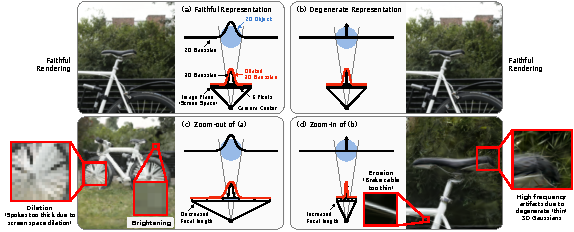
\includegraphics[width=0.88\textwidth]{figures/ch02/2311_16493_teaser.pdf}
\caption{3DGS 缩放伪影现象。尺寸正常的高斯在放大时产生锯齿（aliased），退化为极小针尖的高斯在放大时产生模糊和膨胀。图源：Yu et al.（2023.11）~\cite{2311_16493}。}
\label{fig:02_aliasing}
\end{figure}

\subsection{抗锯齿问题与挑战}

上一小节分析了伪影的根源——高斯基元尺寸固定、固定膨胀无法随采样率自适应调整。本小节介绍现有的解决方案，大致分三条路线：\textbf{频率约束}从信号处理角度限制高斯能表示的最高频率；\textbf{多尺度表示}为不同缩放级别维护独立的细节层次；\textbf{屏幕空间滤波}改进~$\alpha$-混合公式或施加屏幕空间滤波器。三条路线并不互斥，近期工作经常组合使用。

\subsubsection{频率约束路线}

下面介绍 3 条频率约束方法：Mip-Splatting（3D 频率约束 + 2D Mip 滤波器）、SA-GS（免训练的尺度自适应方案）和 AAA-Gaussians（全 3D 评估管线）。

\paragraph{3D 频率约束的开创性方案}

Mip-Splatting（2023.11）~\cite{2311_16493} 修改了原始~3DGS~的两个环节。在\textbf{训练时}为~3D~协方差添加频率约束，在\textbf{渲染时}用~2D Mip~滤波器替代固定膨胀，其余管线（优化器、ADC、光栅化器）保持不变。图~\ref{fig:02_mipsplatting}~直观展示了这两个改动。

\begin{figure}[htbp]
\centering
\resizebox{0.88\textwidth}{!}{\begin{tikzpicture}[
  box/.style={rectangle, rounded corners=4pt, draw=#1, fill=#1!10, text width=3cm, align=center, font=\small, minimum height=0.75cm},
  widebox/.style={rectangle, rounded corners=4pt, draw=#1, fill=#1!10, text width=3.5cm, align=center, font=\small, minimum height=0.75cm},
  diam/.style={diamond, draw=#1, fill=#1!8, font=\scriptsize, text width=1.8cm, align=center, aspect=2},
  biglabel/.style={font=\bfseries\small, #1},
  arr/.style={-{Stealth[length=5pt]}, thick, #1},
  >=Stealth
]
  \node[biglabel=techblue] (o_title) at (1.5, 10.6) {\textbf{原始 3DGS}};
  \node[box=techblue] (o1) at (5.7, 10.6) {3D 高斯基元};
  \node[box=techblue] (o2) at (5.7, 8.1) {投影到 2D};
  \node[box=techblue] (o3) at (5.7, 5.6) {固定膨胀\\（$\sigma_l \approx 0.3$ 像素）};
  \node[box=techblue] (o4) at (5.7, 3.1) {Tile 光栅化\\$\alpha$-混合渲染};
  \node[box=techblue] (o5) at (5.7, 0.6) {像素颜色};
  \node[biglabel=techgreen] (m_title) at (10.6, 10.6) {\textbf{Mip-Splatting}};
  \node[box=techgreen] (m1) at (15.5, 10.6) {3D 高斯基元};
  \node[box=techgreen, draw=techorange, fill=techorange!10] (m2) at (15.5, 8.1) {\textbf{3D 平滑滤波器}\\约束频率上界（训练时）};
  \node[box=techgreen] (m3) at (15.5, 5.6) {投影到 2D};
  \node[box=techgreen, draw=techorange, fill=techorange!10] (m4) at (15.5, 3.1) {\textbf{2D Mip 滤波器}\\模拟像素积分（渲染时）};
  \node[box=techgreen] (m5) at (15.5, 0.6) {像素颜色};
  \draw[arr=techblue] (o1) -- (o2);
  \draw[arr=techblue] (o2) -- (o3);
  \draw[arr=techblue] (o3) -- (o4);
  \draw[arr=techblue] (o4) -- (o5);
  \draw[arr=techgreen] (m1) -- (m2);
  \draw[arr=techgreen] (m2) -- (m3);
  \draw[arr=techgreen] (m3) -- (m4);
  \draw[arr=techgreen] (m4) -- (m5);
  \node[draw=techgray, fill=techbg, rounded corners, font=\scriptsize, text width=9cm, align=center] at (9.8, -1.9) {
    两个滤波器协同工作：3D 滤波器消除\textbf{放大}时的高频伪影，
    2D Mip 滤波器消除\textbf{缩小}时的锯齿。
    实验：Mip-NeRF360 上 $2\times$ 缩放测试 PSNR 比原始 3DGS 高 2--5 dB。
  };
\end{tikzpicture}}
\caption{Mip-Splatting vs 原始 3DGS 渲染流程对比。Mip-Splatting 在两个环节做出改动（橙色标注）：训练时添加 3D 平滑滤波器约束频率上界，渲染时用 2D Mip 滤波器替代固定膨胀。}
\label{fig:02_mipsplatting}
\end{figure}

Mip-Splatting 的核心贡献在于准确诊断了缩放伪影的双重根源。

\textbf{问题根源之一：缺乏~3D~频率约束。}如上一小节所述，固定膨胀导致了尺度歧义——优化器系统性地低估高斯的真实尺度，放大画面时出现侵蚀伪影。Mip-Splatting 的第一个改动正是针对这一问题。

\textbf{改动一：3D 平滑滤波器。}Mip-Splatting 通过~Nyquist~采样定理约束~3D~高斯的频率上界。直觉地说，它为每个高斯基元计算“训练期间最高的采样频率”，然后据此施加低通滤波，确保该高斯不包含超出采样能力的过高频率分量。

具体而言，对于第~$k$~个高斯基元，它在第~$n$~个训练视图中对应的采样频率为焦距与深度之比~$f_n/d_{n,k}$（采样频率越高，能分辨的细节越细）。取所有训练视图中的最大值，得到该高斯“应被允许的最高频率”：

\begin{equation}
\omega_k = \max_{n \in \{1,\ldots,N\}} \frac{f_n}{d_{n,k}}
\end{equation}

然后，对~3D~协方差施加高斯低通滤波。低通滤波的效果是让高斯变得更"胖"、更平滑——因为协方差矩阵控制高斯的形状和尺寸，增大协方差等价于扩大高斯的覆盖范围，从而抹去其中过细的高频细节。具体做法是在原始协方差~$\bm{\Sigma}_k$~上叠加一个滤波协方差~$\bm{\Sigma}_s = \frac{s}{\omega_k^2}\mathbf{I}$：

\begin{equation}
\bm{\Sigma}_k^{\mathrm{reg}} = \bm{\Sigma}_k + \bm{\Sigma}_s
\end{equation}

这里利用了高斯卷积仍为高斯的性质。滤波强度~$s$~为超参数，$\bm{\Sigma}_s$~对每个基元不同（依赖其可见的训练视图），每~$m$~次迭代重新计算。训练完成后，$\bm{\Sigma}_s$~成为场景表示的固有部分，不随视角变化，从而在放大时消除了高频伪影。

\textbf{问题根源之二：2D 膨胀不模拟物理成像。}如上一小节所述，缩小画面时固定膨胀导致高斯过度重叠。Mip-Splatting 进一步指出，这背后还有更深层的原因。

真实相机的每个像素不是一个数学意义上的"点"，而是一块有面积的感光区域。像素最终记录的颜色，是这块区域内所有入射光的平均值——这就是\textbf{物理像素积分}。打个比方：如果用方格纸去覆盖一幅画，每个方格的颜色不是方格中心那一个点的颜色，而是整个方格区域内所有颜色的平均。缩小画面时，每个像素对应的场景区域变大，方格也变大，应该对更大范围的颜色取平均。但原始~3DGS~的固定膨胀始终用同一个大小的高斯核去卷积，不随缩放变化——相当于用固定大小的方格去采样，无论画面放大还是缩小。

\textbf{改动二：2D Mip 滤波器。}改动一作用于\emph{训练时}的~3D~协方差，修改的是高斯基元本身的大小。但放大伪影之外还有缩小伪影——缩小画面时的问题不是高斯太小，而是原始~3DGS~的固定膨胀无法正确模拟物理像素积分。因此~Mip-Splatting~的第二个改动作用于\emph{渲染时}的~2D~投影，用~2D Mip~滤波器替代固定膨胀。该滤波器在数学上等价于将~2D~高斯与一个覆盖单个像素面积的~box~核做卷积（区别于~EWA（Elliptical Weighted Average，椭圆加权平均）滤波器覆盖~3$\times$3~像素区域）：

\[
G_k^{2D,\mathrm{mip}}(\mathbf{x}) = \frac{|\bm{\Sigma}_k^{2D}|}{|\bm{\Sigma}_k^{2D} + s\mathbf{I}|}\exp\!\Bigl(-\frac{1}{2}(\mathbf{x}-\bm{\mu}_k)^T(\bm{\Sigma}_k^{2D}+s\mathbf{I})^{-1}(\mathbf{x}-\bm{\mu}_k)\Bigr)
\]

两个滤波器协同工作。3D~滤波器在训练时约束频率上界以消除放大伪影，2D Mip~滤波器在渲染时模拟物理积分以消除缩小伪影。两者共同确保不同缩放级别下的一致渲染质量。实验表明，在~Mip-NeRF 360~数据集上单尺度训练后~2$\times$~缩放测试时，PSNR~比原始~3DGS~高~2--5~dB。

\paragraph{免训练的尺度自适应方案}

Mip-Splatting 在训练阶段修改了~3DGS~管线（添加~3D~频率约束），需要重新训练模型。SA-GS（2024.03）~\cite{2403_19615} 则选择了另一条路：\textbf{不做任何训练修改，仅在测试时作为插件应用}。它只修改渲染时的膨胀量——将固定的~$\sigma_l^2$~调整为与渲染采样率匹配的~$\sigma_l^2 r^2$（其中~$r$~为训练与渲染的采样率之比），而不改变训练时的协方差。SA-GS 首先区分了``锯齿''与``高斯尺度失配''（Gaussian scale mismatch）两个概念。3DGS 缩放伪影的根源是后者而非前者。具体地，3DGS~\cite{2308_04079}~训练时用固定~$\sigma_l = 0.3$~的高斯核膨胀投影~2D~高斯，等价于协方差从~$\bm{\Sigma}_k$~变为~$\bm{\Sigma}_k + \sigma_l^2 \mathbf{I}$（约~1.64~像素膨胀）。这使高斯投影尺度与训练分辨率/焦距耦合。SA-GS 提出~2D~尺度自适应滤波器，计算训练与渲染之间的比率~$r = R_p \cdot D_c$（$R_p$~为分辨率比，$D_c$~为焦距/距离比），据此将膨胀协方差调整为~$\bm{\Sigma}_k + \sigma_l^2 r^2 \mathbf{I}$。当~$r=1$~时退化为训练时的膨胀量，确保任意渲染设置下高斯分布与训练时一致。

在解决尺度失配后，SA-GS 进一步改进了像素颜色的计算方式。原始~3DGS~在渲染时，对每个像素只查询投影~2D~高斯在像素中心点的值——这相当于假设像素是一个无穷小的点。但真实像素有面积，像素的最终颜色应该是高斯在整个像素面积上的平均值。一个朴素的改进是超采样：在每个像素内取多个采样点再取平均，采样越多越精确，但计算量也线性增长。SA-GS 的关键洞察是：由于高斯函数有解析的累积分布函数（CDF），可以直接用公式精确计算高斯在任意区间内的积分，无需逐点采样。具体地，将~2D~高斯分解为~$x$、$y$~两个独立的~1D~高斯，每个方向上用~CDF~直接算出像素边界内的积分值：$\alpha = (\Phi_x(P_x^+) - \Phi_x(P_x^-))(\Phi_y(P_y^+) - \Phi_y(P_y^-))$。这等价于超采样数量趋于无穷的极限——精确且高效。对于像素轴与高斯轴不对齐的情况，SA-GS 将像素旋转至与高斯轴平行后计算积分，并证明了近似误差有上界。该方法无需重新训练即可达到与~Mip-Splatting~相当或更好的效果。

\paragraph{全 3D 评估管线}

前两个方法（Mip-Splatting、SA-GS）都在~2D~屏幕空间进行滤波，即先将~3D~高斯投影到~2D~再处理。AAA-Gaussians（2025.04）~\cite{2504_12811} 认为这仍然是一种近似——在~3D~空间中本可以做更精确的抗锯齿，但投影到~2D~后这个机会就丧失了。它将抗锯齿从“2D 后处理”提升为“完整的~3D~评估管线”，包含三个核心组件。

第一，\textbf{自适应~3D~平滑滤波器}。Mip-Splatting 的~3D~平滑滤波器使用训练时的最大采样频率确定固定滤波大小，渲染时不再变化。AAA-Gaussians 为每个渲染视角重新计算~3D~平滑滤波器，但发现直接照搬~Mip-Splatting~的做法会导致高斯变得过度透明。原因是这样的：当增大~3D~高斯的协方差（让它变得更"胖"），高斯的总能量不变，所以峰值会下降——就像把同一团面团摊得更薄。在传统的~2D~渲染中这不是问题，因为像素对整个~2D~高斯做积分，薄了但面积大了，总贡献不变。但~AAA-Gaussians~的~3D~评估不做积分——它沿每条光线找到高斯的最大贡献点，只取峰值。这意味着摊薄效应无法被面积增大补偿，导致高斯看起来太透明。问题对扁平的各向异性高斯尤为严重（薄饼形状的高斯沿厚度方向被进一步摊薄，峰值大幅下降）。AAA-Gaussians 的关键改进是：归一化时只考虑垂直于光线方向~$\mathbf{d}$~的两个轴的尺度变化，而忽略沿光线方向的缩放——因为沿光线方向的变化不影响光线经过时的峰值高度。具体来说，AAA-Gaussians 用以下归一化因子来补偿滤波带来的峰值下降：

\begin{equation}
\frac{|\boldsymbol{\Sigma}_{\mathbf{d}}|}{|\hat{\boldsymbol{\Sigma}}_{\mathbf{d}}|} = \frac{\mathbf{d}^\top \boldsymbol{\Sigma}^{-1} \mathbf{d}}{\mathbf{d}^\top \hat{\boldsymbol{\Sigma}}^{-1} \mathbf{d}}
\end{equation}

左边的比值~$|\boldsymbol{\Sigma}_{\mathbf{d}}|/|\hat{\boldsymbol{\Sigma}}_{\mathbf{d}}|$~就是修正后的归一化因子：分子是原始协方差在光线正交平面上的行列式，分母是滤波后协方差在同一平面上的行列式，两者的比值恰好补偿了滤波导致的峰值衰减。其中~$\boldsymbol{\Sigma}_{\mathbf{d}}$~为协方差在~$\mathbf{d}$~正交子空间上的~$2\times 2$~投影，$\hat{\boldsymbol{\Sigma}} = \boldsymbol{\Sigma} + \frac{k}{\omega'^2}\mathbf{I}$~为施加滤波后的协方差。利用逆协方差分解~$\boldsymbol{\Sigma}^{-1} = R S^{-2} R^\top$，该比值可高效计算为~$\sum_i d'^2_i / s^2_i$~与~$\sum_i d'^2_i / \hat{s}^2_i$~之比，无需显式矩阵求逆。渲染时的有效采样频率取~$\omega' = \min(\omega_{\text{train}}, \omega_{\text{render}})$，确保相机靠近时不使高斯过度缩小，远离时仍能提供有效抗锯齿。

第二，\textbf{视角空间包围}。原始~3DGS~及~HTGS~\cite{2410_08129}~在投影空间（projective space）中对高斯椭球做平面拟合来计算屏幕空间包围盒。但当高斯的椭球壳一部分位于相机后方（即~$z < 0$，在透视投影中落在观察者身后）时，投影公式会产生无效坐标，导致这些高斯被直接丢弃——画面上表现为物体突然弹出或消失（pop-in）。AAA-Gaussians 将平面拟合移至视角空间（view space），在角度域而非像素坐标域做包围计算，从根本上避免了身后坐标的投影问题。具体用平面~$\mathbf{p}_x = (\cos\alpha, 0, -\sin\alpha, 0)^\top$~和~$\mathbf{p}_y = (0, \cos\beta, -\sin\beta, 0)^\top$~求解高斯椭球在视角空间中的包围界限~$\alpha_{1,2}$、$\beta_{1,2}$，其中~$\alpha$、$\beta$~为高斯均值相对于相机在水平/垂直方向的角度。随后通过旋转步骤确保角度范围在视野范围内，再映射到屏幕坐标。

第三，\textbf{基于视锥体的~3D tile~裁剪}。原始~3DGS~使用~2D~屏幕空间~AABB（Axis-Aligned Bounding Box，轴对齐包围盒）~进行~tile~裁剪，对高度非轴对齐的椭球产生较差的包围。HTGS~\cite{2410_08129}~将裁剪提升到每~tile~的投影~2D~椭圆测试，但仍在~2D~空间操作。AAA-Gaussians 进一步为每个~tile~构造~3D~视锥体~$F$，由~4~个平面~$\mathbf{p}_{x_{1,2}} = (1, 0, 0, -x_{(m)})^\top$~和~$\mathbf{p}_{y_{1,2}} = (0, 1, 0, -y_{(m)})^\top$~定义，其中~$x_{(m)}, y_{(m)}$~为~tile~在像素坐标中的边界。裁剪时需要判断高斯在该~tile~对应的~3D~视锥体内是否有显著贡献。具体做法是找到高斯在视锥体内的最大贡献点：如果高斯的均值（中心）落在视锥体内，该均值就是贡献最大的点；如果均值在视锥体外，则将视锥体的边界平面变换到高斯的归一化坐标系中，找到平面上距高斯中心最近的点——这个点代表该高斯在视锥体内的最大可能响应。最终只保留最大响应~$\sigma_{\mathbf{x}}(\mathbf{x})^2$（即该点处高斯值的平方，衡量高斯在该~tile~内的贡献强度）高于阈值~$\sigma_T$~的~tile。为提高效率，仅投影到屏幕空间中距高斯均值最近的两个~$x/y$~平面及其对应边（而非朴素方法的全部~4~平面和~4~边）。该方法在分布外视角上显著优于先前方法。

\subsubsection{多尺度表示路线}

频率约束路线在单一尺度表示上施加滤波，但滤波本身可能引入模糊或细节损失。多尺度表示路线采取了根本不同的策略：不再试图“修复”单一尺度的问题，而是维护多个细节层次，渲染时按需选择。

\paragraph{多尺度高斯层次结构}

Yan et al.（2023.11）~\cite{2311_17089} 提出的 MS-GS 是该路线的奠基工作。MS-GS 首先需要一个指标来判断一个高斯在屏幕上“小到什么程度”——这就是“像素覆盖率”（pixel coverage）。直觉地说，把一个投影后的~2D~高斯画在屏幕上，它会呈现为一个椭圆光斑。这个光斑的边缘越往外越暗，在某个亮度阈值（$\sigma_T = 1/255$，几乎全黑）处画一条等值线，这条等值线围成一个椭圆。该椭圆沿水平轴和垂直轴的直径（以像素为单位）中较小的一个，就是像素覆盖率~$S_k$——简而言之，$S_k$~衡量的是该高斯在屏幕上实际覆盖了多少像素。当~$S_k < S_T = 2$~像素时（$S_T$~为阈值，threshold），说明这个高斯在屏幕上不到~2~个像素宽，它所包含的空间细节比单个像素还精细——按~Nyquist~定理，这种高频信号无法被当前采样率正确捕获，必然产生锯齿。

MS-GS 的多尺度构建通过高斯聚合实现。所有高斯初始化于最细层~$l=1$，经标准分裂和克隆后，在~1,000~次迭代的预热阶段后启动聚合：对每层~$l_m \geq 2$，将~$[1, l_m{-}1]$~层的高斯以~$4^{l_m-1}$~倍下采样分辨率渲染，选出像素覆盖率~$S_k < S_T$~的高斯（即在当前分辨率下太小、会产生锯齿的高斯），然后将~3D~空间划分为等大的立方体网格（每个立方体称为一个“体素”），把落入同一体素的高斯归为一组，对其属性（位置、缩放、不透明度、颜色）取平均，合并成一个更大的新高斯——这就是“体素网格分箱+平均池化”。最后按~$S_T / S_{\text{avg}}$~放大缩放因子，使合并后的高斯适应该层分辨率。新增高斯数量通常不到总数的~5\%。

渲染时采用选择性渲染策略。训练期间为每个高斯维护最大和最小像素覆盖率~$S_k^{\max}$、$S_k^{\min}$，带衰减系数更新（$S_k^{\max}$~取最大值并乘以~$\gamma_1 = 0.95$，$S_k^{\min}$~取最小值并乘以~$\gamma_2 = 1.05$）。渲染时高斯被选中的条件为：

\begin{equation}
\left(S_k \leq S_k^{\max} \cdot S_{\text{rel}}^{\max}\right) \wedge \left(S_k \geq S_k^{\min} \cdot S_{\text{rel}}^{\min} \;\vee\; S_k < S_T\right)
\end{equation}

其中~$S_{\text{rel}}^{\max} = 1.5$、$S_{\text{rel}}^{\min} = 0.5$~为相对覆盖率阈值。超出最大覆盖率高斯被过滤（过大），低于最小覆盖率且小于~$S_T$~的高斯也被过滤（过小且产生锯齿）。该方法在~4$\times$--128$\times$~缩放渲染下实现了~13\%--66\% PSNR~提升和~160\%--2400\%~渲染速度提升。

然而，MS-GS 维护多套独立高斯集合带来了额外的内存开销和管理复杂度。

\paragraph{LOD-GS：可学习采样率-滤波映射}
LOD-GS（2025.07）~\cite{2507_00554} 针对 MS-GS 多套高斯集合的内存开销问题，采取不同策略——只保留一套高斯，但为每个基元引入可学习的采样率-滤波强度映射。LOD-GS 指出 Mip-Splatting 的~3D~平滑滤波器存在固定滤波大小的局限（某些纹理被过度滤波而另一些滤波不足）。因此以采样率（$\tau = f / d$，焦距除以距离）为输入，通过~GMM（Gaussian Mixture Model，高斯混合模型）~动态预测每个基元的最优滤波强度，参数通过梯度下降端到端优化。LOD-GS 还引入了考虑相机距离变化的新合成数据集，在~SOTA~渲染质量的同时有效消除了锯齿。

\paragraph{Mipmap-GS：基元自变形替代外部滤波}
LOD-GS 的自适应滤波仍然是一种“外部施加”的约束。Mipmap-GS（2024.08）~\cite{2408_06286} 则进一步激进——完全不施加外部滤波，而是让高斯自身学会根据采样率变形。具体做法分两步。

\textbf{第一步，构造训练目标}：用当前高斯渲染一张标准分辨率的图像，然后对它做放大和缩小，分别生成“放大版伪真值”（用超分辨率模型放大）和“缩小版伪真值”（用双线性插值缩小）。这些伪真值代表“不同缩放级别下理想渲染结果应该长什么样”。

\textbf{第二步，用一致性损失引导高斯变形}：把同一个高斯模型在不同采样率下渲染，将渲染结果与对应尺度的伪真值对比，计算损失。梯度回传后，高斯的颜色、形状、大小和位置会自动调整，使得在任何缩放级别下都能渲染出与伪真值接近的结果。换言之，高斯不是被动地被外部滤波“修正”，而是主动学会在不同尺度下“变成正确的形状”。作为测试时适配方法，Mipmap-GS~在缩放场景下~PSNR~平均提升~9.25~dB（zoom-in）和~10.40~dB（zoom-out）。三种方法展示了一条从“外部管理”到“内部自适应”的演进路径：MS-GS 用多套表示应对多尺度，LOD-GS 用单套自适应滤波替代多套，Mipmap-GS 则连外部滤波也去掉，让基元自变形。

\subsubsection{屏幕空间与融合路线}

前两条路线（频率约束、多尺度表示）都在~3D~空间或基元层面解决问题。屏幕空间路线则从渲染方程本身出发，改进~$\alpha$-混合公式以更精确地处理高斯之间的空间重叠。

\paragraph{空间分布 $\alpha$-混合}

Koo et al.（2025.11）~\cite{2511_15102} 提出的 Gaussian Blending 是该路线的代表工作。传统~3DGS~将~alpha~和透射率视为标量值——在第~$i$~个高斯处的透射率~$T_i^s = \prod_{j=1}^{i-1}(1 - \int_p \alpha_j(x)\,dx)$~为单一常数，使前景高斯完全遮挡背景高斯，忽略了像素面积上的空间重叠。物理上正确的像素颜色应为空间积分~$C_p^p = \int_p \sum_{i=1}^N T_i^p(x)\,\alpha_i(x)\,c_i\,dx$，其中透射率~$T_i^p(x)$~在像素区域内随空间位置变化，但标量近似将其简化为~$C_p^s = \sum_{i=1}^N T_i^s\,c_i \int_p \alpha_i(x)\,dx$，丢失了空间遮挡信息。

Gaussian Blending 的核心创新是改变透射率的表示方式。要理解这一点，先回顾标准~3DGS~的做法：每个像素的透射率是一个标量（一个数），代表整个像素区域被前面高斯遮挡的总体程度。但像素有面积，像素内不同空间位置可能被遮挡的程度不同——比如前景高斯可能只遮住了像素的左半部分，右半部分仍然透明，能看到后面的高斯。标量透射率无法表达这种空间差异。

Gaussian Blending 的思路是：用一个矩形窗口来近似追踪"像素中哪些区域还没被挡住"。具体用三个参数描述这个窗口：中心位置~$x_i \in \mathbb{R}^2$（窗口在哪里）、尺寸~$l_i \in \mathbb{R}^2$（窗口多大）、透射率值~$t_i \in \mathbb{R}$（这个区域内有多透明）。初始时窗口覆盖整个像素（$x_1 = p$~为像素中心，$l_1 = [1,1]^\top$，$t_1 = 1$~表示完全透明）。每处理一个高斯后，窗口会收缩——被遮挡的部分被排除，窗口只保留剩余的可见区域，同时透射率值也相应更新。这样，后续高斯只在真正可见的区域内参与混合。

在数学实现上，对每个高斯泼溅，先对其~2D~协方差矩阵~$\hat{\Sigma}_i$~做特征分解得到特征值~$\lambda_1, \lambda_2$~和特征向量~$e_1, e_2$，将当前窗口旋转对齐到高斯主轴后，定义~1D~高斯的~$k$~阶矩~$I_\sigma^k(a,b) = \int_a^b x^k \exp(-x^2/2\sigma^2)\,dx$，则第~$i$~个泼溅的积分权重为：

\begin{equation}
\int w_i(x)\,dx = t_i\,o_i\,I_{\sigma_1}^0(u_1, u_2)\,I_{\sigma_2}^0(v_1, v_2)
\end{equation}

其中~$\sigma_1 = \sqrt{\lambda_1}$、$\sigma_2 = \sqrt{\lambda_2}$，$[u_1, u_2]$~和~$[v_1, v_2]$~为窗口在旋转坐标系下的边界。直观地说，这个公式计算的是：在当前窗口（未被遮挡的区域）内，第~$i$~个高斯实际贡献了多少颜色。

混合完一个高斯后，窗口需要更新——去掉已被遮挡的部分，只保留仍可见的区域。具体地，混合后的残差分布~$T_i(x)(1-\alpha_i(x))$~描述了"哪些空间位置还透着光"，对其计算零阶、一阶、二阶矩~$M_i^0, M_i^1, M_i^2$~（分别对应总面积、重心位置和散布范围），由此递推更新窗口参数：

\begin{equation}
x_{i+1} = \hat{\mu}_i' + [e_1, e_2]\,M_i^1/M_i^0, \quad l_{i+1} = \sqrt{12(M_i^2/M_i^0 - (M_i^1/M_i^0)^2)}, \quad t_{i+1} = M_i^0 / (l_{i+1,1}\,l_{i+1,2})
\end{equation}

三个更新分别对应：新的窗口中心（从重心矩计算）、新的窗口尺寸（从二阶矩计算，二阶矩越大窗口越大）、新的透射率值（剩余可见面积除以窗口面积）。每处理一个高斯，窗口就收缩一次，逐步逼近像素内真正可见的区域。整个过程在一次渲染通道中完成，不增加额外内存开销，保持实时渲染速度，作为即插即用模块可直接集成到任何~3DGS~框架中。

Gaussian Blending 解决的是~3DGS~的~$\alpha$-混合精度问题，但~3DGS~还有另一个变体——2DGS——其抗锯齿需求不同。

\paragraph{AA-2DGS：2D 高斯泼溅专用抗锯齿}
AA-2DGS（2025.06）~\cite{2506_11252} 专门针对~2D~高斯泼溅提出抗锯齿方案。2DGS 使用平面高斯盘直接在射线-泼溅交点处评估，其抗锯齿方案无法直接移植自~3DGS~的方法。AA-2DGS 引入世界空间平面平滑核（约束~2D~高斯频率基于训练视图的最大采样率）和物体空间~Mip~滤波器（利用射线-泼溅交点映射的仿射近似在每个泼溅的局部空间高效滤波），在保持~2DGS~几何精度的同时增强跨尺度渲染质量。

\paragraph{MSAA+约束优化：多样本抗锯齿引入 3DGS}
与传统图形学更接近的方案是~MSAA+约束优化（2025.08）~\cite{2508_10507}。它将传统图形学中的多样本抗锯齿（MSAA，Multi-Sample Anti-Aliasing）思想引入~3DGS。具体做法分为三步。第一，\textbf{子像素采样}：将每个像素细分为~4~个子像素（例如~$2\times 2$~网格），在每个子像素位置独立渲染，然后取平均——这样物体边缘处的像素不会被"全有或全无"地判定，而是根据高斯实际覆盖了几个子像素来按比例着色，边缘自然就平滑了。第二，\textbf{自适应权重}：不是简单取~4~个子像素的平均，而是对渲染误差大的区域赋予更大权重——误差大说明该区域的细节还没被正确捕捉，应该更重视这些子像素的渲染结果。第三，\textbf{梯度微分约束}：在物体边界处，对高斯的位置梯度施加额外的正则化，迫使高斯沿边界整齐排列，而不是随意散布——这减少了高曲率边缘和薄结构处的锯齿。

图~\ref{fig:02_antialiasing}~总结了本节介绍的四条抗锯齿技术路线及其代表性方法。

\begin{figure}[htbp]
\centering
\resizebox{0.9\textwidth}{!}{\begin{tikzpicture}[
  route/.style={rectangle, rounded corners=5pt, draw=#1, fill=#1!10,
    text width=3.2cm, minimum height=0.9cm, align=center, font=\small},
  method/.style={rectangle, rounded corners=3pt, draw=#1, fill=#1!6,
    font=\scriptsize, text width=3.0cm, align=center, minimum height=0.6cm},
  arr/.style={-{Stealth[length=4pt]}, techgray!60},
  >=Stealth
]

  \node[route=techgray, text width=4cm, font=\small\bfseries] (root) at (25.7, 5.6) {抗锯齿方法};
  \node[route=techblue] (b0) at (9.3, 3.1) {频率约束路线};
  \node[method=techblue] (b0_l0) at (3.0, 0.6) {3D平滑+2D Mip滤波\\{\tiny Mip-Splatting, AAA-Gaussians}};
  \node[method=techblue] (b0_l1) at (9.3, 0.6) {可学习滤波强度映射\\{\tiny LOD-GS}};
  \node[route=techgreen] (b1) at (22.3, 3.1) {多尺度表示路线};
  \node[method=techgreen] (b1_l0) at (15.3, 0.6) {多尺度高斯层次结构\\{\tiny MS-GS}};
  \node[method=techgreen] (b1_l1) at (22.3, 0.6) {基元自变形/尺度一致性引导\\{\tiny Mipmap-GS}};
  \node[route=techorange] (b2) at (29.1, 3.1) {屏幕空间路线};
  \node[method=techorange] (b2_l0) at (29.1, 0.6) {空间分布Alpha混合\\{\tiny Gaussian Blending}};
  \node[method=techorange] (b2_l1) at (35.0, 0.6) {2D高斯专用抗锯齿\\{\tiny AA-2DGS, MSAA+约束优化}};
  \node[route=techpurple] (b3) at (37.8, 3.1) {免训练路线};
  \node[method=techpurple] (b3_l0) at (42.2, 0.6) {测试时尺度自适应，无需重训练\\{\tiny SA-GS}};
  \draw[arr] (root) -- (b0);
  \draw[arr] (root) -- (b1);
  \draw[arr] (root) -- (b2);
  \draw[arr] (root) -- (b3);
  \draw[arr] (b0) -- (b0_l0);
  \draw[arr] (b0) -- (b0_l1);
  \draw[arr] (b1) -- (b1_l0);
  \draw[arr] (b1) -- (b1_l1);
  \draw[arr] (b2) -- (b2_l0);
  \draw[arr] (b2) -- (b2_l1);
  \draw[arr] (b3) -- (b3_l0);
  \node[draw=techgray, fill=techgray!5, rounded corners, font=\scriptsize,
    text width=12cm, align=center] at (23.6, -1.2) {核心问题：固定尺寸高斯在采样率变化时产生锯齿和膨胀/侵蚀伪影。各路线分别从频率约束、多尺度表示、屏幕空间积分和测试时适配四个角度解决此问题。};
\end{tikzpicture}}
\caption{3DGS 抗锯齿方法的四条技术路线。频率约束路线从信号处理角度限制高频分量；多尺度表示路线维护不同细节层次的高斯集合；屏幕空间路线改进混合公式；免训练路线在测试时自适应调整。}
\label{fig:02_antialiasing}
\end{figure}

\begin{takeaway}
3DGS 抗锯齿问题的根源在于高斯基元尺寸在训练后固定，无法随采样率变化自适应调整。四条技术路线各有侧重：频率约束（Mip-Splatting）从信号处理角度限制高频分量，多尺度表示维护不同细节层次的高斯集合，屏幕空间滤波改进混合公式，免训练方案在测试时自适应调整。当前趋势是多种策略的组合使用，以同时解决锯齿和膨胀/侵蚀两类伪影。
\end{takeaway}

%=====================================================================


\section{密度控制与高斯优化}
\label{sec:02_2}

密度控制是~3DGS~训练管线中最关键的机制之一。如第~\ref{sec:01_1_4}~节所述，原始~3DGS~的自适应密度控制（ADC）通过基于梯度的启发式规则（克隆、分裂、剪枝）决定高斯的增删，实现了从稀疏初始化到密集表示的自动化生长。然而，ADC~的设计存在多方面根本性局限。以下是三个层面的具体分析。

\textbf{判据层面：梯度信号不精确。}ADC~使用位置梯度的平均幅值作为致密化判据。当一个高斯覆盖包含高频细节的区域时，来自不同像素的梯度方向相反，累加后相互抵消，平均幅值低于分裂阈值。这导致该区域\emph{始终无法触发致密化}。此外，取梯度幅值的平均会丢失方向信息——无法区分“需要分裂”（梯度方向冲突）和“需要克隆”（梯度方向一致）两种截然不同的需求。

\textbf{操作层面：split/clone 互斥选择过于粗糙。}对于需要致密化的高斯，ADC~按尺度阈值二选一：大高斯执行~split，小高斯执行~clone。但实际中一个高斯可能\emph{同时需要}空间扩展（split 的作用）和局部精修（clone 的作用），这种非此即彼的互斥选择无法兼顾。此外，clone~后的高斯与父高斯重叠过高，难以独立优化。split~的子高斯随机放置，可能破坏父高斯已拟合的几何。

\textbf{宏观层面：缺乏全局约束。}ADC~没有对高斯总数、尺寸均匀性和几何一致性的全局约束。结果是高斯数量容易膨胀（训练后可达数百万），不同区域的高斯尺寸差异极大（针状与平板状并存），且产生大量不对应真实几何的浮动伪影（floaters）。这三个层面的局限共同催生了大量改进工作。

表~\ref{tab:design_research}~已总结了原始~3DGS~的设计选择与后续研究方向的对应关系。本节系统梳理~ADC~的各种改进方案。图~\ref{fig:02_adc_taxonomy}~展示了~ADC~改进方法的六条技术路线。

\begin{figure}[htbp]
\centering
\resizebox{0.85\textwidth}{!}{\begin{tikzpicture}[
  route/.style={rectangle, rounded corners=5pt, draw=#1, fill=#1!10,
    text width=3cm, minimum height=0.9cm, align=center, font=\small},
  method/.style={rectangle, rounded corners=3pt, draw=#1, fill=#1!6,
    font=\scriptsize, text width=2.8cm, align=center, minimum height=0.6cm},
  arr/.style={-{Stealth[length=4pt]}, techgray!60},
  >=Stealth
]

  \node[route=techgray, text width=4cm, font=\small\bfseries] (root) at (54.3, 5.6) {ADC 改进方法};
  \node[route=techblue] (b0) at (17.4, 3.1) {判据改进};
  \node[method=techblue] (b0_l0) at (3.5, 0.6) {梯度绝对值求和/梯度方向感知\\{\tiny AbsGS, GDAGS, DC4GS}};
  \node[method=techblue] (b0_l1) at (10.5, 0.6) {逐像素误差替代梯度\\{\tiny Revising Densification}};
  \node[method=techblue] (b0_l2) at (17.4, 0.6) {难例高斯挖掘/基元冻结修复\\{\tiny HGS, ReAct-GS}};
  \node[method=techblue] (b0_l3) at (24.1, 0.6) {方差引导/边缘感知\\{\tiny Metamon-GS, Deng et al.}};
  \node[route=techgreen] (b1) at (37.2, 3.1) {操作改进};
  \node[method=techgreen] (b1_l0) at (30.9, 0.6) {残差分裂/长轴分裂/密度保持\\{\tiny ResGS, EDC, BOGausS}};
  \node[method=techgreen] (b1_l1) at (37.2, 0.6) {局部化点管理\\{\tiny LPM}};
  \node[route=techorange] (b2) at (50.3, 3.1) {概率框架};
  \node[method=techorange] (b2_l0) at (42.7, 0.6) {SGLD采样替代启发式\\{\tiny 3DGS-MCMC}};
  \node[method=techorange] (b2_l1) at (50.3, 0.6) {Metropolis-Hastings全局探索\\{\tiny Kim et al.}};
  \node[route=techpurple] (b3) at (58.3, 3.1) {正则化};
  \node[method=techpurple] (b3_l0) at (58.3, 0.6) {原子化增殖/结构感知分布\\{\tiny AtomGS, Mini-Splatting2}};
  \node[method=techpurple] (b3_l1) at (65.0, 0.6) {频率感知/率失真优化\\{\tiny Zeng et al., BOGausS}};
  \node[route=techgray] (b4) at (70.2, 3.1) {初始化引导};
  \node[method=techgray] (b4_l0) at (70.2, 0.6) {消除致密化\\{\tiny EDGS}};
  \node[method=techgray] (b4_l1) at (74.3, 0.6) {跨场景泛化\\{\tiny GS-Net, GP-GS}};
  \node[route=techorange] (b5) at (79.9, 3.1) {可学习策略};
  \node[method=techorange] (b5_l0) at (79.9, 0.6) {神经网络预测致密化操作\\{\tiny LeGS, ConeGS}};
  \node[method=techorange] (b5_l1) at (85.9, 0.6) {哈希概率金字塔\\{\tiny Zhang et al.}};
  \draw[arr] (root) -- (b0);
  \draw[arr] (root) -- (b1);
  \draw[arr] (root) -- (b2);
  \draw[arr] (root) -- (b3);
  \draw[arr] (root) -- (b4);
  \draw[arr] (root) -- (b5);
  \draw[arr] (b0) -- (b0_l0);
  \draw[arr] (b0) -- (b0_l1);
  \draw[arr] (b0) -- (b0_l2);
  \draw[arr] (b0) -- (b0_l3);
  \draw[arr] (b1) -- (b1_l0);
  \draw[arr] (b1) -- (b1_l1);
  \draw[arr] (b2) -- (b2_l0);
  \draw[arr] (b2) -- (b2_l1);
  \draw[arr] (b3) -- (b3_l0);
  \draw[arr] (b3) -- (b3_l1);
  \draw[arr] (b4) -- (b4_l0);
  \draw[arr] (b4) -- (b4_l1);
  \draw[arr] (b5) -- (b5_l0);
  \draw[arr] (b5) -- (b5_l1);
\end{tikzpicture}}
\caption{ADC 改进方法的六条技术路线。判据改进优化触发条件，操作改进重新设计分裂/克隆机制，概率框架将致密化建模为随机采样，正则化约束高斯形状，初始化引导利用先验知识，可学习策略用神经网络替代启发式规则。}
\label{fig:02_adc_taxonomy}
\end{figure}

\subsection{ADC 的改进方法}

围绕上节分析的判据、操作和宏观三个层面的局限，后续工作形成了八条技术路线。

（1）\textbf{判据改进}：修正致密化触发条件。代表工作包括~AbsGS（梯度绝对值求和消除梯度碰撞）、GDAGS（梯度一致性比区分分裂与克隆需求）、DC4GS（方向一致性引导分裂位置）等，从梯度信号本身入手。

（2）\textbf{操作改进}：重新设计~split/clone~机制。残差分裂（ResGS）用非对称父子结构替代互斥选择；长轴分裂（EDC）用确定性对称放置替代随机偏移；局部化点管理（LPM）从渲染误差图反向定位需要操作的~3D~区域。

（3）\textbf{概率采样路线}：彻底抛弃启发式规则，将致密化建模为~MCMC~采样过程（3DGS-MCMC），或用~Metropolis-Hastings~获得全局探索能力，从概率论中获得收敛性保证。

（4）\textbf{正则化与紧凑表示}：通过约束高斯形状（尺寸均匀化、频率约束）和引入率失真优化来控制基元膨胀，从宏观层面解决高斯数量失控问题。

（5）\textbf{初始化与几何引导}：利用~SfM~点云质量、深度先验或跨场景统计等外部知识，在致密化之前就给出更好的起点，减少对~ADC~自纠正能力的依赖。

（6）\textbf{场景自适应与感知驱动}：根据场景内容（几何复杂度、纹理频率、用户关注区域）自适应调整致密化策略，例如按需局部致密化、感兴趣区域优先等。

（7）\textbf{训练加速与分解策略}：通过全局-局部分阶段致密化、SfM~引导加速等策略提升~ADC~的训练效率。

（8）\textbf{可学习密度控制}：用神经网络（强化学习、概率编码等）替代手工设计的启发式规则，让模型自己学会何时、何地、如何增删高斯。

这八条路线并不互斥——许多方法同时涉及判据改进和操作改进，或在概率框架下引入正则化。下文按路线逐一展开。

\subsubsection{致密化判据的改进}

原始~ADC~使用位置梯度的平均幅值作为致密化判据，这一设计存在三个根本缺陷。第一，\textbf{梯度碰撞（gradient collision）}：当一个大高斯覆盖包含高频细节的复杂区域时，来自不同像素的梯度方向相反、相互抵消，平均梯度幅值低于分裂阈值。这导致该区域始终无法触发致密化。第二，\textbf{信号间接性}：位置梯度仅为渲染误差的间接代理——即使某区域存在明显的渲染瑕疵，只要局部梯度平均后不够大，ADC~也不会响应。第三，\textbf{方向信息丢失}：取梯度幅值的平均抹去了方向信息，无法区分“需要分裂”（梯度方向冲突）和“需要克隆”（梯度方向一致）两种截然不同的致密化需求。以下方法分别从不同角度回应这些缺陷。

\paragraph{修正梯度信号}

AbsGS（2024.04）~\cite{2404_10484} 仅修改了原始~ADC~的致密化判据——将位置梯度的平均幅值替换为梯度绝对值求和，其他环节（分裂/克隆操作、剪枝策略、训练流程）完全不变。

\textbf{问题：梯度碰撞。}想象一个大高斯覆盖了一片有细密纹理的区域。区域左半边的像素希望高斯向左移（梯度为负），右半边的像素希望向右移（梯度为正）。在原始~3DGS~中，高斯~$G_i$~的视图空间位置梯度由逐像素子梯度累加而成：$g_{i,x} = \sum_{j=1}^m \partial L_j / \partial \mu_{i,x}$。当正负梯度幅值相近时，累加后相互抵消，平均幅值低于分裂阈值~$\tau_p = 0.0002$。这导致这个过重建的高斯\emph{始终无法触发分裂}。

\textbf{方案：梯度绝对值求和。}AbsGS~的思路很简单：不要让正负梯度互相抵消，而是把所有像素的梯度贡献都当作正值累加。具体而言，对每个分量的逐像素子梯度取绝对值后再累加：

\begin{equation}
\hat{g}_{i,x} = \sum_{j=1}^m \left|\frac{\partial L_j}{\partial \mu_{i,x}}\right|, \quad \hat{g}_{i,y} = \sum_{j=1}^m \left|\frac{\partial L_j}{\partial \mu_{i,y}}\right|, \quad \hat{g}_i = (\hat{g}_{i,x}, \hat{g}_{i,y})
\end{equation}

这一操作从根本上消除了正负梯度互相抵消的问题。$\hat{g}_i$~不参与反向传播，仅作为独立的致密化判据。它直接反映高斯覆盖区域内\emph{全部像素}的表达质量总和，而非区域整体梯度的代数残差。实验表明，以~$\hat{g}_i$~为判据仅选取~16{,}488~个高斯即可覆盖大部分过重建区域。而原始~3DGS~选取~69{,}269~个高斯却遗漏了多数过重建大高斯。AbsGS 有效恢复了高频细节并减少~10\%--20\%~的内存消耗。图~\ref{fig:02_absgs}~直观展示了梯度碰撞问题与~AbsGS~的解决方案。

\begin{figure}[htbp]
\centering
\resizebox{0.85\textwidth}{!}{\begin{tikzpicture}[
  box/.style={rectangle, rounded corners=4pt, draw=#1, fill=#1!10, text width=3cm, align=center, font=\small, minimum height=0.75cm},
  widebox/.style={rectangle, rounded corners=4pt, draw=#1, fill=#1!10, text width=3.5cm, align=center, font=\small, minimum height=0.75cm},
  diam/.style={diamond, draw=#1, fill=#1!8, font=\scriptsize, text width=1.8cm, align=center, aspect=2},
  biglabel/.style={font=\bfseries\small, #1},
  arr/.style={-{Stealth[length=5pt]}, thick, #1},
  >=Stealth
]
  \node[biglabel=techblue] at (1.7, 7.1) {原始 3DGS};
  \node[biglabel=techgreen] at (6.2, 7.1) {AbsGS};
  \node[box=techblue] (o_px) at (1.7, 5.6) {像素子梯度：$+2,\ {-3},\ +1$};
  \node[box=techblue] (o_sum) at (1.7, 3.1) {代数和：$+2 + (-3) + 1 = 0$};
  \node[box=techblue, draw=red!60, fill=red!8] (o_result) at (1.7, 0.6) {\textbf{结果}：$|0| < \tau$\\不触发致密化};
  \node[box=techgreen] (m_px) at (6.2, 5.6) {像素子梯度取绝对值：$|{+2}|,\ |{-3}|,\ |{+1}|$};
  \node[box=techgreen] (m_sum) at (6.2, 3.1) {绝对值之和：$2 + 3 + 1 = 6$};
  \node[box=techgreen] (m_result) at (6.2, 0.6) {\textbf{结果}：$|6| > \tau$\\\textbf{正确触发}致密化};
  \draw[arr=techblue] (o_px) -- (o_sum);
  \draw[arr=techblue] (o_sum) -- (o_result);
  \draw[arr=techgreen] (m_px) -- (m_sum);
  \draw[arr=techgreen] (m_sum) -- (m_result);
  \node[rectangle, rounded corners=3pt, draw=techorange, fill=techorange!8, font=\scriptsize, text width=2.4cm, align=center] at (3.9, 4.6) {
    \textbf{关键改动}\\取绝对值后累加
  };
\end{tikzpicture}}
\caption{原始 3DGS 的梯度碰撞问题与 AbsGS 的梯度绝对值求和方案。原始 3DGS 中正负梯度相互抵消导致致密化失效；AbsGS 通过取绝对值保留所有像素的贡献。}
\label{fig:02_absgs}
\end{figure}

AbsGS~解决了梯度碰撞问题，但仍有盲点：它只关注梯度的累积量，不区分“方向冲突需要分裂”和“方向一致需要克隆”这两种截然不同的需求。

\paragraph{GDAGS：梯度一致性比区分分裂与克隆}
AbsGS 通过绝对值消除了碰撞，但丢失了方向信息。GDAGS（2025.08）~\cite{2508_09239} 引入梯度一致性比（Gradient Coherence Ratio, GCR）$C_i$ 来弥补这一不足。GCR 度量高斯内梯度方向的一致程度，从而区分“方向冲突需分裂”和“方向一致需克隆”。GCR 定义为各视角下像素级子梯度的矢量和范数与标量和范数之比：

\begin{equation*}
C_i = \frac{\bigl\|\sum_{pixel}\nabla_{i,pixel^v}\bigr\|_2}{\sum_{pixel}\bigl\|\nabla_{i,pixel^v}\bigr\|_2 + \epsilon},
\end{equation*}

其中 $\nabla_{i,pixel^v} \in \mathbb{R}^2$ 为高斯 $i$ 在视角 $v$ 各像素处的位置子梯度。由 Cauchy--Schwarz 不等式可知 $C_i \in [0,1]$：$C_i \to 1$ 表示梯度方向一致、幅值有效累积；$C_i \to 0$ 表示方向冲突、幅值相互抵消。GDAGS 进一步设计非线性权重 $w_i = \beta + (1-C_i)^p$，将原始梯度范数 $\overline{\tau}_i$ 调制为 $\hat{\tau}_i = w_i \cdot \overline{\tau}_i$。这一形式的选择有两层考量。首先，为什么用幂次~$(1-C_i)^p$ 而不是线性~$(1-C_i)$？线性权重意味着~GCR~的微小变化都会等比例地影响权重，缺乏明确的决策边界——而实际需要的是：梯度方向高度一致时果断压低操作力度，方向冲突时果断放大，中间区域则平滑过渡。幂次~$p$~控制这个过渡的陡度：$p$~越大，权重在~$C_i$~的高值区下降越急促，决策越"非此即彼"；$p$~越小，过渡越平缓。其次，为什么加偏移~$\beta$？当~$C_i \to 1$（梯度完全一致）时，$(1-C_i)^p \to 0$，若不加~$\beta$~则权重为零，完全关闭分裂通道。但即使梯度方向一致，也不意味着该区域绝不需要致密化——只是不应该用分裂来处理。$\beta$~为分裂保留一个底线通道，避免信息被完全截断。

在分裂操作中直接使用 $w_i$：低~GCR（方向冲突）的大高斯获得放大的 $\hat{\tau}_i$，优先触发分裂以增强几何细节；在克隆操作中采用逆策略 $1/w_i$：高~GCR（方向一致）的小高斯被优先克隆以完成结构补充，而低~GCR~克隆则被抑制以防止局部堆积。

\paragraph{DC4GS：方向一致性引导分裂位置}
GDAGS 用一致性比区分了分裂和克隆的需求。DC4GS（2025.10）~\cite{2510_26921} 沿同一方向进一步利用方向一致性（Directional Consistency, DC）来指导分裂的\emph{具体位置}——不再随机放置子高斯，而是根据梯度方向的分布找到最优分裂点。具体而言，当一个高斯覆盖的区域内部存在结构变化（例如左半边是天空、右半边是建筑边缘），被该高斯影响的像素会给出方向冲突的梯度——左边的像素希望高斯往左移，右边的希望往右移。这种\textbf{梯度方向不均匀}的区域就是``异质区域''，说明单个高斯无法同时拟合两种不同的结构，应该分裂。反之，如果覆盖区域内各像素的梯度方向基本一致，说明高斯已经较好地拟合了该区域的几何，不需要分裂——这就是``同质区域''。为了量化这种方向均匀程度，DC4GS 将各像素的位置梯度归一化为单位向量 $u_{i,j} = g_{i,j}/\|g_{i,j}\|$，然后对它们取平均并求模长：

\begin{equation*}
\rho_i = \Bigl\|\frac{1}{N}\sum_{j=1}^{N} u_{i,j}\Bigr\|.
\end{equation*}

这个量在方向统计学中称为\textbf{圆均值}（circular mean）的模长，度量一组方向的集中程度：$\rho_i \to 1$ 表示方向高度一致（同质），$\rho_i \to 0$ 表示方向散乱冲突（异质）。基于此，DC4GS 提出~DC~加权分裂判据（DC-weighted split Criterion, DCC）：

\begin{equation*}
\hat{\tau}_i^{DC} = \frac{1}{V}\sum_{v=1}^{V}(1-\rho_{i,v})\,\|\tau_{i,v}\|,
\end{equation*}

其中 $V$ 为可见视角数，$\|\tau_{i,v}\|$ 为视角 $v$ 下沿梯度绝对值求和的幅值。$(1{-}\rho)$ 因子的作用是：同质区域（$\rho$ 高）被压低，排除不必要的分裂；异质区域（$\rho$ 低）被放大，优先触发分裂。

更进一步，DC4GS 提出~DC~引导分裂（DC-guided Split, DCS）：分裂时不再随机放置子高斯，而是沿高斯主轴（最大尺度方向）等间距采样 $N{=}5$ 个候选分裂位置，在每个位置将高斯一分为二，分别计算左、右子区域的~DC~代价 $J_l(x) = (1{-}\rho_l(x))\|\tau_l(x)\|$ 与 $J_r(x) = (1{-}\rho_r(x))\|\tau_r(x)\|$，总代价为 $J(x) = J_l(x) + J_r(x)$。最优分裂位置应使总代价最小——即分裂后左右两侧各自内部的梯度方向尽可能一致（$\rho$ 高），不再是``一边想往左、一边想往右''的混合状态。由于仅采样~5~个离散点，直接取~$\arg\min$~可能跳过真正的最优位置，DC4GS 用多项式回归将这~5~个点拟合为光滑曲线后求取极小值作为~$x_{opt}$——相比密集采样（需要~60~个点才能达到同等精度），仅用~5~个点即可稳定估计（中位~SSIM~0.987 vs 密集采样的~0.983）。该方法将高斯基元数量减少最多~30\%。

\paragraph{绕过梯度信号}

上述方法仍在修正梯度信号本身，但缺陷（2）信号间接性意味着梯度本身就不是理想的判据——即使某区域存在明显渲染误差，梯度平均后也可能不够大。Revising Densification（2024.04）~\cite{2404_06109} 从三个方面全面改进了~ADC。

\textbf{核心改进：逐像素误差替代梯度。}该方法源于一个关键观察：位置梯度对误差的\emph{变化量}敏感，但对误差的\emph{绝对值}完全盲视。想象一片草地被几个大高斯覆盖——这些高斯已经严重欠拟合，渲染结果模糊不清。但由于草地纹理高频且密集，各像素给出的梯度方向散乱，累加后相互抵消，梯度幅值接近于零。此时~ADC~误判为"不需要致密化"，实际上该区域误差极高。Revising Densification 用辅助的逐像素误差函数（如~SSIM）作为致密化判据。关键问题是如何把\emph{像素级}误差归因到\emph{高斯级}——毕竟每个像素的颜色由多个高斯混合而成。该方法的方案是按每个高斯的渲染权重~$\omega_k^\pi(u)$~将像素误差重新分配：$E_k^\pi = \sum_{u \in \text{Pix}} \mathcal{E}_\pi(u) \cdot \omega_k^\pi(u)$，然后追踪每个高斯在所有视角中的最大误差 $E_k = \max_{\pi \in \Pi} E_k^\pi$ 作为致密化评分。相比梯度阈值，误差阈值更直观——可以直接设为~"SSIM~低于多少就致密化"。

\textbf{修正克隆操作的不透明度偏差。}原始~ADC~在克隆时保持子高斯的不透明度与父高斯相同（$\alpha' = \alpha$）。但在~$\alpha$-混合渲染中，克隆前透过后方基元的权重为~$(1{-}\alpha)$，克隆后变为~$(1{-}\alpha)^2$——因为渲染光线要依次穿过两个不透明度相同的高斯。这使得克隆区域的\emph{总不透明度}被人为抬高，后方基元的贡献被压制，后续优化无法正确评估各基元的真实贡献。Revising Densification 通过调整克隆后的不透明度消除偏差：令 $(1{-}\alpha) = (1{-}\hat{\alpha})^2$，解得 $\hat{\alpha} = 1{-}\sqrt{1{-}\alpha}$，确保克隆前后后方基元看到的透射权重不变。

\textbf{基元总量控制。}原始~ADC~没有对高斯总数设上限，在复杂场景中容易导致显存溢出。该方法引入两个预算参数：高斯总数上限和每次~ADC~运行允许新增的基元数上限（设为现有基元的固定比例）。当需要致密化的高斯数超过预算时，只保留致密化评分最高的那些。达到上限后，被剪枝淘汰的高斯会被新生的替换，总数保持稳定——形成``优胜劣汰''的动态平衡，而非原始~ADC~因周期性不透明度重置导致的骤增骤降。

\paragraph{HGS：难例高斯挖掘}
HGS（2024.12）~\cite{2412_04826} 更进一步，完全绕过梯度信号，直接挖掘``难例高斯''（hard Gaussians）——即那些被~ADC~遗漏、导致渲染模糊或产生针状伪影的高斯。HGS 提出了两种互补的挖掘策略。第一种策略~PGHGS 从梯度排序中找难例。原始~ADC~对每个高斯的所有视角梯度取平均，如果大多数视角的梯度方向不一致，平均后就很小，该高斯就被忽略。但其中个别视角可能有非常大的梯度——说明那个视角下确实需要加密。PGHGS 的做法是把高斯~$G_i$~的~$n$~个视角位置梯度按幅值从大到小排列，如果第~$k$~大的梯度仍然超过阈值~$\tau_e$，就标记为难例并执行增长。这相当于说：不需要所有视角都同意，只要有足够多视角认为这个高斯需要加密就够了。第二种策略~REHGS 从渲染误差中找难例。它先找出各像素贡献最大的高斯（渲染权重最高的那个），再筛选出覆盖像素数异常多的高斯——这类高斯很可能太大了，把本该由多个高斯分别拟合的区域混在一起。然后将这些候选高斯投影回训练视角，比较渲染结果与真实图像的局部~SSIM。如果某处~SSIM~低于阈值~$\tau_q$，就确认该高斯是导致模糊的罪魁祸首。为控制总量，Effi-HGS 变体根据原始增长准则动态调节难例高斯的选取比例~$Q$。两种策略在重复纹理和少观测区域有效消除了模糊和针状伪影。

\paragraph{ReAct-GS：重要性感知致密化与基元冻结}
HGS 发现了难例高斯问题，但未触及一个更根本的现象。针对原始 ADC 在致密化判据上的根本缺陷——\textbf{梯度幅度稀释}（gradient magnitude dilution）——ReAct-GS（2025.10）~\cite{2510_19653} 发现了~HGS~未触及的``基元冻结''（primitive frozen）现象——某些高斯在训练早期快速收敛后，便陷入优化停滞，后续再也无法被更新或致密化，成为``死''基元，持续产生模糊和针状伪影。基元冻结的根本原因是\textbf{梯度信号的指数衰减}。考虑一个已经快速收敛的小尺度或针形高斯~$G_i$。在某个视角下，它投影到屏幕上的面积很小，只有中心附近的少数像素受其影响。像素~$\mathbf{p}_j$~处的高斯影响权重为~$\alpha_{i,j}^k = o_i \exp\!\bigl(-\tfrac{1}{2}(\mathbf{p}_j - \boldsymbol{\mu}_i^k)^\top \boldsymbol{\Sigma}_{2D}^{i,k}(\mathbf{p}_j - \boldsymbol{\mu}_i^k)\bigr)$——距离投影中心越远，权重以指数速度衰减至接近零。这意味着只有投影中心极少数像素的梯度能回传给该高斯，而它周围模糊区域的大量像素根本``看不到''它，无法产生梯度推动它去覆盖那些区域。冻结就此形成：高斯太小→感受野窄→只有几个像素驱动它→梯度不足以让它扩展→它永远那么小。对于针形高斯，情况类似——沿短轴方向的覆盖极窄，同样只有极少数像素贡献梯度，沿该方向的优化陷入停滞。更糟糕的是，原始~3DGS~对所有视角的梯度幅值取简单平均：$\bar{\tau}_i^L = \frac{1}{M}\sum_{k=1}^{M}\sqrt{(\frac{\partial L^k}{\partial\mu_{i,x}^k})^2 + (\frac{\partial L^k}{\partial\mu_{i,y}^k})^2}$。但一个高斯在不同视角下的渲染重要性差异很大——在某些视角下它排在深度队列前面（渲染权重~$\omega_i^k$~高，梯度有意义），在另一些视角下它被遮挡排在后面（$\omega_i^k$~接近零，梯度几乎无意义）。简单平均把有意义的梯度和无意义的梯度一视同仁，导致重要视角的信号被稀释。

这两层问题——感受野窄导致的信号微弱，加上跨视角平均导致的信号稀释——共同构成了基元冻结的完整因果链。ReAct-GS 的第一个对策是\emph{重要性感知致密化}（importance-aware densification）：不让所有视角平等发言，而是按每个视角下高斯的渲染权重~$\omega_i^k$~来加权，让高斯真正发挥作用的视角有更大话语权。

\[
\bar{\tau}_i^L = \frac{\sum_{k=1}^{M_i} \omega_i^k \sqrt{(\frac{\partial L^k}{\partial\mu_{i,x}^k})^2 + (\frac{\partial L^k}{\partial\mu_{i,y}^k})^2}}{\sum_{k=1}^{M_i} \omega_i^k}, \quad \omega_i^k = \frac{\sum_{j=1}^{m_i^k} \omega_{i,j}^k}{m_i^k},
\]

其中~$\omega_i^k$~为视角~$k$~下~$G_i$~覆盖像素的平均渲染权重，除以像素数~$m_i^k$~归一化以消除大面积高斯的偏差。在此基础上，ReAct-GS~提出\emph{密度引导克隆}和\emph{针形扰动}两种再激活机制。密度引导克隆：对达到致密化阈值的高斯~$G_i$，用~KNN（K-Nearest Neighbors，K 近邻）~计算局部密度 $d_i = \frac{1}{K}\sum_{G_j \in N_K(G_i)}\|\boldsymbol{\mu}_i - \boldsymbol{\mu}_j\|$（$K=3$），克隆体从分布~$\mathcal{N}(\boldsymbol{\mu}_i, d_i \mathbf{I}_3)$~中采样位置，而非复制到相同位置。这使稀疏区域的基元获得足够优化动量迁移至欠重建区域。针形扰动：对长短轴比超过阈值~$\tau_{ns}=0.8$~的针形基元，将较短轴放大~$1/(2s_\text{deg})$~倍（$s_\text{deg} = s_\text{min}/s_\text{max}$），以扩展感知范围恢复梯度信号，每~3000~次迭代周期性执行一次。

\paragraph{Metamon-GS 与信号统计路线}
上述方法都围绕位置梯度的\emph{均值}做文章——要么修正它，要么替代它。但均值只是信号的一阶统计量，无法区分两种截然不同的情况：一个平均梯度小的高斯，可能是因为各像素的梯度都小（确实拟合良好），也可能是因为各像素的梯度方向混乱、正负抵消（实际上需要致密化）。这两种情况在均值层面看起来一模一样。Metamon-GS（2025.04）~\cite{2504_14460} 引入颜色梯度的\emph{方差}来解决这一歧义。它的判据不只看位置梯度的平均幅值，还同时追踪每个像素处颜色梯度的变化剧烈程度。如果一个高斯覆盖的区域颜色变化剧烈（方差大），但位置梯度的平均幅值却很低，说明该区域有丰富的纹理细节未被充分建模——即使均值不触发阈值，方差信号也会将其标记为需要致密化。这种``方差引导致密化''的思路尤其擅长处理~SfM~初始化点云稀疏的区域，因为这些区域往往缺少足够的初始高斯来产生大的位置梯度，但颜色梯度的方差已经暴露了细节不足的问题。

Deng et al.（2025.08）~\cite{2508_12313} 从三个维度全面改进~ADC。在``何时致密化''方面，提出\emph{边缘感知评分}（Edge-Aware Score, EAS）——将图像边缘信息与逐像素损失结合，优先选择位于结构边缘附近的模糊高斯进行致密化。相比仅依赖梯度幅值，边缘信息能更准确地定位``应该锐利但实际模糊''的区域。在``如何致密化''方面，提出\emph{长轴分裂}（Long-Axis Split, LAS）——沿高斯最长主轴执行确定性分裂，并精心设计子高斯的位置、形状和不透明度，使分裂前后该区域的几何表示差异最小，避免原始~split~的随机偏移破坏已有拟合。在``如何缓解过拟合''方面，引入\emph{恢复感知剪枝}（Recovery-Aware Pruning）——利用不透明度恢复速度区分正常高斯和过拟合高斯，及早移除后者；同时用\emph{多步更新}（每~$N>1$~次迭代才执行一次参数更新）和\emph{增长控制}（平滑曲线约束高斯增长率）来稳定训练动态。该方法在减少高斯数量的同时提升了渲染质量。

\subsubsection{分裂与克隆操作的改进}

原始~ADC~的~split~和~clone~操作存在三方面设计缺陷。其一，\textbf{互斥选择困境}：对于需要致密化的高斯，ADC~按尺度阈值二选一——尺度大则~split，尺度小则~clone。但实际中一个高斯可能同时需要空间扩展和局部精修。其二，\textbf{clone~的高重叠}：克隆后的高斯与父高斯位置、属性相近，因梯度相似难以独立优化，往往退化为冗余。其三，\textbf{split~的形状突变}：分裂操作通过随机采样偏移生成子高斯，可能破坏父高斯原有的几何拟合状态。

\paragraph{残差分裂}

ResGS（2024.12）~\cite{2412_07494} 修改了原始~ADC~的分裂操作——用非对称的“残差分裂”替代互斥的~split/clone~选择——判据和剪枝策略保持不变。图~\ref{fig:02_resgs}~展示了残差分裂与原始操作的对比。

\begin{figure}[htbp]
\centering
\resizebox{0.85\textwidth}{!}{\begin{tikzpicture}[
  box/.style={rectangle, rounded corners=4pt, draw=#1, fill=#1!10,
    text width=3.5cm, align=center, font=\small, minimum height=0.75cm},
  diam/.style={diamond, draw=#1, fill=#1!8, font=\scriptsize,
    text width=1.8cm, align=center, aspect=2},
  biglabel/.style={font=\bfseries\small, #1},
  arr/.style={-{Stealth[length=5pt]}, thick, #1},
  >=Stealth
]

  \node[biglabel=techblue] at (3.7, 7.7) {原始 ADC};
  \node[biglabel=techgreen] at (7.5, 5.2) {ResGS 残差分裂};
  \draw[thick, techgray, dashed] (-0.1, 3.7) -- (15.2, 3.7);
  \node[box=techblue] (orig) at (3.5, 6.2) {待致密化高斯};
  \node[diam=techblue] (judge) at (3.5, 3.7) {尺度 $< S_T$?};
  \node[box=techblue] (clone) at (1.9, 1.2) {Clone\\复制到相同位置};
  \node[box=techblue] (split) at (5.5, 1.2) {Split\\二分为子高斯};
  \node[box=techgreen] (rorig) at (11.3, 6.2) {待致密化高斯};
  \node[box=techgreen] (parent) at (8.9, 3.7) {\textbf{父高斯}\\（保持原尺度）};
  \node[box=techorange] (child) at (13.2, 3.7) {\textbf{残差子高斯}\\（缩放补充细节）};
  \draw[arr=techblue] (orig) -- (judge);
  \draw[arr=techblue] (judge) -- node[above, font=\scriptsize] {是} (clone);
  \draw[arr=techblue] (judge) -- node[above, font=\scriptsize] {否} (split);
  \draw[arr=techgreen] (rorig) -- (parent);
  \draw[arr=techorange] (rorig) -- (child);
  \node[draw=techgray, fill=techbg, rounded corners, font=\scriptsize, text width=9cm, align=center]
    at (11.0, 1.9) {
    \textbf{非对称设计消除互斥选择}：父高斯保持原有尺度扩展空间覆盖，子高斯以更细粒度补充局部细节。
  };
\end{tikzpicture}}
\caption{原始 3DGS 的互斥 split/clone 操作 vs ResGS 的残差分裂。原始 ADC 按尺度阈值二选一；ResGS 的残差分裂为非对称设计——父高斯保持原尺度，子高斯缩小补充细节。}
\label{fig:02_resgs}
\end{figure}

针对互斥选择困境，ResGS 引入了\emph{残差分裂}（Residual Split）操作——为待致密化高斯~$G_i$~生成一个缩小副本~$G_j$~作为残差组件，同时降低原始高斯的不透明度。具体而言，子高斯的缩放矩阵按预设因子~$\phi_s$~缩小：$\mathbf{S}_j = \frac{1}{\phi_s}\mathbf{S}_i$；旋转、SH~系数和不透明度直接继承父高斯（$R_j = R_i$，$\text{SH}_j = \text{SH}_i$，$o_j = o_i$）；位置则从父高斯的协方差矩阵定义的分布中采样：$\boldsymbol{\mu}_j \sim \mathcal{N}(\boldsymbol{\mu}_i, \boldsymbol{\Sigma}_i)$。为抵消父子高斯重叠带来的密度激增，原始高斯的不透明度乘以衰减因子~$\phi$：$o'_i = \phi \cdot o_i$。这种非对称设计消除了原始~split/clone~的互斥选择——父高斯保持原有尺度扩展空间覆盖，子高斯以更细粒度补充局部细节。残差分裂配合一个从粗到细的训练管线：训练分~$L$~个阶段（默认~$L{=}3$），每个阶段使用图像金字塔中不同分辨率的图像作为监督——先在低分辨率图像上训练，让高斯快速建立粗略的几何覆盖，然后逐步切换到更高分辨率，让残差分裂不断补充细节。此外，ResGS 为每个高斯赋予一个``细度等级''~$l_i$（新建的高斯继承父高斯的等级），在每阶段的若干子阶段中，等级较低（即较粗）的高斯获得更低的致密化阈值，优先被残差分裂——确保粗高斯先被精修，细高斯后补完，避免在已有足够细节的区域浪费操作。

\paragraph{长轴分裂与密度保持分裂}
ResGS 用残差机制解决了互斥困境，但~split~本身的形状突变问题仍需修正。EDC（2024.11）~\cite{2411_10133} 分析了原始~clone~的高重叠和~split~的形状突变，提出\emph{长轴分裂}（Long-Axis Split）：沿高斯最长主轴执行确定性的对称分裂——子高斯沿长轴两侧对称放置，间距设为原始高斯最大半径以防重叠；子高斯沿长轴的半径缩短为原始的~$1/2$，其余轴半径缩至原始的~$85\%$；每个子高斯的不透明度降为原始的~$60\%$，以补偿分裂后从单中心变为双中心带来的密度分布变化，并缓解渲染光线依次穿过两个子高斯时的不透明度偏差问题。EDC~还配套提出了与不透明度重置周期联动的剪枝策略。其核心观察是：不透明度重置后，正常高斯和过拟合高斯展现出不同的恢复行为。正常高斯代表真实几何，多个视角的渲染误差一致地产生正梯度，驱动其不透明度迅速回升；过拟合高斯则是在少数视角的误差驱动下生成的，不同视角对它的需求互相矛盾——某些视角希望它存在，另一些则不需要——导致梯度信号正负抵消，恢复缓慢甚至振荡。利用这一差异，在每次不透明度重置后延迟若干次迭代再执行低不透明度剪枝，即可精准移除那些未能恢复的过拟合基元。该策略后被~Deng et al.~发展为更完善的恢复感知剪枝（见上文）。BOGausS（2025.04）~\cite{2504_01844} 的核心洞察是：分裂操作会扰动损失函数，导致训练不稳定。解决方案是将密度保持约束离线预计算为查找表，训练时直接查表获取最优分裂参数，实现"约束内置、在线零求解"的轻量化致密化。BOGausS（2025.04）~\cite{2504_01844} 同样沿最长主轴执行分裂，均值偏移量设为~$\delta = \gamma \cdot s$（$\gamma = 0.3$，$s$~为分裂轴方向的尺度），并通过一个预计算查找表自适应调整子高斯的尺度和不透明度。该查找表的构建过程是：在训练开始之前，对密度保持方程（即要求两个子高斯密度之和精确等于母高斯密度）进行数值求解，将不同母高斯尺度和不透明度组合下的最优子高斯参数离线存储为查找表。训练时只需查表即可获得参数，无需在线求解：

\[
(s_{\text{child}},\, o_{\text{child}}) = \text{SplitAdaptation}(s_{\text{mother}},\, o_{\text{mother}}),
\]

从而消除分裂引起的损失函数扰动。该方法完全丢弃~clone~操作，仅依赖密度保持的~split~完成致密化。

\paragraph{局部化点管理}

上述方法改进了~split/clone~操作本身，但~ADC~还有另一个盲区——它无法识别所有需要加密的~3D~区域，也缺乏处理错误高斯的机制。LPM（2024.06）~\cite{2406_04251} 从渲染误差图出发，利用多视角几何约束和特征映射定位导致误差的~3D~高斯点，在识别区域执行加密并重置前方高斯的不透明度。具体而言，LPM~的工作流程分为三个阶段。

（1）\textbf{误差图生成}：对当前视角渲染图像并与~GT~图像对比，通过误差函数生成逐像素误差图。

（2）\textbf{跨视图~3D~误差区域定位}：首先使用~LightGlue~在当前视角与邻近参考视角之间进行局部特征匹配，得到误差区域的对应区域对~$(R_e, R_e')$。然后从各相机投影中心~$o$~沿像素方向~$d$~以锥形投射射线，锥半径~$r_{\text{Cone}}$~设为~2D~误差区域最小外接圆半径。两个视角的锥体射线交点的最小包围球即为~3D~误差源区域~$R_{\text{zone}}$。

（3）\textbf{局部点操作}：在~$R_{\text{zone}}$~内执行针对性操作——若区域内有高斯则降低致密化阈值执行局部加密（小高斯沿梯度方向克隆，大高斯分裂）；若区域稀疏则在区域中心添加新高斯；若前方高斯具有最高不透明度（可能遮挡有效点导致深度估计错误），则重置其不透明度以纠正几何。此外，LPM~根据区域密度自适应剪枝低不透明度点以控制模型膨胀。作为通用插件，LPM~可无缝集成到静态~3DGS~和动态~4DGS~模型中。

\paragraph{误差驱动与等价重组}

上述方法改进了单次分裂/克隆操作的几何设计，但都保持一个共同假设：每次分裂产生固定数量的子高斯。AdpSplit（2026.05）~\cite{2605_06876} 打破这一假设，用误差区域驱动的自适应分裂替代标准的固定~$N{=}2$~随机分裂。标准~split~将每个高斯无差别地分成~2~个子高斯，子高斯位置随机偏移——不论该区域实际需要多少个子高斯、分别覆盖哪里。AdpSplit~的做法是先对待分裂高斯渲染采样视角，识别误差高且该高斯是主要贡献者的像素，然后按误差等级将这些像素分组为连通区域——每个区域生成一个子高斯，子高斯的数量由误差空间结构决定而非固定常数。子高斯的位置通过沿回投影射线最小化与父高斯的马氏距离确定，尺度和旋转从误差区域的~PCA~方向推导，颜色取区域中心的真值像素。跨视角产生的冗余子高斯通过马氏距离和颜色相似度合并，并设置每父高斯的最大子高斯数上限以防止爆炸。作为即插即用的分裂操作替换，AdpSplit~在~Mip-NeRF 360~等数据集上减少~9.2\%–22.3\%~的训练时间。

ReorgGS（2026.05）~\cite{2605_08739} 不直接修改~split/clone/prune~操作，而是针对一个训练后问题——\emph{参数化退化}：收敛后的~3DGS~模型常含有高不透明度浮游体阻挡梯度到达真实表面，以及冗余重叠簇导致参数耦合。ReorgGS~的核心思路是将收敛的高斯集合视为高斯混合概率场~$P(\mathbf{x}) = \sum_i \alpha_i \mathcal{N}(\mathbf{x} | \boldsymbol{\mu}_i, \boldsymbol{\Sigma}_i)$，从中重新采样一组新高斯：以不透明度为概率做分类采样选择源高斯（排除体积以避免放大异常大高斯），从源高斯分布中采样新中心，再用~kNN~估计局部协方差获得各向异性的形状参数，所有新高斯以低不透明度（$0.01$）初始化后继续训练。与标准的不透明度重置不同，ReorgGS~重建了中心位置、形状和重叠结构，而不仅仅是重置不透明度。作为后训练插件，ReorgGS~可迭代应用，在~vanilla~3DGS、3DGS-MCMC~等基线上提升训练~PSNR~约~0.5~dB、测试~PSNR~约~0.14~dB，同时减少冗余重叠带来最高~12.8\%~的渲染加速。

\subsubsection{概率采样与~MCMC~路线}

上述改进方案虽然从判据和操作层面修补了~ADC，但本质上仍是在启发式规则框架内打补丁——阈值敏感、缺乏理论收敛保证、需要人工调参等固有局限无法根除。一条更激进的路线是彻底抛弃启发式规则，将高斯致密化建模为严格的概率采样过程，从~MCMC（Markov Chain Monte Carlo，马尔可夫链蒙特卡洛）~理论中获得收敛性保证。

3DGS-MCMC（2024.04）~\cite{2404_09591} 从根本上替代了原始~ADC~的整个启发式框架。它用~SGLD（Stochastic Gradient Langevin Dynamics，随机梯度朗之万动力学）~随机更新替代确定性梯度下降，用”重定位”替代~clone/split/prune~三个操作，用~L1~正则化替代固定阈值剪枝。唯一保持不变的是渲染管线和损失函数。图~\ref{fig:02_mcmc}~对比了原始~ADC~与~3DGS-MCMC~的完整流程。

\begin{figure}[htbp]
\centering
\resizebox{0.78\textwidth}{!}{\begin{tikzpicture}[
  box/.style={rectangle, rounded corners=4pt, draw=#1, fill=#1!10, text width=3cm, align=center, font=\small, minimum height=0.75cm},
  widebox/.style={rectangle, rounded corners=4pt, draw=#1, fill=#1!10, text width=3.5cm, align=center, font=\small, minimum height=0.75cm},
  diam/.style={diamond, draw=#1, fill=#1!8, font=\scriptsize, text width=1.8cm, align=center, aspect=2},
  biglabel/.style={font=\bfseries\small, #1},
  arr/.style={-{Stealth[length=5pt]}, thick, #1},
  >=Stealth
]
  \node[biglabel=techblue] at (-0.6, 17.1) {原始 ADC};
  \node[biglabel=techgreen] at (-0.6, 9.6) {3DGS-MCMC};
  \draw[thick, techgray, dashed] (-0.6, 11.9) -- (9.2, 11.9);
  \node[box=techblue] (grad) at (2.0, 15.6) {位置梯度 $> \tau$?};
  \node[box=techblue] (opac) at (7.2, 15.6) {不透明度 $< \epsilon$?};
  \node[box=techblue] (clone) at (1.4, 13.1) {Clone\\复制高斯};
  \node[box=techblue] (split) at (4.3, 13.1) {Split\\二分高斯};
  \node[box=techblue] (prune) at (7.2, 13.1) {Prune\\删除低不透明度};
  \node[box=techblue] (adc_out) at (4.3, 10.6) {更新后高斯集合};
  \node[box=techgreen, draw=techorange, fill=techorange!10] (sgld) at (4.3, 8.1) {\textbf{SGLD 更新}\\$+ \eta_{\mathrm{noise}} \epsilon_\theta$};
  \node[box=techgreen] (active) at (5.8, 5.6) {活跃高斯\\$\alpha_i > 0.005$};
  \node[box=techgreen, draw=techorange, fill=techorange!10] (dead) at (2.8, 5.6) {\textbf{死亡高斯}\\$\alpha_i < 0.005$};
  \node[box=techgreen, draw=techorange, fill=techorange!10] (reloc) at (2.8, 3.1) {\textbf{重定位}\\死亡$\to$活跃位置};
  \node[box=techgreen] (reg) at (6.3, 3.1) {L1 正则化};
  \node[box=techgreen] (mcmc_out) at (4.5, 0.6) {更新后高斯集合};
  \draw[arr=techblue] (grad) -- (clone);
  \draw[arr=techblue] (grad) -- (split);
  \draw[arr=techblue] (opac) -- (prune);
  \draw[arr=techblue] (clone) -- (adc_out);
  \draw[arr=techblue] (split) -- (adc_out);
  \draw[arr=techblue] (prune) -- (adc_out);
  \draw[arr=techorange] (sgld) -- (active);
  \draw[arr=techorange] (sgld) -- (dead);
  \draw[arr=techorange] (active) -- (reloc);
  \draw[arr=techgreen] (active) -- (reg);
  \draw[arr=techorange] (dead) -- (reloc);
  \draw[arr=techorange] (reloc) -- (mcmc_out);
  \draw[arr=techgreen] (reg) -- (mcmc_out);
  \node[draw=techgray, fill=techbg, rounded corners, font=\scriptsize, text width=9cm, align=center] at (4.4, -1.9) {
    Clone/Split/Prune 三个启发式操作被统一为\textbf{SGLD 更新 + 重定位}，从 MCMC 理论获得收敛保证。
  };
\end{tikzpicture}}
\caption{原始 ADC 的启发式框架 vs 3DGS-MCMC 的概率采样框架。原始 ADC 使用梯度阈值驱动的 clone/split/prune 三种操作；3DGS-MCMC 用 SGLD 更新 + 重定位 + L1 正则化统一替代，从 MCMC 理论获得收敛保证。}
\label{fig:02_mcmc}
\end{figure}

\textbf{核心洞察：梯度下降就是概率采样。}要理解这一等价性，需要转换视角。标准~3DGS~的训练目标是最小化渲染损失~$\mathcal{L}(\theta)$，梯度下降的每一步都在让参数朝损失更低的方向移动。现在换一个等价的视角：如果把损失~$\mathcal{L}(\theta)$~看作某个概率分布的负对数，即~$\mathcal{L}(\theta) = -\log p(\theta)$，那么最小化~$\mathcal{L}$~就等价于最大化~$p(\theta)$~——也就是寻找概率最大的参数配置。SGLD（随机梯度朗之万动力学）是一种概率采样方法，其更新规则为~$\theta \leftarrow \theta + a \nabla_\theta \log p(\theta) + b \epsilon$。前两项~$\theta + a \nabla_\theta \log p(\theta)$~恰好就是梯度下降（因为~$\nabla_\theta \log p = -\nabla_\theta \mathcal{L}$），第三项~$b \epsilon$~是随机噪声。所以，当~$b=0$（不加噪声）时，SGLD~退化为梯度下降——标准~3DGS~的每一步优化，本质上就是在对应概率分布上做一步无噪声采样。3DGS-MCMC~的关键操作就是加上这个噪声项：让参数在朝高概率区域移动的同时，保留一定的随机探索，避免被困在局部最优。具体地，3DGS-MCMC~在梯度更新中添加精心设计的噪声项：

\[
\theta \leftarrow \theta - \eta_{\text{lr}} \nabla_\theta \mathcal{L} + \eta_{\text{noise}} \cdot \epsilon_\theta,
\]

噪声项~$\epsilon_\theta$~的构造是关键——它必须与高斯自身几何形状匹配：

\[
\epsilon_\theta = \eta_{\text{noise}} \cdot \sigma(-k(t - \alpha)) \cdot \Sigma^{\frac{1}{2}} \cdot \mathcal{N}(0, I),
\]

这里~$\Sigma^{\frac{1}{2}}$~确保噪声的各向异性轮廓与高斯自身协方差一致——细长高斯沿长轴方向获得更大探索范围，沿短轴方向则保持紧凑。$\sigma(\cdot)$~为~sigmoid~函数，在默认剪枝阈值处形成急剧过渡。不透明度~$>0.005$~的”活跃”高斯噪声被大幅抑制（避免破坏已收敛的梯度引导），不透明度~$<0.005$~的”死亡”高斯获得强噪声（探索空间中未被覆盖的区域）。噪声仅作用于高斯位置，实验发现对不透明度、尺度和颜色添加噪声反而有害。

\textbf{重定位替代 clone/split/prune。}原始~ADC~需要三种操作：clone~增加基元、split~分裂基元、prune~删除基元，每种操作都有各自的阈值和触发条件。3DGS-MCMC~用一个统一的\emph{重定位}（relocation）操作替代了全部三者。重定位的出发点是一个简单问题：与其创建新高斯或删除旧高斯，为什么不把”没用”的高斯直接搬到”需要”它的地方？为此，3DGS-MCMC~引入~L1~正则化项~$\lambda_{\alpha} \sum_i |\alpha_i|$~和~$\lambda_{s} \sum_{i,j} |\text{eig}_j(\Sigma_i)|$~分别惩罚不透明度和尺度。这些正则项在训练过程中持续压制冗余高斯的参数——当某个高斯的贡献被周围高斯覆盖时，光度损失的梯度对它的驱动力很弱，而正则化持续将其不透明度推向零。最终，冗余高斯的不透明度降至~$0.005$~以下，几乎不影响渲染——这就是``死亡高斯''。重定位操作每~100~次迭代执行一次：随机选取一个不透明度较高的活跃高斯作为目标（按不透明度值做多项式采样，越重要的高斯越容易被选中），然后将~$N-1$~个死亡高斯移到该目标的位置附近。关键约束是：移动前后该区域的渲染结果必须尽可能不变。

为此，原活跃高斯和~$N-1$~个重定位高斯被赋予相同的不透明度~$\alpha^{\text{new}} = 1 - (1-\alpha^{\text{old}})^{1/N}$。这个公式的含义是：$N$~个不透明度为~$\alpha^{\text{new}}$~的高斯经~$\alpha$~混合后的合成不透明度为~$1-(1-\alpha^{\text{new}})^N$，令其等于原活跃高斯的~$\alpha^{\text{old}}$~即可解出~$\alpha^{\text{new}}$。协方差也相应缩放。这与原始~clone~操作有本质区别：克隆会直接复制高斯导致密度翻倍，破坏渲染一致性；重定位则通过精确的不透明度分解保持渲染不变性，在~MCMC~框架中是合法的状态跳转。需要注意，3DGS-MCMC~中高斯的总数是固定的——训练开始时有多少个高斯，训练结束时还是多少个。没有创建，也没有销毁。所有密度调整都通过”杀掉”冗余高斯（L1 正则化将其不透明度压至~0.005 以下）再``复活''到新位置（重定位）来完成。该方法无需精心调整的~clone/split~阈值，对初始化具有鲁棒性。

\paragraph{MH 接受-拒绝采样与全局探索}
3DGS-MCMC 使用~SGLD~作为采样策略，但~SGLD~的每步更新始终沿梯度方向加噪声，属于局部探索——无法跳转到远离当前高斯群的未覆盖区域。Kim et al.（2025.06）~\cite{2506_12945} 将致密化重构为~MH（Metropolis-Hastings）概率采样过程，获得了全局探索能力。该方法的思路可以概括为两步：\emph{提出}一个新增高斯的方案，然后\emph{检验}它是否真的改善渲染质量——只保留确实有用的。

\textbf{第一步：在哪里添加高斯？}每次致密化时，选取若干训练视角，计算每个像素的渲染误差（结合~SSIM~误差、$\mathcal{L}_1$~误差和渲染不透明度），融合为一个``重要性分数''~$s(p) \in (0,1)$，标记哪些像素处的渲染结果最差。然后将~2D~像素的重要性投影到~3D~空间，得到每个已有高斯的``被选中概率''~$P_{\text{pick}}(i)$——周围渲染误差越大的高斯，越可能被选中。被选中的高斯~$G_i$~将作为新加高斯的``锚点''。

添加分两轮：第一轮用较大的随机偏移（$\epsilon \sim \mathcal{N}(0, \sigma_{\text{coarse}}^2 I)$），在锚点附近大范围撒点，快速覆盖大片空白区域；第二轮用较小的偏移（$\sigma_{\text{fine}}^2 < \sigma_{\text{coarse}}^2$），在第一轮之后仍有高误差的局部精修。每个新加高斯的位置为~$\boldsymbol{\mu}_i + \epsilon$，其余参数（协方差、颜色等）继承锚点高斯。两轮设计的原因很简单：只用大偏移，定位不精确；只用小偏移，走不远——分两步先粗后精。

\textbf{第二步：要不要接受这个高斯？}并非每个提议都值得接受——如果新加的高斯落在已有足够覆盖的区域，它不仅无益，反而浪费资源。MH~接受测试就是做这个裁决：比较``加入新高斯后''和``加入前''两种状态的好坏。这里``好坏''由两个因素决定：渲染质量是否提升（光度损失是否下降），以及新高斯是否落入了已经很拥挤的区域。后者通过一个体素级先验实现：将~3D~空间划分为体素网格，统计每个体素内的高斯数量~$c_\Theta(v)$，用~$\sum_v \log(1 + c_\Theta(v))$~作为惩罚项。这个惩罚的设计是：空体素几乎不受罚，但体素越拥挤惩罚越重——多个高斯叠加在一起虽然能把渲染误差压到零，但纯属浪费。综合渲染质量和体素拥挤度，定义``总能量''~$E(\Theta) = \mathcal{L}(\Theta) + \sum_v \log(1 + c_\Theta(v))$。MH~接受概率的形式为：

\[
\alpha(\Theta' | \Theta_t) = \min\!\left(1,\; \frac{e^{-E(\Theta')}\,q(\Theta_t | \Theta')}{e^{-E(\Theta_t)}\,q(\Theta' | \Theta_t)}\right),
\]

直觉含义：如果新状态~$\Theta'$~的总能量更低（渲染更好且不拥挤），则~$e^{-E(\Theta')} > e^{-E(\Theta_t)}$，接受概率接近~$1$，几乎一定接受；反之，如果新状态更差，则以较低概率随机接受（避免完全丧失探索能力）。通过随机数~$u \sim \mathcal{U}(0,1)$~裁决：$u < \alpha$~则接受，否则拒绝。与~3DGS-MCMC~的~SGLD~每步无条件接受噪声更新不同，MH~通过这一检验过滤低质量候选，使高斯数量的增长更有针对性。

该方法同样采用重定位机制复用低不透明度高斯（$\alpha_i < 0.005$）。与~3DGS-MCMC~固定高斯总数不同，Kim et al.~允许总数动态变化——候选生成增加高斯，体素先验和~L1~正则化压制冗余高斯，两者共同驱动数量趋于合理水平。该方法在所有基准场景上达到~30 dB PSNR~平均比~3DGS-MCMC~快约~2.2~分钟，同时使用更少的高斯数量。

\subsubsection{正则化与紧凑表示}

ADC~的”自由生长”策略有一个根本缺陷：没有任何全局约束来管束高斯的几何属性。后果是两方面——高斯尺寸极度不均匀（小至针状、大至覆盖整个平面），以及数量膨胀带来的内存和渲染开销。正则化方法正是为了弥补这一缺陷：通过显式约束高斯的形状和分布，在保持渲染质量的同时压缩模型体积。

\paragraph{尺寸均匀化}

针对 3DGS 原版自适应密度控制（ADC）在优化优先级上的根本缺陷——方法倾向于优先放大覆盖大面积的大高斯，而非增殖用于填补几何间隙的小高斯，导致细节区域的高斯因"欠致密化"而产生噪声几何与模糊伪影——AtomGS（2024.05）~\cite{2405_12369} 提出了\textbf{原子化增殖}（Atomized Proliferation）策略，核心思想是：与其让高斯自由变形来近似填补间隙，不如用尺寸均匀的原子高斯通过精确增殖来忠实贴合几何表面。AtomGS（2024.05）~\cite{2405_12369} 的思路是”原子化增殖”：先从~SfM~点对距离中确定一个”原子尺度”~$S$，将尺度低于~$S$~的高斯强制设为各向同性球体（原子高斯），尺度参数固定、不参与反向传播；高于~$S$~的大高斯保留传统椭球形态，覆盖背景。训练过程中，原子高斯的尺度按几何级数从粗到细递减（先大球快速覆盖间隙，再小球精修细节），致密化时反转克隆逻辑——允许大高斯克隆增殖、逐步降低分裂阈值让更多高斯分裂为原子高斯，剪枝时则提高不透明度重置频率淘汰冗余大高斯。再搭配边缘感知法线损失（平坦区域加强平滑、边缘区域保留细节），AtomGS~在平滑平坦表面的同时保留精细细节。

\textbf{设计动机。}在原始~3DGS~中，高斯的尺度参数完全由反向传播自由优化，这带来两个问题。其一，细节区域的高斯倾向于拉伸成各向异性椭球来”近似覆盖”几何间隙，而非真正贴合表面——相当于用一块不规则的补丁勉强盖住一个洞。其二，不同区域的高斯尺寸差异极大，难以保证统一的几何精度。AtomGS~的核心思想是反其道而行：与其让高斯自由变形来填补间隙，不如用尺寸固定的各向同性球体（原子高斯）通过增殖来精确填充；同时，覆盖大面积平坦区域的高斯仍然保持传统椭球形态。

\textbf{原子高斯的尺度约束。}AtomGS~首先需要确定一个”原子尺度”~$S$。做法是从~SfM~输入点集出发，将所有点对距离排序后取第~$i$~百分位数作为~$S$——直观上就是让原子高斯的大小与相邻点之间的典型间距匹配。这个尺度把高斯分为两类：尺度低于~$S$~的归为”原子高斯”（Atom Gaussian），强制设为各向同性球体~$s_1 = s_2 = \cdots = s_n = (S)^{1/3}$；尺度高于~$S$~的保持传统各向异性椭球，用于覆盖大面积背景区域。原子高斯一旦被标记，其尺度参数即固定，从此不再参与反向传播优化。

\textbf{原子尺度的几何级数递减。}原子高斯的尺度虽不通过梯度下降调整，但通过几何级数逐迭代递减：$S_n = S_{n-1} \cdot r^{n-1}$，其中公比~$r = \sqrt[t_a]{p}$，$t_a$~为原子化迭代总次数，$p$~为最终尺度相对于初始~$S$~的比例。这一设计的理由是：训练初期需要较大的原子高斯快速覆盖几何间隙，后期则需更小的原子高斯逐步精化细节。几何级数递减确保尺度从粗到细平滑过渡，而非突变。

\textbf{增殖与剪枝策略。}在致密化侧，AtomGS~允许大尺度高斯通过克隆操作增殖（原始~3DGS~仅对小高斯克隆），并逐步降低分裂梯度阈值，让更多高斯满足分裂条件，产生的子高斯直接标记为原子高斯，优先填补几何间隙。在剪枝侧，AtomGS~提高不透明度重置频率，促使表示大面积平坦表面的冗余高斯合并消失，同时保留捕获精细高频细节的高斯。接下来介绍的 Mini-Splatting2 则从空间分布均衡性的角度解决类似问题。

\paragraph{空间分布均衡化}

AtomGS 直接约束高斯形状，但未考虑空间分布的均衡性。Mini-Splatting2（2024.11）~\cite{2411_12788} 将~3DGS~从纯粹的光度监督驱动建模转向几何调节的建模范式。该方法通过结构化重组重新安排高斯的空间分布，引入表示稀疏性约束确保均衡覆盖，并通过大幅提高致密化速率和跳过不可见高斯的更新来加速收敛，实现了~4$\times$~更少高斯和~3$\times$~更快优化。

\textbf{设计动机。}Mini-Splatting2~从几何视角重新审视~3DGS~的建模过程，识别出两个核心低效问题。第一，\emph{空间分布的不规则性}：原始~ADC~策略基于图像空间位置梯度进行阈值化致密化，但梯度大的纹理区域会过度聚集大量高斯（“重叠”冗余），而梯度相对较低的纹理区域则因未达阈值而覆盖不足（“欠重建”模糊），两者共同导致场景表示的冗余与不足并存。第二，\emph{训练动态的无区分性}：原始~3DGS~对所有高斯施加均匀更新，不考虑其几何贡献或可见性，浪费计算在被遮挡或信息量低的高斯上，延迟了场景结构的涌现。

\textbf{结构感知分布方案。}该方案包含两个协同模块，用于规整高斯的空间排列。首先是\emph{自适应高斯组织}，通过两个组件改善覆盖均衡性：（1）模糊分裂（blur split）——识别``欠重建''区域中贡献面积过大的高斯，具体地，对每个高斯计算其最大贡献面积~$S_i = \sum_{\mathbf{x}} \delta(i(\mathbf{x}) = i_{\max}(\mathbf{x}))$（即~$\alpha$-混合~中权重最大的像素总数），当~$S_i > \mathcal{T}_{\text{blur}}$（阈值~$\mathcal{T}_{\text{blur}} = \theta_{\text{blur}} \cdot H \cdot W$，$\theta_{\text{blur}} = 2 \times 10^{-4}$）时触发分裂，增加局部密度；（2）深度重新初始化（depth reinitialization）——利用多视角深度估计生成密集点云作为高斯的新初始化位置，替换原始~SfM~稀疏点云，确保更均衡的场景覆盖。在深度估计上，Mini-Splatting2~不采用~$\alpha$-混合~深度（因多高斯混合导致深度坍塌和物体错位），而是取每个像素最大贡献高斯与视线方向射线-椭球交点的中点深度~$d^{mid}_{i_{\max}}$。

其次是\emph{冗余高斯简化}，通过两个组件降低内存开销。（1）\emph{结构关键高斯保留}：渲染时，每个像素在~$\alpha$-混合~中有一个权重最大的高斯（对该像素渲染贡献最高）。如果一个高斯在至少一个像素上排第一，它就是"结构关键"的，必须保留；从未在任何像素上排第一的高斯被淘汰。（2）\emph{重要性加权随机采样}：对于需要进一步精简的高斯，不做确定性剪枝（直接删掉不重要的），而是以高斯重要性~$I_i = \sum_{j=1}^{K} w_{ij}$（跨所有相交射线的混合权重之和）为采样概率~$\mathcal{P}_i = I_i / \sum_{i} I_i$~进行加权随机采样——重要性越高，被保留的概率越大。随机采样比确定性剪枝的好处是：在低保留率下不会出现局部区域的高斯被全部删光的"空洞"问题，能更好地保留几何连续性。

\textbf{区域优先优化方案。}上述结构感知分布方案解决了"高斯放在哪里"的问题，但训练速度仍有瓶颈——原始~3DGS~每次致密化只操作约~5\%~的高斯，收敛很慢。Mini-Splatting2~从两个方面加速。一是\emph{大幅提高致密化速率}：选取在~$\alpha$-混合~中贡献权重~$w_{i_{\max}}$~排在~0.99~分位数以上的高斯（即对渲染最重要的那些），每轮克隆约~30\%~的高斯（对比原始~3DGS~的~5\%），同时通过与~3DGS-MCMC~重定位类似的不透明度分解保持渲染不变性：$\alpha^{\text{new}} = 1 - \sqrt{1 - \alpha^{\text{old}}}$，协方差相应缩放。这将致密化阶段从~15K~迭代缩短至~3K~迭代。

二是\emph{跳过不可见高斯的更新}：在光栅化预处理阶段，对第~$k$~个训练视角，高斯~$\mathcal{G}_i$~的可见性定义为~$V_i^k = \mathbb{I}(\sum_{j=1}^{J} w_{ij}^k > \tau)$（$\tau$~由~0.99~分位数确定），非可见高斯在该视角的前向和反向传播中均被跳过。该机制在~500~至~13K~迭代之间激活，将计算资源聚焦于真正可见的区域。

\paragraph{频率与率失真约束}

上述方法从几何角度约束高斯分布，另一类方法从信号处理和信息论角度入手。Zeng et al.（2025.03）~\cite{2503_07000} 从信号处理角度建立密度与尺度的一致性约束，通过缩放参数重参数化显式关联高斯数量与大小，并设计频率感知的密度控制策略——在高频区域降低阈值鼓励生成更多高斯，同时用基于尺度的过滤器移除尺度不当的高斯。BOGausS（2025.04）~\cite{2504_01844} 则借用视频压缩中的率失真优化思路——将高斯数量视为"码率"（越多模型越大），渲染误差视为"失真"，在两者之间找最优平衡。在致密化侧，该方法为每个高斯定义重建平方误差~$SE_{c,i} = \sum_p I_c\, w_i^{(c)}\,(R^{(c)}(p) - I^{(c)}(p))^2$，其中~$w_i^{(c)}$~为高斯~$i$~在相机~$c$~中的渲染权重，优先级指标基于相对贡献误差：

\[
P_{\text{SNR}}(i) = \sum_c \frac{SE_{c,i}}{\sum_j SE_{c,j}},
\]

分裂对~PSNR~增益最大的高斯（即相对误差占比最高的），而非绝对误差最大的。在剪枝侧，核心问题是判断"哪些高斯对渲染几乎没贡献"。BOGausS~为此定义有效不透明度指标~$P_{\text{prune}}(i) = \sum_c P_i^{(c)}$，其中~$P_i^{(c)} = \sum_p w_i^{(c)}(p)\, S_i^{(c)}$~为高斯~$i$~在相机~$c$~中的有效贡献——$w_i^{(c)}(p)$~是该高斯在像素~$p$~上的渲染权重，$S_i^{(c)}$~是该高斯投影到相机~$c$~的~2D~尺度，两者之积衡量该高斯在屏幕上实际覆盖了多少面积且有多不透明。该值低于阈值~$\tau_{\text{prune}} = 0.02$~的高斯被剪除，每次迭代最多剪掉~1\%~的总高斯数。该优先级体系替代了原始~3DGS~的不透明度周期性重置，在模型大小和渲染质量之间找到更好的平衡，生成比原始~3DGS~轻~10~倍的模型。

\paragraph{数量预算控制}

上述正则化方法间接限制高斯数量（通过约束形状、分布或频率），但都无法提供硬性数量上限。YOGO（2026.04）~\cite{2604_21400} 用确定性预算控制器（Deterministic Budget Controller, DBC）直接解决这一问题：用户指定目标高斯总数，DBC~通过反馈循环保证最终数量严格收敛到预设值。具体地，场景被划分为空间多边形区域，每个区域分配目标数量~$N^{\text{target}}$。每次致密化事件中执行"先剪枝后致密化"序列：先移除有效不透明度（不透明度~$\times$~透射率）低于阈值的高斯，然后计算剩余预算缺口，按动态配额~$N_{\text{densify}}(k) = \max(0, \Delta_N(k) / (K{-}k{+}1))$~选择梯度最大的高斯进行致密化——前期配额宽松、后期收紧，最终数量精确收敛。此外，YOGO~配套多项改进：面积归一化梯度累积（消除大高斯偏差）、沿主轴的三元组致密化（替代标准~split/clone~）、以及多传感器数据污染过滤协议。在超密集采样的~Immersion v1.0~数据集上，YOGO~仅用~150~万高斯即在渲染质量上超越使用~428~万高斯的~AbsGS。

\subsubsection{初始化与几何引导}

ADC 的核心假设是“从稀疏点云出发，通过致密化逐步补全”。但如果初始化本身就已经足够好，ADC 的负担将大幅减轻。以下方法从不同角度改善初始化。

\paragraph{消除与改善致密化}

最激进的策略是 EDGS（2025.04）~\cite{2504_13204}——完全消除致密化过程。其核心动机是：标准~3DGS~的坐标位移量（初始位置到收敛位置的~$L_2$~距离）极大，说明高斯在优化过程中发生了大幅位移才到达正确位置。如果能一开始就把高斯放在接近正确的位置，优化器只需微调即可。EDGS~的实现分三步。第一步，\textbf{密集对应估计}：对参考图~$I^i$，用预训练匹配网络 RoMa~\cite{2305_15404} 估计它与邻域图~$I^j$~之间的逐像素正向扭曲场~$W^{i \to j} \in \mathbb{R}^{2 \times H \times W}$~和对应置信度~$c^{ij} \in \mathbb{R}^{H \times W}$。第二步，\textbf{三角化}：将匹配的~2D~像素对~$(u_k^i, v_k^i)$、$(u_k^j, v_k^j)$~通过投影矩阵~$P^i, P^j$~提升到~3D。具体地，对每个匹配点~$k$，从~$4 \times 3$~投影矩阵的各列构造线性方程组~$A\,\mathbf{g}_k^x = \mathbf{b}$，用最小二乘求解高斯的~3D~齐次坐标：

\begin{equation*}
\mathbf{g}_k^x := \arg\min_{\mathbf{x}} \|A\,\mathbf{x} + \mathbf{b}\|^2, \quad \mathbf{g}_k^x = [x_k, y_k, z_k, 1]^T.
\end{equation*}

第三步，\textbf{采样分布}：三角化产生的~3D~点数量庞大（每对图可能产生数十万个匹配），直接全部用作初始高斯既不现实也不必要——其中包含大量误匹配。EDGS~的策略是按概率采样一个子集，只保留可靠的点。可靠性由两个指标衡量：\textbf{匹配置信度}~$c^{ij}$（匹配网络对该对应的把握）和\textbf{重投影误差}~$\delta_k$（三角化后重投影回原图的偏差，越小说明几何越自洽）。EDGS~据此构造采样分布：

\begin{equation*}
p^i(k) \propto \prod_{j \in \mathcal{N}_i} \bigl(p_{\text{corr}}^{ij}(k) \cdot p_{\text{proj}}^{ij}(k)\bigr),
\end{equation*}

其中~$p_{\text{corr}}^{ij}$~仅在置信度超过阈值~$\theta_{\text{corr}}$~的点上均匀分布，$p_{\text{proj}}^{ij}$~仅在重投影误差低于阈值~$\theta_{\text{proj}}$~的点上均匀分布——不满足条件的点概率为零，直接排除。最后，EDGS~从参考图的像素颜色出发，收集每个高斯在~$n$~个视角方向的~RGB~观测~$O_k \in \mathbb{R}^{n \times 3}$，通过求解球谐系数~$H_k = Y_k^{+}O_k$（$Y_k \in \mathbb{R}^{n \times 16}$~为球谐基矩阵）完成颜色初始化。整个流程完全绕过~SfM~和~ADC，高斯在优化中的坐标位移量减少~50~倍、轨迹长度减少~30~倍，仅~5K~步即可达到效率优化方法的效果。

\paragraph{GDGS}
EDGS 完全绕过了~SfM，但更多工作选择在~SfM~点云基础上改善初始化。GDGS（2025.07）~\cite{2507_00363} 用~MLP~从~SfM~稀疏点云预测高斯初始位置。MLP~以点云的~3D~坐标为输入，经多层~ReLU~激活后输出预测的高斯中心~$\mu$，训练时以网格表面最近点作为~$\mu$~的监督信号，损失为~$\mathcal{L}_{\text{init}} = \frac{1}{N}\sum_{i=1}^{N}\|\mu_i^{\text{pred}} - \mu_i^{\text{gt}}\|^2$，并辅以特征归一化和高斯噪声数据增强以提升泛化性。初始化完成后，GDGS~还通过表面法线引导优化对齐——将每个高斯沿法线方向偏移一小段距离推到表面外侧，并用距离损失、方向对齐损失和表面拟合损失的加权组合进行优化。此外，GDGS~提出基于区域复杂度的动态密度控制：将场景划分为固定~3D~网格区域，按高斯密度方差将区域分为均匀与非均匀两类，非均匀区域通过克隆增加密度，均匀区域则通过分散损失促进均匀分布。EA-3DGS（2025.05）~\cite{2505_10787} 面向户外大场景，用四面体网格约束高斯初始化。具体地，对~SfM~点云做~Delaunay~三角化生成四面体网格——点密集处（靠近表面）四面体小、分辨率高，点稀疏处四面体大，因此网格分辨率自适应地随局部几何复杂度变化。然后在每个三角面上初始化~$k$~个高斯，其位置参数化为面顶点的凸组合~$P = \alpha_1 v_1 + \alpha_2 v_2 + \alpha_3 v_3$（$\alpha_1+\alpha_2+\alpha_3=1$），保证高斯始终落在面内。这种网格约束使高斯在~SfM~点云缺失的低纹理区域（如平坦墙面、路面）也能获得合理的初始位置。训练过程中，EA-3DGS~先用贡献度评分剪枝低重要性高斯（重要性 = 命中像素数~$\times$~不透明度~$\times$~体积），再通过曲率感知致密化在低曲率平坦区域补充高斯，防止剪枝破坏几何。最后对高斯参数做矢量量化，用~codebook~将存储压缩至原来的~$1/5$。

\paragraph{跨场景泛化初始化}

上述方法在每个场景上独立运行初始化。GS-Net（2024.09）~\cite{2409_11307} 是首个具有跨场景泛化能力的即插即用~3DGS~模块。其动机是：标准~3DGS~用~SfM~点云作为初始高斯，但~SfM~点云极为稀疏，导致低纹理区域（如路面、墙壁）缺乏足够的初始高斯，优化过程只能依赖~ADC~逐步补全，收敛慢且容易产生伪影。GS-Net~的核心思路是训练一个点云处理网络，将每个稀疏点扩展为~$T$~个密集高斯（$T=5$），直接输出完整的~14~维椭球参数（位置~$\mu \in \mathbb{R}^{3}$、四元数旋转~$q \in \mathbb{R}^{4}$、缩放~$s \in \mathbb{R}^{3}$、不透明度~$\alpha \in \mathbb{R}^{1}$、颜色~$C_{\text{rgb}} \in \mathbb{R}^{3}$），完全替代~3DGS~的默认初始化。网络结构分为编码器和解码器。编码器将每个输入点的~6~维特征（3D~坐标~+~RGB~颜色）通过~MLP~提取为~16~维特征，然后为每个点寻找~3~个最近邻并拼接其特征（$16 \times 4 = 64$~维），再经另一层~MLP~融合为~128~维。这种邻域聚合设计使网络能感知局部几何结构（例如区分平坦墙面与角落），从而为不同区域预测出合理的椭球形状。解码器将~128~维特征映射到~14~维椭球参数输出，各参数施加相应的值域约束。位置和颜色学习的是相对偏移量（delta）而非绝对值，避免场景整体偏移。训练时，用~MVS~生成的密集点云经~3DGS~优化得到密集椭球阵列作为监督信号，对每个稀疏点通过~KD-Tree~找到~5~个最近邻密集椭球作为回归目标，损失函数为：

\begin{equation*}
\mathcal{L} = (\Delta\mu)^2 + (\Delta C_{\text{rgb}})^2 + \alpha^2 + q^2.
\end{equation*}

应用于~3DGS~后，PSNR~在常规视角提升~2.08~dB，在新视角提升~1.86~dB；作为即插即用模块应用于~GaussianPro~时也提升~2.17~dB，验证了跨场景和跨方法的泛化能力。GP-GS（2025.02）~\cite{2502_02283} 与~GS-Net~目标相同——增强稀疏~SfM~点云，但做法截然不同。GS-Net~用深度网络跨场景学习稀疏点到密集椭球参数的映射，需要~MVS~密集点云作为监督信号；GP-GS~则用高斯过程（GP）将致密化建模为连续回归问题——在每个场景上独立地学习从关键帧像素坐标~$[u,v]$~到~3D~位置和颜色~$[x,y,z,r,g,b]$~的映射——训练数据直接来自~SfM~本身：将稀疏~3D~点投影回~2D~图像即可建立"像素→3D~坐标+颜色"的训练对，无需像~GS-Net~那样额外跑~MVS~获取密集监督信号。GP-GS~的关键优势是高斯过程自带预测方差：先用自适应邻域采样在已知~SfM~点周围生成候选像素，经~GP~推理后按预测方差排序，丢弃高不确定性点，只保留可靠预测与原始点云合并。这种不确定性引导过滤有效避免了过度致密化引入的噪声，PSNR~最高提升~1.12~dB。

\paragraph{结构感知致密化}

上述方法聚焦于初始化质量的提升，另一种思路是将几何结构先验直接融入致密化判据。Lyu et al.（2026.04）~\cite{2604_28016}（SIGGRAPH 2026）提出结构感知致密化（Structure-Aware Densification, SAD），出发点是标准~ADC~的一个根本盲区：位置梯度无法区分两种截然不同的情况——高斯中心在错误位置（需要移动），还是高斯太大无法解析局部纹理（需要分裂）。一个完美覆盖纹理区域但尺寸过大的高斯可能产生很小的位置梯度（因为中心已经在对的位置），导致~ADC~迟迟不触发分裂，结果就是模糊。SAD~的核心观点是：分裂判据应基于高斯的投影尺寸是否超过了局部纹理波长，而非位置梯度。

具体流程分三步。第一步，\textbf{多尺度频率分析}：在训练图像上构建高斯尺度空间（$\sigma_l = 1.5^l$，$l=0,\ldots,4$），在每个尺度上计算结构张量~$S_l$（捕捉该频段下梯度的方向和强度），然后用相邻尺度图像差值的~L2~范数~$E_l = \|I_{l-1} - I_l\|_2$~衡量每个频段的纹理能量——$E_l$~越大说明该频段有越丰富的结构。最终按能量加权聚合：$\bar{S} = \sum_l E_l^\gamma \omega_l^2 \hat{S}_l / \sum_l E_l^\gamma$，得到每个像素处一个尺度自适应的结构张量~$\bar{S}$，它反映了该位置主导频率的方向和强度。$\bar{S}$~对每张训练图像仅需预计算一次（约~0.7~秒），运行时直接查表。第二步，\textbf{频率违反度量~$\eta$}：将每个高斯的三条~3D~主轴投影到屏幕空间得到范围向量~$\mathbf{v}_k$，在高斯覆盖范围内采样~$\bar{S}$~并取平均，由其最大特征值推导出局部最小波长~$\Lambda_{\min} = 1/(\sqrt{\lambda_1} + \epsilon)$，然后定义~$\eta_k = \|\mathbf{v}_k\|_2 / \Lambda_{\min}$。$\eta > 1$~意味着高斯在该方向上跨过了多个纹理周期，尺寸过大无法解析细节，需要分裂。为了避免单视角遮挡或视角依赖效应导致的误判，SAD~引入多视角一致性检验：跨训练视角统计~$\eta > 1$~和~$\eta < 0.1$~的观测次数，仅当高违反比例~$N_{\text{high}} / N_{\text{total}} > 0.8$~时才触发致密化——即~80\%~以上视角一致认为高斯过大时才分裂；类似地，一致低~$\eta$~且不透明度低的高斯被剪枝。第三步，\textbf{各向异性分裂}：每条轴独立计算分裂因子~$n = \lceil\sqrt{\eta}\rceil$（使用~$\sqrt{\eta}$~而非直接~$\eta$~是为了压缩高值区间的过激分裂，提升鲁棒性），在规则网格上生成~$n_x \times n_y \times n_z$~个子高斯——子高斯位置为~$\boldsymbol{\mu}_{\text{child}} = \boldsymbol{\mu}_{\text{parent}} + R \cdot (\mathbf{s}_{\text{parent}} \odot \mathbf{g}^{(i,j,k)})$，缩放为~$\mathbf{s}_{\text{child}} = \mathbf{s}_{\text{parent}} \oslash (n_x, n_y, n_z)$。例如一个需要~16~倍采样的高斯，传统方法需要~4~轮分裂（$2^4 = 16$），SAD~一步即完成。在~Mip-NeRF 360~上，该方法仅需~3K~次迭代（基线为~30K），训练时间~53~秒（比~3DGS~快~18~倍），同时在~SSIM~和~LPIPS~上达到最优。

\paragraph{初始化与致密化的关系}

上述方法都假设更好的初始化能带来更好的最终效果，但这一直觉是否成立？Desiatov et al.（2026.03）~\cite{2603_20714} 系统研究了这个问题，实验覆盖四类初始化（稠密~LiDAR~扫描、稠密~MVS~立体匹配、稠密单目深度估计、稀疏~COLMAP SfM~点云）与多种致密化策略的组合。核心发现出乎意料：当前的~ADC~方法\textbf{无法充分利用}稠密初始化带来的优势——无论使用多么稠密的初始点云，经过~ADC~后的最终重建质量与稀疏~SfM~初始化的结果往往没有显著差异。这一结果表明，当前~ADC~机制存在效率瓶颈：投入更好的初始化并不能成比例地提升最终效果，未来的~ADC~设计应更关注如何有效利用已有的稠密信息，而非仅仅从稀疏点出发进行增长。不过从工程角度看，这一发现也是利好——稀疏~SfM~初始化在多数场景下已接近稠密初始化所能达到的天花板，实际部署无需昂贵的稠密初始化手段。

\subsubsection{场景自适应与感知驱动}

前面四类方法对场景内容不做区分——任何区域的高斯都遵循相同的致密化规则。但实际场景中，不同区域的纹理复杂度、遮挡关系和视觉重要性差异巨大。以下方法让密度控制能够感知场景内容。

\paragraph{几何与纹理感知}

GeoTexDensifier（2024.12）~\cite{2412_16809} 结合了纹理感知致密化（在纹理丰富区域增加高斯密度）和几何感知分裂（利用深度和法线先验引导分裂方向并过滤噪声高斯），特别在弱纹理和训练视角不足的区域效果显著。

\textbf{纹理感知致密化。}标准~3DGS~的分裂判定只看高斯在屏幕上的覆盖面积：面积太大就分裂。问题是，覆盖同一面积的两种情况需要完全不同的处理——覆盖复杂纹理的大高斯确实需要分裂来捕捉细节，但覆盖平坦白墙的大高斯用一个大椭球就能表示，分裂反而产生多余的悬浮噪声点。GeoTexDensifier~的核心改进是引入逐像素的纹理权重~$s_t(\mathbf{x})$，用图像梯度激活的双曲正切函数将纹理信息归一化到~$[0,1]$：

\begin{equation*}
s_t(\mathbf{x}) = \frac{\tanh\bigl(\alpha_s \cdot |\nabla I_t(\mathbf{x})| + \beta_s\bigr) + 1}{2},
\end{equation*}

其中~$\alpha_s=20$、$\beta_s=0.16$，$|\nabla I_t(\mathbf{x})|$~为灰度归一化后的图像梯度。GeoTexDensifier~用此权重改写贡献面积的计算：对每个高斯，在它贡献的所有像素上求纹理权重之和~$\hat{S}_i^t = \sum s_t(\mathbf{x})$，替代原来的均匀像素计数。纹理丰富区域每个像素的权重接近~1，求和后轻松超过阈值，触发分裂；平坦区域权重接近~0，求和后远低于阈值，不触发分裂。此外，阈值本身也从粗到细自适应调整：~$\tilde{T} = T_s + (T_e - T_s) \cdot \frac{l - l_s}{l_e - l_s}$，从~$T_s=40$~线性递减到~$T_e=4$——训练前期只分裂覆盖面积极大的高斯，后期阈值降低让中等大小的高斯也能被分裂，逐步精细化。

\textbf{几何感知分裂。}原始~3DGS~在分裂时将子高斯随机放置在父高斯的椭球范围内。在弱纹理区域（如室内墙壁、地板），子高斯可能偏离真实几何表面较远，而损失函数梯度又过小，无法将其优化回正确位置——最终形成散布的噪声点云。GeoTexDensifier~提出两阶段解决方案。第一阶段是深度比率验证（VDRC）：利用~ZoeDepth~估计的单目深度作为几何先验，由于单目深度只有相对精度（可能有整体缩放偏差），不能直接比较绝对深度差，因此改用深度比率的一致性来检验——计算渲染深度~$Z$~与单目深度~$D$~的比率~$R = D/Z$，如果父高斯与子高斯在同一表面上，缩放偏差对两者影响相同，比率应接近；如果子高斯漂移到了离表面很远的位置，比率就会突变。比率变化超过~$\tau_p=0.1$~的子高斯被直接丢弃。第二阶段是法线引导分裂：通过验证的子高斯不再随机放置，先将随机位置投影到父高斯处的几何切平面（法线由~ZoeDepth~提供），确保贴近表面，然后根据图像梯度大小决定偏离切平面的程度：

\begin{equation*}
\mu_c^{\text{final}} = (\mu_c - \mu_c^\perp) \cdot |\nabla I(\mathbf{x}_c)| + \mu_c^\perp,
\end{equation*}

其中~$\mu_c^\perp$~为切平面上的投影位置。弱纹理区域梯度小，$\mu_c^{\text{final}} \approx \mu_c^\perp$，子高斯贴紧表面；强纹理区域梯度大，保留原始随机位置以捕捉多视角细节。

\paragraph{Perceptual-GS}
Perceptual-GS（2025.06）~\cite{2506_12400} 引入人类视觉系统的阈值特性来引导致密化。具体地，对训练图像施加~Sobel~梯度检测后二值化（只保留"有无结构"的二元信息，丢弃绝对强度），再经平均池化平滑，得到感知灵敏度图——模拟人眼对结构性边缘敏感、对均匀区域不敏感的特性。然后为每个高斯引入可学习参数~$\epsilon_i \in [0,1]$，通过一个额外的渲染分支（用~$\epsilon$~替代颜色做~$\alpha$-blending）和~BCE~损失训练，使高斯的~$\epsilon$~值能重现~2D~灵敏度图。致密化时只对高灵敏度（$\epsilon_i > \tau_h$，结构丰富区域）和中灵敏度（$\tau_l \leq \epsilon_i \leq \tau_h$，跨视角不一致区域）的高斯做分裂或克隆，低灵敏度区域保持稀疏，从而在更少高斯下实现更高的感知质量。

\paragraph{Splat and Replace}
Splat and Replace（2025.06）~\cite{2506_06462} 利用场景中的重复元素（如多个相同形状的柱子）来补全被遮挡的区域。流程分三步。第一步，\textbf{3D~实例分割}：用户输入文本提示（如"柱子"），由~GroundingDINO~生成边界框、SAM-HQ~生成分割掩码，然后对每个高斯训练特征向量（同实例内拉近、跨实例推远的对比学习），通过余弦相似度阈值完成~3D~分割。第二步，\textbf{实例匹配}：为每个实例渲染~25~个新视角，用~MASt3R~在不同实例间找到密集~2D~对应，提升到~3D~后通过~PnP-RANSAC~估计刚体变换，将所有实例对齐到统一坐标系。第三步，\textbf{共享模板}：所有实例的高斯合并为一个共享模板，几何参数（位置、缩放、旋转、不透明度）完全共享，外观参数（球谐系数）分解为共享分量（权重~0.8）加实例偏移（权重~0.2）。关键好处是：如果某个实例在一侧被遮挡，但另一个同类实例从该侧可见，模板仍能收到来自两者的梯度，利用可见实例的信息补全遮挡区域。

\paragraph{按需局部致密化}

上述方法自动决定哪里需要更多高斯。GaussianLens（2025.09）~\cite{2509_25603} 开辟了另一条路线——由用户指定兴趣区域。

\textbf{问题设定与动机。}给定低分辨率图像~$I^{\text{low}}$~经~DepthSplat~重建得到的~3DGS~模型~$G^{\text{input}}$，用户通过在输入视图上标注二值掩码~$M_i \in \{0,1\}^{H \times W}$~指定兴趣区域（RoI），并提供该区域的高分辨率参考图像~$I_i \in \mathbb{R}^{H \times W \times 3}$。核心挑战在于：低分辨率重建中单个高斯经~4$\times$~放大后覆盖~$4 \times 4$~像素区域，仅靠克隆现有高斯无法捕获如此大幅的分辨率提升所需的细节。

\textbf{跨模态致密化框架~$\Phi$。}GaussianLens~设计了~$\Phi$~网络，将初始高斯~$G^{\text{init}}$~映射为致密化后的高斯~$G^{\text{den}}$。框架包含三个核心模块：（1）多模态残差特征初始化——渲染当前高斯得到~RGB、深度和不透明度~$(\hat{I}_i, \hat{D}_i, \hat{O}_i)$，显式计算重建残差~$E_i = I_i - \hat{I}_i$，拼接为图像特征~$H_i = (I_i, H_i^{\text{mv}}, H_i^{\text{recon}})$；同时为每个高斯构建特征~$g_j = (g_j^{\text{param}}, g_j^{\text{grad}}, g_j^{\text{proj}})$，其中~$g_j^{\text{grad}}$~为渲染损失~$\mathcal{L}=\sum_i\|E_i\|^2$~对高斯参数的梯度，$g_j^{\text{proj}}$~为高斯中心投影到各视角后双线性插值得到的图像特征。（2）基于投影交叉注意力的~Transformer~编码器——采用~PointTransformer-v3~的~U-Net~架构进行高斯间自注意力，同时提出投影交叉注意力层（$ProjCrossAttn$）：将~3D~高斯中心~$p_j$~投影到各视角采样图像特征作为键值，高斯特征作为查询，建立局部化对应关系，而非全局交叉注意力的~$O(M \times HW)$~开销。多尺度图像特征金字塔在不同分辨率的解码器层融合。（3）致密化解码器——对每个高斯~$G_j$，MLP~预测~$K$~个子高斯参数（实验发现~$K=1$~即足够），表达为对原始参数的残差：

\begin{equation*}
\hat{G}_j^k = G_j + \Delta G_j^k, \quad \{\Delta G_j^k\}_{k=1}^K = \Phi_{\text{dec}}(f_j).
\end{equation*}

训练目标是~RoI~掩码内的新视图~MSE~损失：$\mathcal{L}_{\text{MSE}} = \sum_{i=1}^{N'} M_i' \|I_i^{\text{pred}} - I_i^{\text{GT}}\|_2^2 / \sum_{i=1}^{N'} M_i'$。

\textbf{像素引导致密化。}当分辨率提升幅度较大时，仅克隆现有高斯不够——GaussianLens~提出为~RoI~掩码内的每个像素直接生成一个新高斯。具体地，对视角~$i$~中掩码内像素~$p_{i,xy}$，初始化高斯~$G_{i,xy}$：颜色设为像素颜色~$I_i(x,y)$，3D~位置沿相机射线反投影到粗重建深度处，不透明度和尺度设为小常数（$o_{\text{init}}=0.05$，$s_{\text{init}}=0.02$）。这组像素引导高斯~$G^{\text{pixel}}$~与~RoI~内原始高斯~$G^{\text{RoI}}$~取并集后输入~$\Phi$~网络。由于两类高斯的起点差异很大——原始高斯已经过训练、参数合理，像素高斯刚初始化、不透明度和尺度都极小——网络为每类高斯附加不同的可学习类型标记~$e_{\text{RoI}}$/$e_{\text{pixel}}$，并用独立的解码器头分别处理，避免将两类高斯混在一起回归。像素引导高斯将密集外观信息直接注入初始表示，为后续学习提供更好的基础。最终输出将致密化的~RoI~高斯与背景高斯合并：$G^{\text{final}} = G^{\text{den}} \cup G^{\text{bg}}$。

\paragraph{ROI-GS}
ROI-GS（2025.10）~\cite{2510_01978} 的思路是将场景分解为"背景"和"兴趣物体"两部分，分别训练后合并。第一步，\textbf{对象感知的相机选择}：用户用轴对齐包围盒（AABB）框定兴趣物体，先筛出看到该物体的全部相机，再用基于高斯过程的优化模型从中选出信息量最大的子集——考虑物体在每张图中的投影面积、距离和关键点覆盖密度，确保近距离高分辨率视角被优先选取，同时避免视角分布偏斜。第二步，\textbf{独立训练}：先用全部图像训练~Scene-GS（背景模型，20K~步），然后以完整的~Scene-GS~作为初始化（而非稀疏~SfM~点云，否则会产生悬浮伪影），只用选中的近距视角训练~Object-GS（物体模型，30K~步），致密化限制在~AABB~内部，并剪枝从~Scene-GS~继承的多余高斯。第三步，\textbf{场景合成}：由于~Object-GS~直接从~Scene-GS~初始化且两者共用同一组相机参数，高斯天然处于同一世界坐标系中，替换过程无需额外对齐。该方法在~ROI~区域实现最高~2.96~dB PSNR~提升，同时模型总大小减少约~17\%。

\paragraph{Wavelet-GS}
Wavelet-GS（2025.07）~\cite{2507_12498} 从信号处理角度切入，认为~3DGS~难以同时兼顾全局结构对齐和局部光照效果——根源在于对点云不加区分地统一优化。其核心思路是对点云做频域分离，让不同频率分量各司其职。具体地，先将~SfM~点云体素化，然后施加~3D~小波分解，将点云拆分为低频分量（全局结构轮廓）和高频分量（精细几何与纹理），两路各自独立优化。低频分量的优化目标是全局结构一致性：通过体素化约束高斯分布，用梯度和不透明度引导的动态增长策略控制密度，确保大尺度场景框架不出错。高频分量专注于细节恢复和光照处理：引入基于球谐系数的重光照模块，显式建模光照变化，消除因光照不一致导致的颜色伪影。此外，对训练图像施加~2D~小波分解来提取结构特征和明暗对比，这些辐射变化信息为高频分量的细节重建提供额外监督信号，保证局部细节与全局结构的无缝融合。

\paragraph{对象级概率重建}
前述方法均针对完整场景进行重建。Guo et al.（2026.03）~\cite{2603_14316} 将重建粒度从场景级细化到对象级：基于~2D~高斯泼溅实现单对象重建，核心做法是为每个高斯基元引入前景概率属性，由~YOLO~目标检测和~SAM~分割模型生成的概率掩码提供监督信号——用连续概率值替代二值前景/背景掩码，缓解物体边界处的模糊性。训练中动态剪枝概率低于阈值的高斯，使高斯集合自动集中于目标对象；训练启动阶段采用双阶段过滤策略快速抑制背景高斯；训练过程中渲染出的概率掩码反过来精化监督信号，增强跨视角的边界一致性。该方法仅需标准~3DGS~约~1/10~的高斯数量即可达到可比的重建质量。

\subsubsection{训练加速与分解策略}

前述方法聚焦于致密化的判据和操作设计，但未关注一个实际问题：标准~ADC~在每轮迭代中对所有高斯统一执行~split/clone/prune~，不分主次、不排顺序，导致大量迭代被浪费在已经收敛的区域。以下方法从训练流程本身出发，通过重新安排致密化的阶段和节奏来加速收敛。

\paragraph{Huang et al.：全局-局部致密化策略}
Huang et al.（2025.07）~\cite{2507_20239} 系统分析了~split~和~clone~操作的独立角色，发现~split~负责空间扩散（平均位移约为~clone~的~20~倍），而~clone~负责局部精细化——两者扮演截然不同的角色，却在标准~ADC~中被同时执行。据此提出从全局到局部的两阶段策略：第一阶段只用~split~进行空间扩散，快速覆盖场景中未被高斯占据的空旷区域；第二阶段只用~clone~做局部精细化，加密已有覆盖。配合能量引导的粗到细多分辨率训练框架——先在低分辨率下优化全局布局，逐步提升分辨率捕捉细节——实现~2$\times$~以上训练加速。

\paragraph{Grubert et al.：SfM 引导 ADC 改进}
Grubert et al.（2025.03）~\cite{2503_14274} 从另一个角度加速~ADC：利用~SfM~点云中已蕴含的几何信息来修正~ADC~的默认参数。标准~3DGS~的场景范围~$e_{\text{scene}}$~仅从相机位置计算（最大相机到相机中心的距离），忽略了实际场景中远处背景的深度信息，导致背景区域的高斯尺度参考不准确。Grubert et al.~将~SfM~点云的深度信息纳入场景范围计算，使远距离背景区域能获得正确的高斯尺度参考。同时将固定的梯度阈值改为指数递增——训练前期阈值低，让更多高斯被致密化以快速建立覆盖；后期阈值升高，只处理真正需要调整的高斯，避免无谓的分裂。此外还引入显著性感知剪枝：不再仅按不透明度剪枝，而是结合高斯在渲染中的视觉贡献度决定是否保留。三项改进叠加，在相同高斯数量下训练速度提升~2~倍以上。

\paragraph{Gafoor et al.：惯性体积致密化判据}
Gafoor et al.（2025.08）~\cite{2508_05187} 利用高斯的椭球体积~$V = \frac{4}{3}\pi\sqrt{\det(\Sigma)}$~作为补充致密化判据。标准~ADC~有时会遗漏低纹理区域中尺寸过大的高斯（如草地、沙地），Gafoor et al.~在此基础上增加一条规则：当高斯体积超过阈值~$V_{\text{th}}$（仅约~0.22\%的最大高斯被选中）时触发分裂，且子高斯的缩放按协方差矩阵的条件数~$\kappa = \lambda_{\max}/\lambda_{\min}$~调整——各向异性的高斯按比例收缩更多，各向同性的基本不变。这使得低纹理区域的大高斯能被进一步分裂，改善边缘和纹理的感知质量（LPIPS~显著降低），代价是高斯数量增加约~30\%、训练时间接近翻倍。

\paragraph{Jäger et al.：特征熵优化邻域致密化}
Jäger et al.（2026.03）~\cite{2603_06216}（EntON）则从~3D~几何结构出发加速训练。对每个高斯，计算其~$k$~最近邻点的协方差矩阵并提取特征值，定义\textbf{特征熵}（eigenentropy）为特征值的熵——低特征熵意味着邻域呈扁平有序分布（位于表面上），高特征熵意味着邻域杂乱无序（离面噪声）。EntON~采用交替优化：标准梯度致密化与特征熵致密化交替执行，在低特征熵区域（表面）分裂加密、在高特征熵区域（噪声）剪枝清理。这种~3D~空间感知策略避免了向无关区域浪费高斯，将高斯总数减少多达~50\%，训练时间缩短最多~23\%，同时几何精度提升最高~33\%。

\subsubsection{可学习密度控制}

前面七类方法都在改进启发式规则本身——更好的判据、更好的操作、更好的调度。最新趋势则更激进：用可学习策略直接替代手工规则。

\paragraph{神经网络替代启发式}

Ning et al.（2026.05）~\cite{2605_00408}（LeGS）将密度控制重新建模为强化学习问题，用策略网络~$F_\theta: \mathbb{R}^d \to \mathbb{R}^4$~替代全部启发式规则。baseline~的~ADC~本质上是一个分段函数：根据梯度阈值和高斯尺度选择~clone/split/prune/maintain~四种操作之一。LeGS~直接将此函数参数化——策略网络为每个高斯输出四个动作概率，从数据中学习最优操作映射。网络输入为当前高斯集合的视图空间梯度与~sensitivity score（定义见下文），输出为动作分布~$A^t \in \mathbb{R}^4$。

\paragraph{Sensitivity-based Reward} 训练信号的设计是核心难题：密度控制的效果要等到后续优化迭代后才显现（延迟奖励），且~$\alpha$-混合~使重叠高斯的个体贡献难以解耦（空间耦合）。为此，LeGS~借鉴了~Zeiler \& Fergus（2014）提出的~CNN~遮挡敏感性分析方法——该方法在输入图像上滑动灰色色块遮挡不同区域，根据分类输出的变化幅度定位关键特征。LeGS~将此思路迁移到高斯上：对每个高斯~$G_i$，"遮挡"即移除该高斯，观察渲染误差的变化幅度，从而量化单个高斯的重要性。具体地，sensitivity score~定义为：

\begin{equation}
  \text{Sen}_i = \sum_{p \in \text{pix}(G_i)} \underbrace{\bigl(|C_{-i}(p) - C_{\text{gt}}(p)|\bigr)}_{\text{移除后的误差}} - \underbrace{\bigl(|C(p) - C_{\text{gt}}(p)|\bigr)}_{\text{移除前的误差}},
\end{equation}

其中~$C_{-i}(p)$~为移除~$G_i$~后的渲染颜色。$\text{Sen}_i > 0$~表示该高斯对渲染有正面贡献（移除后误差增大），值越大越不可替代；$\text{Sen}_i < 0$~则表示该高斯是冗余甚至有害的（移除后误差反而降低）。朴素计算需要为每个高斯单独做一次移除渲染，共~$O(N^2)$~复杂度；但~$\alpha$-混合~本质上是加权求和，移除某一项等价于从累积结果中减去该高斯的贡献，因此~$C_{-i}(p)$~可利用单次前向传播中已保存的累积透明度和颜色直接闭式计算，复杂度降至~$O(N)$。动作奖励定义为子代高斯的总~sensitivity~增益：

\begin{equation}
  R_i^t = \Bigl(\sum_{j \in \text{child}(G_i^t)} \text{Sen}_j^{t+1}\Bigr) - \text{Sen}_i^t.
\end{equation}

直觉上：若~$G_i$~所在区域覆盖不足，clone~产生的子代高斯各自获得正~sensitivity（均对渲染有贡献），总和超过父代，奖励为正，策略被鼓励执行致密化；若区域已被充分覆盖，子代高斯的~sensitivity~互相"稀释"，总和低于父代，奖励为负，策略学会放弃冗余操作。

\paragraph{训练策略} 整个策略网络在每个场景上独立训练——从零初始化，随~3DGS~的训练过程同步学习。训练流程交替进行：标准~3DGS~优化步骤更新高斯的位置、颜色等属性，每隔约~100~次迭代触发一次密度控制，策略网络为当前高斯集合输出动作，执行后根据~sensitivity reward~用近端策略优化（PPO）算法更新网络参数。在强化学习中，判断一个动作的好坏需要”基线”——即当前状态下的期望奖励。标准做法是额外训练一个价值网络来估计这个期望值，但这在密度控制场景下面临困难：每次训练迭代涉及数百万高斯的批量操作，奖励信号噪声极大，价值网络在训练早期无法准确估计，会导致策略过早地过度致密化。为此，作者提出了一个更稳健的基线选择：用”不操作”（maintain）动作的平均奖励~$\bar{r}(\text{maintain}, t)$~作为基线。直觉上，这相当于将判断标准从”比预期好”简化为”比什么都不做强”——只有当致密化操作的奖励高于不操作时，策略才被鼓励执行该操作。整个~RL~训练过程额外开销约~50–70~秒（占总训练时间的一小部分）。

ConeGS（2025.11）~\cite{2511_06810} 沿同一方向利用~Instant-NGP~（Instant Neural Graphics Primitives，Müller et al., 2022）的密度场作为几何代理引导致密化。Instant-NGP~是一种快速神经辐射场方法，通过多分辨率哈希编码将场景几何编码为可查询的密度场。ConeGS~的核心做法是为每个像素构造一个沿射线方向的锥体，在~Instant-NGP~密度场中查询锥体内未被高斯覆盖的空间区域，然后在这些区域直接投放新高斯，实现几何感知的精准致密化。

\paragraph{Polansky et al.：哈希概率金字塔完全替代ADC}
Polansky et al.（2026.05）~\cite{2605_29136}（Eulerian Gaussian Splatting）提出了一种更激进的思路：完全废除~clone/split/prune~等启发式操作，转而在场景上定义一个可学习的概率密度场~$p_\theta(\boldsymbol{\mu})$，高斯的位置被视为从该密度场中采样的随机样本。该密度场使用哈希概率金字塔表示——一种~12~层多分辨率层次网格结构，在粗层级覆盖全局，在细层级利用哈希函数共享参数以节省显存，且全局归一化（概率之和为~1），支持高效的逐层条件采样。训练过程中不再执行任何密度控制操作：每次迭代从~$p_\theta$~中采样~$N$~个位置（实验中~$N = 1.5 \times 10^7$），将每个位置舍入到最精细网格单元的中心以降低方差，然后移除落入同一单元的重复采样——仅渲染去重后的唯一位置集合；高斯的属性（颜色、不透明度、尺度、旋转）由独立的哈希编码网格根据位置查询得到。渲染损失反向传播时同时更新密度场参数~$\theta$~和属性网格参数~$\phi$，概率质量自然流向损失需要的区域。这里存在一个优雅的自调节机制：随着训练推进，密度场逐渐集中，高概率区域产生大量重复采样，去重后有效高斯数量自然下降（从~1500~万自动减少到模型所需数量），实现了无需显式剪枝的自动精简。为避免密度场某个区域概率降为零后永远无法恢复，训练早期对~20\%~的采样位置添加高斯噪声以鼓励空间探索；为降低随机采样带来的梯度方差，作者推导了带控制变量的无偏梯度估计器，利用每个高斯的不透明度~$o_i$~与图像梯度的乘积近似该高斯的个体贡献。该方法在~Mip-NeRF 360~上达到了~SOTA~重建质量，同时保持了~3DGS~级别的渲染速度。

\begin{takeaway}
3DGS 自适应密度控制的改进沿八条路线展开：判据改进、分裂/克隆操作改进、概率采样与MCMC、正则化与紧凑表示、初始化与几何引导、场景自适应与感知驱动、训练加速与分解策略、以及可学习密度控制。核心趋势是从手工设计的启发式规则向数据驱动的可学习策略演进——强化学习（LeGS）和可微分概率密度场（Polansky et al.）分别从两个方向替代了传统ADC。
\end{takeaway}

%% 第2章 2.3-2.5 子节 LaTeX 内容
%% 生成日期：2026-05-30

%=============================================================

\subsection{近期方法脉络：密度控制与初始化}

这一组近期工作延续 3DGS initialization，主要把改动集中在增量改进等环节。下面只保留相对既有路线的变化，便于和前文方法直接对照。

\paragraph{Optimizing 3D Gaussian Splatting via Point Cloud Upsampling}
Optimizing 3D Gaussian Splatting via Point Cloud Upsampling（2026.05）~\cite{2606_00450} 延续 3DGS initialization 在“密度控制与初始化”上的基本设定，主要改变是：比较线性/三角/样条/MLS/Voronoi等点云上采样，并提出深度引导point lifting保持SfM几何一致性。高斯基元表示仍作为基础。
其设计动机是：从初始化入口改进3DGS，比较多类点云上采样策略在不同场景中的作用，指出更好的种子点可改善重建质量。
具体而言，方法在SfM点云基础上生成额外初始点，包括插值、曲面拟合、Voronoi生成和深度图提升，再交给标准3DGS优化。
适用边界是：不同策略对场景类型敏感；增加初始点可能带来优化开销；方法仍依赖输入深度或SfM质量。
\section{训练策略与优化器}
\label{sec:02_3}
%=============================================================

3DGS 的训练流程虽然简单高效，但其中几个设计选择在实际使用中暴露了问题。原始方法使用 Adam 优化器配合逐迭代单视角训练，每 100 次迭代执行一次自适应密度控制（Adaptive Density Control, ADC），损失函数为 $\mathcal{L}_1$ 损失与 D-SSIM 损失的加权和。这些设定看似合理，实际上存在四方面不足。第一，一阶优化器收敛慢，数千次迭代才能拟合场景。第二，单视角训练导致随机梯度方差大，容易过拟合某些视角。第三，密度控制的正则化不足产生浮动伪影（floaters）。第四，缺乏不确定性量化机制，无法评估重建可靠性。本节围绕训练策略的改进，从优化器、训练调度、训练理论和不确定性估计四条路线展开讨论。

\subsection{训练优化问题与挑战}

\subsubsection{优化器改进：从一阶到近二阶收敛}

3DGS 原始方法使用 Adam 优化器，至多提供线性收敛速率。这个选择沿用了深度学习的通用做法，但忽略了 3DGS 训练的一个关键特性：各高斯对渲染图像的影响是局部化的，使得局部优化即可有效。基于这一洞察，多条研究路线探索了更高效的优化策略。

\paragraph{二阶优化器}

针对一阶 Adam 优化器在 3DGS 训练中的局限——各高斯对最终图像的影响具有局部性与稀疏性（单个高斯仅影响其投影区域内的像素），参数空间（位置、缩放、旋转构成的非线性几何流形）的一阶梯度信息不足以捕捉局部曲率，导致一阶方法在曲率已知方向上"走弯路"——H\"ollein~et~al.（2024.09）~\cite{2409_12892} 提出 3DGS-LM，为二阶优化路线建立了认知锚点。该方法修改了原始 3DGS 的优化器环节——用~LM（Levenberg-Marquardt）算法替代 Adam 优化器——而高斯表示、自适应密度控制（ADC）和渲染管线保持不变。LM 是一种介于梯度下降和 Gauss-Newton 法之间的迭代优化算法：它通过阻尼参数~$\mu$~在两者间自动切换——$\mu$~大时行为接近梯度下降（步子小但稳健），$\mu$~小时接近~Gauss-Newton（利用二阶信息加速收敛）。LM 天然适用于非线性最小二乘问题（目标为残差平方和），相比一阶方法能更快地逼近最优解。

\textbf{损失重写与求解。}核心思路是将 3DGS 原始混合损失改写为平方和形式，以适配~LM~的非线性最小二乘目标。原始损失为
$\mathcal{L} = \frac{1}{N}\sum_{i=1}^{N}(\lambda_1|c_i - C_i| + \lambda_2(1\text{-SSIM}(c_i, C_i)))$，
重写后的平方和目标为
$E(x) = \sum_{i=1}^{N}(\sqrt{\lambda_1}|c_i - C_i|)^2 + (\sqrt{\lambda_2(1\text{-SSIM}(c_i, C_i))})^2$。
由此构建残差向量 $F(x) = [r^{abs}_1, \ldots, r^{abs}_N, r^{SSIM}_1, \ldots, r^{SSIM}_N] \in \mathbb{R}^{2N}$ 和 Jacobian 矩阵 $J \in \mathbb{R}^{2N \times M}$。直观来说，正规方程 $(J^TJ + \mu \text{diag}(J^TJ))\delta = -J^TF(x)$ 的含义是：在当前参数点附近，找到一个更新方向 $\delta$，使得沿该方向移动后所有像素的残差平方和尽可能减小；左边的 $J^TJ$ 近似了损失函数的曲率（Hessian），而阻尼项 $\mu \text{diag}(J^TJ)$ 则防止步子迈得太大导致不稳定——$\mu$ 大时退化为梯度下降（安全但慢），$\mu$ 小时接近 Gauss-Newton 步（快但可能发散）。通过求解该正规方程获得更新方向 $\delta$，其中阻尼参数 $\mu$ 根据增益比 $\rho$ 自适应调整（成功则 $\mu \leftarrow \mu \cdot \max(1/3, 1-(2\rho-1)^3)$，失败则 $\mu \leftarrow 2\mu$ 并回退更新）。方法采用两阶段训练：先用标准 3DGS 的 Adam 优化器完成 densification（7K--15K 迭代），再用 LM 完成收敛优化。

\textbf{GPU 并行化。}为实现高效 GPU 并行化，作者设计了逐像素-逐泼溅并行方案替代 3DGS 原始的逐像素并行——将中间 $\alpha$-混合 状态（透射率 $T_s$、颜色累积 $\sum c \alpha$、颜色-透射率累积 $\sum c c \alpha$）缓存为查找表，避免在 PCG（预条件共轭梯度，最多 8 次迭代）的每次迭代中重复计算，并通过 Jacobi 预条件子 $M^{-1} = 1/\text{diag}(J^TJ)$ 加速收敛。为控制缓存内存，将图像分为 25--70 张一批、最多 4 批，各批独立求解后，按逆预条件子加权合并得到最终更新方向。

\textbf{局限与效果。}然而 3DGS-LM 仍需显式缓存每像素-每 splat 的中间梯度，内存开销较大（正比于可见像素数 $\times$ 每个 splat 贡献数）。3DGS-LM 平均比原始 3DGS 快 20\%，且可与其它加速方法叠加。

\paragraph{$3DGS^2$}
与 3DGS-LM 构建全局 Jacobian $J \in \mathbb{R}^{2N \times M}$ 不同，Lan~et~al.（2025.01）~\cite{2501_13975} 提出的 $3DGS^2$ 走了一条更彻底的路线——完全避开全局矩阵构建，实现了近二阶收敛。该方法基于两个关键观察。

\textbf{观察一：参数间弱耦合，可逐核局部优化。}3DGS 训练的全局 Hessian $\partial^2 L / \partial x^2$ 非常稀疏——只在每个核自身的参数处有一个”尖峰”，核与核之间的耦合很弱。这意味着不必构建全局牛顿系统，只需为每个高斯核 $k$ 单独构建小型牛顿系统。具体地，将优化拆分为五个子步骤顺序求解：位置（降至 2D 相机平面 $B_k \in \mathbb{R}^{3 \times 2}$ 的 2 自由度）、缩放（投影到 2D 协方差特征值方向的 2 自由度）、旋转（约束轴对齐于 $B_k$ 的 1 自由度角度）、不透明度（内点法加对数屏障 $\log o_k + \log(1-o_k)$ 约束 $[0,1)$ 范围）和颜色（SH 系数，二阶导数为零），通过解析式 $\Delta\theta_k = -(\partial^2 L^t / \partial y_k^2)^{-1}(\partial L^t / \partial y_k)$ 在 GPU 线程上高效求解。

\textbf{观察二：利用邻近视角抑制单图过冲。}3DGS 每次只用一张训练图计算梯度——如果只优化当前图的损失，参数更新可能让这张图变好了，却把邻近视角的渲染搞坏了，下一次轮到邻近视角时又得改回来，来回振荡。这就是随机优化中的\emph{过冲}（overshoot）问题。$3DGS^2$ 的解决思路很直观：优化当前图时，把视角最接近的几张图也一起考虑进来，迫使更新方向对多方都友好。具体地，先构造场景的包围球，把所有相机位置投影到球面上，用球面距离衡量相机间的视角相似度。对当前训练图 $t$，通过 KNN（$K=3$）找到球面距离最近的 3 张图作为次级训练图 $N_t$，将它们的损失之和 $\Phi^t = \sum_{j \in N_t} L^j$（降采样计算以节省开销）叠加到当前图的主损失 $L^t$ 上。这样，每次更新的梯度来自 4 张图（1 主 3 辅），而非单张图，有效抑制过冲。$3DGS^2$ 的收敛速度比标准 SGD 训练快一个数量级，迭代次数减少 10 倍以上。

\paragraph{DGS-LM}
3DGS-LM 需要显式缓存中间梯度（per-pixel-per-splat 缓存），$3DGS^2$ 虽然绕开了全局矩阵但仍需逐核构建牛顿系统并分别求解五个子步骤。Pehlivan~et~al.（2025.04）~\cite{2504_12905} 提出无矩阵（matrix-free）的 LM 优化器，关键想法是：求解正规方程 $(J^TJ + \mu I)\delta = -J^Tr$（残差 $r_i = C_i - I_i$，省略 SSIM 项以简化推导）时，完全不构建也不存储 Jacobian 矩阵 $J$，而是利用共轭梯度法（CG）迭代求解——CG 每次迭代只需要计算 $Jv$ 和 $J^Tu$ 两种矩阵-向量乘积，不需要 $J$ 本身。关键在于如何不存储 $J$ 就能算出 $Jv$——答案是前向模式自动微分（forward-mode AD）。普通的前向传播是"给定参数，算出渲染结果"；前向模式 AD 在做前向传播的同时，让每个参数额外携带一个"扰动方向"分量，运算规则自动将这个分量传播到输出——最终输出不仅包含渲染结果，还附带该结果沿扰动方向的导数，数学上等价于计算了 $Jv$（$v$ 就是扰动方向），但全程没有构建 $J$ 矩阵。具体实现中，每个高斯参数被封装为对偶数 $\text{FloatGrad}\{data, grad\}$，$data$ 存实际值、$grad$ 存导数值，CUDA 核中通过模板和运算符重载自动传播梯度，开销约为普通前向传播的 2 倍，但省去了存储整个 $J$ 矩阵的大量内存。配合 Jacobi 预条件子的共轭梯度法（最多 8 次迭代）即可求解正规方程。为进一步提升效率，作者提出两项采样策略：（1）视角采样——对相机位置和朝向拼接为特征向量做 K-Means 聚类，每批从各簇随机选一个相机，确保视角多样性以准确估计曲率信息；（2）残差采样——将损失函数重写为积分形式，通过蒙特卡洛采样像素，采用分块策略（每 $16 \times 16$ tile 内均匀采样）避免 GPU 线程负载不均衡。此外，作者设计了基于颜色参数自然边界 $[-1.77, 1.77]$（零阶 SH 系数范围）的动态学习率启发式：约束更新后颜色最大变化不超过 1，超出则等比缩放整个 $\delta$，避免了 3DGS-LM 中昂贵的线搜索。该方法在高斯数量较少时比 Adam 快约 5 倍，比同期 3DGS-LM 快 2 倍且内存使用减少 3.5 倍。

\paragraph{Faster-GS}
在此基础上，后续工作将二阶优化推向更大规模场景。$3DGS^2$-TR（2026.02）~\cite{2602_00395} 将 $3DGS^2$ 的逐核牛顿系统扩展到信赖域方法：采用随机 Gauss-Newton 公式，用 Hutchinson 方法（Rademacher 随机向量）估计 Gauss-Newton 矩阵 $J^TJ$ 的对角线，通过 EMA（指数移动平均，Exponential Moving Average，衰减率 $\beta_2$）平滑曲率估计，每 10 次迭代更新一次（仅增加约 10\% 计算开销），并以基于平方 Hellinger 距离 $H^2(G, G')$ 的参数级信赖域约束替代全局学习率——利用高斯 splat 的显式几何语义，为位置、缩放、旋转、不透明度和颜色分别推导闭式信赖域半径（如位置 $|p_c| < \epsilon\sqrt{-8\ln\alpha_{cc}(1-\alpha)}$），实现了 $O(n)$ 时空复杂度的可扩展二阶优化。Faster-GS（2026.02）~\cite{2602_09999} 则跳出单一路线，系统梳理了 3DGS 优化全链路的瓶颈并逐一改进：包括用轴对齐矩形（替代正方形）收紧 splat 包围盒减少假阳性 tile 关联、负载均衡的 tile 级剔除、两阶段排序（先深度排序再分 tile，减少显存）、逐高斯反向传播（利用共享内存将原子操作数减少为原来的 $1/256$）、将激活函数和 Adam 更新融合进光栅化核，以及基于 Z-order 曲线保持高斯内存局部性的定期重排，综合实现比原始 3DGS 约 4 倍的加速且无需任何质量损失。

\paragraph{系统-算法协同优化}

二阶优化器从算法层面突破了收敛速度的理论上限，但训练加速还需要从底层算子、数据布局和调度策略三个层次协同优化。Liao~et~al.（2025.03）~\cite{2503_01199} 提出的 LiteGS 是该路线的奠基工作。相对于 3DGS baseline，LiteGS 的主要改动是对训练系统做全栈工程优化——保持 Adam 优化器和高斯表示不变，但从底层 GPU 算子、中层数据布局和顶层致密化策略三个层次系统提速。

\textbf{底层：warp-based 光栅化与混合精度。}底层设计 warp 级光栅化范式——一个 warp（32 线程）对应一个 tile，每个线程处理多个像素（实验最优配置为每线程 4 像素、tile 尺寸 $4 \times 32 = 128$ 像素），先做线程内梯度累加再经单次 warp 归约完成 tile 内聚合，将原来的 $N$ 次 warp 归约和 $N$ 次原子加法降为各 1 次；配合扫描线算法，利用 2D 高斯沿扫描线的指数可分解为二次多项式 $e^{Basic + Linear \cdot j + Quad \cdot j^2}$（仅需计算一次三个系数），将每像素的变量从 7 个 $(x, x^{screen}, y, y^{screen}, a, b, c)$ 降至 3 个 $(Basic, Linear, Quad)$，乘法从 9 次降至 2 次。混合精度方面，$\alpha$-混合 中用 FP16（而非 BF16，因 FP16 对迭代透射率 $T_{i+1} = T_i(1-\alpha)$ 精度更高）存储高斯强度、透射率和颜色使吞吐量翻倍，用 half2 打包颜色/不透明度梯度减少 warp 归约次数，并用硬件整数 warp-reduce 指令加速协方差矩阵的高精度 FP32 累加（四步：找最大指数→对齐尾数→整数归约求和→重构浮点数）。

\textbf{中层：Morton 编码空间排序。}GPU 访问显存时，连续地址的数据会被一次性加载到缓存——如果渲染时需要的高斯恰好在内存中挨着存，缓存命中率就高，速度就快。问题在于，3D 空间中相邻的高斯在内存中不一定相邻（高斯按创建顺序存储，创建顺序与空间位置无关）。Morton 编码（又称 Z-order 曲线）就是解决这个问题的：它将每个高斯的 3D 坐标归一化到 $[0,1]^3$ 后量化为整数，然后把三个坐标的二进制位交替编织成一个 64 位整数——例如 $x$ 的第 $k$ 位放到第 $3k$ 位、$y$ 的第 $k$ 位放到第 $3k{+}1$ 位、$z$ 的第 $k$ 位放到第 $3k{+}2$ 位。这样编织出来的索引有一个关键性质：在 3D 空间中距离相近的点，其一维索引也大概率相邻。按 Morton 码对高斯排序后，空间上邻近的高斯在内存中也排在一起。LiteGS 每 5 个 epoch 和每次致密化后重新排序，并在此基础上实现 Cluster-Cull-Compact 管线：每 128 个连续高斯为一簇，计算其包围盒（AABB），若整个簇落在视锥体外则一次性跳过（无需逐个高斯判断），最后把保留的簇紧凑拷贝到连续内存。这使 L2 缓存命中率在训练全程保持高位。

\textbf{顶层：鲁棒致密化准则。}顶层采用不透明度梯度方差的鲁棒致密化准则替代原始位置梯度阈值——计算每个高斯 $i$ 的梯度平方和 $S_i$、梯度均值 $M_i$ 和片段计数 $C_i$，以 $C_i = S_i - M_i^2/C_i$ 作为致密化指标，高方差表示该高斯同时被需要高/低不透明度的不同像素观测（真正的几何缺陷），低方差且大幅度的梯度仅表示未收敛（无需新增几何），并用不透明度衰减（减半替代直接清零）替代原始硬重置以减轻对致密化判定的干扰。LiteGS 实现最高 13.4 倍于原始 3DGS 的加速。

\paragraph{LiteGS}
LiteGS 是面向通用场景的全栈优化，Dhiman~et~al.（2024.12）~\cite{2412_13547} 提出的 Turbo-GS 则针对高分辨率（4K）场景的特殊瓶颈。与 LiteGS 从底层算子入手不同，Turbo-GS 引入膨胀渲染技术——以棋盘格模式（由膨胀因子 $d$ 和偏移 $(o_x, o_y)$ 控制）在降采样图像空间生成 tile-Gaussian 对（搜索半径 $r^{ds} = r/d$），但仍在原始高分辨率空间执行 $\alpha$-混合（坐标映射 $p_x = d \cdot p_x^{ds} + \frac{1}{2}(d-1)$），使 GPU 计算、调度和内存访问均保持在低分辨率开销水平（$d=2$ 时计算量降至 $1/4$），而渲染质量无损失（合并 4 幅低分辨率渲染图与原始高分辨率渲染的 PSNR 超过 70dB）；配合基于幂律的收敛感知预算控制——观察到训练损失对数与迭代对数呈线性关系（$\log L \propto \beta \log t$），通过比较近期幂指数 $\beta_{recent}$ 与历史拟合 $\beta_{history}$ 的差值 $\Delta$ 自适应调整高斯增长预算 $B(t) = N + \frac{t^{\beta+\Delta \cdot \gamma} - 1}{100^{\beta} - 1} \cdot (M - N)$，收敛快则加速致密化、收敛慢则减速；以及位置-外观联合致密化策略——在纹理稀少区域（位置梯度接近零但颜色梯度仍有信号）补充基于颜色梯度（阈值为位置梯度的 1\%）的致密化（20\% 概率激活），弥补原始 3DGS 仅依赖位置梯度在弱纹理区域致密化不足的问题。Wang~et~al.（2024.12）~\cite{2412_07608} 的分组训练（Group Training）策略沿另一方向优化——不修改底层算子，而是从训练调度入手，将全部高斯 $G$ 划分为训练组 $G_{\text{training}}$ 和缓存组 $G_{\text{cached}}$，每组训练完成后合并并重新采样。作者从数学上证明了不透明度的两项关键性质：（1）高不透明度高斯更容易触发致密化——其位置梯度 $\partial L / \partial x_m = o_m \sum_{\text{pixel}} (\partial L / \partial C) \cdot (\partial C / \partial \alpha_m) \cdot G_m^{2D} \cdot (\Delta x / \Delta x_m)$ 中 $o_m$ 作为乘性因子放大梯度幅值，使其更易超过致密化阈值；（2）高不透明度高斯能加速渲染——它们更快使透射率饱和 $E[T_N] \leq T_{\text{saturation}}$，减少每个像素的混合步数 $N$。基于此提出不透明度优先采样 $p_i = o_i / \sum_{i=1}^{N} o_i$（将低不透明度高斯缓存以保持致密化效率和渲染速度），实现 30\% 收敛加速。

表~\ref{tab:02_optimizers}~对比了上述优化器方案的核心特性。

\begin{table}[htbp]
\centering
\small
\caption{3DGS 优化器方案对比}
\label{tab:02_optimizers}
\begin{tabular}{l p{4.8cm} c c c}
\toprule
\textbf{方法} & \textbf{核心创新} & \textbf{优化器} & \textbf{加速比} & \textbf{内存} \\
\midrule
3DGS-LM~\cite{2409_12892} & 缓存 Jacobian + 两阶段训练 & LM & $\sim$1.2$\times$ & 持平 \\
$3DGS^2$~\cite{2501_13975} & 逐核牛顿 + KNN 稀疏耦合 & 牛顿法 & 10$\times$+ & 持平 \\
Matrix-free LM~\cite{2504_12905} & 共轭梯度求解正规方程 & LM (无矩阵) & $\sim$5$\times$ & $-$3.5$\times$ \\
LiteGS~\cite{2503_01199} & warp-based + Morton 排序 + 混合精度 & SGD+系统 & 13.4$\times$ & 持平 \\
\bottomrule
\end{tabular}
\end{table}

\paragraph{快速训练框架}

前两个段落分别从优化器算法和底层系统两个角度加速训练，但训练流程中的其他环节——致密化调度、损失函数设计、优化器改进——同样存在优化空间。FastGS（2025.11）~\cite{2511_04283} 聚焦于致密化和剪枝环节，修改了原始 3DGS 的自适应密度控制策略——用多视角一致致密化/剪枝替代单视角梯度阈值触发——而优化器和高斯表示保持不变。FastGS 指出原始 3DGS 仅基于单视角图像空间梯度幅值触发致密化（$\text{grad\_accum} > \tau_{\text{pos}}$），无法严格判断一个高斯是否真正需要分裂，导致大量冗余高斯产生。FastGS 提出多视角一致致密化（VCD）：随机采样 $K{=}10$ 个训练视角，对每个视角计算逐像素 $L_1$ 误差图并归一化，以阈值 $\tau$ 标记高误差像素形成掩码 $M^j_{\text{mask}}(u,v) = \mathbb{I}(e^j_{u,v} > \tau)$；再将每个 3D 高斯投影到 2D 足迹 $\Phi_i$，累计其足迹内高误差像素数量并取视角平均，得到致密化重要性分数。致密化重要性分数定义为：

\begin{equation}
s^i_d = \frac{1}{K}\sum_{j=1}^{K} \sum_{p \in \Phi_i} \mathbb{I}(M^j_{\text{mask}}(p) = 1)
\end{equation}

仅当 $s^i_d > \tau_d$ 时才对该高斯执行 clone 或 split，确保新增高斯聚焦于多视角一致的欠重建区域。相应地，多视角一致剪枝（VCP）计算每个高斯对渲染质量的负面贡献分数 $s^i_p = \text{norm}\big(\sum_{j=1}^{K} \sum_{p \in \Phi_i} \mathbb{I}(M^j_{\text{mask}}(p) = 1) \cdot E^j_{\text{photo}}\big)$（其中 $E^j_{\text{photo}} = (1{-}\lambda)L^j_1 + \lambda(1{-}L^j_{\text{SSIM}})$），剪除多视角下贡献均低的高斯。配合紧凑包围盒——在 SnugBox（见第~\ref{par:hanson}~节）基础上引入马氏距离阈值 $(\mathbf{p} {-} \boldsymbol{\mu}_{i,2D})\boldsymbol{\Sigma}_{i,2D}^{-1}(\mathbf{p} {-} \boldsymbol{\mu}_{i,2D})^T = 2\ln(2/(\alpha_i \delta))$（$\delta$ 为缩放因子），进一步剔除对像素影响可忽略的高斯-瓦片对——综合实现 Mip-NeRF 360 上单场景约 100 秒训练，高斯数量减少 80\%，且可作为通用插件为多种 3DGS 变体带来 2--6$\times$ 加速。

\paragraph{Fast Converging 3DGS}
Fast Converging 3DGS（2026.01）~\cite{2601_19489} 走的是另一条路：把多种已有技术（SnugBox、Neural-Gaussians、可微位姿校正等）组合成一个两阶段流水线——渲染质量不妥协，首次在 1 分钟内完成高质量重建。第一阶段使用带噪声的 SLAM 位姿，需要同时处理位姿不准和快速收敛两个挑战。系统层面，它采用 SnugBox（见第~\ref{par:hanson}~节）求解椭圆切线 $y_{\min/\max} = \frac{-b x_d \pm \sqrt{(b^2{-}ac)x_d^2 + tc}}{c}$ 得到紧凑包围盒，并用协作线程组实现 warp 内负载均衡，消除线程发散；反向传播采用 Taming-3DGS 的逐高斯并行策略——前向时每 32 个泼溅缓存透射率 $T$、混合颜色 $C$ 和深度 $D$，反向时每个 warp 独立对所有像素递归累加梯度后仅执行一次原子写入全局内存，将线程竞争从 $O(N)$ 降为 $O(1)$。表示层面，它引入 Scaffold-GS 的 Neural-Gaussians 表示：以 SfM 稀疏点云为锚点配备可学习特征 $\mathbf{f}_a$，通过浅层全局 MLP 推断子高斯属性，将参数量从百万级直接优化降至特征级间接推断，显著加速收敛。初始化层面，用 Metric3D-v2 估计单目深度并 RANSAC 对齐 SLAM 尺度，或直接从 feedforward 模型 AnySplat 采样高斯作为锚点初始化，解决稀疏点云不足的问题。此外还引入可学习位姿校正 $\Delta = (\Delta_R, \Delta_t)$，每 300 次迭代更新所有相机位姿。第二阶段使用精确 COLMAP 位姿，此时关闭位姿优化，回退到原始 3DGS 椭球表示（因为 MLP 推理开销成为瓶颈），并采用 FastGS 的多视角评分致密化（采样 $K{=}10$ 视角）和视差正则化（深度损失权重从 0.1 衰减至 0）实现最终精调。两阶段策略的核心思想是：前者用 Neural-Gaussians + 位姿校正快速建立粗糙但合理的几何，后者用原始表示 + 精确位姿精细优化，压缩阶段间等待时间。

\paragraph{Opt3DGS}
与 FastGS 和 Fast Converging 3DGS 直接缩短整体训练时间不同，Opt3DGS（2025.11）~\cite{2511_13571} 将加速的关键从``更快地优化参数''转向``更聪明地探索和利用参数空间''，引入两阶段优化框架。原始 3DGS-MCMC 使用 SGLD 更新 $\mathbf{g}_k = \mathbf{g}_{k-1} - \eta_{\text{lr}} \nabla_{\mathbf{g}} L_{\text{total}} + \sigma_{\text{noise}} \boldsymbol{\epsilon}$ 进行随机探索，但噪声强度 $\sigma_{\text{noise}}$ 的选择面临两难：过小无法逃离局部最优，过大则破坏训练稳定性。Opt3DGS 的探索阶段采用自适应加权 SGLD（AW-SGLD）：将后验分布 $P(\mathbf{g}) \propto \exp(-L_{\text{total}}(\mathbf{g})/\tau)$ 的能量空间 $[0.0, 0.2]$ 均匀划分为 $m{=}200$ 个子区域，通过 flat-histogram 原理（一种强制采样器均匀访问所有能量区域的技术，类似``鼓励探险家走遍地图每个角落而非一直在一个区域打转''）构造平坦分布 $\tilde{P}(\mathbf{g}) \propto P(\mathbf{g})^{w(\boldsymbol{\pi}, L_{\text{total}})}$（平坦系数 $\beta{=}0.75$），使采样器能遍历不同能量区域而非困在某个局部模式；权重向量 $\boldsymbol{\pi}$ 通过随机近似在线更新 $\pi_k(i) = \pi_{k-1}(i) + \mu_{\pi} \pi_{k-1}^{(J(\mathbf{g}_k))}(\mathbb{I}_{i = J(\mathbf{g}_k)} - \pi_{k-1}(i))$，驱动每个子区域的权重收敛到其累积概率密度。更新规则中引入梯度乘子 $\gamma = 1 + \frac{(\pi(J(\mathbf{g})) - \pi(J(\mathbf{g}){-}1) \cdot \mathbb{I})}{\Delta u}$，合并到 SGLD 得到 $\mathbf{g}_k = \mathbf{g}_{k-1} - \eta_{\text{lr}} \gamma \nabla_{\mathbf{g}} L_{\text{total}} + \sigma_{\text{noise}} \boldsymbol{\epsilon}$。精调阶段（最后 1000 次迭代）切换到局部拟牛顿方向引导的 Adam（LQNAdam）：对每个高斯的位置属性独立运行 L-BFGS（历史长度 $K{=}5$），估计拟牛顿方向 $\mathbf{D}$ 作为伪梯度送入 Adam 计算最终更新 $\boldsymbol{\mu}_{t+1} = \boldsymbol{\mu}_t - \eta_{\text{lr}} \text{Adam}(\mathbf{D}) + \sigma_{\text{noise}} \boldsymbol{\epsilon}$，在无需计算 Hessian 矩阵的前提下引入曲率信息实现精细收敛，同时将损失从 $L_1$ 切换为 $L_2$ 以聚焦精细细节。在 Tanks and Temples 数据集上，Opt3DGS 相比 3DGS-MCMC 提升 PSNR +0.51 dB、LPIPS 降低 26.84\%。

\paragraph{Learn2Splat}
Learn2Splat（2026.05）~\cite{2605_15760} 和 AdamW-GS（2026.01）~\cite{2601_16736} 则从优化器本身入手，但与前述二阶优化器路线不同，两者仍在一阶框架内改进。Learn2Splat 的做法是用一个神经网络替代 Adam 的手工更新规则——这个网络不是针对单个场景训练的，而是在大量场景上通过元学习训练，使其能学到跨场景通用的优化规律。与 Adam 对每个参数独立更新不同，这个网络能感知高斯之间的空间邻域关系，产生结构感知的参数更新。网络同时维护两种信息：空间上下文决定更新方向（往哪走），梯度尺度决定更新幅度（走多远）。后者是 Learn2Splat 实现长程稳定性的关键——随着训练推进、梯度减小，预测更新自然趋近于零，无需外部学习率调度。此前的方法（G3R、ReSplat 等）均绑定了固定迭代次数，超出训练范围后质量会下降甚至崩溃；Learn2Splat 则可在任意迭代步数下保持稳定。实验上，Learn2Splat 在 DL3DV 稀疏视角和密集视角两种设定下均以更少的迭代次数达到更高的 PSNR，且零样本泛化到未见过的数据集和分辨率。

针对 vanilla 3DGS 中 Adam 优化器存在的\textbf{更新步耦合}（不可见高斯仍产生隐性参数更新）和\textbf{梯度耦合}（不透明度正则化效果随二阶矩被动调制，导致正则化强度不可控）两大局限，AdamW-GS（2026.01）~\cite{2601_16736} 通过解耦-重组策略重新设计优化器，其核心思想是将"哪些更新该保留、哪些正则化该解耦"交由显式控制而非隐式机制驱动。AdamW-GS 则从分析 3DGS 中 Adam 优化器的``隐式更新''机制入手。原始 Adam 对所有参数同步更新：即使某个高斯在当前视角不可见（梯度为零），参数仍会被修改。原因是 Adam 的更新量为 $\hat{m}_t / \sqrt{\hat{v}_t}$，即使梯度为零导致原始矩 $m_t, v_t$ 只是衰减而不为零，偏差校正因子 $1/(1-\beta^t)$ 又随迭代步数 $t$ 单调递增，两者叠加后更新量仍然非零——梯度为零，参数却在动，这就是``隐式更新''。Sparse Adam 通过可见性滤波消除隐式更新（跳过不可见高斯），效率提升约 50\% 但质量反而下降。AdamW-GS 指出原因：隐式更新虽然看起来是个缺陷，但它意外地增强了不透明度正则化的效果。

直觉是——不透明度正则化的梯度被 Adam 除以二阶矩 $\sqrt{v}$，而不可见高斯的二阶矩很小（因为长期没有收到大梯度），使得正则化梯度的有效强度被放大，加速了冗余高斯的剪除。Sparse Adam 跳过了不可见高斯，矩不再演化，正则化也就失去了这种隐式增强，冗余高斯反而清不干净。为此，AdamW-GS 的策略是保留 Sparse Adam 的效率优势，同时人为恢复正则化的增强效果：（1）解耦属性正则化（DAR）——将正则化梯度从 Adam 的自适应矩中解耦出来，按 $\nabla R^{(\theta)} / \sqrt{v^{(\theta)}}$ 单独施加，使得在渲染梯度大（欠重建区域）时正则化被压制、渲染梯度小（已收敛区域）时正则化被放大，精准清除冗余而不干扰有效更新；（2）状态重正则化（RSR）——定期对高斯的矩执行人为衰减，模拟 Adam 隐式更新对矩的持续缩放效果，以激活 DAR 中的正则化放大。两者组合为 AdamW-GS，在 Mip-NeRF 360 上以 vanilla 3DGS 为基线提升 PSNR +0.06 dB 并减少 3.29M 峰值高斯数。

\paragraph{训练初始化的替代方案}

上述三条路线都在优化``如何训练''的过程，但训练的起点——初始化点云——同样制约着最终效果。3DGS 依赖 COLMAP 的 SfM 稀疏点云作为初始化，SfM 在弱纹理、重复纹理或大基线场景中容易产生点云缺失或位姿偏差，而这些缺陷会直接传导至后续高斯优化。EasySplat（2025.01）~\cite{2501_01003} 用 DUSt3R 的 Transformer pointmap 先验替代 SfM，从 $N$ 张无位姿图像出发实现端到端初始化。其核心是\emph{视角自适应分组策略}：先计算相邻图像间的余弦相似度 $\sigma(I_i, I_{i+1})$，再构造差分率数组 $\delta_i = |\sigma(I_i, I_{i+1}) - \sigma(I_{i+1}, I_{i+2})|$，选取 $k$ 个最大差分值将图像序列划分为多个子组。每组内以索引 0 为参考视角、其余视角与参考视角配对，送入 DUSt3R 预训练模型生成成对 pointmap $X_{i,j}^{n,n}$、$X_{i,j}^{m,n}$ 及置信度图 $C_{i,j}^{n,n}$、$C_{i,j}^{m,n}$，最后通过全局优化联合求解点云和相机位姿：

\begin{equation}
\Psi^* = \arg\min_{J, P, \Psi} \sum_{e \in E}\sum_{v \in e}\sum_{i=1}^{HW} C_i^{v,e}\|\psi_i^v - e P_e X_i^{v,e}\|,
\end{equation}

其中 $\psi$ 为点云坐标，$P$ 为相机投影矩阵，$E$ 为配对集合。相比完全图配对，该策略在密集视角场景下大幅降低内存开销并提升位姿精度。在初始化完成后，EasySplat 进一步用 KNN 自适应分裂策略弥补标准 3DGS 致密化的不足：标准致密化仅依据视图空间位置梯度 $\bar{\nabla}_i > \tau_p$ 和尺度阈值 $\Sigma_{3d,i} > \tau_S$ 触发分裂，但实践中部分大高斯因梯度未达阈值而持续抵抗分裂。EasySplat 的做法是对每个高斯 $G_i$ 用 KNN 找到 $n$ 个最近邻，计算邻居平均形状 $\bar{\Sigma}_{3d} = \frac{1}{n}\sum_{j=1}^{n}\Sigma_{3d,j}$，若 $\Sigma_{3d,i} > \bar{\Sigma}_{3d}$ 则将该高斯分类为``过大''并强制分裂。这一策略利用了高斯分布的空间不均匀性——大高斯附近通常存在小高斯——通过局部几何比较实现自适应致密化。

EasySplat 解决了 SfM 初始化的脆弱性问题，但其初始化与训练仍是两个独立阶段。NeRF-GS（2025.07）~\cite{2507_23374} 更进一步，首次系统性地将完整 NeRF 流水线集成到 3DGS 训练中，使初始化与优化在统一框架内交替进行，证明 NeRF 与 3DGS 是互补而非竞争关系。其核心架构为\emph{双分支联合优化框架}，两个分支各取所长：NeRF 分支建立空间连续的特征场，为任意 3D 点提供先验；GS 分支利用这些先验初始化和约束高斯属性，同时保留 3DGS 的实时渲染优势。两者的协同体现在三个层面：（1）特征共享——NeRF 通过多尺度 Hash 编码为任意 3D 点学习一个特征向量，编码该点的几何与外观信息；该特征直接作为 GS 分支的输入，使每个高斯从训练之初就拥有场景先验，而非从随机或稀疏点云冷启动；（2）相互约束——GS 分支中高不透明度高斯的位置被用作 NeRF 的查询射线，使 NeRF 的采样集中在高斯实际分布的区域，而 NeRF 与 GS 的渲染结果在共享视点上被强制一致；（3）NeRF 引导的生长——在 NeRF 密度高但附近无高斯的区域自动添加新高斯，弥补原始 3DGS 仅靠梯度触发致密化的局部性局限。

\subsubsection{训练调度策略改进}

优化器的改进直接解决了收敛速度问题，但训练的效率和质量不仅取决于``如何更新参数''，还取决于``用什么数据来训练''——这是训练调度策略的核心议题。

\paragraph{多视角训练范式}

3DGS 继承了 NeRF 的单视角训练范式：每次迭代仅使用一张图像计算损失 $\mathcal{L}(G, E_i, K_i) = \frac{1}{HW}\sum_{p} (1-\lambda)L_1(I_i(p), C(r(p, E_i, K_i))) + \lambda L_{\text{D-SSIM}}(I_i(p), C(r(p, E_i, K_i)))$。Du~et~al.（2024.10）~\cite{2410_02103} 提出的 MVGS 首次系统地将单视角训练转变为多视角训练策略，为该路线建立了认知锚点。该方法修改了原始 3DGS 的训练数据调度环节——用每次迭代 $M$ 个视角的梯度聚合替代单视角损失——而高斯表示和渲染管线保持不变。MVGS 的出发点是：NeRF 靠采样器在射线上取查询点，增加视角数不一定改善采样质量；而 3DGS 的高斯核是显式参数化的，一个核可以同时被多个视角看到并接收梯度，因此多视角训练能真正发挥作用。具体做法是每次迭代采样 $M$ 个视角，对每个视角独立计算梯度后直接相加，而非先平均损失再回传——这样每个视角的大梯度信号都被完整保留，不会被其他视角的小梯度稀释。MVGS 包含四个组件：（1）多视角约束训练；（2）跨内参引导——构建 4 层图像金字塔（下采样因子 $S = \{s_1, s_2, s_3, s_4\}$，通过重调焦距 $f_k' = f_k/s_k$ 和主点 $c_k' = c_k/s_k$ 实现），前三阶段（粗训练）以更大下采样因子容纳更多视角（$M_s = \{48, 24, 12, 8\}$），最后阶段精训练仅用原始分辨率；（3）交叉光线致密化——在多视角损失图上以滑动窗口定位最大平均损失区域，从窗口顶点投射光线，计算跨视角光线交点形成长方体，在交叠区域内增密高斯；（4）多视角增强致密化——将相机平移归一化到单位球面后计算相对距离 $\tau_i$，致密化阈值 $\tau' = 2H(\tau_i - 1)\tau + (1 - H(\tau_i - 1))\tau_0$，视角差异大时增强致密化。MVGS 是一个通用方法，可作为插件提升多种 3DGS 变体的性能。

MVGS 从实验层面证明了多视角训练的有效性，Choi~et~al.（2025.06）~\cite{2506_12727} 则补上了理论缺口——从理论上证明多视角训练将 mini-batch 梯度方差降低 $\mathcal{O}(1/M)$（$M$ 为视角数），带来更稳定的优化。针对多视角训练在 3DGS 中的具体实现挑战，Choi~et~al. 提出了三项技术：（1）部分渲染——不渲染完整图像，只渲染每个视角中被选中的部分瓦片，避免多视角渲染带来的成倍开销；（2）3D 距离感知 D-SSIM 损失——在 3D 空间而非 2D 图像平面计算 SSIM 的局部窗口统计量，使其天然兼容多视角渲染中不完整的像素覆盖；（3）多视角自适应密度控制——协调多个视角的致密化决策，避免不同视角的密度控制信号相互冲突，使 3DGS 完全摆脱单视角训练限制。

\paragraph{采样与分辨率策略}

多视角训练解决了``用几个视角训练''的问题，而采样策略则解决``每个视角采样什么''的问题。标准 3DGS 训练对图像的所有像素均匀采样，忽略了不同区域对采样粒度的差异化需求：简单纹理区域只需低频信息即可重建，过密的采样浪费计算；复杂纹理区域需要高频细节，过稀的采样则导致伪影。Tan~et~al.（2025.04）~\cite{2504_09878} 提出 MCBlock，将蒙特卡洛树搜索（MCTS）引入训练采样，实现动态分辨率自适应。相对于 3DGS baseline 的均匀像素采样，MCBlock 修改了训练数据的采样策略——用基于四叉树的自适应块采样替代全局均匀采样——而渲染管线和优化器保持不变。核心数据结构是\emph{蒙特卡洛四叉树}：每张训练图像对应一棵四叉树，根节点代表整幅图像（尺寸 $H \times W$），每个节点代表一个矩形像素块，其四个子节点对应均匀划分的四个子块。训练过程遵循 MCTS 的四步循环：

（1）\emph{树结构初始化}。不同于传统 MCTS 从根节点逐步展开，MCBlock 从最细粒度开始自底向上构建：初始时每个像素都是一个叶节点，然后将相邻的 $2 \times 2$ 像素块视为四个兄弟节点，计算它们合并后父块的颜色方差 $Variance(\{C_p\}_{p \in B_j})$，若方差低于阈值 $\tau_{init}$（即该区域颜色平坦）则合并为一个父节点。这个过程逐层递归——$2 \times 2$ 像素合并为 $4 \times 4$，$4 \times 4$ 合并为 $8 \times 8$，依此类推，直到方差超过阈值停止。初始化完成后，叶节点集合即构成图像的非均匀块划分——复杂纹理区域被细分为小块，简单纹理区域保留为大块。

（2）\emph{反向传播与剪枝}。训练中需要决定下一轮采样哪些块，MCBlock 为每个节点计算一个优先级分数 UCT，综合考虑三个因素：该块的渲染误差越大、距上次采样越久、块的面积越大，则优先级越高。直觉上，渲染误差大说明该区域还没收敛需要更多训练，长时间没采样说明可能已被遗忘需要回顾，大面积块覆盖更多像素因此影响更大。每个训练批次后，MCBlock 沿树路径自底向上更新所有祖先节点的分数。同时执行剪枝：若某个内部节点的四个子节点都已收敛（渲染误差低于平均水平且颜色方差小），就将它们合并回父节点——该区域已经重建好，不需要细粒度采样了，用一个大块粗略过一遍即可。

（3）\emph{选择与展开}。选择阶段是一个从树根到叶子的随机游走：先在所有根节点中按 UCT 分数随机选一个（分数越高越可能被选中），然后在树内逐层向下——在每个内部节点处，按子节点的 UCT 分数比例随机选一个子节点继续走，直到到达叶节点。这样，误差大的区域自然被更频繁地访问。展开阶段则反过来：若选中的叶节点渲染误差仍然很高，就将该块一分为四，产生更细粒度的子块供后续训练。这种\emph{块级}采样使得复杂纹理区域自动获得更细粒度的监督，训练加速最高达 2.33 倍。

Lin~et~al.（2024.05）~\cite{2405_06408} 在 I3DGS 中通过超过 2000 组实验分析了多个维度对 3DGS 性能的影响，主要发现包括：球谐函数 1 阶以上的系数在原始代码训练中几乎不变，设为 0 可提速约 16\% 而渲染质量几乎不受影响；背景色取 0.3--0.5（而非默认白色）可进一步提速约 22\%；采样间隔和学习率的调整则存在速度与质量的权衡，需要根据场景需求平衡。

\paragraph{训练配置的自动化}

训练调度不仅涉及数据采样，还涉及超参数（学习率、densification 阈值、pruning 策略等）和损失函数等配置。这些配置对最终质量有显著影响但手动调优困难——标准 3DGS 使用固定的 30,000 步训练计划和统一学习率，无法适应不同场景的几何与纹理特征。RLGS（2025.08）~\cite{2508_04078} 将超参数调优建模为马尔可夫决策过程（MDP），利用强化学习自动发现最优超参数调度，实现了即插即用的自适应训练框架。相对于 3DGS baseline 的固定超参数，RLGS 修改了训练超参数的配置方式——用强化学习策略网络动态调整学习率和致密化参数替代人工设定的固定值——而渲染管线和损失函数结构保持不变。

RLGS 的做法是把 30,000 步训练分成若干段，每段开始前由一个智能体自动决定本段的学习率和致密化参数，而非全程使用固定值。智能体看到的信息是当前训练进度和上一段的损失值，它的输出是原始超参数的缩放因子（比如学习率乘以 0.5 或 2.0）。为了评估一个配置好不好，RLGS 先用该配置模拟跑几步训练，看渲染误差是否比默认配置低——低就给正奖励，高就给负奖励。智能体通过反复试错学习：在每段开始时尝试多个候选配置，选奖励最高的那个用于实际训练。为了确保评估公平，训练集被交替划分为``训练视角''和``奖励视角''，前者用于实际训练，后者仅用于评估配置好坏，定期轮换避免过拟合。RLGS 集成于 TMGS 和 3DGS-MCMC 两种骨干网络之中，在不同场景下均验证了其泛化能力。

\paragraph{Drop-In Perceptual Optimization}
RLGS 自动化了``如何训练''的调度策略，而 Drop-In Perceptual Optimization（2026.03）~\cite{2603_23297} 则回答了``用什么损失函数训练''——原始 3DGS 使用 $L_1$ + D-SSIM 的像素级损失，这种组合虽然简单但容易产生模糊渲染。该方法通过 39,320 次人类主观配对评分，在多种感知损失中系统搜索最优选择，最终发现正则化 Wasserstein 失真（WD-R）显著优于原始损失：人类评估者偏好度是原始 3DGS 损失的 2.3 倍、是当前最佳方法 Perceptual-GS 的 1.5 倍，且不增加高斯数量。WD-R 可直接替换原始损失函数，在 Mip-Splatting 和 Scaffold-GS 等框架中即插即用。两者形成互补：RLGS 优化训练过程的超参数，Drop-In Perceptual Optimization 优化训练目标本身的定义。

\paragraph{SG-Splatting}
SG-Splatting（2025.01）~\cite{2501_00342} 和 Gao~et~al.（2026.05）~\cite{2605_14629} 则从表示效率和初始化成本角度压缩训练开销。SG-Splatting 用球面高斯（SG）替代三阶球谐函数表示视角相关颜色，将每个高斯的颜色参数从 48 减至 7 个，大幅加速渲染；Gao~et~al. 使用 AV1 编码器的运动向量替代传统 SfM 进行密集匹配，降低初始化开销。

\paragraph{数据增强策略}

训练调度的最后一个维度是训练数据本身的扩充。3DGS 在训练视角覆盖充足的区域能精确重建，但当新视角偏离训练视角时出现的伪影（扭曲、混叠）本质上是视角采样不足而非架构缺陷。Bootstrap-GS（2024.04）~\cite{2404_18669} 基于这一洞察，提出用扩散模型作为``虚拟摄影师''补充训练数据。相对于 3DGS baseline 仅使用真实训练视角，Bootstrap-GS 修改了训练数据来源——用扩散模型生成的伪真值视角补充真实数据——而优化器、高斯表示和渲染管线保持不变。

Bootstrap-GS 的核心思想是\emph{自举（bootstrap）}：利用已部分重建的场景渲染新视角，通过扩散模型去噪再生后作为伪真值融入训练。关键挑战有两个：（a）\emph{选择性区域修改}——并非所有区域都需要修正，盲目修改整幅图像会破坏已收敛部分；（b）\emph{多视角一致性}——扩散模型的随机噪声导致不同视角的生成内容在细节层面不一致。对挑战（a），Bootstrap-GS 指出 3DGS 的高斯参数是显式存储的，即使某个区域被扩散模型不小心改坏，后续真实视角的训练梯度也能轻松修回来，因此只需控制修改的总体幅度即可。对挑战（b），Bootstrap-GS 通过理论分析发现，控制扩散模型在多个视角上产生的克隆梯度方向是关键——只有沿一致方向的梯度才能超过克隆阈值，产生场景一致的新高斯。

具体流水线如下。扩散模型需要先适配 3DGS 的伪影分布：用半数训练集训练 3DGS 模型至第 4,000--6,000 次迭代，渲染另一半训练视角，以渲染结果（含伪影）和对应真值构造配对数据微调扩散模型，使其学会识别和修复 3DGS 特有的扭曲、混叠等伪影。

自举阶段在训练达到相对完整后启动：对每张训练图像的相机参数施加微小扰动（旋转和平移），生成自举视角并渲染得到含伪影的图像，然后送入微调后的扩散模型进行图像到图像的去噪再生。扩散模型的作用类似``修复画师''——接收带伪影的渲染图，在保持场景整体结构的前提下修复细节缺陷，生成一张``干净''的伪真值图。再生结果与原始渲染之间的 $L_1$ 距离构成自举损失，与原始 3DGS 训练损失以较小权重 $\lambda_{boot}$ 混合。为增强多视角一致性，Bootstrap-GS 对同一缺陷区域进行多次独立采样并取平均损失，平滑扩散模型的随机性。

\subsubsection{训练理论分析}

上述实践层面的改进自然引出一个理论问题：3DGS 渲染管线的近似本身是否经得起推敲？

Celarek~et~al.（2025.02）~\cite{2502_19318} 对 3DGS 的体渲染近似做了深入的理论分析。论文首先厘清了一个常被混淆的概念：3DGS 为每个高斯学习一个不透明度标量，直接用于 $\alpha$-混合；而物理准确的体渲染使用消光系数（extinction，即 NeRF 中的``密度''），需要沿射线积分才能得到透射率。3DGS 的不透明度在体渲染理论中没有严格对应物，但它是一个有界、行为良好的标量，优化起来很方便。论文系统比较了这两种方案：用少量高斯（如 4,000 个）重建场景时，基于消光的射线步进确实比 3DGS 的不透明度泼溅更准确；但当高斯数量增加到典型训练水平（如 100,000 个）时，3DGS 的简单近似反而更优，因为大量高斯的表达能力足以弥补个体近似误差——每个高斯虽然不精确，但集合起来通过优化可以逼近真实场景。论文还逐一分析了 3DGS 的其他近似：仅按高斯中心深度排序、忽略高斯自身的自衰减、假设高斯之间不重叠，实验表明这些近似在有足够高斯时对渲染质量的影响均可忽略。核心结论是：3DGS 的简单近似之所以有效，并非因为近似本身有多好，而是因为大量可优化的基元加上高效的梯度回传共同弥补了理论缺陷——简单近似配以充足的基元数量，优于精确但复杂的方法。

\subsubsection{不确定性估计}

一个完整的训练框架不仅需要快速收敛，还需要知道何时不信任结果——这对机器人、自动驾驶等下游任务至关重要。3DGS 的显式高斯表示天然缺乏概率语义，研究者围绕"如何让每个高斯具有概率含义"展开工作。

\paragraph{参数随机化路线}

Savant~et~al.（2024.03）~\cite{2403_18476} 提出的 Stochastic Gaussian Splatting（SGS）是首个在 GS 框架中进行不确定性估计的工作，为该路线建立了认知锚点。该方法修改了原始 3DGS 的参数化方式——用随机分布（均值+方差）替代确定性标量参数——而渲染管线和 $\alpha$-混合 公式保持不变。具体地，方法将确定性 GS 参数转化为随机变量：位置 $\mu_k \sim \mathcal{N}(\mu_k^*, \sigma_k^*)$、不透明度（经 logit 变换使 $\alpha_k/(1-\alpha_k) \sim \mathcal{N}(\alpha_k^*, \sigma_{\alpha,k}^*)$）和球谐系数 $c_{klm} \sim \mathcal{N}(c_{klm}^*, \sigma_{c,klm}^*)$ 均服从高斯分布，通过重参数化技巧支持标准反向传播训练——原 GS 参数不再直接学习，而是从上述分布中采样，分布的参数（均值 $\mu_k^*, \alpha_k^*, c_{klm}^*$ 和方差 $\sigma_k^*, \sigma_{\alpha,k}^*, \sigma_{c,klm}^*$）成为新的学习变量。推理时，对同一个像素多次采样不同的高斯参数（位置、不透明度、颜色各从其学到的分布中随机抽取），渲染出多个略有不同的颜色值，这些颜色值的标准差即为该像素的不确定性——标准差越大说明模型对该像素的颜色越不确定。损失函数基于变分推断框架推导，包含四项：$L_1$ 重建损失 $L_{rec}$、SSIM 感知损失 $L_{ssim}$、KL 散度正则化项 $L_{KL} = \sum_{k=1}^{K} D_{KL}(q_\theta(G_k) \| \hat{p}(G_k))$（约束后验分布不偏离先验），以及 AUSE 损失项——强制模型做到``不确定的地方确实渲染得差''：如果模型声称某个像素不确定，那该像素的实际渲染误差也应该大，二者应该正相关。训练分两阶段：先用经典 3DGS 正常训练得到一组合理的参数（位置、颜色等），将它们作为随机分布的初始均值；再切换到 SGS 的变分公式，以这些均值为中心学习方差。如果不分阶段直接训练，KL 散度会将高斯核中心拉向随机初始化位置，导致场景结构崩溃。

\paragraph{推理时 Dropout 路线}

SGS 需要在训练阶段修改参数化方式（为每个高斯参数引入分布），Sun~et~al.（2024.10）~\cite{2410_05468} 提出的 PH-Dropout 则选择另一条路——直接在已训练好的模型上估计不确定性，无需重新训练。相对于 SGS 修改训练流程，PH-Dropout 修改的是推理阶段——用随机 dropout 高斯基元的方式生成多次推理结果，以结果的标准差衡量不确定性——而训练流程完全不变。核心思想是逐步增加 dropout 率 $r$（步长 $s_r$），每次检查训练集保真度 $E_x(|F(x;\theta) - F(x;\text{PHD}(\theta, r))|) < \epsilon$ 是否仍满足——若满足则继续增大 $r$，不满足则回退一步得到最大容忍 dropout 率 $r_{\text{drop}}$；在该 $r_{\text{drop}}$ 下进行 $N$ 次独立随机推理（每次生成不同的二元 dropout mask $M$，$M_{ij} \in \{0, 1\}$ 且 $||M||/|\theta| = r$），用 $N$ 次推理结果的标准差 $\text{std}(F(x;\text{PHD}(\theta, r_{\text{drop}})))$ 作为像素级不确定性。对于 GS，dropout 直接应用于高斯基元（将 splat 的全部贡献设为零，不对其余高斯做幅度放大），区别于标准 dropout 的缩放补偿；对于 NeRF，dropout 应用于中间全连接层。PH-Dropout 的理论基础是冗余定理：在良好收敛的 NeRF 和 GS 模型中必然存在 20\%--30\% 的参数冗余（NeRF 需大量低功率高频傅里叶分量逼近离散模式，GS 需大量小 splat 捕获精细细节），使得 dropout 后模型仍能拟合训练集。与 SGS 的参数随机化不同，PH-Dropout 是首个同时适用于 NeRF 和 GS 的实时不确定性估计方法，仅需额外 $N$ 次前向推理，且证明了在哈希编码场景下因碰撞导致零方差而无法检测不确定性的局限性。

\paragraph{视角依赖不确定性}

SGS 和 PH-Dropout 都将不确定性建模为各向同性的标量值，但 Han~et~al.（2025.04）~\cite{2504_07370} 观察到高斯的不确定性在不同视角方向上可能不同——可见部分确定，不可见部分不确定。为此，该方法沿用 SGS 为高斯附加额外参数的思路，但将参数从标量不确定性扩展为球谐函数表示的视角依赖不确定性场。具体地，为每个高斯额外学习一组 SH 系数参数化其不确定性函数 $u: S^2 \to (0, 1)$，训练时将高斯投影到训练相机上，对贡献超过阈值 $T$ 的像素所在高斯进行监督。训练时的监督信号很直观：从已观察方向看过去的不确定性应该低（模型见过），从反方向看过去的不确定性应该高（模型没见过）。利用 SH 的平滑性，这种仅从正反两个方向施加的简化监督就能泛化到所有方向。该方法不考虑 $\alpha$-混合 过程，仅做逐高斯独立监督，但实现简单且无需修改 3DGS 渲染管线。

Predictive Photometric Uncertainty（2026.03）~\cite{2603_22786} 则走了更简单的路：不碰训练流程，在已训练好的模型上后处理式地得到像素级不确定性。其基本思路是后处理式的：先用标准 3DGS 正常训练得到场景模型，然后在训练视角上收集每个像素的渲染残差（渲染颜色与真值的差异），将这些残差视为信号，通过贝叶斯正则化的线性最小二乘回归，为每个高斯基元学习一个额外的不确定性通道。推理时，不确定性随高斯一起泼溅到图像上，自然产生视角依赖的像素级不确定性图。这种方法不改变原始高斯表示，不降低渲染质量，且成功将不确定性信号应用于三个下游任务：主动视角选择（优先渲染不确定区域）、场景变化检测和异常检测。

\begin{takeaway}
3DGS 训练优化已从原始 SGD 扩展到二阶优化器（Levenberg-Marquardt、牛顿法）、多视角联合训练、超参数自动化和不确定性估计等方向。关键进展包括：二阶方法在收敛速度上显著优于 SGD 但内存开销更大；PH-Dropout 首次实现了同时适用于 NeRF 和 GS 的实时不确定性估计；视角依赖不确定性场揭示了高斯不确定性的各向异性本质。
\end{takeaway}

%=============================================================

\subsection{近期方法脉络：Universal-camera Gaussian rasterization、损失函数与频域优化、结构感知损失等}

这一组近期工作延续 3DGS rasterization、3DGS optimization、EGGS，主要把改动集中在重构、扩展、增量改进、加速等环节。下面只保留相对既有路线的变化，便于和前文方法直接对照。

\paragraph{UniTriSplat}
UniTriSplat（2026.06）~\cite{2606_29794} 可作为“Universal-camera Gaussian rasterization”中的新锚点候选。相较于 3DGS rasterization，主要改变是：基于 HEALPix 等面积球面采样的 unit-sphere Gaussian splatting。高斯基元表示仍作为基础。
其设计动机是：解决相机特定 rasterization 在异构相机中角分辨率采样不一致和性能退化的问题。
具体而言，利用 HEALPix 构建等面积球面采样网格，使输入图像角分辨率对齐，并在 spherical radian domain 中推导 Gaussian 前向渲染和梯度传播。
这一锚点判断来自当前分类中的机制关系：候选锚点：重构，且相关性 0.94；后续方法可围绕 将 Gaussian splatting 从相机平面域推广到 unit-sphere 统一渲染。 继续比较和扩展。
适用边界是：球面离散化引入新的采样分辨率选择；与现有 GPU rasterizer 的集成和效率需关注。

\paragraph{KC-3DGS}
KC-3DGS（2026.06）~\cite{2606_03120} 延续 3DGS optimization 在“损失函数与频域优化”上的基本设定，主要改变是：KC-3DGS：加入小波域多尺度系数对齐、监督峰度集中和跨尺度统计一致性损失。高斯基元表示仍作为基础。
其设计动机是：将wavelet-domain监督和kurtosis统计引入3DGS优化，显式约束高频细节和重尾频率分布，补足L1/SSIM只看聚合误差的不足。
具体而言，方法在标准3DGS损失外加入多尺度小波系数对齐、峰度集中和跨尺度一致性，使渲染图像的频率统计更接近真实图像。
适用边界是：频域损失权重需调节；可能对噪声或非自然纹理敏感；增加训练计算。

\paragraph{LEGS}
LEGS（2026.06）~\cite{2606_07932} 可作为“结构感知损失”中的新锚点候选。相较于 EGGS，主要改变是：LEGS：Laplacian-Enhanced Gaussian Splatting，用二阶Laplacian结构响应和非线性像素权重构造损失。高斯基元表示仍作为基础。
其设计动机是：在EGGS一阶边缘加权思路上进一步引入Laplacian结构响应和非线性加权函数，使损失更关注结构丰富区域。
具体而言，方法计算归一化Laplacian响应，将其映射为像素权重并作用于3DGS重建损失，使优化更重视高曲率和细节区域。
这一锚点判断来自当前分类中的机制关系：候选锚点：扩展，且相关性 0.90；后续方法可围绕 用二阶Laplacian和非线性权重增强结构感知损失 继续比较和扩展。
适用边界是：对噪声边缘可能敏感；权重函数选择影响结果；主要改进训练损失而非表示能力。

\paragraph{AnchorSplat}
AnchorSplat（2026.07）~\cite{2607_01290} 延续 3DGS 在“Source-free detail synthesis for Gaussian assets”上的基本设定，主要改变是：AnchorSplat：直接在 3D 结构上运行的 source-free 端到端细节合成网络。高斯基元表示仍作为基础。
其设计动机是：提出 3D-native refinement paradigm，避免传统 3D-2D-3D 增强管线的高开销和多视图不一致。
具体而言，网络以现有 3DGS asset 为输入，在 3D 结构中锚定并合成缺失细节，减少纹理噪声，同时保持跨视角结构一致。
适用边界是：source-free 增强可能在真实缺失区域 hallucinate 细节；需要检查是否改变几何真实性。

\paragraph{TurboGS}
TurboGS（2026.06）~\cite{2606_15924} 延续 3DGS optimization 在“训练加速”上的基本设定，主要改变是：TurboGS：错误引导的tile级稀疏像素采样和优化，把计算集中在感知上更困难的区域。高斯基元表示仍作为基础。
其设计动机是：提出基于多视角重建误差的训练采样机制，将优化预算投向挑战区域，减少冗余像素计算。
具体而言，方法在tile级维护误差信号，优先采样难重建区域并跳过稳定区域，同时配合细节保持策略减少加速带来的画质损失。
适用边界是：误差估计和采样策略需动态维护；早期误判可能影响收敛。
\section{全景与特殊视角渲染}
\label{sec:02_4}
%=============================================================

3DGS 的~EWA（Elliptical Weighted Average）~splatting 渲染管线基于针孔相机模型（pinhole camera）设计。投影公式中的 Jacobian 矩阵、tile-based 光栅化器中的排序和 $\alpha$-混合，均假设场景通过透视投影映射到 2D 图像平面。当面对 360\textdegree{} 全景图像（等距柱状投影~ERP，Equirectangular Projection）、鱼眼镜头（等距投影）、光场显示器（多视角交织）等特殊成像模型时，原始 3DGS 面临三重障碍。其一，EWA splatting 需要投影函数的 Jacobian 矩阵，而 ERP、鱼眼等非线性投影的 Jacobian 与透视投影截然不同，直接沿用会导致投影协方差计算错误。其二，tile-based 光栅化器的排序假设平面屏幕空间的深度单调性，在球面投影或极端畸变下不再成立。其三，$\alpha$-混合 的像素对齐假设在球面采样中失效，极区过采样而赤道欠采样。本节讨论如何扩展 3DGS 以适配这些特殊视角和成像设备。

\subsection{全景图像的 Gaussian Splatting}

全景图像（360° 相机、街景数据、VR 内容）在室内漫游、机器人导航和街景重建等场景中广泛使用，将这些数据直接用于 3DGS 重建可大幅降低采集成本并保证场景覆盖完整性。全景图像通过等距柱状投影（Equirectangular Projection, ERP）将完整的 360\textdegree{}$\times$180\textdegree{} 视野映射到 2D 图像，其投影关系与透视相机截然不同。将 3DGS 扩展到全景渲染的核心挑战在于：推导 ERP 投影下的 Jacobian 矩阵和反向传播梯度，并设计适配 ERP 屏幕空间的光栅化器。研究沿两条投影路线展开：直接在球面域推导投影（无需中间表示），以及通过立方体贴图等中间结构桥接全景与透视投影。

\subsubsection{直接全景投影路线}

OmniGS（2024.04）~\cite{2404_03202} 修改了原始 3DGS 的\emph{投影环节}——用~ERP~的 Jacobian 替代透视投影的 Jacobian——高斯的表示、优化和 $\alpha$-混合 保持不变。EWA splatting 的核心是局部线性近似：用投影函数在 Gaussian 均值处的 Jacobian 将 3D 协方差映射到 2D，因此只需为 ERP 投影推导出正确的 Jacobian，整个 splatting 框架即可照搬。具体而言，OmniGS 的 ERP 投影分三步：将高斯中心 $p_{\text{cam}} = (x, y, z)$ 归一化到单位球面，计算球面坐标 $\theta = \text{atan2}(x, z)$（方位角，$[-\pi, \pi]$）和 $\phi = \arcsin(y/\|p_{\text{cam}}\|)$（仰角，$[-\pi/2, \pi/2]$），再线性映射到 ERP 像素坐标 $u = f_x^o \cdot \theta + c_x^o$, $v = f_y^o \cdot \phi + c_y^o$（其中 $f_x^o = W/(2\pi)$, $f_y^o = H/\pi$）。

EWA splatting 需要投影 Jacobian $J = \partial(u, v)/\partial(x, y, z)$，它描述的是：3D 点发生微小位移时，像素坐标变化多少。标准 3DGS 的 $J$ 来自透视投影的偏导；OmniGS 把投影换成 ERP，所以要重新算 $J$。做法很直接：对前文的 ERP 投影函数求偏导。

水平方向：$u = \frac{W}{2\pi}\,\text{arctan2}(x, z) + \frac{W}{2}$ 只含 $\text{arctan2}(x, z)$，与 $y$ 无关，因此 $\partial u/\partial y = 0$。另外两项由 $\text{arctan2}$ 的偏导给出：

\begin{equation*}
    \frac{\partial u}{\partial x} = \frac{W}{2\pi}\cdot\frac{z}{x^2 + z^2}, \qquad
    \frac{\partial u}{\partial z} = -\frac{W}{2\pi}\cdot\frac{x}{x^2 + z^2}.
\end{equation*}

垂直方向：$v = \frac{H}{\pi}\,\arcsin\frac{y}{r} + \frac{H}{2}$（$r = \sqrt{x^2+y^2+z^2}$），这里 $y/r$ 中 $r$ 也依赖 $(x, y, z)$，需要链式法则。对 $y$ 的偏导为
\begin{equation*}
    \frac{\partial v}{\partial y} = \frac{H}{\pi}\cdot\frac{\sqrt{x^2 + z^2}}{r^2} = \frac{H\cos\phi_\mu}{\pi\, r},
\end{equation*}

其中 $\sqrt{x^2+z^2}/r = \cos\phi_\mu$（因为 $\phi_\mu = \arcsin(y/r)$，故 $\cos\phi_\mu = \sqrt{x^2+z^2}/r$）。对 $x$、$z$ 的偏导关于这两个变量对称：

\begin{equation*}
    \frac{\partial v}{\partial x} = -\frac{H}{\pi}\cdot\frac{x\, y}{r^2\sqrt{x^2+z^2}}, \qquad
    \frac{\partial v}{\partial z} = -\frac{H}{\pi}\cdot\frac{z\, y}{r^2\sqrt{x^2+z^2}}.
\end{equation*}

%
$\partial v/\partial y$ 中的 $\cos\phi_\mu$ 揭示了 ERP 投影的纬度依赖性：纬度越高，$\cos\phi_\mu$ 越小，同样的 $y$ 位移引起的像素变化越小。

有了 Jacobian $J_{\text{omni}}$ 之后，投影协方差的计算与标准 3DGS 完全相同：$\Sigma_{2D,o} = J_{\text{omni}} \Sigma W^T J_{\text{omni}}^T$。

全景场景中极区高斯在 ERP 图像中被过度放大，OmniGS 为此设计了仰角自适应的致密化梯度阈值 $\tau_\phi = \tau_{\min} + (1-|\sin\phi_\mu|)(\tau_{\max} - \tau_{\min})$，抑制极区 Gaussians 的过密现象。该方法在全景 PSNR 上比 NeRF 全景方法提升约 1--2 dB，渲染速度达到实时，证明了直接全景投影的可行性。

\paragraph{ODGS}
OmniGS 通过对 ERP 投影函数直接求导实现了全景投影，但需要从零实现专用的 ERP 光栅化器。ODGS（2024.10）~\cite{2410_20686} 与 OmniGS 的关键差异在于：不对 ERP 投影函数求导，而是为每个 3D 高斯定义局部切平面，在切平面上复用标准透视 3DGS 的 EWA splatting，再组合到 ERP 全景图中——核心假设是 ADC 会将 Gaussians 分裂到足够小，使切平面与球面的偏差可忽略。具体而言，ODGS 构造旋转矩阵 $T_\mu$ 将高斯中心对齐到局部坐标系 $p_o = (0, 0, \|p\|)$，然后在切平面上直接使用单位焦距的透视 Jacobian $J_o = \begin{bmatrix} 1/\|p\| & 0 & 0 \\ 0 & 1/\|p\| & 0 \end{bmatrix}$ 计算投影协方差 $J_o W \Sigma W^T J_o^T$——这一步完全复用了标准 3DGS 的 EWA splatting 逻辑，无需实现 ERP 专用光栅化器。ODGS 的关键假设是：3DGS 的自适应密度控制（ADC）会将 Gaussians 分裂到足够小，使得切平面与球面的偏差可忽略，从而可以直接将切平面上的投影结果搬运到球面再映射到 ERP。与 OmniGS 的端到端 ERP 光栅化不同，ODGS 的优势在于复用了成熟的透视光栅化管线，并提供了更完整的几何解释和数学证明；CUDA 实现比 NeRF 方法快 100 倍。

\paragraph{SC-OmniGS}
OmniGS 和 ODGS 都假设精确的相机位姿已知，而实际应用中位姿标定往往并不完美。SC-OmniGS（2025.02）~\cite{2502_04734} 与 OmniGS 的关键差异在于：将固定的相机参数替换为可优化变量，在 OmniGS 的 ERP 投影框架上进一步增加了自标定能力。该方法沿用了 OmniGS 的 Jacobian 公式，即 $J_i^o = \frac{\partial \pi^o}{\partial x_i}$（具体矩阵形式见前文），但将固定的相机参数替换为可优化变量。外参位姿用 7 维向量（四元数 + 平移）参数化以避免奇异性；内参方面引入可学习的角度畸变系数 $\theta_d$ 修正多镜头拼接畸变——该全景相机模型定义为 $\hat{\theta} := f_t \cdot \theta + \theta \odot \theta_d$（$f_t$ 为可学习焦距系数，$\odot$ 为逐元素乘积）。SC-OmniGS 还提出了加权球面光度损失 $L_{\text{wsp}}$，用球面余弦权重 $w(u) = \cos((v - c_y^o + 0.5)/f_y^o)$ 补偿 ERP 极区过采样导致的优化偏差，配合各向异性正则化约束高斯轴比不退化，实现从噪声位姿甚至无位姿先验的高质量重建。

\paragraph{ErpGS}
ErpGS（2025.05）~\cite{2505_19883} 沿用 OmniGS 的直接全景投影路线（使用相同的 ERP 坐标映射 $\text{lon} = \text{atan2}(x, z)$, $\text{lat} = \arcsin(y/\|p\|)$），但通过三项正则化增强全景图像渲染质量：（1）几何正则化——在球面切平面上选取邻域像素计算深度法线 $n_d$，约束其与直接渲染的高斯法线 $N$ 一致（深度法线误差 DNE）；（2）尺度正则化——惩罚过大的高斯尺度 $L_s = \frac{1}{N_g}\sum\|s_i\|^2$ 并施加扁平化损失 $L_f$；（3）畸变感知权重 $W$——根据 ERP 纬度对光度损失加权，缓解高纬度区域过采样对优化的干扰。

\subsubsection{立方体贴图与过渡平面路线}

直接投影路线虽然理论上优雅，但需要专用光栅化器，难以直接受益于透视 3DGS 生态的快速进展。另一条路线通过立方体贴图（cubemap）等中间结构桥接全景与透视投影，保留与标准 3DGS 管线的兼容性。

TPGS（2025.04）~\cite{2504_09062} 修改了原始 3DGS 的\emph{渲染视角设置}——用立方体贴图（cubemap）的六面透视渲染替代 ERP 球面渲染——投影公式、Jacobian 和光栅化管线完全复用标准 3DGS 不变。核心创新在于引入过渡平面消除面间拼接缝隙。与 OmniGS/ODGS 直接在 ERP 像素空间操作不同，TPGS 通过修改世界到相机变换矩阵 $W = [R_{wc}|T]$ 中的旋转部分来控制 splatting 方向，完全复用标准透视 3DGS 光栅化管线。TPGS 用绕 $y$ 轴和 $x$ 轴的旋转矩阵 $R_y(\phi)$、$R_x(\phi)$ 将世界坐标系的相机分别对准 cubemap 的六个面（$\phi \in \{0^\circ, 90^\circ, 180^\circ, 270^\circ\}$ 和 $\{-90^\circ, 90^\circ\}$），每个面 90\textdegree{} 视场角。核心创新是在相邻立方体面之间引入过渡平面——传统 cubemap 的边界处 3D 到球面坐标的转换依赖 arctan 函数导致采样密度不均（中心密、边缘稀），高斯跨越面边界时投影方向发生突变。TPGS 在面间边界处绕 $y$ 轴额外旋转 45\textdegree{} 生成中间视角，共渲染 12 个透视视角（6 个面 + 6 个过渡面），使 splatting 方向在面间平滑过渡。优化策略分两阶段：先面内优化（用各面和过渡面的透视视角直接计算光度损失），后面间优化（将透视视角拼接为 ERP 全景图后与真实 ERP 图计算损失）。TPGS 还提出基于球面采样的立方体面填充（cube padding），将采样网格范围从 $[-0.5, 0.5]$ 扩展到 $[-0.5 - \frac{2p}{H}, 0.5 + \frac{2p}{H}]$（$p$ 为填充像素数），并将视场角更新为 $\text{fov}' = 2\arctan(\frac{p}{H} + \tan\frac{\pi/4}{2})$，消除拼接缝隙。TPGS 保持与透视相机光栅化的完全兼容，可直接受益于透视 3DGS 的最新进展。

\paragraph{Seam360GS}
TPGS 解决了 cubemap 的拼接缝隙问题，而真实世界全景图像还面临其他挑战。Seam360GS（2025.08）~\cite{2508_20080} 沿用 cubemap 桥接策略，但将关注点从面间过渡转向真实世界全景图像的无缝 360\textdegree{} 高斯泼溅问题。Inpaint360GS（2025.11）~\cite{2511_06457} 则进一步将 cubemap 全景 GS 扩展到多物体 360\textdegree{} 场景修复任务。

\subsubsection{大规模全景重建}

上述方法逐步解决了全景投影和拼接的技术问题，但实验条件仍限于受控的 ERP 图像和已知位姿。随着全景 3DGS 从实验室走向真实场景，研究逐步面对更具挑战性的条件——室内结构先验、未知位姿、原始鱼眼输入、极端环境——这些方法共同展示了全景 3DGS 向真实世界场景演进的路径。

LighthouseGS（2025.07）~\cite{2507_06109} 是该方向的先驱，针对室内全景场景引入结构感知的先验约束——利用室内场景的几何先验（平面、正交结构）增强全景重建质量，将室内结构知识从隐式学习提升为显式约束。

\paragraph{FullCircle：原始鱼眼输入重建}
FullCircle（2026.03）~\cite{2603_22572} 突破了输入条件的限制：不同于先前方法需要预处理的 ERP 图像，FullCircle 直接从原始 360\textdegree{} 相机双目鱼眼输入实现重建，无需预处理步骤。

\paragraph{PFGS360：未知位姿联合估计}
PFGS360（2026.03）~\cite{2603_23324} 则突破了位姿假设的限制——引入球面一致性感知姿态估计模块，从 360\textdegree{} 视频中联合估计相机位姿和重建场景，摆脱了对已知位姿的依赖。

\paragraph{Underwater360：极端环境全景}
Underwater360（2026.05）~\cite{2605_26447} 将全景 GS 推向极端环境，处理水下特有的折射和色彩畸变，展示了该框架的环境适应性。

\subsubsection{可泛化前馈全景方法}

上述方法均为逐场景优化，而实际部署需要跨场景的泛化能力。前馈全景方法的核心挑战在于如何在球面域进行高效的多视角匹配——球面域的采样不均匀性（极区过采样、赤道欠采样）使得直接移植透视域的前馈架构效果不佳。

Splatter-360（2024.12）~\cite{2412_06250} 是前馈全景 GS 的先驱工作，其核心设计直接回应了球面域多视角匹配的挑战。方法将透视域前馈 GS 的\emph{多视角匹配环节}从平面代价体积改为球面代价体积——用球面扫描（spherical sweep）替代平面扫描——高斯解码器和损失函数保持前馈范式不变。直觉上，代价体积（cost volume）是逐像素在不同深度候选处比较多视角特征一致性的 3D 张量；在球面上构建它意味着深度候选沿径向采样，坐标转换在球面坐标系中完成。方法在球面域通过球面扫描算法（spherical sweep）构建代价体积：先在球面空间采样 $D$ 个深度候选 $r_m \in [r_{\text{near}}, r_{\text{far}}]$（对数空间采样），将 ERP 像素坐标 $(u,v)$ 转换为球面坐标 $(\theta, \phi)$（$\theta = (0.5-u/W) \cdot 2\pi$, $\phi = (0.5-v/H) \cdot \pi$），再转换为笛卡尔坐标 $(x,y,z)$ 并利用相机间相对位姿 $W_{i \to j}$ 投影到源视角采样特征，计算特征相似度 $C_{r_m}^i = F^i \cdot F^{j \to i}_{r_m} / C$ 构建球面代价体积 $\mathcal{C}^i \in \mathbb{R}^{H \times W \times D}$。配合 3D 感知双投影编码器（ERP 分支和立方体贴图 CP 分支分别提取特征，CP 分支引入 DepthAnythingV2 单目深度先验，跨视角注意力交互后融合），以及像素对齐高斯解码器（每个像素预测高斯中心、四元数、尺度、不透明度和 SH 颜色），实现了从输入 ERP 图像到 3D 高斯的端到端前馈预测。

\paragraph{PanSplat}
Splatter-360 通过球面代价体积进行多视角匹配，但在球面上使用像素对齐的均匀网格采样会导致极区冗余——像素密度随纬度变化，极区像素覆盖的球面面积远小于赤道区域，导致冗余 Gaussians。PanSplat（2024.12）~\cite{2412_12096} 与 Splatter-360 的关键差异在于采样分布：用 Fibonacci 晶格替代像素对齐网格。直觉上，Fibonacci 晶格利用黄金比例的不可公约性，在球面上生成近似均匀的点分布——就像向日葵种子排列那样，每个点占据近似相等的球面面积。第 $j$ 个高斯在图像平面上的坐标为 $(x_j, y_j) = (\{j \cdot \varphi\}, \frac{j}{n-1})$（$\varphi = (1+\sqrt{5})/2$ 为黄金比例，$\{\cdot\}$ 取小数部分），使 Gaussians 在球面上均匀分布，减少极区冗余最多 36.34\%。PanSplat 还引入层次化球面代价体积（4 级金字塔 $l=0,1,2,3$，高斯数量 $n^l = W^2/(2^l \pi)$ 逐级递减），粗级用完整深度范围搜索，细级在粗级预测附近缩小搜索范围，配合残差式高斯预测头和两步延迟反向传播（先关梯度渲染全景再按面回传），首次支持 4K 分辨率全景图训练。

\paragraph{360-GeoGS：SphereCNN 球面特征提取}
后续工作进一步丰富了前馈全景的技术路线。沿用 Splatter-360 的球面代价体积思路，360-GeoGS（2026.01）~\cite{2601_02102} 用 SphereCNN 替换标准卷积以更好地提取球面特征。

\paragraph{CylinderSplat：圆柱三平面表示}
CylinderSplat（2026.03）~\cite{2603_05882} 放弃球面代价体积，转而引入圆柱三平面表示专门优化全景合成。

\paragraph{Spherical-GOF：几何感知全景不透明度场}
Spherical-GOF（2026.03）~\cite{2603_08503} 则提出几何感知的全景高斯不透明度场，在球面域实现表面重建。这些方法的关键设计分歧在于球面域中如何进行多视角匹配——构建球面代价体积（Splatter-360, 360-GeoGS）、优化球面采样分布（PanSplat）还是采用专用表示（CylinderSplat, Spherical-GOF）。

\subsection{鱼眼相机与特殊投影}

全景图像解决了 360\textdegree{} 视野的渲染问题，但另一类常见的非透视成像设备——鱼眼镜头——同样需要 3DGS 的适配。鱼眼镜头使用等距投影模型 $r_d = f \cdot \theta$（其中 $r_d$ 为像点距中心的距离，$\theta$ 为入射角），与透视投影的线性关系完全不同。3DGS 的 EWA splatting 需要 Jacobian 矩阵来计算投影协方差，而鱼眼投影的 Jacobian 与透视投影截然不同。

\paragraph{Fisheye-GS}
Fisheye-GS（2024.09）~\cite{2409_04751} 修改了原始 3DGS 的\emph{投影预处理环节}——用等距投影模型的 Jacobian 替换标准透视 Jacobian——tile 分配、排序和 $\alpha$-混合 保持不变。与 OmniGS 需要重写整个光栅化器不同，Fisheye-GS 的关键洞察是模块化：3DGS 渲染流程的四个步骤（几何预处理、tile 分配、排序、光栅化）中，只有预处理中的投影变换与相机模型相关，因此仅需修改 CUDA 内核 \texttt{preprocessCUDA} 中的投影变换。

\textbf{等距投影的 Jacobian。}
对于相机坐标系下的高斯中心 $p_c = (x_c, y_c, z_c)$，等距投影先计算入射角 $\theta = \arctan(\sqrt{x_c^2 + y_c^2}/z_c)$，再映射为像素距离 $r_d = f \cdot \theta$，得到像素坐标 $x_p = r_d x_c/\sqrt{x_c^2+y_c^2}$, $y_p = r_d y_c/\sqrt{x_c^2+y_c^2}$。Fisheye-GS 推导了该投影的完整 Jacobian $J_f = \frac{\partial p_p}{\partial p_c}$（$2 \times 3$ 矩阵，其中涉及 $l_2 = x_c^2+y_c^2+z_c^2$ 和 $l_z = \sqrt{x_c^2+y_c^2}$ 的复杂偏导数项），用 $T = J_f W$ 替代标准 3DGS 的 $T = J_{\text{pers}} W$ 来计算投影协方差 $\Sigma_p = T^T \Sigma T$。反向传播中，Fisheye-GS 进一步推导了 $\partial J/\partial x_c$, $\partial J/\partial y_c$, $\partial J/\partial z_c$ 三个 $2 \times 3$ 矩阵用于梯度传播。这一模块化设计使得 tile 分配、排序和 $\alpha$-混合 完全不动，改动量远小于 OmniGS 的全景光栅化器重写。

\paragraph{DirectFisheye-GS：Kannala-Brandt 多项式鱼眼模型}
Fisheye-GS 针对单一等距投影模型推导 Jacobian，而实际鱼眼镜头的投影模型更加多样。DirectFisheye-GS（2026.04）~\cite{2604_00648} 与 Fisheye-GS 的关键差异在于：将等距投影替换为更通用的 Kannala-Brandt（KB）多项式鱼眼模型，同时沿用模块化替换策略（仅修改投影变换）。KB 模型通过多项式展开 $\theta_d = \theta + k_1\theta^3 + k_2\theta^5 + k_3\theta^7 + k_4\theta^9$ 拟合更复杂的畸变曲线。入射角 $\theta = \arctan(\sqrt{x_c^2+y_c^2}/z_c)$ 经多项式展开后映射为像素坐标 $x_p = c_x + \theta_d f_x x_c/(x_c^2+y_c^2)$, $y_p = c_y + \theta_d f_y y_c/(x_c^2+y_c^2)$。DirectFisheye-GS 推导了 KB 模型的 Jacobian $J_\theta$，该矩阵由两部分叠加组成：一部分来自 $\theta_d$ 的直接投影（含径向距离 $d=\sqrt{x_c^2+y_c^2}$ 和欧氏距离 $D=\|p_c\|$ 的项），另一部分来自 $\theta_d$ 对入射角 $\theta$ 的多项式导数 $\theta_d'$。此外，DirectFisheye-GS 提出了跨视角联合优化（CVO）：利用 SfM 稀疏点云构建特征重叠图，按共享 SIFT 特征数排序邻接相机，再按姿态角差异降序排列，每次迭代采样主视角及其最相关的 batch-size$-1$ 个相机联合训练，确保 Gaussians 在重叠区域的多视角一致性，减少边缘区域的浮游体和闪烁伪影。

\paragraph{3DGS with Fisheye Images：视场角问题分析}
3DGS with Fisheye Images（2025.08）~\cite{2508_06968} 则指出 Fisheye-GS 未充分考虑视场角对渲染质量的影响，系统分析了鱼眼 GS 中的视场角问题，并使用 UniK3D 深度初始化改善鱼眼场景的重建。

\paragraph{3DGEER：通用相机模型高斯渲染}
3DGEER（2025.05）~\cite{2505_24053} 进一步将鱼眼专用方案泛化为通用相机模型下的几何精确高效高斯渲染框架，不再局限于单一投影类型。

\subsection{光场显示器渲染}

鱼眼和全景渲染解决的是输入端的特殊投影问题，而光场显示器（Light Field Display, LFD）则在输出端提出挑战。LFD 通过透镜阵列将不同视角的光线折射到空间中的不同位置，产生立体视觉效果。标准渲染范式需要为每帧渲染至少 45 个略偏移的视角，计算量巨大。

\paragraph{DirectL}
DirectL（2024.07）~\cite{2407_14053} 修改了原始 3DGS 的\emph{渲染管线}——用子像素级光线追踪替代多视角光栅化——高斯表示和优化保持不变。直觉上，LFD 显示器的每个子像素对应一个特定视角，标准范式先渲染所有视角再交织到编码图像，但 90\% 以上的子像素被浪费了；DirectL 直接按需渲染每个子像素所需的视角，跳过浪费。

\textbf{LFD 渲染瓶颈分析。}
标准范式为 $N_v$ 个视角各渲染一帧完整图像（以 15.6 英寸 4K 显示器为例，60 个视角每视角 $450 \times 800$ 像素），通过交织（interleaving）映射到编码图像——每个子像素 $(x,y,k)$ 根据透镜参数（倾斜角、线数 $L_x$、偏移量 $K_{\text{offset}}$）计算对应视角 $v = \lfloor (3y \tan\alpha + 3x + k - K_{\text{offset}})/L_x \rfloor \mod N_v$。DirectL 的关键分析是：编码图像中超过 90\% 的子像素来自”浪费“的渲染——同一像素的 RGB 三通道子像素因与透镜光轴距离不同而映射到不同视角，导致大量空闲子像素。DirectL 提出子像素重用（subpixel repurposing）策略：在同一透镜单元覆盖的范围内，将空闲的 G/B 通道子像素复用为需要渲染的 R 通道子像素位置，减少约 55\% 的渲染像素数量。对于 3DGS，DirectL 将其从 object-order 光栅化转换为 image-order 光线追踪：基于 SAH 代价构建 8-wide BVH，每条光线用固定大小最大堆维护交叉高斯列表，用 $t_j = (\mu_j - o_i)^T \Sigma_j^{-1} d_i / (d_i^T \Sigma_j^{-1} d_i)$ 计算最大概率交点，排序后 $\alpha$-混合。整个管线绕过多视角渲染步骤直接生成光场显示所需的编码图像，实现最高 40 倍加速。

\paragraph{CoherentRaster}
CoherentRaster（2026.05）~\cite{2605_04509} 与 DirectL 的关键差异在于：将光线追踪改为扩展的子像素级 tile 光栅化——直接在子像素粒度操作，每个子像素 $(x,y,u)$ 根据其视角索引 $V[x,y,u]$ 加载对应的高斯列表进行 $\alpha$-混合。核心优化是跨视角一致属性复用（Cross-view Coherent Attribute Reuse）：将 $N$ 个视角均匀划分为 $K$ 个簇，每个簇用中心视角 $v_k'$ 的投影属性（2D 协方差 $\Sigma_{i,k}^{2D}$、深度 $d_{i,k}$、SH 颜色 $c_{i,k}$）复用于簇内所有视角，仅 2D 均值 $\mu_{i,j}^{2D}$ 因视差效应需逐视角精确计算，排序键也按簇生成（键格式为 tile ID + cluster ID + depth），大幅减少投影和排序开销。CoherentRaster 还通过视角单调线程映射恢复 GPU 合并内存访问。

\begin{takeaway}
将 3DGS 从标准透视相机扩展到 360\textdegree{} 全景、鱼眼和光场显示器等特殊视角，核心挑战在于重新推导非线性投影模型的 Jacobian 矩阵。光场显示器场景中，子像素级光线追踪和跨视角属性复用是降低渲染开销的关键策略。
\end{takeaway}

%=============================================================


\section{光线追踪与可微渲染}
\label{sec:02_5}
%=============================================================

3DGS 的基于 tile 的光栅化（rasterization）渲染策略——将 3D 高斯投影到 2D 屏幕空间，按深度排序后进行 $\alpha$-混合——虽然高效，但面临三方面根本性问题：(1)~光栅化只能处理从相机出发的主光线（primary rays），无法模拟需要二次光线（secondary rays）的物理效果，如反射、折射、阴影和间接光照；(2)~$\alpha$-混合 是对体渲染方程的近似合成，其物理准确性有限；(3)~EWA splatting 中的局部仿射近似在高度畸变相机（如鱼眼、滚动快门）下引入较大投影误差。光线追踪（ray tracing）通过从相机发射光线并在场景中求交，天然支持二次光线效果。然而，在 3DGS 的数百万半透明高斯场景中，其计算开销曾经是不可接受的。围绕这些限制，研究从三个方向展开。第一，将高斯基元融入硬件加速的光线追踪管线（层次包围盒（Bounding Volume Hierarchy, BVH）+ 代理几何体）。第二，用精确体渲染方程替代~alpha~blending~的近似合成。第三，改进高斯投影模型以减少几何失真。

\subsection{光线追踪与可微渲染的挑战}

\subsubsection{基于光线追踪的 Gaussian 渲染}

本节介绍 4 条技术路线：GPU 硬件加速的高斯光线追踪（3DGRT）、精确体渲染替代 $\alpha$-合成、在光栅化中实现体积一致性，以及 Unscented Transform 统一投影模型。

\paragraph{GPU 硬件加速的高斯光线追踪。}

Moenne-Loccoz~et~al.（2024.07）~\cite{2407_07090} 提出的 3D Gaussian Ray Tracing（3DGRT）是该方向的奠基性工作，也是本节后续方法的认知锚点。其核心贡献是用硬件光线追踪替代 3DGS 的 tile 光栅化管线，同时保留原有的 3D 高斯表示不变，从而使高斯基元获得阴影、反射等二次光线效果的能力。

\textbf{代理几何体设计。}实现这一替代的关键挑战在于：NVIDIA OptiX 硬件光线追踪管线仅支持三种 BVH 图元——三角形、球体和以 AABB 定义的自定义图元——而 3DGS 使用的是各向异性椭球高斯粒子。3DGRT 的解决方案是引入代理几何体（proxy geometry）：为每个高斯粒子构造一个紧致的三角网格包围体，利用硬件加速的光线-三角形求交来快速筛选可能与光线相交的高斯。作者实验比较了朴素 AABB 包围盒、球体包围体和三角形包围网格等多种策略，权衡求交测试代价与包围紧致度：例如直接用 AABB 做交叉检测速度很快，但对沿对角线拉伸的高斯粒子会产生大量贡献极低的假阳性命中。最终作者选择了拉伸的规则二十面体包围网格（每个粒子 20 个三角面），该方案兼顾了紧致包围与硬件优化的光线-三角形求交加速。

\textbf{代理几何体的构建。}代理几何体的直觉是：高斯粒子的响应值随距中心的距离衰减，当响应低于某个阈值时即可忽略——因此只需用多面体包围”响应值足够大“的空间区域即可。具体构建方式如下：为每个高斯粒子构造一个具有单位内切球的正二十面体，然后对每个规范顶点 $v$ 按公式 $v' = v / \sqrt{-2\log(\alpha_{\min})} \cdot S + \mu$ 进行变换，其中 $S$ 为高斯缩放矩阵，$\mu$ 为高斯中心，$\alpha_{\min}$ 为需捕获的最小响应阈值（典型值 0.01）。该变换的物理含义是：$\sqrt{-2\log(\alpha_{\min})}$ 计算了响应值恰好衰减到 $\alpha_{\min}$ 时对应的等值面半径（类比高斯分布的置信椭圆），再经 $S$ 和 $\mu$ 变换到高斯的实际坐标系，使二十面体恰好覆盖响应值不低于 $\alpha_{\min}$ 的空间范围。值得注意的是，这一缩放融合了粒子的不透明度参数，因此大的近透明粒子会自动获得更小的代理几何体——实现了对粒子有效范围的自适应裁剪。当光线的任何正面朝向三角面被命中时，即触发对应高斯粒子的响应计算。

\textbf{渲染阶段。}代理几何体解决了”哪些高斯可能与光线相交“的筛选问题，渲染阶段则解决”如何按正确顺序累积这些高斯的颜色“的合成问题。3DGRT 使用 $k$-buffer 策略分批收集排序的交叉点。具体而言，ray-gen 程序发射一条光线，通过 any-hit 程序维护一个排序数组，收集 BVH 中最近的 $k$ 个代理几何体命中（此时仅记录索引，不评估粒子响应）。然后按排序顺序迭代处理这批命中，逐个检索对应的高斯粒子参数并评估其沿光线的响应值，累积辐射度和透射率。处理完当前批次后，从最后一个处理粒子的位置重新发射光线收集下一批 $k$ 个命中，如此循环直至所有与光线相交的粒子全部处理完毕，或达到预设的最小透射率阈值时提前终止。这种分批策略保证了粒子按一致顺序处理，既不遗漏也不近似透射率函数，从而确保渲染的可微性。在粒子响应评估方面，3DGRT 并非简单地将粒子中心正交投影到光线上（该策略对各向异性粒子误差较大），而是分析计算光线上粒子响应的最大值采样点位置 $t^* = \arg\max_t \alpha(p(t))$，其中 $p(t)$ 为光线上距离 $t$ 处的位置。

基于 NVIDIA OptiX 编程模型实现后，3DGRT 的渲染速度与光栅化 3DGS 接近，但额外支持阴影、反射等次级光线效果——这是光栅化方法根本无法实现的。此外，方法还探索了广义高斯核函数（generalized Gaussian kernel）$\alpha_n(x) = e^{-((x-\mu)^T\Sigma^{-1}(x-\mu))^n}$，其中 $n=2$ 使粒子分布更致密，将光线-粒子交叉数量减少约一半，性能提升约 2 倍。3DGRT 还支持随机光线采样训练——从场景中随机采样光线子集进行优化——这是光栅化管线无法实现的，因为光栅化只能高效渲染完整图像或 tile。图~\ref{fig:02_3dgrt}~展示了~3DGRT~的渲染管线流程：从高斯粒子出发，构建代理几何体和~BVH~结构，通过光线追踪找到最近交叉点，逐步累积辐射度实现体渲染。

\begin{figure}[htbp]
\centering
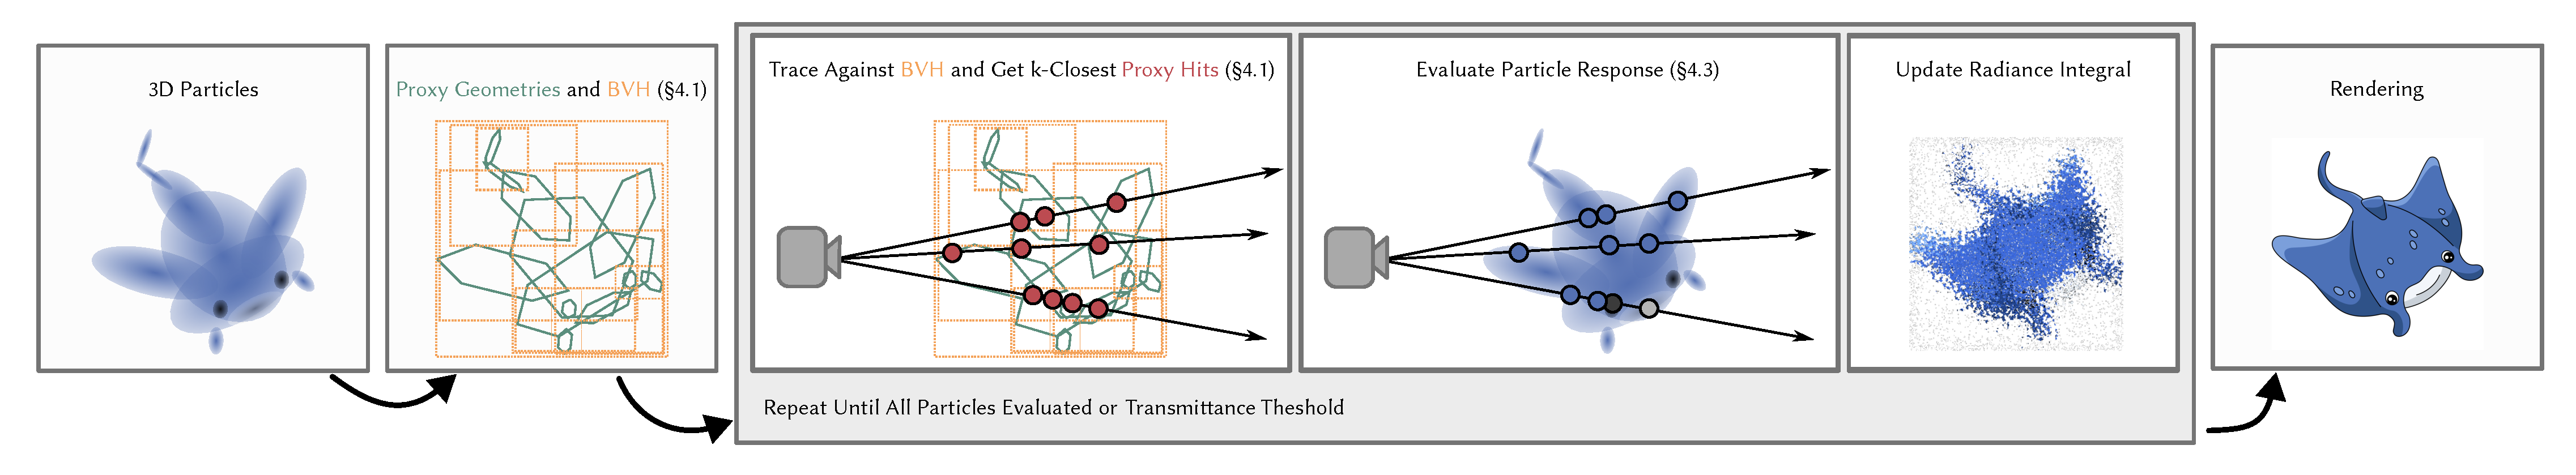
\includegraphics[width=0.92\textwidth]{figures/ch02/2407_07090_method.pdf}
\caption{3DGRT 渲染管线：高斯粒子→代理几何体/BVH→光线追踪求交→评估粒子响应→累积辐射度→渲染输出。图源：Moenne-Loccoz et al.（2024.07）~\cite{2407_07090}。}
\label{fig:02_3dgrt}
\end{figure}

3DGRT 沿用了 3DGS 的高斯 billboards 表示，通过代理几何体将现有基元映射到光线追踪管线——它在渲染管线层面做创新，但未触及基元本身的物理含义。EVER（2024.10）~\cite{2410_01804} 则选择了另一条路：不改变渲染管线，而是从根本上重新定义基元本身的物理含义，并精确求解体渲染方程。EVER 用恒定密度椭球替代高斯衰减，使体渲染方程获得闭合解，从而在不引入任何近似的前提下实现精确渲染。

\textbf{基元表示。}3DGS 的高斯基元被当作 2D billboards 投影后 $\alpha$-合成，存在两个根本问题：（1）当基元的合成顺序改变时颜色会突变（产生 popping 伪影），缺乏 3D 一致性；（2）$\alpha$-混合 将每个基元独立渲染后叠加，隐式假设基元互不重叠。EVER 将每个基元重新定义为\emph{恒定密度椭球}——与 3DGS 一样由位置向量、旋转四元数和缩放向量参数化，但内部密度 $\rho_k$ 为常数（而非高斯衰减），颜色由前两阶球谐函数表示。直觉上，高斯衰减的密度使基元在空间中无限延展且边界模糊，而恒定密度的椭球具有明确的内外之分——椭球内部密度均匀，边界处密度突然降为零。密度通过可优化参数 $\tau_k$ 间接控制：$\rho(\tau_k) = -\ln(1 - 0.99\,\tau_k) / (s_{kx} + s_{ky} + s_{kz})$。其设计逻辑是：分母中的三个缩放分量之和近似椭球的平均直径，使得沿最短轴观察时的峰值不透明度恰好等于 $\tau_k$。这确保了即使椭球被极度拉伸，至少一个视角仍具有非零梯度。

\textbf{精确体渲染。}标准体渲染方程要求沿光线积分密度场与颜色场，其一般形式为 $C = \int_0^\infty c_r(t)\,\sigma_r(t)\,\exp\!\bigl(-\int_0^t \sigma_r(s)\,ds\bigr)\,dt$。这一积分在一般密度场下无法解析求解，3DGS 因此通过将高斯投影为 2D billboards、按深度排序后逐个 $\alpha$-合成来近似。不过，这一近似在基元重叠时引入物理误差。EVER 的核心洞察是一个几何事实：恒定密度椭球与光线的交集是一系列有限区间。想象光线穿透一个均匀密度的椭球——光线进入椭球时密度突然出现，离开时突然消失，在椭球内部密度恒定不变。在每个这样的区间内密度和颜色均为常数，因此体渲染方程存在闭合解。

具体算法如下所述。沿光线找到所有相交椭球的前后表面，按距离排序后依次遍历。遇到第 $k$ 个椭球的\emph{前面}时，将 $\rho_k$ 和 $\rho_k c_k$ 分别加到运行总计 $\mu_i$ 和 $\nu_i$ 上，遇到\emph{后面}时则减去。这使得第 $i$ 个区间的累积密度和颜色分别为 $\mu_i = \sum_{k=1}^i \delta_k \rho_k$ 和 $\nu_i = \frac{1}{\mu_i}\sum_{k=1}^i \delta_k \rho_k c_k$（其中 $\delta_k \in \{+1,-1\}$ 标记前后面）。由于每个区间内密度和颜色恒定，积分具有闭合形式 $\alpha_i = 1 - e^{-\mu_i \Delta t_i}$。最终颜色通过 $\alpha$-合成这些区间得到：$C = \sum_{i=1}^N \alpha_i\,\nu_i\,\prod_{j=1}^{i-1}(1-\alpha_j)$。这一公式与 Max (1995) 的分段常数密度四边形规则完全一致，但在这里分段常数不是近似而是设计选择——因此 EVER 在不引入任何近似误差的前提下实现了精确体渲染。光线-椭球求交通过 NVIDIA OptiX 实现：为每个椭球提供轴对齐包围盒（AABB）构建 BVH，再用稳定的各向同性光线-球体求交算法精炼检测结果。

这一策略选择的意义在于：3DGRT 是在保持原有 3DGS 表示的同时引入光线追踪，EVER 则同时修正了表示的物理含义和渲染方程的求解方式。在 RTX 4090 上，EVER 以约 30 FPS（720p）运行，在 Zip-NeRF 大规模场景上达到实时方法中最锐利的结果。

\paragraph{在光栅化中实现体积一致性。}

EVER 通过光线追踪硬件实现精确体渲染，但硬件依赖限制了其适用范围。Talegaonkar~et~al.（2024.12）~\cite{2412_03378} 证明了另一条路径的可行性：不使用光线追踪硬件，在标准光栅化器内部实现接近 EVER 的物理准确性。两者的核心差异在于：EVER 将每个椭球分解为前后表面，沿光线维护密度和颜色的运行总计 $\tau_i = \sum_{k=1}^{i} \rho_k$，在各段上求解分段常数密度的闭合解 $\alpha_i = 1 - \exp(-\tau_i \Delta t_i)$，需要光线-椭球求交来定位前后表面。而该方法完全不执行 splatting，直接在光线坐标系中解析计算 3D 高斯的体积积分。

直觉上，这种方法的关键步骤是：一个 3D 高斯沿一条特定光线看去，其密度分布恰好也是一个 1D 高斯——就像用一根细针穿过一个三维的高斯云，针上各点的密度恰好形成钟形曲线。具体而言，该方法将第 $j$ 个 3D 高斯 $G_j(\mathbf{x}) = \exp\{-\frac{1}{2}(\mathbf{x}-\boldsymbol{\mu}_j)^\top \boldsymbol{\Sigma}_j^{-1}(\mathbf{x}-\boldsymbol{\mu}_j)\}$ 沿光线 $\mathbf{r}(t) = \mathbf{o} + t\mathbf{d}$ 精确约化为 1D 高斯分布：$g_j(t) = G_j(t_j\mathbf{d})\,\exp\{-\frac{(t-\mu_j)^2}{2\sigma_j^2}\}$，其中均值 $\mu_j = \frac{(\boldsymbol{\mu}_j - \mathbf{o})^\top \boldsymbol{\Sigma}_j^{-1}\mathbf{d}}{\mathbf{d}^\top \boldsymbol{\Sigma}_j^{-1}\mathbf{d}}$，方差 $\sigma_j^2 = \frac{1}{\mathbf{d}^\top \boldsymbol{\Sigma}_j^{-1}\mathbf{d}}$，$G_j(t_j\mathbf{d})$ 是高斯沿光线的峰值密度。对该 1D 高斯在区间 $[t_{jn}, t_{jf}]$ 上积分，得到解析透射率 $T_j = \exp(-G_j(t_j\mathbf{d})\sqrt{2\pi}\,\sigma_j)$，从而精确计算 $\alpha_j = 1 - T_j$。

与 3DGS 的 EWA splatting 相比，3DGS 做了三层近似。(a) 将指数透射率线性化 $e^{-x} \approx 1-x$。(b) 假设高斯不自遮挡（no self-occlusion），导致 2D 不透明度 $\alpha_i = o_i \cdot \tilde{G}_i(\mathbf{p})$ 仅在 2D 高斯中心处达到峰值 1，无法精确表示不透明表面。(c) 用仿射近似（Jacobian 矩阵 $\mathbf{J}$）将 3D 协方差投影为 2D 协方差 $\boldsymbol{\Sigma}' = \mathbf{J}\mathbf{W}\boldsymbol{\Sigma}\mathbf{W}^\top\mathbf{J}^\top$，在远离线性化中心处引入误差。此外，splatting 丢弃了高斯沿相机光线的 $z$ 轴尺度信息，使得渲染对 $z$ 方向的缩放不敏感——而物理上更大的 $z$ 尺度应使高斯更不透明。该方法通过在光线坐标系中直接积分，同时消除了上述三层近似，且保留了 $z$ 轴尺度的物理效应。在假设基元不重叠且正确排序的条件下，该方法最终仍输出与 3DGS 相同的 $\alpha$-混合 公式 $C(\mathbf{p}) = \sum_{i=1}^{N} c_i \alpha_i \prod_{j=1}^{i-1}(1-\alpha_j)$，但 $\alpha_i$ 的计算从近似 splatting 替换为解析积分。在 NeRF-Synthetic 数据集上全面超越 3DGS，同时可直接用于断层扫描重建。

\paragraph{Unscented Transform 统一投影模型。}

上述方法聚焦于渲染方程的精度改进，而 Wu~et~al.（2024.12）~\cite{2412_12507} 提出的 3DGUT（3D Gaussian Unscented Transform）则从投影模型的角度解决 EWA splatting 的根本局限——与其在投影函数上做近似，不如用采样策略绕过线性化。理解其贡献需要先厘清 3DGS 原本的投影机制：3DGS 将世界坐标系下的 3D 高斯（位置 $\boldsymbol{\mu} \in \mathbb{R}^3$，协方差 $\boldsymbol{\Sigma} \in \mathbb{R}^{3 \times 3}$）经由刚体变换 $\boldsymbol{W} \in SE(3)$ 变换到相机坐标系后，通过 EWA splatting 的一阶 Taylor 近似将 3D 协方差投影为 2D 协方差 $\boldsymbol{\Sigma}' = \boldsymbol{J}\boldsymbol{W}_{[:2,:3]}\boldsymbol{\Sigma}\boldsymbol{W}_{[:2,:3]}^\top\boldsymbol{J}^\top$，其中 $\boldsymbol{J} \in \mathbb{R}^{3 \times 3}$ 是投影函数的仿射近似的雅可比矩阵。这一线性化即使在理想针孔相机下也忽略了高阶项，且畸变越大误差越严重。更关键的是，每引入一种新相机模型（如等距鱼眼模型）都需要手动推导对应的 $\boldsymbol{J}$。而滚动快门等时间依赖效应在 EWA 框架内甚至难以表达。

3DGUT 的核心思想是不再线性化投影函数，而是用有限个采样点（称为 sigma 点）近似 3D 高斯分布本身。直觉上，这类似于用少量探针点”刻画“整个高斯云的形状：选取几个有代表性的空间位置，将它们分别投影到 2D 后重新拟合出投影后的 2D 高斯。受 Unscented Kalman Filter（无迹卡尔曼滤波，UKF）启发，对于 $N=3$ 维的 3D 高斯，选取 $2N+1=7$ 个 sigma 点 $\mathcal{X} = \{\chi_i\}_{i=0}^{6}$，利用协方差的 Cholesky 分解 $\boldsymbol{\Sigma} = \boldsymbol{R}^\top\boldsymbol{S}^\top\boldsymbol{S}\boldsymbol{R}$ 读取矩阵平方根：

\begin{align*}
\chi_0 &= \boldsymbol{\mu}, \\
\chi_i &= \boldsymbol{\mu} + (\sqrt{(3+\lambda)})\,\boldsymbol{e}_{[i]}, \quad i=1,2,3, \\
\chi_i &= \boldsymbol{\mu} - (\sqrt{(3+\lambda)})\,\boldsymbol{e}_{[i-3]}, \quad i=4,5,6,
\end{align*}

其中 $\boldsymbol{e}_{[k]}$ 为协方差矩阵平方根的第 $k$ 列，$\lambda = \alpha^2(3+\kappa)-3$ 由超参数 $\alpha$（控制 sigma 点距均值的散布，实验取 $\alpha=0.001$）、$\kappa$（缩放参数，取 $0$）和 $\beta$（分布先验，取 $2$）决定。每个 sigma 点独立通过任意非线性投影函数 $\hat{\chi}_i = g(\chi_i)$ 精确投影到 2D，然后通过加权后验重建 2D 均值和协方差：

\begin{align*}
\boldsymbol{\mu}' &= \sum_{i=0}^{6} w_i^{(m)}\,\hat{\chi}_i, \\
\boldsymbol{\Sigma}' &= \sum_{i=0}^{6} w_i^{(c)}\,(\hat{\chi}_i - \boldsymbol{\mu}')(\hat{\chi}_i - \boldsymbol{\mu}')^\top,
\end{align*}

其中均值权重 $w_0^{(m)} = \lambda/(3+\lambda)$、$w_{i>0}^{(m)} = 1/(2(3+\lambda))$，协方差权重 $w_0^{(c)} = \lambda/(3+\lambda) + (1-\alpha^2+\beta)$、$w_{i>0}^{(c)} = 1/(2(3+\lambda))$。该近似在分布匹配的精度上至少保留了前三阶矩。

这一机制完全绕过了雅可比矩阵的推导，使得 3DGUT 原生支持任意畸变相机模型和滚动快门——后者只需为每个 sigma 点施加不同的外参矩阵即可。KL（Kullback-Leibler）散度评估表明，在静态针孔相机下 UT 与 EWA 的投影精度相当，但在鱼眼相机下 UT 显著优于 EWA。而在滚动快门场景下，EWA 的线性化完全失效，UT 仍能保持稳定的投影精度。同时，3DGUT 将粒子响应评估从 2D 像素空间改为 3D 光线空间（沿光线计算最大响应点），避免了梯度通过投影函数的反向传播。这使其与 3DGRT 的渲染公式对齐——同一场景既可光栅化也可光线追踪，支持反射、折射等二次光线效果。

\subsubsection{无需专用硬件的可微光线追踪}

3DGRT 依赖 NVIDIA OptiX 硬件加速，这限制了其在非 NVIDIA 平台上的可用性。两条路线尝试在不依赖专用光线追踪硬件的情况下实现类似效果。

\paragraph{Govindarajan}
Govindarajan~et~al.（2025.02）~\cite{2502_01157} 提出的 Radiant Foam 是该方向的锚点工作。与 3DGRT 需要 OptiX 硬件加速不同，Radiant Foam 重新发现了一种在计算机视觉研究中长期被忽视的经典高效体积网格光线追踪算法，仅需标准可编程 GPU 特性即可运行，在渲染速度和质量上与 3DGS 相当，同时不受光栅化的近似限制——从而在不牺牲效率的前提下消除了对专用光线追踪硬件的依赖。

\paragraph{Radiant}
Xu~et~al.（2026.03）~\cite{2603_23637} 则采取正交策略。与 Radiant Foam 用经典光线追踪算法替代硬件加速不同，该方法通过随机采样从根本上消除排序需求：对每条光线仅采样少量高斯子集进行评估的无偏 Monte Carlo 估计器，在标准 3DGS 场景中匹配光栅化质量和速度。更重要的是，在可重光照（relightable）3DGS 场景中，同一估计器驱动逐高斯着色和完整光线追踪的阴影光线，无需近似阴影映射，实现了比先前工作明显更高的重建保真度。

\subsubsection{可编辑与矢量化的高斯渲染}

前面的方法主要追求渲染的物理准确性和效率，而另一类工作关注如何让高斯渲染支持场景编辑和更精确的几何表示。

\paragraph{可编辑高斯光线追踪。}

Byrski~et~al.（2025.03）~\cite{2503_12284} 提出的 REdiSplats 是该方向的锚点工作，其核心贡献是将扁平高斯近似为可编辑的正八边形网格，使同一基元同时满足光线追踪求交和用户直接拖拽编辑两个需求。具体而言，3DGRT（2024.07）~\cite{2407_07090} 用拉伸的规则二十面体（20 面）作为代理包围体，每个交叉命中后还需额外计算高斯响应采样点；REdiSplats 则将扁平高斯（$s_1=0$，即 2D 椭圆）直接近似为正八边形网格，交叉点同时确定高斯身份并提供 opacity 计算所需的距离参数，无需第二个采样点。

具体而言，在扁平高斯的局部坐标系（$OY$--$OZ$ 平面）中，八边形的直觉是将圆形高斯截面离散化为正八边形——就像用正八边形近似一个圆，顶点到中心的距离由统计学置信水平决定。第 $i$ 个顶点为
\begin{equation}
  x_i = \Bigl[0,\; \cos\!\Bigl(\tfrac{2\pi i}{8}\Bigr),\; \sin\!\Bigl(\tfrac{2\pi i}{8}\Bigr)\Bigr] \cdot Q, \quad i=0,\ldots,7,
\end{equation}

其中 $Q = F_{\chi^2(3)}^{-1}(\beta)$ 为卡方分布（3 自由度）在置信水平 $\beta$ 下的分位数。全局坐标通过仿射变换 $P_i = RS \cdot x_i + \mu$ 获得，其中 $R=[r_1,r_2,r_3]$ 为旋转矩阵，$S=\mathrm{diag}(0,s_2,s_3)$ 为缩放矩阵。八边形以 triangle fan 形式三角化为中心点 + 8 个外顶点的 6 个三角形，利用 NVIDIA OptiX 的硬件加速 ray-triangle 求交直接检测光线-高斯碰撞。

在编辑方面，用户拖拽网格顶点 $P_i \to P_i'$ 后，REdiSplats 从 8 个顶点中选取 3 个关键点（$I=\{0,2\}$，即间隔 $90^\circ$ 的两个外顶点加中心点）重建高斯参数：首先由 $r_2 = \widehat{P_{i_1}'}$ 恢复第二旋转轴和缩放 $s_2$，再通过一步 Gram-Schmidt 正交化得到 $r_3$ 和 $s_3$，最后 $r_1 = r_2 \times r_3$，$s_1=0$。该重建过程保证无编辑操作时参数恒等，且仅需 3 个自由顶点而非全部 9 个，避免过度编辑破坏八边形的正则结构。

REdiSplats 在光线追踪中支持阴影投射、镜面反射（如玻璃和镜面对象）以及与 mesh 场景的混合渲染，同时网格表示可直接导入 Blender 和 Nvdiffrast 进行物理仿真和手动编辑，首次在单一框架中统一了光线追踪、场景编辑和物理仿真。

\paragraph{矢量图元混合表示。}

REdiSplats 通过将扁平高斯近似为三角化八边形网格实现了可编辑性，但其基元仍本质上是高斯的——高斯核固有的空间无限延展导致边界模糊。Wu~et~al.（2025.03）~\cite{2503_13961} 提出的 BG-Triangle（B\'{e}zier Gaussian Triangle）选择了一条更根本的路线：在确定性（贝塞尔三角形矢量图元）和概率性（高斯核）两个极端之间建立混合表示，用贝塞尔三角形的精确边界解决高斯核的模糊问题，同时用高斯子基元保留可微渲染能力。

直觉上，B\'{e}zier 三角形与 CAD 软件中常用的贝塞尔曲面片类似：控制点定义了一个光滑的三角形曲面片，边界由重心坐标严格限定——重心坐标 $(u,v,w)$ 在三角形内部为正，在边界上为零，在三角形外部为负，因此 $u+v+w=1$ 且 $u,v,w \geq 0$ 恰好定义了三角形的闭合区域。具体而言，BG-Triangle 的几何基元是 $n$ 次 B\'{e}zier 三角形曲面 $S$，由控制点 $p_{i,j,k} \in \mathbb{R}^3$（其中 $i+j+k=n$, $i,j,k \geq 0$）定义，参数化形式为：

\begin{equation}
S(u,v,w) = \sum_{i=0}^{n} \sum_{j=0}^{n-i} B_{i,j,k}^{n}(u,v,w) \, p_{i,j,k}
\end{equation}

其中 $B_{i,j,k}^{n}(u,v,w) = \frac{n!}{i!\,j!\,k!} u^i v^j w^k$ 为 Bernstein 多项式。这一参数化与 REdiSplats 的本质区别在于：REdiSplats 用三角化八边形近似扁平高斯的置信椭球，顶点由高斯参数刚性导出，几何仍是高斯的离散化；而 BG-Triangle 的控制点通过 Bernstein 插值生成连续曲面，天然具有精确边界——重心坐标域 $u+v+w=1$ 严格定义了基元的闭合边界，不存在高斯核的空间无限延展问题。

然而，仅有确定性几何无法实现可微渲染——几何提供精确边界但无法生成平滑的梯度信号。BG-Triangle 的核心设计在于双层表示的协同：几何层（B\'{e}zier 三角形）定义精确边界和表面位置，外观层（高斯子基元）在每个像素位置”按需“生成，提供可微的颜色和属性插值。

渲染管线首先将 B\'{e}zier 三角形细化为扁平三角面片，经传统光栅化生成坐标图 $I_{uv} \in \mathbb{R}^{H \times W \times 3}$ 和索引图 $I_{id} \in \mathbb{Z}^{H \times W}$，为每个像素记录其所属基元的重心坐标和 ID。随后，在每个前景像素 $q$ 处根据重心坐标计算 3D 位置 $S_q$，并在该位置动态生成高斯子基元（sub-primitive）。这些子基元继承旋转、缩放和球谐系数等属性，但不包含不透明度——因为几何已由 B\'{e}zier 三角形定义。属性插值分为两类：漫反射颜色通过颜色控制点 $p_{i,j,k}^c$ 经 Bernstein 插值计算 $c_q = \sum_{i,j} B_{i,j,k}^n(I_{uv}(q)) \, p_{i,j,k}^c$；旋转、缩放和 SH 系数则通过基于重心坐标的多分辨率 2D 属性图 $M_h$ 进行纹理插值。这种”on-the-fly“生成策略意味着不同视角使用不同的高斯集合，但均从同一组 B\'{e}zier 控制点采样，确保了几何一致性。

上述结构在每个 BG-Triangle 内部保证了平滑过渡，但基元边界处的高斯不确定性仍会导致模糊。直接在边界截断高斯会破坏可微性——梯度会在截断处断裂。因此 BG-Triangle 引入不连续感知 $\alpha$-混合（discontinuity-aware $\alpha$-混合）机制：在基元边界处用一个平滑过渡函数逐渐降低 alpha 值，而非突然截断。首先，光栅化阶段检测相邻像素归属不同基元 ID 的边界像素，构成 2D 边界点集 $\mathcal{B}$，并通过 B\'{e}zier 映射反投影为 3D 边界点。每个边界点被建模为固定缩放因子 $r_b$ 的各向同性高斯，其投影半径 $\delta_i$ 定义了影响范围。直觉上，距离边界越远的像素受边界过渡函数的影响越小（保持原值），距离边界越近的像素则被平滑地抑制——这就像在两个不同颜色的区域之间画一条渐变带。对于光栅化高斯 $G$ 覆盖的像素 $q$，混合系数定义为：

\begin{equation}
w(q) = \begin{cases} 0, & I_{id}(b_i) \neq g \\ g(\|q - b_i\|_2; \delta_i), & I_{id}(b_i) = I_{id}(q) \\ 1 - g(\|q - b_i\|_2; \delta_i), & \text{otherwise} \end{cases}
\end{equation}

其中 $g$ 为高斯 $G$ 所属基元的 ID，模糊函数 $g(d;\delta) = \sigma(2^{d/\delta-1}, 1)$ 将距离 $d$ 映射到 $[0.5, 1.0]$，使 $w(q)$ 在边界区域内从 $1.0$ 平滑过渡到 $0.0$。修正后的 alpha 值为 $\alpha'(q) = o \cdot w(q) \cdot e^{-\frac{1}{2}(q-\boldsymbol{\mu})^\top \boldsymbol{\Sigma}^{-1}(q-\boldsymbol{\mu})}$，其中 $o \approx 1.0$ 为常数。在训练优化方面，BG-Triangle 采用基于控制点梯度幅度和训练视图边缘先验的双重分裂准则：梯度范数超过 $\lambda_g$ 的基元或累积边缘梯度超过 $\lambda_b$ 的基元被分裂以拟合细节；同时基于可见性、面积和纵横比三个标准修剪无效基元。通过这一确定性几何与概率性外观的混合表示，BG-Triangle 使用远少于 3DGS 的基元达到可比渲染质量，同时在边界保持方面显著优于 3DGS 和 NeRF。

\subsubsection{科学可视化与跨模态应用}

3DGS 的光线追踪能力不仅限于视觉渲染，还可服务于科学计算和跨模态仿真，这一扩展从三个方向展开。

\paragraph{Sharma et al.：科学体渲染 LOD 近似}
\textbf{科学体渲染}。Sharma~et~al.（2025.04）~\cite{2504_04857} 将 3DGS 的光线追踪思想应用于科学可视化领域，利用 3D 高斯粒子在不同 LOD 下近似 VDB 体素数据，是该方向的首个工作。

\paragraph{GSCache：多级路径空间辐射缓存}
Bauer~et~al.（2025.07）~\cite{2507_19718} 提出的 GSCache 则将 3DGS 适配为多级路径空间辐射缓存，利用高效光栅化器加速体渲染中的路径追踪，支持在线训练动态适应光照配置和传输函数变化——与 Sharma~et~al. 的静态 LOD 近似不同，GSCache 侧重于动态路径追踪的高效缓存策略。

\paragraph{Kohyama}
\textbf{事件驱动渲染}。从科学体渲染的连续场近似转向另一种模态，Kohyama~et~al.（2025.12）~\cite{2512_18640} 提出的 GPERT 将事件相机的逐事件稀疏特性与光线追踪结合：将渲染解耦为逐事件几何渲染和快照式辐射渲染两个分支，这是首个事件驱动的 3DGS 光线追踪框架。

\paragraph{Vaara et al.：可微分射频传播仿真}
\textbf{跨模态电磁仿真与硬件优化}。从视觉波段扩展到电磁频谱，Vaara~et~al.（2026.05）~\cite{2605_07781} 提出将 Gaussian 基元嵌入光线追踪结构，首次实现可微分射频传播仿真，证明神经重建可同时服务于电磁仿真和光真实感渲染。

\paragraph{GRTX：光线追踪管线效率优化}
Lee~et~al.（2026.01）~\cite{2601_20429} 提出的 GRTX 则从软硬件协同角度优化高斯基光线追踪，通过光线空间变换将各向异性高斯视为单位球以减少 BVH 开销，引入遍历检查点机制消除冗余节点访问——与 Vaara~et~al. 的应用驱动路线互补，GRTX 聚焦于底层管线效率优化。

\paragraph{Stekovic}
此外，Stekovic~et~al.（2024.04）~\cite{2404_10620} 提出的 PyTorchGeoNodes 将 Blender 中的程序模型解析为可微 PyTorch 代码，利用遗传算法与梯度优化的组合策略同时优化离散和连续参数，展示了与 3DGS 集成实现程序化高斯泼溅的可能性。

\paragraph{光栅化与光线追踪的融合趋势}
总的来说，从光栅化到光线追踪的转变代表了 3DGS 渲染能力的质变。3DGRT（2024.07）~\cite{2407_07090} 和 EVER（2024.10）~\cite{2410_01804} 从两个方向证明：在 3DGS 的粒子场景中，光线追踪可以达到与光栅化相当的效率。

\paragraph{3DGUT 与体渲染一致性}
3DGUT（2024.12）~\cite{2412_12507} 和 Volumetrically Consistent Rasterization（2024.12）~\cite{2412_03378} 则证明在光栅化框架内也可以实现更物理准确的体渲染。

\paragraph{随机光线追踪效率提升}
随机光线追踪（2026.03）~\cite{2603_23637} 通过消除排序开销进一步提升了效率。这些工作共同指向一个趋势：3DGS 的渲染管线正在从纯光栅化向混合渲染（光栅化 + 光线追踪）演进，以兼顾效率和物理准确性。

\begin{takeaway}
3DGS 的渲染管线正在从纯光栅化向混合渲染演进。3DGRT 和 EVER 等工作通过 BVH 光线追踪实现阴影、反射等物理效果，3DGUT 则在光栅化框架内实现了更物理准确的体渲染。这一方向的核心权衡是光线追踪带来的物理准确性提升与排序开销增加之间的平衡。
\end{takeaway}

% ============================================================
% 第2章 中间部分：2.6--2.8
% ============================================================

\subsection{近期方法脉络：射线查询与高级渲染、Fast ray tracing for 3D Gaussians}

这一组近期工作延续 3DGS rasterization、3D Gaussian Ray Tracing，主要把改动集中在扩展、加速等环节。下面只保留相对既有路线的变化，便于和前文方法直接对照。

\paragraph{Directed Distance Fields for Constant-Time Ray Queries on Gaussian Splatting}
Directed Distance Fields for Constant-Time Ray Queries on Gaussian Splatting（2026.05）~\cite{2606_00817} 延续 3DGS rasterization 在“射线查询与高级渲染”上的基本设定，主要改变是：从3DGS蒸馏Directed Distance Field，将射线映射到首个表面距离和命中状态，实现常数时间ray oracle。高斯基元表示仍作为基础。
其设计动机是：提出从3DGS训练小型DDF神经场的方法，使查询成本与高斯数量无关，为3DGS补足传统光栅化难以处理的secondary rays能力。
具体而言，DDF输入射线起点和方向，输出首交距离和命中概率；论文比较深度监督和干净距离监督，发现后者更能恢复薄结构。
适用边界是：需要额外蒸馏训练；距离监督质量影响薄结构；DDF是辅助神经场而非直接改造高斯表示。

\paragraph{GRay}
GRay（2026.06）~\cite{2606_30869} 可作为“Fast ray tracing for 3D Gaussians”中的新锚点候选。相较于 3D Gaussian Ray Tracing，主要改变是：只评估被光线相交的 Gaussians，并优化 3D Gaussian ray tracing 管线。高斯基元表示仍作为基础。
其设计动机是：利用 ray tracing 与 rasterization 的算法差异，避免评估所有投影相关 splats，而只处理实际相交的 Gaussians。
具体而言，设计面向 3D Gaussians 的高效 ray tracing 方法，通过加速结构和相交评估降低 3DGRT 近一个数量级的优化开销。
这一锚点判断来自当前分类中的机制关系：候选锚点：加速，且相关性 0.95；后续方法可围绕 为 3D Gaussians 设计接近 splatting 速度的 ray tracing 渲染器。 继续比较和扩展。
适用边界是：ray tracing 管线复杂度和硬件适配仍需考虑；透明混合和梯度稳定性可能是关键实现细节。
\section{渲染管线与排序优化}
\label{sec:02_6}

3DGS 的渲染效率建立在一个核心设计设定之上：tile-based 光栅化配合基于深度排序的 $\alpha$-混合。原始 3DGS 将图像平面划分为 $16\times16$ 像素的 tile，对每个 tile 内的高斯基元按视图空间 $z$ 坐标执行全局排序（radix sort），然后从前到后执行 $\alpha$-混合 计算像素颜色。这一设定带来了三方面的问题。(1) 排序本身是计算瓶颈，尤其在基元数量达到百万级别时开销显著。(2) 全局排序按基元中心深度进行，无法保证逐像素的正确深度顺序，导致视角旋转时出现”弹出“（popping）伪影。(3) 仿射投影近似在大视场角和近距离观察时引入几何失真。围绕这些问题，研究者从排序策略、混合公式和渲染管线结构三个维度展开了系统性优化。图~\ref{fig:02_pipeline_opt} 展示了三层优化策略。

\begin{figure}[htbp]
\centering
\resizebox{0.85\textwidth}{!}{\begin{tikzpicture}[
  layer/.style={rectangle, rounded corners=6pt, draw=#1, fill=#1!8,
    text width=13cm, minimum height=1.5cm, align=left, font=\small},
  mname/.style={font=\scriptsize\ttfamily, techgray},
  arr/.style={-{Stealth[length=6pt]}, very thick, techgray},
  >=Stealth
]
  % Layer 3 (底部): 管线效率优化
  \node[layer=techpurple] (l3) at (0, 0) {%
    \textbf{Layer 3: 管线效率优化}%
    \hfill {\scriptsize 减少冗余计算 + 利用硬件特性}%
  };
  \node[mname, anchor=north west] at ([xshift=0.3cm, yshift=-0.1cm]l3.north west) {
    FlashGS \textbullet{} Speedy-Splat \textbullet{} QuadBox \textbullet{} TC-GS \textbullet{} TensorGS \textbullet{} GEMM-GS
  };

  % Layer 2 (中部): 排序精度改进
  \node[layer=techorange] (l2) at (0, 2.3) {%
    \textbf{Layer 2: 排序精度改进}%
    \hfill {\scriptsize 逐像素精确排序 + 投影校正}%
  };
  \node[mname, anchor=north west] at ([xshift=0.3cm, yshift=-0.1cm]l2.north west) {
    StopThePop \textbullet{} Plucker坐标 \textbullet{} 混合透明度 \textbullet{} 精确椭球投影
  };

  % Layer 1 (顶部): 消除排序依赖
  \node[layer=techblue] (l1) at (0, 4.6) {%
    \textbf{Layer 1: 消除排序依赖}%
    \hfill {\scriptsize 可交换混合替代 alpha blending}%
  };
  \node[mname, anchor=north west] at ([xshift=0.3cm, yshift=-0.1cm]l1.north west) {
    WSR (加权求和) \textbullet{} StochasticSplats \textbullet{} Duplex-GS \textbullet{} MB3DGS
  };

  % 层间箭头
  \draw[arr] (l1.south) -- (l2.north) node[midway, right=0.3cm, font=\scriptsize, techgray] {排序仍然需要};
  \draw[arr] (l2.south) -- (l3.north) node[midway, right=0.3cm, font=\scriptsize, techgray] {排序已优化};

  % 右侧标注：效果
  \node[font=\scriptsize, techblue, anchor=west] at (7, 4.6) {弹出伪影 = 0};
  \node[font=\scriptsize, techorange, anchor=west] at (7, 2.3) {高斯减少 50\%};
  \node[font=\scriptsize, techpurple, anchor=west] at (7, 0) {渲染加速 1.5--7$\times$};
\end{tikzpicture}
}
\caption{渲染管线优化的三层策略。Layer~1 从根本上消除排序需求，Layer~2 提升排序精度，Layer~3 优化管线效率。三层可叠加使用。}
\label{fig:02_pipeline_opt}
\end{figure}

\subsection{消除排序依赖：顺序无关渲染}

排序是 3DGS 渲染管线中计算量最大的环节之一。
一系列工作试图从根本上消除对排序的需求，转而采用可交换的混合操作替代非交换的 $\alpha$-混合。
这些方法沿着从”可交换近似“到”无偏物理建模“再到”理论重构“的路径逐步演进。

\subsubsection{顺序无关渲染方法}

\paragraph{Hou}
Hou~et~al.（2024.10）~\cite{2410_18931} 提出的 Weighted Sum Rendering（WSR）是该方向的奠基性工作。
其核心思路直观而激进：既然排序的根源在于 $\alpha$-混合 的非交换性（先渲染红再渲染蓝，与反过来结果不同），那么如果用一种\emph{与顺序无关}的混合公式替代 $\alpha$-混合，排序自然就不再需要。
具体而言，WSR 将颜色混合视为对高斯颜色的深度加权平均——越靠近相机的高斯权重越大——这一操作天然与求和顺序无关。
其混合公式为：

\begin{equation}
C = \frac{c_B w_B + \sum_{i=1}^{N} c_i \alpha_i w(d_i)}{w_B + \sum_{i=1}^{N} \alpha_i w(d_i)}
\end{equation}

其中 $c_B$ 和 $w_B$ 为背景的颜色和可学习权重，$d_i$ 为第 $i$ 个高斯的深度，$w(\cdot)$ 为可学习的权重函数。
由于求和天然具有交换性，渲染过程完全无需排序即可并行执行，同时消除了排序变化引起的时序弹出伪影。

权重函数 $w(d_i)$ 的设计是 WSR 的核心，论文提出三种变体，精度逐步提升。

\textbf{DIR-WSR}（Direct）使用常数权重 $w(d_i) = 1$，完全忽略深度信息，由网络通过调整不透明度 $\alpha_i$ 来补偿。
然而，当两个不透明高斯（$\alpha = 1$）颜色不同时，DIR-WSR 始终输出两色的混合色（如红蓝混合为紫色），无法正确建模遮挡关系，在复杂场景中引入明显的模糊伪影。

\textbf{EXP-WSR}（Exponential）引入深度依赖的指数权重 $w(d_i) = e^{-\lambda d_i^\beta}$，其中 $\lambda, \beta$ 为可学习参数（训练时分别初始化为 $0.1$ 和 $0.8$），使靠近相机的高斯获得更大权重以近似遮挡效果。
但远处高斯的权重虽衰减却永不为零，仍然贡献残余颜色，导致在密集重叠区域产生视觉失真。

\textbf{LC-WSR}（Linear Correction）受可变形卷积和 KPConv 启发，采用线性修正权重 $w(d_i) = \max(0,\, 1 - \lambda d_i) \cdot v_i$，其中 $\lambda$（初始化为 $10$）和 $v_i$（初始化为 $0.1$）为可学习参数。
与 EXP-WSR 的关键区别在于：LC-WSR 可以将远处高斯的权重精确降至零，彻底消除其对渲染的贡献，从而更准确地建模硬遮挡边界，且计算开销低于 EXP-WSR。

除权重函数外，WSR 还将原始 3DGS 中固定的最大不透明度 $t_i$ 替换为视角依赖的不透明度 $u_i = Y(\|\mathbf{d}_i\|, \mathbf{H}_i)$，其中 $Y(\cdot)$ 为球谐函数，$\mathbf{H}_i$ 为可学习的球谐系数向量。
这一机制使同一高斯从不同视角观察时具有不同的不透明度，部分弥补了 WSR 缺少排序所丢失的遮挡信息。
值得注意的是，$u_i$ 不再像原始 3DGS 那样被裁剪到 $[0,1]$ 区间，赋予了网络更大的表达自由度。
训练过程中，WSR 使用与原始 3DGS 完全相同的 $\mathcal{L}_1$ + D-SSIM 损失函数（D-SSIM 权重因子 $0.2$），但优化对象从固定不透明度参数变为权重函数参数和视角依赖不透明度的球谐系数。

WSR 在物理上牺牲了体渲染方程的严格闭合解，换来了对排序的完全独立。在移动设备 GPU 上实现平均 1.23 倍渲染加速，且特别适合 WebGL/Vulkan 等无法高效执行全局排序的平台。其核心局限在于：即使是最精确的 LC-WSR 变体，加权求和仍然是一种近似混合，无法在半透明物体密集重叠的场景中完全复现 $\alpha$-混合 的物理正确结果。
沿”消除排序但提升物理准确性“的方向，后续工作分别从统计采样、双层次框架、矩方法和理论重构四个角度改进。

\paragraph{统计采样路线。}
针对 $\alpha$-混合 公式本质上是加权期望值、而任何期望都可用蒙特卡洛采样无偏估计的观察，StochasticSplats 将体渲染方程从确定性的排序混合转化为无偏的蒙特卡洛估计，用概率论证明排序只是充分条件而非必要条件，核心思想是\textbf{``混合即期望，采样即求解''}——从而在根本上消除 3DGS 对全局排序的依赖。Kheradmand~et~al.（2025.03）~\cite{2503_24366} 提出的 StochasticSplats 走了一条与 WSR 完全不同的路线：WSR 用可交换的加权求和替换了混合公式，而 StochasticSplats 则保留原始 $\alpha$-混合 公式不变，但通过\textbf{随机采样}来绕过排序需求。
直觉上，$\alpha$-混合 输出的颜色是一个加权期望，而任何期望都可以用蒙特卡洛采样来估计——如果按正确概率随机抽取一个高斯，它的颜色就是无偏的颜色估计。
具体而言，StochasticSplats 将 $\alpha$-混合 公式 $C = \sum_{i=1}^{L} c_i\,\alpha_i \prod_{z_k < z_i}(1-\alpha_k)$ 转化为蒙特卡洛估计问题。
核心思想是按照概率质量函数 $P(i) = \alpha_i \prod_{z_k < z_i}(1-\alpha_k)$ 随机选取一个高斯 $i$，然后通过重要性采样得到无偏估计 $\hat{C} = c_i / P(i) = c_i$——由于 $1/P(i)$ 恰好消去了 $\alpha$-混合 中的透射率项，单次采样只需返回被选中的高斯颜色 $c_i$。
在 GPU 上，这一过程通过标准深度测试实现：为每个像素采样均匀随机数 $u \sim U(0,1)$，在 fragment shader 中测试 $u < \alpha_i$，不满足则 \texttt{discard}——硬件深度测试自动保证被保留的片段是最近（$z$ 最小）的那个，无需全局排序。
最终像素颜色为 $S$ 组独立样本的平均 $\bar{C} = \frac{1}{S}\sum_{s=1}^{S} c_{i_s}$，调整每像素样本数（SPP）即可灵活权衡渲染速度与视觉质量：1 SPP 下比原始 CUDA 3DGS 快 4 倍以上，增大 SPP 则逐步逼近排序 $\alpha$-混合 的 PSNR。

为保证训练中的梯度正确回传，StochasticSplats 借鉴 path replay backpropagation（2021）~\cite{Vicini2021PathReplay}，采用\textbf{分离梯度估计器}（detached gradient estimator）和三遍渲染策略：
（1）第一遍渲染图像并计算损失梯度 $\partial\mathcal{L}/\partial C$；
（2）第二遍使用不同随机种子渲染去相关图像，获取被采样高斯的颜色 $c_i$；
（3）第三遍以与第二遍相同的随机种子重放，利用存储的 $c_i$ 计算参数梯度——其中颜色梯度仅传递给被采样的第 $i$ 个高斯 $\partial\mathcal{L}/\partial c_i = (\partial\mathcal{L}/\partial C)$，不透明度梯度则传递给第 $i$ 个高斯及其前方所有高斯，后方高斯梯度为零。
为避免损失函数两个噪声项的相关性导致梯度偏差，第二遍使用独立随机种子渲染去相关图像，使 L2 损失获得无偏梯度。

在消除 popping 伪影方面，StochasticSplats 提供两个层次。

快速模式下，将 billboard 平面定向为线性逼近高斯最大密度面，平面法向量取 $\mathbf{n} = \boldsymbol{\Sigma}^{-1}(\boldsymbol{\mu} - \mathbf{o})$（$\boldsymbol{\mu}$ 为高斯均值，$\mathbf{o}$ 为相机中心，$\boldsymbol{\Sigma}$ 为协方差矩阵），利用硬件光栅化器的插值内核自动计算 splat 深度，不增加额外开销。

高保真模式下，用 free-flight distance sampling（一种体积渲染中的经典距离采样方法，沿射线随机选取与下一个散射介质”碰撞“的距离）实现完全体积混合——将每个高斯的不透明度重新参数化为空间变化的消光函数 $\sigma_i(\mathbf{p}) = \sigma_t\,\exp\!\bigl(-\tfrac{1}{2}(\mathbf{p}-\boldsymbol{\mu})^T\boldsymbol{\Sigma}^{-1}(\mathbf{p}-\boldsymbol{\mu})\bigr)$，通过解析逆 CDF 采样自由飞行距离 $t$，多个重叠高斯采用 decomposition tracking（分解追踪，取各介质自由飞行距离的最小值来确定最近碰撞）无需额外数据结构或光线追踪即可准确解析任意数量的高斯重叠。

\paragraph{双层次框架路线。}
WSR 和 StochasticSplats 分别通过近似混合和统计采样消除了排序，但都未充分利用 3DGS 渲染的空间局部性。
Liu~et~al.（2025.08）~\cite{2508_03180} 提出的 Duplex-GS 在 WSR 的基础上引入双层次框架，同时解决了 WSR 的透明伪影和传统 $\alpha$-混合 的弹出伪影。

\textbf{第一层：Cell Proxy。}
与 Scaffold-GS 和 Octree-GS 中仅作为抽象编码代理的锚点（anchor）不同，Duplex-GS 引入具有显式几何结构的椭球单元（ellipsoidal cell）作为代理。
每个 cell 由位置 $\boldsymbol{\mu}_n$、尺度 $\mathbf{s}_n$、四元数 $\mathbf{q}_n$ 定义其可见区域，并关联一个潜在特征向量 $\mathbf{f}_n$ 编码局部场景信息。
每个 cell 发射 $K$ 个神经高斯，其颜色 $\mathbf{c}_{n,k}$、尺度比 $O_{n,k}^{\mathrm{scale}}$ 和四元数 $\mathbf{q}_{n,k}$ 由共享的场景级 MLP 从 $\mathbf{f}_n$、视距 $d_n$ 和视角 $\mathbf{d}_n$ 解码得到：
$\{\mathbf{c}_{n,1},\ldots,\mathbf{c}_{n,K}\} = F_c(\mathbf{f}_n, d_n, \mathbf{d}_n)$，$\{O_{n,k}^{\mathrm{scale}},\ldots\} = F_s(\mathbf{f}_n, d_n, \mathbf{d}_n)$。
为使高斯中心严格落在 cell 可见区域内，偏移参数 $O_{n,k}^{\mathrm{pos}}$ 被约束在 $[-1,1]$ 范围内。
高斯尺度由 cell 尺度乘以 sigmoid 激活的尺度比得出：$\mathbf{s}_{n,k} = O_{n,k}^{\mathrm{scale}} \cdot \mathbf{s}_n$，并进一步裁剪 $O_{n,k}^{\mathrm{scale}} = \min(O_{n,k}^{\mathrm{scale}}, 1 - \|O_{n,k}^{\mathrm{pos}}\|)$，确保高斯区域完全包含在 cell 内。
Cell 的四元数通过其关联高斯的加权平均更新：$\mathbf{q}_n = (\sum_k^K \alpha_{n,k} \cdot \mathbf{q}_{n,k}) / \sum_k^K \alpha_{n,k}$。

基于 cell 的显式几何，Duplex-GS 将光栅化从逐高斯操作提升到逐 cell 层面。
仅与视锥相交的 cell 被选中并解码为神经高斯；在 tile-based 范式下，可见 cell 被分配到对应 tile 并对 cell 序列执行基数排序。
由于 cell 数量比高斯少数个数量级，这一策略大幅降低了基数排序的序列长度和内存消耗——排序开销减少 52.2\%--86.9\%。

\textbf{第二层：物理加权求和渲染。}
Duplex-GS 的混合公式建立在 cell 级排序获得的粗粒度深度顺序之上。
它将每个 cell 视为一个整体，定义 cell 权重 $w_n = v_n T_n^{\mathrm{cell}}$，其中 $T_n^{\mathrm{cell}}$ 为 cell 级透射率，按前到后顺序累积衰减：

\begin{equation}
T_n^{\mathrm{cell}} = \prod_{i=1}^{n-1}\prod_{k=1}^{K}(1 - v_i \alpha_{i,k})
\end{equation}

其中 $\alpha_{i,k}$ 为高斯核加权的不透明度，约束在 $[0,1]$ 物理合理范围内（区别于 WSR 中经常超过 1 的无约束权重）；$v_i$ 为可学习的标定标量，用球谐系数参数化以捕捉视角依赖的方向变化，用于补偿 cell 间非均匀空间分布和重叠带来的歧义。
最终渲染颜色为：

\begin{equation}
C = \frac{\sum_{n=1}^{N} w_n \sum_{k=1}^{K} \alpha_{n,k} \mathbf{c}_{n,k}}{\sum_{n=1}^{N} w_n \sum_{k=1}^{K} \alpha_{n,k}}
\end{equation}

这一设计的核心洞察是：\textbf{cell 间有序、cell 内无序}。
Cell 级透射率 $T_n^{\mathrm{cell}}$ 按 cell 深度顺序严格递减，重建了类似 $\alpha$-混合 的物理透射率衰减曲线——当遇到不透明表面时快速衰减至零，从而消除 WSR 中半透明物体消失的失真问题。
而 cell 内部的高斯无需排序，渲染结果局部独立于高斯顺序，因此完全消除了 popping 伪影。

\textbf{早期终止与优化策略。}
由于 $T_n^{\mathrm{cell}}$ 具有物理意义且严格递减，当其降至预设阈值 $\epsilon$ 以下时即可安全终止混合过程——与 vanilla 3DGS 使用相同的阈值参数。
这一机制是此前 WSR 方法所不具备的，因为 WSR 的权重缺乏物理约束，无法支持早期终止。
在优化方面，Duplex-GS 引入三项工程策略：（1）False Positive Skip——通过轴对齐包围盒（AABB）检查剔除像素级冗余高斯核计算；（2）几何校正——定期将 cell 中心更新为其关联高斯中心的均值，确保空间对齐；（3）Cell Position Reset——密度控制新增 cell 后，将显著高斯的偏移重置为零以解耦新旧 cell。
损失函数在原始 $\mathcal{L}_1$ + D-SSIM（权重 $0.2$）基础上额外加入 LPIPS 感知损失（权重 $0.5$，每 20 次迭代计算一次以控制训练开销）。

实验表明，Duplex-GS 比现有基于 OIT 的 3DGS 方法快 1.5--4 倍，在 Mip-NeRF 360 上以 184 FPS 达到最高 PSNR，在中端 RTX 3060 笔记本 GPU 上同样保持最高渲染速度和竞争力视觉质量。

\paragraph{解析矩方法路线。}
Duplex-GS 通过工程策略平衡了 WSR 和精确排序之间的取舍，而 M\"uller~et~al.（2025.12）~\cite{2512_11800} 提出的 Moment-Based 3DGS（MB3DGS）则从物理建模层面提供了更为精细的解决方案。
MB3DGS 的核心思想可以用一个类比理解：与其逐个高斯地按深度排序混合，不如先统计出射线上所有高斯的“深度分布摘要”，再从这个摘要中直接解析透射率——这个“摘要”就是矩（moments）。
与前三者不同，MB3DGS 不依赖任何近似混合公式或统计采样，而是从体渲染方程出发，将沿射线的密度重新参数化为 1D 高斯之和 $\rho(t) = \sum_i \alpha_i \exp\!\bigl(-{(t - \mu_i)^2}/(2\sigma_i^2)\bigr)$，进而计算该密度分布的\textbf{幂矩}（power moments）$m_k = \sum_i \int_{t_n}^{t_f} \varphi(t)^k\,\rho_i(t)\,\mathrm{d}t$（$k = 0, 1, \ldots, 2n$，取 $n = 4$），每个像素仅存储 $2n\!+\!1 = 9$ 个矩即可编码全部高斯的深度分布信息——直觉上，零阶矩编码总不透明度，一阶矩编码平均深度，高阶矩编码分布的展宽和偏度。
为解决远距离高斯矩值呈 $\mu^k$ 指数增长导致的数值不稳定性，MB3DGS 引入 Power-Transform 幂变换 $\varphi(t) = (f(t) - f(t_n))/(f(t_f) - f(t_n))$ 将射线域 $[t_n, t_f]$ 映射到 $[0,1]$，其中 $f(t)$ 设为参数化幂函数 $f_{-1.5}(2t)$，对近距离线性、对远距离呈逆映射，兼顾浮点精度与线性化误差。
在计算每个高斯对矩的贡献 $(m_k)_i$ 时，MB3DGS 在高斯均值 $\mu_i$ 处对 $\varphi(t)$ 做一阶 Taylor 展开，推导出闭合递推关系：零阶矩 $(m_0)_i = \sqrt{2\pi}\,\alpha_i\sigma_i(1 - \mathrm{erf}(b_n))$（$b_n = (t_n - \mu_i)/(\sqrt{2}\sigma_i)$），一阶矩 $(m_1)_i = \varphi(\mu_i)(m_0)_i - \varphi'(\mu_i)\sqrt{2\pi}\sigma_i^2 e^{-b_n^2}$，$k \geq 2$ 阶通过递推 $(m_k)_i = \varphi(\mu_i)(m_{k-1})_i + \varphi'(\mu_i)^2\sigma_i^2(k\!-\!1)(m_{k-2})_i - B_i(k)$ 计算，其中边界修正项 $B_i(k) = -\varphi'(\mu_i)\sqrt{2\pi}\sigma_i^2 u_n^{k-1} e^{-b_n^2}$ 处理近裁剪面的截断效应。

除幂矩外，论文还提出三角矩 $\mu_k = \sum_j \int_{t_n}^{t_f} \bigl(e^{(2-\pi)i\varphi(t)}\bigr)^k \rho_j(t)\,\mathrm{d}t$（$i$ 为虚数单位），同样通过 Taylor 展开得到闭合形式 $(\mu_k)_j \approx \sqrt{2\pi}\alpha_j\sigma_j e^{i k(2-\pi)\varphi(\mu_j) - k^2(2-\pi)^2\varphi'(\mu_j)^2\sigma_j^2/2}(1 - \mathrm{erf}(v_n))$，其中复数变元 $v_n = (t_n - \mu_j)/(\sqrt{2}\sigma_j) - ik(2-\pi)\varphi'(\mu_j)\sigma_j/\sqrt{2}$ 通过一阶 Taylor 展开近似。

矩收集完成后，MB3DGS 利用矩重构透射率的上下界。
具体而言，给定查询深度 $t^*$，算法构造一个以 $t^*$ 为支撑点之一的 $n\!+\!1$ 点规范测度 $\mu^* = \sum_{i=0}^{n} w_i' \delta_{x_i}$，使其与原始矩一致；支撑点 $x_i$ 由核多项式 $K(x) = \mathbf{x}^T H^{-1}\mathbf{x}$ 的根确定（$H$ 为矩的 Hankel 矩阵，$H_{ij} = m_{i+j}$），权重 $w_i'$ 由 Vandermonde 线性系统求解。
最终透射率的下界 $L(t^*) = \sum_{x_i < t^*} w_i'$、上界 $U(t^*) = \sum_{x_i \geq t^*} w_i'$，透射率估计为两者的混合 $T(t^*) = (1 - \beta)L(t^*) + \beta U(t^*)$（$\beta = 0.25$）。

有了顺序无关的透射率估计，MB3DGS 对每个高斯独立执行数值求积。
射线区间被划分为 $N$ 段，第 $i$ 个高斯的颜色贡献为 $L_i \approx \sum_{j=1}^{N} \bigl(T(t_n, t_j) - T(t_n, t_{j+1})\bigr)\,\rho_i(t_j)/\rho(t_j)\,(L_e)_i$，其中 $\rho(t_j)$ 通过透射率差值稳定估计为 $(\hat{\tau}(t_n, t_{j+1}) - \hat{\tau}(t_n, t_j))/\Delta_j$。
采样点 $t_j$ 采用逆变换采样在以 $\mu_i$ 为中心、$\sigma_i$ 为尺度的密度高区域集中分布（$t_j = \mu_i + \sigma_i s x_j$，$s \geq 1$ 控制展开程度，$x_j$ 由逆正态 CDF 预计算）。
最后，为补偿矩透射率估计的偏差，累积辐射亮度按真实不透明度 $1 - e^{-m_0}$（由零阶矩解析获得）与估计不透明度的比值重缩放：$\hat{L} = \frac{1 - e^{-m_0}}{\max(\epsilon, \sum_i O_i)}\sum_i L_i + e^{-m_0} L_{\mathrm{bg}}$。

MB3DGS 的完整渲染管线分为三遍：第一遍（Moment pass）将所有高斯光栅化，逐像素累加矩向量；第二遍（Quadrature pass）利用矩纹理对每个高斯独立求积并累加辐射亮度；第三遍（Rescaling pass）用零阶矩校正不透明度。
反向传播采用伴随渲染（adjoint rendering），将重缩放的梯度回传至矩和高斯参数，仅需两遍即可完成全部梯度计算。
通过这套矩方法，MB3DGS 在保持光栅化效率的同时实现了\textbf{顺序无关的高保真透射率计算}，显著提升了半透明复杂重叠物体的渲染质量。
从 WSR 的可交换近似，到 StochasticSplats 的无偏蒙特卡洛，再到 MB3DGS 的解析矩方法，物理准确性逐步提升。

\paragraph{理论重构路线。}
与前四种方法通过改进混合策略来适应无排序渲染不同，Chen~et~al.（2026.04）~\cite{2604_27437} 提出的 Softmax-GS 从理论层面重新审视了问题的根源。
其核心洞察是：原始 $\alpha$-混合 的“排序依赖”并非体渲染方程的固有性质，而是来自一个不精确的近似——假设高斯支撑集互不重叠。
一旦认识到这一点，就可以用 softmax 竞争机制替代排序，让深度接近的高斯自动“争夺”渲染权重，从而在方程层面保证顺序无关性。

他们首先从原始体渲染方程 $I(x) = \int_0^L c(x,l)\,o(x,l)\,T(o,x,l)\,dl$ 出发，其中 $o(x,l) = \sum_{k=1}^K o_k(x,l)$ 为 $K$ 个高斯核函数的消光率之和，$T(o,x,l) = e^{-\int_0^l o(x,l')\,dl'}$ 为透射率。
标准 3DGS 的关键假设是所有裁剪后的高斯核支撑集互不重叠（non-overlapping support），这使得 $T$ 在每个高斯的支撑区间内为分段常数，从而可以将其从积分号中提出。
再结合一阶 Taylor 展开 $e^{-a} \approx 1 - a$，体渲染方程被简化为广为人知的 splatting 公式 $I(x) = \sum_{k=1}^K c_k\,a_k \prod_{j=1}^{k-1}(1-a_j)$，其中 $a_k = \int_0^L o_k(x,l)\,dl$ 为逐高斯的积分吸收率。
Softmax-GS 指出，视角不一致的根源正在于这一推导所依赖的不重叠假设——当高斯实际重叠时，排序顺序的任何变化都会导致渲染结果的跳变。

为解决这一问题，Softmax-GS 将消光率改写为 $o(x,l) = \sum_{k=1}^K w_k(x,l,\beta)\,o_k(x,l)$，其中 softmax 权重 $w_k = \frac{\exp(\beta\,p_k)}{\sum_{j=1}^K \exp(\beta\,p_j)}$，$p_k$ 为高斯指数（Gaussian exponent），$\beta \geq 0$ 为控制竞争强度的可学习参数。
当 $\beta = 0$ 时所有高斯颜色等权混合，$\beta \to \infty$ 时退化为胜者通吃（winner-take-all），产生清晰的硬边界。
注意 softmax 作用于 $p_k$ 而非 $o_k$：因为 $o_k \in [0, \sigma]$ 范围有限，$\exp(\beta\,o_k) \geq 1$ 会使 softmax 权重难以衰减，产生不理想的视觉效果。

由于精确计算 softmax 加权积分 $\tilde{a}_k = \int w_k \cdot o_k\,dl$ 仍需数值积分，Softmax-GS 提出了一个高效的近似策略。
以两个高斯为例，先计算两高斯间的 softmax 权重 $\tilde{a}_k$ 和 $\tilde{a}_j$；然后用指数衰减因子 $s = \exp(-\gamma\,|d_k - d_j|)$（$\gamma$ 为可学习的衰减率参数，$d_{j,k}$ 为深度）在 softmax 结果 $\tilde{a}_k$ 与无竞争积分 $a_k$ 之间插值，得到 $\hat{a}_k = s\,\tilde{a}_k + (1-s)\,a_k$。
当两个 splat 深度极近时 $s \approx 1$，视为同一表面进行 softmax 竞争；随深度分离后 $s \to 0$，迅速恢复为独立表面。

在推广至多个高斯的完整算法中，Softmax-GS 将所有已处理高斯聚合为单个实体（累积吸收率 $a_{\text{past}}$、移动平均深度 $d_{\text{past}}$、移动平均指数 $p_{\text{past}}$），与当前第 $k$ 个高斯进行 softmax 竞争。
为消除处理顺序依赖并保持原始输出透射率 $T_k = \prod_{j=1}^k(1-a_j)$，该方法通过求解约束方程组：$\frac{(1-\hat{a}_{\text{past}})\hat{a}_k}{\hat{a}_{\text{past}}} = \frac{a_k}{a_{\text{past}}}$（顺序不变性）和 $(1-\bar{a}_{\text{past}})(1-\bar{a}_k) = T_k$（透射率保持），得到校正后的吸收率，再通过精确可解的缩放因子 $m$ 进一步修正插值后的透射率偏差。
这一数学保证确保任意两个重叠高斯的输出透射率与处理顺序无关，使“顺序无关”从工程妥协升级为方程层面的严格保证。

每个高斯还引入独立参数 $\alpha$（控制单高斯边界锐度，通过 Generalized Exponential Function 将 $\|\cdot\|^2$ 替换为 $\|\cdot\|^{2\alpha}$），使 Softmax-GS 共引入三个逐高斯可学习参数 $\alpha$、$\beta$、$\gamma$。

\subsection{改进排序策略：层次化与逐像素精确排序}

上一小节的工作试图完全消除排序，但排序本身承载了深度信息，彻底去除必然伴随精度损失。
另一条技术路线保留了排序机制，转而通过提升排序精度来消除伪影。

\subsubsection{层次化与逐像素排序方法}

\paragraph{Radl}
Radl~et~al.（2024.02）~\cite{2402_00525} 提出的 StopThePop 是该方向的奠基性工作，其核心贡献是将排序粒度从 tile 级提升到像素级，从而消除 popping 伪影。
其核心问题是：原始 3DGS 将图像划分为 $16\!\times\!16$ 像素的 tile，对每个高斯计算其中心在相机空间中的 $z$ 坐标 $t_i = \boldsymbol{\mu}_i^T \mathbf{v}$（$\mathbf{v}$ 为视角方向），然后将 tile 索引编码到排序键的高位、深度编码到低位，通过基数排序（radix sort）生成一份全局有序的高斯列表——同一 tile 内所有像素共享这一份基于中心 $z$ 的深度顺序。
由于 $t_i$ 仅取决于高斯中心与视角方向的投影，与具体像素无关，因此当两个高斯的中心 $z$ 接近但在不同像素处的真实前后关系不同时，全局排序无法同时满足所有像素的正确顺序，导致视角旋转时出现“弹出”（popping）伪影。

StopThePop 的核心改进是将排序键中的全局深度 $t_i$ 替换为逐像素精确深度。
直觉上，原始方法用高斯中心的深度来代表整个高斯，但一个扁长高斯在不同像素处“最亮”的位置可能差异很大。
StopThePop 对每个像素找到该高斯沿视线方向贡献最大的点作为排序依据。
数学上，这个点对应 3D 高斯沿视线方向一维投影取得最大值的位置：

\[
t_{\mathrm{opt}} = \frac{\mathbf{d}^T\boldsymbol{\Sigma}^{-1}(\boldsymbol{\mu} - \mathbf{o})}{\mathbf{d}^T\boldsymbol{\Sigma}^{-1}\mathbf{d}},
\]

其中 $\mathbf{d}$ 为视线方向，$\mathbf{o}$ 为相机中心，$\boldsymbol{\Sigma}$ 为高斯协方差矩阵。
然而，对每个像素独立排序数千个高斯会导致超过 $100\times$ 的性能损失。
为此 StopThePop 设计了一套三层层级排序架构，利用 GPU 的线程-共享内存-寄存器层次共享排序工作并逐级精炼：

\begin{enumerate}
  \item \textbf{$4\!\times\!4$ tile 队列（tail-queue，64 元素）}：16 个线程（半个 warp）协作管理，以 32 个高斯为一批加载，先对每批做 Batcher 归并排序，再用归并操作与队列中已有元素合并；在此层执行精确的 tile 级剔除——计算高斯在每个 tile 内的最大二维贡献点并判断是否低于不透明度阈值 $\alpha_O = 1/255$，从而大幅减少后续排序量。
  \item \textbf{$2\!\times\!2$ tile 队列（mid-queue，8 元素）}：4 个线程通过 warp shuffle 指令协作，对上一级推送来的高斯计算 $2\!\times\!2$ 子 tile 级别的 $t_{\mathrm{opt}}$，排序后通过归并合并。
  \item \textbf{逐像素队列（head-queue，4 元素）}：每个线程（对应一条光线）维护，用插入排序保持局部有序，队列满时弹出深度最小的元素执行前到后混合（front-to-back blending），支持早终止。
\end{enumerate}

三层队列合计构成 $24$--$72$ 元素的等效排序窗口，远超单线程 $k$-buffer 的能力。
此外，StopThePop 还引入了两项关键优化：一是逐 tile 深度调整（tile-depth adjustment），用 tile 内最大贡献点（而非 tile 中心）的射线计算代表性深度，使预排序误差从 $1.553$ 降至 $0.575$；二是两阶段负载均衡，先让覆盖少量 tile 的高斯各自处理，再用 warp 投票与 shuffle 指令分发剩余工作，可将预处理阶段加速达 $10\times$。
整体而言，StopThePop 的渲染阶段比原始 3DGS 慢约 4\%，但消除了 popping 伪影后带来一个重要副作用：训练时无需用冗余高斯来“掩盖”排序错误带来的视觉瑕疵。
配合不透明度衰减（Opacity Decay，每 50 次迭代将每个高斯的不透明度乘以 $0.9995$），高斯数量减少约 50\% 而视觉质量基本不变。最终总训练时间仅增加约 3\%，渲染帧率反而因高斯减少而比原始 3DGS 快约 $1.6\times$，内存需求降低 50\%。

StopThePop 解决了深度排序的粒度问题——从 tile 级提升到像素级——但仍沿用原始 3DGS 的仿射投影近似来计算深度值本身。
\paragraph{Hahlbohm}

Hahlbohm~et~al.（2024.10）~\cite{2410_08129} 沿用了 StopThePop 的逐像素精确排序思路，但将优化重心从排序粒度转向投影精度。
他们指出仿射投影在计算高斯到像素的深度时引入了系统误差，提出基于 Plucker 坐标高效计算视线与 3D 高斯最大贡献交点，完全避免矩阵求逆，实现透视正确的深度评估。
此外，与 StopThePop 精确排序所有高斯不同，Hahlbohm~et~al. 引入混合透明度（Hybrid Transparency）近似——将高斯按深度排序后前 $K$ 个精确混合、剩余使用近似累积透明度——在精度和效率间取得平衡。
两个组件可独立或组合集成，组合使用时帧率提升 2 倍，优化收敛速度提升 2 倍。

\subsection{渲染管线优化：减少冗余计算与负载均衡}

除了排序问题，3DGS 渲染管线中还存在大量冗余计算和负载不均衡问题。
一批工作通过优化管线结构实现了显著的渲染加速。

\subsubsection{冗余消除与精确交叉判断}

原始 3DGS 的 tile-Gaussian 交叉测试采用保守的正方形包围盒，产生了大量实际不参与渲染的 tile-Gaussian 对。
本路线的方法沿着“系统级冗余消除 $\to$ 精确包围盒 $\to$ 几何感知交叉 $\to$ 贡献感知缩放”的路径逐步收紧交叉判断标准。

\paragraph{FlashGS}
Feng~et~al.（2024.08）~\cite{2408_07967} 提出的 FlashGS 是最早的系统性管线优化工作，从系统级视角全面消除渲染管线中的冗余计算和内存瓶颈。
该开源 CUDA Python 库通过冗余消除（减少 Gaussian-tile 对中不参与渲染的对）、高效流水线（两步预取执行管线重叠计算与内存访问）、精细控制调度（线程负载均衡和发散消除）和 GPU 内存层次优化，在移动消费级 GPU 上平均实现 4 倍加速。

FlashGS 从系统级优化出发消除了广泛的冗余，但对单个高斯的 tile 交叉判断仍沿用原始 3DGS 的保守包围盒。
后续工作沿两条路线收紧交叉判断：一路聚焦包围盒几何精度，一路聚焦贡献感知的自适应策略。

\paragraph{AdR-Gaussian}
沿包围盒精度路线，Wang~et~al.（2024.09）~\cite{2409_08669} 提出的 AdR-Gaussian 将 FlashGS 的笼统冗余消除细化为预处理阶段的针对性剔除：基于自适应半径利用最小泼溅不透明度构建包围圆，基于 AABB 精确计算 2D 方向上的高斯尺寸，配合像素线程负载均衡算法，在保持渲染质量的同时实现 310\% 的速度提升。
\paragraph{Hanson}\label{par:hanson}

Hanson~et~al.（2024.12）~\cite{2412_00578} 提出的 Speedy-Splat 沿用 AdR-Gaussian 的精确包围思路但更进一步：SnugBox 算法直接计算高斯椭圆边界的紧密轴对齐包围盒，AccuTile 算法精确计算高斯与 tile 的实际交集。
两者都是即插即用的，不改变 3DGS 渲染结果，分别实现 1.82 倍和 1.99 倍平均加速。
结合扩展的 PUP 剪枝策略，Speedy-Splat 在 Mip-NeRF 360、Tanks and Temples 和 Deep Blending 数据集上平均实现 6.71 倍渲染加速。
\paragraph{QuadBox}

Li~et~al.（2026.05）~\cite{2605_04844} 提出的 QuadBox 进一步推进了 Speedy-Splat 的几何精度：用四个自适应轴对齐包围盒紧密包裹投影高斯椭圆（Speedy-Splat 用单个包围盒），排除不相关 tile，配合 QPass 单遍历算法通过简单整数区间测试完成瓦片交叉检测，实现 1.85 倍渲染加速。

\paragraph{AdaGScale}
沿贡献感知路线，Jo~et~al.（2026.04）~\cite{2604_18980} 提出的 AdaGScale 从不同角度解决冗余问题：前述方法都在几何层面收紧交叉判断，AdaGScale 则在颜色贡献层面做判断。
观察到远离高斯中心的边缘 tile 对颜色累积贡献可忽略，他们在预处理阶段估计每个高斯边缘区域的颜色贡献并自适应缩放其尺寸。
调整后的尺寸仅用于 tile 交叉测试，原始尺寸保留在颜色累积阶段。
该方法在城市尺度场景上实现 13.8 倍几何平均加速，PSNR 仅下降约 0.5 dB。

\subsubsection{负载均衡与 GPU 并行优化}

3DGS 渲染中不同 tile 和像素间的计算负载极不均衡，导致 GPU 线程利用率低下。
本路线从内核级负载均衡到多 GPU 并行逐步扩展并行粒度。

\paragraph{Balanced 3DGS}
Gui~et~al.（2024.12）~\cite{2412_17378} 提出的 Balanced 3DGS 首次在内核级别解决训练中的负载不均衡问题。
他们提出块间动态工作负载分配、Gaussian-wise 并行渲染（将并行粒度从像素级改为高斯级）和细粒度组合负载均衡三项技术，前向 renderCUDA 核性能提升最高 7.52 倍，且无精度损失。

Balanced 3DGS 聚焦单 GPU 内核级优化，但大规模场景的实时 VR 渲染需要多 GPU 协同。
\paragraph{GS-Cache}

Tao~et~al.（2025.02）~\cite{2502_14938} 提出的 GS-Cache 沿用 Balanced 3DGS 的负载均衡思路但将并行粒度从单 GPU 扩展到多 GPU：通过缓存中心流水线消除冗余计算（利用连续帧间的大量重叠区域）、效率感知调度器支持弹性多 GPU 并行渲染，实现最高 5.35 倍性能提升和 42\% GPU 内存节省，支持 2K 双目 120+ FPS 渲染。

\subsubsection{Tensor Core 加速}

现代 GPU 的 Tensor Core 提供高吞吐量矩阵运算能力，但 3DGS 渲染管线的逐像素标量操作无法直接利用。
本路线的三项工作从不同角度将 3DGS 的标量操作重写为 Tensor Core 兼容的矩阵操作，沿“$\alpha$ 计算映射 $\to$ 全管线 GEMM 重写 $\to$ FP16 张量化”逐步扩大 Tensor Core 的覆盖范围。

\paragraph{TC-GS}
Liao~et~al.（2025.05）~\cite{2505_24796} 提出的 TC-GS 是该方向的锚点工作，首次将 3DGS 渲染中的标量 $\alpha$ 计算重写为矩阵乘法，从而利用 GPU 上原本闲置的 Tensor Core 单元。
TC-GS 引入全局到局部坐标变换来缓解半精度计算的舍入误差，作为算法无关的通用加速模块，对现有加速算法提供额外 2.18 倍加速，总加速最高达 5.6 倍。

\paragraph{GEMM-GS}
TC-GS 仅将 alpha 计算映射到 Tensor Core，Li~et~al.（2026.04）~\cite{2604_02120} 提出的 GEMM-GS 则将覆盖范围扩展到整个 $\alpha$-混合 流程：将 3DGS 的 $\alpha$-混合 等效重写为通用矩阵乘法（GEMM）兼容形式，配合三阶段双缓冲 CUDA 内核，实现 1.42 倍于原始 3DGS 的加速，与现有方法结合可额外获得 1.47 倍加速。

\paragraph{TensorGS}
前两者都需要精心设计矩阵映射策略以保持精度，Li~et~al.（2026.05）~\cite{2605_17855} 提出的 TensorGS 则发现了更简洁的路径：3DGS 渲染可以用 FP16 执行而质量几乎不下降，因此无需复杂的映射——直接将光栅化中占主导时间的高斯评估张量化为 Tensor Core 兼容的矩阵操作，并引入跨 tile 分组提高高斯复用率，实现端到端 1.65 倍渲染加速。

\subsection{投影精度改进}

原始 3DGS 在高斯中心处使用 Jacobian 矩阵的局部仿射近似进行投影，在大视场角和近距离观察时引入失真。
本节两项工作分别从解析精确投影和硬件管线适配两个方向消除这一近似。

\subsubsection{精确投影方法}

\paragraph{后续方法}
Qi~et~al.（2024.11）~\cite{2411_07579} 提出基于椭球体的精确投影方法：从 3D 高斯的协方差矩阵推导椭球方程，计算通过相机原点且与椭球面相切的锥体方程，再求锥体与图像平面的交线获得精确投影椭圆。
该方法在理论上消除了投影误差，但需要预过滤策略处理相机原点在椭球内部等边界情况。

Qi~et~al. 的方法从数学推导层面消除了仿射近似，但其自定义投影流程难以直接利用 GPU 硬件光栅化管线。
\paragraph{RayGS}

Bul\`o~et~al.（2025.03）~\cite{2503_18682} 提出的 Hardware-Rasterized RayGS 选择了一条互补路线：不追求解析精确投影，而是将射线高斯泼溅的渲染过程适配到标准硬件光栅化管线上。
他们提供了 RayGS 情况下最小包围四边形和射线相关渲染输出的完整数学推导，同时解决了 MIP 相关的锯齿问题，首次使 RayGS 模型在足够高的帧率下运行以支持 VR 应用。

\subsection{渲染管线增强}

部分工作通过在渲染管线中引入额外模块提升渲染质量。
这些方法从深度缓冲、纹理采样、场景管理到可微硬件光栅化，逐步扩展 3DGS 管线的功能边界。

\subsubsection{管线功能增强方法}

\paragraph{K-Buffers}
Ren~et~al.（2025.05）~\cite{2505_19564} 提出的 K-Buffers 从深度缓冲机制入手：原始 3DGS 仅保留最近点的深度信息，K-Buffers 在深度测试过程中保留 $K$ 层 z 缓冲区，通过冗余查询点剪枝减少神经点数量，利用 K 特征融合网络（KFN）合并多层特征并去噪，以插件方式增强神经点场和 3DGS 的渲染质量。

\paragraph{FACT-GS}
K-Buffers 聚焦深度缓冲层的扩展，Xie~et~al.（2025.11）~\cite{2511_23292} 提出的 FACT-GS 则聚焦纹理采样效率。
纹理化高斯中的均匀纹理采样在高频区域产生冗余、在低频区域浪费参数预算。
FACT-GS 基于自适应采样理论，通过可学习变形场的 Jacobian 调制局部采样密度，替换均匀纹理为频率感知分配策略，在固定参数预算下恢复更锐利的高频细节。

\paragraph{Perceive-Sample-Compress}
前两者分别优化管线的单点模块，Wang~et~al.（2025.08）~\cite{2508_04965} 提出的 Perceive-Sample-Compress 框架则从全局视角重新设计管线的场景管理和压缩策略：场景感知补偿算法基于相机覆盖和景深动态调整金字塔层级，金字塔采样表示实现多尺度高斯管理，广义高斯混合模型压缩算法在保持视觉质量的同时实现显著压缩比。

\paragraph{可微硬件光栅化}
上述三项工作都在软件管线层面增强渲染，Yuan~et~al.（2025.05）~\cite{2505_18764} 则将增强推进到硬件层面，提出首个完整的 3DGS 可微硬件光栅化方案。
通过 GPU 可编程混合技术实现逐像素梯度计算，结合 quad 级和 subgroup 混合梯度归约策略，在反向传播中实现相比 tile-based 光栅化器 3 倍加速，同时仅消耗排序操作 2.67\% 的内存开销。

总体而言，渲染管线与排序优化的研究沿着“减少排序依赖 $\to$ 改进排序精度 $\to$ 优化管线效率”的路径演进。
从完全消除排序的 WSR 和随机光栅化，到精确逐像素排序的层次化方法，再到利用 Tensor Core 和硬件光栅化的工程优化，每一层改进都为 3DGS 在更大规模场景和更低功耗设备上的部署奠定了基础。

\begin{takeaway}
渲染管线优化沿着三条互补路线演进：消除排序依赖（WSR、随机光栅化）、改进排序精度（层次化逐像素排序）和优化管线效率（Tensor Core加速、可微硬件光栅化）。StopThePop 的逐像素排序揭示了 tile 级近似排序的质量损失比此前认知的更严重，而可微硬件光栅化将优化推进到 GPU 底层。
\end{takeaway}

\subsection{近期方法脉络：实时渲染架构}

这一组近期工作延续 3DGS rasterizer，主要把改动集中在优化等环节。下面只保留相对既有路线的变化，便于和前文方法直接对照。

\paragraph{HiGS}
HiGS（2026.05）~\cite{2606_00352} 延续 3DGS rasterizer 在“实时渲染架构”上的基本设定，主要改变是：HiGS：Hierarchically Tiled Gaussian Splatting，将粗粒度macro-tile分区与细粒度render tile光栅化解耦。高斯基元表示仍作为基础。
其设计动机是：提出层次化tile渲染架构，使分区排序在大tile上进行、光栅化在细tile中执行，从而避免密集tile串行化并提升实时渲染吞吐。
具体而言，传统3DGS把binning、排序和rasterization绑定到同一tile尺寸；HiGS引入macro-tile调度，在宏块中统计和分派高斯，再把细粒度渲染工作按高斯密度分配给更多并行单元。
适用边界是：收益依赖场景密度分布和GPU调度；实现需改动底层渲染内核。

\paragraph{Local-GS}
Local-GS（2026.06）~\cite{2606_16566} 可作为“实时渲染架构”中的新锚点候选。相较于 3DGS rasterizer，主要改变是：Local-GS：tile-local warp coherence渲染范式，按SIMT执行边界组织高斯而非仅按场景几何组织。高斯基元表示仍作为基础。
其设计动机是：提出面向SIMT执行的三阶段warp-coherent渲染管线，缓解不规则高斯空间分布导致的GPU低利用率。
具体而言，方法包括预计算和hoisting等阶段，将重复计算前移并改善tile内线程执行一致性。
这一锚点判断来自当前分类中的机制关系：候选锚点：优化，且相关性 0.93；后续方法可围绕 按SIMT边界重组tile-local渲染 继续比较和扩展。
适用边界是：需要底层渲染内核改造；收益依赖场景和硬件架构。
\section{硬件加速与边缘渲染}
\label{sec:02_7}

3DGS 的训练和渲染都高度依赖 CUDA GPU——原始实现需要 NVIDIA GPU 执行自定义光栅化内核和基数排序。这一设定导致 3DGS 在边缘设备（如 Jetson Orin NX、移动 SoC（System on Chip，片上系统）、VR 头显）上难以部署：在 NVIDIA AGX Orin 上 3DGS 仅能实现约 20 FPS，远低于 VR 所需的 90 FPS；在 SnapDragon XR2 芯片上，计算能力仅相当于 RTX 4090 的 4.2\%。围绕这一问题，研究者从专用硬件加速、软件框架优化和 VR/AR 特定渲染策略三个层面展开了工作。图~\ref{fig:02_hw_accel} 总结了本节涉及的硬件加速方案分类。

\begin{figure}[htbp]
\centering
\resizebox{0.9\textwidth}{!}{\begin{tikzpicture}[
  route/.style={rectangle, rounded corners=5pt, draw=#1, fill=#1!10,
    text width=3.2cm, minimum height=0.9cm, align=center, font=\small},
  method/.style={rectangle, rounded corners=3pt, draw=#1, fill=#1!6,
    font=\scriptsize, text width=3.0cm, align=center, minimum height=0.6cm},
  arr/.style={-{Stealth[length=4pt]}, techgray!60},
  >=Stealth
]

  \node[route=techgray, text width=4cm, font=\small\bfseries] (root) at (40.0, 5.6) {硬件加速方案};
  \node[route=techblue] (b0) at (12.4, 3.1) {专用 ASIC 加速器};
  \node[method=techblue] (b0_l0) at (3.1, 0.6) {空间映射/算法-架构协同\\{\tiny Shimamura, GBU, Wang et al., Lumina}};
  \node[method=techblue] (b0_l1) at (9.4, 0.6) {内存重构/存内计算\\{\tiny STREAMINGGS, GCC, 3DGauCIM}};
  \node[method=techblue] (b0_l2) at (15.3, 0.6) {排序/过滤/训练集成\\{\tiny Neo, FLICKER, Vorion, 129FPS}};
  \node[route=techgreen] (b1) at (32.8, 3.1) {GPU 管线增强};
  \node[method=techgreen] (b1_l0) at (21.3, 0.6) {提前终止+ROP优化\\{\tiny VR-Pipe}};
  \node[method=techgreen] (b1_l1) at (29.3, 0.6) {硬件光栅化扩展，面积开销$<$0.2\%\\{\tiny GauRast}};
  \node[method=techgreen] (b1_l2) at (37.0, 0.6) {瓦片分组排序解耦\\{\tiny GS-TG}};
  \node[route=techorange] (b2) at (47.5, 3.1) {软件加速框架};
  \node[method=techorange] (b2_l0) at (43.5, 0.6) {聚类过滤+贡献感知光栅化\\{\tiny SeeLe}};
  \node[method=techorange] (b2_l1) at (51.5, 0.6) {低分辨率渲染+解析梯度上采样\\{\tiny Niedermayr et al.}};
  \node[method=techorange] (b2_l2) at (59.6, 0.6) {缓存优化/无序渲染，手机端\\{\tiny Texture3dgs, Mobile-GS}};
  \node[route=techpurple] (b3) at (68.6, 3.1) {VR/AR 集成系统};
  \node[method=techpurple] (b3_l0) at (68.6, 0.6) {注视点渲染+弹出伪影消除，72+ FPS\\{\tiny VR-Splatting, VRSplat}};
  \node[method=techpurple] (b3_l1) at (77.3, 0.6) {功耗降低86\%/移动端训练\\{\tiny PowerGS, PocketGS}};
  \draw[arr] (root) -- (b0);
  \draw[arr] (root) -- (b1);
  \draw[arr] (root) -- (b2);
  \draw[arr] (root) -- (b3);
  \draw[arr] (b0) -- (b0_l0);
  \draw[arr] (b0) -- (b0_l1);
  \draw[arr] (b0) -- (b0_l2);
  \draw[arr] (b1) -- (b1_l0);
  \draw[arr] (b1) -- (b1_l1);
  \draw[arr] (b1) -- (b1_l2);
  \draw[arr] (b2) -- (b2_l0);
  \draw[arr] (b2) -- (b2_l1);
  \draw[arr] (b2) -- (b2_l2);
  \draw[arr] (b3) -- (b3_l0);
  \draw[arr] (b3) -- (b3_l1);
  \node[draw=techgray, fill=techgray!5, rounded corners, font=\scriptsize,
    text width=12cm, align=center] at (40.5, -1.2) {趋势：通用 GPU 计算 $\to$ 3DGS 专用优化 $\to$ 边缘设备功耗-性能联合优化。关键指标从"FPS 加速比"扩展到"功耗/能效/移动端可用性"。};
\end{tikzpicture}}
\caption{3DGS 硬件加速方案分类。从专用 ASIC 加速器到 GPU 管线增强、软件框架和 VR/AR 集成系统，形成从算法到硬件的完整技术栈。}
\label{fig:02_hw_accel}
\end{figure}

\subsection{硬件与GPU加速的挑战}

\subsubsection{专用硬件加速器设计}

针对 3DGS 的计算特性，一批工作设计了专用硬件加速器，在边缘平台上实现数量级的性能提升。这些工作按照设计理念的演进，可以分为四条路线：空间架构映射、算法-架构协同设计、内存与计算范式重构、以及集成训练-渲染系统。

\paragraph{空间架构映射：从 GPU 到非 GPU 平台。}

Shimamura~et~al.（2025.02）~\cite{2502_11782} 修改了原始 3DGS 的高斯特征计算管线——用 AMD Versal AI Engine 的空间阵列计算替代 GPU CUDA 内核——渲染算法本身保持不变，首次证明了 3DGS 在非 GPU 硬件上的可行性。目标平台 VCK190 集成了 $50\times 8$ 二维 AI Engine 网格。所谓 VLIW（Very Long Instruction Word，超长指令字）是一种让编译器在单条指令中编码多个独立操作的并行架构——这里的 7 路 VLIW 向量处理器每周期可发射 7 条指令，对最多 128 个元素执行 MAC（乘累加，Multiply-Accumulate）操作，峰值吞吐达 256\,ops/cycle。每个 tile 还配备 32\,KB 本地数据存储和 16\,KB 指令存储。Shimamura 将 3DGS 特征计算管线中的两类核心任务映射到这一架构。

第一类是 3D 协方差矩阵 $\Sigma=RSSR^T$ 的计算，其中 $S=\mathrm{diag}(s_x^2, s_y^2, s_z^2)$，$R$ 为旋转矩阵。朴素实现使用三重循环完成两次 $3\times 3$ 矩阵乘法。Shimamura 利用 $\Sigma$ 的对称性只计算上三角的 6 个元素，并将矩阵乘法重写为逐元素向量乘法：$\Sigma_{ij}=r_i(S \odot r_j)$，其中 $r_i$ 为 $R$ 的第 $i$ 行。每对元素通过 AI Engine 的 \texttt{aie::mul} 向量 API 在 VLIW 的向量执行槽中完成，同时利用 SIMD 和指令级并行（ILP）。第二类是球谐颜色计算，其中 SH 系数 $sh\in\mathbb{R}^{48}$ 计算量密集。Shimamura 引入独立的 \texttt{ray\_dir} kernel 处理视线方向预处理，将颜色 kernel 的计算负担卸载到相邻 tile。对于 2D 协方差 $\Sigma'=JR_{cw}\Sigma R_{cw}^TJ^T$ 涉及的五次矩阵乘法，引入中间变量 $K=JR_{cw}$ 预计算并复用，消除冗余乘法。

在任务分区方面，原始 5 个 kernel 经优化扩展为 7 个（color 拆分为 ray\_dir + color，cov2D 引入 $K$ 预计算），恰好占用每 column 的 7 个 tile（第 8 个用于 PLIO（可编程逻辑输入输出，即 FPGA 中与外部数据源通信的接口）通信预留），在 column 方向构成一个完整的特征计算单元。利用空间并行性，50 个 column 可同时运行 50 个并行实例，共使用 $7\times 50=350$ 个 tile。PL（可编程逻辑）中的 DataMover 模块（MM2S/S2MM）负责 DDR 与 AI Engine 之间的数据搬运，PS（处理子系统）通过 Xilinx Runtime（XRT）统筹调度。在仿真评估中，该设计实现 226 倍吞吐量提升，证明 3DGS 的计算图并非必须在 GPU 上执行——空间架构的细粒度并行性同样可以高效承载高斯特征计算。

Shimamura 证明了全局映射的可行性，但并未聚焦于渲染管线中最耗时的单一瓶颈。Ye~et~al.（2025.03）~\cite{2503_23625} 提出的 Gaussian Blending Unit（GBU）修改了原始 3DGS 的光栅化阶段——用行内顺序着色数据流和冗余跳过机制替代朴素的逐 fragment 计算——高斯排序和颜色计算保持不变，将高斯混合阶段每个 fragment 的计算从 11 FLOPs 降至 2 FLOPs。GBU 首先在 Jetson Orin NX 上对三类场景进行 kernel 级 profiling：静态场景（3DGS）中该阶段占 70\%--78\% 渲染时间，动态场景（4DGS）中占 62\%--65\%，人体头像（Splatting Avatar）中占 48\%--51\%，均无法达到 60\,FPS 的实时要求。进一步分析揭示两个瓶颈：(1) 逐 fragment 计算量过大——三种场景的 fragment-to-Gaussian 比例分别为 541:1、161:1 和 688:1，每个 fragment 的指数项 $(P-\hat{\mu}_i)^T\Sigma_i^{-1}(P-\hat{\mu}_i)$ 需要 11 FLOPs，仅此一项在静态场景即需 1.1\,TFLOPs（占 Jetson Orin NX 峰值吞吐的 58\%）；(2) fragment 级冗余严重——三种场景中仅 7.6\%、13.7\% 和 9.9\% 的 fragment 对输出有显著贡献。

针对瓶颈~(1)，GBU 提出行内顺序着色（Intra-Row Sequential Shading，IRSS）数据流，通过两步坐标变换将每个 fragment 的计算从 11 FLOPs 降至 2 FLOPs。直觉上，指数项衡量的是像素到高斯中心的“马氏距离”——在协方差定义的椭圆坐标系中的距离。如果将坐标系旋转缩放到与椭圆对齐，这个距离就简化为普通的欧氏距离。第一步变换 $P\to P'$ 正是实现这一想法：对 $\Sigma_i^{-1}$ 做特征值分解 $\Sigma_i^{-1}=QD^{-1}Q^T$（由谱定理保证存在，因 $\Sigma_i$ 正定对称），令 $P'=D^{-1/2}Q^T(P-\hat{\mu}_i)$，则指数项等价为 $\|P'\|_2^2$——fragment 到高斯中心的平方距离。由于变换是仿射的，同行相邻 fragment 在 $P'$-空间中的距离增量 $\Delta P'=(\Delta x', \Delta y')^T$ 为常数，因此除首个 fragment 外，后续 fragment 只需 $P'_{M,N+1}=P'_{M,N}+\Delta P'$（3 FLOPs，含 $x'^2$ 和 $y'^2$ 的重算）。第二步变换 $P'\to P''$：引入旋转矩阵 $\Phi$ 使行间距离向量平行于 $x''$ 轴，即 $\Delta P''=\Phi\Delta P'=(\Delta x'', 0)^T$。由于旋转不改变向量长度，$\|P''\|_2^2=\|P'\|_2^2$，且 $y''^2$ 在行内保持恒定，每个 fragment 仅需重算 $x''^2$（2 FLOPs）。两步变换均为精确等价，不引入近似误差。

针对瓶颈~(2)，GBU 利用截断 2D 高斯的凸性设计冗余跳过机制。对每一行，三步算法定位首尾有效 fragment：Step-1 检查 $y''^2 > Th$ 则跳过整行；Step-2 若 $x''^2+y''^2 < Th$ 则首 fragment 即为起始点；Step-3 否则检查 $\Delta x''$ 与 $x''$ 是否同号（同号则该 tile 无交点），异号则 binary search 定位首 fragment。末尾 fragment 的定位更直接：行内从左向右遍历时，首个满足 $x''^2+y''^2 > Th$ 的 fragment 之后的全部跳过。

在硬件实现上，GBU 部署在 GPU 的 Graphics Processing Cluster（GPC）外部，实现独立执行与流水线化。核心的 Row-Centric Tile Engine 为每个 $16\times 16$ tile 的每一行分配一个 Row PE（而非 GPU warp 的同步 SIMT（Single Instruction Multiple Thread，单指令多线程——同一组线程必须执行相同指令的执行模型）模式），Row Generation Engine 识别每行与高斯的交点并将首个 fragment 位置、颜色、不透明度、截断阈值及可共享中间值（$y''^2$、$x''$、$\Delta x''$）送入对应 Row Buffer，Row PE 内部的 Threshold Computation Unit 和 Color Computation Unit 按 IRSS 数据流更新累积像素颜色，结果驻留在 Row Pixel Buffer 中实现输出复用。

为解决高斯特征的片外访存瓶颈（Rendering Step~184 独占 62.1\% 的 DRAM 带宽），Gaussian Reuse Cache 利用高斯-tile 相交序列可预计算的特性，预计算每个高斯特征的重用距离（reuse distance），在 cache miss 时替换重用距离最长的条目，在 cache hit 时更新为下一预计算重用距离。系统采用两级流水线：第一级在 GBU 与 GPU 之间通过 DRAM 双缓冲重叠 Step~184 与下一帧的其他步骤；第二级在 Decomposition \& Binning Engine 与 Tile PE 之间按深度顺序将高斯分块，块级 binning 完成后立即启动渲染。最终在 Jetson Orin NX 上实现 1.72 倍端到端加速。两项先导工作共同确立了硬件加速的两个基本策略：全局映射（Shimamura）和瓶颈聚焦（GBU）。

\paragraph{算法-架构协同设计。}

上述先导工作直接将 3DGS 算法映射到现有硬件模板，未修改算法本身。这种方法虽可行，但无法从根本上消除算法本身的冗余计算——硬件再快，也在执行不必要的操作。Wang~et~al.（2025.06）~\cite{2506_07069} 开创了算法-架构协同设计的范式——通过重构 3DGS 算法来消除硬件瓶颈，核心理念是\textbf{简化算法以适应硬件约束}。该方法修改了原始 3DGS 的光栅化和排序阶段——用轴导向分解替代完整 2D 高斯计算、用微型 MLP 替代硬件排序器——训练流程保持不变。该设计包含三项协同优化：

\textbf{轴导向光栅化}将 2D 高斯贡献度 $\alpha^i$ 的计算分解为沿 X、Y 轴的共享项与像素级组合两步。直觉上，原始的 $\alpha^i$ 计算中，$x$ 坐标和 $y$ 坐标并非完全耦合——同行像素共享相同的 $y$-相关项，同列像素共享相同的 $x$-相关项。如果将这些共享项预先提取出来，每个像素只需做少量组合运算即可。具体而言，原始公式 $\alpha^i = o_i \cdot \exp\bigl(-\tfrac{1}{2}(x-\mu_i^x)^2 a_i + (x-\mu_i^x)(y-\mu_i^y) b_i + (y-\mu_i^y)^2 c_i\bigr)$ 中，X-PE 行预计算 $x$-term $= (x - \mu_i^x)c_i$ 和 $x^2$-term $= (x - \mu_i^x)^2(-\tfrac{1}{2}a_i)$（$16$ 个 $x$ 坐标自动递增），Y-PE 行预计算 $y$-term $= (y - \mu_i^y)$ 和 $y^2$-term $= (y - \mu_i^y)^2(-\tfrac{1}{2}b_i)$，光栅化 PE 仅需 $2$ 个乘法器和 $2$ 个加法器执行组合：先乘 $x$-term 与 $y$-term，再加 $x^2$-term 和 $y^2$-term，最后乘以 opacity $o_i$。在 $16\times16$ tile 上，每 PE 平均仅需 $2.25$ 个乘法器和 $2.19$ 个加法器，相比 GSCore 的 $8$ 乘 $4$ 加减少 $63\%$ MAC 操作。

\textbf{神经排序}用 $2$ 层、$10$ 参数、$6$ MAC 的微型 MLP 替代硬件排序器，直接从高斯深度 $d_i$ 预测顺序无关混合权重 $F(d_i)$。直觉上，排序的终极目标不是得到一个顺序列表，而是让近处高斯的贡献大、远处高斯的贡献小——这正是深度越大、衰减越大的单调递减函数所做的事情，无需显式排序。其核心思路源自加权 OIT（Order-Independent Transparency，顺序无关透明度——一种不依赖绘制顺序即可正确混合透明物体的技术）公式 $C = \sum_{i} F(d_i)\alpha_i c_i \big/ \sum_{i} F(d_i)\alpha_i$：排序的终极目标是获得正确的 transmittance $T_i$，即深度越大衰减越大的衰减因子，因此用单调递减函数 $F(d_i)$ 即可直接近似。网络第一层用 He 初始化（一种专为 ReLU 类激活函数设计的权重初始化方法，根据输入维度缩放初始值以避免梯度消失或爆炸）和 Leaky ReLU（系数 $\tfrac{1}{8}$，避免 dead ReLU），输出层用 Xavier 初始化和指数激活（复用光栅化的指数单元）。训练时从预训练 3DGS checkpoint 初始化高斯，冻结高斯学习率（乘以 $0.01$ 冻结因子），以较大学习率快速优化 MLP，同时禁用 clone/split 操作保持高斯数量恒定。

\textbf{$\pi$ 轨迹瓦片调度}解决高斯特征缓存命中率问题。Z 轨迹（Morton 编码——一种将 2D 坐标交织为 1D 索引的空间填充曲线，虽然保持局部性但在对角线方向存在跳变）虽保留 2D 空间局部性，但对角线段跨度大、存在不连续性；$\pi$ 轨迹借鉴 Gray 码连续性修正为 Hilbert 曲线（另一种空间填充曲线，任意相邻点的物理距离恒为 1，消除了 Morton 编码的对角线跳变），在每个 $8\times8$ tile 块内执行 $\pi$ 轨迹，块间用 S 轨迹连接，使高斯复用最大化。三项协同优化共同实现 23.4--27.8 倍加速和 28.8--51.4 倍能效提升。

Wang 通过简化算法本身来降低硬件需求，但算法修改意味着需要重新训练模型——部署成本较高。Feng~et~al.（2025.06）~\cite{2506_05682} 提出的 Lumina 系统走另一条路——\textbf{利用渲染时序特性绕过冗余计算}，保留算法但利用帧间冗余跳过重复计算。该方法修改了原始 3DGS 的渲染调度——用跨帧排序共享和辐射缓存替代逐帧完整渲染——模型本身保持不变。Lumina 的核心由两项技术构成：

\textbf{$S^2$（Sorting Sharing）算法}利用连续帧间高斯深度排序的高度稳定性（仅 $0.2\%$ 的高斯顺序发生变化），跨帧共享排序结果。$S^2$ 包含两条并发路径：推测排序路径根据当前位置和速度预测未来 camera pose（$S_k = T_k + v \cdot \Delta t_r$，$\Delta t_r = 2\Delta t$，使预测 pose 位于共享窗口中心），在后台预执行投影和排序；排序共享渲染路径在当前帧直接复用最近一次排序结果，跳过投影和排序阶段，仅用当前 pose 重算球谐颜色以保持视点依赖精度。共享窗口 $N$ 帧共享一次排序结果，并扩展排序 viewport 以覆盖窗口内所有帧的 viewport，避免边缘伪影。

\textbf{辐射缓存。}\textbf{RC（Radiance Caching）辐射缓存}利用射线-高斯交点的帧间相似性跳过冗余光栅化。其核心观察：两条射线若共享相同方向且相交相同序列的高斯，则产生近似像素值。缓存以每像素前 $k$ 个显著高斯（$\alpha > 1/255$，贡献 99\% 以上像素值）的 ID 拼接作为 tag，以对应像素 RGB 值作为 value，组织为 $N$ 路组相联缓存，采用伪 LRU 替换策略。渲染时每像素先计算前几个高斯识别显著高斯 ID，查询缓存；命中则直接返回缓存的像素值并终止剩余积分，未命中则完成完整光栅化后更新缓存。硬件侧通过前端-后端解耦设计（前端计算透明度并筛选显著高斯，后端共享执行稀疏颜色积分）和稀疏感知重映射（cache-miss 像素可汇聚多个 PE 协作渲染同一像素）解决 GPU warp divergence 问题，在移动 Volta GPU 上实现 4.5 倍加速和 5.3 倍能耗降低。

\paragraph{内存与计算范式重构。}

上述方法都沿用了 3DGS 原始的 tile-centric 渲染范式，其根本问题在于：tile-by-tile 渲染时每个 tile 需顺序执行过滤、排序、渲染三个阶段，而各阶段产生的中间数据（投影坐标、协方差矩阵、颜色参数等）体积过大无法全部驻留片上，必然引入频繁的片外 DRAM 往返。算法-架构协同设计减少了计算量，但并未触及这一根本的内存访问模式瓶颈。Zhang~et~al.（2025.06）~\cite{2506_09070} 提出的 STREAMINGGS 修改了原始 3DGS 的渲染范式——用 voxel-by-voxel 增量流式渲染替代 tile-by-tile 渲染——高斯模型本身保持不变，从根本上消除了阶段间的片外数据搬运。STREAMINGGS 从根本上重构了渲染范式：将整个 3D 场景离线划分为体素（voxel），以 voxel-by-voxel 增量渲染替代 tile-by-tile 渲染——同一体素内所有高斯可一次性流式加载到片上缓冲区，使过滤、排序、渲染三阶段的中间数据完全在片上流动，消除阶段间片外流量。

\textbf{体素渲染的三个挑战。}该范式需解决三个挑战：（1）体素间渲染顺序——对像素射线进行体素采样构建有向无环图（DAG——一种不存在循环依赖的图结构，可以确定唯一的前后顺序），通过拓扑排序保证全局正确的体素渲染顺序；（2）跨体素高斯排序——引入边界感知微调（boundary-aware fine-tuning），冻结高斯位置、仅微调 scale 和 orientation 等参数，配合跨边界惩罚损失 $L_{\text{CBP}}$ 将跨边界高斯比例从 2.3\% 降至 0.4\%，恢复渲染质量至 22.61~dB；（3）体素内冗余高斯——设计两阶段层次过滤：粗粒度阶段仅加载每个高斯的 4 个参数（3D 坐标和最大 scale）计算投影中心和粗半径，过滤不相关高斯后剩余参数通过向量量化压缩为 codebook 索引存储，细粒度阶段执行精确投影判定，两级过滤共减少 76.3\% 高斯处理量，结合量化感知微调使体素流式加载时 DRAM 流量降低 92.3\%。整体实现高达 45.7 倍加速和 62.9 倍能耗节省，揭示了 3DGS 加速的瓶颈不仅在计算，更在内存访问模式。

\paragraph{GCC}
STREAMINGGS 从渲染范式层面解决了内存瓶颈，但其 voxel 划分需要离线预处理和微调，部署灵活性受限。Pei~et~al.（2025.07）~\cite{2507_15300} 提出的 GCC 加速器修改了原始 3DGS 的数据处理流程——用 Gaussian-wise 数据流替代 tile-wise 数据流，以跨阶段条件处理（cross-stage conditional processing）交织预处理和渲染——模型无需重新训练。所谓“跨阶段条件处理”是指：在后一阶段的计算结果（如深度）可判定前一阶段某些操作冗余时，立即跳过这些操作，而非按固定顺序执行全部步骤。其管线分为四阶段：

\textbf{深度分组与剔除。}（1）深度分组——计算每个高斯的视图空间深度 $z'$，按深度分配至 bin，深度低于可见性阈值（0.2）的高斯立即剔除；

\textbf{投影与自适应形状裁剪。}（2）投影与形状裁剪——将 3D 均值 $\mu$ 投影至 2D 像素坐标，由 scale $s$ 和四元数 $q$ 重构 3D 协方差矩阵 $\Sigma$，经 Jacobian 矩阵 $J$ 投影为 2D 协方差 $\Sigma'$，GCC 提出 $\alpha$-$\sigma$ law 替代传统 $3\sigma$ 包围盒。直觉上，传统的 $3\sigma$ 规则假设所有高斯的不透明度相同，但实际上不透明度很低的高斯在 $3\sigma$ 之外就已经几乎不可见了，用更小的包围盒即可剔除：利用不透明度 $\sigma$ 的有效椭圆边界条件 $(p - \mu')^T \Sigma'^{-1} (p - \mu') \leq -2\ln(255\sigma)$ 导出自适应半径 $r = \sqrt{-2\ln(255\sigma) \cdot \max(\lambda_1, \lambda_2)}$，在保持视觉保真度的同时更激进地剔除冗余高斯；

\textbf{颜色计算与混合阶段。}（3）颜色映射与排序——对每组内幸存高斯执行三阶球谐（48 参数/高斯）颜色计算和组内深度排序，避免全局 tile 排序；（4）$\alpha$ 计算与混合——引入 Alpha-based Gaussian Boundary Identification，以广度优先遍历从投影中心出发，利用高斯椭圆足迹的凸性在像素块级别剪枝无效区域，配合累积透射率 $T$ 的提前终止跳过后续高斯。硬件架构中 Alpha Unit 采用 16 段分段线性近似 LUT 在 $[1/255, 1)$ 区间内近似指数函数（误差 $< 1\%$），避免 FP16 溢出问题。整体以高斯级渲染替代 tile 级渲染，在 Sorting Engine 中复用 Projection Unit 的 MVM（矩阵-向量乘法）单元和 RCA（Reconfigurable Comparator Array，可重构比较器阵列——一种可通过配置实现不同排序/选择操作的硬件结构）进行深度计算与分组，$N = 256$ 高斯/bin 的递归细分确保每组规模可控，动态跳过约 60\% 冗余预处理，显著优于 SOTA 加速器 GSCore。

\paragraph{3DGauCIM}
GCC 以高斯级渲染替代了 tile 级渲染，在能效上取得显著提升，但仍依赖传统的分离式存储架构。Huang~et~al.（2025.07）~\cite{2507_19133} 提出的 3DGauCIM 修改了原始 3DGS 的计算存储架构——用数字存内计算（Digital CIM）替代传统的“先从 DRAM 读取数据、再在 ALU 中计算”的分离模式——算法逻辑保持不变。所谓数字存内计算（Digital CIM）是指：将计算单元直接嵌入存储阵列中，使数据无需搬运到处理单元即可在原地完成计算，从而消除“存储墙”问题。3DGauCIM 将数字存内计算（Digital CIM）引入 3DGS 加速，在算法-硬件协同设计层面提出三项优化：（1）DRAM-access reduction frustum culling（DR-FC）——两阶段离线分区策略：先将高斯按时间均值分配至 1D 时间网格，再将每个 1D 网格按位置均值划分为立方体网格，初始化时仅需将网格信息加载至片上缓冲区（存储每个网格的高斯起止地址），渲染时根据相机位姿和时间 $t$ 直接识别视锥外网格、跳过其 DRAM 读取，网格数从 4 增至 16 时 DRAM 访问减少 2.94$\times$ 至 3.66$\times$；

\textbf{排序优化。}（2）Adaptive Interval Initialization Bucket-Bitonic Sort（AII-Sort）——利用帧间连续性，首帧以全局深度极值均匀划分 $N$ 个桶，后续帧直接继承前帧已排序的桶范围作为初始化，使桶内数据趋于均匀分布、排序达到摊还 $O(N)$ 复杂度，$N = 8$ 时在平均和极端条件下分别实现 2.75$\times$--6.94$\times$ 和 2.47$\times$--6.57$\times$ 延迟降低；

\textbf{瓦片分组优化。}（3）Adaptive Tile Grouping（ATG）——基于 Union-Find 算法跟踪高斯-瓦片交叉模式构建瓦片连接强度图，阈值以下连接被移除、以上连接形成瓦片组以最大化片上 SRAM 缓冲区复用，后续帧利用后验知识仅对边界变化区域选择性重组，阈值 0.5 和 Tile Blocks = 4 配置下实现 1.6$\times$ DRAM 访问减少。

\textbf{存内计算架构。}硬件层提出 DCIM-friendly dataflow（DD3D-Flow）解决指数函数与 CIM 的不兼容问题。直觉上，$e^x$ 需要迭代级数展开才能计算，这与存内计算“单周期完成乘累加”的设计理念冲突。解决方案是将 $e^x$ 转换为 $2^{x'\cdot\ln 2}$，而 $2^n$ 的整数部分只需移位即可实现：Phase One 将 $e^x$ 转换为 $2^{x'}$（$\ln 2$ 离线融合至参数中消除片上计算），Phase Two 通过 Sign-Integer-Fraction（SIF）解耦将 $x'$ 分解为整数和分数部分，$2^{\text{int}}$ 仅需移位操作，$2^{\text{frac}}$ 通过 12 位 4 段 LUT 在 DCIM 中计算。DCIM 宏由 24 个 Gain-cell DCIM 阵列组成（Gain-cell 是一种可同时存储和计算的非易失性存储单元，支持多比特精度），每阵列含 64 个 Gain-cell 计算块（64 位 Gain-cell 矩阵 + 本地计算单元），存储 LUT、不透明度 $\sigma$ 和球谐预计算的 RGB 值 $c_i(d)$，周边 Near-Memory Computing（NMC）单元接收 $\alpha$ 值并本地累积透射率。在 16nm DCIM 原型芯片上实测，静态场景 214 FPS / 0.28W，动态场景 211 FPS / 0.63W，将 3DGS 推入瓦特级功耗时代。

\paragraph{Neo}
随着光栅化与内存瓶颈被上述方法有效化解，排序阶段成为新的主要瓶颈——在高分辨率（QHD）下排序占 GSCore DRAM 带宽消耗的 69.3\%，在 GPU 上更高达 90.8\%。Oh~et~al.（2025.11）~\cite{2511_12930} 提出的 Neo 修改了原始 3DGS 的排序策略——用跨帧增量排序替代逐帧完整排序——渲染和训练逻辑保持不变。所谓“增量排序”是指：不每帧从头排序所有高斯，而是复用前一帧的排序结果，仅更新发生变化的部分。Neo 利用连续帧高斯排序的高度相似性（超过 90\% 的 tile 保留 78\% 以上高斯，99\% 排序顺序跨帧一致，最大位移仅 31 个位置）提出 reuse-and-update 排序算法。该算法由四步构成：（1）Reordering——Dynamic Partial Sorting 将前帧高斯表按 256 条/块的粒度加载至片上，在块内执行 bitonic 排序后写回，同时引入交错排序边界策略，每帧将块边界偏移半个块大小，使高斯可跨越原边界逐步到达正确位置，单次片外排序遍即可恢复近完全正确的排序（精度损失 $< 0.1$~dB）；

\textbf{增量更新三步骤。}（2）Insertion——将新进入 tile 的高斯（incoming Gaussians）单独收集并排序后与前帧高斯表合并；（3）Deletion——在光栅化阶段通过 ITU 的累积 OR 操作检测无交叉的高斯并标记无效位，延迟至合并步骤统一删除，避免代价高昂的实时移位操作；（4）Depth Update——利用光栅化阶段已获取的高斯完整特征信息，将深度值直接覆写至排序高斯表（piggyback），消除额外的随机 DRAM 访问（无此优化时内存流量增加 33.2\%）。

\textbf{排序复用硬件架构。}硬件上 Preprocessing Engine 添加验证步骤识别真正新增的高斯以生成 incoming Gaussian tables，Sorting Engine 采用 16 并行 Sorting Core（各含 Bitonic Sorting Unit + Merge Sorting Unit+，双缓冲 I/O），Rasterization Engine 中 4 个 Rasterization Core 各含 4 个 Subtile Compute Unit 和 4 个 Intersection Test Unit，ITU 即时生成交叉位图以避免管线中传递位图的冗余流量。整体相比边缘 GPU 和 ASIC 方案分别实现 10.0$\times$ 和 5.6$\times$ 吞吐量提升，DRAM 流量减少 94.5\%。

\paragraph{FLICKER}
Neo 优化了排序本身的执行效率，但即使排序再快，仍需处理所有高斯——包括大量对最终像素无贡献的高斯。Ou~et~al.（2026.03）~\cite{2603_01158} 提出的 FLICKER 修改了原始 3DGS 的瓦片过滤阶段——用贡献感知测试替代粗粒度 AABB 过滤——后续排序和渲染逻辑保持不变，从源头减少需要排序和渲染的高斯数量。

\textbf{贡献感知测试。}其核心为 Mini-Tile CAT（Contribution-Aware Test）：首先，自适应领导像素策略根据高斯形状分类——Smooth 高斯（$\text{aspect ratio} < 3$）采用 Dense Sampling（4 角像素/mini-tile），Spiky 高斯（$\text{aspect ratio} \geq 3$）采用 Sparse Sampling（2 对角像素），自适应模式比 Uniform-Sparse 减少 73\% PSNR 损失同时保留 57\% 的领导像素节省。其次，Pixel-Rectangle 分组将 4 个领导像素排列为矩形，利用主对角线像素的中间结果复用计算反对角线像素，将贡献测试公式 $(255 \cdot o) > -\frac{1}{2}(p - \mu')^T \Sigma'^{-1} (p - \mu')$ 中左端项（与像素无关）共享计算，右端项通过 PRTU（Pixel-Rectangle Test Unit）近似减半计算量。

\textbf{两阶段硬件架构。}硬件架构执行两阶段层次化测试：Stage 1 在预处理核心中对 sub-tile 执行 AABB 测试，高斯按交叉掩码复制至对应特征缓冲区，减少 30\% CTU 负载；Stage 2 由 CTU 对幸存高斯执行 Mini-Tile CAT 生成细粒度掩码，贡献高斯复制至渲染核心 FIFO，每 FIFO 驱动 2 个 VRU 渲染 16 像素（一个 mini-tile），4 通道覆盖一个 sub-tile，4 个渲染核心覆盖一个完整 tile——层次化测试将高斯数量降至原始的约 10\%。CTU 采用混合精度：坐标差在 FP16 计算，后续在 Quarda Accumulation Unit 中转 FP8，避免纯 FP8 导致的位置信息压缩损失。流水线中 CTU 延迟与 VRU 渲染重叠，当 FIFO 满时 CTU 暂停并将中间结果存入内置 FIFO，实现无数据丢失的全流水线化。结合混合精度架构，相比边缘 GPU 实现 19.8$\times$ 加速和 26.7$\times$ 能效提升。

\paragraph{集成训练-渲染系统。}

上述加速器均聚焦于推理渲染，无法支持需要硬件加速训练的在线场景适应。Wang~et~al.（2025.11）~\cite{2511_16831} 提出的 Vorion 修改了原始 3DGS 的硬件执行平台——在 RISC-V GPGPU 上同时加速渲染和训练，仅增加极少的硬件开销——算法本身保持不变。Vorion 是首个集成 3DGS 渲染\textbf{和}训练硬件加速的 RISC-V GPGPU 原型，基于 Vortex 平台构建多集群架构：每个集群包含多个 socket，每个 socket 内集成 4 个五级顺序 RISC-V SIMT 核心（warp 调度器支持 16 线程共享 PC，配备 16 个 INT32/FP32 ALU 和 16 个 SFU）和专用 Gaussian 光栅化器，光栅化器结构刻意镜像传统三角形光栅化器，包含 Gaussian 缓冲、像素缓冲、16 条光栅通道和调度/收集单元，采用 Gaussian-centric 数据流使每个高斯每个 tile 仅加载一次。

\textbf{大 tile 策略。}核心创新之一是 $64{\times}64$ 大 tile 策略：由于 3DGS 无中间帧缓冲交换，增大 tile 不会增加 DRAM 流量，反而将每帧高斯调用减少 80\% 以上。

\textbf{z-tiling 深度并行。}核心创新之二是 z-tiling 深度并行策略。直觉上，前向 $\alpha$-混合 天然是串行的——每个高斯的贡献取决于前面所有高斯的透射率。但数学上，如果将高斯列表按深度切成若干段，每段可以独立计算“局部颜色”和“剩余透射率”，最后只需按顺序乘起来即可得到全局一致的结果。这类似于多人接力：每段独立跑，最后加总时间。具体而言：将深度排序后的高斯列表沿深度轴划分为 $K$ 个连续 z-tile，每个 z-tile 独立执行局部体合成，产生局部颜色 $C_\text{loc}^{(k)}$ 和残差透射率 $T_\text{out}^{(k)}$，再通过递推的 tile 间透射率 $T_\text{in}^{(k+1)}=T_\text{in}^{(k)}\cdot T_\text{out}^{(k)}$ 合并为全局一致的结果——数学上与单遍前向后合成完全等价，但实现了深度维度的并行执行。

\textbf{混合数据流优化。}此外，针对室内场景中超过 90\% 像素在浅层即完全遮挡的尾部效应，Vorion 引入可选的混合数据流：前部 z-tile 用 Gaussian-centric 模式（每个高斯更新所有影响像素），尾部切换到 Pixel-centric 模式（每个像素遍历剩余高斯直到透射率坍缩），在 Room 场景中将最后 25\% 高斯的吞吐量提升 82.4\%。

\textbf{训练硬件加速。}在训练方面，光栅化器仅需增加 3 个加法器和 3 个乘法器（per lane pair 面积仅增 7\%）即可硬件加速 $c$-和 $\alpha$-梯度计算，偶数通道计算透射率、奇数通道链接计算颜色/不透明度梯度，每 16 个高斯由 Raster Agent 将部分结果卸载到 SIMT 核心计算 $\mu$、$o$、$s$ 梯度，其中倒数 $(1-\alpha)^{-1}$ 采用混合近似（$\alpha<0.5$ 用四阶 Taylor，$0.5\leq\alpha<0.99$ 用两次 Newton--Raphson 迭代），误差控制在 3\% 以内且无可测量的 PSNR 退化。
整体在 TSMC 16nm 工艺上实现 19 FPS 渲染和 38.6 iterations/s 训练，将加速范围从单一推理扩展到训练-推理全流程。

\paragraph{Vorion}
与 Vorion 追求通用训练-渲染集成不同，Chang~et~al.（2026.04）~\cite{2604_10223} 瞄准 AR/VR 设备的极致约束——面积和功耗的最小化。该方法修改了原始 3DGS 的模型规模和硬件管线——通过渐进式剪枝和蒸馏压缩模型，配合四级精简硬件流水线——渲染算法逻辑保持不变。从模型压缩和硬件架构两方面协同设计。

\textbf{模型压缩管线。}压缩管线以 LightGaussian 为基础但做了三项关键改进：（1）渐进式剪枝配合中间微调替代一步激进剪枝，逐步恢复视觉质量的同时将高斯数量降至硬件设计所需水平；（2）迭代蒸馏逐步降低球谐度数替代一步到位降低，在字节/高斯和质量之间获得更平滑的折中；（3）向量量化应用于所有 SH 系数和颜色（而非仅低显著性子集），进一步压缩每高斯存储。
三者协同实现 51.6 倍模型压缩（LightGaussian 仅 15 倍），PSNR 仅损失 0.743 dB。

\textbf{四级硬件流水线。}硬件采用四级流水线：Stage 0（近平面剔除，仅 AABB 深度区间测试，单 MAC 单元 4 周期完成，剔除率 56\%）$\to$ Stage 1（投影，利用 Jacobian 矩阵的零元素跳过 52.53\% 乘法，将 PE 阵列从 $4{\times}4$ 缩减为 $6{\times}1$ 一维乘累加阵列，节省 63\% PE）$\to$ Stage 2（排序，四路比较无关子排序器并行，每子排序器处理 256 个元素，共享 key--value 全局缓冲适应每 tile 高斯数量的高变异性，每 2 周期输出当前最大值直接送入 $\alpha$-混合）$\to$ Stage 3（光栅化，三阶段子流水线依次执行 $\alpha$-pruning、early termination 和颜色累积）。
前两阶段为逐点处理、后两阶段为逐 tile 处理，帧级流水线桥接两个步骤。
在 TSMC 28nm 800MHz 工艺下，面积仅 0.66 mm$^2$、功耗 0.219W，实现 1080p@129FPS——面积比前代加速器小 5.98 倍、能效高 7.5 倍。
两项工作分别代表了集成系统的两个方向：功能完备性（Vorion 支持训练和推理）和部署极致性（129FPS 追求面积和功耗的最小化）。

这些加速器的设计揭示了一条清晰的演进路径：早期工作（Shimamura, Ye）聚焦于在现有硬件模板上映射 3DGS 操作；中期工作（Wang, Lumina, STREAMINGGS）引入算法-架构协同设计从根本上减少计算和内存访问；最新工作（3DGauCIM, Neo, FLICKER, Vorion, 129FPS）则利用存内计算、时间相干性、空间稀疏性和模型可压缩性等结构特性，实现从训练到部署的完整系统优化。

\subsubsection{GPU 硬件管线优化}

与设计全新加速器不同，另一条路线通过增强现有 GPU 的固定功能图形管线来加速 3DGS 渲染。
这类方法的核心洞察是：现代 GPU 除了通用可编程着色器核心（SM/CUDA 核心）之外，还包含大量为传统三角形光栅化优化的固定功能硬件单元（如光栅化引擎、深度/模板测试单元、渲染输出单元 ROP），而 3DGS 的 CUDA 软件渲染器完全没有利用这些资源。

\paragraph{Lee}
Lee~et~al.（2025.02）~\cite{2502_17078} 提出的 VR-Pipe 修改了现有 GPU 的固定功能图形管线——通过复用模板测试硬件实现提前终止、通过多粒度瓦片分块降低 ROP 负载——CUDA 程序无需修改。VR-Pipe 系统性地分析了 3DGS 在 GPU 硬件图形管线上的性能瓶颈，发现两个关键问题并提出对应的硬件级解决方案。

第一个问题是 \textbf{ROP 单元成为管线瓶颈}。
在 3DGS 的 $\alpha$-混合 中，每个像素需要对数百个透明高斯片段执行前向累积混合。直觉上，这就像在一块玻璃上逐层贴半透明彩色薄膜——越后面贴的薄膜，透过前面所有薄膜到达眼睛的光越少。每张薄膜的衰减程度取决于前面所有薄膜的不透明度：
$C = \sum_{i=1}^{N} \alpha_i c_i \prod_{j=1}^{i-1}(1-\alpha_j)$。
这给渲染输出单元（ROP）施加了远超传统网格渲染（每像素仅 1--2 个不透明片段）的混合压力。
分析表明，在 NVIDIA GPU 上，ROP 的利用率接近饱和，而着色器核心因背压反而利用率不足。

第二个问题是 \textbf{硬件管线不支持提前终止}。
提前终止（early termination）是体渲染的经典优化：当某像素的累积不透明度 $T$ 超过阈值时，后续片段的贡献微乎其微，可直接丢弃。
在 CUDA 软件渲染中，由于 warp 的锁步执行，即使一个 warp 中仅有一个线程未终止，其余线程也会继续空转，导致提前终止的收益严重受限——实测中仅不到 40\% 的线程执行有效混合操作。
而 GPU 硬件管线本身不支持提前终止，也无法利用这一优化。

针对这两个问题，VR-Pipe 分别提出了硬件级解决方案。第一个创新是 \textbf{复用模板测试硬件实现原生提前终止}。
作者的关键洞察是：模板测试（stencil test）和提前终止的目的相同——在着色和混合之前丢弃不影响最终输出的片段。
模板测试为每个像素存储多比特（如 8-bit）数据，而提前终止仅需要 1 比特标志。
VR-Pipe 将模板值的最高有效位（MSB）复用为终止标志：初始为 0（未终止），当像素累积 alpha 超过阈值（$\alpha \geq 0.996$）后置为 1，后续片段在 ZROP 阶段即被丢弃，无需进入着色器和 CROP。
实现上仅需在 ROP 中增加三个轻量计算单元（alpha 测试单元、终止信号生成单元、终止位更新单元），硬件开销极小。

\textbf{ROP 负载降低。}VR-Pipe 的第二个核心创新是 \textbf{多粒度瓦片分块与四边形合并}（quad merging）策略。
$\alpha$-混合 的前向混合公式具有结合律：$f_{\text{fb}}(f_{\text{fb}}(c_1, c_2), c_3) = f_{\text{fb}}(c_1, f_{\text{fb}}(c_2, c_3))$，因此可以在不改变最终像素颜色的前提下，在着色器核心中先对重叠片段执行部分混合，再将合并后的结果送入 ROP 执行最终混合，从而减少 ROP 处理的片段数量。
具体机制是：在现有瓦片合并（TC）单元之前增加一层瓦片网格合并（TGC）单元，以更大的粒度（如 $4\times4$ 个屏幕瓦片组成的瓦片网格）收集图元，避免 TC 单元因空间分散而提前刷新。
随后，四边形重排序单元（QRU）在同一个 warp 内识别覆盖相同像素位置的片段对，将它们合并为单个片段送入着色器——着色器通过 warp shuffle 指令以高带宽完成部分混合操作。
多粒度分块使收集窗口增大，四边形合并使 ROP 的片段负载降低，两者协同将 ROP 处理的片段数减少约 $1.30\times$--$1.32\times$。

\textbf{性能评估。}两项技术结合后，VR-Pipe 在光栅化阶段实现平均 $2.07\times$ 加速，端到端渲染速度相比 CUDA 软件渲染提升 $2.05\times$，硬件扩展仅需约 25KB 存储开销（每 GPC）。

\paragraph{GauRast}
VR-Pipe 仅优化了混合流程，但光栅化本身仍由 CUDA 软件执行——既未利用 GPU 的固定功能光栅化硬件，也无法受益于其高能效比。Li~et~al.（2025.03）~\cite{2503_16681} 提出的 GauRast 修改了现有 GPU 的固定功能三角形光栅化器——通过增加极少量硬件单元使其原生支持高斯图元——CUDA 程序无需修改。GauRast 走了一条更为激进的路线：直接在 GPU 的三角形光栅化器中增加对高斯图元的原生支持，而非仅优化混合流程。
作者的核心观察是高斯光栅化与三角形光栅化在数据流和计算模式上高度相似：两者都是遍历图元列表，将图元参数映射到像素，都需要乘法器和加法器进行核心计算，且输入输出参数位宽完全一致——这意味着现有的内存接口可以直接复用。
两者的关键差异仅有两处：（1）覆盖率检测函数不同——三角形判断像素是否在三角形内，高斯则需计算概率分布以评估椭圆覆盖率，需要指数运算单元；（2）颜色聚合方式不同——三角形取深度最小值，高斯则需累积多个重叠图元的颜色贡献。

\textbf{光栅化器硬件增强。}GauRast 的设计围绕 GPU 的图形处理集群（GPC）展开。
每个 GPC 包含多个流式多处理器（SM）和固定功能光栅化器，GauRast 仅修改光栅化器内部的 PE（处理单元），SM 保持不变。
每个 PE 在复用三角形光栅化器的 9 个加法器和 9 个乘法器的基础上，仅需额外添加 2 个加法器、1 个乘法器和 1 个指数运算单元即可支持高斯模式，通过多路选择器在三角形/高斯两种模式间切换，非活动模式的输入端采用门控以节省功耗。
光栅化器采用乒乓式瓦片缓冲（Tile Buffer A/B）存储图元和像素数据，16 个 PE 组成一个 PE Block 以高并行度处理光栅化任务。
此外，GauRast 采用 CUDA-协作调度策略：将 3DGS 的预处理（投影、颜色查询）和排序分配给 CUDA 核心，而光栅化（占端到端时间 80\% 以上的瓶颈阶段）由增强后的硬件光栅化器处理，两者形成流水线并行。

\textbf{性能评估。}实验结果表明，在与 NVIDIA Jetson Orin NX SoC 上现有三角形光栅化器等面积的前提下（16 PE $\times$ 15 实例 = 300 PE，采用 28nm CMOS 工艺综合），GauRast 的增强部分仅占整个 SoC 面积的 0.2\%，但将高斯光栅化的运行时间降低 $23\times$、能耗降低 $24\times$。
端到端渲染速度在原始 3DGS 算法上提升 $6\times$（平均 24 FPS），在效率优化版 Mini-Splatting 上提升 $4\times$（平均 46 FPS）。
与专用加速器 GSCore 相比，GauRast 在等面积条件下性能相当，但面积效率提高 $24.7\times$，充分验证了“增强现有硬件”路线的优越性。

\subsubsection{瓦片分组与排序加速}

3DGS 渲染中瓦片大小的选择存在一个核心权衡。
标准 3DGS 将屏幕划分为 $16\times16$ 像素的瓦片，每个高斯根据其 2D 投影的轴对齐包围盒（AABB——一个与坐标轴平行的矩形，恰好完全包含高斯的 2D 投影椭圆）被分配到所覆盖的所有瓦片，然后对每个瓦片内的高斯按深度排序，再逐瓦片进行光栅化。
这一过程中，跨越多个瓦片的高斯会在每个瓦片中产生重复的排序操作——瓦片越小，高斯跨越的瓦片越多，冗余排序越严重。
直觉上，增大瓦片可以减少高斯跨瓦片的情况，从而减少冗余排序；但同时，更大的瓦片意味着每个瓦片内包含更多与该瓦片无关的像素区域，高斯在光栅化时需要对那些实际并不覆盖的像素也执行不必要的计算，导致光栅化效率下降。

\paragraph{GS-TG}
Jo~et~al.（2025.09）~\cite{2509_00911} 提出的 GS-TG 修改了原始 3DGS 的瓦片粒度管理——将排序阶段和光栅化阶段解耦为不同粒度，排序用大瓦片组、渲染用小瓦片——渲染算法和模型保持不变。GS-TG 通过瓦片分组（tile grouping）策略将排序阶段和光栅化阶段解耦，使两者各自使用最优的粒度。

在排序阶段，GS-TG 将相邻的小瓦片（如 $16\times16$）分组为大瓦片组（tile group），组内所有小瓦片共享同一次排序操作。
具体而言，一个大瓦片组内的高斯只需按深度排序一次，排序结果为整个组内所有小瓦片共用。
这使得排序阶段的计算量接近于使用大瓦片时的水平，大幅减少了冗余排序。

\textbf{光栅化阶段。}在光栅化阶段，GS-TG 为每个高斯分配一个位掩码（bitmask），精确标识该高斯实际覆盖了组内哪些小瓦片。
光栅化仍按原始小瓦片粒度进行——利用位掩码快速跳过高斯未覆盖的小瓦片，避免了大瓦片方案中不必要的光栅化计算。
位掩码的开销极小：以 $4\times4$ 分组为例，每个高斯仅需 16 比特（2 字节）即可标识其在组内的覆盖关系。

GS-TG 的设计是无损的——不改变渲染结果，不需要重新训练或微调模型，可无缝叠加在剪枝、量化等其他 3DGS 优化技术之上。
实验表明，GS-TG 相比最先进的 3DGS 加速器实现平均 $1.54\times$ 加速。

\subsection{软件与系统优化的挑战}

\subsubsection{软件加速框架}

专用硬件加速器需要定制芯片或修改 GPU 设计，部署周期长、成本高。在不修改硬件的前提下，通过算法和软件优化也能显著提升边缘设备上的渲染性能。这些方法根据所针对的瓶颈不同，形成了一条从“减少输入”到“降低渲染分辨率”再到“优化排序”最终“消除排序”的渐进加速路线。

\paragraph{过滤无关高斯。}

Huang~et~al.（2025.03）~\cite{2503_05168} 提出的 SeeLe 修改了原始 3DGS 的渲染预处理——用离线聚类+在线过滤替代全量高斯加载——排序和渲染逻辑保持不变，是面向资源受限移动设备的统一加速框架。该方法的核心理念是：大量高斯对最终像素贡献极低甚至为零（在 Mip-NeRF 360 数据集上，仅 1.5\% 的顶部高斯贡献了 99\% 的像素值），在渲染前将其剔除可省去后续全部计算开销。SeeLe 通过两项技术实现这一目标。

\textbf{混合预处理。}第一项是混合预处理（Hybrid Preprocessing），将离线聚类与在线过滤相结合。离线阶段，SeeLe 随机采样相机位姿并按归一化位置与朝向的加权相似度将其聚类为 $N$ 组；对每个聚类，选取对像素累积透射率贡献 $\alpha_i T_i$ 最大的 Top-$k$（$k{=}32$）高斯作为该组的主要贡献者，所有聚类中主要贡献者的并集定义为“共享高斯”（始终驻留 GPU），其余按组归属为“专属高斯”。渲染时仅加载最近聚类及其 $M{=}3$ 个邻接聚类的专属高斯加全部共享高斯，通过异步预取（利用相机位姿线性外推预测未来位姿）将集群加载与当前帧渲染重叠，运行时模型大小减少 39.1\% 且预取开销低于总延迟的 6\%。在线阶段，SeeLe 在高斯-瓦片相交测试中融入不透明度：将标准 $3\sigma$ 包络判据 $(p - x_i')^T \Sigma_i'^{-1}(p - x_i') \leq 9$ 收紧为 $(p - x_i')^T \Sigma_i'^{-1}(p - x_i') \leq \max(2\ln(o_i/\epsilon_\alpha),\, 9)$，当不透明度极低时直接跳过相交判定，进一步消除假阳性。

\textbf{贡献感知光栅化。}第二项是贡献感知光栅化（Contribution-Aware Rasterization）。SeeLe 将每 $w{\times}w$（$w{=}2$）个像素编为一组，仅由组中心的“领导像素”计算当前高斯的透明度 $\alpha_i$；若 $\alpha_i < \epsilon_\alpha$（$1/255$），则整个像素组跳过该高斯的颜色混合，省去组内其余像素的完整光栅化计算。该策略同时缓解了 warp 分歧（warp divergence——GPU 中同一组 32 个线程必须执行相同指令，当部分线程需要跳过而其他线程继续执行时，跳过的线程只能空转等待，造成算力浪费）：同一 warp 内的像素要么集体跳过要么集体处理同一高斯，避免了原始管线中部分线程等待单一线程完成低贡献高斯混合的停顿。

两项技术合计实现 2.6 倍加速和 32.3\% 模型缩减且不损失渲染质量，可通过 1000 步微调（损失函数在原始 3DGS 损失上叠加视图一致性损失 $\mathcal{L}_\text{total} = \mathcal{L}_\text{3DGS} + 0.1 \cdot \mathcal{L}_\text{consistency}$）无缝集成到现有 3DGS 管线。

\paragraph{低分辨率渲染+上采样。}

与 SeeLe 从“减少输入高斯数量”切入不同，Niedermayr~et~al.（2025.03）~\cite{2503_14171} 提出的梯度感知上采样技术修改了原始 3DGS 的渲染分辨率策略——用低分辨率渲染+解析梯度样条上采样替代全分辨率渲染——高斯模型和训练流程保持不变，从“降低渲染分辨率”切入。经典双三次插值通过 4$\times$4 邻域像素的有限差分估计图像梯度，再求解样条系数矩阵 $A$（由方程组 $F = CAC^T$ 确定），但这些差分近似无法捕捉连续信号的真实变化率，导致振铃和阶梯状伪影。该方法的改进在于：利用 3DGS 渲染过程中高斯基元的可微性，在正向前向混合过程中直接解析计算图像空间梯度 $\partial I / \partial x$、$\partial I / \partial y$ 和 $\partial^2 I / \partial x \partial y$。直觉上，由于每个高斯的贡献是可微的解析函数，整幅图像的梯度可以精确计算而非用差分近似——这就像用公式求导数代替用尺子量斜率。具体而言，图像梯度通过对每个高斯的加权梯度进行 $\alpha$-混合 得到，例如 $\partial I / \partial x = \sum_{i=1}^N c_i \left( \frac{\partial T_i}{\partial x} \alpha_i + T_i \frac{\partial \alpha_i}{\partial x} \right)$，其中累积透射率的导数在前向-后向混合循环中迭代计算（$\partial A_i / \partial x = \partial A_{i-1} / \partial x \cdot (1-\alpha_i) + (1-A_{i-1}) \cdot \partial\alpha_i / \partial x$）。这些解析梯度替换有限差分作为样条插值的输入，外层 12 个像素仅用于梯度计算，内层 4 个角点同时提供函数值与解析梯度，使 $4\times4$ 系统矩阵 $F$ 中的一阶和混合二阶导数均为精确值而非近似。

由于解析梯度计算可嵌入 3DGS 前向渲染循环中（仅需在逐高斯混合时额外累加梯度项），额外计算开销极小。在场景重建流程中，光栅化器以低分辨率运行，渲染后通过样条插值上采样至地面真值分辨率，反向传播时梯度经由样条上采样和解析梯度计算链式回传至高斯参数，整个流程端到端可微。该方法与具体 3DGS 实现无关，不依赖专用硬件、深度缓冲或运动向量，渲染速度比基线快 3--4 倍。SeeLe 减少了需要渲染的高斯数量，梯度上采样则减少了每个高斯需要处理的像素数量，两者正交互补。

\paragraph{缓存感知与无序渲染。}

SeeLe 和梯度上采样都保留了 3DGS 原始的深度排序机制，而排序本身在移动 GPU 上也是性能瓶颈。Sanim~et~al.（2025.11）~\cite{2511_16298} 提出的 Texture3dgs 修改了原始 3DGS 的 bitonic 排序实现——用布局变换优化缓存命中率——排序算法和渲染逻辑保持不变，将优化焦点转向排序本身——针对移动 GPU 的 2D 纹理缓存层次重新设计 bitonic 排序算法（bitonic sort 是一种适合硬件并行执行的比较排序，通过递归构造“双调序列”并逐步合并，虽然理论复杂度为 $O(n\log^2 n)$，但所有比较-交换操作相互独立，非常适合 GPU 并行）。核心创新是\textbf{布局变换}（layout transformation）：在每步比较-交换写入输出纹理时，通过索引变换将待比较元素物理排列到相邻位置 $(x, y)$ 与 $(x, y\!+\!1)$，确保比较对落在同一 L1 缓存块内，将缓存未命中逼近理论最小值 $H/b^2$（$H$ 为纹理高度，$b$ 为缓存块尺寸）。具体而言，变换由四个概念步骤组成——Slice（每两行分组）、Concat（奇偶行分离拼接）、Segment Swap（按步长 $k=2^{\text{step}-2}$ 交换段）和 Reshape（恢复纹理尺寸）——实际实现中与上一步的比较-交换操作合并为单次索引计算，无额外数据搬移开销。

\textbf{阶段融合与数据布局。}此外，\textbf{阶段融合}（stage fusion）利用每个纹理点含 4 个值的特性，将最后两个排序阶段合并为单次 kernel 调用，使总内存访问从 $5n\log(n)\log(n)+12$ 降至 $n\log(n)\log(n)-12$。在数据布局方面，Texture3dgs 将高斯的 58 个参数分组打包为 15 次 4 通道纹理读取（Group 1 存储 4 个核心参数、Group 2 存储 SH 系数、Group 3 采用 $3\!\times\!4$ 块布局使 $8\!\times\!8$ 缓存块容纳 4 个高斯），并将排序后的键值对按 $32\!\times\!32$ 块布局存储以匹配瓦片渲染的局部访问模式。排序结果使用 20 位 tile 编号 + 10 位归一化深度的 32 位浮点键替代原始 64 位整数键。最终排序加速 4.1 倍，整体加速 1.7 倍，内存使用减少 1.6 倍。

Du~et~al.（2026.03）~\cite{2603_11531} 提出的 Mobile-GS 则修改了原始 3DGS 的渲染公式——用可学习权重替代深度排序，以加权颜色累积替代 $\alpha$-混合——模型压缩和训练逻辑保持不变，直接消除排序。该方法识别 $\alpha$-混合 的深度排序为移动平台的主要计算瓶颈，提出\textbf{深度感知无序渲染}方案：用可学习的视角条件权重 $w_i$ 替代排序，将渲染公式从逐深度排序的 $\alpha$-混合改为加权颜色累积。直觉上，原始 $\alpha$-混合 需要严格按深度排序才能正确累积颜色——越远的高斯越先被“遮挡”。但如果用一个深度相关的权重函数让近处高斯权重大、远处高斯权重小，即使不排序也能获得近似正确的结果。新的渲染公式为 $C=(1\!-\!T)\frac{\sum_{i=1}^N c_i\alpha_i w_i}{\sum_{i=1}^N\alpha_i w_i}+Tc_{\text{bg}}$，其中全局透射率 $T=\prod_{j=1}^N(1\!-\!\alpha_j)$ 区分前景与背景。权重 $w_i=\frac{\beta_i^2+\lambda_i d_i^2+\exp(-\delta_{\max}d_i)}{\sigma}$ 中，$d_i$ 为高斯深度、$s_{\max}$ 为最大缩放，逆深度项 $\exp(-\delta_{\max}d_i)$ 抑制远处高斯贡献，缩放项 $\beta_i^2$ 增强大高斯权重，$\lambda_i$ 为逐高斯可学习视角条件参数。

为补偿无序渲染导致的遮挡透明度伪影，Mobile-GS 设计轻量 MLP 接收 Camera-Gaussian 方向向量 $\mathbf{P}_i$、缩放 $s_i$、旋转 $r_i$ 和 SH 系数 $Y_i$，预测视角条件权重 $\lambda_i=\sigma(\phi_\lambda(F))$ 和校正不透明度 $o_i=\sigma(\phi_o(F))$。在模型压缩方面：一阶 SH 蒸馏将三阶 48 系数蒸馏至一阶 12 系数，配合尺度不变深度蒸馏损失 $L_{\text{depth}}$ 保持深度一致性；神经向量量化（NVQ）将属性向量按 K-Means 分为 $K$ 个子空间，各用独立码本 $C^k\!\in\!\mathbb{R}^{B\times L}$ 量化（Huffman 编码进一步压缩存储），SH 特征则分解为漫反射分量 $h_d$ 和视角相关分量 $h_v$ 由两个 16 位 MLP 解码；基于贡献的剪枝在每个间隔对低不透明度（低于 $Q_\tau(o)$ 分位数）且低最大缩放（低于 $Q_\tau(s_{\max})$ 分位数）的高斯累积投票，仅在连续多个间隔均被标记时才永久剪枝。整体在 Snapdragon 8 Gen 3 GPU 上实现 116 FPS 实时渲染。Texture3dgs 优化排序的执行效率，Mobile-GS 则从根本上消除排序需求，代表了排序优化路线的两极。

\subsubsection{VR/AR 专用渲染策略}

前述硬件加速和软件优化提升了 3DGS 的渲染性能，但 VR 和 AR 应用还提出了额外的特殊挑战：高帧率要求（$\geq$90 FPS 双目）、大视场角下的伪影放大、以及头戴显示的高分辨率。三种方法分别从渲染策略、渲染质量和系统延迟三个角度应对这些挑战，形成从“如何渲染”到“如何渲染好”再到“如何渲染快”的渐进优化路径。

\paragraph{注视点渲染策略。}

Franke~et~al.（2024.10）~\cite{2410_17932} 提出的 VR-Splatting 修改了原始 3DGS 的 VR 渲染策略——用双区域非均匀渲染替代全分辨率统一渲染——高斯模型本身保持不变，首次将注视点渲染引入 3DGS 的 VR 部署。所谓注视点渲染（foveated rendering）是指：利用人眼仅中央凹区域具有高分辨率的特性，在中央区域渲染高精度图像、在外周区域渲染低精度图像，从而大幅减少计算量。相较于 3DGS baseline 在全视场角上使用统一渲染精度的做法，VR-Splatting 利用人眼仅中央凹区域具有高分辨率的生理特性进行非均匀渲染。

\textbf{外周区域渲染。}在\textbf{外周区域}，使用仅约 0.4M 基元的精简 3DGS 模型：采用 StopThePop 的层级逐像素排序消除弹出伪影，配合更精细的高斯致密化启发式减少欠重建，同时生成近似深度缓冲 $d = \sum_{i=1}^n d_i \alpha_i \prod_{m=1}^{i-1}(1\!-\!\alpha_m)$ 用于后续遮挡剔除。

\textbf{中央凹区域渲染。}在\textbf{中央凹区域}，采用 TRIPS 神经点渲染：将密集 MVS 点云投影到多分辨率金字塔，每个点携带压缩神经特征，通过轻量 CNN 解码为高细节图像。VR-Splatting 对 TRIPS 的关键改进包括：(1) 仅渲染注视点周围的子截锥体并剔除界外点；(2) 利用外周高斯渲染的深度缓冲执行点遮挡剔除，消除闪烁并加速收敛；(3) 将外周渲染的中央凹裁剪注入 CNN 输入，使网络仅需增强细节而非同时填补空洞，将最大分辨率 CNN 层的滤波器数量减半（该层原占 TRIPS 推理 70\% 以上时间）。

\textbf{区域混合。}两区域通过平滑混合函数组合：位置因子 $f_p = \frac{r_{\text{norm}} - m}{1 - m}$（$m=0.75$ 为混合起点，注视点半径 $d_f=256$ 像素大于中央凹的 7\% 偏心度以补偿眼动追踪误差），边缘因子 $f_e = S(F, u, v)$ 基于 Sobel 滤波器确保颜色不连续性渐变过渡，最终插值系数 $c = 1 - S_2(f_p + 0.2 \cdot f_e)$ 使用 smootherstep 函数 $S_2(x) = 6x^5 - 15x^4 + 10x^3$ 保证端到端可微。正则化项 $R = \|\mathcal{F}(F) - \mathcal{F}(P)\|$ 约束中央凹图像与外周对应区域的均值一致，缓解 VGG 损失引起的色偏。

\textbf{用户研究。}4 人先导用户研究确认了该方法相较 VR-ready 3DGS 的视觉优势。VR-Splatting 的核心贡献在于建立了"视觉感知引导资源分配"的范式——将有限算力集中到人眼最敏感的区域。

\paragraph{渲染质量优化。}

与 VR-Splatting 用不同渲染方法处理中央凹与外周区域不同，Tu~et~al.（2025.05）~\cite{2505_10144} 提出的 VRSplat 修改了原始 3DGS 的投影和光栅化策略——用最优投影替代局部仿射近似、用层级逐像素排序替代逐瓦片排序——模型本身保持不变，系统性地消除 VR 大视场角下的各类伪影。VRSplat 是首个经过系统用户研究评估的 VR 3DGS 方法，它选择 Mini-Splatting 作为骨干模型——其更均匀的高斯分布同时平衡了每瓦片的工作负载，改善渲染时间。三种核心技术在该框架中各有明确角色：

\textbf{基元数量控制。}\textbf{Mini-Splatting}负责减少基元数量，为 VR 所需的低延迟提供基础。由于基元数量大幅减少后高斯自然更大、更易产生弹出伪影，VRSplat 对预训练 Mini-Splatting 模型以 StopThePop 光栅化器进行微调（不致密化以保留低基元数），使模型在训练阶段即适应逐像素排序的渲染顺序。

\textbf{弹出伪影消除。}\textbf{StopThePop}通过层级逐像素深度排序消除弹出伪影。VRSplat 解决了 StopThePop 与 Optimal Projection 的兼容性问题：原始 StopThePop 在屏幕空间轴对齐瓦片上执行基于密度的剔除——在瓦片内找到最大密度点 $\mathbf{x}$（若均值在瓦片内则 $\mathbf{x}=\mu$，否则沿最近边缘求导数为零的点 $\mathbf{x} = \mu + \frac{\hat{\Sigma}^{-1}(\mathbf{e} - \mu)}{\hat{\Sigma}^{-1}} \mathbf{d}$），若密度低于 $1/255$ 则剔除。Optimal Projection 将高斯投影到单位球切平面后，屏幕空间瓦片投影为凸四边形，VRSplat 适配了在该最优投影平面上执行等价的最大密度搜索与剔除，再将结果投影回屏幕空间供 StopThePop 的逐瓦片深度评估使用。

\textbf{大视场角投影。}\textbf{Optimal Projection}将每个高斯投影到以相机中心 $\mathbf{o}$ 与高斯中心 $\boldsymbol{\mu}$ 连线为法向量的单位球切平面上，消除 3DGS 局部仿射近似在大视场角下产生的云状旋转伪影。

\textbf{注视点光栅化加速。}在加速方面，VRSplat 引入\textbf{单次注视点光栅化器}：图像先划分为 $32\!\times\!32$ 大瓦片，中央凹区域的瓦片再细分为 4 个 $16\!\times\!16$ 子瓦片；大瓦片中每个线程处理 $2\!\times\!2$ 像素组（等效半分辨率），子瓦片逐像素全分辨率渲染；过渡带子瓦片将 $2\!\times\!2$ 像素均值与全分辨率值按连续混合掩码融合。结合 StopThePop 的层级剔除，中央凹子瓦片可高效跳过不必要的高斯。进一步利用 HMD 可见性掩码（通过 OpenXR 获取）构建位场和求和面积表，精确计算每个高斯触及的可见瓦片数，减少约 11\% 的瓦片数和 6\% 的高斯-瓦片组合数。

\textbf{用户研究验证。}25 人用户研究验证了在 72+ FPS 下无弹出和浮点伪影的高质量渲染。VR-Splatting 以质量换取帧率，VRSplat 则在不牺牲质量的前提下同时达到 VR 帧率要求。

\paragraph{系统延迟优化。}

VR-Splatting 和 VRSplat 都聚焦于单帧渲染的图像质量，但 VR 体验还取决于端到端的运动到光子延迟。Xin~et~al.（2025.07）~\cite{2507_04147} 提出的 A3FR 修改了原始 3DGS 的注视点渲染调度——用 CPU-GPU 异步并行替代串行注视检测+渲染——渲染算法本身保持不变，从系统延迟角度切入——传统注视追踪渲染（TFR）中，注视检测 $T_d$ 和渲染 $T_r$ 在 GPU 上串行执行，二者合计占总延迟 $T_\text{tot} = T_s + T_c + T_d + T_r$ 的绝大部分。

A3FR 的核心架构围绕 CPU-GPU 异构并行展开。

\textbf{渐进式注视预测网络。}在 DNN 设计方面，A3FR-ViT 采用 6 层 Vision Transformer（6 头注意力、384 维嵌入），并在每个编码块后附加一个线性层作为局部退出点，产生一系列逐步精化的注视预测 $u_1, \ldots, u_N$。训练时采用多分辨率策略，联合优化所有退出点的 $L_2$ 注视损失 $\mathcal{L}_f = \sum_{n=1}^N \lambda_n \mathcal{L}_g(u_n, u_\text{gt})$。为降低后续层的计算量，还对输入 token 执行基于注意力分数的剪枝，滤除与注视预测相关性低于阈值 $\tau$ 的 token。

\textbf{CPU-GPU 异步调度。}在系统调度方面，A3FR 离线分析 CPU 上各退出点的注视检测延迟与 GPU 上 3DGS 渲染延迟，从中选取 $M$ 个退出点确保 CPU-GPU 同步最优。运行时，A3FR-ViT 在 CPU 上执行，3DGS 渲染在 GPU 上并行推进——初始阶段 GPU 先渲染无需精确注视信息的外周区域，当第一个注视预测 $u_1$ 到达后立即启动中央凹区域的增量渲染，后续每收到更精确的 $u_i$ 即调整渲染焦点。

\textbf{增量渲染机制。}增量渲染的关键是中间渲染区域（IRR）半径的确定：$r_{f,i} = \max(0, r_{f,N} - E[\text{dist}(u_i, u_N)])$，其中 $r_{f,N}$ 为最终注视区域半径，$E[\cdot]$ 取自训练数据的平均注视偏差。这确保基于早期预测渲染的区域完全被最终注视区域覆盖，已渲染像素在后续轮次中直接复用。当 CPU 处理速度滞后于 GPU 时，A3FR 启用推测性增量渲染（SIR）：以当前最佳注视位置为中心，以 $r_j^\text{max} = r_{f,N} + E[\text{dist}(u_j, u_N)]$ 为上界半径继续渲染，无需等待更精确的注视预测。

\textbf{自适应网格细化。}在渲染层面，A3FR 引入自适应网格细化（AMR）策略：将 3DGS 的 tile 从原始 $16 \times 16$ 扩展为 $32 \times 32$，每个 tile 内划分 4 个 $16 \times 16$ 子采样网格，根据注视偏心距（中央凹 $\leq 18^\circ$、近中心 $18^\circ$--$27^\circ$、中间 $27^\circ$--$33^\circ$、外周 $> 33^\circ$）和 tile 内高斯交点数量联合确定细化级别，外周区域仅渲染 1 个子采样网格并对其余像素插值，中央凹区域渲染全部 4 个子采样网格。该策略在 Jetson Orin NX 上将端到端渲染延迟降低最多 2 倍。VR-Splatting 和 VRSplat 侧重于\textbf{渲染保真度}（如何用有限算力生成尽可能好的图像），A3FR 侧重于\textbf{端到端响应性}（如何最小化从用户注视到显示更新的总延迟）——这代表了 VR 部署中渲染质量与系统延迟之间的根本张力。

\subsubsection{功耗优化与能效分析}

前述方法都聚焦于提升渲染速度和质量，但 XR 设备的电池容量受物理限制，再快的渲染如果功耗过高也无法长时间运行。渲染和显示功耗的联合优化成为边缘部署的关键问题。

\paragraph{PowerGS}
Lin~et~al.（2025.09）~\cite{2509_21702} 提出的 PowerGS 修改了原始 3DGS 的模型压缩流程——在剪枝的同时联合优化渲染功耗和显示功耗——训练和渲染算法保持不变，是首个联合最小化 3DGS 渲染和显示功耗的框架。
该工作的出发点是 XR 设备功耗由两部分构成：渲染功耗（GPU 执行光栅化的能耗，取决于高斯数量和每个高斯的 tile 交点数）和显示功耗（OLED 面板点亮像素的能耗，取决于像素颜色——例如在典型 RGB OLED 上白色像素的功耗约为黑色的 3 倍）。
此前工作只优化其中之一：剪枝方法（如 Mini-Splatting、LightGaussian）减少高斯数量以降低渲染功耗，但剪枝后模型可能产生更耗电的像素颜色；显示功耗优化（如后处理颜色滤镜）将像素推向省电颜色，但完全不影响渲染端的工作量。
PowerGS 证明了这种单方面优化必然导致次优：联合优化的总功耗最低点不在渲染功耗最低点或显示功耗最低点，而在二者之间的某个非平凡平衡点。

PowerGS 的核心思想是在显示功耗--渲染功耗二维空间中定位等质量曲线（iso-quality curve），再求该曲线上的功率最小点。
直接优化这一问题面临根本困难：渲染功耗模型（依赖于 tile 交点计数和高斯属性）对模型参数不可微，梯度下降不可用。
PowerGS 采用采样--重建策略分三步求解：

\textbf{步骤一：采样等质量模型。}从预训练密集模型出发，通过两个旋钮控制功耗分布。剪枝比例 $\rho$ 控制渲染功耗——更大的 $\rho$ 意味着更少高斯、更低渲染功耗。显示功耗权重 $\lambda$ 控制像素颜色——在微调损失函数 $\mathcal{L} = \mathcal{L}_\text{quality}(P) + \lambda \cdot P_D(P)$ 中，增大 $\lambda$ 将像素推向更省电的颜色（如将白色偏移为绿色调），但会牺牲渲染质量。
关键在于 $\rho$ 和 $\lambda$ 存在耦合：在固定质量预算下，若 $\rho$ 增大（更多剪枝）消耗了质量预算，则 $\lambda$ 必须减小（更少的显示功耗优化），导致显示功耗上升；反之亦然。
PowerGS 利用这一耦合性质实现高效采样：对每个 $\rho$，动态调节 $\lambda$ 使模型质量恰好收敛到目标 $Q_{\min}$（每 1000 次迭代检查一次质量，若 $Q(P) \geq Q_{\min}$ 则乘以 $S{=}2$ 增大 $\lambda$ 以用多余质量换取更低显示功耗，反之则减小 $\lambda$），最终每个 $(\rho, \lambda)$ 对产出一个恰好落在等质量曲线上的模型。这比暴力搜索二维 $[\rho, \lambda]$ 网格快约 $N$ 倍。

\textbf{步骤二：参数化与重建等质量曲线。}将等质量曲线用剪枝比例 $\rho$ 参数化：$P_d = D(\rho)$ 和 $P_r = R(\rho)$。
PowerGS 发现显示功耗和渲染功耗随 $\rho$ 变化的规律可以用简洁的数学函数描述——直觉上，增大剪枝比例会近似线性地减少渲染工作量（高斯少了、tile 交点少了），但为了维持质量就不得不牺牲显示功耗优化（像素颜色无法推向省电色），因此显示功耗反而上升。两个方向的关系恰好可以用生物化学中描述酶反应速率的 Michaelis--Menten 方程来建模：

\begin{equation}
D(\rho) = 1 - \frac{V_d(1-\rho)}{K_d + (1-\rho)}, \quad
R(\rho) = 1 - \frac{V_r \cdot \rho}{K_r + \rho}
\end{equation}

其中 $V_d, K_d, V_r, K_r$ 为数据拟合的自由参数。
直觉上，增大 $\rho$（更多剪枝）使渲染功耗近似线性下降（因为效率感知剪枝优先移除与更多 tile 相交的高斯），同时迫使显示功耗上升（在固定质量预算下，用于显示优化的余量减少）。
两个函数各仅含 2 个参数，因此仅需约 5 个采样点即可高精度回归整条曲线（平均相对误差分别为 0.003 和 0.008）。

\textbf{步骤三：闭式求解功率最小点。}总功耗 $P_\text{total}(\rho) = D(\rho) + R(\rho)$。
由于两个 Michaelis--Menten 函数均为凸函数，其和也是凸函数，因此功率最小点存在闭式解。直觉上，这就像在等高线图上寻找最低点——等质量曲线规定了“可行域”，我们只需在该曲线上找到功耗最小的那个点。这在几何上等价于（详见原文补充材料 B），即在显示--渲染功耗平面上找到与等质量曲线相切的最低等功率线 $P_d + P_r = P$。
该闭式解直接给出最优剪枝比例 $\rho^*$，据此剪枝密集模型即得到功耗最小模型。

\textbf{实验验证。}在实验验证方面，PowerGS 在 Mip-NeRF 360 和 Synthetic NeRF 数据集上，以 Mini-Splatting-D/3DGS 为密集基线，设置三种质量级别（H/M/L 分别要求 PSNR 不低于密集模型的 99\%/98\%/97\%）。
结果显示 PowerGS 变体帕累托优于所有已有剪枝方法（LightGaussian、Mini-Splatting）：相比仅优化渲染功耗的基线节省 13.1\% 总功耗，相比仅优化显示功耗的基线节省 52.5\% 总功耗，相比密集模型降低超过 40\% 功耗（PSNR/SSIM 损失 $< 0.01$），相比两阶段级联基线（先剪枝再加后处理滤镜）节省 6\% 功耗且快 8\%。
在注视点渲染场景下，PowerGS 可对各视觉区域独立应用上述优化流程（即对中央凹和外周分别寻找各自的等质量曲线和功率最小点），无需修改 FR 架构即可直接嵌入。
IRB 批准的用户研究（9 名参与者，2AFC/2IFC 实验）确认 PowerGS 的主观感知质量与基线无显著差异（$p > 0.8$），同时伪影率显著低于最强剪枝基线（$p < 0.01$）。
功耗优化为一次性离线过程（RTX 4090 上约 2.5 小时），运行时无额外开销。

\paragraph{Splats under Pressure}
Tajwar~et~al.（2026.04）~\cite{2604_07177}（``Splats under Pressure''）不提出新方法，而是通过 GPU 降频实证方法系统探索了 3DGS 在受限 GPU 计算预算下的性能-能耗权衡，为 PowerGS 等功耗优化方法提供了底层的硬件行为基准。
该研究的核心方法论是 GPU 降频仿真：在单个 RTX 4090 上，通过联合调节功率限制（\texttt{nvidia-smi -pl}）、核心时钟（\texttt{-lgc}）和显存时钟（\texttt{-lmc}），将 4090 的持续 TFLOPS 校准至四个目标 GPU 的估计持续性能（理论峰值乘以 66.6\% 的保守系数），覆盖旗舰级（RTX 4090）、中高端（RTX 4070 Ti）、主流中端（RTX 3070）和入门级（RTX 3050）四个消费级档次。场景复杂度通过四级 LoD（0.58M/1.83M/2.80M/3.45M 高斯）控制，分辨率固定为 $1920 \times 1080$。

核心发现包括三个层面。

\textbf{帧率行为。}在最低 LoD（0.58M 高斯）下，RTX 4090/4070Ti/3070 均可达 60+ FPS 实时渲染，RTX 3050 接近 46 FPS；但在高 LoD（3.45M 高斯）下，仅 RTX 4090 保持交互式帧率（$\sim$45 FPS），RTX 3070 降至 30 FPS 以下，RTX 3050 降至不可用水平。这表明当前 CUDA-based 3DGS 光栅化器的可行部署下限约为百万级可见高斯 + RTX 3070 级硬件。

\textbf{动画开销。}\textbf{动画开销：}每帧 MLP 前向推理 + 参数覆写的额外开销在高端 GPU 上温和（RTX 4090 上 $< 15\%$），但在低端 GPU 上急剧放大（RTX 3050 上达 35\%），原因是 MLP 算术和显存写回均线性于动画高斯数量，而低端 GPU 的核心数和显存带宽同时受限。

\textbf{能效指标。}\textbf{能效指标：}该研究定义了每帧能耗 $E_\text{frame} = P_\text{avg}/\text{FPS}$（J/frame）和每瓦性能 $\eta_\text{perf} = \text{FPS}/P_\text{avg}$（FPS/W），揭示了 FPS-功率曲线在高斯数量增长时呈现的收益递减规律——这对独立头显和瘦客户端等能源受限环境的部署策略选择（本地渲染 vs.\ 边缘云渲染）具有直接指导意义。

\subsection{跨平台与边缘部署的挑战}

\subsubsection{移动端训练与边缘流式渲染}

前述所有工作都假设 3DGS 模型已在高性能工作站上训练完成，边缘设备仅负责推理。但实际部署中，边缘设备上不仅需要推理，还需要实现端到端的训练和流式渲染以适应实际部署需求。

\paragraph{PocketGS}
Guo~et~al.（2026.01）~\cite{2601_17354} 提出的 PocketGS 修改了原始 3DGS 的训练管线——用 VIO 位姿+GPU 原生 BA 替代 SfM、用几何感知各向异性初始化替代各向同性初始化、用展开计算图可微泼溅替代固定功能混合——渲染质量保持不变，首次实现了移动端端到端 3DGS 训练。
标准 3DGS 训练管线假设精确位姿（来自桌面级 SfM/COLMAP）、充足的训练迭代预算（数万次），以及 GPU 固定功能混合管线的完全可访问性——移动设备上这三个假设全部不成立。
PocketGS 围绕三个紧耦合算子 $\mathcal{G}$、$\mathcal{I}$、$\mathcal{T}$ 解决这些矛盾。以下逐一介绍：

\textbf{几何先验构建算子 $\mathcal{G}$}解决移动 VIO 噪声位姿与忠实重建的矛盾。
标准 3DGS 依赖 SfM 输出的精确位姿和稀疏点云，移动 ARKit/ARCore 提供的 VIO 位姿噪声过大，直接使用导致高斯发散。
$\mathcal{G}$ 首先执行信息门控帧子采样：位移门（相邻关键帧相机中心距离 $\|t_\text{curr} - t_\text{last}\|_2 > \tau_d$，$\tau_d = 0.05$ m）抑制冗余视角，锐度启发式（稀疏亮度网格上的梯度能量 $S = \frac{1}{||\Omega||}\sum_{(x,y) \in \Omega}(|I(x\!+\!\delta, y) - I(x,y)| + |I(x, y\!+\!\delta) - I(x,y)|)$）滤除模糊帧，滑动窗口（8 帧）中仅保留最锐利的代表帧。

\textbf{全局光束法平差。}随后执行 GPU 原生全局光束法平差（BA）：以 VIO 初始位姿为起点，联合优化相机位姿 $T_i \in SE(3)$ 和稀疏三维点 $P_j \in \mathbb{R}^3$，目标函数为 $\min_{\{T_i\},\{P_j\}} \sum_{(i,j) \in \mathcal{O}} \rho\big(\|\pi(T_i, P_j) - p_{ij}\|^2_{W_{ij}}\big)$，其中 $\rho$ 为 Huber 核，$W_{ij} = \sigma_{ij}^{-1}$ 为信息加权。
BA 正规方程 $H\delta = b$ 通过 Schur 补消元（一种利用矩阵块结构先消去部分变量再反代的技巧，避免直接求逆大矩阵）：$H_{pp}$ 为块对角矩阵（$3 \times 3$ 块），其逆在 GPU 上完全并行计算，先解相机增量 $\delta_t$ 再反代得 $\delta_p$。

\textbf{迭代精化与稠密重建。}迭代几何精化循环中每次全局更新后重新三角化特征点、丢弃高重投影误差或不足三角化角度的点，净化稀疏支架。
最后通过单参考代价体 MVS（Multi-View Stereo，多视角立体匹配——利用多视角图像的视差恢复稠密深度图的技术）生成稠密点云 $P$：深度范围由 BA 稀疏点投影确定（$[q_{0.05} \cdot 0.5,\, q_{0.95} \cdot 1.5]$），匹配代价使用 Census 变换（一种将像素亮度编码为相对于邻域像素的大小关系的方法，对光照变化不敏感）保证光照鲁棒性，置信度阈值 0.4 过滤后融合为 $P$。

\textbf{先验条件化参数化算子 $\mathcal{I}$}解决标准各向同性初始化与快速收敛的矛盾。
标准 3DGS 将所有点初始化为各向同性高斯（从点间距离估计尺度），忽略局部表面几何，迫使优化在有限移动预算下完成大量参数重构。

\textbf{几何感知初始化。}$\mathcal{I}$ 利用 $P$ 的局部表面统计信息：对每个点 $p_i$，用两个不同大小的 KNN 邻域分别估算法线（$K_n = 16$，较大邻域抑制采样噪声）和切向尺度（$K_s = 3$，较小邻域避免过度平滑细结构）。
局部协方差 $C_i = \frac{1}{K_n}\sum_{k=1}^{K_n}(p_{i,k} - \bar{p}_i)(p_{i,k} - \bar{p}_i)^T$ 的最小特征值对应特征向量给出法线 $n_i$。
每个高斯初始化为与局部表面相切的薄盘状椭球：切向尺度 $s_t = \frac{1}{K_s}\sum_{k=1}^{K_s}\|p_i - p_{i,k}\|$，法线方向尺度 $s_n = r_\text{normal} \cdot s_t$（$r_\text{normal} < 1$ 控制厚度），初始旋转 $q_i$ 对齐高斯 $z$ 轴与 $n_i$，不透明度初始化为 $\text{logit}(0.1)$。
这种几何感知的各向异性初始化为优化提供了一个良好条件的起始状态 $\Theta_0 = \mathcal{I}(P)$，在严格迭代预算下至关重要。

\textbf{硬件对齐可微泼溅算子 $\mathcal{T}$}解决移动 GPU 不暴露中间混合状态与可微渲染的矛盾。
标准 3DGS 渲染使用 GPU 固定功能混合，仅输出最终合成颜色，反向传播需要每个像素的中间 $\alpha$-合成状态（各高斯的透明度、颜色、累积器值），在移动 GPU 上无法访问。
$\mathcal{T}$ 将前向后 $\alpha$-合成展开为显式计算图：$C_\text{out} = C_\text{in}(1-\alpha) + \alpha \cdot c$，反向传播沿同一展开链产生封闭形式梯度 $\nabla_{C_\text{in}} \mathcal{L} = \nabla_{C_\text{out}} \mathcal{L} \cdot (1-\alpha)$，$\nabla_c \mathcal{L} = \alpha \cdot \nabla_{C_\text{out}} \mathcal{L}$，$\nabla_\alpha \mathcal{L} = \nabla_{C_\text{out}} \mathcal{L} \cdot (c - C_\text{in})$。

\textbf{紧凑前向重放。}为避免反向传播时重建每个像素的高斯序列，$\mathcal{T}$ 缓存紧凑的前向重放轨迹：仅记录重放必需量 $\mathcal{S} = \{\alpha, c, C_\text{in}, \text{id}\}$（$\text{id}$ 为排序后的高斯标识符），每像素计数器 $\text{count}(u)$ 跟踪有效条目。
每次迭代仅重置 $O(WH)$ 个计数器而非 $O(WHK)$ 大小的完整缓存，反向着色器只在 $k \in [0, \text{count}(u)-1]$ 范围内遍历，计数器外的陈旧条目从不被读取。

\textbf{梯度散射与优化。}梯度通过索引映射散射回规范参数缓冲区：GPU 排序产生排列 $\pi$ 将排序索引 $i$ 映射到规范索引 $\pi(i)$，梯度按 $\nabla_\Theta(\pi(i)) \mathrel{+}= g_i$ 散射，保持 Adam 优化器状态与参数对齐，无需 CPU 干预或冗余内存拷贝。
三个算子协同形成 GPU 常驻映射 $\mathcal{T}: (\Theta_0, \{I_t\}, \{T_t\}) \mapsto \Theta^*$，在移动预算（分钟级时间和有限内存）下超越了主流工作站 3DGS 基线的重建质量。

\paragraph{STT-GS}
Li~et~al.（2025.10）~\cite{2510_13186} 提出的 STT-GS 修改了原始 3DGS 的分布式训练流程——用“先采样后传输”策略替代全量数据传输——本地训练逻辑保持不变，面向边缘高斯泼溅的分布式训练场景（如多无人机协同建图），首次提出面向 GS 质量的通信资源管理方法。
标准分布式 3DGS 训练面临一个因果关系困境：服务器需要知道哪些客户端的数据对 GS 质量提升最大才能优化资源分配，但要知道这一点必须先看到客户端数据——而传输全部数据的开销在带宽受限的边缘网络中不可接受。
STT-GS 的``先采样后传输''（Sample-Then-Transmit）策略将整个流程分为八个步骤，归为两个阶段：

\textbf{第一阶段：GS 损失预测。}每个客户端 $k$ 首先从本地数据集 $D_k$ 中采样一个小规模先导数据集 $\tilde{D}_k \subset D_k$，采样比例 $|\tilde{D}_k| = \lceil \mu_k |D_k| \rceil$（$\mu_k$ 为采样比）。
采样策略采用特征域聚类（FDC）：将每张图像转换为 HSV 特征表示 $y_{i,k}^\text{HSV} = E_\text{HSV}(v_{i,k})$，然后通过交替最小化求解 $K$-means 聚类问题 $\min_{\{C_{m,k}, c_{m,k}\}} \sum_{m=1}^{|D_k|} \sum_{y_{i,k} \in C_{m,k}} \|y_{i,k} - c_{m,k}\|^2$，每个簇选距质心最近的图像作为代表，确保 $\tilde{D}_k$ 的信息损失最小化。
先导数据以最小传输时间 $T_0$ 上传（PTTM 模块通过二分搜索联合优化各客户端发射功率 $p_k$ 以最小化总功率，同时满足每个客户端的速率约束）。

\textbf{GS 损失预测。}服务器收到 $\tilde{D}_k$ 后，基于预训练 GS 模型 $S'$ 从先导图像位姿渲染视角，计算各客户端的 GS 损失估计 $\hat{\ell}_k(S', \tilde{D}_k) = \sum_{(v_{i,k}, \xi_{i,k}) \in \tilde{D}_k} \mathcal{L}(R(\xi_{m,k}|S'), v_{i,k})$，再按 $|D_k|/|\tilde{D}_k|$ 倍缩放近似真实损失 $\ell_k(S', D_k) \approx \frac{|D_k|}{|\tilde{D}_k|} \hat{\ell}_k(S', \tilde{D}_k)$。

\textbf{第二阶段：联合调度与全量传输。}服务器基于预测损失求解联合客户端选择与功率控制问题：$\max_x C(S', \{\ell_k\}, x) = \sum_{k=1}^K x_k \cdot \frac{|D_k|}{|\tilde{D}_k|} \hat{\ell}_k(S', \tilde{D}_k)$，受限于总时间预算 $T$ 和总功率预算 $P_\text{sum}$。
选中的客户端上传剩余数据，服务器聚合后重新训练 GS 模型。
实验中 $\mu_k = 10\%$ 即可在视角贡献和通信成本之间取得优异平衡，准确预测各客户端对 GS 质量的贡献度。

\paragraph{Artioli}
Artioli~et~al.（2026.05）~\cite{2605_08699} 提出的 TIGAS 修改了原始 3DGS 的部署架构——用 GPU 服务器端渲染+QUIC 流式传输替代客户端本地渲染——3DGS 渲染算法本身保持不变，从流式渲染角度解决薄客户端的 3DGS 部署问题。
标准 3DGS 部署要求客户端具有 CUDA-capable GPU 来执行光栅化，这排除了智能手机、智能电视、平板等大众设备。
TIGAS 的架构由三个逻辑组件构成：GPU 后端（渲染引擎）、低延迟 QUIC 协议栈（QUIC 是基于 UDP 的现代传输协议，支持多路复用和 0-RTT 连接建立，消除了 TCP 的队头阻塞问题）、自适应浏览器客户端。

\textbf{GPU 后端。}TIGAS 管理一个 3DGS 模型目录，按需惰性加载模型张量（均值、四元数、尺度、不透明度、SH 系数）到 GPU 显存，并设置不活动超时卸载机制以控制显存占用。
渲染引擎基于 tile-based 光栅化器，支持 ABR（自适应比特率）驱动的即时降采样和重采样：后端维护一个预定义的比特率阶梯（分辨率 $\times$ JPEG 质量的配对序列），根据客户端请求的目标配置动态调整渲染分辨率和压缩参数。
为消除反复 I/O 延迟，已初始化的高斯基元优先常驻 VRAM。

\textbf{QUIC 协议栈。}每帧使用无状态请求：客户端持续发送紧凑 JSON 载荷（包含 6DoF 位姿、相机内参和目标 ABR 配置），后端将每个请求作为独立渲染任务处理，避免帧队列积压并限制队头阻塞（HoL）效应。
这确保快速的 6DoF 相机更新立即反映在网络传输中，无需等待历史数据。

\textbf{自适应客户端。}浏览器原生客户端采用渲染循环与输入循环解耦架构：输入循环持续轮询用户操作生成位姿请求，最小化运动到光子（MTP）延迟，确保视觉反馈与用户按键紧密对齐。
ABR 控制器根据网络波动逐帧选择最优渲染分辨率和压缩级别，确保总请求时间保持在 100 ms 的人体瞬时感知阈值内。
客户端还集成了可插拔的 WebGPU 超分辨率模块（基于 NEVES 架构），可原生承载 3DGS 定制的 SR 着色器。

\textbf{部署评估。}实验评估覆盖本地和分布式两种部署环境，使用 13 个 3DGS 模型、100+ 条真实 6DoF 运动轨迹，共渲染 425,376 个视角。
本地部署（Quadro T1000 / RTX 2060 Super）端到端延迟约 60 ms，其中 GPU 光栅化约 11--17 ms，JPEG 编码 $< 1$ ms。
分布式部署中，后端位于奥地利（Quadro RTX 8000），客户端分布于奥地利、西班牙、瑞典和台湾：奥地利和瑞典客户端延迟保持在 100 ms 交互阈值内，西班牙超过此阈值，台湾超过 300 ms。
TIGAS 的 Latency ABR 算法相比 LOL+ 和 L2A 基线，通过严格的时间保持策略显著减少了质量切换（quality switches），避免了结构性弹出伪影，在波动网络下提供更稳定的感知体验。

\subsubsection{Web 端与跨平台部署}

前面讨论的优化都假设运行在原生应用环境中。3DGS 在 Web 端的部署面临 WebGL/WebKit 等平台无法高效执行计算着色器和全局排序的限制。

\paragraph{WSR}
前面提到的 WSR 方法（2024.10）~\cite{2410_18931} 特别适合 Web 端部署，因为加权求和操作不需要计算着色器或全局排序。
\paragraph{StochasticSplats}

此外，StochasticSplats（2025.03）~\cite{2503_24366} 使用 OpenGL 着色器实现，也具有良好的跨平台可移植性。

\subsubsection{场景外推与细节增强}

\paragraph{ExploreGS}
前面讨论的所有渲染优化都假设相机在训练轨迹附近移动。Kim~et~al.（2025.08）~\cite{2508_06014} 提出的 ExploreGS 修改了原始 3DGS 的训练数据来源——用扩散模型增强的虚拟视角图像作为额外训练数据——渲染管线保持不变，解决 3DGS 在训练轨迹外视角的渲染退化问题。
标准 3DGS 仅在训练视角覆盖的区域内保持高保真度，从训练轨迹外的视角渲染时产生大面积空洞和严重伪影，因为这些区域的三维内容缺乏观测约束。
ExploreGS 通过三阶段流水线扩展可渲染区域：

\textbf{阶段一：场景初始化与占据估计。}
先用标准 3DGS 框架在训练视角 $V^T = \{V_i^T\}_{i=1}^{N_T}$ 上优化初始高斯集 $G$，然后从高斯中提取网格估计场景边界框——该边界框标记了基于输入图像可重建的最大范围。
为避免虚拟相机落在实体内部或墙壁后面，ExploreGS 引入基于光栅化的占据网格 $O \in \mathbb{R}^{S \times S \times S}$：利用高斯光栅化器从训练视角计算透射率值，取每个三维高斯的 top-3 可见度分数均值作为最终可见度估计，低于阈值 $\theta$（取 0.5）的体素标记为占据，否则为自由空间。

\textbf{阶段二：信息增益驱动的虚拟相机采样。}ExploreGS 采用具有深度优先特性的最佳优先搜索策略构建 $N_\text{Tr}$ 条虚拟轨迹，每条包含 $L$ 个逐步移动的虚拟视点。
动作空间定义了 14 种相机运动基元（6 种平移、4 种纯旋转、4 种绕注视点旋转），确保虚拟轨迹高效探索场景而非仅直线前进或原地旋转。
每个候选视点通过信息增益（IG）评估：维护一个二维映射 $M \in \mathbb{R}^{N_G \times D}$（$N_G$ 为高斯总数，$D$ 为离散化视角方向数），记录每个高斯从各方向是否已被观测。
在每步 $t$，候选视点的信息增益定义为 $IG_t = \mathbf{1}(M_t - M_{t-1})$，即新观测到或从新方向观测到的高斯数量——这确保只有真正新增的信息被计入，避免冗余。
候选视点被排除的条件包括：超出边界框、落在占据区域内、或距现有高斯过近（渲染会严重退化）。

\textbf{阶段三：扩散先验增强与置信度微调。}虚拟视点的初始渲染 $I^V$ 通常包含严重退化区域。
ExploreGS 训练一个视频扩散模型（基于 3DGS-Enhancer 架构但做了关键修改）将退化渲染 $I^V$ 增强为逼真图像 $I^G$：模型以距虚拟相机最近的训练视角的真值图像 $I^T$ 和场景文本描述为条件注入交叉注意力层，执行下一帧预测而非帧插值，应对极端视角外推。
微调阶段使用双层置信度机制保护已良好重建的区域不被扩散先验的微小不一致性破坏：图像级置信度基于高斯可见度的 IoU（$G$-IoU），$G_\text{covis}(V^V, V^\text{ref}) = G_\text{vis}(V^V) \cap G_\text{vis}(V^\text{ref})$，$U_\text{img} = 1 - \frac{|G_\text{covis}|}{|G_\text{vis}(V^\text{ref})|}$（视角重叠越大、冲突越多、置信度越低）；像素级置信度基于渲染图像与扩散输出的 LPIPS 感知距离 $U_\text{pixel}(x,y) = \mathcal{U}(\text{LPIPS}(I^V, I^G))(x,y)$。
虚拟视角的微调损失定义为 $\mathcal{L}_V^V = U_\text{img} \cdot (||I^G - I^V||_1 \odot U_\text{pixel} + \mathcal{L}_\text{D-SSIM}(I^G, I^V))$，其中 $\odot$ 为逐像素乘法。
该方法使 3DGS 能够从训练轨迹外的任意视角进行高质量渲染，对场景漫游应用中的沉浸式探索尤为重要。

总体而言，硬件加速与边缘渲染的研究遵循“软件优化 $\to$ GPU 管线增强 $\to$ 专用硬件 $\to$ VR/AR 系统集成”的路径。
从 SeeLe、Texture3dgs 和 Mobile-GS 的纯软件方案，到 VR-Pipe 和 GauRast 的 GPU 管线增强，再到 GBU、Lumina、STREAMINGGS、3DGauCIM、Neo、FLICKER、Vorion 和 129FPS 加速器的专用硬件设计，最后到 VR-Splatting、VRSplat 和 A3FR 的完整 VR 系统，形成了从算法到硬件的完整技术栈。
PowerGS 和 Splats under Pressure 将研究视野从性能扩展到功耗优化，PocketGS 开创了移动端端到端训练，STT-GS 和 TIGAS 则分别从分布式训练和流式推理角度拓展了边缘部署的边界。
关键趋势是从通用 GPU 计算转向针对 3DGS 计算模式的专用优化，以及在边缘约束下通过注视点渲染、缓存复用和功耗联合优化等策略实现感知质量与计算效率的平衡。

\begin{takeaway}
3DGS 硬件加速已形成从软件优化、GPU管线增强、专用ASIC到VR/AR系统集成的完整技术栈。关键趋势是从通用 GPU 计算转向针对 3DGS 计算模式的专用优化，PowerGS 等工作将研究视野扩展到功耗优化，PocketGS 开创了移动端端到端训练。
\end{takeaway}

\section{超分辨率与细节增强}
\label{sec:02_8}

3DGS 的渲染分辨率受训练图像分辨率的硬性约束，具体表现为三个层面的问题。（1）高斯基元的颜色通过球谐函数从训练图像学习，低分辨率训练图像导致基元在高分辨率渲染下呈现粗糙斑块。（2）与 NeRF 的连续隐式表示不同，3DGS 的显式高斯基元无法直接上采样，缺失的高频细节没有信号来源。（3）低分辨率训练图像对应的稀疏 SfM 点云进一步限制了高斯基元的初始化质量。在实际场景中，低带宽传输、移动设备捕获和存储限制常常使上述问题交织出现。围绕这些挑战，研究者发展出多条技术路线：利用 2D/视频扩散先验为 3DGS 注入外部高频信息、设计两阶段粗到细训练框架分离基础重建与细节增强、任意尺度超分辨率框架、以及不修改优化过程的后处理增强方案。

\subsection{超分辨率问题与挑战}

\subsubsection{利用 2D 扩散先验的超分辨率}

2D 图像超分辨率扩散模型在大规模数据上训练获得了丰富的视觉先验——纹理细节、结构合理性、语义一致性。如何将这些先验有效蒸馏到 3DGS 的三维表示中是核心挑战。直接将 2D 先验逐帧应用于不同视角，会导致视角间的细节不一致被烘焙进 3D 表示；而通过 SDS（Score Distillation Sampling，分数蒸馏采样）等梯度蒸馏方式引入先验，则面临梯度方差大、优化不稳定的困难。本节按先验引入策略的演进展开。

\paragraph{SDS 蒸馏路线}

Yu~et~al.（2024.06）~\cite{2406_10111} 提出的 GaussianSR 是最早将 2D 扩散先验系统应用于 3DGS 超分辨率的方法。GaussianSR 修改了原始 3DGS 的优化环节——用 SDS 损失从预训练扩散模型蒸馏高频先验替代纯粹的数据驱动监督——高斯基元的基本表示结构保持不变。其出发点是：3DGS baseline 中的高斯基元仅从低分辨率训练图像学习球谐系数，缺乏高频细节的表达能力。GaussianSR 的管线分为两步：先用低分辨率输入重建低分辨率 3DGS 作为初始化，再以此初始化高分辨率 3DGS 并通过 SDS 蒸馏 2D 超分辨率扩散先验。

直觉上，SDS 的核心思想是“让扩散模型判断渲染图像与高质量图像在哪个噪声水平上存在差异，然后沿该方向调整 3D 表示”。具体地，给定视点 $\theta$ 下的渲染高分辨率图像 $x_0 = C_\theta(\Theta)$，SDS 损失计算预训练扩散模型 $\epsilon_\phi$ 的预测噪声 $\hat{\epsilon}_\phi$ 与实际添加噪声 $\epsilon$ 的差异作为逐像素梯度来更新高分辨率 3DGS 参数 $\Theta$：$\nabla_\Theta \mathcal{L}_{\text{SDS}}(\theta, C_\Theta) = \mathbb{E}_{t,\epsilon}[w(t)(\hat{\epsilon}_\phi(x_t, t) - \epsilon)\frac{\partial x_0}{\partial \Theta}]$，其中 $x_t$ 是在扩散时间步 $t$ 对 $x_0$ 加噪的结果，$w(t)$ 为与噪声水平相关的权重函数。为保持结构一致性并防止扩散模型引起的色偏，还引入子像素约束 $\mathcal{L}_{\text{MSE}} = \|\text{Downsample}(x_0) - x_{\text{lr}}\|$ 作为正则化，将渲染高分辨率图像下采样后与对应低分辨率输入对齐。最终联合损失为 $\mathcal{L}_{\text{MSE}} + \mathcal{L}_{\text{SDS}}$。

然而，SDS 的随机性在 3DGS 的自适应密度控制（ADC）过程中产生了严重的副作用。3DGS 的致密化机制将 NDC 梯度超过默认阈值 $\tau_{\text{pos}}$ 的高斯基元一分为二；而 SDS 在每个训练迭代中从均匀分布 $t \sim \mathcal{U}(1,T)$ 随机采样扩散时间步，导致不同迭代间梯度方差极大。GaussianSR 可视化了不同时间步 $t$ 下的梯度值，证实了该方差在整个训练过程中持续存在；对比之下，原始 3DGS 仅使用 $\mathcal{L}_{\text{MSE}}$ 优化时梯度方差很小，与默认阈值策略天然适配。为降低 SDS 引入的随机扰动，GaussianSR 提出两项针对性技术：

\textbf{退火时间步采样}（Annealed Timestep Sampling）。原始 SDS 从固定区间 $[1, T]$ 采样时间步。GaussianSR 通过退火策略逐步缩小采样范围的下界：在当前迭代 $i$ 中，下界 $LB(i) = T - \lfloor i / N \rfloor \cdot T$，其中 $T$ 为上界、$N$ 为退火间隔。时间步从区间 $[LB(i), T]$ 中均匀采样，即 $t \sim \mathcal{U}(LB(i), T)$。随着训练推进下界不断提高，采样逐渐聚焦于低噪声时间步，从源头降低梯度方差。

\textbf{随机高斯丢弃}（Stochastic Gaussian Dropout）。在致密化时，给定所有梯度超过阈值 $\tau_{\text{pos}}$ 的高斯基元集合 $G = \{g_0, g_1, \ldots, g_n\}$，以概率 $p$ 随机生成掩码 $M(p)$（当随机值 $< p$ 时为 0，否则为 1），仅对被选中的子集 $G' = G \odot M(p)$ 执行 split 或 clone 操作，未被选中的基元保持不变。致密化后的基元集合为 $\Theta^{n+k} = D(G') + (G - G')$，其中 $D(\cdot)$ 表示致密化步骤。这直接抑制了因 SDS 梯度扰动而错误触发的冗余分裂。

GaussianSR 的局限在于 SDS 本身是梯度蒸馏，需要反复迭代才能将先验注入 3D 表示，优化成本高且蒸馏精度有限。Chen~et~al.（2025.08）~\cite{2508_04090} 提出的 3DSR 选择了另一条路——3DSR 绕过了 3DGS 的梯度蒸馏环节，改用冻结扩散模型直接生成高分辨率伪图像作为监督信号，原始 3DGS 的渲染管线保持不变。直觉上，3DSR 的思路是“与其让扩散模型间接指导 3D 表示的梯度，不如直接让扩散模型生成高质量参考图，再用标准回归损失训练 3D 表示”。其核心创新是多视角一致噪声采样：在初始时间步 $t=T$，为每个视角随机采样噪声潜在表示 $x_t^i$，与低分辨率图像经编码器 $E$ 得到的潜在编码 $E^i$ 一起输入冻结的超分扩散模型，直接估计清洁图像潜在 $\hat{x}_0^i = \frac{1}{\sqrt{\bar{\alpha}_t}}(x_t^i - \frac{1-\bar{\alpha}_t}{\sqrt{1-\bar{\alpha}_t}}\hat{\epsilon}_\theta(x_t^i, t, E^i))$，经解码器 $D$ 得到中间高分辨率图像 $H^i$。关键在于，这些高分辨率图像 $H^i$ 作为训练数据优化 3D 表示 $\Theta$ 后，由 $\Theta$ 渲染的多视角一致图像 $R^i$ 被重新编码回潜在空间得到 $\hat{x}_0^i$，再用该 3D 一致潜在更新去噪过程：$x_{t-1}^i = \sqrt{\bar{\alpha}_{t-1}}\hat{x}_0^i + \bar{\beta}_t \hat{\epsilon}_\theta(x_t^i, t) + \sigma_t \epsilon_t$。

这使 3D 表示充当了多视角一致性正则化器——3D 表示的渲染将扩散模型产生的视角不一致细节过滤掉，只保留跨视角一致的信号反馈给去噪过程，形成迭代精化闭环。3DSR 的训练损失由两部分组成：高分辨率损失 $\mathcal{L}_{\text{HR}}$ 衡量扩散模型输出 $H^i$ 与 3D 渲染 $R^i$ 的差异，低分辨率子采样正则化 $\mathcal{L}_{\text{LR}}$ 将渲染图下采样后与原始低分辨率输入对齐，两项均采用 $L_1$ + D-SSIM 组合（遵循 Mip-Splatting 配置）。由于编码器、解码器和扩散模型均冻结，仅优化 3D 表示本身，3DSR 在无需微调扩散模型的前提下将 FID 平均降低约 50\%。

\paragraph{训练-推理双阶段路线}

上述方法在训练完成后便固定了 3D 表示的质量。Wu~et~al.（2025.03）~\cite{2503_01774} 提出的 Difix3D+ 则将扩散先验贯穿训练与推理两个阶段——在训练阶段通过渐进式蒸馏向 3D 表示注入扩散先验，在推理阶段通过单步扩散模型作为后处理进一步增强——形成“训练时蒸馏 + 推理时增强”的双阶段设计。

\textbf{模型架构}。Difix 建立在单步扩散模型 SD-Turbo 之上，选择单步而非多步扩散的动机在于推理效率——单步模型使后处理仅增加 76 ms（NVIDIA A100 GPU），比标准多步扩散模型快 10$\times$ 以上。Difix 对 SD-Turbo 的关键改造是引入参考视角条件化（view conditioning）：将新视角渲染图 $\hat{I}$ 与最近训练视角的清洁参考图 $I_{\text{ref}}$ 沿视角维度拼接后送入 VAE 编码器，得到潜在表示 $E([\hat{I}, I_{\text{ref}}]) \in \mathbb{R}^{V \times C \times H \times W}$（$V$ 为视角数）。在 UNet 的自注意力层中，将视角轴与空间轴合并后执行自注意力（reference mixing layer），使模型能从参考视角捕获关键信息（如物体、颜色、纹理），无需引入额外模块权重，完全继承原始 2D 自注意力的参数。微调方面，Difix 冻结 VAE 编码器，仅通过 LoRA 微调解码器；关键洞察在于，神经渲染伪影的分布 $p(\hat{I})$ 与扩散模型训练中特定噪声水平 $\sigma^*$ 下的含噪图像分布 $p(x_{\sigma^*})$ 相似，因此将输入噪声水平设为 $\sigma^*=200$（而非标准扩散的 1000），使单步去噪即可有效消除渲染伪影。训练损失为 L2 重建损失、LPIPS 感知损失和 Gram 矩阵风格损失（鼓励更锐利的细节）的加权和：$\mathcal{L} = \mathcal{L}_{\text{Recon}} + \mathcal{L}_{\text{LPIPS}} + 0.5\mathcal{L}_{\text{Gram}}$，其中 Gram 损失计算 VGG-16 各层特征的 L2 自相关差异。

\textbf{训练数据构造}。为训练 Difix，需要大量“含伪影渲染图—清洁真值图”配对。简单留出测试视角的策略在大多数数据集上效果不佳（留出视角仍观察到与训练视角高度重叠的区域）。Difix3D+ 设计了三种互补的数据增强策略：（1）循环重建——在线性轨迹（如自动驾驶数据集）上先训练 NeRF，从偏移 1--6 米的水平轨迹渲染视角，再以此训练第二个 NeRF 并渲染原始轨迹的退化视角；（2）模型欠拟合——仅使用原始训练进度的 25\%--75\% epoch 训练重建模型，产生比单纯留出视角更显著的伪影；（3）交叉参考——多相机数据集上仅用一个相机训练，其余相机渲染退化视角，通过选择 ISP 相似的相机保证视觉一致性。

\textbf{训练阶段：渐进式 3D 更新}。Difix3D+ 采用类似 Instruct-NeRF2NeRF 的迭代训练方案：从参考视角优化 3D 表示后，每 1.5k 次迭代将真实相机姿态向目标视角微微扰动，渲染新视角并用 Difix 精化，精化后的图像加入训练集继续训练。通过渐进式扰动姿态、精化新视角、扩展训练集，参考视角与目标视角之间的 3D 线索重叠逐步增加，条件化信号不断增强，最终在目标视角实现一致且无伪影的渲染。

\textbf{推理阶段：实时后处理}。由于蒸馏过程中的轻微多视角不一致以及 3D 表示表达锐利细节的容量有限，部分区域仍存在模糊。Difix 作为最终后处理步骤在渲染时应用，在所有感知指标上进一步提升质量，同时保持高度一致性。由于 Difix 是单步模型，推理额外开销仅 76 ms。

这种双阶段设计意味着 Difix3D+ 不局限于单一 3D 表示形式——同一模型可同时服务于 NeRF 和 3DGS，且推理阶段的增强能力可随扩散模型的改进而持续提升。

\subsubsection{利用视频先验的超分辨率}

上述两种路线（SDS 蒸馏和直接伪图像监督）均基于 2D 扩散先验，以逐帧方式工作，跨视角一致性需要通过额外的约束机制（如 3DSR 的多视角噪声采样）来弥补。视频超分辨率模型天然具有时间连续性，其帧间运动估计和时序一致性约束能为 3D 重建提供更好的初始一致性。

\paragraph{视频上采样-3D 重建管线}

Shen~et~al.（2024.06）~\cite{2406_00609} 提出的 SuperGaussian 将视频超分辨率模型的时序先验引入 3DGS 超分辨率。SuperGaussian 不修改 3DGS 本身，而是设计了一条“渲染→视频上采样→3D 重建”的三阶段管线，用视频超分模型的时序一致性替代扩散先验的多视角一致性约束。具体流程分为三个阶段。（1）\textbf{轨迹渲染}：在场景中心与原始相机位置之间的线段上采样相机中心，拟合 B-Spline 曲线后沿曲线重采样相机位置，并沿向上方向添加正弦扰动生成平滑轨迹；将粗糙 3D 表示从 $N$ 条此类轨迹渲染为低分辨率视频，要求初始渲染分辨率足够高，使瓶颈落在 3D 表示的粗糙程度而非渲染分辨率本身。

（2）\textbf{视频上采样}：以 VideoGigaGAN（架构基于 GigaGAN 的非对称自编码器，附加 BasicVSR++ 层进行时序特征提取与传播）作为 $4\times$ 视频上采样器；为应对 GS/NeRF 渲染中特有的条带和斑块退化模式，在 MVImgNet 数据集（约 200k 场景）上对上采样器进行微调——将原始图像双线性下采样 8 倍至 $64\times 64$ 像素，拟合低分辨率 GS 后沿原始轨迹渲染作为输入，原始图像缩放至 $256\times 256$ 像素作为 GT——微调损失组合为 Charbonnier 回归损失、LPIPS 感知损失和 GAN 对抗损失（权重分别为 10、15、0.05）。（3）\textbf{3DGS 重建}：以 3D Gaussian Splatting 为输出表示，使用已知相机参数（而非 SfM 估计）直接执行标准 3DGS 优化 2000 步，损失函数为 $L_1$ + $L_{\text{SSIM}}$；该 3D 优化过程通过将多帧上采样视频统一拟合为单一 3D 表示，自然消除视频上采样残留的时间不一致性。整个管线平均耗时约 141 秒（视频上采样 $\sim$1 秒，GS 优化 $\sim$30 秒）。

该方法的关键优势在于类别无关——输入可以是 GS、NeRF、低多边形网格或 text-to-3D 生成的 triplane 等多种 3D 表示，使其能无缝集成到现有 3D 工作流中。

\subsubsection{两阶段粗到细训练框架}

前述方法将超分辨率视为单一优化过程。两阶段框架则将问题分解为“低分辨率基础重建”和“高分辨率细节增强”两个独立阶段，在每个阶段采用差异化的优化策略，从而避免低分辨率约束与高分辨率目标在同一优化过程中相互干扰。

\paragraph{变分残差特征路线}

Xie~et~al.（2024.10）~\cite{2410_02571} 提出的 SuperGS（SRGS）是该方向的早期工作。SuperGS 将 3DGS 的颜色表示从球谐系数改为哈希网格特征场——用多分辨率哈希编码替代球谐函数作为颜色解码器——渲染管线其余部分保持不变。直觉上，变分残差特征的思路是“在粗阶段已有的低分辨率特征上，叠加一个带有不确定性的修正项，让模型自己学习哪些区域需要更多细节”。粗阶段使用 $L$ 级多分辨率网格哈希表建立低分辨率潜在特征场——每个高斯通过位置索引在各级网格中检索特征向量并经线性插值得到多分辨率特征表示 $f^{lr}_i = [f_i^1, f_i^2, \ldots, f_i^L]$，再与球谐函数编码的视角方向拼接，经两层 MLP 解码为视角依赖颜色；对无界场景则采用 Mip-NeRF 360 的坐标收缩策略将高斯位置映射到紧缩空间。

细阶段冻结哈希表参数，利用预训练单图超分模型生成高分辨率伪标签，每个高斯附加一个可学习变分残差特征：假设残差特征服从正态分布 $\mathcal{N}(f_\mu, \sigma(f_\sigma))$（指数运算保证方差非负），通过重参数化技巧 $f_{res} = f_\mu + f_\sigma \cdot \epsilon,\; \epsilon \sim \mathcal{N}(0,1)$ 实现可微采样，最终特征为粗特征与采样残差之和 $f^{sr} = f^{lr} + f_{res}$。残差特征的方差被用作不确定性估计 $u_i = \|f_{\sigma_i}\|_2$，从两个维度引导优化：致密化方面，满足 $(\|\nabla_{p_i}\|_2 > \tau_p \;\text{或}\; u_i > \tau_u) \;\text{且}\; \|s_i\| > \tau_S$ 条件的高斯被分裂，高不确定性且低不透明度的高斯被识别为漂浮物定期移除；损失加权方面，通过 $\alpha$-混合渲染不确定性图，高不确定性区域的伪标签监督被 sigmoid 衰减，同时低分辨率真值监督被增强——总损失 $L = L_{sr} + \lambda L_{mse} + \gamma L_{unc}$，其中 $L_{sr}$ 为不确定性加权的伪标签损失，$L_{mse}$ 为不确定性加权的低分辨率真值约束，$L_{unc}$ 直接最小化不确定性本身。此外，多视角联合训练策略每轮迭代随机选取 $M$ 个视角叠加梯度：跨视角一致的区域梯度累加较大，不一致区域的梯度方向偏离时相互抵消，减缓参数更新以避免拟合某一视角的伪标签。

SuperGS 的致密化策略依赖单图超分伪标签，而这类标签天然存在多视角不一致性。Xie~et~al.（2025.05）~\cite{2505_18649} 的后续工作（SuperGS v2，基于 Scaffold-GS 架构）针对这一瓶颈提出多视角一致致密化。架构上，锚点特征被分解为来自哈希网格特征场的 $f_{field}$（通过位置索引插值获取）和低维可学习补充特征 $f^{lr}_{supp}$ 两部分，两者拼接后经 Scaffold-GS 的 MLP 解码为神经高斯属性。细阶段将 $f^{sr}_{supp}$ 建模为变分特征，均值由低分辨率特征初始化，方差以极小值初始化。致密化方面，v2 不再依赖梯度阈值，而是定义重建误差较大的区域为欠重建区域，将其对应深度从高分辨率深度图中反投影到三维空间获得候选锚点位置——深度图本身通过 softmax 缩放的 $\alpha$-混合渲染低分辨率深度并经引导深度图超分模型上采样获得。核心的多视角投票机制将候选点视为各训练视角对相应区域的“投票”，仅在候选点数超过阈值的体素中添加新锚点，并通过多分辨率体素网格在不同粒度上分配锚点。不确定性引导的锚点精炼则将高不确定性锚点分裂为两个下一层级体素中的新锚点（采样位置沿相反方向偏移以保证间距），同时通过不透明度剪枝防止锚点冗余。不确定性引导的损失用 sigmoid 加权：$(1-\sigma(U))$ 衰减高不确定性区域的伪标签影响，确保高置信度区域的伪标签发挥更大作用。最终损失还引入下采样高分辨率渲染与低分辨率真值之间的 LPIPS 感知损失（而非直接颜色损失），避免约束过度限制高频细节的合成能力。在前向和 360 度数据集上，PSNR 比先前方法提升 0.3--0.8 dB。

\paragraph{可靠性感知路线}

上述方法对所有区域均匀注入高频细节，但低分辨率输入中并非所有区域都值得信任。Li~et~al.（2026.05）~\cite{2605_24964} 提出的 ConFi-GS 在低分辨率 3DGS 重建中首次区分了“细节需求”和“细节可靠性”两个不同概念——ConFi-GS 修改了 3DGS 的致密化与损失加权环节，用可靠性感知的细节注入图替代均匀注入——并设计了四个协调组件。

几何引导的细节需求估计从采样角度衡量“哪些地方需要细节”。对每个高斯 $G_i$ 和训练视角 $t$，计算其屏幕投影半径 $r_i^t = \sqrt[3]{\sigma_1^i(t) \cdot \sigma_2^i(t)}$（$\sigma_1, \sigma_2$ 为投影协方差矩阵的特征值），收集所有可见视角的最大和最小投影半径定义跨视角采样比 $\rho_i = r_{i,\min} / r_{i,\max}$：$\rho_i$ 接近 1 表示各视角采样均不足，需求分数 $d_i = 1 - \sigma(k(\rho_i - \mu))$ 越大，高斯越需要外部细节补偿。逐高斯光栅化得到逐视角的细节需求图 $D_t \in [0,1]^{H \times W}$。

频率感知可靠性评估回答“哪些候选细节值得信任”，通过三个互补信号联合计算可靠性图 $C_t^{rel}(p) = \mathcal{N}(E_t(p) \cdot G_t(p) \cdot (1 - X_t(p)))$（$\mathcal{N}$ 为图像归一化到 $[0,1]$）：结构支撑信号 $E_t = \sqrt{|\nabla I_t^{SR}|^2 + \epsilon}$ 用 Sobel 算子从超分参考图提取梯度幅值，衡量候选细节是否对齐局部显著边缘；未解决频谱信号 $G_t = \mathcal{N}(|H(R_t^{HR}) - H(I_t^{SR})|)$ 用傅里叶域高通滤波衡量当前高分辨率渲染与超分参考之间尚未吸收的高频差异；跨视角不一致惩罚 $X_t$ 将邻域视角的高频响应通过几何重投影变换到目标视角，计算目标与重投影响应之间的平均差异，并用 $95\%$ 分位数鲁棒归一化——值越大表明候选高频模式越不稳定。两者结合生成细节注入图 $M_t = \sigma(D_t \cdot C_t^{rel})$，只有同时满足“需要细节”且“候选细节可靠”的区域才获得高注入权重。

选择性渐进频率正则化并非一开始就施加全频段约束，而是先稳定粗外观和几何，再逐步引入高频约束。从 $M_t$ 高响应区域采样局部 patch，用 $M_t$ 派生的平滑掩码加权，依次施加幅度谱损失（从低频到高频逐步激活）和相位谱损失（仅在表示稳定后、且仅在共享幅度支持的频带上激活），避免在几何不稳定时强行拟合不可靠的伪高频细节。

可靠性感知的高斯致密化为每个高斯定义联合致密化分数 $S_i = (U_i \cdot F_i \cdot H_i)^{1/3}$，其中 $U_i = d_i$ 继承几何需求分数，$F_i$ 在高斯的可见支撑区域内聚合经 $M_t$ 加权的高频残差（不可靠的高频响应因 $M_t$ 衰减而不会触发致密化），$H_i$ 基于屏幕空间梯度统计衡量结构复杂度。大高斯优先分裂以提升局部空间分辨率，稀疏区域的高斯优先克隆以增加采样密度。因为 $F_i$ 受 $M_t$ 调制，视角不一致的伪细节不会被误认为需要更多表达能力的信号，从而避免过度结构增长。

总体而言，ConFi-GS 将细节注入从纯空间选择问题重新定义为可靠性感知过滤问题，通过“需求估计→可靠性评估→选择性监督→结构适应”的闭环，确保只有可靠的高频信息被逐步内化到多视角一致的三维表示中。

\subsubsection{任意尺度超分辨率}

前述方法均针对固定倍率（如 2$\times$、4$\times$）设计，缺乏灵活性——用户无法在渲染时动态选择任意缩放倍率。

\paragraph{尺度感知连续渲染}

Zeng~et~al.（2025.08）~\cite{2508_16467} 提出的 Arbi-3DGSR 首次探索任意尺度 3DGS 超分辨率。Arbi-3DGSR 在 3DGS 的渲染环节引入尺度感知滤波——用自适应 Mip 滤波替代固定分辨率渲染——并通过渐进式训练将扩散先验注入多尺度表示。其框架包含三个核心组件。

\textbf{尺度感知渲染}由 3D 和 2D 两级滤波构成。3D 尺度感知平滑滤波根据尺度因子 $s$ 调整高斯基元的最大采样率：像素密度 $\rho$、焦距 $f$ 和相机深度 $d$ 联合确定采样率 $\rho(s) = s\rho$，对可见于 $K$ 个视角的高斯基元 $G_i^{3D}$，取所有视角的最大采样率 $\rho_i(s) = \max_k(\rho_k(G_i^{3D}) \cdot s_k d_k)$，将其折叠到带宽约束超参数 $\beta$ 中以自适应限制最高信号频率。2D 尺度感知 Mip 滤波解决积分窗口大小与尺度因子的耦合问题——论文通过对比标准高斯 CDF 与固定窗口 Mip 滤波的近似误差发现，随着实际窗口增大，固定窗口积分累积显著误差。为此，将 2D 高斯滤波方差设为 $\sigma_k = \beta_k$，使窗口大小随尺度因子自适应调整，尺度感知 2D Mip 滤波一致保持低于 vanilla Mip 滤波的近似误差。

\textbf{生成先验引导优化}包含两个子模块。直觉上，LDS 损失的思路是“比较低分辨率参考图和高分辨率渲染图在扩散模型隐空间中的噪声预测差异，差异越大说明渲染图还缺少越多结构信息”。生成潜在蒸馏（LDS）损失将 StableSR 扩散模型的中间隐变量 $z_{\text{LR}}^n$（经 $m$ 到 $n$ 步去噪、富含结构信息）与当前渲染视角的对应隐变量 $z_{\text{SR}}^{n'}$ 进行噪声残差匹配：$\nabla_\theta \mathcal{L}_{\text{LDS}} = E_n[\omega(t) \cdot (\epsilon_\theta(z_{\text{SR}}^{n'}, n') - \epsilon_\theta(z_{\text{LR}}^n, n))]$，通过最小化异步隐变量间的噪声差异注入结构信息，同时容忍生成先验引入的像素级偏移。正交参考精炼则选取近似正交的视角子集进行像素级纹理损失 $\mathcal{L}_{\text{tex}} = \mathbb{I}_{\text{ortho}} \| I_{\text{SR}}^t - I_{\text{Ref}}^t \|^2$ 监督，避免相邻视角间冲突信息破坏几何一致性。

\textbf{渐进式超分辨率}将训练分为多个阶段，第 $t$ 阶段的最大尺度因子递增。每阶段的高斯基元从前一阶段初始化，渲染尺度因子从 $\{s^1, s^2, \ldots, s^t\}$ 中随机选取。跨尺度结构一致性通过相邻阶段的下采样对齐损失保障：$\mathcal{L}_{\text{str}} = (1-\lambda) \mathcal{L}_{\text{MSE}}(D(I_{\text{SR}}^t, s^i/s^{i-1}), I_{\text{SR}}^{t-1}) + \lambda \mathcal{L}_{\text{D-SSIM}}(D(I_{\text{SR}}^t, s^i/s^{i-1}), I_{\text{SR}}^{t-1})$，其中 $D$ 表示将当前阶段高分辨率输出下采样至前一阶段分辨率后逐像素比较。总损失为 $\mathcal{L} = \lambda_1 \mathcal{L}_{\text{LDS}} + \lambda_2 \mathcal{L}_{\text{tex}} + \lambda_3 \mathcal{L}_{\text{str}}$。单个模型即可支持整数和非整数尺度渲染，PSNR 增益达 6.59 dB，1080p 渲染速度达 85 FPS。

\subsubsection{后处理增强与神经增强}

前述方法均在 3DGS 的训练或优化阶段引入修改，需要修改训练流程或重新训练模型。另一条路线则完全不触碰优化过程，而是在渲染后通过后处理提升分辨率和细节，具有最高的部署灵活性——可以直接应用于任何已训练好的 3DGS 模型。

\paragraph{分析上采样}

最轻量的后处理方案是纯分析方法。Niedermayr~et~al.（2025.03）~\cite{2503_14171} 的梯度感知上采样技术不修改 3DGS 的任何训练或表示环节，而是在前向渲染过程中同步计算解析梯度，用精确的解析梯度替代传统有限差分来驱动样条插值上采样。直觉上，该方法的洞察是“3DGS 渲染本身就是高斯基元的可微混合过程，可以精确计算像素的解析梯度，而无需用粗糙的差分近似”。具体而言，经典双三次插值通过 4$\times$4 邻域像素的有限差分估计图像梯度来求解样条系数矩阵 $A$（由方程组 $F = CAC^T$ 确定），但差分近似无法捕捉连续信号的真实变化率，导致振铃和阶梯状伪影。该方法的改进在于：利用 3DGS 前向渲染过程中高斯基元的可微性，在逐高斯混合时同步累加图像空间解析梯度——对 $N$ 个按深度排序的高斯，通过前到后 $\alpha$-混合 迭代计算 $\partial A_i / \partial x = \partial A_{i-1} / \partial x \cdot (1{-}\alpha_i) + (1{-}A_{i-1}) \cdot \partial\alpha_i / \partial x$，最终得到 $\partial I / \partial x = \sum_{i=1}^N c_i \left( \frac{\partial T_i}{\partial x} \alpha_i + T_i \frac{\partial \alpha_i}{\partial x} \right)$，以及对 $y$ 和混合二阶导数 $\partial^2 I / \partial x \partial y$ 的类似公式。

这些解析梯度替换有限差分作为样条插值的输入：外层 12 个像素仅用于梯度计算，内层 4 个角点同时提供函数值与解析梯度，使 $4{\times}4$ 系统矩阵 $F$ 中的一阶和混合二阶导数均为精确值而非近似。反向传播采用后到前混合，通过 Inversion Trick（$A_{i-1} = 1 - (A_i - \alpha_i) / (1{-}\alpha_i)$）从前向存储的 $A_N$ 及其导数逐层恢复中间累积量，梯度经由样条上采样和解析梯度计算链式回传至高斯参数，整个流程端到端可微。与 DLSS 等基于深度学习的方法相比，该方法不需要专用 AI 硬件（Tensor Core）、深度缓冲或运动向量，仅嵌入 3DGS 前向渲染循环中的额外累加操作，渲染速度比基线快 3--4 倍且 PSNR 不低于直接高分辨率渲染。

Xia~et~al.（2025.03）~\cite{2503_15908} 则从特写视角渲染的角度提出基于伪标签的学习策略。该方法观察到，当相机推近物体时（即 close-up 观测），光线方向 $d$ 显著偏离训练数据分布，NeRF 的 RGB 分支输出不可靠颜色值，密度分支虽更鲁棒但微小偏差在近距离下被放大。为此，作者在每次微调迭代中随机生成虚拟近距离视角：随机选取训练位姿 $P_n$ 及其深度图上的锚点 $(u_a, v_a)$，计算对应 3D 点 $X_a = o_a + D_n(u_a,v_a) d_a$，在相机中心与锚点间随机位置（距离缩放因子 $\lambda \in (2,8)$）放置新相机 $t'_n = \frac{(\lambda{-}1)X_a + t_n}{\lambda}$，并以原位姿的 Euler 角为基准添加受控扰动（$\delta \in [-\pi/4, \pi/4]$）生成新朝向。伪标签通过双向深度投影交叉验证生成：利用深度图将训练图像像素正向投影到虚拟视角得到 $I'_n$，再从虚拟视角反向投影到训练视角得到 $I^*_n$，两者在遮挡感知下取最小深度对应的像素值聚合后比较——仅当 $|I'_n(u,v) - I^*_n(u,v)| < \tau$（$\tau{=}0.05$）时才将该像素纳入伪标签，其余位置通过掩码 $M_n$ 屏蔽。在 2DGS 基线上微调 10k 迭代（每迭代生成一组新的随机视角），显著提升近距离渲染质量。作者还提出测试时微调方案：针对用户指定的特定视角，选取投影覆盖面积最大的训练图像作为投影源，仅需约 5 次迭代（$<$3 秒）即可完成针对性适应。

\paragraph{神经增强与流匹配加速}

上述分析方法（梯度感知上采样和伪标签策略）的共同局限在于无法生成训练图像中不存在的新细节，只能更精确地利用已有信息。Kumar~et~al.（2025.12）~\cite{2512_12898} 提出的 Qonvolution（$\mathcal{Q}$NN）在 3DGS 渲染之后附加一个轻量卷积网络——用邻域感知的卷积残差替代传统的逐点 MLP——3DGS 的训练和表示保持不变。Qonvolution 从根本上重新设计了神经场的架构：传统 MLP 对逐坐标查询独立处理，$\mathcal{Q}$NN 则将坐标查询 $x$ 与 3DGS 渲染的初始图像（即信号 $\hat{f}(x)$）沿通道维度拼接后送入卷积层，使每个输出像素可以同时利用其邻域的查询值和信号近似值。具体而言，$\mathcal{Q}$NN 学习残差信号：最终输出 $\hat{f}_\mathcal{Q}(x) = \hat{f}(x) + \mathcal{Q}\!\mathcal{N}\!\mathcal{N}(x, \hat{f}(\mathcal{N}_x))$，其中 $\mathcal{N}_x$ 表示 $x$ 的邻域（含自身）。网络由 4 层卷积层构成，卷积核大小 $3{\times}3$，64 个通道，使用 ReLU 激活和 vanilla 编码，输入为 5 通道（3 通道 RGB splat 图像 + 2 通道坐标查询），输出 3 通道 RGB 残差图像。

相比使用 4 层 256 维线性层的传统 MLP，$\mathcal{Q}$NN 的参数量更少（输入通道数按 $4\times$ 因子缩减以公平比较），但卷积的局部感受野和权重共享使其能更好地捕捉空间结构。理论分析表明，$\mathcal{Q}$NN 引入的邻域特征映射满足最优期望误差的单调非递增性质：$\epsilon^*(\phi_1, f) \geq \epsilon^*(\phi_2, f) \geq \epsilon^*(\phi_3, f) = 0$（$\phi_1$ 仅用信号近似，$\phi_2$ 增加邻域信号，$\phi_3$ 进一步加入邻域坐标查询），证明同时利用邻域信号和坐标查询可逼近最优回归误差。该方法在训练总迭代量的 75\% 处（22{,}500/30{,}000 迭代）插入端到端联合优化，在 Mip-NeRF 360、Tanks and Temples 等 6 个数据集 35 个场景上超越了 Zip-NeRF 的图像保真度。

\paragraph{Zhao}
沿神经增强方向，Zhao~et~al.（2026.05）~\cite{2605_11489} 提出的 $3\text{DGS}^3$ 进一步将任务范围从单一超采样扩展到超采样与帧插值的联合执行。$3\text{DGS}^3$ 在渲染后附加梯度感知超采样模块和帧插值模块——用解析梯度驱动的多项式上采样替代线性插值——3DGS 本身保持不变。其核心由两个模块协作完成：梯度感知超采样（GASS）模块利用 3DGS 渲染图像的可微性，受 Hermite 插值启发将 $3{\times}3$ 像素块的函数值与解析梯度约束为二元多项式 $f(x_0{+}i, y_0{+}j)$，通过级联 $3{\times}3$ 卷积层（提取系数向量 $\mathcal{F}$）与 $S{\times}S$ 转置卷积层（从多项式对偶空间映射回像素空间）实现任意 $S$ 倍上采样，其中 $\mathcal{F}$ 的通道数超过理论最小维度 $S^2 \approx 27$ 以捕获更高阶关系。GASS 进一步引入几何-时间循环精炼网络，以改进的 GRU 架构融合当前帧的低分辨率图像 $I$、梯度图 $G$、深度图 $D$、法线-视线内积图 $Nv$ 以及从上一帧经运动向量对齐的历史特征 $\mathcal{W}$，输出残差特征更新系数向量 $\mathcal{F}$，从而同时利用几何先验和时间相干性。轻量级时间帧插值（LTFI）模块采用前向-后向双向 warping（运动向量由相机位姿推导：$V_{1\to 0.5}[x] = \pi(\pi^{-1}(x, P_1), P_{0.5}) - x$），经 U-Net 式特征融合网络（含空间注意力块和 pixel shuffle 上采样）生成融合权重图 $\omega$ 和颜色预测 $\hat{I}_{0.5}$，最终通过自适应混合 $I_{0.5} = \omega \hat{I}_{0.5} + (1{-}\omega) I_{0\to 0.5}$ 输出高分辨率插值帧。LTFI 的时序循环单元（TRU）以改进的 GRU 跨帧传递隐状态，逐步累积图像特征和几何先验以增强时序一致性。两个模块共享梯度计算和几何特征提取，在 6 个数据集上实现平均每帧渲染时间的大幅降低。

\paragraph{FlowGS}
上述神经增强方法（包括扩散先验方法）普遍面临推理速度的瓶颈。Mo~et~al.（2026.05）~\cite{2605_22147} 提出的 FlowGS 将 flow matching（一种用常微分方程建模从噪声到目标分布传输路径的生成框架，相比扩散模型具有更直接的优化目标）与 2D Gaussian splatting 结合用于遥感图像的任意尺度超分辨率。FlowGS 将生成过程拆为两个阶段——先用 flow matching 在潜变量空间一步生成高频细节，再通过可学习高斯核库渲染到像素空间——绕过了传统扩散采样的多步迭代瓶颈。其核心设计分为两个阶段：首先，通过 FM-based 细节潜变量生成模块学习缺失高频细节的条件分布——将高分辨率图像 $I_\text{HR}$ 与上采样低分辨率图像 $I_\text{LR}^\uparrow$ 拼接后经 LDM 编码器提取细节潜变量 $z_1 = E(\text{Concat}(I_\text{HR}, I_\text{LR}^\uparrow)) \in \mathbb{R}^{H/8 \times W/8 \times C}$，同时从 $I_\text{LR}^\uparrow$ 提取条件嵌入 $c = \text{CondNet}(I_\text{LR}^\uparrow)$；FM 在潜变量空间建立从标准高斯噪声 $z_0 \sim \mathcal{N}(0, I)$ 到目标 $z_1$ 的线性传输路径 $z_t = (1{-}t)z_0 + tz_1$，速度场网络 $v_\theta(z_t, t, c)$ 直接回归传输速度，标准目标为 $L_\text{FM} = \|v_\theta(z_t, t, c) - (z_1 - z_0)\|_2^2$。为使单步推理成为可能，FlowGS 引入 shortcut 一致性约束：对步长 $\Delta t$ 执行一步短步更新得到 $z_{t+\Delta t}^*$，计算两步短步的平均速度 $\bar{v} = \frac{1}{2}(v_\theta(z_t, t, c, \Delta t) + v_\theta(z_{t+\Delta t}^*, t{+}\Delta t, c, \Delta t))$，约束大步预测与平均速度一致 $L_\text{SC} = \|v_\theta(z_t, t, c, 2\Delta t) - \bar{v}\|_2^2$（每批次 $1/4$ 样本使用该约束，其余使用标准 FM 目标）。推理时仅需一步 Euler 步 $z_1 = z_0 + v_\theta(z_0, 0, c, 1)$ 即可生成细节潜变量。第二阶段的连续尺度高斯渲染模块将生成的 $z_1$ 与 $I_\text{LR}$ 和目标尺度因子 $s$ 融合为尺度感知特征场，通过预定义 $K$ 个可学习高斯核组成的核库 $B = \{(\Sigma^{(k)}, o^{(k)})\}_{k=1}^K$，每个空间位置的融合特征经轻量预测头输出核分配权重 $\pi_i = \text{Softmax}(P(f_i))$，按权重混合候选核得到该位置的最终高斯基元，最后通过 2D-Gaussian 聚合和残差预测器输出超分辨率图像。FlowGS 将扩散采样从 40--1000 步压缩到 1--2 步，在保持生成质量的同时解决了推理速度问题。

\subsection{本节小结}

超分辨率与细节增强的研究围绕“如何突破训练图像分辨率的限制”这一核心问题展开。
从技术路线上看，利用外部 2D/视频先验是最主流的方案，其中扩散先验因其强大的细节生成能力逐渐取代了传统超分模型；
两阶段粗到细框架通过分离基础表示和细节增强确保了优化稳定性；
后处理方案提供了最轻量的部署路径。
从演进趋势看，研究重心正从固定倍率向任意尺度、从均匀增强向可靠性感知的选择性增强、从单纯超分辨率向联合超采样和帧插值的综合方案转移。
各类方法的关键挑战始终是在引入高频细节的同时维持多视角一致性，以及在质量提升与计算开销之间取得平衡。

\begin{takeaway}
超分辨率与细节增强的核心目标是突破训练图像分辨率的硬性约束。扩散先验因其强大的细节生成能力逐渐取代传统超分模型成为主流方案，研究重心正从固定倍率向任意尺度、从均匀增强向可靠性感知的选择性增强转移。关键挑战在于引入高频细节的同时保持多视角一致性。
\end{takeaway}

\subsection{近期方法脉络：感知增强与后处理、低光与退化输入}

这一组近期工作延续 3DGS rendering、low-light 3DGS，主要把改动集中在增量改进等环节。下面只保留相对既有路线的变化，便于和前文方法直接对照。

\paragraph{Seeing What Matters}
Seeing What Matters（2026.06）~\cite{2606_11782} 延续 3DGS rendering 在“感知增强与后处理”上的基本设定，主要改变是：Perceptual Wrapper with Common Randomness：轻量2D合成网络以伪随机高斯噪声为条件，使用Wasserstein Distortion匹配局部特征统计。高斯基元表示仍作为基础。
其设计动机是：提出即插即用的2D感知增强层，不改动底层3DGS表示即可针对内容和视角合成感知合理纹理，缓解压缩或RDO后模糊。
具体而言，网络以3DGS渲染图和公共随机噪声为输入，学习匹配局部特征统计而非逐像素严格重建，使不同视角纹理增强可控且可复现。
适用边界是：增强纹理可能偏离真实几何/纹理；2D后处理需保证跨视角一致性；不解决底层高斯表示缺陷。

\paragraph{Scene-Adaptive Nonlinear Tone Curves for Pseudo Ground-Truth Generation in Low-Light 3D Gaussian Splatting}
Scene-Adaptive Nonlinear Tone Curves for Pseudo Ground-Truth Generation in Low-Light 3D Gaussian Splatting（2026.06）~\cite{2606_11841} 延续 low-light 3DGS 在“低光与退化输入”上的基本设定，主要改变是：Scene-Adaptive Nonlinear Tone Curves：用场景自适应非线性色调曲线生成低光3DGS训练伪GT。高斯基元表示仍作为基础。
其设计动机是：把2D低光增强中的非线性tone mapping引入3D重建伪GT生成，改善暗部细节和亮部保护。
具体而言，框架根据场景亮度分布选择或优化非线性色调曲线，为低光输入生成监督目标，再训练3DGS进行NVS。
适用边界是：伪GT质量依赖tone curve选择；可能改变真实光照外观；极端噪声仍需去噪建模。
\section{伪影消除与渲染一致性}
\label{sec:02_9}

3D Gaussian Splatting 的渲染管线基于 $\alpha$-混合（$\alpha$-compositing）机制，将深度排序的 2D 高斯投影通过前到后的加权混合生成像素颜色。这一设计虽然高效，却带来了三类系统性伪影。（1）高斯分布的连续性本质导致其无法精确表示图像中的锐利边界，产生边界模糊和锯齿伪影。（2）训练视角有限时，高斯在未见视角下产生针状、浮游体（floater）等几何退化伪影。（3）$\alpha$-混合 的欠约束优化导致虚假透明度和半透明伪影。此外，真实场景中普遍存在的瞬态物体（行人、车辆等）和光学像差进一步加剧渲染不一致性。本节从伪影成因分析、形状正则化、瞬态处理和一致性增强四个维度，综述消除伪影与提升渲染一致性的代表性方法。

\subsection{边界与几何退化伪影}

本节讨论边界模糊与不连续性渲染、针状伪影与形状正则化、拓扑结构完整性三类几何退化问题，以及局部持久 Voronoi 插值和拓扑正则化损失两种修复策略。

\subsubsection{边界模糊与不连续性渲染}

\paragraph{DisC-GS}
标准 3DGS 的高斯分布在数学上是连续的，这意味着当高斯投影越过图像中的锐利边缘时，分布的一部分不可避免地“溢出”边界，导致渲染结果中的边界模糊。DisC-GS（2024.05）~\cite{2405_15196}修改了原始 3DGS 的渲染合成环节——用贝塞尔曲线裁剪替代直接 $\alpha$-混合——高斯的颜色、不透明度、协方差等参数保持不变。

\textbf{直觉}：想象一张照片中的物体轮廓线——轮廓线的一侧属于物体，另一侧属于背景。标准 3DGS 的高斯像一团``云雾''，飘过轮廓线时自然``溢出''到背景一侧。DisC-GS 的思路是给每团云雾贴上一条可学习的``边界曲线''，曲线内侧保留、外侧直接截断，从而实现锐利边缘。

具体而言，DisC-GS 为每个投影高斯引入贝塞尔曲线边界属性 $c_{\text{curve}} \in \mathbb{R}^{4M \times 2}$（$M$ 为曲线数），在 $\alpha$-混合 之前沿贝塞尔曲线边界对高斯进行预裁剪，从而阻断高斯分布越过物体边界的``溢出''。$c_{\text{curve}}$ 存储 $4M$ 个控制点坐标，这些点首先从高斯的局部 2D 子空间坐标系（以高斯中心为原点，旋转矩阵 $R$ 的前两列 $r_1, r_2$ 为坐标轴）变换到 3D 空间：$c_{\text{curve}}^{3D}[i] = \mu + c_{\text{curve}}[i,0]\,r_1^T + c_{\text{curve}}[i,1]\,r_2^T$，再经投影矩阵投影到图像平面得到 $c_{\text{curve}}^{2D} \in \mathbb{R}^{4M \times 2}$，作为 $M$ 条三次贝塞尔曲线的控制点。裁剪通过二值指示函数 $g(p) \in \{0, 1\}$ 实现：先将参数化贝塞尔曲线通过代数隐式化（implicitization）转化为隐式形式 $B_{\text{imp}}(x,y) = 0$，然后根据像素 $p = (x_p, y_p)$ 代入后的符号判定其位于边界的内侧还是外侧。当 $M > 1$ 时，像素被任一曲线裁剪即视为裁剪出（即 $g(p) = \prod_{i=0}^{M-1} g_{\text{sc}}^{(i)}(p)$）。修改后的 $\alpha$-混合 公式为 $\hat{\alpha}_i = \alpha_i \cdot g_i(p) \cdot \exp\!\bigl(-\tfrac{1}{2}(p - \mu_i^{2D})^T (\Sigma_i^{2D})^{-1} (p - \mu_i^{2D})\bigr)$，使被裁剪的高斯对像素的贡献归零。

然而裁剪操作本身不可微——$g(\cdot)$ 是分段常数函数，即使在其可微段梯度也恒为零——直接应用将完全阻断梯度回传。DisC-GS 为此设计了贝塞尔边界梯度近似策略（inspired by Neural Renderer（2018）~\cite{kato2018neural}），核心思想是：当需要移动控制点以改变 $g(p)$ 的值时，找到使贝塞尔曲线恰好经过像素 $p$ 的控制点目标位置 $\hat{x}$，然后用该目标与当前位置的差作为梯度的近似。具体地，对于控制点 $c_{\text{curve}}^{2D}[0,0]$（即第一个控制点的 $x$ 坐标），首先求解使贝塞尔曲线经过 $p$ 所需的目标值集合 $S_{\hat{x}}$：由参数方程 $y_p = (1-t)^3 c_0^y + 3(1-t)^2 t\, c_1^y + 3(1-t)t^2\,c_2^y + t^3 c_3^y$ 先解出参数 $t$，再代入 $x$ 方程解出 $\hat{x}$。然后根据 $S_{\hat{x}}$ 的分布分三种情况近似梯度：(1)~无解（$S_{\hat{x}} = \emptyset$）：梯度设为零，因为不存在使曲线经过 $p$ 的实数解；(2)~单侧解（所有解在当前值的同侧）：取最近解 $\hat{x}$，通过线性插值 $\frac{\bar{g} - g(p)}{\hat{x} - c_{\text{curve}}^{2D}[0,0] + \epsilon}$ 近似梯度，其中 $\bar{g}$ 为目标值，$\epsilon$ 防止数值爆炸；(3)~双侧解（解分布在当前值两侧）：对最近左侧解和最近右侧解分别插值后求和。该策略使梯度能够近似地通过裁剪边界反向传播，且每步仅需 $O(1)$ 时间复杂度。在 Mip-NeRF 360 和 NeRF Synthetic 数据集上，DisC-GS 在包含丰富边界的场景中 PSNR 提升 0.3--0.8 dB，且渲染速度几乎不受影响。

\paragraph{EGGS}
DisC-GS 从几何表示层面改造了高斯的投影形状以解决边界问题，但边界质量的提升也可以从损失函数角度实现——不需要修改渲染管线本身。EGGS（2024.04）~\cite{2404_09105}沿用了 DisC-GS 对边界模糊问题的诊断，但选择了完全不同的切入点。与 DisC-GS 改造高斯投影形状不同，EGGS 指出标准 3DGS 的 $L_1$ + SSIM 损失对所有像素一视同仁，忽略了图像边缘携带的关键几何和纹理信息。EGGS 通过在训练时对边缘区域赋予更高权重，引导高斯粒子更集中于边缘重建。该方法不增加训练和推理的计算开销，仅在训练时修改损失函数权重分布，即可在多个数据集上提升 1--2 dB PSNR，且可即插即用地集成到各种 3DGS 变体中。两种方法互补：DisC-GS 提供了边界裁剪的几何机制，EGGS 提供了边缘感知的优化信号。

\subsubsection{针状伪影与形状正则化}

3DGS 的自适应密度控制（ADC）机制依赖谱半径和视角位置梯度来决定高斯的分裂，缺乏对高斯形状的显式约束。这导致大量高斯在优化过程中收敛为有效秩接近 1 的针状形状，在训练视角外产生退化渲染结果。

\paragraph{Hyung}
Hyung~et~al.（2024.06）~\cite{2406_11672}修改了原始 3DGS 的密度控制环节——用有效秩正则化替代纯阈值驱动的分裂策略——高斯的颜色和位置参数保持不变。

\textbf{有效秩的定义}：有效秩是整数秩的可微扩展，其定义如下：对高斯协方差矩阵 $\Sigma_k = R_k S_k S_k^T R_k^T$ 做 SVD 得到奇异值 $s_1^2 \geq s_2^2 \geq s_3^2 > 0$，归一化比例分布为 $q_i = s_i^2 / \sum_{j=1}^{3} s_j^2$，则熵 $H(\Sigma_k) = -\sum_{i=1}^{3} q_i \log q_i$，有效秩定义为 $\text{erank}(\Sigma_k) = \exp(H(\Sigma_k))$。直觉上，有效秩衡量``高斯的形状在几个方向上有显著伸展''：有效秩接近 1 表示只有一个轴方向有显著方差（针状），接近 2 表示两个轴方向有显著方差（盘状），接近 3 表示三个方向方差相当（球状）。相比仅分析个别方差或成对方差的方法，有效秩能准确区分针状和盘状高斯，避免将两者混为一类。

\textbf{针状伪影的统计规律}：Hyung~et~al. 首次使用有效秩分析 3D 高斯基元的形状统计特性。分析发现随着训练收敛，有效秩接近 1 的针状高斯数量持续增加，表明过拟合现象——针状高斯仅覆盖可忽略的表面区域，而盘状高斯（有效秩约 2）覆盖有意义的区域。

\textbf{正则化损失}：直觉上，我们希望惩罚``过于扁''的高斯——就像一根针能穿过纸张不留痕迹，针状高斯在训练视角上恰好拟合像素、却在测试视角上暴露退化。基于此发现，提出有效秩正则化损失：

\begin{equation}
\mathcal{L}_{\text{erank}} = \sum_k \max\!\bigl(-(\text{erank}(\Sigma_k) - 1 + \delta),\, 0\bigr) + s_3
\label{eq:02_erank}
\end{equation}

其中 $\delta = 10^{-5}$ 保证数值稳定性，$s_3$ 是高斯的最小尺度参数。该损失在有效秩趋近 1 时指数增长，强烈惩罚针状高斯，同时 $s_3$ 项直接约束最小尺度的退化。正则化从第 7000 次迭代开始施加，遵循粗到细的训练范式：早期允许高斯自由探索形状，待几何结构基本稳定后再约束其远离针状退化。配合改进的 ADC 算法（基于梯度范数之和而非范数之和的梯度进行分裂），该方法所需高斯数量比基线减少约 10\%。

\paragraph{Spectral-GS}
Hyung~et~al. 的有效秩正则化揭示了针状伪影的现象学规律，但未深入其频谱机理。Spectral-GS（2024.09）~\cite{2409_12771}沿用有效秩的分析视角，但将关注点从统计特性转向频谱结构，与 Hyung~et~al. 的关键差异在于：Spectral-GS 不惩罚针状高斯本身，而是从分裂和滤波两个环节阻断针状形状的``复制''和``放大''。

\textbf{频谱度量}：直觉上，谱熵衡量``特征值的分散程度''——特征值越均匀，熵越高（高斯越``胖''）；条件数衡量``最长轴与最短轴的比值''——比值越大，高斯越``扁''。Spectral-GS 首先为 3D 高斯建立了两个可计算的频谱度量——谱熵（spectral entropy）和条件数（condition number）。对高斯协方差矩阵 $\Sigma$ 的特征值 $s_1^2 \geq s_2^2 \geq s_3^2 > 0$，谱熵定义为
\begin{equation}
H(\Sigma) = -\sum_{i=1}^{3}\frac{s_i^2}{\mathrm{tr}(\Sigma)}\log\frac{s_i^2}{\mathrm{tr}(\Sigma)},
\label{eq:02_spectral_entropy}
\end{equation}

条件数定义为 $\kappa(\Sigma) = \rho(\Sigma)/\lambda_{\min}(\Sigma) = s_1^2/s_3^2$。两者从不同角度衡量高斯的各向异性程度：谱熵越低，特征值分布越不均匀；条件数越高，最长轴与最短轴的尺度比越大。可以证明当 $s_1 = s_2 = s_3$（各向同性高斯）时条件数最小且谱熵最大；而针状高斯恰好处于极端的对立面——低谱熵、高条件数，在 2D 投影中表现为高离心率的尖锐椭圆。

基于上述度量，Spectral-GS 从两个环节诊断了针状伪影的生成机制。

\textbf{第一个环节：分裂机制的``形状无感知''}。标准 3DGS 的自适应密度控制（ADC）依赖视角位置梯度 $\partial L/\partial\mu_{\mathrm{proj}}$ 触发分裂——只要针状高斯能在训练视角上以较小损失拟合高频纹理或几何，梯度就不足以触发分裂阈值。更关键的是，即使触发了分裂，标准分裂仅将尺度缩放为 $1/k$（$k=1.6$），分裂后的谱熵和条件数与分裂前完全相同：$H(\Sigma_{\mathrm{split}}) = H(\Sigma)$，$\kappa(\Sigma_{\mathrm{split}}) = \kappa(\Sigma)$。这意味着标准分裂``复制''了针状形状，而非``修复''了它。

\textbf{第二个环节：滤波机制的视图不一致性}。标准 EWA 滤波和 Mip-Splatting 的 2D Mip 滤波都使用形如 $\Sigma_{\mathrm{filter}} = \Sigma_{\mathrm{proj}} + sI$ 的滤波核，其中 $s$ 是常数。放大渲染时，雅可比矩阵 $J$ 的变化导致 $\Sigma_{\mathrm{proj}}$ 改变而 $sI$ 不变，使得滤波后的条件数 $\kappa(\Sigma_{\mathrm{filter}})$ 随焦距/深度比增大而递增——标准 EWA 滤波和 Mip-Splatting 在放大渲染时反而降低谱熵并增加条件数，导致视图不一致和伪影加剧。这意味着第~\ref{sec:02_1}~节讨论的抗锯齿方案在放大场景下可能加重针状退化。

针对上述两个问题，Spectral-GS 分别提出了 3D 形状感知分裂和 2D 视图一致滤波。在 3D 形状感知分裂中，分裂条件不再依赖梯度阈值，而是基于谱熵 $H(\Sigma)$：当 $H(\Sigma) < \tau_{\mathrm{spectral}}$ 时触发谱分裂。分裂时从原始高斯的概率密度函数中采样 $K$ 个新位置，新高斯混合 $\sum_{k=1}^{K}G^{3D}(\mu_{\mathrm{split}}, \Sigma_{\mathrm{split}})$ 逼近原始高斯 $G^{3D}(\mu, \Sigma)$。

\textbf{直觉}：标准分裂像``复印''——把一根针缩小后仍然是针，只是更细。Spectral-GS 的各向异性分裂像``捏面''——对最长的方向用力多捏、短的方向少捏，把针状形状慢慢``揉''成椭球。关键在于协方差矩阵的缩减因子不再是各向同性的 $1/k^2$，而是各向异性的：

\begin{equation}
\Sigma_{\mathrm{split}} = R\,\mathrm{diag}\!\bigl(\tfrac{1}{k_1^2}s_1^2,\;\tfrac{1}{k_2^2}s_2^2,\;\tfrac{1}{k_3^2}s_3^2\bigr)R^T, \quad k_i = \mathbf{1}_{\kappa > 1}\!\cdot\sqrt{\kappa(\Sigma)} + k_0,
\label{eq:02_spectral_split}
\end{equation}

其中 $\mathbf{1}_{\cdot}$ 是指示函数，$k_0 > 0$ 是基准缩放因子。这一设计的动机是贪心地最大程度缩减谱半径：条件数越大的轴方向获得越大的缩减系数，从而在保持总体形状逼近的同时降低各向异性。为确保分裂后条件数不恶化，$k$ 还需满足约束 $k < \sqrt{-k_0 + \tau_0^{3/2}\kappa(\Sigma)/\|\cdot\|}$。

在 2D 视图一致滤波中，Spectral-GS 用视图自适应的卷积核替代常数核。首先用 2D 高斯滤波近似投影高斯在像素窗口内的积分（等效于箱式滤波与高斯的卷积），然后引入高斯模糊核实现条件数的视图一致性。模糊核的大小为
\begin{equation}
\Sigma_{\mathrm{blur}} = (J_{\mathrm{test}}J_{\mathrm{train}}^{-1})\,sI\,(J_{\mathrm{test}}J_{\mathrm{train}}^{-1})^T - sI,
\label{eq:02_view_consistent}
\end{equation}

其中 $J_{\mathrm{train}}^{-1}$ 表示雅可比矩阵的左逆或右逆。由于两个高斯的卷积结果仍为高斯（协方差相加），最终滤波核为 $\Sigma_{\mathrm{filter}} = \Sigma_{\mathrm{proj}} + (J_{\mathrm{test}}J_{\mathrm{train}}^{-1})\,sI\,(J_{\mathrm{test}}J_{\mathrm{train}}^{-1})^T$。与 Mip-Splatting 的常数核 $sI$ 不同，该核随测试视角的雅可比矩阵自适应调整，使得放大渲染时条件数保持一致。实际实现中，这一核函数可近似为 $s(\text{focal length}, \text{depth}) = s_0 \cdot (\text{focal length})^2/(\text{depth})^2$，在保持理论动机的同时简化计算。两种策略——3D 形状感知分裂和 2D 视图一致滤波——协同工作：前者在优化过程中主动消除针状高斯的各向异性，后者在渲染时确保不同观察距离下的频谱一致性，共同实现消除针状伪影并保留高频纹理细节的目标。

图~\ref{fig:02_needle}~和图~\ref{fig:02_spectrum}~分别从不同角度展示了针状伪影的可视化。图~\ref{fig:02_needle}~对比了有无正则化时高斯基元的视觉表现，红色和绿色方框标注区域清晰显示了针状伪影（长条形退化结构）在球体表面和建筑立面上的表现。图~\ref{fig:02_spectrum}~则从频谱角度展示了高斯协方差矩阵特征值从球形（等特征值）到高度各向异性（特征值差异极大）的连续变化过程，帮助理解针状伪影的数学本质。

\begin{figure}[htbp]
\centering

\includegraphics[width=0.88\textwidth,height=0.75\textheight,keepaspectratio]{figures/ch02/2406_11672_needle_comp.pdf}
\caption{DGS：针状伪影可视化对比：标准 3DGS（上行）与加入有效秩正则化后（下行）的渲染结果，红色/绿色方框标注了针状退化区域。图源：Hyung et al.（2024.06）~\cite{2406_11672}。}
\label{fig:02_needle}
\end{figure}

\begin{figure}[htbp]
\centering
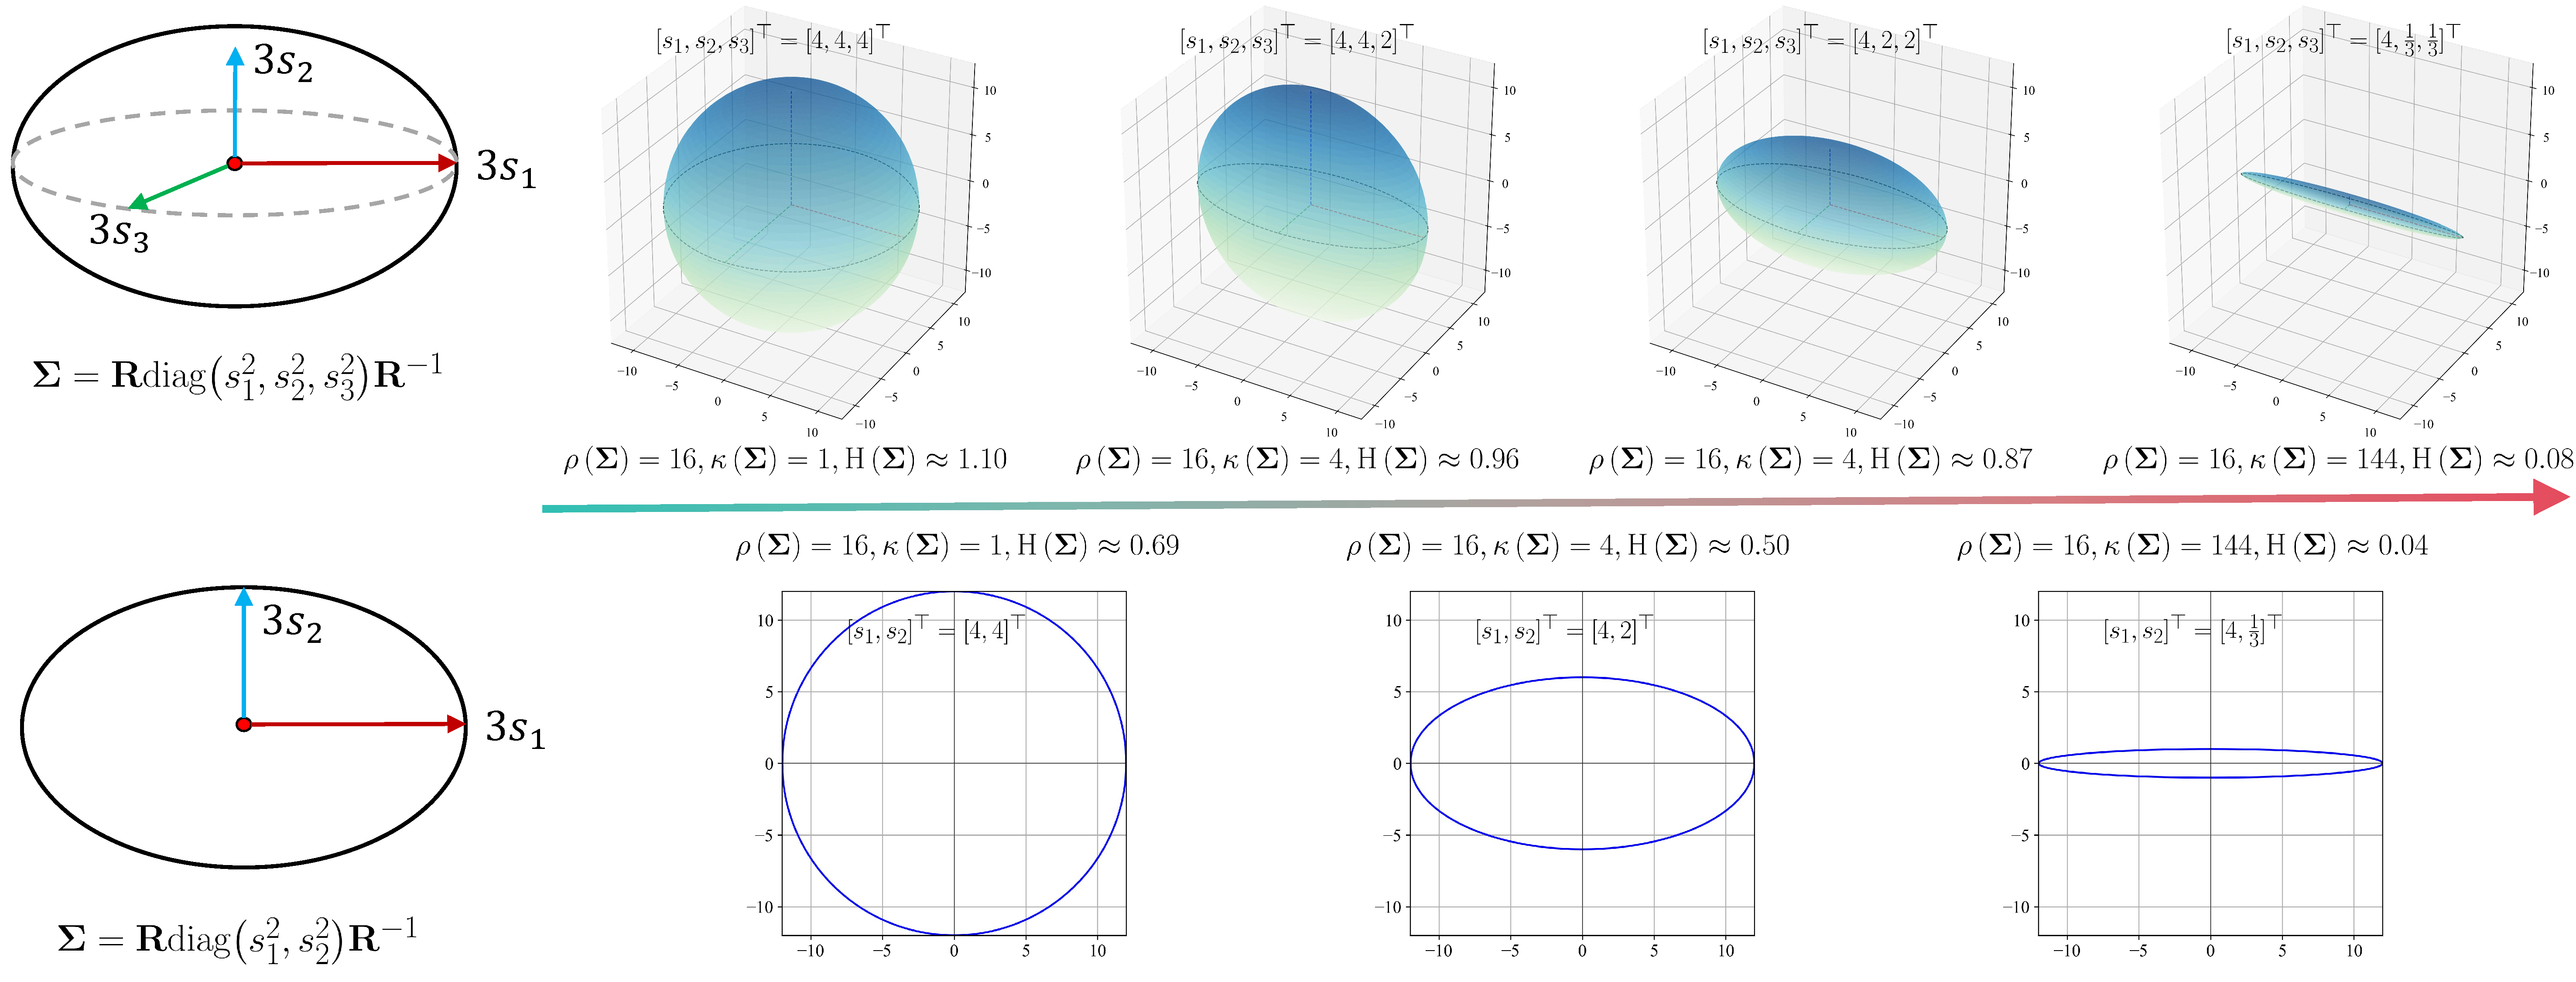
\includegraphics[width=0.85\textwidth]{figures/ch02/2409_12771_spectrum.pdf}
\caption{Huang et al.：3D 高斯基元的频谱分析：从球形高斯（等特征值）到各向异性高斯（特征值差异增大）的连续变化，针状伪影对应极端的各向异性情况。图源：Huang et al.（2024.09）~\cite{2409_12771}。}
\label{fig:02_spectrum}
\end{figure}

\paragraph{GaussianFocus}
前述有效秩和频谱分析均从高斯形状本身入手解决针状伪影，而针状伪影在感知层面的表现——边缘模糊和``空气墙''伪影——则催生了从注意力机制出发的第三条路线。GaussianFocus（2025.03）~\cite{2503_17798}修改了原始 3DGS 的训练损失环节——用注意力加权的边缘/频率约束替代均匀加权的 $L_1$ + SSIM 损失——高斯的几何参数和渲染管线保持不变。

GaussianFocus 的核心思路是：标准 3DGS 的 $L_1$ + D-SSIM 损失对所有像素区域一视同仁，无法针对边缘和高频纹理区域施加更强的优化压力。

\textbf{直觉}：想象一个老师批改作业——如果对每道题都给相同的权重，学生就可能在简单的题上花太多时间而忽略难题。GaussianFocus 引入的注意力机制就像一个``智能权重分配器''，自动找出``难题''（边缘和高频区域）并赋予更高的优化权重。为此，GaussianFocus 引入了基于补丁的注意力机制。具体而言，将渲染图像 $P_i$ 和真实图像 $G_i$ 分别切分为 $8 \times 8$ 的图像块（patch）。对每个图像块，通过 2D 卷积层分别提取查询向量 $q_{ij}$（来自渲染图像块）、键 $k_{ij}$ 和值 $v_{ij}$（来自真实图像块），注意力权重通过缩放点积计算：

\begin{equation}
w_{ij} = \mathrm{softmax}\!\bigl(q_{ij} \cdot k_{ij}^T\bigr), \quad a_{ij} = v_{ij} \cdot w_{ij},
\label{eq:02_gf_attention}
\end{equation}

其中 $a_{ij}$ 是第 $j$ 个图像块的注意力图。将所有图像块的注意力图拼接得到全局注意力图 $A_i = \sum_j a_{ij}$，再与渲染图像逐元素相乘得到注意力增强图像 $P_i' = P_i \odot A_i$。注意力机制的动机在于：真实图像的边缘和高频区域在卷积特征中具有更强的响应，注意力图自动为这些区域分配更高权重，从而在后续损失计算中加大对这些区域的优化力度。

在注意力增强图像的基础上，GaussianFocus 引入了两项互补的损失函数。边缘损失（edge loss）使用 Sobel 算子提取图像在 $x$ 和 $y$ 方向的梯度，然后计算梯度之间的 $L_1$ 距离：

\begin{equation}
\mathcal{L}_{\mathrm{Edge}} = \frac{1}{2}\bigl(\|S_x(p_i) - S_x(\hat{p}_i)\|_1 + \|S_y(p_i) - S_y(\hat{p}_i)\|_1\bigr),
\label{eq:02_gf_edge}
\end{equation}

其中 $S_x, S_y$ 是 Sobel 梯度算子，$p_i$ 和 $\hat{p}_i$ 分别是真实图像和渲染/注意力增强图像的像素值。频率损失（frequency loss）的结构与边缘损失类似，但关注的是像素值沿水平/垂直方向的变化量 $G_x, G_y$：

\begin{equation}
\mathcal{L}_{\mathrm{Frequency}} = \frac{1}{2}\bigl(\|G_x(p_i) - G_x(\hat{p}_i)\|_1 + \|G_y(p_i) - G_y(\hat{p}_i)\|_1\bigr).
\label{eq:02_gf_freq}
\end{equation}

边缘损失和频率损失的区别在于：前者通过 Sobel 算子强调边界定位的精确性，后者通过直接比较像素变化量保留高频纹理的丰富度。两者的配合使得训练同时关注``边缘在哪里''和``纹理有多细''两个层面。完整的损失函数为
\begin{equation}
\mathcal{L}_{\mathrm{Total}} = (1-\lambda_1)\mathcal{L}_1(p_i, \hat{p}_i) + \lambda_1\mathcal{L}_{\mathrm{D\text{-}SSIM}}(p_i, \hat{p}_i) + \lambda_2\mathcal{L}_{\mathrm{Edge}}(p_i, \hat{p}_i) + \lambda_3\mathcal{L}_{\mathrm{Frequency}}(p_i, \hat{p}_i),
\label{eq:02_gf_total}
\end{equation}

其中前 50 次迭代中 $\hat{p}_i$ 取注意力增强图像的像素值（即 $P_i'$ 的像素），此后切换回原始渲染图像 $P_i$ 的像素。这一设计的动机是训练初期高斯基元尚未收敛，注意力增强的梯度信号能更准确地定位需要加强优化的区域；待训练稳定后切换回原始像素以避免注意力机制的偏差累积。

此外，GaussianFocus 还引入了高斯约束策略来减少冗余基元和``空气墙''伪影。该策略包含两个组成部分。第一部分是尺度约束：对缩放矩阵中的每个尺度 $S_i$，当 $S_i > \gamma$ 时施加约束 $S_i = \gamma^{\alpha} \cdot S_i$（实验中 $\gamma = 0.3$, $\alpha = 0.2$），根据初始点云密度自适应调整——密集点云使用更低的初始尺度以减少重叠，稀疏点云使用更高的初始尺度以确保覆盖。第二部分是老化高斯的分裂过滤：对训练中存在时间较长的``老化''高斯，当其尺度 $S_{\mathrm{old}}$ 超过阈值 $\beta = 0.3$ 时选择性分裂并缩减尺度，避免不必要的冗余分裂。

如果说有效秩正则化约束了高斯的整体形状、Spectral-GS 优化了频谱特性，那么 GaussianFocus 则从感知质量的角度补充了对边缘细节的显式关注——不是修改高斯本身的形状或滤波，而是通过注意力加权和显式梯度约束来引导优化过程更加关注视觉上重要的区域。

\subsubsection{拓扑结构完整性}

针状伪影和边界模糊都源于高斯形状的局部退化，而另一类几何退化则与全局拓扑结构有关——即使单个高斯形状良好，整体的拓扑覆盖仍可能存在缺陷。标准 3DGS 从稀疏 SfM 点云初始化，低曲率区域（如白墙、平滑地面）的特征匹配稀少，导致点云覆盖不完整；而自适应密度控制（ADC）在高稀疏区域会引起大幅高斯位移，其他点云增强方法（如致密化、分裂）同样存在破坏拓扑结构的风险。

\paragraph{Topology-GS}
Topology-GS（2024.12）~\cite{2412_16619}修改了原始 3DGS 的初始化和训练监督环节——用拓扑感知插值替代直接点云初始化、用拓扑正则化损失补充标准 $L_1$ + SSIM 损失——高斯的渲染管线和密度控制保持不变。

\textbf{术语铺垫}：持久同调（Persistent Homology）是拓扑数据分析的核心工具。直觉上，它可以检测点云中的``洞''和``连通分量''——把点云想象成不断膨胀的气球，膨胀过程中某些洞被填满、某些新的连通分量合并，``持久''指的是那些在整个膨胀过程中存活最久的拓扑特征，它们对应场景中最重要的结构（如墙面的连续性、物体的连通性）。Topology-GS 首次将这一工具引入 3DGS 优化，从全局拓扑而非局部形状的角度解决覆盖不完整问题。该方法包含两个核心组件：局部持久 Voronoi 插值（LPVI）解决初始化稀疏问题，拓扑正则化损失（PersLoss）在训练中约束渲染结果的拓扑特征完整性。

\paragraph{局部持久 Voronoi 插值（LPVI）。}LPVI 的设计动机是：在低曲率区域直接进行 3D 插值容易引入拓扑噪声（如在平面表面附近生成孤立点簇），但在局部切平面上做 2D 插值则安全得多——因为流形学习假设高维数据位于低维流形上，而非孤立点的切空间近似为切平面。LPVI 的核心机制是在 3D 和 2D Voronoi 插值之间自适应切换，切换依据是插值前后的拓扑变化程度。

\textbf{直觉}：就像在一张稀疏的点阵图上填空——如果填完后``洞''的数量和位置没有明显变化，说明填空是安全的；如果突然出现了不该有的``洞''，就说明填法有问题，需要换一种更保守的方式。具体地，对稀疏点云 $X = \{x_1, \ldots, x_m\} \subset \mathbb{R}^3$ 中的每个点 $x_l$，LPVI 首先找到其 $K$ 近邻，执行 3D Voronoi 剖分得到候选插值点集 $\{v_1, \ldots, v_p\}$。然后计算拓扑变化评估函数：

\begin{equation}
\mathrm{TopoDiff}(X_l, \tilde{X}_l) = W_{\mathrm{Dist}}\!\bigl(\mathrm{PD}(X_l),\;\mathrm{PD}(\tilde{X}_l)\bigr),
\label{eq:02_topodiff}
\end{equation}

其中 $X_l = \{x_l, x_{\iota_1}, \ldots, x_{\iota_K}\}$ 是以 $x_l$ 为中心的近邻集，$\tilde{X}_l = X_l \cup \{v_1, \ldots, v_p\}$ 是加入插值点后的扩展集，$W_{\mathrm{Dist}}$ 是持久图（Persistence Diagram）之间的 Wasserstein 距离。若拓扑变化低于阈值 $\tau$（即 $\mathrm{TopoDiff} < \tau$），说明 3D 插值未破坏局部拓扑结构，直接接受所有候选点；若超过阈值，则切换至 2D 模式——对 $K'$ 个近邻做 PCA 降维至切平面，在该平面上执行 2D Voronoi 剖分，再将顶点通过主成分向量 $U = [u_1, u_2]$ 映射回 3D 空间。这一降维策略利用了平面表面数据的内在低维结构，既避免了拓扑破坏，又在低曲率区域实现了有效的点覆盖增强。

\paragraph{拓扑正则化损失（PersLoss）。}LPVI 解决了初始化稀疏问题，但训练过程中仍缺乏对拓扑特征的约束——标准 3DGS 的 $L_1$ + SSIM 损失仅约束像素级颜色相似性，无法保证特征级的结构完整性（如局部纹理模式和全局语义关系），导致高 LPIPS 值。PersLoss 的设计思路是：将渲染图像和真实图像从 2D 像素空间重新解读为 3D RGB 空间中的点云（$y' = S(y), \hat{y}' = S(\hat{y})$，其中 $S$ 将 $H \times W \times 3$ 图像重塑为 $HW \times 3$ 矩阵），然后在该空间中计算持久同调。具体地，使用 alpha 复形对两个 RGB 点云进行过滤，得到各维同调的持久条形码（Persistent Barcode），其中每条 bar 的长度 $(b^k, d^k)$ 表示一个拓扑特征的生存范围——越长的 bar 对应越重要的拓扑特征。为过滤噪声，只保留每个维度的前 $k_i$ 个最长条（$i = 0, 1, 2$ 分别对应 0 维、1 维、2 维同调），得到截断持久条形码 $pb$ 和 $\hat{pb}$。PersLoss 定义为两者之间出生-死亡值的总差异：

\begin{equation}
\mathcal{L}_{\mathrm{Pers}} = \sum_{i=0}^{2}\;\frac{1}{\beta^i \sum_{k=0}^{2} k^k}\;\sum_{j=1}^{k_i}\Bigl(\bigl|b^i_j - \hat{b}^i_j\bigr|^2 + \bigl|d^i_j - \hat{d}^i_j\bigr|^2\Bigr),
\label{eq:02_persloss}
\end{equation}

其中 $\beta^i$ 是第 $i$ 维 Betti 数，归一化项 $\sum_{k=0}^{2} k^k$ 用于平衡各维度的贡献。最终拓扑感知总损失为 $\mathcal{L}_{\mathrm{total}} = \mathcal{L}_{\mathrm{supv}} + \lambda_{\mathrm{topo}} \mathcal{L}_{\mathrm{Pers}}$，其中 $\mathcal{L}_{\mathrm{supv}}$ 是标准的 $L_1$ + SSIM 监督损失。Topology-GS 理论证明了在温和正则性假设下，该拓扑感知损失在有限迭代次数内收敛（步长选取 $O(1/\epsilon)$），确保了与 ADC 机制配合的实用性。

Topology-GS 与前述形状正则化方法形成互补：形状正则化确保每个高斯基元的局部质量，拓扑分析则确保基元群体的全局覆盖完整性——前者约束“每个高斯是否形状正确”，后者约束“高斯集合是否完整覆盖了场景的拓扑结构”。

\subsection{浮游体与虚假透明度}

前述边界与几何退化伪影源于高斯形状的局部缺陷，而浮游体和虚假透明度则源于 $\alpha$-混合 优化本身的欠约束性。即使高斯形状正确，不透明度优化仍可能收敛到错误的局部极小值。

\subsubsection{浮游体伪影的成因与消除}

浮游体（floater）是 3DGS 重建中最顽固的伪影之一，表现为脱离实际几何的半透明高斯簇。StableGS（2025.03）~\cite{2503_18458}修改了原始 3DGS 的不透明度参数化环节——用双不透明度架构替代单一不透明度——高斯的颜色、位置、协方差参数保持不变。StableGS 首次揭示了浮游体的根本成因，并提出双不透明度架构系统性地解决这一问题。

\paragraph{伪均衡与梯度消失。}\textbf{直觉}：浮游体的颜色误差就像一群人投票——有的投正票、有的投负票，恰好互相抵消，看起来``总分为零''，但实际上每个人的票都是错的。StableGS 考虑一个简化场景：聚焦于一个浮游体簇，有 $M$ 条光线穿过它，对应的真实颜色为 $\{c_m^{gt}\}_{m=1}^M$。假设场景其余部分已被完美重建（穿过簇后的背景色等于真实颜色），则理论最优解是所有浮游体不透明度 $\alpha_k = 0$。然而优化经常陷入非全局极小值：浮游体簇的累积颜色 $c_f = \sum_{k=1}^{K_f} c_k \alpha_k(x_k^{r_m}) \bar{T}_k$ 达到``伪均衡''状态——跨视角颜色误差的符号几乎相互抵消：

\begin{equation}
\sum_{m=1}^{M}\bigl(c_f - c_m^{gt}\bigr) \approx 0.
\label{eq:02_pseudo_equilibrium}
\end{equation}

对于 $L_1$ 损失，这一条件直接导致 $c_f$ 的梯度趋近于零，由链式法则引起不透明度 $\alpha_k$ 和颜色 $c_k$ 参数梯度的级联消失。实验验证了这一现象在 $L_1$、MSE 甚至交叉熵损失下普遍存在——梯度消失使优化器无法有效降低浮游体不透明度，模型被困在几何错误但光度损失极低的局部极小值。然而，浮游体在几何维度（深度）上的误差是显著且无歧义的，这启发了引入基于深度的损失来提供独立、更强的几何监督信号。

\paragraph{双不透明度架构：几何与外观的防火墙。}直接在标准 3DGS 上引入深度损失虽可消除浮游体，但会损害渲染细节——深度损失的强梯度来自不可避免地含噪声和不准确的外部先验，会污染所有高斯参数，导致纹理模糊；对半透明物体（如玻璃、水面）则更严重地破坏渲染精度。为此，StableGS 为每个高斯 $G_k$ 引入额外的可学习辅助不透明度参数 $\alpha'_k \in [0,1]$，定义两种不透明度函数：

\begin{equation}
\underbrace{\alpha_k(x)}_{\text{几何不透明度}} = \alpha_k \exp\!\bigl(-\tfrac{1}{2}(x-\mu_k)^T\Sigma_k^{-1}(x-\mu_k)\bigr), \qquad
\underbrace{\alpha'_k(x)}_{\text{渲染不透明度}} = \alpha'_k \cdot \alpha_k(x).
\label{eq:02_dual_opacity}
\end{equation}

几何不透明度仅依赖原始参数 $\alpha_k$，渲染不透明度则由两个参数联合决定。对应两条功能解耦的渲染路径：
\begin{itemize}
    \item \textbf{几何正则化路径}：用几何不透明度 $\alpha_k(x)$ 渲染中间颜色图 $C^s$ 和深度图 $D^s$，输出专用于深度损失监督——强几何约束的梯度直接作用于基础参数 $\alpha_k$，有效消除浮游体，但细节损失被隔离在此路径内；
    \item \textbf{外观精炼路径}：用渲染不透明度 $\alpha'_k(x)$ 渲染最终颜色图 $C^o$ 和深度图 $D^o$——凭借可学习的 $\alpha'_k$，此路径屏蔽了几何路径中的粗糙梯度，在稳定的几何支架之上专注于学习精细颜色和半透明效果。
\end{itemize}
这一解耦设计是深度损失真正有效的关键：可以在几何路径上放心施加强约束，而外观路径保持自由表达能力。

\paragraph{双路径损失函数。}总损失由颜色损失和几何损失组成：$\mathcal{L}_{\mathrm{total}} = \mathcal{L}_{\mathrm{color}} + \lambda_g \mathcal{L}_{\mathrm{geometry}}$。颜色损失监督两条路径：

\begin{equation}
\mathcal{L}_{\mathrm{color}} = \mathcal{L}_{\mathrm{3DGS}}(C^o, C^{gt}) + \lambda_s \mathcal{L}_1(C^s, C^{gt}),
\label{eq:02_stable_color}
\end{equation}

其中第一项对最终渲染输出施加标准 $L_1$ + D-SSIM 损失，第二项以 $\lambda_s$ 加权鼓励几何路径尽可能解释场景的不透明部分。因此辅助参数 $\alpha'_k$ 的梯度主要来自几何路径无法完美建模的区域（如半透明表面和精细结构），实现了几何与外观的自动分工。几何损失 $\mathcal{L}_{\mathrm{geometry}}$ 包含两项互补的正则化：自监督深度一致性损失利用场景固有的多视角一致性纠正几何错误，基于单目深度估计的外部几何先验则专门处理弱纹理区域。

\paragraph{自监督深度一致性损失。}核心思想是：从视角 $i$ 渲染的深度图 $D_i^s$ 经可微分变换投影到视角 $j$ 后，应与直接从视角 $j$ 渲染的深度图 $D_j^s$ 一致。浮游体的深度值通常是自身深度与背景深度的平均值，经变换后产生大的不一致性，提供强梯度信号。对选定的图像对集合 $\mathcal{P}$：

\begin{equation}
\mathcal{L}_{\mathrm{consis}} = \sum_{(i,j) \in \mathcal{P}} \bigl(\|W_{i \to j}(D_i^s) - D_j^s\|_1 + \|W_{j \to i}(D_j^s) - D_i^s\|_1\bigr),
\label{eq:02_depth_consis}
\end{equation}

其中 $W_{i \to j}$ 是利用已知相机姿态的可微分变换算子。为保证损失稳定性，训练对的选取需满足三个条件：两视角共可见特征点 $>30$（确保足够重叠）、相对旋转角 $16^\circ\text{--}60^\circ$（防止极端基线）、符合单应性矩阵的特征点比例 $< 0.8$（抑制纯旋转退化）。

\paragraph{外部几何先验与全局尺度优化。}弱纹理区域（白墙、平滑地面）缺乏视觉特征，自监督约束不足以提供有效几何信号。StableGS 引入单目深度估计模型 DUSt3R 的先验：对图像对 $(i,j)$，DUSt3R 输出各自相机坐标系下的 3D 点图及置信度图。关键瓶颈在于每对预测存在于独立的未知尺度下，无法直接用于全局 3D 重建。StableGS 提出高效全局尺度优化算法，将原本高维的点云对齐问题通过矩阵分解等价变换压缩为仅 7 个``等价点''上的低维优化，高效求解所有图像对的全局一致尺度因子 $S = \{s_{i,j}, s_{j,i}\}_{(i,j) \in \mathcal{P}}$。最终几何先验损失为
\begin{equation}
\mathcal{L}_{\mathrm{prior}} = \sum_{(i,j) \in \mathcal{P}} \bigl(D(i,j) + D(j,i)\bigr), \quad D(i,j) = \frac{1}{\|d_{i,j}\|_0} \sum C^{1,1}_{i,j} \bigl|D_i^s - d_{i,j}\bigr|,
\label{eq:02_geom_prior}
\end{equation}

其中 $d_{i,j} = s_{i,j} X^{1,1}_{i,j}[z]$ 是尺度校正后的深度图，$C^{1,1}_{i,j}$ 是置信度图。总几何损失为 $\mathcal{L}_{\mathrm{geometry}} = \lambda_c \mathcal{L}_{\mathrm{consis}} + \lambda_p \mathcal{L}_{\mathrm{prior}}$。StableGS 的完整框架在多个基准上实现了 SOTA 几何精度和视觉质量。

StableGS 从优化动力学的视角解释了浮游体为何在标准训练中无法被消除——不透明度梯度因伪均衡而消失。EFA-GS（2025.08）~\cite{2508_02493}则从频域角度提供了互补的分析：与 StableGS 在不透明度参数化上做文章不同，EFA-GS 修改了密度控制环节——用基于累积梯度的选择性扩展替代标准 ADC 的统一分裂——高斯的其他参数保持不变。EFA-GS 关注的是浮游体在训练早期如何产生。

\paragraph{频域视角：欠优化高斯的产生机制。}EFA-GS 的分析起点是采样定理在高斯泼洒中的对应：每个高斯的尺度决定其能接收的频率信息，坐标决定其对应的采样率。当高斯尺度大于 Nyquist 采样间隔时，该高斯可以从训练视角获得充分优化（过优化高斯）；反之，尺度小于采样间隔的高斯则处于欠优化状态——它们接收的光线更少、投影到更少的像素上，梯度天然偏小。EFA-GS 发现，低质量初始化（如 SfM 点云稀疏或含噪）会迫使高斯在训练早期急剧收缩——尺度在仅约 5000 次迭代内就快速坍缩——噪声进一步放大这一效应，使大量高斯在尚未学到准确低频信息之前就已缩至 Nyquist 间隔以下，成为欠优化高斯。这些欠优化高斯虽然对训练视角的渲染影响有限（过优化高斯可以通过训练修正其误差），但对测试视角却造成严重退化——因为测试视角从未参与训练，欠优化高斯无法被修正，最终表现为脱离几何的浮游伪影。

\paragraph{Mip-splatting 的低通滤波为何失效。}直觉上，低通滤波应能帮助小高斯优先学习低频信息。Mip-splatting 确实采用了低通滤波策略，但 EFA-GS 指出其两个根本局限：（1）高斯尺度的坍缩速度极快且非平稳，静态低通滤波器无法跟上这种动态变化；（2）过优化高斯和欠优化高斯应被区别对待，但 Mip-splatting 对同一深度的所有高斯施加相同的低通滤波——既未选择目标高斯，也未动态调整滤波强度。

\paragraph{LFCF 算法：基于累积梯度的选择性扩展。}基于上述分析，EFA-GS 提出 Low-Frequency-Come-First（LFCF）算法。核心思路是：较小的高斯接收更少光线，梯度天然偏小，因此梯度反常上升是异常信号。LFCF 为每个高斯维护累积梯度 $PGrad(i)$，在第 $t$ 次迭代时将其与当前梯度 $Grad(i)$ 比较：
\begin{itemize}
    \item 若 $Grad(i) > PGrad(i)$：该高斯可能是正在恶化为浮游伪影的欠优化高斯，执行扩展操作 $s_i^* = s_i \cdot c$（$c > 1$），强制其先学习低频信息再逐步优化高频细节；
    \item 若 $Grad(i) < PGrad(i)$：该高斯可能是过优化高斯，执行收缩并分裂 $s_i^* = s_i \cdot c$（$c < 1$），促进细节表达；
    \item 更新累积梯度 $PGrad(i) \leftarrow Grad(i)$。
\end{itemize}
扩展和收缩操作的统一形式为 $s^* = s \cdot c^3$，其中 $c > 1$ 对应扩展、$c < 1$ 对应收缩。

\paragraph{自适应扩展范围：深度策略与尺度策略。}然而，对所有高斯施加统一的扩展因子 $c$ 会在复杂场景中侵蚀远处细节——深度越大的高斯采样率越低、越难优化，统一扩展会过度放大其尺度。为此，EFA-GS 设计了两个互补策略：

\textbf{深度策略}：采样率越低（深度越大）的高斯，赋予越小的扩展因子。具体地，先按 Mip-splatting 的方式计算每个高斯的采样率，再将其投影到 $[0,1]$ 作为线性插值因子 $\lambda(i)$，最终扩展因子为 $c(i) = \lambda(i) \cdot c_{max} + (1 - \lambda(i)) \cdot c_{min}$，其中 $c_{min}$ 通常设为 1（即不扩展采样率最低的高斯），$c_{max}$ 设为 1.5。

\textbf{尺度策略}：高斯沿不同轴的缩放因子对应不同的采样间隔，应区别对待。为保持高斯体积不变，EFA-GS 设定约束 $\prod_i c_i = 1$，在此约束下扩展最短轴、收缩最长轴——使扩展操作不改变总体积，而是调整形状以匹配各方向的采样需求。

在自建 RWLQ 数据集上，EFA-GS 相比基线 Mip-splatting 的 PSNR 提升 1.68 dB，同时在高质量数据集 Mip-NeRF 360 上也能保持甚至略微提升性能，表明深度/尺度策略有效平衡了去伪影与保细节的矛盾。

在 StableGS 和 EFA-GS 分别从优化动力学和频域角度解决浮游体之后，后续工作将 3DGS 优化本身重新框架化。Denoising-GS（2026.05）~\cite{2605_14880}不沿用浮游体的成因分析框架，而是将整个 3DGS 优化重新定义为高斯基元去噪过程——含噪初始点云中的离群高斯即为``噪声''，通过空间感知去噪框架从含噪初始点云中恢复高质量重建。3DGS-HPC（2026.03）~\cite{2603_07587}则将浮游体问题与瞬态干扰关联起来，提出混合 Patch 级分类策略用于无干扰物的 3DGS 重建，有效区分静态场景和瞬态干扰物——这一思路将在本节后续的瞬态物体部分进一步展开。

\subsubsection{虚假透明度}

\paragraph{NGS}
浮游体是脱离几何的游离高斯，而虚假透明度则表现为本应不透明的表面被错误地重建为半透明——两者同属 $\alpha$-混合 欠约束问题，但表现不同。NGS（2025.10）~\cite{2510_15736}修改了原始 3DGS 的训练初始化环节——用内部噪声注入替代直接训练——高斯的渲染管线保持不变。NGS 首次系统识别了 3DGS 中的虚假透明度问题：不透明物体表面被错误地重建为半透明，在交互式观察中背景和内部模式随相机运动而不一致地变化。

\paragraph{透明度歧异的数学根源。}\textbf{直觉}：想象一扇半透明的玻璃窗——透过它可以看到后面的墙。问题在于，``玻璃半透明 + 墙壁清晰''和``玻璃不透明 + 墙壁不可见''在像素颜色上可以给出完全相同的结果，优化器无法区分这两种情况，因此会``偷懒''选择更容易的半透明解。NGS 的分析直接回到 $\alpha$-混合 公式。对于像素 $p$，标准 3DGS 的渲染结果为 $C(p) = \sum_i \alpha_i c_i \prod_{j<i}(1-\alpha_j)$，训练目标为复合 $L_1$ + SSIM 光度损失 $L_{photo}$。问题出在分解方式：令 $s$ 为沿光线遇到的第一个表面高斯的索引，$B$ 为其后方所有高斯的集合，则渲染颜色可分解为
\begin{equation*}
C(p) = \underbrace{\alpha_s c_s}_{\text{前表面}} + (1-\alpha_s) \underbrace{\sum_{i \in B} \alpha_i c_i \prod_{s<j<i}(1-\alpha_j)}_{\text{背景（当 $\alpha_s < 1$ 时泄漏）}}
\end{equation*}

对于任意半透明表面（$\alpha_s < 1$），总存在一组背景不透明度和颜色能复现完全相同的像素颜色——即与完全不透明表面给出相同的光度损失。梯度下降因此可以接受 $\alpha_s$ 偏低的平凡最小值。这一问题在 360 度物体扫描中尤为严重：前后表面沿同一光线配对，深度间距小，两者被联合优化，虚假透明度更易发生。

\paragraph{NGS 的解决方案：内部噪声注入。}在解决方案层面，NGS 与前述 StableGS 的策略形成鲜明对比：StableGS 通过双不透明度架构分离几何与外观路径，本质上是在渲染管线中增加一条辅助路径；NGS 则不需要修改渲染管线，而是通过在物体体积内部注入不透明噪声高斯来填充表面后方空间，从物理上阻断前后表面之间的视线通道，迫使表面高斯提高不透明度。其流程分为四个阶段：

\textbf{初始化}：从现有高斯的均值计算凸包网格（Quickhull），将凸包体素化为粗占据网格，在每个占据体素内生成一个随机颜色的噪声高斯点。

\textbf{深度剪枝}：凸包包含物体外部区域，因此需对每个视角的每个像素，利用 3DGS 的深度排序移除出现在表面高斯前方的噪声高斯，再腐蚀占据网格以确保噪声高斯与表面之间保持缓冲距离。

\textbf{多尺度注入}：以从粗到细的方式在多个体素分辨率上重复初始化与剪枝——仅在不包含上一级噪声高斯的体素中生成新噪声——在保持低内存开销的同时覆盖精细几何。

\textbf{微调与引导训练}：冻结表面高斯，仅训练噪声高斯的不透明度并剪枝错误放置的噪声；此后冻结噪声高斯，解冻表面高斯并重置学习率，让表面参数在新优化空间中正常训练。关键设计：每次迭代随机设置噪声高斯的颜色（从六种高对比度原色/次级色中选取），防止噪声不透明度过拟合到表面颜色——确保优化仅基于遮挡效果而非颜色匹配。

\paragraph{透射率评估指标 SOS。}标准质量指标（PSNR、SSIM、LPIPS）基于静态图像对比较，无法量化视角不一致性——虚假透明度下的渲染仍可报告高分。NGS 利用噪声高斯点云设计了诊断工具：将噪声高斯和表面高斯分别着为纯色（如绿色和红色），用标准光栅化器渲染后，噪声颜色通道即为表面透射率图 $T_i$。定义透射率评分：

\begin{equation*}
SOS_i = \left(\frac{\sum T_i / |M_i| + \epsilon}{\log(10)}\right)
\end{equation*}

其中 $M_i$ 为前景分割掩码，$\epsilon = 10^{-10}$ 保证数值稳定性。$SOS_i = 1$ 表示完全不透明表面，$SOS_i \approx 0$ 表示完全透明表面。这一指标无需交互式观察即可在静态渲染中量化虚假透明度。NGS 还发布了噪声注入插件数据集（包括 DTU 的注入版本和高分辨率物体扫描数据集），为这一此前被忽视的伪影类型建立了评估基准。

\subsection{瞬态物体与动态干扰}

前述浮游体和虚假透明度源自 3DGS 内部的优化缺陷，而另一类伪影则由外部因素引起——真实世界场景中普遍存在的瞬态物体（行人、车辆、阴影变化等）破坏了 3DGS 所需的多视角一致性假设。忽略这些干扰物会导致模糊效果和浮游体伪影。

\subsubsection{瞬态干扰处理方法}

T-3DGS（2024.12）~\cite{2412_00155}修改了原始 3DGS 的训练数据选取环节——用无监督瞬态掩码替代全像素训练——高斯的渲染管线和参数化保持不变。T-3DGS 提出无监督瞬态检测与双向追踪框架，为瞬态物体处理建立了重要基线。相对于标准 3DGS 对所有像素不加区分地进行训练，T-3DGS 的核心创新在于其重建不确定性预测器（RUP）利用 3DGS 重建过程本身的训练动态来识别瞬态区域——通过散度度量区分静态和动态元素，完全无需显式监督。瞬态掩码细化器利用 SAM2 进行双向时空掩码传播，增强检测的边界精度和时序一致性。该方法还能处理半瞬态物体（同一物体在视频中有静态和动态两种状态），在稀疏和密集视频数据集上显著优于 WildGaussians、SpotlessSplats 等方法。

\paragraph{RobustSplat}
T-3DGS 聚焦于检测已存在的瞬态伪影——即在训练完成后识别并隔离瞬态区域，但此时瞬态物体可能已经对静态场景的重建造成了不可逆的干扰。RobustSplat（2025.06）~\cite{2506_02751}则从预防角度出发，发现了瞬态物体渗入重建的更早入口：高斯致密化过程（分裂/克隆操作）在早期优化阶段就会无意中拟合瞬态物体，因为梯度累积超过阈值时无论静态还是动态区域都会触发致密化。与 T-3DGS 的无监督检测不同，RobustSplat 提出延迟高斯增长策略，优先优化静态场景结构后再允许致密化，同时设计尺度级联掩码引导方法：先利用低分辨率特征相似性（语义一致性更强）获取可靠初始掩码，再逐步过渡到高分辨率实现精确掩码预测。简言之，T-3DGS 是``先训练再检测''，RobustSplat 是``先过滤再训练''——两者分别覆盖了瞬态物体处理的事后和事前两个阶段。

\subsection{渲染一致性与感知增强}

前面的讨论聚焦于特定类型伪影的消除，本节转向更一般的渲染一致性问题——即使没有明显的伪影，训练视角的有限性、遮挡关系和光学畸变也会导致新视角渲染质量下降。

\subsubsection{视角一致性}

\paragraph{PEP-GS}
训练视角的有限性导致新视角渲染质量显著下降。PEP-GS（2024.11）~\cite{2411_05731}针对标准球谐函数（SH）在复杂光照下难以捕获各向异性颜色分量的问题，提出用层次粒度结构注意力机制替代传统 SH 颜色表示，通过多粒度注意力捕获局部几何特征和复杂视角相关颜色变化。同时引入 Kolmogorov-Arnold 网络进行不透明度和协方差估计，以及归一化拉普拉斯金字塔距离（LapL1）感知损失增强跨视图感知一致性。

\paragraph{极端视角过滤与物理约束增强}
PEP-GS 通过增强颜色表示提升一般视角的渲染质量，而极端视角下的渲染退化则需要更激进的策略。Extremely Views（2025.10）~\cite{2510_20027}不走表示增强路线，而是提出实时渲染感知过滤方法，在旋转对齐坐标系中评估各向异性高斯的不稳定性，通过基于中间梯度的敏感度评分和两遍过滤策略直接移除不稳定基元。与 Extremely Views 直接移除不稳定基元的``做减法''策略不同，Depth-Consistent 3DGS（2025.11）~\cite{2511_10316}从物理约束角度``做加法''增强一致性，结合景深监督（散焦卷积和景深损失）与多视角一致性监督（LoFTR 特征匹配和最小二乘优化），从物理散焦建模和几何约束两个角度增强渲染一致性。三者形成递进：PEP-GS 改进颜色表示以应对一般视角退化，Extremely Views 过滤不稳定基元以应对极端视角，Depth-Consistent 3DGS 引入物理约束从根源上增强多视角一致性。

\subsubsection{可渲染性与感知修复}

视角一致性问题在均匀观测条件下尚可控制，但非均匀观测（训练视角分布不均）和严重遮挡场景下的渲染不一致更具挑战。

\paragraph{RF-GS}
RF-GS（2025.04）~\cite{2504_19261}针对非均匀观测场景的渲染不稳定问题，提出可渲染场（renderability field）量化输入不均匀性，引导伪视图采样增强视角覆盖，并训练图像恢复模型将点投影图映射为可见光风格图像。

\paragraph{Proxy-GS}
RF-GS 通过补充虚拟视角缓解覆盖不足，但非均匀观测的另一个后果——遮挡区域的不一致性——需要不同的策略。Proxy-GS（2025.09）~\cite{2509_24421}正是从遮挡感知角度切入同一问题。与 RF-GS 生成新视角不同，Proxy-GS 利用轻量代理网格实现遮挡感知，能在 $1000 \times 1000$ 分辨率下 1ms 内生成精确遮挡深度图。代理系统同时引导锚点和高斯的剔除以加速渲染，以及训练中的致密化趋向表面避免遮挡区域的不一致性，在 MatrixCity Streets 等重遮挡场景上实现 2.5 倍以上加速。

\paragraph{ArtiFixer：后处理修复}
前述方法均在优化阶段解决一致性问题，但即使经过精心优化，渲染结果中仍可能残留伪影和缺失区域。ArtiFixer（2026.03）~\cite{2603_00492}将修复时机推至后处理阶段，利用双向自回归扩散模型增强和扩展 3D 重建，通过生成模型修复渲染伪影和缺失区域，实现从部分观测到完整场景的扩展重建。ArtiFixer 与 RF-GS 和 Proxy-GS 形成互补：RF-GS 在训练阶段补充视角覆盖，Proxy-GS 在优化阶段处理遮挡，ArtiFixer 在后处理阶段修复残余缺陷——三者覆盖了渲染一致性保障的完整流程。

\subsubsection{光学像差场景}

\paragraph{DGS}
前述一致性问题均假设成像系统本身是标准的，但 XR 设备和野外机器人常采用保护盖覆盖前向摄像头，盖体表面不规则性导致光学像差（模糊和非参数畸变），使标准 3DGS 无法正常工作。SynthCover（2024.11）~\cite{2411_06365}针对这一特殊场景，提出折射场（Refractive Field）估计保护盖几何，通过精确的解析计算折射光线实现透过保护盖的新视角合成，并与场景表示联合优化以捕捉非对称的表面不规则性。

\begin{takeaway}
3DGS 的系统性伪影（针状伪影、浮游体、虚假透明度）各有不同成因——从高斯连续性本质到 ADC 的形状退化。解决方案涵盖正则化、瞬态物体处理、感知增强和后处理修复，RF-GS、Proxy-GS 和 ArtiFixer 三者覆盖了从训练到后处理的渲染一致性保障完整流程。
\end{takeaway}

%% ============================================================
\section{多模态与跨域渲染}
\label{sec:02_10}

3D Gaussian Splatting 的标准渲染管线本质上是为 RGB 图像驱动的场景表示设计的——高斯基元的颜色由球谐函数（SH）参数化，训练损失基于渲染图像与输入 RGB 图像的光度差异。这一设计假设输入数据为常规视角下捕获的标准彩色图像，然而现实世界的感知模态远不止于此。深度传感器提供几何信息、热红外相机捕获温度分布、事件相机输出异步亮度变化、脉冲相机产生高时间分辨率二值流、LiDAR（Light Detection and Ranging，激光雷达）生成精确三维点云、射频信号携带电磁波传播信息。这些非 RGB 模态的物理特性与标准光学成像存在根本差异，无法直接嵌入 3DGS 的训练框架。各方法如何扩展 3DGS 的表示和渲染机制以适配不同模态的物理约束，是本节的核心议题。表~\ref{tab:02_modalities} 汇总了本节涉及的七种非 RGB 模态及其核心挑战。

\begin{table}[htbp]
\centering
\small
\caption{多模态 3DGS 渲染应用汇总}
\label{tab:02_modalities}
{\hbadness=10000
\begin{tabular}{l l p{5.8cm}@{\hspace{0.5em}}}
\toprule
\textbf{模态} & \textbf{核心挑战} & \textbf{代表方法} \\
\midrule
事件相机 & 异步稀疏事件流，无纹理监督 & Ev-GS~\cite{2407_11343}, Elite-EvGS~\cite{2409_13392} \\
脉冲相机 & 40KHz 二值脉冲，时序积分 & SpikeGS~\cite{2407_03771} \\
水下 & 散射+吸收，介质建模 & WaterSplatting~\cite{2408_08206}, SeaSplat~\cite{2409_17345} \\
LiDAR & 精确 3D 点云，细节缺失 & LiDAR-3DGS~\cite{2409_16296} \\
热红外 & 温度分布，视角依赖 & Veta-GS~\cite{2505_19138}, TDg~\cite{2605_30328} \\
音频 & 衍射+散射，模态密度差异 & AV-GS~\cite{2406_08920} \\
射频 & 电磁波传播，跨域物理 & RF-3DGS~\cite{2411_19420}, WRF-GS~\cite{2412_04832} \\
\bottomrule
\end{tabular}
}
\end{table}

\subsection{神经形态视觉：事件相机与脉冲相机}

本节介绍两类神经形态传感器在 3DGS 中的应用：事件相机（事件信号替代 RGB 监督、Ev-GS 等）和脉冲相机（脉冲-渲染关联）。

\subsubsection{事件相机}

事件相机以微秒级时间分辨率异步捕获像素级亮度变化，输出稀疏的事件流而非固定帧率的图像。其高动态范围（$>$120 dB）和极低延迟使其在高速运动和低光照场景中具有天然优势，但事件流的稀疏性和缺乏纹理信息给 3DGS 训练带来两个根本性挑战。一是无法直接构建光度损失（事件只记录变化量而非绝对亮度），二是缺乏纹理信息导致 3DGS 的 SfM 初始化流程失效。

\paragraph{事件信号替代 RGB 监督。} Ev-GS（2024.07）~\cite{2407_11343}修改了原始 3DGS 的训练监督环节——用时间窗口内的事件累积信号替代逐像素 RGB 光度损失——高斯基元的几何与渲染表示保持不变。标准 3DGS 的训练损失要求渲染图像与输入 RGB 图像之间的光度差异，但事件相机不输出绝对亮度。Ev-GS 的核心洞见是：事件信号本质上编码了亮度变化的梯度信息。具体而言，在两个时间戳 $t_1, t_2$ 分别用 3DGS 渲染图像 $I(t_1)$ 和 $I(t_2)$，利用亮度差 $\Delta L = \log I(t_2) - \log I(t_1)$ 与对应时间窗口内累积事件帧 $E$ 的理想关系 $E = \Delta L / \Delta$（$\Delta$ 为对比度阈值）构建可微分损失 $L = \|\Delta L / \Delta - E\|^2$。这意味着 Ev-GS 将标准 3DGS 逐像素的光度监督替换为时间窗口内的事件累积监督。该方法不需要任何 RGB 或灰度帧数据，完全在事件域内完成训练。在运动模糊场景中，该方法 PSNR 比基于帧的方法高 2--4 dB，因为事件相机本身不受运动模糊影响，Ev-GS 恰好利用了这一物理优势。

\paragraph{Ev-GS 实现细节。} 上述事件监督框架的设计背后有三个关键工程决策。

\textbf{初始化策略。} 标准 3DGS 使用 COLMAP SfM 流程从多视角图像中恢复初始点云和相机位姿，但事件流是异步稀疏的亮度变化信号，不包含纹理和绝对亮度信息，SfM 无法直接运行。Ev-GS 因此采用随机初始化策略：在场景包围盒内均匀采样 $10^6$ 个点作为初始 3D 高斯集合。这一策略之所以可行，是因为 Ev-GS 的损失函数仅约束渲染结果的\emph{变化量}而非绝对亮度——即使初始点云的位置和颜色完全随机，事件监督信号仍然能够驱动高斯向正确位置收敛。代价是收敛速度慢于 SfM 初始化的方案，后续工作 Elite-EvGS 正是从这一问题切入加以改进。相机位姿则来自外部传感器标定：合成数据直接使用已知渲染轨迹，真实数据通过将物体置于匀速转台、相机保持静止的方式精确控制。

\textbf{时间窗口与对数亮度转换。} Ev-GS 设定最大事件窗口长度 $W = 50$ 帧，每次训练迭代从中随机选取 $w \in [1, W]$ 作为实际窗口。随机选取窗口长度的设计动机是：短窗口对应微小亮度变化，提供精细的局部梯度信息；长窗口对应较大亮度变化，提供全局结构约束。随机采样使模型同时暴露于两种尺度的监督信号。渲染结果从线性空间转换到对数亮度空间的过程为 $L(I_t) = \log((I_t)^g + \epsilon)$，其中 $\epsilon = 10^{-5}$ 防止零值取对数，$g = 4.8$ 是灰度 gamma 校正值（BT.601 标准推荐的平滑近似）。这一 gamma 校正之所以必要，是因为事件相机的对比度阈值 $\Delta$ 定义在传感器原始输出的对数域中，而 3DGS 渲染的灰度值在线性域，gamma 校正弥合了两个域之间的非线性差异。

\textbf{Linlog 映射与损失函数。} 直接在对数域计算 $L_2$ 损失在低亮度区域（接近零的值）会产生数值不稳定。Ev-GS 采用 linlog 映射解决这一问题——linlog 是一种分段函数，在低值区域切换为线性映射以避免对数函数在零附近的梯度爆炸，在高值区域保持对数映射的压缩特性：对值小于阈值 $B$ 的区域使用线性映射 $u \times \ln(B)/B$，对大于 $B$ 的区域使用标准对数 $\ln(u)$，实验中 $B = 20$。这使得低亮度区域的梯度被平滑抑制，避免对数函数在零附近的梯度爆炸。最终损失函数为 $L_\text{total} = L_e + (1 - \lambda) L_\text{SSIM}$，其中 $L_e$ 是经过 linlog 映射后的归一化 $L_2$ 损失，$L_\text{SSIM}$ 是 D-SSIM 损失，$\lambda = 0.1$。D-SSIM 的引入虽然看似多余（没有 RGB 参考图像），但 Ev-GS 发现它可以提供空间结构约束，缓解事件累积帧的空间不一致性，从而提升渲染质量。

Ev-GS 确立了“事件信号替代 RGB 监督”的基本路线，但其局限在于纯事件数据难以完成 3DGS 的初始化——标准 SfM 流程需要纹理丰富的图像帧，而事件流无法直接提供。后续工作因此沿两个方向改进：一是引入外部先验弥补初始化缺陷，二是利用事件相机硬件特性提供额外的训练信号。

Elite-EvGS（2024.09）~\cite{2409_13392}沿用了 Ev-GS 的事件监督损失，但通过引入外部先验解决了初始化难题。与 Ev-GS 完全依赖事件信号不同，Elite-EvGS 从预训练的事件到视频（Event-to-Video, E2V）模型蒸馏先验知识，采用粗到细优化策略：先用 E2V 模型从事件流生成图像帧优化粗 3DGS，再引入事件数据细化细节。其渐进事件监督策略通过窗口切片操作逐步减少用于监督的事件数量——大时间窗口恢复全局结构但纹理粗糙，小窗口保留纹理细节但结构不完整，渐进策略同时优化两者。

\paragraph{SweepEvGS：硬件辅助路线}
与 EventSplat 走初始化增强路线不同，SweepEvGS（2024.12）~\cite{2412_11579}选择硬件辅助路线：利用事件相机在单次扫描中同时捕获静态帧和密集事件流，用静态帧解决初始化问题，用事件流提供高时间分辨率的监督信号。

\paragraph{GS-EVT：事件驱动的位姿追踪}
GS-EVT（2024.09）~\cite{2409_19228}则完全跳出“从事件重建 3DGS”的范式——使用帧式相机构建 3DGS 地图，事件相机仅用于通过比较集成事件图像与 3DGS 渲染的亮度变化实现高精度位姿追踪。其参考姿态加一阶动力学的新位姿参数化方法支持局部差分图像渲染，将事件信号从训练监督信号转变为位姿约束信号。

\paragraph{E-3DGS：传感器硬件层改进}
E-3DGS（2024.10）~\cite{2410_16995}从硬件层面重新设计成像流程，引入透射调节装置使事件相机同时捕获运动事件和曝光事件，支持高质量、快速和混合三种重建模式，是唯一从传感器硬件角度改进事件-3DGS 的工作。

\subsubsection{脉冲相机}

与事件相机仅捕获亮度变化不同，脉冲相机以 40,000 Hz 超高时间分辨率输出二值脉冲流，每个像素独立积分光强并在超过阈值时发射脉冲。脉冲相机保留了完整的纹理信息（事件相机则丢失了绝对亮度），但数据形式与标准图像截然不同——连续的灰度值被量化为二值脉冲序列，需要建立全新的渲染-脉冲关联机制。

\paragraph{脉冲-渲染关联。} SpikeGS（Guo~et~al.（2024.07）~\cite{2407_03771}）修改了原始 3DGS 的训练监督与光栅化环节——用时间累积脉冲流替代单帧 RGB 图像作为监督信号，并将标准光栅化扩展为时间累积光栅化——高斯基元的属性表示保持不变。标准 3DGS 的训练假设输入为连续灰度或 RGB 图像，但脉冲相机输出的是离散二值脉冲序列——每个像素独立积分光强 $A(\mathbf{x}, t) = A_{\mathbf{x}}(t) \bmod \theta$，当累积值超过固定阈值 $\theta$ 时发射一个脉冲（输出 1）并重置累积器。因此单帧脉冲只携带一位二值信息，无法直接用于光度损失。SpikeGS 的核心设计是时间累积光栅化（Time Accumulation Rasterization），将 $N$ 个时刻的脉冲流累积为稳定的灰度纹理——直觉上，就像用长时间曝光将闪烁的星光累积为连续的光带：

\begin{equation}
I_{\mathrm{ac}}(t_1, t_N) = \frac{\theta}{N} \sum_{t_i}^{t_N} S(P_{t_i})
\end{equation}

其中 $S(P_{t_i})$ 是相机位姿 $P_{t_i}$ 处的脉冲输出。该公式的物理含义是：当累积帧数 $N$ 足够大时，$I_{\mathrm{ac}}$ 近似于时间窗口 $[t_1, t_N]$ 内的平均辐亮度，且近似误差不超过 $1/N$。为了让 3DGS 的渲染输出与累积纹理对齐，SpikeGS 将标准光栅化扩展为时间累积光栅化——在连续时间域上积分渲染方程，并用 $n$ 个关键帧（$n < 10$）离散近似：

\begin{equation}
C_{\mathrm{ac}}(t_1, t_N) = \frac{1}{n} \sum_{i=1}^{n} \sum_{j \in \mathcal{N}} c_j(P_i)\,\alpha_j \prod_{k=1}^{j-1}(1-\alpha_k)
\end{equation}

该过程完全可微分，支撑端到端训练。累积损失采用 $\mathcal{L}_{\mathrm{ac}} = (1-\lambda_1)\|C_{\mathrm{ac}} - I_{\mathrm{ac}}\|_2 + \lambda_1\,\mathrm{SSIM}(C_{\mathrm{ac}}, I_{\mathrm{ac}})$ 进行监督。

然而，累积策略在训练早期收敛缓慢——累积纹理需要大量帧才能稳定，而 3DGS 的高斯基元在初始化阶段急需准确的几何约束。为此，SpikeGS 引入脉冲间隔（Spike Interval）作为互补信号。两个相邻脉冲之间的时间间隔 $t_1 - t_2$ 反比于该像素处的光强——直觉上，光照越强的区域脉冲越频繁（间隔越短），因此间隔本身编码了亮度信息，仅需极少量脉冲（通常 $t_1 - t_2 < 10$ 帧）即可恢复几何细节：

\begin{equation}
I_{\mathrm{in}} = \frac{\theta}{t_1 - t_2}
\end{equation}

间隔渲染 $C_{\mathrm{in}}$ 使用对应时刻的中间位姿 $(t_1+t_2)/2$ 进行标准光栅化，并以 $\mathcal{L}_{\mathrm{in}}$ 监督。最终损失为 $\mathcal{L}_{\mathrm{final}} = \lambda_{\mathrm{accu}}\,\mathcal{L}_{\mathrm{ac}} + \lambda_{\mathrm{in}}\,\mathcal{L}_{\mathrm{in}}$，其中 $\lambda_{\mathrm{accu}}$ 从 0 逐渐增大——训练初期脉冲间隔提供快速几何收敛，后期累积纹理补充精细外观。这种“累积-约束”双机制构成了脉冲-3DGS 的基本范式：累积解决二值到灰度的转换问题，间隔利用脉冲的时间精度加速几何收敛。

\paragraph{Zhang et al.：保留脉冲时间精度}
SpikeGS 的累积策略将时间维度的信息压缩为空间表示，Zhang~et~al.（2024.07）~\cite{2407_10062}则选择保留脉冲的时间精度。与 SpikeGS 的时间累积不同，该方法直接建立 3DGS 渲染与脉冲流瞬时成像/曝光式成像之间的计算方程，将渲染的连续场景与每个脉冲时刻的光强直接关联，避免了累积过程中的信息损失。

\paragraph{Yu et al.：噪声感知脉冲渲染}
Yu~et~al.（2024.09）~\cite{2409_15176}关注 SpikeGS 框架在极端条件下的鲁棒性问题，设计可微分脉冲流渲染框架，集成噪声嵌入和脉冲神经元模型，在极噪声低光照场景下保持高鲁棒性——沿用了 SpikeGS 的可微分渲染管线但增加了噪声感知组件。

\paragraph{USP-Gaussian：脉冲重建统一框架}
USP-Gaussian（2024.11）~\cite{2411_10504}将前述工作各自解决的子问题（脉冲重建、位姿估计、3DGS 优化）整合为端到端统一框架，同时完成脉冲图像重建、位姿校正和 3DGS 优化，消除了级联管线的累积误差——这是脉冲-3DGS 从模块化走向统一化的标志。

\subsection{非RGB模态渲染的挑战}

\subsubsection{水下与散射介质场景}

事件和脉冲相机改变了时间分辨率，但成像仍遵循标准几何光学。水下场景则引入了全新的物理复杂性：图像形成涉及直接图像分量和后向散射分量，水体介质的吸收和散射效应导致颜色失真、对比度降低和几何不一致。标准 3DGS 的 $\alpha$-混合 渲染假设光线沿直线传播并在表面发生反射，无法直接建模光线在水体介质中传播时因散射和吸收产生的衰减与偏色。

\paragraph{场景-介质分离建模。} WaterSplatting（2024.08）~\cite{2408_08206}修改了原始 3DGS 的渲染方程环节——用“物体+介质”双密度场的三分量渲染替代标准 $\alpha$-混合——高斯基元本身的属性保持不变。标准 3DGS 用单一高斯场同时编码几何和外观，WaterSplatting 则将其拆分为两个独立系统：3DGS 保留用于显式几何表面表征，独立的体积场捕获散射介质的影响。

\textbf{三分量渲染方程。}WaterSplatting 将连续体渲染方程中的密度场拆分为物体密度 $\sigma^{obj}$ 和介质密度 $\sigma^{med}$，并将介质密度 $\sigma^{med}$ 与颜色 $c^{med}$ 设为 per-ray、per-channel 常量（每条射线查询一次），最终像素颜色分解为三个分量之和：物体颜色分量 $C_i^{obj}(r) = T_i^{obj}\,\alpha_i\,c_i\,\exp(-\sigma^{attn}\,s_i)$（标准 $\alpha$-混合 颜色乘以深度相关的指数衰减）、高斯间介质颜色分量 $C_i^{med}(r) = T_i^{obj}\,c^{med}[\exp(-\sigma^{bs}\,s_{i-1}) - \exp(-\sigma^{bs}\,s_i)]$（相邻高斯之间介质的后向散射贡献）、以及背景介质分量 $C_\infty^{med}(r) = T_N^{obj}\,c^{med}\,\exp(-\sigma^{bs}\,s_N)$（最后一个高斯至无穷远的介质贡献）。这里物体衰减系数 $\sigma^{attn}$ 和介质后向散射系数 $\sigma^{bs}$ 是两组独立的 per-channel 参数，分别控制直接图像的衰减和后向散射的累积。这种“场景+介质”分离的范式使得渲染时可以同时生成水下图像（含介质效应，完整三分量叠加）和清晰图像（去除介质，仅保留物体颜色分量）。

\textbf{训练与损失函数。}WaterSplatting 引入正则化损失函数：对渲染图像和目标图像施加像素级权重 $W_{i,j} = (\text{sg}(\hat{I}_{i,j}) + \epsilon)^{-1}$，提升暗区权重以对齐人眼对 HDR 场景的感知特性，最终损失为 $L_{Reg} = (1-\lambda)\,L_{Reg\text{-}L_2} + \lambda\,L_{Reg\text{-}DSSIM}$。在水下 SeaThru-NeRF 数据集上超越 SOTA NeRF 方法，同时实现实时渲染和场景恢复。

\paragraph{SeaSplat：物理水下模型嵌入 3DGS}
WaterSplatting 将介质建模为独立体积场，需要额外的查询步骤。SeaSplat（2024.09）~\cite{2409_17345}则将物理水下图像形成模型直接嵌入 3DGS 优化——不再分离建模，而是同时学习介质参数和底层 3D 表示。与 WaterSplatting 的“分离”相比，SeaSplat 的“联合优化”更紧凑但增加了训练复杂度。

\paragraph{UW-GS：距离相关颜色衰减建模}
沿联合优化路线，UW-GS（2024.10）~\cite{2410_01517}进一步引入距离相关的颜色外观模型处理水下颜色衰减的深度依赖性，并增加基于物理的密度控制策略和二值运动掩码处理水下动态内容。

\paragraph{Gaussian Splashing：散射分量显式集成}
Gaussian Splashing（2024.11）~\cite{2411_19588}沿用联合优化思路，将水下图像形成模型的散射、衰减和后向散射三个分量显式集成到 3DGS 渲染流程中，使每个分量的物理效应可独立调控。

\paragraph{MarineSTD-GS：基元层退化建模}
MarineSTD-GS（2026.04）~\cite{2604_23551}则从高斯基元设计角度重新审视水下退化问题，使用成对高斯基元（本征高斯和退化高斯），通过时空退化建模模块从物理角度建模水下退化过程——不再修改渲染方程，而是在基元层面编码退化信息。

\paragraph{去散射高斯泼溅：一般散射介质扩展}
去散射高斯泼溅方法（2025.04）~\cite{2504_02278}将 3DGS 扩展到数字孪生成像中的去散射应用，将前述方法的水下场景推广为一般散射介质场景。

\subsubsection{LiDAR 与深度模态融合}

水下场景的挑战在于物理介质的干扰，而 LiDAR 模态的挑战则在于数据特性与图像的互补性：LiDAR 生成的精确三维点云可以弥补纯图像驱动的 3DGS 对细节特征（如螺栓、孔径等工程要素）的捕捉不足，但 LiDAR 点云本身缺乏颜色和纹理信息。两种数据源恰好互补——LiDAR 提供精确几何，图像提供丰富外观。

\paragraph{点云-3DGS 融合。} LiDAR-3DGS（2024.09）~\cite{2409_16296}保持原始 3DGS 的渲染和优化算法不变——仅在初始化环节用 LiDAR 稠密点云替代 SfM 稀疏点云——渲染管线和损失函数保持不变。标准 3DGS 使用 COLMAP SfM 产生的稀疏点云（实验中约 36K 个顶点）初始化高斯基元位置，但这些点云在颜色均匀区域（墙壁、地板）极度稀疏，导致高斯无法正确成形，出现“浮点”伪影。LiDAR-3DGS 的核心设计是一个三阶段点云融合管线：

\textbf{ChromaFilter 下采样。}LiDAR 原始点云达百万级（实验使用 Ouster OS0-32，约 5.24M 顶点），直接输入 3DGS 会大幅增加训练时间。ChromaFilter（颜色滤波器，利用颜色信息进行密度控制的下采样算法）利用颜色先验进行密度控制：对每个点 $\mathbf{p}_i$ 计算其 $k$ 近邻平均距离 $d(\mathbf{p}_i) = \frac{1}{k}\sum_{\mathbf{p}_j \in \mathcal{N}_k(\mathbf{p}_i)}|\mathbf{p}_i - \mathbf{p}_j|$ 以统计去除离群噪声，然后将 RGB 值量化为整数元组 $P_{\mathrm{RGB}}(\mathbf{p}_i) = [R_i, G_i, B_i]$ 按颜色分组，对每组的点数上限设为 $n$（密度参数），超出部分随机采样丢弃。这一设计的动机是：颜色均匀区域（如白墙）在 3DGS 中仅需少量高斯基元即可覆盖，而颜色丰富的区域（如螺栓、孔径等工程细节）需要更密集的初始点。通过控制 $n$，ChromaFilter 在保留关键特征的同时将 LiDAR 点云缩减至与 SfM 点云量级可比的范围。

\textbf{ICP 点云对齐。}LiDAR 和 SfM 点云处于不同坐标系，先用 CloudCompare 手动粗对齐，再用 ICP 算法迭代最小化对齐误差：$E(R, \mathbf{t}) = \sum_{i=1}^{n}\|\mathbf{q}_i - (R\mathbf{p}_i + \mathbf{t})\|^2$，分两阶段先匹配 90\% 再精配到 99\%。

\textbf{融合训练与实验结果。}对齐后的 LiDAR+SfM 合并点云作为 3DGS 的初始化输入，实验在约 $300\,\mathrm{m}^2$ 实验室场景、RTX 4080 GPU 上以 30K 迭代训练。实验发现密度参数 $n=10$（约 737K 顶点，对比 SfM 的 36K）取得最优平均 PSNR 提升 7.064\%（从 32.45 提升至 34.75），SSIM 提升 0.564\%，但更高密度 $n=20$ 时 PSNR 反而下降至 34.64——表明 LiDAR 点云密度存在收益递减的饱和点。训练时间从 19m51s（vanilla）增至 23m03s（$n=10$），增幅约 16\%。这种“仅改输入、不动算法”的极简策略验证了 LiDAR 点云作为 3DGS 初始化的优越性，且其增益可直接叠加到其他 3DGS 改进方法上。

LiDAR-3DGS 仅在初始化阶段利用 LiDAR 数据，LiDAR-GS++（2025.11）~\cite{2511_12304}则将 LiDAR 融合从初始化扩展到全训练流程。沿用点云融合思路，但引入可控 LiDAR 生成模型和深度失真感知蒸馏（DDAD）策略，在全训练过程中持续用 LiDAR 深度监督 3DGS 的几何优化，提升 LiDAR 点云的重建精度和细节。

\subsubsection{热红外与多光谱成像}

LiDAR 融合是“增强型”跨域——数据特性互补但仍可共享同一优化框架。热红外和多光谱成像则提供了超越可见光的信息维度，但其物理特性（温度分布、光谱响应）与 RGB 图像存在本质差异，需要从根本上重新思考 3DGS 的表示和训练机制。具体而言，热红外图像面临三个独特挑战：温度场而非反射率的辐射模型、热红外相机较低的空间分辨率、以及视角依赖的温度变形效应。这些方法按照对 RGB 依赖程度和技术路线的不同，可以分为四类。

\paragraph{纯热红外重建。} Veta-GS（2025.05）~\cite{2505_19138}修改了原始 3DGS 的颜色表示与视角建模环节——用视图依赖变形场替代球谐函数（SH）来建模热红外的视角效应——高斯基元的位置、旋转和缩放参数保持不变。标准 3DGS 的 SH 颜色参数化编码的是视角依赖的反射率，而热红外图像编码的是温度分布，二者的视角依赖机制完全不同。Veta-GS 的核心贡献是用视图依赖变形场替代 SH 来建模热红外的视角效应：变形 MLP 的输入包含高斯位置 $\mu$（经位置编码并施加 stop-gradient）、时间 $t$（经位置编码）、以及新引入的相机位置 $x$ 和观察方向 $v$，输出每个高斯的位置偏移 $\delta\mu$、旋转偏移 $\delta r$ 和缩放偏移 $\delta s$，即 $(\delta\mu,\;\delta r,\;\delta s) = F_\theta(\gamma(\text{sg}(\mu)),\;\gamma(t),\;x,\;v)$。此外，Veta-GS 引入基于视锥体的掩码策略（frustum-based masking，即只处理相机当前视野范围内的高斯）：仅对位于当前视锥体内的高斯基元施加变形，而非对所有高斯变形，从而加速渲染并提升质量——这一设计基于热红外视角变化是细微温度变异而非大幅运动的前提。

\textbf{MonoSSIM 损失函数。}训练损失方面，Veta-GS 提出 MonoSSIM 损失函数，从三个互补维度提取特征并计算相似度：外观特征（从原始热红外图像提取视觉纹理和表面细节）、边缘特征（从 Canny 边缘增强后的图像提取物体轮廓）、频率特征（从傅里叶变换后的图像提取高频纹理细节），最终损失为 $L_{Mono} = (1-L_{App})(1-L_{Edg})(1-L_{Frq})$，三个维度各自通过独立 CNN 模块提取特征后计算余弦相似度。该方案使 3DGS 可以完全在热红外域内训练和渲染，无需任何 RGB 数据。

\paragraph{Veta-GS}
TDg（2026.05）~\cite{2605_30328}沿用 Veta-GS 的纯热红外路线，但更彻底地去除对 RGB 的间接依赖。Veta-GS 仍需要 SfM 点云初始化（依赖 RGB 图像获取相机位姿），TDg 仅使用热红外图像加单目深度估计实现完整的 3DGS 重建，在渲染质量和训练效率（55\% 训练加速）上均优于多模态基线方法。Thermoxels（2025.04）~\cite{2504_04448}则将纯热红外的应用场景从重建扩展到生成，提出基于体素的 RGB 加热模型生成方法，用于创建仿真就绪的 3D 热模型——这是热红外 3DGS 从分析（重建已有场景）走向综合（生成新场景）的标志。

上述纯热红外方法在完全脱离 RGB 依赖的同时，也放弃了 RGB 提供的丰富几何和纹理先验。以下方法选择走融合路线，同时利用两种模态的互补信息。

\paragraph{RGB-热红外融合。} ThermoSplat（2026.01）~\cite{2601_15897}修改了原始 3DGS 的颜色表示和不透明度建模环节——用跨模态特征调制替代直接 SH 颜色优化，并引入热红外专用不透明度偏移——几何参数（位置、旋转、缩放）保持不变。其核心观察是：纯热红外方法追求完全独立于 RGB，但代价是损失了 RGB 丰富的几何和纹理先验；热红外图像具有高对比度的结构先验（温度边界清晰），但空间分辨率低；RGB 图像纹理丰富但缺乏热信息。如果能用热红外的结构先验来指导 RGB 合成，就能在低分辨率热传感器条件下实现高质量的双模态重建。

为此，ThermoSplat 提出三阶段架构。第一阶段是\textbf{跨模态特征调制}（Spectrum-Aware Adaptive Modulation）。不同于标准 3DGS 直接优化 SH 颜色系数，ThermoSplat 让每个高斯携带一个 $d$ 维 latent feature $f_i$，通过 feature-based splatting 渲染出特征图 $\Lambda_f \in \mathbb{R}^{H \times W \times d}$。共享编码器 $\Phi_{shared}$（多层 pixel-wise 线性层 + SiLU 激活）将 $\Lambda_f$ 映射到中间表示 $h = \Phi_{shared}(\Lambda_f)$。关键设计在于：Thermal Prior Head $\Phi_{th}$ 从 $h$ 中提取热红外结构先验 $h_{th} = \Phi_{th}(h)$，然后通过线性变换生成调制参数 $[\gamma, \beta] = W_{mod}(h_{th})$，用 FiLM（Feature-wise Linear Modulation）风格的自适应调制作用于共享表示——直觉上，$\gamma$ 控制哪些特征被“放大”，$\beta$ 控制哪些特征被“偏移”，就像电视的对比度和亮度旋钮：

\begin{equation}
h_{mod} = \gamma \odot h + \beta
\end{equation}

其中 $\odot$ 表示逐元素乘法。这个设计的精妙之处在于 $h_{th}$ 同时被热红外解码器直接监督（通过后续的热红外重建损失），因此调制参数 $(\gamma, \beta)$ 天然编码了物理感知的热结构信息——热红外的温度边界会被 $\gamma$ 放大或 $\beta$ 偏移，从而在 RGB 特征空间中“激活”对应区域的纹理合成。

第二阶段是\textbf{模态自适应几何解耦}（Modality-Adaptive Geometric Decoupling）。同一场景在可见光和热红外下的透明度、反射率等物理属性差异显著——同一片玻璃在 RGB 中近乎透明，在热红外中则是不透明屏障。如果强迫两路共享同一组几何参数，热红外渲染会继承 RGB 的高频纹理伪影。ThermoSplat 为每个高斯引入可学习的 opacity 偏移 $\delta_{t,i}$，定义热红外专用不透明度：

\begin{equation}
\alpha_{t,i} = \sigma(\sigma^{-1}(\alpha_i) + \delta_{t,i})
\end{equation}

然后用解耦后的 $\alpha_t$ 执行独立的热红外光栅化 $\Lambda_f^{(t)} = R(\mu, S, R, \alpha_t, f)$，确保热红外渲染的遮挡关系与热传感器观测一致，而不受 RGB 域透明度的干扰。

第三阶段是\textbf{混合 RGB 渲染}（Hybrid RGB Synthesis）。由于纯隐式特征解码容易丢失视角依赖的高光效果，ThermoSplat 将显式 SH 渲染与隐式调制解码相加：

\begin{equation}
C^{rgb} = R_{sh}(\mu, S, R, c_{sh}) + C^{rgb}_{implicit}
\end{equation}

其中 $R_{sh}$ 是标准 SH 系数渲染的高光分量，$C^{rgb}_{implicit} = \Phi_{rgb}(h_{mod})$ 是从跨模态调制特征解码的基础颜色。显式 SH 保留视角依赖的高频镜面反射，隐式分量则由热红外先验约束，提供多模态一致的纹理。整体损失包含双模态重建损失（$\mathcal{L}_1$ + SSIM）、特征级约束（特征图前三个通道对齐 RGB、第四个通道对齐热红外伪彩色映射）、以及热红外空间平滑正则化 $\mathcal{L}_{smooth} = \sum_p |\nabla C^{thermal}(p)|$。

MrGS（2025.11）~\cite{2511_22997}沿用 ThermoSplat 的融合思路，但将融合从特征层面提升到表示层面——不再是两路特征交互，而是统一的多模态辐射场联合建模。

前述方法（无论纯热红外还是 RGB-热红外融合）处理的是单一热红外波段。当模态从“单波段”扩展到“数十个波段”时，高光谱/多光谱成像带来了新的维度挑战。

\paragraph{高光谱/多光谱扩展。} 前述方法处理单一热红外波段，高光谱/多光谱则面对数十个波段的同步渲染挑战。DD-HGS（2025.05）~\cite{2505_21890}修改了原始 3DGS 的颜色表示与训练环节——将 $N$ 通道 SH 系数替代 3 通道 SH 并用波长编码器注入光谱先验，同时将条件扩散去噪嵌入训练循环——几何参数（位置、旋转、缩放）保持不变。其核心问题是：高光谱图像通常伴随严重的波段特异性噪声（不同波长通道的信噪比差异极大），简单的 $N$ 通道 3DGS 扩展会直接将噪声“刻入”场景表示。DD-HGS 的解决思路是将条件扩散模型的去噪能力嵌入 3DGS 训练循环，实现端到端联合优化。

DD-HGS 首先将标准 3DGS 扩展为 $N$ 通道 3DGS（$N$-3DGS）。由于传统 SfM 工具（如 COLMAP）仅支持灰度或 RGB 图像，DD-HGS 利用传感器模拟方法从高光谱图像生成伪 RGB 图像进行位姿估计和高斯初始化。渲染端，每个高斯为 $N$ 个波段分别维护一组 SH 系数 $SH_{i,lm}$，波段 $i$ 的视角依赖辐射值计算为 $c_i(v) = \sum_{l=0}^{L}\sum_{m=-l}^{l} SH_{i,lm} \cdot Y_{lm}(v)$。

然而，独立优化 $N$ 组 SH 系数忽略了自然反射光谱的平滑性和通道间相关性。DD-HGS 引入\textbf{波长编码器}（Wavelength Encoder）为 SH 系数注入光谱先验。每个波长 $\lambda$ 经正弦位置编码 $\psi(\lambda) = [\sin(2^k \lambda)]_{k=0}^{L-1}$（捕捉不同频率的光谱变化），再通过 MLP 映射为波长特定的 SH 偏移：

\begin{equation}
SH_{\lambda}^{+} = SH_{\lambda} + \text{MLP}(\psi(\lambda))
\end{equation}

其中 $SH_{\lambda}$ 是原始 SH 系数，$SH_{\lambda}^{+}$ 是调制后的系数。几何参数（位置、旋转、缩放）不随波长变化，仅光谱表示被调制——这符合物理直觉：同一物体的几何形状在不同波段下不变，只是反射率不同。

为约束光谱分布的准确性，DD-HGS 设计了\textbf{光谱损失}。对每个像素 $(h,w)$，先将预测和真值的光谱向量通过 softmax 归一化为概率分布 $D_s(h,w) = \text{softmax}(X(h,w))$，然后联合施加 KL 散度和余弦相似度惩罚——直觉上，KL 散度确保“整体形状像”，余弦相似度确保“方向对齐”：

\begin{equation}
\mathcal{L}_{spectral} = \lambda_1 \sum_{h,w} \text{KL}(D_s^{GT} \| D_s^{pred}) + \lambda_2 \sum_{h,w} (1 - \cos(D_s^{GT}, D_s^{pred}))
\end{equation}

KL 散度惩罚分布形状的整体偏差，余弦相似度约束光谱向量的角度对齐。这种双重约束确保的不仅是逐波段像素强度的匹配，更是光谱分布形态的一致性——这对下游材料分类和反射率估计至关重要。

DD-HGS 最关键的创新是\textbf{条件扩散去噪与 3DGS 的端到端联合训练}。3DGS 渲染的高光谱图像 $X_{3DGS} \in \mathbb{R}^{H \times W \times N}$ 作为条件输入，扩散模型学习在 $X_{3DGS}$ 的条件下去噪：

\begin{equation}
\mathcal{L}_{diffusion} = \mathbb{E}_{X_{GT}, t, \epsilon} \left[\|\epsilon - \epsilon_\theta(X_t, t, X_{3DGS})\|^2\right]
\end{equation}

其中 $X_t = \sqrt{\bar{\alpha}_t} X_{GT} + \sqrt{1-\bar{\alpha}_t}\epsilon$ 是前向加噪过程。这个设计与传统后处理去噪的本质区别在于：扩散模型的输出直接参与 3DGS 的梯度回传——3DGS 接收到的不是原始噪声图的梯度，而是经过扩散模型“清洗”后的信号梯度。这意味着 3DGS 在训练过程中同时学习如何生成更易去噪的中间表示，形成正向反馈。总体损失为 $\mathcal{L}_{DD\text{-}HGS} = w_1 \mathcal{L}_{L1} + w_2 \mathcal{L}_{SSIM} + w_3 \mathcal{L}_{spectral} + w_4 \mathcal{L}_{diffusion}$。

\paragraph{MSGS}
MSGS（2026.04）~\cite{2604_13340}沿用高光谱扩展方向，将 3DGS 扩展到多光谱成像并支持多波段同步渲染。NIRSplat（2025.08）~\cite{2508_14443}结合近红外图像和文本元数据（植被指数），通过交叉注意力机制实现多模态泼溅，将非视觉信息（植被指数）引入 3DGS 框架——与前两者的纯光谱维度扩展不同，NIRSplat 引入了语义维度的跨域融合。

\paragraph{统一多模态框架。} 上述方法各自针对特定模态设计适配策略——热红外方法修改不透明度表示、高光谱方法扩展 SH 系数——本质上都是对 3DGS 某一子模块的局部改造。UniGS（2025.10）~\cite{2510_12174}修改了原始 3DGS 的基元属性与深度渲染环节——将高斯基元扩展为多模态属性（RGB+语义），并用光线-椭球体交叉深度替代中心点 $z$ 坐标进行深度渲染——$\alpha$-混合 渲染管线保持不变。其核心观察是：RGB 颜色、几何深度、表面法线和语义分割虽然语义层次不同，但共享相同的底层场景几何。基于此，UniGS 将每个高斯基元的属性扩展为 $G = \{\mu, q, s, o, h, o, k\}$，其中位置 $\mu$、旋转 $q$、缩放 $s$ 和不透明度 $o$ 构成所有模态共享的几何参数，球谐函数 $h$ 编码 RGB 外观，语义 logits $o \in \mathbb{R}^{C_o}$ 编码 $C_o$ 类别的概率分布——几何参数跨模态共享保证一致性，外观和语义参数独立优化避免模态间干扰。

标准 3DGS 渲染深度时直接使用高斯中心点的 $z$ 坐标，这导致旋转和缩放属性无法接收来自深度监督的梯度——几何优化被切断。UniGS 的关键改进是\textbf{基于光线-椭球体交叉的几何感知光栅化}。对每个像素发射相机光线 $r(t) = t_{\text{cam}}^{\text{world}} + td$，将其变换到高斯椭球体的局部缩放坐标系，求解单位球方程 $\|v_s + td_s\|^2 = 1$ 得到两个交叉点 $t_1, t_2$，取中点 $t_{\text{mid}} = (t_1+t_2)/2$ 作为交叉深度。这一替换将旋转 $q$ 和缩放 $s$ 显式纳入渲染方程，使深度梯度能够解析地回传到这些几何参数。深度图通过标准 $\alpha$-混合聚合——直觉上，离相机越近且越不透明的高斯对最终深度的贡献越大：

\begin{equation}
\mathcal{D}(u,v) = \sum_{i=1}^{N} \alpha_i d_i \prod_{j=1}^{i-1}(1-\alpha_j)
\end{equation}

其中 $d_i$ 是第 $i$ 个高斯的光线-椭球体交叉深度，而非简单的中心点 $z$ 坐标。法线则不直接光栅化，而是从渲染深度图通过多尺度有限差分间接估计——这种从深度到法线的级联设计保证了几何一致性，同时避免了法线方向性过强导致直接光栅化不稳定的问题。在此基础上，UniGS 引入可学习的\textbf{梯度因子} $k$，渲染梯度因子图 $\mathcal{K}(u,v) = \sum_i \alpha_i k_i \prod_{j<i}(1-\alpha_j)$，以 $\mathcal{L}_K = \|\mathcal{K} - \mathbf{1}\|_1$ 约束每个高斯的 $k$ 趋向 1——$k \approx 1$ 意味着该高斯在多视角渲染中贡献正常；$k$ 持续偏离 1 则表明该高斯冗余（$k < 1$）或异常（$k > 1$），通过周期性剪枝移除，在保持重建质量的同时减少高斯数量 17.2\%。四种模态（RGB、深度、法线、语义）共享同一次前向光栅化，各模态损失通过解析梯度回传到共享几何参数，实现单一管线内的多模态联合优化。一项对比研究（2025.09）~\cite{2509_00989}系统比较了独立优化、分裂优化和联合优化三种融合策略，为多模态集成提供了方法论指导。

\subsubsection{音频与声学场}

前述模态（事件相机、LiDAR、热红外）虽然物理特性不同，但都是空间感知——传感器捕获的信息直接对应场景中的空间位置。音频模态则引入了根本性的差异——声波波长更长，需要建模波的衍射和散射，且声音传播路径可能绕过视觉遮挡物。这意味着音频-3DGS 融合面临的不仅是表示层面的适配，更是物理传播模型层面的重建构。

\paragraph{视听密度矛盾的发现与解决。} AV-GS（2024.06）~\cite{2406_08920}修改了原始 3DGS 的密度控制环节——用音频引导的致密化和修剪策略替代纯视觉驱动的自适应密度控制——高斯基元的属性表示和渲染管线保持不变。AV-GS 首次将 3DGS 扩展到音频领域，提出了 Audio-Visual Gaussian Splatting 模型，并揭示了视听模态间一个深刻的密度矛盾：标准 3DGS 的自适应密度控制倾向于在视觉边缘密集而在无纹理墙面稀疏，但声音传播中墙面是主要反射体需要更多的高斯点。AV-GS 引入音频引导参数建模声音传播特性，并提出面向声音传播的点致密化和修剪策略来解决这一矛盾——这是首个指出多模态 3DGS 中不同模态对密度分布存在冲突需求的工作。

AV-Surf（2025.03）~\cite{2503_12806}沿用 AV-GS 的视听联合建模思路，但将 3DGS 替换为 2DGS 几何先验——2DGS 的显式表面表示比 3DGS 的体积表示更适合建模声波反射的墙面几何，配合双交叉注意力 Transformer 进一步提升声学合成质量。

\paragraph{Visual Acoustic Fields：声学合成解耦}
与 AV-Surf 继续沿联合优化路线不同，Visual Acoustic Fields（2025.03）~\cite{2503_24270}将声学合成解耦为独立的生成任务——不再联合优化视觉和声学表示，而是利用条件扩散模型从多尺度 3DGS 渲染特征生成撞击声，降低了多模态联合训练的复杂度。

\paragraph{DynFOA：动态场景空间音频}
DynFOA（2026.02）~\cite{2602_06846}将音频渲染从 AV-GS 和 AV-Surf 的静态场景扩展到动态场景，生成动态 360 度视频的一阶 Ambisonics 空间音频，是音频-3DGS 从静态走向动态的首次尝试。

\subsubsection{射频与无线信道}

音频模态扩展了 3DGS 从空间感知到声学感知的边界，而射频（RF）信号则将物理建模推向更远——RF 信号的传播遵循电磁波方程，与光学的射线模型存在本质区别。将 3DGS 扩展到 RF 域需要在物理层面重新设计表示和渲染机制。该方向的工作可按技术路线分为三类：

\paragraph{RF-3DGS：RF 辐射场重建奠基}
RF-3DGS（2024.11）~\cite{2411_19420}修改了原始 3DGS 的基元属性环节——用 RF 信号强度和传播特征替代 RGB 颜色和不透明度——3D 高斯分布的空间表示保持不变。RF-3DGS 受 3DGS 启发使用 3D 高斯分布重建无线电辐射场，确立了 RF-3DGS 的基本范式。标准 3DGS 的高斯基元编码 RGB 颜色和不透明度，RF-3DGS 将这些属性替换为 RF 信号强度和传播特征，用高斯分布拟合空间中的电磁场分布。

\paragraph{WRF-GS/WRF-GS+：射频域虚拟发射机}
WRF-GS/WRF-GS+（2024.12）~\cite{2412_04832}沿用 RF-3DGS 的高斯分布表示，但将应用从辐射场重建迁移到射频域建模虚拟发射机分布。

\paragraph{GSRF：复数值 3DGS}
GSRF（2025.02）~\cite{2502_01826}则指出 RF 信号是复数值的，提出复数值 3DGS 用于高效 RF 数据合成——这是对标准 3DGS 实值表示的根本性改变，高斯基元不再只编码标量值而是编码幅度和相位。

\paragraph{RadSplatter：多频段射频验证}
RadSplatter（2025.02）~\cite{2502_12686}将 3DGS 扩展到无线通信的射频频率，验证了高斯表示在不同 RF 频段的适用性。

\paragraph{SwiftWRF：2D 高斯降维加速}
上述 RF 辐射场重建方法聚焦于用高斯分布拟合空间电磁场，而信道建模则需要处理更复杂的传播物理。SwiftWRF（2025.06）~\cite{2506_12787}通过可变形 2D 高斯泼溅光栅化无线辐射场，从 RF-3DGS 的 3D 高斯降维到 2D 以提升效率。

\paragraph{BiWGS：双向无线高斯泼溅}
BiWGS（2025.10）~\cite{2510_26166}进一步引入双向建模，提出双向无线高斯泼溅用于 6D 信道知识图谱构建。

\paragraph{GSpaRC 与 OctCGS：实时与多路径建模}
GSpaRC（2025.11）~\cite{2511_22793}实现射频信道的实时重建。OctCGS（2026.05）~\cite{2605_22961}则关注多路径传播的建模，通过八叉树上下文建模多阶电磁弹跳。

\paragraph{Eff-WRFGS：高效无线辐射场框架}
前两类方法解决了表示和物理建模问题，效率优化则关注工程可行性。Eff-WRFGS（2026.05）~\cite{2605_15324}提出高效的无线辐射场框架。

\paragraph{BiSplat-WRF：角度域渲染加速}
BiSplat-WRF（2026.04）~\cite{2604_25945}使用 2D 平面高斯直接在角度域渲染加速。

\paragraph{GAI-GS：几何代数注意力编码}
GAI-GS（2026.05）~\cite{2605_19065}将几何代数注意力机制与 3DGS 结合编码空间-电磁关系。

\paragraph{复合 3DGS 分解框架}
此外，复合 3DGS 分解框架（2025.11）~\cite{2511_16966}用于人类运动数据高效的 3D RF 场景重建。

\paragraph{RF-GS：多模态射频感知框架}
RF-GS（2026.02）~\cite{2602_17124}集成射频感知与高斯泼溅的多模态框架。

\paragraph{LLM 辅助射频辐射场建模}
LLM 辅助工具（2026.03）~\cite{2603_04368}引入大语言模型辅助射频辐射场建模。

\subsubsection{其他模态与跨域应用}

除上述主要模态外，3DGS 还被扩展到更多非传统成像领域，这些工作展示了 3DGS 跨域迁移的广泛性。可以按应用方向分为三类。

\paragraph{SAR-GS：合成孔径雷达图像渲染}
\textbf{非标准成像模态}。SAR-GS（2025.06）~\cite{2506_21633} 将 3DGS 扩展到合成孔径雷达图像渲染，SAR 的相干成像机制与光学成像完全不同。

\paragraph{SCIGS/SCISplat：快照压缩成像重建}
SCIGS（2024.11）~\cite{2411_12471} 和 SCINeRF/SCISplat（2024.12）~\cite{2412_19483} 分别从快照压缩图像实现 3DGS 重建，将 SCI 物理成像过程建模为训练的一部分。

\paragraph{SPC to 3D：单像素相机新视角合成}
SPC to 3D（2025.06）~\cite{2506_06890} 则面对极端的数据稀疏性——从二值单像素相机数据实现新视角合成。

\paragraph{AstroSplat}
\textbf{科学领域}。Station2Radar（2026.03）~\cite{2603_00418} 提出查询条件高斯泼溅用于气象雷达降水场重建，将 3DGS 从实验室环境带入地球科学应用。AstroSplat（2026.03）~\cite{2603_11969} 将行星反射率模型（Hapke 模型）集成到 3DGS 中用于天文场景的物理渲染，从地面场景扩展到行星尺度。

\paragraph{GS2E}
\textbf{数据生成}。GS2E（2025.05）~\cite{2505_15287} 利用 3DGS 作为事件流生成的有效数据生成器，与前述事件相机方法的“从事件到 3DGS”方向相反，展示了 3DGS 作为合成数据引擎的潜力。

\begin{takeaway}
3DGS 的 RGB 中心设计无法直接处理事件相机、热红外、LiDAR、音频和射频等非光学模态。各方法通过重新设计表示和渲染机制实现跨模态扩展，从事件相机的异步信号积分到热红外的温度场建模，揭示了 3DGS 框架在多模态场景中的通用性和局限性。
\end{takeaway}

%% ============================================================
\section{应用驱动渲染技术}
\label{sec:02_11}

3D Gaussian Splatting 的通用渲染管线（高斯投影 + $\alpha$-混合 + 基于 tile 的光栅化）在标准新视角合成任务中表现出色，但特定应用场景对渲染质量、物理准确性和交互能力提出了超越通用管线的要求。具体而言：(1) 计算摄影需要物理相机效果（景深、运动模糊、缩放）模拟，而标准 3DGS 基于针孔相机模型无法直接支持。(2) 光线追踪应用需要全局光照效果，而 3DGS 基于 tile 光栅化只能处理主光线。(3) 科学可视化需要标量场渲染和可调传递函数，而 3DGS 将颜色和不透明度烘焙到高斯基元中。(4) AR/VR 需要实时交互、风格化渲染和场景理解能力，而标准 3DGS 仅提供离线重建后的被动渲染。(5) 全息显示需要精确波前调制而非像素级颜色渲染。(6) 工业/农业应用需要精确几何重建与语义分析，而非单纯的光度重建。各方法如何针对特定应用场景定制 3DGS 的表示、训练和渲染机制，是本节的核心议题。本节聚焦于特定应用场景对渲染管线的定制需求，与前面各节的技术改进形成互补——前面各节从技术角度解决问题，本节从应用角度提出需求。

\subsection{计算成像与可视化应用}

\subsubsection{计算摄影与相机效果模拟}

标准 3DGS 基于针孔相机模型，无法模拟景深、运动模糊等真实相机效果。这一限制在计算摄影领域尤为突出，因为许多创意和商业应用恰恰依赖于这些物理相机效果。本节按从静态景深到动态视频再到工业级缩放的递进顺序，介绍计算摄影场景下 3DGS 的扩展方案。

\paragraph{景深与散景渲染。}

DOF-GS（2024.05）~\cite{2405_17351} 为计算摄影路线建立了认知锚点。该方法修改了原始 3DGS 的\textbf{相机模型与 2D 协方差}环节——用有限孔径薄透镜模型替代针孔相机假设——高斯基元的空间表示和光栅化渲染管线保持不变。

\textbf{物理模型：从针孔到薄透镜。}标准 3DGS 假设无穷小孔径（所有光线汇聚于单一焦点），无法产生景深效果。DOF-GS 将相机模型从针孔扩展为有限孔径：为第 $k$ 个 3D 高斯点，根据其深度 $z_k$、可学习的光圈参数 $Q_m$ 和焦距 $f_m$（对应第 $m$ 个视角）计算弥散圆（Circle of Confusion, CoC）半径 $R_k^{(\text{coc})}$。直觉上，弥散圆就是一个点光源在传感器上形成的光斑大小——焦点处的点形成极小的斑点（清晰），远离焦点的点被扩散成大圆盘（模糊），这正是散景模糊的物理根源。CoC 半径的物理定义遵循薄透镜模型：当高斯深度 $z_k$ 偏离焦平面距离 $f_m$ 时，CoC 半径随 $|1/z_k - 1/f_m|$ 线性增长，由 $Q_m$ 控制整体缩放。

\textbf{协方差膨胀：将光学模糊注入高斯基元。}有了 CoC 半径，DOF-GS 通过协方差膨胀将 CoC 效果注入 2D 投影高斯。关键数学性质是：两个高斯的卷积仍为高斯，其协方差等于原始协方差之和。因此膨胀后的 2D 协方差矩阵 $\hat{\Sigma}_k$ 为原始 2D 协方差 $\Sigma_k$ 加上一个各向同性的 CoC 协方差 $\Sigma_k^{(\text{coc})}$，即 $\hat{\Sigma}_k = \Sigma_k + \Sigma_k^{(\text{coc})}$，其中 $\Sigma_k^{(\text{coc})}$ 的对角元素为 $a = \frac{1}{2}\ln 4 \cdot (R_k^{(\text{coc})})^2$，离焦越严重则 $a$ 越大，高斯在图像平面上的扩展越显著。焦点处的高斯因 $R_k^{(\text{coc})} \approx 0$ 而保持原始尺寸，远离焦点的高斯被扩大以模拟模糊。

\textbf{训练与参数化。}训练采用两阶段策略：前 5000 次迭代仅用重建损失让高斯和相机参数稳定收敛，随后引入 In-Focus Localization Network（ILN）——一个四层 2D 卷积网络——从渲染的 CoC 图、离焦图像和深度图中估计聚焦区域掩码，结合全聚焦图像监督精细恢复场景细节。DOF-GS 的焦距参数初始化为所有高斯点屈光度（$1/z_k$）的中位数，光圈参数初始化则保证场景 $90\%$ 深度范围内的 CoC 值不超过阈值 $\epsilon$（默认 15 像素），两者在优化中均可学习更新。这一物理驱动的协方差调制使用户在训练完成后可按需连续调节光圈参数 $Q$ 和焦距 $f$，实现后捕获重聚焦、可调散景和全聚焦渲染三种效果，无需重新训练。DOF-GS 的核心贡献在于证明了高斯协方差不仅能编码空间覆盖，还能编码光学模糊，这一洞察为后续相机效果模拟开辟了道路。

DOF-GS 需要准确的深度先验来计算弥散圆，但实际场景的深度分布往往未知或噪声较大。DoF-Gaussian（2025.03）~\cite{2503_00746} 沿用 DOF-GS 的景深建模路线但增强了可控性：引入每场景深度先验调整机制自动修正深度估计偏差，并设计离焦到聚焦自适应机制使高斯在离焦区域保持较大尺寸以减少混叠，在聚焦区域收缩以保留细节。与 DOF-GS 的固定物理映射不同，DoF-Gaussian 在物理模型基础上增加了数据驱动的自适应校正层。

\paragraph{动态视频与工业缩放。}

DOF-GS 和 DoF-Gaussian 均聚焦于静态场景的景深效果。4D-GRT（2025.09）~\cite{2509_10759} 为动态视频路线建立了认知锚点。该方法修改了原始 3DGS 的\textbf{渲染管线架构}——用“先重建再渲染”的两阶段解耦管线替代单阶段端到端优化——高斯基元的空间表示保持不变，但渲染阶段用可微光线追踪替代光栅化以支持物理相机效果。为什么需要这种解耦？因为 DOF-GS 在训练阶段直接修改高斯协方差，效果参数与场景参数耦合在一起——换一种效果就要重新训练。4D-GRT 的核心洞察是：场景重建和相机效果模拟是两个独立问题，前者解决“场景长什么样”，后者解决“相机如何看到它”，两者解耦后同一场景可复用于任意相机效果的渲染。

第一阶段为动态场景重建。给定多视角同步视频 $\{C_{v,t}\}_{v\in V, t\in T}$，4D-GRT 沿用 4D-GS 的变形场方案：场景由一组静态 3D 高斯 $\mathcal{G}$ 和一个高斯变形场网络表示。对时间步 $t$，网络首先通过 4D voxel planes 提取每个高斯中心位置和时间步的体素特征，经轻量 MLP 融合后分别送入三个 MLP 头 $(\phi_x, \phi_r, \phi_s)$ 预测位置、旋转和缩放的残差，施加到 $\mathcal{G}$ 上得到变形后的高斯 $\mathcal{G}_t$。与标准 3DGS 使用光栅化不同，4D-GRT 采用 3DGRT 的可微光线追踪进行渲染——因为光栅化本质上是针孔相机的投影操作，无法直接建模光线在复杂镜头中的传播行为。训练损失为 $L = L_1(C_{v,t}, \hat{C}_{v,t}) + L_{TV}$，其中 $L_{TV}$ 为网格总变差正则化，约束变形场的时空平滑性。

第二阶段为相机效果渲染。在冻结的重建结果上，4D-GRT 通过修改光线追踪的射线生成逻辑叠加三种物理相机效果。

(1) \textbf{鱼眼畸变}：采用四次多项式径向畸变模型 $\theta = k_0 + k_1 r + k_2 r^2 + k_3 r^3 + k_4 r^4$，其中 $r$ 为像素到主点的物理距离，$\theta$ 为入射光线与光轴的夹角。给定像素坐标，先转换为传感器物理坐标（毫米），计算 $r$ 和方位角 $\phi$，由此确定射线的球坐标方向后送入光线追踪器。这一参数化模型遵循真实镜头的光学行为，保证了多视角一致性。

(2) \textbf{景深模糊}：直觉上，景深模糊就是把针孔相机的单条射线扩展为一个“光锥”——镜头孔径上每个采样点发出一条射线，所有射线的平均结果就是模糊的图像。给定焦距 $f_z$ 和孔径半径 $r_a$，首先计算针孔射线与焦平面的交点 $\mathbf{p} = \mathbf{o} + f_z \mathbf{d}$，然后在半径为 $r_a$ 的圆形孔径上均匀采样点 $\boldsymbol{\xi} = (\xi_x, \xi_y)$，利用镜头平面基向量 $(\mathbf{u}, \mathbf{v})$ 将采样映射到世界空间：$\mathbf{o}' = \mathbf{o} + \xi_x \mathbf{u} + \xi_y \mathbf{v}$，$\mathbf{d}' = \mathbf{p} - \mathbf{o}'$。每个像素追踪多条抖动射线并平均辐射度，产生物理准确的散焦模糊，模糊大小由孔径半径和物深相对焦平面的距离决定。

(3) \textbf{果冻效应}：CMOS 传感器的逐行读出导致不同行的曝光时刻不同。对第 $r$ 行像素，计算其曝光时刻 $t_r$，从变形场获取 $t_r$ 时刻的高斯 $\mathcal{G}_{t_r}$ 后追踪该行射线。为避免逐行串行追踪的性能瓶颈，4D-GRT 将图像行分为大小为 $N_c$ 的块，用块内平均时刻近似，从而在块内并行追踪。这一近似在场景运动适中且快门时间较短时几乎不引入可见伪影。

4D-GRT 追求通用的相机效果模拟，ZoomGS（2024.04）~\cite{2404_04908} 则为工业缩放路线建立了认知锚点。该方法修改了原始 3DGS 的\textbf{高斯基元属性}——用条件编码驱动的 CamTrans 变换替代固定属性——高斯基元的空间结构和渲染管线保持不变，但每个高斯的位置和颜色可通过相机编码连续插值。问题的根源在于：超广角（UW）和广角（W）镜头的物理位置和光学特性不同，切换时图像的几何内容（视野大小）和色彩表现（ISP 处理差异）同时跳变。帧插值（Frame Interpolation, FI）模型看似是天然解法——在 $X_{uw}$ 和 $X_w$ 之间合成 $N$ 张中间图像 $\{\tilde{X}_i\}_{i=1}^N$——但关键瓶颈在于无法获取真实中间帧作为训练数据：你不可能在两个物理摄像头之间再装一个。

ZoomGS 的解决思路是用合成数据替代真实标注。它提出 data factory 方案：为每个场景训练一个 ZoomGS 模型，然后用该模型渲染出任意虚拟相机视角的图像作为 FI 模型的训练数据。核心挑战是：如何用一个模型同时表示所有虚拟相机的成像特性？如果为每个虚拟相机独立训练 3DGS，数据不够（只有 UW 和 W 两组图像）。ZoomGS 的方案是引入 camera-specific encoding $e$ 作为模型输入，通过 CamTrans 模块将 base 高斯（UW 相机的高斯）变换为任意相机专属的高斯：$\mathcal{G}_{v_i} = T(e_{v_i}, \mathcal{G}_{base})$。其中 $e_{uw}=0.0$，$e_{w}=1.0$，虚拟相机编码 $e_{v_i}$ 通过线性插值获得。CamTrans 模块是一个轻量 MLP $F$，以编码 $e$ 和 base 高斯的属性（位置 $\mathbf{x}$、颜色 $c$、协方差 $\boldsymbol{\Sigma}$、不透明度 $\alpha$）为输入，预测位置偏移 $\Delta\mathbf{x}$ 和颜色偏移 $\Delta c$：$(\Delta\mathbf{x}, \Delta c) = F(e, \mathbf{x}, c, \boldsymbol{\Sigma}, \alpha; \theta)$。位置偏移建模不同相机镜头的畸变差异，颜色偏移建模 ISP 色彩处理差异。变换后的高斯属性为 $(\mathbf{x}+\Delta\mathbf{x}, c+\Delta c, \boldsymbol{\Sigma}, \alpha)$。

一个关键技术细节是 Lipschitz 连续性约束。训练时 CamTrans 只见过 $e=0$（UW）和 $e=1$（W）两个编码值，推理时需要使用未见的中间编码值。若 MLP 没有平滑性约束，中间编码可能产生严重伪影。ZoomGS 引入 Lipschitz 正则化项 $L_{lipschitz} = \sum_{d=1}^D \text{Softplus}(q_d)$，通过惩罚每层 MLP 权重的 Lipschitz 常数上界 $q_d$ 来约束 CamTrans 的全局 Lipschitz 连续性。这确保了编码的微小变化只导致高斯属性的微小变化，从而保证缩放过渡的视觉平滑性。训练还包含身份正则化 $L_{identity} = \|\Delta\mathbf{x}\|_1 + \|\Delta c\|_1$（当 $e=e_{uw}$ 时约束 CamTrans 输出零偏移，即保持 base 高斯不变）和 W 相机重建损失 $L_w$，总损失为 $L_{zoom} = L_{uw} + L_w + \lambda_{identity} L_{identity} + \lambda_{lipschitz} L_{lipschitz}$。

虚拟相机的参数构造采用物理合理的插值策略。外参在 $SE(3)$ 的 Lie 代数中插值以保证相机轨迹的刚体运动连续性：$P_{v_i} = P_{uw} \cdot \exp\!\bigl(-\frac{i-1}{N-1} \log({^wP_{uw}})\bigr)$；内参（焦距等）线性插值：$K_{v_i} = (1-\frac{i-1}{N-1}) K_{uw} + \frac{i-1}{N-1} K_w$。获得虚拟相机参数和编码后，从 ZoomGS 渲染出完整的缩放序列，构建合成数据集，用于微调 FI 模型。

从 DOF-GS 的单模型协方差调制，到 4D-GRT 的重建-渲染分离，再到 ZoomGS 的多模型插值，计算摄影路线展示了从“修改表示”到“解耦管线”再到“系统集成”的递进演化。

\subsubsection{光线追踪与可微渲染}

计算摄影扩展了 3DGS 的相机模型，而光线追踪则扩展了 3DGS 的渲染机制本身——标准 3DGS 基于光栅化，无法直接处理光照、阴影和反射等全局光照效果。本节从算法方法和工程部署两个角度介绍光线追踪在应用场景中的落地。

\paragraph{高斯基元光线追踪。}

RaySplats（2025.01）~\cite{2501_19196} 为光线追踪路线建立了认知锚点。该方法修改了原始 3DGS 的\textbf{渲染机制}——用射线-置信椭圆解析求交替代 tile 光栅化——高斯基元的空间表示保持不变，但渲染路径从投影到屏幕平面变为在 3D 空间中追踪射线。与第~\ref{sec:02_5}~节中 3DGRT 使用多面体代理几何体不同，RaySplats 计算射线与置信椭圆的解析交点构建光线追踪算法，无需任何中间近似。

\textbf{射线-椭球解析求交。}直觉上，每个高斯基元 $(\boldsymbol{\mu}_i, \boldsymbol{\Sigma}_i)$ 定义一个置信椭球 $\{\mathbf{x} \in \mathbb{R}^3 \mid (\mathbf{x}-\boldsymbol{\mu}_i)^\top \boldsymbol{\Sigma}_i^{-1}(\mathbf{x}-\boldsymbol{\mu}_i) = Q\}$，其中 $Q$ 为可配置的 $\chi^2(3)$ 分位数参数，控制椭球的置信水平。求交时，将射线参数方程 $\mathbf{r}(t) = \mathbf{o} + t\mathbf{d}$ 代入椭球方程，通过坐标变换 $\mathbf{o}' = \mathbf{S}_i^{-1}\mathbf{R}_i^\top(\mathbf{o}-\boldsymbol{\mu}_i)$、$\mathbf{d}' = \mathbf{S}_i^{-1}\mathbf{R}_i^\top\mathbf{d}$ 将问题约化为射线与以原点为中心的球面求交，最终归结为关于 $t$ 的二次方程 $a t^2 + b t + c = 0$（其中 $a = \langle\mathbf{d}',\mathbf{d}'\rangle$、$b = 2\langle\mathbf{o}',\mathbf{d}'\rangle$、$c = \langle\mathbf{o}',\mathbf{o}'\rangle - Q$），并通过 Viete 公式（即用系数直接计算根的公式，避免减法相消导致的数值不稳定）确保数值稳定性。

\textbf{不透明度与颜色聚合。}射线命中后，第 $i$ 个高斯的有效不透明度 $\alpha_i$ 为可学习参数 $o_i$ 与该高斯沿射线最大概率密度的乘积：$\alpha_i = o_i \cdot \exp\!\bigl(-\frac{1}{2}\|\mathbf{o}'_{\perp}\|^2\bigr)$，其中 $\mathbf{o}'_{\perp} = \mathbf{o}' - \frac{\langle\mathbf{d}',\mathbf{o}'\rangle}{\langle\mathbf{d}',\mathbf{d}'\rangle}\mathbf{d}'$ 为射线到椭球中心的最近距离向量。颜色聚合沿射线按深度排序进行 $\alpha$-混合，并引入双阈值机制：第一阈值控制颜色贡献截断，第二阈值确保最后一个有意义高斯的梯度仍能正确计算——即使某高斯近完全不透明，后续高斯虽不影响最终颜色，但其信息对梯度反传不可或缺。

\textbf{工程实现与意义。}RaySplats 使用 NVIDIA OptiX 接口加速射线-高斯交叉检测，并采用 indices buffer 在前向阶段缓存所有命中高斯的索引，使得反向阶段无需重新遍历射线即可计算梯度，将射线-高斯交叉计算量减半。这一方法的突破性意义在于支持将网格模型与 3DGS 融合——在同一个场景中同时存在高斯基元和网格图元，可添加光源、计算阴影和反射效果，打通了 3DGS 与传统图形管线的交互壁垒。RaySplats 证明了高斯基元本身就能作为光线追踪的一等图元，无需退化为三角形网格。

RaySplats 解决了高斯基元光线追踪的算法可行性，CrossRT（2024.09）~\cite{2409_12617} 则解决其工程部署问题。与 RaySplats 提供单一算法不同，CrossRT 提出跨平台光线追踪编程技术，将硬件无关的 C++ 算法描述自动转换为 GPU 加速代码（Vulkan/ISPC 后端），支持 SDF、3DGS 和 NeRF 的体积光线追踪。生成代码的性能与专家手写实现相当，将光线追踪从研究原型推向了可部署的工程方案。RaySplats 回答了“高斯基元能否做光线追踪”，CrossRT 回答了“光线追踪如何跨平台高效运行”。

\subsubsection{体数据可视化与科学计算}

光线追踪扩展了 3DGS 的渲染机制，而体数据可视化则要求更根本的表示变革——科学可视化中的体数据（CT、MRI 等）需要支持任意传递函数的交互式探索，但标准 3DGS 将颜色和不透明度烘焙到高斯基元中，无法动态调整。本节按“表示解耦 → 交互增强 → 数据转换 → 连续建模”的递进顺序介绍体数据可视化的技术路线。

\paragraph{标量编码与传递函数解耦。}

Volume Encoding Gaussians（VEG）（2025.04）~\cite{2504_13339} 为体数据可视化路线建立了认知锚点。该方法修改了原始 3DGS 的\textbf{基元属性编码}——用标量值+传递函数查询替代直接烘焙的 SH 颜色和不透明度——高斯基元的空间表示和光栅化渲染管线保持不变。相对于 3DGS baseline 将颜色（SH 系数）和不透明度作为高斯基元的固有属性，VEG 将视觉外观与数据表示完全解耦——每个高斯基元仅存储一个标量值 $v_i$（通过 sigmoid 激活约束至 $[0,1)$）和一个可训练权重 $w_i$，不编码任何颜色信息。渲染时，传递函数分别提供颜色映射 $C(v)$ 和不透明度映射 $O(v)$，每个高斯的最终不透明度取二者乘积 $\alpha_i = O(v_i) \cdot w_i$。为支持 Blinn-Phong 光照（环境光 $c^a$、漫反射 $c^d$、镜面反射 $c^s$），每个高斯额外附加法向量 $n_i$、光照系数 $(k^a_i, k^d_i, k^s_i)$ 和光泽度 $\gamma_i$，最终颜色按经典 Blinn-Phong 公式由传递函数颜色 $C(v_i)$ 与光照系数联合计算。VEG 的渲染流程等价于离散化的 emission-absorption 体渲染方程：像素颜色通过前向后 $\alpha$-混合 逐层累加，与 3DGS 的 tile-based 光栅化管线完全兼容。

\textbf{训练策略与效果。}在训练阶段，VEG 采用 opacity-guided 策略：将标量值域等分为多个区间，每个区间生成一个中心峰值、线性衰减的不透明度映射，组合覆盖完整值域，确保优化梯度能驱动每个区间的标量值收敛。相比 iVR-GS 需要为每个传递函数区间单独训练并组合多组高斯模型，VEG 仅训练单一模型 30,000 次迭代，在未见过的传递函数上平均 PSNR 提升 5.64\,dB（颜色映射）和 3.02--4.24\,dB（不透明度映射），同时高斯数量平均减少 16.28 倍、文件体积减少 16.99 倍——例如 4.2\,GB 的 Chameleon 数据集仅需 2.7\,MB 内存和 1.6\,MB 存储。

VEG 从表示层面实现了传递函数的动态性，但缺乏对交互式编辑的支持。iVR-GS（2025.04）~\cite{2504_17954} 沿用 VEG 的标量编码思路但增加了交互性，通过组合多个基础传递函数对应的可编辑 3DGS 模型实现完整体数据可视化。每个高斯不仅编码标量值，还支持实时渲染和交互式编辑——用户可以在 VR 环境中直接操控高斯基元，调整传递函数的映射范围和颜色方案，获得直觉化的体数据探索体验。

\paragraph{数据转换与连续建模。}

VEG 和 iVR-GS 从表示层面解决传递函数问题，但都假设输入数据已适合高斯编码。VBM（2026.01）~\cite{2601_09417} 为数据转换路线建立了认知锚点。该方法修改了原始 3DGS 的\textbf{构建方式}——用小波-高斯解析映射替代迭代优化——渲染管线保持不变。VBM 面对一个更上游的挑战——如何将大规模科学体数据高效转换为 3DGS 表示。传统方法（如直接体渲染）在大规模数据面前计算代价过高，而 VBM 的核心洞察在于：体数据经传递函数映射后产生的辐射场具有天然的多尺度结构，这恰好与 3DGS 的基元特性高度契合——如果能建立从多尺度小波基到高斯基的解析映射，就能跳过耗时的迭代优化，直接从体数据构建 3DGS 表示。

VBM 的技术路线分为三个阶段。第一阶段构建\textbf{小波-高斯转换库}（Wavelet-to-Gaussian Transition Bank）。对 $J$ 层 3D 离散小波变换，每个尺度 $j$ 有 8 个子带方向 $\mathbf{o} = (o_x, o_y, o_z) \in \{L, H\}^3$，共 $8(J{+}1)$ 个标准小波核。关键观察是：同一子带内的所有小波核仅相差空间平移，因此只需为每个子带拟合一组高斯参数。具体地，对标准小波核 $\psi_{j,\mathbf{o}}(\mathbf{x})$，VBM 先计算其主瓣（dominant lobe）的归一化幅度分布 $\mathcal{W}(\mathbf{x}) = |\psi_{j,\mathbf{o}}(\mathbf{x})| / \max_{\mathbf{u}} |\psi_{j,\mathbf{o}}(\mathbf{u})|$，在此基础上提取一阶和二阶加权矩得到高斯中心 $\mathbf{u}_{j,\mathbf{o}}$ 和协方差 $\boldsymbol{\Sigma}_{j,\mathbf{o}}$。为保证能量守恒，权重向量 $\mathbf{w}_{j,\mathbf{o}} \in \mathbb{R}^4$ 通过岭回归最小化小波幅度与缩放高斯之间的 $L^2$ 差异求解。整个转换库仅包含 $8(J{+}1)$ 组 $(\mathbf{w}_{j,\mathbf{o}}, \mathbf{u}_{j,\mathbf{o}}, \boldsymbol{\Sigma}_{j,\mathbf{o}})$ 参数对，极其紧凑。

第二阶段是\textbf{解析性高斯构建}。对四通道辐射场 $V(\mathbf{x}) = (R, G, B, \alpha)^\top$ 做 $J$ 层 3D DWT 后，每个小波系数 $A_{j,\mathbf{o},\mathbf{k},c}$ 通过查表直接映射为一个高斯基元。系数 $\mathbf{k}$ 处的高斯参数由三个分量决定：RGBA 调制向量 $\mathbf{p}_{j,\mathbf{o},\mathbf{k}} = |A_{j,\mathbf{o},\mathbf{k}}| \odot \mathbf{w}_{j,\mathbf{o}}$（逐元素乘法）、经平移恢复的中心 $\mathbf{u}_{j,\mathbf{o},\mathbf{k}} = \mathbf{u}_{j,\mathbf{o}} + 2^j \mathbf{k} + \boldsymbol{\delta}_{j,\mathbf{o}}$，以及尺度衰减因子 $s_{j,\mathbf{o}} = 2^{-3j/2}$。对每个子带做自适应稀疏滤波保留显著系数后，全部子带聚合得到完整的辐射场高斯表示。直觉上，这个公式就是“小波系数 = 高斯基元”的批量翻译——每个显著的小波系数直接映射为一个高斯，系数的大小决定高斯的强度，系数的位置决定高斯的空间位置，小波的尺度决定高斯的大小：

\begin{equation}
  \mathrm{RF}(\mathbf{x}) \approx \sum_{j=1}^{J} \sum_{\mathbf{o}} \sum_{\mathbf{k} \in \mathcal{K}_{j,\mathbf{o}}} s_{j,\mathbf{o}} \, \mathbf{p}_{j,\mathbf{o},\mathbf{k}} \, \mathcal{G}(\mathbf{x};\, \mathbf{u}_{j,\mathbf{o},\mathbf{k}},\, \boldsymbol{\Sigma}_{j,\mathbf{o}}),
\end{equation}

其中 $\mathcal{K}_{j,\mathbf{o}}$ 为子带 $(j,\mathbf{o})$ 中保留的系数索引集。这一公式的设计动机在于利用 IDWT 的线性性质——小波域的稀疏系数经线性变换等价于空域中高斯基元的叠加，因此无需迭代优化即可得到完整的 3DGS 表示。第三阶段为轻量级图像空间微调：对多个传递函数分别渲染 64 张图像作为监督，用标准 3DGS 损失微调初始高斯参数，通常仅需少量迭代即可收敛。

VBM 解决了从体数据到 3DGS 表示的高效转换问题，但前提是输入本身已经是规则的体数据。Topo-GS（2026.05）~\cite{2605_17011} 为连续建模路线建立了认知锚点。该方法修改了原始 3DGS 的\textbf{语义含义}——用高维数据的拓扑保持降维替代 3D 空间重建——渲染管线保持不变，但高斯基元编码的是高维数据的拓扑结构而非物理场景。Topo-GS 面对完全不同的场景——高维数据（如分子动力学轨迹、能量景观）没有预定义的空间结构，传统降维方法（UMAP、t-SNE 等）将高维数据映射为离散点云，存在视觉遮挡和人工不连续性。Topo-GS 的核心思想是将降维重新定义为\textbf{连续体积重建}过程：每个高维样本 $\mathbf{x}_i \in \mathbb{R}^n$ 被映射为一个各向异性 3D 高斯基元，其均值 $\boldsymbol{\mu}_i \in \mathbb{R}^3$ 编码空间位置，协方差 $\boldsymbol{\Sigma}_i$ 编码局部拓扑变形，旋转四元数 $\mathbf{q}_i$ 编码方向，而不透明度 $o_i$ 不参与梯度优化，而是映射为语义特征（如能量状态）以支持体积滤波。

Topo-GS 的优化由三组几何损失驱动，每组约束一个独立的物理量。第一，\textbf{局部刚性损失} $\mathcal{L}_R$ 驱动高斯中心 $\boldsymbol{\mu}$ 展开。对每个点的 $k$-NN 邻域，高维空间中的位移向量矩阵 $\mathbf{E}_i \in \mathbb{R}^{k \times n}$ 与 3D 空间中的边向量矩阵 $\mathbf{V}_i(\boldsymbol{\mu}) \in \mathbb{R}^{k \times 3}$ 通过正交 Procrustes 对齐：对交叉协方差矩阵 $\mathbf{V}_i^\top \mathbf{E}_i$ 做 SVD 得到最优正交变换 $\mathbf{P}_i = \mathbf{U}\mathbf{W}^\top$，产生理想 3D 目标 $\mathbf{V}_{\mathrm{ideal}} = \mathbf{E}_i \mathbf{P}_i^\top$。对于内蕴 2D 曲面，损失为 Frobenius 范数 $\mathcal{L}_R^{\mathrm{surface}} = \sum_i \|\mathbf{V}_i(\boldsymbol{\mu}) - \mathbf{V}_{\mathrm{ideal}}\|_F^2$（As-Rigid-As-Possible 约束）；对于 1D 轨迹，改用 Huber 损失 $\mathcal{L}_R^{\mathrm{trajectory}} = \sum_i H_\delta(\mathbf{V}_i(\boldsymbol{\mu}) - \mathbf{V}_{\mathrm{ideal}})$ 以吸收等距应力，避免刚性约束导致轨迹断裂。

第二，\textbf{协方差对齐损失} $\mathcal{L}_C$ 塑造高斯几何。对每个邻域，先基于高维距离 $d_{\mathbb{R}^n}(\mathbf{x}_i, \mathbf{x}_j)$ 计算归一化权重 $w_{ij} = \exp(-d_{ij}^2 / 2\sigma^2) / \sum_{k} \exp(-d_{ik}^2 / 2\sigma^2)$，再构造目标协方差 $\mathbf{C}_{\mathrm{target}} = \sum_j w_{ij} (\mathbf{v}_{ij}\mathbf{v}_{ij}^\top)$——高维空间中更近的点对决定 3D 高斯的主轴方向。损失为 $\mathcal{L}_C = \frac{1}{N} \sum_i \|\boldsymbol{\Sigma}_i - \mathbf{C}_{\mathrm{target}}\|_F^2$。关键设计是边向量 $\mathbf{v}_{ij}$ 的选取随拓扑类型自适应：2D 曲面使用当前 3D 位置差（捕获曲面曲率），1D 轨迹使用 Procrustes 理想目标（忽略局部折叠，强制沿内蕴路径对齐）。

第三，\textbf{方向平滑损失} $\mathcal{L}_O$ 正则化旋转，使相邻椭球方向一致以形成连续表面：$\mathcal{L}_O = \frac{1}{N} \sum_i \frac{1}{k} \sum_{j \in \mathcal{N}(i)} (1 - (\mathbf{q}_i \cdot \mathbf{q}_j)^2)$。三组损失加权求和 $\mathcal{L}_{\mathrm{total}} = \lambda_R \mathcal{L}_R + \lambda_C \mathcal{L}_C + \lambda_O \mathcal{L}_O$（$\lambda_R{=}10$, $\lambda_C{=}10$, $\lambda_O{=}2$），并配合两阶段惰性更新策略（Procrustes 目标每 15 步更新一次，在训练中途冻结）确保收敛稳定性。最终，离散散点图被转化为连续体积表示，其中投影扭曲以可观测的几何变化（椭球扁率、方向）显式呈现，同时保持与离散方法相当的局部拓扑保真度。

从 VEG 的标量编码解耦，到 iVR-GS 的交互式编辑，到 VBM 的高效数据转换，再到 Topo-GS 的连续体积建模，体数据可视化路线展示了从“表示设计”到“数据接入”再到“建模范式”的逐步深化。

\subsection{交互与显示应用}

\subsubsection{增强现实与虚拟环境}

体数据可视化将 3DGS 带入科学分析领域，而 AR/VR 则将 3DGS 带入交互体验领域——不仅要求高质量渲染，还需支持实时交互、风格化渲染和场景理解。本节按“VR 感知 → 可行性评估 → 光场显示 → AR 交互”的顺序展开，最后延伸到灾害响应等应急场景。

\paragraph{VR 沉浸感与风格化。}

EAST（2025.11）~\cite{2511_22056} 为 VR 风格化路线建立了认知锚点。该方法修改了原始 3DGS 的\textbf{外观编码}——用 AdaIN 风格调制替代固定 SH 系数——高斯基元的空间表示保持不变，但球谐系数被风格参数动态重调。EAST 解决了一个独特而重要的 VR 感知问题：真实世界中断元素（如手机通知、环境干扰）如何与虚拟环境协调。传统 VR 处理中断的方式是暂停体验或淡出到中性画面，但在风格化 VR 游戏中，这种做法会造成严重的美学断裂——例如从卡通渲染的游戏世界突然切换到真实手机界面，视觉风格的巨大落差会直接破坏用户的沉浸感。

EAST 的核心思路是将真实世界中断元素以虚拟环境的风格重新渲染，而非原样呈现。具体方法分为特征提取和自适应风格调制两步。首先，用 VGG 网络的卷积层提取 VR 游戏“风格图像”的深层特征，捕获其色彩、纹理和结构特征。然后，将风格统计量注入 3DGS 场景表示——EAST 采用自适应实例归一化（AdaIN）机制调制每个高斯基元的球谐系数。直觉上，AdaIN 的操作分两步：先把场景特征“归一化”（抹去原有风格），再用风格图像的统计量“重新上色”（注入新风格）：

\begin{equation}
\hat{y}_i = \gamma_i \left(\frac{x_i - \mu_x}{\sigma_x}\right) + \beta_i
\end{equation}

其中 $x_i$ 是场景在第 $i$ 层的特征图，$\mu_x$、$\sigma_x$ 是场景特征的均值和标准差，$\gamma_i$ 和 $\beta_i$ 是从风格图像特征图推导出的仿射参数。这种设计使得场景特征先被归一化到标准分布，再被风格参数重新缩放和平移——内容结构由归一化保留，视觉风格由仿射变换注入。

训练过程由双重感知损失引导：内容损失 $\mathcal{L}_{\text{content}} = \|F_{\text{content}} - F_{\text{gt}}\|^2$ 约束风格化后场景保留原始几何结构；风格损失 $\mathcal{L}_{\text{style}} = \|G(F_{\text{gen}}) - G(F_{\text{style}})\|^2$ 通过 Gram 矩阵捕获特征通道间的相关性，确保风格化输出复现目标风格的纹理模式。总损失 $\mathcal{L}_{\text{total}} = w_c \mathcal{L}_{\text{content}} + w_s \mathcal{L}_{\text{style}}$ 通过可微光栅化器反向传播到 3DGS 参数，实现端到端优化。

实验方面，EAST 在自建的游戏风格数据集（20 款游戏，每款 10 张截图）上与 LSNV、StyleRF、StyleGaussian 三种 3D 风格化方法对比，SSIM 达到 0.55（次优 0.41），LPIPS 为 0.39（次优 0.45），DISTS 为 0.26（次优 0.30），在结构保持、感知质量和细节保留上全面领先。用户研究进一步证实 EAST 显著提升了 VR 用户的认知舒适度和情感连续性，证明了风格化 3DGS 在沉浸感维护中的价值。

\paragraph{XR 虚拟环境创建与光场显示。}

EAST 关注 VR 中的感知体验优化，但更基础的问题是 3DGS 是否足以支撑完整的 XR 虚拟环境创建。一项对比研究（2025.01）~\cite{2501_09302} 系统考察了三条技术路线：（i）\textbf{新视角合成路线}——用 COLMAP 估计相机参数与稀疏点云，经 3DGS 训练后导入 Unity，通过开源 shader 实现实时渲染；（ii）\textbf{网格重建路线}——基于 SuGaR 框架对 3DGS 施加正则化约束使高斯更均匀地贴合表面，再采样可见点并用 Poisson 表面重建生成三角网格，最后利用训练好的高斯信息为网格贴图；（iii）\textbf{全景场景路线}——参照 DreamScene360 流程，从固定位置的多视角图像合成全景图，结合单目深度估计器和可优化几何场建立一致的场景结构，并通过伪视图和变形高斯点补全未观测区域，生成全景 3DGS 场景。三种路线在 RTX 4090 + Meta Quest 3 上均达到约 70 FPS，验证了 3DGS 实时 XR 渲染的可行性。

8 人用户研究采用 Slater-Usoh-Steed (SUS) 问卷评估临场感，结果显示新视角合成路线得分最高（SUS Count 和 Mean 均领先），在六项 SUS 问题中五项最优——用户反馈该方法在移动过程中保持一致的视觉质量，空间感知更强；而网格重建路线仅在特定视角呈现高保真细节，且远处物体重建质量不及传统 TSDF 方法；全景路线虽继承 360° 全景优势适合虚拟游览，但用户稍作位移即出现视觉伪影，限制了需要自由移动的 XR 应用场景。光场显示方面，一项统一框架（2025.08）~\cite{2508_18540} 解决了多种辐射场表示在光场显示器上的高效渲染问题——支持 NeRF、3DGS 和稀疏体素等多种表示，通过单通道平面扫描策略和共享非方向分量缓存实现 200+ FPS（512p，45 视角），比独立渲染每个视角快 22 倍。

\paragraph{AR 交互与应急场景。}

VR 偏重渲染质量和感知体验，AR 则更强调实时交互性和与物理世界的融合。Vivar（2024.12）~\cite{2412_13509} 面向一个实际问题：非专业人士难以理解抽象的传感器数值（如 AQI 157 代表什么），而现有基础模型（CLIP、VisualBERT、ALIGN）直接编码数值文本时存在认知偏差——相似位数的数字在嵌入空间中异常接近，无法准确反映数值的语义变化。

Vivar 的核心创新是提出基于重心插值的跨模态嵌入方法，将传感器数值准确映射到 CLIP 视觉嵌入空间。具体做法是：首先为每种传感器选取若干“锚点”（anchor），即代表性数值的 CLIP 文本嵌入（例如温度传感器取 $-30^\circ$C 和 $40^\circ$C 作为两个锚点）；然后通过 Delaunay 三角剖分将锚点空间划分为不重叠的单纯形；当新传感器读数 $P$ 到来时，定位其所在单纯形并用重心坐标 $(\alpha_1, \alpha_2, \ldots, \alpha_{n+1})$ 计算嵌入：

\begin{equation}
E_P = \sum_{i=1}^{n+1} \alpha_i E_i, \quad \sum_{i=1}^{n+1} \alpha_i = 1, \quad \alpha_i \geq 0
\end{equation}

其中 $E_i$ 是单纯形顶点（锚点）的嵌入，$n$ 是传感器数量。这种设计的优势在于：重心坐标保证了唯一性（普通线性插值在多维情况下不唯一），Delaunay 剖分最大化最小角度以避免退化三角形，且嵌入在单纯形边界上连续——传感器数值的微小变化产生视觉表示的平滑过渡，Kendall's Tau 系数验证了单调性完美。

\paragraph{Vivar}
在 AR 生成阶段，Vivar 将嵌入送入 Stable Diffusion 生成 2D 视觉内容，再通过定制的 3DGS 模型编码空间密度信息，生成体积化的 AR 场景。系统还引入“传感器模式”（sensor schema）机制——为不同传感器类型预定义可视化约束（如温度用“房间”场景、AQI 用“城市天际线”场景），通过 ControlNet 配合固定种子确保同类传感器的视觉输出一致。为应对传感器数据的动态性，Vivar 设计了潜在复用（latent reuse）策略：在各生成层缓存中间结果，仅当传感器读数变化超过阈值时才重新计算。这使得端到端生成延迟降低 11 倍，实现 just-in-time 的 AR 可视化响应。503 人参与的用户研究（含领域专家）验证了 Vivar 在准确性、一致性和实际可用性上的有效性。SplatOverflow（2024.11）~\cite{2411_02332} 则利用 3DGS 的可编辑性创建场景与 CAD 模型注册的边界对象，用户和远程维护者通过共享 3D 工作空间进行异步硬件故障排查——将 3DGS 从被动渲染推向了协作式工程工具。

\paragraph{灾害响应 AR 系统}
从日常 AR 交互进一步延伸到应急场景，灾害响应 AR 系统（2026.02）~\cite{2602_21874} 结合 3DGS 场景重建和语义兴趣点过滤，支持实时灾害可视化与决策——在灾后混乱环境中快速重建场景并为救援人员标注关键区域，展示了 3DGS 在时间敏感场景中的实用价值。

\subsubsection{全息显示与超分辨率}

AR/VR 将 3DGS 带入交互领域，而全息显示则将 3DGS 推向光学前沿——要求精确的波前调制而非像素级颜色渲染。在渲染质量提升方面，超分辨率技术从另一角度增强 3DGS 的视觉表现。本节先介绍全息显示的开创性工作，再按“选择性增强 → 几何感知 → 伪影修复 → 结构化增强”的顺序梳理超分辨率路线。

\paragraph{全息显示。}

GSH（Gaussian Splatting Holography）（2025.09）~\cite{2509_20774} 为全息显示路线建立了认知锚点。该方法修改了原始 3DGS 的\textbf{应用场景}——用高斯基元表示光波复振幅替代 RGB 场景渲染——泼溅管线保持不变，但优化的目标从图像重建变为全息图相位恢复。同轴全息的相位恢复是经典的不适定逆问题：以 $1k \times 1k$ 像素的全息图为例，需恢复的复振幅包含 $2 \times 10^6$ 个未知参数（实部与虚部各 $10^6$ 个像素），而已知量仅为 $10^6$ 个强度测量值，相位模糊不可避免。GSH 的核心洞察是将样品复振幅的实部 $a(\mathbf{r})$ 和虚部 $b(\mathbf{r})$ 分别用 $L$ 个 2D 高斯的叠加表示：$a(\mathbf{r}) = \sum_{l=1}^{L} v_l \cdot \sigma_l \cdot G_l(\mathbf{r})$，其中每个高斯 $G_l$ 由中心位置 $\mathbf{c}_l$、2D 协方差矩阵 $\bm{\Sigma}_l = \mathbf{R}_l \mathbf{S}_l \mathbf{S}_l^\top \mathbf{R}_l^\top$、强度 $v_l$ 和透明度 $\sigma_l$ 共 7 个参数定义。实部和虚部各用一组高斯，未知参数总数从 $2MN$ 降至 $14L$——当 $L$ 取 $MN/7$ 至 $MN/70$ 时，压缩比达 7--15 倍，将不适定问题转化为适定问题。

\textbf{训练与结果。}由于每个高斯具有空间慢变轮廓，泼溅天然倾向于形成锐利图案而非带孪生像噪声的模糊背景。训练通过角谱衍射建模波的传播，优化目标为全息图强度的均方误差：$\mathcal{L} = \iint (\sqrt{I(\mathbf{r},z)} - |\mathcal{F}^{-1}\{\mathcal{F}[u(\mathbf{r})] \exp(ik_z z)\}|)^2 \mathrm{d}^2\mathbf{r}$。在 $256 \times 256$ 的纯相位仿真中，GSH 用 3600 个高斯（25,200 个参数）替代常规方法的 126,736 个参数（5 倍压缩），8 秒训练即达到无正则化 PSNR 26\,dB、SSIM 0.8，已超越使用纯相位约束的交替投影（AP）算法；结合全变差（TV）正则化后 PSNR 进一步提升至 31\,dB。实验中，GSH 在 USAF 分辨率靶上实现了 181\,lp/mm 的空间分辨率（可分辨 Group 7 Element 4，线宽 2.76\,$\mu$m），在 $3840 \times 2160$ 像素的无透镜全玻片成像中用 450,000 个高斯完成水果切片的大视场重建。这一工作确立了高斯表示在光学计算中的潜力——高斯不仅是视觉渲染的图元，也可以是物理光场的紧凑表示。

\paragraph{选择性超分辨率。}

在全息显示之外，超分辨率技术从渲染质量角度增强 3DGS。3DGS 的重建质量被输入图像的分辨率严格限制——VRAM 占用随分辨率二次增长，高分辨率训练在商用硬件上不可行，而一旦在低分辨率数据上训练完成，缺失的高频细节无法通过传统优化恢复。现有方案要么要求重新训练（如 SRGS 使用单图超分辨率生成高分辨率输入），要么将 2D 超分辨率作为后处理（如 SuperGS），但前者代价高昂，后者往往引入模糊或几何不一致。GaussianVAE（2025.06）~\cite{2506_07897} 为选择性超分辨率路线建立了认知锚点。该方法修改了原始 3DGS 的\textbf{密度控制策略}——用学习到的分辨率-基元演化规律（VAE 外推）替代反应式 ADC——高斯基元的空间表示和渲染管线保持不变，但推理时可自动生成更高分辨率所需的新基元。GaussianVAE 不需要任何高分辨率输入图像，直接在高斯表示层面外推到未见过的高分辨率。

\textbf{Baseline 做了什么。}3DGS baseline 的自适应密度控制（ADC）在训练期间均匀地对待所有区域：当视图空间位置梯度超过阈值时，对应高斯被分裂或克隆。这一机制是反应式的——仅在训练循环中触发，训练结束后场景分辨率就被锁死，没有任何机制在推理时提升基元密度。

\textbf{GaussianVAE 改了什么。}GaussianVAE 的核心洞察是：不同分辨率下的高斯基元之间存在可预测的演化规律。在 3DGS 训练过程中，每次密度控制步骤都会分裂或克隆高斯——如果跟踪每个高斯从低分辨率到高分辨率的参数变化轨迹（称为“谱系 lineage”），就能学习到高斯在分辨率变化时的动力学规律，从而预测出从未见过的高分辨率下应有的大量新基元。这类似于元学习：模型不是记住某个固定分辨率的快照，而是学习高斯如何在分辨率变化时演化。

\textbf{预处理与谱系追踪。}以不同分辨率训练同一场景的 3DGS 模型后，GaussianVAE 在预处理阶段提取每个高斯的谱系（lineage），追踪其在多次密度控制步骤中的参数演化——位置、尺度、旋转、颜色、不透明度如何随分辨率升高而变化。这些谱系被组织为时序数据，作为 VAE 的输入序列。

\textbf{模型架构。}GaussianVAE 采用基于 transformer 的 VAE 架构。编码器将高斯谱系作为时序数据处理，通过自注意力机制捕获长程依赖——因为某个高斯在某个分辨率下的重要性，可能仅当观察其跨多个尺度的行为时才能显现。解码器与编码器对称，但将几何特征（位置、尺度、旋转）和外观特征（颜色、不透明度）分开重建。这种解缠（disentanglement）设计确保几何稳定性不干扰外观精修，反之亦然。

\textbf{Hessian 引导的采样策略。}受 Hessian 矩阵启发，GaussianVAE 分析模型在哪里分配了更多高斯来隐式学习哪些区域在感知或结构上更显著。高斯密度增长最快的区域，正是 Hessian 指示的高曲率、高细节区域——模型无需显式计算 Hessian，而是通过观察密度控制过程中高斯的分布变化来间接获得相同信息。通过优先采样这些致密化区域的谱系进行训练，计算资源被集中在最有提升潜力的区域，而非均匀铺开。

\textbf{训练策略。}借鉴语言模型的掩码预测思想，GaussianVAE 将高斯谱系的最终节点（对应最高分辨率的状态）遮蔽，要求模型预测这些缺失状态。这迫使模型学习高斯动力学的鲁棒表示，而非记忆固定分辨率的快照。训练采用由粗到细（coarse-to-fine）的渐进策略，先学习低分辨率高斯分布，再逐步精修，改善收敛性并稳定梯度流。总损失函数平衡三个目标：让隐空间规整（KL 散度）、让外观匹配真实（MSE）、让几何结构对齐（倒角距离）：

\begin{equation}
\mathcal{L}_{\text{total}} = \lambda_{\text{KL}} \mathcal{L}_{\text{KL}} + \lambda_{\text{MSE}} \mathcal{L}_{\text{MSE}} + \lambda_{\text{chamfer}} \mathcal{L}_{\text{chamfer}}
\end{equation}

其中 $\mathcal{L}_{\text{KL}}$ 为隐空间正则化（KL 散度），$\mathcal{L}_{\text{MSE}}$ 为外观匹配（均方误差），$\mathcal{L}_{\text{chamfer}}$ 为几何对齐（倒角距离）。权重分别设为 $10^{-6}$、$1.0$、$0.01$——KL 散度权重极小，因为模型优先保证结构质量；该权重还采用循环退火（cyclic annealing）策略，在精细结构质量和泛化能力之间周期性切换。

\textbf{为什么这样设计有效。}GaussianVAE 不修改核心泼溅管线，而是作为后处理插件增强已有 3DGS 模型的输出。推理仅需 0.015 秒，比 GAN/扩散方法快两个数量级——因为 VAE 只需一次前向传播即可生成所有新基元，无需迭代采样。这证明了“选择性增强”（仅预测关键区域的新高斯）远比“均匀加密”高效，也为后续工作确立了分辨率无关增强的基本范式。

GaussianVAE 通过谱系学习实现了分辨率无关的选择性增强，但其 VAE 本质上学习的是高斯参数的外推规律，并未显式建模场景的几何采样结构。SplatSuRe（2025.12）~\cite{2512_02172} 沿用选择性增强思路但从几何视角重新定义了“哪里需要增强”的问题——核心观察是：超分辨率并非均匀有益，有些区域已有充足的低分辨率高频监督（近距离拍摄的 LR 图像可能比远距离的 HR 图像包含更多细节），对这些区域注入 SR 生成的不一致细节反而有害。

\textbf{Baseline 做了什么。}SRGS 等前作将冻结的单图超分辨率（SISR）模型应用于每张训练图像，生成超分辨视角后均匀优化全部像素。问题是 SR 独立应用于每张图，生成的细节不保证多视角一致——全局注入会在已有可靠高频监督的区域引入不一致性，导致 3DGS 优化时平均化效应，渲染为模糊。

\textbf{SplatSuRe 改了什么。}SplatSuRe 的核心机制是一个高斯保真度分数（Gaussian Fidelity Score），量化每个高斯在训练视角中的采样充分程度，然后据此渲染逐像素权重图，仅在采样不足区域注入 SR 内容。整个框架不修改 3DGS 的渲染和密度控制管线，仅改变监督损失。

\textbf{高斯保真度分数。}先用低分辨率（LR）图像训练一个 3DGS 模型以获得稳定的场景几何。对于第 $i$ 个高斯 $G^i$，计算其在每个训练视角 $t$ 中的屏幕空间半径（像素单位）：

\begin{equation}
r^i = 3\sqrt{\max(\lambda^i_1, \lambda^i_2)}, \quad \lambda^i_{1,2} = \tfrac{1}{2}\!\left(\text{tr}(\Sigma^i_{2D}) \pm \sqrt{\max\!\left(0.1,\;\tfrac{1}{4}\text{tr}^2(\Sigma^i_{2D}) - |\Sigma^i_{2D}|\right)}\right)
\end{equation}

其中 $\lambda^i_1, \lambda^i_2$ 为投影后 2D 协方差矩阵的特征值。然后计算该高斯在所有可见视角中最大与最小半径的比值：

\begin{equation}
\rho^i = r^i_{\max} / r^i_{\min}
\end{equation}

这一比值的物理含义是：比值高意味着某些视角近距离观察该高斯（高采样频率），能提供高频监督；比值接近 1 意味着均匀采样，没有视角提供额外高频信息，需要 SR 补充。注意，3DGS 为防止锯齿会对每个高斯施加低通膨胀 $\Sigma^i_{2D} \leftarrow \Sigma^i_{2D} + sI$（$s=0.3$），SplatSuRe 在计算半径比值时排除此膨胀，因为膨胀会人为膨胀远处高斯的半径，掩盖真实的采样差异。最终通过 sigmoid 映射将半径比值转化为 $[0,1]$ 的保真度分数——比值超过阈值 $\tau$ 的高斯获得高分（LR 已足够），低于阈值的获得低分（需要 SR 补充）：

\begin{equation}
f_{G^i} = \sigma(\rho^i - \tau)
\end{equation}

其中 $\tau$ 为依赖场景结构的阈值，$k=0.05$ 控制过渡平滑度。分数高表示 LR 监督已充分，分数低表示需要 SR。可见视角少于 3 个的高斯分数直接设为 0（约束不足的区域）。

\textbf{逐视角权重图与训练目标。}保真度分数是场景级（per-Gaussian）的度量，但训练需要逐像素权重图。对于训练视角 $t$，首先识别“在该视角半径最大”的高斯集合 $\mathcal{M}(t)$（即没有其他视角提供更高频率信息的高斯）。权重图通过泼溅渲染得到：

\begin{equation}
W^{\text{SR}}_t = \text{Render}(1 - \text{score}_G) + \text{Render}(\mathbf{1}_{\mathcal{M}(t)}(G))
\end{equation}

第一项让保真度低的区域获得更多 SR 监督，第二项确保当前视角最近观察的区域也获得 SR（因为没有其他视角提供更高分辨率信息）。训练目标结合 LR 真值监督和选择性加权的 SR 引导：

\begin{equation}
\mathcal{L}_{\text{LR}} = (1-\lambda)\mathcal{L}_1(\hat{R}_{\text{HR}}\!\downarrow,\, I_{\text{LR}}) + \lambda \mathcal{L}_{\text{D-SSIM}}(\hat{R}_{\text{HR}}\!\downarrow,\, I_{\text{LR}})
\end{equation}
\begin{equation}
\mathcal{L}_{\text{SR}} = (1-\lambda)\mathcal{L}_1^W(R_{\text{HR}},\, I_{\text{SR}}) + \lambda \mathcal{L}_{\text{D-SSIM}}^W(R_{\text{HR}},\, I_{\text{SR}})
\end{equation}
\begin{equation}
\mathcal{L} = (1-\alpha_{\text{SR}})\mathcal{L}_{\text{LR}} + \alpha_{\text{SR}}\mathcal{L}_{\text{SR}}
\end{equation}

其中上标 $W$ 表示每个像素的贡献被权重图 $W_t$ 缩放。LR 损失保证与低分辨率真值的一致性，SR 损失仅在权重高的区域（采样不足区域）放大 SR 监督，在 LR 已提供可靠高频信息的区域抑制 SR。

\textbf{为什么这样设计有效。}SplatSuRe 的核心创新在于将“是否需要 SR”这一决策从图像级下沉到了高斯级——利用 3DGS 的显式几何表示，通过屏幕空间半径比值直接量化每个 3D 点在多视角中的采样充分性。相比 GaussianVAE 学习高斯参数的演化规律来外推新基元，SplatSuRe 直接分析场景几何的采样不足问题，几何意义更明确，也天然具备多视角一致性保障：SR 不在已有可靠监督的区域介入，从根本上避免了多视角不一致的引入。两者互补——GaussianVAE 解决“如何生成新高斯”，SplatSuRe 解决“在哪里施加 SR 监督”。

\paragraph{伪影修复与结构化增强。}

GaussianVAE 和 SplatSuRe 都在增强细节，但有些情况下更需要修复已有的缺陷。3DGS baseline 在稀疏观测区域（远离训练轨迹的新视角）会产生三类典型伪影：空洞（incomplete geometry）、不自然几何和可见黑斑。这些伪影的根源在于 3DGS 的逐点优化机制——当某个区域的训练视角覆盖不足时，高斯基元缺乏足够的梯度信号，无法学到正确的形状和颜色。GSFix3D（2025.08）~\cite{2508_14717} 为伪影修复路线建立了认知锚点。该方法修改了原始 3DGS 的\textbf{训练信号来源}——用扩散模型修复图像反哺高斯参数替代仅依赖真值图像监督——渲染管线保持不变。GSFix3D 的核心思路是：既然 3DGS 自身无法从稀疏观测中学到正确的外观，就借助预训练扩散模型的视觉先验来“补完”渲染失败区域，再将修复结果反哺 3D 表示。

\textbf{GSFix3D 的修复管道}分为三个阶段。\textit{第一阶段：双条件微调}。GSFix3D 将伪影修复建模为条件生成问题 $p(I^{\mathrm{gt}} \mid I^{\mathrm{mesh}}, I^{\mathrm{gs}})$，其中 $I^{\mathrm{gs}}$ 是 3DGS 渲染图、$I^{\mathrm{mesh}}$ 是网格渲染图、$I^{\mathrm{gt}}$ 是真实捕获图。为什么需要两个条件而非只用 $I^{\mathrm{gs}}$？因为 3DGS 和 mesh 各有互补优势：3DGS 在观测充足区域外观质量高，但在稀疏区域出现空洞和伪影；mesh 虽然分辨率低、细节少，但几何更加连贯，为稀疏区域提供了更强的空间先验。为避免两个条件的伪影相互关联，mesh 不从 3DGS 中提取（那样会继承相同伪影），而是用 GSFusion 在线 RGB-D 映射系统同时独立重建。微调基于 Stable Diffusion v2 的潜在扩散模型，将三张图编码为潜在三元组 $(z^{\mathrm{mesh}}, z^{\mathrm{gs}}, z^{\mathrm{gt}})$，在通道维度拼接后送入 U-Net 条件去噪器。直觉上，扩散模型学习的是“如何从噪声中恢复真实图像”，条件化于 mesh 和 3DGS 的渲染结果使恢复过程知道哪些区域有先验、哪些区域需要从零修复：

\begin{equation}
\mathcal{L} = \mathbb{E}_{z_0, \epsilon \sim \mathcal{N}(0, \mathbf{I}), t \sim \mathcal{U}[1, T]} \left[ \left\| \epsilon - \epsilon_\theta(\underbrace{z^{\mathrm{mesh}} \oplus z^{\mathrm{gs}} \oplus z_t}_{\text{三通道拼接}}, t) \right\|^2 \right],
\end{equation}

其中 $z_t = \bar{\alpha}_t z_0 + \sqrt{1 - \bar{\alpha}_t}\,\epsilon$ 为加噪潜在编码，$\oplus$ 表示通道拼接。为适配三通道输入（相比原始单通道），U-Net 首层权重复制三份并除以三，保持初始化分布不变。

\textit{第二阶段：语义掩码数据增强}。

\textbf{核心问题：}直接使用训练视角渲染的三元组 $(I^{\mathrm{mesh}}, I^{\mathrm{gs}}, I^{\mathrm{gt}})$ 进行微调存在一个关键缺陷：训练视角覆盖良好，渲染基本完整，模型从未见过空洞——但它在新视角推理时必须修复空洞。为此 GSFix3D 引入随机语义掩码增强：从真实图像标注掩码集中随机选取掩码，同时覆盖 $I^{\mathrm{mesh}}$ 和 $I^{\mathrm{gs}}$（模拟遮挡），并额外对 $I^{\mathrm{gs}}$ 施加独立掩码加高斯模糊（模拟 3DGS 特有的软边界缺失）。

\textit{第三阶段：扩散引导的新视角修复}。

\textbf{推理流程：}推理时，对每个新视角的渲染图 $(I^{\mathrm{mesh}}, I^{\mathrm{gs}})$ 编码后在潜在空间用 DDIM 确定性采样迭代去噪，得到修复图像 $I^{\mathrm{fixed}} = D(z_0)$。修复后的图像通过光度损失反哺 3DGS 重建：

\begin{equation}
\mathcal{L}_{\mathrm{pho}} = (1 - \lambda) \left\| I^{\mathrm{fixed}} - I^{\mathrm{gs}} \right\|_1 + \lambda \, \mathcal{L}_{\mathrm{SSIM}}(I^{\mathrm{fixed}}, I^{\mathrm{gs}}),
\end{equation}

同时启用自适应密度控制以填充先前空白区域。为提升全局一致性，修复视角及其位姿被追加到原始数据集中联合优化。GSFix3D 是一个“修复”工具而非“增强”工具，针对的是渲染失败区域而非细节不足区域——它用扩散模型的视觉先验弥补了 3DGS 优化信号不足的根本问题。

StructGS（2025.03）~\cite{2503_06462} 则从更宏观的结构化角度提升渲染质量，针对 3DGS baseline 的三个具体效率瓶颈逐一提出改进。

\textbf{StructGS 的三项改进。}\textit{改进一：非局部结构损失}。3DGS baseline 使用局部 SSIM 度量训练质量，仅在相邻像素的小窗口内计算结构相似性，无法捕获图像中远距离像素之间的拓扑关联。StructGS 提出 Patch-SSIM（P-SSIM）：将渲染图和真实图分割为 $p \times p$ patch，在每个 patch 内随机采样像素对并计算 SSIM，最终取所有 patch 的均值：

\begin{equation}
\mathcal{L}_{\text{P-SSIM}} = 1 - \frac{1}{P} \sum_{i=1}^{P} \mathrm{SSIM}(r_i, g_i),
\end{equation}

其中 $P$ 为随机 patch 对数量（实验取 10），$r_i$ 和 $g_i$ 分别为渲染和真实图的 patch。关键区别在于：随机 patch 采样打破了局部窗口限制，使梯度信号能够编码远距离像素之间的结构关系。实验中，P-SSIM 在训练 25,000 次迭代后启用（前半段仍用传统 SSIM），避免了早期噪声干扰。

\textit{改进二：动态球谐初始化}。3DGS baseline 将球谐系数（SH）的零阶项（DC 分量）初始化为点云 RGB 值，其余高阶项全部置零——这导致早期迭代中大量计算浪费在优化本应为零的高阶项上。StructGS 根据每个高斯基元的不透明度 $\alpha_n$ 和与最近邻的距离 $d$ 动态决定 SH 阶数。零阶项按不透明度加权：$c_{\mathrm{RGB}}^{(0)} = \alpha_n \cdot c_{\mathrm{RGB}}$，使透明点对颜色的影响更小。高阶项的阶数由距离决定——距离邻居越远的高斯越“孤独”，需要更多 SH 阶数来自行捕捉光照变化：

\begin{equation}
D = \min\!\left(1 + \lfloor d / M \rfloor,\; 3\right), \quad l_{\max} = (D+1)^2,
\end{equation}

其中 $M=5$ 为上界参数。直觉是：与邻居距离近的高斯可以依赖邻居表示视角相关颜色变化，无需高阶 SH；距离远的高斯则必须用更多 SH 阶数独立捕捉光照随角度的变化。高阶系数初始化为 $c_{\mathrm{RGB}}^{(n)} = \alpha_n (1 - e^{-s \cdot d})$，使距离越远、高阶项初始化值越大。

\textit{改进三：多尺度残差超分辨率网络}。3DGS baseline 渲染高分辨率图像需要高分辨率训练数据，导致内存和训练时间成倍增长。StructGS 引入预训练的多尺度残差网络（MSRN）$F_\theta$ 作为后处理超分辨率模块：在低分辨率渲染结果 $p^{(\mathrm{LR})}$ 上应用 $p^{(\mathrm{SR})} = F_\theta(p^{(\mathrm{LR})})$，通过 $K$ 个多尺度残差块（MSRB）在不同感受野下提取特征，再经 PixelShuffle 上采样恢复高分辨率。MSRB 的核心设计是双路径多尺度特征融合加局部残差连接 $M_k = S + M_{k-1}$，既缓解梯度消失又捕获不同粒度的模式。总训练损失为分段函数——前 $k=25{,}000$ 次迭代用 D-SSIM，之后切换为 P-SSIM：

\begin{equation}
\mathcal{L}_{\mathrm{Total}} = \begin{cases} (1-\lambda)\mathcal{L}_1 + \lambda\mathcal{L}_{\text{D-SSIM}} + \gamma\mathcal{L}_{\mathrm{tv}}, & \text{iter} < k, \\ (1-\lambda)\mathcal{L}_1 + \lambda\mathcal{L}_{\text{P-SSIM}} + \gamma\mathcal{L}_{\mathrm{tv}}, & \text{iter} \geq k, \end{cases}
\end{equation}

其中 $\lambda=0.5$、$\gamma=0.02$，TV 正则项 $\mathcal{L}_{\mathrm{tv}}$ 惩罚相邻像素梯度过大以保持边缘锐利。

从 GaussianVAE 的选择性增强，到 SplatSuRe 的几何感知，到 GSFix3D 的伪影修复，再到 StructGS 的结构化增强，超分辨率路线逐步从“增加基元”演进到“理解场景结构”。GSFix3D 引入了扩散模型作为外部视觉先验来弥补 3DGS 优化信号的不足，而 StructGS 则从内部优化机制（损失函数、初始化策略、后处理网络）三个维度系统性地提升了 3DGS 的渲染效率和质量。

\subsection{行业应用与特殊成像}

\subsubsection{工业与农业应用}

全息和超分辨率将 3DGS 推向渲染质量极限，工业和农业应用则将 3DGS 带回地面——不仅要求视觉渲染，还需支持精确的几何重建和语义分析。这些应用共同展示了 3DGS 作为“数字孪生基础设施”的独特价值——不仅是渲染引擎，更是连接视觉感知与物理分析的桥梁。本节按“工业数字孪生 → 农业数据生成 → 林业局限发现 → 路面评估”的应用递进展开。

\paragraph{工业数字孪生。}

PerfCam（2025.04）~\cite{2504_18165} 将 3DGS 从纯视觉重建推向工业数字孪生，是该应用路线的认知锚点。3DGS baseline 仅输出新视角渲染图像，无法直接回答工业生产线的核心问题——产线效率如何、设备是否在运行、良品率多少。PerfCam 的核心思路是：将 3DGS 重建的显式三维场景作为空间锚定层，在其上叠加实时目标检测的时序信息，从而将视觉数据转化为可量化的工业 KPI。

具体而言，PerfCam 的流水线分为两个阶段。第一阶段是\textbf{离线 3D 重建}：用机械臂搭载 Intel RealSense D435i 相机，在产线周围 26 个位置各采集 77 张高分辨率 RGB 图像（共 2002 张），经 COLMAP 执行 SfM/MVS 生成初始稀疏点云（194{,}448 个点），再通过 SuGaR（Surface-Aligned Gaussian Splatting）方法将点云增强为高保真三维场景。这里选择 SuGaR 而非原版 3DGS 是因为工业场景需要贴合表面的精确几何，SuGaR 的正则化项迫使高斯贴合物体表面，避免原版 3DGS 可能产生的“蓬松”伪影。第二阶段是\textbf{在线检测与 KPI 提取}：在重建好的三维场景中部署 4 台监控相机，用 YOLOv11 检测并追踪传送带上的产品。检测流程为——仅标注 29 帧图像（人工标注 + SAM~2 辅助分割），经翻转、剪切（$\pm10^{\circ}$）、饱和度调整等数据增强扩展至 512 张（$640 \times 640$），微调 YOLOv11 后部署于实时视频流，结合 ByteTrack 跨帧追踪算法为每个产品分配唯一 ID，生成运动轨迹。

3DGS 在此框架中承担的关键角色是\textbf{空间锚定}：三维场景提供了全局坐标系，使多相机检测到的 2D 边界框能映射到统一的三维空间，从而在任意相机视角下叠加 KPI 注释和产品轨迹。OEE（Overall Equipment Effectiveness）的计算流程体现了视觉数据到工业指标的完整链路：可用性 $A = T_{\text{operating}} / T_{\text{planned}}$（运行时间/计划时间），性能 $P = (\tau_{\text{ideal}} \cdot Q_{\text{total}}) / T_{\text{operating}}$（理想节拍 $\times$ 总产量/运行时间），质量 $Q = Q_{\text{good}} / Q_{\text{total}}$（良品数/总数），最终 $\text{OEE} = A \times P \times Q$。其中理想节拍 $\tau_{\text{ideal}} = 1.1$ 秒，产品计数和停机时间均由 YOLOv11 的检测轨迹直接提取。实验在制药行业模拟产线上验证：双边缘检测精度最高达 98.7\%，OEE 计算与真实值平均误差仅 2.5\%——证明了纯视觉方案提取工业 KPI 的可行性。PerfCam 展示了 3DGS 的显式几何表示如何天然充当“数字孪生的视觉层”，为下游视觉分析工具提供空间锚定基础设施。

PerfCam 将 3DGS 作为分析工具使用，Cut-and-Splat（2025.04）~\cite{2504_08473} 则利用 PerfCam 所依赖的 3DGS 可编辑性将角色反转——将 3DGS 从分析工具转化为数据生成工具。Cut-and-Splat 仅从一段视频自动生成高质量合成实例分割训练数据：利用 3DGS 重建场景后，通过分割和重组操作在虚拟环境中自动生成大量标注数据，大幅降低数据标注成本。

\paragraph{农业：数据生成与精密农业}
在农业方向，苹果姿态估计标注流水线（2025.12）~\cite{2512_20148} 同样利用 3DGS 的数据生成能力，重建果园场景后以 99.6\% 的标注减少率大规模扩展训练数据，展示了 3DGS 在精密农业中的实用价值。

\paragraph{林业：3DGS 精细测量局限性}
然而，森林样地对比研究（2024.10）~\cite{2410_05772} 发现了 3DGS 在林业应用中的局限性：3DGS 生成的点云较稀疏，影响胸径（DBH）精度，揭示了 3DGS 在精细林业测量中的不足——高斯表示擅长连续表面的渲染，但在需要精确几何测量的场景中精度有限。

\paragraph{路面：重建方法对比与工程实践}
路面粗糙度评估研究（2026.05）~\cite{2605_29452} 则将 3DGS 放入更广泛的重建方法对比中，比较了包括 3DGS 在内的四种重建方法用于路面分析的精度和效率，为工程实践提供了方法选择依据。

\subsubsection{医学、微观与特殊成像}

工业和农业在宏观尺度应用 3DGS，而显微成像则在微观尺度提出了独特挑战——SEM 图像是灰度的且缺乏纹理，传统 3DGS 的颜色渲染机制完全无用。本节按“方法创新 → 评估基准”的顺序展开。

\paragraph{SEM 显微成像。}

ArCSEM（2024.10）~\cite{2410_21310} 针对扫描电子显微镜（SEM）的特殊成像条件，为微观尺度 3DGS 建立了认知锚点。SEM 图像的核心挑战在于：灰度且缺乏纹理，传统 3DGS 的球谐系数（SH）颜色编码完全无用。ArCSEM 的核心思路是分两阶段训练——先重建几何准确的灰度模型，再在此基础上传播颜色。

\textbf{第一阶段：灰度重建。}
标准 3DGS 使用 3D 高斯基元，但 SEM 图像缺乏纹理特征，导致 3D 高斯的几何拟合质量差，产生大量飘浮伪影（floater）。ArCSEM 选择 2DGS（2024.03）~\cite{2403_17888} 替代 3DGS 作为骨干——2D 高斯圆盘天然贴合表面，在无纹理场景下能获得更精确的几何和深度图。相机标定方面，SEM 实际使用正交投影（平行电子束），但为兼容现有新视角合成管线，ArCSEM 以透视投影近似，估计约 50,000 像素的超大焦距，相机远离场景内容。COLMAP 等传统 SfM 工具在 SEM 图像上严重失效，最终使用 RealityCapture 以共享内参+逐图畸变系数的策略获得高精度标定。此外，SEM 图像间存在显著光照变化，ArCSEM 引入仿射颜色变换（Affine Color Transformation, ACT）来补偿：对每个高斯的 SH 解码亮度 $L$，在光栅化前施加逐图像的仿射变换 $L' = WL + b$，其中 $W = \{w_1, w_2, w_3\}$ 和 $b = \{b_1, b_2, b_3\}$ 是可学习参数。渲染新视角时，取训练视角的权重和偏置均值，获得稳定一致的照明。

\textbf{第二阶段：着色传播。}
灰度模型只提供几何，艺术家仅对极少视角手动着色。ArCSEM 的关键问题是如何将稀疏着色信息传播到所有训练视角。传播机制由三个损失函数协同驱动：

（1）\textbf{伪颜色监督}。利用灰度模型的深度图，将有色视角的像素反投影到 3D 空间，对无色视角的每个像素，搜索最近的 3D 有色点作为伪颜色 $\hat{c}_{pc}$，通过 L1 损失监督渲染结果：

\begin{equation}
\mathcal{L}_{\text{pseudo-color}} = \frac{1}{N_{pc}} \|\hat{c}_{pc} - \hat{c}_{x}\|_1
\end{equation}

若某像素在给定半径内找不到有色点，则将其排除在损失之外。相比基线方法 Ref-NPR 的网格系统（忽略点间距离且高分辨率下内存爆炸），ArCSEM 的基于空间邻近度的方法更精确也更高效。此外，背景区域的伪颜色噪声严重，ArCSEM 使用 SAM（Segment Anything Model）生成前景掩模，仅对前景计算伪颜色损失。

（2）\textbf{模板对应模块}（Template-based Correspondence Module, TCM）。伪颜色只考虑空间邻近度，无法为被遮挡区域推断颜色。TCM 利用灰度特征空间的语义对应来传播颜色：将灰度图像 $I_g$ 送入 VGG 提取特征图 $F_{I_g}$，对每个位置 $(i,j)$ 在参考灰度特征中搜索最近邻 $(i^*, j^*)$，取参考着色图像对应位置的颜色特征作为引导信号 $\hat{F}_{I_g}(i,j) = F_{S_k}(i^*, j^*)$，然后最小化渲染图像特征与引导特征的余弦距离：

\begin{equation}
\mathcal{L}_{\text{TCM}} = \cos(F_{\hat{I}_g}, \hat{F}_{I_g})
\end{equation}

这使得颜色能在灰度特征相似的语义区域间传播，而非仅依赖空间距离。

（3）\textbf{粗颜色匹配损失}（Coarse Color-Matching Loss）。TCM 在局部区域有效但可能造成全局颜色不一致。粗颜色匹配损失在块级别操作，使用 TCM 得到的索引 $(i^*,j^*)$ 计算渲染图像与参考图像对应块的平均颜色差异：

\begin{equation}
\mathcal{L}_{\text{coarse-color}} = \frac{1}{N}\sum_{i,j} \|\mu_{C_{\hat{I}_g}}(i,j) - \mu_{C_{S_k}}(i^*,j^*)\|_2^2
\end{equation}

整体损失为三者的加权和 $\mathcal{L} = \lambda_{pc}\mathcal{L}_{\text{pseudo-color}} + \lambda_{TCM}\mathcal{L}_{\text{TCM}} + \lambda_{cc}\mathcal{L}_{\text{coarse-color}}$。着色阶段冻结几何，仅优化所有阶的 SH 系数。这一“灰度重建 + 着色传播”的流程将 SEM 场景从平面图像带入可交互的彩色 3D 空间，同时仅需极少量的艺术家手动着色。

\paragraph{手持物体基准。}

ArCSEM 从方法角度推动显微 3DGS 的发展，NVS-HO（2026.02）~\cite{2602_05822} 则从评估角度揭示现有方法的不足。NVS-HO（New View Synthesis for Hand-held Objects）通过双序列采集协议（手持序列 + 板上序列）系统评估了现有 NeRF/3DGS 方法在非约束手持条件下的表现，发现显著性能差距——手持物体的运动模糊、遮挡和光照变化远超标准数据集的难度，为社区建立了更具挑战性的评估基准。

\subsubsection{其他应用}

前述应用各具专业性，此外还有一批方法从不同角度展示了 3DGS 的应用广度。这些方法可按“点云渲染增强 → 端到端采集部署 → 特定场景工具”三类归纳。

\paragraph{点云渲染增强。}

PFGS（2024.07）~\cite{2407_03857} 首次将 3DGS 与点云渲染桥接，为该方向建立了认知锚点。3DGS baseline 假设从 SfM 稀疏点云出发、通过逐轮自适应密度控制（ADC）逐步致密化来逼近场景——这意味着它需要多视角图像 + 可微优化循环。但点云渲染的任务设定不同：输入是一个已有的（可能非常稀疏的）彩色点云，目标是直接渲染高保真图像，没有多视角优化循环可用。PFGS 的核心思路是\textbf{用轻量网络替代 per-scene 优化}，设计了一条四阶段前馈管线：

\begin{enumerate}
\item \textbf{多尺度特征提取}：对输入点云 $P = \{(p_k, c_k)\}$ 以不同采样率下采样，送入 UNet 式 PV-Conv（Point-Voxel Convolution）编码器，使每个点获得跨尺度感受野的神经描述子 $f_{1:K}$：

\begin{equation}
f_{1:K} = E_\theta\bigl((p_{1:K}, c_{1:K}),\; (p_{1:K}, c_{1:K})_{\downarrow r_1},\; (p_{1:K}, c_{1:K})_{\downarrow r_2}\bigr)
\end{equation}

其中 $r_1 > r_2$，下采样使网络同时捕获局部细节和大尺度结构。

\item \textbf{高斯属性回归}：将描述子 $f_k$ 连同坐标 $p_k$、颜色 $c_k$ 送入回归网络，一次性预测每个点的 3D 高斯参数——旋转四元数 $R$、缩放 $S$、不透明度 $\alpha$：

\begin{equation}
F_k = R_\theta(f_k, p_k, c_k), \quad R = \mathrm{norm}(H_r(F_k)),\; S = \exp(H_s(F_k)),\; \alpha = \sigma(H_o(F_k))
\end{equation}

颜色 $c$ 保留原始点云颜色，不再用 SH 编码——这很重要，因为点云渲染场景下没有多视角观测来优化 SH 系数。

\item \textbf{双重 splatting}：用回归得到的参数同时渲染彩色图像 $I_{gs}$ 和特征图 $F_{gs}$（将神经描述子替代颜色做 splatting）。$I_{gs}$ 在点密度足够时质量尚可，但稀疏区域的高斯覆盖不足。关键洞察：$F_{gs}$ 与 $I_{gs}$ 像素级对齐（共享同一套高斯投影参数），但包含更丰富的结构信息，可弥补 $I_{gs}$ 的细节缺失。

\item \textbf{多尺度渐进解码器}：将 $I_{gs}$ 与 $F_{gs}$ 拼接后送入 UNet 式解码器，以多分辨率输入逐步解码，且\textbf{循环运行两次}——第一次的预测结果被拼入第二次的输入以迭代细化：

\begin{equation}
I^{l=2} = H_\phi\Bigl(D_\phi\bigl((F \oplus I^{l=1}),\; (F_a \oplus I^{l=1}_a),\; (F_b \oplus I^{l=1}_b)\bigr)\Bigr)
\end{equation}

这种循环设计让解码器有机会在第二轮补回因点云稀疏而丢失的高频细节。
\end{enumerate}

训练分两阶段：先单独预训练特征提取器和高斯回归器（用 $L_1$ 渲染损失 8 个 epoch，让 splatting 输出初具形态），再联合训练全部模块，使用多尺度图像损失 + FFT 频域重建损失协同优化。

UniPre3D（2025.06）~\cite{2506_09952} 将 PFGS 开创的“点云 $\to$ 3D 高斯 $\to$ 图像渲染”范式提升到\textbf{预训练}层面。动机是清晰的：不同来源的点云（物体级 vs.\ 场景级）在点密度、空间尺度和分布特性上差异巨大，直接在 3D 域做统一预训练非常困难。UniPre3D 的核心洞察是\textbf{用 2D 图像域作为统一中介}——不同尺度点云投影到图像后，信息密度差异远小于 3D 域的差异，且 3DGS 的协方差属性天然具备尺度适应性：小尺度点云学习较大的高斯协方差，大尺度点云学习较小的协方差。

具体地，UniPre3D 的管线包含 3D 和 2D 两个分支。3D 分支将点云 $P \in \mathbb{R}^{N \times 3}$ 送入点云 backbone 编码器-解码器 $(E, D)$，输出融合特征 $F_\mathrm{fuse}$，再通过轻量高斯预测头 $G$ 预测每个点的 23 维高斯参数（位置偏移、不透明度、缩放、旋转、SH 系数），最后用可微高斯 splatting 渲染 $V_\mathrm{rend}$ 张图像：

\begin{equation}
F_\mathrm{fuse} = D\bigl(E(P, \lambda_\mathrm{2D}),\; \lambda_\mathrm{2D}\bigr), \quad \mathcal{G} = G(F_\mathrm{fuse}), \quad I_r = \mathrm{Splat}(\mathcal{G}, K, V_\mathrm{rend})
\end{equation}

监督信号为像素级 MSE 损失，且渲染视角与参考视角不重叠以防止信息泄漏。

2D 分支的作用是\textbf{尺度自适应跨模态融合}——为不同尺度点云提供互补的视觉线索。对于物体级预训练（无深度图），UniPre3D 将 3D 点投影到 2D 平面找最近像素做特征对齐，再用 MLP 融合：$F_\mathrm{fuse} = \mathrm{MLP}(\mathrm{cat}(F_\mathrm{3D}, \lambda_\mathrm{2D}))$；对于场景级预训练（有深度图），则将 2D 像素反投影为伪点云 $P_\mathrm{2D}$，与 backbone 第一层输出的 3D 点拼接后体素化融合，使高斯基元数量增加约 70\%，显著提升场景渲染质量。这种差异化融合策略的设计动机是：物体预训练的主要困难是点云无颜色但渲染目标需要颜色，因此 2D 特征提供颜色/纹理线索即可；场景预训练的主要困难是点云过于稀疏且几何关系复杂，因此需要更强的 2D 几何引导（反投影伪点云）来降低预训练难度。

\paragraph{端到端采集与部署。}

移动端 3D 采集管线（2025.10）~\cite{2510_06802} 解决了 3DGS 从捕获到渲染的端到端部署问题，其核心贡献在于将原本需要专业设备和复杂流程的 3D 重建浓缩为一次手机录屏操作。整个系统采用三段式架构：移动端通过 HTML5/JavaScript 网页界面录制短视频并上传至云端服务器；云端先以 COLMAP 进行 SfM 求解，提取相机位姿并重建稀疏点云，随后在该点云上运行约 30K 次迭代的 3DGS 优化（NVIDIA RTX A40 GPU），全程平均 10 分钟完成，重建物体平均 PSNR 达 34.65；客户端下载优化后的高斯模型后，由 Unity 实时 GPU splatting 渲染器在本地执行交互渲染（支持平移、缩放、旋转），在约 500K splats 规模下于 MacBook Pro M4 芯片上达到平均 150 FPS。这一数据流设计的关键决策在于将计算密集的 SfM 和 3DGS 优化完全卸载到云端，客户端仅需承担轻量级渲染——这使得任何具备浏览器的移动设备都能成为 3D 采集终端，将 3DGS 从研究原型推向了消费者级应用。转盘采集管线（2025.03）~\cite{2503_05511} 则针对转台这一特定采集场景，通过光照条件化 3DGS 解决转盘旋转时物体与光照的相对运动问题。

\paragraph{特定场景工具。}

HouseTour（2025.10）~\cite{2510_18054} 从图像集合自动生成 3D 房产导览视频，展示了 3DGS 在房地产行业的商业潜力。AR 鞋品重建（2025.01）~\cite{2501_18643} 实现移动端 3D 鞋模重建（PSNR = 32）和 AR 展示，将 3DGS 应用于电商试穿场景。这些工具共同表明，随着 3DGS 技术的成熟，其应用边界正从学术基准测试快速扩展到各类垂直行业的实用工具。

\begin{takeaway}
应用驱动的渲染改进覆盖了 AR/VR、全息显示、科学可视化、工业数字孪生和移动端采集等场景，核心共性是特定应用对渲染质量、物理准确性或交互能力提出了超越通用管线的要求。端到端采集管线的出现标志着 3DGS 正从研究原型走向消费者级应用。
\end{takeaway}

%% ============================================================

\section{近期研究（2026 年 8--11 月）}
\paragraph{CLEAR：让低分辨率观测和超分先验各自约束可信区域}
2026.08~\cite{2608_02206}。少视图超分常先用二维模型为每张图生成更清晰的参考，但补出的细节可能与真实低分辨率观测或其他视图冲突。CLEAR 在同一个高斯场内共同优化这两类信号，按高斯处理相冲突的梯度。它把图像局部的可靠超分证据映射到可见高斯，只让证据较强的高频信号驱动局部更新和增密。

原文在三种四倍超分基准上评估，包括 LLFF 三输入视图和 Blender 八输入视图。真实低分辨率图和由冻结二维模型生成的高分辨率参考对应不同监督来源，不能将生成的局部细节视作实测结构。结果也不直接覆盖不同倍率或未见过的退化方式。

\paragraph{JSGS：按每帧 JPEG 量化表匹配渲染观测}
2026.08~\cite{2608_08659}。高斯场若直接拟合经过不同强度 JPEG 压缩的训练照片，容易把块状伪影变成共享的场景结构。JSGS 读取每张训练图的量化表。图像域中，它先按对应 JPEG 状态处理渲染，再与已解码的输入比对；频域中，它按亮度量化表调整离散余弦变换残差的权重，再将不一致的证据用于原语正则。

评测在四个 LLFF 场景和三个 Mip-NeRF 360 场景进行，仅压缩训练视图，并保留无压缩的测试视图。三种混合质量设置下，JSGS 的平均 SSIM 和 LPIPS 最优，但 FDS-GS 保持较高平均 PSNR。这些指标体现不同取舍。方法也未处理双重 JPEG，因为文件头仅记录最后一轮的量化状态。

\paragraph{3DGART：按高斯原语收集光追反向梯度}
2026.08~\cite{2608_17298}。在可微高斯光追中，许多像素的反向计算可能同时写入同一个高斯的梯度，造成写入争用。3DGART 将反向过程按瓦片和高斯组织，经由线程在所属瓦片内汇总原语对多个像素的梯度贡献，再更新原语，减少大量像素线程竞争同一参数。这里优化的是反传工作分配，正向仍沿射线查询高斯。

论文在 Mip-NeRF 360 上报告相对 3DGRT 约四倍的训练加速，并在标准新视图数据上比较重建。该实现用部分显存开销换取梯度汇总速度，混合反传用于缓解内存成本。使用的透视投影也限制了对鱼眼等非线性相机的直接支持。

\paragraph{FixAnything：从渲染序列而非单帧修复视图}
2026.08~\cite{2608_23549}。FixAnything 把粗糙三维场景沿已知相机路径渲染成视频，再用视频扩散补全伪影。输入掩码标记可信参考帧，使修复器保留场景线索，同时利用序列条件维持相机运动。训练还通过偏好优化强化与目标相机轨迹一致的修复结果。方法作用于渲染视频，因此输入表示可以是高斯、NeRF、网格或稀疏点云。

同一个模型在 DL3DV 的 3、6、9 个输入视角设置下对照四类初始表示。报告的效果是修复渲染质量，不等于修改了输入表示的几何。模型在推理时按重叠的 61 帧片段执行 50 步去噪，部署成本与直接高斯渲染不同。

\paragraph{WilLaGS：把图像外观变化与临时遮挡分开建模}
2026.08~\cite{2608_28240}。同一地点的照片可能跨越不同时间和天气。WilLaGS 用 β-VAE 学出连续外观潜空间，并将每幅图的潜变量送入三维神经外观场，赋予光照与外观空间变化能力。另一条教师学生通路根据感知差异估计不一致区域，降低移动物体等临时成分对场景几何的影响。

论文在 Photo Tourism 的地标及 NeRF-OSR 的户外光照场景上比较重建。Photo Tourism 的 Sacre Coeur 场景报告 25.84 dB，比同表中 AsymGS 高 2.28 dB。这是一个场景的对照，不能替代跨场景的完整指标；该掩码的作用是减弱与静态解释不一致的像素，并未为这些移动物体建立可编辑三维模型。

\paragraph{TruncGradGS：扩大光栅化反传的有效梯度范围}
2026.09~\cite{2609_03534}。光栅化时，离原语中心较远的像素给出的高斯导数接近零，因此未初始化到表面附近的原语很难移动到正确位置。TruncGradGS 在反向过程中用连续的分段代理替代近零的尾部梯度，使更远的像素也参与更新。前向高斯表示及推理渲染不因这个训练策略改变。

在 Mip-NeRF 360 和新数据集的静态子集，论文分别用随机与 COLMAP 初始化评估 3DGS 和 2DGS，并另评估动态场景。收益在随机初始化下尤其明显。反向加入更多像素与原语配对通常会增加训练时间，因此这种改动改善的是优化可达性，不是无额外训练成本的渲染加速。

\paragraph{TileGS：把全局深度排序替换为局部深度分桶}
2026.09~\cite{2609_03613}。TileGS 在每个瓦片内按深度分桶，再对需要的局部情况作精确修复。它保留高斯投影输入和合成语义，改变的是栅格化核读取排序任务的粒度。

在九个场景和桌面及笔记本 Ada GPU 上，作者固定投影输入与 gsplat 对照，并分开报告整管线和核函数开销。主要结果用 No-GW 与 64 桶配置，硬件及桶数会影响最终收益。

\paragraph{RouteBridge：让 NeRF 和 3DGS 按射线互相蒸馏}
2026.09~\cite{2609_09606}。NeRF 和高斯场在不同区域可能各有优势。RouteBridge 为两种表示保留各自的训练和部署接口，只通过射线颜色、不透明度与深度进行蒸馏。路由器逐射线比较光度和几何线索，决定由哪一侧提供监督，证据不足时允许弃权。

论文在 Mip-NeRF 360 将原始 3DGS 对照的 27.21 dB 提高到导出高斯的 28.77 dB，并对静态三视图 DTU 报告 21.12 dB。结果是所测训练配置下的单模型导出质量。训练仍需同时准备两种表示，若两侧的几何估计都不可靠，可靠度路由也不能补出实测信息。

\paragraph{用学习到的历史置信度去除随机高斯渲染噪声}
2026.09~\cite{2609_25604}。随机高斯泼溅以采样代替确定性排序，降低部分渲染成本的同时可能产生噪声与闪烁。该研究在两路指数移动平均历史上估计当前像素可复用的历史信息，以各向异性邻域滤波和基于方差的选择输出较稳的结果。历史复用过强会拖出重影，复用不足则保留闪烁。

原文在 MipNeRF360 主发布的七个场景和 Tanks and Temples 子集测量静态及相机轨迹表现，图像宽度设为 1600 像素，训练原语上限为 300 万。作者说明最终仍可能闪烁，稳定项以少量重影换取抑制。该实验范围不能推出运动物体上的时间一致性。

\paragraph{用主眼重投影与局部补渲染加速双目高斯显示}
2026.09~\cite{2609_30741}。双目显示常对左右眼分别执行完整光栅化，但两眼只存在有限视差。该方法完整渲染主眼后，用加权深度代理将颜色重投影到副眼。小孔洞由插值填补，大孔洞才调用局部高斯光栅化，从而减少第二次全帧渲染。两种比较路径均使用相同的固定 2DGS 场景与主眼渲染。

在 DTU、Tanks and Temples 和 Mip-NeRF 360 的静态双目对照中，完整双目渲染时间下降 15.5\% 至 28.8\%，显存下降 6\% 至 11\%，副眼 PSNR 则损失 0.82 至 1.20 dB。测试只在副眼有拍摄参考，不包含真实头显主观阈值或连续头动，因此不能将画质损失判断为人眼不可察觉。

\paragraph{ControlGS：让高斯表示适应渲染后的显示管线}
2026.09~\cite{2609_32038}。头显最终显示的图像还会经过抗锯齿重采样、镜头校正和显示映射，直接优化渲染器输出未必能兼顾这些变化。ControlGS 将三类后处理状态作为条件输入，在神经高斯解码时调节生成的原语，并以模拟显示光学后的画面作为端到端目标。

原文用 Mip-NeRF 360 与 NeRF Synthetic 比较多种神经高斯骨干，汇总 20 种运行设置，并提供对照各方法都使用超采样的结果。该协议模拟显示光路，未覆盖大部分人视觉系统特性或真实头显主观质量；换设备或更改处理链时可能需要重新训练或校准。

\paragraph{Gaussian Stippling：将随机可见性采样和时空去噪合起来}
2026.09~\cite{2609_38488}。该方法在固定的训练后高斯资产上混合按原语和按片元的随机采样，使用当前和历史证据重建低采样渲染结果，从而避免传统排序路径。改变的是可见性取样与图像恢复过程。

论文用三个基准的 11 个场景评价，默认针对各场景用训练图像训练重建网络，再在该场景的保留视图上测量。因而应把按场景训练的性能和直接跨场景部署的性能分开比较。

\paragraph{EffGS：按频段和投影范围分配高斯更新}
2026.09~\cite{2609_39553}。统一的图像误差和全局增密会使原语投入与细节需求不匹配。EffGS 将重建残差与分阶段的高斯差分掩码组合，按频率调整像素权重；增密和剪枝只作用于被采样视图采到且具有有效投影范围的原语。各原语还有可学习的尺度调节量，用来适配局部有效支持。

原文在 Mip-NeRF 360、Deep Blending 和 Tanks and Temples 及城市级数据比较画质、训练时间和参数量，另提供匹配原语预算实验与沿用 CityGS 切块策略的多 GPU 扩展。相同原语数并不代表相同算力或延迟，实验主要覆盖静态场景。

\paragraph{TileSkipper：离线编译逐高斯的瓦片裁剪阈值}
2026.10~\cite{2610_09343}。TileSkipper 接收已训练高斯检查点，把光栅器的全场景贡献阈值换成逐原语的静态策略。离线阶段按候选阈值的瓦片对节省和近似失真作分配，运行时只读取每个高斯的一字节标记及查找表，不更新检查点参数也不逐帧预测阈值。

原文在 13 个场景和十种模型后端集成比较。对已依赖不透明度边界的六条渲染路径，所报额外加速约为 1.009 至 1.121 倍；与 AdaGScale 的原始分辨率比较区间跨越一倍，不能说明普遍更快。编译需要训练相机和图像来估计节省与误差，因此不能直接用于任意只公开了点云的检查点。

\paragraph{在高斯预算内按图像置信度增密和重定位}
2026.10~\cite{2610_13541}。3DGS-MCMC 用固定预算逐步增长原语，但按不透明度选址与回收未必对应当前渲染误差。该方法改用置信度加权的图像误差决定从哪里增加原语，再依它对可见图像的贡献决定哪些已有高斯可以重定位，保留预算和渐进增长流程。

论文在多个静态基准和 10 万到 200 万原语预算上对照，所测预算相对 3DGS-MCMC 均获改善，但最低预算仍明显取决于初始化。由 SfM 点启动时，10 万高斯的结果仍落后于 ConeGS；即使采用相同初始化，ConeGS 的 LPIPS 仍较好。因此增密策略不能取代紧预算下的可靠初值。

\paragraph{AGSR：用不同投影孔径的高斯渲染指导超分}
2026.11~\cite{2611_25934}。在低分辨率训练的高斯场上直接提高输出分辨率，不能保证恢复高频细节。AGSR 保持高斯表示固定，缩小协方差得到不同投影孔径的 RGB、透射率和深度。跨孔径差异作为结构不确定性提示，逐级网络融合多组观测后进行重建。

原文在 Mip-NeRF 360 比较两倍与四倍超分，以及不同训练图降采样设置。模型可按需要使用一至三种孔径；输出分辨率和退化程度不同，训练和推理条件也不同。实验限于该基准，不能用最轻配置声称所有超分组合都有相同延迟。


\section*{本章小结}
\addcontentsline{toc}{section}{本章小结}

\begin{futurebox}{本章总结与展望}{ch02_summary}
本章从渲染算法角度综述了 3D Gaussian Splatting 的质量优化方法，涵盖以下核心内容：
\begin{itemize}
\item \textbf{抗锯齿与多尺度渲染}（\ref{sec:02_1}节）：标准 3DGS 的固定尺寸高斯在采样率变化时产生锯齿和膨胀/侵蚀伪影，Mip-Splatting 等方法通过 3D 频率约束和 2D Mip 滤波实现多尺度一致性渲染，SA-GS 等方法则在测试时自适应调整避免重训练。
\item \textbf{密度控制与高斯优化}（\ref{sec:02_2}节）：原始 ADC 的启发式判据、分裂/克隆操作和概率采样三条路线催生了大量改进——从逐像素误差驱动和梯度绝对值求和等判据改进，到 MCMC 和 Metropolis-Hastings 等概率框架的根本性重构。
\item \textbf{训练策略与优化器}（\ref{sec:02_3}节）：从一阶 SGD 到近二阶收敛（3DGS-LM、$3DGS^2$），从单视角到多视角训练，以及不确定性估计的引入，系统性地提升了训练效率和重建可靠性。
\item \textbf{全景与特殊视角渲染}（\ref{sec:02_4}节）：3DGS 的透视投影假设不适用于全景 ERP、鱼眼和光场显示器，各方法通过重新推导 Jacobian 矩阵或引入切平面近似实现特殊相机模型的原生支持。
\item \textbf{光线追踪与可微渲染}（\ref{sec:02_5}节）：3DGRT 和 EVER 分别从硬件加速和精确体渲染两个方向证明，在 3DGS 的粒子场景中光线追踪可以达到与光栅化相当的效率，同时支持阴影、反射等二次光线效果。
\item \textbf{渲染管线与排序优化}（\ref{sec:02_6}节）：围绕排序瓶颈，三条互补路线——消除排序依赖（WSR、StochasticSplats）、改进排序精度（StopThePop）和优化管线效率（FlashGS、TC-GS）——从不同层面提升渲染性能。
\item \textbf{硬件加速与边缘渲染}（\ref{sec:02_7}节）：从专用 ASIC 加速器（Lumina、3DGauCIM）到 GPU 管线增强和 VR/AR 集成系统，形成了从算法到硬件的完整技术栈，关键趋势是从通用 GPU 转向 3DGS 专用优化和功耗联合优化。
\item \textbf{超分辨率与细节增强}（\ref{sec:02_8}节）：训练图像分辨率限制了 3DGS 的渲染精度，利用 2D/视频扩散先验、两阶段粗到细框架和后处理增强三条路线突破分辨率限制，同时保持多视角一致性。
\item \textbf{伪影消除与渲染一致性}（\ref{sec:02_9}节）：边界模糊、针状伪影、浮游体和虚假透明度等系统性伪影各有不同成因——从高斯连续性本质到 ADC 的形状退化——需要针对性地正则化、瞬态处理和感知增强。
\item \textbf{多模态与跨域渲染}（\ref{sec:02_10}节）：3DGS 的 RGB 中心设计无法直接处理事件相机、热红外、LiDAR、音频和射频等非光学模态，各方法通过重新设计表示和渲染机制将 3DGS 扩展到多模态和跨域场景。
\item \textbf{应用驱动渲染技术}（\ref{sec:02_11}节）：AR/VR、全息显示、科学可视化、工业数字孪生等特定应用对渲染质量、物理准确性和交互能力提出超越通用管线的要求，各方法针对特定场景定制 3DGS 的表示和渲染流程。
\end{itemize}

当前渲染优化面临的主要挑战包括：
\begin{itemize}
\item \textbf{物理准确性}：3DGS 基于经验性的 $\alpha$-混合 而非物理正确的体积渲染方程，在全局光照、次表面散射等复杂光传输现象的建模上存在根本局限。将 3DGS 与物理光线追踪更深度地结合（参见第~\ref{sec:02_5}~节 3DGRT、EVER 的工作），是实现物理准确渲染的关键方向。
\item \textbf{多模态统一表示}：当前方法针对不同模态独立设计适配策略（参见第~\ref{sec:02_10}~节），缺乏统一的多模态 3DGS 表示框架。UniGS 等工作初步探索了几何感知的多模态联合渲染，但如何构建通用的模态无关 3DGS 表示仍是开放问题。
\item \textbf{动态场景的渲染一致性}：本章主要关注静态场景的渲染质量优化，动态 3DGS 中的时序一致性（如运动伪影、帧间闪烁）是同等重要的挑战（参见第~\ref{sec:02_9}~节 StableGS、EFA-GS 的分析可扩展至动态场景，第~6~章将系统讨论动态场景）。
\item \textbf{效率与质量的权衡}：伪影消除方法（如双不透明度架构、注意力机制）往往增加计算开销，如何在保持高质量的同时实现轻量化仍需深入研究（参见第~\ref{sec:02_7}~节关于硬件加速的讨论）。
\end{itemize}
\end{futurebox}

\chapter{高斯表示与基元设计}
\label{ch:03}

\paragraph*{本章阅读锚点}
本章的锚点是高斯基元本身。原始 3DGS 用自由 3D 椭球表达场景；后续方法要么限制基元形状，要么换成锚点、平面、曲面、层级或混合表示，以换取更稳定的几何或更低的存储。


3D Gaussian Splatting 将场景表示为一组 3D 高斯基元，每个基元由中心位置、3D 协方差（控制形状和尺寸）、球谐系数（控制颜色）和不透明度组成。这一简洁的参数化使 3DGS 兼具高效的光栅化渲染能力和基于梯度的端到端优化能力。然而，标准高斯基元存在三个根本性限制。第一，每个高斯只能表示一种均匀颜色，无法捕捉表面上的纹理变化。第二，高斯核函数的无限支撑和平滑性使其难以精确表示锐利边缘和薄结构。第三，3D 椭球在表示平面表面时存在固有的几何冗余。

本章从五个方向系统梳理高斯基元的改进。第~\ref{sec:03_1}~节讨论基于 SH 坐标和纹理图的空间变化外观。第~\ref{sec:03_2}~节介绍基于神经场的纹理化与其他增强方法。第~\ref{sec:03_3}~节讨论有界支撑与非对称分布等替代核函数。第~\ref{sec:03_4}~节介绍多边形基元与通用核框架。第~\ref{sec:03_5}~节讨论特殊频谱与高维表示。2D 高斯与 Surfel 表示的内容移至第~\ref{ch:04}~章。

\begin{figure}[htbp]
\centering
\resizebox{0.95\textwidth}{!}{\begin{tikzpicture}[
  route/.style={rectangle, rounded corners=5pt, draw=#1, fill=#1!10,
    text width=3.2cm, minimum height=0.9cm, align=center, font=\small},
  method/.style={rectangle, rounded corners=3pt, draw=#1, fill=#1!6,
    font=\scriptsize, text width=3.0cm, align=center, minimum height=0.6cm},
  arr/.style={-{Stealth[length=4pt]}, techgray!60},
  >=Stealth
]

  \node[route=techgray, text width=4cm, font=\small\bfseries] (root) at (24.5, 5.6) {高斯基元改进方向};
  \node[route=techblue] (b0) at (8.5, 3.1) {§3.1 纹理高斯};
  \node[method=techblue] (b0_l0) at (1.9, 0.6) {SH坐标替换\\{\tiny Textured-GS}};
  \node[method=techblue] (b0_l1) at (6.3, 0.6) {逐基元纹理图\\{\tiny GStex, HDGS}};
  \node[method=techblue] (b0_l2) at (10.7, 0.6) {全局神经场\\{\tiny NTS, Nexels}};
  \node[route=techgreen] (b1) at (21.0, 3.1) {§3.2 替代核函数};
  \node[method=techgreen] (b1_l0) at (14.5, 0.6) {有界支撑\\{\tiny 3DLS, Beta核, DBS}};
  \node[method=techgreen] (b1_l1) at (17.9, 0.6) {非对称\\{\tiny 3D-HGS, Skew-Normal}};
  \node[method=techgreen] (b1_l2) at (21.0, 0.6) {多边形\\{\tiny 3DCS, Triangle Splatting}};
  \node[method=techgreen] (b1_l3) at (24.4, 0.6) {通用框架\\{\tiny DARBF, Poly Kernels}};
  \node[route=techorange] (b2) at (29.8, 3.1) {§3.3 2D高斯};
  \node[method=techorange] (b2_l0) at (28.0, 0.6) {图像表示\\{\tiny GaussianImage++}};
  \node[method=techorange] (b2_l1) at (31.6, 0.6) {超分辨率\\{\tiny GaussianSR}};
  \node[method=techorange] (b2_l2) at (35.5, 0.6) {2D/3D混合\\{\tiny EGGS}};
  \node[route=techpurple] (b3) at (39.1, 3.1) {§3.4 高维表示};
  \node[method=techpurple] (b3_l0) at (39.1, 0.6) {高光谱\\{\tiny HyperGS}};
  \node[method=techpurple] (b3_l1) at (42.5, 0.6) {方向感知\\{\tiny 6DGS}};
  \draw[arr] (root) -- (b0);
  \draw[arr] (root) -- (b1);
  \draw[arr] (root) -- (b2);
  \draw[arr] (root) -- (b3);
  \draw[arr] (b0) -- (b0_l0);
  \draw[arr] (b0) -- (b0_l1);
  \draw[arr] (b0) -- (b0_l2);
  \draw[arr] (b1) -- (b1_l0);
  \draw[arr] (b1) -- (b1_l1);
  \draw[arr] (b1) -- (b1_l2);
  \draw[arr] (b1) -- (b1_l3);
  \draw[arr] (b2) -- (b2_l0);
  \draw[arr] (b2) -- (b2_l1);
  \draw[arr] (b2) -- (b2_l2);
  \draw[arr] (b3) -- (b3_l0);
  \draw[arr] (b3) -- (b3_l1);
\end{tikzpicture}}
\caption{高斯基元改进的技术路线。§3.1-3.2 纹理高斯增强外观表达力，§3.3-3.4 替代核函数改变基元几何，§3.5 高维表示扩展到非RGB域。2D高斯内容移至第4章。}
\label{fig:03_taxonomy}
\end{figure}

%=====================================================================

%=====================================================================
\section{纹理高斯与空间变化外观}
\label{sec:03_1}

\subsection{问题背景：单一颜色的表达力瓶颈}

标准 3DGS 中，每个高斯基元通过球谐系数（SH）对其颜色进行参数化。给定观察方向 $\mathbf{d}$，基元的颜色由球谐系数 $\{c_l^m\}$ 计算得到，是一个关于方向的函数 $C(\mathbf{d}) = \sum_{l=0}^{L} \sum_{m=-l}^{l} c_l^m Y_l^m(\mathbf{d})$。这意味着：对于固定视角，同一个高斯基元在屏幕上的所有像素都呈现相同的颜色，无法表示表面上的空间颜色变化（如棋盘格、文字、砖墙纹理）。

当场景包含丰富纹理时，3DGS 必须使用大量微小高斯基元来逼近空间变化的颜色，导致存储开销急剧增加。以 Mip-NeRF 360 数据集为例，标准 3DGS 平均需要约 500 万个高斯点才能达到 25 dB 的 PSNR，其中相当一部分仅仅是为了编码纹理细节。

纹理高斯的核心思路是\textbf{解耦外观和几何}：让少数高斯基元承载丰富的纹理信息，而非用大量高斯点去逼近空间颜色变化。具体而言，将每个高斯基元的颜色从”一个方向相关的标量值”升级为”一个空间位置相关的纹理图”，使单个基元即可表示复杂的表面纹理。按照纹理参数化方式，这一方向的论文可分为三个技术路线：（1）基于球谐空间坐标的纹理化；（2）基于 2D 纹理图的纹理化；（3）基于神经场的纹理化。

\subsubsection{基于球谐空间坐标的纹理化}

本节介绍 2 种基于球谐空间坐标的纹理化方法：Textured-GS（用表面交点替代视角方向作为 SH 输入）和 SVGS（高斯 Surfel 上的空间变化函数）。

\paragraph{用表面交点替代视角方向}

Textured-GS（2024.07）~\cite{2407_09733} 是首个将空间变化颜色引入 3DGS 的工作。本方法修改了 3DGS 的颜色表示——用射线与高斯椭球面的交点坐标替代视角方向作为 SH 的输入变量——SH 参数量保持不变。

\textbf{Baseline 的局限。} 在标准 3DGS 中，颜色由球谐系数和视角方向共同决定：$c = \sum_{l=0}^{L} \sum_{m=-l}^{l} c_l^m Y_l^m(\mathbf{d})$，其中 $\mathbf{d}$ 是从高斯中心指向相机的单位方向向量。这意味着对于固定视角，同一个高斯基元覆盖的所有像素都获得相同的 SH 颜色，无论射线击中高斯表面的哪个位置。当场景包含丰富的表面纹理（如棋盘格、砖墙、文字）时，3DGS 被迫用大量微小高斯去逼近空间颜色变化，导致存储膨胀。

\textbf{核心洞察：换输入不换函数。} SH 函数本身是一种通用的基函数逼近器，问题不在于 SH 的表达能力，而在于输入变量的选择。如果将求值变量从视角方向 $\mathbf{d}$ 替换为射线与高斯椭球面的交点坐标，同一套 SH 就能编码表面上的空间纹理，而非视角相关的颜色变化。

\textbf{射线-椭球交点计算。} 给定像素射线 $\mathbf{r}(t) = \mathbf{o} + t\mathbf{d}$（其中 $\mathbf{o}$、$\mathbf{d}$ 已变换到高斯局部坐标系），将其代入椭球方程 $x^2/s_x^2 + y^2/s_y^2 + z^2/s_z^2 = 1$（其中 $s_x, s_y, s_z$ 是高斯三个轴的缩放因子），得到关于参数 $t$ 的二次方程 $At^2 + Bt + C = 0$，其中：

\begin{equation}
A = \frac{d_x^2}{s_x^2} + \frac{d_y^2}{s_y^2} + \frac{d_z^2}{s_z^2}, \quad
B = 2\left(\frac{o_x d_x}{s_x^2} + \frac{o_y d_y}{s_y^2} + \frac{o_z d_z}{s_z^2}\right), \quad
C = \frac{o_x^2}{s_x^2} + \frac{o_y^2}{s_y^2} + \frac{o_z^2}{s_z^2} - 1
\end{equation}

取较小的根 $t = (-B - \sqrt{B^2 - 4AC}) / 2A$（即更靠近射线原点的交点），再用各轴缩放因子归一化，得到归一化交点坐标 $\mathbf{n}$——它标记了射线击中椭球表面的"哪里"，是纹理空间中的位置坐标。

\textbf{纹理化 SH 公式。} 用 $\mathbf{n}$ 替代视角方向 $\mathbf{d}$ 作为 SH 的输入：

\begin{equation}
c_i = \sum_{l=0}^{L} \sum_{m=-l}^{l} c_{l,m}^i \, Y_l^m(\mathbf{n}), \quad
\alpha_i = \sum_{l=0}^{L} \sum_{m=-l}^{l} \alpha_{l,m}^i \, Y_l^m(\mathbf{n})
\end{equation}

即颜色和透明度都通过同一套 SH 机制在表面位置上求值，每个像素因交点坐标不同而获得不同的颜色。纹理的复杂度由 SH 阶数 $L$ 决定——论文选择 $L=3$（与标准 3DGS 相同），因此\textbf{不增加任何额外参数}。

\textbf{透明度纹理化与”单向高斯”。} Textured-GS 进一步将透明度也纳入 SH 纹理化：同一个高斯可以在一侧不透明、另一侧透明（论文称为”directional Gaussian”），有效改变高斯的视觉轮廓。这一能力使得单个高斯能够表示非凸的形状边界，而不仅仅是椭球投影。

\textbf{优化策略。} 由于纹理化高斯基元的表达能力显著增强，Textured-GS 取消了 3DGS 的自适应密度控制（分裂/克隆），而是以 Mini-Splatting 的输出作为初始点云，直接在更少的高斯上优化纹理。对 SH 系数施加 sigmoid 激活以保证梯度平滑，损失函数与标准 3DGS 一致：$\mathcal{L} = (1-\lambda)\mathcal{L}_1 + \lambda\mathcal{L}_{\text{D-SSIM}}$，$\lambda=0.2$。值得注意的一个实现细节是：标准 3DGS 中视角方向 $\mathbf{d}$ 对同一高斯的所有像素相同，因此 SH 系数的梯度在迭代末尾统一更新；而 Textured-GS 中每个像素的交点坐标 $\mathbf{n}$ 不同，因此 SH 系数的梯度必须逐像素增量更新。

\textbf{效果。} 在不增加高斯数量的条件下，Textured-GS 在多个数据集上将 PSNR 提升了 0.2--0.5 dB，同时将存储需求降低了约 30\%。代价仅是光栅化时需要多算一次射线-椭球交点（一次二次方程求解），而非标准 3DGS 中只做高斯中心投影。

\paragraph{高斯 Surfel 上的空间变化函数}

Textured-GS 用表面位置\textbf{替换}视角方向作为 SH 输入，实现了空间纹理但牺牲了视角相关效果。SVGS（2024.11）~\cite{2411_18966} 在此基础上提出一个更一般化的策略：\textbf{叠加而非替换}——保留标准 $\text{SH}(\mathbf{d})$ 处理视角相关光照，同时引入独立的空间变化函数 $F_c(\mathbf{p})$ 编码表面纹理。

与 Textured-GS 基于 3D 高斯椭球不同，SVGS 采用 2D Gaussian Surfel 作为基元。交点计算因此简化为射线与 2D 平面的求交（而非 Textured-GS 的射线-椭球二次方程），交点坐标 $\mathbf{p} = (u, v)$ 定义在 Surfel 局部坐标系中。颜色和透明度函数被分解为：

\begin{equation}
c(\mathbf{p}, \mathbf{d}) = \text{SH}(\mathbf{d}) + F_c(\mathbf{p}), \quad
\alpha(\mathbf{p}) = F_\alpha(\mathbf{p})
\end{equation}

其中 $\text{SH}(\mathbf{d})$ 是标准 3DGS 的视角相关球谐颜色，$F_c(\mathbf{p})$ 和 $F_\alpha(\mathbf{p})$ 是空间变化函数，分别编码颜色残差和透明度。注意 $F_c$ 和 $F_\alpha$ 不施加值域约束，允许负值输出——因为最终颜色和透明度经 sigmoid 激活后才归一化到有效范围，负值在中间表示中是合理的。SVGS 指出，先前工作 3D-HGS 和 NegGS 实际上都是这一框架的特例。

SVGS 提供了三种 $F_c$、$F_\alpha$ 的具体实现。

\textbf{双线性插值}将每个椭圆 Surfel 划分为四个象限，每个象限拥有独立的颜色 $c_i$ 和透明度 $\alpha_i$（$i=0,1,2,3$），通过双线性插值计算任意位置的值：$F_c(\mathbf{p}) = (1-u')(1-v')c_0 + (1-u')v'c_1 + u'(1-v')c_2 + u'v'c_3$，其中 $u' = \sigma(\beta_s \cdot u)$，$v' = \sigma(\beta_s \cdot v)$ 是经 sigmoid 重映射到 $[0,1]$ 的坐标（默认 $\beta_s = 5.0$），避免异常坐标值。每个 Surfel 仅增加 $4 \times 4 = 16$ 个参数。

\textbf{可移动核}将双线性插值中的四个固定核推广为 $k$ 个可学习位置的核 $K_i = (K_i^x, K_i^y)$，颜色和透明度通过加权求和计算：$F_c = \sum_{i=0}^{k-1} \exp(-\beta_e \| \mathbf{p} - K_i \|^2) \cdot c_i$，默认 $k=4$，$\beta_e = 0.1$。核的位置可学习，使 Surfel 的纹理模式更加灵活。

\textbf{微型 MLP}为每个 Surfel 配备一个独立的三层 MLP，输入局部坐标 $(u,v)$，输出颜色和透明度。虽然表达能力最强，但参数量远大于前两种方案。

三种实现中，双线性插值在参数效率和重建质量之间取得了最佳平衡。SVGS 的核心贡献在于将空间变化的颜色和透明度统一到同一框架中，使单个 Surfel 可以在空间上平滑地过渡从完全透明到完全不透明的状态，并且同时保留视角相关的光照效果。

\subsubsection{基于 2D 纹理图的纹理化}

本节介绍 7 种基于 2D 纹理图的纹理化方法：Textured Gaussians（逐高斯纹理图）、GStex（2D 高斯的逐基元纹理）、HDGS（逐曲面纹理 + 视锥体采样）、Gaussian Billboards（UV 纹理映射）、BBSplat（可学习纹理的平面基元）、ASAP-Textured Gaussians（自适应采样对齐）和 A$^2$TG（自适应各向异性纹理分配）。

\paragraph{逐高斯纹理图}

本方法修改了 3DGS 的颜色与透明度表示环节——用逐高斯的 2D 纹理图替代全局单一颜色与固定透明度——高斯基元的几何属性（位置、旋转、缩放）和渲染管线（$\alpha$-混合）保持不变。

\textbf{Baseline 的局限。}在标准 3DGS 中，第 $i$ 个高斯的颜色完全由球谐系数确定：$c_i = \mathrm{SH}(\mathbf{c}_i, \mathbf{d})$，与像素在高斯投影内的具体位置无关；其透明度为 $\alpha_i = G_i^{2D}(\mathbf{p}) \cdot o_i$，仅由一个标量不透明度 $o_i$ 和 2D 高斯核衰减共同决定。Textured Gaussians（2024.11）~\cite{2411_18625} 指出这带来两个根本性限制：（1）同一高斯覆盖的所有像素具有相同颜色（仅差一个高斯衰减因子），无法表达基元内部的空间纹理变化；（2）逐高斯的单一不透明度使高斯只能表示椭球形轮廓，无法刻画任意形状的边界。这两个约束严重限制了单个基元的表达能力——面对纹理丰富的表面，标准 3DGS 只能依赖密集堆叠大量小高斯来逼近。

\textbf{核心改造。}为突破上述瓶颈，Textured Gaussians 为每个高斯基元分配一个固定分辨率 $T \times T \times K$ 的 2D 纹理图（texture map），其中 $K \in \{1, 3, 4\}$ 分别对应仅透明度、RGB 和 RGBA 纹理。直觉上，纹理图就像贴在高斯表面的一张"贴纸"：不同位置可以拥有不同颜色和不同透明度。这使单个基元能同时表达复杂外观和任意形状。

\textbf{射线-平面交点。}纹理图建立在高斯局部坐标系上。纹理映射平面 $P$ 由高斯的两个最大缩放轴张成（法线 $\mathbf{n}_i$ 对应最小缩放轴方向）。渲染时，对每个像素 $\mathbf{p}$ 从相机原点 $\mathbf{o}$ 投射一条射线，射线与平面 $P$ 的交点 $\mathbf{x}$ 给出像素在高斯表面上的"落点"位置：

\begin{equation}
\mathbf{x} = \mathbf{o} + \frac{(\boldsymbol{\mu}_i - \mathbf{o}) \cdot \mathbf{n}_i}{(\mathbf{p} - \mathbf{o}) \cdot \mathbf{n}_i} (\mathbf{p} - \mathbf{o})
\end{equation}

直观地理解，分子部分计算相机到高斯中心沿法线方向的投影距离，分母部分计算相机到像素方向沿法线的投影距离。两者之比确定了射线到达平面所需的参数 $t$。

\textbf{UV 映射与纹理查询。}得到交点 $\mathbf{x}$ 后，需要将其转换为纹理坐标 $(u,v)$——即将三维交点投影到 2D 纹理图上的像素位置（这一过程称为 UV 映射）：

\begin{equation}
u = \frac{1}{2} + \frac{(\mathbf{x} - \boldsymbol{\mu}_i) \cdot \mathbf{r}_i^1}{2 \, m \, s_i^1} (T-1), \quad
v = \frac{1}{2} + \frac{(\mathbf{x} - \boldsymbol{\mu}_i) \cdot \mathbf{r}_i^2}{2 \, m \, s_i^2} (T-1)
\end{equation}

其中 $s_i^1, s_i^2$ 是两个主轴的缩放因子，$\mathbf{r}_i^1, \mathbf{r}_i^2$ 是主轴方向，$m$ 是控制纹理覆盖范围的乘子（实现中 $m=3$，即纹理覆盖 $3\sigma$ 范围，对应高斯 $99.7\%$ 的概率质量）。交点在高斯局部坐标系下沿两个主轴的偏移量被归一化到 $[0, T-1]$ 的纹理像素坐标范围。系统通过双线性插值查询纹理值 $c_i^{\text{tex}}(u,v) \in \mathbb{R}^3$ 和 $\alpha_i^{\text{tex}}(u,v) \in \mathbb{R}$，获得空间变化的颜色和透明度。

\textbf{广义 $\alpha$-混合。}最终的像素颜色采用广义的 $\alpha$-混合公式。对比标准 3DGS 的 $c_i = \mathrm{SH}(\mathbf{c}_i, \mathbf{d})$ 和 $\alpha_i = G_i^{2D}(\mathbf{p}) \cdot o_i$，Textured Gaussians 将第 $i$ 个高斯对像素 $\mathbf{p}$ 的颜色和透明度改为：

\begin{equation}
c_i(\mathbf{p}) = c_i^{\text{SH}} + c_i^{\text{tex}}(u,v), \quad
\alpha_i(\mathbf{p}) = \alpha_i^{\text{tex}}(u,v) \cdot G_i(\mathbf{x}) \cdot o_i
\end{equation}

颜色公式将原来的单一球谐颜色 $c_i^{\text{SH}}$ 与纹理残差 $c_i^{\text{tex}}(u,v)$ 相加。直觉上，SH 负责低频颜色和视角相关效果（如镜面反射），纹理图负责高频空间纹理（如砖缝、文字、毛发等细节）。透明度公式用空间变化的纹理透明度 $\alpha_i^{\text{tex}}(u,v)$ 替代了原来的常数 1，使高斯可以表达非椭球的复杂轮廓。当 $c_i^{\text{tex}} = 0$ 且 $\alpha_i^{\text{tex}} = 1$ 时，公式精确退化为标准 3DGS。

\textbf{两阶段优化。}该方法采用两阶段优化策略，先学几何再学纹理，避免联合优化的病态性：

\textit{第一阶段（几何 + 全局颜色）：}先用标准 3DGS 训练 30000 次迭代，学习高斯位置、旋转、缩放、球谐系数等全部属性。损失函数为 $\mathcal{L} = \mathcal{L}_1 + (1-\lambda)\mathcal{L}_{\text{D-SSIM}}$，其中 $\lambda = 0.8$。

\textit{第二阶段（联合优化纹理）：}以第一阶段的高斯为初始化，固定高斯数量（禁用自适应密度控制），联合优化所有高斯属性和逐高斯纹理图，再训练 30000 次迭代。纹理图的学习率设为 0.001；RGB 通道初始化为低值 $25/255$（因为 SH 已捕获了平均颜色，纹理只需学习残差），alpha 通道初始化为 1（初始时透明度均匀，无形状变化）。

推理阶段，由于自定义 CUDA 核实现射线-高斯交点和纹理查询的额外开销极小，推理速度与标准 3DGS 基本持平。

\paragraph{2D 高斯的逐基元纹理}

\textbf{动机。}Textured Gaussians 在 3DGS 框架中验证了逐基元纹理图的有效性，但 3D 高斯基元的纹理映射需要额外的射线-平面交点计算，且 3D 椭球在表示平面表面时存在几何冗余。2D Gaussian Splatting（2DGS）通过将基元直接定义为 2D 平面圆盘，天然消除了这些冗余。GStex（2024.09）~\cite{2409_12954} 沿用 Textured Gaussians 的逐基元纹理思路，将其移植到 2DGS 框架中，两者的核心辐射分解公式在形式上相似——都是"空间变化纹理 + 球谐残差"——但 GStex 有三个关键差异。

\textbf{差异一：纹理分辨率由全局纹素尺寸驱动。}Textured Gaussians 使用固定分辨率 $T \times T$ 的纹理图，所有高斯共享同一分辨率。GStex 则引入一个全局超参数 $\tau$（世界空间纹素尺寸），根据每个高斯的尺度自适应确定纹理分辨率：$U_i = 6\sigma_{1,i}/\tau$，$V_i = 6\sigma_{2,i}/\tau$，覆盖 $\pm 3\sigma$ 区域。大高斯分配更多纹素，小高斯分配更少，纹理精度在世界空间中保持一致。UV 映射采用与锚点方法相同的射线-高斯交点 + 投影策略，将交点 $\mathbf{x}_i$ 沿局部旋转轴 $(\mathbf{a}_u, \mathbf{a}_v)$ 投影后除以 $\tau$：

\begin{equation}
    u_i(\mathbf{x}_i) = \frac{\mathbf{x}_i \cdot \mathbf{a}_u}{\tau} + \frac{U_i - 1}{2}, \quad
    v_i(\mathbf{x}_i) = \frac{\mathbf{x}_i \cdot \mathbf{a}_v}{\tau} + \frac{V_i - 1}{2}.
\end{equation}

\textbf{差异二：球谐残差排除零阶系数。}Textured Gaussians 的球谐项保留全部阶数（包括零阶），纹理图只学习残差。GStex 则将零阶系数完全移入纹理图 $T_i$，球谐残差 $\mathrm{SH}(c_i, d)$ 仅保留一阶及以上分量，专门建模视角相关效果（如镜面反射）。渲染辐射度为：

\begin{equation}
    \psi_i(\mathbf{x}_i, d) = \mathrm{bilerp}\bigl(T_i,\; u_i(\mathbf{x}_i),\; v_i(\mathbf{x}_i)\bigr) + \mathrm{SH}(c_i, d).
\end{equation}

这一设计使纹理图承载了完整的空间颜色信息，而非仅仅作为 SH 的补充残差。

\textbf{差异三：周期性纹理重分配。}第二阶段优化中高斯尺度仍在变化，固定的纹理分辨率会导致纹素拉伸或畸变。GStex 周期性地根据当前尺度重新计算每个高斯的纹理分辨率，并通过双线性插值从旧纹理图迁移到新纹理图，保持外观连续性。此外，GStex 对高斯位置施加梯度停止（stop gradient），防止高频纹理变化干扰已收敛的几何。

优化同样采用两阶段策略：第一阶段用标准 2DGS 训练 15000 次迭代获得初始几何；第二阶段分配纹理图（初始化为已学到的零阶球谐值），再训练 15000 次迭代。GStex 在 2DGS 基础上将 PSNR 提升了 1--2 dB，尤其在近距离观察时效果显著。

\paragraph{逐曲面纹理与视锥体采样}

\textbf{动机。}逐基元纹理在提升渲染质量方面已被 GStex 验证，但进一步提高纹理分辨率时暴露了两个管线层面的瓶颈：tile 内排序导致远距离高斯错误遮挡近距离细节（弹出伪影），以及单射线采样无法充分捕获高频纹理（锯齿）。解决这两个问题需要同时升级纹理表示和渲染管线。

HDGS（2024.12）~\cite{2412_01823} 在 GStex 的基础上同时升级了纹理表示和渲染管线。在纹理表示层面，HDGS 延续了 GStex 的 2DGS + 逐基元纹理路线，但做了两项关键改造。其一，纹理图大小与 surfel 缩放因子成正比——$C[u,v]$ 的尺寸为 $(Ts_u, Ts_v, c)$，其中 $T$ 是纹理密度超参数，$c$ 是颜色通道数——纹理查询时，射线-曲面交点坐标 $(u,v)$ 经截断范围 $r=4.5$ 的归一化后双线性采样纹理图，纹理值作为球谐第 0 阶分量的残差。这与 GStex 的纹理分配逻辑（$U_i = 6\sigma_{1,i}/\tau$）一脉相承，但参数化方式更直接。其二，在球谐视角方向的计算上，HDGS 使用精确的相机-交点方向 $d = H(u,v,1)^\top - O$（其中 $H$ 是 surfel-to-world 变换矩阵，$O$ 是相机中心），而非 GStex 和 Textured Gaussians 所用的近似方向（相机中心到高斯中心）——对于覆盖大面积表面的 surfel，交点可能与高斯中心相距甚远，近似方向会显著模糊视角依赖效果。

在渲染管线层面，HDGS 提出了两个互补的改进。首先是视锥体采样（Frustum-based Sampling）：GStex 和 Textured Gaussians 对每个像素只投射一条中心射线查询纹理，而 HDGS 意识到每个像素实际接收的是一段视锥体（frustum）内的全部光线。因此，对每个尺寸为 $(2\Delta_x, 2\Delta_y)$ 的像素，HDGS 投射中心射线和四条角射线共 5 个交点，加权平均高斯密度作为最终采样值：

\begin{equation}
    \hat{G}(\mathbf{x}) = w_m \cdot G(\mathbf{x}) + \sum_{i,j \in \{1,-1\}} w_c \cdot G\bigl(\mathbf{x} + (i\Delta_y, j\Delta_x)\bigr),
\end{equation}

其中 $w_m$ 和 $w_c$ 分别是中心和角落的权重。关键在于，这并非独立追踪 5 条子像素射线（那样将带来 5 倍计算量），而是复用中心射线已命中的 surfel，仅额外计算角射线的交点。由于视锥体随距离发散，远处的高频基元自然获得较小的权重——这等价于一个低通滤波器，从物理层面抑制了锯齿。

其次是逐射线排序（Per-Ray Sorting）：GStex 沿用了 3DGS 在 tile 内按高斯中心深度排序的方式，所有像素共享同一顺序——这在处理大而薄的高斯或高频纹理时会产生明显的弹出伪影。HDGS 利用 2DGS 的精确射线-曲面交点深度，为每条射线独立维护一个 $k$-buffer 排序（$k=24$ 用于合成场景，$k=16$ 用于真实场景），确保正确的遮挡关系。逐射线排序虽然解决了伪影，但带来了两方面副作用：计算开销增大，以及相邻射线排序顺序不一致可能影响优化收敛。为此，HDGS 引入了基于 Fisher 信息的剪枝策略：对每个高斯 $G_i$，仅考虑位置 $\mathbf{x}_i$ 和尺度 $s_i$ 参数（与几何不确定性最相关），计算其 Fisher 信息矩阵对角元素之 $L_1$ 范数作为敏感度得分：

\begin{equation}
    U_i = \Bigl\| \log\bigl(\mathrm{diag}\bigl(\textstyle\sum_{\mathbf{P} \in P_{\mathrm{gt}}} J_{\mathbf{x}_i, s_i}^\top J_{\mathbf{x}_i, s_i}\bigr)\bigr) \Bigr\|_1,
\end{equation}

敏感度低的高斯对重建误差影响小，可以安全剪枝——这不仅加速了渲染，也通过减少基元数量间接缓解了逐射线排序的开销。

整体优化同样分两阶段，策略与 GStex 类似但引入了 Fisher 剪枝和高分辨率训练图像：第一阶段用标准 2DGS 损失 $L = L_c + \lambda_n L_n + \lambda_d L_d$（其中 $L_c$ 包含 $L_1$ 和 SSIM 损失，$L_n$ 和 $L_d$ 分别是法线一致性和深度平滑正则化）训练单色基元并执行 Fisher 剪枝；第二阶段冻结位置、旋转、尺度参数，仅优化纹理图，并按需使用更高分辨率的训练图像。

\paragraph{UV 纹理映射}

前面几种逐基元纹理方法（Textured Gaussians、GStex、HDGS）虽已引入空间变化的颜色表示，但各自带来了额外的建模复杂度：Textured Gaussians 需要射线-平面交点计算和独立的透明度通道，GStex 和 HDGS 依赖两阶段优化与特定正则化。Gaussian Billboards（2024.12）~\cite{2412_12734} 提出一个更简洁的思路：能否在保持逐基元纹理表达能力的同时，将方法设计得尽可能正交于其他 3DGS/2DGS 改进技术？

\textbf{与 Textured Gaussians 的关键差异。}两者的核心区别在于基元骨架与纹理融合方式：Textured Gaussians 基于 3DGS，纹理作为 SH 残差叠加（$c = c^{\text{SH}} + c^{\text{tex}}$），并引入空间变化的纹理透明度来修改 $\alpha$-混合；Gaussian Billboards 则基于 2DGS，直接用颜色网格替换常数颜色，不使用 SH 残差，也不修改 $\alpha$-混合公式——透明度仍由标准 2D 高斯核衰减和不透明度决定。简言之，Textured Gaussians 同时改造了颜色和透明度两个通道，而 Gaussian Billboards 仅改造颜色通道，保持渲染管线其他部分不变。

\textbf{颜色网格与双线性插值。}Gaussian Billboards 保留 2DGS 的位置 $p_k$、朝向 $(t_{u,k}, t_{v,k})$、尺度 $S=(s_u, s_v)$ 等几何参数不变，将常数颜色 $c_k$ 替换为一个 $N \times N$ 的可学习颜色网格 $C_k$。像素颜色直接通过双线性插值获得：

\begin{equation}
    c(u,v)_k = \mathrm{bilerp}\bigl(C_k,\; u/\sigma^+,\; v/\sigma^+\bigr),
\end{equation}

其中 $(u,v)$ 是射线-高斯交点在 2DGS 局部切平面上的固有坐标（无需额外计算射线-平面交点，因为 2DGS 的渲染本身就基于该参数化），$\sigma^+$ 定义了纹理网格在 $uv$ 平面上的空间范围 $[-\sigma^+, \sigma^+]^2$。由于高斯分布具有无限支撑域，必须显式指定纹理的有效区域，在范围之外进行边界钳位（border clamp）。

\textbf{纹理范围 $\sigma^+$ 与硬件约束。}$\sigma^+$ 的选取直接影响性能：直觉上应让纹理覆盖高斯的大部分可见区域以减少钳位面积，但实验发现最优值为 $\sigma^+ = 0.5$，对应高斯 0.8 不透明度等值线处——此时纹理集中在高斯最不透明的核心区域，避免了边缘处低透明度区域的纹理浪费。纹理分辨率 $N$ 受限于 GPU 共享内存：$N=2$ 和 $N=4$ 可以直接适配 gsplat 的 $16 \times 16$ tile 大小；$N=8$ 需将 tile 缩小为 $8 \times 8$，显著增加渲染和训练时间；$N=16$ 在当前硬件上不可行。

\textbf{端到端训练与正交性。}Gaussian Billboards 仅使用光度损失（L1 + D-SSIM）进行端到端训练，所有参数（包括颜色网格和 $uv$ 坐标，进而位置、尺度和朝向）都接收梯度。这种方法的设计初衷是正交性——它不依赖特定的训练策略、正则化或两阶段优化，可以与其他 3DGS/2DGS 改进技术自由组合。

\paragraph{可学习纹理的平面基元}

BBSplat（2024.11）~\cite{2411_08508} 继承了 Textured Gaussians ``逐基元纹理图替代全局颜色/透明度''的核心思路，但将基础表示从 3D 高斯基元切换为 2D 平面基元（即 2DGS 的扁平椭圆），并围绕平面基元重新设计了纹理映射、密度控制和压缩管线。两者的关键差异在于：Textured Gaussians 的纹理图建立在高斯局部坐标系的两个最大缩放轴张成的平面上，纹理查询依赖于射线与该平面的交点；BBSplat 则直接以 2D 平面为基元，纹理映射天然定义在平面坐标系上，无需额外的平面构造步骤。

\textbf{参数化与纹理映射。}BBSplat 保留 2DGS 的基元参数 $\{\mu_i, s_i, r_i, SH_i\}$，但移除全局不透明度 $o_i$，代之以两张可学习的纹理图：RGB 纹理 $T_i^{\text{RGB}}$ 控制颜色偏移，alpha 纹理 $T_i^{\alpha}$ 控制透明度——这与 Textured Gaussians 的逐高斯纹理图方案在功能上完全一致。区别在于射线-平面求交的具体实现：Textured Gaussians 通过射线与高斯法线平面直接求交获得 $(u,v)$，而 BBSplat 采用齐次平面参数化方法，将相机射线表示为两个 4D 齐次平面的交线 $h_x = (-1, 0, 0, x)^T$ 和 $h_y = (0, -1, 0, y)^T$，再将它们变换到平面的 $uv$ 坐标系中求交点。所得 $(u,v)$ 坐标范围为 $[-1, 1]$（中心为 0），缩放到纹理分辨率 $[0, S_T]$ 后通过双线性插值采样纹理值。最终颜色同样采用``球谐 + 纹理偏移''的叠加公式：

\begin{equation}
c_i[\mathbf{u}(x)] = T_i^{\text{RGB}}(\mathbf{u}) + \text{RGB}(SH_i, d_i)
\end{equation}

其中 $d_i$ 是从相机到基元中心的视线方向。球谐捕捉视角相关的高光效果，纹理负责静态空间细节，二者解耦使纹理在训练后趋于稀疏，有利于后续压缩。累积渲染沿光线从前到后执行，$T_i^{\alpha}(\mathbf{u})$ 直接替代了 2DGS 中的高斯加权不透明度。

\textbf{正则化与 MCMC 密度控制。}由于纹理参数量远大于全局不透明度，BBSplat 引入两项正则化防止过拟合。首先定义每个基元的渲染影响力 $I_i$（该基元在所有被覆盖像素上的 $\alpha$-混合权重之和），对影响力低于阈值 $\gamma=500$ 的基元施加正则化：将其 RGB 纹理推向零、alpha 纹理推向标准高斯分布。这确保低贡献基元不会学到退化的纹理浪费存储，同时使高贡献基元自由学习任意形状轮廓。在致密化阶段，BBSplat 用 MCMC 采样（2024.06）~\cite{2406_04451} 替代传统的分裂/克隆策略。标准 MCMC（Markov Chain Monte Carlo，马尔可夫链蒙特卡洛）会对不透明度和协方差矩阵同时调整以保持渲染状态，但 BBSplat 发现尺度调整对任意形状的纹理化基元会破坏状态保持。因此简化为仅调整 $T_i^{\alpha}$（因为 alpha 贴图已完全控制透明度，无需额外的尺度修改），使状态保持公式更简洁：

\begin{equation}
T_{1,..,N}^{\alpha,\text{new}} = 1 - \sqrt[N]{1 - T_N^{\alpha,\text{old}}}
\end{equation}

同时，将``死亡基元''的判定标准从全局不透明度阈值改为 alpha 纹理均值 $\bar{T}_i^{\alpha} < \epsilon$。

\textbf{存储压缩与网格提取。}BBSplat 的压缩管线利用了正则化带来的稀疏性：先将纹理量化到 8-bit（$\tilde{T} = \lfloor T \times 255 \rfloor$），再将 alpha 纹理减去高斯模式 $T^{\alpha} - G$ 以增加零值比例，最后通过 ZIP 字典压缩，平均压缩比约 7 倍。结合 TSDF（Truncated Signed Distance Function，截断符号距离函数）融合，BBSplat 还能从深度图提取高质量网格，实现``渲染 + 建模''一体化——这与 Textured Gaussians 仅关注渲染质量形成互补。

\paragraph{自适应采样对齐纹理}

Textured Gaussians、BBSplat 等前述方法都将高斯局部坐标 $(u,v)$ 直接用作纹理坐标——规范空间即纹理空间，采样密度均匀分布。ASAP-Textured Gaussians（2025.12）~\cite{2512_14039}（同样构建在 2DGS 框架之上）指出这种等距映射存在根本性的效率浪费：高斯的不透明度从中心向边缘按指数衰减，但纹理采样密度却是均匀分布的，结果大量 texel 被浪费在几乎没有渲染贡献的尾部区域，而真正需要精细表达的中心区域反而 texel 不足。ASAP 从\textbf{基元内部}和\textbf{跨基元}两个正交维度改进纹理效率，分别对应自适应采样翘曲和各向异性纹理增长。

\textbf{自适应采样翘曲。}ASAP 引入翘曲函数 $w(\mathbf{u}) = \boldsymbol{\xi}$，将规范坐标映射到``质量感知''的纹理域，使 texel 密度跟随高斯的概率密度分布。作者提出两种翘曲变体。\textit{轴向 CDF 翘曲}沿每个轴分别做 1D 高斯 CDF 变换：

\begin{equation}
w_{\text{axis}}(a) = \frac{1}{2}\left(1 + \text{erf}\left(\frac{a}{\sqrt{2}}\right)\right)
\end{equation}

误差函数 $\text{erf}(\cdot)$ 将坐标按累积概率重分布——距离中心越近的区间被拉伸（分配更多 texel），尾部被压缩。\textit{径向 CDF 翘曲}则沿径向距离应用 Rayleigh CDF：

\begin{equation}
r = \sqrt{u^2 + v^2}, \quad \xi_r = 1 - e^{-r^2/2}, \quad w_{\text{radial}}(a) = \frac{\xi_r}{r} \cdot a
\end{equation}

两种翘曲本质上都是基于重要性的采样：texel 密度集中在对渲染贡献最大的区域，避免浪费纹理容量。翘曲函数与具体的外观表示（纹理图或 MLP）无关，可以即插即用地嵌入任何纹理高斯方法。

\textbf{误差驱动的各向异性纹理增长。}除基元内部的采样效率外，ASAP 还解决了跨基元的纹理参数化问题——Textured Gaussians 为所有高斯分配固定分辨率的纹理，忽略了场景不同区域的外观复杂度差异。ASAP 的增长策略受到 3DGS 自适应密度控制的启发：沿每个轴统计纹理梯度 $\mathbf{g}_u[i] = \sum_j |\partial L / \partial T(i,j)|$，计算归一化的轴向梯度压力 $\bar{g}_u = \frac{1}{n_g T_v}\sum_i \mathbf{g}_u[i]$（$n_g$ 是该高斯的可见次数，$T_v$ 是该轴的当前 texel 数，归一化消除了观察频率和纹理尺寸的偏差），当 $\bar{g}_u$ 或 $\bar{g}_v$ 超过阈值 $g_{\text{thr}}$ 时触发对应轴的纹理分辨率翻倍。增长检查每隔固定迭代次数执行一次以抑制梯度波动，且限制最大增长步数以控制内存。每次增长时通过双线性插值重采样到新分辨率，确保参数传递平滑。这意味着沿高梯度方向分配更多 texel，低梯度方向保持低分辨率——纹理变成各向异性的长条形，精准匹配每个高斯的外观复杂度。纹理的初始化策略也体现了``按需分配''的思想：高斯初始时无纹理，先累积基础属性的梯度以判断是否需要激活纹理；激活时采用极小的各向异性网格（如 $1 \times 2$ 或 $2 \times 1$），长宽比由高斯的轴向尺度比决定。为了保持 CUDA 并行渲染的高效性，ASAP 设定一个全局最大纹理分辨率，通过可微双线性重采样将各高斯的实际各向异性纹理映射到统一的纹理网格传给 CUDA 核函数——推理时重采样只执行一次，不改变标准纹理高斯的渲染管线，额外开销极小。

\paragraph{自适应各向异性纹理分配}

A$^2$TG（2026.01）~\cite{2601_09243} 继承了 Textured Gaussians 的逐高斯纹理图框架（颜色 $c_i^{\text{SH}} + T_i^{\text{RGB}}$，透明度 $o_i \cdot G \cdot T_i^A$），但指出其核心效率瓶颈：\textbf{为所有高斯统一分配固定分辨率的方形纹理}（如 $4 \times 4$），忽视了场景中不同区域外观复杂度的巨大差异。实际上，均匀颜色区域的高斯只需 $1 \times 1$ 纹理（即无纹理），而薄长条形高斯的纹理长宽比应匹配其几何形状。A$^2$TG 从\textbf{哪些高斯需要纹理}和\textbf{需要什么形状的纹理}两个层面解决这一问题，分别对应梯度驱动的基元筛选和各向异性纹理增长。

\textbf{梯度驱动的基元筛选。}A$^2$TG 监控的是高斯\textbf{位置梯度}——渲染损失 $L_j$ 对基元位置 $\mu_i$ 的偏导 $\|\nabla_{\mu_i} L\|_2$——而非纹理参数本身的梯度。这一设计有明确的物理含义：位置梯度大意味着该基元在当前位置无法很好拟合观测图像。但梯度大的原因有两种——外观不够精细（需要纹理增强），或被前景遮挡（不需要纹理）。A$^2$TG 从梯度公式的解析结构中提取遮挡信息：位置梯度的计算 $\partial L_j / \partial \mu_{i,x}$ 自然包含了透明度累积权重 $\prod_{l=1}^{i-1}(1-\alpha_l)$（前景遮挡因子），使被遮挡基元的梯度自动衰减。只有累积梯度超过阈值 $\tau$ 的高斯才被选为纹理增强的候选。这一策略与 ASAP 监控纹理参数梯度的思路形成互补——ASAP 事后判断纹理是否``学不动了''，A$^2$TG 事前判断高斯是否``需要纹理''。

\textbf{两阶段训练。}A$^2$TG 的训练分两个阶段，整体流程与 Textured Gaussians 相似但有重要差异。第一阶段（30K 次迭代）采用 MCMC 致密化训练 2DGS，纹理固定为 $1 \times 1$（$T^{\text{RGB}}=0$, $T^A=0$），即不启用纹理。选用 MCMC 而非标准自适应密度控制，是为了通过马尔可夫链的随机游走机制自然控制高斯总数，避免过度致密化。第二阶段（30K 次迭代）冻结高斯数量，将 alpha 纹理设为 $T^A=1$（初始均匀透明），启用纹理训练并运行上述自适应纹理控制。纹理颜色 $T^{\text{RGB}}$ 初始化为低值（因为 SH 已捕获低频颜色，纹理只需学习残差），每 500 次迭代检查梯度并触发增长，上采样采用最近邻插值初始化。

\textbf{各向异性纹理增长。}被选中的候选高斯，其纹理分辨率的增长方向由高斯的\textbf{几何形状}决定。设高斯的两条半轴长为 $s_x$、$s_y$，预定义阈值 $\tau_{\text{ratio}}$ 和 $\tau_{\text{size}}$，增长规则为：若 $s_x/s_y > \tau_{\text{ratio}}$ 且 $s_y < \tau_{\text{size}}$，则仅将宽度 $T^u$ 翻倍；若 $s_y/s_x > \tau_{\text{ratio}}$ 且 $s_x < \tau_{\text{size}}$，则仅将高度 $T^v$ 翻倍；否则双向同时翻倍。这一策略使纹理的长宽比匹配高斯的几何形状——沿长轴方向分配更多 texel，避免在短轴方向浪费容量。最终纹理分辨率在 $\{1,2,4\} \times \{1,2,4\}$ 范围内变化，包括方形和非方形。实验统计表明，梯度驱动的筛选使 62.4\% 的高斯保持 $1 \times 1$（即完全不分配纹理），仅沿锐利边缘的薄条形高斯获得非方形纹理——内存效率显著优于 Textured Gaussians 的统一 $4 \times 4$ 分配。相比 ASAP 基于纹理梯度的各向异性决策，A$^2$TG 依赖几何先验（半轴比例）而非外观梯度，计算开销更低但对外观复杂度的感知稍弱。

%=====================================================================


\section{神经场纹理化与其他增强}
\label{sec:03_2}

本节介绍 4 种基于全局神经场的纹理化方法：Neural Texture Splatting（全局三平面神经场）、Neural Shell Texture（全局壳纹理）、Nexels（全局神经场驱动的 Surfel 纹理）和 Neural Harmonic Textures（虚拟支架 + 谐波纹理）。

\paragraph{全局三平面神经场纹理}

本方法修改了 3DGS 的\textbf{外观纹理}环节——用全局三平面神经场预测的逐基元纹理替代逐基元独立优化的三平面纹理——高斯基元的几何表示与体渲染框架保持不变。

\smallskip
\noindent\textbf{Baseline 与前身的局限。}
在标准 3DGS 中，每个高斯基元仅用单一颜色和球谐（SH）系数表示外观，无法表达基元内部的空间颜色变化。Textured Gaussian Splatting（NTS 的前身）为此引入了逐基元的局部 RGBA 纹理场：将世界空间点 $\mathbf{p}$ 通过基元的中心 $\boldsymbol{\mu}_k$、缩放矩阵 $\mathbf{S}_k$ 和旋转矩阵 $\mathbf{R}_k$ 变换到局部坐标 $\mathbf{x}_k = \mathbf{S}_k^{-1}\mathbf{R}_k(\mathbf{p} - \boldsymbol{\mu}_k)$，再查询纹理场获得颜色修正 $c_k^{\text{tex}}$ 和不透明度修正 $\alpha_k^{\text{tex}}$。直觉上，这相当于在每个高斯内部铺设一层“纹理贴图”，让一个高斯就能表达内部复杂的空间颜色变化。渲染方程相应修改为在颜色和不透明度上叠加纹理修正：

\begin{equation}
C(\mathbf{p}) = \sum_{k=1}^{K} (c_k + c_k^{\text{tex}})(\alpha_k P(G_k, \mathbf{p}) + \alpha_k^{\text{tex}}) \prod_{j=1}^{k-1}(1 - \alpha_j P(G_j, \mathbf{p}) - \alpha_j^{\text{tex}})
\end{equation}

即纹理值作为原始颜色和不透明度的加性修正，混入体渲染的 $\alpha$-混合过程（不透明度项被裁剪到 $[0, 0.99]$ 以保证透射率非负）。局部纹理场采用三平面（tri-plane）表示——将一个 3D 体纹理压缩为三个正交可学习平面 $F_{xy}^k, F_{xz}^k, F_{yz}^k \in \mathbb{R}^{D \times D \times 4}$，通过双线性插值查询后取均值输出，用 $O(3D^2)$ 参数代替 $O(D^3)$ 的完整体素网格。

\smallskip
\noindent\textbf{设计动机。}
然而，逐基元的三平面纹理存在两个问题。其一，每个基元独立优化纹理平面，缺乏跨基元信息共享，相邻基元可能学习到冗余的纹理模式，导致泛化能力差——论文实验表明，直接优化局部纹理在新视角合成上有提升，但在表面重建和稀疏视图重建等任务上效果显著退化。其二，纹理是视角无关、时间无关的静态 RGBA 值，无法建模高光反射等视角依赖效果或动态场景中的外观变化。Neural Texture Splatting (NTS)（2025.11）~\cite{2511_18873} 正是为了解决这两个问题。

\smallskip
\noindent\textbf{全局神经场预测局部纹理。}
NTS 的核心改动是将局部三平面纹理从“逐基元独立参数”转变为“由全局神经场根据空间位置动态预测”。直觉上，如果场景中相邻区域的基元共享相似的纹理模式（例如同一块砖墙），用一个全局特征场为它们”按需生成”纹理，比让每个基元从零独立学习更高效。

具体而言，NTS 首先在全局三平面 $G_{xy}, G_{xz}, G_{yz} \in \mathbb{R}^{H \times W \times C}$ 上，根据每个基元的中心位置 $\boldsymbol{\mu}_k = (\mu_x^k, \mu_y^k, \mu_z^k)$ 提取全局特征 $g_k \in \mathbb{R}^C$。直觉上，这相当于在三个正交的"照片墙"上找到基元中心对应的像素位置，取出三段特征向量后拼接在一起——空间中越接近的基元，取出的特征越相似：

\begin{equation}
g_k = \text{concat}\big(G_{xy}(\mu_x^k, \mu_y^k),\; G_{xz}(\mu_x^k, \mu_z^k),\; G_{yz}(\mu_y^k, \mu_z^k)\big)
\end{equation}

这一操作的含义是：基元中心在三个正交投影平面上的坐标分别索引对应平面，取出三段特征后拼接。空间中相近的基元自然获得相似的全局特征。随后，$g_k$ 与基元中心位置 $\boldsymbol{\mu}_k$、旋转矩阵 $\mathbf{R}_k$（提供基元朝向信息）、视角方向 $\mathbf{d}_k$（以及动态场景的时间步 $t$）拼接后送入浅层神经网络，预测该基元的局部三平面纹理：

\begin{equation}
\{F_{xy}^k, F_{xz}^k, F_{yz}^k\} = \text{NN}(g_k, \boldsymbol{\mu}_k, \mathbf{R}_k, \mathbf{d}_k, t)
\end{equation}

其中 $t$ 仅用于动态场景。颜色网络和不透明度网络使用独立的全局三平面和解码器，视角方向仅输入颜色网络——这确保了视角依赖效果（如高光）仅影响颜色而不影响几何透明度。对于动态场景，额外将时间步 $t$ 作为网络输入，实现时序一致的纹理动画。

\smallskip
\noindent\textbf{CP 分解压缩局部纹理。}
直觉上，一张 $D \times D$ 的纹理图就像一张图片——如果这张图片的结构可以用几条横线加几条竖线来近似描述，那么存储这些线条远比存储完整图片高效。CP 分解正是实现这一直觉的数学工具。为进一步降低计算开销、支持更高分辨率的纹理平面，NTS 引入 CP 分解（Canonical Polyadic decomposition）参数化每个局部平面。直观理解：一个 $D \times D$ 的纹理平面可以用两个 $D$ 维向量的外积来近似——类似用“横条”和“竖条”相乘生成一张图。网络不再直接输出 $D \times D \times 4$ 的完整平面，而是输出一对 1D RGBA 向量 $\mathbf{v}^{0,k}, \mathbf{v}^{1,k} \in \mathbb{R}^4$，通过外积重建平面：

\begin{equation}
F_{xy}^k = \mathbf{v}^{0,k}_{xy} \otimes \mathbf{v}^{1,k}_{xy}, \quad F_{xz}^k = \mathbf{v}^{0,k}_{xz} \otimes \mathbf{v}^{1,k}_{xz}, \quad F_{yz}^k = \mathbf{v}^{0,k}_{yz} \otimes \mathbf{v}^{1,k}_{yz}
\end{equation}

将每个平面的参数量从 $D \times D \times 4$ 降至 $2D \times 4$（从二次降为线性）。

\smallskip
\noindent\textbf{训练目标。}
NTS 在原始 3DGS 损失（$\lambda=0.2$ 的 L1 + D-SSIM 组合）之外，额外添加 L1 稀疏正则化 $\mathcal{L}_{\text{norm}}$（权重 0.01），鼓励纹理场只在需要时产生非零贡献。直觉上，这个正则化就像一个"节能开关"——它惩罚纹理场的总能量，迫使网络在平坦区域输出接近零的纹理值，仅在真正需要细节的位置"打开"纹理修正：

\begin{equation}
\mathcal{L}_{\text{norm}} = \frac{1}{N D^2} \sum_{u,v} \big(\|F_{xy}(u,v)\| + \|F_{xz}(u,v)\| + \|F_{yz}(u,v)\|\big)
\end{equation}

其中 $N$ 为基元数量，$D$ 为纹理平面分辨率。这一正则化使网络倾向于在平坦区域输出接近零的纹理值，仅在真正需要细节的位置激活纹理修正，避免纹理场对渲染质量产生负面影响。

\paragraph{全局壳纹理}

Neural Shell Texture Splatting（2025.07）~\cite{2507_20200} 沿着 NTS 的解耦方向走了更激进的一步。NTS 虽然引入了全局特征场来预测局部纹理，但仍保留了基元自身的 SH 颜色，纹理仅作为加性修正——几何与外观的耦合并未完全解除。Neural Shell Texture 则彻底去掉 SH 系数，基元退化为纯粹的几何采样器，仅存储 10 个浮点数的几何参数（位置、旋转、尺度），外观完全交由全局神经纹理场提供。

\smallskip
\noindent\textbf{基元表示与外观建模。}
与 NTS 基于 3DGS 不同，Neural Shell Texture 选择了 2DGS 的 Surfel 表示——每个基元是一张有向 2D 平面圆盘，其局部切平面由齐次变换矩阵 $\mathbf{H} \in \mathbb{R}^{4 \times 4}$ 定义，平面上的点通过 $\mathbf{p}_u = \mathbf{H}(u,v,1,1)^T$ 映射到世界空间。外观建模方面，NTS 用全局三平面查询基元中心获得特征、再由 MLP 预测局部三平面纹理；Neural Shell Texture 则改用 Instant-NGP 的多分辨率哈希网格——对于每条射线与 Surfel 的交点 $(u,v)$，计算其世界空间位置 $\mathbf{p}_u$ 后直接在哈希网格中查询多分辨率特征 $f(\mathbf{p}_u)$ 作为纹理特征。直觉上，NTS 的纹理场附着在每个基元局部坐标系内，而 Shell Texture 的纹理场铺设在整个三维空间中。空间中相邻的基元（即便属于不同物体表面）自然会共享相似的哈希特征桶，跨基元的信息共享由哈希函数的结构隐式实现。

\smallskip
\noindent\textbf{延迟神经渲染。}
NTS 将纹理修正叠加到逐基元的体渲染方程中，每个基元在 $\alpha$-混合时需要独立计算颜色和不透明度修正。Neural Shell Texture 改用延迟神经渲染（deferred neural rendering，即将多个基元的特征先混合为一张图，再统一解码）。具体地，先将各交点的纹理特征按 $\alpha$ 权重混合为一张特征图像 $\Phi \in \mathbb{R}^{L_F \times H \times W}$，再由一个轻量 MLP $M$ 解码为最终 RGB：

\begin{equation}
\Phi = \sum_i T_i \alpha_i G(u_i) f_i, \quad C = M(\Phi, \mathbf{d})
\end{equation}

这一设计的关键优势在于：MLP 解码的批量大小从 $K \times H \times W$（每个射线-基元交点都要解码）降至 $H \times W$（逐像素解码一次），计算开销大幅降低。同时，由于外观完全由全局纹理场提供且无基元级 SH 参数，模型天然避免了后量化（post-quantization，即训练完成后的参数压缩步骤）。NTS 等仍保留基元级参数的方法在压缩时则需要额外处理这一步骤。

\smallskip
\noindent\textbf{训练策略。}
NTS 使用 L1 稀疏正则化鼓励纹理场在平坦区域输出零值。Neural Shell Texture 则采用特征层级退火（feature level annealing）策略：参数 $\beta$ 控制活跃的哈希编码层级数量，每 3000 次迭代递增一次，实现从粗到细的渐进学习——低分辨率特征先收敛以捕捉大尺度纹理结构，再逐步激活高分辨率层级以精化细节。总体损失函数 $\mathcal{L} = \mathcal{L}_c + \mathcal{L}_d + \mathcal{L}_n + \lambda_\alpha \mathcal{L}_\alpha$ 结合了 RGB 损失（L1 + D-SSIM）、2DGS 的深度和法线正则化、以及 alpha map 损失，其中 $\lambda_\alpha$ 在有界场景中设为 1000，无界场景中设为 100。

\paragraph{全局神经场驱动的 Surfel 纹理}

Nexels（2025.12）~\cite{2512_13796} 与 NTS 同属"全局神经场驱动基元纹理"的技术路线，但沿两个方向做了根本性的架构重构——将 3D 高斯基元替换为带广义核的 2D Surfel，并将"全局场预测局部纹理平面"替换为"全局场直接查询任意位置辐射度"。

\smallskip
\noindent\textbf{从 3D 高斯到广义 Surfel 核。}
几何表示从 NTS 所继承的 3D 高斯椭球改为 2DGS 的 Surfel，并在此基础上引入广义高斯核（generalized Gaussian kernel）替换标准高斯衰减。直觉上，广义核就像是高斯核的"变形版"——通过参数 $\gamma$ 控制衰减速率：$\gamma=1$ 时退化为标准高斯的钟形衰减，$\gamma$ 越大则基元越接近矩形，边缘越锐利。这种设计使得少量 Surfel 即可紧凑覆盖不透明平坦表面：

\begin{equation}
\alpha_i(u,v) = \alpha_i \exp\!\bigg(-\frac{|u|^{2\gamma_{i,1}}}{2}\bigg)\exp\!\bigg(-\frac{|v|^{2\gamma_{i,2}}}{2}\bigg)
\end{equation}

其中 $\gamma_i \in \mathbb{R}^2$（约束 $\gamma \geq 1$）控制基元的矩形程度——$\gamma = 1$ 退化为标准高斯核，$\gamma \to \infty$ 趋近于带锐利边缘的矩形。这一替换的设计动机是：NTS 的 3D 高斯基元存在低效长尾（大部分区域不透明度远低于 1），需要堆叠大量重叠基元才能覆盖不透明平坦表面；广义核在大 $\gamma$ 下于大部分支撑域内保持接近 1 的不透明度，用少量 Surfel 即可紧凑地表示不透明表面。论文报告在室外场景中实现了 $9.7\times$ 的基元数量缩减。

\smallskip
\noindent\textbf{从全局三平面到直接查询 Instant-NGP。}
纹理机制上，Nexels 跳过了 NTS 的"全局三平面 $\to$ 浅层网络预测局部三平面 $\to$ CP 分解"的间接路径，改为直接使用共享的 Instant-NGP 全局神经场 $F$ 查询任意 3D 位置 $\mathbf{x} \in \mathbb{R}^3$ 的球谐系数辐射度。二者的本质差异在于：NTS 的全局三平面是"纹理参数的生成器"——为每个基元预测一套独立的局部三平面，纹理仍依附于基元局部坐标系；Nexels 的全局场是"纹理值的查询表"——直接在世界空间中查询颜色，纹理完全脱离基元参数化。这一选择使纹理参数量固定为哈希网格配置（$L \times T \times F$ 个参数），不随基元数量增长，而 NTS 的 CP 分解虽将每个基元的纹理参数从 $O(D^2)$ 降至 $O(D)$，但仍与基元总数线性相关。

\smallskip
\noindent\textbf{两趟渲染与选择性纹理查询。}
在 NTS 的方案中，系统对所有基元都执行纹理计算并混入 $\alpha$-混合，计算开销与基元数量直接成正比。为了打破这一瓶颈，Nexels 引入了一种精心设计的两趟渲染方案。

第一趟被称为 Collection Pass，使用非纹理外观（与 2DGS 相同的球谐颜色）进行初步渲染，同时为每个像素维护一个大小为 $K$ 的 per-pixel buffer，用来收集混合权重 $w_i = \alpha_i \tau_i$ 最高的 $K$ 个基元，并从初步渲染中移除这些基元的非纹理颜色贡献，得到 $C_{\text{plain}}$。第二趟被称为 Texturing Pass，仅针对上述 $K$ 个被选中的基元计算世界空间交点 $\mathbf{x}_i^*(\mathbf{r}) = \mathbf{o} + t_i^* \mathbf{r}$，随后查询神经场以获得纹理辐射度 $\tau_{p,j} = G(\sigma(\mathbf{d}_{p,j}), H(\mathbf{x}_{p,j}^*))$。最终渲染结果由如下公式给出：

\begin{equation}
C = C_{\text{plain}} + \sum_{j=0}^{K-1} w_{p,j}\, \tau_{p,j}
\end{equation}

直觉上，混合权重最高的基元正是对像素颜色贡献最大的"前景"基元，只需对这些基元查询精细纹理即可逼近全纹理渲染质量。由于 $K \ll M$（总基元数），神经场查询次数从 $M$ 降至固定常数 $K$，渲染速度提升近一倍。抗锯齿方面，Nexels 沿用 Zip-NeRF 的降权策略：对哈希网格第 $\ell$ 级的特征乘以 $w_i(\ell) = 1 - \exp(-\frac{1}{2}(\ell \cdot t_i^*)^2)$（$t_i^*$ 为交点深度），以抑制高频层级的混叠伪影。

\smallskip
\noindent\textbf{训练目标。}
Nexels 的损失函数在 NTS 的基础上做了针对性调整。图像损失沿用 3DGS 标准组合（$\lambda_{\text{D-SSIM}}=0.2$ 的 L1 + D-SSIM）。纹理损失 $\mathcal{L}_{\text{texture}}$（$\lambda_{\text{texture}}=0.5$）直接约束非预乘纹理颜色拟合 GT 图像，而非 NTS 中对纹理平面值的 L1 稀疏正则——因为 Nexels 的纹理是神经场直接输出而非可学习的局部平面，无需通过稀疏正则"关闭"不需要的纹理。Alpha 损失 $\mathcal{L}_\alpha$（$\lambda_\alpha=0.005$）惩罚非纹理渲染的总混合权重，驱动模型尽可能依赖纹理而非球谐颜色，间接鼓励基元表面被纹理覆盖。此外还有 opacity 稀疏正则（$\lambda_{\text{opacity}}=0.01$）和网格权重正则（$\lambda_{\text{grid}}=0.01$，鼓励哈希网格零均值以配合抗锯齿降权）。总体而言，Nexels 通过几何与外观的完全解耦，在稀疏基元条件下实现了高保真纹理渲染，尤其适合从少量视图重建纹理丰富的场景。

\paragraph{虚拟支架与谐波纹理}

Neural Texture Splatting（NTS）用全局三平面为基元预测局部纹理，Neural Shell Texture 和 Nexels 用全局哈希网格驱动 Surfel 纹理——它们共享一个隐含约束：特征锚定在世界坐标系中的全局网格上。这在静态、尺度均匀的场景中运行良好，但当场景经历运动、变形或编辑时，全局网格与拉格朗日基元之间需要持续的坐标同步，随场景规模增长，网格分辨率与内存开销的矛盾也日益尖锐。Neural Harmonic Textures（2026.04）~\cite{2604_01204} 的核心改动是彻底放弃全局网格，转而将特征直接锚定在基元本身上，并用谐波分解替代 MLP 逐基元解码，实现了一种”随基元运动”的局部特征表示。

\smallskip
\noindent\textbf{从全局网格到基元绑定虚拟支架。}
第一个关键差异是特征的空间锚定方式。NTS 在全局三平面上根据基元中心坐标查询特征，Neural Harmonic Textures 则将特征锚定在每个基元自身的\textbf{虚拟支架}（virtual scaffold）上。具体而言，各向异性 3D 高斯经白化变换后成为球体，方法在该球体外接正四面体的 4 个顶点各放置一个可学习特征向量 $f^j \in \mathbb{R}^{N_f}$（$j=0..3$）。当射线与基元相交时，取射线上高斯响应最大的点 $p^*$，通过重心坐标插值获得该点的特征：

\begin{equation}
    f = \mathrm{interpolate}(\{f^j\}, p^*)
\end{equation}

这一设计的直接结果是特征随基元移动、变形和删除而自然联动——基元删除时其顶点特征随之消失，基元移动时特征无需重新映射到全局网格。相比 NTS 的全局三平面查询，虚拟支架放弃了跨基元的全局信息共享，但换来了对动态场景和场景编辑的原生支持。

\smallskip
\noindent\textbf{谐波纹理：用周期编码替代 MLP 逐基元解码。}
第二个关键差异是特征的解码策略。NTS 和 Nexels 都依赖 MLP 将特征解码为颜色后进行体渲染，这意味着每条射线需要为每个相交基元执行一次 MLP 前传（数十次评估）。标准 3DGS 省去了 MLP，但代价是假设颜色在基元内部空间恒定。Neural Harmonic Textures 借鉴傅里叶变换的思想，开辟了第三条路线：不直接解码特征为颜色，而是用周期函数对插值特征进行编码后再沿射线混合，将特征转化为频率和振幅——即\textbf{谐波分解}（harmonic decomposition）。直觉上，顶点特征之间的差异充当频率调制器：差异越大，产生的纹理振荡越快、空间变化越剧烈；每个基元的核加权不透明度则充当谐波振幅。这一设计使得纹理的空间频率信息直接编码在基元自身的特征参数中，无需 MLP 即可产生丰富的空间变化。

\smallskip
\noindent\textbf{延迟神经着色。}
谐波纹理经体渲染后产生高维混合信号，只需在图像空间一次前传即可解码为最终颜色：

\begin{equation}
    c = \mathrm{MLP}_\theta \!\left( \sum_{i \in \mathcal{G}} \alpha_i\, T_i\, \Phi(f_i)\, \psi(f_i),\; k \cdot SH_2(d) \right)
\end{equation}

其中 $f_i = \mathrm{interpolate}(\{f^j\}, p_i^*)$ 是基元 $i$ 在最大响应点处的插值特征，$\Phi$ 为周期编码函数，$\psi$ 为谐波振幅，$\alpha_i$ 和 $T_i$ 分别为基元不透明度和累积透射率，$SH_2(d) \in \mathbb{R}^9$ 为二阶球谐编码的射线方向，$k$ 为缩放系数。这一延迟着色策略与 Neural Shell Texture 的思路一致——将 MLP 解码从逐基元提升到逐像素——但由于谐波纹理已经将空间频率信息编码在混合信号中，解码 MLP 可以更浅（无需额外的位置编码），复杂度从”射线-基元交点数”降至”每像素一次”。

\subsection{纹理化与其他增强方法}
\label{ss:03_3a}

本节讨论利用图像残差、内容感知纹理和选择性文本策略来增强高斯基元外观表达的技术路线。

\subsubsection{其他纹理增强方法}

本节介绍 3 种其他纹理增强方法：IBGS（基于图像的颜色残差）、Content-Aware Texturing（内容感知纹理分辨率）和 STRinGS（选择性文本纹理增强）。

\paragraph{基于图像的颜色残差}

\textbf{动机。}逐基元纹理图虽然增强了空间细节表达能力，但引入了额外的可学习参数，增加了存储和优化负担。一个自然的问题是：训练图像本身已经包含了丰富的高频细节和视角相关信息，能否直接利用这些现成信息，而非从头学习纹理？IBGS（2025.11）~\cite{2511_14357} 提出了一条截然不同的路径：不引入任何额外的可学习纹理存储，而是直接从训练图像中"借用"高频细节和视角相关信息。直觉上，Textured Gaussians 相当于给每个高斯贴一张自己学出来的"贴纸"，而 IBGS 则把训练图像当作现成的高分辨率纹理源，通过网络从邻近视角中实时提取所需的细节。

IBGS 不修改高斯参数化，而是将最终像素颜色建模为基础颜色与颜色残差之和：

\begin{equation}
    \mathbf{c}^{\mathrm{final}}(\mathbf{p}) = \underbrace{\sum_{i=1}^{N} w_i \, \Psi_l(\mathbf{h}_i, \mathbf{v}_i)}_{\text{基础颜色 } \mathbf{c}(\mathbf{p})} + \underbrace{\mathcal{F}\!\bigl(\mathbf{c}(\mathbf{p}), \mathbf{d}(\mathbf{p}), \{\Delta\mathbf{c}_m\}_{m=1}^{M}, \{\Delta\mathbf{d}_m\}_{m=1}^{M}\bigr)}_{\text{颜色残差 } \Delta\mathbf{c}(\mathbf{p})}
\end{equation}

其中基础颜色 $\mathbf{c}(\mathbf{p})$ 是标准 3DGS 光栅化通过 SH 函数与 $\alpha$-混合得到的结果，$\mathcal{F}(\cdot)$ 是一个轻量级网络，输入包括基础颜色、射线方向 $\mathbf{d}(\mathbf{p})$、以及从 $M$ 幅邻近源视图提取的外观特征 $\Delta\mathbf{c}_m$ 和相机特征 $\Delta\mathbf{d}_m$，预测残差项 $\Delta\mathbf{c}(\mathbf{p})$ 专门补偿基础颜色无法捕捉的细粒度纹理和视角相关效果。

颜色残差的预测过程分为两步。

\textbf{特征提取：}对于每个像素对应的射线，IBGS 计算射线与各高斯基元局部平面的交点（与 Textured Gaussians 的射线-平面交点计算方式一致），但并非投影所有交点，而是只选取 $K$ 个中值交点——即累积透射率 $T_i$ 接近 0.5 的点，这些点最接近真实表面。将这些中值交点投影到 $M$ 幅邻近训练图像上，通过双线性插值获取变形颜色 $\mathbf{c}^{\mathrm{warp}}_{k,m}$，再按 $\alpha$-混合权重加权平均后减去基础颜色，得到外观特征 $\Delta\mathbf{c}_m = \mathbf{c}^{\mathrm{warp}}_m - \mathbf{c}(\mathbf{p})$。

\textbf{残差预测：}对于每幅源视图，外观特征 $\Delta\mathbf{c}_m$ 与相机特征 $\Delta\mathbf{d}_m$（编码源视图与目标视图的位置和朝向差异）经两层线性层提取为 32 维向量，再对所有源视图做 max-pooling 聚合为逐像素特征图 $\mathbf{F} \in \mathbb{R}^{H \times W \times 32}$。最终，该特征图与光栅化图像 $\mathbf{C}$、射线方向图 $\mathbf{D}$ 拼接后，送入 9 层 $3 \times 3$ 卷积网络预测残差图 $\Delta\mathbf{C}$，输出图像为 $\mathbf{C}^{\mathrm{final}} = \mathbf{C} + \Delta\mathbf{C}$。相比 NeRF-based IBR（Image-Based Rendering，基于图像的渲染）方法中使用的大型 Transformer 网络，IBGS 只需处理射线与高斯的稀疏交点（而非沿射线均匀采样大量点），且只学习残差而非完整颜色，因此网络可以非常轻量。此外，IBGS 引入图像合成损失（image synthesis loss），利用变形颜色同时约束几何精度和图像质量，促使高斯参数收敛到高不透明度、集中在真实表面附近的位置，从而允许更激进地剪枝低不透明度高斯。该方法还在渲染时通过模仿最近源视图的曝光设置来校正不一致的相机曝光。

\paragraph{内容感知纹理分辨率}

Content-Aware Texturing（2025.12）~\cite{2512_02621} 沿续了 Textured Gaussians 的逐基元纹理增强思路，但将固定分辨率纹理替换为内容感知的自适应分辨率方案，解决了前者无法区分平坦表面与纹理丰富区域、统一分配纹理资源的问题。

\textbf{基线做法与问题。}Textured Gaussians（2024.11）~\cite{2411_18625} 为每个基元附加一张固定分辨率 $T \times T$ 纹理图，使单个高斯能表达空间变化的颜色与形状（见上文）。然而，固定分辨率无法适应优化过程中基元尺寸的动态变化——基元缩小时纹理分辨率过剩（浪费存储），基元放大时又不足（细节模糊）。更关键的是，Textured Gaussians 的 UV 映射将纹理坐标直接绑定在基元局部坐标系上（$u \propto p^c / s_i$），优化过程中高斯尺度的微小变化会导致纹理拉伸（texture stretching），将优化推入局部最优。

\textbf{纹理坐标与 texel 尺度解耦。}Content-Aware Texturing 的核心改造是将纹理坐标从基元的优化参数中解耦。对比 Textured Gaussians 的 UV 映射（$u \propto p^c / s_i$，纹理坐标随缩放因子 $s_i$ 变化而拉伸），Content-Aware Texturing 改用世界空间坐标 $p^l$ 计算 UV：

\begin{equation}
    \mathbf{u} = \lfloor p^l \rfloor / k_i + \mathbf{t}_0
\end{equation}

其中 $k_i$ 是以世界空间单位度量的 texel 尺寸，$\mathbf{t}_0$ 为纹理偏移。由于 $p^l$ 和 $k_i$ 都定义在世界空间中，纹理坐标不再受基元尺度参数变化的影响，消除了优化过程中的纹理拉伸问题。

\textbf{自适应 texel 尺寸确定。}方法引入 texel 尺寸与像素尺寸之比 $t_{2p\_r}$ 来控制纹理精度。基础 texel 尺寸由最近训练视图的像素反向投影到世界空间确定（$k^p_{\min}$），最终 texel 尺寸为：

\begin{equation}
    k = k^p_{\min} \cdot t_{2p\_r}
\end{equation}

$t_{2p\_r}$ 只能取 2 的幂次，通过两个互补操作动态调整：（1）\textbf{降尺度}——对纹理施加低通滤波，若滤波后误差 $E_d$ 低于阈值 $\tau_d$，则将 $t_{2p\_r}$ 翻倍（参数量减为 $1/4$）；（2）\textbf{升尺度}——取渲染误差最高的前 10\% 基元，将 $t_{2p\_r}$ 减半（纹理分辨率提升 4 倍）。这一渐进式策略使低频区域的纹理自动粗化、高频区域自动细化，无需预先知道场景的频率分布。

\textbf{纹理增强渲染方程。}与 Textured Gaussians 一样，每个 2D 高斯基元的颜色由 SH 基础颜色与纹理偏移叠加：

\begin{equation}
    c_i = \mathbf{c}(\mathbf{d}) + \Delta^T(T_i, \mathbf{u})
\end{equation}

其中 $\mathbf{c}(\mathbf{d})$ 是视角相关的 SH 颜色，$\Delta^T$ 是纹理图的空间变化偏移（仅建模漫反射，无方向依赖）。纹理值经 sigmoid 激活后约束在 $[-1, 1]$ 范围，配合稀疏正则化 $\mathcal{L}_{\mathrm{texture}} = \lambda_{\mathrm{texture}} \sum_i | \Delta^T_i |$ 迫使 SH 学习基础颜色、纹理仅补充高频细节。

\paragraph{选择性文本纹理增强}

前述 Textured Gaussians、GStex 等方法通过为每个高斯基元引入纹理图来增强纹理表达能力，本质上是修改\textbf{表示}——让单个基元能承载更丰富的空间信息。STRinGS（2025.12）~\cite{2512_07230} 则走了一条截然不同的路线：它不改变高斯的颜色或纹理表示，而是针对\textbf{特定类型的高频纹理——文本}，设计了一套选择性训练策略。这一差异源于对问题的不同诊断：Textured Gaussians 认为瓶颈在于基元内部的均匀颜色假设，而 STRinGS 发现即使使用标准 SH 颜色表示，只要基元数量足够且位置精确，文本细节也可以被很好地重建——真正的障碍在于标准 3DGS 的训练流程对文本区域缺乏特殊照顾。具体而言，文本具有极高的空间频率（笔画宽度仅 1--2 像素），而标准 3DGS 的自适应密度控制对所有区域一视同仁，导致高频文本结构的基元严重不足；同时位置参数的学习率在训练初期较高，容易使基元从文本区域漂移到非文本区域。STRinGS 提出两阶段选择性优化策略，从 3D 分割、损失函数、密度控制和位置学习率四个环节对文本区域施加专门处理。

\textbf{3D 文本点分割。}给定 COLMAP 输出的稀疏点云 $\mathcal{P}$ 及可见性集合 $\mathcal{V}$，STRinGS 首先用 Hi-SAM（Hierarchical Segment Anything Model，层次化分割万物模型）对每张输入图像 $I_j$ 生成文本二值掩码 $M_j$。然后将每个 3D 点投影到所有可见图像中，检查其 2D 投影是否落入对应的文本掩码。若一个点在至少 $\tau$ 张图像（$\tau=1$）中被判定为文本，则归类为文本点，由此将点云划分为文本子集 $\mathcal{P}_T$ 和非文本子集 $\mathcal{P}_{NT}$，相应的高斯基元也分为 $\mathcal{G}_T$ 和 $\mathcal{G}_{NT}$。

\textbf{阶段一：选择性文本重建（$T_1 = 3000$ 次迭代）。}此阶段仅使用文本高斯 $\mathcal{G}_T$，并在含有文本掩码的图像子集上优化。由于稀疏点云对高频结构的表达不足（尤其当观测视角较少时），STRinGS 引入基于可见性的密度增强策略：每个文本高斯的复制数量 $N_i$ 与其可见度 $c_i = |V_i|$ 成反比，
\begin{equation}
N_i = \left\lfloor \frac{1/c_i - \min_k(1/c_k)}{\max_k(1/c_k) - \min_k(1/c_k)} \cdot (\beta - 1) + 1 \right\rfloor,
\end{equation}

其中 $\beta \in [15, 25]$ 是最大密度增强因子，根据场景中文字密度选取。可见度越低的点获得越多复制——直觉上，从少量视角看到的文本区域需要更多基元来补偿信息不足。复制策略采用 split-and-perturb：在高斯中心附近添加轻微扰动后分裂为多个小高斯，保持覆盖体积不变。损失函数方面，将标准 3DGS 的全图 $L_1 + \text{D-SSIM}$ 损失替换为仅在文本掩码内计算的 $L_1$ 损失：

\begin{equation}
\mathcal{L}_1^{\text{text}} = \| I_j \odot M_j - R_j \odot M_j \|_1,
\end{equation}

其中 $\odot$ 表示逐元素乘法。这一改动的动机是让优化仅聚焦于文本区域，避免非文本区域的大面积平滑损失稀释对文本细节的梯度信号。此外，文本高斯的位置学习率被锁定为零，防止位置漂移，仅更新颜色、不透明度、缩放和旋转参数。

\textbf{阶段二：全场景联合优化（$T_2 = 30000$ 次迭代）。}将阶段一产出的精炼文本高斯 $\mathcal{G}_T^*$ 与非文本高斯 $\mathcal{G}_{NT}$ 合并，恢复标准 3DGS 损失函数（含 D-SSIM 项）和标准密度控制流程。核心设计在于区域感知的学习率调度：文本高斯的位置学习率采用 sigmoid 渐进因子，
\begin{equation}
\lambda_r(t) = \begin{cases} \frac{1}{1 + e^{-\alpha(t - \delta)}} & \mathbf{g}_i \in \mathcal{G}_T^*, \\ \lambda_0 & \mathbf{g}_i \in \mathcal{G}_{NT}, \end{cases}
\end{equation}

其中 $\alpha$ 控制增长速率，$\delta$ 控制拐点位置。这意味着文本高斯在阶段二初期几乎不移动（保留阶段一的精确定位），后期逐步放松以融入全局结构。最终有效学习率为 $\lambda_{\text{effective}}(\mathbf{g}_i, t) = \lambda_r(t) \cdot \lambda_{\text{opt}}(t)$，其中 $\lambda_{\text{opt}}(t)$ 是基准 3DGS 的学习率调度（偏移 $T_1$ 个迭代）。这是首个专门解决 3DGS 文本渲染质量的工作。

\begin{takeaway}
神经场纹理化将纹理参数从逐基元独立存储转变为由全局神经场根据空间位置动态预测。NTS 用全局三平面预测局部纹理并引入 CP 分解压缩参数量，Neural Shell Texture 彻底去掉 SH 让基元退化为纯几何采样器，Nexels 用 Instant-NGP 直接查询世界空间辐射度实现基元数9.7倍缩减，Neural Harmonic Textures 用虚拟支架将特征锚定在基元自身上实现动态场景原生支持。
\end{takeaway}

% 纹理高斯方向小结

纹理高斯方向的技术演进呈现出清晰的三个阶段：（1）\textbf{SH 变量替换}（Textured-GS）——零额外参数，但表达能力有限；（2）\textbf{逐基元纹理图}（Textured Gaussians, GStex, Gaussian Billboards）——直观的参数化，但内存开销随基元数增长；（3）\textbf{全局神经场}（NTS, Nexels, Neural Harmonic Textures）——跨基元共享纹理，参数效率最高，但引入了神经网络的推理开销。目前，逐基元纹理图和全局神经场两种路线各有优势：前者与现有光栅化管线兼容性好，后者在极低基元数量下表现更优。

\begin{takeaway}
纹理高斯的核心思路是解耦外观和几何，让少数高斯基元承载丰富的纹理信息。技术路线从零额外参数的 SH 变量替换（Textured-GS），到逐基元纹理图（Textured Gaussians、GStex），再到跨基元共享的全局神经场（NTS、Neural Harmonic Textures），参数效率逐步提升。当前逐基元纹理图与全局神经场各有优势，前者兼容现有光栅化管线，后者在极低基元数量下更优。
\end{takeaway}

%=====================================================================

%=====================================================================

\subsection{近期方法脉络：对象级与混合原语}

这一组近期工作延续 3DGS，主要把改动集中在增量改进等环节。下面只保留相对既有路线的变化，便于和前文方法直接对照。

\paragraph{MLP Splatting}
MLP Splatting（2026.06）~\cite{2606_03877} 延续 3DGS 在“对象级与混合原语”上的基本设定，主要改变是：MLP-Splatting：每个局部primitive由紧凑MLP表示radiance和opacity，通过稀疏组合渲染。3DGS 的显式高斯表示和可微渲染能力保持为基础。
其设计动机是：提出少量表达能力更强的对象中心神经primitive，试图在可分解性、可编辑性和照片级渲染之间取得平衡。
具体而言，每个primitive是具有局部空间支撑的独立MLP，预测辐射和不透明度；渲染时只激活相关primitive，避免单一全局场或大量低级高斯难以对象化的问题。
适用边界是：不是标准3DGS；MLP primitive的训练和渲染成本、对象自动发现能力仍需验证。
\section{替代核函数：有界支撑与非对称分布}
\label{sec:03_3}

\subsection{问题背景：高斯核的固有局限}

3DGS 使用 3D 高斯函数作为场景的基本构建单元。每个高斯由中心 $\boldsymbol{\mu} \in \mathbb{R}^3$ 和正定协方差矩阵 $\boldsymbol{\Sigma} \in \mathbb{R}^{3\times 3}$ 定义，其密度函数为 $\mathcal{N}(\mathbf{x}; \boldsymbol{\mu}, \boldsymbol{\Sigma}) \propto \exp\left(-\frac{1}{2}(\mathbf{x}-\boldsymbol{\mu})^\top \boldsymbol{\Sigma}^{-1} (\mathbf{x}-\boldsymbol{\mu})\right)$。高斯核有两个固有的几何特性：（1）\textbf{无限支撑}——高斯函数在无穷远处才趋近于零，导致每个基元对远处像素都有非零贡献，增加了渲染时的排序和混合负担；（2）\textbf{径向对称}——高斯函数的等值面是椭球面，在形状/颜色不连续处（边缘、角落）产生模糊，需要大量小高斯来逼近锐利边界。

这两个局限性引发了一个根本性的问题：\textbf{是否可以用其他数学函数替代高斯核？}替代核函数需要满足三个条件：（1）可微分（支持端到端优化）；（2）具有高效的 2D 投影公式（支持光栅化渲染）；（3）在形状表达能力上优于或互补于高斯核。

本节按技术路线分为六组展开：有界支撑核、非对称分布、多边形基元、通用核框架、理论推广，以及相关的新型表示。图~\ref{fig:03_kernel} 展示了各类核函数从标准高斯出发的谱系关系。

\begin{figure}[htbp]
\centering
\resizebox{0.95\textwidth}{!}{\begin{tikzpicture}[
  route/.style={rectangle, rounded corners=5pt, draw=#1, fill=#1!10,
    text width=3.2cm, minimum height=0.9cm, align=center, font=\small},
  method/.style={rectangle, rounded corners=3pt, draw=#1, fill=#1!6,
    font=\scriptsize, text width=3.0cm, align=center, minimum height=0.6cm},
  arr/.style={-{Stealth[length=4pt]}, techgray!60},
  >=Stealth
]

  \node[route=techgray, text width=4cm, font=\small\bfseries] (root) at (27.6, 5.6) {高斯核};
  \node[route=techorange] (b0) at (10.2, 3.1) {有界化};
  \node[method=techorange] (b0_l0) at (2.1, 0.6) {线性Splatting};
  \node[method=techorange] (b0_l1) at (7.5, 0.6) {Beta核 DBS,UBS};
  \node[method=techorange] (b0_l2) at (12.9, 0.6) {Student-t SSS};
  \node[route=techgreen] (b1) at (24.3, 3.1) {非对称化};
  \node[method=techgreen] (b1_l0) at (18.1, 0.6) {半高斯 3D-HGS};
  \node[method=techgreen] (b1_l1) at (24.3, 0.6) {偏斜正态 Skew-Normal};
  \node[route=techpurple] (b2) at (31.0, 3.1) {多边形化};
  \node[method=techpurple] (b2_l0) at (31.0, 0.6) {凸包Splatting 3DCS};
  \node[method=techpurple] (b2_l1) at (38.0, 0.6) {三角形Splatting TriSplat};
  \node[route=techorange] (b3) at (48.1, 3.1) {理论推广};
  \node[method=techorange] (b3_l0) at (44.8, 0.6) {通用径向基 DARBF};
  \node[method=techorange] (b3_l1) at (51.3, 0.6) {多项式核 Poly Kernels};
  \node[method=techorange] (b3_l2) at (57.9, 0.6) {非指数衰减 Non-exp};
  \draw[arr] (root) -- (b0);
  \draw[arr] (root) -- (b1);
  \draw[arr] (root) -- (b2);
  \draw[arr] (root) -- (b3);
  \draw[arr] (b0) -- (b0_l0);
  \draw[arr] (b0) -- (b0_l1);
  \draw[arr] (b0) -- (b0_l2);
  \draw[arr] (b1) -- (b1_l0);
  \draw[arr] (b1) -- (b1_l1);
  \draw[arr] (b2) -- (b2_l0);
  \draw[arr] (b2) -- (b2_l1);
  \draw[arr] (b3) -- (b3_l0);
  \draw[arr] (b3) -- (b3_l1);
  \draw[arr] (b3) -- (b3_l2);
\end{tikzpicture}}
\caption{替代核函数的谱系关系。从标准高斯核（中心）出发，六条改进路线各有侧重：有界化解决无限支撑问题，非对称化解决径向对称问题，多边形化完全脱离高斯框架，理论推广建立通用核函数理论，神经参数化和频域设计从不同角度增强核的表达能力。}
\label{fig:03_kernel}
\end{figure}

\subsubsection{有界支撑核}

本路线介绍通过将高斯核替换为有限支撑域的衰减函数来解决无限支撑问题的方法。高斯核的无限支撑是渲染效率的瓶颈之一。有界支撑核函数在达到一定距离后密度精确为零，使得每个像素只需处理有限数量的基元。

\paragraph{线性核函数消除软边界}

本方法修改了 3DGS 的核函数——用线性衰减核替代高斯指数衰减核——基元参数化（中心 $\boldsymbol{\mu}$、协方差 $\boldsymbol{\Sigma}$、不透明度 $o$）和 $\alpha$-混合渲染管线保持不变。作为有界支撑核路线的锚点方法，3DLS（2024.11）~\cite{2411_12440} 首次证明：仅替换核函数的衰减模式，就能显著改善渲染质量。

\textbf{问题：高斯核的软边界。}在标准 3DGS 中，每个基元的密度由高斯核 $G(\mathbf{x}) = \exp(-\frac{1}{2}D_M^2)$ 定义，其中 $D_M = \sqrt{(\mathbf{x}-\boldsymbol{\mu})^\top \boldsymbol{\Sigma}^{-1}(\mathbf{x}-\boldsymbol{\mu})}$ 是马氏距离。高斯核的指数衰减意味着密度只在无穷远处趋近零——它永远不会精确等于零。这一特性被称为``无限支撑''：每个 splat 对图像上所有像素都有微小但非零的贡献，形成模糊的``软边界''。后果是前景与背景基元难以干净分离，产生浮动基元（floater）和边缘过度平滑两类典型伪影，尤其在高频细节区域（细密纹理、锐利边缘）表现明显。

\textbf{方案：线性核替换。}3DLS 的核心观察是：核函数的行为完全由其``衰减函数''决定，因此可以将指数衰减替换为其他衰减模式，而保留马氏距离的参数化结构不变。从几何上看，线性核相当于一个密度从中心向边缘均匀递减的圆锥体——在到达底面时密度骤降为零，形成一个硬边界椭球。具体地，3DLS 将高斯核替换为线性核：

\begin{equation}
L(\mathbf{x}) = \max(0,\, 1 - D_M(\mathbf{x}; \boldsymbol{\mu}, \boldsymbol{\Sigma}))
\end{equation}

即密度沿马氏距离 $D_M$ 线性递减，在 $D_M = 1$ 处精确截断为零。这意味着每个 splat 的影响范围被严格限制在一个有限椭球内——椭球之外的像素完全不受到影响，无需参与排序和混合计算。投影到 2D 图像平面后，2D 线性核为 $L'(\mathbf{x}') = \max(0,\, 1 - D'_M)$，其中 $D'_M = \sqrt{(\mathbf{x}'-\boldsymbol{\mu}')^\top \boldsymbol{\Sigma}_{2D}^{-1}(\mathbf{x}'-\boldsymbol{\mu}')}$。由于线性核和高斯核共享相同的马氏距离参数化，3DLS 可以直接复用 3DGS 的前向后序累积混合操作，无需修改渲染管线。

\textbf{效果补偿：分布对齐（Distribution Alignment, DA）。}线性核的衰减更陡峭，直接替换后覆盖范围比高斯核窄，可能导致大尺度结构的表示出现空洞。为确保线性核的总覆盖面积与高斯核一致，3DLS 引入对齐因子 $\alpha$ 缩放马氏距离：

\begin{equation}
L(\mathbf{x}) = \max(0,\, 1 - \alpha \cdot D_M)
\end{equation}

$\alpha$ 越大，线性核的展开范围越宽。实验中 $\alpha = 2.5$ 可使线性核的覆盖区域近似匹配高斯核，在不损失细节的前提下保证结构完整性。

\textbf{训练稳定：自适应梯度缩放（Adaptive Gradient Scaling, AGS）。}线性核带来一个微妙的训练问题：在其支撑域内，梯度是均匀常数——距离核中心近和远的像素获得相同大小的梯度信号。这与高斯核截然不同：高斯核的梯度自然随距离衰减，近处大、远处小。线性核的均匀梯度导致远处像素对参数更新施加不合理的过大影响，引发训练振荡和收敛困难。AGS 引入基于马氏距离的高斯缩放函数来修正梯度分布：

\begin{equation}
\phi(D'_M) = \exp(-{D'_M}^2)
\end{equation}

将参数 $\theta$ 的梯度从 $-\nabla_\theta L'(\mathbf{x}')$ 修改为 $-\nabla_\theta L'(\mathbf{x}') \cdot \phi(D'_M)$。直观上，这相当于在线性核的均匀梯度上叠加了一层距离衰减权重——距核中心越远的像素，对参数优化的影响越小。这一机制在物理直觉上恢复了高斯核``近处贡献大、远处贡献小''的梯度行为，从而稳定训练收敛，减少过冲和振荡。

\paragraph{有界支撑与自适应频率 Beta 核}

3DLS 用线性核替代高斯核，实现了有界支撑，但线性核的衰减形状是固定的——永远是均匀递减。这意味着线性核无法根据场景内容自适应调节形态：在平坦表面上需要更平缓的衰减以覆盖更大区域，在锐利边缘处需要更陡峭的衰减以集中表达。
\textbf{动机。}有界支撑核的价值已被 3DLS 验证，但线性核的固定衰减形态限制了其在复杂场景中的适应性。需要一个既能保持有界支撑优势、又能根据局部场景特征自适应调节衰减形态的核函数。Deformable Beta Splatting (DBS)（2025.01）~\cite{2501_18630} 沿袭 3DLS 的有界支撑路线，但将核函数从``固定形状''推进到``可学习形状''——用 Beta 核替代线性核，使每个基元能独立学习最适合自己的衰减形态。

\textbf{Beta 核：有界且可变形。}直觉上，Beta 核就像一个"弹性橡皮罩"——它有一个确定的边界（有界支撑），但罩子的形状可以通过参数 $b$ 在"平坦圆盘"和"尖锐锥体"之间连续变化。DBS 从 Beta 分布出发，固定参数 $\beta=1$ 并移除归一化项，得到 Beta 核：

\begin{equation}
\mathcal{B}(x;\, b) = (1 - x)^{s(b)}, \quad s(b) = 4e^b, \quad x \in [0, 1]
\end{equation}

与 3DLS 的线性核 $L(\mathbf{x}) = \max(0, 1 - D_M)$ 相比，Beta 核有两层递进。第一，它同样是有界支撑核——定义域严格限制在 $[0,1]$，支撑域外贡献精确为零，继承了 3DLS 消除浮动基元和软边界伪影的优势。第二，它引入了可学习的形状参数 $b \in \mathbb{R}$：$s(b)$ 越大，核的衰减越陡峭，形态越尖锐（适合边缘）；$s(b)$ 越小，衰减越平缓，形态越扁平（适合表面）。指数重参数化 $s(b) = 4e^b$ 确保形状参数恒正。关键设计在于初始化：当 $b=0$ 时 $s=4$，此时 Beta 核在 $[0,1]$ 上的积分近似等于高斯核 $\exp(-9x^2/2)$ 在对应区间上的积分——即初始化时 Beta 核自动退化为高斯核形状，随优化逐步变形。DBS 通过逆 Abel 变换证明了 Beta 核满足多视角一致性要求，是一种合法的泼溅核。

\textbf{渲染管线兼容。}与 3DLS 一样，Beta 核复用马氏距离参数化和 $\alpha$-混合管线，仅将核函数替换为 Beta 核：

\begin{equation}
C(\mathbf{p}) = \sum_{i=1}^{N} c_i \, o_i \, \mathcal{B}(r_i(\mathbf{p})^2;\, b_i) \prod_{j=1}^{i-1}\left(1 - o_j \, \mathcal{B}(r_j(\mathbf{p})^2;\, b_j)\right)
\end{equation}

其中 $r_i(\mathbf{p}) = \sqrt{(\mathbf{p} - \boldsymbol{\mu}_i^p)^\top {\boldsymbol{\Sigma}_i^p}^{-1} (\mathbf{p} - \boldsymbol{\mu}_i^p)}$ 是投影后的马氏距离。每个 Beta 基元的参数为 $\mathcal{B} = \{\boldsymbol{\mu}, o, \mathbf{q}, \mathbf{s}, b, \mathbf{f}\}$，其中几何参数与 3DLS 相同，新增 $b$ 控制核形状、$\mathbf{f} \in \mathbb{R}^d$ 是外观特征向量。

\textbf{Spherical Beta 替代球谐。}DBS 与 3DLS 的另一差异在于视角相关颜色的编码方式。3DLS 沿用标准 3DGS 的球谐（SH），但 $N$ 阶 SH 参数量以 $3(N+1)^2$ 二次增长，实用中受限于低阶（$N \leq 3$），无法建模锐利高光。DBS 引入 Spherical Beta（SB）函数，借鉴 Phong 反射模型，将颜色分解为漫反射底色加上 $M$ 个可学习的镜面反射瓣：

\begin{equation}
c(\mathbf{v}) = c_0 + \sum_{m \in \mathcal{M}} \mathcal{B}(1 - \mathbf{v} \cdot \mathbf{r}_m;\, b_m) \, c_m
\end{equation}

其中 $c_0$ 是漫反射底色，$\mathbf{v}$ 是视角方向，$\mathbf{r}_m$ 是反射方向，$b_m$ 控制高光锐度，$c_m$ 是高光颜色。SB 的参数量为 $3 + 6M$（线性增长），且由于 Beta 核天然有界，当视角与反射方向正交时辐射度自然降为零，无需像 Spherical Gaussian 那样施加截断操作。

\textbf{核无关 MCMC 优化。}DBS 与 3DLS 的第三个差异是致密化策略。3DLS 直接复用标准 3DGS 的启发式梯度分裂/克隆策略，未针对有界核做特殊处理。DBS 基于 3DGS-MCMC 框架，但将其从高斯特有的致密化策略推广为核无关版本。关键贡献是证明：只要正则化不透明度 $o$ 足够小（实验中约 0.1），仅需调整不透明度即可在任意核函数下保持密度分布不变——无需像原版 MCMC 那样针对高斯核做复杂的尺度调整。直观上，这是因为当 $o$ 足够小时，致密化前后的分布误差为 $O(o^2)$，在正则化约束下可忽略。位置更新中用 Beta 核替换了 logit 噪声函数，组合损失为：

\begin{equation}
\mathcal{L} = (1 - \lambda_{\text{SSIM}}) \mathcal{L}_1 + \lambda_{\text{SSIM}} \mathcal{L}_{\text{SSIM}} + \lambda_o \sum_i |o_i| + \lambda_s \sum_i \sum_j |\text{eig}_j(\boldsymbol{\Sigma}_i)|
\end{equation}

其中不透明度正则项 $\lambda_o \sum |o_i|$ 和协方差特征值正则项 $\lambda_s \sum |\text{eig}_j|$ 共同鼓励基元消失和重生，实现分布保持的致密化。DBS 仅用 45\% 的参数量实现了比标准 3DGS 更高的 PSNR，渲染速度提升 1.5 倍。

\paragraph{N 维各向异性 Beta 核}

3DLS 用线性核替换高斯核，证明了有界支撑核的价值；DBS 进一步引入 Beta 核，通过可调形状参数让核函数在平坦与尖锐之间连续变化。但两者都局限在 3D 空间——要表达视角相关外观或动态运动，仍需叠加球谐编码或 4D 扩展。
\textbf{动机。}现有有界支撑核仅建模空间衰减，视角相关的外观（如高光）和时变运动（如动态场景）仍需依赖外部编码器（球谐函数、4D 高斯），增加了参数量和计算开销。如果核函数本身能够原生感知视角和时间维度，就可以在保持紧凑参数化的同时统一处理外观和运动。Universal Beta Splatting (UBS)（2025.10）~\cite{2510_03312} 的核心动机是：既然 Beta 核已经提供了灵活的衰减控制，为什么不把视角、时间等维度直接编入核函数，让基元原生感知这些维度？答案是，只需将查询点从 $\mathbf{x} \in \mathbb{R}^3$ 扩展为 $(\mathbf{x}, \mathbf{q}) \in \mathbb{R}^N$（其中 $\mathbf{q} \in \mathbb{R}^{N-3}$ 编码视角方向、时间等额外维度），Beta 核就能统一接管所有维度，彻底消除球谐等辅助编码。

\textbf{与 3DLS 的差异：N 维扩展与维度特定 Beta 参数。}3DLS 的线性核在所有维度上共享同一衰减模式；UBS 则为每个维度赋予独立的 Beta 形状参数 $\beta_i = 4 \cdot \sigma(b_i)$（$\sigma$ 为 sigmoid）。一个关键的设计选择是空间参数共享：三个空间轴共用 $\beta_x = 4\sigma(b_x)$，保证几何形状一致；而每个非空间维度独立参数化 $\beta_{q_i} = 4\sigma(b_{q_i})$，允许视角维度学习尖锐的镜面反射核，时间维度学习平滑的静态核——无需显式监督即可自动分离漫反射与镜面反射、静态与动态元素。

\textbf{协方差的高维参数化。}3DLS 直接复用 3DGS 的四元数-缩放分解，无需修改协方差。但 UBS 扩展到 $N$ 维后，四元数无法推广到 $N > 3$。朴素方案是全 Cholesky 分解 $\boldsymbol{\Sigma} = \mathbf{L}\mathbf{L}^\top$，但这会丢失 3D 子空间中显式的旋转-缩放结构，导致几何退化。UBS 引入 Spatial-Orthogonal Cholesky 参数化，对 $N = 3 + C$ 维构造：

\begin{equation}
\mathbf{L} = \mathbf{L}_x \begin{bmatrix} \mathbf{R}_x(\boldsymbol{\theta}_x) & \mathbf{0} \\ \mathbf{L}_{qx} & \mathbf{L}_q \end{bmatrix}
\end{equation}

其中 $\mathbf{R}_x \in SO(3)$ 是空间旋转（通过矩阵指数的一阶泰勒近似 $\mathbf{R}_x \approx \mathbf{I} + \boldsymbol{\theta}_x$ 计算），$\mathbf{L}_x$ 是空间缩放，$\mathbf{L}_{qx}$ 编码空间与非空间维度之间的跨维度相关性（如视角如何影响空间位置）。这个分块结构确保 3D 几何保持旋转-缩放的显式控制，同时允许高维自由度在跨维度关联中表达。

\textbf{渲染：Beta 调制条件化切片。}3DLS 的线性核直接投影到 2D 即可渲染；UBS 则需要先将 $N$ 维核条件化为 3D 表示，再进入标准投影管线。给定查询条件 $\mathbf{q}$（如当前视角和时间），条件化后的 3D 均值和协方差为：

\begin{align}
\boldsymbol{\mu}_{x|\mathbf{q}} &= \boldsymbol{\mu}_x + \boldsymbol{\Sigma}_{xq}\boldsymbol{\Sigma}_q^{-1} \, \text{diag}(\boldsymbol{\beta}_q) \, (\mathbf{q} - \boldsymbol{\mu}_q) \\
\boldsymbol{\Sigma}_{x|\mathbf{q}} &= \boldsymbol{\Sigma}_x - \boldsymbol{\Sigma}_{xq}\boldsymbol{\Sigma}_q^{-1} \, \text{diag}(\boldsymbol{\beta}_q) \, \boldsymbol{\Sigma}_{qx}
\end{align}

公式本身是标准高斯条件化，但 UBS 插入了维度特定的 Beta 调制因子 $\text{diag}(\boldsymbol{\beta}_q)$：当某维度的 $\beta_q$ 较大（尖锐核）时，条件化响应集中，基元对该维度变化高度敏感——适合镜面反射等窄视角效应；当 $\beta_q$ 较小（平坦核）时，响应弥散，基元近乎忽略该维度——适合漫反射或静态物体。不透明度同样采用因式分解形式 $o_i^{raw} = \left(\prod_{q} \Phi(\mathbf{L}_q^{-1}(\mathbf{q}-\boldsymbol{\mu}_q))\right)^{2\beta_i}$，天然实现多维度衰减。

\textbf{参数效率与向下兼容。}由于核函数原生编码了视角和时间信息，UBS 不再需要球谐系数。静态场景中，UBS 比 3DGS 减少 41\% 参数（省去 48 参数球谐）；动态场景中，比 4DGS 减少 73\% 参数（省去 144 参数 4D 球谐）。同时，UBS 在设计上保证向下兼容：当 $N=3$ 且 $b_x = 0$ 时退化为标准 3DGS，当 $\mathbf{b} = \mathbf{0}$ 时退化为对应维度的 Gaussian 方法（6DGS、7DGS），确保性能不低于现有方法。

\paragraph{厚尾 Student-t 分布替代高斯}

与 3DLS 的有界支撑策略相反，3D Student Splatting and Scooping (SSS)（2025.03）~\cite{2503_10148} 走向另一个极端——用厚尾的 Student-t 分布替代高斯核，使单个基元的覆盖范围更大而非更小。在此基础上，SSS 进一步突破标准 3DGS 的单调混合限制，引入负密度分量（scooping）实现非单调混合。

\textbf{Student-t 核：从有限支撑到厚尾覆盖。}3DLS 用线性核将基元的支撑域严格限制在有界椭球内，密度在边界处骤降至零。SSS 反其道而行：用 Student-t 分布替代高斯核，让密度在远离中心处仍保持有意义的值。其非归一化形式为：

\begin{equation}
T(\mathbf{x}) = \left[1 + \frac{1}{\nu}(\mathbf{x}-\boldsymbol{\mu})^\top \boldsymbol{\Sigma}^{-1}(\mathbf{x}-\boldsymbol{\mu})\right]^{-\frac{\nu+3}{2}}
\end{equation}

其中 $\nu > 0$ 是可学习的自由度参数。关键差异在于衰减模式：高斯核以 $\exp(-D_M^2)$ 形式快速衰减，Student-t 核以幂律 $D_M^{-(\nu+3)}$ 形式缓慢衰减——后者在远处的密度值显著高于前者。行为由自由度参数 $\nu > 0$ 控制：$\nu \to 1$ 时退化为 Cauchy 分布（极厚尾），$\nu \to \infty$ 时退化为高斯分布（薄尾）。由于 $\nu$ 是可学习的，每个基元在训练过程中自主选择最优的``尾厚程度''，模型实际上在一个连续的分布族谱系上优化。实验表明，用 Cauchy 核拟合环形面（torus）所需的基元数远少于高斯核——厚尾覆盖使单个基元能包裹更大的几何结构。

尽管核函数截然不同，Student-t 与高斯共享一个关键数学性质：对仿射变换和边缘化封闭。投影到 2D 时有闭式解：

\begin{equation}
T^{2D}(\mathbf{u}) = \left[1 + \frac{1}{\nu}(\mathbf{u}-\boldsymbol{\mu}^{2D})^\top (\boldsymbol{\Sigma}^{2D})^{-1}(\mathbf{u}-\boldsymbol{\mu}^{2D})\right]^{-\frac{\nu+2}{2}}
\end{equation}

其中 $\boldsymbol{\mu}^{2D}$ 和 $\boldsymbol{\Sigma}^{2D}$ 的计算与高斯核投影完全相同。这使得梯度可以精确解析计算，无需像其他替代核那样引入数值近似。

\textbf{Splatting 与 Scooping：非单调混合。}3DLS 只替换了核函数，混合方式（$w_i > 0$，仅加法）保持不变。SSS 做了更激进的改变：将不透明度范围从 $[0, 1]$ 扩展到 $[-1, 1]$（通过 $\tanh$ 参数化），渲染方程变为：

\begin{equation}
C(\mathbf{u}) = \sum_{i=1}^N c_i \, o_i \, T^{2D}_i(\mathbf{u}) \prod_{j=1}^{i-1}(1 - o_j \, T^{2D}_j(\mathbf{u}))
\end{equation}

正不透明度的基元（splatting）向图像添加颜色，负不透明度的基元（scooping）从图像减去颜色。直观理解：正密度``画''上颜色，负密度``擦''掉多余的颜色。这种加/减组合使少数基元即可表示复杂的空间密度分布，大幅提升了参数效率。注意，SSS 不采用 Loconte 等人提出的平方形式 $P(\mathbf{x}) = (\sum_i w_i T_i(\mathbf{x}))^2$（会引入分量间两两交互，复杂度为 $O(n^2)$），而是保持标准 $\alpha$-混合的线性复杂度。

\textbf{SGHMC 采样优化。}引入可学习自由度 $\nu$ 带来一个新问题：$\nu$、$\boldsymbol{\Sigma}$、$\boldsymbol{\mu}$ 之间的耦合远比标准 3DGS 紧密——改变 $\nu$ 等价于切换整个分布族，进而改变 $\boldsymbol{\Sigma}$ 和 $\boldsymbol{\mu}$ 的最优配置。3DLS 用 AGS 修正线性核的梯度分布来稳定训练；SSS 则采用更根本的解决方案——对 $\boldsymbol{\mu}$ 使用 Stochastic Gradient Hamiltonian Monte Carlo (SGHMC) 替代 Adam 优化器。SGHMC 引入动量项 $r$，通过自适应摩擦 $F = \sigma(o)(1-C)r_{t-1}$ 和噪声 $\mathcal{N} = \sigma(o)\mathcal{N}(0, 2\eta^{-3/2}C)$ 实现参数空间的``惯性探索''：sigmoid 开关 $\sigma(o) = \text{sigmoid}(-k(o - t))$（$k=100$，$t=0.995$）仅在低不透明度基元（$o < 0.005$）上激活摩擦和噪声，既保证活跃基元稳定收敛，又让冗余基元有机会跳出局部最优、重新定位到需要的位置。损失函数为 $\mathcal{L} = (1-\lambda_D)\mathcal{L}_1 + \lambda_D\mathcal{L}_{D\text{-SSIM}} + \lambda_o \sum_i |o_i| + \lambda_\sigma \sum_i \sum_j |\sigma_{i,j}|$（$\sigma_{i,j}$ 为 $\boldsymbol{\Sigma}$ 的特征值），不透明度正则化鼓励仅在必要时启用基元，协方差正则化鼓励基元尽可能尖锐——两者共同最小化所需基元数量。基元回收时通过最小化 $\int_{\Omega} ||C_{\text{new}}(\mathbf{u}) - C_{\text{old}}(\mathbf{u})||^2 d\mathbf{u}$ 保证重定位前后全局分布不变，每次最多回收 5\% 的基元。

\subsubsection{非对称分布}

本路线介绍通过引入非对称密度函数来捕捉锐利边缘和不连续性的方法。高斯函数的径向对称性使其难以对齐锐利边缘。非对称分布可以在一侧快速衰减、另一侧缓慢延伸，更好地捕捉不连续性。

\paragraph{半高斯核}

本方法修改了 3DGS 的核函数定义——用半高斯（Half-Gaussian）核替代对称 3D 高斯核——splatting 渲染管线和 $\alpha$-混合框架保持不变。

\textbf{动机：对称核的不连续性困境。}标准 3DGS 的对称高斯核在所有方向上以相同速率衰减，无法在空间某处产生"一侧有值、另一侧为零"的阶跃。这意味着物体边缘、角落和纹理丰富区域的不连续性必须用大量高斯叠加来逼近，既浪费基元又容易产生模糊。

\textbf{方案：用分割平面将高斯一分为二。}"半高斯"的直觉很简单：用一个过中心的平面将标准 3D 高斯切成两半，每一半可以拥有不同的不透明度。当两侧不透明度相等（$o_1 = o_2$）时，半高斯退化为标准 3DGS；但当 $o_1 \neq o_2$ 时，基元自然地在边缘一侧有贡献、另一侧无贡献，从而用单个基元精确表达不连续性。形式化地，3D 半高斯核定义为：

\begin{equation}
\text{HG}(\mathbf{x}-\boldsymbol{\mu}) = \begin{cases} e^{-\frac{1}{2}(\mathbf{x}-\boldsymbol{\mu})^\top \boldsymbol{\Sigma}^{-1}(\mathbf{x}-\boldsymbol{\mu})} & \mathbf{n}^\top(\mathbf{x} - \boldsymbol{\mu}) \geq 0 \\ 0 & \mathbf{n}^\top(\mathbf{x} - \boldsymbol{\mu}) < 0 \end{cases}
\end{equation}

直观理解：法向量 $\mathbf{n} = [n_1, n_2, n_3]^\top$ 定义了分割平面的朝向——法向量正半侧保留高斯响应，负半侧直接截断为零。互补半高斯通过翻转法向量符号即可获得。

\textbf{投影闭式性与计算开销。}半高斯沿 $z$ 轴积分到 2D 时仍然保持闭式解：结果为 $\frac{1}{2} I(x,y)\, \hat{G}_\Sigma(\mathbf{u}-\boldsymbol{\mu})$，其中 $\hat{G}_\Sigma$ 与标准 3DGS 的 2D 投影完全相同，而缩放因子 $I(x,y) = \Phi\!\left(\frac{-(n_1 x + n_2 y)/n_3 + \mu_{z|xy}}{\sigma_{z|xy}}\right)$（$\mu_{z|xy}$、$\sigma_{z|xy}$ 是给定 $x,y$ 条件下 $z$ 的条件均值和标准差）。也就是说，半高斯在 2D 投影中仅增加了一个标量乘法因子，计算开销极小。

\textbf{渲染与参数效率。}渲染时，成对的半高斯共享均值、旋转、缩放和颜色参数，仅额外学习一个法向量 $\mathbf{n}$ 和两侧各一个不透明度 $o_1$、$o_2$。体渲染 $\alpha$-混合为：

\begin{equation}
C = \sum_i c_i \, H_i(\mathbf{u}-\boldsymbol{\mu}_i) \prod_{j=1}^{i-1}(1 - H_j(\mathbf{u}-\boldsymbol{\mu}_j))
\end{equation}

其中每对半高斯的联合响应为 $H(\mathbf{u}-\boldsymbol{\mu}) = \frac{1}{2}\!\left[\sigma_2^2 + (o_1 - o_2)\,I(x,y)\right] \hat{G}_\Sigma(\mathbf{u}-\boldsymbol{\mu})$，即两个半高斯的贡献被统一到一个标量表达式中。

\textbf{内存开销与 splatting 优化。}法向量 $\mathbf{n}$ 可以利用原始 3DGS 实现中已有但未使用的法向量场存储空间，因此实际上仅增加一个额外不透明度系数的内存开销。此外，3D-HGS 的 splatting 策略做了专门优化：论文统计发现，超过 75\% 的核其某一侧的归一化不透明度差值大于 0.5（即某一侧接近完全透明），因此系统独立计算每一半的有效投影区域，透明侧直接跳过，避免对大量无效核的光栅化。

\paragraph{负高斯值扩展表达范围}

与 3D-HGS 通过分割平面修改单个核的几何形状不同，NegGS（2024.05）~\cite{2405_18163} 走了另一条路：不改变核的形状，而是允许基元携带负颜色权重，用”正减负”的方式让少量基元就能逼近甜甜圈、月牙等非凸拓扑。两者的共同动机一致——标准 3DGS 的对称凸椭球无法紧凑表达非凸结构——但 NegGS 从权重符号而非几何切割入手。

\textbf{动机：凸椭球的表达瓶颈与 Diff-Gaussian 分布。}论文从概率论出发定义了 Diff-Gaussian 分布：给定两个 $n$ 维高斯的 PDF $f_{m_0,\Sigma_0}$ 和 $f_{m_1,\Sigma_1}$，令
\begin{equation}
f_c(\mathbf{x}) = \frac{1}{1-c}\bigl(f_{m_0,\Sigma_0}(\mathbf{x}) - c \cdot f_{m_1,\Sigma_1}(\mathbf{x})\bigr), \quad 0 \leq c < 1,
\end{equation}

当 $c \leq \min_{\mathbf{x}}\, f_{m_0,\Sigma_0}(\mathbf{x}) / f_{m_1,\Sigma_1}(\mathbf{x})$ 时，$f_c$ 本身即为合法概率密度（非负且积分为 1）。直观上，正项 $f_{m_0,\Sigma_0}$ 提供”加色”密度，被缩放后的负项 $c \cdot f_{m_1,\Sigma_1}$ 在局部区域压低响应，形成凹陷或空洞——从而用单个分布自然地表达甜甜圈、月牙等结构。

\textbf{实现：负颜色高斯而非显式 Diff-Gaussian。}NegGS 并不直接在渲染管线中使用上述 Diff-Gaussian 公式，而是在标准 3DGS 的 $\alpha$-混合框架中同时优化两组基元：正颜色高斯 $\mathcal{G}_{\text{GS}}$ 和负颜色高斯 $\mathcal{G}_{\text{-GS}}$，渲染时统一参与 $\alpha$-混合。等价地，一个正高斯和一个参数相同、颜色取负的高斯相加后彼此抵消，其效果等价于 Diff-Gaussian 的”正减负”。这种设计使 NegGS 对标准 3DGS 的改动极小——仅通过一个二值掩码追踪哪些基元为负——渲染速度完全不变。

\textbf{参数与实验表现。}论文发现负高斯的初始数量是关键超参数：消融实验表明约 20\% 的基元为负时效果最优，且引入负高斯后所需的总基元数反而减少。在 NeRF Synthetic、Mip-NeRF 360 等数据集上，NegGS 在 PSNR/SSIM/LPIPS 上与标准 3DGS 持平或略优；其优势主要体现在高频细节区域（快速颜色过渡）和阴影表示的精度提升上。

\paragraph{偏斜正态分布建模非对称性}

3D-HGS 用分割平面将高斯一刀切为两半，实现了空间不连续性表达，但带来了一个本质局限：截断是硬的（hard truncation）——分割平面一侧完全保留，另一侧完全为零，分布本身在截断面处不连续。这意味着 3D-HGS 只能在”完全对称”和”最大不对称”两个极端之间二选一，无法连续调节偏斜程度。3D Skew-Normal Splatting（2026.05）~\cite{2605_15010} 的核心改进是用 Azzalini 偏斜正态分布（Skew-Normal Distribution）替代半高斯核，使基元的偏斜程度可以在 $[0, \text{max}]$ 上连续调节。

\textbf{核函数定义与形状连续性。}3D 偏斜正态核定义为：

\begin{equation}
\text{SN}(\mathbf{x}; \boldsymbol{\mu}, \boldsymbol{\Sigma}, \mathbf{k}) = G_3(\mathbf{x} - \boldsymbol{\mu}; \boldsymbol{\Sigma}) \cdot \Phi\!\left(\boldsymbol{\delta}^{\top \circ} \boldsymbol{\Sigma}^{-1}(\mathbf{x} - \boldsymbol{\mu})\right),
\end{equation}

其中 $G_3$ 是标准 3D 高斯密度，$\Phi$ 是标准正态的 CDF，$\circ$ 表示 Hadamard 逐元素乘积。与 3D-HGS 的二值截断不同，偏斜正态通过 $\Phi$ 产生一条光滑过渡的非对称尾部，而非平面处的一步跳变。关键参数是偏斜潜向量 $\mathbf{k} \in \mathbb{R}^3$，经重参数化 $\boldsymbol{\delta} = R S^{-1} \mathbf{k}$ 与旋转 $R$、缩放 $S$ 解耦，确保旋转只改变基元朝向而不变形其非对称轮廓。当 $\mathbf{k} = 0$ 时核退化为标准对称高斯；$\|\mathbf{k}\| \to \infty$ 时趋近半高斯（即 3D-HGS 的极限形态）。因此 3D-HGS 的半高斯实际上是偏斜正态分布的边界情况，而偏斜正态提供了从对称到最大不对称的完整连续谱。

\textbf{偏度的有界性与投影闭式性。}$\mathbf{k}$ 的效果由 Mardia 偏度 $\gamma_{1,d}^M$ 刻画，该值关于 $\|\mathbf{k}\|_2$ 单调递增且上界约为 $0.99$。这一有界性质至关重要：偏斜分布的空间足迹不会无限拉长，从而不会破坏 3DGS 的 tile-based 光栅化（基元必须紧凑以控制 tile 交集数量）和局部仿射近似（Jacobian 近似要求空间足迹局部化）。此外，偏斜正态分布保持仿射变换封闭性——3D 到 2D 的投影仍可解析计算，可直接嵌入现有 3DGS 光栅化管线。但与标准高斯不同，偏斜参数会使空间密度中心偏离名义均值 $\boldsymbol{\mu}^{2D}$，因此论文将 2D 足迹物理平移至真实空间均值 $\boldsymbol{\mu}_{\text{bbox}} = \boldsymbol{\mu}^{2D} + \frac{\boldsymbol{\delta}^{2D} \|\mathbf{k}\|^2}{1 + \|\mathbf{k}\|^2}$ 作为 tile bounding box 的定位中心。

\textbf{负不透明度与解耦优化。}该方法允许基元具有负不透明度 $o_i \in [-1, 1]$（标准 3DGS 限制 $o_i \in [0, 1]$），使基元既能”加”密度也能”减”密度，增强拓扑表达能力。训练的关键挑战在于旋转 $R$、缩放 $S$ 与偏斜参数 $\mathbf{k}$ 三者深度耦合：调整基元朝向可能意外改变偏斜方向。论文从两个层面解耦：（1）参数分解——将 $\mathbf{k}$ 分解为独立的幅度标量 $m_k \in \mathbb{R}_+$ 和方向向量 $\mathbf{d}_k \in \mathbb{R}^3$（$\|\mathbf{d}_k\|_2 = 1$），使偏斜强度和偏斜方向可以独立优化；（2）块坐标下降（BCD）——先用 Adam 联合优化所有参数建立全局结构，然后交替冻结 $(R, S)$ 优化 $(m_k, \mathbf{d}_k)$、反之亦然，以避免旋转调整与偏斜方向的梯度冲突。

3D Skew Gaussian Splatting（2026.05）~\cite{2605_18334} 扩展了偏斜高斯的应用，同时提供了任意相机轨迹的可视化引擎，支持灵活的 3D 空间数据探索。

\begin{takeaway}
有界支撑核（Beta核、线性核）消除了高斯无限支撑导致的伪影和长尾冗余，非对称分布（半高斯、偏斜正态）打破了径向对称性假设，使基元能更好地表达薄结构和边缘。偏斜正态分布保持仿射变换封闭性，可直接嵌入现有光栅化管线，但偏斜参数与旋转的耦合需要块坐标下降优化。
\end{takeaway}

%=====================================================================
\section{替代核函数：多边形基元与通用框架}
\label{sec:03_4}

完全脱离高斯框架，使用几何形状更明确的基元。

\paragraph{3D 平滑凸包基元}

本方法修改了 3DGS 的\textbf{几何基元}——用 3D 平滑凸包（Smooth Convex）替代高斯椭球——基于 tile 的可微光栅化器和 $\alpha$-混合渲染流程保持不变。

\textbf{动机：高斯椭球的两难。}标准 3DGS 的高斯椭球有两个结构缺陷。其一，高斯函数无限延伸（尾部永远不为零），无法精确表示硬边缘和平坦表面。其二，高斯的等值面只能是椭球面，表示多面体形状需要大量基元叠加——正如球体堆叠问题所示，用椭球填满空间总会留下缝隙（2024.11）~\cite{2411_14974}。3D Convex Splatting (3DCS)（2024.11）~\cite{2411_14974} 完全抛弃高斯核，改用\emph{3D 平滑凸包}作为基元。所谓”平滑凸包”，是一种用半平面交集定义、再经可微近似软化的封闭凸多面体——直观上，它可以是从四面体到近似球体之间的任意凸形状，且天然具备硬边缘和紧凑的空间覆盖。

\textbf{凸包的 SDF 表示。}每个凸包在理论上由 $P$ 个半平面定义（$P > 3$），第 $j$ 个平面的有符号距离为 $L_j(\mathbf{p}) = \mathbf{n}_j \cdot \mathbf{p} + d_j$，其中 $\mathbf{n}_j$ 是外法线，$d_j$ 是偏移。凸包的真实 SDF 是所有平面距离的最大值 $s(\mathbf{p}) = \max_j L_j(\mathbf{p})$——几何上，一个点在所有半平面”内侧”当且仅当该最大值为负。但 $\max$ 不可微，无法用于梯度优化，因此用 LogSumExp 做平滑近似：

\begin{equation}
\tilde{s}(\mathbf{p}) = \frac{1}{\alpha} \log\!\left(\sum_{j=1}^{P} \exp(\alpha \, L_j(\mathbf{p}))\right),
\end{equation}

直觉上，LogSumExp 是 $\max$ 的”软最大值”：平滑参数 $\alpha > 0$ 越大，$\tilde{s}$ 越逼近真实的硬边缘；越小则棱角越圆滑。再将 SDF 转换为指示函数（即不透明度场）：

\begin{equation}
I(\mathbf{p}) = \sigma\!\left(-\beta \, \tilde{s}(\mathbf{p})\right),
\end{equation}

其中 $\sigma$ 是 sigmoid 函数，$\beta > 0$ 控制边界过渡的锐利程度——$\beta$ 越大边界越锐利，越小则形状越弥散。在凸包边界 $\tilde{s}(\mathbf{p}) = 0$ 处恰好有 $I(\mathbf{p}) = 0.5$。面数 $P$ 可调：$P=4$ 对应四面体（简单形状），$P=20$ 近似球体（复杂形状），在不同精度需求间灵活选择。

\textbf{渲染：先投影、再凸包。}在实现层面，3DCS 并不直接操作半平面，而是将每个凸包定义为一组 $P$ 个可自由移动的 3D 点 $\mathcal{P} = \{p_1, p_2, \ldots, p_P\}$ 的凸包。渲染时，3DCS 不直接在 3D 构建凸包再投影，而是先将这组 3D 点通过针孔相机投影到 2D（投影公式为 $\mathbf{q}_k = K(R\mathbf{p}_k + \mathbf{t})$，其中 $K$ 为内参矩阵，$R$、$\mathbf{t}$ 为外参），再用 Graham Scan 算法计算 2D 凸包，最后在 2D 上直接计算指示函数进行 $\alpha$-混合。这一”先投影、再凸包”的策略避免了昂贵的 3D 凸包运算。为保持透视一致性，$\alpha$ 和 $\beta$ 按到相机的距离 $d$ 进行缩放。最终像素颜色通过标准的深度排序 $\alpha$-混合累积：

\begin{equation}
C(\mathbf{q}) = \sum_{n=1}^{N} c_n \, o_n \, I(\mathbf{q}) \prod_{i=1}^{n-1}\!\left(1 - o_i \, I(\mathbf{q})\right),
\end{equation}

其中 $c_n$ 为第 $n$ 个凸包的球谐颜色，$o_n$ 为不透明度，$I(\mathbf{q})$ 为 2D 指示函数。该公式与 3DGS 的 $\alpha$-混合完全一致，仅将高斯权重替换为凸包指示函数。

\textbf{初始化与致密化。}凸包的 3D 点通过 Fibonacci sphere 算法均匀分布在初始点云周围，每个凸包的大小根据其到三个最近邻凸包的平均距离自适应确定——密集区域产生小凸包，稀疏区域产生大凸包。3DCS 的自适应致密化策略也不同于 3DGS 的 clone/split 二分法。由于凸包的位置梯度不能可靠地指示”欠重建”还是”过重建”区域，3DCS 改为监控锐度参数 $\beta$ 的损失值：当某个凸包的 $\beta$ 损失过大时，直接将其分裂为 $K$ 个更小的凸体，新凸体的中心放在原始凸包的 $P$ 个定义点上，确保子凸体的并集覆盖母体的体积。分裂时增大 $\beta$ 以鼓励形成更致密的形状，同时保持 $\alpha$ 不变。训练损失为 $L = (1-\lambda)L_1 + \lambda L_{\text{D-SSIM}} + L_m$，其中 $\lambda = 0.2$（与 3DGS 一致），$L_m$（权重 $\lambda_m = 0.0005$）是抑制冗余凸包的正则项。3DCS 在 Mip-NeRF 360、Tanks and Temples 和 Deep Blending 三个数据集上实现了 SOTA 保真度，PSNR 最高提升 0.81 dB，且使用的基元数量更少。

\paragraph{三角形基元}

3D Convex Splatting 用 $P$ 个半平面定义任意凸多面体，展现了多边形基元的表达能力，但其 LogSumExp 软化引入了近似误差，sigmoid 窗口函数也无法保证支撑域紧凑。Triangle Splatting（2025.05）~\cite{2505_19175} 将多边形基元推至最简——固定 $P=3$，即三角形。这并非简化，而是精确：三角形是最简单的多边形，其 $\max$ 运算可以精确计算（无需求助于 LogSumExp 近似），同时保留了与 GPU 图形管线天然兼容的独特优势。

\textbf{动机：为何选择三角形。}从 3DCS 的凸包出发，一个自然的问题是：能否进一步简化基元，同时保持甚至提升渲染质量？三角形提供了肯定答案。首先，三角形的三条边恰好确定一个平面，不存在退化歧义；其次，GPU 的光栅化硬件专门为三角形设计，优化后的三角形汤（triangle soup）可直接导入标准网格渲染器和游戏引擎；最后，三角形的 SDF 可以用精确的 $\max$ 定义，无需像 3DCS 那样用 LogSumExp 近似——论文指出，当基元很小时 LogSumExp 近似变差，可能只有一个顶点对最终形状有影响。

\textbf{窗口函数：从 sigmoid 到归一化比值。}与 3DCS 一样，Triangle Splatting 将 3D 三角形投影到 2D 后需要一个窗口函数控制不透明度衰减。投影三角形 $\Delta$ 的 SDF 定义为：

\begin{equation}
    \phi(\mathbf{p}) = \max_{i \in \{1,2,3\}} L_i(\mathbf{p}), \quad L_i(\mathbf{p}) = \mathbf{n}_i \cdot \mathbf{p} + d_i,
\end{equation}

其中 $\mathbf{n}_i$ 是各边外法线单位向量，$d_i$ 是偏移量——此处直接使用精确的 $\max$ 而非 3DCS 的 LogSumExp。关键创新是窗口函数的设计。3DCS 使用 $\sigma(-\beta \, \tilde{s})$（sigmoid），存在两个问题：(1) 三角形内部没有保证窗口值为 1 的点；(2) 支撑域溢出三角形边界，远处的 sigmoid 尾部非零。Triangle Splatting 改用归一化比值方案：设 $\mathbf{s}$ 为三角形内心，定义
\begin{equation}
    I(\mathbf{p}) = \left(\frac{\phi(\mathbf{p})}{\phi(\mathbf{s})}\right)^{\!\beta}.
\end{equation}

由于三角形内部 $\phi < 0$，内心处 $\phi(\mathbf{s})$ 是最小（最负）值，比值 $\phi(\mathbf{p})/\phi(\mathbf{s})$ 在内心处为 1、边界处为 0、三角形外为 0。这一设计同时满足了 3DCS 的 sigmoid 方案未能满足的三个性质：(1) 内心处窗口值恰好为 1；(2) 支撑域精确贴合三角形边界，无溢出；(3) 归一化比值自动随深度缩放，$\beta$ 无需像 3DCS 那样手动按距离调整。参数 $\beta > 0$ 控制过渡锐利程度：$\beta \to 0$ 时退化为硬三角形，$\beta \to \infty$ 时退化为内心处的脉冲函数。

\textbf{每个基元的参数与渲染。}每个 3D 三角形由三个可自由移动的顶点 $\mathbf{v}_i \in \mathbb{R}^3$、球谐颜色 $\mathbf{c}$、平滑参数 $\beta$ 和不透明度 $o$ 定义。渲染时三个顶点经针孔相机投影到 2D 形成 $\Delta$，像素颜色通过标准的深度排序 $\alpha$-混合累积（公式与 3DCS 完全一致，仅将凸包指示函数替换为三角形窗口函数 $I$）。

\textbf{致密化：MCMC + 中点细分。}3DCS 监控 $\beta$ 损失来触发分裂，Triangle Splatting 则采用 MCMC 框架：根据不透明度 $o$ 和锐度 $\beta$ 构建采样分布（交替使用 $1/\beta$ 和 $o$ 做 Bernoulli 采样），优先在低 $\beta$（即更"实心"的三角形）区域致密化。选中的三角形通过中点细分一分为四（连接三条边中点），保持总面积和空间覆盖不变。剪枝则移除最大混合权重低于阈值 $\tau_p$ 的三角形，以及仅在一个视角中渲染且覆盖不超过一个像素的三角形（防止过拟合）。初始化时，每个 SfM 点生成一个近似等边三角形，大小与到三个最近邻点的平均距离成正比，朝向随机。训练损失为 $L = (1-\lambda)L_1 + \lambda L_{\text{D-SSIM}} + \lambda_1 L_o + \lambda_2 L_d + \lambda_3 L_n + \lambda_4 L_s$，其中 $L_o$（不透明度正则）来自（2024.04）~\cite{2404_09591}，$L_d$（深度扭曲）和 $L_n$（法线一致）来自 2DGS，$L_s$ 是鼓励较大三角形的大小平滑正则项。三角形基元优化后在游戏引擎中以超过 2400 FPS（$1280\times720$）渲染，在视觉质量和渲染速度上均超越 3DGS、2DGS 和 3DCS。

\paragraph{可变形径向核}

3DCS 用多面体替代高斯椭球，从根本上获得了硬边缘和紧凑空间覆盖——代价是引入了凸包的 SDF 表示和投影-凸包渲染流程。Deformable Radial Kernel Splatting (DRK)（2024.12）~\cite{2412_11752} 选择另一条路线：保留高斯核的指数衰减框架，但放宽其\textbf{旋转对称}约束，使单个基元即可表达从圆到矩形、星形等任意凸形状。两种方法的共同目标都是减少逼近锐利边界所需的基元数量，但技术路径截然不同——3DCS 走的是"换基元"路线（凸多面体），DRK 走的是"松约束"路线（可变形核）。

\textbf{径向基函数控制形状。}DRK 是 2D 平面基元（与 2DGS 类似），位置和朝向由中心 $\boldsymbol{\mu} \in \mathbb{R}^3$ 和旋转四元数 $q$ 定义。形状通过 $K=8$ 个径向基控制，每个基具有可学习的径向长度 $s_k > 0$ 和极角 $\theta_k \in (0, 2\pi]$。对于切平面局部坐标 $(u,v)$ 中的任意点，先转换为极坐标 $(r_2, \varphi)$，再在相邻两个径向基之间用余弦加权插值：

\begin{equation}
    \kappa = o \exp\!\left(-\frac{r_2^2}{2\left(\lambda_k \frac{2}{s_k^2} + (1-\lambda_k)\frac{2}{s_{k+1}^2}\right)}\right),
\end{equation}

其中 $\lambda_k = (1 - \cos(\varphi - \theta_k)) / (\theta_{k+1} - \theta_k)$ 控制相邻基之间的平滑过渡。这一设计的核心洞见是：当 $K=4$、$\theta_k = k\pi/2$、$s_0=s_2$、$s_1=s_3$ 时，DRK 恰好退化为标准 2D 高斯核——即高斯核只是径向基在四等分、对边等长约束下的特例。通过增加 $K$ 并学习 $s_k$、$\theta_k$，DRK 打破了高斯核固有的旋转对称性，使核的轮廓可以呈现花瓣状、矩形等非对称形状。

\textbf{$L^1$/$L^2$ 混合距离：从圆锥曲线到直线边缘。}上述径向基插值仍基于 $L^2$ 范数 $r_2$，而 $L^2$ 范数在径向交汇处天然产生圆锥曲线，无法表示直线边缘（如矩形的边）。为此 DRK 引入 $L^1$/$L^2$ 混合距离度量：对同一邻接区间内的点计算 $L^1$ 范数 $r_1$（通过相邻端点的逆变换得到），然后用可学习混合权重 $\gamma \in (0,1)$ 插值：

\begin{equation}
    \kappa = o \exp\!\left(-\frac{1}{2}\left(\gamma \, r_1^2 + (1-\gamma) \frac{r_2^2}{s^2}\right)\right).
\end{equation}

$\gamma \to 1$ 时边缘趋近直线（适合人造建筑的矩形），$\gamma \to 0$ 时保持圆锥曲线（适合弯曲表面）。与 3DCS 用半平面交集直接定义硬边缘不同，DRK 通过连续插值在曲线和直线之间过渡，保持了梯度的平滑性。

\textbf{锐度与尺度解耦。}3DCS 通过 $\beta$ 参数控制凸包边界 SDF 到指示函数的映射锐利度，但高斯核的尺度和边缘锐度通过方差耦合，难以独立控制。DRK 引入锐化系数 $\alpha \in (-1, 1)$ 和分段线性锐化函数 $S(g)$，将密度值 $g$（指数项）重新映射：$S$ 在 $g < (1+\alpha)/4$ 时推向 0，在 $g > (3-\alpha)/4$ 时推向 1，中间线性过渡。这使得边缘过渡更陡峭，同时不改变核的空间范围——$\alpha$ 越大，边缘越锐利，但核的径向长度 $s_k$ 完全不受影响。最终核不透明度为 $\kappa = o \cdot S(g)$。

渲染管线方面，DRK 的可变形性使核的投影形状不再是对称的椭圆，因此传统基于轴对齐包围盒的 tile culling 效率下降。DRK 改用核边界多边形进行精确的 tile 覆盖判断，并采用缓存排序（cache-sorting）策略在有限大小的缓存中维护深度排序，缓解了高斯核仅按中心深度排序导致的视角不一致问题。

\paragraph{傅里叶编码的可变形基元}

Fourier Splatting（2026.03）~\cite{2603_19834} 同样追求"让单个基元表达更复杂的形状"，但走了一条与 3DCS 完全不同的路线：3DCS 在 3D 空间用半平面交集定义凸多面体，受限于凸性——无法表示凹入的轮廓；Fourier Splatting 则在 2D surfel 的切平面内用傅里叶级数参数化边界曲线，可逼近\emph{任意}闭合形状（包括凹多边形、星形、花瓣形等），并且将形状复杂度本身变成一个可连续调控的参数——同一训练模型只需截断傅里叶系数即可在不同质量级别间切换，无需重新训练。

\textbf{基元参数化：从半平面交集到傅里叶闭合曲线。}3DCS 用 $P$ 个半平面的交集定义凸包的 SDF，再用 LogSumExp 做可微近似。Fourier Splatting 起点不同：每个 surfel 基元由中心 $\mathbf{p}_i \in \mathbb{R}^3$、旋转四元数 $q_i$（定义切平面朝向）、不透明度 $o_i$、球谐颜色系数、外接圆半径 $R_i$、傅里叶幅度 $\{a_{i,k}\}_{k=0}^{K-1}$ 和相位 $\{\phi_{i,k}\}_{k=0}^{K-1}$ 以及锐度参数 $\beta_i$ 定义。边界不再由半平面交集给出，而是切平面内极坐标下的一条傅里叶闭合曲线：

\begin{equation}
    r_i(\theta_j) = R_i \left|\sum_{k=0}^{K-1} c_{i,k} \, e^{i k \theta_j}\right|,
\end{equation}

其中复系数 $c_{i,k} = a_{i,k} e^{i\phi_{i,k}}$。$k=0$ 项是直流分量，设定均匀基准半径；每个更高频率 $k$ 引入 $k$ 折角变化（$k$-fold angular variation）。幅度通过平方 $L^1$ 归一化约束 $\hat{a}_{i,k} = a_{i,k}^2 / \sum_{k'} a_{i,k'}^2$，确保所有频率的最大建设性干涉不超过 $R_i$，即 $r_i(\theta) \leq R_i$ 对所有 $\theta$ 成立。$K=1$ 时仅剩直流项，边界退化为半径 $R_i \hat{a}_{i,0}$ 的标准圆盘，与 2DGS 等价。这一参数化的关键优势在于：频率数 $K$ 直接控制形状复杂度，且训练后可按需截断——3DCS 的面数 $P$ 虽也可调，但改变 $P$ 需要重新训练。

\textbf{渲染：幂窗口与直通估计器。}3DCS 将凸包从 3D 投影到 2D 后直接计算指示函数；Fourier Splatting 则先将 3D 中心投影到切平面、再在极坐标下计算有符号距离 $\delta_j = \rho_j - r_i(\theta_j)$（内部为负，外部为正）。逐像素不透明度采用幂窗口（类似 Triangle Splatting）：

\begin{equation}
    \hat{o}_{i,j} = o_i \cdot \text{clamp}\!\left(0, \;\frac{r_i(\theta_j) - \rho_j}{r_i(\theta_j)}\right)^{\!\beta_i},
\end{equation}

窗口在基元中心取峰值、边界处衰减为 0。然而，与 3DCS 的凸包 SDF 不同——凸包内部所有像素都贡献梯度——Fourier Splatting 的硬截断使得 $\delta_j > 0$（边界外）时梯度为零，傅里叶系数无法从外部像素获得学习信号，优化倾向于膨胀 $R_i$ 而非学习复杂形状。为此引入直通估计器（Straight-Through Estimator, STE）：前向渲染使用硬窗口不变，反向传播时替换为平滑代理函数 $\tilde{w}(x)$，其在边界外侧仍提供非零梯度，使得傅里叶系数可从外部像素学习，边界得以自由伸缩。

\textbf{致密化：从 $\beta$ 损失驱动到 MCMC + HYDRA 学习式分解。}3DCS 监控锐度参数 $\beta$ 的损失来决定何时分裂凸包；Fourier Splatting 采用 3DGS-MCMC 框架，将基元视为目标分布的样本，所有致密化操作必须保持分布不变性 $P(g^{\text{new}}) = P(g^{\text{old}})$。其 HYDRA 策略区分两种情况：小基元做保面积分裂（与 3DCS 类似但公式不同，通过极坐标积分推导新半径和透明度）；对于已发育出多瓣边界的大基元——这正是傅里叶编码带来的独特挑战——HYDRA 识别边界曲线上最深的 $S$ 个谷底，将曲线分为 $S$ 个角段，再通过预训练 MLP 为每个段生成独立子基元（Learned Lobe Decomposition），子基元继承父基元的颜色和朝向。这一学习式分解是 3DCS 所不需要的，因为凸包天然是凸的、不存在"多瓣"问题。

\subsection{多边形基元与通用核框架}
\label{ss:03_4a}

本节讨论两条技术路线：（1）通用核框架；（2）理论推广与新型表示。

\subsubsection{通用核框架}

本路线介绍不局限于特定核函数、而致力于建立通用核函数理论框架的方法。

\paragraph{衰减各向异性径向基函数}

本方法修改了 3DGS 的核函数环节——用衰减各向异性径向基函数（DARBFs）替代高斯核——可微光栅化管线、$\alpha$-混合和优化流程保持不变。

\textbf{问题：高斯核的闭式积分捷径隐含缺陷。}\quad 3DGS 的光栅化管线依赖高斯核的一个特殊性质：将 3D 高斯沿某一坐标轴积分后，结果仍是同族的高斯函数，因此可以直接从投影后的 $3\times3$ 协方差矩阵 $\Sigma'$ 中提取左上 $2\times2$ 子矩阵作为 2D 协方差 $\Sigma'_{2\times2}$。然而这带来一个微妙的问题——考虑两个仅 z 轴方差 $\sigma'_z$ 不同、其余参数完全一致的 3D 高斯，投影后产生相同的 $\Sigma'_{2\times2}$，导致 z 轴越”厚”的高斯本应有更大不透明度，却被赋予相同的 alpha 分布。这暗示闭式积分并非光栅化的唯一路径，3D 协方差完全可以被视为”从各视角观察时 2D 协方差的参数化表示”，而非必须沿坐标轴做解析积分。

\textbf{方案：DARB 通用核与校正因子。}\quad DARB-Splatting（2025.01）~\cite{2501_12369} 将高斯核推广为衰减各向异性径向基函数（Decaying Anisotropic Radial Basis Functions, DARBFs）。直觉上，DARBF 就是”任何沿马氏距离衰减的平滑函数”——高斯核只是其中一个特例。形式化地，DARBF 定义为 $K(\mathbf{x}; \boldsymbol{\mu}, \boldsymbol{\Sigma}) = F(d_M(\mathbf{x}; \boldsymbol{\mu}, \boldsymbol{\Sigma}))$，其中 $F:\mathbb{R}_{\geq0}\to\mathbb{R}_{\geq0}$ 是任意衰减、可微的径向轮廓函数，$d_M = \sqrt{(\mathbf{x}-\boldsymbol{\mu})^\top\boldsymbol{\Sigma}^{-1}(\mathbf{x}-\boldsymbol{\mu})}$ 是马氏距离。高斯核对应 $F=\exp(-\frac{1}{2}x^2)$，半余弦核对应 $F = \frac{1}{18}(9 - d_M^2)$（当 $d_M^2 < 9$，否则为 0）。由于一般 DARBF 沿坐标轴积分不再产生同族的 2D 函数，DARB-Splatting 的核心创新是引入校正因子 $\gamma$：不再追求闭式积分，而是通过数值积分（Simpson 法则）建立 $\Sigma'$ 与实际投影协方差之间的映射关系，用标量 $\gamma$ 修正 $\Sigma'_{2\times2}$，使投影后的核形状和范围与真实积分结果对齐。$\gamma$ 的优化目标是最小化 EWA Splatting 理论协方差与实际投影协方差之间的差异，通过 MLP 离线预计算并嵌入 CUDA 光栅化管线，运行时几乎无额外开销。

\textbf{实例：半余弦核的校正。}\quad 以半余弦核为例，其 3D 形式为 $P_{i,j,k} = \frac{1}{18}(9 - d_M^2)$，2D 投影形式为 $w = F(d_M) = \frac{1}{9}(1 - d_M^2)$（当 $d_M^2 < 9$）。为使半余弦核的边界范围与 3DGS 中高斯核的 $3\sigma$ 范围（覆盖 99.7\%）一致，取 $\gamma = 18$，使得 $R_{\text{cosine}} = \frac{\sqrt{2}\max(\sigma_1,\sigma_2)}{2}\cdot\gamma = 3\max(\sigma_1,\sigma_2)$。这一匹配确保半余弦核占据与高斯核相同的 tile 范围，保证公平比较。反向传播时，DARB-Splatting 修改可微光栅化器以支持每种 DARBF 各自的梯度项，损失函数与 3DGS 相同（$L_1$ + D-SSIM）。该框架证明，只要核函数满足”马氏距离的衰减函数”这一条件，即可通过校正因子融入 3DGS 的可微光栅化管线，为探索非高斯核提供了通用的即插即用框架。

\paragraph{多项式近似核}

DARB-Splatting 回答了"非高斯核能否融入 3DGS 管线"这一理论问题，但未触及一个实践瓶颈：无论选用何种核函数，3DGS 光栅化中最昂贵的逐像素操作始终是指数评估 $g(x)=\exp(-\frac{1}{2}x)$——GPU 上一次 $\exp$ 的延迟远高于加减乘。Polynomial Kernels（2026.03）~\cite{2603_18707} 沿着通用核框架路线更进一步，直接将核函数本身替换为 ReLU 激活的多项式，在保持渲染质量的同时彻底消除 $\exp$ 运算。与 DARB-Splatting 通过校正因子 $\gamma$ 适配非高斯核不同，本方法的策略更为直接：多项式核天然满足紧支撑（有限范围内归零），无需校正因子即可直接嵌入光栅化管线。

具体地，$N$ 阶多项式核定义为 $f_N(x)=\max(\sum_{i=0}^{N}c_i x^i,\, 0)$。以最实用的一阶多项式为例，$f_1(x)=\max(c_1 x + c_0,\, 0)$，系数通过 L1 损失在 $x\in[0, -2\ln(\frac{1}{255})]$ 范围内均匀采样拟合得到，结果为 $c_0\approx -0.176$、$c_1\approx 0.773$。该线性核在 $x>4.386$ 处自动归零，对应约 $2.1\sigma$ 的范围，比 3DGS 原有的 $3.3\sigma$ 更紧——这意味着每个 splat 覆盖的 tile 数量更少，剔除效率更高。进一步地，剔除边界 $t'_{f_1}=-c_0/c_1\approx 0.228$ 与不透明度 $o$ 无关，可以在渲染前预计算，避免了逐像素的动态判断。

该工作还严格证明了多项式核与 MIP-Splatting 反走样策略的兼容性：任意核函数 $k$ 的归一化因子为 $N_k = |\Sigma|\int_{\mathbb{R}^N}k(\mathbf{y}^T\mathbf{y})\,d^N\mathbf{y}$，其中与协方差相关的 $|\Sigma|$ 项对所有核函数完全相同，核函数自身的积分部分在归一化因子的比值中抵消。因此 MIP-Splatting 的对角线添加常数 $v$ 的反走样策略可原封不动地应用于任意多项式核，无需额外推导。该方法实现 4--15\% 的渲染加速，且可直接加载已有 3DGS 模型权重，无需重新训练。

\paragraph{Gabor 噪声核}

DARB 通用核框架证明了任意马氏距离衰减函数均可通过校正因子融入 Splatting 管线，但框架本身并未触及核函数的一个根本局限：无论选择高斯核还是半余弦核，所有 DARBF 的空间响应都是单一峰值的低通形态。这意味着表征织物纹理、细密条纹等高频表面细节时，仍需大量基元密集堆叠。Gabor 核提供了另一条路径——在高斯包络上乘以正弦载波，使核函数变为带通滤波器，能够选择性地增强特定频率范围的纹理。两条工作分别从 2D 和 3D 两个维度将 Gabor 核引入 Splatting，它们不依赖 DARB 校正因子，而是重新设计了从核定义到渲染积分的完整路径。

3D Gabor Splatting（2025.04）~\cite{2504_11003} 基于 2DGS 表征，将高斯包络与多个方向固定的正弦波函数相乘。与 DARB-Splatting 通过校正因子 $\gamma$ 修正投影协方差的路线不同，本方法利用 2DGS 的平面假设，直接在基元的局部坐标 $(u,v)$ 上定义波函数，从而绕开了 3D Gabor 核沿坐标轴积分无闭式解的问题。核心设计挑战是：原始 Gabor 核仅含单个正弦波，同时优化频率和方向会导致高度非线性的问题，极易陷入局部最优。为此，作者提出”多波叠加”策略——受 2D 头发方向图计算中 Gabor 核预处理思想的启发——每个核使用 $N=4$ 个波函数，方向均匀采样（间隔 $45^\circ$），仅优化频率 $f_i$ 和相位 $\psi_i$，方向固定不变。第 $i$ 个波函数的相位为 $\phi_i(u,v)=2\pi f_i(\cos\frac{\pi i}{N},\sin\frac{\pi i}{N})\cdot(u,v)^T+\psi_i$，颜色由两个基色 $c_A$、$c_B$ 通过余弦插值得到：$c(u,v)=\sum_{i=0}^{N-1}w_i\!\left[c_A\frac{1+\cos\phi_i}{2}+c_B\frac{1-\cos\phi_i}{2}\right]$，即波峰处显示颜色 $c_A$、波谷处显示颜色 $c_B$，通过加权求和实现多方向纹理的叠加。消融实验表明，固定方向、仅优化频率的多波方案优于同时优化两者的单波方案，也优于将所有波固定在同一轴向的方案。这种设计使少数基元即可表征密集的周期性纹理，大幅减少了高频细节所需的基元数量。

3DGabSplat（2025.08）~\cite{2508_05343} 则走了一条完全不同的路线：不借助 2DGS 的平面假设，而是将 Gabor 基元直接定义为完全 3D 版本，并重新推导从 3D 到 2D 的投影积分。每个基元由一个高斯核与 $F$ 个不同频率的 3D Gabor 核构成滤波器组：$\Psi_k(\mathbf{x})=G_k(\mathbf{x})+\sum_{i=1}^{F}\lambda_{k,i}\,g_{k,i}(\mathbf{x})$，其中 $g_{k,i}(\mathbf{x})=\frac{1}{(2\pi)^{3/2}|\Sigma|^{1/2}}\exp(-\frac{1}{2}\mathbf{x}^T\Sigma^{-1}\mathbf{x})\cos(2\pi\mathbf{f}_{k,i}^T\mathbf{x})$，权重 $\lambda_{k,i}$ 满足归一化约束。与 DARB-Splatting 用标量 $\gamma$ 统一校正不同，这里需要单独处理频率向量的投影变换：$\mathbf{f}_{k,i}^{\text{proj}}=((JW)^{-1})^T\mathbf{f}_{k,i}$，其中 $J$ 是仿射近似的 Jacobian，$W$ 是世界到相机的变换矩阵。积分到 2D 后，频率的 $x,y$ 分量受 $z$ 分量的影响：$f_{k,i,x}^{2D}=f_{k,i,x}^{\text{proj}}-\frac{S_{02}}{S_{22}}f_{k,i,z}^{\text{proj}}$，$S_{ij}$ 为 $\Sigma^{-1}$ 的元素。

该工作还提出了频率自适应优化策略，解决 3DGS 密度控制与 Gabor 核的冲突：标准 3DGS 在分裂基元时子基元复制父基元全部参数，若直接应用于 Gabor 基元则会导致频率和权重随分裂累积，产生过多高频伪影。为此，分裂时将子基元的频率重置为 0.001、权重重置为 0.01，使新基元从低频起步逐步学习适合自身的频率；同时每 3000 轮迭代将所有 Gabor 核权重与不透明度同步重置，清除冗余的高频基元。PSNR 最高提升 1.35 dB。

\subsubsection{理论推广与新型表示}

本节介绍 6 种理论推广与新型表示方法：Generalized Non-exponential Gaussian Splatting（非指数族透过率函数）、HoGS（齐次坐标高斯）、Power Foam（有界 Power Diagram）、Sparse Voxels Rasterization（稀疏体素）、Splat the Net（可泼溅神经基元）和 GMAE（高斯基元作为自监督中间表示）。

\paragraph{广义非指数高斯泼溅}

本方法修改了 3DGS 的 $\alpha$-混合合成环节——用可配置的\textbf{非指数族透过率函数}替代 Beer-Lambert 指数衰减——高斯基元的位置、协方差、球谐颜色等参数保持不变。

\textbf{为什么指数核不够用？}
标准 3DGS 的累积透过率 $T(\tau_0 \to \tau_i) = \prod_{j=0}^{i-1}(1-\alpha_j)$ 在连续极限下退化为 Beer-Lambert 指数衰减 $T(\tau) = \exp(-\tau)$。指数衰减源于一个隐含假设：基元内部的遮挡粒子彼此完全统计无关。可以用一个简单类比理解这一点——把两个高斯基元想象成两块各遮挡 50\% 光线的半透明板：如果两块板的粒子分布完全独立（统计无关），透过率为 $(1-0.5)(1-0.5) = 0.25$，即乘法累积；但如果第二块板的粒子恰好填满了第一块板的空隙（完全负相关），透过率直接降为 $1 - 0.5 - 0.5 = 0$，形成完全不透明的表面。标准 3DGS 只能建模前一种情况，透过率永远无法真正降为零，因此无法精确表达不透明表面。

\textbf{非指数族的统一框架。}
为了突破这一限制，Generalized non-exponential Gaussian splatting（2026.03）~\cite{2603_02887} 引入了辐射传输理论中的广义 Boltzmann 方程（Generalized Boltzmann Equation, GBE）。GBE 是经典辐射传输方程的推广——经典方程假设消光概率与光子已走过的距离无关（导致指数衰减），而 GBE 允许消光概率随距离变化，从而统一描述指数、超指数和亚指数等任意衰减体制。在这一框架下，离散消光概率不再是固定值 $\alpha_i$，而是由用户选择的\emph{母透过率函数} $T(\tau)$ 决定：$p_i = -\Delta T(\tau_i)$。直觉上，$p_i$ 的大小取决于"到目前为止已经有多少光线被遮挡"——遮挡越多，剩余光线被进一步吸收的概率越高（正相关体制）或越低（负相关体制），而指数衰减恰好是两者之间的分界线（无关体制）。广义渲染方程相应地变为
\begin{equation}
L_0 = \sum_{i<k} \hat{E}_i\, p_i + E_k\,,
\end{equation}

其中 $k$ 是第一个使累积消光概率 $\sum_{i \leq k} p_i \geq 1$ 的基元索引（透过率在此处饱和为零），$\hat{E}_i = E_i - E_k$ 是相对辐射亮度。公式后的物理含义很清晰：一旦第 $k$ 个基元让透过率饱和，后续所有基元都被完全遮挡、不再贡献颜色——这是标准 3DGS 做不到的，因为其乘法透过率永远严格大于零。

\textbf{六种透过率函数与加速效果。}
作者提出了六种满足物理约束（$T(0)=1$、单调非递增、$T(\tau) \in [0,1]$）的母透过率函数，重点验证了两种。线性透过率 $T(\tau) = \max(0,\, 1 - \tau)$ 衰减速度远快于指数：在光学深度 $\tau = 1$ 处指数透过率仍有 $e^{-1} \approx 0.37$，而线性透过率已精确降为零。二次透过率 $T(\tau) = \max(0,\, 1 - \tau)^2$ 的衰减速度介于线性和指数之间。实验中，superlinear 模型（$c = 0.5$ 的二次透过率）在 NeRF 合成数据集上取得最高平均 PSNR 30.13 dB（指数基线 28.99 dB，提升超 1 dB），渲染速度 50.3 FPS 对比基线 9.1 FPS（5.5$\times$ 加速），平均 overdraw 从 72.1 降至 16.2。在固定 5000 秒训练预算下，superlinear 模型完成约 13000 次迭代，而指数基线仅完成约 3300 次——4$\times$ 的迭代次数差距直接归因于更低的逐帧渲染开销。

\paragraph{齐次坐标高斯}

前述 Generalized non-exponential 方法在渲染合成层面推广了透过率函数，而 HoGS（2025.03）~\cite{2503_19232} 则在几何表示层面进行理论推广——将高斯基元的位置和尺度从笛卡尔坐标重新参数化到齐次坐标（projective coordinates），使近处与远处物体的优化动力学趋于一致。

\textbf{为什么笛卡尔坐标不够用？}
标准 3DGS 在笛卡尔坐标系中表示位置 $\boldsymbol{\mu} \in \mathbb{R}^3$ 和尺度 $\mathbf{s} \in \mathbb{R}^3_+$。这一表示在优化远距离物体时存在两个根本性困难。其一，梯度下降理论上需要无穷多步才能收敛到无穷远的位置——远距离目标的坐标值极大，梯度步长相对于目标距离趋近于零，收敛极其缓慢。其二，位置参数 $\boldsymbol{\mu}$ 的变化同时改变了相机到基元的距离，进而改变基元在图像平面上的投影大小，即使尺度 $\mathbf{s}$ 保持不变。这意味着在笛卡尔坐标下无法将”移动基元”和”缩放基元”这两个操作解耦，远距离大范围移动必然伴随投影形状的畸变。

\textbf{齐次坐标的统一参数化。}
HoGS 将位置和尺度同时提升到三维射影空间：$\tilde{\boldsymbol{\mu}} = (w\boldsymbol{\mu},\, w)^\top \in \mathbb{P}^3$，$\tilde{\mathbf{s}} = (w\mathbf{s},\, w)^\top \in \mathbb{P}^3$，两者共享同一个可学习权重 $w$。投影后基元在图像平面上的大小和位置仅取决于比值 $\tilde{\boldsymbol{\mu}}/w$ 与 $\tilde{\mathbf{s}}/w$，因此无论基元远近，其射影性质都在同一个参数空间中被统一表达。直觉上，$w$ 控制基元的”深度分层”：$w$ 越小，基元离世界原点越远，同时尺度也相应缩小——近处（$w \approx 1$）和远处（$w \ll 1$）的物体遵循相同的优化动力学。当 $w = 0$ 时，齐次坐标自然对应射影几何中的无穷远点，这是笛卡尔坐标无法直接表示的。作者通过一维合成实验验证了这一优势：从初始位置 $x=5$ 分别优化到近处目标 $x_t=10$、中间目标 $x_t=50$ 和远处目标 $x_t=200$ 时，齐次坐标和笛卡尔坐标在近处目标上收敛速度相当，但随着目标距离增大，笛卡尔坐标的收敛显著变慢，而齐次坐标始终保持快速收敛。

\textbf{实现上的适配。}
由于齐次坐标允许远处基元在保持射影性质的同时拥有极大的世界空间尺度，标准 3DGS 中周期性删除大高斯的自适应密度控制机制会误伤这些合法的远距离基元。HoGS 因此关闭了该机制，使远处大基元得以保留，其余渲染管线与原始 3DGS 完全相同。

\paragraph{有界 Power Diagram}

前述 Generalized non-exponential 与 HoGS 分别在渲染方程和坐标参数化层面推广了 3DGS 的理论基础，而 Power Foam（2026.04）~\cite{2604_24994} 则在\textbf{场景分解的数学结构}层面进行推广——从 Voronoi 图推广到加权 Voronoi 图（Power Diagram），同时引入有向点偶极表示和几何-外观解耦机制，使其成为一种兼具光栅化和光线追踪能力的全新体积基元。

\textbf{从无界 Voronoi 到有界 Power Diagram。}
前驱工作 Radiant Foam 使用 Voronoi 图将场景划分为互不重叠的凸多面体单元，每个单元存储密度和球谐颜色，利用 Delaunay 对偶图的邻接关系实现常数时间的单元间光线穿行。但 Voronoi 单元天然无界——标准 Voronoi 单元 $\mathcal{V}_i = \{\mathbf{x} : \|\mathbf{x}-\mathbf{s}_j\| \geq \|\mathbf{x}-\mathbf{s}_i\|\}$ 向外延伸至无穷，无法判定一个 tile 是否包含该单元的有效贡献区域，因此无法进行高效的 tile-based 光栅化。Power Foam 将 Voronoi 图推广为有界 Power Diagram：每个站点 $\mathbf{s}_i$ 配备一个可学习的半径（权重）$r_i$，单元定义为 $\mathcal{P}_i = \{\mathbf{x} : \|\mathbf{x}-\mathbf{s}_j\|^2 - r_j^2 \geq \|\mathbf{x}-\mathbf{s}_i\|^2 - r_i^2\}$，同时以 $r_i$ 作为包围球半径。这一设计解决了两个问题：半径同时影响单元间界面和球边界，保证始终有梯度（不会出现包围球远大于或远小于单元时梯度消失的问题）；不相交的有界 power 单元之间不会产生虚假的邻接面，避免了非局部相互作用。Power Diagram 的数学性质还保证了一个关键优势——按站点深度排序后，体积渲染积分是无损的，不会产生 splatting 渲染器中常见的 popping 伪影，也支持非针孔相机（如鱼眼镜头）的无损光栅化。

\textbf{有向点偶极表示。}
作者观察到 Radiant Foam 优化后密度呈双峰分布——占据区域的 cell 密度极高、空白区域的 cell 密度趋近于零——场景表面本质上由高/低密度的突变界面定义。然而用相邻 cell 之间的界面来捕捉这一几何是低效的，需要在空白区域显式放置零密度站点并为其分配球谐颜色参数。为此，Power Foam 将每个 cell 的参数化从单一站点改为\emph{有向点}：由面中心 $\mathbf{c}_i$ 和法向量 $\mathbf{n}_i$ 定义一个内部"有向面"，将 cell 二分为高密度（内侧）和零密度（外侧）两个半空间。这一表示类似于物理偶极子——成对的正负电荷定义局部场——提供了与表面对齐的基元，用单个体积 cell 同时表征占据空间和空白空间，消除了空白区域中的颜色参数冗余。

\textbf{几何与外观解耦。}
在上述基础上，作者进一步解耦了几何和纹理的频率特性。每个偶极面关联 $k$ 个可学习的 detail site $\mathbf{s}_i \in \mathbb{R}^2$，承担双重功能：（1）作为可学习位移场的锚点，沿法线方向偏移偶极面以表达高频几何细节，无需增加基元数量；（2）存储方向辐射亮度，使用球面 Voronoi 函数建模视角相关的外观。单个几何基元因此可以表示复杂的几何变化和纹理变化，显著减少了高保真重建所需的基元总数。室内场景使用 50 万个 power 站点，室外场景使用 120 万个，比基线方法少 2--4 倍。训练策略采用基于重构误差 EMA 的概率致密化与基于累积贡献 EMA 的剪枝，辅以法线正则化、稀疏正则化和连通性正则化三项损失防止退化配置。

\paragraph{稀疏体素光栅化}

前述 Power Foam 通过 Power Diagram 的数学性质保证无损排序；Sparse Voxels Rasterization（2024.12）~\cite{2412_04459} 则从另一个方向解决排序问题——完全脱离高斯基元，将场景表示为自适应 Octree 稀疏体素（最大 LOD 为 16，分辨率 $65536^3$），利用体素的结构化布局实现确定性排序。每个体素用 8 个角点参数建模三线性密度场 $\rho \in \mathbb{R}^{2 \times 2 \times 2}$，共享角点使相邻体素密度连续，并通过 exponential-linear 激活 $\sigma(x)$ 确保非负密度。体素 alpha 通过均匀采样 $K$ 个点做数值积分得到：$\alpha = 1 - \exp(-\delta \sum_{k=1}^{K} \sigma(\rho(\mathbf{p}_k)))$。外观方面，每个体素存储 $L$ 阶 SH 系数（假设在体素内恒定），并使用从相机到体素中心的方向代替逐像素光线方向求值——这意味着同一体素的 SH 颜色可被该体素覆盖的所有像素共享，只需计算一次，效率远高于 3DGS 的逐像素 SH 求值。核心创新在于排序策略：3DGS 用高斯基元中心或最近距离排序会产生弹出伪影，而该方法利用 Octree 布局的 Morton 码排序——仅需根据光线方向的正负号选择八种 Morton 序之一，即可保证正确的从后到前渲染顺序，彻底消除弹出伪影。光栅化流程复用 3DGS 的 tile-based CUDA 框架：将体素 8 个角点投影到图像空间分配 tile，预计算体素颜色和法线供所有相交像素共享，并在透射率低于阈值时提前终止合成。自适应细分的优先级由训练损失的梯度按 alpha 加权累积：$P = \sum_{r \in R} \alpha_r \|\nabla \mathcal{L}(r)\|$，优先级最高的 top-$p$\% 体素被细分为 8 个子体素。抗锯齿采用超分辨率渲染（$s$ 倍分辨率）后下采样的方式。

\paragraph{可泼溅神经基元}

上述方法均在解析核函数（高斯、凸包、傅里叶曲线等）的框架内替换或推广基元形状，渲染时的泼溅积分要么依赖仿射近似（3DGS），要么需要特殊几何处理。Splat the Net（2025.10）~\cite{2510_08491} 选择了另一条路线：保留椭球包围体和泼溅渲染范式，但将密度场从解析高斯替换为浅层 Siren 网络——$\sigma(\mathbf{x}) = \text{MLP}\left(\frac{\mathbf{x} - \boldsymbol{\mu}}{\|\cdot\|_\Sigma}\right)$，其中 MLP 有一层宽度为 8 的隐藏层，频率乘子固定为 30，总参数约 99 个/基元（比标准高斯多 1.6 倍）。关键性质是：该密度场沿视线的线积分具有闭合形式反导数 $F(t) = \text{sinc}\left(\alpha\left(\frac{t \cdot w_1}{d} + \frac{b_1}{d} + c\right)\right) + t \cdot a_2$，使得泼溅核 $\kappa = 1 - \exp(-\max(0, F(t_{\text{out}}) - F(t_{\text{in}})))$ 可直接解析计算，无需光线步进，且结果透视精确——不像 3DGS 的仿射近似在大视场角下产生失真。密度场在训练和推理中都从不直接求值，所有运算仅作用于其反导数 $F$。致密化方面，由于神经密度场的梯度语义不同于高斯的位置梯度，该方法改用网络权重梯度的幅值作为分裂/剪枝判据（而非 3DGS 的屏幕空间位置梯度），并引入几何正则项惩罚极端各向异性。代价是训练收敛较慢（100k 迭代），但仅用十分之一的基元即可达到相当质量。

\paragraph{高斯基元作为自监督中间表示}

前面所有方法都在 3D 重建或渲染场景中使用高斯基元。GMAE（2025.01）~\cite{2501_03229} 则开辟了完全不同的应用方向——将高斯基元引入视觉自监督学习，作为掩码自编码器（MAE）的中间表示。标准 MAE（Masked Autoencoder，掩码自编码器）的解码器直接预测被掩码的像素补丁。GMAE 的核心洞察是让解码器预测显式的 3D 高斯基元属性，再通过可微泼溅渲染重建图像。具体地，图像被 patchify 为 $N$ 个补丁并以比率 $r$ 随机掩码。ViT 编码器处理 $n = N(1-r)$ 个可见补丁得到潜在嵌入 $\hat{x}_i \in \mathbb{R}^{d_{\text{dec}}}$，与 $k$ 个可学习 query token $\{q_j\}_{j=0}^{k}$ 拼接后送入解码器。解码器为每个 query token 预测一个 14 维高斯向量 $g_j = \{p, s, q, r, o\} \in \mathbb{R}^{14}$，分别对应 3D 中心位置（3 维）、尺度向量（3 维）、旋转四元数（4 维）、颜色（3 维）和不透明度（1 维）。尺度通过有效尺度 $c \cdot \text{sigmoid}(s)$ 限制最大尺寸，$c$ 控制高斯上界。预测的高斯经固定相机投影做泼溅渲染，仅在原始掩码像素区域计算 MSE 损失。与前面所有方法依赖点云初始化不同，这里的高斯由解码器随机初始化、端到端学习，无需任何 3D 先验。实验中观察到一个有趣的涌现性质：高斯沿深度方向自动分层——近处的高斯尺度大、建模低频信息，远处的高斯尺度小、建模高频细节。据此可实现零样本前景分割和边缘检测，无需任何分割或检测训练。

% 替代核函数方向小结

表~\ref{tab:03_kernel_compare} 对比了代表性替代核函数方法的关键特性。

\begin{table}[htbp]
\centering
\caption{替代核函数方法对比。支撑类型（有界/无限）、形状特性（对称/非对称/多边形）和关键优势。}
\label{tab:03_kernel_compare}
\small
\begin{tabular}{lccc}
\toprule
\textbf{方法} & \textbf{支撑类型} & \textbf{形状特性} & \textbf{关键优势} \\
\midrule
标准 3DGS（2023.08）~\cite{2308_04079} & 无限 & 对称椭球 & 基线方法 \\
3DLS（2024.11）~\cite{2411_12440} & 有界 & 对称椭球 & 消除软边界伪影 \\
DBS（2025.01）~\cite{2501_18630} & 有界 & 自适应 & 参数减少55\% \\
UBS（2025.10）~\cite{2510_03312} & 有界 & 各向异性 & 统一静/动/视角依赖 \\
SSS（2025.03）~\cite{2503_10148} & 无限 & 对称+正负 & 正负密度组合 \\
3D-HGS（2024.06）~\cite{2406_02720} & 半无限 & 非对称 & 即插即用 \\
3DCS（2024.11）~\cite{2411_14974} & 有界 & 凸多面体 & 硬边缘/平面表面 \\
Triangle Splat.（2025.05）~\cite{2505_19175} & 有界 & 三角形 & 兼容标准图形管线 \\
Fourier Splat.（2026.03）~\cite{2603_19834} & 有界 & 可变形 & 可扩展质量级别 \\
DARBF（2025.01）~\cite{2501_12369} & 可选 & 可选 & 通用核框架 \\
Poly Kernels（2026.03）~\cite{2603_18707} & 可选 & 对称 & 渲染加速4--15\% \\
\bottomrule
\end{tabular}
\end{table}

替代核函数方向呈现出从”改进高斯核”到”替换高斯核”的清晰演进：（1）\textbf{有界化}（Beta 核、线性核）——解决无限支撑问题；（2）\textbf{非对称化}（半高斯、偏斜分布、负高斯）——解决径向对称问题；（3）\textbf{多边形化}（凸包、三角形、可变形轮廓）——完全脱离高斯框架；（4）\textbf{理论统一}（DARBF、多项式核、非指数推广）——建立通用核函数理论。其中，三角形基元因其与标准图形管线的天然兼容性，在工业应用中展现出独特的优势；而 Fourier Splatting 的可扩展参数化则为”一个模型、多个质量级别”提供了优雅的解决方案。

\begin{takeaway}
多边形基元和通用核框架标志着从”改进高斯核”到”替换高斯核”的范式转变。三角形基元因与标准图形管线的天然兼容性在工业应用中优势显著，Convex Splatting 产生更紧凑、更少浮动伪影的表示。DARBF 等理论统一工作表明，不同基元形式可在距离函数逼近的统一框架下理解。
\end{takeaway}

%=====================================================================

%=====================================================================

\subsection{近期方法脉络：Surface-aligned alternatives to Gaussian primitives}

这一组近期工作延续 3DGS，主要把改动集中在替代路线等环节。下面只保留相对既有路线的变化，便于和前文方法直接对照。

\paragraph{FLAT}
FLAT（2026.06）~\cite{2606_24876} 延续 3DGS 在“Surface-aligned alternatives to Gaussian primitives”上的基本设定，主要改变是：从视频扩散 latent 前馈解码 surface-aligned triangle splats。不改变 3DGS 主线的表示、渲染或优化管线。
其设计动机是：探索从压缩视频扩散 latent 直接生成表面对齐 primitive，使输出更适合仿真和传统图形管线。
具体而言，方法不以标准 3DGS 为核心，而是针对 3D Gaussian 缺少明确表面的限制设计 triangle splat 表示与前馈 latent 解码器。
适用边界是：是与 3DGS 相邻的 splatting 表示创新，不是 Gaussian primitive 的直接改进；相关性主要来自表示设计对比。
\section{特殊频谱与高维表示}
\label{sec:03_5}

\subsection{特殊频谱与高维扩展方法}

本节讨论两条技术路线：（1）高光谱 3DGS；（2）方向感知与高维表示。

\subsubsection{高光谱 3DGS}

本路线介绍将 3DGS 扩展到高光谱等非 RGB 多通道域的方法。标准 3DGS 处理 RGB 三通道图像。高光谱成像（Hyperspectral Imaging, HSI）捕获数十到数百个光谱波段，在遥感、农业和医学等领域有重要应用。将 3DGS 扩展到高光谱域面临的核心挑战是高维光谱数据的参数化与压缩。

\paragraph{潜变量高光谱 3DGS}

本方法修改了 3DGS 的颜色表示与渲染管线——用潜变量高光谱表示替代 RGB 三通道向量——3DGS 的高斯分裂/克隆机制与可微光栅化框架保持不变。传统 RGB 相机仅捕获红、绿、蓝三个宽波段，无法区分材料的光谱”指纹”（例如两块视觉同色的织物可能在红外波段截然不同）。高光谱成像以数十到数百个窄波段逐像素记录完整光谱曲线，为遥感、医学诊断和环境监测等领域提供关键材料信息。然而，标准 3DGS 将每个高斯的颜色属性设为 3 维 RGB 向量，直接扩展到高光谱域意味着每个高斯需要存储数十到数百维的光谱签名，优化空间维度爆炸且对噪声高度敏感。

\textbf{潜空间压缩。}HyperGS（2024.12）~\cite{2412_12849} 的核心思路是”先压缩、再重建”：不在原始光谱空间中优化高斯，而是先将高维光谱压缩到低维潜空间（latent space，即一个经学习得到的紧凑表示，用远少于原始波段数的维度捕获光谱的主要变异模式），在潜空间中完成 3DGS 优化后再解码回完整光谱。具体地，训练一个对称的 1D 卷积自编码器，沿光谱维度用卷积层和 Squeeze-Excitation（SE）块将高维光谱压缩到 $m$ 维潜空间（论文中 $m{=}8$，相比典型高光谱数据集的 31 个波段压缩约 4 倍）。省略跳跃连接以使解码器可独立运行，便于在推理时将潜签名解码为完整光谱。自编码器训练损失为
\begin{equation}
L_{\text{ae}} = L_{\text{Huber}}\bigl(C^*(p),\; \text{Dec}(\text{Enc}(C^*(p)))\bigr),
\end{equation}

即衡量”编码再解码”后的光谱与真实像素光谱 $C^*(p)$ 之间的重建误差，其中 Huber 损失兼具 L1 和 L2 的优点，对异常光谱波段提供平滑梯度以应对不同数据集的信噪比差异。

\textbf{潜空间 3DGS 渲染。}在潜空间中，每个高斯的颜色属性从 3 维 RGB 向量变为 $m$ 维潜向量 $f_i \in \mathbb{R}^m$，并通过 view-directional hash 编码 $h(\mathbf{m}_i, \mathbf{d})$ 加 MLP $F_\theta$ 预测视角相关的光谱调制 $\delta_{i,d}$ 和不透明度 $o_{i,d}$：

\begin{equation}
[\delta_{i,d},\; o_{i,d}] = F_\theta\bigl(h(\mathbf{m}_i, \mathbf{d});\; \theta\bigr).
\end{equation}

直觉上，$\delta_{i,d}$ 对潜空间中的光谱签名做视角相关的微调（类似于标准 3DGS 中球谐系数对颜色的视角调制），而 $o_{i,d}$ 根据视角动态调节高斯的不透明度。体积渲染在潜空间中进行，累积透射率为 $T_{i,d} = \prod_{j=1}^{i-1}(1 - o_j \alpha_j o_{j,d})$，最终潜签名为 $\hat{C}(p,d) = \sum_i T_{i,d} \, \alpha_i \, f_i \, \delta_{i,d}$，最后通过冻结的解码器还原完整光谱 $C(p,d) = \text{Dec}(\hat{C}(p,d))$。在潜空间而非原始光谱空间中渲染，既大幅降低了计算量，又让视角调制作用于低维表示，从而减少异常值。

\textbf{高光谱适配的损失函数。}标准 3DGS 的 $\text{L1} + \text{D-SSIM}$ 损失对高光谱数据会导致敏感光谱波段产生极端误差从而破坏训练稳定性。HyperGS 改用加权组合
\begin{equation}
L_d(p) = (1-\lambda)\bigl(L_{\text{CB}}(p) + L_{\text{CS}}(p)\bigr) + \lambda L_{\text{SSIM}}(p),
\end{equation}

其中 Charbonnier 损失 $L_{\text{CB}}$ 替代 L1 提供更平滑的梯度，cosine similarity $L_{\text{CS}}$ 度量光谱向量间的角度距离以捕捉光谱形状相似性。两光谱形状越相似角度越小，即使绝对亮度不同也能获得低损失。$\lambda$ 平衡光谱质量与空间一致性。

\textbf{深度感知的自适应致密化。}致密化阶段同样针对高光谱域做了改进：标准 3DGS 按 NDC 梯度阈值分裂高斯，但近距离高斯在稀疏区域会产生不一致分裂，且高光谱数据通道数增多使视觉不连续性更加突出。HyperGS 引入深度缩放因子 $h(d,i) = (|E_d X_i|_\mathbb{R} / R)^\beta$（$\beta$ 为可调参数，$R$ 为场景半径），按深度平方衰减分裂分数 $S(g_i)$，以抑制近距离高斯的过度分裂。最终在 HyperGS 基准测试上比已有高光谱 NeRF 方法精度提升 14 dB。

\paragraph{Voronoi-guided 双边 2DGS 高光谱超分辨率}

与 HyperGS 走 3DGS 场景重建路线不同，GaussianHSI（2026.04）~\cite{2604_17727} 将高斯基元直接用于 2D 图像域——任务是给定低分辨率 HSI $I^{lr}\in\mathbb{R}^{H\times W\times B}$，重建任意尺度 $r$ 的高分辨率 HSI $I^{hr}\in\mathbb{R}^{rH\times rW\times B}$。核心表示沿用标准 2DGS：图像由一组平面高斯函数 $\{x_n, y_n, \mathbf{F}_n, \boldsymbol{\Sigma}_n\}_{n=1}^N$ 参数化（$\mathbf{F}_n\in\mathbb{R}^{C_1}$ 为特征向量，合并了颜色与不透明度；$\boldsymbol{\Sigma}_n$ 为 $2\times2$ 协方差矩阵）。这种连续表示天然支持任意空间位置求值，从而实现任意尺度超分。与 HyperGS 的关键差异在于：其一，HyperGS 在潜空间中做 3D 体积渲染以重建场景高光谱，GaussianHSI 在 2D 图像域直接用高斯做空间超分，光谱细节由并行分支补充。其二，HyperGS 的优化围绕 3D 高斯分裂/克隆展开，GaussianHSI 的高斯初始化在像素位置上，由小型 CNN 预测残差偏移与协方差参数。

\textbf{Voronoi 引导的高斯选择。}标准 2DGS 的光栅化用固定欧氏距离邻域聚合像素贡献，无法自适应地捕捉不同尺度和方向的高斯-像素关联。GaussianHSI 用 Voronoi 竞争替代固定邻域：将所有高斯视为目标像素的竞争候选，对每个目标像素 $(x,y)$ 用 Mahalanobis 距离
\begin{equation}
d_{i,j}(x,y) = \sqrt{(\mathbf{p} - \boldsymbol{\mu}_{i,j})^\top \boldsymbol{\Sigma}_{i,j}^{-1}(\mathbf{p} - \boldsymbol{\mu}_{i,j})}
\end{equation}

衡量关联度（$\mathbf{p}=[x,y]^\top$，$\boldsymbol{\mu}_{i,j}$ 为高斯中心，$\boldsymbol{\Sigma}_{i,j}$ 为协方差），选取距离最小的 top-$k$ 个高斯构成候选集 $\mathcal{S}_k(x,y)$。Mahalanobis 距离内嵌协方差逆矩阵，相比欧氏距离能更准确地反映每个高斯的各向异性尺度与朝向——例如一个沿水平方向拉长的高斯，其水平方向的等距面更远，自然会吸引更多水平方向的像素。

\textbf{参考感知双边聚合。}选定候选集后，GaussianHSI 进一步引入低分辨率参考特征来调制聚合权重——这是对 HyperGS 纯距离驱动的体积渲染的补充，显式利用了超分任务中低分辨率输入可用的先验。具体地，将低分辨率特征 $\mathbf{F}_\text{spatial}$ 上采样至目标分辨率作为参考 $\hat{\mathbf{F}}^{x,y}_\text{spatial}$，用余弦相似度 $s_{i,j} = \cos(\mathbf{F}_{i,j},\, \hat{\mathbf{F}}^{x,y}_\text{spatial})$ 衡量高斯特征与参考特征的一致性，最终聚合权重为
\begin{equation}
\mathbf{F}'_\text{spatial}(x,y) = \frac{\sum_{(i,j)\in\mathcal{S}_k} w_{i,j}\,G_{i,j}(x,y)}{\sum_{(i,j)\in\mathcal{S}_k} w_{i,j}}, \quad w_{i,j} = \sigma(\beta\, s_{i,j})
\end{equation}

其中 $\beta$ 是可学习的参考影响系数，$\sigma$ 为 sigmoid 函数。直觉上，即使一个高斯在空间上与目标像素很近（$G_{i,j}$ 大），若其特征与参考特征不一致（$s_{i,j}$ 低），权重也会被压低。这在边缘和纹理区域能有效抑制混叠。

\textbf{光谱细节增强。}与 HyperGS 在潜空间中联合建模空间和光谱不同，GaussianHSI 将光谱恢复解耦到并行的光谱细节增强模块（SDE）。编码器将输入特征按通道拆分为空间部分 $\mathbf{F}_\text{spatial}$（送入 VBGS）和光谱部分 $\mathbf{F}_\text{spectral}$（送入 SDE）。SDE 将光谱特征上采样后，对每个目标像素提取局部窗口，通过两层交替的空间 MLP（跨位置混合）和光谱 MLP（跨通道混合）增强光谱细节。两条路径的特征拼接后经基于窗口自注意力的解码器输出最终 HSI。这种双分支设计反映了一个关键洞察：基于高斯的空间重建擅长恢复空间结构但可能丢失细粒度光谱变化，而 SDE 作为补充专门增强光谱保真度。

\subsubsection{方向感知与高维表示}

本节介绍 2 种方向感知与高维表示方法：6DGS（6D 空间-角度高斯）和 Spherical Voronoi（球面 Voronoi 方向外观）。

\paragraph{6D 空间-角度联合高斯}

6DGS（2024.10）~\cite{2410_04974} 修改了 3DGS 的高斯基元表示——用 6D 空间-角度联合高斯替代纯 3D 空间高斯——球谐颜色表示和基于 tile 的光栅化渲染管线保持不变。核心动机来自一个观察：标准 3DGS 中每个高斯仅有 3D 位置 $\boldsymbol{\mu}_p$ 和固定不透明度 $\alpha$，视角依赖效果完全依赖 SH 系数建模颜色变化，而不透明度本身与视角无关。这意味着镜面反射、半透明、各向异性散射等强视角依赖现象需要大量高斯才能近似，效果仍然有限。

\textbf{6D 联合表示。}6DGS 的核心思想是将高斯基元从 3D 空间提升到 6D 空间-角度联合域：每个基元不再只有一个 3D 位置，而是同时拥有一对 $(\boldsymbol{\mu}_p, \boldsymbol{\mu}_d)$——分别表示空间位置和该基元”最可见”的方向均值。直觉上，这好比把一个固定在空间中的”光斑”变成了一个既知道”我在哪”也知道”我朝哪看”的基元。形式化地，位置和方向被联合建模为单个 6D 高斯 $\mathcal{N}([\boldsymbol{\mu}_p; \boldsymbol{\mu}_d], \boldsymbol{\Sigma}_{6D})$，其中 $6\times6$ 协方差矩阵按空间-方向分块：

\begin{equation}
\boldsymbol{\Sigma}_{6D} = \begin{bmatrix} \boldsymbol{\Sigma}_p & \boldsymbol{\Sigma}_{pd} \\ \boldsymbol{\Sigma}_{pd}^\top & \boldsymbol{\Sigma}_d \end{bmatrix}
\end{equation}

$\boldsymbol{\Sigma}_p$ 描述空间形状，$\boldsymbol{\Sigma}_d$ 描述方向的散布范围，而交叉项 $\boldsymbol{\Sigma}_{pd}$ 编码了空间位置与方向之间的耦合关系——正是这一耦合使得高斯中心能够随视角”滑动”。

\textbf{切片操作与条件参数。}渲染时，6DGS 并不直接操作 6D 高斯，而是沿给定视角方向 $d$ 对其做”切片”——类比于用一个方向超平面去截取 6D 高斯，得到一个条件化的 3D 高斯。切片后推导出三个条件参数。条件均值利用方向-空间耦合使高斯中心随视角动态偏移：

\begin{equation}
\boldsymbol{\mu}_\text{cond} = \boldsymbol{\mu}_p + \boldsymbol{\Sigma}_{pd}\boldsymbol{\Sigma}_d^{-1}(d - \boldsymbol{\mu}_d)
\end{equation}

这等价于最优线性无偏估计（BLUE）：当视角 $d$ 偏离方向均值 $\boldsymbol{\mu}_d$ 时，空间位置沿交叉相关方向修正，从而捕捉视差和非平面几何效果。条件协方差为 Schur 补 $\boldsymbol{\Sigma}_\text{cond} = \boldsymbol{\Sigma}_p - \boldsymbol{\Sigma}_{pd}\boldsymbol{\Sigma}_d^{-1}\boldsymbol{\Sigma}_{pd}^\top$，表示扣除方向相关性后位置的残余不确定性，且与视角方向无关——因此可在推理前预计算。条件不透明度 $\alpha_\text{cond} = \alpha \cdot f_\text{cond}$ 引入视角依赖的可见性衰减：

\begin{equation}
f_\text{cond} = \exp\!\bigl(-\alpha_\text{opa}(d - \boldsymbol{\mu}_d)^\top \boldsymbol{\Sigma}_d^{-1}(d - \boldsymbol{\mu}_d)\bigr)
\end{equation}

$f_\text{cond}$ 本质上是方向分量 $(d - \boldsymbol{\mu}_d)$ 的马氏距离的指数衰减：高斯在方向均值 $\boldsymbol{\mu}_d$ 附近最”实”，偏离越远越”透明”，自然地建模了各向异性的视角依赖可见性。参数 $\alpha_\text{opa}\in(0,1)$ 控制衰减强度：实验中 $\alpha_\text{opa} = 0.35$ 取得了质量与点数的最优平衡；将其设为逐高斯可学习参数可进一步提升效果。

\textbf{与 3DGS 框架的兼容性。}切片后得到的条件 3D 高斯 $(\boldsymbol{\mu}_\text{cond}, \boldsymbol{\Sigma}_\text{cond}, \alpha_\text{cond})$ 可直接输入 3DGS 的光栅化管线，无需修改渲染器。自适应密度控制（克隆/分裂）通过 SVD 分解 $\boldsymbol{\Sigma}_\text{cond} = UDU^\top$ 提取旋转 $R = U$ 和尺度 $S = \sqrt{\text{diag}(D)}$，复用 3DGS 原有的密度控制逻辑。推理时仅需每帧计算 $\boldsymbol{\mu}_\text{cond}$ 和 $\alpha_\text{cond}$（$\boldsymbol{\Sigma}_\text{cond}$ 可预计算），开销极小。在包含强视角依赖效果的 6DGS-PBR 数据集上，6DGS 相比 3DGS 的 PSNR 平均提升 +10.08\,dB（最高 +15.73\,dB），同时高斯点数仅用 33.5\%；在无强视角依赖的 Synthetic NeRF 数据集上质量持平但点数减少 23.1\%。

\paragraph{球面 Voronoi 方向外观建模}

6DGS 通过修改基元的空间-角度\emph{几何结构}（6D 协方差、切片操作、条件不透明度）实现方向感知，但保留 SH 作为颜色表示——高斯的”形状随视角变”解决了，”颜色随视角变”仍依赖 SH。Spherical Voronoi（2025.12）~\cite{2512_14180} 选择了正交互补的路线：不改变高斯的空间结构，而是替换视角依赖颜色函数的参数化方式——用球面 Voronoi 分区替代 SH 和 Spherical Gaussians (SG)，为漫反射与镜面反射提供统一的颜色表示。

\textbf{动机：SH 与 SG 的瓶颈。}SH 阶数 $L$ 有限时无法表示尖锐的局部信号（高频镜面高光），增大 $L$ 导致参数爆炸和 Gibbs 振铃；SG 虽能建模局部信号，但多个高斯核的重叠导致对初始化敏感、梯度弱。Spherical Voronoi 的核心思路是将球面方向域划分为\emph{不重叠的}可学习区域，从根源上消除多核竞争问题。

\textbf{球面 Voronoi 表示。}定义 $K$ 个方向站点 $s_1,\ldots,s_K\in S^2$ 及其关联值 $c_1,\ldots,c_K\in\mathbb{R}^3$，函数在方向 $\omega$ 处的值为
\begin{equation}
f_{SV}(\omega;\tau,s,c) = \sum_{k=1}^{K} w_k(\omega;\tau_k)\, c_k, \quad w_k = \frac{\exp(\tau_k\, s_k^\top\omega)}{\sum_{k'=1}^{K}\exp(\tau_{k'}\, s_{k'}^\top\omega)}
\end{equation}

即用 softmax 对各站点的方向内积加权。温度参数 $\tau_k>0$ 控制分区锐度——$\tau_k$ 小则区域间过渡平滑（适合漫反射），$\tau_k$ 大则趋近硬 Voronoi 镶嵌（适合尖锐镜面高光）。与 6DGS 的协方差交叉项 $\boldsymbol{\Sigma}_{pd}$ 编码空间-方向耦合不同，SV 完全不涉及基元的空间几何——它只回答”从方向 $\omega$ 看这个基元是什么颜色”。softmax 保证所有站点梯度始终非零（不存在 SG 的”死区”问题），且区域天然不重叠，避免了多核竞争。

\textbf{3DGS 集成方式。}每个高斯额外存储 $(\tau_k, s_k, c_k)$ 作为可学习参数，替代 SH 系数，渲染时用视角方向查询 $f_{SV}$ 获取颜色。与 6DGS 的切片-条件化管线不同，SV 不需要修改高斯的位置、协方差或不透明度——颜色计算与几何完全解耦。

\textbf{反射建模与可学习光探针。}对于镜面反射场景，SV 进一步引入可学习 Voronoi 光探针（基于 2DGS 骨架 + 延迟渲染），与直接视图方向查询形成两个层次：每个探针包含位置 $p_i$、混合权重 $\lambda_i$ 和一组 Spherical Voronoi 参数，用反射方向 $d_r=2(n\cdot d)n-d$ 查询，表面粗糙度 $R$ 通过 $\tau=(1-R)\tau_l+R\tau_h$ 动态调制温度——粗糙度低则反射锐利，粗糙度高则光斑弥散。这一设计使 SV 能够同时处理漫反射（直接方向查询、低温度）和镜面反射（反射方向查询、高温度），实现比 SH 更统一的视角依赖外观建模。

\subsection{特殊频谱小结}

特殊频谱与高维表示方向虽然论文数量较少（4 篇），但每篇都开辟了新的应用方向。高光谱 3DGS（HyperGS）和 Voronoi-guided 2DGS 为遥感领域的多光谱成像提供了连续表示方案；6DGS 从理论上证明了空间-角度联合表示的优势；Spherical Voronoi 为视角依赖外观提供了比 SH 更灵活的参数化方式。这些工作共同指向一个趋势：高斯基元不限于 RGB 三通道的场景重建，其连续表示能力可以自然扩展到任意维度和模态。

\begin{takeaway}
高斯基元的表示能力不限于 RGB 三通道——HyperGS 将其扩展到高光谱域实现连续光谱重建，6DGS 引入空间-角度联合表示增强方向感知，Spherical Voronoi 用可学习分区替代 SH 实现更灵活的视角依赖外观建模。这些工作表明高斯基元框架具有跨维度和跨模态的天然通用性。
\end{takeaway}

%=====================================================================

本章从纹理化、核函数替换、维度降阶和域扩展四个维度系统梳理了高斯基元的改进方向。四个维度代表了四种不同的设计哲学：（1）纹理高斯在不改变基元几何的前提下增强外观表达力；（2）替代核函数从根本上重新思考”用什么形状作为基元”；（3）2D 高斯通过降维消除平面表面的参数冗余；（4）高维扩展将基元推向非 RGB 的新应用领域。

从论文数量分布来看，替代核函数方向最为活跃（22 篇），反映了研究者对高斯核固有局限的广泛关注；纹理高斯方向（16 篇）的技术路线最为成熟，已形成从简单参数替换到全局神经场的完整谱系；2D 高斯方向（14 篇）在图像处理领域开辟了独特的应用空间。

跨章节来看，本章讨论的基元改进为后续章节提供了基础：纹理高斯的解耦思想为第 5 章（材质与光照）的 BRDF 表示奠定基础；2D Surfel 的表面友好性为第 4 章（几何与表面重建）的 mesh 提取提供支持；替代核函数的灵活性为第 7 章（物理仿真）的动力学建模打开了新的可能性。

\section{近期研究（2026 年 8--11 月）}
\paragraph{Gaussian-JEPA：预测高斯资产的隐空间结构}
2026.08~\cite{2608_15651}。同一对象可以被多组不同的高斯原语表示。Gaussian-JEPA 不要求从上下文精确重建被遮挡原语的原始参数，而用在线编码器读取可见令牌，预测由动量编码器生成的多个目标块表征。隐空间监督降低了对特定原语采样的一致性要求。

实验分别检验重采样、部分观测、冻结特征形状补全和部件分割等用途；重采样包含未参加预训练的 ModelNet40-GS 对象，并让 Gaussian-MAE 使用相同的重采样和下游协议。当前结论以每个对象固定 1000 个高斯为基础，不代表不同训练流程生成的两个资产天然等价，也未验证大规模动态场景。

\paragraph{LiteTex-GS：在二维高斯上按内容分配纹理容量}
2026.09~\cite{2609_23380}。带纹理的二维高斯可把几何和外观分开，但为所有基元固定高分辨率纹理会浪费容量。LiteTex-GS 用频率与误差线索逐级扩充局部纹理，按有效面积和渲染贡献管理基元，并按纹理分辨率调节更新幅度。这样几何原语数与每个原语的局部纹理细节可以分别分配。

作者在 Mip-NeRF 360 全部九个场景以及 Tanks and Temples 和 Deep Blending 做新视图对照。结果要与基准采用的图像分辨率与纹理设置一并解读。该论文解决的是带局部纹理的二维高斯训练，这组结果不代表可直接替换所有三维高斯渲染器。

\paragraph{SCION：让重复场景元素共享神经原语模板}
2026.10~\cite{2610_02322}。在含有重复结构的场景中，为每个实例完全独立保存高斯既占空间，也没留下可操作的对象位置。SCION 将场景拟合成可复用的原语词表和轻量的世界空间实例。训练分两层增减词表内的高斯和场景内的实例，由每个模板在不同实例中的观测共同约束；优化后可以在实例层移动或替换部件。

原文在 Mip-NeRF 360、Tanks and Temples、Deep Blending 和 Synthetic-NeRF 比较存储量相近时的图像质量，并用定性示例展示编辑。作者说明，真实重复弱或实例差异强时，模板容易欠拟合或退化成一次性表示；当前实例选择为固定的硬分配，两阶段优化和额外损失也增加训练成本。

\paragraph{直接保存条件切片所需的高维高斯参数}
2026.10~\cite{2610_22778}。传统高维高斯泼溅从联合协方差临时执行分块求逆与 Schur 补，才能在指定时间等查询变量下取三维切片。该方法为不透明度精度保存 Cholesky 因子，并以分解的耦合算子直接计算空间位置与尺度，减少渲染时的条件运算。

论文在五个静态及动态基准和高斯、Beta 两类核中作成对比较，并分别报告切片与整帧加速。局部切片快不能推出光栅化或端到端同倍加速，且配对方法共享原语预算时实际基元数仍可不同。更大场景的内存、可见性和切块瓶颈，以及其他核函数的适用性仍待验证。

\paragraph{按实际合成贡献而非投影次数累计增密信号}
2026.10~\cite{2610_27108}。传统高斯增密统计可能把被前景遮住的高斯也计入视图数，令少量真正可见的梯度被稀释。该方法先使完全遮挡的原语不再污染统计，再用各视图中实际合成贡献的累积平均量归一化屏幕空间梯度，兼顾不同深度和投影范围。

主文在 StopThePop 上检查重遮挡数据的原语数与感知画质，补充材料还将两项改动移植到 2DGS 和原始 3DGS，并对 Mip-NeRF 360 和不同训练长度报告结果。遮挡统计依赖渲染器保留对合成贡献的计算，其他近似合成路径的收益仍需按实现对照。

\paragraph{用多视图重建损失的一阶变化决定高斯增删}
2026.10~\cite{2610_34344}。固定预算训练时，原语分配通常用不透明度或位置梯度作为代理。该研究在已有原语位置引入辅助质量变量，计算多视图损失对其局部变化的敏感度，在统一预算下给高效候选增加容量，并减少低效原语。实际产生新原语的方式仍交给既有训练后端。

主文固定渲染器、优化器和 MCMC 转移，在近似相同原语数量下比较控制指标。Mip-NeRF 360 主结果使用七个场景，排除了 Flowers 和 Treehill。原文也将评分移植到常规克隆、分裂和删除，但已有位置的局部导数只能指示容量送到哪里，不能保证全局结构最优。

\paragraph{Gaussian Splatoms：用各向同性高斯直接表达电子断层中的原子}
2026.11~\cite{2611_23444}。Gaussian Splatoms 给每个原子分配一个各向同性三维高斯，通过投影拟合电子断层观测并学习位置、振幅和尺度。原子间距和邻接尺度先验限制过近或不合理的解，投影几何也可调整。这一模型针对电子束投影，与普通 RGB 高斯的遮挡合成用途不同。

实测 FePt 数据包含 68 幅约正负 65 度的投影。论文对颗粒内部原子与人工筛订的 GENFIRE 参考比较，报告真阳性率 98.3\%、假阳性率 0.42\%、位置均方根差 0.32 埃。参考来自既有重建而非独立测量真值，这组内部原子指标也不能代表边界原子的准确率。


\section*{本章小结}
\addcontentsline{toc}{section}{本章小结}

\begin{futurebox}{本章总结与展望}{ch03_summary}
本章从基元设计角度系统梳理了 3DGS 表示层的改进方向，涵盖 58 篇论文。

\textbf{纹理高斯与空间变化外观}（第~\ref{sec:03_1}~节和第~\ref{sec:03_2}~节）解决了标准高斯"一种颜色"的表达力瓶颈。从 SH 空间坐标化到 2D 纹理图再到全局神经场，技术路线从简单参数替换演进到结构化的外观表示。

\textbf{替代核函数与新型基元}（第~\ref{sec:03_3}~节和第~\ref{sec:03_4}~节）重新思考了"用什么形状作为基元"的根本问题。有界支撑核消除了高斯无限支撑导致的伪影；非对称分布和三角/多边形基元打破了旋转对称性假设，为薄结构和尖锐边缘提供了更好的几何表达。

\textbf{2D 高斯与 Surfel 表示}已移至第~\ref{ch:04}~章讨论。2DGS 通过维度降阶消除了 3D 椭球表示平面表面时的参数冗余，在表面重建和图像表示中开辟了独特的应用空间。

\textbf{特殊频谱与高维表示}（第~\ref{sec:03_5}~节）将高斯基元从 RGB 三通道扩展到高光谱和 6D 空间-角度联合表示，展示了基元表示的通用性——不限于可见光成像，可自然扩展到任意维度和模态。

从设计哲学看，这些方向代表了不同的思路：纹理高斯在不改变基元几何的前提下增强外观；替代核函数从根本上重新定义基元形状；2D 高斯通过降维消除冗余；高维扩展将基元推向新应用领域。这些改进为后续章节提供了表示层面的基础——纹理化解耦思想为第~\ref{ch:05}~章的材质分解铺路，2D Surfel 的表面友好性为第~\ref{ch:04}~章的 mesh 提取提供支持（2DGS 内容已移至第~\ref{ch:04}~章），替代核的灵活性为第~\ref{ch:06}~章的物理仿真打开新可能。

当前该方向最突出的开放问题包括：
\begin{itemize}
\item \textbf{基元设计的统一理论}：不同基元变体（3D/2D/多边形/6D）缺乏统一的理论框架，选择哪种基元仍依赖经验判断。是否存在一种自适应的基元选择机制，根据场景特征自动确定最优表示？
\item \textbf{纹理与几何的耦合优化}：当前纹理化和几何优化往往独立进行，联合优化时如何避免纹理和几何的相互干扰（如纹理拉伸、几何退化为平面）仍需探索。
\item \textbf{基元表示的物理一致性}：替代核函数在视觉质量上取得进展，但物理正确性（如能量守恒、闭合性）尚未被系统验证，这限制了其在物理仿真（第~\ref{ch:06}~章）和逆渲染（第~\ref{ch:05}~章）中的应用。
\end{itemize}
\end{futurebox}


%=====================================================================
\part{几何、材质与动态}
%=====================================================================
% Part 2 导言：几何、材质与动态
\vspace{1em}
\begin{center}
\textcolor{techgray}{\small 本部分将3DGS从``好看''推向``准确''和``动态''——几何表面重建、材质分解与逆渲染、动态场景与4D建模。}
\end{center}
\vspace{0.5em}

\noindent\textbf{本部分包含：}
\begin{itemize}[leftmargin=2em,itemsep=1pt]
\item[\textcolor{techgreen}{\textbullet}] \textbf{第4章}（几何重建）— 深度/法线正则化、SDF引导、网格提取、2D Surfel
\item[\textcolor{techgreen}{\textbullet}] \textbf{第5章}（材质与光照）— 反射建模、材质分解、重光照、HDR、PBR
\item[\textcolor{techgreen}{\textbullet}] \textbf{第6章}（动态与4D）— 变形场、4D高斯、单目动态重建、运动建模、场景分解
\end{itemize}

\noindent\textbf{阅读建议：}第4章和第5章相对独立，可按需选读。第6章是后续多个应用章节的基础——自动驾驶（第18章）和机器人（第17章）的动态建模技术都源于本章。

\noindent\textbf{与其他部分的联系：}第4章的SDF方法与第3章的基元改进互补；第5章的材质分解结果可直接用于第9章的场景编辑；第6章的变形场技术是第7章物理仿真的表示基础。

\vspace{1em}


\chapter{几何与表面重建}
\label{ch:04}

\paragraph*{本章阅读锚点}
本章的锚点是从“能渲染”走向“有表面”。原始 3DGS 的高斯是体积椭球，不天然给出三角网格；本章方法都在回答如何用深度、法线、SDF、2DGS 或 mesh 约束把高斯压回真实表面。


3D Gaussian Splatting 将场景表示为一组 3D 高斯基元，每个基元是一个体积性的 3D 椭球。这种体积表示天然适合基于 $\alpha$-混合 的光栅化渲染：沿每条射线累积多个高斯的颜色和不透明度，形成平滑的图像。然而，体积性也是 3DGS 的核心几何缺陷。高斯基元没有明确的表面概念，不存在”内””外”之分，无法直接回答”射线击中表面了吗？”或”这个点在表面的哪一侧？”这类基本的几何查询。

这一缺陷带来三个实际问题。第一，无法直接从 3DGS 表示中提取 mesh 或 CAD 模型，限制了 3DGS 在工程、仿真、游戏等需要明确几何的应用场景中的使用。第二，高斯基元可以”漂浮”在远离表面的位置（称为 floaters，即漂浮伪影），也可以在表面附近堆积过多（称为冗余高斯），这些都源于缺乏表面约束。第三，在稀疏视角条件下，缺乏几何先验的高斯容易退化为模糊的体积，而非收敛到正确的表面位置。

本章围绕”如何从高斯基元获得精确表面”这一核心问题，系统梳理五条技术路线（图~\ref{fig:04_routes}）。第~\ref{sec:04_1}~节讨论\textbf{深度与法线正则化}，通过外部几何先验（深度图、法线图）约束高斯基元对齐表面，不改变基元本身。第~\ref{sec:04_2}~节讨论\textbf{SDF 与隐式表面引导}，引入隐式 SDF 场与 3DGS 联合优化，让高斯沿 SDF 零水平集排列。第~\ref{sec:04_3}~节讨论\textbf{多视角几何与平面约束}，利用多视角一致性、平面先验和结构化表示提升几何精度。第~\ref{sec:04_4}~节讨论\textbf{网格提取与优化}，涵盖从高斯中提取 mesh 的各类方法，包括 Poisson 重建、可微渲染和混合表示。第~\ref{sec:04_5}~节讨论\textbf{其他几何重建方法}，包括高斯修剪、边缘/曲线重建、PDE（Partial Differential Equation，偏微分方程）优化和特殊模态。

\begin{figure}[htbp]
\centering
\resizebox{0.95\textwidth}{!}{% 图4.1: 从高斯到表面的五条技术路线
\begin{tikzpicture}[
  node distance=0.8cm and 1.2cm,
  block/.style={rectangle, rounded corners=3pt, draw=techgray, fill=techbg,
    text width=3.0cm, minimum height=1.0cm, align=center, font=\small},
  route/.style={rectangle, rounded corners=3pt, draw=#1, fill=#1!10,
    text width=2.6cm, minimum height=0.8cm, align=center, font=\small\bfseries},
  arr/.style={-{Stealth[length=5pt]}, thick, techgray},
  label/.style={font=\scriptsize\color{techlightgray}, align=center},
]

% Central node
\node[block, text width=3.5cm, minimum height=1.2cm, draw=techblue, fill=techbluebg, font=\normalsize\bfseries] (gs)
  {3DGS 高斯基元\\（体积元素）};

% Five routes
\node[route=techblue, above left=1.5cm and 2.5cm of gs] (r1)
  {§4.1 深度与法线\\正则化};
\node[route=techgreen, above right=1.5cm and 2.5cm of gs] (r2)
  {§4.2 SDF 与\\隐式表面引导};
\node[route=techorange, left=3.0cm of gs] (r3)
  {§4.3 多视角几何\\与平面约束};
\node[route=techpurple, right=3.0cm of gs] (r4)
  {§4.4 网格提取\\与优化};
\node[block, below=1.5cm of gs, text width=3.5cm, draw=techorange, fill=techorangebg, font=\normalsize\bfseries] (r5)
  {§4.5 其他\\几何重建方法};

% Arrows from center to routes
\draw[arr, techblue] (gs.north west) -- (r1.south east)
  node[label, midway, above left] {外部先验约束};
\draw[arr, techgreen] (gs.north east) -- (r2.south west)
  node[label, midway, above right] {隐式表面引导};
\draw[arr, techorange] (gs.west) -- (r3.east)
  node[label, midway, above] {多视图一致性};
\draw[arr, techpurple] (gs.east) -- (r4.west)
  node[label, midway, above] {显式 mesh};
\draw[arr, techgray] (gs.south) -- (r5.north)
  node[label, midway, right] {修剪/PDE/特殊模态};

% Sub-labels for each route
\node[label, below=0.2cm of r1] {27篇\\不改变基元};
\node[label, below=0.2cm of r2] {16篇\\双分支联合};
\node[label, below=0.2cm of r3] {15篇\\MVS+平面};
\node[label, below=0.2cm of r4] {34篇\\Poisson/混合};
\node[label, below=0.2cm of r5] {24篇\\信息论/物理};

% Right side: converging arrow to "surface"
\node[block, right=5.5cm of gs, text width=2.8cm, minimum height=1.2cm, draw=techgreen, fill=techgreenbg, font=\normalsize\bfseries] (surface)
  {精确表面\\（mesh/SDF）};

\draw[arr, dashed, techgreen] (r2.east) -| ([xshift=0.3cm]surface.north);
\draw[arr, dashed, techpurple] (r4.east) -- (surface.west);
\draw[arr, dashed, techblue] (r1.east) -| ([xshift=-0.3cm]surface.north);

\end{tikzpicture}
}
\caption{从高斯基元到精确表面的五条技术路线。§4.1--§4.3 通过正则化和约束改善高斯的几何分布，§4.4 从高斯中提取 mesh，§4.5 从其他角度丰富几何重建工具箱。}
\label{fig:04_routes}
\end{figure}

%=====================================================================
\section{深度与法线正则化}
\label{sec:04_1}

\subsection{问题背景：体积基元缺乏表面约束}

标准 3DGS 的损失函数仅包含光度项（$\mathcal{L}_1$ 和 D-SSIM），完全没有几何约束。这意味着高斯中心只需满足”从各视角看颜色正确”，而不需要位于任何特定的几何表面上。在训练过程中，高斯可能分散到空间中各处，只要它们的 $\alpha$-混合 结果与参考图像匹配即可。这种”体积自由度”在视角充足时可以产生视觉上可接受的渲染结果，但提取出的几何（如通过深度图融合）往往充满噪声、孔洞和 floater（漂浮伪影）。

深度与法线正则化是最直接的改进路线：利用预训练的单目深度/法线估计器或多视角立体匹配提供几何先验，将这些先验作为额外的正则化项加入 3DGS 的训练过程。核心假设是：如果高斯基元被约束在正确的表面位置附近，则从中提取的几何也将更准确。本节按正则化类型组织：先讨论纯深度先验方法（\S\ref{subsec:04_1_2}），再讨论法线先验方法（\S\ref{subsec:04_1_3}），然后讨论深度-法线联合正则化方法（\S\ref{subsec:04_1_4}），最后讨论透明物体等特殊表面（\S\ref{subsec:04_1_5}）以及光照等特殊条件下的正则化（\S\ref{subsec:04_1_6}）。

\subsubsection{深度先验正则化}
\label{subsec:04_1_2}

本路线介绍利用单目深度估计等深度先验信息约束高斯空间位置，从而提升几何重建精度的方法。

\paragraph{置信度加权深度正则化}

CDGS（2025.02）~\cite{2502_14684} 在原始 3DGS 的训练环节引入置信度感知的深度正则化，用像素级置信度加权深度损失替代均匀深度监督，同时根据深度对齐质量自适应调节正则化权重，光度损失保持不变。这一设计解决了一个核心矛盾：单目深度估计（如 ZoeDepth、Depth Anything V2）虽能提供稠密几何先验，但深度值仅具有相对精度（尺度 $s$ 和平移 $t$ 未知），且在不同区域的可靠性差异悬殊——纹理丰富区域估计较为可靠，无纹理/弱纹理区域则可能严重偏离。3DGS baseline 通常直接用 $\mathcal{L}_1$ 约束渲染深度与单目深度一致，忽视了这种区域间的可靠性差异，导致低质量区域的错误深度信号误导高斯位置的优化。

CDGS 分两阶段解决上述问题。第一阶段是\textbf{深度精炼与对齐}。先利用 SfM（Structure from Motion，运动恢复结构）稀疏点云提供几何锚点。直观来说，稀疏点云就像分布在地形上的"海拔基准桩"——单目深度估计的整体形状可能偏差，但只要用这些基准桩做对齐校正，就能恢复正确的绝对尺度。对每个像素 $p$，将 COLMAP 稀疏点 $P$ 投影到图像平面，得到目标深度：

\begin{equation}
D_{\text{target}}(p) = [\mathbf{K}(\mathbf{R}P + \mathbf{T})]_z
\end{equation}

其中 $\mathbf{K}$ 为相机内参矩阵，$\mathbf{R}, \mathbf{T}$ 为外参，$[\cdot]_z$ 取投影点的 $z$ 分量。然后通过求解优化问题，将单目深度 $D_{\text{init}}$ 与稀疏深度对齐：寻找最优尺度 $s^*$ 和平移 $t^*$，使得变换后的深度 $D_{\text{trans}}(p) = s \cdot D_{\text{init}}(p) + t$ 尽可能匹配 $D_{\text{target}}$，同时正则化项 $\mathcal{R}(D) = \sum_p (\min(0, -D(p)))^2$ 惩罚负深度值以保证物理有效性。对齐后的均方误差即为对齐损失 $\ell_a$，它定量刻画了该视角下深度估计的整体质量。

第二阶段是\textbf{置信度感知深度正则化}。直觉上，不是所有像素的深度估计都同等可靠——纹理丰富的墙面更可信，无纹理的天空容易出错。CDGS 因此构建像素级置信度图 $C$，融合三类互补特征：

\begin{equation}
C = w_e C_e + w_t C_t + w_g C_g
\end{equation}

其中 $C_e = 1 - E(I)/255$ 通过 Canny 边缘检测捕获边缘感知置信度（边缘区域深度不连续，置信度降低）；$C_t = 1 - |\nabla^2 I| / \max(|\nabla^2 I|)$ 用 Laplacian 算子度量纹理丰富度（纹理越强，单目深度越可信）；$C_g = 1 / (|\nabla D| + \epsilon)$ 用深度梯度评估空间一致性（梯度突变处往往是深度噪声）。权重满足 $w_t > w_g > w_e$，强调纹理可靠性的主导作用。简言之，最终损失将标准光度损失与置信度加权的深度损失相加，而深度损失的全局权重根据对齐质量自适应调节：

\begin{equation}
\mathcal{L} = \mathcal{L}_{\text{image}} + \lambda_d(\ell_a) \cdot \mathcal{L}_{\text{depth}}
\end{equation}

其中深度监督项 $\mathcal{L}_{\text{depth}} = \frac{1}{|\Omega|}\sum_{p \in \Omega} C(p) \cdot |D_{\text{render}}(p) - D_{\text{est}}(p)|$ 用置信度对每个像素加权，使监督聚焦于可靠区域。全局权重 $\lambda_d(\ell_a) = \lambda_{\max} e^{-k \ell_a}$ 以指数衰减方式根据对齐质量自适应调节深度监督的强度：对齐好（$\ell_a$ 小）时监督强，对齐差时自动退让，避免错误信号主导训练。

\paragraph{自举式深度监督}

CDGS 用外部单目深度作为几何先验，但单目深度本身并不总是可用或可靠的。Self-Evolving GS（2024.09）~\cite{2409_07456} 走了一条截然不同的路线：在原始 3DGS 的训练环节引入自进化深度监督，用 GS 自身渲染的图像对经立体匹配生成深度先验，替代外部单目深度估计器，光度损失保持不变。其核心观察是，3DGS baseline 在稀疏视角下面临严重的几何退化：仅靠光度损失无法约束高斯在视角间未覆盖区域的位置，导致渲染出的深度图充满噪声和伪影。引入外部单目深度估计器是常见补救手段，但单目深度与 GS 表示之间存在域差异——单目深度是相对的、跨数据集泛化有限的，且需要额外的尺度对齐步骤。Self-Evolving GS 提出一种自举（bootstrapping）策略来绕开上述困难。其核心观察是，尽管 GS 的底层几何不准确，它渲染的图像却已经具备了多视角光度一致性。这意味着我们可以在 GS 渲染的图像对上运行传统立体视觉算法来获得远比 GS 自身深度更准确的深度先验。具体做法是，对训练集中的每个相机位姿 $P_i$，通过一个人工设定的水平基线 $b$ 构造虚拟右相机位姿：

\begin{equation}
R_i = \begin{pmatrix} \mathbf{I} & \mathbf{t} \\ \mathbf{0}^T & 1 \end{pmatrix} P_i, \quad \mathbf{t} = \begin{pmatrix} b & 0 & 0 \end{pmatrix}^T
\end{equation}

即仅在水平方向平移 $b$，形成一个标准的立体视觉构型。然后用当前 GS 模型渲染右视图 $I_i^r$，再用预训练的立体匹配网络 $S$ 估计视差图 $S(I_i, I_i^r)$，最后通过三角化得到深度：

\begin{equation}
D_{\text{self}}(I_i) = \frac{b \cdot f}{S(I_i, I_i^r)}
\end{equation}

其中 $f$ 为相机焦距。$D_{\text{self}}$ 随后作为深度监督信号用于 GS 的后续训练。

这一方法有几个关键设计决策值得注意。第一，选择立体视觉而非 MVS（Multi-View Stereo，多视角立体匹配）的理由是：立体对是获取深度所需的最少信息量（仅需两帧），且只需调节一个参数 $b$（而非 6-DoF 相机位姿），同时 SOTA 立体网络在域泛化方面表现优异。第二，训练策略上，自监督仅在训练进行 $T$ 步后才启用，因为模型需要先学会渲染足够质量的图像，立体匹配才能可靠工作。第三，为平衡计算开销与深度质量，视差图在首次计算后被缓存，每隔 $\Delta$ 步才重新渲染立体对并更新视差先验。这种”先学渲染、再自我监督”的渐进策略使方法无需任何外部深度数据即可持续改善几何。

\paragraph{光流匹配先验与虚拟相机采样}

Self-Evolving GS 利用立体匹配生成深度先验，但立体匹配至少需要两幅图像才能工作，且依赖虚拟基线的设定。FDS（2025.02）~\cite{2502_07615} 选择了另一条路径：在原始 3DGS 的训练环节引入光流匹配先验，用预训练匹配网络的稠密光流替代深度图作为几何监督信号，同时采样虚拟相机扩大约束覆盖，光度损失保持不变。

所谓”辐射光流”（Radiance Flow），是指根据 GS 当前几何状态计算出的像素级跨视角位移向量，可以理解为”GS 认为像素应该在哪里”。稀疏视角（如仅 3--6 张输入图像）下，3DGS 的标准训练目标 $\mathcal{L} = (1-\lambda)\mathcal{L}_1 + \lambda \mathcal{L}_{\text{D-SSIM}}$ 容易过拟合：少量视角提供的光度约束不足以约束高斯的空间位置，模型倾向于将高斯集中在相机附近来”欺骗”光度损失，导致新视角渲染时出现严重伪影。FDS 的核心思路是：利用预训练的匹配网络所提供的稠密对应关系作为额外的几何约束，从全新角度弥补视角数量的不足。

Flow Distillation Sampling (FDS)（2025.02）~\cite{2502_07615} 引入“辐射光流”（Radiance Flow）的概念。给定两视角 $m, n$，FDS 先用当前 GS 模型渲染出像素 $x = (u_1, v_1)$ 在视角 $m$ 的深度 $D^m(x)$，再通过相机间相对变换 $\mathbf{T}_{m \to n}$ 将其投影到视角 $n$，从而计算 GS 模型隐含的像素级光流：

\begin{equation}
\mathbf{f}^{m \to n}(x) = \begin{pmatrix} u_2 - u_1 \\ v_2 - v_1 \end{pmatrix}
\end{equation}

这个光流反映了 GS 当前几何状态下像素的跨视角对应关系，但在训练早期（高斯位置不准时）是高度不准确的。与此同时，FDS 在训练过程中\textbf{采样未观测的虚拟相机}：在训练视角附近添加微小水平平移扰动，并用深度自适应采样半径 $r_t = \bar{D}_i \cdot \delta / f$ 确保所有视角的光流幅度一致（其中 $\bar{D}_i$ 为该图像的平均深度，$f$ 为焦距，$\delta$ 为控制光流大小的超参数）。对于每个输入视角 $i$ 和其采样视角 $s$，FDS 用预训练匹配网络 $M_\theta$ 计算\textbf{先验光流} $\hat{\mathbf{F}}^{i \to s} = M_\theta(I^i, \hat{I}^s)$，其中 $I^i$ 为 GT 图像，$\hat{I}^s$ 为渲染图像。选择用 GT 图像而非两张渲染图来生成先验光流，是因为 GT 图像的边缘更清晰，能帮助消除渲染图像中的浮点伪影。

FDS 损失的核心思想是让 GS 的辐射光流向更鲁棒的先验光流靠拢，实现两种流的\textbf{互蒸馏精炼}：

\begin{equation}
\mathcal{L}_{\text{fds}} = \| \hat{\mathbf{F}}^{i \to s} - \mathbf{f}^{i \to s} \|_2
\end{equation}

在反向传播时，先验光流 $\hat{\mathbf{F}}^{i \to s}$ 被从计算图中 detach（断开梯度），只将梯度传递到高斯位置参数。这一设计既避免了通过匹配网络回传梯度的高额计算开销，又防止了不可靠的辐射光流污染匹配网络的先验。总体训练损失为：

\begin{equation}
\mathcal{L} = \frac{1}{B}\sum_{i=1}^{B} \big[(1-\lambda)\mathcal{L}_1 + \lambda \mathcal{L}_{\text{D-SSIM}}\big] + \lambda_{\text{normal}} \mathcal{L}_n + \lambda_{\text{fds}} \mathcal{L}_{\text{fds}}
\end{equation}

其中 $\lambda_{\text{fds}}$ 控制 FDS 损失的权重。这一方法特别适用于稀疏视角条件，因为预训练匹配网络提供的稠密跨视角对应关系，有效弥补了训练视角不足带来的几何约束缺失。

\paragraph{像素对齐的 1 自由度深度精炼}

前述方法都在标准 3DGS 的自由形式优化框架上添加正则化项。PAGaS（2026.04）~\cite{2604_22129} 走了更激进的一步：修改了原始 3DGS 的高斯参数化方式，将每个高斯的 59 个自由度压缩为 1 个（仅深度值），将高斯中心严格约束在像素反投影射线上，渲染流程保持不变。PAGaS 的出发点是：标准 3DGS 为每个高斯优化 59 个参数（48 个球谐系数 + 3 个位置 + 4 个旋转四元数 + 3 个尺度 + 1 个不透明度），高斯可以在三维空间中自由移动以满足所有视角的约束。这虽然灵活，却使多视角立体的深度精细化问题变得严重欠约束。PAGaS 采取了截然相反的策略：为每个像素分配一个高斯，并将其中心严格约束在该像素反投影射线上，唯一可学习的参数只有深度值 $d$：

\begin{equation}
    \boldsymbol{\mu} = \mathbf{o} + d \cdot \mathbf{d}
\end{equation}

其中 $\mathbf{o}$ 是相机中心，$\mathbf{d}$ 是像素的射线方向。更关键的是，所有其他参数都不再独立优化，而是由深度 $d$ 解析确定。高斯采用各向同性球形（$s = s\mathbf{I}$），尺度 $s$ 根据欧氏深度 $d_e$ 自动设置，使高斯在图像平面上恰好覆盖一个像素：

\begin{equation}
    d_e = d \left(\left(\frac{u - c_x}{f_x}\right)^2 + \left(\frac{v - c_y}{f_y}\right)^2 + 1\right)^{-1/2}, \quad s = \frac{d_e}{2\sqrt{f_x f_y}}
\end{equation}

颜色固定为目标视图的像素颜色（零阶球谐），不透明度设为完全不透明，旋转设为单位矩阵。直观地说，每个高斯就像穿在射线上的"珠子"，只能在射线上前后滑动，不能偏离射线半步。这种设计将优化参数从 59 个压缩到仅 1 个，同时防止高斯通过调整不透明度或颜色来"欺骗"光度损失，迫使高斯只能沿射线移动到正确的几何位置。PAGaS 以逐视图方式工作：每次只优化一个目标视图的深度图，由 $N$ 个邻域上下文视图提供多视角光度约束，损失函数为光度一致性损失 $L_c$ 和法线平滑损失 $L_s$ 之和。PAGaS 的本质是一种基于高斯泼溅的多视角立体方法。它不追求全局自由形式优化，而是将 3DGS 重新定位为轻量级的深度图精炼框架，从基线方法（如 2DGS）提供的粗略全局几何出发，逐视图注入高频几何细节。

\paragraph{体素层级不确定性深度约束}

PAGaS 通过极端的参数约束来保障几何质量，但这种方法只适用于深度图精炼而非全局优化。GeoSVR（2025.09）~\cite{2509_18090} 回到正则化路线，但换了一个底层表示：建立在稀疏体素光栅化（Sparse Voxel Rasterization, SVRaster）之上。SVRaster 用八叉树组织稀疏体素，每个体素在八个角点存储密度值，通过三线性插值建模体内部的连续密度场。与 3DGS 基于高斯泼溅的表示不同，SVRaster 的体素具有极强的局部性：单个体素只通过少数角点与邻居连接，缺乏全局结构约束，优化过程容易产生严重的几何畸变。此外，之前基于 SDF 或 3DGS 的方法能从结构化的初始化（如零水平集或 SfM 点云）中受益，而 SVRaster 采用常量初始化，几乎没有任何先验约束，几何收敛面临更大挑战。GeoSVR 针对这两个问题，提出了基于体素层级的几何不确定性建模。直觉是：粗糙体素（低分辨率）覆盖大范围空间但精度低，应更多依赖外部深度先验；精细体素（高分辨率）已有足够细节，应更多信任自身优化结果。核心观察是：体素的不确定性与八叉树层级 $l$ 紧密耦合。分辨率越低（$l$ 越小）的体素，其几何建模精度越受限；而在优化过程中被细化的层级也反映了纹理约束的丰富程度。据此，GeoSVR 为体素 $v$ 定义了几何不确定性：

\begin{equation}
    U_{\text{base}}(l) = \alpha(l + l_0), \quad U_{\text{geom}}(v) = U_{\text{base}}(l) \cdot (1 - e^{-\sigma(v)})
\end{equation}

其中 $\alpha$ 是缩放因子，$l_0$ 是起始层级，$\sigma(v)$ 是体素的体积密度。这意味着低层级（粗糙）、低密度的体素具有最高的不确定性。GeoSVR 将此不确定性转化为像素级调制权重，用于约束单目深度的引入强度。具体地，在渲染时同步输出八叉树层级图 $\bar{l}$，计算归一化的不确定性权重 $\omega_{\text{unc}} = \min(1, \sigma(\bar{l} - \bar{l}_{\min}))$，并将其应用于 patch-wise 深度损失：$L_{D\text{-unc}} = \omega_{\text{unc}} \cdot L_{D\text{-patch}}$。效果是：对不确定性低的区域（几何已有把握），几乎不施加外部深度约束，信任光度约束本身；对不确定性高的区域（几何模糊），则增强深度监督的权重，借助外部先验解决歧义。

\textbf{表面正则化。}在表面正则化方面，GeoSVR 还提出了体素丢弃（Voxel Dropout）策略：在计算全尺度深度和法线时，以随机比率 $[r, 1]$ 对体素进行间隔采样，迫使保留下来的体素响应更大范围的几何一致性，而非仅在小邻域内自洽。此外，表面矫正（Surface Rectification）正则化通过惩罚密度场的入射点、鼓励出射点密度，将渲染权重与体素密度对齐，解决三线性插值导致的表面偏移问题。总损失为 $L = L_{\text{photo}} + L_{D\text{-unc}} + L_{\text{NCC}} + \lambda_1 R_{\text{rect}} + \lambda_2 R_{\text{dist}}$，权重设为 $\lambda = 0.1$、$0.01$、$\lambda_1 = 10^{-5}$、$\lambda_2 = 10^{-6}$。

\paragraph{LoD 体素替代 SfM 初始化}

GeoSVR 从正则化角度改善几何，而初始化质量同样关键。Advancing Structured Priors（2026.01）~\cite{2601_17720} 修改了原始 3DGS 的初始化环节，用基础视觉模型生成的 LoD 体素替代 SfM 稀疏点云作为高斯起点，训练流程保持不变。其核心改进是用层次细节（Level-of-Detail, LoD）体素初始化替代标准 3DGS 的 SfM 点云初始化。标准 3DGS 依赖 COLMAP 等工具从 SfM 恢复的稀疏点云初始化高斯位置和尺度，但 SfM 点云分布不均匀——纹理丰富的区域点密，弱纹理区域点稀甚至缺失——且含有噪声和离群点。Advancing Structured Priors 改用基础视觉模型（Foundation Vision Model, VGGT）为每个视角估计伪深度图和置信度图，再通过 LoD 反投影算法生成多分辨率体素。对每个像素 $p=(u,v)$，利用伪深度 $\tilde{D}(u,v)$ 将其反投影到三维空间，并通过采样像素中心和四个半偏移邻域计算其三维足迹面积 $A_{i,p}$，据此确定体素层级：

\begin{equation}
    l_{i,p} = \max\, l \;\vert\; s_l^2 \leq A_{i,p}, \quad s_l = S/2^l
\end{equation}

其中 $S$ 是场景尺寸，$s_l$ 是层级 $l$ 的体素边长。三维足迹越大的像素对应越粗糙的体素（低 $l$ 值），足迹越小的像素获得越精细的体素（高 $l$ 值），实现分辨率与空间覆盖的自适应匹配。生成每视图八叉树后，通过拓扑对齐融合算法将 $N$ 个八叉树合并为全局八叉树：对同一空间区域，若某视图已细分到更精细层级，其他视图的粗糙体素也递归细分为八个子体素，属性从父节点继承。融合后的体素属性（球谐系数）通过对所有贡献视图取均值聚合。

最后，引入不确定性感知的不透明度分配：利用置信度加权的 TSDF（Truncated Signed Distance Function，截断符号距离函数）融合计算符号距离场 $F(x_j)$，再通过参数化 sigmoid 函数 $\sigma(F) = 1/(1+e^{-\beta F})$ 映射为体素不透明度，斜率 $\beta$ 根据截断距离校准（使得 $F=-0.1$ 处不透明度达到 0.9）。不透明度低于阈值 $\sigma_{\text{prune}}$ 的体素被剪枝移除。在优化阶段，Advancing Structured Priors 进一步提出精炼深度几何监督：对每个像素在渲染深度附近生成候选深度集（空间邻域 + 随机扰动），通过多视角 NCC 评分选择最优深度，以 $L_1$ 损失直接约束几何，权重设为 $\lambda_{\text{photo}} = 0.1$、$\lambda_{\text{reg}} = 1.0$、$\lambda_{\text{refD}} = 0.05$。

\subsubsection{法线先验正则化}
\label{subsec:04_1_3}

本路线介绍利用预训练法线估计器生成的法线先验约束高斯朝向和形状，弥补深度先验无法约束表面朝向的不足。

\paragraph{深度与法线联合先验}

纯深度先验只约束高斯的位置，不约束其朝向和形状。法线先验填补了这一空白。DN-Splatter（2024.03）~\cite{2403_17822} 在原始 3DGS 的训练环节引入深度与法线联合先验，利用预训练单目深度/法线估计器为每个视角生成伪标注，并将其作为几何正则化项加入训练，光度损失保持不变。

\textbf{动机。} 标准 3DGS 仅靠光度损失无法约束高斯的几何形状，导致高斯退化成飘浮在空中的椭球而非贴合表面的扁平薄片——深度约束位置、法线约束朝向，两者缺一不可。DN-Splatter 是最早将深度和法线先验系统引入 3DGS 的方法之一，也是本节的里程碑工作。DN-Splatter 的核心思路是利用预训练的单目深度估计器（如 ZoeDepth、DepthAnything）和法线估计器（Omnidata）为每个训练视角生成伪深度图和法线图，将它们作为几何正则化项加入训练。

\textbf{深度正则化。}在 DN-Splatter 中，深度正则化的实现方式是以标准 $\alpha$-混合 方式渲染深度图 $\hat{D} = \sum_{i \in N} d_i \alpha_i \prod_{j=1}^{i-1}(1-\alpha_j)$，其中 $d_i$ 是第 $i$ 个高斯在视图空间中的 $z$ 深度。然后用梯度感知的深度损失将渲染深度与估计深度对齐：

\begin{equation}
\mathcal{L}_{\hat{D}} = g_{\text{rgb}} \frac{1}{|\hat{D}|} \sum \log(1 + \|\hat{D} - D\|_1),
\end{equation}

其中 $g_{\text{rgb}} = \exp(-\nabla I)$ 是由当前 RGB 图像梯度驱动的边缘感知权重。直观来说，在图像梯度大的区域（物体边缘），深度监督被自动削弱；在平坦无纹理区域，深度监督被增强，因为这些区域仅靠光度损失很难约束几何。此外，对数惩罚 $\log(1+\cdot)$ 比线性或二次惩罚产生更平滑的重建。对于没有传感器深度的数据集，DN-Splatter 通过将单目深度与稀疏 SfM 点对齐来消除尺度歧义：对每帧求解线性回归 $\hat{a}, \hat{b} = \operatorname{argmin}_{a,b} \sum_{ij} \|(a \cdot D_{\text{mono},ij} + b) - D_{\text{sparse},ij}\|_2^2$。

\textbf{法线正则化。}DN-Splatter 的法线直接从高斯的几何参数推导。在优化过程中，高斯应逐渐变平：三个缩放轴中最短的那个即为法线方向。具体地，给定高斯的旋转矩阵 $R$（由四元数 $q$ 转换而来）和缩放系数 $\boldsymbol{s} = (s_1, s_2, s_3)$，法线定义为 $\hat{\boldsymbol{n}}_i = R \cdot \text{OneHot}(\operatorname{argmin}(s_1, s_2, s_3))$，即旋转矩阵乘以一个在最小缩放分量位置为 1、其余为 0 的单位向量。法线图同样通过 $\alpha$-混合 渲染：$\hat{\boldsymbol{N}} = \sum_{i \in N} \hat{\boldsymbol{n}}_i \alpha_i T_i$。这种设计的优势在于法线完全由高斯的旋转和缩放参数决定，反向传播时对协方差矩阵的梯度更新直接改善法线估计，无需引入额外的可学习参数。法线监督使用 Omnidata 预测的法线图 $\boldsymbol{N}$，损失为 $\mathcal{L}_{\hat{N}} = \frac{1}{|\hat{N}|} \sum \|\hat{\boldsymbol{N}} - \boldsymbol{N}\|_1$，另加法线图的总变差平滑先验 $\mathcal{L}_{\text{smooth}} = \sum_{i,j}(|\nabla_i \hat{\boldsymbol{N}}_{i,j}| + |\nabla_j \hat{\boldsymbol{N}}_{i,j}|)$。为迫使高斯变扁平，还引入缩放正则化 $\mathcal{L}_{\text{scale}} = \sum_i \|\operatorname{argmin}(\boldsymbol{s}_i)\|_1$，持续压缩最短缩放轴。

\textbf{联合训练。}深度约束高斯的绝对位置，法线约束高斯的空间朝向，两者互补使高斯更紧密地贴合表面。总损失为 $\mathcal{L} = \mathcal{L}_{\hat{C}} + \lambda_d \mathcal{L}_{\hat{D}} + \mathcal{L}_{\text{scale}} + \lambda_n \mathcal{L}_{\hat{N}} + \lambda_s \mathcal{L}_{\text{smooth}}$，实验中取 $\lambda_d = 0.2$，$\lambda_n = 0.1$，$\lambda_s = 0.1$。训练完成后，DN-Splatter 将渲染的深度图和法线图反投影为带方向的点集，通过 Poisson 表面重建直接提取 mesh，在室内场景的重建质量上显著优于标准 3DGS。

\paragraph{封闭形式精确深度与法线渲染}

DN-Splatter 使用标准 $\alpha$-混合 渲染深度和法线，但"期望深度"本身就有问题。RaDe-GS（2024.06）~\cite{2406_01467} 修改了原始 3DGS 的深度/法线渲染方式，用精确的封闭形式公式替代期望深度的近似计算，训练流程保持不变。其核心贡献在于提出了精确的高斯深度和法线光栅化方法，揭示了标准 3DGS 深度渲染的固有缺陷并给出封闭形式的修正方案。

\textbf{问题：期望深度忽略了高斯的体积分布。}标准 3DGS 只渲染颜色和不透明度，深度图通常通过 $\alpha$-混合 的期望深度 $\hat{z} = \sum_i \omega_i z_i$ 近似计算，其中 $\omega_i = \alpha_i \prod_{j=1}^{i-1}(1-\alpha_j)$ 是混合权重，$z_i$ 是第 $i$ 个高斯中心的深度。RaDe-GS 指出这种做法将每个高斯基元视为一个”点”：只用其中心深度代表整个基元，完全忽略了高斯在三维空间中的体积分布。实际上，不同像素的视线射线与同一个高斯基元相交于不同深度，因此深度应该是像素位置的函数，而非常数。

\textbf{精确的深度光栅化。}简单来说，RaDe-GS 发现射线穿过高斯时，不同像素位置看到的”表面”深度其实不同——就像一个椭球气球，从不同位置看气球表面，深度各不相同。RaDe-GS 的关键洞察是：在 3DGS 采用的局部仿射投影模型下，射线与高斯基元的”交点”（定义为使高斯值最大的点）的深度可以封闭形式地计算。具体推导在”光线空间”（ray space）中完成。3DGS 将每个高斯从世界坐标系通过仿射变换投影到屏幕空间，得到 2D 高斯协方差 $\boldsymbol{\Sigma}' = \mathbf{J}\mathbf{W}\boldsymbol{\Sigma}\mathbf{W}^\top\mathbf{J}^\top$，其中 $\mathbf{W}$ 是世界到相机的旋转矩阵，$\mathbf{J}$ 是透视变换的雅可比矩阵（Jacobian Matrix）。RaDe-GS 进一步在光线空间中考虑第三个坐标维度 $t$（点到相机的距离），定义一个 $1\times 3$ 常数向量：

\begin{equation}
\hat{\mathbf{q}} = \frac{{\mathbf{v}'}^\top \boldsymbol{\Sigma}'^{-1}}{{\mathbf{v}'}^\top \boldsymbol{\Sigma}'^{-1} \mathbf{v}'},
\end{equation}

其中 $\mathbf{v}'=(0,0,1)^\top$ 是光线空间中的射线方向常数。对每个高斯，$\hat{\mathbf{q}}$ 可预计算。像素 $(u,v)$ 处的精确深度则为：

\begin{equation}
d = z_c + \mathbf{p} \begin{pmatrix}\Delta u \\ \Delta v\end{pmatrix},
\end{equation}

其中 $z_c$ 是高斯中心的深度，$\Delta u = u_c - u$，$\Delta v = v_c - v$ 是像素到高斯中心的偏移，$\mathbf{p}$ 是从 $\hat{\mathbf{q}}$ 导出的 $1\times 2$ 向量。直观地说，第一项 $z_c$ 是高斯中心的深度，第二项 $\mathbf{p}(\Delta u, \Delta v)^\top$ 是根据像素偏离高斯中心的程度所做的深度修正——越偏离中心，深度变化越大，且变化方向由高斯的协方差形状决定。这个公式可以像颜色渲染一样在 CUDA 光栅化器中高效并行计算。

\textbf{从深度到法线。}RaDe-GS 进一步证明，在光线空间中，所有射线与一个高斯基元的交点构成一个平面——因此可以直接取该平面的法线作为高斯投影的法线。光线空间中的平面法线为 $\mathbf{n}' = -(\mathbf{q}, 1)^\top$（其中 $\mathbf{q}$ 是 $\hat{\mathbf{q}}$ 的前两个分量），再通过仿射变换变回相机坐标系：$\mathbf{n} = \mathbf{J}^\top \mathbf{n}'$，归一化后即得到每个像素处的表面法线。这意味着法线也可以像颜色和深度一样光栅化渲染，无需额外的前向传播。

\textbf{损失函数与效果。}RaDe-GS 在标准光度损失 $\mathcal{L}_c$ 之上增加了两项几何正则化：深度扭曲损失 $\mathcal{L}_d = \sum_{i,j}\omega_i\omega_j(d_i-d_j)^2$，鼓励同一条射线上不同高斯的深度尽量集中；法线一致性损失 $\mathcal{L}_n = \sum_i \omega_i(1-\mathbf{n}_i^\top \tilde{\mathbf{n}})$，确保光栅化法线与从深度图有限差分得到的法线方向一致。总损失为 $\mathcal{L} = \mathcal{L}_c + w_d \mathcal{L}_d + w_n \mathcal{L}_n$。这种精确的深度/法线渲染不仅提升了正则化质量，也直接改善了基于深度融合的网格提取精度——在 DTU 数据集上，RaDe-GS 的 Chamfer 距离误差已与 Neuralangelo 等 NeRF 方法相当，同时保持了 3DGS 原有的计算效率。

\paragraph{SDF 梯度推导法线正则化}

RaDe-GS 改进了深度/法线的渲染方式，但法线的来源仍是从高斯协方差的最小特征向量推导——这种做法在数学上并不严格。3D Gaussian Splatting with Normal Information（2025.01）~\cite{2501_08370} 在 DN-Splatter 的基础上进一步深化了法线正则化，转而借助 SDF 梯度推导法线。该方法的核心问题是：3DGS 本身并不直接提供表面法线，而此前工作（如 DN-Splatter）从高斯协方差矩阵的最小特征向量推导法线，这种做法虽然直觉合理，但在数学上并不严格——高斯的协方差描述的是概率分布的形状，而非几何表面的朝向。

该方法借鉴了 SuGaR（2023.11）~\cite{2311_12775} 的 SDF 框架，将场景中每个点的 SDF 值定义为该点深度与从训练视角渲染的深度图之差：$\hat{\phi}(p) = z(p) - D(\pi(p))$，其中 $z(p)$ 是点 $p$ 的深度，$D(\pi(p))$ 是深度图上对应像素的渲染深度。直观地说，如果点恰好在表面上，SDF 值为零；偏离表面越远，SDF 绝对值越大。然后对 SDF 求梯度即可得到法线方向：$\nabla \hat{\phi}(p)$。这一梯度通过 GS 光栅化器高效渲染到像素空间，再与预训练法线估计器（如 Omnidata 或 MiDaS）提供的伪法线对齐。具体正则化项为 SDF 梯度与伪法线之间的余弦相似度：

\begin{equation}
    \mathcal{R}(\Theta) = \sum_{p \in \mathcal{P}} \left(1 - \frac{|\mathbf{f}_p \cdot \mathbf{n}_p|}{\|\mathbf{f}_p\| \|\mathbf{n}_p\|}\right)
\end{equation}

其中 $\mathbf{f}_p$ 是光栅化的 SDF 梯度，$\mathbf{n}_p$ 是预训练法线，$\mathcal{P}$ 是训练图像中的像素集合。该正则化项的直觉含义是：SDF 梯度的方向应与法线一致，否则产生惩罚。总损失为 $L = L_1 + \lambda_{\text{DSSIM}} L_{\text{DSSIM}} + \lambda_r \mathcal{R}(\Theta)$，其中 $\lambda_{\text{DSSIM}} = 0.2$，$\lambda_r$ 根据场景在 $[0.1, 0.4]$ 范围内调整。此外，该方法还引入了短期熵正则化来推动不透明度趋近二值（0 或 1），避免半透明高斯影响表面提取。相比直接从协方差推导法线，基于 SDF 梯度的法线在数学上有明确的等值面含义，在几何精度上也更高。

\paragraph{广义指数分布锐化高斯边界}

前述方法通过正则化损失改善法线质量。SolidGS（2024.12）~\cite{2412_15400} 则从高斯核函数本身出发，修改了原始 3DGS 的高斯分布形式，用广义指数高斯分布（Generalized Exponential Gaussian, GES）替代标准高斯分布，使核函数边界更锐利，训练流程保持不变。

\textbf{动机。} 标准高斯分布的”软”边界导致同一高斯在不同视角下渲染出不同的深度值——两条射线穿过同一高斯得到不同的”表面”，这种不一致性在优化中引入噪声，严重干扰表面重建。具体而言，标准高斯分布 $G_i(\mathbf{x}) = e^{-\frac{1}{2}(\mathbf{x}-\boldsymbol{\mu}_i)^T \boldsymbol{\Sigma}_i^{-1}(\mathbf{x}-\boldsymbol{\mu}_i)}$ 的不透明度从中心向外平缓衰减，这意味着同一条射线在高斯内部不同交点处的 alpha 值差异巨大。在 $\alpha$-混合 渲染深度时，两条从不同视角穿过同一高斯的射线会得到不同的深度值，这种不一致性在优化中引入噪声，严重干扰表面重建。

SolidGS 提出用广义指数高斯分布（Generalized Exponential Gaussian, GES）替代标准高斯分布：

\begin{equation}
    G_i^{\text{solid}}(\mathbf{x}) = e^{-\frac{1}{2}\left((\mathbf{x}-\boldsymbol{\mu}_i)^T \boldsymbol{\Sigma}_i^{-1}(\mathbf{x}-\boldsymbol{\mu}_i)\right)^{s_g/2}}
\end{equation}

其中 $s_g$ 是一个全局共享的“固体度”参数，控制分布边界的锐利程度。当 $s_g$ 较小时，分布接近标准高斯，边界柔软模糊；当 $s_g$ 增大时，分布趋近于区间 $[\boldsymbol{\mu}_i - \mathbf{s}_i, \boldsymbol{\mu}_i + \mathbf{s}_i]$ 内的均匀分布，边界变得锐利。论文观察到当 $s_g = 20$ 时，高斯在其有效区域内已基本具有统一的 alpha 值，不同视角渲染出的深度趋于一致。关键的是，$s_g$ 无需显式约束——在训练过程中，几何正则化自然驱动 $s_g$ 持续增大，使高斯自动变“固体”。在稀疏视角（仅 3 个视角）条件下，SolidGS 配合法线一致性损失 $\mathcal{L}_{nc} = \sum_i \sqrt{1 - \hat{n}_i^T \bar{n}_i}$、深度畸变损失以及来自 Metric3D 的单目法线先验，实现了高质量的表面重建。

\paragraph{脉冲神经元抑制低不透明度高斯}

SolidGS 从核函数形状入手改善几何，Spiking GS（2024.10）~\cite{2410_07266} 则从另一个角度切入：在原始 3DGS 的训练环节引入脉冲神经元机制，用可学习阈值自动"熄灭"低不透明度高斯和高斯尾部，渲染流程保持不变。该方法从脉冲神经网络（Spiking Neural Network, SNN）汲取灵感，针对标准 3DGS 的一个结构性问题：高斯的低不透明度区域会产生大量冗余和伪影。标准 3DGS 通过定期剪枝（移除不透明度低于阈值 $\tau_{\alpha}$ 的高斯）和不透明度重置（将高斯的不透明度重置为低值 $\alpha_{\text{reset}}$）来控制高斯密度，但这种启发式策略难以有效管理表面附近漂浮的低不透明度高斯（Low-Opacity Gaussians, LOGs）以及高斯尾部重叠（LOTs）问题。

Spiking GS 引入了两种 FIF（Fast-Sigmoid Integrate-and-Fire）脉冲神经元。第一种是全局 FIF 神经元，作用于不透明度：

\begin{equation}
    \alpha_i^{\text{out}} = \begin{cases} 0 & \alpha_i < \tau^{\alpha} \\ \alpha_i & \alpha_i \geq \tau^{\alpha} \end{cases}
\end{equation}

其中 $\tau^{\alpha}$ 是所有高斯共享的可学习阈值，在训练中通过正则化项 $L_{\alpha} = \lambda_{\alpha} \cdot \frac{1}{\tau^{\alpha}}$ 被逐步推高（$\lambda_{\alpha} = 2 \times 10^{-5}$）。直觉上，随着阈值升高，越来越多低不透明度的高斯被“熄灭”并随后剪枝，LOGs 被自动清理。Spiking GS 还将不透明度重置值从原来的 $\alpha_{\text{reset}}$ 替换为更高的 $\tau^{\alpha}$，间接引导 3DGS 生成更少低不透明度高斯。第二种是局部 FIF 神经元，作用于高斯的表示函数本身：

\begin{equation}
    G_i^{\text{spike}}(\mathbf{x}) = \begin{cases} 0 & G_i(\mathbf{x}) < \tau_i^p \\ e^{-\frac{1}{2}(\mathbf{x}-\boldsymbol{\mu}_i)^T \boldsymbol{\Sigma}_i^{-1}(\mathbf{x}-\boldsymbol{\mu}_i)} & G_i(\mathbf{x}) \geq \tau_i^p \end{cases}
\end{equation}

其中每个高斯拥有独立的可学习截断阈值 $\tau_i^p$，通过 $L_p = \lambda_p \cdot \frac{1}{\bar{\tau}^p}$ 正则化（$\lambda_p = 2 \times 10^{-5}$）。这一机制将高斯尾部截断为零，消除了相邻高斯尾部重叠导致的渲染偏差。此外，Spiking GS 还引入了尺度损失 $L_s$ 来约束高斯的尺寸，并在盲区（约束不足区域）设计了基于尺度的克隆策略来补充高斯。总损失为 $L = L_c + L_d + L_N + \lambda_{\alpha} L_{\alpha} + \lambda_p L_p + \lambda_s L_s + \lambda_t L_t$，其中 $\lambda_s = 5 \times 10^{-4}$，$\lambda_t = 1.0$。这种脉冲神经元机制使最终表示更加紧凑，同时改善了表面对齐质量。

\subsubsection{深度-法线联合正则化}
\label{subsec:04_1_4}

本路线介绍同时利用深度和法线先验进行联合正则化的方法，打通法线监督到高斯位置更新的梯度通路。

\paragraph{交点深度打通法线-位置梯度通路}

单独的深度或法线正则化各有盲点：深度约束位置但不约束朝向，法线约束朝向但梯度无法传到位置。联合正则化旨在打通这两个维度。VCR-GauS（2024.06）~\cite{2406_05774} 在原始 3DGS 的训练环节引入"交点深度"替代高斯中心深度，使法线监督的梯度能够传导到高斯位置参数，光度损失保持不变。

\textbf{动机。} 法线仅与高斯旋转参数相关，法线监督无法有效更新高斯位置——即"知道表面朝向不对"却"无法移动高斯到正确位置"，需要一座桥梁打通法线与位置的梯度通路。所谓"交点深度"，是指将扁平高斯视为平面、求光线与平面的交点深度。它同时依赖于高斯的法线（决定平面朝向）和位置（决定平面在哪里），因此法线监督的梯度可以"顺道"推动位置更新。VCR-GauS 指出 3DGS 中仅监督法线不足以驱动表面重建，原因是法线仅与高斯的旋转参数相关，法线监督无法有效更新高斯的位置。NeuS-based 方法能将法线正则化传导至位置更新（法线即 SDF 的梯度），但 3DGS 缺乏这种机制。

为此，VCR-GauS 提出交点深度（intersection depth）替代高斯中心深度：先将高斯挤压为扁平形状（通过尺度正则化 $\mathcal{L}_s = \|(s_1, s_2, s_3)\|_1$ 使最小尺度分量趋零），再将扁平高斯视为平面 $(p, n)$，求光线与平面的交点深度 $d(n, p) = r_z \cdot (n \cdot p) / (n \cdot r)$，其中 $r$ 为光线方向、$r_z$ 为其 $z$ 分量。交点深度同时依赖于法线 $n$ 和位置 $p$，从而打通了法线监督到位置更新的梯度通路。简言之，以前法线梯度只能更新高斯的旋转，现在通过"交点深度"这个桥梁，法线梯度也能推动高斯移动到正确位置。在此基础上，VCR-GauS 定义 D-Normal（深度法线）：将渲染深度图反向投影为三维点云，对每个点用水平/垂直邻域差分做叉积计算法线 $\hat{n}_d(n, p) = \frac{\nabla_v d \times \nabla_h d}{\|\nabla_v d \times \nabla_h d\|}$，再用预训练模型预测的法线先验 $N$ 监督：$\mathcal{L}_{dn} = \|\hat{n}_d - N\|_1 + (1 - \hat{n}_d \cdot N)$。由于 D-Normal 是 $n$ 和 $p$ 的函数，该正则化可同时优化高斯的旋转和位置。

此外，\textbf{置信度加权：}预训练法线先验在多视角间存在不一致性，VCR-GauS 引入置信度项 $w = \exp(-(\hat{N}_d \cdot N - 1) / \sigma)$ 衡量渲染法线与预测法线的一致程度：高一致区域权重更大、低一致区域（预测可能出错）权重衰减，最终损失为 $\mathcal{L}_{dn} = w \cdot (\|\hat{n}_d - N\|_1 + (1 - \hat{n}_d \cdot N))$，$\sigma$ 为控制衰减速率的超参数。总训练损失为 $\mathcal{L}_{total} = \mathcal{L}_{RGB} + \lambda_1 \mathcal{L}_s + \lambda_2 \mathcal{L}_n + \lambda_3 \mathcal{L}_{dn}$，其中 $\mathcal{L}_n$ 为直接法线监督、$\mathcal{L}_s$ 为尺度正则化。

\paragraph{深度-法线一致性过滤与自适应监督}

VCR-GauS 用法线-深度一致性来过滤低质量监督信号。AGS-Mesh（2024.11）~\cite{2411_19271} 沿着类似方向前进，但聚焦于消费级设备的特殊挑战：传感器噪声大、相机标定不精确。该方法在原始 3DGS 的训练环节引入自适应几何先验过滤，通过深度-法线一致性检查筛选高置信度监督区域，光度损失保持不变。AGS-Mesh 针对智能手机等消费级设备采集数据的实际挑战（图像分辨率低、相机标定不精确、深度传感器噪声大），提出两阶段自适应监督策略。

\textbf{深度-法线一致性过滤。}第一阶段为深度-法线一致性过滤（Depth Normal Consistency, DNC）。消费级深度传感器在平坦表面较准确，但在边缘和远处物体上噪声显著；而预训练单目法线模型恰好相反，在物体边界清晰但绝对尺度不可靠。AGS-Mesh 利用两者互补：先将深度图反投影为三维点云，对每个点用 KNN（K-Nearest Neighbors，K 近邻，$k=200$）找到邻域点并做协方差矩阵特征分解，取最大特征值对应的特征向量作为深度法线估计 $N_d$；再与预训练法线 $N_p$ 做方向一致性检查 $\theta_d = \arccos(N_d \cdot N_p / \|N_d\| \|N_p\|)$，仅当夹角 $\theta_d < \theta_d^*$ 时保留该深度值作为监督信号，即 $D_f = D$（保留）或 $0$（过滤）。渲染深度 $\hat{D}$ 的监督损失据此自适应切换：$\mathcal{L}_D = \|\hat{D} - D\|_1$（未过滤区域）或 $\|\hat{D} - D_f\|_1$（DNC 过滤后区域），使监督集中在深度-法线一致的高置信度区域。

\textbf{自适应法线正则化。}第二阶段为自适应法线正则化（Adaptive Normal Regularization, ANR）。预训练法线 $N_p$ 本身也存在多视角不一致的问题，直接全量监督会引入矛盾梯度。

ANR 同样通过角度阈值 $\theta_N$ 比较渲染法线 $\hat{N}$ 与 $N_p$，当偏差 $\theta_n > \theta_N$ 时认为预测不可靠，改用过滤后的法线 $N_f$（即与渲染法线一致的子集）进行温和监督；当偏差较小时使用完整的 $N_p$ 监督。法线损失写作 $\mathcal{L}_N = \|\hat{N} - N_p\|_1$（$\theta_n < \theta_N$）或 $\|\hat{N} - N_f\|_1$（$\theta_n \geq \theta_N$），实现训练初期强约束、后期弱约束的渐进式策略。最终总损失为 $\mathcal{L} = \mathcal{L}_{rgb} + \lambda_d \mathcal{L}_D + \lambda_n \mathcal{L}_N$。此外，AGS-Mesh 还提出深度感知的 IsoOctree meshing 策略：截断距离随深度线性缩放（近处小截断距离保留细节、远处大截断距离容忍噪声），并结合渲染法线图对反投影帧做方向一致性加权，体素宽度为 $h$ 的节点仅在包含至少 $N_e = 50$ 个反投影点时才细分，使网格密度自适应匹配点云密度（即场景到相机的距离）。

\paragraph{跨视角距离重投影与法线一致性}

AGS-Mesh 的过滤策略以单视图为主。Multi-view Normal and Distance Guidance GS（2025.08）~\cite{2508_07701} 则将正则化扩展到多视角维度，在原始 3DGS 的训练环节引入跨视角距离和法线重投影一致性约束，光度损失保持不变。该方法基于 PGSR 的单视角正则化框架，指出其核心缺陷：PGSR 通过距离图除以法线图获得无偏深度估计，但同一表面在不同视角下的相机距离不同，导致距离估计跨视角不一致。为解决这一问题，该方法提出两个互补模块。第一个是多视角距离重投影正则化：对参考视角 $E_1$ 中的像素 $p_r$，先沿射线方向乘以深度值反投影到相机坐标系得到三维坐标 $P_{r_i} = R_{r_i} \cdot D_{r_i}$，再通过相机外参将其变换到邻近视角 $E_2$ 的坐标系得到 $P_{r \to n}$，将该向量与对应像素法线 $\nu$ 做点积得到重投影距离 $d_{r \to n}$，并与 $E_2$ 原始渲染距离 $d_n$ 构建损失
\begin{equation}
\mathcal{L}_{dist} = \frac{1}{V} \sum_{(D_1, D_2)} \| d_{r \to n} - d_n \|_2^2
\end{equation}

这一损失要求同一三维点在任意两个视角下的渲染距离保持一致，从根本上消除了因相机-表面距离差异导致的偏差。第二个是多视角法线增强模块：对参考视角深度图 $D_1$ 中的像素 $p_r$，采样四个邻域点反投影到三维空间拟合局部平面，得到法线方向 $N_{D_1}(p_r)$；对邻近视角 $E_2$ 的对应像素 $p_n$ 做同样处理得到 $N_{D_2}(p_n)$，然后构建增强损失
\begin{equation}
\mathcal{L}_{nor} = \frac{1}{W_p} \sum_W | \nabla I |^5 \| N_{D_1}(p_r) R_{r \to n} - N_{D_2}(p_n) \|
\end{equation}

其中 $|\nabla I|^5$ 以图像梯度的五次方作为权重，使高纹理区域（通常也是几何细节丰富区域）获得更强的法线对齐约束。该模块强制不同视角的局部几何特征收敛到统一的几何流形上，显著提升了法线估计的跨视角一致性。最终损失 $\mathcal{L} = \lambda_{svgeo}\mathcal{L}_{svgeo} + \lambda_{mvrgb}\mathcal{L}_{mvrgb} + \lambda_{dist}\mathcal{L}_{dist} + \lambda_{nor}\mathcal{L}_{nor}$ 将 PGSR 原有的单视角约束与上述两个多视角模块联合优化。

\paragraph{边缘感知梯度与多视角对齐约束}

MVN-DG 关注多视角几何一致性，但未针对光照变化做特殊处理。VA-GS（2025.10）~\cite{2510_11473} 在原始 3DGS 的训练环节引入视图对齐策略，同时添加边缘感知梯度监督和多视角光度/特征对齐约束，光度损失保持不变。VA-GS 指出现有 3DGS 表面重建方法在两个层面存在不足：单视角层面，标准颜色重建损失 $\mathcal{L}_1 + \lambda_{\text{D-SSIM}}\mathcal{L}_{\text{D-SSIM}}$ 虽然能保证整体图像质量，但在物体边界处过度平滑、丢失高频细节；多视角层面，光照变化导致同一表面点在不同视角下颜色不同，基于像素的光度一致性不可靠。为此，VA-GS 在单视角和多视角两个维度分别设计约束。单视角方面包含三项损失：边缘感知图像重建损失在标准 $\mathcal{L}_1$ + D-SSIM 基础上加入图像梯度监督项 $\lambda_2 \mathcal{L}_1(\nabla \hat{I} - \nabla I_{gt})$，显式约束渲染图像与真实图像的梯度一致，从而保留物体轮廓和边界细节；边缘感知法线一致性损失用边缘衰减权重 $\omega = (1 - |\nabla I|)^2$ 降低图像梯度较大区域（即几何边缘）的法线约束强度，避免边缘处法线方向模糊导致跨表面误差传播：

\begin{equation}
\mathcal{L}_{nc} = \frac{1}{|I|} \sum_{p \in I} \omega \| \hat{N} - \tilde{N} \|_1
\end{equation}

法线平滑损失则对平坦无纹理区域施加局部法线连续性约束，用阈值 $\tau$ 区分真实几何边缘与噪声伪影，仅在法线差值超过 $\tau$ 且非边缘处施加惩罚。多视角方面包含两项损失：光度对齐损失利用单应矩阵将参考视角的局部面片 $P_r$（由法线 $n_r$ 和距离 $d_r$ 定义）扭曲到源视角得到 $P_s$，通过归一化互相关 $C(\cdot)$ 衡量面片间的一致性，并引入遮挡感知权重 $\psi(p_r) = 1/\exp(\epsilon(p_r))$（$\epsilon$ 为重投影误差）剔除被遮挡像素的干扰：

\begin{equation}
\mathcal{L}_p = \sum_{I_s} \frac{1}{V} \sum_{p_r} \nu_{rs} \psi(p_r) (1 - C(P_r, P_s))
\end{equation}

特征对齐损失用预训练网络提取的特征图代替原始 RGB 图，以余弦相似度度量跨视角特征一致性，增强了光照变化和低纹理场景下的鲁棒性。最终损失为五项的加权和 $\mathcal{L} = \mathcal{L}_I + \lambda_1 \mathcal{L}_{nc} + \lambda_2 \mathcal{L}_{ns} + \lambda_3 \mathcal{L}_p + \lambda_4 \mathcal{L}_f$。

\paragraph{纹理感知分区正则化}

VA-GS 用边缘感知策略处理物体边界，但无纹理区域的几何模糊仍是普遍问题。GSM-GS（2026.02）~\cite{2602_12796} 在原始 3DGS 的训练环节引入纹理感知的分区正则化，将场景动态划分为纹理丰富区和无纹理区，分别施加深度-法线正交约束和颜色加权全变分平滑，光度损失保持不变。GSM-GS 指出 PGSR 的单视角法线约束使用图像梯度的五次方加权，在无纹理区域梯度趋近于零，法线约束贡献衰减，导致几何模糊和浮动物体。为解决这一问题，GSM-GS 从单视图和多视角两个维度进行改进。单视图方面，GSM-GS 首先通过两种深度图（渲染深度 $D$ 与无偏深度 $\tilde{D}$）的差异构建置信度权重 $W(i,j) = 1 - \Delta D(i,j)/\|\Delta \tilde{D}\|_{\infty}$，并以此筛选高置信度的信任区域 $H = \{(i,j) \mid W(i,j) \geq \theta\}$；同时利用 Sobel 算子计算图像梯度 $G(i,j) = \sqrt{G_x^2 + G_y^2}$，以梯度分布的 75\% 分位数作为阈值 $\tau$ 将场景动态划分为纹理丰富区域 $R$ 和无纹理区域 $B$。在纹理丰富的信任区域中，除常规法线一致性约束外，GSM-GS 引入深度梯度与法线方向的正交约束 $\mathcal{L}_{cross} = \frac{1}{|I_{R \cap H}|} \sum_{i,j \in I_{R \cap H}} |(\nabla \tilde{D})_x N_y - (\nabla \tilde{D})_y N_x|$，确保深度梯度的切线方向与法线垂直。在无纹理区域中，采用颜色相似性加权的全变分正则化来平滑法线：

\begin{equation}
TV_{normal} = \frac{1}{|B|} \sum_{(i,j) \in B} \sigma(i,j) \cdot e^N_{i,j}
\end{equation}

其中 $e^N_{i,j}$ 是相邻像素法线差的平方和，权重 $\sigma(i,j) = \exp(-|I_{i,j} - I_{i-1,j}|)$ 根据颜色差异自适应调节平滑强度——颜色相似的区域施加更强的平滑，颜色突变处保留几何边缘。单视角总损失为 $\mathcal{L}_{svgeo} = \mathcal{L}_{svn} + \lambda_2 TV_{normal}$，其中 $\lambda_1 = 0.05$、$\lambda_2 = 0.01$。多视角方面，GSM-GS 融合当前视角和邻近视角的置信度权重 $W_{avg} = W_c + 0.5 \cdot W_n$，以此为引导对高置信度三维点云进行采样，通过 PCA（Principal Component Analysis，主成分分析）计算各局部面片的法线向量，并以基于曲率的指数衰减权重 $w^i_{curv} = \exp(-10 \cdot \lambda^i_c)$（$\lambda^i_c = \lambda^3_c / \sum_{k=1}^3 \lambda^k_c$）构建跨视角法线一致性损失：

\begin{equation}
\mathcal{L}_{mvgeo} = \frac{1}{|K|} \sum_{i}^{|K|} w^i_{curv} (1 - |{n_c^{i}}^T n_n^i|)
\end{equation}

曲率越大的局部面片几何估计越不稳定，因此权重越低；曲率小的平坦区域法线估计更可靠，获得更强的对齐约束。最终损失 $\mathcal{L} = \mathcal{L}_{rgb} + \mathcal{L}_{svgeo} + \lambda_3 \mathcal{L}_{mvgeo}$，$\lambda_3 = 0.001$。

\paragraph{曲率引导的全流程几何正则化}

GSM-GS 通过分区策略处理不同纹理区域，而 GeoSplat（2025.09）~\cite{2509_05075} 则从更高阶的几何信息出发，在原始 3DGS 的初始化、优化和致密化三个阶段全面引入曲率先验，光度损失保持不变。GeoSplat 的出发点是：标准 3DGS 在初始化、优化和致密化三个阶段均忽略了高阶几何先验（曲率、主方向），仅依赖光度损失驱动高斯属性更新，导致高斯形状与底层表面不对齐。具体而言，标准 3DGS 将协方差矩阵的旋转部分随机初始化、尺度部分简单设为各向同性 $S^i = (s^i_{\text{nbr}} / 2)\,I$（$s^i_{\text{nbr}}$ 为到最近邻的平均距离），完全不利用场景的几何结构信息。GeoSplat 将低阶先验（法线）和高阶先验（主曲率 $\kappa_1, \kappa_2$、主方向 $w_1, w_2$）融入训练全流程的三个阶段。这里"主曲率"描述表面在某点的最大/最小弯曲程度，"主方向"则是对应的弯曲方向——就像球面上每点在所有方向都等曲弯曲，而圆柱面上沿母线方向不弯曲、沿周向最大弯曲。

\textbf{曲率引导的初始化。}GeoSplat 首先用几何先验“热启动”协方差矩阵。旋转矩阵的一列设为法线方向 $r_3^i = n^i_3$，对应尺度设为极小值 $s^i_3 = \epsilon_{\min}$，使高斯沿法线方向被压扁而紧贴表面；另外两个旋转方向则对齐到主方向 $r_d^i = w^i_{3-d}$（$d=1,2$）。直觉上，高斯在弯曲方向上应该"窄"（覆盖范围小），在平坦方向上应该"宽"（覆盖范围大），因此施加曲率-尺度约束：

\begin{equation}
    s^i_1 / s^i_2 = |\kappa_2^i|^{-1} / |\kappa_1^i|^{-1}
\end{equation}

直觉是：低曲率方向上的点分布更分散（高方差），高曲率方向上更集中（低方差）。再加一个面积不变约束 $s^i_1 s^i_2 = (s^i_{\text{nbr}})^2 / 4$（保证投影到切平面的一倍标准差区域面积恒定），可解出 $s^i_1 = \frac{s^i_{\text{nbr}}}{2}\sqrt{|\kappa_1^i / \kappa_2^i|}$，$s^i_2 = \frac{s^i_{\text{nbr}}}{2}\sqrt{|\kappa_2^i / \kappa_1^i|}$。这样，协方差矩阵 $\Sigma^i = R^i (S^i)^2 (R^i)^\top$ 在训练开始前就被完整赋予了法线和曲率信息。

\textbf{形状约束的优化。}标准 3DGS 中，梯度更新不受约束，高斯可能偏离表面成为漂浮伪影；同时某些高斯退化为针状（协方差秩为 1），对表面覆盖不足。GeoSplat 提出两个修正。第一是截断梯度更新——将位置梯度分解为切向分量和法向分量，对法向分量进行截断：

\begin{equation}
    \mu^i \leftarrow \mu^i - \eta\left((\nabla^i\mathcal{L})^\top + \min\left(\epsilon_{\min} / \|(\nabla^i\mathcal{L})^\perp\|, 1\right)(\nabla^i\mathcal{L})^\perp\right)
\end{equation}

其中 $(\cdot)^\top$ 和 $(\cdot)^\perp$ 分别是到切平面和法线方向的投影。法向分量被钳制在 $\epsilon_{\min}$ 以内，防止高斯因激进梯度更新而远离表面。第二是铰链式尺度正则化，防止次尺度 $s^i_2$ 过小导致秩退化：

\begin{equation}
    \mathcal{L}_{\text{scale}} = \max\left(0, \frac{s^i_1}{s^i_2} - \frac{|\kappa_1^i|}{|\kappa_2^i|} - \epsilon_{\min}\right) + (s^i_3)^2
\end{equation}

右侧第二项约束高斯秩不超过 2，保持表面贴合。旋转矩阵也有对应的对齐正则化 $\mathcal{L}_{\text{rot}} = \sum_{d=1}^{3}(1 - r_d^i \cdot w^i_d)^2$。

\textbf{曲率正则化的致密化。}标准 split/clone 操作容易将新高斯放置在远离表面的位置。GeoSplat 在平坦区域（平均绝对曲率 $\mu^i = (\sum_d |\kappa_d^i|) / D_M < \mu_{\min}$）用中点插值添加新高斯：$\mu^{i'} = (\mu^i + \mu^j) / 2$，$j \in \text{KNN}(i)$，因为平坦区域线性插值不会偏离表面。对于 split 操作，新位置沿主方向偏移：$\mu^{i'} = \mu^i + (\delta_2 / \kappa_2^i) w^i_2 + (\delta_1 / \kappa_1^i) w^i_1 + \delta_3 \epsilon_{\min} n^i_3$（$\delta \sim \mathcal{N}(0, I)$），曲率越大偏移越小，使采样偏向稀疏区域。clone 操作则沿用截断梯度位移，确保新高斯不会沿法线方向飘移。GeoSplat 还提出基于流形和变分两种噪声鲁棒的曲率估计方法（利用切核矩阵和弱第二基本形式的特征分解），在训练中周期性更新几何先验，使先验随高斯密度增长保持准确。

\paragraph{自举 TSDF 自约束距离场}

前述方法都依赖外部几何先验（预训练深度/法线模型）。GSPrior（2026.03）~\cite{2603_19682} 则追求完全自举，在原始 3DGS 的训练环节引入自约束距离场，用 3DGS 自身渲染深度的 TSDF 融合结果作为几何先验来约束后续优化，外部模型保持不变。GSPrior 的核心问题是：现有 3DGS 表面重建方法（如 2DGS、GaussianSurf）依赖外部几何先验（预训练法线模型、单目深度估计器），这些先验不仅引入额外计算开销，而且在特定域（如室外、非 Lambertian 场景）可能不可靠。GSPrior 的思路是”自举”：从 3DGS 自身渲染的多视角深度图中融合出 TSDF 体素网格，再将该网格作为几何先验反过来约束高斯的优化。即使初始深度不够精确，多视角融合后的 TSDF 零等值面仍能捕获场景的大尺度几何，并随着训练迭代不断更新和收窄。

\textbf{自约束距离场的构建。}在训练迭代 $t$，GSPrior 先用当前高斯集合渲染所有训练视角的深度图 $d_i'$，然后通过 TSDF 融合操作 $F$ 将它们融合为一个距离场 $f^t = F(\{d_i'(t)\})$。距离场在零等值面附近定义一个窄带 $[-1, 1]$，截断距离阈值 $\tau^t$ 控制窄带宽度。随着训练推进，$\tau^t$ 逐步缩小，使约束从粗到细地收紧。具体而言，对每个高斯 $g_j$，GSPrior 用三线性插值从 $f^t$ 中读取其中心 $\mu_j$ 处的有符号距离 $s_j = f^t(\mu_j)$，据此将高斯分为三类并施加不同约束。

\textbf{三类约束。}第一是离群点移除：若 $|s_j|$ 达到窄带边界（即 $s_j = \pm 1$），说明该高斯远离表面估计，直接从集合中删除。第二是不透明度约束——直观来说，离表面近的高斯应该“实心”（高不透明度），离表面远的应该“透明”（低不透明度）。为此将窄带内的高斯分为“表面子集” $N_{\text{on}} = \{g_j \mid |s_j| \leq \tau^t\}$ 和“离面子集” $N_{\text{off}} = \{g_j \mid \tau^t < |s_j| < 1\}$，分别施加不同方向的不透明度驱动：

\begin{equation}
    \mathcal{L}_{\text{SCP}} = \frac{1}{M}\left(\sum_{g_k \in N_{\text{on}}} w_k (o_k - 1)^2 + \sum_{g_{k'} \in N_{\text{off}}} w_{k'} o_{k'}^2\right)
\end{equation}

其中权重 $w_j = 1 / (1 + |s_j|)^2$，距表面越近权重越大。表面上的高斯不透明度被推向 1（不透明），远离表面的被推向 0（透明），使渲染深度主要由紧贴表面的高斯贡献。第三是位置投影——不通过梯度优化，而是直接将高斯拉向表面：对每个高斯 $g_j$，用有限差分计算距离场梯度 $\nabla f^t(\mu_j)$（步长 $\Delta = 10^{-4}$），然后更新位置 $\mu_j \leftarrow \mu_j - s_j \cdot \nabla f^t(\mu_j)$。这一投影操作在每次致密化之后、离群点移除之前执行，确保新产生的高斯先被拉回表面，再判断是否仍在窄带外。

\textbf{调度与总损失。}距离场 $f^t$ 以固定间隔更新（用最新渲染深度重新融合），不透明度约束在每个训练迭代施加，投影和离群点移除在每次致密化后执行。总损失为 $\mathcal{L} = \mathcal{L}_{\text{RGB}} + \lambda_1 \mathcal{L}_{\text{Depth}} + \lambda_2 \mathcal{L}_{\text{NS}} + \lambda_3 \mathcal{L}_{\text{NM}} + \lambda_4 \mathcal{L}_{\text{SCP}}$，其中 $\lambda_1 = 0.01$，$\lambda_2 = 0.1$，$\lambda_3 = 0.1$，$\lambda_4 = 0.01$。$\mathcal{L}_{\text{Depth}}$ 是沿射线的深度分布方差（鼓励同射线上各高斯深度集中），$\mathcal{L}_{\text{NS}}$ 是渲染法线与从深度图有限差分推导的法线之间的 $L_1$ 一致性，$\mathcal{L}_{\text{NM}}$ 是基于单应矩阵的跨视角几何一致性约束。GSPrior 使用平面高斯（planar Gaussians，即 $s_3$ 被约束为极小值）作为基线表示，更适合几何重建。

\paragraph{特征值形状指标约束高斯几何}

GSPrior 通过自举 TSDF 提供全局几何约束，但对单个高斯的形状缺乏直接约束。FeatureGS（2025.01）~\cite{2501_17655} 在原始 3DGS 的训练环节引入三维点云分析中的形状特征损失，用平面度、全方差、特征熵等指标约束高斯协方差和邻域分布，光度损失保持不变。

\textbf{动机。} 标准 3DGS 的光度损失仅约束高斯的投影外观，完全不约束其在三维空间中的形状——许多高斯呈现球状而非贴合表面的扁平盘状，因为球状高斯在投影上同样能"骗过"光度损失。FeatureGS 从一个基本观察出发：标准 3DGS 的光度损失 $\mathcal{L}_{\text{photometric}} = (1-\lambda)\mathcal{L}_1 + \lambda \mathcal{L}_{\text{D-SSIM}}$ 仅约束高斯的投影外观，完全不约束高斯在三维空间中的形状。这导致许多高斯呈现球状（三个尺度相近）而非扁平的盘状——后者才对齐于表面。FeatureGS 的关键思路是将三维点云分析中的形状特征（planarity、omnivariance、eigenentropy）转化为可微损失项，从两个层面约束高斯的几何质量。

\textbf{高斯自身的平面度损失。}几何直觉是：贴合表面的高斯应该是扁平的"煎饼"而非圆滚滚的"土豆"。每个高斯的协方差矩阵有三个尺度参数 $s_1 \geq s_2 \geq s_3 > 0$，归一化后 $s'_i = s_i / \sum_{j=1}^{3} s_j$。FeatureGS 定义高斯的平面度为 $\pi_{\text{Gaussian}} = (s'_2 - s'_3) / s'_1$——当 $s'_3 \to 0$ 时 $\pi \to s'_2/s'_1$（扁平盘状，平面度高），当三个尺度接近时 $\pi \to 0$（球状，平面度低）。几何损失直接惩罚低平面度：

\begin{equation}
    \mathcal{L}_{\pi,\text{Gaussian}} = \frac{1}{N}\sum_{i=1}^{N}\left(1 - \frac{s'^{i}_2 - s'^{i}_3}{s'^{i}_1}\right)
\end{equation}

最小化该损失等价于鼓励 $s'_3 \to 0$ 且 $s'_2 / s'_1 \to 1$，即高斯退化为与表面对齐的薄盘。

\textbf{邻域结构损失。}仅约束单个高斯的形状还不够——高斯中心在空间中的分布也应当呈现场景的几何结构。FeatureGS 对每个高斯中心 $p_0$，取其 $k$-最近邻 $\{p_1, \ldots, p_k\}$，计算邻域的协方差矩阵 $C = \frac{1}{k+1}\sum_{i=0}^{k}(p_i - \bar{p})(p_i - \bar{p})^\top$（$\bar{p}$ 为邻域质心），对其特征分解得到归一化特征值 $\lambda'_1 \geq \lambda'_2 \geq \lambda'_3$，从中提取三个特征：（1）邻域平面度 $\pi_{\text{kNN}} = (\lambda'_2 - \lambda'_3)/\lambda'_1$，惩罚球状散布、鼓励高斯中心沿平面排列；（2）邻域全方差 $o_{\text{kNN}} = \sqrt[3]{\lambda'_1 \lambda'_2 \lambda'_3}$（三个特征值的几何均值），衡量局部体积散布程度，最小化它减少高斯在所有方向上的无序扩展；（3）邻域特征熵 $e_{\text{kNN}} = -\sum_{i=1}^{3}\lambda'_i \ln(\lambda'_i)$（类似信息熵的概念，衡量三个特征值的分布均匀性），量化局部结构的有序程度，最小化它鼓励低熵（即高度有序的平面分布），这与人造物体的曼哈顿世界假设一致。三个邻域损失分别为：

\begin{align}
    \mathcal{L}_{\pi,\text{kNN}} &= \frac{1}{N}\sum_{j=1}^{N}\left(1 - \frac{\lambda'^{j}_2 - \lambda'^{j}_3}{\lambda'^{j}_1}\right), \quad
    \mathcal{L}_{o,\text{kNN}} = \frac{1}{N}\sum_{j=1}^{N}\sqrt[3]{\lambda'^{j}_1 \lambda'^{j}_2 \lambda'^{j}_3} \\
    \mathcal{L}_{e,\text{kNN}} &= -\frac{1}{N}\sum_{j=1}^{N}\sum_{i=1}^{3}\lambda'^{j}_i \ln(\lambda'^{j}_i)
\end{align}

\textbf{组合损失与效果。}FeatureGS 的总损失将标准光度损失与四选一的几何损失组合：$\mathcal{L} = h_{\text{photo}} \mathcal{L}_{\text{photometric}} + \mathcal{L}_{\text{geometric}}$，其中 $h_{\text{photo}}$ 控制光度项的权重、$\mathcal{L}_{\text{geometric}} \in \{\mathcal{L}_{\pi,\text{Gaussian}}, \mathcal{L}_{\pi,\text{kNN}}, \mathcal{L}_{o,\text{kNN}}, \mathcal{L}_{e,\text{kNN}}\}$。光度损失保证渲染质量，几何损失引导三维结构趋于合理。实验表明，在引入几何损失后，高斯数量减少约 90\% 的同时几何精度提升约 30\%——因为几何损失使得大量冗余的球状高斯（原本仅靠光度损失维持）被有效地压缩为紧贴表面的扁平高斯。

\subsubsection{透明物体与特殊表面的深度重建}
\label{subsec:04_1_5}

本路线介绍针对透明、反射等非朗伯表面的特殊深度重建方法，解决标准深度先验在这类表面上失效的问题。

\paragraph{表面嵌入双通道透明物体重建}

前述所有正则化方法都假设场景表面是不透明的——高斯的不透明度越高越好。透明物体打破了这一假设：表面的不透明度本应很低，导致标准深度渲染失效。TranSplat（2025.02）~\cite{2502_07840} 修改了原始 3DGS 的渲染通道，为每个高斯同时维护 RGB 颜色和表面嵌入两组属性，实现双通道渲染，训练流程保持不变。TranSplat 专门解决透明物体的深度重建问题。透明物体作为非朗伯表面，对光照和视角变化高度敏感，直接用 RGB 图像进行 3DGS 优化会面临两个核心困难：其一，透明表面的光度一致性在不同视角间极不可靠，导致深度图充满噪声和伪影；其二，由于透明物体“不可见”，标准 3DGS 训练中代表透明表面的高斯不透明度 $\alpha$ 会坍缩为零，深度渲染出现大量孔洞。TranSplat 的核心洞察是：既然 RGB 图像本身不可靠，就需要一种对光照和视角不敏感的替代特征来监督透明表面的重建——即表面嵌入（surface embedding）。这一思路源于 SurfEmb，后者能有效捕捉多种物体的表面特征，但 SurfEmb 依赖物体专属网络且需要 3D CAD 模型训练，无法泛化到未知物体的真实场景。

TranSplat 采用两阶段流程。第一阶段用潜在扩散模型从每张 RGB 图像中提取透明物体的表面嵌入。训练时需要四种数据：输入 RGB 图像、透明物体分割掩码、物体类别的文本条件、以及由修改版 SurfEmb 网络生成的表面嵌入真值。在前向过程中，由图像掩码生成的 latent 与掩码乘以的 RGB 图像生成的 latent 在通道维度拼接，同时施加类别文本条件。生成网络采用 ControlNet 架构，以裁剪后的 RGB 图像作为输入控制——这一控制信号帮助引导生成与场景中特定物体对应的表面嵌入，尤其在多个透明物体聚集的场景中区分不同物体实例。生成的表面嵌入编码了物体表面的连续几何特征，且不受光照和视角变化的影响。为突破 SurfEmb 的物体绑定限制，TranSplat 采用类别级训练策略，使同一类别的物体共享特征空间，而非为每个物体绑定特定 CAD 模型，从而泛化到更多未见物体。

第二阶段将表面嵌入融入 3DGS 的渲染与优化流程。直觉上，相当于给每个高斯装了"两副眼镜"——一副看 RGB 颜色，一副看几何特征——两组属性共享位置和形状参数，但独立渲染。标准 3DGS 仅光栅化 RGB 图像，TranSplat 则为每个高斯同时维护 RGB 颜色 $c_{\text{RGB},j}$ 和表面嵌入颜色 $c_{\text{Surf},j}$ 两组属性，实现双通道渲染：

\begin{equation}
C_{\text{RGB}} = \sum_{j=1}^{N} c_{\text{RGB},j} \alpha_j T_j, \quad C_{\text{Surf}} = \sum_{j=1}^{N} c_{\text{Surf},j} \alpha_j T_j
\end{equation}

即 RGB 图像和表面嵌入图像分别用各自的属性独立渲染，但共享同一组高斯的位置、协方差和不透明度参数。相应地，深度渲染也由标准公式给出：

\begin{equation}
D = \frac{\sum_{j=1}^{N} d_j \alpha_j T_j}{\sum_{j=1}^{N} \alpha_j T_j}
\end{equation}

其中 $d_j$ 为第 $j$ 个高斯的深度值。训练损失也相应扩展为双通道联合优化：

\begin{equation}
\mathcal{L} = \tfrac{1}{2}\mathcal{L}_{\text{RGB}} + \tfrac{1}{2}\mathcal{L}_{\text{Surf}}
\end{equation}

其中 $\mathcal{L}_{\text{RGB}} = (1-\lambda)|\hat{I}_{\text{RGB}} - I_{\text{RGB}}| + \lambda \cdot \text{D-SSIM}(\hat{I}_{\text{RGB}}, I_{\text{RGB}})$，$\mathcal{L}_{\text{Surf}}$ 具有相同形式但作用于表面嵌入图像，$\lambda = 0.2$。这一联合优化的关键作用在于：反向传播时，高斯的均值、协方差和不透明度参数在 RGB 和表面嵌入两个通道之间共享，因此表面嵌入通道为透明区域的高斯提供了稳定的梯度来源，阻止不透明度 $\alpha$ 在透明表面上坍缩为零，从而保持完整的深度重建。

\paragraph{物体感知分割引导的透明重建}

TranSplat 依赖扩散模型提取表面嵌入，流程较重。TRAN-D（2025.07）~\cite{2507_11069} 选择了更轻量的路线——在原始 2DGS 的基础上引入物体感知渲染通道和 3D 损失，用分割掩码替代表面嵌入作为几何引导——光度损失保持不变。TRAN-D 面向的是 cluttered 场景中透明物体的稀疏视角重建问题。标准 2DGS 在透明场景中面临两个根本性困难：SfM 无法在透明表面恢复可靠特征点，导致初始化失败；即使初始化成功，透明表面的光度不一致性使高斯的不透明度坍缩为零，透明区域变成孔洞。TRAN-D 的核心思路是：既然光度信号不可靠，就用物体级别的几何约束来引导高斯分布到正确位置。

TRAN-D 采用基于 2DGS 的三模块流程。第一个模块用经过类别级 prompt 微调的 Grounded SAM 进行透明物体分割。与 TranSplat 需要扩散模型提取特征不同，TRAN-D 将所有透明物体视为同一类别，分配唯一标识符作为 category-specific prompt，确保多视角间分割掩码的一致性。第二个模块是核心的物体感知 2DGS 重建。由于 SfM 和 3D 基础模型（如 InstantSplat）均无法为透明场景提供可靠初始化，TRAN-D 直接从随机点初始化 2D 高斯，并引入三种额外渲染通道来引导优化。

除了标准 RGB 渲染外，TRAN-D 同时渲染分割掩码和物体索引 one-hot 向量。分割掩码的渲染方式与颜色渲染类似：每个高斯 $G_i$ 携带物体颜色向量 $m_i \in \mathbb{R}^3$，渲染掩码 $m(x)$ 按标准 $\alpha$-混合累积：

\begin{equation}
m(x) = \sum_{i=1}^{N} m_i \, o_i \, \phi_i(u(x)) \prod_{j=1}^{i-1}(1 - o_j \, \phi_j(u(x)))
\end{equation}

其中 $o_i$ 为不透明度，$\phi_i(u(x))$ 为 2DGS 中的修改高斯函数。掩码渲染的监督损失防止透明物体上的高斯不透明度坍缩——因为掩码损失要求透明区域的高斯保持可见。对于多物体场景，每个高斯还维护 one-hot 向量 $\mathbf{o}_i \in \mathbb{R}^{N+1}$（$N$ 为物体数，额外一维表示背景），经 softmax 归一化后与 Grounded SAM 的 one-hot 标签计算 Dice 损失 $L_{\text{one-hot}}$。

\textbf{物体感知 3D 损失。}第三个模块是关键的物体感知 3D 损失（object-aware loss），专门解决被遮挡区域的高斯分布问题。在稀疏视角下，许多区域从所有视角都不可见，仅靠视图空间的位置梯度无法有效优化这些区域的高斯。TRAN-D 的策略是分组约束：为每个物体选择 $n_g$ 个最远的 2D 高斯作为组中心，每个组包含其 $n_n$ 个最近邻同物体高斯。组中心间距离的方差损失 $L_d = \text{Var}(d_1, d_2, \ldots, d_{n_g})$ 鼓励可见区域的稳定距离约束不可见区域，使遮挡区域的高斯移动到合理的凸面位置；组内距离和的方差损失 $L_S = \text{Var}(S_1, S_2, \ldots, S_{n_g})$ 促进均匀密度，确保稀疏视角下未覆盖区域仍能吸引足够的高斯。由于优化从随机点开始、高斯数量动态变化，TRAN-D 采用三层级分组策略，配置分别为 $(n_g, n_n) = (16,16)$, $(32,16)$, $(64,32)$，确保优化全程损失函数始终有效。总损失为：

\begin{equation}
\mathcal{L} = a_{\text{color}} L_c + a_{\text{mask}} L_m + a_{\text{one-hot}} L_{\text{one-hot}} + \sum_{l=1}^{3}\sum_{o=1}^{N}(a_S L_S + a_d L_d)
\end{equation}

其中 $a_{\text{color}} = 0.5$, $a_{\text{mask}} = 0.5$, $a_{\text{one-hot}} = 1.0$, $a_S = 10000/3$, $a_d = 1/3$。

最后，场景更新模块利用重建结果的物理仿真支持物体移除后的场景动态更新。移除物体后，用 Grounded SAM 分割该物体、删除对应高斯，将剩余高斯渲染为深度图并生成 mesh，再通过 MPM（Material-Point Method）物理仿真预测连锁反应，最后重新优化高斯以精调场景。

\paragraph{三阶段解耦几何与外观的透明表面重建}

TranSplat 和 TRAN-D 都在渲染环节引入额外通道，但没有专门处理”透明表面的深度渲染本身有偏”这一根本问题。TSGS（2025.04）~\cite{2504_12799} 修改了原始 3DGS 的训练流程，将优化分为几何学习、外观精调和首表面提取三个独立阶段，并在推理时用滑动窗口提取首表面深度，光度损失保持不变。TSGS 系统分析了透明表面重建中”透明-深度困境”的根源。标准 3DGS 通过 $\alpha$-混合 渲染深度 $D_{\text{standard}} = \sum_{i} T_i \alpha_i z_i$，其权重 $\alpha_i T_i$ 本质上是为外观渲染优化的——透明表面为了正确混合前后景的光线传输，需要较低的不透明度，而精确的首表面深度提取则需要不透明度在真实首表面处急剧集中。这种需求矛盾使得标准深度渲染对透明物体产生严重偏差。此前 PGSR 的无偏深度 $D_{\text{unbiased}}(u) = D(u) N_w(u) \cdot v_u$ 虽改进了标准混合深度，但其 $D$ 和 $N_w$ 仍通过 $\alpha$-混合 聚合所有相交高斯的贡献，无法隔离首表面。

TSGS 提出三阶段策略来解耦几何与外观。第一阶段（Geometry-Focused Learning）的目标是在不受外观干扰的条件下学习准确几何。为此，TSGS 先对输入图像进行预处理：用 StableNormal 生成法线先验图 $I_{p\theta}$，用 StableDelight 生成去光照图像 $I_{D\theta}$，再用 Grounded-SAM 分割透明区域得到掩码 $M_T$。通过掩码混合，仅在透明区域应用去光照图像，其余区域保留原图：

\begin{equation}
I'_D = M_T \odot I_{D\theta} + (1 - M_T) \odot I_{GT}
\end{equation}

这样透明区域的镜面高光被抑制，几何学习不会受到反射和折射效果的干扰。在属性建模上，每个高斯增加可学习透明度属性 $\tau_i \in [0,1]$（$\tau_i > 0.5$ 表示透明区域），通过渲染透明度掩码并施加 BCE 损失 $L_{\text{trans}}$ 来监督。第一阶段仅用漫反射颜色（标准 SH 表示），损失函数结合去光照图像的外观损失 $L_{s1}$、透明度损失 $L_{\text{trans}}$、法线正则化 $L_n$（包含先验法线一致性损失和深度-法线一致性损失）以及 PGSR 的平坦化正则化 $L_{\text{flatten}} = \sum_i \|(\log s_{i,1}, \log s_{i,2}, \log s_{i,3})\|_1$：

\begin{equation}
L_{\text{total,s1}} = L_{s1} + \lambda_t L_{\text{trans}} + \lambda_n L_n + \lambda_f L_{\text{flatten}}
\end{equation}

其中 $\lambda_t=0.1$, $\lambda_n=0.1$, $\lambda_f=100$。法线先验损失 $L_{np} = M_n (1 - N_p^T N_r)$ 使用鲁棒掩码 $M_n = \mathbb{1}(N_p^T N_r > \theta_n)$ 来忽略渲染法线与先验严重偏离的区域，防止不准确的先验损害几何质量。

第二阶段（Appearance Refinement）在固定几何基础上学习复杂的透明外观效果。关键设计是冻结第一阶段学到的不透明度参数 $o_i$，防止外观损失相对于原始图像的优化破坏已建立的几何结构。为了捕捉透明物体强烈的视角依赖性（镜面高光、透射效果），TSGS 采用各向异性球面高斯（Anisotropic Spherical Gaussians, ASG）建模镜面分量——ASG 是一种方向敏感的基函数，能集中在一个特定方向上产生高响应，正好适合表示镜面高光的尖锐分布 $c_{i,s} = \psi(f_i, \gamma(\mathbf{d}_i), \mathbf{n}_i, -\mathbf{d}_i)$，其中 $\psi$ 为小型 MLP 解码器，$f_i$ 为 $K$ 个 ASG 基元的潜在特征，$\gamma$ 为位置编码。完整颜色为 $c_{i,2} = c_{i,d} + c_{i,s}$，用原始图像 $I_{GT}$ 监督，保留相同的正则化项。

第三阶段（First-Surface Depth Extraction）在推理时提取首表面深度，这是 TSGS 的核心创新。朴素最近深度 $D_{\text{nearest}}(u) = \min_i \hat{d}_i(u)$ 系统性低估且受浮游高斯（floaters）严重干扰。TSGS 的方法是利用累积透射率 $T_i$ 沿射线的变化来定位首表面。对预测为透明的像素，TSGS 沿射线限定搜索范围 $T_i \in [T_{\text{end}}, T_{\text{start}}]$（忽略近处噪声和远处已穿过区域），在该区间内用固定大小的滑动窗口 $W_j$ 统计窗口内权重和 $W_{\text{sum}}(j) = \sum_{i \in W_j} T_i \alpha_i$，选择权重最大的窗口 $W^*$ 作为首表面交互区域。首表面深度由窗口内高斯的平面深度加权平均得出：

\begin{equation}
D_{\text{first}}(u) = \frac{\sum_{i \in W^*} T_i \alpha_i \hat{d}_i(u)}{\sum_{i \in W^*} T_i \alpha_i}
\end{equation}

其中 $\hat{d}_i(u) = d_i \mathbf{n}_i \cdot v_u / (v_u \cdot v_u)$ 为每个高斯的平面深度（基于 PGSR 的无偏深度原理）。这一设计同时解决了两个问题：限制在 $W^*$ 内的平均隔离了首表面的贡献，防止背景细节透过透明表面污染深度估计；窗口内的加权平均则对浮游高斯具有鲁棒性，因为它们通常具有低的 $T_i \alpha_i$ 权重或落在 $W^*$ 之外。

\paragraph{透射率概率深度的半透明多层重建}

TSGS 聚焦于单层透明表面，但半透明物体（如薄纱、烟雾）存在多个表面层，深度不再唯一。TSPE-GS（2025.11）~\cite{2511_09944} 在原始 3DGS 的训练环节引入基于透射率的概率深度框架——将透射率视为深度的累积分布函数，从中提取多峰深度并通过渐进式 TSDF 逐层重建——光度损失保持不变。TSPE-GS 解决的是半透明表面的多层重建问题。半透明物体（如薄纱、烟雾）的深度不唯一——同一射线上可能有多个表面。直觉上，如果沿射线逐步前进，每次遇到一个半透明层，透射率 $T$ 就下降一些；在完全不透明的表面处 $T$ 骤降至零。因此 TSPE-GS 的核心洞察是：沿射线的透射率 $T$ 本身可以充当深度 $d$ 的累积分布函数（CDF），即 $P(d_{p,g} < d) = 1 - T_d$，对应的概率密度函数为 $p(d) = -\mathrm{d}T_d / \mathrm{d}d \approx \alpha_d T_d$——恰与体积渲染中期望深度的权重一致。在不透明场景下，该 PDF 呈单峰高斯形态，峰值即表面位置；当存在半透明层时，PDF 自然呈现多峰混合高斯形态，每个峰对应一个可见表面深度 $\{\mu_k\} = \{d \mid p'(d) = 0, \, p''(d) < 0\}$。然而期望深度 $D^{\mathrm{exp}}_p = w_1\mu_1 + w_2\mu_2$ 和中值深度都落在两个峰之间，丧失物理意义。为此，TSPE-GS 提出三步策略：（1）对透射率均匀采样 $T' \in \{k/N \mid k=1,\ldots,N\}$，每次渲染时记录满足 $T_{p,g} < T'$ 的最近高斯的深度 $d_{p,g}$，再对所有视角的采样深度做核密度估计得到 PDF；（2）在视角级平均深度序列上检测局部极大值作为峰值深度，以抑制异常高斯引起的伪峰并降低计算量；（3）采用渐进式 TSDF 融合——先重建最外层表面并冻结其体素，再逐层重建内层，避免内外层深度互相干扰。该方法是首个在 3DGS 框架下实现半透明表面多层重建的工作。

\paragraph{高斯值加权的光泽表面深度修正}

半透明表面以外，光泽表面（金属、镜面）也构成特殊挑战。Unbiased Depth 2DGS（2025.03）~\cite{2503_06587} 修改了原始 2DGS 的深度正则化方式——用高斯值替代不透明度作为深度收敛损失的权重，并用累积不透明度替代累积透射率作为表面判定判据——训练流程保持不变。Unbiased Depth 2DGS 发现 2DGS 在光泽表面（如金属、镜面）上常出现孔洞。作者通过可视化分析揭示了根因：光泽表面仅在特定视角产生极高亮度的高光，而球谐函数无法拟合这种急剧变化的视角相关辐射，优化过程因此将一批高斯向表面内侧凹陷放置，专门负责复现高光；这些凹陷高斯仅在高光视角可见，在其他视角则被遮挡。问题被 2DGS 的深度失真损失进一步放大——该损失以不透明度为权重约束同一射线上的高斯相互靠近，高不透明度的凹陷高斯主导了损失计算，导致高斯向内凹的“伪表面”聚集。

\textbf{两项修正。}为此作者提出两项修正：（1）深度收敛损失 $\mathcal{L}_{\mathrm{converge}} = \sum_{i=2}^{n} G_i(\mathbf{x}) \cdot (d_i - d_{i-1})^2$，用高斯值 $G_i$（不参与梯度计算）代替不透明度作为权重，使低不透明度的高斯也被平等对待，该损失类似 Dirichlet 能量最小化，驱动高斯向真实表面对齐；梯度计算中还引入缩放因子 $k=1.25$ 使 $d_i$ 方向的梯度被放大，加速凹陷高斯向相机方向移动。（2）修正深度判据：2DGS 原本以累积透射率 $T_i < 0.5$ 确定表面位置，但光泽区域的高斯普遍不透明度极低，透射率迟迟无法降至阈值，导致算法错过真实表面。作者改为使用累积不透明度 $O_i = \sum_{j=1}^{i}(\alpha_j + \epsilon)\, G_j(\mathbf{x})$（$\epsilon=0.1$），当 $O_i > 0.6$ 时判定为表面——该求和形式同时考虑高斯数量和不透明度，即使大量低不透明度高斯也能触发阈值，从而在光泽区域正确定位表面。

\subsubsection{光照等特殊条件下的正则化}
\label{subsec:04_1_6}

本路线介绍在光照不一致、单目输入等特殊条件下引入额外正则化约束以改善几何重建的方法。

\paragraph{SDF 耦合高斯不透明度的单目重建}

前几节讨论的正则化方法都假设光照条件一致。当光照不一致（如户外场景在不同时间拍摄）或只有单目输入时，额外的处理必不可少。MonoGSDF（2024.11）~\cite{2411_16898} 修改了原始 3DGS 的不透明度参数化方式，将高斯不透明度与神经 SDF 场显式耦合，通过 SDF 值自动调节不透明度，渲染流程保持不变。MonoGSDF 通过耦合 3D 高斯与神经 SDF 实现单目图像的高质量表面重建。在标准 3DGS 中，高斯的不透明度 $\alpha_i$ 通过 $\alpha$-混合 直接优化，缺乏对高斯空间分布的约束，导致高斯往往散布在真实表面两侧而非紧贴表面，几何精度有限。MonoGSDF 的核心思路是引入一个基于多分辨率哈希网格的神经 SDF 场 $f(\mathbf{x}) = \phi(\mathbf{h}(\mathbf{x}), V(\mathbf{h}(\mathbf{x})))$（其中 $\mathbf{h}$ 为坐标归一化函数，$V$ 为哈希特征网格），并将高斯的不透明度与 SDF 值显式耦合——直觉是：表面上的点（SDF=0）应该最不透明，离表面越远越透明。每个高斯中心的 SDF 值 $\sigma_i = f(\boldsymbol{\mu}_i)$ 通过一个高斯形映射函数转化为不透明度：

\begin{equation}
g(\sigma_i) = \exp(-(\beta \sigma_i)^2) \cdot \alpha_i
\end{equation}

其中 $\beta$ 为控制衰减速率的超参数。这一设计的物理含义是：SDF 值为零的点恰好在表面上，映射后不透明度最高；偏离表面的点 SDF 绝对值增大，不透明度被自动压低。此前 3DGSR 使用的钟形函数在 $\sigma_i=0$ 时仅给出 $\alpha_i=0.25$，与“表面点应具有最大不透明度”的物理直觉相矛盾。MonoGSDF 的映射函数确保表面处不透明度达到 $\alpha_i$（接近 1），且数学形式简洁、计算高效。

在 SDF 场的训练方面，一个关键挑战是如何获得可靠的三维监督信号。现有方法要么依赖单目深度先验（存在尺度模糊和跨视角不一致问题），要么仅在二维渲染深度图上监督，缺乏真正的三维约束。MonoGSDF 巧妙地利用高斯渲染深度图的多视角一致性作为桥梁：从渲染深度图 $\bar{D}$ 中采样像素，沿对应射线在表面附近采样 $K_n$ 个近表面点和 $K_f$ 个自由空间点，用渲染深度作为伪真值构建三维 SDF 监督：

\begin{equation}
\mathcal{L}_{ns} = \sum_{u_j \in U} \sum_{t_k \in S_{tr}} \|\bar{s}_k - (\bar{D}(u_j) - t_k)\|_2, \quad \mathcal{L}_{fs} = \sum_{u_j \in U} \sum_{t_k \in S_{fs}} \|\bar{s}_k - 1\|_2
\end{equation}

其中 $S_{tr} = \{t_k \mid |\bar{D}(u_j) - t_k| < tr\}$ 为截断区域内的近表面采样点（$tr$ 为截断距离），$S_{fs}$ 为远离表面的自由空间点。直觉上，近表面点的 SDF 值应接近其到表面的距离（即 $\bar{D}(u_j) - t_k$），而自由空间点的 SDF 值应被推向 $+1$（表示在表面外部）。这使得高斯与 SDF 形成正向循环：高斯渲染深度提供多视角一致的三维监督来训练 SDF，SDF 又通过不透明度耦合将高斯拉回表面。此外，MonoGSDF 引入单目几何线索辅助监督：先用深度估计器生成伪视差图 $\hat{Z}$，通过可学习的尺度-位移参数对齐为伪深度 $\hat{D} = a / (s \cdot \hat{Z} + t) + b$，再从对齐深度导出伪法线 $\hat{N} = \nabla \hat{D} / \|\nabla \hat{D}\|$，分别构建深度损失 $\mathcal{L}_D$ 和法线损失 $\mathcal{L}_N = (1 - \hat{N}^\top \bar{N})$。最终总损失为 $\mathcal{L} = \mathcal{L}_p + \mathcal{L}_{geo} + \mathcal{L}_{sdf} + \lambda_d \mathcal{L}_d + \lambda_n \mathcal{L}_n$，其中 $\mathcal{L}_p = 0.8|C_l - \hat{C}_l| + 0.2 \, \text{SSIM}(C_l, \hat{C}_l)$ 为基于小波变换的多分辨率光度损失。MonoGSDF 无需 Marching Cubes 等后处理步骤，可以直接从优化后的 SDF 场提取表面，在单目输入条件下实现了高质量的隐式表面重建。

\paragraph{自适应 Gamma 校正与法线补偿}

MonoGSDF 通过 SDF 耦合处理单目输入，但不直接处理多视角间光照不一致的问题。GS-3I（2025.03）~\cite{2503_12335} 在原始 3DGS 的训练环节引入自适应光照调整和法线补偿——用可学习的逐像素 Gamma 校正消除光照差异，并在光照误差大的区域用预训练法线作为补偿——光度损失保持不变。GS-3I 解决一个被忽视的问题：当训练图像在不同光照条件下拍摄时（如户外场景在不同时间拍摄），3DGS 的光度损失与几何约束存在矛盾——同一表面在不同光照下呈现不同颜色，光度损失迫使高斯偏离真实几何来匹配颜色差异。GS-3I 从单视图和多视角两个层面解决这一问题。

单视图层面，GS-3I 提出自适应光照调整框架，采用粗-细两阶段设计。粗阶段为每张图像学习一个可调节的 Gamma 值范围 $[\gamma_{min}, \gamma_{max}]$，其中 $\gamma_{min} = a \cdot \sigma(b)$，$\gamma_{max} = c \cdot \sigma(d)$，$a, b, c, d$ 均为可学习参数。对图像中任意像素，根据其亮度在该图像累积分布函数（CDF）中的百分位排名 $p$ 进行线性插值，得到该像素专属的 Gamma 校正值：

\begin{equation}
\gamma(p) = \gamma_{min} + p \cdot (\gamma_{max} - \gamma_{min})
\end{equation}

直觉上，暗像素（$p$ 低）获得更强的 Gamma 增强以提升暗部细节，亮像素（$p$ 高）被适度抑制以避免过曝。整个图像经逐像素 Gamma 映射后得到粗校正结果 $I_{gm}(x,y) = [I_{gt}(x,y)]^{\gamma(x,y)}$。细阶段在此基础上引入轻量级 CNN（两层 $3\times3$ 卷积，64 通道和 1 通道），提取光照权重特征图并与可学习的场景光照图 $M$ 逐元素相乘，经双线性上采样后与渲染图像融合，生成精细光照调整结果 $I_{map}$。光照调整损失为 $\mathcal{L}_{illum} = (1-\beta) \cdot \text{L1}(I_{map}, I_{gm}) + \beta \cdot \text{SSIM}(I_{map}, I_{gm})$，$\beta = 0.2$。

多视角层面，GS-3I 提出法线补偿机制应对跨视角光照不一致导致的几何偏差。核心观察是：当某像素的光照误差 $\mathcal{L}_{illum}(i)$ 超过阈值 $T$ 时，说明该处渲染颜色受光照干扰严重，几何估计可能已经偏离真值。此时 GS-3I 引入预训练法线模型（StableNormal）提供的鲁棒法线先验作为补偿：

\begin{equation}
\mathcal{L}_{normal}(i) = \begin{cases} 0 & \mathcal{L}_{illum}(i) \leq T \\ \|N_i^{pred} - N_i^{SN}\|_1 & \mathcal{L}_{illum}(i) > T \end{cases}
\end{equation}

其中 $N_i^{pred}$ 为模型预测法线，$N_i^{SN}$ 为 StableNormal 生成的参考法线。仅对光照误差大的像素施加法线补偿，避免在光照一致的区域引入不必要的先验偏差。进一步，GS-3I 加入法线梯度损失 $\mathcal{L}_{gradient} = \sum_{i=1}^{n} \|\nabla N_i^{pred} - \nabla N_i^{SN}\|_1$，约束预测法线的空间梯度与参考法线一致，确保法线场局部平滑且几何细节得以保留。最终总损失为 $\mathcal{L}_{total} = \lambda_1 \mathcal{L}_{illum} + \lambda_2 \mathcal{L}_{normal} + \lambda_3 \mathcal{L}_{gradient} + \lambda_4 \mathcal{L}_{mvs}$，其中 $\lambda_1 = 1.0$、$\lambda_2 = 0.15$、$\lambda_3 = 0.0015$、$\lambda_4 = 0.03$，$\mathcal{L}_{mvs}$ 为 PGSR 的多视角立体一致性损失。GS-3I 在光照不一致条件下实现准确的表面重建。

\paragraph{种子引导的室内 2DGS 重建}

GS-3I 从光照维度解决正则化问题，而室内场景面临的是另一类挑战：大面积无纹理区域（白墙、地板）导致初始化和致密化失败。2DDS-Room（2024.12）~\cite{2412_03428} 修改了原始 2DGS 的初始化和致密化机制——用种子引导的高斯分布替代基于光度误差的密度控制——渲染流程保持不变。2DGS-Room 是一个面向室内场景的综合重建框架。在标准 2DGS 中，高斯的初始化和致密化完全依赖各训练视角的光度误差，忽略了场景的底层几何结构，导致高斯无法准确贴合表面，尤其在大面积无纹理区域（如白墙、地板）表现不佳。2DGS-Room 提出种子引导的 2DGS 机制来从根本上解决这一问题。

种子引导的核心思想是用一组离散种子点作为高斯分布的“骨架”。初始化阶段，首先对 SfM 点云进行置信度筛选——为每个点 $p_i$ 定义置信度 $O_{p_i}$：当其关联的特征匹配数 $m \geq \tau$ 时为 1，否则为 0 并剔除——再通过体素化将筛选后的点云下采样为一组种子点 $V \in \mathbb{R}^{N \times 3}$，体素尺寸为 $\delta$。每个种子点 $v_i$ 作为基础生成 $k$ 个 2D 高斯 $\{G_{i,j}\}$，每个高斯的位置由可学习偏移量 $O_{i,j} \in \mathbb{R}^3$ 决定：

\begin{equation}
p_{i,j} = v_i + O_{i,j}
\end{equation}

这样高斯的初始分布就与场景的真实几何结构紧密对齐，而非随机散布在空间中。训练过程中，2DGS-Room 采用梯度引导的生长策略和基于贡献度的剪枝策略动态调整种子密度：当某体素内高斯在 $N_g$ 次迭代中的平均梯度 $\bar{g}_v$ 超过阈值 $\theta_g$ 时，说明该区域结构复杂度高，引入额外种子点增强表达；当某种子的关联高斯在 $N_p$ 次迭代中的累积不透明度 $\alpha_v$ 低于阈值 $\theta_p$ 时，说明该种子对场景渲染贡献微乎其微，予以剪枝。

\textbf{深度与法线监督。}在几何监督方面，2DGS-Room 集成单目深度和法线先验。深度监督通过尺度-位移不变损失对齐渲染深度 $\hat{D}$ 与参考深度 $D_{ref}$：先用最优尺度 $s$ 和位移 $t$ 调整渲染深度得到 $\hat{D}_{aligned} = s\hat{D} + t$，再计算 $\mathcal{L}_d = \frac{1}{|V_d|} \|\hat{D}_{aligned} - D_{ref}\|^2 + \lambda_{grad} \mathcal{L}_{grad}$，其中 $\mathcal{L}_{grad}$ 惩罚相邻像素的深度突变，增强局部平滑性。法线监督则同时约束法线的大小和方向：$\mathcal{L}_n = \lambda_1 \cdot \frac{1}{|V_n|} |\bar{N} - \hat{N}| + \lambda_{\theta} \cdot \frac{1}{|V_n|}(1 - \frac{\hat{N}^\top N_{ref}}{\|\hat{N}\| \|N_{ref}\|})$。

\textbf{多视角一致性约束。}此外，2DGS-Room 引入多视角一致性约束减少浮动伪影：对参考视角 $V_r$ 和邻域视角 $V_n$，通过单应矩阵 $H_{rn} = K_n(R_{rn} - \mathbf{t}_{rn}\mathbf{n}_r^\top / D_r)K_r^{-1}$ 做前向-后向投影，构建几何一致性损失 $\mathcal{L}_{geo} = \frac{1}{|V_e|} \sum_{p_r} \|p_r - H_{nr}H_{rn}p_r\|$，并用灰度归一化互相关（NCC）度量光度一致性 $\mathcal{L}_{pho}$。最终总损失为 $\mathcal{L} = \mathcal{L}_{rgb} + \lambda_d \mathcal{L}_d + \lambda_n \mathcal{L}_n + \mathcal{L}_{mv}$，其中 $\mathcal{L}_{mv} = \lambda_{geo}\mathcal{L}_{geo} + \lambda_{pho}\mathcal{L}_{pho}$。2DGS-Room 在室内场景的高保真几何重建上表现出色。

\paragraph{单目深度初始化与聚类剪枝}

2DGS-Room 用种子引导改善初始化，但仍依赖 COLMAP 点云。2D-SuGaR（2026.05）~\cite{2605_00569} 修改了原始 2DGS 的初始化来源——用单目深度估计替代 COLMAP 点云，并结合 DBSCAN 聚类剪枝移除离群高斯——训练流程保持不变。2D-SuGaR 将 SuGaR 的表面对齐思想扩展到 2DGS 框架，并引入单目深度/法线先验增强。其核心动机是解决 2DGS 对 SfM 初始化质量的强依赖：2DGS 的基线做法直接用 COLMAP 点云初始化高斯位置，在弱纹理区域（如白墙、地板）COLMAP 产生的点云稀疏且偏离真实表面，导致后续优化陷入局部最优。2D-SuGaR 的解决方案是用单目深度估计替代 SfM 初始化，并设计一组联合损失函数确保高斯对齐真实表面。

具体而言，2D-SuGaR 首先用单目深度估计器预测每张图的深度图，再通过尺度校正将深度图反投影为 3D 点云，以此替代 COLMAP 点云作为高斯的初始位置。这使得即使 COLMAP 失败的区域也能获得合理的初始化。在优化阶段，2D-SuGaR 组合四项损失：

\begin{equation}
    \mathcal{L} = \mathcal{L}_p + \lambda_c \mathcal{L}_c + \lambda_n \mathcal{L}_n + \lambda_d \mathcal{L}_d
\end{equation}

其中 $\mathcal{L}_p = 0.8 \mathcal{L}_1 + 0.2 \mathcal{L}_{\text{D-SSIM}}$ 是标准光度损失；$\mathcal{L}_c$ 是深度-法线一致性损失，约束每个高斯的法线方向 $\mathbf{n}_i$ 与渲染深度图的梯度方向 $\hat{\mathbf{N}}$ 一致；$\mathcal{L}_n = 1 - \hat{\mathbf{N}}^\top \hat{\mathbf{n}}$ 引入单目法线先验 $\hat{\mathbf{n}}$，防止渲染深度和法线同时偏移导致的退化（即深度和法线一致但都偏离真实表面）；$\mathcal{L}_d = \sum_{i,j} w_i w_j |z_i - z_j|$ 是深度畸变损失，惩罚沿射线方向的 Gaussian 分布过于分散。实验中取 $\lambda_c = 0.05$、$\lambda_n = 0.1$、$\lambda_d = 1000$——深度畸变权重远大于其他项，确保高斯紧密贴合表面。

此外，2D-SuGaR 发现单目深度初始化会产生离群高斯（由深度估计误差或尺度不一致引起），而 2DGS 的自适应密度控制无法有效移除这些离群点，反而会将它们分裂成小孤岛。为此，2D-SuGaR 引入基于 DBSCAN（Density-Based Spatial Clustering of Applications with Noise，基于密度的聚类算法）的聚类剪枝策略：将高斯按空间位置聚类，保留最大簇，移除孤立岛状高斯。具体地，用 $k$-距离分布的第 90 百分位数确定 DBSCAN 半径 $\epsilon$，确保半径足够紧以区分孤岛和主簇，同时不过度剪裁边缘区域的真实几何。这一策略在训练早期移除虚假高斯，使 2D-SuGaR 对 COLMAP 点云质量和单目深度估计误差都具有鲁棒性，在多种室内外场景中以 10.5 分钟的训练时间实现了 Chamfer Distance 0.72 的高精度网格重建。

\paragraph{三阶段解耦几何与外观训练}

2D-SuGaR 用单目深度解决初始化问题，但法线正则化本身还有一个被忽视的副作用：强法线约束会让高斯变大变密，严重损害渲染质量。2DGS-R（2025.10）~\cite{2510_16837} 修改了原始 2DGS 的训练流程——将训练拆分为几何阶段、外观精调和定向增强三个阶段，在不同阶段选择性冻结/开放属性——渲染流程保持不变。2DGS-R 重新审视了 2DGS 中法线一致性正则化的根本矛盾：2DGS 的基线做法使用法线一致性损失 $\mathcal{L}_n = \sum_i \alpha_i(1 - \mathbf{n}_i^\top \hat{\mathbf{N}})$ 约束每个高斯法线 $\mathbf{n}_i$ 与渲染深度图梯度法线 $\hat{\mathbf{N}}$ 对齐，这虽然大幅提升了几何精度，但会导致渲染质量严重退化。2DGS-R 通过定量分析揭示了原因：法线一致性损失使高斯的空间覆盖度 $K_a = s_u \cdot s_v$（即缩放因子的乘积）和不透明度 $\alpha$ 同时增大——大而密的高斯有利于几何重建，但无法捕捉高频纹理变化（如斑点、细网格），两者对高斯属性的需求从根本上冲突。

2DGS-R 的解决方案是三阶段解耦训练。第一阶段（几何阶段）使用强法线一致性正则化训练 2DGS，获得空间分布合理但外观粗糙的模型。训练完成后，计算每个高斯的颜色误差分数：

\begin{equation}
    E_i = \sum_{v=1}^{V} \sum_{i=1}^{N} \mathbb{L}(i,v) \cdot \mathbb{K}(i,v) \cdot |C_i^v - C_{gt}^v|
\end{equation}

其中 $\mathbb{L}(i,v)$ 判断高斯 $G_i$ 是否在视角 $v$ 的视锥体内，$\mathbb{K}(i,v)$ 判断对应像素是否在 $G_i$ 的投影范围内，$C_i^v$ 和 $C_{gt}^v$ 分别为渲染颜色和真值颜色。注意 $E_i$ 不考虑不透明度的影响，也不按像素数归一化——这一设计使得 $E_i$ 与 $K_a$ 正相关，更好地识别“大面积但颜色偏差高”的高斯。按 $E_i$ 降序排列后，取前 $K\%$ 为高误差高斯（HEG），其余为低误差高斯（LEG）。

第二阶段（外观精调阶段）冻结所有 LEG 的全部属性，仅保留 HEG 的球谐系数可训练，且不再施加法线一致性损失。这保护了已经稳定的几何结构，同时允许高误差区域精调外观。第三阶段（定向增强阶段）针对 $K_a$ 过大、无法用颜色微调解决的区域：对 HEG 执行原位克隆（in-place clone），在相同位置生成新的小高斯，仅优化新高斯的球谐系数和不透明度。但为防止不透明度变化破坏几何，2DGS-R 采用冻结不透明度（freeze-opacity）策略——克隆时新高斯继承父高斯的不透明度并冻结，只调整球谐系数来捕捉细粒度颜色变化。这种“几何优先、外观跟进、定向增强”的渐进策略在保持几何精度的同时恢复了渲染质量。

\paragraph{神经网络端到端预测 2DGS 参数}

2D-SuGaR 用单目深度替代 COLMAP，但初始化后的优化仍然是传统梯度下降。QuickSplat（2025.05）~\cite{2505_05591} 则更激进：修改了原始 3DGS 的整个初始化和优化流程，用三个神经网络（初始化器、优化器、致密化器）替代 SfM + 梯度优化的传统管线，渲染流程保持不变。QuickSplat 提出用学习型初始化替代传统 SfM 初始化。其核心动机是：2DGS 的基线流程依赖 COLMAP 进行 SfM 点云重建作为初始化，但 COLMAP 在大规模室内场景中耗时极长（可达数十分钟），且在弱纹理区域（如白墙、天花板）产生的点云稀疏，直接导致表面出现孔洞。QuickSplat 的解决方案是训练三个神经网络（初始化器 $\phi_I$、优化器 $\phi_O$ 和致密化器 $\phi_D$），以端到端方式预测 2DGS 参数，从根本上绕过 COLMAP。

QuickSplat 首先将场景离散化为体素网格（体素大小 $v_s$），每个体素关联一个 64 维潜特征 $f \in \mathbb{R}^{64}$，再通过小型 MLP 解码为 2DGS 基元参数。初始化器 $\phi_I$ 采用编码器-解码器的稀疏 3D 卷积架构（受 SGNN 启发），从 SfM 点云预测初始体素特征。关键设计是位置参数的参数化：高斯中心 $\mathbf{g}_c$ 定义为相对于体素中心 $\mathbf{v}$ 的偏移 $\mathbf{g}_c = \mathbf{v} + (2\sigma(\mathbf{x}) - 1) \cdot \delta$，其中 $\delta = 4v_s$ 限制偏移范围，$\sigma$ 为 sigmoid 函数。不透明度则复用最后一层上采样的占用率预测（受 PixelSplat 重参数化技巧启发），使渲染损失能反向传播到上采样层，控制哪些点被保留。初始化器的训练损失为 $\mathcal{L}(\phi_I) = \mathcal{L}_c + \mathcal{L}_o + \mathcal{L}_d + 0.01\mathcal{L}_\alpha + 10\mathcal{L}_{dist}$，其中 $\mathcal{L}_o$ 为占用率的二元交叉熵损失（利用激光扫描真值），$\mathcal{L}_d$ 为深度 L1 损失，$\mathcal{L}_\alpha$ 为法线余弦相似度损失。

初始化之后，QuickSplat 进入致密化-优化循环。优化器 $\phi_O$ 是一个稀疏 3D UNet，以当前体素特征 $G_t$ 及其渲染损失梯度 $\nabla_G$ 为输入，预测更新量 $\Delta G_t$，执行 $G_{t+1} = G_t + \Delta G_t$（输出裁剪到 $[-1,1]$ 防止过冲）。致密化器 $\phi_D$ 在梯度大的区域生长新高斯，每步添加 $n(t) = s / 2^t$ 个体素（$s=20$，早期多后期少），并按占用率进行重要性采样——优先选择不透明度高的候选，因为这些“实体”高斯对表面几何贡献更大。整个循环执行 $T=5$ 步。QuickSplat 在 ScanNet++ 数据集上训练，学习到的初始化已经具有合理的几何分布，使后续优化只需少量迭代即可收敛，在大规模室内场景中避免了耗时的 COLMAP 过程，实现了 8 倍加速。

\begin{takeaway}
深度与法线正则化是最直接的几何改进路线，核心思想是利用单目深度/法线估计器或多视角匹配提供几何先验，作为额外正则化项约束高斯的空间分布。关键挑战在于先验的可靠性差异——CDGS 用置信度加权处理此问题，AmbiSuR 用球谐歧义指示器识别正则化最需要的区域。从 SfM 初始化到学习型初始化（QuickSplat）的演进则从根本上绕过了 COLMAP 瓶颈。
\end{takeaway}

%=====================================================================

\subsection{近期方法脉络：几何-外观解耦}

这一组近期工作延续 3DGS，主要把改动集中在扩展等环节。下面只保留相对既有路线的变化，便于和前文方法直接对照。

\paragraph{Geometry Gaussians}
Geometry Gaussians（2026.06）~\cite{2606_05124} 延续 3DGS 在“几何-外观解耦”上的基本设定，主要改变是：Geometry Gaussians：为每个splat增加独立geometry opacity，并可选使用transparency-curated优化流程。3DGS 的显式高斯表示和可微渲染能力保持为基础。
其设计动机是：指出标准3DGS天然难以同时承载纹理和几何，提出单个额外几何不透明度参数作为简单有效的解耦机制。
具体而言，方法在高斯属性中增加geometry opacity，用于几何监督和表面提取；appearance分支继续优化渲染质量，必要时通过透明度筛选优化减少几何/外观冲突。
适用边界是：仍依赖几何输入或估计质量；透明度解耦对复杂半透明/薄结构可能不足。
\section{SDF 与隐式表面引导}
\label{sec:04_2}

\subsection{问题背景：显式基元与隐式表面的鸿沟}

深度与法线正则化通过外部先验约束高斯对齐表面，但高斯基元本身仍然是体积元素——它们没有被“改造”成表面元素。一个更根本的思路是引入隐式表面表示（SDF），让 SDF 定义“表面在哪里”，再引导高斯沿 SDF 的零水平集排列。

SDF（Signed Distance Function）将空间中每个点映射到其到最近表面的带符号距离：表面内部为负，外部为正，表面上为零。SDF 天然提供表面位置（零水平集）、法线（梯度方向）和内外判断（符号），是理想的几何表示。然而，SDF 通常通过体渲染实现，计算开销大且难以实时渲染。3DGS 提供高效的光栅化渲染，但缺乏表面概念。

SDF 与 3DGS 的融合因此成为一个自然的研究方向：能否让 SDF 的几何精度与 3DGS 的渲染效率兼得？本节的方法按融合方式分为三类：双分支联合优化（\S\ref{subsec:04_2_2}）、基于 2DGS 的隐式表面重建（\S\ref{subsec:04_2_3}）和基于牵引/对齐的 GS-SDF 融合（\S\ref{subsec:04_2_4}）。

\subsubsection{3DGS-SDF 双分支联合优化}
\label{subsec:04_2_2}

本路线介绍在 3DGS 渲染分支之外引入并行 SDF 隐式场分支，通过双向引导实现高质量表面重建的方法。

\paragraph{3DGS-SDF 双分支深度与法线互相引导}

GSDF（2024.03）~\cite{2403_16964} 在原始 3DGS 的训练过程中引入了并行的 SDF 隐式场分支，用 NeuS + 多分辨率哈希网格作为独立的几何重建分支，与基于 Scaffold-GS 的渲染分支协同训练，光栅化渲染管线保持不变。

\textbf{动机。} 单独优化 3DGS 会产生悬浮的浮动物（floaters），单独优化 SDF 会在表面留下孔洞——两种表示各有盲区，而两者恰好互补。其出发点是一个基本观察：单纯优化 3DGS 会产生悬浮在空中的浮动物（floaters），单纯优化 SDF 会在学习到的表面上留下孔洞，两种表示各有盲区。GSDF 的解决方案是构建双分支架构，3DGS 分支负责高效渲染，SDF 分支负责几何重建，两者通过三条互相引导机制协同工作。

第一条机制是\textbf{深度引导的射线采样}（GS $\to$ SDF）。直觉上，SDF 分支需要知道”表面大概在哪里”才能在正确的位置密集采样，但 SDF 本身在训练初期并不准确。GSDF 的巧妙之处在于：3DGS 虽然几何不精确，但渲染的深度图至少给出了表面位置的粗略估计——这个估计”便宜”且”即时”。在标准 NeuS 中，SDF 分支需要自己预测 SDF 值来指导射线采样，这陷入了”先有鸡还是先有蛋”的困境：SDF 还没学好时采样位置不准确，采样不准又导致 SDF 学不好。GSDF 直接利用 3DGS 分支渲染的深度图来引导采样。具体地，对于从相机中心 $\mathbf{o}$ 沿方向 $\mathbf{v}$ 发出的射线，3DGS 分支渲染的深度值为
\begin{equation}
    D = \sum_{i=1}^{N} d_i \, \alpha_i \prod_{j=1}^{i-1}(1 - \alpha_j),
\end{equation}

其中 $N$ 是射线遇到的高斯数量，$d_i$ 是第 $i$ 个高斯到相机的距离，$\alpha_i$ 是其不透明度。虽然高斯渲染的深度不如传感器深度精确，但计算代价极低且无需任何额外硬件。获得 $D$ 后，SDF 分支不再在整个射线范围内均匀采样，而是将采样范围集中在 $\mathbf{o} + D\mathbf{v}$ 附近。采样区间根据当前位置的 SDF 预测值 $s = F_s(\mathbf{o} + D\mathbf{v})$ 自适应调整：粗采样阶段使用 $[\mathbf{o} + (D - 3|s|)\mathbf{v}, \; \mathbf{o} + (D + 3|s|)\mathbf{v}]$（系数 $k=3$，覆盖范围较宽），细采样阶段缩窄为 $k=1$，在表面附近密集采样。

第二条机制是\textbf{几何感知的高斯密度控制}（SDF $\to$ GS）。直觉上，标准 3DGS 只看”渲染效果好不好”来决定是否增删高斯，而不管高斯”在几何上对不对”。SDF 场提供了一个全局一致的几何”地图”：如果一个高斯远离所有表面，它很可能是浮动物而非有用的高斯。标准 3DGS 的自适应密度控制仅依赖视图空间位置梯度和不透明度，无法区分”表面附近的高斯”和”悬浮在空中的浮动物”。GSDF 利用 SDF 零水平集提供几何先验：对位置为 $\mathbf{c}$ 的高斯查询其 SDF 值 $s = F_s(\mathbf{c})$，然后修改生长和剪枝判据。生长操作中，判定阈值为
\begin{equation}
    \tau_g = \bar{\tau}_g + \lambda_g \, \varphi(s), \quad \varphi(s) = \exp\!\left(-\frac{s^2}{2\sigma^2}\right),
\end{equation}

其中 $\bar{\tau}_g$ 是 Scaffold-GS 原有的基于梯度的平均阈值，$\varphi(s)$ 是一个高斯核函数将 SDF 值映射为正值因子——SDF 绝对值越小（越接近表面），$\varphi(s)$ 越大，该高斯越容易被判定为需要分裂或克隆。$\lambda_g$ 控制几何引导的强度。剪枝操作中，阈值改为
\begin{equation}
    \tau_p = \bar{\alpha} - \lambda_p(1 - \varphi(s)),
\end{equation}

其中 $\bar{\alpha}$ 是累积不透明度。SDF 绝对值大（远离表面）的高斯 $\varphi(s)$ 接近零，$(1-\varphi(s))$ 接近 1，剪枝阈值被拉低，更容易被剪掉。这一设计的核心思想是：不强迫高斯“变扁”（像 2DGS 那样），而是通过 SDF 信息让高斯\emph{更聪明地分布}——表面附近保留和增生，远离表面的区域清理掉。

第三条机制是\textbf{双向几何监督}，确保两个分支渲染的深度和法线互相一致——如果一个分支说"这里是表面"，另一个分支不应说"这里是空白"。SDF 分支通过体渲染渲染深度图 $D_s$ 和法线图 $N_s$（法线由 SDF 梯度的体渲染累积得到），3DGS 分支同样渲染深度图 $D_g$ 和法线图 $N_g$（法线取每个高斯协方差矩阵最短轴方向，通过 $\alpha$-混合累积）。两者之间的互监督损失为
\begin{equation}
    \mathcal{L}_{\text{mutual}} = \lambda_d \|D_g - D_s\| + \lambda_n\left(1 - \frac{|N_g^\top N_s|}{\|N_g\|\|N_s\|}\right).
\end{equation}

最终训练总损失为 $\mathcal{L} = \mathcal{L}_g + \mathcal{L}_s + \mathcal{L}_{\text{mutual}}$，其中 GS 分支包含 $L_1$、SSIM 和体积正则化损失，SDF 分支包含 $L_1$、Eikonal 和曲率正则化损失。三条引导机制形成正向循环：3DGS 的深度引导 SDF 的射线采样 $\to$ SDF 学得更好 $\to$ SDF 零水平集更准确地引导高斯密度控制 $\to$ 3DGS 渲染的深度图更精确 $\to$ 进一步改善 SDF 训练。

\paragraph{哈希网格 SDF 松耦合约束高斯位置与朝向}

GSDF 的双分支设计虽然有效，但两个分支（Scaffold-GS 和 NeuS）相对独立，信息只在深度和法线层面间接交换。3DGSR（2024.04）~\cite{2404_00409} 在原始 3DGS 的优化流程中引入了一个隐式 SDF 场，用多分辨率哈希网格 + MLP 作为共享的几何表示，通过松耦合策略约束高斯的位置和朝向，3DGS 的光栅化渲染管线保持不变。其核心设计围绕一个基本矛盾展开：3DGS 擅长拟合外观但不管几何，SDF 定义了几何但需要密集监督信号。

3DGSR 引入一个用多分辨率哈希网格 + 单层 MLP 实现的隐式 SDF 场 $f: \mathbb{R}^3 \to \mathbb{R}^1$，场景表面即为 SDF 的零水平集 $S = \{\mathbf{x} \in \mathbb{R}^3 \mid f(\mathbf{x}) = 0\}$。关键问题是：如何将 SDF 场与 3DGS 的不透明度连接起来？

3DGSR 探索了两种耦合策略。直觉上，紧耦合相当于"几何直接决定渲染"——越靠近表面的高斯越不透明，远离表面的自动变透明；松耦合则相当于"几何只是建议渲染"——SDF 只约束高斯该朝哪里站、面朝哪个方向，但不干涉它"多亮"。

\textbf{紧耦合}（tight coupling）用一个可微的 SDF-不透明度映射函数直接绑定两者。具体地，SDF 值通过一个钟形函数转化为高斯不透明度：

\begin{equation}
    \alpha_{\text{SDF}}(f(\mathbf{x})) = \frac{e^{-\beta f(\mathbf{x})}}{(1 + e^{-\beta f(\mathbf{x})})^2},
\end{equation}

其中 $\beta$ 是一个可学习参数，控制映射函数的锐度。直觉上，表面上 $f(\mathbf{x})=0$ 处不透明度最高，偏离表面的点不透明度被压低。通过最小化光度重建损失 $\mathcal{L}_c = \lambda \mathcal{L}_{\text{SSIM}} + (1-\lambda)\mathcal{L}_1$，对渲染贡献大的高斯被迫使对应位置的 SDF 值趋近于零，从而被“拉”到表面附近。然而，紧耦合在实践中有一个问题：外观的频率（纹理细节）与表面的频率（几何形状）往往不一致——一把纹理丰富的椅子可能有平坦的低频表面，需要大量非均匀分布的高斯来拟合纹理。紧耦合会在高斯密集区域强制 SDF 值为零，导致噪声表面。

因此，3DGSR 默认采用\textbf{松耦合}（loose coupling）策略：不直接约束不透明度，而是从 SDF 表面出发约束高斯的位置和朝向。具体包含两个正则化项。第一，\textbf{朝向对齐}：每个高斯的方向取其协方差矩阵最短轴方向 $\mathbf{n}_g$，SDF 场在该点的法线为 $\nabla f(\mathbf{x}_g)$，最小化朝向对齐损失：

\begin{equation}
    \mathcal{L}_a = \|1 - \mathbf{n}_g^\top \nabla f(\mathbf{x}_g)\|.
\end{equation}

这使高斯的最短轴与表面法线对齐，让高斯“平躺”在表面上，但不直接压扁其形状。第二，\textbf{距离约束}：计算每个高斯在 SDF 表面上的最近点 $\mathbf{x}_{\text{nearest}} = \mathbf{x}_g + f(\mathbf{x}_g)\nabla f(\mathbf{x}_g)$，用 $L_1$ 损失最小化高斯到表面的距离。

松耦合只约束方向和距离，不碰不透明度，因此不会干扰高频外观的学习。实验表明这一策略能减少 20\% 的高斯数量而不降低（甚至提升）渲染质量。

然而，仅靠高斯位置的稀疏监督不足以正则化连续的 SDF 场——3DGS 的离散高斯只覆盖表面附近，自由空间中的 SDF 值缺乏约束，会产生悬浮伪影。3DGSR 的第二项关键设计是用\textbf{体渲染正则化}提供密集监督。具体地，对每条射线 $\mathbf{p}(t) = \mathbf{r}_o + t\mathbf{r}_d$，从 SDF 场出发用 NeuS 的体渲染公式累积深度和法线：

\begin{equation}
    \hat{D}(\mathbf{r}) = \sum_{i=1}^{M} T_i^\mathbf{r} \alpha_i t_i^\mathbf{r}, \quad \hat{N}(\mathbf{r}) = \sum_{i=1}^{M} T_i^\mathbf{r} \alpha_i \mathbf{n}_i^\mathbf{r},
\end{equation}

其中 $\mathbf{n}_i = \nabla f(\mathbf{x}_i)$ 是 SDF 梯度，透明度 $T_i^\mathbf{r} = \prod_{j=1}^{i-1}(1-\alpha_j)$，$\alpha_i$ 由 NeuS 的 Sigmoid 密度转换得到。然后用 3DGS 光栅化渲染的深度 $D$ 和法线 $N$ 作为伪真值监督：

\begin{equation}
    \mathcal{L}_{D} = \sum_{\mathbf{r} \in \mathcal{R}}\|D(\mathbf{r}) - \hat{D}(\mathbf{r})\|_2, \quad \mathcal{L}_{N} = \sum_{\mathbf{r} \in \mathcal{R}}\|N(\mathbf{r}) - \hat{N}(\mathbf{r})\|_1 + \|1 - N(\mathbf{r})^\top \hat{N}(\mathbf{r})\|_1.
\end{equation}

体渲染沿整条射线采样（包括自由空间），因此 SDF 场的所有区域都获得监督，消除了悬浮伪影。总损失为 $\mathcal{L} = \mathcal{L}_c + \lambda_1 \mathcal{L}_{D} + \lambda_2 \mathcal{L}_{N} + \lambda_3 \mathcal{L}_a + \lambda_4 \mathcal{L}_{\text{eik}}$，实验中 $\lambda_1=1.0, \lambda_2=0.1, \lambda_3=0.0001, \lambda_4=0.1$。值得注意的是，3DGSR 不需要颜色预测 MLP（只用几何线索监督 SDF），训练速度比纯隐式方法快 20 倍以上（30 分钟 vs. 12 小时）。

\paragraph{SDF 全局致密化与单目先验的室内重建}

前述方法在通用场景上取得了良好效果，但面对室内场景的特殊挑战（大面积无纹理区域如白墙、地板，以及丰富的细小结构如桌腿、椅背）仍力不从心。GaussianRoom（2024.05）~\cite{2405_19671} 在原始 3DGS 的训练过程中引入了 SDF 隐式场和单目几何先验，用 SDF 全局致密化策略在无纹理区域"凭空"生成新高斯，用边缘和法线先验弥补几何监督信号的不足，光栅化渲染管线保持不变。

GaussianRoom 的 SDF 分支同样采用多分辨率哈希网格 + 单层 MLP 表示。与 GSDF 相比，GaussianRoom 的互相学习机制有显著增强。在\textbf{SDF 引导高斯分布}方面，除了 GSDF 风格的密度控制和剪枝外，GaussianRoom 新增了\textbf{全局致密化}策略。原始 3DGS 只能在已有高斯附近分裂产生新高斯，无法在完全没有高斯的区域“凭空”生成新高斯。室内场景的无纹理区域恰恰缺少初始高斯（COLMAP 难以在这些区域匹配特征点），导致表面重建出现空洞。GaussianRoom 的解决方法是：将场景空间划分为 $N^3$ 个立方体网格，计算每个网格中心的 SDF 值 $S_c$，若 $S_c < \tau_s$（接近表面）且该网格内高斯数量不足 $N_g < \tau_n$，则选取网格中心点的 $K$ 个最近邻高斯，从它们的属性分布中采样生成 $K$ 个新高斯。这一策略让 SDF 场的几何信息直接“填充”高斯稀疏区域。

在已有的密度控制和剪枝方面，GaussianRoom 将"离表面多远"和"多不透明"这两个独立指标合并为一个综合判据——直觉上，一个"既远离表面又几乎透明"的高斯几乎可以确定是浮动物，应该优先剪掉：

\begin{equation}
    \omega = \alpha \cdot \exp\!\left(-\frac{S^2}{\sigma^2}\right),
\end{equation}

其中 $\alpha$ 是高斯不透明度，$S = f_g(\mathbf{x})$ 是该高斯的 SDF 值，$\sigma$ 是控制衰减速率的系数。当 $\omega$ 低于阈值 $\tau_p$ 时剪枝，高于阈值 $\tau_d$ 且视图空间梯度足够大时致密化。与 GSDF 的 $\varphi(s)$ 独立于梯度的设计不同，GaussianRoom 的 $\omega$ 将 SDF 距离和不透明度相乘，使得远离表面\emph{且}不透明度低的高斯被优先剪除，避免在高梯度纹理区域误删有效高斯。

在\textbf{高斯引导 SDF 采样}方面，GaussianRoom 沿用了 GSDF 的深度引导思路，但采样区间定义为 $r = [\mathbf{o} + (D(\mathbf{p}) - \lambda|S|)\mathbf{v}, \; \mathbf{o} + (D(\mathbf{p}) + \lambda|S|)\mathbf{v}]$，其中 $\lambda$ 是控制采样范围宽度的超参数。

GaussianRoom 的独特贡献在于引入两类\textbf{单目几何先验}。第一类是\textbf{边缘先验}（edge prior）：用预训练的边缘检测网络生成边缘图，在边缘密集区域增加射线采样权重。具体地，对图像 $I_i$，计算其边缘像素占比权重 $\mu_i = N_{\text{edge}}^i / (H \times W)$，采样时 $\mu_i \cdot q$ 条射线来自边缘区域，$(1-\mu_i) \cdot q$ 条来自随机区域。同时，光度损失中也用 Sigmoid 映射的边缘值加权 $w_p = 2\sigma(e_p)$，让细小结构在优化中获得更大的梯度信号。第二类是\textbf{法线先验}（normal prior）：用单目法线估计器生成伪法线图，同时监督 SDF 分支和 3DGS 分支渲染的法线图，为无纹理的大平面（墙壁、地板）提供可靠的几何约束。总损失为 $\mathcal{L} = \mathcal{L}_{\text{gs}} + \mathcal{L}_{\text{sdf}}$，其中 GS 分支损失为 $\lambda_1 \mathcal{L}_c + (1-\lambda_1)\mathcal{L}_{\text{D-SSIM}} + \lambda_2 \mathcal{L}_{\text{normal}}$，SDF 分支损失为 $\mathcal{L}_c + \mathcal{L}_{\text{normal}} + \lambda_{\text{eik}}\mathcal{L}_{\text{eik}}$。

\paragraph{八叉树 SDF 初始化的四阶段交替优化}

GS-Octree（2024.06）~\cite{2406_18199} 修改了原始 3DGS 的初始化和正则化环节，用八叉树 SDF 的零水平集替代 SfM 稀疏点云来初始化高斯位置，用 SDF 值约束高斯的不透明度和缩放，四阶段交替优化让 SDF 和 GS 互相纠错。其出发点是一个关键观察：在体渲染框架下，仅靠八叉树细分的粗 SDF 场难以消除孔洞、裂缝和凹陷等几何伪影，而 3DGS 优化过程中高斯中心会自然向物体表面聚集。基于这一互补性，GS-Octree 设计了四阶段交替优化流水线。

\textbf{阶段一：八叉树 SDF 初始化。}在八叉树叶节点的网格点上存储 SDF 值 $s_{ij}=S(\mathbf{p}_{ij})$ 和球谐系数 $\mathbf{a}_{ij}$，通过三线性插值计算任意点的属性，再用体渲染合成图像进行监督。直觉上，正则化 SDF 场的目标是让距离值"既光滑又锐利"——在平坦区域平滑过渡，在表面附近保持锐利。由于八叉树是显式数据结构（缺少神经网络的归纳偏置），标准的 Eikonal 损失容易使距离值陷入局部极小值，因此 GS-Octree 改用 \emph{singular-Hessian 损失}来正则化 SDF 场：

\begin{equation}
L_{\text{Hessian}} = \frac{1}{N_s}\sum_{i=1}^{N_s}\|H_S(\mathbf{p}_s^i)\|_1,
\end{equation}

其中 $H_S$ 是 SDF 场的二阶 Hessian 矩阵，$\mathbf{p}_s^i$ 为零水平集附近的采样点。该损失既能避免局部极小值又能保留几何细节，比通用的拉普拉斯平滑更适合距离场。八叉树深度从 $l{=}6$ 逐步增至 $l{=}7$，阶段一的总损失为 $L_1 = L_{\text{col}} + \lambda_h L_{\text{Hessian}} + \lambda_e L_{\text{relax-eik}} + \lambda_l L_{\text{lap}} + \lambda_t L_{\text{tv}}$，其中 $\lambda_h{=}10^{-9}$，$\lambda_e{=}10^{-6}$，$\lambda_l{=}10^{-10}$，$\lambda_t \in (10^{-5}, 10^{-3}]$（场景越亮取值越大）。

\textbf{阶段二：SDF 引导高斯初始化。}将阶段一得到的粗 SDF 零等值面用 Marching Cubes 提取为网格 $M_o$，以 $M_o$ 的顶点作为高斯基元的初始中心 $G_p$，在 3DGS 流水线中优化 7k 次迭代。这一步让高斯从表面附近出发，而非从随机或 SfM 稀疏点云出发，为后续几何精炼奠定基础。

\textbf{阶段三：高斯反哺 SDF 精炼。}优化后的高斯中心 $G_p$ 大部分围绕表面分布，但并非精确落在表面上，不能直接用于重建隐式表面。为此，GS-Octree 定义了 \emph{GS-points 损失}，让重建的隐式表面恰好包裹高斯中心：

\begin{equation}
L_{\text{GS}} = \frac{1}{N_g}\sum_{i=1}^{N_g}(S(\mathbf{p}_g^i) - \delta_g), \quad \mathbf{p}_g^i \in G_p,
\end{equation}

其中 $\delta_g{=}{-}0.01$ 是松弛项，容忍 $G_p$ 中的少量噪声。阶段三中 $\lambda_h$ 从 $10^{-9}$ 递减至 $10^{-13}$，$\lambda_g$ 从 $10^{-1}$ 递减至 $10^{-3}$，八叉树细分至 $l{>}8$ 时关闭总变差项。这一阶段让 SDF 在高斯中心提供的几何线索下逐步精化。

\textbf{阶段四：SDF 引导 3DGS 再优化。}得到精细 SDF 后，GS-Octree 利用 SDF 值对 3DGS 施加额外约束。\emph{不透明度损失}将 SDF 值映射为期望不透明度：

\begin{equation}
o_{\text{est}} = \frac{4e^{-kS(\mathbf{p}_i)}}{(1+e^{-kS(\mathbf{p}_i)})^2} \;\;(|S(\mathbf{p}_i)|<\tau), \quad 0 \;\;(|S(\mathbf{p}_i)|\geq\tau),
\end{equation}

当高斯位于表面上（$S{=}0$）时 $o_{\text{est}}{=}1$，远离表面时趋近于 0，阈值 $\tau{=}0.05$。\emph{缩放损失}鼓励高斯呈薄板状：$L_{\text{scale}} = \min(s_1, s_2, s_3)$，最小化最小缩放因子迫使高斯变扁平以贴合表面。最终阶段损失为 $L_{\text{final}} = L_1 + (1{-}\lambda_\alpha)L_{\text{D-SSIM}} + \lambda_o L_{\text{opacity}} + \lambda_s L_{\text{scale}}$，其中 $\lambda_o{=}0.1$，$\lambda_s{=}3$。这套 SDF 引导策略有效减少了远离表面或深埋物体内部的冗余高斯，使最终 3DGS 表示更加紧凑且几何精确。

八叉树结构使 SDF 场的计算复杂度与场景表面积而非体积成正比，在大规模场景中显著提升了效率。GS-Octree 特别适合强光照条件下的物体级 3D 几何重建。

\paragraph{共享哈希编码器的锚点替换式 GS-SDF 融合}

SplatSDF（2024.11）~\cite{2411_15468} 修改了原始 3DGS 的 SDF 预测架构，用一个共享的哈希编码器让 SDF 嵌入和高斯嵌入处于同一特征空间，再用"锚点替换"策略仅在表面附近融合 GS 信息，训练完成后可完全丢弃 3DGS 分支，仅用 SDF-NeRF 渲染。其核心动机是：纯 SDF-NeRF 从零学习 SDF 场需要大量迭代才能收敛，而已训练好的 3DGS 模型已经隐含了丰富的几何信息（高斯中心靠近表面、协方差反映局部形状、不透明度编码了密度分布）。如果能将这些现成的几何线索注入 SDF 预测网络，就能大幅加速收敛。然而，3DGS 中存在大量远离表面的"虚假高斯"（spurious Gaussians），如果简单地将所有高斯特征与 SDF 网络融合，虚假高斯的错误几何信号会污染 SDF 场，导致表面凹凸不平。

为此，SplatSDF 设计了两个关键模块来精准提取和利用 3DGS 的几何信息。直觉上，第一个模块将每个高斯"翻译"成 SDF 网络能理解的特征语言，第二个模块只在"可信"的位置（表面附近）才听 GS 的"建议"。

\textbf{3DGS 聚合器（3DGS Aggregator）。}为了给每个高斯构建一个编码其几何属性的特征向量，SplatSDF 共享同一个哈希编码器 $h$ 来生成 SDF 嵌入和高斯嵌入，确保两者的特征空间一致：

\begin{equation}
e_{\text{sdf}}(\mathbf{x}) = h(\mathbf{x}), \quad e_g(G) = f_{\text{agg}}\big(h(\mu(G)),\; \Sigma(G),\; c(G),\; \text{SH}(G)\big),
\end{equation}

其中 $f_{\text{agg}}$ 是一个小型 MLP，$\mu$、$\Sigma$、$c$、$\text{SH}$ 分别是高斯的中心位置、协方差、颜色和球谐参数。注意这里不包含不透明度 $\alpha$，因为它在后续融合阶段扮演特殊角色。共享哈希编码器的设计确保了 $e_{\text{sdf}}$ 和 $e_g$ 处于同一特征空间，这是推理阶段可以完全丢弃 3DGS 的关键——因为 SDF 嵌入已经吸收了 3DGS 的几何先验。

\textbf{稀疏 3DGS 融合（Sparse 3DGS Fusion）。}直接在射线上所有查询点融合高斯特征会导致虚假高斯污染 SDF。SplatSDF 的解决方案极为巧妙：每条射线只在一个“锚点”处替换 SDF 嵌入为 GS 嵌入，其余点仅使用 SDF 嵌入。具体地，先用 3DGS 渲染的深度图找到射线与表面的首个交点 $\mathbf{x}_r$ 作为锚点，然后在 $\mathbf{x}_r$ 处通过加权融合汇聚邻近高斯的特征：

\begin{equation}
e_{\text{gs}}(\mathbf{x}, \mathcal{G}) = \frac{1}{K}\sum_{G \in \text{KNN}(\mathbf{x}, \mathcal{G})} e_g(G) \cdot w(\mathbf{x}, G) \cdot \alpha(G),
\end{equation}

其中 $w(\mathbf{x}, G) = \exp\!\big({-}\tfrac{1}{2}(\mathbf{x}{-}\mu(G))^\top\Sigma(G)^{-1}(\mathbf{x}{-}\mu(G))\big)$ 是 3D 高斯权重函数（将 3DGS 的 2D EWA 混合推广到 3D 空间），$\alpha(G)$ 是高斯不透明度。SDF 预测公式为 $f_S(\mathbf{x}) = f_{\text{sdf}}(\text{Fuse}(e_{\text{sdf}}(\mathbf{x}), e_{\text{gs}}(\mathbf{x}, \mathcal{G})))$，其中 Fuse 函数仅在锚点 $\mathbf{x}_r$ 处用 $e_{\text{gs}}$ 替换 $e_{\text{sdf}}$，其余点保持 $e_{\text{sdf}}$ 不变。

这种“锚点替换”策略的效果是：GS 嵌入只在表面附近被使用，远离表面的虚假高斯不会影响 SDF 预测。相比“在射线上所有点做密集拼接+MLP回归”的朴素融合方案，稀疏融合不仅避免了表面伪影，还将计算量大幅降低——每条射线只需计算一次 GS 嵌入。KNN 搜索通过体素哈希加速，复杂度从 $O(|X||\mathcal{G}|)$ 降至 $O(|X||\mathcal{G}|/L^3)$。

训练损失沿用 Neuralangelo 的组合：$L = L_{\text{RGB}} + w_{\text{eik}} L_{\text{eik}} + w_{\text{curv}} L_{\text{curv}}$，其中光度损失 $L_{\text{RGB}} = \|\hat{C} - C\|_1$，Eikonal 损失 $L_{\text{eik}} = \frac{1}{N}\sum_i(\|\nabla f_{\text{sdf}}(\mathbf{x}_i)\|_2 - 1)^2$ 保证 SDF 梯度模为 1，曲率损失 $L_{\text{curv}} = \frac{1}{N}\sum_i|\nabla^2 f_{\text{sdf}}(\mathbf{x}_i)|$ 平滑 SDF 场。推理时 3DGS 聚合器完全不再需要，仅用 SDF-NeRF 即可渲染和提取表面。SplatSDF 的收敛速度比纯 SDF-NeRF 快 3 倍，几何和光度精度均优于当时的 SOTA。

\paragraph{SDF 值直接调制高斯不透明度的单分支方案}

DiGS（2025.09）~\cite{2509_07493} 在原始 3DGS 的高斯基元表示中直接嵌入了 SDF 值，用 SDF 值调制每个高斯的不透明度（在表面上的高斯不透明度最高，远离表面的自动变透明），取代了原始 3DGS 中独立的不透明度参数，整个系统只有一个分支，无需双分支对齐。

\textbf{动机。} 之前的双分支方法（如 GSDF）需要复杂的互正则化和通信机制来保持 SDF 与 3DGS 一致，且容易出现几何-外观错位——将 SDF 直接嵌入高斯基元可以消除这种双分支的维护负担。其出发点是：之前的双分支方法（如 GSDF）将几何和外观分成独立的 SDF 分支与 3DGS 分支，需要复杂的互正则化和通信机制来保持两者一致，且容易出现几何-外观错位。

\textbf{统一 SDF-Gaussian 表示。}直觉上，DiGS 的策略是"让高斯自己知道自己在不在表面上"——每个高斯不仅携带颜色和形状参数，还携带自己的 SDF 值，这个值同时决定了它"该不该被看到"。DiGS 在八叉树 LoD（Level-of-Detail）结构上定义高斯基元。LoD 的核心思想是"远处用粗略表示、近处用精细表示"，类似于地图的缩放。八叉树每一层 $l=0,1,\ldots,L_{\max}$ 对应体素尺寸 $s_l = s_0 \cdot 2^l$（$s_0$ 为基础体素尺寸），粗层覆盖大面积区域，细层捕捉局部细节。每个体素分配 $k$（默认为 10）个高斯基元，其位置相对于体素中心参数化：

\begin{equation}
\{p_0, \ldots, p_{k-1}\} = \{\mathbf{x}_v + C_0 L_0, \ldots, \mathbf{x}_v + C_{k-1} L_{k-1}\},
\end{equation}

其中 $\mathbf{x}_v$ 是体素中心，$C_i \in \mathbb{R}^3$ 是可学习偏移量，$L_i \in \mathbb{R}^3$ 是可学习缩放因子。这种"神经位置编码"允许同一单元格内的多个高斯沿不同表面结构排列。每个高斯中心的 SDF 值通过 IDW 插值（Inverse Distance Weighting，反距离加权插值，即离查询点越近的网格点贡献越大的权重）解码：$F(\mathbf{p}) = \sum_{i=1}^{8} \frac{w_i}{\sum_j w_j} f_i$，其中 $w_i = 1/(\|\mathbf{x}_i - \mathbf{p}\| + \epsilon)$，再由 MLP 解码为一维 SDF 值 $f(\mathbf{p})$。

\textbf{SDF 调制不透明度。}直觉上，这一设计让"几何存在感"和"渲染可见性"变成同一件事——一个高斯如果不在表面上，它不仅几何上是"错误"的，渲染上也会自动"消失"。标准 3DGS 的不透明度从图像颜色间接学习，缺乏几何含义。DiGS 直接将每个高斯的 SDF 值映射为其不透明度：

\begin{equation}
\alpha_i = \exp\!\big({-}f(\mathbf{p}_i)^2 / \sigma^2\big),
\end{equation}

其中 $\sigma$ 是可学习的带宽参数，控制衰减速度。位于表面上（$f{=}0$）的高斯不透明度最高（$\alpha{=}1$），远离表面的高斯自动变得透明。这一映射将几何与渲染紧密耦合：偏离表面的高斯会自动失去渲染影响力，无需外部正则化来“惩罚”游离高斯。

\textbf{几何引导的网格增长策略。}初始八叉树可能遗漏弱纹理或 SfM 稀疏区域的表面覆盖。DiGS 在训练第 5000 次迭代时触发增长过程：(1) 对每个训练视角用平面引导的深度估计生成稠密深度图 $D_i$ 和法线图 $N_i$；(2) 过滤掉掠射角观测和低置信度深度；(3) 将剩余表面点从粗到细插入 LoD 八叉树——若某层体素未被占据则创建新的高斯网格，新高斯的协方差按法线方向定向为薄板状：

\begin{equation}
\mathbf{S} = R \begin{pmatrix} s_t^2 & 0 & 0 \\ 0 & s_t^2 & 0 \\ 0 & 0 & s_n^2 \end{pmatrix} R^\top, \quad R = [\mathbf{a}_i, \mathbf{b}_i, \mathbf{n}_i],
\end{equation}

其中切向半径 $s_t{=}1.0$，法向半径 $s_n{=}0.1$，确保新高斯沿表面延展而非向法线方向膨胀。增长后对新参数使用临时提升的学习率，对旧参数略作降低，随后逐步统一，保持训练稳定性。修剪策略移除低不透明度或大 SDF 绝对值的冗余高斯，保持表示紧凑。

\textbf{损失函数。}总损失为 $L = L_{\text{rgb}} + L_s + L_{\text{geo}} + L_{\text{SDF}}$，其中 SDF 损失包含中心损失 $L_{\text{sdf-center}} = \sum_i |f(\mathbf{p}_i)|^2$（驱动表面高斯的 SDF 趋近于零）和 Eikonal 损失 $L_{\text{Eikonal}} = \mathbb{E}_{\mathbf{x}}(\|\nabla f(\mathbf{x})\|_2 - 1)^2$（保证 SDF 梯度模为 1）；扁平化损失 $L_s = \lambda_6 \sum_i \min(s_4, s_5, s_6)$ 鼓励高斯呈薄板状；RGB 重建损失 $L_{\text{rgb}} = (1{-}\lambda_7)\|\hat{I} - I\|_1 + \lambda_7 \text{D-SSIM}(\hat{I}, I)$ 确保渲染质量。所有损失作用在统一管道上——改善几何对齐的 SDF 损失同时立即提升渲染质量，反之亦然，无需双分支的互正则化机制。DiGS 通过 SDF 嵌入、不透明度调制和几何引导增长的协同设计，在单一框架内实现了精确且完整的表面重建。

\paragraph{Voronoi 图替代高斯椭球的表面网格生成}

SDFoam（2025.12）~\cite{2512_16706} 用 Voronoi 图替代了原始 3DGS 的椭球基元——用可优化种子点定义的空间划分替代高斯椭球，同时联合学习一个全局 SDF 神经网络来控制每个 Voronoi 单元的密度——渲染采用可微光线追踪而非 tile-based 光栅化。其出发点是：3DGS 的椭球基元没有明确定义的表面，需要后处理（如 Marching Cubes、Poisson 重建）才能提取网格，而这些离散化方法本身会引入数值误差和拓扑伪影。SDFoam 使 Voronoi 结构本身就是表面网格——无需任何后处理提取。

具体而言，场景由 $N$ 个可优化种子点 $P=\{p_i\}_{i=1}^N$ 定义 Voronoi 图（一种将空间划分为若干凸区域的空间结构，每个区域内的所有点到该区域种子点的距离比到任何其他种子点都近），每个种子点 $p_i$ 将空间划分为凸区域 $C_i=\{x \in \mathbb{R}^3 \mid \|x-p_i\| \leq \|x-p_j\|, \forall j \neq i\}$。每个 Voronoi 单元存储四类参数：密度值 $\sigma_i$、颜色 $c_i \in \mathbb{R}^3$、球谐系数 $h_i$ 和中心位置 $p_i$，所有参数在其 Voronoi 区域内视为分段常数。密度值 $\sigma_i$ 并非独立学习，而是由全局 SDF 网络 $f_\theta(x)$ 在中心点 $p_i$ 处的求值经过映射函数转换得到。直觉上，这一映射让"距离表面越近的单元密度越高"——类似于 GSDF 中 SDF 引导高斯密度的思路，但 SDFoam 在 Voronoi 结构的层面实现了它：

\begin{equation}
  \sigma_i = \phi_s\bigl(f_\theta(p_i)\bigr), \quad \phi_s(f) = \sigma\bigl(\beta f\bigr)\bigl(1-\sigma\bigl(\beta f\bigr)\bigr),
\end{equation}

其中 $\sigma(\cdot)$ 是 sigmoid 函数，$\beta$ 是可学习的锐度参数。这个映射函数（源自 NeuS 的设计）满足两个关键性质：在 SDF 零水平集处取最大值（颜色贡献集中在表面附近），且关于 $f_\theta$ 和 $\beta$ 完全可微。$\beta$ 越大，钟形分布越窄，表面越锐利。

渲染采用可微光线追踪：对每条相机射线 $r(t)=o+td$，SDFoam 计算射线与 Voronoi 图的精确交截面序列，在第 $n$ 段（进出点 $t_n, t_{n+1}$，段长 $\delta_n$）内密度和颜色为常数，不透明度和透射率分别为 $\alpha_n=1-\exp(-\sigma_n \delta_n)$、$T_n=\prod_{k=1}^{n-1}(1-\alpha_k)$，像素辐射度为 $L=\sum_n T_n \alpha_n L_n$。因为段长 $\delta_n$ 由精确的射线-单元相交计算得到，它能随种子位置连续变化，梯度可以回传到 SDF 网络、密度和颜色参数。

训练损失为 $\mathcal{L}=\mathcal{L}_\text{rgb}+\lambda_\text{eik}\mathcal{L}_\text{eik}$，其中 Eikonal 正则化 $\mathcal{L}_\text{eik}=\frac{1}{N}\sum_{i=1}^N(\|\nabla f_\theta(p_i)\|-1)^2$（$\lambda_\text{eik}=0.01$）确保 SDF 梯度的模接近 1，防止距离场畸变。训练中还周期性地进行剪枝和致密化：渲染贡献大的单元被分裂（中心点加扰动产生新种子），贡献小的单元被剪除，每次操作后重建 Voronoi 图。

SDFoam 最具特色的是网格提取方式——完全不需要 Marching Cubes 或 Poisson 重建。训练完成后，先用 SDF 值过滤单元：仅保留 $|f_\theta(p_i)|<0.1$ 的近表面单元；然后对每个保留单元的面，仅保留至少三个顶点满足 $|f_\theta|<0.001$ 的面片。这些面片直接构成最终网格，天然与 Voronoi 拓扑一致，且每个面已附带学习到的颜色和纹理信息。SDFoam 的输出因此是一种“泡沫”结构——显式的 Voronoi 单元格配合隐式的全局 SDF，同时支持高效渲染和精确表面提取。

\paragraph{稀疏体素 SDF 与锚定高斯双支架表示}

Gaussian-Voxel Duet（2026.05）~\cite{2605_26616} 在原始 3DGS 的训练过程中引入了一个并行的稀疏体素 SDF 支架，用仅学习近表面局部 SDF 残差的稀疏体素提供几何锚点，通过两级牵引机制引导高斯分布，3DGS 的光栅化渲染保持不变。其核心问题是：纯 3DGS 的非结构化高斯基元在优化过程中会自由漂移以最小化光度误差，导致几何伪影（尤其在无纹理和稀疏视角区域），而单纯固定高斯位置又会牺牲视图依赖外观的表达能力。

第一个支架是锚定高斯支架（anchor scaffold），继承自 Scaffold-GS 的设计：以 SfM 点初始化锚点，每个锚点动态管理 $k$ 个 2D 高斯基元 $\{G_0, G_1, \ldots, G_{k-1}\}$，根据视角参数预测基元属性。与标准 3DGS 不同的是，Gaussian-Voxel Duet 引入单目深度和法线先验（来自 Metric3D 和 StableNormal）做快速预热，使锚定 2DGS 在约 1 分钟内即可渲染出视图一致的几何。

第二个支架是稀疏体素 SDF（voxel scaffold），将场景表面表示为一组靠近表面的稀疏体素，每个体素编码局部有符号距离 $f_v(x)$ 和颜色 $c_v$。关键设计是只学习近表面的局部 SDF 残差，而非覆盖整个场景的全局稠密 SDF——这大幅加速了收敛。体素的初始化采用“鸡生蛋”策略的巧妙解法：先利用已预热的锚定高斯渲染深度图，再通过 TSDF 融合将深度图转换为稀疏体素放置。

两个支架之间的协同通过两级牵引机制实现。

\textbf{显式锚定牵引}：对每个锚点 $A_i$，从体素 SDF 定义一个置信带 $B=\{x \in \mathbb{R}^3 \mid |f_v(x)| < \tau_d\}$，修改致密化和剪枝规则——致密化仅在梯度大且锚点在置信带内时触发，剪枝则在不透明度低或锚点超出置信带时触发，同时移除超出体素边界的所有锚定高斯。

\textbf{隐式表面牵引}：对每个高斯基元位置 $p_k$，定义牵引损失
\begin{equation}
  \mathcal{L}_t = \sum_{k=1}^N \|f_v(p_k)\|_2,
\end{equation}

该损失用 $L_2$ 范数强惩罚远离表面的高斯（SDF 绝对值大），而赋予已靠近零水平集的高斯更大的移动自由度。梯度同时反向传播到体素 SDF 本身，形成双向协同优化。

整体训练目标为 $\mathcal{L}=\mathcal{L}_\text{gs}+\mathcal{L}_v+\lambda_t\mathcal{L}_t$，其中锚定支架损失 $\mathcal{L}_\text{gs}=\mathcal{L}_c+\lambda_d\mathcal{L}_d+\lambda_n\mathcal{L}_n+\lambda_\text{md}\mathcal{L}_\text{md}+\lambda_\text{mn}\mathcal{L}_\text{mn}$ 包含光度、深度扭曲、法线一致性和单目先验损失，体素损失 $\mathcal{L}_v=\mathcal{L}_\text{vc}+\lambda_\text{vd}\mathcal{L}_\text{vd}+\lambda_\text{vn}\mathcal{L}_\text{vn}+\lambda_\text{eik}\mathcal{L}_\text{eik}$ 包含体素颜色、深度、法线和 Eikonal 正则化。单目先验权重按退火计划递减，体素支架每 1500 次迭代重置一次以消除过时初始化的影响。Gaussian-Voxel Duet 在保持快速训练和实时渲染的同时实现了 SOTA 级别的单目表面重建。

\subsubsection{基于 2DGS 的隐式表面重建}
\label{subsec:04_2_3}

本路线介绍将 3D 高斯基元改造为 2D 面元（surfel）以直接实现表面重建的方法。前述双分支方法虽然有效，但引入了独立的 SDF 分支，增加了训练复杂度。另一条思路是直接改造高斯基元本身：将 3D 椭球"压扁"为 2D 面元（surfel），使每个基元天然代表一个表面片段，无需额外的 SDF 分支即可实现表面重建。本节的方法以 2DGS 为基础，探索了从直接高斯监督、多光照建模到开放表面重建的多种 SDF 融合策略。

\paragraph{2D 面元替代 3D 椭球的几何优势}

2D Gaussian Splatting（2024.03）~\cite{2403_17888}（2DGS）在第~\ref{ch:03}~章中已作为高斯基元改进讨论。在本章的表面重建语境下，需要理解 2DGS 的三个核心技术创新及其动机。

\textbf{从 3D 椭球到 2D 面元。} 3DGS 用 3D 高斯椭球建模场景，每个基元有完整的三个缩放轴 $(s_u, s_v, s_w)$，在体积内部分布密度。问题在于：椭球没有明确定义的表面法线，导致从 3DGS 表示中提取一致的几何面几乎不可能。2DGS 将 3D 椭球坍缩为 2D 盘状面元（surfel），去掉第三个缩放轴（设为零），仅保留局部切平面上的两个缩放因子 $(s_u, s_v)$。每个 surfel 由中心点 $\mu_k$、两个主切向量 $t_u, t_v$ 和缩放参数定义，法线方向自然就是 $t_w=t_u \times t_v$。在局部切平面坐标 $(u,v)$ 下，surfel 的密度分布为
\begin{equation}
  G(u,v) = \exp\!\Bigl(-\frac{u^2+v^2}{2}\Bigr),
\end{equation}

这是一个标准的二维高斯——密度集中在盘面中心，法线方向即盘面的朝向，盘面本身就是表面的近似。

\textbf{射线-片元交叉与透视正确泼溅。} 3DGS 使用仿射近似将 3D 高斯投影到 2D 图像平面，这种近似仅在投影中心附近准确，偏离中心越远误差越大。2DGS 改用基于齐次坐标的精确投影：对图像坐标 $\mathbf{x}=(x,y)$，将像素射线表示为两个正交平面的交线（$x$-平面 $\mathbf{h}_x=(-1,0,0,x)^T$、$y$-平面 $\mathbf{h}_y=(0,-1,0,y)^T$），变换到 surfel 的局部坐标系后直接解出交叉点 $(u,v)$。这种方法避免了矩阵求逆（3DGS 方法的数值不稳定来源），即使 surfel 从侧面被观察退化为线段时仍然稳定。为防止退化 surfel 在光栅化中被遗漏，2DGS 引入了一个低通滤波器：

\begin{equation}
  \hat{G}(\mathbf{x}) = \max\!\bigl(G(\mathbf{x}),\, \mathcal{G}_\sigma(\|\mathbf{x}-\pi(\mu_k)\|)\bigr),
\end{equation}

其中 $\mathcal{G}_\sigma$ 是一个固定半径（$\sigma=\sqrt{2}/2$）的屏幕空间高斯低通滤波，确保每个 surfel 至少覆盖足够的像素参与渲染。

\textbf{深度正则化约束表面一致性。} 仅靠光度损失优化时，surfel 沿射线方向散布（多个半透明 surfel 可给出相同的颜色和深度），导致重建噪声。2DGS 引入两个正则化项。深度扭曲损失 $L_d=\sum_{i,j}\hat{w}_i\hat{w}_j|z_i-z_j|$（受 Mip-NeRF 360 启发）压缩射线上的权重分布，使所有 surfel 集中在同一个深度。法线一致性损失 $L_n=\sum_i\hat{w}_i(1-\mathbf{n}_i^T\mathbf{N})$ 将每个 surfel 的法线 $\mathbf{n}_i$ 与累积不透明度达到 0.5 处的深度图梯度法线 $\mathbf{N}$ 对齐，确保 surfel 局部贴合真实表面。最终训练损失为 $L=L_c+\lambda_d L_d+\lambda_n L_n$，其中 $\lambda_d=1000$（有界场景）或 $100$（无界场景），$\lambda_n=0.05$。2DGS 在 DTU 和 Tanks and Temples 基准上显著超越了当时所有 3DGS 方法，成为表面重建的新基线。

\paragraph{2DGS 光栅化直接监督 SDF 学习}

2DGS 本身提供了几何友好的基元，但并不直接输出 SDF 场。GSurf（2024.11）~\cite{2411_15723} 进一步将 SDF 学习直接嫁接在 2DGS 的光栅化管线上——用高斯中心位置作为 SDF 零水平集的"锚点"来直接监督 SDF 网络，完全绕过了体渲染积分——实现了无需 NeRF 的 SDF 学习。其核心问题是：传统 SDF-NeRF 方法（如 NeuS、VolSDF）需要沿射线采样大量点做体渲染积分来监督 SDF 学习，训练慢且计算昂贵。GSurf 观察到 2DGS 的盘状高斯基元本身就是对表面的离散采样——如果能让 SDF 的零水平集精确对齐这些高斯的中心位置，就不需要 NeRF 式的体渲染，直接用 2DGS 的光栅化即可提供足够的监督信号。

GSurf 建立在 2DGS 渲染管线之上，做了两个关键修改。第一，颜色不由球谐函数表示，而是由一个 MLP 外观网络预测：$c_k=f_\text{app}(p_k, d, \nabla f_\theta, F_\text{geo})$，输入包括高斯中心位置、视角方向、SDF 梯度（法线）和几何特征向量 $F_\text{geo}$。第二，引入不透明度熵正则化 $L_o=\lambda_6\sum_k(-o_k\log o_k)$，迫使每个高斯的不透明度趋向 0 或 1（而非停留在半透明状态），确保高斯盘紧密贴合表面而非飘浮在空间中。

SDF 学习通过与高斯中心的直接约束实现，无需体渲染积分。GSurf 对 SDF 网络 $f_\theta$ 施加五项约束：（1）位置约束 $L_p=\sum_k|f_\theta(p_k)|$ 鼓励零水平集穿过高斯中心；（2）Eikonal 约束 $L_e=\|\|\nabla f_\theta\|-1\|_2$ 保证 SDF 是真正的距离场；（3）离表面约束 $L_s=\sum_k\exp(-\beta|f_\theta(q_k)|)$（$\beta=100$）对空间中均匀采样的点 $q_k$ 施加惩罚，使远离表面的区域 SDF 值保持较大；（4）朝向约束 $L_r=1-|\mathbf{n}_k \cdot \nabla f_\theta(p_k)|$ 对齐高斯短轴方向与 SDF 梯度；（5）法线图约束 $L_m=1-\overline{N_\text{gs}} \cdot \overline{N_\text{sdf}}$ 最小化 2DGS 渲染法线图与 SDF 渲染法线图之间的差异。

\textbf{损失函数与训练细节。}SDF 损失综合为 $L_\text{sdf}=\lambda_1 L_p+\lambda_2 L_e+\lambda_3 L_s+\lambda_4 L_r+\lambda_5 L_m$，其中 $\lambda_1=0.1$、$\lambda_2=\lambda_3=\lambda_6=0.01$、$\lambda_4=\lambda_5=0.05$。整体训练损失为 $L=L_\text{gs}+L_\text{sdf}+L_o$。SDF 用 8 层 MLP（256 隐藏单元）建模，外观用 4 层 MLP，高斯随机初始化（不用 COLMAP），SDF 学习在前 500 次迭代后启动，初始形状为球体。GSurf 避免了传统 SDF-NeRF 中冗余的体渲染过程，用 2DGS 的高效光栅化替代昂贵的体积分，在端到端训练中实现高质量表面重建。

\paragraph{2DGS 几何与 3DGS 光照分解互增强}

GSurf 证明了 2DGS 的光栅化足以替代体渲染来监督 SDF 学习，但仅在单一光照条件下验证。MGSR（2025.03）~\cite{2503_05182} 将 2DGS 的表面重建能力扩展到\textbf{多光照条件}——用 3DGS 分支处理光照分解（透射/反射分离），2DGS 分支负责精确几何，两个分支通过深度图交叉监督互增强。核心观察是：3DGS 的体积高斯表达力强，擅长渲染但几何不准；2DGS 的 surfel 天然对齐表面，擅长几何但渲染能力受限——两者恰好互补。此外，多光照场景中的透明/反射物体使问题进一步复杂化，单一分支无法同时处理光照分离和几何重建。

\textbf{3DGS 分支：光照分解。}MGSR 在标准 3DGS 基础上引入三个反射相关参数——反射不透明度 $\alpha_{\text{ref}}$、反射置信度 $\rho \in [0,1]$、反射球谐系数 $C_{\text{ref}}^k$——将场景建模为透射分量和反射分量的叠加。渲染时，沿射线累积反射置信度得到像素级反射权重 $W = \sum_{i=1}^K \rho_i \alpha_i \prod_{j=1}^{k-1}(1-\alpha_j)$，再分别通过 $\alpha$-混合 计算透射颜色 $C_{\text{tran}}$ 和反射颜色 $C_{\text{ref}}$，最终合成颜色为 $C = C_{\text{tran}} + W \cdot C_{\text{ref}}$。直观地说，$\rho$ 表示某个高斯基元捕获反射分量的概率，$W$ 则是像素层面的反射概率，使方法能在无监督条件下分离透射和反射。该分支的损失为 $L_{3D} = L_{\text{render}} + \lambda_2 L_{\text{trans-TV}}$，其中 $L_{\text{render}} = \lambda_1 L_1(C, C_{GT}) + (1-\lambda_1) L_{\text{D-SSIM}}(C, C_{GT})$，总变差正则 $L_{\text{trans-TV}}$ 平滑透射分量的局部区域。然而，3DGS 分支虽有光照分解能力，其深度图精度不足以直接提取 mesh。

\textbf{2DGS 分支：表面重建。}2DGS 分支用扁平化 2D 高斯盘表示场景，渲染深度图 $Z = \sum_i \omega_i z_i / (\sum_i \omega_i + \epsilon)$（$\omega_i = T_i \alpha_i$ 为混合权重）。为准确识别表面，MGSR 沿射线追踪累积不透明度达到 0.5 的中位点作为表面位置，并用深度图的有限差分计算法线 $\mathbf{N}(x,y) = \nabla_x Z \times \nabla_y Z / \|\nabla_x Z \times \nabla_y Z\|$，与高斯盘的固有法线 $\mathbf{n}_i$ 对齐：$L_n = \sum_i \omega_i (1 - \mathbf{n}_i^T \mathbf{N})$。针对多光照条件，MGSR 引入前景-背景分割掩码加权系数 $\gamma$，使法线损失主要约束前景表面而非整个场景。2DGS 分支总损失为 $L_{2D} = L_{\text{render}} + \lambda_3(\gamma L_n + \lambda_4 L_{\text{n-TV}}) + \lambda_5 L_{\text{d-TV}}$，同时包含深度和法线的总变差平滑项。

\textbf{互增强交替优化。}两个分支先独立预热（auto-stop 策略：哪个分支先收敛就先启动交替阶段），然后交替优化。3DGS 分支用去反射后的透射图像监督 2DGS 的渲染（权重互增强损失 $L_{\text{render-m}} = \lambda_6 L_{\text{mutual}} + (1-\lambda_6) L_{\text{2D-render}}$，兼顾与透射图像和 GT 图像的相似性以稳定训练）；2DGS 分支用其深度图 $Z_{2D}$ 通过 $L_2$ 损失约束 3DGS 的深度 $Z_{3D}$，为光照分解提供几何锚点。交替优化的总损失为 $L_{\text{total}} = w_{2D} L_{2D} + w_{3D} L_{3D} + w_{\text{depth-mutual}} L_Z$。最终通过 TSDF 融合提取纹理 mesh。MGSR 的核心贡献在于证明：光照分解和几何重建可以解耦到不同分支，再通过深度-透射图的交叉监督实现互相促进。

\paragraph{LiDAR 点云先训练 SDF 再初始化 2DGS}

前述方法均依赖 RGB 图像作为唯一输入。GS-SDF（2025.03）~\cite{2503_10170} 引入了 LiDAR 点云作为额外几何先验——用 LiDAR 精确深度先训练神经 SDF 场，再从 SDF 网格初始化 2D 高斯的位置和朝向，最后用 SDF 约束高斯的形状——形成三阶段递进式管线。该方法针对 LiDAR-惯性-视觉里程计（如 FAST-LIVO2）输出的位姿图像和点云，实现几何一致的渲染和精确表面重建。

\textbf{阶段一：神经 SDF 场训练。}GS-SDF 用哈希编码（hash encoding）加 MLP 构建神经 SDF 场 $f(x) \to (s, \beta)$，将三维点 $x$ 映射到有符号距离值 $s$ 和尺度因子 $\beta$。对每条 LiDAR 射线（原点 $\mathbf{o}^L$、方向 $\mathbf{d}^L$、距离 $t$），沿线均匀采样点 $\mathbf{x}_i^L = \mathbf{o}^L + t_i \cdot \mathbf{d}^L$，用 SDF 预测值将射线距离转换为占据概率 $o_i = \sigma(-s_i, \beta_i) = (1 + e^{s_i/\beta_i})^{-1}$，以二元交叉熵损失 $L_{\text{sdf}}$ 监督，配合 Eikonal 正则化 $L_e = \sum_i (\|\nabla f(\mathbf{x}_i)\|_2 - 1)^2$ 确保梯度为单位长度。LiDAR 点云提供的精确深度使 SDF 场在初始阶段就具有高质量几何，避免了纯视觉方法的深度模糊。

\textbf{阶段二：SDF 引导的高斯初始化。}GS-SDF 从训练好的 NSDF 中用 Marching Cubes 提取 mesh，以其顶点作为高斯初始位置——比 SfM 稀疏点更稠密、空间更准确，且避免了传感器离群点的影响。Marching Cubes 分辨率直接决定高斯尺度 $s_u, s_v$。高斯的朝向同样从 SDF 几何信息推导：取 SDF 梯度方向 $\mathbf{n} = \nabla f / \|\nabla f\|$ 作为法线，取主曲率方向 $\mathbf{b} = \nabla^2 f / \|\nabla^2 f\|$ 定义第二旋转轴 $\mathbf{t}_u$，再叉积得到第一旋转轴 $\mathbf{t}_v = \mathbf{n} \times \mathbf{t}_u$，通过 Gram-Schmidt 正交化构建旋转矩阵 $R = [\mathbf{t}_v, \mathbf{t}_u, \mathbf{n}]$。不透明度则由 SDF 值和高斯核函数推导 $\alpha = e^{-s^2}$。这种初始化方式使高斯从训练开始就贴合表面、朝向正确。背景区域则用不透明高斯均匀铺在一个大球面上，防止前景高斯产生漂浮伪影。

\textbf{阶段三：SDF 辅助的形状正则化。}在 2DGS 渲染过程中，GS-SDF 同时施加 2D 渲染一致性正则化和 3D 形状正则化。2D 正则化将高斯盘固有法线渲染的法线图与深度图有限差分推导的法线对齐：$L_r = (1 - \mathbf{N}^T \hat{\mathbf{N}})$。3D 形状正则化是 GS-SDF 的核心贡献：对每个高斯盘，在其表面上随机采样点 $\mathbf{p}_s = \mathbf{p} + \mathbf{t}_u s_u u_s + \mathbf{t}_v s_v v_s$（$[u_s, v_s]^T \sim \mathcal{N}(0,1)$），查询其 SDF 值并以渲染权重加权惩罚：

\begin{equation}
L_s = \sum_{i=1}^{12} \frac{1}{2} W_i G(\mathbf{u}_{s_i}) f(\mathbf{p}_{s_i})^2
\end{equation}

其中 $W_i = \sum_k w_k$ 是该高斯在图像中的累积渲染权重。这一损失的关键在于：梯度 $\nabla_{L_s} \mathbf{p}_{s_i} = W_i G(\mathbf{u}_{s_i}) f(\mathbf{p}_{s_i}) \nabla f(\mathbf{p}_{s_i})$ 通过链式法则同时更新高斯的\textbf{全部}结构属性——位置（$\partial \mathbf{p}_s / \partial \mathbf{p} = I$）、旋转切向量（$\partial \mathbf{p}_s / \partial \mathbf{t}_u = s_u u_s$，$\partial \mathbf{p}_s / \partial \mathbf{t}_v = s_v v_s$）和尺度（$\partial \mathbf{p}_s / \partial s_u = \mathbf{t}_u u_s$，$\partial \mathbf{p}_s / \partial s_v = \mathbf{t}_v v_s$），实现一盘多参的全面形状对齐。总损失为 $L = L_{\text{sdf}} + \lambda_e L_e + L_c + \lambda_r L_r + \lambda_s L_s$，其中 $\lambda_e = 0.1$、$\lambda_r = 0.01$、$\lambda_s = 0.005$。GS-SDF 的核心贡献是证明了 LiDAR 先验可以通过 SDF 场系统性地注入高斯的初始化和正则化全过程，而非仅作为初始点云使用。

\paragraph{无符号距离场重建开放表面}

前述方法均假设场景表面是封闭的（有明确的内外之分），但许多真实物体（如布料、叶片、开放曲面）不具有封闭表面。GaussianUDF（2025.03）~\cite{2503_19458} 将 SDF 替换为 UDF（Unsigned Distance Function）——用无符号距离场替代有符号距离场，去掉内外判断只保留到表面的距离——以 2DGS 薄盘作为开放表面的离散近似，通过三步渐进策略桥接离散高斯与连续 UDF 的鸿沟。核心挑战在于：3D 高斯是离散的显式表示，而 UDF 是连续的隐式场——两者的本质差异使得从高斯推理 UDF 极其困难。

\textbf{过拟合高斯到表面。}GaussianUDF 采用 2DGS 的扁平化高斯盘表示场景——这些盘足够薄，天然适合近似开放表面。除了 2DGS 本身的薄盘特性，GaussianUDF 还通过投影损失将高斯中心拉向 UDF 的零水平集：用梯度场将高斯中心 $\boldsymbol{\mu}_i$ 投影到表面 $\boldsymbol{\mu}_i' = \boldsymbol{\mu}_i - d_i \cdot \nabla f(\boldsymbol{\mu}_i) / |\nabla f(\boldsymbol{\mu}_i)|$（$d_i = f(\boldsymbol{\mu}_i)$ 为无符号距离），然后以 $\boldsymbol{\mu}_i'$ 为目标直接优化高斯位置 $L_{\text{proj}} = \|\boldsymbol{\mu}_i' - \boldsymbol{\mu}_i\|_2$。关键设计是：投影过程不通过 UDF 反传梯度，而是将投影结果视为固定目标来更新高斯位置。这一“截断反传”策略避免了 UDF 零水平集附近复杂梯度场导致的优化不稳定问题。

\textbf{自监督近距离推理。}高斯中心是稀疏的，仅靠它们不足以提供完整的距离场监督。GaussianUDF 利用每个高斯盘的整个平面来补充：在高斯盘表面采样根点 $\{\mathbf{r}_i^h\}_{h=1}^H$，沿法线方向 $\mathbf{n}_i$ 随机偏移得到训练样本 $\mathbf{e}_{i,h}^b = \mathbf{r}_i^h + t_b \cdot \mathbf{n}_i / \|\mathbf{n}_i\|$（$t_b \sim [-T, T]$ 确保表面两侧都有样本），以偏移量 $t_b$ 作为真实无符号距离监督 UDF 网络：

\begin{equation}
L_{\text{near}} = \|f(\mathbf{e}_i^b) - t_b\|_1
\end{equation}

直观地说，高斯盘本身就是局部表面的离散近似——盘上的点到表面的真实距离就是沿法线的偏移量，因此可以自动生成大量无需标注的距离监督信号。对于最大尺度超过所有高斯最大尺度均值三倍的高斯，GaussianUDF 额外采样更多根点以确保覆盖。

\textbf{梯度场远距离推理。}对于远离高斯盘的区域，GaussianUDF 采用 Neural-Pull 式的梯度投影监督：随机在高斯中心附近采样查询点 $\{\mathbf{q}_j\}$，沿 UDF 梯度投影到零水平集 $\mathbf{q}_j' = \mathbf{q}_j - f(\mathbf{q}_j) \cdot \nabla f(\mathbf{q}_j) / |\nabla f(\mathbf{q}_j)|$，然后用 Chamfer 距离 $L_{\text{far}}$ 约束投影点集 $\{\mathbf{q}_j'\}$ 与高斯中心集 $\{\boldsymbol{\mu}_i\}$ 一致。这使得 UDF 在远离表面的区域能学到正确的粗粒度距离场。为配合上述监督，GaussianUDF 还引入深度扭曲损失 $L_{\text{depth}}$ 鼓励同射线上各高斯深度集中，以及法线正则化 $L_{\text{norm}} = \sum_k g_k (1 - \mathbf{n}_k^T \mathbf{N}_k)$ 对齐高斯法线与渲染深度法线。总损失为 $L = (1-\lambda_1)L_{\text{rgb}} + \lambda_1 L_{\text{ssim}} + \lambda_2 L_{\text{far}} + \lambda_3 L_{\text{near}} + \lambda_4 L_{\text{proj}} + \lambda_5 L_{\text{depth}} + \lambda_6 L_{\text{norm}}$。训练过程分为四个渐进阶段：先优化渲染损失学习高斯表示，再用远距离监督引导 UDF 学习粗形状，然后加入投影损失精炼高斯点云（使表面更薄、噪声更少），最后加入自监督实现精确完整重建。

\paragraph{稀疏视角下 SDF 与 3DGS 循环互补}

GaussianUDF 解决了开放表面问题，但所有前述方法都假设有充足的训练视角。在稀疏视角条件下，无论是 SDF 还是 3DGS 都力不从心。SurfaceSplat（2025.07）~\cite{2507_15602} 专门针对稀疏视角场景设计了循环优化框架——用 SDF 生成的 mesh 初始化 3DGS，再用 3DGS 渲染的新视角图像回过头来增强 SDF 训练——让两种表示互补增强。其出发点是一个关键观察：SDF 方法凭借稠密表示能很好地捕获全局结构但缺乏细节，3DGS 方法凭借稀疏表示擅长保留局部高频细节但全局几何差——两者恰好互补。

\textbf{SDF 改善 3DGS（初始化阶段）。}标准 3DGS 用 COLMAP 稀疏点云初始化，但在稀疏视角下 COLMAP 经常失败或只产生极少且不准确的点。SurfaceSplat 改用 SDF 生成的 mesh 来初始化 3DGS：先用 Voxurf 的粗阶段（$96^3$ 体素网格，约 15 分钟）在稀疏输入图像上训练 SDF 场 $V^{(sdf)}: \mathbb{R}^3 \to \mathbb{R}$，通过可微体渲染和图像重建损失 $L = L_{\text{recon}} + L_{\text{TV}}(V^{(sdf)}) + \lambda L_{\text{smooth}}(V^{(sdf)})$ 监督。为消除稀疏视角导致的漂浮伪影，引入法线一致性损失 $L_{\text{normal}} = \|\hat{\mathbf{N}}(r) - \tilde{\mathbf{N}}(r)\|_1$，用 Metric3D 预测的单目法线 $\hat{\mathbf{N}}$ 监督体渲染法线 $\tilde{\mathbf{N}}$。然后用 Marching Cubes 提取 mesh，通过连通分量聚类保留最大组件并移除漂浮碎片，再将 mesh 投影到训练视角生成深度图，从可见深度区域均匀采样点（每帧 $5k$ 点，融合后约 $50k$ 点）作为 3DGS 的初始化点云。对于背景区域，仍保留 COLMAP 稀疏点补充。这种基于 mesh 的初始化保证点云均匀分布在可见表面上，远优于 COLMAP 的稀疏不可靠结果。

\textbf{3DGS 增强 SDF（视角扩展阶段）。}SDF 重建的核心瓶颈是训练视角不足导致的监督信号匮乏。SurfaceSplat 利用初始化良好的 3DGS 渲染额外的新视角图像来扩充训练数据。3DGS 在 $7k$ 次迭代（约 5 分钟）内即可收敛，然后从新相机位姿渲染图像。新位姿通过两种策略生成：相机位置扰动 $c_m^* = c + \Delta p$（在原位姿附近添加微小偏移）和相机位姿插值（用三次样条在原始相机轨迹间平滑插值位置和朝向）。渲染的 10 张新视角图像与原始稀疏图像合并，使 SDF 的训练数据量翻倍。

\textbf{循环优化。}SurfaceSplat 的完整流程为迭代过程：初始粗 mesh $M^{(0)}$ 生成 3DGS 初始化点云，3DGS 渲染新视角图像 $I^{(n)}$，新图像与原图像合并后精炼 SDF 网格（分辨率从 $96^3$ 提升到 $256^3$），精炼后的 mesh 再采样为新的 3DGS 初始化。公式化为 $I^{(n)} = R(M_c^{(n)})$（渲染步骤）和 $M_f^{(n)} = O(M_c^{(n)}, I^{(n)})$（meshing 步骤），然后 $M_c^{(n+1)} = M_f^{(n)}$。实际中一次循环即可取得良好的效率-精度平衡。完整流程约 1 小时（粗 mesh 15 分钟 + 3DGS 训练 5 分钟 + 新视角渲染 30 秒 + 精细 mesh 40 分钟）。SurfaceSplat 在 MobileBrick 和 DTU 数据集上的稀疏视角条件下均达到 SOTA 性能，证明了 SDF/3DGS 互补融合的有效性。

\subsubsection{基于牵引/对齐的 GS-SDF 融合}
\label{subsec:04_2_4}

本路线介绍通过可微牵引或对齐操作将高斯中心动态绑定到 SDF 零水平集，实现 GS 与 SDF 双向融合的方法。

\paragraph{可微牵引操作对齐高斯到 SDF 零水平集}

Neural Pulling GS（2024.10）~\cite{2410_14189} 提出一种 GS-SDF 双向融合机制：通过可微牵引（pulling）操作将 3D 高斯中心动态对齐到神经 SDF 的零水平集，同时利用牵引后的高斯盘面约束 SDF 学习。方法包含一个 MLP 表示的 SDF 场 $f$（8 层、256 隐藏单元，初始化为球体）和一组可学习的 3D 高斯 $\{g_j\}$，二者通过五个协同损失联合优化。

\textbf{牵引操作。}给定高斯中心 $\boldsymbol{\mu}_j$，牵引操作将其投影到 SDF 的零水平集上：

\begin{equation}
\boldsymbol{\mu}_j' = \boldsymbol{\mu}_j - s_j \cdot \frac{\nabla f(\boldsymbol{\mu}_j)}{|\nabla f(\boldsymbol{\mu}_j)|}, \quad s_j = f(\boldsymbol{\mu}_j)
\end{equation}

直观理解：在 $\boldsymbol{\mu}_j$ 处查询 SDF 值 $s_j$ 和梯度方向，沿梯度方向移动 $s_j$ 的距离，高斯中心就被“拉”到了表面上。梯度归一化保证移动距离恰好等于 SDF 值，这是牵引操作收敛的理论基础。牵引后的高斯 $g_j'$ 与原始高斯 $g_j$ 共享除中心外的所有属性（颜色、不透明度、形状），因此可以直接送入 3DGS 的可微光栅化进行渲染。

\textbf{薄盘约束与切平面对齐。}标准 3D 高斯是椭球体，过于“臃肿”不适合表示薄表面。Neural Pulling GS 引入薄盘约束，惩罚三个轴方差中的最小值：

\begin{equation}
L_\text{Thin} = \|\min(r_1, r_2, r_3)\|_1
\end{equation}

这一约束将椭球体“压扁”成薄盘，使高斯天然贴合表面。盘面法线由最小方差对应轴的方向 $\mathbf{n}_j$ 给出。基于薄盘形状，切平面约束进一步对齐高斯法线与牵引中心处的 SDF 梯度：

\begin{equation}
L_\text{Tangent} = 1 - \left|\frac{\nabla f(\boldsymbol{\mu}_j')}{|\nabla f(\boldsymbol{\mu}_j')|} \cdot \mathbf{n}_j\right|
\end{equation}

即确保高斯盘面是零水平集在 $\boldsymbol{\mu}_j'$ 处的切平面。

\textbf{盘面牵引与 SDF 推理。}与传统的点到点牵引不同，Neural Pulling GS 将空间中随机采样的查询点 $q$ 牵引到最近的\emph{高斯盘面}（而非盘面中心），以应对高斯分布稀疏且不均匀的挑战：

\begin{equation}
L_\text{Pull}(q'; g^*) = e^{-\frac{1}{2}(q'-\boldsymbol{\mu}^*)^T \Sigma^{-1} (q'-\boldsymbol{\mu}^*)}
\end{equation}

其中 $q'=q - s \cdot \nabla f(q)/|\nabla f(q)|$ 是牵引后的查询点，$g^*$ 是距 $q$ 最近的牵引高斯。将牵引目标从“中心点”改为“盘面”，可以有效覆盖高斯中心之间的几何空隙。此外，正交约束 $L_\text{Orthogonal}=1-|\nabla f(q)/|\nabla f(q)| \cdot \mathbf{n}^*|$ 确保牵引方向垂直于盘面，保证 SDF 的距离场性质。

\textbf{总体训练。}渲染损失在牵引后的高斯上进行计算：$L_\text{Splatting}=0.8 L_1(v_i', v_i) + 0.2 L_\text{D-SSIM}(v_i', v_i)$。整体目标函数为：

\begin{equation}
L = L_\text{Splatting} + \lambda_1 L_\text{Thin} + \lambda_2 L_\text{Tangent} + \lambda_3 L_\text{Pull} + \lambda_4 L_\text{Orthogonal}
\end{equation}

其中 $\lambda_1=100$、$\lambda_2=0.1$、$\lambda_3=1$、$\lambda_4=0.1$。训练共 15k 次迭代：前 7k 次仅用 3DGS 光度损失训练高斯属性，7k 之后引入牵引操作和几何约束，同时优化 SDF 网络和高斯属性。训练在单张 NVIDIA 3090 上完成。

\paragraph{核回归将离散高斯转化为连续隐式表面}

GVKF（2024.11）~\cite{2411_01853} 提出高斯体素核函数（Gaussian Voxel Kernel Functions），通过核回归将离散 3DGS 转化为连续场景表示，从而在保留 3DGS 高效光栅化的同时获得连续隐式表面。

\textbf{动机。} 离散高斯基元没有明确定义的表面，从中提取网格需要后处理——如果能把离散高斯"平滑"为连续场，就能直接从场中提取精确表面。GVKF 的核心思想是：不直接让离散高斯表示表面，而是用它们作为核函数拟合连续的不透明度场，再从连续场映射到 SDF 进行网格提取。

\textbf{体素高斯表示。}GVKF 用稀疏体素网格管理高斯基元，替代传统 3DGS 的自适应密度控制。每个体素从下采样的 SfM 点云初始化，训练中根据梯度积累动态细分或淘汰。体素内的高斯属性不由直接优化张量表示，而是通过 MLP 从特征向量 $\mathbf{F} \in \mathbb{R}^d$ 解码：不透明度 $\alpha=\sigma_\alpha(\mathbf{F})$、旋转 $\mathbf{R}=f_R(\mathbf{F})$、缩放 $\mathbf{s}=f_s(\mathbf{F})$、颜色 $c=f_c(\mathbf{F}, \mathbf{d})$。高斯中心存储为相对于体素中心的偏移坐标，MLP 的拟合能力压缩了显式存储开销。每次迭代动态生成高斯、更新后回收，显著降低内存占用。

\textbf{核回归与连续不透明度场。}GVKF 的关键创新在于将 3D 高斯的概率密度通过射线-高斯交点变换，转化为沿射线的 1D 核函数。具体地，对于穿过射线的第 $i$ 个高斯，定义核函数：

\begin{equation}
K_i(t) = \begin{cases} \exp(-k_i t^2) & t < 0 \\ 1 & t \geq 0 \end{cases}
\end{equation}

其中 $t_i$ 是射线与第 $i$ 个高斯的交点（概率密度峰值位置），$k_i$ 是射线-高斯变换的综合参数。$t \geq 0$ 时核函数保持为 1，这是因为在深度失真正则化下，高斯被鼓励聚集在物体表面后方（solid 物体假设）。沿射线的连续不透明度密度函数通过核回归拟合：

\begin{equation}
\alpha(t) = \sum_{i=1}^N \alpha_i K_i(t - t_i)
\end{equation}

即多个离散高斯的核函数加权求和，得到连续的不透明度密度。对应的累积分布函数（CDF）$\Phi(t)$ 描述射线从起点到 $t$ 处命中表面的概率，通过离散累积计算得到。

\textbf{不透明度到 SDF 的映射。}GVKF 的理论基础是：在不透明度密度 $\alpha(u)$ 满足表面附近高斯聚集的假设下，$\alpha(u)$ 近似服从正态分布 $\alpha(u) \sim \mathcal{N}(0, \sigma^2)$。通过严格推导，GVKF 证明概率密度函数 $\hat{\Phi}(u)=\Phi(u)\alpha(u)$ 的峰值出现在表面\emph{之前}（而非表面上），因此不能简单用峰值定位表面。GVKF 的解决方案是用 Logistic 函数近似 CDF 到 SDF 的映射：

\begin{equation}
D(t) = \frac{\ln(\Phi(t)^{-1} - 1)}{-\sigma} - u_0
\end{equation}

其中 $\sigma$ 是平滑因子，$u_0$ 是通过数值求解超越方程 $\alpha(u_0) = -\sigma^2$ 得到的偏移量。这一映射建立了连续不透明度场与隐式 SDF 之间的桥梁，使得从训练好的 3DGS 可以直接提取网格表面。GVKF 在开放场景的大规模表面重建中同时实现了高重建质量、实时渲染速度和显著的存储/内存节省。

\begin{takeaway}
SDF 与隐式表面引导通过引入隐式符号距离场让高斯沿零水平集排列，从根本上解决了高斯缺乏表面约束的问题。NeuGS 和 2DGS 等工作将 SDF 梯度作为法线监督信号，GVKF 建立了不透明度场到 SDF 的理论映射桥梁。核心挑战是双分支优化（高斯分支和 SDF 分支）的复杂性和训练稳定性。
\end{takeaway}

%=====================================================================
\section{多视角几何与平面约束}
\label{sec:04_3}

\subsection{问题背景：从多视角到几何一致性}

多视角几何是传统三维重建的理论基础：从不同视角观察同一场景，通过视角间的对应关系和极线约束恢复三维结构。3DGS 的训练过程天然涉及多视角（多个训练视角），但标准 3DGS 的光度损失并不显式地约束多视角几何一致性——每个视角独立地参与损失计算，视角间的几何约束（如极线一致性、深度一致性）被隐式地“期望”通过梯度下降来满足。

本节的方法显式地将多视角几何约束引入 3DGS 训练，或利用场景的结构先验（平面、Manhattan/Atlanta 世界假设）增强几何重建。

\subsubsection{无偏深度渲染与多视角正则化}

本节介绍 5 种无偏深度渲染与多视角正则化方法：PGSR（基于平面的无偏深度渲染）、MVG-Splatting（法线-深度互优化）、TriaGS（三角测量引导的全局一致性）、GVGS（高斯可见性感知）和多视角几何正则化策略。

\paragraph{平面化高斯的无偏深度渲染}

PGSR（2024.06）~\cite{2406_06521} 修改了原始 3DGS 的深度渲染与正则化环节，用平面化高斯的无偏深度渲染替代标准 $\alpha$-混合 深度，光度损失和自适应密度控制保持不变。PGSR 是多视角几何约束的里程碑工作。

\textbf{动机。} 标准 $\alpha$-混合期望深度在高斯不完整累积时系统性偏向相机侧，且椭球形高斯的"平均深度"不对应任何物理表面，导致渲染深度图无法直接用于表面重建。

\textbf{问题：标准深度渲染的偏差。}直觉地说，标准 3DGS 的期望深度 $D = \sum_{i \in N} T_i \alpha_i z_i$ 就像对一条射线上的所有高斯做加权平均——但这个平均有两个问题：一是每个高斯本身是椭球而非平面，"平均"出来的深度对应一个弯曲面；二是累积权重 $T_i \alpha_i$ 的总和可能小于 1（射线末端的空白区域不贡献任何高斯），导致深度整体偏向相机侧。这两个偏差使得标准深度图无法直接用于表面重建。

\textbf{方案：平面化与无偏深度。}为消除上述偏差，PGSR 先将三维高斯椭球沿最小缩放轴压扁为平面，最小化最短缩放因子 $\mathcal{L}_s = \|\min(s_1, s_2, s_3)\|_1$，使每个高斯局部逼近一个平面片。然后分别渲染法线图和相机到平面距离图：

\begin{equation}
\bm{N} = \sum_{i \in N} R_c^T \bm{n}_i \, \alpha_i \prod_{j=1}^{i-1}(1-\alpha_j), \quad \mathcal{D} = \sum_{i \in N} d_i \, \alpha_i \prod_{j=1}^{i-1}(1-\alpha_j),
\end{equation}

其中 $R_c$ 是相机到世界坐标系的旋转，$d_i = (R_c^T(\bm{\mu}_i - T_c))^T(R_c^T \bm{n}_i)$ 是第 $i$ 个高斯平面到相机中心的距离。关键一步：通过射线与平面的交点关系将距离和法线转换为无偏深度 $D(\bm{p}) = \mathcal{D} / (\bm{N}(\bm{p}) K^{-1} \tilde{\bm{p}})$，其中 $\tilde{\bm{p}}$ 是像素 $[u,v]^T$ 的齐次坐标。直觉上，这一除法相当于"用法线方向修正距离值"，消除了累积权重不等于 1 带来的偏差，使深度值真正落在高斯平面上而非偏向相机。

\textbf{三层正则化。}基于无偏深度图，PGSR 引入由局部到全局的三层约束。第一层是\emph{单视角几何一致性}：假设邻域像素共面，从渲染深度采样四邻域点计算法线 $N_d(\bm{p})$，以图像梯度加权的 $L_1$ 损失 $\mathcal{L}_{svgeom} = \frac{1}{W}\sum_{\bm{p}} (1-\overline{\nabla I})^2 \|N_d(\bm{p}) - N(\bm{p})\|_1$ 约束渲染法线与深度推导法线一致。第二层是\emph{多视角几何一致性}：利用平面单应矩阵（homography，描述同一平面在两个视角间的射影变换）$H_{rn} = K_n(R_{rn} - T_{rn}n_r^T / d_r)K_r^{-1}$ 进行前后向重投影，以重投影误差 $\phi(\bm{p}_r) = \|\bm{p}_r - H_{nr}H_{rn}\bm{p}_r\|$ 构建置信度加权损失，大误差像素（遮挡或几何错误）被自动排除。第三层是\emph{多视角光度一致性}：将 $7\times 7$ 图像块通过单应矩阵映射到邻近视角，用归一化互相关（Normalized Cross-Correlation, NCC，衡量两个图像块线性相关程度的指标，值域 $[-1,1]$，越接近 1 越一致）衡量光度一致性。最终总损失为 $\mathcal{L} = \mathcal{L}_{rgb} + \lambda_2 \mathcal{L}_{svgeom} + \lambda_3 \mathcal{L}_{mvrgb} + \lambda_4 \mathcal{L}_{mvgeom}$。这些多视角正则化约束使 PGSR 从 3DGS 中高效提取高质量的表面网格。

PGSR 的无偏深度渲染为后续方法提供了重要的技术基础，但它将多视角一致性建立在像素级重投影误差之上，在纹理匮乏区域容易失效。下一方法从法线与深度的互优化角度寻找突破。

\paragraph{法线-深度闭环互优化}

MVG-Splatting（2024.07）~\cite{2407_11840} 在 2DGS 框架上提出法线-深度互优化策略和基于几何一致性的自适应致密化。此前方法（如 PGSR）假设渲染深度图可直接作为表面重建的真值，但深度质量高度依赖光度监督的准确性。MVG-Splatting 的核心思路是用法线信息反过来修正深度图，再以修正后的深度指导致密化。

\textbf{法线-深度互优化。}直觉上，深度图给出"表面离相机多远"，法线图给出"表面朝向哪里"——两者应该相互一致，但在标准渲染中它们独立计算，常常矛盾。MVG-Splatting 让法线反过来修正深度，实现闭环自校准。具体而言，互优化包含三个步骤：首先，对渲染深度图施加联合双边滤波（joint bilateral filter），在保持边缘细节的同时平滑噪声——滤波权重为 $D_{\text{filtered}}(x) = \frac{1}{W(x)}\sum_{x_i} G_{\sigma_s}(\|x_i - x\|) \cdot G_{\sigma_r}(\|I(x_i) - I(x)\|) \cdot D(x_i)$，其中空间核 $G_{\sigma_s}$ 和强度核 $G_{\sigma_r}$ 均为 $3\times 3$ 高斯核，$I(x)$ 取自 GT 图像而非渲染图像，确保边缘保真。其次，将滤波后的深度图转换为三维点云 $P(u,v) = D(u,v) K_p^{-1}[u,v,1]^T$，通过 8 邻域点的差积计算法线 $n_i = \sum_{j=1}^{8}(p_j - p_i) \times (p_{j+1} - p_i) / \|\sum_{j=1}^{8}(p_j - p_i) \times (p_{j+1} - p_i)\|$。最后，利用法线计算深度修正因子 $\gamma = (\frac{u-c_x}{f_x^p} n_x + \frac{v-c_y}{f_y^p} n_y + n_z)$，更新深度 $D_{i,j} = \gamma_{i,j} D_{\text{padded}}$，并以图像梯度加权的八邻域均值进一步平滑。

\textbf{基于深度分布的自适应致密化。}MVG-Splatting 指出传统 MVS 方法投影深度图到点云时，高置信度区域（通常是传感器中心附近）被过度重建，而需要致密化的近景和远景区域反而被忽略。为此，该方法利用核密度估计（KDE，一种非参数概率密度估计方法，通过叠加若干核函数来近似数据的分布形状）加快速傅里叶变换 (FFT) 动态估计深度分布的累积分布函数，自适应地将深度图划分为近/中/远三个区域，对近景和远景放宽几何一致性容忍度以注入更多点，对中景收紧容忍度以避免过度重建。投影高斯的旋转通过法线初始化（轴角表示，指数映射转换为旋转矩阵），尺度根据邻域点间距局部重新初始化，确保新增高斯不会受原有大尺度高斯的干扰。此外，MVG-Splatting 还设计了边缘感知深度损失 $\mathcal{L}_{\text{edge}} = \sum_x \log(1+|D - D_{\text{evl}}|)_{\lambda_x} + \sum_y \log(1+|D - D_{\text{avg}}|)_{\lambda_y}$（用 Scharr 算子提取 GT 图像边缘作为权重）和特征感知深度损失 $\mathcal{L}_{\text{feat}} = \|\phi(I_{\text{GT}}) - \phi(D)\|$（用预训练 VGG 提取特征），最终损失为 $\mathcal{L} = \mathcal{L}_{\text{rgb}} + \mathcal{L}_{\text{edge}} + \mathcal{L}_{\text{feat}} + \mathcal{L}_n$。

MVG-Splatting 在法线-深度层面实现了闭环校正，但其多视角约束仍是成对视角间的局部比较。这种局部性会累积误差，导致全局几何漂移。TriaGS 从经典多视角三角测量的角度解决这一局限。

\paragraph{可微多视角三角测量的全局一致性}

TriaGS（2025.12）~\cite{2512_06269} 将经典多视角三角测量（triangulation，通过多条射线的交汇确定三维点位置）以可微形式融入 3DGS 训练循环，用全局自一致性信号替代 PGSR 等方法的成对视角比较。其核心洞察是：成对比较会累积误差导致全局几何漂移，而多视角三角测量让所有视角同时参与对一个三维点的共识投票，从根本上消除漂移。

\textbf{几何一致的深度-法线渲染。}标准 3DGS 的 $\alpha$-混合 深度忽略了高斯的形状和朝向，斜盘状高斯的深度值可能不对应任何真实表面点，产生噪声深度和浮游伪影。TriaGS 基于 RaDe-GS 的光栅化深度公式，将射线与高斯椭球的交点定义为沿射线密度最大处的距离——直觉上，这等价于”射线穿过高斯最稠密的点”，即高斯中心在射线方向上的投影。公式为 $t^* = \frac{v^T \Sigma^{-1}(x_c - o)}{v^T \Sigma^{-1} v}$，利用 3DGS 光栅化器中已有的局部仿射近似将其简化为射线空间中的点积 $t^* = \lambda(u_c - u_o)$，从而实现实时精确深度渲染 $d = t^* \cos\theta_c$，法线则通过变换高斯参数再经 Jacobian 反变换回相机空间 $n = J^T n'$。

\textbf{可微多视角三角测量。}这是 TriaGS 的核心创新。对参考视角像素 $p_r$，先渲染其深度 $d_r$ 和法线 $n_r$，结合相机位姿计算当前三维表面点 $X_r$；然后将 $X_r$ 可微投影到 $k+1$ 个视角（含参考视角），得到对应二维观测 $p'_i = P_i X_r$。这些观测对 $(p'_i, P_i)$ 构成经典直接线性变换（Direct Linear Transform, DLT，一种从二维对应点求解三维结构的线性方法）输入，每个视角提供两个线性约束 $(u'_i P_{i3}^T - P_{i1}^T)X = 0$ 和 $(v'_i P_{i3}^T - P_{i2}^T)X = 0$，堆叠为超定方程组 $AX = 0$。直觉上，如果所有视角的射线完美交汇于一点，方程组有精确零解；但渲染点 $X_r$ 只是当前估计、SfM 位姿也有误差，$k+1$ 条射线不会精确交汇。TriaGS 通过对 $A$ 做可微分奇异值分解 (SVD) $A = U\Sigma V^T$，取 $V$ 最后一列作为最优共识点 $X^*$——即最小化 $\|AX\|^2$ 的单位范数解，几何含义是所有 $k+1$ 条射线的最优交汇点。最终的三角测量引导一致性损失为 Geman-McClure 鲁棒损失（对小误差近似二次增长、对大误差趋于饱和的鲁棒损失函数）$\mathcal{L}_T = \sum_{\text{pixels}} \frac{\|X_r - X^*\|_2^2}{\|X_r - X^*\|_2^2 + \sigma^2}$，$\sigma$ 按指数衰减退火以在训练后期追求高精度。整个过程从 SVD 到损失完全可微，梯度直接回传到高斯属性。总损失为 $\mathcal{L} = \mathcal{L}_{\text{photo}} + \lambda_t \mathcal{L}_T + \lambda_{\text{normal}} \mathcal{L}_{\text{normal}} + \lambda_{\text{photo-mv}} \mathcal{L}_{\text{photo-mv}}$。TriaGS 在 DTU 基准上达到了 0.50 mm 的 Chamfer Distance，超越了当时所有可比的显式方法。

TriaGS 实现了全局多视角一致性，但 PGSR 的置信度机制仍在纹理匮乏区域留下监督空白。GVGS 转向高斯级可见性建模来解决这一问题。

\paragraph{高斯基元级可见性替代像素级重投影}

GVGS（2026.01）~\cite{2601_20331} 修改了 PGSR 的可见性判断机制——用高斯基元级可见性替代像素级深度重投影，多视角几何约束的框架保持不变。此前 PGSR 的多视角几何一致性损失依赖前-后向重投影误差 $\phi(\bm{p}_r)$ 估计置信度，$\phi \geq 1$ 的像素被视为遮挡而排除——但这恰恰在纹理匮乏区域（如建筑立面）造成大面积监督空白，形成”深度不可靠导致不可见、不可见导致无监督”的恶性循环。GVGS 的核心思路是将可见性建模从像素级别的深度重投影切换到高斯基元级别，利用体积渲染合成公式本身推导可见性，从而解耦可见性与深度质量。

\textbf{高斯可见性感知的多视角一致性（GVMV）。}在差分光栅化过程中，GVGS 直接计算每个高斯在邻近视角 $v_n$ 中的渲染贡献 $W_i = \sum_{x \in \Omega_n} \alpha_i(x) T_i(x)$，将其归一化为可见性概率 $p_i = W_i / \sum_j W_j$，实际采用阈值化近似 $\hat{v}_i = \mathbb{I}(W_i > \epsilon)$ 以兼顾效率。直觉上，这相当于问”这个高斯在另一个视角中是否被看到”，而非”这个像素的深度在另一视角中是否一致”。然后将可见性投影回参考视角，构建选择性累积不透明度图 $O_r(x) = \sum_i \hat{v}_i \cdot \alpha_i(x) \prod_{j<i}(1-\alpha_j(x))$，该图仅聚合在两个视角中均确认可见的高斯贡献。在此基础上，GVGS 扩展 PGSR 的多视角几何一致性损失为 $\mathcal{L}_{\text{gvmvgeom}} = \frac{1}{|V|}\sum_{x \in V} (\exp(-\phi(x)) + \beta \cdot O_r(x)) \cdot \phi(x)$，其中 $V$ 既包含传统深度一致性像素，也包含通过可见性图新发现的共视区域像素，$\beta$ 动态平衡两项贡献。

\textbf{四叉树校准深度约束（QDC）。}GVGS 将单目深度先验（来自 DepthAnything 等大模型）作为粗结构引导，但全局尺度-偏移校准无法捕捉空间变化的深度畸变。QDC 采用渐进式四叉树策略——直觉上类似于地图的”先看大洲再看城市”式逐级细化：在第 $t$ 次迭代时设四叉树层数 $L(t) = \lfloor t/\tau \rfloor$，将图像划分为 $2^{L(t)} \times 2^{L(t)}$ 个均匀块，在每个块 $B_k$ 内用鲁棒仿射模型对齐单目深度 $D_m'(x) = a_k D_m(x) + b_k$，其中尺度 $a_k$ 和偏移 $b_k$ 通过中位数和中位数绝对偏差（MAD，一种对异常值鲁棒的统计离散度度量）估计，且仅利用可见性确认的像素 $V$ 进行校准。训练初期块少（粗校准），后期块增多（细校准），仿射参数在层数增加时才重算、中间缓存复用，开销极低。对齐后施加 $L_1$ 惩罚 $\mathcal{L}_{\text{qdc}} = \sum_{x \in V} \|D_m'(x) - D_g(x)\|_1$。最终总损失为 $\mathcal{L} = \mathcal{L}_{\text{rgb}} + \mathcal{L}_s + \mathcal{L}_{\text{mvrgb}} + \mathcal{L}_{\text{gvmvgeom}} + \mathcal{L}_{\text{qdc}}$。GVGS 在 DTU 和 Tanks and Temples 上实现了 SOTA 级别的表面重建精度。

上述方法从无偏深度、法线-深度互优化、全局三角测量、可见性感知四个维度强化了多视角几何约束。还有一种互补思路：直接将传统 MVS 的成熟管线与 3DGS 融合。

\paragraph{MVS 引导初始化与冻结位置更新}

Multiview Geometric Regularization（2025.06）~\cite{2506_13508} 系统地将传统 MVS 深度约束与 3DGS 的光度优化融合，提出从初始化到训练全流程的几何增强方案。

\textbf{MVS 引导初始化}是该方法的起点。标准 3DGS 用 COLMAP 稀疏点云初始化，在纹理稀少区域点云不足导致优化陷入局部最优。该方法先运行 COLMAP 的 MVS 管线生成稠密深度图，通过多视角一致性检查滤除不可靠估计，再将所有视角的深度图融合为统一三维点云。为控制点云规模，采用\textbf{多体素网格过滤}：从初始体素尺寸 $l$ 开始随机采样，若点数仍超过目标 $K'$ 则将体素尺寸扩大至 $1.5l$ 重复过滤。初始化后先进行 $N_{\text{prun}}$ 次迭代\textbf{冻结位置更新}——仅优化除中心外的所有参数，利用 3DGS 自然降低无贡献高斯不透明度的倾向自动剪除 MVS 噪声点，再解冻全部参数进行正常优化。

\textbf{相对深度损失}是核心正则化项。MVS 深度含有残余噪声，不能当作真值直接监督。该方法的策略是用渲染深度作为参考过滤 MVS 异常值，仅保留偏差在容差范围内的 MVS 深度：

\begin{equation}
\mathcal{L}_{\text{rel}} = \left|1 - \frac{D_{\text{mvs}}}{D_r}\right| \cdot U \cdot \mathbb{I}(|D_r - D_{\text{mvs}}| < s \cdot D_r)
\end{equation}

其中 $D_r$ 取\textbf{中值深度}（累积透射率 $T_i > 0.5$ 处的深度）而非期望深度，以避免半透明物体和边界处的“飞行像素”伪影。$U = \sum_i \alpha_i$ 是渲染置信度（累积 alpha），$s$ 是从宽松到严格退火的容差参数。指示函数 $\mathbb{I}$ 确保仅在 MVS 深度与渲染深度基本一致时施加约束，自动排除噪声估计。

\textbf{多视角几何正则化}将单视角约束扩展到多视角：每次优化迭代同时施加多个视角的深度损失、法线一致性损失和深度畸变损失，使梯度更新影响所有相关高斯而非仅影响当前视角的贡献高斯。此外还引入多视角 RGB 光度损失进一步约束外观一致性。最终损失为 $\mathcal{L} = \sum_v (\mathcal{L}_c^v + \lambda_{\text{rel}} \mathcal{L}_{\text{rel}}^v + \lambda_d \mathcal{L}_d^v + \lambda_n \mathcal{L}_n^v)$，对所有视角求和。

\subsubsection{平面先验与结构化表示}

本路线介绍利用场景的平面先验来约束高斯空间分布的方法。前一节的方法通过多视角约束间接引导几何恢复，本节的方法则直接利用场景的结构先验——平面假设——来约束高斯的空间分布。

\paragraph{纹理/无纹理区域分策略深度-法线引导}

GausSurf（2024.11）~\cite{2411_19454} 的核心洞察是：patch-match MVS 与单目法线先验在几何引导上具有互补性——patch-match 擅长纹理丰富区域（保留锐利特征），法线先验擅长无纹理区域（利用结构信息）。GausSurf 利用几何验证来区分两类区域：通过几何验证的像素判定为纹理丰富区域，由 patch-match 提供深度监督，损失为 $\mathcal{L}_d = |d_p - d_i|$（$d_p$ 为 patch-match 精化深度，$d_i$ 为渲染深度）；未通过验证的像素判定为无纹理区域，由 StableNormal 提供法线先验监督，损失为 $\mathcal{L}_{np} = (1 - \mathbf{n}_p^\top \mathbf{n}_i)$。两种策略通过迭代精化-监督方案交替运行：先用渲染深度/法线图初始化 patch-match，再用精化结果回监高斯训练，如此反复直至收敛。最终通过多视角 TSDF 融合提取表面网格。

\paragraph{层次化平面表示与分区并行重建}

GigaGS（2024.09）~\cite{2409_06685} 解决大规模场景的高质量表面重建问题，核心贡献有三。其一，\textbf{层次化平面表示}：借鉴 OctreeGS 的锚点高斯结构，按距离选择不同层次（$\text{level}(d) = \lfloor \frac{d_\text{max} - d}{\cdot}, K\!-\!1 \rfloor$），远距离用低层次粗粒度锚点，近距离用高层次细粒度锚点；同时用 flatten 损失 $\mathcal{L}_\text{flatten} = \frac{1}{|M|}\sum_i |e_\text{min}(\Sigma_i)|$ 压缩高斯最短轴，使其垂直于表面——即迫使高斯从椭球退化为薄片以贴合表面。其二，\textbf{基于画家算法的分区策略}：用锚点向相机投影（而非人工阈值）自动选择每个分区的训练相机，贪婪地最大化每个分区的监督覆盖，多 GPU 并行后丢弃跨分区辅助锚点。其三，\textbf{多层正则化}：外观模型为每张图学习低维嵌入 $\text{emb}_v$ 以应对曝光/光照变化；局部几何一致性损失约束相邻像素深度-法线一致；多视角一致性损失通过单应性变换 $\mathbf{H}_{rn}$ 做基于 patch 的 NCC 光度一致性检查和反向重投影几何验证，确保跨视角几何全局一致。

\paragraph{高斯混合树与平面描述子的无监督重建}

PGS（2024.12）~\cite{2412_01931} 提出完全无监督的 3D 平面重建方法，核心技术是\textbf{高斯混合树（Gaussian Mixture Tree, GMT）}和\textbf{平面描述子}。PGS 为每个高斯额外学习法线 $\mathbf{n} \in \mathbb{R}^3$ 和平面描述子 $\mathbf{z} \in \mathbb{R}^k$（$\|\mathbf{z}\|_2 = 1$）。描述子通过将 SAM 2D 分割掩码提升到 3D 来学习：对每张训练图，用线性回归将渲染的描述子图映射到 SAM 的 one-hot 分割标签，闭式求解 $W = (Z^\top Z)^{-1} Z^\top Y$，无需跨视角的掩码关联。GMT 自底向上构建：先用 KNN（K-Nearest Neighbors，K 近邻）聚类局部高斯作为叶节点，再用 Bhattacharyya 距离（衡量两个概率分布相似度的度量，值越小越相似）$D_B$ 和描述子余弦相似度作为合并准则，递归地将相邻高斯节点合并为父节点，形成树结构——根节点的子节点即为各独立平面实例。此外，PGS 通过\textbf{局部平面对齐}将高斯中心投影到 KNN 邻域的局部切平面（由协方差矩阵最大两个特征值对应的特征向量定义），迫使高斯精确贴合物体表面。训练中周期性施加 recurrent mean-shift 更新 $\mathbf{Z} \leftarrow \mathbf{Z}(\alpha K D^{-1} + (1-\alpha) I)$（基于 von Mises-Fisher 分布），确保所有平面描述子在整个场景中保持全局可分性。

\paragraph{平面重参数化约束高斯坐标}

GSPlane（2025.10）~\cite{2510_17095} 通过平面先验对高斯坐标进行结构化重参数化，形成完整的平面检测-约束-精修管线。首先，用 Metric3Dv2 预测法线图，结合 SAM 分割掩码识别平面区域（区域内 $>70\%$ 像素法线余弦相似度超过阈值 $\tau$），将多视角 2D 平面掩码投影到 3D 点云，构建无向图 $G(V,E)$ 并用 Leiden 算法聚类出平面组。对每个平面组 $V_P$，用 RANSAC（Random Sample Consensus，随机抽样一致）拟合平面方程，选取三个不共线基点 $F_1, F_2, F_3$，将每个高斯中心表示为归一化线性组合 $V'_P = \alpha_1 F_1 + \alpha_2 F_2 + \alpha_3 F_3$（约束 $\alpha_1 + \alpha_2 + \alpha_3 = 1$），训练时只优化权重 $\alpha_i$ 而非直接优化 $xyz$，从而硬约束高斯中心始终位于平面上。

\textbf{动态高斯重分类器（DGR）}在每次致密化后运行，比较平面高斯梯度和非平面高斯梯度的统计量：若某平面高斯的平均梯度超过非平面高斯 top 20\% 的均值，说明它是误分类的假阳性，将其回退为自由 $xyz$ 坐标。

\textbf{网格布局精修}利用平面先验对 TSDF 提取的网格做后处理：将平面区域内的顶点投影到优化后的平面上，内部顶点替换为均匀 2D 网格点并用 Delaunay 三角化重建，实现法线一致、拓扑简洁的平面网格。

\paragraph{Atlanta 世界先验的隐式结构化高斯}

AtlasGS（2025.10）~\cite{2510_25129} 利用 Atlanta 世界先验配合隐式结构化 GS 表示，实现室内/城市场景的平滑表面重建。Atlanta 世界假设场景由一个水平主平面加多个垂直平面组成——比 Manhattan 世界（要求三个正交方向）更宽松，允许垂直墙面朝向任意方向。

\textbf{隐式结构化高斯。}AtlasGS 用稀疏特征网格存储几何特征 $V_g$ 和语义特征 $V_s$，通过 MLP 解码器预测局部 $K$ 个高斯的属性，使相邻高斯的优化相互影响而非各自独立，从而保证局部几何连续性。语义分支用 Mask2Former 的 2D 伪标签（墙壁/地板/天花板/其他四类）做交叉熵监督，将语义信息提升到每个高斯。

\textbf{平面正则化。}AtlasGS 从 3D 和 2D 两个层面施加平面约束。3D 全局层面：利用语义标签对高斯分组——地板/天花板区域约束高斯位置到平面指示器（$\Pi_f = (\mathbf{n}_g, d_f)$，$\Pi_c = (-\mathbf{n}_g, d_c)$），墙壁区域约束法线垂直于重力方向。2D 局部层面：从渲染深度计算法线 $N_d = \nabla_x P \times \nabla_y P / \|\nabla_x P \times \nabla_y P\|$，将墙壁区域的表面法线对齐到平面指示器，直接优化高斯的空间分布。平面指示器由 RANSAC 从语义点初始化并与高斯一同优化。

\subsubsection{多视角一致性约束的增强}

本路线介绍应对动态干扰物和复杂遮挡场景下多视角一致性增强的方法。前两节的方法假设训练图像中的场景是静态的。实际拍摄中，行人、车辆等动态干扰物破坏了多视角一致性假设。本节的方法应对这些更复杂的情况。

\paragraph{DINOv2 检测动态干扰物后静态重建}

MVGSR（2025.03）~\cite{2503_08093} 解决非静态环境（含行人、车辆等干扰物）下的 3DGS 表面重建。直觉上，该方法先"清洗"干扰物，再在干净场景上施加多视角约束。具体包含三模块流程：干扰物检测、多视角剪枝和多视角一致性约束。

\textbf{干扰物检测}利用 DINOv2 的跨视角特征一致性识别仅存在于少数帧中的物体。先用标准 3DGS 粗训练得到初始场景表示，然后对参考视角 $I_r$ 的每个像素 $p_r$，通过单应矩阵 $H_{nr}$ 映射到邻近视角 $I_n$ 的对应像素 $p_n = H_{nr} p_r$。关键设计是用\textbf{渲染图像} $I^*_n$（而非真实图像 $I_n$）提取 DINOv2 特征——因为真实邻近图像中也可能包含干扰物，会误导特征匹配。对每个像素计算特征距离 $\text{distance}(p_r, p_n) = |F_r(p_r) \cdot F^*_n(p_n)| / (|F_r(p_r)| \cdot |F^*_n(p_n)|)$，低于阈值 $\tau_{\text{near}}$ 的像素初步标记为干扰物。随后通过多视角投票精炼：仅当某像素被至少两个邻近视角判定为干扰物时才保留。最后用 SAM（Segment Anything Model）对粗掩码做边界精炼——在掩码内外均匀采样正负样本点作为 prompt，获得精确边缘的最终掩码 $Mask_{\text{sam}}$。

\textbf{多视角贡献剪枝}（MV-Prune）解决干扰物区域的“浮游高斯”问题。干扰物通常仅出现数帧，优化产生的对应高斯聚集在相机附近形成浮游体，一旦出现就阻断梯度传播。标准 3DGS 的不透明度重置策略在掩码区域反而会分裂出更多高斯。MV-Prune 为每个高斯定义多视角贡献度 $C_{\text{MV}}(p) = \sum_{V_k \in V} \mathbb{I}(\text{cumulative transmittance at } p > \tau_{\text{opacity}})$，统计该高斯在多少个视角中具有显著贡献。贡献度低于 $\tau_{\text{prune}}$ 的高斯被重置为低不透明度，允许梯度重新流动。实验显示 MV-Prune 在保持渲染质量的同时压缩 60\% 的高斯。

\textbf{多视角一致性损失}借鉴 MVS 的光度一致性约束，用单应矩阵将参考视角的 $11 \times 11$ 局部面片 $P_r$ 投影到邻近视角的对应区域 $P_n$，以归一化互相关（NCC）度量面片间的一致性：$\mathcal{L}_{\text{mv}} = \frac{1}{V}\sum_{p_r \in V}(1 - \text{NCC}(I_r(p_r), I_n(p_n)))$。逐像素的重投影误差权重 $w_{\text{repro}} = 1/(1 + E_{\text{repro}})$ 自动处理遮挡和越界问题。总损失为 $\mathcal{L} = \mathcal{L}_{\text{rgb}} + \lambda_1 \mathcal{L}_s + \lambda_2 w_{\text{repro}} \mathcal{L}_{\text{mv}}$，其中 $\mathcal{L}_s$ 是迫使高斯扁平化的最短轴最小化损失（$\lambda_1 = 100$，$\lambda_2 = 0.2$）。

\paragraph{针孔-鱼眼异构相机联合深度估计}

MVGSR 处理的是同质相机的动态干扰问题。PFDepth（2025.09）~\cite{2509_26008} 则面对一个不同的挑战：相机系统本身就是异构的——同时包含针孔和鱼眼相机。直觉上，针孔相机看到的是"直线世界"，鱼眼相机看到的是"弯曲世界"，两者的投影模型完全不同，无法直接在同一框架下融合。PFDepth 是首个针孔-鱼眼异构多视角深度估计框架，专为自动驾驶等同时搭载两类相机的场景设计。

两者的畸变模型和视场角差异巨大——针孔投影 $s' = \pi_P(s, E_i, K_i) = K_i E_i s / d$ 使用线性模型，鱼眼投影 $s'' = \pi_F(s, E_j, K_j, \xi_j)$ 则需要用 Kannala-Brandt 多项式 $\theta(r) = r + \xi_j^1 r^3 + \xi_j^2 r^5 + \xi_j^3 r^7 + \xi_j^4 r^9$ 或 MEI 镜面模型处理非线性畸变。

PFDepth 的架构分为三个阶段。第一阶段是\textbf{畸变感知特征提升与异构空间融合}：共享编码器分别处理两类图像得到特征图 $\phi_P$ 和 $\phi_F$，再通过各自的投影函数将 2D 特征反投影到统一 3D 体素空间。关键在于鱼眼相机的反投影 $\pi_F^{-1}$ 需要求解高次多项式方程（最高九次），通过预计算的查找表加速。体素空间中，重叠区域（多个相机共同覆盖）和非重叠区域（仅单个相机覆盖）分别用独立 MLP 融合后拼接为统一体素 $V_{\text{mix}}$。

第二阶段是\textbf{3DGS 动态采样增强}：为弥补静态体素的固定分辨率缺陷，PFDepth 在每个像素位置生成可移动的\textbf{高斯球}作为动态采样介质。先通过体素-像素代价体积 $C_P[s'] = \{V_{\text{mix}}[s_P^k] \cdot \phi_P[s']\}_{k=1}^D$（在 $D$ 个深度 bin 上计算相似度）推断粗深度中心 $\mu$，再用 U-Net 回归高斯球的方差和颜色球谐系数，生成高斯特征图 $F_{\text{gs}}$。该特征图与体素渲染特征拼接后送入共享深度解码器预测视差图。

第三阶段将体素特征沿高度维度池化为鸟瞰图（BEV）特征，用轻量解码器回归 $4 \times 4$ 位姿矩阵支持自监督训练。训练损失结合监督损失（L1 + SILog + 排序损失）和自监督损失（时空图像重建 + 边缘感知平滑），在 KITTI-360 和 RealHet 数据集上达到 SOTA。

\paragraph{多源深度仿射对齐与图优化融合}

前述方法侧重于训练过程中的多视角约束。SwiftNDC（2026.02）~\cite{2602_22565} 则关注一个更前置的问题：如何在训练之前就获得高质量的初始化深度图和点云？其目标是对少于 60 视角的场景在 1 分钟内完成从图像到稠密一致深度的转换。核心挑战是：多视角深度网络（如 VGGT）全局一致性好但过度平滑、丢失薄结构；单目深度网络（如 Video Depth Anything）保留细节但仅有相对尺度；COLMAP 稀疏点精确但覆盖不足。SwiftNDC 的方案是将三者互补融合。

\textbf{初始深度估计与仿射对齐}：先分别运行 VGGT 和 VDA 得到每帧的两个深度图 $D_i^{\text{vggt}}$ 和 $D_i^{\text{mono}}$，对每个视角用 COLMAP 稀疏点作为锚点，分别求解两个最小二乘仿射对齐问题 $\min_{s,b} \sum_k (s \cdot d_{ik}^t + b - d_{ik}^{\text{col}})^2$（$t \in \{\text{vggt}, \text{mono}\}$），得到对齐深度 $\hat{D}_i^{\text{vggt}} = s_i^v D_i^{\text{vggt}} + b_i^v$ 和 $\hat{D}_i^{\text{mono}} = s_i^m D_i^{\text{mono}} + b_i^m$。仿射对齐消除了整体尺度漂移，但局部厘米级误差仍然残留。

\textbf{像素级神经深度修正场}是核心创新。对每个 COLMAP 稀疏点 $x_k$ 在视角 $i$ 中的投影，构建五维输入向量 $z_{ik} = (d_{ik}^v, d_{ik}^m, u_{ik}, v_{ik}, \nu_i) \in \mathbb{R}^5$（两个对齐深度、归一化像素坐标、归一化视角索引），经位置编码后送入 MLP $f_\theta$（6 层隐藏层，宽度 64），输出四个仿射残差系数 $(\alpha_{ik}^v, \beta_{ik}^v, \alpha_{ik}^m, \beta_{ik}^m)$，修正深度为 $d_{ik}^{v*} = e^{\alpha_{ik}^v} d_{ik}^v + \beta_{ik}^v$（指数化尺度保证正定性）。训练损失仅为稀疏 L1 重投影误差 $\mathcal{L}(\theta) = \sum_k (|d_{ik}^{v*} - d_{ik}^{\text{col}}| + |d_{ik}^{m*} - d_{ik}^{\text{col}}|)$。为加速训练，SwiftNDC 采用\textbf{全局-局部调度}：先用全部视角的稀疏点训练场景级网络（5000 步），再用收敛权重作为热启动对每个视角独立精调（仅 500 步，不到 1 秒）。

\textbf{可靠稠密几何初始化}：修正后的深度图反投影为稠密点云，再通过\textbf{重投影循环滤波}——将每个三维点投影到邻近视角、采样深度、反投影后再重投影回原视角，重投影误差超过 1 像素的点被剔除。滤波后下采样为均匀分布的子集，直接作为 3DGS 的高质量初始化点云，显著加速后续优化和 mesh 重建。

\paragraph{基元截断与深度-法线一致性去歧义}

前面所有方法都在"如何施加更好的约束"上做文章。AmbiSuR（2026.05）~\cite{2605_12494} 则退后一步，从光度歧义（photometric ambiguity）的角度分析约束为什么会失效——即 3DGS 的损失函数本身存在什么根本性的"欠定性"。这一分析揭示了两个被忽视的问题，并分别提出解决方案。

\textbf{问题一：基元边缘歧义}。直觉上，高斯函数像一个"光晕"——中心亮、边缘暗，但边缘的面积远大于中心。标准高斯核函数 $G_i(x) = e^{-\frac{1}{2}(x-\mu_i)^T \Sigma_i^{-1}(x-\mu_i)}$ 的边缘区域面积大但贡献低（低不透明度尾部），这些低贡献边缘区域在弱约束下引入优化歧义。核心区 $G_{\text{core}}$ 被优化膨胀以满足更高不透明度需求时，边缘区 $G_{\text{edge}}$ 被连带过度膨胀，导致重建质量退化。AmbiSuR 的解决方案是\textbf{基元截断}（Primitive Truncation）：仅保留核心区域的渲染不透明度 $\alpha_T(x) = \alpha_{\text{core}}(x) \cdot \mathbb{I}_{\text{core}}$，其中 $\mathbb{I}_{\text{core}} = \mathbb{I}(\|x - \mu_i\| < \gamma \sigma_i)$（$\gamma = 2$ 为统计置信边界），直接丢弃边缘区域。这是一种架构无关的简洁策略，不影响核心区域的正常优化。

\textbf{问题二：光度混合歧义}。直觉上，如果两杯不同颜色的果汁混合后恰好是橙色，光看混合结果你无法确定原来是什么颜色——这就是”混合歧义”。标准 3DGS 的像素光度损失 $\|C - C_{\text{gt}}\|$ 仅约束加权和——只要多个高斯颜色的混合结果匹配真值，个别高斯的颜色可以任意取值。这种”欠定”的自由度允许冗余高斯通过复杂的遮挡关系模拟视角依赖效果，而非恢复确定的表面。AmbiSuR 引入\textbf{射线颜色一致性}约束，最小化射线上各高斯发射颜色的加权方差：

\begin{equation}
\mathcal{R}(r) = \sum_{i=1}^N w_i \|c_i - C\|_2^2
\end{equation}

其中 $C = \sum_{i=1}^N w_i c_i$ 为渲染颜色（期望值），$w_i$ 为混合权重。这一约束强制同一条射线上的高斯具有相似的光度属性，防止冗余高斯通过颜色差异“作弊”。

\textbf{球谐歧义指示器}是 AmbiSuR 的另一创新。高斯颜色由球谐系数 $f$ 表示，直觉上，球谐的零阶分量代表"平均颜色"，高阶分量代表"随视角变化的颜色"。AmbiSuR 证明高阶球谐系数的 L2 范数 $I_{\text{SH}} = \|f_{\text{rest}}\|_2^2 = \sum_i \xi_i^2$（$\xi_i$ 为 $l \geq 1$ 阶系数）是光度歧义的自然指标——高 $I_{\text{SH}}$ 表示视角依赖性强（歧义大），极低 $I_{\text{SH}}$ 则表示光度监督不足。据此动态选取顶部 $\tau_U$ 百分位和底部 $\tau_L$ 百分位的高斯组成歧义集 $S^t$，仅对这些高斯施加\textbf{无定形局部正则化}：冻结非歧义高斯的参数，仅优化歧义高斯的旋转和位置（排除不透明度和缩放以保持稳定），用深度推导法线 $N_D$ 与先验法线 $N_P$ 的一致性损失 $\mathcal{L}_N = M^t \cdot (1 - N_D^T N_P)$ 在歧义区域施加精确的几何约束。总损失为 $\mathcal{L} = \mathcal{L}_{\text{photo}} + \lambda \mathcal{L}_{\text{geo}} + \lambda_1 \mathcal{L}_N + \lambda_2 \mathcal{R}$，其中 $\lambda = 0.1$、$\lambda_1 = 0.1$、$\lambda_2 = 10^{-5}$。

\begin{takeaway}
多视角几何与平面约束利用传统 MVS 的成熟理论增强 3DGS 的多视角一致性。AmbiSuR 的球谐歧义指示器创新性地将高阶 SH 系数作为光度歧义的自然指标，实现正则化的精准投放。核心洞察是：不是所有区域都需要同等强度的几何约束，将资源集中在歧义最大的区域能最大化正则化的效果。
\end{takeaway}

%=====================================================================

\subsection{近期方法脉络：Shell-supervised geometry for Gaussian reconstruction}

这一组近期工作延续 3DGS，主要把改动集中在正则化等环节。下面只保留相对既有路线的变化，便于和前文方法直接对照。

\paragraph{Shell-Supervised Gaussian Splatting for Urban Real-to-Sim Reconstruction}
Shell-Supervised Gaussian Splatting for Urban Real-to-Sim Reconstruction（2026.06）~\cite{2606_30014} 延续 3DGS 在“Shell-supervised geometry for Gaussian reconstruction”上的基本设定，主要改变是：使用外部 facade structural shell 监督视频驱动 Gaussian reconstruction。3DGS 的显式高斯表示和可微渲染能力保持为基础。
其设计动机是：把 real-to-sim 需求中的几何稳定性纳入 3DGS 训练，而不是只优化 novel-view photorealism。
具体而言，将外部 facade shell 对齐到视频重建坐标系，渲染 per-view geometry supervision 并加入 Gaussian 优化，缓解玻璃、反射和弱纹理带来的表面不稳定。
适用边界是：依赖外部 shell 的可获取性和对齐精度；复杂城市细节和动态遮挡仍有挑战。
\section{网格提取与优化}
\label{sec:04_4}

\subsection{问题背景：从高斯到网格的鸿沟}

前三节的方法通过各种正则化策略提升 3DGS 的几何质量，但最终的输出仍然是高斯基元集合。许多下游应用（物理仿真、游戏引擎、CAD 设计、3D 打印）需要的是三角网格（mesh），而非高斯点云。因此，如何从高斯基元中提取高质量的 mesh 是一个独立且重要的研究问题。

网格提取的关键挑战在于：高斯基元是体积元素，没有明确的表面拓扑；高斯的连续分布使简单的阈值截取产生粗糙的表面；高斯的冗余和 floater 会导致网格中的孔洞和伪影。本节按技术路线分为五类（图~\ref{fig:04_mesh}）：基于传统重建的方法（\S\ref{subsec:04_4_2}）、基于可微渲染的方法（\S\ref{subsec:04_4_3}）、混合 Mesh-Gaussian 表示（\S\ref{subsec:04_4_4}）、特定领域的网格重建（\S\ref{subsec:04_4_5}）和 CAD/B-Rep 重建（\S\ref{subsec:04_4_6}）。

\begin{figure}[htbp]
\centering
\resizebox{0.95\textwidth}{!}{% 图4.2: 网格提取技术路线对比
\begin{tikzpicture}[
  node distance=0.6cm and 1.0cm,
  stage/.style={rectangle, rounded corners=2pt, draw=#1, fill=#1!10,
    text width=2.8cm, minimum height=0.7cm, align=center, font=\small},
  arr/.style={-{Stealth[length=4pt]}, thick, techgray},
  milestone/.style={stage=#1, font=\small\bfseries, draw=#1, line width=1pt},
  label/.style={font=\scriptsize\color{techlightgray}},
]

% Row 1: Traditional extraction
\node[font=\small\bfseries\color{techblue}] (t1) {传统提取};
\node[milestone=techblue, right=0.8cm of t1] (sugar) {SuGaR\\Poisson 重建};
\node[stage=techblue, right=0.5cm of sugar] (gof) {GOF\\不透明度场};
\node[stage=techblue, right=0.5cm of gof] (gs2mesh) {GS2Mesh\\立体匹配};
\node[stage=techblue, right=0.5cm of gs2mesh] (conf) {Confidence\\置信度};

\draw[arr] (sugar) -- (gof);
\draw[arr] (gof) -- (gs2mesh);
\draw[arr] (gs2mesh) -- (conf);

% Row 2: Differentiable mesh
\node[font=\small\bfseries\color{techgreen}, below=1.2cm of t1] (t2) {可微渲染};
\node[milestone=techgreen, right=0.8cm of t2] (direct) {端到端\\mesh学习};
\node[stage=techgreen, right=0.5cm of direct] (tri) {Triangle\\Splatting+};
\node[stage=techgreen, right=0.5cm of tri] (milo) {MILo\\循环提取};
\node[stage=techgreen, right=0.5cm of milo] (wrap) {Gaussian\\Wrapping};

\draw[arr] (direct) -- (tri);
\draw[arr] (tri) -- (milo);
\draw[arr] (milo) -- (wrap);

% Row 3: Hybrid representation
\node[font=\small\bfseries\color{techorange}, below=1.2cm of t2] (t3) {混合表示};
\node[milestone=techorange, right=0.8cm of t3] (mesh3dgs) {Mesh+GS\\室内重建};
\node[stage=techorange, right=0.5cm of mesh3dgs] (omega) {OMeGa\\联合优化};
\node[stage=techorange, right=0.5cm of omega] (halo) {HaloGS\\松耦合};
\node[stage=techorange, right=0.5cm of halo] (hybrid) {Hybrid\\Mesh-GS};

\draw[arr] (mesh3dgs) -- (omega);
\draw[arr] (omega) -- (halo);
\draw[arr] (halo) -- (hybrid);

% Row 4: Domain-specific
\node[font=\small\bfseries\color{techpurple}, below=1.2cm of t3] (t4) {特定领域};
\node[milestone=techpurple, right=0.8cm of t4] (brep) {BrepGaussian\\CAD B-Rep};
\node[stage=techpurple, right=0.5cm of brep] (plant) {GaussianPlant\\植物};
\node[stage=techpurple, right=0.5cm of plant] (city) {City-Mesh3R\\城市};
\node[stage=techpurple, right=0.5cm of city] (gs2m) {GS-2M\\反射面};

\draw[arr] (brep) -- (plant);
\draw[arr] (plant) -- (city);
\draw[arr] (city) -- (gs2m);

\end{tikzpicture}
}
\caption{网格提取的四大技术路线。从左到右按时间发展排列，加粗框为里程碑工作。}
\label{fig:04_mesh}
\end{figure}

\subsubsection{基于传统重建的网格提取}
\label{subsec:04_4_2}

本路线介绍利用 Poisson 表面重建、TSDF 融合等经典算法从 3DGS 中提取三角网格的方法。

\paragraph{表面对齐正则化与 Poisson 网格提取}

SuGaR（2023.11）~\cite{2311_12775} 修改了原始 3DGS 的高斯优化环节，用表面对齐正则化替代自由分布的高斯基元，渲染管线保持不变。SuGaR 是从 3DGS 中提取 mesh 的里程碑工作。

\textbf{动机。} 标准 3DGS 优化后高斯基元散布在空间中，彼此大量重叠，没有明确的表面概念——直接从这样的"概率云"中提取网格几乎不可能，需要先将高斯拉到表面上。SuGaR 的核心思想是：通过正则化使高斯基元对齐到场景表面，然后用 Poisson 表面重建（一种从带法线的点集推断封闭三角网格的经典算法）从对齐的高斯中提取 mesh。

SuGaR 首先定义了一个从高斯基元推导的密度函数。直觉上，如果将所有高斯基元视为一团团三维的"概率云"，那么空间中任意一点的密度就是所有云团在该点的叠加——表面附近密度高、远离表面密度低。对空间中任意点 $\mathbf{p}$，将所有高斯加权求和得到密度值：

\begin{equation}
d(\mathbf{p}) = \sum_g \alpha_g \exp\!\Bigl(-\frac{1}{2}(\mathbf{p} - \boldsymbol{\mu}_g)^\top \boldsymbol{\Sigma}_g^{-1} (\mathbf{p} - \boldsymbol{\mu}_g)\Bigr)
\end{equation}

其中 $\boldsymbol{\mu}_g$、$\boldsymbol{\Sigma}_g$、$\alpha_g$ 分别为第 $g$ 个高斯的中心、协方差和混合权重。如果高斯已经很好地对齐到表面且充分扁平，那么在每个空间位置附近，贡献最大的高斯 $g^*$（马氏距离最小者）的主导作用远超其他高斯，密度函数可近似为一个理想形式。

基于此观察，SuGaR 构造了一个理想符号距离函数（SDF）。直觉上，SDF 就像一个"距离指示器"——表面上的点距离为零，表面外侧为正、内侧为负。设 $s_{g^*}$ 是 $g^*$ 的最小缩放因子，则理想 SDF 定义为：

\begin{equation}
f(\mathbf{p}) = s_{g^*} - \sqrt{2\,\ln d(\mathbf{p})}
\end{equation}

这个公式的含义是：当高斯完美对齐时，$f(\mathbf{p})=0$ 的零交叉面恰好对应场景表面——离表面越远，$f$ 值越大；在表面上，$f$ 恰好为零。

SuGaR 的正则化目标就是让实际 SDF 估计 $\hat{f}$ 逼近理想 SDF $f$。具体地，SuGaR 从高斯分布中采样三维点 $\mathbf{p} \sim \sum_g \alpha_g \mathcal{N}(\boldsymbol{\mu}_g, \boldsymbol{\Sigma}_g)$（这些点在梯度大的区域密度更高），最小化两种损失：

\begin{align}
\mathcal{L}_{\text{align}} &= \frac{1}{|\mathcal{P}|} \sum_{\mathbf{p} \in \mathcal{P}} |f(\mathbf{p}) - \hat{f}(\mathbf{p})| \\
\mathcal{L}_{\text{normal}} &= \frac{1}{|\mathcal{P}|} \sum_{\mathbf{p} \in \mathcal{P}} \bigl\|\nabla f(\mathbf{p}) / \|\nabla f(\mathbf{p})\|_2 - \mathbf{n}_{g^*}\bigr\|_2^2
\end{align}

其中 $\hat{f}(\mathbf{p})$ 通过训练视角的深度图高效计算——对可见点 $\mathbf{p}$，$\hat{f}(\mathbf{p})$ 就是 $\mathbf{p}$ 的深度与对应深度图像素深度的差值。$\mathcal{L}_{\text{align}}$ 迫使高斯贴合真实表面，$\mathcal{L}_{\text{normal}}$ 确保高斯最小轴（法线方向 $\mathbf{n}_{g^*}$）与 SDF 梯度方向一致。

正则化完成后，SuGaR 从训练视角的深度图中随机采样像素，沿每条视线方向在 $[-3\sigma, +3\sigma]$ 区间内（99.7\% 置信区间）搜索密度等值面点，然后用线性插值精确定位等值面交点。最后，对这些等值面点及其法线（密度梯度的归一化方向）执行 Poisson 表面重建，生成三角网格。SuGaR 还可选地在提取的 mesh 上绑定新的扁高高斯——每个三角面片上采样 $n$ 个高斯，仅保留 2 个可学习缩放因子和 1 个 2D 旋转参数（而非原始的 3 个缩放 + 四元数旋转），联合优化 mesh 和高斯，实现可编辑的高质量渲染。整个流程在单 GPU 上分钟级完成，在当时实现了速度和质量的显著突破。

SuGaR 的局限在于它依赖密度函数的阈值截取来定位表面，而密度函数本身是高斯加权求和的结果——在高斯冗余或分布不均的区域，等值面的质量会下降。GOF 从另一角度切入：与其从高斯密度间接推导表面，不如直接在三维空间中定义一个连续的不透明度场，使表面提取更加精确。

\paragraph{光线-高斯交点的三维不透明度场}

Gaussian Opacity Fields (GOF)（2024.04）~\cite{2404_10772} 修改了原始 3DGS 的渲染环节，用显式的光线-高斯交点计算取代二维投影，从而保留完整的三维不透明度信息，使其可直接用于表面提取。GOF 是另一项里程碑工作。

\textbf{动机。} 标准 3DGS 将三维高斯投影到二维屏幕后即丢失三维信息，无法从投影结果反推空间中任意一点的不透明度——因此无法定义连续的表面场来提取网格。标准 3DGS 的渲染管线将三维高斯投影到二维屏幕空间后计算像素颜色，一旦投影完成，三维信息就丢失了，无法从投影结果反推空间中任意一点的不透明度。

具体而言，给定相机中心 $\mathbf{o}$ 和射线方向 $\mathbf{d}$，射线上的点为 $\mathbf{x} = \mathbf{o} + t\mathbf{d}$。直觉上，要计算射线与高斯的交点，最自然的思路是把射线变换到高斯的局部坐标系下——在那里高斯退化为一个标准椭球，射线变成一条直线，交点计算大大简化。GOF 先将射线变换到每个高斯 $k$ 的归一化局部坐标系下：

\begin{equation}
\mathbf{p}_g = \mathbf{S}_k^{-1}\,\mathbf{R}_k (\mathbf{x} - \boldsymbol{\mu}_k), \quad \mathbf{d}_g = \mathbf{S}_k^{-1}\,\mathbf{R}_k\,\mathbf{d}
\end{equation}

在此归一化坐标系中，高斯值沿射线退化为一个一维高斯函数 $G_k^{\text{1D}}(t) = \exp\!\bigl(-\frac{1}{2}(At^2 + 2Bt + C)\bigr)$，其中 $A = \mathbf{d}_g^\top\mathbf{d}_g$，$B = \mathbf{p}_g^\top\mathbf{d}_g$。对 $t$ 求极值可得交点深度 $t^* = -B/A$，该交点处的高斯值即为高斯 $k$ 对这条射线的最大贡献。

GOF 的关键创新在于定义了逐点不透明度。直觉上，从相机出发沿射线行进时，每个高斯像一个"半透明的团雾"——越靠近高斯中心，雾越浓；穿过后，浓度不再增加（因为你已经穿过了最浓处）。对射线上的任意点 $t$，单个高斯 $k$ 对应的不透明度为：

\begin{equation}
\tau_k(t) = \begin{cases} o_k \cdot G_k^{\text{1D}}(t) & t \leq t^* \\ o_k \cdot G_k^{\text{1D}}(t^*) & t > t^* \end{cases}
\end{equation}

即不透明度沿射线递增到交点处达到最大值后保持不变——直觉上，一个高斯对它“前方”的点贡献递增，对“后方”的点贡献恒定。在此基础上，多个高斯沿射线累积不透明度的方式与标准体渲染完全一致：

\begin{equation}
\tau(\mathbf{o}, \mathbf{d}, t) = \sum_{k=1}^{K} \tau_k(t) \prod_{j=1}^{k-1}\bigl(1 - \tau_j(t)\bigr)
\end{equation}

由于一个三维点可被多个训练视角看到，GOF 取所有视角中的最小值定义该点的全局不透明度 $O(\mathbf{x}) = \min_{(\mathbf{o},\mathbf{d})} \tau(\mathbf{o}, \mathbf{d}, t)$，这就是所谓的高斯不透明度场。取最小值的逻辑类似于视觉外壳（visual hull）：如果一个点从某个视角看是透明的，那它就不在表面上。$O(\mathbf{x})$ 的等值面即为场景表面。

基于不透明度场，GOF 用 Marching Tetrahedra 而非 Marching Cubes（一种从均匀体素网格中提取等值面的经典算法）提取自适应分辨率的 mesh。Marching Tetrahedra 使用四面体单元替代立方体单元，天然支持非均匀分辨率。核心思路是以每个高斯基元的位置和尺度为指示生成局部四面体网格：在高斯中心放置一个顶点，在高斯的三倍缩放范围（$3\sigma$）处放置边界角点，然后用 Delaunay 三角剖分构建四面体单元，并剪枝掉连接非重叠高斯的长边。这样，表面复杂的区域自然获得更密的四面体，平坦区域则更稀疏。在等值面搜索阶段，GOF 发现线性插值在非线性的高斯不透明度场上会产生伪影，因此改用 8 次二分搜索（等效于 256 次密集采样）精确定位等值面交点。

GOF 还引入了两种正则化提升几何质量：深度畸变损失 $\mathcal{L}_d = \sum_{i,j} w_i w_j |t_i - t_j|$ 将射线上的高斯向同一个深度集中（但梯度不对权重回传，避免产生过大的不透明度）；法线一致性损失 $\mathcal{L}_n = \sum_i w_i (1 - \mathbf{n}_i^\top \hat{\mathbf{n}})$ 使高斯交点平面的法线与深度图梯度估计的法线对齐。

GOF 通过重新定义不透明度实现了高质量的表面提取，但它仍然在 3DGS 的框架内操作——从高斯基元中推断几何。GOF 的核心思想是：与其从高斯密度间接推导表面，不如直接在三维空间中定义连续不透明度场 $O(\mathbf{x})$（取所有视角中的最小值），其等值面即为场景表面，实现精确表面提取。GS2Mesh 则选择了一条完全不同的路线：放弃直接从高斯提取几何，转而利用 3DGS 的高质量渲染能力配合成熟的立体视觉管线来重建 mesh。

\paragraph{立体匹配网络从渲染图像提取网格}

GS2Mesh（2024.04）~\cite{2404_01810} 的核心思想是：不直接从高斯基元提取几何，而是将 3DGS 渲染的立体图像对输入预训练立体匹配网络，借其大规模数据训练的强几何先验来重建 mesh——即用"立体视觉先验"替代"高斯基元直接重建"作为几何推断路径，从而绕开 3DGS 体积元素带来的噪声和伪影。GS2Mesh 利用预训练立体匹配模型从 3DGS 渲染的立体图像对中提取高质量 mesh。GS2Mesh 的出发点是一个关键观察：标准 3DGS 本身的几何质量有限——高斯基元是体积元素而非表面元素，从中直接提取 mesh 往往充满噪声和伪影。但如果用 3DGS 渲染出的高质量图像（而非高斯基元本身）作为输入，再通过成熟的立体视觉管线重建几何，就能借助立体匹配网络在大规模数据上学习的强几何先验来弥补 3DGS 的几何缺陷。

GS2Mesh 的流程分为三个阶段。第一阶段是\textbf{立体对渲染}：对每个训练视角位姿 $(R_L, T_L)$，将左相机设为训练位姿本身（确保渲染质量最高），右相机通过水平基线 $b$ 偏移构造：

\begin{equation}
R_R = R_L, \quad T_R = T_L + (R_L [b, 0, 0]^\top)
\end{equation}

这样产生的立体对天然满足立体标定条件。基线 $b$ 的设置需要在两个矛盾因素间权衡：基线越大，立体匹配的深度精度越高（“甜点区”越宽）；但基线越大，3DGS 新视角渲染的质量越差（偏离训练视角越远，渲染噪声越大）。GS2Mesh 实验发现 $b = 7\%$ 场景半径（即 $3.5\%$ 场景直径）为最优折中，此时立体匹配的有效深度范围为 $4b \leq Z \leq 20b$（即场景直径的 $14\%$--$70\%$）。

第二阶段是\textbf{立体深度估计}：GS2Mesh 用预训练的立体匹配网络（实验中 DLNR + Middlebury 预训练权重效果最佳）估计每对立体图的视差图。深度误差与视差误差的关系为 $\sigma(Z) \propto \sigma(d) \cdot Z^2 / (f_x \cdot B)$，即深度误差与距离的平方成正比——远处的深度估计天然不如近处精确。为滤除不可靠估计，GS2Mesh 应用两类掩码：遮挡掩码（左右视差一致性检查，剔除仅单侧可见的区域）和深度范围掩码（仅保留 $4b \leq Z \leq 20b$ 的有效范围）。被遮挡区域由相邻视角的估计填补。

第三阶段是\textbf{TSDF 融合}：将所有视角的滤波后深度图通过截断符号距离函数（TSDF）融合为全局一致的体素网格，再用 Marching Cubes 提取三角网格。TSDF 融合通过加权平均多视角深度值来平滑单视角噪声和误差，是传统重建管线中成熟的去噪步骤。GS2Mesh 的核心优势在于\textbf{将渲染与几何解耦}：3DGS 只负责渲染高质量图像，几何重建完全交给在大规模数据上预训练的立体匹配网络。相比直接在高斯基元上提取 mesh（基线方案），这一路径规避了高斯体积元素带来的几何噪声，保留了预训练网络从真实大规模场景中学到的精确几何结构。GS2Mesh 的优势在于，它将 3DGS 的高质量渲染能力与立体匹配的强几何先验解耦——3DGS 只负责”画图”，几何重建完全交给立体视觉，从而绕过了 3DGS 自身的几何缺陷。

GS2Mesh 的局限在于它依赖预训练立体匹配网络的质量（网络偏差直接传递到重建结果）且基线参数需针对场景标定。正是为了规避这一外部依赖，3DGS-to-PC 回到了更直接的路线：不依赖任何外部模型，直接将高斯基元本身转换为点云或 mesh。GS2Mesh 的局限在于它依赖预训练立体匹配网络的质量，且需要精心设计基线参数。3DGS-to-PC 回到更直接的路线：不依赖外部模型，而是将高斯基元本身转换为点云或 mesh。

\paragraph{颜色校正的概率点云转换}

3DGS-to-PC（2025.01）~\cite{2501_07478} 提出将 3DGS 场景转换为密集点云或 mesh 的通用框架。3DGS-to-PC 的核心问题是：直接从高斯分布中采样三维点是容易的（高斯本身就是概率分布），但如何确保采样出的点云颜色与实际渲染结果一致却非常困难——每个高斯的颜色只是球谐系数的零阶分量，而最终像素颜色是多个高斯 $\alpha$-混合 的结果，单个高斯的颜色不能代表它所在位置的视觉外观。

3DGS-to-PC 的流程分为三个阶段。第一阶段是\textbf{颜色校正}：直觉上，一个像素的最终颜色是多个高斯叠加的结果，每个高斯的"贡献"取决于它的 alpha 值和累积透射率。3DGS-to-PC 首先用原始相机位姿渲染场景，对每个像素计算每个高斯的贡献权重：

\begin{equation}
C_i = \alpha_i \cdot T_i
\end{equation}

其中 $\alpha_i$ 是高斯 $i$ 在该像素的 alpha 值，$T_i$ 是累积透射率。对每个高斯，找到它贡献最大的那个像素（即 $C_i$ 最大的像素），将该像素的渲染颜色赋给该高斯作为校正后颜色。贡献为零的高斯（从未被任何视角渲染到）被直接移除。这样，每个高斯的颜色就不再是孤立的球谐零阶分量，而是反映了它实际参与渲染的视觉外观。

第二阶段是\textbf{概率采样}：3DGS-to-PC 根据每个高斯的体积分配采样点数量。直觉上，体积越大的高斯覆盖的空间范围越广，需要更多的采样点来充分表达其内部结构。高斯体积的计算公式为：

\begin{equation}
V = \prod_{i} \bigl(e^{s_i}\bigr)^2
\end{equation}

其中 $s_i$ 是各维度的尺度参数。体积越大的高斯获得越多的采样点（因为它们通常代表大面积表面），用户可控制总点数来调节点云密度。采样点从高斯的多变量正态分布中随机抽取，但为了防止采样点落在高斯椭球外过远的位置，3DGS-to-PC 计算每个采样点的马氏距离：

\begin{equation}
D_M(\mathbf{x}) = \sqrt{(\mathbf{x} - \boldsymbol{\mu})^\top \boldsymbol{\Sigma}^{-1} (\mathbf{x} - \boldsymbol{\mu})}
\end{equation}

默认阈值为 $D_M \leq 2$（即 $2\sigma$ 椭球内），超出阈值的点被丢弃并重新采样，最多重试 5 次。马氏距离的关键优势是尺度不变性——无论高斯大小如何，阈值含义一致。

第三阶段是\textbf{可选 mesh 生成}：3DGS-to-PC 先用表面高斯筛选过滤掉内部高斯——仅保留最大渲染贡献高于全体高斯均值的高斯作为“表面高斯”，再用统计离群点移除（Open3D）清理噪声，最后用 Poisson 表面重建生成三角网格。法线取自高斯最小缩放轴方向（与 SuGaR 一致）。3DGS-to-PC 不需要重新训练 GS 模型，是一个即插即用的后处理工具。

上述方法都在"后处理"阶段提取 mesh——先优化完 3DGS，再从结果中转换。ConfMesh 则提出一个更本质的问题：能否在 3DGS 训练过程中就改善几何质量，从而让后续 mesh 提取更加可靠？

\paragraph{可学习逐基元置信度网格提取}

Confidence-Based Mesh Extraction（ConfMesh）（2026.03）~\cite{2603_24725} 针对 3DGS mesh 提取中的一个核心矛盾：在视角依赖外观强烈的区域（如反射面、树叶），光度损失占据主导地位，大梯度幅值导致过度致密化——小高斯被反复克隆，用几何"伪造"视角依赖外观，导致提取的 mesh 充满伪影。——小高斯被反复克隆。在这些高基元密度区域，3DGS 尤其容易用几何来“伪造”视角依赖的外观，导致提取的 mesh 充满伪影。此前方法在平衡光度与几何损失时捉襟见肘：统一加权无法适应不同区域的可靠性差异。

ConfMesh 的核心设计是\textbf{可学习的逐基元置信度}。每个高斯基元被赋予一个可学习标量 $\text{conf}_i$（初始化为 0），通过指数激活 $\text{conf}_{a_i} = \exp(\text{conf}_i)$ 得到正值置信度，初始值恰好为 1。置信度图通过 $\alpha$-混合 渲染到像素空间：

\begin{equation}
\hat{C}(\bm{r}) = \sum_{i=0}^{N-1} w_i(\bm{r}) \cdot \text{conf}\_a_i
\end{equation}

即每个像素的置信度是射线上各高斯置信度的加权混合，权重与颜色渲染完全一致。渲染出的置信度图能有效识别反射表面、细薄植被、稀疏观测区域——这些区域的置信度自动降低，但仍然保持良好的重建质量。

\textbf{置信度感知损失。}直觉上，置信度就像一个"可信度评分"——对于反射面等难以用光度损失准确建模的区域，置信度自动降低，告诉优化器"这里的颜色误差不可全信"。渲染置信度 $\hat{C}$ 用于对光度损失进行自适应加权：

\begin{equation}
\mathcal{L}_{\text{conf}} = \mathcal{L}_{\text{rgb}} \cdot \hat{C} - \beta \cdot \log \hat{C}
\end{equation}

其中 $\beta > 0$ 平衡两项。当 $\hat{C} = 1$ 时退化为标准光度损失。直觉上，当某区域难以用光度损失准确建模时（如强反射），置信度自动降低——第一项允许“用不确定性换取光度误差”，而第二项 $-\beta \log \hat{C}$ 防止置信度无限趋近零。关键设计是：几何损失\textbf{不受}置信度调制，因此低置信度区域的光度约束自动减弱、几何约束相对增强，实现了光度和几何之间的动态平衡。

\textbf{置信度引导的致密化。}ConfMesh 进一步改造了 3DGS 的自适应密度控制机制。标准 3DGS 在高斯的位置梯度累积超过阈值 $\tau_{\text{grad}}$ 时触发 split/clone。ConfMesh 将阈值修改为：

\begin{equation}
\bar{\tau}_{\text{grad}} = \frac{\tau_{\text{grad}}}{\min(\text{conf}_{a_i},\, 1)}
\end{equation}

低置信度高斯的致密化阈值被提高（更难触发分裂），防止在困难区域产生过多小基元；而 $\min(\text{conf}\_a_i, 1)$ 的截断确保高置信度区域不会因置信度大于 1 而被过度致密化。

\textbf{方差缩减损失。}即使有置信度机制，ConfMesh 仍观察到高不透明度基元隐藏在表面后方、通过半透明基元的差异化遮挡来模拟视角依赖效果的现象。根本原因在于 $\alpha$-混合 仅约束最终混合颜色，单个基元缺乏正确建模辐射的激励——多个不正确的颜色可以"恰好"混合出正确的像素值。为此，ConfMesh 引入两项方差损失，迫使每个高斯"独立合格"而非"集体蒙混"。颜色方差损失对射线上每个基元独立施加光度约束：

\begin{equation}
\mathcal{L}_{\text{color-var}} = \sum_{i=0}^{N-1} w_i(\bm{r})\, \|\text{sh}(\bm{\theta}_i, \bm{d}) - \bm{I}_{\text{gt}}\|_2^2
\end{equation}

这等价于最小化射线上混合颜色的加权方差——迫使每个高斯单独对齐真值颜色，而非仅靠混合结果“蒙混过关"。类似地，法线方差损失确保每个基元的法线与整体一致——所有高斯应该"朝同一个方向看"：

\begin{equation}
\mathcal{L}_{\text{normal-var}} = \sum_{i=0}^{N-1} w_i(\bm{r})\, \|\bm{n}_i - \bm{N}\|_2^2
\end{equation}

其中 $\bm{N} = \sum_{i=0}^{N-1} w_i(\bm{r})\, \bm{n}_i$ 为混合法线。该损失可被高效地重写为 $(1-T_N) - (1+T_N)\|\bm{N}\|_2^2$（$T_N$ 为总透射率），仅需一次前向传播即可计算。

\textbf{改进的法线计算。}ConfMesh 还指出此前 GOF 的法线定义 $\bm{n}_{\text{GOF}} = -\bm{\Sigma}^{-1}\bm{d}$ 与高斯的实际最大贡献表面不一致。直觉上，正确的法线不应从高斯中心出发定义，而应在射线"最深入高斯"的那个点上取——那个点才是高斯对表面最忠实的表达。正确的法线应取自射线-高斯最大贡献点处的隐式表面梯度：

\begin{equation}
\bm{n}_{\text{Ours}} = \nabla f(\bm{x}^*) = \bm{\Sigma}^{-1}(2\bm{x}^* - \bm{\mu} - \bm{o})
\end{equation}

其中 $\bm{x}^*$ 是射线上距高斯中心最近的点。这一定义与高斯的几何一致，在几何正则化驱动高斯退化为扁平盘时与 GOF 定义趋同，但在训练过程中提供了更准确的法线监督。

此外，ConfMesh 还改进了外观建模：将 D-SSIM 损失中的亮度项 $l$ 用外观校正后的图像 $\bm{I}_{\text{app}}$ 计算，而对比度项 $c$ 和结构项 $s$ 保持使用原始渲染图像，因为后者对光照不敏感。该方法仅需光度监督，无需多视角约束、迭代 mesh 提取或大型预训练模型，在保持 3DGS 固有效率的同时实现了无界场景的 SOTA mesh 质量。

此前方法都从场景整体提取 mesh，但在实际应用中（如场景编辑、物体操作），往往需要物体级别的独立 mesh。Gaussian Object Carver 首次将 3DGS 与物体级分割和表面补全结合，实现了从场景图像直接输出可分离的物体 mesh。

\paragraph{语义分割引导的物体级组合重建}

Gaussian Object Carver（GOC）（2024.12）~\cite{2412_02075} 是首个基于 3DGS 的物体组合式重建框架，其目标是从多视角场景图像中直接生成可分离的物体级 mesh，支持灵活的场景编辑和物体操作。GOC 由两个核心模块组成：3DGS 物体组合重建模块和物体表面补全（Object Surface Completion, OSC）模块。

\textbf{3DGS 物体组合重建。}GOC 在标准 3DGS 基础上引入\textbf{分割正则化}，为每个高斯基元附加一组可学习的语义特征 $f_i$，通过 $\alpha$-混合 渲染语义特征图 $F = \sum_i f_i \alpha_i T_i$，再经 MLP 和 softmax 得到逐像素实例掩码 $M_o$，以交叉熵损失 $L_o$ 监督。在几何正则化方面，GOC 同时引入单目几何先验和多视角几何约束。单目先验包括深度损失 $L_d = |D - \hat{D}|$（$D$ 为渲染深度，$\hat{D}$ 为单目深度先验）和法线损失 $L_{dn} = (1 - N_d^T \hat{N})$（$N_d$ 为从渲染深度推导的法线，$\hat{N}$ 为单目法线先验）。多视角约束包括光度重投影损失 $L_{\text{pho}}$（利用渲染深度将参考帧像素投影到目标帧，以 SSIM+L1 度量投影颜色一致性）和几何重投影一致性损失 $L_{\text{geo}}$（约束参考帧与目标帧深度图之间的循环投影误差）。渲染深度 $D$ 采用 alpha 归一化以消除透明度影响：$D = \sum_i d_i \alpha_i T_i / A$，其中 $d_i$ 为高斯中心到相机的距离，$A$ 为像素的 alpha 值。总损失为 $L = L_c + \lambda_d L_d + \lambda_{dn} L_{dn} + \lambda_{\text{geo}} L_{\text{geo}} + \lambda_{\text{pho}} L_{\text{pho}} + \lambda_o L_o$（$\lambda_d=0.3$、$\lambda_n=0.1$、$\lambda_{\text{pho}}=0.3$、$\lambda_{\text{geo}}=0.3$、$\lambda_o=0.1$），所有损失从零开始联合训练。

\textbf{物体表面补全模型（OSC）。}重建出的物体 mesh 通常因遮挡而不完整——被其他物体遮挡的表面无法从图像中观测到。GOC 设计了一个通用的 OSC 模型，从稀疏或部分点云恢复完整的水密 mesh。OSC 采用轻量级 VAE 框架，编码器使用 FPS（Farthest Point Sampling）将部分点云下采样为 $M=2048$ 个核心点，经 Fourier 位置编码后通过交叉注意力层和自注意力层编码为 $E \in \mathbb{R}^{M \times D}$（$D=16$），再用 MLP 学习高斯分布的均值 $\mu_i$ 和方差 $\sigma_i^2$，通过 KL 正则化 $L_{\text{KL}}$ 约束隐空间。训练时采用 3D MAE 掩码策略：将网格表面采样点投影到虚拟相机，移除不可见点和被遮挡点，模拟真实场景中的部分观测。解码器以均匀查询点 $Q_g \in \mathbb{R}^{k \times 3}$ 和采样隐编码 $E_s$ 为输入，输出每个查询点的占用概率 $O_s(Q_g)$。损失函数采用标签平滑的 BCE 损失和 IoU 损失的组合：用 SDF 阈值 $T_{\text{iso}} = 1/128$ 将二元占用标签平滑为连续值，$L = \lambda_{\text{BCE}} L_{\text{BCE}} + \lambda_{\text{IoU}} L_{\text{IoU}} + \lambda_{\text{KL}} L_{\text{KL}}$（$\lambda_{\text{BCE}}=1.0$、$\lambda_{\text{IoU}}=0.01$、$\lambda_{\text{KL}}=0.0001$）。最终通过 Marching Cubes 在阈值 $T_b=0.3$ 处提取水密 mesh。OSC 在约 40 万个 ShapeNet 和 Objaverse 高质量 mesh 上训练（经 TSDF 转换为水密），展现出强大的零样本泛化能力，能处理来自真实传感器、深度恢复或 3DGS/NeRF 重建的任意几何点云输入。

GOC 用数据驱动的方法补全缺失表面，需要在大规模 mesh 数据集上训练。ComPC 则利用生成模型（扩散模型）的先验来完成同一任务，且无需任何额外训练数据。

\paragraph{扩散先验驱动的部分点云补全}

ComPC（2024.04）~\cite{2404_06814} 解决部分点云的补全问题——给定因遮挡或视角不足导致不完整的 3D 重建结果，如何恢复完整的物体几何。ComPC 的流程分为三个阶段：部分高斯初始化（PGI）、零样本分形补全（ZFC）和点云提取（PCE）。

\textbf{部分高斯初始化（PGI）。}ComPC 首先确定一个参考相机位姿 $V_p$，使部分点云 $P_{\text{in}}$ 在该视角下自遮挡最小且距相机最近。具体地，对 5000 个均匀分布在点云周围的候选位姿，通过表面滤波器 $h(G_{\text{in}}, V_n)$ 提取每个位姿下最前排的高斯基元索引，选择使 Chamfer Distance（衡量两个点集之间最近点距离的度量）$\text{CD}(P_{\text{in}}[h(G_{\text{in}}, V_n)], P_{\text{in}}) + w_0 \bar{d}(P_{\text{in}}, V_n)$ 最小的位姿作为 $V_p$。随后，从 $P_{\text{in}}$ 初始化 3D 高斯 $G_{\text{in}}$，关键属性设置是：所有高斯不透明度设为 1（保证完全可见），颜色设为缩放法线图 $G_{\text{in}}^c = (1 + N(P_{\text{in}}))/2$（将法线从 $[-1,1]$ 映射到 $[0,1]$）。$G_{\text{in}}$ 在后续优化中被冻结，以保留原始部分点云的几何特征。

\textbf{零样本分形补全（ZFC）。}ZFC 是 ComPC 的核心：利用 2D 扩散模型（Zero 1-to-3）的先验来补全缺失区域，同时不引入任何额外训练。具体地，ComPC 创建噪声增强的点集 $P_N = P_{\text{in}} + \mathcal{N}(0, \sigma_n^2)$ 用于初始化补全高斯 $G_m$，其尺度属性初始化为 $G_m^s = 1/|P_N| \cdot \text{Neighbor}(P_N)$（到最近邻的距离），保持高斯形状与点一致。不透明度采用可微量化实现二值化：$G_m^o = f_{\text{stop}}(\lfloor G_m^o \rfloor - G_m^o) + G_m^o$（前向传播时二值化为 $\epsilon$ 或 1，反向传播时保留连续梯度），使高斯要么完全不透明（紧贴表面）要么接近透明（被视为噪声移除），避免因不透明度分散导致的中心偏离表面问题。补全过程使用 View-dependent Guidance：从参考图像 $I_{\text{in}}$ 和随机视角渲染图像 $I_i$ 计算 SDS 损失（Score Distillation Sampling，一种利用预训练扩散模型的梯度来引导优化的技术）$\nabla_{G_{\text{all}}} L_{\text{SDS}} = \mathbb{E}_{t,\epsilon}[(\epsilon_{f_Z}(I_i, t, \epsilon) - \epsilon) \frac{\partial I_i}{\partial G_{\text{all}}}]$，引导 $G_m$ 的优化方向。正则化项 $L_{\text{mreg}} = w_1 |G_m^s|$ 控制高斯尺度不过大。同时，保持约束 $L_p = w_2 \text{CD}(P_{\text{pre}}, P_{\text{in}})$ 确保从参考位姿观察 $G_{\text{all}}$ 时，可见高斯中心 $P_{\text{pre}}$ 与原始部分点云 $P_{\text{in}}$ 的形状一致性。

\textbf{点云提取（PCE）。}优化完成后，ComPC 通过高斯表面提取算法从 $G_{\text{all}}$ 中选取表面点 $P_{\text{surf}}$：先用不透明度阈值 0.5 过滤有效高斯，再从 500 个均匀分布的相机位姿观察有效高斯，收集所有最前排可见高斯的中心。由于补全区域的点密度可能与原始区域差异显著，ComPC 引入 Grid Pulling 模块实现均匀重采样：学习一个 SDF 场 $g(\cdot)$ 将随机采样点拉向 $P_{\text{surf}}$ 的表面（$P_{\text{pull}} = P_{\text{sam}} - g(P_{\text{sam}})\nabla g / \|\nabla g\|$），训练损失为 Chamfer Distance；同时设计合并层 $g_m$，根据到 $P_{\text{in}}$ 的距离将 $P_{\text{pull}}$ 与原始部分点云融合——距原始点近的位置直接继承原始几何，远的位置使用补全结果，实现两种几何的无缝拼接。整个流程无需文本描述或任何训练数据，是一个将 3DGS 与生成模型结合用于几何补全的零样本方案。

以上方法都采用"先训练 3DGS，再提取 mesh"的两阶段策略。接下来的方法将 mesh 提取与 3DGS 训练耦合在一起，通过可微渲染使 mesh 拓扑和顶点直接参与梯度优化。

\subsubsection{基于可微渲染的网格优化}
\label{subsec:04_4_3}

本路线介绍通过可微表面提取器和端到端训练直接优化三角网格拓扑与顶点位置的方法。

\paragraph{SDF 推导三角网格端到端联合优化}

Direct Learning of Mesh and Appearance（2024.05）~\cite{2405_06945} 修改了原始 3DGS 的表示环节，用 SDF 推导的三角 mesh 替代自由分布的高斯基元作为几何表示，渲染管线（$\alpha$-混合）保持不变。该方法提出一种端到端框架，将 3D 高斯严格绑定到从 SDF 推导的 mesh 面上，使 mesh 的拓扑和顶点位置直接参与 3DGS 的训练循环。整个模型由四个耦合组件构成：SDF 场 $D: U \to \mathbb{R}$、三角 mesh $G=(V,F)$、约束 3DGS 模型和神经外观模型。

\textbf{SDF 与可微 mesh 计算。}场景几何由 SDF 的零水平集 $\{D(x)=0\}$ 隐式定义。SDF 用显式格式表示：在规则 3D 网格节点 $\{x_n\}_{n=1}^N$ 上存储值 $\{d_n\}_{n=1}^N$，任意点 $x$ 的 SDF 值通过包围该点的 8 个节点的三线性插值计算。为使 SDF 可学习，采用 FlexiCubes 作为可微表面提取器（替代不可微的 Marching Cubes），将 SDF 参数 $\{d_n\}$ 的梯度回传到 mesh 面片，使面片能随训练演化。针对无界室外场景的两个特殊挑战——背景尺度巨大导致内存爆炸、前景与背景需要分离建模——DirectMesh 采用双分支策略：前景由 SDF + mesh + 约束高斯表示，背景由标准 3DGS 高斯 $GS_{\text{bg}}$ 表示，两者在渲染时直接合并。为控制内存，还采用\textbf{节点优化}（每步仅处理当前相机视锥内的可见网格节点）和\textbf{由粗到细网格}（从低分辨率开始、训练中逐步提高分辨率，节点值通过线性插值初始化）两种策略。

\textbf{几何一致的高斯。}直觉上，如果将三角面片想象为一块"面板"，高斯就是贴在面板上的"贴纸"——贴纸的位置用重心坐标（三角形内部的归一化坐标）定义，当面板移动时贴纸自动跟随。每个三角面片 $(v_1, v_2, v_3)$ 上放置 $K$ 个高斯（$K$ 取决于期望的细节层次），高斯中心位于固定的重心坐标 $\beta_k \in S^2$（2-单纯形）处：

\begin{equation}
\mu_k = [v_1, v_2, v_3]\, \beta_k
\end{equation}

重心坐标 $\beta_k$ 固定不变，但中心 $\mu_k$ 随 mesh 顶点移动——这意味着高斯位置完全由 SDF 参数决定。

\textbf{协方差定义。}高斯协方差通过局部坐标系定义：以 $v_1$ 为原点，$\bm{t}_1 = \overrightarrow{v_1 v_2} \times \overrightarrow{v_1 v_3}$（法线方向）、$\bm{t}_2 = \overrightarrow{v_1 v_2}$、$\bm{t}_3 = (\bm{t}_1 \times \bm{t}_2) \times \bm{t}_1$ 为三轴，构建旋转矩阵 $R_{t2w} = [\hat{t}_1, \hat{t}_2, \hat{t}_3]$。对近似等边三角形，局部协方差取 $\Sigma_e = \text{diag}(\epsilon, r^2, r^2)$（薄盘状），$\epsilon$ 极小使高斯沿法线方向被压扁。对不规则三角形，引入线性变换 $M$ 修正 $\Sigma_e$，最终世界坐标系协方差为 $\Sigma = R_{t2w} M \Sigma_e M^T R_{t2w}^T$。

\textbf{神经外观模型。}由于 mesh 在训练中不断演化（面片拓扑 $F$ 从第 $t-1$ 步变到第 $t$ 步），直接优化逐高斯颜色行不通——相邻步骤的面片之间没有自然的一一对应。DirectMesh 引入神经外观模型 $A: \mathbb{R}^3 \to \mathbb{R}^d$（$d$ 为球谐系数数），将高斯中心映射为颜色 $c = A(\mu)$。$A$ 使用哈希网格位置编码和轻量级 MLP 实现（受 NvdiffRec 启发），参数在训练中保持一致，即使面片拓扑变化也能稳定学习。实验表明该方案比朴素的近邻搜索方法快约 40 倍且细节更丰富。所有高斯不透明度设为 1，避免半透明面片。

\textbf{渲染与精调。}渲染采用标准 3DGS 的 $\alpha$-混合，损失仅为光度监督 $\mathcal{L} = (1-\lambda)\mathcal{L}_1 + \lambda \mathcal{L}_{\text{D-SSIM}}$。当 mesh 和外观模型收敛后，DirectMesh 固定面片拓扑 $F$，进入精调阶段：从外观模型 $A$ 采样球谐系数作为逐高斯可学习变量（而非继续通过 MLP 查询），协方差参数化为 2D 缩放 + 复数旋转（类似 SuGaR），实现几何和外观的联合精修。

端到端网格方法通过 SDF 间接定义 mesh，mesh 顶点位置由 SDF 参数决定。Triangle Splatting+ 则直接以三角面片为基元，完全抛弃高斯核——每个三角面片既承担几何又承担外观，训练结束后自然形成可直接使用的 mesh。

\paragraph{顶点共享不透明三角面片渲染}

Triangle Splatting+（2025.09）~\cite{2509_25122} 修改了原始 3DGS 的基元类型，用不透明三角面片替代高斯核，渲染管线的 $\alpha$-混合 框架保持不变。该方法将基元从高斯核替换为不透明三角面片，实现可直接导入游戏引擎的端到端网格优化。其表示层采用\textbf{顶点共享}设计：定义全局顶点集 $V=\{v_i \in \mathbb{R}^3\}_{i=1}^{N}$，每个顶点携带位置 $(x_i, y_i, z_i)$、颜色 $c_i$ 和不透明度 $o_i$；三角面片 $T_m=(i,j,k)$ 由三个顶点索引定义，面片不透明度取顶点均值 $o_{T_m}=\text{mean}(o_i, o_j, o_k)$，面片内颜色通过重心坐标插值 $c_{T_m}=\lambda_i c_i + \lambda_j c_j + \lambda_k c_k$。共享顶点使得相邻面片自然连通，梯度从所有相连面片回传到同一顶点。

渲染时，3D 顶点经针孔相机模型投影到 2D，利用带符号距离场定义窗口函数 $I(p)$：在三角面片内心处值为 1、边界处为 0，由全局平滑参数 $\sigma$ 控制过渡宽度。像素颜色按深度顺序 $\alpha$-混合：

\begin{equation*}
C(p) = \sum_{n=1}^{N} c_{T_n}\, o_{T_n}\, I(p) \prod_{i=1}^{n-1}(1-o_{T_i}\, I(p)).
\end{equation*}

训练结束后 $\sigma \to 0$、$o \to 1$，渲染公式退化为 $C(p) = c_{T_n}\, I(p)$，即每个像素仅需一次求值，实现零过度绘制的实时渲染。

训练策略是获得高质量不透明网格的关键。

\textbf{平滑参数退火}：$\sigma$ 从 1.0 线性退火至 0.0001，前期提供充分的梯度流、后期收敛到锐利的三角面片。

\textbf{不透明度调度}：重定义 Sigmoid 映射为 $\phi(x) = O_t + (1-O_t)\,\text{sigm}(x)$，其中不透明度下界 $O_t$ 在训练中从 0 线性增至 1，逐步把半透明面片推向完全不透明。

\textbf{致密化}：采用 MCMC 采样选择候选面片，通过中点细分（midpoint subdivision）将一个三角形分成四个子三角形，新增顶点继承相邻顶点的平均颜色和不透明度，且保持连通性。

\textbf{剪枝}：5k 迭代时以阈值 $T_o=0.2$ 硬剪枝，去掉约 70\% 的面片；此后监控每个面片在所有训练视角下的最大体渲染权重 $w = T \cdot o$（$T$ 为透射率），低于阈值则移除。最终损失函数为 $L = (1-\lambda)L_1 + \lambda L_{\text{D-SSIM}} + \lambda_1 L_o + \lambda_2 L_n$，其中法线损失 $L_n$ 由法线估计网络监督。

Triangle Splatting+ 生成的三角面片是互不连通的"面片汤"（triangle soup），缺乏网格拓扑。MeshSplatting 在此基础上增加连通性约束，通过受限 Delaunay 三角剖分将面片汤转换为真正的流形网格。

\paragraph{两阶段三角面片汤到连通网格转换}

MeshSplatting（2025.12）~\cite{2512_06818} 基于 Triangle Splatting 的顶点共享表示，通过\textbf{两阶段优化}将无结构三角面片汤（triangle soup）转换为连通网格。

\textbf{阶段一——三角面片汤优化}：从 SfM 稀疏点云初始化等边三角形（大小正比于最近邻距离的均值），初始不透明度设为 0.28。此阶段不施加任何连通性约束，每个三角形自由移动，行为类似基于点的泼溅，能快速覆盖可见场景。与原始 Triangle Splatting 不同的是，MeshSplatting 在面片内部插值顶点属性（颜色、不透明度），而非保持均匀。

\textbf{阶段二——网格创建与精调}：在三角面片汤收敛后，对其执行\textbf{受限 Delaunay 三角剖分}（restricted Delaunay triangulation）。该操作先计算标准 Delaunay 四面体化，再识别对偶 Voronoi 边与输入面片汤表面相交的四面体面。关键特性：不引入新顶点、不修改已有顶点位置，仅建立连通关系，保留阶段一优化得到的空间精度和外观。获得连通性后继续优化，共享顶点的梯度由所有相邻面片累积，确保每个顶点根据所有相邻面片一致更新。

与 Triangle Splatting+ 类似，MeshSplatting 也采用不透明度调度（$O_t$ 从 0 线性增至 1）和平滑参数 $\sigma$ 的全局退火策略（1.0 至 0.0001），将半透明软边界逐步转为不透明锐利三角形。致密化同样基于 MCMC 采样加中点细分，但连通性使得每次细分仅新增 6 个顶点（连通时），而非无结构时的 12 个。

\textbf{剪枝与损失函数。}剪枝策略分两步：5k 迭代时硬剪枝 $o < 0.2$（去掉约 70\% 面片），此后监控最大体渲染权重 $w = T \cdot o < O_t$ 则移除。损失函数为 $L = L_{\text{3DGS}} + \lambda_o L_o + \lambda_z L_z + \lambda_n L_n + \lambda_d L_d$，其中深度对齐损失 $L_z = \frac{1}{N}\sum_{i=1}^{N}|z_i - z_i^*|$ 将顶点拉向观测深度图，促进流形形成；法线损失 $L_n$ 同时受外部法线估计网络和 2DGS 自监督正则化监督。在 Mip-NeRF 360 上比 SOTA 提升 +0.69 dB，训练速度快 2 倍且内存减半。

前述方法通过显式的三角面片直接获得 mesh。Gaussian Wrapping 则回到高斯基元，但为每个高斯赋予方向信息，从而推导出连续的占用场和法线场，实现无需显式 mesh 定义的表面提取。

\paragraph{定向法线高斯的封闭形式水密网格}

Gaussian Wrapping（2026.04）~\cite{2604_07337} 为每个高斯引入可学习的定向法线 $n_i \in S^2$，基于 Objects as Volumes 框架推导出封闭形式的占用场和法线场，实现高质量水密网格提取。

\textbf{动机}：标准 3DGS 的高斯核是各向同性的“密度团”，无法区分表面的内外侧。Gaussian Wrapping 受到 Objects as Volumes（OaV）理论的启发：如果将场景建模为随机曲面，则占用函数 $\omega$ 是某点被占用的概率，空余率 $v(\mathbf{x}) = 1 - \omega(\mathbf{x})$ 与体渲染中的衰减系数直接关联——前提是衰减满足互易性 $\tau(\mathbf{o}, \mathbf{d}) = \tau(\mathbf{o}, -\mathbf{d})$。标准 3DGS 的衰减不满足互易性，因此无法直接推导几何场。

\textbf{定向衰减与空余率}：Gaussian Wrapping 为每个高斯 $G_i$ 添加定向法线 $n_i$，定义定向衰减系数：

\begin{equation*}
\tau_i(\mathbf{x}) = \max\big(0,\, -n_i \cdot (1 - G_i(\mathbf{x}))\big).
\end{equation*}

直觉上：法线指向一侧（外侧）时，高斯密度 $G_i$ 从表面中心向外衰减，$1-G_i$ 从内向外增大，定向点积取正值——这正是外侧的“空余”信号；法线反向一侧则被“截断”为 0，表示该侧完全占用。该衰减满足互易性，因此 OaV 框架适用，可以直接推导出封闭形式的\textbf{高斯向量场}及其归一化\textbf{法线场}：

\begin{equation*}
V(\mathbf{x}) = \sum_{i=1}^{N} (1 - G_i(\mathbf{x})) \cdot n_i, \quad \hat{n}(\mathbf{x}) = \frac{V(\mathbf{x})}{\|V(\mathbf{x})\|}.
\end{equation*}

$\hat{n}(\mathbf{x})$ 在表面附近与真实法线场一致。不需要额外可学习参数——法线场完全由高斯参数和定向法线确定。

\textbf{训练策略}：法线对齐损失 $L_N = \sum_p (1 - N(p) \cdot D(p))$ 强制渲染法线与渲染深度的图像空间梯度一致（法线应垂直于表面）。当高斯未能完全包裹表面时出现间隙，法线对齐误差局部升高，Gaussian Wrapping 据此执行\textbf{法线感知致密化}：克隆高误差高斯并翻转其法线，闭合包裹壳的间隙。总损失为 $\mathcal{L} = \mathcal{L}_{\text{RGB}} + \lambda_{\text{DN}} L_{\text{DN}} + \lambda_N L_N + L_{\text{MV}}$。

\textbf{局限}：Gaussian Wrapping 依赖前期 3DGS 优化质量——若初始高斯分布稀疏或存在 Floater，高斯向量场推导的占用场将出现系统性偏差，致密化策略仅能弥补局部误差而无法纠正全局初始化缺陷。此外，法线对齐损失 $L_N$ 与 RGB 损失的联合优化需谨慎调整 $\lambda_N$，权重过高会导致法线过拟合渲染梯度而非几何真实性。

\textbf{网格提取}采用两种策略。

\textbf{Pivot-Based Marching Tetrahedra}：每个高斯生成两个 Delaunay 轴点（中心 $\mu_i$ 和 $\mu_i + 3s_i n_i$），仅 2 个轴点（对比先前方法 9 个），在 Delaunay 四面体化上执行 Marching Tetrahedra，通过二分搜索精调到 0.5-等值面。

\textbf{Primal Adaptive Meshing}：从 MT 网格按距相机距离反比加权采样顶点，用 Newton 迭代投影到空余率的 0.5-等值面 $x_{i+1} = x_i + \frac{1}{2}(0.5 - v(x_i))\hat{N}(x_i)$，过滤离群点后执行 Delaunay 四面体化并提取内外分界面。两种策略均能恢复自行车辐条等极薄结构，但仍受 Marching Tetrahedra 固有离散化误差限制，在曲率剧烈变化区域需依赖顶点密度换取精度；Primal Adaptive Meshing 的 Newton 迭代投影在低空余率梯度区域可能陷入局部不动点，需以额外过滤步骤抑制震荡伪影。

Gaussian Wrapping 从定向高斯推导连续表面。DiWR 则从另一个方向出发：给定一个无方向的噪声点云（例如从 3DGS 中提取的），如何联合优化法线方向、面积权重和置信系数来重建水密表面？

\paragraph{广义绕数场引导的水密表面重建}

DiWR（2026.02）~\cite{2602_13801} 从无方向噪声点云中鲁棒重建水密表面。给定无方向点集 $P=\{p_i\}_{i=1}^{n}$，DiWR 将法线方向 $N=\{n_i\}$、面积权重 $a=\{a_i\}$ 和置信系数 $c=\{c_i\}$ 作为未知变量联合优化，采用交替优化策略求解。

\textbf{广义绕数场}（generalized winding number）是 DiWR 的核心几何工具。给定查询点 $q$，绕数场定义为：

\begin{equation*}
w_\Theta(q) = \sum_{i=1}^{n} \frac{a_i c_i\, (p_i - q) \cdot n_i}{4\|p_i - q\|^3}.
\end{equation*}

直觉上，绕数衡量“点 $q$ 被定向曲面包围的程度”——若法线全局一致且 $q$ 在封闭曲面内部，则 $w \approx 1$；在外部则 $w \approx 0$；表面上 $w \approx 1/2$。面积权重 $a_i$ 控制每个点对曲面的面积贡献，置信系数 $c_i$ 标记内点（$c_i=1$）与离群点（$c_i=0$）。

\textbf{Dirichlet 能量}是优化的主目标。在连续情形下，一致定向的绕数场在曲面外部是调和的，从而极小化 Dirichlet 能量 $E_{\text{diri}}(\Theta) = \int_{B \setminus U(\Theta)} \|\nabla w_\Theta(x)\|^2\, dV(x)$，其中 $U(\Theta)$ 是高置信点周围的薄排除带。该能量促使绕数场在空间中尽可能平滑——正确的定向产生调和场（低能量），错误的定向导致绕数场剧烈波动（高能量）。

\textbf{三阶段交替优化}。由于 $N$、$a$、$c$ 非线性耦合，DiWR 采用分阶段交替策略：\textbf{(i) 法线更新}：以 DWG（Diffusing Winding Gradual）算法作为黑盒法线更新算子，根据当前有效权重 $a_i c_i$ 将随机初始化的法线逐步推向全局一致。

\textbf{(ii) 面积权重优化}：固定法线和置信度，最小化 $\lambda_a E_{\text{diri}} + \lambda_1 E_{\text{surf}} + \lambda_2 E_{\text{area}}$，其中 $E_{\text{surf}}$ 鼓励高置信点的绕数值接近 $1/2$，$E_{\text{area}}$ 约束总有效面积在每阶段保持稳定。

\textbf{(iii) 置信度优化}：先用双均值聚类（bi-means）对绕数值做粗分离（均值偏离全局均值更远的簇判为离群点），再用密度分层细化——按局部密度将点分为 128 层，每层内取平均置信度，绕数值接近全局均值的点保持不变。然后最小化 $\lambda_c E_{\text{diri}} + \lambda_3 E_{\text{surf}} + \lambda_4 E_{\text{area}} + \lambda_5 E_{\text{conf}}$，其中极化项 $E_{\text{conf}} = \sum_{i} |c_i(1-c_i)|$ 驱使置信度趋向二值化。

\textbf{重建}：优化后，保留高置信点（$c_i > \tau_{\text{in}}=0.9$）及其定向法线，输入 Screened Poisson Surface Reconstruction（sPSR）。对于采样严重不均匀或残留离群点较多的输入，可用有效面积权重 $c_i a_i$ 加权 sPSR 的筛选项，使稀疏区域和稠密区域的贡献重新平衡。DiWR 在 3DGS 等产生的噪声点云上表现出色，能从高度退化的输入中恢复水密网格。

前两类方法分别使用传统重建管线和可微渲染来获得 mesh。第三类方法选择折中：同时维护 mesh 和高斯两种表示，让它们各自承担擅长的角色——mesh 负责几何、高斯负责外观——通过联合优化达到更好的整体效果。

\subsubsection{混合 Mesh-Gaussian 表示}
\label{subsec:04_4_4}

本路线介绍将可学习 mesh 与 3DGS 高斯基元混合使用，各自负责不同场景组件的协同重建方法。

\paragraph{SAM 实例分割的 Mesh-高斯混合室内重建}

Mesh-3DGS 混合室内重建（2024.07）~\cite{2407_16173} 用可学习 mesh（球谐纹理）表示房间布局，用 3DGS 表示物体，两者通过联合光栅化混合渲染。核心难题是靠近墙壁的物体归属歧义——若高斯挡在 mesh 前会阻断梯度回传。作者利用 SAM 无提示模式生成实例掩码，将每个掩码区域的平均不透明度 $o_i$ 推向 $0$ 或 $1$：$\mathcal{L}_{\mathrm{SAM}} = \sum_i \frac{\sqrt{A_i}}{\sum_k \sqrt{A_k}}\, o_i(1 - o_i)$，即同一实例只能由一种基元表示。训练分三阶段：先单独预训练 mesh，再联合训练，最后在致密化结束后施加 SAM 损失并追加额外致密化以填补空缺。

前一个方法用 mesh 表示房间布局。MeshGS 将同样的混合思路应用于大规模场景，并引入距离阈值来区分表面绑定高斯和自由高斯。

\paragraph{距离阈值区分绑定与自由高斯}

MeshGS（2024.10）~\cite{2410_08941} 面向大规模场景，先用 BakedSDF 提取 mesh 并通过二次误差度量（QEM）激进简化至可管理规模，再将高斯绑定到 mesh 三角面中心。关键设计是按距离阈值 $d_{\mathrm{th}}$ 将高斯分为紧密绑定（$d_i < d_{\mathrm{th}}$）和松散绑定两类：紧密绑定高斯施加法线一致性损失 $\mathcal{L}_{\mathrm{nc}} = \sum_{G^t}(1 - \mathbf{n}_i \cdot \mathbf{n}_f)$ 使其贴合表面，松散绑定高斯保持自由以表达毛发、烟雾等体积效果。渲染时利用 mesh 深度遮罩剔除被表面遮挡的高斯，在保持渲染质量的同时大幅减少高斯数量。

MeshGS 通过距离阈值区分绑定与自由高斯。Hybrid Mesh-Gaussian 则专注于室内场景，用 mesh 承载平坦的墙壁/地板/天花板，用高斯处理家具等复杂物体，并通过透射率感知纹理损失避免外观"幽灵投影"到错误的 mesh 上。

\paragraph{透射率感知纹理的网格-高斯联合渲染}

Hybrid Mesh-Gaussian（2025.06）~\cite{2506_06988} 提出纹理网格 + 高斯的联合光栅化方案，专为室内场景设计。先用 PGSR 提取粗 mesh，再通过法线总变差（剔除复杂几何区域）和相邻面夹角（剔除 $>45°$ 的面片）进行自动化裁剪，保留的平坦区域附加 UV 纹理图。联合渲染时，mesh 作为不透明背景：$I_h = I_{\mathrm{gs}} + T \cdot I_m$（$T$ 为高斯透射率），高斯仅在 mesh 前方渲染。核心损失为透射率感知纹理损失 $\mathcal{L}_t = M_T \| I_m - I_{\mathrm{GT}}\|_2^2$，掩码 $M_T = \sigma(k(T - 0.5))$ 确保只在 mesh 可见的像素上优化纹理，防止将前方物体“幽灵投影”到背面 mesh 上。

前述混合方法都是先提取粗 mesh，再绑定高斯——mesh 的质量受限于初始提取的精度。MILo 提出一种更紧密的耦合方式：在每次训练迭代中都执行可微的 mesh 提取，使 mesh 直接参与梯度回传。

\paragraph{训练循环内可微 Marching Tetrahedra}

MILo（2025.06）~\cite{2506_24096} 将网格提取从后处理变为训练循环内的可微操作。每次迭代执行五步：从高斯中心 + 8 个轴对齐角点采样 Delaunay 顶点 $\to$ 构建四面体化 $\to$ 为每个顶点学习独立 SDF 值 $\to$ 可微 Marching Tetrahedra 提取 mesh $\to$ 双路渲染对比。体积-表面一致性损失 $\mathcal{L}_{\mathrm{mesh}} = \lambda_{\mathrm{MD}}\sum_i(1 + |D_i - D_{M,i}|) + \lambda_{\mathrm{MN}}\sum_i(1 - \mathbf{n}_i \cdot \mathbf{N}_{M,i})$ 强制高斯深度/法线与 mesh 对齐。MILo 还引入抗侵蚀正则化（鼓励高斯中心的 SDF $<0$）和内部伪影正则化（将 mesh 内部顶点的 SDF 推负），生成干净的水密网格。

MILo 从高斯中提取 mesh。OMeGa 反其道而行之：先有 mesh，再将 2D 高斯通过重心坐标灵活绑定到三角面片上，让高斯在面片上自由移动而非硬性固定于中心。

\paragraph{重心坐标绑定高斯到三角面片}

OMeGa（2025.09）~\cite{2509_24308} 通过重心坐标绑定将 2D 高斯灵活锚定在三角面片上：$\mathbf{m} = u\mathbf{v}_1 + w\mathbf{v}_2 + (1 - u - w)\mathbf{v}_3$，高斯可在面片上自由移动而非硬性固定于中心。尺度约束为 $s = s_{\mathrm{rel}} \circ s_0$，其中 $s_{\mathrm{rel}} \in [s_{\min}, s_{\max}]$ 确保高斯大小与对应面片匹配，旋转由面片法线加可学习面内旋转 $\mathbf{R}_{2d}$ 确定。网格优化采用粗到精策略：基于顶点梯度投影到面法线方向的误差 $e(f_j) = \sum_{v_i \in f_j}\|(\nabla_{v_i}\mathcal{L}) \cdot \mathbf{n}_{f_j}\|$ 对高误差面片做中点细分，同时通过 Chamfer 距离移除无对应高斯的多余面片，在室内场景 Chamfer-L1 上降低 47.3\%。

OMeGa 通过重心坐标紧密绑定高斯和 mesh。HaloGS 提出"松耦合"策略——三角形只提供几何骨架，高斯围绕三角形自由分布，两者之间不做逐顶点绑定。

\paragraph{三角形骨架与神经高斯的松耦合双支架}

HaloGS（2025.05）~\cite{2505_20267} 将场景表示为\textbf{可学习三角形基元}与\textbf{神经高斯}的双支架结构。几何由三角形基元承担：每个三角形由三个可移动顶点 $p_0, p_1, p_2$ 参数化，通过 2DGS 的射线-片元交叉算法光栅化为法线图 $N(x) = \sum_i n_i w_i \prod_{j<i}(1-w_j)$ 和深度图 $D(x) = \sum_i d_i w_i \prod_{j<i}(1-w_j)$。三角形定义局部坐标系——重心 $\bar{p}$ 为原点，第一顶点 $p_0$ 局部坐标为 $[1,0]^T$，主切向量 $t_u = (p_0 - \bar{p})/\|p_0 - \bar{p}\|$，法线 $n = (p_1-p_0) \times (p_2-p_0)/\|(p_1-p_0) \times (p_2-p_0)\|$。每个三角形还配有可学习不透明度 $o$ 和边缘保持核参数 $\gamma, \beta$，用于计算射线-三角形交点的贡献权重 $w(x) = \text{Sigmoid}(-\gamma \sum_{j=0}^2 \exp(-\beta \cdot \text{dist}(x, e_j)))$。外观由从三角形派生的神经高斯承担：每个三角形配备局部上下文特征 $f_v \in \mathbb{R}^{32}$、缩放因子和 $k$ 个可学习偏移量，高斯属性由此解码生成，并嵌入 Octree-GS 八叉树结构支持 Level-of-Detail 渲染。

“松耦合”的关键在于三角形与高斯\textbf{不是}逐顶点绑定——三角形仅提供几何骨架，高斯围绕三角形自由分布。训练采用两阶段粗-细策略。粗阶段利用 Depth-Anything-V2 和 StableNormal 的单目先验通过几何损失 $\mathcal{L}_{\text{geo}} = \|D - D_{\text{ref}}\|_1 + \|N - N_{\text{ref}}\|_1 + \|1 - N^T N_{\text{ref}}\|_1$ 约束三角形位置。细阶段由神经高斯的渲染损失驱动，渲染出更精细的深度/法线图反过来监督三角形细节——使用小波变换权重图 $W$（在边缘和纹理区域趋近 1）增强高频区域的监督。致密化策略检测每条三角形边上的方向导数差异 $\delta_e = (f(p_1)-f(p_0))(p_1-p_0)/\|p_1-p_0\|$（$f$ 为隐式场梯度），超过阈值时在中点插入新顶点分裂三角形。最终三角形通过 GoCoPP 聚类为平面基元，再经 kinetic shape reconstruction 缝合为紧凑网格。

前述方法都引入了额外的几何表示（SDF、mesh 三角形）来约束高斯。GSSR 则坚持纯粹的高斯路线——不引入任何隐式表示，直接在逐高斯粒度上强制几何约束。

\paragraph{逐高斯法线一致性与周期性重初始化}

GSSR（2025.07）~\cite{2507_18923} 受 Point Set Surfaces 经典工作启发，提出在\textbf{逐高斯}粒度上强制几何约束，使高斯均匀紧贴潜在表面且法线一致。GSSR 指出此前 PGSR 等方法仅约束融合深度图/法线图的质量，却忽视了单个高斯的实际位置——大量高斯可以“漂浮”在表面两侧形成厚壳层，只要融合结果看起来合理即可。这种厚壳层导致几何噪声和不稳定，且不利于场景编辑。

GSSR 的约束分两层。

\textbf{像素级法线一致性}：在单视图层面，约束渲染深度图推导的法线与各高斯协方差最小轴方向一致，类似 2DGS 的法线损失，但 GSSR 特别强调这一约束在像素级别的逐高斯响应。

\textbf{多视角光度一致性}：在跨视图层面，约束同一高斯在多个视角下的渲染贡献一致，从全局角度校正高斯位置。为消除冗余高斯，GSSR 引入\textbf{不透明度正则化损失}驱赶低贡献高斯的透明度趋近零，并在后续剪枝中移除。此外，GSSR 还引入\textbf{周期性深度和法线引导的高斯重新初始化}：每隔一定迭代次数，利用当前渲染的深度/法线图重新分布高斯位置，使高斯从聚集的区域分散到表面稀疏覆盖的区域，实现更均匀的空间分布。GSSR 不引入额外隐式表示（SDF、体素网格等），纯粹通过 3DGS 参数的直接优化实现高精度表面重建。针对 GSSR 在周期性重初始化环节的潜在不稳定性：该方法依赖当前渲染的深度/法线图质量重新分布高斯位置，若训练早期深度/法线估计偏差较大，重初始化反而可能将高斯从正确位置驱赶至错误区域，形成误差累积；此外，固定周期的重初始化策略对不同复杂度场景的适应性缺乏验证，在纹理稀缺或几何歧义性高的区域可能出现非预期的高斯分布畸变。

GSSR 从零开始优化高斯的表面贴合度。但如果场景已经有粗糙的 mesh（如建筑 BIM 模型或激光扫描结果），能否直接利用这些先验几何来加速和改善重建？

\paragraph{面积自适应重心坐标采样增强粗糙网格}

Enhancement of 3DGS using Raw Mesh（2024.07）~\cite{2407_15435} 针对建筑重建中一个实际场景：建筑信息模型（BIM）或激光扫描通常已提供粗糙 mesh，但 SuGaR 等方法无法直接利用这些粗糙 mesh——建筑 mesh 的面片数量少、形状粗糙，SuGaR 为每个面片分配固定数量的高斯无法适应巨大的面积差异。该工作的核心贡献是\textbf{面积自适应的重心坐标采样}策略。

具体地，在每个三角形面片上用重心坐标 $w = (w_a, w_b, w_c)^T \in [0,1]^3$ 表示采样点位置，这使得采样可以完全并行化——无需知道顶点的真实坐标，只需预计算一组重心坐标模板。关键设计是\textbf{分级面积采样}：先将所有三角形按面积降序排列，以面积比阈值 $1/4$ 分为 $N+1$ 级（$N$ 根据场景复杂度取 5--7），最小面积等级分配最少采样点，每增大一级采样点数量按指数增长（倍率 4）。位置通过递归中点细分确定：每次将三角形三边中点相连生成 4 个子三角形，取子三角形几何中心为采样点。最终采样点位置由矩阵乘法 $P_{nm} = W_n V_m^T$ 计算，其中 $W_n$ 是第 $n$ 级的重心坐标矩阵，$V_m$ 是第 $m$ 个三角形的顶点坐标矩阵。颜色初始化采用 K-means 聚类（$k=3$）从图像集中提取最具代表性的颜色，随机选取一个赋予初始高斯。该采样策略使平坦的大面片获得稀疏采样、细节丰富的小面片获得密集采样，显著改善建筑场景的重建质量。

最后，GauSep 指出标准 3DGS 中一个被忽视的问题：几何优化和外观优化的梯度方向可能冲突——光度损失可能将高斯拉离表面。GauSep 通过将高斯属性解耦为几何属性和外观属性来解决这一冲突。

\paragraph{置信度解耦几何与外观的梯度冲突}

GauSep（2025.09）~\cite{2509_12742} 的核心洞察是：标准 3DGS 用同一组高斯同时优化几何和外观，但两种监督信号的梯度方向可能冲突——光度损失的梯度可能将高斯拉离表面，而法线损失的梯度又将高斯拉回。这种冲突在具有强视角依赖效果（如镜面高光）的区域尤为严重。GauSep 通过三模块框架解决这一问题。

\textbf{CoRe（置信度重建）}先建立双分支架构：高斯分支 $B_g$ 负责渲染，SDF 分支 $B_v$ 提供准确的法线先验。两分支通过\textbf{置信度机制}耦合——每个高斯附带可学习置信度属性 $f^g \in (0,1)$，渲染为置信度图 $F_g = \sum_i f^g_i \alpha_i T_i$。置信度图识别“光度误差小但几何误差大”的像素（即梯度冲突区域），并以此调制法线一致性损失的掩码，抑制外观对几何的不当干预。训练前 15k 迭代用 Omnidata 的预训练法线作为先验，之后切换为 SDF 分支蒸馏出的更准确法线 $N_v$。

\textbf{GauSep（属性解耦致密化）}是核心创新。每个高斯的属性被解耦为基础属性（位置 $p$、旋转 $R$、缩放 $S$、不透明度 $o$）和任务属性（颜色 $c$、法线 $n$）。根据梯度冲突程度——用内积 $P_g = \langle \nabla_a \mathcal{L}_{\text{rad}}, \nabla_a \mathcal{L}_{\text{geo}} \rangle$ 量化——高斯被分为三个不相交子集：公共集 $G^m$（保留全部属性）、颜色活跃集 $G^c$（仅激活颜色）、法线活跃集 $G^n$（仅激活法线）。分离后三个子集通过\textbf{分离渲染}（Separate Rendering）管线分别参与颜色、深度和法线图的渲染，消除梯度冲突。

\textbf{GauRep（自适应表示）}进一步压缩模型。球谐阶数从零阶开始，根据累积梯度范数 $K_g = \|\nabla_{\text{sh}} \mathcal{L}_{\text{rad}}\|_2$ 是否超过阈值 $\tau_d$ 自适应升级——平滑区域保持低阶节省参数，高频区域提升至三阶保留细节。任务解耦剪枝对三个子集独立排名并分别移除贡献最低的 $\tau_g\%$，避免混合排名的歧义。

前四类方法追求通用场景的网格提取。然而，特定领域（室内场景、植物、城市、CAD）有独特的几何先验和需求，专用方法往往能达到更好的效果。

\subsubsection{特定领域的网格重建}
\label{subsec:04_4_5}

本路线介绍面向室内、植物、城市等特定领域利用领域先验进行网格重建的方法。

\paragraph{外观-几何-语义联合室内重建}

OmniIndoor3D（2025.05）~\cite{2505_20610} 首次实现室内场景外观、几何和全景分割（panoptic segmentation）的联合高斯泼溅重建。现有方法要么只关注几何重建（如 DN-Splatter、2DGS），要么只关注语义分割（如 LangSplat、OpenGaussian），忽略了两者的互相依赖——精确的几何为分割提供清晰边界，准确的分割又可引导几何致密化。

OmniIndoor3D 为每个高斯附加语义特征 $f_{\text{sem}}$ 和实例特征 $f_{\text{ins}}$，三者共享 $\alpha$-混合 渲染管线：$F(x') = \sum_i f_i \alpha_i \prod_{j<i}(1-\alpha_j)$，其中 $f_i$ 根据任务取颜色、深度或语义/实例特征。为解决外观与几何优化的冲突，OmniIndoor3D 引入轻量几何 MLP，将外观特征冻结后单独预测几何协方差，作为低通滤波器抑制室内场景的高频噪声；全景引导的致密化策略在平面语义区域增加高斯密度，弥补弱纹理区域的高斯不足。在 ScanNet 和 ScanNet++ 上同时在新视角合成、几何重建和全景分割三个任务上达到 SOTA。

OmniIndoor3D 解决的是通用室内场景。接下来几个方法针对更具体的领域——植物、叶片、城市和 CAD——它们利用领域特有的几何先验来获得更好的重建效果。

\paragraph{层次化双层基元的植物结构重建}

GaussianPlant（2025.12）~\cite{2512_14087} 专门解决植物的 3D 重建问题——从多视角 RGB 图像同时恢复植物外观和内部结构（被叶片遮挡的枝干骨架）。植物的挑战在于：叶片和枝干形状复杂，大量枝干被叶片遮挡无法直接观测，且传统方法（如 L-systems、骨架化）需要物种特定先验或高质量 3D 扫描。GaussianPlant 提出层次化双层基元表示：\textbf{结构基元}（Structure Primitive, SP）是不可见的低频高斯，转换为圆柱体（枝干）或圆盘（叶片）表示植物的拓扑骨架；\textbf{外观基元}（Appearance Primitive, AP）是可见的高频高斯，密集绑定在 SP 表面捕捉精细外观和几何细节。关键设计是 SP 与 AP 之间的梯度流：AP 通过标准光度重渲染损失优化，SP 则通过绑定其上的 AP 的运动间接更新，使不可见的结构基元从外观线索中受益。训练流程为：先将标准 3DGS 基元分类为枝干 SP 和叶片 SP，再绑定高频 AP，然后联合优化 SP 的几何和语义标签（枝干 vs. 叶片）以及 AP 的外观属性。GaussianPlant 无需物种特定训练或手工设计，在自组织方式下渐进地恢复枝干和叶片的内部结构。

GaussianPlant 恢复了植物的枝干和叶片结构，但输出仍然是高斯基元。LeafFit 进一步将叶片转换为可编辑的参数化网格，利用同一植物叶片形状高度相似的先验大幅减少存储需求。

\paragraph{实例化模板变形的叶片网格拟合}

LeafFit（2026.02）~\cite{2602_11577} 利用叶片形状的重复性先验将 3DGS 植物转换为轻量可编辑的实例化网格资产。3DGS 虽能忠实捕捉复杂叶片形态，但内存占用大、缺乏 mesh 拓扑，无法直接用于游戏制作等传统工作流。LeafFit 的核心观察是：同一植物的叶片形状高度相似，可用单一参数化模板表示。具体流程为：首先从无结构的 3DGS 中分割叶片（可选的交互式校正作为 fallback），然后选取代表性叶片组并将其转换为薄而锐利的 mesh 模板；接着通过可微分 MLS（Moving Least Squares）变形将模板拟合到所有其他叶片的 3DGS 高斯上。运行时，MLS 变形在 vertex shader 中即时求值以最小化存储需求——只需一个模板加每叶片的变形参数，数据量大幅减少，同时支持参数级编辑。

LeafFit 利用领域先验（叶片形状相似性）来改善特定植物的重建。ARGS 则回到通用场景，在 SuGaR 框架基础上引入两种互补的正则化策略来提升 mesh 质量。

\paragraph{有效秩正则化与神经 SDF 约束}

ARGS（2025.08）~\cite{2508_21344} 通过有效秩正则化和神经 SDF 约束两种互补策略，显著提升 SuGaR 框架从 3DGS 提取高质量 3D 网格的能力。

\textbf{有效秩正则化}作用于每个高斯基元的缩放因子 $s = (s_1, s_2, s_3)$，迫使高斯从“针状”（有效秩 $\approx 1$）退化为“盘状”（有效秩 $\approx 2$），盘状高斯自然贴合表面片元，最小缩放轴对齐法线。直觉上，三维空间中的表面是二维流形，用二维盘来近似比用一维针更合理。

\textbf{神经 SDF 约束}从全局角度提供连续表面先验：一个 8 层 MLP（256 隐藏单元，位置编码 + skip connection）学习场景隐式 SDF 场，同时施加 Eikonal 正则化（$\|\nabla f\| = 1$）和 SDF-高斯一致性损失（鼓励高斯中心落在 SDF 零水平集附近）。总损失为 $\mathcal{L} = \mathcal{L}_{\text{sugar}} + \lambda_1 \mathcal{L}_{\text{eff}} + \lambda_2 \mathcal{L}_{\text{Eikonal}} + \lambda_3 \mathcal{L}_{\text{SDF-Gauss}}$，在 SuGaR 粗优化阶段联合激活。正则化后的高斯经 Poisson 重建生成更完整光滑的 mesh。

ARGS 专注于几何质量提升。Hash-based GPU-Accelerated 3D Reconstruction 则从效率角度出发，用空间哈希表替代传统的均匀体素网格，实现 GPU 并行的大规模场景重建。

\paragraph{空间哈希表 GPU 并行自适应重建}

Hash-based GPU-Accelerated 3D Reconstruction（2025.11）~\cite{2511_21459} 基于空间哈希表构建方差自适应多分辨率体素网格，实现高效 GPU 并行 3D 重建。传统 TSDF 融合方法（如 KinectFusion、Voxblox）采用均匀体素网格，内存随场景立方体体积增长；八叉树虽节省内存但层次遍历开销大，GPU 并行性差。

\textbf{空间哈希表。}该方法的核心创新是用扁平空间哈希表替代层次结构：每个哈希槽存储一个固定大小的体素块，通过三维坐标的哈希函数直接索引，实现平均 $O(1)$ 的访问时间。分辨率自适应策略基于局部方差——几何复杂区域（高方差）自动细分体素至更高分辨率，平坦区域保持粗分辨率。跨分辨率边界的网格化是关键难点：该方法将 Marching Cubes 扩展为支持混合分辨率，在相邻不同分辨率的体素块之间插入过渡单元，避免网格裂缝。此外，全并行 GPU 四叉树控制高斯泼溅密度：细分辨率区域分配更多高斯、粗分辨率区域分配更少，实现自适应渲染质量。整个系统完全在 CUDA/C++ 中实现，支持实时重建和渲染。

反射面（如镜面、金属面）是网格提取中的一个特殊难题——标准 3DGS 用半透明高斯"伪造"反射效果，但这些半透明高斯无法转换为有效的 mesh。GS-2M 引入材质分解来正确处理反射面。

\paragraph{多视角光度变化监督的材质分解网格}

GS-2M（2025.09）~\cite{2509_22276} 在 PGSR 框架基础上引入材质分解，实现无神经组件的高保真反射面网格重建。标准 3DGS 用半透明高斯模拟反射效果，但半透明高斯无法正确重建为 mesh。GS-2M 为每个高斯增加两个可学习材质参数——粗糙度 $r_i$ 和金属度 $m_i$——配合差分环境立方体贴图（differential environment cubemap）进行光照建模。核心创新是\textbf{基于多视角光度变化的粗糙度监督}：对每个高斯，在邻近视角间计算扭曲面片的归一化互相关（NCC）损失作为粗糙度的监督信号——光滑表面（低粗糙度）在不同视角下因镜面反射产生较大光度变化，粗糙表面则相对稳定。直觉上：多视角间的颜色变化模式本身就是粗糙度的天然指示器，无需额外标注。深度渲染采用 PGSR 的无偏深度公式 $d_i = \mu_i \cdot n_i / (R_i n_i)$（法线取最短缩放轴方向），避免期望深度的偏差。基于估计的材质参数，GS-2M 可正确区分漫反射和镜面反射分量，将反射面重建为干净 mesh 而非半透明伪影。

GS-2M 用材质分解解决反射面的物理建模问题。语言引导的多模态 Mesh 重建则从用户交互角度出发，允许用户通过自然语言描述指定要重建的物体，实现全自动的端到端 mesh 生成。

\paragraph{文本驱动分割的端到端自动化网格生成}

Multi-Modal 3D Mesh Reconstruction（2025.03）~\cite{2503_07190} 结合语言分割、运动恢复结构和高斯泼溅网格化，实现从少量图像和文本提示到 3D mesh 的端到端自动化流程。具体管线分为四步：（1）\textbf{文本驱动分割}：LangSAM（GroundingDINO + SAM）根据用户提供的文本提示（如“重建这把椅子”）在每张图像中生成目标的二值掩码，掩码额外填充 50 像素以处理半透明物体并减少 mesh 伪影；（2）\textbf{端到端 SfM}：VGGSfM 从掩码图像中估计相机参数和稀疏点云，无需链式成对匹配，提高了重建鲁棒性；（3）\textbf{高斯泼溅网格化}：在生成的 COLMAP 数据集上运行 SuGaR，提取带纹理的高分辨率 3D mesh；（4）\textbf{自动后处理}：用 PyMeshLab 脚本清除 SuGaR 生成的表面伪影。整个流程无需任何手动干预，将语言理解与 3D 重建无缝连接。

前述方法处理的都是物体或房间尺度的场景。City-Mesh3R 将 mesh 重建扩展到城市尺度，通过分治策略处理大规模无序图像集合。

\paragraph{分治策略的城市级水密网格重建}

City-Mesh3R（2026.05）~\cite{2605_30310} 实现从大规模无序图像集合直接重建城市级水密表面 mesh。现有 NeRF/3DGS 方法在城市尺度上常产生不完整几何和噪声表面，而小规模方法因计算复杂度无法扩展。City-Mesh3R 的核心是端到端 images-to-mesh 的分治策略：首先通过\textbf{拓扑图像聚类}将图像分为空间局部组，每组独立执行稀疏 SfM（无需穷举特征匹配），再通过地图合并生成全局稀疏城市地图；然后\textbf{空间划分}将地图分为局部块，每块执行几何感知的相机选择、稠密表面重建和\textbf{曲率自适应顶点密度重网格化}（curvature-aware adaptive vertex density remeshing）——在高曲率区域增加顶点密度保留细节，平坦区域减少顶点保持规整；最后各块 mesh 通过缝合生成全局城市网格。整个框架可在分布式设置下端到端处理，可扩展到任意大规模城市场景，生成几何规整、适合仿真使用的网格资产。

前面的网格提取方法产生的是三角网格（triangle mesh），这是图形学中最通用的表面表示。但在工程设计和制造领域，CAD 边界表示（B-Rep）和结构化网格才是标准——它们用参数化曲面（平面、圆柱面等）而非三角面片来描述几何，天然支持精确的尺寸标注和布尔运算。本节讨论从 3DGS/2DGS 直接重建 CAD 级别几何的方法。

\subsubsection{CAD 与 B-Rep 重建}
\label{subsec:04_4_6}

本路线介绍从 3DGS/2DGS 中重建 CAD 参数化模型和 B-Rep 表示的方法，将高斯泼溅扩展到工程制造领域。

\paragraph{从 2DGS 直接重建 CAD B-Rep 参数化模型}

BrepGaussian（2026.02）~\cite{2602_21105} 首次实现从多视角图像通过 2DGS 直接重建 CAD B-Rep（Boundary Representation）参数化模型。现有 CAD 重建方法依赖高质量点云和大量标注，而 BrepGaussian 直接从图像出发，核心流程为：（1）用边缘检测器和 SAM 从每张图像提取 2D 边缘掩码和面片掩码；（2）在 2DGS 框架上为每个高斯附加可学习边缘/面片特征嵌入，采用\textbf{两阶段学习}——第一阶段联合优化几何和边缘语义，第二阶段冻结几何和边缘特征，用对比学习获得面片实例标签；（3）从高斯中按椭圆形状采样点云，确保采样点对齐真实表面分布并携带对应标签；（4）用约束引导的基元拟合（constraint-guided primitive fitting）将标记点云拟合为参数化线条、曲线和曲面（平面、圆柱面等），最后通过拓扑优化修剪碎片，生成干净的 CAD B-Rep 模型。BrepGaussian 是首个无需点云监督即可从图像完成完整 CAD 重建的方法，在 ABC-NEF 数据集上甚至优于需要点云输入的基线方法。

BrepGaussian 从 2DGS 中重建 CAD 参数化模型。StructuredField 则从另一个角度解决同一问题：将高斯基元绑定到结构化四面体网格上，使输出的网格天然兼容动画和物理仿真等传统图形学管线。

\paragraph{方向保持同胚约束的四面体网格}

StructuredField（2025.01）~\cite{2501_18152} 统一结构化四面体网格与高保真可微渲染，解决点云表示（3DGS）缺乏结构、无法直接用于动画/仿真等下游工程应用的根本问题。核心表示是四面体网格：每个顶点携带可学习的高斯基元属性（位置、协方差、球谐系数、不透明度），四面体内部通过\textbf{层次隐式细分}（hierarchical implicit subdivision）实现多尺度细节——粗四面体捕获大尺度结构，细分子四面体补充高频纹理，类似 Instant-NGP 的多分辨率哈希编码但施加在结构化网格上。关键几何保证是\textbf{方向保持同胚约束}（orientation-preserving homeomorphism）：约束顶点的可行变形空间，严格防止自相交和单元翻转（inversion），确保优化过程中四面体网格始终保持数学有效的流形结构。高斯属性通过四面体顶点的重参数化与几何参数绑定，图像损失可直接端到端优化网格顶点位置。最终输出的四面体网格既支持高质量实时渲染，又天然兼容动画、物理仿真和变形等传统图形学管线。

StructuredField 将高斯基元嵌入四面体网格。Gaussian Mesh Renderer (GMR) 则反向操作：将已有的 mesh 三角面片转换为高斯基元，使 mesh 可以利用 3DGS 的高效光栅化器进行可微渲染。

\paragraph{三角面片到高斯基元的解析转换可微渲染}

Gaussian Mesh Renderer (GMR)（2026.02）~\cite{2602_14493} 将每个网格三角面片解析转换为一个各向异性高斯基元，实现“用 GS 光栅化器渲染 mesh”。具体地，对三角面片 $f=(v_i, v_j, v_k)$，先在其局部坐标系下计算均匀分布的二阶矩（封闭形式积分，无需采样），得到 2D 协方差 $\Sigma^{(2D)}$；再通过局部正交坐标系 $(\mathbf{e}_x, \mathbf{e}_y, \mathbf{n}_f)$ 将其提升为 3D 协方差，法线方向的缩放设为极小值使高斯近似平面。高斯中心取三角形质心，颜色通过顶点球谐系数的重心插值获取。这样 mesh 顶点位置直接参与 3DGS 光栅化的梯度回传。与 SoftRas 等传统可微渲染器相比，GMR 利用 3DGS 的 tile-based 排序和 $\alpha$-混合 实现高效并行，且梯度流不局限于三角形边界，支持更大范围的形状推理。在有限小批量下 GMR 的优化收敛显著优于 SoftRas 和 Nvdiffrast，为 mesh 优化提供了高效替代方案。

GMR 将 mesh 转换为高斯基元以利用 GS 光栅化器。MeshSplats 则反向操作：将 3DGS 高斯基元转换为带属性的三角面片，使 GS 场景可以被传统图形工具（如 Blender）直接渲染，支持光线追踪实现阴影和反射。

\paragraph{高斯基元到三角面片的转换与光线追踪}

MeshSplats（2025.02）~\cite{2502_07754} 将 3DGS 高斯基元转换为带颜色和不透明度的离散三角面片，使 3DGS 场景可被现有图形工具（如 Blender、Nvdiffrast）直接渲染，支持光线追踪实现阴影和反射效果。标准 3DGS 是泼溅渲染，无法处理非相干光线（secondary rays），因此不支持阴影、反射等高级光照。

\textbf{椭圆到面片的转换。}MeshSplats 的核心转换策略是：对每个高斯，根据其协方差矩阵确定投影椭圆，将椭圆离散化为三角形面片（扁平高斯的椭圆形态与 mesh 面片天然接近，转换损失最小）。转换后的 mesh 保留高斯的颜色和不透明度属性，可进一步微调以消除椭圆到多边形近似引入的伪影。此外，MeshSplats 支持双层次 mesh：第一层是外部几何 mesh（由 PermuToNet 或 NeuS 等工具生成）捕捉物体形状，第二层是 MeshSplats 生成的带属性三角面片叠加在几何 mesh 上负责外观渲染，实现几何与外观的分离。

前面讨论的都是在固定视角下的 mesh 提取。细节几何与外观恢复利用物体运动产生的虚拟视角突破稀疏固定视角重建的限制——将运动物体在不同时刻的位置等价为额外的虚拟相机位姿。

\paragraph{运动虚拟视角的物体几何与外观恢复}

Detailed Geometry and Appearance（2026.03）~\cite{2603_26665} 利用物体运动产生的虚拟视角突破稀疏固定视角重建的限制。给定 $V$ 个固定相机（如 $V{=}4$ 角落相机）拍摄的物体运动视频，该方法将运动物体在不同时刻的位置视为额外的虚拟视角，将 $V \times T$ 个观测（$T$ 为帧数）等价于从 $V \times T$ 个视角观测同一物体。核心流程采用交替优化框架：先初始化 $t{=}1$ 时刻的“规范”2D 高斯集合，然后对每个时间步联合优化物体位姿（四元数 $q_{\text{obj}}^t$ + 平移 $\mathbf{t}_{\text{obj}}^t$）和高斯属性，通过可微渲染最小化渲染帧与观测帧之间的光度差异。外观建模将颜色分解为材质（统一光泽度假设）、远距离光照（环境贴图）和阴影分量，使几何优化不受光照变化干扰。最终表面几何从规范高斯通过后处理 meshing 提取。该方法在仅 4 个固定视角下即可恢复精细的物体几何和外观细节。

细节几何方法通过运动产生额外观测。Hybrid Latents 则从表示层面解决几何与外观纠缠的问题——为每个 2D surfel 附加可学习潜变量，并用 3D 哈希网格调制，实现几何与纹理的强分离。

\paragraph{哈希网格调制潜变量的几何-外观解耦}

Hybrid Latents（2026.04）~\cite{2604_14928} 通过为每个 2D surfel 附加可学习潜变量，并用 3D 哈希网格的空间采样进行调制，实现几何与纹理的强分离。标准 2DGS 中，每个 surfel 的颜色由球谐系数决定，高频纹理（如棋盘格、文字）需要大量细小 surfel 才能表达。Hybrid Latents 的关键设计是\textbf{混合潜变量}：每个 surfel 维护一个基础几何潜变量（编码位置、朝向等低频属性），渲染时从单一分辨率的 3D 哈希网格中采样残差纹理潜变量并与基础潜变量拼接，经一个小型 MLP 解码为颜色和不透明度。渲染管线中，调制后的逐片元潜变量通过 $\alpha$-混合 混合后再解码，而非先解码再混合——这避免了半透明片元颜色混合导致的伪影。直觉上：基础几何信息（由 surfel 数量和位置决定）保持不变，高频纹理细节完全由共享的哈希网格提供，因此用数量级更少的 surfel 即可实现高质量重建，几何与外观真正解耦。

Hybrid Latents 通过潜变量增强基元的外观表达力。Neural Gabor Splatting 则用更彻底的方案——用轻量 MLP 替代球谐系数——使单个高斯基元即可表达任意复杂的局部纹理。

\paragraph{基元内 MLP 替代球谐的连续颜色预测}

Neural Gabor Splatting（2026.04）~\cite{2604_15941} 用每个高斯基元自带的轻量 MLP 替代球谐系数，实现连续空间变化的颜色预测。标准高斯的颜色由球谐（SH）系数决定，表达能力受限于 SH 阶数，高频纹理（如条纹、网格）需要大量高斯才能拟合。

\textbf{基元内 MLP。}具体而言，Neural Gabor 的每个基元维护一个 1 层 SIREN 网络（6 个隐藏单元），输入为局部坐标 $(u, v)$ 和视角方向 $\mathbf{d}$，最终输出 RGB 颜色：$c_k = \text{Sigmoid}(\text{MLP}_k([\omega_0 u, \omega_0 v, \mathbf{d}]))$，其中频率参数 $\omega_0 = 30$ 使 SIREN 的正弦激活隐式执行位置编码。由于 MLP 通过非线性变换联合处理空间坐标和视角方向，它天然学习视角相关的反射效果，无需显式 SH 基。颜色渲染沿用标准 $\alpha$-混合：$c = \sum_k c_k \alpha_k T_k$，但每个 $c_k$ 是连续函数而非常数。这种表示的核心优势是：单个基元即可表达任意复杂的局部纹理，不受离纹理分辨率限制，因此用远少于标准 3DGS 的基元即可实现同等甚至更高的渲染质量，间接减少了高斯数量对几何精度的干扰。

\begin{takeaway}
网格提取与优化解决了从高斯到 mesh 的"最后一公里"问题。技术路线从早期的 TSDF 融合和 Marching Cubes 演进到高斯-mesh 混合表示（MILo、OMeGa、Gaussian-Voxel Duet），后者在统一框架中联合优化渲染和几何，标志着从"先优化高斯再提取 mesh"到"渲染与几何统一表示"的范式转变。
\end{takeaway}

%=====================================================================

\subsection{近期方法脉络：Mesh与Gaussian双向转换}

这一组近期工作延续 3DGS，主要把改动集中在增量改进等环节。下面只保留相对既有路线的变化，便于和前文方法直接对照。

\paragraph{Mesh2GS}
Mesh2GS（2026.06）~\cite{2606_21898} 延续 3DGS 在“Mesh与Gaussian双向转换”上的基本设定，主要改变是：Mesh2GS：基于plenoptic sampling theory的白盒mesh到3DGS构造。3DGS 的显式高斯表示和可微渲染能力保持为基础。
其设计动机是：填补mesh-to-3DGS问题，避免启发式将高斯绑定到mesh，追求Nyquist级别的全局渲染性能。
具体而言，方法依据plenoptic sampling从mesh几何和外观采样生成高斯位置、尺度、方向和颜色，使高斯覆盖满足视图重建需求。
适用边界是：依赖输入mesh和纹理质量；复杂透明材质和视角相关外观需额外建模。
\section{其他几何重建方法}
\label{sec:04_5}

前四节覆盖了几何重建的主流路线——正则化、SDF 引导、多视角约束和网格提取。本节汇集无法归入上述类别但同样重要的方法，按技术主题分为五个方向：高斯修剪与几何精炼、边缘与曲线重建、替代核函数的几何改进、PDE 优化与物理方法，以及特殊模态重建。

\subsection{几何精炼与边缘重建}
\label{ss:04_6a}

本节讨论两条技术路线：（1）高斯修剪与几何精炼；（2）边缘与曲线重建。

\subsubsection{高斯修剪与几何精炼}

本路线介绍通过删除漂浮高斯、推动高斯向真实表面对齐来提升几何质量的后处理方法，核心挑战在于识别哪些高斯应该保留以及如何在不损害渲染质量的前提下改善几何。

修剪与精炼是提升几何质量的最直接手段——删除漂浮高斯、推动高斯向真实表面对齐。本组方法的核心挑战在于识别"哪些高斯应该保留"以及"如何在不损害渲染质量的前提下改善几何"。

\paragraph{借图像超分做 3D 点云上采样}

GaussianPU（2024.09）~\cite{2409_01581} 修改了原始 3DGS 的训练流程，用双尺度渲染加图像修复的"3D $\to$ 2D $\to$ 超分 $\to$ 3D"管线替代标准的单尺度训练，光栅化器和损失函数保持不变。该方法的目标不是直接改善几何，而是将 3DGS 作为稀疏点云上采样的桥梁，从稀疏输入生成百万级密集彩色点云。

\textbf{问题背景。} 现有深度学习点云上采样方法基于分块训练，块间边界产生不连续，且受 MLP 开销限制难以处理大规模点云。GaussianPU 的核心思路是"借图像超分的力做 3D 上采样"：先将稀疏点云渲染为 2D 图像，在图像域完成超分，再用 3DGS 将超分结果映射回 3D。

\textbf{三阶段管线。} （1）\textbf{双尺度渲染}：对稀疏点云分别以小点尺寸（保留细节但背景噪声可见）和大点尺寸（前景/背景清晰但信息重叠）渲染低分辨率图像；（2）\textbf{图像修复上采样}：用预训练修复网络将两组渲染图像上采样至高分辨率，小点输出保留纹理细节，大点输出提供可靠前景区分；（3）\textbf{3DGS 精炼}：以高分辨率修复图像为监督，通过标准 3DGS 训练精炼稠密点云的颜色和位置。最终输出百万级密集彩色点云，可直接用于 Poisson 或 TSDF 重建。

\paragraph{渲染贡献度驱动的渐进修剪}

如果说 GaussianPU 关心的是"如何增加高斯"，Trim 3DGS 则关注相反的问题——"如何删除多余的高斯"。标准 3DGS 以不透明度作为剪枝判据，但这一判据存在明显漏洞：高不透明度的漂浮高斯（floaters）会被保留，而重要的低不透明度小高斯反而被误删。Trim 3DGS（2024.06）~\cite{2406_07499} 的核心贡献是提出一个更忠实的"贡献"度量。

\textbf{直觉。} 一个高斯"有没有用"，不应该看它自身有多亮，而应该看它在最终渲染的每张图片中实际贡献了多少像素颜色。一个覆盖半幅画面的漂浮高斯虽然不透明度高，但它的颜色会被前方更近的高斯遮挡，对最终图像几乎无贡献；而一个微小的表面高斯虽然不透明度低，却可能是某个细节区域的唯一贡献者。

\textbf{贡献度量。} 基于上述直觉，高斯 $G$ 对第 $k$ 个视角的贡献定义为其 $\alpha$-混合 权重的归一化累积：

\begin{equation}
C_k = \frac{1}{|P_k|} \sum_{p \in P_k} \alpha_i(p) \prod_{j<i(p)}(1-\alpha_j)
\end{equation}

其中 $P_k$ 是 $G$ 的 2D 投影区域，$i(p)$ 是 $G$ 在像素 $p$ 处的深度排序。直觉上，这就是 $G$ 在所有它覆盖的像素上贡献的颜色比例之和。归一化因子 $|P_k|$ 消除大高斯因面积大而获得不公平高贡献的偏差。多视角总贡献为 $C = \sum_k C_k$。

\textbf{渐进修剪与尺度控制。} 修剪策略是渐进式的——每隔一定迭代步数，移除贡献最低的一批高斯，使剩余高斯逐步向表面聚集。此外，Trim 3DGS 引入\textbf{尺度控制策略}：限制高斯的最大尺度，避免退化的大高斯主导渲染且难以优化。配合法线正则化损失（将渲染深度图梯度法线与高斯最短轴对齐），Trim 3DGS 在不牺牲渲染质量的前提下显著改善了几何精度。

\paragraph{贡献自适应的渲染-重建统一正则化}

Trim 3DGS 证明了"贡献"是修剪的有效判据。CarGS（2025.03）~\cite{2503_00881} 将同一概念推进了一步：贡献不应只决定是否修剪，还应决定正则化的强度——在单一统一模型中同时实现渲染和重建的双 SOTA。

\textbf{冲突根源。} CarGS 首先分析了冲突根源：当几何正则化（如法线约束）施加于所有高斯时，高贡献高斯（对渲染质量至关重要的纹理丰富区域）被不当约束，导致渲染退化。关键发现是高斯的\textbf{协方差矩阵}是冲突的主要来源——尺度和旋转同时影响渲染外观和几何形状。

\textbf{解耦策略。} 为此，CarGS 引入 \textbf{Lite-Geo}，一个轻量残差模块（基于 anchor 的 MLP），根据 anchor 特征、相机距离和方向预测几何专用的协方差调整量，将外观协方差与几何协方差解耦。贡献自适应正则化策略为：对高贡献高斯（$\alpha$-混合 权重大）降低几何正则化强度以保留外观表达力，对低贡献高斯加强几何约束。此外，\textbf{几何引导致密化}利用渲染法线的不连续性检测表面边缘（法线突变处需要更多高斯），而在平坦区域减少密度，避免高斯浪费。

\paragraph{Shannon 熵最小化的信息论几何正则化}

Trim 3DGS 和 CarGS 都从"贡献"的角度分析高斯质量，而 GEF（2025.12）~\cite{2512_04542} 换了一个全新的视角——信息论。直觉上：正确对齐表面的高斯邻域应该呈现高度有序（低熵），而漂浮高斯则散乱无序（高熵）。通过最小化局部邻域的 Shannon 熵，就能自动驱使高斯向表面聚集。

GEF 采用三阶段正则化策略。首先借用 2DGS 的深度对齐聚合，沿深度维度加速高斯向表面对齐；然后引入\textbf{3D 邻域熵正则化器}，将高斯不透明度建模为概率分布并最小化其 Shannon 熵，使少数主导高斯定义表面并抑制混叠；最后引入\textbf{多尺度图像熵先验}，将图像域感知熵分布与 3D 模型熵分布对齐，在高纹理区域放松平滑约束以保留细节。GEF 在 DTU 上取得 Chamfer Distance 0.64、T\&T 上 F1 0.44，Mip-NeRF 360 上 SSIM 0.855——无需额外显式表面参数化，几何一致性从信息论优化中自然涌现。

\paragraph{马氏距离邻域上的拉普拉斯-贝尔特拉米算子}

前面几个方法关注"如何让高斯排列正确"，LBO（2025.02）~\cite{2502_17531} 则解决一个更基础的问题：一旦高斯排列好了，如何在不转换为网格的情况下直接对其进行几何分析？核心难题是高斯缺乏显式连通信息，且渲染优化产生的离群值严重干扰几何分析。

\textbf{术语铺垫：马氏距离。} 马氏距离（Mahalanobis distance）是一种考虑数据协方差的距离度量。直觉上，如果高斯在切线方向拉伸（大方差）而在法线方向压缩（小方差），那么两个沿切线方向远离中心的高斯在马氏距离下仍然"很近"（因为在高方差的维度上偏离是正常的），而一个沿法线方向稍有偏移的高斯在马氏距离下则"很远"（因为在低方差的维度上偏离意味着异常）。这使得马氏距离天然适合识别表面对齐的高斯邻域。

\textbf{方法。} 该工作分两步应对：首先用\textbf{对称马氏距离}构建邻域图——仅当两个高斯中心互为 $k$-近邻马氏邻居时才建立边，有效过滤低不透明度离群值；然后基于该图构建 LBO 刚度矩阵 $W_{ij}$，权重由马氏距离而非欧氏距离决定，充分利用高斯协方差编码的各向异性几何信息。最终离散 LBO 为 $L = M^{-1}W$，其中质量矩阵 $M$ 由局部面积估计得到。该方法无需转换为网格即可直接计算热扩散、测地距离和形状对应，在 TOSCA 数据集上的特征值分析和曲率估计中优于点云方法、媲美网格方法。

\paragraph{随机固体理论建立高斯泼溅与体渲染等价条件}

LBO 在已有高斯上做几何分析，Geometry-Grounded GS（2026.01）~\cite{2601_17835} 则从理论层面回答了一个更根本的问题：3DGS 的高斯泼溅渲染在什么数学条件下等价于体渲染？这直接关系到深度提取的理论正确性。

\textbf{术语铺垫：随机固体。} 随机固体（stochastic solid）是体积渲染中的一个经典概念——将物体建模为一个随机占据的空间区域，每个位置要么被固体占据（概率 $1-v(\mathbf{x})$），要么为空（概率 $v(\mathbf{x})$），$v(\mathbf{x})$ 称为空置率（vacancy）。体渲染通过沿射线积分衰减系数来合成颜色。

\textbf{核心等价关系。} 作者借鉴"Objects as Volumes"的随机固体理论，严格证明了\textbf{高斯基元等价于随机固体}：当空置率取 $v(\mathbf{x}) = 1 - G(\mathbf{x})$ 时，随机固体的体渲染结果与 3DGS 的光栅化渲染\textbf{完全等价}。三个约束保证唯一性：越靠近高斯中心占据率越高、远处趋零、且对位置可微。基于此等价关系，作者推导出高斯的衰减系数 $\sigma(\mathbf{x}) = -\nabla \cdot \log v(\mathbf{x})$，进而得到封闭形式的透射率 $T_i(t)$，使深度渲染成为可能。

\textbf{深度提取。} 标准 3DGS 用启发式中值深度提取表面，而该方法从随机固体的衰减系数出发，通过二分搜索求解透射率 $T(t_{\mathrm{med}}) = 0.5$ 的等值面深度，具有天然的多视角一致性和抗浮点伪影鲁棒性。在 TnT 数据集上显著优于现有 GS 方法，实现精细几何细节重建。

\subsubsection{边缘与曲线重建}

本路线介绍将高斯泼溅从面重建拓展到线重建的边缘与曲线重建方法。前一节的方法以"面"为目标——让高斯排列成连续表面。然而现实世界中大量结构是线状的：建筑物的棱角、机械零件的边缘、植物的枝干。本节的方法专门针对这些 1D 结构，将高斯泼溅从"面重建"拓展到"线重建"。

\paragraph{2D 边缘图监督的 3D 边缘高斯重建}

EdgeGaussians（2024.09）~\cite{2409_12886} 修改了原始 3DGS 的监督信号和几何正则化，用 2D 边缘图替代 RGB 图像作为监督，并引入方向对齐约束使高斯沿边缘方向排列，高斯基元的基本参数化（位置、协方差、不透明度）保持不变。

\textbf{直觉。} 每个边缘高斯沿边缘方向延伸、垂直方向压缩，像一个"边缘探针"。高斯中心即边缘点位置，协方差矩阵的主轴即边缘方向。

\textbf{训练与后处理。} 训练时以 2D 边缘图（由 PiDiNet 等检测器生成）作为监督信号，而非 RGB 图像。前 30 个 epoch 仅优化位置参数以锁定边缘位置，随后引入\textbf{几何正则化}：对每个高斯的 $k$-近邻计算方向对齐损失 $L_{\mathrm{orient}}$，惩罚主轴方向不一致的近邻。训练完成后，通过 DBSCAN 聚类将边缘高斯分为独立边缘组，每组内根据曲率拟合为直线或参数曲线。EdgeGaussians 比 NEF/EMAP 等隐式方法快一个数量级（ABC-NEF 数据集上约 15 分钟 vs. 数小时），在精度和完整度上与 SOTA 持平。

\paragraph{单阶段端到端 3D 参数曲线重建}

EdgeGaussians 先重建边缘点云再拟合曲线，是典型的两阶段方法。CurveGaussian（2025.06）~\cite{2506_21401} 将其合并为\textbf{单阶段}端到端 3D 参数曲线重建，突破两阶段范式的误差累积瓶颈。

\textbf{直觉。} 传统方法先建点云再拟合曲线是"先画点再连线"，CurveGaussian 直接优化"线"的参数，渲染梯度自然驱动曲线对齐。

\textbf{曲线-高斯双向耦合。} 核心是每条参数曲线（三次/一阶 B\'{e}zier 曲线）在参数 $t \in [0,1]$ 上采样 $N_g$ 个点生成边缘高斯，高斯的中心、缩放和旋转由曲线控制点通过解析公式决定；渲染误差经高斯反传至曲线控制点。为处理复杂拓扑，CurveGaussian 设计了自适应控制策略：迭代 3k 步后启动曲线线性化（将弯曲角度超过 $20°$ 的曲线分裂），7k 步后执行合并和分裂操作。在 ABC-NEF 数据集上，CurveGaussian 生成的曲线数量比 EdgeGaussians 少一个数量级且精度更高。

\paragraph{各向同性球面高斯的轻量曲线重建}

EdgeGaussians 和 CurveGaussian 都使用各向异性高斯作为边缘探针。SGCR（2025.05）~\cite{2505_04668} 出人意料地走了相反的路线：将各向异性高斯进一步简化为\textbf{固定半径的各向同性球面高斯}（Spherical Gaussian），仅保留位置和不透明度两个可优化参数，删除了协方差矩阵和球谐系数。

\textbf{直觉。} 各向异性高斯像"有方向的探针"，球面高斯像"无方向的粒子"——虽然单个粒子的表达力弱，但 2D 边缘监督足以约束大量粒子收敛到边缘位置。球面高斯渲染到 2D 后形成均匀圆形泼溅，通过边缘图渲染损失将梯度反传至位置参数，驱动高斯聚集到 3D 边缘位置。训练完成后，从球面高斯点云中提取 3D 参数曲线。SGCR 在 ABC-NEF 和 ModelNet 上全面超越 NEF 和 EMAP（Chamfer Distance、IoU、F-score），且参数量仅为标准 3DGS 的一小部分。

\paragraph{植物枝干曲线与叶片曲面重建}

在\ref{subsec:04_4_5}~节中已讨论的 LeafFit（2026.02）~\cite{2602_11577} 和 GaussianPlant（2025.12）~\cite{2512_14087} 也涉及曲线与曲面重建。植物枝干是典型的 3D 曲线结构（可用圆柱体或 B\'{e}zier 曲线参数化），叶片是典型的曲面结构（可用 B\'{e}zier 曲面参数化）。LeafFit 通过骨架驱动的叶片变形将 2D 叶片模板拟合到 3DGS 中的叶片高斯；GaussianPlant 通过结构对齐先验（structure-aligned prior）将高斯沿植物拓扑（枝干-叶片）进行语义分组和几何约束。这些方法展示了领域特定几何先验与高斯泼溅结合的潜力——通用方法难以区分枝干和叶片，而植物结构先验提供了额外的拓扑和形状约束。

\subsection{物理方法与特殊模态}
\label{ss:04_6b}

本节讨论三条技术路线：（1）替代核函数的几何改进；（2）PDE 优化与物理方法；（3）特殊模态：触觉与偏振。

\subsubsection{替代核函数的几何改进}

本路线介绍专门为改善几何重建而设计的核函数替换方案，其核心假设是标准高斯核的形状特性本身阻碍了几何精度。

第~\ref{ch:03}~章已经讨论了替代核函数作为基元改进的一般策略。本节聚焦于那些\textbf{专门为了改善几何重建}而设计的核函数替换方案——它们的核心假设是：标准高斯核的形状特性（无限延伸、各向同性衰减）本身阻碍了几何精度。

\paragraph{二次曲面替代平面盘的几何表达}

针对 2DGS 欧氏距离与变形表面几何不一致的局限，Quadratic Gaussian Splatting (QGS)（2024.11）~\cite{2411_16392} 修改了原始 3DGS 的基元几何，用二阶二次曲面（quadric surface）替代一阶平面盘（2DGS），渲染管线和优化框架保持不变。这是首个将二次曲面引入 Gaussian Splatting 的工作。

\textbf{术语铺垫：测地距离。} 测地距离（geodesic distance）是曲面上两点之间的最短路径长度。直觉上，欧氏距离是"直线距离"，测地距离是"沿曲面走的距离"——在平面上两者相同，但在弯曲表面上测地距离更长。对于可展曲面（如抛物面），测地距离有封闭形式解。

\textbf{核心思想。} QGS 用隐式函数 $f(\mathbf{x}) = \mathbf{x}^T Q \mathbf{x} = 0$（其中 $Q \in \mathbb{R}^{4\times4}$ 为锥面矩阵）定义基元边界，可表示椭球面、抛物面、双曲面等多种形状。核心创新在于使用\textbf{测地距离}而非欧氏距离构建高斯分布：在抛物面等可展曲面上，测地距离有封闭形式解，避免了欧氏距离在曲面变形时导致的泼溅不一致。直觉上：2DGS 的盘只能做一阶近似（局部平坦），QGS 的抛物面可以做二阶近似（局部弯曲），一个抛物面基元可以替代多个盘基元来拟合高曲率区域。QGS 在 DTU 上 Chamfer Distance 比 2DGS 降低 33\%、比 GOF 降低 27\%。

\paragraph{Gaussian-Hermite 多项式核函数}

QGS 通过提升几何阶次来改善表达力，2DGH（2024.08）~\cite{2408_16982} 则通过提升函数阶次来实现——从量子物理中量子谐振子的波函数汲取灵感，用 \textbf{Gaussian-Hermite 多项式}替代标准 Gaussian 核作为 2DGS 的新基函数。

\textbf{直觉。} 标准高斯核只有一个"钟形"模式，而高阶 Hermite 项引入了可控的振荡——如同从单色光升级到多频光，可以在不增加基元数量的前提下表达更锐利的边界和更复杂的表面形状。

\textbf{数学定义。} Gaussian-Hermite 多项式定义为 $\mathrm{GH}_n(x) = e^{-x^2/2} H_n(x)$，其中 $H_n$ 为第 $n$ 阶 Hermite 多项式（$H_0=1, H_1=x, H_2=x^2-1, \ldots$）。数学上 $\{\mathrm{GH}_n\}$ 构成 $L^2(\mathbb{R})$ 空间的完备正交基，标准高斯恰好是零阶项。2DGH 采用从粗到精的策略逐步提升 Hermite 阶数（每 1000 步增加一阶，最高到第 9 阶），实验表明第 6 阶已足够提升几何重建质量。

\paragraph{椭圆-线段-三角形混合基元}

前面两种方法统一使用同一种基元形状，MP-GS（2025.07）~\cite{2507_11321} 则引入\textbf{混合基元}——同时使用高斯椭圆（Gaussian ellipse）、高斯线段（Gaussian line）和高斯三角形（Gaussian triangle），让不同形状的基元各自承担最适合的几何任务。

\textbf{直觉。} 单一椭圆只能做"点中心衰减"，而三角形覆盖区域的衰减由三个顶点共同决定，更接近真实平面的均匀分布；线段则由两端点控制衰减。

\textbf{组合泼溅策略。} 核心难点在于线段和三角形没有现成的泼溅公式，MP-GS 提出\textbf{组合泼溅策略}（compositional splatting）：将三角形视为三个顶点的组合，每个顶点按标准高斯泼溅贡献颜色和权重，再通过重心坐标 $(\lambda_1, \lambda_2, \lambda_3)$ 混合三个顶点的贡献，其中 $\lambda_i$ 由可学习参数 $\alpha_i$ 控制。初始化时根据局部点云颜色一致性（$\ell_2$ 距离阈值内颜色相似则构成三角形），剪枝时将共线三角形退化为线段。MP-GS 在 DTU 和 TnT 上均取得最佳平均性能。

\paragraph{紧支撑多项式核替代指数核}

前面三种方法设计了全新的基元形状，High-Fidelity Surface Splatting（2026.05）~\cite{2605_07254} 则从核函数的衰减特性入手，在 IMLS-Splatting 框架中用\textbf{紧支撑多项式核}替代指数核。

\textbf{直觉。} 指数核像"无限延伸的渐变光"，必须在某处截断而引入边界伪影；多项式核像"有明确边界的聚光灯"，在某处自然衰减为零。

\textbf{核函数定义。} 多项式核定义为 $\phi(s_i, k_i, m_i) = (1 - s_i m_i k_i)^{2m_i}(2s_i k_i + 1)$（当 $s_i \leq m_i k_i$），否则为 0，其中 $s_i = \|\mathbf{q} - \mathbf{p}_i\|^2$，$k_i$ 和 $m_i$ 是每个点的可学习参数。两个可学习参数使核函数可以自适应地调整衰减曲线形状，在平坦区域更平滑、在高曲率区域更锐利。为克服紧支撑带来的优化景观局部极小问题，该方法引入\textbf{随机预处理}（训练时对每个体素添加均匀噪声平滑损失景观）和\textbf{拉普拉斯滤波}（恢复被随机化抑制的高频细节）。在 DTU 上 Chamfer Distance 从 IMLS-Splatting 的 0.57 降至 0.41。

\paragraph{半透明 surfel 的深度剥离多层渲染}

DP-GES（2026.05）~\cite{2605_25345} 在 GES（Gaussian-Enhanced Surfels）基础上引入\textbf{半透明 surfel 边界}和\textbf{深度剥离渲染}，解决 GES 的两个关键问题：硬深度测试导致高斯被截断产生锯齿、不透明 surfel 的不可微几何阻碍联合优化。

\textbf{术语铺垫：深度剥离。} 深度剥离（depth peeling）是一种多层渲染技术：第一遍渲染取最近层的深度，第二遍渲染取第二近层的深度（被第一遍遮挡的部分），依此类推——就像"一层层剥洋葱"，每遍暴露一个更深的层。

\textbf{半透明 surfel。} Surfel 的不透明度定义为 $\alpha_i(x,y) = \min(1,\, w \cdot G(x,y))$，其中 $w=30$ 使中心区域完全不透明、边界薄环半透明——直觉上像一个"中心实心、边缘渐隐"的圆盘。

\textbf{两阶段渲染。} 第一阶段对 surfel 执行 3 层深度剥离，计算透射率 $T_i^s$；第二阶段将 3D 高斯免排序泼溅，每个高斯根据自身深度查询所在层的透射率来调制权重，超出第 3 层的高斯被深度测试剔除。直觉上：深度剥离相当于"一层层剥开"surfel 的遮挡关系，高斯根据自己被哪一层遮挡自动获得正确的透明度。DP-GES 在所有测试数据集上 PSNR、SSIM、LPIPS 均优于或持平 SOTA，同时消除弹出伪影（popping artifacts）。

\subsubsection{PDE 优化与物理方法}

本路线介绍用偏微分方程和物理模拟约束高斯优化过程的方法。前面四组方法都在高斯基元的表示层面做文章。本节转向优化过程本身——用偏微分方程和物理模拟来约束高斯的运动规律，使优化轨迹更平滑、几何结果更物理可信。

\paragraph{粘性项约束高斯运动的 PDE 优化}

PDEO（2025.09）~\cite{2509_13938} 修改了原始 3DGS 的参数更新规则，在标准梯度下降的基础上引入流体力学中的粘性项，让每个高斯的运动受到邻域高斯运动趋势的约束，损失函数和致密化策略保持不变。

\textbf{直觉。} 标准 3DGS 中每个高斯独立地沿梯度移动，可能产生振荡和跳跃。PDEO 让每个高斯的运动"参考"周围高斯的速度——如果邻域都在向左移动，某个向右跳的高斯会被拉回来。这不会改变最终收敛位置（因为梯度为零时粘性力也消失），但有效抑制了优化过程中的振荡。

\textbf{PDE 建模。} 原始 3DGS 的位置更新 $\mu_i^{t+1} = \mu_i^t + \eta^t \nabla_{\mu_i^t}$ 可视为离散速度场，PDEO 对其求时间偏导后引入流体力学中的粘性项（viscous term），将每个高斯的速度与邻域平均速度混合：

\begin{equation}
\mu_i^{t+1} = \mu_i^t + \eta^t \nabla_{\mu_i^t} + (1{-}\omega_g)\sum_{j} w_{ij}(v_j^t - v_i^t)
\end{equation}

其中 $\omega_g$ 为权重系数。粘性项不改变方程的稳态解——当梯度趋零时速度自然衰减——但有效抑制了小尺度高斯的位置突变与优化振荡。

\textbf{高效实现。} 为高效计算邻域交互，PDEO 采用 MPM（Material Point Method）的粒子-网格双向传递策略：先通过 Particle-to-Grid（P2G）将高斯的"过剩速度"存储到体素网格，再通过 Grid-to-Particle（G2P）将网格速度回传给高斯，使局部速度场平滑化。此外，PDEO 引入尺度约束 $L_s$ 惩罚过大的高斯尺度、置信度约束 $L_t$ 强制不透明度接近 1（满足"粒子假设"），并在致密化时利用粒子速度与网格速度的余弦相似度决定是否克隆或分裂。整个框架即插即用，可与任意 3DGS 变体结合，消除模糊和浮点伪影。

\paragraph{碰撞外观推断物体内部结构}

PDEO 用物理约束改善高斯的优化轨迹，SfC-NeRF（2025.05）~\cite{2505_21335} 则更进一步——用物理模拟本身作为几何推断的工具。它开创性地提出"Structure from Collision"问题：给定物体碰撞前后的多视角视频，通过外观变化推断物体的内部 3D 结构（如是否空心、内部空腔形状）。

\textbf{问题挑战。} 这是一个高度不适定问题——同一组碰撞外观可由不同的内部结构与材料属性组合产生（例如，高弹性可由空心结构或柔软材料分别实现）。因此，SfC-NeRF 假设材料属性（杨氏模量 $E$、泊松比 $\nu$、密度 $\rho$、质量 $m$）已知，将优化目标锁定为初始帧的体积密度场 $\sigma^{G'}(t_0)$。

\textbf{两步优化。} 第一步用首帧优化外部形状，第二步通过完整视频序列优化内部结构。第二步引入四类约束：(1) \textbf{物理约束}——通过 DiffMPM 可微分物理模拟将材料属性融入前向传播，并附加质量损失 $L_{\text{mass}}$ 约束估计质量与真实质量一致；(2) \textbf{外观保持约束}——通过像素保持损失 $L_{\text{pixel}_0}$ 和深度保持损失 $L_{\text{depth}_0}$（比较相邻像素的深度差分而非原始深度，以减轻深度估计误差的影响）确保外部结构不因内部优化而退化；(3) \textbf{关键帧约束}——对碰撞后第一帧施加额外像素损失，因为该帧最能体现内部结构对变形的影响；(4) \textbf{体积退火}——交替执行体积缩小与扩大操作以跳出局部最优，最终从初始实心状态收敛到正确的内部空腔结构。

\subsubsection{特殊模态：触觉与偏振}

本路线介绍利用触觉传感器和偏振相机等非标准模态为几何重建提供额外物理约束的方法。前面所有方法都假设输入是标准的 RGB 图像。本节放松这一假设，探索触觉传感器和偏振相机等非标准模态如何为几何重建提供额外的物理约束。

\paragraph{触觉点云与视觉高斯融合重建}

Tactile-Informed 3DGS（2024.03）~\cite{2403_20275} 融合触觉数据与多视角图像，实现非朗伯表面的高质量重建。方法维护两套高斯集合：$G_c$ 由 COLMAP 点云初始化的视觉高斯，$G_t$ 由触觉传感器点云初始化的触觉高斯。

\textbf{触觉点云获取。} 触觉点云通过 CNN 将 2D 触觉图像映射为局部 3D 点云获得——先用触觉模拟器收集触觉图像与对应局部点云的配对数据训练 CNN，实际使用时通过 GAN 将真实触觉图像转换到模拟域再映射为 3D 点。

\textbf{3D 透射率损失。} 核心正则化是 3D 透射率损失。直觉上：触觉传感器接触到的表面位置应该是"实心"的——如果该位置的透射率高（说明很多高斯是半透明或不存在的），那就意味着高斯没有正确建模这个表面。给定触觉接触点 $p$ 和所有未投影 3D 高斯，定义该点的平均透射率 $\mathcal{T}(p) = \frac{1}{N}\sum_{j}(1 - f(p; \mu_j, \Sigma_j))\cdot\alpha_j$，其中 $f$ 是高斯评估函数。最小化 $L_T = -\frac{1}{|P|}\sum_i \mathcal{T}(p_i)$ 的效果是将高斯拉向触觉表面并增大其不透明度，隐式地迫使其建模真实表面。为避免边缘感知平滑损失 $L_S$（利用 5x5 Sobel 核计算深度与 RGB 梯度的对齐度）在触觉区域干扰透射率损失，方法引入基于距离变换的高斯衰减掩码，在触觉点附近抑制平滑损失的影响，确保透射率损失在接触面处具有优先权。

\paragraph{偏振信息约束法线与光度校正}

触觉提供了局部的"接触确认"，偏振则提供了全局的"法线约束"。PolarGS（2025.12）~\cite{2512_00794} 利用偏振信息作为物理先验解决 3DGS 表面重建中反射和过曝区域的光度模糊问题。方法包含两个核心模块：偏振引导的光度校正和偏振增强的高斯致密化。

\textbf{术语铺垫：偏振度与偏振角。} 偏振度（Degree of Linear Polarization, DoLP）描述光的偏振程度，取值 0（完全非偏振）到 1（完全偏振）。偏振角（Angle of Linear Polarization, AoLP）描述偏振方向。关键物理规律是：漫反射表面的偏振角与表面法线的方位角密切相关，因此偏振信息可以约束法线方向。

\textbf{光度校正。} PolarGS 首先利用 DoLP 阈值定位镜面反射区（DoLP $>$ 0.3 且亮度 $>$ 160）和过曝区（DoLP $<$ 0.1 且亮度 $>$ 160），然后构建偏振参考强度 $I_{\text{pri}}$——利用二色反射模型将不同波长通道的偏振图像做差，提取出与视角无关的漫反射分量。基于 $I_{\text{pri}}$，方法从非反射区域向反射区域传播可靠的漫反射颜色，生成颜色校正图（CRM），并在优化时用 $L_{\text{ref}}$ 损失替换反射区域的原始光度监督。

\textbf{偏振增强致密化。} 在致密化中，PolarGS 将偏振信息融入 PatchMatch 立体匹配：利用 AoLP 推导四种法线方位角假设 $n^{\text{aolp}}_i$，结合 3DGS 渲染的深度/法线构建候选假设集，通过偏振一致性得分 $S_a$（根据 DoLP 值自动判断漫反射/镜面反射以消除 $\pi/2$ 歧义）和法线-深度对齐得分 $S_{nd}$ 筛选最优深度/法线。滤波后的深度图反投影生成新高斯，其朝向与偏振法线对齐，最终通过 TSDF 融合提取表面。

\paragraph{光线段距离场的可泛化表面重建}

触觉和偏振都为特定区域提供了额外约束，RayletDF（2025.08）~\cite{2508_09830} 则关注另一个维度：泛化能力。它提出一种可泛化的表面重建方法，可直接从点云或 3DGS 高斯中恢复精确表面，无需逐场景优化。

\textbf{核心表示：光线段。} 核心表示是"光线段"（raylet）——由起点 $p_l$ 和方向单位向量 $d_l$ 参数化的局部光线片段。直觉上，一个 raylet 就是一条从已知位置出发的短光线，网络的任务是预测这条光线走多远才能碰到表面。网络直接预测从光线段起点到表面交点的距离：$(d_l, s_l) = \text{MLPs}(\phi_l, p_l, d_l)$，其中 $\phi_l$ 是 SparseConv 提取的局部几何特征，$s_l$ 是置信度分数。

\textbf{三模块管线。} 管线包含三个模块：(1) \textbf{Raylet 特征提取器}——用 SparseConv 获取场景逐点特征，对查询光线段通过 KNN 找 $K$ 个最近邻点，拼接相对位置、距离和特征向量构成局部描述子；(2) \textbf{Raylet 距离场}——8 层 MLP 预测距离值和置信度，无输出层激活函数以支持正负距离；(3) \textbf{多光线段混合器}——沿每条光线采样 $T$ 个光线段，用 softmax 归一化的置信度加权融合多次估计：$D = \sum_{t=1}^{T}\omega_{l_t}(\|p_{\text{cam}} - p_{l_t}\| + d_{l_t})$，相当于让多个局部预测投票决定最终距离。训练时的采样策略为：基于每个点最近邻距离构建虚拟球体，选择光线穿过的球体的垂足作为光线段起点；若输入为 3DGS 高斯，则利用 $\alpha$-混合 权重最高的交点作为起点。RayletDF 在大规模场景上训练后可直接泛化到新场景，作为 3DGS 的后处理工具提取高质量表面。

\paragraph{可微高斯泼溅替代硬投影的梯度恢复}

本节最后一个方法 SplAttN（2026.05）~\cite{2605_01466} 回归到高斯泼溅的本质——可微渲染。它针对多模态点云补全中 2D-3D 跨模态对齐的梯度断裂问题，提出用可微高斯泼溅替代硬投影。

\textbf{问题根源。} 理论分析表明，硬投影用 Dirac $\delta$ 函数建模几何点到图像平面的映射 $P_{\text{hard}}(v|P_{\text{in}}) = \frac{1}{N}\sum_p \delta(v - \pi(p))$，其支撑集测度为零，导致视觉域损失无法反传更新几何坐标。直觉上：硬投影把每个 3D 点"啪"一下映射到 2D 的一个像素上，这个映射是零宽度的，梯度无法流过。SplAttN 用连续高斯核替代：$P_{\text{soft}}(v|P_{\text{in}}) = \frac{1}{N}\sum_p G(v; \pi(p), \sigma)$，将信息支撑集从零测集扩展到正测集，恢复梯度流。

\textbf{高斯泼溅桥。} 具体实现为"高斯泼溅桥"模块：对任意亚像素查询位置 $q$，聚合特征的权重 $w_k(q) = \exp(-\|u_k - q\|^2 / 2\sigma^2) \cdot (z_k + \epsilon)^{-1}$ 同时包含高斯空间平滑核（抑制投影量化噪声、提供非零梯度尾部）和逆深度项（近似可微 Z-buffer，优先近处几何）。在跨模态对齐中，几何特征 $F_{\text{geo}}$ 作为 Query 主动从泼溅生成的连续视觉流形 $V$ 中检索上下文，实现几何引导的视觉信息选择性吸收，避免背景杂波的干扰。全局-局部解码器通过分层上采样（$P_0 \to P_1 \to P_2$），结合不确定性感知的特征查询和残差流形学习，逐步细化补全结果。

\begin{takeaway}
其他几何重建方法从信息论、PDE 和物理感知等非传统角度丰富了几何重建的工具箱。SplAttN 的"高斯泼溅桥"模块是一个重要创新——用连续高斯核替代硬投影的 Dirac delta 映射，恢复了从视觉域到几何域的梯度流，为跨模态几何补全提供了理论基础。
\end{takeaway}

%=====================================================================

%=====================================================================
\section{2D 高斯与 Surfel 表示}
\label{sec:04_2dgs}

\subsection{问题背景：3D 椭球的维度冗余}

标准 3DGS 使用 3D 高斯椭球作为基元。对于场景中的平面表面（墙壁、地面、桌面），3D 椭球在一个维度上几乎没有厚度，退化为准平面结构。此时 3D 协方差矩阵的一个特征值接近零，造成参数冗余。更严重的是，3D 高斯在投影时产生“厚度伪影”：垂直于表面的维度在投影中表现为半透明泄漏，影响表面重建质量。

2D Gaussian Surfel（表面元素）通过将基元从 3D 降维到 2D 解决这一问题。每个 Surfel 定义为一个带方向的 2D 高斯分布，天然附着在表面上，不存在厚度维度的冗余。除了场景重建，2DGS 在图像表示、超分辨率和压缩领域展现出独特优势：自然图像本身是 2D 信号，2D 高斯基元无需 3D-2D 投影即可直接建模。

本节按应用场景分为三个方向：2DGS 图像表示与压缩、2DGS 图像超分辨率，以及 2D/3D 混合表示。

\subsubsection{2DGS 图像表示与压缩}

本路线介绍将 2DGS 用于图像紧凑表示和压缩的方法，利用 2D 高斯基元的叠加重建图像以实现端到端优化。

2DGS 用于图像表示时，将图像建模为一组 2D 高斯基元的叠加，每个基元由位置 $(x, y)$、协方差（旋转+缩放）、颜色和不透明度定义。通过可微光栅化重建图像，实现端到端优化。

\paragraph{失真驱动致密化的图像表示}

本方法修改了 3DGS 的场景表示与致密化控制两个环节——用 2D 高斯基元替代 3D 高斯椭球，用逐像素失真驱动的渐进致密化替代基于位置梯度阈值的自适应密度控制——可微光栅化与 $\alpha$-混合 混合渲染保持不变。

\textbf{从 3D 到 2D：图像表示中的高斯降阶。} 读者已了解 3DGS 使用 3D 高斯椭球表示三维场景。当目标从”任意视角新视角合成”缩小为”单张图像的紧凑表示”时，3D 表示中的视角变换、深度排序和球谐函数颜色均不再需要——图像本身就是一个 2D 场景。GaussianImage++（2025.12）~\cite{2512_19108} 因此将高斯基元降阶为 2D：每个基元由位置 $\mu_i \in \mathbb{R}^2$、协方差 $\Sigma_i \in \mathbb{R}^{2 \times 2}$ 和颜色 $c_i \in \mathbb{R}^3$ 定义，渲染简化为 2D 高斯的直接叠加：

\begin{equation}
C(x) = \sum_{i=1}^{N} c_i \, G_i(x), \quad G_i(x) = e^{-\frac{1}{2}(x - \mu_i)^T \Sigma_i^{-1}(x - \mu_i)}
\end{equation}

直觉上，每个 2D 高斯就是图像平面上一块带颜色、带透明度的”软色块”，不同色块互相叠加即可拼出整幅图像。对于协方差 $\Sigma_i$，论文实验了三种参数化：旋转-缩放分解 $\Sigma = RSS^TR^T$（与 3DGS 相同）、Cholesky 分解 $\Sigma = LL^T$（GaussianImage 方案）和直接参数化 $\Sigma$（LIG 方案，不强制正半定）。GaussianImage++ 采用直接参数化，并证明 D$^3$ 与 CAF 两种核心机制对所有三种参数化均有效。

\textbf{Baseline 的问题。} 3DGS 的自适应密度控制（ADC）依赖视图空间位置梯度的平均幅度触发致密化，但直接迁移到 2DGS 不可行——2D 场景中位置梯度累积的变化量通常过低，无法有效触发致密化机制。GaussianImage 缺乏渐进式致密化，导致大面积欠重建区域；LIG 虽采用分层策略拟合低分辨率图像与高分辨率残差，但在每个层级内部缺乏动态的高斯增长与剪枝。

\textbf{D$^3$ 机制：按渲染误差分配高斯。} D$^3$ 将高斯总量上限设为用户指定的 $M$，用户可据此权衡渲染质量与内存开销。整个过程分三个阶段：

（1）\textit{稀疏初始化。} 仅用 $N_0 = 2$ 个高斯开始，位置在图像坐标 $[0, H) \times [0, W)$ 内均匀随机采样，协方差直接参数化（不分解为旋转+缩放），颜色也随机初始化。如此少的初始高斯确保后续的致密化过程完全由误差驱动，而非初始化质量。

（2）\textit{失真驱动增长。} 以固定间隔（每 5000 次迭代）执行致密化。核心思路是直接基于像素级重建误差 $D(X, \hat{X})$（而非 3DGS 的梯度阈值）决定新增高斯的位置——这正是”失真驱动”的含义。

具体地，令当前高斯数为 $N_t$，新增高斯数 $k$ 由调度器决定：

\begin{equation}
k = \bigl\lfloor (M - N_t) / 2 \bigr\rfloor
\end{equation}

即在剩余额度的一半处取整，保证高斯增长不会一步耗尽额度。然后在重建失真最大的前 $k$ 个像素处放置新高斯：新高斯位置为 $\mu_{g_j} = \text{top-}k\bigl(D(X, \hat{X})\bigr)$ 的像素坐标，颜色直接取该像素的原图颜色 $c_{g_j} = X\bigl(\text{top-}k(D(X, \hat{X}))\bigr)$，协方差以与初始化相同的方式随机设定。实际中 $D(\cdot)$ 采用 L1 损失以保证计算效率。

（3）\textit{剪枝。} 由于直接优化协方差矩阵 $\Sigma$ 可能破坏正半定性质（数学上等价于高斯退化为非椭圆的无效形状），这些无效高斯对渲染无贡献。系统每 100 次迭代检查 $\Sigma$ 的正半定性，剪除无效高斯以释放内存和高斯额度。

\textbf{内容感知滤波（CAF）：自适应抗混叠。} 3DGS 使用 EWA splatting 进行抗混叠，对投影后的 2D 高斯施加一个方差为常数 $s$ 的高斯低通滤波：$G_i'(x) = e^{-\frac{1}{2}(x-\mu_i)^T(\Sigma_i + sI)^{-1}(x-\mu_i)}$，其中 3DGS 取 $s = 0.3$，GaussianImage 取 $s = 0.5$。问题在于，常数 $s$ 无法兼顾不同训练阶段的需求——早期高斯极少（$N_t \ll HW$），大量像素没有任何高斯覆盖，形成大面积空洞；后期高斯充足，需要的是精细细节而非模糊。

\textbf{自适应滤波规则。} CAF 为每个高斯赋予一个自适应方差标量 $s_i$，核心是一条简洁的分段规则——新高斯获得较大的滤波强度 $s_t$（与当前训练步关联），之后保持不变：

\begin{equation}
s_i = \begin{cases} s_t, & i = N_t \text{（新加入的高斯）} \\ s_{i-1}, & i < N_t \text{（已存在的高斯）} \end{cases}
\end{equation}

直觉上，这就像画画时先用大笔刷铺底色、再换小笔刷勾细节：早期高斯的强滤波使它们覆盖更大的有效面积，快速填补空洞，生成可识别的粗略图像，为后续优化提供正确的梯度方向；随着致密化推进，新高斯的滤波强度逐渐减弱，让它们专注于精细细节。$s_i$ 不额外消耗存储空间，因为最终存储的是滤波后的协方差 $\Sigma_i + s_i I$。CAF 与 D$^3$ 协同工作：早期强滤波保证粗略图像可辨认，后期滤波减弱让新高斯专注于细节。

\paragraph{深度高斯先验的快速 2DGS}

GaussianImage++ 的 D$^3$ + CAF 框架通过迭代优化实现高质量图像表示，但收敛需要上万次迭代——核心瓶颈在于\textit{初始化}：稀疏的 2 个高斯随机起点迫使优化器缓慢迁移基元至高频区域。Fast 2DGS（2025.12）~\cite{2512_12774} 保留了 2D 高斯基元与可微光栅化渲染，但将迭代优化替换为\textit{前馈网络推理}：用两个轻量级 U-Net 分别预测高斯的空间位置和属性参数，单次前向推理即可获得接近最优的高斯配置，推理延迟仅 4.29 ms（对比 Instant-GI 的 156.39 ms），模型总大小仅 29 MB。

\textbf{为什么不能直接用网络预测高斯集合。} 将迭代优化替换为前馈推理的直觉很简单——但直接从图像 $I$ 回归高斯集合 $\Theta = \{g_k\}_{k=1}^K$ 面临三个障碍。第一，集合是无序的（$K!$ 种排列对应同一组高斯），固定大小网络输出存在排列歧义。第二，逆问题 $R^{-1}(I)$ 不适定——多种高斯配置可渲染出相同图像。第三，即便假设网络输出一个连续空间概率热力图 $H$ 并从中采样离散位置 $P = S(H, K)$，从连续密度场到离散集合的采样操作不可微，导致重建损失的梯度无法回传至热力图：$\frac{\partial L_\text{rec}}{\partial H} = \frac{\partial L_\text{rec}}{\partial P} \cdot \underbrace{\frac{\partial P}{\partial H}}_{\text{梯度断裂}} \approx 0$。GaussianImage++ 通过迭代优化完全绕过了这个问题——它不需要网络，也就不存在梯度断裂。Fast 2DGS 选择了另一条路：将预测拆分为两个独立阶段，\textit{分别}解决梯度断裂与排列歧义。

\textbf{阶段一：Deep Gaussian Prior——“高斯放在哪里”。} 与 GaussianImage++ 的随机初始化 + 失真驱动渐进致密化不同，Fast 2DGS 用一个轻量级 U-Net 直接预测高斯的最优空间分布。网络输入图像 $I$，输出单通道概率热力图 $H \in [0, 1]^{H \times W \times 1}$，表示每个像素位置被选为高斯中心的概率。一个关键设计是将高斯数量 $K$ 作为全局条件注入网络——这与 GaussianImage++ 中用户手动设定高斯上限 $M$ 的机制对应，但 Fast 2DGS 让网络\textit{根据 $K$ 自适应}地调整空间分布策略。具体地，先对 $K$ 做对数归一化 $\gamma = \frac{\ln(1+K)}{\ln(1+K_{\max})}$（$K_{\max}$ 为预设上界，如 $10^6$），再通过 MLP 投影为高维嵌入 $e_K \in \mathbb{R}^D$，最后在瓶颈层用 FiLM 调制空间特征：$F'_{c,h,w} = \gamma_c(e_K) \cdot F_{c,h,w} + \beta_c(e_K)$。对数归一化处理 $K$ 的巨大动态范围（从几百到数十万），使同一网络能覆盖不同压缩率场景——低码率时热力图侧重全局覆盖，高码率时集中到高频细节。这一自适应行为与 GaussianImage++ 中 CAF”大笔刷铺底、小笔刷勾细节”的哲学一致，但由网络自动完成而非靠时间步调度。

\textbf{引导式学习：解决梯度断裂。} 训练先验网络时，Fast 2DGS 设计了一个\textit{引导循环}来绕开上述梯度断裂问题。先验网络预测热力图 $\hat{H}$，从中用多项式采样抽取 $K$ 个初始位置 $P_\text{init} = S(\hat{H}, K)$，然后对这些位置执行标准梯度优化（与 GaussianImage++ 的迭代优化相同）得到优化后位置 $P_\text{opt}$，再将离散位置投影回连续域 $H_\text{opt}$，以此监督先验网络：$L_\text{opt} = \|H_\text{opt} - \hat{H}\|_2^2$。直觉上，先验网络最初倾向于将高斯集中在局部高频区域，而优化过程会在欠表示区域产生强梯度，强制分散高斯以降低全局重建误差——这个”先预测、再纠正”的循环让先验网络逐步学会全局最优的空间分布。

\textbf{阶段二：属性回归网络——“高斯长什么样”。} 给定先验网络输出的高斯中心集合 $P$，属性回归网络负责为每个高斯预测完整的几何与外观参数。与 GaussianImage++ 中直接参数化协方差矩阵不同，Fast 2DGS 回归分解后的属性——这简化了学习目标。网络是另一个轻量级 U-Net，输入图像，输出一个 8 通道张量 $M \in \mathbb{R}^{H \times W \times 8}$，包含：偏移量（2 通道，子像素位置精调）、缩放（2 通道，对数空间）、颜色（3 通道，RGB）、旋转角度（1 通道）。全卷积设计使其分辨率无关且高效。对于先验网络给出的每个高斯中心 $\mu_k = (u_k, v_k) \in P$，通过网格索引从 $M$ 中取出对应属性：$\delta_k = M_\text{offset}[v_k, u_k]$，$s_k = M_\text{scale}[v_k, u_k]$，最终位置精调为 $\mu'_k = \mu_k + \delta_k$。整个属性回归网络以端到端重建损失训练：$L_\text{rec} = \|I - R(\Theta')\|_2^2$。与先验网络的解耦保证属性回归的训练梯度不受位置采样的梯度断裂影响。

\paragraph{种子驱动的结构化 2D 高斯}

SGI（2026.03）~\cite{2603_07789} 在 GaussianImage++ 的基础上引入种子分组与神经熵编码，将独立的 2D 高斯重组为结构化表示并进一步压缩，实现高分辨率图像的高效紧凑表示。

\textbf{动机：独立高斯的参数冗余。} GaussianImage++ 的 D$^3$ 机制已证明失真驱动的渐进致密化优于 3DGS 的梯度阈值方案，但其每个高斯仍独立存储全部参数（位置、协方差、颜色）。SGI 指出，图像中空间邻近的高斯往往具有相似的属性——例如天空区域的高斯颜色相近、纹理区域的高斯尺度相近——这种空间局部性未被利用，导致参数冗余。然而，直接将 Scaffold-GS 的锚点分组机制从 3D 迁移到 2D 效果有限：2DGS 已消除了不透明度等参数，种子化带来的直接存储缩减仅约 3\%。SGI 的核心洞察是，种子结构的真正价值不在于直接节省存储，而在于它引入的空间规律性为后续熵编码创造了条件。

\textbf{种子驱动的 2D 神经高斯。} 相比 GaussianImage++ 逐个存储每个高斯的完整参数，SGI 将高斯按空间邻近性分组到种子下，通过共享的轻量 MLP 预测属性。给定 $N$ 个种子均匀覆盖图像，每个种子位于位置 $x_a \in \mathbb{R}^2$，关联属性集 $\mathcal{A} = \{f_a, \Delta, s_o, s_a\}$，其中 $f_a \in \mathbb{R}^D$ 是种子神经特征，$\Delta \in \mathbb{R}^{K \times 2}$ 包含 $K$ 个关联高斯的偏移量，$s_o, s_a \in \mathbb{R}^2$ 分别是偏移和缩放的全局调节因子。

每个种子生成 $K$ 个高斯，其位置由种子位置加上偏移量再乘以缩放因子得到：$\{\mu^{(k)}\}_{k=0}^{K-1} = x_a + \{\Delta^{(k)}\}_{k=0}^{K-1} \cdot s_o$。$s_o$ 统一调节所有关联高斯的散布范围，使优化只需调整一个二维向量而非 $K$ 个独立的偏移量。与 GaussianImage++ 直接存储每个高斯的颜色和协方差不同，SGI 由两个轻量 MLP 从种子特征 $f_a$ 解码这些属性：MLP $\phi_c$ 输出不透明度加权颜色 $c' \in \mathbb{R}^3$，MLP $\phi_\Sigma$ 预测基础缩放 $s_b$ 和旋转角度 $\theta$，最终缩放 $s = s_b \cdot s_a$。协方差通过旋转-缩放分解保持正半定：$\Sigma = R(\theta) S(s) S(s)^T R(\theta)^T$。如此，$N$ 个种子共生成 $NK$ 个高斯（每个仅需 8 个参数），但实际存储的只是 $N$ 个种子属性和两个共享 MLP——参数从逐个存储变为结构化预测。

\textbf{神经熵编码。} 这是 GaussianImage++ 完全不具备的组件。种子结构本身带来的压缩增益虽仅约 3\%，但种子属性的空间规律性为熵编码创造了条件。量化采用训练时噪声注入、测试时取整：$f_j^{(i),q} = (f_j^{(i)} / q_j^{(i)}) \cdot q_j^{(i)}$，量化步长 $q_j^{(i)} = Q_j(1 + \sigma(r_j^{(i)}))$，其中 $r_j^{(i)}$ 是上下文模型预测的精修因子。概率建模使用上下文模型 $\phi_p$ 结合可学习的二值哈希网格 $H$：$H$ 捕捉无序种子间的空间一致性，为每个种子生成均值 $\mu_j^{(i)}$ 和标准差 $\sigma_j^{(i)}$，以此估计量化后属性的概率分布，驱动算术编码实现无损压缩。总体损失为渲染保真度与码率的加权：$L = L_\text{img} + \lambda \cdot d_A(L_\text{entropy} + L_\text{hash})$，其中 $d_A = D + 4 + 2K$ 是每个种子的属性维度总数。

\textbf{多尺度拟合。} GaussianImage++ 通过 D$^3$ 的稀疏初始化和渐进致密化逐步逼近目标高斯数，本质是"从少到多"的增长策略。SGI 采取了不同的路线：构建高斯金字塔（$M$ 级，每级下采样 2 倍），从最粗到最精细逐级优化。粗级的最优解作为细级的初始化，种子位置和缩放乘以 2 以适配分辨率翻倍，MLP 参数直接继承——这是"从粗到细"的层级策略，与 D$^3$ 的"从少到多"形成互补。

\paragraph{PCA 特征空间中的 2DGS}

\textbf{动机：从逐图像拟合到跨图像复用。} GaussianImage++ 的 D$^3$ 机制虽然通过失真驱动致密化显著改善了收敛效率，但每次拟合新图像仍从 2 个随机高斯开始，无法复用已学到的表示。EigenGS（2025.03）~\cite{2503_07446} 的核心洞察是：同类图像（如人脸、猫脸）在 PCA 特征空间中共享低维结构——如果同一组 2D 高斯学会表示这组特征基底，那么对新图像只需计算 PCA 投影系数即可获得高质量的初始高斯配置，实现从``随机冷启动''到``知识驱动热启动''的质变。

\textbf{核心差异：从 RGB 空间到 PCA 特征空间。} 与 GaussianImage++ 对单张 RGB 图像独立拟合不同，EigenGS 将问题提升到 PCA 特征空间。对训练图像集 $D = \{I_1, \dots, I_m\}$ 计算均值图像 $I_0$ 并做 PCA，选取前 $k$ 个特征向量重塑为 $w \times h$ 的特征图像 $\{\Psi_j\}_{j=1}^k$。关键转变在于：GaussianImage++ 中每个高斯有 3 个颜色通道的权重（RGB），EigenGS 将其替换为 $k$ 个特征分量权重 $c'_{n,j}$，用同一组 $|N|$ 个 2D 高斯同时拟合所有 $k$ 个特征图像：

\begin{equation}
\hat{\Psi}_j(x, y) = \sum_{n=1}^{|N|} c'_{n,j} \, \exp\!\bigl(-\delta_n(x, y)\bigr),
\end{equation}

其中 $\delta_n = \tfrac{1}{2} d_n^T \Sigma_n^{-1} d_n$ 为马氏距离。这一公式的形式与 GaussianImage++ 的渲染方程完全一致，唯一区别是颜色权重从 3 维扩展到 $k$ 维。训练阶段联合优化所有高斯的几何参数（位置、协方差）和 $k$ 组特征权重，使这组高斯成为该类图像的``通用基底''。

\textbf{即时初始化与微调。} 给定新图像 $I$，通过 PCA 投影得到系数 $\{w_j\}_{j=1}^k$ 后，可将特征空间的多组权重合并为图像域的等效权重：

\begin{equation}
\hat{I}^{(0)} = I_0 + \sum_{n=1}^{|N|} \Bigl(\underbrace{\sum_{j=1}^k w_j \, c'_{n,j}}_{c'_n}\Bigr) \exp(-\delta_n),
\end{equation}

即 $c'_n = \sum_{j=1}^k w_j \, c'_{n,j}$。直觉上，PCA 系数 $w_j$ 是``配方''，特征权重 $c'_{n,j}$ 是``食材''，二者线性组合即可得到渲染新图像所需的颜色权重。这一过程仅需一次矩阵乘法，无需任何迭代优化。在 FFHQ 数据集上，300 个特征分量的初始 PSNR 即达 28.0 dB（对比 GaussianImage++ 从随机初始化的近 0 dB），80\% 以上的测试图像在 1000 次迭代内即达到 35 dB。初始化后，EigenGS 继续以标准 2DGS 优化流程微调高斯属性（位置、协方差、颜色），快速收敛至最终重建质量。

\textbf{频率感知分组：抑制便士瓷砖伪影。} 当所有 $|N|$ 个高斯统一拟合全部 $k$ 个特征分量时，优化倾向于让高斯过度缩小以捕获高频细节，产生密集的圆点图案（``便士瓷砖''伪影）。这与 GaussianImage++ 中 CAF 试图解决的问题类似——但 CAF 通过自适应滤波强度调节高斯的覆盖范围，而 EigenGS 采用正交策略：将高斯和特征分量按频率分组。约 10\% 的高斯 $N_l$ 专门拟合对应大特征值的低频分量 $\{\tilde{\Psi}_l\}$，由于只承担低频建模且高斯数量有限，这些高斯被迫学习较大的尺度以覆盖全局结构；其余 90\% 的高斯 $N_h$ 拟合高频分量 $\{\tilde{\Psi}_h\}$，专注于精细纹理。两组高斯的权重在各自频率范围内独立学习，但最终渲染时两组的输出直接混合，共同覆盖完整的频率范围。论文指出，频率分组对高分辨率图像（如 FFHQ 512$\times$512）尤为重要，可防止敏感区域的 PSNR 退化达 3--4 dB；但对低分辨率图像（如 CelebA 256$\times$256），由于伪影本身不明显，分组反而因减少了自由高斯数量而导致轻微质量下降。

\textbf{YCbCr 颜色空间。} GaussianImage++ 在 RGB 空间直接工作。EigenGS 选择 YCbCr 颜色空间进行 PCA 分解和重建，原因有二：其一，PCA 重建值可能超出 $[0, 255]$ 范围（尤其对测试集图像），YCbCr 的亮度通道（16--235）和色度通道（16--240）提供了天然的超界余量，RGB 三通道等权处理则更容易受异常值影响；其二，YCbCr 将强度信息集中到 Y 通道、仅用两个通道处理色彩，减少了通道间干扰，使优化更稳定、收敛更快。

\paragraph{前馈自适应初始化}

GaussianImage++ 的 D$^3$ + CAF 框架将逐场景优化做到了接近最优，但每次拟合新图像仍需上万次迭代——瓶颈在于随机初始化迫使优化器缓慢探索空间。Instant-GI（2025.06）~\cite{2506_23479} 换了一条路：不再迭代优化，而是用前馈网络一次性预测全部高斯参数，将逐场景优化变为单次前向传播。它基于 GaussianImage（GI）的 RS 分解参数化与固定高斯数设定，但在三个环节引入前馈先验替代 GI 的随机初始化。

\textbf{位置先验：从随机采样到概率图驱动的自适应采样。} GI 从 $[-1, 1]$ 均匀随机采样高斯位置，总数 $N$ 固定不变。Instant-GI 用 ConvNeXt-based UNet 提取图像特征后，通过 Position Field MLP 预测位置概率图（PPM），训练监督来自``伪 PPM''——对高质量 GI 拟合结果统计每个像素 $x$ 周围 $K=10$ 个最近邻高斯的最小包围半径 $r_K$，计算局部高斯密度 $D_x = K / (\pi \cdot r_K^2)$ 并归一化。然后，用 Floyd-Steinberg 抖动算法将连续 PPM 离散化为采样点：先将 PPM 分成 $k \times k$ 的图像块，每块取最大概率值作为代表值后执行误差扩散抖动，激活块的中心即为采样点。相比 ImageGS 的 CDF 采样（固定高斯数，高低熵区域失衡），抖动算法在高低熵区域间取得更平衡的空间分布，同时自然实现了自适应高斯数量——高熵图像激活更多块。

\textbf{几何先验：Delaunay 三角剖分 + 椭圆拟合提供缩放参考值。} GI 直接从 $[0.5, 1.5]$ 随机初始化缩放，网络需从零学习绝对值。Instant-GI 对离散采样点执行 Delaunay 三角剖分并对每个三角面片做椭圆拟合，得到初始缩放 $(s_{x_e}, s_{y_e})$ 和旋转角 $\theta_e$ 作为参考值——这类似于 Scaffold-GS 用锚点提供邻域参考的思路，但 Instant-GI 从几何结构而非锚点网格获取参考。网络只需预测偏移量，最终缩放通过激活函数 $f_s$ 计算约束：

\begin{equation}
s_x = f_s(\Delta_{s_x}) \cdot s_{x_e}, \quad f_s(x) = \begin{cases} 0.5 \, e^{0.5x}, & x < 0, \\ -\tfrac{1}{2}(1 + e^{-0.5(x+5)}) + 3, & x \geq 0, \end{cases}
\end{equation}

椭圆拟合保证三角面片无重叠且覆盖全图，使参考缩放天然满足高斯间最小重叠与全图覆盖两个约束。

\textbf{颜色先验：图像采样替代特征回归。} GI 从 $[0, 1]$ 随机初始化颜色。Instant-GI 发现直接从特征回归 RGB 在训练早期收敛困难甚至导致训练失败，因此改为从输入图像直接采样：$c_i = I(p_i) \cdot \sigma(o)$，其中 $o$ 是网络预测的 opacity——这相当于用图像本身作为颜色初始化的强先验，网络只需学习 opacity 调制。整体损失为 $L = L_{\text{rec}} + L_{\text{ppm}}$，其中 $L_{\text{rec}} = \lambda L_2 + (1 - \lambda) L_{\text{D-SSIM}}$，PPM 监督采用 Focal MSE Loss：$L_{\text{ppm}} = (1 - e^{-|P_{\text{pseudo}} - P_{\text{pred}}|})^\gamma \cdot (P_{\text{pseudo}} - P_{\text{pred}})^2$。

\paragraph{层次化大图像 2DGS}

GaussianImage++ 的 D$^3$ 机制以``从少到多''的渐进致密化逼近目标高斯数，在常规分辨率下效果良好，但当图像分辨率增大到数千像素、所需高斯点数达百万级时，D$^3$ 的逐批增量策略面临可扩展性瓶颈——每轮致密化后的重新优化需要遍历全部高斯，计算和显存开销随高斯数超线性增长。LIG（2025.02）~\cite{2502_09039} 保留 GaussianImage++ 的 8 参数 2D 高斯表示和 $\alpha$-混合 累加渲染，从协方差参数化和拟合策略两个层面做增量改进。

\textbf{直接协方差优化。} GaussianImage（GI baseline）将协方差分解为旋转矩阵 $R$ 和缩放矩阵 $S$（$\Sigma = RSS^TR^T$，共 3 个参数）。LIG 发现，当高斯数量巨大时，$R$ 和 $S$ 的耦合使梯度信号分散到旋转与缩放两个方向，大量高斯同时竞争优化时难以收敛。LIG 改为直接优化对称协方差矩阵的三个独立元素 $\Sigma = \begin{pmatrix} \sigma_{11} & \sigma_{12} \\ \sigma_{12} & \sigma_{22} \end{pmatrix}$，并在 CUDA 中实现对应的正向和反向核函数。直接优化不保证正半定性，但 LIG 在渲染时过滤 $\delta_n = \tfrac{1}{2} d_n^T \Sigma_n^{-1} d_n < 0$ 的高斯点，等价于排除不正定的无效高斯：

\begin{equation}
C_i = \sum_{n \in N, \, \delta_n > 0} c'_n \, \exp(-\delta_n).
\end{equation}

GaussianImage++ 的实验已验证此直接参数化方案优于旋转-缩放分解和 Cholesky 分解，并将其作为默认选择。

\textbf{Level-of-Gaussian 两级拟合。} 这是 LIG 相对于 D$^3$``从少到多''策略的核心差异。LIG 将总高斯数 $|N|$ 按 $|N| = |N_0| + |N_1| = (1+r)|N_1|$ 分配（$r = 0.125$，即约 11\% 给第一级），构建``从粗到细''的两级结构：第一级 $L_0$ 拟合下采样低分辨率图像 $T_0 = \mathrm{Down}(I)$，学习全局低频结构；第二级 $L_1$ 的拟合目标不是原图，而是残差信号 $T_1 = \mathrm{Norm}(I - \mathrm{UP}(\mathrm{Render}(L_0)))$——原图减去第一级渲染结果上采样后的差异图像，经 min-max 归一化到 $[0, 1]$。两级各自独立优化 MSE 损失，第二级训练时第一级参数冻结，峰值显存占用因此降低。与 D$^3$ 的渐进致密化相比，LoG 的``先结构后细节''分工仅需增加一轮额外泼溅，在百万级高斯场景下显著降低了优化难度并提升了重建质量。

\subsubsection{2DGS 图像超分辨率}

本路线介绍利用 2DGS 的连续表示特性实现任意尺度图像超分辨率的方法，将低分辨率图像表示为 2D 高斯场后以更高分辨率渲染输出。

2DGS 的连续表示特性使其天然适合超分辨率任务：将低分辨率图像表示为 2D 高斯场，然后以任意分辨率渲染输出。

\paragraph{2D 高斯超分辨率的开创性工作}

本方法修改了 GaussianImage 的表示单元——用连续 2D 高斯场替代离散点值——编码器-解码器框架保持不变。读者已从 GaussianImage++ 了解到 2D 高斯可以紧凑表示单幅图像；GaussianSR 将这一连续表示能力引入超分辨率任务，使低分辨率图像中的每个像素不再是孤立的离散点，而是一团可以向任意方向扩散的连续场。

\textbf{Baseline 的局限。}传统 INR-based 任意尺度超分辨率方法（如 LIIF）将低分辨率特征存储为离散潜码，推理时通过 MLP 插值生成连续输出。这种``先离散存储，再 MLP 插值''的范式有两个根本问题：（1）当查询坐标 $x_q$ 在 2D 平面上移动并跨越潜码边界时，被选中的潜码 $z_t$ 会突然切换，输出图像出现棋盘格伪影；（2）为缓解切换问题而引入的邻近潜码加权组合策略（如 LIIF 的局部集成），增加了推理时的计算开销，成为实时应用的瓶颈。核心矛盾在于——潜码是离散存储的，但超分辨率要求连续输出，MLP 插值只是``打补丁''而非根本解决。

\textbf{从离散存储到连续场。}GaussianSR 的关键洞察是：与其离散存储特征再用 MLP``猜测''中间位置的值，不如一开始就用连续函数存储特征。具体做法是将每个低分辨率（LR）像素建模为一个自适应的 2D 高斯场。给定 LR 特征坐标 $(m_i, n_i)$ 和对应特征值 $v_i$，每个 LR 特征被表示为一个以 $(m_i, n_i)$ 为中心、振幅为 $v_i$ 的 2D 高斯分布。可以将其想象为：把每个离散像素点``撑开''成一团椭圆形的模糊光斑，光斑中心的亮度等于原始像素值，越往边缘越暗：

\begin{equation}
    f_i(p \mid \mu_i, \Sigma_i) = \frac{1}{2\pi|\Sigma_i|} \exp\!\left(-\frac{1}{2}(p-\mu_i)^T \Sigma_i^{-1} (p-\mu_i)\right)
\end{equation}

其中 $p$ 是 $\mathbb{R}^2$ 空间中的任意查询坐标，$\mu_i=(m_i, n_i)$ 是高斯中心（对应 LR 特征位置），$\Sigma_i \in \mathbb{R}^{2 \times 2}$ 是协方差矩阵，控制光斑的形状和扩散范围。为确保标准差始终为正，$\sigma_x, \sigma_y$ 通过 sigmoid 激活函数约束。任意坐标 $p$ 处的特征值通过 $\alpha$-混合所有重叠高斯场得到：

\begin{equation}
    C_{\text{2DGS}}(p) = \sum_i f_i(p \mid \mu_i, \Sigma_i) \cdot c_i
\end{equation}

即每个查询位置的特征值由所有覆盖该位置的高斯场按距离加权求和显式计算，无需任何 MLP 插值。与 3DGS 的 3D 高斯相比，2DGS 去除了投影变换和球谐函数等 3D 场景专用操作，仅保留位置、协方差和不透明度三个核心参数，流程更简洁。

\textbf{选择式高斯泼溅（SGS）。}不同像素区域的特性差异很大：平坦区域（如天空）需要宽核来平滑覆盖大面积空间，而边缘区域（如建筑轮廓）需要窄核来精确定位。如果所有像素共用同一个核，要么平坦区域过度锐利，要么边缘区域过度模糊。为此 GaussianSR 提出了\emph{选择式高斯泼溅}（Selective Gaussian Splatting, SGS）：维护一个由 100 种预设高斯核组成的高斯核库（Gaussian Bank），每种核有不同的标准差 $\sigma$ 和不透明度 $\alpha$ 组合，训练一个分类器为每个像素从中选择最合适的一种。训练阶段使用 Gumbel Softmax 生成软标签以保证梯度回传，推理阶段切换为硬标签实现确定性选择。消融实验表明，100 种核中实际被频繁选中的不到 20 种，说明模型能有效聚焦于少数关键核形态；也正因为如此，增加核库规模至 400 或 900 反而损害性能，过多的选择增加了训练难度。

\textbf{双流特征解耦。}高斯泼溅在处理高分辨率图像时面临严重的内存瓶颈——每个高斯场都需要生成一个 $[\text{batch size}, \text{channel}, \text{height}, \text{width}]$ 的张量，五维向量的内存开销极为庞大。为此 GaussianSR 引入双流特征解耦架构：将编码器输出的特征沿通道维度一分为二，一条流（默认 8 个通道）经过 feature unfolding 将空间分辨率降低后再做高斯泼溅，另一条流直接双三次上采样以保持效率；两条流的输出融合后通过解码器生成最终高分辨率 RGB 图像。消融实验证实，8 通道走 2DGS 路径的配置在 DIV2K 验证集上取得最高 PSNR，且所有使用 2DGS 的版本均显著优于纯双三次上采样的 baseline。

\paragraph{前馈泛化超分辨率}

GaussianSR 的 2D 高斯参数通过逐场景迭代优化获得——每输入一张新图像都要重新训练，无法泛化。GSASR（2025.01）~\cite{2501_06838} 的核心改动是用前馈网络\emph{一步预测}高斯参数，替代 GaussianSR 的迭代拟合：训练一个编码器-高斯解码器网络，对任意 LR 图像一次前向推理即可输出完整的 2D 高斯集合，无需逐场景优化。

\textbf{图像条件高斯解码器。}GaussianSR 中高斯参数通过梯度下降逐场景优化，编码器只负责提取特征，不参与高斯参数的生成。GSASR 的关键改动是在编码器后插入一个\emph{Gaussian Decoder}，直接将图像特征映射为高斯参数集合。具体流程：给定 LR 图像 $I_{LR} \in \mathbb{R}^{H \times W \times 3}$，现成编码器（如 EDSR-Baseline 或 RDN）提取特征 $F \in \mathbb{R}^{H \times W \times C}$，Gaussian Decoder 接收 $F$ 和可学习高斯嵌入 $E \in \mathbb{R}^{N \times d}$，输出 2D 高斯集合 $\mathcal{G}$。高斯数量 $N = m \times (H \times W)$，与 LR 图像大小成正比（默认 $m=16$）；通过共享基础嵌入 $E_{\text{base}} \in \mathbb{R}^{mk^2 \times d}$ 复制到所有窗口，动态适配任意输入尺寸。

Gaussian Decoder 由三个模块组成：（1）\emph{条件注入块}（Condition Injection Block）——基于窗口的交叉注意力，以高斯嵌入为 Query、图像特征为 Key/Value，将图像内容注入高斯嵌入，窗口大小 $k=12$；（2）\emph{高斯交互块}（Gaussian Interaction Block）——$L$ 层 Swin Transformer（交替窗口/移位窗口自注意力 + 尺度感知交叉注意力），使不同高斯嵌入之间充分交换信息；（3）\emph{高斯属性头}（Gaussian Primary Head）——五个解耦的轻量 MLP 头（各含 3 层线性层 + 2 层 ReLU），分别预测不透明度 $\alpha$（sigmoid）、颜色 $c$（sigmoid）、标准差 $\sigma$（sigmoid）、位置偏移 $o$（无激活）、相关系数 $\rho$（tanh）。与 GaussianSR 的选择式高斯核库（从 100 种预设核中分类选择）不同，GSASR 直接让网络回归 5 个连续属性（含相关系数 $\rho$ 以建模各向异性），省去了核库的分类开销。最终位置通过参考位置加偏移得到：$\mu_i = p_i + o_i$。消融实验表明，参考位置 $p_i$ 至关重要——若去掉参考位置而让所有高斯嵌入直接回归绝对位置，训练损失无法下降（停滞在 $4 \times 10^{-1}$），因为共享嵌入 $E_{\text{base}}$ 缺乏区分不同图像区域的能力；加入参考位置后损失可降至 $10^{-2}$ 量级。

\textbf{CUDA 尺度感知光栅化。}GaussianSR 的泼溅基于 PyTorch 实现，端到端可微但效率有限。GSASR 将整个光栅化重写为 CUDA C++ 内核，并引入\emph{尺度感知}采样：给定缩放因子 $s$，在 $sH \times sW$ 分辨率下采样连续高斯场：

\begin{equation}
    I_{SR}(x, y; s) = \sum_{i=1}^{N} G_i\!\left(\frac{x}{s}, \frac{y}{s}\right)
\end{equation}

缩放因子 $s$ 仅控制采样间隔，光栅化本身无额外可学习参数，因此可泛化到训练中从未见过的缩放因子。为加速推理，GSASR 引入光栅化比例 $r$：每个高斯只渲染距其中心 $r \cdot sH$（或 $r \cdot sW$）范围内的像素，将计算复杂度从 $\mathcal{O}(s^2 HWN)$ 降至 $\mathcal{O}(r^2 s^2 HWN)$。默认 $r=0.1$，利用高斯响应从中心向边缘快速衰减的性质截断远端贡献，在几乎不损失质量（PSNR 降幅 $<0.05$ dB）的前提下大幅提升速度。CUDA 实现支持端到端可微，梯度通过光栅化回传优化整个网络。相比 GaussianSR 的 PyTorch 泼溅，CUDA 光栅化在计算资源消耗上显著降低。

\paragraph{超快速连续超分辨率}

Pixel-to-Gaussian（2025.03）~\cite{2503_06617} 沿用 GaussianSR「用 2D 高斯场建模连续信号」的基本范式——连续信号重建公式 $f_c(x, y) = \sum_{i=1}^{N} G_i(x, y)$ 和高斯核求值 $G_i(x, y) = \frac{c_{\text{rgb}}}{2\pi|\Sigma_i|} \exp(-\frac{1}{2} d^T \Sigma_i^{-1} d)$ 保持不变——但在两个核心环节做出了根本性改进，将渲染速度推进到 1ms 级别。

\textbf{设计动机：为什么不能直接端到端学习高斯参数？}GaussianSR 用 SGS（100 种核的分类器硬选择）回避了直接学习协方差的问题，但未对这一回避策略给出理论解释。Pixel-to-Gaussian 首先通过严格对照实验揭示了直接端到端预测高斯参数\emph{为什么}必然失败：用端到端网络从 LR 图像直接预测高斯参数时，训练损失始终无法下降（PSNR 停滞在约 10 dB）。原因有两个：（1）\emph{解空间过大}——协方差矩阵理论上只需满足正定条件，实际取值范围从 $0$ 到 $+\infty$，导致解空间远大于传统图像空间，局部最优陷阱密布；（2）\emph{高敏感性}——在高斯空间中，单个高斯的位置或协方差微调会影响整幅图像的像素值，而图像空间中一个像素只影响自身。定量验证：对图像空间和高斯空间施加同分布噪声后，图像空间 PSNR 为 26.31 dB，高斯空间仅 13.83 dB。这一实验结论为 GaussianSR 使用 SGS 核库而非直接学习提供了事后理论支撑。

\textbf{深度高斯先验与协方差字典。}GaussianSR 的 SGS 为每个像素\emph{硬选择}一种预设核（100 选 1），表征灵活性受限。Pixel-to-Gaussian 的核心改进是从统计先验出发构建\emph{软组合}机制：对约 40,000 张高分辨率图像进行统计分析（耗时超过 700 GPU 小时），发现高斯空间中协方差参数具有高度可追溯的分布规律——约 99\% 的 $\sigma_x^2$ 落在 $[0, 2.4]$，$\sigma_y^2$ 落在 $[0, 2.2]$，$\sigma_x\sigma_y\rho$ 落在 $[-0.9, 1.5]$，且三者近似服从高斯分布。这一发现被定义为\emph{深度高斯先验}（Deep Gaussian Prior, DGP）。基于 DGP，Pixel-to-Gaussian 从统计分布中采样构建 $N$ 个预定义高斯核组成字典 $K = \{G_1, G_2, \ldots, G_N\}$，网络学习一组权重 $W = \text{Softmax}(M_{\text{weight}}(F_{LR}))$ 对预定义核做加权组合而非硬选择：

\begin{equation}
    G_{\text{target}} = \sum_{i=1}^{N} w_i \cdot G_i
\end{equation}

相比 GaussianSR 的 Gumbel Softmax 硬选择，这种软组合有两个优势：（1）目标协方差是多个预定义核的连续插值，表征空间从 100 个离散点扩展为凸包内的连续区域；（2）权重学习是有界的 softmax 输出，天然规避了无约束协方差优化的局部最优问题。

\textbf{自适应位置漂移。}GaussianSR 将高斯位置固定在 LR 像素中心，牺牲了空间自适应能力。Pixel-to-Gaussian 引入偏移机制：以 LR 像素中心作为初始位置 $P_{\text{init}}$，通过 5 层 MLP 从 LR 特征预测偏移量 $P_{\text{off}} = \text{Tanh}(M_{\text{pos}}(F_{LR}))$（范围限制在 $[-1, 1]$），最终位置为 $P_{\text{final}} = P_{\text{init}} + P_{\text{off}}$。这使得高斯核在纹理丰富区域自动聚集得更密集，在平坦区域保持稀疏。RGB 参数由于取值范围有限（$[0, 1]$）且优化难度低，直接用 5 层 MLP 从特征映射。一旦高斯场构建完成，任意尺度的渲染仅需按目标分辨率采样高斯场，整个过程仅需约 1ms。

\subsubsection{其他 2DGS 应用}

本节介绍 5 种 2DGS 的其他应用：EGGS（可交换 2D/3D 高斯）、GaussianToken（图像分词器）、2DGS 语义修复、GaussianVision（视觉-语言对齐）和 Contour Aware 2DGS（轮廓信息感知）。

\paragraph{可交换 2D/3D 高斯}

本方法修改了 3DGS 的\emph{基元表示与光栅化管线}——用可动态切换类型的 2D/3D 混合高斯基元替代单一 3D 高斯——$\alpha$-混合 渲染和球谐颜色解码保持不变。动机很直观：3D 高斯擅长捕捉高频外观细节（毛发、纹理），但其仿射投影近似在偏离高斯中心处引入畸变，几何精度受限；2D 高斯擅长表面建模但难以表达半透明烟雾等体效果。与其让用户在两种表示之间二选一，EGGS（2025.12）~\cite{2512_02932} 让每个高斯在训练中\emph{动态切换类型}——"可交换"的含义正在于此：一个高斯今天可以是 3D 的（捕捉半透明区域），明天发现自己变扁了就自动转为 2D（贴合表面），后天需要表达体积感时再切回来。

\textbf{混合光栅化。}要让两类基元在同一个前向传播中渲染，关键是统一它们的贡献计算方式。每个基元 $G$ 增加类型标识符 $t \in \{0,1\}$：3D 高斯（$t=1$）走仿射投影管线，2D 高斯（$t=0$）走射线-Surfel 交叉管线，但最终都归约为同一种 $\alpha$-混合 贡献公式
\begin{equation}
\alpha_i = o_i \, e^{-\frac{1}{2}d_i},
\end{equation}

其中 $o_i$ 为不透明度，距离 $d_i$ 的计算因类型而异：对 3D 基元是像空间 Mahalanobis 距离 $d_i = (x_p - \mu'_{3d,i})^T \Sigma_i^{\prime-1}(x_p - \mu'_{3d,i})$，对 2D 基元是射线-切平面交叉的局部坐标 $(u_i, v_i)$ 之平方和 $d_i = u_i(x_p)^2 + v_i(x_p)^2$。换言之，无论基元类型如何，距离 $d_i$ 始终是一个标量，后续的 $\alpha$-混合 流程完全相同，因此两类基元可以在同一轮渲染中无缝混合。

\textbf{自适应类型交换。}固定类型分配会限制表达能力——例如 3D 高斯在优化中可能逐渐变扁以贴合表面，本应转为 2D 却被类型标签卡住。为检测这种"类型与实际几何特征不匹配"的情况，EGGS 引入\emph{有效秩}（effective rank）作为几何维度指示器。直觉上，一个球状高斯沿三个轴都"伸展"了，维度为 3；一个被压扁的高斯只沿两个轴伸展，维度接近 2。形式化地，给定缩放 $\mathbf{s}=(s_x,s_y,s_z)$，令 $\mathbf{q}=(s_x^2,s_y^2,s_z^2)$，有效秩定义为
\begin{equation}
\mathrm{erank}(G) = \frac{\left(\sum_{i} q_i\right)^2}{\|\mathbf{q}\|_2^2},
\end{equation}

各向同性 3D 高斯的 $\mathrm{erank}=3$（三个缩放轴同等重要），扁平高斯趋近 $2$（一个轴的权重接近零）。当 3D 基元的有效秩低于阈值 $\tau_e$ 时自动转为 2D，反之亦然。

直接翻转类型标签会导致数值不稳定，因为 2D 高斯在渲染时忽略 $s_z$，直接丢弃会破坏已学好的协方差结构。因此两个转换方向各有专门策略。

\textbf{3D$\to$2D 方向}：先用置换矩阵 $P$ 将最小缩放轴对齐到 $z$ 轴，得到 $S^* = PSP^T$，同时更新旋转 $R^* = RP^T$ 以保持协方差 $\Sigma = RSS^TR^T = R^*S^*S^{*T}R^{*T}$ 不变，再丢弃 $s_z^*$。

\textbf{2D$\to$3D 方向}：2D 基元在渲染时从未收到 $s_z$ 的梯度，直接激活会导致剧烈跳变。EGGS 通过基于不透明度的软调制逐步"唤醒"$z$ 轴缩放：

\begin{equation}
s_z^* = \sigma(\beta_z - \beta_{z_T}) \cdot s_z, \quad \hat{s}_z = o_i \cdot e^{-\beta_z} \cdot s_z^*,
\end{equation}

其中 $\sigma$ 为 sigmoid 函数，$\beta_z$ 是可学习参数，$\beta_{z_T}$ 是阈值。直觉上，不透明度低的基元（半透明区域）更需要体积表达能力，因此 $o_i$ 越小，激活的 $s_z$ 有效值越大，使扁平基元平滑过渡为体效果表示。

\textbf{频率解耦优化。}混合渲染解决了"能同时用"的问题，但还需解决"怎么分别优化"的问题。关键观察是：2D 高斯更适合低频几何监督（表面形状、多视角一致性），3D 高斯更适合高频细节监督（纹理、毛发）。EGGS 用离散小波变换（DWT）将 GT 图像分解为低频分量 $I_l$ 和高频分量 $I_h$，分别构建损失 $L_\text{low}=\|I_l-\hat{I}_l\|_2^2$ 和 $L_\text{high}=\|I_h-\hat{I}_h\|_2^2$，加上标准外观损失 $L_\text{color} = (1-\lambda)L_1 + \lambda L_\text{D-SSIM}$，总损失为 $L = L_\text{color} + \lambda_\text{low} L_\text{low} + \lambda_\text{high} L_\text{high}$。频率损失权重随训练进度调度：$\lambda_\text{low}^{init} > \lambda_\text{low}^{final}$（低频监督先强后弱），$\lambda_\text{high}^{init} < \lambda_\text{high}^{final}$（高频监督先弱后强），匹配"先搭几何骨架、再雕细节纹理"的自然优化顺序。

然而，即使频率已解耦，两类基元仍可能收到方向相反的梯度——低频损失想让高斯更扁（贴合表面），高频损失同时想让同一高斯更厚（捕捉纹理）。EGGS 检测这种\emph{冲突梯度}（$g_i^\text{low} \cdot g_i^\text{high} < 0$），并按类型做非对称处理：对 2D 基元，保留低频梯度 $g_i^\text{low}$，将高频梯度 $g_i^\text{high}$ 投影到 $g_i^\text{low}$ 的法方向以移除冲突分量；对 3D 基元反过来——保留高频梯度，投影低频梯度。这确保每类基元沿最相关的频率方向更新，同时最小化另一频率信号的干扰。

\paragraph{高斯基元作为图像分词器}

如果说 EGGS 展示了 2D 高斯在 3D 场景重建中的几何优势，那么 GaussianToken（2025.01）~\cite{2501_15619} 则走出了另一条路——将 2D 高斯泼溅的连续性引入\emph{图像分词}（image tokenization）这一纯 2D 任务。传统 VQ-VAE 将编码器输出量化为离散编码本中的最近邻向量 $z_i = e_k,\; k = \arg\min_j \|f_i - e_j\|_2$，编码本大小 $N$ 直接限制了重建能力——特征向量只能从 $N$ 个离散码字中选择，无法表达码字之间的连续过渡。GaussianToken 的核心洞察是：用带特征的 2D 高斯分布替代固定网格上的离散码字作为量化单元，构建一个\emph{半离散表示空间}——特征系数保持离散量化，而空间位置和协方差是连续可优化的。

具体地，每个\emph{GaussianToken} $g_k$ 由位置 $\mu_k \in \mathbb{R}^2$、协方差 $\Sigma_k \in \mathbb{R}^{2\times 2}$（分解为旋转角 $\theta_k$ 和缩放 $s_k \in \mathbb{R}^2$）以及特征系数 $f_k \in \mathbb{R}^D$ 参数化，总维度为 $d = 5 + D$。量化时不再做最近邻查找，而是聚合 $K$ 个 GaussianToken 对位置 $p_i$ 的加权贡献：

\begin{equation}
z_i = \sum_{k=1}^{K} c_{ki}, \quad c_{ki} = \pi_{ki} \cdot f_k, \quad \pi_{ki} = \exp\!\left(-\tfrac{1}{2}(p_i-\mu_k)^T\Sigma_k^{-1}(p_i-\mu_k)\right),
\end{equation}

即每个 GaussianToken 以 2D 高斯概率 $\pi_{ki}$ 为权重，将其离散特征系数 $f_k$ 贡献给周围所有位置。关键区别在于：$f_k$ 仍走标准 VQ 最近邻量化保持离散性，但 $\mu_k$ 和 $\Sigma_k$ 是连续可优化的——同一个码字可以出现在特征图上任意位置和尺度，等效编码本容量远超 $N$ 个固定码字。此外，由于每个 $g_k$ 的影响覆盖一个连续区域而非单个像素，反向传播时一个单元可同时接收其覆盖范围内所有位置的梯度加权和，加速收敛。

为学习 GaussianToken 参数，论文设计了 \emph{Gaussian Embedding} 模块：编码器提取的特征图先经 Deformable Attention 压缩为高维序列（保留更多图像信息），随机初始化的 $K$ 个 GaussianToken 锚点通过基于 Deformable Attention 的交叉注意力从图像特征序列中采样信息——对每个锚点 $g_k$ 生成一组偏移量 $\{\delta_{ki}\}$，以 $\mu_k + \delta_{ki}$ 为参考点从图像特征中加权聚合，再用 MLP 预测对锚点参数的调整量 $\Delta = \text{MLP}(g_k)$。位置 $\mu_k$ 采用残差更新 $\mu_k^{\text{new}} = \mu_k + \Delta\mu$ 以保持训练稳定性（频繁替换位置会干扰所有其他属性的优化），而旋转角、缩放和特征系数则直接替换。最终量化后的特征图通过 2D 高斯泼溅（CUDA 实现）高效渲染重建图像。整个模型仅需替换 VQ-VAE 的量化模块即可插入现有框架（如 VQGAN），训练损失为 $L_\text{GS-GAN} = L_r + \lambda_c L_c + \lambda_g L_g$。

\paragraph{2DGS 语义修复}

GaussianToken 将 2D 高斯泼溅用于图像分词——在生成端利用连续场的优势。同一个思路也可用于\emph{修复}端：图像修复要求修复区域与周围像素\emph{局部连贯}、修复内容与全局场景\emph{语义一致}，传统卷积或扩散方法在像素网格上逐块处理，难以同时满足两者。2DGS Semantic Alignment（2025.09）~\cite{2509_01964} 的核心思路是将修复问题转化为高斯泼溅的连续渲染问题——不完整图像被编码为一组 2D 高斯泼溅系数的连续场，通过可微光栅化重建完整图像。由于连续渲染范式下每个像素由周围多个高斯加权混合而成，局部像素级连贯性天然成立，无需额外的后处理或边界融合。

方法包含两个关键组件。

\textbf{2D 高斯泼溅编码}：编码器将输入的不完整图像（含掩码）映射为 2D 高斯参数场——每个空间位置预测一组高斯参数（位置、协方差、颜色、不透明度），掩码区域的参数通过周围已知区域的高斯参数插值和全局约束来推断。为降低内存开销并加速推理，引入\emph{分块光栅化}（patch-wise rasterization）策略，将大图像划分为小块分别渲染，显著减少了高斯泼溅的内存峰值。

\textbf{DINO 语义对齐}：局部连贯性由泼溅机制保证，全局语义一致性则需显式建模。方法利用预训练 DINO 模型提取全局语义特征，约束修复区域的高斯参数在语义空间中与周围区域对齐。关键发现是 DINO 的全局特征对小面积缺失区域具有天然鲁棒性，且可通过适当的适配策略扩展到大面积掩码场景。训练采用渐进式掩码策略：CelebA-HQ 上每 20 个 epoch 逐步增大掩码比例（20\%$\to$40\%$\to$60\%），Places2 上每 epoch 递增，先让模型学会小区域修复再扩展到大面积缺失。

\paragraph{视觉-语言对齐的高斯表示}

前面各方法将 2DGS 用于图像层面的重建与编辑，GaussianVision（2025.09）~\cite{2509_22615} 则更进一步——用 2D 高斯基元替代像素作为视觉编码器的输入基底，探索高斯表示在视觉-语言对齐中的可行性。动机直指现代 CLIP 流水线的两个结构性瓶颈：像素域传输开销大（$224 \times 224$ 图像含 50176 个 patch），且 patch-based 分词使序列长度爆炸、消耗注意力预算。核心方案分两步。

\textbf{2DGS 拟合}：每张图像离线预拟合为 $N$ 个 2D 高斯基元，每个仅 8 维参数 $(x, y, \text{cov}_{xx}, \text{cov}_{xy}, \text{cov}_{yy}, R, G, B)$，相对像素实现 $3\times$--$23.5\times$ 的压缩。拟合管线引入结构化初始化（基于空间布局而非随机，迭代 0 即产出有意义的粗逼近）和亮度感知剪枝（3136 点下可剪除 23.7\% 高斯，PSNR 仅从 37.43 降至 31.1），配合批量 CUDA 核实现比先前实现快 90 倍以上的拟合速度。

\textbf{GaussianSplatEncoder}：将无序高斯集映射为 CLIP 兼容嵌入——先对协方差做 signed-log 归一化、对 $(x,y)$ 做分辨率缩放，经 Fourier 编码和线性投影进入 Perceiver 空间，$M$ 个可学习 latent queries 通过 cross-attention 从 $N$ 个高斯中聚合信息，输出经 Transformer backbone 和 CLS token 提取最终嵌入。整个编码器复用冻结的 RGB 预训练 Transformer，仅训练 9.7\%--13.8\% 的参数。在 12.8M 图像的 DataComp 上预训练后，GaussianVision 在 38 个零样本分类基准上与 RGB ViT-B/16 基线持平或更优，其中 19 个基准由 GS 变体取得最佳——即使 400 点的极端压缩配置也保留了可观的语义信号，表明 2DGS 表示在视觉-语言对齐场景中兼具传输效率与语义保真度。

\paragraph{轮廓信息感知的 2DGS}

与 EGGS 通过混合 2D/3D 基元提升几何精度不同，Contour Information Aware 2DGS（2025.12）~\cite{2512_23255} 走了一条更轻量的路线——不修改 2DGS 的基元参数化或光栅化管线，而是在渲染阶段引入语义区域约束，以零额外参数解决有限高斯预算下的边缘模糊问题。问题根源在于：标准 2DGS 对所有像素执行全局 $\alpha$-混合，当一个高斯跨越两个不同物体的语义边界时，其颜色同时渗入两侧像素，且高斯预算越小，每个高斯覆盖的空间范围越大，边界伪影越严重。

\textbf{区域感知渲染掩码。}核心改进是利用现成分割模型（SAM、DINO 或 LSeg）为每个像素 $(x,y)$ 生成区域标签 $r_{xy} = M(x,y) \in \{1, \ldots, R\}$，同时根据高斯中心在分割图上的投影为其分配固定区域 ID $r_i = M(\mu_i^x, \mu_i^y)$——$r_i$ 不是可学习参数，而是由分割掩码直接查表得到的固定值。渲染时仅允许同区域的高斯参与混合：

\begin{equation}
I_{\text{pred}}(x, y) = \sum_{i:\, r_i = r_{xy}} \alpha_i \, \mathcal{N}((x,y); \boldsymbol{\mu}_i, \boldsymbol{\Sigma}_i) \, \mathbf{c}_i,
\end{equation}

即只有区域 ID 与目标像素一致的高斯基元才贡献颜色，从渲染机制层面杜绝跨边界混合。掩码通过整数 ID 比较实现，不需要修改可微光栅化器的核心逻辑，渲染保持完全并行化。区域分配采用 warm-up 策略：每 1000 迭代根据高斯当前位置刷新 $r_i$，直至训练过半后固定，兼顾早期位置更新和后期稳定性。损失函数保持标准的 $L = \|I_{\text{gt}} - I_{\text{pred}}\|_1$，不做任何修改——全局重建损失驱动整体质量，区域掩码约束自动引导局部边缘精度。

\textbf{无裁剪训练。}标准 2DGS 将渲染像素值裁剪到 $[0,1]$ 以稳定训练，但这限制了中间色（暗绿、橙、紫、青）的表达力——这些颜色通常需要多个高斯以不同权重叠加才能忠实再现，裁剪迫使模型消耗更多高斯预算来逼近。作者移除了裁剪操作：通常情况下，移除裁剪会加剧低预算下的边界模糊；但区域掩码从语义层面隔离了不同区域的渲染，即使无裁剪也能在极少高斯下保持清晰轮廓。最终效果是：在高斯预算受限时，既释放了中间色的表达力，又维持了边缘保真度。

\subsection{2D 高斯小结}

2DGS 的发展展现出两条并行的应用主线：（1）\textbf{3D 场景重建}——2D Surfel 作为 3D 椭球的降维替代，在表面重建中表现更好（EGGS 将 2D/3D 混合使用）；（2）\textbf{2D 图像处理}——2D 高斯作为图像的连续表示，在超分辨率、压缩和分词中展现出独特优势。第二条主线是 3DGS 技术向 2D 视觉领域的自然扩展，将连续高斯场的优势（任意尺度渲染、参数化压缩）引入传统图像处理任务。

\begin{takeaway}
2D 高斯与 Surfel 表示通过维度降阶消除了 3D 椭球表示平面表面时的参数冗余，在表面重建中天然优于 3D 高斯。2DGS 发展出两条并行主线：3D 场景重建（2D Surfel 替代 3D 椭球）和 2D 图像处理（高斯作为连续图像表示），后者将 3DGS 技术向 2D 视觉领域自然扩展。区域掩码和感知色调映射等创新使 2DGS 在低基元预算下仍能保持高质量。
\end{takeaway}

%=====================================================================

\section{近期研究（2026 年 8--11 月）}
\paragraph{Gaussian Sculpting：将网格抽取纳入表面训练循环}
2026.08~\cite{2608_10602}。先优化高斯再离线提取表面，容易出现用于重建的表面与用于渲染的原语并不一致。Gaussian Sculpting 从当前符号距离场作可微等值面抽取，在得到的网格上实例化高斯，并约束渲染原语保持在表面附近。双层训练让外层改善表面，内层拟合固定几何附近的高斯。

原文用物体场景的 Chamfer 距离及多视图渲染检查几何一致性。内层训练构成主要计算成本。作者说明双层优化的耗时和显存将方法限制在物体尺度，反射材料和细纹理仍可能削弱几何线索。

\paragraph{CoMVS-GS：让 PatchMatch 与高斯深度相互监督}
2026.08~\cite{2608_18413}。CoMVS-GS 用多视图立体匹配的稠密点及方向直接初始化压扁高斯，无需先做网格。优化中，高斯渲染给 PatchMatch 提供起始深度与法线，精化的匹配深度反过来约束高斯几何，最后以可见性证据和 Delaunay 图割提取表面，不经 TSDF 体融合。

论文评测具有激光参考的 DTU 以及由 GauU-Scene V2、MatrixCity 裁出的三组户外子场景。对象级与户外几何参照不同，户外结论限于子集而非完整城市。方法使用有位姿图像及多视图匹配，弱纹理和匹配不足区域仍需要评价其几何稳定性。

\paragraph{TopoSurfel：让训练中的代理网格反向约束高斯 surfel}
2026.08~\cite{2608_20687}。离散高斯 surfel 能渲染细节，但各原语局部拟合可能不能形成连续表面。TopoSurfel 在训练中动态提取无额外参数的代理网格，并把得到的结构反馈给高斯 surfel 的方向和密度演化，让表面不只在训练后作为一次性导出。

在 Mip-NeRF 360，补充材料同时展示网格、高斯法向和渲染；NeRF-Synthetic 的纹理图是在几何固定后另做光度优化，不能把纹理效果计作几何改进。可微等值面分辨率受 GPU 内存约束，镜面及透明材料仍是困难条件。

\paragraph{用法线和稠密深度先验约束高斯几何}
2026.09~\cite{2609_36969}。光度损失在反光或缺少纹理的区域很难唯一确定表面。该研究将法线先验用于约束高斯协方差的方向，再以稠密深度约束像素级结构。作者同时比较不同 SfM 管线，单独考察初始化点云的质量如何传递到高斯训练结果。

论文用 Tanks and Temples 的 Train 和 Horse 以及自采室内外场景评测。原文报告，较低的平均重投影误差与较高 PSNR 和 SSIM 对应，但与 LPIPS 的关系较弱，COLMAP 在部分停车场和街景数据还未能重建出点云。这限制了单一初始化和图像指标的解释范围。

\paragraph{分开检验亮度与色度如何参与高斯结构形成}
2026.10~\cite{2610_00749}。标准 RGB 训练同时确定高斯几何与外观。该研究分别用亮度、色度与 RGB 优化，再冻结空间结构、按同一外观拟合协议重新估计颜色，通过留出视图对比哪一种监督形成的空间支持更易重建。作者还改变球谐阶数以考察方向外观容量。

主几何比较在 11 个标准场景每条件运行四次，作者观察到亮度监督生成的结构总体更接近 RGB 条件，而仅色度形成的结构差距较大。初始化均来自用灰度特征的 COLMAP；外观重拟合还使用全部非测试图，包括原训练的验证视图。因此结论限定在该初始化、拟合和测量协议，不等同于直接取得独立几何真值。

\paragraph{Sparse-GS2Mesh：用虚拟立体视图互补约束二维和三维高斯}
2026.10~\cite{2610_04203}。稀疏视图下只拟合输入图容易让高斯产生不完整的表面。Sparse-GS2Mesh 用极线深度暖启动，自动选取适当的立体基线渲染新视图，再用立体匹配提供几何监督，并通过 2DGS 与 3DGS 的共同正则提高一致性。

原文在 DTU 以 Chamfer 距离分别评估低重叠和高重叠条件。在低重叠并采用极线初始化时，报告相对既有最佳 SolidGS 改善约 15\%；高重叠一组的表述为有竞争力。这个百分比对应表面距离和特定输入协议，不能解释为图像质量或各类数据上的普遍提升。

\paragraph{PCAsplat：在三维原语邻域直接约束表面几何}
2026.10~\cite{2610_11011}。渲染只要求像素颜色一致时，高斯中心未必落在真实表面。PCAsplat 对每个中心的局部原语邻域作主成分分析，用特征值约束邻域的法向厚度和平面覆盖，并用最小特征方向给高斯法线提供对齐目标。这些损失在场景空间计算，与渲染损失联合优化。

论文在 DTU 与 Tanks and Temples 用 Chamfer 距离和 F1 评价高斯中心对表面的逼近，并演示以优化后的中心直接进行实例分割与 Poisson 重建。邻域 PCA 隐含局部近似平面的假设，交叉或相邻的薄表面可能落入同一邻域，不能把渲染指标看作这种情况下表面正确的证明。

\paragraph{TopSDF：用顶点相关性和网格能量约束三角面提取}
2026.11~\cite{2611_18708}。从高斯场的四面体网格提取等值面时，有限网格和简单的独立顶点模型可能形成不规则三角形。TopSDF 把顶点的符号距离联系成高斯随机场，以学习到的相关性更灵活地确定边上的表面交点；再用网格能量和相应的高斯增密一起约束重建。

原文在无界场景分别测网格渲染和几何表面，另在 DTU 的 15 个扫描验证物体几何。三角形质量、表面误差和新视角 PSNR 对应不同目标。潜在协方差和跨顶点能量查询增加训练计算与内存，补充材料仍展示反光表面波纹、深凹处过平滑等失败。

\paragraph{RAPID：用偏振与稀疏锚点预初始化二维高斯表面}
2026.11~\cite{2611_24404}。偏振图像提供表面朝向线索，但法向单独不能确定深度。该方法将多视图偏振法向和稀疏几何锚积分为深度，融合后按曲率采样，初始化二维高斯的位置、尺度和朝向。训练继续按表面证据插入、沿主轴分裂、在覆盖约束下合并并裁除原语。

作者在 PANDORA 三个场景和 PISR 四个实拍场景上评价，PISR 提供结构光参考网格。文中报告约 4.3 分钟的优化运行时间，是同表 PhyGaP 对照的约五分之一，并在四个相关场景中的三个同时改善 Chamfer 距离与 F 分数。这不是采集至成品的全部时间，输入也要求多视图偏振、标定和有效几何锚点。


\section*{本章小结}
\addcontentsline{toc}{section}{本章小结}

\begin{futurebox}{本章总结与展望}{ch04_summary}
本章围绕”如何从高斯基元获得精确表面”这一核心问题，系统梳理了五条技术路线。深度与法线正则化（\S\ref{sec:04_1}）是最直接的路线，通过外部几何先验约束高斯的空间分布，在不改变基元表示的前提下提升几何质量。SDF 与隐式表面引导（\S\ref{sec:04_2}）更根本地解决了问题，通过引入隐式 SDF 场让高斯沿零水平集排列，但双分支优化的复杂性是主要挑战。多视角几何与平面约束（\S\ref{sec:04_3}）利用传统 MVS 的成熟理论增强 GS 的多视角一致性，在视角充足的场景中效果显著。网格提取与优化（\S\ref{sec:04_4}）解决了从高斯到 mesh 的”最后一公里”问题，混合 Mesh-Gaussian 表示成为兼顾渲染和几何的有前景方向。其他方法（\S\ref{sec:04_5}）从信息论、PDE、物理感知等非传统角度丰富了几何重建的工具箱。

从技术趋势看，几何与表面重建正从”正则化引导的高斯优化”向”几何与渲染的统一表示”演进——最新的工作（如 MILo、OMeGa、Gaussian-Voxel Duet）不再将几何和渲染视为两个独立任务，而是在统一框架中联合优化。这一趋势与第~\ref{ch:03}~章中高斯基元的改进方向一致：更紧凑的基元表示、更精确的几何约束、更紧密的渲染-几何耦合。
\end{futurebox}

% 第5章：材质、光照与逆渲染
\chapter{材质、光照与逆渲染}
\label{ch:05}

\paragraph*{本章阅读锚点}
本章的锚点是外观可解释性。原始 3DGS 主要学习视角相关颜色；逆渲染方法把颜色拆成材质、光照、阴影和反射，让渲染结果不只好看，还能被编辑、重光照和分析。


3DGS 的渲染方程基于 $\alpha$-混合，用球谐函数（SH, Spherical Harmonics）编码每个高斯的视角相关颜色。这种设计在重建 Lambertian（漫反射）场景时效果出色，因为漫反射的颜色几乎不随视角变化，低阶球谐即可拟合。然而，真实世界的物体表面远比漫反射复杂：镜面反射（镜子、金属）产生尖锐的高光；透明物体（玻璃、水）允许光线穿透并折射；半透明物体（皮肤、蜡）发生次表面散射。这些现象有一个共同特征——外观\textbf{高度依赖视角和光照}，而球谐函数既无法表达这种强视角依赖性，也无法将材质属性与光照条件分离。

这种局限性不仅是渲染质量问题，更阻碍了下游应用：无法在重建场景中改变光照（重光照，Relighting），无法编辑物体材质，也无法将重建的物体插入新场景。本章围绕”如何让 3DGS 理解材质和光照”这一问题展开，从反射建模、材质分解、重光照、HDR（High Dynamic Range，高动态范围）处理到物理渲染，逐层深入（图~\ref{fig:05_routes}）。

\begin{figure}[htbp]
  \centering
  \resizebox{0.95\textwidth}{!}{\begin{tikzpicture}[
  box/.style={rectangle, rounded corners=4pt, draw=#1, fill=#1!10,
    text width=3.2cm, align=center, font=\small, minimum height=1cm},
  sbox/.style={rectangle, rounded corners=3pt, draw=#1!60, fill=#1!5,
    font=\scriptsize, text width=2.4cm, align=center, minimum height=0.5cm},
  arr/.style={-{Stealth[length=6pt]}, thick, techgray},
  darr/.style={-{Stealth[length=6pt]}, thick, techgray, dashed},
  >=Stealth
]

  \node[box=techblue] (gs) at (3.7, 0.6) {3DGS球谐编码(外观=颜色)};
  \node[box=techblue] (r1) at (11.0, 0.6) {反射与镜面建模};
  \node[box=techgreen] (r2) at (17.3, 0.6) {材质分解与逆渲染};
  \node[box=techorange] (r3) at (22.5, 0.6) {重光照};
  \node[box=techpurple] (r4) at (27.6, 0.6) {HDR与光照变化};
  \node[box=techorange] (r5) at (33.7, 0.6) {物理渲染与光照};
  \draw[arr] (gs) -- (r1);
  \draw[arr] (r1) -- (r2);
  \draw[arr] (r2) -- (r3);
  \draw[arr] (r3) -- (r4);
  \draw[arr] (r4) -- (r5);
\end{tikzpicture}}
  \caption{3DGS 材质、光照与逆渲染技术路线图。从标准球谐编码出发，五条技术路线分别解决反射建模、材质分解、重光照、HDR/光照变化和物理渲染问题，最终汇聚为可重光照的材质资产。}
  \label{fig:05_routes}
\end{figure}

%% ============================================================
\section{反射与镜面建模}
\label{sec:05_1}

本节聚焦于如何让 3DGS 表达镜面反射、镜面成像、偏振辅助反射以及透明折射等视角高度相关的光学现象。内容按五条路线组织：首先分析球谐函数的视角表达能力瓶颈（\S\ref{sec:05_1} 问题背景），然后分别介绍镜面反射与延迟反射、镜面建模、偏振先验辅助反射建模、透明与折射建模，最后讨论特定对象的反射建模方法。

\subsection{问题背景：球谐函数的视角表达能力瓶颈}

本节讨论五条技术路线：（1）镜面反射与延迟反射；（2）镜面建模；（3）偏振先验辅助反射建模；（4）透明与折射建模；（5）特定对象的反射建模。

标准 3DGS 用 3 阶球谐（16 个系数）编码每个高斯的视角相关颜色。对于漫反射表面，颜色几乎不随视角变化，0--1 阶球谐即可拟合。但对于镜面反射，颜色在空间中急剧变化——高光仅在镜面反射方向附近可见，偏离几度就消失。球谐是球面上的低频基函数，要拟合这种高频尖锐的视角变化需要极高阶的球谐，计算代价高昂且容易过拟合。

更根本的问题是：球谐编码的是”从这个方向看是什么颜色”，而非”这个表面的材质是什么、光照是什么”。它将材质和光照的联合效果混为一体，无法分解。这两个问题正是后续方法试图解决的核心挑战。

\subsubsection{镜面反射与延迟反射}

本路线介绍通过延迟着色、潜特征编码、物理材质分解等技术让 3DGS 表达镜面反射等强视角相关光学现象的方法。

以下介绍 7 个处理镜面反射的代表性方法，涵盖延迟反射管线（Deferred Reflection）、潜特征球谐（SpecGaussian）、高光分离（SSR-GS）、反射感知高斯（Reflective GS）、几何感知反射解耦（Reflections Unlock）、多视角一致材质推断（MaterialRefGS）以及视角-不透明度相关建模（VoD-3DGS）。

\paragraph{两阶段延迟着色替代 SH 颜色泼溅}

3D Gaussian Splatting with Deferred Reflection（2024.04）~\cite{2404_18454} 修改了原始 3DGS 的渲染管线——用两阶段延迟着色（deferred shading）替代单遍 SH 颜色 Splatting——高斯的位置、协方差、不透明度等几何参数保持不变。

\textbf{动机。} 标准 3DGS 用球谐（SH）编码视角相关颜色，将几何信息和外观信息混在同一组参数中——当场景包含镜面反射表面时，SH 的表达能力不足以同时编码漫反射和反射内容，导致重建质量受限。直觉上，延迟着色的思路是"先收集几何信息，再统一着色"——就像画家先画好线稿再上色，而不是边画边决定最终颜色。

第一阶段是标准高斯 Splatting，但除了颜色 $c_i(v)$ 外，同时将每个高斯的法线向量 $\mathbf{n}_i$（取椭球最短轴）和镜面反射强度 $r_i$（标量）作为额外属性一起 Splat 到屏幕空间：

\begin{equation}
N(v) = \sum_i \mathbf{n}_i \, G(\boldsymbol{\mu}_i, v), \quad R(v) = \sum_i r_i \, G(\boldsymbol{\mu}_i, v)
\end{equation}

其中 $G(\boldsymbol{\mu}_i, v)$ 是标准 Splatting 的 $\alpha$-混合 权重，复用了已经计算好的排序结果，因此额外开销极小。法线 $\mathbf{n}_i$ 根据视角方向翻转以确保始终朝向相机。

\textbf{第二阶段：延迟反射着色。}在屏幕空间中组合最终像素颜色：

\begin{equation}
C'(v) = (1 - R(v)) \, C(v) + R(v) \, E\!\left(\frac{2\langle v, N(v)\rangle N(v)}{\|N(v)\|} - v\right)
\end{equation}

直觉上，$R(v)$ 是逐像素的反射强度图：$R(v) \approx 0$ 处保留原始漫反射颜色 $C(v)$；$R(v) \approx 1$ 处完全由环境贴图（Environment Map）$E$ 提供反射颜色。$E$ 在反射方向上用双线性插值查询。

\textbf{训练策略。}关键设计在于：环境贴图 $E$ 完全从最终渲染损失端到端训练，与高斯参数解耦。反射强度 $r_i$ 初始化为 $0$，训练初期先进行几千次迭代的视角无关优化（SH 限制在 0 阶，即常数颜色）。仅当某些高斯的 $r_i > 0.1$ 时才触发法线传播（normal propagation）——将这些高斯的两条长轴放大 $1.5$ 倍并强制不透明度 $\geq 0.9$，使其覆盖邻居，从而将正确的法线梯度传播到附近高斯。为防止漫反射颜色在反射训练期间过拟合，还引入了颜色破坏（color sabotage）机制：对 $r_i < 0.1$ 的高斯周期性添加 $10\%$ 噪声。该两阶段管线将几何重建与外观渲染解耦，使 3DGS 专注于几何质量，镜面反射由物理着色模型处理。

\paragraph{高维潜特征替代 RGB 球谐编码}

如果说 Deferred Reflection 是在渲染管线上做手术，那么 SpecGaussian with Latent Features（2024.09）~\cite{2409_05868} 则是在高斯基元的表示上做文章。针对 SpecGaussian 在外观参数物理化环节的局限：尽管其潜特征编码有效捕捉了锐利的视角依赖颜色变化，但 16 维潜特征向量缺乏明确的物理含义——漫反射与镜面特征经由神经网络解码后仍是"黑箱"RGB，无法与真实材质属性（菲涅尔反射率 $f_0$、粗糙度等）对应，难以支持重光照、基于物理的材质编辑等需要显式材质参数的下游应用。它修改了原始 3DGS 的颜色编码——用 16 维潜特征替代直接 RGB 的 SH 系数——Splatting 流程和 $\alpha$-混合机制保持不变。

\textbf{动机。} 球谐直接编码 RGB 颜色时，高光区域的 RGB 值变化剧烈，低阶球谐无法拟合——但如果先编码到一个高维潜空间，再用解码器映射回 RGB，网络的非线性表达能力就能捕捉尖锐的视角变化。

具体而言，每个高斯的 SH 系数被替换为 16 维潜特征向量 $\mathbf{f}_i$，分为漫反射潜特征 $\mathbf{f}_d \in \mathbb{R}^8$ 和镜面潜特征 $\mathbf{f}_s \in \mathbb{R}^8$ 两部分：$\mathbf{f}_i = \mathbf{f}_d \parallel \mathbf{f}_s$。每个高斯还额外预测一个法线方向 $\mathbf{n}$（由小型 MLP 从潜特征预测）和一个视角遮罩特征（view-mask feature）$f_m$。渲染时，不再 Splat 颜色，而是通过特征 Splatting（Feature Gaussian Splatting）将潜特征投影到屏幕空间：

\begin{equation}
\mathbf{f}(p) = \sum_{i=1}^{N} T_i \, \alpha_i \, \mathbf{f}_i, \quad T_i = \prod_{j=1}^{i-1}(1 - \alpha_j)
\end{equation}

得到逐像素的漫反射特征图和镜面特征图后，分别送入两个解码网络：漫反射分支使用 UNet 架构（先下采样到 $1/8$ 尺寸再上采样恢复，含残差模块和跳跃连接），镜面分支使用带视角位置编码的紧凑 CNN。

\textbf{视角遮罩与颜色合成。}视角遮罩特征 $f_m$ 由另一个 MLP 预测，输入为球谐编码的视角方向 $\mathbf{d}$ 和预测法线 $\mathbf{n}$：$f_m = F_\theta(\text{SH}(\mathbf{d}), \mathbf{n})$。最终颜色合成遵循 Cook-Torrance 物理模型（基于微面理论的经典 BRDF 模型）的简化形式，输出为
\begin{equation}
c = F_{\text{UNet}}(\mathbf{f}_d) + F_{\text{Spec-CNN}}(\text{PE}(\mathbf{d}_{\text{pixel}}), \mathbf{f}_s) \odot \text{mask}
\end{equation}

其中 $\odot$ 表示逐元素乘法。直觉上，view-mask 扮演了 Cook-Torrance 模型中 BRDF（Bidirectional Reflectance Distribution Function，双向反射分布函数）预积分项的角色：它学习在哪些方向上应该出现高光以及强度多大，而非让解码网络直接输出全部视角相关颜色。法线预测还引入了伪法线（pseudo normal）正则化——取高斯椭球最短轴作为伪法线监督信号，迫使 MLP 预测的法线向物理法线对齐，损失权重 $\lambda_{\text{normal}} = 0.001$，刻意保持较小以允许一定偏离。

\paragraph{物理材质参数分解漫反射与镜面反射}

SpecGaussian 用潜特征绕开了球谐的局限性，但并未赋予高斯参数以明确的物理含义。SSR-GS: Separating Specular Reflection（2026.03）~\cite{2603_05152} 走得更远，它修改了原始 3DGS 的外观参数——用物理意义明确的材质参数（菲涅尔反射率 $f_0$ 和漫反射分量 $c_{\text{diff}}$）替代 SH 系数对漫反射和镜面反射的混合编码——$\alpha$-混合流程保持不变。

\textbf{动机。} SpecGaussian 用潜特征绕开了球谐的局限性，但并未赋予高斯参数以明确的物理含义——没有物理参数就无法支持重光照、材质编辑等下游应用。渲染方程由此分解为漫反射和镜面反射两项：

\begin{equation}
L_{\text{rgb}} = L_{\text{diff}} + L_{\text{spec}}, \quad L_{\text{diff}} = (1 - F) \, C_{\text{diff}}
\end{equation}

其中菲涅尔项 $F$ 由 $F_0$ 和视角按 Schlick 近似计算，$C_{\text{diff}}$ 对应 $(1 - \text{metallic}) \cdot \text{albedo}$。

\textbf{直接与间接镜面反射。}镜面反射项进一步分为直接镜面反射和间接镜面反射：

\begin{equation}
L_{\text{spec}} = M_{\text{spec}} \!\left( (1 - w_{\text{vis}}) \, L_{\text{spec}}^{\text{direct}} + w_{\text{vis}} \, L_{\text{spec}}^{\text{indi}} \right)
\end{equation}

直接镜面反射使用 Mip-Cubemap 查询：构建环境贴图的粗糙度感知 mipmap 层级 $\{\ell_0, \ldots, \ell_{L-1}\}$，粗糙度 $r$ 决定查询的 mip 层级 $\ell = r^2 (L - 1)$，在反射方向上做三线性插值采样。直觉上，粗糙表面查询高 mip 层级（更模糊），光滑表面查询低 mip 层级（更锐利），从而避免了显式的半球积分。

\textbf{间接镜面反射与几何先验。}间接镜面反射用 IndiASG（Indirect Anisotropic Spherical Gaussian，各向异性球面高斯）建模：在每个表面点布置 $N_{\text{lobe}} = 33$ 个固定的 ASG（各向异性球面高斯，一种方向敏感的基函数，能集中在一个特定方向上产生高响应）瓣（1 个天顶 + 4 圈各 8 个方位），由神经网络预测每个瓣的 RGB 振幅 $a_j$ 和锐度参数 $\lambda_j, \mu_j$，反射方向上的间接镜面辐射为各瓣贡献之和：

\begin{equation}
L_{\text{spec}}^{\text{indi}}(\mathbf{v}_r) = \sum_{j=1}^{33} a_j \, \mathbb{1}_{(\mathbf{v}_r \cdot \boldsymbol{\zeta}_j > 0)} \exp\!\left(-\lambda_j (\mathbf{v}_r \cdot \boldsymbol{\zeta}_j^\perp)^2 - \mu_j (\mathbf{v}_r \cdot \boldsymbol{\zeta}_j^{\hat{\phantom{\perp}}})^2\right)
\end{equation}

可见性权重 $w_{\text{vis}}$ 通过在 TSDF（Truncated Signed Distance Function，截断符号距离函数）提取的网格上做射线追踪（BVH 加速）判断反射方向是否被遮挡。此外，还引入了视觉几何先验（Visual Geometry Priors）：用反射分数（Reflection Score）$RS(u)$ 度量每个像素的多视角光度偏差，在高 $RS$ 区域降低光度损失的梯度权重，防止镜面反射的外观变化干扰几何优化。同时利用 VGGT 模型提供的深度和法线先验作为正则化，进一步提升反射区域的几何稳定性。

\paragraph{2D 高斯基元与物理延迟着色}

前三个方法（Deferred Reflection、SpecGaussian、SSR-GS）都在 3DGS 的框架内增强反射建模，但保留了 3D 高斯基元本身。Reflective Gaussian Splatting（2024.12）~\cite{2412_19282} 修改了原始 3DGS 的基元设计与渲染管线——用 2D 高斯基元 + 物理延迟着色替代 3D 高斯 + SH 颜色——训练优化流程保持不变。设计动机是：标准 3DGS 无法区分漫反射和镜面反射的物理成因，也无法处理反射物体之间的相互反射（inter-reflection，即一面镜子的反射内容中包含另一面镜子的反射）。

\textbf{第一项改变：2D 高斯基元。}用 2D 高斯基元替代 3D 高斯：每个基元由位置 $\mathbf{p}$、切向量 $\mathbf{t}_u, \mathbf{t}_v$ 和缩放因子 $(s_u, s_v)$ 定义，法线直接由叉积得到 $\mathbf{n} = \mathbf{t}_u \times \mathbf{t}_v$，避免了 3D 椭球法线估计的多视角不一致问题。每个 2D 高斯附加材质属性：反照率 $\mathbf{a} \in \mathbb{R}^3$、金属度 $m$ 和粗糙度 $r$。

\textbf{第二项改变：物理延迟着色。}渲染采用物理延迟着色（physically based deferred rendering）：先将所有高斯的材质属性通过 $\alpha$-混合 累积到屏幕空间的材质图（反照率 $\mathbf{A}$、金属度 $M$、粗糙度 $R$、法线 $N$），再在像素级应用简化版 Disney BRDF 和 split-sum 近似。直觉上，延迟着色将 $\alpha$-混合视为平滑滤波器，稳定了特征优化，产生更一致的渲染结果。镜面反射的 BRDF 项为：

\begin{equation}
f_s(\boldsymbol{\omega}_i, \boldsymbol{\omega}_o) = \frac{D \, F \, G}{4 \, (\boldsymbol{\omega}_o \cdot N) \, (\boldsymbol{\omega}_i \cdot N)}
\end{equation}

其中 $D$ 是 GGX（GTR/GGX 法线分布函数，微面模型中描述微面朝向分布的经典函数）法线分布函数，$F$ 是菲涅尔项，$G$ 是阴影-遮蔽项。用 split-sum 近似将积分拆分为预计算的 2D 查找表和环境贴图积分两部分，避免实时蒙特卡洛采样。

\textbf{相互反射建模。}相互反射（inter-reflection）建模将镜面光照分为直接光 $L_{\text{dir}}$（反射方向无遮挡）和间接光 $L_{\text{ind}}$（有遮挡的部分）。可见性 $V \in \{0, 1\}$ 通过在 TSDF 提取的网格上做射线追踪（BVH，Bounding Volume Hierarchy，层次包围盒，加速）实时判断。每个高斯额外分配一组球谐系数编码间接光照 $l_{\text{ind}}$，在反射方向上求值后 $\alpha$-混合累积：

\begin{equation}
L_{\text{spec}}' \approx \left(\int f_s \, (\boldsymbol{\omega}_i \cdot N) \, d\boldsymbol{\omega}_i\right) \left[ L_{\text{dir}} \cdot V + L_{\text{ind}} \cdot (1 - V) \right]
\end{equation}

训练中还有两项重要设计。其一，初始阶段采用逐高斯着色（而非像素级延迟着色），帮助梯度更有效地回传到高斯基元。其二，材质感知的法线传播——周期性放大高金属度、低粗糙度高斯的尺度，将准确的法线信息传播到相邻高斯。

\paragraph{双分支反射-透射颜色与高阶球谐}

Reflective GS 通过 2D 基元和延迟着色将材质与几何分离，但仍假设每个高斯只有一种"外观"。Reflections Unlock（2025.07）~\cite{2507_06103} 修改了原始 3DGS 的高斯属性——用双分支（反射 + 透射）颜色和不透明度替代单分支 SH 编码——Splatting 和 $\alpha$-混合 流程保持不变。设计动机源于一个物理事实：反射光和透射光遵循不同的传播规律。镜面反射的颜色来自环境而非物体本身，改变视角时反射内容剧烈变化，但物体几何和本征颜色保持不变。用一组球谐系数同时编码两者，必然导致高光模糊或伪影。

为此，方法为每个高斯引入一个可学习的反射置信度 $\sigma_{\text{ref}} \in [0,1]$，表示该高斯主要代表反射成分还是透射成分。

\textbf{反射图与能量守恒。}通过 $\alpha$-混合 沿光线累积，得到逐像素的反射图：

\begin{equation}
\Phi_{\text{ref}}^p = \sum_{i \in N_{\text{cov}}} \sigma_{\text{ref}}^i \cdot \alpha_{\text{trans}}^i \prod_{j=1}^{i-1}(1 - \alpha_{\text{ref}}^j)
\end{equation}

直觉上，$\sigma_{\text{ref}}^i$ 衡量第 $i$ 个高斯代表反射的``纯度''，乘积项 $\prod(1-\alpha_{\text{ref}}^j)$ 物理上建模了前方高斯对反射光线的累积遮挡效应。该公式遵循能量守恒原理：$\alpha_{\text{ref}} + \alpha_{\text{trans}} = 1$，确保反射与透射互补。最终像素颜色由反射图加权融合得到：

\begin{equation}
C^p = (1 - \Phi_{\text{ref}}^p) \cdot C_{\text{trans}}^p + \Phi_{\text{ref}}^p \cdot C_{\text{ref}}^p
\end{equation}

\textbf{高阶球谐与辅助监督。}另一个关键设计是将球谐函数的阶数从标准的 3 阶提升到 5 阶。低阶球谐只能编码平滑的低频信号（如漫反射光照），而镜面反射具有尖锐的角度变化，需要更高阶的基函数才能准确重建。理论上，球谐投影的逼近误差随阶数指数衰减：

\begin{equation}
\|L(\theta, \phi) - \sum_{l=0}^{n}\sum_{m=-l}^{l} q_l^m Y_l^m(\theta, \phi)\|_2 \leq A \cdot e^{-bn}
\end{equation}

其中 $A$、$b$ 是与反射锐度相关的常数。将阶数从 3 提升到 5，使反射分支能够捕捉高光和阴影等高频细节。此外，方法利用 Depth Anything v2 生成伪深度图监督几何，并用辅助的反射去除模型生成无反射伪图像 $I_{\text{clean}}$ 监督透射分支，进一步增强了解耦质量。

\paragraph{跨视角材质一致性约束与反射先验}

Reflections Unlock 通过分支解耦实现了反射与透射的分离，但基于 PBR 框架的方法还面临一个更深层的问题：同一表面点从不同视角渲染出的材质参数互相矛盾。MaterialRefGS（2025.10）~\cite{2510_11387} 在原始 2DGS 的基础上修改了材质参数的约束机制——用跨视角材质一致性约束替代无约束的自由优化——Splatting 流程和 BRDF 着色模型保持不变。

\textbf{动机。} PBR 框架假设视角无关的材质属性（反照率、粗糙度、金属度）可以通过 BRDF 解耦出视角相关的镜面反射，但在实际优化中，不同视角下高斯覆盖的像素不同、$\alpha$-混合权重各异，同一表面点从不同视角渲染出的材质图往往严重不一致——BRDF 难以从这些矛盾的材质观测中推断出全局物理反射效果。

MaterialRefGS 以 2DGS 为基线表示，为每个高斯附加四个材质属性：漫反射颜色 $c_d^3$、反照率 $a$、金属度 $m$、粗糙度 $r$。通过 $\alpha$-混合 分别渲染出对应的材质图 $\hat{C}_d, \hat{A}, \hat{M}, \hat{R}$。着色采用简化版 Disney BRDF，漫反射项直接由高斯编码的 $c_d$ 渲染，镜面项则通过 split-sum 近似分解为预计算的 BRDF LUT 查询和环境贴图查询：

\begin{equation}
c(\omega_o) = (1 - m) \cdot c_d + L_s(\omega_o, a, m, r, \mathbf{n})
\end{equation}
\begin{equation}
L_s(\omega_o) \approx \underbrace{\int f_s(\omega_i, \omega_o)(\omega_i \cdot \mathbf{n}) d\omega_i}_{\text{BRDF LUT（由 $a, m, r$ 预计算）}} \cdot \underbrace{\int L_i(\omega_i) D(\omega_i, \omega_o)(\omega_i \cdot \mathbf{n}) d\omega_i}_{\text{环境贴图查询（反射方向 $+$ $r$）}}
\end{equation}

直觉上，漫反射颜色 $c_d$ 与视角无关，由高斯直接编码；镜面高光 $L_s$ 与视角强相关，由 BRDF 模型根据材质参数和视角方向实时计算。将两者分开建模而非联合推断，降低了优化难度。

\textbf{跨视角材质一致性约束。}为解决多视角材质不一致问题，方法提出：对参考视角 $v_i$ 中表面点 $p$ 周围的 $7 \times 7$ 像素块 $P(\pi_i(p))$，通过单应变换 warp 到相邻视角 $v_j$，然后最小化两视角材质图的差异：

\begin{equation}
\mathcal{L}_{mv} = \|P(\pi_i(p)) - \hat{\Psi}_j[P'(\pi_j(p))]\|_2
\end{equation}

其中单应矩阵 $H_{ij} = K_j(R_{ij} - \frac{\mathbf{t}_{ij}\mathbf{n}_i^T}{d_i})K_i^{-1}$ 由相机内参、相对位姿和表面法线计算。该约束作用于漫反射、粗糙度和金属度三个材质图，但不作用于反照率图——因为反照率对大多数非反射表面贡献很小，强行约束反而有害。

\textbf{反射强度先验与间接光照。}方法还引入反射强度先验：对多视角图像计算像素级亮度方差作为反射分数，反投影到 3D 空间后通过球查询融合为反射强度图 $w_{\text{ref}}$，以此加权约束高反射区域的金属度。对于间接光照，方法沿反射方向执行高斯光线追踪，计算遮挡概率 $O(\omega_i)$ 和间接辐射 $L_{\text{indirect}}$，解决了环境贴图无法感知场景遮挡的问题。

\paragraph{SGGX 微面片参数化的视角相关不透明度}

MaterialRefGS 聚焦于材质参数的多视角一致性，但还有一个更基础的属性被忽略了：不透明度本身也可以是视角相关的。VoD-3DGS（2025.01）~\cite{2501_17978}（View-opacity-Dependent）修改了原始 3DGS 的不透明度参数——用 SGGX（Self-contained Geometry-aware Gaussian，一种微面片分布参数化方法）微面片分布的对称矩阵参数化视角相关不透明度替代常数标量不透明度——高斯的其他属性保持不变。设计动机是：标准 3DGS 的不透明度是常数标量 $\alpha_i = \sigma(o_i)$（$o_i$ 为可学习参数，$\sigma$ 为 sigmoid 函数），无法建模反射高光和透明表面的角度敏感性。例如，玻璃从正面近乎透明，从掠射角度却几乎不透明。

具体而言，$S_i$ 是一个 $3 \times 3$ 对称正定矩阵，由 6 个可学习分量参数化，与原始标量 $o_i$ 结合，定义新的不透明度函数：

\begin{equation}
\alpha_i(\mathbf{v}_{i,j}) = \sigma(o_i + \mathbf{v}_{i,j}^\top S_i \mathbf{v}_{i,j})
\end{equation}

其中 $\mathbf{v}_{i,j}$ 是从高斯中心指向相机 $j$ 中心的视角向量。直觉上，$\mathbf{v}^\top S \mathbf{v}$ 定义了一个对称的角分布：矩阵 $S$ 的特征值决定不同方向上的``通透程度''——沿某特征向量方向，特征值越大，该方向越不透明。这使高斯能够模拟类似毛玻璃或拉丝金属的各向异性反射行为，而非仅限于简单的 Lambertian 透射。

\textbf{配套机制调整。}这一改动需要对 3DGS 的多个配套机制进行调整。密度控制中的剪枝策略改为：仅当一个高斯在所有训练视角中的最大不透明度低于阈值 $\epsilon$ 时才剪枝，即 $\max_j \alpha_i(\mathbf{v}_{i,j}) < \epsilon$，因为视角相关不透明度可能在多数角度都低、仅在特定角度才高。不透明度重置机制也做了适配：对 $S_i$ 做特征分解后，VoD-3DGS[L] 方案将最大特征值重置为 $\sigma_0$（接近零）而保留其余两个特征值，VoD-3DGS[S] 方案则重置最小特征值——两种方案在不同数据集上各有优势。

\textbf{视角一致性正则化。}此外，方法引入视角一致性正则化损失：对训练视角 $i$，按特征点匹配数加权采样相邻视角 $j$，约束相似视角下不透明度的一致性：

\begin{equation}
\mathcal{L}_{vc} = \frac{1}{|G|}\sum_{g \in G} |\alpha_g(\mathbf{v}_{g,i}) - \alpha_g(\mathbf{v}_{g,j})|, \quad \text{其中 } \delta = \angle(\mathbf{v}_{g,i}, \mathbf{v}_{g,j})
\end{equation}

最终训练损失为 $\mathcal{L} = (1-\lambda)\mathcal{L}_1 + \lambda \mathcal{L}_{\text{D-SSIM}} + \mathcal{L}_{vc}$，视角一致性项帮助避免高斯在未见视角产生退化效果。

\subsubsection{镜面建模}

本路线介绍针对场景中实际存在的镜子/镜面进行建模的方法，利用几何光学的镜像对称实现物理正确的镜面反射渲染。上一小节的方法聚焦于"如何让 3DGS 表达镜面反射这一物理现象"，而本小节的方法针对一个更具体的目标：场景中实际存在的镜子/镜面。镜子的特殊性在于，反射内容构成一幅完整的"虚拟图像"，需要几何光学的镜像对称来建模。

\paragraph{虚拟镜像视角双路渲染}

Mirror-3DGS（2024.04）~\cite{2404_01168} 修改了原始 3DGS 的渲染管线——用虚拟镜像视角的双路渲染替代单视角 $\alpha$-混合——高斯的几何参数和 SH 颜色保持不变。

\textbf{动机。} 镜子的特殊性在于反射内容构成一幅完整的"虚拟图像"，Baseline 3DGS 的 $\alpha$-混合沿光线累积颜色，容易在镜子后方生成错误的高斯——这些高斯违反物理规律（物体不可能在镜子内部），严重损害渲染质量。核心思路来自几何光学的镜像成像原理：镜面呈现的虚拟图像等价于从镜子后方的对称位置观察真实世界，因此无需昂贵的光线追踪即可实现物理正确的镜面反射。

Mirror-3DGS 的实现分为三个关键步骤。首先，为每个高斯添加可学习的镜面属性 $m \in [0,1]$，表示该高斯属于镜子的概率，通过与 $\alpha$-混合 相同的方式渲染出镜面掩码：

\begin{equation}
M(p) = \sum_{i=0}^{N} m_i \cdot \alpha_i \prod_{j=1}^{i-1}(1 - \alpha_j)
\end{equation}

使用数据集提供的真值镜面掩码 $M_{gt}$ 通过 $\mathcal{L}_{mask} = \mathcal{L}_1(M, M_{gt})$ 监督学习。然后，基于高镜面概率的高斯点，用改进的 RANSAC 算法剔除噪声后拟合镜面平面方程 $\Pi = (\mathbf{n}_\Pi^\top, d)$，其中 $\mathbf{n}_\Pi$ 为法向量，$d$ 为平面到原点的距离。平面约束损失为：

\begin{equation}
\mathcal{L}_{plane} = \frac{1}{N_f}\sum_{i=1}^{N_f}|\mathbf{n}_\Pi^\top p_i + d|
\end{equation}

确保所有镜面高斯都落在同一平面上。最后，基于平面方程构造虚拟镜像视角：将原始相机位姿 $P_o \in \mathbb{R}^{4 \times 4}$ 通过镜像变换矩阵 $T_m$ 映射到镜后位置 $P_m = T_m P_o$。

\textbf{掩码融合与两阶段训练。}渲染时从原始视角得到图像 $C_{P_o}$（保留镜外区域），从虚拟视角得到图像 $C_{P_m}$（保留镜内区域），最后通过掩码融合：

\begin{equation}
C_{fuse} = C_{P_o} \odot (1 - M) + C_{P_m} \odot M
\end{equation}

其中 $\odot$ 为逐元素乘法。

训练采用两阶段策略。第一阶段用红色填充真值图像中的镜面区域（消除镜面内容干扰），联合优化高斯表示和镜面平面方程，损失为 $\mathcal{L}_{stage}^1 = \lambda_{mask}\mathcal{L}_{mask} + \mathcal{L}_{rgb}^1 + \lambda_{depth}\mathcal{L}_{depth} + \mathcal{L}_{plane}$。第二阶段固定镜面平面方程，使用完整的未遮挡真值图像 $C_{gt}$ 监督融合结果，损失为 $\mathcal{L}_{stage}^2 = \lambda_{mask}\mathcal{L}_{mask} + \mathcal{L}_{rgb}^2$。分阶段训练的动机是：先让高斯学会场景的几何结构和镜面位置，再通过虚拟视角补充镜面反射的细节。

\paragraph{镜像变换生成独立反射高斯}

Mirror-3DGS 在渲染时通过虚拟视角获取镜面内容，但真实场景的高斯和镜面反射的高斯仍然是同一组。MirrorGaussian（2024.05）~\cite{2405_11921} 修改了原始 3DGS 的场景表示——用镜像变换生成独立的反射高斯替代单组高斯同时承担真实和反射内容——$\alpha$-混合 和光栅化流程保持不变。核心改进是将真实世界高斯 $P_r$ 关于镜面平面 $P$ 执行镜像变换，生成镜面空间中的虚拟高斯 $P_m$，从而使反射区域拥有独立的几何表示。镜面平面参数化为 $P: \mathbf{n} \cdot \mathbf{x} + b = 0$，其中 $\mathbf{n}$ 为法向量，$b$ 为偏移量。对每个高斯 $G=(\boldsymbol{\mu}, R, S, \alpha, c)$，反射高斯 $G'$ 保持不透明度 $\alpha$ 和尺度 $S$ 不变，但修改三个属性：均值 $\boldsymbol{\mu}' = F(\boldsymbol{\mu}) = \boldsymbol{\mu} - 2(\mathbf{n} \cdot \boldsymbol{\mu} + b)\mathbf{n}/\|\mathbf{n}\|^2$；旋转矩阵 $R$ 的三个特征向量方向各自关于镜面翻转；视角相关颜色 $c(\mathbf{d})$ 不直接修改 SH 系数，而是在渲染时将观测方向镜像为 $\mathbf{d}' = -F(\boldsymbol{\mu}_{\text{cam}}) - \boldsymbol{\mu}_{\text{cam}}$，令 $c'(\mathbf{d}) = c(\mathbf{d}')$。之所以镜像观测方向而非 SH 系数，是因为后者过于复杂，而镜像观测方向在数学上等价且实现简洁。

\textbf{双路渲染与三阶段训练。}渲染时使用真实高斯和反射高斯分别渲染真实图像 $I_r$ 和镜面图像 $I_m$，再用掩码融合：$I = I_r \cdot M + I_m \cdot (1-M)$。训练分为三阶段：前 $s_1=20{,}000$ 步训练原始 3DGS；中间 $s_2=1{,}000$ 步冻结高斯参数、仅优化镜面平面方程；最后 $s_3=9{,}000$ 步联合优化所有参数并学习镜面标签 $k \in [0,1]$ 以自动生成任意视角的镜面掩码。

\paragraph{镜面因子调制与对称映射重建遮挡}

MirrorGaussian 通过镜像高斯重建镜面反射，但它的出发点是"如何渲染正确的镜面内容"。Gaussian Splatting in Mirrors（2024.10）~\cite{2410_01614}（即 ReflectiveGS）则从另一个角度出发——利用镜面反射作为补充信息来重建被遮挡物体。它修改了原始 3DGS 的不透明度计算——用可学习的镜面因子调制不透明度替代常数不透明度——高斯的位置和颜色保持不变。

\textbf{镜面因子与平面估计。}核心改进是引入可学习的镜面因子（mirror factor）$m \in (0,1)$——每个 3DGS 点附加一个属性，表示该点属于镜面表面的概率。修改后的不透明度为 $\alpha'_i = m_i \cdot \alpha_i$，使镜面区域高斯在非镜面处趋于透明，从而自动学习出镜面掩码。基于学习到的镜面因子，使用 RANSAC 从高概率点拟合镜面平面方程 $ax + by + cz + d = 0$，然后通过对称映射矩阵将真实高斯变换到镜面空间：
$$\mathbf{M} = \begin{pmatrix} 1-2a^2 & -2ab & -2ac & -2ad \\ -2ab & 1-2b^2 & -2bc & -2bd \\ -2ac & -2bc & 1-2c^2 & -2cd \\ 0 & 0 & 0 & 1 \end{pmatrix}$$
该矩阵将坐标 $(x,y,z)$ 变换为镜像坐标 $(x',y',z')$。设计动机是：镜面反射中包含了直视无法观测到的物体特征，通过对称映射可以将这些信息补充到重建中。

\textbf{对称一致性约束。}为约束真实高斯和镜像高斯的一致性，引入空间对称一致性损失 $L_{\text{sym}} = \frac{1}{N}\|\boldsymbol{\mu}_G - \boldsymbol{\mu}'_G\|$，最小化对称变换前后高斯中心的距离。总损失为 $L = L_{\text{rgb}} + \beta_m L_m + \beta_{\text{sym}} L_{\text{sym}}$，其中 $\beta_m = 1.0$，$\beta_{\text{sym}} = 10.0$（对称一致性损失权重较高，强调前后对称约束的重要性）。

\paragraph{稠密深度法线先验替代稀疏平面拟合}

前三个方法都假设镜面平面可以从数据中学习，但平面估计的精度直接影响重建质量。Seeing Through Reflections（2025.09）~\cite{2509_18956}（即 ReflectiveGS 另一独立工作）修改了原始 3DGS 的镜面平面估计流程——用稠密深度/法线先验替代稀疏 SfM 点云的平面拟合——后续的对称映射和高斯渲染保持不变。核心问题是：Baseline 3DGS 将反射内容与真实场景等同对待，导致镜面后方的虚假高斯干扰几何重建。

具体而言，从预测的深度图 $\mathcal{D}$ 和法线图 $\mathcal{N}$ 中，利用镜面区域掩码 $M$ 提取镜面区域的深度值和法线值。通过相机外参 $[R|\mathbf{t}]$ 和内参 $K$，将镜面像素的深度反投影为世界坐标 $\mathcal{C}$，计算镜面区域法线均值作为平面法向量 $\mathbf{n}$，再用 RANSAC 拟合最佳平面偏移 $o$（距离阈值设为 0.1，最大迭代 1000 次，要求镜面区域像素数超过 30{,}000）。设计动机是：仅依赖 SfM 稀疏点云难以精确估计镜面平面，而利用深度和法线估计器提供的稠密几何先验可以显著提升平面估计精度。

\paragraph{闪光/无闪光 3D 伪配对去除半透明反射}

前四个方法都依赖场景的几何结构（镜面平面、法线等）来处理反射，但有些反射发生在无法精确建模几何的半透明表面上。Flash-Splat（2024.10）~\cite{2410_02764} 修改了原始 3DGS 的场景表示——用四组独立的 3DGS（闪光透射、无闪光透射、反射、反射比例因子）替代单组 3DGS——$\alpha$-混合 渲染流程保持不变。

\textbf{动机。} 有些反射发生在无法精确建模几何的半透明表面（如玻璃窗），无法使用镜面平面等几何先验——闪光摄影提供了一个纯光学的解决方案：闪光照亮透射场景但不影响反射，从而可以分离两种成分。

直觉上，闪光照片照亮了透射场景（玻璃后面的内容），而反射场景（玻璃前面的倒影）几乎不受闪光影响。因此闪光透射 $T_F$ 应是无闪光透射 $T_N$ 的亮度增强版本，而两者共享相同的反射 $R$。传统 2D 闪光方法需要同一视角拍摄配对图像，然后做差 $I_F - I_N \approx \beta \cdot T_N$ 得到无反射的透射场景，但对相机微小运动极其敏感。Flash-Splat 的核心改进是将此思路扩展到 3D：分别用闪光视角和无闪光视角各重建一组 3DGS，形成”3D 伪配对”（3D pseudo-pair），无需配对图像即可利用闪光先验。

无闪光图像建模为 $I_N = T_N + \alpha R$，闪光图像建模为 $I_F = T_F + \alpha R$（假设闪光对反射场景亮度影响可忽略）。关键约束是闪光与无闪光透射之间满足线性关系 $T_F \approx (1+\beta) T_N$，用 Pearson 相关系数作为损失来软约束此线性关系：
$$L_{\text{linearity}} = -\frac{\text{cov}(T_N, T_F)}{\sqrt{\text{var}(T_N) \cdot \text{var}(T_F)}}$$
设计动机是：硬约束（强制差值无反射）对不完美闪光条件过于严格，而 Pearson 系数可以容忍闪光不均匀等实际偏差。

\textbf{初始化与训练。}初始化阶段，通过比较 3D 伪配对的点云强度差异，将亮度增加的点分类为”透射点”（用于初始化 $T_F$、$T_N$），亮度不变的点分类为”反射点”（用于初始化 $R$）。总损失为 $L = \lambda_1 L_1 + \lambda_2 L_{\text{DSSIM}} + \lambda_3 L_{\text{linearity}} + \lambda_4 L_{\text{depth}}$，其中 $L_1$ 和 DSSIM 在色调映射空间 $\sigma(x)=x^{0.22}$ 下计算，以避免 RAW 空间偏向亮像素的问题。

\subsubsection{偏振先验辅助反射建模}

本路线介绍利用偏振信息作为几何和材质物理先验来辅助反射建模的方法。前两小节的方法仅依赖 RGB 图像作为监督信号，但 RGB 图像无法区分"表面本身是白色"和"白色高光反射"。偏振（polarization）提供了第三个信息通道：光线在反射后偏振态发生改变，而偏振态的变化规律与表面法线和材质直接相关，因此可以作为几何和材质的物理先验，弥补 RGB 图像无法区分反射成分的不足。

\paragraph{Stokes 向量输出与 pBRDF 模型}

PolGS（2025.09）~\cite{2509_19726}（Polarimetric Gaussian Splatting）修改了原始 3DGS 的渲染输出和监督信号——用 Stokes 向量（偏振光的完整描述，包含强度和偏振方向）替代纯 RGB 输出，并用偏振损失替代纯光度损失——高斯的几何参数和 Splatting 流程保持不变。

\textbf{动机。} RGB 图像无法区分"表面本身是白色"和"白色高光反射"——偏振提供了第三个信息通道：光线在反射后偏振态发生改变，而偏振态的变化规律与表面法线和材质直接相关，可以作为几何和材质的物理先验。核心动机是：3DGS 中单个高斯核的法线由 2D 椭圆面的法向量直接定义，法线与透明度之间缺乏像 SDF（Signed Distance Function，符号距离函数）方法那样的耦合关系（SDF 中法线由梯度推导、透明度由 SDF 值经 sigmoid 得到），导致多种高斯配置可表达等价几何，重建存在固有歧义。偏振的介入将这一困境逆转：Fresnel 方程天然建立偏振态-入射角-折射率三者的物理映射，偏振观测即可反向推导法线方向，使法线估计从"多解歧义"变为"物理唯一"。

\textbf{pBRDF 模型。}PolGS 引入 pBRDF（偏振双向反射分布函数）模型，将每个高斯建模为 Gaussian Surfel（仅保留零阶球谐系数以保证漫反射分量视角无关），同时引入 CubeMap Encoder 处理镜面反射。渲染方程输出完整的 Stokes 向量：漫反射项 $C \cdot [T_o^+, T_o^-, 0]^T$ 与镜面反射项 $L_r \cdot [R^+, -R^-, 0]^T$ 之和，其中 $C$ 是 Gaussian Surfel 渲染的漫反射颜色，$L_r = E(r_d - 2(r_d \cdot n)n)$ 是 CubeMap 查询的镜面辐射，$T_o^{\pm}$ 和 $R^{\pm}$ 分别为透射/反射的 Fresnel 系数。直觉上：漫反射分量的偏振方向与镜面反射正交，因此 Stokes 参数中的 $s_1, s_2$ 与表面法线强相关，可直接用于几何约束。

\textbf{训练损失。}训练损失定义为 $L = L_\text{rgb} + \lambda_1 L_\text{pol} + \lambda_2 L_m + \lambda_3 L_o + \lambda_4 L_d$，其中 $L_\text{rgb} = 0.8\, L_1(s_0, \hat{s}_0) + 0.2\, L_\text{DSSIM}(s_0, \hat{s}_0)$，偏振损失 $L_\text{pol} = L_1(s_1, \hat{s}_1) + L_1(s_2, \hat{s}_2)$，$\lambda_1{=}1, \lambda_2{=}0.1, \lambda_3{=}0.01, \lambda_4{=}0.01{+}0.1(\text{iter}/15000)$。整个训练约 10 分钟即可完成。

\paragraph{深度引导可见性掩码与多视角切空间一致性}

PolGS 用偏振信息约束了单视角的法线，但未考虑多视角之间的一致性。PolGS++（2026.03）~\cite{2603_10801} 在 PolGS 基础上修改了监督机制——用深度引导的可见性掩码 + 多视角切空间一致性损失替代单视角偏振监督——pBRDF 模型和渲染管线保持不变。核心瓶颈在于：原始 PolGS 虽然用偏振信息约束法线，但无法判断某个表面点在相邻视角中是否可见，被遮挡视角可能引入错误梯度。

\textbf{深度引导可见性掩码。}引入深度引导的可见性掩码（depth-guided visibility mask）：先将参考视角渲染的深度图反投影为伪表面点集 $X = \{x_s\}$，对每个相邻视角 $k$，计算几何距离 $d_k(x_s) = \|x_s - x_c^k\|_2$，再与该视角渲染深度 $\hat{z}_k(\pi_k(x_s))$ 比较，定义可见性掩码 $V(x_s, k) = \mathbb{1}[|\hat{z}_k(\pi_k(x_s)) - d_k(x_s)| < \epsilon]$——即深度差小于阈值 $\epsilon$ 则认为可见。这替代了 SDF 方法中基于光线追踪的可见性判断，适配 3DGS 的泼溅渲染范式。

\textbf{多视角切空间一致性。}在获得可见性掩码的基础上，PolGS++ 进一步构建了多视角切空间一致性损失。其公式为 $L_\text{tsc} = \sum_{x_s \in X} \sum_{k \in K} V(x_s, k) \, \|T_k(x_s) \cdot n(x_s)\|_2^2$，其中 $T_k(x_s)$ 是视角 $k$ 下表面点 $x_s$ 处的切线向量，$n(x_s)$ 是预测法线。直觉上，如果法线正确，那么偏振方向的切线应与法线正交。这一损失只在点确实可见时施加，从而避免被遮挡视角引入错误梯度。训练损失为 $L = L_\text{rgb} + \lambda_1 L_\text{pol} + \lambda_2 L_\text{tsc} + \lambda_3 L_m + \lambda_4 L_o + \lambda_5 L_d$，其中 $\lambda_1{=}1, \lambda_2{=}0.1, \lambda_3{=}0.1, \lambda_4{=}0.01, \lambda_5{=}0.01{+}0.1(\text{iter}/15000)$。训练同样仅需约 10 分钟。

\paragraph{偏振分离镜面漫反射分量作为监督信号}

PolGS/PolGS++ 直接将偏振作为渲染目标的一部分，但偏振信号本身存在歧义——同一个偏振观测可能对应多个法线方向。PolarGuide-GSDR（2025.12）~\cite{2512_02664} 在 3DGS-DR 延迟反射管线的基础上修改了监督机制——用偏振物理模型分离的镜面/漫反射分量作为伪真值替代 RGB 损失——延迟着色的两阶段管线保持不变。

\textbf{动机。} 直接用偏振作为渲染目标存在歧义——同一个偏振观测可能对应多个法线方向，而 3DGS 的几何先验恰好可以帮助消除这种歧义，形成偏振与几何的双向耦合。它建立了偏振信息与 3DGS 之间的双向耦合机制：先用 3DGS 的几何先验消除偏振法线的歧义，再用修正后的偏振信息反过来指导 3DGS 的法线和球谐表示。

\textbf{偏振镜面/漫反射分离。}基于偏振物理模型将反射光建模为偏振镜面分量 $S_{sp}$ 和偏振漫反射分量 $S_{dp}$，通过偏振相机四角度 $(0^\circ, 45^\circ, 90^\circ, 135^\circ)$ 拍摄的图像计算 Stokes 参数 $S_0, S_1, S_2$，再由 Mueller 矩阵和 Fresnel 方程反解两个分量。

\textbf{偏振法线歧义校正。}AoLP（偏振角）对应法线的方位角但存在 $\pi$ 和 $\pi/2$ 周期歧义，因此引入 DoLP（偏振度）阈值 $\delta$：仅在 DoLP 高于 $\delta$ 的区域施加法线监督，并构建候选集 $C = \{n_\text{pol}, -n_\text{pol}, R_{\pi/2}(n_\text{pol}), -R_{\pi/2}(n_\text{pol})\}$，结合镜面反射图像选择最一致的候选法线。直觉上：偏振度高的区域偏振信号可靠，低区域则跳过；四选一的歧义用镜面反射图辅助判断哪个法线方向正确。联合监督损失 $L_\text{total} = \lambda_\text{rgb} L_\text{rgb} + \lambda_\text{refl} L_\text{refl} + \lambda_\text{base} L_\text{base} + \lambda_\text{normal} L_\text{normal}$，其中镜面损失和漫反射损失分别用偏振分离出的 $I_{sp}$ 和 $I_{dp}$ 作为伪真值监督。偏振先验仅用于训练监督，推理时不需要偏振输入。

\paragraph{偏振延迟渲染与 GridMap 间接光照}

PolarGuide-GSDR 用偏振分离的镜面/漫反射分量作为监督信号，但并未将偏振物理完全融入渲染方程。PhyGaP（2026.03）~\cite{2603_14001}（Physically-Grounded Gaussians with Polarization）在 Ref-Gaussian 延迟渲染管线的基础上修改了着色模型——用 PolarDR（Polarization Deferred Rendering，偏振延迟渲染）替代标准延迟渲染——高斯属性泼溅和 G-buffer（Geometry Buffer，几何缓冲区）生成保持不变。

\textbf{动机。} PolGS/PolGS++ 直接将偏振作为渲染目标的一部分，但偏振信号本身存在歧义——同一个偏振观测可能对应多个法线方向，需要将偏振物理完全融入渲染方程来消除歧义。直觉上，Fresnel 方程将入射角和折射率转化为 s/p 偏振分量的反射率比，物理上精确描述了反射后偏振态的变化，因此偏振观测可以直接约束折射率和法线这两个关键物理量。

\textbf{PolarDR 模型。}在假设入射光非偏振的条件下，镜面反射的 Stokes 输出为 $S_{o,\lambda}^s = \frac{1}{2} \Phi_s(\theta_n)[2\theta_n, -2\theta_n, 0]^T L_s(\lambda, o)$，漫反射为 $S_{o,\lambda}^d = \frac{1}{2} \Phi_d(\theta_n)[2\theta_n, -2\theta_n, 0]^T L_d(\lambda, o)$，其中 $\Phi_s(\theta_n) = (\hat{s}^2 - R^\perp)/(s^2 + R^\perp)$ 和 $\Phi_d(\theta_n) = (\hat{s}^2 - T^\perp)/(s^2 + T^\perp)$ 是 Fresnel 系数的函数，$\theta_n = \cos^{-1}(n \cdot o)$ 是天顶角。

\textbf{GridMap 间接光照。}此外，PhyGaP 提出 GridMap 机制解决非凸物体的自遮挡问题：在物体包围盒每个面上放置 $3 \times 3$ 网格的锚点相机（共 $N{=}52$ 个），每个相机构建局部 cubemap 进行单步光线追踪，渲染时对表面点 $p$ 距离加权融合：$\tilde{S}_d = \sum_{i=1}^{N} \|p - c_i\|_2^{-1} S_d^{(i)} / \sum_{i=1}^{N} \|p - c_i\|_2^{-1}$。训练损失 $L = L_\text{rgb} + \lambda_1 L_\text{pol} + \lambda_2 L_\text{mask} + \lambda_3 L_\text{depth} + \lambda_4 L_\text{smooth}$，其中 $L_\text{rgb}$ 同样采用 $0.8\,L_1 + 0.2\,L_\text{DSSIM}$ 组合。相比纯 RGB 方法，PhyGaP 在 PSNR 上平均提升约 2\,dB，法线余弦距离改善 45.7\%。

\subsubsection{透明与折射建模}

本路线介绍处理透明物体折射现象的重建和渲染方法。前面三小节聚焦于镜面反射，但真实世界中还有一类同样棘手的现象：透明和折射。透明的玻璃、水面允许光线穿透并改变方向，这超出了 $\alpha$-混合的能力范围——$\alpha$-混合只能混合颜色，无法模拟光路的弯折。本小节的方法从不同角度解决透明物体的重建和渲染问题。

\paragraph{三组独立高斯分离漫反射、反射与透射}

RT-GS（2026.04）~\cite{2604_00509}（Reflection and Transmittance Primitives）修改了原始 2DGS 的高斯分组策略——用三组独立高斯（漫反射 $G_d$、反射 $G_r$、透射 $G_t$）替代单组高斯——$\alpha$-混合 光栅化流程保持不变。

\textbf{动机。} 单组高斯用同一组球谐系数同时编码漫反射、反射和透射，三种光学现象的视角依赖模式完全不同——强行混合会导致高光模糊或透射伪影。

\textbf{分组策略与延迟着色。}漫反射高斯由 SfM 稀疏点云初始化，通过标准 $\alpha$-混合 光栅化生成深度、法线 $\mathbf{n}$、粗糙度 $\alpha$、基础反射率 $f_0$ 和镜面混合权重 $k_s$ 等 G-buffer，供延迟着色使用。反射与透射高斯则在场景包围盒内随机初始化，通过可微光线追踪器沿反射/透射方向采样得到颜色 $C_r$ 和 $C_t$。直觉上，三组高斯各司其职：$G_d$ 负责"表面长什么样"；$G_r$ 负责"反射了什么"；$G_t$ 负责"透过来看到了什么"。最终颜色为
\begin{equation}
C = (1-k_s)\,C_d + k_s\bigl(f_r\,C_r + f_t\,C_t\bigr),
\end{equation}

其中镜面项中的 BRDF $f_r$ 采用 Torrance-Sparrow 微面模型（法线分布使用 GGX：$D(\mathbf{n},\mathbf{h},\alpha)=\alpha^2/\bigl[\pi\,((\mathbf{n}\cdot\mathbf{h})^2(\alpha^2-1)+1)^2\bigr]$），BTDF $f_t$ 取为 $f_t=(1-F)\,\delta(\boldsymbol{\omega}_i-\boldsymbol{\omega}_t)/(\boldsymbol{\omega}_i\cdot\mathbf{n})$，即假设薄透明面片的镜面透射。

\textbf{三阶段训练。}训练采用三阶段策略：第一阶段只优化漫反射高斯以获得稳定的材质贴图；第二阶段联合优化漫反射与反射高斯并提取表面网格；第三阶段在网格引导下追踪透射光线，三组高斯联合优化。对于透明物体区域，通过 SAM2 + GroundingDINO 生成分割掩码，正则化镜面权重 $k_s$ 趋向高值：$\mathcal{L}_{spec}=\frac{1}{N_p}\sum_i m_i\,\text{ReLU}(K_0-k_{s,i})$，迫使透明表面由反射和透射颜色主导。粗糙度通过映射 $g(\alpha)$ 防止训练中趋零导致法线分布项爆炸。

\paragraph{占据度-不透明度分解与混合延迟-前向管线}

RT-GS 通过分组解决反射/透射的分离，但所有高斯仍共用同一个不透明度概念。RT-Splatting（2026.05）~\cite{2605_18263} 修改了原始 3DGS 的不透明度参数——用占据度-不透明度分解（Occupancy-Opacity Factorization）替代单一标量不透明度——Splatting 和渲染流程保持不变。

\textbf{动机。} 半透明表面的不透明度同时承担两个物理矛盾的角色——"这里有东西"（几何遮挡）和"它有多透明"（光学透过），用单一标量无法同时满足两种需求。

\textbf{占据度-不透明度分解。}每个高斯的单个 opacity 被拆分为两个可学习属性：几何占据度 $\rho\in[0,1]$（射线与高斯物质交互的概率）和光学不透明度 $\tau\in[0,1]$（交互后光线被吸收或散射的条件概率），二者之积定义为有效不透明度 $\alpha_{\text{eff}}=\rho\cdot\tau$，用于体渲染合成。直觉上，透明物体可以用高 $\rho$（几何实体感）、低 $\tau$（光学透明）的高斯建模。延迟着色时按概率加权的首个表面提取公式为
\begin{equation}
A = \sum_i p_i\,a_i, \quad p_i = \rho_i G_i \prod_{j=1}^{i-1}(1-\rho_j G_j),
\end{equation}

即将高斯集合视为单一表面的概率表示而非离散半透明 surfel，为延迟着色中高分辨率镜面反射建模提供了物理解释。

\textbf{混合延迟-前向管线。}渲染采用混合延迟-前向管线：延迟通道渲染镜面反射颜色 $C_{spec}$，前向通道用 $\alpha_{\text{eff}}$ 累积背景颜色 $C_{bg}$，再加上材料内散射颜色 $C_{scat}$ 和透射率 $\sigma$ 构成次表面传输分量 $C_{sub}=C_{scat}+(1-\sigma)\,C_{bg}$，最终颜色为 $C=C_{spec}+\beta\cdot C_{sub}$，其中衰减因子 $\beta\in[0,1]$ 由镜面着色网络输出，模拟强高光时背景细节被压制的感知效应。为防止反射残差梯度污染透射分支导致浮伪影，引入了镜面感知梯度门控：$g(\mathbf{x})=\exp\!\bigl(-k\,\text{Var}_{\mathbf{p}\in\mathcal{N}(\mathbf{x})}[C_{spec}(\mathbf{p})]\bigr)$，在镜面复杂区域自动衰减透射分支梯度。

\paragraph{几何高斯与局部反射高斯双组表示}

RT-Splatting 从不透明度的物理分解入手，而 Ref-DGS（2026.03）~\cite{2603_07664}（Reflective Dual Gaussian Splatting）修改了原始 2DGS 的场景表示——用双高斯组（几何 $G_{geo}$ + 局部反射 $G_{local}$）替代单组高斯——$\alpha$-混合光栅化保持不变。核心动机来自一个物理观察：光泽表面上镜面反射产生的虚像位于反射面后方，像距等于物距。因此，将局部反射特征直接编码进几何高斯会迫使表面几何向内坍缩以匹配虚像深度，破坏表面重建。

\textbf{几何高斯与反射高斯。}几何高斯沿用 2DGS 参数化并附加漫反射颜色和粗糙度属性，光栅化后产生漫反射颜色图 $C_{diff}(\mathbf{p})$、粗糙度图 $\alpha(\mathbf{p})$、法线图和深度图。局部反射高斯 $G_{local}$ 每个基元存储一个可学习的局部反射特征 $\mathbf{f}\in\mathbb{R}^d$，光栅化后产生屏幕空间特征图 $F_{local}(\mathbf{p})$，隐式编码自反射和互反射等近场效果。远场环境反射则通过可学习球面特征图 $M$ 配合球面 Mipmap（Sph-Mip）编码获取：$F_{global}(\mathbf{p})=\text{Sph-Mip}(\mathbf{x}(\mathbf{r}),\,\phi(\alpha(\mathbf{p})),\,M)$，其中 $\mathbf{r}$ 为反射方向，$\phi$ 将粗糙度映射到 mipmap 级别。

\textbf{自适应混合着色器。}两组特征由一个物理感知自适应混合着色器融合，该着色器以粗糙度 $\alpha$ 和法线-视角余弦 $\cos_{NV}=\max(\mathbf{n}\cdot\mathbf{v},0)$ 为条件输入，通过 MLP 预测镜面颜色：$C_{spec}(\mathbf{p})=f_\theta(F_{global},\,F_{local},\,\alpha,\,\cos_{NV})$。最终颜色为 $C(\mathbf{p})=C_{diff}(\mathbf{p})+C_{spec}(\mathbf{p})$。局部反射高斯的法线图呈现从物理表面向内延伸的凹面结构，显式建模了虚像几何。

\paragraph{空间-方向低秩分解与球面 Mip 特征网格}

Ref-DGS 用双高斯组分离几何与反射，但反射特征的编码仍然缺乏对方向的结构化建模。Ref-GS（2024.12）~\cite{2412_00905}（Directional Factorization）修改了原始 3DGS/2DGS 的方向编码——用方向分解（空间特征 $\times$ 方向特征的低秩外积）替代球谐系数——延迟着色管线保持不变。核心问题是"方向查询歧义"：直接用视角方向查询颜色偏向漫反射材质，而用反射方向查询时，由于球谐系数与高斯朝向的耦合歧义，每个基元的 SH 系数变化可以消除视角到反射方向的变换，导致噪声重建。

\textbf{方向分解与 $\Phi$-Mip 编码。}Ref-GS 提出延迟高斯（Deferred Gaussian）管线，先将高斯属性（漫反射颜色 $\mathbf{c}_d$、特征 $\mathbf{f}$、粗糙度 $\alpha$）通过 $\alpha$-混合 积分为 G-buffer，再在图像空间着色。核心创新是方向分解（Directional Factorization）：将视角相关效果表示为空间特征 $\mathbf{k}\in\mathbb{R}^D$ 与方向特征 $\mathbf{s}\in\mathbb{R}^C$ 的低秩张量外积 $\mathbf{s}\circ\mathbf{k}$，展开后送入轻量 MLP 解码器预测颜色。直觉上，这类似于信号处理中将一个 2D 信号分解为两个 1D 信号的乘积，显著降低参数量。空间特征来自各高斯的光栅化，方向特征则来自可学习的多级球面特征网格（$\Phi$-Mip grid）。$\Phi$-Mip 编码将球面特征图用经纬度网格分布，给定反射方向 $\mathbf{r}$ 和粗糙度 $\alpha$，通过三线性插值查询特征：$\mathbf{s}=\Phi\text{-Mip}(\mathbf{r},\,\alpha,\,M)$，粗糙度映射到网格的 Z 轴层级，近似预滤波远场镜面反射。最终像素颜色为
\begin{equation}
I = I_d + f_\theta(\mathbf{s},\,\mathbf{K}\circ\mathbf{S}),
\end{equation}

其中 $\mathbf{K}\circ\mathbf{S}$ 表示逐像素外积（形状 $H\!\times\!W\!\times\!(D\cdot C)$）。这种分解同时降低了每个高斯基元的特征通道数，显著减少了体渲染的计算开销，且外积结构能有效捕捉全局光照、阴影和自遮挡等空间-角度耦合信息。

\paragraph{双高斯反射-散射分离与三阶段残差引导}

Ref-GS 通过方向分解高效编码视角相关外观，但透射场景的反射与散射耦合问题仍未解决。TransmissiveGS（2026.05）~\cite{2605_10705}（Residual-Guided Disentangled）修改了原始 3DGS 的高斯分组和训练策略——用双高斯表示（反射 $G_{refl}$ + 散射 $G_{scat}$）配合三阶段残差引导训练替代单组高斯的端到端训练——光栅化和 $\alpha$-混合 保持不变。核心动机是：光线遇到透射面时部分能量被反射、部分被透射后由内部结构散射，这两种传输模式应分别建模。

\textbf{双高斯表示。}反射高斯 $G_{refl}$ 捕获高频视角相关反射，散射高斯 $G_{scat}$ 捕获多视角一致的漫散射辐射。两组高斯独立光栅化后在屏幕空间通过物理驱动的延迟着色函数合成：$I=(1-R)\,I_{scat}+R\,I_{refl}$，其中 $R$ 为光栅化得到的反射率图。反射图像 $I_{refl}$ 通过查询可学习的反射光场 $\Phi_{refl}$ 并施加 Schlick 近似的 Fresnel 调制得到：$I_{refl}=F\cdot\Phi_{refl}(\mathbf{x}^{refl},\mathbf{r})$，$F=F_0+(1-F_0)(1-\mathbf{n}\cdot\boldsymbol{\omega}_o)^5$。

\textbf{三阶段残差引导策略。}阶段 I 仅优化 $G_{scat}$，漫反射表面被可靠重建，而反射/透射区域因视角不一致而留空，得到残差图 $\rho=I_{GT}-I_{scat}$；阶段 II 从收敛的 $G_{scat}$ 初始化 $G_{refl}$ 并冻结前者，每个反射高斯的颜色先验由可学习环境图提供：$\mathbf{c}_i^{refl}=\mathbf{f}_{0,i}\odot E(\mathbf{r}_{r,i})$。代入渲染方程并令光度误差为零，得最优条件 $R(I_{refl}-I_{scat})=\rho$——漫反射区域 $\rho\approx0$ 自然由 $R\to0$ 满足，反射/透射区域则迫使 $R>0$ 且 $I_{refl}$ 产生正确辐射，从而隐式驱动反射高斯恢复准确几何（因仅正确的法线才能查询到正确辐射）。阶段 III 联合优化反射光场与散射高斯，完成透射场景的完整重建。反射光场 $\Phi_{refl}$ 使用 8 层 MLP（256 隐藏单元），输入经 Fourier 特征编码（$L=12$），前 4 层只处理位置编码以提取空间特征，第 5 层起拼接方向编码并加入位置跳跃连接。

\paragraph{表面嵌入替代 RGB 监督透明区域}

TransmissiveGS 依靠残差引导策略自动分离反射与散射，但前提是 RGB 损失能有效约束高斯位置。对于透明物体，这一前提本身就不成立。TranSplat（2025.02）~\cite{2502_07840}（Surface Embedding-guided）修改了原始 3DGS 的监督信号——用表面嵌入（对光照不敏感的视角无关几何描述符）替代 RGB 光度损失作为透明区域的监督——Splatting 和 $\alpha$-混合 保持不变。针对标准 3DGS 依靠 RGB 光度损失约束高斯位置、但透明物体在 RGB 中几乎不可见导致不透明度 $\alpha$ 坍缩为零的局限，用表面嵌入（视角无关、对光照不敏感的几何描述符）替代 RGB 光度损失作为透明区域的监督信号。核心思想是：表面嵌入由潜在扩散模型生成，其梯度阻止透明表面上 $\alpha$ 坍缩为零。核心问题是：标准 3DGS 依靠 RGB 光度损失约束高斯位置，但透明物体在 RGB 图像中几乎不可见，导致其表面高斯的不透明度 $\alpha$ 在优化中坍缩为零，深度重建不完整。

\textbf{表面嵌入生成。}具体流程分两阶段：第一阶段用潜在扩散模型结合 ControlNet，从 RGB 图像和透明区域掩码生成表面嵌入图，训练数据由改进的 SurfEmb 网络（类别级而非物体级）生成真值。

\textbf{双通道联合光栅化。}第二阶段将 3DGS 的渲染方程扩展为双通道联合光栅化，同时对 RGB 和表面嵌入进行渲染：

\begin{equation}
C_{\text{RGB}} = \sum_{j=1}^{N} c_{\text{RGB},j}\,\alpha_j\,T_j, \quad C_{\text{Surf}} = \sum_{j=1}^{N} c_{\text{Surf},j}\,\alpha_j\,T_j
\end{equation}

其中 $T_j = \prod_{k=1}^{j-1}(1-\alpha_k)$ 为累积透射率。联合损失函数为 $L = \frac{1}{2}L_{\text{RGB}} + \frac{1}{2}L_{\text{Surf}}$，两项均采用 $\lambda=0.2$ 的 L1+D-SSIM 组合。关键设计在于反向传播时 RGB 与表面嵌入共享高斯的位置 $\mu$、协方差 $\Sigma$ 和不透明度 $\alpha$ 参数——表面嵌入的梯度阻止了 $\alpha$ 在透明表面上坍缩为零，从而保证完整几何重建。

\paragraph{三阶段几何-外观-深度解耦透明重建}

TranSplat 用表面嵌入绕过了 RGB 失效的问题，但透明表面的深度提取仍然面临固有矛盾。TSGS（2025.04）~\cite{2504_12799}（Improving Gaussian Splatting for Transparent Surface Reconstruction）修改了原始 3DGS 的训练流程——用三阶段策略（几何学习 $\to$ 外观升级 $\to$ 深度提取）替代单阶段端到端训练——Splatting 渲染流程保持不变。核心矛盾是”透明-深度困境”（transparency-depth dilemma）：同一组高斯的不透明度分布无法同时满足真实感 RGB 渲染（需要低不透明度混合前后景）和精确首表面深度提取（需要高不透明度集中在真实表面）。

\textbf{阶段 I：几何学习。}利用 Grounded-SAM 分割透明区域掩码 $M_T$，将 StableDelight 生成的去光照图像 $I_D$ 与原始图像融合得到混合图 $I'_D = M_T \cdot I_D + (1 - M_T) \cdot I_{\text{GT}}$，仅抑制透明区域的高光；同时引入可学习的透明属性 $t_i \in [0,1]$ 标记每个高斯是否透明，用 BCE 损失监督渲染的透明掩码与 Grounded-SAM 真值的一致性；法线先验来自 StableNormal 预测的法线图，但加入鲁棒掩码 $M_n = \mathbb{1}(N_p^T N_r > \tau_n)$，在渲染法线与先验偏差过大时自动忽略该先验，防止错误先验破坏几何。

\textbf{阶段 II-III：外观升级与深度提取。}第二阶段锁定不透明度 $o_i$ 不再更新，将外观模型从球谐函数升级为各向异性球面高斯（ASG）捕捉视角相关高光，用原始图像 $I_{\text{GT}}$ 监督。推理时使用累积透射率滑动窗口算法提取首表面深度：沿射线搜索 $T_i \in [T_{\text{end}}, T_{\text{start}}]$ 区间内权重最大的窗口 $W^* = \arg\max_j \sum_{i \in W_j} T_i \alpha_i$，然后在窗口内加权平均平面深度 $D_{\text{first}}(u) = \frac{\sum_{i \in W^*} T_i \alpha_i \delta_i(u)}{\sum_{i \in W^*} T_i \alpha_i}$，既隔离了首表面贡献又抑制了悬浮物噪声。超参数设置：$\lambda_t = 0.1$，$\lambda_n = 0.1$，$\lambda_f = 100$。

\paragraph{物体感知分组与物理模拟场景更新}

TSGS 解决了透明-深度困境但需要稠密输入。TRAN-D（2025.07）~\cite{2507_11069}（2DGS-based Sparse-view Transparent Object Depth Reconstruction）修改了原始 2DGS 的初始化、分组和正则化——用随机点初始化 + 物体感知分组 + 物理模拟场景更新替代标准流程——光栅化保持不变。核心挑战是稀疏视角（仅 6 张图像）下的三大难题：SfM 初始化失败、基础模型的泛化偏差导致透明-背景边界误判、以及物体动态变化（移除/倒塌）需完全重新扫描。TRAN-D 基于 2DGS 而非 3DGS，动机是 2D 高斯盘直接贴合表面，比 3D 高斯的体积表示更适合透明物体的表面建模。整体流程分三个模块：

\textbf{透明物体分割。}使用类别特定文本提示（非字典词如 ``786dvpteg''）微调 Grounded SAM，所有透明物体视为单一类别。文本提示的非词典设计避免了通用提示（如 ``glass''）在杂乱场景中的误分类。仅微调图像主干 1 epoch，BERT 文本主干冻结。

\textbf{物体感知 2DGS。}从随机点初始化（因 SfM 在透明场景中无法恢复可靠点云），联合光栅化三路信号——RGB 图像、实例分割掩码 $M \in \mathbb{R}^{3 \times H \times W}$ 和物体索引 one-hot 向量 $o_i \in \mathbb{R}^{N+1}$（$N$ 个物体 + 1 背景通道）。分割掩码渲染方程为 $m(\mathbf{x}) = \sum_{i=1}^{N} m_i\,\alpha_i\,\mathcal{G}_i(u(\mathbf{x})) \prod_{j=1}^{i-1}(1-\alpha_j\,\mathcal{G}_j(u(\mathbf{x})))$，one-hot 向量经 softmax 归一化后用 Dice 损失监督。核心创新是\textbf{物体感知 3D 损失}：为每个物体选取 $n_g$ 个最远 2D 高斯作为组中心，各取 $n_n$ 个最近邻，计算组内距离和 $S_i = \sum_{\mathbf{x} \in \text{NN}(c_i)} \|\mathbf{x} - c_i\|$ 及组间最小距离 $d_i = \min_{j \neq i}\|c_j - c_i\|$，通过最小化方差 $L_d = \text{Var}(d_1, \ldots, d_{n_g})$ 和 $L_S = \text{Var}(S_1, \ldots, S_{n_g})$ 促使被遮挡区域的高斯均匀分布。关键洞察：可见区域的高斯因 RGB 损失已稳定，而遮挡区域的高斯位置不确定、距离波动大——方差损失迫使波动距离向稳定距离靠拢，从而在遮挡区域形成合理的凸面。三层层次化分组 $(n_g, n_n) \in \{(16,16), (32,16), (64,32)\}$ 适应不同优化阶段的高斯数量。最终损失 $L = 0.5 L_c + 0.5 L_m + 1.0 L_{\text{one-hot}} + L_{\text{obj}}$，其中 $a_S = 10000/3$，$a_d = 1/3$。

\textbf{物理模拟场景更新。}物体移除后，用 Material Point Method（MPM）在 Taichi 中模拟链式倒塌：先将 2DGS 渲染的深度图转为网格并采样粒子（杨氏模量 $5 \times 10^4$ Pa，泊松比 0.4），运行 100 步 MPM 模拟，再用单张鸟瞰图仅 100 次迭代重新优化高斯。在 TRansPose 合成数据集上，TRAN-D 将 MAE 降低超过 39\%，仅用 1 张图更新的 $\delta < 2.5\text{cm}$ 精度达 48.46\%，是基线方法使用 6 张图的 1.5 倍以上。

\paragraph{透明高斯基元与延迟折射管线}

TRAN-D 聚焦于稀疏视角的深度重建，但逆渲染（同时重建几何和材质参数）需要更完整的物理模型。TransparentGS（2025.04）~\cite{2504_18768}（Fast Inverse Rendering of Transparent Objects with Gaussians）修改了原始 3DGS 的高斯基元属性和渲染管线——用附加物理参数（法线、粗糙度、透明度、折射率）的透明高斯基元 + 延迟折射管线替代标准 SH 外观模型——Splatting 和 $\alpha$-混合 保持不变。核心难题有两个：3DGS 球谐系数无法建模镜面折射/反射的高频外观变化，以及光栅化框架无法处理折射产生的非直线路径（二级射线效应）。核心贡献有三：

\textbf{透明高斯基元。}在 3DGS 形状参数（位置、协方差、不透明度）基础上，为每个高斯附加法线 $\mathbf{n}$、粗糙度 $\rho$、金属度 $m$、透明度 $t \in [0,1]$ 和折射率 $\eta$（IOR）。BSDF 分解为反射与透射两项 $f = (1-t)f_r + t f_t$，其中 BRDF $f_r$ 使用 Cook-Torrance 模型，BTDF $f_t$ 处理完美镜面折射。对于完美镜面（$\rho=0$），折射方向由 Snell 定律解析计算 $\mathbf{d}_t$，反射方向 $\mathbf{d}_r = 2(\boldsymbol{\omega}_{in}\cdot\mathbf{n})\mathbf{n} - \boldsymbol{\omega}_{in}$。关键设计是不用不透明度 $o$ 本身表示透明度——低不透明度会破坏表面表示使折射/反射不可计算——而是引入独立参数 $t$ 在不透明和透明材质间插值。着色遵循渲染方程 $L = \int_{\Omega_{in}} L_{in}(\mathbf{x},\boldsymbol{\omega}_{in})\,f(\mathbf{x},\boldsymbol{\omega}_o,\boldsymbol{\omega}_{in})\,|\mathbf{n}\cdot\boldsymbol{\omega}_{in}|\,\mathrm{d}\boldsymbol{\omega}_{in}$。

\textbf{延迟折射。}标准 3DGS 的前向着色先算各高斯的颜色再 $\alpha$-混合，但折射公式 $L_t = (1-F)L_{in}(\mathbf{x},\mathbf{d}_t)$ 关于法线 $\mathbf{n}$ 非线性，操作顺序影响结果。TransparentGS 采用延迟着色：先用 alpha-weighted 聚合所有折射相关属性（法线 $N = \sum_i T_i \alpha_i \mathbf{n}_i$），再计算命中点——考虑高斯各向异性，射线 $\mathbf{o}_{cam}+t\mathbf{v}$ 上高斯响应最大的深度通过解析求解 $G(t) = \exp(-\frac{1}{2}(\mathbf{o}_{cam}+t\mathbf{v}-\boldsymbol{\mu}_i)^\top\Sigma^{-1}(\mathbf{o}_{cam}+t\mathbf{v}-\boldsymbol{\mu}_i))$，聚合为 alpha-weighted 命中点 $X = \mathbf{o}_{cam} + \mathbf{v}\frac{\sum_i T_i \alpha_i \boldsymbol{\mu}_i^{\top}\Sigma_i^{-1}\mathbf{v}}{\sum_i T_i \alpha_i \mathbf{v}^{\top}\Sigma_i^{-1}\mathbf{v}}$。此公式利用各高斯协方差矩阵的各向异性计算最优射线-高斯交点，比简单取高斯中心更准确。对于有色透明物体，透射颜色扩展为 $L_t = (1-F)L_{in}(\mathbf{x},\mathbf{d}_t) e^{-\sigma(\lambda) d}$，其中指数吸收项用 alpha-weighted 基础颜色近似 $\sum_i T_i \alpha_i b_i$，实现折射与固有颜色的解耦。

\textbf{高斯光场探针（GaussProbe）。}传统环境贴图只有 2 个自由度，无法表示附近物体的间接光照，导致视差伪影。GaussProbe 先用标准 3DGS 重建环境，体素化场景并在透明物体包围盒周围放置探针（8 或 64 个）。每个探针沿单位球切平面全景渲染（替代标准图像平面投影，Jacobian 矩阵修改为 $J = \frac{1}{(x^2+y^2+z^2)^{3/2}}\begin{bmatrix} y^2+z^2 & -xy & -xz \\ -xy & x^2+z^2 & -yz \\ -xz & -yz & x^2+y^2 \end{bmatrix}$），存储颜色全景和深度全景。

\textbf{深度迭代查询（IterQuery）}算法消除视差：初始化各探针查询方向 $\mathbf{d}_i := \mathbf{d}$，查询深度 $t_i = \Phi_d(p_i, \mathbf{d}_i)$ 得交点 $p_i + t_i\mathbf{d}_i$，三线性插值投影到被查询射线得新深度 $\hat{t} = \sum_{i=1}^K w_i((p_i + t_i\mathbf{d}_i - \mathbf{o})\cdot\mathbf{d})$，更新方向 $\mathbf{d}_i := \frac{\mathbf{o}+\hat{t}\mathbf{d}-p_i}{\|\mathbf{o}+\hat{t}\mathbf{d}-p_i\|}$，迭代 5 次。收敛时探针深度与射线交点一致，等价于射线与场景表面的真实交点。多阶段重建流程：阶段 1 环境重建并烘焙 GaussProbe；阶段 2 用透明高斯基元在物理延迟渲染管线中联合 GS 与 SDF 重建几何与材质——GS 渲染的命中点图引导 SDF 采样，SDF 提取的网格代理二级射线追踪查询 GaussProbe。总损失 $L = (1-\lambda_1)L_1 + \lambda_1 L_{\text{D-SSIM}} + \lambda_2 L_{\text{normal}} + \lambda_3 L_{\text{mask}}$，其中 $\lambda_1=0.2$，$\lambda_2=0.2$，$\lambda_3=1$。1 小时内完成重建，支持实时新视角合成。

\paragraph{SortFree 加权 OIT 与活跃集加速}

TransparentGS 通过延迟折射管线处理折射光路，但其计算开销较大。SparseOIT（2026.05）~\cite{2605_13855}（Order-Independent Transparency）修改了原始 3DGS 的渲染方程——用 SortFree 加权 OIT 方程替代排序依赖的 $\alpha$-混合——高斯属性保持不变。它解决 OIT（顺序无关透明）3DGS 方法的两大瓶颈：训练速度远慢于标准体渲染 3DGS，且新视角渲染质量显著下降。

\textbf{梯度独立性与活跃集。}核心洞察：OIT 渲染方程移除排序后，各高斯之间几乎解耦——反向传播中每个高斯的梯度 $\frac{\partial C}{\partial c_i} = (1-T)\frac{\alpha_i w_i}{Q}$、$\frac{\partial C}{\partial \alpha_i} = (1-\alpha_i)(F-c_0) + (1-T)\frac{\alpha_i}{Q}(c_i-F)$、$\frac{\partial C}{\partial w_i} = (1-T)\frac{\alpha_i}{Q}(c_i-F)$ 仅依赖于全局聚合量 $P = \sum_i c_i\alpha_i w_i$、$Q = \sum_i \alpha_i w_i$、$F = P/Q$，各高斯变量\textbf{相互独立}。这意味着大部分高斯在优化后期已经收敛，不需要每步都参与计算。

SparseOIT 采用\textbf{活跃集方法}（active set method）利用这种稀疏性。首先采用 SortFree 的加权 OIT 渲染方程替代标准 $\alpha$-混合：$C = T\,c_0 + (1-T)\frac{\sum_{i=1}^N c_i\alpha_i w_i}{\sum_{i=1}^N \alpha_i w_i}$，$T = \prod_{i=1}^N(1-\alpha_i)$，其中权重 $w_i = \max(0, 1-\eta\,v(\mathbf{d}))$ 由可学习参数 $\eta$ 和三阶球谐 $v(\mathbf{d}) \in \mathbb{R}^{4^2 \times 3}$ 定义（近处高斯权重大）。由于 OIT 方程不含累积透射率对排序的依赖，可以独立渲染不同子集的高斯然后合成。

\textbf{活跃集加速。}高斯的活跃性定义为 $\mathbb{1}_{\text{active}}(i) = \exists\,v \in \{\boldsymbol{\mu}_i, \mathbf{q}_i, \mathbf{s}_i, o_i, \mathbf{h}_i, w_i\},\,(\|\nabla_v\| > \epsilon_v)$，即至少一个属性的梯度非零。维护活跃集 $\mathcal{A}$ 和非活跃集 $\mathcal{B}$：对非活跃高斯，利用 OIT 方程的可分解性维护每个训练视角的\textbf{预渲染图}（pre-rendered image），训练时只对活跃高斯重新渲染，拟合目标图与预渲染图的差值。活跃集更新通过在 30 个最远点采样视角上评估梯度完成（子采样策略避免全局扫描），更新间隔 500 次迭代。从 3DGS 致密化终止的 15000 步开始应用活跃集策略。

\textbf{GPU 加速。}设计递归 Per-Splat 并行化策略：由于各高斯梯度相互独立，反向传播无需全局同步，每个高斯可独立完成梯度的计算和参数更新。结合 CUDA 软件光栅化器，预渲染图在活跃集更新时批量计算并缓存。在 Mip-NeRF 360、Tanks and Temples 和 Deep Blending 数据集上，SparseOIT 的渲染质量大幅超越 SortFree 等 OIT 方法（PSNR 提升 1--2 dB），达到与标准体渲染 3DGS 可比的水平，同时训练时间显著缩短。损失函数与标准 3DGS 一致（L1 + D-SSIM），权重 $v$ 的学习率为 0.005，不透明度 $o$ 学习率 0.01，其余与 3DGS 相同。

\paragraph{俄罗斯轮盘赌蒙特卡洛光线追踪}

SparseOIT 通过活跃集方法加速了 OIT 训练，但本质上仍是光栅化方法，无法处理光线折射等需要射线追踪的效果。Stochastic Ray Tracing of Transparent 3D Gaussians（2025.04）~\cite{2504_06598} 修改了原始 3DGS 的渲染范式——用蒙特卡洛光线追踪（俄罗斯轮盘赌采样）替代排序后逐高斯 $\alpha$-混合——高斯的位置、协方差、颜色等属性保持不变。直觉上，这种方法将不透明度 $\alpha_i$ 视为一个概率开关：以概率 $\alpha_i$ "接受"该高斯（将其颜色作为最终颜色），以概率 $1-\alpha_i$ "跳过"。这种随机化使得每条射线只需处理一个交点，显著降低计算量。

核心方法是将每个高斯的不透明度 $\alpha_i \in [0,1]$ 视为\textbf{俄罗斯轮盘赌}的二值随机变量：$\tilde{\alpha}_i = 1$（概率 $\alpha_i$）或 $\tilde{\alpha}_i = 0$（概率 $1-\alpha_i$），即 $E[\tilde{\alpha}_i] = \alpha_i$。由于标准体渲染 $L = \sum_{i=1}^M T_i \alpha_i c_i$（$T_i = \prod_{j=1}^{i-1}(1-\alpha_j)$）关于每个 $\alpha_i$ 线性，将 $\alpha_i$ 替换为独立二值变量 $\tilde{\alpha}_i$ 后得到\textbf{无偏估计} $\hat{L} = \sum_{i=1}^M \tilde{T}_i \tilde{\alpha}_i c_i$。关键推论：一旦某个高斯被接受（$\tilde{\alpha}_i=1$），所有更远的高斯自动被遮蔽——因为 $\tilde{T}_{i+1}$ 包含因子 $(1-\tilde{\alpha}_i)=0$——所以每条射线只需要着色\textbf{最近一个被接受的交点}，估计量退化为 $\hat{L} = c_i$。

\textbf{BVH 加速实现。}实现上，为所有 3D 高斯构建 BVH 加速结构（AABB 取 $s = \sqrt{22.2/2} \approx 2.8$ 标准差范围），射线在 BVH 中单次遍历：对每个潜在交点计算 1D 高斯均值深度 $t$（射线与高斯椭球的交点取 1D 高斯峰值），用无状态三角哈希 $r(\mathbf{p}) = h_2(h_2(\mathbf{B}_2^T\mathbf{p}_{xy}) + r_1(p_z))$ 生成伪随机数并与 $\alpha_i$ 比较做俄罗斯轮盘赌。接受后立即将射线的远裁剪面设为当前深度 $t$，跳过更远的 BVH 节点——每条射线只遍历一次 BVH，不需要存储交点列表，不需要排序，载荷（payload）只保存最近被接受交点的索引和深度。多样本时（$N$ spp）在同一 BVH 遍历中维护 $N$ 个独立实例的状态，共享遍历开销。单样本在低端 GPU（MacBook M1 Max）上即可交互渲染，RTX 3090 上 room 场景（128 万高斯，$1557{\times}1038$）平均 12.2ms/帧（64 spp），而 3DGRT 需 34.3ms/帧。该方法已集成至 Adobe Substance 3D Viewer。

\paragraph{神经高度场与递归细分追踪水面折射}

前面方法的透明物体建模较为通用，而 RefracGS（2026.03）~\cite{2603_21695} 专门处理水面折射这一特定场景。它修改了原始 3DGS 的水面几何表示——用神经高度场（MLP 参数化的水面高度函数）替代高斯隐式表示——水下场景仍由标准 3DGS 渲染。核心挑战是：标准 3DGS 的光栅化假设光线直线传播，无法处理水面折射导致的光路弯曲；3DGRT 虽然引入了光线追踪，但其折射表面参数不可微，无法从图像中重建未知折射面。

\textbf{递归细分追踪。}水面表示为 MLP 参数化的高度函数 $H(x,y)=z$，给定射线 $\mathbf{o}+t\mathbf{d}$，先在粗代理网格（训练时 $200{\times}200$ 分辨率）上做光线-网格求交，再对命中三角形执行 $N{=}2$ 次中点细分递归逼近 MLP 定义的真实等值面，每次只细分命中三角形，避免重建 BVH 和冗余 MLP 查询。直觉上，这就像用越来越细的三角形去逼近一个光滑曲面，每次只在光线命中的位置加细。命中点的法线通过重心坐标插值顶点法线获得（类似 Phong 着色），然后用向量形式的 Snell 定律计算折射方向：$\mathbf{T} = \eta(\mathbf{I} + c_1\mathbf{N}) - c_2\mathbf{N}$，其中 $\eta{=}n_1/n_2$ 为折射率之比，$c_1{=}\mathbf{N}{\cdot}\mathbf{I}$，$c_2{=}\sqrt{1{-}\eta^2(1{-}c_1^2)}$。折射后的光线沿新方向穿越水下场景，与高斯集合交互累积颜色。反向传播时，梯度沿折射光线回传至水面交点和法线，进而优化 MLP 参数，实现水面几何与水下场景的联合重建。训练中还引入不透明度损失 $L_o = \frac{1}{N}\sum_{i=1}^{N}\alpha_i^2$（权重 $\lambda_3{=}0.007$）来抑制稀疏视角区域的高不透明度漂浮物，总训练 15k 步，损失权重 $\lambda_1{=}0.8$（L1）、$\lambda_2{=}0.2$（SSIM）。

\paragraph{三分量线性混合建模平面玻璃}

RefracGS 专门处理水面折射，而 TR-Gaussians（2025.11）~\cite{2511_13009}（Planar Transmission and Reflection）处理平面玻璃等同时具有透射和反射性质的物体。它修改了原始 3DGS 的渲染输出——用三分量线性混合（透射 + 反射 + Fresnel 反射率）替代单路 $\alpha$-混合 颜色——高斯的几何参数保持不变。核心问题是：标准 3DGS 用单组高斯表示整个场景，无法区分透过玻璃看到的背景和在玻璃表面反射的虚像，导致透明表面区域出现严重的伪影和几何模糊。

\textbf{三分量渲染。}最终图像 $C = (1{-}R)\,C_t + R\,C_r$，其中 $C_t$ 为透射图像（背景真实场景），$C_r$ 为反射图像（镜面对称的虚像），$R$ 为反射强度图。反射平面由可学习参数 $(\mathbf{u}_p, \mathbf{n}_p, w, h, R_0)$ 定义（中心位置、法线、宽高、基础反射率），反射强度使用 Schlick 近似的 Fresnel 模型计算：$R_{\text{raw}}(\mathbf{u}) = R_0 + (1{-}R_0)(1{-}\mathbf{n}_p{\cdot}\mathbf{d})^5$，其中 $\mathbf{d}$ 为视线方向。直觉上，视线越接近掠射角（$\mathbf{n}_p{\cdot}\mathbf{d}$ 越小），反射越强、透射越弱，这与日常经验一致——从正面看窗户是透明的，从侧面看则像镜子。

\textbf{镜像高斯与正则化。}反射图像通过将主高斯关于反射平面做镜像变换生成：镜像位置 $\tilde{\mathbf{u}}_i = \mathbf{u}_i - 2(\mathbf{u}_i{-}\mathbf{u}_p)^T\mathbf{n}_p/\|\mathbf{n}_p\|\,\mathbf{n}_p$，旋转矩阵的主轴也做相应对称变换。为区分玻璃区域，每个高斯增加可学习的玻璃标记 $m_i$，渲染出反射遮罩 $M(\mathbf{u})$。正则化方面，引入深度方差损失 $L_d$ 促使高斯聚集在真实表面附近（分离反射与透射分量），以及梯度冲突损失 $L_c$ 最小化透射图像与反射图像梯度的内积。训练分三阶段：前 3k 步仅优化主高斯，中间 3k 步冻结高斯梯度调整反射平面，最后 24k 步联合优化，总 30k 步。

\paragraph{界面-透射-反射三组高斯分解式表示}

TR-Gaussians 限定于平面玻璃，GLINT（2026.03）~\cite{2603_26181}（Gaussian Radiance Transport）则提出场景级的透明度建模。它修改了原始 3DGS 的场景表示——用分解式高斯表示（界面集 + 透射集 + 反射集三组高斯）替代单组高斯——每组高斯内部的 Splatting 流程保持不变。核心问题是标准 3DGS 的”透明度-深度两难”：透明表面贡献的辐射低时优化会将其不透明度压至零导致被剪枝消失，而提高不透明度又使其变为不透明遮挡物阻挡背景。

\textbf{分解式高斯表示。}将场景高斯按光学角色显式分为三组：界面集 $G_{\text{intr}}$（捕获主可见表面）、透射集 $G_{\text{trans}}$（建模透过透明表面的背景）、反射集 $G_{\text{refl}}$（编码环境反射辐射）。直觉上，就像给场景安排了三个”演员”分别扮演不透明表面、透明背景和反射内容，各司其职。

\textbf{BSDF 分解渲染。}渲染时，先用光栅化从 $G_{\text{intr}}$ 生成 G-buffer（深度、法线、透明度 $t$、高光率 $s$），再用光线追踪分别查询 $G_{\text{trans}}$ 和 $G_{\text{refl}}$。出射辐射按 BSDF 启发的分解计算：$L_o = (1{-}t)\,L_{\text{opaque}} + t\,L_{\text{transparent}}$，其中不透明分支 $L_{\text{opaque}} = (1{-}k_s)\,L_{\text{intr}} + k_s\,L_{\text{refl}}$ 混合界面基色与反射辐射，透明分支 $L_{\text{transparent}} = (1{-}k_s)\,L_{\text{trans}} + k_s\,L_{\text{refl}}$ 混合透射与反射。Fresnel 反射率使用 Schlick 近似：$F(\omega_o) = F_0 + (1{-}F_0)(1{-}\max(0, \omega_o{\cdot}n))^5$，高光权重 $k_s = s + (1{-}s)F(\omega_o)$ 由可学习的逐像素高光率 $s$ 调制。透明度定位无需人工标注遮罩，而是利用界面深度与透射深度之差 $\Delta z = |z_{\text{intr}} - z_{\text{trans}}|$ 自举生成二值透明度遮罩。

\subsubsection{特定对象的反射建模}

本路线介绍针对汽车、光泽表面等特定类型物体的反射建模方法。前面四小节按物理现象分类（镜面反射、镜面、偏振、透明/折射），本小节聚焦于特定类型物体的反射建模。汽车、光泽表面等物体有独特的反射特性，通用方法难以覆盖，需要专门的解决方案。

\paragraph{视角相关高斯与双通道不透明度}

Car-GS（2025.01）~\cite{2501_11020} 专门针对 3D 汽车重建中的反射和透明表面挑战。它修改了原始 2DGS 的不透明度和监督机制——用可学习混合不透明度（外观/几何双通道）+ 视角相关高斯替代单一不透明度参数——Splatting 流程保持不变。核心难题是：汽车车身高光泽金属漆面产生强烈的视角相关镜面反射，车窗则同时具有透明与反射双重属性——标准 2DGS 用同一组不透明度参数渲染外观图和几何图，无法处理这种复杂性：外观射线应穿透车窗继续传播，而深度射线应在车窗表面终止。

Car-GS 的核心设计有三个组件。第一，\textbf{视角相关高斯}（VDG）：为每个训练视角定义一组专用高斯来拟合镜面高光，训练时加入不透明度正则化 $L_{\text{vdg}} = w_{\text{vdg}}\frac{\sum_{i=1}^{N_{\text{vdg}}} o_{\text{vdg},i}}{N_{\text{vdg}}}$（$w_{\text{vdg}}{=}0.2$），确保 VDG 仅在必要时贡献高光，推理时丢弃 VDG 仅保留视角共享高斯。直觉上，VDG 是"一次性"高光——只在训练时存在，帮助模型学会车身的几何，推理时被丢弃后高光信息已隐式编码在剩余高斯中。第二，\textbf{可学习混合不透明度}（LHO）：每个高斯拥有独立的外观不透明度 $o_k$ 和几何不透明度 $\text{geo}\_o_k$，分别用于渲染 RGB 图和法线/深度图，透明表面可通过设置 $\text{geo}\_o_k{=}1, o_k{=}0$ 来建模；一致性损失 $L_{\text{lho}} = w_{\text{lho}}\frac{\sum_{k=1}^{N}|o_k - \text{geo}\_o_k|}{N}$（$w_{\text{lho}}{=}3.0$）防止两者过度偏离。第三，\textbf{质量感知监督模块}：利用预训练法线估计模型的预测作为伪标签，但当视角射线与 2D 高斯法线夹角 $\theta$ 小于阈值 $\tau$ 时自动置零监督权重（$w_n{=}0$），因为这些掠射角度下的法线预测不可靠。VDG 初始化使用单目深度估计的伪点云而非 COLMAP 稀疏点云，以覆盖无纹理的反射区域。

\paragraph{延迟 PBR 着色与基础模型几何先验}

Car-GS 为汽车量身定制了双通道不透明度，而 GS-2DGS（2025.06）~\cite{2506_13110}（Geometrically Supervised 2DGS for Reflective Objects）修改了原始 2DGS 的外观模型——用延迟 PBR 着色管线 + 基础模型几何先验替代 SH 外观编码——Splatting 和 $\alpha$-混合 保持不变。核心矛盾是：标准 2DGS 使用球谐（SH）编码视角相关颜色，但 SH 的低频特性无法表达镜面反射的尖锐峰值，导致反射区域几何退化。

具体而言，GS-2DGS 在每个 2D 高斯基元上附加 PBR 参数（反照率 $a$、金属度 $m$、粗糙度 $\alpha$），并采用延迟着色（deferred shading）：先将所有基元的材质属性经 $\alpha$-混合写入 G-Buffer，再在像素级执行 Cook-Torrance BRDF 着色。直觉上，延迟着色的动机是避免前向着色中沿光线各基元法线不一致导致的镜面反射模糊化——当多个重叠高斯具有略微不同的法线时，前向着色先独立计算各基元的 BRDF 再混合，等效于加宽了 BRDF 波瓣。

\textbf{几何监督与 PBR 正则化。}几何监督方面，利用单目法线估计模型和深度估计模型提供伪真值，分别用法线损失 $L_n = \|\hat{n}_i - \tilde{n}_i\|_1 + (1 - \hat{n}_i^T \tilde{n}_i)$ 和尺度不变深度损失 $L_d = \|(\sigma D + b) - \tilde{D}\|^2$（其中 $\sigma$ 和 $b$ 通过最小二乘法对齐渲染深度与预测深度）进行正则化。PBR 参数通过边缘感知平滑项 $L_{pbr} = \|\nabla X\| \cdot \exp(-\|\nabla C_{gt}\|)$ 约束，在颜色变化剧烈处允许材质突变。总损失为 $L = L_{GS} + \lambda_n L_n + \lambda_d L_d + \lambda_{light} L_{light} + \lambda_{pbr} L_{pbr}$，其中环境光用可学习的 HDR cube map 表示，通过 split-sum 近似计算镜面反射。

\paragraph{延迟着色与 SDF 互监督消除浮游体}

GS-2DGS 通过基础模型先验改善了几何质量，但高斯本身仍然容易出现浮游体（floaters）——远离表面的零散高斯。GS-ROR²（2024.06）~\cite{2406_18544}（Bidirectional-guided 3DGS and SDF）修改了原始 3DGS 的着色和正则化——用延迟着色 + SDF 互监督替代前向着色 + 纯光度监督——Splatting 流程保持不变。核心问题是反射物体逆渲染中高斯的几何退化。

然而延迟着色仅解决了渲染模糊问题，高斯的几何仍存在浮游体（floaters）和错误表面，因为高斯倾向于过拟合训练光照下的外观。

\textbf{SDF 互监督与感知剪枝。}GS-ROR² 引入 SDF 作为\textbf{几何正则化先验}，提出无渲染的互监督（rendering-free mutual supervision）：高斯渲染的深度和法线监督 SDF 训练，SDF 的零等值面反过来约束高斯几何，即 $L_{gs \to sdf} = |sg[D_{gs}] - D_{sdf}| + (1 - \langle sg[\mathbf{n}_{gs}], \mathbf{n}_{sdf} \rangle)$ 和 $L_{sdf \to gs} = |D_{gs} - sg[D_{sdf}]| + (1 - \langle \mathbf{n}_{gs}, sg[\mathbf{n}_{sdf}] \rangle)$，其中 $sg[\cdot]$ 为 stop-gradient 操作，使双向监督强度可以不对称。为消除远离表面的浮游高斯，GS-ROR² 提出\textbf{SDF 感知剪枝}：对每个高斯中心检查 SDF 值，若超过阈值 $s_\tau$ 则剪除。阈值 $s_\tau$ 通过 SDF 的概率密度函数自动确定，$s_\tau = \Phi^{-1}(2p_t) \cdot \sigma$，其中 $p_t = 0.01$ 为预设超参数，$\sigma$ 为 SDF 场的标准差，随优化自动收紧。最后，利用高斯的精炼法线对上采样后的 SDF 做微调，提取高质量网格——整个流程仅需 TensoSDF 全分辨率训练时间的 33\%。

\paragraph{两阶段快速几何与蒙特卡洛逆渲染}

GS-ROR² 用 SDF 互监督消除浮游体，但未对材质分解的精度做进一步优化。GOGS（2025.08）~\cite{2508_14563}（Geometry and Relighting for Glossy Objects）修改了原始 3DGS 的材质求解策略——用两阶段管线（快速几何 + 精确逆渲染）替代单阶段联合优化——Splatting 和延迟着色保持不变。直觉上，第一阶段"快而粗"地建立几何，第二阶段"慢而精"地分解材质。

\textbf{阶段 I：快速几何重建。}使用延迟着色 + split-sum 近似快速获得初始几何和粗材质：$L_s(\omega_o) \approx \underbrace{\int f_s(\omega_i) (\omega_i \cdot n) d\omega_i}_{\text{BRDF factor}} \cdot \underbrace{\int L_i(\omega) D(\omega)(\omega \cdot n) d\omega}_{\text{Lighting factor}}$，其中 BRDF factor 预计算为 2D 查找纹理，Lighting factor 通过三线性插值查询预滤波 Mipmap cube map（索引为反射方向 $\omega_r = 2(n \cdot \omega_o)n - \omega_o$ 和粗糙度 $R$）。同时利用基础模型提供法线和深度先验监督：$L_{geo\text{-}n} = \|\hat{N} - \tilde{N}\|_1 + (1 - \frac{\hat{N} \cdot \tilde{N}}{\|\hat{N}\| \|\tilde{N}\|})$。

\textbf{阶段 II：蒙特卡洛逆渲染。}固定几何，用\textbf{蒙特卡洛重要性采样}优化完整渲染方程，精确求解金属度 $m$、反照率 $a$ 和粗糙度 $\rho$。漫反射分量按 Lambertian 分布采样 $p_d(\omega_i) = \frac{1}{\pi}$，镜面分量按 GGX 法线分布采样 $p_s(\omega_i) = \frac{D(h)}{4(\omega_o \cdot h)}$，并通过 balance heuristic 多重重要性采样合并：$w_k(\omega_i) = \frac{\alpha_k p_k(\omega_i)}{\sum_{m \in \{d,s\}} \alpha_m p_m(\omega_i)}$，其中 $\alpha_d = N_d / (N_d + N_s)$ 为策略比例。为补偿高频镜面伪影，引入球面 Mipmap 特征补偿 $L_c = f_c(K, h)$，其中 $h = M(\theta_r, \phi_r, R)$ 通过球面 Mip-grid 查询反射方向和粗糙度编码特征，$K$ 为 G-Buffer 中的混合特征图。最终着色为 $L_o^{final} = L_o^{pbr} + L_c$，其中补偿项 $L_c$ 仅在训练时启用，重光照时禁用以确保物理正确性。

\paragraph{逐基元纹理映射替代单色属性}

GOGS 在像素级优化材质参数，TextureSplat（2025.06）~\cite{2506_13348} 则将材质建模下沉到基元级别。它修改了原始 2DGS 的颜色编码——用逐基元纹理映射替代每个基元的单一颜色属性——Splatting 和延迟着色管线保持不变。核心问题是：标准 2DGS 中，每个基元的颜色由 SH 编码为一个常数（类比 Gouraud 着色），无法表达基元覆盖区域内的纹理变化。

TextureSplat 的核心创新是利用 2D 高斯基元天然的局部 $(u,v)$ 参数化，为每个基元定义纹理映射：$a_k(x,y) = T_k(u_k(x,y), v_k(x,y))$，即将局部坐标映射到纹理空间（类比 Phong 着色），实现逐基元的法线贴图、反照率贴图等。直觉上，这就像给每个小面片贴上自己的"皮肤"，而非统一涂一个颜色。

纹理坐标映射考虑了高斯核的有效支撑范围 $S_\sigma = 3$（高斯值在 $3\sigma$ 处近似为零），将 $[-S_\sigma, S_\sigma]^2$ 映射到纹理空间 $[0,1]^2$：$s = \frac{u + S_\sigma}{2S_\sigma}$, $t = \frac{v + S_\sigma}{2S_\sigma}$，然后在纹理图集上做双线性过滤采样。纹理图集通过硬件加速的纹理图集打包实现高效渲染（受 Ptex 启发）。每个基元存储反照率纹理 $T_k^a$、金属度纹理 $T_k^m$、粗糙度纹理 $T_k^r$ 和切空间法线贴图 $T_k^{n^t}$（仅存储 $n_x^t, n_y^t$ 两个分量，运行时重建 $n_z^t = \sqrt{1 - (n_x^t)^2 - (n_y^t)^2}$）。法线贴图通过基元旋转矩阵变换到世界空间：$\mathbf{n}_k(x,y) = R_k \mathbf{n}^t_k(x,y)$，使得单个基元表面产生精细的法线变化，这对捕获高频镜面效果至关重要。渲染采用延迟 PBR 管线，使用 Cook-Torrance BRDF 和 split-sum 近似，训练损失为 $L = L_{img} + \lambda L_n$，其中 $L_{img} = (1-\beta) L_1 + \beta L_{D\text{-}SSIM}$，$\beta = 0.2$。

\paragraph{软 Voronoi 分区替代球谐方向编码}

TextureSplat 通过纹理映射增加基元内的空间细节，但视角相关的方向建模仍然依赖 SH 或 SG。Spherical Voronoi（2025.12）~\cite{2512_14180} 修改了原始 2DGS 的方向编码——用 softmax 温度控制的软 Voronoi 分区替代球谐或球面高斯——延迟着色管线保持不变。直觉上，Spherical Voronoi 将单位球面分成若干"领地"（Voronoi 区域），每个领地有一个方向站点和对应的颜色，方向 $\omega$ 落在哪个领地就取什么颜色。温度参数控制领地边界的锐度：高温时边界清晰，低温时平滑过渡。

核心问题是 SH 和 SG 的根本缺陷：SH 表达不连续函数时产生 Gibbs 振铃伪影，需要极高阶数才能拟合尖锐峰值；SG 的多个平滑波瓣之间存在梯度竞争，初始化敏感且高浓度参数下梯度病态。

具体而言，在单位球上放置 $K$ 个方向站点 $\mathbf{s}_1, \ldots, \mathbf{s}_K \in S^2$ 及对应颜色值 $c_1, \ldots, c_K$，方向 $\omega$ 处的函数值为加权组合 $f_{SV}(\omega; \tau, \mathbf{s}, \mathbf{c}) = \sum_{k=1}^K w_k(\omega; \tau) \, c_k$，权重通过 softmax 计算：$w_k(\omega; \tau) = \frac{\exp(\tau_k \, \mathbf{s}_k \cdot \omega)}{\sum_{k'=1}^K \exp(\tau_{k'} \, \mathbf{s}_{k'} \cdot \omega)}$。温度参数 $\tau_k > 0$ 控制分区锐度——$\tau$ 趋于无穷时退化为硬 Voronoi 剖分，$\tau$ 较小时产生平滑过渡。

在反射建模场景中，Spherical Voronoi 结合 2DGS 骨架，每个基元额外学习粗糙度 $r$ 和漫反射色 $d$。渲染采用延迟管线：最终颜色 $C = D + C_{spec}$，其中镜面色 $C_{spec} = \lambda \, C_n + (1-\lambda) \, C_f$ 分为近场和远场两项。远场项 $C_f$ 用可学习 cube map 查询反射方向。近场项 $C_n$ 使用\textbf{可学习 Voronoi 光探针}：在场景中放置若干探针，每个探针存储一组 Voronoi 函数参数 $(\tau_i, \mathbf{s}_i, \mathbf{c}_i)$，对表面点 $P$ 查询 $k$ 近邻探针并用逆距离加权插值。关键设计是粗糙度 $R$ 调制温度 $\tau$：$\tau = (1-R)\tau_- + R\tau_+$，其中 $\tau_-$ 和 $\tau_+$ 为固定超参数——低粗糙度（光滑表面）对应高温度，产生尖锐反射；高粗糙度展宽波瓣，产生模糊反射。这提供了一个统一的、可微的、显式的漫反射 + 镜面外观模型。

\begin{takeaway}
反射与镜面建模的核心挑战是标准 SH 在表示尖锐镜面高光时的 Gibbs 振铃和梯度竞争问题。Spherical Voronoi 用可学习的不重叠球面分区替代 SH 和 SG，为漫反射与镜面反射提供统一的颜色表示，其温度参数可动态调制反射锐度。环境贴图和高斯环境表示则提供了高效的全局光照查询方案。
\end{takeaway}

%% ============================================================


\section{材质分解与逆渲染}
\label{sec:05_2}

本节从"重建外观"迈向"分解材质"——目标是从观测图像中反推每个表面的物理材质参数（BRDF）和场景光照，使重建结果支持重光照和材质编辑。首先讨论问题背景，然后按基于物理的逆渲染框架和全局光照分解两条主线展开。

\subsection{问题背景：从外观到物理材质}

本节讨论七条技术路线：（1）基于物理的逆渲染框架；（2）全局光照分解；（3）光泽与各向异性材质；（4）次表面散射；（5）水下与特殊环境；（6）光度立体与多视角约束；（7）其他逆渲染方法。

第三章建立的球谐编码机制和第四章建立的几何重建能力，使 3DGS 能够重建外观精确的场景。但球谐编码的是“这个高斯从这个方向看是什么颜色”，而非“这个表面的物理材质是什么”。逆渲染（inverse rendering）的目标是：从观测的 RGB 图像出发，反推每个表面的物理材质参数（BRDF：双向反射分布函数）和场景光照（环境光），使得在任意新光照条件下都能正确渲染。

逆渲染的核心挑战有三：第一，问题是欠约束的——同一外观可能由不同的材质-光照组合产生（如白色高光既可能是光滑白色表面在强光下的反射，也可能是金属表面在弱光下的漫反射）。第二，需要可微的物理渲染方程，将材质参数映射到渲染图像，以便通过梯度下降优化。第三，全局光照效果（阴影、相互反射）使问题进一步复杂化——每个像素的颜色不仅取决于该点的材质和光照，还受周围物体遮挡和反射的影响。

\subsubsection{基于物理的逆渲染框架}

本路线介绍将物理渲染方程（BRDF、可微光传输等）引入 3DGS 实现材质分解和逆渲染的方法。

以下介绍 8 个将物理渲染方程引入 3DGS 的逆渲染方法，包括从 PBR 参数替换到可微光传输、统一着色、几何引导、空间变化、延迟反射及表面面元等多种逆渲染策略。

\paragraph{PBR 参数替代球谐的两阶段逆渲染}

Phys3DGS（2024.09）~\cite{2409_10335}（Physically-based 3D Gaussian Splatting）修改了原始 3DGS 的外观表示环节——用物理 PBR 参数（反照率、粗糙度、金属度）替代球谐颜色编码——几何重建和泼溅渲染管线保持不变。该方法采用\textbf{两阶段训练}策略，逐步从"重建外观"过渡到"分解材质"。

\textbf{第一阶段：几何与混合表示。}先用标准 3DGS 训练并提取网格，得到 mesh-3DGS 混合表示：每个三角面片上分配一个扁平高斯，位置和形状由面片顶点决定。为解决 SDF 正则化导致的大高斯问题，提出 masked opacity 正则化 $L_o = -(1 - M) \log(1 - o)$（其中 $M$ 为二值掩码）。直觉上，这个损失只约束"应该透明"的背景区域，对前景高斯"放手不管"，从而不干扰后续 BRDF 参数的学习。同时引入高斯尺度正则化 $L_{sc} = \sum_i \max((s^i) - \lambda_{r_c} r^i_{sc}, 0)$，其中 $r^i_{sc}$ 为面片外接圆半径，$\lambda_{r_c} = 0.2$，防止高斯超出其对应三角面片的范围。法线通过\textbf{四元数增强}机制学习：每个网格高斯额外训练一个旋转四元数，稳定顶点位置并改善法线质量。

\textbf{第二阶段：PBR 材质训练。}在混合表示上优化 BRDF 参数（反照率 $k_d$、粗糙度 $\alpha$、金属度 $m$）和间接光照 SH 系数。渲染方程为 Cook-Torrance 模型——这是图形学中标准的微面 BRDF 模型，将反射分解为漫反射项（$k_d \cdot L_i$）和镜面反射项（包含法线分布 $D$、Fresnel 项 $F$ 和几何遮蔽 $G$ 三个微面因子）：

\begin{equation}
L_o = k_d \cdot L_i + k_s \cdot \frac{D(\alpha) F(\mathbf{v}, \mathbf{h}) G(\mathbf{l}, \mathbf{v})}{4 (\mathbf{n} \cdot \mathbf{l})(\mathbf{n} \cdot \mathbf{v})}
\end{equation}

环境光照用球面高斯（SG）基表示，使渲染方程可解析积分——直觉上，SG 的指数形式与 Cook-Torrance 中的余弦项相乘后可以闭式求积，避免了 Monte Carlo 采样的噪声。由于 PBR 训练在 HDR 空间中产生大梯度，可能导致顶点位置剧变，引入表面正则化 $L_{sr} = \|\mathbf{x} - \mathbf{x}_{init}\|_2^2$ 约束高斯留在原始面片附近。总损失为 $L_{total} = L_{L1} + L_{PBR} + \lambda_{smooth} L_{smooth} + \lambda_o L_o + \lambda_{sc} L_{sc} + \lambda_{sr} L_{sr}$，整个管线端到端可微。

\paragraph{屏幕空间光线追踪近似一次弹射间接光照}

Phys3DGS 实现了完整的物理逆渲染管线，但其间接光照仅用 SH 编码，无法建模阴影和相互反射。3D Gaussian Inverse Rendering with Approximated Global Illumination（2025.04）~\cite{2504_01358} 进一步解决直接光照逆渲染忽略阴影和相互反射导致材质估计偏差的问题。基线方法使用延迟着色管线——直觉上，延迟着色是一种"先收集所有材质信息到像素级（G-Buffer），再统一做物理着色"的策略——将每个高斯的漫反射反照率 $a$、粗糙度 $\alpha$、金属度 $m$ 经 $\alpha$-混合写入 G-Buffer，再用简化 Disney BRDF $f = (1-m) \frac{a}{\pi} f_d + \frac{DFG}{4(\omega_i \cdot n)(\omega_o \cdot n)} f_s$ 做第一遍着色。关键改进是将表面法线从\textbf{渲染法线}（$\alpha$-混合各高斯法线）改为\textbf{深度法线}（从渲染深度图的有限差分计算），因为渲染法线仅反映沿光线各基元的独立朝向而不考虑局部几何结构，在新视角下不稳定。

在此基础上，3D Gaussian IR 引入\textbf{屏幕空间光线追踪}近似一次弹射间接光照。对每个像素，从法线和视角方向生成反射射线 $r(t)$，在屏幕空间中以固定步长行进。每步 $i$ 比较射线深度 $z_i$ 与场景深度 $z_s$：$z_i = z_r(t_i) - z_s(\text{proj}(r(t_i)))$，当 $z_i$ 由负变正时检测到交点。实践中从 GGX 分布采样 $N_s = 8$ 条反射射线，用蒙特卡洛积分合并：$c_s' = \frac{1}{N_s} \sum_{i=1}^{N_s} \frac{f_s \, c_{1,i} (\omega_i \cdot n)}{p_{GGX}(\omega_i)}$，其中 $c_{1,i}$ 为第 $i$ 条射线追踪到的第一遍着色颜色。环境光用可学习 cube map 参数化，mipmap 级别由粗糙度决定：$\ell = \log_2(G_\alpha + 1) \cdot \ell_{max}$。总损失 $L_{total} = L_{rgb} + \lambda_{norm} L_{norm} + \lambda_{depth} L_{depth} + \lambda_{tv} L_{tv}$，其中深度-法线一致性损失和总变差损失分别约束几何质量和 G-Buffer 平滑性。

\paragraph{可微辐射度方法适配高斯面元}

3D Gaussian IR 在屏幕空间近似全局光照，但精度有限。Differentiable Light Transport with Gaussian Surfels（2025.09）~\cite{2509_18497}（via Adapted Radiosity）则追求更彻底的目标：将经典辐射度方法（radiosity，一种通过表面间能量传递计算全局光照的方法）适配到高斯面元框架中，实现真正的\textbf{可微全局光照}。传统 3DGS 逆渲染方法要么忽略可见性、要么冻结/二值化可见性，且只支持远场光源。本方法的核心假设是：每个高斯面元核内的材质、发射和出射辐射度为常数，并用 SH 展开。BRDF 采用漫反射 + Phong 混合模型：$f_i(\omega_I, \omega_O) = k_i \frac{a^d_i}{\pi} + (1-k_i) a^s_i \frac{s_i+1}{2\pi} |\omega_r \cdot \omega_I|^{s_i}$，其中 $k_i$ 为漫反射-镜面混合系数，$s_i$ 为 Phong 指数。

\textbf{直接光照}方程为 $B^c_i = E^c_i + \frac{o_i(p_i)}{\Omega_i} \sum_{j \in LS} \int_{P_i} f_i(\omega_I) (Y(\omega_I)^T E^c_j) V_{ji}(p_j, x) dx$，其中 $V_{ji}$ 融合了角度衰减因子、高斯核和可见性（标准泼溅形式的透射率累积），$E^c_j$ 为光源的 SH 系数。直觉上，这个方程说"面元 $i$ 的出射辐射 = 自身发射 + 从所有光源 $j$ 接收并反射的辐射"，由于只考虑光源的直射，不涉及其他面元的反射，所以是非递归的，可直接求值。

\textbf{全局光照}方程推广为递归形式——直觉上，此时"面元 $i$ 的出射辐射不仅来自光源，还来自所有其他面元 $j$ 的反射"，而面元 $j$ 本身的出射辐射又取决于其他面元，形成"鸡生蛋"的循环依赖：

\begin{equation}
B^c_i = E^c_i + \sum_{j=1}^{N} \int_{P_i} \int_{P_j} f_i(\omega_I) (Y(\omega_I)^T B^c_j) V_{ji}(x', x) dx' dx
\end{equation}

其中 $B^c$ 同时出现在等式两边，需要迭代求解。该方程形式上类似经典辐射度方程，但可见性 $V_{ji}$ 是非二值的（半透明高斯），且支持近场和远场光源。光源被建模为特殊的无穷小发射面元，方向光通过将点光源置于远处并禁用逆平方衰减来近似。求解器支持三种模式：自动微分（精确但内存开销大）、蒙特卡洛采样（高效近似）、以及伴随方法（反向传播仅需一次额外前向传播）。通过同时优化几何（面元位置和法线）、材质（BRDF 参数）和光照（发射 SH 系数），实现端到端的可微全局光照逆渲染。

\paragraph{前向-延迟双路着色统一框架}

前面的方法各自选择了前向着色或延迟着色中的一种。GUS-IR（2024.11）~\cite{2411_07478}（Gaussian Splatting with Unified Shading）则认识到两者各有优劣，\textbf{核心思想是}：前向着色与延迟着色并非对立选择，而是分别适配漫反射与光泽表面的不同物理先验——统一框架的本质是通过可学习权重实现先验的自适应选择。核心创新是\textbf{统一着色}：同时计算前向和延迟两条着色路径，通过可学习的权重平衡两者。前向着色（如 GaussianShader）先在每个高斯上独立计算 BRDF 再 $\alpha$-混合——这有利于漫反射表面的反照率恢复，因为各基元独立着色后混合的颜色更接近真实漫反射。延迟着色（如 GS-IR）先将材质属性混合到像素级再计算 BRDF——这有利于光泽表面，因为混合后的单一法线能保持镜面高光的锐利。

具体而言，GUS-IR 首先分析并比较了两种着色方案：前向着色的渲染方程为 $\hat{\mathbf{c}}(\mathbf{u}) = \sum_{k=1}^N T_k \alpha_k \, c_{PBR}(p_k, \mathbf{n}_k, a_k, \rho_k, m_k)$，其中每个高斯的 BRDF 值 $c_{PBR}$ 先独立计算再混合；延迟着色为 $\hat{\mathbf{c}}(\mathbf{u}) = c_{PBR}(\bar{p}, \bar{\mathbf{n}}, \bar{a}, \bar{\rho}, \bar{m})$，其中 $\bar{\cdot}$ 表示 $\alpha$-混合后的像素级属性。在法线建模方面，GUS-IR 将每个高斯视为面元（surfel），使用\textbf{最短轴}作为法线方向（而非 GS-IR 中附加可学习向量或 GaussianShader 中预测法线残差），并配合深度相关正则化 $L_{depth} = \sum_i \|d_i - \hat{d}_i\|^2$ 改善几何重建。对于间接光照，GUS-IR 改进了 GS-IR 的探针烘焙方案，使用密集二值 cube map（而非 SH 系数）缓存遮挡信息，更精确地建模环境光遮蔽（AO），实现更好的间接光照处理。

\paragraph{可优化网格显式构建表面贴合高斯}

前述方法通过高斯的最短轴或附加可学习向量来隐式估计法线，其精度受到一定限制。GeoSplatting（2024.10）~\cite{2410_24204}（Geometry Guided Gaussian Splatting）反其道而行，\textbf{从可优化网格显式构建表面贴合的 3DGS}，从根本上解决法线精度问题。具体做法是使用 FlexiCubes 作为底层几何表示，在立方体网格上定义标量函数 $S: \mathbb{R}^3 \to \mathbb{R}$，通过可微 Dual Marching Cubes 提取等值面。然后将每个三角面片解析转换为一个各向异性高斯：在面片局部坐标系中计算三角形的二阶矩得到 2D 协方差，再提升为 3D 协方差并匹配高斯 $1\sigma$ 椭圆面积与三角形面积。

PBR 属性（反照率 $a$、粗糙度 $\rho$、金属度 $m$）不是直接作为每个高斯的可学习参数，而是通过\textbf{多分辨率哈希网格}构建属性场：$\theta = E_d(\mathbf{x}) \to (a, m)$，$\phi = E_s(\mathbf{x}) \to \rho$，其中 $E_d, E_s$ 为 Instant-NGP 风格的多分辨率哈希编码器加小型 MLP。这使得属性在空间中连续变化且参数量与高斯数量解耦。训练分两阶段：先用前向着色（per-Gaussian Monte Carlo PBR + $\alpha$-混合）快速收敛，再切换到延迟着色（将属性泼溅到屏幕空间再像素级 PBR）精修外观，切换过程仅需 100 步优化（约 1 分钟）调整高斯的位移。损失函数包含光度项 $L_{photo} = L_1 + 0.2 \cdot L_{SSIM} + 5.0 \cdot L_{mask}$、SDF 熵正则化 $L_{sdf}$（从 $\lambda_{sdf} = 0.2$ 线性衰减至 $0.01$）、平滑正则化 $L_{smooth}$（$\lambda_{smooth} = 0.03$，扰动 $\sigma = 0.01$）和光照正则化 $L_{light}$（$\lambda_{light} = 0.15$，约束去调制光照的灰度一致性）。光传输通过 mesh-based 光线追踪计算遮挡感知的可见性，确保精确的材质分解。可选地，可集成 ReSTIR 路径追踪替代 SH 间接光照，以约 3 倍训练时间为代价获得更精确的间接光照。

\paragraph{高斯顶点空间变化材质插值}

前面所有方法都假设一个高斯内材质均匀。SVG-IR（2025.04）~\cite{2504_06815}（Spatially-Varying Gaussian Splatting）指出这是一个根本性的表示缺陷：原始3DGS中每个高斯只能持有一组常数材质参数，在整个高斯覆盖区域内产生均匀颜色，无法捕获材质的空间变化。SVG-IR 的核心创新是\textbf{空间变化高斯}（SVG）表示：在每个高斯的切空间中定义 $M$ 个\emph{高斯顶点}（Gaussian Vertex），类比三角网格的顶点概念，每个顶点持有独立的反照率 $a_i$、粗糙度 $r_i$ 和法线偏移 $\delta_i$。实践中 $M=4$。渲染时采用类光栅化的两阶段流程：\textbf{顶点着色}阶段对每个高斯顶点用基于物理的光照模型计算辐射度，得到 $M$ 个颜色 $c_i^{\{M\}}$；\textbf{片段着色}阶段对像素对应切空间坐标 $(u,v)$ 进行双线性插值，再经 $\alpha$-混合得到最终像素颜色：$C = \sum_{i=0}^n c_i \alpha_i T_i$，其中 $c_i = \text{interp}(c_i^{\{M\}}, u, v)$。光照模型方面，SVG-IR 对每个高斯顶点求解渲染方程 $L_o(x, \omega_o) = \int_{\Omega} f(x, a, r, \omega_i, \omega_o) L_i(x, \omega_i)(\omega_i \cdot n) d\omega_i$，均匀采样 $K$ 个方向，分别计算直接光照和间接光照。间接光照通过 BVH 加速的光线追踪在已学习的辐射场中累积：$L_i^{ind}(x, \omega_i) = \sum_{l=0}^n c_l \alpha_l T_l$，可见性阈值设为 $\tau=0.8$。重光照时，SVG-IR 将训练光下的间接光照替换为一次弹射的物理间接光照，从光线命中点出发用 BRDF 重新着色，实现动态间接光照。

\paragraph{延迟渲染与残差渲染通道}

RGS-DR（2025.04）~\cite{2504_18468}（Deferred Reflections and Residual Shading）针对前向着色的两个固有缺陷——镜面反射在 $\alpha$-混合时被模糊化、3D 高斯最短轴法线精度不够——采用\textbf{延迟渲染}架构。首先，每个面元（2D Gaussian Surfel）存储漫反射颜色 $c_d$、粗糙度 $\rho$、镜面色调 $s$ 和特征向量 $f$；渲染时先把这些属性经 $\alpha$-混合写入 G-Buffer（包括漫反射图 $I_d$、粗糙度图 $M$、镜面色调图 $S$、特征图 $K$、法线图 $N$）。然后在\textbf{像素级延迟着色}中计算物理反射：$c(\omega_o) = c_d + s \cdot L_s(\omega_o, n) + c_r(\omega_o)$，其中镜面光照 $L_s$ 通过 split-sum 近似（一种将 BRDF 积分和光照积分分离的近似技巧）从预滤波立方体 mipmap $E$ 中查询，根据粗糙度选择 mip 级别。好处是：只在可见像素上计算光照（节省计算），且使用2D面元产生的平滑法线（无需法线残差）。对于物理着色无法捕获的复杂效果（如相互反射），RGS-DR 引入\textbf{残差渲染通道}：利用球面 mipmap 方向编码 $h = \text{Sph-Mip}(\theta_r, \phi_r, \rho, M)$ 将反射方向和粗糙度编码为特征，与高斯特征 $k$ 做外积后送入浅层 MLP 产生残差颜色 $c_r = f_\theta(h, k \otimes h)$。训练损失为 $L = L_c + \lambda_d L_d + \lambda_n L_n + \lambda_\alpha L_\alpha$，其中法线一致性损失 $L_n = \sum_i w_i(1 - n_i^T N)$ 强制渲染法线与深度梯度法线一致，深度扭曲损失 $L_d = \sum_{i,j} w_i w_j |z_i - z_j|$ 迫使泼溅权重集中在表面附近。

\paragraph{面元泼溅与深度区间分组}

3DSS（2026.05）~\cite{2605_05876}（3D Surface Splatting for Inverse Rendering）从根本上重新设计了泼溅渲染管线。前面方法使用3D高斯作为渲染基元，但3D高斯本质是体积表示，没有明确的表面法线，导致逆渲染中法线估计和材质分解存在根本歧义。3DSS 改用\textbf{面元}（Surfel，即带方向的 2D 盘片）作为基本基元：每个面元由中心位置 $c \in \mathbb{R}^3$、两个切向量 $t_u, t_v \in \mathbb{R}^3$（同时编码方向和各向异性缩放）以及 PBR 材质属性（反照率 $\boldsymbol{a} \in [0,1]^3$、金属度 $m \in [0,1]$、粗糙度 $r \in [0,1]$）定义，表面法线隐式由 $n = t_u \times t_v / \|t_u \times t_v\|$ 给出。渲染基于经典的\textbf{椭圆加权平均}（EWA）面元泼溅——直觉上，EWA 是在屏幕空间对每个面元的贡献做高斯加权平均，而非简单的 $\alpha$-混合——对每个像素计算射线-面元交点的局部坐标 $(u,v)$，通过高斯重建核 $w = n_f \exp(-\frac{1}{2} \boldsymbol{u}^T \Sigma_{\text{mip}}^{-1} \boldsymbol{u})$ 加权，再经 Shepard 归一化 $\bar{a} = \sum_k w_k a_k / \sum_k w_k$ 得到属性值。3DSS 的关键创新是\textbf{深度区间分组}（Depth-Interval Grouping）：不同于3DGS按中心深度排序，3DSS 按深度区间起始值 $z_{\text{start}} = z - \delta_z$ 排序（其中 $\delta_z = \sqrt{t'^2_{u,z} + t'^2_{v,z}} \cdot r_{\text{cut}}$），当相邻面元的深度区间不重叠时精确分离不同表面层，避免跨深度不连续的属性插值污染。前向着色采用 split-sum IBL：$c_k = k_d \cdot \boldsymbol{a} \cdot L_d(n) + L_s(r, \mathbf{r}) \cdot (F_0 \cdot b_1 + b_2)$，其中 $F_0 = 0.04(1-m) + \boldsymbol{a} \cdot m$，基础反射率在电介质 Fresnel 值 0.04 和金属反照率之间插值。多层合成采用覆盖度模型：$\alpha_k = 1 - \exp(-\gamma \cdot W_k / 2\pi)$（$\gamma=2$），将累积高斯核权重转化为覆盖不透明度，最终 $C_{\text{out}} = \sum_{k=1}^K \tau_k \alpha_k \bar{c}_k$，$\tau_k$ 为残差透过率。

\subsubsection{全局光照分解}

本路线介绍将直接光照、间接光照、阴影等全局光照成分显式分离以实现独立编辑和重光照的方法。

上面的方法主要关注如何将物理 BRDF 引入 3DGS 渲染管线。本节的方法则聚焦于\textbf{全局光照的分解}——将直接光照、间接光照、阴影等物理成分显式分离，使每个成分可独立编辑和重光照。以下介绍 7 个方法，涵盖全局光照分解、张量化光照、光照分解、相互反射建模、渐进辐射蒸馏、延迟着色以及辐射传输与反射。

\paragraph{三阶段直接-阴影-间接光照分解}

GI-GS（2024.10）~\cite{2410_02619}（Global Illumination Decomposition）通过三阶段管线将全局光照显式分解为直接光照、阴影和间接光照。Baseline 方法（如 GS-IR）用球谐编码间接光照，但球谐缺乏物理约束，学到的间接光照不可重光照。GI-GS 的设计动机是：将每个物理成分建模为独立的可微操作，使分解结果可编辑、可重光照。

\textbf{第一阶段}用标准3DGS重建几何，法线作为高斯属性优化，通过深度图导出的伪法线 $\hat{n}$ 监督渲染法线：$L_n = \|n - \hat{n}\| + \lambda_{TV} L_{TV_{\text{normal}}}$，避免强制高斯退化为扁平盘的几何正则化导致的渲染质量下降。

\textbf{第二阶段}建模直接光照：镜面分量通过 split-sum 近似分解为 $L_s = \underbrace{R}_{\text{BRDF积分}} \cdot \underbrace{I_s}_{\text{预滤波环境贴图}}$，漫反射分量从预卷积环境贴图 $I_d$ 查询。环境光遮蔽 $O(\mathbf{p})$ 通过从表面点向半球均匀采样射线、射线行进检测交点来计算：$O(\mathbf{p}) = 1 - \frac{1}{\pi}\int_{\Omega^+} V(\mathbf{p}, \omega) (\omega \cdot n) d\omega$，其中可见性 $V=1$ 当射线与表面相交。直接光照最终为 $L_{\text{dir}} = (1-m)\boldsymbol{a} \cdot O(\mathbf{p}) \cdot I_d + R \cdot I_s$。

\textbf{第三阶段}建模间接光照：从第一阶段渲染的直接光照图像 $I_{\text{dir}}$ 出发，对每个表面点做路径追踪，命中点的出射辐射度直接索引 $I_{\text{dir}}$ 中对应像素值：$L_i(\mathbf{p}, \omega_i) = V(\mathbf{p}, \omega_i) \cdot I_{\text{dir}}(\mathbf{p}')$。最终渲染为两阶段之和 $L_o = L_{\text{dir}} + (1-m)\boldsymbol{a} \cdot L_{\text{ind}}$。对于复杂场景，GI-GS 进一步将屏幕空间路径追踪扩展到基于立方体图（Cubemap）的世界空间，渲染六面深度图和 RGB 图覆盖完整场景几何，使间接光照能捕获视锥外的遮挡和反射。

\paragraph{连续张量光照场替代逐高斯球谐}

3iGS（2024.08）~\cite{2408_03753}（Factorised Tensorial Illumination）的出发点是：标准3DGS中每个高斯独立优化球谐系数作为出射辐射度，忽略了高斯之间共享的场景光照——同一光源照亮多个高斯，它们的光照应该一致而非各自独立。3iGS 将每个高斯的出射颜色分解为漫反射 $c_d$ 和镜面反射 $c_s(\omega_o)$，关键创新是用\textbf{连续张量光照场}替代逐高斯球谐：$G_l: \mathbf{x}_i \mapsto L_i$，输入高斯中心坐标，输出入射光照特征。光照场采用类似 TensoRF 的向量-矩阵分解：$G_l = \sum_{r=1}^{R_L} A_{L,r}^X \otimes b_{3r-2} + A_{L,r}^Y \otimes b_{3r-1} + A_{L,r}^Z \otimes b_{3r}$，其中 $A$ 为特征矩阵、$b$ 为特征向量、$R_L$ 为光照特征通道数。这种分解将3D张量的参数量从 $O(N^3)$ 压缩到 $O(R_L \cdot N^2)$，且3iGS 使用的体素数比 TensoRF 少 87.5\%，内存占用远低于高斯数量（通常差一个数量级）。着色时，每个高斯的 BRDF 特征 $\phi_i$ 与光照特征 $L_i$ 通过小型网络 $F$ 映射为镜面颜色：$c_s = F(\phi_i, L_i, \omega_o)$，视角方向用集成方向编码（IDE）编码。设计动机是：不做严格的物理 BRDF 分解（反照率/粗糙度/金属度），而是让 BRDF 特征作为权重来调制入射光照场，避免过度约束的物理简化与不适定的分解问题，同时通过共享光照场保证多高斯间的光照一致性。

\paragraph{球面高斯混合自适应局部光源建模}

GS-ID（2024.08）~\cite{2408_08524}（Illumination Decomposition）的核心挑战是光照-材质分解的不适定性：同一观测可由“强光+暗材质”或“弱光+亮材质”等多种组合解释。Baseline 方法用单张环境贴图建模全局光照，无法捕获场景中的局部光源（如台灯、窗户），导致高光位置和形状不正确。GS-ID 的核心改进是\textbf{球面高斯混合}（SGM）自适应光照模型：场景光照分解为局部光源 $L_i^{\text{local}}$（由 $N_{\text{light}}$ 个 SGM 建模高频率离散发射体）和环境光 $L_i^{\text{ambient}}$（可学习环境贴图）。每个 SGM 包含 $n_{\text{SG}}$ 个球面高斯（SG），第 $k$ 个 SG 参数化为 $(\boldsymbol{\xi}_k, \lambda_k, \mu_k, \boldsymbol{w}_k)$（主方向、锐度、幅度、RGB色度），在3D空间中初始化于 $[-3,3]^3$ 网格后联合优化位置和参数。出射辐射度为 $L_o^{\text{local}}(\mathbf{p}, \omega_o) = \sum_j^{N_{\text{light}}} \frac{\boldsymbol{\rho}^{(j)} \cdot \text{SG}(\omega_o^{(j)}; \boldsymbol{\xi}, \lambda, \mu) \cdot (\mathbf{n} \cdot \omega_i^{(j)}) \cdot V_j}{|\mathbf{p}_j - \mathbf{p}|^2}$，其中 $V_j$ 是可微阴影权重，$|\mathbf{p}_j - \mathbf{p}|^2$ 建模距离衰减。阴影处理方面，GS-ID 为每个高斯分配可学习单位向量 $\mathbf{s} \in \mathbb{S}^2$ 捕获主阴影方向，$\alpha$-混合到屏幕空间后通过 $V_j = \sigma(\mathbf{\bar{S}} \cdot \omega_i^{(j)} + \beta)$ 计算可见性（$\sigma$ 为 sigmoid，$\tau=8, \beta=10^{-3}$），实现无需光线追踪的可微阴影预测。为防止 SGM 退化为环境光，引入位置正则化 $L_{\text{pos}} = \sum_j \max(d_{\min}^{(j)} - d_{\max}, 0)$（$d_{\max}=3$）推动光源靠近表面。材质先验来自预训练扩散模型 RGB$\rightarrow$X，提供法线监督（深度掩码阈值 0.8）和材质监督（粗糙度 $\lambda_R=0.1$、反照率 $\lambda_A=1.0$），在 10k 迭代后激活以先重建初步场景几何。

\paragraph{2D 高斯光线追踪显式建模相互反射}

IRGS（2024.12）~\cite{2412_15867}（Inter-Reflective Gaussian Splatting）显式处理表面间的相互反射。传统 3DGS 逆渲染方法（如 R3DG）无法高效查询任意方向的可见性和间接辐射，只能采用 split-sum 近似或可学习参数建模间接光照。IRGS 提出在 2D 高斯基元上直接进行光线追踪（2D Gaussian Ray Tracing, 2DGRT），利用 2D 高斯盘具有明确定义的射线-面片交点这一特性，消除 3D 高斯交点不一致的问题。具体地，给定 2D 高斯的中心 $\mu$、两个切向量 $t_u, t_v$ 和缩放 $s=(s_u,s_v)$，射线-面片交点解析计算为 $p = r_o + t r_d$，其中 $t = (\mu - r_o) \cdot n / (r_d \cdot n)$，法线 $n = t_u \times t_v$。通过为每个 2D 高斯构建自适应二十面体包围体并建立 BVH，利用 NVIDIA OptiX 的硬件加速光线-三角形求交实现高效追踪。框架分两阶段训练：Stage I 用标准 2DGS 预训练获取可靠几何（含法线一致性损失 $L_n$、深度畸变损失 $L_d$、边缘感知法线平滑 $L_{s,n}$ 和 mask 熵损失 $L_o$）；Stage II 赋予每个高斯漫反射反照率 $a$ 和粗糙度 $r$ 参数，通过延迟着色在像素级评估完整渲染方程。入射辐射分解为直接辐射和间接辐射：$L_i(\omega_i, x) = V(\omega_i, x) L_{dir}(\omega_i) + L_{ind}(\omega_i, x)$，其中环境 cubemap 建模直接光照，可见性 $V$ 和间接辐射 $L_{ind}$ 通过 2DGRT 实时查询。每个像素用 Monte Carlo 采样 $N_r$ 个入射方向均匀采样半球，最终颜色 $c_{pbr} = \frac{2\pi}{N_r}\sum_{i=1}^{N_r}(f_d+f_s) L_i(\omega_i, x)(\omega_i \cdot n)$。白光先验正则化 $L_{light} = \sum_c (L_{diffuse} - \frac{1}{3}\sum_c L_{diffuse})$ 约束漫反射入射光趋向白色。重光照时采用 split-sum 近似替代递归光线追踪，并结合重要性采样（按环境光强度分布采样）提高渲染方程评估精度。

\paragraph{四阶段渐进蒸馏从 SH 辐射到物理着色}

Progressive Radiance Distillation（2024.08）~\cite{2408_07595}（PRD）用四阶段渐进蒸馏策略处理逆渲染中材质-光照解耦的歧义性。原始 3DGS 用 4 阶球谐（SH）编码视角相关外观，无法将材质与光照分离。PRD 将最终辐射定义为物理着色与原始辐射的混合：$I(x,\omega) = \alpha_x I_{phy}(x,\omega) + (1-\alpha_x) I_{raw}(x,\omega)$，其中 $\alpha_x$ 是可学习的蒸馏进度参数。Stage 1（预训练）：冻结 $\alpha_x=0$，仅训练标准 3DGS 的 SH 辐射，获取基础几何。Stage 2（镜面蒸馏）：初始化 $\alpha_x=0.01$，固定金属度 $m_x=1$ 以完全禁用漫反射项，仅拟合镜面反射 $I_{spec} = \int BRDF(\cdot; r_x, m_x) L(\omega) (\omega \cdot n_x) d\omega$（split-sum 近似）。由于物理镜面反射比 SH 更好地近似高频视角效果，低粗糙度区域的 $\alpha$ 自然增长。Stage 3（漫反射蒸馏）：解冻 $m_x$，引入蒸馏损失 $L_\alpha = \text{MSE}(I_{mask}, \alpha_x)$ 推动物理建模接管原始辐射，同时施加白光先验 $L_{light} = \sum_{i=1}^{3}|l_i - \frac{1}{3}\sum_{j=1}^{3} l_j|$ 约束环境光趋向中性白。Stage 4（联合精修）：降低 $\alpha_x$ 学习率，移除 $L_\alpha$，聚焦图像损失精修整体质量。可见性项 $V(\omega, x)$ 在 Stage 2 结束时一次性烘焙到规则体素网格（每个单元投影不透明度立方体贴图并投影到 SH 系数），训练期间保持冻结。四个阶段按镜面$\to$漫反射的顺序逐步蒸馏，利用物理着色的层次化优势避免一步到位的材质-光照歧义，损失权重 $\lambda_1=1.0, \lambda_2=0.08, \lambda_3=0.003$。

\paragraph{SDF 法线蒸馏与延迟着色材质分解}

DeferredGS（2024.04）~\cite{2404_09412}（Decoupled and Editable）将延迟着色引入 3DGS 材质分解。直接在逐高斯上进行前向着色（forward shading）再 $\alpha$-混合 的方法存在致命缺陷：即使法线蒸馏损失在像素级约束了混合法线的正确性，每个高斯的个体法线和着色颜色可能仍然错误，因为几何属性（位置、协方差、不透明度）可能过拟合到特定光照条件以产生正确的混合法线——换光照后混合就失效。DeferredGS 的解决方案是延迟着色：先将位置 $P$、法线 $n$、漫反射反照率 $k_d$、粗糙度 $r$、镜面反射率 $k_s$ 和不透明度 $\alpha$ 通过 $\alpha$-混合 投影为 2D 像素属性图 $I_P, I_n, I_{k_d}, I_r, I_{k_s}, I_\alpha$，然后对 $I_\alpha > 0.5$ 的像素用 Disney BRDF 着色。光照用 $6\times512\times512$ HDR cubemap 建模，漫反射辐照 $c_{diff} = k_d \int L_i(\omega_i)(\omega_i \cdot n) d\omega_i$ 预计算为 2D 纹理，镜面反射采用 split-sum 近似分解为预过滤环境光贴图（mipmap，每级对应固定粗糙度）和 BRDF 积分 LUT。法线估计依赖联合训练的 SDF 网络（基于 multi-level hash encoding 的 NeuS 架构）：SDF 的体渲染密度 $\rho(t) = \max(-\frac{d}{dt}\Phi_s(f(x(t))), 0)$（$\Phi_s$ 为 Sigmoid），法线蒸馏损失 $L_{nd} = \sum_v \sum_{i=1}^M \|1 - C_n(v) \cdot \nabla f_s(x_{v,i})\|$ 将 SDF 法线场的连续性注入离散高斯。纹理编辑通过从输入视角绘制修改后的纹理图，然后用 ASR（As-Rigid-As-Possible）变形代理 mesh 扩展到随机视角优化。

\paragraph{预计算辐射传输与延迟着色混合渲染}

RTR-GS（2025.07）~\cite{2507_07733}（Radiance Transfer and Reflection）结合预计算辐射传输（PRT）和延迟着色反射，解决标准 3DGS 用 SH 编码外观时无法重光照的问题。核心设计是混合渲染模型，将辐射（低频）和反射（高频）分离：$I_{rgb} = C_r (1.0 - R_i) + C_{ref} R_i$，其中 $C_r$ 为辐射颜色（前向着色），$C_{ref}$ 为反射颜色（延迟着色），$R_i$ 为反射强度。反射分量采用延迟渲染，每个高斯额外学习反射色调 $R_t$ 和反射粗糙度 $R_r$，反射颜色 $C_{ref} = R_t \cdot F_{ref}(E_r, R_r, n, v)$（$E_r$ 为可学习反射贴图，$F_{ref}$ 为 split-sum 近似）。辐射分量用辐射传输替代 SH：漫反射辐射 $C_d \approx k_d \sum_{j=0}^{n^2} c_j c_j^t$（$c_j$ 为全局 SH 光照系数，$c_j^t$ 为每个高斯的独立传输向量），镜面辐射 $C_s(\omega_o) \approx k_s \sum_{j=0}^{n^2} c_j c_j^t(\omega_o)$，其中 $c_j^t(\omega_o) = G(f_t, \omega_o)$ 由 3 层 MLP（64 隐藏单元）从可学习传输特征 $f_t$ 和反射方向解码。所有高斯共享 SH 光照 $c_j$ 和 MLP $G$，形成全局低频约束，同时每个高斯的独立传输向量处理局部反射和阴影。PBR 分支为每个高斯赋予反照率 $c$、金属度 $m$、粗糙度 $r$ 和间接光照 $L_{ind} \in [0,1]^3$，可见性通过将场景投影为 cubemap 转换为 SH 系数并存储在体素网格中烘焙。金属度先验 $L_m = L_1(m, R_i)$ 鼓励 PBR 金属度与混合渲染的反射强度一致，损失权重 $\lambda_0=0.003, \lambda_1=0.1, \lambda_2=0.02$。

\subsubsection{光泽与各向异性材质}

本路线介绍专门处理光泽和各向异性材质的逆渲染方法。前面两节的方法大多假设各向同性（iso-tropic）BRDF——表面在所有方向的反射特性相同。然而真实世界中许多材质是各向异性的（如拉丝金属、丝绸），它们的反射强度随方向变化。本节的方法专门处理光泽和各向异性材质的逆渲染问题。

\paragraph{法线预滤波与微面几何分割先验}

GlossyGS（2024.10）~\cite{2410_13349}（Inverse Rendering of Glossy Objects）专门解决光泽表面逆渲染中的两个核心问题：着色顺序歧义和微观-宏观法线分布耦合。

\textbf{着色顺序歧义。}对于着色顺序问题，漫反射颜色与法线呈线性关系（$c_{diffuse} = a(1-m)\int L(\omega_i)(\omega_i \cdot n) d\omega_i$，blending 和 shading 可交换），但镜面反射非线性（$\sum_k w_k c_{specular}(n_k) \neq c_{specular}(\sum_k w_k n_k)$），直接在高斯上着色再 blending 会导致模糊的高光。GlossyGS 提出 normal map prefiltering：先 $\alpha$-混合 法线图，再在混合后的法线上做着色，保持单个反射方向的采样精度。

\textbf{宏观-微观法线耦合。}对于宏观-微观法线耦合歧义——低频宏观法线+大粗糙度 vs.\ 高频宏观法线+小粗糙度可产生相同外观——GlossyGS 引入微面几何分割先验：用 DINOv2 编码器 + DPT 解码器的分割模型（在自建数据集上训练），将图像分割为至多 6 个粗糙度一致的区域，分割损失为交叉熵 $L_{ce}$。在每个分割区域 $S(c)$ 内约束粗糙度方差 $L_e = \sum_{c \in C}\{\frac{1}{|S(c)|-1}\sum_{i=1}^{|S(c)|}(z_i - \bar{z})^2\}$，迫使同一区域的粗糙度趋向一致，消除耦合歧义。几何与材质采用混合表示：基于 Scaffold-GS 的 anchor 生成神经高斯（GS 解码器 $F_g$ 从 anchor 特征 $f_{macro}$ 预测位置/旋转/不透明度），材质编码器 $F_{m-e}$ 从 $f_{macro}$ 生成高维微面特征 $f_{micro}$，再由材质解码器 $F_{m-d}$ 解码出 $r, m, n, a$，解码器施加平滑正则化 $L_s = \|F_{m-d}(f_{micro}) - F_{m-d}(f_{micro}+\epsilon)\|_1$（$\epsilon \sim \mathcal{N}(0, 0.01)$）。实验中 $\lambda_s=\lambda_e=\lambda_n=0.01$，$\lambda_{SSIM}=0.2$，$\lambda_{vol}=0.001$。

\paragraph{各向异性球面高斯表示光泽 BRDF}

GlossyGS 通过分割先验解决耦合歧义，但其 BRDF 模型仍是各向同性的。GlossGau（2025.02）~\cite{2502_14129}（Efficient Inverse Rendering with Anisotropic Spherical Gaussian）使用各向异性球面高斯（ASG）表示光泽 BRDF 的法线分布函数（NDF）。标准球面高斯（SG）是各向同性的：$D(h) = G(h; n, \frac{2}{r^2}, \frac{1}{r^2})$，其中锐度参数 $\lambda = 2/r^2$ 在所有方向相同，无法表达各向异性反射——直觉上，SG 的波瓣像一个完美的圆帽，而拉丝金属等材质的反射波瓣是椭圆的（一个方向宽、另一方向窄）。ASG 扩展为 $\text{ASG}(\omega | [x,y,z], [\lambda_x, \lambda_y], c) = c \cdot S(\omega; z) e^{-\lambda_x(\omega\cdot x)^2 - \lambda_y(\omega\cdot y)^2}$，其中 $x,y,z$ 为互相正交的切线/副切线/瓣轴方向，$\lambda_x, \lambda_y > 0$ 为两个正交方向的锐度，$S(\omega;z)=\max(\omega\cdot z, 0)$ 为平滑项。渲染时通过 warping 算子将 SG 形式的 NDF 沿视角方向拉伸为 ASG，无需额外参数估计——ASG 的参数仍仅由法线 $n$ 和粗糙度 $r$ 决定。框架基于 2D 高斯面元（协方差退化为两个切向量 $t_u, t_v$ 和缩放 $s=(s_u,s_v)$，$s_z=0$），法线定义为 $n = t_u \times t_v$。光照分解为 $16\times32$ 直接环境贴图和逐高斯三级 SH 间接光照。可见性基于修改的点光线追踪：为 2D 高斯构建各向异性缩放二十面体包围体（阈值响应 $\alpha_{min}$），射线-面片交点直接退化为点求交并解析计算响应值。法线监督采用深度梯度法线 $N(x,y) = \nabla_x d_s \times \nabla_y d_s / |\nabla_x d_s \times \nabla_y d_s|$ 与渲染法线的一致性损失 $L_n = \sum_i w_i (1 - \hat{n}_i^T \bar{n}_i)$，白光先验 $L_{light} = \sum_{c \in \{R,G,B\}}(L_c - \frac{1}{3}\sum_c L_c)$ 约束入射光中性。

\paragraph{Specular-Glossiness 参数化与渐进光照上采样}

Spec-Gloss Surfels（2025.10）~\cite{2510_02069} 基于 2DGS 面元表示，引入了 Specular-Glossiness（简称 SG）材质参数化来进行逆渲染。当前主流方法大多采用 Disney BRDF 的 Metallic-Roughness 参数化方式，其镜面反射率 $F_0$ 由公式 $(1-m)\cdot 0.04 + m\cdot b$ 隐式决定。

从直觉上说，这种参数化把"这个表面是金属还是电介质"和"它的基础颜色是什么"混在一个参数 $b$ 中，在逆渲染过程中优化器很难区分二者。相比之下，SG 参数化显式地学习三个完全独立的物理量：漫反射率 $\rho_d$、法线入射镜面反射率 $F_0 \in \mathbb{R}^3$ 以及粗糙度 $r \in [0,1]$，由此实现了漫反射与镜面反射的干净解耦。

在渲染方面，Spec-Gloss Surfels 采用 split-sum 近似来计算出射辐射度：$L_o = \rho_d L_d(n) + (F_0 \beta_1 + \beta_2) L_s(v,n,r)$，其中 $L_d$ 为漫反射辐照、$L_s$ 为预过滤镜面辐照、$\beta_1,\beta_2$ 为预计算 2D LUT 返回的 Fresnel 系数。环境光用可学习 HDR cubemap 表示，训练时从低分辨率 $Res^1$ 渐进上采样至 $Res^K$（每阶段分辨率翻倍），避免高分辨率光照过早吸收材质误差。法线先验来自 StableNormal，漫反射颜色先验来自 StableDelight 扩散模型（在训练初期 $T_{dp}$ 步后关闭），两者共同抑制几何与材质歧义。

\paragraph{Beer-Lambert 定律修正高斯不透明度-材质关系}

OMG（2025.02）~\cite{2502_10988}（Opacity Matters）从一个独特的物理视角出发：将高斯类比为气体团（Beer-Lambert 定律），重新推导不透明度与材质的关系。原始 3DGS 的透射率为 $1-\alpha_i(x)$，而 Beer-Lambert 定律要求透射率形如 $e^{-n\sigma s}$。OMG 将高斯类比为气体团：数密度 $n_i = o_i \cdot G_i(x)$（原始不透明度乘高斯分布），路径长度 $s=1$（2D 投影后深度被忽略），截面 $\sigma_i = f(m_i)$ 由一个小型神经网络从材质属性 $m_i$ 预测。由此得到修正的不透明度：$\alpha_i(x) = 1 - e^{-o_i G_i(x) f(m_i)}$。这一修正使材质参数的梯度不仅来自颜色项，还额外通过不透明度项流动：$\frac{\partial L}{\partial m_i} = \frac{\partial L}{\partial c_i}\frac{\partial c_i}{\partial m_i}\sum_i L_{CT_i} + \frac{\partial L}{\partial\alpha_i}\frac{\partial\alpha_i}{\partial m_i}$，为材质学习提供了物理启发的额外约束。值得注意的是，NeRF 的 $\alpha$-混合 恰好采用 $1-e^{-\sigma_i\delta_i}$ 的形式，而原始 3DGS 的 $\alpha_i$ 可视为其 Taylor 展开的一阶近似，OMG 的修正恢复了完整的指数形式。

\subsubsection{次表面散射}

本路线介绍将次表面散射物理模型引入 3DGS 逆渲染以处理皮肤、蜡等半透明材质的方法。

标准 BRDF 模型假设光在表面一点反射，但半透明材质（皮肤、蜡、大理石）中光线会进入物体内部、经过多次散射后从另一点出射——这就是次表面散射（Subsurface Scattering, SSS）。本节的方法将 SSS 建模引入 3DGS 逆渲染。

\paragraph{可学习散射强度与 MLP 预测 SSS 残差}

Subsurface Scattering for 3D Gaussian Splatting（2024.08）~\cite{2408_12282} 首次将次表面散射（SSS）引入 3DGS 逆渲染。直觉上，SSS 使半透明物体呈现特有的"透光"效果：光线从一侧射入，在内部散射后从另一侧出射，产生柔和的发光感。基于 Relightable 3DGS 的 PBR 管线（GGX 微面 BRDF，输出 diffuse + specular 分量），该方法在每个高斯上增加一个可学习的标量 $sss \in [0,1]$ 控制散射强度，并通过一个 3 层 MLP（隐藏层 $[64,32,32]$，Leaky-ReLU）预测 SSS 残差。MLP 输入包括法线（3）、旋转（2）、尺度（3）、光照方向（3）、视角方向（3）、光照距离（1）和可见性（1），加上位置的 Fourier 位置编码（24 维）。最终像素辐射度为 $I(x) = C_{\text{surf}}(x) + C_{\text{sss}}(x)$，其中 SSS 残差 $C_{\text{sss}}$ 捕捉了半透明材质特有的软阴影、颜色渗透和发光效果。MLP 采用双输出头设计：一个预测入射光照（ReLU 输出），另一个预测 SSS 辐射度（Sigmoid 输出），两个头共享特征使网络能学习全局光传输信息。训练时粗糙度在前 10k 步冻结为 0.5 以稳定早期优化，入射光在前 7k 步线性增加后解除约束。

\paragraph{双组高斯分离表面与内部散射}

上面的方法用 MLP 学习 SSS 残差，但没有显式处理半透明物体的几何矛盾。GTSR（2026.03）~\cite{2603_22036}（Subsurface Scattering Awared）指出，单组高斯表示半透明物体时会导致高几何质量与高质量渲染之间的矛盾：若表面高斯保持高不透明度（利于 TSDF 网格提取），则内部散射效果无法表现；若降低表面不透明度以暴露内部高斯，则表面重建质量下降（3DGS 在半透明物体上表面不透明度常低于 0.2）。GTSR 的核心设计是双组高斯：表面高斯（密集、高不透明度，负责几何与表面颜色）和内部高斯（位于物体内部，负责散射效果）。两组高斯的融合通过 Fresnel 项调制表面不透明度实现：$\alpha_i' = \alpha_i \cdot F_{r,i}$，其中 Schlick 近似 $F_{r,i} = F_0 + (1-F_0)(1-\mathbf{n}_i\cdot\omega_o)^5$（$F_0=0.04$）。当视线几乎平行于表面时 Fresnel 项趋近于零，表面变透明，内部散射可见——这模拟了半透明物体侧面观察更透明的物理特性。PBR 渲染采用延迟着色，基于 Disney BSDF 的三分量模型：$C_{\text{PBR}} = C_s + C_d + (1-F_{\text{schlick}})(C_{\text{scatter}})$，其中 $\lambda=0.3$ 控制表面透明度。内部高斯约束损失 $L_{\text{in}}$ 将位于表面外部的内部高斯拉向表面，确保正确的深度排序。

\paragraph{扩散模型增强稀疏观测 SSS 重建}

GTSR 解决了表示问题，但 SSS 重建本身需要大量多光照训练数据。DIAMOND-SSS（2026.01）~\cite{2601_12020}（Diffusion-Augmented Multi-View Optimization）解决 SSS 重建中训练数据稀缺的问题：半透明材质需要 OLAT（One-Light-At-a-Time）光台采集，成本高昂。方法在 SSS-3DGS 基础上引入两个微调后的扩散模型来增强数据。其一为视角合成模型（基于 Free3D），输入源图像和相对相机变换，生成几何一致的新视角图像；其二为重光照模型（基于 ControlNet/Poirier 架构），输入源图像、深度图、法线图和目标 9D 球谐光照编码，合成新光照条件下的图像。两个模型仅在不到 7\% 的 OLAT 数据上微调，即可泛化到未见物体。重建流程对每个真实视角合成 2--4 个新视角、每个视角生成 4--8 个重光照变体，合成数据的损失权重降低为 $\beta=0.5$ 以减轻扩散伪影。为进一步稳定扩散生成图像中的几何一致性，引入两个光照无关的几何损失：多视角轮廓一致性 $L_{\text{sil}}^{\text{MV}}$ 和深度一致性 $L_{\text{depth}}^{\text{MV}}$，均基于 DepthAnythingV2 估计的伪深度。整体框架仅需约 10 张真实捕获即可实现鲁棒的半透明物体重建。

\subsubsection{水下与特殊环境}

本路线介绍将物理的大气/水下散射模型嵌入 3DGS 渲染管线的方法。前面所有方法都假设场景在空气中，光沿直线传播。但水下、烟雾等特殊环境中，介质会吸收和散射光线，显著改变观测颜色。本节的方法将物理的大气/水下散射模型嵌入 3DGS 渲染管线。

\paragraph{物理水下成像模型与神经水域场}

Aquatic-GS（2024.11）~\cite{2411_00239}（A Hybrid 3D Representation for Underwater Scenes）基于物理的水下成像模型（UIF）$I = J \cdot e^{-\beta^D z} + B^\infty(1-e^{-\beta^B z})$（$J$ 为无水图像、$z$ 为距离、$\beta^D$ 为衰减系数、$\beta^B$ 为后向散射系数、$B^\infty$ 为无穷远水色）。直觉上，水下成像 = "无水场景经水衰减后的残影" + "水本身的后向散射背景色"，将水下渲染分为 3DGS 场景分支和神经水域场（Neural Water Field）两部分。水域场针对每个像素的视角方向 $\omega_p$ 输出水参数：水下环境光用 3 阶球谐函数建模（$l_{\max}=3$），衰减和后向散射系数用一个浅层 MLP（Softplus 激活，128 维隐藏层 $\to$ 6 维输出）从位置编码后的视角向量预测。不同于先前方法假设水参数在通道内均匀（仅 9 个未知量），Aquatic-GS 放松了均匀性假设，学习空间非均匀分布。3DGS 分支渲染无水图像 $J$ 及深度/距离图，SH 阶数限制为零阶（水下表面近似 Lambertian）。关键的深度引导优化机制包含四项：透射率正则化 $L_{\text{dgt}}$（远处权重 $\omega_f=10$ 抑制半透明高斯）、深度方差最小化 $L_{\text{dvm}}$、逆深度相关性 $L_{\text{idc}}$（Pearson 相关系数解决尺度歧义）、以及深度引导的块频域损失 $L_{\text{dpf}}$（远处块权重更大，增强低对比度区域纹理）。

\paragraph{双分支外观-介质解耦水下逆渲染}

Aquatic-GS 用神经水域场建模水介质参数。3D-UIR（2025.05）~\cite{2505_21238}（Underwater Inverse Rendering）同样基于 UIF 模型，但采用双分支解耦架构：水下外观建模（UAM）和散射介质建模（SMM）。UAM 分支为每个高斯赋予可训练外观特征 $f_i$（用多尺度 Fourier 编码初始化以保持空间相关性：$f_i = [\sin(p_k 2^m), \cos(p_k 2^m)]$，$m \in \{1,...,4\}$），并通过一个微型 MLP（2 层，128 隐藏单元）从相机位姿 $(R,t)$ 生成视角相关的外观嵌入 $e_j$，最终颜色由 $c_i = F_\theta(c_i^{\text{base}}, f_i, e_j)$ 合成。SMM 分支用 2D 卷积直接处理渲染深度图来估计水介质参数，避免 MLP 的计算开销：后向散射 $B_c = B_c^\infty(1-e^{-bz}) + B_c^{\text{res}}(e^{-dz})$，衰减 $a_c(z) = \sum_{p=1}^{P} a_c^p e^{-z\kappa_c^p}$。最终水下图像由 $I_c = a_c(z') \cdot C_c + B_c$ 物理合成。几何约束方面，引入边缘感知深度平滑正则化 $L_{\text{DS}}$ 和各向异性全变差正则化 $L_{\text{DC}}$，以及尺度正则化 $L_s = \lambda_5 \sum_i \min(s_1^i, s_2^i, s_3^i)$（$\lambda_5=100$）将高斯压扁为表面切平面盘状，消除飘浮伪影。

\paragraph{光学参数嵌入高斯基元与双分支优化}

前两种水下方法用辅助网络建模水参数。WaterClear-GS（2026.01）~\cite{2601_19753}（Optical-Aware Underwater）将光学参数直接嵌入高斯基元，而非依赖辅助 MLP 或神经水域场。每个高斯额外学习三组波长相关的光学参数：衰减系数 $\sigma_i^D \in \mathbb{R}^3$、后向散射系数 $\sigma_i^B \in \mathbb{R}^3$、面纱光 $B_i \in \mathbb{R}^3$。水下校正颜色直接在高斯属性中计算：$c_i^u = T_i^D \cdot c_i^o + (1-T_i^B) \cdot B_i$，其中 $T_i^D = e^{-\sigma_i^D d_i}$、$T_i^B = e^{-\sigma_i^B d_i}$ 为逐通道透射率（$d_i$ 为高斯到相机距离）。渲染时 $c_i^u$ 直接替换原始 SH 颜色进行 $\alpha$-混合。双分支优化策略同时渲染水下分支（拟合输入图像，约束光学参数）和清水分支（移除所有水介质项，恢复本征颜色），两者共享同一组高斯基元，互相约束防止退化解。损失函数中引入感知驱动图像损失（受 RawNeRF 启发）$\Psi(y) = y / (\text{sg}(\hat{y}) + \epsilon)$（$\epsilon=10^{-3}$），自适应增强暗区梯度。物理先验光谱正则化 $L_p$ 用 Softplus 惩罚违反 RGB 波长排序的行为（红光衰减最快、蓝光散射最强、面纱光偏蓝），约束容差为 $\delta$。

\subsubsection{光度立体与多视角约束}

本路线介绍将光度立体信息与 3DGS 逆渲染结合的方法。前面方法通常在自然光照条件下采集图像。光度立体（Photometric Stereo）是一种特殊的采集方式：在固定视角下用多个不同方向的光源分别拍摄，从而获得更丰富的光照-法线约束。本节的方法将光度立体信息与 3DGS 逆渲染结合。

\paragraph{多视角光度立体两阶段法线与材质估计}

PS-GS（2025.07）~\cite{2507_18231}（Gaussian Splatting for Multi-View Photometric Stereo）将光度立体（photometric stereo）引入 3DGS 逆渲染。传统 MVPS 方法利用固定视角下变化光照的图像序列估计表面法线，但缺乏多视角约束和完整材质分解。PS-GS 的两阶段框架：Stage I 用标准 2DGS 在多视角光平均图像上预训练获取初始几何，同时利用 UPS（Uncalibrated Photometric Stereo）方法从多光照图像估计法线 $N_e$ 作为引导，法线正则化损失 $L_{n,r} = \sum_{i=1}^{P}(N_r - T_{c2w}(N_e))$（$T_{c2w}$ 为相机到世界坐标变换）增强表面细节。Stage II 在预训练几何基础上联合优化法线、材质和光照：每个高斯赋予可学习的 BRDF 参数（反照率 $\boldsymbol{a}$、粗糙度 $r$、金属度 $m$），采用延迟着色避免前向着色的法线混合问题——先 $\alpha$-混合 得到像素级特征图 $\mathbf{F} = \sum_{n}^{N} \alpha_n \mathbf{f}_n T_n$（$\mathbf{f}_i = [\mathbf{a}_i, m_i, r_i, \mathbf{n}_i]$），再在像素级评估完整渲染方程。光照建模的关键创新是用全局 MLP $f_\theta$（带 Fourier 位置编码）预测每个高斯的入射光 $L_{in} = f_\theta(\mathbf{x}, \mathbf{n}, s_u, s_v, \omega_{in}, \omega_{out})$，隐式学习局部和全局光照，避免逐高斯显式参数化的内存开销。为约束 MLP 输出物理合理（辐射强度和阴影），修改 IRGS 的 2D 高斯光线追踪以适配单方向光（SDL）设置——用 SDL 采样替代 Monte Carlo 采样，在 Stage I 预训练模型上进行光线追踪计算可见性，用 $L_1$ 损失 $L_{inc}$ 约束网络输出与光线追踪可见性一致。总损失 $L_{Stage2} = L_c + \lambda_{n,c}L_{n,c} + \lambda_{n,r}L_{n,r} + \lambda_o L_o + \lambda_{inc}L_{inc}$。

\paragraph{2D 高斯面元光度立体可微渲染}

Photometric Stereo using Gaussian Splatting（2025.07）~\cite{2507_06684} 采用 2D 高斯面元作为光度立体的可微渲染后端，从固定视角、变化光照的图像序列中估计表面法线和反照率。与传统方法需要已知光照方向不同，该方法通过可微渲染同时估计光照方向和表面材质。具体地，每个像素放置一个 2D 高斯（法线由切向量 $t_u \times t_v = t_w$ 定义），初始位置在 $z=0$ 平面上。每个高斯的初始颜色取所有光照图像的最大值 $c(x,y) = \max(I_1(x,y), I_2(x,y), \ldots, I_n(x,y))$，利用多光照观测的最亮像素作为反照率近似。渲染时将漫反射 Lambertian 模型嵌入高斯着色：表面法线与光照方向的点积 $\omega_i \cdot n$ 决定入射强度，从而实现自阴影检测。优化损失 $L = L_c + L_n$，其中 $L_c$ 为 $L_1$ 光度损失，$L_n$ 为深度梯度法线与 splatting 法线的一致性正则化。高斯密度控制（删除过大/过淡的高斯，克隆/分割需要细节的高斯）在优化过程中自适应调整表达力。

\paragraph{旋转物体捕获策略消除材质-光照歧义}

Rotated Lights for Consistent Inverse Rendering（2026.02）~\cite{2602_08724} 提出旋转光照捕获策略（RotLight）改善逆渲染的材质-光照歧义性。核心问题在于：每个观测颜色可由反照率、粗糙度、直接光照和间接光照的任意组合解释，即使有正则化，优化仍常收敛到次优解。RotLight 的捕获方案是：先正常拍摄物体，然后将物体旋转预设角度（实验中用两次 $120^\circ$ 旋转）再拍摄额外图像集。每张图像标记环境旋转角 $\phi_k$，查询第 $k$ 组图像中方向 $\omega_i$ 的直接光照时，旋转查询方向：$\hat{\omega}_i^{(k)} = R_{\phi_k} \omega_i$，$R_{\phi_k} = \begin{pmatrix}\cos(\phi_k) & 0 & \sin(\phi_k)\\0&1&0\\-\sin(\phi_k)&0&\cos(\phi_k)\end{pmatrix}$。这使得同一表面点在不同光照配置下被观测，大幅减少歧义。间接光照用 MLP 辐射缓存 $R_k(x, \omega_o)$ 建模（每个旋转角一组 MLP），而非复用 2D 高斯作为缓存（需为每个角度优化一组高斯，开销更大）。受 NeRad 启发引入残差约束 $L_{residual} = |c_{tr} - L_o(x, \omega_o)|$，要求缓存辐射与物理渲染辐射匹配。表面采样通过从 2DGS 提取的 TSDF mesh 上均匀随机采样 $N_{residual}$ 个三角形，在每个三角形上取随机点和随机半球方向。入射射线查询使用 OptiX 加速的 mesh 光线追踪（比 2D 高斯光线追踪更一致且更快，因为 mesh 不透明无需积分），实验中 $\lambda_{residual}=10$。

\paragraph{辐射一致性自校正反馈循环约束间接光照}

Radiometrically Consistent Gaussian Surfels（2026.03）~\cite{2603_01491}（RadioGS）提出辐射一致性约束解决高斯面元间接光照不可靠的问题。先前方法从高斯面元查询间接辐射，但相机射线未观测方向的面元辐射可以是任意值而不影响训练图像拟合，导致间接光照不稳定。RadioGS 的核心是建立自校正反馈循环：面元的出射辐射 $L_G(x,\omega_o)$（从 SH 系数查询）应与物理渲染辐射 $L_G^{PBR}(x,\omega_o)$ 一致。残差定义为 $R_G(x,\omega_o) = L_G(x,\omega_o) - L_G^{PBR}(x,\omega_o)$，其中 $L_G^{PBR}$ 通过 Monte Carlo 积分估计：$L_G^{PBR}(x,\omega_o) \approx \frac{2\pi}{N_s}\sum_{i=1}^{N_s} f_r(x,\omega_o,\omega_i)(V(x,\omega_i)L_{dir}(\omega_i) + L_{ind}(x,\omega_i))(\omega_i \cdot n_x)$。可见性 $V=1-T_{trace}$ 和间接辐射 $L_{ind}=L_{trace}$ 通过 2D 高斯光线追踪获取。辐射一致性损失 $L_{rad}(G) = \mathbb{E}_{j,\omega_o}\|R_G\|_1$ 在随机采样的 $N_g$ 个面元和半球方向上最小化残差，同时额外采样相机视角方向以传播监督信号。此损失建立了双向约束：物理渲染辐射引导面元辐射在未观测方向上学习全局光照，而相机方向上的面元辐射反推间接光照项的修正。框架分两阶段：初始化阶段用 split-sum 近似（避免早期几何不稳定时 Monte Carlo 振荡）施加简化版辐射一致性；逆渲染阶段启用完整 Monte Carlo 估计并加入反照率/粗糙度平滑损失 $L_{as}, L_{rs}$ 和白光先验 $L_{light}$，总损失 $L_{inv} = L_{init} + \lambda_{as}L_{as} + \lambda_{rs}L_{rs} + \lambda_{light}L_{light}$。重光照时利用辐射一致性快速微调：给定新光照，仅对面元辐射进行少量迭代最小化 $L_{rad}$，即可用面元辐射直接渲染。

\subsubsection{其他逆渲染方法}

本路线介绍不属于上述分类的逆渲染方法，涵盖高斯-SDF 耦合、投影仪-相机系统、稀疏视角、语义先验、动态场景、大气散射和前馈大模型等多种场景下的逆渲染方案。

\paragraph{3DGS-SDF 耦合优化与双密度控制}

COREA（2025.12）~\cite{2512_07107}（Coupled Relightable 3D Gaussians and SDFs）将 3DGS 和 SDF 耦合优化，解决离散高斯法线过平滑且不稳定的问题。直觉上，3DGS 提供精确的深度图（离散但准确），SDF 提供连续的法线场（平滑但可能偏差），两者互补。框架分两阶段。Stage I（几何耦合）交替执行两个互补步骤：（1）深度引导 SDF 对齐（DSA）：3DGS 渲染深度图 $d_{3DGS}$ 引导 SDF 的射线采样，像素级深度梯度 $n_{3DGS}^{DG} = \nabla d_{3DGS}/\|\nabla d_{3DGS}\|$（比 alpha-blended 法线更锐利）与 SDF 梯度法线对齐，损失 $L_{normal}^{SDF} = \frac{1}{N}\sum_{i=1}^{N}(1 - \langle n_{SDF}^{(i)}, n_{3DGS}^{DG(i)} \rangle)$。（2）法线引导高斯对齐（NGA）：将连续 SDF 法线场蒸馏到离散高斯，$L_{normal}^{3DGS} = \frac{1}{N}\sum_{i=1}^{N}(1 - \langle n_{3DGS}^{AB(i)}, n_{SDF}^{(i)} \rangle)$。创新的双密度控制（DDC）策略：为每个高斯计算分裂矩阵 $S_{total}^{(i)} = (1-\beta)S_{image}^{(i)} + \beta S_{normal}^{(i)}$（$S_{image}$ 和 $S_{normal}$ 分别由图像损失和法线损失的 Hessian 近似），仅当 $\lambda_{\min}(S_{total}^{(i)}) < 0$ 时才分裂，平衡光度梯度和几何梯度以避免冗余分裂。Stage II（逆 PBR）：固定几何，基于 R3DG 的点云 BVH 光线追踪方案估计可见性和入射光照，优化逐高斯 BRDF 参数和环境贴图。核心优势是 SDF 的连续法线场为高斯法线学习提供稳定参考，避免离散混合法线的过平滑，从而提升重光照的物理一致性和空间连续性。

\paragraph{SDF 值直接编码为高斯属性}

COREA 通过 SDF 网络和高斯的耦合来改善法线。Gaussian Splatting with Discretized SDF（2025.07）~\cite{2507_15629} 则将 SDF 值直接编码为高斯的额外属性，避免引入额外网络表示 SDF。基于 2DGS + 延迟着色管线，核心设计是将每个高斯的不透明度从直接学习改为由 SDF 值推导：$o_i = \mathcal{T}_\beta(s_i) = 4e^{-\beta s_i}/(1+e^{-\beta s_i})^2$，其中 $s_i$ 为高斯的 SDF 值，$\beta$ 是全局可学习的方差控制参数——直觉上，这是一个钟形变换，SDF 值为零（恰好在表面上）时不透明度最高，SDF 绝对值越大（离表面越远）不透明度越低。为加速联合优化 $\beta$ 和 $s_i$ 的收敛，引入中值损失：监控所有高斯 $|s|_{med}$（SDF 绝对值的中位数），要求变换后的中值不透明度 $o_{med} \leq 0.5$，推导出引导值 $\beta_{med} = -(3-2\sqrt{2})|s|_{med}$，中值损失 $L_\beta = \max(\beta_{med} - \beta, 0)$。由于离散 SDF 无法直接施加 Eikonal 条件 $|\nabla f|=1$（仅法线方向可用），提出投影一致性损失：将高斯投影到 SDF 零水平集 $\mu_{proj} = \mu_i - s_i \frac{\nabla f_i}{|\nabla f_i|}$，约束投影点深度与 $\alpha$-混合 深度之差 $\Delta_{proj}^i = |D_{agg} - D_{proj}|$，当 $\Delta_{proj}^i \leq \tau$ 时施加 $L_{proj} = \frac{1}{N}\sum_{i}^{N}\Delta_{proj}^i$（超阈值的高斯为遮挡面或不可微区域，直接丢弃）。此外，球面初始化（单位球上均匀采样点）避免初始几何陷入局部最优。输出为可重光照的资产（mesh + 材质贴图）。

\paragraph{投影仪可控主动光照逆渲染}

前面方法使用被动光照（自然光或环境光）。GS-ProCams（2024.12）~\cite{2412_11762}（Projector-Camera Systems）将 2D 高斯面元用于投影仪-相机系统（ProCams）的几何与材质联合估计。投影仪提供可控主动光照，相机捕获投影图案在表面的反射。每个 2D 高斯额外学习 BRDF 属性：反照率 $b \in [0,1]^3$ 和粗糙度 $r \in [0,1]$，通过 $\alpha$-混合 投影为像素级属性图 $\{B, R\} = \sum_{i}^{K} W_i \{b_i, r_i\}$。光照建模将入射光分解为投影仪直射光 $L_p$ 和全局光照 $L_g$：$L_p(x_s) = K * (G_p \cdot I_p^{\gamma_p}(x_p))$，其中 $G_p$ 为投影仪光功率，$\gamma_p$ 为 gamma 校正，$K$ 为可学习 $5\times5$ 卷积核近似投影仪的点扩散函数（PSF），$x_p = M_p \tilde{x}_s$ 通过投影矩阵从表面点映射。直射光的出射辐射 $C_p(\omega_o, x_s) = f(\omega_o, \omega_p, x_s) L_p(\omega_p, x_s)(\omega_p \cdot n_s)$，$f$ 为简化 Disney BRDF。全局光照（环境光 + 投影仪间接效果）用逐高斯的视角相关 SH 残差颜色 $c_g(\omega_o)$ 近似，避免完整全局光照建模的计算开销。训练时加入纯黑投影图案约束残差项。最终相机颜色 $\hat{I}_c = \text{clip}(\gamma_c(C_p + C_g), 0, 1)$（$\gamma_c$ 为 gamma tone mapping）。损失函数 $L = L_c + \lambda_d L_d + \lambda_n L_n + \lambda_m L_\sigma + \lambda_e L_{entropy}$，其中 $L_c = (1-\lambda)L_1 + \lambda L_{DSSIM}$（$\lambda=0.2$），$L_d$ 为深度畸变损失，$L_n$ 为法线一致性损失，$L_\sigma$ 为反照率引导的粗糙度双边平滑 $\|\nabla R\| \cdot \exp(-\|\nabla B\|)$（反照率梯度大的区域放松粗糙度平滑），$L_{entropy}$ 为交叉熵 mask 约束，权重 $\lambda_d=1000, \lambda_n=0.05, \lambda_m=0.002, \lambda_e=0.1$。训练完成后还可用于投影补偿（projector compensation）：反向优化投影图案 $I_p^*$ 使渲染结果匹配目标外观。

\paragraph{四分量物理着色模型替代球谐外观}

GS$^3$（2024.10）~\cite{2410_11419}（Triple Gaussian Splatting）与前面方法的"统一 BRDF"路线不同，它将反射显式分解为四个独立的物理分量——漫反射、镜面反射、阴影和次表面散射（SSS）——每个分量有独立的学习基色和反射率强度。标准 3DGS 用球谐系数（SH）编码外观，无法将材质与光照解耦，因此不支持重光照；GS$^3$ 用这种分量化的物理着色模型替换 SH。具体地，每个高斯的颜色计算为 $C_i = (c_d f_d + c_s f_s) S(x) + c_{\text{sss}} f_{\text{sss}}$，其中 $c_d, c_s, c_{\text{sss}} \in \mathbb{R}^3$ 分别为漫反射、镜面反射和 SSS 的学习基色，$f_d, f_s, f_{\text{sss}}$ 为对应反射率标量，$S(x)$ 为阴影因子。漫反射项采用 Lambertian BRDF（视角无关的余弦加权反射）；镜面反射项用 Fresnel 因子调制各向异性球面高斯（ASG）基，能表达拉丝金属等各向异性高光。SSS 项采用偶极子扩散剖面（dipole diffusion），由一个 6 层 MLP（隐藏维度 256）从位置编码（$L=4$ 频率段）的坐标和方向预测散射系数 $\sigma_s \in [0.05, 2.05]$、吸收系数 $\sigma_a \in [0.05, 2.05]$ 和表面分离距离 $r \in [0.1, 3.1]$，再代入经典偶极子公式 $f_{\text{sss}}(r) = \frac{\sigma_t'}{4\pi}\!\left(\frac{z_r(\sigma_t d_r + 1)e^{-\sigma_t d_r}}{d_r^3} + \frac{z_r z_v(\sigma_t d_v + 1)e^{-\sigma_t d_v}}{d_v^3}\right)$ 计算散射强度，其中 $\sigma_t' = \sigma_s + \sigma_a$，$z_r, z_v$ 为实偶极子和虚偶极子源深度。阴影采用两阶段方法：先沿光线累积高斯不透明度得到粗糙透射率 $v_i = \prod_{k \in O_i}(1-\alpha_k)$，再以投影密度加权聚合为 $v_g$，最后用 3 层 MLP（32 维隐藏层，位置编码 $L=3$）精修为 $S(x)$。训练采用渐进式策略，按漫反射$\to$阴影$\to$SSS$\to$镜面反射的顺序逐步激活各分量。这种分量分离使重光照只需改变光照输入，材质参数保持不变。

\paragraph{语义先验与重光照一致性约束稀疏视角}

前面方法大多需要密集视角输入。GAINS（2025.12）~\cite{2512_09925}（Gaussian-based Inverse Rendering from Sparse Multi-View Captures）解决稀疏视角（如仅 3--5 张图像）下逆渲染高度欠约束的问题。Baseline 方法在密集视角下使用 RGB 重建损失 $L_{\text{rgb}}$ 监督高斯训练，但稀疏视角下极易过拟合到已观测视角，几何重建不可靠。GAINS 的两阶段管线分别解决几何和材质问题。阶段 I 构建高质量高斯几何场：引入 StableNormal 提供法线监督 $L_{\text{normal}} = 1 - \hat{n}^T n_m$（$\lambda_1=0.05$），用 LSEG 编码器提取像素级语义特征后经 Qwen3VL 识别物体类别、CLIP 生成文本嵌入，通过余弦相似度计算语义标签图 $S$，定义语义约束 $L_{\text{semantic}} = L_{\text{cos}}(\hat{F}, F) + L_{\text{ce}}(\hat{S}, S)$（$\lambda_2=0.3$）。语义一致性约束 $L_{\text{corresponding}}$ 在训练视角和 $P$ 个伪视角之间强制 SAM 生成的掩码区域内语义一致。

阶段 II 在固定几何上进行逆渲染：混合光照模型将入射光 $L_i$ 分解为高频分量 $L_i^{\text{SGM}}$（由散布的球面高斯 $N_{\text{sg}}$ 个 SG 叶瓣表示点光源）和低频分量 $L_i^{\text{env}}$（可学习 $6\times512\times512\times3$ cubemap）。轻量级去阴影模块用多级哈希编码 $\epsilon_o$ 提取空间特征，与点光源的相对方向和距离一起输入 MLP 预测可见性 $V_{ji}$，显式建模投射阴影。关键的材质一致性正则化策略包含两个损失：重光照一致性损失 $L_{\text{relight}}$（$\lambda_4=0.4$）在固定视角下施加光照扰动，强制反照率不变——$L_{\text{mse}}(\hat{A}, A_i, M_o) = \|(\hat{A} - A_i) M_o\|_2$，$M_o$ 为 SAM 生成的物体级掩码；跨视角语义材质一致性损失 $L_{\text{cross\_semantic}}$（$\lambda_3=0.4$）假设同类语义区域材质相似——$L_{\text{cross\_semantic}} = \sum_{p=1}^P (\|\bar{F}_p^* - \bar{F}\|_2 + \|\bar{A}_p^* - \bar{A}\|_2)$。材质先验来自预训练 RGB$\to$X 模型。整个训练在单张 RTX 4090 上约 40 分钟（阶段 I 7000 次 + 阶段 II 3000 次迭代）。

\paragraph{2D 扩散先验多视角神经融合器提升材质}

GAINS 用语义先验正则化稀疏视角。MatSpray（2025.12）~\cite{2512_18314}（Fusing 2D Material World Knowledge）则解决另一个实际问题：多视角材质图不一致。扩散模型（如 DiffusionRenderer）能为每个视角独立预测 PBR 材质图（基色 3 通道、粗糙度 1 通道、金属度 1 通道），但不同视角间的预测存在颜色偏移和粗糙度不一致，直接投影到 3D 会产生模糊的材质图。MatSpray 的三步管线如下。第一步为 2D 材质提升（2D-to-3D Material Lifting）：通过高斯光线追踪将每视角的材质值反投影到 3D 高斯——沿射线找到每个高斯的最大响应点 $x_* = o + t_* d$（其中 $t_* = (\mu - o)^{\Sigma^{-1} d} / d^{\Sigma^{-1} d}$），计算该点的最大不透明度 $\alpha_* = \alpha \cdot e^{-12(x_* - \mu)^{\Sigma^{-1}}(x_* - \mu)}$，再取像素网格超采样后中位数作为每个高斯在每个视角下的材质估计 $m_{g,v_i} = \text{median}_{p \in fp_{g,v_i}}(m_p)$，以消除重叠高斯造成的离群值。第二步为神经融合器（Neural Merger）：为每个高斯预测跨视角权重，将不一致的每视角预测融合为一致的 3D 材质。

轻量 MLP $f_\theta$ 以高斯位置 $p_g$（经位置编码）和各视角材质值 $m_{g,v}$ 为输入，输出未归一化权重 $[h_{g,1}, \ldots, h_{g,V}]$，经 softmax 归一化为 $w_{g,v}$，最终材质为加权求和 $m_g = \sum_{v=1}^V w_{g,v} \, m_{g,v}$。关键设计是 softmax 插值而非自由生成——确保融合结果始终在 2D 预测范围内，保持扩散先验的物理合理性，同时避免 Neural Merger 收敛过快导致环境贴图优化失败。基色、粗糙度和金属度各使用独立的 Neural Merger 以改善解耦。第三步为联合精修：材质监督损失 $L_{\text{Image}} = \|M_{\text{render}} - M_{\text{2D}}\|_1$ 仅优化 Neural Merger 参数；渲染监督损失 $L_{\text{3DGS}} = \lambda L_1(I_{\text{PBR}}, I_{\text{GT}}) + (1-\lambda) L_{\text{SSIM}}(I_{\text{PBR}}, I_{\text{GT}})$（$\lambda=0.8$）同时优化 Neural Merger 和可学习环境贴图，确保最终渲染与输入视角一致。

\paragraph{语义类别材质一致性约束室内场景}

SGS-Intrinsic（2026.03）~\cite{2603_27516}（Semantic-Invariant）与 GAINS 解决类似的稀疏视角问题，但更侧重于利用语义先验改善室内场景的材质分解。Baseline 方法在稀疏视角下用 RGB 重建损失训练高斯，容易过拟合到已观测视角，几何不可靠，且光照与材质的解耦陷入局部最优——学到的反照率常将光照效果“烘焙”进去。SGS-Intrinsic 的核心观察是：室内场景中同一语义类别（如“桌面”“墙面”）的物体通常具有相似材质属性，因此可通过语义一致性约束大幅减少独立参数量并正则化解耦。方法分两阶段。阶段 I 使用预训练模型提供额外监督：法线引导损失 $L_{\text{normal}} = 1 - \hat{n}^T n_m$（来自 StableNormal，$\lambda_1=0.05$）；语义监督利用 LSEG 编码器提取像素级 512 维特征 $F$，Qwen3VL 识别物体类别后经 CLIP 生成文本嵌入 $T \in \mathbb{R}^{M \times 512}$，余弦相似度构建语义标签图 $S_{i,j} = \arg\max_m \cos(F_{i,j}, T_m)$，语义损失为 $L_{\text{semantic}} = L_{\text{cos}}(\hat{F}, F) + L_{\text{ce}}(\hat{S}, S)$（$\lambda_2=0.3$）；训练-伪视角语义一致性约束 $L_{\text{corresponding}}$ 在 SAM 生成的掩码区域内执行多数投票，强制语义一致。

阶段 II 在固定几何上进行逆渲染：混合光照模型将入射光分解为高频球面高斯点光源 $L_i^{\text{SGM}}$（$N_{\text{sg}}$ 个 SG 叶瓣）和低频可学习环境 cubemap $L_i^{\text{env}}$（$6 \times 512 \times 512 \times 3$）；轻量级去阴影模块用多级哈希编码提取空间特征，结合点光源的相对方向和距离，通过 MLP 预测可见性 $V_{ji}$ 以显式建模投射阴影。关键的材质一致性正则化包含两个损失：重光照一致性 $L_{\text{relight}}$（$\lambda_4=0.4$）在固定视角施加 $N$ 次光照扰动，用 MSE 和多尺度梯度损失强制反照率不变；跨视角语义-材质一致性 $L_{\text{cross\_semantic}}$（$\lambda_3=0.4$）假设同类语义区域材质相似——$L_{\text{cross\_semantic}} = \sum_{p=1}^P (\|\bar{F}_p^* - \bar{F}\|_2 + \|\bar{A}_p^* - \bar{A}\|_2)$，其中 $\bar{F} = \sum(F \odot M) / \sum M$ 为掩码内平均语义特征，$\bar{A}$ 为平均反照率。整个训练在单张 RTX 4090 上约 40 分钟（阶段 I 7000 次 + 阶段 II 3000 次迭代）。

\paragraph{静态-动态分离的动态场景重光照}

前面所有方法都假设场景是静态的。LumiMotion（2026.04）~\cite{2604_10994}（Improving Gaussian Relighting with Scene Dynamics）解决静态光照假设下动态场景的重光照问题：先前方法假设场景中光照恒定，但真实动态场景中光照和物体同时变化（如人在室内走动时的阴影变化）。Baseline 2DGS 提供准确的表面法线（对 BRDF 计算至关重要），但无法建模时间维度的变化。LumiMotion 的两阶段管线如下。阶段 I 学习动态几何：基于 2DGS，用 MLP 预测每个时间步 $t \in [0,1]$ 下高斯的平移 $\Delta \mu \in \mathbb{R}^3$、旋转 $\Delta r \in \mathbb{R}^3$ 和颜色变化 $\Delta c \in \mathbb{R}^3$——$\Delta \mu, \Delta r, \Delta c = \text{MLP}(\gamma(t), \gamma(\mu))$，其中 $\gamma$ 为位置编码。关键设计是静态-动态模糊分离：为每个高斯引入辅助变量 $P$，用 Binary Concrete 分布采样（温度 $T=0.5$）得到连续松弛变量 $\tilde{P} \in [0,1]$，仅动态高斯（$\tilde{P}$ 接近 1）才施加平移和旋转变换——$\mu' = \mu + \tilde{P} \cdot \Delta \mu$，$r' = r + \Delta r$。

动机是：移动阴影在无纹理区域可被错误地解释为高斯的颜色变化或消失，静态-动态分离确保动态变化仅作用于真正运动的物体，这对阶段 II 的反照率估计至关重要。颜色变化采用乘性模型 $c' = c(1 - \Delta c)$ 模拟光影效果。阶段 II 在冻结的几何和变形网络上进行逆渲染：每个 2D 高斯分配漫反射反照率 $A$（用阶段 I 的规范颜色 $c$ 初始化）和粗糙度 $\rho$，两者对所有时间步保持恒定（颜色变化完全由渲染方程解释，$\Delta c$ 不再使用）。环境光照 $L_{\text{env}}$ 用可优化图像表示。渲染方程在光栅化后逐像素求解（而非逐高斯），采用简化 Disney BRDF（反照率 $A$ + 粗糙度 $\rho$），入射辐射度 $L_i = V(\omega_i, x) L_{\text{env}}(\omega_i) + L_{\text{ind}}(\omega_i, x)$ 通过 2D 高斯光线追踪计算可见性 $V$ 和间接光照 $L_{\text{ind}}$。蒙特卡洛积分均匀采样 $N_r$ 条射线方向，最终 PBR 颜色为 $c_{\text{pbr}}(\omega_o) = \frac{2}{N_r} \sum_{i=1}^{N_r} f_r(\omega_i, \omega_o, x) L_i(\omega_i, x)(\omega_i \cdot n)$。总损失包含：重建损失 $L_c$（规范颜色与 GT 的 $L_1$ + D-SSIM）、阶段 II PBR 渲染损失（$L_1$ 对 GT）、静态偏好正则化 $L_P = \frac{1}{N} \sum |P_i|$（鼓励尽可能少的高斯为动态）、颜色和平移变化的 $L_2$ 正则化。

\paragraph{大气散射传输模型嵌入渲染方程}

水下方法处理水中介质，SSD-GS（2026.04）~\cite{2604_13333}（Scattering and Shadow Decomposition）则处理户外场景中大气散射效应（雾、霾、烟雾）对材质估计的干扰问题。Baseline 3DGS 逆渲染方法假设无大气介质，直接从观测颜色推断材质参数，但在有雾场景中，大气散射显著改变观测颜色和对比度，导致材质分解严重失真。SSD-GS 的核心设计是将渲染方程中嵌入显式的大气散射传输模型，将像素颜色分解为三个独立分量：直接辐射（表面 BRDF 反射）、大气散射和阴影。直接辐射分量使用标准 Cook-Torrance 微面 BRDF（反照率 $A$、粗糙度 $\rho$、金属度 $m$），法线从高斯最短轴推导。大气散射采用经典大气传输模型：$I = J \cdot t(x) + A_{\infty}(1 - t(x))$，其中 $J$ 为无散射辐射、$t(x)$ 为透射率、$A_{\infty}$ 为无穷远天空颜色。透射率 $t(x)$ 由每个高斯的可学习散射系数 $\sigma_s$ 和到相机的距离 $d$ 决定：$t(x) = e^{-\sigma_s \cdot d}$。阴影分量通过光线追踪计算：对每个表面点发射射线到环境贴图采样方向，累积沿射线的高斯不透明度得到可见性 $V(\omega_i, x)$。最终的像素颜色为三个分量的物理组合，其中大气散射项和阴影项作为独立可学习参数与材质参数联合优化。这种显式分解使材质估计不受雾和阴影的干扰，同时允许用户在推理时调整散射强度和阴影参数实现风格化渲染。

\paragraph{前馈 Transformer 预测 PBR 材质高斯}

前面所有方法都是基于优化的（逐场景训练）。Large Material Gaussian Model（MGM）（2025.09）~\cite{2509_22112} 代表一种不同的范式：将大模型（LRM 系列）的前馈重建扩展到 PBR 材质估计，从多视角图像直接预测材质高斯。Baseline LRM 及其变体（LaRa、LGM 等）用 Transformer 从多视角图像预测高斯的位置、不透明度和 SH 颜色，但输出的高斯仅编码外观（着色后的 RGB），不含任何 PBR 材质属性（反照率、粗糙度、金属度），因此无法重光照。MGM 的核心设计是材质高斯表示 $\theta = \{x, R, S, \alpha, c_a, c_r, c_m\}$，其中几何参数与标准 2DGS 一致，但将 SH 系数替换为 5 通道视图无关颜色：前 3 通道为反照率 $c_a \in \mathbb{R}^3$，后 2 通道为粗糙度 $c_r \in \mathbb{R}^1$ 和金属度 $c_m \in \mathbb{R}^1$（反照率不含光照分量，SH 高阶系数无意义）。管线包含三个模块。第一个为多视角 PBR 扩散模型：在 Stable Diffusion 基础上训练两个子模型——反照率模型和粗糙度/金属度模型，后者在输入/输出块的外层膨胀额外分支并用参数拷贝初始化。

利用 ControlNet 接受深度图和法线图作为几何条件，从文本提示生成 4 视角一致的 PBR 图像（5 通道：albedo 3 + roughness 1 + metallic 1）。训练数据来自 Objaverse 的多视角 PBR 渲染。第二个为材质高斯重建模型：将 5 种输入图像（反照率、粗糙度、金属度、深度、法线）分别用 DINOv2 图像编码器提取特征，拼接相机嵌入后输入基于 LaRa 的 Transformer 体解码器 $\theta_g$，预测 3D 高斯体积，再通过轻量参数解码网络得到材质高斯 $\theta$。深度和法线不仅作为 PBR 扩散的几何条件，还参与重建模型的几何正则化损失 $L_{\text{Geometry}} = L_1(\hat{I}_d, I_d) + L_1(\hat{I}_n, I_n)$，确保高斯几何与代理几何一致。2DGS 正则化包含深度扭曲损失 $L_\delta$（$\lambda_\delta = 1000$）和法线一致性损失 $L_n$（$\lambda_n = 0.2$）。两阶段训练策略：第一阶段冻结粗糙度/金属度组件，仅训练反照率；第二阶段放开全部材质组件联合训练。总损失为 $L = L_{\text{Image}} + L_{\text{Reg}} + L_{\text{Geometry}}$，其中 $L_{\text{Image}} = L_2(\hat{I}, I) + L_{\text{SSIM}}(\hat{I}, I)$。

第三个为重光照模块：材质高斯存储全部 PBR 属性，给定视角方向，用 2DGS 光栅化渲染反照率、粗糙度、金属度和法线图，再通过 Cook-Torrance 微面 BRDF（$f_r = (1-m)\frac{A}{\pi} + \frac{DFG}{4(\omega_i \cdot n)(\omega_o \cdot n)}$）和任意环境贴图计算重光照结果。代理几何由 CraftsMan（3D 生成模型）提供，但由于扩散模型的泛化能力，即使代理几何质量有限也能产出正确的 PBR 材质。

\begin{takeaway}
材质分解与逆渲染将 3DGS 从仅编码外观推进到编码物理材质属性。SSD-GS 显式分解大气散射和阴影以消除环境干扰，MGM 用前馈 Transformer 从多视角直接预测材质高斯实现泛化。关键挑战是外观-材质-光照三者的病态分解，多视角一致性和可见性计算是主要瓶颈。
\end{takeaway}

%% ============================================================

\subsection{近期方法脉络：材质分解与重光照、Area emitters in Gaussian inverse rendering、Deformable and relightable Gaussian assets等}

这一组近期工作延续 2D Gaussian Splatting、Relightable Gaussian Splatting、Gaussian Splatting，主要把改动集中在扩展、分解等环节。下面只保留相对既有路线的变化，便于和前文方法直接对照。

\paragraph{MaterialClusterGS}
MaterialClusterGS（2026.06）~\cite{2606_09018} 延续 2D Gaussian Splatting 在“材质分解与重光照”上的基本设定，主要改变是：MaterialClusterGS：全局BRDF材质调色板加连续空间材质场，给2DGS共享材质原型。3DGS 的显式高斯表示和可微渲染能力保持为基础。
其设计动机是：提出palette-based material decomposition，把局部BRDF拟合改为全局共享材质原型，降低阴影、间接光、几何误差被吸收到无数局部材质中的风险。
具体而言，方法为场景学习一组紧凑BRDF prototypes，并用连续空间材质场给每个位置分配材质混合权重，同时优化照明和2DGS渲染。
适用边界是：材质调色板数量需要选择；复杂混合材质和强间接光仍难分解。

\paragraph{AEGIR}
AEGIR（2026.06）~\cite{2606_28635} 延续 Relightable Gaussian Splatting 在“Area emitters in Gaussian inverse rendering”上的基本设定，主要改变是：在可重光照 Gaussian 表示中显式优化局部面积发光体。3DGS 的显式高斯表示和可微渲染能力保持为基础。
其设计动机是：指出点光源、环境贴图或隐式光照近似忽略真实发光体空间范围的问题，并在 Gaussian 逆渲染中联合优化面积光源。
具体而言，在 relightable Gaussian Splatting 表示中分离材质和照明，同时加入具有空间范围的 area emitter 参数，提升局部照明和阴影物理合理性。
适用边界是：逆渲染高度欠定，面积光源数量、位置和材质反照率之间仍可能耦合；需要良好观测覆盖。

\paragraph{DR-GS}
DR-GS（2026.06）~\cite{2606_29379} 延续 Gaussian Splatting 在“Deformable and relightable Gaussian assets”上的基本设定，主要改变是：物理逆渲染、relighting 与 deformation-aware manipulation 的统一 2D Gaussian 框架。3DGS 的显式高斯表示和可微渲染能力保持为基础。
其设计动机是：解决既有 GS 方法把照明烘焙进纹理、难以在动态形变和光照变化下保持物理一致的问题。
具体而言，以 2D Gaussians 为显式表示，联合估计材质、光照和可形变结构，使重建后仍可进行材质编辑、动态变形和重光照。
适用边界是：物理逆渲染欠定，复杂 BRDF、遮挡和非刚性形变可能带来估计不稳定。

\paragraph{Editable Physically-based Reflections in Raytraced Gaussian Radiance Fields}
Editable Physically-based Reflections in Raytraced Gaussian Radiance Fields（2026.06）~\cite{2606_30861} 延续 3DGS 在“Editable reflections in Gaussian radiance fields”上的基本设定，主要改变是：结合 diffuse/specular buffers、geometry/BRDF buffers 与 raytraced Gaussian 表示。3DGS 的显式高斯表示和可微渲染能力保持为基础。
其设计动机是：提出 proof of concept，使 specular reflections 不再只是 reflector 后方的伪几何，而是可以被分解和编辑。
具体而言，从训练视图提取 diffuse 和 specular buffers，并估计 geometry 与 BRDF buffers，再在 raytraced Gaussian radiance fields 中优化反射体和反射对象。
适用边界是：作者定位为 proof of concept，依赖 buffer 提取质量；复杂反射、折射和多次反弹仍具挑战。

\paragraph{Intrinsic decomposition and editing of 3D Gaussian splats}
Intrinsic decomposition and editing of 3D Gaussian splats（2026.06）~\cite{2606_31637} 延续 3D Gaussian Splatting 在“Intrinsic decomposition of Gaussian splats”上的基本设定，主要改变是：将 albedo、shading 和 view-dependent residuals 表示为独立 Gaussian primitive 集合并联合优化。3DGS 的显式高斯表示和可微渲染能力保持为基础。
其设计动机是：提出用独立 Gaussian 集合分别适配 intrinsic layer 的特性，并用数据驱动预测指导优化。
具体而言，将图像颜色分解为 diffuse albedo、shading 和可能的视角相关残差，每一层由独立高斯集合表示，从而支持修改物体颜色和纹理而保持光照一致。
适用边界是：intrinsic decomposition 本身欠定，强高光、复杂间接光和错误预测可能影响分层质量。
\section{重光照}
\label{sec:05_3}

本节将材质分解的成果推向实际应用——在改变光照条件后重新渲染场景。先介绍重光照的问题背景，然后按预计算光传输和野外光照两条路线组织方法，最后讨论其他重光照技术。

\subsection{问题背景：从分解到应用}

本节讨论四条技术路线：（1）预计算光传输方法；（2）室外与野外场景重光照；（3）面部与人物重光照；（4）其他重光照方法。

§5.2 的材质分解将每个表面的材质参数（BRDF）和场景光照分离。这种分离的直接应用是\textbf{重光照}（relighting）：保持材质不变，改变光照条件，重新渲染场景。重光照是虚拟制片、游戏、AR 等应用的核心需求。

重光照的技术挑战在于效率：对于每个像素，需要将新的环境光照与 BRDF 做积分（渲染方程的球面积分）。如果每个像素都做数值积分，计算量巨大。因此，高效的重光照方法通常依赖预计算或近似策略。

\subsubsection{预计算光传输方法}

本路线介绍将预计算光传输（PRT）的经典思路适配到 3DGS 高斯基元上，实现实时重光照的方法。

预计算光传输（PRT, Precomputed Radiance Transfer）是图形学中的经典思路：离线阶段预先计算好"光照如何从各个方向照射到每个表面点"（即光传输函数），运行时只需将新的环境光照与预计算的传输函数做简单运算（通常是点积），即可实时获得重光照结果。本节的方法将这一思路适配到 3DGS 的高斯基元上。

\paragraph{Disney BRDF 完整 PRT 与自传输递归}

PRTGS（2024.08）~\cite{2408_03538}（Precomputed Radiance Transfer）修改了原始 3DGS 的着色环节——用基于 Disney BRDF 的完整 PRT 管线替代纯漫反射假设——高斯的几何与位置属性保持不变。传统做法（如 GS-IR、RelightableGS）假设高斯表面为纯漫反射，无法处理镜面互反射。PRTGS 的核心改进是为每个高斯建立基于 Disney BRDF 的完整着色模型，将 BRDF 分解为漫反射项 $f_d = (1-m)/(4\pi)$ 和镜面微面项 $f_s$（含法线分布 $D$、菲涅尔 $F$、几何遮蔽 $G$），并为每个高斯优化反照率、粗糙度 $r \in [0,1]$ 和金属度 $m \in [0,1]$ 三个材质参数。

\textbf{自传输递归。}预计算阶段的关键创新是\textbf{自传输递归}：不是直接计算间接光照（计算量随弹射次数指数增长），而是对每个高斯执行一次弹射的光线追踪，构建索引矩阵记录每个方向上贡献最大的遮挡高斯，然后递归计算 $n$-弹射自传输向量 $\mathbf{t} = \sum_{j=1}^{n} \mathbf{t}^j$，其中一弹射项
\begin{equation}
\mathbf{t}^1 = \int_{\Omega_d} f(\mathbf{d}_i, \mathbf{v})\langle\mathbf{d}_i, \mathbf{n}\rangle \cdot \mathbf{t}^{d_i}_{\text{diffuse}} \cdot \hat{\mathbf{t}}(\mathbf{i}^{1}) \, d\mathbf{d}_i
\end{equation}

将漫反射传输向量逐弹射累积。直觉上，一弹射的传输向量记录的是"从哪个高斯反射过来的光最多"，后续弹射只需沿着这些记录的方向继续查找，无需重新追踪光线。这样，一次光线追踪的结果可递归复用，以极低的额外代价计算多弹射间接光照。

\textbf{运行时重光照。}运行时将全局直接光照用 SH 参数化为 $\mathbf{l}_{\text{dir}}$，与预计算传输矩阵做内积 $\mathbf{L}_o = \mathbf{T}_{m \times n} \cdot \mathbf{l}_{\text{dir}}$，即可获得包含多弹射互反射的实时重光照——用矩阵乘法替代了逐像素积分。

\paragraph{隐式神经解码器替代解析 BRDF}

PRTGS 用解析 BRDF 建模每个高斯的反射行为，但对毛发、半透明等复杂材质，解析模型的表达力不足。RNG（2024.09）~\cite{2409_19702}（Relightable Neural Gaussians）修改了 3DGS 的着色环节——用隐式神经表示替代解析 BRDF 模型——高斯的几何与 $\alpha$-混合 渲染管线保持不变。RNG 的核心改进是让每个高斯携带一个潜特征向量，通过共享的神经高斯解码器 $\mathcal{D}$ 预测反射率：$\rho(\mathbf{x}, \omega_o, \omega_i) = \mathcal{D}(\mathbf{x} | \omega_o, \omega_i)$，其中 $\mathbf{x}$ 是带潜向量的着色点，$\omega_o$、$\omega_i$ 分别为视角和光照方向。直觉上，解码器从潜向量中"读取"该高斯的材质属性（如反照率、粗糙度），再结合视角和光照方向，输出"从这个方向看、被那个方向照亮时该表面多亮"。

\textbf{阴影提示与深度修正。}然而，MLP 容易过拟合训练视角、对尖锐阴影过平滑。RNG 引入\textbf{阴影提示}（shadow cue）：通过一次额外的 3DGS splatting 到虚拟阴影相机，计算每个着色点到光源的距离 $\Delta = \|P - Q\|$ 作为可见性信号，与视角、光照方向一起输入解码器 $\rho = \mathcal{D}(\mathbf{x} | \omega_o, \omega_i, V)$。物理直觉是：距离光源越远的着色点越可能被遮挡，这个几何信号帮助 MLP 学到更锐利的阴影边界。为解决深度不准导致阴影错位的问题，还设计了深度修正 MLP 学习线性缩放因子 $\hat{z} = z \cdot \psi(\omega_o)$。

\textbf{混合前向-延迟着色。}RNG 提出\textbf{混合前向-延迟着色}两阶段策略：第一阶段用前向着色（逐高斯计算反射率后 $\alpha$-混合）获得好的几何但阴影模糊；第二阶段切换为延迟着色（先混合特征向量再解码）改善阴影质量，同时保留第一阶段的潜向量作为初始化。

\paragraph{前馈 Transformer 预测可重光照神经材质}

RNG 对每个场景单独训练解码器 MLP，耗时数分钟，无法快速处理新物体。F-RNG（2026.05）~\cite{2605_25975}（Feed-Forward Relightable Neural Gaussians）修改了 RNG 的优化环节——用前馈 Transformer 替代逐场景 MLP 优化——输入的多视角图像表示保持不变。F-RNG 的核心改进是利用 RelitLRM 的前馈 Transformer 预测几何和外观 token，再通过 MaterialFormer 提取可重光照的神经材质表示。具体分三步。

\textbf{(1) 潜空间插值精细化几何。}检测纹理复杂度最高的 top-$K$ 图像块，在 RelitLRM 的 latent 空间中插值生成亚像素级精细高斯，通过专用 de-tokenizer 解码。

\textbf{(2) 先验引导的可重光照外观蒸馏。}训练 MaterialFormer Transformer，将 RelitLRM 的几何/外观 token 和扩散先验 token 融合为材质 token $T_i^{\text{mat}}$，并施加\textbf{光照无关正则化}：对同一物体输入不同环境光 $E_0, E_1$，强制材质 token 一致：

\begin{equation}
\mathcal{L}_{\text{ind}} = \sum_c \mathcal{C}(T_i^{\text{mat}}, T_{i1}^{\text{mat}}) + \lambda_{\text{KLD}} \mathcal{L}_{\text{KLD}}(T_i^{\text{mat}}, T_{i1}^{\text{mat}})
\end{equation}

其中 $\mathcal{C}$ 为余弦相似度，$\mathcal{L}_{\text{KLD}}$ 为 KL 散度。直觉是：材质是物体的固有属性，不应该因为换了光照就改变。

\textbf{(3) 通用神经渲染器。}不同于 RNG 的逐场景 MLP，F-RNG 训练一个跨所有物体共享的通用外观解码器 $\rho(G_i^{\text{mat}}, \omega_o, \omega_i) = \Phi(G_i^{\text{mat}}, \omega_o, \omega_i)$，支持从皮草到金属的广泛材质类型。

\paragraph{双向球谐参数化入射-出射联合散射}

前述方法（PRTGS、RNG、F-RNG）分别用解析 BRDF 或神经网络建模每个高斯的反射行为，但都假设散射函数可以拆分为独立的入射和出射项。BiGS（2024.08）~\cite{2408_13370}（Bidirectional Gaussian Primitives）修改了 3DGS 的颜色编码环节——用双向球谐（Bidirectional SH）同时参数化入射和出射方向的联合散射函数——高斯的几何属性保持不变。

\textbf{双向球谐与互易性。}传统做法将高斯颜色参数化为视角相关的球谐系数，无法响应光照变化。BiGS 将每个高斯的颜色分解为直接光照 $L_{\text{direct}}(\omega_o)$ 和间接光照 $L_{\text{ind}}$，散射函数进一步分解为漫反射项 $\mathbf{d} \in \mathbb{R}^3$（视角无关的 albedo+环境遮蔽）和方向散射项 $s(\omega_i, \omega_o)$。关键创新是用双向球谐 $s(\omega_i, \omega_o) = \sum_{i=1}^{n} \sum_{j=1}^{n} c_{ij} y_i(\omega_i) y_j(\omega_o)$ 表示方向散射——直觉上，这是一张二维"查找表"：一个维度是光从哪来，另一个维度是你从哪看，表中的值告诉你表面有多亮。BiGS 并显式强制\textbf{互易性} $c_{ij} = c_{ji}$（物理上散射函数必须满足 $f(\omega_i, \omega_o) = f(\omega_o, \omega_i)$——交换光源和观察者位置，看到的亮度不变），将参数从 $n^2$ 减少到 $n(n+1)/2$。使用 25 个 SH 基函数，$s$ 仅需 $325 \times 3 = 975$ 个参数。

\textbf{高效重光照。}重光照时，先对 $\omega_i$ 求和得到中间系数 $c_j = \sum_{i} c_{ij} y_i(\omega_i)$，再对新视角 $\omega_o$ 求值——将球面积分转化为两次球谐求值，复杂度 $O(n^2)$。

\paragraph{BRDF-free 辐照度比调制实现即时重光照}

前面四种方法（PRTGS、RNG、F-RNG、BiGS）都需要估计每个高斯的 BRDF 参数或潜向量，流程复杂且易累积误差。TranSplat（2025.03）~\cite{2503_22676}（Instant Object Relighting via Spherical Harmonic Radiance Transfer）修改了重光照的实现方式——用 BRDF-free 的 SH 系数调制替代完整的逆渲染管线——3DGS 的训练和几何保持不变。针对前述方法（PRTGS/RNG/F-RNG/BiGS）均需估计每个高斯的 BRDF 参数或潜向量、流程复杂且误差累积的局限，TranSplat 提出 BRDF-free 的逐法线辐照度比 SH 系数调制方案。TranSplat 的核心洞察是：2DGS 提供了平滑法线，每个高斯的 SH 系数已经编码了源光照下的外观；重光照只需用源和目标环境贴图的\textbf{逐法线辐照度比} $R(\mathbf{n}) = I_{\text{target}}(\mathbf{n}) / I_{\text{source}}(\mathbf{n})$ 对 SH 系数做调制。

\textbf{无阴影与有阴影模型。}该方法提供两种模型：\textbf{无阴影模型}直接用 Ramamoorthi 的闭合形式 $c_k = \rho_k \mathbf{l}_k^T M(\mathbf{l}_c) \mathbf{l}_k$（$M$ 是从环境光 SH 系数推导的 $4 \times 4$ 矩阵）计算漫反射辐照度；\textbf{有阴影模型}为每个高斯额外学习一组传输函数 SH 系数 $\mathbf{d}_k \in \mathbb{R}^{(n+1)^2}$，利用 SH 正交性将渲染方程简化为点积 $L_S(\mathbf{x}) = \rho(\mathbf{x}) \langle \mathbf{l}_c, \mathbf{d}_k \rangle$。对于镜面效果，引入\textbf{镜面感知双路径 SH 传输}：高阶 SH 系数在反射域（而非法线域）中调制，从而处理视角相关的外观。整个流程作为后处理步骤运行，无需重新训练 3DGS，亚秒级完成重光照。

\subsubsection{室外与野外场景重光照}

本路线介绍面向户外和互联网照片集合等无约束光照条件的重光照方法，需同时处理光照估计和重光照两个耦合问题。

预计算光传输方法通常假设受控光照或已知光照条件。然而，户外和互联网照片集合中的光照完全无约束——每张照片可能在不同时间、不同天气下拍摄。本节的方法需要同时处理光照估计和重光照两个耦合问题。

\paragraph{残差驱动可见性提取与四分量户外光照}

GaRe（2025.07）~\cite{2507_20512}（Relightable Outdoor Scenes）处理从无约束照片集合中重建可重光照的户外场景。核心挑战是每张照片的光照条件不同。传统做法依赖光线追踪检测遮挡，对视锥外物体的投射阴影会漏检。GaRe 的关键改进是\textbf{残差驱动的图像级可见性提取}：先训练一个仅环境光的模型（每个高斯预测环境颜色 $c_k^{\text{amb}} = \phi_{\text{amb}}(f_k^{\text{amb}}, E_i^{\text{amb}})$），用掩码损失 $\mathcal{L}_{\text{amb}} = \|(I_{\text{amb}} - I)(1-\bar{V}_c)\|_1$ 优化，残差图 $\bar{I}_{\text{res}} = |I - I_{\text{amb}}|$ 突出受直射阳光和阴影影响的区域，再通过二值聚类得到太阳可见性图 $\bar{V}$。场景外观分解为四个分量的乘积 $I = (\bar{V} S_{\text{sun}} + S_{\text{sky}} + S_{\text{ind}}) R$，其中反射率 $R$ 与光照无关，太阳/天空/间接着色各自用独立的每高斯特征 $f_k^{*}$ 和每图像嵌入 $E_i^{*}$ 通过 MLP 预测。阴影通过\textbf{光线追踪可见性烘焙}实现：对每个高斯沿光线方向遍历，用递推公式 $T_j = (1-\alpha_{j-1})T_{j-1} \max(-\mathbf{n}_{j-1} \cdot \mathbf{d}_i^*, 0)$ 计算残余透射率作为可见性 $v_k^{\text{rt}}$，然后烘焙到 MLP 预测器 $v_k = \phi_{\text{vis}}(f_k^{\text{vis}}, p_k, d_i)$ 以支持实时推理。

\paragraph{物理先验约束光照参数化的户外重光照}

R3GW（2026.03）~\cite{2603_02801}（Relightable 3D Gaussians for Outdoor Scenes in the Wild）用前景/天空双组高斯分离表示户外场景。传统做法将光照参数化为一般环境贴图，搜索空间过大。R3GW 的核心改进是\textbf{物理先验约束的光照参数化}：环境光用 4 阶 SH（$l_{\text{light}}=4$，$3 \times 25$ 个系数）表示，天空用 1 阶 SH（$l_{\text{sky}}=1$，$3 \times 3$ 个系数）固定于远距离半球上。每张图像通过可学习嵌入 $e$ 经 MLP 预测两组 SH 系数：$l_{\text{light}}, l_{\text{sky}} = W(e)$。前景高斯的颜色基于 Cook-Torrance BRDF（假设非金属表面，固定金属度 $m=0$），漫反射色用 Ramamoorthi 的 $3 \times 3$ 矩阵闭合形式 $c_{\text{diffuse}} = (\mathbf{n}^T M(l_{\text{light}}, A) \mathbf{n})$ 计算，镜面色用 split-sum 近似 $c_{\text{specular}} = l_{\text{specular}}^T Y(\mathbf{r}) (0.04 F_1 + F_2)$，其中 $l_{\text{specular}}$ 是用高斯核在 SH 域中卷积（模糊强度为粗糙度平方 $g^{l0} = e^{-l(l+1)\sigma^2}$）得到的平滑环境光，避免了为每张图像存储完整 cube map 的巨大参数量。天空高斯用球坐标参数化位置（共享半径 $r^+$，可优化极角/方位角），用 99 百分位前景距离初始化。训练损失包含正则化 $\lambda_{\text{light}}=1.0$, $\lambda_{\text{normal}}=0.05$, $\lambda_{\text{scale}}=1.0$, $\lambda_{\text{fg-sky}}=0.5$, $\lambda_{\text{sky-depth}}=0.005$。

\paragraph{两阶段几何-纹理解耦户外重光照}

ROSGS（2025.09）~\cite{2509_11275}（Relightable Outdoor Scenes）通过\textbf{两阶段几何-纹理解耦}处理户外重光照。传统做法在单阶段同时优化几何和光照，但无约束光照下几何重建质量差。ROSGS 第一阶段用 2DGS 重建几何，引入外观变换模块 $c'_k = \gamma_k \odot \rho_k + \beta_k$，其中 $(\gamma, \beta) = f_{\text{app}}(\rho_k, \xi_k, \Xi_j)$ 由每高斯嵌入 $\xi_k$ 和每图像嵌入 $\Xi_j$ 预测仿射变换参数来补偿光照变化，并用单目法线先验（StableNormal）约束非边缘平面区域。第二阶段固定几何，引入\textbf{混合太阳-天空光照模型}：太阳用单个球面高斯（SG）$\text{SG}_{\mu,\lambda,\xi}(\omega) = \xi e^{\lambda(\mu \cdot \omega - 1)}$ 表示高频方向性光照，天空用全局二阶 SH 系数 $l_c \in \mathbb{R}^{3 \times 9}$ 表示低频环境光，每个高斯的 PRT 传输函数用局部 SH $t_k \in \mathbb{R}^{1 \times 9}$ 编码。渲染方程在屏幕空间延迟着色：$C(x) = \rho (I_{\text{sun}} + I_{\text{amb}})$，其中太阳辐照度 $I_{\text{sun}}$ 通过对第一阶段提取的 mesh 做 BVH 加速光线追踪计算可见性 $V_{\text{sun}}$，环境辐照度 $I_{\text{amb}} = S(\sum_j l_c^j t_k^j)$ 通过 splatting 全局/局部 SH 系数的点积得到。太阳颜色先验用修改版 Nishita 大气模型的多项式拟合约束。

\paragraph{可学习辐射传输函数绕过显式 BRDF}

LumiGauss（2024.08）~\cite{2408_04474}（Relightable Gaussian Splatting in the Wild）基于 2DGS 为每个高斯建立可学习的\textbf{辐射传输函数}。传统做法用解析 BRDF 着色，需要估计材质参数。LumiGauss 的核心创新是直接为每个高斯参数化一组传输函数 SH 系数 $\mathbf{d}_k \in \mathbb{R}^{(n+1)^2}$，绕过显式 BRDF 估计。每张训练图像关联一个可学习嵌入 $e_c$，通过 MLP 预测环境光 SH 系数：$\mathbf{l}_c = \phi(e_c | W)$（$n=2$，即二阶 SH 的 9 个系数）。方法提供两种模型：\textbf{无阴影模型} $c_k = \rho_k \mathbf{l}_k^T M(\mathbf{l}_c) \mathbf{l}_k$（$M$ 是从环境光 SH 推导的 $4 \times 4$ 矩阵，Ramamoorthi 闭合形式解）；\textbf{有阴影模型} $c_k = \rho_k \sum_{i=1}^{(n+1)^2} l_c^i d_k^i$，直接学习包含阴影和互反射的传输函数。关键物理约束包括：传输函数限制在 $[0,1]$（0=完全遮挡，1=完全曝光）、环境光限制为非负 $\mathcal{L}_+ = \mathbb{E}[\|\min(L(\omega_i), 0)\|^2]$、阴影传输不亮于无阴影传输 $\mathcal{L}_{\text{shadow}} = \mathbb{E}[\|\max(\langle\mathbf{d}_k, \omega_i \rangle - d_k(\omega_i), 0)\|^2]$。训练采用课程学习：先用无阴影模型预训练（避免局部最优），收敛后切换到有阴影模型。

\subsubsection{面部与人物重光照}

本路线介绍专门针对面部和人物重光照设计的方法，需处理皮肤的次表面散射、毛发的各向异性以及面部形变产生的动态阴影等特殊挑战。

面部和人物重光照有特殊需求：皮肤具有次表面散射（光线在表皮下多次散射后出射），毛发是各向异性材质，面部形变（说话、表情）会产生动态阴影。本节的方法专门针对这些挑战设计。

\paragraph{扩散模型驱动动态面部表演重光照}

DifFRelight（2024.10）~\cite{2410_08188}（Diffusion-Based Facial Performance Relighting）用扩散模型实现动态面部表演重光照。传统做法用解析 BRDF 着色，无法准确模拟各向异性材质和次表面散射等复杂效果。DifFRelight 的核心思路是纯数据驱动：在定制 LED 面板光舞台上（$16 \times 5$ 面板 $+$ 天花板 $6 \times 5$ $+$ 地面 10 块，配合 75 台同步 4K 摄像机）采集同一人在 123 种单灯（OLAT）条件下的数据对 $(I_{\text{FlatLit}}, I_{\text{OLAT}}, \mathbf{d})$。扩散模型基于 Stable Diffusion，关键架构修改包括：(1) 将平光图像的 VAE 潜编码与噪声图在通道维度拼接（第一层卷积通道数翻倍），保留空间结构对齐；(2) 光照方向用 3 阶 SH 编码后替代文本嵌入，通过 cross-attention 注入 U-Net：$s_d = [\mathbf{0}; Y(\mathbf{d})]$；(3) 使用金字塔噪声（而非标准高斯噪声）避免颜色偏移。去噪目标为 $\mathcal{L}_\epsilon = \|\epsilon_\theta(z_{\text{OLAT}}^{(t)}, E(I_{\text{FlatLit}}); s_d, t) - \epsilon\|_2^2$。为处理长序列的时间一致性，提出\textbf{分段可扩展 3DGS}：先用 $K$ 个关键帧训练全局 Deformable GS，再以关键帧为分界点将序列分为 $K-1$ 段，各段继承关键帧的 GS 初始化，并通过关键帧变形偏移正则化 $\mathcal{L}_{\text{reg}} = \|\Delta'_{t_{k_0}} - \Delta_{t_{k_0}}\|_2 + \|\Delta'_{t_{k_1}} - \Delta_{t_{k_1}}\|_2$ 约束过渡帧一致性。

\paragraph{UV 空间高斯绑定与动态阴影向量}

Instant Facial Gaussians Translator（2024.09）~\cite{2409_07441} 将 CG 面部 PBR 资产桥接到 3DGS 表示。传统做法（如 GaussianAvatars、SplattingAvatar）从真实捕获重建，缺乏从 CG 资产直接转换的高效方法。核心创新是\textbf{UV 空间高斯绑定}：每个高斯的 3D 位置通过 UV 坐标 $\mathbf{u}=(u,v)$ 定义在共享 UV 空间上，3D 位置由 $\mathbf{x}_{3D} = M(\mathbf{u}; G) + d \cdot \mathbf{n}_f$ 计算（$M$ 为 UV 映射函数，$d$ 为可学习的法向偏移，$\mathbf{n}_f$ 为三角面法线），天然支持 blendshape 动画：$V_i = \bar{V} + B \mathbf{b}_i$。为处理面部形变产生的阴影变化，引入\textbf{动态阴影向量} $\mathbf{l} \in [0,1]^B$（$B$ 为 blendshape 数量），最终颜色 $c^*_{\omega,i} = \mathbf{l}^T \mathbf{b}_i \odot c_\omega$，其中 $c_\omega$ 是 SH 编码的视角相关颜色。设计动机：面部形变产生的阴影/自遮挡主要与视角无关（如鼻翼下方的阴影），因此用与 blendshape 权重线性调制的标量乘法即可建模，仅增加 $B$ 个参数/高斯。为保证生成式建模的一致性，采用\textbf{像素对齐采样}：在 4K UV 图上均匀采样（前额 10 像素/点，其余 16 像素/点），锁定位置并关闭分裂/剪枝，确保所有资产共享 228,083 个高斯的统一拓扑。

\paragraph{UV 空间物理信息编码与 RelightNet 交叉注意力}

Relightable Holoported Characters（2025.12）~\cite{2512_00255} 从稀疏视角捕获动态人物表演并生成可重光照的 3DGS 资产。传统做法直接恢复 albedo 和 BRDF，但变形网格的几何过平滑和追踪噪声使得解析着色不可行。核心创新是\textbf{物理信息特征编码}与\textbf{RelightNet 交叉注意力}：在跟踪网格的 UV 空间中编码渲染方程的各个分量——(1) 几何特征 $\mathcal{N}$（3 帧法线堆叠 $+$ Sapiens 图像法线反投影到 UV）和位置图 $p$；(2) 反照率特征 $\bar{A}$（稀疏视角反投影 $+$ AlbedoNet 修补 $\hat{A} = H(A, \mathcal{N}, V)$）；(3) 着色特征 $d = \int_{\Omega_i} L_i(\mathbf{x}, \omega_i) V(\mathbf{x}, \omega_i) \langle\omega_i, \mathbf{n}\rangle d\omega_i$（预积分漫反射着色）和视角编码 $V$。RelightNet $g = F(f; E)$ 是一个 2D 卷积网络，在 UV 空间中用 self-attention 捕获次表面散射（通过几何编码 $\mathcal{N}, p$），用\textbf{cross-attention} 聚合环境光 $E$ 的所有方向贡献（模拟渲染方程的半球积分）：将展平的环境光编码为 $(K_E, V_E)$，每个 UV texel 的特征作为 $Q_E$，做多 head cross-attention。输出不是 RGB 纹理，而是\textbf{重光照 3D 高斯参数}（位置偏移 $\delta p_i$、缩放偏移 $\delta s_i$、颜色 $c_i$、旋转 $r_i$、不透明度 $o_i$），位置从网格表面初始化 $p_i = \hat{p}_i + \delta p_i$。

\subsubsection{其他重光照方法}

本路线介绍不属于上述分类的重光照方法，涵盖室内光照分解、元学习重光照、大型重建模型、扩散辅助重光照、虚拟制片以及免训练多视角重光照。

以下介绍 6 个不属于上述分类的重光照方法，涵盖室内光照分解、元学习重光照、大型重建模型、扩散辅助重光照、虚拟制片以及免训练多视角重光照。

\paragraph{扩散模型单图分解室内光源贡献}

LuxRemix（2026.01）~\cite{2601_15283}（Lighting Decomposition and Remixing）将室内场景光照分解为单独可控的光源贡献。传统做法需要物理上逐一开关光源采集 OLAT 数据，实际操作困难。LuxRemix 采用三阶段流水线：(1) \textbf{合成数据训练单图光照分解}——用 12,000+ 程序化生成的室内场景在 Blender Cycles 中渲染全光图和 OLAT 图像，fine-tune 预训练 DiT 模型（使用 LoRA），以光源选择 mask 作为空间 prompt，输入图像 $I_\text{all}$ 分解为环境光 $I_{\text{amb}}$ 和各 OLAT 贡献 $I_i$：$I_\text{all} = \tau(I_{\text{amb}} + \sum_{i=1}^{N} c_i I_i)$，训练时动态组合多个 OLAT 图像增强鲁棒性；(2) \textbf{多视角光照协调}——在稀疏视角上做单图分解后，通过多视角扩散模型（类似 CAT3D/SEVA 的架构）结合 Plücker 光线嵌入将分解结果传播到所有视角，三次曝光（高/中/低对应 EV0/EV-2/EV-4）合并为 HDR 输出；(3) \textbf{可重光照 3DGS}——为每个高斯扩展 per-light HDR RGB 系数，将各光源的贡献分开存储，渲染时用用户控制的强度/颜色线性组合：两阶段优化（先训标准 3DGS 建立几何，再冻结几何引入 per-light 系数在 HDR 线性空间中联合优化 per-Gaussian 和 per-light 缩放因子）。

\paragraph{Blinn-Phong 嵌入与双层元学习分布外重光照}

MetaGS（2024.05）~\cite{2405_20791}（Meta-Learned Gaussian-Phong Model）用元学习解决 OLAT 条件下的\textbf{分布外（OOD）重光照}问题。传统做法在训练光照上过拟合，换到测试光照时产生错误的镜面高光和阴影。MetaGS 的核心改进是将 Blinn-Phong 反射模型嵌入 3DGS：每个高斯除标准属性外增加法线 $\mathbf{n}$、漫反射色 $k_d \in \mathbb{R}^3$ 和镜面系数 $k_s \in \mathbb{R}$，颜色按 $L_p = L_a + T_i^l \sum_{\text{lights}} (k_d I_d + k_s I_s)$ 计算，其中 $I_d = I^2 \max(0, \mathbf{n} \cdot \mathbf{l})$，$I_s = I^2 \max(0, \mathbf{n} \cdot \mathbf{h})^p$（$\mathbf{h}$ 为视角和光照的半程向量），$T_i^l$ 为基于 BVH 光线追踪的阴影可见性。关键创新是\textbf{双层元学习优化}：内循环在 support set（特定光照条件）上独立更新得到 $m$ 个子模型 $\theta_i^* \leftarrow \theta - \alpha \nabla_\theta \mathcal{L}(\theta; D_i^{\text{sup}})$，外循环在 query set（其他光照条件）上验证并全局更新 $\theta \leftarrow \theta - \beta \sum_{i=1}^{m} \nabla_\theta \mathcal{L}(\theta_i^*; D_i^{\text{query}})$。这迫使几何属性（位置、法线、旋转）和光照属性（SH 系数、$k_a, k_s$）在不同光照间协调收敛。训练采用三阶段：先训核心高斯属性 4k 迭代、再引入法线 4k 迭代、最后元学习 $k_d, k_s$ 共 5k 迭代，总计约 1 小时（单 RTX 3090）。

\paragraph{生成式重光照视图扩散 Transformer}

RelitLRM（2024.10）~\cite{2410_06231}（Generative Relightable Radiance for Large Reconstruction Models）将大型重建模型（LRM）扩展为\textbf{生成式}可重光照 3DGS。传统回归方法对稀疏视角下重光照固有的不确定性（阴影、镜面的多峰分布）输出模糊的平均结果。RelitLRM 的核心创新是\textbf{重光照视图扩散}：先用与 GS-LRM 相同的 $L_1$ 层 Transformer 确定性预测 3DGS 几何参数 $G_{ij}^{\text{geom}}$，然后将含噪的重光照视图 token、目标光照 token、去噪步 token 和几何 token 拼接后送入第二组 $L_2$ 层 Transformer 做去噪，输出重光照的 4 阶 SH 外观参数 $G_{ij}^{\text{color}} \in \mathbb{R}^{75 p^2}$。每步去噪先预测 3DGS 外观再渲染得到去噪视角（$x_0$ 预测目标），$x_0$ 预测使推理时最后一步直接输出重光照 3DGS。环境光 $E \in \mathbb{R}^{H_e \times W_e \times 3}$ 通过两个色调映射器（分别强调暗区和亮区）转换为 9 通道特征，patchify 后编码为光照 token。推理时使用 DDIM 采样器 $+$ classifier-free guidance，仅需一次前馈过程即可得到新光照下的 3DGS——不需要逐场景优化。

\paragraph{扩散模型合成多光照训练数据增强}

A Diffusion Approach to Radiance Field Relighting（2024.09）~\cite{2409_08947} 使用扩散模型合成多光照训练数据以训练可重光照 3DGS。传统做法需要物理多光照采集设备，难以扩展。该方法的流水线分三步：(1) \textbf{单视图重光照 ControlNet}——在 Murmann 等人的 1015 个室内场景 $\times$ 25 光照方向数据集上 fine-tune ControlNet，以目标光照方向（用前 4 阶 SH 编码并加到时间步嵌入中）为条件，从输入图像 $X_i$ 生成新光照 $l_j$ 下的图像。关键改进包括：使用 v-parameterized 目标 $y_t = \alpha_t \epsilon - \sigma_t x$ 而非标准 $\epsilon$-prediction 改善颜色对比度、在 LAB 空间做颜色匹配补偿训练数据与场景的色差分布偏移、fine-tune VAE 解码器以另一光照的同场景图像为条件修复边缘扭曲；(2) \textbf{多光照数据增强}——对多视角图像集的每张图，用 ControlNet relight 到 18 个已知光照方向，构建完整的多光多视角数据集；(3) \textbf{可重光照 3DGS}——将原始 SH 系数替换为 3 层 128 宽 MLP $c_\theta$，输入为光照方向 $\mathbf{l}' = R_i \mathbf{l}$（转到世界坐标）和视角方向（各用 SH 编码为 16 维），并为每张图优化 128 维辅助潜向量 $\mathbf{a}$ 补偿多视角不一致性：$c(\mathbf{o}, \mathbf{d}) = \sum_{g=1}^{G} w_g c_\theta(\mathbf{x}_g, \mathbf{d} | \mathbf{a}_v, \mathbf{l}')$。

\paragraph{几何无关的 LED 墙纹理光照采样}

Relightable Gaussian Splatting for Virtual Production（2026.05）~\cite{2605_09024} 针对虚拟制片中的 LED 墙环境设计\textbf{几何无关的光照纹理采样}。传统逆渲染方法需要估计表面法线和 BRDF 参数来计算反射，流程复杂且在玻璃等透明材质上失败。该方法的核心理念是：对 LED 墙上的图像 $I_k^B$，每个高斯学习一组 UV 坐标 $\mathbf{u}_i \in \mathbb{R}^{M \times 2}$ 和粗糙度参数 $\sigma_i \in \mathbb{R}^{M \times 1}$，直接从背景纹理上双线性采样颜色变化 $\Delta c(\mathbf{u}_i, \sigma_i | I_k^B)$，最终颜色 $c'_{i,k} = \mathbf{c}_i + \lambda_i \cdot \Delta c$，其中 $\mathbf{c}_i$ 编码 canonical 外观，$\lambda_i \in \mathbb{R}^{M \times 1}$ 为光照强度。设计动机：将 $\mathbf{c}_i$ 解释为固定光照下的物体颜色，$\Delta c$ 解释为可变光照颜色，光照变化完全由背景纹理 $I_k^B$ 的变化驱动——用户可选择要改变的光源而保留不想改变的外观。为解决高分辨率纹理的走样问题，引入 mipmap 层级采样：从 $N$ 级下采样中，根据 $\sigma_i$ 计算上下界 mipmap 层级 $n^{\text{LB}} = \lfloor 2^N \sigma_i \rfloor$，$n^{\text{UB}} = \lceil 2^N \sigma_i \rceil$，在两层间线性插值。$\mathbf{u}_i$ 用 SH 参数化实现视角相关采样（隐式编码反射/折射光线与 LED 墙的交点），无需计算法线或光源位姿。

\paragraph{免训练多视角扩散实现文本驱动重光照}

Training-Free Multi-View Extension of IC-Light（2025.11）~\cite{2511_13684} 提出 GS-Light 流水线，无需训练即可实现文本驱动的 3DGS 场景重光照。传统做法需要 per-scene 重训练，而 GS-Light 集成\textbf{位置对齐模块（PAM）}和\textbf{MV-ICLight 多视角扩散}实现免训练重光照。PAM 分两步：(1) 用 Qwen2.5-VL 从用户指令中提取结构化光照先验（方向和参考物体），用 LangSAM 获取物体 mask 并计算像素坐标 $p_{\text{obj}}$；(2) 基于修正 Phong 漫反射模型 $I_d = (\max(-\mathbf{l}_\omega \cdot \mathbf{n}, 0))^\gamma$（$\gamma$ 控制亮度分布平衡）计算多视角光照强度图，编码到潜空间作为 IC-Light 的 init latent $l_d = \mathcal{E}(I_d)$。MV-ICLight 的核心创新是\textbf{跨视角注意力}和\textbf{对极约束}：将 U-Net 的 self-attention 替换为 cross-view attention，让每帧的 query token 感知所有其他帧的 key/value token；同时从全部视角中子采样少量关键帧做完整推理，对其余帧用归一化基础矩阵 $F/\|F\|_+$ 做对极匹配，从最近关键帧的特征图通过余弦距离最近邻填充。最终通过\textbf{迭代数据集更新}策略（类似 IN2N）：每 $K_\Delta$ 步用 MV-ICLight 重新渲染并更新训练图像，GS 场景在 $K_{\text{iter}}$ 次迭代后收敛到多视角一致的重光照结果。

\begin{takeaway}
重光照技术的核心目标是训练一次后支持任意环境光照下的场景渲染。从存储环境贴图、分解漫反射和镜面反射，到前馈模型直接预测材质高斯，技术路线日益成熟。GS-Light 等工作展示了免训练重光照的可行性，通过跨视角注意力和对极约束实现多视角一致的光照编辑。
\end{takeaway}

%% ============================================================


\section{HDR与光照变化}
\label{sec:05_4}

本节处理训练图像光照不一致和动态范围不足两类问题。先分析标准 3DGS 的光照一致性假设，然后介绍 HDR 重建方法和光照变化鲁棒性方法。

\subsection{问题背景：标准 3DGS 的光照一致性假设}

本节讨论两条技术路线：（1）HDR 3DGS；（2）无约束照片集合。

标准 3DGS 假设所有训练图像在相同的光照条件下拍摄（同一时间、同一天气）。这一假设在受控采集（如架设相机阵列拍摄）中成立，但在真实场景中经常被违反：互联网照片集合中每张照片的光照不同（白天/黑夜、晴天/阴天），长时间采集的场景光照随时间变化。当光照不一致时，3DGS 的光度损失会尝试用一个固定颜色同时匹配不同光照下的外观，导致模糊或伪影。

HDR（高动态范围）是另一个相关挑战。标准 3DGS 处理的是 LDR（低动态范围）图像，每个通道只有 8 位（0-255），无法表达极端亮度差异（如直射阳光和阴影）。HDR 图像以浮点数存储亮度值，保留了完整的亮度范围。

\subsubsection{HDR 3DGS}

本路线介绍将 3DGS 的颜色属性从 LDR 值提升为 HDR 辐亮度值以处理高动态范围场景的方法。

HDR 的核心思想是将高斯的颜色属性从 8 位 LDR 值提升为无上界的浮点辐亮度值，再通过可学习的色调映射函数将辐照度转换回 LDR 显示。直觉上，3DGS 原本存储的是"相机拍到的颜色"，HDR 方法将其改为存储"场景发出的真实光强"。这样不同曝光的照片都可以统一在同一个物理空间中训练。

\paragraph{非对称色调映射网格与粗到细训练}

HDRGS（2024.08）~\cite{2408_06543}（High Dynamic Range Gaussian Splatting）修改了 3DGS 的颜色解释与渲染管线——将球谐系数从 LDR 颜色重新解释为 HDR 辐亮度——高斯的几何与 $\alpha$-混合 结构保持不变。标准 3DGS 的球谐系数编码的是 LDR 颜色 $C$，而 HDRGS 将其重新解释为场景辐亮度 $L$（radiance），渲染输出从像素颜色变为传感器辐照度 $E(p) = \sum_{i} L_i \alpha_i \prod_{j=1}^{i-1}(1-\alpha_j)$，其中 $E(p) \in (0, +\infty)$ 天然无上界。

\textbf{非对称色调映射网格。}核心改动在于色调映射函数的设计：传统方法使用对称均匀网格建模相机响应函数（CRF），但 HDRGS 发现场景辐照度分布极不均匀——大部分值集中在 $(a, b)$ 区间，少量值散布在 $(b, c)$ 区间。为此 HDRGS 设计了非对称网格（asymmetric grid）：密集分布区 $(a,b)$ 使用 128 节点/单位的密网格保证映射精度，稀疏区 $(b,c)$ 使用 64 节点/单位的疏网格防止过拟合。对于超出网格范围的极端值，采用带泄漏的边界函数 $g_{\text{leaky}}(x)$ 处理，泄漏系数 $\lambda = 0.01$。最终成像方程为 $C(p,t) = g_{\text{leaky}}(E'_{\ln}(p) + t'_{\ln}(p))$，其中 $E'_{\ln}$ 和 $t'_{\ln}$ 分别是辐照度和曝光时间在对数域的缩放值。

\textbf{粗到细训练策略。}为避免网格与高斯属性过早耦合导致过拟合，HDRGS 采用粗到细策略：前 6000 次迭代使用 sigmoid 固定色调映射器仅训练高斯属性，之后切换为可学习网格进行联合优化。总损失 $\mathcal{L} = \mathcal{L}_{\text{rec}} + \lambda_2 \mathcal{L}_{\text{smooth}} + \lambda_3 \mathcal{L}_u$，其中 $\mathcal{L}_{\text{smooth}}$ 约束网格二阶导数保证 CRF 光滑，$\mathcal{L}_u = \|g(0) - 0.73\|_2^2$ 将单位曝光映射到标准 LDR 值以确保 HDR 场与 Blender 参考一致。

\paragraph{RAW 传感器数据端到端 HDR 重建}

HDRSplat（2024.07）~\cite{2407_16503}（Gaussian Splatting for HDR Reconstruction from Raw Images）直接从相机的 RAW 传感器数据重建 HDR 场景，跳过传统管线中的 ISP 处理（去马赛克、白平衡、色调映射、JPEG 压缩）。标准 3DGS 使用经过 ISP 处理的 8 位 sRGB 图像训练，但 HDRSplat 指出非线性色调映射算子 $T$ 不满足期望保持性质：$E(T(x)) \neq T(E(x))$，即 HDR 空间中噪声目标的期望不等于色调映射后的真值。这意味着在 LDR 空间训练的 $L_2$ 损失会产生有偏的像素估计。HDRSplat 的端到端管线分为三阶段：（1）预处理阶段使用 PMRID 网络在 Bayer 空间去噪，通过 $k$-$\sigma$ 变换将不同 ISO 设置下的噪声图像映射到 ISO 不变的信号-噪声空间，再进行双线性去马赛克输出 14 位线性 RAW 图像；（2）训练阶段使用 stop-gradient 缩放的 $L_1$ + D-SSIM 损失：$\mathcal{L} = \lambda \|sg(\hat{C}) - G_\theta(y_{\text{raw}})\|_1 + (1-\lambda) \text{DSSIM}(\hat{C}, G_\theta(y_{\text{raw}}))$，其中 $sg(\cdot)$ 为停止梯度操作，$G_\theta$ 是预训练去噪网络——选择 $L_1$ 而非 $L_2$ 是因为 3DGS 的显式参数化（相比 NeRF 的 MLP）表达能力有限，无法从含噪目标中学到真实像素值；（3）后处理阶段将 14 位线性 RAW 新视角转换为 8 位 sRGB，支持手动调整焦点、色调映射和曝光。此外，HDRSplat 针对稀疏非均匀点云初始化问题调整了光栅化参数：将缩放学习率减半、平移学习率降至原始值的 1/5，避免高斯过度膨胀或偏离原始位置被误剪枝。

\paragraph{薄透镜景深效果与物理色调映射}

Cinematic Gaussians（2024.06）~\cite{2406_07329}（Real-Time HDR Radiance Fields with Depth of Field）在 3DGS 中同时实现 HDR 渲染和物理正确的景深效果。标准 3DGS 假设针孔相机模型（所有物体都清晰），但真实镜头受光圈和焦距影响，离焦物体会产生模糊。Cinematic Gaussians 引入薄透镜模型，每个投影高斯的弥散圆（circle of confusion）半径为 $r(z) = \frac{|z - z_f|}{z} \cdot \frac{f^2}{2N(z_f - f)}$，其中 $z$ 为高斯深度、$z_f$ 为对焦距离、$f$ 为焦距、$N$ 为光圈 F 值。弥散圆用高斯近似，其协方差为 $\Sigma_a = \frac{(3r(z), 3r(z))^2}{2}$，与场景高斯的 2D 投影协方差卷积：$\tilde{\Sigma}_i = \Sigma_i + \Sigma_a$，闭式更新后的高斯核为 $\tilde{\alpha}_i(x) = \alpha_i \mathcal{N}(x; \mu_i, \tilde{\Sigma}_i) \cdot \frac{|\Sigma_i|}{|\tilde{\Sigma}_i|}$，其中分式项为能量保持归一化因子。HDR 管线将高斯球谐系数视为 HDR 辐亮度值，渲染后通过显式色调映射函数转换为 LDR：$T(E) = \text{clip}(\frac{E \cdot t \cdot A}{N^2}, 0, 1)^{1/\gamma}$，其中 $t$ 为曝光时间、$A$ 为光圈面积、$\gamma$ 为 gamma 校正。该公式将物理镜头参数直接嵌入色调映射，使用户可以在渲染时实时调整光圈大小 $N$、曝光时间 $t$ 和对焦距离 $z_f$，获得电影级的景深和曝光控制。训练损失包含三项：$\mathcal{L} = \mathcal{L}_r + \lambda_s \mathcal{L}_s + \lambda_d \mathcal{L}_d$，其中 $\mathcal{L}_r$ 为直接光度损失、$\mathcal{L}_s$ 为归一化曝光后的光度损失（消除不同曝光时间的影响）、$\mathcal{L}_d$ 为可微模糊检测器损失（匹配输入图像的景深模糊分布），$\lambda_s = 0.25$，$\lambda_d = 1$。

\paragraph{双路径 3D/2D 局部色调映射与不确定性融合}

GaussHDR（2025.03）~\cite{2503_10143}（HDR Gaussian Splatting via Learning Unified 3D and 2D Local Tone Mapping）提出双路径色调映射框架，让 3D 和 2D 局部色调映射互补。标准 HDR-3DGS 使用全局色调映射器，对整个场景施加相同的映射特性，忽略了局部光照差异（如阳光直射区域与阴影区域应使用不同映射）。GaussHDR 将高斯的 LDR 颜色属性 $c \in [0,1]$ 替换为 HDR 辐照度 $e \in [0, +\infty)$，然后生成两组 LDR 渲染结果：（1）3D 路径——先对每个高斯做色调映射 $c_i = g(\ln(e_i \cdot t))$ 再渲染 $I_{3d} = R_P(\{c_i\})$；（2）2D 路径——先渲染 HDR 图像 $E = R_P(\{e_i\})$ 再做色调映射 $I_{2d} = g(\ln(E \cdot t))$。两条路径各有缺陷：3D 路径的色调映射在渲染前完成，无法捕捉全局亮度上下文；2D 路径依赖全局映射，缺乏空间自适应性。关键创新是为每个高斯附加一个上下文特征 $f_i \in \mathbb{R}^d$（类似语言嵌入 3DGS 中的语义特征），通过渲染得到 2D 特征图 $F = R_P(\{f_i\})$，然后将 $f$ 作为局部条件输入残差色调映射器：$c^* = g(\ln(e \cdot t)) + \delta g([\ln(e \cdot t), f])$，全局项 $g$ 提供基础色调，残差项 $\delta g$ 捕获局部变化。3D 和 2D 路径的损失通过不确定性自适应融合：模型为每条路径预测不确定性图 $U_{3d}$ 和 $U_{2d}$，融合损失为 $\mathcal{L}_{gs} = \frac{U_{2d}^2 \mathcal{L}_{3d} + U_{3d}^2 \mathcal{L}_{2d}}{U_{3d}^2 + U_{2d}^2}$，不确定性高的路径权重自动降低。合成数据集上的单位曝光损失 $\mathcal{L}_e = \|g(0) - 0.73\|_2^2$ 固定 HDR 值的尺度。

\paragraph{亮度-色度分解降低 HDR 存储开销}

High Dynamic Range 3DGS via Luminance-Chromaticity Decomposition（2025.11）~\cite{2511_12895} 观察到 HDR 颜色的动态范围主要由亮度通道贡献，色度通道的变化范围相对有限。因此该方法将每个高斯的 HDR 颜色分解为亮度分量 $Y$（用 HDR 浮点数表示，范围 $[0, +\infty)$）和色度分量 $(C_b, C_r)$（用标准 8 位表示），替代原始的 3 通道 HDR 表示。这种分解将 HDR 参数量从 $3 \times \text{float}$ 减少为 $1 \times \text{float} + 2 \times \text{uint8}$，在保留完整动态范围的同时降低存储和计算开销。渲染时分别累积亮度和色度，最后合成 HDR 颜色。

\paragraph{辐射传输方程修正 HDR 高斯渲染}

Physically Inspired Gaussian Splatting for HDR（2026.03）~\cite{2603_28020} 从物理角度重新推导 3DGS 的渲染方程。标准 3DGS 的 $\alpha$-混合 是启发式的体积渲染近似，在高动态范围场景下（如直射阳光 vs. 深阴影）可能产生颜色失真。该方法从辐射传输方程出发，将 3DGS 的 $\alpha$-混合 解释为离散化的体积渲染积分，推导出 HDR 情况下的正确渲染方程，确保极端亮度条件下累积辐亮度的物理正确性。具体而言，将每个高斯视为参与介质中的散射元素，其辐亮度贡献应遵循 Beer-Lambert 定律的衰减模型，而非简单的 $\alpha$-混合。

\paragraph{遮挡感知 HDR 空间变化光照图估计}

GaSLight（2025.04）~\cite{2504_10809}（Gaussian Splats for Spatially-Varying Lighting in HDR）估计 HDR 格式的空间变化光照图（spatially-varying lighting）。标准 3DGS 假设均匀环境光照，无法处理局部光源（如路灯、窗户射入的阳光）。GaSLight 为每个高斯预计算局部光照环境，入射光照不仅取决于环境光方向，还通过遮挡感知机制考虑周围几何体的阴影和反射影响，最终输出 HDR 格式的光照图，支持精确的场景重光照。

\subsubsection{无约束照片集合}

本路线介绍同时处理光照变化和瞬态物体的方法，使 3DGS 能够从互联网无约束照片集合中稳健重建场景。

HDR 方法假设训练图像的光照虽然不同，但场景本身是静态的。然而，互联网照片集合中还存在另一个挑战——\textbf{瞬态物体}（Transient Objects，行人、车辆等随时间出现和消失的物体）。如果不去除这些干扰物，3DGS 会为它们创建永久的高斯，导致新视角中出现"悬浮幽灵"。本节的方法同时处理光照变化和瞬态物体两个问题。

\paragraph{自适应外观特征与 2D 可见性图}

Gaussian in the Wild（GS-W）（2024.03）~\cite{2403_15704}（3DGS for Unconstrained Image Collections）首次将 3DGS 应用于互联网照片集合，核心挑战是同时处理光照变化和瞬态物体。标准 3DGS 使用球谐系数建模颜色，但 GS-W 放弃了这一方案，转而为每个高斯引入外观特征 $af_i$，将其分解为固有外观 $sf_i$（可学习属性，建模材质本身的颜色）和动态外观 $df_i$（从参考图像提取的特征，建模光照引起的变化），两者通过融合 MLP 生成最终外观特征 $af_i = M_f(sf_i, df_i, X_i)$，再由颜色解码 MLP 得到高斯颜色 $c_i = M_c(af_i, d)$。动态外观特征的提取采用自适应采样策略：从参考图像通过 UNet-ResNet 提取 1 张投影特征图 $F^P$ 和 $K$ 张附加特征图 $(F^1, ..., F^K)$，每个高斯拥有 $K$ 个可学习采样坐标 $(sc_i^1, ..., sc_i^K)$，自适应决定在哪些位置采样特征 $df_i = f_i^P \oplus f_i^1 \oplus ... \oplus f_i^K$，采样坐标通过正则化 $\mathcal{L}_{sc} = \frac{1}{N}\sum_i \max(0, |sc_i| - 1)$ 约束在有效范围内。对于瞬态物体，GS-W 训练 UNet 生成 2D 可见性图 $VM$，加权光度损失：$\mathcal{L}_c = \lambda_1 L_1(VM \odot I_r, VM \odot I_{gt}) + \lambda_{SSIM} L_{SSIM}(...) + \lambda_{LPIPS} L_{LPIPS}(I_r, I_{gt})$，可见性图通过正则化 $\mathcal{L}_{vm} = L_2(VM, \mathbf{1})$ 防止将所有像素标记为不可见。总损失权重为 $\lambda_1=0.8, \lambda_{SSIM}=0.2, \lambda_{LPIPS}=0.005, \lambda_{sc}=0.001, \lambda_{vm}=0.15$。

\paragraph{Nerfstudio 无约束照片集合开源实现}

Splatfacto-W（2024.07）~\cite{2407_12306} 是 Nerfstudio 框架下专门处理无约束照片集合的开源实现，其全称为 Nerfstudio Implementation for Unconstrained Photo Collections。该方法针对外观建模、瞬态物体和背景建模三个核心问题分别提出了相应的解决方案。

外观建模方面，标准 3DGS 使用球谐系数直接编码颜色，而 Splatfacto-W 为每个高斯引入外观特征 $f_i$，结合每张图像的外观嵌入向量 $\ell_j$，通过 MLP 预测球谐系数 $b_i = \Phi(\ell_j, f_i)$，再通过标准球谐求值得到颜色 $c_i = \sum_{l=0}^{l_{\max}} \sum_{m=-l}^{l} b_i^{l,m} Y_l^m(d_i)$。这样做的好处是无需将视角方向输入 MLP，可以缓存高斯状态，保持与 3DGS 相同的渲染速度。

瞬态物体处理方面，采用鲁棒掩码策略：记录每张图像的最大、最小和当前 $L_1$ 损失，线性插值确定掩码百分比 $k$，阈值设为 $T_k = (1-k)\%$ 分位数的残差，同时始终保留图像上方 40\% 的像素（通常为天空区域）并使用 $5 \times 5$ 方框核空间模糊掩码以保持平滑性。

背景建模方面，考虑到 3DGS 难以准确表示天空等远距离背景，Splatfacto-W 在无穷远处设置独立的天空模型，用仅 3 阶球谐函数通过 MLP 预测天空颜色 $C_{\text{background}}(r) = \text{SH}(\Phi_{\text{sky}}(\ell_j), d_{\text{ray}}(r))$，最终像素颜色通过 $\alpha$-混合 $C_{\text{final}}(r) = \alpha(r) C(r) + (1-\alpha(r)) C_{\text{background}}(r)$ 得到，并引入 alpha 损失 $\mathcal{L}_\alpha$ 惩罚前景高斯错误占据天空区域的像素。

\paragraph{延迟致密化与粗到细瞬态掩码}

RobustSplat++（2025.12）~\cite{2512_04815}（Decoupling Densification, Dynamics, and Illumination）发现标准 3DGS 的自适应致密化是光照不一致场景中伪影的主要来源：在训练早期外观嵌入尚未收敛时，光度重建损失很大，但该损失无法区分”几何未重建“和”光照未建模“，导致致密化被错误触发（将光照变化误判为几何细节），产生大量悬浮伪影。RobustSplat++ 提出两个关键设计来解耦这三个问题。（1）延迟致密化策略：推迟高斯致密化的启动时间，使模型在早期仅专注重建静态场景的低频成分。实验表明致密化开始越早，新引入的高斯越容易拟合瞬态物体，PSNR 越差。延迟期间同时训练瞬态掩码 MLP（使用 DINOv2 特征作为输入），掩码的监督信号由图像鲁棒损失 $\mathcal{L}_r$ 和特征鲁棒损失 $\mathcal{L}_f$ 组成，后者通过 DINOv2 特征余弦相似度计算：$M_f = \sigma(2 \text{sim}(f_t, f'_t) - 1, 0)$。（2）粗到细掩码监督：在致密化开始前使用低分辨率渲染图像计算残差和特征一致性来监督掩码 MLP（低分辨率特征感受野更大、对局部噪声更鲁棒），致密化开始后切换为高分辨率信号，实现更精细的瞬态/静态区域判别。对于光照变化建模，RobustSplat++ 采用颜色仿射变换 $(\gamma, \beta) = \text{MLP}_\text{affine}(c_i, f_{2d}, f_{3d})$，变换后的高斯颜色 $c_i^{\text{aff}} = \gamma c_i + \beta$，结合延迟致密化策略实现稳定的颜色变换学习。

\paragraph{非对称双高斯互一致性排除瞬态干扰}

Robust Neural Rendering in the Wild（2025.06）~\cite{2506_03538}（Asymmetric Dual 3DGS）的核心洞察是：同一场景用不同视角采样顺序训练两个 3DGS 模型时，静态场景的渲染保持一致，但受瞬态干扰物影响的区域会出现分歧。基于此，该方法维护两组 3D 高斯 $G_1$ 和 $G_2$，各自使用不同采样顺序独立训练，并通过互一致性正则化 $\mathcal{L}_{m1} = \|\hat{I}^{G_2}_{V_1} - \hat{I}^{G_1}_{V_1}\|_1$ 约束两组高斯在不依赖光照的固有外观空间上保持一致（使用不经过外观变换的渲染结果 $\hat{I}$ 而非 $\tilde{I}$）。关键创新是两组高斯使用非对称的掩码策略避免确认偏差（confirmation bias）：$G_1$ 使用多线索自适应硬掩码 $M_h$（结合 SAM 语义分割、多视角立体匹配、像素级残差和 DINOv2 特征级残差，静态区域判定阈值为 3 个有效匹配），$G_2$ 使用自监督软掩码 $M_s$（基于 DINOv2 特征余弦相似度优化，初始化为全 1 张量，逐渐学习排除干扰区域）。为降低同时训练两个模型的开销，提出动态 EMA 代理：$G_{\text{EMA}}^t = G_{\text{EMA}}^{t-1} + (1-\beta) G_1^t$，仅需维护一个可训练模型，EMA 模型通过加权平均更新。由于 3DGS 的高斯数量在训练中动态变化（克隆/分裂/剪枝），EMA 需要特殊处理：克隆时同时克隆 EMA 属性、剪枝时同时移除、分裂时对发生不连续变化的属性（中心点和方差）重新初始化 EMA，其余属性直接继承。最终损失 $\mathcal{L} = \mathcal{L}_{r1}^{M_{h/s}} + \lambda_m \mathcal{L}_{me} + \lambda_{mask} \mathcal{L}_{mask}$，其中 $M_{h/s}$ 表示交替使用硬掩码和软掩码。

\paragraph{3D 一致哈希网格外观变换}

Decoupling Appearance Variations（DAVIGS）（2025.01）~\cite{2501_10788} 在图像层面而非高斯层面建模外观变化，实现即插即用的外观解耦。之前的方法（如 GS-W）为每个高斯学习独立的外观嵌入，DAVIGS 的关键区别在于使用 3D 一致的空间特征保证跨视角一致性。具体方案：为每张训练视角分配全局外观嵌入 $l \in \mathbb{R}^A$，使用多分辨率哈希网格 $\{H_i\}_{i=0}^{L-1}$ 存储局部空间特征（$L$ 个分辨率层级）。对渲染图像的每个像素 $I^r(p)$，先通过深度图 $D$ 反投影到 3D 坐标 $x \in \mathbb{R}^3$，在哈希网格中查找位置特征 $\{h_i\}$，与外观嵌入拼接后送入轻量 MLP 预测 $3 \times 4$ 仿射变换矩阵 $M(p)$，对渲染颜色做变换 $I^t(p) = I^r(p) \cdot M(p)$。全局外观信息编码在外观嵌入中，局部响应（如街灯照明的不均匀区域）稀疏存储在哈希网格中，两者结合确保 3D 一致性。为防止高斯通过调整自身颜色绕过外观模型，引入恒等变换正则化 $\mathcal{L}_{ID} = L_1(M_{ID}, M(p))$，其中 $M_{ID}$ 为恒等矩阵，最终损失 $\mathcal{L} = (1-\lambda_1)L_1(I^t, I) + \lambda_1 L_{\text{D-SSIM}}(I^t, I) + \lambda_2 \mathcal{L}_{ID}$。由于变换在图像层面进行，优化完成后可丢弃外观模块而不影响渲染速度。为加速优化，采用基于单元格的查询策略：将图像划分为 $s \times s$ 非重叠单元格，对每个单元格取深度平均值计算 3D 位置并查询仿射矩阵，像素级别的仿射变换通过相邻单元格双线性插值获得。

\paragraph{离散时间嵌入与可变高斯激活建模长期变化}

Gaussian Time Machine（GTM）（2024.05）~\cite{2405_13694}（Time-Variant Appearances）建模场景外观随时间的长期变化，目标是给定训练集 $\{(I_k, P_k, t_k)\}_{k=1}^N$（图像、相机参数、时间戳），学习映射 $I_k = F(P_k, t_k; \Theta)$ 以合成任意时间任意视角的新视图。GTM 基于 Scaffold-GS 的 k-tree 结构生成锚点周围的多个神经高斯，关键设计有三个。（1）可变数量的高斯：不使用固定数量的高斯，而是通过不透明度激活函数 $\sigma(\cdot) \in [-1, 1]$ 动态控制高斯的可见性——激活值为负的高斯在渲染时被过滤掉，使同一场景在不同时间可以呈现不同的几何结构（如树叶随季节出现和消失）。（2）离散时间嵌入：比较了三种时间编码器（概率型、连续映射型、离散嵌入型），发现连续编码器倾向于在离散时间步之间过拟合导致中间时刻的几何崩塌，而离散嵌入最适合长期外观变化。GTM 为每个时间步学习一个嵌入向量 $z_t = E(t)$，与空间特征拼接后输入 MLP 预测高斯属性：$o = \sigma(F_o(f, d_{vc}, d_{vc}, z_t))$，$c = \sigma(F_c(f, d_{vc}, d_{vc}, z_t))$，其中旋转和缩放保持时间无关以保证几何一致性。（3）分解颜色混合：将颜色分解为静态项 $c_s$ 和动态项 $c_d$（分别由时间无关和时间相关 MLP 预测），通过自适应混合系数 $m = \sigma(F_m(f, d_{vc}, d_{vc}, z_t))$ 组合：$c = (1-m)c_s + m c_d$，灵感来自物理着色模型中材质对环境光照的反射比例（金属表面 $m$ 接近 1 主要显示环境颜色，木质表面 $m$ 接近 0 主要显示固有颜色）。损失函数包含 $L_1$、SSIM 和体积正则化 $\mathcal{L}_{vol} = \sum_{i=1}^N \Pi(s_i)$（惩罚过大的高斯体积）。

\paragraph{双路渲染反射-透射解耦}

RefGaussian（2024.06）~\cite{2406_05852}（Disentangling Reflections）将场景中的反射效果显式解耦。标准 3DGS 仅用球谐系数编码视角相关颜色，无法区分物体固有颜色和镜面反射，导致反射表面（如玻璃、水面、镜面）出现重影或模糊。RefGaussian 为每个高斯扩展三个反射相关参数：反射球谐系数 $C_{\text{ref}}$、反射不透明度 $\alpha_{\text{ref}}$ 和反射置信度 $\beta \in [0,1]$（表示该高斯代表反射部分的概率）。渲染时采用双路渲染策略：透射通路使用原始球谐系数 $C$ 渲染透射颜色 $C_{\text{trans}}$，反射通路使用反射参数 $C_{\text{ref}}, \alpha_{\text{ref}}$ 渲染反射颜色 $C_{\text{ref}}$，反射置信度通过 $\alpha$-混合累积为 2D 反射图 $W = \sum_{i} \beta_i \alpha_i \prod_{j=1}^{i-1}(1-\alpha_j)$。最终像素颜色为 $C = C_{\text{trans}} + W \cdot C_{\text{ref}}$。为防止两个通路的颜色泄漏到对方（反射内容出现在透射分量中），RefGaussian 引入双边平滑先验：$\mathcal{L}_{bi} = \sum_{p_i} \sum_{p_j \in N_i} f(p_i, p_j) \|d_{p_i} - d_{p_j}\|_1$，其中权重 $f(p_i, p_j) = \exp(-\|C_{p_i} - C_{p_j}\|_1 / \sigma)$ 同时考虑几何接近性和光度相似性，在保持边缘的同时平滑局部几何。反射图本身也通过 $\mathcal{L}_{ref} = \sum_{p_i} \sum_{p_j \in N_i} \|w_{p_i} - w_{p_j}\|_1$ 正则化。总损失 $\mathcal{L} = \mathcal{L}_{rgb} + \lambda_{init}\mathcal{L}_{init} + \lambda_{bi}\mathcal{L}_{bi} + \lambda_{ref}\mathcal{L}_{ref}$，其中 $\mathcal{L}_{init}$ 在训练前几步强制透射颜色对齐真实图像以保证收敛。

\paragraph{视角自适应色调曲线统一多曝光颜色空间}

Unifying Color and Lightness Correction（2026.02）~\cite{2602_18322}（View-Adaptive Curve Adjustment）解决不同训练图像之间曝光和白平衡不一致的问题。标准 3DGS 假设所有图像在统一颜色空间中，但实际上每张照片的相机 ISP 处理链不同。该方法为每张训练图像学习一组色调曲线参数，通过视角自适应的曲线调整将不同曝光和白平衡的图像映射到统一颜色空间，使 3DGS 的光度损失在一致的色彩空间中计算。

\paragraph{多传感器融合第一人称设备重建}

Photoreal Scene Reconstruction from an Egocentric Device（2025.06）~\cite{2506_04444} 处理第一人称设备（如 Project Aria 眼镜）采集的数据，这类设备配备多传感器（RGB 相机、单目深度传感器、IMU、眼动追踪），且用户在佩戴过程中不断移动，导致采集过程光照持续变化、视角抖动。该方法通过多传感器融合（深度图辅助几何初始化、IMU 提供姿态先验）和针对设备特性的光照补偿策略，实现真实感 3DGS 重建。

\begin{takeaway}
HDR 与光照变化处理的核心挑战是训练图像间曝光和白平衡的不一致性。色调曲线学习和多传感器融合是两条互补路线，前者通过视角自适应的曲线调整统一颜色空间，后者利用多模态传感器补偿光照变化和视角抖动。
\end{takeaway}

%% ============================================================


\section{基于物理的渲染与光照}
\label{sec:05_5}

本节超越前四节的启发式着色，将完整的物理渲染方程引入 3DGS——用路径追踪或严格能量守恒替代 $\alpha$-混合 的近似着色。

\subsection{问题背景：从启发式到物理正确}

前四节的方法虽然引入了物理概念（BRDF、Fresnel 方程等），但仍在 3DGS 的 $\alpha$-混合 框架内工作，渲染方程并非完全物理正确。本节的方法更根本地将物理渲染引入 3DGS，用完整的路径追踪或物理渲染方程替代启发式着色。

\textbf{6DGS} 将 3D 高斯扩展为 6D 位置-方向联合分布，使每个高斯的 opacity 成为视角相关的，从而建模各向异性外观。

\textbf{Normal-GS} 让法线直接参与颜色计算，解决了标准 3DGS 中法线无法接收颜色损失梯度的问题。

\textbf{EAG-PT} 用 2D 高斯光线追踪（Ray Tracing）实现室内全局光照，支持多弹射路径追踪。

\textbf{PBR-NeRF} 引入能量守恒和 NDF（Normal Distribution Function，法线分布函数）加权两条物理约束损失改善逆渲染。

\textbf{TexGaussian} 用八叉树（Octree）对齐高斯在 3D 空间生成 PBR 材质。

\textbf{Unified Gaussian Primitives} 用线性透射率模型替代 $\alpha$-混合，使高斯基元可以参与路径追踪。

\textbf{Material-informed GS} 将材质语义标注嵌入数字孪生管线。

\subsubsection{物理正确渲染管线}

本路线介绍构建物理正确的 3DGS 渲染管线的方法，包括 6D 扩展、路径追踪和 PBR 材质生成等。

\paragraph{6D 位置-方向联合分布建模各向异性外观}

6DGS（2024.10）~\cite{2410_04974}（Enhanced Direction-Aware Gaussian Splatting）的核心观察是：标准 3DGS 中每个高斯的 opacity 是视角无关的，即无论从哪个方向观察，同一个高斯的不透明度恒定。这在表示各向异性外观（如丝绸、毛发、金属拉丝）时存在根本局限——这些材质的外观高度依赖观察方向。6DGS 将 3D 高斯扩展为 6D 联合分布，同时建模位置 $X_p$ 和方向 $X_d$，构建完整的 $6 \times 6$ 协方差矩阵 $\Sigma$。渲染时通过条件概率进行”切片“——给定视角方向 $d$，计算条件均值 $\mu_{\text{cond}} = \mu_p + \Sigma_{pd} \Sigma_d^{-1}(d - \mu_d)$（位置随视角动态偏移，捕捉视差效应）和条件协方差 $\Sigma_{\text{cond}} = \Sigma_p - \Sigma_{pd} \Sigma_d^{-1} \Sigma_{pd}^T$（形状固定不随视角变化，由 Schur 补给出）。关键创新是条件 opacity：$\alpha_{\text{cond}} = \alpha \cdot f_{\text{cond}}$，其中 $f_{\text{cond}} = \exp(-\sigma_{\text{opa}} (d - \mu_d)^T \Sigma_d^{-1} (d - \mu_d))$，$\sigma_{\text{opa}} \in (0,1)$ 是可学习的逐高斯参数，控制方向对 opacity 的影响强度。当 $\sigma_{\text{opa}} \to 0$ 时退化为标准 3DGS。该切片操作完全兼容 3DGS 的训练框架——自适应密度控制通过对 $\Sigma_{\text{cond}}$ 做 SVD 分解提取旋转和缩放，最小 opacity 阈值设为 $\epsilon_{\min} = 0.01$（3DGS 默认 0.005）。推理时 $\Sigma_{\text{cond}}$ 可预计算，每帧只需更新 $\mu_{\text{cond}}$ 和 $\alpha_{\text{cond}}$。

\paragraph{积分方向照明向量让法线参与颜色梯度}

Normal-GS（2024.10）~\cite{2410_20593}（3DGS with Normal-Involved Rendering）的核心问题是：标准 3DGS 用球谐函数建模颜色 $c(\mathbf{d}_{\text{view}}) = \sum_{l=0}^{3}\sum_{m=-l}^{l} k_l^m Y_l^m(\mathbf{d}_{\text{view}})$，颜色只依赖视角方向，与法线完全无关。这导致反向传播时法线无法接收来自颜色损失的梯度信号——改进法线无法反馈到渲染质量。Normal-GS 从物理渲染方程出发重新参数化漫反射颜色：对于 Lambertian 表面，出射辐射度 $L_d = k_d \cdot \mathbf{n}$，其中 $k_d$ 是反照率，$\mathbf{l} = \int_{\Omega^+} L_i(\mathbf{d}_i) \mathbf{d}_i \, d\mathbf{d}_i$ 是作者提出的积分方向照明向量（IDIV），将半球上的入射光积分压缩为一个 3D 向量。这样，法线 $\mathbf{n}$ 通过点积直接参与颜色计算，反向传播时梯度 $\nabla_{\mathbf{n}} L_d = k_d \cdot \mathbf{l}$ 自然传递到法线。为避免为每个高斯独立存储 IDIV 导致过拟合，Normal-GS 采用 Scaffold-GS 的锚点机制——用局部共享特征 $\mathbf{f}_v$ 通过全局 MLP 解码 $K$ 个 IDIV：$\mathbf{l}_v = \text{MLP}(\mathbf{f}_v)$。对于镜面反射，法线通过反射方向 $\mathbf{d}_r = 2(\mathbf{d}_o \cdot \mathbf{n})\mathbf{n} - \mathbf{d}_o$ 参与 Ref-NeRF 的集成方向编码（IDE）。法线监督采用深度正则化：渲染深度图计算图像梯度叉乘得到 $N_D$，损失 $L_N = 1 - N_D \cdot N$。总损失为 $L = L_{\text{img}} + \lambda_v L_v + \lambda_N L_N$。

\subsubsection{路径追踪与全局光照}

本路线介绍基于可微光线追踪实现全局光照路径追踪的方法，突破 $\alpha$-混合 无法模拟间接光照的局限。

\paragraph{2D 高斯光线追踪室内全局光照路径追踪}

EAG-PT（2026.01）~\cite{2601_23065}（Emission-Aware Gaussians and Path Tracing）解决的核心问题是室内场景的全局光照。标准 3DGS 的 $\alpha$-混合 假设光线只沿直线传播，无法处理间接光照（如灯光照亮墙壁后反射到地板）。EAG-PT 采用两阶段管线。Stage~0（辐射场景重建）：使用 2D 高斯作为场景表示，每个 2D 高斯在交点处的响应为 $g(\mathbf{x}) = \exp\left(-\frac{1}{2}\left(\frac{(\mathbf{x}-\mathbf{p}_u)^2}{s_u^2} + \frac{(\mathbf{x}-\mathbf{p}_v)^2}{s_v^2}\right)\right)$，其中 $s_{u,v}$ 为各向异性尺度参数。通过可微 2D 高斯光线追踪渲染辐射图 $L_c^0 = L_c(\text{PQ}(L_o^0), \text{PQ}(L_o^{\text{gt}}))$，其中 $\text{PQ}(\cdot)$ 是 SMPTE ST-2084 感知量化曲线。几何损失用单目法线图监督：$L_n = \|1 - \hat{N} \cdot N_{\text{mono}}\|_1$。发光损失用 2D 发光遮罩 $M$ 监督：$L_e = \|E - M\|_1$。Stage~1（漫反射材质恢复）：单次反弹近似间接光照——将 Stage~0 重建的辐射场作为辐射缓存（radiance cache），通过蒙特卡洛积分 $L_r^1(\mathbf{d}_o) \approx \frac{1}{n_{\text{spp}}} \sum^{n_{\text{spp}}} R(\mathbf{d}_i) f(\mathbf{d}_i, \mathbf{d}_o) (\mathbf{d}_i \cdot \mathbf{N}) / p(\mathbf{d}_i)$ 估计漫反射反照率 $\rho$。假设发射表面不反射（$E(\mathbf{d}_o) > \epsilon_E=0.1$ 时仅发光），实现了发光和反射的分离。场景编辑后使用多反弹路径追踪产生物理正确渲染，并通过光照烘焙将路径追踪结果回写到高斯的辐射值以实现实时预览。

\paragraph{能量守恒与 NDF 加权物理约束损失}

PBR-NeRF（2024.12）~\cite{2412_09680}（Inverse Rendering with Physics-Based Neural Fields）的核心贡献是两条物理约束损失，解决逆渲染中材质-光照耦合的固有病态性。Baseline（NeILF++）使用简化 Disney BRDF：$f_r = (1-m)\frac{b}{\pi} + f_s$，反照率 $b \in [0,1]^3$，金属度 $m \in [0,1]$，粗糙度 $r \in [0,1]$，球面高斯近似 NDF：$D(\mathbf{h}) = \frac{1}{r^4} \exp(2r^4(\mathbf{h} \cdot \mathbf{n} - 1))$。问题在于 Disney BRDF 本身不满足能量守恒——反射光可以多于入射光，导致材质估计偏移。第一条损失——能量守恒损失 $L_{\text{cons}} = \max\left(\frac{2\pi}{|S_L|}\sum_{\mathbf{d}_i \in S_L} f_r (\mathbf{d}_i \cdot \mathbf{n}) - 1, \, 0\right)$，ReLU 形式仅惩罚反射权重和超过 1 的情况，允许低于 1 的自由变化。第二条损失——NDF 加权镜面损失 $L_{\text{spec}} = \frac{1}{|S_L|}\sum_{\mathbf{d}_i \in S_L} \text{softmax}(D(\mathbf{h})/T_{\text{spec}}) \cdot f_d$，用 detach 的 NDF 作为权重，仅惩罚镜面区域的漫反射过估计（”烘焙高光“问题），推动镜面分量补偿。入射光用 Fibonacci 采样 $S_L$ 个方向离散化半球积分。三阶段优化：几何 → 材质 → 联合，材质阶段损失 $L_m = \lambda_r L_r + \lambda_f L_f + \lambda_s L_s + L_{\text{physics}}$，其中 $L_{\text{physics}} = \lambda_{\text{cons}} L_{\text{cons}} + \lambda_{\text{spec}} L_{\text{spec}}$。

\subsubsection{PBR材质与扩展应用}

本路线介绍在 3D 空间直接生成 PBR 材质以及将逆渲染扩展到射频频段等前沿方向的方法。

\paragraph{八叉树对齐高斯在 3D 空间生成 PBR 材质}

TexGaussian（2024.11）~\cite{2411_19654}（Generating High-quality PBR Material via Octree-based 3DGS）解决的核心问题是：现有纹理合成方法依赖 2D 扩散模型，缺乏 3D 结构理解，导致纹理贴图与 3D 语义不对齐。TexGaussian 直接在 3D 空间生成 PBR 材质。Baseline 的 2D 扩散模型只能在 UV 空间逐面片生成纹理。TexGaussian 的核心设计是”八叉树对齐高斯泼溅“——对给定网格表面采样 $N=100{,}000$ 个点，自适应构建八叉树至最大深度，每个最细叶节点中心放置一个 3D 高斯。高斯参数固定 13 通道：1 个 opacity + 3 个 scale + 4 个 rotation + 3 个 albedo + 1 个 roughness + 1 个 metallic。位置不优化（已在表面上），scale 用 $\text{softplus} \times 0.01$ 初始化以确保高斯贴合物体轮廓。训练分两步：先用 3DGS 标准损失 $\mathcal{L} = (1-\lambda)\mathcal{L}_1 + \lambda \mathcal{L}_{\text{D-SSIM}}$（$\lambda=0.2$）在多视角 albedo/roughness/metallic 图上预拟合高斯参数；再用八叉树 3D U-Net 从几何特征预测这些参数，损失包含 albedo 的 MSE+LPIPS、roughness 的 MSE+LPIPS、metallic 的 MSE+LPIPS、alpha 的 MSE 以及 3D 参数 MSE。推理时从八视角渲染多视角图像，通过可微网格渲染（Nvdiffrast）烘焙到 UV 空间，数秒即可完成。

\paragraph{线性透射率模型使高斯基元参与路径追踪}

Unified Gaussian Primitives（2024.06）~\cite{2406_09733}（Scene Representation and Rendering）的核心设计动机是：标准 3DGS 的 $\alpha$-混合 渲染不适用于光线传输模拟（路径追踪），因为 $\alpha$-混合 假设光线穿过半透明体积，而大多数场景是实际不透明表面。Unified Gaussian 引入线性透射率模型替代 3DGS 的指数透射率：$T(\mathbf{x}, \mathbf{x}_t) = \max\left(0, \, 1 - \frac{1}{2}\int_0^t \sum_k G_k(\mathbf{x}_{t'}) \, dt'\right)$，自由飞行 PDF 为 $P(\mathbf{x}, \mathbf{x}_t) = \frac{1}{2}\sum_k G_k(\mathbf{x}_t)$（当 $t \leq t_{\text{sat}}$）。关键优势是可加性——每个基元的 PDF 独立计算、解耦混合，不像指数模型那样互相耦合。光线与高斯的积分有闭式解（利用误差函数 erf）。外观定义在基元级别而非点级别：相函数 $f_p(\mathbf{d}_i, \mathbf{d}_o) = \int_{S^2} D_{\omega_o}(\mathbf{n}) \, f(\mathbf{d}_i, \mathbf{d}_o; \mathbf{n}) \, d\mathbf{n}$，其中 $D_{\omega_o}(\mathbf{n})$ 是 SGGX 分布的可见法线分布函数（VNDF），$f$ 是 Disney principled BSDF。概念上，每个高斯基元的角色类似于三角网格中的三角形——一个原子化的场景创作单元，用概率散射替代确定性相交测试。场景遍历用 kd-tree 加速，每个高斯在贡献低于阈值 $\epsilon=0.01$ 时被截断。

\paragraph{材质语义标注嵌入数字孪生管线}

Material-informed Gaussian Splatting（2025.11）~\cite{2511_20348}（3D World Reconstruction in a Digital Twin）解决的核心问题是：数字孪生不仅需要视觉真实感，还需要物理正确的材质属性以支持传感器仿真（如 LiDAR 的材质相关反射率）。Pipeline 分五阶段。(1) 单目材质提取：用 RMSNet 从 RGB 图像进行纹理材质分割（区分沥青、混凝土、玻璃、金属等 20 类），再用 FastSAM 实例分割做形状感知后处理——对每个实例区域做多数投票统一材质标签。(2) 大规模高斯泼溅重建：同时训练 H3DGS（高质量外观）和 MiLO（精确网格几何），两者共享 COLMAP 稀疏点云和坐标系，H3DGS 负责可视化，MiLO 负责物理仿真网格。(3) 逐像素材质投影：通过可微光栅化将 2D 材质标签投影到 MiLO 的高斯表示，深度排序确保最近高斯的标签被采用，跨视角不一致用 SegAnyGS 解决，再用 KNN 将高斯标签转移到网格三角面片。(4) 物理材质赋值：按 Disney BSDF 标准，从 Matsynth 数据集（4000+ PBR 材质，14 类别）为每种材质类别选择匹配的 PBR 纹理，赋值到对应三角面片。(5) 仿真验证：将材质标注网格导入 Simcenter Prescan，用实验室测量的 PBR 属性为每个面片赋值，生成合成 LiDAR 点云与真实测量对比验证。

\begin{takeaway}
基于物理的渲染与光照将 3DGS 的图像形成模型从经验性的 $\alpha$-混合推向物理正确的光线传输。Unified Gaussian Primitives 引入线性透射率模型和 SGGX 分布实现路径追踪，Material-informed GS 将材质语义标注嵌入数字孪生管线支持传感器仿真。这些工作标志着 3DGS 从视觉保真走向物理保真的关键转变。
\end{takeaway}

%% ============================================================
\section{其他光照与材质方法}
\label{sec:05_6}

本节收录不属于前述分类的光照与材质方法，包括射频逆渲染（Radio-Frequency IR）、球面高斯曲线重建（SGCR）、自适应球谐（StructGS）以及转台视频到外观（TAPESTRY）等 4 个方向。

\subsection{其他光照与材质方法}
\label{ss:05_6a}

本节介绍不属于前述分类的光照与材质扩展方向，包括射频逆渲染、球面高斯曲线重建、自适应球谐和转台视频到外观等方法。

\subsubsection{扩展方向}

本路线介绍逆渲染从可见光扩展到射频频段等跨域应用方向。

\paragraph{逆渲染从可见光扩展到射频频段}

Radio-Frequency Inverse Rendering（2026.04）~\cite{2604_07086}（Wireless Environment Modeling）将逆渲染从可见光频段扩展到射频（RF）频段。核心动机：无线信道建模传统方法用 MLP 直接从 Tx/Rx 位置预测信号强度，将辐射场与环境耦合——换一个发射源就需要重新训练。RFIR 将 RF 信号传播分解为几何+材质+源的独立组件。每个高斯存储几何属性（位置 $\mu_j$、协方差 $\Sigma_j$、法线 $n_j$）和 RF 属性（RF opacity $\alpha_j$、有效粗糙度 $R_j$、复反射系数的幅度 $|\Gamma_j|$ 和相位 $\phi_j$）。几何属性在视觉 3DGS 阶段优化后冻结，RF 属性在逆渲染阶段优化。RF-BSDF 采用定向散射模型：$F(\theta_o, \theta_i, n, f) = \Gamma \cdot \exp\left(\frac{(\theta_o - \frac{\pi}{2})^2}{2R(R-1)}\right)$，指数 $R$ 是可学习的有效粗糙度，控制散射瓣的集中度。入射场通过 Friis 传输公式加可见性计算：$s_{\text{in}}(\mathbf{d}_i, f) = \sqrt{\frac{P_T G_T A_i}{4\pi d_i^2}} \cdot V_i \cdot S_{Tx}(f) \cdot e^{-j\phi(d_i)}$，其中 $V_i = \prod(1-\alpha_{i-1})$ 是 BVH 光线追踪计算的可见性。信号合成用 RF $\alpha$-混合：$S(\theta, f) = \sum_{l=1}^{N} s_{\text{out}}(l) \alpha_l \prod_{m=1}^{l-1}(1-\alpha_m) \frac{1}{4\pi d_m^2} e^{-j\phi(d_m)}$，在天线 FoV 上积分得到接收信号。损失 $L = |S^2 - \text{RSSI}_{Rx}|^2$。

\paragraph{球面高斯简化泼溅实现 3D 曲线重建}

SGCR（2025.05）~\cite{2505_04668}（Spherical Gaussians for Efficient 3D Curve Reconstruction）的核心观察是：标准 3DGS 的各向异性椭球高斯虽然能高效”泼溅“整个场景，但对于几何重建（如边缘线框），使用各向同性的球面高斯反而更有优势——可以将泼溅结果分解为小的”原子“并为每个赋予清晰的几何含义。SGCR 对标准 3DGS 做两个简化：(1) 移除协方差矩阵（缩放 $S$ 和旋转 $R$），替换为固定半径 $r_0=0.005$ 的均匀球体；(2) 移除球谐系数，颜色改为一维灰度值（仅用于边缘图渲染）。训练用边缘感知损失替代 $L_1$：$L_{\text{edge}} = \frac{N_I - |E_I|}{N_I}\sum_{i \notin E_I}(I_i - \hat{I}_i)^2 + \frac{|E_I|}{N_I}\sum_{i \in E_I}(I_i - \hat{I}_i)^2$，其中 $E_I$ 是灰度超过阈值 0.3 的边缘像素集合，平衡边缘/非边缘像素的梯度。另设 opacity-color 一致性损失 $L_{oc} = \sum_{i=1}^{N_{SG}}(o_i - c_i)^2$ 防止遮挡边缘被误剪。两阶段训练（各 3000 次迭代），第一阶段每 200 次做致密化，结束时剪除 $o_i < 0.5$ 且 $c_i < 0.1$ 的高斯。重建阶段先线拟合（Chamfer 距离 $L_{CD}$ 做随机搜索），再用 3 阶有理 Bezier 曲线全局优化：$B(u)_{p,w} = \frac{\sum_{i=0}^{3} B_{3,i}(u) p_i w_i}{\sum_{i=0}^{3} B_{3,i}(u) w_i}$，选择有理形式是因为简单 Bezier 无法精确拟合圆弧。

\paragraph{动态球谐阶数与随机补丁 SSIM}

StructGS（2025.03）~\cite{2503_06462}（Adaptive Spherical Harmonics and Rendering Enhancements）的核心观察是：标准 3DGS 对所有高斯使用固定的 3 阶球谐（$l_{\max}=3$，48 个系数），但平坦表面不需要高阶项，而复杂反射表面可能需要更高阶。此外，SSIM 损失仅衡量局部结构相似性，无法捕捉远距离像素间的拓扑关系。StructGS 提出三项改进。(1) 动态球谐初始化：零阶系数按 opacity 加权 $k_{\text{RGB}}^{(0)} = \sigma_n \cdot \text{RGB}$（透明点的颜色影响被抑制）；高阶系数的阶数由邻近距离决定 $D = \lfloor\min(1, g(d, M))\rfloor$，$l = (D+1)^2$，参数 $M=5$ 为上界阶数，距离 $d$ 大的点需要更多 SH 来表达角度变化。高阶初始化为 $k_{\text{RGB}}^{(n)} = \sigma_n (1 - e^{-sd})$。(2) 基于随机补丁的 SSIM（P-SSIM）：将图像分成 $p \times p$ 补丁（$p=10$），随机采样补丁对计算 SSIM，捕捉非局部结构信息，在 $k=25000$ 次迭代后替代 D-SSIM。(3) 多尺度残差超分网络（MSRN）：3DGS 渲染低分辨率图像，MSRN 用 PixelShuffle 上采样到高分辨率，避免直接训练高分辨率 3DGS 的内存开销。总损失 $L_{\text{Total}} = (1-\lambda)\mathcal{L}_1 + \lambda \mathcal{L}_{\text{D-SSIM}} + \mathcal{L}_{\text{tv}}$（$k$ 次迭代前），之后替换为 P-SSIM 版本，$\lambda=0.5$，全变分正则化权重 0.02。

\paragraph{几何条件转台视频生成实现纹理合成}

TAPESTRY（2026.03）~\cite{2603_17735}（From Geometry to Appearance via Consistent Turntable Videos）解决的核心问题是：为无纹理 3D 网格自动生成高质量外观。传统方法直接用 2D 扩散模型生成 UV 纹理，缺乏 3D 一致性。TAPESTRY 将该任务重构为”几何条件视频生成”——先生成一个 360° 转台视频（TTV）作为高质量中间表示，再从视频提取纹理。核心挑战是保证视频的严格 3D 一致性。TAPESTRY 的几何引导条件注入机制：(1) 多模态条件准备——沿标准化圆形轨道 $O(t) = (r\cos(\frac{2\pi t}{T}), r\sin(\frac{2\pi t}{T}), z)$ 渲染法线视频（表面方向细节）和位置图视频（世界坐标全局参考），加参考帧。(2) 潜空间注入——用轻量视频 VAE 编码器将所有条件映射到潜空间，通过小型几何融合模块（2D 卷积+残差块）压缩为统一几何条件潜码 $c_g$，与噪声潜码在 DiT 主干的通道维度拼接，文本和参考帧嵌入通过交叉注意力注入。纹理提取采用渐进管线处理自遮挡：多视角投影时用角度激励项 $w_{\text{angle}} = \cos^4\theta$ 优先垂直面、深度梯度惩罚 $w_{\text{depth}} = \text{clip}(\nabla^2 d, 0, 1)$ 抑制边缘错位，得到部分纹理图和置信度图。未覆盖区域通过 3D-Aware 修复生成新 TTV——关键是旋转物体而非相机，并渲染已有部分纹理视频和修复遮罩视频作为条件，确保新生成内容与已有着色无缝衔接。迭代直至全覆盖。

\begin{takeaway}
其他光照与材质方法展示了 3DGS 逆渲染框架的跨域通用性。RFIR 将逆渲染从可见光扩展到射频频段实现无线环境建模，TAPESTRY 将纹理生成重构为几何条件视频生成实现 3D 一致性。这些工作表明，3DGS 的参数化框架不限于视觉场景，可自然扩展到电磁波谱的任意频段。
\end{takeaway}

%=====================================================================

\subsection{近期方法脉络：多模态外观建模}

这一组近期工作延续 3DGS，主要把改动集中在扩展等环节。下面只保留相对既有路线的变化，便于和前文方法直接对照。

\paragraph{Unpaired RGB-Thermal Gaussian-Splatting Using Visual Geometric Transformers}
Unpaired RGB-Thermal Gaussian-Splatting Using Visual Geometric Transformers（2026.06）~\cite{2606_05491} 延续 3DGS 在“多模态外观建模”上的基本设定，主要改变是：使用VGGT分别估计RGB/thermal相机位姿，经Procrustes和跨模态匹配对齐，再训练多模态3DGS。3DGS 的显式高斯表示和可微渲染能力保持为基础。
其设计动机是：打破RGB-thermal NVS对严格同步标定图像对的依赖，把前馈几何Transformer和跨模态匹配用于多模态GS训练。
具体而言，VGGT分别恢复两种模态的相机，Procrustes对齐位姿集合，跨模态特征匹配提高注册稳定性，随后联合学习可渲染RGB/thermal视图的高斯场。
适用边界是：跨模态特征匹配失败会影响对齐；热图像低纹理区域和动态场景仍具挑战。

\section{近期研究（2026 年 8--11 月）}
\paragraph{Tri-DehazeGS：分离雾介质，并补偿被低透射率压弱的训练信号}
2026.09~\cite{2609_11223}。Tri-DehazeGS 将场景辐亮度与跨视图共享的三维雾介质分开表示。它同时补偿介质透射率降低后被压弱的重建梯度，使低可见区域能向场景表示提供更充分的约束。

论文在 RealX3D、Mip-NeRF 360 和 Fog-NeRF 比较，并在 RealX3D 上相对所列最强散射感知基线 3D-UIR 报告 PSNR 高 3.35 dB。重建仍依赖估计深度正则，细结构或低纹理处的深度过度平滑会导致边界模糊。

\paragraph{RGS：在反射重建中约束跨视图几何并按反射增密}
2026.09~\cite{2609_19421}。镜面亮斑会随视角移动，直接用球谐颜色拟合容易以不一致的表面几何解释变化。RGS 基于二维高斯做延迟着色，用 VGGT 的多视图几何先验约束形状一致性，再按反射线索增密高斯以表达高光。几何正则与着色承担不同任务。

论文在 Shiny Blender、Glossy Synthetic、Ref-NeRF Real 和 NeRF Synthetic 共 23 个场景报告 PSNR、SSIM 和 LPIPS。该指标主要回答反射物体的新视图质量，不能用来断言材料或几何已正确分解。对几何先验误差较大的捕获场景，还需检验这种正则的适用范围。

\paragraph{GS-PI：以条件点云扩散分解高斯资产材质}
2026.09~\cite{2609_19907}。GS-PI 先以已有重建的几何为基础，用受多视图信息约束的点云扩散预测材质，再执行短时蒸馏，以较保守的方式调整不透明度和尺度。这将逐场景的光照与材质联合拟合转化为学习式分解，便于从已有高斯生成可重光照资产。

主文的材质和重光照比较使用真值前景掩码，重光照还共享真值法线；补充材料另列各系统使用自身法线的端到端比较。输入重建缺失时，点云条件也缺失，复杂镜面反射与细小结构仍可出现误差。

\paragraph{从多视图中分离并重建镜头眩光}
2026.09~\cite{2609_39527}。镜头眩光是随相机和光源改变的成像效应，将它写进静态场景高斯会把伪影误当作世界中的物体。作者先微调潜空间扩散模型得到去眩光视图，再用多视图共同拟合场景与眩光。眩光用位于场景前方二维平面上可移动的高斯表示，渲染时与场景层一起合成。

论文在 Flare7K++ 和自建 VFX 基准上评价二维去眩光，并另做多视图眩光重建和消融。二维去除指标与成像分解的质量要分别判断。镜头效应能否由前置平面模型表示，也取决于具体光学结构与观测条件。

\paragraph{EvenSplat：同时解释图像曝光与场景照明}
2026.10~\cite{2610_01876}。单视图全局曝光补偿无法消除空间不均匀照明，例如同一幅图里的亮区和阴影区。EvenSplat 以图像空间分解提供逐视图约束，并在高斯层共享三维照明成分。全局相机响应和局部补偿用于解释剩余的逐视图误差，减少它们对场景外观的干扰。

作者在实拍及受控合成的相机曝光变化、空间照明变化和高对比度照明设置中评估，优势主要出现在不均匀及高对比度条件。原文也列出 sRGB 的饱和和分解歧义、局部补偿依赖训练图像，以及未建模的镜面反射、运动模糊和噪声。

\paragraph{VolS-GS：在高斯的空间支撑内模拟次表面光传播}
2026.10~\cite{2610_04007}。局部材质模型难以描述光线进入半透明介质后在别处出射的现象。VolS-GS 在高斯覆盖的体积内学习散射和吸收，结合表面着色与次表面项合成图像，并从同一传输过程提取阴影线索。这样在分解高光、遮挡和内部散射时，共享了对场景空间结构的约束。

论文在 SSS-GS、NRHints 和 GS3 的单灯照明基准上比较重光照，提升最稳定的是次表面散射占主导的数据。该结果依据其体积传输近似和单灯采集协议，不能直接推断任意照明与透明介质下的准确性。

\paragraph{Casual Flash：结合闪光与环境光观测分解材质}
2026.10~\cite{2610_06035}。静态环境光下，材料颜色和未知照明会产生歧义。该工作把随相机移动的闪光与不闪光的室内图像作为互补观测，在高斯逆渲染里分别建模固定和闪光照明，并使用跨视图一致的漫反射表示来约束材质分解。

论文用非配对闪光与不闪光的合成和真实室内数据比较材质估计和重光照。作者指出，相对逐灯采集协议，这种简化采集对细微粗糙度变化的敏感度较低，过曝光区域的观测也不能提供同样的约束。

\paragraph{PAM-ToD：冻结街景几何，按时段适配乘性光照与加性发光}
2026.10~\cite{2610_11572}。从白天重建切到夜间时，部分变化近似整体曝光或色温，部分变化则来自新出现的灯光。PAM-ToD 保留原街景高斯的权重，利用少量有位姿的目标时段锚点图像拟合乘性颜色校正与非负加性发光项。与材质及照明完全分解相比，该插件只处理源时段到目标时段的外观变化。

作者以 StreetGS 为底座，在 CARLA-ToD 静态和动态条件使用一组或八组同步锚点比较，并提供 Waymo 定性例子。重建和新视图轨迹使用不同源图采样规则，不能混用结果。仅改变颜色的插件也不能替代目标时段新出现物体的重新建模。

\paragraph{以可见场景几何约束近场反射}
2026.10~\cite{2610_13757}。近场物体的反射随表面位置变化，仅用固定远场环境图容易把可见的空间结构抹平。该方法以二维高斯表达表面，将用于直接渲染的主高斯也引入反射线查询，让直接观测到的结构约束反射。混合外观分量与视角相关高光模型处理不能由直接观测充分解释的外观。

原文在 NeRF-Casting、EnvGS 和 Ref-Real 的已有数据及自建 NearRef 数据上检验新视图效果，以图像指标和法向可视化分别报告不同层次的结果。法向示例不是覆盖全部场景的定量几何验证。作者还将更高效的光线跟踪列为后续工作。

\paragraph{VisibilitySplat：把稀疏射线可见性引入高斯逆渲染}
2026.10~\cite{2610_19847}。光源被遮挡时，光照变化可能被错误吸收到表面材质中。VisibilitySplat 使用 BVH 加速的点基射线查询估计透射率，用少量查询结果补充常规高斯光栅化训练，为材质与光照分离提供显式遮挡信号。

论文在合成基准评价新视图、反照率与重光照。消融中显式可见性的收益主要出现在分解和重光照，纯 PBR 变体仍可能获得更高的新视角外观分数。不同指标反映的目标应分开比较。

\paragraph{DaFISH：按相机运动旋转球谐照明}
2026.10~\cite{2610_24811}。当光源随相机移动时，常规高斯会把逐帧照明变化固化在场景颜色中。DaFISH 将发射颜色分为反照率和方向性照明，并用 Wigner-D 旋转把球谐系数随相机位姿变换。场景仍由高斯表征，变化发生在随视图变化的光照项。

论文在 DarkRobotic 四个场景及 FourLights 序列进行对照，报告五个场景的 SSIM 与 LPIPS 优势。FourLights 缺少 DarkGS 所需的光源标定，因而该方法未进入这项对照。结果对应相机光源共同运动的采集条件。

\paragraph{GraftRay：用估计的面光源把网格插入高斯场景}
2026.10~\cite{2610_37036}。GraftRay 给高斯赋予估计的材质和法线，从用户标记的窗户或灯具初始化面光源，再通过高斯感知的路径追踪与单位光照基底拟合光源辐亮度。差分合成将插入网格引发的直接光、接触阴影与反弹光变化叠加到原场景。

论文在室内采集和合成场景比较插入效果，并讨论整图指标对局部照明变化不敏感的问题。方法需要用户标记光源区域，二维材质和法线先验的错误也会传给光源拟合和物体光照。

\paragraph{NIRJALA：为水下高斯加入前向散射和可逆约束}
2026.11~\cite{2611_23450}。NIRJALA 从高斯渲染辐亮度与逆深度，分别预测水中的直达、后向和前向散射三条光路。训练时以低维物理模型对水下图像做正反向变换约束柔性的神经水体模型，水体分解和去水后的颜色平衡由此分别受约束。

论文的评价区分真实水下图像重现与有参考的去水、几何恢复。SeaThru-NeRF 的真实捕获没有对应的干净图像或真值深度，对这些场景的水下新视角分数不能替代清晰颜色或几何的验证。

\paragraph{用分离的辐射高斯场渲染多波段星系}
2026.11~\cite{2611_24723}。该方法为恒星辐射、尘埃消光与尘埃辐射分别拟合高斯场，以物理基函数约束各场的光谱，并通过分阶段优化重建多波段视图。高斯表示承载各物理分量，不把同一像素的所有能量当成一种颜色系数。

评价使用 SKIRT-Auriga 和 TNG50 的模拟数据。其中 Auriga 子集为十个星系，每个以十七视图中的十四个训练、三个测试。作者指出，尘埃吸收的星光和其红外辐射未通过模型显式耦合，因此物理一致性仍有边界。

\paragraph{MergeableRF：直接合并外观网络以合成新光照}
2026.11~\cite{2611_25523}。MergeableRF 对不同已知照明下的外观网络使用共享初始化和合并感知训练，让多个光源模型的参数可组合成单一外观网络。这样可直接用合并后的场为 NeRF 或 3DGS 渲染新照明，避免对多个光照各渲染一次再在图像上相加。

实验使用 Neural Gaffer 合成物体与 OLATverse 的真实逐灯捕获。方法依赖已知的训练灯光和可组合的光照基底，不能直接套用到只有一种未知光照的普通视频采集。


\section*{本章小结}
\addcontentsline{toc}{section}{本章小结}

\begin{futurebox}{本章总结与展望}{ch05_summary}
本章从材质与光照角度系统梳理了 3DGS 在逆渲染领域的进展，涵盖 120 篇论文。

\textbf{反射与镜面建模}（第~\ref{sec:05_1}~节）解决了标准球谐函数无法表达强视角依赖外观的根本瓶颈。从延迟反射（GaussianShader）到参数化镜面建模（Spec-Gaussian、SIGNeRF）再到透明折射（TR-MC、GlassGaussian），技术路线从简单的外观修正演进到物理建模。偏振先验的引入（Polarimetric GS）为消歧镜面反射提供了额外的物理约束。

\textbf{材质分解与逆渲染}（第~\ref{sec:05_2}~节）将 3DGS 从”外观重建”推向”物理属性重建”。基于 PBR 的逆渲染框架（Relightable 3DGS、GaussianShader）将每个高斯的颜色分解为 albedo、metallic、roughness 等物理参数。全局光照分解和次表面散射的建模，进一步扩展了可处理的材质类型。

\textbf{重光照}（第~\ref{sec:05_3}~节）从分解走向应用——在新光照条件下重新渲染场景。预计算光传输方法（GS-IR、GaussianRelight）在 3DGS 上实现了实时重光照，室外场景和面部重光照分别处理了大范围环境光照和精细面部材质的特殊挑战。

\textbf{HDR 与光照变化}（第~\ref{sec:05_4}~节）打破了 3DGS 的光照一致性假设。HDR 3DGS 将渲染范围从 LDR 扩展到 HDR，无约束照片集合处理方法解耦了光照变化和场景外观。

\textbf{基于物理的渲染}（第~\ref{sec:05_5}~节）代表了从启发式 $\alpha$-混合 到物理正确渲染的根本性转变，光线追踪与 3DGS 的结合（参见第~\ref{ch:02}~章 3DGRT、EVER 的讨论）使全局光照和复杂光传输现象的建模成为可能。

当前该领域最突出的开放问题包括：
\begin{itemize}
\item \textbf{逆渲染的病态性}：材质-光照-几何的分解本质上是不适定的，多组物理参数可产生相同的观测外观。更多物理先验（偏振、时间变化光照、主动照明）和多视角约束是缓解病态性的主要方向。
\item \textbf{场景级逆渲染的规模化}：当前方法大多在物体级或小场景上验证，城市场景（第~\ref{ch:14}~章）的全场景材质分解和重光照仍面临计算和标注瓶颈。
\item \textbf{物理准确性验证}：大多数逆渲染方法通过渲染质量评估材质分解结果，缺少基于物理测量的评估基准（如用测角仪验证 BRDF 精度）。建立材质精度的标准化评估协议是推动实用化的关键。
\end{itemize}
\end{futurebox}

% 第6章：动态场景与4D
\chapter{动态场景与4D}
\label{ch:06}

\paragraph*{本章阅读锚点}
本章的锚点是时间。原始 3DGS 表达静态场景；动态方法要么让高斯随时间移动，要么引入变形场、4D 表示或轨迹约束，关键是区分几何变化、外观变化和相机运动。


前五章建立了静态场景的 3DGS 技术栈：高斯表示（第~\ref{ch:02}~章）、渲染（第~\ref{ch:03}~章）、几何（第~\ref{ch:04}~章）、材质（第~\ref{ch:05}~章）。但现实世界不是静止的——人行走、车行驶、旗帜飘动、水在流动。如何用 3DGS 建模和渲染这些动态场景，是本章的核心问题。

3DGS 的静态表示假设场景不变：每个高斯的位置、颜色、协方差保持固定。动态场景打破了这一假设——高斯需要随时间变化。最直觉的方案是为每个时间步建立独立的 3DGS 模型，但这样参数量爆炸（$N$ 帧 $\times$ 每帧百万级高斯），而且帧间不连续。核心挑战在于：如何在保持渲染质量的同时，用紧凑的表示建模高斯的时变属性。

本章围绕动态场景建模展开。第~\ref{sec:06_1}~节介绍变形场（deformation field）与 4D 高斯表示——两条建模时变属性的主要技术路线。第~\ref{sec:06_2}~节讨论 4D 扩展与特殊动态重建。第~\ref{sec:06_3}~节讨论单目动态场景重建。第~\ref{sec:06_4}~节介绍运动建模与跟踪。第~\ref{sec:06_5}~节面向自由视角视频应用。第~\ref{sec:06_6}~节处理动态物体与场景分解。第~\ref{sec:06_7}~节覆盖其他动态场景方法。第~\ref{sec:06_8}~节介绍物理仿真与动力学。

\begin{figure}[htbp]
\centering
\resizebox{\textwidth}{!}{% 图6.1: 动态场景 3DGS 技术路线图
\begin{tikzpicture}[
  node distance=0.8cm and 1.8cm,
  block/.style={rectangle, rounded corners=3pt, draw=techgray, fill=techbg,
    text width=2.8cm, minimum height=1.0cm, align=center, font=\small},
  route/.style={rectangle, rounded corners=3pt, draw=#1, fill=techbg,
    text width=2.5cm, minimum height=0.8cm, align=center, font=\small\bfseries},
  arr/.style={-{Stealth[length=5pt]}, thick, techgray},
  label/.style={font=\scriptsize\color{techlightgray}, align=center},
]

% Central node: Static 3DGS
\node[block, text width=3.5cm, minimum height=1.2cm, draw=techblue, fill=techbluebg, font=\normalsize\bfseries] (gs)
  {静态 3DGS\\（位置+颜色固定）};

% Two main routes
\node[route=techblue, above left=1.8cm and 2.0cm of gs] (r1)
  {路线 A\\变形场};
\node[route=techgreen, above right=1.8cm and 2.0cm of gs] (r2)
  {路线 B\\原生 4D};

% Arrows to routes
\draw[arr, techblue] (gs.north west) -- (r1.south east)
  node[label, midway, above left] {静态 GS + 变形 MLP};
\draw[arr, techgreen] (gs.north east) -- (r2.south west)
  node[label, midway, above right] {时空联合高斯};

% Deformation details
\node[block, left=1.5cm of r1, text width=2.2cm, draw=techblue, font=\scriptsize] (d1)
  {逐高斯位移\\+ 旋转 + 缩放};
\draw[arr, techblue] (d1.east) -- (r1.west);

% 4D details
\node[block, right=1.5cm of r2, text width=2.2cm, draw=techgreen, font=\scriptsize] (d2)
  {HexPlane / K-plane\\张量分解};
\draw[arr, techgreen] (r2.east) -- (d2.west);

% Key encodings
\node[block, below=0.3cm of d1, text width=2.2cm, draw=techblue, font=\scriptsize] (e1)
  {嵌入 / 哈希\\B样条 / ODE};
\node[block, below=0.3cm of d2, text width=2.2cm, draw=techgreen, font=\scriptsize] (e2)
  {4D Scaffold\\锚点驱动};

% Section labels
\node[route=techorange, below left=2.5cm and 1.5cm of gs] (s2)
  {§6.2 单目重建};
\node[route=techpurple, left=2.5cm of gs] (s3)
  {§6.3 运动跟踪};
\node[route=techgray, below right=2.5cm and 1.5cm of gs] (s4)
  {§6.4 视频流};
\node[route=techorange, below=2.5cm of gs] (s5)
  {§6.5 场景分解};

% Arrows from center to sections
\draw[arr, techorange] (gs.south west) -- (s2.north east)
  node[label, midway, below left] {深度先验/正则化};
\draw[arr, techpurple] (gs.west) -- (s3.east)
  node[label, midway, above] {轨迹/速度场};
\draw[arr, techgray] (gs.south east) -- (s4.north west)
  node[label, midway, below right] {压缩/流式传输};
\draw[arr, techorange] (gs.south) -- (s5.north)
  node[label, midway, right] {静态-动态分离};

% Paper counts
\node[label, below=0.15cm of r1] {82篇};
\node[label, below=0.15cm of r2] {原生 4D};
\node[label, below=0.15cm of s2] {35篇};
\node[label, below=0.15cm of s3] {18篇};
\node[label, below=0.15cm of s4] {49篇};
\node[label, below=0.15cm of s5] {24篇};

\end{tikzpicture}
}
\caption{动态场景 3DGS 技术路线图。变形场（路线~A）和原生 4D 高斯（路线~B）分别建模高斯的时变属性。}
\label{fig:ch06_routes}
\end{figure}

%% ============================================================

%=====================================================================
\section{变形场与4D高斯表示}
\label{sec:06_1}

本节介绍动态场景建模的两条主要技术路线：变形场路线与原生 4D 高斯路线。内容按以下子主题组织：问题背景、变形场基础方法、原生 4D 高斯表示、高阶 4D 编码方案、变形场的正则化与优化策略、物理约束变形、事件相机辅助动态重建、前馈与大规模 4D 重建、动态表面重建、运动建模与操纵，以及分析与概率方法。

\subsection{问题背景}

3DGS 在静态场景中表现出色，但现实世界充满动态变化。将 3DGS 扩展到动态场景的核心问题在于：如何建模高斯基元随时间的属性变化？具体而言，动态场景中每个高斯的位置 $\boldsymbol{\mu}(t)$、旋转 $\mathbf{R}(t)$、缩放 $\mathbf{S}(t)$、协方差（covariance）$\mathbf{c}(t)$ 都可能随时间 $t$ 变化。如果为每个时间帧独立存储所有高斯参数，存储开销将线性增长（$N$ 帧 $\times$ 每帧百万级高斯 $\times$ 59 个参数），在实际应用中不可接受。

两条主要技术路线应运而生：

\textbf{变形场路线}（Deformation Field）保持一组规范空间（canonical space）中的静态高斯不变，由一个时间条件的变形网络预测每帧高斯的位移、旋转和缩放变化。这种方式的优势在于：静态部分的参数被所有帧共享，变形网络仅编码差异信息，整体参数量远小于逐帧独立建模。变形场的概念源自 NeRF 领域的 D-NeRF 和 Nerfies，但 3DGS 的显式表示特性使变形场的应用面临独特挑战——变形需要作用于离散的高斯基元，而非连续的体积密度场。

\textbf{原生 4D 路线}（Native 4D）不依赖规范空间，而是直接将时间作为第四维度引入高斯表示。每个 4D 高斯（4D Gaussian）定义在时空域 $(x, y, z, t)$ 中，其属性自然包含时间维度。4D 表示省去了变形场的中间环节，但需要设计高效的 4D 数据结构来避免参数爆炸。为此，研究者提出了 HexPlane（六面体平面）张量分解、K-平面（K-Planes）、4D 哈希编码等技术来压缩 4D 表示。

本节按以下子主题组织：首先介绍变形场基础方法，然后讨论原生 4D 高斯表示，接着深入高阶 4D 编码方案，再介绍变形场的正则化与优化策略，随后覆盖物理约束变形、事件相机辅助、前馈与大规模 4D 重建，最后讨论动态表面重建与运动操纵。

\subsection{变形场基础理论}

变形场路线的核心思想是：在规范空间维护一组静态 3D 高斯，由一个时间条件的变形网络预测每帧的属性偏移量。可以把它想象成一块``时空橡皮''——将所有时刻的 3D 高斯都``压''到一个共享的规范空间中优化，渲染时再``拉伸''回各时刻的位置。具体而言，给定时间 $t$，变形网络 $D_\theta$ 将规范空间中的高斯属性 $(\boldsymbol{\mu}, \mathbf{R}, \mathbf{S})$ 映射为时间 $t$ 处的变形属性：

\begin{equation}
(\Delta\boldsymbol{\mu}, \Delta\mathbf{R}, \Delta\mathbf{S}) = D_\theta(\boldsymbol{\mu}, t)
\end{equation}

变形后的高斯参数为 $\boldsymbol{\mu}(t) = \boldsymbol{\mu} + \Delta\boldsymbol{\mu}$，旋转和缩放类似。这种设计使静态场景参数被所有帧共享，变形网络仅编码帧间差异。

\paragraph{逐高斯嵌入与粗-细变形分解}

本方法修改了变形场的输入机制——用逐高斯可学习嵌入（per-Gaussian learnable embedding）替代 4D 坐标输入，使变形网络能区分"位置相近但身份不同"的高斯基元。其余变形场框架（规范空间 + 时间条件变形 + 加性偏移）保持不变。

\textbf{问题：坐标输入无法区分高斯身份。}
Baseline 做法（如 Deformable 3DGS）将变形建模为坐标函数 $D(\mathbf{x}, t)$，以高斯基元的 3D 坐标和时间组成 4D 输入，预测参数偏移量——也就是"问空间位置怎么动"。但 3DGS 的场景表示本质上是一个混合体（mixture）：场景由多个具有独立辐射场的各向异性高斯组成，不同高斯基元可能属于不同物体，运动模式截然不同。例如手和杯子紧挨着，一个快速运动，一个静止。坐标函数 $D(\mathbf{x}, t)$ 只看位置，无法区分"位置相近但身份不同"的高斯基元——即使将特征网格分辨率翻倍，改善也微乎其微。这一观察指向一个核心结论：变形的定义对象应该是高斯基元本身，而非它所处的空间坐标。

\textbf{方案：从坐标到嵌入。}
基于上述分析，该方法放弃坐标输入，改为为每个高斯基元 $i$ 分配一个可学习的嵌入向量 $z_g \in \mathbb{R}^{32}$——这个嵌入相当于高斯基元的"身份证"，携带了该基元属于哪个物体、应如何运动的身份信息。同时为每帧学习一个时间嵌入 $z_t \in \mathbb{R}^{256}$（从 1D 特征网格 $Z \in \mathbb{R}^{N \times 256}$ 中插值得到），编码"当前帧的运动状态"。嵌入 $z_g$ 回答"我是谁"，时间嵌入 $z_t$ 回答"现在是什么时刻"，两者组合即可唯一确定该高斯基元在该帧的变形。变形函数定义为：

\begin{equation}
(\Delta\boldsymbol{\mu}, \Delta\mathbf{q}, \Delta\mathbf{s}, \Delta o, \Delta\mathbf{Y}) = F_\theta(z_g, z_t)
\end{equation}

其中 $\mathbf{q}$ 为旋转四元数、$\mathbf{s}$ 为缩放向量、$o$ 为不透明度、$\mathbf{Y}$ 为球谐系数（spherical harmonics, SH，用于建模视角相关颜色）。$F_\theta$ 由一个浅层 MLP 后接多个参数专用 MLP 头实现，每个头独立输出一种属性偏移。也就是说，变形网络不再问"这个空间位置怎么动"，而是问"这个高斯基元在这个时刻怎么动"——从空间坐标驱动变为身份驱动。帧 $t$ 处的高斯参数由规范参数加上变形偏移确定。训练时联合优化嵌入 $z_g$、变形函数 $F_\theta$ 和规范高斯参数，使用 L1 损失加周期性 D-SSIM 损失作为渲染损失。

\textbf{粗-细变形分解：分离慢运动与快运动。}
为进一步提升变形精度，方法引入粗-细（coarse-fine）变形分解。场景中不同部分可能同时存在大尺度慢速运动（如人体缓慢从左向右走）和小尺度快速运动（如手快速搅拌锅），用单一变形函数同时捕捉两者很困难。因此方法将变形拆分为两个具有相同架构但输入不同时间嵌入的函数，最终变形为两者之和。具体而言，时间嵌入网格 $Z \in \mathbb{R}^{N \times 256}$ 为 $N$ 帧各存储一个 256 维特征向量。细变形直接使用该网格的原始特征，通过线性插值提取帧 $t$ 处的时间嵌入 $z_t^{(\text{fine})} = \text{Interp}(Z, t)$，保留高频细节，负责快速或精细运动。粗变形则先将 $Z$ 沿时间轴线性下采样 5 倍（例如 120 帧降为 24 帧），去除高频成分，再同样通过线性插值得到低频时间嵌入 $z_t^{(\text{coarse})} = \text{Interp}(\text{Downsample}(Z, 5), t)$，负责大尺度或慢速运动。最终变形为两者之和：$F_\theta(z_g, z_t^{(\text{coarse})}) + F_\theta(z_g, z_t^{(\text{fine})})$。这种设计的好处是：粗变形先建立整体运动趋势，细变形在此基础上补充细节，两者各司其职。

\textbf{局部平滑正则化：嵌入空间的一致性约束。}
物理世界中，相邻的高斯基元往往属于同一物体，应该具有相似的变形（例如手臂上的相邻高斯一起运动）。方法据此提出局部平滑正则化，约束空间上邻近的高斯具有相似的嵌入向量，从而间接诱导相似的变形：

\begin{equation}
\mathcal{L}^{\text{emb-reg}} = \frac{1}{k|S|} \sum_{i \in S} \sum_{j \in \text{KNN}_k(i)} w_{i,j} \|z_{g,i} - z_{g,j}\|_2, \quad w_{i,j} = \exp(-\sigma_w \|\boldsymbol{\mu}_j - \boldsymbol{\mu}_i\|_2^2)
\end{equation}

其中 $k=20$，$\sigma_w=2000$，仅在致密化时计算 KNN 以控制开销。权重 $w_{i,j}$ 越大（距离越近），正则化约束越强。该正则化不直接约束物理属性（如刚性或旋转），而是通过嵌入空间的平滑间接诱导相似的变形——这是一种更灵活的约束：它允许相邻高斯在运动上有微小差异（保持灵活性），但在大方向上保持一致。这种间接约束在保持灵活性的同时，改善了动态区域的纹理和细节捕捉。

\paragraph{稀疏体素 U-Net 提取几何感知变形特征}

前述 Per-Gaussian Embedding 方法通过局部平滑正则化间接约束相邻高斯的嵌入相似性，但正则化仅作用于嵌入空间，变形网络本身仍然逐点独立预测——网络看不到高斯之间的空间邻域关系，也就无法直接利用局部几何结构来约束变形的几何一致性。

Geometry-aware Deformable GS~\cite{2404_06270}（2024.04）从另一个角度解决同一问题：与其在嵌入空间间接施加平滑约束，不如让变形网络直接"看到"局部几何——即从高斯的空间分布中提取几何感知特征，使相邻高斯的变形自然趋于一致。

\textbf{动机。} 逐点独立预测变形无法利用局部几何结构来约束变形的一致性——相邻高斯的变形可能出现"撕裂"，破坏物体表面的连续性。

\textbf{方案：从可学习嵌入到几何感知特征。}
与 Per-Gaussian Embedding 为每个高斯分配独立嵌入 $z_g$（需额外正则化才能保证相邻相似）不同，本方法直接从高斯的空间分布推导特征——特征天然编码了几何邻域关系，无需额外正则化。具体而言，方法将规范空间的高斯位置视为 3D 点云 $P \in \mathbb{R}^{N \times 3}$，通过双分支结构提取特征。

\textbf{几何分支}用固定网格尺寸 $s$ 将高分辨率点集体素化为低分辨率稀疏体素 $V = \lfloor P / s \rfloor$（$M$ 个体素，$M \ll N$），再通过稀疏 3D U-Net 聚合局部几何特征 $F_v \in \mathbb{R}^{M \times C}$——同一体素内的多个高斯共享同一几何特征，自然保证了局部一致性。

\textbf{身份分支}用一个 MLP 将高斯 3D 坐标映射为逐点嵌入 $F_p \in \mathbb{R}^{N \times C}$，保持每个高斯的独立分辨率。两者通过体素特征回传与拼接融合为点级特征：

\begin{equation}
F_{\text{fuse}} = \phi([F_p', F_p])
\end{equation}

其中 $F_p'$ 为体素特征回传到对应点的结果（同一体素内的高斯获得相同的 $F_p'$），$[\cdot, \cdot]$ 为拼接操作，$\phi$ 为 2 层 MLP（宽度 64）。这种设计使融合特征同时具备局部几何一致性（来自几何分支）和逐点独立性（来自身份分支），消融实验表明几何分支是性能提升的最大贡献者。

\textbf{旋转表示：从四元数到连续 6D。}
另一个关键差异是旋转参数化。Per-Gaussian Embedding 沿用 3DGS 的四元数表示预测旋转偏移 $\Delta\mathbf{q}$，但四元数空间存在拓扑不连续性（$\mathbf{q}$ 和 $-\mathbf{q}$ 表示同一旋转），网络在学到平滑旋转变形时容易遇到梯度路径折断。本方法将旋转表示替换为连续 6D 表示（2019）~\cite{zhou2019continuity}，通过映射 $f_{V2M}(\mathbf{a}_1, \mathbf{a}_2)$ 将 6D 向量转化为 $SO(3)$ 旋转矩阵：

\begin{equation}
f_{V2M}(\mathbf{a}_1, \mathbf{a}_2) = [\mathbf{b}_1, \mathbf{b}_2, \mathbf{b}_3], \quad \mathbf{b}_i = \text{Normalize}\left(\mathbf{a}_i - \sum_{j=1}^{i-1} \langle \mathbf{a}_i, \mathbf{b}_j \rangle \mathbf{b}_j \right)
\end{equation}

其中 $\mathbf{a}_1, \mathbf{a}_2 \in \mathbb{R}^3$ 为可学习参数，初始化为 $[1,0,0]^\top$ 和 $[0,1,0]^\top$（对应单位旋转）。消融实验表明，将 6D 替换回四元数会导致明显的性能下降，印证了连续表示对学习时序平滑旋转变形的重要性。

\textbf{变形场与训练。}
变形场解码器 $G_\theta$（5 层 MLP，宽度 256，带 skip connection）以融合特征 $F_{\text{fuse}}$、位置编码 $\gamma(x)$（$L=10$）和时间编码 $\gamma(t)$（$L=6$）为输入，输出位置变形 $\Delta x_t$、旋转变形 $\Delta r_t \in \mathbb{R}^6$（6D 格式）和缩放变形 $\Delta s_t$。规范空间到时刻 $t$ 的变换为加性偏移：$x_t = \bar{x} + \Delta x_t$，$s_t = \bar{s} + \Delta s_t$，旋转通过 6D 矩阵乘法 $r_t = f_{V2M}(\Delta r_t) \cdot f_{V2M}(\bar{r})$ 实现。值得注意的是，颜色 $c$ 和不透明度 $o$ 保持时不变——这与 Per-Gaussian Embedding 预测 $\Delta o$ 和 $\Delta\mathbf{Y}$ 的做法不同。其设计动机是让每个高斯持续表示同一物体区域，避免颜色闪烁。训练总损失为光度损失（$L_1$ + D-SSIM）加运动最小化损失 $\mathcal{L}_{\text{motion}} = \|\Delta x_t\|_1$，隐式约束场景尽量保持静态。训练约 2 小时（D-NeRF 数据集平均），前 3000 次迭代仅优化规范空间，之后引入变形场。

前述方法从嵌入设计和几何感知角度改进变形场的输入特征，但变形场本身仍然是确定性的——输入坐标和时间直接映射为变形输出，没有任何去噪能力。当输入视频含噪或相机位姿不精确时，变形误差会被放大。

\paragraph{两阶段去噪变形与解耦时空聚合}

与 Per-Gaussian Embedding 为每个高斯基元引入可学习嵌入 $Y_i$ 以区分身份的做法一脉相承，DN-4DGS（2024.10）~\cite{2410_13607} 继承了这一设计，但聚焦于前者未触及的一个瓶颈：规范空间高斯的坐标本身携带显著噪声——这些坐标从多帧动态图像中联合优化得到，无法保证空间精度。

\textbf{动机。} 在带噪坐标上执行 $k$-最近邻聚合时，邻居关系本身就是错的，噪声被进一步放大而非抑制——需要先"清洗"坐标再做精细变形。DN-4DGS 的核心贡献正是针对这一"噪声级联放大"问题，提出两阶段去噪变形策略与解耦时空聚合机制。

\textbf{噪声抑制策略（NSS）：先修正坐标，再做精细变形。}
方法将变形拆为两阶段串行操作。第一阶段执行标准变形：输入原始规范坐标 $(x, y, z)$ 和时间 $t$ 的邻居帧集合 $T_n$，通过网络 $\Phi$ 输出坐标变形量 $(\Delta x, \Delta y, \Delta z) = \Phi(x, y, z, T_n)$，将其加回原坐标得到修正坐标 $(x', y', z') = (x + \Delta x, y + \Delta y, z + \Delta z)$。此时坐标分布已被"清洗"——第一阶段变形本质上是一次粗粒度的坐标修正。第二阶段以修正坐标为输入，通过 $\Phi'$ 计算最终变形。训练也采用两阶段策略：早期仅监督第一阶段变形，待其收敛、修正坐标足够精确后，切换到第二阶段监督。这种设计避免了在带噪坐标上直接做精细变形导致误差传递。

\textbf{解耦时空聚合模块（DTS）：时间聚合在前，空间聚合在后。}
在引入邻居聚合时，方法面临一个选择：何时执行空间聚合（KNN）和时序聚合？答案取决于坐标噪声。空间聚合依赖坐标精度——KNN 在带噪坐标上会找错邻居，因此空间聚合被安排在第二阶段变形中执行，此时输入坐标已由第一阶段去噪。时序聚合不依赖空间坐标（时间维度与规范空间噪声无关），因此被安全地安排在第一阶段变形中：对每个高斯 $G_t(i)$，提取当前帧特征 $F_t(i)$ 及相邻帧特征 $F_{t-1}(i)$、$F_{t+1}(i)$，沿时间维度 MaxPooling 得到 $F_{\max}(i)$，再与可学习嵌入 $Y_i$ 拼接生成变形特征 $F_t(i)' = [F_{\max}(i), F_t(i), Y_i]$。空间聚合则在第二阶段执行：基于修正坐标 $(x', y', z')$ 计算 $k$-最近邻，聚合邻居特征后与修正坐标拼接，输入第二阶段变形网络 $\Phi'$。这种"时间在前、空间在后"的解耦设计，从机制上杜绝了噪声通过空间聚合被放大的路径——这是对 Per-Gaussian Embedding 框架的实质性增强。

\paragraph{高斯运动预测与时间感知高斯缓存}

回顾上节，E-D3DGS 通过逐高斯嵌入 $z_g$ 和粗-细双时间嵌入 $(z_t^{(\text{coarse})}, z_t^{(\text{fine})})$ 驱动变形——用两次独立的变形前向传播分别捕捉大尺度慢速运动和精细快速运动，最终取两者之和。这一设计虽然有效，却引入了三个在实践中反复出现的瓶颈。Fast and Robust Deformable 3D Gaussian Splatting (FRoGS)（2026.03）~\cite{2603_20857} 系统分析了这三个瓶颈，并逐一提出针对性改进。

\textbf{动机。} 粗-细双变形导致渲染速度减半，稀疏初始化点云导致运动伪影，暗场景中前景阴影高斯引入色偏——这三个工程瓶颈严重限制了变形场方法的实用性。

\textbf{瓶颈一：粗-细双变形导致渲染速度减半。}
E-D3DGS 的粗-细分解要求每帧执行两次完整的前向传播（分别输入低频和高频时间嵌入），渲染速度因此减半。FRoGS 的核心改进是将后期融合（late fusion，粗-细时间嵌入分别输入两次独立变形）替换为早期融合（early fusion）：先在输入端将粗时间嵌入 $t_c$ 和细时间嵌入 $t_f$ 融合为单一嵌入，再只调用一次变形 MLP 计算全部属性偏移。关键在于融合方式的选择——FRoGS 系统比较了四种候选：加法将所有维度等权聚合，难以突出局部变化，削弱对动态区域的建模精度；注意力机制可学习加权分布，但依赖额外网络层，计算开销高；拼接直接堆叠嵌入，需额外参数学习融合关系，且对嵌入中的局部信号不敏感。相比之下，Hadamard 逐元素乘积 $t_{\text{fused}} = t_c \odot t_f$ 通过非线性逐元素交互高效捕获粗-细时间信号之间的局部乘性关系，既无额外参数也无额外计算，被选为最终方案。融合后的时间嵌入与逐高斯嵌入 $e$ 拼接后送入变形 MLP：

\begin{equation}
t_{\text{fused}} = t_c \odot t_f, \quad (\Delta\boldsymbol{\mu}, \Delta\mathbf{s}, \Delta\mathbf{q}, \Delta o, \Delta\mathbf{sh}) = F(\text{concat}(t_{\text{fused}}, e))
\end{equation}

这样，FRoGS 保留了 E-D3DGS 粗-细分解的多尺度时间信息优势，但将两次前向传播压缩为一次，渲染速度近乎翻倍。

\textbf{瓶颈二：稀疏初始化点云导致运动伪影。}
当初始 SfM 点云在某些区域稀疏甚至缺失时，标准致密化策略（分裂已有高斯）无法有效补充几何——因为根本没有足够的高斯可供分裂。此时变形场被迫学习远距离变换，将远处的现有高斯"拉"到空白区域，这种过程极难收敛，容易产生运动伪影和模糊细节。FRoGS 的思路是跳过变形场的补偿负担，直接在规范场（canonical field）中手动补充新高斯——具体分为定位问题区域和注入新锚点两步。定位阶段，FRoGS 用中值深度（而非均值深度）和高误差像素反向投影来确定缺失几何的 3D 坐标。选择中值深度的原因是：均值深度是沿光线上所有半透明高斯的加权平均，容易被浮游体（floater）严重干扰；而中值深度由累积透射率首次越过 0.5 阈值的那个表面型高斯决定，天然抵抗半透明噪声，能可靠地定位主表面。注入阶段，一个自然的想法是学习逆变形映射，将问题坐标逆映射回答范空间。但这一策略在稀疏区域根本不可行：最近邻高斯可能来自遥远的无关物体，拷贝其嵌入后求解逆变形（$p_c + \Delta p = p_d$）高度病态且对嵌入质量极度敏感。FRoGS 因此采用更直接鲁棒的策略：将问题坐标直接作为低偏差锚点注入规范场，后续由联合优化局部微调即可。新锚点的属性初始化为：缩放由最近邻距离的对数变换确定，旋转设为单位四元数，不透明度初始化为 0.1，嵌入从属性变形总量最小的高斯复制——选择变形最小的嵌入提供了稳定的优化起点。

\textbf{瓶颈三：暗场景中前景阴影高斯引入色偏。}
在暗场景实验中（如 N3DV 数据集的 cut roasted beef 场景），E-D3DGS 倾向于利用相机附近的高斯建模阴影。这些前景阴影高斯在测试视角引入显著色偏，导致 PSNR 下降。FRoGS 通过消融实验确认了两个事实：(1) 变形场确实对部分前景阴影高斯预测了不透明度下降；(2) 渲染时过滤掉不透明度低于 0.05 的高斯可显著改善视觉质量。这说明阴影高斯的不透明度本应被抑制，但标准变形的抑制力度不够。基于此观察，FRoGS 引入激进不透明度衰减函数，在标准变形更新的基础上叠加一个乘性惩罚：

\begin{equation}
o_{\text{final}} = (\sigma^{-1}(o + \Delta o) + o) \cdot \sigma(k)
\end{equation}

其中 $\sigma$ 为 Sigmoid 函数，$k$ 为超参数。直觉上，前景阴影高斯的特征是规范不透明度 $o$ 显著大于变形后不透明度——变形场对其预测大幅负变形 $\Delta o \ll 0$。此时 Sigmoid 项 $\sigma(k)$ 处于快速衰减区域，对最终不透明度施加乘性惩罚，使其渲染权重远低于标准变形更新的结果。这一机制在保持正常结构重建不受影响的前提下，有效抑制了阴影浮游体。

\paragraph{时间维度自注意力建模跨帧运动关系}

回顾 Per-Gaussian Embedding-Based Deformation 的设计思路：用逐高斯嵌入 $z_g$ 回答"我是谁"，用时间嵌入 $z_t$ 回答"现在是什么时刻"，两者组合驱动变形。这一策略成功解决了"坐标无法区分高斯身份"的问题，但其时间建模仍然是从单帧出发的——时间嵌入 $z_t$ 仅编码当前帧的运动状态，变形网络在每一帧独立预测偏移量，帧与帧之间没有显式信息交换。当运动模式简单时这不构成问题，但面对剧烈运动、物体突然出现或消失、动态反射表面等复杂场景时，仅凭当前帧的局部信息很难推断正确的运动。因为这类运动的正确解读往往依赖于"之前在哪里"和"之后去了哪里"。

\textbf{问题：局部时间约束难以应对复杂运动。}
更具体地说，现有变形方法（包括 Per-Gaussian Embedding）本质上是从独立时间戳学习运动模式：变形函数 $D(\cdot, t_i)$ 在每个时间戳 $t_i$ 独立预测偏移量，训练信号仅来自当前帧或相邻帧的渲染损失（及光流约束）。这意味着优化梯度 $\partial \mathbf{g}_i / \partial G = \partial D(G, t_i) / \partial G$ 只反映当前时间戳 $t_i$ 的信息——对于时间戳 $t_i$ 处的运动，网络无法利用 $t_j \neq t_i$ 处的观测来辅助理解。这种局部时间视角的局限在复杂运动中尤为突出：例如一个快速旋转的物体，仅看单帧无法判断旋转方向，但结合前后帧的上下文则一目了然。

\textbf{方案：沿时间维度施加自注意力，隐式学习跨时间运动关系。}
TimeFormer（2024.11）~\cite{2411_11941} 的核心设计是在变形场之前插入一个 Transformer 模块，沿时间维度对每个高斯施加自注意力，使其能"看到"多个时间戳处的运动信息。

\textbf{动机。} 现有变形方法本质上从独立时间戳学习运动模式——对于时间戳 $t_i$ 处的运动，网络无法利用 $t_j \neq t_i$ 处的观测来辅助理解，面对剧烈运动、物体突然出现或消失等复杂场景时表现不佳。灵感来源于 BatchFormer（2022）~\cite{hou2022batch}——注意力机制可以在批次维度上学习样本间关系，而时间戳也可以视为一种特殊的"时间批次"。具体而言，从全部时间帧中随机采样 $B$ 个时间戳组成时间批次 $T_s = \{t_i\}_{i=0}^{B-1}$，规范空间的高斯位置 $G \in \mathbb{R}^{N \times 3}$ 被复制 $B$ 份扩展为 $G_c \in \mathbb{R}^{B \times N \times 3}$（每个时间戳一份），采样时间戳同样扩展为 $T' \in \mathbb{R}^{B \times N \times 1}$。两者拼接后施加位置编码 $\gamma$（$L=6$）提取高频信息，构成 Transformer 的输入特征 $F_0 \in \mathbb{R}^{B \times N \times (3 \cdot 2 + 1 \cdot 2)}$。这可以理解为 $N$ 条长度为 $B$ 的序列，每条序列对应一个高斯基元在 $B$ 个时间戳处的特征——Transformer 的自注意力机制沿时间维度（即序列长度方向）聚合信息，使每个时间戳处的特征融合了其他时间戳的运动线索。经过 $M=4$ 层 Transformer 编码器后，最后一层特征由一个小型 MLP 映射为位置偏移量 $O \in \mathbb{R}^{B \times N \times 3}$：

\begin{equation}
O = \text{MLP}(F_{M-1}), \quad G_t = G_c + O
\end{equation}

该偏移被设计为残差修正项，而非直接替代原始位置，从而鼓励渐进式的运动模式学习。这种隐式学习的一个有趣特性是：具有相似运动变化模式的高斯会在优化过程中自动聚合，促进更高效的空间分布。

\textbf{梯度流视角：从局部时间到全局时间序列。}
从梯度流角度可以更清晰地理解 TimeFormer 的作用。设 $D$ 和 $P$ 分别为变形场和 TimeFormer，无 TimeFormer 时变形输出为 $\mathbf{g}_i = D(G, t_i)$，其对规范高斯 $G$ 的梯度仅依赖当前时间戳 $t_i$。引入 TimeFormer 后，数据流变为 $\mathbf{g}_i = D(G + P(G, T_s), t_i)$，对 $G$ 求偏导：

\begin{equation}
\frac{\partial \mathbf{g}_i}{\partial G} = \frac{\partial D}{\partial a}\bigg|_{a=G+P(G,T_s)} \cdot \left(1 + \frac{\partial P(G, T_s)}{\partial G}\right)
\end{equation}

其中新增的梯度项 $\partial P(G, T_s) / \partial G$ 使当前时间戳 $t_i$ 的优化同时受所有采样时间戳 $t_j \in T_s$（$j \neq i$）的影响——换言之，优化不再只看"这一帧怎么动"，而是从全局时间序列视角理解运动模式。这正是 TimeFormer 能处理复杂运动的根本原因。

\textbf{双流共享权重：知识迁移以保持推理速度。}
Transformer 的引入虽然增强了运动建模能力，但也带来了额外的计算开销，会显著降低渲染速度。TimeFormer 采用双流优化解决这一问题：原始分支直接将规范高斯送入变形场，TimeFormer 分支先经过 Transformer 修正位置再送入变形场，两个分支共享变形场权重。训练损失为 $\mathcal{L} = \lambda_c \mathcal{L}_c + \lambda_t \mathcal{L}_t$，其中 $\lambda_c=1 > \lambda_t=0.8$——TimeFormer 分支的权重较小，这是因为其增强的运动建模能力容易导致过拟合，从而降低推理质量。共享权重的效果是将 TimeFormer 学到的跨时间运动知识隐式迁移到原始分支的变形场中，使原始分支在不借助 Transformer 的情况下也能获得更强的运动理解。推理时移除 TimeFormer 分支，仅使用原始分支，从而保持与标准变形场相同的渲染速度。

\paragraph{光流引导运动解耦与异质 3D 控制点}

\textbf{从身份驱动到运动解耦：为什么嵌入还不够。}
Per-Gaussian Embedding 方法通过为每个高斯基元分配可学习嵌入，让变形网络"认识"每个基元——这解决了"谁在动"的身份问题。但嵌入驱动的变形本质上仍是一个纯学习过程：运动信息全部隐式编码在嵌入向量和 MLP 参数中，既没有利用现成的运动观测信号（如光流），也无法显式控制运动的物理分解。H3D-DGS（2024.08）~\cite{2408_13036} 从另一个角度切入：既然光流已经提供了场景运动的 2D 观测，为什么不直接利用这一信号，只让网络学习"光流看不到"的那部分运动？\textbf{动机。} 嵌入驱动的变形是完全隐式学习——既没有利用现成的运动观测信号（如光流），也无法显式控制运动的物理分解，将变形从"完全隐式学习"推向"观测引导 + 隐式补全"的混合范式可以显著降低优化难度。这一思路将变形从"完全隐式学习"推向"观测引导 + 隐式补全"的混合范式。

\textbf{动机：离散场景需要离散运动表示。}
3DGS 的离散高斯结构天然适合局部化运动表示——与 NeRF 的全局隐式场不同，3DGS 仅在有物体存在的区域分配表示容量，避免了为空白空间浪费容量。同理，场景中只有一小部分是动态的，大部分保持静态，因此运动表示也应离散化和局部化。H3D-DGS 据此提出异质 3D 控制点（H3D Control Points）作为运动表示——在场景中以均匀网格模式稀疏采样，每个控制点携带局部 3D 运动信息，周围高斯通过插值获取变形。

\textbf{运动解耦：可观测分量来自光流，不可观测分量来自梯度。}
H3D-DGS 的核心思想是将每个控制点的局部 3D 运动解耦为可观测分量和不可观测分量。直觉上，从相机视角看去，场景的 3D 运动有一部分投影到图像平面上（例如物体从左向右移动），这部分信息可以直接从光流提取；而深度方向的运动（例如物体远离相机）在光流中几乎不可见，必须通过优化学习。为此，方法为每个控制点建立一个射线坐标系（ray coordinate system）：z 轴沿相机到控制点的方向，x-y 平面与图像平面近似平行。在该坐标系下，2D 平面上的平移和绕 z 轴旋转属于可观测分量，可直接从光流推导；深度方向速度和绕 x、y 轴旋转属于不可观测分量，设为可学习参数。

具体地，光流 $(u_i, v_i)$ 首先通过相机内参逆变换 $K^{-1}$ 转换为物理单位（像素到米），再通过旋转矩阵 $R_{cr}$ 从相机坐标系变换到射线坐标系，得到射线坐标系下的 2D 速度 $v^r$。可观测的 2D 平移 $V^r$ 和绕 z 轴旋转 $\omega_z^r$ 由邻域 $N$ 内的光流聚合得到：

\begin{equation}
V^r = \frac{f}{Z^r} \cdot v^r, \quad \omega_z^r = \frac{1}{N} \sum_{x_i \in N} \frac{(x_i^r - x_0^r) \cdot v_i^r}{\|x_i^r - x_0^r\|^2}
\end{equation}

其中 $f$ 为焦距，$Z^r$ 为控制点深度。焦距的作用是将归一化坐标还原到物理空间。不可观测的深度速度 $v_z^r$ 和绕 x、y 轴旋转 $(\omega_x^r, \omega_y^r)$ 则为可学习参数，通过反向传播优化。最终，控制点的完整运动表示为平移 $t^r = (V^r_x, V^r_y, \hat{v}^r_z)$ 和旋转四元数 $q^r = \text{E2Quat}((\hat{\omega}^r_x, \hat{\omega}^r_y, \omega^r_z))$，其中 $\text{E2Quat}$ 将欧拉角转换为四元数（欧拉角便于解耦各旋转分量，四元数则适配底层 3DGS 框架的旋转表示）。这种异质设计将 6 自由度运动中"看得见的"3 自由度交由光流直接提供、"看不见的"3 自由度交由梯度优化，显著降低了优化难度——方法仅需约 100 次迭代即可收敛，单帧处理速度约 2 秒（单 NVIDIA 4070 GPU）。

\textbf{从控制点到高斯：距离加权插值。}
与 Per-Gaussian Embedding 方法中每个高斯基元直接拥有自己的嵌入向量不同，H3D-DGS 的运动信息由稀疏的控制点承载，高斯通过空间插值获取变形。具体地，每个运动高斯从其空间邻域 $N_G$ 中选取 $K=3$ 个最近控制点，以距离的倒数作为权重进行加权插值：

\begin{equation}
(\mathbf{t}, \mathbf{q}) = \sum_{C_i \in N_G} w_i \cdot (\mathbf{t}_i, \mathbf{q}_i), \quad w_i = \frac{1 / \|X_G - X_{C_i}\|}{\sum_{C_j \in N_G} 1 / \|X_G - X_{C_j}\|}
\end{equation}

高斯在时刻 $t$ 的位置和旋转通过累加计算：$X_t = \mathbf{t} + X_{t-1}$，$q_t = \mathbf{q} \cdot q_{t-1}$。这种插值策略的优势是运动场天然具有空间平滑性（相近的高斯由相近的控制点驱动），无需额外的正则化损失——对比 Per-Gaussian Embedding 方法需要显式的局部平滑正则化来约束嵌入空间的一致性。

\textbf{流式处理框架：视频编码启发的逐帧重建。}
方法还构建了一个流式处理框架（streaming framework），将动态重建分解为四个独立模块：（1）\textbf{3D 分割}——通过多视角掩码投票（将每个高斯投影到所有训练视角的图像平面上，统计各类别票数，取多数票确定类别）将高斯分为动态/静态，控制点仅操纵同类别的动态高斯，这一设计还天然支持空间位置相近但类别不同的物体之间的拓扑变换（如手抓取杯子）；（2）\textbf{H3D 控制点生成}——按上述运动解耦策略从光流构建控制点；（3）\textbf{逐物体运动操纵}——按类别独立地对各动态物体施加运动；（4）\textbf{残差补偿}——借鉴视频编码中的关键帧机制，以 Group of Scenes（GOS）为单位组织帧序列：GOS-N 表示一个关键帧后接 $N-1$ 个非关键帧。关键帧处全量优化高斯属性和控制点参数，非关键帧处高斯属性固定、仅更新控制点参数。这种设计在计算效率和时序稳定性之间取得平衡，确保长序列重建中误差不会持续累积。

\paragraph{预算约束下的可微分人口控制}

前述 Per-Gaussian Embedding-Based Deformation 通过逐高斯嵌入实现了身份驱动的变形，Gaussian-Flow 通过解析函数替代了神经网络——这些方法都在追求"更准确的变形"，但共享一个隐含假设：高斯基元可以自由增殖，致密化策略不受约束。Constrained Dynamic Gaussian Splatting (CDGS)（2026.02）~\cite{2602_03538} 转向一个被长期忽视的更高层次问题：如何在高斯基元数量受到严格预算约束的前提下，仍实现高质量的动态场景重建？\textbf{动机。} 标准 3DGS 的密度控制机制会无约束地增殖高斯——模型尺寸膨胀到无法部署在手机、AR 头显等边缘设备上，而训练后刚性剪枝会丢弃已学到的信息导致质量下降。

\textbf{问题：无约束增殖与边缘部署的矛盾。}
标准 3DGS 的自适应密度控制（Adaptive Density Control, ADC）机制会无约束地增殖高斯基元——训练越久、场景越复杂，高斯数量越多，模型尺寸随之膨胀。对于服务器端离线渲染这或许可以接受，但当目标是在手机、AR 头显等边缘设备上实时渲染时，内存和带宽限制使得数百万高斯基元的模型完全无法部署。现有应对方案各有局限：Ex4DGS 通过分解降低冗余，但不提供显式的容量控制——优化结束后高斯数量仍取决于分解策略，无法精确设定上限；Taming-3DGS 为静态场景引入了预算控制，但其策略是训练完成后的刚性剪枝——优化过程中高斯对容量限制始终无知，按"无约束最优"的轨迹收敛，剪枝时被迫丢弃已学到的信息，导致次优的重建质量。这些方案的共同缺陷是：容量约束与优化过程脱节，而非嵌入式协同。

\textbf{方案：约束优化 + 可微分人口控制。}
CDGS 从根本上重新审视问题结构，将动态场景重建形式化为约束优化问题：在固定高斯数量预算 $N_{\text{target}}$ 下最大化渲染质量，即 $\min_G \mathcal{L}_{\text{render}}(G) \;\text{s.t.}\; |G| \leq N_{\text{target}}$。这一形式化的核心洞察是：与其先无约束优化再事后剪枝，不如让优化从一开始就在预算约束下进行——高斯在"知道"容量有限的前提下学习如何最优地分配自身。

困难在于高斯数量是离散且不可微的，无法直接参与梯度优化。CDGS 引入可微分的人口控制器（Differentiable Population Controller）来弥合这一鸿沟：为每个高斯 $g_i$ 分配一个连续激活变量 $c_i \in [0,1]$，通过温度控制的硬 Sigmoid 门控 $c_i = \text{clip}((M_i - 0.5)\tau_c + 0.5,\, 0,\, 1)$ 实现，其中 $M_i$ 为可学习的重要性分数，温度 $\tau_c$ 从 1.0 指数退火至 0.01，逐步将软选择逼近为硬二值选择。在渲染管线中，$c_i$ 直接调制高斯的有效不透明度 $\alpha'_i = c_i \cdot \alpha_i$——当 $c_i \to 0$ 时，高斯变得透明并退出渲染，物理上等效于软删除。这种设计确保渲染损失的梯度能通过 $c_i$ 回传到重要性分数 $M_i$，使感知关键的高斯被保护、冗余高斯被抑制。有效活跃数量通过可微代理估计：$N_p = \sum_i c_i$。预算损失定义为二次惩罚 $\mathcal{L}_{\text{budget}} = (N_p - N_{\text{target}})^2$，驱动 $N_p$ 趋近目标容量。总损失为渲染损失、预算损失和正则化项的加权和：$\mathcal{L} = \mathcal{L}_{\text{render}} + \lambda_b \mathcal{L}_{\text{budget}} + \lambda_r \mathcal{L}_{\text{reg}}$。

\textbf{统一重要性分数：谁该留下？}
在严格预算下，必须精确评估每个高斯基元对最终重建的贡献，才能决定谁被保留、谁被淘汰。此前 Taming-3DGS 的剪枝指标仅关注静态几何属性（如不透明度和屏幕覆盖），无法处理动态场景中特有的时序冗余和运动复杂性。CDGS 提出统一重要性分数 $M_i$，融合几何稳定性、运动显著性和感知影响三个维度：

\begin{equation}
M_i = \mathcal{N}(w_1^T \mathcal{N}([F_{\text{geom/motion}}(g_i)]) + w_2^T \mathcal{N}([F_{\text{perceptual}}(g_i)]))
\end{equation}

其中 $\mathcal{N}(\cdot)$ 为 Min-Max 归一化，将各分量缩放到 $[0,1]$ 以平衡多模态信号的贡献。几何/运动分量 $F_{\text{geom/motion}}$ 捕捉高斯基元的结构与运动必要性，包含五个子指标：位置梯度 $\|\nabla_{\mu_i}\|_2$ 量化重建损失对高斯位置的敏感度，定位结构关键区域；峰值不透明度 $\max_t \alpha_i(t)$ 取时间序列上的最大值（而非均值），确保瞬态结构（如挥手瞬间）不被因低平均可见度而剪枝；逆深度 $d_i^{-1}$ 显式优先前景元素，因为前景占据更大的屏幕面积、需要更高的渲染精度；空间范围（协方差矩阵最大特征值）保护覆盖大面积区域的高斯，防止剪枝后出现几何空洞；运动幅度 $\|T_i\|_2$ 对静态和动态高斯采用分段策略——静态高斯保留用于校正全局平移的基元，动态高斯优先保留具有大幅位移和旋转的基元以保护高频运动细节。感知分量 $F_{\text{perceptual}}$ 从"移除后退化"的角度量化视觉影响，包含三个子指标：光度残差 $I_i$ 直接计算移除高斯 $g_i$ 后各训练视角的像素级 L1 误差，量化渲染退化程度；像素覆盖 $\rho_i$ 累积高斯在各视角的投影面积，足迹越大意味着对最终外观贡献越大；多视角一致性 $\sigma_i^{-1}$ 利用高斯跨视角贡献的方差倒数，优先保留视角一致性好的基元，抑制仅在某些角度可见的噪声或伪影。

\textbf{自适应动静分配：预算的最优分配。}
场景的时空动态性通常极不均匀——大部分区域保持静止或仅做规则刚体运动，显著的非刚性变形仅发生在特定物体的有限时段内。若均匀分配高斯预算，大量容量将浪费在静态区域。CDGS 引入自适应动静分配策略（Adaptive Static-Dynamic Allocation），将场景高斯集合 $G$ 分解为不相交的静态子集 $S$ 和动态子集 $D(t)$，并为两者设计不同的参数化策略以最大化预算利用率。

核心问题是如何确定静态与动态的分界。CDGS 不依赖预标注掩码或手动设定的比例参数，而是完全数据驱动地推断分解：为每个高斯分配平移属性 $T_i$ 表征运动强度，在预热阶段后分析运动幅度的统计分布。方法构建 $B$ 个 bin 的平滑直方图，该直方图通常呈双峰分布——对应静态和动态两个群体。通过识别两个最显著的峰值 $p_s$ 和 $p_d$，并定位两者之间的谷底，方法自动确定分离阈值 $\tau_{\text{motion}}$，无需任何手动调参。

基于此分类，静态高斯 $S$ 维护时间不变属性（位置、旋转、尺度、颜色），仅附加轻量的每帧全局变换 $T_i$ 以应对轻微的相机偏差或光照变化；动态高斯 $D(t)$ 则配备显式时间参数——位置向量 $f^\mu_i$ 和旋转向量 $f^R_i$ 通过关键帧插值确定当前时刻的瞬时状态，加上可学习的时间激活窗口 $[t^s_i, t^e_i]$，使高斯仅在有效贡献的时间段内消耗计算资源。预算根据动静分解比例分配：动态区域和高活动帧获得更密集的表示预算，静态区域保持紧凑但稳定的覆盖。

\textbf{三阶段训练策略。}
为确保约束优化稳定收敛，CDGS 设计了三阶段渐进训练流程：第一阶段为预热初始化，不加预算约束，仅用渲染损失训练静态高斯和每帧全局变换，建立基础几何先验；第二阶段激活人口控制器，引入预算损失和正则化，门控温度逐步退火，同时周期性地重新执行动静分配和致密化/剪枝操作，将预算动态重分配到最需要的时空区域；第三阶段为稳定微调，当有效计数 $N_p$ 收敛至 $N_{\text{target}}$ 附近时，将软掩码 $c_i$ 显式二值化，永久剔除 $c_i = 0$ 的冗余高斯，剩余紧凑集合仅用渲染损失和正则化微调以恢复掩码过程可能损失的细节。

此外，CDGS 还设计了双模式混合压缩策略以进一步降低存储和传输开销：静态高斯通过前景/背景分离（剔除距离场景中心超过 $\mu_d + 3\sigma_d$ 的异常点以缩小坐标范围）、KD-Tree 空间重排序和预测编码压缩残差；动态高斯则将量化属性重塑为 2D 图像格式，按属性分组后使用 H.264 编码器压缩。实验表明，CDGS 在严格预算约束下实现高保真动态渲染，最终高斯数量误差控制在 2\% 以内，模型尺寸相比先前最优方法减少约 3 倍。

以上方法都依赖神经网络预测变形。Gaussian-Flow 则走上了一条截然不同的道路——完全抛弃神经网络，用纯数学模型（时域多项式和频域傅里叶）直接建模高斯的运动轨迹。

\paragraph{解析双域变形替代神经网络}

Per-Gaussian Embedding-Based Deformation 通过逐高斯嵌入实现了身份驱动的变形场，有效解决了坐标输入无法区分高斯基元身份的问题，但其变形函数 $F_\theta$ 仍依赖 MLP 神经网络，推理开销拖慢了 3DGS 原本极快的渲染流水线。Gaussian-Flow（2023.12）~\cite{2312_03431} 沿用"每个高斯基元独立建模变形"的身份驱动思路，但彻底抛弃神经网络，改用纯解析函数直接拟合每个高斯基元属性的时间变化曲线。

\textbf{动机。} MLP 神经网络的推理开销拖慢了 3DGS 原本极快的渲染流水线——纯解析函数（多项式 + 傅里叶级数）只需计算多项式与三角函数，完全无需 MLP 前向推理，渲染速度与原始 3DGS 基本持平。这一设计选择使训练速度比逐帧 3DGS 快 5 倍，渲染速度与原始 3DGS 基本持平——因为渲染时只需计算多项式与三角函数，完全无需 MLP 前向推理。

\textbf{双域变形模型（Dual-Domain Deformation Model, DDDM）：用解析函数替代 MLP。}
与锚点方法用 MLP 学习从 $(z_g, z_t)$ 到属性偏移的映射不同，Gaussian-Flow 的核心问题是：用什么解析函数能以最小参数量精准逼近高斯基元的时间变化轨迹？关键洞察在于单一拟合函数难以兼顾两种运动模式——时域多项式 $P_N(t) = \sum_{n=0}^{N} a_n t^n$ 善于捕捉平滑运动（小阶数即可拟合），但面对剧烈运动时需要大阶数，导致轨迹出现不合理振荡；频域傅里叶级数 $F_L(t) = \sum_{l=1}^{L} (f^l_{\sin} \sin(lt) + f^l_{\cos} \cos(lt))$ 善于捕捉剧烈与周期性变化，但处理平滑运动时需手动降阶。DDDM 将两者统一：每个高斯基元在参考帧 $t_0$ 处维护基准属性 $S_0 = \{\mu_0, q_0, c_0\}$（位置、四元数旋转、颜色），时间变化通过残差建模：

\begin{equation}
S(t) = S_0 + D(t), \quad D(t) = P_N(t) + F_L(t)
\end{equation}

多项式分量 $P_N(t) = \sum_{n=0}^{N} a_n t^n$ 负责捕捉平滑运动趋势，傅里叶分量 $F_L(t) = \sum_{l=1}^{L} (f^l_{\sin} \sin(lt) + f^l_{\cos} \cos(lt))$ 则捕捉周期性和剧烈变化——两者各司其职，粗运动由多项式承担，细节与突变由傅里叶补充。值得注意的是，高斯的缩放 $s$ 和不透明度 $\alpha$ 在时间上保持不变，仅位置、旋转和颜色参与变形，且每个属性的每个维度独立拥有自己的 $D(t)$（例如三维位置 $\mu$ 使用三个独立的残差函数 $\{D_{\mu_i}(t)\}_{i=0}^{3}$）。消融实验表明，单独使用多项式拟合虽平滑但易模糊细节，单独使用傅里叶级数虽锐利但引入更多伪影，而 DDDM 的混合函数兼具锐利细节与低伪影。

\textbf{自适应时间戳缩放：防止短时间大幅运动导致优化崩溃。}
归一化帧索引 $t \in [0, 1]$ 直接作为 $D(t)$ 的输入时，若某高斯基元在极短时间窗内发生大幅运动，多项式或傅里叶系数必须取极大值才能拟合，导致优化不稳定甚至崩溃。为此方法为每个高斯基元引入独立学习的时间膨胀因子，将输入时间重映射为 $t_s = \lambda_s t + \lambda_b$，其中 $\lambda_s$（膨胀因子）和 $\lambda_b$（基准因子）初始化为 1 和 0，优化过程中自适应调整——效果类似于"拉伸或压缩该高斯基元的局部时间轴"，使系数保持在合理范围内。

\textbf{正则化：时空连续性约束。}
方法设计两种正则化确保运动连续性。(1) 时间平滑损失 $\mathcal{L}_t = \|D(t) - D(t+\epsilon)\|_2$，约束相邻时刻的变形一致，扰动幅度自适应设为 $\epsilon = 0.1/T$（$T$ 为总帧数）。(2) KNN 刚性损失 $\mathcal{L}_s = \sum_{j \in \mathcal{N}_i} \|D(t)_i - D(t)_j\|_2$，约束空间邻近高斯具有相似变形——与锚点方法的嵌入平滑正则化（约束嵌入向量相似）相比，这里直接约束变形残差本身一致，且为应对致密化过程中邻域不断变化的难题，训练交替进行"带密度控制的优化"和"无密度控制的 KNN 优化"两个阶段。

此外，SplatFields（2024.09）~\cite{2409_11211} 用神经高斯泼溅实现稀疏 3D 和 4D 重建。

\subsubsection{原生4D高斯表示}

本路线介绍直接在时空域中定义高斯基元的原生4D表示方法，使时间成为表示的内在维度。

以上变形场方法通过"规范空间+变形网络"间接建模动态。本节转向另一条更直接的路线——不借助中间的变形网络，而是直接在时空域中定义高斯基元，让时间成为表示的内在维度。原生 4D 路线不依赖规范空间和变形网络，4D 高斯的属性天然包含时间维度，无需额外的变形网络。这种表示更直接，但需要解决 4D 参数量爆炸的问题。

\paragraph{HexPlane 张量分解原生 4D 高斯}

4D Gaussian Splatting (4D-GS)（2023.10）~\cite{2310_08528} 是最早将 3DGS 扩展为变形场方法的工作之一。

\textbf{动机。} 逐帧独立 3DGS 的存储随帧数线性增长，纯隐式神经场方法的 MLP 前向推理拖慢渲染——需要一种既能紧凑存储又能实时渲染的动态表示。与逐帧独立 3DGS（存储随帧数线性增长）和纯隐式神经场方法（MLP 前向推理拖慢渲染速度）不同，4D-GS 提出一种高效的高斯变形场网络（Gaussian Deformation Field），仅维护一组规范 3D 高斯，通过时空结构编码器和多头变形解码器预测每帧的属性偏移。

\textbf{改动概要。}本方法修改了 3DGS 的动态表示环节——用"一组规范 3D 高斯 + 可学习的变形场网络"替代"逐时间戳独立 3D 高斯"——3DGS 的泼溅渲染管线、球谐函数颜色模型和基于 SfM 的点云初始化保持不变。直观地说，4D-GS 不为每一帧存储一整套高斯，而是只保留一帧的"模板高斯"，用一个轻量网络告诉每个高斯"在当前时刻应该移动到哪里、形状如何变化"。

\textbf{Baseline 的问题与设计动机。}在 3DGS 中，每个 3D 高斯由位置 $X \in \mathbb{R}^3$、球谐颜色系数 $C \in \mathbb{R}^k$（$k$ 为球谐系数数量）、不透明度 $\alpha \in \mathbb{R}$、旋转四元数 $r \in \mathbb{R}^4$ 和缩放因子 $s \in \mathbb{R}^3$ 定义，通过泼溅（splatting）渲染：$I = S(M, G)$，其中 $M = [R, T]$ 是相机矩阵，$S$ 是可微泼溅算子。对于动态场景，最直接的方案（如 Dynamic 3DGS）是为每个时间戳 $t_i$ 独立存储一套 3D 高斯参数，导致存储随帧数线性增长 $O(tN)$（$N$ 为高斯数量），长序列场景代价不可忽视。纯隐式神经场方法（如 TiNeuVox、K-Planes）虽可建模时空，但 MLP 前向推理引入不可忽视的渲染延迟。4D-GS 的核心动机是同时解决这两个问题：仅维护 $O(N+F)$ 的存储（$F$ 为变形场网络参数量），同时保留 3DGS 的实时泼溅渲染能力。

\textbf{时空结构编码器。}方法的核心组件是时空结构编码器 $H$。直觉上，它要回答的问题是：给定场景中一个高斯的位置和时间，这个位置附近正在发生怎样的运动？为此，$H$ 利用多分辨率 K-Planes 模块将 4D 时空体积分解为 6 个 2D 平面——3 个空间平面 $R_l(x,y), R_l(x,z), R_l(y,z)$ 和 3 个时间平面 $R_l(x,t), R_l(y,t), R_l(z,t)$，每个平面在多尺度 $l \in \{1,2\}$ 上定义。这类似于将一个 4D 立方体沿不同投影方向"压扁"为 2D 切片，每个切片只记录沿该投影的信息；拼接所有切片即可恢复近似完整的 4D 特征，但存储从 $O(N^4)$ 大幅降至 $O(6N^2)$。每个平面模块定义为 $R(i,j) \in \mathbb{R}^{h \times lN_i \times lN_j}$，其中 $h$ 为特征隐藏维度，$N$ 为基础分辨率（实验中设为 64），$l$ 为上采样倍率。给定高斯位置 $\mu = (x,y,z)$ 和时间 $t$，从各平面双线性插值取特征后拼接：

\begin{equation}
f_h = \text{concat}_l(\text{interp}(R_l(i,j))), \quad (i,j) \in \{(x,y),(x,z),(y,z),(x,t),(y,t),(z,t)\}
\end{equation}

即把高斯坐标投影到 6 个平面上，在每个平面的 4 个最近网格顶点间做双线性插值，得到 $f_h \in \mathbb{R}^{h \times l}$ 维特征向量。再经小型 MLP $\phi_d$ 融合为时空特征 $f_d = \phi_d(f_h)$。这种设计的关键优势是使邻近高斯能够共享时空上下文信息——落在同一网格单元内的高斯会查询到相似的特征——从而预测出更准确、更一致的运动和变形，避免相邻高斯的变形出现撕裂（avulsion）。

\textbf{多头变形解码器。}$D = \{\phi_x, \phi_r, \phi_s\}$ 由三个独立 MLP 组成，分别从时空特征 $f_d$ 解码位置偏移 $\Delta X = \phi_x(f_d)$、旋转偏移 $\Delta r = \phi_r(f_d)$ 和缩放偏移 $\Delta s = \phi_s(f_d)$。变形后的高斯属性通过残差连接得到：

\begin{equation}
(X', r', s') = (X + \Delta X, \; r + \Delta r, \; s + \Delta s)
\end{equation}

即将规范空间中的高斯"搬运"到当前时刻的位置和形状，残差设计保证了变形学习的稳定性——网络只需预测偏移量而非绝对值。变形后的 3D 高斯 $G^* = \{X', s', r', \alpha, C\}$ 直接通过标准 3DGS 的泼溅管线渲染：$I = S(M, G^*)$，颜色 $C$ 和不透明度 $\alpha$ 在变形过程中保持不变。论文还指出，对于流体或非刚性运动等外观会发生显著变化的场景，可额外引入颜色偏移解码器 $\phi_C$ 和不透明度偏移解码器 $\phi_\alpha$，使变形场也能建模外观变化。

\textbf{优化策略。}训练分为两个阶段。前 3000 次迭代为热身阶段，仅使用静态 3DGS 渲染（$I = S(M, G)$），不使用变形场。这一设计有三个好处：(a) 让部分 3D 高斯自然停留在动态区域，减轻变形场需要学习大幅运动的压力；(b) 学习到合理的静态高斯分布，引导变形场更关注动态部分；(c) 避免变形场网络训练初期的数值不稳定。热身之后，变形场与 3D 高斯联合训练，总迭代次数约为 20000 次（合成数据集）。损失函数使用 L1 颜色损失加全变分正则化：$\mathcal{L} = |I - \hat{I}| + \lambda_{tv} \mathcal{L}_{tv}$。K-Planes 模块的学习率设为 $1.6 \times 10^{-3}$（训练结束时衰减至 $1.6 \times 10^{-4}$），变形解码器的学习率设为 $1.6 \times 10^{-4}$（衰减至 $1.6 \times 10^{-5}$）。

\textbf{效率与性能。}K-Planes 分解将存储复杂度从 $O(N^4)$ 降低到 $O(6N^2)$，整个方法在单张 RTX 3090 上训练，合成数据集（D-NeRF）达到 82 FPS（$800 \times 800$ 分辨率）、真实数据集（Neu3D）达到 30 FPS（$1352 \times 1014$ 分辨率）的实时渲染速度。当高斯数量不超过 30000 时，渲染速度可达 90 FPS。方法总存储开销仅为 3D 高斯约 10 MB + 变形场网络约 8 MB，远低于逐帧独立方法。

\paragraph{时空高斯基元与 K-平面分解}

回顾前一方法：4D Gaussian Splatting（4D-GS）采用"规范 3D 高斯 + 变形场网络"的范式——一组静态高斯作为模板，由 K-Planes 编码器和多头解码器预测每帧的属性偏移。这种范式保留了 3DGS 的实时泼溅能力，但变形场网络引入了额外的中间表示：高斯本身不包含时间信息，运动完全依赖外接网络的预测。一个自然的问题是：能否让高斯基元本身天然包含时间维度，从而完全跳过变形场网络这一中间环节？

Real-time Photorealistic Dynamic Scene Representation and Rendering with 4D Gaussian Splatting（2023.10）~\cite{2310_10642} 给出了肯定的回答。

\textbf{动机。} 变形场方法依赖规范空间到各帧的显式运动追踪，在复杂真实场景中面临全局运动追踪的歧义——让高斯基元本身天然包含时间维度，可以完全跳过变形场这一中间环节。方法从 6D 全光函数（plenoptic function）的视角出发，指出已有动态场景方法可以归为两类：第一类使用 MLP 或网格直接参数化 6D 全光函数，不显式建模场景运动，其表达能力受限于数据结构的内在特性——参数共享导致时空位置之间的干扰，或者过于独立而无法利用物体运动带来的关联性。第二类——即前一方法所属的变形场路线——基于规范 3D 模型的运动或变形来显式学习场景运动，但在复杂真实场景（如突然出现/消失的物体）中面临全局运动追踪的歧义和奇异性问题。为同时突破这两类方法的局限，本方法提出将动态场景建模重新形式化为底层时空 4D 体积的直接拟合问题，并设计原生 4D 高斯基元，无需任何变形网络。

\textbf{改动概要。}与前一方法的核心区别在于表示范式：前一方法维护一组规范 3D 高斯，通过网络预测偏移实现动态；本方法直接在 4D 时空 $(x,y,z,t)$ 中定义高斯基元，将"规范空间 + 变形"的两步过程合并为"一步到位"的 4D 建模。具体而言，前一方法的 K-Planes 编码器和多头变形解码器被完全移除，取而代之的是每个高斯自带 4D 均值和 $4\times 4$ 协方差矩阵；渲染不再经过"变形再泼溅"，而是通过条件概率将 4D 高斯切片为 3D 高斯后直接泼溅；球谐函数被推广为 4D 球面柱谐函数（4DSH），使颜色同时依赖视角和时间。3DGS 的泼溅渲染管线和基于 SfM 的点云初始化保持不变。

\textbf{原生 4D 高斯表示。}每个 4D 高斯具有 4D 均值 $\boldsymbol{\mu}_4 = (\mu_x, \mu_y, \mu_z, \mu_t) \in \mathbb{R}^4$ 和 $4 \times 4$ 协方差矩阵 $\boldsymbol{\Sigma}_4 = R S S^T R^T$。与前一方法中 3D 高斯的 $\boldsymbol{\Sigma} \in \mathbb{R}^{3\times 3}$ 不同，这里 $\boldsymbol{\Sigma}_4 \in \mathbb{R}^{4\times 4}$ 直接编码了空间维度与时间维度之间的耦合关系。缩放矩阵 $S = \text{diag}(s_x, s_y, s_z, s_t)$ 将缩放从 3 个维度扩展到 4 个维度，新增的 $s_t$ 控制高斯在时间轴上的"宽度"——快速运动的物体需要在时间维度上更"细"（$s_t$ 较小）以捕捉瞬间状态，静止物体则在时间上更"胖"（$s_t$ 较大），在多帧中持续存在。

\textbf{4D 旋转与运动建模。}这是本方法与前述方法的关键区别之一。前一方法通过 MLP 预测显式的位置、旋转、缩放偏移来建模运动；本方法则通过 4D 旋转直接在时空结构中隐式编码运动。直觉上，在 3D 空间中，旋转改变物体朝向；但在 4D 时空 $(x,y,z,t)$ 中，旋转可以将空间位移转化为时间演化——这恰好对应了物体运动的本质。4D 旋转由一对四元数 $q_l = (a,b,c,d)$ 和 $q_r = (p,q,r,s)$ 构造：$R = L(q_l) R(q_r)$，其中 $L(q_l)$ 和 $R(q_r)$ 分别为左右等距旋转矩阵。这对四元数共 8 个参数（扣除 2 个归一化约束后为 6 个自由度），对应 4D 旋转的 6 个自由度。初始化时 $q_l$ 和 $q_r$ 均设为单位四元数（恒等旋转），训练过程中通过渲染损失的反向传播自动学习。论文通过消融实验验证了 4D 旋转的核心作用：去掉 4D 旋转（将 $\boldsymbol{\Sigma}_4$ 限制为空间-时间分块对角，即假设空间与时间独立）后，渲染质量显著下降，证明时空耦合的协方差结构对捕捉场景运动至关重要。

\textbf{条件概率切片渲染。}前一方法在变形后直接得到 3D 高斯，通过标准泼溅渲染；本方法需要先将 4D 高斯"投影"到给定时刻的 3D 空间。这一步骤通过多元高斯分布的条件概率公式完成——给定查询时间 $t$，从 4D 高斯中提取条件 3D 高斯：

\begin{align}
\boldsymbol{\mu}_{xyz|t} &= \boldsymbol{\mu}_{1:3} + \boldsymbol{\Sigma}_{1:3,4} \boldsymbol{\Sigma}_{4,4}^{-1}(t - \mu_t) \\
\boldsymbol{\Sigma}_{xyz|t} &= \boldsymbol{\Sigma}_{1:3,1:3} - \boldsymbol{\Sigma}_{1:3,4} \boldsymbol{\Sigma}_{4,4}^{-1} \boldsymbol{\Sigma}_{4,1:3}
\end{align}

这两条公式的物理含义值得仔细解读。条件均值 $\boldsymbol{\mu}_{xyz|t}$ 表明：3D 位置不再是固定的，而是随时间 $t$ 线性变化，变化速率由时空交叉协方差 $\boldsymbol{\Sigma}_{1:3,4}$ 决定。这正是 4D 高斯自然编码运动的机制——无需额外的变形网络，运动信息已经内嵌在协方差矩阵的时空交叉项中。条件协方差 $\boldsymbol{\Sigma}_{xyz|t}$ 表明：确定了时间 $t$ 后，空间上的不确定性会减小，减小量恰好等于时间维度提供的"额外信息"。同时，边际概率 $p(t) = \mathcal{N}(t; \mu_t, \boldsymbol{\Sigma}_{4,4})$ 作为 1D 高斯控制每个 4D 高斯在时间 $t$ 处的不透明度权重——当查询时间远离 $\mu_t$ 时，高斯的贡献自动衰减。切片得到的 3D 高斯 $\mathcal{N}(\boldsymbol{\mu}_{xyz|t}, \boldsymbol{\Sigma}_{xyz|t})$ 随后通过标准 3DGS 泼溅管线渲染，只需对原始 tile-based 光栅化器做最小修改（增加边际概率 $p(t)$ 的累积）。

\textbf{4D 球面柱谐函数（4DSH）。}前一方法中，规范 3D 高斯的颜色通过标准球谐函数建模，仅依赖视角方向，颜色偏移是可选的附加模块。本方法需要颜色同时随视角和时间变化——因为每个 4D 高斯覆盖一个时间窗口，其间物体外观可能因光照变化、遮挡关系变化等原因而改变。一个直观的方案是为同一空间位置在不同时刻分配不同的高斯，但这导致表示冗余且优化困难。为此，方法提出 4D 球面柱谐函数（4D Spherindrical Harmonics, 4DSH），将球谐函数与傅里叶级数融合为统一的正交基：

\begin{equation}
Z^m_{nl}(t, \theta, \phi) = \sin\!\Big(\frac{2\pi n}{T} t\Big) \, Y^m_l(\theta, \phi)
\end{equation}

其中 $Y^m_l$ 是标准 3D 球谐函数（$l \geq 0$ 为阶数，$-l \leq m \leq l$ 为次数），$n$ 是傅里叶级数的阶数，$T$ 为场景时长。直觉上，4DSH 将"视角怎么影响颜色"（球谐函数）和"时间怎么影响颜色"（傅里叶级数）解耦为两个独立的基函数族，再通过张量积组合——每个 4DSH 基函数同时捕捉一种空间方向频率和一种时间频率的外观变化模式。论文通过消融实验表明，移除 4DSH（退化为标准 SH）会导致渲染质量下降，证实了显式建模颜色时间演化的必要性。

\textbf{时空密度控制。}前一方法沿用标准 3DGS 的密度控制策略，仅在空间维度上操作。本方法将密度控制扩展到时间维度，增加两个关键机制。第一，将时间维度的位置梯度 $\nabla_{\mu_t}$ 的均值作为额外的密度控制指标：如果某个区域的 4D 高斯在时间维度上的重建不充分（$\nabla_{\mu_t}$ 过大），则触发克隆或分裂操作。第二，在过度重建区域进行高斯分裂时，采用联合空间-时间位置采样：新高斯的位置不再仅在 3D 空间中随机采样，而是在完整的 4D 高斯分布（作为概率密度函数）中采样，使新高斯在空间和时间两个维度上同时分散。这确保了动态区域的 4D 高斯在时空两个维度上都有足够的覆盖。

\textbf{端到端优化与效率。}与前一方法的两阶段训练（先静态热身再联合训练变形场）不同，本方法的优化过程是完全端到端的——所有 4D 高斯参数（均值、协方差、4DSH 系数、不透明度）从第一个迭代起就同时优化，无需任何热身或分阶段策略。训练采用标准 30000 次迭代，前半段进行密度控制，后半段停止密度控制仅优化参数。对于变化剧烈的场景，论文发现简单的时间维度批量采样（batch sampling in time）优于引入额外正则化，因为它保证了时间维度上的均匀监督覆盖。渲染时，对边际概率 $p(t) < 0.05$ 的高斯施加高斯滤波截断，避免时间上过远的高斯影响当前帧。在单张 RTX 3090 上，方法在 Plenoptic Video 数据集（真实多视角）上实现实时渲染速度，显著超过所有前方法；在 D-NeRF 数据集（合成单目）上同样取得最优质量。

\paragraph{4D 椭球基元与 4D 旋转-缩放参数化}

前一方法（Real-time Photorealistic 4DGS）首次提出了原生 4D 高斯基元的概念与完整实现；本方法——4D Gaussian Splatting: Modeling Dynamic Scenes with Native 4D Primitives（2024.12）~\cite{2412_20720}——是其期刊扩展版本。核心表示（4D 均值与协方差、条件概率切片、4DSH 颜色建模、时空密度控制）与前一方法完全一致，扩展版本不再赘述。期刊版的新贡献围绕一个实际问题展开：原生 4D 高斯基元虽然免去了变形场网络，但用大量分段线性基元逼近动态场景运动带来了显著的存储冗余，一个典型序列的模型体积可达 1183 MB。扩展版本从三个方向回应了这一挑战。

\textbf{紧凑变体：4DGS$_C$。}存储压缩从两条路径同时入手——降低单个高斯的属性编码代价，以及削减高斯总数。在属性编码方面，论文观察到不同属性对渲染质量的敏感度差异显著：位置参数最敏感，仅施加半精度量化；不透明度最不敏感，使用 8-bit Min-Max 量化即可；高阶 4DSH 系数虽然重要但高度冗余，对基础颜色和剩余分量分别使用残差向量量化（Residual Vector Quantization, R-VQ）——缩放属性用 6 个码本（每码本 64 条目），旋转属性共享另一组同样规模的 R-VQ 模型，颜色分量的基础部分和剩余部分分别用 6 个码本（64 条目）和 8 个码本（256 条目）压缩；码本在训练后的高斯参数上构建，量化后额外微调码本条目以恢复精度损失，最后对码本索引施加 Huffman 编码完成无损压缩。实验表明，仅属性压缩即可将形状相关参数从 88.19 MB 压缩至 24.20 MB（约 3.5 倍压缩率），量化导致的 0.49 dB PSNR 下降可通过码本微调完全恢复（+0.51 dB）。在削减高斯总数方面，论文引入可学习的显著性掩码（significance mask）：为每个高斯附加参数 $m \in \mathbb{R}$，显著性得分 $M = \sigma(m)$，在训练中通过掩码压缩损失 $\mathcal{L}_{\text{mask}} = \frac{1}{N}\sum_i^N M_i$ 推动低显著性高斯趋向零；同时修改高斯的缩放矩阵和不透明度，使低显著性高斯自动"淡出"。实验表明，掩码修剪可将高斯点数从 1.26M 降至 0.51M（2.47 倍削减），PSNR 基本不受影响。两条路径组合后，完整模型从 1183.21 MB 压缩至 56.74 MB（约 20 倍压缩），渲染质量几乎不变。

\textbf{应用扩展。}扩展版本将 4DGS 的适用范围从受控多视角场景拓展至三个新领域。第一，大规模动态城市场景——驾驶视频具有无界范围和稀疏视角两个独特挑战。方法利用 LiDAR 点云（带时间戳聚合）初始化 4D 高斯位置，引入可学习天空立方体贴图（cube map）建模远景，并设计了一套针对性正则化：$L_{\text{sparse}}$ 鼓励左右四元数 $q_l, q_r$ 接近以注入静态先验；$L_{\text{covt}}$ 鼓励高斯在时间维度上扩展寿命以利用多视角监督；$L_{\text{rigid}}$ 约束空间邻域高斯的运动一致性（刚体先验）；LiDAR 深度监督弥补纹理匮乏区域的几何重建。训练采用热身策略——前 3000 步保持 $q_l = q_r$ 模拟静态场景，并添加时间随机扰动以抑制背景区域的不必要运动。在 Waymo Open Dataset 上，4DGS 在重建和新视角合成两个任务上均达到与专用城市场景流水线可比甚至更优的性能，同时保持高效渲染。第二，生成式 4D 内容创建——从单目视频通过生成先验创建 4D 内容。

方法利用多视角扩散模型（SyncDreamer）为每帧生成伪多视角图像，结合 Stable-Zero123 的 Score Distillation Sampling（SDS）损失提供 2D 扩散先验，整体损失函数联合参考视角重建损失、伪多视角重建损失和 SDS 损失优化 4DGS。在 Consistent4D 数据集上，4DGS 的生成时间和质量均显著优于 C-DyNeRF 和 Deform-GS。第三，4D 时空场景理解——受 SAGA（3D 高斯分割）启发，为每个 4D 高斯附加尺度门控特征向量 $f \in \mathbb{R}^D$（$D=32$），通过尺度映射 $S: [0,1] \to [0,1]^D$ 实现多粒度控制，在预训练 4DGS 上利用 2D SAM 掩码进行尺度感知对比学习训练特征。

推理阶段支持两种模式：基于 HDBSCAN（Hierarchical Density-Based Spatial Clustering of Applications with Noise，层次密度聚类）的自动场景分解（无需任何提示），以及基于 2D 点提示的 4D 交互式分割——用户在某一帧点击，系统通过特征匹配在全部时空视角上定位同一物体。

\textbf{全面评估。}扩展版本在原始 Plenoptic Video 和 D-NeRF 数据集之外，新增 Technicolor 光场视频数据集（5 场景，$2560\times 1920$ 分辨率）、Waymo 动态城市场景数据集（32 序列）和 Consistent4D 生成基准（7 视频）的评测。在所有基准上，4DGS 在渲染质量和/或效率方面均达到最优或可比水平。紧凑变体 4DGS$_C$ 在 Technicolor 数据集上验证了压缩策略的通用性——大幅缩减存储开销的同时保持与未压缩版本几乎一致的渲染质量。

\paragraph{时空高斯特征泼溅与时间感知不透明度}

Spacetime Gaussian Feature Splatting（2023.12）~\cite{2312_16812} 提出时空高斯（Spacetime Gaussian, STG），同样将 3D 高斯扩展到 4D 时空域以建模动态场景，但选择了与 4D-GS 不同的技术路线。回顾 4D-GS 的设计：它维护一组规范 3D 高斯，通过 K-Planes 时空编码器和多头变形解码器（小型 MLP）预测每帧的位置、旋转、缩放偏移。这种"规范空间 + 变形网络"的策略将动态建模的负担集中在变形场上——变形场需要学会每个高斯在任意时刻应该移动到哪里、如何变形。然而，变形场本质上是连续运动建模：它假设高斯始终存在于场景中，只是位置和形状随时间变化。对于突然出现或消失的瞬态内容（例如走过的行人、飞溅的水花），变形场难以优雅地表达"这个高斯在某个时间点之前/之后不存在"。

\textbf{改动概要。}STG 的核心思路转变是：不再用额外的神经网络来回答"高斯如何随时间变化"，而是把时间直接嵌入高斯基元本身。具体而言，4D-GS 的变形场网络（K-Planes 编码器 + 多头 MLP 解码器）被完全移除，取而代之的是：时间径向基函数控制不透明度的"生命周期"、多项式轨迹参数化运动、9 维特征向量替代球谐函数。3DGS 的泼溅渲染管线保持不变，但渲染输入从球谐颜色变为紧凑特征向量 + 轻量 MLP。直观地说，如果说 4D-GS 让高斯"站在原地、由网络告诉它们怎么动"，STG 则让每个高斯自己"携带一份时间表"——它知道自己什么时候该出现（时间中心 $\mu_i^{\tau}$）、存活多久（时间缩放 $s_i^{\tau}$）、沿着什么路径移动（多项式系数）。

\textbf{时间径向基函数与瞬态建模。}4D-GS 中，每个高斯的不透明度 $\alpha$ 在变形过程中保持不变——高斯永远存在，只是位置和形状变了。STG 则为每个高斯引入了独立的时间生命周期。具体地，每个 STG 的不透明度由空间高斯函数和时间径向基函数联合定义：

\begin{equation}
\alpha_i(t) = \alpha_i^s \exp(-s_i^{\tau} |t - \mu_i^{\tau}|^2)
\end{equation}

其中 $\mu_i^{\tau}$ 是时间中心（STG 最可见的时间戳），$s_i^{\tau}$ 是时间缩放因子（控制有效持续时间，即时间不透明度保持较高的时段），$\alpha_i^s$ 是与时间无关的空间不透明度。这一设计的核心优势在于：瞬态内容（仅在特定时间段出现/消失的物体）可以被建模为一组在各自时间窗口内"激活"的 STG，无需引入额外的可见性机制。当 $t$ 远离 $\mu_i^{\tau}$ 时，$\alpha_i(t)$ 自然衰减至接近零，该 STG 在渲染中自动"消失"。这种参数化也带来存储优势——不需要为每个时间步存储独立的高斯集，只需为每个高斯增加两个额外参数（$\mu_i^{\tau}$ 和 $s_i^{\tau}$）。

\textbf{多项式运动轨迹。}4D-GS 使用 MLP 变形解码器从时空特征预测位置偏移 $\Delta X = \phi_x(f_d)$。STG 采用了更简洁的方案——多项式轨迹参数化：

\begin{equation}
\mu_i(t) = \sum_{k=0}^{n_p} b_{i,k}(t - \mu_i^{\tau})^k
\end{equation}

其中 $\{b_{i,k}\}_{k=0}^{n_p}$ 是每个 STG 各自的多项式系数，在训练中直接优化（不需要经过任何神经网络）。实践中使用 $n_p=3$ 次多项式，在表示能力和模型尺寸之间取得平衡。旋转也采用类似的多项式参数化（$n_q=1$ 次），缩放保持时间不变（论文实验发现对缩放添加时间依赖并未带来质量提升）。与 4D-GS 的 MLP 变形场相比，多项式参数化有两个特点：(a) 每个高斯的运动是独立参数化的，不共享网络权重，因此不受邻近高斯运动模式的影响，但也无法像 4D-GS 的 K-Planes 编码那样利用邻近高斯的时空上下文来正则化运动；(b) 计算开销极低——仅需多项式求值，无需 MLP 前向推理，有利于渲染速度。

\textbf{特征泼溅渲染：替代球谐函数。}4D-GS 保留了 3DGS 的球谐函数颜色模型（3 阶 SH 需要 48 个参数），颜色 $C$ 在变形过程中保持不变。STG 选择了完全不同的颜色表示方案——用紧凑的 9 维特征向量替代球谐函数：

\begin{equation}
f_i(t) = [f_i^{\text{base}}, \; f_i^{\text{dir}}, \; (t-\mu_i^{\tau}) f_i^{\text{time}}]^T
\end{equation}

其中 $f_i^{\text{base}} \in \mathbb{R}^3$ 编码基础 RGB 颜色，$f_i^{\text{dir}}, f_i^{\text{time}} \in \mathbb{R}^3$ 分别编码与视角和时间相关的信息。泼溅过程与 3DGS 相同，只是用特征 $f_i(t)$ 替代颜色 $c_i$。泼溅到屏幕空间后，在每个像素处将特征拆分为三部分，通过一个 2 层 MLP $\Phi$ 解码为最终颜色：

\begin{equation}
I = F^{\text{base}} + \Phi(F^{\text{dir}}, F^{\text{time}}, r)
\end{equation}

其中 $r$ 是该像素的视角方向。相比球谐函数的 48 个参数，9 维特征将每个高斯的存储开销降低约 5 倍。论文还提供一个轻量版本：完全去掉 MLP $\Phi$，仅保留 $F^{\text{base}}$（即 $I = F^{\text{base}}$），以牺牲视角和时间依赖性换取极致速度——8K 分辨率渲染可达到 60 FPS。

\textbf{引导采样策略。}4D-GS 沿用 3DGS 的标准密度控制（基于位置梯度的分裂和克隆），在已有高斯附近逐步扩展。STG 观察到这一策略的盲区：初始化时高斯稀疏覆盖的远处区域（尤其是远离训练相机的区域）渲染质量差，而标准密度控制只在已有高斯附近生长，难以"凭空"在远处创建新高斯。为此，STG 引入引导采样策略：在训练误差稳定后，以训练误差和粗深度图为引导，在误差大的区域沿射线均匀采样新高斯。具体流程为：(a) 将训练误差按 patch 聚合（避免噪声像素的干扰），选中误差大的 patch；(b) 从选中 patch 的中心像素发射射线，利用高斯中心的粗深度图（在特征泼溅过程中已自然生成，几乎无额外开销）确定更精确的深度范围；(c) 在该深度范围内沿射线均匀采样新高斯，并添加少量位置噪声。不必要的新高斯在后续训练中不透明度会自然降低并被剪枝。整个采样过程在实验中仅需执行不超过 3 次，即可显著改善远距离区域的渲染质量。这一策略与 3DGS 的标准密度控制是互补的：标准密度控制通过分裂在已有高斯附近逐步生长，引导采样则在完全缺乏高斯的区域"播种"。

\paragraph{神经 ODE 连续时间动力学系统}

EvoGS（2025.12）~\cite{2512_19648} 在上述 4D-GS 的基础上做了一次根本性的范式转换：将离散时间的残差变形场替换为连续时间的神经速度场。回顾前文，4D-GS 用 K-Planes 六平面编码时空特征，再通过多头 MLP 直接预测每帧的位移偏移 $\Delta X, \Delta r, \Delta s$——这隐含了一个离散时间假设：变形只在训练帧对应的时间点被定义，帧与帧之间的运动轨迹未被建模。当训练帧密集时这不构成问题，但若帧间隔拉大（如仅保留每第 8 帧），变形场就缺少足够的时间监督来推断中间运动，导致严重的轨迹漂移和伪影。EvoGS 的核心思想是：不再让网络预测``高斯在哪里''（离散位移），而是学习``高斯往哪走''（连续速度），从而通过 ODE 积分自然插值出任意时刻的状态。这使得重建和外推被统一在同一个连续动力空间中——积分步长可以任意加密或外延，无需额外的网络查询。

\textbf{改动概要。}与 4D-GS 相比，EvoGS 在三个环节做出关键改变：(1) 将变形解码器的输出从残差偏移 $\Delta X, \Delta r, \Delta s$ 改为瞬时导数 $d\mathbf{x}/dt$，并将离散查表替换为 ODE 积分；(2) 将旋转的参数化从简单的残差加法 $r' = r + \Delta r$ 改为指数映射更新（exponential-map update），保证旋转始终位于流形 $\text{SO}(3)$ 上；(3) 引入高斯航点机制和轨迹一致性正则，专门应对 ODE 积分的长程漂移问题。时空特征编码仍然采用与 4D-GS 相同的六平面因子化结构（HexPlane），但下游的使用方式从``查表取偏移''变为``查表驱动速度场''。3DGS 的泼溅渲染管线、SfM 点云初始化和密度控制策略保持不变。

\textbf{连续时间 ODE 动力学。}在这一框架下，每个高斯基元拥有完整状态向量 $\mathbf{x}_i(t) = [\mathbf{p}_i(t), R_i(t), S_i(t), c_i(t), \alpha_i(t)]$，涵盖位置、旋转、缩放、颜色和不透明度。该状态通过连续时间 ODE 演化：

\begin{equation}
\frac{d\mathbf{x}_i}{dt} = \mathbf{v}_\theta(\mathbf{x}_i(t), \mathbf{f}_i(t), t),
\end{equation}

其中 $\mathbf{v}_\theta$ 是一个轻量级 MLP，负责预测位置和缩放的瞬时导数以及旋转的指数映射增量（颜色和不透明度不参与动力学演化）。时空特征 $\mathbf{f}_i(t)$ 仍由六平面因子化结构通过双线性插值获得，但与 4D-GS 不同的是，这里特征不再直接解码为变形偏移，而是驱动一个连续速度场。积分采用四阶 Runge--Kutta（RK4）求解器（消融实验表明一阶 Euler 积分器在长程外推中迅速积累漂移），支持双向传播——既可以从过去积分到未来，也可以从未来反向积分回过去：

\begin{equation}
\mathbf{x}_i(t_1) = \text{RK4}(\mathbf{x}_i(t_0),\, t_0,\, \Delta t,\, \mathbf{v}_\theta), \quad \mathbf{x}_i(t_0) = \text{RK4}(\mathbf{x}_i(t_1),\, t_1,\, -\Delta t,\, \mathbf{v}_\theta).
\end{equation}

双向积分的可逆性使 EvoGS 能够穿越缺失帧或观测模糊区域传播运动信息。

\textbf{高斯航点与轨迹一致性正则。}长时间跨度的 ODE 积分会因数值误差而累积漂移。EvoGS 借鉴经典 Kalman 滤波中``预测-校正''的思想，引入高斯航点（Gaussian Waypoint）机制：训练期间在时间轴上存储 3 个锚点快照 $A = \{t^{(a)}_1, t^{(a)}_2, t^{(a)}_3\}$（设在序列的起始、中点和末尾），每个锚点保存该时刻的高斯状态。渲染目标帧时，系统不从起始时刻全程积分，而是从最近的锚点 $t^{(a)}$ 重新初始化 ODE 状态，仅向前积分到目标时刻 $t$，从而将有效积分区间缩短至相邻锚点之间，大幅抑制漂移累积。锚点一致性损失 $\mathcal{L}_{\text{anchor}} = \sum_{t^{(a)} \in A} \|\mathbf{x}(t^{(a)}) - \hat{\mathbf{x}}(t^{(a)})\|_2^2$ 鼓励积分状态与锚点快照保持一致，其中 $\hat{\mathbf{x}}(t^{(a)})$ 是存储的锚点状态，$\mathbf{x}(t^{(a)})$ 是从前一个锚点积分得到的状态——这与经典 Kalman 滤波的不同之处在于，EvoGS 不维护显式的速度估计或协方差，锚点仅作为稀疏的固定参考状态来约束长程积分。此外，EvoGS 引入轨迹一致性正则项 $\mathcal{L}_{\text{coh}}$，对规范空间中每个高斯的 $K$ 个近邻，将它们前向积分一个小步长 $h$ 后，施加距离加权的散度惩罚：$\mathcal{L}_{\text{coh}} = \sum_{i} \sum_{j \in N(i)} w_{ij} \|\tilde{\mathbf{x}}_i - \tilde{\mathbf{x}}_j\|_2^2$，其中 $w_{ij} = \exp(-\|\mathbf{x}_i - \mathbf{x}_j\|)$（$\sigma$ 设为 12 倍近邻距离）。关键之处在于，这项正则比较的是积分后的轨迹而非瞬时速度，直接约束了长程运动的一致性。完整的训练目标为 $\mathcal{L} = \mathcal{L}_{\text{photo}} + \lambda_{\text{coh}} \mathcal{L}_{\text{coh}} + \lambda_{\text{anchor}} \mathcal{L}_{\text{anchor}} + \lambda_{\text{tv}} \mathcal{L}_{\text{tv}}$，其中 $\mathcal{L}_{\text{tv}}$ 平滑时空特征平面。整个方法在单张 NVIDIA L40 GPU 上训练，采用 4D-GS 的训练设置并做少量调整以适配连续时间动力学。

\textbf{连续时间建模的独特能力。}这种 ODE 范式赋予了 EvoGS 三个离散变形场无法实现的能力：(1) \textbf{稀疏帧重建}——仅用三分之一训练帧即可学习一致运动，在 D-NeRF 基准上以 stride-8 训练时 PSNR 显著优于离散方法，因为 ODE 积分在帧间提供了物理上合理的插值，而非让变形网络在缺乏监督的时间点上``猜测''偏移量；(2) \textbf{未来外推}——通过继续前向积分预测训练窗口之外的帧，实验中在仅用前 75\% 帧训练时仍能合理预测后续运动（此时最后一个锚点被移除以评估纯外推能力），反向积分同样可行；(3) \textbf{可组合运动编辑}——由于动力学编码为向量场，可以通过空间掩码混合不同速度场实现局部运动注入：$\mathbf{v}_{\text{mix}}(\mathbf{x},t) = m(\mathbf{x})\,\mathbf{v}_\theta(\mathbf{x},t) + (1 - m(\mathbf{x}))\,\mathbf{v}_{\text{inj}}(\mathbf{x},t)$，其中 $m(\mathbf{x}) \in [0,1]$ 控制每个空间区域跟随哪个动力学场，无需重新训练即可为选中区域注入新的运动。论文进一步指出，通过 3D 高斯分割掩码隔离目标物体、利用 Zero123 补全未观测几何后重新插入场景，可以解决注入运动时因视角不全导致的物体不完整问题。不过，EvoGS 的外推能力本质上依赖数据驱动——在需要真正因果推理或物理推理的场景（如预判水杯中水的流动），学到的速度场可能无法泛化；在极端时间稀疏（如 stride-20）下，动力学约束不足，优势也随之消退。

\paragraph{7D 时空-角度联合高斯泼溅}

4D-GS 的变形场仅建模时空动态，视角相关效果仍依赖球谐函数颜色模型——对于强镜面反射、半透明折射等需要视角方向与场景动态联合建模的现象，球谐函数的表达能力不足。7DGS（2025.03）~\cite{2503_07946} 的核心思路是不再用"规范高斯 + 变形场网络"的间接建模方式，而是将空间 $(x, y, z)$、时间 $t$ 和视角方向 $\mathbf{d} \in \mathbb{R}^3$ 直接统一为一个 7D 高斯随机变量 $X = [X_p, X_t, X_d]^\top \sim \mathcal{N}(\boldsymbol{\mu}_{7D}, \boldsymbol{\Sigma}_{7D})$。与 4D-GS 的 K-Planes 分解式编码不同，7DGS 显式维护完整的 7D 协方差矩阵，其跨维度协方差块 $\boldsymbol{\Sigma}_{pt}$、$\boldsymbol{\Sigma}_{pd}$、$\boldsymbol{\Sigma}_{td}$ 直接捕获空间-时间、空间-方向、时间-方向之间的关联性——例如 $\boldsymbol{\Sigma}_{pd}$ 可以表达"从某个方向观察时该高斯的几何形状如何偏移"。7D 协方差通过 Cholesky 分解 $\boldsymbol{\Sigma}_{7D} = LL^\top$ 参数化（灵感来自 6DGS），保证优化过程中协方差矩阵始终正定。颜色表示方面，7DGS 沿用 3DGS 的球谐函数而不引入额外时间依赖，因为动态信息已编码在高斯参数本身中。

\textbf{条件切片：从 7D 到可渲染 3D。}4D-GS 用变形场网络将规范高斯"搬运"到当前时刻；7DGS 则采用纯解析的条件切片（conditional slicing）机制——无需网络前向推理。给定观测时间 $t$ 和视角方向 $\mathbf{d}$，利用多元高斯条件分布的性质将 7D 高斯直接投影为条件 3D 高斯。将 7D 协方差划分为空间块与跨域关联块，条件均值和协方差为：

\begin{equation}
\boldsymbol{\mu}_{\text{cond}} = \boldsymbol{\mu}_p + \boldsymbol{\Sigma}_{p,(t,d)}\,\boldsymbol{\Sigma}_{(t,d)}^{-1}\begin{bmatrix} t - \mu_t \\ \mathbf{d} - \boldsymbol{\mu}_d \end{bmatrix}, \quad
\boldsymbol{\Sigma}_{\text{cond}} = \boldsymbol{\Sigma}_p - \boldsymbol{\Sigma}_{p,(t,d)}\,\boldsymbol{\Sigma}_{(t,d)}^{-1}\,\boldsymbol{\Sigma}_{p,(t,d)}^\top,
\end{equation}

其中修正项 $\boldsymbol{\Sigma}_{p,(t,d)}\,\boldsymbol{\Sigma}_{(t,d)}^{-1}[t - \mu_t;\, \mathbf{d} - \boldsymbol{\mu}_d]$ 根据时间和方向的偏差动态调整空间均值，$\boldsymbol{\Sigma}_{\text{cond}}$ 则移除已被时间和方向解释的空间方差部分。条件不透明度通过时间和方向调制因子联合控制：

\begin{align}
\alpha_{\text{cond}} &= \alpha \cdot f_{\text{temp}} \cdot f_{\text{dir}}, \\
f_{\text{temp}} &= \exp\!\bigl(-\tfrac{1}{2}\gamma_t\,(t - \mu_t)^2\,\sigma_t^{-1}\bigr), \quad
f_{\text{dir}} = \exp\!\bigl(-\tfrac{1}{2}\gamma_d\,(\mathbf{d} - \boldsymbol{\mu}_d)^\top \boldsymbol{\Sigma}_d^{-1}(\mathbf{d} - \boldsymbol{\mu}_d)\bigr),
\end{align}

其中 $\gamma_t$、$\gamma_d$ 控制衰减灵敏度（如 D-NeRF 数据集设为 0.05，7DGS-PBR 数据集设为 0.5），在 15000 次迭代后由固定值变为可学习参数，让网络自主决定每个高斯对时间/方向偏差的容忍度。当观测时间或视角方向偏离高斯期望值时，该高斯对渲染的贡献自动衰减——这是一种高斯概率框架下的"软排斥"，无需显式的可见性判断。

\textbf{自适应高斯精化。}条件切片仅调整均值和不透明度而保持协方差不变，无法表达非刚性形变等复杂动态。与 4D-GS 用多头 MLP 从时空特征解码位置/旋转/缩放偏移的思路类似，7DGS 引入自适应高斯精化（Adaptive Gaussian Refinement），但作用于 7D 参数而非 3D 参数：构造综合特征向量 $\mathbf{f} = [\boldsymbol{\mu}_p; \mu_t; \boldsymbol{\mu}_d; \gamma(t)]$（其中 $\gamma(t)$ 为 $K{=}10$ 级多频率时间编码，捕获低频趋势到高频细节），通过多个两层 MLP（架构 $C_{\text{in}} \to 64 \to C_{\text{out}}$）预测残差修正 $\Delta\boldsymbol{\mu}_p$、$\Delta\mu_t$、$\Delta\boldsymbol{\mu}_d$、$\Delta\mathbf{l}$（$L$ 的下三角元素），使空间位置、时间坐标、方向均值和协方差都能随时间动态调整。精化在条件切片之前执行，确保后续切片产生的 3D 高斯能更准确地反映演化中的场景动态。

\textbf{优化与分裂策略。}7DGS 的渲染管线完全兼容 3DGS：条件切片将 7D 表示转化为标准 3D 高斯后，直接使用 3DGS 的透视投影和可微光栅化。在自适应密度控制中，除了标准的空间梯度分裂准则外，7DGS 利用时间-空间跨维度协方差 $\boldsymbol{\Sigma}_{pt}$ 的幅值作为额外分裂信号：当该相关超过屏幕范围的 0.05 且归一化时间尺度（从 $\sigma_t$ 导出）大于 0.25 时触发分裂，确保具有显著运动动态的区域被充分表示。此外，最小不透明度剪枝阈值提高到 $\alpha_{\min} = 0.01$（高于 3DGS 默认值），以补偿条件不透明度被时间和方向调制因子衰减后整体偏低的效应。

\textbf{效率与性能。}在自建的 7DGS-PBR 数据集上（含心脏 CT、体积云、半透明材质等含强视角依赖的动态场景），7DGS 在 PSNR 上以平均 +4.71 dB 的优势超过 4D-GS，同时仅使用 15.3\% 的高斯数量，渲染速度超过 400 FPS。这得益于 7D 表示的信息密度：每个高斯同时编码几何、动态和视角依赖，使得更少的高斯即可覆盖完整的时空-角度空间。

\subsubsection{高阶4D编码方案}

本路线介绍通过方向感知平面分解、张量混合和时空哈希等高阶编码方案来压缩4D表示的方法。

无论是变形场还是原生 4D 高斯，都需要在时空域中查询特征，而直接使用 4D 体素网格的存储开销为 $O(N^4)$，完全不可接受。本节讨论如何通过更高效的编码方案来压缩 4D 表示。

\paragraph{方向感知平面分解 4D 表示}

DaRePlane（2024.10）~\cite{2410_14169} 修改了 4D 平面分解的平面参数化方式——用方向感知小波表示替代无方向性的平面系数——4D 分解的整体架构（HexPlane 的三对平面乘法）保持不变。

\textbf{Baseline 做法。}当前 4D 表示的主流做法是将 4D 时空体 $D$ 分解为三对 2D 平面的乘积。以 HexPlane（2024.03）~\cite{2403_09742} 为例，baseline 将 4D 体表示为 $D = \sum_{r=1}^{R_1} M_r^{XY} M_r^{ZT} v_r^1 + \sum_{r=1}^{R_2} M_r^{XZ} M_r^{YT} v_r^2 + \sum_{r=1}^{R_3} M_r^{YZ} M_r^{XT} v_r^3$，其中每个 $M_r^{AB}$ 是一个可学习的 2D 平面（分辨率为 $m \times n$），$v_r^i \in \mathbb{R}^F$ 是沿特征轴的可学习向量，$R = R_1 + R_2 + R_3$ 为低秩分量数。这组平面在 4D-GS 框架中的作用是：给定时空点 $(x,y,z,t)$，从配对平面（如 $XY$ 和 $ZT$）中提取特征向量并相乘、拼接，再由多头 MLP 预测高斯的变形量（位置、旋转、缩放、不透明度）。该分解将内存复杂度从 $O(N^3TF)$ 降至 $O(RN^2F)$。然而，每个平面 $M_r^{AB}$ 本质上是一张无方向性的灰度图——所有方向的特征被混在一起编码，无法区分场景中的运动方向。

\textbf{问题与动机。}传统做法中，平面系数通常直接在空间域中优化，或通过标准离散小波变换（DWT）在频域中表示。但标准 2D DWT 存在两个根本缺陷：(1) \textbf{移位方差}（shift variance）——输入信号的微小空间偏移会显著改变小波系数的振荡模式，导致动态场景中运动物体周围出现鬼影伪影（ghosting artifacts）；(2) \textbf{方向模糊}（direction ambiguity）——2D DWT 仅产生三个子带系数（水平、垂直、对角），其中对角子带将 $+45^\circ$ 和 $-45^\circ$ 两个方向的信息混合为棋盘状混叠模式，无法有效区分不同方向的边缘和运动。直觉上，标准 DWT 就像只用三把刀（水平、垂直、对角）切图像，对角方向的两种信息被混在一起；理想情况下需要六把不同角度的刀，让每个方向的信息独立编码。

\textbf{实现原理。}DaRePlane 受双树复小波变换（Dual-Tree Complex Wavelet Transform, DTCWT）启发，提出方向感知表示（direction-aware representation）。DTCWT 的核心思想是使用两套独立的滤波器组并行处理信号：一对低/高通滤波器 $(h_0, h_1)$ 构造实部小波 $\psi_h$，另一对 $(g_0, g_1)$ 构造虚部小波 $\psi_g$，组合形成复小波 $\psi(x) = \psi_h(x) + j\psi_g(x)$。两套滤波器之间满足 Hilbert 变换关系（即 $\psi_g \approx \mathcal{H}(\psi_h)$），这保证了无论输入信号如何平移，复小波系数的幅值基本不变——这就是移位不变性的来源。在 2D 情况下，对图像的行和列分别施加复小波变换，产生 $(\psi_h(x)\psi_h(y))$、$(\psi_h(x)\psi_g(y))$、$(\psi_g(x)\psi_h(y))$、$(\psi_g(x)\psi_g(y))$ 四组系数，再利用 Hilbert 关系取复共轭，最终获得六组方向选择性系数——分别对应 $\pm 15^\circ$、$\pm 45^\circ$、$\pm 75^\circ$ 六个方向，而非 DWT 的三个（水平、垂直、单一对角）。

基于上述原理，DaRePlane 将每个 2D 平面 $M_r^{AB}$ 的参数化从直接的空间域系数改为 DTCWT 域系数。具体而言，引入 12 个可学习的小波系数——6 个实部 $R_{i,r}^{AB} \in \mathbb{R}^{m/2^l \times n/2^l}$ 和 6 个虚部 $I_{i,r}^{AB} \in \mathbb{R}^{m/2^l \times n/2^l}$（$i=1,\ldots,6$，$l$ 为 DTCWT 变换层级）——以及 1 个近似系数 $W_{a,r}^{AB} \in \mathbb{R}^{m/2^{l-1} \times n/2^{l-1}}$，通过逆 DTCWT 重建平面：

\begin{equation}
M_r^{AB} = \text{IDTCWT}\bigl([W_{a,r}^{AB}, \{R_{i,r}^{AB}\}_{i=1}^6, \{I_{i,r}^{AB}\}_{i=1}^6]\bigr).
\end{equation}

换言之，每个平面不再是一张无方向性的灰度图，而是由沿六个特定方向编码特征的各向异性小波系数组合而成，自然消除了棋盘效应并获得移位不变性。这些方向感知平面直接替换 HexPlane 公式中的原始平面 $M_r^{AB}$，整体 4D 分解架构不变。

\textbf{存储稀疏化与压缩。}方向感知表示引入了 12 个方向系数（vs. DWT 的 3 个），虽然换来了更好的方向区分能力，但也带来了约 $4\times$ 的参数量增加。为此，DaRePlane 引入可学习掩码进行稀疏化：为每组小波系数 $W^{AB} \in \{R_i^{AB}, I_i^{AB}, W_a^{AB}\}$ 配备一个掩码 $M^{AB}$，通过直通估计器（straight-through estimator）实现可微二值化：

\begin{equation}
\hat{W}^{AB} = \bigl(\text{sg}(\sigma(M^{AB})) - \sigma(M^{AB})\bigr) \cdot M^{AB} + \sigma(M^{AB}) \odot W^{AB},
\end{equation}

其中 $\sigma$ 为 Sigmoid 函数，$\text{sg}$ 为停止梯度算子，前向传播中使用 Heaviside 阶跃函数 $H(\cdot)$ 将掩码二值化（$0$ 或 $1$），反向传播中梯度通过 Sigmoid 近似传递。掩码稀疏性通过额外损失项 $\mathcal{L}_m$（所有掩码值之和）控制，权重 $\lambda_m$ 调节稀疏程度。稀疏化后，零值元素占大多数，方法采用行程编码（RLE）将二值掩码转为 8 位无符号整数流，再用 Huffman 编码对非零元素进行熵编码，最终实现紧凑存储。

\textbf{在 GS 框架中的应用。}DaRePlane 可同时应用于 NeRF 和 GS 框架（分别称为 DaReNeRF 和 DaReGS）。在 GS 框架中，给定高斯点的 4D 坐标 $(x,y,z,t)$，从方向感知平面中提取时空特征 $f$，再通过四个小型 MLP $F = \{F_\mu, F_R, F_S, F_o\}$ 分别预测位置、旋转、缩放和不透明度的变形量：

\begin{equation}
G_t = G_0 + \Delta G = (\mu + \Delta\mu,\; R + \Delta R,\; S + \Delta S,\; o + \Delta o),
\end{equation}

其中 $\Delta\mu = F_\mu(f)$，$\Delta R = F_R(f)$，$\Delta S = F_S(f)$，$\Delta o = F_o(f)$。总损失函数为 $\mathcal{L} = \lambda_{\text{photo}}\mathcal{L}_{\text{photo}} + \lambda_{\text{reg}}\mathcal{L}_{\text{reg}} + \lambda_m\mathcal{L}_m$，其中 $\mathcal{L}_{\text{photo}}$ 为颜色和深度的光度损失（使用 L1 范数和 Pearson 相关系数），$\mathcal{L}_{\text{reg}}$ 为全变分（TV）正则化损失，$\mathcal{L}_m$ 为掩码稀疏性损失。训练采用由粗到细策略（coarse-to-fine），分辨率逐步增长以加速收敛并提供隐式正则化。此外，方法还维护一个小型 3D 空体素（emptiness voxel），跨时间步聚合最大不透明度，跳过空白区域的采样以加速训练。

方向感知表示在复杂运动场景中显著优于标准平面分解，在手术场景（显微镜、内窥镜、腹腔镜）中也表现出色。值得一提的是，该方向感知表示同样适用于静态 3D 场景——采用 TensorRF 风格的分解（$D = \sum_r M_r^{AB} v_r^C$），将平面系数同样替换为 DTCWT 域表示即可。

\paragraph{4D 哈希编码与动静自监督分解}

\textbf{从平面分解到哈希编码的范式转移。}前述 DaRePlane 在平面分解（HexPlane）框架内改进平面参数化——用方向感知小波系数替代无方向性的空间域系数——但整体架构仍基于低秩假设：将 4D 时空体分解为三对 2D 平面的乘积，认为变形特征具有大量共性、可被因子化为紧凑表示。DASH（2025.07）~\cite{2507_19141} 指出，这一低秩假设在面对空间坐标大量重叠的高斯时会产生\textbf{特征重叠}（feature overlap）：多个高斯共享同一平面网格单元，各自的变形模式被混杂编码，直接限制变形预测的区分度和渲染质量。Grid4D 虽将 4D 编码拆分为四个独立的 3D 哈希编码以回避低秩假设，但各 3D 哈希表之间仍然存在特征重叠，且时间信息被分散编码而非统一建模。DASH 的根本思路是：放弃平面分解，改用\textbf{多分辨率 4D 哈希编码}直接在统一的时空框架中表征动态高斯的变形，同时通过\textbf{自监督动静分解}将 4D 哈希编码的范围限制在动态区域，从而兼顾表达力和效率。

\textbf{问题：为什么不能直接用全场景 4D 哈希编码？}多分辨率哈希编码（Instant-NGP）在静态 3D 场景中已证明高效，但直接扩展到 4D 会带来 $O(n^4)$ 的空间复杂度——时间维度的加入使哈希表的碰撞率急剧上升，全场景编码需要远更大的哈希表才能维持足够的特征分辨率。DASH 的核心洞察是：\textbf{大多数场景包含大面积静态区域，这些区域完全不需要存储在 4D 哈希表中}——静态高斯只需 3D 空间编码即可，仅真正运动的部分才需要 4D 时空编码。

\textbf{自监督动静分解。}DASH 提出一种无需额外标注（如手动掩码或预计算分割）的动静分解策略，利用静态和动态高斯在优化过程中的\textbf{固有行为差异}进行区分。具体分三步：

\begin{enumerate}
\item \textbf{运动感知特征提取。}方法使用 3D 哈希编码器 $G_{3D}$（Instant-NGP）和一个小型 MLP $\phi_p$ 提取每个高斯的空间特征 $f_{3D} = \phi_p(G_{3D}(\mathbf{p}))$。关键在于：在 4D 空间中，3D 哈希编码的各向同性采样假设不再成立（4D 采样通常是各向异性的（2024.03）~\cite{2403_19198}），因此当 3D 哈希编码被用于动态场景时，\textbf{空间特征会隐式捕获运动模式}——同一空间位置在不同时刻查到的哈希特征不同，这种时间驱动的特征分布变化自然编码了运动信息。随后，MLP $\phi_l$ 将空间特征解码为位置变形量 $\Delta\mathbf{p} = \phi_l(f_{3D})$。
\item \textbf{一阶线性运动建模。}方法将每个高斯的时变轨迹近似为一阶线性运动模型 $\mathbf{p}(t) = \mathbf{p} + t\Delta\mathbf{p}$。尽管真实运动通常是非线性的，但这一简化带来两个关键性质：(a) 对于\textbf{静态高斯} $G_s$，真实变形满足 $\Delta\mathbf{p}_s \approx 0$，线性模型能准确捕捉；(b) 对于\textbf{动态高斯} $G_d$，线性模型无法完全表达复杂轨迹，$\Delta\mathbf{p}_d$ 在优化过程中呈现\textbf{非收敛振荡}（non-convergent oscillation），这一行为特征天然区分了动静两类。变形幅值 $\|\Delta\mathbf{p}\|$ 直接对应高斯的平均速度，提供了物理上有意义的运动强度度量。
\item \textbf{自适应阈值分割。}计算所有高斯的运动幅值 $\|\Delta\mathbf{p}\|$，设置阈值 $\tau$ 为这些值的 top-$k\%$ 分位数，将高斯分为动态 $G_d$（$\|\Delta\mathbf{p}\| > \tau$）和静态 $G_s$（$\|\Delta\mathbf{p}\| \le \tau$）两组。静态高斯受约束损失推动变形归零：$\mathcal{L}_s = \frac{1}{N_s}\sum_{\mathbf{p} \in G_s}\|\Delta\mathbf{p}\|$。此外，方法对静态和动态高斯\textbf{分别}执行自适应密度控制（ADC），使用不同的配置参数，让两组高斯根据各自的运动特性独立优化空间分布。
\end{enumerate}

分解阶段的损失函数为 $\mathcal{L}_d = (1 - \lambda_c)\mathcal{L}_1 + \lambda_c\mathcal{L}_{\text{D-SSIM}} + \lambda_s\mathcal{L}_s$，其中前两项为标准的颜色和结构相似性损失，第三项为静态约束。

\textbf{4D 多分辨率哈希编码。}动静分解完成后，DASH 对动态高斯使用专门的 4D 多分辨率哈希编码 $G_{4D}$。与平面分解（将 4D 体拆为三对 2D 平面乘积）截然不同，4D 哈希编码\textbf{直接在统一的时空网格}中对动态高斯进行编码，无需低秩假设。具体而言，哈希编码在每一维度按几何级数设置多级分辨率 $N_l = \lfloor N_{\min} \cdot b^l\rfloor$（$l \in [0, L-1]$），其中 $b = \exp\bigl(\frac{\ln N_{\max} - \ln N_{\min}}{L-1}\bigr)$ 为各级之间的增长率。对于 4D 输入坐标 $\mathbf{x} = (\mathbf{p}, t)$，在每一级 $l$ 通过向下和向上取整计算超体素（hypervoxel）位置，再通过哈希函数 $h_l(\mathbf{x}_l) = \bigl(\bigoplus_{i=1}^{d} x_{l,i} \cdot \pi_i\bigr) \mod T_l$（其中 $\oplus$ 为逐位异或，$\pi_i$ 为大素数，$T_l$ 为哈希表大小）索引可学习特征向量，最后通过四线性插值获得编码特征 $f_h = G_{4D}(\mathbf{x}) \in \mathbb{R}^{L \times F}$，再经小型 MLP $\phi_d$ 得到最终 4D 特征 $f_{4D} = \phi_d(f_h)$。

\textbf{多头变形解码器。}4D 特征 $f_{4D}$ 被送入多头变形解码器 $D = \{\phi_x, \phi_r, \phi_s\}$，三个独立 MLP 分支分别预测位置、旋转和缩放的变形量：

\begin{equation}
(\mathbf{x}', r', s') = (\mathbf{x} + \Delta\mathbf{x},\; r + \Delta r,\; s + \Delta s),
\end{equation}

其中 $\Delta\mathbf{x} = \phi_x(f_{4D})$，$\Delta r = \phi_r(f_{4D})$，$\Delta s = \phi_s(f_{4D})$。变形后的动态高斯 $G_d'$ 与静态高斯 $G_s$ 合并，构成完整的场景表示。

\textbf{与 DaRePlane 的平滑策略对比。}DaRePlane 通过 DTCWT 域参数化获得隐式的方向选择性平滑——六方向小波系数天然抑制了棋盘伪影和移位方差。DASH 则采用了完全不同的路线：由于 4D 哈希编码是显式表示，缺乏 MLP 隐式表示的固有平滑性（哈希表的特征 lookup 在空间上是离散的），DASH 提出显式的\textbf{时空平滑正则化}（spatio-temporal smoothness regularization）——在特征空间中对输入坐标施加小随机扰动，强制邻域特征保持一致：

\begin{equation}
\mathcal{L}_r = \|G_{4D}(\mathbf{x}) - G_{4D}(\mathbf{x} + \delta_\mathbf{x})\|_2^2,
\end{equation}

其中 $\delta_\mathbf{x} = (\delta_\mathbf{p}, \delta_t)$ 为小随机扰动向量。该正则化在局部邻域建立时空一致性约束，确保相邻高斯在相邻时刻具有相似的变形模式，从而抑制混沌伪影。总损失为 $\mathcal{L} = (1 - \lambda_c)\mathcal{L}_1 + \lambda_c\mathcal{L}_{\text{D-SSIM}} + \lambda_r\mathcal{L}_r$。

\textbf{效率与性能。}DASH 的动静分解策略将 4D 哈希编码仅聚焦于动态高斯——动态高斯的数量通常远小于全场景高斯总数，这使 4D 哈希表的存储需求和碰撞率大幅降低，同时保持了快速的查询速度。方法在保持实时渲染速度（264 FPS）的同时，通过统一的时空编码避免了平面分解中的特征重叠问题。

\paragraph{4D 分解哈希编码与体素化变形}

回顾上文，DaRePlane 在 HexPlane 三对平面乘法的框架内优化了每个 2D 平面的参数化方式（用方向感知小波系数替代灰度系数），但保留了将 4D 时空编码分解为六对 2D 平面的基本结构。Grid4D（2024.10）~\cite{2410_20815} 则提出一个更根本的问题：平面分解本身的低秩假设是否合理？

\textbf{问题：平面分解的特征重叠。}Grid4D 指出，平面方法将 4D 坐标 $(x,y,z,t)$ 分解为六对 2D 平面（如 $(x,y)\times(z,t)$、$(y,z)\times(x,t)$ 等），暗含的假设是 4D 变形特征可以被低秩因子化。但实际场景中，空间坐标大量重叠的高斯极为常见。一个直观的例子：考虑两个仅 $x$ 坐标不同的高斯 A 和 B（共享 $y$、$z$），平面方法在 $(y,z)$、$(y,t)$、$(z,t)$ 三个平面上为它们产生完全相同的编码——整体 6 个平面中有 3 个重复，高达 50\% 的特征重叠率。这意味着即使 A 和 B 在时间轴上有完全不同的变形行为，它们在这些平面上的特征表示却无法区分。DaRePlane 的方向感知小波提升了每个平面内部的方向编码质量，但无法解决平面间特征重叠这一结构性问题——因为重叠的根源在于分解维度本身，而非平面系数的表示方式。

\textbf{动机与方案：从 2D 平面到 3D 网格。}直觉上，既然 2D 平面分解导致了过多的维度丢弃（每次只保留两个坐标），一个自然的方向是提高分解粒度——保留更多维度。直接使用完整 4D 超网格哈希编码可以彻底消除重叠，但其 $O(n^4)$ 空间复杂度导致极高的碰撞率和不可接受的存储开销。Grid4D 提出的 Tri-axial 4D 分解方案处于两者之间：将 4D 编码分解为四个 3D 哈希编码——一个空间编码 $G_{xyz}(x,y,z)$ 和三个时间编码 $G_{xyt}(x,y,t)$、$G_{yzt}(y,z,t)$、$G_{xzt}(x,z,t)$。与平面方法的区别是本质性的：每个子编码保留了三个维度的信息（而非两个），两个高斯需要同时共享三个坐标才会产生完全重叠，重叠率从 50\% 降至 25\%。空间复杂度从完整 4D 网格的 $O(n^4)$ 降至 $O(n^3)$，同时不依赖任何低秩假设——每个 3D 编码本身就是完整的低维特征，而非平面方法中两个因子的乘积。此外，考虑到 4D 空间中的采样通常是各向异性的（时间维度远比空间维度稀疏），时间编码在 $t$ 维度使用与空间维度不同的分辨率。具体而言，每个分辨率层级的网格大小按几何级数设置 $N_l = \lfloor N_{\min} \cdot b^l\rfloor$（$l \in [0, L{-}1]$），网格位置通过哈希函数 $h_l(\mathbf{x}_l) = (\bigoplus_{i=1}^{d} x_i \Pi_l^{x_i}) \mod T_l$ 映射到哈希表，再通过三线性插值获取特征。

\textbf{方向注意力聚合。}Grid4D 的编码器产生两类特征：空间特征 $G_{xyz}$（跨时间线的公共信息）和时间特征 $G_{xyt}, G_{yzt}, G_{xzt}$（时间戳相关的动态信息）。一个关键观察是：不同场景组件往往具有截然不同的变形模式。例如，阴影的运动方向通常与投射它的物体相反——如果仅用一个标量权重将空间与时间特征组合，就无法表达这种方向对立。为此，Grid4D 设计方向注意力（directional attention）模块：空间特征经小型 MLP $f_s$ 生成注意力分数 $a = 2\sigma(h_{xyz}) - 1$，其中 $h_{xyz} = f_s(G_{xyz}(x,y,z))$。与传统注意力范围 $(0, 1)$ 不同，Grid4D 将分数缩放到有向范围 $(-1, 1)$——正值表示空间特征增强时间变形的方向，负值表示抑制甚至反转该方向，从而让具有相反变形趋势的邻近高斯（如物体与阴影）获得有区分性的特征表示。最终变形特征通过注意力加权的时间特征得到：$h = a \odot f_t(G_{xyt}, G_{yzt}, G_{xzt})$。多头变形解码器 $D$ 将 $h$ 解码为位置变形（以四元数旋转矩阵 $R_x$ 和平移向量 $T_x$ 表示，四元数保证更精确的插值和稳定的优化）、缩放偏移和旋转偏移：$\boldsymbol{\mu}' = R_x\boldsymbol{\mu} + T_x$，$S' = S + \Delta s$，$R' = R + \Delta r$。

\textbf{平滑正则化。}与 DaRePlane 通过小波系数的方向感知隐式获得平滑性不同，Grid4D 的 3D 哈希编码作为显式表示同样缺乏固有平滑性（不同于 MLP 的隐式平滑）。方法提出特征空间平滑正则化：$\mathcal{L}_r = \|G_{xyzt}(x,y,z,t) - G_{xyzt}(x{+}\delta_x, y{+}\delta_y, z{+}\delta_z, t{+}\delta_t)\|_2^2$，其中 $(\delta_x, \delta_y, \delta_z, \delta_t)$ 为小随机扰动，$G_{xyzt}$ 为四个网格哈希编码的拼接。正则化直接作用于特征空间而非 MLP 输出，强制邻域特征相似以抑制混乱变形预测。空间和时间编码使用不同的正则化设置以适应各自特性。为提高效率，每次迭代仅随机选择部分高斯进行正则化，而非全部。总损失为 $\mathcal{L} = (1 - \lambda_c)\mathcal{L}_1 + \lambda_c\mathcal{L}_{\text{D-SSIM}} + \lambda_r\mathcal{L}_r$。此外，Grid4D 使用分离的高斯位置（detached positions）进行变形预测以获得更好的性能，初始化时使用 SfM 点云构建静态规范场，并复用 3DGS 的自适应密度控制和不透明度重置机制。Grid4D 在高保真动态场景渲染中表现出色，特别是在运动幅度大、物体形变复杂的场景中显著优于平面方法。

\paragraph{自适应分治 4D 高斯管线}

前述 DASH 和 Grid4D 都采用了动静分离策略来缓解 4D 哈希编码的碰撞与存储问题，但它们的动静分类方式各不相同。DASH 通过一阶线性运动模型的位置变形量做阈值分割（top-$k\%$ 分位数），Grid4D 则完全不区分动静而依赖分解结构本身缓解碰撞。Swift4D（2025.03）~\cite{2503_12307} 沿着动静分离的思路进一步推进，但其核心贡献不在于分离策略本身，而在于提出了一种基于渲染的动静分类机制——将分类问题嵌入 3DGS 的 $\alpha$-混合渲染管线中，利用多视角的自然遮挡关系自动纠正误判，使得分类过程既快速（约 1 分钟）又鲁棒。

\textbf{渲染式动静分类。}Swift4D 为每个高斯点引入一个可学习的动态参数 $d$（初始化为 0），并通过 3DGS 标准的 $\alpha$-混合将其投影到 2D：

\begin{equation}
D(\mathbf{x}) = \sigma\biggl(\sum_i d_i \alpha_i(\mathbf{x})\prod_{j=1}^{i-1}(1-\alpha_j(\mathbf{x}))\biggr),
\end{equation}

其中 $\sigma$ 为 Sigmoid 函数，将动态值映射到 $(0,1)$。这个设计的直觉在于：如果一个高斯覆盖了动态像素，反向传播会赋予其正梯度（推动 $d$ 增大）；如果覆盖了静态像素，则赋予负梯度（推动 $d$ 减小）。由于 $\alpha$-混合本身包含深度排序和透明度累积，梯度会随着遮挡关系和距离自然衰减——远处的误判高斯不会获得强梯度。监督信号来自训练视频的 2D 动静像素掩码，通过对每个像素计算时间标准差 $S(\mathbf{x}) = \sqrt{\frac{1}{T}\sum_{t=1}^{T}(C(\mathbf{x},t) - \bar{C}(\mathbf{x}))^2}$ 并以阈值 $\tau = 0.02$ 二值化得到。整个优化通过二值交叉熵损失 $\mathcal{L}_d = \mathbb{E}_\mathbf{x}[-\hat{D}(\mathbf{x})\log D(\mathbf{x}) - (1-\hat{D}(\mathbf{x}))\log(1-D(\mathbf{x}))]$ 驱动，将动静分类转化为可微的二元分类问题。这种方法的一个关键优势是多视角一致性：即使某个视角下静态高斯被动态像素错误覆盖（因而获得正向梯度），其他视角中同一高斯覆盖静态像素时会产生更强的负向梯度，最终纠正分类——这本质上是利用了多视角之间的互补遮挡信息。优化完成后（约 1 分钟），$d > \tau_d = 7.0$ 的高斯被分类为动态，其余为静态。

\textbf{4D 哈希编码与变形解码。}动静分离后，Swift4D 仅对动态高斯施加 4D 多分辨率哈希编码 $h_{4d}$。给定 4D 坐标 $(\boldsymbol{\mu}, t)$，在每个分辨率层级 $l$ 通过线性插值获取特征 $h_{4d}(\boldsymbol{\mu}, t; l) \in \mathbb{R}^F$，拼接后经小型 MLP $\phi_d$ 融合为 $f_d = \phi_d([h_{4d}(\boldsymbol{\mu},t;0), \ldots, h_{4d}(\boldsymbol{\mu},t;L-1)])$。与 DASH 的三点差异值得注意：(1) Swift4D 的哈希编码在完整的 4D 空间 $(x,y,z,t)$ 上操作，而非 DASH 那样将 3D 和 4D 哈希分离处理；(2) 动静分离后动态高斯数量远小于全场景，使 4D 哈希表保持紧凑（可小至 8 MB），无需 Grid4D 的三轴分解来降低复杂度；(3) 多头变形解码器 $D = \{\phi_\mu, \phi_s, \phi_q, \phi_o, \phi_{sh}\}$ 同时预测位置、缩放、旋转、不透明度和球谐系数的变形量（5 个属性），比 DASH 的 3 属性解码器（位置、旋转、缩放）更完整。变形后参数为 $\boldsymbol{\mu}' = \boldsymbol{\mu} + \Delta\boldsymbol{\mu}$ 等，静态高斯则直接与变形后的动态高斯合并渲染。

\textbf{时间重要性剪枝。}Swift4D 进一步引入时间重要性剪枝（Temporal Importance Pruning）来消除浮动伪影。原始 3DGS 的剪枝策略基于不透明度，直接沿用到动态场景中会导致规范空间（canonical space）与变形空间的过度耦合。为此，Swift4D 在每个时间戳 $t$ 下计算每个高斯对全部训练视角的渲染贡献：

\begin{equation}
w_i = \sum_{I,\mathbf{x}}\sum_{t \in T}\biggl(\alpha_i(\mathbf{x}|t)\prod_{j=1}^{i-1}(1-\alpha_j(\mathbf{x}|t))\biggr),
\end{equation}

即跨所有时间步和训练视角累积 $\alpha$ 权重。剪除 $w_i < 0.02$ 的高斯可有效消除那些悬浮在空中、从未被任何训练视角观测到的浮动伪影。子高斯在克隆和分裂时继承父高斯的动态属性 $d$。

\textbf{训练流程。}Swift4D 的训练分为三个阶段：(1) 用首帧图像通过 SfM 初始化点云，训练 5000 次迭代建立稳定的规范空间；(2) 冻结规范空间，用上述渲染式分类优化动态参数 $d$（约 1 分钟）；(3) 冻结 $d$，联合优化高斯属性与时空结构。损失函数保持简洁 $\mathcal{L}_{\text{rec}} = (1 - \lambda_1)\mathcal{L}_1 + \lambda_1\mathcal{L}_{\text{SSIM}}$，无需 DASH 的时空平滑正则化或 DaRePlane 的掩码稀疏化等额外正则项。Swift4D 在训练速度、渲染速度和存储效率上均达到 SOTA 水平。

\paragraph{4D 神经体素网格与变形查询}

前述 DaRePlane、DASH、Grid4D、Swift4D 等方法虽然改进了 4D 时空特征的编码方式（方向感知小波、动静分解哈希、三轴哈希、渲染式动静分类），但共享一个共同前提：时间维度的建模通过变形场施加在已有的高斯点上，随时间轴扩展时高斯数量线性增长，内存以 $O(NT)$ 增长（$N$ 为高斯数量，$T$ 为时间戳数）。对于边缘设备（如 8 GB 内存的 NVIDIA Jetson）或长序列场景，这一瓶颈尤为突出。4D Neural Voxel Splatting (4D-NVS)（2025.11）~\cite{2511_00560} 从根本上改变了这一前提——不再为每个时间戳维护独立的高斯云，而是维护一组持久的体素锚点（persistent voxel anchors），渲染时按需从中生成神经高斯，再通过统一的变形网络施加时间形变。这一设计使内存复杂度降至 $O(fV + F)$（$V$ 为体素数量、$f$ 为每个体素的特征维度、$F$ 为变形网络参数量），与时间戳数量 $T$ 完全解耦。

\textbf{统一 4D 体素架构。}4D-NVS 以 Scaffold-GS 的体素生成机制为基础，将其从 3D 扩展到 4D。具体而言，初始阶段从 SfM 点云创建体素中心 $\mathbf{V} = \{\lfloor \mathbf{P}/\epsilon \rceil\} \cdot \epsilon$，每个体素维护 32 维特征 $f_v$、缩放因子 $l_v$ 和 $k$ 个可学习偏移 $O_v \in \mathbb{R}^{k \times 3}$。渲染时，首先通过视锥体裁剪（visibility culling）将计算从 $O(N)$ 降至 $O(V_{\text{visible}})$，再对每个可见体素按需生成 $k$ 个神经高斯，位置为 $\mu_i = x_v + O_i \cdot l_v$，属性（不透明度、颜色、缩放、旋转）由专用 MLP 从体素特征、视距和视角方向解码。与传统方法的关键区别在于：这些体素锚点在整个时间线上持久存在，不随时间戳数量增加而膨胀。

\textbf{HexPlane 变形与选择性变形策略。}与前述 DaRePlane 修改 HexPlane 的平面参数化不同，4D-NVS 直接使用标准 HexPlane 分解——将 4D 时空体因子化为六个 2D 平面（XY、XZ、YZ、XT、YT、ZT），通过双线性插值提取多分辨率时间特征 $f_h$，再由浅层 MLP $\phi_d$ 聚合为变形特征 $f_d$。然而，4D-NVS 在变形范围上做出了一个关键的设计选择。前述方法（如 DaRePlane 的 $G_t = G_0 + \Delta G$）对高斯的所有属性施加变形——位置、旋转、缩放、颜色和不透明度。4D-NVS 通过大量实验发现：外观属性（颜色、不透明度）对变形误差极为敏感，反向传播中微小的变形误差会沿颜色通道级联放大，导致训练不稳定。因此方法引入选择性变形（selective deformation）——仅对几何属性施加时间变形：

\begin{equation}
\mu' = \mu + \varphi_x(f_d), \quad r' = r + \varphi_r(f_d), \quad s' = s + \varphi_s(f_d),
\end{equation}

其中 $\varphi_x$、$\varphi_r$、$\varphi_s$ 为单层 MLP，分别预测位置偏移、四元数旋转和缩放因子。颜色和不透明度保持初始值不变，切断了误差沿外观通道的级联传播，显著改善了收敛性和渲染质量。

\textbf{视角自适应精化。}训练过程中，作者观察到某些视角持续表现不佳——由大幅变形、复杂遮挡或快速时间变化导致。与 DaRePlane 的由粗到细策略（全局分辨率逐步增长）不同，4D-NVS 提出局部化的视角自适应精化（view-adaptive refinement）：方法通过双重检测机制识别粗差视角（crude views）——(1) 基于 PSNR 的检测：跟踪每个渲染视角的 PSNR，与指数加权移动平均（EMA）比较，识别统计异常值 $\text{PSNR}_i < (1{+}\gamma) \cdot \text{EMA}_{\text{PSNR}}$；(2) 基于梯度的检测：跟踪视图空间点梯度幅值，识别收敛困难的视角 $\|\nabla \mathcal{L}_{\text{view}}\| > (1{+}\gamma) \cdot \text{EMA}_{\text{grad}}$。检测阈值 $\gamma$ 从 0.05 逐步衰减至 0.02，随训练推进变得更具选择性。识别出的粗差视角进入专门的精化阶段（14K 次迭代），使用更激进的致密化参数（梯度阈值从 0.0002 降至 0.0001，不透明度阈值从 0.05 降至 0.03）仅在问题区域创建额外高斯，不干扰已良好重建的区域。这种靶向策略在粗差视角上实现 0.5--1.2 dB 的 PSNR 提升，同时保持全局渲染效率。

\textbf{训练流程与损失函数。}4D-NVS 的训练分为三个阶段：(1) 粗初始化——使用混合时间戳样本通过 Scaffold-GS 训练 3K 次迭代，建立基础几何表示，不建模时间变形；(2) 精细时间训练——启用 HexPlane 变形模块，学习完整的时空动态（14K 次迭代），同时通过上述双重检测机制识别粗差视角；(3) 视角精化——仅对粗差视角进行靶向优化（14K 次迭代）。总损失函数为 $\mathcal{L} = \mathcal{L}_{\text{color}} + \lambda_{tv}\mathcal{L}_{tv} + \lambda_{vol}\mathcal{L}_{vol}$，其中 $\mathcal{L}_{\text{color}} = \mathcal{L}_1 + \lambda_{\text{SSIM}}\mathcal{L}_{\text{SSIM}}$ 保证像素精度和结构一致性，$\mathcal{L}_{tv}$ 为 HexPlane 的全变分正则化损失（空间平滑性），$\mathcal{L}_{vol} = \sum_{i=1}^{N_{ng}} s_{x,i} \cdot s_{y,i} \cdot s_{z,i}$ 为体积正则化损失，防止高斯过度膨胀（消融实验表明去掉该项会出现漂浮在相机前方的巨型高斯导致画面模糊）。4D-NVS 在 HyperNeRF 数据集上仅需 3,050 MiB 内存和 13 分钟训练时间即达到 28.5 dB PSNR（相比 TiNeuVox-B 的 21,558 MiB 和 4D-GS 的 4,500 MiB），内存缩减达 86\%，同时保持 44 FPS 的实时渲染速度。

\subsubsection{变形场的正则化与优化策略}

本路线介绍针对变形场训练中过拟合、变形不连续和高斯增殖等优化难题的正则化与训练策略。

前面介绍了变形场和 4D 表示的基本方法。然而，将这些方法训练到实际可用的质量并不容易——变形场容易过拟合训练帧、变形不连续导致闪烁、高斯无控制增殖导致存储爆炸。本节聚焦于这些训练过程中的优化难题及其解决方案。

多项研究提出了针对性的正则化和优化策略。

\paragraph{变形非一致性诊断：过拟合的真正来源}

变形场方法存在一个普遍却鲜被深究的问题：训练视角 PSNR 超过 40 dB，但测试视角骤降 6--11 dB。Incoherent Deformation, Not Capacity（2026.04）~\cite{2604_16747} 通过 D-NeRF 基准上 260 余次训练的系统消融，揭示了过拟合的真正根源——不是参数容量过大，而是变形场在相邻高斯之间的不一致性（incoherent deformation）。这一诊断颠覆了"更多高斯 = 更严重过拟合"的朴素直觉，并催生了以平滑先验替代容量削减的新策略。

\textbf{Baseline 做法与过拟合假说。}变形场方法的典型训练流程包含自适应密度控制（ADC）：每 100 次迭代从第 500 次到第 15K 次，对视图空间梯度超过阈值 $\tau_0 = 2 \times 10^{-4}$ 的高斯执行分裂（split，大高斯一分为二）或克隆（clone，小高斯添加偏移副本），并剪枝低不透明度高斯。过拟合的直接表现是训练-测试 PSNR 差距（gap）：在 D-NeRF 基准上，基线方法的平均差距为 $6.18 \pm 1.15$ dB。直觉上，高斯数量越多，模型越容易记忆训练视角的逐像素残差而非学习泛化的场景结构——这构成了"容量假说"。

\textbf{消融实验：split 是过拟合的瓶颈但不是原因。}作者逐个关闭 ADC 的子操作，发现关闭 split 操作可将 PSNR 差距从 6.18 dB 缩小到 1.15 dB（缩小 81.4\%），但同时测试 PSNR 从 34.11 dB 暴跌到 24.18 dB（下降 9.93 dB）。换句话说，没有 split，模型无法重建场景，也无法过拟合——split 创造了后续过程将其转化为记忆的工作容量。其他操作的影响微乎其微：关闭 prune 仅改变 2\% 的高斯数量和 1\% 的差距；将 split 频率减半仅缩小 9\% 的差距；提前在 7,500 次迭代终止 ADC 仅缩小 2\%——因为 84--89\% 的高斯增长发生在 7,500 次迭代之前。真正有意义的调度参数是阈值大小：$\tau_0 \times 2$ 可减少 63\% 的高斯数量和 26\% 的差距（代价仅 $-0.76$ dB）；$\tau_0 \times 0.5$ 则使高斯数量增至 126K 并扩大差距 23\%。

\textbf{容量假说的证伪。}上述消融中一个引人注目的模式是：PSNR 差距与最终高斯数量 $K$ 呈近似对数线性关系——在 9 种消融条件下，Pearson 相关系数 $r(\log K, \text{gap}) = 0.995$（bootstrap 95\% CI $[0.993, 1.000]$），Spearman 秩相关 $\rho = 1.000$。表面上看，"更多高斯 = 更严重过拟合"似乎成立。但作者引入了一个简单的局部平滑先验 EER（Elastic Energy Regularization）后，这一假说被直接证伪。

\textbf{EER：局部变形平滑正则化。}直觉上，EER 要求相邻高斯在变形后仍然保持相邻——就像一根橡皮筋被拉伸时，相邻点的位移应该连续变化。具体地，在训练的每个步骤中，随机采样一个小批量 $G$ 的高斯，对每个高斯 $i$ 在规范空间（变形前）中找到其 $k$ 个最近邻 $N_k(i)$，施加以下惩罚：

\begin{equation}
L_{\text{EER}} = \frac{\lambda_{\text{EER}}}{|G| \cdot k} \sum_{i \in G} \sum_{j \in N_k(i)} \frac{\|u(\mathbf{x}_i, t) - u(\mathbf{x}_j, t)\|^2}{\|\mathbf{x}_i - \mathbf{x}_j\|^2 + \epsilon}
\end{equation}

其中 $u(\mathbf{x}, t)$ 是时间 $t$ 处的变形位移，分母中的 $\|\mathbf{x}_i - \mathbf{x}_j\|^2$ 是规范空间中的邻域距离，用于归一化——惩罚的是相对变形（应变），而非绝对运动幅度。换言之，该公式鼓励变形场在局部满足 Lipschitz 连续性：一个高斯的变形不应与它的邻居显著不同。实现上，$k = 8$，邻域图每 500 次迭代重建一次（因为规范位置在训练中缓慢漂移），每步采样 2,048 个高斯以保证计算效率。EER 仅在精细阶段激活，权重 $\lambda_{\text{EER}}$ 从 0 按半余弦曲线在 3K--10K 迭代间升至目标值，避免干扰早期结构学习。

\textbf{EER 的效果：更少过拟合，更多高斯。}在 $\lambda_{\text{EER}} = 0.05$ 时，EER 将 PSNR 差距从 6.18 dB 缩小到 3.66 dB（缩小 40.8\%），代价仅 $-0.49$ dB 测试 PSNR。但关键的反直觉发现是：最终高斯数量从基线的 44,516 增至 82,498——增加了 85\%。在 $\lambda_{\text{EER}} = 0.1$ 时，差距进一步降至 3.45 dB（缩小 44.2\%），高斯数量为 86K。即使最温和的 $\lambda_{\text{EER}} = 0.01$，也能缩小 30.1\% 的差距（仅 $-0.19$ dB 代价），优于所有非 EER 正则化方案。这些数据点远偏离 $\log K$--gap 的对数线性回归线——容量假说无法解释 EER。

\textbf{为什么高斯数量反而增加？}直观解释是：在基线训练中，一个高斯可以在不同帧中"游走"到不同位置来逐帧记忆训练残差——EER 禁止了这种"游走"行为。于是，那些区域的重建损失保持较高，视图空间梯度持续较大，ADC 的 split 判据更频繁地触发。EER 本质上用"更多高斯"替代了"每个高斯更大的变形自由度"——用种群数量换取每个个体的变形约束。这也解释了为什么需要在 EER 基础上引入 GAD 来控制高斯增殖。

\textbf{直接机制验证。}为确认 EER 确实通过平滑变形场（而非其他隐含机制）起作用，作者在每个训练好的检查点上直接测量 per-Gaussian $k$-NN 应变 $\varepsilon_i = \frac{1}{k}\sum_j \|u_i - u_j\|^2 / \|\mathbf{x}_i - \mathbf{x}_j\|^2$。在 8/8 场景上一致地，EER 将应变均值降低了 99.72\%（中位数 99.80\%，最小 99.58\%，最大 99.90\%）。更关键的是，在测试相机对应的、EER 训练过程中从未采样过的时间步上，应变降低幅度为 99.73\%（std 0.11\%）——与固定时间步上的测量几乎相同。这说明平滑性是结构性的，而非优化器的采样偏差。分布分析进一步显示：EER 下每个场景的中位数高斯的应变，低于基线下第 1 百分位（最好的）高斯的应变；EER 的 p99 应变低于基线的中位数应变，比率从 4.6 到 26 倍不等。变形场从基线时的混沌状态（重尾应变分布）变为 EER 下的局部平滑状态（集中在 $< 10^{-2}$ 的紧密分布）。

\textbf{结论：不一致变形是过拟合的根源。}综合以上证据，过拟合的真正机制是变形场的 incoherent deformation：相邻高斯在未见过的时间帧上变形方向不协调，各自独立记忆训练视角的逐像素残差，导致新视角渲染崩溃。高斯数量与过拟合的对数线性关系是表象，底层原因是 ADC 在高应变区域产生更多高斯，更多高斯又有更大的总体变形自由度——形成正反馈环路。

\textbf{GAD：损失率感知的自适应致密化阈值。}基于上述诊断，作者提出 GAD（Growth-Aware Densification），在 EER 控制应变的同时控制高斯增殖。标准 ADC 使用全局固定阈值 $\tau_0$，这在训练早期合理（一切均欠表示），但在训练后期——损失已平台化时——每个新高斯主要在记忆噪声残差。GAD 将阈值改为自适应的：

\begin{equation}
\tau_{\text{GAD}}(t) = \tau_0 \left(1 + \frac{K(t) \cdot \beta}{N \cdot \sigma_{\text{ema}}(t)}\right)
\end{equation}

其中 $K(t)$ 是当前高斯数量，$N$ 是训练像素数，$\sigma_{\text{ema}}(t)$ 是每次迭代损失改善量的指数移动平均（EMA，衰减率 $\alpha = 0.99$），$\beta$ 是唯一的超参数。直觉上：当高斯数量大（$K$ 大）且损失已平台化（$\sigma_{\text{ema}}$ 小）时，阈值大幅上升——此时触发 split 的梯度更有可能是噪声而非信号。$\beta$ 需要根据宿主代码库的损失量级调节（因为 $K/(N\sigma)$ 的量纲为 $[\sigma]^{-1}$），但作者在 D-NeRF 上对 $\beta \in \{10^{-6}, 10^{-5}, 10^{-4}\}$ 做了扫描。

\textbf{PTDrop：抖动加权的高斯丢弃。}PTDrop 是 DropGaussian 在动态场景上的适配版本，同样无需架构修改。它做了两处关键改动：（1）余弦调度丢弃率——每次前向传播中，随机排除一部分高斯不参与渲染，全局丢弃概率从 0 按余弦曲线在 5K--12K 迭代间升至 0.3，允许训练在正则化开始前先稳定下来；（2）抖动加权选择——每个高斯的实际丢弃概率按其变形轨迹在时间步上的方差缩放。变形轨迹越不一致的高斯（即 Finding~2 所识别的 incoherent deformation 行为）被丢弃得越频繁，而变形轨迹平滑的高斯则基本保留。

\textbf{推荐配置与总结。}GAD + EER 在 D-NeRF 上将 PSNR 差距缩小 48.2\%，PTDrop 在此基础上额外贡献约 10 个百分点的差距缩减，且与 GAD、EER 干净组合。三者的协同逻辑是：EER 约束变形平滑性（消除过拟合的根源），GAD 控制高斯增殖（吸收 EER 带来的数量膨胀），PTDrop 随机丢弃不一致高斯（提供额外的正则化压力）。

\paragraph{时间自由度高斯与时变属性建模}

前述 Incoherent Deformation, Not Capacity 从过拟合的诊断出发，揭示了变形场一致性问题。FreeTimeGS++（2026.05）~\cite{2605_03337} 则采取了正交的路线：不从单一问题入手，而是对整个 4DGS 流水线做系统性拆解，回答一个更根本的问题——不同 4DGS 方法在结构上差异显著（变形场 vs.\ 4D 高斯基元、不同运动表示、不同生命周期控制），为何报告了相似的重建指标？这些高分到底来自结构性的表示优势，还是来自利用数据集特性的启发式技巧？

\textbf{实验方法论。}作者选择模块化且性能领先的 FreeTimeGS 作为代表性基线（因其公开训练代码不可用，作者通过技术通信对其进行了忠实复现，所有结果在六次独立运行上取平均），将 4DGS 框架分解为表示（representation）、初始化（initialization）、训练（training）和评估（evaluation）四个基本组件，逐个隔离其影响。与 Incoherent Deformation, Not Capacity 的消融策略不同——后者聚焦变形场一致性——FreeTimeGS++ 的消融覆盖整个流水线，旨在区分"真正驱动性能的设计选择"与"表面上的架构差异"。

\textbf{五个隐藏秘密。}通过上述系统性消融，作者揭示了五个此前未被充分阐明的发现：

\textbf{秘密 1（时间划分的涌现性）：}即使 4DGS 的公式中未显式区分静态与动态高斯，优化过程会自发涌现出功能性的时间划分——部分高斯退化为"永久存在"的静态背景，另一部分则局限在短时间窗口内作为瞬态基元。这种涌现行为未被先前文献充分讨论，却对理解模型的实际工作机制至关重要。

\textbf{秘密 2（运动噪声）：}逐高斯显式速度参数在优化后期产生严重的运动噪声——相邻高斯的运动方向不一致，导致物理上不合理的渲染结果。这与前述 Incoherent Deformation, Not Capacity 对不一致变形的诊断遥相呼应，但 FreeTimeGS++ 的视角是"表示层面"的：问题根源在于每个高斯独立拥有速度参数，缺乏共享的运动先验。

\textbf{秘密 3（初始化的决定性影响）：}初始点云的密度和质量对最终性能有决定性影响。FreeTimeGS 原文提到使用 RoMa 进行 2D 匹配，但匹配策略（如关键帧步长 keyframe stride 的选取：DyNeRF 设为 10、SelfCap 设为 1）、几何有效性检查（chirality 和坐标范围约束）等细节均未充分说明——这些看似琐碎的实现选择实际上决定了性能的上限。

\textbf{秘密 4（MCMC 密度控制的隐含运动效应）：}FreeTimeGS 采用 MCMC 启发的克隆策略进行密度控制，但该策略在重定位高斯时未重新初始化运动参数——新克隆的高斯继承了源高斯的速度和时序参数。这种隐含的参数继承对动态建模有不可忽视的影响，却未被先前工作讨论。

\textbf{秘密 5（可重复性危机）：}评估结果对数据集和评估帧的选择高度敏感。不同方法可能在不同帧子集上报告结果，导致看似合理的横向比较实际并不可比。六次独立运行的方差分析表明，部分配置下单次运行的 PSNR 波动可达 $0.5$ dB 量级。

\textbf{FreeTimeGS++ 的改进方案。}基于上述五个秘密的诊断，作者提出了一系列针对性的改进——每个改进直接对应一个或多个秘密：

\textbf{门控边缘化（Gated Marginalization，针对秘密 1）：}为每个高斯 $i$ 引入可学习的持久性门控 $g_i = \sigma(\gamma \cdot \hat{g}_i)$（$\gamma = 20$ 为锐度因子），其控制时间权重函数 $\alpha_i(t) = g_i + (1 - g_i)\exp(-\frac{1}{2}(\frac{t - \mu_i}{s_i/6})^2)$ 在永久（$g_i \to 1$，静态背景）和瞬态（$g_i \to 0$，短生命周期动态物体）之间平滑切换。这将秘密 1 中观察到的涌现行为形式化为可微的显式机制。

\textbf{神经速度场（Neural Velocity Field，NVF，针对秘密 2）：}取代逐高斯显式速度参数，改为共享的连续速度场 $v(\mathbf{x}, t) = f_\theta(\phi_x(\mathbf{x}), \psi_t(t))$，其中 $\phi_x$ 为多级哈希网格空间编码，$\psi_t$ 为时间编码，$f_\theta$ 为 HyperMLP。关键差异在于：所有高斯共享同一速度场，相邻空间位置的速度自然连续——从表示层面消除了运动噪声的根源。训练早期使用 warm-start 蒸馏损失 $L_{\text{distill}}$ 将初始化速度蒸馏到 NVF 中，桥接离散初始化与连续建模。

\textbf{UFM 引导的时空初始化（针对秘密 3）：}引入预训练的 Unified Flow \& Matching 模型（UFM）提供运动感知的几何先验。将初始 3D 点投影到图像平面，采样多视角光流并反投影得到 UFM 驱动的初始速度 $v_i^{\text{ufm}}$，再与 KNN 速度融合：$v_i^0 = m_i v_i^{\text{ufm}} + (1 - m_i) v_i^{\text{knn}}$，其中 $m_i \in \{0, 1\}$ 是基于 UFM 置信度和多视角一致性的有效性掩码。这使得高斯从训练开始就被赋予物理意义的运动向量。

\textbf{MCMC 密度控制（针对秘密 4）：}形式化了 FreeTimeGS 中未明确的重定位策略——重定位的高斯继承目标活跃高斯的所有参数，但不透明度和尺度按 3DGS-MCMC 的更新规则重新计算，保证优化稳定性。

\textbf{仿射颜色校正（针对秘密 5）：}集成仿射颜色校正（CC）模块吸收全局光照漂移，最大化训练的可重复性。总损失为 $L = \lambda_1 L_1 + \lambda_s L_{\text{ssim}} + \lambda_l L_{\text{lpips}} + L_{\text{reg}} + L_{\text{gate}} + L_{\text{cc}} + L_{\text{distill}}$。

\textbf{与前述锚点方法的互补关系。}Incoherent Deformation, Not Capacity 通过 EER 在优化层面约束变形一致性（局部平滑正则化），而 FreeTimeGS++ 的 NVF 从表示层面消除了不一致运动的根源（共享连续速度场）。两者分别从"正则化已有表示"和"改用更合理的表示"两个角度解决同一类问题——前者轻量且可即插即用，后者需要架构修改但提供更强的归纳偏置。在实验效果上，FreeTimeGS++ 在 DyNeRF 上取得 0.89 dB 的 PSNR 提升，在 SelfCap 上取得 0.67 dB 的提升，同时显著提高了六次运行的可重复性和物理一致的运动场。

\paragraph{高斯生命周期调制与时间锐度控制}

上文 Incoherent Deformation, Not Capacity 从正则化角度（EER 平滑约束 + GAD 致密化控制）抑制变形不一致性，但并未改变 4D 高斯基元本身的运动和不透明度建模方式。SharpTimeGS（2026.02）~\cite{2602_02989} 采取了根本不同的策略：不依赖事后正则化来约束变形，而是在表示层面引入逐基元的生命期（lifespan）参数，使运动幅度和时间可见性自动适应基元的"存续时长"——静态基元自然冻结，动态短寿命基元自然拥有大运动自由度。

\textbf{核心问题与设计动机。}现有 4DGS 方法用高斯曲线建模时间不透明度，其钟形轮廓导致两个结构性缺陷：(1) 长寿命基元逐渐衰减——要表示一个平坦的、时间不变的不透明度，需要多个重叠高斯来近似真实曲线，优化过程会反复插入新基元（这正是 EER 实验中"高斯数量反而增加"现象的另一种成因）；(2) 静态基元需要学习一个极小的速度来保持稳定，但优化无法收敛到绝对零速度，微小的残余运动随时间累积，导致可观测的空间漂移和模糊。SharpTimeGS 的关键洞察是：基元的运动行为和时间可见性都应该与其生命期耦合——这不通过外部正则化实现，而是直接嵌入表示公式。

\textbf{生命期参数与运动调制。}方法引入两个可学习的逐基元生命期参数——生命期方差 $\sigma_t$（控制基元衰减的快慢）和时间半径 $r$（基元保持全活跃的时间窗口）——将其同时嵌入运动和不透明度公式。与 EER 的 $k$-NN 应变惩罚不同，生命期调制不需要构建邻域图或计算高斯间距离，而是完全解耦的逐基元操作。运动调制函数为：

\begin{equation}
\mathbf{X}_t = \mathbf{X} + \frac{\mathbf{v}}{f(\sigma_t, r)}(t - T), \quad f(\sigma_t, r) = 1.0 + \frac{1.0}{(\sigma_t + r)^2}
\end{equation}

其中 $T$ 为时间锚点，$\mathbf{v}$ 为速度。关键设计在于分母 $f(\sigma_t, r)$：当 $\sigma_t + r$ 大时（长寿命/静态基元），$f$ 趋于无穷，$\mathbf{v}/f \to 0$，基元位置自动冻结——无需正则化即可实现 EER 花费大量计算量约束的"静态稳定性"。当 $\sigma_t + r$ 小时（短寿命/动态基元），$f$ 接近 1，允许完整速度发挥作用。两个参数均可通过反向传播自动学习。

\textbf{平顶不透明度轮廓。}在时间不透明度方面，方法用平顶轮廓（flat-top profile）替换高斯衰减：

\begin{equation}
O_t = O \cdot l(t), \quad l(t) = \begin{cases} 1, & |t - T| \leq r \\ \exp\!\left(-\frac{(|t-T|-r)^2}{\sigma_t^2}\right), & |t - T| > r \end{cases}
\end{equation}

静态基元（大 $r$）在平坦区间 $|t - T| \leq r$ 内保持不透明度恒为 1，仅在边界处急剧下降，消除了钟形曲线的渐进衰减问题——这使得一个静态基元即可覆盖整个视频序列，无需多个重叠基元的冗余表示。动态基元（小 $r$、小 $\sigma_t$）则保持快速进出衰减，精确建模瞬态事件。

\textbf{速度-生命期感知的致密化。}与 GAD 用损失率自适应调整全局致密化阈值不同，SharpTimeGS 在致密化阶段引入逐基元的评分机制：

\begin{equation}
s = \lambda_e E + \lambda_o O + \lambda_l\left(1 - e^{-|\mathbf{v}| + 1/f(\sigma_t, r)}\right)
\end{equation}

其中 $E$ 为累积重建误差，$O$ 为不透明度。最后一项是关键差异：短寿命（小 $f$）、快运动（大 $|\mathbf{v}|$）的基元获得更高评分，被更频繁地克隆。训练分为两阶段：前 $1/3$ 迭代使用 AbsGS 的标准致密化扩展场景覆盖，记录高斯数量 $N$ 并固定；后 $2/3$ 采用上述评分驱动的替换策略——每步移除低不透明度高斯，从评分最高的基元克隆等量新高斯，在保持总数不变的前提下将表示容量动态分配给快速瞬态区域。

\textbf{速度感知初始化。}方法进一步引入基于运动先验的初始化策略：通过 RAFT 光流检测运动区域，用 SAM2 获取完整物体掩码，再经 COLMAP 重建逐帧 3D 点云并通过 KNN 匹配估计初始速度 $\mathbf{v}_0$。动态点被赋予短生命期（$\sigma_t$ 覆盖 3 帧，$r = 10^{-6}$）和初始速度；静态点被赋予长生命期（$\sigma_t$ 覆盖 3 倍总帧数，$r = 10^{-6}$）和零速度。这一初始化为生命期参数提供了物理合理的起点，加速收敛。

\paragraph{全局-局部运动分层分解策略}

前述 Incoherent Deformation, Not Capacity 从正则化角度解决变形不一致性——用 EER 施加局部平滑先验，用 GAD（损失率感知致密化）控制高斯增殖。但它并未改变变形场本身的表示结构：一个六面体平面仍然需要同时编码全局刚体运动和局部非刚性变形，容量瓶颈依然存在。MoDec-GS（2025.01）~\cite{2501_03714} 采取了正交路线：不做正则化，而是将变形场拆成两级，让全局运动和局部运动由不同容量的表示分别承担。

\textbf{核心设计：两级变形替代单一六面体平面。}现实视频中的运动通常是全局运动（如物体整体位移、摄像机运动）和局部运动（如手指弯曲、衣角飘动）的复杂组合。MoDec-GS 同样以锚点表示（Scaffold-GS）作为规范空间基础，但提出全局到局部运动分解（Global-to-Local Motion Decomposition, GLMD），将变形分为两个串行阶段。第一阶段是全局锚点变形（Global Anchor Deformation, GAD）：直接变形锚点本身的位置和属性，而非变形重建后的每个 3D 高斯。锚点 $v$ 的位置 $(x_v, y_v, z_v)$ 连同规范时间 $t_c$ 输入一个小型全局六面体平面 $H_G$，查询的特征经 MLP 解码后得到锚点属性偏移量（如局部上下文特征偏移 $\Delta f_v = \lambda_f[F_G(H_G(x_v, y_v, z_v, t_c))]$），直接加到锚点属性上。每个锚点还附加两个可学习的动态参数 $d_G$（全局）和 $d_L$（局部），$d_G$ 通过可微二值掩码 $M(d_G) = (\mathbb{I}[\sigma(d_G) > \tau] - \sigma(d_G)) \cdot \text{sg}(\sigma(d_G)) + \sigma(d_G)$ 控制锚点是否参与全局运动，实现静态/动态区域的自动分离，无需预计算的外部掩码。消融实验表明，加入这对可学习动态参数对存储的增加几乎可以忽略，但能带来一致的质量提升。

\textbf{第二阶段精化局部运动。}在 GAD 捕获全局运动后，局部高斯变形（Local Gaussian Deformation, LGD）处理残余的非刚性细节：从变形后的锚点通过神经高斯推导生成 $k$ 个 3D 高斯，然后用共享的局部六面体平面 $H_L$ 逐高斯变形到目标时间戳（如位置偏移 $\Delta x_k, \Delta y_k, \Delta z_k = \lambda_p[F_L(H_L(x_k, y_k, z_k, t_L))]$）。这一设计的关键洞察是：经过 GAD 提取全局运动后，残余的局部运动幅度大幅减小、方向更分散，此时逐高斯的显式变形比继续锚点级变形更合适——因为局部变形需要的是每个高斯独立的小幅调整，而非锚点级的特征重新生成。消融实验中，将单阶段锚点变形扩展为两阶段 GLMD 后，PSNR 显著提升且存储反而降低（因为相邻高斯不再需要各自占用锚点）。局部六面体平面 $H_L$ 在每个局部规范空间（Local CS）内共享，进一步保证了紧凑性。

\textbf{TIA：自适应时间分辨率。}方法还引入时间间隔调整（Temporal Interval Adjustment, TIA）：初始均匀划分时间轴为 $l$ 段，训练过程中积累各段的位置梯度，梯度显著高于阈值 $\tau_{TIA}$ 的段被认为表达力不足，其时间间隔向两侧各缩小步长 $s_{TIA}$，实现运动剧烈段自动获得更细的时间分辨率。可视化实验验证了 TIA 的行为：初始均匀的时间间隔在训练过程中自动向光流幅度较大的区域收缩和偏移，使每个 Local CS 的表示能力被更高效地利用。

\textbf{与前述锚点方法的关系。}Incoherent Deformation, Not Capacity 的 EER 在优化层面约束变形一致性（局部平滑正则化），而 MoDec-GS 的 GLMD 从表示层面消除了单一变形场的容量瓶颈（两级分层表示）。两者分别从"约束已有表示"和"改用更合理的表示结构"两个角度解决同一类问题——前者轻量且可即插即用，后者需要架构修改但提供更强的归纳偏置。在 iPhone 数据集上，MoDec-GS 相比第二名 SC-GS，PSNR 提高 +0.7 dB，同时存储仅为 SC-GS 的约 6\%（降低 94\%）。消融实验还表明，将全局和局部六面体平面的尺寸缩小 55\% 对视觉质量的影响极小，证实了 GLMD 的两阶段分解使有限容量的表示被更高效地利用。

\paragraph{锚点驱动变形场与 4D 压缩}

前述 MoDec-GS 同样采用锚点结构（Scaffold-GS），但其核心目标是运动分解——将全局刚体运动与局部非刚性运动分离建模。ADC-GS（2025.05）~\cite{2505_08196} 则从存储压缩的角度出发，直击一个被忽视的事实：现有 4DGS 方法对每个高斯基元独立施加变形，但局部场景往往可近似为刚体运动，相邻高斯的变形高度相似——这种冗余不仅导致存储膨胀，还拖慢渲染速度。例如，RealTime4DGS 重建一段 10 秒视频需超过 2 GB 存储和 9 小时训练。MEGA 等方法虽通过分解球谐系数来压缩存储，但仍在逐高斯独立压缩，忽略了局部属性之间（除不透明度外）的强相似性。

\textbf{规范空间的锚点表示。}与 MoDec-GS 从 Scaffold-GS 继承锚点不同，ADC-GS 直接对 COLMAP 下采样点云初始化锚点：每个锚点 $v$ 关联 $K$ 个神经高斯，通过共享残差网络 $F_\theta$ 从锚点属性推导生成。锚点包含参考特征 $f_v \in \mathbb{R}^{N_v}$（捕捉 $K$ 个子高斯的共性）和残差特征 $f_g \in \mathbb{R}^{K \times N_g}$（捕捉个体差异），子高斯属性以残差形式生成：位置 $X_k = X_v + \Delta X_k$、协方差 $\Sigma_k = \Sigma_v \cdot \Delta\Sigma_k$、颜色 $C_k = C_v + \Delta C_k$；不透明度 $O_k$ 因缺乏空间相关性而直接预测。这种锚点-子高斯的层级关系，正是后续变形压缩效率的来源——变形锚点即可带动其所有子高斯。

\textbf{粗到细变形：利用锚点层级的变形冗余消除。}基于上述锚点结构，ADC-GS 提出粗到细（coarse-to-fine）变形策略，核心洞察是：锚点级别的变形已经捕捉了局部刚体运动（全局位置、协方差、颜色的整体偏移），只有不透明度和精细颜色残差需要逐高斯精化。

粗阶段仅变形锚点的显式属性，将参考特征 $f_v$ 与时间嵌入 $f_t = F_s(Z, t)$（$Z \in \mathbb{R}^{256}$ 为可学习插值权重，$F_s$ 为网格采样函数）拼接后输入一个小型 MLP：

\begin{equation}
(\Delta X_{v,t},\; \Delta\Sigma_{v,t},\; \Delta C_{v,t}) = F_\text{coarse}(f_v,\; f_t)
\end{equation}

$K$ 个子高斯自动跟随锚点变形，变形调用量从逐高斯降低到逐锚点。细阶段则利用变形后锚点的位置嵌入 $f_p$ 和 $f_t$，通过精化网络 $F_\text{fine}$ 逐高斯调整不透明度和颜色：$(\Delta O_{k,t},\; \Delta C_{k,t}) = F_\text{fine}(f_p, f_t)$。最终帧 $T$ 处的子高斯属性为：

\begin{equation}
X_{k,t} = X_k + \Delta X_{v,t}, \quad \Sigma_{k,t} = \Sigma_k \cdot \Delta\Sigma_{v,t}, \quad O_{k,t} = O_k + \Delta O_{k,t}, \quad C_{k,t} = C_k + \Delta C_{v,t} + \Delta C_{k,t}
\end{equation}

注意颜色 $C_{k,t}$ 同时继承了锚点级粗变形 $\Delta C_{v,t}$ 和逐高斯精细变形 $\Delta C_{k,t}$，体现了粗到细的层级叠加。

\textbf{多维熵模型：锚点特征的率失真压缩。}锚点结构天然适合压缩——$K$ 个子高斯的共性被浓缩到单个参考特征 $f_v$ 中，而非 $K$ 份独立存储。ADC-GS 进一步引入多维熵模型（Multi-dimension Entropy Model, MEM），对四种锚点特征（$f_v$、$f_g$、$\Sigma_v$、$C_v$）分别建模概率分布，实现熵编码压缩。锚点位置 $X_v$ 使用 G-PCC 编码。

核心设计是自适应量化与分块上下文编码。首先，对特征 $f_i$ 使用自适应量化 $\hat{f}_i = f_i + \mathcal{U}(-\frac{1}{2}, \frac{1}{2}) + Q_i(1 + \tanh(F_q(f_i)))$，其中 $Q_i$ 为预设量化步长（四种特征各自不同）、$F_q$ 为 MLP 调节器，使不同尺度的特征获得灵活的量化精度；均匀噪声在训练时注入以模拟量化损失。概率建模采用层级上下文结构：参考特征的概率分布由超先验预测为高斯 $p(\hat{f}_v) = \mathcal{N}(\mu_{f_v}, \sigma_{f_v})$；协方差和颜色的分布类似建模，均以已解码的 $\hat{f}_v$ 作为上下文。残差特征 $f_g$ 占码流最大份额，被分块为 $M$ 段，已解码的参考特征和前序块作为上下文引导后续块的编码（$p(\hat{f}_g^{ch}) = \mathcal{N}(\mu_{f_g}, \sigma_{f_g})$，参数由 $E_{f_g}(\hat{f}_v \| \bigcup_{m=1}^{ch-1} \hat{f}_g^m)$ 预测），有效消除通道间冗余。总码率估计为 $R = -\sum \log_2 p(\hat{f}_v) - \sum \log_2 p(\hat{f}_g^{ch}) - \sum \log_2 p(\hat{\Sigma}_v) - \sum \log_2 p(\hat{C}_v)$，通过率失真损失 $L_{\text{loss}} = (1-\lambda_{\text{ssim}})L_1 + \lambda_{\text{ssim}}L_{\text{ssim}} + \lambda_e R$ 联合优化。

\textbf{时间显著性驱动的锚点精炼。}前述 Incoherent Deformation, Not Capacity 中的 GAD 通过损失率感知阈值控制静态场景中的高斯增殖，但动态场景中高斯的时间重要性跨帧变化，静态场景的自适应密度控制不适用。ADC-GS 提出时间显著性（temporal significance）驱动的锚点增长和剪枝：按渲染权重加权累积 $N$ 帧的位置梯度 $s_k = \frac{\sum_{t}^{N} \omega(k,t) \|g_{k,t}\|}{\sum_{t}^{N} \omega(k,t)}$，其中 $\omega(k,t)$ 是 $\alpha$-混合 的渲染权重。超过阈值的子高斯提升为新锚点（继承所属锚点的隐特征，保留自身高斯属性），不透明度低于阈值的锚点被剪枝。相比现有 4DGS 方法，ADC-GS 实现了高达 200 倍的存储压缩。

\paragraph{混合专家融合多种变形策略}

前述 Incoherent Deformation, Not Capacity、FreeTimeGS++、SharpTimeGS 等方法共享一个隐含假设：存在某种"正确的"单一变形先验，只要找到并施加它，就能解决动态场景重建中的过拟合、不一致变形和运动噪声等问题。MoE-GS（2025.10）~\cite{2510_19210} 从一个截然不同的角度切入这一困局——也许问题不在于某种先验"不够好"，而在于真实动态场景同时包含多种运动模式，任何单一变形先验注定无法全局最优。

\textbf{动机：单一先验的结构性失败。}作者在 N3V 和 Technicolor 基准上系统比较了四类代表性方法，发现性能退化呈三级空间粒度：（1）场景级——不同方法在不同场景上表现差异巨大，没有"万能赢家"；（2）空间级——同一场景内，不同空间区域由不同方法主导；（3）时间级——同一视频中，最优方法逐帧切换。这一现象的根源在于各方法不同的归纳偏置：HexPlane 规范变形（如 4DGaussians）生成短而光滑的轨迹，因其全局位置--时间网格使空间相邻高斯接收几乎相同的变形信号，在静态或低运动区域表现优异，但在快速运动区域因规范特征无法足够快地变化而过度平滑；逐高斯体积变形（如 E-D3DGS）的双分支网络产生方向一致且高速的轨迹，擅长捕捉快速连贯流；关键帧插值方法（如 Ex4DGS）让每个高斯独立更新位置，轨迹多样且自由，能捕捉不规则快速位移，但缺乏空间连贯性；多项式轨迹模型（如 STG）偏向全局平滑低曲率运动，适合刚体运动但难以表示高频变化。因为真实场景同时包含上述多种运动模式——一个厨房场景中，水龙头区域是刚体运动、水流是不规则高速流动、背景是静态——所以任何单一变形先验必然在某些区域失败。这正是 Incoherent Deformation 所揭示的不一致变形问题的另一面：当用不适合该区域的先验去建模时，变形场被迫在不匹配的约束下"扭曲"自己，结果就是相邻高斯之间出现不协调。

\textbf{MoE 框架：异构专家的自适应融合。}基于上述观察，MoE-GS 提出混合专家（Mixture of Experts, MoE）框架，集成 $N$ 个异构动态 GS 方法作为专家网络 $E_1, \dots, E_N$，由路由器逐像素决定各专家的权重。与 LLM 中以稀疏激活降低计算量为目标的 MoE 不同，MoE-GS 的首要目标是增加表示容量——通过组合不同归纳偏置来覆盖异构运动模式；效率优化是独立的后续问题。

\textbf{Volume-aware Pixel Router：在 3D 编码与 2D 混合之间架桥。}路由器设计面临一个核心张力：纯像素级路由（由 MLP 直接根据时间和视角输出权重）缺乏体积感知，无法区分被遮挡的前后物体——实验中产生过度平滑的结果，边界模糊；纯高斯级路由（在 3D 空间中直接调制高斯不透明度）虽保留几何结构，但因高斯参数到像素贡献的映射间接且复杂，优化过程中频繁出现不稳定和过平滑伪影——Volume-aware Pixel Router 在 N3V 上的 PSNR 分别比这两种方案高出 2.11 dB 和 1.18 dB。解决方案是"高斯级编码 + 泼溅投影 + 像素级混合"：在每个高斯 $G_i$ 上附加可学习的时-视权重 $\mathbf{w}_i^{\text{per}} = [w_i, w_i^{\text{dir}}, (t \cdot w_i^{\text{time}})]^\top$，通过可微高斯泼溅将这些 3D 权重投影到像素空间，获得聚合了所有重叠高斯贡献的像素级嵌入 $\mathbf{w}_{2D}(u)$、$\mathbf{w}_{2D}^{\text{dir}}(u)$、$\mathbf{w}_{2D}^{\text{time}}(u)$，再经轻量 MLP $\phi$ 计算路由权重：

\begin{equation}
R'(u) = w_{2D}(u) + \phi(\mathbf{w}_{2D}^{\text{dir}}(u), \mathbf{w}_{2D}^{\text{time}}(u), \mathbf{r}(u))
\end{equation}

其中 $\mathbf{r}(u)$ 是像素观察方向。路由权重经 softmax 归一化后，逐像素混合各专家的渲染输出：

\begin{equation}
I_{\text{MoE}}(u) = \sum_{k=1}^{N} G'_k(u) \cdot I_{E_k}(u), \quad G'_k(u) = \text{softmax}(R'_k(u))
\end{equation}

直觉上，$w_{2D}(u)$ 捕获体积结构的全局信息（深度、可见性、变形），$\phi$ 项则注入视角和时间的细粒度变化。这种设计的优势是双向的：权重在泼溅前定义于高斯空间，因此可通过责任加权（responsibility-weighted）方式自然地反向提升到 3D 域，支持事后的高斯级分析和剪枝；而混合在 2D 像素空间进行，训练稳定且不干扰各专家的内部优化。训练采用两阶段策略：先独立优化各专家至收敛，再冻结专家参数、仅训练路由器的权重 $\mathbf{w}_i^{\text{per}}$ 和 MLP $\phi$——路由器本身的开销不到专家训练的 5\%。

\textbf{训练开销远低于线性增长。}使用 $N$ 个专家直觉上意味着 $N$ 倍训练时间，但实验揭示了一个有趣的特性：在 $N=3$ 配置下，即使每个专家仅用 20\% 的训练预算（如将 E-D3DGS 的 4.2 小时缩减至约 50 分钟），MoE-GS 的 PSNR（32.60 dB）仍高于所有完全训练的单一专家（最高 32.33 dB）。甚至 10\% 预算的 MoE-GS（32.14 dB）仍可与完全训练的单一方法竞争。这说明 MoE-GS 不依赖完全收敛的专家——多个"半成品"专家的组合足以超越任何单个"成品"。

\textbf{效率路径一：单次渲染与门控剪枝。}为解决多专家推理的计算开销，MoE-GS 提出 Single-Pass Multi-Expert Rendering：将所有专家的高斯合并为一个批次，每个高斯携带独热专家身份标记 $\mathbf{e}_j \in \mathbb{R}^K$，一次投影计算所有高斯的可见性和排序，仅在 $\alpha$-混合阶段通过 $(\mathbf{e}_j)_k$ 选择属于专家 $k$ 的高斯。这消除了 $K$ 次独立光栅化的冗余核启动和内存遍历。在此基础上，Gate-Aware Gaussian Pruning 通过累计门控权重对每个高斯权重的梯度来衡量其全局重要性：

\begin{equation}
E_i = \frac{1}{|D|}\sum_{v \in D}\|\nabla_{\mathbf{w}_i^{\text{per}}} G'_k(v)\|
\end{equation}

梯度接近零的高斯对路由决策几乎无影响，剪除 $E_i < \tau$ 的高斯。在 $N=2$ 配置下，55\% 剪枝率的 MoE-GS 几乎不损失 PSNR（32.80 vs.\ 32.82 dB），但将存储从 878.7 MB 降至 351.2 MB、FPS 从 44 提升至 83；75\% 剪枝率下 PSNR 仅降 0.37 dB，但 FPS 达到 101、存储降至 281.3 MB。

\textbf{效率路径二：知识蒸馏。}当专家数量较多（$N \geq 4$）时，直接推理全部专家代价过高。MoE-GS 提出知识蒸馏策略：用完全训练的 MoE 模型的渲染输出 $I_{\text{MoE}}$ 作为伪标签，结合路由权重 $G'_k$ 作为置信度分数，从头训练单个专家。蒸馏损失为：

\begin{equation}
L_k^{KD} = \beta \, L(G'_k I_{E_k}, G'_k I_{GT}) + (1-\beta) \, L((1-G'_k) I_{E_k}, (1-G'_k) I_{\text{MoE}})
\end{equation}

其中 $L$ 结合 L1 和 SSIM 损失，$\beta$ 平衡真实标签与 MoE 伪标签的权重。核心思想是：$G'_k$ 高的区域说明专家 $k$ 本已擅长，直接用真实标签监督即可；$G'_k$ 低的区域说明专家 $k$ 原本不擅长，此时用 MoE 输出作为软标签，让该专家学习其他专家在这些区域的知识。实验表明，蒸馏后的单个专家在所有指标上一致优于其未蒸馏版本——例如在 Technicolor 上，蒸馏后的 E-D3DGS PSNR 从 32.88 提升至 33.67（+0.79 dB），Ex4DGS 从 33.57 提升至 33.91（+0.34 dB）——且无需修改专家架构即可逼近完整 MoE 的性能。

\textbf{与前述锚点方法的关系。}Incoherent Deformation, Not Capacity 的 EER 试图用局部平滑正则化使单一变形场变得一致，FreeTimeGS++ 试图用共享速度场从表示层面消除不一致的根源，而 MoE-GS 采取了第三条路线：承认不同变形先验在不同运动模式下的不可替代性，用路由器自适应选择"局部最优先验"。从这个角度看，MoE-GS 不是在修复某种变形场的不一致性，而是在设计一个更高层次的选择机制，让每种先验只在它最擅长的区域发挥作用——这同时也避免了 Incoherent Deformation 所揭示的"不适合的先验导致不协调变形"问题。

\paragraph{时空解耦渲染管线}

前述 Incoherent Deformation, Not Capacity 通过 EER 在优化层面约束变形一致性，揭示了"相邻高斯变形不协调"是过拟合的根源。但 EER 的工作前提是变形场能够正确地学会"把哪个高斯变到哪里"——如果初始化阶段就已经把来自不同时间步的高斯叠加在同一个规范空间位置上，变形场连"这个高斯属于哪个时刻"都无法判定，再强的平滑约束也无济于事。STDR（2025.05）~\cite{2505_22400}（Spatio-Temporal Decoupling for Real-time rendering）正是从这一观察出发，将问题定位到更早的阶段：不是变形场学不好，而是初始化造成了不可逆的时空混淆（spatio-temporal incoherence）。

\textbf{时空混淆的诊断。}现有动态 3DGS 方法普遍采用两阶段流水线：先用所有输入帧在共享时间戳 $t_\gamma$ 下初始化规范高斯，再学习变形场建模动态。问题在于，warm-up 阶段把来自不同时刻的观测当作同一时刻来处理——例如一个移动的挖掘机臂，其轨迹上多个位置的高斯被叠加到同一规范空间中，形成"鬼影"重叠。变形场随后必须区分这些空间上靠近但时间上远离的高斯，却没有任何显式的时间引导。这种初始化引起的歧义具体表现为两类困难：(1) 身份歧义——变形场无法判定哪些高斯属于哪个时间步，多个高斯占据相似位置却代表不同时间状态；(2) 目标冲突——同一空间区域需要根据时间戳映射到多个不同位置，产生相互矛盾的变形目标。最终呈现为鬼影效应、运动模糊和时间不一致的变形。与 Incoherent Deformation 诊断的"相邻高斯变形方向不协调"不同，STDR 诊断的是更上游的"初始化阶段就丢失了时间身份"——前者是变形场优化中的不一致性，后者是表示层面的结构性缺陷。

\textbf{组件 1：时空掩码——为每个高斯赋予时间身份。}STDR 的核心操作是为每个高斯 $i$ 添加可学习的时间掩码 $\mathbf{m}_i \in \mathbb{R}^K$（$K$ 为总帧数），在渲染时调制原始不透明度：

\begin{equation}
\alpha_i^{\text{new}} = m_i^j \cdot \alpha_i
\end{equation}

其中 $j$ 为当前时间戳。这一设计的精妙之处在于：掩码不需要手工标注或外部监督——训练过程中，静态区域的高斯在各时间步获得一致的梯度，掩码趋于均匀分布；动态区域的高斯因时间错位产生较大的渲染误差，反向传播驱动掩码向正确的时间表示收敛。掩码经 softmax 归一化后得到时空概率分布：

\begin{equation}
\tilde{m}_i^j = \frac{\exp(m_i^j)}{\sum_{k=1}^{K} \exp(m_i^k)}
\end{equation}

该分布编码了"高斯 $i$ 在各个时间步的激活强度"，相当于为每个高斯赋予了一个可学习的时间身份。与 EER 的 $k$-NN 应变惩罚不同，时空掩码不需要构建邻域图，而是完全解耦的逐高斯操作——但它隐含地解决了 EER 无法触及的问题：即使两个高斯在规范空间中位置重合，只要它们的时间概率分布不同，变形场就能将它们区分开。

\textbf{组件 2：分离变形场——基于时间身份的解耦变形。}有了时空概率分布后，STDR 不再直接基于位置变形，而是先提取解耦的空间和时间特征：

\begin{equation}
z_s, z_t = f_{\text{sep}}(\mathbf{x}_\gamma, \tilde{\mathbf{m}}_i), \quad \mathbf{G}_\tau = f_{\text{def}}(\mathbf{x}_\gamma, z_s, z_t, t_\tau)
\end{equation}

其中 $f_{\text{sep}}$ 为 6 层 MLP，$\mathbf{x}_\gamma$ 为规范空间位置，$\tilde{\mathbf{m}}_i$ 为归一化的时空概率分布。空间特征 $z_s$ 捕获结构上下文以区分静态背景和动态物体，时间特征 $z_t$ 编码时变运动模式以赋予高斯时间身份——相同时间身份的高斯表现出一致的运动行为。与前述方法的对比：EER 通过约束"变形后的位移差"来保证一致性，FreeTimeGS++ 的 NVF 通过共享速度场消除运动噪声的根源，而 STDR 的分离变形场通过"时间身份 + 空间上下文"的显式解耦来解决初始化歧义——三者分别从"优化正则化"、"表示共享"和"时空解耦"三个层面切入同一族问题。

\textbf{组件 3：时空一致性正则化。}为进一步稳定学习过程，STDR 引入两项互补的正则化。时间平滑正则化鼓励掩码在相邻帧间平滑变化，防止突变：

\begin{equation}
L_{\text{temp}} = \lambda_1 \sum_{i} \sum_{t} \|m_i^{t} - m_i^{t+1}\|_2^2
\end{equation}

空间感知正则化基于 KL 散度，鼓励空间相邻高斯共享相似的时间行为（实现上采样 $M$ 个高斯，为每个高斯找 $K$ 个最近邻）：

\begin{equation}
L_{\text{spatial}} = \frac{\lambda_2}{MK} \sum_{i=1}^{M} \sum_{j=1}^{K} \sum_{d=1}^{D} m_i^{d} \log\left(\frac{m_i^{d}}{m_j^{d}}\right)
\end{equation}

其中 $D$ 为总时间步数。总训练损失为 $L = \lambda L_1 + (1 - \lambda) L_{\text{D-SSIM}} + \lambda_1 L_{\text{temp}} + \lambda_2 L_{\text{spatial}}$。在 SC-GS 上的消融表明，移除 $L_{\text{temp}}$ 或 $L_{\text{spatial}}$ 均导致 PSNR 下降（分别为 $-0.33$ dB 和 $-0.13$ dB），两项缺一不可。

\textbf{即插即用与实验效果。}STDR 不修改宿主方法的架构，仅需添加掩码参数和分离变形场，可无缝集成到 4DGS、DeformGS、SPGS、SC-GS 等基线中。在 D-NeRF 数据集上，STDR + SC-GS 将 PSNR 从 41.66 dB 提升至 42.24 dB（+0.58 dB），SSIM 从 0.993 提升至 0.997，LPIPS 从 0.0090 降至 0.0059。在 NeRF-DS 和 HyperNeRF 等真实世界数据集上同样带来一致的提升。定性上，STDR 有效消除了 T-Rex 场景中的脚部鬼影和 HyperNeRF 扫帚场景中的严重伪影。

\paragraph{可扩展运动层次化 4D 高斯}

前述 Incoherent Deformation, Not Capacity 揭示了变形不一致性是过拟合的根源，并通过 EER 平滑正则化从优化层面约束相邻高斯的变形行为。然而，EER 的策略本质上是"事后修补"——变形场本身仍然给予每个高斯独立的变形自由度，一致性仅靠损失函数的外部压力维持。MotionScale（2026.03）~\cite{2603_29296} 从一个根本不同的角度切入：如果不一致性来自变形场对每个高斯过于自由的参数化，那么能否设计一种运动表示，使一致性成为架构的天然属性而非优化目标？此外，该方法还瞄准了一个 EER 未涉及的挑战——可扩展性。当前 4DGS 方法存在两个系统性瓶颈：(1) 欠约束几何——监督主要依赖视角相关的外观信号，缺乏强制 3D 结构一致性的能力；(2) 累积时间漂移——运动模型依赖缺乏 3D 感知的 2D 跟踪先验，长序列中误差不可避免地累积。这两个瓶颈在大规模、长序列场景中尤为突出。

\textbf{基于聚类的可扩展运动场。}针对 MotionScale 聚类运动场在大规模场景中的局限——划分 $K$ 个不重叠聚类本身依赖预先设定的聚类数量，若场景实际运动模式数超过 $K$ 则局部细节丢失，若远少于 $K$ 则部分聚类退化为空簇引入参数开销；且聚类划分基于高斯的初始空间分布而非运动相似性，相邻高斯若被误分入不同聚类，其共享运动基的架构假设将与实际运动轨迹产生系统性偏差——MotionScale 的核心设计是将全局变形场替换为聚类层次化运动场（cluster-centric motion field）。直觉上，现实场景中不同区域的运动模式差异很大——一个行走的人，躯干的刚体运动和衣角的非刚性飘动需要不同粒度的建模能力。使用固定容量的全局 MLP 或预定义时间基，要么因容量不足丢失局部细节，要么因参数过多过拟合训练帧。MotionScale 将动态高斯 $\mathcal{G}_d = \{g_i\}_{i=1}^{N_d}$ 划分为 $K$ 个不重叠聚类 $\{\mathcal{C}_k\}_{k=1}^K$，每个聚类定义一个层次化运动模型：全局刚体变换 $\mathbf{G}_k^t = [\mathbf{R}_{k,g}^t \mid \mathbf{t}_{k,g}^t] \in SE(3)$ 捕获聚类的整体刚性运动，以及 $B$ 个细粒度基变换 $\mathcal{B}_k^t = \{(\mathbf{r}_{k,b}^t, \mathbf{t}_{k,b}^t)\}_{b=1}^B$ 建模局部非刚性变形。这种设计与 EER 形成鲜明对比：EER 通过 $k$-NN 邻域图和应变惩罚在优化中强制变形一致，而聚类运动场在架构上保证了同一聚类内的高斯共享同一组运动基——一致性不再需要额外的正则化项来维持。每个高斯 $g_i \in \mathcal{C}_k$ 被分配可学习系数向量 $\mathbf{w}_i = [w_{i,1}, \dots, w_{i,B}]^\top$（满足 $\sum_{b=1}^B w_{i,b} = 1$），通过混合聚类基计算局部变换 $\mathbf{L}_i^t$：

\begin{equation}
\mathbf{R}_{i,\ell}^t = \mathcal{R}\!\left(\sum_{b=1}^B w_{i,b}\, \mathbf{r}_{k,b}^t\right), \quad \mathbf{t}_{i,\ell}^t = \sum_{b=1}^B w_{i,b}\, \mathbf{t}_{k,b}^t
\end{equation}

其中 $\mathcal{R}(\cdot)$ 映射到 $SO(3)$（使用 6D 连续旋转表示）。最终高斯状态由全局和局部变换的复合得到：

\begin{equation}
\boldsymbol{\mu}_i^t = \mathbf{R}_{k,g}^t(\mathbf{R}_{i,\ell}^t \boldsymbol{\mu}_i^0 + \mathbf{t}_{i,\ell}^t) + \mathbf{t}_{k,g}^t, \quad \mathbf{R}_i^t = \mathbf{R}_{k,g}^t \mathbf{R}_{i,\ell}^t \mathbf{R}_i^0
\end{equation}

每个高斯仅受一个聚类影响，因此计算成本近乎恒定，且运动场的规模随聚类数量自然扩展——这与 EER 训练中高斯数量反而增加 85\% 的副作用形成对比。

\textbf{自适应控制：运动不一致检测与聚类分裂。}在架构层面保证同一聚类内的一致性之后，一个自然的问题是：如果一个聚类内部确实包含了运动模式不同的高斯怎么办？MotionScale 引入自适应控制机制来检测和修复这种不一致——这与 Incoherent Deformation, Not Capacity 对不一致变形的诊断形成了有趣的互补关系：后者通过应变 $\varepsilon_i$ 测量训练完成后的变形不一致性，而 MotionScale 在优化过程中主动检测并分裂不一致的聚类。具体地，在长期细化阶段，方法提取聚类内高斯在传播窗口上的 3D 轨迹作为特征描述符，先经 HDBSCAN（Hierarchical Density-Based Spatial Clustering of Applications with Noise，层次密度聚类）密度聚类识别子结构，再通过层次聚类将运动不一致的聚类分裂为两个子聚类。分裂时复制原始运动参数给两个新聚类，保证分裂瞬间运动状态完全一致，允许两簇在后续优化中独立发散。这种设计与 EER 的 GAD 致密化阈值策略不同——GAD 通过自适应阈值防止高斯增殖，而 MotionScale 的自适应控制是在运动基的层面扩展容量，不是增加高斯数量，而是增加运动模式的表达力。同时，过小的聚类被剪枝，保持表示紧凑。

\textbf{渐进式三阶段优化。}为解决长序列中的累积时间漂移，MotionScale 采用渐进式传播策略，将新帧分批融入已优化的窗口。背景扩展阶段（background extension）处理新帧中暴露的未见区域：将已有背景高斯投影到新图像平面，标记无覆盖像素，用单目深度图初始化补充高斯，并通过光度损失端到端优化联合精化相机外参。前景传播阶段（foreground propagation）通过三阶段精化确保运动的时间连续性：(1) 初始对齐——在短期传播窗口内，仅用单向跟踪损失 $L_{\text{track}}$（从已优化帧指向新帧）优化新帧的运动基，冻结所有其他参数，避免未对齐的新数据污染已收敛的旧帧；(2) 短期一致性——切换为窗口内任意帧对之间的双向跟踪损失，允许梯度回流到近期帧，细化局部时间一致性；(3) 长期细化——跨全序列采样帧对联合优化所有参数并允许高斯致密化，结合跟踪损失 $L_{\text{track}} = \frac{1}{|I_t|}\sum_{p \in I_t}\|\hat{\mathbf{U}}_{t \to t'}(p) - \mathbf{U}_{t \to t'}(p)\|$、深度一致性损失 $L_{\text{depth}}$、光度损失和 ARAP（as-rigid-as-possible）正则化项，消除累积漂移和遮挡。阶段 (1) 和 (2) 随新帧不断纳入而重复迭代，阶段 (3) 在积累足够帧数后执行一次全局精化。

\textbf{阴影高斯。}方法还引入一组专用的"阴影高斯"（shadow Gaussians），用于建模移动物体投射的瞬态光照效果。这些高斯附加在背景表示中，由前景分割掩码引导初始化，仅通过光度损失和分割约束优化，不参与运动场的传播。这种设计与 STDR 的时空掩码有相似的思路——都通过显式分离静态和瞬态成分来提高渲染质量——但 MotionScale 的阴影高斯是几何层面的专用基元，而非调制不透明度的掩码参数。

\textbf{与前述锚点方法的关系总结。}Incoherent Deformation, Not Capacity 从诊断出发，揭示了变形不一致性是过拟合的根源，并通过 EER（平滑正则化）和 GAD（自适应致密化阈值）在优化层面抑制不一致性。SharpTimeGS 从表示层面引入生命期参数，通过运动调制函数使静态基元自动冻结、动态基元自由运动。MotionScale 则提供了第三条路径：用聚类层次化运动场替代全局变形场，使一致性成为架构的天然属性。三者的策略差异可以用一个类比来理解——EER 像是给每辆车安装速度限制器（外部约束），SharpTimeGS 像是根据车型预设不同的速度上限（参数耦合），而 MotionScale 像是把车编队行驶（共享运动基），一致性由编队结构本身保证。在实验效果上，MotionScale 在具有挑战性的真实世界基准上显著超越现有 4DGS 方法，同时展示了对大规模场景和长序列的可扩展性。

\subsubsection{高效与紧凑表示}

本路线介绍通过属性解耦压缩、结构化锚点表示和层级混合表示来设计更紧凑4D表示结构的方法。

正则化和优化策略改善了训练质量，但 4D 表示的存储开销仍然巨大。本节不改善训练过程本身，而是设计更紧凑的 4D 表示结构，从根本上压缩存储和计算开销。动态场景的 4D 表示天然比静态 3D 表示更加庞大——每个时间步都需要独立或半独立的参数来编码变形信息。如果静态场景需要 $N$ 个 3D 高斯，那么包含 $T$ 个时间步的动态场景理论上需要 $O(N \times T)$ 的参数量。如何在保持渲染质量的前提下压缩这一表示、提升训练和推理效率，是一个关键的研究方向。本节的方法围绕三个核心策略展开：属性解耦压缩（MEGA、EDGS）、结构化锚点表示（SD-GS、4D Scaffold GS、Superpoint GS）和层级/混合表示（CTRL-GS、Hybrid 3D-4D、SaRO-GS）。同时期还有 Scale-GS（2025.08）~\cite{2508_21444} 通过冗余过滤训练实现高效可扩展高斯泼溅。

\paragraph{运动感知压缩的内存高效 4D 高斯}

前述 Incoherent Deformation, Not Capacity 通过 EER 平滑正则化和 GAD 致密化控制，从优化层面抑制了变形不一致性带来的过拟合。但它留下的一个根本问题未被触及：即使变形场完全一致，4D 高斯基元本身的参数结构仍存在巨大的存储浪费——每个 4D 高斯 161 个参数中球谐系数占 144 个，且时间衰减机制使超过 90\% 的高斯在任何单帧中不可见。换言之，过拟合被控制住了，但存储效率和参数利用率依然低下。MEGA（2024.10）~\cite{2410_13613}（Memory-Efficient 4D Gaussian Splatting，ICCV 2025）从表示结构设计层面切入这一瓶颈，而非继续在优化正则化上做文章——用 DC-AC 解耦颜色替代 4D 球谐系数来压缩参数冗余，用时-视感知变形预测器替代固定线性运动假设来提高每个高斯的有效利用率，同时引入不透明度熵损失主动控制高斯增殖。4D 高斯的时间切片和可微光栅化流程保持不变。

\textbf{Baseline 的内存瓶颈——两重浪费叠加。}上述低效来自两个相互叠加的问题。第一个问题出在颜色参数上：标准 4DGS 用 4D 球谐系数（spherical harmonics）建模随视角和时间变化的颜色，自由度 $k_v$ 和 $k_t$ 的组合使每个高斯需要 144 个球谐参数，占其总参数量 161 个的 $89.4\%$。这些系数存在大量冗余——一个物体的"基础颜色"通常稳定，但每个高斯仍被分配完整的 4D 球谐展开。渲染 Birthday 场景时约 1300 万个高斯点的存储开销高达约 7.79 GB，其中绝大部分来自球谐系数。

第二个问题出在运动建模上：4DGS 假设切片后的 3D 高斯仅做线性运动（$\boldsymbol{\mu}_{3D}(t) = \boldsymbol{\mu}_{3D} + (t - \mu_t) \cdot \boldsymbol{\delta}$）且旋转和缩放在时间切片后保持恒定，复杂非线性运动必须依赖大量额外高斯组合表示。再加上时间衰减不透明度 $\sigma_t(t) = e^{-(t-\mu_t)^2/2W}$ 使每个高斯仅在其时间中心附近可见，每帧超过 90\% 的高斯被排除在渲染之外（参与率低于 50\%），迫使模型持续分裂和克隆高斯以弥补覆盖不足。这两重问题——颜色参数冗余与高斯利用率低下——共同导致 4DGS 的存储膨胀。MEGA 的三条策略分别精确对应这三个瓶颈：DAC 压缩颜色冗余，变形预测器提高高斯利用率，不透明度熵损失控制增殖。

\textbf{策略一：DC-AC 颜色解耦（DAC）。}直觉上，一个物体的"基础颜色"（如苹果的红色）不应随视角和时间剧烈变化，而高光、阴影等"变化部分"可以用一个轻量网络按需生成。MEGA 受电气工程中直流/交流分量概念的启发，将颜色属性解耦为逐高斯 DC 颜色分量 $\mathbf{c}_{dc} \in \mathbb{R}^3$（仅需 3 个参数，替代原 144 个球谐系数）和一个时-视感知 AC 颜色预测器 $F_\theta$。最终颜色通过混合预测得到：

\begin{equation}
\mathbf{c}_{t,v} = \text{sigmoid}(\mathbf{c}_{dc} + F_\theta(\text{sg}(\boldsymbol{\mu}_{3D}), \text{sg}(\mathbf{d}_v), t, \mathbf{c}_{dc}))
\end{equation}

即最终颜色等于 DC 基础颜色加上 AC 预测的视角-时间修正项，再经 sigmoid 映射到 $[0,1]$。其中 $\text{sg}(\cdot)$ 为停止梯度操作（切断 $\boldsymbol{\mu}_{3D}$ 和 $\mathbf{d}_v$ 对颜色预测的反向传播，防止颜色损失干扰几何优化），$F_\theta$ 是一个仅含三层线性层的轻量 MLP。DC 分量保留每个高斯的个体颜色信息，AC 预测器补充缺失的视角和时间信息，在等效高斯点数下实现约 8 倍压缩比。值得注意的是，直接使用 grid-based 神经场替换球谐系数虽然也能减少参数，但实验表明会导致严重的渲染质量下降——因为网格无法保留足够的个体细节信息。DAC 的解耦设计恰好解决了这一问题：DC 分量显式保留每高斯的固有颜色，AC 预测器专注于建模视角和时间的动态变化。

\textbf{策略二：熵约束高斯变形场。}Baseline 中每个高斯仅在线性运动假设和时间衰减机制下有很小的时间作用范围，导致每帧超过 90\% 的高斯处于"不可见"状态。MEGA 引入时-视感知变形预测器来扩大每个高斯的有效作用范围。具体而言，将 4D 高斯中心 $\boldsymbol{\mu}_{4D}$、视方向 $\mathbf{d}_v$ 和时间 $t$ 经频率位置编码映射到高维空间后输入 MLP $F_d$，预测位置、缩放和旋转的变形量：

\begin{equation}
(\Delta\boldsymbol{\mu}_{4D}^{t,v},\; \Delta\mathbf{s}_{4D}^{t,v},\; \Delta\mathbf{q}_l^{t,v},\; \Delta\mathbf{q}_r^{t,v}) = F_d(\gamma(\text{sg}(\boldsymbol{\mu}_{4D})),\; \gamma(\text{sg}(\mathbf{d}_v)),\; \gamma(t))
\end{equation}

其中频率位置编码 $\gamma(\mathbf{p}) = (\sin(2^l \mathbf{p}), \cos(2^l \mathbf{p}))_{l=0}^{L-1}$ 将低维输入映射到高维频率空间，使 MLP 能捕捉多尺度的时空变化。预测得到的变形量以乘法方式作用于原始 4D 高斯属性：

\begin{equation}
\boldsymbol{\mu}_{4D}^{t,v} = \boldsymbol{\mu}_{4D} \cdot \Delta\boldsymbol{\mu}_{4D}^{t,v}, \quad \mathbf{s}_{4D}^{t,v} = \mathbf{s}_{4D} \cdot \Delta\mathbf{s}_{4D}^{t,v}, \quad \mathbf{q}_l^{t,v} = \mathbf{q}_l \cdot \Delta\mathbf{q}_l^{t,v}, \quad \mathbf{q}_r^{t,v} = \mathbf{q}_r \cdot \Delta\mathbf{q}_r^{t,v}
\end{equation}

即变形后的 4D 高斯在原始属性基础上按预测的缩放因子进行调整——位置被缩放平移，尺度和旋转被缩放修正，从而显著扩大每个高斯的时空作用范围。

然而，单纯引入变形预测器而不约束高斯数量会导致高斯在致密化过程中持续分裂和克隆，产生数量膨胀。为此，MEGA 引入空间不透明度熵损失来迫使每个高斯"做出选择"——要么高不透明度（积极参与渲染），要么低不透明度（被剪枝淘汰）：

\begin{equation}
L_{\text{opa}} = -\frac{1}{N}\sum_{j=1}^{N} o_j \log(o_j)
\end{equation}

该损失函数当 $o_j$ 接近 0 或 1 时取最小值（熵最小），推动每个高斯的空间不透明度趋向二值状态。训练中配合每 $K$ 次迭代主动剪枝近零不透明度的高斯，将高斯参与率从不到 50\% 提升至约 75\%，同时有效控制高斯总量。完整训练损失为 $L = (1-\lambda)\mathcal{L}_1 + \lambda \mathcal{L}_{\text{SSIM}} + \beta L_{\text{opa}}$，其中 $\lambda=0.2$, $\beta=0.0005$。

\textbf{策略三：存储后处理。}在优化阶段采用 FP16 半精度训练，优化完成后以 FP16 格式存储所有可学习参数，再应用 zip delta 压缩算法（一种无损压缩，通常额外降低约 10\% 存储开销）。

\textbf{压缩效果与定位。}三种策略联合使用，在 Technicolor 和 Neural 3D Video 数据集上分别实现约 190 倍和 125 倍的存储压缩。在 Technicolor 上，MEGA 相比原始 4DGS 的 PSNR 提升 1.2 dB、DSSIM 改善 0.01、LPIPS 改善 0.018，同时渲染速度提升 50\%。回顾本节开头的 Incoherent Deformation, Not Capacity——它用 EER 和 GAD 从优化层面约束变形一致性，但保留了 4D 高斯基元的完整参数结构。MEGA 采取了正交的策略：不约束变形行为，而是重新设计基元本身的参数化（DC-AC 解耦）和时空作用范围（变形预测器 + 不透明度熵），从表示结构层面消除冗余。两方面的改进可以叠加：优化层面的平滑正则化确保变形的泛化性，表示层面的紧凑设计压缩存储开销。

\paragraph{结构化变形图与刚性约束}

前述 MEGA 从 4D 高斯基元的参数化层面消除冗余（DC-AC 解耦、变形预测器），但它仍然保留了"逐高斯独立存储"的基本范式——每个高斯都有自己的一套参数，高斯之间不共享任何信息。这意味着 MEGA 的压缩上限受制于基元数量本身：即使每个高斯的参数再紧凑，数百万个高斯的总量仍然带来存储膨胀。一个自然的追问是：能否让多个高斯共享一部分参数，从根本上减少需要独立存储的单元数量？SD-GS（2025.07）~\cite{2507_07465}（Structured Deformable 3D Gaussians）正是沿着这一方向，将静态场景中已被验证高效的 Scaffold-GS 锚点层级表示引入动态场景重建——用少量结构化锚点替代海量独立高斯，每个锚点管理其局部时空邻域内的多个神经高斯，从表示拓扑层面压缩存储。

\textbf{为什么锚点结构适合动态场景。}在讨论具体设计前，值得先理解为什么锚点结构在动态场景中特别有效。显式 4D 高斯方法（如前述 MEGA 所优化的原始 4DGS）将每个高斯扩展到 4D 时空体，渲染速度快，但无法利用时空相关性——相距很远的时间步上的同一物体表面需要完全独立的高斯集合，导致存储随时间步线性增长。隐式变形方法（如 Deformable 3DGS、4DGS）通过变形场共享时空信息，表示更紧凑，但逐高斯计算变形带来显著的计算开销，且 MLP 难以建模快速非线性运动。SD-GS 的核心洞察是：在时空局部邻域内，高斯之间往往具有高度相似的属性（同一物体表面附近的点颜色、运动模式相近），因此可以用一个锚点统一管理多个局部高斯，锚点之间通过变形场建模全局运动——这既利用了局部冗余实现压缩，又保留了显式表示的渲染速度优势。

\textbf{组件一：规范高斯模型（Canonical Gaussian Model）$\mathcal{M}$。}SD-GS 将场景表示从独立 3D 高斯替换为 Scaffold-GS 式的锚点层级结构。每个锚点由局部上下文特征 $\mathbf{f}_v \in \mathbb{R}^{32}$、3D 位置 $\mathbf{p} \in \mathbb{R}^3$、缩放因子 $\mathbf{s} \in \mathbb{R}^6$、旋转四元数 $\mathbf{q} \in \mathbb{R}^4$ 和 $k$ 个可学习偏移 $\mathbf{o} \in \mathbb{R}^{k \times 3}$ 组成。缩放因子的前三个维度与偏移共同决定 $k$ 个神经高斯的位置：$\{\mathbf{p}_0, \cdots, \mathbf{p}_{k-1}\} = \mathbf{p} + \mathbf{s}_{1:3} \odot \{\mathbf{o}_0, \cdots, \mathbf{o}_{k-1}\}$，后三个维度支持各向异性缩放。旋转四元数 $\mathbf{q}$ 主要用于视锥体计算（推理时仅处理视锥体内的锚点以加速渲染）。与原始 Scaffold-GS 不同的是，SD-GS 用 COLMAP 稀疏点云初始化锚点后，先在粗训练阶段用所有帧的图像训练一个纯静态的规范模型（不引入变形），持续 3000 次迭代，目的是学习高质量的锚点空间分布——这为后续动态建模提供了稳定的几何骨架。

\textbf{组件二：锚点变形场（Anchor Deformation Field）$\mathcal{F}$。}粗训练阶段得到的规范模型 $\mathcal{M}$ 编码了场景的静态几何结构。在精训练阶段，SD-GS 引入锚点变形场将规范模型变换到任意时间戳 $t$ 下的变形模型。具体而言，时空结构编码器 $H$ 从规范模型和时间戳中联合提取时空特征 $\mathbf{f}_d = H(\mathcal{M}, t)$，随后多头锚点变形解码器 $\mathcal{D}$ 通过三个独立 MLP 分别预测锚点的位置、缩放和旋转变形：

\begin{equation}
\Delta = (\Delta \mathbf{x}, \Delta \mathbf{s}, \Delta \mathbf{q}) = (\psi_x(\mathbf{f}_d),\; \psi_s(\mathbf{f}_d),\; \psi_q(\mathbf{f}_d))
\end{equation}

将变形叠加到规范模型上得到变形模型 $\mathcal{M}' = \Delta + \mathcal{M}$。三个独立 MLP 的设计各有侧重：消融实验表明，位置变形对拟合动态场景最为关键（物体运动的核心），缩放变形模拟非刚性运动中表面的拉伸和扭转，旋转变形则建模锚点可见性随运动的变化。变形在锚点层级而非逐高斯层级进行，这正是存储效率的来源——$N_a$ 个锚点的变形参数远少于 $N_a \times k$ 个独立高斯的变形参数。

\textbf{组件三：时间感知神经高斯生成网络（Neural Gaussians Generation Network）$\mathcal{N}$。}得到变形后的锚点后，需要从中解码出 $k$ 个神经 3D 高斯的具体属性（不透明度、颜色、旋转、缩放）。SD-GS 的关键改进在于将时间信息同时注入锚点变形场和神经高斯生成网络——条件向量由锚点特征 $\mathbf{f}_v$、视角方向 $\mathbf{d}_{vc}$ 和时间嵌入 $\gamma(t)$ 组合而成 $[\mathbf{f}_v, \mathbf{d}_{vc}, \gamma(t)]$，送入四个独立全连接网络 $F_\alpha, F_c, F_r, F_s$ 分别解码每个神经高斯的不透明度、颜色、旋转和缩放。这意味着同一锚点在不同时间戳下可以生成属性不同的神经高斯，赋予模型逐高斯级别的时变表达能力，而非仅依赖锚点层级的全局变形。消融实验验证了这种"双重时间注入"设计的有效性：仅在锚点变形场中注入时间信息时，动态区域的渲染质量明显低于同时在生成网络中注入时间信息的版本。

\textbf{组件四：变形感知致密化策略（Deformation-aware Densification）。}锚点层级表示的一个关键问题是锚点分配：场景的哪些区域需要更多锚点？标准 Scaffold-GS 按梯度均值 $\bar{g} = \sum_{i=1}^N \|\nabla_{2D}^i\| / N$ 决定锚点增长，但这一策略在动态场景中存在系统性偏差——动态区域的瞬态运动因出现时间短，累积的梯度被分母 $N$（总迭代次数）稀释，无法达到增长阈值，导致锚点不足；而静态背景的持续存在使其稳定累积梯度，反而获得过多锚点。SD-GS 的核心改进是以锚点的变形幅度对梯度进行加权，使梯度信号与运动幅度正相关：

\begin{equation}
\bar{g} = \frac{\sum_{i=1}^N w_i \|\nabla_{2D}^i\|}{\sum_{i=1}^N w_i}, \quad w_i = \|\Delta \mathbf{x}_i\|_{s_x} + \|\Delta \mathbf{s}_i\|_{s_s} + \|\Delta \mathbf{q}_i\|_{s_q}
\end{equation}

其中 $s_x, s_s, s_q$ 分别为位置、缩放和旋转变形的归一化参考值（取每次迭代中各变形类型的第 90 百分位值，以突出显著变形的锚点），$\|\Delta \mathbf{x}_i\|$ 和 $\|\Delta \mathbf{s}_i\|$ 为变形前后位置和缩放参数的欧氏距离，旋转变形幅度通过四元数点积计算：

\begin{equation}
\|\Delta \mathbf{q}_i\| = 2\arccos\left(\text{clip}\left(\left|\sum_{k=1}^4 q_{\text{orig}}^{(k)} q_{\text{def}}^{(k)}\right|,\; 0,\; 1\right)\right)
\end{equation}

这里取绝对值确保旋转方向不变性，裁剪到 $[0,1]$ 避免浮点误差导致的数值不稳定，$2\arccos(\cdot)$ 将四元数点积映射到 $[0, \pi]$ 的旋转角。直观理解：如果一个锚点在位置、缩放和旋转上均发生了大幅变形（即它在建模动态运动），那么它周围的神经高斯更有可能欠重建，因此应该获得更大的梯度权重来触发锚点增长。实验可视化证实了这一效果——传统致密化策略在静态背景和动态区域保持相似的锚点密度，而 SD-GS 的锚点密度在动态区域显著高于静态区域。

\textbf{训练与优化。}训练损失函数为 $L = \mathcal{L}_1 + \lambda_{\text{SSIM}} \mathcal{L}_{\text{SSIM}} + \lambda_{\text{tv}} \mathcal{L}_{\text{tv}} + \lambda_{\text{vol}} \mathcal{L}_{\text{vol}}$，其中 $\lambda_{\text{SSIM}} = 0.2$，$\lambda_{\text{tv}} = 0.01$（基于网格的时空总变差正则化，平滑变形场），$\lambda_{\text{vol}} = 0.01$（体积正则化，防止高斯过度膨胀）。粗训练 3000 次迭代后进入精训练阶段，总计 140k 次迭代，在单张 RTX 3090 上完成。

\textbf{压缩效果与定位。}在 N3V（Neural 3D Video）数据集上，SD-GS 相比先前 SOTA 方法平均减少约 65\% 存储空间，FPS 提升约 100\%（即 2 倍渲染加速），同时 PSNR、SSIM、LPIPS 指标保持或超越基线。与同为显式方法的 Real-time 4DGS 相比，SD-GS 实现了 362 倍存储压缩和 6.4 倍训练加速，同时 FPS 仍提升约 82\%。在 HyperNeRF 数据集上，SD-GS 同样在渲染速度、训练时间和存储需求上取得最优，对快速运动区域（如手部运动、刀具操作）的重建质量明显优于已有方法。回顾本节的方法脉络：MEGA 从基元参数化层面（DC-AC 解耦）压缩每个 4D 高斯的存储开销，但未改变"逐高斯独立"的表示拓扑；SD-GS 则从表示拓扑层面引入锚点层级结构，让多个局部高斯共享锚点参数，从根上减少需要独立存储的单元数量。两者的压缩机制是正交的——理论上可以在锚点框架内进一步对每个锚点的参数做 DC-AC 式解耦，实现叠加压缩。

\paragraph{动态感知锚点增长与运动引导致密化}

前述 SD-GS 将 Scaffold-GS 的锚点结构引入动态场景，用变形幅度加权梯度来引导锚点向高动态区域生长——它解决的是"哪些区域有运动"的问题。但 SD-GS 的锚点仍停留在 3D 空间（位置 $\mathbf{p} \in \mathbb{R}^3$），锚点增长策略也仅按变形幅度这一个维度加权，并未考虑动态元素在时间轴上的覆盖特性——一个仅在视频中闪现 0.5 秒的物体与一个持续运动的物体，即使变形幅度相似，其锚点需求截然不同。4D Scaffold Gaussian Splatting（2024.11）~\cite{2411_17044} 沿着这条路线走得更远：它将锚点直接提升到 4D 时空，并围绕时间覆盖特性重新设计锚点增长策略，从根本上解决"哪些高斯仅短暂出现"这一更细粒度的问题。

\textbf{从 3D 锚点到 4D 锚点。}与 SD-GS 在 3D 空间构建锚点不同，4D Scaffold GS 直接在 4D 时空体素网格上构建锚点。从 SfM 获取静态点云后，将其体素化为网格 $V \in \mathbb{R}^{N \times 3}$，每个体素中心 $(x_v, y_v, z_v)$ 配合初始时间 $t_0$ 构成 4D 锚点位置 $\mathbf{p} = (x_v, y_v, z_v, t_0)$，并附带压缩特征向量 $\mathbf{f} \in \mathbb{R}^C$ 和 $K$ 个 4D 偏移 $\{\mathbf{o}_k \in \mathbb{R}^4\}$。共享 MLP 从锚点特征解码 $K$ 个神经 4D 高斯的属性：基础不透明度 $\alpha$、四元数 $\mathbf{q}$、缩放 $\mathbf{s}$、视角相关颜色 $\mathbf{c}$、时间尺度 $\sigma$ 以及神经速度 $\mathbf{u} \in \mathbb{R}^3$。这一 4D 锚点设计的关键优势在于：锚点特征 $\mathbf{f}$ 是被多个神经 4D 高斯共享的压缩表示，而非逐高斯独立存储——这正是该方法"不减少高斯数量，而压缩高斯特征的存储开销"的核心思路。当渲染时间 $t_r$ 的帧时，第 $k$ 个 4D 高斯被切片为 3D 高斯：位置 $\boldsymbol{\mu}_k = \mathbf{x}_k^{xyz} + (t_r - x_k^t)\mathbf{u}$，不透明度 $\alpha_k = \alpha_k \cdot g(t_r, x_k^t, \sigma_k)$，然后送入标准 3DGS 光栅化管线。

\textbf{紧凑时间参数化：线性运动 + 广义高斯时间不透明度。}每个神经 4D 高斯采用极简的时间参数化。时变位置通过线性运动建模 $h(t, x_k^t, \mathbf{u}) = (t - x_k^t)\mathbf{u}$，仅需 3 个速度参数。时间不透明度则采用广义高斯函数而非标准高斯函数：

\begin{equation}
g(t, x_k^t, \sigma_k) = \exp\left(-(|t - x_k^t|/\sigma_k)^\gamma\right)
\end{equation}

其中 $\gamma > 2$ 控制激活曲线的陡峭程度（实践中设 $\gamma = 2^\nu$，$\nu$ 为超参数）。当 $\gamma = 2$ 时退化为标准高斯衰减；$\gamma$ 越大，曲线在激活区间内越平坦、在边界处越陡峭，更接近理想阶跃函数，从而更好地拟合真实场景中物体突然出现/消失的"分段持续性"模式——一个人走进画面后在某个区域停留一段时间再离开，其时间不透明度应近似方波而非钟形曲线。实践中将 $1/\sigma$ 设为可学习参数（比直接优化 $\sigma$ 更稳定）。

\textbf{核心创新：时间覆盖感知锚点增长。}至此，4D 锚点框架和紧凑时间参数化只是搭建了表示结构，而锚点增长策略才是 4D Scaffold GS 区别于 SD-GS 的关键。SD-GS 用变形幅度 $w_i = \|\Delta \mathbf{x}_i\| + \|\Delta \mathbf{s}_i\| + \|\Delta \mathbf{q}_i\|$ 对梯度加权——这回答了"运动幅度大的区域需要更多锚点"。但它未考虑时间维度：一个仅出现 5 帧的高速物体和一个出现 100 帧的慢速物体，如果变形幅度相似，SD-GS 会给它们分配相似的梯度权重，导致短时动态元素被严重忽视。

4D Scaffold GS 的核心观察是：原始 Scaffold-GS 的梯度累积 $\bar{g} = \sum^N \|\nabla_{2D}\| / N$ 对所有帧一视同仁，但 4D 高斯仅在时间不透明度大于零时才参与渲染，短时出现的高斯在大部分迭代中处于"休眠"状态，其梯度被分母 $N$ 严重稀释。4D Scaffold GS 以时间覆盖加权的梯度累积替代：

\begin{equation}
\bar{g} = \frac{\sum^N w(\sigma', \sigma)\|\nabla_{2D}\|}{\sum^N w(\sigma', \sigma)}, \quad w(\sigma', \sigma) = \sigma' \cdot (1/\sigma)^\beta
\end{equation}

其中 $\sigma' = g(t_r, x^t, \sigma)$ 是高斯在当前渲染时间 $t_r$ 的时间不透明度分量，$\sigma$ 是该高斯的时间尺度参数，$\beta$ 为超参数（实践中设为 1）。对比 SD-GS 的变形幅度加权，这里的时间覆盖加权从完全不同的角度切入——不是"运动多剧烈"，而是"高斯被激活了吗，它的作用时间有多短"。

具体而言，这一加权带来两个关键机制：(1) \textbf{激活门控}——仅当高斯的时间不透明度 $\sigma' > 0$ 时（即高斯在当前时间步被激活），梯度才被累积。对于在大部分时间步中处于休眠状态的短时高斯，这一门控精确捕获其在少数活跃帧上的重建误差，避免被大量"非活跃"迭代的零梯度稀释。(2) \textbf{短时补偿}——权重中的 $(1/\sigma)^\beta$ 项使时间尺度 $\sigma$ 越小（作用范围越短）的高斯获得越大的梯度权重。直觉上，一个仅在视频中存在 5 帧的物体与一个存在 100 帧的物体，即使单位时间内的重建误差相同，前者的梯度总和天然小 20 倍——$(1/\sigma)^\beta$ 正是为了补偿这一劣势。新锚点被放置在梯度超过阈值的体素中心处，配合训练后剪枝所有高斯不透明度为负的无效锚点，以及缓存 MLP 的时间不变和视角不变输出以加速推理。在 Neural 3D Video 数据集上，4D Scaffold GS 在动态区域的重建质量上以显著优势超越所有基线方法，同时维持实用的存储开销。

\paragraph{级联时间残差渐进变形}

前述 MEGA 从表示结构层面压缩 4D 高斯的参数冗余——用 DC-AC 解耦替代 4D 球谐系数，用变形预测器扩大每个高斯的时空作用范围。但 MEGA 的变形预测器 $F_d$ 对所有时间步使用同一个 MLP，隐含假设是变形模式在整个视频中相对均匀。然而真实动态场景往往呈现层级时间结构：全局几何和光照在整个视频中基本稳定，中等尺度的运动模式（如肢体运动、曲面变形）以中等速率演化，而精细变化（如阴影、遮挡边界）则在帧级别波动。当场景包含大幅运动或突然的场景转换时，单一变形场难以同时捕捉慢变和快变分量，导致重建伪影。CTRL-GS（2025.05）~\cite{2505_18306}（Cascaded Temporal Residue Learning，4D Vision Workshop @ CVPR 2025）从这一瓶颈出发，在标准 4D-GS 的变形管线基础上引入级联残差分解——不改变 4D 高斯基元的参数化方式，而是重新设计变形场的组织结构，将其拆分为多个时间尺度的残差之和。

\textbf{锚点回顾：标准 4D-GS 的变形管线。}CTRL-GS 直接构建在标准 4D-GS 的框架之上。回顾其变形流程：时空结构编码器 $H$（多分辨率 HexPlane + 微型 MLP）将 3D 高斯属性与时间戳编码为时空特征，多头变形解码器 $D = \{\varphi_x, \varphi_r, \varphi_s\}$ 分别预测位置、旋转和缩放的变形量，最终变形后的特征为 $(X', r', s') = (X + \delta X, r + \delta r, s + \delta s)$，其中 $\delta X = \varphi_x(X)$ 等为帧级变形。关键点在于：$\varphi_x, \varphi_r, \varphi_s$ 是整个视频共享的单一 MLP，它们必须在一个统一的参数空间中同时建模所有时间尺度的变化——从稳定的背景到剧烈的运动转换。CTRL-GS 的核心改动正是针对这一"单一 MLP 建模所有时间尺度"的局限。

\textbf{核心设计：三级级联残差分解。}CTRL-GS 的核心思想来自残差学习——不直接预测完整的时间信号，而是将其分解为多个尺度的残差之和。具体而言，CTRL-GS 将变形拆分为三个层级：

第一层是视频级常量特征 $(X, r, s)$，即原始 3D 高斯的规范空间属性，在整个视频中保持不变，编码静态几何和外观。第二层是片段级均值，通过为每个时间窗口创建独立的中间 MLP $\varphi_x^T, \varphi_r^T, \varphi_s^T$ 来预测，分别学习位置、旋转和缩放在该窗口内的平均偏移。第三层是帧级变形 $\delta X, \delta r, \delta s$，即原始 4D-GS 的变形解码器输出的逐帧细粒度修正。三层叠加后，最终变形特征为：

\begin{equation}
  (X', r', s') = (X + \Delta_t X + \delta X, \; r + \Delta_t r + \delta r, \; s + \Delta_t s + \delta s),
\end{equation}

其中 $\Delta_t X = \varphi_x^T(X_T)$ 为片段级残差，$\delta X = \varphi_x(X)$ 为帧级变形。最终变形后的 4D 高斯 $G'$ 保留原始的不透明度和球谐系数：$G' = \{X', s', r', \alpha, C\}$。直觉上，这一分解将"一个 MLP 学会所有变化"的难题转化为"三个层次各司其职"——视频层承载静态内容，片段层捕捉中等尺度的运动模式（如一个人从坐到站的整体位移），帧层补充瞬时细节（如衣物的褶皱变化）。片段级 MLP 在不同窗口间共享架构但独立参数，既利用了跨窗口的结构共享，又保留了对每个时间段运动特征的独立建模能力。

\textbf{时间窗口构造与量化插值。}级联残差的前提是将视频划分为时间窗口。论文提供了三种窗口构造方法：(1) 等长时间划分——将时间轴 $[0,1]$ 均匀分为 $N$ 个窗口，窗口长度 $I = 1/N$；(2) 基于光流峰值的自适应划分（N-highest-flow）——用预训练 RAFT 模型计算相邻帧间的光流 $f_{ij}$，选取光流最大的 $N-1$ 个帧对作为窗口边界，使高运动区间成为自然的分段点；(3) 基于光流累积阈值的贪心划分——设阈值 $\tau = \sum f_{ij} / N$，逐帧累加光流，当累积值超过阈值时开启新窗口并重置累加器，实现高运动区间短窗口、低运动区间长窗口的自适应粒度。三种方法中，自适应划分在大幅运动场景上优势最为明显。

窗口划分完成后，时间特征需要同时携带片段级和帧级信息。CTRL-GS 设计了量化时间特征来实现两级之间的平滑插值：

\begin{equation}
T = \left\lfloor\frac{t + 10^{-9}}{I}\right\rfloor \cdot I + q \cdot I
\end{equation}

其中 $t \in [0,1]$ 为归一化时间戳，$I = 1/N$ 为窗口长度，$10^{-9}$ 确保 floor 函数正确执行时间戳量化，$q \in \mathbb{Q}^+$ 为量化系数——一个控制片段级和帧级信息混合比例的超参数。$q$ 越大，时间特征越偏向当前帧在窗口内的精确位置，帧级残差的权重隐式增大；$q$ 越小，时间特征越接近窗口起点，片段级均值主导变形。构造好的时间特征 $T$ 与原始网格特征拼接后输入片段级 MLP $\varphi_x^T, \varphi_r^T, \varphi_s^T$，使片段级预测能够区分同一窗口内的不同时间位置。

\textbf{与 MEGA 的定位对比。}回顾本节开头的 MEGA——它从表示结构层面压缩 4D 高斯的参数冗余（DC-AC 解耦颜色、变形预测器扩大高斯利用率）。CTRL-GS 则从变形场的组织结构层面入手，不改变 4D 高斯基元本身的参数化方式，而是将单一变形 MLP 分解为视频级 + 片段级 + 帧级的三级级联。两者正交互补：MEGA 压缩"每个高斯存多少参数"，CTRL-GS 改善"变形信息如何跨时间组织"。CTRL-GS 在多个已建立的数据集上实现了 SOTA 视觉质量和实时渲染，尤其在当前方法退化最严重的大幅运动、遮挡和精细细节场景上改进最为显著——这正是多尺度残差分解的优势所在：片段级 MLP 专门学习大幅运动的全局偏移，帧级 MLP 再在此基础上微调瞬时细节，避免了单一 MLP 在大幅运动和精细细节之间的建模冲突。

\paragraph{3D-4D 混合高斯表示}

Hybrid 3D-4D Gaussian Splatting（2025.05）~\cite{2505_13215} 从前述方法的 4D 高斯表示中识别出一个被忽视的结构性浪费：标准 4DGS 理论上可以通过在时间轴上设置大尺度 $s_t$ 来让单个 4D 高斯覆盖整个时间跨度（从而表示静态内容），但实际训练中绝大多数高斯的时间尺度都很小。论文分析了完整训练后的 4DGS 模型，发现大部分高斯的 $s_t$ 集中在 0.5 以下——这意味着对静态背景区域，4DGS 被迫分配大量时间尺度很小的 4D 高斯来跨时间步"拼凑"覆盖，每个高斯携带完整的时间参数（时间中心 $\mu_t$、时间尺度 $s_t$、4D 旋转矩阵 $R_{4D}$），但这些参数对静态区域而言完全冗余。MEGA 和 SD-GS 从表示压缩和锚点结构化角度缓解了这一低效，但它们仍假设所有高斯统一使用 4D 参数化。Hybrid 3D-4D GS 提出了一个更根本的问题：如果静态区域不需要时间维度，为什么不直接把它们变成 3D 高斯？

\textbf{动静态自适应分类。}方法的起点是将所有高斯基元初始化为 4D 高斯。在训练过程中，每当致密化阶段执行时（每 100 次迭代），方法逐一检查每个 4D 高斯的有效时间尺度 $\sigma(s_{t,i})$，其中 $\sigma(\cdot)$ 为指数激活函数，$s_{t,i} \in \mathbb{R}$ 为第 $i$ 个高斯的时间尺度参数。若 $\sigma(s_{t,i})$ 超过预设阈值 $\Theta$，则该高斯被分类为静态。阈值 $\Theta$ 的确定基于对完整训练的 4DGS 模型中时间尺度分布的实证分析——论文观察到分布呈双峰结构：大量高斯集中在较小的时间尺度（动态部分），少量高斯具有较大时间尺度（静态部分），$\Theta$ 取在两个峰之间的"谷底"位置。直觉上，较大的时间尺度意味着该高斯在整个时间跨度上几乎均匀可见，没有高频时间变化，因此不需要时间维度的建模能力。

这种分类不是一次性预处理，而是在每次致密化阶段迭代执行。一个高斯可以在早期迭代中保持 4D 状态，随着训练进行其时间尺度逐渐扩大，一旦超过 $\Theta$ 便被转换为 3D。这一渐进过程持续精炼哪些区域真正需要 4D 建模——最终只有包含真实运动（物体移动、形变、出现/消失）的动态区域保留 4D 高斯，而占据场景大部分面积的静态背景（地面、墙壁、天花板）全部转换为 3D。

\textbf{4D 到 3D 的精确转换。}将一个 4D 高斯降维为 3D 高斯需要丢弃其全部时间参数并提取等效的空间参数。4D 高斯的均值 $\boldsymbol{\mu}_{4D} = (\boldsymbol{\mu}_x, \mu_t)$ 中，空间中心 $\boldsymbol{\mu}_x \in \mathbb{R}^3$ 被保留作为 3D 高斯的位置，时间坐标 $\mu_t$ 被丢弃。4D 高斯拥有一个 $4 \times 4$ 旋转矩阵 $R_{4D}$，原则上它可以混合空间轴和时间轴（使高斯在时空中"倾斜"）。但对于跨越整个时间序列的静态高斯，$R_{4D}$ 退化为近似块对角形式：

\begin{equation}
R_{4D} \approx \begin{pmatrix} R_{3D} & \mathbf{0} \\ \mathbf{0}^T & 1 \end{pmatrix}
\end{equation}

其中 $R_{3D} \in SO(3)$ 为纯空间旋转，$\mathbf{0}$ 为三维零向量。转换时仅保留左上角的 $3 \times 3$ 子块 $R_{3D}$，并从中提取等效的单位四元数 $q_{3D} = (w, x, y, z)$：

\begin{align}
w &= \frac{1}{2}\sqrt{1 + \text{tr}(R_{3D})}, \quad x = \frac{R_{3D}(3,2) - R_{3D}(2,3)}{4w}, \\
y &= \frac{R_{3D}(1,3) - R_{3D}(3,1)}{4w}, \quad z = \frac{R_{3D}(2,1) - R_{3D}(1,2)}{4w}
\end{align}

其中 $\text{tr}(\cdot)$ 为矩阵迹运算。空间缩放 $(s_x, s_y, s_z)$ 直接保留。不透明度 $\alpha$ 和球谐颜色系数也保持不变——静态内容不需要时间依赖的颜色更新。转换后的 3D 高斯完全由 $(\boldsymbol{\mu}_x, q_{3D}, s_x, s_y, s_z, \alpha, \mathbf{c})$ 指定，不再依赖时间变量 $t$。在运行时，每个 3D 静态高斯在所有帧中保持恒定，而每个 4D 动态高斯根据当前时间戳条件化计算。

\textbf{分离优化与加速收敛。}分类完成后，3D 和 4D 高斯进入各自独立的优化管线。这一分离带来关键的速度优势：原始 4DGS 在每次训练迭代中，仅更新对当前时间步有显著贡献的那一小部分 4D 高斯——大部分高斯因时间衰减不透明度极低而被剔除。而 Hybrid 3D-4D GS 的 3D 高斯在\textbf{每次}训练迭代中都被更新，无论当前渲染哪一帧——因为它们不依赖时间，始终参与渲染和梯度回传。这使得 3D 高斯的优化效率远高于 4DGS 中对应的静态部分。论文还取消了训练中的不透明度重置（opacity reset）操作——原始 3DGS 用周期性的不透明度重置清除场景中的"浮游"伪影高斯，但在动态场景的短训练周期中，这种重置会破坏联合时空优化的稳定性。由于混合表示天然减少了总高斯数量，不透明度饱和问题得到缓解，无需重置即可实现稳定收敛。整个模型在 10 秒动态场景上约 6K 次迭代即可收敛，而标准 4DGS 通常需要 20K--30K 次迭代。

\textbf{统一渲染管线。}在渲染阶段，4D 高斯在当前时间 $t$ 处被切片为瞬时 3D 高斯（均值 $\boldsymbol{\mu}_{xyz|t}$ 和协方差 $\Sigma_{xyz|t}$ 按标准 4DGS 条件化公式计算），然后与所有 3D 静态高斯合并为单一列表，统一执行投影、瓦片排序和从后到前的 $\alpha$ 合成。3D 和 4D 高斯在渲染过程中不做区分——光栅化器看到的都是标准 3D 高斯。

在 N3V 和 Technicolor 数据集上，Hybrid 3D-4D GS 实现了与纯 4DGS 相当或更优的 PSNR/SSIM，同时训练速度提升约 3--5 倍，内存占用显著降低。回顾本节的方法脉络：MEGA 在 4D 高斯内部做参数压缩（DC-AC 解耦），SD-GS 和 4D Scaffold GS 用锚点结构化减少高斯总数，CTRL-GS 用级联残差分解时间尺度的复杂性——Hybrid 3D-4D GS 则提出了一个更直接的思路：如果静态区域不需要时间维度，就直接移除它，将 4D 高斯降维为 3D 高斯。

\paragraph{尺度感知残差场与自适应时间间隔}

前述 MEGA 从表示结构层面重新设计 4D 高斯基元的参数化（DC-AC 解耦）和时空作用范围（变形预测器），有效压缩了存储冗余。但它的变形预测器仅建模已有高斯的运动，无法处理一种更棘手的场景：物体的出现与消失——新物体突然进入画面或旧物体永久移除时，不存在"可以被预测变形"的已有高斯。此外，MEGA 和大多数基于 HexPlane 的方法在从特征平面提取残差时，仅按高斯中心点坐标做点查询，完全忽略了高斯在空间中占据的是一个椭球区域而非一个点——大高斯和小高斯提取到同样粒度的特征，这在高斯自我分裂后会导致子高斯的残差特征与父高斯严重偏离。SaRO-GS（2024.12）~\cite{2412_06299}（Scale-aware Residual Field）正是从这两个缺口切入：引入寿命机制让高斯可以"生灭"以建模物体的出现和消失，同时设计尺度感知的残差场让不同大小的高斯获取匹配其空间尺度的特征。

\textbf{表示：寿命赋予高斯"生灭"能力。}SaRO-GS 使用一组 4D 高斯基元 $G^{4D}$，每个基元拥有 4D 位置 $\boldsymbol{\mu}^{4D} = (x,y,z,\tau_i)$（含时间位置 $\tau_i$）、初始协方差 $\Sigma^{4D}$、颜色 $c^{4D}$ 和不透明度 $\alpha^{4D}$。与前述方法的关键区别在于：每个高斯额外拥有一个从残差特征预测的寿命 $\lambda_i = F_w(M(G_i^{4D}))$，其中 $M$ 为尺度感知残差场，$F_w$ 为一个小型 MLP。寿命的存在使高斯可以在时间域中自然消亡，而非像 MEGA 那样仅通过不透明度熵来控制高斯的"活跃/淘汰"。高斯的时间活跃度用类高斯状态函数建模：

\begin{equation}
  \omega_i(t) = e^{-k(t - \tau_i)^2 / \lambda_i^2},
\end{equation}

其中 $k=4$。当采样时间 $t$ 偏离 $\tau_i$ 超过 $\lambda_i$ 时，$\omega_i(t)$ 降至约 0.01，表明该高斯几乎不可见。给定采样时间 $t_0$，投影后的 3D 不透明度为 $\alpha_i^{3D} = \alpha_i^{4D} \cdot \omega_i(t_0)$。除不透明度外，其他属性（位置、协方差、颜色）也随采样时间变化——SaRO-GS 用一组 MLP 解码器 $F_\Delta$ 从残差特征和时间偏移量预测投影残差：

\begin{equation}
  \Delta\boldsymbol{\mu}_i(t),\; \Delta\Sigma_i(t),\; \Delta c_i(t) = F_\Delta(f_i,\; t - \tau_i)
\end{equation}

注意这里解码器输入的是 $t - \tau_i$ 而非 $t$ 本身——目的是获取相对于高斯初始时间位置的残差量，而非绝对时间。最终投影后的 3D 属性为初始值加上残差：$\boldsymbol{\mu}_i^{3D} = \boldsymbol{\mu}_i^{4D}[:3] + \Delta\boldsymbol{\mu}_i(t_0)$，$\Sigma_i^{3D} = \Sigma_i^{4D} + \Delta\Sigma_i(t_0)$，$c_i^{3D} = c_i^{4D} + \Delta c_i(t_0)$。

\textbf{尺度感知残差场：椭球投影而非点查询。}上述残差特征 $f_i = M(G_i^{4D})$ 的提取方式是 SaRO-GS 的核心创新。残差场 $M$ 采用 HexPlane 结构，由三个空间平面 $P_{so}$ 和三个时空平面 $P_{st}$ 组成。问题出在空间平面上：高斯在空间上占据一个椭球区域，投影到空间平面（如 $P_{x,y}$）上得到的是一个椭圆区域而非一个点，但标准方法仅按中心点坐标做点查询。这带来两个具体后果：第一，大高斯的残差特征仅反映其中心点附近的局部信息，而非它实际覆盖的整个区域；第二，当大高斯分裂为多个小高斯时，这些子高斯在同一个点上查询特征，但它们的残差特征应与父高斯一致，分裂后却突然发生了偏离。

SaRO-GS 的解决方案是在每个空间平面 $P_{x,y}$ 上构建 MipMap 金字塔。第 0 级 $P_{x,y}^0$ 是分辨率为 $N \times N$ 的特征图，对应最小空间尺度 $\delta_s^0 = (B_{\max} - B_{\min}) / N$；后续层级 $P_{x,y}^l$ 由上一级的特征做 $2\times$ 下采样得到，空间尺度按 $2^l$ 递增。实际训练中只存储和优化第 0 级特征，其余层级在前向推理时动态计算。给定一个缩放为 $(s_x, s_y)$ 的高斯，它在 $P_{x,y}$ 上的投影轴为 $(s_x, s_y)$，对应的空间层级为：

\begin{equation}
  l^x = \log_2(s_x / \delta_s^0), \quad l^y = \log_2(s_y / \delta_s^0), \quad l = \min(\lfloor l^x \rfloor, \lfloor l^y \rfloor)
\end{equation}

取最小值确保不超出高斯的实际覆盖范围。然后在相邻两个层级 $P_{x,y}^{\lfloor l \rfloor}$ 和 $P_{x,y}^{\lceil l \rceil}$ 之间做三线性插值获取特征 $f_{x,y} = \text{tri}(\pi_{x,y}(\boldsymbol{\mu}^{4D}), l;\; P_{x,y}^{\lfloor l \rfloor}, P_{x,y}^{\lceil l \rceil})$。最终残差特征为空间平面和时空平面特征的求和：

\begin{equation}
  f(G^{4D}) = \sum_{(i,j) \in C_{so}} \text{tri}(\pi_{i,j}(\boldsymbol{\mu}^{4D}), l;\; P_{i,j}^{\lfloor l \rfloor}, P_{i,j}^{\lceil l \rceil}) + \sum_{(i,j) \in C_{st}} \text{bi}(\pi_{i,j}(\boldsymbol{\mu}^{4D});\; P_{i,j})
\end{equation}

其中 $C_{so} = \{(x,y),(x,z),(y,z)\}$ 为空间平面组合，$C_{st} = \{(x,t),(y,t),(z,t)\}$ 为时空平面组合。空间平面使用尺度感知的三线性插值（tri），时空平面使用常规的双线性插值（bi）。这使得大高斯自动获取粗粒度特征（高层级），小高斯获取精细特征（低层级），与 3DGS 的自我分裂行为保持一致——分裂后的子高斯因缩放更小而查询更低层级的特征，但该层级是由父高斯的高层级特征下采样得到，保证了父子特征的一致性。

\textbf{自适应优化：按时间覆盖率调整学习率和致密化阈值。}寿命机制虽然赋予了高斯建模物体出现/消失的能力，但也引入了新的优化不平衡问题：动态高斯因寿命短，在观测时间范围内被采样的概率低，反向传播时累积的梯度偏小。如果直接沿用 MEGA 和标准 3DGS 的统一致密化阈值，这些动态高斯将因梯度不足而难以被致密化，导致动态区域重建不充分。SaRO-GS 利用高斯的状态函数 $\omega_i(t)$ 计算其在观测时间范围 $[t_{\text{start}}, t_{\text{end}}]$ 上的积分 $I_i$ 来衡量其采样概率。由于 $\omega_i(t)$ 是类高斯函数，精确积分困难，SaRO-GS 借助近似累积分布函数 $Q(t)$ 来高效计算：

\begin{equation}
  F(t) = \frac{\lambda_i}{\sqrt{k}} Q\!\left(\frac{\sqrt{2k}(t - \tau_i)}{\lambda_i}\right), \quad Q(t) = \frac{1}{\sqrt{2\pi}} \int_{-\infty}^t e^{-x^2/2}\, dx \approx 1 - \frac{1}{e^{1 + \alpha_1 t^3 + \alpha_2 t}}
\end{equation}

其中 $\alpha_1 = 0.0706$, $\alpha_2 = 1.5976$ 为近似常数，$I_i = F(t_{\text{end}}) - F(t_{\text{start}})$。积分越大说明高斯在观测时间范围内被采样的概率越高。基于此，SaRO-GS 动态调整每个高斯的致密化梯度阈值和学习率：

\begin{equation}
  \tau_i = \tau_{\text{base}} \cdot \frac{I_i}{I_{\max}}, \quad \text{lr}_i = \text{lr}_{\text{base}} \cdot \frac{I_{\max}}{I_i}
\end{equation}

阈值 $\tau_i$ 正比于采样概率（动态高斯阈值更低，更容易触发致密化），学习率 $\text{lr}_i$ 反比于采样概率（动态高斯学习率更高，加速收敛）。此外，SaRO-GS 引入缩放残差正则化 $L_{SR} = \frac{1}{n}\sum_i \|\Delta s_i(\tau_i)[:3]\|_2$，约束高斯在自身时间位置处的缩放残差最小化，避免投影过程过度依赖残差修正而忽视初始属性的优化。完整训练损失为 $L = (1-\lambda_1)L_1 + \lambda_1 L_{D\text{-SSIM}} + \lambda_2 L_{SR}$。

\paragraph{稀疏时变属性建模降低 4D 开销}

前述 MEGA 从 4D 高斯基元的参数结构层面解耦颜色属性（DC-AC），压缩了逐高斯存储冗余。但它和 Deformable 3DGS、4DGS 等方法共享一个更深层的效率瓶颈：所有高斯——无论静态还是动态——的时间变属性（位置、缩放、旋转）都要逐高斯、逐时间步通过 MLP 查询，而渲染速度与高斯数量线性相关。换言之，场景中大量静态区域的高斯本不需要任何变形计算，却仍占用 MLP 查询时间和内存。EDGS（2025.02）~\cite{2502_20378}（Efficient Dynamic Gaussian Splatting）正是从这一角度切入：如果 MEGA 解耦的是"哪些属性随视角-时间变化"，那么 EDGS 解耦的就是"哪些高斯随时间变化"——只对真正需要变形的高斯查询时间变属性，静态区域的高斯完全跳过变形计算。

\textbf{锚点网格初始化与属性分离。}EDGS 建立在 Scaffold-GS 的锚点结构之上：将 COLMAP 稀疏点云通过体素化为结构化锚点 $A = \lfloor P / d \rfloor$（$d=0.6$ 为体素大小，floor 操作移除冗余过密的点），每个锚点关联 $K=10$ 个子高斯。关键设计是将高斯属性分离为时间不变属性（不透明度 $\alpha$、颜色 $c$）和时间变属性（位置、缩放、四元数旋转）。时间不变属性直接由两层轻量 MLP（中间层维度 64）从锚点特征 $f_a \in \mathbb{R}^8$ 解码：$\alpha = F_\alpha(f_a)$，$c = F_c(f_a)$，无需任何时间输入，训练和推理过程中保持恒定。

\textbf{时间掩码：无监督静态-动态分离。}EDGS 的核心创新是时间掩码（Time Mask）机制——一个二分类 MLP $F_{\text{mask}}$ 以锚点特征 $f_a$ 为输入，输出 0（静态）或 1（动态）。整个分类过程完全无监督：不需要任何 2D 或 3D 掩码作为监督信号，分类能力纯粹从渲染损失的反向传播中涌现。被分类为静态的锚点直接跳过变形 MLP，其子高斯的位置、缩放和旋转在所有时间步保持不变；只有动态锚点才进入变形网络计算时间变属性。这意味着场景中椅子、墙壁、地面等静态区域的锚点在推理时完全不需要 MLP 查询，渲染速度直接取决于动态锚点的数量。为防止所有锚点都被分类为动态（失去稀疏性），EDGS 引入时间掩码正则化项：

\begin{equation}
  L_{t\text{-mask}} = \sum_{n=0}^{N-1} F_{\text{mask}}(f_a^n) / N
\end{equation}

该正则化鼓励尽可能多的锚点被分类为静态——每个锚点被分为动态时贡献 $1/N$ 的正惩罚，推动 $F_{\text{mask}}$ 在不影响渲染质量的前提下尽可能多地"关掉"锚点的变形计算。消融实验表明，引入时间掩码后不仅加速渲染，还提升了渲染质量：在 Sieve 场景上 PSNR 从 26.18 提升至 27.12 dB，可能原因是通过减少需要优化的锚点数量，变形 MLP 的优化更加充分有效。

\textbf{RBF 核驱动的语义运动传播。}对于被分类为动态的锚点，其子高斯的运动建模面临一个关键选择：刚体假设（锚点与其子高斯运动完全相同）过于严格，KNN 方法按空间距离分配运动权重在碰撞后分离的物体上性能退化。EDGS 的方案是使用径向基函数（RBF）核在特征空间中进行语义运动传播。具体而言，锚点 $a$ 在时间 $t$ 的运动由四层变形 MLP（中间层维度 128）预测：$\Delta x_a^t = F(\text{PE}(x_a, t))$，其中 $\text{PE}$ 为位置编码。其第 $k$ 个子高斯的运动通过 RBF 核加权计算：

\begin{equation}
  \Delta x_o^{k,t} = K(f_a, f_o^k) \cdot \Delta x_a^t, \quad K(f_a, f_o^k) = \exp\!\left(-\frac{\|f_a - f_o^k\|^2}{2\sigma^2}\right),
\end{equation}

其中 $f_a \in \mathbb{R}^8$ 和 $f_o^k \in \mathbb{R}^8$ 分别为锚点和子高斯的可学习特征，$\sigma = 1$ 为 RBF 核带宽。RBF 核根据特征相似性（而非空间距离）分配运动幅度：语义相近的子高斯获得相近的变形，即使空间上因碰撞而分离。子高斯在时间 $t$ 的最终位置为 $x_o^{k,t} = x_a + x_o^k + \Delta x_o^{k,t}$，即锚点位置加原始偏移加 RBF 加权运动量。缩放和旋转的时间变属性通过类似方式由 MLP $F_s$、$F_r$ 预测偏移量 $\Delta s_o^{k,t}$、$\Delta r_o^{k,t}$。

\textbf{锚点致密化与剪枝。}训练中 EDGS 沿用 Scaffold-GS 的梯度致密化策略：每 100 次迭代计算锚点的梯度，超过阈值 $\tau$ 的锚点所在体素被细分为 $m$ 个子体素，每个子体素继承父锚点的特征并初始化 $K$ 个新偏移。剪枝则按每个锚点关联高斯的平均不透明度执行——低于预设阈值的锚点被移除。值得注意的是，每个锚点 $a$ 的空间位置在训练全过程中保持冻结，不参与梯度更新，只有其特征 $f_a$ 和关联偏移 $o_a$ 被优化。

\textbf{整体损失与效果定位。}整体损失函数为 $L = (1-\lambda)L_1 + \lambda L_{\text{SSIM}} + \lambda_t L_{t\text{-mask}}$，其中 $\lambda = 0.2, \lambda_t = 0.2$。在 NeRF-DS 数据集上，EDGS 取得最高平均 PSNR（24.39 dB）和 SSIM（0.8873），在 HyperNeRF 数据集上达到 25.7 dB PSNR、0.860 MS-SSIM，渲染速度 117 FPS，仅需约 7K 个需要查询时间变属性的高斯——在所有对比方法中最少。与 MEGA 的定位对比：MEGA 解耦的是颜色属性内部的静态/动态成分（DC-AC），压缩逐高斯存储；EDGS 解耦的是高斯群体内部的静态/动态成员（Time Mask），减少需要查询变形 MLP 的高斯数量。两者从不同维度压缩 4D 表示——存储层面 vs 计算层面——理论上可以互补叠加。

\paragraph{超点聚类分组与共享变形}

前述 SD-GS 将 Scaffold-GS 的锚点层级表示引入动态场景，从表示拓扑层面实现了存储压缩——锚点之间通过变形场建模全局运动，每个锚点管理其局部邻域内的多个神经高斯。但 SD-GS 的锚点结构沿用了 Scaffold-GS 的设计范式：锚点属性（位置、缩放、旋转）在训练中固定为场景几何的静态骨架，仅通过变形场对其进行全局偏移，锚点内部的神经高斯属性由小型 MLP 从锚点特征解码而来。换言之，SD-GS 的锚点本质上是一种"预定义的层级结构"——锚点数量和位置由致密化策略决定，高斯与锚点的归属关系通过空间邻域隐式确定。这引出一个更灵活的问题：能否让高斯自己"选择"归属哪个聚类，并且让聚类的运动模式而非空间距离成为归属依据？Superpoint Gaussian Splatting（2024.06）~\cite{2406_03697}（SP-GS，ICML 2024）正是从这一角度切入——借用计算机视觉中超像素/超点过分割（over-segmentation）的经典思想，将属性相似（尤其是运动模式相似）的高斯显式聚类为超点，让变形预测在超点级别进行而非逐高斯进行，从而将变形 MLP 的查询次数从高斯总数 $P$ 降低到超点数量 $M$（通常减少一个数量级以上），同时保持与标准 3DGS 相当的渲染速度。

\textbf{为什么超点聚类有效：ARAP 先验。}SP-GS 的核心动机来自 As-Rigid-As-Possible（ARAP）正则化在 3D 重建中的经典洞察：同一刚体上的相邻点在所有时间步应具有相似的平移和旋转变换。标准 Deformable 3DGS 忽略了这一先验，为每个高斯独立查询变形 MLP——当高斯数量达数十万时，绝大多数查询本质上是冗余的（同一物体表面的高斯运动模式几乎相同）。SP-GS 的做法是显式利用这一冗余：将运动模式相似的高斯聚类为超点，只在超点级别预测刚体变换（相对旋转 $\Delta\mathbf{R}_j^t$ 和相对平移 $\Delta\bm{t}_j^t$），组内高斯通过刚体变换继承超点的运动。值得注意的是，SP-GS 假设每个高斯仅经历刚体运动，因此只有位置 $\bm{\mu}$ 和旋转 $\mathbf{R}$ 随时间变化，其他属性（不透明度、缩放、球谐系数）在规范空间中保持不变——这与 SD-GS 锚点变形场同时预测位置、缩放和旋转变形的设计不同。

\textbf{组件一：可学习超点关联。}与 SD-GS 通过空间邻域隐式确定锚点-高斯归属不同，SP-GS 引入可学习关联矩阵 $\mathbf{A} \in \mathbb{R}^{P \times M}$（$P$ 为高斯总数，$M$ 为超点数量）显式建模每个高斯与 $K$ 个最近超点之间的软关联。训练分两阶段：首先进行 3000 次迭代的预热训练（warm-up），在不使用变形网络的情况下让 3D 高斯在规范空间中稳定，获得可靠的初始位置和形状。然后用最远点采样（Farthest Point Sampling）从稳定后的高斯中选取 $M$ 个作为超点中心，其规范位置 $\bm{p}_j^c$ 等于被采样高斯的中心。关联矩阵的初始化带有先验偏好：若第 $j$ 个超点由第 $i$ 个高斯初始化，则 $A_{ij} = 0.9$（强关联），否则 $A_{ij} = 0.1$（弱关联）。关联概率通过 softmax 归一化：

\begin{equation}
  a_{ij} = \frac{\exp(A_{ij})}{\sum_{j' \in \mathcal{N}_i} \exp(A_{ij'})}, \quad j \in \mathcal{N}_i,
\end{equation}

其中 $\mathcal{N}_i$ 为第 $i$ 个高斯的 $K$ 个最近超点集合。每个高斯的最终归属超点为 $j^* = \arg\max_{j \in \mathcal{N}_i} a_{ij}$。训练过程中关联矩阵随梯度更新，使高斯能自主"迁移"到运动模式更匹配的超点——这比 SD-GS 的固定空间归属更灵活。

\textbf{组件二：超点级刚体变形。}变形网络 $\mathcal{F}$ 预测每个超点的相对旋转 $\Delta\mathbf{R}_j^t$ 和相对平移 $\Delta\bm{t}_j^t$，组内高斯通过刚体变换计算变形后的位置和旋转：

\begin{equation}
  \bm{\mu}_i^t = \Delta\mathbf{R}_j^t \cdot \bm{\mu}_i^c + \Delta\bm{t}_j^t, \quad \mathbf{R}_i^t = \Delta\mathbf{R}_j^t \cdot \mathbf{R}_i^c,
\end{equation}

其中上标 $c$ 表示规范空间中的初始值，$j$ 为第 $i$ 个高斯的归属超点。变形网络 $\mathcal{F}$ 为 8 层 MLP、256 个隐藏神经元，输入为超点规范位置 $\bm{p}_j^c$ 和时间步 $t$ 的位置编码（位置 $L=10$，时间 $L=6$），输出超点级别的相对变换：

\begin{equation}
  (\Delta\mathbf{R}_j^t, \Delta\bm{t}_j^t) = \mathcal{F}(\gamma(\bm{p}_j^c), \gamma(t)).
\end{equation}

推理时还可以预计算所有训练时间步的超点变形，对中间帧通过线性插值获取变形参数，避免重复查询 MLP，进一步加速渲染。这使得变形预测的计算量从 $O(P)$ 降低到 $O(M)$——在 D-NeRF 数据集上，超点数量通常仅为高斯数量的 $1/10$ 到 $1/20$。

\textbf{组件三：属性重建损失。}仅靠刚体变换假设不足以保证超点内高斯运动的一致性——如果关联矩阵将运动模式差异较大的高斯分到同一超点，刚体变换假设就会被违反。为此，SP-GS 引入双向属性重建损失来显式约束超点内一致性。具体而言，定义两种重建路径：从高斯到超点的重建 $R_{g \to sp}$，将归属同一超点的所有高斯的属性加权平均回传给超点；以及从超点到高斯的重建 $R_{sp \to g}$，将超点属性按关联概率分配给高斯。属性重建损失衡量原始属性与"高斯 $\to$ 超点 $\to$ 高斯"往返重建后属性之间的差异：

\begin{equation}
  \mathcal{L}_{\bm{v}} = \frac{1}{P}\sum_{i}\|\bm{v}_i - \bm{v}_i'\|, \quad \bm{v}_i' = R_{sp \to g}(R_{g \to sp}(\bm{v}_i)),
\end{equation}

其中 $\bm{v} \in \{\bm{\mu}^t, \Delta\mathbf{R}^t, \Delta\bm{t}^t\}$ 分别对位置、旋转和平移施加约束。直觉上：同一超点内高斯的属性越相似，往返重建的误差越小，该损失就越小——这迫使关联矩阵将运动模式相似的高斯聚合到同一超点，充分利用 ARAP 先验。旋转使用李代数 $\mathfrak{se}(3)$ 表示以支持线性插值。整体损失为 $\mathcal{L} = \mathcal{L}_{img} + \sum_{\bm{v}} \lambda_{\bm{v}} \mathcal{L}_{\bm{v}}$，其中 $\lambda_{\bm{\mu}^t} = 10^{-3}$，$\lambda_{\Delta\mathbf{R}^t} = \lambda_{\Delta\bm{t}^t} = 1$。

\textbf{可扩展性：可选非刚体变形网络。}刚体变换假设在物体发生弹性变形或局部非刚性运动时会成为瓶颈。SP-GS 提供了一个可选的非刚体变形网络 $\mathcal{G}$（3 层 MLP、64 个隐藏神经元），在超点级刚体变换之上为每个高斯额外预测逐高斯的残余变形 $(\hat{\Delta\mathbf{R}}_i^t, \hat{\Delta\bm{t}}_i^t) = \mathcal{G}(\gamma(\bm{\mu}_i^t), \gamma(t))$。最终位置和旋转为两级变形的复合：

\begin{equation}
  \bm{\mu}_i^t = \hat{\Delta\mathbf{R}}_i^t(\Delta\mathbf{R}_j^t \bm{\mu}_i^c + \Delta\bm{t}_j^t) + \hat{\Delta\bm{t}}_i^t, \quad \mathbf{R}_i^t = \hat{\Delta\mathbf{R}}_i^t \Delta\mathbf{R}_j^t \mathbf{R}_i^c.
\end{equation}

该版本（SP-GS+NG）用纯刚体版本的预训练模型初始化，额外训练 20000 次迭代，仅使用图像重建损失 $\mathcal{L}_{img}$。此外，超点结构还天然支持场景编辑——同一超点内的高斯属于同一刚体部件，可以整体移动或变换，提供比逐高斯操作更有语义意义的操控粒度。

\begin{takeaway}
变形场与 4D 高斯表示是动态 3DGS 的两大核心路线：变形场在规范空间 3DGS 上叠加时间条件的变形网络，成熟且兼容静态管线；原生 4D 表示直接在时空域定义基元，自然支持连续时间建模。HexPlane 张量分解和 4D 哈希编码将存储开销降低数倍到数十倍，前馈方法（DGS-LRM、L4GM）通过大规模预训练实现了秒级 4D 重建。
\end{takeaway}

\textbf{效果与定位。}在 D-NeRF 合成数据集上，SP-GS 以 $800 \times 800$ 分辨率渲染达到 227 FPS，SP-GS+NG 达到 119 FPS，同时 PSNR、SSIM 和 LPIPS 与先前 SOTA 方法相当或更优。在 HyperNeRF 真实数据集上以 $536 \times 960$ 分辨率达到 117 FPS。与 D-3D-GS（Deformable 3DGS，为每个高斯独立查询变形 MLP）相比，SP-GS 的渲染速度是其 5 倍，因为变形查询次数从数十万降低到数千。回顾本节的方法脉络：MEGA 从基元参数化层面解耦颜色属性（DC-AC）来压缩逐高斯存储；SD-GS 从表示拓扑层面引入锚点层级结构来共享参数；SP-GS 则从计算效率层面将变形预测从逐高斯提升到超点级别——三者的压缩机制分别作用于存储、拓扑和计算三个正交维度。SP-GS 与 SD-GS 虽然都采用"高层级代理管理低层级高斯"的思想，但实现路径不同：SD-GS 的锚点继承自 Scaffold-GS 的空间层级结构，锚点-高斯归属由空间邻域隐式确定；SP-GS 的超点来自运动模式的显式聚类，归属关系通过可学习关联矩阵端到端优化。

%=====================================================================

\subsection{近期方法脉络：动态表示设计、静动态分解、动态3DGS范式比较等}

这一组近期工作延续 dynamic 3DGS、Deformable 3DGS、dynamic Gaussian splatting，主要把改动集中在增量改进、正则化、应用、扩展等环节。下面只保留相对既有路线的变化，便于和前文方法直接对照。

\paragraph{Multi4D}
Multi4D（2026.06）~\cite{2606_22197} 延续 dynamic 3DGS 在“动态表示设计”上的基本设定，主要改变是：Multi4D：多层竞争分配，将建模容量分配到不同层级以平衡形变和4D primitive路线。高斯基元仍承担可渲染动态场景表示。
其设计动机是：提出非单一表示的容量分配机制，把不同动态因素交给不同层级建模，避免形变方法过平滑和4D primitive过参数化。
具体而言，框架在多层表示间竞争性分配建模容量，保持对象身份和时间一致的同时捕获高频动态细节。
适用边界是：多层分配策略复杂；极端长序列和多对象交互仍可能需要额外约束。

\paragraph{DSD-GS}
DSD-GS（2026.05）~\cite{2605_30863} 延续 dynamic 3DGS 在“静动态分解”上的基本设定，主要改变是：DSD-GS：用前馈Gaussian Splatting编码器和光流模型进行动态-静态分解，只对动态区域建模时变分量。高斯基元仍承担可渲染动态场景表示。
其设计动机是：提出基于前馈GS编码器和光流的动态/静态分解策略，把静态区域从昂贵的动态建模中剥离，提升训练和渲染效率。
具体而言，方法先估计场景中静态与动态区域，再用静态高斯承载不变部分，用动态分支和光流约束处理运动区域，从而避免所有高斯都携带时间相关参数。
适用边界是：分解质量依赖光流与前馈编码器；复杂遮挡和非刚性运动可能导致静动态边界错误。

\paragraph{Beyond Static Gaussians}
Beyond Static Gaussians（2026.05）~\cite{2606_00452} 可作为“动态3DGS范式比较”中的新锚点候选。相较于 dynamic 3DGS，主要改变是：动态3DGS经验研究，将方法分为结构引导和高斯中心两类并在D-NeRF上评估。高斯基元仍承担可渲染动态场景表示。
其设计动机是：提供动态3DGS方法的系统分类和实证比较，帮助读者理解形变场、规范空间、网格/4D高斯等不同路线的取舍。
具体而言，论文选取代表性动态3DGS方法，按是否使用辅助结构表示组织，对重建保真度、模型大小、渲染速度和训练特性做横向比较。
这一锚点判断来自当前分类中的机制关系：候选锚点：路线变化，且相关性 0.80；后续方法可围绕 比较动态3DGS架构范式 继续比较和扩展。
适用边界是：评估范围受所选方法和D-NeRF数据集限制；不是新建模方法。

\paragraph{SemDynReg}
SemDynReg（2026.06）~\cite{2606_28656} 延续 Deformable 3DGS 在“Semantic regularization for dynamic Gaussians”上的基本设定，主要改变是：用 SAM 分割和语义特征约束对象级一致形变。高斯基元仍承担可渲染动态场景表示。
其设计动机是：把动态形变约束从纯局部场提升到语义对象层面，改善动态 Gaussian 场景的时序和结构一致性。
具体而言，先用 SAM 提取分割 mask 并获得语义特征，再将其用于形变场正则，使同一对象内 Gaussian 运动更一致，不同对象间耦合更少。
适用边界是：依赖初始分割和语义特征质量；遮挡、细粒度非刚性和错误 mask 会影响正则效果。

\paragraph{TIDES}
TIDES（2026.06）~\cite{2606_02058} 延续 dynamic Gaussian splatting 在“事件与连续时间建模”上的基本设定，主要改变是：TIDES：基于dynamic Gaussian splatting的连续时间事件模拟器，从显式3D场景和运动直接计算像素强度导数。高斯基元仍承担可渲染动态场景表示。
其设计动机是：提出基于动态Gaussian splatting的事件仿真框架，避免传统帧序列差分造成的timestamp batching，并能处理遮挡下的多次阈值穿越。
具体而言，方法在显式3D高斯场景中学习几何和运动，直接推导每个像素的强度时间导数，预测事件相机阈值交叉时间，而无需时间上采样。
适用边界是：依赖动态重建质量；事件噪声、传感器非理想性和复杂材质可能需要额外建模。

\paragraph{Learning Efficient 4D Gaussian Representations from Monocular Videos with Flow Splatting}
Learning Efficient 4D Gaussian Representations from Monocular Videos with Flow Splatting（2026.06）~\cite{2606_29976} 延续 4D Gaussian Splatting 在“Flow-guided 4D Gaussian representations”上的基本设定，主要改变是：Flow Splatting：构建 velocity field 并用 splatting 渲染 optical flow。高斯基元仍承担可渲染动态场景表示。
其设计动机是：把光流预测纳入 splatting 表示，使 4D Gaussian 不只依赖 deformation field、轨迹或逐帧体积。
具体而言，构建 velocity field，用传统 splatting 技术渲染 optical flow，利用视频中的 dense motion information 约束动态 3D 场景重建。
适用边界是：光流估计错误、遮挡和非刚性大变形会影响速度场学习；复杂长视频仍可能累积误差。

\paragraph{Liquid Neural Networks as a Drop-in Continuous-Time Deformation Field for Dynamic 3D Gaussian Splatting}
Liquid Neural Networks as a Drop-in Continuous-Time Deformation Field for Dynamic 3D Gaussian Splatting（2026.06）~\cite{2606_07670} 延续 D-3DGS 在“连续时间形变场”上的基本设定，主要改变是：用Closed-form Continuous-time Liquid Neural Network替代D-3DGS中的时间位置编码MLP形变场。高斯基元仍承担可渲染动态场景表示。
其设计动机是：将形变场架构从独立预测每个时间的MLP改为带时间门控的闭式连续时间单元，在损失景观中显式注入平滑时间响应。
具体而言，保留D-3DGS其他管线，仅替换deformation field为CfC cells；每个cell通过sigmoidal time gate在候选隐状态之间插值，近似液体时间常数ODE的闭式解。
适用边界是：LNN表达能力和训练稳定性需调参；对突变运动可能过度平滑。

\paragraph{Temporally Aware Densification for Dynamic 3D Gaussian Splatting}
Temporally Aware Densification for Dynamic 3D Gaussian Splatting（2026.06）~\cite{2606_23212} 延续 dynamic 3DGS 在“动态致密化”上的基本设定，主要改变是：Visibility-Aware Densification(VAD)与Temporally-Adaptive Thresholding(TAT)，按高斯实际时间可见性调整致密化。高斯基元仍承担可渲染动态场景表示。
其设计动机是：指出动态场景不能直接继承静态ADC策略，提出按时间存在和可见性决定高斯分裂/致密化阈值。
具体而言，VAD统计高斯在时间维度中的实际可见性，TAT为每个高斯自适应调整densification threshold，以避免短生命周期区域监督不足。
适用边界是：需要可靠时间可见性估计；快速遮挡和噪声运动可能影响阈值。

\paragraph{MVFusion-GS}
MVFusion-GS（2026.07）~\cite{2607_01578} 延续 Dynamic 3DGS 在“Motion-aware temporal attention for dynamic Gaussians”上的基本设定，主要改变是：Motion-Variance Guided Refinement 与 temporal coherence attention。高斯基元仍承担可渲染动态场景表示。
其设计动机是：补足现有 deformation networks 缺少显式运动感知的问题，联合建模长期运动强度和短期 temporal coherence。
具体而言，对每个 Gaussian 聚合 motion variance 以引导 refinement，并利用 temporal attention 捕捉局部时间一致性，减少前景形变误差和 pseudo-static background residuals。
适用边界是：运动估计和注意力窗口选择可能影响结果；复杂遮挡和长周期运动仍需验证。

\paragraph{Progressive Pose-Guided 4D Animal Reconstruction from Monocular Video}
Progressive Pose-Guided 4D Animal Reconstruction from Monocular Video（2026.06）~\cite{2607_00157} 延续 3DGS 在“Pose-guided 4D Gaussian reconstruction beyond humans”上的基本设定，主要改变是：基于 3DGS 的渐进式 test-time optimization，解耦 articulated pose 和 non-rigid deformation。高斯基元仍承担可渲染动态场景表示。
其设计动机是：在缺少可靠动物模板的情况下，用渐进策略连接粗形状先验、关节姿态和非刚性变形。
具体而言，从单目视频出发，先获得粗形状和姿态引导，再逐步优化 Gaussian 表示，使 articulated pose 与 non-rigid deformation 分离并提升外观保真。
适用边界是：依赖粗形状先验和姿态估计；极端动物形态、遮挡和毛发细节仍具有挑战。

\paragraph{Lift4D}
Lift4D（2026.06）~\cite{2606_23688} 延续 deformable 3DGS 在“单目4D先验”上的基本设定，主要改变是：Lift4D：用 causal latent conditioning 生成时序一致单帧 3D 先验，并优化 canonical 3D Gaussians 与形变参数。高斯基元仍承担可渲染动态场景表示。
其设计动机是：针对单目 4D 重建中仅初始化使用先验或直接预测 4D 表示的局限，将时序一致的单视图 3D 预测持续接入可形变 3DGS 优化。
具体而言，方法把每帧单视图 3D 估计作为初始化和约束，随后在 canonical 3D Gaussians、稀疏形变控制节点和遮挡感知重建损失下进行测试时优化，并用 view-conditioned diffusion prior 补全不可见区域。
适用边界是：依赖单视图 3D/SAM3D 初始化质量；遮挡严重、快速非刚性变形和长视频仍可能带来漂移或补全误差。
\section{4D扩展与特殊动态重建}
\label{sec:06_2}

本节讨论 4D 高斯表示在物理约束、事件相机、前馈重建、动态表面重建和运动建模等方向的扩展应用。

\subsection{物理约束与事件驱动动态重建}

前面讨论的方法主要追求视觉保真度，但变形本身可能是物理上不合理的——物体会穿越、拉伸或违反质量守恒。本节将物理先验引入变形场，让重建结果不仅"看起来对"，而且"物理上对"。多项研究将物理先验引入变形场，使重建结果不仅视觉逼真，而且物理合理。

\paragraph{物理先验约束的变形场}

PIDG（2025.11）~\cite{2511_06299}（Physics-Informed Deformable Gaussian Splatting）修改了动态 3DGS 的变形场模块——用物理定律约束的连续介质力学变形替代纯数据驱动的 MLP 变形——渲染管线和哈希编码框架保持不变。针对纯 MLP 变形场忽略材料本构律、仅靠光度损失无法约束三维粒子运动的问题，PIDG 将每个高斯建模为携带速度与应力张量的拉格朗日粒子，通过 Cauchy 动量残差显式约束动量平衡。然而，这一物理约束存在内在局限：依赖事先指定的本构律（流体/弹性/刚体）而非从数据中发现，对多材料耦合界面的应力连续性建模能力有限；Cauchy 约束本质上是"惩罚偏离"而非保证守恒结构，无法严格保证能量守恒；在光流监督失效的场景（遮挡、大运动、快速形变）下，物理约束缺乏独立的观测锚定。

\textbf{Baseline 问题。}已有的变形场方法（如 Deformable 3DGS）用 MLP 从时空特征直接预测高斯基元的平移、旋转和缩放增量，仅依赖单目视频的光度损失（$L_1 + L_\text{D-SSIM}$）进行端到端监督。这种纯数据驱动的做法存在两个根本缺陷：(1) 将运动简化为刚体变换，忽略了不同材料（流体、弹性体、刚体）各自的运动本构律（constitutive law，即描述材料应力-应变关系的物理定律）；(2) 仅靠二维视觉投影无法统一约束三维粒子的运动状态，导致高斯粒子偏离物理上合理的运动轨迹——出现穿越、非物理拉伸、质量不守恒等伪影。

\textbf{核心思路。}PIDG 的关键洞察是：每个高斯基元天然可以被视为一个拉格朗日物质粒子——就像在流体力学中跟踪流体微团的运动轨迹一样。因此，PIDG 将每个高斯的状态向量扩展为 $G_i = (\mu_i, q_i, s_i, c_i, o_i, e_i, v_i, \sigma_i)$，其中前三项是常规的位置、旋转（四元数）、缩放，$c_i, o_i$ 是颜色和不透明度，而 $e_i \in \mathbb{R}^H$（嵌入向量）、$v_i \in \mathbb{R}^3$（速度向量）和 $\sigma_i \in \mathbb{R}^6$（应力张量的六个独立分量）是新引入的独立物理属性。这意味着每个粒子不仅知道自己"在哪里"，还知道自己"运动多快"和"承受多大的内部力"。

\textbf{4D 分解哈希编码。}在物理建模之前，PIDG 首先需要一个高效的时空表示来支撑后续的物理场预测。它将 4D 坐标 $(x,y,z,t)$ 映射到四个独立的 3D 哈希网格 $G_{xyz}, G_{xyt}, G_{yzt}, G_{xzt}$，将内存从 $O(n^4)$ 降至 $O(n^3)$。空间 MLP $f_s$ 从 $G_{xyz}$ 提取空间上下文特征并转换为方向性注意力权重 $\alpha = 2\sigma(f_s(G_{xyz})) - 1 \in (-1,1)$，用于调制时间 MLP $f_t$ 产生的原始时间编码：$h = \alpha \odot f_t(G_{xyt}, G_{yzt}, G_{xzt})$。直觉上，空间注意力权重决定了"这个位置的粒子应该对时间变化有多敏感"，使运动预测同时兼顾空间结构和时间变化。解码 MLP $D(h)$ 将特征 $h$ 映射为平移 $T_x$、旋转增量 $\Delta r$（四元数表示，转换为旋转矩阵以实现平滑插值和稳定优化）和缩放更新 $\Delta s$，更新规范空间的高斯参数：$\mu' = R_x\mu + T_x$，$S' = S + \Delta s$，$R' = R + \Delta r$。

\textbf{时间演化物质场与 Cauchy 动量约束。}在获得了高效的时空编码后，PIDG 构建时间演化物质场来预测每个粒子的物理状态。特征向量 $F$ 由三部分组成：六个可学习的轴对齐张量（空间平面 $XZ, XY, YZ$ 和时间平面 $XT, YT, ZT$，捕获轴对齐的空间和时间相关性）、傅里叶时间编码 $T(t)$（捕获高频时间变化）和可学习粒子索引嵌入 $e_i \in \mathbb{R}^H$（编码每个粒子的内在物理属性），总维度为 $|F| = 6 + 2n + H$。多头 MLP $f_\phi$ 从 $F$ 联合预测速度向量 $v(x,t) \in \mathbb{R}^3$ 和六个独立的应力张量分量 $\sigma(x,t) \in \mathbb{R}^6$，紧凑地写作 $(v, \sigma) = f_\phi(F)$。

物理约束的核心思想来自连续介质力学：在一个控制体积中，牛顿第二定律 $F = ma$ 推广到连续介质后，动量的物质导数（即随流体运动的观察者感受到的加速度）应等于体力与面力之和。当忽略体力时，这一平衡等价于 Cauchy 动量残差为零。PIDG 将此残差定义为：

\begin{equation}
  r(x,t) = \rho\!\left(\frac{\partial v}{\partial t} + (v \cdot \nabla)v\right) - \nabla \cdot \sigma,
\end{equation}

其中 $\rho(\partial v/\partial t + (v \cdot \nabla)v)$ 是惯性项（随物质运动的加速度乘以密度），$\nabla \cdot \sigma$ 是应力散度（内部力密度），残差 $r$ 衡量偏离动量平衡的程度。物理约束损失惩罚残差的 $L_2$ 范数：

\begin{equation}
  L_{\text{CMR}} = \frac{1}{M}\sum_{i=1}^{M}\|r(x_i, t_i)\|_2^2,
\end{equation}

通过选择不同的本构律（流体、弹性固体、刚体），同一框架可适应多种材料类型。这意味着 PIDG 将每个粒子的速度和应力视为独立的内在属性，使其不仅被编码在变形场中，还能随时间连续演化，以物理一致的方式更新运动和内部状态。

\textbf{拉格朗日粒子流匹配。}仅靠 Cauchy 动量残差约束往往无法让速度场和应力场收敛到物理上有意义的解——这是因为 PDE 约束本身是一个弱约束，缺少直接的观测锚定。为此，PIDG 引入拉格朗日粒子流匹配（Lagrangian Particle Flow Matching, LPFM）作为数据拟合项，直接用观测光流监督粒子运动。具体而言，PIDG 采用后向光流分解策略：从第 $t{+}1$ 帧的像素 $p_4$ 反向投影到三维再重投影到第 $t$ 帧，得到后向运动流 $flow_\text{gt} = p_2 - p_1$。与此前的前向策略相比，后向运动流已在参考帧 $I_t$ 中表达，因此可以直接在该帧上应用运动掩码、去除条带伪影，得到干净的光流监督信号。在此基础上，PIDG 计算两种流：高斯流（根据预测的位移传播高斯并加权求和得到像素位移）和速度流（根据预测的速度平流高斯并投影到图像平面），分别与观测运动流计算 $L_1$ 损失：

\begin{equation}
  L_{\text{LPFM}} = \lambda_g \|flow_g - flow_\text{gt}\|_1 + \lambda_v \|flow_v - flow_\text{gt}\|_1,
\end{equation}

其中 $\lambda_g = \lambda_v = 0.5$。这一数据拟合项将每个粒子的拉格朗日轨迹锚定到其物理状态，与基于边界条件的约束不同，它提供了更通用、更具物理基础的正则化，促使速度场和应力场快速收敛到物理一致的解。

\textbf{训练策略。}整体训练采用两阶段策略。第一阶段：渲染损失 $L_\text{render} = (1-\lambda_c)L_1 + \lambda_c L_\text{D-SSIM}$ 驱动所有高斯进行自适应致密化，联合优化静态几何和动态变形。第二阶段：暂停致密化，应用动态掩码隔离运动区域——被掩码覆盖的动态高斯继续更新变形场，未被掩码的静态高斯冻结变形、仅在规范哈希空间中精炼渲染参数。这一过程实现了静态和动态组件的高效分离，在最大程度保留静态表示的同时，为后续物理建模提供了干净的动态区域。完整的训练损失为 $L = L_\text{render} + \lambda_\text{CMR} L_\text{CMR} + \lambda_\text{LPFM} L_\text{LPFM}$，将视觉保真度和物理一致性统一在同一个可微管线中。

\paragraph{哈密顿力学保证能量守恒的变形场}

上一节 PIDG 用 Cauchy 动量残差显式约束速度场和应力场，实现了连续介质力学层面的物理一致性。但 PIDG 的物理约束本质上是"惩罚偏离"——它通过残差损失强制运动满足 PDE，而非让运动从守恒结构中自然涌现。NeHaD（2025.12）~\cite{2512_10424} 走了另一条路：不显式预测速度和应力，也不构造 PDE 残差，而是用一个学习守恒律的神经网络替代普通 MLP 变形解码器，让变形自动满足能量守恒和辛结构。两者共享同一基础设施——hex-plane 编码器提取时空特征——但变形解码器的设计哲学截然不同。

\textbf{从 MLP 到哈密顿神经网络。}PIDG 的变形解码器是标准 MLP，直接输出平移、旋转和缩放增量；NeHaD 将其替换为哈密顿神经网络（HNN）。直觉上，PIDG 的 MLP 问的是"这个高斯应该移动多少"，HNN 问的是"这个高斯所处的能量景观长什么样"——回答后者自然就能推导出移动方向。具体而言，hex-plane 编码器 $\mathcal{E}$ 提取时空特征 $\boldsymbol{f}_i$（与 4DGS（2024.04）~\cite{2404_03210} 相同），经可微 MLP $\mathcal{M}$（深度 $D$、宽度 $W$）映射为隐表示 $\boldsymbol{h}_i = \mathcal{M}(\boldsymbol{f}_i) \in \mathbb{R}^W$。关键区别在于，NeHaD 不直接从 $\boldsymbol{h}_i$ 预测变形向量，而是让 HNN 学习两个标量函数 $F_1(\boldsymbol{h}_i)$ 和 $F_2(\boldsymbol{h}_i)$，通过自动微分从标量势生成向量场：

\begin{equation}
  \boldsymbol{v}_c = \nabla_{\boldsymbol{h}_i} F_1(\boldsymbol{h}_i) \cdot \boldsymbol{I}, \quad \boldsymbol{v}_s = \nabla_{\boldsymbol{h}_i} F_2(\boldsymbol{h}_i) \cdot \boldsymbol{M}^\top,
\end{equation}

其中 $\boldsymbol{v}_c$ 是保守场（$\nabla \times \boldsymbol{v}_c = \boldsymbol{0}$，保能量，驱动平移运动），$\boldsymbol{v}_s$ 是旋度场（$\nabla \cdot \boldsymbol{v}_s = 0$，保体积，驱动旋转运动），$\boldsymbol{M}$ 是保持辛结构的排列张量。这一设计的深层动机是：直接学习高维向量场容易导致模式坍缩，且难以保证能量守恒——因为能量是标量，而向量场是高维的。通过先学习标量势函数再用自动微分生成向量场，物理性质（保守性、无散度性）由构造保证，而非靠损失函数惩罚。最终，轻量属性适配器 $\mathcal{A}_\mu, \mathcal{A}_s, \mathcal{A}_r$（线性层）将组合向量场 $\boldsymbol{v} = \boldsymbol{v}_c + \boldsymbol{v}_s$ 投射到位置、缩放和旋转各自的变形空间：$\Delta\boldsymbol{\mu}_i = \mathcal{A}_\mu(\boldsymbol{v})$，$\Delta\boldsymbol{s}_i = \mathcal{A}_s(\boldsymbol{v})$，$\Delta\boldsymbol{r}_i = \mathcal{A}_r(\boldsymbol{v})$。注意，这里不需要像 PIDG 那样为每个高斯显式存储速度 $v_i$ 和应力 $\sigma_i$ 作为独立属性——物理信息隐含在 HNN 的参数和前向传播中。

\textbf{Boltzmann 平衡分解：软掩码式静态/动态分离。}PIDG 用两阶段硬分割隔离运动区域（动态掩码覆盖的高斯继续更新，其余冻结），NeHaD 提出了一种更灵活的连续替代方案。其核心思想是：只有偏离平衡态的高斯基元才需要动态建模。对第 $i$ 个高斯，计算其空间偏离 $\Delta d_i = \|\boldsymbol{\mu}_i - \boldsymbol{\mu}_{eq}^{(i)}\|_2 / \sigma_s$ 和时间偏离 $\Delta\tau_i = (t - t_{eq}^{(i)}) / \sigma_t$（其中 $\boldsymbol{\mu}_{eq}^{(i)}$ 和 $t_{eq}^{(i)}$ 均初始化为高斯属性并随训练优化），组合为谐振子模型的能量：

\begin{equation}
  E_{st}^{(i)} = \frac{1}{2}(\Delta d_i^2 + \Delta\tau_i^2) + \lambda \, \Delta d_i \, \Delta\tau_i,
\end{equation}

其中耦合项 $\lambda \, \Delta d_i \, \Delta\tau_i$ 捕获空间运动与时间演化的相互依赖。位置平衡掩码遵循 Boltzmann 分布：

\begin{equation}
  M_{pos}^{(i)} = (1 - \gamma) \cdot \exp(-\beta \, E_{st}^{(i)}) + \gamma,
\end{equation}

其中 $\beta = 1/T$ 控制能量分布的锐度，$\gamma$ 确保最小动态响应以防止完全失活。距平衡态越近的基元掩码值越大（趋向静态），越远的掩码值越小（趋向动态）。与 PIDG 的硬二值掩码不同，这是一个连续软掩码，变形后的位置为 $\boldsymbol{\mu}_i' = \boldsymbol{\mu}_i + \Delta\boldsymbol{\mu}_i \odot (1 - M_{pos}^{(i)})$。对缩放属性，NeHaD 采用仅时间维度的分解（因为缩放变化影响的是全场景表面细节而非全局结构），掩码为 $M_{scale}^{(i)} = (1 - \gamma) \cdot \exp(-\beta \, E_t^{(i)}) + \gamma$。

\textbf{物理信息约束：辛积分与局部刚性。}HNN 保证了变形场的辛结构，但标准 HNN 在真实耗散场景（如摩擦）中仍有局限——它学到的守恒量接近但并非精确等于总能量。为此，NeHaD 引入两个物理信息约束来增强鲁棒性。第一，位置更新采用二阶辛积分（Position Verlet），而非简单的线性叠加。HNN 的变形输出 $\Delta\boldsymbol{\mu}_i$ 被解释为瞬时速度，力 $\boldsymbol{F}_i$ 从保守分量 $\boldsymbol{v}_c$ 通过自动微分获得（负势能梯度），积分公式为：

\begin{equation}
  \tilde{\boldsymbol{\mu}}_i = \boldsymbol{\mu}_i + \Delta t \cdot \Delta\boldsymbol{\mu}_i + \frac{(\Delta t)^2}{2} \boldsymbol{F}_i.
\end{equation}

相比 PIDG 直接用速度平流更新位置（一阶），二阶辛积分在长时间序列中保持更好的能量守恒和数值稳定性，且本身保持辛结构。辛积分在 BED 掩码之前应用：$\boldsymbol{\mu}_i' = \tilde{\boldsymbol{\mu}}_i \odot (1 - M_{pos}^{(i)}) + \boldsymbol{\mu}_i \odot M_{pos}^{(i)}$。第二，旋转更新受局部刚性约束（受 ARAP 启发）：将 HNN 预测的四元数增量 $\Delta\boldsymbol{r}_i = [\Delta w_i, \Delta\boldsymbol{g}_i]^\top$ 转换为轴角表示 $\phi_i = 2 \cdot \mathrm{atan2}(\|\Delta\boldsymbol{g}_i\|, \Delta w_i)$，经平滑限幅 $\phi_i^* = \phi_{\max} \cdot \tanh(\phi_i / \phi_{\max})$ 抑制大角度突变，再重构为约束后的四元数增量 $\Delta\boldsymbol{r}_i'$ 并通过四元数乘法更新朝向 $\boldsymbol{r}_i' = \mathcal{N}(\boldsymbol{r}_i \otimes \Delta\boldsymbol{r}_i')$。训练损失为标准渲染损失加全变分正则：$\mathcal{L}_{total} = (1-\lambda)\mathcal{L}_1 + \lambda\mathcal{L}_{DSSIM} + \mathcal{L}_{TV}$（$\lambda = 0.2$），无需像 PIDG 那样附加 PDE 残差损失和光流损失——物理一致性已内置于网络架构和积分方案中。

\paragraph{物理信息动态凸辐射场}

\textbf{Baseline 问题。}前述 PIDG 和 NeHaD 都在椭球高斯基元上叠加物理约束——PIDG 用 Cauchy 动量残差约束速度场和应力场，NeHaD 用哈密顿动力学保证能量守恒。然而，无论哪种方法，底层的椭球基元本身并未改变。事实上，已有的物理感知方法所使用的动态基元——体素（NeRF）或椭球核（3DGS）——本质上都是为渲染效率而设计的几何表示，在物理模拟中暴露出四个根本缺陷：(1) 在混合欧拉-拉格朗日框架中，中心驱动的动力学仅用中心粒子或池化邻域更新基元状态，缺乏对非均匀变形的空间敏感性——一个椭球内部的不同位置可能发生截然不同的变形，但椭球只能整体移动；(2) 预定义的粒子-基元绑定忽略材料和几何变异，导致物理耦合不准确——柔软材料和刚性材料的粒子不应被绑定到相同的变形模式；(3) 基于网格的无网格 MPM 方法难以表示尖锐或演化的边界，阻碍物理上有意义的曲面变形；(4) 固定的椭球核受限于 splatting 效率，无法建模各向异性或非线性材料，且在平面或棱角区域空间覆盖率差。本质上，渲染和物理模拟对动态基元提出了矛盾的要求：渲染需要紧凑的外观编码，物理模拟需要丰富的几何和物理表达能力——现有方法未能调和这一矛盾。

\textbf{核心思路。}PhysConvex（2026.02）~\cite{2602_18886} 的关键洞察是：凸多面体（convex polytope）天然比椭球更适合同时充当渲染基元和物理模拟单元。凸体通过顶点和半平面（half-space）定义，天然支持两种互补的变形表示——顶点动力学提供空间灵活性和非均匀变形的敏感性，曲面动力学捕获演化的边界和棱角——这正是椭球做不到的。PhysConvex 将动态场景表示为 $N$ 个时变凸体的集合：

\begin{equation}
C(t) = \{K_n(t),\, c_n,\, \alpha_n,\, \sigma_n,\, \gamma_n\}_{n=1}^N,
\end{equation}

其中 $K_n(t)$ 是第 $n$ 个动态凸体在时刻 $t$ 的凸包，$c_n, \alpha_n$ 是时间不变的颜色和不透明度，$\sigma_n, \gamma_n$ 分别控制凸体的平滑度和锐度。凸体之间以分片（piecewise）方式逼近复杂动态几何，用紧凑的基元集合实现密集的体积覆盖。

\textbf{边界驱动凸变形。}凸变形同时从两个层面驱动——这构成了 PhysConvex 的表示核心。显式层面，凸包的每个顶点 $x_k(t)$ 在物理动力学下独立演化，提供空间自适应的顶点变形：不同顶点可以以不同方式响应力，实现非均匀变形。隐式层面，凸体等价地由 $H$ 个时变半平面 $H(t) = \{(n_h(t), d_h(t))\}_{h=1}^H$ 表示，其中 $n_h(t)$ 和 $d_h(t)$ 分别是法向量和偏移量。点 $x$ 到第 $h$ 个时变平面的符号距离为 $f_h(x,t) = n_h(t) \cdot x + d_h(t)$，由此定义时变占据函数：

\begin{equation}
O(x,t) = \sigma\!\left(-\gamma(x,t)\right), \quad \gamma(x,t) = \sigma\!\left(\sum_{h=1}^{H} \sigma(f_h(x,t))\right),
\end{equation}

其中外层 $\sigma$ 控制凸体平滑度，内层 $\sigma$ 近似凸包的符号距离函数。直觉上，显式顶点动力学适合物理模拟（牛顿运动定律直接作用于顶点），隐式曲面动力学适合可微渲染（半平面表示支持解析梯度）——两种表示通过凸包的对偶性自然统一。

\textbf{降阶凸模拟。}在获得了凸体表示后，PhysConvex 开发了一种无网格（mesh-free）的降阶凸模拟方法，无需预定义绑定即可捕获复杂几何和异质材料的丰富变形行为。每个凸体的顶点位移通过空间变化的神经蒙皮特征模态（neural skinning eigenmodes）$W^\phi$ 参数化：

\begin{equation}
x_k(t) = X_k + \sum_{m=1}^{M} W_m^\phi(X_k) \, Z_m(t) \, [X_k, 1]^T,
\end{equation}

其中 $X_k$ 是参考构型中的顶点位置，$M$ 是降阶自由度数，$Z_m(t) \in \mathbb{R}^{3 \times 4}$ 是第 $m$ 个时变手柄变换矩阵。蒙皮特征模态 $W^\phi(X) \in \mathbb{R}^{3 \times M}$ 由小型 MLP 表示（参数 $\phi$），作为物理先验的变形基函数。与 PIDG 的连续体力学场不同，$W^\phi$ 不是直接预测速度或应力，而是学习编码形状和材料感知的低维物理变形模式——其训练目标是最小化弹性变形能量与正交约束的联合目标：

\begin{equation}
\phi^* = \arg\min_\phi \int_{\mathbb{R}^3} \rho(X)\, \Psi(\epsilon(X, z, W^\phi)) + \lambda_\text{ortho} \sum_{i=1}^{M}\sum_{j=1}^{M}\left(\int_{\mathbb{R}^3}\rho(X)(W_i^\phi W_j^\phi - \delta_{ij})^2 \,dX\right) \,dX,
\end{equation}

其中 $\rho(X)$ 是密度函数，$\Psi(\cdot)$ 是应变能密度函数，$\delta_{ij}$ 是 Kronecker delta。弹性能量项鼓励模态编码物理上显著的低维变形行为，正交项确保不同模态之间不冗余——这一设计使 $W^\phi$ 兼具材料感知和形状感知。直觉上，这些模态就像一组预定义的变形"按钮"，每个按钮控制一种变形模式（如弯曲、扭转、膨胀），优化过程只需学习每个时刻该按下哪些按钮以及按多深。时间演化的降阶自由度 $\mathbf{z}(t) = \text{flat}(Z(t)) \in \mathbb{R}^{12M}$（将变换矩阵展平）初始化为零（保证 $x_k(0) = X_k$），在每个时间步通过隐式时间积分的增量势公式（incremental potential formulation）更新，由标准的牛顿求解器求解。

\textbf{可微渲染与端到端物理优化。}渲染时，3D 时变凸体投影到 2D 并构建动态凸包，通过 $\alpha$-混合 光栅化：

\begin{equation}
C(q,t) = \sum_{i=1}^{N} c_i \, \alpha_i \, O_i(q,t) \prod_{j=1}^{i-1}(1 - \alpha_j \, O_j(q,t)),
\end{equation}

其中 $O_i(q,t)$ 是基于半平面符号距离的时变占据函数。整个流程分两阶段训练。第一阶段：从输入视频的首帧多视角出发，优化未变形的凸辐射场 $C(0)$，最小化 $L = (1-\lambda)L_1 + \lambda L_\text{D-SSIM} + L_m$（其中 $L_m$ 正则化凸体数量），得到材料空间中的初始几何和外观。第二阶段：通过联合可微模拟与渲染，仅用单视角前端视频监督，端到端优化弹性参数（杨氏模量 $E$、泊松比 $\nu$）和蒙皮场 $W^\phi$：

\begin{equation}
E^*, \nu^*, \phi^* = \arg\min_{E,\nu,\phi} L_\text{sim}, \quad L_\text{sim} = \frac{1}{SP}\sum_{p=1}^{P}\sum_{s=1}^{S} \|C(q_p, t_s) - C_\text{gt}(q_p, t_s)\|_2^2,
\end{equation}

其中 $S$ 是时间步数，$P$ 是像素数。为增强物理先验的泛化能力，PhysConvex 采用前馈物理系统辨识框架：预训练的视频 Vision Transformer 从大规模视频数据中提取运动线索和先验物理知识，小型 MLP 回归头估计 $E, \nu, \phi$ 的粗预测值，再通过可微模拟精修以更好地匹配参考视频。

\textbf{与 PIDG / NeHaD 的对比。}三种方法代表了物理感知 3DGS 的三条技术路线。PIDG 在椭球基元上叠加连续体力学约束（Cauchy 动量残差），通过显式的速度和应力属性让每个粒子"知道自己运动多快、承受多大的力"。NeHaD 用哈密顿神经网络替代普通 MLP，将物理守恒嵌入网络架构——不再需要附加 PDE 残差损失，物理一致性由辛结构保证。PhysConvex 则走了第三条路：从基元本身的几何表达能力出发，用凸多面体替代椭球——凸体的顶点和曲面天然具有空间自适应变形能力，无需像 PIDG 那样为每个粒子显式存储速度和应力，也无需像 NeHaD 那样在相空间中学习保守场。三种方法共同指向一个结论：将物理定律引入神经辐射场/高斯 splatting 的方式，正从"事后约束"（损失函数惩罚 PDE 残差）走向"内置设计"（基元选择、网络架构本身满足物理结构）。

\paragraph{多模态物理场景联合模拟}

前述 PIDG 用 Cauchy 动量方程约束\emph{已有的}多视角视频中的高斯变形场——它的目标是重建，即从观测中恢复物理一致的运动。然而在实际应用中，用户往往只有一张图片或一段短视频，却希望看到物体在施加外力后的真实物理响应（如杯子被撞倒、布料被拉扯）——这是一个正向模拟问题，而非重建问题。PhysFlow（2024.11）~\cite{2411_14423} 正是从这一目标出发：给定一张或多张输入图像，自动推断材料属性并驱动物理模拟，生成新视角下的 4D 动态场景。

\textbf{从 PDE 约束到粒子模拟。}PIDG 将物理定律编码为损失函数中的 PDE 残差项，通过反向传播间接引导变形场收敛——这是一种"软约束"策略，物理一致性依赖于网络的表达能力。PhysFlow 则走了一条更直接的路径：采用可微物质点法（MLS-MPM）作为物理引擎，将每个高斯基元视为拉格朗日粒子 $P = \{(x_p, v_p, F_p)\}$，在欧拉网格上求解动量守恒方程 $\rho \frac{Dv}{Dt} = \nabla \cdot \sigma + f^\text{ext}$，通过 B 样条核函数在粒子和网格之间传递物理量。变形梯度 $F$ 被分解为弹性部分 $F^E$ 和塑性部分 $F^P$，使框架能自然处理永久变形（如橡皮泥被压扁后不回弹）。与 PIDG 的 PDE 残差约束不同，MPM 是真正的粒子-网格耦合模拟器——物理定律在离散化层面被严格满足，而非作为损失项被"鼓励"。

\textbf{多模态材料推理与场景构建。}PIDG 假设材料类型已知或隐式学习，不显式优化材料参数。PhysFlow 面对的挑战更根本：从单张图片出发，既不知道"这是什么材料"，也不知道"它有多硬"。为此，PhysFlow 利用 GPT-4 进行视觉-语言联合推理——给定输入图像和文本提示，推断材料类型 $M$（弹性、橡皮泥、金属、泡沫、沙子、牛顿流体、非牛顿流体共七类）、密度 $\rho$ 和初始材料参数 $M_p^{(0)}$。不同材料类型对应不同的参数化：弹性体由杨氏模量 $E$ 和泊松比 $\nu$ 描述；橡皮泥和金属额外需要屈服应力 $\sigma_Y$（区分弹性变形和塑性流动）；泡沫引入塑性粘度 $\eta$；沙子由摩擦角 $\phi_\text{fric}$ 控制；牛顿流体由粘度 $\mu$ 和体积模量 $\kappa$ 刻画；非牛顿流体则组合剪切模量 $G$、体积模量 $\kappa$、屈服应力 $\sigma_Y$ 和塑性粘度 $\eta$。这种显式的材料分类确保每个物体使用正确的本构模型，而非用同一个通用方程拟合所有材料。

在获得材料属性后，PhysFlow 根据输入类型灵活选择 3DGS 重建方法构建初始高斯场景：多视角图像用 PGSR 构建静态表示，动态视频用 Grid4D 生成时变表示，单张图像用 Splatt3R 从学习先验推断场景结构。场景中的前景物体通过 SAM2Point 分割，作为外力施加区域。

\textbf{光流引导的材料参数优化。}有了初始场景和材料参数后，PhysFlow 对场景施加外力，通过可微 MPM 模拟物体运动，渲染模拟结果得到光流 $\hat{U}$。与此同时，利用视频扩散模型从输入图像生成参考视频并计算光流 $U$——扩散模型的选择同样适配输入条件：仅有图像时用 SVD，有图像和文本时用 CogVideoX，涉及轨迹或相机运动时用 MotionCtrl，更复杂的笔触运动则用 MOFA-Video 或 Kling 1.5。优化目标为光流损失：

\begin{equation}
\mathcal{L}_{flow} = \sum_t \|U(I_t, I_{t+1}) - \hat{U}(\hat{I}_t, \hat{I}_{t+1})\|^2,
\end{equation}

其中 $\hat{I}_t$ 为模拟渲染帧，$U$ 由 RAFT 光流网络从参考视频帧对中提取。这一设计的关键洞察在于损失函数的选择：PhysDreamer 使用的渲染损失 $L_\text{render} = \sum_t \lambda L_1(I_t, \hat{I}_t) + (1-\lambda)L_\text{D-SSIM}(I_t, \hat{I}_t)$ 直接比较像素值，但视频扩散模型生成的帧包含大量噪声，像素级匹配仅适用于微幅运动；SDS 损失 $L_\text{SDS}$ 虽然能绕过直接渲染，但对视频扩散模型需要巨大显存。光流则在运动层面比较——它对大幅复杂运动更鲁棒、对生成噪声更不敏感、且内存效率远高于 SDS。消融实验证实：在合成数据集上，光流引导在粘度 $\mu$、体积模量 $\kappa$ 和屈服应力 $\sigma_Y$ 等参数上的相对误差（RE）和端点误差（EPE）均低于渲染损失和 SDS 损失。

\textbf{优化后 4D 重建。}优化后的材料参数 $M_p$ 被整合回 MLS-MPM 框架，驱动 3D 高斯粒子在新视角 $v_1, v_2, \cdots, v_k$ 下渲染，实现完整的 4D 重建。32 人人类评估实验表明，PhysFlow 在物理真实感和照片真实感上的平均得分均超过 3 分（5 分制），显著高于 PhysGaussian（手动参数）、PhysDreamer（仅弹性）和 Physics3D（弹性+粘弹性）三个基线方法。

\paragraph{单目视频物理参数估计与物理驱动变形}

前述 PhysFlow 同样使用可微 MPM 和光流优化材料参数，但它假设几何已由独立重建方法提供——先重建再估计物理参数的两步策略在多视角输入下行得通，因为三角测量已经约束了 3D 结构和绝对尺度。MonoPhysics（2026.05）~\cite{2605_30320} 面对的是更根本的单目设定：几何必须在缺少多视角约束的条件下推断，且尺度天然歧义——而尺度是物理模拟的关键输入（同样外观的物体，真实尺寸差十倍意味着完全不同的物理行为）。因此，几何重建和物理参数估计无法像多视角方法那样解耦进行，必须联合优化。

\textbf{管线概述。}MonoPhysics 的整体管线也基于 3DGS + 可微 MPM，与 PhysFlow 共享"高斯既做渲染基元又做 MPM 粒子"的双重身份设计。但 PhysFlow 的光流损失仅用于优化材料参数（几何已经固定），而 MonoPhysics 需要同时优化几何、外观和物理参数，且初始化来自 3D 基础模型（如 SAM 3D）预测的单图几何——这类模型能恢复视觉上合理的形状，但输出缺乏绝对尺度且在遮挡区域不可靠。MonoPhysics 识别出单目设定下视觉侧（渲染、光流）与物理侧（MPM 模拟）之间存在三条"断裂"，并分别为每条断裂设计了一座桥梁。

\textbf{桥梁一：全局尺度校正。}单目重建只能恢复到未知尺度因子的几何——沿同一投影射线上的点对相机不可区分。物理模拟却要求绝对尺度：世界空间位置、速度、接触时间、体积和应力幅值全部取决于尺度。PhysFlow 等多视角方法将粒子直接存储在世界空间，通过多视角三角测量自然获得绝对尺度。MonoPhysics 则将粒子存储在相机空间，引入单个可学习标量 $s$ 控制全局缩放，通过已知相机外参转换到世界空间：

\begin{equation}
  \mathbf{x}_i^w = \mathbf{R}(s \cdot \mathbf{x}_i) + \mathbf{t},
\end{equation}

其中 $\mathbf{R}, \mathbf{t}$ 是相机到世界的旋转和平移，$\mathbf{x}_i$ 是相机空间位置。关键洞察在于：在相机空间中缩放会使粒子沿其投影射线移动，2D 投影保持不变但所有物理量（体积、速度、接触力）随之改变。因为每个粒子的物理行为都依赖 $s$，图像空间损失通过可微模拟反传时会从所有粒子和所有帧中聚合出一致的尺度信号——这是逐粒子位置更新做不到的（后者只能产生局部修正，无法产生物体整体远离/靠近相机的一致运动）。

\textbf{桥梁二：物理感知几何精化。}3D 基础模型提供的初始几何在遮挡区域不可靠，单视角下视觉观测无法修正这些区域。MonoPhysics 的关键洞察是：可微物理模拟提供了互补的信号——物理行为约束了视觉观测无法解析的区域。与 PhysFlow 在初始化后固定粒子体积不同，MonoPhysics 使粒子体积随优化自适应调整。具体而言，标准 MPM 初始化要求每个网格节点的粒子体积贡献之和等于网格单元体积 $\Delta x^3$：

\begin{equation}
  \sum_i V_i w_{i\ell} = \Delta x^3,
\end{equation}

其中 $\Delta x$ 是网格边长，$w_{i\ell}$ 是粒子 $i$ 对网格节点 $\ell$ 的贡献权重。已有方法（如 GIC、MASIV）在初始化时计算一次后固定体积，MonoPhysics 在每步优化中从当前粒子分布迭代求解体积，使几何表示能根据模拟反馈持续精化。在此基础上，MonoPhysics 提出物理感知粒子管理方案：定义视觉重要性 $p_i^\text{vis} \propto \det(\Sigma_i)^{1/2} \cdot o_i$（协方差行列式乘以不透明度）和物理重要性 $p_i^\text{phys} \propto V_i$（粒子体积），综合重要性为两者均值 $p_i = \frac{1}{2}p_i^\text{vis} + \frac{1}{2}p_i^\text{phys}$。在粒子重定位时，视觉重要性最低或物理重要性最低的粒子被移除，综合重要性最高的粒子被分裂——这使粒子分布同时跟踪视觉欠解析区域和物理欠解析区域，而非仅关注渲染质量。

\textbf{桥梁三：可微位置图。}标准 3DGS 的 $\alpha$-compositing 渲染仅通过颜色和不透明度传递梯度，PhysFlow 的光流损失也只在相邻帧的形状已大致对齐时才有效。当预测形状与目标形状尚未重叠时（例如初始几何偏差很大），没有任何梯度路径能将"你偏移了多远"的信号传递给高斯——这是标准渲染和光流损失的盲区。MonoPhysics 构建可微位置图来填补这一空白。对于被高斯 $i$ 覆盖的像素 $\mathbf{p}$，首先定义重新参数化的位置：

\begin{equation}
  \tilde{\mathbf{p}}_i = \mathbf{x}_i^{2D} + (\boldsymbol{\Sigma}_i^{2D})^{1/2} z, \quad z = \mathrm{sg}\!\left((\boldsymbol{\Sigma}_i^{2D})^{-1/2}(\mathbf{p} - \mathbf{x}_i^{2D})\right),
\end{equation}

其中 $\mathbf{x}_i^{2D}, \boldsymbol{\Sigma}_i^{2D}$ 是高斯的 2D 图像空间均值和协方差，$\mathrm{sg}(\cdot)$ 是停止梯度操作（将参数视为常数）。然后用与标准渲染相同的 $\alpha$-compositing 公式将 $\tilde{\mathbf{p}}_i$ 混合为位置图：

\begin{equation}
  \tilde{\mathbf{p}} = \mathbf{p}\prod_i(1-\alpha_i) + \sum_i \alpha_i \, \tilde{\mathbf{p}}_i \prod_{j<i}(1-\alpha_j).
\end{equation}

数值上 $\tilde{\mathbf{p}}$ 始终等于实际像素坐标 $\mathbf{p}$，但梯度可以沿 $\mathbf{x}_i^{2D}$ 和 $\boldsymbol{\Sigma}_i^{2D}$ 反传到 3D 高斯参数。基于此，MonoPhysics 使用非平衡去偏 Sinkhorn 散度（unbalanced debiased Sinkhorn divergence）对齐渲染位置图和目标轮廓的前景像素点云：

\begin{equation}
  \mathcal{L}_\text{sil}^t = \mathrm{SD}\!\left(\{\tilde{\mathbf{p}}_k, \tilde{a}_k\}_{k \in \hat{\Omega}_t}, \{\mathbf{p}_j, a_j\}_{j \in \Omega_t}\right),
\end{equation}

其中 $\hat{\Omega}_t$ 和 $\Omega_t$ 分别是渲染和目标的前景像素集合。最优传输提供的梯度即使在两个轮廓完全不重叠时也能指示每个渲染像素应该移动的方向——这正是标准渲染损失的盲区。

\textbf{光流损失与粒子分布正则化。}MonoPhysics 同样使用光流损失提供运动层面的监督（与 PhysFlow 的设计理念一致），但采用基于概率的光流损失，同时监督两种互补信号：从首帧到当前帧的全局位移和从上一帧到当前帧的瞬时速度：

\begin{equation}
  \mathcal{L}_\text{flow} = -\frac{1}{|\Omega_t|}\sum_{j \in \Omega_t}\left[\log p\!\left(\mathbf{f}_{0 \to t}(\mathbf{p}_j) \mid \hat{\mathbf{f}}_{0 \to t}(\mathbf{p}_j)\right) + \log p\!\left(\mathbf{f}_{t\text{-}1 \to t}(\mathbf{p}_j) \mid \hat{\mathbf{f}}_{t\text{-}1 \to t}(\mathbf{p}_j)\right)\right],
\end{equation}

其中 $\hat{\mathbf{f}}$ 是通过高斯光栅化将粒子世界空间速度投影到图像平面得到的渲染光流。概率形式（来自 SEA-RAFT）能自适应地降低噪声和不确定区域的光流权重。此外，为防止粒子在优化中脱离物体漂移或过度聚集，MonoPhysics 引入 $K$-近邻粒子分布正则化：

\begin{equation}
  \mathcal{L}_\text{distr} = \sum_{i=1}^{N}\sum_{j \in \mathcal{N}_K(i)}\max\!\left(0, \|\mathbf{x}_i - \mathbf{x}_j\| - \tau_\text{max}\Delta x\right) + \max\!\left(0, \tau_\text{min}\Delta x - \|\mathbf{x}_i - \mathbf{x}_j\|\right),
\end{equation}

其中 $\tau_\text{min}, \tau_\text{max}$ 是以模拟网格尺寸 $\Delta x$ 为单位的距离下界和上界。第一项在粒子漂移过远时将其拉回，第二项在粒子过度聚集时将其推开，两项在分布良好的区域自动消失。

\textbf{训练策略。}整体优化分两阶段。第一阶段联合优化物理参数（材料参数和初始速度）、高斯参数（位置、不透明度、协方差）和全局尺度 $s$，通过可微 MPM 模拟，使用全部四种损失：

\begin{equation}
  \mathcal{L} = \sum_{t=0}^{T}\left[\mathcal{L}_\alpha^t + \mathcal{L}_\text{sil}^t\right] + \sum_{t=1}^{T}\mathcal{L}_\text{flow}^t + \mathcal{L}_\text{distr}.
\end{equation}

注意此阶段不优化颜色——遵循 GIC 的实践，聚焦物理动态并在后续精炼外观。每次模拟反传后额外执行若干步 alpha-map 损失（无需重新运行模拟），保持视觉表示与演化几何的一致性。第二阶段冻结所有物理参数，仅用图像损失 $\mathcal{L}_\text{color}$（$L_1$ + SSIM）和 $\mathcal{L}_\alpha$ 精炼外观。在 Vid2Sim 基准上，MonoPhysics 仅用单目相机即达到杨氏模量 MAE $\log E = 0.52$、泊松比 MAE $\nu = 0.06$——与 Vid2Sim 使用 12 个相机的多视角结果（$\log E = 0.51, \nu = 0.06$）持平，远超 PAC-NeRF、SpringGaus 和 GIC 的单视角表现。

\paragraph{网格吸附高斯与骨骼驱动变形}

前面讨论的 PIDG、NeHaD、PhysConvex、PhysFlow 等方法都在点云层面上引入物理先验——高斯基元在欧氏空间中自由运动，缺乏显式的曲面结构。另一条路线则尝试引入三角网格作为几何先验：DG-Mesh 和 SplattingAvatar 将高斯固定锚定在网格面片上，虽然获得了曲面信息，却牺牲了高斯本身的灵活性——高斯无法离开所在面片，也无法在面片间滑动；而 SC-GS 等纯点云方法在大幅编辑时则缺乏曲面连续性信息。MaGS（2024.06）~\cite{2406_01593}（Mesh-adsorbed Gaussian Splatting）的核心设计思想介于两者之间：让高斯在网格面上”漫游”（roam）而非”锚定”（anchor），既保留网格的曲面连续性和模拟通用性，又不丧失高斯的灵活表达能力。

\textbf{Mesh-adsorbed Gaussian 表示。}MaGS 的混合表示由三角网格和 3D 高斯两部分组成。三角网格具有 $N$ 个顶点和 $M$ 个面片，定义了顶点坐标 $v_i \in \mathbb{R}^3$、面片拓扑（每面片三个顶点索引）和法向量 $n_j \in \mathbb{R}^3$（可从顶点和面片计算得出，面片内任意位置的法向量通过三个顶点法向的线性插值获得（2024.06）~\cite{2406_01593}）。每个高斯在标准 3DGS 属性之外，额外存储两个关键属性：逻辑坐标 $w \in [0,1]^3$ 和所在面片编号 $\phi$。初始化时，$w$ 随机生成，$\phi$ 均匀分配到各面片以确保每个面片上高斯数量相等。高斯的空间位置通过面片顶点插值加法向偏移计算：

\begin{equation}
\mu_i = f(w_i, v_{j_1}, v_{j_2}, v_{j_3}) + w_{i,3} \, n_j \, l_j,
\end{equation}

其中 $f$ 是重心插值函数 $f(w, x, y, z) = w_1 x + w_2 y + (1 - w_1 - w_2)z$，$l_j = |v_{j_1}v_{j_2} \times v_{j_1}v_{j_3}| \, / \, |v_{j_1}v_{j_2} \cdot v_{j_1}v_{j_3}|$ 是面片 $j$ 的缩放因子（反映面片面积的度量）。当 $w_{i,3} = 0$ 时高斯精确落在网格面上；当 $w_{i,3} \neq 0$ 时高斯悬浮于网格面上方或下方，增加了高斯沿法向的自由度。这一设计称为 Gaussian Hover，使得高斯不必严格贴合网格表面就能捕捉毛发、绒毛等超出网格表面的细节。

\textbf{三个协同变形网络。}与 PIDG 用 MLP 变形场从时空特征直接预测高斯增量不同，MaGS 的变形驱动完全绕开时间戳，改为从粗网格（guide mesh）的几何状态提取信息——这是因为模拟阶段没有视频时间信息可用，依赖时间戳的方法无法泛化到训练外的新变形。具体而言，三个网络各司其职：

\textit{MPE-Net（Mesh Pose Embedding）。}从粗网格的 handle 顶点提取姿态信息。Handle 顶点通过 Poisson 盘采样（2024.06）~\cite{2406_01593}在网格上均匀采样后用 KNN 映射到最近网格顶点，确保空间覆盖均匀。MPE-Net 以 handle 顶点集 $H$ 及其法向量集 $N$ 为输入，输出姿态嵌入 $E_p$（编码整体姿态）和顶点变形嵌入 $E_d$（编码每个顶点的局部变形特征）。这两个嵌入替代时间戳，成为后续两个网络的驱动信号。

\textit{RMD-Net（Relative Mesh Deformation）。}以 $E_p$ 和顶点 $i$ 对应的 $E_{d,i}$ 为输入，预测每个顶点的相对位移 $\Delta v_i$ 和旋转 $\Delta q_i$，精化粗网格的变形。此外还预测辅助量缩放 $\Delta s_i$、不透明度 $\Delta\alpha_i$ 和颜色 $\Delta c_i$——这些量虽不直接对应网格变形，但用于后续高斯属性的渲染插值。RMD-Net 的本质是从视频中学习运动先验（motion prior），使精化后的网格变形比粗网格更合理。

\textit{RGD-Net（Relative Gaussian Deformation）。}这是 MaGS 区别于所有锚定方法的关键网络。它预测每个高斯逻辑坐标的变化 $\Delta w_i$，输入为 $E_p$、该高斯所在面片三个顶点的变形嵌入 $E_{d,j_1}, E_{d,j_2}, E_{d,j_3}$ 以及当前逻辑坐标 $w_i$。$\Delta w_i$ 使高斯能随网格变形在面片间滑动——这正是"漫游"的含义。

\textbf{变形高斯的属性更新。}获得 $\Delta v$（顶点位移）、$\Delta w_i$（逻辑坐标增量）后，更新过程如下。首先计算变形后面片的缩放因子变化 $\Delta l_j = l_j' / l_j$ 和法向量变化 $\Delta n_j$。逻辑坐标和顶点位置同步更新：$w_i' = w_i + \Delta w_i$，$v_j' = v_j + \Delta v_j$。变形高斯的属性全部通过面片插值获得——位置、不透明度、颜色、缩放和旋转分别更新为：

\begin{align}
\mu_i' &= f(w_i', v_{j_1}', v_{j_2}', v_{j_3}') + w_{i,3}' \, n_j' \, l_j', \\
\alpha_i' &= f(w_i', \alpha_{j_1}, \alpha_{j_2}, \alpha_{j_3}) \cdot \alpha_i, \\
c_i' &= f(w_i', c_{j_1}, c_{j_2}, c_{j_3}) + \Delta c_i, \\
s_i' &= \Delta l_j \cdot f(w_i', s_{j_1}, s_{j_2}, s_{j_3}) \cdot s_i, \\
q_i' &= \Delta n_j \cdot f(w_i', q_{j_1}, q_{j_2}, q_{j_3}) \cdot q_i,
\end{align}

其中 $s_i, q_i, \alpha_i, c_i$ 是变形前的属性，$\Delta l_j$ 和 $\Delta n_j$ 由 RMD-Net 的顶点变形间接决定。直觉上，位置通过重心插值加 Gaussian Hover 偏移获得，不透明度和颜色通过面片顶点值的加权混合并叠加局部残差，缩放和旋转则通过面片顶点值加权后乘以面片变形引起的变化量。整个过程可形式化为 $(w + \Delta w) \otimes (v + \Delta v) \to \text{Final Deformed Gaussians}$，其中 $\otimes$ 表示 MaGS 的插值操作。最终变形高斯具有标准 3DGS 的全部参数，可直接通过可微渲染器进行 splatting 渲染。

\textbf{优化与模拟。}整个流程端到端可微，通过 $L = (1 - \lambda_\text{ssim})L_1 + \lambda_\text{ssim}L_\text{SSIM}$ 渲染损失联合优化 MPE-Net、RMD-Net、RGD-Net 和所有 Mesh-adsorbed Gaussian 参数。模拟时，MaGS 的关键优势在于网格的跨帧连续性——顶点-面片关系在所有帧中保持一致，因此可直接利用网格的通用性接入 ARAP（As-Rigid-As-Possible）编辑、SMPL 参数模型或软体物理引擎（Blender/Taichi）。RMD-Net 已在训练视频中学习到的运动先验可进一步精化模拟中的网格变形，重建结果无需重新训练即可用于布料模拟、碰撞响应等下游任务。

\subsubsection{事件相机辅助动态重建}

本路线介绍利用事件相机微秒级时间分辨率和高动态范围特性来辅助动态场景重建的方法。

以上所有方法都依赖标准 RGB 相机的输入。然而，标准相机的帧率有限（通常 30--60 fps），难以捕获快速运动。事件相机（event camera，又称神经形态相机）以微秒级时间分辨率异步捕获亮度变化，与标准相机以固定帧率捕获完整图像形成鲜明对比。在动态场景重建中，事件相机可以提供两个关键能力：(1) 高时间分辨率的运动信息——填补 RGB 帧之间的运动空白；(2) 高动态范围（HDR，High Dynamic Range）感知——不受标准相机的过曝/欠曝限制。

\paragraph{事件相机增强高时间分辨率变形}

标准变形场方法仅使用 RGB 帧作为监督信号，帧率通常为 30--60 fps，帧间快速运动的细节完全丢失。引入事件相机可以弥补这一信息缺口——事件相机在像素亮度对数变化超过触发阈值 $C$ 时异步输出事件 $e_{x,y}(t) = p \cdot C \cdot \delta(t)$，时间分辨率达微秒级。然而，先前的事件-3DGS 方法（如 EventNeRF、Deformable Event-3DGS）均假设阈值为全局常数，而真实事件相机的阈值在极性（正/负）、空间位置和时间上均存在复杂变化。常数阈值假设导致事件积分与实际亮度变化严重不一致，直接削弱了事件监督的有效性。

Event-boosted Deformable 3D Gaussians（2024.11）~\cite{2411_16180} 的核心改进是将事件阈值从"固定常数"变为"可学习参数"，并与 3DGS 重建形成互相增强的循环：更准确的阈值提升事件监督质量，更好的 3DGS 反过来又帮助精化阈值估计。方法提出 GS-阈值联合建模策略（GS-Threshold Joint Modeling, GTJM），包含三个阶段。

第一阶段是 RGB 辅助阈值估计。方法首先将事件按时间箱和极性累积为事件计数图（Event Count Map）$ECM \in \mathbb{R}^{B \times P \times H \times W}$，其中 $B$ 个时间箱均匀划分帧间区间，$P{=}2$ 对应正/负极性。与此同时，引入可学习的阈值参数 $C \in \mathbb{R}^{B \times P \times H \times W}$，与计数图同维度，使阈值能逐像素、逐极性、逐时间箱地建模变化。直觉上，事件计数图记录了"每个像素在每个时间窗口内触发了多少次事件"，而阈值参数将计数值转换为实际的亮度变化量。阈值建模损失为
\begin{equation}
\mathcal{L}_{thres} = \|E_{thres}(t,f) - \hat{E}_{thres}(t,f)\|_2^2,
\end{equation}

其中 $E_{thres}(t,f) = \log I(f) - \log I(t)$ 是两帧 RGB 图像之间的对数亮度差（作为真值），$\hat{E}_{thres}(t,f) = \sum_{b=1}^{B} \sum_{p=1}^{P} (ECM_{t,f} \odot C_{t,f})_{b,p,:,:}$ 是事件按阈值加权后的累积亮度差（$\odot$ 表示逐元素乘积）。该损失要求阈值加权后的事件累积与 RGB 帧间实际亮度变化保持一致。

第二阶段是 3DGS 辅助阈值精化。仅靠稀疏 RGB 帧监督阈值存在精度瓶颈——帧率越低，积分区间越长，事件累积误差越大。方法利用一个关键观察：一旦 3DGS 初步训练完成，它可以渲染任意时刻的中间帧，为阈值估计提供密集的伪监督。具体做法是冻结已训练的 3DGS，利用渲染的中间帧缩短事件积分区间，以 $\mathcal{L}_{thres} + \mathcal{L}_{event}$ 优化阈值 $C$。由于积分区间缩短，事件累积更可靠，阈值估计 MSE 降低约 50\%。

第三阶段是阈值与 3DGS 联合优化。前两阶段验证了阈值建模与 3DGS 重建之间的互利关系，因此最终将两者联合优化：

\begin{equation}
\{C^*, GS^*\} = \arg\min_{C, GS}(\mathcal{L}_{thres} + \mathcal{L}_{event} + \mathcal{L}_{rgb}),
\end{equation}

其中事件渲染损失
\begin{equation}
\mathcal{L}_{event} = \left\|\int_t^{t+\Delta t} C \, e(\tau) \, d\tau - [\log\hat{I}(t{+}\Delta t) - \log\hat{I}(t)]\right\|_2^2
\end{equation}

约束事件加权积分与 3DGS 渲染帧间的对数亮度变化一致，$\mathcal{L}_{rgb}$ 为标准的 $L_1$ + D-SSIM 组合损失。联合优化形成正向循环：准确的阈值提升事件监督质量，改善 3DGS 重建；更精确的 3DGS 又通过几何一致性纠正阈值误差。RGB 辅助阈值估计为 3DGS 重建带来 2.17 dB PSNR 提升。

此外，方法提出动态-静态分解策略（Dynamic-Static Decomposition, DSD）以进一步提升效率和质量。核心观察是动态场景中大量区域（如桌面、墙壁）完全静止，无需变形处理。具体流程为：前 3000 次迭代仅用静态高斯重建整个场景，动态区域因无法被静态模型拟合而自然呈现低重建质量。随后利用预训练 VGG19 提取渲染图 $\hat{I}(t)$ 与真值 $I(t)$ 的多尺度特征，计算余弦相似度图并上采样至统一分辨率取平均，该相似度图呈现明显的双峰分布——静态区域高相似度，动态区域低相似度。通过 Otsu 阈值法自动分割生成 2D 动态区域掩码。为将 2D 掩码扩展到 3D，方法利用 3DGS 可微渲染生成的深度图，将掩码像素反投影为 3D 点，再基于空间邻近性将 3D 点映射到高斯。为缓解分割边界的不确定性，采用双半径缓冲区策略：半径 $r_1$ 以内的高斯标记为动态，$r_2$ 以外的标记为静态，$r_1$ 与 $r_2$ 之间的高斯被剪枝形成缓冲带，让 3DGS 通过自适应密度控制（ADC）自动优化分解边界。最终，仅动态高斯经过变形场处理（变形场以高斯中心位置和时间戳为输入，输出位置、旋转、缩放的增量），静态高斯直接光栅化，同时加速渲染并提升重建质量。整个 DSD 流程在训练中仅执行一次，耗时约一分钟。

\paragraph{事件驱动变形与 RGB-事件双分支}

前述 Event-boosted Deformable 3DGS 关注的核心问题是事件阈值建模——将固定阈值变为可学习参数以提升事件监督精度。DEGS（2025.10）~\cite{2510_07752}（Deformable Event-based 3D Gaussian Splatting）则从另一个角度切入同一问题：即使事件阈值准确，低帧率 RGB 视频重建动态 3DGS 仍然面临一个根本困难——大帧间运动增加了解空间的歧义。一帧中的一个像素在下一帧中有更多候选匹配位置，变形场 $F_\theta$ 难以在相邻帧之间优化出唯一正确的变形路径。Event-boosted 通过更精确的事件监督来约束亮度一致性，而 DEGS 则直接利用事件流提供帧间运动轨迹先验来引导变形场优化。

DEGS 的解决思路是利用事件相机提供帧间运动先验。事件相机在像素亮度对数变化超过阈值时异步触发事件 $e_k=(x_k, t_k, p_k)$，其时间分辨率远高于 RGB 帧率。与 Event-boosted 将事件积分用于亮度监督不同，DEGS 将事件视为运动轨迹的载体——同一运动边缘在不同时刻触发的事件构成一条轨迹，这条轨迹就编码了帧间的运动信息。围绕这一思路，DEGS 面临两个关键技术问题：(1) 如何从事件流中提取可靠的运动轨迹；(2) 如何建立 2D 事件与 3D 高斯之间的运动对应关系。

\textbf{运动轨迹提取：LoCM 框架。}
对于运动轨迹提取，DEGS 提出 LoCM（LoRA + Contrast Maximization）框架。直觉上，同一运动边缘触发的事件如果沿正确的轨迹对齐，会在参考时刻形成锐利的图像；反之则模糊——这一观察是对比度最大化（Contrast Maximization, CM）的基础。具体地，给定事件集 $E=\{e_k\}_{k=1}^N$，通过事件光流将事件扭曲到参考时刻得到扭曲事件图像（Image of Warped Events, IWE）：

\begin{equation}
x_k' = W(x_k, t_k;\theta) = x_k - (t_k - t_\text{ref})\,v_\theta(x_k, t_k),
\end{equation}

其中 $W$ 是基于事件光流场 $v_\theta$ 的扭曲函数。若光流正确，扭曲后的 IWE 应具有最大的对比度（梯度方差）。然而，DEGS 没有直接用参数化的运动场作为 $v_\theta$，而是使用预训练的事件光流估计器 $f_\phi$——后者已在大量数据集上学习了多种运动模式的先验知识，包括相机自运动和多物体运动，比简单参数化运动场具有更强的建模能力。

直接在目标场景上全参数微调估计器会因两个原因失效：(1) 缺乏事件光流真值，无法进行有监督微调；(2) 在小数据集上全参数微调会过拟合，破坏原有的运动先验。受 NeuMA 启发，LoCM 将估计器参数分解为冻结的初始权重 $W_0$ 与低秩适配增量 $\Delta W = BA$（$B$ 零初始化、$A$ 随机高斯初始化），更新后的参数为 $W_\phi := W_0 + \Delta W$。零初始化保证训练开始时 $\Delta W = 0$，不偏离原始预测；低秩结构限制可学习自由度，防止微调颠覆已有先验。微调以无监督方式进行，目标函数为：

\begin{equation}
\mathcal{L}_\text{flow} = \frac{1}{\text{Var}(f_\phi(E(t_1, t_\text{ref})))} + \lambda \cdot TV(\phi),
\end{equation}

其中第一项最大化 IWE 的梯度方差（等价于最小化其倒数），$TV(\phi)$ 为全变分正则化以缓解过拟合。此外，为增强鲁棒性，DEGS 将图像平面划分为多个不重叠的 patch，并在多尺度分支上分别优化。通过 LoCM 框架，预训练估计器被高效地适配到目标场景，微调后的事件光流在后续用于引导变形场优化。

\textbf{事件-高斯运动对应。}
对于事件-高斯运动对应，DEGS 利用 3DGS 可微渲染器生成深度图，将每个 2D 事件反投影到 3D 空间，找到最近的 3D 高斯作为关联。为实现鲁棒绑定，每个高斯对应其最近的至多 $k{=}3$ 个反投影事件，并通过逆距离加权函数生成对应权重。一个关键实践细节是：初始深度图的质量直接影响绑定准确性，因此 DEGS 先以稀疏 RGB 用 $\mathcal{L}_\text{rgb}$ 预热 3500 次迭代获得粗糙但可用的深度图来完成初始绑定；在后续联合训练中，深度图不断优化，绑定关系也周期性更新以保持事件运动与高斯运动的对齐。

由于事件同时包含高斯变形和相机自身运动两部分贡献，DEGS 将运动信号分解为两个分量。相机自运动由 PoseNet 建模——PoseNet 接收插值的相机位姿作为输入，输出修正项生成连续的位姿函数 $(R, t)$，由此可导出瞬时平移/旋转速度 $(v_c, \omega_c)$。像素级自运动速度可由刚体运动和对应 3D 位置推导：

\begin{equation}
F_\text{ego} = \frac{1}{Z}\begin{pmatrix} -1 & 0 & x \\ 0 & -1 & y \end{pmatrix}v_c + \begin{pmatrix} xy & -(1{+}x^2) & y \\ (1{+}y^2) & -xy & -x \end{pmatrix}\omega_c,
\end{equation}

其中 $1/Z$ 为 3DGS 渲染的逆深度。高斯场景流由变形场预测，通过将变形前后高斯中心投影到图像平面得到：

\begin{equation}
F_\text{gs}^i = \text{Proj}(x_i + F_\theta(\gamma(x_i), \gamma(t_1))[0]) - \text{Proj}(x_i + F_\theta(\gamma(x_i), \gamma(t_0))[0]),
\end{equation}

其中 $[0]$ 表示取变形场的第一个输出（位置增量），$\text{Proj}$ 为 3D 到 2D 的相机投影，$\gamma$ 为位置编码。两部分的像素级速度之和应与 LoCM 微调后的事件光流一致，运动对齐损失为：

\begin{equation}
\mathcal{L}_\text{motion} = \sum_{i=1}^{N} \sum_{k \in B(i)} \| f_\phi(E(t_0, t_2))_k - (F_\text{ego} + F_\text{gs}^i) \|,
\end{equation}

其中 $B(i)$ 为第 $i$ 个高斯的事件绑定集合（仅包含时间戳在 $t_0 \pm \Delta t$ 邻域内的事件，以排除不同物体在不同时刻触发的无关事件）。

\textbf{两阶段训练流程。}
训练分两阶段。第一阶段为预热：仅用稀疏 RGB 以 $\mathcal{L}_\text{rgb} = \|I_c - \hat{R}(c)\|_1$ 训练 3500 次迭代，建立粗糙但可用的规范 3DGS 和深度图。第二阶段为联合训练：在 RGB 重建损失之外，引入事件伪图像损失和运动对齐损失。事件伪图像损失利用事件在帧间生成伪标签：在每个优化步中，随机选择帧间时间戳 $t_e$，用事件累积生成 $t_e$ 时刻的伪图像，作为 3DGS 渲染的监督信号。为缓解遮挡影响，使用最近的 RGB 图像估计 $t_e$ 处的颜色。总损失为：

\begin{equation}
\mathcal{L}_\text{total} = \mathcal{L}_\text{rgb} + \lambda_1 \mathcal{L}_\text{event} + \lambda_2(\text{iter})\, \mathcal{L}_\text{motion},
\end{equation}

其中运动损失权重采用退火策略 $\lambda_2 = 1 - e^{-\text{iter}/14000}$——训练初期变形场尚未收敛，其预测的场景流不准确，过强的运动约束会误导优化；随着训练推进，变形场逐步精确，运动约束逐步增强。这种 RGB 重建 + 事件伪图像 + 运动对齐的三重监督使变形场在低帧率条件下也能准确预测中间帧的变形。

\paragraph{单目事件流非刚性场景渲染}

前面讨论的 Event-boosted Deformable 3DGS 和 DEGS 都依赖 RGB 图像作为核心监督信号——前者用 RGB 帧校准可学习事件阈值，后者用 RGB 损失预热变形场。然而在许多实际场景中（无人机、AR 眼镜、高速运动），持续获取高质量 RGB 帧并不可行。Ev4DGS（2025.10）~\cite{2510_11717}（Event-based 4D Gaussian Splats）向前迈出更激进的一步：仅从单目事件流（无任何 RGB 输入）对非刚性物体进行新视角渲染。此前，基于事件的刚性场景新视角合成已有若干成果（EventNeRF 等），但非刚性场景的最新方法 DE-NeRF 仍需要额外的 RGB 图像输入，这在功耗受限和高速运动场景中是一个根本性障碍。Ev4DGS 是首个证明纯事件流足以驱动非刚性 4D 重建的工作。

核心困难在于问题的严重病态性。单目设置下，每个时刻只能从单一视角观测非刚性物体，且事件数据本质上是空间稀疏的——只有亮度变化超过阈值的像素才会触发事件，大量像素区域没有信号。直接端到端学习高维的非刚性 4D 高斯表示在这种弱监督下极易陷入局部最优。Ev4DGS 的关键洞察是将运动（motion）和外观（appearance）解耦为粗、精两阶段独立训练：先学习低秩变形模型捕获大尺度运动，再用事件流监督精化外观表示。

\textbf{掩码生成。}由于完全没有 RGB 输入，Ev4DGS 需要从事件流中提取最基本的物体轮廓信息。方法将事件按位置映射为事件位置图（event location map），然后用经典的 Snakes 活动轮廓算法自动提取二值分割掩码 $\{\hat{\mathbf{M}}_i\}_{i=1}^{N_v}$。这些掩码是整个框架唯一的几何监督来源，替代了 RGB 方法中的图像分割步骤。

\textbf{粗阶段：低秩变形模型。}受 NPGs 的参数化点模型启发，Ev4DGS 用一组时间依赖的稀疏粗点 $\mathbf{P}(t) \in \mathbb{R}^{N_c \times 3}$（$N_c \approx 1000$）表示物体的整体形状演化。为控制变形自由度、避免过拟合稀疏监督信号，模型采用低秩分解表示：

\begin{equation}
\mathbf{P}(t) = \sum_{k=1}^{K} \alpha_k(t) \mathbf{B}_k,
\end{equation}

其中 $K$ 个基形状 $\{\mathbf{B}_k \in \mathbb{R}^{N_c \times 3}\}_{k=1}^{K}$ 为可学习的低秩变形基向量，基权重 $\alpha_k(t)$ 由 MLP $f_\theta$ 从正弦位置编码的时间输入 $\phi(t)$ 预测。$K$ 是控制刚性的关键超参数：$K$ 越小，模型自由度越低，越趋向刚性变形；$K$ 越大则能表达更复杂的非刚性运动。直觉上，基形状 $\mathbf{B}_k$ 编码了物体变形的主要模式（如人体的摆臂、屈膝），而时间权重 $\alpha_k(t)$ 控制各模式在不同时刻的激活强度。粗阶段仅用事件流生成的二值分割掩码监督，损失为 Chamfer 距离：

\begin{equation}
\mathcal{L}_\text{mask} = \sum_{i=1}^{N_v} CD(\mathbf{P}_{\hat{\mathbf{M}}_i}, \pi(\mathbf{P}(t_i))),
\end{equation}

其中 $\mathbf{P}_{\hat{\mathbf{M}}_i}$ 是从掩码 $\hat{\mathbf{M}}_i$ 均匀采样的 2D 点集，$\pi(\cdot)$ 为投影函数。Chamfer 距离约束粗点模型的投影轮廓与掩码对齐，使模型从极稀疏的监督中学习物体的瞬时形状。粗阶段仅优化 MLP 权重 $\theta$ 和基形状 $\{\mathbf{B}_k\}$，参数量远小于完整的 4D 高斯表示。

\textbf{精阶段：4D 高斯外观重建。}在粗阶段捕获了大尺度运动后，精阶段构建完整的 4D 高斯表示。与 Event-boosted D3DGS 为每个高斯学习独立变形场不同，Ev4DGS 利用粗阶段的变形模型驱动所有高斯的运动——每个高斯的中心由粗阶段中 $k$ 个最近邻粗点的重心插值确定：

\begin{equation}
\bm{\mu}(t_i) = \sum_{j=1}^{k} w_j \mathbf{P}_j(t_i),
\end{equation}

其中 $\mathbf{w} = \{w_j\}_{j=1}^{k}$ 为可学习的重心权重。其余高斯参数（旋转 $\mathbf{R}$、缩放 $\mathbf{S}$、不透明度 $\mathbf{o}$、颜色 $c$）在时间上共享，完全由粗阶段的变形模型驱动。这种设计确保高斯运动与粗形状模型一致，大幅减少精阶段需要优化的参数量。

精阶段的训练无需任何 RGB 图像，核心的事件损失将渲染结果与实际事件流的亮度变化对齐：

\begin{equation}
\mathcal{L}_\text{event} = \frac{1}{N_v} \sum_{i=1}^{N_v} \| (L(t_j) - L(t_i)) - E(t_j, t_i) \|_1, \quad t_j \sim U[t_i, t_i + L_\text{max}),
\end{equation}

其中 $L(t_i) = L(\mathcal{R}(\mathcal{G}(t_i), \mathbf{V}_i))$ 将渲染像素强度经 gamma 校正转换为对数亮度，$E(t_j, t_i) = \sigma \sum_{t_i < t_k \leq t_j} p_k$ 为事件累积亮度差（按极性 $p_k$ 求和乘以阈值 $\sigma$），$t_j$ 在以 $t_i$ 为起点、$L_\text{max}=0.02$ 秒的窗口内均匀随机采样。该损失要求从任意两个时空邻近视点渲染的亮度差与事件流记录的实际亮度变化保持一致。值得注意的是，事件损失在所有像素上计算——不仅包括触发事件的像素，也包括未触发事件的像素（隐含约束"无事件即无变化"），这为大面积静止区域提供了有效监督。

由于事件在空间上的稀疏性（仅运动边缘触发），Ev4DGS 额外引入剪影损失抑制背景冗余高斯：

\begin{equation}
\mathcal{L}_\text{sil} = \sum_{i=1}^{N_v} \| \mathbf{M}_i - G(\hat{\mathbf{M}}_i) \|_1,
\end{equation}

其中 $\mathbf{M}_i$ 为高斯光栅化器渲染的二值掩码，$G(\cdot)$ 为高斯滤波函数（对 Snakes 提取的掩码 $\hat{\mathbf{M}}_i$ 进行平滑以缓解边界噪声）。精阶段的联合优化目标为 $\mathcal{G}^*, \hat{\theta}, \{\hat{\mathbf{B}}_k\} = \arg\min_{\mathcal{G}, \theta, \{\mathbf{B}_k\}} (\lambda_e \mathcal{L}_\text{event} + \lambda_s \mathcal{L}_\text{sil})$——值得注意的是，精阶段在主要学习高斯参数的同时，还对粗阶段的 MLP 权重和基形状进行微调，使变形模型和外观表示相互适配。整个框架的自监督训练仅依赖事件流和相机位姿，不需要任何 RGB 图像或预定义形状模板，这是首个证明纯事件流可以实现非刚性物体新视角渲染的工作。

\paragraph{时空解耦帧-事件协同重建}

前述 Event-boosted Deformable 3DGS 和 DEGS 虽然通过可学习阈值和事件光流分别提升了事件监督的精度和变形场的运动引导，但其核心范式仍然是"统一表示"——所有高斯都采用相同形式，动态/静态的区分（如 Event-boosted 的 DSD 策略）发生在训练后期，是对已有统一表示的事后分割。STD-GS（2025.06）~\cite{2506_23157}（SpatioTemporal-Disentangled Gaussian Splatting）从根本思路上转变：不在统一表示上做事后分离，而是先解耦场景的时空特征，再为背景和物体分别构建不同维度的高斯表示。

这一思路转变的动机来自对高动态场景中时空特征错配的深入分析。帧相机提供密集空间外观但时间运动不连续（长曝光导致纹理模糊、低帧率导致大位移），而事件相机提供稀疏空间外观但连续时间运动（微秒级异步触发）。两种模态在各自的优势维度上恰好互补——帧擅长空间、事件擅长时间。更关键的是，STD-GS 发现背景和物体在这两种模态中呈现系统性的时空差异（spatiotemporal discrepancy）：在帧图像的空间特征中，背景外观紧凑聚类、物体外观相对分散；在事件流的时间特征中，背景运动全局离散、物体运动局部聚类。这意味着统一建模会强制将两种本质不同的特征分布映射到同一表示空间，加剧错配。

基于上述分析，STD-GS 提出累积式场景-物体解耦（cumulative scene-object disentanglement）框架，包含动态场景解耦（DSD）和高斯表示融合（GRF）两个模块，从场景级到物体级逐步解耦时空特征。

\textbf{动态场景解耦（DSD）。}
与 Event-boosted 在训练后期通过 VGG19 特征相似度和 Otsu 阈值分割动态/静态区域不同，STD-GS 的 DSD 在训练前端就利用帧-事件双模态互补知识进行可学习的时空聚类。具体流程为：先用超像素将帧图像划分为局部块作为空间外观特征，用欧氏距离匹配不同帧间的外观特征；同时对事件流计算内积生成相关性体（correlation volume）作为时间运动特征，利用局部一致性（短时间内的匀速运动假设）匹配运动特征。然后以 K-Means 聚类获得背景和物体的时空特征分布作为伪标签，再引入 ClusterFormer 网络实现端到端的可学习外观-运动聚类。聚类一致性损失为
\begin{equation}
\mathcal{L}_{clu} = \sum_{i,j} \|x_i - c_{y_i}\| + \|f(x_i) - f(x_j)\| \cdot S(y_i, y_j),
\end{equation}

其中 $x_i$ 是第 $i$ 个样本，$c_{y_i}$ 是其聚类中心，$y_i$ 是 K-Means 生成的聚类标签，$f(x)$ 是 ClusterFormer 提取的特征，$S(\cdot)$ 定义两个样本标签之间的关系。该损失将先验知识（K-Means 伪标签）与深度模型（ClusterFormer）结合，使背景和物体的时空特征分离过程可端到端优化且具有可解释性。此外，方法先参照 GEM 利用事件数据恢复帧图像中高动态物体的模糊纹理，为后续空间特征提取提供更清晰的输入。

\textbf{高斯表示融合（GRF）。}
DSD 分离出的动态物体同时包含帧空间特征和事件时间特征，两种不同模态的特征无法直接渲染密集连续的物体，因此 GRF 进一步将物体解耦到统一的表示空间中。为此，GRF 首先用事件相关性体作为匹配模板，通过扩展卡尔曼滤波（EKF）沿时间维度跟踪动态物体，更新一系列连续跟踪点。然后分别构建两种高斯：静态背景映射为 3D 高斯 $\mathcal{G}_s$（仅空间维度，颜色 $\mathcal{C}_s$），动态物体映射为 4D 高斯 $\mathcal{G}_d$（包含时间维度，颜色 $\mathcal{C}_d$），以 EKF 更新的跟踪点为中心。这种维度分离的设计让背景只承担静态空间建模、物体承担时空联合建模，避免了统一表示中的特征错配。

GRF 的关键设计是高斯-事件时空一致性（spatiotemporal consistency）。STD-GS 发现一个重要现象：高斯表示和事件数据虽然形式不同，但对同一动态物体的时空特征是一致的——高斯的空间颜色直方图与事件的空间积分亮度直方图形状吻合，高斯的时间变形轨迹与事件的时间光流轨迹对齐。基于这一观察，方法将事件数据的时空特征作为伪标签，构造时空一致性损失约束物体高斯的学习：

\begin{equation}
\mathcal{L}_{consis} = \sum \|\mathcal{C}_d - L_{ev}\|_1 + \|\mathcal{F}(\mathcal{G}_d) - F_{ev}\|_1,
\end{equation}

其中 $\mathcal{F}$ 是高斯变形算子，$L_{ev}$ 和 $F_{ev}$ 分别是事件数据的空间亮度和时间光流。第一项约束颜色-亮度一致性（空间维度），第二项约束变形-光流一致性（时间维度）。最后，方法用基于阴影的权重融合背景高斯和物体高斯进行渲染。整个框架从场景级（DSD 区分背景/物体）到物体级（GRF 解耦物体高斯的时空特征并施加一致性约束）逐步精细化时空建模，实现时间连续的高动态场景重建。

\subsection{前馈重建与动态几何}

本节介绍两条技术路线：（1）前馈与大规模4D重建；（2）动态表面重建。

\subsubsection{前馈与大规模4D重建}

本路线介绍通过前馈模型实现秒级4D推理以及面向稀疏视角和大规模场景的高效重建方法。

以上方法均为逐场景优化（per-scene optimization）——针对每个动态场景单独训练一个模型，耗时数十分钟到数小时。前馈方法（feed-forward）则训练一个通用模型，能够一次前向传播从输入视频直接预测 4D 高斯参数，将推理时间压缩到秒级。本节同时讨论从稀疏视角和大场景中高效重建 4D 的方法。

\paragraph{大型前馈 Transformer 实时变形高斯}

前面介绍的方法（如 Deformable 3DGS 及其改进）都遵循\textbf{逐场景优化}范式——对每个动态场景单独迭代数千步以拟合高斯参数和变形场，耗时数十分钟到数小时。DGS-LRM（2025.06）~\cite{2506_09997}（Deformable Gaussian Splats Large Reconstruction Model）提出了一条完全不同的路线：训练一个通用的前馈（feed-forward）模型，在单次前向传播中从单目视频直接预测变形 3DGS 的全部参数，将推理时间从小时级压缩到约一秒。此前的前馈重建方法（如 GS-LRM）仅处理静态场景，无法预测动态变形；DGS-LRM 是首个将前馈范式扩展到动态场景的工作，其核心挑战是：如何在单次前向传播中\textbf{同时}预测规范空间中的 3D 高斯及其跨所有时间步的变形向量。

\textbf{变形表示。}DGS-LRM 的变形表示是逐像素的：输入视频的每个像素 $p$ 对应一个 3D 高斯 $g_p$，其参数包含深度 $d_p$、RGB 颜色、四元数旋转、缩放和不透明度。除此之外，每个像素还预测一组 3D 变形向量 $f_p = \{f_0, f_1, \ldots, f_N\}$，将 $g_p$ 从其原始时间步平移到任意目标时间步 $n$。直观地说，每个像素的 3D 高斯在规范空间中有一个"锚定位置"，变形向量则编码了它在每个时刻应该移动到哪里。渲染时间步 $n$ 的新视角时，将所有高斯按对应的变形向量平移后组成新集合：

\begin{equation}
W_n = \mathcal{W}^G_p(g_p, f_p)
\end{equation}

再经光栅化输出图像。实验发现仅变形平移即可获得高质量结果，变形旋转或不透明度无额外增益——这说明在逐像素表示下，平移已足以捕捉大部分运动模式。

\textbf{架构与时间 token 化。}将多帧视频输入标准 Transformer 需要海量 GPU 显存，而减少输入帧数（即缩小时间窗口 $N$）又会缩短相机基线，加剧几何歧义。DGS-LRM 用\textbf{时间 token 化}（temporal tokenization）同时解决这两个矛盾：不将每帧独立切分为 $s \times s$ 的图像块（patch），而是将视频视为三维体积，切分为 $s \times s \times l$ 的时空立方体，再通过线性层映射为单个 token。实践取 $l{=}4$，即每 4 帧共享一组 token，token 数量减少为四分之一，大幅降低显存和计算开销。此外，为在不增加 token 数的前提下扩大相机基线、减少几何歧义，模型还引入时间上远距离的\textbf{参考帧} $R$（仅提供几何线索，不对其预测高斯）。编码后的 token 送入 24 层多头自注意力 Transformer，所有参数施加权重归一化（weight normalization）以稳定训练，最后经两层 MLP 投影为变形高斯参数。

\textbf{训练数据与监督。}由于真实世界缺乏带有多视角真值和 3D 场景流标注的动态视频，DGS-LRM 基于 Kubric 引擎（MOVi-E 配置）生成大规模合成动态场景。每场景使用 4 台同步相机从不同视角渲染（相机间距 4--16 米，共享注视点以保证共视性）。为缩小合成-真实域差距，对其中一台相机添加运动模糊（仅用作输入、不作监督），焦距在 25mm--55mm 之间随机采样。训练时采用\textbf{双视角采样}（dual-view sampling）策略：从另一台同步相机同时采样两个输出视角（共享时间戳），经验性地发现这比单视角监督显著提升训练收敛速度。

损失函数包含四项：

\begin{equation}
\mathcal{L}_\text{total} = \mathcal{L}_\text{mse} + \lambda_d \mathcal{L}_d + \lambda_f \mathcal{L}_f + \lambda_p \mathcal{L}_\text{lpips}
\end{equation}

其中 $\mathcal{L}_\text{mse}$ 和 $\mathcal{L}_\text{lpips}$（$\lambda_p{=}0.5$）分别是像素级 MSE 损失和感知损失，用于监督渲染质量。深度损失 $\mathcal{L}_d = \sum_{g_p}\|d^*_p - d_p\|_1$ 直接用像素对齐的真值深度 $d^*_p$ 监督预测深度（比渲染深度监督更有效）。场景流损失 $\mathcal{L}_f = \sum_{g_p}\|f^*_p - f_p\|_1$ 直接用真值 3D 场景流 $f^*_p$ 监督变形向量（$\lambda_d{=}10$, $\lambda_f{=}10$），解决了仅用渲染损失时变形轨迹不连续甚至高斯飞出相机视锥的问题。场景流以稀疏张量存储，节省 80\% 内存和 I/O 开销。

此外，为消除训练和推理时场景尺度不一致导致的泛化问题，DGS-LRM 引入场景归一化：用单目度量深度估计器估计场景尺度，将深度第 20 百分位的视差归一化为 2，统一应用到相机位姿、真值深度和场景流上。

推理仅需约一秒，比逐场景优化方法快数千倍，在 DyCheck 数据集上比 L4GM 高 3 dB PSNR。此外，通过将相邻片段的场景流拼接（flow chaining），DGS-LRM 可将 1 秒片段扩展到长视频的稠密 3D 跟踪。

\paragraph{大型 4D 高斯重建 Transformer}

DGS-LRM 采用逐像素变形表示（规范空间高斯 + 变形向量），通过时间 token 化的 Transformer 同时预测静态结构和动态变形，核心挑战在于变形场的精确学习。一个自然的问题是：能否绕过变形场的分解，直接为每个时间步独立预测一组完整的 3D 高斯？这样做的好处是避免了变形场的误差累积，代价则是需要更强大的 4D 先验来保证时间一致性。L4GM（2024.06）~\cite{2406_10324}（Large 4D Gaussian Reconstruction Model）给出了肯定的回答——它放弃了 DGS-LRM 的"规范空间 + 变形"分解策略，转而为每个时间步独立输出一组 3D 高斯，4D 表示即为 $T$ 组高斯的集合 $P = \{P_t\}_{t=1}^T$。时间一致性不是通过变形场的显式约束实现的，而是通过在架构中嵌入时间自注意力来隐式学习。这一设计选择使得 L4GM 可以直接复用已有的 3D 大型重建模型作为预训练起点。

\textbf{预训练策略：从 3D 到 4D 的迁移。}L4GM 的核心灵感来自视频扩散模型的训练范式：先在丰富得多的静态图像/3D 数据上预训练，再扩展到视频域微调以建模时间一致性。类似地，L4GM 以预训练的 3D 大型多视角高斯模型 LGM 为起点——LGM 本身已在大规模静态 3D 物体数据上学会了强大的多视角 3D 重建能力，能从多视角图像直接输出 3D 高斯表示（每个高斯含 14 个参数：中心 $z \in \mathbb{R}^3$、缩放 $s \in \mathbb{R}^3$、四元数旋转 $q \in \mathbb{R}^4$、不透明度 $o$、颜色特征 $c \in \mathbb{R}^3$）。消融实验表明，若不使用 LGM 预训练权重初始化（即完全从头训练），模型甚至无法收敛——这说明在有限的 4D 数据上同时学习 3D 理解和时间动态过于困难，利用 3D 预训练是不可或缺的基础。

\textbf{架构：时间自注意力驱动的 U-Net。}L4GM 保留 LGM 的非对称 U-Net 骨干，关键修改是在每个跨视角自注意力层之后插入时间自注意力层。输入构造如下：用 ImageDream 从单目视频第一帧 $I_1$ 生成 $V{=}4$ 个正交视角的多视角图像 $J_1$，然后将 $J_1$ 中除 $I_1$ 外的生成视角复制到所有时间步（仅首帧使用真实视频帧），形成 $T \times V$ 网格输入。这里隐含一个简化假设：参考视频中的相机是静止的、仅物体运动，因此除首帧外的相机位姿 $O$ 可跨时间步复制。位姿经 Pl\"ucker 射线嵌入编码后与 RGB 通道拼接。时间自注意力的关键操作是将视角轴 $V$ 视为独立视频的批量维度：

\begin{equation}
x = \text{rearrange}(x, (B\, T\, V)\, H\, W\, C \to (B\, V)(T\, H\, W)\, C), \quad x = x + \text{Attn}(x)
\end{equation}

这使得不同时间步的特征能够在共享空间特征的基础上交换时间信息，隐式地学习时间一致的 3D 表示。消融实验表明，若移除时间自注意力（退化为逐帧独立重建），模型仍可从多视角输入获得不错的单帧质量，但新视角视频会出现明显的闪烁——时间一致性无法仅靠输入中的时序信息隐式获得。U-Net 输出 14 通道特征图，每像素对应一个高斯参数集，沿视角维度拼接后形成每时间步一组 3D 高斯，共 $T$ 组构成 4D 表示。训练时取 $T{=}8$，推理时使用 $T{=}16$。

\textbf{训练数据。}L4GM 的训练数据集规模空前：从 Objaverse 1.0 策划约 44K 物体、110K 动画，每个动画从 48 个视角渲染，总计约 1200 万段多视角视频。如此大规模的合成数据是前馈 4D 重建泛化能力的关键基础——与 DGS-LRM 使用 Kubric 合成数据不同，L4GM 的数据来自真实的 3D 动画资产库，物体种类和运动模式更为丰富。

\textbf{损失与端到端微调。}训练监督使用额外一组相机位姿 $O'$ 的多视角视频渲染损失（MSE + LPIPS）。值得注意的是，L4GM 选择端到端微调整个 U-Net（而非仅训练新增的时间注意力层）——消融表明冻结 LGM 原始层仅训练时间注意力虽然前期收敛更快，但最终收敛到更低的 PSNR，说明 4D 任务需要整体调整 3D 先验以适应动态场景。此外，L4GM 探索了变形场（HexPlane）替代方案，发现在大规模训练下变形场分支完全无法学到合理的形变，输出始终静态——这与逐场景优化方法中变形场广泛成功的现象形成鲜明对比。推测原因是 SDS 方法依赖隐式表示的平滑性进行正则化，而 L4GM 的显式高斯表示已从 4D 训练数据中直接学到了平滑输出的能力。

\textbf{长视频与 4D 插值。}L4GM 还支持自回归长视频重建和 4D 插值。自回归模式下，将上一段最后一帧的高斯从四个正交角度渲染为下一段的多视角输入（替代 ImageDream 重新生成），依次处理直到所有帧完成。由于不做跨帧高斯跟踪，直接插值高斯轨迹不可行，因此 L4GM 训练了独立的 4D 插值模型：输入相邻两组高斯，输出中间帧的高斯，新帧的颜色取相邻多视角图像的 RGB 像素加权平均。推理时每前向传播约 0.3 秒，插值模型每两帧仅需 0.065 秒，可在约 10 次自回归后仍保持质量。

尽管仅在合成数据上训练，L4GM 对 Sora 生成的视频和真实视频均展现了出色的泛化能力，在 Consistent4D 基准上达到最优质量，在 LPIPS、CLIP 相似度和 FVD 指标上全面领先，同时速度比基于优化的方法快 100--1000 倍。用户研究进一步证实了 L4GM 在整体质量、3D 外观、视频对齐和运动真实性上的优势。一个显著差异是分辨率：基于优化的方法通常仅使用数千个高斯以保持优化可行，而 L4GM 的前馈方式可轻松为每帧输出超过 60,000 个高斯，在 3D 分辨率上大幅领先。

\paragraph{稀疏 4 相机 4D 高斯泼溅}

前面的 DGS-LRM 和 L4GM 通过前馈范式将 4D 重建压缩到秒级，但它们的泛化能力依赖大规模合成预训练数据，对真实世界复杂场景的适应性仍有限。另一个同样关键但方向不同的问题是\textbf{硬件门槛}：无论逐场景优化还是前馈方法，已有 4DGS 框架几乎都假设密集多视角捕捉（18--48 台同步摄像机），将动态场景建模限制在实验室或大型公司。4C4D（2026.04）~\cite{2604_04063}（4 Camera 4D Gaussian Splatting）回到了逐场景优化范式，但将视角需求从数十台压缩到仅四台消费级摄像机——整个捕捉系统的成本低于 1500 美元，普通用户用手机或 GoPro 即可部署。核心挑战是：在极端稀疏视角下，4DGS 优化会遭遇严重的\textbf{有偏优化}（biased optimization）。

\textbf{稀疏视角下的有偏优化问题。}4C4D 的出发点是一个细致的诊断实验：用标准 4DGS 在仅有四台相机的设定下训练场景，然后对比训练视角和测试视角的渲染质量。结果显示，训练视角的外观（RGB 颜色）能被准确还原，但深度几何却充满噪声和不一致——在测试视角上产生明显的伪影。这说明在空间监督不足时，4DGS 的优化天然偏向更容易的外观拟合，而忽略更困难的几何恢复。根本原因在于：4DGS 原有的高斯不透明度参数在几何学习中扮演关键角色（不透明度决定高斯对深度图贡献的权重），但其优化被外观损失主导，几何梯度被淹没。

\textbf{神经衰减函数。}为纠正这种偏差，4C4D 提出\textbf{神经衰减函数}（Neural Decaying Function）——一个可学习的小型神经网络 $f_\theta$，用于自适应控制每个 4D 高斯的不透明度衰减。其输入为高斯的关键属性（中心 $(x,y,z)$、不透明度 $o$、旋转 $r$），输出衰减因子 $\sigma$。经神经衰减调制后，4D 高斯在时间步 $t$ 的最终不透明度为：

\begin{equation}
o(t) = \sigma \cdot \exp\!\left(-\frac{1}{2}\left(t - t_t\right)^2 \sigma_{4,4}^{-1}\right) \cdot o
\end{equation}

其中 $t_t$ 是 4D 高斯的时间中心，$\sigma_{4,4}$ 是时间协方差。直觉上，原始 4DGS 中不透明度的衰减由固定的指数时间核控制，而 4C4D 用可学习的 $\sigma$ 替代了固定衰减——通过神经控制不透明度这一几何学习的关键参数，将优化梯度重新分配到几何方向，从机制层面纠正外观-几何的优化不平衡。消融实验证实，可学习的神经衰减函数显著优于常数衰减（$\sigma{=}0.9$）和手动设计的指数/幂函数衰减。

\textbf{分离衰减与可见性检测。}然而，简单地将神经衰减函数均匀应用于所有 4D 高斯会导致性能下降。原因在于：4DGS 的梯度仅存在于当前视角和时间步下\textbf{参与渲染的可见高斯}区域，对不可见区域施加相同的可学习衰减会扭曲梯度方向。因此 4C4D 引入\textbf{时空可见性检测}策略，联合视角交叉 $Z_V$ 和时间交叉 $Z_T$ 筛选出当前视角和时间步下的可见高斯集合 $G_m$：

\begin{equation}
G_m = Z_V(\pi, t, Z_T(t, s_t, G))
\end{equation}

其中 $Z_T$ 根据每个高斯的时间跨度 $s_t$ 过滤掉时间上不活跃的高斯，$Z_V$ 根据相机视角 $\pi$ 过滤掉空间上不可见的高斯。对可见高斯使用神经衰减函数 $f_\theta$，对不可见高斯使用小常数衰减，构成\textbf{分离衰减策略}：

\begin{equation}
\sigma(g) = \begin{cases} f_\theta(x,y,z,o,r) & g \in G_m \\ 0.999 & g \in G_m^* \end{cases}
\end{equation}

其中 $G_m^* = G - G_m$ 为不可见高斯集合。常数 $\sigma{=}0.999$ 为不可见高斯提供轻微的稳定性衰减（与 Binocular3DGS 的观察一致），避免其参数在无梯度时漂移。这种分离设计确保可见区域的梯度正确更新神经衰减函数和 4D 高斯参数，不可见区域保持稳定。

\textbf{实现与实验。}4C4D 使用 MAST3R 进行稀疏视角初始化（比传统 COLMAP 更稳定），神经衰减函数在训练 500 次迭代后引入以提供可靠的热身监督。方法在四个数据集上验证：Neural3DV（6 个动态场景，21 台相机中选 4 台）、ENeRF-Outdoor（真实室外场景，含光照变化和背景杂乱）、Mobile-Stage（大规模多人舞蹈场景，24 台相机中选 4 台），以及自采集的 Dyn4Cam（仅用四台 GoPro 相机拍摄，60 FPS，每场景 300 帧）。4C4D 在所有数据集和所有指标（PSNR、DSSIM、LPIPS）上均显著优于 4DGaussians、Ex4DGS、ST-GS 和 4DGS 等基线方法，尤其在快速运动和多人交互等困难场景中展现出更干净的几何和更稳定的时间一致性，大幅降低了动态场景捕捉的硬件门槛。

\paragraph{整流流无监督 4D 重建}

前面的 DGS-LRM 和 L4GM 证明了前馈范式可以将 4D 重建从小时级压缩到秒级，但它们面向的是桌面级物体或合成场景，且依赖大规模合成监督数据（DGS-LRM 需要 Kubric 渲染的场景流真值，L4GM 需要 Objaverse 的 1200 万段多视角视频）。自动驾驶等大规模室外场景面临更严苛的约束：既无法获取密集多视角真值标注，也不能依赖预训练视觉模型（其预测噪声会注入重建管线并难以恢复）。Flux4D（2025.12）~\cite{2512_03210}（Flow-based Unsupervised 4D Reconstruction）从 DGS-LRM 的前馈路线出发，但将目标场景从桌面级合成数据转向真实室外驾驶场景，同时彻底消除对任何标注和预训练模型的依赖。其核心动机是一个反直觉的发现：\textbf{跨场景多样数据本身就是最有效的隐式正则化}——无需精心设计的几何约束、循环一致性或语义先验，仅在足够多样化的场景上联合训练，网络就能自动学会区分静态背景和动态前景。

\textbf{场景表示与初始化。}Flux4D 的输入是自动驾驶平台采集的多相机图像 $I$ 和 LiDAR 点云 $P$ 序列。与 DGS-LRM 从视频像素逐像素预测高斯不同，Flux4D 直接在 3D 空间中初始化高斯：从每帧 LiDAR 点云反投影得到初始位置，投影到对应相机图像采样颜色，缩放初始化为最近三个邻域点的平均距离（经对数变换和 softplus 稳定训练），不透明度初始化为 0.5。关键地，每个高斯被赋予两个额外参数——可学习的瞬时速度 $v_i \in \mathbb{R}^3$ 和固定的捕获时间戳 $t_i$（归一化到 $[0,1]$）。此外，为建模天空和远景，在场景包围盒上方的半球面上随机采样 100 万个点作为补充高斯。

\textbf{速度场与运动传播。}初始高斯集合 $G_\text{init}$ 送入前馈网络 $f_\theta$，网络同时输出高斯参数的残差修正 $\Delta G$ 和速度场 $V$。其中网络采用稀疏 3D U-Net（基于 TorchSparse 稀疏卷积实现），输入为 $N \times 14$ 的张量（3D 位置、四元数旋转、缩放、不透明度、RGB 颜色），输出残差叠加到初始高斯上得到精修后的高斯 $G = G_\text{init} + \Delta G$。有了预测速度后，每个高斯可通过线性运动模型传播到任意查询时刻：

\begin{equation}
p_i^{t'} = p_i^{t_i} + v_i (t' - t_i)
\end{equation}

其中 $p_i^{t'}$ 是高斯在时刻 $t'$ 的位置。这种恒速假设虽然简单，但对于自动驾驶场景中约 1 秒的短时间窗口已足够有效——这与 DGS-LRM 的逐像素变形向量方案形成对比：DGS-LRM 为每个时间步预测独立的变形向量（参数量与时间步数线性增长），而 Flux4D 仅预测一个瞬时速度（参数量固定为 3 维），通过时间插值传播到所有时刻。当场景需要建模更复杂的运动（如加速、转弯）时，Flux4D 进一步支持多项式运动模型，预测速度参数 $\{v_0, v_1, \ldots, v_d\}$，位移变为 $p_i^{t'} = p_i^{t_i} + \sum_{j=0}^{d} v_j \frac{({t'}^{j+1} - {t_i}^{j+1})}{j+1}$，实践中取 $d{=}1$（恒加速假设）即可获得显著提升，更高阶项无额外增益。

\textbf{完全自监督训练。}Flux4D 的训练无需任何标注，总损失仅包含两项：

\begin{equation}
\mathcal{L} = \mathcal{L}_\text{recon} + \lambda_\text{vel} \mathcal{L}_\text{vel}
\end{equation}

其中重建损失 $\mathcal{L}_\text{recon} = \lambda_\text{rgb} \mathcal{L}_1^\text{img} + \lambda_\text{SSIM} \mathcal{L}_\text{SSIM} + \lambda_\text{depth} \mathcal{L}_1^\text{depth}$ 包含图像 $L_1$ 损失、SSIM 损失和深度 $L_1$ 损失（将 LiDAR 点云投影到图像平面作为深度监督）。速度正则化 $\mathcal{L}_\text{vel} = \frac{1}{M}\sum_i \|v_i\|_2$ 鼓励高斯尽量保持静止——即``尽量不动的先验''（as-static-as-possible）。权重设置为 $\lambda_\text{rgb}{=}0.8$、$\lambda_\text{SSIM}{=}0.2$、$\lambda_\text{depth}{=}0.01$、$\lambda_\text{vel}{=}5 \times 10^{-3}$。与 DGS-LRM 需要真值场景流监督不同，Flux4D 仅用渲染损失和速度正则化就实现了动静态分解——关键在于跨场景联合训练提供了充分的隐式正则化。实验的缩放分析证实：随着训练场景数量增加，重建质量和运动估计精度持续单调提升。

\textbf{迭代精修。}基础模型 Flux4D-base 的单步前馈能力有限（因网络容量和遮挡导致的不完美初始化），Flux4D 借鉴 G3R 的思路引入迭代精修机制：在首轮前向传播后，计算高斯参数关于损失的 3D 梯度 $\nabla G$，将其与当前高斯一同送入精修网络 $r_\phi$（与 $f_\theta$ 共享相同架构但独立参数），预测残量修正。整个过程迭代 $N{=}3$ 轮（而 G3R 需要 24 轮），逐步修正颜色不一致和细节缺失。最终高斯为 $G = G_\text{init} + \sum_{j=1}^{N} \Delta G^{(j)}$。

\textbf{速度重加权。}为改善动态区域的重建质量，Flux4D 对光度损失施加像素级重加权：$\mathcal{L}_\text{recon}^\text{vw} = (1 + \|\text{sg}(v_r)\|) \cdot \mathcal{L}_\text{recon}$，其中 $\text{sg}(\cdot)$ 为停止梯度操作，$v_r$ 是渲染到图像平面的速度。这使得运动更快的区域（通常占据更少像素、对总损失贡献更小）获得更高的训练权重，有效缓解了动态前景被静态背景淹没的问题。

\textbf{实验表现。}Flux4D 处理全分辨率图像（$1920 \times 1080$）并支持 20+ 帧输入，在 PandaSet 和 Waymo Open Dataset 上均大幅超越无监督基线：在 WOD 上比 DrivingRecon 高 5.99 dB PSNR，在 PandaSet 上甚至在多项指标上与需要标注的监督方法竞争力相当。推理在单块 RTX A5000 上约 3.9 秒完成（含 3 轮迭代精修），比需要预训练视觉模型的 DrivingRecon（480 A100 GPU 时训练）和 STORM（768 A100 GPU 时）高效得多——Flux4D 仅需 140 L40S GPU 时。此外，Flux4D 的速度场可直接用于场景流估计，在 PandaSet 和 WOD 的标准场景流指标上超越了专门的无监督场景流方法（如 NSFP）。通过 DBSCAN 对速度场聚类，还可实现无标注的实例分割和可控仿真编辑（物体移动、删除、相机轨迹修改）。Flux4D 也展示了未来帧预测能力——在观测帧之外外推最多 5 帧，且质量超过依赖标注的监督方法，验证了``跨场景数据即隐式正则化''的核心洞察。

\paragraph{稀疏帧动态场景联合重建}

前面的 DGS-LRM、L4GM、Flux4D 分别从前馈预测、大规模预训练、无监督学习等维度推进了 4D 重建，但它们（及本章此前介绍的所有变形高斯方法）都隐含一个共同假设：输入视频提供足够密集的时间采样。当设备限制导致帧率降至 5 FPS 甚至更低时，变形网络面临的困难不是简单的信息不足——而是一个更微妙的\textbf{选择性退化}：纹理丰富区域（物体边缘、高频纹理）的几何最先塌陷。这些区域的高频信号本应是变形建模的关键线索，却在稀疏帧条件下最容易被变形网络忽略，因为跨帧外观变化太大，变形场难以建立可靠的时间对应。Sparse4DGS（2025.11）~\cite{2511_07122} 回到逐场景优化范式，沿袭 Deformable 3DGS 的"规范空间 + 变形场"框架，但针对稀疏帧条件的特殊退化模式提出\textbf{纹理感知}（texture-aware）优化策略——其核心洞察是：在信息稀缺的稀疏帧场景下，高频纹理信号不是噪声，而是变形建模最可靠的细节来源和动态线索，应主动引导高斯聚焦于纹理丰富区域。方法提出三个协同的纹理感知组件。

\textbf{纹理强度高斯场。}为在 3D 空间中显式表示纹理丰富度，Sparse4DGS 引入纹理强度（Texture Intensity, TI）高斯场。首先对每帧输入图像 $I \in \mathbb{R}^{H \times W \times 3}$，分别用水平和垂直 Sobel 算子计算梯度图，再取逐像素梯度幅值：

\begin{equation}
\text{TI}_\text{gt}(i,j) = \sqrt{\text{TI}_x(i,j)^2 + \text{TI}_y(i,j)^2}
\end{equation}

作为该像素处局部纹理丰富度的显式度量。然后将 TI 作为新属性嵌入每个 3D 高斯，通过可微光栅化将其渲染为 $\text{TI}_\text{render}$。由于纹理提取是对每帧独立进行的，不同视角的 TI 图之间存在空间不一致性，传统 $L_1$ 损失会放大这种不一致。Sparse4DGS 改用 Pearson 相关系数（PCC）度量 GT 与渲染 TI 图的相对变化率一致性：

\begin{equation}
\mathcal{L}_\text{tex} = 1 - \rho(\text{TI}_\text{gt},\, \text{TI}_\text{render})
\end{equation}

PCC 关注变量间的协方差与标准差之比，忽略绝对数值差异，天然容忍多帧间的空间不一致性。消融实验表明，将 PCC 替换为 $L_1$ 损失导致 PSNR 下降 0.6 dB，验证了这一设计选择的有效性。

\textbf{纹理感知变形正则化（TADR）。}变形场的质量直接决定稀疏帧下的时间插值效果。已有深度正则化方法直接计算渲染深度图 $D_\text{render}$ 与单目深度估计器（DPT）预测深度图 $D_\text{dpt}$ 之间的 PCC，但这类图像级约束在捕捉局部深度变化方面能力有限。TADR 的思路是：纹理变化通常与深度变化高度相关（物体边缘既是纹理突变处，也是深度不连续处），因此从深度图中提取纹理强度图，比直接比较深度图本身能提供更精确的局部几何约束。具体地，TADR 对 $D_\text{render}$ 和 $D_\text{dpt}$ 分别用 Sobel 算子提取纹理强度图 $\text{TI}_\text{render}^\text{depth}$ 和 $\text{TI}_\text{gt}^\text{depth}$，再用 PCC 约束两者一致：

\begin{equation}
\mathcal{L}_\text{tadr} = 1 - \rho(\text{TI}_\text{gt}^\text{depth},\, \text{TI}_\text{render}^\text{depth})
\end{equation}

这种纹理感知的深度约束比直接 PCC 深度损失更精确地捕捉局部几何变化。总体训练损失为：

\begin{equation}
\mathcal{L} = \mathcal{L}_\text{rgb} + \lambda_1 \mathcal{L}_\text{tex} + \lambda_2 \mathcal{L}_\text{tadr}
\end{equation}

其中 $\mathcal{L}_\text{rgb} = (1{-}\lambda)\mathcal{L}_1(\hat{I}, I) + \lambda \mathcal{L}_\text{SSIM}(\hat{I}, I)$ 为标准 RGB 损失，超参数 $\lambda_1{=}\lambda_2{=}0.01$。

\textbf{纹理感知规范空间优化（TACO）。}前两个组件从损失函数层面引导纹理一致性，TACO 则从优化器层面直接控制高斯的分布——将高斯推向纹理丰富区域并使其稳定在那里。其理论基础是随机梯度 Langevin 动力学（SGLD）：传统 SGD 的更新规则为 $\theta_g \leftarrow \theta_g - \eta_g \nabla_{\theta_g} E_{II}$，SGLD 在此基础上引入随机噪声项以实现探索与收敛的平衡。此前 3DGS 中的 SGLD 应用仅使用不透明度相关的噪声 $\sigma_o = \sigma(-k(o - t))$（$k{=}100$，$t{=}0.995$）来消除低不透明度的模糊高斯。TACO 在保留 $\sigma_o$ 的基础上，增加纹理感知噪声项：

\begin{equation}
\theta_g \leftarrow \theta_g - \eta_g \nabla_{\theta_g} E_{II} + \epsilon_\text{noise}(\sigma_\text{tex} + \sigma_o)
\end{equation}

其中 $\sigma_\text{tex} = \sigma(-k(\text{TI} - t))$。关键机制是：TI 值越大（纹理越丰富），$\sigma_\text{tex}$ 越接近零，高斯受到的扰动噪声越小——这意味着当高斯迁移到纹理丰富区域后，其位置会被噪声"锁定"。反之，TI 值低的高斯持续受到较大噪声扰动，被不断推离纹理贫乏区域。由于 TI 的值域与不透明度相同，TACO 直接复用与 $\sigma_o$ 相同的超参数 $k$ 和 $t$，无需额外调参。整个过程持续进行，直到高斯同时获得高不透明度和高 TI 值——即同时满足几何稳定性和纹理丰富性。消融实验证实：移除 TACO 导致 PSNR 下降 1.01 dB，是三个组件中贡献最大的；移除 $\sigma_\text{tex}$ 项则导致高斯无法在纹理丰富区域聚集。

\textbf{实验表现。}Sparse4DGS 在四个数据集上验证：NeRF-Synthetic（8 个合成场景）、NeRF-DS（7 个真实场景）、HyperNeRF（5 个真实场景），以及自采集的 iPhone-4D（4 个真实场景，30 FPS 采集）。训练时从原始帧中均匀采样稀疏子集（20/30/40 帧），评估集保持不变。在 NeRF-Synthetic 和 NeRF-DS 上，Sparse4DGS 比次优方法提升超过 1 dB PSNR，在纹理丰富的物体边缘区域尤其显著——其他基线在动态物体边缘产生明显模糊和伪影，而 Sparse4DGS 保持清晰的结构细节。iPhone-4D 数据集进一步验证了真实帧率应用场景：无论 5 FPS（极低帧率）还是 30 FPS（标准帧率）输入，Sparse4DGS 均一致优于 Deformable 3DGS、4DGaussians 和 CoRGS 等基线，在 MacBook 场景中成功重建了清晰的 Apple 标志，而其他方法结果模糊。这些结果表明，纹理感知策略有效弥补了稀疏帧条件下的信息缺失，使稀疏帧动态场景重建成为可能。

\paragraph{骨架驱动稀疏视角 4D 重建}

前面讨论的 DGS-LRM、L4GM、4C4D 和 Flux4D 分别从不同角度解决动态场景重建——前馈范式将推理压缩到秒级，稀疏视角优化降低硬件门槛，无监督训练消除标注依赖。但它们共享一个隐含假设：输入视频在\textbf{时间维度上是密集的}（连续帧或短间隔帧），从而提供充足的运动线索和时序对应。现实中另一种更具挑战性的场景是\textbf{稀疏时间观测}：例如监控摄像头往往只在少数时间步从完全不同的视角各捕捉一张图片，帧间外观变化剧烈，时序对应几乎无法建立。在这种极端设定下，DGS-LRM 的逐像素变形向量缺乏足够的帧间信息来学习有意义的轨迹，Flux4D 的恒速假设无法捕捉大时间间隔间的复杂运动，4C4D 的多视角几何约束在每时间步仅一图时也完全失效。SV-GS（2026.01）~\cite{2601_00285}（Sparse View 4D Reconstruction with Skeleton-Driven Gaussian Splatting）的核心洞察是：当时间信息极度匮乏时，必须引入\textbf{骨架结构的低维先验}弥补——骨架将高维的逐点变形压缩为少量关节旋转参数（$J$ 个关节 $\times$ 4 维四元数，而非 $N$ 个高斯 $\times$ 3 维位移），大幅降低稀疏观测下的优化自由度，使变形推断从病态变为可解。

\textbf{问题设定与输入。}SV-GS 面向铰接式动态物体的 4D 重建：输入稀疏时间观测 $\mathcal{I}=\{I_t\}_{t \in [0,1]}$，每个时间步仅有\textbf{一张}来自任意视角的位姿已知图像。方法需要两个额外输入：（1）粗略骨架图 $\mathcal{F}$——指定 $J$ 个节点的 3D 位置和父子连接关系，可通过人工标注或现成工具（如 RigNet、RigAnything）获取，但\textbf{不含}关节参数、蒙皮权重或点-部件关联；（2）第一帧的静态 3DGS 重建 $\mathcal{G}$，可通过多视角图像的标准 3DGS 流程获得，或后续用预训练扩散模型从单图生成（放松多视角需求）。注意：输入骨架可以是有噪声的，且不构成完整的绑定模型（rigged model），关节姿态、蒙皮权重和逐点-骨骼关联均需在优化中学习。

\textbf{粗到精的骨架驱动变形场。}SV-GS 的变形场采用三级递进结构，将骨架约束从粗粒度传播到逐高斯细粒度：

\textit{第一级：关节姿态预测器}（$MLP_\Theta$，唯一依赖时间的模块）。以时间 $t$ 的位置编码 $\gamma(t)$ 为输入，预测每个关节 $j$ 的局部旋转 $q_j^t$（四元数）和根关节平移 $p^t \in \mathbb{R}^3$：

\begin{equation}
\{q^t, p^t\} = MLP_\Theta(\gamma(t))
\end{equation}

局部旋转定义在各关节的局部坐标系中，通过正向运动学 $fk(\cdot)$ 沿骨架的父子层级传播，得到每个关节在全局坐标系中的变换：

\begin{equation}
\{\hat{\mathbf{R}_j^t}, \hat{T_j^t}\} = fk(\mathcal{F}, q^t, p^t)
\end{equation}

其中 $\hat{\mathbf{R}_j^t} \in \mathbb{R}^{3\times3}$ 和 $\hat{T_j^t}$ 分别是关节 $j$ 在时刻 $t$ 的全局旋转矩阵和平移。关键设计：$MLP_\Theta$ 是整个框架中\textbf{唯一}以时间为条件的模块——这意味着运动被参数化为一个关于时间的连续函数，推理时可直接在未观测时间步插值关节姿态（只需前向传播新的 $t$），实现平滑运动合成，而无需学习任何离散的帧间对应。

\textit{第二级：可学习线性混合蒙皮（LBS）。}骨架中 $J$ 个关节构成 $B$ 条骨骼（每条骨骼 $b_j$ 对应关节 $j$ 与其父节点的连线）。由于输入骨架缺乏蒙皮信息，SV-GS 为每条骨骼建模可学习的蒙皮权重——以径向基函数（RBF）为基础、MLP 修正场补偿骨架噪声。具体地，未归一化权重为：

\begin{equation}
\hat{w}_{i,j} = \Delta w_{i,j} \cdot \exp\!\left(-\frac{d_{i,j}^2}{2r_j^2}\right)
\end{equation}

其中 $d_{i,j}$ 是规范空间中高斯中心 $\mu_i$ 到骨骼 $b_j$ 的距离，$r_j$ 是每条骨骼的可学习影响半径，$\Delta w_{i,j} = MLP_\Phi(\gamma(\mu_i))$ 是位置依赖的修正场（$\gamma(\cdot)$ 为位置编码）。归一化后 $w_{i,j} = \hat{w}_{i,j} / \sum_{j=1}^{B} \hat{w}_{i,j}$ 满足 $\sum_j w_{i,j} = 1$。高斯中心通过线性混合蒙皮变形：

\begin{equation}
\mu_i^t = \sum_{j=1}^{B} w_{i,j}(\hat{\mathbf{R}_j^t}\, \mu_i + \hat{T_j^t})
\end{equation}

高斯旋转同理通过权重加权的旋转混合近似：$\sum_{j=1}^B w_{i,j} \hat{\mathbf{R}_j^t}\, \mathbf{R}_i$。与 DGS-LRM 的逐像素变形向量（每个时间步独立预测 3D 位移，参数量与时间步数线性增长）不同，SV-GS 的 LBS 参数（蒙皮权重和骨骼影响半径）完全\textbf{不依赖时间}——它们在规范空间中学习一次，所有时刻的变形均由关节姿态驱动，参数效率远高于逐时间步变形方案。

\textit{第三级：姿态相关细节变形场}（$MLP_\Psi$）。骨架驱动变形仅捕捉粗粒度的铰接运动，无法表达布料飘动、肌肉形变等细粒度非刚性效应。细节变形场为每个高斯预测一个偏移量：

\begin{equation}
\mu_i^t = \bar{\mu}_i^t + MLP_\Psi(\gamma(\mu_i), \hat{q}^t)
\end{equation}

其中 $\bar{\mu}_i^t$ 是经 LBS 变形后的位置，$\hat{q}^t = \{q_j^t\}$ 是关节局部旋转的拼接。细节变形场以关节姿态为条件（而非直接以时间为条件），确保学习到的非刚性变形与姿态一致——当两个不同时间步有相似的关节姿态时，细节变形也保持一致，避免时间维度上的过拟合。

\textbf{训练与监督。}总损失包含三项：

\begin{equation}
\mathcal{L} = \lambda_1 \mathcal{L}_\text{perceptual} + \lambda_2 \mathcal{L}_\text{motion} + \lambda_3 \mathcal{L}_\text{detail}
\end{equation}

渲染感知损失 $\mathcal{L}_\text{perceptual}$ 为 $L_1$ + D-SSIM 的组合，监督稀疏观测时刻的渲染质量。关节运动时序平滑正则 $\mathcal{L}_\text{motion} = \frac{1}{T}\sum_t \sum_j |q_j^{t-1} - 2q_j^t + q_j^{t+1}|$ 施加时间拉普拉斯约束，确保关节轨迹在时间上平滑（二阶差分趋于零）——这在稀疏观测（可能仅有 5--10 个时间步）下尤为关键，防止 $MLP_\Theta$ 在无监督的中间时刻产生不合理的姿态跳变。细节变形 $\mathcal{L}_2$ 正则约束偏移量幅度，防止细节场退化为弥补骨架误差的``补丁''。

\textbf{放松多视角初始化需求。}SV-GS 进一步展示，第一帧的多视角静态重建可被预训练扩散模型（如 Zero-1-to-3、DreamGaussian）从单图生成的 3DGS 替代——仅需一张图片即可完成初始化，使方法在真实场景中更为实用。生成的初始高斯虽质量低于多视角重建，但骨架驱动变形场仍能通过稀疏时序观测逐步精修几何细节。

\textbf{实验表现。}SV-GS 在合成数据集上比现有密集观测方法 PSNR 提升高达 34\%（在仅 5--10 个稀疏时间步的设定下），大幅超过 SK-GS 和 RigGS 等同样使用骨架驱动的视频方法（它们在稀疏设定下因缺乏连续帧的时序对应而严重退化）。在真实数据上，SV-GS 用显著更少的帧即可达到与密集单目视频方法可比的性能。消融实验证实三个组件（RBF 蒙皮权重 + MLP 修正场、关节运动正则、细节变形场）各自不可或缺：去掉 MLP 修正场时 PSNR 下降约 1.5 dB（验证了骨架噪声补偿的必要性），去掉运动正则时出现明显的姿态抖动，去掉细节变形场时非刚性区域质量显著下降。

\paragraph{4D 运动脚手架与高斯绑定}

前面的方法（Deformable 3DGS 及其改进、DGS-LRM、L4GM 等）或假设已知相机位姿，或依赖大规模合成预训练数据。然而，真实世界中最普遍的视频形式——随意拍摄的单目视频（casual monocular video）——既没有已知相机参数，也不具备密集多视角线索。MoSca（2024.05）~\cite{2405_17421}（Dynamic Gaussian Fusion from Casual Videos via 4D Motion Scaffolds）正是面向这一最弱假设的全自动 4D 重建系统，无需任何相机先验即可从随意拍摄的单目视频恢复动态场景的完整几何与外观。MoSca 的核心洞察有两层：第一，虽然单目视频本身提供的约束极为有限，但预训练视觉基础模型（DPT 深度估计、CoTracker 长程 2D 跟踪、RAFT 光流）可以在大规模互联网数据上获得可靠的几何和对应关系先验，尽管这些先验是噪声的、局部的；第二，真实世界的运动通常是低秩且光滑的——少数``本征运动''（eigen motion）即可驱动整个场景的变形，因此可以用稀疏的图结构紧凑编码，避免在高维解空间中直接优化。

\textbf{运动脚手架表示。}MoSca 提出的核心表示是 4D 运动脚手架（Motion Scaffold，简称 $\mathcal{M}$）——一个稀疏轨迹图 $(V, E)$，它将密集的高维变形场压缩为少量节点的 6-DoF 轨迹。具体地，每个图节点 $v^{(m)}$ 定义为一条时空轨迹：$v^{(m)} = (\{Q_t^{(m)}\}_{t=1}^T, r^{(m)})$，其中 $Q_t^{(m)} = [R_t^{(m)}, t_t^{(m)}] \in SE(3)$ 是逐时间步的刚体变换（旋转 + 平移），$r^{(m)} \in \mathbb{R}^+$ 是 RBF 控制半径，决定该节点对周围空间的影响范围。节点数 $M$ 远小于场景所需的点数，实现了变形场的低秩压缩。图边 $E$ 基于曲线距离（curve distance）$D_\text{curve}(m,n) = \sum_t \|t_t^{(m)} - t_t^{(n)}\|$ 的 K 近邻构建——该度量在所有时间步上累积轨迹间的平移差，捕捉全局邻近性，同时能处理拓扑变化（例如开门时门与墙在空间中相邻但轨迹分离，曲线距离正确反映了这种``不连接''关系）。从图节点到密集变形场的插值采用 Dual Quaternion Blending（DQB）——与线性混合蒙皮（LBS）不同，DQB 在 $SE(3)$ 流形上插值，保证结果始终是合法的刚体变换。给定查询点 $\mathbf{x}$ 在源时刻 $t_\text{src}$ 的最近节点 $v^{(m^*)}$（$m^* = \arg\min_m \|t_{t_\text{src}}^{(m)} - \mathbf{x}\|$），变形到目标时刻 $t_\text{dst}$ 定义为：

\begin{equation}
\mathcal{W}(\mathbf{x}, \mathbf{w}; t_\text{src}, t_\text{dst}) = \text{DQB}(\{w_i, Q^{(i)}\}_{i \in E(m^*)})
\end{equation}

其中 $Q^{(i)} = Q^{(i)}_{t_\text{dst}} \cdot (Q^{(i)}_{t_\text{src}})^{-1}$ 是从源时刻到目标时刻的相对变换，蒙皮权重 $w_i = \exp(-\|\mathbf{x} - t_{t_\text{src}}^{(i)}\|_2^2 / 2r^{(i)})$ 由 RBF 距离衰减定义——离节点平移越近的点受该节点影响越大。

\textbf{从基础模型提取先验。}4D 重建从单目视频出发是高度不适定的问题，MoSca 的第一步是利用预训练视觉基础模型获取噪声但宝贵的几何与对应关系先验。具体提取三类信息：（1）逐帧深度估计 $\mathcal{D} = [D_1, D_2, \ldots, D_T]$（来自 DPT/Metric3D/DepthCrafter），提供相对一致的帧间深度；（2）长程 2D 像素轨迹 $\mathcal{T} = \{\tau^{(i)}\}$（来自 CoTracker/SpatialTracker），每条轨迹 $\tau^{(i)} = [(p^{(i)}_1, v^{(i)}_1), \ldots, (p^{(i)}_T, v^{(i)}_T)]$ 记录像素 $p^{(i)}_t$ 在各帧的 2D 位置和可见性 $v^{(i)}_t$；（3）基于 RAFT 光流计算的逐帧对极误差图 $\mathcal{E} = [E_1, \ldots, E_T]$，指示动态前景的似然——对极误差大的轨迹更可能属于运动前景。这些原始先验虽然不完整、有噪声且仅覆盖局部，但为后续的全局融合优化提供了关键起点。

\textbf{相机初始化。}为实现``野外''（in-the-wild）4D 重建，MoSca 必须在相机参数未知的情况下工作。第二步是基于轨迹的 bundle adjustment，鲁棒地初始化相机焦距和位姿。首先，对每条轨迹计算最大对极误差 $e(\tau) = \sum_{t=1}^T E_t[p_t] v_t$，以预设阈值筛出置信度高的静态背景轨迹。以预设初始焦距为起点，通过最小化静态轨迹上的重投影误差联合优化相机位姿和内参：

\begin{equation}
L_\text{proj} = \sum_i \sum_{a,b} \mathbb{1}(v^{(i)}_a \wedge v^{(i)}_b) \|\pi_K(W_b^{-1} W_a \pi_K^{-1}(p^{(i)}_a, D_a[p^{(i)}_a])) - p^{(i)}_b\|
\end{equation}

其中 $\pi_K$ 表示用内参 $K$ 投影，$W_t$ 是时刻 $t$ 的相机位姿。为补偿深度估计中的尺度误差（特别是帧间尺度不一致），同时优化深度修正因子（含逐帧全局缩放和逐像素小修正），深度对齐损失为：

\begin{equation}
L_z = \sum_i \sum_{a,b} \mathbb{1}(v^{(i)}_a \wedge v^{(i)}_b) D_\text{-inv}([\cdot]_z, D_b[p^{(i)}_b])
\end{equation}

其中 $[\cdot]_z$ 取 $z$ 坐标，$D_\text{-inv}(x,y) = |x/y - 1| + |y/x - 1|$ 是对称逆距离。总体 BA 损失 $L_\text{BA} = \lambda_p L_\text{proj} + \lambda_z L_z$。虽然相机求解并非 MoSca 的主要贡献，但该步骤使系统在动态视频上达到了最先进的相机位姿精度。

\textbf{运动脚手架的几何优化。}第三步是 $\mathcal{M}$ 的几何构建——将 2D 基础模型先验无缝集成到 4D 图结构中。首先，通过对极误差阈值识别前景轨迹，利用深度估计在可见帧反投影、在遮挡帧线性插值，将 2D 轨迹提升为 3D：

\begin{equation}
h_t = \begin{cases} W_t^{-1} \pi_K^{-1}(p_t, D_t[p_t]), & v_t = 1 \\ \text{interp}(h_\text{left}, h_\text{right}), & v_t = 0 \end{cases}
\end{equation}

每条提升后的 3D 轨迹初始化一个节点 $v^{(i)}$：平移部分取 $h_t^{(i)}$，旋转部分初始化为单位矩阵（即 $Q_t^{(i)} = [I, h_t^{(i)}$]，控制半径取预设值 $r_\text{init}$。实践中通过曲线距离均匀下采样，保留一个子集作为节点。初始化后，可见帧的 3D 位置保持固定，需要优化的``缺口''是：不可见帧的旋转和位置。MoSca 通过图拓扑 $E$ 上传播可见信息来填补这些缺口，优化物理启发的正则化目标：

\begin{equation}
L_\text{geo} = \lambda_\text{arap} L_\text{arap} + \lambda_\text{acc} L_\text{acc} + \lambda_\text{vel} L_\text{vel}
\end{equation}

其中 ARAP 损失 $L_\text{arap}$ 在邻域上同时约束局部距离保持（$\|t_t^{(m)} - t_t^{(n)}\| \approx \|t_{t+\Delta}^{(m)} - t_{t+\Delta}^{(n)}\|$）和局部坐标系保持（$Q^{-1} t^{(m)}$ 在时间上一致）；速度正则 $L_\text{vel}$ 和加速度正则 $L_\text{acc}$ 约束节点运动的时间平滑性，同时惩罚平移速度和旋转速度（旋转部分用 $\|(\cdot)\|_F$ 取旋转对数的 Frobenius 范数）。几何优化仅更新旋转和不可见帧的平移，保持可见帧位置不变以防止退化。

\textbf{动态场景表示与光度优化。}运动脚手架 $\mathcal{M}$ 的全局变形场可以将任意时间步的点变换到任意其他时间步，这一性质使得 MoSca 可以将所有帧的观测融合为单一的连贯表示——这是区别于逐帧独立重建的关键优势。第四步从所有帧的前景深度反投影点初始化动态高斯集合：

\begin{equation}
\mathcal{G} = \{(\mu_j, R_j, s_j, o_j, c_j; t_j^\text{ref}, \mathbf{w}_j)\}_{j=1}^N
\end{equation}

前五个属性是标准 3DGS 参数（中心、旋转、缩放、不透明度、球谐颜色），后两个是 MoSca 特有的：$t_j^\text{ref}$ 是该高斯被初始化时的参考时间步，$\mathbf{w}_j \in \mathbb{R}^K$ 是逐高斯可学习的蒙皮权重修正。查询时刻 $t$ 时，来自所有参考时间步的高斯统一变形到 $t$ 后融合为完整场景：

\begin{equation}
\mathcal{G}(t) = \{(T_j(t)\mu_j, T_j(t)R_j, s_j, o_j, c_j) \mid T_j(t) = \mathcal{W}(\mu_j, w(\mu_j, t_j^\text{ref}) + \mathbf{w}_j; t_j^\text{ref}, t)\}_{j=1}^N
\end{equation}

其中 $w(\cdot)$ 是基础 RBF 蒙皮权重，$\mathbf{w}_j$ 为可学习修正，$\mathcal{W}$ 是运动脚手架定义的变形场。静态背景则用标准 3DGS $\mathcal{H}$ 单独建模（已知相机参数下直接反投影深度图初始化）。最终可渲染的动态场景为 $\mathcal{G}(t) \cup \mathcal{H}$。

光度优化的总目标包含多项损失：

\begin{equation}
L = \lambda_\text{rgb} L_\text{rgb} + \lambda_d L_\text{depth} + \lambda_\text{track} L_\text{track} + \lambda_\text{arap} L_\text{arap} + \lambda_\text{acc} L_\text{acc} + \lambda_\text{vel} L_\text{vel}
\end{equation}

其中 $L_\text{rgb}$ 和 $L_\text{depth}$ 是标准的光度和深度渲染损失。跟踪损失 $L_\text{track}$ 是 MoSca 独特的监督信号：将每个高斯的 3D 坐标（替代 RGB 颜色）光栅化为 XYZ 图，与基础模型推断的 2D 轨迹监督对齐，使变形场在长程对应关系上保持一致。几何正则项 $L_\text{arap}, L_\text{acc}, L_\text{vel}$ 继承自几何优化阶段，在光度优化中继续约束变形场的合理性。

\textbf{节点控制策略。}类似标准 3DGS 的梯度驱动致密化和剪枝，MoSca 为运动脚手架节点设计了专门的控制策略。

\textbf{致密化}：周期性地选取跟踪损失 $L_\text{track}$ 梯度最高的高斯，下采样后转化为新的图节点，增加运动表示的密度。

\textbf{剪枝}：周期性地将动态前景高斯随机拷贝到静态背景集合中，然后将前景高斯的不透明度重置为低值——这使冗余的前景高斯被简化。此外，还剪枝蒙皮权重对所有高斯均低于阈值的节点（表明其对变形建模贡献有限）。这种节点级别的控制使运动脚手架能自适应地调整稀疏性，在运动复杂区域增加节点密度，在运动简单区域保持紧凑。

\paragraph{UFO-4D：2026.02 同期工作}

UFO-4D（2026.02）~\cite{2602_24290} 实现从两张未定位图像的前馈 4D 重建。

\paragraph{No Pose No Problem：2026.05 同期工作}

No Pose No Problem（2026.05）~\cite{2605_22190} 进一步去除了 4D 前馈方法中的位姿先验需求。

\paragraph{ViewSplat：2026.03 同期工作}

ViewSplat（2026.03）~\cite{2603_25265} 提出视角自适应的前馈动态高斯合成。

\subsubsection{动态表面重建}

本路线介绍从动态4D高斯中提取时间一致的显式表面网格的方法。

前面讨论的方法都聚焦于新视角合成的渲染质量。然而，许多下游应用（如物理仿真、3D打印）需要显式的表面网格。标准 3DGS 的点云表示没有显式表面，将其扩展到动态场景后更是难以提取时间一致的表面。本节介绍从动态 4D 高斯中重建高质量时变表面的方法。

\paragraph{2D 高斯面元平面约束动态表面重建}

DynaSurfGS（2024.08）~\cite{2408_13972}（Dynamic Surface Reconstruction with Planar-based Gaussian Splatting）是本小节的代表性工作，它将两个已有方案——动态场景的 4D-GS 变形场和静态场景的 PGSR 无偏深度渲染——桥接到统一框架中，并新增 ARAP 时序正则化以应对动态特有挑战。

\textbf{两个 baseline 的互补局限。}回顾前文，4D-GS 的 HexPlane 变形场能将规范高斯映射到任意时间步，实现高质量动态渲染，但优化后的高斯因无序不规则分布而无法贴合场景表面——直接可视化会出现伪影和浮游体。另一方面，PGSR（见第四章表面重建小节）的无偏深度渲染在静态场景中表现出色，能精确提取表面网格，但完全缺乏时间建模能力。DynaSurfGS 的核心动机正是将两者结合：用 4D-GS 的变形场处理时间维度，用 PGSR 的平面化深度渲染处理几何维度。

\textbf{改动概要。}与 4D-GS 相比，DynaSurfGS 做了两个关键改变：(1) 将标准 3DGS 的 $\alpha$-混合 深度渲染替换为 PGSR 的无偏深度渲染方案，使变形后的高斯被约束贴合场景表面；(2) 新增 ARAP 正则化，约束相邻时间步之间的局部刚性。HexPlane 变形场的架构保持不变——仍将 4D 时空分解为六个 2D 平面（三个空间-空间平面 + 三个空间-时间平面），编码时空特征 $F = E(\mathcal{G})$ 后由紧凑 MLP 解码器预测逐高斯变形 $\delta\mu, \delta r, \delta s = D(F)$，变形后高斯属性为 $(\mu', r', s') = (\mu + \delta\mu, r + \delta r, s + \delta s)$。

\textbf{从 PGSR 迁移的无偏深度渲染。}DynaSurfGS 直接采用了 PGSR 的平面化深度渲染方案（详见第四章）。核心流程是：分别渲染法线图 $N = \sum_i T_i R_c^T n_i \alpha_i$ 和距离图 $L = \sum_i T_i l_i \alpha_i$（其中 $l_i = (R_c^T(\mu_i - T_c)) R_c^T n_i^T$ 是相机中心到高斯平面的距离），再通过 $L(m) = \frac{L}{N(m) \cdot K^{-1}\tilde{m}}$ 将两者转换为无偏深度图。这一除法消除了 $\alpha$-混合 权重总和不等于 1 带来的深度偏差，使深度值真正落在高斯平面上。

\textbf{法线正则化：表面光滑性约束。}在 PGSR 的单视角几何一致性基础上，DynaSurfGS 引入法线正则化 $L_\text{normal}$ 约束动态物体的表面光滑性。具体而言，从无偏深度图中采样四邻域点，投影到相机坐标系后拟合局部平面法线：

\begin{equation}
N_l(m) = \frac{(M_1-M_0) \times (M_3-M_2)}{|(M_1-M_0) \times (M_3-M_2)|},
\end{equation}

然后用图像梯度五次方加权的 $L_1$ 损失 $L_\text{normal} = \frac{1}{W}\sum_{m \in W} |\overline{\nabla I}|^5 \|N_l(m) - N(m)\|_1$ 约束其与渲染法线一致。梯度加权的作用是：纹理丰富区域（梯度大）对应几何细节区域，法线对齐约束更强；平坦区域（梯度小）则放松约束以避免过拟合噪声。对于边缘区域，局部平面假设可能失效，方法用图像边缘近似几何边缘以避免错误惩罚。

\textbf{ARAP 正则化：动态场景的新增约束。}法线正则化解决了单帧内的表面光滑性，但动态场景还面临跨帧几何一致性问题——相邻高斯在不同时间步之间的相对位置应保持近似刚性（除非发生非刚性形变）。这是 DynaSurfGS 相对于两个 baseline 的真正增量贡献。ARAP（As-Rigid-As-Possible）正则化 $L_\text{arap}$ 的实现分为三步。第一步，对每个高斯 $i$ 在规范空间找 $k=10$ 个最近邻，计算距离衰减权重：

\begin{equation}
w_{ij} = \frac{\tilde{w}_{ij}}{\sum_{j \in K}\tilde{w}_{ij}}, \quad \tilde{w}_{ij} = \exp\left(-\frac{d_{ij}^2}{2\sigma_j^2}\right),
\end{equation}

其中 $d_{ij}$ 是高斯 $i$ 与邻居 $j$ 的中心距离，$\sigma_j$ 是高斯 $j$ 的可学习缩放参数。第二步，随机采样两个时间步 $t_1, t_2$，用变形场得到各高斯在这两个时刻的空间位置，然后估计局部刚体旋转：

\begin{equation}
R_i = \arg\min_{R \in \text{SO}(3)} \sum_{j \in K} w_{ij} \|(\mu_i^{t_1} - \mu_j^{t_1}) - R(\mu_i^{t_2} - \mu_j^{t_2})\|^2.
\end{equation}

这一步通过 Procrustes 分析找到最优旋转，使 $t_2$ 时刻的局部邻域与 $t_1$ 时刻尽可能对齐。第三步，用估计的旋转计算 ARAP 损失：

\begin{equation}
L_\text{arap}(\mu_i, t_1, t_2) = \sum_{j \in K} w_{ij} \|(\mu_i^{t_1} - \mu_j^{t_1}) - R_i(\mu_i^{t_2} - \mu_j^{t_2})\|^2.
\end{equation}

直觉上，如果物体在 $t_1$ 到 $t_2$ 之间做刚体运动（旋转+平移），那么邻域内的相对位置关系经旋转 $R_i$ 修正后应完全不变；对于非刚性区域（如弯曲的手臂），损失值会反映变形的程度，软性约束变形场不要产生过大的非刚性形变。

\textbf{训练策略。}总训练损失为 $L = L_\text{photo} + L_\text{tv} + \lambda_1 L_\text{normal} + \lambda_2 L_\text{arap}$，其中 $L_\text{photo}$ 是标准 $L_1$ 光度损失，$L_\text{tv}$ 是 HexPlane 的全变分正则化。两个正则化系数采用渐进预热策略：$\lambda_1, \lambda_2$ 在第 7000--9000 迭代间从 0 线性渐增至目标值 0.05 和 0.02，之后保持固定。这种设计的原因是：训练初期变形场尚未收敛，高斯位置不稳定，过早施加强法线和刚性约束会干扰变形场学习；等变形场基本收敛后再逐步引入几何约束，使其精修表面质量而不破坏运动建模。网格提取采用 TSDF 融合算法，从各时间步的无偏深度图中融合时变三角网格。DynaSurfGS 在 D-NeRF、DG-Mesh 和 Ub4D 数据集上同时实现了高质量渲染（D-NeRF 上 PSNR 34.31 dB，超过 4D-GS 的 34.06 dB）和光滑动态表面重建（DG-Mesh 上 Chamfer Distance 0.910，EMD 0.123，显著优于 D-NeRF 的 1.252/0.184 和 DG-Mesh 的 0.770/0.128），验证了"4D 变形 + 无偏深度 + ARAP"三组件协同的有效性。

\paragraph{显式高斯与隐式函数的桥接}

DySurface（2026.05）~\cite{2605_10360}（Consistent 4D Surface Reconstruction via Bridging Explicit Gaussians and Implicit Functions）指出从预训练的可变形高斯泼溅模型中提取网格并不简单——缺乏显式表面约束导致几何不一致，产生噪声和模糊的网格。前述 DynaSurfGS 通过无偏深度渲染与法线/ARAP 正则化实现了基于平面的表面重建，但其表面质量仍受限于高斯基元本身的离散分布，无法直接获得连续水密表面。DG-Mesh 等方法通过 Poisson 重建等 ad-hoc 算法从离散高斯中提取网格，天然缺乏连续表面约束，在严重非刚性变形下产生破碎不准确的几何。DySurface 的设计动机正是针对这些局限：将离散高斯基元、连续隐式 SDF 和显式网格三种互补表示紧密耦合到统一管线中，同时解决一个被忽视的结构性矛盾——3DGS 的前向映射（canonical $\rightarrow$ dynamic）与体渲染 SDF 所需的后向映射（dynamic $\rightarrow$ canonical）方向相反，直接嫁接 SDF 约束到动态 3DGS 上并不平凡。

方法分三阶段递进优化。第一阶段是高斯泼溅（GS）分支，直接沿用 GaGS 的前向变形框架：在规范空间定义 3D 高斯基元 $\mathcal{X}_c$，通过 3D 稀疏卷积编码器 $\mathcal{H}_\phi$ 将其离散化为体素网格提取全局特征体积，对每个坐标 $x$ 查询全局特征 $\mathbf{f}_\text{global}(x)$ 并拼接逐点局部特征 $\mathbf{f}_\text{local}(x)$，由 MLP 解码器 $\Phi_\psi$ 预测时间相关残差，形成前向变换场 $\mathcal{T}_\theta$（$\theta = \{\phi, \psi\}$）：$\mathcal{T}_\theta(x,t) = \Phi_\psi(\text{Concat}(\mathbf{f}_\text{global}(x), \mathbf{f}_\text{local}(x)), t)$，输出 $(\Delta\mu, \Delta s, \Delta r)$ 叠加到规范属性上得到变形后高斯 $\mathcal{X}_d$。GS 分支的训练损失为 $L_\text{GS} = L_\text{rgb} + \lambda_m L_\text{mask} + \lambda_\text{reg}^\text{gs} L_\text{reg}^\text{gs}$，其中 $L_\text{reg}^\text{gs} = \|\Delta\mu\|_1$ 鼓励最小空间变形。

第二阶段是 DySurface 的核心创新——VoxGS-DSDF（体素化高斯驱动动态 SDF）分支。与 DynaSurfGS 仅在高斯层面添加表面正则不同，DySurface 构建了一个完整的隐式 SDF 场，并通过显式高斯体素对其进行锚定。具体而言，将变形后高斯 $\mathcal{X}_d(t)$ 构建动态稀疏体素网格 $\nu(\mathcal{X}_d)$，对沿射线采样的动态空间查询点 $q_d$，先用 KNN 搜索 $\mathcal{N}_K(q_d; \mathcal{X}_d)$ 找到附近 $K$ 个高斯体素，经距离阈值 $\tau$ 过滤后得到有效邻居集 $\mathcal{N}'(q_d; \nu(\mathcal{X}_d)) = \{k \in \mathcal{N}_K \mid \|v_k - x_d\|_2^2 < \tau\}$，从中提取几何特征 $\mathbf{f}_\text{geo,k}$ 和外观特征 $\mathbf{f}_\text{app,k}$，取均值后与位置编码 $\gamma(q_d)$ 拼接形成空间条件向量：$\eta_d = \text{Concat}(\gamma(q_d), \frac{1}{K'}\sum_k \mathbf{f}_\text{geo,k}, \frac{1}{K'}\sum_k \mathbf{f}_\text{app,k})$。这一设计的核心意义在于：将 GS 分支已学习的显式几何先验注入隐式 SDF 优化过程，使 SDF 场不再是在真空中优化，而是被离散高斯基元显式引导。条件化于时间嵌入 $t$，MLP $\Phi_\omega$ 将 $\eta_d$ 映射为后向变形 $\Delta q_\text{bwd} = \Phi_\omega(\eta_d, t)$，将动态查询点映射回答范空间 $q_c = q_d + \Delta q_\text{bwd}$，几何网络 $G$ 预测 SDF 值 $s_i = G(q_{c,i})$，颜色网络 $C$ 预测视角相关辐射 $c_i$，SDF 值通过可学习逻辑分布 $\mathcal{G}(x) = (1 + e^{\beta x})^{-1}$ 转换为离散 alpha 值 $\alpha_i = \max(\frac{\mathcal{G}(s_i) - \mathcal{G}(s_{i+1})}{\mathcal{G}(s_i)}, 0)$，参数 $\beta$ 控制表面锐度，最终通过标准体积分积 $\hat{C}(\mathbf{r}) = \sum_{i=1}^N T_i \alpha_i c_i$ 合成像素颜色。

VoxGS-DSDF 分支的关键损失设计体现了显式-隐式桥接的思想。SDF-高斯锚定损失 $L_\text{SDF-GS} = \text{BCE}(|s(q_c)| > \epsilon,\, d_\text{NN}(q_c; \mathcal{X}_c) > \epsilon)$ 用二元交叉熵引导连续零水平集与离散基元对齐——在规范空间中，SDF 值接近零（靠近表面）的点应同时靠近高斯基元中心，反之亦然。消融实验表明移除此损失后 vIoU 从 0.3928 骤降至 0.3388，表面出现严重碎裂和浮游伪影，证实显式锚定对水密边界的必要性。循环一致性损失 $L_\text{cycle} = \|\Delta\overleftarrow{q}_\text{fwd} + \overrightarrow{q}_\text{bwd}\|_1$ 确保前向变形（GS 分支，canonical $\rightarrow$ dynamic）与后向变形（SDF 分支，dynamic $\rightarrow$ canonical）构成双射，消除两方向映射之间的矛盾。消融显示加入此损失使 vIoU 从 0.3519 提升至 0.3928，PSNR 从 27.50 提升至 31.09。此外还包含：从 GS 分支蒸馏深度和法线图的蒸馏损失 $L_\text{distill}$，将显式高斯的几何知识迁移到隐式场；Eikonal 正则 $L_\text{eik} = (\|\nabla s(q_c)\|_2 - 1)^2$ 约束 SDF 梯度范数为 1；以及时序平滑正则 $L_\text{smooth}$。SDF 总损失为 $L_\text{SDF} = L_\text{rgb}^\text{sdf} + \lambda_c L_\text{cycle} + \lambda_\text{SG} L_\text{SDF-GS} + \lambda_\text{dist} L_\text{distill} + \lambda_e L_\text{eik} + \lambda_s L_\text{smooth}$。消融还表明，移除整个 VoxGS-DSDF 锚定机制（仅用位置编码替代高斯体素特征）虽几何指标下降最少（vIoU 0.3726），但 PSNR 从 31.09 降至 27.22，说明显式锚定对渲染保真度的贡献甚至大于对几何精度的贡献。

第三阶段是动态网格精修（MeshGS 分支）：从收敛的 SDF 零水平集通过 Marching Cubes 提取规范网格 $\mathcal{M}_c$，直接复用 GS 分支已学习的前向变换场 $\mathcal{T}_\theta$ 初始化精修变换场 $\mathcal{T}'_\theta$，驱动网格顶点变形 $v_d(t) = v_c + [\mathcal{T}'_\theta(v_c, t)]_\mu$。这一设计的精妙之处在于：3D 高斯作为显式离散基元，擅长在初始优化阶段追踪快速复杂的非刚性动态，而精修阶段将这一已学习的显式运动先验无缝迁移到网格表面，桥接了体渲染和显式表面渲染之间的域差异。精修损失 $L_\text{Mesh} = L_\text{rgb}^\text{mesh} + \lambda_m^\text{mesh} L_\text{mask}^\text{mesh} + \lambda_\text{lap} L_\text{lap} + \lambda_\text{reg}^\text{mesh} L_\text{reg}^\text{mesh}$，其中 Laplacian 平滑仅应用于最低 25\% 曲率误差的顶点以保持稳定几何，$L_\text{reg}^\text{mesh} = \|v_d - v_c\|_1$ 正则化最小变形。

在 D-NeRF 数据集上，DySurface 的平均 vIoU（0.3928）和 Chamfer Distance（0.0102）均显著优于 DG-Mesh（0.3814/0.0137）和 D-2DGS（0.3426/0.0111），同时 PSNR（31.09）接近纯渲染方法 GaGS（32.24），证明了连续表面约束与渲染质量可以同时实现。在 Nerfies 真实世界数据集上，PSNR（27.91）和 LPIPS（0.0815）均优于 DG-Mesh（27.23/0.0927），在复杂背景和高度纹理化物体上捕获了更稳定的高频网格细节。

\paragraph{时空 2D 高斯与运动正则化}

在动态场景表面重建中，现有 4D 高斯方法（如 Deformable-GS、4D-Gaussians）聚焦于新视角合成而非几何重建，而静态场景中的 2D Gaussian Splatting（2DGS）虽能将高斯圆盘贴合物体表面实现高质量表面提取，却未设计动态支持。Space-time 2D Gaussian Splatting（2024.09）~\cite{2409_18852} 的核心动机正是将 2DGS 的表面重建优势迁移到动态域。方法学习一组规范 2D 高斯（canonical 2DGS），对每个时间戳 $t$，一个变形网络将规范高斯调整到该时刻的状态，使变形后的 2D 高斯圆盘紧密贴合物体表面。具体而言，规范 2D 高斯经变形网络 $F$ 映射后得到时变高斯，其位置偏移 $\Delta\mu_t$ 和协方差变形 $\Delta\Sigma_t$ 由网络预测：$\mu_t^{Ob} = \mu^c + \Delta\mu_t$，$\Sigma_t^{Ob} = \Sigma^c + \Delta\Sigma_t$——即变形网络输出平移偏移和协方差变形，叠加到规范参数上。为确保变形后表面质量，方法施加深度一致性和法线一致性正则化，在时空域联合约束表面。此外，方法引入时变不透明度模型（time-varying opacity），对每个时间步学习独立的不透明度参数而非共享静态值，使被动态遮挡区域的高斯能自动降低不透明度以减少几何噪声。为去除纹理缺失的背景区域，方法还设计了一个将渲染 $\alpha$ 遮罩与前景遮罩对齐的正则化项，加速学习收敛。最终表面通过 TSDF 融合从变形后的 2D 高斯点云中提取三角网格，在 D-NeRF 和 CMU Panoptic 等含多人活动和人物交互的复杂动态数据集上，几何精度和训练效率均超越已有方法。

\paragraph{动态高斯到网格重建}

前述方法聚焦于动态场景的新视角合成渲染质量，而 DG-Mesh（2024.04）~\cite{2404_12379}（Dynamic Gaussians Mesh）向前迈出关键一步：从动态观测中提取高质量、时间一致且具有跨帧顶点对应的显式网格——这是首个从动态观测中恢复具有跨帧对应关系的高保真网格的框架。现代 3D 引擎和图形管线需要网格作为内存高效的表示，但动态场景的网格提取面临细节结构和时间一致性的双重挑战。

\textbf{变形基础：规范空间范式。}DG-Mesh 的变形基础与 Deformable-GS 完全相同。它维护一组规范 3D 高斯，并通过变形网络 $\mathcal{F}$ 将它们变换到不同时间步进行渲染。变形网络以经过位置编码的高斯参数与时间标签作为输入，输出的变形量涵盖四个分量：位置平移 $\delta x$、朝向旋转 $\delta r$、尺寸缩放 $\delta s$ 以及透明度调整 $\delta\alpha$。

其中位置编码采用多频率的 Fourier 特征映射——对每个输入坐标 $p$ 计算 $\sin$ 和 $\cos$ 在 $2^0, 2^1, \ldots, 2^k$ 等 $k+1$ 个频率上的响应——用以增强对高频细节的重建能力。经过变形之后，高斯的新表示为 $G'(x+\delta x;\, \mu,\, r+\delta r,\, s+\delta s,\, \alpha+\delta\alpha)$。

然而，直接训练得到的 3D 高斯会在空间中出现不均匀分布——有些区域密集堆叠、有些区域则相对稀疏——这带来了两个关键问题：（1）违反了 Poisson 重建假设的均匀采样前提，导致重建的网格质量明显下降；（2）长时间跨度的运动追踪变得困难，因为不均匀分布的高斯缺乏稳定的空间对应结构。

\textbf{表面提取：从高斯到网格的可微管线。}DG-Mesh 将变形后的高斯视为有向点云（oriented point cloud），通过两步可微操作提取网格。首先，用可微 Poisson 求解器（DPSR）将高斯法向量场转化为空间中的指示函数 $\chi(x)$，该函数描述几何的内外关系。然后，用可微 Marching Cubes 从指示函数中提取水密流形网格。为保持网格表面细分质量，引入 Laplacian 正则化 $L_{lap} = \frac{1}{n}\sum_{i=0}^{n}\|\delta_i\|^2$，其中 $\delta_i = v_i - \frac{1}{|N_i|}\sum_{k \in N_i} v_k$ 是顶点 $v_i$ 与其一环邻域 $N_i$ 平均位置的偏差，惩罚局部曲率突变。

\textbf{Gaussian-Mesh Anchoring：网格引导的高斯均匀化。}DG-Mesh 的核心创新是 Gaussian-Mesh Anchoring（高斯-网格锚定）机制——用已提取网格的均匀面分布反过来指导高斯的密度控制，将不均匀的高斯重新调整为与网格面一一对应的均匀分布。具体操作如下：给定变形后的高斯集合 $\{G(x_i)\}_{i=0}^{N}$ 和重建网格的面质心集合 $\{f_j\}_{j=0}^{M}$（$N \neq M$），对每个高斯 $x_i$ 找其最近邻网格面 $n_{x_i} = \arg\min_f \|x_i - f\|$。对于被多个（$K$ 个）高斯最近邻的网格面 $f_j$，剪除原始的 $K$ 个高斯，取其属性平均值创建一个新高斯：$G' = \frac{1}{K}\sum_{k=0}^{K} G(x_k)$；对于没有被任何高斯覆盖的网格面 $f_j$，在该面质心处直接创建新高斯：$G' = G(f_j)$。锚定后的高斯与网格面形成一一对应，分布均匀。此外，锚定损失 $L_{anchor} = \frac{1}{n}\sum_{i=0}^{n}\|x_i - n_{x_i}\|^2$ 约束每个高斯到其最近网格面质心的距离，维持对应关系的紧密性。

\textbf{跨帧对应：两级分解与循环一致变形。}为建立跨帧网格的顶点对应关系，DG-Mesh 将网格到网格的对应（mesh-to-mesh correspondence）分解为两级：（1）帧内的网格到高斯点对应（mesh-to-point correspondence），由锚定的一一映射保证；（2）跨帧的高斯点到规范高斯点的对应（point-to-canonical-point correspondence），由变形网络保证。两级分解的关键洞察是：只需分别解决两个简单的对应问题，即可间接获得复杂的网格间对应。

锚定操作在每帧的变形空间中修改了高斯（合并、新增），因此需要将修改后的锚定高斯投影回答范空间以保持一致性。DG-Mesh 引入循环一致变形（Cycle-Consistent Deformation）：定义前向变形 $\mathcal{F}_f$ 和后向变形 $\mathcal{F}_b$，给定规范高斯 $G$ 及其在变形空间中的锚定形式 $G'$，约束 $\mathcal{F}_f(G, t) = -\mathcal{F}_b(G', t)$，用 $L_1$ 损失作为循环一致损失 $L_{cycle}$。这条循环路径是：规范高斯 $\xrightarrow{\mathcal{F}_f}$ 变形高斯 $\xrightarrow{\text{锚定}}$ 锚定高斯 $\xrightarrow{\mathcal{F}_b}$ 规范高斯。循环约束确保锚定操作引起的修改能正确传播回答范空间，规范空间中的高斯可以自动适应新增或移除的高斯。

\textbf{双路渲染监督与训练策略。}DG-Mesh 采用双路渲染监督：3DGS 高斯泼溅产生高斯图像 $I_{gs}$，同时通过可微光栅化器（Nvdiffrast）渲染提取的网格产生网格图像 $I_{mesh}$，两者均与真实图像 $I_{gt}$ 计算渲染损失。其中网格的顶点颜色并非在变形空间直接优化，而是将变形后的顶点位置投影回答范空间，查询时间相关的外观模块获取颜色——实验表明在规范空间优化顶点颜色比在各变形空间独立优化效果更好。此外，还加入光栅化掩码损失 $L_{mask}$ 约束前景区域。

总训练损失为 $L = L_{gs} + L_{mesh} + L_{mask} + L_{lap} + L_{anchor} + L_{cycle}$，端到端优化高斯参数、网格几何和跨帧对应。

训练采用精心设计的分阶段策略：先冻结变形网络，仅训练规范高斯 3k 迭代以稳定其位置和形状；5k 迭代后引入 DPSR 和可微 Marching Cubes 提取网格几何；Gaussian-Mesh Anchoring 每 100 次迭代执行一次。全部训练在单张 RTX 3090Ti 上进行 50k 迭代。

\textbf{实验表现。}在 D-NeRF 合成数据集、DG-Mesh 自建数据集（含 ground truth 网格的六段动态场景）以及 Nerfies、Dycheck、Unbiased4D、NeuralActor 等真实数据集上，DG-Mesh 的 Chamfer Distance（CD）和 Earth Mover Distance（EMD）均显著优于所有基线方法（D-NeRF、K-Plane、HexPlane、TiNeuVox、4D-GS、Deformable-GS、4DGS、SC-GS），尤其在鸟翼等薄结构的重建上，其他方法产生浮游体或过大的网格，DG-Mesh 则能准确恢复精细几何。DG-Mesh 的网格可处理拓扑变化（如球体到环面的变换，亏格从 0 变为 1），并可直接导入 3D 引擎进行纹理编辑和物理仿真。

\paragraph{自适应时序一致高斯面元}

Adaptive and Temporally Consistent Gaussian Surfels（AT-GS）（2024.11）~\cite{2411_06602} 解决动态场景表面重建中拓扑变化（物体出现/消失）的难题。已有方法（如 Vidu4D、DG-Mesh）通过全局优化整个序列来重建动态表面，将所有帧统一在单一规范空间中，但面对显著拓扑变化（新物体出现或旧物体消失）或快速运动的长序列时表现不佳。AT-GS 提出 per-frame 增量优化策略：不维护全局规范空间，而是逐帧处理动态场景。首帧使用标准静态 Gaussian Surfels 从 SfM 稀疏点云进行完整训练；对后续每帧 $t$，采用 coarse-to-fine 两阶段策略。粗阶段仅更新高斯中心位置和旋转：训练一个逐帧 Neural Transformation Cache（NTC），由多分辨率哈希编码和浅层 MLP 组成，将空间位置映射到 SE(3) 变换。NTC 利用体素网格的空间平滑性和线性插值实现快速收敛。

细阶段优化全部可学习参数（中心、旋转、缩放、视角相关颜色、不透明度），同时允许剪枝和自适应梯度引导的密度控制。密度控制的关键改进是将传统的 clone 和 split 统一为单一步骤：原始高斯沿位置梯度方向移动，同时在梯度引导的位置采样生成新高斯，采样标准差由梯度幅度自适应调整：$\sigma = \frac{\min(\|\nabla L\|, 2\overline{\|\nabla L\|})}{2\overline{\|\nabla L\|}} \cdot \overline{\|\nabla L\|}$，使大梯度高斯移动更远、小梯度高斯做精细校正，保持原始大小不缩分裂变以加速收敛。为解决帧间时序抖动问题，AT-GS 引入基于曲率的时序一致性约束：用 RAFT 估计相邻帧光流，将前一帧渲染法线图 warp 到当前帧，计算曲率图 $C = \|(\partial_x N + \partial_y N)\|_2$，然后最小化相邻帧曲率图的均方误差 $L_t = \text{MSE}(\hat{C}_t, C_t)$，间接确保深度图和高斯朝向在时间上的一致性。每帧粗阶段训练 200 次迭代、细阶段 800 次迭代，单帧训练约 30 秒，最终通过 screened Poisson 重构提取表面网格。

此外，4DSurf（2026.03）~\cite{2603_28064} 实现高保真动态场景表面重建，DyGASR（2024.11）~\cite{2411_09156} 通过广义指数泼溅和表面对齐提升动态几何精度。

\subsection{运动建模与扩展应用}

本节介绍三条技术路线：（1）运动建模与操纵；（2）分析与概率方法；（3）其他变形与4D方法。

\subsubsection{运动建模与操纵}

本路线介绍对重建后的运动进行显式建模、编辑和交互式操纵的方法，使4D场景变为可交互资产。

前面所有方法都聚焦于"重建"——从观测数据恢复动态场景。本节转向一个更主动的目标：不仅重建运动，还要显式地建模、编辑和操纵运动。这些方法让重建后的 4D 场景变成可交互的资产，而非只能回放的录像。

\paragraph{Wasserstein 距离约束 4D 高斯传输}

前述 AT-GS 通过逐帧增量优化和曲率时序约束处理动态表面重建，但其帧间一致性仍然依赖欧氏光流匹配，本质上只约束了高斯中心位置和法线方向，无法感知协方差矩阵（形状、朝向、尺度）的帧间突变。现有 4DGS 方法（如 Deformable-GS、4D-Gaussians）依赖神经变形场预测高斯时变参数，但帧间参数突变导致闪烁伪影，且欧氏距离正则化仅约束均值位置或协方差矩阵的 Frobenius 范数，无法捕捉高斯分布作为整体的位置-形变联合变化。Gaussians on their Way（2024.12）~\cite{2412_00333} 从一个完全不同的角度切入：不从重建流程改进帧间传递，而是从最优传输（Optimal Transport）理论出发，用 Wasserstein 距离替代欧氏度量，将每个高斯分布视为一个完整的概率实体而非零散参数的拼凑，从而在度量层面根本解决帧间参数突变的闪烁问题。方法框架受控制论中的 Kalman 滤波启发，包含三个协同组件：观察器（Observer）、预测器（Predictor）和融合器（Merger）。

\textbf{观察器：神经高斯变形场。}观察器是一个 MLP 变形网络 $f_\theta$，输入规范高斯参数 $N^c = N(\mu^c, \Sigma^c)$ 和时间 $t$（经位置编码），输出观测状态 $N_t^{Ob}(\mu_t^{Ob}, \Sigma_t^{Ob})$：

\begin{equation}
\mu_t^{Ob} = \mu^c + \Delta\mu_t, \quad \Sigma_t^{Ob} = \Sigma^c + \Delta\Sigma_t,
\end{equation}

其中 $\Delta\mu_t$ 为平移偏移，$\Delta\Sigma_t$ 为协方差变形增量。这一设计与 Deformable-GS 的变形场结构类似，但关键区别在于观察器的输出不直接用于渲染，而是作为"观测数据"送入后续的状态一致性滤波器——观测本身不可避免地带有离散时间采样引入的噪声和跳变。

\textbf{Wasserstein 距离：高斯分布的整体度量。}现有方法（如 SC-GS、Deformable-GS）对帧间变化的正则化使用欧氏度量：均值用 $\ell_2$ 距离，协方差用 Frobenius 范数。这存在根本缺陷——协方差矩阵是 SPD(3) 流形上的元素，而非 $\mathbb{R}^{3\times3}$ 中的普通向量，Frobenius 范数忽略了 SPD 流形的几何结构，也无法同时感知位置变化和形变变化之间的耦合关系。Gaussians on their Way 引入 2-Wasserstein 距离作为高斯分布间的整体度量：

\begin{equation}
W_2^2(N_1, N_2) = \|\mu_1 - \mu_2\|^2 + \text{tr}\!\left(\Sigma_1 + \Sigma_2 - 2\left(\Sigma_1^{1/2}\,\Sigma_2\,\Sigma_1^{1/2}\right)^{\!1/2}\right),
\end{equation}

其中第一项量化均值位移，第二项中的迹运算在 SPD(3) 流形上度量协方差差异。利用 3DGS 的旋转-缩放分解 $\Sigma = RSS^TR^T$，迹项可进一步化简为 $D_\Sigma = \text{tr}(S_1 + S_2 - 2(S_1^{1/2}E_{12}S_1^{1/2})^{1/2})$，其中 $E_{12} = R_1^TR_2 S_2 R_2^T R_1$ 为旋转对齐后的交叉协方差，避免了直接计算 $3\times3$ 矩阵平方根的数值不稳定性。

\textbf{预测器：Wasserstein 几何上的高斯动力学。}在欧氏度量下，高斯速度被简单地定义为 $v_t^{\text{Eucl}} = (\mu_t - \mu_{t-1},\, \Sigma_t - \Sigma_{t-1})$，将均值和协方差视为独立分量分别做差。Wasserstein 几何则通过流形上的对数/指数映射定义内在速度，正确处理高斯分布作为完整实体的非线性演化。速度通过对数映射计算：

\begin{equation}
v_t = -\log_{N_t} N_{t-1}, \quad
v_\mu = \mu_t - \mu_{t-1}, \quad
\Omega_{\Sigma_t \Sigma_{t-1}} = 2\Sigma_{t-1} - P - P^T,
\end{equation}

其中 $P = \Sigma_{t-1}^{1/2}(\Sigma_{t-1}^{1/2}\,\Sigma_t\,\Sigma_{t-1}^{1/2})^{1/2}\,\Sigma_{t-1}^{-1/2}$。均值速度退化为欧氏差，但协方差速度 $\Omega_{\Sigma_t\Sigma_{t-1}}$ 捕捉了 SPD 流形上协方差矩阵之间的最优传输方向。下一帧预测状态通过指数映射 $N_{t+1}^P = \exp_{N_t}(v_t)$ 获得：均值预测 $\mu_{t+1}^P = \mu_t + v_\mu$ 为标准欧氏外推；协方差预测 $\Sigma_{t+1}^P = \Sigma_t + \Omega_t + \Phi_t\,\Sigma_t\,\Phi_t^T$ 需解 Sylvester 方程 $\Phi_t\Sigma_t + \Sigma_t\Phi_t = \Omega_t$，确保预测结果仍在 SPD 流形上。整个对数-指数映射在假设零加速度（匀速运动）的简化动力学模型下运作——虽然远非真实物理动力学，但提供了比欧氏线性外推更合理的几何先验。

\textbf{融合器：类 Kalman 增益的状态更新。}融合器借鉴 Kalman 滤波的核心思想，将预测状态 $N_t^P$（来自 Wasserstein 动力学）与观测状态 $N_t^{Ob}$（来自变形网络）加权合并：

\begin{equation}
K = \Sigma_t^{Ob}\left(\Sigma_t^{Ob} + \Sigma_t^P\right)^{-1}, \quad \hat{N}_t = N_t^{Ob} + K\left(N_t^P - N_t^{Ob}\right),
\end{equation}

其中 $K$ 为类 Kalman 增益矩阵。与传统 Kalman 滤波不同，这里不引入独立的过程噪声和测量噪声分布，而是将 Kalman 增益纯粹用作预测与观测之间的平衡权重——协方差较大的路径获得较低权重。最终渲染使用融合后的高斯 $\hat{N}_t$，而非直接使用变形网络输出。

\textbf{双重 Wasserstein 损失与训练策略。}方法引入两个互补的 Wasserstein 损失。状态-观测对齐损失 $L_{SOA} = W_2^2(N_t^P, N_t^{Ob})$ 鼓励 Wasserstein 预测与神经变形场观测在物理上保持一致——虽然观测本身有离散采样误差，但预测融合了运动学先验，二者的 Wasserstein 距离衡量了"物理合理性"与"数据拟合度"之间的偏差。Wasserstein 正则化 $L_{WR} = \sum_t \sum_{i=1}^N W_2^2(\hat{N}_t^{(i)}, \hat{N}_{t-1}^{(i)})$ 直接惩罚帧间参数突变，针对闪烁伪影的核心成因。总损失为
\begin{equation}
L = L_{\text{render}} + \lambda_{SOA}\,L_{SOA} + \lambda_{WR}\,L_{WR},
\end{equation}

其中 $L_{\text{render}}$ 结合 $L_1$ 和 D-SSIM。训练采用分阶段策略：前 3k 迭代仅优化静态 3D 高斯以稳定初始化；6k 迭代后引入滤波器模块；20k 迭代后激活 SOA 和 Wasserstein 正则化损失（$\lambda_{SOA} = 0.1$，$\lambda_{WR} = 0.01$）；同时延迟状态一致性更新直到高斯数量稳定（3k 迭代后），且仅对预测-观测中心偏差 $\|\mu_{pred} - \mu_{obs}\| < 0.1$ 的高斯启用滤波。高斯数量变化（clone/split）期间，偏差过大的高斯（$>3$）回退到标准 3DGS 优化以避免拓扑冲突。

\textbf{实验表现。}在 D-NeRF 合成数据集（$800\times800$，白背景）上，方法达到 34.45 dB PSNR、0.970 SSIM，保持 45.5 FPS，显著优于同期方法。在快速运动场景上表现尤为突出：Bouncing Balls 场景达到 42.79 dB（超过 Def-3D-Gauss 的 41.01 dB），Jumping Jacks 场景达到 37.91 dB；Lego 场景达到 34.74 dB，超过 4D-Rotor-Gauss 约 9.5 dB。在 Plenoptic Video 真实数据集（$1352\times1014$）上达到 32.79 dB PSNR、0.945 SSIM，37 FPS，在非刚性变形场景上展现出较强的鲁棒性。全量训练在单张 NVIDIA A800 上进行 150k 迭代。Wasserstein 几何确保高斯的运动轨迹和形变在最优传输意义下最自然平滑，避免了欧氏度量下的闪烁和跳跃。

\paragraph{运动-几何解耦与关节变形}

前面的 Gaussians on their Way 用 Wasserstein 最优传输度量约束高斯帧间演化，确保运动轨迹和形变在整体分布意义下平滑。但它沿用的 4D 协方差参数化本身仍将运动与几何耦合在单一矩阵中——协方差的更新同时影响轨迹和形状，优化时二者相互干扰。VeGaS（2026.03）~\cite{2603_00952}（Decoupling Motion and Geometry in 4D Gaussian Splatting）从参数化层面根本解决这一耦合问题：不改变度量方式，而是重新设计 4D 协方差的构造，使运动参数和几何参数在数学上完全解耦。

\textbf{耦合诊断。}在标准 4DGS 中，4D 高斯在时间 $t$ 的条件 3D 分布为
\begin{equation}
\mu_{xyz|t} = \mu_{1:3} + (t - \mu_t)\,\Sigma_{1:3,4}\,\Sigma_{4,4}^{-1}, \quad
\Sigma_{xyz|t} = \Sigma_{1:3,1:3} - \Sigma_{1:3,4}\,\Sigma_{4,4}^{-1}\,\Sigma_{4,1:3},
\end{equation}

问题一目了然：均值以恒定速度 $\Sigma_{1:3,4}\Sigma_{4,4}^{-1}$ 线性演化，且条件协方差与时间无关——几何形状不随时间变化，运动仅为匀速直线。$\Sigma$ 的更新同时改变速度项和形状项，运动与几何在参数空间中纠缠，优化时互相干扰，常导致视觉伪影（如窗户外背景扭曲、牛排截面纹理退化）。

\textbf{Galilean 剪切解耦。}VeGaS 的核心改进是引入基于 Galilean 变换的剪切矩阵（shearing matrix）实现运动-几何解耦。剪切矩阵
\begin{equation}
V = \begin{pmatrix} I_3 & v(t) \\ 0 & 1 \end{pmatrix}
\end{equation}

将时变速度 $v(t)$ 引入 4D 协方差，通过合同变换得到 $\Sigma' = V \Sigma V^T$。关键理论保证是 Schur 补不变性：

\begin{equation}
\mathcal{S}_{4,4}(V\Sigma V^T) = \mathcal{S}_{4,4}(\Sigma),
\end{equation}

即剪切变换不影响任何时刻 $t$ 的条件 3D 协方差——高斯的 3D 形状和朝向完全由几何参数决定，不受运动干扰。由于 $\det(V)=1$，该变换还保持了 4D 高斯体积和概率质量守恒。变换后的条件均值为 $\mu_{xyz|t}' = \mu_{1:3} + (\Sigma_{1:3,4}\Sigma_{4,4}^{-1} + v(t))(t - \mu_t)$，速度项变为原始常速度与可学习时变速度之和。

\textbf{非线性轨迹积分。}时变速度 $v(t)$ 由 $N_v$ 个等间距速度锚点参数化，通过线性插值获得任意时刻的瞬时速度。累积位移 $\Delta\mu_{3D}$ 通过对总瞬时速度的时间积分计算：

\begin{equation}
\Delta\mu_{3D} = \int_{\mu_t}^{t}(v(\tau) + v_0)\,d\tau = \int_{\mu_t}^{t}v(\tau)\,d\tau + v_0(t - \mu_t),
\end{equation}

其中 $v_0 = \Sigma_{1:3,4}\Sigma_{4,4}^{-1}$ 为时间无关分量。对于跨越多个锚点区间的积分，方法利用前缀和将内部完整区间的累积位移预计算，实现任意查询时刻的 $O(1)$ 位移查询。

\textbf{几何形变网络。}运动解耦之后，复杂非刚性形变（如衣物褶皱、肌肉运动）仍需额外建模。几何形变由独立的轻量变形网络 $F_\theta$ 处理：

\begin{equation}
\Delta s,\;\Delta q,\;q_r = F_\theta\bigl(\gamma(\mu_{3D}),\;\gamma(\mu_t),\;\gamma(t_q),\;\gamma(V)\bigr),
\end{equation}

其中 $\mu_{3D} \in \mathbb{R}^3$ 为规范中心，$\mu_t$ 为时间均值，$t_q$ 为查询时间，$V \in \mathbb{R}^{N_v \times 3}$ 为所有锚点速度的拼接特征。各输入经位置编码 $\gamma(x) = \bigl[\sin(2^i x),\,\cos(2^i x)\bigr]_{i=0}^{L_x-1}$ 映射到高维空间后拼接送入 MLP（含 Layer Normalization 和 ReLU），输出缩放残差 $\Delta s \in \mathbb{R}^4$ 和四元数残差 $q_r$。更新后的缩放和旋转通过双四元数策略构建 4D 旋转矩阵 $R' = q' \otimes q_r'$。值得注意的是，变形网络同时接收速度特征 $V$ 作为输入，使几何形变能够感知运动模式——同一高斯在不同运动状态下可以产生不同的形状调整。

\textbf{实验验证。}VeGaS 在 Neu3DV 多视角真实数据集上全面超越基线：相比 4DGS，PSNR 从 32.01 提升至 32.68 dB（+0.67 dB），LPIPS 从 0.10 降至 0.09（相对提升超过 10\%）。消融实验揭示了运动建模与几何建模的互补性：仅保留时变速度分量时，刚性运动物体的轨迹更清晰（如肉夹运动轨迹更锐利）；仅保留几何变形网络时，高变形物体（如火焰）的形状还原更忠实。二者联合后，VeGaS 不仅视觉质量提升，还在效率上表现出显著优势——所需高斯数量从 4DGS 的 3572K 降至 1690K，节省约 1000 MB 存储，同时保持相当的渲染速度。速度锚点数量的消融表明 6 个锚点为最优平衡：更多锚点（如 8 个）不再带来性能提升，甚至因引入冗余运动基而降低重建质量。在 D-NeRF 单目合成数据集上，VeGaS 同样取得所有指标的最优，验证了该方法在缺乏多视角约束的单目设定下仍能可靠利用时间相干性进行重建。最终损失函数为 $L = L_{L_1} + (1 - \lambda)L_{D\text{-}SSIM}$。

\paragraph{运动混合器插值多层次变形}

现有动态高斯方法将运动编码在神经网络（如 Deformable-GS 的变形场）或逐高斯参数（如 Shape-of-Motion 的运动系数）中，这种隐式表示使得重建后的运动无法被直接操纵——用户只能重放而不能编辑运动轨迹，也无法将运动迁移到新物体。Motion Blender Gaussian Splatting（MBGS）（2025.03）~\cite{2503_09040} 的核心动机是引入显式且稀疏的运动表示，使运动在 3D 空间中可可视化、可编辑、可迁移。方法的设计灵感源自经典的网格动画技术（变形图、调和坐标、包围盒变形），但将它们从手工操作的网格表面推广到可微渲染的 3D 高斯表示。

\textbf{核心框架。}方法基于两个关键设计：第一，用稀疏运动图（motion graph）$\mathcal{G}_t = (\mathcal{J}_t, \mathcal{L})$ 替代逐高斯运动参数，其中 $\mathcal{J}_t$ 为关节集合、$\mathcal{L}$ 为边集合，满足 $\max(|\mathcal{J}_t|, |\mathcal{L}|) \ll |\mathcal{G}|$（通常不到 100 个节点，而高斯可达数十万）；第二，通过可学习的权重绘制函数（weight painting）$\mathcal{W}$ 将链接运动传播到每个高斯，而非将运动隐式编码在网络中。形式化地，高斯在时间 $t$ 的位姿由运动混合公式给出：

\begin{equation}
\mathbf{p}_t = \mathcal{B}\big(\mathcal{R}(P_{\mathcal{L},0}, P_{\mathcal{L},t}),\; \mathcal{W}(\mathbf{x}_0, X_{\mathcal{L},0})\big) \cdot \mathbf{p}_0
\end{equation}

其中 $P_{\mathcal{L},t} \in SE(3)^{|\mathcal{L}|}$ 是所有链接在时间 $t$ 的位姿矩阵，$\mathcal{R}: SE(3)^{|\mathcal{L}|} \times SE(3)^{|\mathcal{L}|} \mapsto SE(3)^{|\mathcal{L}|}$ 计算链接从初始帧到当前帧的相对 SE(3) 变换，$\mathcal{W}: \mathbb{R}^3 \times \mathbb{R}^{|\mathcal{L}| \times 6} \mapsto \Delta^{|\mathcal{L}|-1}$ 基于高斯初始位置 $\mathbf{x}_0$ 和链接初始位置 $X_{\mathcal{L},0}$ 估计每个链接对每个高斯的影响力（输出为概率单纯形），$\mathcal{B}: SE(3)^{|\mathcal{L}|} \times \Delta^{|\mathcal{L}|-1} \mapsto SE(3)$ 通过双四元数蒙皮（dual quaternion skinning, DQS）将链接运动加权混合后传播到高斯。DQS 用对偶四元数表示变换并在该空间中计算加权平均，保证混合结果始终是合法的 SE(3) 变换。

\textbf{权重绘制函数。}权重绘制函数定义为 $\mathcal{W}(\mathbf{x}_0, X_{\mathcal{L},0}) = \text{softmax}(\{K(\mathbf{x}_0, X_{\mathcal{L},0,i}) \mid \forall i \in [1,|\mathcal{L}|]\})$，其中核函数
\begin{equation}
K(\mathbf{x}_0, X_{\mathcal{L},0,i}) = \exp(-\gamma \cdot \text{dist}(\mathbf{x}_0, X_{\mathcal{L},0,i}))
\end{equation}

度量高斯与链接的亲和力，$\text{dist}(a, b)$ 是点到线段的距离，$\gamma$ 是可学习的核半径参数。每个链接学习独立的 $\gamma$，使运动图的影响区域自适应覆盖物体表面。在 $t=0$ 时刻，3D 高斯重建物体的初始几何，通过权重绘制与动态运动图绑定；绘制的权重随后用于 $t > 0$ 时刻的运动传播和动态重建。

\textbf{运动学树（kinematic tree）。}运动学树是一种层次化的无环图，适用于关节物体（人体、机器人手臂等）。参数化为 $\theta = (\mathbf{r}, \mathbf{X})$、$\phi = (\ell_i)_{i=1}^{L}$，其中 $\ell_i \in \mathbb{R}^+$ 为第 $i$ 个链接的长度，$\mathbf{r} \in SO(3)^{|\mathcal{J}_t|-1}$ 为关节旋转，$\mathbf{X} \in SE(3)$ 为根节点位姿。链接位姿 $P_{\mathcal{L},t} = \mathcal{P}_\mathcal{L}(\theta_t, \phi)$ 通过可微正向运动学算法计算：变换从根节点沿树结构逐层传播，逐关节累积旋转和平移，推导出每个链接的世界坐标位姿。正向运动学过程完全可微，支持通过反向传播学习 $\theta$ 和 $\phi$。

\textbf{可变形图（deformable graph）。}可变形图不施加拓扑约束，关节可在 3D 空间中自由移动，适用于非刚性变形物体（软体）。参数化为 $\theta = (\mathbf{n}_j \in \mathbb{R}^3)_{j=1}^{|\mathcal{J}_t|}$，其中 $\mathbf{n}_j$ 为第 $j$ 个关节的 3D 位置。由于缺少拓扑约束，链接可以拉伸或压缩，无法直接用刚体变换描述链接位姿。为此，MBGS 将每个高斯 $\mathbf{x}$ 在初始帧投影到每个链接上，并在后续帧中追踪投影点位置。具体地，对于链接 $l$ 的投影点在时间 $t$ 的位置为
\begin{equation}
\mathbf{n}_{\mathbf{x}_t,l} = \mathbf{n}_{s_l,t} + \frac{|\mathbf{n}_{\mathbf{x}_0,l} - \mathbf{n}_{s_l,0}|}{|\mathbf{n}_{s_l,0} - \mathbf{n}_{e_l,0}|} (\mathbf{n}_{s_l,t} - \mathbf{n}_{e_l,t})
\end{equation}

即投影点随链接拉伸按比例移动。链接位姿通过 look-at 变换获得：$P_\mathcal{L}(\theta_t, \mathbf{x}_t) = \{\mathscr{A}(\mathbf{n}_{\mathbf{x}_t,l}, \text{ray}(\mathbf{n}_{s_l,t}, \mathbf{n}_{e_l,t})) \mid \forall l \in \mathcal{L}\}$，其中 $\text{ray}(\mathbf{a}, \mathbf{b}) = (\mathbf{b} - \mathbf{a})/|\mathbf{b} - \mathbf{a}|$ 为单位方向向量，$\mathscr{A}: \mathbb{R}^3 \times S^2 \mapsto SE(3)$ 将观测位置和方向映射为 SE(3) 位姿。需要指出，MBGS 的可变形图与 Dynamic Fusion 的变形图有本质区别：Dynamic Fusion 仅在关节上附着 SE(3) 位姿，而 MBGS 将关节表示为 $\mathbb{R}^3$ 位置并在链接上导出 SE(3) 位姿，简化了运动图的操纵。

\textbf{运动图初始化与实例分割。}运动图的连接性 $\mathcal{L}$ 作为固定参数，不接收梯度也不随时间变化。运动学树的连接由领域先验确定（如从 2D 人体骨架提升到 3D、或从机器人 URDF 模型提取）；可变形图通过最远点采样和随机连接初始化，确保均匀覆盖物体表面。值得注意的是，MBGS 利用 Grounding SAM2 进行实例分割、SAPIENS 估计 2D 人体骨架，在规范帧（$t=0$）初始化运动图，使框架能够实现实例级重建——高斯按实例显式分组以保持精确的实例几何，这一能力在此前的动态高斯文献中尚未被探索。

\textbf{运动操纵与下游应用。}由于运动图是显式的参数化模型，用户可以在 3D 空间中直接可视化和操纵运动。在动画新姿态方面，保持高斯固定、调整运动图的关节旋转或关节位置，即可渲染出训练视频中未出现的新姿态；创建短动画时，通过增量插值关节角度或位置变化并逐帧渲染。在机器人演示合成方面，分别从人类和机器人视频重建场景，以机器人的预定义运动学链作为运动图，移除人类高斯并添加机器人高斯到工作空间，通过逆运动学将关键帧映射到机器人关节角度，生成机器人模仿人类操作的演示视频。在视觉规划方面，从人类视频重建物体高斯后，保持高斯和权重固定，通过最小化 L1 渲染损失快速学习运动图（通常一分钟内收敛），然后模拟多种图轨迹并渲染结果图像，选择与目标图像 PSNR 最高的轨迹作为最优动作——奖励函数仅需一张目标图像即可指定。

\textbf{实验评估。}在 iPhone 数据集（5 个多相机场景 + 7 个单相机场景，$960 \times 720$）上，MBGS 在主要指标 LPIPS 上达到 0.37，超越 Shape-of-Motion 的 0.39；PSNR 为 16.79 vs 16.67，SSIM 均为 0.65。在 HyperNeRF vrig 数据集（4 个场景，$960 \times 540$）上，MBGS 的 LPIPS 为 0.35，与 4DGaussians 的 0.36 和 Shape-of-Motion 的 0.34 处于竞争水平；虽然 PSNR（20.60）低于 4DGaussians（25.19），但在 chicken、3D printer、broom 三个场景上 MBGS 渲染质量更清晰——例如在 3D printer 场景中准确渲染了打印机电机上的文字，而 4DGaussians 的输出模糊。渲染速度方面，在 teddy bear 场景（200 万高斯，可变形图 + 运动学树）上达到 18 FPS（缓存运动图后 25 FPS），在 HyperNeRF 的 chicken 场景（30 万高斯）上达到 32 FPS（缓存后 46 FPS）。训练在 40GB A100 GPU 上收敛需 10--30 小时。

\paragraph{时间刚体运动约束与射线分组}

回顾上文 FreeTimeGS 的运动模型：$\boldsymbol{\mu}_i(t) = \boldsymbol{\mu}_i + \mathbf{v}_i(t - \mu_{t,i})$，每个高斯以恒定速度沿直线运动，时间可见性由高斯形状的时间窗口控制。这一设计在短序列上效果良好，但面对弯曲轨迹时暴露出根本缺陷——线性假设逐渐偏离真实几何，迫使系统反复消除、分裂和重建高斯基元。TRiGS（2026.04）~\cite{2604_00538}（Temporal Rigid-Body Motion for Scalable 4D Gaussian Splatting）将这一现象命名为\emph{时间碎片化}（temporal fragmentation）：高斯基元丧失了长期时间身份（temporal identity），无法沿弧形轨迹稳定追踪，系统只能通过不断增殖新基元来覆盖运动误差，导致高斯数量激增和内存膨胀。TRiGS 的核心思路是用连续刚体变换替代分段线性近似，使单个高斯能够沿完整弧形轨迹稳定运动而无需反复重建。该方法通过三个协同组件实现这一目标。

\textbf{耦合刚体运动参数化。} TRiGS 在李代数 $\mathfrak{se}(3)$ 中参数化运动，而非独立优化旋转和平移参数。具体而言，对每个高斯基元 $i$ 定义时间条件的李代数系数 $\boldsymbol{\zeta}_i(t) = (\boldsymbol{\omega}_i(t), \boldsymbol{\nu}_i(t)) \in \mathfrak{se}(3)$，构造相对对数参数 $\mathbf{u}_i(t) := \boldsymbol{\zeta}_i(t)\,\Delta t$（其中 $\Delta t := t - \mu_{t,i}$），然后通过指数映射将其映射到 $SE(3)$ 刚体变换：

\begin{equation}
\mathbf{T}_i(\mu_{t,i} \!\to\! t) = \exp(\hat{\mathbf{u}}_i(t)) = \begin{bmatrix} R_i(t) & \mathbf{p}_i(t) \\ \mathbf{0}^\top & 1 \end{bmatrix}, \quad \mathbf{u}_i(\mu_{t,i}) = \mathbf{0}.
\end{equation}

这一构造满足 $\mathbf{T}_i(\mu_{t,i}) = \mathbf{I}$（中心时刻恒等变换）。$R_i(t)$ 通过 Rodrigues 公式计算，$\mathbf{p}_i(t) = J(\boldsymbol{\phi}_i(t))\,\boldsymbol{\upsilon}_i(t)$ 由 $SO(3)$ 左 Jacobian $J(\cdot)$ 耦合确定，而非独立优化平移。由于 $\boldsymbol{\omega}$ 和 $\boldsymbol{\nu}$ 共享同一指数映射，旋转和平移被天然耦合，避免了两者互相补偿导致的优化歧义。论文的消融实验有力验证了这一设计：当采用独立的 $SO(3) \times \mathbb{R}^3$ 参数化（Naive SE(3)）时，在 1200 帧序列上 PSNR 仅为 23.95，甚至低于纯线性基线的 24.43——因为独立优化允许旋转和平移互相补偿，产生连续的近等价解，导致运动分解纠缠和时间累积漂移。

\textbf{层次分解与 B\'ezier 残差。} 为了在耦合框架内进一步提升非线性运动的表达能力，TRiGS 对李代数系数进行层次分解：$\boldsymbol{\zeta}_i(t) = \boldsymbol{\zeta}_i^{\text{base}} + \boldsymbol{\zeta}_i^{\text{res}}(\tau)$，其中基础项 $\boldsymbol{\zeta}_i^{\text{base}} = (\boldsymbol{\omega}_i^{\text{base}}, \boldsymbol{\nu}_i^{\text{base}})$ 为可学习的常值，残差项 $\boldsymbol{\zeta}_i^{\text{res}}(\tau)$ 由二次 B\'ezier 曲线
\begin{equation}
\boldsymbol{\zeta}_i^{\text{res}}(\tau) = (1-\tau)^2\,\boldsymbol{\zeta}_i^{(0)} + 2(1-\tau)\tau\,\boldsymbol{\zeta}_i^{(1)} + \tau^2\,\boldsymbol{\zeta}_i^{(2)}
\end{equation}

参数化，$\tau \in [0,1]$ 为有效时间窗口 $\mathcal{W}_i = [\mu_{t,i} - 2s_{t,i},\, \mu_{t,i} + 2s_{t,i}]$ 内的归一化坐标。将 B\'ezier 残差限定在有效窗口内的设计动机是：由于时间可见性 $\gamma_i(t)$ 在远离 $\mu_{t,i}$ 时快速衰减，基元在远处时刻几乎不接收梯度，无约束的参数化会导致弱监督区域的优化漂移。此外，B\'ezier 曲线的二阶差分 $\mathbf{b}_i = \boldsymbol{\zeta}_i^{(0)} - 2\boldsymbol{\zeta}_i^{(1)} + \boldsymbol{\zeta}_i^{(2)}$ 对应加速度项，通过运动平滑正则 $\mathcal{L}_{\text{motion}} = \|\mathbf{b}_i\|_2^2$ 抑制轨迹的急剧弯曲，促进时间平滑性。论文消融表明，仅对无约束的平移施加非线性 B\'ezier 曲线（Linear + B\'ezier 配置）仅将 PSNR 从 24.43 提升至 24.56，远不如结合局部锚点的耦合 SE(3) 变换（25.52），证实了几何一致性约束的关键作用。

\textbf{局部锚点中心变形。} 上述 $SE(3)$ 变换若以全局原点为中心，则隐式假设所有基元围绕同一中心旋转，无法捕捉场景中多个部件的独立局部运动。TRiGS 为每个高斯引入可学习的局部锚点 $\mathbf{a}_i \in \mathbb{R}^3$，将变换围绕锚点执行。然而锚点与平移之间存在不可辨识性：同一变形可由多组 $(\mathbf{a}_i, \mathbf{p}_i(t))$ 等价解释。为此，TRiGS 将锚点投影到旋转轴正交平面：$\mathbf{a}_{i,\perp}(t) = \mathbf{a}_i - \langle \mathbf{a}_i, \bar{\boldsymbol{\omega}}_i(t)\rangle\,\bar{\boldsymbol{\omega}}_i(t)$，其中 $\bar{\boldsymbol{\omega}}_i(t)$ 是单位旋转轴方向。这一 gauge fixing 利用了 $(I - R_i(t))\bar{\boldsymbol{\omega}}_i(t) = \mathbf{0}$ 的性质——锚点沿旋转轴方向的分量位于 $(I - R_i(t))$ 的零空间中，对变形无贡献，因此可以安全消除。最终的变形公式为：

\begin{equation}
\boldsymbol{\mu}_i(t) = R_i(t)(\boldsymbol{\mu}_i - \mathbf{a}_{i,\perp}(t)) + \mathbf{a}_{i,\perp}(t) + \mathbf{p}_{i,\parallel}(t), \quad \Sigma_i(t) = R_i(t)\,\Sigma_i\,R_i(t)^\top,
\end{equation}

其中 $\mathbf{p}_{i,\parallel}(t) = J(\boldsymbol{\phi}_i(t))\,\boldsymbol{\upsilon}_{i,\parallel}(t)$ 仅保留沿旋转轴方向的平移分量。这一机制使不同部件可以围绕各自的旋转中心独立运动。消融实验证实 gauge fixing 的关键性：移除它导致 PSNR 从 26.05 下降至 25.15，是所有优化组件中影响最大的因素。

\textbf{训练目标与运动引导重定位。} TRiGS 的完整训练目标为：

\begin{equation}
\mathcal{L} = \lambda_{\text{img}}\mathcal{L}_{\text{img}} + \lambda_{\text{ssim}}\mathcal{L}_{\text{ssim}} + \lambda_{\text{reg}}\mathcal{L}_{\text{reg}} + \lambda_{\text{motion}}\mathcal{L}_{\text{motion}} + \lambda_{\text{rigid}}\mathcal{L}_{\text{rigid}},
\end{equation}

其中刚性正则 $\mathcal{L}_{\text{rigid}} = \sum_i \sum_{j \in \mathcal{N}(i)} K_{ij}(\|\boldsymbol{\nu}_i^{\text{base}} - \boldsymbol{\nu}_j^{\text{base}}\|_2^2 + \|\boldsymbol{\omega}_i^{\text{base}} - \boldsymbol{\omega}_j^{\text{base}}\|_2^2)$ 促进空间邻域的基础运动一致性，$K_{ij} = \exp(-\lambda_c \|\mathbf{c}_i - \mathbf{c}_j\|_2^2)$ 基于球谐 DC 颜色的外观亲和度权重抑制跨物体边界的错误耦合。为了在固定基元预算下重用容量，TRiGS 每隔 100 次迭代执行运动引导重定位（motion-guided relocation）：将低不透明度基元替换为高信息量活跃基元的克隆，采样概率基于不透明度梯度、2D 梯度、时间梯度和速度变化等多维难度线索的加权和，保持总基元数不变的同时将容量动态分配到复杂动态区域。

\textbf{实验验证。} TRiGS 的核心优势在长序列上尤为突出。在 SelfCap 数据集的扩展序列上（600/900/1200 帧），FTGS 的 PSNR 从 26.23 下降至 25.41，高斯数量翻倍，内存达 977 MB；而 TRiGS 始终保持 0.5M 高斯和 160 MB 内存在 1200 帧时仍维持 26.05 PSNR，帧率超过 110 FPS。在标准长度的 N3V 数据集（约 300 帧）上，TRiGS 同样达到最优 PSNR 33.36 和最低 LPIPS 0.031。即使在消融实验中允许基线方法自由增殖（Baseline 配置增长至 2.85M 高斯），其渲染质量仍无法匹敌仅用 0.5M 高斯的 TRiGS，有力证明了结构化运动参数化优于暴力容量扩展。

\paragraph{松弛刚性与射线分组去噪}

前述 TRiGS 通过连续刚体变换增强单个高斯的运动表达能力，但仍从基元内部视角出发建模运动。当视角转向基元间的运动协调性时，核心问题变为：如何在无需外部先验的条件下，让相邻高斯的运动保持物理上的一致性？Relaxed Rigidity（2026.03）~\cite{2603_24994} 正是从这一角度出发，提出一种模型无关的正则化框架，可即插即用地集成到任意动态 3DGS 架构中。

已有方法面临两类局限：基于外部先验（光流、深度）的方法将高斯运动投影到 2D 图像平面进行监督，但由于监督定义在屏幕空间而非底层 3D 几何中，先验信号中的误差和歧义会传播到优化过程；基于严格刚性的方法用 KNN 距离分组高斯并强制组内共享相同变换，但忽略了真实运动的非刚性和交互本质，也无法适应高斯原始体的不同空间尺度。Relaxed Rigidity 的设计动机是从渲染管线本身获取分组线索，而非依赖外部先验或距离度量。

\textbf{基于射线的分组。}方法的核心是两个互补机制，首先是基于射线的分组（ray-based grouping）。在 3DGS 的光栅化管线中，每个像素射线已经对高斯进行了排序和 $\alpha$-混合，方法直接复用这一过程，对每个像素 $p_j$ 定义射线组 $N_j = \{G_i \mid w_i > \tau\}$，其中 $w_i = T_i(1 - e^{-o_i})$ 是高斯的混合权重（contribution weight），$\tau$ 为阈值。混合权重 $w_i$ 天然充当了遮挡感知的过滤器——由于累积透射率在不透明遮挡物后方急剧衰减，按 $\tau$ 阈值筛选自然隔离了同一未遮挡表面上空间连续的高斯，而不会将前景和背景的高斯混淆。这一分组无需额外计算开销，且组大小根据局部复杂度自适应变化（论文在 D-NeRF 和 HyperNeRF 上的分组大小分布显示，组大小从几个到数十个高斯不等，宽分布特性使方法能动态适应从细薄结构到密集体素的不同局部复杂度）。相比 KNN 基于欧氏距离的分组忽略高斯的尺度和不透明度属性，射线分组通过可见性建立了 2D 观测到 3D 几何的直接桥梁，避免了物理距离近但结构独立的部件被错误聚类的问题。

\textbf{运动一致性正则（MCR）。}其次是松弛刚性约束，包含两项正则化。MCR 鼓励组内高斯运动方向一致但允许幅度差异：对于时间偏移 $\Delta t$（从区间 $[t-m, t+m]$ 均匀采样），计算高斯位移 $\mathbf{d}_{i,t} = \boldsymbol{\mu}_{i,t+\Delta t} - \boldsymbol{\mu}_{i,t}$ 和组内平均位移 $\bar{\mathbf{d}}_{N_j,t} = \frac{1}{|N_j|}\sum_{G_i \in N_j} \mathbf{d}_{i,t}$，然后通过余弦相似度损失
\begin{equation}
L_{\text{MCR}} = 1 - \frac{\mathbf{d}_{i,t} \cdot \bar{\mathbf{d}}_{N_j,t}}{\|\mathbf{d}_{i,t}\|\|\bar{\mathbf{d}}_{N_j,t}\| + \epsilon}
\end{equation}

惩罚方向不一致（仅对位移 $\|\mathbf{d}_{i,t}\| > 0.0001$ 的运动高斯施加）。关键设计是不惩罚位移幅度差异——如果强制所有高斯具有相同位移幅度，就等价于严格刚性平移，会错误地阻碍自然的非刚性变形。

\textbf{谱正则化（SR）。}SR 在 MCR 对齐运动方向的基础上进一步保持局部形状结构：计算射线组在 $t$ 和 $t+\Delta t$ 时刻高斯位置的协方差矩阵 $K_t$ 和 $K_{t+\Delta t}$，惩罚其特征值谱的差异
\begin{equation}
L_{\text{SR}} = \sum_{r \in \{1,2,3\}} \text{Huber}(\sigma_{t,r},\, \sigma_{t+\Delta t, r})
\end{equation}

其中 $\sigma_{t,r}$ 和 $\sigma_{t+\Delta t,r}$ 分别为 $K_t$ 和 $K_{t+\Delta t}$ 按升序排列的第 $r$ 个特征值，Huber 为标准 Huber 损失。SR 仅应用于包含多于一个高斯的组。匹配特征值谱保持局部形状统计量随时间不变，同时天然对刚体旋转不变（因为旋转不改变特征值），且允许灵活的非刚性运动（因为只要形状统计量不变，高斯可以自由重新排列）。此外，由于损失函数不最小化特征值谱的整体尺度，正则化不会迫使组收缩——即使组内包含距离较远的高斯也是如此。正则化仅选择性地约束那些位移大到足以改变物体形状的高斯，引导其维持与组内邻居的空间邻近性。

\textbf{Welford 算法与高效实现。}为避免传统两遍算法需要存储所有中间值并多次运行光栅化管线的问题，方法采用 Welford 算法实现协方差的在线单遍递推计算：$K_i = \frac{i-1}{i}K_{i-1} + \frac{1}{i}P_i$，其中 $P_i = (\boldsymbol{\mu}_i - \bar{\boldsymbol{\mu}}_{i-1})(\boldsymbol{\mu}_i - \bar{\boldsymbol{\mu}}_i)^\top$，$\bar{\boldsymbol{\mu}}_i$ 为运行均值。该递推关系可归纳为 $K_N = \frac{1}{N}\sum_{i=1}^N P_i$，使得沿每条射线的协方差计算只需顺序引用每个高斯一次，直接集成到 CUDA 光栅化管线中，支持前向和反向传播且内存开销有限。

\textbf{最终训练目标。}最终的训练目标为
\begin{equation}
L = (1-\lambda_{\text{dssim}})L_1 + \lambda_{\text{dssim}}L_{\text{dssim}} + \lambda_{\text{MCR}}L_{\text{MCR}} + \lambda_{\text{SR}}L_{\text{SR}}
\end{equation}

其中可见性阈值 $\tau \in [10^{-4}, 10^{-3}]$，$\lambda_{\text{MCR}} \in [10^{-4}, 5 \times 10^{-2}]$，$\lambda_{\text{SR}} \in [10^{-4}, 1]$，时间采样范围 $m \in [2, 20]$ 均按数据集调优。该方法不修改底层模型架构，因此在渲染阶段不引入额外开销，训练时间增加约 2--3 倍。

\textbf{实验验证与模型泛化性。}方法的模型无关性通过集成到四类代表性基线得到验证：变形场类的 RTD（HexPlane 参数化）、MoDec-GS（脚手架表示）、Grid4D（哈希网格编码）和基函数轨迹类的 Ex4DGS（样条参数化）。在 D-NeRF 数据集上，PSNR 平均提升 1.19 dB，其中 MoDec-GS + Ours 提升 +2.35 dB（29.33 $\to$ 31.68），Ex4DGS + Ours 提升 +1.11 dB（29.93 $\to$ 31.04），Grid4D + Ours 达到最高 PSNR 42.20。在 HyperNeRF 数据集上，Grid4D + Ours 获得最高 MS-SSIM 0.856。在更具挑战性的 NeRF-DS 数据集上，MoDec-GS + Ours 提升 +0.83 dB，Grid4D + Ours 提升 +0.32 dB。

消融实验揭示了三个关键发现：(1) 射线分组在 Full 配置（MCR + SR）下比 KNN 分组在 D-NeRF 上高 3.17 dB（36.46 vs. 33.29），证明基于渲染可见性的分组远优于基于欧氏距离的分组；(2) 将 SR 替换为传统 ARAP 刚性约束（RTD+RG\&ARAP，D-NeRF 35.27 dB）相比 Full 方案（36.46 dB）性能下降 1.19 dB，因为 ARAP 的逐点刚性限制了细粒度形状变化，阻碍了对详细几何变化的捕捉；(3) MCR 和 SR 单独使用均不足——MCR 在 D-NeRF 上效果显著（36.23 dB）但在 HyperNeRF 的复杂动力学中效果减弱（24.23 MS-SSIM），SR 单独在两个数据集上表现均不充分，两者互补才能实现一致的性能提升。此外，射线分组在 Full 配置下比 KNN 分组训练速度快 6\%--25\%。

\paragraph{中继高斯级联重建大幅运动}

RelayGS（2024.12）~\cite{2412_02493} 专门解决包含大幅运动和复杂运动的动态场景重建。已有 4DGS 方法（如 4D-GS）将规范高斯与神经运动场耦合优化，神经网络不仅难以预测大幅运动，还倾向于过拟合场景中占主导的小幅运动，限制了其对复杂大幅运动的建模能力。RelayGS 的核心动机是通过渐进式三阶段策略简化复杂运动轨迹的学习，将大幅运动分解为多个可控的小段。这种设计可视为一种\textbf{时间致密化}（temporal densification）策略——类比 3DGS 中通过分裂和克隆实现空间致密化，RelayGS 通过将前景高斯复制到多个时间片段实现沿时间轴的致密化，使每个副本只需覆盖短段轨迹。

\textbf{阶段一：初始表示与前背景解耦。}用所有帧训练一个静态 3DGS 以捕获共享背景，同时为每个高斯引入可学习掩码将高动态前景与低动态背景分离。掩码通过直通估计器（straight-through estimator）实现二值化的同时保持梯度传播：

\begin{equation}
M_n = \text{sg}\bigl(\mathbb{1}[\sigma(m_n) > \epsilon] - \sigma(m_n)\bigr) + \sigma(m_n) = \begin{cases} 1, & \text{if } \sigma(m_n) > \epsilon \\ 0, & \text{otherwise} \end{cases}
\end{equation}

其中 $m_n \in \mathbb{R}$ 为可学习掩码参数，$\sigma(\cdot)$ 为 sigmoid 函数，$\epsilon$ 为阈值，$\text{sg}(\cdot)$ 为停止梯度算子，$\mathbb{1}[\cdot]$ 为指示函数。尽管 $M_n$ 输出为二值，梯度仍可通过 $\sigma(m_n)$ 分支回传至 $m_n$。渲染时，所有高斯用于渲染第一帧（忽略掩码），其他帧将每个高斯的不透明度替换为 $\hat{o}_n = M_n \cdot o_n$。前景高斯在第一帧位置正确但在其他帧因大幅运动产生较大误差，导致高梯度持续降低 $M_n$，最终 $M_n \to 0$ 实现前背景解耦。掩码参数初始化为 $m_n = 2$（经 sigmoid 后接近 1），经 3000 步优化与周期性致密化完成初始表示学习。

\textbf{阶段二：中继高斯分解大幅运动轨迹。}将解耦的前景高斯复制多份，每份对应一个时间片段（连续 $k=16$ 帧为一个片段），这些副本作为大幅运动轨迹上的显式中继节点，将完整的复杂轨迹分解为多个短段。为了优化和加密中继高斯，方法构建伪视图：从每个片段中均匀选取 $p=3$ 帧，按混合权重
\begin{equation}
I_{\text{pseudo}} = \beta_1 I_{t_1} + \beta_2 I_{t_2} + \beta_3 I_{t_3}, \quad \beta_1 + \beta_2 + \beta_3 = 1
\end{equation}

生成伪视图作为监督信号。默认采用均匀混合 $\beta_1 = \beta_2 = \beta_3 = \frac{1}{3}$，这些伪视图捕获前景在不同时刻的快照，提供更丰富的表示用于优化中继高斯，确保其准确捕获片段内的运动轨迹。此阶段训练 14000 步，消融实验表明去掉此阶段（直接将前景高斯与隐式运动场联合学习）会导致性能显著下降，尤其在复杂场景中。

\textbf{阶段三：4D 时空联合建模与分治运动场。}采用 HexPlane 加轻量 MLP 的运动场，但采用分治策略——背景和前景使用独立的 MLP 分支，避免共享 MLP 导致的小幅运动过拟合。为进一步增强大幅运动的捕获能力，方法为每个中继高斯引入可学习位置变形缩放因子 $\boldsymbol{\gamma} \in \mathbb{R}^3$，调整 MLP 预测的位置偏移量以适应更大的运动范围：

\begin{equation}
\boldsymbol{\mu} \leftarrow \boldsymbol{\mu} + (1 + e^{\boldsymbol{\gamma}}) \cdot \Delta\boldsymbol{\mu}
\end{equation}

其中 $\Delta\boldsymbol{\mu}$ 为 MLP 预测的位置变化，$\boldsymbol{\gamma}$ 初始化为 $\mathbf{0}$。背景 MLP 分支和前景 MLP 分支各自独立预测位置、缩放、旋转、不透明度四个属性的时变变化（不包含球谐函数 MLP，因其增大模型尺寸且无显著性能增益）。此阶段训练 20000 步。消融实验表明，去掉前景-背景 MLP 隔离（共享 MLP）或去掉缩放因子 $\boldsymbol{\gamma}$ 均导致性能下降。

\textbf{实验验证。}在 PanopticSports 数据集（6 个动态运动场景，$640 \times 360$，150 帧，31 相机中 27 训练/4 测试）上，RelayGS 在六个场景上分别比次优方法提升 0.27 dB、0.53 dB、1.60 dB、1.19 dB、1.24 dB、1.28 dB PSNR，平均提升 1.02 dB；相比基线 4D-GS 平均提升 2.47 dB。在 VRU 篮球赛数据集（真实篮球赛场景，$1920 \times 1080$，250 帧，34 相机中 30 训练/4 测试）上，GZ 场景达到 28.06 dB（ST-GS: 27.32 dB，4D-GS: 25.83 dB），DG4 场景达到 26.94 dB（ST-GS: 26.79 dB，4D-GS: 25.17 dB）。虽然与 ST-GS 的 PSNR 差值看似不大，但 VRU 视角中静态地板约占 70\% 像素，动态前景区域的实际质量提升更为显著。方法在 RTX 4090 上实现约 70 fps 的实时渲染速度。消融实验还表明，片段长度 $k$ 的选取影响性能：$k$ 增大（片段减少）时片段内运动轨迹增大，性能逐渐下降；$k$ 过小则增加训练成本且性能提升有限，$k=16$ 为经验最优值。方法的主要局限在于：(1) 小而快速运动的物体（如篮球）因像素覆盖率低和周围规范高斯稀疏，运动建模仍不充分；(2) 时间分段和伪视图构建策略较为简单，未来可探索基于运动复杂度的自适应时间分段。

\paragraph{无模板关节高斯与骨骼发现}

Template-free Articulated Gaussian Splatting（2024.12）~\cite{2412_05570} 解决从视频中自动发现动态物体的骨架模型并实现重姿态（re-posing）的挑战。与前面讨论的 RelayGS 关注多相机场景的复杂动态重建不同，本方法聚焦于单物体关节动态的骨架发现——核心差异在于不仅重建外观和运动，更要从运动中自动提取可编辑的骨架结构。已有方法需要预定义的物体模板（如人体 SMPL 模型），限制了泛化到野外场景和人造关节物体的能力；无模板方法 AP-NeRF 虽从预训练动态 NeRF 中采样特征点云再初始化骨架，但无法实时渲染。该方法的核心动机是利用 3DGS 的显式点云表示实现类别无关的自动骨架发现，同时保持实时渲染速度。方法分三阶段。

\textbf{阶段一：超点驱动的动态重建。}引入超点（superpoint）概念——将运动相似的高斯聚合为超点 $p_j \in \mathbb{R}^3$，每个超点代表物体的一个刚性部件。变形场 $f$ 将每个超点映射到其时变 6-DOF 变换：$f(p_j, t) \mapsto (R_j^t, \tau_j^t)$，其中 $R_j^t$ 为局部旋转矩阵，$\tau_j^t \in \mathbb{R}^3$ 为平移向量。高斯的运动通过线性混合蒙皮（LBS）由相邻超点的 6-DOF 变换插值得到：

\begin{equation}
\hat{\mu}_i^t = \sum_{j \in N_i} w_{ij} (R_j^t \mu_i + \tau_j^t), \quad \hat{q}_i^t = \left(\sum_{j \in N_i} w_{ij} \hat{q}_j^t\right) \otimes q_i
\end{equation}

其中 $w_{ij} = \frac{\exp(W_{ij})}{\sum_{k \in N_i}\exp(W_{ik})}$ 是由可学习参数 $W \in \mathbb{R}^{M \times N}$ 计算的 LBS 权重，$N_i$ 是高斯 $G_i$ 的 $K$ 个最近超点，$\hat{q}_j^t \in \mathbb{R}^4$ 是 $R_j^t$ 的四元数表示，$\otimes$ 为四元数乘法。变形场采用 8 层 MLP（256 维隐藏层，ReLU 激活）配合位置编码实现，同时预测位置和旋转的变形。高斯的其余属性（不透明度、缩放、球谐系数）保持规范空间值不变。

\textbf{阶段二：基于运动一致性的骨架发现。}基于超点运动自动提取关节和骨骼连接。核心观察是：若两个超点 $p_a$、$p_b$ 之间存在关节，则该关节位置在相对姿态变化中保持不变。方法计算每对超点的关节距离度量：

\begin{equation}
d_{ab} = \sum_t \| \tau_r^t - (j_{ab} - R_{ab}^t j_{ab}) \|_2^2 + \lambda_d \| j_{ab} - j_{ba} \|_2^2
\end{equation}

其中 $R_{ab}^t = (R_b^t)^{-1}R_a^t$ 是相对旋转，$\tau_r^t$ 是相对平移，$j_{ab}$ 和 $j_{ba}$ 分别是从 $p_a$ 和 $p_b$ 视角估计的关节位置。距离 $d_{ab}$ 通过动量平滑 $\hat{d}_{ab}^{(i+1)} = (1-\beta)\hat{d}_{ab}^{(i)} + d_{ab}^{(i)}$（$\beta=0.1$）防止剧烈变化，然后按最小生成树算法选择关节距离最小的超点对构建无环骨架结构 $\mathcal{S}$。根节点选择为骨架中最长路径长度的最小值对应的超点。

\textbf{阶段三：运动学优化与正向运动学链。}在发现的骨架上，变形场 $g$ 为每个关节 $k$ 预测时变旋转 $\theta_k^t$：$g(j_k, t) \mapsto \theta_k^t$。每个关节的局部变换矩阵由绕父关节的旋转 $R_k^t(\theta_k^t)$ 定义：

\begin{equation}
T_k^t = \begin{pmatrix} R_k^t(\theta_k^t) & j_k - R_k^t(\theta_k^t) j_k \\ 0 & 1 \end{pmatrix}
\end{equation}

通过正向运动学链 $T_j^t = T_{\text{root}}^t \prod_{k \in C_j} T_k^t$ 将超点从规范空间变换到观测空间，其中 $C_j$ 是超点 $j$ 在骨架中的祖先关节列表。此阶段实现端到端的骨架和外观联合优化。

\textbf{超点自适应控制策略。}为避免训练过程中产生过多冗余超点并简化最终骨架结构（便于姿态编辑），方法借鉴 3D-GS 的自适应密度控制思想，设计了三重控制机制。定义超点 $p_j$ 的影响度 $W_j = \sum_{i \in \mathcal{N}_j} w_{ij}$，其中 $\mathcal{N}_j = \{i \mid j \in N_i\}$ 是以 $p_j$ 为 $K$ 近邻之一的高斯集合。

\textbf{剪枝}：当 $W_j < \sigma_{\text{prune}}$ 时移除该超点，因其对周围高斯的运动贡献极小。

\textbf{克隆}：当 $W_j > \sigma_{\text{clone}}$（表示该超点绑定了过多高斯）或加权梯度范数 $g_j > \sigma_{\text{grad}}$ 时触发，其中加权梯度范数定义为 $g_j = \frac{\sum_{i \in \mathcal{N}_j} w_{ij} \|\nabla_{\mu_i} \mathcal{L}\|_2^2}{\sum_{k \in \mathcal{N}_j} w_{kj}}$，衡量该超点所绑定高斯的优化压力。

\textbf{合并}：对于具有相似运动模式的超点对 $(a, b)$，计算平均相对变换距离 $D_{a,b} = \frac{1}{N_t}\sum_t \|(T_b^t)^{-1}T_a^t\|$（$\|\cdot\|$ 将刚体变换矩阵转换为其李代数表示的范数），当 $D_{a,b} < \sigma_{\text{merge}}$ 时合并两个超点。消融实验表明，自适应控制将超点数量从 608 个降至 97 个，超点在运动区域的分布更加均匀，最终简化了骨架结构并提高了姿态编辑的可用性。

\textbf{实验验证。}方法在三个数据集上进行评估。在 D-NeRF 数据集（5 个人形物体 + 2 个关节物体 + 1 个多组件场景，每场景 50--200 帧）上，选取 6 个场景进行测试，方法在 PSNR 上显著优于无模板关节方法 WIM 和 AP-NeRF（不仅在视觉质量上，渲染速度也有数量级提升），同时与 3DGS 动态方法（Deformable-3D-GS、4D-GS、SP-GS）的渲染质量相当或更优，并额外具备骨架发现和重姿态能力。在 Robots 数据集（7 个拓扑结构各异的机器人，18 训练视角 / 2 测试视角）上，方法同样展现出高保真的新视角合成质量。在 ZJU-MoCap 真实数据集（5 个序列，每序列 6 个训练视角）上，虽然由于相机标定不完美导致 PSNR 略低于 WIM 和 AP-NeRF，但方法实现了高达 198.23 FPS 的实时渲染速度，而 WIM 和 AP-NeRF 的渲染速度极慢（秒级）。所有实验在单块 NVIDIA Tesla V100（32 GB）上完成。方法的主要局限在于：(1) 相机标定精度对结果影响较大，标定误差会导致真实场景的视觉质量下降；(2) 自动发现的骨架结构依赖于超点初始化质量和训练收敛情况，对于拓扑非常复杂的关节物体可能需要更多先验引导。

\paragraph{可微基元结构化动态建模}

D-Prism（2026.04）~\cite{2604_17082}（Differentiable Primitives for Structured Dynamic Modeling）关注同时捕捉结构化动态物体（如多部件组装体、关节机构）的几何和刚体运动。已有动态方法存在根本局限：面向 NVS 的 4DGS 方法无法提供显式几何表示；将整个动态物体表示为单一连续变形网格的方法缺少固有的部件级分解，无法建模接触、分离和铰接运动——例如旋转中的魔方需要被建模为多个独立部件，而非单一变形体。D-Prism 的设计动机是将基元化表示的部件级分解能力引入动态场景，使基元既能建模独立的部件几何，又能捕捉部件间的刚体运动关系。

\textbf{可微基元参数化。}具体而言，D-Prism 用一组 $K$ 个可微基元表示物体，每个基元 $P_i$ 定义为超二次曲面网格（superquadric mesh），由映射函数 $F(\theta, \phi) = [s_1 \cos^{\epsilon_1}\theta \cos^{\epsilon_2}\phi,\, s_2 \cos^{\epsilon_1}\theta \sin^{\epsilon_2}\phi,\, s_3 \sin^{\epsilon_1}\theta]$ 参数化，其中 $\epsilon_1, \epsilon_2$ 控制形状（从球体到立方体），$s_1, s_2, s_3$ 控制缩放——仅需 5 个连续参数即可表达从球体到方块、圆柱的广泛形状族。每个基元还具有运动参数：6D 旋转表示 $R_i \in \mathbb{R}^6$（可转换为旋转矩阵）和平移 $T_i \in \mathbb{R}^3$，通过变换 $x_{\text{world}} = (R_i)x + T_i$ 将基元从局部空间映射到世界空间。此外，每个基元还具有不透明度参数 $o_i$，所有参数均可通过梯度优化。

\textbf{表面绑定 3D 高斯。}为了优化外观质量，D-Prism 在每个基元表面绑定 3D 高斯。高斯中心通过重心坐标分布在基元表面上，在主训练阶段这些重心坐标保持固定。旋转矩阵 $R_v = [r_1, r_2, r_3]$ 由局部面法线和切向量构造：$r_1$ 对齐面法线，$r_2$ 从质心 $m = (v_1+v_2+v_3)/3$ 指向最近顶点 $v_1$，$r_3$ 通过对 $v_2 - m$ 相对于 $r_1, r_2$ 正交化得到。缩放 $S_v = (\epsilon_s, d_{\max}, d_{\max})$ 中法线方向缩放 $\epsilon_s = 10^{-8}$ 确保薄表面表示，面内缩放 $d_{\max} = \max_{k \in \{1,2,3\}} \|v_k - g_c\|$ 为高斯中心 $g_c$ 到三个最近高斯中心的最大距离。高斯的不透明度继承自其宿主基元，仅 SH 外观系数独立优化。

\textbf{变形网络与运动建模。}基元的变形由变形网络 $D(\gamma(T), \gamma(t)) = (\Delta T, \Delta R)$ 驱动，其中 $\gamma$ 表示位置编码，将平移 $T$ 和时间戳 $t$ 投影到高维傅里叶空间。假设每个基元对应固定的物体部件、其形状和尺度在运动中不变，变形仅更新运动参数，变形后的基元表示为 $P(T+\Delta T, R+\Delta R, \epsilon, s)$。D-Prism 还引入一个结构相同的逆变形网络，确保位置变化可从当前空间映射回规范空间。

\textbf{训练损失函数。}D-Prism 的完整损失函数整合了渲染质量、几何约束和运动正则化：

\begin{equation}
L = \lambda_1 L_{\text{gs}} + \lambda_2 L_{\text{mask}} + \lambda_{\text{over}} L_{\text{over}} + \lambda_{\text{parsi}} L_{\text{parsi}} + \lambda_{\text{vol}} L_{\text{vol}} + L_{\text{deform}}
\end{equation}

其中 $L_{\text{gs}}$ 为 3DGS 标准渲染损失，$L_{\text{mask}}$ 为基元网格光栅化得到的 mask 与真实 mask 之间的误差。$L_{\text{over}}$ 防止基元间过度重叠，$L_{\text{parsi}}$ 降低冗余基元的不透明度以利于后续移除。$L_{\text{vol}}$ 对体积过小的基元施加惩罚，由超二次曲面体积公式 $V = 4 s_1 s_2 s_3 \frac{\Gamma(\epsilon_1/2)\,\Gamma(\epsilon_2/2)}{\Gamma(\frac{\epsilon_1+\epsilon_2}{2}) \cdot B(\frac{\epsilon_1}{2}, \frac{\epsilon_1+1}{2})}$ 计算并取倒数，在优化早期鼓励基元增长、减少冗余。运动正则化 $L_{\text{deform}}$ 包含三项：$L_{\text{smooth}}$ 惩罚相邻帧的平移加速度 $a_t = \Delta T_t - \Delta T_{t-1}$ 和 SO(3) 旋转加速度 $\delta R_t = (\Delta R_t)(\Delta R_{t-1})^{-1}$ 的突变；$L_{\text{trans}} = \frac{1}{3}|\Delta T|$ 在训练早期限制基元过度运动，防止其移出边界；$L_{\text{back}} = \frac{1}{3}\|\Delta T_{\text{forw}} - \Delta T_{\text{backw}}\|$ 通过逆变形网络确保前向-后向一致性。各损失权重设置为 $\lambda_{\text{over}}=1$、$\lambda_{\text{parsi}}=0.1$、$\lambda_{\text{vol}}=0.05$、$\lambda_{\text{smooth}}=1$、$\lambda_{\text{trans}}=0.5$、$\lambda_{\text{back}}=0.01$。

\textbf{面向动态场景的自适应控制。}D-Prism 设计了针对动态基元的自适应控制策略，每 2000 次迭代执行以下三种操作：（1）克隆——监控每个基元上 3D 高斯的梯度，当梯度超过 $\sigma_g = 4 \times 10^{-5}$ 的高斯比例超过 $\sigma_p = 0.15$ 时触发克隆，使基元更好地占据物体区域；若基元尺度过大则先缩小再克隆，否则在原位克隆相同基元。（2）合并——通过计算基元间多时间步的平均重叠率构建图，每个基元仅向其最高重叠邻居（且重叠率超过阈值 $\sigma_o$）添加边，通过连通分量定义组；组内先剪枝移除体积小于最大体积 $1/3$ 或与组内其他基元重叠超过 80\% 的基元，剩余基元合并为新基元（位置取体加权平均，其余属性取最大基元的值），再通过逆变形网络映射回规范空间。合并强度通过阈值 $\sigma_o$ 调节：低强度（$\sigma_o=1$）仅合并完全重叠的基元，高强度（$\sigma_o=0.3$）在 30\% 重叠时即合并，预设合适范围为 $\sigma_o \in [0.7, 0.8]$。（3）剪枝——移除不透明度低于 $\sigma_o = 0.3$ 的基元，同时基于体积排序移除异常小的基元（相邻体积值出现大于 10 倍跳跃时，移除跳跃下界以下的所有基元）。

\textbf{训练后精调阶段。}主训练完成后，D-Prism 进入精调阶段以进一步提升运动重建精度和外观质量。此阶段降低所有学习率（基元参数学习率从 0.001 缩小至 0.01 倍），冻结所有基元的规范空间 $T$ 和 $R$ 参数，同时解冻绑定 3D 高斯的所有参数——包括此前固定的重心坐标（高斯中心仍约束在基元表面上），基元数量也固定不变。主训练和精调各运行 60k 次迭代，在单块 NVIDIA 3090 GPU 上完成。

\textbf{结构化运动追踪精度指标。}为准确评估动态几何的运动建模质量，D-Prism 提出了结构化运动追踪精度（structured motion tracking accuracy）这一新指标。传统动态重建指标（如逐帧 Chamfer Distance 和 Earth Mover's Distance）仅比较单帧网格，无法反映预测的几何部件是否与真实部件以相同方式运动。新指标首先在规范网格上采样 $N$ 个点并计算其在所有时间戳的位置作为真实追踪值，然后使用待评估方法预测这 $N$ 个点的运动，最后通过 3D End-Point Error（EPE）和阈值内点比例 $\sigma_{3D}^{0.05}$、$\sigma_{3D}^{0.10}$ 量化运动相似度，直接反映方法对动态几何运动的建模能力。

\textbf{实验结果。}D-Prism 在自建 Dynamic Primitive Dataset（含 6 个结构化物体：宝箱、门、钳子、折叠椅、太阳镜、魔方）和 D-NeRF 数据集上验证。在运动追踪精度方面，D-Prism 在大规模、长时间运动（如魔方部件 360 度旋转、宝箱盖 180 度旋转）场景下显著优于 DG-Mesh、Ub4d 等基于几何的方法以及 MovingParts、Shape of Motion、SP-GS 等 NVS 追踪方法。在传统动态重建指标 CD$_d$ 和 EMD$_d$ 上也取得了强竞争力。在 D-NeRF 数据集的人形场景上，D-Prism 在提供结构化几何表示的同时达到了与专用 NVS 方法相当的 PSNR、SSIM、LPIPS 渲染质量。消融实验验证了三个核心设计：变形网络相比直接优化基元姿态大幅提升运动精度；合并操作以适当强度有效增强基元集的紧凑性和可解释性；克隆操作在复杂形状场景中显著提升基元表达力和渲染质量。

\textbf{下游应用。}D-Prism 的结构化表示天然支持多项下游应用：获取结构化表示后，可轻松进行部件级编辑（添加、删除、缩放特定组件）；可在 Blender 等软件中对基元进行关节动画，赋予物体全新运动。这使得 D-Prism 特别适用于关节物体（如机器人、家具、魔方）的动态建模与交互式操控。

\subsubsection{分析与概率方法}

本路线介绍从概率推断视角理解动态高斯泼溅的方法，包括变分推断、不确定性量化和理论分析。

前面的方法都是确定性的——给定输入，输出唯一的重建结果。本节转向概率视角：将动态重建建模为概率推断问题，使方法能够量化不确定性、从数据中学习运动先验，并进行时间外推。以下工作从概率或理论分析的角度理解动态高斯泼溅，为方法的诊断和改进提供了新视角。

\paragraph{变分高斯过程概率 4D 高斯}

GP-4DGS（2026.04）~\cite{2604_02915}（Probabilistic 4D Gaussian Splatting via Variational Gaussian Processes）首次将高斯过程（Gaussian Processes, GP）集成到 4DGS 中，实现动态场景的原则性概率建模。已有 4DGS 方法将运动视为确定性优化问题，使用手工设计的运动先验（多项式变形、刚性约束等）统一施加于所有基元，不从数据中学习。当基元观测不足或被遮挡时，这些固定先验变得不恰当或过于限制性，且缺乏原理性的不确定性估计和时间外推机制。GP-4DGS 的核心洞察是将基元变形表示为 GP 后验，使框架能够根据观测置信度自动调整正则化强度，并自然处理稀疏或未观测区域。

\textbf{概率变形建模。}对于 4D 输入 $\mathbf{x} = (\mathbf{p}, t) \in \mathbb{R}^4$（$\mathbf{p}$ 为规范空间 3D 位置，$t$ 为目标时间），GP 输出 $d=9$ 维变形向量（3 维平移变形 + 6 维连续旋转表示（2019）~\cite{zhou2019continuity}），每个输出维度 $f_i(\mathbf{x}) \sim \mathcal{GP}(m_i(\mathbf{x}), k_i(\mathbf{x}, \mathbf{x}'))$ 独立建模为一个 GP。这使得任意输入点的预测服从高斯分布 $f_i(\mathbf{x}) \sim \mathcal{N}(\mu_i(\mathbf{x}), \sigma_i^2(\mathbf{x}))$，均值和方差均由 GP 后验导出，为后续的不确定性量化奠定了概率基础。

\textbf{空间-时间复合核设计。}核函数定义 GP 输入之间的相关性结构，决定模型如何从已观测区域泛化至未观测区域。由于输入空间的 3 个空间维度 $p_x, p_y, p_z$ 与时间维度 $t$ 具有根本不同的相关性特征，GP-4DGS 采用解耦的复合核：

\begin{equation}
k_i(\mathbf{x}, \mathbf{x}') = k_i^{\text{spatial}}(\mathbf{p}, \mathbf{p}') + k_i^{\text{temporal}}(\mathbf{x}, \mathbf{x}')
\end{equation}

对于空间分量，GP-4DGS 选用 Mat\'ern 核 $k_i^{\text{spatial}}(\mathbf{p}, \mathbf{p}') = \sigma_{s,i}^2 \frac{2^{1-\nu_i}}{\Gamma(\nu_i)} r_{s,i}^{\nu_i} K_{\nu_i}(r_{s,i})$。其中 $r_{s,i} = \sqrt{2\nu_i \sum_{j \in \{x,y,z\}} (p_j - p_j')^2 / l_{s,i,j}^2}$ 是经过各向异性缩放后的距离度量，编码了"规范空间中相邻基元变形相似"的先验知识。之所以选择 Mat\'ern 核而非 RBF 核，是为了更好地处理动态场景中存在空间不连续物体时的建模需求。时间分量则采用各轴 Mat\'ern 核与周期核的加权组合 $k_i^{\text{temporal}}(\mathbf{x}, \mathbf{x}') = \sum_{j \in \{x,y,z\}} k_{i,j}(\mathbf{p}_j, \mathbf{p}_j') \cdot k_{i,j}^{\text{periodic}}(t, t')$，其中周期核 $k_{i,j}^{\text{periodic}}(t, t') = \sigma_{i,j}^2 \exp(-\frac{2\sin^2(\pi|t-t'|/p_{i,j})}{l_{i,j}^2})$ 为时间外推提供了强归纳偏置。此外，GP-4DGS 还设计了周期均值函数 $m_i(\mathbf{x}) = c_i + A_i \sin(2\pi t / T_i + \phi_i)$，其中 $c_i$ 为可学习的均值偏移，$A_i$ 为振幅，$T_i$ 为周期，$\phi_i$ 为相移。消融实验表明周期均值对长程外推至关重要（有效捕捉周期性运动），而周期核则在短期外推和非周期运动上提供更通用的性能——二者互补：周期均值提供整体运动趋势，周期核捕获局部时间模式。无任何周期结构时，GP 在观测时间范围边界处预测完全停止。

\textbf{变分推断与诱导点。}由于精确 GP 推断需要 $O(N^3)$ 的核矩阵求逆（$N$ 为高斯数量，通常数万），GP-4DGS 采用变分 GP（2009）~\cite{titsias2009variational}：用 $M \ll N$ 个诱导点 $\mathbf{Z} = \{\mathbf{z}_m\}_{m=1}^M$（$\mathbf{z}_m \in \mathbb{R}^4$）近似完整 GP，只需计算诱导点间的核矩阵 $K_{ZZ}^{(i)} \in \mathbb{R}^{M \times M}$ 及基元与诱导点之间的核矩阵 $K_{XZ}^{(i)} \in \mathbb{R}^{N \times M}$，将计算复杂度降至 $O(NM^2 + M^3)$。诱导点的初始化采用两阶段策略：空间位置通过 Chronos（2024）~\cite{ansari2024chronos} 时序基础模型提取轨迹特征——对每个基元 $k$ 的轨迹 $\mu_k \in \mathbb{R}^{T \times 3}$，按 $x, y, z$ 轴独立提取 256 维嵌入并拼接为 $\mathbf{F}_k = [\mathbf{f}_{k,x}; \mathbf{f}_{k,y}; \mathbf{f}_{k,z}] \in \mathbb{R}^{768}$（捕获周期模式和非线性变化等复杂运动特征），再通过 $k$-means 聚类选择 $M_{\text{spatial}}$ 个代表性规范位置；时间位置在观测范围内均匀采样 $M_{\text{time}}$ 个点。最终诱导点数量为笛卡尔积 $M = M_{\text{spatial}} \times M_{\text{time}}$。相比速度差异等启发式特征，Chronos 特征能编码长期时序依赖和高阶动力学，消融实验显示其一致获得更高的 ELBO。训练通过 ELBO 目标联合优化核超参数（长度尺度、信号方差、周期）、诱导点位置和变分参数 $(\mathbf{m}_i, \mathbf{S}_i)$，其中 $\mathbf{m}_i \in \mathbb{R}^M$ 和 $\mathbf{S}_i \in \mathbb{R}^{M \times M}$ 参数化诱导点上函数值的变分后验 $q(\mathbf{u}_i) = \mathcal{N}(\mathbf{m}_i, \mathbf{S}_i)$。ELBO 形式为 $\mathcal{L}_{\text{ELBO}} = \sum_{i=1}^d \left[\mathbb{E}_{q(f_i)}[\log p(\mathcal{D}_i | f_i)] - \text{KL}(q(\mathbf{u}_i) \| p(\mathbf{u}_i))\right]$，其中期望项鼓励拟合观测变形，KL 项将后验正则化向 GP 先验 $p(\mathbf{u}_i) = \mathcal{N}(\mathbf{0}, K_{ZZ}^{(i)})$ 收敛。推理时，任意查询点 $\mathbf{x}^*$ 的变形均值和方差分别为：

\begin{equation}
\mu_i^* = \mathbf{k}_*^{(i)\top} (K_{ZZ}^{(i)})^{-1} \mathbf{m}_i, \quad {\sigma_i^*}^2 = k_i^* - \mathbf{k}_*^{(i)\top} \mathbf{\Lambda}_i \mathbf{k}_*^{(i)}
\end{equation}

其中 $\mathbf{k}_*^{(i)} = k_i(\mathbf{Z}, \mathbf{x}^*) \in \mathbb{R}^M$ 是诱导点与查询点的互协方差向量，$k_i^* = k_i(\mathbf{x}^*, \mathbf{x}^*)$ 是查询点的核方差，$\mathbf{\Lambda}_i = (K_{ZZ}^{(i)})^{-1} - (K_{ZZ}^{(i)})^{-1}\mathbf{S}_i(K_{ZZ}^{(i)})^{-1}$。每个查询的计算开销仅 $O(M)$，无需访问全部训练基元。

\textbf{GP-GS 交替优化。}GP-4DGS 设计了 GP 训练与 4DGS 优化的交替策略，形成逐步精化两个表示的反馈循环。\emph{阶段一（GP 训练）：}通过累积渲染贡献衡量每个高斯基元的信息量 $C_k = \sum_{I^T} \sum_{r \in I} \alpha_{k,t}(r)$（$\alpha_{k,t}(r)$ 为基元 $k$ 在像素 $r$ 处的 $\alpha$-混合 权重），选择置信度高于阈值 $\tau_C$ 的基元子集 $\mathcal{D}_C$ 进行 GP 训练。由于规范空间坐标 $\mathbf{p}$ 本身也是优化参数而非精确位置，训练时对每个空间维度注入高斯噪声 $\tilde{\mathbf{x}} = (p_x + \epsilon_x, p_y + \epsilon_y, p_z + \epsilon_z, t)$（$\epsilon \sim \mathcal{N}(0, 0.02)$），作为正则化使 GP 能够处理规范位置的不确定性，产生更鲁棒的预测。\emph{阶段二（GS 优化）：}在 $\mathcal{D}_C$ 上训练完成后，对所有基元运行 GP 推断，得到每个基元 $k$ 在时间 $t$ 的后验均值 $\hat{\mathbf{y}}_{(k,t)}^*$ 作为伪引导信号。为平衡计算效率和引导信号的新鲜度，GP 预测每 $N_{\text{GP}} = 2000$ 次迭代缓存一次。GP 引导损失定义为：

\begin{equation}
L_{\text{GP}} = \frac{1}{NT} \sum_{k=1}^{N} \sum_{t=1}^{T} \gamma_{(k,t)} \| \mathbf{y}_{(k,t)} - \hat{\mathbf{y}}_{(k,t)}^* \|^2
\end{equation}

其中 $\gamma_{(k,t)} = \mathbb{1}(\|\mathbf{y}_{(k,t)} - \hat{\mathbf{y}}_{(k,t)}^*\| > \tau)$ 仅选择偏离 GP 运动预测的基元，阈值 $\tau$ 在优化过程中从 $\tau_{\text{start}}$ 退火至 $\tau_{\text{end}}$，随两个表示逐步收敛而收紧约束。总训练损失为 $L_{\text{total}} = L_{\text{recon}} + \lambda_{\text{GP}} L_{\text{GP}}$，其中 $L_{\text{recon}}$ 包含光度损失、D-SSIM、光流和平滑正则项，$\lambda_{\text{GP}} = 0.1$。

\textbf{不确定性量化。}GP 天然提供方差估计，平移变形的不确定性直接来自预测方差的前三个维度。旋转的 6D 表示到旋转矩阵的 Gram-Schmidt 正交化是非线性操作，无法直接传播方差，因此采用蒙特卡洛采样近似最终位置的不确定性：$U_{k,t} = \text{Var}(\{p_{k,t}^{(s)}\}_{s=1}^S)$，其中 $p_{k,t}^{(s)}$ 是第 $s$ 次采样变形后的位置。运动不确定性图通过将 $U_{k,t}$ 投影至目标视角渲染：$\mathcal{U}(r) = \sum_{k=1}^{N} U_{k,t} \cdot \alpha_{k,t}(r)$，与颜色渲染类似。在不确定性评估中，GP-4DGS 采用稀疏化误差下面积（AUSE）衡量估计不确定性与实际重建误差的对齐程度，在 DyCheck 上一致优于随机基线和 UA-4DGS（2024）~\cite{kim20244d}，且在高质量帧（如 top-20 和 top-40）上的优势更加显著，表明模型能够识别重建良好区域中的细微残差误差。

\textbf{时间外推与实验。}GP 基运动推理的关键优势是能够预测训练序列之外的未来运动。给定规范位置和未来时间戳 $t_f$，直接以 $\mathbf{x}_f^* = (\mathbf{p}, t_f)$ 查询训练好的 GP 即可获得该时刻的变形预测，无需额外训练或架构修改。在 DyCheck 上，训练时分别保留最后 5 帧和 15 帧用于评估外推质量，GP-4DGS 显著优于朴素线性外推基线，尤其在周期性场景中表现突出——周期核和周期均值协同捕获了循环动力学。在 DyCheck 基准的动态新视角合成评估中，GP-4DGS 在 mPSNR、mSSIM 和 mLPIPS 上一致超越所有基线，且在 Challenging 子集（使用扩散方法的子采样帧，具有更少的视角重叠）上的性能差距进一步扩大，证明 GP 优化通过将高置信区域的时空相关性传播至未观测区域，有效缓解了稀疏观测带来的伪影。在 DAVIS 数据集上的极端视角外推测试中，GP-4DGS 比基线更忠实地保持了几何和清晰边缘，验证了 GP-GS 优化在极端视角偏移下的结构完整性。

\textbf{贡献总结。}这种概率框架同时赋予了三个现有 4DGS 方法不具备的能力：不确定性量化（识别重建不可靠的区域）、时间外推（超越观测帧预测未来运动）和从数据学习的运动先验（通过 GP 核函数自动适应观测模式）。GP-GS 交替策略将 GP 的结构化运动先验与 4DGS 的渲染能力结合，置信度加权的训练数据选择和噪声注入正则化确保了概率建模的鲁棒性。

\paragraph{潜在 ODE 动态外推与长序列生成}

ODE-GS（2025.06）~\cite{2506_05480}（Latent ODEs for Dynamic Scene Extrapolation with 3D Gaussian Splatting，ICLR 2026）由 Yale、TU Delft、LSU 和 RTX 联合提出，引入潜在神经常微分方程实现动态 3D 场景的未来外推。已有动态场景重建方法（如 Deformable 3D Gaussians、4DGS）依赖时间条件的变形网络，本质上是在观测时间窗口内做插值，当时间戳超出训练分布时会产生 OOD 失效。ODE-GS 的核心思路是将动态场景外推重新表述为序列到序列预测问题，从而消除对显式时间戳的依赖。

\textbf{解耦的两阶段架构。}方法分两阶段：首先训练一个标准的规范帧加变形网络插值模型，在观测窗口内生成高斯参数的密集时序轨迹，训练完成后冻结该模型作为数据生成器；然后在生成的轨迹上训练 Transformer-Latent ODE 外推模块。形式化地，连续时间渲染算子分解为 $\mathcal{F}(t,V) = \mathcal{R}(\mathcal{G}(t), V)$，其中高斯状态在观测窗口内由规范高斯加变形网络生成（$\mathcal{G}(t) = \overline{\mathcal{G}} + \mathcal{D}_\omega(t, \overline{\mathcal{G}})$），在未来时刻由外推模块生成（$\mathcal{G}(t) = \mathcal{E}_\phi(\gamma, t)$）。每个规范高斯 $G_k = (\mu_k, q_k, s_k, c_k, \alpha_k)$ 中仅位置 $\mu_k \in \mathbb{R}^3$、旋转 $q_k \in \mathbb{R}^4$（四元数）和缩放 $s_k \in \mathbb{R}^3$ 是时间相关的，不透明度和球谐系数跨时间保持一致。

\textbf{Transformer-Latent ODE 外推模块。}外推模块 $\mathcal{E}_\phi$ 将时序预测建模为序列到序列映射。每个高斯基元 $k$ 在上下文窗口 $N_c$ 内均匀采样的参数序列 $\{G_k(t_j)\}_{j=1}^{N_c}$（包含位置、旋转、缩放共 10 维），加入正弦位置编码后经 Transformer 编码器 $\mathcal{F}_\phi: \mathbb{R}^{N_c \times 10} \to \mathbb{R}^d$ 映射为潜在状态 $\mathbf{z}(t_0) \in \mathbb{R}^d$，再由神经 ODE（参数化 MLP）建模其连续演化：

\begin{equation}
\dot{\mathbf{z}} = \frac{\mathrm{d}\mathbf{z}}{\mathrm{d}t} = f_\theta(\mathbf{z}(t))
\end{equation}

通过数值积分（ODE solver）产生任意未来时刻 $t > t_{\max}$ 的连续潜在轨迹 $\mathbf{z}(t)$，最终由解码器 $\delta_\psi: \mathbb{R}^d \to \mathbb{R}^{10}$ 映射回高斯参数 $\hat{G}_k(t) = \delta_\psi(\mathbf{z}(t))$。由于外推过程不涉及时间戳嵌入，未见时间戳不再是 OOD 问题——外推能力完全来自潜在空间中的连续动力学演化。

\textbf{动态轨迹采样。}ODE-GS 设计了一种动态轨迹采样策略以提升外推泛化性：不同于传统方法中采样轨迹始终占据相同的时间跨度，该方法从预训练插值模型生成的连续轨迹中提取可变长度的观测前缀（固定间隔采样以保证输入维度一致）和未来后缀（起始时间不同则时间跨度不同）。训练集构建为所有高斯基元在所有可能前缀-后缀分割上的并集，迫使模型在统一训练过程中同时学习短期和长期预测，从而增强超越观测窗口的泛化能力。

\textbf{自适应加权正则化。}训练目标包含外推损失 $\mathcal{L}_e = \frac{1}{N_e}\sum_{j=1}^{N_e} \|\hat{G}_k(t_j) - G_k(t_j)\|_1$ 和两项互补正则化。潜在正则化惩罚 ODE 向量场的高频振荡——即潜在加速度：

\begin{equation}
\mathcal{R}_{\text{latent}} = \frac{1}{N_e-1}\sum_{j=1}^{N_e-1} \left\| \frac{f_\theta(\mathbf{z}(t_{j+1})) - f_\theta(\mathbf{z}(t_j))}{\Delta t_j} \right\|_2^2
\end{equation}

轨迹正则化直接在 3D 空间中惩罚高斯位置加速度：

\begin{equation}
\mathcal{R}_{\text{traj}} = \frac{1}{MN_e}\sum_{k=1}^{M}\sum_{j=1}^{N_e-2} \left\| \frac{v_k(t_{j+1}) - v_k(t_j)}{\Delta t_j} \right\|_2^2
\end{equation}

其中速度 $v_k(t_j) = \frac{\mu_k(t_{j+1}) - \mu_k(t_j)}{\Delta t_j}$。自适应加权机制以 EMA 监测轨迹预测损失的收敛状态，在训练早期降低正则化权重以允许学习有意义的动力学，随着外推损失下降逐步增大正则化权重，在众多合理解中逐步偏向更平滑的轨迹。最终训练损失为 $\mathcal{L} = \mathcal{L}_e + s_t(\lambda_{\text{latent}}\mathcal{R}_{\text{latent}} + \lambda_{\text{traj}}\mathcal{R}_{\text{traj}})$，其中 $s_t$ 为自适应权重。

\textbf{实验表现。}ODE-GS 在 D-NeRF、NVFi 和 HyperNeRF 三个基准上达到最优外推性能。在 D-NeRF 上平均 PSNR 27.30、SSIM 0.9497、LPIPS 0.0467，相对此前最优外推方法 GaussianPrediction 提升 18.6\%，在运动平滑的场景（Mutant +10 dB、Standup +7 dB）优势尤为显著。在 NVFi 上平均 PSNR 33.43、SSIM 0.9471、LPIPS 0.0603，相对 NVFi 方法提升 20\%，相对 GaussianPrediction 提升 39.6\%，在遮挡密集场景（factory、darkroom）中 LPIPS 降低超 40\%。在真实 HyperNeRF 场景上同样持续优于基线，LPIPS 在 split-cookie、slice-banana、cut-lemon 上均为最优。消融实验显示：去除 ODE（纯自回归 Transformer）使 LPIPS 几乎翻倍（0.113 vs.\ 0.060），验证了连续 ODE 动力学相对离散自回归的平滑性优势；去除正则化使 PSNR 下降 0.53 dB；去除动态采样使 PSNR 下降 2.08 dB。性能退化分析表明 ODE-GS 的 SSIM/LPIPS 退化速率远慢于基线，随外推时间增长仍能维持合理的运动和外观。ODE-GS 相对最佳外推基线在三组数据集上平均提升 PSNR 21.4\%、SSIM 7.4\%、LPIPS 30.5\%。

\paragraph{运动感知高斯未来帧预测}

MoGaF（2026.02）~\cite{2602_21668}（Motion Group-aware Gaussian Forecasting，CVPR 2026）解决动态场景的长期未来预测问题。已有逐高斯预测方法（如 GSPred）中高斯独立运动导致空间不连贯的误差随时间累积，而短时预测器（如 ODE-GS）在长程推演中产生冻结或坍缩轨迹。MoGaF 的设计动机是：只有在物体级别建模运动，才能实现空间连贯且时间稳定的长期外推。方法构建于 Shape-of-Motion（SoM）的 4DGS 表示之上，其中每个高斯的运动由 $B$ 个共享运动基 $\{T_{c \to t}^{(b)}\}_{b=1}^{B}$ 的线性混合表示：$T_{c \to t} = \sum_{b=1}^{B} w^{(b)} T_{c \to t}^{(b)}$，$\|w\|=1$，运动基与运动系数 $w$ 在优化中联合更新。

\textbf{运动感知高斯分组。}方法分三阶段，第一阶段将高斯聚类为具有连贯运动的物体组。利用 Grounding DINO 等 2D 分割模型同时获取 $K$ 个物体掩码及其刚性/非刚性标签 $\tau^{(k)} \in \{0, 1\}$（1 为刚性、0 为非刚性）。直接将静态 3DGS 分组方法（如 Gaga）扩展到动态场景——仅用变形后的 2D 投影重叠度做帧间合并——在遮挡和运动导致的空间漂移下容易误分组。MoGaF 改用迭代区域增长策略，交替执行关键帧种子选取和特征空间扩展：在每个关键帧上选取渲染贡献最大的前向高斯作为可靠种子，然后以每个高斯的时空特征 $\mathbf{f}_g = [\mu_{c,g},\, w'_g]$（融合规范空间坐标 $\mu_{c,g}$ 和 PCA 降维的运动系数 $w'_g$）为度量，向满足 $|\mathbf{f}_g - \mathbf{f}_{g'}| < \epsilon_k$ 的近邻扩展组边界，其中自适应阈值 $\epsilon_k = \alpha \cdot \text{mean}_{g \in G^{(k)}}[\text{KNN}_K(\mathbf{f}_g)]$ 根据组内高斯的特征分布动态调整。迭代交替使分组逐步融合关键帧的空间约束和运动系数的时序一致性，最终产生 $K$ 个运动组 $\mathcal{M}^{(k)} = (G^{(k)}, \tau^{(k)})$。未分配的高斯通过 KNN 投票归入最近邻主导的组。

\textbf{分组约束优化。}第二阶段利用分组信息对 4DGS 表示做运动感知的精调。对刚性组（$\tau^{(k)}=1$），组内所有高斯共享单一 SE(3) 变换 $\Phi_t^{(k)} = [R_{c \to t}^{(k)} \mid t_{c \to t}^{(k)}]$，将规范空间位置映射到变形空间：$\Phi_t^{(k)}(g) = R_{c \to t}^{(k)} \mu_{c,g} + t_{c \to t}^{(k)}$。刚性约束损失衡量逐高斯运动与组级刚性变换的偏差：

\begin{equation*}
\mathcal{L}_{\text{rigid}}^{(k)} = \sum_{t} \sum_{g \in G^{(k)}} \|\mu_{t,g} - \Phi_t^{(k)}(g)\|_2^2
\end{equation*}

对非刚性组（$\tau^{(k)}=0$），在规范空间中对每个高斯的可学习运动系数 $w_g \in \mathbb{R}^B$ 施加空间邻域平滑正则：

\begin{equation*}
\mathcal{L}_{\text{nr}}^{(k)} = \sum_{g \in G^{(k)}} \sum_{g' \in \text{NN}(g)} \|w_g - w_{g'}\|_2^2
\end{equation*}

其中 NN($g$) 为规范空间中固定半径邻域内的空间邻居。整体运动目标按刚性标志自适应组合：

\begin{equation*}
\mathcal{L}_{\text{motion}} = \sum_{k=1}^{K} \big[\tau^{(k)} \mathcal{L}_{\text{rigid}}^{(k)} + (1 - \tau^{(k)}) \mathcal{L}_{\text{nr}}^{(k)}\big]
\end{equation*}

\textbf{分组运动预测。}第三阶段为每个运动组 $G^{(k)}$ 训练独立的浅层 Transformer 编码器作为运动预测器（单层、8 头注意力、32 维特征嵌入、64 维前馈扩展）。预测器以优化后的 SE(3) 运动序列 $\{T_{t,g}\}_{t=0}^{T}$（其中 $T_{t,g} = [R_{t,g} \mid \mu_{t,g}]$）为输入，自回归推演未来运动 $\{\hat{T}_{t,g}\}_{t>T}$，每次用最近 $T-1$ 帧（含预测帧）生成下一帧。训练采用段级掩码策略（segment-level masking）：随机遮蔽连续时间段的运动输入，迫使模型从可见上下文推断缺失动力学，掩码比例在训练中逐步退火以匹配推理条件。每个预测器的训练目标包含运动重建损失和加速度正则化：

\begin{equation*}
\mathcal{L}_{\text{pred}}^{(k)} = \frac{1}{|G^{(k)}|}\sum_{g \in G^{(k)}} \|T_{T,g} - \hat{T}_{T,g}\|_2^2, \quad
\mathcal{L}_{\text{acc}}^{(k)} = \frac{1}{|G^{(k)}|}\sum_{g \in G^{(k)}} \|\hat{\mu}_{T,g} - 2\mu_{T-1,g} + \mu_{T-2,g}\|_2^2
\end{equation*}
\begin{equation*}
\mathcal{L}_{\text{group}}^{(k)} = \mathcal{L}_{\text{pred}}^{(k)} + \lambda_{\text{acc}} \mathcal{L}_{\text{acc}}^{(k)}
\end{equation*}

各组的预测器独立训练，解耦异构运动动力学，确保同一物体的所有高斯遵循一致的运动模式，避免了逐高斯独立预测的空间不连贯问题。

\textbf{实验验证。}在 iPhone 真实数据集上（80\% 观测 / 20\% 预测），MoGaF 平均 mPSNR 15.58、mSSIM 0.6395、mLPIPS 0.4227，相对 GSPred-SoM 基线分别提升 +0.59 dB、-0.001、-0.0255；在更具挑战的 60\% 观测 / 40\% 预测设定下仍保持 mPSNR 15.51、mLPIPS 0.4245，长程预测退化极小。在 D-NeRF 合成数据集上（60\% 观测 / 40\% 预测），MoGaF 平均 PSNR 23.37、SSIM 0.9147、LPIPS 0.0746，相比 GSPred 的 21.78 / 0.9011 / 0.0919 全面领先，其中 Lego 场景提升最为显著（PSNR 21.61 vs 12.65，+8.96 dB）。消融实验证实分组策略的关键作用：移除分组后 3D 追踪 EPE 从 0.236 恶化至 0.296，$\delta_{3D}^{0.10}$ 从 44.8\% 降至 35.6\%；移除段级掩码训练导致 D-NeRF 上 PSNR 下降 1.19 dB（25.87 vs 24.68）。定性分析显示 MoGaF 在快速运动的 apple 场景中准确预测手的复杂运动轨迹，而基线方法产生手部冻结或几何崩塌。

\paragraph{拉普拉斯分析约束动力学建模}

Laplacian Analysis Meets Dynamics Modelling（2025.08）~\cite{2508_04966} 将拉普拉斯谱分析引入动态 3DGS，旨在解决动态场景重建中的固有谱冲突：低秩分解（如 HexPlane 的平面外积假设）导致运动细节过度平滑，高维网格采样则因重叠区域的特征碰撞产生渲染伪影，而标准 3DGS 的固定阈值分裂策略忽略了动态区域对基元密度和各向异性的差异化需求。方法的核心洞察在于：动态场景具有各向异性的时空采样特性——刚体部件呈现低频一致性运动，非刚性区域则需要高频变形建模，不同频率的运动需要区别对待。为此方法提出混合显式-隐式编码框架，包含三项关键创新。

\textbf{谱感知拉普拉斯编码模块。}方法首先通过多尺度 Hash 编码对 4D 时空 $(x,y,z,t)$ 进行各向异性多分辨率分解，将传统 InstantNGP 的 Hash 编码扩展到四个三维子空间：

\begin{equation*}
\mathcal{H}^l = \{\mathcal{H}_{xyz}^l,\; \mathcal{H}_{xyt}^l,\; \mathcal{H}_{yzt}^l,\; \mathcal{H}_{xzt}^l\},
\quad l \in \{1, \ldots, L\}
\end{equation*}

每个层级 $l$ 均通过几何级数计算维度特定的分辨率参数。在此基础上，拉普拉斯运动模块将时间序列分解为可学习的频率分量，从拉普拉斯级数分解出发：

\begin{equation*}
L(t) = \sum_{k=-K}^{K} \mathbf{c}_k \cdot e^{2\pi i kt/T}
\end{equation*}

经 Euler 公式展开并简化为实值可学习形式：

\begin{equation*}
L(t) = \sum_{k=0}^{K-1} \bigl[\alpha_k \cos(2\pi f_k t)
      + \beta_k \sin(2\pi f_k t)\bigr]
\end{equation*}

其中系数 $(\alpha_k, \beta_k)$ 和频率 $f_k$ 均为可学习参数。在物理含义上，低频分量负责捕捉整体刚体运动，而高频分量则保留局部变形细节。频率 $f_k$ 的梯度通过链式法则自动计算：$\frac{\partial \mathcal{L}}{\partial f_k} = \frac{1}{\sigma_k^2}\sum_t \left(\frac{\partial \mathcal{L}}{\partial L(t)} \cdot t \cdot [-\alpha_k \sin(2\pi f_k t) + \beta_k \cos(2\pi f_k t)]\right)$，其中 $\sigma_k$ 为时间方差，该机制可自动平衡频率保持与运动稳定性。拉普拉斯时序特征与 Hash 空间特征通过注意力机制融合：$\mathcal{A}_L(t) = L(t) \cdot \text{MLP}(\mathcal{H}_s)$，将自适应频率分析与空间上下文结合。

\textbf{增强高斯动态属性与自适应正则化。}方法为每个高斯 $\mathcal{G}_i$ 引入可学习的动态属性向量 $\mathbf{d}_i \in \mathbb{R}^{D_d}$，用于显式编码高斯的潜在时变特征。动态属性与 Hash 时序特征拼接形成增强表示 $\tilde{\mathcal{H}_t} = \text{Concatenate}(\mathbf{d}_i, \mathcal{H}_t)$，再通过注意力机制聚合时空信息 $\mathcal{A}_h(t) = \tilde{\mathcal{H}_t} \cdot \mathcal{H}_s$。自适应动态正则化采用数据驱动的选择策略：计算每个高斯的动态偏差 $d_i = \|\mathbf{d}_i - \bar{\mathbf{d}}\|_2$，以均值加一倍标准差为阈值标记"离群"高斯 $\text{mask}_i = \mathbb{1}[d_i > \mu_{\text{dist}} + \sigma_{\text{dist}}]$，仅对离群高斯施加额外梯度惩罚：

\begin{equation*}
\mathcal{L}_{\text{dy}} = \frac{1}{N}\sum_{i=1}^{N} \text{mask}_i \cdot \|\mathbf{d}_i - \bar{\mathbf{d}}\|_2^2
\end{equation*}

该设计将优化资源集中于高动态区域，同时避免对静态或低动态高斯的冗余约束。

\textbf{自适应高斯分裂策略。}针对标准 3DGS 固定阈值分裂在动态区域的不足，方法提出 KDTree 引导的谱分析分裂策略。首先通过 KDTree 查询每个高斯 $\mathcal{G}_i$ 的 $K$ 近邻，计算邻域内的协方差差异 $\Delta\Sigma_{ij} = \|\Sigma_i - \Sigma_j\|_2$ 以检测运动特征显著不同的区域。然而仅基于形状差异的硬阈值分裂会遗漏邻域内仍对动态建模有贡献的高斯，因此进一步引入 KL 散度度量邻域分布的均匀性 $D_{\text{KL}}(P \| Q) = \sum_{k=1}^{K} P(k) \log \frac{P(k)}{Q(k)}$，动态调整分裂阈值：

\begin{equation*}
\tau = \Delta\Sigma + D_{\text{KL}} \cdot \tau_{\text{base}}
\end{equation*}

该机制根据观察到的运动模式自适应调整模型复杂度，在捕获运动细节的同时维持计算效率。

\textbf{多尺度拉普拉斯金字塔监督。}方法在渲染图像和真实图像的拉普拉斯金字塔分解之间施加多尺度一致性约束：

\begin{equation*}
\mathcal{L}_{\text{lap}} = \sum_{l=1}^{L} \lambda_l \|\mathcal{L}_l(I_{\text{render}}) - \mathcal{L}_l(I_{\text{gt}})\|_1
\end{equation*}

权重 $\lambda_l$ 按指数衰减以强调细节层，确保不同频段的重建一致性。完整训练损失包含四项：$\mathcal{L} = \mathcal{L}_{\text{orig}} + \lambda_{\text{NCC}}\mathcal{L}_{\text{NCC}} + \lambda_{\text{lap}}\mathcal{L}_{\text{lap}} + \lambda_{\text{dy}}\mathcal{L}_{\text{dy}}$，其中 $\mathcal{L}_{\text{orig}}$ 为 3DGS 原始损失（$\mathcal{L}_1$ + SSIM），$\mathcal{L}_{\text{NCC}}$ 为归一化互相关损失以增强局部亮度不变性下的对齐精度。

\textbf{实验表现。}该方法在三个数据集上进行了全面评估：D-NeRF 合成数据集上达到 PSNR 42.17\,dB、SSIM 0.994、LPIPS 0.007，超越 Grid4D（41.99/0.994/0.008）和 SC-GS（41.66/0.993/0.009）。HyperNeRF 真实数据集上平均 PSNR 25.83\,dB、SSIM 0.720，优于 Grid4D（25.46/0.715）和 ED3DGS（25.43/0.697）。Neu3D 多视角数据集上达到 PSNR 32.12\,dB、SSIM 0.944、LPIPS 0.134，超越 ED3DGS（31.92/0.943/0.139）和 Spacetime（31.46/0.944/0.142）。消融实验表明：移除拉普拉斯模块后 PSNR 下降 0.48 dB，移除动态属性后 PSNR 下降 0.40 dB，移除自适应分裂策略后 PSNR 下降 0.16 dB 且高斯数量从 433k 增至 589k（减少 26\% 的高斯用量），移除拉普拉斯金字塔损失后 PSNR 下降 0.42 dB，验证了每个组件的贡献。

\subsubsection{其他变形与4D方法}

本路线介绍全显式动态表示、镜面动态场景、抗锯齿4D高斯等不属于前述类别但具有独特贡献的方法。

概率方法为 4D 重建提供了理论框架，但实际应用中还有许多特殊场景需要专门的处理策略。本节收集了不属于前述类别但具有独特贡献的方法，涵盖全显式动态表示、镜面动态场景、抗锯齿 4D 高斯等方向。

以下方法从不同角度补充了变形场和 4D 高斯表示的研究。

\paragraph{精细化 3D 高斯动态表示}

A Refined 3D Gaussian Representation for High-Quality Dynamic Scene Reconstruction（2024.05）~\cite{2405_17891} 提出 3DGS 在动态场景中的精细化策略。该方法沿袭 D-NeRF 的变形场范式：在规范空间中建立 3D 高斯表示，通过变形网络预测时变偏移量，将不变特征与时变特征解耦。方法观察到标准 3DGS 在动态场景中面临两大问题：点云初始化不足（COLMAP 在运动模糊区域难以提取匹配点）和密度控制不当（标准克隆/分裂在动态区域产生的伪影点无法被有效清除）。为此方法引入三项关键技术，形成``变形场 + Hash 编码颜色 + 去噪掩码 + 运动/静态约束''的完整框架。

\textbf{变形 Hash 高斯场。}方法的核心表示为变形 3D Hash 高斯场。变形场 MLP（$8 \times 256$ 层）以频率位置编码 $\gamma(\mathbf{p}) = (\sin(2^k \mathbf{p}), \cos(2^k \mathbf{p}))_{k=0}^{L-1}$ 和时间编码 $t$ 为输入，输出位置、旋转、尺度、颜色的偏移量：

\begin{equation}
(\Delta\mu, \Delta q, \Delta s, \Delta c) = F_\theta(\gamma(\mathbf{p}), \tau(t))
\end{equation}

其中 $F_\theta$ 为变形场 MLP，$\gamma(\mathbf{p})$ 为频率位置编码，$\tau(t)$ 为时间编码。在颜色表示方面，原版 3D-GS 使用三阶球谐函数表示每个高斯的颜色，每个 RGB 通道需要 16 个独立 32 位浮点数，颜色信息占总存储量的 81\%。方法借鉴 Instant-NGP（2022）~\cite{mueller2022instant} 的思路，用 Hash 编码（hash 表大小 $2^{20}$、分辨率范围 16--2048、每层特征维度 2）加微型 MLP（$64 \times 2$ 结构，输出维度 3）替代球谐函数。最终颜色表示为 Hash 编码颜色与变形场颜色偏移量的直接相加：

\begin{equation}
c_i = \phi_c(h(\mathbf{x}_i)) + \Delta c_i
\end{equation}

其中 $h(\cdot)$ 为 Hash 网格特征编码，$\phi_c$ 为微型 MLP 解码器。这种设计不仅加速了变形场与 Hash 编码之间的联合收敛，还将存储需求压缩至原始的 20\%。综合变形场和去噪掩码，最终的变形 3D Hash 高斯表示为：

\begin{equation}
G_i: \{\mu_i + \Delta\mu_i,\; q_i + \Delta q_i,\; M_i s_i + \text{sg}(M_i) s_i,\; c_i + \Delta c_i,\; M_i o_i\}
\end{equation}

\textbf{可学习去噪掩码。}标准 3DGS 的密度控制（基于梯度变化的克隆/分裂和低不透明度剔除）虽在静态场景中有效，但在动态场景中仍会产生大量噪声点，导致渲染伪影和存储浪费。方法提出可学习掩码 $M_i$ 并结合变形场消除噪声点。掩码的基本形式为连续 sigmoid 映射 $M_i = \sigma(m_i)$，将可学习参数 $m_i$ 映射到 $(0, 1)$。为提升去噪效果，方法参考紧凑 3D 高斯（2023.11）~\cite{2311_13681} 的设计，将连续掩码转化为二值掩码：

\begin{equation}
M_i = \sigma(m_i) + \mathbb{1}[\sigma(m_i) > \epsilon] - \sigma(m_i)
\end{equation}

其中 $\text{sg}(\cdot)$ 为停止梯度操作，$\epsilon$ 为预设阈值。通过该式将连续掩码二值化，虽可能导致渲染质量轻微下降，但能更彻底地移除无效点。二值掩码用于屏蔽噪声点的尺度 $s_i = M_i s_i + \text{sg}(M_i) s_i$ 和不透明度 $o_i = M_i o_i$。为训练掩码，方法引入基于滑动窗口期望值的去噪约束损失：设定尺度期望 $E(s)$ 和不透明度期望 $E(o)$（通过训练过程中的历史滑动窗口平均值计算），鼓励掩码学习识别并移除偏离期望的噪声点：

\begin{equation}
L_{dn} = \frac{1}{N}\sum_{i=1}^{N}\|E(s_i) - (M_i s_i + \text{sg}(M_i) s_i)\| + \frac{1}{N}\sum_{i=1}^{N}\|E(o_i) - M_i o_i\|
\end{equation}

此外附加掩码参数正则化 $L_m = \frac{1}{N}\sum_{i=1}^{N} m_i$ 以鼓励稀疏性。去噪约束 $L_{dn}$ 从第 5{,}000 次迭代开始加入训练。

\textbf{静态/运动一致性约束。}变形场学习所有高斯点的时变偏移量，但场景中存在大量静态点（时间不变），无差别优化会干扰变形场对真正动态区域的建模。方法通过 L1 范数阈值 $\|\Delta\mu_i\| < 0.1$ 将点分为静态和动态两类。对静态点，基于 $\|\Delta\mu_i\|$ 倒数计算归一化权重 $w_i = \frac{1/\|\Delta\mu_i\|}{\sum_{\|\Delta\mu_j\| < 0.1} 1/\|\Delta\mu_j\|}$（确保动态点不受约束影响），施加加权位移惩罚：

\begin{equation}
L_s = \sum_{i=1}^{N} w_i \|\Delta\mu_i\|, \quad \|\Delta\mu_i\| < \text{threshold}
\end{equation}

对动态点，方法基于先验假设——同一时刻大部分动态点应呈现相似运动趋势——将坐标偏移 $\Delta\mu$ 分解为三轴运动 $\Delta\mu_x, \Delta\mu_y, \Delta\mu_z$，每轴进一步按正/负方向分组（如 $\Delta\mu_x > 0$ 和 $\Delta\mu_x < 0$），约束同向运动一致性：

\begin{equation}
L_{\text{con}} = \sum_{\text{axis}} \sum_{\text{sign}} \frac{1}{N}\sum_{i} \|\Delta\mu_i^{\text{axis,sign}} - \overline{\Delta\mu}^{\text{axis,sign}}\|
\end{equation}

其中 $\overline{\Delta\mu}^{\text{axis,sign}}$ 为该分组内偏移量的均值。这一看似简单的约束能有效区分不同运动趋势并促进运动一致性。

\textbf{训练策略与实验表现。}训练共 40{,}000 次迭代：前 1{,}500 次仅优化 3D 高斯以获得稳定初始化，之后联合训练高斯、变形 Hash 场和去噪掩码。损失函数 $L_s$ 和 $L_{\text{con}}$ 从第 3{,}000 次迭代开始贡献，$L_{dn}$ 从第 5{,}000 次开始贡献；各损失权重分别为 $\lambda_{dn} = 1 \times 10^{-2}$、$\lambda_s = 1 \times 10^{-3}$、$\lambda_{\text{con}} = 1 \times 10^{-3}$、$\lambda_m = 5 \times 10^{-4}$。变形场学习率从 $8 \times 10^{-4}$ 指数衰减至 $1.6 \times 10^{-6}$，Hash 编码和微型 MLP 学习率从 $8 \times 10^{-4}$ 衰减至 $3.2 \times 10^{-4}$。在 D-NeRF 合成数据集上，方法平均 PSNR 达到 39.26 dB，显著超越 4D-GS 的 35.71 dB 和 Deformable-GS 的 37.56 dB。在 NeRF-DS 真实数据集上，方法平均 PSNR 为 24.26 dB、SSIM 为 0.8544，优于 Deformable-GS 的 24.11 dB / 0.8524，且使用更少的高斯点实现更高渲染速度。消融实验证实三个模块均有正向贡献：去噪掩码在移除无效点的同时提升渲染精度，静态约束限制静态点对变形场训练的干扰，运动一致性约束改善同一时刻点云运动的规整性。

\paragraph{动态敏感多尺度流形增强}

GS-DMSR（2026.01）~\cite{2601_05584}（Dynamic Sensitive Multi-scale Manifold Enhancement）解决 3D 动态场景重建中模型收敛速度和渲染质量之间的平衡问题。方法构建在 4D-GS 框架之上，基于一个关键观察：4D-GS 虽通过层次化时空耦合表示在动态建模上取得突破，但全局优化百万级高斯参数时，静态或低频动态参数的冗余更新严重拖慢收敛。整体管线如下：对一组 3D 高斯 $G$，首先通过多分辨率体素平面（multi-resolution voxel planes）查询每个高斯的中心坐标和时间戳 $t$ 以提取时空特征，随后进入两项核心模块的协同处理。

GS-DMSR 提出运动显著性驱动的动态高斯优化（MS-DGO）：为每个高斯计算运动显著性系数，量化其属性（位置、旋转、缩放）的动态变化幅度，以预设显著性阈值将高斯动态划分为高/低显著性两类——高显著性高斯（偏离目标场景状态较大）持续通过变形场迭代精化，低显著性高斯（已收敛到逼真近似、满足收敛准则）则免除后续变形场更新。这一机制可理解为对高斯运动状态变化的参数化筛选，通过动态分配计算资源和梯度更新，持续将优化聚焦于最有潜力的高斯单元，在加速收敛的同时降低存储冗余。消融实验表明，移除 MS-DGO（仅用变形场持续优化大量低显著性高斯）会导致存储开销显著增加、收敛速度明显变慢。

在表示增强方面，方法提出多尺度解耦流形变形模块：多头变形解码器 $\mathcal{D} = (\phi_x, \phi_r, \phi_s)$ 分别用独立 MLP 从特征向量 $\mathbf{f}_d$ 预测位置偏移 $\Delta\mathbf{X} = \phi_x(\mathbf{f}_d)$、旋转偏移 $\Delta\mathbf{r} = \phi_r(\mathbf{f}_d)$ 和缩放偏移 $\Delta\mathbf{s} = \phi_s(\mathbf{f}_d)$，变形后的高斯参数通过残差组合得到：$\mathcal{X'} = \mathcal{X} + \Delta\mathcal{X}$、$r' = r + \Delta r$、$s' = s + \Delta s$，最终输出变形 3D 高斯 $G' = \{x', s', r', \sigma, C\}$。在此基础上，通过隐式非线性解码器与显式变形场的协同优化实现分层特征增强——动态特征维度对齐（将隐式解码器各层输出与变形场输出对齐）、跨尺度特征金字塔（融合低频几何结构 $\mathcal{L}_c$ 与高频细节 $\mathcal{H}$）以及非线性流形映射，在增强复杂变形建模能力的同时保持时空连续性。消融实验表明，移除该模块会导致渲染质量显著下降；而 MS-DGO 引入的渲染质量损失恰好由该多尺度流形增强模块部分补偿，二者协同实现收敛速度与渲染质量的整体平衡。

在实验方面，方法在 D-NeRF 合成数据集（渲染分辨率 $800 \times 800$）上达到 PSNR 34.56 dB、SSIM 0.98、LPIPS 0.02，训练时间 8 分钟，渲染速度 96 FPS，相比 4D-GS（PSNR 34.05 dB，82 FPS）在渲染质量和速度上均有提升。在 HyperNeRF 真实数据集（渲染分辨率 $960 \times 540$）上达到 PSNR 25.5 dB、MS-SSIM 0.853，训练时间 26 分钟，FPS 28，同样优于 4D-GS（PSNR 25.2 dB，MS-SSIM 0.845）。方法在 Dynamic Object 数据集上的消融实验进一步验证了两个模块的互补性：移除 MS-DGO（$\phi_r$）时 PSNR 24.429 dB、训练 12.5 分钟、72 FPS，移除多尺度流形增强（$\phi_s$）时 PSNR 24.518 dB、训练 14 分钟、63 FPS，完整模型 PSNR 24.534 dB、训练 13.5 分钟、66 FPS。

\paragraph{全显式动态高斯泼溅}

Fully Explicit Dynamic Gaussian Splatting（2024.10）~\cite{2410_15629} 指出 3DGS 在静态场景中受益于完全显式的点基表示和光栅化渲染管线，但现有动态扩展方法（如 4D-GS）引入隐式编码（如 MLP 解码 4D 基函数），丧失了 3DGS 的核心优势——完全显式性。这些方法还存在对密集点云的依赖问题，需要多帧 COLMAP 重建才能正常初始化，限制了在真实场景中的适用性。方法提出全显式动态高斯泼溅（Ex4DGS），核心思路是将时域表示从隐式编码改为关键帧插值，只在稀疏选定的关键帧（间隔 $I$ 的整数倍时间戳 $nI$）上存储高斯的额外时变信息（位置、旋转、不透明度），中间帧通过显式插值计算。整个流程中所有时域信息直接存储，不经过任何编码过程。

具体而言，位置使用三次 Hermite 样条插值器 CHip（1995）~\cite{bartels1995introduction}：$\mu(t) = \phi(\mu_n, m_n, \mu_{n+1}, m_{n+1}; t')$，其中 $t' = (t - nI) / I \in [0,1]$ 为归一化时间，切线 $m_n = (\mu_{n+1} - \mu_{n-1}) / (2I)$ 和 $m_{n+1} = (\mu_{n+2} - \mu_n) / (2I)$ 由相邻关键帧位置直接计算，无需额外存储。CHip 的展开形式为三阶多项式 $\phi = (2t'^3 - 3t'^2 + 1)\mu_n + (t'^3 - 2t'^2 + t')m_n + (-2t'^3 + 3t'^2)\mu_{n+1} + (t'^3 - t'^2)m_{n+1}$，选择 CHip 而非线性插值或分段三次 Hermite 的原因是：它能以低阶多项式逼近复杂运动而无需额外计算开销或存储。旋转使用球面线性插值 Slerp（1985）~\cite{Animating85ken}：$q(t) = \text{Slerp}(q_n, q_{n+1}; t') = \frac{\sin(\theta(1-t'))}{\sin\theta}q_n + \frac{\sin(\theta t')}{\sin\theta}q_{n+1}$，其中 $\theta = q_n \cdot q_{n+1}$，避免角度值的线性插值偏差。Slerp 直接应用于四元数旋转，无需针对维度做任何修改。不透明度采用简化高斯混合模型处理物体的出现/消失——用两个高斯分量分别控制出现和消失的时序行为，三段式定义：出现段 $e^{-(t-a_s^o)^2/b_s^{o2}}$（$t < a_s^o$）、可见段 $1$（$a_s^o \leq t \leq a_f^o$）、消失段 $e^{-(t-a_f^o)^2/b_f^{o2}}$（$t > a_f^o$），其中 $g_s^o(a_s^o, b_s^o)$ 控制出现，$g_f^o(a_f^o, b_f^o)$ 控制消失。单一高斯只能建模对称的出现/消失行为，无法同时处理突然出现、缓慢消失、长时间可见等多种时序模式，而双高斯模型中两个分量的间隔即表示物体完全可见的持续时长，因此一个高斯点即可表示任意持续时间的可见行为，避免了单一高斯对长时间可见物体需要多个高斯点来拼接的存储浪费。

方法还将高斯分为静态和动态两类：静态高斯 $G_s$ 仅位置随时间线性变化 $\mu(t) = x + t'd$（$t' = t/l \in [0,1]$，$x$ 为枢轴位置，$d$ 为平移向量，$l$ 为场景时长），其余属性（旋转、缩放、颜色）保持不变；动态高斯 $G_d$ 才使用上述关键帧插值。分离过程完全无监督，不需要物体掩码等额外输入。分类通过运动触发器实现：为避免远距离点的偏差，在图像空间测量位移并按距离归一化（即 $d^2/Z^2$，其中 $Z$ 为点到最后一帧相机中心的距离），将所有点按归一化位移排序后取前 $\beta=2\%$ 转换为动态点——转换后的动态点位置由原静态参数 $x$ 和 $d$ 在各关键帧估计，旋转初始化为所有关键帧相同值，不透明度初始化为所有帧可见。消融实验证实，移除动态点提取后 PSNR 从 32.11 降至 28.58（下降 3.53 dB），是所有消融中影响最大的组件。

渐进训练方案从短时视频片段开始逐步增加时长（每 400 次迭代增加一个关键帧间隔 $I=10$），使模型仅需第一帧的 COLMAP 点云即可学习长视频。当关键帧数量增加时，新关键帧的位置通过最后 $I$ 帧的线性回归估计，使前一帧的运动信息得以传递到新关键帧。这一策略防止了因稀疏初始化与未来帧物体的错位而陷入局部最优——消融表明去除渐进训练后 PSNR 下降约 1 dB（32.11 → 31.02）。训练配合点回溯剪枝技术：在单次反向传播中追踪每个高斯在图像空间上的累积误差 $E_v = \sum_k w_k (\prod_{j=1}^{i-1}(1-\alpha_j) q_k)$（$w_k$ 为像素权重，$q_k$ 为像素误差，$i$、$j$ 为深度排序的高斯索引），然后在所有训练视角中聚合 $E_{\text{total}} = \sum_{v \in V} E_v / |V|$，在预定义步骤剪枝高误差点。此外，优化过程中引入运动正则化——对静态点最小化 $\|d\|$，对动态点最小化 $\|\mu_{n+1} - \mu_n\|$——减少累积运动误差，防止高斯过度偏移。

在实验方面，Ex4DGS 在 Neural 3D Video 数据集（18--21 相机、$2704 \times 2028$ 原始分辨率、300 帧，半分辨率评估）上平均 PSNR/SSIM$_1$/LPIPS 达到 33.04/0.956/0.041（Cook Spinach 场景），在 Technicolor 数据集上达到 33.62/0.916/0.088，优于同期 STG、4DGS、4DGaussians 等方法。在仅使用第一帧稀疏点云的条件下，Ex4DGS 对比其他方法优势尤为显著——其他方法因依赖密集点云初始化，无法正确学习视频中的运动。在极端长序列（1000 帧、20000 张图）的 Flame Salmon 场景上，Ex4DGS 仍保持 28.77 dB 的 PSNR 和 392 MB 的合理存储，而 4DGS 虽达 28.37 dB 却需要 6331 MB 存储。消融实验中各插值器的对比显示，对位置和旋转同时使用同等阶数的多项式基至关重要——若二者使用不同阶数，其中一个将因表示能力不足而出现过拟合或过平滑。整个流程无需任何 MLP 推理，在 300 帧、$1352 \times 1014$ 分辨率的场景上于单张 2080Ti GPU 达到 62 fps。

\paragraph{多帧节点引导 4D 高斯}

Mango-GS（2026.03）~\cite{2603_11543}（Multi-Frame Node-Guided 4D Gaussian Splatting）指出已有 4D-GS 方法（如 Deformable 3DGS、SC-GS）采用逐帧变形策略：对每一帧独立预测高斯偏移量，模型倾向于记忆各帧的瞬时状态而非学习底层运动规律，导致快速运动场景中出现模糊和闪烁。虽然时序 Transformer 天然适合捕获多帧间的运动趋势，但典型场景包含百万级高斯，直接对所有高斯施加时序注意力的计算和显存代价过高。Mango-GS 的核心思路是将百万级高斯的运动建模分解为稀疏控制节点的运动建模——用少量节点（$M \ll N$，默认 $M=2048$）捕获场景运动骨架，再通过加权和传播到全部高斯。方法引入两项关键技术。

首先是解耦控制节点表示（decoupled control node）。此前 SC-GS 仅用规范空间中的欧氏距离做 k-NN 来确定节点-高斯的对应关系，但当运动幅度较大时，初始帧中邻近的点可能被带到不同运动区域，静态空间邻域不再有效（邻域漂移）。Mango-GS 将每个控制节点 $n_i$ 解耦为规范位置 $p_i \in \mathbb{R}^3$ 和可学习特征码 $f_i \in \mathbb{R}^D$ 两部分。对于每个高斯 $g_j$，用轻量级 MLP 将其规范参数 $\phi_j = (x_j, q_j, s_j)$（位置、旋转、缩放）映射到嵌入空间，再与节点特征码比较计算亲和度分数，取 top-$k$ 并经 softmax 归一化得到影响权重：

\begin{equation*}
w_{ij} = \frac{\exp(-\mathcal{D}(g_j, n_i))}{\sum_{i' \in \mathcal{K}(j)} \exp(-\mathcal{D}(g_j, n_{i'}))}, \quad \forall i \in \mathcal{K}(j)
\end{equation*}

其中 $\mathcal{D}(\cdot)$ 衡量高斯规范参数与节点特征码在联合位置-特征空间中的距离，$\mathcal{K}(j)$ 为 $k$ 近邻节点集合（默认 $k=3$）。这种学习式亲和度产生的邻域是语义感知的——即使两点在空间上已分离，只要属于同一运动模式仍可保持关联。此外，该设计还具有参数效率优势：直接复用高斯的规范属性（位置、旋转、缩放）计算嵌入，无需为每个高斯额外引入潜在特征，避免了额外的显存开销。

其次是多帧时序注意力网络。网络接收所有控制节点的规范位置和 $T$ 帧时间戳（默认 $T=6$）作为输入，一次性预测 $T$ 帧内所有节点的变形序列：

\begin{equation*}
\{\Delta p_i(t), \Delta q_i(t), \Delta s_i(t)\}_{t=0}^{T-1} = \Phi(\{p_i\}_{i=1}^M, \{t\}_{t=0}^{T-1}; \Theta)
\end{equation*}

其中 $\Phi$ 为时序注意力网络，$\Theta$ 为其可学习参数。网络由深度 MLP 层与沿时间轴的多头自注意力块交错组成。节点位置先经位置编码映射为特征 $x_{\text{emb}}$，时间戳经时间嵌入映射为 $t_{\text{emb}} \in \mathbb{R}^{T \times C_t}$，两者拼接形成初始特征张量 $H^{(0)} \in \mathbb{R}^{N \times T \times C_{\text{in}}}$。在特定层 $l$，特征张量 $H^{(l)} \in \mathbb{R}^{N \times T \times W}$ 首先重排为 $H_{\text{in}}^{(l)} \in \mathbb{R}^{N \times W \times T}$（交换时间轴和特征轴），再沿时间轴施加多头自注意力：

\begin{equation*}
H_{\text{attn}} = \text{MHA}(H_{\text{in}}^{(l)}, H_{\text{in}}^{(l)}, H_{\text{in}}^{(l)})
\end{equation*}

注意力输出通过轻量级门控模块融合回主干流，门控模块从 $H_{\text{attn}}$ 生成门控信号 $(w_{\text{gate}}, w_{\text{bias}}) \in \mathbb{R}^{N \times W \times T}$：

\begin{equation*}
H^{(l+1)} = H^{(l)} \odot \sigma(w_{\text{gate}}) + w_{\text{bias}}
\end{equation*}

其中 $\sigma$ 为 sigmoid 函数，$\odot$ 为逐元素乘法，使网络可自适应控制时序信息的注入量。该门控更新比简单残差连接更具表达能力。最后一层的输出 $H^{(L)}$ 通过独立的线性解码头解码为每个节点在每个时间步的平移、旋转和缩放变形。最终，节点变形通过预计算的 k-NN 权重传播到高斯：

\begin{equation*}
\Delta(x_j)(t) = \sum_{i \in \mathcal{K}(j)} w_{ij} \cdot \Delta p_i(t)
\end{equation*}

旋转和缩放偏移同理加权混合。

训练采用两项策略。第一项是时序输入掩码：随机遮蔽部分时间嵌入，迫使网络仅从可见时序上下文推理全部窗口的变形，防止记忆帧号与瞬时外观。第二项是复合损失函数：

\begin{equation*}
\mathcal{L} = 0.8 \times \mathcal{L}_{\text{frame}} + 0.2 \times \mathcal{L}_{\text{motion}}
\end{equation*}

其中 $\mathcal{L}_{\text{frame}}$ 是 top-$k$ 难帧挖掘光度损失——对批次内所有帧计算 L1 与 DSSIM 加权光度损失，仅取误差最高的 60\% 帧反向传播，且每次迭代动态重新计算 top-$k$，使梯度始终聚焦于当前最难帧。$\mathcal{L}_{\text{motion}}$ 是运动感知损失，在相邻帧差上操作，定义为三项加权和：

\begin{equation*}
\mathcal{L}_{\text{motion}} = \lambda_{\text{diff}} \mathcal{L}_{\text{diff}} + \lambda_{\text{amp}} \mathcal{L}_{\text{amp}} + \lambda_{\text{dir}} \mathcal{L}_{\text{dir}}, \quad (\lambda_{\text{diff}}, \lambda_{\text{amp}}, \lambda_{\text{dir}}) = (0.7, 0.2, 0.1)
\end{equation*}

令 $\delta\hat{I}_t = \hat{I}_t - \hat{I}_{t-1}$ 和 $\delta I_t = I_t - I_{t-1}$ 分别为渲染帧差和真实帧差，三项分别为：帧差幅度一致性 $\mathcal{L}_{\text{diff}} = \sum_{t,x} \|\delta\hat{I}_t(x) - \delta I_t(x)\|_1$，确保场景运动的空间范围正确；运动幅度下界惩罚 $\mathcal{L}_{\text{amp}} = \sum_{t,x} \max(0, \|\delta I_t(x)\|_1 - \|\delta\hat{I}_t(x)\|_1)$，防止网络低估运动幅度导致过度平滑；时序梯度方向余弦相似性 $\mathcal{L}_{\text{dir}} = \sum_{t,x} (1 - \cos(\delta\hat{I}_t(x), \delta I_t(x)))$，惩罚渲染运动方向偏离真实方向的情况。

训练采用两阶段优化：前 5000 次迭代为节点初始化预热阶段，后 35000 次迭代为主训练阶段，时序注意力网络与规范高斯参数联合优化。消融实验表明各组件的渐进贡献：从单帧基线（PSNR 25.15, tLPIPS 0.0250）出发，引入无学习式亲和度的节点反而降低性能（PSNR 24.52），但解耦节点与学习式亲和度恢复并提升了对应关系（PSNR 25.31, tLPIPS 0.0223）；多帧设置加简单时序 MLP 后进一步提升（PSNR 27.30），加入时序自注意力继续改善（PSNR 27.78, tLPIPS 0.0196）；top-$k$ 难帧损失锐化困难区域（PSNR 28.05），运动感知损失最终提供最连贯的时序过渡（PSNR 28.32, tLPIPS 0.0192）。在时间窗口 $T$ 的消融中，$T=6$ 达到最佳平衡——更小的窗口不足以捕获长程运动依赖，更大的窗口因注意力序列长度增加而略微降低质量和渲染速度；近邻数 $K=3$ 效果最优，过小的 $K$ 信息不足导致变形不稳定，过大的 $K$ 导致运动过度平滑丢失细节。

在实验方面，方法在 HyperNeRF-vrig 数据集上达到 PSNR 26.2 dB、MS-SSIM 0.78、tLPIPS 0.0196，渲染速度 149.5 FPS、存储 60 MB，相比 MotionGS（PSNR 24.6, 39.9 FPS）和 TimeFormer（PSNR 24.3, 40.9 FPS）在渲染质量和速度上均有显著提升，速度提升超过 3 倍。在 Neural 3D Video 数据集上达到 PSNR 31.89 dB、SSIM 0.942、LPIPS 0.049，均优于其他方法。

\paragraph{三平面变形与潜在扩散 4D 生成}

SHaDe（2025.05）~\cite{2505_16535} 指出已有动态 NeRF 扩展（如 HexPlane、4D-GS）依赖深度变形 MLP 和密集 3D 结构，导致显存开销大、推理速度慢，难以扩展到长序列或实时应用。SHaDe 的设计围绕三个核心模块展开，每个模块针对一个瓶颈。

第一项是全显式三平面变形场。与此前动态 NeRF 用 MLP 建模运动不同，SHaDe 的变形场完全显式：用三个正交 2D 特征平面（$F_{xy}, F_{yz}, F_{xz}$，分辨率 $256 \times 256$、32 通道）编码时空场景，时间信息通过学习式调制注入。给定查询点 $x = (x,y,z)$ 和时间 $t$，先对三平面做三线性插值获取特征，再通过固定（非学习式）线性投影直接输出 3D 偏移量：

\begin{equation*}
\Delta x = W(f_{xy} + f_{yz} + f_{xz}) + b, \quad x_c = x + \Delta x
\end{equation*}

其中 $W \in \mathbb{R}^{3 \times 32}$ 和 $b \in \mathbb{R}^3$ 为固定投影矩阵和偏置，全程无 MLP 或非线性操作。这种设计将变形计算简化为查表加线性变换，推理极快。变形后的规范点 $x_c$ 随后进入两个并行分支：(1) 基于球谐注意力的辐射场解码器（用于颜色和密度预测）；(2) 潜在扩散精炼路径（通过 T3 编码器压缩到低维潜在空间，再由扩散模型精炼三平面特征和变形偏移）。

第二项是球谐注意力辐射场。传统 MLP 解码器在处理视角相关外观时计算量大且不易解释。SHaDe 在规范空间三平面上存储球谐系数 $\{\alpha_{lm}\}$（最高阶 $L=4$），颜色由视角 $d$ 和时间 $t$ 通过注意力加权的球谐基函数计算：

\begin{equation*}
c(d, t) = \sum_{l=0}^{L} \sum_{m=-l}^{l} \alpha_{lm}(d, t) \cdot c_{lm} \cdot Y_{lm}(d)
\end{equation*}

其中 $Y_{lm}(\cdot)$ 为球谐基函数，$\alpha_{lm}(d,t)$ 是由轻量 MLP（仅以视线方向 $d$ 和正弦时间嵌入 $\gamma(t) \in \mathbb{R}^{64}$ 为输入）预测的各频段注意力权重。值得注意的是，该 MLP 不使用全局相机位姿信息——这是一个有意识的设计选择：球谐基函数本身具有方向性，归一化射线方向 $d$ 即足以捕获视角相关辐射变化，而使用相机位姿可能限制新视角的泛化能力。密度 $\sigma$ 则由独立的三平面场 $F_\sigma$ 经三线性插值和线性投影独立预测：$\sigma = w^\top \text{trilinear}(F_\sigma, x_c) + b$。注意力权重使不同频段的球谐基可随视角和时间动态变化——例如高光仅在特定视角和时间步被强调——比静态 SH 解码器更灵活地建模镜面反射和时变外观。与 Gaussian Splatting 的静态 SH 解码相比，SHaDe 的注意力权重同时适应视角和时间，且针对稀疏输入和规范空间变形进行了优化。

第三项是时序感知潜在扩散先验。为应对快速运动、遮挡和观测模糊导致的重建歧义，SHaDe 引入基于 Transformer 的三平面标记编码器（Tri-Plane Token Transformer, T3）：将三个 $256 \times 256$ 平面切割为 $16 \times 16$ 块、投射为 128 维标记，共 768 个标记经 4 层 Transformer（4 头、隐藏维度 128，辅以正弦时间标记 $\tau(t)$ 增强时序感知）编码为 512 维潜在向量 $z = \mathcal{T}(\mathcal{F}, \Delta, t)$。解码器将 $z$ 映射回精炼的三平面特征和变形偏移 $(\hat{\mathcal{F}}, \hat{\Delta}) = \mathcal{D}(z)$。在此基础上训练 DDPM 去噪扩散模型——去噪网络为 3D U-Net 架构，通过 FiLM 层注入时间条件——使用 DDPM 式训练目标 $L_{\text{diff}} = \mathbb{E}_{t,\epsilon}[\|\epsilon - \epsilon_\theta(z_t, t)\|^2]$（仅 10 步去噪，推理时采用 DDIM 采样，运行时开销约 20\%），为三平面特征提供数据驱动的正则化先验，纠正稀疏视角或模糊运动导致的欠约束重建。时序一致性通过时间正则化 $L_{\text{temporal}} = \|\Delta z_{t \to t+1}\|^2$ 和场景自适应噪声调度（2 层 MLP 预测噪声水平 $\beta_t$，以三平面特征的全局统计量为输入）进一步保障。

训练分两阶段进行：扩散模块先独立预训练 500k 步，再与变形场和辐射场联合精调。联合训练总损失为三项加权和 $L = \lambda_{rec} L_{rec} + \lambda_{diff} L_{diff} + \lambda_{temporal} L_{temporal}$，使用 Adam 优化器（学习率 $5 \times 10^{-4}$，批次大小 4，总步数 200k）。扩散模块不依赖外部数据或预训练模型，仅使用与主流水线相同的合成多视角数据（如 D-NeRF 数据集）从零训练。推理时，向初始潜在向量 $z_0$ 注入受控高斯噪声，再经 DDIM 去噪，使扩散模块充当学习到的生成先验，纠正欠约束或噪声潜在表示。

在效率方面，SHaDe 的参数量为 27.1M（对比 HexPlane 38.7M、4D-GS 54.0M），峰值 GPU 显存 6.4GB（对比 10.2GB、14.3GB），推理速度 1.2s/帧（对比 2.2s、0.08s）。虽然 4D-GS 帧率更高，但它依赖密集视角训练且场景一致性较差；SHaDe 在质量、显存和稀疏视角鲁棒性之间取得了更好的平衡。在 D-NeRF 基准上，SHaDe 在 Lego、T-Rex、Stand Up、Jumping Jacks 四个场景中 PSNR 全面领先（例如 T-Rex: 35.8 vs HexPlane 34.3 vs 4D-GS 33.0），SSIM 和 LPIPS 同样最优。稀疏视角实验（3/5/10/20 视角）表明 SHaDe 在极端稀疏（仅 3 个视角）下仍保持高保真度，而此前方法如 D-NeRF 通常需要 100+ 个密集视角。

消融实验（以 T-Rex 场景为例）进一步量化各模块贡献：完整模型 PSNR 为 35.8；去除变形模块降至 31.3（$-4.5$ dB，模型无法学习非刚性运动，输出模糊或静态）；去除扩散模块降至 33.1（$-2.7$ dB，缺乏生成式精炼，时间平滑度和细节保真度下降）；两者都去除降至 28.7（$-7.1$ dB，退化为静态三平面 NeRF）。消融结果说明变形场和扩散模块互补且不可替代：变形场提供结构感知的运动先验，锚定场景几何并跟踪非刚性运动；扩散模块作为生成式正则化器，在潜在空间中去噪时序编码特征，尤其弥补稀疏或模糊输入下的细节损失。

\paragraph{镜面反射动态场景重建}

SpectroMotion（2024.10）~\cite{2410_17249}（CVPR 2025，Fan et al.）指出现有 3DGS 动态扩展在镜面表面表示上存在根本性缺陷：动态场景方法（Deformable 3DGS、4DGS）依赖低阶球谐表示颜色，其固有的低频特性无法捕捉镜面高光等复杂视觉效果；而镜面渲染方法（如 GaussianShader、GS-IR）虽然引入了环境贴图与 BRDF 模拟镜面反射，但标准环境贴图无法建模时变光照，因此仅适用于静态场景。镜面反射对法线极度敏感：法线微小偏差 $\delta n$ 可导致反射方向 $\omega_r^t = 2(\omega_o^t \cdot \mathbf{n}^t)\mathbf{n}^t - \omega_o^t$ 的剧烈偏转，因此精确的法线估计对动态镜面场景至关重要。SpectroMotion 提出三项核心创新：残差法线校正（residual correction）用于变形过程中的精确法线计算、可变形环境贴图（deformable environment map）适应时变光照条件、三阶段粗到精训练策略显著增强场景几何和镜面颜色预测。它是首个也是目前唯一能够合成真实世界动态镜面场景的 3DGS 方法。

在变形场建模方面，SpectroMotion 沿用 Deformable 3DGS 的范式：将规范高斯集合 $\mathbf{G}$ 中的每个高斯的位置 $\bm{x}$ 和时间 $t$ 输入变形高斯 MLP $F_{\theta_G}$（8 层全连接、256 维隐藏层、第 4 层跳跃连接），预测位置、旋转和缩放残差 $(\Delta\bm{x}^t, \Delta\bm{r}^t, \Delta\bm{s}^t) = F_{\theta_G}(\gamma(\bm{x}), \gamma(t))$，变形后属性通过直接相加获得 $(\bm{x}^t, \bm{r}^t, \bm{s}^t) = (\Delta\bm{x}^t, \Delta\bm{r}^t, \Delta\bm{s}^t) + (\bm{x}, \bm{r}, \bm{s})$，其中 $\gamma$ 为位置编码。该设计将运动学习与几何结构学习分离，在保持稳定几何参考的同时准确模拟动态行为。

在法线估计方面，SpectroMotion 先采用 GaussianShader 的思路，用规范高斯的最短轴 $v_s$ 加残差法线 $\Delta\mathbf{n}$ 估计表面法线。3D 高斯在训练中会趋于扁平化，越扁平的高斯其最短轴越贴近真实表面法线，残差法线用于补偿最短轴近似误差。但直接将其推广到动态场景存在两个关键问题：第一，变形改变高斯的轴长关系，原本的最短轴变形后可能不再是短轴，基于四元数差异的简单旋转在此情形下会导致错误的旋转矩阵；第二，残差法线是静态的，不随变形更新。SpectroMotion 提出基于旋转矩阵的残差校正，同时利用规范高斯和变形高斯的最短轴与最长轴来计算旋转，兼顾变形过程中的旋转和形状变化。首先进行符号一致性校正：对最短轴 $\mathbf{v}_s^t$ 和最长轴 $\mathbf{v}_l^t$，若与规范空间对应轴的点积为负则翻转方向（即 $\mathbf{v}_s^t \leftarrow \mathbf{v}_s^t$ 当 $\mathbf{v}_s \cdot \mathbf{v}_s^t > 0$，否则取负），确保轴方向一致。然后构造正交矩阵 $U = [\mathbf{v}_s, \mathbf{v}_l, \mathbf{v}_s \times \mathbf{v}_l]$ 和 $V^t = [\mathbf{v}_s^t, \mathbf{v}_l^t, \mathbf{v}_s^t \times \mathbf{v}_l^t]$，计算旋转矩阵 $R^t = V^t U^\top$，再将规范空间的残差法线旋转到变形空间。

同时引入扁率比例因子 $\beta^t = (e_l^t - e_s^t) / (e_l - e_s)$（$e_l, e_s$ 为最长/最短轴对应的缩放值），根据变形后高斯的扁平程度调整残差幅度：变形后的残差法线为 $\Delta\mathbf{n}^t = (\beta / \beta^t) R^t \Delta\mathbf{n}$，其中规范空间扁率 $\beta = (e_l - e_s) / (e_l - e_s)$。越扁平的高斯其最短轴越贴近真实表面，所需残差校正越小；反之，不够扁平的高斯需要更大的残差校正来弥补最短轴偏离表面法线的误差。最终法线 $\mathbf{n}^t = \Delta\mathbf{n}^t + \mathbf{v}_s^t$ 并确保朝向观察者方向。法线正则化损失 $L_{\text{reg}} = \beta^k \|\Delta\mathbf{n}\|_2^2$（$k=5$）根据扁率自适应调整惩罚：扁平高斯（$\beta^k \to 1$）惩罚大，迫使残差保持小幅度（因为最短轴已足够准确）；非扁平高斯（$\beta^k \to 0$）惩罚小，允许更大残差以弥补最短轴的偏差。消融实验表明 $k=5$ 为最优指数：$k$ 过小导致 $\mathcal{L}_{\text{reg}}$ 过大、残差被过度抑制、最短轴偏离表面法线；$k$ 过大则 $\mathcal{L}_{\text{reg}}$ 过小、残差主导法线优化、最短轴无法充分对齐真实法线。法线损失 $\mathcal{L}_{\text{normal}} = 1 - \mathbf{N}^t \cdot \hat{\mathbf{N}}^t$ 通过对比渲染法线图 $\mathbf{N}^t$ 和从渲染深度图 $\mathbf{D}^t$ 计算的梯度法线图 $\hat{\mathbf{N}}^t$，改善 3D 高斯之间的局部关联，优化整个场景的深度和法线信息。

在 PBR 渲染方面，SpectroMotion 采用基于图像的光照（IBL）模型和可学习立方体贴图。基于渲染方程，采用 split-sum 近似和 Cook-Torrance 微面元模型将镜面出射辐射分解为两项积分：第一项为纯白环境光下的镜面 BSDF（由 GGX 法线分布函数 $D$、几何衰减因子 $G$ 和菲涅尔项 $F$ 组成），预计算并存储在查找表中；第二项为预积分滤波立方体贴图，每个 mip 层级对应特定粗糙度值。镜面颜色 $L_s$ 由每个高斯可学习的粗糙度 $\rho \in [0,1]$ 控制查询的 mip 层级。在静态和动态阶段完成后几何已稳定，可准确计算反射方向 $\omega_r^t = 2(\omega_o^t \cdot \mathbf{n}^t)\mathbf{n}^t - \omega_o^t$。为处理时变光照，方法引入可变形环境贴图：将标准立方体贴图视为规范环境贴图（使用 $6 \times 128 \times 128$ 个可学习参数），变形反射 MLP $F_{\theta_R}$（与变形高斯 MLP 相同架构：8 层全连接、256 维隐藏层）以位置编码的反射方向 $\gamma(\omega_r^t)$ 和时间 $\gamma(t)$ 为输入，预测反射方向残差 $\Delta\bar{\omega}_r^t = F_{\theta_R}(\gamma(\omega_r^t), \gamma(t))$，变形后反射方向 $\bar{\omega}_r^t = \Delta\bar{\omega}_r^t + \omega_r^t$ 用于查询规范环境贴图获得时变镜面颜色 $\mathbf{c}_s^t$。该方法有效捕捉场景中光照的动态特性，同时保持稳定的规范参考。

颜色分解为漫反射与镜面分量 $\mathbf{c}_{\text{final}}^t = \mathbf{c}_d + \mathbf{c}_s^t \odot \mathbf{s}_{\text{tint}}$，其中 $\mathbf{c}_d$ 为漫反射颜色（使用零阶球谐作为视角无关颜色），$\mathbf{s}_{\text{tint}} \in [0,1]^3$ 为每个 3D 高斯存储的可学习镜面色调，$\odot$ 为逐元素乘法。三阶段粗到精训练策略如下：\textbf{静态阶段}（3000 迭代）使用原始 3DGS 优化位置、缩放、旋转、不透明度和球谐系数，通过光度损失 $L_{\text{color}} = (1-\lambda_{\text{D-SSIM}})L_1 + \lambda_{\text{D-SSIM}} L_{\text{D-SSIM}}$ 稳定静态几何。

\textbf{动态阶段}（6000 迭代）引入变形高斯 MLP 建模动态物体：前 3000 迭代优化规范高斯和变形高斯 MLP 直到场景达到相对稳定状态，然后引入法线损失 $\mathcal{L}_{\text{normal}}$ 同步优化法线和深度，再迭代 3000 步进一步精化几何。

\textbf{镜面阶段}（31000 迭代）将颜色表示从完整球谐切换到 $\mathbf{c}_{\text{final}}^t$：为缓解初始不完整 $\mathbf{c}_{\text{final}}^t$ 可能造成的几何扰动，前 6000 迭代固定变形高斯 MLP 和除零阶球谐、镜面色调及粗糙度外的所有高斯属性，同时暂停致密化；待 $\mathbf{c}_{\text{final}}^t$ 逐渐完整后恢复全部参数优化和致密化，再迭代 3000 步后停止致密化。环境贴图优化也分两步：前 2000 迭代仅优化规范环境贴图以学习时不变光照，之后开始优化变形反射 MLP 捕获时变光照效果直至训练完成。整个训练共 40000 迭代，使用 Adam 优化器。总损失 $L = L_{\text{color}} + \lambda_{\text{normal}} L_{\text{normal}} + L_{\text{reg}}$，其中 $\lambda_{\text{normal}} = 0.01$ 为最优权重——消融实验表明 $\lambda_{\text{normal}} \geq 0.1$ 时法线损失过大导致训练不稳定甚至场景崩溃。

在实验方面，SpectroMotion 在 NeRF-DS 数据集（7 个含动态镜面物体的单目序列）上全面超越 Deformable 3DGS、4DGS、GaussianShader、GS-IR、NeRF-DS 和 HyperNeRF。在动态镜面物体区域的评估（使用 Track Anything 生成动态镜面 mask）中，平均 PSNR/SSIM/LPIPS 达到 20.08/0.5909/0.3094，显著优于次优方法 Deformable 3DGS 的 19.66/0.5826/0.3181。在 HyperNeRF 数据集（无镜面物体的动态场景）上也保持竞争力，平均 LPIPS 达到 0.3143 为最优。方法无需 mask 监督即可自动区分静态和动态物体（变形幅度可视化显示动态区域高亮），并能实现镜面/漫反射分量的逼真分解。在 NVIDIA RTX 4090 上的训练效率为每场景约 1.0--1.9 小时，高斯数量 170k--335k，对于高斯数低于 178k 的场景可实现 $\geq 30$ FPS 的实时渲染。方法的局限性在于：对于手臂或身体进出画面等剧烈场景变化，仅靠变形 MLP 和粗到精策略不足以处理，会产生浮游物伪影。

\paragraph{无混叠 4D 高斯低通滤波}

Alias-free 4D Gaussian Splatting（2025.11）~\cite{2511_18367} 指出 4DGS 在调整相机焦距或高斯与相机距离（即改变采样率）时会出现严重伪影。问题根源在于 2D 膨胀滤波器（dilation filter）：该滤波器在屏幕空间扩展高斯以模拟像素覆盖范围，但当渲染分辨率变化时像素尺寸改变而高斯尺度固定，破坏了膨胀尺度与高斯尺度的比值，引入伪影。此外，现有 4DGS 缺乏对高斯频率的约束，尤其在多视角视频中，运动建模会产生冗余小高斯，这些小高斯在采样率增大时产生高频伪影。然而，直接将 3DGS 的 3D 平滑滤波器（Mip-Splatting）用于单目动态重建会导致重建质量下降——因为 4DGS 中高斯的尺度和位置随时间变化，固定膨胀尺度会使本不可见的小高斯变为可见，并扭曲各向异性高斯的尺度比。针对上述问题，该方法提出三条技术路线：基于 Nyquist-Shannon 采样定理推导 4D 高斯的最大采样频率并引入 \textbf{4D 尺度自适应滤波器}灵活约束高斯频率，设计 \textbf{尺度正则化损失}将频率控制责任在滤波器与高斯自身尺度之间分配，同时引入 Mip-Splatting 的 \textbf{2D Mip 滤波器}处理 4DGS 中的尺度失配，构成完整的抗锯齿方案。

\textbf{最大采样频率推导。}方法首先基于 Nyquist-Shannon 采样定理推导 4D 高斯的最大采样频率。对高斯基元 $k$，采样间隔 $\tau = d/(pf)$（$d$ 为到相机距离、$p$ 为像素尺寸、$f$ 为焦距），采样频率为 $1/\tau$。在所有相机和时间步上取最小采样间隔即可得到最大采样频率：

\begin{equation*}
\tau_k^{-1} = \min_{n \in \{1,\ldots,N\}} \min_{t} \frac{1}{d_n(p_k(t))\, p_n(t)\, f_n(t)}
\end{equation*}

其中 $N$ 为相机总数，$d_n(p_k(t))$ 为基元 $k$ 在时刻 $t$ 对相机 $n$ 的深度，通常用基元中心位置近似。由于 $p_k(t) = p_k + \Delta p_k(t)$ 随时间变化，在训练中反复计算变形后位置代价高昂。因此方法采用\textbf{动量更新}策略：热身阶段用初始位置 $p_k$ 估计粗略最小采样间隔 $\tau_k = \min_n \frac{1}{d_n(p_k)\, f_n}$，变形场稳定后以动量 $\tau_k = (1-\mu_v)\tau_k + \mu_v \cdot \text{current}$ 在线更新。实际实现中 $d_n(t)$ 可直接从 CUDA 渲染过程获取，额外开销可忽略。

\textbf{4D 尺度自适应滤波器。}这是方法的核心贡献，设计基于两个观察：第一，4D 高斯在某些时间步可能不可见，不应在此时膨胀；第二，当某维度的时间变化后尺度 $s_t = s + \Delta s(t)$ 小于或接近膨胀系数 $\sqrt{s}/\tau_k$ 时，固定膨胀会扭曲维度间的尺度比。自适应膨胀系数 $\gamma_{\text{adapt}}$ 首先根据尺度变化比动态调整：

\begin{equation*}
\gamma_{\text{adapt}} = \text{clamp}\!\left(\frac{s_t^2}{s^2},\; \gamma_{\min},\; \gamma_{\max}\right)
\end{equation*}

$\gamma_{\min}$ 约束最大频率，$\gamma_{\max}$ 在一定范围内扩大膨胀尺度以保持膨胀前后的维度比例，减轻滤波对高斯各向异性的影响。对可见高斯，实际膨胀尺度取 $\gamma_{\text{adapt}} \cdot \sqrt{s}$；当 $s_t^2 \leq \gamma_{\text{thre}} \cdot \sqrt{s}/\tau_k^2$ 时，高斯尺度低于阈值，被赋予固定最小膨胀尺度 $\sqrt{s}$ 以防止不可见高斯变为可见。滤波后的 4D 高斯为：

\begin{equation*}
G_k(x, t) = e^{-\frac{1}{2}(x - p_k(t))^\top \hat{\Sigma}_k(t)^{-1}(x - p_k(t))}
\end{equation*}

其中 $\hat{\Sigma}_k(t) = \Sigma_k(t) + \gamma_{\text{adapt}} / \tau_k^2 \cdot I$。

\textbf{尺度正则化。}当高斯尺度小于滤波器的膨胀尺度时，滤波误差会显著放大。方法引入尺度正则化损失 $L_{\text{scales}}$，将频率控制责任在滤波器和高斯自身尺度之间分配：

\begin{equation*}
L_{\text{scales}} = \sum_k \left(\gamma_{\min}\,\frac{\sqrt{s}}{\tau_k^2} - s_k(t)^2\right)^+ \cdot M_1
\end{equation*}

其中 $s_k(t) = s_k + \Delta s_k(t)$ 为基元 $k$ 在时刻 $t$ 的尺度，$M_1$ 为指示函数，仅在 $\gamma_{\text{thre}} \cdot \sqrt{s}/\tau_k^2 < s_k(t)^2 < \gamma_{\min} \cdot \sqrt{s}/\tau_k^2$ 时激活。总训练损失为 $L = L_{\text{color}} + \lambda_1 L_{\text{scales}}$，其中 $L_{\text{color}}$ 为集成了滤波机制的渲染颜色损失。训练策略上，前 3000 次迭代仅优化静态高斯作为热身，之后联合优化高斯与变形场。

\textbf{实验验证。}方法集成到两个框架中进行验证：单目视频重建框架 D3DGS 和多视角视频重建框架 4DGaussians，均同时使用 2D Mip 滤波器和 4D 尺度自适应滤波器。在 D-NeRF 数据集上，多尺度训练与多尺度测试（缩放因子 2/4/8）的实验表明该方法在所有指标上一致超越先前方法，包括使用 Mipmapped Tri-Plane 表示的 DMiT。在单尺度训练、多尺度测试（渲染分辨率 1/1/2/1/4/1/8）的设置下，D3DGS 在全分辨率下能有效捕获变形细节，但低采样率下出现严重膨胀伪影；集成 Mip-Splatting 后全分辨率重建质量下降；而该方法在全分辨率保持原始重建质量的同时，在低分辨率下保留更多真实场景细节。在 N3DV 多视角数据集上，以 4 倍下采样训练并在逐步更高分辨率（1$\times$、2$\times$、4$\times$）渲染的设置下，该方法达到与 Mip-Splatting 相当的抗锯齿性能，同时有效约束 4DGS 频率、减少冗余高斯并提升重建质量。消融实验验证了 4D 尺度自适应滤波器相对 3D 平滑滤波器的两项优势：避免不可见高斯的不必要膨胀，以及通过自适应调整膨胀尺度保持高斯各向异性；同时也确认了尺度正则化损失对于在更小最小膨胀比下仍能保持有效频率约束的必要性。这是将 3DGS 抗锯齿研究扩展到动态场景的首次尝试。

\paragraph{大拓扑变化的 4D 演化建模}

Neural 4D Evolution（2024.11）~\cite{2411_15018} 研究从 2D 图像序列重建拓扑大幅变化的 4D 形状（如球体破裂、物体分裂/合并）。已有工作 NIE（Neural Implicit Evolution）展示了通过瞬态流场从显式 3D 表面演化到目标表面，但直接扩展到 4D 面临两个根本性挑战：一是 NIE 使用 SIREN 架构，其超参数对每个场景高度敏感，且在最佳配置下（将时间位置编码拼接为 $3+64$ 维输入）仍只能学到所有帧的平均形状而非真正的时序变形；二是拓扑变化意味着连通性改变，连续流场无法处理这种不连续性。Neural 4D Evolution 从隐式-显式互补的视角提出三组件框架。

第一组件是基于 HashGrid 编码的动态 SDF 模块。方法定义时间条件 SDF $f_\theta(x, t) = \phi(E(x), \gamma(t))$，其中 $E$ 为 HashGrid 坐标编码器（$F$ 个特征、$L$ 个层级，输出编码维度 $F \times L$），$\gamma(t)$ 为时间位置编码（时间缩放到 $[0,1]$），$\phi$ 为 4 层 128 神经元 MLP（使用双曲正切激活以保证 SDF 的平滑性）。关键设计是只用一个 3D HashGrid（而非 4D 网格或每帧独立网格），通过时间编码共享参数——不同时间步的 SDF 由同一组 HashGrid 权重表示，参数量可控且帧间信息自动流动。

第二组件是隐式表面演化。每轮迭代先用 Marching Cubes 从当前 SDF 提取显式网格 $S_t$，然后在显式网格上最小化能量 $\mathcal{E}$（多尺度光度损失 + Laplacian 正则化，权重 $\lambda_l = 0.0002$），该能量诱导出流场 $V(x)$。通过 PDE $\partial f / \partial t = -\nabla_x f \cdot V$ 更新 SDF 参数，其中非参数下一最优水平集估计为 $s^{i+1}(x) = f_\theta^i(x,t) - \Delta t \cdot \nabla_x f_\theta^i(x,t) \cdot V^i(x)$。演化损失 $L_{\text{evo}} = \frac{1}{|S_t|} \sum_{x_j \in S_t} \|s^{i+1}(x_j) - f_\theta^i(x_j, t)\|^2$ 驱动 SDF 参数更新。由于 HashGrid 的三线性插值保证零水平集在体素间连续移动，即使拓扑发生变化（如球体从一处分裂到两处），SDF 的演化也是连续的。

第三组件是连续式高斯泼溅渲染模块。不同于标准 3DGS 的显式高斯管理（初始化、克隆、分裂、删除），方法将高斯属性隐式化为 MLP 的输出：在每个 epoch，将高斯放置在 SDF 模块提取的网格顶点上，用第二个 HashGrid 编码器对顶点坐标做连续编码，再由 MLP 回归不透明度 $\alpha$、球谐系数 $SH$ 和旋转 $R$。高斯尺度固定为体素距离 $d_{\text{vox}}$ 以防止单个高斯跨越多个表面点。这种隐式参数化使高斯属性随网格拓扑变化自动适应——无需手动管理高斯的增删。时间一致性通过正则化 $\lambda_t |\partial f_\theta / \partial t|$（初始 $\lambda_t = 0.05$，指数衰减）保障。

\textbf{拓扑感知4D重建的两条互补路线。}Neural 4D Evolution 通过隐式 SDF 演化处理拓扑发生变化的场景（物体分裂、合并），代表了"允许拓扑变化"的技术路线。与之互补的另一条路线则旨在"保持拓扑一致"——即使场景发生变形，也要求帧间网格具有相同的顶点数量和连接关系。

\paragraph{Topo4D：2024.06 同期工作}

Topo4D（2024.06）~\cite{2406_00440}（Topology-Preserving Gaussian Splatting）是后一路线的代表性工作，专注于从标定多视角视频中生成拓扑一致的 4D 头部资产（含毛孔级 8K 纹理）。其核心设计是将 3D 高斯中心绑定到预定义拓扑的网格顶点上，形成"Gaussian Mesh"混合表示——每个高斯的位置完全由其关联顶点的位置决定，拓扑信息通过固定的面片连接关系显式维护。训练策略采用交替式几何-纹理优化：几何阶段在物理先验（法向一致性、Laplacian 平滑）约束下优化顶点位置以保持网格规则性，纹理阶段通过 UV 致密化模块（将高斯颜色逆映射到 UV 空间）学习超高分辨率纹理。最终通过法向对齐从高斯表面提取高质量网格。与 Neural 4D Evolution 的隐式 SDF 不同，Topo4D 的显式拓扑绑定天然保证了帧间网格的一致性，使其输出可直接用于表情重定向和重光照等下游应用，但代价是拓扑结构必须预定义（如固定的头部模板），无法处理拓扑发生变化的场景。

在生成式场景中，拓扑变化的处理同样面临挑战。

\paragraph{Helix4D：2026.05 同期工作}

Helix4D（2026.05）~\cite{2605_26109} 通过将强图像到 3D 生成模型 Trellis2 扩展到视频条件下的 4D 生成，首次实现了同时处理拓扑变化（物体破碎、熔化）、透明材质、薄结构和内表面的动态网格生成。其关键设计解决了两个核心问题。第一，跨帧信息共享：采用滑动窗口跨帧注意力机制，并以第一帧为锚点——第一帧由基础 Trellis2 模型生成后注入 Helix4D，使得模型通过跨帧注意力继承 Trellis2 对稀有案例（透明物体、内表面）的生成能力，即使 4D 训练数据中缺乏此类样本。第二，时序编码注入：提出基于 ReRoPE 的时空旋转位置编码，将冗余的低频空间 RoPE 频段重新分配给时间维度，在零额外参数的条件下将 3D 编码扩展到 4D，同时保持与预训练权重的兼容性——相比 SS4D 在每层注意力上添加额外时序 RoPE 的做法，避免了预训练 key/query 投影从未见过的新相位干扰。实验表明 Helix4D 在 ActionBench 上 CD-3D 指标相比 ActionMesh 提升 3.8\%，在包含 52 个视频的复杂动态基准上，ULIP-2 和 Uni3D 分别比最强基线提升 5.7\% 和 7.8\%，用户研究中 67.9\% 的对比偏好 Helix4D。\paragraph{朝向锚定超高斯 5D 表示}

OriGS（2025.09）~\cite{2509_23492}（Orientation-anchored Gaussian Splatting）指出已有动态 3DGS 方法使用运动锚点（图节点、样条控制点、运动基等）建模变形，但普遍依赖低秩假设——相邻区域具有相似运动。这一假设在真实随意拍摄视频中往往不成立：同一物体的不同部位可能呈现截然不同的运动模式（如人体的关节运动），导致空间漂移、结构碎片化或时序不一致。OriGS 的核心洞察是：虽然绝对位置对噪声和尺度歧义敏感，但朝向（orientation）在局部角动量和惯性的平滑控制下演化，是更稳定的运动代理信号。方法提出两个协同组件：全局朝向场和朝向感知超高斯。

\textbf{3D 轨迹恢复。}全局朝向场的输入是场景点的长程 3D 轨迹。由于单目视频天然存在深度歧义，OriGS 首先结合度量深度估计（Metric3D、DepthCrafter、UniDepth）与长程像素追踪（SpatialTracker、CoTracker3），分别预测逐帧深度图 $d^t: \mathbb{R}^2 \rightarrow \mathbb{R}_+$ 和 2D 轨迹 $\{u^t\}_{t=1}^T$，然后借助深度先验将 2D 轨迹提升到 3D 世界空间：$\tau^t = W^t \pi_K^{-1}(u^t, d^t(u^t))$，其中 $W^t$ 为相机位姿，$\pi_K$ 为相机内参投影函数。当相机参数不可用时，通过 bundle adjustment 估计。

\textbf{全局朝向场的构建}分两步。首先，从场景点的 3D 轨迹 $\{\tau^t\}_{t=1}^T$ 中提取主方向：对每个锚点取前 $W$ 帧轨迹，中心化后计算协方差矩阵 $C = \frac{1}{W} \sum_{t=1}^W \hat{\tau}^t \hat{\tau}^{t\top}$，PCA 分解的主特征向量 $v_1$ 反映锚点的主运动轴，即为初始朝向 $O^1 \in SO(3)$。然后用 Procrustes 对齐将朝向传播到所有时间步：在每个 $t$ 时刻，找到锚点的 $K$ 个局部邻域 $\{\tau_k^t\}_{k=1}^K$，通过优化 $\min_{T^t \in SO(3)} \sum_{k=1}^K \|(\tau_k^t - \bar{\tau}^t) - T^t(\tau_k^1 - \bar{\tau}^1)\|^2$ 求解最优旋转，其中 SVD 分解给出 $T^{t*} = VU^\top$（并根据行列式符号校正最后一列），当前朝向 $O^t = T^{t*} O^1$。这产生覆盖全场景、全时序的朝向场，锚点间的相对变换可用 $SE(3)$ 表示为 $\Delta Q_i^{t \rightarrow t'} = (O_i^{t'}, \tau_i^{t'})(O_i^{t}, \tau_i^{t})^{-1}$。

\textbf{朝向感知超高斯}的核心思想是将每个高斯基元与一个定义在时空-几何-朝向联合流形 $\mathcal{M}$ 上的多元动态状态关联。动态状态 $\xi = (\Delta p, \Delta g, t, O) \in \mathcal{M}$ 编码位置偏移 $\Delta p \in \mathbb{R}^3$、几何变化 $\Delta g \in \mathbb{R}^3_+ \times SO(3)$（缩放和旋转）、时间坐标 $\mu_t \in \mathbb{R}$ 和局部朝向 $\mu_O \in SO(3)$。该状态被建模为多元高斯分布 $\mathcal{N}(\mu_\xi, \Sigma_\xi)$，其中均值 $\mu_\xi = (\mu_{\Delta p}, \mu_{\Delta g}, \mu_t, \mu_O)$，协方差矩阵具有分块结构：

\begin{equation*}
\Sigma_\xi = \begin{bmatrix} \Sigma_{(\Delta p, \Delta g)} & \Sigma_{(\Delta p, \Delta g),(t,O)} \\ \Sigma_{(\Delta p, \Delta g),(t,O)}^\top & \Sigma_{(t,O)} \end{bmatrix}
\end{equation*}

捕获组内（如时间或几何自身的）和跨组（如空间-朝向间）相关性。为提高计算效率并避免构建完整协方差矩阵，方法将 $\Sigma_\xi$ 进一步分解为两个可学习子组件：边缘协方差 $\Sigma_{(t,O)}$（使用 Cholesky 分解 $\Sigma_\xi = L_\xi L_\xi^\top$ 参数化以保证正半定性和数值稳定性）和跨协方差项 $\Sigma_{(\Delta p, \Delta g),(t,O)}$，既保留条件切片所需的统计耦合，又规避全矩阵参数化的开销。$\mu_\xi$ 和 $L_\xi$ 作为可学习参数与原始 3DGS 属性联合优化。

\textbf{变形推理}通过条件切片（conditioned slicing）实现：给定查询 $(t', O^{t'})$，利用高斯条件分布公式推导空间-几何子空间的后验分布 $P(\Delta p, \Delta g \mid t', O^{t'}) = \mathcal{N}(\mu_{\text{cond}}, \Sigma_{\text{cond}})$，其中条件均值和条件协方差分别为：

\begin{equation*}
\mu_{\text{cond}} = (\mu_{\Delta p}, \mu_{\Delta g}) + \Sigma_{(\Delta p, \Delta g), (t,O)} \Sigma_{(t,O)}^{-1} (t' - \mu_t, O^{t'} \ominus \mu_O)
\end{equation*}
\begin{equation*}
\Sigma_{\text{cond}} = \Sigma_{(\Delta p, \Delta g)} - \Sigma_{(\Delta p, \Delta g), (t,O)} \Sigma_{(t,O)}^{-1} \Sigma_{(t,O), (\Delta p, \Delta g)}
\end{equation*}

其中 $\ominus$ 表示 $SO(3)$ 上的相对旋转算子。为避免采样引入的优化不稳定性，方法采用最大似然估计原则，取条件均值 $\hat{\mu}_{\text{cond}} = \mu_{\text{cond}}$ 作为确定性预测。这本质上是利用朝向和时间作为结构信号来推断该区域应如何变形——朝向不同的区域自然产生不同的变形模式，无需全局低秩假设。

\textbf{属性调制。}推断得到的动态状态直接用于调制 3D 高斯基元属性以适配渲染管线：位置 $\hat{\mu}_p^{t'} = \mu_p^{t'} + \hat{\mu}_{\Delta p}$，缩放 $\hat{S}^{t'} = S + \hat{\mu}_{\Delta S}$，旋转 $\hat{R}^{t'} = R^{t'} \oplus \hat{\mu}_{\Delta R}$（$\oplus$ 为四元数旋转复合）。此外，方法还根据高斯基元在时间和朝向上偏离其规范状态的距离对其不透明度进行置信度加权调制：

\begin{equation*}
\hat{\sigma}^{t'} = \sigma^{t'} \cdot \exp\left(-\frac{1}{2}\left[\Sigma_t^{-1}(t' - \mu_t)^2 + (O^{t'} \ominus \mu_O)^\top \Sigma_O^{-1}(O^{t'} \ominus \mu_O)\right]\right)
\end{equation*}

这一机制鼓励每个超高斯自适应地表达与当前时间和朝向一致的几何与外观，同时抑制远离其支撑域区域的噪声贡献。

\textbf{锚点驱动变形与朝向查询。}为获取条件切片所需的局部朝向 $O^{t'}$，方法借鉴嵌入式变形图（Embedded Deformation Graphs）的思想，为每个高斯基元 $\mathcal{G}_j$ 分配 $K$ 个邻近朝向锚点的蒙皮权重 $\{w_{ij}\}$，将每个锚点的 $SE(3)$ 相对变换转换为双四元数 $q_i^{1 \rightarrow t'} \in \mathbb{D}$，通过加权双四元数混合 $\hat{q}_j^{1 \rightarrow t'} = \text{Blend}_\mathbb{D}(\{w_{ij}, q_i^{1 \rightarrow t'}\}_{i=1}^K)$ 得到变形后的位置和旋转。由于变形后的高斯不一定恰好在某个锚点上，局部朝向通过周围锚点的 $SO(3)$ 加权插值获得：$O^{t'} = \text{Blend}_{SO(3)}(\{w_{ij}, O_i^{t'}\}_{i=1}^K)$，产生在全局结构与局部动力学之间平滑过渡的朝向场。

\textbf{优化与训练细节。}方法使用 3DGS 的可微光栅化渲染管线，适配高维切片和动态调制。损失函数组合三部分：（1）光度重建损失；（2）2D 对应损失，对齐长程 2D 轨迹和深度先验；（3）变形正则化，对锚点驱动的变换施加 as-rigid-as-possible 约束。方法还设计了剪枝-致密化方案：低不透明度高斯被剪枝，对 $\mu_p$ 和 $\mu_{\Delta p}$ 响应梯度高的空间区域通过局部复制进行致密化。完整优化在单块 NVIDIA RTX A6000 上进行，典型场景约需 0.5--2 小时，取决于视频长度和场景复杂度。

\textbf{实验验证。}在 DyCheck 基准的七个场景上，OriGS 进行了全面的定量评估（PSNR/SSIM/LPIPS），对比涵盖 NeRF 类方法（T-NeRF、NSFF、Nerfies、HyperNeRF 等）和 3DGS 类方法（Dynamic 3DGS、4DGS、D-NPC、Marbles、MoSca 等）。在不使用真实相机位姿的设定下，OriGS 的平均 PSNR/SSIM/LPIPS 为 19.30/0.685/0.270，均超过此前最优方法 MoSca 的 18.84/0.676/0.289；在使用真实位姿时进一步提升至 19.69/0.716/0.256。在涉及旋转变形的场景（如 ``Paper Windmill'' 和 ``Apple''）上优势尤为明显：Paper Windmill 场景 OriGS 达到 22.46 dB（+GT 位姿），比 MoSca 的 21.37 dB 提升约 1 dB，因为朝向场能更好地组织旋转运动的空间结构。

在 DAVIS、YouTube-VOS 等随意拍摄视频上的定性比较显示 OriGS 在快速运动场景（如旋转的纸风车、飞行的猪、鹦鹉）中恢复出更清晰的几何和更连贯的运动。消融实验从 3DGS-MLP 基线（Apple 场景 13.47 dB）逐步叠加组件：引入全局朝向场后提升至 16.28 dB，加入时间条件的超高斯后提升至 18.71 dB，完整 OriGS（加入朝向条件）达到 19.46 dB，验证了每个组件的独立贡献。在 DyCheck 点追踪评估中，OriGS 的 PCK-T@0.05\% 达到 0.851，超过 MoSca 的 0.824 和 CoTracker3 的 0.803。

\textbf{局限性。}OriGS 存在两方面局限：（1）在简单运动主导的场景（如沿固定轴的近刚性平移）中，朝向随时间近似恒定，朝向条件化提供的额外增益有限，但超高斯的高维建模仍引入不必要的计算开销——未来可探索根据场景运动复杂度自适应调整朝向信息的使用或维度的机制；（2）方法依赖 2D 视觉基础模型提供的点轨迹和深度先验来初始化和优化朝向场，这些先验的可靠性直接影响 4D 重建质量。

\subsection{小结}

本节系统介绍了变形场与 4D 高斯表示这一动态 3DGS 的核心研究方向的 78 篇论文。两条主要技术路线——变形场（在规范空间 3DGS 上叠加时间条件的变形网络）和原生 4D（直接在时空域中定义高斯基元）——各有优劣：变形场更加成熟、与静态 3DGS 兼容性好，但受限于变形网络的表达能力和优化难度；原生 4D 表示更加直接、自然支持连续时间建模，但面临参数爆炸的挑战。

效率优化方面，HexPlane 张量分解、4D 哈希编码、锚点驱动变形等技术将 4D 表示的存储开销降低了数倍到数十倍。物理约束方面，哈密顿力学、刚体运动、本构律等物理先验使变形更加物理合理。事件相机提供了高时间分辨率的运动信息，填补了 RGB 帧间的运动空白。前馈方法（DGS-LRM、L4GM）通过大规模预训练实现了秒级的 4D 重建，为实际应用打开了大门。

动态场景重建依然面临开放挑战：大幅运动和拓扑变化的处理、单目设置下的深度歧义、长时间一致性维护，以及存储效率的进一步突破。第~\ref{sec:06_2}~节将深入单目动态场景重建这一更具挑战性但更实用的设定。

\begin{takeaway}
4D 扩展与特殊动态重建涵盖从大规模动态场景到人体/手部/动物等特定目标的重建。语义驱动的弹珠对齐（Marble-SGS）通过刚性约束和 Chamfer 对齐实现多视角时序一致，TraceFlow 用 2DGS 精确法线加残差材质增强实现动态镜面场景渲染。核心趋势是从通用变形场走向结构感知的动态建模。
\end{takeaway}

%% ============================================================

%=====================================================================


\section{单目动态场景重建}
\label{sec:06_3}

单目动态场景重建是 3DGS 动态扩展中最具挑战性也最具实用价值的研究方向。与多视角设置不同，单目输入天然缺乏多视角几何约束，面临三大核心困难：（1）\textbf{深度歧义}（depth ambiguity）——单张图像无法唯一确定场景点的深度值，同一像素可能对应近处小物体或远处大物体；（2）\textbf{尺度不确定性}（scale ambiguity）——单目系统无法恢复绝对尺度，不同帧之间的运动幅度估计可能存在系统性偏差；（3）\textbf{时序一致性}（temporal consistency）——缺乏跨视角监督使得变形场容易过拟合训练帧，导致新视角渲染出现闪烁和伪影。此外，实际单目视频还面临运动模糊、散焦模糊、相机标定缺失等额外挑战。本节按照方法范型将这些工作分为若干子主题进行讨论。

\subsection{变形场与几何引导}
\label{ss:06_3a}

本节介绍两条技术路线：（1）变形场与正则化；（2）深度先验与几何引导。

\subsubsection{变形场与正则化}

本路线介绍在规范空间中定义3D高斯并通过变形场映射到各帧的单目动态重建方法及其正则化策略。

单目动态场景重建的主流范式是在规范空间（canonical space）中定义 3D 高斯，并通过变形场（deformation field）将规范表示映射到各帧。核心挑战在于：如何在不引入过多先验约束的前提下，学习出物理合理的变形，避免过拟合并实现良好的泛化。

\paragraph{高保真单目动态场景重建基线}

Deformable 3D Gaussians（2023.09）~\cite{2309_13101} 是最早将 3DGS 扩展至单目动态场景的方法之一，提出了将规范空间（canonical space）3D 高斯与可学习变形场相结合的基本范式，后续许多单目动态方法都沿用了这一架构。

\textbf{从 Baseline 到新范式。}在 Baseline 层面，一种朴素的做法是为每个时间步独立训练一组 3DGS 模型，然后对相邻时间步的结果进行插值——但这种逐帧策略仅适用于多视角离散捕获（Multi-View Stereo），无法处理连续的单目时间序列。另一种直觉方案是为每个 3D 高斯直接添加时间条件参数（time-conditioned learnable parameter），但这不仅与原始可微分高斯光栅化管线的设计初衷相矛盾，还会导致运动的时空连续性丧失——每个高斯的运动变成彼此独立的逐帧拟合，而非物理上连贯的轨迹。因此，该方法的核心设计是将运动与几何解耦：在规范空间中优化一组与时间无关的 3D 高斯 $G(x, r, s, \alpha)$，同时训练一个隐式变形场，以高斯中心位置 $x$ 和时间 $t$ 为输入，输出位置偏移 $\Delta x$、旋转偏移 $\Delta r$ 和缩放偏移 $\Delta s$，从而将规范高斯变换到各帧对应的变形空间。这种解耦设计的额外好处是引入了场景的几何先验——3D 高斯的位置变化同时受时间和空间坐标的约束，而非各自独立运动。

\textbf{变形场架构选择。}在介绍变形场的具体公式前，值得先解释一个关键的设计选择：为什么变形场采用纯 MLP 而非在静态 NeRF 中广泛使用的 grid/plane 结构（如 TensoRF、K-Planes）？原因在于 grid/plane 结构依赖于场景的低秩假设（low-rank assumption），而动态场景本质上具有更高的秩——同一空间区域在不同时间呈现截然不同的外观和几何。加之 3DGS 的显式点基渲染进一步提升了场景的秩（每个高斯是独立的表示单元），这使得低秩分解结构难以有效捕捉动态变化的复杂性。因此，纯 MLP 成为此处更合理的变形场骨架。

\textbf{变形场公式。}变形场的核心公式为：

\begin{equation}
(\Delta x, \Delta r, \Delta s) = F_\theta\bigl(\gamma(\mathrm{sg}[x]), \gamma(t)\bigr),
\end{equation}

其中 $\gamma(\cdot)$ 为位置编码（positional encoding），形式为 $\gamma(p) = (\sin(2^k p), \cos(2^k p))_{k=0}^{L-1}$，对位置 $x$ 取 $L=10$，对时间 $t$ 取 $L=6$（合成场景）或 $L=10$（真实场景）。实验表明，位置编码可以显著增强渲染结果的细节表现力。变形网络采用深度 $D=8$、隐藏维度 $W=256$ 的 MLP 结构。注意输入位置 $x$ 在送入网络前经过 stop-gradient 操作（即 $\mathrm{sg}[x]$），防止梯度从变形场回传到高斯位置参数，从而将几何学习（高斯位置、旋转、缩放、球谐系数的优化）和运动学习（变形网络的优化）的梯度信号解耦——这一设计确保了规范空间中的高斯表示在训练过程中保持稳定。

在规范空间中，原始 3DGS 的高斯密度自适应控制（adaptive density control）机制仍然生效：位置梯度阈值 $t_{\text{pos}} = 0.0002$ 用于判断哪些高斯需要调整，过小的高斯被克隆（clone）并沿梯度方向移动，过大的高斯被分裂（split）并将尺度除以超参数 $\phi = 1.6$。实验观察到经过约 30k 次训练迭代后，高斯形状趋于稳定，规范空间收敛，间接证明了该解耦设计的有效性。

\textbf{退火平滑训练（AST）。}然而，真实数据集中 SfM 估计的相机位姿不可避免地存在误差（如 HyperNeRF 也曾指出 COLMAP 在动态场景中的位姿偏差问题），而显式点基渲染（point-based rendering）会放大这种位姿偏差——与隐式表示中 MLP 固有的平滑性不同，显式高斯在微小位姿偏移下会产生明显的空间抖动（spatial jitter）。这种抖动在固定时间的新视角渲染中不明显，但在时间插值任务中（即在不同时间步之间进行插值渲染）会导致不规则的闪烁。为解决这一问题，该方法提出了退火平滑训练（Annealing Smooth Training, AST）机制。其核心思想是在训练早期向时间编码注入高斯噪声以增强变形场的时间泛化能力，随着训练推进逐步衰减噪声以保留动态细节：

\begin{equation}
\hat{t} = t + \mathcal{X}(i), \quad \mathcal{X}(i) = \mathcal{N}(0, 1) \cdot \sigma \cdot \tau \cdot \left(1 - \frac{i}{N}\right),
\end{equation}

其中 $\mathcal{X}(i)$ 表示在第 $i$ 次训练迭代中加入的线性衰减高斯噪声，$\mathcal{N}(0,1)$ 为标准正态分布，$\sigma = 0.1$ 为经验缩放因子，$\tau$ 为平均时间间隔，$N = 20\text{k}$ 为退火的截止迭代次数。这意味着在前 20k 次迭代中，变形场的输入时间编码被随机扰动，迫使网络学习对时间扰动鲁棒的变形映射；超过 20k 次后噪声完全衰减，网络在精确时间输入下精细化渲染细节。与 Tensor4D 和 D-NeRF 引入的平滑损失（smoothness loss）相比，AST 不引入额外的损失项和计算开销，而是直接在输入端施加扰动。从正则化的视角来看，AST 本质上是一种数据增强策略：通过对时间维度的随机扰动，扩大了变形场的有效训练分布，使其不仅仅拟合离散的训练时间点，而是学习一个在时间轴上连续平滑的变形映射。

\textbf{实验结果。}该方法在渲染质量和速度上均显著优于当时的隐式神经表示方法。在 D-NeRF 合成数据集上（$800 \times 800$ 全分辨率），Deformable 3DGS 在所有 8 个场景中均取得最佳结果：Hell Warrior（41.54 dB vs.\ D-NeRF 的 24.06 dB）、Mutant（42.63 dB）、Hook（37.42 dB）、Bouncing Balls（41.01 dB）、Lego（33.07 dB）、T-Rex（38.10 dB）、Stand Up（44.62 dB）、Jumping Jacks（37.72 dB），相比 D-NeRF 平均提升约 10--17 dB，同时保持实时渲染速度。

\paragraph{不确定性感知野外视频正则化}

4DGS in the Wild（2024.11）~\cite{2411_08879} 针对手持单目相机随意拍摄的真实视频，首次关注了自然条件下的单目动态重建问题。与此前方法多假设受控采集环境（如 HyperNeRF 使用不切实际的训练-测试划分，将同一视频轨迹中的帧同时用于训练和测试，使得任务更接近视频插值而非真正的新视角合成）不同，该方法面向的是相机围绕快速运动物体拍摄的真实手持视频场景。在这种场景中，4DGS 模型容易过拟合训练帧，而朴素地施加正则化虽能改善测试视角的渲染质量，却会牺牲训练图像的重建精度——二者之间存在根本性的平衡难题（trade-off）。

\textbf{从 Deformable 3DGS 到 4DGS in the Wild。}在方法架构上，4DGS in the Wild 与前述 Deformable 3DGS 的核心区别在于变形场的骨架选择。Deformable 3DGS 采用纯 MLP 变形场以避免 grid/plane 结构的低秩假设与动态场景高秩本质的冲突；而 4DGS in the Wild 选择 HexPlane（2023）~\cite{wu20234d} 作为基线变形场——HexPlane 通过六个特征平面（三个空间平面 + 三个时空平面）的外积分解来参数化时空变形，在计算效率上优于纯 MLP。然而，两者的核心差异并不在变形场本身，而在于正则化策略：Deformable 3DGS 通过 AST 在时间编码输入端施加扰动来间接正则化变形场，本质上是一种时间维度的数据增强；4DGS in the Wild 则直面正则化的根本困境——不加区分的正则化会同时作用于已充分观测和未充分观测的区域，在改善测试视角的同时损害训练精度——从而提出了完全不同的\textbf{不确定性感知正则化}（uncertainty-aware regularization）范式。

\textbf{不确定性量化。}该方法的核心思想是：不是对所有区域施加均匀正则化，而是首先量化每个高斯基元的不确定性，然后仅对不确定区域施加先验约束，低不确定性区域（即训练数据已提供充足重建细节的区域）则不加正则化。具体而言，每个高斯基元 $g_k$ 的信息量通过其对所有训练像素的 $\alpha$-混合贡献累积计算：

\begin{equation}
C_k = \sum_{I \in \mathcal{T}} \sum_{\mathbf{r} \in I} \alpha^\text{render}_k(\mathbf{r}),
\end{equation}

其中 $\mathcal{T}$ 为训练图像集合，$\alpha^\text{render}_k(\mathbf{r})$ 是高斯基元 $g_k$ 在像素 $\mathbf{r}$ 处的 $\alpha$-混合贡献。信息量高的高斯被更多像素以更高的混合权重观测到，其参数估计准确、不确定性低；信息量低的高斯则缺乏充分观测、不确定性高。不确定性通过 Sigmoid 函数归一化：

\begin{equation}
U_k = 1 - \mathrm{Sigmoid}(C_k;\, c_0, c_1),
\end{equation}

其中 $c_0, c_1$ 分别控制 Sigmoid 函数的拐点偏移和斜率。对于任意未见视角，通过 $\alpha$-混合将逐高斯不确定性投影为 2D 不确定性图：

\begin{equation}
U(\mathbf{r}) = \sum_{k=1}^K \alpha^\text{render}_k(\mathbf{r}) \cdot U_k.
\end{equation}

该不确定性图为后续两种正则化提供了空间自适应的权重信号。

\textbf{不确定性感知扩散正则化。}方法设计了第一种自适应正则化——不确定性感知扩散损失 $L_\text{UA-diff}$。其流程为：首先利用视觉-语言模型 BLIP 从训练帧自动生成文本提示，然后通过 DreamBooth 在训练图像上微调 Stable Diffusion 模型，使其理解特定场景内容。对于未见视角的渲染图像 $\hat{I}$，先用潜在扩散编码器 $\mathcal{E}$ 将其编码到潜在空间，再按噪声调度注入噪声得到加噪潜在表示：

\begin{equation}
\mathbf{x}_t = \sqrt{\bar{\alpha}_t}\,\mathcal{E}(\hat{I}) + \sqrt{1 - \bar{\alpha}_t}\,\boldsymbol{\epsilon}, \quad \boldsymbol{\epsilon} \sim \mathcal{N}(\mathbf{0}, \mathbf{I}), \quad t \in [0, T],
\end{equation}

其中 $\bar{\alpha}_t$ 控制噪声水平。随后以 BLIP 生成的文本嵌入为条件，通过 50 步 DDIM 采样从加噪潜在表示中生成精炼图像 $I_\text{DDIM} = \mathcal{D}(\mathbf{x}_t, \mathbf{v})$，其中 $\mathcal{D}$ 为扩散解码器，$\mathbf{v}$ 为文本嵌入。最终的不确定性感知扩散损失为：

\begin{equation}
L_\text{UA-diff} = \frac{\lVert U \odot (\hat{I} - I_\text{DDIM}) \rVert_2}{\lVert U \rVert_2} + \frac{\lVert U \odot (\hat{I} - I_\text{DDIM}) \rVert_1}{\lVert U \rVert_1},
\end{equation}

其中 $\odot$ 表示逐元素乘积，$U$ 为该视角的不确定性图。不确定区域（$U$ 大）受到更强的扩散先验约束，低不确定区域则几乎不受影响。为避免每轮迭代都运行 DDIM 采样带来的计算开销，方法每 2000 次迭代随机采样 200 张未见视角图像，预计算并缓存其 DDIM 结果，在后续 2000 次迭代中复用缓存结果。

\textbf{不确定性感知深度平滑正则化。}方法设计了第二种自适应正则化——不确定性感知全变分损失 $L_\text{UA-TV}$。对未见视角的深度图 $D(\mathbf{r}) = \sum_{k=1}^K \alpha^\text{render}_k(\mathbf{r}) \cdot d_k$（其中 $d_k$ 为高斯基元中心到相机的深度值），施加以不确定性图加权的全变分正则化：

\begin{equation}
L_\text{UA-TV} = \frac{1}{u_r}\sum_{i,j}\frac{U_{i,j} + U_{i+1,j}}{2}\,|D_{i,j} - D_{i+1,j}| + \frac{1}{u_c}\sum_{i,j}\frac{U_{i,j} + U_{i,j+1}}{2}\,|D_{i,j} - D_{i,j+1}|,
\end{equation}

其中 $u_r = \sum_{i,j}\frac{U_{i,j}+U_{i+1,j}}{2}$ 和 $u_c = \sum_{i,j}\frac{U_{i,j}+U_{i,j+1}}{2}$ 分别为垂直和水平方向相邻像素的平均不确定性之和，起到归一化作用。该损失对高不确定区域施加更强的深度平滑约束以抑制深度噪声，同时保留已准确重建区域的几何细节。消融实验证实：不使用不确定性加权的朴素 $L_\text{TV}$ 虽能改善测试视角质量，但会在训练图像上产生欠拟合；而 $L_\text{UA-TV}$ 则在训练重建精度与测试泛化质量之间实现了更优的平衡。

\textbf{动态区域初始化。}此外，该方法还解决了一个被此前工作忽视的\textbf{动态区域初始化缺失}问题。在快速运动场景中，SfM 假设场景静态，将动态区域视为噪声并拒绝重建特征点，导致这些区域完全没有高斯基元初始化。这种不完整的初始化会扰乱训练过程：静态区域的高斯被反复克隆和分裂以试图填充动态区域，不仅效率低下，还可能导致内存溢出。方法提出利用场景流（scene flow）（2021）~\cite{zhang2021consistent} 识别动态像素，并随机选取子集进行逆投影初始化。对选中的动态像素 $\mathbf{r}$，对应高斯基元 $g'_k$ 的初始位置和特征向量通过逆投影计算：

\begin{equation}
\boldsymbol{\mu}_k = \pi^{-1}(\mathbf{r},\, D'(\mathbf{r})), \quad \mathbf{f}_k = I(\mathbf{r}),
\end{equation}

其中 $D'(\mathbf{r})$ 为场景流算法估计的深度值，$\pi^{-1}$ 为逆投影函数将像素重投影到 3D 空间，特征向量 $\mathbf{f}_k$ 的前三个分量设为该像素的 RGB 颜色值，其余维度（用于球谐表示）填充零。这为动态区域提供了合理的初始高斯分布。

\textbf{数据驱动损失。}由于随意拍摄的单目动态重建是高度病态的问题，方法还引入了基于深度图和光流的辅助监督。深度驱动损失为 $L_\text{depth} = \lVert D - D' \rVert_1$，其中 $D$ 为 $\alpha$-混合渲染深度图，$D'$ 为场景流算法估计的深度图。光流驱动损失类似：对帧 $t$ 和 $t'$，通过 $\alpha$-混合渲染光流 $\hat{F}^{t \to t'}(\mathbf{r}) = \sum_{k=1}^K \alpha^\text{render}_k(\mathbf{r}) F_k^{t \to t'}$，其中 $F_k^{t \to t'} = \pi(\boldsymbol{\mu}_k^{t'}) - \pi(\boldsymbol{\mu}_k^t)$ 表示第 $k$ 个高斯基元在两帧间的投影位移，然后与 RAFT 光流估计对齐：$L_\text{flow} = \lVert \hat{F}^{t \to t'} - F'^{t \to t'} \rVert_1$。总数据驱动损失为 $L_\text{data} = L_\text{depth} + L_\text{flow}$。

\textbf{完整训练目标。}方法的总损失函数为：

\begin{equation}
L = L_\text{recon} + \lambda_\text{grid}\, L_\text{grid} + \lambda_\text{data}\, L_\text{data} + \lambda_\text{UA-diff}\, L_\text{UA-diff} + \lambda_\text{UA-TV}\, L_\text{UA-TV},
\end{equation}

其中 $L_\text{recon}$ 为标准训练图像重建损失，$L_\text{grid}$ 为 HexPlane 变形场的正则化损失，$\{\lambda_\text{grid}, \lambda_\text{data}, \lambda_\text{UA-diff}, \lambda_\text{UA-TV}\}$ 为各项的平衡超参数。

\textbf{实验结果。}方法在 DyCheck 数据集（手持单目相机拍摄的真实动态视频）上进行评估，该数据集包含 apple、block、paper-windmill、teddy、space-out、spin、wheel 等 7 个可评估场景，具有 held-out 测试视角。实验表明 UA-4DGS（即该方法的简称）在所有指标上均显著优于 D-3DGS（即 Deformable 3DGS）、ST-4DGS 和 4DGS 等 4D 高斯 Splatting 方法。值得注意的是，在这些随意拍摄的单目场景中，基于 MLP 的隐式方法（如 HyperNeRF）在整体表现上反而优于所有基于 3DGS 的方法——这暗示基于高斯的显式方法更倾向于对单个基元进行局部优化，在面对训练视角覆盖不足的 in-the-wild 场景时更容易过拟合。消融实验证实了每个组件的贡献：动态区域初始化通过将高斯更好地对齐到场景几何来提升数据驱动损失的效力；$L_\text{UA-diff}$ 带来了最显著的增益；在此基础上叠加 $L_\text{UA-TV}$ 可获得额外提升。此外，该方法还可以推广到静态场景的少视角重建：将不确定性感知正则化应用于 FSGS（Few-Shot Gaussian Splatting）后，在 LLFF 数据集上使用 3 张训练图像的设置下也取得了改进，验证了该方法框架的通用性。

\paragraph{鲁棒动态高斯物体分离}

前述 4DGS in the Wild 假设已知相机位姿（通过 SfM 或外部设备获取），并通过不确定性感知正则化缓解手持单目视频中的过拟合问题。然而，在更一般的场景中——随意拍摄的单目视频既无已知相机位姿，也无多视角线索——相机运动和物体运动的天然耦合（camera-object motion ambiguity）成为更根本的障碍：从二维投影中无法唯一确定相机移动了多少、场景中物体又移动了多少。此前的方法要么依赖专业采集设备（如 Dynamic 3DGS 需要多视角同步捕获），要么局限于特定场景条件（如 D-NeRF 假设相机传送/teleportation，HyperNeRF 假设环境动态/ambient dynamics）。RoDynRF 虽然也是无位姿方法，但受限于前向场景或小视角变化。RoDyGS（2024.12）~\cite{2412_03077}（Lee et al., POSTECH）正是面向这一最弱假设场景的端到端框架：从随意拍摄的单目视频出发，无需任何外部传感器或手动标定，联合优化动态场景表示和相机运动。

\textbf{动态表示模型：运动基分解。}在介绍 RoDyGS 的正则化策略前，值得先理解其动态表示的具体形式。RoDyGS 沿用 DynMF 的运动基分解（motion basis factorization）框架：不直接为每个高斯参数化时间变位置和旋转，而是将运动建模为共享运动基的线性组合。具体而言，运动基函数 $\boldsymbol{\phi}$ 由瓶颈 MLP（bottlenecked MLP）参数化，接收归一化时间步 $t/T \in [0,1]$ 为输入，输出 $B$ 维平移基 $\boldsymbol{b}^\mu(t)$ 和旋转基 $\boldsymbol{b}^q(t)$。每个高斯基元持有可学习的运动系数 $\boldsymbol{m} \in \mathbb{R}^B$，其时间变属性通过组合得到：

\begin{equation}
\boldsymbol{\mu}(t) = \boldsymbol{\mu}_c + \boldsymbol{m} \cdot \boldsymbol{b}^\mu(t), \quad \boldsymbol{q}(t) = \frac{\boldsymbol{q}_c + \boldsymbol{m} \cdot \boldsymbol{b}^q(t)}{\|\boldsymbol{q}_c + \boldsymbol{m} \cdot \boldsymbol{b}^q(t)\|},
\end{equation}

其中 $\boldsymbol{\mu}_c$ 和 $\boldsymbol{q}_c$（四元数表示）分别为规范空间中的位置和旋转。这种分解的核心优势在于引入了低秩偏置（low-rank bias）：瓶颈 MLP 的有限容量天然限制了运动基的复杂度，而共享基使得少量运动模式即可驱动整个场景的动态——这与非刚性结构恢复（Non-Rigid Structure from Motion）领域的经典发现一致：复杂物体的运动可以在低维轨迹空间中有效近似。

\textbf{静态-动态部件分离。}RoDyGS 的第一个核心设计是\textbf{静态-动态部件分离}（Static-Dynamic Part Separation）。在优化开始前，方法首先利用两个预训练模型获取初始化信息：（1）使用 MASt3R（2024）~\cite{mast3r} 从输入视频的帧对中估计初始相机位姿 $\boldsymbol{E}$ 和初始 3D 点云（作为高斯基元的初始化位置）；（2）使用 TAM（Track Anything Model）从视频序列中生成运动掩码（motion mask），标识哪些区域包含动态物体。基于运动掩码，高斯基元被划分为静态集合 $\mathcal{G}_S$ 和动态集合 $\mathcal{G}_D$ 两组。这种分离的优化意义在于：运动相关约束仅施加于 $\mathcal{G}_D$，而 $\mathcal{G}_S$ 与相机参数 $\boldsymbol{E}$ 联合优化——从而将相机运动与动态场景元素解耦，显著降低了相机-物体运动歧义。值得注意的是，这里的数据驱动初始化（MASt3R 替代 SfM）是必要的：传统 SfM（如 COLMAP）假设静态场景，在动态环境中经常失败；MASt3R 基于大规模互联网数据训练，能在大视角变化和动态遮挡下产生鲁棒的位姿估计。此外，分离还带来了渲染效率的提升：运动估计仅限于 $\mathcal{G}_D$，静态区域无需计算变形。

\textbf{几何一致性正则化。}动态物体在随意拍摄的单目视频中不可避免地被部分遮挡，导致某些时间步缺少观测——这破坏了动态高斯的时空一致性。RoDyGS 对动态部分施加两种互补的几何正则化：（1）\textbf{跨时间距离保持}（distance-preserving across time），对动态高斯 $g \in \mathcal{G}_D$ 及其 $K$ 个最近邻 $\mathcal{N}(g)$，约束任意时间步中邻居间的距离保持稳定：

\begin{equation}
\ell_\text{dp}(g, t) = \frac{1}{K |\mathcal{T}'|} \sum_{g' \in \mathcal{N}(g)} \sum_{t' \in \mathcal{T}'} \|d(g, g', t) - d(g, g', t')\|_2^2,
\end{equation}

其中 $d(g_1, g_2, t) = \|\boldsymbol{\mu}_{g_1}(t) - \boldsymbol{\mu}_{g_2}(t)\|_2^2$ 为两个高斯在时间 $t$ 的中心距离，$\mathcal{T}'$ 为随机采样的时间步集合。这一约束保持了动态高斯集合的刚性（rigidity）：即使某些高斯在某些时间步被完全遮挡，其与邻居的距离关系仍然由其他时间步的观测约束维持。这一思路借鉴了 LaplacianFusion 等基于拉普拉斯坐标的网格重建方法，将几何一致性从单点层面提升到邻域关系层面。（2）\textbf{物体表面平滑}（object surface smoothing），约束每个动态高斯位于其 $K$ 个最近邻的平均位置附近：$\ell_\text{surf}(g, t) = \|\boldsymbol{\mu}_g(t) - \frac{1}{K}\sum_{g' \in \mathcal{N}(g)} \boldsymbol{\mu}_{g'}(t)\|_2^2$，防止单个高斯偏离局部表面。两项损失组合为几何正则化 $\mathcal{L}_\text{geo} = \lambda_\text{dp} \mathcal{L}_\text{dp} + \lambda_\text{surf} \mathcal{L}_\text{surf}$，作用于随机采样的动态高斯子集 $\mathcal{G}_D' \subset \mathcal{G}_D$。

\textbf{稳态运动正则化。}RoDyGS 的第三个核心设计是\textbf{稳态运动正则化}（Steady Motion Regularization）。其基本假设是稳态运动（steady motion）——在短时间间隔内运动保持一致、无漂移。对运动基 $\boldsymbol{\phi}$ 的第 $i$ 个元素，施加运动连续性约束：

\begin{equation}
\ell_\text{sm,i}(t) = \|\phi_i(\tfrac{t}{T}) - \phi_i(\tfrac{t-1}{T})\|_2^2,
\end{equation}

直接约束运动基函数在相邻时间步之间的变化量。然而，统一的平滑约束会压制高频运动细节。为避免过度平滑，方法引入\textbf{加权运动正则化}方案，使用累积指数函数为每个运动基元素分配不同权重：

\begin{equation}
w_i = B \times \frac{1 - \exp(-3i/B)}{\sum_{i'=1}^{B}(1 - \exp(-3i'/B))}, \quad i = 1, 2, \ldots, B,
\end{equation}

完整损失为 $\mathcal{L}_\text{sm} = \frac{1}{B(T-1)}\sum_{t=2}^{T}\sum_{i=1}^{B} w_i \cdot \ell_\text{sm,i}(t)$。权重 $w_i$ 随索引 $i$ 单调递增：低频运动基（$i$ 较小，对应运动模式的主要趋势）受到更强的平滑约束，确保运动的整体连贯性；高频运动基（$i$ 较大，对应细节运动）受到较弱的约束，保留运动的精细结构。作者通过可视化对比表明，均匀权重的运动正则化在动态物体边缘产生鬼影伪影（ghosting artifacts）和模糊，而加权方案有效抑制了这些伪影，保持物体边界的清晰度。

\textbf{深度监督与目标函数。}RoDyGS 使用 DepthAnything 提供的单目深度图引入场景几何先验。由于单目深度估计存在尺度歧义（scale ambiguity），方法采用 Pearson 深度损失（而非 $\ell_1/\ell_2$ 距离损失）——Pearson 相关系数量化渲染深度与估计深度之间的线性相关性，对仿射变换不变，因此不受尺度偏移和缩放影响。完整的静态和动态目标函数分别为 $\mathcal{L}_\text{static} = \mathcal{L}_\text{recon} + \mathcal{L}_\text{depth}$ 和 $\mathcal{L}_\text{dynamic} = \mathcal{L}_\text{recon} + \mathcal{L}_\text{depth} + \mathcal{L}_\text{geo} + \mathcal{L}_\text{sm}$，其中 $\mathcal{L}_\text{recon} = \lambda_{\ell_1}\|\hat{\mathbf{I}}_t - \mathbf{I}_t\|_1 + \lambda_\text{SSIM}\frac{1 - \mathrm{SSIM}(\hat{\mathbf{I}}_t, \mathbf{I}_t)}{2}$ 为标准 3DGS 光度损失。

\textbf{Kubric-MRig 基准数据集。}现有动态新视角合成基准存在多个维度的缺失：Sintel 仅有前向视角，Tanks and Temples 无动态运动，D-NeRF 无背景，HyperNeRF 无真值相机位姿，iPhone 无宽基线视角。RoDyGS 的作者提出了 Kubric-MRig 基准数据集，基于 Kubric（Blender 合成场景生成器）构建，首次同时满足四个关键属性：宽基线视角（wide viewpoints）、大幅物体运动（large motion）、真值相机位姿（GT camera）和完整背景。每个场景包含两个 100 帧单目视频：训练视频由围绕物体移动的相机拍摄，测试视频由固定在训练视频初始位置的相机拍摄——这一评估协议能准确衡量动态新视角合成质量，而非简单的视频插值。

\textbf{实验结果。}在 Kubric-MRig 上，RoDyGS（PSNR 19.44, SSIM 0.7169, LPIPS 0.3401）显著优于无位姿基线 RoDynRF（PSNR 18.36, SSIM 0.6121, LPIPS 0.5984）和 SoM（PSNR 16.83, SSIM 0.6283, LPIPS 0.6682），渲染质量接近使用真值相机位姿的 D-NeRF（PSNR 20.65）和 RoDynRF（PSNR 20.80）。消融实验验证了每个组件的贡献：部件分离是最大的性能增益来源（PSNR 从 16.41 提升到 19.05），几何正则化进一步微调（19.08），稳态运动正则化提供最终增益（19.44）。值得注意的是，SoM 等依赖长程点跟踪先验（CoTracker）的方法在大相机运动和复杂动态场景中表现不佳，因为不准确的点轨迹在优化中引入噪声——这进一步验证了 RoDyGS 在框架内直接优化高斯运动（而非依赖外部对应关系先验）的设计选择。

在 iPhone 数据集上，RoDyGS（PSNR 17.38, SSIM 0.4656, LPIPS 0.4361）取得了与 SoM（PSNR 17.55）相当的结果，且无需已知相机位姿（iPhone 标准评估协议假设已知位姿，RoDyGS 不使用此信息）。此外，RoDyGS 在 Tanks and Temples 静态场景数据集上与 CF-3DGS 取得了可比的渲染质量（PSNR 31.51 vs.\ 31.28, SSIM 0.93, LPIPS 0.08），证明其部件分离和正则化策略在静态场景中也不损害性能。

\textbf{局限性。}RoDyGS 的正则化策略编码了弱刚性约束（weak rigidity constraint），假设动态场景元素不发生高度复杂的非刚性变形——因此难以处理人体运动或宽松衣物的形变。作者指出，引入参数化模型（如 SMPL 用于人体动力学）或其他数据驱动先验是将该方法推广到日常视频的未来方向。此外，与所有 4D 重建方法一样，RoDyGS 只能重建输入视频中实际观测到的部分：完全遮挡或长期遮挡的区域无法恢复，作者建议利用生成式先验（如扩散模型）推断未观测区域作为潜在的解决途径。

\paragraph{渐进式动态场景重建}

ProDyG（2025.09）~\cite{2509_17864}（Chen et al., ETH Zürich）是首个支持在线操作的 RGB-only 动态场景重建系统。论文指出，现有动态 SLAM 方法要么仅滤除动态区域、要么依赖 RGB-D 输入，离线方法无法扩展到长视频序列，而基于 Transformer 的前馈方法则缺乏全局一致性和精细外观。ProDyG 同时满足四个实际需求：（1）在线运行，紧密耦合位姿估计与稠密地图重建以保证可扩展性；（2）全局位姿与地图一致性；（3）使用 3DGS 表示以获取精细的外观和几何；（4）灵活支持 RGB 和 RGB-D 输入。

在\textbf{运动无关的在线相机跟踪}方面，ProDyG 以 Splat-SLAM 为后端，维护一个因子图存储相机外参 $\omega_i$、逐关键帧视差估计 $d_i \in \mathbb{R}^{(H \times W) \times 1}$ 和光流 $\tilde{p}_{ij} - p_i \in \mathbb{R}^{(H \times W \times 2) \times 1}$。跟踪通过稠密捆绑调整（Dense Bundle Adjustment, DBA）实现，核心创新在于\textbf{运动掩码策略}：每次 DBA 迭代后，计算残差光流
\begin{equation}
\hat{r}_{ij} = (\tilde{p}_{ij} - p_i) - (p_{ij} - p_i) = \tilde{p}_{ij} - p_{ij},
\end{equation}

即估计光流减去相机引起的光流（$p_{ij}$ 为根据当前位姿和视差计算的投影流），静态区域残差接近零，动态区域残差较大。对每个关键帧 $i$，在所有连接的目标关键帧 $N_i$ 上计算归一化平均幅值：

\begin{equation}
\bar{r}_i(x,y) = \frac{1}{|N_i|}\sum_{j \in N_i} \frac{\|\hat{r}_{ij}(x,y)\|}{\frac{1}{HW}\sum_{x',y'}\|\tilde{p}_{ij}(x',y') - p_i(x',y')\|},
\end{equation}

该归一化将残差除以全局光流幅值后再对连接关键帧取平均，使得阈值选择与光流大小无关。取 top 20\% 阈值生成粗运动掩码 $C_i$，在 DBA 的 Mahalanobis 距离中将动态区域的置信度权重置零（$\Sigma'_{ij} = \text{diag}(w_{ij}\bar{C_i})$），实现运动无关的鲁棒位姿估计。由于 $\bar{r}_i$ 每次 DBA 迭代都更新，粗掩码在迭代过程中逐步精化。

为提升动态-静态分离精度用于后续重建，ProDyG 利用 SAM2 对粗掩码进行\textbf{语义引导的精细化}，分为初始化和增量预测两阶段。初始化阶段，在经中值滤波（$5 \times 5$ 核）后的粗掩码 $C_i$ 的连通域质心处生成提示点（prompting），驱动 SAM2 生成分割掩码。增量预测阶段则将已有的逐物体掩码扩展到新帧，并基于新的粗掩码添加新分割——通过计数提示点候选数量来验证每个分割以过滤误报。在进入增量阶段前，方法还根据最新精细掩码中的动态像素比例自适应调整阈值（不再固定为 20\%），以适应序列特定的运动规模。精细掩码 $\{M_i\}$ 生成后替换 DBA 中的粗掩码（$\Sigma'_{ij} = \text{diag}(w_{ij}(1 - M_i))$），进一步提升后续 DBA 迭代（包括 local BA、global BA 和 loop BA）的跟踪鲁棒性。

在\textbf{非关键帧位姿与深度获取}方面，由于 SLAM 后端仅操作稀疏关键帧以保证效率，而动态场景重建需要时间稠密的监督以捕捉平滑运动，ProDyG 需要为关键帧之间的非关键帧推导位姿和深度。非关键帧位姿通过类似 DROID-SLAM 的方式获取：在相邻关键帧之间构建临时局部图，执行循环更新算子和 DBA 层优化非关键帧位姿。非关键帧深度则通过重投影与单目深度融合获得：先将相邻关键帧的像素反投影到 3D，重投影到非关键帧相机坐标系得到稀疏重投影深度 $D_t^\text{repro}$（过滤掉动态像素和无效视差点），然后通过最小二乘拟合将单目深度估计 $D_t^\text{mono}$ 对齐到重投影深度：

\begin{equation}
\theta_t, \gamma_t = \arg\min_{\theta, \gamma}\sum_{(u,v)}\bigl((\theta D_t^\text{mono}(u,v) + \gamma) - D_t^\text{repro}(u,v)\bigr)^2, \quad D_t^\text{aligned} = \theta_t D_t^\text{mono} + \gamma_t.
\end{equation}

在\textbf{动态场景表示}方面，ProDyG 将场景地图 $\mathcal{G} = \{\mathcal{G}_\text{s}, \mathcal{G}_\text{d}(t)\}$ 划分为静态高斯集合 $\mathcal{G}_\text{s}$ 和时变动态高斯集合 $\mathcal{G}_\text{d}(t)$。静态部分由 Splat-SLAM 代理深度图重建；动态部分采用 Motion Scaffolds（MoSca）表示。MoSca 是一个结构化图 $(\mathcal{V}_\text{d}, \mathcal{E}_\text{d})$，每个节点 $v^{(m)}$ 编码特定区域的运动轨迹，定义为 $v^{(m)} = ([\mathbf{Q}^{(m)}_1, \mathbf{Q}^{(m)}_2, \ldots, \mathbf{Q}^{(m)}_T], r^{(m)})$，其中 $\mathbf{Q}^{(m)}_t \in SE(3)$ 为每时间步的刚体变换，$r^{(m)}$ 为 RBF 影响半径。关键设计在于：动态高斯不定义在世界坐标系中，而是相对于 MoSca 节点定义。当 SLAM 后端产生新的位姿和深度更新时，MoSca 节点在 3D 空间中被重新锚定（re-anchored），动态高斯随之更新——这确保了在光度优化之前就已达到全局动态地图一致性，同时保证静态与动态部分之间的收敛性和一致性。

高斯从参考时间步 $t^\text{ref}_i$（初始化时间步）变换到查询时间步 $t$ 时使用双四元数混合（Dual Quaternion Blending, DQB）：

\begin{equation}
T_i(t) = \mathcal{W}(\mu_i, \mathbf{w}(\mu_i) + \Delta\mathbf{w}_i; t^\text{ref}_i, t) = \text{DQB}\bigl(\{w_m, \Delta\mathbf{Q}^{(m)}\}_{m \in \mathcal{E}_\text{d}(m^*)}\bigr),
\end{equation}

其中 $\mathbf{w}(\cdot)$ 为基于 RBF 的基础蒙皮权重（由 $\{r^{(m)}\}_{m \in \mathcal{E}_\text{d}(m^*)}$ 参数化，邻域 $\mathcal{E}_\text{d}(m^*)$ 包含最近邻 MoSca 节点 $v^{(m^*)}$ 及其所有连接节点），$\Delta\mathbf{w}_i$ 为可学习的逐高斯蒙皮权重修正，$\Delta\mathbf{Q}^{(m)} = \mathbf{Q}^{(m)}_t(\mathbf{Q}^{(m)}_{t^\text{ref}_i})^{-1}$ 为节点 $m$ 的相对变换。

在\textbf{MoSca 的渐进式构造}方面，SLAM 后端完成初始引导后，ProDyG 按以下流程初始化动态重建：（1）使用 CoTracker3 在精细运动掩码 $\{M_i\}$ 内生成稠密长期 2D 像素轨迹及逐时间步可见性标签；（2）将 2D 轨迹在可见时间步通过估计的相机位姿和对齐深度提升到 3D，不可见时间步则在附近观测之间线性插值，然后采样子集作为 MoSca 节点初始位置；（3）对 MoSca 节点进行几何优化，最小化 ARAP 损失、速度一致性损失和加速度一致性损失以推断不可见节点的旋转和位置；（4）在精细运动掩码内像素的反投影 3D 位置初始化动态高斯；（5）对 MoSca 和动态高斯进行联合光度优化，使用 RGB 损失 $\mathcal{L}_\text{rgb}$、深度损失 $\mathcal{L}_\text{depth}$（将渲染深度 $D^\text{r}$ 与对齐单目深度 $D^\text{aligned}$ 对齐）、轨迹损失 $\mathcal{L}_\text{track}$（确保与 2D 轨迹的运动一致性）以及 ARAP/速度/加速度几何正则化损失。此外，ProDyG 引入新颖的\textbf{运动掩码损失}，惩罚动态高斯在静态像素处的渲染不透明度：

\begin{equation}
\mathcal{L}_\text{mask} = \frac{1}{|\mathcal{P}^\text{static}_t|}\sum_{p \in \mathcal{P}^\text{static}_t} O(p),
\end{equation}

其中 $\mathcal{P}^\text{static}_t$ 为时间步 $t$ 的静态像素集（由运动掩码 $M_t$ 取反得到），$O(p)$ 为动态高斯在像素 $p$ 处的累积不透明度。该损失有效防止动态高斯溢出到静态区域，维持静态与动态组件之间的清晰分离——得益于此项约束，ProDyG 重建的动态物体轮廓比 Shape of Motion 和 MoSca 更为准确。深度渲染使用无偏 RaDe-GS 光栅化器，以射线-高斯交点深度替代 z-buffer 深度。

随着新帧到达，ProDyG 通过\textbf{多阶段点追踪策略}实现动态重建的增量扩展。对于每个新帧批次，CoTracker3 在包含新帧与已处理帧 8 帧重叠的时间窗口内运行：第一轮追踪识别在重叠帧中至少可见 4 帧的"近期可见"轨迹并延伸到新帧批次；第二轮通过球搜索（半径 $r_\text{search} = 0.02$ m）识别尚未被 3D 轨迹覆盖的"新可见"像素，专门针对这些区域运行第二次点追踪；第三轮在整个动态区域内补充追踪密度。所有延伸和新增的 2D 轨迹提升到 3D 后，利用已有 MoSca 的 DQB 变换将新轨迹反向变形到过去时间戳，确保时间一致性。仅在新可见像素处初始化新的动态高斯，然后对扩展后的 MoSca 和动态高斯执行与初始化阶段相同的联合几何-外观优化。

\textbf{实验结果。}在相机跟踪方面，ProDyG 在 Bonn RGB-D Dynamic 数据集和 TUM RGB-D 数据集（动态场景序列）上与最先进的动态 SLAM 方法取得可比性能。在 Bonn 数据集上，ProDyG 的 ATE RMSE 为 3.29 cm，显著优于基线 Splat-SLAM 的 10.6 cm，仅略逊于同时期工作 WildGS-SLAM（2.94 cm）。在 TUM 数据集上平均 ATE RMSE 为 1.89 cm，同样大幅优于 Splat-SLAM 的 2.43 cm。值得注意的是，WildGS-SLAM 仅重建静态背景，可激进地抑制动态区域；而 ProDyG 在保持高精度跟踪的同时还显式重建了一致的全局动态模型。

在新视角合成方面，ProDyG 在 iPhone 数据集上使用预计算位姿时（在线重建、离线位姿），PSNR/SSIM/LPIPS 达到 17.87/0.643/0.377，在 PSNR 和 SSIM 上均优于离线方法 Shape of Motion（17.43/0.591/0.303），并与共享相同运动表示的离线方法 MoSca（18.44/0.666/0.311）仅存在小幅差距——这证明了渐进式动态重建的有效性。当同时在线跟踪和重建时（最严格设定），PSNR 仍达 17.65。在纯 RGB 模式下，PSNR 为 15.41，是所有方法中唯一能在该设定下运行的。方法的局限性在于：对于主要在视锥外运动后重新出现的物体，MoSca 缺乏充分的光度约束，优化被正则化项主导，导致不理想的变形；此外，ProDyG 与大多数单目动态视角合成方法一样需要逐场景测试时优化，限制了实时应用场景。

\paragraph{不确定性驱动 4D 重建}

USplat4D（2025.10）~\cite{2510_12768} 指出从单目输入重建动态 3D 场景本质上是欠约束的：现有方法对所有高斯施加均匀的运动监督（深度、光流、光度一致性），忽略了有些高斯被多帧重复观测、约束充分，而有些高斯仅在少数帧中可见、约束薄弱。这种均匀处理导致运动估计在遮挡区域漂移，在新视角渲染时退化。USplat4D 提出一种模型无关的不确定性框架，核心思想是：当观测不完整时，重建应由高置信度的部分引导，并沿时空结构传播到不确定区域。

首先，USplat4D 推导了\textbf{逐高斯时变不确定性}的解析表达式。考虑体渲染中的颜色混合 $C^h = \sum_{i=1}^{N_g} T_i^h \alpha_i c_i$，其中 $v_i^h := T_i^h \alpha_i$ 为混合权重。在 $\mathcal{L}_2$ 损失 $\mathcal{L}_2 = \sum_h \|\hat{C}^h - C^h\|_2^2$ 下，对高斯 $k$ 的颜色参数 $c_k$ 进行最大似然估计（MLE）。令 $b_k^h := \hat{C}^h - \sum_{j \neq k} v_j^h c_j$ 隔离高斯 $k$ 对像素 $h$ 的贡献，通过求解 $\frac{\partial \mathcal{L}}{\partial c_k}\big|_{\text{MLE}} = 0$，得到最优颜色的闭式解：

\begin{equation}
c_k = \frac{\sum_{h} b_k^h \, v_k^h}{\sum_{h} (v_k^h)^2},
\end{equation}

及其方差（即在单位方差高斯噪声模型下，$c_k$ 的估计不确定性）：

\begin{equation}
\sigma_k^2 = \left(\sum_{h \in \mathcal{P}_{k}} (v_k^h)^2\right)^{-1},
\end{equation}

其中 $\mathcal{P}_{k,t} \subseteq \mathcal{P}_t$ 是高斯 $k$ 在帧 $t$ 中贡献的像素子集。该公式直觉上很清晰：一个高斯被越多的像素以越高的混合权重观测到，其不确定性越低。然而，MLE 的局部极小假设可能不成立（像素尚未收敛），因此引入收敛指示函数 $\mathbb{1}_t(h)$：当 $\|I_t^h - C_t^h\|_1 < \epsilon_c$ 时为 1，否则为 0。最终不确定性为 $u_{i,t} = \mathbb{1}_{i,t} \cdot \sigma_{i,t}^2 + (1 - \mathbb{1}_{i,t}) \cdot U$，其中 $U$ 为大常数，未收敛的高斯被赋予高不确定性。该设计联合调整收敛状态：被充分观测支持的高斯获得低 $u_{i,t}$（高可靠性），不可靠的高斯被赋予高值，从而在优化中使可信基元引导模糊基元。

进一步，考虑到单目设置中深度比图像平面坐标更不可靠，均匀的标量不确定性沿光轴方向会过度自信、导致几何畸变。USplat4D 将标量不确定性传播到 3D 空间，构建各向异性不确定性矩阵 $U_{i,t} = R_{wc} \, U_c \, R_{wc}^\top$，其中 $U_c = \mathrm{diag}(r_x u_{i,t},\, r_y u_{i,t},\, r_z u_{i,t})$，$R_{wc}$ 为相机到世界旋转，$r_x, r_y, r_z$ 为轴向缩放因子（深度方向的缩放更大），从而在深度方向赋予更高的不确定性。

基于逐高斯不确定性，USplat4D 构建\textbf{不确定性编码时空图} $G = (V, E)$，将高斯按可靠性排序并划分为关键节点集 $V_k$ 和非关键节点集 $V_n$。

\textbf{关键节点选择}采用两阶段策略平衡空间覆盖与时间稳定性：第一阶段，在每帧中将场景划分为 3D 体素网格，丢弃仅包含高不确定性高斯的体素，在剩余体素中随机选取一个低不确定性高斯——这种逐体素均匀选择确保空间覆盖并减少冗余；第二阶段，计算每个候选高斯的\textit{显著时段}（significance period），即不确定性低于阈值的最长连续帧数，仅保留显著时段至少 5 帧的候选作为关键节点，确保关键节点具有足够的时间支撑来可靠地贡献运动估计。

\textbf{图边构建}对关键节点和非关键节点分别处理。对于关键节点 $i$，在其最可靠帧 $t^* = \arg\min_t u_{i,t}$ 处，采用\textbf{不确定性感知 $k$NN}（UA-$k$NN）在关键节点集中选择邻居：

\begin{equation}
E_i = k\text{NN}_{j \in V_k \setminus \{i\}} \left(\|p_{i,t^*} - p_{j,t^*}\|_{(U_{w,t^*,i} + U_{w,t^*,j})}\right),
\end{equation}

其中使用 Mahalanobis 距离，对高不确定性方向施加更大权重，使边连接在空间上接近且可靠的关键节点。对于非关键节点 $i$，将其分配到整个序列中最近的关键节点 $j^* = \arg\min_{l \in V_k} \sum_{t=0}^{T-1} \|p_{i,t} - p_{l,t}\|_{U_{w,t,i} + U_{w,t,l}}$，并连接 $E_i = \{j^*\}$。直觉上，每个不确定的非关键节点被附着到与之长期保持接近的最可靠关键节点，使其运动可由稳定锚点正则化。

\textbf{不确定性感知优化}对关键节点和非关键节点设计分离的目标函数。

\textbf{关键节点损失}鼓励低不确定性的锚点高斯保持在预优化位置附近，同时施加运动正则化：

\begin{equation}
\mathcal{L}^\text{key} = \sum_{t=0}^{T-1} \sum_{i \in V_k} \|p_{i,t} - p_{i,t}^o\|_{U_{w,t,i}^{-1}} + \mathcal{L}^{\text{motion},\text{key}},
\end{equation}

其中 $U_{w,t,i}^{-1}$ 沿高不确定性方向降权，确保运动修正主要沿可靠轴进行；上标 $o$ 表示预训练高斯 Splatting 模型的参数作为初始化。运动正则化 $\mathcal{L}^{\text{motion},\text{key}}$ 包含五种约束的组合：等距损失 $\mathcal{L}^\text{iso}$（保持高斯对之间的距离不变）、刚性损失 $\mathcal{L}^\text{rigid}$（统一坐标系并约束相对运动）、旋转损失 $\mathcal{L}^\text{rot}$（显式约束四元数表示的相对旋转）、速度损失 $\mathcal{L}^\text{vel}$ 和加速度损失 $\mathcal{L}^\text{acc}$（约束世界空间中的平滑运动）。其中 $\mathcal{L}^\text{iso}$ 和 $\mathcal{L}^\text{rigid}$ 权重设为 1 以确保几何保持，旋转、速度和加速度损失权重设为 0.01 用于刚体方向约束和运动平滑。

\textbf{非关键节点损失}通过双四元数混合（Dual Quaternion Blending, DQB）从邻近关键节点插值运动，并正则化到初始化和插值轨迹：

\begin{equation}
\mathcal{L}^\text{non-key} = \sum_{t=0}^{T-1} \sum_{i \in V_n} \|p_{i,t} - p_{i,t}^o\|_{U_{w,i}^{-1}} + \sum_{t=0}^{T-1} \sum_{i \in V_n} \|p_{i,t} - p_{i,t}^\text{DQB}\|_{U_{w,i}^{-1}} + \mathcal{L}^{\text{motion},\text{non-key}},
\end{equation}

其中 $(p_{i,t}^\text{DQB}, q_{i,t}^\text{DQB}) = \text{DQB}(\{w_{ij} T_{j,t}\}_{j \in \mathcal{N}_i})$，$w_{ij}$ 为归一化边权重，$T_{j,t} \in SE(3)$ 为关键节点 $j$ 的变换，DQB 通过混合关键节点的变换为非关键节点提供平滑的运动传播。最终总损失为 $\mathcal{L}^\text{total} = \mathcal{L}^\text{rgb} + \mathcal{L}^\text{key} + \mathcal{L}^\text{non-key}$。不确定性在框架中服务于三个目的：(1) 重新加权关键节点的偏差；(2) 引导非关键节点的插值；(3) 平衡两者在总损失中的影响。

\textbf{实验结果。}USplat4D 在 DyCheck-iPhone 数据集（7 个真实动态场景）上以 SoM 和 MoSca 为基础模型进行评估。在标准验证视角下，USplat4D+MoSca 在所有指标上一致优于基线 MoSca。更具意义的是在极端新视角（大角度偏移）下的表现：基线方法在极端视角下出现严重的几何坍缩和扭曲，而 USplat4D 通过不确定性引导保持了稳定的几何结构。在 Objaverse 合成数据集（6 个关节化物体，水平视角偏移 $120^\circ$--$180^\circ$）上，USplat4D 在大视角偏移下的优势最为显著，一致超越 SoM 和 MoSca。消融实验表明：(1) 将关键节点选择中的不确定性替换为均匀 2D 采样导致图无法强调充分约束的高斯，锚点不稳定、传播退化；(2) 将 UA-$k$NN 替换为纯距离 $k$NN 削弱图连通性，边忽略节点可靠性而错误连接不稳定基元；(3) 移除训练损失中的不确定性加权（即去掉 $U$）降低 PSNR/SSIM，因为不可靠高斯被与可靠高斯同等力度更新，导致跨帧漂移；(4) 将 3D 体素网格采样替换为空间随机采样导致性能退化，因为非均匀空间分布既不保证覆盖也不避免冗余。此外，该模型天然支持多物体分割：关键图权重矩阵经社区检测（如谱聚类）后呈近似块对角结构，不同实例的运动节点形成独立簇，非关键节点根据非关键图连接被分配到同一运动群组，实现基于运动的动态实例分割与追踪。尤其在\textit{Camel}等序列中，USplat4D 避免了因深度方向不确定性被低估而导致的身体收缩变形。

\subsubsection{深度先验与几何引导}

本路线介绍引入单目深度估计器、特征匹配等几何先验来约束场景3D结构以弥补单目深度歧义的方法。

变形场与正则化策略提供了基本的重建框架，但单目输入的深度歧义使得变形场容易收敛到错误的 3D 结构。本节介绍引入深度先验和几何引导来弥补这一不足的方法。

单目设置中深度信息匮乏是核心瓶颈。一系列方法引入单目深度估计器、特征匹配或其他几何先验来约束场景的 3D 结构。

\paragraph{深度先验引导单目动态重建}

MoDGS（2024.06）~\cite{2406_00434}（被 ICLR 接收为 poster）针对随意拍摄的单目视频（相机静态或缓慢移动，多视角一致性约束极弱）提出利用深度先验的重建管线。此前的动态视角合成（Dynamic View Synthesis, DVS）方法普遍依赖\textit{teleporting camera motion}（相机在不同视角间大幅跳跃），即在不同时刻使用不同相机拍摄以构造伪多视角视频，从而为 3D 结构学习提供多视角一致性约束。这一要求由 DyCheck（2022）~\cite{gao2022monocular} 首次系统指出：D-NeRF、HyperNeRF、Nerfies 等常用单目 DVS 基准数据集虽然名义上是单目设置，但实际拍摄时相机在不同帧之间大幅移动、物体运动却很小，因此本质上仍是借助大幅相机运动获取多视角约束。然而，普通用户用手机随手拍摄的视频往往相机近乎静止，完全不满足这一条件。MoDGS 首次系统地解决了相机缓慢移动甚至完全静止条件下的单目动态重建问题，将 DVS 从实验室设置推向了随意拍摄的真实场景。

该方法的整体架构由三部分组成：在规范空间中定义高斯基元，使用可逆 MLP（invertible MLP）构建变形场 $T_t: \mathbb{R}^3 \to \mathbb{R}^3$（时间 $t$ 归一化到 $[0,1]$），以及通过 Splatting 渲染图像。可逆 MLP 的设计借鉴了 Omnimotion 和 CaDeX，使 $T_t$ 和 $T_t^{-1}$ 都可直接从网络计算，无需额外求解。值得注意的是，规范空间并不显式对应任何特定时刻，而是一个容纳所有高斯基元规范位置的虚拟空间。

MoDGS 的核心贡献在于两个技术组件。

第一，\textbf{3D 感知初始化方案}：原始 3DGS 依赖 SfM 稀疏点云初始化高斯位置，但随意拍摄的单目视频难以通过 SfM 获得可靠的初始点集。朴素地用第一帧的估计深度初始化高斯同样效果不佳，因为不同帧的单目深度图尺度不一致且变形场未初始化。MoDGS 的初始化分三步进行：

（1）\textit{深度尺度统一}——每帧先用 GeoWizard 单目深度估计器估计深度图 $D_t$，但不同帧的估计深度具有不同尺度。MoDGS 先用 RAFT 光流或 SAM2 分割出静态区域，然后在静态区域上将每帧深度重投影到第一帧，通过最小二乘拟合求解每帧的尺度因子，统一所有深度图的尺度。

（2）\textit{变形场初始化}——在均匀采样的关键帧之间（例如每隔 5 帧采样一对），将两帧的深度图和 2D 光流提升为 3D 流：先将深度图反投影为 3D 点，再由 2D 光流建立对应关系从而得到 3D 流 $\mathbf{F}_{t_i \to t_j}^{3D}$。然后训练变形场 $T$ 以最小化
\begin{equation}
\mathcal{L}_\text{init} = \|T_{t_j} \circ T_{t_i}^{-1}(x_{t_i}) - x_{t_j}\|^2,
\end{equation}

即先将 $t_i$ 时刻的 3D 点 $x_{t_i}$ 通过逆变形场映射到规范空间，再正向变形到 $t_j$ 时刻，与 $t_j$ 的目标点对齐。这使变形场在正式优化前即已捕获大致的 3D 运动。实现中变形场初始化训练 20k 步，变形网络学习率从 $10^{-3}$ 指数衰减到 $10^{-4}$。

（3）\textit{高斯初始化}——将所有帧的深度点通过已初始化的变形场反向变换到规范空间（场景归一化到 $[-1,1]^3$），然后以预定义体素大小（$0.004^3$）均匀下采样得到高斯初始位置。这一步将所有时刻的 3D 点汇聚到统一规范空间，为后续联合优化提供密集且尺度一致的初始化。

第二，\textbf{序数深度损失}（Ordinal Depth Loss）：此前方法使用 Pearson 相关损失来处理单目深度的尺度歧义。Pearson 相关损失最大化渲染深度与估计单目深度之间的相关性：

\begin{equation}
\mathcal{L}_\text{Pearson}(\hat{D}_t, D_t) = -\frac{\text{Cov}(\hat{D}_t, D_t)}{\sqrt{\text{Var}(\hat{D}_t) \cdot \text{Var}(D_t)}},
\end{equation}

该损失通过归一化避免了尺度歧义的负面影响，但隐含假设不同帧的估计深度图经归一化后满足线性关系（$D_{t+1} = aD_t + b$）。然而，由于单目深度估计器精度有限，这一线性假设并不成立，即使归一化后不同帧的深度图仍然不一致，导致 Pearson 相关损失产生矛盾的监督信号。

MoDGS 的关键观察是：尽管不同帧的绝对深度值不一致，但同一场景中像素间的\textit{深度顺序}是稳定的——即若某帧中像素 $u_1$ 的深度大于 $u_2$，那么在其他帧中这一相对关系通常也成立。基于此，定义序数指示函数
\begin{equation}
R(D_t(u_1), D_t(u_2)) = \begin{cases} +1, & D_t(u_1) > D_t(u_2) \\ -1, & D_t(u_1) < D_t(u_2) \end{cases},
\end{equation}

然后强制渲染深度图的深度顺序与估计深度图一致：

\begin{equation}
\mathcal{L}_\text{ord} = \tanh\bigl(\eta(\hat{D}_t(u_1) - \hat{D}_t(u_2))\bigr) - R\bigl(D_t(u_1), D_t(u_2)\bigr),
\end{equation}

其中 $\tanh(x) = \frac{e^x - e^{-x}}{e^x + e^{-x}}$ 将深度差映射到 $[-1, 1]$，$\eta$ 为预定义常数（实现中设为 $\eta = 100$）。实现中随机采样 100k 个像素对 $(u_1, u_2)$ 计算该损失，且深度先归一化到 $[0,1]$，仅考虑深度差大于 0.02 的像素对以过滤噪声。总训练损失为 $\mathcal{L} = \lambda_\text{rgb}\mathcal{L}_\text{rgb} + \lambda_\text{ord}\mathcal{L}_\text{ord}$，其中 $\lambda_\text{ord} = 0.1$。

实验在四个数据集上进行系统评估。（1）DyNeRF 数据集包含 6 个场景（桌面操作场景如切牛肉、倒水等），每个场景有 18--20 台同步相机拍摄 10--30 秒视频，仅用 camera0 单目训练，在 camera5 和 camera6 上评估。（2）NVIDIA Dynamic 数据集包含 8 个更丰富的动态场景（跳跃、玩气球、打伞等），每个场景有 12 台同步相机，仅用 camera4 训练，在 camera3 和 camera5 上评估。（3）作者还收集了 6 段在线视频构建 Monocular Casual Video（MCV）数据集（滑冰、狗进食、瑜伽等），用于定性评估野外泛化能力。（4）DAVIS 数据集用于补充评估。需要指出的是，作者没有使用 DyCheck 所采用的 iPhone 数据集，原因是经过验证该数据集的相机位姿精度不足（通过对极几何验证发现：标注位姿计算的对极线偏离实际对应点较远，且尝试用 COLMAP 重跑也无法获得合理结果）。由于单目输入存在尺度歧义，评估时手动标注训练图像与真实新视角图像之间的对应点，通过优化深度尺度因子对齐后再计算 PSNR、SSIM 和 LPIPS。

在定量对比方面，MoDGS 在 DyNeRF 和 NVIDIA Dynamic 数据集的所有场景和所有指标上均超越基线方法，包括 NeRF 类方法（HexPlane、RoDynRF）和 3DGS 类方法（Deformable-GS、SC-GS）。值得强调的是，HexPlane 在纯单目输入下无法产生合理结果，需要额外视角辅助训练，而 MoDGS 完全不依赖额外视角。RoDynRF 虽然也使用了单目深度估计器 GeoWizard 进行深度监督，但其 Pearson 相关深度损失在帧间深度不一致时效果不佳。基线方法失败的主要原因在于：单目相机几乎静止，无法提供足够的多视角一致性来重建高质量 3D 几何；SC-GS 的静态初始化在前景大幅运动时会忽略动态区域（例如人物从画面左侧滑到右侧时，静态初始化会将动态前景视为背景噪声丢弃），而 MoDGS 的 3D 感知初始化从第一步就考虑了动态性。在并发工作方面，Shape-of-Motion 和 Mosca 也探索了类似问题，但它们依赖显式的像素长程对应关系（视频追踪先验），而 MoDGS 仅使用 RAFT 估计的帧间光流作为输入，无需强假设的长期像素对应。DG-Marbles 采用高斯弹珠和分层学习策略，同样面向随意拍摄的单目视频。

消融实验进一步验证了两个核心组件的有效性。在 3D 感知初始化方面，将变形场替换为随机初始化后（仍保留高斯从深度点反向变换到规范空间的初始化），动态前景人物出现明显伪影，验证了 3D 流引导的初始化为后续优化提供了关键的良好起点。在序数深度损失方面，三个设置进行了对比：无深度损失时重建的 3D 几何包含大量噪声和伪影；使用 Pearson 相关损失有所改善但内部区域深度仍然嘈杂；使用序数深度损失在保持边界锐利的同时实现了内部区域的平滑重建。此外，论文还展示了 MoDGS 与简单深度图变形（depth warping）的本质区别：深度图变形仅对单帧深度进行 2D 投影变换，无法聚合不同时刻的信息；而 MoDGS 通过规范空间中的高斯和变形场，能够跨时刻累积 3D 信息，从而重建出比任何单帧深度估计都更完整的场景（尤其在部分可见区域）。

训练效率方面，完整训练过程在 NVIDIA RTX A6000 GPU 上约需 3.5 小时（2 小时初始化 + 1.5 小时联合优化），其中初始化训练 20k 步，联合优化训练 20k 步，使用约 14 GB 显存，渲染速度约 75 FPS。变形网络学习率在联合优化阶段从 $10^{-4}$ 指数衰减到 $10^{-6}$，高斯部分的学习率完全沿用原始 3DGS 的设置。深度渲染使用高斯中心点坐标（而非 $\alpha$-混合深度），这是 Deformable-GS 中引入的做法。

MoDGS 的局限性也值得关注。首先，该方法只能重建可见的 3D 部分，无法想象被遮挡的区域，在渲染包含未见部分的新视角时会产生伪影——引入 3D 相关扩散生成模型（如 LucidDreamer、SyncDreamer）可能是一个有前景的方向。其次，当相机完全静止时，方法高度依赖单目深度估计器的质量，而现有估计器（如 GeoWizard、Depth Anything、ZoeDepth）虽在大规模数据集上训练并在多数场景下预测合理，但仍可能遗漏细节。此外，序数深度损失假设不同帧间的深度顺序一致，尽管这一假设在主流深度估计器中普遍成立，但在极端情况下可能不满足。快速运动场景会导致相机位姿估计不准确，高光反射和低光照条件也是单目设置下尚未解决的难题。训练效率方面，每场景约需数小时的训练时间仍是该方法的瓶颈，如何高效重建动态场是一个值得探索的未来方向。

\paragraph{高斯泼溅与神经表面联合动态重建}

现有动态场景重建方法往往只能在动态新视角合成和 3D 几何重建两个任务之一上表现优异，难以兼顾。DGNS（2024.12）~\cite{2412_03910} 的核心动机来自静态场景建模中的观察：鲁棒的几何引导能够提升而非损害渲染质量。基于此，该方法提出混合表示框架，将变形高斯 Splatting（DGS）模块与动态神经表面（DNS）模块统一优化，两个模块相互增益。DGS 模块基于 D3DGS 框架，使用 8 层 MLP（256 通道）学习变形场，主要负责外观重建。DNS 模块在规范空间（canonical space）中使用符号距离函数（SDF）表示动态表面，规范空间采用哈希网格编码与 4 层 MLP 的混合表示以加速训练；变形场使用双射映射网络（bijective mapping network），将动态观测空间映射到规范空间，并严格保持可逆性以实现帧间的循环一致性约束。训练时两个模块通过三条路径相互促进。

第一，DGS 渲染的 $\alpha$-混合深度图 $d^{\alpha} = \sum_{i}^{N} d_i \alpha_i \prod_{j=1}^{i-1}(1-\alpha_j) / \sum_{i}^{N} \alpha_i \prod_{j=1}^{i-1}(1-\alpha_j)$ 用于约束 DNS 模块的光线采样范围：射线从相机中心 $\vec{\mathbf{o}}$ 沿方向 $\vec{\mathbf{v}}$ 发射，采样点取在 $\vec{\mathbf{o}} + d^{\alpha}\cdot\vec{\mathbf{v}}$ 附近，采样区间为 $[\vec{\mathbf{o}} + (d^{\alpha} - s|d|)\cdot\vec{\mathbf{v}},\; \vec{\mathbf{o}} + (d^{\alpha} + s|d|)\cdot\vec{\mathbf{v}}]$，其中 $d = \mathcal{F}(\mathcal{H}(\vec{\mathbf{o}} + d^{\alpha}\cdot\vec{\mathbf{v}}, t))$ 为该点经变形场映射后在规范空间中的 SDF 值，$s$ 为缩放因子（训练前期设为 3 进行粗搜索，后期设为 1 进行精搜索），区间由 SDF 值自适应缩放，避免在空白区域浪费计算。

第二，针对 $\alpha$-混合深度在物体边缘区域噪声较大的问题，DGNS 提出深度滤波方法：同时计算中值深度 $d^{m}$（累积透射率 $T_k = \prod_{j=1}^{k-1}(1-\alpha_j)$ 降至阈值 $\tau_d=0.6$ 时对应的高斯基元中心深度），仅当 $|d^{\alpha} - d^{m}| < \tau_f$ 时才将滤波深度 $d^f = (d^{\alpha} - d^{m})/2$ 作为可靠的深度监督信号，不满足条件的位置深度置零（即不施加监督），滤波后的深度点用于 SDF 损失 $\mathcal{L}_{\text{sdf}} = \sum_{d^f \in \mathcal{D}} \|\mathcal{F}(\mathcal{H}(\vec{\mathbf{o}} + d^f\cdot\vec{\mathbf{v}}, t))\|_1$。消融实验证实，滤波深度优于直接使用 $\alpha$-混合深度（在 Bird 场景上 Chamfer Distance 从 0.746 降至 0.697）。

第三，DNS 学习到的 SDF 零水平集用于 DGS 模块的表面感知密度控制（surface-aware density control）。对于 DGS 规范空间中的每个高斯基元 $\mathbf{x}_g$，通过变形场确定其在观测空间中的位置 $\mathbf{x}_g + \delta\mathbf{x}_g$，并计算其 SDF 距离 $d_g = \mathcal{F}(\mathcal{H}(\mathbf{x}_g + \delta\mathbf{x}_g, t))$。高斯基元的生长准则定义为 $\epsilon_g = \nabla_{\mathbf{x}_g} + w_g \cdot \phi(d_g)$，其中 $\nabla_{\mathbf{x}_g}$ 为位置的平均梯度，$w_g$ 为几何因素权重，$\phi(x) = \exp(-x^2/2\sigma^2)$ 与 SDF 值成反比——$\phi$ 项使靠近表面的高斯（$d_g$ 小，$\phi$ 大）更容易被分裂或克隆。当 $\epsilon_g$ 超过阈值 $\tau_g$ 时触发高斯生长。剪枝准则则定义为 $\epsilon_p = \sigma_p - w_p(1-\phi(d_g))$，其中 $\sigma_p$ 为 $K$ 次迭代中不透明度之和，$w_p$ 为权重参数——远离表面的高斯（$d_g$ 大，$\phi$ 小，$1-\phi$ 大）使 $\epsilon_p$ 降低，更容易被剪枝。消融实验表明，去除表面感知密度控制后，高斯点更分散地远离表面，导致浮点伪影。

两个模块均引入来自基础模型 Marigold 的单目法线监督。在 DNS 模块中，体渲染法线 $\hat{N}$ 是射线上各采样点法线 $\nabla_{\mathbf{x}_o}\mathcal{F}(\mathcal{H}(\mathbf{x}_o, t))$ 的加权和，通过角度损失和 $L_1$ 损失 $\mathcal{L}_{\text{dn}}^{n} = \frac{1}{N}\sum_{\mathbf{r} \in \mathcal{R}} \|\hat{N}(\mathbf{r}) - \bar{N}(\mathbf{r})\|_1 + \|1 - \hat{N}(\mathbf{r})^\top \bar{N}(\mathbf{r})\|_1$ 与 Marigold 预测的法线图 $\bar{N}$ 对齐。在 DGS 模块中，每个高斯基元的法线通过最小缩放轴方向近似：$\mathbf{n} = \mathbf{R}[k,:] \in \mathbb{R}^3, k = \arg\min([s_1, s_2, s_3])$，其中 $s_1, s_2, s_3$ 为高斯的三个尺度分量，$\mathbf{R}$ 为旋转矩阵；渲染法线 $\hat{N}^g(p) = \sum_{i \in N} \mathbf{n}_i \alpha_i \prod_{j=1}^{i-1}(1-\alpha_j)$ 以同样的角度损失和 $L_1$ 损失正则化。DNS 模块还额外引入 Eikonal 正则化 $\mathcal{L}_{\text{eik}}$ 约束 SDF 梯度的单位长度性质。

训练采用分阶段策略：DGS 模块先独立预热约 10k 次迭代以建立准确的深度预测，此后深度引导和 SDF 监督开始生效；15k 次迭代后，表面感知密度控制开始介入 DGS 的密度管理。两个模块从 15k 迭代开始联合优化，直至 40k 迭代收敛。DGS 模块的图像损失权重 $\lambda_I$ 设为 0.8，法线损失权重 $\lambda_{gn}$ 从 10k 迭代开始生效（值为 0.1）；变形网络在 3k 迭代后激活，密度控制从 500 次迭代开始。最终总损失 $\mathcal{L} = \mathcal{L}_{\text{dg}} + \mathcal{L}_{\text{dn}}$ 联合优化两个模块，其中 DGS 损失 $\mathcal{L}_{\text{dg}} = \lambda_I \mathcal{L}_1 + (1-\lambda_I)\mathcal{L}_{\text{ssim}} + \lambda_{gn}\mathcal{L}_{\text{dg}}^n$，DNS 损失 $\mathcal{L}_{\text{dn}} = \mathcal{L}_1 + \lambda_{\text{sdf}}\mathcal{L}_{\text{sdf}} + \lambda_{nn}\mathcal{L}_{\text{dn}}^n + \lambda_{\text{eik}}\mathcal{L}_{\text{eik}}$。

在 Dg-mesh 数据集上，DGNS 在所有 6 个动态物体上取得了最低的 Chamfer Distance 和 Earth Mover Distance，同时 PSNR 与 D3DGS 持平（如 Duck 场景 37.39 vs 36.76，Horse 场景 35.52 vs 35.66，Bird 场景 30.23 vs 29.38），在 3D 几何重建精度上全面领先 Dg-mesh、D3DGS、NDR 等基线方法。在 D-NeRF 数据集上，DGNS 的渲染质量与 D3DGS 相当，同时提供高质量的 3D 网格重建。该方法的局限性在于 DNS 模块仍需大量计算资源和较长收敛时间，成为整体框架的速度瓶颈；此外，同时训练两个模块增加了显存开销。该论文发表于 ACM Multimedia 2025。

\paragraph{几何一致性稀疏输入动态重建}

GC-4DGS（2025.11）~\cite{2511_23044} 针对稀疏多视角（少至 3 个视角）输入下 4DGS 质量严重退化的问题，基于 4DGS 框架引入两层几何一致性约束。该问题的现实动机来自 AIoT 场景：在智能交通等系统中，成本与隐私约束往往将摄像头限制在少数固定位置，带宽限制和丢包也可能减少可用视角，因此稀疏输入下的动态重建能力至关重要。

第一层为多视角一致重建。该方法利用 MVSFormer（一种具有出色泛化能力的基于学习的 MVS 方法）进行几何初始化与后续结构监督：将所有训练视频按时间切片，以每个视角为参考视角、其余为邻域视角，构建代价体并预测逐像素度量深度流 $D_{\text{mvs}}^{t,n}$。由于可泛化 MVS 在视觉重叠低或噪声显著时估计不准，GC-4DGS 引入动态一致性检查（Dynamic Consistency Checking）策略：对参考视角 $n$ 在时间 $t$ 的像素 $\boldsymbol{p}$，将其投影至邻域视角得到 $\boldsymbol{p}'$，再反投影回参考视角得到 $\boldsymbol{p}''$，分别计算像素空间重投影误差 $\xi_p^{t,n} = \|\boldsymbol{p} - \boldsymbol{p}''\|_2$ 和深度空间重投影误差 $\xi_d^{t,n} = \|D^{t,n}(\boldsymbol{p}) - D^{t,n}(\boldsymbol{p}'')\|_1 / D^{t,n}(\boldsymbol{p})$。为在时空维度动态聚合几何匹配代价，定义动态几何一致性 $c(\boldsymbol{p}) = \frac{1}{N_f}\sum_{t=1}^{N_f}\sum_{n=1}^{N_c}e^{-(\xi_p^{t,n}+\beta\xi_d^{t,n})}$，其中 $\beta$ 为平衡两个重投影度量（实现中设为 $\beta=200$）的参数。对每个像素计算一致性得分后，滤除低于预设阈值（1.8）的不可靠像素，生成几何一致性掩码；再将其与 MVS 模型输出的光度概率图融合，得到最终的动态一致性掩码 $M^{t,n}$。滤波后的多视角度量深度用于 4D 高斯点云初始化（实现中仅使用第一帧深度进行融合）和结构监督损失 $\mathcal{L}_{\text{stru}} = \sum \text{smooth}_{L_1}((D_{\text{ren}}-D_{\text{mvs}}) \odot M)$，其中渲染深度 $D_{\text{ren}}$ 通过可微深度光栅化器按 $\alpha$-混合公式 $\mathcal{D}(t) = \sum_{i=1}^{N}d_i(t)\alpha_i(t)\prod_{j=1}^{i-1}(1-\alpha_j(t))$ 获得，$\text{smooth}_{L_1}$ 为促进零点附近收敛的鲁棒损失函数。

第二层为全局-局部深度正则化，用于补充 MVS 监督不足区域。该方法的关键洞察是：尽管 MDE（实现中使用 DepthAnythingV2）估计的深度缺乏帧间尺度一致性——即使归一化后，相同像素对的深度比在不同帧和视角间仍会变化——但像素间的相对深度排序应当保持一致。据此提出全局排序损失：用 $\mathcal{R}_{\text{ren}}^{t,n} = \text{Sigmoid}(\kappa(D_{\text{ren}}^{t,n}(\boldsymbol{u}) - D_{\text{ren}}^{t,n}(\boldsymbol{u}')))$ 将渲染深度的排序推向 0 或 1（$\kappa$ 为正常数，映射深度差至正/负无穷），并以 MDE 排序指示函数 $\mathcal{R}_{\text{mde}}^{t,n} \in \{0, 1\}$（根据 $D_{\text{mde}}(\boldsymbol{u})$ 与 $D_{\text{mde}}(\boldsymbol{u}')$ 的相对大小判定）为伪标签，定义全局一致排序损失 $\mathcal{L}_{\text{rank}} = \sum_{(\boldsymbol{u},\boldsymbol{u}')} \|\mathcal{R}_{\text{ren}}^{t,n} - \mathcal{R}_{\text{mde}}^{t,n}\|$。实现中每次训练迭代从全视频分辨率随机采样 500k 个像素对计算该损失，使其对 MDE 的尺度不一致先验具有鲁棒性。在局部层面，通过分块归一化保证平滑性：将深度图分割为小块 $\boldsymbol{e}$，对块内每个像素执行局部归一化 $\hat{D}(\boldsymbol{p}) = (D(\boldsymbol{p}) - \text{mean}(D(\boldsymbol{e}))) / (\text{std}(D(\boldsymbol{e})) + \delta)$（$\delta=2\times10^{-4}$ 防止数值不稳定），然后在归一化后的渲染深度与 MDE 深度上施加 $L_2$ 损失 $\mathcal{L}_{\text{patch}} = \sum_{\boldsymbol{e}}\|\hat{D}_{\text{ren}}^{t,n}(\boldsymbol{e}) - \hat{D}_{\text{mde}}^{t,n}(\boldsymbol{e})\|$。块大小根据场景几何复杂度（全局深度范围和局部深度变化）从预定义范围采样（N3DV 数据集为 $[8,16]$，Technicolor 数据集为 $[16,32]$）。

最终总损失 $\mathcal{L}_{\text{total}} = \mathcal{L}_{\text{photo}} + \lambda_1\mathcal{L}_{\text{rank}} + \lambda_2\mathcal{L}_{\text{patch}} + \lambda_3\mathcal{L}_{\text{stru}}$，其中 $\mathcal{L}_{\text{photo}}$ 为 $L_1$ 与 D-SSIM 的组合光度损失，超参数设为 $\lambda_1=0.05$, $\lambda_2=0.02$, $\lambda_3=0.02$。在 N3DV 数据集（3 视角输入）上，GC-4DGS 取得 23.96 dB PSNR，比专为稀疏输入设计的 RF-DeRF 高 2.62 dB，比原始 4DGS 高 1.58 dB，同时保持 115 FPS 实时渲染速度和 1.0h 训练时间（RTX 4090）。消融实验表明三个约束项互补：$\mathcal{L}_{\text{stru}}$ 利用高置信度量深度纠正高斯表示的几何误差，$\mathcal{L}_{\text{rank}}$ 在 MVS 覆盖不足区域通过排序一致性提供全局几何约束（为主导项），$\mathcal{L}_{\text{patch}}$ 保证局部平滑以消除块级伪影。此外，GC-4DGS 可直接部署于资源受限的 IoT 边缘设备（Jetson AGX Orin，1.3 GHz Ampere GPU + 2.2 GHz ARM Cortex-A78AE 处理器），展示了在 AIoT 应用（如数字孪生、远程呈现）中的实际部署潜力。

\paragraph{越野场景空间锚定前馈 4D 重建}

前馈高斯 Splatting（FFGS）在结构化城市场景中已取得成功，但在非结构化越野场景中面临三重叠加的挑战：密集植被产生的高频几何、摇曳树冠和飘散粒子带来的空间弥漫性非刚性动态、以及崎岖地面引起的连续自运动抖动。高频几何放大了抖动敏感度，使细粒度观测错位；弥漫动力学进一步向这些错位信号注入冲突外观，三者互相放大。这些因素在规范高斯空间中引发两类属性冲突：空间偏移冲突来自抖动导致的表面观测散射，时间变化冲突来自弥漫动态导致的同一位置变形状态不一致。现有 FFGS 方法在冲突下呈现两种失败模式：朴素融合（如 NopoSplat）忽略时间相关性，将冲突属性平均为模糊渲染；逐高斯时序建模（如 DGGT）独立评分每个高斯而无空间参照，当查询时间远离所有上下文帧时，置信度均匀衰减导致不透明度坍缩为结构空洞。两者的共同根源在于时间相关性在空间上下文之外独立求解，迫使时间选择性和空间占用陷入固有矛盾。

Ground4D（2026.05）~\cite{2605_04435} 的关键洞察是将时间竞争限制在局部空间邻域内，消除时间选择性与空间占据之间的矛盾。在局部邻域内，时间最主导的高斯同时达到最高时间相关性和保证空间占用，两个目标互相强化而非矛盾。该方法利用冻结的 VGGT 骨干网络处理 $T$ 帧上下文图像，产生三路互补的 token 流：聚合跨视角 token $F_t^{\text{agg}}$、图像级 token $F_t^{\text{img}}$ 和 DINOv2 语义 token $F_t^{\text{dino}}$。骨干网络在微调时保持冻结，仅训练预测头和时序融合模块。相机头从 $F_t^{\text{agg}}$ 解码相机位姿，DPT 深度头预测逐像素深度 $D_t$，通过反投影 $\mathcal{P}_t(u,v) = R_t^\top(K_t^{-1}D_t(u,v)[u,v,1]^\top - T_t)$ 获得 3D 点作为高斯基元中心。高斯头在 $F_t^{\text{img}}$ 和 $F_t^{\text{dino}}$ 上预测 11 通道的密集高斯属性图（颜色、不透明度、尺度和旋转），将像素反投影至共享规范高斯空间 $\mathcal{G}^s = \bigcup_t \mathcal{G}_t^s$。

体素锚定的时序高斯聚合分三步。首先，将规范空间划分为体素边长 $\rho$ 的均匀网格，每个高斯基元中心 $\mu_i$ 通过 round 函数量化为整数坐标 $v_i = \text{round}(\mu_i / \rho) \in \mathbb{Z}^3$，共面高斯归入同一体素，共产生 $M \ll N$ 个非空稀疏体素，将全部基元划分为可变大小组。体素化步骤不可微，仅用于分组，梯度通过聚合阶段的高斯属性回传。然后，对每个体素 $m$ 内的共面高斯执行查询条件的时序注意力：每个基元携带特征 $f_i^{\text{gs}}$（高斯属性先编码为特征嵌入，再与高斯头最后一层的残差特征拼接），经特征编码器 $\phi_f$ 投影至共享隐空间；时间戳 $\tau_i$ 经多频率正弦编码 $\gamma(\cdot)$ 和时间 MLP $\phi_t$ 在多尺度上捕捉时间动态，二者加性融合为 $h_i = \phi_f(f_i^{\text{gs}}) + \phi_t(\gamma(\tau_i))$；查询时间 $\tau^*$ 类似编码为 $h^* = \phi_t(\gamma(\tau^*))$，轻量注意力 MLP 输出标量对数 $a_i = \text{MLP}_{\text{attn}}([h_i; h^*])$。最后，在每个体素内独立进行温度缩放 softmax 归一化 $w_i = \exp(a_i/\beta) / \sum_{j \in \mathcal{V}_m}\exp(a_j/\beta)$，确保每个非空体素无论查询时间距上下文帧多远都能产生有效基元。将 softmax 限制在体素内部赋予两个互补特性：（i）时间选择性——局部最主导的高斯驱动融合输出并抑制冲突观测；（ii）空间占用——由于归一化限于每个体素，每个非空体素保证产生有效基元，确保结构完整性。不同属性采用语义感知融合：位置和颜色作为欧氏量用加权算术均值；不透明度将加权均值与体素内最大值按混合系数 $\lambda$ 混合（避免瞬态遮挡体素的密度坍缩）；尺度在对数空间加权几何均值；旋转在单位四元数流形上加权均值后 $L_2$ 重归一化。

表面法线通过双路径设计提供几何先验。法线头解码 $F_t^{\text{img}}$ 和 $F_t^{\text{dino}}$ 为逐像素单位法线图 $\mathbf{n}_t$，其中间特征注入高斯头直接约束尺度和旋转预测。高斯衍生法线通过 soft-argmin 从三个尺度轴估计：$\tilde{\mathbf{n}} = R_\mathbf{q} \cdot \text{softmax}(-\eta \mathbf{s}) / \|\text{softmax}(-\eta \mathbf{s})\|_2$，最小尺度轴获得最高权重，标识盘状高斯的法线方向。法线监督包含两项余弦距离损失：预测法线损失 $\mathcal{L}_{\text{norm}}^{\text{pred}}$ 直接监督法线头输出，高斯衍生法线损失 $\mathcal{L}_{\text{norm}}^{\text{gs}}$ 将估计法线投影至相机坐标系后与真值对齐，两者耦合的几何感知信号强正则化高斯朝向。

显式动态物体（车辆、行人等）由动态置信头 $\Pi_t^{\text{dyn}}$ 产生逐像素动态分数检测，每个高斯不透明度按 $(1-\Pi_t^{\text{dyn}})$ 加权抑制动态区域，动态高斯由 TAPIP3D 在关键帧间跟踪稀疏 3D 点并线性插值中心至查询时间后与精化高斯合成。弥漫性的高频非刚性变形无法由此显式方式解决，而是由体素锚定时序注意力聚合隐式处理。天空背景由参数化模型 $\mathcal{M}^{\text{sky}}$ 以视角方向为条件回归，最终合成为 $\hat{I}_t = \mathbf{A}_t \odot \hat{I}_t^{3D} + (1-\mathbf{A}_t) \odot \mathcal{M}^{\text{sky}}(\mathcal{I}, E_t, K_t)$，其中 $\mathbf{A}_t$ 为 3DGS 光栅化的累积 $\alpha$。

训练端到端监督，总损失为六项之和 $\mathcal{L} = \mathcal{L}_{\text{rgb}} + \mathcal{L}_{\text{lpips}} + \mathcal{L}_{\text{dyn}} + \mathcal{L}_{\text{sky}} + \mathcal{L}_{\text{norm}}^{\text{pred}} + \mathcal{L}_{\text{norm}}^{\text{gs}}$：$L_1$ 光度损失 $\mathcal{L}_{\text{rgb}}$、LPIPS 感知损失 $\mathcal{L}_{\text{lpips}}$、动态置信 BCE 损失 $\mathcal{L}_{\text{dyn}}$、天空 $\alpha$ 监督损失 $\mathcal{L}_{\text{sky}}$，以及前述两项法线损失。训练时引入随机帧丢弃（概率 $p_{\text{drop}} = 0.7$）——查询时间 $\tau^*$ 的帧以概率 $p_{\text{drop}}$ 从体素化空间中移除，但其渲染输出保留为光度监督目标——迫使网络从时间不连续的上下文推断场景状态，正则化对瞬态变形的过拟合。关键超参数包括体素尺寸 $\rho = 0.002$、时间编码 10 个频率带宽隐维度 64、不透明度混合系数 $\lambda = 0.3$、可学习温度 $\beta$ 初始化为 1.0、softmin 温度 $\eta = 10.0$。

消融实验揭示了关键设计原则。体素锚定聚合的三个组件缺一不可：仅加时序注意力而无局部约束反而降低性能（因为每个高斯独立评分时间相关性，无法在空间区域内强制主导选择，导致空间占用坍缩为结构空洞）；仅体素化而无时序注意力缺乏分辨力，无法解决快速变形下的属性歧义；体素化加时序注意力但无体素内归一化同样无效，因缺少局部竞争的参数化。三者结合将 spatio-temporal 交互从竞争变为协调：时序注意力识别最优时间状态，体素内归一化保持几何完整性。体素尺寸 $\rho$ 需平衡体素内竞争强度与空间连贯性：最优值 $\rho = 0.002$ 将规范高斯从约 600K 压缩至 370K（1.6 倍减少），更小体素（$\rho = 0.001$）使共面高斯落入单一体素内竞争变得平凡，更大体素（$\rho = 0.005$）过度合并空间不同表面导致 2.85 dB PSNR 暴跌。上下文帧数在 10 帧达到峰值后饱和，进一步增加时间窗引入不同变形状态的观测，超出体素内聚合的协调能力。法线双路径设计在光度模糊的越野区域提供不可替代的几何约束，去除法线损失后 PSNR 从 23.89 降至 23.45。该方法在 ORAD-3D 上实现最高 1.48 dB PSNR 增益（23.89 vs 22.41），并零样本泛化至 RELLIS-3D，无需微调即在 SSIM 和 LPIPS 上达到所有方法最优。

\paragraph{ToF 间接深度优化动态辐射场}

连续波飞行时间（C-ToF）相机通过主动照明为单相机动态场景重建提供深度估计。C-ToF 相机以调制频率 $f$ 发射连续正弦光 $\sin(2\pi f t)$，光返回后与参考正弦信号进行相关运算，在四个相位偏移 $\phi \in \{0, \frac{\pi}{2}, \pi, \frac{3\pi}{2}\}$ 下采集原始四分量帧 $\{Q_0, Q_{\pi/2}, Q_\pi, Q_{3\pi/2}\}$，从中恢复深度 $d_{\text{ToF}} = \frac{\mathrm{c}}{4\pi f}\arctan\!\left(\frac{Q_0 - Q_\pi}{Q_{\pi/2} - Q_{3\pi/2}}\right)$。在透射式辐射场模型下，深度并非直接优化量——传感器测量值是各高斯基元信号的加权叠加，而深度仅通过重建这些测量值被间接推断。由于正弦/余弦函数的凸凹交替特性，即使沿射线存在多个密度峰，渲染的传感器信号仍可高度匹配真实测量值，但均值深度（各高斯深度的加权平均）与传感器导出深度之间产生系统性偏差（Jensen 不等式的有限形式不保证等号成立），只有当所有高斯沿射线聚集在同一深度时偏差才消失。这使得基于 NeRF 的 C-ToF 方法虽然因 MLP 的低熵偏差而鲁棒，但优化速度极慢；而更快的 GS 方法因高斯的任意放置自由度，在欠约束设置下容易产生高熵多峰分布而变得脆弱。

Time of the Flight of the Gaussians（2025.05）~\cite{2505_05356} 致力于同时解决速度和稳定性两个问题。速度方面，该方法用 3D 高斯 Splatting 替代 NeRF 的 MLP 场景表示，将优化和渲染速度提升 100 倍。稳定性方面，论文深入分析了 C-ToF 辐射场优化中的经验偏差（empirical biases），揭示了两层核心问题：深度仅通过传感器测量值的重建被间接优化，优化对初始化和超参数高度敏感；而 NeRF 的 MLP 天然偏向低熵（简单）解——沿射线的单一高密度尖峰比多个中等密度值具有更低熵——GS 却无此内在偏差，高斯可以沿射线任意放置来拟合目标。

\textbf{C-ToF GS 图像形成模型。}在标准 GS 渲染中，像素颜色是各高斯颜色的加权叠加。为适配 C-ToF 信号，该方法将场景辐射率替换为红外光传输模型：每个高斯的颜色 $c_k$ 被替换为光源强度 $s$ 与视角相关表面反射率 $r_k$（用 16 个球谐系数参数化）的乘积，再乘以逆平方衰减 $1/d_k^2$（$d_k$ 为高斯中心到相机光心距离），并加入相量调制 $W(d_k) = \exp(\mathrm{i}\psi_k)$，其中相位偏移 $\psi_k = 4\pi d_k f / \mathrm{c}$。由此得到相量形成模型：像素 $\mathbf{x}$ 处的相量为 $\mathbf{p}(\mathbf{x}) = \mathbf{p}^{\text{bg}} T_N + \sum_{k=1}^{N}\frac{2sr_k}{d_k^2}W(d_k)\,o_k\,\mathcal{G}^{\text{2D}}_k(\mathbf{x})\,T_k^2$，其中透射率被平方以表示光在辐射场中往返一次的衰减。进一步，为处理原始四分量帧的异步采集（四帧并非同时拍摄），用调制函数 $\phi(d_k) = \{\sin\psi_k, \cos\psi_k, -\sin\psi_k, -\cos\psi_k\}$ 替换相量，得到原始帧形成模型 $\mathbf{q}(\mathbf{x}) = \mathbf{q}^{\text{bg}} T_N + \sum_{k=1}^{N}\frac{sr_k}{d_k^2}\phi(d_k)\,o_k\,\mathcal{G}^{\text{2D}}_k(\mathbf{x})\,T_k^2$。关键矛盾在于：场景深度 $d(\mathbf{x}) = \sum_{k=1}^{N}d_k\,o_k\,\mathcal{G}^{\text{2D}}_k(\mathbf{x})\,T_k$ 是各高斯深度的加权均值，但即使完美重建原始帧 $\mathbf{q}(\mathbf{x})$，也不保证 $d(\mathbf{x})$ 与传感器导出深度一致。

\textbf{两种启发式策略。}与依赖额外学习型深度先验的方法不同，该方法提出的两种策略完全基于对优化过程的经验分析，不引入外部假设。然而它们并非直觉上的正则化——标准的深度畸变损失 $\text{DD}(\mathbf{x}) = \sum_{k=1}^{N}\sum_{l=1}^{N}\omega_k\omega_l\|d_k - d_l\|^2$ 虽可推动高斯聚向表面，却隐式引入不透明表面假设，与建模复杂光传输的目标相矛盾，且倾向于过度平滑深度。论文的两种策略避开了这一方向。

\textit{启发式 1：占用偏差（occupancy bias）。}在重建参数空间（反射率、位置、不透明度、致密化）中，"物体在哪里"（即占用）是主要方差来源，反射率变化应比占用变化更少发生。据此，该方法将反射率的学习率降低 10 倍，使优化更倾向于通过调整高斯位置和不透明度来拟合数据，而非调整反射率。这一简单调整鼓励高斯从一开始就更贴合真实场景结构，且不强制高斯彼此靠近（与深度畸变损失不同）。

\textit{启发式 2：低反射率偏差（low-reflectivity bias）。}初始反射率值对低反射率区域的优化结果至关重要。若初始化为较高值（如 0.5），结合占用偏差后，逆平方衰减项会促使低反射率区域的高斯被错误放置在远离相机处——在远距离高斯的反射率被纠正之前，空间重叠的近处高斯会干扰纠正过程，导致多峰分布。若初始反射率较低（0.01--0.1），低反射率区域的高斯可被更正确地放置（较低初始化更接近真实场景），而高反射率区域的高斯因逆平方衰减被吸引至更近位置后，会遮挡后方场景从而减少对其他高斯的干扰，获得更多迭代来优化反射率和位置至真实深度。实验证实，结合两种偏差对低反射率和高反射率区域均有效，而仅使用占用偏差会损害低反射率区域。

\textbf{流水线实现。}系统输入为原始四分量 C-ToF 视频序列和可选的颜色序列。动态建模采用变形 MLP（8 层、256 神经元，位置编码频率 $L_x = L_t = 10$），以时间 $t$ 和高斯 3D 位置 $\mathbf{x}_k$ 为输入，输出位置偏移 $\delta\mathbf{x}_k$，将高斯从规范空间隐式变形到各时刻。由于四帧异步采集，关键设计是局部线性假设：仅在整数时间步变形高斯，中间分数时间步 $j$ 通过最近两个整数步的线性插值获得 $\mathbf{x}_j = (i_2 - j)\mathbf{x}_{i_1} + (j - i_1)\mathbf{x}_{i_2}$。为应对快速运动，引入 RAFT 光流弱监督：将 3D 运动偏移投影至 2D 与估计光流计算 $L_2$ 损失。总损失为 $\mathcal{L} = \alpha\mathcal{L}_q + \mathcal{L}_c + \beta\mathcal{L}_f$，其中 $\mathcal{L}_q$ 为原始帧重建损失（$L_2$ + SSIM），$\mathcal{L}_c$ 为可选颜色损失，$\alpha=5$（合成场景为 1），$\beta=0.0008$。此外还有两个实用技巧：（1）随机背景——对低反射率敏感区域，低背景贡献已足够重现 C-ToF 信号而导致高斯贡献过低，因此在每次迭代随机改变背景信号（均匀分布在 $[-1, 1]$）；（2）静态预热——前 2K 次迭代假设场景静止，帮助将大量高斯放置到有效位置。高斯在相机视锥内随机初始化，反射率初始为 0.1，MLP 最后一层权重以标准差 $10^{-5}$ 初始化以确保变形从极小偏移开始稳定优化。

\textbf{实验结果。}在 fToF 合成数据集（七个 Blender 渲染场景，包含轴向/侧向/旋转运动及遮挡）上，该方法在七个场景中的五个取得最优深度 MSE。在真实数据集上（ToRF 数据集：五个室内慢运动场景，含移动相机和 RGB 图像；fToF 数据集：五个静止相机的快运动场景，包含挥动棒球棒、下落枕头等），该方法与 NeRF 基线 fToF 精度相当，在静态区域（地面、推车等）的重建甚至更优。计算时间从 NeRF 方法的 60--72 小时缩短至 40--60 分钟（单 NVIDIA 3090），渲染速度达 100+ Hz，提升约 100 倍。已知局限包括：静态相机下的深度包裹伪影（本质上是病态问题）、强非线性运动（如旋转扇叶）难以处理、薄而快速运动的物体因致密化在规范空间进行而难以维持结构。该方法为 CVPR 2025 口头报告。

\paragraph{细粒度非刚性表面跟踪}

从单目 RGB 视频重建高度可变形表面（如布料、纸张）是 Shape-from-Template（SfT）问题的核心挑战。先前基于网格的物理 SfT 方法存在固有局限：网格分辨率难以预设，有限元方法在不同分辨率下产生不一致的模拟结果阻碍由粗到精策略，逐帧优化易陷入局部极小值，且基于网格的可微渲染器不支持动态细节所需的复杂重网格化。

Thin-Shell-SfT（2025.03）~\cite{2503_19976} 的核心思想是用自适应的连续表面和变形表示替代离散网格，紧密耦合可微物理先验与 3DGS 可微渲染。

\textbf{连续变形模型。}表面表示为连续时空神经场。假设模板以网格 $M$ 形式给出，首先通过共形参数化将其映射到 2D 参数空间 $\Omega$。神经参考场（NRF）$x(\xi;\theta)$ 学习模板表面的连续参数化——在参数空间和顶点空间中随机采样重心坐标构造训练对，用 $L_1$ 几何损失将 MLP 拟合到模板网格参数化。神经变形场（NDF）$u(\xi, t;\phi)$ 预测逐时刻变形偏移，完整的位置映射为 $x(\xi, t) = x(\xi) + u(\xi, t)$，其中 $u(\xi, 1) = 0$（首帧无变形），后续时刻遵循因果递推 $u(\xi, t) = u(\xi, t-1) + \mu \cdot \Delta F(\xi, t)$，标量 $\mu > 0$ 通过使未来状态的变形沿先前变形方向延续来鼓励动量守恒。两个 MLP 均使用 SIREN 正弦激活函数（NRF 频率 $\omega_0 = 5$，NDF 频率 $\omega_0 = 30$），以表示高频褶皱信号并支持物理损失所需的高阶自动微分——两者均为 5 层、256 隐藏单元。NRF 训练约 2 分钟收敛；核心的 NDF 训练在 NVIDIA A100 上需 30 分钟至 1 小时。

\textbf{表面诱导高斯。}高斯基元通过 Poisson 盘采样从模板表面均匀采样的 $N_g \approx 90\text{k}$ 个点初始化，每个点携带参数坐标 $\xi_i$、对应位置 $\bar{x}_i$ 和颜色 $c_i$。旋转矩阵取自初始表面（NRF）的局部协变基向量 $R_i = [\mathbf{a}_1(\xi_i), \mathbf{a}_2(\xi_i), \mathbf{a}_3(\xi_i)]$，其中 $\mathbf{a}_\alpha = \partial x / \partial \xi^\alpha$ 为切向基，$\mathbf{a}_3 = \mathbf{a}_1 \times \mathbf{a}_2$ 为法向。沿法线方向的尺度 $s_3$ 固定为小值 $\epsilon = 10^{-5}$，仅优化切线方向尺度 $s_1, s_2$——利用单目设置下初始表面近似平面且完全可见的先验，避免学习各向异性协方差导致的歧义。关键设计是高斯的共享参数（协方差、不透明度、颜色）仅从第一帧更新，后续帧的反向传播仅更新变形场参数 $\phi$——这避免了变形序列中几何与外观的歧义导致错误的高斯重建。动态跟踪高斯 $\mathcal{G}_t$ 的参数化如下：位置来自变形模型 $x(\xi_i, t; \theta, \phi)$，旋转和尺度来自模板帧的 NRF，不透明度 $o_i$ 和颜色 $c_i$ 跨所有表面状态共享。

\textbf{数据损失。}采用 3DGS 风格的 $L_1$ 光度损失。若分割掩码可用，额外添加剪影损失加速训练。数据损失为：

\begin{equation}
\mathcal{L}_d(s_1, s_2, o, c, \phi) = \mathcal{R}(\mathcal{G}_1, I_1; s_1, s_2, o, c) + \sum_{t=2}^{T} \mathcal{R}(\mathcal{G}_t, I_t; \phi) + \mathcal{R}(\mathcal{G}_t, M_t; \phi)
\end{equation}

其中 $\mathcal{R}(x; \cdot)$ 为高斯光栅化损失。第一帧的 splatting 更新共享高斯属性，其余帧反向传播至 NDF 参数 $\phi$。

\textbf{Kirchhoff-Love 薄壳物理先验。}仅用光度损失优化 NDF 可完美拟合输入图像但因单目歧义导致物理上不合理的表面。物理先验基于 Kirchhoff-Love 薄壳理论，在连续表面上计算非线性膜应变 $\varepsilon = [\varepsilon_{\alpha\beta}]$ 和弯曲应变 $\kappa = [\kappa_{\alpha\beta}]$。具体而言，在每个训练迭代随机采样 $N_p = 100$ 个参数点，在初始状态（NRF）和变形状态（NDF）上执行微分几何运算：首先提取局部协变基 $\{\mathbf{a}_\alpha = \partial x / \partial \xi^\alpha, \mathbf{a}_3 = \mathbf{a}_1 \times \mathbf{a}_2\}$ 及表面度量张量 $a_{\alpha\beta}$、曲率张量 $b_{\alpha\beta}$，然后通过 NDF 的变形梯度计算非线性膜应变 $\varepsilon_{\alpha\beta} = \frac{1}{2}(u_{\alpha|\beta} + u_{\beta|\alpha} + u_{3,\alpha} u_{3,\beta})$ 和弯曲应变 $\kappa_{\alpha\beta}$，其中竖线表示协变导数、逗号表示偏导数，并采用 Einstein 求和约定。采用线性各向同性本构模型，面内刚度 $D = Eh/(1-\nu^2)$、弯曲刚度 $B = Eh^3/12(1-\nu^2)$、弹性张量 $H^{\alpha\beta} = \nu a^{\alpha\beta} a^{\gamma\delta} + \frac{1}{2}(1-\nu)(a^{\alpha\gamma} a^{\beta\delta} + a^{\alpha\delta} a^{\beta\gamma})$。与 NeuralClothSim 的正向模拟不同，逆向设置中外力和边界条件未知，因此将材料参数设为典型值（布料/纸张：$E = 5000\text{Pa}$，$\nu = 0.25$，$h = 1.2\text{mm}$），省略外力势能，图像损失充当外力角色引导变形。物理损失最小化内部超弹性能量：

\begin{equation}
\mathcal{L}_p(\phi) = \frac{1}{2N_p T} \sum_{i=1}^{N_p} \sum_{t=2}^{T} \frac{D \cdot \varepsilon^\alpha H_{\alpha} \varepsilon + B \cdot \kappa^\alpha H \kappa}{\sqrt{a(\xi_i)}}
\end{equation}

其中 $\sqrt{a} = |\mathbf{a}_1 \times \mathbf{a}_2|$。与网格上的离散正则化不同，该连续先验在每次迭代重新采样 $N_p$ 个点，实现对连续表面域的自适应探索——在布料褶皱等精细细节处提供物理监督，同时保持内存高效（固定参数量的全局 MLP，无需高分辨率网格）。

\textbf{全局时空联合优化。}优化采用全局策略——每轮迭代更新所有帧而非随机选取单帧，这对单目设置至关重要：缺乏多视角线索时，随机帧优化会导致变形场 MLP 陷入折叠结构的局部极小值。因果递推结构使梯度从未来状态反向传播至早期帧，实现全局时空优化的同时保持表面动态的因果性。高斯数量固定（不使用自适应密度控制），因为高斯参数仅从第一帧学习，变形细节的展开方式无法预知。总目标 $\mathcal{L} = \lambda_d \mathcal{L}_d + \lambda_p \mathcal{L}_p$，其中 $\lambda_d = 5$，$\lambda_p = 1$。

\textbf{实验结果。}在 Kaireidataset 基准上评估，包含 9 个高难度布料变形 RGB 视频（附参考深度）。与 SfT 方法（Kaireidataset、DDD、Ngo2015、IsMo-GAN、Stotko）和 NRSfM 方法（Neural NRSfM、Diff-NRSfM）比较，使用 Procrustes 对齐后计算 Chamfer 距离。Thin-Shell-SfT 在大多数序列上优于所有现有方法，在所有序列的平均指标上显著领先，尤其能重建先前方法无法处理的细褶皱和折叠。在严重自遮挡的多层折叠序列上，物理先验为遮挡区域提供合理推断，而 Kaireidataset 因内存需求过高而失败。与 K-Planes 和 Deformable Gaussians 等动态视角合成方法比较，后者虽在新视角合成方面有效，但无法从单目静态相机视频中恢复时空一致的表面几何。消融实验量化了各模块贡献（Chamfer 距离）：无物理先验 $34.25 \to$ 无表面诱导高斯 $14.0 \to$ 无法线尺度约束 $3.75 \to$ 完整模型 $3.46$——物理先验和表面诱导高斯初始化是准确跟踪的关键。与先前 SotA Kaireidataset 比较，法线误差从 $L_2 = 0.013$、余弦 $= 0.041$ 降低至 $0.009$ 和 $0.034$。测试时可按任意时空分辨率连续查询 NRF 和 NDF，获取带时间对应关系的网格（通过球轴网格化）。

\subsection{退化处理与多模态融合}
\label{ss:06_3b}

本节介绍两条技术路线：（1）运动模糊与退化处理；（2）事件相机与多模态融合。

\subsubsection{运动模糊与退化处理}

本路线介绍处理实际单目视频中运动模糊和散焦模糊等退化问题的4D重建方法。

深度先验缓解了几何约束不足的问题，但实际单目视频还面临另一个现实挑战：运动模糊和散焦模糊。实际单目视频常因相机抖动和物体快速运动产生运动模糊，或因镜头对焦不准产生散焦模糊。这些退化不仅降低视觉质量，更严重的是会误导变形场的优化方向——模糊图像作为监督信号时，变形网络可能学会拟合模糊模式而非真实几何。

\paragraph{模糊单目视频运动去模糊 4D 重建}

前面讨论的方法都假设输入视频是清晰的。然而在实际拍摄中，相机抖动和物体快速运动会导致运动模糊，使每一帧都成为曝光时间内多个瞬态的叠加。标准的 4DGS 变形场做法是：在清晰视频上，将所有帧的高斯变形回一个共享的\textbf{规范高斯}空间（canonical Gaussians），通过变形矩阵将静态规范高斯变换到各时刻状态，再渲染并与清晰帧计算光度损失——监督信号本身就是干净的，变形场容易学到正确的几何。但当输入帧本身是模糊的，变形网络会拟合模糊模式而非真实运动：如果模型只输出与输入同样模糊的渲染结果，重建损失就已经很低了，优化失去了向"清晰"方向推进的驱动力。

\textbf{核心改动。}Deblur4DGS（2024.12）~\cite{2412_06424} 将上述"直接从模糊帧监督"的范式，改为"先建模曝光时间内的连续动态，再合成模糊帧进行监督"。直觉上，一张模糊照片是曝光时间内多张清晰照片的平均——如果能重建出这些隐含的清晰瞬态，再取平均与模糊输入比较，就能在拟合模糊外观的同时迫使模型学到清晰的底层表示。关键洞察来自 3DGS 的显式运动建模：不需要逐帧估计全部动态高斯，只需估计一组逐高斯的曝光时间参数 $\mathbf{w}_t$，再通过插值获得曝光内的连续状态。这与早期的 NeRF 方法 DyBluRF 形成对比——DyBluRF 需要为曝光内每个时刻建立独立的连续运动模型，优化复杂且难以产生高质量结果；Deblur4DGS 利用 3DGS 的显式运动表示，将连续动态估计简化为曝光时间估计。同期工作 BARD-GS 采用了类似策略，但由于优化约束不足（尤其对大运动场景），效果不及 Deblur4DGS。

\textbf{实现原理——静态区域。}对于第 $t$ 帧模糊图像 $B_t$ 及其动态区域掩码 $M_t$（由 SAM2 提取），将曝光时间均匀划分为 $N$ 个时间戳。静态高斯 $S$ 在所有时间戳共享，只需估计连续相机位姿：优化曝光起止时刻的位姿 $P_{t,1}, P_{t,N}$，通过李代数线性插值获得中间位姿 $P_{t,i} = P_{t,1} \exp(\frac{i-1}{N-1} \log(P_{t,1}^{-1}P_{t,N}))$。为更稳定地优化位姿，Deblur4DGS 部署一个轻量 MLP 作为相机运动预测器，先用静态重建损失 $\mathcal{L}_{\text{rec}}^s$ 预训练该 MLP 和静态高斯 $S$，其中 $\mathcal{L}_{\text{rec}}^s = (1-\lambda)L_1(\hat{B}_t^s, B_t^s) + \lambda\mathcal{L}_{\text{ssim}}(\hat{B}_t^s, B_t^s)$，$\hat{B}_t^s = (1-M_t) \odot \hat{B}_t$ 和 $B_t^s = (1-M_t) \odot B_t$ 分别为合成模糊图像和输入模糊图像的静态区域。对于每个时间戳，用对应的 $P_{t,i}$ 和 $S$ 渲染清晰图像，将 $N$ 幅图像取平均得到合成模糊图像 $\hat{I}_t$，与输入计算重建损失 $\mathcal{L}_{\text{rec}} = (1-\lambda)L_1(\hat{I}_t, B_t) + \lambda_{\text{ssim}}\mathcal{L}_{\text{ssim}}(\hat{I}_t, B_t)$，其中 $\lambda=0.2$，与标准 3DGS 设置一致。

\textbf{实现原理——动态区域的模糊感知可变规范高斯。}动态区域的核心挑战在于规范高斯的选择。前面读者已了解，变形场方法通常在整个视频中维护一个共享规范高斯 $C$，所有时刻的高斯都变形自这个 $C$。但模糊视频常伴随大运动和低帧率，单一 $C$ 难以表达跨度很大的变形。Deblur4DGS 提出\textbf{模糊感知可变规范高斯}（blur-aware variable canonical Gaussians）：将视频均匀划分为 $K$ 个片段，每个片段维护自己的规范高斯 $C_k$，$C_k$ 仅负责邻近时间戳的变形，从而降低大运动建模的难度。选择 $C_k$ 的策略与模糊程度直接关联——按模糊度指标 $b_t = \sum_{(u,v) \in M_t}(\Delta B_t(u,v) - \bar{\Delta B}_t)^2$ 度量每帧的清晰程度，其中 $\Delta B_t$ 为模糊图像的拉普拉斯算子，$\bar{\Delta B}_t$ 为其均值（$b_t$ 越大表示拉普拉斯响应越强、帧越清晰），在每个片段中选择最清晰帧对应的高斯作为 $C_k$。为使片段的起止帧尽量清晰，还在起止帧周围 $H$ 帧内搜索最清晰帧重新定义片段边界。变形方式沿用 Shape-of-Motion 的刚体变换：$x_t = A_t x_c + E_t$，$r_t = A_t r_c$，其中 $A_t, E_t$ 为旋转平移矩阵，$x_c, r_c$ 为规范空间中的位置和旋转。

\textbf{实现原理——曝光内连续动态高斯。}有了整数时间戳上的动态高斯 $D_t$，下一步是在曝光时间内获得连续的 $D_{t,i}$。直接为每个时间戳学习独立的变形参数是不稳定的。Deblur4DGS 的关键简化是：假设曝光时间内物体运动近似均匀，因此 $D_{t,i}$ 可以通过最近整数时间戳的动态高斯插值获得。对于曝光前半段（$i \in [1, N/2]$），在 $D_{t-1}$ 和 $D_t$ 之间插值：$D_{t,i} = \mathbf{w}_{t,i} D_{t-1} + (1-\mathbf{w}_{t,i}) D_t$；对于后半段（$i \in [N/2, N]$），在 $D_t$ 和 $D_{t+1}$ 之间插值。$\mathbf{w}_{t,i}$ 是 $D_{t,i}$ 与 $D_{t,N/2}$ 之间的归一化时间间隔。实际实现中，只需估计曝光起止时刻的权重 $\mathbf{w}_{t,1}$ 和 $\mathbf{w}_{t,N}$，中间时刻通过线性插值获得：$\mathbf{w}_{t,i} = (1-\frac{i-1}{N-1})\mathbf{w}_{t,1} + \frac{i-1}{N-1}\mathbf{w}_{t,N}$。由于假设曝光内运动均匀，$\mathbf{w}_{t,1}$ 和 $\mathbf{w}_{t,N}$ 的绝对值相等且等于半曝光时间 $\mathbf{w}_t$，因此上式可简化为 $\mathbf{w}_{t,i} = (1-\frac{i-1}{N-1})\frac{\mathbf{w}_t}{2} + \frac{i-1}{N-1}(-\frac{\mathbf{w}_t}{2})$。这里 $\mathbf{w}_t$ 是逐高斯的可学习参数（而非单一标量），每个动态高斯独立估计自己的半曝光时间。规范高斯、变形模块和 $\mathbf{w}_t$ 被联合优化。

\textbf{三项正则化防止平凡解。}仅靠重建损失存在多重解：最理想的情况是每个 $D_{t,i}$ 都清晰，但最平凡的解是所有 $D_{t,i}$ 退化为与输入相同的模糊帧——此时平均后仍然匹配模糊输入，重建损失同样很低。Deblur4DGS 通过实验验证了这一机制：将视频帧数减少为单帧以消除帧间一致性后，静态区域也出现模糊，说明帧间一致性本身对静态区域起到了隐式正则化作用。动态区域因帧间一致性弱，需要显式约束。Deblur4DGS 引入三项正则化：（1）\textbf{曝光正则化} $\mathcal{L}_e = \max(0, \epsilon - \mathbf{w}_t)$，约束 $\mathbf{w}_t$ 不趋近于零，否则所有 $D_{t,i}$ 退化为同一状态；（2）\textbf{多帧一致性} $\mathcal{L}_{\text{mfc}} = \frac{1}{N-1}\sum_{i=2}^{N}(\|M_{t,i}(\hat{I}_{t,i-1\to i} - \hat{I}_{t,i})\|_1 + \|M_{t,1}(\hat{I}_{t,i\to 1} - \hat{I}_{t,1})\|_1)$，通过预训练光流网络 PWC-Net 将相邻帧对齐到当前帧、将各帧对齐到首帧后约束内容相似性；（3）\textbf{多分辨率一致性} $\mathcal{L}_{\text{mrc}} = \|(M_{t,i})_\downarrow \odot ((\hat{I}_{t,i})_\downarrow - \text{sg}(\hat{I}_{t,i}^l))\|_1$，利用低分辨率模型（模糊程度更低、更易去除，以降采样视频为监督预训练）的输出监督高分辨率模型，其中 $\text{sg}$ 为停止梯度，$\downarrow$ 为下采样操作，$\odot$ 为逐像素乘法。总正则化损失为 $\mathcal{L}_{\text{reg}} = \lambda_e \mathcal{L}_e + \lambda_{\text{mfc}} \mathcal{L}_{\text{mfc}} + \lambda_{\text{mrc}} \mathcal{L}_{\text{mrc}}$，权重 $\lambda_e=0.1, \lambda_{\text{mfc}}=2, \lambda_{\text{mrc}}=1$。此外，Deblur4DGS 还沿用了 Shape-of-Motion 的额外正则化项 $\mathcal{L}_{oth}$ 以辅助三维运动重建。除新视角合成外，Deblur4DGS 还可通过调整相机位姿和时间戳实现去模糊、帧插值和视频稳定化——具体而言：使用模糊视频的相机位姿渲染得到去模糊结果；使用插值的相机位姿和时间戳渲染得到帧插值结果；使用平滑后的相机位姿渲染得到视频稳定化结果。

\textbf{实验结果。}在合成数据（$288 \times 512$ 分辨率）上，Deblur4DGS 的新视角合成 PSNR 达到 27.66 dB，相比最强基线 BARD-GS（26.91 dB）提升 0.75 dB，SSIM 从 0.923 提升至 0.935，LPIPS 从 0.077 降至 0.060。在高分辨率（$720 \times 1080$）上，PSNR 为 27.16 dB（BARD-GS 为 26.34 dB），同样显著领先。在真实世界数据上，Deblur4DGS 的 CLIPIQA 达到 0.356、MUSIQ 达到 36.756，均优于 BARD-GS（0.288/35.505）和其他方法。在去模糊、帧插值、视频稳定化等下游任务上，Deblur4DGS 与任务专用的监督视频处理模型相比也展现了竞争力的性能，同时保持了实时渲染速度。

\paragraph{动态 GS 去模糊：散焦与运动模糊统一处理}

现有去模糊方法要么只处理运动模糊（通过曝光时间内多帧加权求和），要么只处理散焦模糊（通过分层景深体渲染），尚无方法能同时应对两种退化。Dynamic Gaussian Splatting from Defocused and Motion-blurred Monocular Videos（2025.10）~\cite{2510_10691} 的核心观察是：尽管运动模糊与散焦模糊的物理成因截然不同，两者都可以近似为像素与其邻域像素的加权和。据此，该方法将模糊图像的生成统一建模为
$\hat{B}(x) = \sum_{x_i} I(x_i) \, k_x(x_i)$，其中 $k_x$ 为像素 $x$ 的逐像素模糊核，满足权重归一化约束 $\sum_{x_i} k_x(x_i) = 1$。
关键难点在于为每个像素估计合理的模糊核 $k_x$。该方法设计了模糊预测网络（BP-Net），这是一个四层 CNN，以三类信息为输入：可学习的相机视角嵌入 $e(i)$、由渲染图像/深度图/运动掩码经三层 CNN 编码的场景特征 $f_{\text{scene}}$，以及像素坐标位置编码 $p(x)$。BP-Net 同时输出模糊核 $k_x$ 和模糊强度 $m_x \in [0,1]$，输出模糊像素通过锐利与模糊分量的混合计算：$\hat{B}(x) = (1 - m_x) I(x) + m_x \tilde{B}(x)$，其中 $\tilde{B}(x)$ 为卷积模糊结果。

该混合机制确保模糊主要由网络显式建模，而渲染图像 $I$ 在模糊强度 $m_x$ 较小的区域被直接约束向输入模糊图的清晰部分靠拢，逐步引导 3DGS 表示趋向锐利。
为防止不合理模糊核过度模糊轻微退化区域，该方法引入模糊感知稀疏约束。具体而言，模糊核中心权重 $k_x(c)$ 反映核的集中程度（值越小表示越分散），而设计中心权重目标值 $c_x = \sigma(\text{scale} \cdot (1 - \text{sg}(m_x)))$（scale 设为 5，sg 为停止梯度操作），使得模糊强度 $m_x$ 越大，目标中心权重 $c_x$ 越小，从而自适应约束核的分散程度与实际模糊程度一致。训练损失为 $L_{\text{spa}} = L_1(c_x, k_x(c))$。
在场景表示方面，该方法采用 Shape-of-Motion 初始化动静分离的高斯，动态高斯的运动由 $N_b$ 个 $SE(3)$ 运动基底的加权组合建模。为弥补仅使用规范帧可见跟踪点导致动态区域高斯不完整的问题，引入动态高斯致密化策略：在前 $N_d$ 轮训练后执行一次，从各观测帧的动态区域随机采样像素，利用深度反投影和前景重映射将新高斯补充到规范空间。

此外，该方法通过在训练视角周围生成平行和垂直方向的未见视角（垂直方向偏移距离为 $[0.5, 1]$ 归一化单位），利用训练视角的颜色和深度信息投影获得伪监督，缓解单目视角不足导致的过拟合问题。

\textbf{BARD-GS：显式解耦相机与物体运动模糊。}前面提到

\paragraph{BARD-GS：2025.03 同期工作}

BARD-GS（2025.03）~\cite{2503_15835} 采用了与 Deblur4DGS 类似的"先建模曝光内动态再合成模糊帧"策略，但其独特贡献在于将运动模糊\textbf{显式解耦}为相机运动模糊和物体运动模糊两种独立成分。该方法的核心观察是：静态区域仅受相机抖动影响，而动态区域则同时承受相机和物体运动的双重退化，二者耦合在一起会导致优化方向混乱。BARD-GS 由此设计了两阶段训练流程。第一阶段专注于\textbf{相机运动去模糊}：将曝光时间内的相机轨迹建模为一组虚拟相机位姿序列，从这些虚拟位姿渲染静态区域图像并取平均，重建出与模糊输入对齐的合成模糊图像，通过匹配约束优化静态高斯和虚拟位姿。关键点在于此阶段\textbf{仅优化静态区域}，以干净地分离相机运动的影响。第二阶段处理\textbf{物体运动去模糊}：学习一个时间条件变形场（time-conditioned deformation field）跟踪动态高斯的时空位移，类似于相机运动建模，将曝光时间内动态高斯在不同时间戳的位置渲染出来并取平均，重建物体引起的模糊。最终将完整场景（静态+动态）的合成模糊图与输入对齐，同时实现两类运动模糊的消除。这种显式解耦策略在动态区域获得了显著优于先前耦合式方法的渲染质量。此外，BARD-GS 还收集了一个真实世界动态场景运动模糊数据集，为该方向的评测提供了新的基准。

\textbf{MoBGS：模糊自适应潜在相机估计。}

\paragraph{MoBGS：2025.04 同期工作}

MoBGS（2025.04）~\cite{2504_15122} 从另一个角度切入运动模糊问题：不直接估计虚拟相机位姿序列，而是通过神经 ODE 建模连续的潜在相机轨迹。其核心模块是\textbf{模糊自适应潜在相机估计}（Blur-adaptive Latent Camera Estimation, BLCE），利用一个模糊自适应神经 ODE 求解器从模糊图像中推断曝光时间内的连续相机运动轨迹。与传统离散虚拟位姿方法相比，神经 ODE 提供了更平滑、更灵活的相机运动建模，能更好地适应不同速度和模式的相机抖动。此外，MoBGS 提出\textbf{潜在相机引导曝光估计}（Latent Camera-induced Exposure Estimation, LCEE）方法，确保全局相机运动和局部物体运动的去模糊一致性：利用估计的潜在相机轨迹推导曝光参数，将相机运动建模的精度传递到动态物体的去模糊流程中。MoBGS 在 Stereo Blur 数据集和真实模糊视频上均显著超越先前方法（AAAI 2026 接收）。

\textbf{DBMovi-GS：稀疏控制点的模糊感知动态重建。}

\paragraph{DBMovi-GS：2025.06 同期工作}

DBMovi-GS（2025.06）~\cite{2506_20998} 针对模糊单目视频中的动态新视角合成，提出基于稀疏控制点的高斯运动控制策略。该方法的核心挑战在于：模糊视频中 COLMAP 等经典 SfM 工具因特征匹配困难而无法提供可靠的初始点云，导致高斯初始化质量极差。DBMovi-GS 通过深入分析高斯初始化过程，设计了一种从稀疏点云生成密集 3D 高斯的方法：在稀疏 COLMAP 点云基础上，通过深度约束和几何扩散策略补充高斯密度，确保场景的完整覆盖。在运动建模方面，DBMovi-GS 使用一组稀疏控制点驱动动态高斯的变形，控制点通过可学习的 SE(3) 变换跟踪物体运动，周围高斯通过插值获得各自的运动参数。该方法能够同时处理三种常见模糊类型：相机运动模糊、物体运动模糊和散焦模糊，在动态模糊场景的新视角合成中建立了新的性能基准。

\textbf{UPGS：统一位姿感知框架。}

\paragraph{UPGS：2025.09 同期工作}

UPGS（2025.09）~\cite{2509_00831} 指出现有方法的一个关键瓶颈：它们普遍采用"先估计相机位姿、再优化高斯"的两步流水线，而模糊伪影会严重破坏位姿估计精度，位姿误差又会累积到后续重建中。UPGS 提出将相机位姿作为可学习参数纳入 3DGS 属性的统一优化框架，实现端到端的去模糊重建。具体而言，该方法将相机运动和物体运动统一建模为每个高斯基元的逐基元 SE(3) 仿射变换，构建统一的优化目标。为保持训练稳定性，UPGS 设计了三阶段训练策略：第一阶段固定位姿、仅优化高斯属性；第二阶段固定高斯、仅优化相机位姿；第三阶段联合优化所有可学习参数。这种交替优化策略有效避免了位姿和高斯的耦合退化。在 Stereo Blur 数据集和真实世界序列上，UPGS 在重建质量和位姿估计精度上均显著超越先前方法。

\subsubsection{事件相机与多模态融合}

本路线介绍将事件流与RGB图像融合以辅助动态重建的多模态方法。

运动模糊的根源之一是标准相机的帧率限制。事件相机（event camera，又称动态视觉传感器 DVS）具有微秒级时间分辨率，天然适合捕捉快速运动，但缺少颜色信息。将事件流与 RGB 图像融合为动态重建提供了新的可能性——事件相机提供精确的运动时序，RGB 相机提供丰富的颜色纹理。此外，视频扩散模型作为另一种模态先验，也被引入以提升渲染质量和视角覆盖。\paragraph{事件引导人体-场景联合重建}

现有人体重建方法（如 HUGS）使用分离的高斯集合分别建模人体和场景，需要外部人体掩码作为预处理，且难以应对快速运动产生的模糊。ExFMan 虽然利用事件数据进行动态人体重建，但仅关注人体本身，不具备场景建模能力。Event-guided 3D Gaussian Splatting（2025.09）~\cite{2509_18566} 的设计思路是：与其分离表示，不如用一组统一的 3D 高斯同时编码人体与场景，通过可学习语义属性实现自动分化。
具体而言，每个高斯 $G_o$ 携带一个可学习语义参数 $s_i \in \mathbb{R}$，其初始化基于初始点云可用的语义标签 $s_i = \mathcal{L}_i \in \{0, 1\}$。训练过程中，$s_i$ 经 sigmoid 得到软掩码值 $m_i = \sigma(s_i)$，再以 0.5 为阈值二值化为硬掩码 $\hat{s}_i \in \{0, 1\}$。只有被分类为人体的高斯（$\hat{s}_i = 1$）才进入变形网络进行动画化，场景高斯保持静态。

变形过程沿用 3DGS-Avatar 的范式：先由非刚性变形网络 $\phi_{\text{nr}}$ 在规范空间建模衣物褶皱等细节变化 $\{\mathcal{G}_d\} = \Phi_{\psi_{nr}}(\{\mathcal{G}_c\}, z_p)$，再通过线性混合蒙皮（LBS）变换到观测空间：
$\{\mathcal{G}_{o,i}\} = \hat{s}_i \cdot \Phi_{\psi_r}(\{\mathcal{G}_d\}; \{\mathbf{B}_b\}_{b=1}^B)$，其中 $z_p$ 为编码的姿态向量，$\mathbf{B}_b$ 为骨骼变换，$\Phi_{\psi_r}$ 为蒙皮 MLP 预测位置 $\mathbf{x}_d$ 处的蒙皮权重。语义属性还被集成到高斯致密化过程中，新高斯继承父节点的语义属性，确保分裂和克隆操作不会破坏已建立的人体-场景分化。在颜色建模上，人体和场景高斯分别使用独立的颜色 MLP，人体高斯颜色 $c_h$ 和场景颜色 $c_{\text{bg}} = \mathcal{F}_{\psi_{bc}}(f_{\text{bg}}, \gamma(d))$ 由各自的 MLP 独立预测，其中场景颜色 MLP 将可学习特征向量 $f_{\text{bg}}$ 与球谐方向基 $\gamma(d)$ 联合作为输入，将神经网络的非线性表达能力与球谐函数的方向编码相结合，在噪声或运动模糊等挑战性条件下比纯 SH 表示更具鲁棒性。
为对抗运动模糊，该方法利用事件相机的高时间分辨率引入事件引导损失。事件相机与传统帧式相机不同：每个像素独立异步工作，当像素对数亮度 $L(u_k, t_k) = \log I(u_k, t_k)$ 自上次事件以来的累积变化超过对比度阈值 $C$ 时触发一个事件 $e_k = (u_k, t_k, p_k)$，即 $L(u_k, t_k) - L(u_k, t_{k-1}) = p_k \cdot C$。

据此，该方法计算连续渲染帧 $I_{t_k}$ 与 $I_{t_{k+1}}$ 之间的对数亮度变化作为模拟事件：
$\Delta \mathcal{L} = \log(I_{t_{k+1}}^{2.2} + \epsilon) - \log(I_{t_k}^{2.2} + \epsilon)$，其中图像先从 sRGB 空间转至线性空间（按 IEC 61966-2-1 标准做 gamma 2.2 校正），$\epsilon$ 防止数值不稳定。事件损失定义为归一化 $L_1$ 距离：
$L_{\text{event}} = w_{\text{ev}} \left| \frac{\Delta \mathcal{L}}{\|\Delta \mathcal{L}\|_F} - \frac{E_{\text{gt}}}{\|E_{\text{gt}}\|_F} \right|_1$，其中 Frobenius 范数归一化确保损失对不同光照条件和事件密度具有鲁棒性，$w_{\text{ev}}$ 为权重因子。
该论文还贡献了两个运动模糊基准数据集：ZJU-MoCap-Blur（基于 ZJU-MoCap 的 6 个序列，使用 Super-SloMo 模拟模糊）和 MMHPSD-Blur（基于 MMHPSD 的 6 个序列）。在 ZJU-MoCap-Blur 数据集上，该方法达到 31.91 dB PSNR，相比 HUGS 的 26.70 dB 提升 +19.5\%，SSIM 从 0.9366 提升至 0.9736（+3.95\%），LPIPS 从 0.1075 降至 0.0726（$-32.5\%$）。

在 MMHPSD-Blur 数据集上，相比 HUGS 的 25.23 dB 提升 0.68 dB，SSIM 从 0.8447 提升至 0.9118。值得注意的是，论文的消融实验揭示了一个方法论洞见：直接使用 E2VID 将事件流转换为视频作为额外输入（30.25 dB）不如事件损失监督（31.81 dB）有效，级联 RGB+Event 去模糊方法（31.44 dB）也不如端到端事件损失集成。这表明将事件信息以损失函数形式直接约束渲染过程，比将其作为预处理步骤更能发挥事件相机的时序精度优势。

\paragraph{视频扩散感知 4D 重建}

ViDAR（2025.06）~\cite{2506_18792} 的关键洞察是：正则化方法（如 MoSca）通过几何约束获得紧凑的几何表示，但渲染质量往往偏低；而生成式方法利用扩散模型实现高视觉质量，却难以保持时空一致性。ViDAR 将扩散模型作为外观先验注入重建流程，同时通过扩散感知策略控制其几何不一致性。据作者所知，ViDAR 是首个以几何一致方式将扩散先验融入单目视频重建的方法。
具体流程分为三步。首先，使用 MoSca 作为基线获得初始 4D 表示，将场景分解为静态高斯 $\mathcal{G}_s$ 和动态高斯 $\mathcal{G}_d$（$\mathcal{G} = \mathcal{G}_d \cup \mathcal{G}_s$）。值得注意的是，MoSca 原始的对极误差分析在动/静态区域分类中会将背景误划为动态区域，导致浮点伪影（floater）。ViDAR 在此阶段引入 Track Anything 获取动态掩码 $D_t$ 替代 MoSca 的对极误差分类，更精确地约束动态高斯的位置，从而改善后续伪多视角样本的生成质量。

然后用 DreamBooth 策略对预训练的 Stable Diffusion XL（SDXL）进行场景级个性化微调，将输入视频视为图像集合进行训练，使特定文本标记触发该场景的外观。个性化模型对渲染的退化多视角图像进行 $k$ 步去噪增强：将渲染图 $R_{m,t}$ 编码为潜空间 $x_0 = \mathcal{E}(R_{m,t})$，使用 Discrete Euler 噪声调度器添加 $k$ 步噪声后执行 $k$ 步去噪，得到增强图像 $E_{m,t} = \mathcal{D}(\hat{x}_0)$。ViDAR 使用多步去噪而非一步 SDS，因为多步过程能保留更好的结构保真度。
在视角采样策略上，ViDAR 为每个时间步 $t$ 采样 $M$ 组新视角。具体而言，从已有视角中选择两个视角——一个随机视角和一个最具挑战性的视角（与均值的距离最远）——并以加权线性组合的方式生成新视角。为引入多样性的难度递增，采样过程中逐渐增加最具挑战性视角的混合权重，同时引入递增幅度的噪声。ViDAR 选择一次性生成整个多视角数据集而非在线增强，这样可以复用样本并降低 GPU 内存开销。

然而，扩散增强的图像在细粒度纹理上存在时空闪烁，在某些情况下扩散模型甚至会在训练时未见的新视角中生成错误的粗几何结构。直接将这些图像用于监督会导致模型收敛到平均辐射值（产生模糊渲染）或过拟合到单帧（产生时序不一致的重建）。为此 ViDAR 提出两个核心策略。（1）动态区域聚焦：利用 Track Anything 获取动态掩码 $D_{m,t}$，仅对动态区域施加扩散监督 $E_{m,t}^{\text{dyn}} = E_{m,t} \odot D_{m,t}$，静态区域已通过多帧自然形成多视角约束，无需额外伪监督反而能避免质量下降和浮点伪影的引入。动态区域的损失函数结合 $L_1$、基于预训练 VGG 网络的感知损失和 SSIM 损失：
$L_{\text{dyn}} = \|E_{m,t}^{\text{dyn}} - \hat{I}_{m,t}^{\text{dyn}}\|_1 + \lambda_p \|E_{m,t}^{\text{dyn}} - \hat{I}_{m,t}^{\text{dyn}}\|_{\text{vgg}} + \lambda_s \|E_{m,t}^{\text{dyn}} - \hat{I}_{m,t}^{\text{dyn}}\|_{\text{ssim}}$，其中 $\lambda_p$ 和 $\lambda_s$ 均设为 0.1。感知损失的引入有效抑制了空间错位伪 GT 导致的训练模糊。该损失反向传播更新场景表示 $\mathcal{G}$ 和输入相机位姿 $\mathcal{C}_{\text{inp}}$。（2）采样相机位姿联合优化：采样相机位姿 $\mathcal{C}_{\text{sample}}$ 由输入位姿 $\mathcal{C}_{\text{inp}}$ 插值而来，带有噪声且受扩散图像不一致性影响，需要在线精炼。

与动态区域仅使用掩码区域不同，相机位姿优化使用整幅图像 $E_{m,t}$ 作为监督信号，因为尽管存在细粒度纹理闪烁，静态区域的粗结构提供了比动态区域更一致的空间定位信号。相机位姿损失 $\mathcal{L}_{\text{cam}}$ 采用与 $\mathcal{L}_{\text{dyn}}$ 相同的 $L_1$ + 感知 + SSIM 组合形式，但该损失仅反向传播更新 $\mathcal{C}_{\text{sample}}$，不影响场景表示 $\mathcal{G}$。
在实验评估方面，ViDAR 在 DyCheck（iPhone）数据集上进行测试——这是目前唯一广泛使用的、具有极端视角变化的单目 4D 重建基准。在共可见性掩码区域（co-visibility masked）的半分辨率评估中，ViDAR 达到 19.69 dB PSNR、0.7126 SSIM 和 0.2231 LPIPS，全面超越所有基线方法。

在动态区域专用评估（Dynamic Region Benchmark，ViDAR 首次提出）中，ViDAR 以 16.46 dB PSNR-D 和 0.2793 LPIPS-D 显著领先于基线 MoSca（15.63 dB PSNR-D、0.2904 LPIPS-D），充分证明了扩散先验对运动丰富区域重建的增益。此外，ViDAR 还指出 DyCheck 标准评估中仅约 26\% 的共可见性像素属于动态区域（部分场景如 apple 和 paper-windmill 低至 4\%），因此全场景指标可能掩盖动态区域的实际性能差异。

\paragraph{视频扩散增强城市场景动态建模}

VDEGaussian（2025.08）~\cite{2508_02129} 针对动态城市场景的视频扩散增强框架，其出发点是一个关键观察：相邻输入帧之间的光流越大（通常由近距离或快速运动的物体引起），对应的新视角中间帧误差越高。这种时序不连续性的根源在于动态内容的欠采样，而视频扩散模型天然具备时序一致性先验。然而，直接将扩散生成的插值帧作为伪视角引入 3DGS 重建会面临两个难题：像素级 3D 不一致性，以及缺乏精细位姿控制。
VDEGaussian 采用两阶段架构。第一阶段为场景适配：虽然预训练视频扩散模型在大规模数据上学习了时序一致性先验，但其生成分布与自动驾驶数据存在偏差，且通常只能生成固定数量的帧（如 16 帧），过量帧生成会加剧 3D 不一致性并降低效率。为此，VDEGaussian 基于 DynamiCrafter 构建，在其冻结的空间注意力和时序注意力层上引入可学习 LoRA 适配器，同时联合微调视觉上下文注入模块以改善自动驾驶场景与潜在空间概念的对齐。

适配过程使用从训练视角提取的约 50 个 3 帧 clip，仅需 1000 次迭代微调即可让模型灵活生成目标帧数的插值视频，甚至泛化到训练时未见过的帧数（如 4 帧）。
第二阶段为 4DGS 重建增强。场景表示基于 Periodic Vibration Gaussian（PVG），其中动态高斯通过速度向量 $v$ 和生命期参数 $\beta$ 建模振荡运动：
$\tilde{\mu}(t) = \mu + \frac{l}{2\pi} \cdot \sin\left(\frac{2\pi(t-\tau)}{l}\right) \cdot v$，$\tilde{o}(t) = o \cdot e^{-\frac{1}{2}(t-\tau)^2 \beta^{-2}}$，其中 $\tau$ 为峰值时间，$l$ 为周期长度（场景先验超参数），$\tilde{o}(t)$ 为从峰值衰减的振动不透明度，$\beta$ 控制高斯活跃的时间范围。该表示通过生命期机制实现静态与动态高斯的快速分解，无需标注 3D 边界框。VDEGaussian 的实现基于 PVG 代码库，并集成 iComMa 的位姿反向传播以支持相机位姿在可微高斯光栅化器中的梯度回传。
为从视频扩散模型中有效提取先验，VDEGaussian 引入两个核心策略。（1）联合时间戳优化：由于视频扩散模型无法直接接收相机位姿控制信号，该方法转而主动对齐渲染图像的位姿以匹配生成结果。

插值位姿由相邻帧 $P_t = (R_t, T_t)$ 和 $P_{t+1} = (R_{t+1}, T_{t+1})$ 通过四元数球面线性插值计算。由于相邻帧时间间隔极短，四元数变化缓慢（点积接近 1），球面插值可简化为线性近似 $q_{\text{mid}} \approx (1-t_{\text{mid}})q_t + t_{\text{mid}} q_{t+1}$，既可微又高效。其中引入可学习偏移项 $\delta t$：$t_{\text{mid}} = t + \sigma(\delta t)$，$\sigma$ 为 sigmoid 函数限制偏移范围，$\delta t$ 初始化为零。平移参数同理插值：$T_{\text{mid}} = (1-t_{\text{mid}})T_t + t_{\text{mid}} T_{t+1}$。该偏移通过可微光栅化器反向传播图像损失进行端到端优化，确保渲染帧与生成帧的位姿对齐。消融实验表明，$\sigma(\delta t)$ 在训练中稳定收敛，且对不同初始化值均能收敛到相似结果，验证了方法的鲁棒性；同时发现生成帧的位姿并非严格位于相邻帧中点，暗示视频扩散模型在大规模预训练中习得了固有位姿偏置。（2）不确定性蒸馏：为自适应地从生成图像中提取可靠内容同时保护已良好重建的区域，VDEGaussian 引入可学习不确定性图 $\beta_e$（每帧伪视角一个），其训练目标为
$L_{\text{ca}}(p) = \omega_f\left(\beta_e(p)\left(\hat{I}_{t_{\text{mid}}}(p) - I_{\text{pseudo}}(p)\right)^2 - \lambda_f \beta_e^2(p)\right)$，其中 $\hat{I}_{t_{\text{mid}}}$ 为下采样至生成图像分辨率的渲染视角。

对 $\beta_e$ 求导令其等于零可得最优解 $\beta_e(p) = \frac{(\hat{I}_{t_{\text{mid}}}(p) - I_{\text{pseudo}}(p))^2}{2\lambda_f}$，即不确定性与渲染误差正相关：误差大的区域（如快速运动物体）获得更大权重，误差小的区域（如静态背景或慢速物体）受到更少干扰。可视化验证了该理论——不确定性图成功为快速运动物体分配高权重，为静态背景分配低权重。为缓解过拟合和高频噪声，对不确定性图施加全变差（TV）正则化 $L_{\text{tv}} = \omega_{tv} \text{TV}(\beta_e)$。在实现中，不确定性蒸馏每 4 次迭代执行一次以确保每个输入视角的平衡训练，超参数设为 $\omega_f = 1$、$\omega_{tv} = 0.001$、$\lambda_f = 1$，$\delta t$ 和 $\beta_e$ 使用 Adam 优化器（学习率 0.01）。
消融实验揭示了各组件的贡献：（a）缺少场景适配时，因视频生成模型无法产生正确帧数的视频，PSNR 从 28.31 暴跌至 9.65；仅有适配而无后两个策略时，性能与 PVG 基线持平（28.73 vs 28.31）；（b）联合时间戳优化带来小幅但稳定的提升（28.77 vs 28.73）；（c）不确定性蒸馏贡献最大，单独引入即使 PSNR 提升近 2 dB（30.49 vs 28.77）。

定性分析进一步表明，不确定性蒸馏有效解决了远处运动卡车的严重扭曲和模糊问题。整体框架在 Waymo 的 6 个挑战性动态场景上实现近 2 dB PSNR 提升（30.49 vs PVG 的 28.31），在 NOTR dynamic32 数据集上同样一致优于基线（29.33 vs 28.73）。此外，深度渲染对比表明 VDEGaussian 在新时间戳上展现出更优的几何一致性，有效缓解了基线方法在运动物体周围产生的深度伪影。

\paragraph{扩展受限视角的动态 NeRF}

ExpanDyNeRF（2025.12）~\cite{2512_14406} 针对动态 NeRF 系统在大视角偏差下渲染不稳定的问题，提出利用高斯 Splatting 先验和伪真值生成策略的单目 NeRF 框架。该方法的设计动机源于一个实验发现：在主视角下视觉质量相当的 NeRF 与 3DGS，在侧视角下表现截然不同——3DGS 倾向于将远处天空错误重建为近处结构，遮挡远处山脉和灌木等背景元素；而 NeRF（如 Instant-NGP）能正确保持天空的远距均匀特性，实现更高的保真度和更丰富的场景细节。需要指出，这并非断言 NeRF 普遍优于 3DGS，而是在大视角旋转这一特定设定下 NeRF 更为稳定，因此 ExpanDyNeRF 选择 NeRF 为主干而 3DGS 仅作为先验生成器。遵循 DeRF 的架构，模型采用双分支设计：静态背景分支 $\phi_b$ 使用基于分布的表示编码静态场景组件，改善相机投影与背景几何的对齐，简化低方差静态特征的渲染；动态前景分支 $\phi_f$ 使用三帧滑动窗口捕获时序变化，整合空间坐标、观察方向和时间戳 $t$。

\textbf{伪真值生成策略。}伪真值生成的核心流程如下。对每帧 $I_t$，使用 FreeSplatter 生成前景物体的 3D 高斯先验，以其为中心定义半径为 $R_d$（等于主视角到物体的距离）的穹顶采样空间。主视角位姿 $P_t$ 在穹顶上的位置记为 $(e, \text{azimuth}=0, R_d)$，其中 $e$ 为主视角的仰角。在该空间内系统性地采样新视角：方位角从 $-45^\circ$ 到 $45^\circ$（步长 $5^\circ$），仰角为 $0^\circ$、$15^\circ$、$30^\circ$ 三个层级，所有相机位姿 $P_{\text{nv}}^{(d)}$ 的前向向量始终指向穹顶中心，确保各视角下物体的一致构图。渲染这些视角获得 RGB 图像和形状掩码作为伪真值，编码了前景物体在不同观察角度下的期望密度和颜色分布，提供了从真实单目采集中无法获得的全面监督。为将伪真值从高斯坐标系映射到 NeRF 坐标系，通过刚性对齐矩阵进行变换：设前景 NeRF 坐标系下的主视角位姿为 $P_t^{(n)}$，高斯先验坐标系下的对应位姿为 $P_t^{(d)}$，则变换矩阵为 $T = P_t^{(n)} (P_t^{(d)})^{-1}$，将其应用于每个新视角 $P_{\text{nv}}^{(d)}$ 即可将所有相机位置转移至前景 NeRF 坐标系：$P_{\text{nv}} = T \cdot P_{\text{nv}}^{(d)}$。

\textbf{训练策略与损失函数。}ExpanDyNeRF 优先优化前景表示（因仿射畸变导致近处物体在视角旋转时模糊更严重）。时序连续性约束为 $L_{\text{cont}} = \|\sigma_f(t+1) - \sigma_f(t)\|^2$。主视角重建损失 $L_{\text{rec}} = \sum_{i=1}^N \sum_{r \in R} \|\hat{C}(r) - C(r)\|_2^2$ 优化 $\phi_b$ 和 $\phi_f$，使主视角渲染接近真值。新视角损失分解为颜色损失和密度损失两部分：

\begin{equation*}
L_{\text{nv}} = L_{\text{nv}}^c + L_{\text{nv}}^\sigma = \sum_{r \in R_{\text{nv}}} \left(\|\hat{C}(r_{\text{nv}}) - C(r_{\text{nv}})\|_2^2 + \|\hat{\sigma}(r_{\text{nv}}) - \sigma(r_{\text{nv}})\|_2^2\right)
\end{equation*}

其中 $C(r_{\text{nv}})$ 和 $\sigma(r_{\text{nv}})$ 分别为伪真值的颜色和密度。每次训练迭代中，每帧随机采样两个对称新视角，从相机位姿采样射线集合 $R_{\text{nv}}$，评估前景 NeRF 网络 $\phi_f$ 获得颜色和密度预测。颜色损失权重 $\lambda_{\text{nv}}^c = 1.0$、密度损失权重 $\lambda_{\text{nv}}^\sigma = 0.1$。超分辨率损失通过预训练 VGG-19 的多层特征增强纹理细节，同时包含重建损失和感知损失：

\begin{equation*}
L_{\text{sr}} = \sum_{k=1}^K \|p_k - Q_k\|_1 + \sum_{k=1}^K \sum_l \lambda_l \|F_{\text{vgg}}^l(p_k) - F_{\text{vgg}}^l(Q_k)\|_1
\end{equation*}

其中 $p_k$ 和 $Q_k$ 分别为超分辨率预测和参考图块，$F_{\text{vgg}}^l$ 为 VGG-19 第 $l$ 层特征，$\lambda_l$ 为该层神经元数量的倒数，$\lambda_{\text{sr}} = 0.5$。总损失为 $L = L_{\text{cont}} + L_{\text{rec}} + L_{\text{sr}} + L_{\text{nv}}$，其中 $L_{\text{nv}}$ 延迟若干轮后才引入以防止梯度爆炸。

\textbf{SynDM 数据集。}该方法还贡献了 SynDM（Synthetic Dynamic Multiview）数据集——基于 GTA V 构建的首个具有显式侧视监督的动态场景合成多视角数据集。核心挑战在于 GTA V 仅支持单一活动视口：在 60Hz 刷新率下，每次相机切换至少产生 16.7ms 延迟，随着相机数量增加累积延迟导致运动错位和时间伪影。为此，作者开发了自定义插件，在游戏图形状态半冻结（允许渲染和物理引擎继续运行）期间循环切换相机视角，将每次切换延迟从 16.7ms 降至 0.2ms，实现 22 个同步相机的动态场景采集。数据集包含 9 个场景，涵盖人类、车辆和动物三类，分布于乡村和城市环境。22 台相机的配置为：19 台沿水平方向以 $5^\circ$ 间隔分布于 $-45^\circ$ 至 $45^\circ$ 范围（含中央锚定相机），3 台在垂直方向上分布于 $-45^\circ$、$0^\circ$、$45^\circ$。所有帧以 $1920 \times 1080$ 分辨率渲染，水平视场角 $90^\circ$、垂直视场角 $59^\circ$。现有数据集（DyNeRF、NVIDIA Dynamic Scene 等）均缺乏偏离视角的真值（deviated view ground truth），严重限制了大视角偏差下的定量评估，而 SynDM 唯一同时具备多视角数据、偏离真值、全场景表示和相机运动四项关键特性。

\textbf{实验验证。}ExpanDyNeRF 在三个数据集上进行评估，每个场景使用 2 块 A100 训练 30 万迭代（约 15 小时）。在 SynDM 数据集上（训练 24 帧，在 $-30^\circ$ 至 $+30^\circ$ 间以 $5^\circ$ 间隔均匀采样 12 个新视角评估），ExpanDyNeRF 取得 PSNR 20.86 的最高分，LPIPS 和 FID 分别比第二名低 38\% 和 36\%，在感知对齐和分布一致性方面显著领先。值得注意的是，PSNR 在评估感知质量时存在固有局限：尽管 ExpanDyNeRF 产生更清晰、更细节的重构，像素级误差热图中的局部高密度误差可能导致 PSNR 反而偏低；而基线方法的模糊结果因平滑过渡反而产生更低的 MSE。因此 LPIPS 和 FID 等互补感知指标对全面质量评估至关重要。各基线表现出不同的失败模式：DecNeRF 渲染细节清晰但深度感知差，产生类似纸板的平面外观；D3DGS 在 $30^\circ$ 视角变化后出现前景断裂；RoDynRF 难以保持一致的物体位置，常产生浮游伪影或身体部位错位。

在 DyNeRF 数据集上（从中央相机跨时间戳构建合成单目序列，保留外侧偏离相机 cam01 和 cam10 作为测试），ExpanDyNeRF 在 Coffee 场景取得 FID 132.4、PSNR 30.32、LPIPS 0.189，在 Beef 场景取得 FID 135.8、PSNR 34.92、LPIPS 0.195，全面领先所有基线。在 NVIDIA 数据集上（12 台相机呈紧凑矩阵排列，视角偏差有限），ExpanDyNeRF 在 Skate 场景取得 FID 90.83、PSNR 28.91、LPIPS 0.079，在 Truck 场景取得 FID 69.37、PSNR 30.60、LPIPS 0.034，稳定获得第二名——这反映该数据集主要面向主视角优化，DetRF 因专注于前向相机深度估计而在此占优，而 ExpanDyNeRF 的均衡表现意味着在训练视角之外具有更稳定的泛化行为。

消融实验验证了各损失组件的贡献：移除新视角监督后物体形状模糊不清；仅使用颜色损失 $L_{\text{nv}}^c$ 因缺乏形状约束而产生白色伪影；仅使用密度损失 $L_{\text{nv}}^\sigma$ 虽保持物体形状但颜色褪色或失真；三者协同（$L_{\text{nv}}^c + L_{\text{nv}}^\sigma + L_{\text{sr}}$）方能实现最优感知质量。单独使用超分辨率损失 $L_{\text{sr}}$ 无法产生可接受的渲染，它主要提升感知锐度而非引入新的几何约束，缺乏新视角损失建立的几何一致性基础时倾向于放大现有结构误差。

\textbf{局限性。}ExpanDyNeRF 在处理极端视角（超过 $45^\circ$）和未见背景生成方面仍存在不足，且需要逐场景优化，计算成本高于前馈或纯高斯方法。

\subsection{泛化模型与位姿估计}
\label{ss:06_3c}

本节介绍四条技术路线：（1）前馈与泛化模型；（2）位姿估计与自标定；（3）专用场景与特殊条件；（4）高效表示与运动建模。

\subsubsection{前馈与泛化模型}

本路线介绍通过大规模预训练实现任意输入视频秒级推理的前馈动态重建方法。

正则化、深度先验、运动模糊处理和事件融合分别从不同角度改善了单目重建质量。然而，这些方法仍然需要逐场景优化——每个视频训练数十分钟到数小时。前馈方法通过在大规模多视角/4D 数据上预训练，实现对任意输入视频的秒级甚至毫秒级推理，是走向实际部署的关键方向。

\paragraph{子弹时间前馈多视角重建}

BTimer（2024.12）~\cite{2412_03526} 是首个运动感知前馈动态场景重建模型，其核心创新在于``子弹时间''（bullet-time）公式：给定一组上下文帧及其相机位姿和时间戳，模型在指定的子弹时间戳 $t_b$ 重建完整场景的 3D 高斯 Splatting 表示——即将场景``冻结''在 $t_b$ 时刻的 3D 状态。迭代设置 $t_b$ 为视频中每个时间戳即可高效并行重建完整 4D 视频。关键设计是每个输入帧携带两种时间嵌入：上下文时间嵌入 $\tau_i^{\text{ctx}}$（编码该帧自身的时间戳 $t_i$）和子弹时间嵌入 $\tau_i^{\text{bullet}}$（编码目标重建时间 $t_b$，所有上下文帧共享）。两种时间戳先经标准正弦位置编码（sinusoidal positional encoding），再分别通过两层线性层获得对应特征。两者相加形成最终时间特征 $\tau_i^{\text{time}} = \tau_i^{\text{ctx}} + \tau_i^{\text{bullet}}$，使模型在处理每帧时同时知道``这是什么时候的''和``要重建什么时候的''，从而学会根据目标时间戳聚合上下文信息——动态区域在 $t_b$ 附近的帧被赋予更高权重，远离 $t_b$ 的帧提供静态上下文。

这一公式天然统一了静态和动态重建：当所有时间戳相等时即退化为静态场景。
模型架构基于 24 层 ViT Transformer，首尾各附加 LayerNorm。输入帧被切分为 $8 \times 8$ 图块，经线性投影后与 Plucker 相机位姿嵌入和时间特征相加形成输入 token $\mathbf{f}_{ij} = \mathbf{f}_{ij}^{\text{rgb}} + \mathbf{f}_{ij}^{\text{pose}} + \mathbf{f}_i^{\text{time}}$。所有上下文帧的 token 拼接后通过 Transformer（实现中采用 FlashAttention-3 和 FlexAttention 加速），每个输出 token 经单层线性层解码为 3DGS 参数（RGB 颜色 $c$、缩放 $s$、旋转四元数 $q$、不透明度 $o$、射线距离 $d$，共 12 维），3D 位置通过像素对齐反投影 $\mu = o + d \cdot d_{\text{ray}}$ 获得，其中 $o$ 和 $d_{\text{ray}}$ 来自相机位姿 $P_i$ 的射线原点和方向。渲染使用 gsplat 以支持大规模 3DGS 光栅化。损失函数为 MSE 与 LPIPS 的加权和 $\mathcal{L}_{\text{RGB}} = \mathcal{L}_{\text{MSE}} + 0.5 \cdot \mathcal{L}_{\text{LPIPS}}$。

训练中采用两种互补的监督策略：（1）\textbf{上下文内监督}（in-context supervision）：监督时间戳随机选自上下文帧，鼓励模型精确定位和重建已观测时刻；多视角视频数据中还可纳入额外视角作为监督。（2）\textbf{插值监督}（interpolation supervision）：监督时间戳位于两个相邻上下文帧之间，迫使模型学会插值动态部分同时保持静态区域一致。消融实验表明，缺少插值监督时模型会陷入局部最优——将 3D 高斯放置在靠近上下文视角但被其他视角遮挡的位置。
为处理快速运动场景中的中间时刻重建（$t_b \notin \mathcal{T}$），BTimer 引入 Novel Time Enhancer（NTE）模块。NTE 复制 BTimer 的 ViT 架构，但输入 token 的时间特征仅使用上下文时间嵌入（$\mathbf{f}_i^{\text{time}} = \mathbf{f}_i^{\text{ctx}}$），额外拼接编码目标时间戳和位姿的目标 token，并使用 QK-norm 稳定训练。NTE 直接在图像空间预测目标时刻的 RGB 图像，通过注意力掩码实现 KV-Cache 加速推理，推理开销可忽略不计。

预测的中间帧随后作为上下文帧送入主模型，弥补像素对齐 3DGS 预测在复杂运动下的插值不足。单独使用 NTE 进行新视角合成的质量不如 BTimer，两者级联才能发挥最大效果。
训练采用三阶段课程学习策略，在 32 块 NVIDIA A100 GPU 上进行，三个阶段分别使用余弦退火学习率 $4 \times 10^{-4}$、$2 \times 10^{-4}$、$1 \times 10^{-4}$。（1）\textbf{静态预训练}（90K + 90K + 50K 迭代）：在 Objaverse、RE10K、MVImgNet、DL3DV 等约 39 万样本上从 $128 \times 128$ 低分辨率 4 视角开始，逐步提升至 $512 \times 512$，不使用时间嵌入。（2）\textbf{动态共训练}（10K 迭代）：引入 Kubric、PointOdyssey、DynamicReplica、Spring 等 4D 数据集，开启时间嵌入并与静态数据联合训练。（3）\textbf{长上下文微调}（5K 迭代）：将上下文帧数从 4 增加至 12 以覆盖更长视频。

此外，从 PANDA-70M 数据集中截取约 20 秒短视频，用 Segment Anything Model 掩码动态物体后通过 DROID-SLAM 估计相机位姿，再以重投影误差过滤低质量数据，最终获得超过 4 万段带高质量相机轨迹的互联网视频作为补充训练数据。最终模型在 12 个上下文帧、$256 \times 256$ 分辨率下仅需 150ms 单 GPU 推理（4 视角仅需 20ms），12 视角 $512^2$ 推理约 1.55s，显存占用低于 10GB，输出的 3DGS 以 115 FPS 实时渲染。BTimer 在 DyCheck 和 NVIDIA Dynamic Scene 基准上即使与逐场景优化方法相比也达到领先性能——在 NVIDIA 数据集上 PSNR 比显式 3DGS 方法高出约 5\%（25.82dB vs 24.57dB），且重建速度从数小时级压缩至亚秒级。

\paragraph{可泛化循环单目动态视角合成}

现有可泛化静态 NVS 模型（如 ConvGLR）通过平面扫描体（PSV）编码相机相对位姿，直接预测目标视角图像，无需中间 3D 表示。GRVS（2026.03）~\cite{2603_29734} 将这一范式扩展至动态场景，核心动机在于：单目动态视频中相机运动与场景运动高度纠缠，而 PSV 的同态投影恰好能将相机位姿信息从场景内容中分离出来，使模型集中精力预测动态元素。这一设计选择也是对当前两类主流范式的反思——场景特定优化方法（如 D-3DGS、SC-GS、4DGS、MoSca）虽能良好重建静态区域，但每场景需 20--40 分钟优化且在动态元素上表现不佳；扩散方法（如 GCD 通过直接注入相机参数到 Stable Video Diffusion、Gen3C 通过 ViPE 预测点云再作为扩散模型输入）虽能产生视觉合理的视频，但几何精度不一致，且依赖庞大的预训练模型（Gen3C 达 7B 参数）。GRVS 的核心主张是：大多数目标视角中的视觉内容已在输入视角中可见，生成式需求仅限于小范围遮挡区域，因此一个轻量级的可泛化前馈模型即可胜任，无需调用大规模扩散模型。

为此，GRVS 引入三个关键设计。（1）异步映射：将动态 NVS 建模为输入视频时间步 $t$ 与目标视频时间步 $i$ 之间任意的映射 $i \mapsto t_i$，突破 GCD 等方法 $t_i = i$ 的同步约束，支持子弹时间等自由视角 4D 渲染。映射仅需满足时序约束 $t_i \in \{t_{i-1}-1, t_{i-1}, t_{i-1}+1\}$。子弹时间是异步映射的特殊情形：$t_i$ 对所有 $i$ 保持常数，动态场景在输出视频中呈现冻结状态。（2）循环潜变量渲染：模型在连续预测目标帧时传递隐藏状态 $Z_i$，形成循环回路 $\hat{J}_i, Z_i = M(I_i, P_i, Q_i, Z_{i-1})$，其中前一帧的潜变量通过同态变换 $H_{Q_{i-1} \to Q_i}$ 重投影至当前目标视角，实现渲染结果的高效复用。循环机制在三个互补层面发挥作用：通过持续复用已生成渲染结果提升效率；通过控制输入采样率同时利用全局和局部时间上下文；通过帧间隐藏状态传递确保生成视频的时间一致性。循环架构的灵感来自 RAFT 等迭代光流估计、DROID-SLAM 等递归 SLAM 以及 BasicVSR 等视频去噪/超分方法。

模型外围还引入 Patchify 和 Unpatchify 模块：Patchify 以步长为 $F$ 的卷积核将 PSV 划分为 patch（$F=2$ 时 FLOP 削减约 75\%），Unpatchify 以 $1 \times 1$ 卷积扩展至 $3 \times F \times F$ 通道后还原为全分辨率输出，二者协同使高分辨率输入和训练时的多次循环展开在 GPU 内存上可行。（3）迭代多尺度采样：每个目标帧执行三次迭代，膨胀因子 $d$ 从 $5 \to 3 \to 1$ 递减——大膨胀提供全局上下文以重建静态区域，小膨胀提供局部上下文以捕获动态细节。消融实验表明，无循环模型在 $d$ 减小时全局性能下降、仅动态区域提升；而循环模型在 $d$ 减小时全图和动态区域性能同步提升——第三次迭代时循环模型在全图上比无循环模型高出约 1 dB，证明隐藏状态有效传播了全局时间信息。PSV 配置为 $D=32$ 个深度平面、$V=15$ 个输入视角、通道数 $C=256$、下采样因子 $F=2$，模型以高效 3D U-Net 在低分辨率潜空间完成全局渲染。

训练方面，GRVS 采用标准 VGG 损失在 $320 \times 320$ 像素 patch 上端到端训练，最后 10\% 训练步切换为 L1 损失以避免网格伪影；使用 Adam 优化器训练 100k 步，批量大小为 4，4 块 32GB GPU 上约 4 天完成。训练时各迭代的循环隐藏状态在迭代间 detach 以防止 GPU 内存溢出。对每个目标时间步 $t_i$，独立采样一组输入图像 $I_i$，并以其中间帧与目标帧配对进行监督。

GRVS 在 UCSD 数据集和新提出的 Kubric-4D-dyn 数据集（5000 训练场景，100 测试场景，$512 \times 512$ 分辨率，含动态相机）上均优于 Deformable 3DGS 等场景特定方法和 GCD 等扩散方法。UCSD 实验中，D-3DGS、SC-GS、4DGS 三种场景特定方法因合成序列仅 10 个视角的稀疏性而在静态和动态区域均表现不佳，而 GRVS 无需场景特定优化即与 DynIBaR 性能持平，但推理速度数量级更快（DynIBaR 在 10 秒视频上需 8 块 A100 约 2 天，且依赖深度图、光流、动静态掩码等多种显式先验，而 GRVS 仅需 RGB 图像和相机参数）。Kubric-4D-dyn 实验中，四种 GS 方法（D-3DGS、SC-GS、4DGS、MoSca）在静态区域重建良好但动态区域随目标视角距离增大而显著退化，MoSca 在动态物体上表现更优但全图指标略降；GCD 和 Gen3C 两种扩散方法生成视觉合理的动静态物体但 3D 几何、纹理和相机位置精度不足。

GRVS 在三项指标（PSNR/SSIM/LPIPS）上均超越全部基线，全图和动态区域分别最优。值得注意的是 GRVS 模型仅 40M 参数、3 FPS 推理，而 Gen3C 达 7B 参数、0.3 FPS，凸显了可泛化前馈模型在效率上的巨大优势。Kubric-4D-dyn 数据集的设计也回应了此前 Kubric 变体的局限：DyST 数据集仅 $128 \times 128$ 分辨率且每场景仅单个物体，GCD 数据集（3000 场景，$576 \times 384$）虽有更多物体但仅含静态相机，而 GRVS 引入的动态相机使 4D 重建方法能够利用多视角线索估计场景几何。每个场景包含 40 个静态物体和 5 个具有初始速度的动态物体，摩擦力设为最低以保持全程运动，3 台相机中 1 台为沿虚拟半球运动的动态输入相机、2 台为静态目标相机。

\paragraph{分钟级 4D 高斯泼溅}

现有 4DGS 方法通常依赖耗时的 COLMAP 预处理，且在单目设置下各向异性高斯容易过拟合。Instant4D（2025.10）~\cite{2510_01119} 的设计动机正是解决这两个瓶颈：用深度视觉 SLAM 替代 SfM 实现快速几何初始化，用各向同性 4D 高斯基元替代复杂参数化以提升数值稳定性。该工作已被 NeurIPS 2025 接收。

整个流程分为几何恢复和运动建模两阶段。几何恢复阶段，Instant4D 首先利用 MegaSAM 深度视觉 SLAM 估计相机轨迹 $\{\xi_i \in SE(3)\}$ 和内参 $K$，并通过 Levenberg-Marquardt 算法将单目深度（由 Depth Anything 初始化、Unidepth 提供焦距初值）精炼为时序一致深度图 $\mathcal{D}$；随后将每帧像素反投影为稠密 3D 点云。为分离动静态区域，Instant4D 利用深度 SLAM 管线中间输出的低分辨率运动概率图 $\hat{m} \in \mathbb{R}^{H/8 \times W/8}$，插值至逐像素分辨率后以 Otsu 阈值法生成二值掩码。该策略的一个关键工程细节是：对于时间采样间隔较大的序列，首尾帧的运动估计往往不可靠，因此 Instant4D 在序列两端引入合成伪帧以提升运动一致性。

体素网格剪枝策略将世界空间划分为正则体素网格，自适应边长为 $S_v = \lambda_s \cdot \frac{1}{N}\sum_i \bar{D}_i / f$，其中 $\lambda_s$ 为用户定义的缩放因子。每个被占据体素仅保留内点质心，且颜色、时间戳、时间缩放 $s_t$ 和运动概率 $\hat{m}$ 等属性也取均值聚合；支撑不足的体素作为离群点被丢弃以抑制噪声。在 NVIDIA Dynamic Scene 基准上，该策略将模型内存从 10.7 GB 降至 0.83 GB（削减 92\%），训练时间从 181 秒降至 42 秒（4 倍加速），渲染帧率从 154 FPS 提升至 981 FPS。

运动建模阶段，Instant4D 采用原生 4D 高斯基元，每个高斯由 4D 均值 $\mu = (\mu_x, \mu_y, \mu_z, \mu_t)$、对角缩放 $s = (s_{xyz}, s_t)$、标量不透明度 $\alpha$ 和旋转矩阵 $R$ 参数化。与先前 4DGS（2023.10）~\cite{2310_08528} 依赖两个纠缠四元数和高阶4D球面柱谐函数（4DSH）不同，Instant4D 直接用简单 RGB 值建模外观，而非高阶球谐函数。这一简化设计将每高斯参数量减少超过 60\%，并在实验中有效减轻了单目设置下的过拟合倾向。在渲染时刻 $t$，4D 高斯被条件化为 3D 高斯：

\begin{equation*}
\mu_{xyz|t} = \mu_{1:3} + \Sigma_{1:3,4}\,\Sigma_{4,4}^{-1}(t - \mu_4), \quad
\Sigma_{xyz|t} = \Sigma_{1:3,1:3} - \Sigma_{1:3,4}\,\Sigma_{4,4}^{-1}\,\Sigma_{4,1:3}
\end{equation*}

这一条件化形式将连续运动隐式编码在 4D 协方差中，无需显式存储轨迹。为进一步提升稳定性，Instant4D 采用各向同性设定（$R = I$），协方差仅由两个标量——共享空间缩放 $s_{xyz}$ 和时间缩放 $s_t$——参数化，在充当隐式正则化的同时降低内存开销。运动感知设计的核心在于不透明度的时间衰减：$o_t = o \times \mathcal{N}(t; \mu_4, \Sigma_{4,4})$，其中 $\Sigma_{4,4} = s_t^2$ 是各向同性设定下唯一影响时间属性的项。对静态区域，时间缩放设为视频全长 $s_t = l_{\mathrm{video}}$，使静态高斯在整个时间范围内保持可见；对动态区域，$s_t = 2/\mathrm{fps}$，高斯仅在对应时刻附近活跃。渲染时，距离当前时刻较远的高斯因不透明度低于阈值而被剔除。模型提供两种配置：Lite 版在静态和动态区域均使用体素尺寸 $\lambda_s = \lambda_d = 4$；Full 版对静态区域使用 $\lambda_s = 1$，但跳过动态区域的网格剪枝以保留细节。

在性能方面，Instant4D 在单张 NVIDIA A6000 GPU 上完成完整训练管线：Lite 模型在 NVIDIA 数据集上平均 2 分钟完成重建，最短序列（235 帧 ``paper-windmill''）仅需 96 秒/988 MB 峰值内存，最长序列（379 帧 ``apple''）需 131 秒/1147 MB。在 DyCheck 数据集上平均 7.2 分钟完成，相比当前最优方法提升 29\%。推理速度超过 400 Hz。整体实现 30 倍重建加速和 90\% 内存缩减，体素剪枝阶段每场景不到 5 秒。

\subsubsection{位姿估计与自标定}

本路线介绍联合优化相机位姿和场景表示以摆脱对COLMAP依赖的自标定方法。

大多数动态 3DGS 方法依赖 COLMAP 提供的相机位姿和稀疏点云。然而，对于动态场景，COLMAP 经常因运动物体干扰而失败，因此联合优化相机位姿和场景表示成为一个重要研究方向。

\paragraph{自标定单目相机 4D 重建}

\textbf{改动概要。}本方法修改了动态 3DGS 流水线的位姿获取环节——用"结构点提取 + 相机参数联合优化"替代"依赖 COLMAP 预计算位姿"——下游的规范场-变形场表示框架保持不变。直观地说，COLMAP 就像一位只认得静态世界的测量员：场景中有运动物体时，它会因为分不清"是物体动了还是相机动了"而给出错误的位姿。SC-4DGS 的做法是不再请这位测量员，而是自己从视频中挑出最可靠的静态锚点，根据这些锚点反推相机在哪里。

\textbf{Baseline 的问题与设计动机。}前述变形场方法（如 Deformable 3DGS、4D-GS）都依赖 COLMAP 提供相机外参和稀疏点云作为初始化。这一依赖在动态场景中构成严重瓶颈。COLMAP 的 SIFT 特征提取-匹配-重建流水线本质上为静态场景设计，无法处理随时间变化的 3D 参数。实验表明，在 DAVIS 数据集上，COLMAP 在超过 80\% 的场景中完全失败——即使提供了真实运动掩码帮助排除动态区域，COLMAP 仍然崩溃。进一步分析发现，COLMAP 的 SIFT 特征提取步骤本身是成功的，失败始于穷尽特征匹配（exhaustive feature matching）步骤。现有的自标定方法同样受限：NeRFmm 要求相机前向拍摄且旋转范围限制在 $\pm 20°$；Nope-NeRF 和 CF-3DGS 需要预先提供相机内参，且依赖 MiDaS 单目深度估计作为额外监督，单场景优化耗时约 30 小时；RoDynRF 虽然能处理动态场景，但需同时引入 MiDaS 深度和 RAFT 光流两个外部模型，50--80 帧视频的训练时间超过 28 小时，且在超过 800 帧的长视频上完全失败。SC-4DGS（2024.06）~\cite{2406_01042} 的设计目标是同时克服上述八项限制：不准确的场景特征提取（L1）、训练时间过长（L2）、仅适用于静态场景（L3）、无法处理极端几何条件（L4，即大物体运动+微小相机平移+巨大相机旋转）、需要预设相机内参（L5）、需要外部 3D 先验模型（L6）、需要多模型监督（L7）、长视频失败（L8）。

\textbf{实现原理。}方法分为三步，核心思路是"先找可靠的静态锚点，再用锚点反推相机，最后用相机做 4D 重建"。

\textit{第一步：结构点提取（Structural Point Extraction, SPE）。}此步的目的是从视频中提取可靠的静态 2D-3D 对应关系，作为后续相机标定的锚点。为什么不直接用 CoTracker 追踪随机选取的像素？论文的消融实验（论文 Fig.6）给出了直观证据：在 NeRF-DS 的 basin 场景中，即使最先进的密集追踪模型 CoTracker 也无法准确追踪低纹理区域（如白色墙壁，因局部特征高度相似而漂移至错误位置）和高纹理但特征混淆的区域（如树叶，众多点具有混淆性的相似特征）中的点。相比之下，SPE 通过三层过滤策略确保仅保留最可靠的候选点。

首先，计算 RGB 三通道梯度幅值 $Grad_i^{magni}$ 以定位高频像素（梯度幅值越大，纹理越丰富，追踪越可靠）。然后，通过 Canny 边缘检测 $E_i^{gray}$ 排除低纹理区域像素——尽管梯度幅值的局部极大值能指示高频像素，但低纹理区域中仍存在误检点，Canny 检测器根据灰度强度进一步剔除这些点。两层过滤取交集后再经 Maximum Filter（窗口尺寸 $\mathcal{W}$）在局部邻域内提取极大值点，得到最具代表性的候选像素。最后，用运动掩码 $M_i^{motion}$ 过滤变形物体上的点，因为动态区域的点不适合用于估计相机参数。三层过滤后的候选池记为 $SP_i^{Pool} \in \mathbb{R}^{B \times 2}$（$B$ 因帧而异）。随后用 CoTracker 逐帧追踪候选点的可见性 $Pred^{vis}$ 和位置 $Pred^{pos}$：当某点在后续帧中被遮挡（$Pred_p^{vis} = 0$）或落入运动掩码区域（$M_p^{motion}[Pred_p^{pos}] = 0$）时，标记为缺失；当剩余可用点数首次降至阈值以下时，从上一帧剩余候选点中随机选取补充，分配新的全局索引。如此逐帧迭代直至所有帧的 $SP_i^{2D} \in \mathbb{R}^{\alpha \times 2}$ 和 $SP_i^{Index}$ 全部填满（默认 $\alpha = 100$ 个 2D 结构点），最终构建完整的跨帧 2D-3D 对应关系。SPE 初始化时设 $H = 0$，随着新 3D 结构点的引入逐步递增 $H$，因此总参数量 $7N + 1 + H$ 也是动态增长的。

\textit{第二步：相机参数与 3D 结构点联合优化。}此步用 SPE 提取的 2D-3D 对应关系同时优化相机外参和 3D 结构点坐标。假设整段单目视频共享固定焦距 $f$，每帧定义四元数旋转 $Quat_i \in \mathbb{R}^4$（可转化为旋转矩阵 $R_i \in \mathbb{R}^{3 \times 3}$）、平移 $T_i \in \mathbb{R}^3$，以及世界坐标系中的共享 3D 结构点 $SP^{3D} \in \mathbb{R}^{H \times 3}$。核心约束是将 3D 结构点投影至图像平面后应与 SPE 提取的 2D 点对齐，投影过程为：

\begin{equation*}
SP_i^{Cam} = \text{Homo}(SP^{3D}[SP_i^{Index}]) \cdot W2C_i^T \cdot PP^T, \quad SP_i^{2D_{proj}} = SP_i^{Cam}[:, :2] \,/\, SP_i^{Cam}[:, 3]
\end{equation*}

其中 $\text{Homo}(\cdot)$ 将 3D 点转换为齐次坐标（拼接 $1$），$W2C_i \in \mathbb{R}^{4 \times 4}$ 为世界到相机变换矩阵，$PP \in \mathbb{R}^{4 \times 4}$ 为透视投影矩阵。投影损失 $L_{proj} = \sum_{i=0}^{N-1} \text{MSE}(SP_i^{2D_{proj}} - SP_i^{2D})$ 用均方误差衡量投影偏差。在此基础上，距离误差损失 $L_{de} = \sum_{i=0}^{N-1} \text{MSE}(\text{Dist}(SP_i^{2D_{proj}}) - \text{Dist}(SP_i^{2D}))$ 约束投影点对之间的距离与真实 2D 点对之间的距离一致（保持 3D 结构的相对几何关系），深度正则化损失 $L_{dr} = \sum_{i=0}^{N-1} \text{ReLU}(-SP_i^{Cam}[:, 3])$ 用 ReLU 惩罚相机坐标系中深度为负的 3D 结构点（防止点跑到相机后方）。三者构成总标定损失：

\begin{equation*}
L_{Cali} = L_{proj} + L_{de} + L_{dr}
\end{equation*}

共优化 $7N + 1 + H$ 个参数（$N$ 帧各 4 个四元数 + 3 个平移 = $7N$，共享焦距 1 个，$H$ 个 3D 结构点各 3 坐标）。这一优化无需任何深度先验或光流监督，仅依赖 SPE 提取的对应关系——这也是 SC-4DGS 不受外部模型精度影响（L6、L7）的关键。

\textit{第三步：4D 场景表示优化。}此步将优化后的 3D 结构点 $SP^{3D_O}$ 作为初始点云（而非 COLMAP 的稀疏点云或随机密集点云），沿用 §\ref{sec:06_1} 中介绍的规范场-变形场框架进行动态重建。具体而言，建立规范场 $G_C$ 学习均值位置 $x$、四元数 $r$、缩放 $s$、不透明度 $\sigma$，以及变形场 $G_D$ 学习时变偏移 $\Delta x, \Delta r, \Delta s$：

\begin{equation*}
x_i, r_i, s_i = G_D(P(X_{G_C}), P(T_i)), \quad I_i^{Render} = \mathcal{R}(x + \Delta x_i, r + \Delta r_i, s + \Delta s_i, \sigma)
\end{equation*}

其中 $X_{G_C} = G_C(SP^{3D_O})$ 为规范场从结构点学习到的高斯中心，$P$ 为位置编码（positional encoding），$T_i$ 为帧时间，$\mathcal{R}$ 为 3DGS 的可微高斯泼溅渲染器。渲染损失采用标准的 RGB 损失 $L_{RGB} = (1-\lambda)L_1 + \lambda \mathcal{L}_{D\text{-}SSIM}$（$\lambda = 0.2$）。

\textbf{性能与验证。}SC-4DGS 在三个标准基准上验证了自标定 + 4D 重建的联合效果。在 NeRF-DS 数据集（长视频、小物体运动、大相机运动）上，自标定位姿的精度与 COLMAP 相当（以 COLMAP 位姿为真值计算的 ATE 和 RPE 指标），RoDynRF 则在此数据集上估计失败。优化后的点云空间分布更集中、几何连续性更好——论文从几何角度解释了浮游点的成因：当相机位姿存在误差时，同一 3D 点在多帧中的观测射线无法准确三角化（triangulate），RGB 损失最小化会驱使自适应密度控制（Adaptive Density Control）在每帧中添加额外高斯以补偿位姿偏差，这些高斯远离相机时尤为密集，形成浮游伪影。在 DAVIS 数据集（COLMAP 失败率超 80\% 的极端几何场景）上，SC-4DGS 和 RoDynRF 均能提供合理的位姿估计，两者估计的位姿在大多数场景中相似且均产生高质量渲染，但在出现差异的少数场景中，SC-4DGS 的渲染保真度更高。

与 RoDynRF 相比，SC-4DGS 无需 MiDaS 深度和 RAFT 光流监督，训练时间大幅缩短（RoDynRF 对 50--80 帧视频需 28 小时以上），且不受长视频限制。在 NeRF-DS 的渲染评测中，SC-4DGS 与使用 COLMAP 位姿的 Deformable 3DGS 达到可比的 PSNR/SSIM/LPIPS——例如 plate 场景中 Deformable 3DGS 的 PSNR 仅高 0.005 dB，但 SC-4DGS 能渲染出更精细的光照和阴影细节，而 RoDynRF 的 PSNR 比两者低约 10.00、SSIM 低约 0.20、LPIPS 高约 0.35。

\paragraph{运动感知无位姿动态重建}

直接将 MonST3R 的位姿估计结果喂入 4DGS 往往因位姿精度不足导致渲染质量低，尤其在运动物体占据画面大部分时，RANSAC 将动态区域误判为离群点，位姿估计严重退化。一个直接的强基线组合——先用 MonST3R 估计位姿再送入 SC-GS 重建——在 HyperNeRF 数据集上仅获得 20.4 dB PSNR 和 0.697 MS-SSIM，而使用 COLMAP 位姿的 SC-GS 可达 25.3 dB / 0.841，差距高达 4.9 dB。这一巨大鸿沟表明位姿估计与场景重建在动态场景中存在深度耦合，无法独立处理。4D3R（2025.11）~\cite{2511_05229}（NeurIPS 2025，新加坡国立大学与武汉大学）的核心洞察是：运动掩码和场景重建应当联合优化而非分开处理，使动态-静态分解信息在位姿估计和高斯重建之间双向流动。

方法分三个模块。第一个模块是 4D 感知信息提取：利用 MonST3R 的 ViT 编码器-解码器提取场景坐标图 $X_t \in \mathbb{R}^{H \times W \times 3}$ 和置信度图 $W_t$，同时引入 SEA-RAFT 光流提供跨帧对应关系。通过双重过滤 $S = \{p_i \mid W_t(p_i) > \tau_c \wedge D_t(p_i) < \tau_d\}$ 筛选高置信度点——高置信度分确保几何估计可靠，深度阈值排除无穷远处的不可靠点——再从置信度图中采样 Top-K 点作为 SAM2 的多点提示，利用 SAM2 的语义分割能力生成像素级动态物体分割掩码 $M_t$，其边界精度显著优于纯运动估计器的粗糙输出。

第二个模块是运动感知光束平差（MA-BA）：传统光束平差在动态区域失效，MA-BA 利用掩码 $M_t$ 将对应点匹配限制在静态区域 $P_{static} = \{p_i \in S \mid M_t(p_i) = 0\}$，优化目标为 $E(R_t, T_t) = \sum_{p_i \in P_{static}} \|(\pi(R_t p_i + T_t)) - p'_i\|^2$。RANSAC 阶段仅在静态区域建立 2D-3D 对应，避免动态物体引入错误匹配。随后通过可微密集光束平差（DBA）层进一步精炼位姿和深度，其优化目标在标准 DBA 基础上加入运动掩码加权：

\begin{equation*}
E_{DBA}(C_t', d_t') = \sum_{(i,j) \in \mathcal{E}} (1 - M_t(i)) \|p_{ij}^* - \pi_e(C_{ij}' \circ \pi_e^{-1}(p_i, d_i'))\|_{\Sigma_{ij}}^2
\end{equation*}

其中运动掩码项 $(1 - M_t(i))$ 确保仅静态区域参与优化，$p_{ij}^* = p_{ij} + r_{ij}$ 为光流预测的对应点，$\|\cdot\|_{\Sigma_{ij}}$ 为置信度加权的马氏距离。DBA 层通过稀疏矩阵法方程求解位姿增量 $\Delta\xi_t$ 和深度增量 $\Delta d_t$，实现端到端可微的位姿精化。

第三个模块是运动感知高斯 Splatting（MA-GS）：用 512 个控制点 $P = \{(p_i, \sigma_i)\}$ 参数化动态变形，每个控制点有规范空间坐标 $p_i$ 和 RBF 核半径 $\sigma_i$；变形场 MLP $\Theta$ 以控制点坐标和时间 $t$ 为输入，预测时变 SE(3) 变换 $[R_t^k \mid T_t^k]$（旋转用单位四元数 $r_t^k \in \mathbb{H}$ 表示以保证数值稳定性和连续插值）。高斯点通过线性混合蒙皮（LBS）加权变形，位置和旋转分别更新：

\begin{equation*}
\mu_j' = \begin{cases} \mu_j & M_t(\mu_j) = 0 \\ \sum_k w_{jk}(R_t^k(\mu_j - p_k) + p_k + T_t^k) & \text{otherwise} \end{cases}
\end{equation*}
\begin{equation*}
q_j' = \Big(\sum_{k \in \mathcal{N}_j} w_{jk}\, r_t^k\Big) \otimes q_j
\end{equation*}

其中 $\otimes$ 为四元数乘法，$\mathcal{N}_j$ 为高斯 $j$ 的 $K$ 近邻控制点集合。LBS 权重由归一化指数核计算：$\tilde{w}_{jk} = \exp(-d_{jk}^2 / 2\sigma_k^2)$，$w_{jk} = \tilde{w}_{jk} / \sum_k \tilde{w}_{jk}$，其中 $d_{jk}$ 为高斯中心 $\mu_j$ 到控制点 $p_k$ 的欧氏距离。静态区域的运动掩码约束 $L_{rigid} = \sum_j (1 - M_t(\mu_j))\|\mu_j' - \mu_j\|^2$ 确保静态点不动，ARAP 正则化 $L_{arap}(p_i, t_1, t_2) = \sum w_{ik}\|(p_i^{t_1} - p_k^{t_1}) - R_i(p_i^{t_2} - p_k^{t_2})\|^2$ 维持控制点间的局部刚性。

训练采用两阶段策略：第一阶段仅用 $L_{control} = \sum_{p_i \in P} M_t(p_i) \cdot L_{render}(p_i)$ 优化动态区域的控制点，运动掩码作为二值选择器将计算资源集中在需要变形建模的区域；第二阶段联合优化高斯参数与变形场，总损失为 $L = L_{render} + \lambda_{arap} L_{arap} + \lambda_{rigid} L_{rigid}$，其中 $L_{render}$ 使用 $L_1$ 距离和 DSSIM 度量。第二阶段中变形变换通过梯度分离（detached gradient）路径实施：MA-GS 的变换应用于高斯位置时断开梯度回传，防止变形场 MLP 和高斯参数之间的优化目标竞争，实现更稳定的收敛。此外引入自适应控制点策略：计算每个控制点 $k$ 对重建质量的影响梯度 $g_k = \sum \tilde{w}_j \|\partial L / \partial \mu_j\|^2$，在梯度高的区域增密控制点，自适应地匹配不同运动复杂度的需求。

\textbf{性能与验证。}在 HyperNeRF 数据集上，4D3R 以 25.6 dB PSNR 和 0.844 MS-SSIM 超过使用 COLMAP 位姿的 SC-GS（25.3 dB / 0.841），同时完全不需要预计算位姿；相比另一无位姿方法 RoDynRF（23.8 dB / 0.820），PSNR 提升 1.8 dB。在 DyNeRF 数据集上取得 19.6 dB PSNR 和 0.755 MS-SSIM，同样达到最优。训练效率方面，4D3R 在单块 RTX 3090 上仅需 50 分钟（含位姿估计），而 COLMAP 依赖方法通常需要 4--5 小时，RoDynRF 更需 28 小时以上，加速比达 5 倍。推理速度为 45 FPS，存储仅需 80 MB，远低于 MonST3R+SC-GS 的 153 MB 和 RoDynRF 的 200 MB。消融实验验证了三个核心组件的贡献：移除运动感知掩码后 PSNR 暴跌 5.2 dB（至 20.4 dB），证实动态-静态分解是处理大动态物体场景的基础；移除 SAM2 细化后下降 1.8 dB（至 23.8 dB），验证了 Transformer 运动先验与基础模型分割的协同效应；移除 MA-GS 模块后下降 2.1 dB（至 23.5 dB）且训练时间翻倍，确认紧凑控制点表示在效率和品质上的双重优势。

\paragraph{运动自适应样条插值动态 3DGS}

隐式变形场（MLP）和网格分解模型难以精确捕捉动态场景结构细节，多项式轨迹则受固定阶数限制无法灵活表达复杂运动——三阶多项式建模能力不足，十阶多项式则因高次幂变量引发数值不稳定。SplineGS（2024.12）~\cite{2412_09982}（CVPR 2025）借鉴经典计算机图形学中的样条曲线建模思想，提出用三次埃尔米特样条精确表示每个动态 3D 高斯的连续轨迹，仅需少量控制点即可建模任意复杂的运动路径。场景被分解为静态高斯集合 $\{G_i^{\text{st}}\}$ 和动态高斯集合 $\{G_i^{\text{dy}}\}$，静态区域移除时间编码特征仅保留漫反射和高光特征，动态区域则通过样条建模连续位置轨迹，旋转 $q$ 和尺度 $s$ 作为时间相关可学习参数。

核心是运动自适应样条（MAS）：每个动态 3D 高斯的均值位置 $\mu$ 被替换为一组 $N_c$ 个可学习控制点 $P = \{p_k \in \mathbb{R}^3 \mid k \in [0, N_c-1]\}$，时刻 $t$ 的位置由分段三次函数计算：

\begin{equation*}
\mu(t) = S(t, P) = (2t_r^3 - 3t_r^2 + 1)p_{t_s} + (t_r^3 - 2t_r^2 + t_r)m_{t_s} + (-2t_r^3 + 3t_r^2)p_{t_s+1} + (t_r^3 - t_r^2)m_{t_s+1}
\end{equation*}

其中 $t_r = t_s - \lfloor t_s \rfloor$ 为段内归一化时间，$t_s = t_n(N_c - 1)$，$t_n = t/(N_f-1)$ 为归一化帧时间，$m_k = (p_{k+1} - p_{k-1})/2$ 为控制点处的近似切线。注意 $N_c$ 可以不同于帧数 $N_f$，使样条以远少于逐帧存储的控制点压缩轨迹表示。控制点初始化利用 CoTracker 2D 轨迹和 UniDepth 度量深度先验：先将 2D 轨迹通过反投影函数 $\mathcal{W}_t(\varphi_t^{\text{tr}}) = \hat{R}_t^\top \pi_{\hat{K}}^{-1}(\varphi_t^{\text{tr}}, d_t(\varphi_t^{\text{tr}})) - \hat{R}_t^\top \hat{T}_t$ 提升到 3D 空间获得初始轨迹点，再以最小二乘拟合 $\min_P \sum_t \|\mathcal{W}_t(\varphi_t^{\text{tr}}) - S(t, P)\|_2^2$ 使样条逼近初始 3D 轨迹。

运动自适应控制点剪枝（MACP）确保每个高斯的控制点数量与运动复杂度匹配：每次高斯致密化后，先用最小二乘拟合出减少一个控制点的新样条 $S(t, P')$（$P'$ 包含 $N_c-1$ 个控制点），若投影误差 $E = \frac{1}{N_f}\sum_t \|\pi_{\hat{K}}(\hat{R}_t S(t,P) + \hat{T}_t) - \pi_{\hat{K}}(\hat{R}_t S(t,P') + \hat{T}_t)\|^2 < \epsilon$ 则接受剪枝并更新 $P \leftarrow P'$。简单运动的轨迹自动精简至最少控制点（如人体主体运动），复杂运动（如气球）则保留足够密度。实验显示，使用 MACP 的 SplineGS 在渲染质量上优于固定 $N_c = N_f$（因过拟合）和 $N_c = 4$（建模能力不足）的配置，同时保持更高的变形计算效率。

相机参数估计不依赖 COLMAP，而是用浅层 MLP $F_\theta$ 从位置编码的帧时间预测外参 $[\hat{R}_t \mid \hat{T}_t] = F_\theta(\gamma(t))$，焦距 $\hat{f}$ 作为跨帧共享的可学习参数。通过两类一致性约束联合优化相机参数：光度一致性损失 $L_{pc}$ 利用运动掩码 $M_{t,t_{\text{ref}}} = M_t \cdot M_{t_{\text{ref}}}$ 排除动态区域后，在静态区域对齐参考帧与目标帧颜色；几何一致性损失 $L_{gc}$ 在 3D 空间中约束反投影点对齐。运动掩码由预计算获得，静态区域为 0、动态区域为 1。整个流程采用两阶段训练：暖身阶段（1K 迭代）仅用 $L_{\text{total}}^{\text{warm}} = \lambda_{pc} L_{pc} + \lambda_{gc} L_{gc}$ 优化相机参数；主训练阶段（20K 迭代）联合优化 3D 高斯属性和相机参数，总损失 $L_{\text{total}}^{\text{main}} = \lambda_{rgb} L_{rgb} + \lambda_d L_d + \lambda_M L_M + \lambda_{pc} L_{pc} + \lambda_{\text{d-pc}} L_{\text{d-pc}} + \lambda_{gc} L_{gc}$，其中 $L_{rgb}$ 和 $L_d$ 为渲染图像和深度的 $L_1$ 损失，$L_{\text{d-pc}}$ 用渲染深度替代度量深度先验引导联合优化，$L_M$ 为 binary dice 损失——通过 $\alpha$-混合 渲染动态高斯的运动掩码 $\hat{M}_t$ 并与预计算掩码比较，促使动态-静态高斯更好地分离。MACP 每 100 次迭代执行一次控制点剪枝。

SplineGS 在 NVIDIA 动态场景数据集上以 1.1 dB PSNR 优势超越次优方法，LPIPS 在所有场景上均取得最优，同时实现比 RoDynRF 快 890 倍、比 DynNeRF 快 8000 倍的渲染速度。在 DAVIS 野外视频数据集上，COLMAP 无法为多数场景恢复可靠相机参数，SplineGS 作为无位姿方法在渲染细节上显著优于同为无位姿的 RoDynRF。值得注意的是，样条的连续轨迹建模使得 SplineGS 天然支持未观测中间时刻的新颖时空视角合成（novel view and time synthesis）：在排除训练时段的测试时间索引上，SplineGS 的时序一致性指标 tOF 远优于 D3DGS、4DGS、STGS 等方法，动态物体投影轨迹追踪也与真实运动高度吻合——而对比方法在未观测时刻产生严重退化和不可靠的运动追踪。消融实验验证了各变形模型的对比：MLP 和网格模型计算开销大（每高斯变形延迟高），三阶多项式建模能力受限，Bezier 曲线因递归计算延迟高于 MAS，而 MAS 在渲染质量和效率上同时最优。

\paragraph{自由位姿手术场景动态重建}

手术场景具有组织形变（呼吸、心跳、肠蠕动）和器械交互等独特动态特性，且表面纹理稀少、光照波动使传统 SfM 方法极易失效。此前基于 GS 的动态手术重建方法大多局限于固定相机配置，无法应对相机运动导致的场景扩展。Free-DyGS（2024.09）~\cite{2409_01003} 的设计动机正是解决移动内窥镜下的无位姿动态重建问题。

方法采用逐帧序贯优化策略，分四个阶段运行。第一阶段，场景初始化：引入可泛化高斯参数化模块（GGP），用 UNet 结构的高斯回归器网络（GRN）从首帧 RGBD 数据预测高斯属性。GRN 的关键设计是颜色校正项 $\Delta C_x$ 和深度校正项 $\Delta D_x$，将下采样特征图上像素的属性从原始值修正为 $c = SH(I_x + \Delta C_x)$、$\mu = \pi^{-1}(x, D_x + \Delta D_x)$，弥补下采样导致的信息损失。GRN（论文中也称 Sparse Gaussian Regressor, SGR）在 2000 帧手术场景数据上预训练后冻结，验证集 PSNR 分别达到 34.17 和 32.63，为后续逐帧优化提供高质量的场景初始几何。第二阶段，联合学习：对第 $i$ 帧，基于过去 $2l$ 帧的位姿估计平均速度，在李代数域预测初始位姿 $T_i^0 = T_{i-1}^k \cdot \exp(\sum_{j=1}^l (\hat{\xi}_{i-j}^k - \hat{\xi}_{i-l-j}^k) / l^2)$，然后与变形模型联合优化 $k$ 次迭代（默认 $k=10$）。联合学习的损失函数为 $\mathcal{L}_{JL} = \frac{1}{|M^i|} \sum_{p \in M^i} |I_i(p) - \hat{I}_i(p)| + \lambda_1 \Psi(t_i; \Theta)$，其中 $M^i$ 为器械掩码（排除手术器械的遮挡区域），$\Psi(t_i;\Theta) = \|\frac{1}{N}\sum_{n=1}^N \Phi_n^\mu(t_i)\|^2$ 为变形正则化项，约束所有高斯的平均位移保持较小以防止过拟合。

第三阶段，场景扩展：以不透明度阈值 $\beta = 0.8$ 定义不可见掩码 $M^{ivsb}_i$，标记相机视野中尚未被学习的区域，利用 GRN 在这些区域生成补充高斯 $G_i^{add}$ 并与已有模型合并。第四阶段，回溯学习：变形建模采用部分激活柔性变形模块（PFDM，论文中也称 Temporal Decoupling Deformation Model, TDDM），将变形函数定义为 $B$ 个高斯基函数的加权求和 $\Delta(t; \Theta) = \sum_{j=0}^B \Theta_j \cdot \phi_j(t; \tau_j)$，其中 $\phi_j(t; \tau_j) = w_j \exp(-\frac{1}{2\sigma_j^2}(t - \tau_j)^2)$；基函数的偏置 $\tau_j^{init}$ 在时间跨度上均匀分布，训练时仅激活满足 $|t - \tau_j^{init}| < t_{max} \cdot m / (B-1)$ 的子集，大幅减少梯度计算量。回溯阶段从宽度 $\gamma = 100$ 的历史时间窗口中随机采样历史帧，重新优化变形模块以平衡新旧帧的变形信息。回溯学习的损失函数为 $\mathcal{L}_{RRL} = \frac{1}{|M^{his}|} \sum_{p \in M^{his}} |I_{his}(p) - \hat{I}_{his}(p)| + \lambda_1 \Psi(t_{his}; \Theta)$，确保历史帧的变形精度不随训练推进而退化。对于长视频序列，当累计帧数超过阈值 $\kappa = 100$ 时，系统自动重新初始化一个新的变形模型实例，形成多模型表示策略以应对长时间跨度的复杂动态。训练采用 Adam 优化器，变形参数学习率为 $1.6 \times 10^{-4}$，旋转参数 $1 \times 10^{-3}$，平移参数 $0.05$，每帧联合学习 10 次迭代后回溯学习 40 次迭代。

在 StereoMIS 和 Hamlyn 数据集上的实验验证了该方法在重建质量和训练效率上的优越性：PSNR 分别达到 31.90 和 30.01，相机轨迹绝对轨迹误差（ATE）为 3.15 mm，每帧训练仅需约 0.7 秒，总训练时间分别为 11.9 分钟和 6.6 分钟，渲染速度超过 100 FPS。相比之下，Flex 需要 20 小时训练，RoDyNeRF 需要超过 24 小时，Free-DyGS 在效率上实现了数量级的提升，同时保持竞争力的重建质量。消融实验表明，GRN 初始化、场景扩展、回溯学习及变形正则化项各自对最终性能均有显著贡献。

\subsubsection{专用场景与特殊条件}

本路线介绍面向航拍、人体、越野等特定场景或特殊成像条件的定制化动态重建方法。

除通用动态场景外，一系列工作针对航拍、人体、越野等特定场景或特殊成像条件提出了定制化方案。

\paragraph{航拍单目 4D 场景重建}

AeroDGS（2026.02）~\cite{2602_22376} 针对无人机单目视频的 4D 重建提出物理引导框架。无人机成像面临窄基线、大深度范围和小型快速运动目标等多重挑战，单目深度估计和运动恢复严重病态。该方法的核心洞察是：虽然航拍图像的深度线索天然模糊，但城市场景的几何并非任意——建筑物、道路和动态物体遵循稳定的空间关系，构成低维可行配置流形。

为此，AeroDGS 设计了两阶段管线。第一阶段是单目几何提升（Monocular Geometry Lifting）：利用零样本基础模型获取粗糙先验——UniDepth 估计伪深度图 $D_t$ 和相机内参 $K$，SAM2 与跟踪模型产生跨帧实例对应关系，CoTracker3 的长期背景特征轨迹经局部 bundle adjustment 恢复尺度一致的稀疏关键点和相机位姿 $P_t$。为修正单目深度的尺度漂移，在跟踪点上计算几何深度与预测深度的局部比率场并插值得到精化深度 $\hat{D}_t$，每个像素反投影为 3D 点。对每个 2D 实例分组拟合有向包围盒，通过 PCA 估计 3D 中心 $c_{o,t}$ 和底面尺寸 $(w, l)$，高度 $h$ 则由预训练 MLP 预测（单目条件下无法从深度推断）。3D 空间中沿相机射线将物体定位到物理合理位置并强制轨迹平滑，解决 2D 跟踪的 ID 切换和遮挡问题。

在场景表示方面，AeroDGS 采用静态背景与动态前景统一的高斯基元表示。每个高斯的中心位置 $\mu_i \in \mathbb{R}^3$、协方差 $\Sigma_i$、不透明度 $o_i$ 和外观 $A_i$ 构成其属性。针对航拍影像中因阳光方向变化、表面反射和相机运动引起的大幅外观变化，外观建模为连续场 $A_i = f_\theta(\mu_i, d, t, e_o)$，由三重互补编码联合参数化：空间坐标经场景边界归一化后通过 hash grid 嵌入以捕获局部空间变化，方向依赖由球谐基表达以处理视角相关外观变化，时间信息由正弦位置编码保持时序排序并支持平滑外观演化。这种联合参数化无需为每个高斯存储独立球谐系数，在增强时序连贯性的同时降低密集高斯表示的内存开销。

动态物体的编码在规范物体空间中进行。每个运动实例 $o$ 对应一组高斯子集 $G_o$，定义在以 $(w, l, h)$ 为边界的轴对齐框内。运动建模为 SE(3) 李群上的连续 6-DoF 轨迹 $T_{o,t} = \exp(\xi_o(t))$，其中 $\xi_o(t) \in \mathbb{R}^6$ 为含旋转和平移分量的时变扭转向量，通过样条插值保证时间连续性，并附加可优化残差修正 $\Delta T_{o,t}$ 以吸收小偏差和位姿不确定性，最终变换为 $T'_{o,t} = T_{o,t} \Delta T_{o,t}$。每个高斯中心变换至世界坐标系 $\mu_{i,t} = T'_{o,t} \mu_i$。在时刻 $t$，整个场景表示为静态高斯集与各动态子集的并集 $G(t) = G_{\text{static}} \cup_{o} T'_{o,t} G_o$，通过标准 $\alpha$-合成可微光栅化渲染。

第二阶段是物理引导优化，总损失为 $L = \lambda_{\text{photo}} L_{\text{photo}} + \lambda_{\text{sup}} L_{\text{support}} + \lambda_{\text{upr}} L_{\text{upright}} + \lambda_{\text{traj}} L_{\text{traj}}$，将光度监督与三类物理先验耦合：光度项 $L_{\text{photo}}$ 结合 $L_1$ 范数和 SSIM 损失测量渲染图像与输入帧的颜色一致性，训练初期静态和动态区域等权以稳定优化，待静态背景收敛后动态区域权重递增以精化细粒度外观和运动。(1) 地面支撑约束 $L_{\text{support}} = \mathbb{E}_{o,t}[\rho(c_{o,t} - c_{o,t}^{*,g})]$，测量物体中心沿相机视线到局部地面投影的有符号距离，并将 $c_{o,t}$ 向上偏移半个物体高度以确保车辆底部贴近地面，同时容忍小的重建噪声；(2) 竖直稳定性 $L_{\text{upright}} = \mathbb{E}_{o,t}[1 - |u_{o,t} \cdot v_{o,t}|]$，将物体竖直轴 $u_{o,t}$ 对齐参考方向（刚体对齐地面法线 $n_t$，非刚体对齐重力方向 $g$），将 3-DoF 旋转约束为绕竖直轴旋转以抑制不真实倾斜；(3) 轨迹平滑性 $L_{\text{traj}} = \mathbb{E}_{o,t}[\|a_{o,t}\|^2]$，二阶平滑约束抑制高频抖动并允许物体以自然动量离开场景。训练策略方面，动态掩码权重在 7K 至 15K 迭代间从 1.0 线性递增至 1.3，同期物理引导约束衰减 50\%，总训练 30K 迭代，损失权重设为 $\lambda_{\text{photo}}=1.0$、$\lambda_{\text{sup}}=0.05$、$\lambda_{\text{upr}}=0.1$、$\lambda_{\text{traj}}=0.02$。

该方法还构建了 Aero4D 真实世界无人机数据集，涵盖不同高度（50--100\,m 飞行高度）和运动条件的城市场景，采集分辨率 2K 至 4K、帧率 15\,fps，覆盖面积 2000--18000\,m$^2$，地面采样距离 3--5\,cm/px，每帧标注相机位姿、密集点云以及动态实例的像素级掩码和 6-DoF 轨迹。在合成 UAV3D 和真实 Aero4D 数据集上的实验中，AeroDGS 在动态区域 PSNR 上超越先前方法最高 4\,dB。消融实验表明：用 COLMAP SfM 替换单目几何提升模块会因平面偏差导致动态 PSNR 显著下降；三类物理约束各自独立贡献于重建保真度和时序连贯性；移除动态掩码加权则削弱小型运动物体的重建质量。该方法目前的局限在于：3\,m 运动阈值用于动静分离可能将局部微小运动物体误判为静态，且高空视角下行人像素覆盖极低，当前不对其重建。

\paragraph{无人机人体场景动态渲染}

UAV4D（2025.06）~\cite{2506_05011} 提出面向无人机拍摄场景的动态神经渲染框架。无人机场景的独特挑战在于：硬件限制导致只能使用单目相机，动态行人尺寸小且数量多（可多达 50 人），现有依赖深度估计、光流和点跟踪的先进方法在此条件下失效。与面向手机拍摄或同步多视角设置的主流动态渲染方法不同，无人机俯视视角下场景覆盖面积大、行人像素占比极低（可小至 $10 \times 10$ 像素），导致现有大型动态场景数据集中极少包含此类场景，预训练模型在此泛化性不足。

UAV4D 的管线分为三个阶段。首先是初始化：利用 VGGT 3D 基础模型估计相机位姿 $P_t$（含内参 $K$ 和外参 $R_t, T_t$）及逐像素点图 $X_t$（含对应置信度图 $C_t$）；用 SAM2 以边界框为提示生成精确的行人实例掩码，送入 HMR2.0 预测相机坐标系下的 SMPL 人体网格参数 $(\theta_t^k, \beta_t^k)$。为保证初始质量，引入网格精化机制：将每个人体网格投影至图像空间计算包围盒 $\bar{B}_t^k$，剔除比值 $\bar{B}_t^k / B_t^k$ 超过阈值 $\eta_{\text{box}}$ 的低质量预测；对相邻帧中膨胀掩码存在重叠的缺失帧，利用前帧 $(\theta_{t-1}^k, \beta_{t-1}^k)$ 和后帧 $(\theta_{t+1}^k, \beta_{t+1}^k)$ 的四元数姿态参数和形状向量进行线性插值补全。

其次是联合人体-场景重建。背景几何重建方面，将所有点图 $\{X_t\}_{t=1}^N$ 堆叠为场景 3D 几何，利用置信度图以 $\eta_{\text{conf}}$ 百分位数过滤噪声动态区域和复杂结构，再通过 Poisson 表面重建生成干净的背景网格 $\mathcal{M}_{\text{bg}}$——过滤后的背景网格为平坦的地面表面，避免了噪声人体区域和复杂结构对接触点检测的干扰。核心难题是 3D 基础模型的尺度歧义——背景网格与 SMPL 人体网格处于不一致的尺度空间。由于 SMPL 人体网格定义在度量尺度（metric scale）下，UAV4D 可以相对于人体网格对齐背景网格。具体而言，引入全局尺度参数 $\sigma$ 调整点图、背景网格和相机位姿，从骨骼长度角度优化 $\sigma$：通过 ViTPose 检测 2D 关键点，利用缩放后的点图将其提升为 3D 关节 $\hat{J}_t^k = \sigma X_t(i,j)$，计算损失 $L(\sigma) = \sum_t \sum_k \sum_{(p,c) \in \mathcal{J}_{\text{body}}} \|\hat{d}^k_{(p,c),t} - d^k_{(p,c),t}(\sigma)\|_2$，其中 $\hat{d}$ 来自 SMPL 网格的骨骼长度，$d(\sigma)$ 来自缩放点图，通过 L-BFGS 算法（更新规则 $\sigma_{n+1} = \sigma_n - \alpha \mathcal{H}_n \nabla L(\sigma_n)$，其中 $\mathcal{H}_n$ 为逆 Hessian 近似）优化 $\sigma$。确定最优 $\sigma$ 后，将其应用于背景网格 $\mathcal{M}_{\text{bg}}$ 和相机位姿 $P_t$ 以完成尺度统一。然后利用无人机俯视视角的优势，从人体包围盒底部检测 2D 接触点 $(x_c, y_c) = ((x_{\min}+x_{\max})/2, y_{\max})$，从背景网格渲染深度图 $D_t$，通过反投影公式 $\psi_t = \sigma R^T[K^{-1}D_{x_c,y_c}[x_c,y_c,1]^T] - \sigma R^T T$ 将 2D 接触点提升为世界坐标系下的 3D 地面接触点 $\psi_t$，完成人体在世界坐标系中的定位。

最后是 3D 高斯场景建模：背景用静态高斯 $g_{\text{bg}}$ 表示——高空场景直接用全部多点图初始化，低空场景则利用置信度图过滤并用人体掩码剔除人体区域的点图后初始化；人体用 SMPL 规范网格顶点初始化的高斯 $g_h$ 表示（受 GART 启发），通过 LBS 蒙皮变换驱动变形——$g_h(t) = (R_A(t) \cdot \mu + T_A(t) + \psi_t, R_A(t) \cdot r, s, c, o)$，其中 $R_A(t), T_A(t)$ 来自 LBS 权重与 SMPL 姿态参数的蒙皮变换 $LBS(g_h, \theta_t)$，$\psi_t$ 为 3D 地面接触点偏移。$\theta_t$ 的时序变化驱动关键关节变换更新，通过线性插值获得不同时间步的变形位置 $\mu(t)$ 和旋转 $r(t)$。两者合并为统一图元 $g_{\text{all}} = g_{\text{bg}} + g_h$ 送入光栅化器渲染，总损失为 $L_{\text{total}} = (1-\lambda_{\rho})L_1 + \lambda_{\rho} L_{\text{ssim}} + \lambda_o L_o + L_{\text{smpl}}$，其中 $L_1$ 和 $L_{\text{ssim}}$ 为渲染全图与真值的光度损失，$L_o$ 为不透明度正则化，$L_{\text{smpl}}$ 包含人体高斯和人体区域相关损失项。优化过程中联合更新所有高斯属性 $g_{\text{bg}}, g_h$、所有帧的 SMPL 参数 $\theta_t, \psi_t$ 及对应的蒙皮权重。

实验在三个各具特色的无人机数据集上评估：VisDrone（中国，40--50m 高空，密集行人 30--50 人）、Okutama-Action（日本，10--45m，显著相机变化和多视角）和 Manipal-UAV（印度，10--50m，最高海拔场景）。以每 8 帧为测试集进行新视角合成评估。全图指标上，UAV4D 在三个数据集上均达到最优或接近最优，PSNR 超越先前方法最高 1.5 dB（VisDrone 上 26.03 dB 对比 3DGS 的 24.59 dB），SSIM 和 LPIPS 全面领先。人体区域单独评估同样全面最优。值得注意的是，4DGS 和 Deformable-GS 在 VisDrone 和 Okutama-Action 上训练不稳定——场景中多个小运动物体的存在表明单一变形场无法准确捕获所需变形，导致训练过程高度不稳定；TK-Planes 作为唯一专为无人机动态场景设计的方法，在各动态场景上更为鲁棒但渲染模糊。在 Manipal-UAV 上，Deformable-GS 在密集植被和摇曳树叶区域表现更好，暴露了 UAV4D 的一个局限：静态背景高斯无法表示摇曳树木等弥漫性非刚性变形。

消融实验验证了各组件的必要性（VisDrone 上）：移除人体 SMPL 高斯（仅保留背景，相当于将人体冻结为静态或忽略运动行人）导致 PSNR 下降 1.7 dB 至 24.33 dB；移除尺度优化（固定 $\sigma = 40$）导致人体网格与场景错位，PSNR 暴跌 3.01 dB 至 23.02 dB；移除网格精化则使 PSNR 下降 0.24 dB 至 25.79 dB。尺度优化是贡献最大的组件。此外，人体-背景分解天然支持场景编辑：可以独立移除、平移或修改场景中的人体，为无人机下游应用（如人员检测和行为识别的合成数据生成）提供灵活工具。UAV4D 的局限性包括：(1) 依赖预训练模型（HMR2.0 的网格参数仍存在误差，导致渲染伪影）；(2) 自行车、摇曳树木等非人体动态成分无法由静态背景高斯有效渲染。

\paragraph{越野场景前馈 4D 重建}

Ground4D（2026.05）~\cite{2605_04435} 针对非结构化越野场景提出空间锚定的 4D 前馈重建框架。越野场景呈现三个互相放大特性的挑战：密集植被和松散地形带来的高频几何、摇曳树冠和飘散颗粒形成的空间弥散非刚体动力学、崎岖地面引起的连续自运动抖动。现有前馈高斯 Splatting 方法在此条件下的根本失败在于：规范高斯空间中同位置的高斯之间发生属性冲突——空间偏移冲突来自自运动抖动散射的表面观测，时间变异冲突来自弥散动力学产生的不一致变形状态。朴素融合（如 NoPoS）导致属性模糊，逐高斯时序建模（如 DGGT）则导致空间占用的结构空洞。两者共同的根源在于时间相关性在空间上下文之外独立求解，迫使选择性和空间占用陷入固有矛盾。

Ground4D 的核心洞察是：将时间竞争限制在局部空间邻域内即可消除这一矛盾。在局部邻域内，时间最主导的高斯同时达到最高时间相关性和保证空间占用，两个目标相互强化。具体实现为体素锚定的时序高斯聚合：首先通过可微空间体素化将规范空间 $G^s$ 按体素边长 $\rho$ 划分为空间体素，每个高斯中心 $\mu_i$ 通过 round 函数量化为整数坐标 $v_i = \text{round}(\mu_i / \rho)$。然后在每个体素 $m$ 内，查询条件时序注意力机制对共位置高斯评分——每个基元携带特征 $f_i^{\text{gs}}$（高斯属性编码与高斯头残差特征拼接），经编码器 $\phi_f$ 投影至共享隐空间，时间戳 $\tau_i$ 经多频率正弦编码和时间 MLP 编码后加性融合为隐空间表示 $h_i = \phi_f(f_i^{\text{gs}}) + \phi_t(\gamma(\tau_i))$，查询时间 $\tau^*$ 类似编码为 $h^* = \phi_t(\gamma(\tau^*))$，注意力 MLP 产生标量对数 $a_i = \text{MLP}_{\text{attn}}([h_i; h^*])$。体素内温度缩放 softmax 归一化 $w_i = \text{softmax}(a_i / \beta)_{j \in \mathcal{V}_m}$ 确保每个非空体素都产生有效图元。

属性融合采用语义感知估计器：位置和颜色用加权算术平均；不透明度将加权均值与体素内最大值按混合系数 $\lambda$ 混合以避免瞬态遮挡体素的密度坍缩；尺度在对数空间聚合实现加权几何平均；旋转在单位四球面上加权平均后 $L_2$ 重归一化。显式动态物体（车辆、行人）由动态置信头 $\Pi_t^{\text{dyn}}$ 检测并用 TAPIP3D 插值运动。弥漫性高频非刚性变形则由体素锚定时序注意力隐式处理。天空背景由参数化模型 $\mathcal{M}^{\text{sky}}$ 以视角方向为条件建模，最终合成为 $\hat{I}_t = \mathbf{A}_t \odot \hat{I}_t^{3D} + (1-\mathbf{A}_t) \odot \mathcal{M}^{\text{sky}}(\mathcal{I}, E_t, K_t)$。表面法线通过双路径设计提供几何先验：法线头中间特征注入高斯头约束预测，高斯衍生法线 $\tilde{\mathbf{n}} = R_\mathbf{q} \cdot \text{softmax}(-\eta \mathbf{s}) / \|\text{softmax}(-\eta \mathbf{s})\|_2$ 通过 soft-argmin 从尺度轴估计并由余弦距离损失监督对齐真值。训练端到端监督，总损失为六项之和：$L_1$ 光度损失、LPIPS 感知损失、动态置信 BCE 损失、天空 $\alpha$ 监督损失，以及预测法线和高斯衍生法线两项余弦距离损失。训练时引入随机帧丢弃（概率 $p_{\text{drop}} = 0.7$）迫使网络从时间不连续的上下文推断场景状态。关键超参数包括体素尺寸 $\rho = 0.002$、不透明度混合系数 $\lambda = 0.3$、可学习温度 $\beta$ 初始化为 1.0。

实验结果表明，体素锚定聚合的三个组件（体素化、时序注意力、体素内归一化）缺一不可，三者结合将 spatio-temporal 交互从竞争变为协调。体素尺寸需平衡竞争强度与空间连贯性：最优值 $\rho = 0.002$ 将高斯从约 600K 压缩至 370K（1.6 倍减少），过大体素（$\rho = 0.005$）过度合并空间不同表面导致 2.85 dB PSNR 暴跌。上下文帧数在 10 帧达到峰值后饱和。该方法在 ORAD-3D 上取得最高 1.48 dB PSNR 增益（23.89 dB），并零样本泛化至 RELLIS-3D——无需微调即在 SSIM 和 LPIPS 上达到所有方法最优，说明体素内时序锚定学到了可迁移的场景先验：空间局部化聚合保持的几何连贯性跨越野域泛化。此外，在 nuScenes 城市驾驶基准上微调后达到 27.23 dB PSNR 和 0.814 SSIM，确认该方法可扩展至结构化城市场景。

\paragraph{稀疏观测下的动态重建}

Guess The Unseen（2024.04）~\cite{2404_14410} 提出 3DGS 表示同时重建静态世界和多个动态人体的方法，重点解决野外视频中人体被部分遮挡、裁剪、稀疏观测的极端挑战。整个场景统一用 3DGS 表示——背景 $G^{\text{BG}}$ 由 SfM 稀疏点云初始化（当固定相机输入下 SfM 不适用时，假设背景为以人体平均位置为中心的大型 3D 球体并贴附背景纹理），每个人体 $G^{h_j}$ 在 SMPL 规范空间（A-pose）中用 SMPL 网格顶点 $\mathcal{V}(\beta_j, \theta_c)$ 初始化（颜色灰度 0.5、不透明度 0.9），其中 SMPL 形状参数 $\beta_j$ 由单目 3D 姿态回归器估计并在训练期间固定不变。场景所有高斯可组合为 $\mathcal{G}^{\text{All}} = \{\mathcal{G}^{BG}\} \cup \{\mathcal{G}^{h_j}\}_{j=1}^{N}$，使用与原始 3DGS 完全相同的 $\alpha$-混合渲染公式，无需任何修改即可实现多人加背景的联合渲染——这是相比 NeRF 表示的重要优势，后者组合多人渲染需要复杂的 ST-NeRF 管线。高斯致密化基于累积位置梯度 $\sum_{N_{\text{den}}}\nabla\mu_i$ 超过阈值时执行克隆或分裂操作。通过 LBS 蒙皮变形将规范空间高斯映射到姿态空间：每个高斯中心 $\mu_{i,p}$ 和协方差 $\Sigma_{i,p}$ 的变形公式为 $\mu_{i,p} = \sum_{k=1}^{N_{\text{joint}}} w_k(\mu_{i,c})(R_k \mu_{i,c} + T_k)$，$\Sigma_{i,p} = R_{\text{wei}} \Sigma_{i,c} R_{\text{wei}}^T$，其中 $R_{\text{wei}} = \sum_k w_k R_k$ 为蒙皮旋转权重，$R_k$、$T_k$ 为第 $k$ 个 SMPL 关节的旋转和平移。LBS 权重通过对最近 30 个 SMPL 顶点的逆距离加权（IDW）计算并预存于体素网格中，渲染时通过三线性插值查询而非逐次搜索最近顶点以加速计算。

为从稀疏观测中恢复完整 3D 人体，该方法引入扩散引导重建作为核心创新。直觉上，3D 人体模型的质量可以通过评估新视角渲染图像的真实感来衡量——直接从稀疏遮挡视角优化 3DGS 会产生类似"刺猬"的透明伪影。对每次迭代，随机采样虚拟相机 $v$（以人体为中心的球面上）和姿态 $\theta \in \{\theta_t\}_{t \in [1 \ldots T]} \cup \{\theta_c\}$（从已观测姿态或规范 A-pose 中选取），渲染人体高斯得到 $R_v^h$，计算 SDS 损失作为扩散模型引导的虚拟监督信号。为使生成的外观与特定个体一致而非随机人体，利用 CustomDiffusion 进行文本反演（Textual Inversion）：从输入帧裁剪目标人体图像，反演为文本 token <person-j> 并微调扩散模型的注意力和文本嵌入层，得到人物专属扩散模型 $\Phi_j$。同时引入 OpenPose ControlNet 约束：将 3D SMPL 关节 $J_{\text{smpl}}(\theta, \beta_j)$ 投影到虚拟相机视角并转换为 OpenPose 格式输入 ControlNet，保证扩散生成的人体姿态与高斯模型一致。

为增强人体细部纹理，还随机采样聚焦面部、上半身和下半身的局部相机 $v_j$。噪声时间步从 $\mathcal{U}[0.2, 0.98]$ 采样（前 2000 次迭代），随后最大时间步从 0.98 衰减至 0.3（再经 2000 次迭代），逐步从粗到精地优化。此外加入视角增强语言提示以稳定优化。总训练目标为 $L_{\text{tot}} = \lambda_{\text{recon}} L_{\text{recon}} + \lambda_{\text{sds}} L_{\text{sds}} + \lambda_{\text{hard}} L_{\text{hard}}$，其中重建损失 $L_{\text{recon}} = \lambda_{\text{rgb}}\text{MSE}(R_t, I_t) + \lambda_{\text{ssim}}\text{SSIM}(R_t, I_t) + \lambda_{\text{lpips}}\text{LPIPS}(R_t, I_t)$，SDS 损失对每个人体独立应用 $L_{\text{sds}} = \sum_{j=1}^{N} L_{\text{SDS}}(\mathcal{G}^{h_j}, \Phi_j)$，硬表面正则化 $L_{\text{hard}} = -\log(\exp^{-|\alpha|} + \exp^{|\alpha|}) + \text{const}$（$\alpha$ 为人体高斯的渲染 alpha 图）参考 LOLNeRF 设计以消除透明伪影。训练策略采用三阶段：（1）先用人体掩码后的纯背景图像单独训练背景高斯；（2）训练人体高斯前 1000 次迭代不使用 SDS；（3）背景和人体高斯同时优化并启用 SDS 共计 10k 次迭代。

实验结果验证了该方法在极端稀疏场景下的有效性。在 Panoptic 多人数据集（6 人 ultimatum 序列，仅用单视角输入模拟稀疏观测）上，该方法达到 23.60 dB PSNR，大幅超越 HumanNeRF（19.59 dB）和 Shuai et al.（15.79 dB）。在 Hi4D 近距离双人交互数据集上，pair00-dance 序列 PSNR 23.76 dB vs HumanNeRF 18.79 dB，pair01-hug 序列 PSNR 25.14 dB vs HumanNeRF 21.40 dB——在从未观测到面部的极端情况下，扩散模型仍能"幻觉"出合理的人脸外观。在 ZJU-MoCap 单人充足观测场景下，该方法与 HumanNeRF 质量相当（30.13 vs 30.23 dB PSNR），表明 3DGS + SDS 管线不会损害充分观测场景的重建质量。

消融实验（ZJU-MoCap 377 主体，下身完全遮挡+仅使用 10\% 帧）显示：完整方法 PSNR 26.03 dB，去除 SDS 降至 23.43 dB（下身无法重建且上半身质量也因帧不足而下降），去除文本反演降至 24.51 dB（能重建完整形体但外观与目标个体不一致），证实 SDS 损失与文本反演各自不可替代。渲染效率方面，15K 高斯在 512$\times$512 和 1024$\times$1024 分辨率下分别达到 361 FPS 和 277 FPS，VRAM 仅 1496MiB，速度和内存均显著优于 InstantAvatar（18.03 FPS、4972MiB）。重建后支持任意视角渲染、场景编辑（移除单个人体或替换运动）和人体分离，每个个体的姿态可独立控制，兼容任意运动捕捉数据驱动的动画重定向。

\paragraph{人体动态合成与运动生成}

HumanGenesis（2025.08）~\cite{2508_09858} 提出集成几何和生成建模的模块化框架，通过四个协作智能体解决人体视频生成中的几何不一致、粗糙重建、运动泛化差和场景不协调四个核心问题。该方法的核心洞察是：纯 2D 姿态引导的生成方法缺乏对底层 3D 几何的理解，导致跨帧几何不一致；而纯 3D 重建方法虽然几何先验更强，但难以泛化到新姿态和新场景。HumanGenesis 通过将几何建模与生成建模统一到同一框架中，使两类方法的优势互补。

重建器（Reconstructor）从单目视频分离人体和场景：用 COLMAP 获取 SfM 点云初始化场景高斯 $S_G$，SMPL 规范网格（Da-pose）顶点采样 50K 点初始化人体高斯 $H_G$。变形建模将人体变形分解为非刚性变形和刚性变形两步：首先，特征编码器 $\bm{F} \in \mathbb{R}^{3 \times h \times w \times d}$ 为规范空间中任意点 $\bm{x}_c$ 生成特征嵌入 $f^c \in \mathbb{R}^{64}$，非刚性变形解码器 $\mathcal{D}_{nr}$（3 层 MLP，128 维）预测位置、尺度和旋转偏移量 $(\Delta x, \Delta s, \Delta \bm{q})$，得到变形后的规范高斯——位置 $\bm{x}_d = \bm{x}_c + \Delta x$、尺度 $\bm{s}_d = \bm{s}_c \cdot \exp(\Delta s)$、旋转 $\bm{q}_d = \bm{q}_c \cdot [1, \Delta q_1, \Delta q_2, \Delta q_3]$。随后，刚性变形通过 LBS 蒙皮实现——给定姿态参数 $\bm{\theta}$，每个高斯点 $\bm{x}_d$ 通过 $\bm{x}_p = \sum_{i=1}^{n_k} w^i \bm{B}_i \bm{x}_d$ 刚体变换到姿态空间，其中 $\bm{B}_i$ 为第 $i$ 个关节的骨骼变换矩阵。LBS 权重以 SMPL 权重初始化，并通过 4 层 MLP 解码器 $\mathcal{D}_r$（128 维）预测偏移量以降低计算开销。优化完成后将 LBS 权重与所有 3D 高斯属性一并存储，运行时无需再评估三平面和解码器，整个预处理和训练管线仅需单 GPU 约 20 分钟。重建损失为 $L_{\text{recon}} = L_1 + \lambda_1 L_{\text{mask}} + \lambda_2 L_{\text{SSIM}} + \lambda_3 L_{\text{LPIPS}}$（$\lambda_1=0.5$, $\lambda_2=\lambda_3=0.01$），训练 10k 迭代约 10 分钟。

姿态引导器（Pose Guider）不仅将 SMPL 姿态参数序列编码为时间感知嵌入以驱动人体高斯变形与运动对齐，还直接在像素空间捕捉人体的视觉外观。具体地，给定参考帧和由预训练 SMPL 估计器提取的姿态参数序列，变形后的人体高斯 $H_{\mathcal{G}}'$ 通过 SMPL 模型映射——$\mathrm{SMPL}({H_{\mathcal{G}}'}^{i}) = (\beta_{H_{\mathcal{G}}}, \bm{\theta}_m^i)$，其中 $\beta_{H_{\mathcal{G}}}$ 为体型参数。与 Champ 等方法使用多种 2D SMPL 投影表示不同，Pose Guider 直接捕获像素空间中的人体视觉外观，并通过紧凑的时间感知编码器为下游 Video Harmonizer 提供条件输入。基于 3DGS 的显式表示，HumanGenesis 还支持场景融合（Scene Fusion）：将人体高斯 $H_{\mathcal{G}}$ 叠加到不同场景高斯 $S_{\mathcal{G}}$ 上（配合场景平移 $T_s$）后进行体渲染，即可实现将同一人体嵌入多种背景场景的视频生成。

批判智能体（Critique Agent）实现空间精细重建：首轮从训练视角渲染图像 $\mathcal{I}^{(i)}$，利用多模态 LLM（Qwen-VL）识别模糊、肢体交叉、脚地融合等常见 3DGS 重建缺陷，输出边界框 $b_j^{(i)}$ 和文本反馈 $f_j^{(i)}$——$(b_j^{(i)}, f_j^{(i)}) = \mathrm{MLLM}(\mathcal{I}^{(i)})$。对负面反馈区域启动针对性重训练，迭代多轮直到所有区域达到满意标准或超过最大轮数（实验中第 3 轮后性能趋于稳定）。这一机制模拟专家评估过程，弥补全局图像监督无法关注局部缺陷的问题。在区域感知训练中，被 MLLM 标记为高重要性的局部区域（如面部、关节）被赋予显著放大的损失权重——$L_{\text{final}} = L_{\text{recon}} + \omega \cdot \sum_{(i,j) \in \mathcal{R}_{\text{local}}}[L_{\text{color}}^{(i,j)} + \lambda_1 L_{\text{mask}}^{(i,j)} + \lambda_2 L_{\text{SSIM}}^{(i,j)} + \lambda_3 L_{\text{LPIPS}}^{(i,j)}]$，其中 $\omega \gg 1$，使模型在感知关键区域获得更精细的重建性能。

视频协调器（Video Harmonizer）通过混合渲染管线消除场景不协调：去噪 U-Net 以 Stable Diffusion V2.1 初始化并将 2D 卷积扩展为 3D 以捕获时间动态（在 8 块 A100-80G 上训练，batch size 48），引入时间注意力机制和 3D 卷积块建模跨帧运动。Pose Guider 编码的 3D 渲染条件通过空间特征变换（SFT）注入去噪网络。运动引导扩散采样策略利用光流对齐跨帧特征保证时间一致性。VAE-Decoder 微调引入时间 3D 残差块，混合损失为 $L_{\text{total}} = L_1 + L_{\text{LPIPS}} + \alpha L_{\text{diff}} + \beta L_{\text{GAN}}$（$\alpha=0.5$, $\beta=0.025$），其中帧差损失 $L_{\text{diff}} = \sum \|(\hat{I}_{i+1} - \hat{I}_i) - (I_{i+1}^{gt} - I_i^{gt})\|_1$ 约束连续帧间的动态一致性，并通过可控特征变形（CFW）模块从 VAE 编码器注入信息。为保持预训练 VAE 的完整性，仅更新时间卷积和 CFW 模块的参数，冻结编码器的空间层。推理时采用渐进式分块聚合采样策略，50 步采样，支持任意分辨率输出。

Back-to-4D 迭代反馈循环将几何重建和生成质量相互促进：从初始人体-场景 3DGS 出发，每轮外迭代（共 $E$ 轮）依次执行三步——(1) 基于当前 3DGS 以新相机姿态/轨迹生成合成视角 $\mathcal{V}_t$；(2) 用训练好的 Video Harmonizer 去噪增强得到 $\hat{\mathcal{V}}_t$；(3) 以增强视角作为监督进行 $T=2.5k$ 步内层优化，更新高斯的位置、颜色、不透明度和协方差属性。与 Instruct-NeRF2NeRF 的蒸馏过程不同，该方法确保输出保持人体-场景 3DGS 的一致性和时间连贯性。

在实验评估中，HumanGenesis 在 HumanVid 数据集上与 AnimateAnyone、AniGS、MIMO、Champ 等方法对比，在 PSNR、SSIM 上取得更高值，同时显著降低 LPIPS 和 FID-VID 分数。消融实验验证了各组件的有效性：Critique Agent 的多轮反思在第 3 轮达到最优后趋于稳定；Video Harmonizer 的时间卷积（TC）、时间微调（TFT）和迭代扩散增强重建（IDR）均带来一致的性能提升。训练数据包含 MoVi 数据集（225 个室内视频）和从 HumanVid 策划的 1K 单人视频，覆盖不同年龄和拍摄视角。

\paragraph{周期性环境运动建模}

Modeling Ambient Scene Dynamics（2024.06）~\cite{2406_09395} 针对具有周期性环境运动（如摇曳的树叶、水波纹、蜡烛火焰、风铃摆动、飘动音符）的场景提出单目自由视角合成方法。该方法的核心动机是：自然界中的环境运动具有天然的周期性，可以被周期函数有效建模，从而实现运动外推至未观测时段。论文同时贡献了 Forest 数据集，包含 10 个不同环境下的动态场景视频（10--30 秒，1080p/30fps），涵盖多种植物和自然景观。

方法采用三阶段管线。预处理阶段用 COLMAP 获取相机位姿和稀疏点云初始化高斯。作者发现 3DGS 的重建质量严重依赖初始点云覆盖率——COLMAP 在覆盖不足区域无法提取特征点，导致缺失高斯和错误几何。为此引入深度正则化策略：用 Instant-NGP 拟合场景（仅 10 分钟，10k 迭代），渲染深度图 $D$，然后通过高斯 Splatting 渲染深度 $\hat{D}$ 并施加 $L_2$ 深度正则化损失将高斯拉向正确几何。静态重建阶段（80k 迭代）前 9k 次使用分裂和克隆操作增强高斯密度，之后切换为掩码剪枝策略有效减少高斯数量。

动态重建阶段将每个高斯的规范空间位置 $\mu$ 和旋转 $q$ 扩展为时间相关量 $\mu_t = \mu + \Delta\mu_t$，$q_t = (q + \Delta q_t)/\|q + \Delta q_t\|$。关键创新是不直接预测变形量，而是先建模运动轨迹再从中采样时间步。轨迹表示采用离散余弦变换（DCT）基函数：$v(t) = \sqrt{\frac{2}{K+1}}\sum_{k=1}^{K} \phi_{v,k} \cos(\frac{\pi}{2T}(2t+1)k)$，其中 $\phi_{v,k}$ 为 MLP 预测的第 $k$ 个系数，$v(t)$ 可以是平移 $\Delta\mu_t$ 的任一坐标轴分量。该公式灵感来自 DCT-NeRF，利用体素编码器（基于 HexPlane 架构）将高斯规范位置编码后经 MLP 预测 DCT 系数。实验设 $K = \lceil T/4 \rceil$，将变形参数量压缩至四分之一。DCT 的自然特性使得在有观测监督时拟合运动，在无直接监督时（如高斯被遮挡或超出相机视锥）自然复制邻近运动模式，实现运动外推。DCT 轨迹方法受启发于并行研究（2023）~\cite{katsumata2023efficient}中关于基函数表示变形可提升存储效率的发现。此外，作者发现直接逐高斯优化 DCT 系数（不经过 MLP）会导致运动闪烁，因此 MLP 路径对平滑轨迹预测不可或缺。

场景归一化采用基于相机位置范围而非点云范围的策略，保证前景的高分辨率运动建模同时对远处背景施加运动正则化。作者实验了 Mip-NeRF 360 的 $\infty$-范数场景收缩策略，但发现背景仍因运动预测不准而模糊。基于相机位置范围的归一化将范围外的远距离高斯映射到边界以降低分辨率，既保留前景运动细节，又对距相机较远（不太可能有显著运动）的区域施加正则化。

为解决相邻高斯空间不一致变形导致的不自然运动，引入刚性正则化：每个高斯 $G$ 的邻居应遵循 $G$ 坐标系的刚体变换，且邻居间保持相似的旋转变化以维持时空连贯性。GPU 内存方面，设计两阶段渲染：第一遍不缓存特征获取变形参数并识别参与渲染的高斯；第二遍仅处理这些高斯并分块（每块最多 500k 样本）缓存特征进行梯度累积，解决大范围无界场景下的显存溢出问题。动态重建阶段共 30k 迭代联合优化 MLP 和 3D 高斯属性，在单块 A100-40G 上训练，总训练时间 1.5--8 小时（取决于场景复杂度）。

在实验评估中，与 RoDyNeRF 和 4D-GS 对比。RoDyNeRF 受限于隐式表示和光流约束无法产生清晰图像；4D-GS 能较好捕获静态场景但在远处区域引入明显伪影，且无法准确表示环境运动。用户研究（24 名用户，14 组对比）表明该方法在几何外观质量和运动重建质量上均大幅优于基线。定量评估在每场景保留 3 段各 30 帧的测试集上进行，PSNR/SSIM/LPIPS 全面超越基线。消融实验验证了五个组件的贡献：深度正则化（修复覆盖不足区域的错误几何）、DCT 轨迹（对比直接预测 $\Delta x_t$ 的 4D-GS 方案，运动更平滑）、轨迹 MLP（消除逐高斯独立优化时的运动闪烁）、刚性正则化（保证相邻高斯运动一致）和场景归一化（保证前背景质量均衡）。

Compensating Spatiotemporally Inconsistent Observations（2025.05）~\cite{2505_01235} 从另一角度解决在线动态 3D 高斯泼溅中的时空不一致观测问题。该方法的核心洞察是：真实世界录制中的传感器噪声等误差使观测偏离理想信号，而在线重建因逐帧访问限制会过拟合这些时变误差，导致静态区域出现闪烁伪影。方法将观测建模为理想信号与误差之和 $\tilde{I}_t = I_t + M_t = \hat{I}_t + \hat{M}_t$，引入可学习残差图 $\hat{M}_t^v \in \mathbb{R}^{3 \times H \times W}$ 对每个相机视角建模观测误差，与 3D 高斯联合优化。优化时用 $L_1$ 正则化约束残差图以防止过拟合视角相关颜色。训练流程为：首帧初始化高斯和零值残差图，残差图冻结至高斯开始致密化后再参与优化；后续帧将前帧的高斯（包括新增高斯）传播至当前帧。该方法可即插即用地应用于 Dynamic3DG、3DGStream、HiCoM 等在线重建基线，在 Neural 3D Video 和 MeetRoom 数据集上一致提升 PSNR、SSIM 并降低静态区域掩码总变差（mTV），同时减少高斯数量（初始高斯降至 0.69 倍，新增高斯降至 0.28 倍），缩短训练时间。

\subsubsection{高效表示与运动建模}

本路线介绍SE(3) B样条连续运动表示、高级初始化策略、层次化诱导流引导等高效表示与运动建模方法。

以下介绍 6 个高效表示与运动建模方法，涵盖 SE(3) B-spline 连续运动表示、高级初始化策略、层次化诱导流引导、增强先验重建、局部隐式特征解耦以及各向同性约束等方向。

\paragraph{SE(3) B 样条连续运动表示}

Learning Explicit Continuous Motion Representation（2026.03）~\cite{2603_25058} 提出用 SE(3) B 样条运动基显式建模动态高斯的连续位置与方向变形轨迹。

\textbf{Baseline 与问题。}现有单目动态高斯方法分为两类：一类（如 Deformable-GS（2023.09）~\cite{2309_13101}、SoM（2024.07）~\cite{2407_13764}）用 MLP 学习从规范空间到观测空间的仿射变换，不保证高斯轨迹在时间上连续；另一类（如 SplineGS（2024.12）~\cite{2412_09982}、NodeGS（2025.10）~\cite{2510_02732}）用 Hermite 样条建模连续位置轨迹，但无法保证方向的连续变化——这导致动态高斯的姿态出现非光滑跳变，在复杂运动区域产生明显伪影。HiMoR（2025.04）~\cite{2504_06210} 虽然通过层次化运动树结构将运动分解为粗细不同层级，但每个层级仍然使用仿射变换建模变形，未能保证逐层变形在时间维度上的连续性。

\textbf{核心改动。}作者用数学上保证连续的 SE(3) 累积 B 样条（cumulative B-spline）统一建模位置和方向的连续变形，并设计自适应控制机制动态增减运动基与控制点。SE(3) B 样条运动基由可学习控制点构造。初始化时，遵循 MoSca 的预处理流程获取 3D 轨迹片段的位姿状态 $Q = [R, \mathbf{t}]$（$\mathbf{t}$ 为空间位置，$R$ 为方向），以此作为控制点。相邻控制点之间的相对位姿变换通过对数映射转换到李代数空间：$\boldsymbol{\xi}_i = \log(\Delta Q_i)$，其中 $\boldsymbol{\xi}_i$ 表示相邻轨迹片段之间位姿变换的``速度''。运动基的时间插值定义为：

\begin{equation}
    T(t) = \Big(\prod_{i=0}^{N_c-1} \exp(\beta_i(t)\,\boldsymbol{\xi}_i)\Big)\,T_0,
\end{equation}

其中 $\beta_i(t)$ 为 B 样条基函数，$N_c$ 为控制点数量，$T_0$ 为首帧轨迹片段的位姿状态。该公式将所有变形统一在 SE(3) 流形上，保证位置和方向同时连续变化——直观地说，就像用一条数学上光滑的曲线同时描述物体``走到哪里''和``朝向哪里''，而不是在离散帧之间跳变。

\textbf{场景初始化与动态高斯变形。}为避免静态区域的变形干扰和不必要的计算开销，场景同时构建静态和动态高斯：静态高斯通过跨帧背景深度反投影初始化，与标准 3DGS 参数相同；动态高斯通过跨帧 2D 轨迹深度反投影初始化，额外携带参考时间参数 $t_{\text{ref}} \in \mathbb{R}$（即初始化该高斯的深度图时间戳）。动态高斯跟随其最近 SE(3) B 样条运动基的变形：先用最近邻算法找到高斯在参考时间 $t_{\text{ref}}$ 处最近的运动基 $T(t)^g$，再用 K 近邻找到所有时刻 $T(t)^g$ 周围的 $K$ 个运动基，最后通过 Dual Quaternion Blending（DQB）融合参考空间到观测空间的相对位姿变换 $\Delta Q$，得到高斯级变形 $\Delta Q^g = \text{DQB}(\{(w_i, \Delta Q^i)\}_{i=1}^K)$，其中权重 $w_i$ 遵循 MoSca（2024.05）~\cite{2405_17421} 的加权策略。变形后的位置和方向为 $\mu'_g = \Delta Q^g \mu_g$，$R'_g = \Delta Q^g R_g$。

\textbf{自适应控制机制。}过多控制点既增加计算量又易导致过拟合，且场景不同区域运动复杂度差异大。因此引入两类操作：（1）\emph{剪枝}——每 $N_{\text{prune}}=500$ 次迭代尝试移除一个控制点 $Q$，每次选择使轨迹误差最小化的最优剪枝点 $\hat{Q} = \arg\min_Q \sum_{t=0}^{N_T}\|T(t)^{Q} - T(t)\|_2^2$，若移除后误差 $E = \sum_{t=0}^{N_T}\|T(t)^{\hat{Q}} - T(t)\|_2^2$ 小于阈值 $\tau_{\text{prune}}=5.0$，则确认移除；（2）\emph{加密}——每 $N_{\text{densify}}=500$ 次迭代在复杂运动区域增加运动基密度。具体做法是：先用渲染误差 $m_{\text{error}}^i = \text{True}$（当 $|\hat{I}^i - I^i| > \epsilon_{\text{error}}=0.5$ 时）与动态区域掩码 $m_d^i$ 取交集 $m^i = m_{\text{error}}^i \cap m_d^i$ 定位复杂运动区域，构成掩码序列 $M=[m^0, m^1, \ldots, m^{N_T-1}]$；再将运动基在各时刻的 3D 位置投影到图像平面，若超过 50\% 的投影落入掩码 $M$ 内，则对该运动基进行加密——复制控制点参数并添加随机扰动。此外，\emph{软片段重建策略}动态调整高斯不透明度 $o' = \text{sigmoid}(\text{scale} \cdot (1 - |t_{\text{ref}} - t_{\text{obs}}|)) \cdot o$（scale 设为 5.0），降低参考时刻与观测时刻间隔较大的动态高斯贡献，缓解长间隔变形引起的干扰——即``时间上隔得远的高斯可信度打折''。

\textbf{扩散先验与正则化。}由于单目视频缺乏多视角线索，方法用多视角扩散模型（Zero-123-xl）提供 SDS 损失补充不可见区域的几何先验：

\begin{equation}
    \mathcal{L}_{\text{sds}} = \mathbb{E}_{t,\boldsymbol{\epsilon}}\big[\|\omega(t)(\boldsymbol{\epsilon}_{\phi}(z_t, t, P_t P_s^{-1}, I_s) - \boldsymbol{\epsilon})\|_2^2\big],
\end{equation}

其中 $P_s$、$P_t$ 分别为源视角和目标视角的外参，$I_s$ 为源视角的真实图像。与传统背景翘曲（background warping）只能获取共可见区域不同，SDS 损失能为训练视角中被遮挡的不可见区域提供先验。此外，针对单目视频数据集中相机参数通常不准确的问题，将相机外参设为可学习参数联合优化，并引入相机平滑损失 $\mathcal{L}_{\text{smo}} = \sum_{t=0}^{N_T-1}\|P_t^{-1}P_{t+1}\|_2^2$ 约束相邻帧相机位姿的时间连贯性。运动平滑正则方面，沿用 MoSca（2024.05）~\cite{2405_17421} 的多尺度 ARAP 损失 $\mathcal{L}_{\text{arap}}$ 和跟踪损失 $\mathcal{L}_{\text{track}} = \|p_{t \to t'} - \hat{p}_{t \to t'}\|_2^2$（将高斯 3D 坐标光栅化为 XYZ 图，与基础模型推断的 2D 轨迹监督对齐）。总体损失为 $\mathcal{L} = \lambda_{\text{rec}}\mathcal{L}_{\text{rec}} + \lambda_{\text{geo}}\mathcal{L}_{\text{geo}} + \lambda_{\text{sds}}\mathcal{L}_{\text{sds}} + \lambda_{\text{arap}}\mathcal{L}_{\text{arap}} + \lambda_{\text{track}}\mathcal{L}_{\text{track}} + \lambda_{\text{smo}}\mathcal{L}_{\text{smo}}$，其中 $\lambda_{\text{rec}}=1.0$，$\lambda_{\text{geo}}=0.075$，$\lambda_{\text{sds}}=0.01$，$\lambda_{\text{arap}}=1.0$，$\lambda_{\text{track}}=1.0$，$\lambda_{\text{smo}}=0.01$。

\textbf{对 2D 先验误差的鲁棒性。}与 MoSca、SoM 等方法对 2D 跟踪先验误差高度敏感不同，SE(3) B-spline 的连续性天然具有缓解 2D 跟踪抖动的能力——B 样条的光滑插值将离散控制点之间的噪声平滑化。消融实验证实，即使对 2D 跟踪先验施加 $[-15, 15]$ 像素范围的随机扰动，iPhone 数据集上 mPSNR 仅从 20.17 降至 20.11（下降 0.06 dB），NVIDIA 数据集上 PSNR 从 27.81 降至 27.74（下降 0.07 dB），表现出极强的鲁棒性。

\textbf{运动表示的消融对比。}论文将 SE(3) B-spline 运动基与两种替代表示进行对比：（1）SoM 的 SE(3) 姿态变换（逐帧独立预测仿射变换，无连续性保证）；（2）MoSca（2024.05）~\cite{2405_17421} 的运动脚手架（稀疏图节点 + DQB 插值）。在 iPhone 数据集上，SE(3) B-spline 达到 mPSNR 20.17 / mSSIM 0.729 / mLPIPS 0.274，相比 SoM 姿态变换（18.17 / 0.675 / 0.328）和 MoSca 运动脚手架（19.26 / 0.698 / 0.296）均有显著提升——这表明连续运动表示对复杂动态场景的建模优势不仅来自 SE(3) 群结构本身，更来自 B 样条对时间维度连续性的显式保证。

\textbf{实验结果。}在 iPhone 数据集（5 个真实动态场景，用两台静态相机测试）和 NVIDIA 动态数据集（7 个场景，12 相机阵列）上，方法在所有指标上超越 SOTA。iPhone 数据集上达到 mPSNR 20.17、mSSIM 0.729、mLPIPS 0.274，相比 MoSca（19.33 / 0.718 / 0.274）在 mPSNR 上提升 0.84 dB，相比 SplineGS（15.52 / 0.483 / 0.371）提升 4.65 dB。NVIDIA 数据集上达到 PSNR 27.81、SSIM 0.871、LPIPS 0.049，超越 MoSca（26.76 / 0.854 / 0.070）和 SplineGS（27.12 / 0.872 / 0.052）。模型参数量 134.7M，训练时间 30 分钟（RTX 4090），渲染速度 45.124 FPS。对应点迁移精度（PCK-T）达到 0.833，优于 MarbleGS（0.803）、HiMoR（2025.04）~\cite{2504_06210}（0.809）和 MoSca（0.821）。局限性方面，大幅非刚体变形（如布料剧烈翻折）和快速运动模糊场景仍是挑战。\paragraph{高级初始化策略复杂动态重建}

MOSAIC-GS（2026.01）~\cite{2601_05368}（CVPR 2026，ETH Zürich \& Google）提出全显式且计算高效的动态场景重建框架，核心洞察是：仅凭光度优化推断场景运动既低效又不可靠，高质量初始化对重建保真度和收敛速度至关重要。

\textbf{Baseline 与问题。}先前单目动态高斯方法通常在光度优化阶段从零学习运动，初始点在动态区域覆盖不足时会被大量剪枝，导致训练时间延长和重建质量下降。实验观察表明，光度优化对场景初始化高度敏感：缺乏准确运动估计时，大部分动态区域点在早期即被剪枝，模型需在后续迭代中逐步恢复丢失数据。此外，先前方法多采用逐帧变形模型（如 MoSca、Shape of Motion），存储开销大且难以扩展到长序列。

\textbf{核心改动。}MOSAIC-GS 设计了四阶段预处理管线，在光度优化之前就利用多种几何线索建立可靠的初始运动：（1）用 RAFT 光流结合 Sampson 极线误差 $e_{\text{epi}}(\mathbf{x}) = \frac{(\mathbf{x}'^\top F\mathbf{x})^2}{(F\mathbf{x})_1^2+(F\mathbf{x})_2^2+(F^\top\mathbf{x}')_1^2+(F^\top\mathbf{x}')_2^2}$ 检测动态区域，仅将超过阈值 $\tau_{\text{epi}}$ 的像素标记为动态，有效过滤因光流估计误差或相机参数不准导致的误检；（2）用 SAM2 进行语义分割与跟踪，获得跨帧一致的动态物体实例掩码 $M_t^{(j)}$，具体做法是先在动态区域提取边界框作为 SAM2 提示词，对已检测到的物体掩码做减法后提取新实例，并通过反向传播 pass 将物体掩码扩展到物体尚处于静止状态的更早帧，低置信度掩码（$p_{\text{conf}}(M_t^{(j)}) < \tau_{\text{mask}}$）被过滤；（3）用点跟踪器（BootsTAPIR）采样 $N_p = 10000$ 个查询点生成 2D 轨迹，根据与分割掩码 $M_t^{(j)}$ 的多数重叠将每条轨迹分配到对应物体实例 $j$，利用深度图提升到 3D 场景流，再用 Kabsch+RANSAC 估计每个实例的刚体变换 $\hat{P}_{t+1}^i := R_t^j P_t^i + \mathbf{t}_t^j$ 进行去噪和补全——先前向处理所有帧，再后向处理以恢复早期不可见但对应物体已出现的点，剩余不可见点通过前后最近可见帧线性插值补全；（4）将精化后的场景流直接拟合为时间相关的 Poly-Fourier 曲线，作为动态高斯的初始变形参数。

\textbf{静态--动态场景解耦。}MOSAIC-GS 将场景表示为两个独立的高斯集合 $\mathcal{G} = \mathcal{G}_s \cup \mathcal{G}_d$，静态分量 $\mathcal{G}_s$ 和动态分量 $\mathcal{G}_d$ 各自初始化并遵循不同的致密化策略，最终在渲染时联合光栅化。这种解耦提升了参数效率——静态区域无需存储时间变形参数，动态区域无需覆盖背景——并简化了后续优化。

\textbf{初始化细节。}对于动态区域，每个轨迹查询点 $\mathbf{q}_t^i$ 从对应 RGB 帧提取颜色，尺度通过对数尺度高斯拉普拉斯（Laplacian of Gaussian, LoG）范数结合深度图估计，使高斯大小匹配局部细节密度。对于静态区域，采用在时间间隔采样帧上采点的策略，确保广泛覆盖同时避免平坦区域过采样。

\textbf{Poly-Fourier 轨迹编码。}对每条 3D 轨迹 $\{P_i(t_1),\ldots,P_i(t_T)\}$，求解线性方程组 $Ax = y$ 获得系数，其中设计矩阵行向量 $\Phi(t) = [1, t, t^2, \sin(\omega t), \cos(\omega t)]^\top$，系数 $x = [a_0, a_1, a_2, b_1, c_1, \ldots]^\top$。时间 $t$ 的位置偏移量由 Poly-Fourier 函数给出：

\begin{equation}
    \Delta\mu(t) = \sum_{k=1}^{d_p} a_k t^k + \sum_{k=1}^{d_F}\big(b_k\sin(k\omega t) + c_k\cos(k\omega t)\big),
\end{equation}

观测空间位置为 $\mu(t) = \mu_0 + \Delta\mu(t)$。旋转偏移通过类似 Poly-Fourier 输出加上单位四元数后归一化为有效单位四元数 $\Delta q(t)$，最终旋转 $q(t) = \Delta q(t) \otimes q_0$。该编码将逐帧变形模型压缩为少量系数，显著减少参数量和训练时间——相当于用``多项式+三角函数''的紧凑公式替代逐帧存储每个高斯的位置偏移，同时保持与非刚体变形方法相当的重建质量。与 Gaussian Flow 不同，MOSAIC-GS 不建模时间变化的颜色变形，避免模型通过人工颜色变化补偿运动不准确。

\textbf{光度优化与深度损失。}整体损失为 $\mathcal{L} = (1-\lambda_{\text{ssim}})\mathcal{L}_{\text{L1}} + \lambda_{\text{ssim}}\mathcal{L}_{\text{SSIM}} + \lambda_{\text{depth}}\mathcal{L}_{\text{depth}}$，其中深度损失采用 Pearson 相关损失而非直接 L1 距离，该设计对时序不一致的深度尺度变化保持不变性，仅约束相对几何关系，有效应对单目深度估计中帧间尺度漂移的问题。

\textbf{实验表现。}在 DyCheck 基准上，MOSAIC-GS 在 LPIPS 上达到新 SOTA（0.255 vs MoSca 的 0.264），PSNR 仅次于 MoSca；在 NVIDIA Dynamic Scene 原始版本上同样 LPIPS 最佳、PSNR 第二；在 Gaussian Marbles 修改版本上则以严格共可见性评估协议同时取得 PSNR 和 LPIPS 的 SOTA。值得注意的是，MOSAIC-GS 的训练和渲染速度均显著优于所有对比方法，这得益于场景解耦、紧凑变形表示和准确的运动初始化三者协同减少了优化所需的迭代步数。

\paragraph{层次化诱导流引导动态重建}

HAIF-GS（2025.06）~\cite{2506_09518}（被 NeurIPS 2025 接收）提出基于稀疏运动锚点的统一框架，同时提升动态场景重建的效率与精度。

\textbf{Baseline 与问题。}此前方法（如 SC-GS、SP-GS）引入稀疏控制点通过插值驱动高斯变形，但存在两个瓶颈：（1）变形场使用简单 MLP，表达能力有限，难以建模关节运动或空间非均匀运动；（2）训练仅依赖图像重建损失，缺乏显式运动监督，导致时序不一致和伪影。

\textbf{核心改动。}HAIF-GS 以稀疏 3D 运动锚点作为基本变形单元，通过三个互补模块增强变形质量。运动锚点通过最远点采样（FPS）在规范空间中初始化以确保均匀空间覆盖，每个锚点 $a_i$ 参数化为 3D 位置 $x_i \in \mathbb{R}^3$ 和可学习影响尺度 $\rho_i \in \mathbb{R}^+$。对于每个高斯 $g_j$，通过 KNN 检索其 $K$ 个最近锚点，并用归一化高斯核计算插值权重：

\begin{equation}
    \omega_{ij} = \frac{\exp\left(-\|\mu_j - x_i\|^2 / \rho_i^2\right)}{\sum_{x_k \in \mathcal{A}_j}\exp\left(-\|\mu_j - x_k\|^2 / \rho_k^2\right)},
\end{equation}

其中 $\mu_j$ 为高斯中心，$\mathcal{A}_j$ 为其近邻锚点集合。该权重将用于后续所有锚点到高斯的变形传播。

\emph{锚点滤波器（Anchor Filter）。}为每个锚点 $a_i$ 预测动态置信度 $\sigma_i \in [0,1]$，由轻量 MLP 以锚点空间位置编码和时间编码为输入。训练分两阶段：第一阶段所有锚点以软权重 $\sigma_i$ 参与变形，梯度回传至滤波器；第二阶段对 $\sigma_i$ 硬阈值化，仅保留动态锚点。为规范动态-静态分解，引入两个正则化损失：\emph{稀疏性损失} $\mathcal{L}_{\text{sparsity}} = \mathbb{E}_i[\sigma_i]$ 鼓励用尽可能少的动态锚点解释场景（遵循奥卡姆剃刀原则），\emph{熵损失} $\mathcal{L}_{\text{entropy}} = \mathbb{E}_i[\sigma_i(1-\sigma_i)]$ 惩罚接近 0.5 的不确定分数，促使滤波器做出置信的二元决策。

\emph{诱导流引导变形（IFGD）。}给定锚点位置 $x$ 和时间 $t$，诱导流 MLP 自监督地预测前后场景流 $\Phi_{\text{flow}}(x,t) = (\mathbf{d}^{t-1}, \mathbf{d}^{t+1})$，据此构造三个时移查询 $q_{t-1}=(x+\mathbf{d}^{t-1}, t{-}1)$，$q_t=(x, t)$，$q_{t+1}=(x+\mathbf{d}^{t+1}, t{+}1)$。共享 Deformable MLP 将每个查询映射为特征嵌入 $\hat{f}^{t+i}$，聚合为时间一致特征：

\begin{equation}
    \bar{f}^t = \lambda\,\hat{f}^{t-1} + (1 - 2\lambda)\,\hat{f}^t + \lambda\,\hat{f}^{t+1}, \quad \lambda \in (0, 0.5),
\end{equation}

其中 $\lambda=0.25$。该聚合将场景流预测与场景重建桥接，实现联合优化，无需外部流标签。直观上，它让锚点同时``看到''前一帧、当前帧和后一帧的特征，并以前后帧为参考来校准当前帧的运动预测。聚合特征经多个变换头预测锚点级平移 $\Delta T_i^t \in \mathbb{R}^3$ 和旋转 $\Delta R_i^t \in \mathbb{R}^3$，再通过 KNN 找到每个高斯的 $K$ 个最近锚点，用线性混合蒙皮（LBS）插值得到高斯级变形：

\begin{align}
    \Delta\mu_j^t &= \sum_{i \in \mathcal{A}_j} \omega_{ij}\left(\Delta R_i^t(\mu_j - x_i) + x_i + \Delta T_i^t\right), \\
    \Delta r_j^t &= \left(\sum_{i \in \mathcal{A}_j} \omega_{ij} \cdot \Delta R_i^t\right) \otimes r_j,
\end{align}

其中 $\otimes$ 为四元数乘法。该插值使每个高斯的变形被局部稀疏锚点变换驱动，实现对密集变形场的紧凑建模。

\emph{诱导流时间自监督。}为鼓励场景流的双向一致性，引入循环一致性损失，约束前向流后接后向流回到原始位置：

\begin{equation}
    \mathcal{L}_{\text{cycle}} = \mathbb{E}_i\left[\|\mathbf{d}_i^{t-1} + \text{Flow}(x_i + \mathbf{d}_i^{t-1}, t{-}1)\|_2^2 + \|\mathbf{d}_i^{t+1} + \text{Flow}(x_i + \mathbf{d}_i^{t+1}, t{+}1)\|_2^2\right],
\end{equation}

其中 $\text{Flow}$ 即诱导流 MLP。该自监督信号对学习连贯运动模式至关重要，无需显式运动标注。最终总损失为 $\mathcal{L} = \lambda\mathcal{L}_1 + (1{-}\lambda)\mathcal{L}_{\text{D-SSIM}} + \lambda_1\mathcal{L}_{\text{cycle}} + \lambda_2\mathcal{L}_{\text{entropy}} + \lambda_3\mathcal{L}_{\text{sparsity}}$，其中 $\lambda{=}0.8$、$\lambda_1{=}0.01$、$\lambda_2{=}0.2$、$\lambda_3{=}0.5$。

\emph{层次化锚点加密（HAD）。}计算每个锚点在 $N_t=16$ 个采样时刻的平移方差 $\text{var}(a_i) = \frac{1}{N_t}\sum_{t=1}^{N_t}\|\Delta T_i^t - \overline{\Delta T_i}\|_2^2$，方差超过阈值 $\tau$ 的锚点被标记为需要加密，通过复制并添加小空间偏移生成更细分辨率的子锚点，形成由粗到细的层次结构，捕获细粒度非刚体变形。每个子锚点编码自身的空间位置、时间戳和父节点的平移量，实现跨层运动传播。所有层共享变形 MLP，但使用轻量的层级特定特征提取器以保持效率。对于每个高斯的最终变换，从各层独立检索近邻锚点并在层内做加权插值，然后用层级特定可学习置信度权重融合各层结果——这实现了多尺度运动分解，且只有需要细粒度建模的区域才承担额外锚点层级的计算开销。

\paragraph{增强先验的随意视频动态重建}

Prior-Enhanced Gaussian Splatting（2025.12）~\cite{2512_11356}（SIGGRAPH Asia 2025）发现动态高斯 Splatting 系统的重建瓶颈已从场景表示转移到 2D 先验质量，提出全自动三阶段管线（初始化→提升到 3D→动态场景重建），从基础模型中提取更高保真度的深度、掩码和轨迹先验。该方法不设计新的场景表示，而是构建在 MoSca 的运动支架（Motion Scaffold）表示之上，将增强后的先验直接注入 MoSca 的优化流程。

\textbf{Baseline 与问题。}此前工作（如 MoSca、Shape of Motion）依赖基础模型提供的深度图、动态掩码和 2D 轨迹作为监督信号，并在此基础上设计更丰富的场景表示或优化策略。但在细结构（如肢体）和快速运动区域，这些先验往往质量不足：掩码未能紧密跟随细部、深度图过度平滑丢失细节、轨迹在遮挡后断裂导致重建出现空洞。Prior-Enhanced GS 的核心洞察是：与其改进场景表示，不如先升级喂给系统的先验质量。

\textbf{核心改动。}Prior-Enhanced GS 围绕三项先验增强和两项新增损失展开。

\emph{物体级掩码。}将视频分割片段 $S_t^{(l)}$（由 SAM2 等视频分割模型生成）与极线误差掩码 $E_{t=1}^T$（由光流 RAFT 推导）取交集，保留覆盖运动面积超过 $\tau_{\text{salient}}=0.05$ 的片段，同时剔除外观变化（如移动阴影）导致的误检（自身运动面积占比须超过 $\tau_{\text{appearance}}=0.2$），得到紧密跟随细结构的物体级掩码 $M_t^{(o)}$。该掩码不仅覆盖运动部分，还扩展到整个动态物体，为后续深度精化和轨迹恢复提供精确的空间约束。

\emph{物体深度精化。}标准视频深度（Mega-SAM）在快速运动的细结构上过度平滑，例如冰球棍在深度图中被背景吞没。改进方案为：首先将 Mega-SAM 的默认单目深度替换为 MoGe 预测的仿射不变深度图，然后对每个动态物体掩码裁剪单目深度 $\tilde{D}_t^{(o)} = M_t^{(o)} \odot \tilde{D}_t$，在掩码内做尺度-位移对齐 $\alpha_t^{(o)}\tilde{D}_t^{(o)} + \beta_t^{(o)}$（通过掩码限制的尺度-位移拟合），并将物体深度损失注入 Mega-SAM 的一致性优化阶段：

\begin{equation}
    L_{\text{depth}}^{\text{object}} = \frac{1}{T\,|\Omega|}\sum_{o=1}^{O}\sum_{t=0}^{T}\sum_{p \in \Omega} M_t^{(o)}(p)\,\big|D_t(p) - (\alpha_t^{(o)}\tilde{D}_t(p) + \beta_t^{(o)})\big|,
\end{equation}

其中 $\Omega$ 为图像定义域。该损失仅作用于物体像素，在锐化细结构的同时保持全局尺度和时间一致性——相当于``只在运动物体区域加强深度监督，不动背景''。

\emph{骨架采样与轨迹恢复。}均匀采样轨迹偏向大块刚体区域（如躯干），严重欠采样细高运动区域（如肢体）。改进策略为：从物体掩码中提取 2D 中轴骨架（OpenCV 实现），将骨架膨胀 5 像素，按距掩码边界距离的倒数加权采样轨迹点。在实践中共 19384 条轨迹中，约 3000 条（1/6）来自骨架采样，其余均匀采样，确保细高运动区域被充分覆盖。轨迹传播使用 SpatialTracker 完成，轨迹帧统一缩放至长边 512 像素以保证一致性。对于遮挡后重新出现的轨迹点，若其仍在同物体掩码内则重新标记为可见，恢复的轨迹 $u_t^{(n)}$ 重新进入优化，填补遮挡造成的重建空洞。

\emph{自遮挡过滤。}同一物体的不同部分之间的遮挡（如手臂遮挡躯干）会使轨迹点虽仍在物体掩码内但实际已被遮挡。Prior-Enhanced GS 对每条恢复的轨迹在短窗口 $[t-2, t+2]$ 内重新采样并追踪，若新轨迹 $\{\hat{u}_{t'}\}$ 与原始轨迹 $\{u_{t'}\}$ 的距离超过 $\tau_{\text{self-occ}}=10$ 像素，则判定为自遮挡并保留``不可见''标记——``如果重追的路径跑偏了，说明点被别的表面盖住了，不算恢复''。

此外，引入两个新损失将增强先验传播到高斯云和运动支架：\emph{虚拟视角深度损失} $L_{\text{depth}}^{\text{virtual}} = \|\hat{D}_t^{\text{virtual}} - D_t^{\text{virtual}}\|_1$，通过随机平移训练相机（最大偏移 $0.18\,\text{median}(D_t)$）生成虚拟视角深度来惩罚漂浮物——``从旁边看一眼，如果那里有漂浮的碎片就罚''；\emph{支架投影损失} $L_{\text{track}}^{\text{scaffold}} = \|v_{2D} - u_t^{(n)}\|_2$，将运动支架节点投影回 2D 并约束其与对应轨迹点对齐，防止节点在细结构和快速运动区域漂移脱离物体。两个损失分别解决了``漂浮物''和``支架漂移''两类典型伪影，使重建结果在 DyCheck iPhone、NVIDIA 多视角和 DAVIS 真实视频数据集上均显著优于 MoSca 和 Shape of Motion。

\paragraph{局部隐式特征解耦动态建模}

LocalDyGS（2025.07）~\cite{2507_02363}（ICCV 2025）提出将复杂动态场景分解为基于种子的局部空间阵列，在每个局部空间内解耦静态与动态特征进行运动建模，是首个将动态高斯重建扩展到更大尺度高动态场景的方法。其核心思想借鉴 ScaffoldGS 的锚点-神经高斯架构，将静态场景中的锚点（anchor）推广为动态场景中的种子（seed），每个种子不再输出静态高斯，而是生成随时间变化的时间高斯（Temporal Gaussians）。

\textbf{Baseline 与问题。}先前多视角动态方法可分为三类：变形场方法（如 4DGS）将规范场高斯映射到变形场；轨迹跟踪方法（如 SpaceTimeGS）用多项式或傅里叶级数建模每个高斯的运动轨迹；4D 高斯扩展方法需要大量高斯点拟合，训练慢、存储大。它们共同的问题是对每个高斯显式建模长期运动轨迹，在大尺度复杂运动下容易出现闪烁和模糊。同时，单一时空模型难以同时承载大量静态和动态信息——作者实验验证，不进行特征解耦时动态和静态区域均出现模糊。

\textbf{核心改动。}LocalDyGS 不再跟踪每个高斯的长期运动，而是用种子将 3D 空间分解为独立局部空间，在每个局部空间内生成时间高斯建模运动。其设计理念是允许一个运动物体被多个种子分别建模：当手臂经过某个局部空间时，对应种子激活并生成时间高斯表示手臂运动；手臂离开后，时间高斯自动停用。多帧 SfM 点云融合（在时间域均匀采样 $N$ 帧）初始化种子位置 $\mu$，保证覆盖所有动态物体出现区域。每个种子定义为 $G_{\mathcal{S}}\{\mu, f_s, v\}$，其中 $\mu$ 为种子位置，$f_s$ 为静态特征，$v \in \mathbb{R}^3$ 为局部空间尺度参数，初始化为种子到最近三个邻居的平均距离——种子稀疏的区域局部空间更大。

\emph{特征解耦时空场。}每个局部空间分配独立的静态特征 $f_s \in \mathbb{R}^{64}$（跨时间步共享，捕获静态外观，初始化为零向量），同时所有局部空间共享一个动态残差场 $F_d$（由多分辨率 4D 哈希编码 + 浅层 MLP 构建），为每个种子-时间对 $(\mu, t) \in \mathbb{R}^4$ 提供动态残差特征。具体地，4D 哈希编码在 $L$ 个分辨率级别上分别查询哈希表（表大小 $2^{17}$，设置与 Instant-NGP 一致），得到编码特征 $f_h(\mu, t) = [h_{4d}(\mu,t;1), \ldots, h_{4d}(\mu,t;L)]$，再经浅层 MLP $\phi$ 交叉融合各分辨率特征：$f_d = F_d(\mu, t) = \phi(f_h(\mu, t))$。运动往往具有局部相似性，哈希编码的网格结构确保相邻种子共享相似特征，提供紧致的局部自适应表示。自适应权重场 $F_w$（浅层 MLP）预测平衡权重 $(w_s, w_d) = F_w(\mu, t)$，加权融合得到最终特征：

\begin{equation}
    f_w = w_s\,f_s + w_d\,f_d.
\end{equation}

静态特征承载大部分场景信息（其权重 $w_s$ 通常远大于 $w_d$），动态残差通常趋近零——仅在运动发生时提供时间特定的修正。论文的消融实验可视化显示，仅用静态特征渲染可得到清晰但不包含运动的场景，仅用动态残差渲染则呈现纯运动残差，两者加权融合后准确重建完整动态场景。该解耦设计使动态残差场的负担大幅减轻，避免了单一模型的信息过载。

\emph{时间高斯生成与去激活。}每个种子用特征 $f_w$ 通过独立的浅层 MLP（2 层 ReLU，输出经 Sigmoid 或归一化激活）解码出 $k{=}10$ 个时间高斯，其均值由 $\{\mu_t^i\}_{i=0}^{k-1} = \mu + v \cdot F_\mu(f_w)$ 给出（$v$ 为局部空间尺度参数，$F_\mu$ 输出 $k \times 3$ 向量），不透明度由 $\{\sigma_t^i\} = \text{Sigmoid}(F_o(f_w, \mathbf{d}))$ 解码，其中 $\mathbf{d} = (\mu - \mu_c)/\|\mu - \mu_c\|_2$ 为种子到相机中心的单位方向向量，旋转 $\{q_t^i\}$ 和缩放 $\{s_t^i\}$ 同理由各自 MLP 预测。关键的去激活机制：对于仅在特定时间 $t_a$ 有运动物体的局部空间，在其他时间 $t_b \neq t_a$ 大部分时间高斯的不透明度极低。设置阈值 $\tau_\alpha = 0.01$，将不透明度低于阈值的时间高斯停用，显著减少渲染时的计算量而不影响视觉质量。

\emph{自适应种子生长。}针对 SfM 点云覆盖不足（特别是弱纹理和有限观测区域）的问题，提出基于误差的种子生长策略（Adaptive Seed Growing, ASG）。在训练第 3000 至 15000 迭代之间，每 100 次迭代执行一次种子生长：记录每个时间高斯在所有查询时间上的最大 2D 投影梯度 $\nabla_{\max}^i$ 及其对应的 3D 位置 $\mu_{\max}^i$（即 $\{\nabla_{\max}^i, \mu_{\max}^i\} = \max_{t \in T}\{\nabla_t^i, \mu_t^i\}$），若 $\nabla_{\max}^i > \tau_g = 0.001$，则在 $\mu_{\max}^i$ 处添加新种子，逐步补全覆盖盲区。该梯度驱动策略使新种子精准补充高误差区域，增强模型对初始点云质量的鲁棒性。

\emph{体积正则化。}为鼓励每个时间高斯体积小、仅负责对应局部空间，引入体积正则化损失 $L_v = \sum_{i=1}^{M} \text{Prod}(s_t^i)$，其中 $M$ 为所有活跃时间高斯数量，$\text{Prod}(\cdot)$ 取缩放向量各分量的乘积。总损失为 $L = (1 - \lambda_{\text{SSIM}})L_1 + \lambda_{\text{SSIM}}L_{\text{SSIM}} + \lambda_v L_v$，其中 $\lambda_{\text{SSIM}} = 0.2$，$\lambda_v = 0.001$。

\emph{实验表现。}LocalDyGS 在细尺度数据集（N3DV、MeetRoom）上与 SOTA 方法竞争力相当，同时首次在大尺度 VRU 篮球场数据集（34 相机、$1920 \times 1080$、真实篮球赛场景）上验证了动态高斯方法的可行性，在大运动尺度场景下相比 SpacetimeGS 和 3DGStream 有更清晰的渲染质量和更少的闪烁。训练 30000 迭代，全部实验在单张 RTX 3090 上完成。

\paragraph{各向同性弹珠高斯动态建模}

Dynamic Gaussian Marbles（2024.06）~\cite{2406_18717}（Stearns et al., SIGGRAPH Asia 2024）针对随意拍摄的单目视频，通过简化高斯表示、分治优化策略和几何正则化三方面改进，引导优化走向泛化性更好的运动解。该工作的核心发现是：现有 4D 高斯方法在单目设置下严重失败，根本原因是单目场景极度欠约束——而通过精心设计的优化策略、现成的深度和运动估计以及几何正则化，可以恢复足够的约束条件。

\textbf{Baseline 与问题。}标准 3DGS 使用各向异性高斯（含旋转矩阵 $R \in \text{SO}(3)$ 和 3D 缩放向量 $\mathbf{s} \in \mathbb{R}^3$），在多视角静态场景下表达力强。但在缺乏多视角约束的单目动态场景中，额外的自由度使高斯能够以不泛化的方式拟合训练图像——例如，一个薄片状高斯可以从正面完美拟合像素，但从侧面看则完全失真。作者用一个简单实验直观验证了这一现象：在单张单目 RGBD 图像上分别用各向异性高斯和各向同性弹珠训练 100K 迭代，两者训练视角重建均完美，但各向异性高斯在新视角下产生明显伪影，而弹珠则泛化良好。

\textbf{核心改动一：各向同性``弹珠''。}将每个高斯的旋转固定为单位矩阵 $R = I$，缩放简化为标量 $s \in \mathbb{R}^1$。每个弹珠还附带语义实例标签 $y \in \mathbb{N}$（由 SAM 驱动的 TrackAnything 模型提供时间一致分割）和时间轨迹 $\Delta\mathbf{X} \in \mathbb{R}^{T \times 3}$（记录从初始位置到每帧的平移序列）。这种简化将每个高斯从 9 个几何自由度（3 位置 + 3 旋转 + 3 缩放）减少到 4 个（3 位置 + 1 标量缩放），大幅缩减欠约束优化的解空间——用``小球''代替``任意形状的椭球''，让模型不容易作弊。初始化时，对每帧视频获取单目（或 LiDAR）深度图（使用 DepthAnything），反投影为点云后进行离群点移除和下采样；每个点坐标 $p$ 初始化为一个弹珠，其均值 $\mu = p$、颜色取对应像素色、实例标签取分割预测，缩放和不透明度遵循标准 3DGS 协议初始化，轨迹 $\Delta\mathbf{X} = [\mathbf{0}]$ 即长度为 1 的零平移序列。

\textbf{核心改动二：分治运动估计。}不做全局一次性优化，而是将视频分割为短子序列，每帧独立初始化一组轨迹长度为 1 的弹珠集合 $\mathcal{G}_{ii}$，然后自底向上反复合并相邻子序列。每次合并包含三个阶段：（1）\emph{运动估计}——将弹珠轨迹从 $K$ 帧扩展到 $2K$ 帧，用等速假设初始化新帧平移 $\Delta\mathbf{X} = [\Delta\mathbf{x}_1, \Delta\mathbf{x}_2, \Delta\mathbf{x}_3^{\text{init}}]$，然后渲染到目标帧并反向传播更新轨迹，每帧优化 $\eta$ 步（DyCheck 上 $\eta{=}80$，Nvidia 上 $\eta{=}128$）；（2）\emph{合并}——取相邻子序列弹珠集的并集 $\mathcal{G}_{ij} = \mathcal{G}_{ij}^a \cup \mathcal{G}_{ij}^b$，剪除低不透明度和小缩放的冗余弹珠，并执行随机下采样以维持集合大小恒定；（3）\emph{全局调整}——对合并后的集合联合优化所有弹珠属性（颜色、缩放、不透明度、轨迹平移），每帧优化 $\beta$ 步（DyCheck 上 $\beta{=}32$，Nvidia 上 $\beta{=}48$），通过随机采样帧并渲染来更新。该策略的设计动机是：运动估计阶段受益于逐帧添加的局部性和平滑性（类似 Dynamic 3D Gaussians 的逐帧优化），全局调整阶段则贡献全局一致性（类似 4D Gaussians 的全局优化），两者交替可获得各自优势。分治课程在前景子序列长度达到 8（DyCheck）或 32（Nvidia）时停止，背景子序列最长可达 512 帧。

\textbf{核心改动三：跟踪损失与几何正则。}用 CoTracker 估计 2D 点轨迹 $\mathcal{P}$（时间窗口 $w{=}12$ 帧内的轨迹），对每个轨迹点 $p$ 找到其在图像平面上最近的 $K{=}32$ 个弹珠，惩罚它们与轨迹点之间距离的变化：

\begin{equation}
    L_{\text{track}} = \sum_{p \in \mathcal{P}}\sum_{g \in \mathcal{N}(p_i)} o'_i\;\Big|\,D_i\|\boldsymbol{\mu}'_i - p_i\|_2 - D_j\|\boldsymbol{\mu}'_j - p_j\|_2\Big|,
\end{equation}

其中 $\boldsymbol{\mu}'_i$ 和 $D_i$ 分别为弹珠中心 $\mu_i$ 在图像平面上的投影位置和深度，$o'_i$ 为弹珠对像素 $p_i$ 的不透明度贡献，$\mathcal{N}(p_i)$ 为像素 $p$ 的近邻弹珠集合。该损失约束弹珠在 3D 空间中与被跟踪点保持一致距离——``不管从哪帧看，弹珠到跟踪点的深度距离应该不变''。除跟踪损失外，每次优化迭代还包含多种渲染损失：对渲染图像、视差图和分割图分别计算 L1 损失（与真值图像、初始深度估计和分割预测对比），以及图像的 LPIPs 感知损失。

几何正则包括两个组件：（1）\emph{等距损失}——由局部等距和实例等距两部分组成。局部等距损失约束弹珠近邻在帧间保持刚体运动：当渲染到帧 $j$ 时，选取相邻源时间步 $i \in \{j{-}1, j{+}1\}$，计算
\begin{equation}
    L_{\text{iso-local}} = \sum_{g^a \in \mathcal{G}}\sum_{g^b \in \mathcal{N}(g^a)} \big|\|\mu_i^a - \mu_i^b\| - \|\mu_j^a - \mu_j^b\|\big|,
\end{equation}

实例等距损失则引导同一语义实例内的弹珠做近似等距运动：选取随机帧 $i$，在同类标签弹珠间施加同样的距离不变约束 $L_{\text{iso-instance}} = \sum_{g^a \in \mathcal{G}}\sum_{g^b \in Y(g^a)} \big|\|\mu_i^a - \mu_i^b\| - \|\mu_j^a - \mu_j^b\|\big|$，其中 $Y(g)$ 表示与 $g$ 具有相同语义标签的弹珠集合；（2）\emph{Chamfer 对齐损失}——在合并阶段将两组弹珠按来源帧随机分组（将每组再按原始帧拆分为子集后随机打乱，取前 25\% 和次 25\% 分别组成 $\mathcal{G}^1$ 和 $\mathcal{G}^2$），计算双向 Chamfer 距离：

\begin{equation}
    L_{\text{chamfer}} = \sum_{g^1 \in \mathcal{G}^1}\min_{g^2 \in \mathcal{G}^2}\|\mu^1 - \mu^2\|_2 + \sum_{g^2 \in \mathcal{G}^2}\min_{g^1 \in \mathcal{G}^1}\|\mu^1 - \mu^2\|_2,
\end{equation}

该随机分组引入随机性，避免两组仅因观测到场景不同部分就产生错误的推拉效应，推动两组在 3D 空间中对齐，避免``云雾状''伪影。

\begin{takeaway}
单目动态场景重建是最具挑战性但最实用的设定。核心难题是缺乏多视角约束导致的深度歧义，解决方案包括语义驱动的弹珠对齐、基于单目深度的几何先验注入、以及变形场的运动分解策略。该方向正从纯优化方法走向结合语义和物理先验的结构化建模。
\end{takeaway}

\emph{实验表现。}在 DyCheck iPhone 数据集（有/无相机位姿两个设置）和 Nvidia Dynamic Scenes 数据集上，Gaussian Marbles 在 PSNR/LPIPs 上显著优于 Dynamic 3D Gaussians 和 4D Gaussians 等高斯基线（Nvidia 上平均 PSNR 22.32 / LPIPs 0.129，DyCheck 有位姿 PSNR 16.72 / LPIPs 0.418、无位姿 PSNR 15.79 / LPIPs 0.428），且与 Nerfies、HyperNeRF 等 NeRF 方法性能持平，同时保持高斯表示的快速渲染（推理超过 200Hz on RTX-3090）、跟踪能力和可编辑性优势。在跟踪任务上，Gaussian Marbles 在 DyCheck 上的 PCK-T@5\% 指标甚至略微优于 CoTracker 的原始预测——在深度估计准确的场景中，弹珠能融合 3D 信息改善跟踪。

在 Total-Recon 数据集（室内猫/人体长视频）上，Gaussian Marbles 显著优于通用动态 NeRF 方法 HyperNeRF 和 D2NeRF，但与使用人体/四足动物先验的领域专用方法 Total-Recon 仍有差距。训练时间和显存随视频长度增长：DyCheck 上单张 A5000 训练 5--9 小时（峰值 13--22GB 显存），Nvidia 上单张 V100 训练 3.5--8 小时（峰值 6--10GB 显存）。消融实验表明：各向同性弹珠是最关键的设计选择，去除后性能下降最为显著；跟踪损失和 Chamfer 损失各自贡献了明显的提升；分治策略也优于一次性全局优化。

%% ============================================================

\subsection{近期方法脉络：Generative completion for dynamic Gaussian reconstruction、Foundation-model grounded 4D Gaussian reconstruction}

这一组近期工作延续 Dynamic 3DGS、Dynamic Gaussian Splatting，主要把改动集中在生成路线、增量改进等环节。下面只保留相对既有路线的变化，便于和前文方法直接对照。

\paragraph{World from Motion}
World from Motion（2026.07）~\cite{2607_01202} 可作为“Generative completion for dynamic Gaussian reconstruction”中的新锚点候选。相较于 Dynamic 3DGS，主要改变是：视频模型条件于外观、几何和三维运动渲染，并把生成结果蒸馏回动态 3DGS。高斯基元仍承担可渲染动态场景表示。
其设计动机是：构建 aligned multiview video pairs 和 dynamic 3DGS 数据集，训练模型沿输入和目标相机轨迹补全外观、几何和运动。
具体而言，初始单目重建会产生伪影和缺失区域，方法用 dense pixel-aligned renderings 条件化视频模型生成修正视图，并将新观察区域和运动重新蒸馏回动态 Gaussian 表示。
这一锚点判断来自当前分类中的机制关系：候选锚点：生成路线，且相关性 0.95；后续方法可围绕 将视频模型生成结果蒸馏回单一动态 3D Gaussian 表示。 继续比较和扩展。
适用边界是：依赖训练数据覆盖和视频模型先验；生成内容可能引入幻觉，需要蒸馏阶段约束。

\paragraph{Ground4D}
Ground4D（2026.06）~\cite{2606_28828} 延续 Dynamic Gaussian Splatting 在“Foundation-model grounded 4D Gaussian reconstruction”上的基本设定，主要改变是：3D foundation model 几何初始化结合动态 Gaussian 渲染优化。高斯基元仍承担可渲染动态场景表示。
其设计动机是：弥合动态 Gaussian Splatting 的高质量渲染与 3D foundation model 几何一致性的优势。
具体而言，第一阶段使用 VGGT 等 3D 基础模型以训练自由方式恢复几何和相机，第二阶段将这些几何先验接入动态 Gaussian 表示进行可渲染 4D 优化。
适用边界是：受基础模型几何质量和单目遮挡限制，快速运动和非刚性变形仍可能带来漂移。
\section{运动建模与跟踪}
\label{sec:06_4}

运动建模与跟踪是动态场景理解的核心任务，旨在从视频中提取场景元素的运动规律并持续追踪其状态。该任务面临多重挑战：（1）\textbf{遮挡}（occlusion）——运动物体被其他物体或自身部分遮挡后，需要推断其不可见状态的运动；（2）\textbf{快速运动}（fast motion）——大位移导致帧间对应关系难以建立；（3）\textbf{非刚体变形}（non-rigid deformation）——可变形物体（布料、软体、人体）的不同部分可能经历截然不同的运动模式；（4）\textbf{拓扑变化}（topology change）——物体出现、消失或分裂导致运动场不连续。本节按照方法类型将这些工作分为若干子主题进行讨论。

\subsection{持久跟踪与运动建模}
\label{ss:06_4a}

本节介绍两条技术路线：（1）持久跟踪与动态视图合成；（2）运动场与变形建模。

\subsubsection{持久跟踪与动态视图合成}

本路线介绍利用3DGS表示同时实现高质量动态视图合成和密集稀疏持久跟踪的方法。

动态场景重建和运动跟踪是同一硬币的两面——重建场景的 3D 表示自然产生运动轨迹，而运动轨迹约束又反过来提升重建质量。本节的方法正是利用这一紧密耦合关系，通过 3DGS 表示同时实现高质量的动态视图合成和密集/稀疏的持久跟踪。

\paragraph{持久动态视图合成与跟踪}

\textbf{Baseline 与问题。}先前动态场景重建主要分为两条路径：Eulerian 表示（如 HexPlane、K-Planes、SuDS）在固定 4D 时空网格上记录场景变化，无法建立帧间对应关系；Lagrangian 表示（如 ParticleNeRF）跟踪粒子穿越时空，但点模型缺乏旋转自由度，既无法建模 6-DOF 运动，也无法施加基于方向的物理先验。变形场方法（如 Nerfies）通过规范帧+形变场实现前后向映射，但需要昂贵的求根操作来获取正向对应，且单一规范帧严重限制动态表达能力。两类方法还有一个共同短板：跟踪要么需要预计算光流作为输入（如 OmniMotion 每对帧之间的密集光流，复杂度随帧数平方增长），要么根本不产生对应关系。

\textbf{核心改动。}Dynamic 3D Gaussians（2023.08）~\cite{2308_09713} 的核心思想极为简洁：在标准 3DGS 中，将所有高斯的颜色、不透明度和尺寸在时间轴上完全锁定，只允许每个高斯的位置和旋转自由变化——使高斯成为``随时间做刚体运动的定向粒子''。设计动机有两层：（1）如果每个高斯始终代表物理空间中同一块物质，那么只要通过可微渲染正确重建每一帧图像，密集 6-DOF 跟踪就从``持久动态视图合成''中自然涌现——跟踪不需要作为独立任务来解；（2）仅固定外观属性是不够的，在颜色均匀的大面积区域（如灰色衬衫与背景墙），高斯会自由滑动到相似颜色区域而不受惩罚，因此必须引入物理先验正则化来约束运动合理性。

\emph{动态高斯参数化。}每个动态高斯 $G_i$ 在时刻 $t$ 拥有如下参数：时变中心 $\mu_i^t \in \mathbb{R}^3$、时变旋转四元数 $q_i^t$（构造旋转矩阵 $R_{i,t}$）、固定的 3D 缩放 $s_i \in \mathbb{R}^3$、固定颜色 $c_i \in \mathbb{R}^3$、固定不透明度 $o_i \in \mathbb{R}$，以及固定背景对数几率 $bg_i$。每个高斯共 $7t + 8$ 个参数。场景通常由 200k--300k 个高斯表示，其中仅 30k--100k 个为非静态前景。高斯对空间中任意点 $p$ 的影响定义为：

\begin{equation}
    f_{i,t}(p) = \sigma(o_i) \cdot \exp\!\Big(-\tfrac{1}{2}(p - \mu_{i,t})^\top \Sigma_{i,t}^{-1}(p - \mu_{i,t})\Big),
\end{equation}

其中协方差矩阵 $\Sigma_{i,t} = R_{i,t}\,S_i\,S_i^\top R_{i,t}^\top$ 由固定缩放和时变旋转共同决定。该影响函数具有两个关键特性：局部性强（表示空间中一小块区域），但理论上无限延伸——即使高斯当前在错误的 3D 位置，远处的渲染误差仍能通过梯度将其推向正确位置，这正是``可微渲染实现跟踪''的梯度传播基础。

\emph{在线逐帧优化流程。}整个系统采用在线（online）逐时间步优化策略，无需离线训练任何额外数据。第 0 帧（初始帧）用稀疏深度采样初始化点云，然后像标准 3DGS 一样优化全部参数并执行自适应致密化（10000 次迭代，约 4 分钟）。从第 1 帧起，尺寸、颜色、不透明度、背景对数几率全部固定，致密化关闭，仅优化位置和旋转四元数（每帧 2000 次迭代，约 50 秒）。每帧开始时用前向速度估计初始化运动参数：$\mu_i^{t} \leftarrow \mu_i^{t-1} + (\mu_i^{t-1} - \mu_i^{t-2})$，旋转用归一化四元数做类似前推，并重置 Adam 的一阶/二阶动量参数——这一初始化步骤对结果至关重要，它为优化提供了正确的``起始猜测''。对于前景/背景颜色相似的区域（如灰色衬衫与背景墙），额外渲染前景/背景掩码，与``空场景帧''差分得到的伪真值掩码做 $L^{\text{Bg}}$ 损失，增强前景与背景的对比度。为处理多相机间白平衡、曝光等差异，为每台相机每通道独立优化一个缩放和偏移参数，仅在第 0 帧优化后固定。

\emph{三项物理正则化。}为保证物理合理性，引入三项局部正则化损失。最关键的是\textbf{局部刚性损失}，它要求每个高斯的近邻在其自身坐标系下做刚体跟随：

\begin{equation}
    L_{i,j}^{\text{rigid}} = w_{i,j}\,\big\|(\mu_{j,t-1} - \mu_{i,t-1}) - R_{i,t-1}^\top R_{i,t}(\mu_{j,t} - \mu_{i,t})\big\|_2,
\end{equation}

其中权重 $w_{i,j} = \exp(-\sigma_w \|\mu_{j,0} - \mu_{i,0}\|_2^2)$ 是非归一化各向同性高斯核，$\sigma_w = 2000$（对应标准差约 $\sqrt{2/2000} \approx 2.2$ cm），基于初始帧距离计算后所有时间步固定。$R_{i,t}$ 由四元数 $q_{i,t}$ 构造。直觉理解：如果高斯 $i$ 旋转了，近邻高斯 $j$ 必须像刚体一样围绕 $i$ 的中心做相应的旋转平移；如果 $i$ 平移了，$j$ 也要做一致平移。由于 $i$、$j$ 的角色是对称的，该损失双向施加，隐式迫使近邻具有相同的旋转变化——但显式约束收敛更快，因此引入\textbf{局部旋转相似损失}：

\begin{equation}
    L^{\text{rot}} = \frac{1}{k|S|}\sum_{i \in S}\sum_{j \in \text{knn}_i(k)} w_{i,j}\,\big\|\hat{q}_{j,t}\,\hat{q}_{j,t-1}^{-1} - \hat{q}_{i,t}\,\hat{q}_{i,t-1}^{-1}\big\|_2,
\end{equation}

其中 $\hat{q}$ 为归一化四元数表示，$k{=}20$ 为近邻数。$L^{\text{rigid}}$ 和 $L^{\text{rot}}$ 仅作用于相邻时间步（短期约束），长时间累积可能导致元素漂移，因此补充\textbf{长期等距损失}：

\begin{equation}
    L^{\text{iso}} = \frac{1}{k|S|}\sum_{i \in S}\sum_{j \in \text{knn}_i(k)} w_{i,j}\,\Big|\,\|\mu_{j,0} - \mu_{i,0}\|_2 - \|\mu_{j,t} - \mu_{i,t}\|_2\,\Big|,
\end{equation}

该损失比刚性弱（仅约束距离不变而非位置不变），但跨越任意长时间间隔，防止局部元素逐渐漂离。三项正则化仅作用于前景高斯，背景高斯施加独立的静止约束。消融实验表明：刚性损失是最关键的组件，单独使用即可取得良好结果；旋转损失和等距损失在定量指标上改善较小，但视觉上显著提升重建的物理连贯性。

\emph{跟踪的涌现机制。}训练完成后，3D 对应关系的获取非常自然：对于空间中任意点 $p$，找到对其影响最大（$f_{i,t}(p)$ 最高）的高斯 $i$，将 $p$ 转换到高斯 $i$ 在目标时间步 $t'$ 的局部坐标系下，即得到对应点——这是一个定义良好且可逆的一一映射。对于 2D 像素跟踪，先渲染深度图（用高斯中心深度替换颜色做体渲染），反投影到 3D，确定影响最大的高斯后跟踪到目标帧再投影回去。整个系统无需光流、骨架或任何对应关系作为输入，在 CMU Panoptic Studio 数据集（27 个训练视角、4 个测试视角、150 个时间步）上，单张 RTX 3090 训练约 2 小时，渲染 850 FPS；3D 跟踪中值误差仅 2.21 cm（约一个手腕宽度），2D 跟踪中值误差 1.57 归一化像素，比之前的最佳 2D 跟踪器 PIPs 好一个数量级（10x）。该方法还自然支持多种创意编辑：在单帧修改颜色后自动传播到所有帧、在不同场景间组合/移除动态对象、将虚拟相机``附着''到任意高斯实现第一人称视角跟随。值得注意的是，该方法存在两个设计层面的局限：（1）只能跟踪在初始帧中可见的场景部分——如果某个物体在第 10 帧才进入场景，整个管线将完全无法重建该物体，因为致密化只在第 0 帧执行；（2）需要多相机同步拍摄，无法直接应用于单目视频——这正是后续工作 DynOMo 所要解决的核心问题。此外，为简化优化，实验中关闭了球谐函数（view-dependent color），所有高斯仅使用 RGB 常量颜色。

\paragraph{自适应外观几何复杂度物体跟踪}

GTR（2025.05）~\cite{2505_11905} 从另一个角度利用 3DGS 实现跟踪：不同于 Dynamic 3D Gaussians 对整个动态场景进行全景重建，GTR 聚焦于\textbf{单个未知物体}的 6-DoF 位姿跟踪和高保真 3D 重建。问题设定为：从单目 RGBD 视频中跟踪并重建场景中运动的未知物体，仅需第一帧提供三个查询点、边界框或掩码之一即可启动。设计动机是：现有方法（如 BundleSDF）在面对轴对称物体、复杂几何和多样外观时容易失败，而 3DGS 的可微渲染能力可以在纹理缺乏时提供精确的位姿精调。

核心思想是\textbf{根据物体外观与几何复杂度自适应选择跟踪策略}。整个管线包含三个关键模块：

\emph{关键点检测与跟踪。}对新帧首先检测 SIFT 特征，根据特征密度量化外观复杂度。若特征密度低于阈值（低纹理区域），则使用 LoFTR 进行 detector-free 特征匹配；否则将 SIFT 特征输入 TAP 跟踪器。获得帧间对应关系后，使用 TEASER++ 快速点云配准估计粗略 6-DoF 相对位姿。

\emph{基于可见性与测地距离的关键帧选择。}同时优化所有帧的 3DGS 和位姿代价过高，因此维护一个关键帧池。关键帧选择基于两个条件：旋转测地距离是否超过阈值、关键点跟踪可见率是否低于阈值——任一条件满足即添加为新关键帧。低纹理帧总是被选为关键帧以增加约束。

\emph{自适应位姿精调。}对于几何复杂度低的物体（如轴对称物体），粗略关键点位姿估计不足以支撑高质量跟踪，此时利用 3DGS 的 render-and-compare 方法进一步精调位姿。具体而言，先使用 ICP 进行密集点云配准，然后在几何复杂度低于阈值时启动 3DGS 位姿精调——渲染颜色图和深度图，与观测值比较计算联合损失 $L_{GS} = \lambda_{\text{color}} L_{\text{color}} + \lambda_{\text{depth}} L_{\text{depth}} + \lambda_{\text{reg}} L_{\text{reg}}$，其中颜色损失为 $L_1$ + SSIM 加权组合，深度损失为 $L_1$。关键洞察是：几何复杂度高的物体（如带丰富表面细节的雕塑）仅靠 ICP 即可获得精确位姿，此时使用 3DGS 反而可能引入额外误差，跳过 3DGS 精调还能显著提升运行效率。当检测到回环（利用测地距离和 TAP 可见率判断）时，执行位姿图优化（Pose Graph Optimization）以消除累积漂移。最终使用 TSDF 融合从所有视角恢复完整纹理网格。

GTR 还提供了一个涵盖对称物体、复杂几何和多样材质的 GTR3D 评测基准，包含合成与真实两个数据集，支持完整 360° 视角覆盖的物体重建评估。该方法在单传感器开放世界 3D 重建中展现了 3DGS 在物体级位姿跟踪中的独特价值——自适应地``按需''使用可微渲染，而非像 Dynamic 3D Gaussians 那样将其作为唯一的运动驱动来源。

\paragraph{在线单目重建与跟踪}

DynOMo（2024.09）~\cite{2409_02104} 面向的核心任务是从无位姿单目相机的在线 2D 和 3D 点跟踪（Tracking Any Point, TAP）。其 baseline 是 Dynamic 3D Gaussians (D-3DGS)，但 D-3DGS 要求每帧 27 个多视角图像，直接搬到单目设定下性能急剧下降（D-3DGS-Mono 的 2D 中值平移误差增加 121.9\%，3D 增加 308.8\%）。DynOMo 的核心洞察是：通过精心设计的多模态重建监督和语义引导的正则化，时序对应关系可以从静态 2D 编码器中自然涌现（emergence），无需任何光流或对应关系级别的监督。为此 DynOMo 提出三项关键技术改动：(1) 为每个高斯增加语义实例标签 $g_i$ 和 DINOv2 视觉特征 $f_i \in \mathbb{R}^D$，将重建信号从 RGB 扩展到特征空间、深度和语义的多模态监督；(2) 利用语义标签将前景和背景高斯分离，使相机位姿优化仅依赖静态背景区域中已观测到的像素；(3) 将 D-3DGS 的刚性正则化权重从 3D 空间距离改为特征空间余弦相似度，并用实例 ID 过滤近邻选择。设计动机是：3D 空间中近邻的高斯可能分属不同物体（如手和腿），它们不应被约束为一起运动，而特征空间能更好地区分语义归属。

具体实现上，单目动态高斯定义为 $G_i^{\tau} = (\mu_i^{\tau}, q_i^{\tau}, s_i, c_i^{\tau}, o_i, g_i, f_i^{\tau})$，其中 $g_i$ 不随时间变化，$c_i^{\tau}$ 和 $f_i^{\tau}$ 允许时变但受时序平滑约束。整个在线管线基于 SplaTAM 实现，每帧依次执行：相机位姿优化（仅在静态背景已观测像素上施加重建损失）、新区域高斯增密化（探索场景中新出现的区域）、全部高斯联合优化、高斯和相机的前向传播。总重建损失为多种信号的加权和：

\begin{equation}
\mathcal{L}_{\text{rec}} = \lambda_I \mathcal{L}_I + \lambda_F \mathcal{L}_F + \lambda_D \mathcal{L}_D + \lambda_B \mathcal{L}_B
\end{equation}

其中 $\mathcal{L}_I$、$\mathcal{L}_F$、$\mathcal{L}_D$、$\mathcal{L}_B$ 分别是 RGB 重建（$\ell_1$）、DINOv2 特征重建（$\ell_2$）、深度重建（$\ell_1$）和背景掩码损失。消融实验表明特征重建和深度是两个最关键的监督信号：移除 $\mathcal{L}_F$ 导致平均跟踪精度从 45.4 降至 35.9，移除 $\mathcal{L}_D$ 降至 37.2。3D 正则化包括 D-3DGS 的三项物理约束（局部刚性 $\mathcal{L}^{\text{rigid}}$、旋转相似性 $\mathcal{L}^{\text{rot}}$、长期等距 $\mathcal{L}^{\text{iso}}$）和一项新增的时序平滑 $\mathcal{L}^{\text{sm}}$（约束颜色、特征和背景高斯位置的帧间一致性）。关键改动在于：近邻选择 $\mathcal{N}_i$ 仅在相同实例 ID 的高斯中选取（实例引导近邻），正则化权重 $w_{i,j} = s_{i,j}$ 改用特征余弦相似度而非 3D 欧氏距离。消融表明特征引导权重与刚性约束同等关键，二者协同工作：单目深度初始化的高斯位置噪声较大，特征引导提供了不确定性度量来抑制离群高斯对的影响。前向传播时，位置更新利用语义加权 kNN 常速假设：$\mu_i^{\tau+1} = \mu_i^{\tau} + \sum_{j \in \mathcal{N}_i} \text{softmax}(s_{i,j})(\mu_j^{\tau} - \mu_j^{\tau-1})$，旋转更新采用常旋转假设 $q_i^{\tau+1} = \Delta q_i^{\tau-1 \to \tau} * q_i^{\tau}$。

轨迹估计方面，对于查询像素 $p$，在可见高斯（可见度 $v_i^{\tau} > 0.5$，通过 $\alpha$ 合成累积不透明度计算）中选择投影距离最小的高斯 $G_p$，其 3D 轨迹直接由各时间步的均值 $\mu_p^{\tau}$ 给出，2D 轨迹经相机投影 $W^{\tau}\mu_p^{\tau}$ 获得。这是首个为无位姿单目相机在线点跟踪建立基线的工作。在 Panoptic Sports 数据集上，DynOMo 的 2D 中值平移误差为 6.3 像素（D-3DGS-Mono 为 23.3），3D 为 26.1 cm（D-3DGS-Mono 为 56.0），令人惊讶地在 2D 跟踪上甚至超越了使用 27 个摄像机的 D-3DGS（10.5 像素）。在 TAPVid-DAVIS 上，DynOMo 的 Average Jaccard 为 45.8，与离线方法 OmniMotion（51.7）可比，且无需任何运动监督或预训练；相比在线基线 SplaTAM（AJ 13.0）提升显著。推理速度约 45 秒/帧（RTX 3090），远快于 OmniMotion 的约 18 小时/序列（A100）。

\paragraph{点跟踪增强鲁棒重建}

现有基于可微渲染的动态 3DGS 方法（如 D-3DGS）通过光度损失间接驱动高斯运动。TrackerSplat（2026.04）~\cite{2604_02586}（SIGGRAPH Asia 2025）的核心诊断是：3DGS 的位置梯度计算被限制在有限局部邻域内，当物体经历大帧间运动并移出该区域时，位置梯度无法正确对齐物体运动方向，导致高斯褪色或错误变色（而非仅仅是光度损失不够强）。核心改动是：在训练之前，先用现有点跟踪模型（论文评估了 DOT、CoTracker 和 TAPIR，最终选用 DOT，因为其精度相当但速度显著更高）提取像素轨迹，通过并行加权增量最小二乘（PWI-LS）将 2D 像素轨迹直接转化为 3D 高斯的仿射运动，再经多视角三角化更新高斯的位置、旋转和缩放。设计动机是：显式的像素跟踪提供跨帧对应关系，比可微渲染的光度梯度更可靠地引导大位移运动，使得高斯在梯度优化之前已接近正确位置，训练过程更快更稳定。

具体实现上，对于首帧中的每个 2D 高斯（协方差 $\Sigma_{2D}$、均值 $\mu_{2D}$），定义其运动为仿射变换 $[A|b]$，将第一帧的 2D 高斯映射到后续帧。PWI-LS 通过最小化加权最小二乘求解：

\begin{equation}
[A|b] = V_1^{-1} V_2, \quad V_1 = \sum_{i=1}^{n} w_i P_i, \quad V_2 = \sum_{i=1}^{n} w_i Q_i
\end{equation}

其中 $w_i = \alpha_i T_i$ 是像素 $i$ 对该高斯的不透明度-透明度权重（$\alpha_i$ 为该高斯在像素 $i$ 处的不透明度，$T_i$ 为 $\alpha$-混合 中的累积透明度；边界像素权重低，避免被无关运动误导），$P_i$ 和 $Q_i$ 是像素级别的增量统计量，可在 GPU 上并行累加。为避免数值不稳定，论文丢弃覆盖像素少于 3 个、$V_1$ 行列式低于 $10^{-12}$ 或累积 alpha 低于 $10^{-3}$ 的高斯运动。求解后得到 2D 仿射运动，再通过 SVD 三角化恢复 3D 均值 $\mu_{3D}'$（至少需要 2 个视角，为数值稳定性丢弃少于 3 个视角观察的高斯），通过多视角约束线性系统求解 3D 协方差 $\Sigma_{3D}'$（每个视角的 $\Sigma_{2D}'$ 提供 3 个约束，$\Sigma_{3D}'$ 有 6 个未知参数，至少需要 2 个不同视角），最后特征值分解提取更新后的旋转矩阵和缩放向量。特征值分解有两个需要注意的问题：(1) 负特征值无法开方，因此丢弃含负特征值的 $\Sigma_{3D}'$；(2) 特征值默认按大小排序会破坏旋转和缩放参数在帧间的顺序一致性，导致相邻区域出现看似旋转相似但旋转矩阵差异巨大的不稳定现象，因此论文按首帧的量级顺序重排特征值和对应特征向量。

为进一步抑制离群运动，引入中值滤波和运动传播的正则化：对每个高斯在 $k$ 近邻中取位置、旋转、缩放位移的中值来平滑异常值。未被可靠确定的高斯（低可见度、少于 2 个视角观察、或特征值分解失败）从其近邻传播运动——取位置位移均值、缩放位移均值和旋转位移（Euler 角形式）均值来更新。运动传播前先检测静态高斯：覆盖超过 9 个像素且 90\% 以上像素在至少 2 个视角中位移小于 1 像素的高斯标记为静态，丢弃其计算出的运动并排除在运动传播之外。最后用输入视频做 1000 次迭代的精调训练（标准 3DGS 训练，不做 densification），此时高斯已接近正确位置，训练过程快速且稳定。

整个管线的三阶段均可并行化：点跟踪按视角独立并行，运动补偿和精调按帧独立并行（仅依赖点跟踪结果和首帧初始化）。论文在 8 块 NVIDIA A100 GPU 上实现并行管线，在 Meeting Room、N3DV、Dynamic3DGS、st-nerf 和 RH20T 五个数据集的短片段和长视频实验中，TrackerSplat 在多 GPU 并行设置下保持更高且更稳定的视觉质量，有效处理大帧间位移，显著减少褪色和变色伪影。首帧初始化使用 InstantSplat（2024.03）~\cite{2403_20309}（基于 COLMAP 点云优化 10,000 次迭代），为后续帧提供稳定的起始点。已知局限包括：小/薄物体（如手指）的点跟踪容易遗漏细微运动；低纹理区域的跟踪歧义和 3DGS 表示本身的时空不一致性会导致时序抖动；首帧误差会沿帧传播累积；首帧被遮挡的物体在后续帧出现时无法建立正确轨迹。

\paragraph{3D 高斯自监督跟踪}

现有视频自监督学习（SSL）方法采用时空 patch 预测目标，但该目标可以在不真正理解像素级跨帧对应关系的情况下被优化，因此学到的表示不适合点跟踪。Video-GMAE（2025.12）~\cite{2512_22489} 的核心改动是：训练一个 Masked Autoencoder 风格的编码器-解码器架构，将 $k=16$ 帧视频预测为``随时间移动的高斯集合''。设计动机是：将视频编码为 4D 高斯集合施加了天然的归纳偏置——2D 视频本质上是动态 3D 场景的一致投影，高斯必须跨帧保持身份一致，因此 SSL 任务被迫学习长期对应关系。与经典视频 MAE 方法（如 VideoMAE、MAE-ST）相比，Video-GMAE 的关键区别在于用``对应感知的高斯解码器''替代了朴素的 patch 重建解码器：即使编码器架构相同，高斯解码目标迫使模型学到更适合跟踪的特征表示。

编码器端，Video-GMAE 以预测图像级 3D 高斯的 GMAE 为初始化基础，在此基础上扩展为视频模型——在帧级 $16 \times 16$ patch 化后，添加可学习的时间轴位置嵌入，使 ViT 编码器能处理时序信息。输入采用 95\% 的高掩码率（与 MAE-ST 一致），仅 5\% 的可见 patch 进入编码器，极大降低计算开销。解码器接收编码器隐层和 $k \times n$ 个可学习查询 token，为第一帧预测 $n=256$ 个独立高斯基元 $G_0 = \{g_1, ..., g_n\}$（每个 $g_j \in \mathbb{R}^{14}$ 包含位置 $\mu$、缩放 $s$、旋转四元数 $\phi$、颜色 $r$ 和不透明度 $o$），为后续帧仅预测增量高斯并积分。为训练稳定和显式引入时序对应关系，增量只包含位置 $\Delta\mu_j$ 和颜色 $\Delta r_j$，其他参数在积分时保持不变：

\begin{equation}
G_t = G_{t-1} + \Delta G_{t-1}, \quad \Delta g_j = \{\Delta\mu_j, \Delta r_j\}
\end{equation}

直觉理解：第一帧建立高斯身份（包含完整的几何和外观参数），后续帧只调整位置和颜色，每个高斯的身份在 $k$ 帧内被强制保持，对应关系自然涌现。所有帧的高斯集合通过可微 Gaussian Splatting 渲染，以重建损失端到端训练。

零样本跟踪算法将预测的 4D 高斯轨迹直接转化为 2D 点轨迹。具体流程如下：首先将每个高斯的 3D 均值 $\mu_i^{(t)}$ 递归积分后投影到图像平面 $x_i^{(t)} = \Pi(K[R|t], \mu_i^{(t)})$，计算帧间 2D 位移 $\Delta x_i^{(t+1)} = x_i^{(t+1)} - x_i^{(t)}$。然后将位移编码为伪 RGB 值 $c_i^{(t)} = (\Delta x_{i,x}^{(t)}, \Delta x_{i,y}^{(t)}, 0)$，通过标准 $\alpha$-混合渲染出稠密流场：

\begin{equation}
F^{(t)}(u) = \sum_{i=1}^{n} \alpha_i^{(t)}(u) \cdot \Delta x_i^{(t)}
\end{equation}

其中 $\alpha_i^{(t)}(u)$ 是高斯 $i$ 在像素 $u$ 处的可微 splatting 可见度。对任意查询点 $p^{(0)}$，沿流场 $p^{(t+1)} = p^{(t)} + F^{(t)}(p^{(t)})$ 即可获得零样本轨迹。为处理遮挡，Video-GMAE 引入 anchor set 机制：在 $t=0$ 时刻为每个点选择 top-$k$ 个最相关高斯（$k=8$），定义 anchor mass $\omega^{(t)} = \sum_{i \in \mathcal{S}} \alpha_i^{(t)}(p^{(t)})$ 作为可见度指标。当 $\omega^{(t)} \geq \tau_{\text{vis}}$（阈值 $\tau_{\text{vis}}=0.5$）时，更新位置混合纯流场推进与 anchor 高斯加权位移（混合系数 $\beta=0.3$）；当 anchor mass 低于阈值时，完全依赖 anchor 高斯位移。若更新位置越出图像边界则标记为遮挡。这种设计利用了 Gaussian Splatting 渲染器的软像素分配特性，在无任何标注的情况下实现了遮挡感知的鲁棒跟踪。

监督微调阶段，Video-GMAE 采用交叉注意力读取头架构评估编码器特征对跟踪的迁移能力。具体而言，对编码器特征施加层归一化和可学习时间嵌入后，用 64 维 Fourier 位置查询通过 16 头交叉注意力机制读取隐层特征，经残差 MLP（隐藏维度为 token 特征维度的 4 倍，GeLU 激活）和 sigmoid 输出层预测 2D 跟踪坐标及遮挡概率。在 TAP-Vid 协议下评估（Average Jaccard、$\delta_{\text{avg}}^x$、Occlusion Accuracy 三项指标），支持冻结编码器（仅训练读取头）和端到端微调两种设置。

预训练使用 Kinetics、Kubric 和 Davis 的无标注视频，在 64 块 V100 上以 128 batch size 训练 90 个 epoch（AdamW 优化器，学习率 $10^{-3}$，2000 步预热加余弦衰减，梯度裁剪阈值 2.0）。零样本跟踪在 Kubric 和 TAP-Vid Davis 上与最强自监督方法 GMRW-C 可比，在 TAP-Vid Kinetics 上超过所有自监督方法；定性分析表明 Video-GMAE 产生的轨迹时间一致性更好、遮挡处理更稳健、运动估计更平滑。微调后在 Kinetics 和 Kubric 数据集上分别取得 34.6\% 和 13.1\% 的提升，超过所有监督和自监督基线。当前限制在于仅使用 $n=256$ 个高斯基元建模整个场景，空间分辨率有限，对大幅运动中的细小视觉细节跟踪精度不足。

\subsubsection{运动场与变形建模}

本路线介绍从隐式神经变形场到显式运动轨迹的各种运动场建模方法及其在动态3DGS中的应用。

如何高效且物理合理地建模场景运动场是动态 3DGS 的核心问题。从隐式神经变形场到显式运动轨迹，各种表示在不同场景中展现出各自优势。

\paragraph{显式运动引导高斯变形}

现有基于变形场的动态 3DGS 方法（如 Deformable 3DGS）仅依靠外观重建损失间接监督高斯变形，缺乏显式的运动引导。当物体运动不规则（如突然加速、急停）时，仅凭光度一致性容易陷入局部最优。一个自然的方案是用预训练光流网络提供 2D 运动先验，但光流同时包含相机运动和物体运动的贡献——静态物体在光流中也有非零值——两者混在一起不仅引入噪声，甚至可能误导变形优化。MotionGS（2024.10）~\cite{2410_07707} 的核心改动是引入光流解耦模块，将原始光流 $F_{t \to t+1}$ 分解为相机流 $F_{t \to t+1}^C$（仅由相机自身运动引起）和运动流 $F_{t \to t+1}^M$（仅由物体运动引起），只用运动流显式约束高斯变形。设计动机是：纯物体运动的运动流可以准确定位动态区域，直接约束 3D 高斯变形，避免相机运动造成的错误梯度。消融实验证实了这一点的关键性——直接用原始光流监督高斯变形反而比基线方法更差，正是因为相机运动和物体运动的混合产生了固有的歧义性。

具体实现上，光流解耦分三步完成。第一步，相机流通过深度图和相机位姿解析计算：先用深度图 $D_t$ 将像素 $p_t$ 反投影到 3D 空间 $\mathbf{x}_t = T_t^{-1} K_t^{-1} D_t \tilde{p}_t$，假设该 3D 点不动再投影到下一帧 $p_t^{t+1} = \pi(K_{t+1} T_{t+1} \mathbf{x}_t)$，相机流即为 $F_{t \to t+1}^C = p_t^{t+1} - p_t$。这里深度图 $D_t$ 直接由 3DGS 光栅化器渲染得到，消融实验表明使用离线深度估计器（如 MiDaS）效果较差，原因在于离线估计存在固有的尺度歧义（scale ambiguity），而 3DGS 渲染的深度图天然保持了尺度与几何一致性。第二步，运动流通过差值得到：

\begin{equation}
F_{t \to t+1}^M = F_{t \to t+1} - F_{t \to t+1}^C = p_{t+1} - p_t^{t+1}
\end{equation}

直觉理解：运动流就是假设相机不动、只观察物体运动时看到的光流。一个重要优势是，利用现成分割网络（如 SAM）提取动态物体掩码后，可以直接遮蔽静态区域的运动流，获得更清晰的运动监督信号——如果直接用原始光流则无法享受这一好处，因为静态物体在光流中也有非零值。消融实验也证实了运动掩码的作用：去掉掩码后性能下降，因为背景区域的不准确光流会引入错误的运动引导，导致高斯变形出现偏差。第三步，定义``高斯流'' $F_{t \to t+1}^G$ 来建立高斯变形与运动流之间的对应关系。高斯流将变形网络预测的 3D 高斯从时刻 $t$ 到 $t+1$ 的变形，直接在 CUDA 光栅化器中投影到相机 $C_{t+1}$ 的固定视角下，得到 2D 流场。高斯流的具体计算过程是：先将 3D 点 $\mathbf{x}_t$ 变换到时刻 $t$ 的规范高斯空间 $\hat{\mathbf{x}}_t = \Sigma_{i,t}^{-1/2}(\mathbf{x}_t - \boldsymbol{\mu}_{i,t})$，再将其映射到时刻 $t+1$ 的高斯状态 $\mathbf{x}_{i,t+1} = \Sigma_{i,t+1}^{1/2}\hat{\mathbf{x}}_t + \boldsymbol{\mu}_{i,t+1}$，第 $i$ 个高斯的流贡献为 $F_{i,t\to t+1}^G = \mathbf{x}_{i,t+1} - \mathbf{x}_t$，最终通过 $\alpha$-混合 聚合所有高斯贡献 $F_{t\to t+1}^G = \sum_{i=1}^K w_i F_{i,t\to t+1}^G$。

需要特别注意的是，这里的高斯流与 GaussianFlow（2024）~\cite{gao2024gaussianflow} 不同：GaussianFlow 计算的是相机从 $C_t$ 变换到 $C_{t+1}$ 视角下高斯变形的 2D 投影，对应的是完整光流；而 MotionGS 的高斯流固定在 $C_{t+1}$ 视角下计算，专门用于匹配运动流。运动流与高斯流之间用 $L_1$ 损失约束：$L_{\text{flow}} = \| \text{sg}(F_{t \to t+1}^M) - F_{t \to t+1}^G \|_1$，其中 $\text{sg}(\cdot)$ 为停止梯度（同时停止高斯流计算中时刻 $t$ 所有变量的梯度，提高训练效率）。光流网络方面，MotionGS 选择 GMFlow 作为默认光流估计器，消融实验对比了 FlowFormer 和自监督方法 MDFlow，结果表明光流估计的准确性直接影响最终重建质量——当光流先验本身不准确时，运动约束甚至可能产生负面效果。

此外，MotionGS 提出相机位姿精炼模块。在单目动态场景中，由于运动的复杂性和观测的稀疏性，即使 COLMAP 也难以准确估计相机位姿，而大多数现有动态 3DGS 方法忽略了这个问题。现有面向静态场景的位姿优化方法（如 CF-3DGS）无法直接用于动态场景，因为动态物体的存在使得相邻帧之间缺乏几何一致性。MotionGS 在相邻帧的相对位姿 $T$ 上引入可学习的 SE(3) 残差 $\Delta T$，使梯度可以反向传播到相机位姿。训练时采用交替优化策略（类似 Bundle Adjustment）：先冻结相机位姿、优化 3D 高斯参数；再冻结所有高斯属性、利用光度一致性损失反向传播梯度仅更新相机位姿。旋转增量和平移增量的学习率分别设为 $3 \times 10^{-3}$ 和 $10^{-1}$。交替进行直至收敛，用优化后的相对位姿更新 COLMAP 初始化的全局位姿，实现端到端的位姿精炼。冻结高斯优化相机的策略确保了训练稳定性和鲁棒性。

值得注意的是，该方法仍然依赖 COLMAP 的初始位姿估计作为起点，因此要求场景中存在足够的静态特征（如背景区域）——这在大多数真实世界场景中通常是满足的。此外，精炼后的相机位姿反过来提高了相机流的准确性，从而进一步改善了运动引导的质量，形成正反馈循环。运动约束和位姿精炼均仅在高斯开始变形和移动后才激活，以保证初始化阶段的训练稳定性。整个管线端到端可微，总训练损失为 $L = L_{\text{photo}} + \lambda L_{\text{flow}}$，其中 $L_{\text{photo}}$ 为基线方法的光度重建损失，$\lambda$ 为流损失权重（在 NeRF-DS 上设为 0.5，在 HyperNeRF 上设为 0.1）。消融实验表明，过大的 $\lambda$ 会干扰原有的光度重建优化过程，而过小的 $\lambda$ 则导致运动引导不足。

在 NeRF-DS 数据集上（8 个包含高速运动高光泽表面物体的日常场景），MotionGS 在快速运动和高复杂度场景中显著超越基线方法：例如在 plate 场景中准确渲染了移动盘子的反射和锐利边缘并消除了浮动伪影，在 basin 场景中有效建模了光滑的盆底表面。在 HyperNeRF 数据集上（使用智能手机拍摄的野外场景，包含拓扑变化且相机运动不规则、位姿不准确），MotionGS 同样取得一致的性能提升：在 chicken 场景中捕捉到红色外壳上的细微凹凸，在 broom 场景中准确渲染了快速运动的扫帚细节。整个训练在单张 RTX 3090 上完成（20,000 次迭代），在 NeRF-DS 大多数场景上保持实时渲染能力（FPS $>$ 30）。相较于基线方法，MotionGS 增加了高斯流渲染和相机位姿精炼的计算开销，训练时间和峰值显存均有所上升。此外，值得注意的是这些改进（光流解耦和位姿精炼）对具体的变形网络设计是无关的（agnostic），可以推广应用于其他基于变形的 3DGS 方法。在 DyNeRF 数据集上，MotionGS 遇到了局限性：该数据集的固定稀疏相机视角阻碍了准确的深度渲染，导致后续的相机流计算不准确并产生伪影——这并非光流估计本身的失败，而是由于 DyNeRF 并非连续单目视频而是稀疏视角的动态场景，也不利于规范的 3D 高斯初始化。

\paragraph{速度场渲染动态视角合成}

基于变形的动态 GS 方法（如 4DGS）虽然渲染质量好，但其变形网络预测的高斯轨迹缺乏局部一致性，无法准确对齐真实物体运动。这一问题在复杂运动和显著尺度变化时尤为突出：变形网络往往过拟合到不规则的高斯轨迹，导致次优的视频重建质量。此外，继承自静态 3DGS 的梯度致密化策略依赖光度损失梯度，实验发现该策略在动态区域表现不足，无法有效捕获存在显著运动的场景内容。FlowGaussian-VR（2025.07）~\cite{2507_23704}（ISMAR 2025）针对这两方面问题，引入速度场渲染（VFR）管线和流辅助自适应致密化（FAD）策略。核心改动是为每个高斯分配 2D 速度属性，通过可微光栅化渲染出逐像素速度场，然后用光流作为真值监督。设计动机是：直接渲染速度场比先渲染相邻帧再用光流估计更有效，因为速度场通过 $\alpha$-混合天然聚合了多个高斯的运动贡献，且理论分析和实验均验证了这种基于 Splatting 的方法优于先渲染再估计光流的替代方案。

具体实现上，给定 COLMAP 重建的初始点云 $\mathbf{P}_0$ 和两个相邻时刻 $t$、$t+\delta t$，变形网络将点云变形至两个时刻，分别投影到 2D 图像平面后计算位移。每个高斯在时刻 $t$ 的 2D 速度 $v_i$ 即为其在相邻帧的投影位置差分。速度场渲染类比颜色渲染，用 $\alpha$-混合公式：

\begin{equation}
V(p) = \sum_{i=1}^{N} \alpha_i \, v_i \, \prod_{j=1}^{i-1} (1 - \alpha_j)
\end{equation}

直觉理解：像素速度是其背后所有高斯速度的加权平均，权重由不透明度和遮挡关系决定。该公式的前提假设是像素颜色主要由贡献其颜色的高斯决定，而这些高斯的运动也携带了像素的辐射变化，因此速度场天然地估计了逐像素光流。渲染出的速度场 $V(p)$ 与预训练光流模型（如 RAFT）估计的真实光流对齐。所有损失函数均采用时序滑动窗口机制——在每次训练迭代中采样 $\tau+1$ 个视频帧，生成 $\tau$ 个额外的速度场渲染，确保跨时间戳的速度场预测具有充分监督和一致性。

设计了三项基于速度场的损失：（1）窗口速度误差 $L_{\text{win}} = \|\hat{\mathbf{V}}_i(\tau) - \tilde{\mathbf{V}}_i(\tau)\|_1$ 在滑动窗口内的多个时刻将渲染速度场与真值光流直接对齐，确保预测速度与真实场景运动一致。消融实验表明，增大窗口尺寸（从 2 帧到 8 帧）带来更强的时序一致性和更准确的速度估计，因为相邻迭代的窗口重叠为训练过程提供了稳定性。（2）流变形误差 $L_{\text{warp}} = \|W_{t+\delta t \to t}(\hat{\mathbf{I}}_{t+\delta t}, \hat{\mathbf{V}}_{t+\delta t \to t}) - \tilde{\mathbf{I}}_t\|_1$ 利用渲染速度场将 $t+\delta t$ 时刻的渲染 RGB 图像变形回 $t$ 时刻，与真值图像比较，从另一个途径对齐预测速度场与真实运动。（3）动态渲染损失 $L_{\text{dyn}}$ 用 SAM-v2 分割动态前景掩码 $\mathbf{M}_{\text{dyn}}$，仅在动态区域计算掩码重建误差。损失图可视化表明，$L_{\text{win}}$ 和 $L_{\text{warp}}$ 的损失值主要集中在前景动态像素，而传统的 $L_1$ 光度损失在动态和静态区域分布均匀，这使得流损失天然适合引导动态场景的致密化。

流辅助自适应致密化（FAD）策略解决了速度场渲染仅能优化已有高斯、无法处理动态区域高斯缺失的问题。与传统致密化克隆和分裂已有高斯不同，FAD 直接在动态区域的规范空间中添加新高斯。具体流程：首先利用 $L_{\text{win}}$ 的损失图和梯度图，选取满足 $\mathcal{L}_{\text{win}}(\mathbf{p}) > \epsilon$ 且 $\nabla\mathcal{L}_{\text{win}}(\mathbf{p}) > \epsilon$ 的像素位置；然后用 SAM-v2 排除背景像素，仅保留动态前景候选。接着将候选像素利用渲染深度图和相机内外参反投影到 3D 世界空间，用 FPS 以比例 $r$（Nvidia-long 设 0.01，Neu3D 设 0.001）下采样。新点需映射回规范空间：$\mathcal{G}_c^{\text{cano}} = \mathcal{G}_c - D(\mathbf{P}_0, t)$，其中 $D$ 为变形网络。属性通过 kNN 加权插值从邻近高斯获取，并引入空间半径约束 $r_c$：仅当邻近高斯位于候选高斯的空间范围内时才参与插值，以缓解属性的空间不连续性。

此外，FlowGaussian-VR 还探索了时序速度精炼（TVR）后处理策略，利用扩展卡尔曼滤波（EKF）对训练后的高斯轨迹进行全局时序平滑。具体而言，状态转移函数 $\mathbf{f}(\mathbf{x}_{t-1}) = D(D^{-1}(\mathbf{x}_{t-1}, t-1), t)$ 通过变形网络建模高斯的时序演进，观测函数 $\mathbf{h}(\mathbf{x}) = \text{VRaster}(\mathbf{x})$ 将高斯位置映射为速度场渲染输出。EKF 在预报步和同化步之间迭代：当累积协方差增大时对状态施加更强的修正，从而平滑轨迹并减少锯齿状抖动。由于变形网络不可逆，状态转移的 Jacobian 通过变形网络的 Jacobian 之比近似：$\mathbf{J}_{\mathbf{f}}(\mathbf{x}_{t-1}) \approx \mathbf{J}_D(\mathbf{x}_t) \cdot \mathbf{J}_D(\mathbf{x}_{t-1})^{-1}$。TVR 包含两个关键技术设计：（1）表面高斯过滤——排除投影深度大于渲染深度的被遮挡高斯（这些高斯不贡献光流值，跳过同化步仅执行预报步）；（2）精确光流定位——从第二帧起，光流观测的位置通过累加所有先前帧的流值计算 $z_k = F(p_0 + \sum_{i=0}^{k-1} z_i)$，而非直接使用当前高斯位置，避免因定位偏差导致的灾难性误差累积。实验表明，TVR 在 Balloon1 场景上使 PSNR 略降 0.18 dB、DPSNR 降 0.37 dB（因为 EKF 仅优化中心坐标而无法优化其他高斯属性），但高斯轨迹的物理一致性和可跟踪性显著改善。

在实验评估上，FlowGaussian-VR 基于 4DGS 基线在 Nvidia-long（7 个动态场景，90--210 帧，12 视角）和 Neu3D（6 个场景，300 帧，15--20 视角，分辨率 $1352 \times 1014$）数据集上进行测试。整体 PSNR 相比 4DGS 基线平均提升约 2.5 dB，动态区域 PSNR（DPSNR）分别提升 2.4 dB（Nvidia-long）和 3.14 dB（Neu3D），表明速度场建模对动态内容重建的增益尤为突出。消融实验验证了各组件的贡献：VFR + FAD + $L_{\text{warp}}$ + $L_{\text{win}}$ 的完整管线在 Balloon1 场景上从 20.51 dB 提升至 24.50 dB，最终高斯数量为 141k（基线 214k）。所有训练在单张 RTX 4090 上完成。

\paragraph{高斯泼溅 Lucas-Kanade 速度场分析}

现有动态 3DGS 方法在相机运动不足、场景高度动态的条件下表现不佳，通常依赖数据驱动的语义和几何先验作为正则化项，但这些先验偏向训练数据且忽略更广泛的运动动力学。Gaussian Splatting Lucas-Kanade（2024.07）~\cite{2407_11309}（ICLR 2025）摒弃了这一做法，转而将经典 Lucas-Kanade 光流方法适配至动态高斯 Splatting 框架。该方法的核心直觉是：一个准确的变形场应当产生连续的时空运动——既然所有高斯从同一个规范空间出发，那么速度场可以直接从变形网络的参数中解析地推导出来，而无需引入额外的可学习参数或外部网络。具体而言，前向变形场网络 $\mathcal{W}_{c \to}(\mathcal{G}, t)$ 将规范空间的高斯 $\mathcal{G}$ 变形至时刻 $t$ 的位置。对变形场关于时间求偏导，利用 Lucas-Kanade 式的链式法则分解，将速度表达为变形场对高斯参数的 Jacobian 与变形场对时间偏导的乘积：

\begin{equation}
v(\mathcal{G}; t) = J_{\mathcal{G}}^{+} \frac{\partial \mathcal{W}_{c \to}(\mathcal{G}; t)}{\partial t}
\end{equation}

其中 $J_{\mathcal{G}}^{+}$ 是变形场输出对高斯参数的 Jacobian 矩阵 $\boldsymbol{J}_{\mathcal{G}}$ 的 Moore-Penrose 伪逆（在 $\det(\boldsymbol{J}_{\mathcal{G}}) < \epsilon$ 时用伪逆替代逆矩阵以避免数值不稳定）。公式的含义是：速度等于变形场对时间的偏导数经 Jacobian 逆映射后得到的世界坐标系下的瞬时运动。该设计利用了前向变形场的关键性质——所有高斯从同一个规范空间出发、帧间具有双射对应关系——因此速度场可以直接从网络参数中解析获得，无需额外训练。值得注意的是，该方法同时计算位置速度 $v(\boldsymbol{p}; t) \in \mathbb{R}^3$ 和旋转速度 $v(\boldsymbol{q}; t) \in \mathbb{R}^4$（四元数表示），而对缩放和球谐系数不做速度推导，因为相邻帧间这些属性的变形量极小。在得到速度场之后，采用 Runge-Kutta 数值积分器进行时间积分以计算相邻帧间的场景流：

\begin{equation}
\mathcal{G}(t+\Delta t) = \mathcal{G}(t) + \int_t^{t+\Delta t} v_\theta(\mathcal{G}(t); t)\, dt
\end{equation}

该方法进一步将场景流解耦为光流（面内运动，optical flow）和深度变化（面外运动，depth variation）两个正交分量。从数学上看，一个 3D 点 $\boldsymbol{p}(t)$ 在相机 $i$ 下的投影为 $\boldsymbol{u}_i(t)$，对其运动做分解得到：

\begin{equation}
\frac{d\boldsymbol{p}}{dt} = \frac{\partial \boldsymbol{p}}{\partial \boldsymbol{u}_i}\frac{d\boldsymbol{u}_i}{dt} + \frac{d\boldsymbol{p}}{dt}\bigg|_{\boldsymbol{u}_i}
\end{equation}

其中第一项 $\partial \boldsymbol{p} / \partial \boldsymbol{u}_i \cdot d\boldsymbol{u}_i/dt$ 描述面内运动（由光流捕捉），第二项 $d\boldsymbol{p}/dt|_{\boldsymbol{u}_i}$ 描述沿视线方向的面外运动（由深度变化捕捉）。相应的场景流正则化损失分解为光流损失和深度排序损失的加权和：

\begin{equation}
\mathcal{L}_{scene} = \alpha \, \mathcal{L}_{o_{t \to t+1}} + \beta \, \mathcal{L}_{d_{t \to t+1}}
\end{equation}

其中光流损失 $\mathcal{L}_o$ 对渲染光流图与 RAFT 预测的参考光流取 $L_1$ 范数，深度损失 $\mathcal{L}_d$ 使用局部深度排序损失（将 Marigold 单目深度的排序知识迁移到渲染深度图上）而非直接 $p$-范数约束，以规避单目深度的尺度歧义问题。光流图和深度图通过与颜色图相同的 $\alpha$-混合 体渲染方程同时光栅化输出。实验表明，该方法在四个具有不同相机运动量的动态场景数据集（Dynamic Scenes、Plenoptic Video、HyperNeRF、DAVIS）上均取得领先结果。在相机运动极小、场景高度动态的条件下（如 Dynamic Scenes 数据集中 EMF 最低的场景），该方法在 PSNR 上超过 DeformableGS 约 1.5--4 dB，同时能够精确分离静态与动态区域并产生平滑、可解释的高斯运动轨迹。其局限性在于对 SfM 初始化质量敏感（动态区域点云不足时几何退化）以及伪逆运算的计算复杂度为 $O(N \times d)$（$N$ 为高斯数量，$d$ 为参数维度）。

\paragraph{运动轨迹场建模}

现有动态 3DGS 方法通常使用规范空间（canonical space）加 MLP 变形场的方式建模动态场景，但这种表示在处理长时间跨度的复杂运动时容易产生漂移且优化不稳定。3D Gaussian Representations with Motion Trajectory Field（2025.08）~\cite{2508_07182} 的核心改进是将运动建模从"逐帧变形"转为"轨迹空间分解"。具体做法是：为每个 3D 高斯定义一个全局参考点 $x_i^{\star} \in \mathbb{R}^3$（区别于规范空间参考点——全局参考点是轨迹上的任意位置，可以是起点或中点，而非所有时间步共享的单一规范坐标），用相对位置 $\Delta x_i^t = x_i^t - x_i^{\star}$ 建模运动，并将相对轨迹分解为 $k=40$ 个共享运动轨迹基的线性组合：

\begin{equation}
\Delta x_i^t = \sum_{j=1}^{k} \sigma_j(x_i^{\star}) \, \theta_j^t, \quad x_i^t = x_i^{\star} + \sum_{j=1}^{k} \sigma_j(x_i^{\star}) \, \theta_j^t
\end{equation}

其中 $\theta_j^t \in \mathbb{R}$ 是第 $j$ 个轨迹基在时刻 $t$ 的值（用 DCT 基初始化并在优化中微调，因为固定的 DCT 基往往无法捕捉真实世界中多样的运动模式），$\sigma_j(x_i^{\star}) \in \mathbb{R}^3$ 是由 MLP $\mathcal{F}_{tc}$ 编码的时间不变运动系数（对 $x$、$y$、$z$ 三个维度独立预测），轨迹系数由带位置编码的 MLP 生成：$\{\sigma_j(x_i^{\star})\}_{j=1}^k = \mathcal{F}_{tc}(\mathcal{G}(x_i^{\star}))$，其中 $\mathcal{G}$ 采用 $L=12$ 的正弦-余弦位置编码 $\mathcal{G}(x_i^{\star}) = (\sin(2^k \pi x_i^{\star}), \cos(2^k \pi x_i^{\star}))_{k=0}^{L-1}$，基于场景运动倾向于低频这一先验假设。全局参考点输入 MLP 时梯度被截断（detached），不参与运动场梯度的反向传播。公式的含义是：每个高斯的运动轨迹由一组全局共享的基轨迹加权组合而成，权重由该高斯的空间位置决定。这一设计的动机基于轨迹空间的对偶性——正如形状可以用少量基形状线性表示（2008）~\cite{akhter2008nonrigid}，运动轨迹也可以用少量基轨迹紧凑逼近。全局参考点 $x_i^{\star}$ 的引入有三个好处：(1) 用相对位置表示运动减少全局偏移；(2) 参考点可灵活选择或学习以适应不同运动类型；(3) 有利于自适应密度控制中剪枝透明高斯和加密高频区域。

\textbf{协方差的轨迹分解。}仅用时间变化的高斯中心不足以有效建模动态场景，因为 3D 高斯具有各向异性协方差，不同时刻可能需要不同的旋转来捕捉动态几何和外观变化。因此，缩放和旋转也分别通过独立的轨迹场建模为时间变化量：

\begin{equation}
s_i^t = s_i^{\star} + \sum_{j=1}^{l} \beta_j(x_i^{\star}) \, \lambda_j^t, \quad r_i^t = r_i^{\star} + \sum_{j=1}^{m} \gamma_j(x_i^{\star}) \, \eta_j^t
\end{equation}

其中 $s_i^{\star}$ 和 $r_i^{\star}$ 是全局缩放和旋转参考值，$\beta_j$、$\gamma_j$ 是由各自 MLP 编码的位置依赖系数，$\lambda_j^t$、$\eta_j^t$ 是缩放和旋转的轨迹基。而球谐系数（颜色）和不透明度保持时间不变，从而实现外观与运动的解耦——协方差和中心点已经解释了视角随时间的变化。

\textbf{静态/动态分离。}当使用隐式变形场建模完整动态场景时，静态部分会错误地获得运动轨迹，这不仅损害静态区域的新视角合成质量，还在训练运动场时引入噪声监督。为解决此问题，该方法为每个高斯分配一个连续状态参数 $p_i \in [0,1]$，表示其属于动态前景的概率。理想情况下，动态前景高斯应有 $p_i = 1$，静态背景高斯应有 $p_i = 0$。将渲染方程中的颜色 $c_i$ 替换为 $p_i$，即可通过体渲染输出静态/动态分割图 $\hat{\mathcal{M}}$。伪分割掩码 $\mathcal{M}$ 由 Segment and Track Anything 生成，分割损失为 $\mathcal{L}_m = \|\hat{\mathcal{M}} - \mathcal{M}\|^2$。渲染分割图时，高斯的位置、协方差和不透明度均被截断不参与梯度传播，使该损失仅优化状态概率 $p_i$。选择静态高斯的阈值设为 0.8（较高阈值），因为运动场可以建模静态背景但反向不行。此外，在训练后期引入逐点二值化损失 $\mathcal{L}_{3mr} = \frac{1}{k}\sum_{i=1}^{k} -\bigl(p_i \log p_i + (1-p_i)\log(1-p_i)\bigr)$，强制每个高斯收敛到确定的状态。

\textbf{运动正则化。}轨迹场中每个点仅提供位置依赖的系数，所有点共享同一组全局运动基函数，这仅提供了对平滑轨迹的弱先验。为注入基于物理的先验，方法引入两类正则化。第一，as-rigid-as-possible（ARAP）损失 $\mathcal{L}_{arap}$ 假设每个高斯与其 $k$ 近邻在相邻时刻之间应满足刚体变换，通过随机采样点集 $\mathcal{S}$ 并对每对邻居施加等距约束：

\begin{equation}
\mathcal{L}_{arap} = \frac{1}{k|\mathcal{S}|} \sum_{i \in \mathcal{S}} \sum_{j \in \text{knn}_i} w_{i,j} \| (x_j^{t-1} - x_i^{t-1}) - r_i^{t-1}(r_i^t)^{-1}(x_j^t - x_i^t) \|_2
\end{equation}

其中 $w_{i,j} = \exp(-\rho_w \|x_j(t) - x_i(t)\|_2^2)$ 是各向同性高斯加权因子。第二，空间平滑损失 $\mathcal{L}_{sp}$ 在全局参考点上施加微小扰动 $\epsilon = 0.001 \times \text{scale}$，鼓励邻近位置的轨迹系数一致：

\begin{equation}
\mathcal{L}_{sp} = \|\sigma_j(x_i^{\star}) - \sigma_j(x_i^{\star} + \epsilon)\|_2 + w_\beta \|\beta_j(x_i^{\star}) - \beta_j(x_i^{\star} + \epsilon)\|_2 + w_\gamma \|\gamma_j(x_i^{\star}) - \gamma_j(x_i^{\star} + \epsilon)\|_2
\end{equation}

上述所有运动正则化仅应用于动态高斯点（由前景/背景掩码选择）。由于动态区域光度损失大且同时受运动正则化约束，动态点梯度远大于静态点，若对两类点施加相同密度控制机制会导致动态区域过度密集，因此方法对动态点设置更高的梯度阈值（$8 \times 10^{-4}$，静态点为 $4 \times 10^{-4}$）。整体损失函数为 $\mathcal{L} = \mathcal{L}_{pho} + \mathcal{L}_m + \mathcal{L}_{3mr} + \lambda_a \mathcal{L}_{arap} + \lambda_s \mathcal{L}_{sp}$，其中 $\lambda_a = 0.3$，$\lambda_s = 0.6$。训练共 50k 次迭代：前 5k 次仅训练全局高斯点（不引入轨迹场以保证训练稳定），之后联合优化轨迹运动场直到收敛，密度控制在 25k 次迭代后停止。实验在合成数据集 D-NeRF（8 个场景，$800 \times 800$）和真实数据集 HyperNeRF（下采样至 $540 \times 960$）上进行。在 D-NeRF 上，该方法在大部分场景中取得最优 PSNR、SSIM 和 LPIPS，尤其在 Stand Up（46.28 dB）和 Jumping Jacks（40.01 dB）上大幅领先 D-3DGS。在 HyperNeRF 上，平均 PSNR 达 26.9 dB、SSIM 达 0.871，超越 Gaussian-Flow（26.3 dB / 0.862）和 TiNeuVox（24.3 dB / 0.837）。消融实验表明：(1) 静态/动态分离将 PSNR 从 25.4 提升至 26.9 dB，同时将高斯数量从 740k 降至 480k、渲染速度从 13 FPS 提升至 26 FPS；(2) 运动正则化虽略微降低渲染指标（PSNR 从 27.4 降至 26.9 dB），但产生更平滑、物理合理的运动轨迹。

\paragraph{逐高斯运动推理与迁移}

在线 4D 重建要求从流式多视角输入中低延迟地学习动态场景。现有方法仅用光度损失优化逐高斯运动，导致高斯"追逐像素残差"而非跟随真实 3D 运动。MoRGS（2026.03）~\cite{2603_25042} 的核心改进是引入光流作为显式运动线索来正则化逐高斯运动。具体做法分为三层：首先，在稀疏关键视角上用预训练网络估计相邻帧间的光流 $F_v^{\text{flow}}(x) = F^{\text{flow}}(I_{v,t}, I_{v,t-1})$ 作为 2D 运动先验；然后，将每个高斯的 3D 位移 $\delta_{i,t} = (\mu_{i,t} - \mu_{i,t-1})$ 通过相机投影的一阶线性化 $\pi_v$ 投影到图像平面，用 $\alpha$-混合 渲染出逐像素高斯运动图 $F_v^G(x) = \sum_{i=1}^{N} w_i(x) \, \pi_v(\delta_{i,t})$，与光流对齐训练：

\begin{equation}
L_{\text{flow}} = \sum_{v} \| F_v^{\text{flow}}(x) - F_v^G(x) \|_2
\end{equation}

该公式约束每个高斯在图像平面上的投影运动与观测到的像素级光流方向一致。其次，由于光流仅在稀疏关键视角上计算且存在视角偏差，方法引入可学习的逐高斯运动偏移场 $O_{i,t} \in \mathbb{R}^3$，将最终运动建模为流引导基础运动与学习偏移之和 $\delta_{i,t} = \delta_{i,t}^{\text{flow-guided}} + O_{i,t}^{\text{learnable}}$。偏移场从所有视角聚合梯度，弥补稀疏光流监督的不足并协调多视角一致性。最后，引入逐高斯运动置信度 $m_i \in [0, 1]$（通过 sigmoid 激活），将 2D 运动分割掩码提升到高斯域来区分动态与静态高斯，并以 $m_i$ 对属性残差进行加权 $A_{i,t} = A_{i,t-1} + m_i \odot R_{i,t}$，抑制静态区域的冗余运动更新。这三个组件协同工作，使 MoRGS 在保持可流式性能的同时实现在线方法中最优的重建质量和运动保真度。

\paragraph{抛体运动物理重建}

现有动态重建方法主要局限于短时、小尺度变形，对物理一致性的考虑有限。PMGS（2025.08）~\cite{2508_02660} 专注于通过 3DGS 重建大时空跨度的抛体运动，其核心改进是将牛顿力学先验引入位姿估计。该方法还贡献了一套面向复杂刚体运动建模的数据集，包含 6 个合成模型（Blender 中设置恒定重力场，随机初速度与自转，固定相机 120 FPS 采集 $1024 \times 1024$ 图像）和 3 个真实物体（固定相机，1/2500s 曝光，60 FPS，$4128 \times 2752$ 分辨率），所有运动严格遵循真实物理定律——这是许多现有合成数据集未曾考虑的。工作流程分两阶段：\textbf{目标建模}和\textbf{物理增强运动恢复}。

\textbf{目标建模阶段}旨在将动态场景转化为等价的静态物体中心化场景。首先用预训练的 SAM 分离背景与动态目标，然后通过建立物体中心化归一化坐标（2025.08）~\cite{2508_02660} 解耦复杂抛体运动：物体的自转被转化为伪多视角观测，平移位移则被消除。随后采用 3DGS 显式重建物体外观与几何。由于几何质量直接影响后续运动恢复，方法提出改进的点密度控制策略，以解决高斯表示的两个典型结构缺陷：过大的边界高斯体（导致锯齿边缘和尖刺伪影）和远离目标的离散化高斯（扭曲质心计算并引入系统误差）。具体而言，轴向约束剪裁主轴过大的高斯 $\max(\text{eig}(\Sigma_i)) > \tau_L$（$\tau_L$ 为控制形状各向异性的预设阈值），离群值去除剔除距最近邻过远的高斯 $\min_{g_j \in \mathcal{G}} \|\mu_i - \mu_j\|_2 > \tau_D \cdot D_{\text{avg}}$（其中 $D_{\text{avg}}$ 为所有高斯间的平均距离，$\tau_D$ 为距离滤波因子）。经过此策略处理，获得中心化尺度下的高斯场 $\mathcal{G}_0$。

完成中心化重建后，还需一个\textbf{注册（Registration）}步骤将静态高斯 $\mathcal{G}_0$ 从中心化尺度对齐回原始动态场景，以支撑后续运动恢复。注册通过一组可学习仿射变换 $T_{\text{reg}} = [\mathbf{r}, \mathbf{t}, s]$ 实现，对齐后的高斯场 $\mathcal{G}_1 = T_{\text{reg}} \odot \mathcal{G}_0$。除标准渲染损失 $\mathcal{L}_{\text{GS}}$ 外，注册阶段还引入 VGG 感知损失 $\mathcal{L}_{\text{VGG}}$ 和网格化全变分损失 $\mathcal{L}_{\text{TV}}$ 以提升对齐精度，总损失为 $\mathcal{L}_{\text{Align}} = \lambda_1 \mathcal{L}_{\text{GS}} + \lambda_2 \mathcal{L}_{\text{VGG}} + \lambda_3 \mathcal{L}_{\text{TV}}$，优化目标为最小化 $\mathcal{G}_1$ 渲染图像与原始动态场景首帧之间的差异。

\textbf{运动恢复阶段}通过学习逐帧 SE(3) 变换 $T_n = [\mathbf{r}_n, \mathbf{t}_n]$ 恢复完整运动序列。该阶段包含三个物理增强组件。

第一，\textbf{加速度一致性约束}将物体在重力场中的恒定加速度条件转化为位姿学习的正则项。首先用各高斯位置 $\mu_i = [x_i, y_i, z_i]$ 和半径 $R_i$ 计算质心（由于高斯已经过各向同性处理，半径立方 $R_i^3$ 作为质量权重）：

\begin{equation}
\sigma = \frac{\sum_{i=1}^{N} R_i^3 \cdot \mu_i}{\sum_{i=1}^{N} R_i^3}
\end{equation}

然后通过相邻帧质心的二阶差分计算加速度：

\begin{equation}
\mathbf{a}^t = \frac{\sigma^{t+\Delta t} - 2\sigma^t + \sigma^{t-\Delta t}}{(\Delta t)^2}
\end{equation}

将加速度分解为平行和垂直于重力方向 $\mathbf{g}$ 的分量：$\mathbf{a}_{\parallel}^t = (\mathbf{a}^t \cdot \mathbf{g})\mathbf{g}$，$\mathbf{a}_{\perp}^t = \mathbf{a}^t - (\mathbf{a}^t \cdot \mathbf{g})\mathbf{g}$。加速度一致性损失为：

\begin{equation}
\mathcal{L}_{\text{Acc}} = \| \mathbf{a}_{\parallel}^{(t+\Delta t)} - \mathbf{a}_{\parallel}^t \|_2^2 + \| \mathbf{a}_{\perp}^t \|_2^2
\end{equation}

该约束的物理含义是：沿重力方向的加速度应恒定（抛体运动特征），垂直于重力的分量应为零。这一约束不要求绝对的重力加速度值，即使在尺度模糊的情况下也能有效正则化逐帧平移分量的学习。

第二，\textbf{光流平滑约束}强调长期跟踪中运动变化的连续性。除评估真实光流 $\hat{F}$ 与渲染光流 $F$ 之间的相似度外，还计算光流场水平与垂直分量的梯度，并对相应区域施加不同权重的平滑惩罚，以抑制运动模糊和纹理退化区域的不准确光流估计带来的负面影响：

\begin{equation}
\mathcal{L}_{\text{Smooth}} = \lambda_1 \left[\frac{1}{N}\sum_{i=1}^{N}\left(\Delta F_{i,x} \cdot e^{-\frac{\Delta I_{i,x}}{10}} + \Delta F_{i,y} \cdot e^{-\frac{\Delta I_{i,y}}{10}}\right)\right] + \lambda_2 \|\hat{F} - F\|_1
\end{equation}

其中 $\Delta F$ 和 $\Delta I$ 分别为光流场和渲染图像的梯度，指数项使平滑惩罚在图像梯度大的区域（即边缘处）自动减弱。

第三，\textbf{动态模拟退火（DSA）策略}根据位移-时间的线性关系自适应调度学习率。对于初速度 $v_0$、恒定加速度 $a$ 的运动物体，从时刻 $t$ 到 $t+\Delta t$ 的位移可推导为 $\Delta s_t = (a\Delta t)t + [\frac{1}{2}a(\Delta t)^2 + v_0\Delta t]$。由于 $v_0$、$a$、$\Delta t$ 均为常数，因此 $\Delta s \propto t$，即位移与时间戳成线性关系。这一时空关系要求学习率与位移成比例缩放：大位移时使用较大学习率以快速追踪，小位移时使用较小学习率以精细调整。具体实现中，前一时刻学习到的位移控制下一时刻的初始学习率，随后使用指数衰减逐步精调。此外，对位移较大的时间戳适当增加迭代次数，以更好地寻找最优解。

运动恢复的逐帧跟踪总优化目标为最小化复合损失：

\begin{equation}
T_n = \arg\min_{T_n} \left(\lambda_1 \mathcal{L}_{\text{GS}}(\mathcal{R}(T_n \odot \mathcal{G}_n), \hat{I}_{n+1}) + \lambda_2 \mathcal{L}_{\text{Acc}} + \lambda_3 \mathcal{L}_{\text{Smooth}}(F(T_n \odot \mathcal{G}_n), \hat{F}_{n+1})\right)
\end{equation}

最后，PMGS 引入\textbf{跨模态卡尔曼融合}方案，将基于加速度一致性的位移预测和基于光流反投影的位移观测进行卡尔曼滤波融合，动态平衡不同观测源的权重、抑制多模态误差累积。与现有方法将物理约束仅作为正则化组件不同，PMGS 将物理模型作为系统预测的核心。卡尔曼融合包含四个步骤：\textbf{定义}——系统模型为基于加速度一致性约束的位移预测，两个观测源分别为光流反投影位移 $z_{\text{flow}}^t$（噪声方差 $\sigma_{\text{flow}}^2$）和网络学习位移 $z_{\text{learn}}^t$（噪声方差 $\sigma_{\text{learn}}^2$）；\textbf{预测}——利用状态转移矩阵 $\mathbf{F} = \begin{bmatrix} 1 & \Delta t \\ 0 & 1 \end{bmatrix}$ 和控制输入矩阵 $\mathbf{B} = \begin{bmatrix} \frac{1}{2}(\Delta t)^2 \\ \Delta t \end{bmatrix}$（控制输入 $a_t$ 来源于加速度计算），基于前一时刻的最优估计预测当前状态；\textbf{校正}——用两个观测源通过观测矩阵 $\mathbf{H}$ 校正预测状态；\textbf{更新}——基于卡尔曼增益 $\mathbf{K}_t = \mathbf{P}_{t|t-1}\mathbf{H}^T(\mathbf{H}\mathbf{P}_{t|t-1}\mathbf{H}^T + \mathbf{R})^{-1}$ 自动调整各源权重，输出最优估计。整个融合过程将物理模型、光流观测和网络输出充分整合，卡尔曼增益自适应地最小化多模态观测源的误差累积。

实验在合成（6 个模型）和真实（3 个物体）数据集上进行，从视频重建和运动恢复两个维度评估。视频重建使用 PSNR、SSIM、LPIPS 指标，运动恢复使用 IoU、ATE、RMSE 指标。对比方法包括静态方法（2DGS、InstantSplat）、动态方法（4DGS、DynamicGS、MotionGS）以及深度辅助基线 CFGS。PMGS 在所有跟踪指标上表现优异，特别是在运动恢复上 IoU 接近 1.0、ATE 显著低于竞争方法。4DGS 和 MotionGS 在大尺度运动下出现明显的轨迹断裂和伪影，DynamicGS 在某些实例上泛化能力有限，CFGS 即使在提供预训练 3D 模型的情况下也会在纯光度监督下将空间位置驱动到无穷大。消融实验验证了各模块的有效性：移除点密度控制导致几何退化并引发跟踪误差累积；移除加速度约束和 DSA 策略导致空间位置漂移和旋转误差；移除卡尔曼融合在更具挑战性的场景（如大的时变力干扰）下稳定性明显下降。

\subsection{语义与物体级运动}
\label{ss:06_4b}

本节介绍两条技术路线：（1）语义引导与层次化运动；（2）物体级跟踪与动力学学习。

\subsubsection{语义引导与层次化运动}

本路线介绍语义引导的运动控制与层次化运动表示方法。语义信息为运动建模提供了高层语义约束，层次化表示则为复杂运动提供了结构化的建模框架。

\paragraph{语义引导运动控制}

现有稀疏控制点方法（如 SC-GS）通过将百万级高斯压缩为数千个控制节点来降低计算量，但它们按几何均匀分配控制点，导致一个根本性的资源错配——静态区域浪费大量控制点，而真正需要精细建模的动态区域反而控制点不足。From Tokens to Nodes（2025.10）~\cite{2510_02732} 的核心改进是建立一套运动自适应的控制点分配与轨迹表示框架，使控制密度与运动复杂度精确对齐，从而同时解决"静态冗余"和"动态不足"两个问题。

该方法包含三个紧密衔接的组件。第一，\textbf{补丁-令牌-节点生成}（Patch-to-Node Generation）。选取一组关键帧，将每帧图像划分为固定大小的 patch，用冻结的视觉基础模型（VFM）为每个 patch 提取语义令牌嵌入 $z_{t,p}$ 并估计深度图。每个 patch 中心 $u_{t,p}$ 经反投影得到 3D 坐标 $x_{t,p}$，形成候选节点集 $\{(x_{t,p}, z_{t,p})\}$。关键在于每个节点同时携带几何位置和语义描述符，为后续压缩保留了外观信息。第二，\textbf{运动自适应节点压缩}（Motion-Adaptive Node Compression，MANI）。候选节点数量仍然过大，需要压缩。方法采用迭代体素化加二部图软匹配的策略：从较小的体素尺寸 $v_{\text{init}}$ 开始，每次迭代中将同一体素内的节点进行成对匹配，保留相似度最高的 $r\%$ 对中的代表节点，然后逐步放大体素尺寸直到节点数降至目标阈值。压缩的核心是定义联合相似度：

\begin{equation}
\text{sim}(N_i, N_j) = \cos(z_i, z_j) - \lambda_{\text{fg}}(N_i, N_j)
\end{equation}

其中 $\cos(z_i, z_j)$ 衡量令牌级外观相似度——静态区域的 VFM 令牌跨视角一致，而运动导致令牌变化从而降低相似度，因此余弦相似度天然充当了动静判别线索；$\lambda_{\text{fg}}(N_i, N_j)$ 是冻结分割模型预测的前景先验，防止动态区域被过早合并。更重要的是，方法为每个体素簇计算动态倾向评分 $p_{\text{dyn}}(C)$（综合前景先验均值和簇内成对相似度）：

\begin{equation}
p_{\text{dyn}}(C) = \sigma\!\left(\alpha \cdot \frac{1}{|\mathcal{U}_C|}\sum_{N_k \in \mathcal{U}_C} m(N_k) - \beta \cdot \frac{1}{|\mathcal{M}_C|}\sum_{(N_i, N_j) \in \mathcal{M}_C} \text{sim}(N_i, N_j)\right)
\end{equation}

其中 $\mathcal{U}_C$ 是簇 $C$ 中的节点集合，$\mathcal{M}_C$ 是簇内成对匹配的集合，$\sigma$ 是 sigmoid 函数，$\alpha$ 和 $\beta$ 控制前景先验与相似度两个信号的相对权重。该评分的直觉含义是：前景先验均值越高、簇内节点相似度越低，说明该簇更可能处于动态区域。基于此评分自适应调节压缩率：

\begin{equation}
r\%(C) = r_{\min} + (1 - p_{\text{dyn}}(C)) \cdot (r_{\max} - r_{\min})
\end{equation}

直觉理解：静态簇的 $p_{\text{dyn}}$ 低，被高压缩率大幅缩减；动态簇的 $p_{\text{dyn}}$ 高，被低压缩率保留足够密度的节点。这一设计从根本上解决了控制点密度与运动复杂度的匹配问题。第三，\textbf{样条参数化的节点轨迹}（Spline-Parameterized Node Trajectories）。在时间维度上，每个控制节点 $N_i$ 携带一个 SE(3) 轨迹 $T_i(t)$ 和一个 RBF 核函数半径 $\rho_i$。轨迹不是用 MLP 参数化，而是用三次 Hermite 样条在少量关键帧之间插值：

\begin{equation}
c(t) = h_{00}(s)\,P_k + h_{10}(s)\,(t_{k+1}-t_k)\,m_k + h_{01}(s)\,P_{k+1} + h_{11}(s)\,(t_{k+1}-t_k)\,m_{k+1}
\end{equation}

其中 $s = (t - t_k)/(t_{k+1} - t_k)$ 是归一化时间参数，Hermite 基函数分别为 $h_{00}(s) = 2s^3 - 3s^2 + 1$、$h_{10}(s) = s^3 - 2s^2 + s$、$h_{01}(s) = -2s^3 + 3s^2$、$h_{11}(s) = s^3 - s^2$，$P_k$ 是关键帧 $t_k$ 处的节点位置，$m_k$ 是对应的速度（切线）。样条构造同时保证位置和一阶导数的连续性，提供紧致且可微的轨迹表示。为稳定早期优化，样条轨迹不是从随机参数初始化，而是利用预训练 2D 跟踪模型（TAPIR）提取的 2D tracklet，通过深度反投影得到 3D 轨迹点：$x_t = R_t^\top \pi_K^{-1}(u_t, D_t(u_t)) - R_t^\top T_t$，其中 $\pi_K^{-1}(\cdot)$ 是基于内参矩阵 $K$ 的从图像到相机空间的反投影，$(R_t, T_t)$ 是估计的相机外参。再用最小二乘法拟合 Hermite 样条：

\begin{equation}
\min_{\{P_k\}_{k=1}^K} \sum_{t=0}^{N_f-1} \|x_t - \xi(t)\|_2^2
\end{equation}

其中 $\{P_k\} \subset \mathbb{R}^3$ 是关键帧处的可学习节点位置。这一几何驱动的初始化策略将轨迹锚定在观测到的运动模式上，避免了 MLP 变形场常见的优化不稳定问题。旋转分量在所有时刻初始化为单位矩阵 $R^{\text{node}}(t) = I_3$，留待联合优化阶段精调。

高斯 $G_j$ 的变形由其 $K$ 个最近邻节点通过双四元数混合（DQB）加权插值获得。节点 $N_i$ 到高斯 $G_j$ 的绑定权重为：

\begin{equation}
w_{ij} = \frac{\exp\!\bigl(-\frac{\|x_j - c_i\|^2}{2\rho_i^2}\bigr)}{\sum_{k \in V(G_j)} \exp\!\bigl(-\frac{\|x_j - c_k\|^2}{2\rho_k^2}\bigr)}, \quad \hat{Q}_j(t) = \frac{\sum_{i \in V(G_j)} w_{ij}\, Q_i(t)}{\|\sum_{i \in V(G_j)} w_{ij}\, Q_i(t)\|}
\end{equation}

其中 $Q_i(t)$ 是节点 $N_i$ 的 SE(3) 变换对应的双四元数表示（将旋转四元数 $q_r$ 和平移纯四元数 $q_d$ 编码为 $Q = q_r + \varepsilon q_d$，其中 $\varepsilon^2 = 0$ 是对偶单位），$\hat{Q}_j(t)$ 是归一化后的混合结果，再通过 $DQ2SE3(\cdot)$ 映射回 SE(3) 得到高斯的刚体变形。归一化保证混合结果始终为单位双四元数，确保刚体变换的物理合理性。相比直接对旋转矩阵或欧拉角插值，DQB 能更好地处理大角度旋转的插值。

整体优化使用复合损失 $L_{\text{total}} = \lambda_{\text{rgb}}L_{\text{rgb}} + \lambda_{\text{mask}}L_{\text{mask}} + \lambda_{\text{depth}}L_{\text{depth}} + \lambda_{\text{track}}L_{\text{track}} + \lambda_{\text{arap}}L_{\text{arap}}$，其中光度损失 $L_{\text{rgb}}$ 保证渲染一致性，掩码损失 $L_{\text{mask}}$ 用分割模型监督前景区域，深度损失 $L_{\text{depth}}$ 用单目深度估计（DepthCrafter）约束几何，跟踪损失 $L_{\text{track}}$ 用 2D 跟踪模型（TAPIR）的轨迹约束节点的时序一致性，ARAP 损失 $L_{\text{arap}}$ 惩罚局部邻域的非刚性变形以防止不真实的拉伸。

实验在 Hyper-NeRF（双 Pixel 3 手持拍摄，用其中一相机训练、另一相机评估）和 Neural 3D Video（N3DV，18--20 台同步相机，仅用 cam0 单目训练，在 cam5/cam6 评估）两个真实数据集上进行。在 Hyper-NeRF 上，该方法在所有场景和指标上均超越基线，包括 NeRF 方法（TiNeuVox、Hyper-NeRF、HexPlanes）和 3DGS 方法（D-3DGS、4DGS、ED3DGS、MoDec-GS、Grid4D、SC-GS、MoDGS）。值得注意的是，将 MANI 模块直接嵌入 SC-GS（记为 SC-GS+MANI）即可带来显著提升——例如在 Broom 和 Chicken 场景中重建出更完整的动态区域细节——验证了运动自适应初始化的通用性。在 N3DV 单目设置下，该方法达到 23.31 dB 的平均 PSNR，为当前最优。

消融实验进一步表明：运动自适应节点初始化优于 FPS、体素化、tracklet 聚类等替代策略；样条轨迹参数化优于 MLP 和网格变形场，也优于直接使用 tracklet 聚类的变形（后者虽受益于运动先验但受预测噪声干扰，优化不够稳定）。关键消融数据（Hyper-NeRF 场景，以 PSNR/SSIM/LPIPS 衡量）：基线（类似 SC-GS 架构）为 22.35/0.613/0.335，仅加入 MANI 提升至 23.89/0.635/0.315，仅加入样条轨迹（含 tracklet 初始化）提升至 24.51/0.658/0.278，样条轨迹若不加 tracklet 初始化则降至 24.13/0.639/0.284，完整方法达到 25.78/0.722/0.242。这表明两个核心模块（MANI 和样条轨迹）各自贡献显著，且 tracklet 初始化对样条轨迹的增益约为 0.38 dB。全部实验在单张 V100（32 GB）上完成。

\paragraph{图基运动层次学习}

现有方法在建模层次化运动时通常依赖人工定义或启发式的层次结构，并使用固定的运动基元，限制了跨任务的泛化能力。HEIR（2025.10）~\cite{2510_26786} 的核心改进是将层次推理形式化为一个可微图学习问题，从数据中直接学习结构化的运动父子依赖关系。具体做法是：给定 $N$ 个运动元素在时刻 $t$ 的绝对速度 $\Delta^t \in \mathbb{R}^{N \times d}$，构建一个邻近有向图 $G_0 = (V, E_0)$，用图注意力网络学习边权重 $w_{ij}$（表示顶点 $j$ 作为顶点 $i$ 父节点的概率），通过 Gumbel-Softmax 技巧采样离散的层次矩阵 $H \in \{0,1\}^{N \times N}$。核心分解公式为：

\begin{equation}
\Delta^t = H \, \Delta^t + \delta^t, \quad \text{即} \quad \Delta^t = (I - H)^{-1} \delta^t \approx \sum_{l=0}^{L_{\max}} H^l \, \delta^t
\end{equation}

其中 $\Delta^t$ 是绝对运动，$H\Delta^t$ 是从父节点继承的运动，$\delta^t$ 是局部运动残差。公式的含义是：每个运动元素的全局运动等于其局部运动加上从祖先链继承的运动之和，这正是截断 Neumann 级数的物理意义——$H^l$ 对应层次深度 $l$ 处的祖先关系。为保证层次结构合法，$H$ 须满足三个约束：每行恰好一个非零元素（单父）、对角线为零（非自父）、无环（DAG）。训练目标同时优化重建误差和残差稀疏性 $W^* = \arg\min_W \sum_t \|D(G(\Delta^t; W), H) - \Delta^t\|_1 + \lambda \sum_t \|G(\Delta^t; W)\|_1$，其中残差正则项迫使模型尽量通过父级继承解释运动，避免退化为星形拓扑的平凡解。在 3DGS 场景变形应用中，每个高斯作为图的顶点，学习到的层次矩阵与 ARAP（as-rigid-as-possible）求解器结合，用户只需拖动少量高斯，变形便沿层次结构从父节点传播到子节点，实现可解释的层次化场景编辑。

\paragraph{语义 3D 迁移学习}

传统运动迁移依赖骨架绑定（rigging），无法处理没有预定义关节结构的一般物体；2D 视频域的语义运动迁移（如 MotionClone）虽然能将运动与外观解耦，但缺乏 3D 一致性。Gaussian See, Gaussian Do（2025.11）~\cite{2511_14848} 的核心改进是将 2D 条件反演提升为多视角一致的 3D 运动迁移管线——不要求源和目标共享骨架，也不需要文本描述运动。具体做法分两阶段。第一阶段（结构化多视角运动反演）：从 $N$ 视角的源视频 $V_S$ 中提取运动嵌入。直接为每个视角独立优化嵌入虽然可行，但实验表明为某个特定角度训练的嵌入不一定适合其他角度的生成，且嵌入数量随视角线性增长。为此，作者提出锚定视角感知嵌入机制：只优化 $K$ 个锚定嵌入 $\{m_k^*\}_{k=1}^K$，均匀分布在源视角角度范围上；对任意中间角度 $\phi \in [\phi_i, \phi_j]$，通过球面线性插值获得嵌入：

\begin{equation}
m_\phi = \mathrm{slerp}(m_i^*, m_j^*, \frac{\phi - \phi_i}{\phi_j - \phi_i})
\end{equation}

公式的含义是：角度 $\phi$ 处的运动嵌入由其两侧最近锚点的嵌入平滑混合而成，插值参数控制两个锚点的权重比例。这样每次反向传播同时更新两个锚点，$K$ 个锚点即可覆盖全部视角，相比逐视角优化大幅降低存储和计算开销。第二阶段（视角感知语义迁移与 4D 整合）：渲染目标静态 3DGS 的随机视角图像，用对应的插值运动嵌入条件化冻结的视频扩散模型，生成目标物体在该视角下的 2D 监督视频。然后用多视角监督视频驱动 SC-GS 变形场重建 4D 场景。由于扩散模型生成的监督视频存在空间不一致性和噪声，直接使用 MSE 损失会导致变形场继承这些伪影，因此作者将像素级损失替换为 LPIPS 感知损失以增强鲁棒性；同时引入 ARAP 旋转机制——不使用 MLP 预测的旋转 $R_k^t$，而是用满足刚体假设的最优旋转 $\hat{R}_k^t$ 替代，直接在训练中而非后处理阶段约束旋转合理性：

\begin{equation}
\hat{R}_k^t = \arg\min_{R \in SO(3)} \sum_i w_{ik} \| (p_i^t - p_k^t) - R(p_i - p_k) \|^2
\end{equation}

公式含义：对每个控制点 $p_k$，寻找最优旋转使变形后的邻域点相对位置与原始位置尽可能一致。$w_{ik}$ 是高斯 $i$ 与控制点 $k$ 之间的蒙皮权重，由距离高斯核 $w_{ik} = \exp(-d_{ik}^2 / 2\sigma^2)$ 计算。该方法建立了首个语义 3D 运动迁移基准，在运动保真度和结构一致性上显著优于基线方法。

\paragraph{无位姿图像对动态重建}

现有 3DGS 方法通常假设静态场景和已知位姿。当仅有两幅无位姿图像时，动态场景的几何约束严重不足，传统光束平差（BA）无法处理运动物体。DynSUP（2024.12）~\cite{2412_00851} 的核心改进是将场景分解为分段刚性组件，在无位姿条件下联合恢复相机运动和物体运动。具体做法分两步。第一步（物体级密集光束平差）：用动态物体分割网络和 SAM-2 获取运动分割掩码，将场景像素划分为静态背景区域 $\mathcal{P}^{(0)}$ 和 $n$ 个动态物体区域 $\mathcal{P}^{(1)}, \ldots, \mathcal{P}^{(n)}$。对每个区域估计一个刚性变换 $T^{(i)} \in SE(3)$ 描述其相对运动，通过最小化重投影损失和深度正则化联合优化所有变换和逐像素深度：

\begin{equation}
\mathcal{L}_{\text{ba}} = \sum_{\mathcal{P}^{(i)}} (\lambda_1 \mathcal{L}_{\text{reproj}} + \lambda_2 \mathcal{L}_{d})
\end{equation}

公式含义：对每个刚体区域，重投影损失确保变换后的 3D 点投影到光流追踪的像素位置，深度正则化约束优化后的深度不偏离单目深度估计（通过可学习的缩放 $\alpha$ 和偏移 $\beta$ 参数）。静态区域的运动即相机运动 $T_{\text{cam}}$，动态物体在世界坐标系中的运动通过 $T_{\text{obj}}^{(i)} = T_{\text{cam}} (T^{(i)})^{-1}$ 恢复。第二步（SE(3) 场驱动高斯渲染）：在物体级变换基础上为每个高斯分配独立的 $SE(3)$ 变换 $T_{\text{fine}} \in SE(3)$，构成密集运动场。相比共享物体变换，逐高斯变换提供更灵活的优化空间；相比 MLP 或体素网格隐式建模，显式 $SE(3)$ 场更可解释且支持运动插值。为稳定优化，旋转采用连续 6D 表示（而非不连续的四元数），并通过平移和旋转正则化约束同一物体区域内高斯变换的一致性。该方法仅用两幅图像即可实现动态场景高保真新视角合成，在合成和真实数据集上显著优于针对静态场景或已知位姿设计的方法。

\subsubsection{物体级跟踪与动力学学习}

本路线介绍将物理规律引入物体级运动表示以实现可预测和可控制运动建模的方法。

从场景级运动建模深入到物体级跟踪和动力学学习，这些方法将物理规律引入运动表示，实现可预测和可控制的运动建模。

\paragraph{图神经网络驱动高斯动力学}

人类通过观察物体如何响应外部动作就能直觉地预判其未来运动，这种能力对机器人操控规划至关重要。然而，从真实视频中学习物体动力学面临一个根本性瓶颈：视频是 2D 像素的，而物体运动发生在 3D 空间；传统方法要么依赖物理仿真器（存在 sim-to-real 间隙），要么用 2D 视频预测（无法获得 3D 运动信息）。现有动态 3DGS 方法（如 Dyn3DGS）虽然能拟合给定视频的动态场景，但本质上只是一种事后重建——它们记录了物体``曾经''的运动，却无法预测物体``将要''如何运动。

Dynamic 3D Gaussian Tracking（2024.10）~\cite{2410_18912} 的核心改进是将动态重建与动力学学习统一为一条完整管线：先从多视角机器人交互视频中提取密集 3D 对应关系（回答``物体怎么运动的''），再在其上训练图神经网络（GNN）动力学模型（回答``给定新动作，物体将会怎么运动''），最终实现动作条件下的未来运动预测和操控规划。整个框架不依赖物理仿真器，直接从真实数据中学习动力学，从而天然避免了 sim-to-real 间隙。

具体做法分三步。

\textbf{第一步：密集 3D 高斯跟踪。}作者沿用 Dyn3DGS 的框架但做了三项关键调整：（1）固定每个高斯的颜色、不透明度和缩放不变，仅允许位置和朝向随时间变化。这一约束不仅减少了优化参数量，更重要的是保证了跨帧对应的一致性——尤其是当视频中出现部分遮挡时，颜色一致的椭球体更容易被正确关联；（2）仅保留高不透明度的高斯参与训练，剔除噪声粒子；（3）针对仅有 4 个视角的稀疏观测条件，加强了局部刚性和等距约束的权重。此外，利用 GroundingDINO 和 Segment Anything 获取机器人交互物体的分割掩码，过滤背景干扰，提升优化效率。跟踪输出为逐帧高斯位置序列 $\mu_i^t$（$i=1,\ldots,N$），其中索引 $i$ 跨帧严格一致，形成密集 3D 对应关系。

\textbf{第二步：图神经网络动力学。}从密集高斯中通过最远点采样提取 $n$ 个稀疏控制粒子 $\hat{\mu}_i^t$（$i=1,\ldots,n$）作为图顶点，机器人末端执行器位置 $a_t$ 也作为特殊顶点加入。图的构建规则为：任意两个顶点间 3D 距离低于阈值 $d_e$ 时连接双向边。顶点编码器的输入包含每个粒子前 $k=3$ 步的运动历史（$\mu_i^t - \mu_i^{t-1}$）、到桌面平面的距离，以及一个 one-hot 向量指示该顶点属于物体还是机器人末端执行器——这一区分对建模``动作如何施加到物体上''至关重要。边编码器的输入为两个顶点的 3D 位置差和一个 one-hot 向量指示边的关系类型（物体--物体或物体--机器人）。编码后的图通过 $p=3$ 步消息传递迭代更新顶点潜特征，共享解码器将最终的顶点特征映射为 3D 运动预测。整个前向过程可表示为 $\hat{\mu}_{t+1} = \mu_t + f_\theta(\mu_{t-k:t}, a_t)$。

训练损失为多步递推预测误差：

\begin{equation}
\mathcal{L}_{\text{pred}} = \sum_{i=1}^{L} \|\hat{\mu}_{t+i} - \mu_{t+i}\|^2
\end{equation}

公式含义：从随机采样的起始时间步 $t$ 出发，将模型预测的 $\hat{\mu}_{t+1}$ 递推作为下一步的输入，向前预测 $L=5$ 步，最小化每一步预测位置与真实位置的均方误差。取 $L=5$ 是在预测稳定性和计算成本之间的平衡。此外，作者还添加了两项辅助正则化：（1）边长正则化，惩罚相邻帧间图边长度的均方变化，维持物体局部结构的时序稳定性；（2）刚性正则化，对刚体或近刚体物体，惩罚预测运动与最优刚体变换（由 Umeyama 方法估计）之间的偏差，显式注入刚体先验。

\textbf{第三步：密集运动插值与规划。}稀疏控制粒子的预测运动需要插值到全部高斯，才能渲染完整的预测视频。插值分为两个子步骤。首先，为每个图顶点求解 6-DoF 变换：平移直接取 GNN 预测的运动向量；旋转则通过顶点邻域运动的最优拟合求解：

\begin{equation}
R_i^t = \arg\min_{R \in SO(3)} \sum_{j \in \mathcal{N}(i)} \| R(\hat{\mu}_j^t - \hat{\mu}_i^t) - (\hat{\mu}_j^{t+1} - \hat{\mu}_i^{t+1}) \|^2
\end{equation}

公式含义：对每个控制粒子 $i$，在旋转群 $SO(3)$ 上寻找使邻域粒子相对位置变换前后最一致的旋转矩阵——邻域粒子的运动``投票''决定该顶点的最优旋转。然后，通过线性混合蒙皮（LBS）将稀疏顶点的 6-DoF 变换插值到每个高斯：高斯中心更新为 $\mu_i^{t+1} = \sum_{b=1}^n w_{ib}^t (R_b^t(\mu_i^t - \hat{\mu}_b^t) + \hat{\mu}_b^t + T_b^t)$，旋转更新为四元数加权平均 $q_i^{t+1} = (\sum_{b=1}^n w_{ib}^t r_b^t) q_i^t$。混合权重与 3D 距离成反比：$w_{ib}^t = \|\mu_j^t - \hat{\mu}_b^t\|^{-1} / \sum_{b=1}^n \|\mu_j^t - \hat{\mu}_b^t\|^{-1}$，确保空间距离更近的控制粒子对该高斯有更大影响。从初始状态 $t=0$ 出发递推计算，即可得到全时序的密集高斯运动序列。

实验在绳子、布料和毛绒玩具三种可变形材料（共 8 个物体实例）上进行，使用 4 个相机以 15 FPS 采集多视角 RGBD 数据。在 3D 跟踪任务上，该方法在轨迹中位误差（MTE）和位置精度上均超越所有基线，包括使用深度作为 3D 先验的 SpatialTracker，且在机器人遮挡和物体形变等挑战条件下仍保持精确的密集对应。在动作条件视频预测任务上，与基于物理仿真器的方法（MPM 和 FleX，均通过 CMA-ES 优化仿真参数）相比，该方法在 3D Chamfer 距离、Earth Mover 距离、2D $J\&F$ 分割分数和 LPIPS 感知指标上全面领先——这表明直接从真实数据学习动力学比仿真参数优化更有效，因为前者天然避免了 sim-to-real 间隙。在模型预测控制（MPC）规划任务上，该方法成功应用于绳子拉直和毛绒玩具搬运，而 MPM 和 FleX 因计算效率过低无法在真实场景中运行。

\paragraph{高斯表面跟踪与重建}

现有动态 3DGS 方法要么追踪固定拓扑（外观和几何在新姿态下退化），要么逐帧独立重建（丧失时序一致性和跟踪能力）。GauSTAR（2025.01）~\cite{2501_10283} 的核心改进是将高斯绑定到网格面上构建"高斯表面"（Gaussian Surface），在拓扑一致区域保持跟踪，在拓扑变化区域自适应解绑并重建新表面，兼顾渲染质量、几何精度和时序跟踪。具体做法分四步。第一步（高斯表面表示）：在每个三角面上均匀分布 $N$ 个高斯，中心通过重心坐标 $\mathbf{p} = b_1 \mathbf{v}_1 + b_2 \mathbf{v}_2 + b_3 \mathbf{v}_3$ 由顶点位置计算，z 轴朝向面法线，z 缩放固定为小值 $\epsilon$ 以贴合表面。第二步（场景流变形初始化）：为应对帧间大幅度运动，将 2D 光流通过深度图反投影到 3D 空间获得场景流，并在网格连通邻域上做表面感知平滑：

\begin{equation}
F'(v) = \frac{1}{|\mathcal{N}(v)|} \sum_{u \in \mathcal{N}(v)} w(u,v) F(u)
\end{equation}

公式含义：对每个顶点 $v$，其场景流由网格邻域顶点的场景流按距离加权平均获得，确保变形在网格表面上的连续性。第三步（自适应高斯解绑）：在拓扑不变区域以固定拓扑优化重建；在拓扑变化区域，通过位置梯度和重建误差定义解绑权重 $W(f) = G_{\text{pos}}(f) + \lambda_{\text{rgb}} \mathcal{L}_{\text{rgb}}(f) + \lambda_{\text{depth}} \mathcal{L}_{\text{depth}}(f)$，权重高的面允许其高斯通过额外的旋转 $\Delta R$ 和平移 $\Delta \mathbf{t}$ 偏离网格面。解绑正则化 $\mathcal{L}_{\text{unb}}(g) = (1 - W(f_g))(\|R(g) - I\|_1 + \lambda_t \|\mathbf{t}(g)\|_1)$ 确保仅在拓扑变化处发生解绑。第四步（表面重网格化）：基于解绑高斯的位置从多视角渲染深度图，用 TSDF 融合重建新网格，然后通过边界顶点对应将新网格与原始网格连接。该方法在渲染指标上匹配或超越 SOTA，同时提供高分辨率可跟踪的显式网格表示。

\paragraph{物体中心重建与跟踪}

传统方案将 3D 重建（如 NeRF）和 6-DoF 位姿跟踪分开处理，使用不同的内部表示且通常需要物体的先验知识或预训练模型。Object-centric Reconstruction and Tracking（2024.05）~\cite{2405_20104} 的核心改进是用统一的 3D 高斯表示同时完成增量重建和位姿跟踪，整个框架不使用任何神经网络组件（纯基于可微渲染的梯度优化），无需预训练且不假设物体或运动先验。具体做法：将目标物体表示为一组 3D 高斯椭球，每个高斯由中心 $\boldsymbol{\mu}^i \in \mathbb{R}^3$、协方差 $\Sigma^i$、颜色 $c^i$ 和不透明度 $o^i$ 参数化（省略球谐系数以加速）。核心优化在重建和跟踪之间交替执行。重建步骤固定相机位姿，在包含当前帧和历史关键帧的滑动窗口 $W$ 内优化高斯参数（选取最大视角间距的 $W_{\max}$ 帧）：

\begin{equation}
\mathcal{L}_{\text{recon}} = (1 - \lambda)(\mathcal{L}_1)_{\text{color}} + \lambda (\mathcal{L}_{\text{SSIM}})_{\text{color}} + (\mathcal{L}_1)_{\text{depth}}
\end{equation}

公式含义：重建损失结合 L1 像素误差、结构相似性损失和深度 L1 误差，前者捕捉颜色差异，SSIM 衡量结构一致性，深度项约束几何精度。跟踪步骤固定高斯参数，仅优化当前帧的 SE(3) 位姿 $\mathbf{x}_{CO} = [\mathbf{t}_{CO}, \mathbf{q}_{CO}]^T$，使用 $\mathcal{L}_{\text{track}} = (\mathcal{L}_1)_{\text{color}} + (\mathcal{L}_1)_{\text{depth}}$。每帧的初始位姿通过线性外推 $\mathbf{t}^{t+1} = 2\mathbf{t}^t - \mathbf{t}^{t-1}$，$\mathbf{q}^{t+1} = \mathbf{q}^t (\mathbf{q}^t (\mathbf{q}^{t-1})^{-1})$ 预测。此外，通过比较渲染深度图和观测深度图自动添加新暴露区域的高斯点，并剪枝不透明度低于 0.6 的高斯以平衡表示精度与计算开销。该方法在 10 种未知航天器的合成序列上验证了重建和跟踪的有效性。

\paragraph{拓扑感知动态网格建模与跟踪}

现有 4D 高斯方法在重建动态网格时逐帧独立生成网格，导致帧间拓扑不一致（顶点数量和连接关系不同），使得骨架绑定和关键点跟踪等下游任务无法进行。TagSplat（2025.12）~\cite{2512_01329} 的核心改进是为 3D 高斯引入显式拓扑结构，通过拓扑感知的致密化和剪枝保持流形一致性，再配合时间正则化约束实现拓扑一致的动态网格序列。具体做法分四步。第一步（拓扑感知初始化）：从第一帧高质量多视角重建网格初始化高斯，每个高斯继承对应顶点的位置、颜色和连通关系，将拓扑先验注入高斯表示。第二步（拓扑保持致密化与剪枝）：致密化时，对投影梯度超过阈值的三角面插入新高斯点，属性取三个顶点高斯参数的均值，同时将原三角面细分为三个子三角面 $\{(v_0, v_1, v_{\text{new}}), (v_1, v_2, v_{\text{new}}), (v_2, v_0, v_{\text{new}})\}$，保持流形结构。剪枝时采用受边折叠（edge collapse）启发的策略，对需删除的高斯计算其与 1-环邻域高斯之间的折叠代价 $C = \lambda_g \|\mathbf{p}_i - \mathbf{p}_j\| + \lambda_a \|\mathbf{c}_i - \mathbf{c}_j\|$（结合几何距离和颜色差异），选择代价最小的边进行折叠合并。第三步（时间一致性约束）：为保证帧间拓扑一致，设计三个基于 1-环邻域的正则化项——边长一致性损失 $\mathcal{L}_{\text{len}} = \sum_i \|l_{t,i} - l_{t-1,i}\|$ 保持相邻帧边长稳定；刚性损失 $\mathcal{L}_{\text{rigid}}$ 约束邻域点相对位置在刚体旋转下一致：

\begin{equation}
\mathcal{L}_{i,j} = \|(\boldsymbol{\mu}_{j,t-1} - \boldsymbol{\mu}_{i,t-1}) - R_t(\boldsymbol{\mu}_{j,t} - \boldsymbol{\mu}_{i,t})\|
\end{equation}

公式含义：对每对相邻高斯 $(i,j)$，约束前后帧的相对位置关系仅相差一个旋转 $R_t = R_{i,t-1} R_{i,t}^{-1}$，即邻域应做近似刚体运动。旋转一致性损失 $\mathcal{L}_{\text{rot}}$ 约束相邻高斯的旋转变化一致。第四步（网格导出与跟踪）：训练完成后，高斯位置作为顶点、学到的拓扑定义连接关系，直接导出每帧的拓扑一致网格。由于拓扑帧间不变，任何 3D 点可用重心坐标和面索引参数化，其轨迹可跨帧跟踪。该方法在动态人体序列上重建出顶点数量和连接关系完全一致的网格序列，支持精确的 3D 关键点跟踪。

\paragraph{光线追踪驱动动态镜面场景}

传统方法（如 3DGS）使用球体近似法估计法线，在镜面反射场景中会引入不可忽视的误差——法线偏差会直接传播到反射方向 $\mathbf{d}_{\text{out}} = \mathbf{d}_{\text{in}} - 2(\mathbf{d}_{\text{in}} \cdot \mathbf{n})\mathbf{n}$ 的计算中，导致反射细节严重失真。TraceFlow（2025.12）~\cite{2512_10095} 的核心改进是选择 2D 高斯 Splatting 作为基础表示，因为 2DGS 天然具有无近似的精确法线，但原始 2DGS 只适用于静态场景且缺乏材质建模能力。为此，TraceFlow 设计了残差材质增强 2DGS（Residual Material-Augmented 2DGS）：为每个 2D 高斯引入可学习的镜面色调参数 $\mathbf{s}_{\text{tint}} \in [0,1]$（控制镜面反射的颜色），并设计时间条件残差网络 $\mathcal{F}_{\theta_G}$ 预测残差 $\Delta \mathbf{G}^t = \mathcal{F}_{\theta_G}(\mathbf{p}, \mathbf{t})$，以残差方式更新位置、缩放、旋转、不透明度和镜面色调等全部参数，使其能够捕捉动态变形。在渲染阶段，TraceFlow 引入动态环境高斯 $\mathbf{G}_{\text{env}}$ 替代传统的环境贴图（后者分辨率有限且无法建模近场反射），并通过混合渲染管线将颜色分解为漫反射和镜面分量：

\begin{equation}
\mathbf{C} = (1 - \alpha_{\text{spec}})\mathbf{C}_{\text{diffuse}} + \alpha_{\text{spec}}\mathbf{C}_{\text{specular}}
\end{equation}

其中 $\alpha_{\text{spec}} = \sum_{i} \mathbf{s}_{\text{tint},i}\,\alpha_i \prod_{j<i}(1-\alpha_j)$ 是由镜面色调加权得到的混合权重。漫反射分量 $\mathbf{C}_{\text{diffuse}}$ 通过标准光栅化获得；镜面分量 $\mathbf{C}_{\text{specular}}$ 则通过物理准确的光线追踪，沿反射光线查询动态环境高斯并累积至多 $k$ 个交点的贡献来合成。此外，TraceFlow 采用从粗到细的训练策略：先只训练漫反射分支建立稳定的几何基础，再逐步引入镜面分支，避免漫反射和镜面分量在训练早期相互纠缠导致收敛不稳定。

\begin{takeaway}
运动建模与跟踪将 3DGS 从静态重建扩展到运动场估计和物体跟踪。超点刚体变形提供了结构化的运动分解方案，语义驱动的弹珠对齐通过刚性约束和 Chamfer 对齐实现多视角时序一致，TraceFlow 在动态镜面场景中展示了 2DGS 精确法线的重要性。
\end{takeaway}

%% ============================================================


\section{视频重建与时序一致性}
\label{sec:06_5}

本节将前述动态表示技术推向实际应用——面向自由视角视频和体积视频的高效压缩、流式传输与时序一致性重建。

\subsection{问题背景：面向自由视角视频的4D重建}

前述各节讨论了变形场（\S\ref{sec:06_1}）、单目重建（\S\ref{sec:06_3}）和运动建模（\S\ref{sec:06_4}）等基础表示与重建问题。当这些技术面向实际应用——特别是自由视角视频（Free-Viewpoint Video, FVV）和体积视频（Volumetric Video）——时，涌现出一组新的系统级挑战：如何在保持实时渲染的同时压缩存储、如何在流式传输场景中保证时序一致性、如何处理长序列和大幅度运动、如何面向制作级应用提供足够的外观保真度。

核心矛盾在于：4DGS 的渲染速度极快（通常数百 FPS），但其百万级高斯基元的属性数据量巨大，单帧动辄数百 MB，使得存储和传输成为瓶颈。此外，逐帧优化范式在帧间引入闪烁和几何不一致，破坏观看体验。本节围绕"高效压缩与流式传输"和"时序一致性与高保真重建"两条主线组织，涵盖 47 篇论文。具体分为六条技术路线：（1）超高速渲染与表示效率；（2）压缩与编码；（3）流式传输与在线重建；（4）体积视频与高保真重建；（5）时序一致性与视频增强；（6）特殊应用与生成辅助。同时期还有

\paragraph{VeGaS：2024.11 同期工作}

VeGaS（2024.11）~\cite{2411_11024} 提出视频高斯泼溅方法。

\paragraph{GeoRect4D：2026.04 同期工作}

GeoRect4D（2026.04）~\cite{2604_20784} 从几何兼容角度改进稀疏视角动态重建。

\subsubsection{超高速渲染与表示效率}

本节聚焦如何从表示层面提升 4DGS 的渲染效率与存储效率，涵盖时空冗余剪枝、协方差解耦、时序敏感优化与结构级联变形四项技术。\paragraph{千帧率 4D 高斯渲染}

标准 4DGS 的渲染速度虽快，但在实际部署中面临存储膨胀和计算浪费的双重瓶颈。4DGS-1K（2025.03）~\cite{2503_16422} 首先对 4DGS 的冗余来源做了系统性分析，识别出两类互补的时间冗余，然后针对性地提出全局剪枝与局部滤波两阶段压缩管线，最终在现代 GPU 上实现超过 1000 FPS 的动态场景渲染。

\textbf{冗余分析。}在标准 4DGS 的训练结果中，作者发现了两个关键现象。第一，大量短寿命高斯（Short-Lifespan Gaussians）反复闪烁出现又消失——实验统计表明 70\% 的高斯时间方差 $\Sigma_t < 0.25$，且这些短寿命高斯集中在运动物体的边缘区域。它们消耗了存储空间却对长期渲染质量贡献甚微。第二，渲染时所有高斯都参与 4D$\to$3D 时间分解和光栅化，但每帧实际有贡献的高斯仅占约 15\%（其余为不活跃高斯，Inactive Gaussians）。更关键的是，相邻帧的活跃高斯重叠度（IoU）超过 80\%，说明活跃高斯集合在时间上高度稳定——这意味着可以通过帧间共享掩码来避免对不活跃高斯的冗余计算。

\textbf{第一阶段：基于时空变化评分的全局剪枝。}针对短寿命高斯造成的存储膨胀，4DGS-1K 设计了时空变化评分（Spatial-Temporal Variation Score）作为新型全局剪枝准则。直觉上，一个高斯如果频繁出现又消失（时间不稳定），或者对渲染贡献极低（空间不重要），就应当被剪除。评分由空间和时间两部分组成。空间分数 $\mathcal{S}_i^S$ 度量高斯对所有像素的光线贡献，沿用 $\alpha$ 合成的累积公式：

\begin{equation}
\mathcal{S}_i^S = \sum_{k=1}^{NHW} \alpha_i \prod_{j<i}(1-\alpha_j)
\end{equation}

公式含义：对高斯 $g_i$，在所有像素的光线中沿深度排序累积其 $\alpha$ 贡献，值越大说明该高斯对最终渲染图像的贡献越大。时间分数 $\mathcal{S}_i^T$ 则衡量高斯的寿命长短。4DGS 中每个高斯的时间不透明度服从高斯分布 $p_i(t) \sim \mathcal{N}(t;\mu_t,\Sigma_t)$，作者计算其二阶导数：

\begin{equation}
p_i^{(2)}(t) = \left(\frac{(t-\mu_t)^2}{\Sigma_t^2} - 1\right)\frac{1}{\Sigma_t} p_i(t)
\end{equation}

二阶导数的绝对值大意味着不透明度函数变化剧烈，对应短寿命、不稳定的高斯。通过 $\tanh$ 映射到 $(0,1)$ 区间并在时间轴上积分，得到不透明度变化评分 $S_i^{TV} = \sum_{t=0}^{T} \left(0.5\,\tanh(|p_i^{(2)}(t)|) + 0.5\right)$。此外还需考虑高斯的体积——体积大的高斯即使寿命短也可能覆盖较大区域，因此最终时间分数为 $S_i^T = S_i^{TV} \cdot \text{Norm}(V_i^{4D})$，其中 $V_i^{4D}$ 是高斯的 4D 体积并按 LightGaussian 的方法归一化。综合两部分，时空变化评分定义为：

\begin{equation}
\mathcal{S}_i = \sum_{t=0}^{T} \mathcal{S}_i^T \cdot \mathcal{S}_i^S
\end{equation}

公式含义：对每个 4D 高斯，将其时间维度上的全局重要性（时间分数）与渲染贡献（空间分数）相乘并在所有时间步上求和，得到综合评分。评分低的高斯被全局剪除，剩余高斯经过若干轮微调优化以补偿剪枝带来的轻微质量损失。

\textbf{第二阶段：基于关键帧的时间滤波。}针对不活跃高斯造成的计算浪费，4DGS-1K 引入基于关键帧的时间滤波（Key-frame based Temporal Filtering），在渲染时跳过不活跃高斯。具体做法是：以固定间隔 $\Delta t$ 等间隔选取稀疏关键帧时间戳集合 $\{t_i\}_{i=0}^T$，对每个关键帧 $t_i$，从所有 $N$ 个训练视角渲染图像并计算每个高斯的可见性掩码 $m_{i,j}$（第 $j$ 个视角在第 $t_i$ 时刻的可见性列表），最终取所有视角的并集 $\bigcup_{j=1}^{N} m_{i,j}$ 作为该关键帧的活跃高斯掩码。渲染时，对任意查询时间 $t_{\text{test}}$，找到其两侧最近关键帧 $t_l$ 和 $t_r$，仅对掩码 $\bigcup_{j=1}^{N} m_{l,j} \cup \bigcup_{j=1}^{N} m_{r,j}$ 标记为活跃的高斯执行 4D$\to$3D 分解和光栅化。由于相邻帧活跃高斯重叠度超过 80\%，关键帧掩码可有效覆盖周围多帧的活跃集合，掩码共享机制大幅减少了逐帧重新计算掩码的开销。若间隔过大可能遗漏某些高斯导致质量下降，因此对掩码记录的高斯额外微调以补偿。

\textbf{实验结果。}综合以上两阶段压缩——全局剪枝消除短寿命冗余、时间滤波跳过不活跃高斯——4DGS-1K 在复杂动态场景（如 Technicolor 和 Neural 3D Video 数据集）上实现了 41 倍存储压缩和 9 倍光栅化加速，在现代 GPU 上达到超过 1000 FPS 的渲染速度，同时保持与原始 4DGS 相当的渲染质量。

\paragraph{解耦时空 4D 高斯}

先前的 4DGS 方法（如 RealTime4DGS、Rotor4DGS）将时间和空间维度统一建模为 4D 协方差矩阵 $\Sigma_{4D} = R_{4D}S_{4D}S_{4D}^T R_{4D}^T$，在渲染时需要先对 4D 高斯做条件概率切片得到 3D 高斯，切片后得到的 3D 均值 $\mu_{3D} = (\mu_x,\mu_y,\mu_z)^T + (t-\mu_t)\frac{\mathbf{V}}{\mathbf{W}}$ 依然耦合了时空分量，且 4D 协方差矩阵的投影不是仿射变换，需要计算复杂的雅可比行列式来近似——这两者都带来冗余计算。Disentangled 4DGS（2025.03）~\cite{2503_22159} 的核心改进是将 4D 协方差矩阵分解为三个物理含义清晰的独立组件：3D 协方差矩阵 $\Sigma_{3D} = \mathbf{U} - \frac{\mathbf{V}\mathbf{V}^T}{\mathbf{W}}$、均值速度 $\mathcal{V}_{3D} = \frac{\mathbf{V}}{\mathbf{W}}$（表示 3D 均值随时间的变化率）、时间缩放 $s_t = \sqrt{\mathbf{W}}$。这一解耦表示只需 15 个浮点数（传统方法需 16 个），且时间相关变量（$\mathcal{V}_{3D}$ 和 $s_t$）是向量/标量形式，可直接沿正交于时间轴的方向快速投影。直觉上，这种解耦将"高斯在空间中长什么样"和"高斯随时间如何运动"分为两个独立问题，从而避免了 4D 矩阵运算的冗余。在此基础上，Disentangled4DGS 提出"先投影再切片"（Projection-First Splatting）流程：先在 3D 空间完成协方差投影和均值变换，再通过时间偏移 $dt = t_0 - t$ 计算当前时刻的射线空间位置，避免了传统方法中 4D 矩阵运算的冗余。

此外，引入流梯度引导一致性损失 $L_{\text{fg}} = \lambda_{\text{flow}} \cdot \frac{1}{N}\sum_{x,y} \|\nabla M(x,y)\| \cdot (1 - \|\nabla I(x,y)\|)$，惩罚光流梯度与图像边缘不对齐的区域以改善运动连贯性；并将分裂策略解耦为时间分裂和空间分裂两部分独立执行，以更好地建模突然出现/消失等非线性动态。在 RTX 3090 上以 1352$\times$1014 分辨率达到 343 FPS，存储需求减少至少 4.5\%。

\paragraph{时序敏感剪枝与运动分组}

DeformableGS 使用神经变形场预测每个高斯的运动，精度高但推理开销大——每帧需为所有 $N$ 个高斯逐一调用变形网络。SpeeDe3DGS（2025.06）~\cite{2506_07917} 在此基础上引入三个互补模块。首先是时序敏感剪枝（TSP）：不同于静态 3DGS 中仅考虑空间贡献的剪枝，TSP 定义时间敏感性剪枝分数 $\tilde{U}_{\mathcal{G}_i} \approx \sum_{\phi,t} (\nabla_{g_i} I_{\mathcal{G}_t}(\phi))^2$，即在所有训练视角和时间步上累积高斯投影贡献 $g_i$ 对 $L_2$ 重建损失的二阶敏感度，聚合了时空维度的冗余信息以识别运动依赖的冗余基元。

其次是时序敏感采样（TSS）：TSP 仅在训练时间步上评估梯度，可能遗漏在训练帧表现稳定但在未观测时间戳漂移的"浮点伪影"（floaters）。TSS 在变形函数的时间输入上注入线性退火的高斯扰动 $\mathcal{X}(i) = \mathcal{N}(0,1) \cdot \beta \cdot \Delta t \cdot (1 - i/\tau)$，在训练早期以较大扰动暴露时间不稳定的高斯（使其获得低分并被剪枝），后期退火至零以专注精确重建。

最后是 GroupFlow：将学习到的神经变形场蒸馏为分组共享的 SE(3) 刚体变换（即三维旋转加平移的六自由度变换），通过最远点采样选取 $J$ 个控制点，将轨迹最相似的高斯分配到同一组，每组用 Umeyama 对齐（一种基于奇异值分解的闭式刚体配准算法）估计刚体变换 $[R_j^t|T_j^t]$，将推理开销从 $N$ 降为 $J$。组内高斯的位置更新为 $\mu_i^t = R_j^t(\mu_i^0 - h_j^0) + h_j^0 + T_j^t$，旋转通过四元数乘法同步更新。在 50 个动态场景上，TSP+TSS 实现平均 6.78 倍渲染加速且使用 10 倍更少基元；加入 GroupFlow 后进一步提升至 13.71 倍渲染加速和 2.53 倍训练加速。

\paragraph{结构级联 4D 优化}

先前的在线动态重建方法（如 Dynamic3DGS）为每个高斯独立预测变形，忽略了现实世界中物体的层次结构——同一刚体部件的高斯共享相似运动。SCas4D（2025.10）~\cite{2510_06694} 的核心思想是利用这种结构先验，设计从粗到细的级联变形函数——类似于多分辨率图像金字塔，最粗层捕获整体运动趋势，最细层精修局部细节。具体而言，SCas4D 首先对高斯质心做 KMeans 聚类得到最细层（1280 个簇），再通过层次聚类合并为中间层（320 个簇）和最粗层（64 个簇）。在每一层，同一个簇内的高斯共享参数化的变形函数：

\begin{equation}
\mathbf{x}_d = (R_j(\mathbf{x} - \mathbf{p}_j^c) + \mathbf{t}_j) \cdot (\tanh(\mathbf{c}_j^\top(\mathbf{x} - \mathbf{p}_j^c) + s_j) + 1)
\end{equation}

其中 $R_j$ 为旋转矩阵（以四元数存储）、$\mathbf{t}_j$ 为平移向量、$\tanh$ 项控制缩放因子在 $(0,2)$ 范围内以防止训练中出现 NaN。多层级联组合为 $\mathbf{p}_t = \phi_{K,j_K}(\cdots\phi_{2,j_2}(\phi_{1,j_1}(\mathbf{p}_{t-1}))\cdots)$（实现中使用 $K=3$），最粗层快速逼近整体变形，最细层在此基础上精修局部细节。此外，每个高斯还学习额外的精修参数 $\Delta\mathbf{p}$、$\Delta R$、$\Delta\mathbf{s}$ 以补充簇级变形无法捕捉的个体差异。训练中引入尺度损失 $L^{\text{scale}} = \frac{1}{N}\sum_i \max(0, \text{scale}_{i,t} - \text{max\_scale})$ 防止变形过程中产生过大或过度拉伸的高斯。SCas4D 在每个时间帧仅 100 次迭代内即可收敛，以二十分之一的训练迭代达到与现有方法可比的结果，同时展示了在自监督铰接物体分割、新视角合成和密集点跟踪任务中的有效性。

\subsubsection{压缩与编码}

本路线介绍围绕帧间预测、熵编码和率失真优化的4D高斯压缩与编码方法。

上文通过剪枝和解耦提升了表示效率，但仍需解决 4D 高斯数据本身的存储与传输问题。本节围绕帧间预测、熵编码和率失真优化，介绍六种面向 4D 高斯的压缩方法。

\paragraph{率感知 4D 高斯压缩}

直接逐帧独立存储高斯基元会忽略帧间相似性，造成巨大的时间冗余。更深层的问题在于，现有的动态 3DGS 方法通常将表示构建和压缩编码作为两个独立步骤先后执行——先训练高斯表示，再对训练结果做压缩——这种分离式流程在训练阶段完全不感知最终码率，导致学到的表示天然具有高熵，压缩潜力受限。4DGC（2025.03）~\cite{2503_18421} 面向自由视点视频（Free-Viewpoint Video, FVV）的流式传输场景，核心思路是将表示与压缩端到端联合优化，使模型在训练时就感知码率代价，从而学出低熵、高压缩友好的 4D 高斯表示。

\textbf{运动感知动态表示。} 直觉上，4DGC 的帧间建模与视频编码中的 I帧/P帧 思路一脉相承：以第一帧的完整 3DGS 表示作为关键帧（I 帧）$\mathbf{G}_1$，后续每帧（P 帧）仅存储紧凑的运动网格 $\mathbf{M}_t$ 和稀疏补偿高斯 $\Delta\mathbf{G}_t$。运动估计阶段使用 $L$ 级（默认 $L=3$）多分辨率运动网格 $\mathbf{M}_t = \{\mathbf{M}_t^l\}_{l=1}^L$，以捕获不同速度和方向的多尺度运动。对于前一帧的每个高斯 $\boldsymbol{\mathcal{G}}_{t-1}$，先对其中心位置 $\boldsymbol{\mu}_{t-1}$ 做多频位置编码 $\mathbf{P}_{t-1}^l = \{\sin(2^l\pi\boldsymbol{\mu}_{t-1}), \cos(2^l\pi\boldsymbol{\mu}_{t-1})\}_{l=1}^L$，在各级网格上做三线性插值后拼接多尺度特征，再分别送入两个共享轻量 MLP $\Phi_{\boldsymbol{\mu}}$ 和 $\Phi_{\mathbf{R}}$ 预测平移增量 $\Delta\boldsymbol{\mu}_t$ 和旋转增量 $\Delta\mathbf{R}_t$：

\begin{equation}
  \Delta\boldsymbol{\mu}_t = \Phi_{\boldsymbol{\mu}}\!\Bigl(\bigoplus_{l=1}^L \text{Interp}(\mathbf{P}_{t-1}^l, \mathbf{M}_t^l)\Bigr), \quad \Delta\mathbf{R}_t = \Phi_{\mathbf{R}}\!\Bigl(\bigoplus_{l=1}^L \text{Interp}(\mathbf{P}_{t-1}^l, \mathbf{M}_t^l)\Bigr),
\end{equation}

其中 $\bigoplus$ 表示拼接操作。变换后的当前帧高斯为 $\mathbf{G}_t' = \hat{\mathbf{G}}_{t-1}(\boldsymbol{\mu}+\Delta\boldsymbol{\mu}_t,\; \Delta\mathbf{R}_t \cdot R_{t-1},\; C)$，其中 $C$ 表示固定不变的属性（球谐系数、尺度、不透明度）。这种设计的关键优势在于：运动网格仅需编码帧间的运动参数，而非重新存储每帧的完整高斯属性。

\textbf{高斯补偿。} 刚体变换只能描述已出现物体的平移和旋转，无法处理两类特殊情况：（1）新出现的物体或场景边缘，表现为梯度显著变化；（2）快速变换中的大型高斯基元，刚体近似不足以捕捉其多视角差异。针对第一类，当某位置梯度超过阈值 $\tau_g$ 时，克隆该处高斯基元作为 $\Delta\mathbf{G}_t^g$；针对第二类，当某高斯的平移幅度 $|\Delta\boldsymbol{\mu}_t|$ 或旋转幅度 $|\Delta\mathbf{R}_t|$ 分别超过阈值 $\tau_\mu$、$\tau_R$ 时，从中分裂出两个尺度缩小为原来的 $\frac{1}{100}$ 的新高斯，以更精细地捕捉局部动态。新补偿高斯的中心以 $\boldsymbol{\mu}_t^m \sim \mathcal{N}(\boldsymbol{\mu}, 2\boldsymbol{\Sigma})$ 采样，在第二训练阶段优化。当前帧的完整重建为 $\hat{\mathbf{G}}_t = \mathbf{G}_t' + \Delta\mathbf{G}_t$，并存入参考缓冲区以供下一帧的运动估计使用。

\textbf{端到端率感知压缩。} 4DGC 的压缩方案将表示学习和熵编码联合优化，核心创新在于可微分量化与隐式熵模型的结合。由于标准量化（取整操作）不可微分，4DGC 采用模拟量化策略：在量化值上叠加均匀噪声 $u \sim U(-\frac{1}{2q},\frac{1}{2q})$，其中 $q$ 为量化步长，以近似量化效果并保持梯度回传。码率估计采用一个在线学习的隐式熵模型（区别于图像压缩中基于大规模数据集离线训练的熵模型），通过可微分地估计量化值的概率质量函数来计算码率：$P_{\text{PMF}}(\hat{y}) = P_{\text{CDF}}(\hat{y}+\frac{1}{2}) - P_{\text{CDF}}(\hat{y}-\frac{1}{2})$。训练分两阶段进行：第一阶段（400 次迭代）联合优化运动网格 $\mathbf{M}_t$ 及其熵模型，损失函数为
\begin{align}
  \mathcal{L}_{s1} &= \mathcal{L}_{\text{color}} + \lambda_1 \mathcal{L}_{\text{rate}}^{\text{ME}}, \\
  \mathcal{L}_{\text{color}} &= (1-\lambda_2)\|\mathbf{c}_{\text{gt}} - \hat{\mathbf{c}}\|_1 + \lambda_2 \mathcal{L}_{\text{D-SSIM}}, \quad
  \mathcal{L}_{\text{rate}}^{\text{ME}} = -\frac{1}{N}\sum_{\hat{y} \in \hat{\mathbf{M}}_t} \log_2 P_{\text{PMF}}^1(\hat{y}),
\end{align}

其中 $\lambda_1$ 控制率失真权衡，$\lambda_2$ 平衡 $L_1$ 重建损失与 D-SSIM 感知损失；第二阶段（100 次迭代）固定已训练的运动网格，联合优化补偿高斯的球谐系数（SH 系数占单基元存储的绝大部分）及其熵模型：$\mathcal{L}_{s2} = \mathcal{L}_{\text{color}} + \lambda_1 \mathcal{L}_{\text{rate}}^{\text{MC}}$。通过调节 $\lambda_1 \in \{0.0003, 0.0001, 0.00005, 0.00001\}$ 实现可变比特率，支持从高保真到极低码率的灵活配置。

\textbf{实验表现。} 在 N3DV、MeetRoom 和 Google Immersive 三个真实世界数据集上，4DGC 一致取得最优率失真性能。以 N3DV 数据集为例，在达到与 3DGStream 可比重建质量的前提下，4DGC 仅需 0.5 MB/帧（3DGStream 需 8.1 MB/帧），实现约 16 倍压缩。相对 TeTriRF，4DGC 在三个数据集上的 BDBR（Bjontegaard Delta Bit-Rate，率失真曲线下的码率差异指标）分别降低 68.59\%、40.71\% 和 59.99\%。在计算效率上，4DGC 每帧训练仅需 0.83 分钟（ReRF 需 42.73 分钟、TeTriRF 需 1.04 分钟），渲染仅需 0.006 秒/帧，编码和解码分别为 0.72 秒和 0.09 秒，远快于同类方法，适合 FVV 的实时流式传输场景。消融实验验证了运动估计、高斯补偿和端到端联合优化三个模块各自的必要性：移除任一组件均导致率失真性能下降。

\paragraph{轻量紧凑 4D 高斯生成}

Light4GS（2025.03）~\cite{2503_13948} 针对可变形 4DGS 中高维潜嵌入和大量基元导致的存储膨胀问题，提出基于显著性剪枝与深度上下文模型的轻量压缩框架。

\textbf{Baseline 与改进。} vanilla 4DGS 使用六面体平面（hexplane）——一种将 4D 时空特征分解为六个 2D 平面（xy、xz、yz、xt、yt、zt）的紧凑编码结构——来编码时空变化，但存在两个缺陷：六面体网格通常在 SfM 点云包围盒内初始化，与无界 3D 空间不匹配；标准坐标轴不一定对齐场景主方向，非主成分投影阻碍潜特征学习。Light4GS 引入 PCA 引导的六面体查询：先用非线性空间收缩将高斯中心映射到有界空间，再对空间坐标做 PCA 旋转对齐主方向，然后用变换后坐标进行多尺度六面体双线性插值。

\textbf{时空显著性剪枝（STP）。} vanilla 4DGS 仅通过不透明度剪枝低贡献基元，忽略了基元在不同帧和视角下的全局渲染影响。直觉上，STP 要回答的问题是：如果移除某个高斯，所有帧和所有视角的渲染质量会受到多大影响？影响越小，该高斯越冗余。STP 定义第 $j$ 个可变形基元的全局显著性得分：

\begin{equation}
  \Sigma_j = \sum_{t=1}^{T}\sum_{i=1}^{MHW} \mathbf{1}(G_j(f_h, t),\, r_{i,t})\; T_{j,i,t}\; \alpha_j\; V(\sigma_{j,t}),
\end{equation}

即对所有时间戳和视角，累加该基元与视线相交时的透射率加权不透明度与归一化体积贡献。训练中周期性按 $\Sigma_j$ 排名并按预设比例剪除得分最低的基元，消除超过 64\% 的可变形基元。剩余基元在优化中自动补偿质量损失。

\textbf{多尺度六面体上下文压缩（MHCM）。} 将帧内帧间预测与超先验集成为由粗到细的上下文结构：最低尺度六面体采用棋盘格建模，锚点用超先验编码，非锚点结合超先验与棋盘格上下文；时空平面解码后的时间均值提供跨平面上下文，替代额外超先验存储；高尺度六面体利用低尺度已解码特征的双线性插值作为跨尺度上下文。自适应量化为不同平面分配可学习量化步长 $q_c$，总熵损失为：

\begin{equation}
  R_{\text{Hex}} = -\sum_{l}\sum_{c} \log_2 N\!\left(R_c^l \ast U\!\left(-\tfrac{1}{2},\tfrac{1}{2}\right) q_c\right).
\end{equation}

每个六面体特征被建模为以深度上下文为条件的高斯分布，分布参数由 MLP 预测，最终用算术编码（Arithmetic Coding，一种接近熵极限的无损压缩方法）进行熵编码。对占单基元存储 80\% 以上的球谐系数，采用全因子化熵模型直接压缩。整体实现超过 120 倍压缩，渲染 FPS 提高 20\%。

\paragraph{预测式 4D 高斯压缩}

P-4DGS（2025.10）~\cite{2510_10030} 受视频压缩中帧内/帧间预测范式的启发，将动态 3D 高斯表示类比于视频编码结构——规范空间相当于 I 帧（关键帧），变形场相当于运动矢量：规范空间充当参考帧，变形场类比运动矢量。

\textbf{Baseline 与改进。} 现有 4DGS 框架（如 D3DGS）使用可变形 MLP 学习每个规范高斯的变形，但忽略了高斯基元间的空间相关性与时间冗余。P-4DGS 设计了基于 3D 锚点的时空预测模块：空间预测借鉴 Scaffold-GS 的锚点结构（Anchor-based structure，即以稀疏体素网格中的锚点为根节点，每个锚点关联若干神经高斯），每个锚点 $x_a$ 生成 $k$ 个邻近高斯基元，其位置由可学习偏移与缩放计算：

\begin{equation}
  \{x_0, \ldots, x_{k-1}\} = x_a + \{O_0, \ldots, O_{k-1}\} \odot l_a,
\end{equation}

其余属性（不透明度、颜色、旋转、尺度）由共享 MLP 根据锚点特征 $f_a$、相对距离 $\delta_{vc}$ 和视角方向 $d_{vc}$ 预测。时间预测沿袭规范空间+变形场范式，通过位置编码和变形 MLP 预测位移：

\begin{equation}
  (\Delta x, \Delta s, \Delta r) = \Phi_d\!\left(\text{concat}(E(x), E(t))\right),
\end{equation}

将变形向量加到规范属性上得到时刻 $t$ 的高斯属性。

\textbf{自适应量化与上下文熵编码。} 训练后对锚点属性做标量量化，量化步长 $q$ 根据锚点位置的哈希特征自适应调整：$q = Q_0(1 + \text{sigmoid}(\Phi_q(h)))$，其中 $Q_0$ 为基础步长，$h$ 由包含一个 3D 网格和三个 2D 网格的二值哈希网格查询。量化后的属性假设服从高斯先验，其分布参数 $(\mu, \sigma)$ 由 MLP 基于哈希特征预测，再通过算术编码压缩。总训练损失为率失真联合优化：$L_{\text{total}} = \lambda_{\text{rate}} L_{\text{rate}} + L_{\text{render}}$。在合成和真实数据集上实现约 1MB 平均存储，分别达到 40 倍和 90 倍压缩。

\paragraph{优化最小 4D 高斯}

OMG4（2025.10）~\cite{2510_03857} 基于 Real-Time4DGS 基线（百万级 4D 高斯、存储超 1GB），提出渐进式三阶段优化管道将模型压缩至约 3MB。

\textbf{阶段一：高斯采样。} 先预训练 Real-Time4DGS 模型，然后提出静动态联合评分（SD-Score）量化每个高斯的重要性：

\begin{equation}
  \text{SD}^{(i)} = S_{\text{grad}}^{(i)} \cdot T_{\text{grad}}^{(i)}, \quad S_{\text{grad}}^{(i)} = \sum_{j=1}^{N} \nabla_{u_{i,j}} L_j \big\|_2, \;\; T_{\text{grad}}^{(i)} = \sum_{j=1}^{N} \nabla_{t_i} L_j,
\end{equation}

其中 $S_{\text{grad}}$ 累积视图空间梯度（静态区域高斯稀疏，位置扰动影响大，得分高），$T_{\text{grad}}$ 累积时间梯度（动态区域对时间变化敏感，得分高）。两者互补，仅保留约 20\% 的采样高斯即可保持接近无损的重建质量。

\textbf{阶段二：高斯剪枝。}
采样阶段后仍有冗余高斯。对 $S_{\text{grad}}$ 和 $T_{\text{grad}}$ 双阈值过滤：阈值为各自分布的 $p$-分位数，移除两项得分均低的高斯。两阶段之间插入优化步骤，使剩余高斯重新调整以补偿剪枝损失。

\textbf{阶段三：高斯合并。}
前两阶段逐个评估高斯，未考虑高斯间的相似性。定义相似性得分 $S(G_i, G_j) = -\|x_i - x_j\|_2^2 + \beta\|f_i - f_j\|_2^2$（空间邻近+外观相似），在 4D 时空网格内聚类，将同簇高斯融合为加权代理高斯。合并过程迭代 $M$ 次，逐步增大网格尺寸。

\textbf{属性压缩。} 集成隐式外观压缩（小 MLP 根据空间特征和时间坐标生成颜色与不透明度），并将子向量量化（SVQ）推广到 4D 属性：将旋转四元数和时间轴尺度等属性向量分割为子向量，每个子向量用小型码本量化。采用分阶段 SVQ 方案——先仅对 3D 属性量化并优化，再激活 4D 属性的量化——避免同时量化导致的优化不稳定。最终经 Huffman 编码和 LZMA 压缩，模型大小减少超过 60\%。

\paragraph{时间压缩 3D 高斯}

Temporally Compressed 3D Gaussian Splatting（2024.12）~\cite{2412_05700} 以 Dynamic 3DGS（Luiten et al.）为基线，该基线逐帧独立优化高斯位置和旋转，参数量随帧数线性增长，存储代价高昂。TC3DGS 从三个维度压缩动态表示。

\textbf{时间一致性掩码剪枝。} 核心直觉是：一个真正无用的高斯应该在所有帧都无用，而非仅在某些帧被淘汰、在另一些帧又被保留。静态 3DGS 的掩码剪枝方法在动态场景中失效，因为高斯在运动过程中相对于其他高斯的位置不断变化，其透射率 $T_i$ 也随之改变，导致同一高斯在不同帧的掩码值剧烈波动。TC3DGS 引入时间相关掩码 $m_{n,t}$ 并施加一致性正则：

\begin{equation}
  \mathcal{L}_{\text{mc}} = \sum_{n=1}^{N} |m_{n,t} - \text{sg}(m_{n,t-1})|,
\end{equation}

其中 $\text{sg}(\cdot)$ 为停止梯度操作。这迫使掩码在帧间保持稳定，从而可靠地识别全局不重要的高斯。最终对所有帧的掩码取平均，低于阈值则剪除。

\textbf{梯度感知混合精度量化。} 不同参数对重建质量的敏感度差异巨大。定义每个参数 $\theta$ 的敏感度系数为：

\begin{equation}
  S(\theta) = \frac{1}{\sum_{k=1}^{K} N_k} \sum_{k=1}^{K} |\nabla_\theta Q_k|,
\end{equation}

即所有训练图像像素强度对 $\theta$ 的平均梯度幅度。敏感度高的参数分配更高比特精度，低的则压缩至 4-bit。使用可学习缩放因子的参数量化技术，直接嵌入优化过程而非后处理。

\textbf{关键点轨迹插值。} 受 Ramer-Douglas-Peucker 算法启发，提出自适应关键点选择：仅保留轨迹变化显著的时间点作为关键点，帧间线性插值恢复完整轨迹。支持同时控制误差容限 $\epsilon$ 和最大关键点数 $max\_kp$，对静态背景高斯仅需一个关键点。实现高达 67 倍压缩且视觉质量几乎无损。

\paragraph{时间平滑感知率失真优化}

Temporal Smoothness-Aware Rate-Distortion Optimized 4DGS（2025.07）~\cite{2507_17336} 基于 Ex4DGS 基线，提出首个面向动态 4D 高斯表示的比特级率失真优化压缩框架。

\textbf{Baseline 与动机。} Ex4DGS 将场景分解为静态和动态高斯，动态高斯仅在关键帧存储参数，中间时刻通过插值获得。但关键帧处的位置仍独立存储，未能利用时间冗余。核心观察是：每个动态点沿平滑轨迹运动，不需要记录每一帧的独立坐标。

\textbf{小波轨迹压缩。} 对动态高斯的位置轨迹 $\mathbf{p}_d = [p_1, p_2, \ldots, p_T]^T$（$p_t \in \mathbb{R}^3$），沿时间维度施加单层 Haar 小波变换（一种将信号分解为低频近似和高频细节的线性变换）：

\begin{equation}
  F = W \mathbf{p}_d, \quad F = F_a \sqcup F_d, \quad \tilde{\mathbf{p}}_d = W^T(F_a \sqcup \mathbf{0}),
\end{equation}

其中 $W$ 为 Haar 小波变换矩阵，将轨迹分解为低频近似系数 $F_a$ 和高频细节系数 $F_d$。关键设计是直接丢弃 $F_d$（置零），仅保留 $F_a$ 并通过逆变换重建轨迹。这利用了运动轨迹通常平滑、高频细节对感知质量影响有限的先验，显著减少存储。

\textbf{分层压缩策略。} 静态和动态高斯的公共属性（球谐系数、旋转、尺度）采用熵约束向量量化（ECVQ，一种在量化码率与失真之间寻找最优平衡的编码方法）压缩。学习型掩码剪枝冗余高斯和球谐系数，掩码通过直通估计器（STE）二值化。对动态不透明度的时间参数（中心和方差），精细分析量化敏感度：方差参数对量化伪影特别敏感，因此避免激进量化。总损失为端到端率失真联合优化：

\begin{equation}
  L_{\text{total}} = L_{\text{dist}} + \lambda_R L_{\text{rate}} + \lambda_{\text{reg}} L_{\text{reg}},
\end{equation}

其中 $L_{\text{dist}}$ 结合 L1 损失和 D-SSIM，$L_{\text{rate}}$ 聚合 ECVQ 码率、剪枝稀疏性和小波压缩的存储开销。在 Ex4DGS 基线上实现高达 91 倍压缩，模型大小降至原始的约 1.1\%。

\subsubsection{流式传输与在线重建}

离线压缩解决了存储问题，但面向实时应用还需在线逐帧重建与流式传输的能力。本节介绍十种流式重建方法，核心矛盾是：如何在极低延迟内为每帧生成紧凑的 4D 表示，同时避免逐帧优化带来的误差累积。

\paragraph{量化高效编码流式自由视角视频}

QUEEN（2024.12）~\cite{2412_04469} 以 3DGStream（Sun et al.）为基线，解决在线流式自由视角视频的三个矛盾需求：低延迟编码、低内存带宽、高重建质量。核心改动是：移除所有结构约束，对所有高斯属性自由学习帧间残差，并设计量化-稀疏框架将残差压缩到极低存储，使模型大小随场景动态程度自适应变化。

\textbf{Baseline 与改进。} 3DGStream 使用 Instant-NGP 哈希编码结构缓存位置和旋转残差，但存在两个关键限制。第一，仅更新部分属性（位置和旋转），其余属性（不透明度、球谐系数、尺度等）保持不变，模型表达力受限。第二，施加固定的结构约束——每帧使用相同大小的 Instant-NGP 编码，无法根据场景动态程度调整存储开销。在静态场景中浪费带宽，在剧烈运动场景中又容量不足。QUEEN 的核心洞察是：不施加任何结构约束，对所有高斯属性自由学习帧间残差，同时通过量化-稀疏框架按需压缩残差，使存储开销与实际场景动态成正比。这样，变化小的帧自动获得更小的模型尺寸，变化大的帧获得更多比特。

\textbf{属性残差量化。}
直觉上，如果场景在相邻两帧间变化很小（如人物静止站立），那么绝大多数高斯的属性几乎不变，残差应集中在零附近。量化正好利用这一分布特性：将连续残差映射到少量离散整数值，大幅减少存储。具体而言，对每个时间步 $t$，QUEEN 学习全部属性残差：$\mathcal{A}_t = \mathcal{A}_{t-1} + \mathcal{R}_t$。对旋转、尺度、不透明度、球谐系数等属性残差，维护每个高斯的量化整数潜码 $\mathbf{l}_i \in \mathbb{Z}^L$，通过共享线性解码器 $D$ 恢复残差：

\begin{equation}
  \mathbf{l}_i = \text{STE}(\hat{\mathbf{l}}_i), \quad \mathbf{r}_i = D(\mathbf{l}_i; \mathbf{D}) = \mathbf{D} \cdot \text{float}(\mathbf{l}_i),
\end{equation}

其中 $\hat{\mathbf{l}}_i$ 为连续潜码，STE（Straight-Through Estimator，直通估计器）在前向传递中将连续值取整为整数（$\text{STE}(\cdot) = \text{round}(\cdot)$），在反向传递中直接透传梯度（$\frac{\partial \text{STE}}{\partial \hat{\mathbf{l}}_i} \approx 1$），使不可微的取整操作变得可微。$L$ 为潜码维度（实验中旋转取 $L=4$，尺度取 $L=3$，球谐系数取更高维度），$\mathbf{D} \in \mathbb{R}^{d_{\text{attr}} \times L}$ 为可学习的解码矩阵。四类属性（旋转 $r$、尺度 $s$、不透明度 $o$、球谐系数 $h$）分别维护独立的解码器参数。

训练后对量化整数潜码做熵编码（如算术编码），将离散整数值压缩为分数比特。实验表明，残差分布通常接近单峰拉普拉斯分布或高斯分布，熵编码可高效利用这一统计特性。例如在 N3DV 数据集的 Sear Steak 场景中，所有量化属性平均仅需 0.68 bits/元素，对应约 0.5 MB/帧。量化加熵编码相比原始浮点残差实现约 10 倍压缩。

\textbf{位置残差门控。}
位置属性对量化高度敏感——论文消融实验表明，对位置残差做量化会导致 PSNR 下降超过 0.2 dB，且增加训练轮次也无法完全弥补这一损失。直觉上，位置偏移即使很小也直接改变像素着色，量化舍入误差被放大到图像空间。因此位置残差不适合量化，改用学习型稀疏化策略：大部分高斯在相邻帧间位置不变（静态部分），只有少数高斯需要更新位置（动态部分）。具体做法是 $\Delta \mathbf{p}_i = g_i \cdot \mathbf{l}_{p_i}$，其中 $g_i \in [0, 1]$ 为 Hard Concrete 门控变量（一种可微的稀疏化分布，允许精确的 $L_0$ 正则化），$\mathbf{l}_{p_i}$ 为全精度位置残差。

通过拉伸 Concrete 分布到包含端点 $\{0, 1\}$ 的区间，使门控在训练结束后可以精确取到零值（而非近似零）：

\begin{equation}
  g_i = \min(1, \max(0, \hat{g}_i \cdot (\gamma_1 - \gamma_0) + \gamma_0)), \quad \hat{g}_i = \text{Sigmoid}\!\left(\frac{\log \alpha_i}{\tau}\right),
\end{equation}

其中 $\alpha_i > 0$ 为可学习参数，$\tau$ 为温度超参（控制分布的锐度），$\gamma_0 < 0$ 和 $\gamma_1 > 1$ 为拉伸端点。例如在 N3DV 数据集上设置 $\gamma_0 = -0.1$、$\gamma_1 = 1.1$（对静态场景强调稀疏性），在 Immersive 数据集上设置 $\gamma_0 = -0.2$、$\gamma_1 = 1.1$（允许更多动态高斯）。

配合 $L_0$ 正则化损失 $\lambda_{\text{reg}} \cdot \sum_i \sigma(\log \alpha_i - \tau \log \gamma_0 / (\gamma_1 - \gamma_0))$ 鼓励门控为零。训练后以 COO（坐标格式）稀疏矩阵存储非零位置残差，仅保留门控值为正的高斯索引及其对应的全精度残差向量。由于大多数高斯在静态场景中门控为零，实际存储的位置残差极为紧凑。

\textbf{视图空间梯度差分离动静内容。}
量化-稀疏框架的核心优势是自适应性：帧大小随场景动态程度自动调整。但如何快速识别哪些区域发生了变化？QUEEN 利用相邻帧间视图空间梯度差 $\mathbf{d}_t$ 作为动静分离信号：

\begin{equation}
  \mathbf{d}_t = \frac{1}{V}\sum_{v=0}^{V-1}\left[\frac{\partial L_t^{(v)}}{\partial \mathbf{p}_{t-1}^{\prime(v)}} - \frac{\partial L_{t-1}^{(v)}}{\partial \mathbf{p}_{t-1}^{\prime(v)}}\right],
\end{equation}

其中 $\mathbf{p}_{t-1}^{\prime(v)}$ 为第 $v$ 个视角下高斯投影到屏幕空间的位置，$L_t^{(v)}$ 和 $L_{t-1}^{(v)}$ 分别为当前帧和前一帧的渲染损失。梯度差范数大的区域意味着该高斯在新帧中的误差信号发生了显著变化——即场景内容在该区域发生了运动或光照变化。

这一梯度差信号被用于两个目的。第一，用梯度差范数初始化门控参数 $\alpha_i$（而非随机初始化），使动态高斯的门控偏向开启、静态高斯的门控偏向关闭，显著加速收敛。第二，根据梯度差范数识别动态图像区域，构建掩码进行局部渲染——仅在动态区域渲染和计算损失，跳过静态区域。掩码通过 $48 \times 48$ 核膨胀以覆盖边缘区域的大高斯影响范围。N3DV 数据集上掩码训练占总迭代 30\%，Immersive 数据集上占 65\%（因运动更剧烈）。

\textbf{单目深度初始化。}
COLMAP 生成的初始点云在纹理缺失区域或视角覆盖不足区域往往稀疏或不完整，影响后续残差学习的准确性。QUEEN 利用单目深度估计网络（如 MiDaS）预测稠密深度图，通过最小二乘拟合将其与 COLMAP 稀疏点云对齐（解决尺度-偏移歧义），然后仅在 COLMAP 点云缺失的区域补充新点。实验表明，在视角覆盖不足的区域，这一初始化可将该视角的 PSNR 提升高达 3 dB，且几乎不增加训练时间。

\textbf{实验表现。} 在 N3DV 和 Immersive 两个基准上，QUEEN 在所有指标上超越先前的在线 FVV 方法（3DGStream、TeTriRF 等）。在 N3DV 数据集上，模型平均大小仅 0.6 MB/帧（3DGStream 为 7.8 MB/帧，约 13 倍压缩），训练约 5 秒/帧（3DGStream 约 10 秒/帧），渲染速度 350+ FPS。在 Immersive 数据集的室内外混合场景上，模型大小约 1.49 MB/帧。帧大小随场景动态自适应变化——高动态帧（如人物出入画面）自动分配更大存储，静态帧则极小。用户研究中，76.67\% 的参与者更偏好 QUEEN 而非 3DGStream（N3DV），97.14\% 更偏好 QUEEN（Immersive）。

\paragraph{即时高斯流式传输}

Instant Gaussian Stream（2025.03）~\cite{2503_16979} 瞄准流式重建的核心瓶颈——逐帧优化导致的高延迟和误差累积，提出首个可泛化的流式框架。其核心思想是：与其对每帧都做耗时的逐点优化，不如训练一个泛化网络，单次前向推理即可估计全部高斯的帧间运动。

\textbf{锚点驱动高斯运动网络（AGM-Net）。}
Baseline 做法（如 3DGStream）需要为每帧单独训练一个 InstantNGP 来查询每个高斯的位移，导致每帧训练耗时 10 秒以上。IGS 将问题重新建模为"锚点驱动的运动估计"：先用最远点采样（FPS）从 $N$ 个高斯中均匀抽取 $M=8192$ 个锚点 $\mathcal{C}=\text{FPS}(\{\boldsymbol{\mu}_i\}_{i=1}^N)$，再通过投影感知机制将多视角 2D 光流特征提升到 3D 空间：
$$\mathbf{f}_i=\frac{1}{V}\sum_{j=1}^V \text{Bilinear}\bigl(\pi_j(\mathcal{C}_i),\,F_j\bigr),$$
其中 $\pi_j(\mathcal{C}_i)$ 是锚点在第 $j$ 个视角的投影坐标，$F_j$ 是该视角的 2D 运动特征图。锚点的 3D 运动特征经过 Transformer 自注意力进一步聚合：$\mathbf{z}_i=\text{Transformer}(\{\mathbf{f}_i\}_{i=1}^M)$。之后，每个高斯的运动通过对 $K$ 近邻锚点的特征做距离加权插值得到：
$$\hat{\mathbf{z}}_i=\frac{\sum_{k\in\mathcal{N}(i)}e^{-d_k}\mathbf{z}_k}{\sum_{k\in\mathcal{N}(i)}e^{-d_k}},\quad d_k=\|\boldsymbol{\mu}_i-\mathcal{C}_k\|_2,$$
最后通过线性层解码出位移和旋转增量 $\Delta\boldsymbol{\mu}_i,\,\Delta\text{rot}_i=\text{Linear}(\hat{\mathbf{z}}_i)$，更新高斯属性：$\boldsymbol{\mu}'_i=\boldsymbol{\mu}_i+\Delta\boldsymbol{\mu}_i$，$\text{rot}'_i=\text{norm}(\text{rot}_i)\cdot\text{norm}(\Delta\text{rot}_i)$。这样，8192 个锚点的运动特征即可驱动数十万个高斯的运动，单次推理即完成帧间变换。

\textbf{关键帧引导流式策略。}
仅靠 AGM-Net 的推理只调整了位置和旋转，无法处理非刚性形变和新物体出现，长期使用会导致误差累积。IGS 引入关键帧机制：每隔 $w$ 帧设一个关键帧 $K_{iw}$，在关键帧处对变形后的高斯做有界精化（max-points bounded refinement），精化后高斯数量不会超过上限，避免稀疏视角下的过拟合。非关键帧则直接用 AGM-Net 前向推理变形，无需优化。这一设计使 IGS 在保证时序复杂场景重建质量的同时，将平均每帧重建时间降至约 2.7 秒，且具备跨域泛化能力。

\paragraph{层次一致运动流式重建}

HiCoM（2024.11）~\cite{2411_07541} 发现流式动态场景重建面临两个基础问题：一是动态场景通常由有限数量的相机拍摄，导致初始 3DGS 容易过拟合且高斯数量失控；二是已有方法（如 3DGStream）使用隐式神经网络预测运动场，与 3DGS 显式离散的本质不匹配，学习效率和存储开销都不理想。

\textbf{扰动平滑初始化。}
在标准 3DGS 训练中，稀疏视角往往使高斯过拟合到特定训练视角，且高斯数量可能无限增长，拖慢后续帧的学习速度。HiCoM 借鉴 dropout 思想，在训练时给每个高斯的位置添加高斯噪声扰动：$\hat{\boldsymbol{\mu}}=\boldsymbol{\mu}+\epsilon\cdot\boldsymbol{\mu}_{\text{noise}},\;\boldsymbol{\mu}_{\text{noise}}\sim\mathcal{N}(0,1)$，其中 $\epsilon$ 控制扰动幅度。随机扰动阻止模型死记硬背有限训练视角，收敛后高斯数量显著减少，为后续帧学习提供紧凑稳健的基础。

\textbf{层次一致运动机制。}
3DGStream 使用单个 InstantNGP 对每个高斯独立建模运动，既忽视了高斯间的局部一致性，又引入大量冗余参数。HiCoM 的关键观察是：优化后的 3DGS 呈现非均匀分布——复杂区域密集排布小高斯，简单区域稀疏分布大高斯，许多区域完全为空。基于此，HiCoM 将场景划分为等大小区域，每个区域 $r$ 由公式 $r=\lfloor(\boldsymbol{\mu}+0.5)/e\rfloor\cdot e$ 确定（$e$ 为区域边长），区域内所有高斯共享一组运动参数（平移 $\mathbf{t}\in\mathbb{R}^3$ 和旋转 $\mathbf{q}\in\mathbb{R}^4$）。更细的子区域再分配独立的运动参数，每个高斯的最终运动是多个层次贡献的累加：
$$\mathbf{t}_g=\sum_{l=1}^L\mathbf{t}^l,\quad \mathbf{q}_g=\sum_{l=1}^L\mathbf{q}^l,$$
其中 $L$ 是层次总数，$\mathbf{t}^l$ 和 $\mathbf{q}^l$ 分别是第 $l$ 层的运动贡献。这一从粗到细的设计既保证了局部运动一致性，又大幅减少了需要优化的参数量，使学习效率提高约 20\%、存储减少 85\%，并行训练时每帧墙钟时间降至不到 2 秒。

\textbf{持续精化。}
运动机制主要处理位置和旋转的偏移，难以捕捉所有细节变化。HiCoM 在运动学习期间监控梯度累积，对梯度超过阈值的区域克隆新高斯并进一步优化。新高斯不会丢弃而是合并到初始 3DGS 中，作为下一帧学习的基础；同时选择性移除等量低不透明度高斯以保持紧凑。

\paragraph{动态感知流式 4D 重建}

Dynamics-Aware Gaussian Splatting Streaming（DASS）（2024.11）~\cite{2411_14847} 指出流式重建的一个关键被忽视的事实：场景中绝大多数高斯的帧间偏移极小（$(0, 0.01]$），只有少量动态物体的高斯有显著位移。用同一个变形场统一处理所有高斯，既浪费计算又拖慢收敛。

\textbf{三阶段管道。}
DASS 将每个时间步的 3D 表示分为两组：数量固定的基线高斯 $\mathbf{G}_t^{\text{base}}$（从第 0 帧初始化，贯穿所有时间步）和数量可变的致密化高斯 $\mathbf{G}_t^{\text{var}}$（捕捉每帧独特的新物体）。每个时间步经历三个阶段：

（1）\textbf{选择性继承。}3DGStream 直接丢弃上一帧的致密化高斯 $\mathbf{G}_{t-1}^{\text{var}}$，浪费了已学到的场景先验。DASS 为 $\mathbf{G}_{t-1}^{\text{var}}$ 中每个高斯分配一个可学习参数 $m$，经 sigmoid 和量化后生成二值掩码：$o_r=\sigma(m)\odot o$，$s_r=\sigma(m)\odot s$，其中 $o,s$ 是原始不透明度和缩放。掩码为零的高斯贡献被消除，从而自适应保留有益高斯、丢弃冗余高斯。掩码通过保真度损失 $L_1+\lambda_{\text{D-SSIM}}L_{\text{D-SSIM}}$ 和正则项 $\lambda_{\text{inher}}\|m\|$ 联合优化。

（2）\textbf{动态感知迁移。}利用光流估计和 2D 分割结果，在变形前先估计每个高斯的动态掩码，将高斯分为动态组和静态组。两组分别使用不同容量的哈希编码 MLP：高容量网络 $H_{\text{dyn}}$ 处理动态组的复杂变形（位置偏移 $\Delta\boldsymbol{\mu}\in\mathbb{R}^3$ 和旋转偏移 $\Delta\mathbf{q}\in\mathbb{R}^4$），轻量网络 $H_{\text{st}}$ 处理静态组的微小抖动。这种双网络策略显著加速收敛。

（3）\textbf{误差引导致密化。}传统致密化仅依赖视图空间位置梯度，对新增物体和严重失真区域关注不足。DASS 额外收集 2D 误差图 $D_{\text{err}}^c=\mathbb{1}[e_i^c>\tau_{\text{err}}]$，将高误差像素区域投影回 3D 空间，精准定位需要致密化的高斯子集。这一策略加速了新增物体的优化收敛，实现了最快的即时训练速度和优异的重建质量。

\paragraph{紧凑高斯流式传输}

Compact Gaussian Streaming（2025.05）~\cite{2505_16533} 的出发点是存储效率——已有在线方法（如 QUEEN）每秒仍需传输超过 20 MB 数据，远不能满足实时带宽需求。ComGS 核心洞察有二：一是动态场景中大量区域是静态的，只需建模运动区域的属性残差；二是同一物体的多个高斯运动模式一致，可用共享表示消除冗余。

\textbf{运动敏感关键点选取。}
ComGS 沿用视图空间梯度差思路识别动态高斯。首先分别用上一帧和当前帧的真值图像计算渲染损失对高斯位置的梯度 $\mathbf{G}_{t-1}$ 和 $\mathbf{G}_t$，然后计算动态显著性分数：
$$\mathbf{s}_t=\frac{1}{V}\sum_{v=1}^V|\mathbf{G}_t^{(v)}-\mathbf{G}_{t-1}^{(v)}|,$$
选取分数最高的 $k=200$ 个高斯作为关键点 $K_t$——相比全部高斯（约 200K），仅需极少量关键点即可覆盖运动区域，且复杂运动区域自动分配更多关键点。

\textbf{自适应运动驱动机制。}
不同于 KNN 搜索的固定邻域，ComGS 为每个关键点初始化一个类高斯的空间影响场：参数化一个四元数 $\mathbf{q}_{\text{adap}}^i\in\mathbb{R}^4$ 和缩放向量 $\mathbf{s}_{\text{adap}}^i\in\mathbb{R}^3$，构建 $3\times 3$ 影响协方差。邻域高斯 $G_j$ 到关键点 $K_t^i$ 的距离为 $\mathbf{d}_{ij}=\boldsymbol{\mu}_j-\boldsymbol{\mu}_{K_t^i}$，影响权重为：
$$w_{ij}=\exp\!\bigl(-\tfrac{1}{2}\mathbf{d}_{ij}^T(\boldsymbol{\Sigma}_{\text{adap}}^i)^{-1}\mathbf{d}_{ij}\bigr),$$
若 $w_{ij}>\tau_{\text{adap}}$，则 $G_j$ 被该关键点控制。每个关键点携带可学习的平移偏移 $\Delta\boldsymbol{\mu}_K^i\in\mathbb{R}^3$ 和旋转 $\Delta\mathbf{q}_K^i\in\mathbb{R}^4$，被多个关键点控制的高斯通过加权聚合获得运动：
$$\Delta\boldsymbol{\mu}_t^j=\sum_{i\in\mathcal{I}_t^j}w_{ij}\,\Delta\boldsymbol{\mu}_K^i,\quad \Delta\mathbf{q}_t^j=\sum_{i\in\mathcal{I}_t^j}w_{ij}\,\Delta\mathbf{q}_K^i.$$
每个关键点仅需 14 个参数（3 个平移 $+$ 4 个旋转 $+$ 4 个影响四元数 $+$ 3 个影响缩放），200 个关键点共 2800 个参数即驱动整个场景运动，存储相比 3DGStream 减少超过 159 倍、相比 QUEEN 减少 14 倍。

\textbf{误差感知纠正器。}
关键点驱动的运动只支持刚性变换，对非刚性形变和新物体出现的误差会累积。ComGS 每隔 $s$ 帧设一个关键帧，仅对检测到误差的高斯进行属性残差精化：引入可学习掩码 $m_i$，经 STE 二值化后 $m_i^{\text{hard}}\in\{0,1\}$，残差以 $\boldsymbol{\theta}_i^t=\boldsymbol{\theta}_i^{t-1}+m_i^{\text{hard}}\cdot\Delta\boldsymbol{\theta}_i^t$ 形式叠加。优化后仅存储 $m_i^{\text{hard}}=1$ 的残差和掩码，配合 $\lambda_{\text{error}}=0.001$ 的稀疏正则化，最小化传输开销。

\paragraph{演化式体积视频}

EvolvingGS（2025.03）~\cite{2503_05162} 的核心洞察是：传统 GoP（Group of Pictures）分段处理导致段间闪烁，但连续帧之间共享大量几何和外观信息，大多数高斯只需微调属性值即可复用。基于此，EvolvingGS 提出一种无需 GoP 分段的演化式两阶段框架。

\textbf{变形阶段：稀疏控制点粗对齐。}
给定已精调好的 $t$ 帧高斯模型 $\mathcal{S}_t$，EvolvingGS 目标是将其变形为 $\hat{\mathcal{S}}_{t+1}$ 以粗略匹配 $t+1$ 帧。Baseline 逐点优化变形的方式在大规模高斯场景下计算代价高。EvolvingGS 引入 $M$ 个均匀采样的稀疏控制点，每个控制点 $C_j$ 定义一个局部仿射变换（位置 $\mathbf{c}_j$、四元数 $\mathbf{q}_j$、平移 $\mathbf{t}_j$）。高斯 $G_i$ 的变形通过最近 $K^g$ 个控制点的加权混合实现：
$$\hat{\boldsymbol{\mu}}_i=\sum_{j\in\mathcal{N}(G_i)}w_j(G_i)\bigl[\mathbf{q}_j(\boldsymbol{\mu}_i-\mathbf{c}_j)+\mathbf{c}_j+\mathbf{t}_j\bigr],$$
混合权重 $w_j(G_i)=(1-\|\boldsymbol{\mu}_i-\mathbf{c}_j\|/d_{\max})^2$ 并归一化为和为 1。变形阶段保持高斯数量不变，且所有外观特征（SH 系数、缩放、不透明度）固定不动，只优化位姿相关特征。为加速收敛，EvolvingGS 引入光流引导损失：
$$E_{\text{flow}}=\frac{1}{|\mathbb{1}|}\sum_{i=1}^{N_1}T_{i,q}\|\mathbf{x}_i^{2D}-(\hat{\mathbf{x}}_i^{2D}+F_q(\mathbf{x}_i^{2D}))\|,$$
其中 $F_q$ 是预测的光流图，$\mathbb{1}$ 是过滤静止背景的指示函数（光流值低于 $\tau_f$ 时置零），$T_{i,q}$ 是高斯透射率。总目标 $E=E_{\text{data}}+\lambda_1 E_{\text{flow}}+\lambda_2 E_{\text{arap}}+\lambda_3 E_{\text{rot}}$ 还包含 ARAP 刚性约束和四元数归一化约束，确保变形平滑且物理合理。

\textbf{精化阶段：双流优化与贡献裁剪。}
粗对齐无法处理新物体出现和拓扑变化。精化阶段维护两套高斯：继承自变形阶段的参考点 $G^{\text{ref}}$（外观特征固定，仅微调位姿，保证时序稳定）和新增的扩展点 $G^{\text{ext}}$（无约束优化，用于重建新物体）。由于不透明度被固定，传统基于不透明度的裁剪策略失效。EvolvingGS 改用"贡献度"作为裁剪指标：
$$\text{contrib}_{i,q}=\sum_{\text{pix}}\alpha_{\text{pix},i}^{2D}\prod_{j=1}^{i-1}(1-\alpha_{\text{pix},j}^{2D}),$$
即高斯在某个视角下对所有像素的透射贡献之和。若最大贡献低于阈值 $\tau_c$ 或所有视角贡献总和低于阈值 $\tau_s$，则裁剪该高斯。增量演化表示还天然适配压缩：参考点的位姿残差由变形阶段的有效初始化而数值极小，扩展点与祖先的特征差异也很小，经量化和熵编码后实现超过 50 倍压缩率。

\paragraph{运动感知高斯流式重建}

MGStream（2025.05）~\cite{2505_13839} 指出已有流式方法（如 3DGStream、Dynamic 3DGS）对所有高斯统一施加变形和优化，导致两个问题：一是静态区域的重建被不必要地修改，引发闪烁伪影；二是所有高斯的变形参数都需要存储，效率低下。

\textbf{动静分离：运动掩码与聚类凸包算法。}
MGStream 首先通过光流和时序差分联合生成运动掩码：$\mathcal{M}=(\mathcal{O}(I_t,I_{t-1}),\;\text{DILATE}(\text{ERODE}(\mathbb{1}((I_t-I_{t-1})^2)))$，其中 $\mathcal{O}$ 是光流模型，阈值为 1。然后通过最大 $\alpha$-混合权重的高斯 ID 图（GIM）将 2D 掩码反投影回 3D 高斯：$G_o=\bigcup_{i=1}^V(\text{GIM}_i\cap\mathcal{M}_i)$。但反投影只获取了物体表面的高斯，遗漏了内部的运动高斯。MGStream 因此提出聚类凸包算法：先用 DBSCAN（一种基于密度的聚类算法，无需预设簇数）对 $G_o$ 做位置聚类（阈值设为 2），再对每个聚类用 Delaunay 三角剖分构建凸包，凸包内部的所有高斯 $G_i$ 也被纳入运动相关高斯：$G_m=(G_o,G_i)$。

\textbf{刚性变形与注意力优化。}
对运动相关高斯 $G_m$ 施加刚性变形：$\Delta\mathbf{u}_t,\Delta\mathbf{q}_t=F_d(\mathbf{u}_{G_m})$，$\mathbf{u}_t=\mathbf{u}_{t-1}+\Delta\mathbf{u}_t$，$\mathbf{q}_t=\mathbf{q}_{t-1}\cdot\Delta\mathbf{q}_t$，其中 $F_d$ 是哈希网格实现的映射函数。变形能捕捉运动但无法预测新出现物体的颜色（因为 SH 系数沿用了上一帧的值）。MGStream 通过注意力图定位新物体：$M_a^{i,j}=\mathbb{1}[L_1(\hat{I}_d,I)^{i,j}>\tau]$（$\tau$ 取 $L_1$ 误差的 99 百分位），然后用渲染 GIM 与注意力图求交得到负责新物体的高斯子集 $G_{\text{new}}$，仅对这些高斯优化 SH 系数：$\text{sh}_t=\text{sh}_{t-1}+\Delta\text{sh}_t$，$\Delta\text{sh}_t=F_c(\mathbf{u}_{G_{\text{new}}})$。由于变形和优化仅在运动相关高斯上进行，静态区域的高斯保持不变，MGStream 有效避免了闪烁伪影并显著提高了存储效率。

在此基础上，StreamSplat 进一步发展了流式重建。

\paragraph{StreamSplat：2025.06 同期工作}

StreamSplat（2025.06）~\cite{2506_08862} 从未标定视频流实现在线动态 3D 重建。

\paragraph{StreamSTGS：2025.11 同期工作}

StreamSTGS（2025.11）~\cite{2511_06046} 通过流式时空高斯网格实现实时自由视角视频。\paragraph{细节层次流式视频重建}

StreamLoD-GS（2026.01）~\cite{2601_18475} 面向稀疏视角（少至 4 个相机）下的流式自由视点视频重建，针对标准 3DGS 在稀疏视角下易过拟合、产生冗余高斯并膨胀存储的问题，提出三项相互配合的技术。

第一，在初始化层面，标准 3DGS 使用 COLMAP 点云初始化，在稀疏视角下可靠性骤降。StreamLoD-GS 改用 VGGT 估计初始点云，并将高斯中心组织为 $L$ 层八叉树 LoD 结构，层级由场景尺度 $(d_{\min}, d_{\max})$ 决定：$L = \lfloor\log_2(d_{\max}/d_{\min})\rfloor + 1$。每层 $l$ 的锚点放置在体素大小为 $v_l = v_0 / 2^l$ 的网格中，每个锚点关联特征 $\phi$ 和 $K$ 个带有可学习偏移的神经高斯。为抑制稀疏视角下的过拟合，引入层次化高斯丢弃策略，dropout 率随 LoD 层级递增：$r_m^{(l)} = \alpha^{(l)} \cdot \frac{m}{M}$，其中缩放因子 $\alpha^{(l)} = 0.1 + 0.05l$ 使得更高层级的高斯被更积极地丢弃。同时用共享 MLP $\theta_{\text{mlp}}$ 替代 Scaffold-GS 的多个独立网络预测高斯属性，减少参数加速训练：$G = \theta_{\text{mlp}}(\phi, d_c, v_c)$。

第二，利用帧间时间一致性设计 GMM 运动分区。具体地，计算当前帧与规范帧（首帧）渲染结果的屏幕空间梯度差 $g_{\mu}^{\text{cano}} = \frac{1}{N}\sum_{i=1}^{N}\nabla_{\mu}^{\text{cano}}\|I_{t=c}^{(i)} - \hat{I}_{t=0}^{(i)}\|^2$，以该梯度为特征用高斯混合模型聚类，后验概率超过 $\tau = 80\%$ 的锚点被标记为动态锚点 $a_{\text{dyn}}$，其余为静态锚点 $a_{\text{static}}$ 并冻结更新，从而大幅减少后续帧的训练开销。

第三，量化残差精化框架仅对动态锚点学习量化残差 $\Delta = (\Delta_{\text{anchor}}, \Delta_{\text{location}})$，将锚点特征和位置偏移的潜在维度统一压缩到 12 维，以极低存储开销逼近全精度效果。在 N3DV 和 Meet Room 数据集的 3--6 视角设置下，StreamLoD-GS 在 PSNR、存储效率和渲染速度上均超越 3DGStream、QUEEN 等方法。

\paragraph{片段流高斯重建}

ClipGStream（2026.04）~\cite{2604_13746} 针对"逐帧流式"与"分段联合"两种范式各自的缺陷——前者帧间抖动、后者内存爆炸——提出 Clip-Stream 混合范式，提出 Clip-Stream 混合范式。

Baseline 的核心问题是：逐帧方法（如 3DGStream）通过帧间传递模型实现可扩展性，但单帧优化无法保证长序列时间一致性，导致帧间闪烁；分段方法（如 4DGS）在数百帧窗口内联合优化，时间一致性好但 GPU 内存随序列长度线性增长，且段间拼接出现边界伪影。

ClipGStream 将长视频分为 $N$ 个短片段（Clip），每段含 $M$ 帧多视角图像。第一个片段 $\text{Clip}_0$ 作为基础片段（Base Clip），其余 $\text{Clip}_n$ 为衍生片段（Source Clip）。在片段内层面（Intra-clip），每个锚点同时维护静态特征 $f_s \in \mathbb{R}^{64}$ 和动态特征 $f_d \in \mathbb{R}^{64}$，后者由片段独立的时空场（STF）生成。具体地，$\text{STF}_n$ 实现为 4D 哈希网格 $h_n$ 后接全融合 MLP $\psi_n$：$f_{d,n} = \psi_n(h_n(a_n, t))$。拼接两类特征后输入解码器生成时间高斯：$G_{t,n} = d([f_{s,n}; f_{d,n}])$。这种动静特征解耦设计使得静态信息可以在片段间传递而动态信息独立建模。对于大幅运动场景，基础片段的锚点经空间位移后难以仅靠变形场捕获，因此引入残差锚补偿策略：将基础片段继承的锚点集 $A_0$ 与新检测到的残差锚点 $A_{\text{res}}$ 合并为 $A_n = A_0 \cup A_{\text{res}}$，增强空间覆盖与运动适应性。

在片段间层面（Inter-clip），每个衍生片段从基础片段继承锚点位置、静态特征和解码器，继承组件在优化过程中冻结，仅训练残差锚点和独立的 STF。这种"冻结继承 + 局部精化"策略使得任意长度的动态序列都能保持结构一致性，不会因累积误差产生边界伪影。在 N3DV 和 VRU 数据集上，ClipGStream 在大幅运动和长序列场景下的 PSNR 和时间一致性指标均优于现有方法。

\paragraph{长程无闪烁 4D 运动建模}

MoRel（2025.12）~\cite{2512_09270} 面向长程（数分钟级）4D 运动建模，这是流式方法难以覆盖的场景尺度，解决现有方法的三类问题：全局联合优化（all-at-once）导致 GPU 内存爆炸、分段独立优化（chunk-based）破坏段间时间一致性、滑动窗口方法复杂度高且仅局部修复。

MoRel 采用锚点表示（类似 Scaffold-GS），以稀疏体素网格的锚点定义规范空间，核心设计为锚点中继双向混合（ARBB）机制，分为两个阶段、四个训练步骤。

锚点中继阶段首先训练全局规范锚（GCA）$A^{\text{Global}}$，通过稀疏采样整个视频的点云（而非密集逐帧点云）确保全局一致性，并为每个锚点 $a_k^{\text{Global}}$ 分配基于特征方差的层级 $L_{a,k}^{\text{Global}}$。随后在周期性时间索引 $t_n$ 处优化关键帧锚（KfA）$A_n^{\text{Key}}$，所有 KfA 从层级化 GCA 初始化而非从头训练，保证外观的全局一致。每个 KfA 在时间容忍度 $\epsilon$ 范围内优化，覆盖 $[t_n - \epsilon, t_n + \epsilon]$ 的局部时间邻域。为平衡内存与质量，引入特征方差引导的层次致密化（FHD）方案，根据每个锚点的局部频率特性自适应增删锚点，利用预分配的层级 $L_{a,k}^{\text{Global}}$ 抑制冗余高斯的产生。

双向混合阶段分为两步。渐进窗口变形（PWD）训练让每个关键锚在滑动时间窗口内独立学习前向和后向变形场，控制内存使用并防止段间干扰。中间帧混合（IFB）训练则学习时间融合模型，通过可学习的时间不透明度控制自适应过渡相邻 KfA 的影响力。具体地，对于时刻 $t$ 在两个相邻 KfA（$A_n^{\text{Key}}$ 和 $A_{n+1}^{\text{Key}}$）之间的中间帧，其渲染结果为双向变形输出的加权混合，权重由可学习的时间不透明度参数决定，从而实现平滑无闪烁的运动过渡。

KfA 的周期性放置（类似视频编码的 GOP 结构）提供了自然的时间随机访问点，仅需加载对应的 KfA 及其变形场，无需传输整个模型。MoRel 还构建了包含更大动态运动幅度的数据集 SelfCap$_{\text{LR}}$，实验表明该方法在长程序列上实现了内存可控的无闪烁重建。

\subsubsection{体积视频与高保真重建}

流式方法关注效率，而体积视频面向制作级应用则要求更高的视觉保真度。本节聚焦人体捕获、制片重建和沉浸视频编码，介绍九种追求极致质量的 4D 重建方法。

\paragraph{双重高斯沉浸式人体体积视频}

Robust Dual Gaussian Splatting（2024.09）~\cite{2409_08353} 针对人体体积视频制作中运动与外观高度耦合、导致跟踪不稳且存储冗余的问题，提出双重高斯（DualGS）表示：约 15,000 个运动感知关节高斯捕获全局运动，约 180,000 个外观感知皮肤高斯表达视觉细节。体积视频的现有制作流程依赖显式网格重建与非刚性跟踪，在遮挡区域容易产生孔洞和噪声，纹理质量差且需大量人工清理。隐式方法如 HumanRF 在快速运动下产生模糊，NeuS2 难以恢复高频细节；基于高斯的方法如 Spacetime Gaussian 容易过度平滑丢失衣物褶皱，HiFi4G 依赖网格重建则可能在变形失败时产生严重伪影。DualGS 的目标是无需模板的鲁棒跟踪与高保真渲染，同时实现极高压缩效率以适配 VR 头显等低内存设备。

Baseline 的做法是在标准 3DGS 中，每个高斯同时优化位置（运动）和颜色（外观），导致高斯倾向于改变颜色而非移动到正确位置来拟合光度损失。DualGS 的关键设计借鉴人体骨骼-皮肤的层级结构，将高斯属性分为运动参数（位置 $p$、旋转 $q$）和外观参数（球谐系数 $C$、不透明度 $\alpha$、缩放 $s$），分别由"关节高斯"（数量少，负责运动）和"皮肤高斯"（数量多，负责外观）承担。这种解耦带来两个核心优势：其一，皮肤高斯在局部空间中的相对位置保持稳定——因为它们始终由同一组关节高斯的运动驱动，从而增强时空一致性；其二，减少后的运动参数大幅有利于后续压缩。初始化时先训练关节高斯（30000 次迭代），通过各向同性约束 $E_{\text{iso}} = \frac{1}{N}\sum_{i=1}^{N}(\exp(\max(s_i) - \min(s_i)) - r)$（$r=4$）防止过度扁平的高斯核产生伪影，同时施加尺寸约束 $E_{\text{size}} = \sum_{i=1}^{N}\|s_i - \frac{1}{N}\sum_{i=1}^{N}\text{sg}[s_i]\|$ 惩罚超大的高斯核以避免局部过重建。关节高斯在 15000 次迭代后下采样至固定数量，之后仅优化属性值。再以关节高斯为基础初始化皮肤高斯。每个皮肤高斯 $p_i^s$ 通过 KNN（$k=8$）绑定到最近的 8 个关节高斯，混合权重为 $w(p_i^s, p_k^j) = \exp(-\|p_i^s - p_k^j\|_2^2 / l^2)$，其中 $l$ 为影响半径。这种绑定关系在初始化后固定，类似 SMPL 模型但无需预定义骨架或拓扑——实验表明该方法可处理广泛的动态序列，包括快速乐器演奏等具有挑战性的运动。

优化采用由粗到精策略（粗对齐和精细优化各 10000 次迭代）。粗对齐阶段仅优化关节高斯的运动属性，固定外观属性，施加局部尽可能刚性（ARAP）正则约束 $E_{\text{smooth}}$ 保证运动平滑。ARAP 约束的核心思想是：相邻关节高斯在运动中应保持近似刚性的相对关系，即 $E_{\text{smooth}} = \sum_i\sum_{k \in N(i)} w_{i,k}\|R(q_{i,t}^j \cdot q_{i,t-1}^{j^{-1}})(p_{k,t-1}^j - p_{i,t-1}^j) - (p_{k,t}^j - p_{i,t}^j)\|_2^2$，其中 $N(i)$ 为关节高斯 $i$ 的邻居集合，$R(\cdot)$ 将四元数转换为旋转矩阵。同时引入速度预测模块应对快速运动——为每个高斯维护速度属性，用最近两帧间的位置变化做加权更新，在粗对齐前先估计新帧位置，再用 ARAP 约束限制不合理运动。精细优化阶段在粗对齐基础上，通过预计算的 KNN 混合权重将关节高斯的运动插值到皮肤高斯：$q_{i,t}^s = \sum_{k \in N(p_{i,1}^s)} w(p_{i,1}^s, p_k^j) q_{k,t}^j$，$p_{i,t}^s = \sum_{k \in N(p_{i,1}^s)} w(p_{i,1}^s, p_k^j)(R(q_{k,t}^j)p_{i,1}^s + p_{k,t}^j)$，反向传播时皮肤高斯的梯度沿计算图传递至关节高斯。同时引入时间正则化 $E_{\text{temp}} = \sum_{a \in \{C, \alpha, s\}}\lambda_a\|a_{i,t} - a_{i,t-1}\|_2^2$ 约束外观属性的帧间变化，有效提升视觉质量并为后续压缩提供更高的压缩率。粗-精两阶段实现高斯属性的显式解耦，显著提升跟踪精度。

压缩方面，利用 DualGS 的运动-外观解耦，分别采用三种策略：关节高斯的运动属性用残差向量量化（R-VQ）配合 11-bit 时序量化，保留每段首帧位置 $R_{i,1} = p_{i,1}^j$，后续帧量化残差 $R_{i,t} = Q(p_{i,t}^j - (R_{i,1} + \sum_{k=2}^{t-1}Q^{-1}(R_{i,k})))$（$t > 1$），再用 RANS 编码器做无损压缩，有效防止误差累积；皮肤高斯的不透明度和缩放按行均值排序后嵌入 2D 查找表（高度对应高斯数量、宽度对应帧数），用图像编解码器（WebP/JPEG）以 8-bit 100\% 质量压缩；球谐系数用持久码本（长度 $L=8192$）编码，对 $d$ 阶（$d=0,1,2,3$）SH 系数做 K-Means 聚类得到四个码本，原始 $n \times f \times 48$ 个浮点参数被压缩为 $n \times f \times 4$ 个整数索引。关键是帧间 SH 索引变化极小（平均仅约 1\% 的皮肤高斯索引在相邻帧间改变），因此仅保存首帧索引和变化位置的 $(t, d, i, k)$ 四元组，经长度编码后实现高达 360 倍的 SH 压缩。消融实验表明码本长度超过 8192 后压缩效率提升甚微而存储消耗显著增加。整体实现高达 120 倍压缩比，每帧仅需约 350KB 存储。

数据集方面，DualGS 使用 81 台 Z-CAM 电影级相机以 3840$\times$2160@30fps 拍摄 8 位演员演奏中西方乐器（小提琴、吉他、钢琴、长笛、琵琶、古筝等），每个乐器包含慢/中/快三种节奏的演奏序列，每段序列以标准姿态起始以缓解"从闭合到展开"问题。所有相机配置 640\textmu s 快门速度以消除快速运动中的运动模糊。实验在单个 RTX 3090 上训练，处理时间约 12 分钟/帧；4K 渲染速度达 77 fps（含约 10 ms 的属性解码、内存拷贝和皮肤高斯运动插值），解码过程利用 CPU 资源与 GPU 光栅化并行执行。DualGS 的 Unity 插件基于 OpenXR 实现，支持将 4D 资产导入标准 CG 引擎并通过 $\alpha$-混合正确处理与场景网格的遮挡关系，已在 PICO 4 VR 头显上展示 9 位演奏者共 2700 帧的沉浸式虚拟音乐会场景。此外还开发了基于 Vulkan 的跨平台渲染器（兼容 Windows/Linux/Android，并通过 MoltenVK 扩展至 iOS/Vision Pro），支持在移动端实时播放。

方法的局限性包括：依赖图像分割提取前景，在细长物体（如琴弦、头发）上可能出现分割错误；关节-皮肤 KNN 关系初始化后固定，无法处理拓扑变化；不支持可驱动动画或动作迁移等下游任务；4D 资产缺少几何和法线信息，无法在不同光照条件下重新打光。

\paragraph{打包高斯 UV 图体积视频}

PackUV（2026.02）~\cite{2602_23040} 面向体积视频的存储与分发难题，核心观察是：3DGS 的点云存储格式既不兼容现有视频基础设施，也难以利用成熟的视频编码技术——直觉上，如果能把所有高斯属性"铺平"成一张 2D 图像，就能直接复用数十年积累的视频编解码技术。PackUV 将所有高斯属性直接在 UV 空间中优化并打包为结构化多尺度 UV 图集序列，实现图像原生的体积视频表示。

Baseline 3DGS 存储每个高斯的位置、旋转、缩放、不透明度和颜色为独立的点云数据，既无法直接用视频编码器压缩，也缺乏结构化的空间排列。PackUV 的做法是将场景高斯直接在 UV 空间中优化，用固定空间分辨率和预设层数 $K$ 的 UV 图表示：$U[u_i, v_i, k] = g_i = \{\rho_i, r_i, s_i, o_i, c_i\} \in \mathbb{R}^D$。UV 图的离散网格结构天然强制高斯稀疏性，不同于 UVGS 等方法的"先拟合 3DGS 再投影到 UV"的有损后处理路径。

金字塔 UV 映射是存储效率的关键。按不透明度排序后发现深层（更大 $K$）包含的可见高斯逐渐减少，因此采用渐进降采样策略：第 $k$ 层分辨率为 $(M_k, N_k)$，奇数层仅缩减 $N$ 维度、偶数层仅缩减 $M$ 维度，产生 $M_0 \times N_0, M_0 \times N_0/2, M_0/2 \times N_0/2, \ldots$ 的金字塔。$K$ 层渐进 UV 图通过类四叉树的递归细分打包为单一图集 $A$，打包效率达 88.5\%。图集尺寸为 $W_A = N_0 + \sum_{k=1}^{K-1} N_k$，$H_A = \sum_k M_k$。

为保证长序列时间一致性，PackUV 设计了光流引导的关键帧模块：对每帧计算光流幅度 $M(t)$，选取幅度最大的 $m-1$ 个峰值（最小间距 $\delta$）作为关键帧边界。关键帧之间为过渡帧，从上一帧初始化后仅需少量迭代精化。光流引导的机制自动将大运动、遮挡/去遮挡和外观突变的帧提升为关键帧，从而在不损失质量的前提下处理任意长度序列。

UV 图集的时间一致性和空间局部性使其可直接用标准 2D 视频编解码器存储：使用 FFV1 无损编码，平均存储率低于 10 Mbps，PSNR 仅下降 0.11 dB。PackUV 是首个将所有 3DGS 属性无损转换为标准视频编码可直接处理格式的统一表示。配合 PackUV-2B 数据集（50+ 同步相机，100 序列，20 亿帧），该方法可扩展至 30 分钟的序列。

\paragraph{细节增强大规模体积捕获}

Detail Enhanced Gaussian Splatting（2025.11）~\cite{2511_21697} 面向影视级 4K 体积视频制作，解决大规模捕获与制作分辨率标准之间的质量鸿沟。核心问题是：在 $6\text{m} \times 8\text{m}$ 的大舞台上用 180 台同步 4K 相机捕获多演员表演时，相机距离主体远，重建的面部细节远不足以支撑特写镜头。

该方法的双捕获系统包括场景摄影棚（Scene Studio）和面部摄影棚（Face Studio）。场景摄影棚配备 90 台静态广角相机（14--42mm 镜头）提供全场覆盖，40 台追踪相机（45--175mm 变焦镜头）动态跟踪演员面部，另有 50 台纵向相机跟踪全身运动。动态相机的标定是难点：焦距变化容易与相机运动混淆。该方法先用 Lidar 扫描和中间帧标定静态相机，再固定静态相机位置单独标定追踪相机，通过拟合焦距变化的平滑函数做帧间正则化，防止突然跳变，使初始点云的识别点数增加近 50\%。

重建阶段采用 Poly4DGS，将每个高斯的运动参数化为时间的多项式展开：$\mu_t = \sum_{i=0}^{n_\mu}\mu_i(t - t_0)^i$，$q_t = \sum_{i=0}^{n_q}q_i(t - t_0)^i$，$s_t = \sum_{i=0}^{n_s}s_i(t - t_0)^i$，$o_t = o_0 e^{-\frac{1}{2}\sum_{i=1}^{n_o}\sigma_i(t - t_0)^{2i}}$。实证发现 $n_\mu = 2$, $n_q = 1$, $n_s = 0$, $n_o = 2$ 在不引入可见开销的情况下带来 +0.2 dB PSNR 提升。相比逐帧 3DGS，这种 4D 参数化允许高斯在帧间共享，实现更平滑的插值和更稳定的时间一致性。此外还引入黑电平优化和曝光优化，消除镜头眩光和曝光差异造成的低对比度和偏色问题。

细节增强阶段利用面部摄影棚（75 台 4K 相机，250cm 高、276cm 直径的捕获体积）拍摄每个演员的高保真面部数据。训练数据生成策略是：对每个演员的表演采样 60 个 8 帧子序列，分别用高质量模型（100 万高斯/帧）和低质量模型（5--20 万高斯/帧）重建，渲染出约 3600 对低-高质量配对序列（$4096 \times 4096$ 分辨率）。增强模型基于 Flux 图像扩散模型，引入三项关键修改：（1）扩展 DiT 首层线性层接受 $(N+1) \times L_{\text{ch}}$ 通道的条件输入，而非仅噪声；（2）用光流重投影前帧输出作为时间条件，通过当前帧与前帧低质量渲染之间的光流对前一帧增强结果进行翘曲，保证时间稳定性；（3）修改架构同时预测 RGB 和 Alpha 通道，便于后期合成。低质量模型的参数范围（5--20 万高斯）精确模拟场景摄影棚裁切演员上半身后的高斯数量，确保训练分布与推理时一致，弥合大规模捕获与影视制作分辨率标准之间的差距。

\paragraph{稀疏多视角动态高斯制片}

Splatography（2025.11）~\cite{2511_05152} 面向制片场景的稀疏多视角动态重建问题。在常规 4DGS 中，hex-plane 变形场 $G' = G + \Delta(G|t)$ 对所有高斯统一建模全部动态参数 $(\Delta x, \Delta r, \Delta s, \Delta c, \Delta\alpha)$，但在稀疏视角下会导致背景过度重建、前景欠重建——因为背景占据更大的图像面积，训练时梯度信号被背景主导。Splatography 的核心改动是将初始点云通过 $t{=}0$ 时刻的一组稀疏掩码 $M^* \in \mathbb{R}^{H \times W}$ 分割为前景 $G_f$ 和背景 $G_b$ 两个独立表示，并分别设计变形场：前景模型 $G'_f = \delta_f(G_f|t)$ 学习完整的 $(\Delta x, \Delta r, \Delta c)$，而背景模型 $G'_b = \delta_b(G_b|t)$ 仅学习 $(\Delta x)$。这一非对称设计源于制片实践的先验假设：表演区域（背景）灯光昏暗且人员运动有限，无需学习旋转和颜色变化；而前景包含丰富的纹理、透明和动态效果，需要更强的表达能力。在规范训练阶段，$G_f$ 和 $G_b$ 都锚定在 $t{=}0$，使用专门的掩码损失函数：前景损失 $L_\alpha = \|({M^*}I^* + (1{-}M^*)B) - (\alpha_f I_f + (1{-}\alpha_f)B)\|$ 通过随机背景色 $B$ 消除浮点和边缘伪影，背景损失则通过边缘模糊约束抑制遮挡泄漏。此外，Splatography 修改了时间不透明度函数以改善透明和动态纹理的重建质量，并提出了无需参考的致密化策略减少前景欠重建。在 3D 和 2.5D 娱乐数据集上，该方法 PSNR 提升超过 3 dB 且模型大小减半，无需密集掩码监督即可生成分段动态重建，包括半透明钥匙扣和火焰等 RTD 纹理。

\paragraph{4D 高斯基沉浸视频}

GIFStream（2025.05）~\cite{2505_07539} 解决变形场方法在高度动态场景中表达能力不足的问题。现有基于变形的 4DGS 方法使用位置编码或低维特征平面驱动变形，难以捕获快速运动。GIFStream 基于 Scaffold-GS 的锚点结构，为每个锚点同时存储时间无关特征 $f^* \in \mathbb{R}^C$ 和时间相关特征流 $f_t \in \mathbb{R}^P$（$t$ 为时间戳），在每个时刻通过两个预测头分别解码高斯属性和运动：属性头 $h_{attr}: [\tilde{f}; \hat{f}_t] \to \{\alpha^i_t, s^i_t, r^i_t, c^i_t\}_{i=1}^K$ 生成 $K$ 个高斯的 opacity、缩放、旋转和颜色；运动头则先用 KNN 聚合邻近锚点特征并引入可学习混合因子 $M_{knn}$ 实现粗-细运动组合，$\tilde{f}_t = (1{-}M_{knn})\bar{f}_t + M_{knn} f_t$，最终映射为运动向量 $R_t, T_t$。特征流采用运动自适应机制：通过可学习门控 $M_{de}$ 缩放 $f_t$（即 $\hat{f}_t = M_{de} \cdot f_t$）并在训练中鼓励静态区域的 $M_{de}$ 趋近零，实验表明在复杂场景中约 30\% 的锚点需要保留时间特征，简单场景仅需 0.3\%。压缩方面，GIFStream 将时间无关和时间相关特征分别排列为两段视频序列，支持 HEVC 等视频编码器和基于自回归熵估计的端到端压缩，配合量化感知训练（quantization-aware training）。在 RTX 4090 上以 30 Mbps 码率提供 1080p 高质量沉浸视频，实现实时渲染和快速解码。

\paragraph{颜色自适应体积视频流}

CAGS（2026.05）~\cite{2605_09279}（Color Adaptive Gaussian Streaming）发现现有高斯属性压缩中的一个关键现象：激进的向量量化（VQ）主要破坏颜色而保留场景结构——因此可以用低分辨率参考图像有效修复颜色失真。基于这一观察，CAGS 提出三阶段颜色自适应方案。第一阶段是可扩展向量量化（SVQ），用于建立多级细节层次（LoD）。传统 KMeans VQ 产生扁平聚类结构，无法支持自适应流；层次聚类（AHC）虽能构建质量层级但计算复杂度为 $O(N^2)$，对每帧超过 100k 高斯的场景不可行。SVQ 先对高斯子集运行 KMeans 得到初始聚类，再以量化误差为距离度量 $d(C_1, C_2) = \sum(-\text{mean}(C_1 \cup C_2)|c \in C_1 \cup C_2)$ 迭代合并最相似聚类形成二叉树。索引分配借鉴 Huffman 编码：截断低位索引自然映射到父节点的更粗 LoD，因此码本被组织为存储高位的基础层和存储低位的增强层，解量化仅需拼接位并查表。第二阶段，服务端根据带宽和预测的客户端视口渲染低分辨率参考图像，与选定 LoD 的瓦片一同传输。第三阶段，客户端渲染接收到的瓦片得到颜色失真图像和深度图，通过后渲染透视对齐（PRPA）将参考图像重投影到实际客户端视口，再用轻量级 SRResNet 网络从对齐后的参考图和失真图恢复准确颜色。CAGS 在波动带宽下 PSNR 优于现有自适应流式系统 5$\sim$20 dB，且兼容差分帧格式，可部署于现有体积视频流基础设施。

\paragraph{实时 4D 高斯流式自由视角视频}

AirGS（2025.12）~\cite{2512_20943} 从训练和流式传输两个环节重新设计 4DGS 管线。在训练阶段，现有方法一旦建立规范空间（canonical space）就固定高斯数量，导致出现新物体或大幅运动时无法通过分裂生成新高斯，重建质量急剧下降。AirGS 提出基于质量的帧分组策略：用质量阈值 $\tau$（取 PSNR = 30 dB）监控重建质量，当某帧质量低于阈值时将其标记为新关键帧并启动新的规范空间。组内帧训练利用时间连续性，用 6 个 MLP（分别对应 $\alpha$, $c$, $SH$, $R$, $S$ 和位置）预测帧间运动 $d_{t+1} = [\text{MLP}_1(GS_t), \ldots, \text{MLP}_6(GS_t)]$，通过 $GS_{t+1} = GS_t + d_{t+1}$ 高效生成下一帧，并引入时间损失 $L_{temp} = \sum_{i=1}^{6}\|\text{MLP}_i(GS_t)\|_1$ 防止帧间跳变。对于关键帧的快速重建，由于新内容通常仅占场景约 20\%，AirGS 复用前一帧的 3DGS 作为初始化，通过高斯致密化捕获新区域，同时引入膨胀损失 $L_{inf} = \max(0, N - U)$（$N$ 为当前高斯数，$U$ 为前一个规范空间的高斯数）抑制冗余高斯增长。在流式传输阶段，AirGS 将每帧 3DGS 编码为多通道 2D 图像（每个属性一张图，每个像素对应一个高斯），关键帧传输完整图像，组内帧仅传输差分 $d_t$，利用帧间稀疏性降低带宽。为应对波动带宽，AirGS 设计了基于使用频率的自适应剪枝策略：预先计算不同剪枝级别下的（质量，大小）曲线，在给定带宽约束下通过二分搜索选择最优剪枝级别——当质量下降出现"悬崖"（即质量骤降超过阈值 $\kappa$ 倍）时自动停止加深剪枝。在 HiFi4G 数据集上，AirGS 每帧传输量从 18.5 MB 降至 1.1 MB，训练加速 6 倍，场景变化时 PSNR 质量偏差减少超过 20\%。

\paragraph{解码端高斯泼溅沉浸视频}

Decoder-Side Gaussian Splatting（2026.05）~\cite{2605_17002}（DSGS）面向沉浸视频传输中的像素率瓶颈问题。现有解码端深度估计（DSDE）方案将深度计算转移至客户端，但在复杂几何、跨视图闪烁和非朗伯反射场景下表现不佳；而直接传输 3DGS splat 数据的带宽成本过高，且与标准视频编码器不兼容。DSGS 的核心思路是原生替换 DSDE 的深度估计阶段为前馈 3DGS 推理：服务端仅传输压缩的 2D 纹理图集（atlas）和少量元数据，解码端从这些压缩数据直接预测高斯 splat 参数并优化体积场景，无需传输任何显式 3D 数据或深度图。该方法的一个关键反直觉发现是：有损压缩对纹理的影响类似于隐式低通滤波，反而稳定了前馈 splat 预测——压缩后的比特流在体积缩小约十倍的同时，重建质量超过无损输入。这是因为无损纹理中的高频细节（噪声、精细纹理）会干扰前馈网络的 splat 参数回归，而有损压缩自然滤除了这些干扰。在极端视角稀疏条件下（仅一个包含 4 个输入视角的 2D 图集），DSGS 实现 +5.79 dB BD-PSNR 和 +0.054 BD-SSIM 增益，同时将跨视图 Delta IV-PSNR 的最大值从 17.2 dB 降至 6.4 dB，显著缩小了传输视口与虚拟视口之间的域偏移。

\subsubsection{时序一致性与视频增强}

本路线介绍从后处理与对齐角度增强视频时间一致性和处理非同步采集的方法。

前面各小节通过改进表示本身来提升时序质量，而本节从后处理与对齐角度出发，介绍增强视频时间一致性和处理非同步采集的七种方法。

\paragraph{3DGS 增强视频编辑时序一致性}

Video-3DGS（2024.06）~\cite{2406_02541} 是一个基于 3DGS 的即插即用视频精化器，用于增强任意零样本视频编辑器的时间一致性。零样本视频扩散模型（如 Text2Video-Zero、TokenFlow、RAVE）虽然无需训练即可编辑视频，但由于对视频场景缺乏结构理解，编辑结果的帧间一致性很差。Video-3DGS 的核心思想是利用 3DGS 的多视角统一表示能力建立帧间时间对应关系，分两个阶段实现。

\textbf{第一阶段：MC-COLMAP 视频重建。}原始 COLMAP 在处理视频时面临两大困难：前景运动物体和杂乱背景导致跨帧匹配失败。Video-3DGS 提出空间-时间双重分解策略。空间分解方面，用开放词汇视频分割网络 $S$（如 DEVA）提取前景掩码 $V^f = S(V, class)$，将前景与杂乱背景分离。时间分解方面，将前景掩码序列划分为 $M$ 个短片段——但并非均匀切分，而是采用渐进式策略：以 $k$ 帧初始化第一个片段，若 COLMAP 处理失败则逐帧扩展直到成功，下一个片段从上一片段的最后一帧开始重复此过程。这种"Masked and Clipped COLMAP"（MC-COLMAP）表示为 $\{(p_j, c_j)\}_{j=1}^M = R_{MC}(S(V, class))$，在全部 28 个 DAVIS 视频上均成功重建，而原始 COLMAP 有 8 个视频失败。

\textbf{前景/背景分离 3DGS（Clip-3DGS）。}对每个片段，MC-COLMAP 输出的前景 3D 点云初始化前景高斯 Frg-3DGS；背景则使用球形随机点云（60k 个点，半径为前景点最大欧氏距离的 3 倍）初始化背景高斯 Bkg-3DGS。两组高斯均配备基于 4D multi-resolution hash encoding 的变形网络，根据片段中心时间和归一化时间预测位置、旋转和尺度的偏移量，从而建模片段内的动态运动。每个片段的 Frg-3DGS 和 Bkg-3DGS 合称为 Clip-3DGS。渲染时，对每帧分别渲染前景图 $I^{Frg}$ 和背景图 $I^{Bkg}$，再通过 2D 可学习参数图 $\theta \in \mathbb{R}^{H \times W}$（初始化为 0.5）逐像素合并：$I^{merged} = \theta \cdot I^{Frg} + (1{-}\theta) \cdot I^{Bkg}$，其中学到的 $\theta$ 自动聚焦于前景区域。训练损失包含 $L_1$ 和 $L_{SSIM}$，分别对前景渲染、背景渲染和合并图像与对应真实图像计算。

\textbf{第二阶段：即插即用时间精化器。}重建好的 Clip-3DGS 被转化为时间精化器：固定位置 $(x, r, s)$ 和变形参数，仅微调球谐系数（SH）和 opacity，以编辑后视频帧作为监督信号。仅 1k 次迭代即可将 3DGS 的结构保持能力迁移到编辑域。更关键的是，Video-3DGS 进一步提出递归与集成精化策略（Recursive and Ensembled Refiner, RE）：将扩散模型的总去噪步数 $N_d$ 分为多个阶段（效率考虑取 $N_r=2$），第一阶段先对 $N_d/2$ 步去噪结果做单次精化，产生的中间帧作为下一阶段 DDIM 逆变换的输入，完成剩余 $N_d/2$ 步去噪后再做最终精化。此外，由于扩散模型中引导参数（如 Text2Video-Zero 的图像引导、TokenFlow 的文本引导、RAVE 的 ControlNet 引导）对编辑质量高度敏感，RE 在每个递归阶段对三种不同引导尺度生成的编辑结果做 $SH$ 和 $\alpha$ 的集成更新，降低对单一尺度的敏感性。在 DAVIS 数据集上以 3k 次迭代训练，Video-3DGS 相比 NeRF 和 3DGS 方法分别提升 +3 和 +7 PSNR，训练效率提高 1.9 倍和 4.5 倍。

\paragraph{连续时间 4D 高斯重定时重建}

现有 4DGS 方法将时间不透明度（temporal opacity）作为自由参数在整数时间戳上优化，缺乏正则化——直觉上，这就像只在整数小时设闹钟，但事件的真正发生在小时之间的任意时刻。结果是时间不透明度过拟合到离散帧上、坍缩为子帧级别的窄支撑，在渲染中间帧时产生半透明重叠结构——即时间混叠（temporal aliasing）导致的鬼影伪影。RetimeGS（2026.03）~\cite{2603_13783} 的核心思想是：用双 sigmoid 定义每个高斯基元的有界时间生命周期，并显式建模其空间轨迹，使表示在连续时间上平滑有意义。

\textbf{时间不透明度设计。}每个基元 $p$ 被赋予时间均值 $\mu_p$、左右偏移量 $\delta_l, \delta_r$。初始化时令 $\mu_p = (t_i + t_{i+1})/2$, $\delta_l = \delta_r = \Delta t/2$，即基元仅存活于相邻两帧之间。时间不透明度由两个 sigmoid 函数的乘积定义：
$$\tau_p(t) = \sigma_l\!\bigl(-\beta(t - (\mu_p - \delta_l))\bigr) \cdot \sigma_r\!\bigl(\beta((\mu_p + \delta_r) - t)\bigr),$$
其中 $\sigma(\cdot)$ 为 sigmoid 函数，$\beta$ 是控制过渡平滑度的超参数。在视频边界处，对应的 sigmoid 被替换为常数 $1$ 以防止可见度下降。直觉上，每组基元在两帧之间中心活跃并被两帧同时监督；在输入帧附近，相邻两组基元分别淡入和淡出，实现无缝过渡。对于被检测为静态的基元，$\delta_l$ 和 $\delta_r$ 周期性扩展至 $(\frac{1}{2} + k)\Delta t$，让其覆盖更长时间范围并减少冗余基元。

\textbf{空间轨迹与光流监督。}仅正则化时间不透明度不足以保证准确的插值——稀疏时间输入下，相邻帧间运动物体的内容重叠极少，RGB 监督无法学到可靠对应关系。因此 RetimeGS 用 Catmull-Rom 样条（一种通过四个控制点定义的平滑插值曲线）建模空间均值 $x_p(t)$，每个基元参数化为伪空间均值 $\bar{x}_p$ 和三个速度分量 $(v_1, v_2, v_3)$。四个控制点为：
$$p_0 = p_1 - \Delta t \cdot v_1, \quad p_1 = \bar{x}_p - \tfrac{\Delta t}{2} v_2, \quad p_2 = \bar{x}_p + \tfrac{\Delta t}{2} v_2, \quad p_3 = p_2 + \Delta t \cdot v_3.$$
其中 $v_2$ 是当前帧间隔的线性速度（来自 3D 对应关系），$v_1, v_3$ 是相邻间隔的速度。这些参数由双向光流（WAFT）生成的 2D 光流通过可微光栅化进行监督，而非直接监督 3D 位置。光流监督的学习率在训练后期逐渐衰减至零，交由 RGB 监督做精细调优。

\textbf{三重渲染。}在输入帧 $t_i$ 处，相邻两组基元各自理论上应能独立解释该帧，但实践中分别渲染时覆盖不均。RetimeGS 对每个内部帧渲染三张图：全部基元合渲染、前一组单独渲染、后一组单独渲染（后两者做时间不透明度归一化），全部用 GT 图像监督，从而迫使每组基元都能完整覆盖帧内容，避免中间帧渲染时出现欠重建。

\paragraph{聚类误差校正流式 4D}

4DGS 在动态区域的重建面临两个难题：（1）标准的基于平均视角梯度的高斯致密化策略无法精确定位动态误差区域，因为 splat 外观随时间变化，且误差受时间变换和可见性变化的干扰；（2）单个 splat 只有一种颜色，在相邻帧间存在多个颜色相近的像素候选对应，时间扩展时容易匹配错误导致闪烁。Grouped 4D Gaussian Splatting（2025.11）~\cite{2511_16112} 提出分组时序建模与椭圆误差聚类两个互补策略来解决这些问题。

\textbf{分组时序建模。}传统 4DGS 中每个 splat 独立拥有时间变换参数，难以保证同一刚体上各 splat 的一致运动。该方法将每个 splat 的变换分解为组级共享动态变换和 splat 级相对静态变换。具体地，每个组拥有 $K$ 个关键帧的组级位置 $x_G \in \mathbb{R}^{3 \times K}$ 和旋转 $r_G \in \mathbb{R}^{4 \times K}$，在时间上插值产生连续运动。每个 splat 有相对位置 $\tilde{x}$、相对旋转 $\tilde{r}$ 和全局位移向量 $d$。最终位置和朝向为：
$$x(t) = x_G(t) + R_G(t)\tilde{x} + t \cdot d, \quad R(t) = R_G(t) \cdot \tilde{R},$$
其中 $R_G(t)$ 和 $\tilde{R}$ 分别是组级和 splat 级旋转矩阵。静态 splat 的组变换固定为单位变换，退化为标准 Ex4DGS 的静态公式。动态分组通过图分裂实现：当 splat 的位移 $d$ 超过阈值时，构建以 splat 为节点的无向图，边连接条件为空间重叠且位移方向余弦相似度超过 $\theta_d$：
$$\|x_i(t) - x_j(t)\|_2 < s_i + s_j, \quad \frac{d_i^\top d_j}{\|d_i\|\|d_j\|} > \theta_d.$$
连通分量形成新的动态组，确保运动一致的 splat 共享变换，显著减少时间抖动。

\textbf{椭圆误差聚类与校正。}每隔数百次迭代，方法随机选一个视角对比渲染结果与 GT，通过像素动态性（相邻帧最大 L1 距离超过阈值 $\tau_D$）和 RGB 误差（绝对阈值 $\tau_a$ 加相对阈值 $\tau_r$）筛选误差像素，再用 DBSCAN 空间聚类后递归分割直至每簇可拟合为椭圆。每个椭圆簇被分类为两类错误：（1）\emph{缺失颜色}——该区域需要新的颜色信息，通过从多视角交叉验证后反投影注入新 splat；（2）\emph{遮挡}——前景遮挡导致背景信息丢失，通过前景分裂策略在遮挡边界处生成新的 splat 组。椭圆形状可直接映射为 3D 椭球高斯，保证了注入 splat 与误差区域的几何一致性。在 Neural 3D Video 和 Technicolor 数据集上，该方法将时间一致性显著提升，PSNR 提高 0.39 dB。

\paragraph{跨视频运动对齐}

多视角 4DGS 重建通常假设所有相机严格同步，但实际拍摄中硬件触发抖动、网络延迟和手动操作会导致毫秒到秒级的时间错位，使得多视角融合时出现严重的鬼影和运动模糊。现有方法如 HCP 依赖人体模板（SMPL）作为时空参考，限制了适用场景。SyncTrack4D（2025.12）~\cite{2512_04315} 不依赖任何预定义校准目标，利用密集 4D 像素轨迹作为跨视频同步和 4DGS 重建的统一线索。

\textbf{密集 4D 特征轨迹估计。}对每个单目视频 $v$，方法提取 2D 像素轨迹（SpatialTracker）、光流（RAFT）和 DINOv3 特征图 $F^v$，结合多视角一致深度，通过扩展 MoSca 的运动样条支架 4DGS 构建 4D 密集轨迹集合 $\mathcal{T}_v = \{\tau_i\}_{i=1}^{N_v}$。每条轨迹 $\tau_i$ 关联一个时间不变的语义特征向量 $f_i$（1024 维 DINOv3），这使得跨视频匹配可以在时间无关的空间中进行。

\textbf{跨视频 4D 轨迹匹配。}给定两个视频 $v_a, v_b$ 的密集轨迹集合，方法采用 Fused Gromov-Wasserstein（FGW）最优传输框架建立对应关系。与纯特征匹配不同，FGW 联合优化特征相似度和结构保真度：
$$\pi^* = \arg\min_{\pi \in \Pi(a,b)} \sum_{\substack{i,k \in [N_a] \\ j,l \in [N_b]}} (C^a_{ik} - C^b_{jl})^2\, \pi_{ij}\,\pi_{kl} + 2\alpha \sum_{i,j} M^{ab}_{ij}\,\pi_{ij},$$
其中 $M^{ab}_{ij} = 1 - f_i^\top f_j$ 是余弦距离特征相似度矩阵，$C^v_{ij} = \max_t \|\tau_{i,t} - \tau_{j,t}\|_2$ 是视频内几何距离矩阵（编码轨迹间的刚体关系），$\alpha$ 平衡结构项和特征项。从软传输矩阵 $\pi^*$ 中用匈牙利算法提取离散匹配。

\textbf{帧级同步与亚帧精化。}
跨视频匹配轨迹建立后，方法通过动态时间规整（DTW）执行全局帧级时间对齐——找到使匹配轨迹运动重叠最大化的帧对帧分配。随后，在多视频联合 4DGS 优化中，每条样条支架锚点轨迹被参数化为 SE(3) 序列，通过光度损失和轨迹一致性损失端到端精化时间偏移，实现亚帧级同步精度。在 Panoptic Studio 数据集上达到 26.3 PSNR，时间误差低于 0.26 帧。

\paragraph{非同步视频动态重建}

4DGS 重建的基本假设是所有相机在相同逻辑时间戳严格同步拍摄。当使用消费级相机（智能手机、GoPro）或无线网络控制的分布式相机系统时，缺乏中央时钟信号加上网络延迟和手动操作，几乎不可避免地引入视频流间的时间偏移。这种偏移导致模型将不同时刻的多视角观测错误地融合为同一时间点的场景，快速运动物体的微小时间差就能产生显著位置差异，引发鬼影伪影和运动模糊，并误导 4DGS 优化将时间误差错误归因于空间几何或外观缺陷。

Dynamic Gaussian Scene Reconstruction from Unsynchronized Videos（2025.11）~\cite{2511_11175} 提出了一种\textbf{由粗到细的时间对齐模块}，将每台相机的未知时间偏移 $\Delta t = \Delta t_c + \tau$ 显式纳入到优化目标中（$\Delta t_c$ 为帧级粗偏移，$\tau$ 为亚帧级精化参数）。

\textbf{粗对齐阶段。}
核心洞察是：当不同视角的视频帧确实拍摄于同一时刻时，动态前景物体等效于一个静态刚体从多个方向被观察——此时密集特征匹配器（LoFTR）会产生大量高置信度匹配。方法首先用视频分割模型提取每帧的前景掩码 $M^t$，然后对每对相机 $(i, j)$，在候选偏移范围 $[-k, k]$ 内搜索使前景内匹配数量最大的整数偏移：
$$\Delta t^*_j = \arg\max_{\Delta t_j \in [-k, k]} \sum_{t_i} N_{\text{inlier-fg}}(I_\text{ref}^{t_i},\, I_j^{t_i + \Delta t_j}),$$
其中 $N_{\text{inlier-fg}}$ 是经前景掩码过滤后用 RANSAC 拟合基础矩阵得到的前景内点数量。高内点数意味着两视角中前景物体的姿态在几何上一致，是正确时间对齐的强证据。

\textbf{亚帧精化阶段。}
粗对齐给出整数帧偏移后，方法为每台相机引入可学习参数 $\tau_j$，表示连续的残差时间偏移。查询时间戳变为 $t' = t + \Delta t^*_j + \tau_j$，$\tau_j$ 在训练中与 4DGS 模型联合优化——由于 4DGS 渲染对时间输入可微，光度重建损失的梯度自然反传至 $\tau_j$，端到端发现并校正亚帧级时间偏差。该模块可作为即插即用组件集成到神经 4DGS（如变形 MLP 网络）或直接 4D 表示（如 RT4DGS 的 4D 协方差参数化）中，无需修改基线架构即可显著增强其对非同步数据的鲁棒性。

\paragraph{颜色编码照明高速重建}

高速相机的帧率受限于传感器到内存的数据带宽，且高速模式下总帧数通常很少（如 256 帧），严重限制捕获时长和需要精确触发。Color-Encoded Illumination（2026.04）~\cite{2604_26920} 提出一种范式转换：用低速相机（60 FPS）配合快速颜色编码频闪照明，将高速时间信息压缩编码到单帧的 RGB 通道中，再通过改进的动态 GS 从编码帧中解码出高速 3D 场景。

\textbf{成像模型。}假设场景由均匀反射率的运动物体组成、背景足够暗。场景被一组共置 RGB LED 照明，在相机曝光期间，LED 以 $N$ 种不同颜色快速顺序频闪。每个频闪间隔内物体近似静止，因此相机捕获的单帧像素 $I(\mathbf{x}, c)$（$\mathbf{x}$ 为像素位置，$c \in \{R,G,B\}$）是 $N$ 个高速帧的线性混合：
$$I(\mathbf{x}, c) \approx \sum_{n=1}^{N} c^n_{\text{RGB}}(c) \cdot I^n(\mathbf{x}),$$
其中 $c^n_{\text{RGB}} = (\alpha_n, \beta_n, \gamma_n)$ 是第 $n$ 个频闪的归一化颜色（由 RGB LED 强度比例决定），$I^n(\mathbf{x})$ 是第 $n$ 个高速帧的灰度强度。直觉上，每个颜色通道捕获的是所有高速帧的加权和，权重由频闪颜色决定。实验中颜色序列在 $(\alpha, \beta, \gamma)$ 空间中沿等间隔圆周采样（等效为三路正弦波、各相隔 120 度），类似 Gray 编码——相邻帧颜色相近，即使解码出错也只是时间上相邻的帧被混淆。

\textbf{动态 GS 重建。}方法基于 Gaussian-Flow 框架，将高斯参数建模为时间的函数 $g(t) = g(0) + d(t)$，变形函数 $d(t)$ 为多项式加傅里叶级数。关键修改是训练目标：不再直接将渲染图与输入图比较，而是用 $N$ 个渲染帧 $\hat{R}_n(\theta_m)$ 估计输入帧：
$$\hat{I}(\mathbf{x}, c, \theta_m) = \sum_{n=1}^{N} c^n_{\text{RGB}}(c) \cdot \hat{R}_n(\theta_m),$$
训练损失为 $\{G(0), D(t)\} = \arg\min \sum_{m=1}^{M} \sum_{c \in \{R,G,B\}} |I(c, \theta_m) - \hat{I}(c, \theta_m)|$。多视角几何约束通过可微渲染自然融入，帮助在欠定方程组中更鲁棒地分解混合帧。实际原型使用 8 台 60 FPS 全局快门相机，LED 频闪 $N=10$ 种颜色，将时间分辨率从 60 FPS 提升至 600 FPS，每个频闪间隔约 0.083 ms。这是首个高速体积场景重建工作，展示了对 Nerf 枪飞镖、旋转圆盘等高速运动物体的多视角自由视点渲染。

\subsubsection{特殊应用与生成辅助}

本节关注 4DGS 在特殊传感模态、极端运动和生成式内容创建中的应用，涵盖八种方法。

\paragraph{物理事件增强大时空运动重建}

大时空跨度（large spatiotemporal span）的快速刚体运动重建面临三个难题：（1）现有变形场范式针对小幅度非刚体运动设计，离散采样框架难以表示强非线性运动；（2）RGB 相机的运动模糊使对应关系估计失效，而事件相机虽具微秒级时间分辨率，但现有事件-NeRF 方法仅限于静态场景或轻微变形；（3）纯光度监督无法约束庞大的 3D 解空间，而引入物理仿真模型本质上是在已有近似上叠加新的近似。PEGS（2025.11）~\cite{2511_17116} 提出两阶段框架——目标建模与运动恢复——并用三层监督方案融合物理约束、事件信号和多源观测，另引入运动感知模拟退火（Motion-aware Simulated Annealing, MSA）策略自适应调度训练过程以增强收敛效率和稳定性。

\textbf{目标建模阶段。}该阶段的目标是从模糊 RGB 输入中重建以目标为中心的高斯表示，流程依次包含事件去模糊、中心化、高斯重建和逆注册四个步骤。

\textit{事件去模糊。}标准 3DGS 依赖 COLMAP 进行初始点云和相机位姿估计，但对模糊图像序列该流程经常失败。基于 EDI 模型和 MAENet，方法将每张模糊图像对应的曝光时长划分为 $N$ 个时间戳，获得 $N-1$ 个对应的事件仓 $\{B_i\}_{i=1}^{N-1}$，进而恢复 $N$ 张去模糊帧 $\{I_i\}_{i=1}^{N}$。

\textit{中心化。}基于去模糊帧，首先用 SAM（Segment Anything Model）将动态物体从静态背景中分离。随后建立以物体为中心的归一化坐标系：消除平移分量，将物体的自转等价为伪多视角观测，再用 SfM 初始化 $N$ 个伪相机位姿。这一过程将复杂的抛体运动分解为独立的平移和旋转分量，减轻复杂运动对伪视角估计精度的负面影响，同时为后续物理约束中的质心计算提供便利。

\textit{高斯重建。}参照 3DGS 框架，用一组高斯核显式重建目标物体。去模糊渲染损失为 $\mathcal{L}_\text{blur} = (1-\lambda)\|\hat{I}_\text{blur} - I_\text{blur}\|_1 + \lambda \mathcal{L}_\text{D-SSIM}$，其中 $\hat{I}_\text{blur} = \frac{1}{N}\sum_{i=1}^{N} \hat{I}_i$ 为 $N$ 张渲染去模糊帧的平均。为改善目标高斯的几何精度（影响后续质心定位的准确性），方法引入改进的点密度控制策略：硬修剪锯齿边缘和尖刺伪影，移除远离目标的孤立点。最终在中心化尺度上重建出具有精细化外观和几何表示的高斯集合 $\Theta_0$。

\textit{逆注册。}在恢复运动轨迹之前，需要将中心化坐标系下的 $\Theta_0$ 注册回原始完整动态场景。方法使用一组可学习仿射变换 $T_\text{reg} = [q, t, s]$（四元数旋转 $q \in \mathbb{R}^4$、平移向量 $t \in \mathbb{R}^3$、常数缩放 $s$）实现这一映射，目标高斯 $\Theta_1 = T_\text{reg} \circ \Theta_0$。注册优化目标为最小化 $\Theta_1$ 的渲染图与原始动态场景首帧去模糊图 $I_0$ 之间的差异：
$$T_\text{reg}^* = \arg\min_{T_\text{reg}} \mathcal{L}_\text{reg}\bigl(\text{Render}(\Theta_1),\; I_0\bigr),$$
其中注册损失 $\mathcal{L}_\text{reg} = \lambda_1 \mathcal{L}_\text{GS} + \lambda_2 \mathcal{L}_\text{VGG} + \lambda_3 \mathcal{L}_\text{TV}$，除标准 GS 重建损失 $\mathcal{L}_\text{GS}$ 外，还引入 VGG 感知损失 $\mathcal{L}_\text{VGG}$ 和网格化全变差损失 $\mathcal{L}_\text{TV}$ 以增强对精细结构的感知和空间平滑性约束。至此，建模阶段从模糊输入中重建出清晰的目标高斯 $\Theta_1$，为后续运动恢复奠定基础。

\textbf{运动恢复阶段——三层监督。}
该阶段通过逐帧估计物体的 SE(3) 位姿变换来恢复完整运动序列。如前所述，在视频序列中，时刻 $t$ 的每张模糊输入对应 $N$ 张去模糊帧（等间隔 $\Delta t$），由此产生 $N-1$ 组待学习的位姿变化 $\{P_t = [R_t, T_t]\}$。除基础模糊损失（以完整非中心化模糊输入为真值监督，形式与建模阶段一致）外，方法引入紧密耦合的三层监督方案：

（1）\textbf{加速度一致性损失}（物理层面）：基于牛顿动力学，物体在恒力场中加速度恒定，因此对加速度施加平滑性约束可确保估计位移符合物理一致性。质心近似为 $\bar{c} = \frac{\sum_{i=1}^{M} R_i^3 \mu_i}{\sum_{i=1}^{M} R_i^3}$（$R_i$ 为高斯核半径，$\mu_i$ 为位置），加速度由位移差分计算：$a_t = \frac{\mu_t - \mu_{t-\Delta t} - (T_t \cdot \Delta t)}{(\Delta t)^2}$。损失最小化相邻时间戳的加速度变化：$\mathcal{L}_\text{Acc} = \sum_{t=0}^{T} \|a_t - a_{t+\Delta t}\|_2^2$。

（2）\textbf{事件流损失}（时间分辨率层面）：利用事件相机的微秒级分辨率，对连续运动恢复施加约束。具体而言，将每张模糊帧对应的 $N-1$ 个事件仓按 EDI 模型积分为事件图 $E_i$（作为真值监督信号），同时从 $N$ 张渲染帧之间合成模拟事件序列 $\hat{E}_i$（通过计算相邻渲染图像的强度变化获得），用 $\mathcal{L}_\text{Event} = \sum_{i=1}^{N-1} \|E_i - \hat{E}_i\|_1$ 约束运动细节。

（3）\textbf{卡尔曼融合损失}（多源融合层面）：单独使用事件信号或物理模型各有局限——事件信号稀疏且含不可避免的噪声，物理模型受空气阻力等真实干扰偏离理想假设。为此，方法用卡尔曼滤波（Kalman Filter, KF）融合两者，获得最优估计作为正则化参考。卡尔曼滤波的完整流程包含四个步骤：

\textit{初始化。}定义状态向量为物体的瞬时位移和速度 $s_t = [T_t, v_t]$；系统模型基于加速度约束从上一时刻的最优估计预测当前位移；观测方面，将事件去模糊图输入 RAFT 光流估计器，从光流中映射出观测位移 $\hat{T}_t$。

\textit{预测。}基于系统模型和上一时刻的最优估计 $s_{t-\Delta t|t-\Delta t}$，预测当前状态向量 $s_{t|t-\Delta t}$。状态转移由控制矩阵驱动，控制项由加速度方程计算；过程噪声 $w_t$（包含位移噪声 $\sigma_T^2$ 和速度噪声 $\sigma_v^2$）表征模型不确定性。预测协方差矩阵通过 $\Sigma_{t|t-\Delta t} = A \Sigma_{t-\Delta t|t-\Delta t} A^T + Q$ 递推更新。

\textit{校正。}引入观测值 $z_t = \hat{T}_t + v_t$（$v_t$ 为事件观测噪声）修正预测状态，其中观测矩阵 $H = [I, 0]$ 将状态空间映射到观测空间。

\textit{更新。}基于预测和校正，动态更新卡尔曼增益 $K_t$ 和后验协方差 $\Sigma_t$：
$$K_t = \Sigma_{t|t-\Delta t} H^T (H \Sigma_{t|t-\Delta t} H^T + R)^{-1}, \quad \Sigma_t = (I - K_t H) \Sigma_{t|t-\Delta t}.$$
最终得到当前时刻的最优估计 $s_t^* = s_{t|t-\Delta t} + K_t(z_t - H s_{t|t-\Delta t})$。取最优估计中的平移分量 $\tilde{T}_t$ 为参考信号，监督学习的 $P_t$：$\mathcal{L}_\text{KF} = \sum_{t=0}^{T} \|P_t - \tilde{P}_t\|_2^2$。本质上，卡尔曼滤波对事件观测做贝叶斯估计，用牛顿力学模型作为先验提供自适应正则化，实现多源观测融合。

运动恢复阶段的总损失为 $\mathcal{L}_\text{Total} = \lambda_1 \mathcal{L}_\text{Blur} + \lambda_2 \mathcal{L}_\text{Acc} + \lambda_3 \mathcal{L}_\text{Event} + \lambda_4 \mathcal{L}_\text{KF}$，四项损失分别从光度一致性、物理一致性、时间分辨率和多源融合四个维度协同约束运动估计。

\textbf{运动感知模拟退火（MSA）。}固定学习率难以适应变速运动：高速阶段收敛不足，低速阶段震荡。方法基于卡尔曼滤波的最优位移估计 $\tilde{T}_t$ 自适应调度下一时间戳的学习率：
$$l^{(n)}_{t+\Delta t} = \left(l_\text{min} + \frac{l_\text{max} - l_\text{min}}{|T_\text{max}|} |\tilde{T}_t|\right) \cdot \beta^n, \quad \beta \in (0, 1),$$
大位移用大学习率快速收敛，小位移用小学习率避免震荡，指数衰减项 $\beta^n$ 随训练步数 $n$ 渐进冷却，使高斯逐步收敛到目标空间位置。此外，方法还贡献了首个面向自然快速刚体运动的 RGB-Event 配对数据集，为该领域的后续研究提供了基准评测资源。

\paragraph{交替曝光单目 HDR 4D 重建}

标准 3DGS 使用 LDR 颜色 $c \in [0,1]$ 表示高斯外观，而 HDR 场景要求表示远超 $[0,1]$ 的辐照度范围。在单目交替曝光场景下，问题更加棘手：相机位姿未知，不同帧的曝光时间 $t_s$（短）和 $t_l$（长）交替变化，标准光度重投影误差无法直接用于位姿优化。

Mono4DGS-HDR（2025.10）~\cite{2510_18489} 针对上述困难设计了两阶段优化流程。第一阶段的核心洞察是：如果不需要相机位姿，就能绕过"交替曝光导致光度误差失效"的瓶颈。为此，该方法借鉴 SaV 的思路，在正交相机坐标空间中学习视频 HDR 高斯。在该空间中，3D 点 $p^v = [x^v, y^v, z^v]$ 的 $(x^v, y^v) \in [-1,1]^2$ 即为投影像素的归一化坐标，$z^v$ 为深度；高斯位置用三次 Hermite 样条函数参数化（含 $N_c$ 个控制点），旋转用三次多项式表示四元数 $r(t) = \sum_{j=0}^{3} a_j t^j$。这种正交空间表示使相机运动和物体运动统一建模为高斯的运动，完全消除了对相机参数的依赖。同时，HDR GS 将 LDR 颜色替换为 HDR 辐照度 $e \in [0, +\infty)$，并通过对数域色调映射器将辐照度转为 LDR 颜色：$c = \tau(\log(e \cdot t))$。

第二阶段将视频高斯变换到世界空间。位置变换为 $\mu_t^w = R_t \Pi_K^{-1}(\mu_t^v) + T_t$，旋转变换为 $R_t^w = R_t R_t^v$，其中 $R_t, T_t$ 是由 bundle adjustment 得到的初始外参。对于静态高斯，位置取时间平均 $\bar{\mu}^w = \frac{1}{N_f}\sum_{t=1}^{N_f}\mu_t^w$；缩放则基于 2D 协方差不变性重新拟合：$\min_{S^w}\sum_{t=1}^{N_f}\|\Sigma'^v_t - \Sigma'^w_t\|_2$，确保变换前后投影 2D 高斯的形状一致。由于视频高斯提供了良好初始化，世界空间优化可快速稳定收敛，并联合精化相机位姿。

交替曝光视频还带来一个特殊问题：动态物体在过曝/欠曝帧中缺乏有效监督，导致动态高斯漂浮在物体表面上方，HDR 辐照度随时间剧烈抖动。为此，该方法提出时间亮度正则化（Temporal Luminance Regularization, TLR），用光流引导相邻帧间的 HDR 辐照度对齐：

$$L_{tlr} = \left|V_t^{t-1} \frac{H_{t-1 \to t} - H_t}{H_{t-1 \to t} + H_t}\right|_1$$

其中 $V_t^{t-1}$ 是基于深度排序的遮挡有效掩码，除以 $H_{t-1 \to t} + H_t$ 消除辐照度绝对尺度的影响。TLR 仅在高斯致密化结束后启用（使用渲染光流做 warp），使良好曝光时刻的监督信号传播到曝光不足/过曝时刻，从而保证 HDR 外观的时间一致性。

\paragraph{高动态范围神经场景流场}

HDR 重建的核心难题在于 LDR 图像与 HDR 辐照度之间的非线性映射关系。传统 NSFF 框架假设输入帧亮度一致，直接用光度一致性约束场景流和外观；但在交替曝光输入下，相邻帧颜色差异极大，传统光流估计严重退化，NSFF 的光度损失也无法直接使用。

HDR-NSFF（2026.03）~\cite{2603_08313} 在 NSFF 框架之上引入三个核心模块来解决这些问题。首先，为桥接 LDR 观测与 HDR 辐照度之间的非线性关系，引入可学习色调映射模块 $T$，将渲染 HDR 辐照度 $E$ 映射到 LDR 域：$C = T(E; \theta) = g_\theta(w(E))$，其中 $w$ 是逐通道白平衡校正（参数 $\theta_w = [w_r, w_g, w_b]^T \in \mathbb{R}^3$），$g_\theta$ 是用 256 个均匀采样点参数化的分段线性相机响应函数（CRF）。为了在极端曝光下稳定优化，CRF 采用泄漏阈值化策略：

$$g_{leaky}(x) = \begin{cases} x, & x < 0 \\ g(x), & 0 \leq x \leq 1 \\ \beta x + (1-\beta), & x > 1 \end{cases}$$

其中 $\beta$ 是阈值化系数，在 $[0,1]$ 之外的值仍保留梯度信号而非直接截断，减少饱和区域的信息损失。同时通过二阶导数惩罚 $L_{smooth} = \sum_{i=1}^{N}\sum_{e \in [0,1]} \ddot{g}_i(e)$ 约束 CRF 保持物理合理性。

其次，针对交替曝光导致传统光流失效的问题，HDR-NSFF 的关键洞察是：虽然像素级颜色随曝光剧烈变化，但物体语义特征保持不变。因此，该方法用 DINOv2 特征替代颜色匹配，采用 DINO-Tracker 作为运动估计骨干网络。为避免长序列跟踪误差累积，每个时间步重新初始化跟踪点，估计双向相邻帧光流；并结合 SAM2 运动掩码将跟踪限定在动态区域，过滤背景噪声。这种语义光流在极端曝光变化下仍能提供稳定一致的运动线索。

第三，单目交替曝光视频的观测信息严重不足（每个时刻只有一个视角，且经常因饱和丢失大面积信息），该方法引入生成先验作为正则化器来弥补信息缺口。具体做法是周期性渲染候选新视角，用生成模型 $G$ 以参考训练视角为条件进行增强：$C^{gen} = G(v, C^{ref})$，将增强结果作为伪观测施加 patch 级感知损失 $\mathcal{L}_{gen} = \sum_{p \in \mathcal{P}} \|\phi(I_p) - \phi(C^{gen}_p)\|_1$。为防止生成先验引入幻觉，该损失仅在预热期 $T_{warm}$ 之后以概率 $p_{gen}$ = 0.1 激活（$T_{warm}$ = 200K 步），确保底层几何已初步建立后才施加先验约束。

总体目标函数整合了色调映射后的光度损失、语义光流损失、深度先验损失、CRF 平滑损失和生成先验损失：$\mathcal{L} = \mathcal{L}_{photo} + \mathcal{L}_{warp} + \lambda_\alpha \mathcal{L}_{flow} + \lambda_\beta \mathcal{L}_{depth} + \lambda_\gamma \mathcal{L}_{smooth} + \mathcal{L}_{gen}$。该方法同时发布了首个面向动态 HDR 场景的真实世界 HDR-GoPro 数据集，使用 9 台同步 GoPro 相机按三档曝光分组采集，包含 12 个含复杂运动的室内外场景。

\paragraph{3D 接地视频稳定化}

传统视频稳定方法在 2D 域建模相机运动（仿射变换、单应矩阵或光流），逐帧独立变换后不可避免地裁剪画面、丢失内容，且缺乏显式 3D 建模容易产生扭曲伪影。GaVS（2025.06）~\cite{2506_23957} 的核心思路是：既然源帧（不稳定）和目标帧（稳定）的相机位姿只差一个微小变换，完全没必要全局重建整个动态场景。因此该方法将视频稳定重新表述为时间一致的"局部重建与渲染"问题——用前馈网络为每一帧预测一组逐像素 GS 基元，再在平滑后的目标位姿上渲染。

具体地，给定源帧 $I_k^s$ 和对应局部重建 $\mathcal{G}_k = f(I_k^s)$（$f$ 为增强深度估计器的 GS 预测头），目标帧通过在平滑位姿 $P_k^t$ 上渲染得到：$\hat{I}_k^t = R(\mathcal{G}_k, P_k^t)$。这种逐帧前馈设计自然统一了静态和动态场景区域的处理，无需像全局 4D 优化那样显式分离动静部分。然而，逐帧预测无法保证相邻重建的时间一致性，且预训练模型在开放域视频上存在泛化问题。

为此，GaVS 引入测试时优化方案，从三个维度约束每个不稳定视频的局部重建质量。第一，多视角动态感知光度监督：将 $\mathcal{G}_k$ 渲染到时间邻域帧 $[k-w, k+w]$ 上，对动态物体通过光流将其扭曲到源帧时间戳的"规范"姿态以补偿对极几何违反，光度损失为 $\mathcal{L}_{RGB} = \frac{1}{|P_k|}\sum_{i \in P_k}\|R(\mathcal{G}_k, P_i^s) - I_i^s\|$，融合 L1 与 SSIM 保持锐度。第二，膨胀时间窗口内的跨帧正则化：通过光流建立帧间密集对应，对匹配的 GS 基元施加属性一致性约束，确保相邻局部重建在重叠区域产生一致的几何和外观。第三，场景外推模块：在源帧边界施加掩码，用视频补全方法 ProPainter 沿光流传播跨帧内容填充边界外区域，再对填充帧预测 GS 基元，从而实现全帧稳定化而不裁剪画面。此外，GaVS 还引入尺度正则 $\mathcal{L}_{scale}$ 惩罚过大的 GS 基元（阈值自适应计算为 $\tau = 70 \cdot \bar{d}/w$，其中 $\bar{d}$ 为先验单目深度、$w$ 为图像宽度），以及偏移正则 $\mathcal{L}_{offset}$ 约束渲染深度与先验深度一致（阈值 $0.2 \cdot \bar{d}$），防止基元漂移。

\paragraph{生成式 4D 场景高斯}

现有视频到 4D 的方法大多假设场景中只有一个物体或物体间遮挡简单，难以处理真实多物体视频中严重遮挡和快速运动带来的挑战。GenMOJO（2025.06）~\cite{2506_12716} 的关键洞察是：场景级渲染损失和物体级生成先验分别擅长不同的事情——前者精确建模跨物体遮挡关系，后者能补全未观察到的物体背面几何。因此该方法提出一种"联合 splatting + 独立 SDS"的组合优化策略。

在表示层面，GenMOJO 用 SAM2 等工具将单目视频分解为 $N$ 个前景物体和 1 个背景，每个物体维护一组独立的可变形 3D 高斯 $\mathcal{G}^{obj}_0$（初始帧的规范状态），通过变形网络 $D_\theta(\mathcal{G}^{obj}_0, t)$ 预测每帧的 10 维变形向量（3D 位移 $\Delta x_t$、四元数旋转 $R_t$、3D 缩放 $s_t$）。变形网络采用 Hexplane 骨干加 2 层 MLP 头，Hexplane 分辨率设为 $[64, 64, 64, 0.8T]$（$T$ 为帧数）。背景高斯位置固定但颜色和透明度可训练。

优化框架的巧妙之处在于双坐标系桥接——场景级联合渲染精确捕获跨物体遮挡，物体级独立 SDS 损失补全未观察到的背面几何。每个物体在自身坐标系下初始化和优化，通过一组可微仿射变换 $W_t^{obj}$ 将物体高斯映射到场景坐标系，使所有物体的高斯可以在同一空间联合 splatting：$\mathcal{L}_{render} = \|R(\bigcup_{obj} W_t^{obj}(\mathcal{G}_t^{obj}), P_{cam}) - I_t\|$。这精确捕获了跨物体遮挡——渲染时近处物体自然遮挡远处物体。同时，每个物体独立渲染到未观察视角，用 Zero-1-to-3 扩散模型计算 SDS 损失 $\mathcal{L}_{SDS}^{obj}$ 补全背面几何。总损失整合渲染损失、SDS 损失、光流损失和深度损失。实验中静态优化 1000 步（SDS 批大小 16），动态优化 $35T$ 步（SDS 每帧采样 4 个新视角，批大小 8），Hexplane 学习率 $6.4 \times 10^{-4}$、MLP 头学习率 $6.4 \times 10^{-3}$，32 帧 3 物体场景在 A6000 上约 74 分钟完成。

\paragraph{稀疏控制高斯-网格混合 4D 生成}

现有基于动态 NeRF 或动态高斯的视频到 4D 方法缺少对物体表面的紧约束，优化空间冗余，阻碍变形学习。DreamMesh4D（2024.10）~\cite{2410_06756} 从现代 3D 动画管线获得启发，采用 SuGaR 高斯-网格混合表示：将扁平高斯通过重心坐标绑定到三角网格面上（每面 $\kappa=6$ 个），使 2D 渲染对网格顶点位置和高斯属性都可微。该方法分静态和动态两阶段优化。

静态阶段先用 Zero123 SDS 优化 3000 步生成粗糙高斯场（前 1500 步做致密化和剪枝），然后引入 SuGaR 正则使高斯对齐物体表面，剪除不透明度低于 $\epsilon=0.5$ 的高斯后用 Poisson 重建提取粗糙网格。在网格上绑定新的扁平高斯后，联合优化顶点和表面高斯属性 2000 步，损失权重 $\lambda_{SDS}^s=0.1$、$\lambda_{ref}^s=1000$、$\lambda_{mask}^s=500$。

动态阶段是该方法的精髓。在精化后的网格表面上按测地距离均匀采样 $N_{node}=1024$ 个稀疏控制节点，每个顶点连接 $N_{neighbor}=4$ 个最近邻节点，构建变形图。变形网络为每个控制节点预测局部变换（形变矩阵 $F_p \in \mathbb{R}^{3 \times 3}$ 和平移 $t_p \in \mathbb{R}^3$），然后通过 DreamMesh4D 提出的自适应混合蒙皮算法驱动所有网格顶点和表面高斯变形。该算法结合了 LBS 和 DQS 的优势：LBS 通过线性混合 $v^{lbs} = \sum_{p \in N(v)} w_p(F_p v + t_p)$ 产生自然动画但有"体积塌缩"伪影，DQS 用单位对偶四元数 $\hat{q}_p = DQ(R_p, t_p)$ 消除该伪影但无法处理非刚性变形。自适应混合蒙皮根据局部变形的刚性程度自动选择两者——刚性区域用 DQS 保持体积，非刚性区域用 LBS 保留弹性。动态优化 2000 步（学习率 0.00032），每步随机采样 8 帧、每帧 2 个视角做 SDS 监督，配合 ARAP 正则和法线一致性约束防止几何退化。

\paragraph{扩散增强 4D 高斯时序一致性}

从单目视频生成 4D 内容面临两个核心矛盾：单视角信息不足以推断完整的 3D 结构，而多视角扩散模型生成的图像序列又存在视角间不一致。Splat4D（2025.08）~\cite{2508_07557} 设计了一条三阶段管道来逐步化解这些矛盾。

第一阶段是粗糙 4D 高斯场的快速构建。Splat4D 先用视频扩散模型生成单视角视频，再用 MV-Adapter 从每帧生成正面、左侧、右侧、背面四个视角的多视角图像序列：$\text{MV-Adapter}(I_t) \to \{I_t, I_t^{left}, I_t^{right}, I_t^{back}\}$。由于 MV-Adapter 生成的图像缺乏细节（输入总落在训练分布之外），Splat4D 引入 ESRGAN 图像增强器 $IE$ 对每帧每视角精化纹理和边缘。增强后的多视角序列送入预训练的 LGM 前馈模型：LGM 用非对称 U-Net 将多视角图像编码为多尺度空间特征，解码为 Splatter Image（逐像素编码高斯参数的位置、大小、颜色、不透明度），再通过相机参数反投影到 3D 空间，快速获得粗糙但完整的 4D 高斯场。

第二阶段是时空一致性的识别与修复。直接使用增强器会引入多视角不一致和错位，因为不同视角的增强结果可能产生矛盾纹理。Splat4D 的解决方案是"不确定性掩码 + 视频扩散精化"：通过渲染粗糙高斯场的多视角图像并与增强结果比较，识别出不可靠区域生成不确定性掩码，然后用视频扩散模型对掩码区域做 inpainting，在保持时空一致性的同时补全缺失内容。推理时使用 50 步 Flow Match Euler 离散调度器。

第三阶段是通用化 3D 高斯场预测器训练。在 Objaverse 80K 子集上微调非对称 U-Net（4 块 V100，批大小 4/卡，bfloat16），每批次随机采样 1 个相机视角、用 MV-Adapter 生成 4 个正交视角，U-Net 预测的 3D 高斯场渲染后与 Objaverse 原始渲染图在 $512 \times 512$ 分辨率下用 MSE 损失监督（LPIPS 在 $256 \times 256$ 计算），AdamW 优化器（学习率 $4 \times 10^{-4}$，余弦退火），50\% 概率施加网格扭曲和相机抖动增强泛化性。

\paragraph{跟踪引导 4D 生成}

Animate3D 等方法用多视角视频扩散模型（MV-VDM）生成动画视频再重建 4D 资产，但仅依赖像素/潜空间中的视频扩散损失，缺少特征级的时间感知监督，导致长时间生成中出现外观漂移（物体逐帧退化或改变）。Track4DGen（2025.12）~\cite{2512_06158} 的核心思想是利用基础点跟踪器 CoTracker3 的密集帧间对应关系作为"运动专家"，将其知识注入扩散特征空间，从而在生成阶段就建立强时间一致性。

第一阶段升级 MV-VDM。Track4DGen 在标准 U-Net 去噪架构上，通过系统性的逐块探测发现：U-Net 解码器中第二个时空上采样块的时间运动模块的特征具有最强的长时间对应能力。因此在每个视角的第一帧图像上叠加 $15 \times 15$ 网格、排除物体外区域后，随机选取 8 个查询点/视角，用 CoTracker3 跟踪其跨帧轨迹，然后将跟踪点映射到该特征空间的对应位置并提取描述子。对应跟踪损失强制特征级点对应一致：$\mathcal{L}_{corr} = \frac{1}{|Q|}\sum_{q \in Q} \sum_{t} [1 - \cos(f_t(p_q^t), f_1(p_q^1))]$，其中 $f_t$ 为第 $t$ 帧的扩散特征、$p_q^t$ 为查询点 $q$ 在帧 $t$ 的 2D 位置。多视角扩散训练用 AdamW（学习率 $10^{-6}$）在 16 块 H100 上训练 20 epoch，批大小 1024（$16 \times 4$ 视角 $\times 16$ 帧），推理时 25 步采样。

第二阶段混合 4D-GS 重建。经典 4D-GS 仅用 Hex-plane 特征表示运动场，Track4DGen 将第一阶段训练的扩散特征（已编码跟踪先验）与 Hex-plane 特征在共置点上拼接，形成混合运动编码。Hex-plane 分辨率 $[100, 100, 8]$、特征维度 16，先用光度/重建损失进行 750 次运动重建（批大小 64），再启用 4D-SDS 和 ARAP 正则额外 250 次迭代。此外，Track4DGen 引入 4D 球谐（SH）建模，使高斯的颜色系数随时间变化，从而捕捉动态光照效果（如旋转物体表面的高光流动），进一步提升动态建模保真度。每个物体的 4D 优化在单块 A100 上约 40 分钟。

\paragraph{异步视频扩散传播 3D 几何}

长范围视角外推（即相机大幅超出原始轨迹生成新内容）面临一个根本矛盾：纯相机位姿编码方法缺乏 3D 场景信息导致 OOD 泛化差，而显式 3D 先验（点云/3DGS 重建）因遮挡和深度估计误差导致变形图像存在空洞和扭曲，标准 inpainting 无法同时处理这两种退化。WorldWarp（2025.12）~\cite{2512_19678} 的核心洞察是：在相机条件设定下，未来帧的几何先验可以通过前向变形一次性获得，因此无需因果/自回归约束，可以采用更强大的双向注意力机制。

该方法的关键设计是"时空变化噪声调度"。训练时，从源帧 $x_s$ 和深度图 $D_s$ 反投影为 3D 点云 $P_s$，再用可微点渲染器投影到所有目标视角，得到变形先验序列 $X_{s \to V} = \{x_{s \to t}\}_{t=1}^T$ 和对应有效掩码 $M = \{M_t\}_{t=1}^T$。在潜空间中构建复合序列：有效区域取变形潜变量、空洞区域取真值潜变量，$z_{c,t} = M_{latent,t} \cdot z_{s \to t} + (1 - M_{latent,t}) \cdot z_t$。噪声调度在时间和空间两个维度同时变化：时间上每帧独立采样噪声水平，空间上对"变形区域"和"填充区域"施加不同噪声——$\sigma_t = M_{latent,t} \cdot \sigma_{warped,t} + (1 - M_{latent,t}) \cdot \sigma_{filled,t}$，即空白区域接收全噪声从零开始生成，变形区域接收部分噪声在已有结构上精化。

推理阶段以自回归方式逐块（chunk）生成视频（每块 49 帧，上下文重叠 5 帧）。核心是在线 3D 几何缓存机制：每生成一个新块，就在最近的高质量历史帧上用 3DGS 优化 500 步构建局部几何缓存（学习率 $1.6 \times 10^{-3}$），再从该缓存渲染下一个块所需的变形先验。与使用静态 RGB 点云相比，在线优化的 3DGS 缓存提供更高质量的变形图像（消融实验中 PSNR 从 11.12 提升到 17.13），有效防止了静态 3D 表示中不可逆的误差累积。强度参数 $\beta=0.8$ 控制变形区域的初始噪声水平，使其保留结构完整性。整个框架基于 Wan2.1-T2V-1.3B 微调，在 8 块 H200 上训练 10K 步。

\paragraph{推理时长视频 4D 生成}

预训练视频扩散模型通常只能在训练长度内（如 $F$ 帧）生成高质量片段，直接超出该长度会导致质量急剧下降。FlowLong（2026.05）~\cite{2605_20910} 的核心动机是将长视频生成重新表述为一个逆问题：将多个重叠片段的采样轨迹对齐到一致序列，而不需要重新训练模型。具体而言，将长视频分为 $K$ 个重叠片段，每个片段独立调用同一个预训练模型，相邻片段共享 $O$ 帧重叠区域。设 $M_k, M'_{k+1}$ 为从第 $k$ 和第 $k+1$ 个片段中提取重叠帧的选择矩阵，则理想的重叠约束为 $M_k \hat{\mathbf{x}}_0^{(k)} = M'_{k+1} \hat{\mathbf{x}}_0^{(k+1)}$，其中 $\hat{\mathbf{x}}_0$ 是通过 Tweedie 公式估计的干净样本。FlowLong 将此硬约束松弛为采样引导损失：$\mathcal{L}_k = \frac{1}{2} \| M_k \hat{\mathbf{x}}_0^{(k)} - M'_{k+1} \hat{\mathbf{x}}_{0|t}^{(k+1)} \|^2$，即在每步去噪时通过梯度修正各片段的潜变量，使重叠区域在数据流形上对齐。在重叠帧上采用线性混合调度 $\lambda_j = (j - (F-O))/(O-1)$，左端完全取自片段 $k$、右端完全取自片段 $k+1$，消除边界跳变。为了防止早期轨迹发散，采样前半段注入随机噪声（SDE 阶段）使各片段充分混合，后半段切换为确定性 ODE 采样保持视觉保真度。以 LTX-2 为骨干时实际配置为 $(F, O, S) = (16, 8, 7)$，即每窗口 16 个潜变量帧、8 帧重叠、步长 7。该方法还扩展到文本到 3DGS 场景生成：利用长视频扩散模型生成多视角一致的视频序列，再通过 3DGS 重建出 4D 场景。

\paragraph{4D 高斯光线追踪物理相机效果}

当前视频生成模型无法理解相机效果参数（如鱼眼畸变、滚动快门），生成的视频经常违反物理规律；而传统 3DGS 的光栅化渲染方式也缺乏模拟这些光学现象的能力。4D-GRT（2025.09）~\cite{2509_10759} 的设计动机正是填补这一缺口：用基于物理的光线追踪替代光栅化——直觉上，光栅化像把高斯"拍扁"到屏幕上，而光线追踪则是从眼睛发出真正的光线与高斯求交，因此能自然模拟鱼眼、景深等光学效果，从而在 4D 动态场景上精确模拟真实相机效果。管道分为两阶段。第一阶段为动态场景重建：沿用 4D-GS 的形变场网络，通过六组多分辨率体素平面 $R_l$ 提取时空特征 $\mathbf{f}_h = \bigoplus_l \text{interp}(R_l(i,j))$，经 MLP $\psi$ 融合后由三个独立 MLP $(\phi_x, \phi_r, \phi_s)$ 预测位置、旋转和缩放的残差，得到变形后的高斯 $G_t$。关键改进在于渲染环节：弃用 3DGS 标准的光栅化（$\alpha$ compositing），转而采用 3DGRT 的可微光线追踪框架，直接在 3D 高斯基元上追踪光线，利用 NVIDIA OptiX 硬件加速和 $k$-buffer 命中检测方案实现高效渲染。

训练损失为 $\mathcal{L} = \mathcal{L}_1(C_{v,t}, \hat{C}_{v,t}) + \mathcal{L}_{TV}$，其中 $\mathcal{L}_{TV}$ 为网格化总变差正则化。第二阶段为相机效果渲染：在重建好的 4D 场景上，通过物理相机模型生成三种效果。（1）鱼眼畸变：采用四次多项式径向畸变模型 $\theta = k_0 + k_1 r + k_2 r^2 + k_3 r^3 + k_4 r^4$，其中 $r$ 为像主点到像素的物理距离，$\theta$ 为入射光线与光轴的极角，由系数 $k_i$ 控制畸变程度。（2）景深：给定对焦距离 $f_z$ 和光圈半径 $r_a$，将理想针孔光线与焦平面的交点 $\mathbf{p} = \mathbf{o} + f_z \mathbf{d}$ 作为锚点，然后在圆形光圈上随机抖动光线起点，多次追踪取平均以模拟散焦模糊。（3）滚动快门：将帧拆分为 $N_c$ 个时间块，每块对应不同的读出时刻，各自用对应时刻的变形高斯 $G_t$ 渲染后拼接。在 8 个动态室内场景的基准上，4D-GRT 在所有相机效果类型中均实现最快渲染速度，PSNR 与动态 NeRF 方法（HexPlane、MSTH）持平或更优。

\paragraph{回溯式动态场景新视角合成}

现有动态 3DGS 方法（如 4DGS、Dynamic 3DGS）普遍采用形变场或规范模板来强制帧间时间一致性，但在同步多视角体育场景中，每个时刻的多视角几何已经通过标定和校准提供了强约束，这种复杂的时间耦合是否真的必要？Zhang 等人（2026.05）~\cite{2605_12437} 正是从这一几何视角出发，提出一种无需显式时间形变的暖启动 3DGS 管道。核心思路是"逐帧独立优化、帧间传播初始化"。具体而言，场景在每一时刻 $t$ 表示为固定数量 $K$ 个各向异性 3D 高斯 $G_t = \{g_{t,k}\}_{k=1}^K$，每个高斯参数化为位置 $\boldsymbol{\mu}_{t,k}$、协方差 $\Sigma_{t,k} = R(q_{t,k}) \text{diag}(\mathbf{s}_{t,k}^2) R(q_{t,k})^\top$、不透明度 $\alpha_{t,k}$ 和球谐系数 $b_{t,k}$。关键设计是禁用高斯致密化，使所有时刻保持 $|G_t| = K$，从而保证可预测的内存占用和稳定的渲染吞吐量。初始化仅在起始时刻 $t_0$ 使用 SfM 点云 $P_{t_0} = \{p_k \in \mathbb{R}^3\}_{k=1}^K$，后续时刻 $t$ 的优化直接以 $G_{t-1}$ 的参数作为暖启动初始值。作者通过消融实验验证了暖启动的有效性来自相邻帧的局部时间平滑性（而非目标函数中的隐式时间耦合）：当用远距离帧初始化时，PSNR 从 42.50 dB 骤降至 26.80 dB（下降 15.70 dB），证明暖启动利用的是"相邻帧之间场景变化小"这一先验。此外，作者还提出基于 Blender 的标准化动态多视角数据集框架，自动生成参数化同步相机阵列（半球、球面、环形和体育场布局），统一坐标约定为 OpenCV/COLMAP 格式，消除不同 NeRF/3DGS 代码库之间格式转换的摩擦。在 D-WS、S-PK、S-MP 三个体育场景基准上，该方法在 1920$\times$1080 分辨率达到 55--66 FPS 实时渲染，同时保持高保真回溯 NVS 质量。

\paragraph{混合高斯静态动态分解}

现有动态 3DGS 方法的共同问题是：对所有高斯基元一视同仁地分配时间参数，导致静态区域也携带大量冗余的时变参数，既浪费存储又容易引入时序伪影。HGS（2025.12）~\cite{2512_14352} 的核心动机正是解决这一参数分配不均衡问题，通过静态-动态分解（SDD）策略显式区分两类基元并采用完全不同的参数化方案。首先，利用 Track Anything Model（TAM）对输入视频进行动静分割，生成二值掩码将高斯基元分为静态和动态两组。对于动态基元，采用时间径向基函数（RBF）显式参数化其时间演化：位置通过三阶多项式插值 $\boldsymbol{\mu}_i(t) = \sum_{k=0}^{3} b_{i,k}(t - t_i^*)^k$，旋转通过一阶多项式 $r_i(t) = \sum_{k=0}^{1} c_{i,k}(t - t_i^*)^k$，不透明度采用高斯形时间窗 $\alpha_i(t) = \alpha_i^* \exp(-s_i^* |t - t_i^*|^2)$，其中 $t_i^*$ 为时间中心，$b_{i,k}$ 和 $c_{i,k}$ 为可训练多项式系数。这种显式参数化避免了形变场等隐式运动建模的计算开销。对于静态基元，所有高斯共享一组时间不变参数（位置、旋转、不透明度、颜色），直接消除了静态区域的时间冗余。初始化采用交错帧策略：仅在时间子采样帧上进行 SfM 重建，限制初始高斯数量以平衡效率与保真度。训练采用两阶段策略：第一阶段仅训练静态分支建立稳定背景；第二阶段联合优化动静分支，抑制边界伪影并改善收敛稳定性。最终模型仅需 6.87 MB 存储，相比 STGS 减少 63\%，相比 MixVoxels 减少高达 98\%，在 RTX 3090 上以 1352$\times$1014 分辨率达到超过 300 FPS，在 RTX 3050 上仍维持 160 FPS，已成功集成到 VR 系统中。

\begin{takeaway}
视频重建与时序一致性面向自由视角视频的实际应用需求，核心挑战是在保持实时渲染的同时压缩存储并保证时序一致。HGS 的静态-动态分解策略将存储减少 63\%--98\%，4D-GRT 用物理光线追踪替代光栅化实现鱼眼和滚动快门等相机效果模拟，暖启动管道在体育场景中实现 55--66 FPS 实时渲染。
\end{takeaway}

%% ============================================================


\section{动态物体与场景分解}
\label{sec:06_6}

前面的章节解决了动态场景的表示、压缩和渲染问题，但都隐含假设场景可以被统一建模。现实中，动态物体和静态背景往往需要完全不同的处理策略——这正是本节要解决的核心问题。

\subsection{问题背景：从混乱中提取秩序}

现实场景极少是纯粹静态的：街道上有行人穿行，房间内有人移动物品，旅游照片中充斥着其他游客。标准 3DGS 假设场景在所有输入图像中保持一致，动态物体（也称干扰物，distractors）会违反这一假设，导致浮动伪影或视角相关效果。更深层次的挑战是将场景分解为有意义的语义实体——静态背景、动态前景物体、不同实例——以支持编辑、跟踪和场景理解。本节涵盖 22 篇论文，围绕静态背景重建、动静分离、实例分解和语义 4D 理解展开。

\subsection{静态背景重建与干扰物去除}

本节从静态场景出发，介绍六种在存在动态干扰物的情况下重建干净静态背景的方法。随后本节介绍两条技术路线：（1）动静分离与运动分解；（2）实例分解与语义4D理解。

\paragraph{去耦动静高斯泼溅}

标准 3DGS 将整个场景建模为单一高斯集合，动态物体（行人、手部交互等）违反了多视角一致性假设，产生浮动伪影。现有解决方案存在两类互补的缺陷：一类是基于掩码抑制的方法（如 SpotlessSplats、WildGaussians），利用残差和语义特征识别瞬态区域并从训练中排除，但依赖精心初始化和稳定优化，在 egocentric 等高动态长视频中因持续人体-场景交互、严重运动模糊和快速光照变化而容易过度或不足分割；另一类是基于显式动静分支的 NeRF 方法（如 NeRF-W、NeuralDiff），在先验稀疏的短视频中动态分支欠分割留下浮影，在高动态 egocentric 视频中又过分割导致静态背景欠表示。DeGauss（2025.03）~\cite{2503_13176} 的核心洞察是：动态高斯（如 4DGS 的形变场）擅长建模时变内容但对新视角泛化差，静态高斯擅长跨视角一致但将动态内容表现为视角相关伪影（即浮影）——两者恰好互补。因此 DeGauss 用两组完全独立的高斯分支分别建模前景动态和背景静态，并通过前景高斯自身渲染出的概率掩码协调两者组合，实现自监督的动静分解。

具体而言，前景高斯 $G_f$ 除了标准属性（位置、旋转、缩放、不透明度、颜色）外，额外附加三个可学习掩码属性：$m_f$（前景概率）、$m_b$（背景概率）和 $b$（亮度控制）。前景高斯通过 Hexplane 编码器 $H$ 和多头解码器 $D$ 实现时空变形：$f_d = H(G_f, t)$，然后 $\Delta G_f = D(f_d)$，其中 $D = \{\phi_x, \phi_r, \phi_s, \phi_\alpha, \phi_c, \phi_{m_f}, \phi_{m_b}, \phi_b\}$ 为独立的 MLP 解码器组，各自预测对应属性的残差。变形后的掩码属性通过标准 $\alpha$ compositing 光栅化得到原始前景和背景概率图：$M_f = \sum_{i=1}^N m_{f,i}^\Delta \alpha_i^\Delta P_i(G_{f,i}^\Delta) \prod_{j=1}^{i-1}(1 - \alpha_j^\Delta P_j(G_{f,j}^\Delta))$，$M_b$ 同理。归一化后 $P_f = M_f / (M_f + M_b + \epsilon)$，$P_b = M_b / (M_f + M_b + \epsilon)$。这一概率公式自然地将掩码推向 0 或 1（避免中间值），产生干净的动静分离。值得强调的是，这一自监督收敛机制之所以有效，关键在于 DeGauss 的解耦渲染策略：前景和背景高斯分别独立渲染得到 $C_f$ 和 $C_b$，\emph{渲染之后}再用概率掩码合成为 $\hat{C} = P_f \cdot C_f + P_b \cdot \tilde{B} \cdot C_b$。相比之下，NeRF-based 方法沿射线混合动静密度和辐射度（渲染中组合），容易导致训练中射线的提前终止和局部最优。解耦设计保证两个分支各自享有完整的梯度回传路径，组合掩码在训练中逐步形成而非被早期收敛锁定。

为处理光照变化导致的动静歧义（强光区域容易被前景分支过度捕获），引入亮度控制掩码 $B$ 和分段线性激活函数：$\tilde{B} = B + 0.5$（$0 \le B \le 0.75$），$\tilde{B} = k(B - 0.75) + 1.25$（$0.75 < B \le 1$），其中 $k=35$ 为过亮度建模系数，增强背景分支对非朗伯效应（如镜面反射、镜头眩光）的建模能力。前景分支中还自然涌现出一类"工具高斯"（utility gaussians）——它们贡献概率掩码 $P_f$、$P_b$ 和亮度控制掩码 $\tilde{B}$，但不贡献前景颜色渲染 $C_f$。这一额外自由度有效减少了无约束高斯运动导致的伪影，同时为掩码提供了更灵活的建模空间。训练后的错误建模元素在密度控制过程中被逐步剪枝，最终产生精确且干净的动静分离。

训练采用两阶段策略。粗训练阶段（coarse stage）禁用前景分支的变形模块，仅训练静态属性，短视频/图像集训练 1000 次迭代，长视频训练与序列长度等量的迭代，目的是建立稳定的背景表示。精训练阶段（fine stage）启用变形模块，端到端联合优化两个分支，短视频训练 20K 次迭代，长视频训练 120K 次迭代。损失函数也做了专门设计：主损失 $\mathcal{L}_{\text{main}} = \lambda_1 \mathcal{L}_1 + \mathcal{L}_{\text{SSIM}} + \mathcal{L}_p + \mathcal{L}_{\text{TV}} + \mathcal{L}_{m_f} + \mathcal{L}_{m_b}$ 和辅助损失 $\mathcal{L}_{\text{uti}} = \mathcal{L}_{\text{SSIM}} + \mathcal{L}_\alpha + \mathcal{L}_B + \mathcal{L}_b$ 分离——两者都参与参数更新，但只有 $\mathcal{L}_{\text{main}}$ 的梯度参与高斯致密化，防止前景高斯因 SSIM 梯度过大而过度扩张到静态区域。此外，每隔一定间隔对前景和背景高斯执行 50\% 的部分不透明度重置（partial opacity reset），这在标准 3DGS 的全量重置会导致训练不稳定的方法（如 SpotlessSplats）中不可行，但 DeGauss 的前景-背景公式化提供了天然稳定性保障，使部分重置既能有效控制高斯密度又能跳出局部最优。

初始化方面，背景高斯从 COLMAP（或传感器感知）生成的点云初始化，前景高斯在场景边界内随机生成。DeGauss 从随拍图像集到长动态 egocentric 视频（2800--5000 帧）均可泛化，在 NeRF-on-the-go、ADT、AEA、Hot3D 和 EPIC-Fields 等基准上一致超越现有方法，特别在 LPIPS 指标上显著优于前 SOTA 方法 SpotlessSplats。在 Neu3D 和 HyperNeRF 等动态场景建模基准上，DeGauss 的组合渲染也持续取得更优的 LPIPS 分数，同时相比 4DGS 展现出更好的测试时渲染效率和更精细的重建细节。

\paragraph{动态感知静态场景重建}

从动态视频中重建静态背景面临一个"鸡生蛋"问题：相机位姿估计依赖准确的场景几何，但动态物体的存在又干扰几何重建。现有方法通常依赖极线误差阈值或单帧语义分割，前者需要精确光流且对阈值敏感，后者假设动态物体即语义前景（实际未必成立）。DAS3R（2024.12）~\cite{2412_19584} 的核心思路是用学习-based 方法直接从图像对预测动态掩码，而非依赖手工阈值或单帧语义——直觉上，人类看到两张不同时间的照片就能判断哪些物体在运动，DAS3R 试图让神经网络也具备这种能力。具体而言，以 MASt3R 为骨干网络，输入两帧存在重叠但时间不同的 RGB 图像 $I_n, I_m$，通过 ViT 编码器和交叉注意力机制在潜空间中分解相机运动与物体运动，直接回归密集 3D 点图和置信度图，同时预测动态掩码 $\mathbf{D} \in \mathbb{R}^{W \times H \times 1}$，标记每个像素是否属于动态物体。

模型在 Point Odyssey 合成数据集上用真实动态掩码监督训练 50 个 epoch（每 epoch 采样 20000 对图像），采用 AdamW 优化器、学习率 $5 \times 10^{-5}$，能泛化到未见过的 DAVIS 和 Sintel 数据集。逐对预测的掩码随后聚合为视频级动态掩码：将所有选定图像对的预测结果组合，并通过与 MASt3R 全局对齐管道相同的后处理流程生成密集预测和相机位姿。关键设计是将全局对齐中的静态置信度替换为模型预测的动态掩码，从而提升场景深度重建和位姿估计精度。在 Gaussian Splatting 训练阶段，DAS3R 引入动态感知优化：将预测掩码作为可优化参数，掩码区域内的像素不参与静态高斯的损失计算，确保只有静态场景的光度误差回传到高斯参数。整个管道无需相机位姿输入、无需 SLAM 点云、无需光流阈值调参。在动态物体占据场景显著比例的 DAVIS 和 Sintel 数据集上，DAS3R 相比次优方法 PSNR 提升超过 2 dB，且仅需 4000 次迭代（其他方法至少需要 30000 次）。

\paragraph{干扰物鲁棒新视角合成}

标准 3DGS 的训练损失对所有像素一视同仁，当场景中存在行人、气球等干扰物时，干扰物区域的渲染误差会持续向场景表示注入错误梯度，导致浮动伪影。Robust 3D Gaussian Splatting（2024.08）~\cite{2408_11697} 的核心思路是：在优化过程中自动生成干扰物掩码，将其从损失计算中剔除——直觉上，如果某个区域在训练中始终产生高误差，那它很可能是动态物体而非重建缺陷。

具体而言，该方法首先从每次迭代的渲染残差 $R^{(i)} = |\hat{I}^{(i)} - I^{(i)}|$ 出发，逐通道计算三类掩码特征：原始残差（定位高误差像素）、经 $3 \times 3$ 方框核平滑的残差 $\mu_1$（捕获局部连续性）、以及 $16 \times 16$ 邻域均值 $\mu_2$（捕获干扰物的连通区域），三者叠加得到聚合特征 $\mu_3 = \mu + \mu_1 + \mu_2$。与 RobustNeRF 使用固定阈值不同，Robust 3DGS 在此基础上训练一个逻辑回归分类器 $m(\mathbf{p}) = \sigma(\mathbf{W}^\top \mu_3(\mathbf{p}) + b)$，动态学习干扰物与非干扰物的决策边界。逻辑回归的优势在于它能随训练进程自适应调整阈值——训练早期模型本身误差较大，分类器会将阈值拉高以避免误杀正常区域。

然而，原始掩码仅基于残差，可能将干扰物的一部分误判为静态内容。为解决此问题，Robust 3DGS 引入物体感知模块：利用 SegmentAnything 获取每张图像的物体分割集合 $\mathcal{M}(I)$，将分割结果与原始掩码取交集——只有当某个物体分割区域与掩码的重叠率超过 40\% 时，才将该物体标记为干扰物。最终损失公式为 $L_{\text{mask}} = L_{\text{GS}}(\hat{I} \odot m^c, I \odot m^c) + \lambda \sum_{i,j} m_{i,j}$，其中 $m^c = 1 - m$ 为互补掩码，正则项 $\lambda = 0.1$ 防止分类器将所有像素标记为干扰物这一平凡解。相比标准 3DGS，PSNR 提升 1.86 dB；相比直接将 RobustNeRF 的鲁棒损失移植到 3DGS 的基线，提升 4.3 dB。

\paragraph{生成辅助静态场景重建}

当动态物体长时间大面积遮挡静态背景时，简单地将干扰区域从损失中移除会导致静态背景因缺乏监督而无法重建。GA-GS（2026.04）~\cite{2604_04331} 的思路是：用扩散模型修复被遮挡区域作为伪真值监督，同时引入可靠性感知机制区分真实像素与生成像素的贡献。

该方法首先利用 Flow-SAM（融合 SAM 的分割能力与 RAFT 光流运动线索）生成精确的动态区域掩码 $\mathcal{M} = \{M_i\}_{i=1}^N$，然后用 DiffuEraser 扩散修复模型填充被遮挡区域。修复后的监督图像 $I_i'$ 仅在掩码区域替换为生成内容：$I_i'(\mathbf{y}) = M_i(\mathbf{y}) \cdot \hat{I}_i^{\text{inpaint}}(\mathbf{y}) + (1 - M_i(\mathbf{y})) \cdot I_i(\mathbf{y})$。关键设计在于：每个高斯基元增加一个可学习标量 $\tau \in [0,1]$，称为真实性指示器，编码该高斯来源于真实观测（而非生成内容）的置信度。初始化时，来自原始图像区域的高斯设为 $\tau = 0.9$，来自修复区域的高斯设为 $\tau = 0.1$。渲染时，有效不透明度被调制为 $\alpha' = \tau \cdot \alpha$，使真实区域的高斯主导渲染，修复区域的高斯仅起辅助作用。相应地，损失函数采用加权 L1 损失 $L_{\text{L1}} = \sum_{\mathbf{y}} w_i(\mathbf{y}) |\hat{I}_i(\mathbf{y}) - I_i'(\mathbf{y})|$，其中权重图 $w_i(\mathbf{y}) = 1.0 - (1 - w) \cdot M_i(\mathbf{y})$，真实像素权重为 1.0，生成像素权重为 $w < 1$。为定量评估遮挡区域的重建质量，作者使用固定路径机器人采集成对数据集 Trajectory-Match——同一路径分别录制有/无动态物体的版本，后者作为真值。

\paragraph{2D/3D 高斯解耦瞬态与静态}

标准 3DGS 用统一的 3D 高斯表示整个场景，但瞬态物体（如偶尔出现的行人）不满足多视角一致性假设——它们只在部分图像中出现，硬塞进 3D 表示会导致视角相关的伪影。HybridGS（2024.12）~\cite{2412_03844} 的核心观察是：瞬态物体本质上是单视角的平面现象，因此应当用 2D 高斯而非 3D 高斯来建模。

具体地，HybridGS 将图像分解为静态部分和瞬态部分：$I = M_t \odot I_t + (1 - M_t) \odot I_s$，其中 $M_t \in [0,1]$ 为瞬态掩码。静态部分 $I_s$ 由一组全局共享的 3D 高斯渲染，瞬态部分 $I_t$ 则由每张图像独立的一组 2D 高斯渲染。2D 高斯的掩码值通过其不确定性（uncertainty）自然产生：$M_t(\mathbf{y}_{2d}) = \sum_{i \in \mathcal{N}} \alpha_{2d_i}'$，其中 $\alpha_{2d_i}' = \alpha_{2d_i} \cdot e^{-\frac{1}{2}(\mathbf{y}_{2d} - \mathbf{x}_{2d})^T \Sigma_{2d}^{-1}(\mathbf{y}_{2d} - \mathbf{x}_{2d})}$，即 2D 高斯在像素 $\mathbf{y}_{2d}$ 处的不透明度加权和。这种设计的动机是：在 3D 高斯建模完静态场景后，2D 高斯只需学习残差部分，残差越大的区域自然对应瞬态物体。

为防止 3D 高斯被瞬态物体的 RGB 损失拉偏，HybridGS 提出多视角调节监督：每次迭代随机采样 $K = 4$ 张图像，只在它们的共可见区域（co-visible frustum intersection）反向传播梯度，利用多视角信息帮助区分哪些是静态的（多视角一致）、哪些是瞬态的（仅单视角可见）。训练采用三阶段策略：1k 步预热让 3DGS 建立初始场景表示，然后交替训练 2DGS（10k 步）和 3DGS（1k 步）分别学习瞬态和静态，最后联合训练 30k 步精调。在 NeRF On-the-go 数据集上，平均 PSNR 比前 SOTA 提升 1.10 dB。

\paragraph{无约束照片集合实时新视角合成}

互联网上的旅游照片通常在不同时间、天气和设备条件下拍摄，存在严重的外观变化和瞬态遮挡。标准 3DGS 缺乏外观建模机制，面对这类数据会产生鬼影伪影和几何错误。Wild-GS（2024.06）~\cite{2406_10373} 提出层次化外观分解策略，将每个 3D 高斯在特定视角下的颜色分解为三个组件。

外观分解的核心公式为：$\text{sh}_i = M_\theta^F(\text{Emb}^g \oplus \text{Emb}^l_i \oplus f^{\text{in}}_i)$，其中 $\oplus$ 为拼接操作，$\text{sh}_i$ 为预测的球谐系数。三个组件各有明确语义：（1）全局外观嵌入 $\text{Emb}^g = M_\theta^G(\text{AvgPooling}(F_{I_R}))$，从参考图像经 UNet 编码和全局平均池化提取，编码场景级的照明和色调映射变化；（2）局部外观嵌入 $\text{Emb}^l_i$，通过三平面表示为每个高斯提供位置感知的局部反射率特征；（3）固有特征 $f^{\text{in}}_i$（维度 32），每个高斯自有的材质属性向量，不随视角或外观条件变化。

三平面的构建是关键创新：将参考图像在静态区域的深度和颜色反投影到 3D 空间得到彩色点云 $\{C_{I_R}, P_{I_R}\}$，然后将这些 3D 点投影到三个正交平面生成颜色三平面 $c_{xy}, c_{yz}, c_{zx}$。每个高斯根据自身位置查询三平面即可获得局部外观嵌入，实现显式的外观控制。此外，Wild-GS 利用 2D 可见性图（UNet 预测的瞬态掩码）排除瞬态物体，掩码阈值 $Th$ 将瞬态物体从三平面构建和训练损失中剔除；深度正则化损失 $L_D$ 约束几何以稳定外观建模。相比之前 SOTA 的 CR-NeRF，Wild-GS 在 Phototourism 数据集上 PSNR 提升约 3 dB，训练时间缩短至 1/200，渲染速度快 10000 倍。

\paragraph{野外 3D 高斯泼溅}

WildGaussians（2024.07）~\cite{2407_08447} 同时解决野外数据的两个核心挑战：外观变化（不同时间、天气拍摄）和遮挡（行人和车辆），分别通过外观建模和不确定性建模两个模块实现。

在外观建模方面，3DGS 将颜色以球谐系数形式显式存储在每个高斯上，这比 NeRF 的隐式 MLP 更难处理外观变化——NeRF 可以简单地在 MLP 输入中拼接外观嵌入，但 3DGS 不能在不损失渲染速度的前提下对每个高斯跑 MLP。WildGaussians 的解决方案是：为每张训练图像分配一个可学习嵌入 $\ell_j \in \mathbb{R}^{32}$（编码该图像的全局外观），同时为每个高斯也分配一个嵌入 $\tau_i \in \mathbb{R}^{24}$（编码局部外观），将两者与高斯的基色 $c_i$（0 阶球谐）一起送入一个共享小 MLP $f_\theta$，输出仿射变换参数 $(\gamma, \beta) = f_\theta(\ell_j, \tau_i, c_i)$，其中 $\gamma_k, \beta_k$（$k=1,2,3$ 为颜色通道）对基色进行色调映射：$\hat{c}_i = \gamma \odot c_i(\mathbf{r}) + \beta$。训练完成后，可以将仿射变换"烘焙"回标准球谐系数，恢复原始 3DGS 的渲染速度。

在不确定性建模方面，WildGaussians 用 DINOv2 的 ViT-S/14 特征替代传统的 MSE/SSIM 残差来检测遮挡。具体地，从训练图像和渲染图像分别提取 DINO 特征 $F$ 和 $D$，不确定性由可训练仿射变换预测：$\sigma = g_\phi(\cos(F, D))$，其中 $g_\phi$ 将余弦相似度映射为逐像素不确定性。训练损失为 $L = L_{\text{3DGS}} + \lambda_{\text{uncert}} \cdot L_{\text{uncert}}$，其中 $\lambda_{\text{uncert}} = 0.5$，$\lambda_{\text{dssim}} = 0.2$。不确定性高的像素（即遮挡区域）在训练中被有效忽略。在 Photo Tourism 数据集上，WildGaussians 在所有 NeRF 和 3DGS 基线中取得最优渲染质量，同时保持 3DGS 的实时渲染速度。

\subsubsection{动静分离与运动分解}

本路线介绍将场景显式分解为静态和动态两类并分别建模的方法。

干扰物去除假设动态内容可以完全丢弃，但许多场景需要同时重建静态和动态元素。本节介绍五种将场景显式分解为动静两类并分别建模的方法。

\paragraph{动静感知解耦 4D 场景重建}

标准 4DGS 将所有高斯统一建模为动态的，即 $\mu_t = \mu_0 + \Delta\mu_t$，即使某个高斯对应的是完全静态的建筑墙面。这种一视同仁的处理方式忽略了动静场景成分之间的本质差异——静态结构（如墙壁、地面）具有稳定的几何与外观，而动态物体（如行人、液体）则表现出显著的时间变化。当两类成分共享同一变形网络时，静态区域的低频信号会吸引优化器的注意力，挤压动态区域的建模资源，导致两类区域都无法获得最优重建。SDD-4DGS（2025.03）~\cite{2503_09332} 是首个基于高斯泼溅实现动静解耦4D场景重建的框架，其核心贡献是为每个高斯引入一个概率动态感知系数 $w$，从理论上实现静动解耦——直觉上，每个高斯需要做出一个"选择"：要么参与动态变形，要么保持静态不动。

\textbf{概率动态感知系数的理论推导。}在标准 4DGS 中，像素颜色公式为 $I(u,v,t) = \sum_i p_i(u,v,t) \alpha_i c_i \prod_{j<i}(1-\alpha_j)$，其中投影概率 $p_i(u,v,t)$ 仅依赖于时间 $t$。SDD-4DGS 在概率密度中引入动态感知系数 $f$，将投影概率改写为 $p_i(u,v,t) = p(u,v; \mu_{i,t}^{2d}, \Sigma_{i,t}^{2d} | t, f_i) \cdot p(f_i)$，其中 $f$ 服从伯努利分布 $f \sim \text{Bernoulli}(w)$。由于动态感知系数 $f$ 是高斯椭球体的内在属性、与时间 $t$ 相互独立，联合概率分布满足 $p(t, f) = p(t) \cdot p(f)$，而 $p(t)$ 如标准 4DGS 一样取常数 1，因此 $p(f_i)$ 成为唯一的额外项。对 $f = 1$（动态）和 $f = 0$（静态）两种互斥状态求期望后，投影概率展开为动态特征与静态特征的加权混合：$p_i(u,v,t) = p_i(u,v \mid t, f_i{=}1) \cdot w + p_i(u,v \mid t, f_i{=}0) \cdot (1{-}w)$。在规范空间中，高斯的静态属性由 $x_0 \sim \mathcal{N}(\mu_0, \Sigma_0)$ 表示，动态属性由变形后的 $x_t \sim \mathcal{N}(\mu_t, \Sigma_t)$ 表示，而最终用于渲染的变形高斯通过上述期望推导为 $\mu_t' = (1{-}w)\mu_0 + w\mu_t = \mu_0 + w\Delta\mu_t$，协方差类似地 $\Sigma_t' = \Sigma_0 + w\Delta\Sigma_t$。当 $w \to 0$ 时，高斯退化为静态（仅使用规范空间参数 $\mu_0, \Sigma_0$）；当 $w \to 1$ 时，完全采用动态变形。这一设计的直觉是：静态物体不需要时间维度上的变形，$w$ 自动将它们固定在规范空间；该参数化无需对现有高斯重建管线做架构改动，即可自适应地完成动静分离。

\textbf{二值约束与渐进调度。}为确保 $w$ 收敛到明确的二值状态（每个高斯要么静态要么动态），SDD-4DGS 引入二元熵正则化损失 $L_{\text{bi}} = -[w\log w + (1{-}w)\log(1{-}w)]$，驱动 $w$ 趋向 0 或 1。然而，过早强制二值化会损害重建质量——消融实验表明，在未使用渐进调度时引入 $L_{\text{bi}}$ 导致 PSNR 下降 0.42 dB，原因是早期训练中场景几何和外观特征尚未收敛，过早的二值约束限制了模型的表达能力。因此 SDD-4DGS 采用渐进约束调度 $\epsilon_{\text{bi}}(t) = 1 - e^{-\gamma t}$（$\gamma = 10^{-4}$），让几何和外观先稳定后再逐步施加分类约束。训练时动态/静态阈值均设为 $\tau_d = \tau_s = 0.5$ 以获得平滑优化，使双峰分布自然涌现；推理时收紧为 $\tau_d = 0.85$ 和 $\tau_s = 0.2$ 以确保精确分类。最终通过阈值过滤将场景分解为动态组件 $G_d = \{G \mid w > \tau_d\}$ 和静态组件 $G_s = \{G \mid w < \tau_s\}$。

\textbf{自动监督信号。}仅凭重建损失优化 $w$ 可能陷入局部最优：静止背景被误分类为动态区域，或缓慢运动物体被误识别为静态结构。为解决这一问题，SDD-4DGS 利用一个广泛观察到的现象——"动态区域在重建过程中通常表现出更高的不确定性"——引入基于不确定性估计的运动掩码 $m$，实现端到端的自动监督：$L_{\text{asg}} = (1{-}m)(L_1(\hat{I}_s, I) + L_{\text{ssim}}(\hat{I}_s, I)) + m(L_1(\hat{I}_d, I) + L_{\text{ssim}}(\hat{I}_d, I))$，其中 $\hat{I}_d$ 和 $\hat{I}_s$ 分别由动态组件 $G_d$ 和静态组件 $G_s$ 独立渲染。该损失对静态区域和动态区域分别施加重建约束，消融实验表明引入 $L_{\text{asg}}$ 后 PSNR 进一步提升 0.19 dB。完整的训练目标为 $L = L_{\text{4dgs}} + \epsilon_{\text{bi}}(t) \cdot L_{\text{bi}} + L_{\text{asg}}$，其中 $L_{\text{4dgs}}$ 为标准 4DGS 重建损失，三个损失项分别负责渲染保真度、动静属性二值化和分类质量校正。

\textbf{实验表现。}SDD-4DGS 在五个基准数据集上一致超越 SOTA：在 Neu3D 多视角真实场景数据集上平均 PSNR 达到 32.39 dB，比之前最优的 31.84 dB 提升 0.55 dB，在日光条件复杂的 Coffee Martini 场景中优势尤为显著；在 D-NeRF 单目合成数据集上 PSNR 达到 34.82 dB（之前最优 34.41 dB），渲染速度为 85.3 FPS；在 HyperNeRF 和 Nerfies 单目真实场景数据集上 7 个场景中的 5 个取得最优结果，对动态纹理和高频细节的恢复能力全面领先；在 KITTI 自动驾驶场景中，SDD-4DGS 能够保持动态物体（如快速移动的车辆）的锐利边缘和纹理细节，而 4DGS 和 SpaceTime 等基线方法在运动车辆周围产生明显模糊和伪影。消融实验进一步验证了各模块的贡献：引入动态感知系数 $w$ 带来 +0.20 dB 的提升（34.14 $\to$ 34.34 dB），渐进二值约束在正确使用时贡献额外 +0.29 dB（34.34 $\to$ 34.63 dB），自动监督信号再提升 +0.19 dB 至最终的 34.82 dB。

\paragraph{动态静态高斯层次运动分解}

DynaSplat（2025.06）~\cite{2506_09836} 针对 3DGS 变形框架中静态与动态高斯共用同一变形网络、导致建模资源浪费且运动精度不足的问题，提出三阶段解决方案。

在动静分离阶段，传统做法仅依赖光流判断运动，DynaSplat 改用双信号融合：先计算每个高斯在所有帧中位置偏移量的方差
$\text{Var}(\delta) = \frac{1}{T}\sum_{t=1}^{T}\|\delta_t - \bar{\delta}\|^2$，
其中 $\bar{\delta}$ 为偏移均值；方差超过阈值 $\tau$ 的高斯进入候选动态集 $G_{\text{variance}}$，再与 2D 光流一致性交叉验证——将高斯投影位置与运动光流图 $F^M$ 比对，确认超过 $\rho = 0.5$ 比例帧存在显著运动后才归入最终动态集 $G_{\text{dynamic}}$。这种 3D 几何信号 + 2D 光流的双校验机制比单一光流判断更可靠。

在层次运动建模阶段，对静态高斯仅用三层轻量 MLP 保留早期训练参数，对动态高斯引入自适应运动网络（Adaptive Motion Networks）。核心思路是将运动分解为粗粒度和细粒度两层：先对邻域高斯取平均得到粗估计 $X_g^{\text{coarse}} = \frac{1}{|N_g|}\sum_{i \in N_g} X_i$，再由 MLP 预测残差 $X_g^{\text{fine}} = \phi(X_g^{\text{coarse}}, f_g)$，最终运动参数为 $X_g = X_g^{\text{coarse}} + X_g^{\text{fine}}$。同时多个运动模式通过可学习混合参数 $\beta_m$ 加权组合：$\delta(t), R(t), S(t) = \sum_{m=1}^{M}\beta_m \cdot \phi_m(\gamma(\mu), \gamma(t), S_c, R_c)$，使网络能灵活捕获不同运动模式。

在不透明度建模阶段，原始 3DGS 使用固定不透明度，DynaSplat 引入基于物理的不透明度计算 $o_g = o_0 \cdot \frac{\cos_g}{\|P_g - P_{\text{camera}}\|_2^2}$，其中 $\cos_g = n_g^\top v_g$ 为高斯法线与视线的夹角余弦，$o_0$ 为初始不透明度常数。该公式使不透明度与视角和距离解耦，更好地处理半透明物体和遮挡。此外，用时间重要性过滤 $w_i = \sum_{I,x,t,T}(\alpha_i(x|t)\prod_{j=1}^{i-1}(1-\alpha_j(x|t)))$ 替代 3DGS 的重置不透明度操作，基于所有训练视角的时间域重要性剪枝浮游高斯。

\paragraph{运动感知分区变形 3DGS}

MAPo（2025.08）~\cite{2508_19786} 的出发点是现有变形方法用单一变形网络建模全部时空变化，在快速或复杂运动区域产生模糊的平均化结果，同时静态区域还在反复参与冗余的变形计算。MAPo 的核心思路是按运动强度分区：让高动态高斯获得专属变形网络，让低动态高斯直接冻结为静态。

首先，MAPo 为每个 3DG 设计综合动态分数，同时度量最大位移和位置方差。对于第 $i$ 个高斯，记录训练过程中的 $m$ 个历史位置 $\mu_{ij}$，计算最大位移 $r_i = \|\max_j \mu_{ij} - \min_j \mu_{ij}\|$（历史位置的轴对齐包围盒对角线长度）和位置方差 $v_i = \frac{\sum_{j=1}^{m}\|\mu_{ij} - \bar{\mu}_i\|^2}{m}$。两个指标分别通过百分位归一化映射到 $[0,1]$ 后，用调和平均融合为最终动态分数 $S_i = \frac{2}{\frac{1}{\hat{r}_i + \epsilon} + \frac{1}{\hat{v}_i + \epsilon}}$（$\epsilon = 10^{-6}$）。调和平均的优势在于要求两个输入同时较高时才输出高分值，能更准确地识别真正的高动态区域。

对高动态 3DG（$S_i$ 超过阈值 $\tau_l$），MAPo 沿时间维度递归二分分区：在分区点 $t_{\text{mid}} = (t_{\text{start}} + t_{\text{end}})/2$ 处将原 3DG 复制为两份，各自保留对应子时间段的变形网络 $F_{[t_{\text{start}}, t_{\text{mid}}]}$ 和 $F_{[t_{\text{mid}}, t_{\text{end}}]}$。这种专门化使每个子网络只需拟合短时间段的运动模式，有效缓解时间平均化效应。对低动态 3DG（$S_i$ 低于阈值 $\tau_{\text{static}}$），在随机时刻用变形网络输出初始化属性后即冻结变形计算，仅保留外观参数可优化，显著降低计算成本。

由于时间分区可能在边界处产生视觉跳变，MAPo 引入跨帧一致性损失 $L_{\text{cross}}$，包含两个分量：自一致性项 $L_{\text{current}} = \|I_t(G_t, V) - I_t(G_t', V)\|_1$ 约束相邻分段对同一帧的渲染一致，真值锚定项 $L_{\text{gt}} = \|I_t(G_t', V) - I^{GT}\|_1$ 用真实图像监督相邻分段的 3DG 学习当前帧的锐利细节，防止自一致性优化导致过度平滑。

\paragraph{多次遍历场景分解}

3DGM（2024.05）~\cite{2405_17187} 面向自动驾驶场景中的多次遍历（multitraverse）建图问题：同一区域被车辆反复经过，每次遇到不同的行人和车辆。传统 3DGS 在此场景下的困境是——短暂物体（行人、车辆）破坏多视角一致性，而遮挡、非朗伯表面等噪声进一步干扰重建。3DGM 的核心洞察是：环境结构在遍历间保持一致，短暂物体则频繁变化，因此可用重复遍历的共识信号作为自监督，自动区分环境与物体。

技术流程分三个阶段。第一阶段（初始化）将多次遍历的图像联合输入 SfM 获取初始高斯点和相机位姿，多遍历的丰富视角天然提升三角化质量。第二阶段（EmerSeg 短暂物体分割）通过鲁棒特征蒸馏实现：在每个高斯上附加 $d$ 维 DINOv2 语义特征 $f_i$，联合优化 RGB 和特征渲染损失 $L = \sum_t(L_{\text{rgb}}(I_t(\xi_t; G), I_t) + L_{\text{feat}}(F_t(\xi_t; G), F_t))$。由于环境像素（内点）在数量上远超短暂物体像素（外点），模型主要被内点梯度驱动去学习环境结构，导致短暂物体区域在特征空间产生高残差。接着利用特征残差挖掘：归一化残差图后，低于阈值 $\tau_1 = 0.3$ 的像素被抑制，再经轮廓检测、小轮廓过滤、天空轮廓去除和凸包提取，最终生成短暂物体掩码 $M_t$——整个过程无需额外训练。第三阶段（EnvGS 鲁棒优化）用掩码屏蔽外点：$L = \sum_t L_{\text{rgb}}(M_t \odot I_t(\xi_t; G), M_t \odot I_t)$，仅从环境像素优化高斯属性，输出干净的环境地图。

\paragraph{视觉几何分解重建动态场景}

SplitGaussian（2025.08）~\cite{2508_04224} 针对现有变形方法（如 Deformable 3DGS）对静态和动态区域统一施加变形网络、导致运动伪影泄漏到静态背景的问题——直觉上，给整个场景套上一件"变形外衣"是不合理的，建筑和行人应该穿不同的衣服，提出在 3D 高斯表示内部显式分解视觉几何。

Baseline（Deformable 3DGS）用单一变形网络 $F_\theta$ 对所有高斯的规范位置施加时间偏移。SplitGaussian 将场景在时刻 $t$ 分解为两组高斯基元：$\mathcal{G}(t) := \{g_s(\mu_s, \Sigma_s, w_s(t))\} \cup \{g_d(\mu_d(t), \Sigma_d(t), w_d(t))\}$。静态组件 $g_s$ 保持几何固定（位置 $\mu_s$ 和协方差 $\Sigma_s$ 不随时间变化），仅通过残差外观网络预测时间依赖的外观变化 $w_s(t) = w_s^{(0)} + \Delta w_s(t)$，其中 $\Delta w_s(t) = \text{MLP}_{\text{app}}^{(s)}([\gamma(\mu_s), \gamma(t)])$，$w_s^{(0)}$ 为冻结的初始球谐系数和不透明度。这使得静态背景能适应光照变化而不会产生几何抖动。

动态组件 $g_d$ 通过变形网络建模几何和外观的时间变化：给定规范位置 $\mu_d(0)$ 和时间 $t$，变形网络输出位置、缩放和旋转偏移 $(\delta, \delta_r, \delta_s) = F_\theta([\gamma(\mu_d(0)), \gamma(t)])$，更新后的几何为 $\mu_d(t) = \mu_d(0) + \delta$、$\Sigma_d(t) = A_d(t)\Sigma_d(0)A_d^\top(t)$。两组使用统一的正弦位置编码 $\gamma(p) = (\sin(2^k p), \cos(2^k p))_{k=0}^{L-1}$，其中空间坐标 $L=10$，时间维度合成场景 $L=6$、真实场景 $L=10$。监督时使用二值掩码 $M$ 分别约束：静态损失 $L_{\text{static}} = L_1(I_s \odot M, I_{\text{gt}} \odot M) + \lambda_{\text{ssim}}\text{SSIM}(I_s \odot M, I_{\text{gt}} \odot M)$，动态损失则在 $(1-M)$ 区域计算。这种掩码引导的分离优化确保每个模块仅从对应区域接收梯度，有效解耦动静表示。

\paragraph{观测完整性量化与标签噪声分离}

OCSplats（2025.08）~\cite{2508_01239} 从观测充分性的认知角度重新审视 3DGS 抗噪声重建。传统方法将抗噪声视为简单的度量分类问题：用重建残差或不确定性值量化噪声，设计固定阈值分离噪声标签。然而，不同场景的噪声类型、比例和观测充分程度差异巨大——远离主视角的区域即使无遮挡，重建误差也显著偏高，导致固定阈值方法频繁误分类。

OCSplats 的第一项核心贡献是观测完整性（Observation Completeness, OC）量化指标。基于三角测量原理，第 $i$ 个高斯在第 $n$ 次迭代时的 OC 定义为 $O_i^n = \alpha_{\text{oc}} O_i^{n-1} + (1 - \alpha_{\text{oc}}) s_i^n \cdot v_i^n$，其中 $\alpha_{\text{oc}} = 0.98$ 为动量系数，$v_i^n$ 衡量观测该高斯的相机位置的方差（反映视角多样性），$s_i^n$ 在位置梯度超过 $10^{-7}$ 时为 1 否则为 0（确认有效观测）。相机位置方差通过迭代公式高效计算，无需存储全部历史位置。

第二项贡献是混合噪声评估与 OC 校正。单独使用残差 $R$ 或不确定性 $\sigma$ 都有缺陷（$R$ 难以检测弱噪声如阴影，$\sigma$ 无法区分难重建区域如远处树林），因此混合评估 $A_h = \lambda_2 R + (1 - \lambda_2)\sigma$（$\lambda_2 = 0.5$）取两者交集增强共有噪声区域。然后用 OC 校正：$A_h^{\text{oc}} = A_h \cdot \text{OCR}$，其中校正比 $\text{OCR} = \frac{1}{1 + \sigma_3(\text{th} - O)} \cdot S$，$\sigma_3 = 3.0$、$\text{th} = 0.3$，$S$ 为 Sobel 算子计算的纹理强度。该公式在观测不足的区域自动放大容忍度，避免因观测不充分导致的误分类。

第三项贡献是动态锚点组合阈值。传统固定阈值无法适应噪声比例差异巨大的场景，OCSplats 改用两个统计锚点计算自适应阈值：Otsu 最大类间方差位置和背景类均值位置。阈值完全由每个场景自身的统计特性决定，无需人工调参即可直接应用于不同场景。

\subsubsection{实例分解与语义4D理解}

本路线介绍将实例分割、语义嵌入与动态3DGS重建联合优化以实现精细场景理解的方法。

动静二分只是最粗粒度的分解；更精细的场景理解需要识别每个独立物体实例并赋予语义标签。本节介绍八种将实例分割、语义嵌入与动态 3DGS 重建联合优化的方法。

\paragraph{实例感知高斯动态场景建模与理解}

Director（2026.04）~\cite{2604_01678} 的核心主张是动态重建与场景理解不应遵循"先重建再理解"的分离流水线，而应在实例一致的高斯基元层面联合优化。现有方法要么只关注光度一致性（如 4DGS、GaussianFlow），要么仅在后期附加语义（如 LERF、4DLangSplat），导致高度动态场景中出现身份漂移、前景-背景纠缠和语义关联不稳定。Director 的解决方案是将实例级身份和语言对齐的语义嵌入直接作为每个高斯的可学习属性，与运动和外观联合优化。

在初始化阶段，Director 利用 SAM3 的记忆库机制，以文本提示（如"basketball player""basketball"）引导分割，在单视频内获取时间一致的实例掩码。为建立跨视角身份一致性，将所有视角的首帧拼接为规范视频统一分割——由于相邻摄像机视点间距小、画面重叠度高，规范掩码天然对齐，再通过 IoU 匹配建立跨视角的一一对应关系，传播至全部帧，获得时空一致的实例掩码 $M^{v,t}_d$。同时用多模态大语言模型为每个实例生成双层语义描述：时间不变的全局描述 $C_i^{\text{global}}$（在首帧用 SAM3 掩码渲染红色轮廓高亮实例，提示 Qwen3-VL 描述整体外观和动作特征）和逐帧动态描述 $C_i^t$（将所有视角在第 $t$ 帧的观测聚合为空间一致性视频剪辑，连同全局描述和时间提示输入 MLLM）。两种描述经 LLM 编码后，再通过轻量级自编码器压缩为紧凑的 6 维句子嵌入 $e$，作为语言对齐的语义监督信号。

在场景分解上，Director 将场景显式分为静态背景 $G_{\text{bg}}$ 和动态前景 $G_{\text{fg}}$。背景层通过跨时间和空间维均匀采样 GT 图像全局优化，损失函数为 $E^{\text{bg}}_{\text{color}} = \|M_{\text{bg}} \odot (\hat{C} - C)\|_1$（仅在背景掩码区域计算），配合等渗正则 $E_{\text{iso}}$ 和尺寸正则 $E_{\text{size}}$ 防止高斯过度拉伸（$\lambda_{\text{iso}} = 0.0005$、$\lambda_{\text{size}} = 0.02$），训练 20000 次迭代。背景层不仅提供全局参考，在后续每帧中还持续优化外观属性以适应光照和阴影变化。

前景层中每个高斯附带 8 维可学习语义特征 $f$（均匀分布随机初始化），通过两个 MLP 解码头分别预测实例身份和语言对齐嵌入：分类头将渲染的语义特征图 $F \in \mathbb{R}^{H \times W \times 8}$ 映射到 $(D+1)$ 个通道经 softmax 输出逐像素类概率 $P$，用交叉熵 $E_{\text{id}} = -\sum_{d=0}^{D} y_d \log P_d$ 监督；嵌入头用 L1 损失 $E_{\text{emb}} = \|\hat{e} - e\|_1$ 监督语言对齐嵌入。双解码头设计确保模型同时捕获低层实例身份和高层语义信息。3D 空间一致性通过 KL 散度正则化实现：$E_{\text{3D}} = \frac{1}{|S|}\sum_{i \in S}\frac{1}{k}\sum_{j \in N_k(i)}D_{\text{KL}}(P_i \| P_j)$（采样 6000 个前景高斯，$k=4$ 近邻），约束同一实例的邻近高斯保持一致的语义特征，使遮挡区域和物体内部也能获得连贯的特征表示。首帧初始化阶段联合优化高斯和两个 MLP 共 30000 次迭代（$\lambda_{\text{id}} = 2$、$\lambda_{\text{emb}} = 10$、$\lambda_{\text{3D}} = 2$）。

在动态优化阶段，Director 采用逐帧策略将光流与 4D 高斯运动桥接，分为显式变形和训练两个子阶段。显式变形阶段用 SEA-RAFT 预测帧间光流，将前景高斯 $G_{\text{fg}}^{t-1}$ 的位置 $p_{t-1}$ 投影到各相机平面查询 2D 光流得到变形后像素坐标 $u_v'$，再通过多视角最小二乘三角化恢复 3D 位置 $p_t = \arg\min_{p \in \mathbb{R}^3}\sum_{v=0}^{V-1}\|\pi_v(p) - u_v'\|_2^2$。由于光流噪声和遮挡导致三角化不准确，引入局部近似刚体（ARAP）正则化 $E_{\text{smooth}} = \sum_i\sum_{k \in N(i)}w_{i,k}^{t-1}\|R(q_{i,t} * q_{i,t-1}^{-1})(p_{k,t-1} - p_{i,t-1}) - (p_{k,t} - p_{i,t})\|_2^2$，其中混合权重 $w_{i,k}^t = \exp(-\|p_{i,t} - p_{k,t}\|_2^2 / l^2)$，$l$ 为影响半径。细化阶段冻结外观和语义属性，仅优化位置和旋转以修正物理不合理的变形（$\lambda_{\text{smooth}} = 0.01$，3000 次迭代）。

训练阶段联合优化运动、外观和语义特征。前景高斯动态分裂和剪枝以适应新观测，克隆高斯继承父属性以保证轨迹连续性。SDF 损失 $E_{\text{sdf}} = \sum_i y_d \cdot d_i^2$ 仅对预测标签匹配实例 $d$ 且落在 2D 轮廓外的高斯施加惩罚（$d_i$ 为到掩码边界的欧氏符号距离），将高斯约束在其所属实例的轮廓内。时间正则 $E_{\text{temp}}^{\text{bg}} = \sum_i\|a_{i,t} - a_i\|_2^2$ 约束背景外观不随时间抖动，$E_{\text{temp}}$ 在连续帧间约束所有属性的突变。训练中冻结分类 MLP，仅继续优化语义 MLP，每 300 次迭代执行克隆/剪枝且每帧修改的高斯总数不超过 5\%。整体训练损失为 $E_{\text{train}} = \lambda_{\text{sdf}}E_{\text{sdf}} + \lambda_{\text{temp}}^{\text{bg}}E_{\text{temp}}^{\text{bg}} + \lambda_{\text{temp}}E_{\text{temp}} + \lambda_{\text{smooth}}E_{\text{smooth}} + \lambda_{\text{id}}E_{\text{id}} + \lambda_{\text{emb}}E_{\text{emb}} + \lambda_{\text{3D}}E_{\text{3D}} + E_{\text{color}}$，其中 $\lambda_{\text{sdf}} = 0.01$、$\lambda_{\text{temp}}^{\text{bg}} = 0.001$、$\lambda_{\text{temp}} = 0.01$、$\lambda_{\text{smooth}} = 0.0001$、$\lambda_{\text{id}} = 1$、$\lambda_{\text{emb}} = 10$、$\lambda_{\text{3D}} = 2$，每帧训练 8000 次迭代。

查询阶段采用两阶段策略：先用身份查询（identity query）通过分类 MLP 检索目标实例 ID，仅渲染该实例的 RGB 和特征图，再用段落查询（segment query）通过余弦相似度在渲染特征图的高维空间中定位最相关的帧片段——这一设计有效过滤了其他动态实例的干扰，实现精确的实例级检索与分析。

\paragraph{实例分解 4D 高斯多视角视频}

在多视角动态场景的实例分割中，一个核心难题是跨视角标签不一致：由于视频分割模型（如 SAM3）独立处理每个视角的视频流，不同摄像机产生的实例标签空间完全不对应——视角 $v_1$ 中的"人 1"在视角 $v_2$ 中可能被编号为"人 3"。现有方法要么回避直接监督（如 TRASE 的对比学习），要么只能使用单视角监督（如 SA4D），但对比学习产生的隐式聚类边界无法保证跨时空的身份一致性。Inst4DGS（2026.03）~\cite{2603_18402} 的核心思路是：既然标签不一致是视角间的映射问题，那就直接学习这个映射。具体地，为每个视角 $v$ 引入一个可学习的置换潜变量 $Z_v \in \mathbb{R}^{K \times K}$（$K$ 为最大实例数），通过可微 Sinkhorn 层（一种将任意方阵投影为双随机矩阵的迭代算法）将其约束为近似置换矩阵：
$$S_v^{(0)} = \exp(Z_v), \quad S_v^{(i)} = T_c(T_r(S_v^{(i-1)})),$$
其中 $T_r$、$T_c$ 分别为行归一化和列归一化操作，迭代后 $S_v$ 趋近一个一一对应矩阵。该矩阵将共享的规范标签 $L^{\mathrm{canon}}$ 映射到各视角的本地标签：$L_v^{\mathrm{local}} = S_v \cdot L^{\mathrm{canon}}$。由于整个过程可微，规范身份特征 $f_i$ 和置换潜变量 $Z_v$ 可联合优化。为避免初始阶段规范标签空间未收敛时的训练歧义，Inst4DGS 采用渐进学习策略：初始仅使用单一参考视角更新身份特征，其他视角只优化置换潜变量；当某视角的置换置信度超过阈值 $S_{\mathrm{th}}$ 时才激活该视角对身份特征的梯度。每个视角仅引入 $K \times K$ 个额外参数，开销极小。

在运动建模方面，传统的 Dynamic3DGS 为每个高斯独立优化轨迹，计算量大且缺乏语义结构。Inst4DGS 利用实例分组信息为每个物体实例初始化专属的运动支架（motion scaffold），每个高斯 $G_i$ 仅绑定同实例标签下最近的 $k$ 个运动基元 $B_j$，其轨迹通过双四元数混合（Dual Quaternion Blending，一种在旋转和平移联合空间中进行插值的方法）计算：$T_i = \mathcal{B}(\{B_j, w_{ij}\})$，其中 $\mathcal{B}$ 为 $SE(3)$ 姿态的双四元数混合，$w_{ij}$ 为混合权重。这意味着只需优化每个实例的少量运动基元轨迹，而非所有高斯的独立轨迹。同时配合实例感知刚性损失 $\mathcal{L}_{\mathrm{rigid}} = \mathcal{L}_{\mathrm{coord}} + \mathcal{L}_{\mathrm{len}} + \mathcal{L}_{\mathrm{iso}}$，约束同一实例内邻近高斯的运动一致性。最终在 Panoptic Studio 数据集上，PSNR 从 Dynamic3DGS 的 26.10 提升至 28.36，实例 mIoU 从 SA4D 的 0.6310 提升至 0.9129。

\paragraph{分割任意 4D 高斯}

将 SAM 的分割能力从静态 3D 扩展到动态 4D 场景时，一个看似直觉的方案是：先在某个时间戳对变形后的 3D 高斯做 3D 分割，再通过变形场传播到其他时间戳。但这一方案会遇到"高斯漂移"（Gaussian Drifting）问题——由于非刚体运动，某些高斯在时间 $t_0$ 之前属于物体 A，之后却漂移到了物体 B 的区域，导致分割身份在时间维度上发生混乱。根本原因在于：规范空间中的 3D 高斯及其变形场 $F$ 都不携带物体身份信息，无法区分不同物体的运动轨迹。

Segment Any 4D Gaussians（2024.07）~\cite{2407_04504} 的核心设计是引入时间身份特征场（Temporal Identity Feature Field），让身份信息随时间变化。具体地，给定时间 $t$ 和规范空间中高斯的中心位置 $X$，一个小型 MLP 网络 $\phi_\theta$ 预测每个高斯的时间相关身份编码：
$$e = \phi_\theta(\gamma(X), \gamma(t)),$$
其中 $\gamma(\cdot)$ 为位置编码，输出为 32 维身份特征向量。该特征通过标准高斯泼溅渲染为 2D 身份特征图 $E_p$，再经微型卷积解码器 $\phi_c$ 和 softmax 得到逐像素的实例概率 $f = \mathrm{softmax}(\phi_c(E_p))$。身份编码维度设为 32，卷积分类器为 32 输入通道、256 输出通道，训练 5000 次迭代即可收敛。之所以让身份特征随时间变化而非使用静态编码，正是为了解决高斯漂移：即使某个高斯在不同时间戳所属的物体发生变化，时间相关的特征场也能自适应地调整其身份表示。训练阶段采用视频目标跟踪模型 DEVA 生成的逐帧身份掩码作为监督信号，损失函数为 $\mathcal{L} = \lambda_{2d}\mathcal{L}_{2d} + \lambda_{3d}\mathcal{L}_{3d}$，其中 $\mathcal{L}_{2d}$ 为标准交叉熵身份损失，$\mathcal{L}_{3d}$ 为 3D 正则化 KL 散度损失（强制空间邻近高斯的身份编码一致），$\lambda_{2d}=1$，$\lambda_{3d}=2$。

推理阶段，SA4D 引入高斯身份表（Gaussian Identity Table）将各训练时间戳的分割结果存储为查找表，推理时只需最近时间戳插值：$M_i = \mathrm{nearest}(M(g, t_i))$，避免了逐帧前向传播网络的开销。在此基础上执行两步精化：首先移除离群高斯，然后利用投影损失 $\mathcal{L}_{\mathrm{proj}}$ 消除物体边界处的模糊高斯，最终在 RTX 3090 上 10 秒内完成交互式 4D 分割，推理渲染帧率从无身份表时的 7.12 FPS 提升至 40.36 FPS，支持物体移除、重着色和组合等动态场景编辑操作。

\paragraph{学习 3D 一致运动与语义}

2D 基础模型（SAM2、TAP、Depth Anything）虽在单帧预测上表现优异，但缺乏 3D 推理能力，即便最先进的 SAM2 也难以避免跨帧的空间错位、时序闪烁和边界伪影。现有 4D 语义方法将 2D 先验与动态 3D 表示分开处理——要么独立于 3D 模型学习特征场，要么将语义理解与运动估计解耦——导致外观和运动的有限建模无法产出一致的预测。Motion4D（2025.12）~\cite{2512_03601} 的核心思路是将多种 2D 先验（语义掩码、2D 点轨迹、单目深度）集成到统一的 4D 高斯表示中，通过迭代精化让 2D 先验和 3D 场景表示互相校准。

具体地，每个 3D 高斯除常规属性外增加运动场和语义场。运动场采用全局运动基的加权组合：对每个高斯 $i$ 定义变换 $T_i^{0 \to t} = \sum_{b=0}^{B} w_i^b \Delta_b^{0 \to t}$，其中 $\{\Delta_b^{0 \to t}\}_{b=1}^B$ 为 $B$ 个全局运动基，$w_i^b$ 为各高斯的基系数，位置和旋转更新为 $\mu_i^t = R_i^{0 \to t} \mu_i^0 + t_i^{0 \to t}$，$R_i^t = R_i^{0 \to t} R_i^0$。语义场则为每个高斯附加特征向量 $f_i^{sem}$，通过标准 $\alpha$-混合 渲染语义图：$I^{sem}(p) = \sum_{i \in H(p)} f_i^{sem} \alpha_i \prod_{j=1}^{i-1}(1-\alpha_j)$。

优化框架由两部分交替执行。顺序优化在短时窗口内分两阶段更新运动场和语义场以维持局部一致性：第一阶段为迭代运动精化，引入 3D 置信度图控制 2D 跟踪先验的监督权重——每个高斯附加不确定性标量 $u_i$，渲染为逐像素置信度 $w(p)$，跟踪损失 $\mathcal{L}_{track} = \frac{1}{|I_t|} \sum_{p \in I_t} w(p) \| \hat{U}_t^{t'}(p) - U_t^{t'}(p) \|$ 自动降低不可靠先验的影响；同时，自适应重采样模块根据每像素的 RGB 误差和语义误差识别欠表示区域并插入新高斯。第二阶段为语义精化，利用 SAM2 的可提示特性，将 3D 渲染的语义掩码作为额外提示（边界框和提示点）反馈给 SAM2，迭代更新 2D 语义先验。全局优化则在整个序列上联合优化所有属性，确保长期一致性。在 DyCheck-VOS 基准上，Motion4D 在视频目标分割、点跟踪和新视角合成三项任务上均显著优于 2D 基础模型和 3D 表示方法。

\paragraph{双层次优化语义 4DGS}

将静态场景的语义理解方法（如 LangSplat）直接扩展到动态场景有两种朴素策略：一是先用 4DGS 重建动态场景再冻结几何、单独训练语义特征，但这样会导致特征提取不完整；二是联合优化几何与语义，但高斯倾向于模糊物体纹理以追求语义完整性。两种策略都无法同时实现高保真渲染和准确语义。DHO（2025.03）~\cite{2503_19332} 的核心洞察是：静态背景和动态前景需要不同的优化自由度，分治策略才能兼顾渲染质量与语义精度。

DHO 首先扩展 4DGS 表示，为每个高斯引入 $n$ 维语义特征 $f \in \mathbb{R}^n$（实验中 $n=8$），通过自编码器将 512 维 CLIP 特征压缩为紧凑表示。渲染时语义特征与颜色同理进行 $\alpha$-混合：$F(v) = \sum_i^N f_i \alpha_i \prod_{j=1}^{i-1}(1-\alpha_j)$。语义损失跨三个尺度（子部件、部件、整体）监督：$\mathcal{L}_s = \sum_{l \in \{s,m,l\}} \sum_{t=1}^T \mathcal{L}(L_t^l(p), F_t^l(p))$。

方法由两个核心模块组成。层次高斯流（Hierarchical Gaussian Flow, HGF）对不同世代的高斯施加差异化约束。训练期间每次致密化产生的高斯标记为第 $i$ 代，越早产生的高斯受到越强的锚点约束：$\mathcal{L}_{anchor}^s = \sum_{i=0}^n \lambda_i[(S_{i,c} * \beta_c + S_{i,f} * \beta_f) - \theta_i]^2$，其中 $S_{i,c}$ 为粗阶段的几何属性（$\beta_c=1, \beta_f=0$），$S_{i,f}$ 为精阶段的语义特征（$\beta_c=0, \beta_f=1$），$\theta_i$ 为锚点状态。粗阶段（前 5k 迭代）锁定静态背景几何，精阶段（后 15k 迭代）释放动态前景自由度但约束其语义特征，实现静态与动态的有效分离。

层次高斯引导（Hierarchical Gaussian Guidance, HGG）利用语义先验引导渲染关注动态前景。对噪声背景中的场景，通过 CLIP 获取前景掩码 $M$，将图像分解为掩码内外两部分并施加自适应权重：$\mathcal{L}_{mask}^v = \beta_m \mathcal{L}(I_m - \hat{I}_m) + (1-\beta_m)\mathcal{L}(I_{\bar{m}} - \hat{I}_{\bar{m}})$，其中 $\beta_m = \sigma(\alpha(\bar{c} - \tau))$ 基于场景平均纹理复杂度 $\bar{c}$ 自适应调节（$\alpha=10, \tau=0.01$），纹理越复杂的场景对前景赋予越大权重，将高斯资源从背景噪声中解放出来。在 HyperNeRF 和 D-NeRF 数据集上，DHO 在动态前景区域渲染质量和语义分割精度上均显著优于顺序训练、联合训练和并行工作 DGD，且仅需单张 RTX 3090（8GB 显存）即可训练。

\paragraph{语义感知 4DGS 刚体约束}

物理驱动 4DGS 方法（如 TRACE）为每个高斯独立预测平移-旋转动力学参数，再通过二阶 Runge-Kutta 积分外推未来帧。这种逐高斯方案存在两个问题：推理时需对所有 $N$ 个高斯逐一调用 MLP 和积分器，计算开销大（$O(N)$）；且独立演化的高斯缺乏语义一致性，无法被聚合为有意义的物体实例以支持下游感知任务。R5DGS（2026.05）~\cite{2605_25909} 的设计出发点正是解决这两个问题——用语义分组实现物体级理解，用刚体约束降低推理成本。

R5DGS 首先为每个高斯附加 16 维可学习身份向量 $e_i \in \mathbb{R}^{16}$，通过 $\alpha$-混合 渲染为身份图 $E_{id} = \sum_i^N e_i \alpha'_i \prod_{j=1}^{i-1}(1-\alpha'_j)$。身份图由分类器 $f_{cls}$ 映射到 $K$ 个物体类别的交叉熵损失监督，同时施加 3D 空间正则化（$k=5$ 近邻的 KL 散度惩罚）强制空间邻近高斯的身份编码一致。总训练目标为：$\mathcal{L}_{5DGS} = \mathcal{L}_{render} + \lambda_{obj}\mathcal{L}_{obj} + \lambda_{3d}\mathcal{L}_{3d}$，其中 $\mathcal{L}_{render} = (1-\lambda_{dssim})\mathcal{L}_1 + \lambda_{dssim}(1-\mathrm{SSIM})$。

核心创新是刚体推理约束。直觉上，刚体上所有点的运动可以由一个代表点的运动完全确定——因此只需对每个物体实例的代表高斯做推理，其余高斯通过刚体变换继承结果。设物体 $k$ 包含高斯集合 $G_k$，选取距几何质心最近的代表高斯 $r_k$，预计算规范空间偏移 $o_i = x_i - x_{r_k}$。外推时仅对 $K$ 个代表高斯运行 TRD 动力学预测，获得未来位置 $x_{r_k}^{vel}$ 和四元数 $q_{r_k}^{vel}$，然后刚体传播到组内所有高斯：
$$\Delta x_i = (x_{r_k}^{vel} - x_{r_k}^{def}) + (R(q_{r_k}^{vel})o_i - o_i), \quad q_i^{out} = q_{r_k}^{vel} \otimes q_i^{def},$$
其中 $R(\cdot)$ 将四元数转为旋转矩阵，$\otimes$ 为 Hamilton 乘积。该公式在构造上保持了组内高斯间的相对距离和朝向，同时将 MLP 和积分器调用从 $O(N)$（$N \approx 40000$）降至 $O(K)$（$K \approx 9$--$12$），外推速度提升 11 FPS。

此外，R5DGS 构建离线 CLIP 物体查找表：对每个物体组提取代表性掩码视角并编码为文本对齐嵌入 $\tau_g$，推理时通过余弦相似度 $g^* = \arg\max_g \cos(\phi_{text}(q_{text}), \tau_g)$ 实现开放词汇文本提示检索。在 Dynamic Indoor Scene 数据集上，R5DGS 在保持物理合理运动轨迹的同时，分割精度几乎不受刚体约束影响。

\paragraph{部件感知运动引导动态场景重建}

大多数动态 3DGS 方法将高斯视为独立基元进行逐点变形，忽略了物理运动的基本规律——真实场景由部件（part）构成，部件内部保持刚性一致，部件之间才发生相对运动。同时，2D 光流作为天然的逐像素运动线索，能提供比光度损失更直接的运动先验，但现有方法要么完全忽略光流，要么仅做简单的像素级监督，在光流估计不准确时反而干扰优化方向。PaMoSplat（2026.05）~\cite{2605_10307} 基于这两个观察，将高斯部件作为变形的基本单元，用多视角光流引导部件运动。

在初始时间戳 $t=0$，PaMoSplat 并行执行两条管线。第一条遵循标准 3DGS 生成初始高斯场 $S_0$（10000 次迭代加致密化）。第二条用 SAM 生成的多视角 2D 分割掩码 $\{m_v^i\}$，通过深度引导的跨维度对应提升到 3D：对每个高斯 $g^j$ 和视角 $v$，若渲染深度与高斯深度的差小于阈值 $\epsilon_{depth}$（实际场景设为 0.1m），则标记该高斯在此视角可见。然后构建全连接加权图 $G=(V, \omega)$，边权定义为两个高斯在同一掩码内共现次数与共可见视角数之比：
$$\omega(g^j, g^k) = \frac{\sum_v \mathbb{1}_{g^j \in V_v[m_v^i]} \cdot \mathbb{1}_{g^k \in V_v[m_v^i]}}{\sum_v \mathbb{1}_{g^j \in V_v} \cdot \mathbb{1}_{g^k \in V_v}},$$
再用 Louvain 算法对图做聚类，每个簇即一个高斯部件 $P^\pi$，赋予部件 ID $\pi$。这种基于图聚类的方法对分割不精确具有鲁棒性。

对后续时间戳 $t>0$，PaMoSplat 利用 RAFT 计算多视角光流，通过差分进化算法估计每个部件的刚体运动（6DoF），为高斯场提供鲁棒的暖启动。差分进化在连续空间中搜索最优刚体变换，将多视角光流作为适应度函数的监督信号，避免了简单像素级光流损失在估计不准时干扰优化。在暖启动基础上，PaMoSplat 引入可学习的部件内刚性损失确保部件内部运动一致性，以及光流监督的渲染损失增强动态建模质量。此外，根据暖启动质量自适应调整每个时间戳的优化迭代次数，兼顾效率与精度。在 PanopticSports 数据集（含大幅不规则运动）上，PaMoSplat 在渲染和密集跟踪精度上均优于所有基线，同时其部件感知能力自然支持 4D 场景编辑等下游应用。

\paragraph{多人多物体 3D 高斯渲染}

多人多物体（Multi-Human Multi-Object, MHMO）渲染面临两个耦合难题。一是稀疏视角下每个实例的表示不完整：标准 NeRF/3DGS 管线逐视角独立处理信息，缺乏让信息充足视角指导遮挡视角重建的显式机制，导致同一实例从一个视角看完整、另一视角却模糊或碎片化。二是实例间依赖关系的建模：MHMO 场景远非独立实体的简单叠加，接触区域的几何歧义、近距离的颜色渗透和阴影等细微效果都需要实例间的协同推理，而现有方法只能建模单个人-物对的关系。MM-GS（2026.04）~\cite{2604_02996} 提出从粗到精的层次框架，分别解决这两个问题。

框架首先建立鲁棒的初始表示：对每个行人用 SMPL 模型变形到目标姿态，通过调制线性混合蒙皮（Modulated LBS）获得更精细的初始几何。具体地，姿态化中心为 $\mu_i^0 = \sum_{k=1}^K w_k(R_k \mu_i^c + t_k) + b$，其中蒙皮权重 $w_k = \mathrm{softmax}(w_k^{SMPL} + m_k)$ 通过小型 MLP 预测的调制向量 $m_k$ 修正标准 SMPL 权重。对每个物体则直接用刚体变换将模板网格顶点变换到场景中。所有网格顶点初始化为 3D 高斯，形成初始状态 $G_i^0$。

逐实例多视角融合模块（Per-Instance Multi-View Fusion）解决表示一致性问题。对每个实例 $i$，先用 2D CNN 提取各视角图像的特征图 $F_j$，将高斯中心投影到图像平面采样视觉特征 $f_{i,j}^{vis}$，与初始属性拼接构成视角依赖特征 $f_{i,j}^{vd}$。核心融合操作让不同视角的特征互相通信：$f_i^{fused} = \frac{1}{N_{ctx}} \sum_{j=1}^{N_{ctx}} \frac{1}{Z_{i,j}}(f_{i,j}^{vd} + \gamma \sum_{p \in V_{i,p \neq j}} f_{i,p}^{vd})$，其中 $\gamma=0.1$ 为融合因子。这使得信息充足的视角能有效补充被遮挡视角的缺失信息，建立每个实例的完整一致表示。

场景级实例交互模块（Scene-Level Instance Interaction）在全局场景图上建模所有实例间关系。用 2 层图注意力网络（GAT，一种在图结构数据上应用注意力机制的神经网络，4 头注意力，隐层维度 64，dropout 0.1）连接所有交互实例，聚合的 64 维 GAT 特征映射为 7 维调制向量更新高斯的颜色和不透明度。该模块能精化接触面的高斯属性以获得清晰边界，并渲染近距离实例间的细微视觉效果。在 HOI-M$^3$ 数据集上，MM-GS 在 PSNR、SSIM 和 LPIPS 上均显著超过 NeRF 基线 NeuralHOIFVV-MM 和 3DGS 基线 GTU-MM。

\paragraph{资产驱动多人多物体交互语义重建}

从单目视频重建多人多物体交互场景是一个极具挑战的问题。DreamScene4D 等纯 GS 优化方法依赖 2D 扩散模型生成多视角图像，但这些图像往往不一致，导致重建质量低下；在严重遮挡下逐帧 GS 优化更无法维持物体结构的完整性。Asset-Driven Semantic Reconstruction（2025.12）~\cite{2512_00547} 的核心思路是"生成-变形-优化"三阶段混合策略：先用 3D 生成模型为每个场景元素创建高保真网格，再用语义感知的变形将其映射到每一帧，最后用 GS 渲染损失精化对齐。

第一阶段为每个物体选择遮挡最少的标准帧（canonical frame），用预训练 3D 生成模型 TRELLIS 生成多视角一致的高保真网格 $\{O_c\}_{i=1}^N$。TRELLIS 结合多视角 2D 外观特征与 3D 稀疏网格，克服了纯 2D 扩散模型的多视角不一致问题。但该模型只能处理单张图片输入，无法保证视频序列中不同帧的时序一致性，因此仅用于生成标准帧的网格。

第二阶段将场景元素分为非刚性（人）和刚性（物体）两类分别处理变形。对人类，利用 SMPL 模型的线性混合蒙皮实现时序一致的变形：$x_v^d = w \hat{B}_v^d \cdot (w \hat{B}_v^c)^{-1} x_v^c$，其中 $w$ 为从 SMPL 映射到生成网格顶点的蒙皮权重，$\hat{B}_v^c$ 和 $\hat{B}_v^d$ 分别为标准帧和目标帧的骨骼变换矩阵。这一公式将 LBS 变形从 SMPL 的 T-pose 桥接到自定义的标准帧，使生成模型预测的高质量网格能正确变形到每一帧。对刚性物体，先用单目深度估计模型 VGGT 生成逐帧深度图并反投影为点云，通过 ICP 配准将标准帧网格与场景对齐，再计算相邻帧点云间的刚体变换 $PC_t^c \to PC_{t \pm 1}$，逐帧传播到整个序列。

第三阶段用每帧的网格顶点初始化高斯，通过渲染损失和深度损失联合优化场景元素的 6DoF 位姿，精化个体元素在场景中的对齐。这种混合方法的关键优势在于：即使某个物体在某些帧中被严重遮挡，其结构完整性仍由标准帧的 3D 生成网格保证，不会因逐帧优化中的遮挡信息缺失而崩溃。在 HOI-M$^3$（目前唯一包含多人多物体交互的数据集）上，该方法在距离精度、完整度、F-score 和 Chamfer 距离四项指标上均超越 SOTA。

\begin{takeaway}
动态物体与场景分解将场景拆分为独立运动的实例，核心挑战是在严重遮挡下维持物体结构完整性。MM-GS 用图注意力网络建模实例间交互，Asset-Driven 方法则用 3D 生成模型创建高质量网格再变形到每帧，后者即使物体被严重遮挡也能保证结构完整性。从逐帧优化走向"生成-变形-优化"的混合策略是当前的关键趋势。
\end{takeaway}

%% ============================================================
\section{其他动态场景方法}
\label{sec:06_7}

前五节覆盖了动态场景重建的主流方向。本节将视野扩展到特殊传感模态、非典型动态过程（如植物生长）以及 SLAM、超分辨率等辅助任务，展示 4DGS 的广泛适用性。

\subsection{问题背景：动态4D的多元化拓展}

前述各节聚焦于动态场景的核心表示、重建和应用问题。此外，3DGS/4DGS 的动态能力正在向多个方向拓展：4D 语义理解、特殊传感模态（雷达、热红外、事件相机）、植物生长等非典型动态、SLAM 系统、超分辨率和特征匹配等。本节涵盖 20 篇论文，展示 4DGS 的广泛适用性。具体分为五条技术路线：（1）4D语义与语言场；（2）HDR与光照动态；（3）特殊模态与场景；（4）SLAM与不确定性建模；（5）超分辨率与匹配。

在此基础上，UniMGS 进一步统一了网格与高斯表示。

\paragraph{UniMGS：2026.01 同期工作}

UniMGS（2026.01）~\cite{2601_19233} 统一网格和 3D 高斯泼溅为单次光栅化管线。

\paragraph{DeMapGS：2025.12 同期工作}

DeMapGS（2025.12）~\cite{2512_10572} 同时实现网格变形和表面属性映射。

\subsubsection{4D语义与语言场}

本路线介绍将语言场扩展到4D动态场景以支持时间敏感的开放词汇查询的方法。

动态场景的理解不仅需要识别物体，还需要用自然语言描述它们的运动状态。本节介绍两种将语言场扩展到 4D 动态场景的方法。\paragraph{多模态大语言模型 4D 语言高斯}

4D LangSplat（2025.03）~\cite{2503_10437} 致力于解决动态场景中 4D 语言场的构建问题，支持时间无关（如"狗"）和时间敏感（如"正在奔跑的狗"）两类开放词汇查询。现有方法 LangSplat 将 CLIP 特征与 SAM 分割掩码结合提升到 3D 高斯空间，但直接将其扩展到 4D 场景存在根本缺陷：CLIP 设计用于静态图文匹配，无法捕获视频中物体的状态变化、动作和时序语义。一种直接思路是用视觉模型裁剪感兴趣物体并提取 patch 特征，但裁剪会引入背景噪声，而用精确掩码裁剪又使视觉模型无法区分物体运动与相机运动。因此，4D LangSplat 绕过视觉特征，转而从 MLLM 生成的物体级视频描述文本中直接学习语言特征。

具体而言，4D LangSplat 为每个高斯点同时构建两种语义场。时间无关语义场沿用 LangSplat 的 CLIP 特征方案，在 SAM 定义的三个语义粒度层级上学习静态语义嵌入，编码"人""杯子""狗"等不随时间改变的属性。值得注意的是，尽管每个高斯点的位置和形状在 4D-GS 变形场中随时间动态变化，其时间无关语义特征始终保持静态——位置在动，但"是什么"不变。时间变化语义场则是本文核心创新，采用多模态物体级视频提示方法：对于视频 $V = (I_1, I_2, \ldots, I_T)$，先用 SAM 加 DEVA 跟踪获取 $n$ 个物体的时间一致掩码 $(M_1, M_2, \ldots, M_n)$；然后为每个物体 $i$ 在每帧 $t$ 构建视觉提示 $P_{i,t} = \mathcal{R}(M_{i,t}) \circ \mathcal{G}(\bar{M}_{i,t}) \circ \mathcal{B}(\bar{M}_{i,t})$，分别对目标物体加红色轮廓、背景灰度化、背景高斯模糊，在聚焦目标的同时保留场景上下文——这一设计确保 MLLM 能够关注目标物体的动作和状态，同时通过保留背景参照来维持空间关系和环境上下文的理解；接着先让 MLLM 生成视频级运动描述 $D_i$，再以 $D_i$ 为上下文结合帧级视觉提示生成逐帧物体描述 $C_{i,t}$，实现从粗到细的时序语义标注。最终用微调 LLM（2023）~\cite{wang2023improving} 提取句子嵌入 $e_{i,t}$，对于掩码 $M_{i,t}$ 内的每个像素 $(x, y)$，赋予 $f_{x,y,t} = e_{i,t}$，形成像素对齐的 2D 监督信号。选择 LLM 提取嵌入而非 CLIP 的关键优势在于：LLM 在共享语言空间中处理自由文本的能力更强，使嵌入能够自然地对齐用户查询的自然语言表达，从而高效支持开放词汇查询。

在学习时间变化 4D 场时，若直接用类似 4D-GS 的变形场让每个高斯点的语义特征自由变化，会导致任意语义状态跳跃，增加学习难度且破坏时间一致性。现实中物体通常在有限状态集合间平滑过渡（如人从"站立"到"行走"再到"奔跑"）。为此，4D LangSplat 提出状态变形网络——直觉上，物体的语义状态（如"站立""行走""奔跑"）是有限的，语义变化应在这些状态之间平滑插值而非任意跳变。具体地，将高斯点 $i$ 在时刻 $t$ 的语义特征表示为 $K$ 个状态原型特征的线性组合 $f_{i,t} = \sum_{k=1}^{K} w_{i,t,k} \cdot S_{i,k}$，其中权重满足 $\sum_{k=1}^{K} w_{i,t,k} = 1$。MLP 解码器以 HexPlane 提取的时空特征为输入，预测每个时刻的权重系数 $w_{i,t,k}$，MLP 解码器与逐高斯的状态原型 $\{S_{i,1}, S_{i,2}, \ldots, S_{i,K}\}$ 联合训练。这一约束确保语义特征只能在预定义状态间平滑插值，而非任意跳转。

在推理阶段，4D LangSplat 通过两种语义场的协作实现开放词汇 4D 查询。对于时间无关查询（如"找到狗"），仅在时间无关语义场上渲染特征图像，计算其与查询文本的相关性分数并获得分割掩码。对于时间敏感查询（如"找到正在奔跑的狗"），则联合使用两种语义场：先用时间无关语义场定位目标物体的空间位置，获得初始掩码；再在掩码区域内计算时间变化语义场渲染特征与查询文本的余弦相似度，以全视频平均相似度为阈值筛选出目标动作活跃的时间段，最终保留对应时间段的掩码作为查询结果。这种两阶段协作机制使系统能同时回答"哪里有这个物体"和"何时在做这件事"两个层次的问题。

\paragraph{运动-语言高斯时序场景理解}

4D Synchronized Fields（2026.03）~\cite{2603_14301} 的出发点是一个关键洞察：现有 4D 语言方法（如 4D LangSplat）在运动优化完成后才蒸馏语言特征，语义场因此不包含物体如何运动的结构化知识，只记录了"那里有什么"而非"那里在做什么"。要真正理解动态场景，运动、语义和重建必须同步涌现。该方法分五个阶段依次完成：可变形 4D 高斯重建、物体分配、环内运动分解、反退化正则化和运动条件化语言场，其中运动结构必须先于语言学习（阶段顺序不可交换）。

在运动分解阶段，每个高斯 $i$ 的轨迹被分解为共享物体运动加隐式残差。具体而言，先用外部分割器（SAM 3）通过多视角投票为每个高斯分配物体标签 $o(i)$，然后学习一个按物体 $k$ 和时间 $t$ 参数化的 SE(3) 变换：$\hat{\mu}_i(t) = R_{o(i)}(t) \mu_i^0 + t_{o(i)}(t)$，即物体的刚体运动由所有属于该物体的高斯共享。隐式残差定义为 MLP 预测位移减去共享变换位移：$\delta_i(t) = \Delta\mu_i(t) - \hat{\mu}_i(t)$。由于 MLP 的表达能力严格大于 SE(3) 模型，不加约束时所有运动会坍缩到残差中。为此，方法引入五种正则化，核心是残差自适应调制：通过 EMA（$\alpha\!=\!0.95$）跟踪每个高斯的残差幅度，对残差大的边界或关节处高斯降低惩罚权重 $m_i = \mathrm{sigm}\!\left(\frac{\bar{r}_i - \mu_r}{\sigma_r + \epsilon}\right)$，允许非刚体区域保留形变自由度。总损失 $\mathcal{L} = \mathcal{L}_{\text{rgb}} + \lambda_{\text{res}} \mathcal{L}_{\text{res}}^{\text{mod}} + \lambda_{\text{share}} \mathcal{L}_{\text{share}} + \lambda_{\text{vel}} \mathcal{L}_{\text{vel}} + \lambda_{\text{smooth}} \mathcal{L}_{\text{smooth}}$ 在运动冻结后开始训练语言场。

语言场的核心创新在于运动条件化脊图。对于每个物体 $k$，构造 28 维运动学特征向量 $\phi_{k,f}$（编码核心运动、时间导数、变换诊断和关系上下文），然后拟合从运动学到语义残差的脊回归 $\hat{\psi}_{k,f} = \bar{\psi}_k^{\text{static}} + \phi_{k,f} W_k$，其中 $\bar{\psi}_k^{\text{static}}$ 为该物体外观锚点（所有观测帧 SigLIP 嵌入的均值）。开放词汇查询通过混合静态和时序相似度评分：$S(k; q) = w_s \langle \bar{\psi}_k^{\text{static}}, e_q \rangle + w_t \langle \bar{\psi}_{k,f}^{\text{sync}}, e_q \rangle$，权重 $w_s\!=\!0.35$，$w_t\!=\!0.65$。在 HyperNeRF 上实现 28.52 dB 平均 PSNR（语言接地和运动感知基线中最高），时间状态检索准确率达 0.884，大幅超越 4D LangSplat 和 LangSplat。

\subsubsection{HDR与光照动态}

动态场景中的光照变化——强光、弱光和交替曝光——给重建带来额外挑战。本节介绍一种 HDR 动态新视角合成方法。

\paragraph{高动态范围动态新视角合成}

HDR-4DGS（2025.09）~\cite{2509_21853} 首次提出 HDR 动态新视角合成（HDR DNVS）任务：从稀疏、时变的 LDR 输入重建时间相干的 HDR 辐射场和动态几何。现有 DNVS 方法局限于 LDR 图像，在强光或弱光场景中丢失大量信息；而现有 HDR NVS 方法仅适用于静态场景，无法处理运动物体和时变光照。核心挑战在于如何在动态场景中维持 HDR-LDR 转换的时间辐射一致性。

方法基于 4DGS 框架，将颜色表示空间从 LDR 扩展到 HDR。HDR-4DGS 的关键创新是动态色调映射器（DTM），灵感来源于人眼视网膜感光细胞对环境亮度的动态适应机制——直觉上，DTM 就像眼睛的瞳孔，随环境亮度自动调节，确保 HDR 内容在不同曝光条件下都能正确显示。DTM 首先构建辐射库：存储每帧的均值 HDR 颜色统计 $r_t^h = \frac{1}{N}\sum_{i=1}^{N} c_{i,t}^h \in \mathbb{R}^3$，然后用滑动窗口收集 $k$ 帧历史辐射序列 $\{r_{t-k:t}^h\}$，送入动态辐射上下文学习器（DRCL，可用 LSTM/GRU/Transformer 实现）生成辐射上下文嵌入 $f_t \in \mathbb{R}^d$。最终色调映射函数为 $c_t^l = g_\theta([\log\|c_t^h + \log e_t, f_t])$，即将 HDR 颜色取对数后与曝光时间 $e_t$ 和辐射上下文 $f_t$ 拼接，通过逐通道函数 $g_\theta$ 转换为 LDR 颜色。HDR 颜色乘以曝光时间的操作符合相机响应函数原理（场景辐射与观测强度的映射是曝光依赖的），而辐射上下文 $f_t$ 则确保色调映射随场景光照变化而动态调整。

训练目标为 $\mathcal{L}_{\text{total}} = \mathcal{L}_{\text{ldr}} + \lambda \mathcal{L}_{\text{hdr}}$，其中 LDR 损失同时监督直接渲染的 LDR 图像 $I_{t,3D}^l$ 和经 DTM 色调映射的 LDR 图像 $I_{t,2D}^l$，双路监督防止色调映射器过拟合。HDR 损失通过 $\mu$-law 压缩对齐 HDR 和 LDR 域进行对比：$\hat{I}^h = \frac{\log(1 + \mu \cdot \text{norm}(I^h))}{\log(1 + \mu)}$。方法还发布了 HDR-4D-Syn（8 个合成场景）和 HDR-4D-Real（4 个真实场景）两个基准数据集。

\subsubsection{特殊模态与场景}

本路线介绍面向热红外、雷达、植物生长等非典型场景的动态高斯方法。

3DGS/4DGS 的动态能力不仅适用于可见光场景，还可扩展到热红外、雷达、植物生长等特殊模态和应用。本节介绍七种面向非典型场景的动态高斯方法。

\paragraph{夜间热红外动态重建}

热红外成像具有全天候工作能力，可在无光、雾霾等恶劣条件下非接触测量物体表面温度，广泛用于安防巡检、建筑监测和能源管理。然而，现有的 3D 热场景重建方法——无论是基于 NeRF 的 ThermoNeRF，还是基于 3DGS 的 Thermal Gaussian Splatting 和 Thermal3DGS——都只针对单一时刻做静态重建，无法建模或预测场景温度随时间的变化。NTR-Gaussian（2025.03）~\cite{2503_03115} 首次将动态 4D 高斯表示引入热红外领域，目标是实现夜间户外场景的多视角、多时刻温度重建与新视角温度图合成。

该方法的核心挑战在于：夜间没有太阳辐射输入，场景温度完全由散热过程决定，且温度随时间持续变化。在标准 4DGS 中，位置和协方差随时间变形，而颜色 $c$ 和不透明度 $\alpha$ 保持常数。NTR-Gaussian 将颜色属性替换为红外辐射温度 $T$ 后，温度也必须成为时变量——否则无法表达夜间持续降温的过程——这正是 NTR-Gaussian 需要建模的关键量。方法的输入为带时间戳的多视角热红外（TIR）图像及对应的合成可见光图像。

方法分两阶段训练。第一阶段为粗粒度温度学习：Temp\_Net（MLP）建立离散时间到高斯温度的映射，输入为时间编码（对应热监督图像的采集时刻）和高斯位置编码（来自倾斜摄影模型的点云），输出每个高斯的辐射温度 $\text{Temp}(t)$。预测温度与高斯参数（位置、旋转、缩放、不透明度）联合渲染温度图，与真实温度图计算损失 $\mathcal{L} = \lambda_1 \mathcal{L}_{\text{Temp}} + \lambda_2 \mathcal{L}_{\text{SSIM}}$（$\lambda_1\!=\!0.8$，$\lambda_2\!=\!0.2$），同时优化 Temp\_Net 和高斯参数。

第二阶段引入热力学先验，是整个方法的核心创新。夜间物体的温度变化遵循物理散热规律，可以用热力学微分方程约束高斯的温度预测。夜间场景的热量释放由两部分组成：对流换热 $Q_{\text{con}} = C \cdot (T(t) - T_m)$ 和辐射散热 $Q_{\text{rad}} = E \cdot \sigma \cdot (T(t))^4$，其中 $C$ 为对流传热系数（取决于物体材质和辐射温度）、$E$ 为发射率（取决于物体材质）、$\sigma$ 为 Stefan-Boltzmann 常数、$T_m$ 为环境温度。温度变化率满足微分方程 $T'(t) = (Q_{\text{rad}} + Q_{\text{con}}) / H$，其中 $H$ 为热容。Thermal\_Net（另一 MLP）预测每个高斯的三个热力学参数 $E(t)$、$H(t)$、$C(t)$，其输入包含四路信息：Temp\_Net 在第一阶段输出的高斯温度、Feature\_GS 提取的高斯语义特征（使物理量的空间分布合理而非散乱）、从 $t_0$ 到目标时刻等分的 $N$ 段时间编码、以及倾斜摄影模型提供的位置编码。关键设计在于，第一阶段训练好的 Temp\_Net 被冻结，其输出的 $T(t)$ 直接代入微分方程作为被积函数；Thermal\_Net 通过数值积分 $T_{\text{integral}}(t_N\!=\!k) = T(t_0) + \sum_{n=1}^{k} \Delta T(t_N)$ 得到任意时刻的温度预测，并与 Temp\_Net 的输出 $T(t_N\!=\!k)$ 联合渲染温度图，通过一致性约束确保积分结果与直接预测结果对齐。训练目标在第一阶段损失基础上增加平滑损失 $\mathcal{L} = \lambda_1 \mathcal{L}_{\text{Temp}} + \lambda_2 \mathcal{L}_{\text{SSIM}} + \lambda_3 \mathcal{L}_{\text{Smooth}}$（$\lambda_3\!=\!10$），确保温度沿时间轴无突变。消融实验表明：两阶段训练显著优于单阶段（后者网络和参数同时训练，PSNR/SSIM 均下降且温度 MAE 增大）；语义特征对物理量预测的空间合理性至关重要（缺少时物理量值散乱不真实）；平滑损失有效提升未知时刻的温度预测精度。

方法还发布了首个面向夜间热成像的动态数据集 NTR，包含 4 个户外场景（2 个城市建筑场景、2 个郊区农田/池塘场景），由大疆 M300 RTK 无人机搭载 H20T 热红外相机在夜间 4 个时间段采集，共 3052 张 TIR 图像，首尾时段用于训练、中间时段用于测试。实验与 4DGS（动态对比）、Thermal Gaussian Splatting 和 3DGS（静态对比）进行基准测试，NTR-Gaussian 在 PSNR、SSIM 和温度 MAE 上均取得最优，预测温度误差控制在 1 摄氏度以内。值得注意的是，静态方法在某些特定时刻可能表现不错（因为学习了该时段的平均温度），但在其他时刻表现较差，而 NTR-Gaussian 基于物理先验的积分预测在所有时刻都保持稳定精度。

方法的局限在于：(1) 依赖倾斜摄影模型提供高斯初始位置编码，需要额外的三维重建预处理；(2) 热力学方程的简化假设（仅考虑对流和辐射，忽略风冷、蒸发等复杂因素）可能在极端天气条件下引入误差；(3) 训练需要覆盖足够时间跨度的热红外图像，数据采集成本较高。

\paragraph{热红外观角依赖变形高斯}

Veta-GS（2025.05）~\cite{2505_19138} 针对热红外新视角合成中两个特殊挑战：热图像随观角变化（传输效应、周围环境反射的热辐射）以及热红外传感器固有的低分辨率和噪声。直接将 Deformable 3DGS 应用于 TIR 图像无法捕获观角相关的热变化。

方法的核心改动是观角依赖变形场。标准 Deformable MLP 仅输入高斯位置和时间：$(\Delta\mu, \Delta r, \Delta s) = F_\Delta(\mu(\text{sg}(\mu)), \gamma(t))$，Veta-GS 在此基础上增加相机位置 $x$ 和观察方向 $v$：$(\Delta\mu, \Delta r, \Delta s) = F_\Delta(\mu(\text{sg}(\mu)), \gamma(t), x, v)$，使变形场能够建模因视角不同而产生的热辐射变化。同时引入视锥掩码策略：仅对落在当前相机视锥内的高斯施加变形，而非对所有高斯变形。这一设计基于 TIR 场景中通常不存在大尺度刚体运动，而只需处理微妙热变化的观察结果，既加速训练又提升质量。

为应对 TIR 图像的噪声和伪影，方法提出热特征提取器（TFE）和 MonoSSIM 损失。TFE 从三个角度用独立 CNN 提取特征：外观特征 $f_{\text{App}}$（原始 TIR 图像的纹理细节）、边缘特征 $f_{\text{Edg}}$（经 Canny 检测后的物体轮廓）、频率特征 $f_{\text{Frq}}$（经傅里叶变换后的高频纹理）。MonoSSIM 损失 $\mathcal{L}_{\text{Mono}} = (1 - \mathcal{L}_{\text{App}})(1 - \mathcal{L}_{\text{Edg}})(1 - \mathcal{L}_{\text{Frq}})$ 用乘积形式（而非原始 SSIM 的 $\mathcal{L}_L \mathcal{L}_C \mathcal{L}_S$）防止某一维度接近零时其他维度被低估，确保外观、边缘和频率三方面均衡贡献。

\paragraph{时空相干高斯雷达序列预测}

STC-GS（2025.02）~\cite{2502_14895} 将 3D 高斯表示引入气象雷达序列预测，这是一个与日常场景重建截然不同的问题：雷达观测的云团持续运动变化，不遵循刚体或形态约束。传统 4DGS 假设场景中大部分内容静态、仅少数主体动态，而雷达数据中所有区域都是高动态的。STC-GS 不采用 4D 高斯，而是在首帧用一组 3D 高斯重建后作为锚点，通过跟踪这些锚点在后续帧中的变化来捕获运动趋势。

STC-GS 的关键是双向重建方案，保证每个高斯在时间轴上的一致跟踪。直觉上，这类似于先用"未来"的信息校正"过去"的重建，再用校正后的"过去"正向传播。后向重建从时刻 $T$ 到 $0$ 逆序进行，仅优化高斯位置，将未来帧的信息回传到初始帧；前向重建从时刻 $0$ 到 $T$ 顺序进行，从后向重建结果和初始帧数据均匀采样初始化新高斯集合，依次优化。两个尺度约束确保时空相干：局部细节约束利用 RAFT 估计的 2D 光流融合为伪 3D 光流 $u_{\text{flow}}$，约束高斯位移与之对齐 $L_{\text{local}} = \|\Delta\mu - u_{\text{flow}}\|^2$；全局趋势约束用高斯核平滑原始雷达数据并阈值抑制估计最优位置分布 $P^*(x)$，通过能量函数 $L_{\text{global}} = \|R_{\text{reused}}(G) - P^*\|^2$ 约束高斯群的宏观分布。

重建完成后，雷达预测问题转化为高斯参数沿时间轴的外推。GauMamba 将 GRU 记忆机制集成到 Mamba 框架中：第 $l$ 层 MambaGRU 块在时刻 $t$ 接收上一层输出 $C_t^{l-1}$ 和上一时刻记忆 $H_{t-1}^l$，前者用 Mamba 的线性复杂度高效处理大量高斯 token，后者用 GRU 学习相邻帧高斯群之间的时空关系。训练目标预测高斯差分 $\Delta G_t = G_t - G_0$，对于预测阶段（$t > T_{\text{in}} + 1$）使用前一时刻的预测结果 $\hat{G}_{t-1}$ 加初始状态 $G_0$ 估计输入，实现自回归预测。空间分辨率比现有 3D 表示方法高 16 倍以上。

\paragraph{植物生长 4D 重建}

传统 4D 高斯方法在处理动态场景时，要么从规范空间学习离散变形（如 4D-GS（2024.04）~\cite{2404_00510}），要么在不同时间步引入独立高斯（如

\paragraph{4DGS：2024.03 同期工作}

4DGS（2024.03）~\cite{2403_15350}），两者都不保证跨时间步的几何对应关系。对于植物生长这类需要追踪每片叶子和枝条发育轨迹的任务，这种时间不一致性是致命缺陷。

\paragraph{GrowFlow：2026.02 同期工作}

GrowFlow（2026.02）~\cite{2602_08958} 的核心思路是将植物生长建模为一个连续动力学系统：每个高斯基元沿一条由神经 ODE 定义的向量场平滑演化，而非在离散时间步之间"跳跃"。

具体而言，每个高斯的几何参数——中心 $\boldsymbol{\mu}_i(t)$、旋转 $\boldsymbol{q}_i(t)$ 和缩放 $\boldsymbol{s}_i(t)$——被建模为时间的连续函数，通过积分一个学习到的流场来演化：
$$\boldsymbol{\theta}_i(t) = \boldsymbol{\theta}_i(t_0) + \int_{t_0}^{t} F_\theta(\boldsymbol{\theta}(\tau), \tau)\, d\tau$$
其中 $F_\theta$ 是由 HexPlane 架构加 MLP 解码器参数化的神经 ODE。该积分过程天然地约束了高斯轨迹必须沿着一致的向量场运动，提供了非约束变形场所缺乏的归纳偏置。外观参数（颜色和透明度）在时间上保持不变，因为受控捕获条件下光照恒定。

一个关键难题是如何随时间引入新几何——3DGS 的致密化是离散、不可微的操作。GrowFlow 巧妙地将问题反转：先在成熟态 $t=T$ 重建完整植物（此时结构最完整），然后从 $T$ 向 $t=0$ 学习"逆生长"过程，让多余的高斯通过缩放到零或被遮挡来"消失"。这一过程是完全可微的。训练分三个阶段：静态重建阶段用 $30{,}000$ 次迭代优化成熟植物的高斯；边界重建阶段从 $T$ 逐步反向积分 ODE，每个时间步 $300$ 次迭代并缓存高斯状态；全局优化阶段重新初始化 ODE 网络，随机采样时间步训练 $30{,}000$ 次迭代，使 ODE 能在未见时间步间插值。该方法在合成和真实植物数据集上均显著优于 Dynamic 3DGS 和 4D-GS，几何精度（Chamfer Distance）和图像质量（PSNR/LPIPS）均达到最优。\paragraph{植物时间数字孪生}

GrowSplat（2025.05）~\cite{2505_10923} 面向的场景与 GrowFlow 不同：它处理的是工业级高通量表型平台（荷兰 NPEC 温室系统，15 台固定相机三层排列）采集的真实植物多时序数据，目标是构建跨天级别的时间数字孪生。核心挑战在于植物生长同时包含刚体变换（传感器移动引起的平移旋转）和非刚体变形（叶片展开、茎秆弯曲），需要对齐模型能同时处理两者。

方法分为三步。首先，使用 Splatfacto-MCMC 训练策略（将 3DGS 视为马尔可夫链蒙特卡洛采样）在每个时间步独立重建 3D 高斯场景，仅 15 张输入图像的场景通过分割遮罩和初始点云辅助，训练速度约 3 秒/100 次迭代。然后对高斯点云执行三重过滤：丢弃过大或过小尺度的异常高斯（通过检查对数尺度范围）、移除过度拉长的高斯（通过尺度比检测）、验证旋转四元数的模以消除数值误差。过滤后估计表面法线并计算快速点特征直方图（FPFH，一种编码局部几何形状的旋转不变特征描述子）描述子。

配准阶段采用两阶段策略。粗对齐使用 FPFH 特征匹配加 RANSAC 鲁棒外点剔除，将参考点云 $P_{\mathrm{ref}}$ 与时序点云 $P_{t_k}$ 之间的刚体变换初始化。精对齐使用迭代最近点（ICP）优化变换，同时建模非刚体变形场 $\boldsymbol{d}_{t_k}$，变换模型为：
$$T_{t_k}(P_{t_k}) = \mathbf{T}_{t_k} P_{t_k} + \boldsymbol{d}_{t_k}$$
其中 $\mathbf{T}_{t_k} \in SE(3)$ 是刚体对齐，$\boldsymbol{d}_{t_k} \in \mathbb{R}^{n_{t_k} \times 3}$ 是生长引起的非刚体变形。该框架在藜麦（55 个时间点/76 天）和 Sequoia（40 个时间点）等长周期数据上验证了 4D 植物模型的有效性。

\paragraph{龙卷风 3D 重建}

该工作（2025.06）~\cite{2506_18677} 的贡献主要在数据采集和实验验证方面，方法上使用标准 3DGS 流水线。团队搭建了一个小型实验室龙卷风模拟装置：透明亚克力箱体四角设有倾斜缝隙使空气逆时针流入，顶部风扇持续抽气产生垂直拉伸涡旋，加热水盘上的干冰升华冷却水蒸气形成可见凝结雾滴，使涡旋结构可视化。8 台 Raspberry Pi 相机从不同视角同时采集影像，使用 Colmap 进行 SfM 初始化（特征提取、匹配、相机三角化），然后按原始 3DGS 的标准流程训练。由于高斯渲染固有的"漂浮物"问题——不属于物理空间的高斯伪影——团队使用 SuperSplat 工具进行手动后处理来清除这些伪影。这项工作的意义在于首次验证了 3DGS 对透明、高速旋转流体结构的重建可行性，为后续将风暴追踪者拍摄的真实龙卷风多视角视频应用于 3D 重建奠定了基础。

\paragraph{4D 天气合成实时重建渲染}

现有方法要么无法同时重建场景和模拟天气（如扩散模型仅改变外观但不产生真实的天气元素），要么无法实时渲染（如基于 NeRF 的 ClimateNeRF）。Weather-Magician（2025.05）~\cite{2505_19919} 的策略是"不在天气场景上重建，而在晴天场景上叠加天气"——先用增强版 3DGS 重建清晰场景，再通过高斯操作和后处理合成天气效果。

几何增强方面，该方法在初始化点云上手动添加上半球点覆盖以辅助天空的 RGB 和深度渲染，并引入深度+法线监督优化几何。深度监督使用 Depth Anything Model 生成伪真值 $D_{\mathrm{DAM}}$，通过硬/软深度正则化分别优化高斯位置和透明度：
$$L_{\mathrm{hard/soft}} = \|D_{\mathrm{ref}}^{\mathrm{GN}} - D_{\mathrm{DAM}}^{\mathrm{GN}}\|_2 + \|D_{\mathrm{ref}}^{\mathrm{LN}} - D_{\mathrm{DAM}}^{\mathrm{LN}}\|_2$$
法线一致性损失延迟到 $6000$ 次迭代后才引入，避免过早影响透明度优化。

天气合成分为三类。静态天气（雾/霾/烟尘）利用深度图的指数衰减关系生成模糊遮罩，公式为 $\beta_d = \min(1, 1 - e^{-I_d \cdot D_d})$，再用加权混合 $C_{\mathrm{fog}} = C_{\mathrm{fog}} \beta_d + C_{\mathrm{render}}(1-\beta_d)$ 实现距离相关的模糊效果。动态天气（降雨/降雪）将雨滴建模为拉长高斯、雪花建模为三个 $60^\circ$ 交叉的拉长高斯；关键设计是将原始场景 $G$ 和噪声粒子场景 $G_n$ 分开渲染再加权混合 $C_{\mathrm{fall}} = \sum_i f_l^i (C_{\mathrm{noise}}^i \cdot m^i) + C_{\mathrm{render}}$，并引入亮度自适应透明度因子和深度遮罩处理遮挡。累积天气（积雪）利用高斯最短轴方向计算法线，选择朝上的表面，通过局部平面估计和插值生成积雪层。整个框架在单张消费级 GPU（如 RTX 3060）上实现实时渲染，同时保持视角一致性和时间一致性。

\subsubsection{SLAM与不确定性建模}

本节将 4DGS 扩展到同时定位与建图（SLAM）和不确定性建模场景，介绍两种方法。

\paragraph{动态感知 4DGS SLAM}

现有 3DGS SLAM 方法（如 SplaTAM、MonoGS）在静态环境中表现优异，但遇到动态物体时会出现相机位姿估计漂移和地图伪影。根本原因在于它们采用静态 3DGS 地图表示，只能"过滤掉"动态物体而无法重建完整场景。D4DGS-SLAM（2025.04）~\cite{2504_04844} 转而"拥抱"动态性——用 4D 高斯作为地图表示，将时间维度纳入场景建模，使其能同时重建静态和动态元素。直觉上，如果说静态 3DGS SLAM 是用一张"快照"描述整个场景，那么 D4DGS-SLAM 则是用一段"时空录像"描述场景如何随时间演变，动态物体不再是需要剔除的噪声，而是地图的有机组成部分。

\textbf{4D 高斯地图表示。}每个 4D 高斯的概率密度定义为：
$$p(\mathbf{x}|\boldsymbol{\mu}, \boldsymbol{\Sigma}) = e^{-\frac{1}{2}(\mathbf{x}-\boldsymbol{\mu})^T \boldsymbol{\Sigma}^{-1}(\mathbf{x}-\boldsymbol{\mu})}$$
其中 $\mathbf{x} = (x,y,z,t)$ 是 4D 时空点，均值 $\boldsymbol{\mu} = (\mu_x, \mu_y, \mu_z, \mu_t)$ 表示高斯在时空中的中心位置，协方差矩阵 $\boldsymbol{\Sigma} = \mathbf{RSR}^T \in \mathbb{R}^{4\times4}$ 编码高斯的空间范围和时间持续长度。缩放矩阵 $S = \mathrm{diag}(s_x, s_y, s_z, s_t)$ 中前三维控制空间形状，第四维 $s_t$ 控制时间持续范围；旋转矩阵由两个四元数 $q_l, q_r$ 构造（4D 旋转需要两个四元数，类比 3D 旋转需要单个四元数）。

4D 高斯的核心优势在于可分解为条件 3D 高斯 $p(x,y,z|t)$（给定时刻的空间分布）和边缘 1D 高斯 $p(t)$（时间分布）：

\begin{align}
\boldsymbol{\mu}_{xyz|t} &= \boldsymbol{\mu}_{1:3} + \boldsymbol{\Sigma}_{1:3,4}\boldsymbol{\Sigma}_{4,4}^{-1}(t-\mu_t) \\
\boldsymbol{\Sigma}_{xyz|t} &= \boldsymbol{\Sigma}_{1:3,1:3} - \boldsymbol{\Sigma}_{1:3,4}\boldsymbol{\Sigma}_{4,4}^{-1}\boldsymbol{\Sigma}_{4,1:3}
\end{align}

条件均值 $\boldsymbol{\mu}_{xyz|t}$ 实现时空解耦——给定查询时间 $t$，高斯的空间位置根据时空协方差自适应偏移，自然地建模了物体的运动轨迹。在渲染时，像素 $(u,v)$ 在时刻 $t$ 的颜色通过 $\alpha$-混合 混合可见 4D 高斯的贡献，每个高斯的颜色由 4D 球谐函数（4D Spherindrical Harmonics, 4DSH）$c_i(d,t)$ 表示，将视角相关和时间相关的颜色变化统一编码在一个函数中。

\textbf{基于 LEAP 的长期有效点跟踪。}跟踪阶段的输入是 RGB-D 图像序列。系统首先通过 Sobel 算子计算 RGB 图像梯度，经平均池化平滑后，将梯度图划分为多个子区域，在每个子区域中选择梯度幅值最大的点作为锚点。这种基于梯度的分布式采样策略确保锚点在图像中均匀分布且位于特征丰富的区域。

随后将锚点和 RGB 图像序列送入预训练 LEAP（Long-term Effective Any Point Tracking）模块，LEAP 对每个查询点预测三类信息：可见性 $v_s \in \{0,1\}$（该点在当前帧是否可见或被遮挡）、动态标签 $m_d$（该点属于静态还是动态物体，由浅层 MLP 对轨迹特征和锚点特征联合预测）、可靠性 $\rho$（可见性预测的置信度，由多元 Cauchy 分布的尺度矩阵参数推导，$\rho(x_s) = \sigma_a[s,s] + \sigma_b[s,s]$）。与其他成对跟踪器不同，LEAP 能在完整图像序列上进行长期点跟踪，这对于 SLAM 系统维持跨帧一致的跟踪至关重要。

系统通过多重阈值过滤获得稳定的静态跟踪点集：可见性 $v_s \geq \tau_v=0.9$（排除被遮挡点）、动态性 $m_d < \tau_d=0.9$（排除动态物体上的点）、可靠性 $\rho \geq Q(\tau_u=0.8)$（排除预测不确定的点），以及至少具有 $\tau_{\mathrm{track}}=3$ 次有效观测。当跟踪点数量低于预设阈值时，系统从当前帧重新提取锚点补充。

相机位姿通过最小化加权光度-几何残差联合优化：
$$E_{\mathrm{total}} = \lambda_{\mathrm{pho}} E_{\mathrm{pho}} + (1-\lambda_{\mathrm{pho}}) E_{\mathrm{geo}}$$
其中光度残差 $E_{\mathrm{pho}} = \|I_f(\boldsymbol{\theta}, \boldsymbol{\Gamma}) - \bar{I}_f\|_1$ 衡量渲染图像与观测图像的差异，几何残差 $E_{\mathrm{geo}} = \|D_f(\boldsymbol{\theta}, \boldsymbol{\Gamma}) - \bar{D}_f\|_1$ 衡量渲染深度与观测深度的一致性，残差仅在过滤后的稳定静态跟踪点上计算，从根本上避免了动态物体对位姿估计的干扰。

\textbf{动态感知 4DGS 映射。}映射阶段的目标是维护一个连贯的时空结构并优化新插入的高斯。每次映射迭代中，系统使用当前关键帧窗口 $\mathcal{K}$ 重建可见区域，同时随机选择两个历史关键帧 $\mathcal{K}_r$ 以防止全局地图遗忘。

关键创新是动态感知的各向同性正则化。映射阶段利用 LEAP 前端提供的动态标签将高斯分为强动态和弱动态两组。对于强动态高斯，正则化约束时空四个维度的缩放一致性：
$$E_{\mathrm{iso}}^{\mathrm{dynamic}} = \sum_{i=1}^{|\mathcal{G}^{\mathrm{dynamic}}|} \|\boldsymbol{s}_i^{4D} - \overline{S_i^{4D}} \mathbf{1}\|_1$$
对于弱动态高斯，仅约束空间三维的缩放一致性：
$$E_{\mathrm{iso}}^{\mathrm{static}} = \sum_{i=1}^{|\mathcal{G}^{\mathrm{static}}|} \|\boldsymbol{s}_i^{3D} - \overline{S_i^{3D}} \mathbf{1}\|_1$$
这种差异化策略的效果是：静态区域的高斯在时间轴上自然展宽（$s_t$ 不受约束，用更少高斯覆盖整个时间范围），而动态区域的高斯精确匹配物体的时空出现模式（$s_t$ 被约束为紧凑的时间脉冲）。如果对所有高斯施加统一的 4D 各向同性正则化，静态区域会冗余地产生多个高斯；而使用动态感知正则化后，静态和动态区域的高斯在时间轴上呈现出合理的分布差异。

映射的完整优化目标为：
$$\boldsymbol{\theta}^k, \boldsymbol{\mu}^{3D}, \boldsymbol{\Gamma}^k = \arg\min_{\boldsymbol{\theta}^k, \boldsymbol{\mu}^{3D}, \boldsymbol{\Gamma}^k} E_{\mathrm{total}}^k + \lambda_{\mathrm{iso}}^{\mathrm{dynamic}} E_{\mathrm{iso}}^{\mathrm{dynamic}} + \lambda_{\mathrm{iso}}^{\mathrm{static}} E_{\mathrm{iso}}^{\mathrm{static}}$$

关键帧策略沿袭 MonoGS 的共视性选择和帧管理机制，但做了 4D 适配：计算共视性时将时间参数设为当前帧的时间戳，从而获得该时刻的条件 3D 高斯进行空间共视性判断。

\textbf{实验验证。}系统在两类动态场景数据集上评估：室内受控环境（BONN 数据集，含人在内的刚性/非刚性运动）和室外复杂动态环境（TartanAir-Shibuya 数据集，大规模城市街景中的密集行人流）。实验平台为 Intel i7-13700HX CPU + 单张 RTX 4080 GPU，运行速度 1.5 FPS（BONN）/ 0.9 FPS（TartanAir-Shibuya）。

跟踪精度方面，在 BONN 数据集上相比次优方法 DG-SLAM，ATE RMSE 从 5.5 cm 降低至 5.1 cm（降幅 7.3\%）。传统几何方法（如 ORB-SLAM3）在高动态序列中严重失败（ps\_tk2 场景 ATE RMSE 达 77.9 cm），神经隐式方法（NICE-SLAM、Vox-Fusion）因静态场景假设导致灾难性跟踪失败。在 TartanAir-Shibuya 上优势更加显著：相比 SplaTAM，平均 ATE 降低 95.1\%（3.6 cm vs.\ 73.2 cm），特别是在快速相机运动场景 rc06 中保持 2.1 cm 的亚厘米级跟踪精度，而基线 3DGS SLAM 系统的 ATE 超过 80 cm。

映射质量方面，在 BONN 数据集上平均 PSNR 达 28.71、SSIM 0.854、LPIPS 0.259，相比 SplaTAM 和 MonoGS 显著提升（PSNR +10.5、LPIPS $-$0.15），且所有含运动物体（如 ball）的序列上一致领先，表明 4DGS 能无重影地建模时空变化。在 TartanAir-Shibuya 上，PSNR 22.75 相比 SplaTAM 的 12.43 提升 83.1\%，SSIM 从 0.384 提升至 0.705，跟踪与映射质量同步提升的根本原因在于方法显式建模物体运动而非将其视为异常值。

\paragraph{不确定性下的 4DGS 图模型}

现有 4DGS 方法普遍假设数据质量充足——足够多的相机覆盖所有视角、良好的标定和同步。但在实际场景（如交通路口监控）中，这些假设常常不成立。GraphiXS（2026.01）~\cite{2601_19843} 的核心贡献是将 4DGS 重新表述为一个概率图模型，把相机位姿 $\mathcal{C}$、帧时间 $\mathcal{T}$、视频帧 $\mathcal{I}$ 都视为随机变量，而非常量——直觉上，这意味着承认"我不确定相机在哪里、帧是何时拍的"，并将这种不确定性显式纳入优化过程。这使得框架能显式建模视角稀疏、帧缺失、相机异步等多种数据不确定性。

GraphiXS 将 4DGS 的渲染流程重新表述为生成过程：从混合模型 $F = \sum_{i=1}^{M}\psi_i$（$M \to \infty$）出发，给定相机 $\mathcal{C}$ 和时间 $\mathcal{T}$，先采样投影到图像平面的组件子集 $\alpha_i$，再为每个像素的光线采样命中子集 $\beta_j$，最终生成颜色。原始 3DGS 可视为该框架的特例（无 $\mathcal{C}, \mathcal{T}$ 随机性，组件为高斯分布）。关键创新是所有可学习参数 $\Theta$ 被视为潜在变量，通过最大后验（MAP）推断：
$$p(\Theta | \mathcal{C}, \mathcal{T}, \mathcal{I}) \propto p(\mathcal{I}|\Theta, \mathcal{C}, \mathcal{T}) \cdot p(\Theta) \cdot p(\mathcal{C}) \cdot p(\mathcal{T})$$
其中 $p(\mathcal{C})$ 和 $p(\mathcal{T})$ 的引入使得相机位姿和时间戳的不确定性被纳入优化。

该框架可实例化为不同变体：GraphiGS 使用高斯基元 $\phi_{\mathrm{GS}}(\mathbf{x}; \boldsymbol{\mu}, \boldsymbol{\Sigma}) = \exp(-\frac{1}{2}(\mathbf{x}-\boldsymbol{\mu})^T\boldsymbol{\Sigma}^{-1}(\mathbf{x}-\boldsymbol{\mu}))$；GraphiTS 使用 Student-t 分布，额外引入可学习的自由度参数 $\nu \in [1, +\infty)$ 控制尾部厚度 $\phi_{\mathrm{TS}}(\mathbf{x}; \boldsymbol{\mu}, \boldsymbol{\Sigma}, \nu) \propto (1+\frac{1}{\nu})^{-\frac{\nu+3}{2}}$，在 Cauchy 分布（重尾、高不确定性容忍）和高斯分布之间平滑插值。优化采用随机梯度哈密顿蒙特卡洛（SGHMC，一种结合随机梯度下降和哈密顿动力学的采样优化方法），4D 组件的添加/回收通过重要性得分 $s_i^t = \lambda_{sg} g_{sg,i}^t + \lambda_o o_i^t$ 调控。在 N3DV 和 Google Immersive 数据集上的五种不确定性设置下，GraphiXS 在 198 项指标中的 172 项取得最优或次优成绩。

\subsubsection{超分辨率与匹配}

本节介绍如何突破 3DGS 的分辨率上限，以及利用 3DGS 生成的数据改进图像匹配。

\paragraph{自适应学习高斯超分辨率}

标准 3DGS 通过自适应致密化（split/clone）逐步增加高斯数量，但致密化仅在当前训练分辨率下工作，无法跨分辨率外推——要获得更高分辨率的重建只能从头重新训练，计算量随分辨率二次增长。GaussianVAE（2025.06）~\cite{2506_07897} 的核心思路是将高斯在致密化过程中的参数演化视为一条时序轨迹（lineage），用 VAE（变分自编码器，一种学习数据分布并支持采样的生成模型）学习其规律——直觉上，就像语言模型学会了"词的演变规律"后可以预测新词，VAE 学会了"高斯的演化规律"后可以预测更高分辨率下的高斯参数，从而在无需重新训练的情况下外推到更高分辨率。

具体而言，预处理阶段追踪每个高斯在连续致密化步骤中的参数变化，将其参数演化路径组织为时序序列。这一过程类似于元学习——模型不是直接观测某一分辨率的固定快照，而是学习预测高斯在分辨率变化下\emph{如何演化}，从而推断出单次观测中无法显式获取的结构和外观连续性。模型架构为 Hessian 感知 VAE：Transformer 编码器通过自注意力捕捉高斯谱系中的长程依赖（某个高斯在某一分辨率下的重要性可能仅在其跨尺度行为中才显现），解码器将几何属性（位置 $\boldsymbol{\mu}$、缩放 $s$、旋转 $q$）与外观属性（颜色 $c$、不透明度 $o$）分开重建，避免两类属性优化互相干扰。

训练策略采用粗到细（coarse-to-fine）策略——模型先学习低分辨率高斯分布，再逐步精修，改善收敛性并稳定梯度流。同时借鉴语言模型的掩码预测——遮蔽谱系末尾节点，让模型预测缺失状态，迫使其学习高斯动力学的鲁棒表示而非记忆固定分辨率快照。训练目标结合三部分损失：KL 散度损失使用归一化流先验 $p_\theta(z) = \mathcal{N}(0, I)|\det T_{\theta}^{-1}(z)|$（其中 $z = T_\theta(\epsilon)$，$\epsilon \sim \mathcal{N}(0, I)$）和循环退火调度 $\beta(t) = \min(t/R,\, 1)$ 防止后验坍缩，权重设为 $10^{-6}$；MSE 损失（权重 1.0）监督外观属性 $L_{\text{MSE}} = \|c - \hat{c}\|_2^2 + \|o - \hat{o}\|_2^2$；倒角距离（权重 0.01）衡量几何保真度 $L_{\text{chamfer}} = \sum_{p \in P}\min_{q \in Q}\|p-q\|_2^2 + \sum_{q \in Q}\min_{p \in P}\|q-p\|_2^2$。Hessian 加权优化通过分析模型在哪里分配更多高斯来隐式学习感知或结构重要区域，有效复现了 3DGS 自适应致密化行为但无需训练信号；结合动态剪枝降低内存开销而不损失质量。

值得强调的是，GaussianVAE 定位为 3DGS 的后处理插件——不修改核心 splatting 管线，而是在其输出之上预测未训练分辨率下的高斯属性，类似于对缺失信息的"补全"。推理速度 0.015 秒/步，在 600p 训练后外推至更高分辨率时，Ficus 场景几何误差降低 15\%，Mic 场景（镜面物体）降低 14\%，Drums 场景感知质量（CenseoQoE 指标）提升 11\%。外推范围可达 $+1$ 至 $+4$ 步（每步为模型的一次顺序推理），在超出训练分辨率后仍保持一致的性能，而传统 3DGS 上采样则出现明显退化。在均质纹理场景（如 Lego、Chair）上改进有限（约 1\%），原因在于谱系变化不足导致时序注意力机制缺乏足够的演化信号。

\paragraph{选择性超分辨率多视角一致 3DGS}

在低分辨率（LR）图像上训练的 3DGS 模型缺少高频信号，直接将超分辨率（SR）图像均匀应用于所有像素是最直觉的补救方案，但单图 SR 在不同视角间引入不一致的虚构纹理，导致 3D 优化接收矛盾梯度。SplatSuRe（2025.12）~\cite{2512_02172} 的核心观察是：场景中的 3D 区域并非均匀需要 SR——直觉上，就像一幅画中并非每个区域都需要同样精细的笔触——近距 LR 视角可能已包含远距视角所需的高频信息，许多区域实际上已获得充分的高频监督。

为此，SplatSuRe 先用 LR 图像训练一个 3DGS 模型获得稳定几何，然后计算每个高斯 $G^i$ 在所有训练视角中的屏幕空间半径比 $\eta^i = r^i_{\max} / r^i_{\min}$，以此近似该高斯的跨视图采样频率。高比值意味着该高斯在某些视角中被高保真采样，已有充足的高频监督；比值接近 1 则说明该区域均匀低频采样，需要 SR 补充细节。该比值经阈值 $\tau$ 偏移和 sigmoid 映射后得到高斯保真度分数 $s_G^i = \sigma(\eta^i - \tau)$（$k=0.05$ 控制过渡平滑度，阈值 $\tau=1.1$）。训练目标将 LR 真值监督与选择性加权的 SR 监督结合：$L = (1-\beta)L_{\text{LR}} + \beta L_{\text{SR}}$，其中 $\alpha=0.2$、$\beta=0.4$ 控制 SR 损失项的相对权重。高保真度区域（权重低）依靠 LR 监督保持一致性，低保真度区域（权重高）由 SR 提供额外细节。在 Tanks and Temples 数据集上，选择性 SR 策略在几乎所有指标上取得最佳表现。

\paragraph{零样本图像匹配}

图像匹配的训练数据传统上依赖深度传感器或 SfM 重建获取几何监督，但这些数据源在场景和视角多样性上有限。MatchGS（2025.11）~\cite{2511_21265} 观察到 3DGS 天然支持自由视点采样，可作为数据生成管道，但标准 3DGS 的 $\alpha$-混合 深度图因不透明度加权而引入系统性几何偏差，导致对应标签中存在大量错误。

MatchGS 的数据生成管道从两个层面修正这一问题。在深度渲染层面，标准做法是 $\alpha$-混合 加权平均深度 $D = \sum_i d_i \alpha_i \prod_{j=1}^{i-1}(1-\alpha_j)$，MatchGS 改为将每个高斯椭球沿最短轴压平为平面，渲染法线图 $N(p)$ 和距离图 $D(p)$，再通过射线-平面求交获得精确深度 $d(p) = \frac{\hat{D}(p)}{N(p)^{\top}\hat{p}}$，并辅以 $L_1$ 深度正则化抑制浮点伪影。在视角采样层面，采用基于扰动的视角生成器对训练相机外参施加可控抖动，并通过预渲染检查（渲染质量统计指标偏离均值超过 $2\sigma$ 即拒绝）确保新视角质量。这一管道在 245 个场景上生成约 168K 帧，极线误差相比传统方法降低 10--40 倍。

在表示对齐层面，MatchGS 利用高斯基元的显式 3D 属性增强 2D 匹配器。每个高斯的显式特征 $f_i^{\text{gs}} \in \mathbb{R}^{59}$ 由中心位置、不透明度、归一化缩放因子、四元数旋转和球谐系数拼接而成。粗粒度层面，将高斯聚类的 3D 特征与 2D patch 特征对齐；细粒度层面，在像素级匹配上施加 3D 几何和外观一致性约束。以 ELoFTR 为基础匹配器，在 ScanNet 上零样本 AUC 提升 13.9\%，LoFTR 变体提升 17.7\%，甚至超过在域内数据上训练的基线。

\paragraph{刚体感知单目 4DGS}

现有单目 4DGS 方法要么逐帧优化（时间一致性差），要么采用刚体假设（无法建模快速非刚体运动）。RiGS（2026.05）~\cite{2605_23672} 分析了基于刚体假设的高斯表示中动态高斯的时间持续时长分布，发现其呈现显著双峰模式：长时峰对应稳定低频运动，短时峰对应快速高频运动。这启发了将动态内容进一步分解为刚体和瞬态两种高斯基元。

RiGS 引入三种高斯基元。静态高斯 $g^s = (\boldsymbol{\mu}^s, s^s, q^s, o^s, c^s)$ 表示不变背景。刚体高斯 $g^r = (\boldsymbol{\mu}^r, s^r, q^r, o^r, c^r, w, \delta^r, \tau^r)$ 通过 $K$ 个运动基 $\{T_{j,t} \in SE(3)\}$ 建模长期低频运动，查询时间 $t$ 的变换为 $\boldsymbol{\mu}^r(t) = (\sum_{j=1}^{K}w_j T_{j,t})\boldsymbol{\mu}^r$，其中 $\|w\|_2^2=1$ 确保归一化权重。瞬态高斯 $g^t = (\boldsymbol{\mu}^t, s^t, q^t, o^t, c^t, v, \delta^t, \tau^t)$ 通过可学习速度 $v$ 捕获短期高频运动：$\boldsymbol{\mu}^t(t) = \boldsymbol{\mu}^t + v(t - \tau^t)$。两者共享软门控时间衰减函数 $o(t) = o \cdot \sigma(\delta - |t - \tau^r|)$（$\delta$ 控制边界锐度，设为 3.0），使高斯仅在有限时间窗口内活跃。在动态掩码方面，RiGS 提出物体级掩码而非逐像素掩码：对 SAM2 分割的每个物体，计算其帧级运动分数 $s_{i,t}$（结合光流不确定性和 Sampson 误差），经时间滤波 $\tau^{\text{temp}} = 10^{-4}$ 后聚合为整体运动分数 $s_i$，超过动态阈值 $\tau^{\text{dyn}}$ 的整个物体被标记为动态。这种设计避免了同一物体被静态和动态高斯不一致地建模。训练中，刚体高斯可根据 $\delta^r$ 缩短自然退化为瞬态高斯，运动基数量 $K=10$。在 Nvidia Dynamic Scenes 数据集上 PSNR 超越此前 SOTA，渲染速度约 160 FPS。

\paragraph{时间归档相机虚拟化}

4DGS 等方法在动态场景渲染速度上表现出色，但其高斯基元面向渲染质量而非几何精度优化，且时间维度通过变形场或规范空间建模，不支持精确的时间索引回溯。Time-Archival（2026.02）~\cite{2602_15181} 针对体育赛事和视觉表演场景的多相机同步采集需求，主张回归神经隐式体渲染以实现精确的时间归档功能。

该方法的场景表示采用多分辨率哈希网格编码加轻量 MLP，为每个时间步 $t$ 维护独立参数集 $\Theta_t$，场景建模为连续体积函数 $F_t: (\mathbf{x}, \mathbf{d}) \mapsto (\mathbf{c}, \sigma)$。这种独立时间步设计使得用户可精确定位并重访任意历史时刻——这恰是 3DGS 变形场方法难以保证的。体渲染沿相机射线数值积分：$C(\mathbf{r}, t) = \sum_{j=1}^{M} T_j^t (1 - e^{-\sigma_j \delta_j}) \mathbf{c}_j$，其中 $T_j^t = e^{-\sum_{k=1}^{j-1} \sigma_k \delta_k}$ 为透射率。训练损失结合光度重建和时间正则化：$L(\Theta_t) = \sum_{i=1}^{N} \sum_{\mathbf{r} \in \mathcal{R}_i} \|\hat{C}(\mathbf{r}; \Theta_t) - C(\mathbf{r})\|_2^2 + \lambda \|\Theta_{t+1} - \Theta_t\|_2^2$。多相机同步配置保证了充分的空间约束（$N$ 台相机通过 Fibonacci 球面采样均匀分布在半球上），而独立时间建模允许完全并行训练，避免了时间耦合在剧烈运动、多人物交互场景中的漂移问题。在 CMU Panoptic Studio 数据集和新合成的体育/舞蹈数据集上均验证了该方法的时间归档能力。

\paragraph{空地图像特征匹配}

空地图像融合三维建模的核心瓶颈在于两者视角差异巨大，直接特征匹配几乎不可行。现有方法要么依赖粗糙 POS 数据进行点云配准（精度有限），要么通过建筑立面矫正缩小视角差（适用范围窄）。该工作（2025.09）~\cite{2509_19898} 提出 3DGS 中间视图渲染作为桥梁：先用空拍图像通过增量 SfM（COLMAP 默认配置）重建稀疏模型并训练 3DGS 场景，再从空地视角之间的虚拟位置渲染中间图像，使匹配问题转化为两次较小视角差的匹配。

中间视点位置的确定是关键。给定空拍视角位姿 $(R_a, C_a)$，通过射线与场景求交计算地面目标坐标 $(X_t, Y_t, Z_t)$，然后将空拍相机沿垂直方向移动至 $Z_r = Z_a/2$，同时绕 $X$ 轴旋转角度 $\theta$（使主光线重新对准地面目标），得到渲染视点 $(R_r, C_r)$。渲染图像与空拍、地面图像的视角差均大幅缩小，特征匹配成功率显著提高。具体流程为：先对渲染图-空拍图和渲染图-地面图分别进行特征提取与匹配（因视角差较小，SIFT 等传统方法即可胜任），再通过渲染图像传递获得空地之间的间接对应关系。在三个标准空地数据集（CENTER、ZECHE 和 Campus）上，该方法的正确匹配数（NCM）和匹配对数（NMP）均显著优于传统图像矫正方法。

\paragraph{快速体积捕获重建管道}

Fast Volumetric Capture（2025.12）~\cite{2512_15719} 面向的核心问题是：如何用少量廉价相机在不受控环境中快速完成人体体积捕获。传统多视角系统依赖密集相机阵列和受控照明，部署成本高且灵活性差。该工作的出发点是将点云和高斯 splat 两条重建路径统一在同一预处理流程之下，从而在 6--12 台 Orbbec Femto Bolt RGB-D 相机组成的半圆弧形阵列下实现实时预览。

在点云分支中，baseline 做法是将深度图直接反投影到世界坐标系。该系统沿用这一思路，但针对野外噪声增加了半径邻域有效性检验：对于每个世界空间点 $p$，在半径 $r = 20\,\text{cm}$ 内搜索邻居，仅当邻居数 $|N(p)| \geq N_\theta = 30$ 时保留该点，孤立离群点被有效滤除。

高斯 splat 分支是该系统的核心创新。传统 GPS-Gaussian 等前馈回归器将高斯旋转预测在相机坐标系下，却将其当作世界坐标系旋转直接使用。这一错误在圆形、等高布局的相机阵列中不易暴露（因为高度各向异性的"针状"splat 恰好与训练几何对齐），但在任意稀疏布局下会产生严重的视角依赖拉伸伪影。该工作对此进行了关键的坐标系修正：设网络预测的相机坐标系下高斯旋转为 ${_g^c R}$，相机到世界的标定旋转为 ${_c^w R}$，则正确的世界坐标系旋转应为
$$_g^w R = {}_c^w R \cdot {}_g^c R,$$
即相机到世界旋转必须左乘预测的相机坐标系旋转。相应地，世界坐标系下的协方差矩阵由 ${^w \Sigma} = {}_c^w R \cdot {}^c \Sigma \cdot ({}_c^w R)^\top$ 给出，其中 ${^c \Sigma} = {}_g^c R \cdot \text{diag}(s^2) \cdot ({}_g^c R)^\top$ 是相机坐标系下的协方差。这一修正消除了视角依赖的拉伸伪影。

在尺度参数化方面，该系统也做了改进。GPS-Gaussian 原本使用 softplus 激活，该系统改为先对预激活值施加双曲正切 $\tanh$ 有界化，再进行逐轴实例归一化并施加可学习的仿射参数：
$$s_{a,i} = s_\text{max} \cdot \text{softplus}(\gamma_a \hat{z}_{a,i} + \beta_a),$$
其中 $\hat{z}_{a,i} = (z_{a,i} - \mu_a)/\sigma_a$ 是归一化后的预激活值，$\gamma_a, \beta_a$ 为可学习参数。这一改动使尺度参数能够跨不同相机距离和内参迁移。

微调阶段采用了 SSIM--Huber 重建损失与尺度熵正则化的组合：重建损失 $L_\text{rec} = \lambda_{L1} \cdot L_\text{Huber} + \lambda_\text{SSIM} \cdot (1 - \text{SSIM})$，其中 $\lambda_{L1} = 0.8$、$\lambda_\text{SSIM} = 0.2$，SSIM 在 $11 \times 11$ 像素窗口上计算；熵正则化 $L_\text{ent}$ 通过软直方图鼓励尺度分布保持高熵，防止退化的极端各向异性。总损失为 $L = L_\text{rec} + L_\text{ent}$，其中熵正则化权重 $\lambda_\text{ent} = 10^{-2}$。整套系统支持 RGB-D 和纯 RGB 输入（纯 RGB 模式通过标定双目恢复深度 $Z = fB/d$），在线预览达到 5--10\,FPS，完整框架开源。

\paragraph{高保真点云渲染}

PFGS（2024.07）~\cite{2407_03857} 要解决的问题是：给定一个仅有坐标和颜色的稀疏点云 $P = \{(p_k, c_k)\}$，如何从任意视角渲染出真实感图像。传统图形学方法直接将点投影到 2D 平面进行 z-buffer 光栅化，但点的稀疏分布导致出血表面和孔洞伪影；而基于 NeRF 的方法虽然能提供 3D 一致性，但需大量采样点和网络查询，难以实时。PFGS 的核心思路是利用 3DGS 的 splatting 机制将点的神经特征光栅化到 2D 平面，再通过多尺度渐进解码器将其解码为最终图像，从而在保持 3D 一致性的同时实现高效渲染。

具体而言，管道包含四个模块。第一步，多尺度特征提取器对输入点云进行多分辨率编码。该提取器采用多输入单输出的 UNet 架构，核心组件为 Point-Voxel (PV) 卷积模块。原始点云以递减采样率 $r_1 > r_2$ 进行均匀下采样，不同分辨率的点云被拼接为提取器的额外输入：
$$f_{1:K} = E_\theta\big((p_{1:K}, c_{1:K}),\; (p_{1:K}, c_{1:K})_{\downarrow r_1},\; (p_{1:K}, c_{1:K})_{\downarrow r_2}\big),$$
其中 $E_\theta$ 为提取网络，输出 $f_{1:K}$ 为逐点神经描述符。多分辨率输入使网络能够捕获不同感受野范围内的空间特征。

第二步，高斯回归器以逐点方式预测每个点的 3DGS 属性。该回归器将神经描述符 $f_k$、坐标 $p_k$ 和颜色 $c_k$ 拼接后映射为统一特征向量 $F_k = R_\theta(f_k, p_k, c_k)$，再通过三个独立预测头分别输出旋转四元数 $R$、尺度因子 $S$ 和不透明度 $\alpha$：
$$R = \text{norm}(H_r(F_k)),\quad S = \exp(H_s(F_k)),\quad \alpha = \sigma(H_o(F_k)),$$
其中每个预测头由两层核大小为 1 的一维卷积组成，$H_r$ 使用归一化激活，$H_s$ 使用指数激活确保尺度为正，$H_o$ 使用 sigmoid 将不透明度限制在 $[0,1]$。颜色属性 $c$ 直接保留原始点云颜色，不做回归预测。

第三步是特征光栅化。与标准 3DGS 仅光栅化颜色不同，PFGS 同时渲染两张图：一张颜色 splatting 图 $I_\text{gs}$（用点颜色作为 splat 属性）和一张特征 splatting 图 $F_\text{gs}$（用神经描述符 $f_k$ 替换颜色作为 splat 属性）。两者使用完全相同的高斯参数进行光栅化，因此在像素级精确对应。$F_\text{gs}$ 可视为 $I_\text{gs}$ 的补充信息载体。

第四步，多尺度渐进解码器将拼接的 $[I_\text{gs}; F_\text{gs}]$（共 12 维：3 维颜色 + 9 维特征）逐步解码为最终图像。解码器采用 MIMO-UNet 架构，包含三个编码块和三个解码块，以速率 $r_a, r_b$ 对输入进行两级下采样并在对应层级融合多尺度特征。关键是解码器循环运行两次：第一次输出 12 维特征作为第二次的输入，第二次才输出最终的 3 维 RGB 图像。这种循环精炼机制有效恢复了因点云稀疏而丢失的细节。

训练采用两阶段策略。第一阶段仅训练特征提取器和高斯回归器（10K 次迭代），使用 $L_1$ 渲染损失 $L_\text{gs} = \frac{1}{|\Omega|}\sum_u \|I_\text{gs}(u) - I_\text{gt}(u)\|_1$，确保回归器能产生合理的高斯参数。第二阶段联合训练全部模块（60K 次迭代），采用渐进多尺度图像损失 $L_\text{mim}$ 和频域重建损失 $L_\text{mfr}$：
$$L_\text{mim} = \sum_{i=1}^{2} \sum_{s=1}^{3} \frac{w^{(l)}}{|\Omega|}\|I_s^i(u) - I_\text{gt}^{\downarrow r_s}(u)\|_1,\quad L_\text{mfr} = \sum_{i=1}^{2} \sum_{s=1}^{3} \frac{w^{(l)}}{|\Omega|}\|\text{FFT}(I_s^i(u)) - \text{FFT}(I_\text{gt}^{\downarrow r_s}(u))\|_1,$$
其中 $l$ 为循环次数，$w^{(l=1)} = 0.75$、$w^{(l=2)} = 1$ 为权重，FFT 将信号变换到频域以强化高频细节（如边缘和纹理）的恢复。总损失为 $L_\text{total} = \lambda_1 L_\text{gs} + \lambda_2 L_\text{mim} + \lambda_3 L_\text{mfr}$，其中 $\lambda_1 = 0.75$、$\lambda_2 = 1$、$\lambda_3 = 0.25$。

\begin{takeaway}
其他动态场景方法涵盖了自动驾驶、端到端驾驶、动物重建等特定领域的动态 3DGS 应用。这些方法的共性是将动态 3DGS 的通用技术与领域特定的先验（车辆运动学约束、动物骨架模板等）相结合，核心趋势是从通用动态重建走向领域特化的解决方案。
\end{takeaway}

%=====================================================================

%=====================================================================
\section{物理仿真：从粒子动力学到多物理场}
\label{sec:06_8}

把一只高斯泼溅重建的杯子从桌上推下去——它会碎成几片？杯中液体如何飞溅？碎片的运动轨迹是否符合牛顿力学？3D Gaussian Splatting 将场景编码为数十万个离散椭球体，每个椭球只有位置、颜色、不透明度和协方差，既没有质量、也没有速度、更没有内部应力。要让这些"没有灵魂的彩色气泡"遵循物理定律运动，研究者必须在纯视觉表示和物理引擎之间架起桥梁。这一根本矛盾催生了 3DGS 物理仿真领域：如何赋予高斯基元以物理属性，使其在可微分渲染管线中产生物理可信的动态行为？

本节按材料类型和技术路线组织，涵盖物理仿真集成、流体与粒子动力学、可变形物体与布料仿真、声音与多物理场，以及其他物理方法共五个子方向。

\subsection{物理仿真与流体动力学}
\label{ss:06_5a}

本节介绍两条技术路线：（1）物理仿真集成；（2）流体与粒子动力学。

\subsubsection{物理仿真集成}

本路线介绍将物理仿真引入3DGS场景的三种耦合路线：紧耦合、松耦合和感知驱动。

将物理仿真引入 3DGS 场景，首要问题是选择何种耦合方式——高斯基元如何与物理引擎对接，以及物理属性从何而来。这一领域的技术演进经历了三个阶段：从直接将高斯基元作为 MPM 粒子参与仿真的"紧耦合"路线，到通过代理结构桥接高斯与黑盒物理引擎的"松耦合"路线，再到利用大语言模型（LLM）和视觉语言模型（VLM）自动推断物理属性的"感知驱动"路线。

\begin{table}[htbp]
\centering
\caption{3DGS 物理仿真方法对比}
\label{tab:06_physics_methods}
\resizebox{\textwidth}{!}{
\begin{tabular}{lccccc}
\hline
\textbf{方法} & \textbf{耦合策略} & \textbf{物理引擎} & \textbf{材料类型} & \textbf{属性获取} & \textbf{速度} \\
\hline
PhysGaussian & 紧耦合（MPM） & 显式 MPM & 弹性/塑性 & 手动 & -- \\
i-PhysGaussian & 紧耦合（隐式 MPM） & 隐式 Newton-GMRES & 弹性/塑性 & 手动 & 20$\times$ 更大 $\Delta t$ \\
GaussianFluent & 紧耦合（CD-MPM） & CD-MPM & 断裂/流体 & 手动+生成 & 实时 \\
GASP & 松耦合 & 任意黑盒 & 多材料 & 黑盒引擎 & -- \\
Sim Anything & 感知驱动 & MPM & 多材料 & MLLM 零样本 & 2 分钟 \\
PhysFlow & 感知驱动 & 可微分 MPM & 7 种材料 & GPT-4 + 光流 & -- \\
NeuMA & 端到端 & Particle-GS & 弹性 & 物理先验+修正 & -- \\
\hline
\end{tabular}
}
\end{table}

\paragraph{MPM 紧耦合路线}

物质点法（Material Point Method, MPM）是连接 3DGS 与物理仿真最自然的选择——高斯基元本身就是三维空间中的点，可以直接充当 MPM 粒子。MPM 的核心思想是在拉格朗日粒子和欧拉网格之间交替传递信息：粒子携带质量、速度和变形梯度等物理量，在每一步中将信息转移到背景网格上求解动量方程，再将更新后的速度和位置传回粒子。

PhysGaussian（2023.11）~\cite{2311_12198}修改了高斯基元与物理仿真的对接方式——用\textbf{统一的粒子表示}替代传统的\textbf{仿真-渲染分离管线}。在标准 3DGS 中，高斯基元仅是渲染基元，不携带任何物理属性；若要为场景生成物理动态，传统管线需要先将高斯转换为四面体网格或笼状代理（cage mesh），再在仿真器中驱动网格运动，最后将结果映射回渲染表示——这一多阶段流程引入了分辨率不匹配和仿真-渲染间的离散化误差。PhysGaussian 的核心洞察是：高斯基元本身就是三维空间中的点，可以直接充当 MPM 粒子，从而实现``所见即所仿''（what you see is what you simulate, WS$^2$）。

具体而言，PhysGaussian 为每个高斯基元赋予质量 $m_p$、初始体积 $V_p^0$、速度 $v_p$ 和\textbf{变形梯度} $F_p$（$F_p$ 描述该粒子从初始材料状态到当前世界状态的局部仿射变换，包含拉伸、旋转和剪切信息；可进一步分解为弹性部分和塑性部分 $F = F^E F^P$ 以支持永久形变）。MPM 仿真循环中，粒子先将质量和动量通过 B-spline 核函数 $w_{ip}$ 传递到背景欧拉网格，在网格上求解动量方程得到更新速度 $\mathbf{v}_i^{n+1}$，再传回粒子：

\begin{equation}
\frac{m_i}{\Delta t}(\mathbf{v}_i^{n+1} - \mathbf{v}_i^{n}) = -\sum_p V_p^0 \frac{\partial \Psi}{\partial \mathbf{F}}(\mathbf{F}_p^{E,n}) {\mathbf{F}_p^{E,n}}^\top \nabla w_{ip}^n + \mathbf{f}_i^{\text{ext}},
\end{equation}

其中 $\Psi$ 为超弹性势能密度，等号右侧求和项将各粒子的内力（应力）汇聚到网格节点，$\mathbf{f}_i^{\text{ext}}$ 为外力。网格速度回传后，粒子的位置和变形梯度同步更新：

\begin{equation}
\mathbf{x}_p^{n+1} = \mathbf{x}_p^n + \Delta t \, \mathbf{v}_p^{n+1}, \quad \mathbf{F}_p^{E,n+1} = (\mathbf{I} + \Delta t \, \nabla \mathbf{v}_p) \, \mathbf{F}_p^{E,n}.
\end{equation}

这意味着每一步仿真不仅移动了高斯的位置，还更新了其变形状态。

关键创新在于如何将变形梯度映射为高斯的协方差矩阵。直观地说，如果一个椭球在材料空间中是 $A_p$，经过局部仿射变换 $F_p$ 后，它在世界空间中的形状就变成 $F_p A_p F_p^\top$——就像捏住一块橡皮泥的两端拉伸，整个形状随之变形。PhysGaussian 利用这一关系直接推导出仿真后高斯的协方差：

\begin{equation}
\mathbf{a}_p(t) = \mathbf{F}_p(t) \, \mathbf{A}_p \, \mathbf{F}_p(t)^\top,
\end{equation}

其中 $\mathbf{A}_p$ 为初始材料空间中的协方差（即标准 3DGS 重建后的原始椭球形状），$\mathbf{a}_p(t)$ 为仿真 $t$ 时刻的世界空间协方差。该映射的关键优势在于：仿真的输出可以直接用于渲染，无需任何格式转换——MPM 粒子就是高斯基元，变形梯度就是协方差的更新规则。不透明度 $\alpha_p$ 和球谐系数 $C_p$ 在仿真过程中保持不变，视为材料的固有视觉属性。该方法支持弹性体、塑性金属、非牛顿流体和颗粒材料等多种本构模型，并通过回映映射（return mapping）$\mathcal{Z}$ 将超出弹性区域的变形梯度投影回屈服面内以处理塑性流动。

然而，标准 3DGS 重建只在高斯表面放置粒子，内部是空心的——一个空心杯子在物理仿真中会塌陷。因此 MPM 耦合方法都需要\textbf{内部粒子填充}（interior filling）：通过体素化分析判定内部区域，在新填充的体素中初始化高斯粒子，并从最近的表面高斯继承外观参数。

\paragraph{i-PhysGaussian：2026.02 同期工作}

i-PhysGaussian（2026.02）~\cite{2602_17117}从 PhysGaussian 出发，针对其显式时间积分的稳定性瓶颈提出根本改进。显式 MPM 使用步初量直接预测步末状态（前向 Euler），时间步 $\Delta t$ 受到 CFL 条件严格限制，超出阈值即产生数值发散。i-PhysGaussian 将时间积分替换为隐式 Newton-GMRES 求解器：在每一步中，不直接接受显式更新结果，而是求解一个动量残差方程
\begin{equation}
R_I(\mathbf{u}) = f_I^{\text{ext}}(\mathbf{u}) + f_I^{\text{int}}(\mathbf{u}) - m_I \, a_I^{n+1}(\mathbf{u}_I),
\end{equation}

其中 $\mathbf{u}$ 为网格位移增量，$f_I^{\text{int}}$ 和 $f_I^{\text{ext}}$ 分别为内力和外力，$a_I^{n+1}$ 为 Newmark 关系下的步末加速度。该残差通过 Newton 外循环（线性化残差）和 GMRES 内循环（矩阵无关的 Krylov 子空间求解）联合优化至收敛，使步末状态严格满足动量平衡。实际效果是：在高达 20 倍更大的时间步下仍保持稳定，且对材料刚度不敏感——这意味着同样的设置可以处理从软橡皮泥到硬金属等不同刚度的材料，无需针对每种材料反复调试时间步。

\paragraph{GaussianFluent：2026.01 同期工作}

GaussianFluent（2026.01）~\cite{2601_09265}在 MPM 紧耦合路线的基础上，首次在 3DGS 框架中实现了\textbf{脆性断裂}和\textbf{混合材料}仿真。断裂仿真的核心挑战是标准 3DGS 缺乏内部结构——切开一个西瓜需要看到红色的瓤和黑色的籽。GaussianFluent 提出基于生成模型的无训练内部纹理合成管线：先将物体沿 X 轴均匀切片，对每片使用 MVInpainter 和 SD-XL 进行纹理修复，再沿三个正交轴迭代细化以确保三维一致性。在物理引擎方面，GaussianFluent 引入连续损伤 MPM（CD-MPM）替代标准 MPM：为每个粒子跟踪损伤变量 $\kappa$，当变形梯度的体积拉伸 $p$ 和剪切畸变 $q$ 超出屈服面 $y(p, q; p_0, \kappa, M) = 0$ 时，粒子的应力生成能力随 $\kappa$ 递增而衰减。关键创新是\textbf{连续回映映射}（continuous return mapping）：原始 CD-MPM 的屈服椭圆投影在 $p = p_0$ 边界处存在不连续跳跃，一个机器精度波动可能导致完全不同的投影结果；GaussianFluent 引入动态投影中心 $p_c' = p_c + \delta_k(p^{\text{tr}})(p^{\text{tr}} - p_c)$ 替代固定中心，当 $k=2$ 时实现光滑连续的映射。通过为物体的不同部位（如西瓜的籽、瓤、皮）赋予不同 $\kappa$ 值，GaussianFluent 实现了混合材料的差异化断裂行为。

沿同一紧耦合路线，PhysMorph-GS 被提出。

\paragraph{PhysMorph-GS：2025.11 同期工作}

PhysMorph-GS（2025.11）~\cite{2511_16988}修改了 PhysGaussian 的开环仿真范式——用目标驱动的可微分优化闭环替代手动设定物理参数后直接前向仿真。PhysGaussian 中，用户设定材料参数后仿真按自身规律运行，结果如何全凭物理决定；PhysMorph-GS 的目标则是指定一个目标形状（如从球体变形为牛），让物理仿真自动产生走向该目标的变形轨迹。其核心洞察是：渲染梯度应当通过变形梯度 $F$（而非粒子位置 $x$）注入仿真循环。直觉上，MPM 的驱动力来自应力，而应力由 $F$ 决定——直接在 $F$ 空间施加梯度与物理求解器天然对齐，无需跨空间（位置$\to$应力）的任意缩放；相比之下，$L/x$ 仅作用于表面附近粒子，且与物理步的应力更新缺乏量纲对应，容易引发数值不稳定。此外，PhysMorph-GS 引入 Chamfer 引导塑性（Chamfer-guided plasticity）：当弹性回复力威胁抵消已获得的变形时，通过乘法分解 $F = F_e F_p$ 逐步迁移材料静止状态，将物理从"阻力"转化为"盟友"。

\paragraph{Resonance4D：2026.04 同期工作}

Resonance4D（2026.04）~\cite{2604_01994}与 PhysMorph-GS 的目标不同——后者是给定目标形状做主动变形，前者则是从观测视频中反推物理参数并生成动态响应。与 PhysGaussian 的"给定参数$\to$仿真$\to$渲染"单向管线相比，Resonance4D 实现了反向路径：从视觉观测反演物理参数。该方法的关键瓶颈在于运动监督信号的质量。此前方法依赖在线视频扩散模型提供帧级运动引导，峰值 GPU 内存高达 35\,GB。Resonance4D 提出双域运动监督（Dual-domain Motion Supervision, DMS）替代这一重计算开销：空间域使用 SSIM 约束帧级结构一致性；频谱域对帧差序列执行分块 3D FFT，匹配局部频谱的幅度（$\lambda_{\text{mag}}$）和相位（$\lambda_{\text{phase}}$）。帧差设计抑制静态外观、突出运动模式，分块策略避免全局 FFT 将运动信号与背景混合。这一轻量级监督将峰值 GPU 内存从 35\,GB 降至约 20\,GB，首次实现全参数（杨氏模量、泊松比、屈服应力、塑性粘度、内摩擦角、密度共 6 项）的联合优化。Resonance4D 还引入基于拉丁超立方采样（LHS）的仿真驱动初始化策略：在参数空间的对数域采样多组候选，各运行短仿真后按 MS-SSIM 选择最优起点，显著提升多参数联合优化的收敛稳定性。

\paragraph{PIDG：2025.11 同期工作}

PIDG（2025.11）~\cite{2511_06299}走出了一条与 PhysGaussian 完全不同的技术路线：不使用 MPM 等显式物理引擎，而是从连续介质力学出发，将每个高斯粒子视为具有时变本构参数的拉格朗日物质点。PhysGaussian 通过 MPM 的粒子-网格传输求解运动方程，PIDG 则将物理约束直接编码为损失函数：Cauchy 动量残差 $r(x,t) = \rho(\frac{\partial v}{\partial t} + (v \cdot \nabla)v) - \nabla \cdot \sigma$ 衡量每个粒子的动量平衡偏离，其 $L_2$ 范数作为物理正则化项 $L_{\text{CMR}}$ 加入优化。该方法的核心设计是时变材料场（time-evolving material field）：一个多感知机联合预测每个粒子的速度 $v$ 和本构应力 $\sigma$ 的六个独立分量，无需指定具体的本构模型（弹性/流体/刚体），网络自动学习适合当前场景的应力-应变关系。在场景表示层面，PIDG 采用静态-动态解耦的 4D 分解哈希编码（四个 3D 哈希网格分别覆盖 xyz、xyt、yzt、xzt），先联合优化静态几何与动态变形，再冻结静态部分仅精调动态区域。在监督层面，PIDG 提出拉格朗日粒子流匹配：将高斯基元按速度场推进后投影到图像平面，生成"速度流"并与从光流分解得到的运动流对齐，作为数据拟合项加速物理场收敛。整体上，PIDG 实现了物理一致的单目动态重建——不依赖多视角输入，仅凭单目视频即可恢复具有物理意义的粒子运动。

\paragraph{PG-3DGS：2026.05 同期工作}

PG-3DGS（2026.05）~\cite{2605_11266}代表了一条更激进的路线：不再将物理仿真视为 3DGS 的后处理步骤，而是将可微分物理模拟直接嵌入 3DGS 的优化过程中，使生成的场景不仅视觉准确，还满足物理功能目标（如茶壶能倒水、机翼能产生升力）。与 PhysGaussian 的"先重建再仿真"范式不同，PG-3DGS 将物理仿真纳入重建目标函数本身：优化目标 $J(\theta; \mathcal{I}, \mathcal{P}) = L_{\text{vis}}(\theta; \mathcal{I}) + L_{\text{phys}}(\theta; \mathcal{P}) + L_{\text{reg}}(\theta)$ 在视觉损失之外增加物理损失 $L_{\text{phys}} = \mathcal{P}(\Phi(\theta))$，其中 $\Phi(\theta)$ 是从高斯几何到物理仿真网格的转换，$\mathcal{P}$ 是任务相关的物理功能评价（如倒出的液体体积、产生的升力）。直觉上，视觉损失只能约束外观——两个外观相同的茶壶，一个壶嘴连通内部可以倒水，另一个壶嘴只是外部凸起无法出水，仅靠图像无法区分。PG-3DGS 首次在 3DGS 优化中引入这类物理约束，通过可微分流体仿真将物理梯度反传至高斯参数，使优化过程自动调整几何以满足功能需求，生成的场景可直接用于物理交互而无需人工后处理。\paragraph{松耦合与代理结构路线}

紧耦合路线将高斯基元直接作为物理粒子，优势是无需格式转换，但限制为 MPM 一种物理引擎。许多实际场景需要更灵活的物理仿真器——例如刚体碰撞、有限元分析或商业游戏引擎。松耦合路线通过引入代理结构（proxy structure）桥接高斯基元与任意物理引擎。

与紧耦合路线将高斯基元直接作为 MPM 粒子不同，GASP（2024.09）~\cite{2409_05819}修改了高斯基元与物理引擎的对接方式——用代理点结构替代高斯基元直接参与仿真，从而将物理仿真从 MPM 单一引擎解放为任意黑盒物理引擎。紧耦合路线的局限在于：PhysGaussian 等方法需要修改 MPM 内核以适应高斯参数（如用一阶 Taylor 近似传播变形梯度），因此无法接入 Blender、Genesis 等通用仿真软件。GASP 的核心思路是：既然物理引擎只关心点的运动，那就只把点的位置交给物理引擎，再把运动结果映射回高斯参数——引擎是黑盒，GASP 不需要知道引擎内部如何计算。

\paragraph*{代理结构：扁平高斯→三角面片→物理顶点}

GASP 采用 GaMeS 参数化（一种扁平高斯表示，即令高斯在某个轴上缩放为 0），将每个 3D 高斯表示为一个三角面片。直觉上，一个扁平高斯就像一张"扑克牌"，它由中心点 $\mu$ 和两个沿主轴的边长 $s_2, s_3$ 确定，可以自然地转化为三角形的三个顶点：

\begin{equation}
V = [v_1, v_2, v_3], \quad v_1 = \mu, \quad v_2 = \mu + s_2 \, r_2, \quad v_3 = \mu + s_3 \, r_3,
\end{equation}

其中 $r_2, r_3$ 是旋转矩阵 $R$ 的两个列向量。这三个顶点就是 GASP 交给物理引擎的代理点。反之，物理引擎输出变形后的顶点 $\hat{V}$ 后，GASP 通过逆映射 $\phi^{-1}$ 从 $\hat{V}$ 恢复高斯参数——中心取 $v_1$，方向向量由 Gram-Schmidt 正交化计算，缩放取边长。

\paragraph*{黑盒集成与高斯控制}

由于物理引擎只操作离散点，GASP 能与 Genesis、Blender、Taichi Elements 等任意黑盒引擎无缝集成：引擎输出每步的顶点位置变化 $\hat{V}_t = \{(V_i, t)\}$，GASP 将其映射回高斯参数 $\{(\phi^{-1}((V_i, t)), o_i, c_i)\}_{i=1}^P$。然而，当物理引擎独立处理每个顶点时，某些点可能出现速度波动，导致三角面片急剧膨胀，进而产生巨大的高斯基元伪影。GASP 提出高斯控制规则（Gaussian Control Rules）：当变形后顶点间距超过原始间距的 $\lambda$ 倍时（$\lambda$ 为超参数），自动将缩放值钳制为原始值乘以 $\lambda$，即
\begin{equation}
\| \hat{v}_1(t) - \hat{v}_i(t) \| > \lambda \, \| v_1 - v_i \|, \quad i = 2, 3 \quad \Rightarrow \quad s_i \leftarrow s_i \cdot \lambda.
\end{equation}

此外，GASP 引入 Core-Gaussians 层次化策略：通过 BIRCH 聚类将高斯分为 Core-Gaussians（每簇的代表）和 Sub-Gaussians（簇内成员），物理仿真仅在 Core-Gaussians 上执行，然后将运动模式传递给 Sub-Gaussians，显著减少参与仿真的点数。

与 GASP 将高斯固定映射到三角面片顶点的做法不同，MaGS 提出了更灵活的方案。

\paragraph{MaGS：2024.06 同期工作}

MaGS（2024.06）~\cite{2406_01593}放松了高斯与网格之间的刚性绑定，提出网格吸附高斯表示（Mesh-adsorbed Gaussian Splatting），允许 3D 高斯在网格附近游走而非钉死在顶点上，形成互相吸附的网格-高斯混合表示。这一设计的动机在于：GASP 的固定映射在大幅变形时可能产生高斯扭曲或撕裂，而游走式吸附让高斯保持渲染质量的同时跟随网格运动。网格提供物理仿真的结构化拓扑，高斯提供高质量渲染的灵活性。配合 RMD-Net（残差运动解码器）、RGD-Net（残差几何解码器）和 MPE-Net（运动先验编码器）三个专用网络，MaGS 能从视频中学习运动先验并泛化到新的变形。

从 MaGS 的网格吸附策略继续往前，PhysTalk 进一步简化了代理表示。

\paragraph{PhysTalk：2025.12 同期工作}

PhysTalk（2025.12）~\cite{2512_24986}进一步简化了代理表示：GASP 使用三角面片作为代理、MaGS 使用吸附网格作为代理，而 PhysTalk 用更轻量的凸包替代两者，并将控制入口从物理引擎参数提升到自然语言。具体而言，PhysTalk 利用 LLM 将自然语言翻译为物理引擎的可执行代码，通过轻量级凸包代理将物理模拟结果传递给 3DGS。整个过程无需训练：LLM 输出代码驱动物理引擎，凸包代理映射物理状态到高斯位置，渲染管线输出最终画面。这是首个将 3DGS 直接与物理模拟器耦合（无需网格提取）的语言驱动框架。\paragraph{物理属性感知路线}

上述方法假设物理属性（质量、弹性、摩擦系数等）已知或手动设定。然而，从视觉观察中自动推断物理属性是实现"全自动物理仿真"的关键一步。物理属性感知路线利用多模态大语言模型（MLLM，包括视觉语言模型 VLM）的先验知识或可微分物理引擎的梯度反传来自动估计物理参数。

Sim Anything（2024.11）~\cite{2411_12789}修改了3DGS物理仿真中的属性设定环节——用MLLM零样本视觉推理替代手动指定或视频扩散模型迭代优化物理参数，首次实现从静态场景到可交互仿真场景的全自动转换。

前述方法面临一个共同瓶颈：PhysGaussian等紧耦合方法需要手动设定材料参数，PhysDreamer等视频扩散方法虽能自动估计但计算昂贵、可控性差，且仅适用于非刚性小物体。人类仅凭视觉就能推断物体的物理属性（金属重而硬、橡胶轻而弹），Sim Anything 正是利用多模态大语言模型（MLLM）模拟这一推理过程。

其流程分为三个阶段。第一阶段，MLLM-P3（MLLM-based Physical Property Perception）对场景中的物体进行物理属性的均值预测：先通过 BLIP 生成物体描述文本，再由 GPT-4V 从图像和文本中推理出 $K$ 个候选材料，最后通过 CLIP 相似度匹配选择最可信材料，输出均值物理属性向量 $\mathbf{M} = (\rho, E, \nu)$（密度、杨氏模量、泊松比）。

第二阶段，MPDP（Material Property Distribution Prediction）将属性预测从逐点回归重构为概率分布估计。直觉上，即便同一材料的不同区域也存在物理属性的固有差异，而 MLLM 只能给出全局均值。MPDP 训练一个网络 $D_\theta$，以物体的3D点云位置和 MLLM 预测的均值为输入，预测每个高斯粒子的物理属性分布 $P = D_\theta(\mathbf{X})$，再将分布 $P$ 与全局均值逐元素相乘，得到每个点的最终属性值。这种"均值缩放分布"的设计使 MPDP 的计算开销仅为 Physics3D 的约 $2\%$。

第三阶段，PGAS（Physical-Geometric Adaptive Sampling）解决仿真效率问题。3DGS场景通常包含百万级高斯，直接全部仿真计算量巨大。PGAS 的直觉是：软物体和形状复杂的区域需要更多驱动粒子才能精确模拟形变，而硬物体和平坦区域则不需要。PGAS 自适应调整采样半径 $r$：

\begin{equation}
r_{\text{adapt}} = \text{clip}\!\left(r_0 \cdot k \cdot \frac{E}{\kappa},\; V_{\min},\; V_{\max}\right),
\end{equation}

其中 $E$ 为杨氏模量，$\kappa$ 为物体表面曲率（由高斯位置协方差矩阵的特征值计算），$k=10$，$V_{\min}=1$，$V_{\max}=10$。软材料（$E$ 小）和高曲率区域（$\kappa$ 大）获得更小的采样半径，即更密集的驱动粒子。采样后的粒子通过 MLS-MPM 驱动物理仿真，最终整个流程在单 GPU 上约 2 分钟内完成——将静态 3DGS 场景转化为可交互的物理仿真场景。

沿同一方向，PUGS 聚焦于属性维度扩展。

\paragraph{PUGS：2025.02 同期工作}

PUGS（2025.02）~\cite{2502_12231}聚焦于 Sim Anything 未充分探索的属性维度扩展——Sim Anything 仅预测密度、杨氏模量和泊松比三个力学属性，而 PUGS 利用 3DGS 重建物体并结合 VLM 零样本预测多种物理属性（质量、摩擦系数、硬度），引入几何感知正则化损失和区域感知特征对比损失提升形状质量与局部亲和性，在 ABO-500 质量预测基准上达到新 SOTA。

\paragraph{PhysGS：2025.11 同期工作}

PhysGS（2025.11）~\cite{2511_18570}则针对 Sim Anything 的 MLLM 点估计缺乏不确定性量化这一局限，将物理属性估计建模为 3DGS 上的贝叶斯推理问题：使用 Dirichlet-Categorical 模型融合多视角材料标签，Normal-Inverse-Gamma 先验估计连续物理属性并建模认知不确定性和偶然不确定性，质量估计精度提升 22.8\%，硬度误差降低 61.2\%。

与 Sim Anything 依赖 MLLM 零样本推理的范式不同，PIXIE 采用了监督学习路线。

\paragraph{PIXIE：2025.08 同期工作}

PIXIE（2025.08）~\cite{2508_17437}更进一步，提出首个通过监督学习训练通用神经网络预测 3D 场景物理属性的前馈框架——将属性预测从"每次推理"提升为"一次训练、处处适用"。其核心洞察是利用 CLIP 等预训练视觉特征将外观与物理特性关联——金属看起来光滑且反光，橡胶看起来粗糙且哑光。构建了 PIXIEVERSE 数据集（最大的 3D 资产与物理标注配对数据集），比测试时优化方法快数个数量级且效果提升 1.46--4.39 倍。

在 PIXIE 将属性预测从优化范式转向前馈范式之后，后续工作沿加速和输入简化两个方向展开。

\paragraph{FastPhysGS：2026.02 同期工作}

FastPhysGS（2026.02）~\cite{2602_01723}针对 Sim Anything 约 2 分钟的端到端流程，聚焦于加速物理仿真流程：提出实例感知粒子填充（IPF）使用蒙特卡洛重要性采样高效填充内部粒子，双向图解耦优化（BGDO）通过自适应策略快速优化 VLM 预测的材料参数，在 1 分钟内完成高保真物理仿真。

\paragraph{ReconPhys：2026.04 同期工作}

ReconPhys（2026.04）~\cite{2604_07882}与 Sim Anything 需要预建 3DGS 场景再推断属性的两步流程不同，提出首个前馈框架从单目视频联合推断物理属性和 3DGS，采用弹簧-质点系统绑定 3D 高斯，推理速度 $<$1 秒，未来预测 PSNR 达 21.64（vs.\ 优化基线的 13.27）。

上述方法均假设场景中只有单一材料，PIG 将问题推进到多材料物理交互。

\paragraph{PIG：2025.06 同期工作}

PIG（2025.06）~\cite{2506_07657}将问题推进到 Sim Anything 未触及的多材料物理交互：通过 2D 像素到 3D 高斯的快速精确映射实现物体级分割，为不同物体分配独特物理属性进行多材料耦合交互，并提出基于约束尺度的变形梯度方法消除渲染伪影。

\paragraph{Mirage2Matter：2026.02 同期工作}

Mirage2Matter（2026.02）~\cite{2602_00096}则将视野从单物体仿真扩展到完整世界模型——与 Sim Anything 停留在静态场景的物理化不同，Mirage2Matter 将 3DGS 重建与生成模型结合构建物理真实的仿真世界模型，利用标定靶实现重建场景与真实世界的精确尺度对齐，VLA 模型在该仿真数据上训练后实现零样本性能。

\subsubsection{流体与粒子动力学}

本路线介绍将3DGS高斯基元用作拉格朗日粒子进行流体模拟以及从视频观测恢复流体动力学的方法。

流体是物理仿真中最具挑战性的材料类型之一——不可压缩性、涡旋结构和自由表面等特征对空间表示提出特殊要求。3DGS 的离散高斯基元天然适合作为拉格朗日粒子跟踪流体运动，但其各向异性椭球形状与流体的连续速度场之间存在表示鸿沟。本节的方法沿两条路线展开：一条从流体模拟器出发，将高斯基元用作流体粒子；另一条从重建出发，从视频观测中恢复流体动力学。

\paragraph{基于高斯空间表示的流体模拟}

Gaussian Fluids（2024.05）~\cite{2405_18133}首次将 3DGS 的高斯空间表示引入流体模拟领域——用连续高斯核加权和替代传统的欧拉网格或拉格朗日粒子离散化，构建无网格（grid-free）流体求解器。

\textbf{Baseline 问题。}传统流体求解器依赖两种空间表示：欧拉方法在固定网格上存储速度值，受限于网格分辨率且容易引入数值黏性（插值导致非物理耗散）；拉格朗日方法（如 SPH）用粒子跟踪流体运动，但精度有限，难以捕捉精细涡旋结构。混合方法虽试图结合两者优势，但在两种离散化之间传递数据时引入数值误差，且需维护双重表示的额外开销。隐式神经表示（INR）虽提供连续表示，但优化收敛慢、难以施加硬物理约束。

\textbf{核心表示：高斯空间表示（GSR）。}Gaussian Fluids 的关键洞察是：将流速场视为一堆"柔软的高斯斑点"的叠加——每个高斯核覆盖一块局部区域，携带一个速度向量，所有核的贡献加起来构成完整的速度场。直觉上，这就像用一组可变形、可移动的"速度画笔"来描绘流场，而非用固定网格点。具体地，连续流速场建模为多个高斯函数的加权和：

\begin{equation}
\tilde{\mathbf{v}}(\mathbf{x}) = \sum_{i=1}^{N} \mathbf{v}_i \, \hat{G}_i(\mathbf{x}),
\end{equation}

其中 $\hat{G}_i$ 为第 $i$ 个截断高斯核（在远离中心处截断为零以加速计算），$\mathbf{v}_i \in \mathbb{R}^m$ 为该核携带的权重向量。每个高斯核自身有参数 $\Theta = \{\mathbf{v}_i, \boldsymbol{\mu}_i, \theta_i/\mathbf{r}_i, \mathbf{s}_i^{-1}\}$（权重、位置、旋转、逆尺度），通过优化来拟合和演化流场。也就是说，流场在每个空间点 $\mathbf{x}$ 处的速度，等于所有"覆盖"该点的高斯核的贡献之和。

\textbf{求解流程。}Gaussian Fluids 遵循经典的算子分裂框架，每个时间步分三阶段：(1) \emph{重播种}（Reseeding）——将过度拉伸的高斯粒子分裂（最大尺度超过最小尺度的 $r_\mathrm{aniso}=1.5$ 倍时分裂），补充自适应分辨率；(2) \emph{平流初始猜测}——将高斯粒子视为拉格朗日粒子，沿速度场用四阶 Runge-Kutta 平流至新位置，作为优化的初始猜测；(3) \emph{物理引导优化}——以涡度损失 $\mathcal{L}_\mathrm{vor}$（匹配平流后的涡旋场）和散度损失 $\mathcal{L}_\mathrm{div}$（施加不可压缩约束 $\nabla \cdot \mathbf{v} = 0$）为核心，辅以各向异性正则 $\mathcal{L}_\mathrm{aniso}$（限制高斯长宽比 $\leq 1.5$）、体积正则 $\mathcal{L}_\mathrm{vol}$（保持粒子体积均匀）和位置惩罚 $\mathcal{L}_\mathrm{pos}$（防止粒子聚集），联合优化所有参数。一个关键技术细节是梯度投影：当涡度损失和散度损失的梯度方向矛盾时，将两者投影到彼此正交的方向上，避免梯度冲突导致的振荡伪影。

\textbf{GSR 的三重优势。}(1) 内存高效——不需要密集网格，高斯自适应分布到需要精细分辨率的区域；(2) 连续可微——速度场在任意位置都有定义且可直接解析求导，无需自动微分，无网格插值误差；(3) 空间自适应——高斯可以稀疏分布在低涡旋区域、密集分布在需要精细解析的高涡旋区域。相比隐式神经表示，GSR 在稳定性、精度和跨场景泛化性上均更优。该方法在 Taylor 涡旋、Kármán 涡街、3D 涡环碰撞等多种 2D/3D 流体场景中验证了精细涡旋结构的保持能力，且无需逐场景调参。

与 Gaussian Fluids 从\emph{模拟器设计}出发的路线不同，LagrangianSplats 从\emph{流体重建}角度切入。

\paragraph{LagrangianSplats：2026.05 同期工作}

LagrangianSplats（2026.05）~\cite{2605_09299}从\emph{流体重建}的角度提出结构化约束框架：用无散度核（Divergence-Free Kernel, DFK）参数化速度场，\emph{在构造上}保证速度场严格无散度（不可压缩），而非通过惩罚项软约束。直觉上，DFK 将不可压缩性"嵌入"表示本身——无论参数如何变化，速度场始终满足 $\nabla \cdot \mathbf{v} = 0$。高斯基元作为被动示踪物被速度场驱动平流，位置由拉格朗日平流算子确定 $\mathbf{x}_i^t = \mathcal{A}_{0 \to t}(\mathbf{x}_i^0, \mathbf{v})$。为了处理长序列优化中的梯度消失问题，LagrangianSplats 引入滑动窗口策略：将长视频分割为重叠的时间窗口，在每个窗口内联合优化速度场和高斯属性，窗口之间通过连续的平流轨迹保证物理一致性。

与 Gaussian Fluids 和 LagrangianSplats 均以\emph{仿真为核心目标}不同，FluidGaussian 转向\emph{重建}视角。

\paragraph{FluidGaussian：2026.03 同期工作}

FluidGaussian（2026.03）~\cite{2603_21356}转向\emph{重建}视角，提出了一个全新的思路：将流体仿真的\emph{不确定性}引入 3DGS 重建。传统重建方法追求视觉质量，但重建结果在物理上可能不可行（如流体内部存在非零散度）。FluidGaussian 定义基于流体仿真的不确定性度量，将其与主动学习结合，优先选择同时提升视觉和物理保真度的视角。在 NeRF Synthetic、Mip-NeRF 360 和 DrivAerNet++ 上实现 PSNR 提升 8.6\%、流体仿真速度散度降低 62.3\%，开创了"功能智能 3D 重建"方向。

与前述方法均围绕\emph{流体本身}展开不同，FLUIDSPLAT 将思路迁移至广义物理场重建。

\paragraph{FLUIDSPLAT：2026.05 同期工作}

FLUIDSPLAT（2026.05）~\cite{2605_18866}将 3DGS 的空间表示思想迁移至广义物理场重建（非流体仿真）：从稀疏表面传感器重建连续物理流场（速度场、压力场）。提出用 $K$ 个各向异性高斯基元构成 partition-of-unity 支架作为空间显式中间表示，配合状态条件残差解码器提供支架无法捕获的细节。理论上证明了高斯基元数量的最优缩放律 $K^* \sim (N/\sigma^2)^{d/(2s+d)}$，在四个 2D/3D 基准上实现 11--28\% 误差降低。

上述方法从模拟器或重建的角度"正向"处理流体问题——设计求解器或从视频恢复速度场。另一个方向则更为实用：从单目视频直接提取可重仿真的 3D 流体资产。

\paragraph{从视频恢复流体动力学}

3D Dynamic Fluid Assets（2025.03）~\cite{2503_00868}修改了流体重建的表示与优化环节——用\emph{可微分物理仿真}替代纯视觉重建，使输出不仅是视觉资产，而是"仿真就绪"的物理流体资产。传统单目 3D 重建方法（如 NeRF 或标准 3DGS）仅恢复外观和几何，无法提取流体的速度场、密度、黏度等物理属性，因此重建结果不可重仿真，也无法编辑交互。该方法正是为了解决这一问题：从单目视频中提取几何、速度场和仿真参数，输出可直接导入物理引擎的流体资产。

整个流程分为三步，核心思路是\textbf{先用视觉方法获取几何和表面速度，再用物理方法优化内部体积速度和仿真参数}：

\textbf{第一步：生成式 3DGS 获取与预处理流体几何。}利用图像条件的 3DGS 生成模型（如 TriplaneGaussian）从单帧图像生成初始 3DGS，再通过单视角优化提升分辨率。优化损失函数包含五项：图像重建损失 $L_\text{img}$、各向异性损失 $L_\text{aniso}$（抑制过度拉伸）、体积损失 $L_\text{vol}$、尺度损失 $L_\text{scl}$（鼓励更细粒度的高斯基元）和亮度损失 $L_\text{lumi}$（惩罚过饱和）。优化后进行去噪和体素化填充：先剪枝低透明度或过度拉伸的高斯基元，再以网格采样填充流体内部空腔（通过射线-壳体交点奇偶性判断内部点），确保流体体积完整。直觉上，这一步将生成模型产生的稀疏"壳"变为密实的"体"。

\textbf{第二步：从光流到体积速度场。}利用光流估计 2D 屏幕速度 $V_\text{2D}$，结合 3DGS 的深度信息反投影到 3D 表面速度 $V_\text{surf}$。然而，光流在流体局部纹理均匀的区域（如平静水面）往往检测失败，输出接近零速度。为此，该方法提出\emph{主流校正}（Mainstream Correction）策略：(1) 利用几何约束（如河岸走向）确定主流方向，从邻近有效光流区域插值补偿缺失区域；(2) 基于不可压缩约束推导 2D 散度方程 $\nabla_\text{2D} \cdot V_\text{2D} = -(\frac{1}{z}\frac{\partial v_z}{\partial z} + \frac{2v_z}{z}) - v_z \frac{\partial}{\partial u} - v_z \frac{\partial}{\partial v}$，通过投影法保证校正后速度满足物理约束。该方程仅依赖深度方向速度分量 $v_z$（由深度信息确定），在局部平行于相机的水面区域 2D 散度趋于零，物理直觉是：平坦水面的 2D 投影天然接近不可压缩。

获得表面速度后，还需计算整个体积的内部速度场 $V_\text{vol}$。流体底部（如河床）速度未知，该方法利用 CFD 中的壁面函数估算边界层阻尼，采用层流外流的三阶多项式近似：$\frac{|v_\text{base}|}{V_\infty} = \frac{3}{2}\left(\frac{y}{\delta}\right) - \frac{1}{2}\left(\frac{y}{\delta}\right)^3$，其中 $V_\infty$ 为对应表面速度幅值，$\delta$ 为边界层厚度（由流体类型动态决定：河流取较大厚度，烟雾取亚网格尺度），$y$ 为到壁面的距离。该公式直觉含义是：越靠近固体壁面，流体速度越慢，呈现平滑的阻尼过渡。最后，以封闭表面速度为边界条件，通过约束投影法求解无散度 3D 速度场。

\textbf{第三步：可微分仿真参数优化。}将粒子速度场转换到欧拉网格上，利用 Affine Particle-in-Cell（APIC，一种混合拉格朗日-欧拉数值方法，通过额外计算局部仿射速度场提升精度和稳定性）建立可微分仿真管线。两个关键修改使仿真可微分：(1) 用 PeRCNN（物理编码循环卷积网络）替代传统迭代压力求解器（如 Jacobi 迭代），学习卷积核近似空间微分算子（梯度、散度、拉普拉斯），外层循环结构模拟迭代过程，在保持精度的同时实现端到端可微分；(2) 对流项用解析梯度替代不可微的回溯网格索引操作。优化目标为 11 个物理参数：入口/出口体积速度 $v_\text{in}$/$v_\text{out}$、入口速度波动 $\sigma_\text{in}$、密度 $\rho$、黏度 $\mu$、边界弹跳 $b$ 与阻尼 $d$、重力 $g$ 和时间步长 $dt$。损失函数结合速度 $L_2$ 距离和方向一致性：$L = \mathbf{1} \cdot \left[(1 - \frac{v_\text{sim}}{|v_\text{sim}|} \cdot \frac{v_\text{gt}}{|v_\text{gt}|}) + L_2(v_\text{sim}, v_\text{gt})\right]$，按网格类型（表面/占据/空）加掩码。

输出为与源视频物理动态匹配的"仿真就绪"流体资产：3DGS 几何 $+$ 优化后的物理参数。该资产支持几何编辑（修改河道形状后重新仿真）、运动时长扩展（仿真可运行比视频更长时间）、以及与外部场景的物理交互。APIC 仿真中，仿射矩阵 $C$ 近似速度梯度，通过变形梯度 $F_p^{n+1} = (I + dt \cdot C_p^{n+1}) F_p^n$ 更新高斯协方差 $A_p = F_p A_p^0 F_p^\top$，使高斯基元的形状随流体变形自然演化。

\subsection{可变形物体与多物理场}
\label{ss:06_5b}

本节介绍三条技术路线：（1）可变形物体与布料仿真；（2）声音与多物理场；（3）其他物理方法。

\subsubsection{可变形物体与布料仿真}

本路线介绍为3DGS高斯基元注入结构化物理连接关系以实现可变形物体动力学建模的方法。

可变形物体（绳子、布料、毛绒玩具等）的动力学建模是物理仿真的重要子领域。与刚体和流体不同，可变形物体既有整体运动（如布料飘动），又有局部形变（如布料褶皱），且不同部位可能呈现截然不同的材料行为（弹性、黏弹性、塑性等）。3DGS 的挑战在于：高斯基元缺乏拓扑连接关系，无法直接表达可变形物体的内部结构。

\paragraph{可变形物体动力学建模}

PhysTwin（2025.03）~\cite{2503_17973}修改了可变形物体的动力学表示环节——用弹簧-质点图结构替代标准 3DGS 的无拓扑高斯基元集合，为离散高斯点注入结构化的物理连接关系。标准 3DGS 的动态变体（如 Deformable 3DGS、Dynamic 3DGS）通过学习形变场或逐帧优化高斯位置来拟合运动，但缺少物理约束使其无法外推到未见交互场景（如改变抓取方式或施加新的外力）。PhysTwin 的设计动机正是针对这一问题：以弹簧-质点模型作为物理骨架，每个质点通过弹簧与相邻质点连接，弹簧的弹力提供恢复力、阻尼力耗散能量，从而在拓扑层面建立可变形物体的内部结构。

PhysTwin 的核心表示是一个弹簧-质点图 $G=(V,E)$，其中 $V$ 为质点集、$E$ 为弹簧集。质点 $i$ 受到相邻弹簧力和阻尼力的合力驱动：

\begin{equation}
\mathbf{F}_i = \sum_{(i,j)\in E} \left[ k_{ij}(\|\mathbf{x}_j - \mathbf{x}_i\| - l_{ij})\frac{\mathbf{x}_j - \mathbf{x}_i}{\|\mathbf{x}_j - \mathbf{x}_i\|} - \gamma(\mathbf{v}_i - \mathbf{v}_j) \right] + \mathbf{F}_i^{\text{ext}}
\end{equation}

其中 $k_{ij}$ 为弹簧刚度，$l_{ij}$ 为弹簧自然长度，$\gamma$ 为阻尼系数，$\mathbf{F}_i^{\text{ext}}$ 包含重力、碰撞等外力。系统通过显式欧拉积分更新状态 $\mathbf{X}_{t+1} = f_{\boldsymbol{\theta}, G_0}(\mathbf{X}_t, \mathbf{a}_t)$，其中 $\boldsymbol{\theta}$ 编码所有物理参数（刚度、阻尼、碰撞参数），$G_0$ 为初始几何与拓扑，$\mathbf{a}_t$ 为控制点动作。直观而言，弹簧力将质点拉回平衡位置（类比橡皮筋），阻尼力防止永久振荡（类比减震器），二者共同约束物体的弹性变形行为。

PhysTwin 的核心流程分两个阶段。第一阶段聚焦物理与几何优化：先用生成式形状先验（TRELLIS）从单张 RGB 图像恢复完整几何——因为稀疏视角下深度观测仅覆盖部分表面，直接从点云恢复完整拓扑不可行——获得初始网格后，通过配准模块（基于 SuperGlue 的 2D 匹配估计旋转、PnP 精修位姿、as-rigid-as-possible 非刚性形变）对齐到真实观测。随后以稀疏到密集的分层优化策略联合优化拓扑和物理参数：先以零阶采样优化（CMA-ES）估计不可微的拓扑参数（连接半径、最大邻居数）和均匀刚度，再用一阶梯度下降通过自建可微弹簧-质点仿真器精修稠密刚度（单个弹簧独立刚度，参数空间达数万维）。

第二阶段进行外观优化：以线性混合蒙皮（LBS，即根据邻近质点的运动加权插值高斯基元的位置和形状）将高斯绑定到质点网格，使高斯随质点运动自动变形。外观通过 $L_1$ 损失加 D-SSIM 项在首帧优化，高斯被约束为各向同性以避免形变时的尖刺伪影。

PhysTwin 的关键设计是引入控制点——通过弹簧将控制点连接到物体点（参数为连接半径和最大邻居数），使系统支持交互式仿真和基于模型的机器人运动规划。在 22 个真实可变形物体场景（绳索、毛绒玩具、布料、快递盒）上的实验表明，PhysTwin 在重建重仿真、未来预测和未见交互泛化三个任务上均优于 Spring-Gaus 和 GS-Dynamics 基线，且支持实时交互仿真（基于 Warp 加速）。

与 PhysTwin 以弹簧-质点图作为显式物理骨架不同，NeuMA 转而从视觉观察中学习物体动力学。

\paragraph{NeuMA：2024.10 同期工作}

NeuMA（2024.10）~\cite{2410_08257}转而从视觉观察中学习物体内在动力学，提出了一种优雅的分解策略：将材质模型分解为物理先验和可学习修正项 $\sigma = \sigma_{\text{prior}} + \sigma_{\text{correct}}$，其中 $\sigma_{\text{prior}}$ 来自经典本构模型（如 Neo-Hookean 弹性），$\sigma_{\text{correct}}$ 由神经网络预测。PhysTwin 的弹簧参数通过零阶采样和一阶梯度联合优化确定，而 NeuMA 将物理知识嵌入为结构化先验（而非可优化参数），使学习过程聚焦于修正项。这一分解兼顾了物理先验的泛化性（对已知材料行为建模准确）和学习修正的灵活性（捕获偏离理想模型的真实行为）。配合 Particle-GS 可微分渲染器实现端到端优化。

与 NeuMA 将物理先验嵌入为结构化约束的范式不同，3DGSim 提出完全端到端可微的框架。

\paragraph{3DGSim：2025.03 同期工作}

3DGSim（2025.03）~\cite{2503_24009}进一步放弃了显式物理模型的依赖，提出首个完全端到端可微的 3D 物理模拟框架，从多视角 RGB 视频联合训练逆渲染和动力学预测，无需深度信息或粒子追踪等特权信息。PhysTwin 和 NeuMA 均保留了显式物理结构（弹簧-质点图或本构模型），而 3DGSim 用纯神经力场替代物理方程：学习全局变换力场 $F^{\text{global}}$（捕获物体间接触、滑动和重力）和局部应力场 $F^{\text{local}}$（捕获软体变形），通过二阶积分器恢复物理轨迹。该框架能统一建模从刚性到弹性、布料等多种物理行为。

与 3DGSim 用纯神经力场建模动力学不同，Particle-Grid Neural Dynamics 引入混合粒子-网格表示。

\paragraph{Particle-Grid Neural Dynamics：2025.06 同期工作}

Particle-Grid Neural Dynamics（2025.06）~\cite{2506_15680}回归混合表示的思想，提出拉格朗日-欧拉混合表示学习可变形物体动力学：粒子表示携带物体状态（拉格朗日视角，跟踪个体运动），均匀网格注入空间连续性先验（欧拉视角，提供全局空间信息）。其关键组件包括全局点云编码器（PointNet）捕获整体形状信息以克服 GNN 的连通性限制，网格速度编辑（GVE）机制建模物体-地面碰撞和机器人夹持，以及 B 样条插值实现网格到粒子的速度传递。结合 3DGS 的 LBS 绑定实现可变形物体的数字孪生和动作条件视频生成。

上述方法均依赖多视角观测。

\paragraph{MonoPhysics：2026.05 同期工作}

MonoPhysics（2026.05）~\cite{2605_30320}将可变形物体动力学建模推进到更具挑战性的单目设置，实现了首个单目逆物理估计框架，通过三个创新的视觉-物理桥接机制将可微分 MPM 模拟与 3DGS 耦合：(1) 尺度重参数化——在相机空间维护粒子并通过单一可学习标量 $s$ 控制全局尺度，使图像损失通过可微分仿真聚合一致的尺度信号；(2) 物理感知几何精修——使每个粒子的物理体积 $V_i$ 成为可优化参数并通过分区-of-unity 约束自适应更新，配合物理重要性驱动的粒子管理；(3) 可微分位置图——通过重参数化 $\hat{x}_i = x_i^{2D} + (\Sigma_i^{2D})^{1/2} z$ 使像素位置成为高斯参数的可微函数，通过 Sinkhorn 散度的最优传输提供全局方向梯度。在单目设置下达到多目方法的性能水平。

除上述代表性方法外，可变形物体动力学建模还在运动表示设计、物理基元构造和布料动力学三个方向上持续拓展。

在\emph{运动表示}方向，核心挑战是如何在保持计算效率的同时精确捕捉复杂物体的全局和局部运动。

\paragraph{Dynamic 3D Gaussian Tracking：2024.10 同期工作}

Dynamic 3D Gaussian Tracking（2024.10）~\cite{2410_18912}结合动态 3DGS 重建与图神经网络（GNN）从真实多视角视频中学习可变形物体动力学，其关键设计是将密集 3D 高斯重建结果下采样为稀疏控制粒子（control particles），在控制粒子上运行 GNN 动力学模型预测运动，再通过插值将运动传播回密集高斯——这种"稀疏驱动、稠密插值"的策略使动力学模型既能学习到全局的物体间交互模式，又保持了可部署于机器人操控规划的实时推理能力。

\paragraph{HEIR：2025.10 同期工作}

HEIR（2025.10）~\cite{2510_26786}则从运动分解的视角出发，提出一种通用的层次运动建模方法：通过可微图学习自动发现运动的层次结构，将每个运动单元视为图的顶点，有向边编码学习到的父子依赖关系，从而将全局绝对运动显式分解为父级继承模式（parent-inherited pattern，即子节点从父节点继承的运动分量）和局部运动残差（local motion residual，即子节点独有的精细运动）。这种数据驱动的层次分解无需手工定义运动基元，可在不同任务间泛化，且分解出的层次结构本身具有可解释性。

在\emph{物理基元}方向，PhysConvex 跳出高斯/粒子的传统表示范式。

\paragraph{PhysConvex：2026.02 同期工作}

PhysConvex（2026.02）~\cite{2602_18886}跳出高斯/粒子的传统表示范式，提出用物理驱动的 3D 动态凸面基元（dynamic convex primitives）统一视觉渲染和物理模拟。与标准 3DGS 用无物理属性的椭球体表示场景不同，PhysConvex 的凸面基元由连续力学（continuum mechanics）支配，通过边界驱动动态凸面表示（boundary-driven dynamic convex representation）建模变形：顶点和面的动力学演化捕捉空间自适应、非均匀的变形行为以及动态变化的边界。为进一步提升大规模复杂几何和异质材料的仿真效率，PhysConvex 开发了降阶凸面模拟（reduced-order convex simulation）策略——利用神经蒙皮特征模态（neural skinning eigenmodes）作为形状和材料感知的变形基底，在时间变化的参数空间中驱动凸面场的对流（advection），在保持物理精度的同时显著降低计算维度。

在\emph{布料动力学}方向，CloDS 聚焦布料这一特定可变形物体类别。

\paragraph{CloDS：2026.02 同期工作}

CloDS（2026.02）~\cite{2602_01844}聚焦布料这一具有大非线性变形和严重自遮挡的特定可变形物体类别，提出在未知物理条件下从纯视觉观测无监督学习布料动力学。现有方法依赖已知物理属性作为监督或输入，而 CloDS 采用三阶段管线：首先通过视频到几何的接地（video-to-geometry grounding）从多视角视频恢复布料时变几何，然后在地化的网格上训练动力学模型。为应对接地过程中布料的大幅非线性变形和自遮挡问题，CloDS 引入双位置不透明度调制（dual-position opacity modulation）机制——同时考虑绝对位置和相对位置的网格高斯泼溅，实现 2D 观测与 3D 几何之间的双向映射，从而在无需任何物理标注的条件下学习到物理一致的布料运动模式。

\paragraph{布料仿真专用方法}

布料是一类特殊的可变形物体，具有薄壳结构和大变形特征，其状态估计面临无穷维状态空间和严重自遮挡的双重挑战。

\textbf{Baseline 做法与问题。}现有布料状态估计主要依赖两类方法：(1) 基于深度传感器的 3D 表示（如点云、图结构），虽能捕捉几何但缺乏纹理等视觉线索，且仿真到真实的迁移需要耗时的在线微调；(2) 基于 3DGS 的动态跟踪方法（如 MD-Splatting、DeformGS）需要至少 50 个相机的密集观测和逐场景优化，计算开销极大，难以满足实际部署需求。

Cloth-Splatting（2025.01）~\cite{2501_01715}修改了布料状态估计的观测模型环节——用\emph{mesh 约束的 Gaussian Splatting}替代传统的深度传感器或密集多目 3DGS，仅需 3--4 个 RGB 相机即可从图像空间反向传播梯度来修正布料 3D 状态。

\textbf{实现原理。}该方法将布料状态估计建模为贝叶斯滤波问题——类似卡尔曼滤波的``预测-更新''两步循环，其中``预测''由学习到的动力学模型提供先验，``更新''由可微渲染器利用观测修正先验。

预测步骤使用基于图神经网络（GNN）的动作条件动力学模型 $f_\theta$：给定过去 $m$ 帧的布料网格状态 $M_{t-m:t}$ 和机器人动作 $a_t$，预测下一帧状态 $\hat{M}_{t+1} = f_\theta(M_{t-m:t}, a_t)$。网络输出每个顶点的加速度，经前向欧拉积分得到下一帧的速度和位置。

更新步骤的关键创新在于\emph{mesh 约束的 Gaussian Splatting}（$h_{\text{GS}}$）：将每个 3D 高斯绑定到布料 mesh 的一个三角面上，其位置用重心坐标参数化：

\begin{equation}
  \mu = b_1 v^1 + b_2 v^2 + b_3 v^3, \quad b_1 + b_2 + b_3 = 1
\end{equation}

其中 $v^1, v^2, v^3$ 为所属面的三个顶点。直觉上，高斯``粘贴''在 mesh 表面，随布料变形而自动移动——mesh 变形时高斯的重心坐标和外观参数保持不变，仅顶点位置变化驱动高斯重新定位。这使得布料状态空间到图像空间形成完全可微的映射。

为避免直接优化 GNN 导致梯度消失，更新后的状态定义为预测状态加一个学习到的残差偏移：

\begin{equation}
  \tilde{M}_{t+1} = \hat{M}_{t+1} + \delta_{t+1}, \quad \delta_{t+1} = u_\phi(t+1)
\end{equation}

其中残差网络 $u_\phi$ 是一个以归一化时间为输入的 3 层 MLP（宽度 256），输出初始值接近零。通过最小化观测损失 $L_{\text{obs}} = \|Y_{t+1} - h_{\text{GS}}(\tilde{M}_{t+1}, P)\|_2^2$ 优化残差，即让渲染的布料图像与真实 RGB 观测尽可能一致。正则化损失 $L_{\text{reg}} = L_{\text{SSIM}} + L_{\text{iso}} + L_{\text{magn}}$ 分别约束结构相似性、邻域顶点等距（保持布料不可拉伸性）和最小运动（防止数值不稳定）。

\textbf{效果。}相比纯物理基线（仅用 GNN 预测），GS 更新将跟踪误差降低 57\%；相比次优基线 MD-Splatting，收敛速度提升 85\%，且仅需约 4k 个高斯即可重建布料外观。该方法进一步支持闭环折叠操控：通过模型预测控制（MPC）在每次重规划时用 GS 修正布料状态估计，折叠精度接近有真值状态的 Oracle 方法。

SketchRodGS（2026.01）~\cite{2601_02072}从用户交互的角度解决 3DGS 场景中细长几何的提取与动画化问题。其核心思路十分直觉：用户在屏幕上画一条线（草图），系统自动找到对应的 3D 细长结构并将其转化为可仿真的折线网格（polyline mesh）。由于 3DGS 缺乏拓扑连接信息且高斯基元的配置包含大量噪声，直接从点云提取细长结构极为困难。SketchRodGS 的关键创新在于屏幕空间最短路径分析：将用户草图投影到多视角的深度图上，在屏幕空间中通过动态规划高效求解最短路径，从而在不同视角间鲁棒地重建出绳索、布料边缘等细长部件的折线表示。提取的折线可直接接入弹性杆（elastic rod）物理仿真器，使 3DGS 场景中的细长物体能够进行物理驱动的动画——绳索可以摆动、打结，布料边缘可以随风吹动。该方法在多个自然场景（in-the-wild）示例上验证了有效性。

前述方法主要处理单时间步或短序列的物理行为。将物理仿真扩展到完整的时空 4D 场景，则需要解决材料参数的自动推断和跨帧运动一致性两个更根本的问题。

\paragraph{物理驱动的 4D 动态仿真}

将物理仿真扩展到 4D（3D + 时间）需要解决参数推断和运动监督两个核心问题。

PhysFlow（2024.11）~\cite{2411_14423}修改了材料参数优化的监督信号环节——用光流损失（optical flow loss）替代传统的渲染损失（render loss）和分数蒸馏采样损失（SDS loss），实现从任意输入（单图/多视角/视频）自动估计材料属性并进行 4D 物理仿真。

\textbf{Baseline 做法与问题。}在 PhysFlow 之前，基于视频扩散的材料参数优化主要有两条路线。PhysDreamer 使用渲染损失 $L_{\text{render}} = \sum_t \lambda L_1(\hat{I}_t, I_t) + (1-\lambda)L_{\text{D-SSIM}}(\hat{I}_t, I_t)$，直接比较仿真渲染帧与扩散生成帧的像素差异——但由于视频扩散输出的不稳定性与高噪声，该损失仅能处理微小运动，稍大的运动即导致优化发散。另一条路线（如 Physics3D）采用 SDS 损失 $L_{\text{sds}}$，从预训练扩散模型中蒸馏梯度，但 SDS 需要对整个扩散模型做反向传播，显存开销极大，且在结合复杂文本提示的视频扩散模型时更为严重。此外，上述方法均局限于弹性材料，无法处理流体、沙子等复杂材料。

\textbf{光流引导的参数优化。}PhysFlow 的核心洞察是：优化材料参数并不需要逐像素对比图像，而只需对比\emph{运动场}——光流恰好编码了像素级位移信息，是材料参数对运动的"直接传感器"。具体流程为：首先利用 GPT-4 从输入图像推断材料类型 $M$、密度 $\rho$ 和初始参数 $M_p^0$；然后根据输入类型（多视角/视频/单图）分别选择 PGSR、Grid4D 或 Splatt3R 构建 3D 高斯；接着通过视频扩散模型（根据输入类型可选 SVD、CogVideoX、MotionCtrl 等）生成参考视频，并用 RAFT 计算相邻帧光流 $U(I_t, I_{t+1})$；最终在可微分 MPM（Material Point Method，一种混合拉格朗日-欧拉的粒子仿真方法，将材料离散为粒子追踪变形，在背景网格上求解动量守恒）框架下，最小化光流损失：

\begin{equation}
    L_{\text{flow}} = \sum_t \|U(I_t, I_{t+1}) - \hat{U}(\hat{I}_t, \hat{I}_{t+1})\|^2
\end{equation}

其中 $\hat{U}$ 是仿真渲染帧之间的光流。直观地说，该损失迫使仿真运动与参考视频中的运动对齐，而非逐像素对比外观——这避免了图像级噪声的干扰，同时使梯度信号更直接地反映材料参数对运动的影响。

\textbf{材料类型覆盖。}得益于 MPM 的通用性，PhysFlow 支持 7 种材料类型（弹性、橡皮泥、金属、泡沫、沙子、牛顿流体、非牛顿流体），每种材料由不同参数组合定义：弹性体由杨氏模量 $E$ 和泊松比 $\nu$ 控制；橡皮泥和金属额外引入屈服应力 $\sigma_Y$ 以建模塑性变形；沙子由摩擦角 $\phi_{\text{fric}}$ 表征；流体则由粘度 $\eta$ 和体积模量 $\kappa$ 控制。优化后的参数集成回可微分 MPM 框架，驱动 3D 高斯形变并从新视角渲染，完成 4D 重建。在合成数据集上，PhysFlow 在多数材料类型的相对误差（RE）和端点误差（EPE）上优于 PAC-NeRF，与 GIC 表现相当；在真实数据集上，32 人的人类评估中物理真实感和视觉真实感评分均超过 3 分（5 分制），显著高于所有基线方法。

与 PhysFlow 侧重于从视觉观测优化材料参数不同，NGFF 从力场预测的角度重新审视问题。

\paragraph{NGFF：2026.02 同期工作}

NGFF（2026.02）~\cite{2602_00148}（Neural Gaussian Force Field）从力场预测的角度重新审视 3DGS 物理仿真——不依赖 MPM 等传统数值求解器推断材料属性，而是直接学习一个端到端的神经力场。其力场预测器学习全局变换力场和局部应力场，通过神经算子在关系图上建模物体间物理接触，速度比先前高斯仿真器快两个数量级。这一设计的动机在于：PhysFlow 的可微分 MPM 框架虽然物理可解释性强，但计算开销受限于粒子数量与网格分辨率，且材料类型需要预先指定；NGFF 用数据驱动的神经算子替代数值仿真，在牺牲部分物理解释性的前提下换取了数量级的加速和更强的泛化能力。同时提出 GSCollision 数据集，包含超过 64 万渲染物理视频（约 4TB），涵盖多种材料和复杂交互场景。

在 PhysFlow 和 NGFF 分别从材料参数优化和力场预测推进 4D 物理仿真的基础上，后续工作进一步拓展了训练数据来源和感知模态。与 PhysFlow 依赖合成参考视频和光流监督不同，该方法直接从真实世界视频学习。

\paragraph{Learning from Real-world Videos：2026.05 同期工作}

Learning from Real-world Videos（2026.05）~\cite{2605_23845}首次实现从真实世界无标注视频通过渲染监督学习多物体碰撞动力学，直接在密集高斯基元（无启发式子采样）上操作，并贡献约 500 视频的真实数据集——这解决了 PhysFlow 框架中视频扩散模型生成的参考运动可能偏离真实物理分布的问题。

\paragraph{PEGS：2025.11 同期工作}

PEGS（2025.11）~\cite{2511_17116}则从感知模态角度出发：PhysFlow 的光流监督仅利用标准 RGB 帧，无法捕获高速运动中的瞬间状态；PEGS 融合物理约束、事件相机和 3DGS，实现大时空尺度刚体运动的高质量去模糊重建，贡献首个针对自然快速刚体运动的 RGB-Event 配对数据集。

\subsubsection{声音与多物理场}

本路线介绍将3DGS从纯视觉表示扩展到声场、热场等多模态物理场的方法。

物理仿真不仅限于视觉——声音、热量、电磁等多物理场（multi-physics）现象同样可以用高斯基元表示和模拟。本节的方法将 3DGS 从纯视觉表示扩展到多模态物理场。

\paragraph{声音场重建与合成}

AudioGS（2026.04）~\cite{2604_08967}将 3DGS 从视觉域迁移到声学域——用显式"音频高斯"替代隐式神经声场表示，实现不依赖视觉先验的声场重建与双耳合成。在此之前，新视角声学合成（NVAS）的主流做法依赖视觉引导：ViGAS 用跨模态 Transformer 从视频帧提取空间线索，AV-NeRF 用 NeRF 联合渲染 RGB/深度图来指导声学合成，AV-Cloud 则用 SfM 稀疏点云作为声学锚点。然而，这些方法存在两个问题：（1）依赖视觉先验，在纹理缺失、相机标定不准或视觉数据稀疏时性能显著退化；（2）仅重用源视角相位而忽略相位建模，导致耳间时间差（ITD）线索不准，空间感失真。因此 AudioGS 选择完全抛弃视觉依赖，直接从稀疏声学观测显式重建 3D 声场。

直觉上，AudioGS 将声场编码为一组"音频高斯"（Audio Gaussians），每个音频高斯对应 STFT 频谱图上的一个时频 bin（time-frequency bin），配备可学习的 3D 位置、双球谐系数和距离衰减系数。这一设计利用了语音信号在时频域的近似 W-disjoint 正交性——每个时频 bin 的能量通常由单一声源主导——从而可以将每个 bin 独立映射为一个空间基元。双 SH 参数化将方向性能量与空间双耳线索解耦：单耳 SH 系数 $c^{\text{mono}}_{f,t}$ 产生非负的共享能量模式，差分 SH 系数 $c^{\text{diff}}_{f,t}$ 编码左右耳差分线索。渲染时，对目标监听位置 $p$ 和朝向 $R_{\text{cam}}$，AudioGS 依次执行三步操作：（1）方向性调制——通过球谐基函数 $Y(d_{f,t})$ 将 SH 系数投影到从音频高斯指向监听者的方向 $d_{f,t}$ 上，得到单耳掩码 $M(f,t) = 2\,\text{sigmoid}(c^{\text{mono}}_{f,t} \cdot Y(d_{f,t}))$ 和差分掩码 $D(f,t)$；（2）距离衰减——建模频谱幅度随距离的物理衰减：

\begin{equation}
G(f,t) = \left( \frac{\|p_{\text{ref}} - x_{f,t}\|_2 + \epsilon}{\|p - x_{f,t}\|_2 + \epsilon} \right)^{\!\alpha_{f,t}}
\end{equation}

其中 $\alpha_{f,t} > 0$ 是可学习的衰减指数，$\epsilon$ 为数值稳定项，该公式允许模型自适应地从混响场（$\alpha \approx 0$）过渡到直达声衰减（$\alpha \gtrsim 1$）；（3）相位校正——基于刚球模型计算物理 ITD 幅值，并通过有界残差因子进行可学习校正，弥补传统方法直接复用源相位的缺陷。最终将幅度与校正相位组合，经逆 STFT 输出双耳波形。

实验在 Replay-NVAS 数据集上进行，音频重采样至 16\,kHz，STFT 使用 512 点 FFT、400 窗长、160 帧移和 Hamming 窗。训练 60 个 epoch，所有 SH 系数初始化为 0，衰减系数初始化为 1。与视觉引导方法相比，AudioGS 在不使用任何视觉数据的前提下，MAG 误差降低 14\%+，ENV 降低约 6\%，感知质量指标 DPAM 降低约 25\%，耳间能量比误差（LRE）也达到竞争性水平。消融实验证实三个组件缺一不可：移除距离衰减导致空间精度退化最严重，移除 SH 导致重建质量显著下降，移除相位校正则使 LRE 指标明显劣化。MUSHRA 听觉测试（12 名受试者）也表明 AudioGS 的合成音频最接近真实录音。

与 AudioGS 聚焦于声场的空间重建与双耳合成不同，SonicGauss（2025.07）~\cite{2507_19835}关注的是碰撞声合成——不是重建已有声音的空间分布，而是从 3DGS 几何表示主动生成物理碰撞声。AudioGS 的音频高斯编码的是环境中已存在的声场信息，而 SonicGauss 需要从高斯椭球体的几何特征推断材质特性（金属、木质、玻璃等）和空间声学相关性，再通过扩散声音合成模型生成对应的声音。这一差异的设计动机在于：AudioGS 解决的是"听者在不同位置听到什么"的空间声学重建问题，而实际物理仿真场景中更基础的需求是"物体碰撞时发出什么声音"——只有先生成碰撞声，才能进一步讨论其空间传播。SonicGauss 整合 PointTransformer 特征提取器与扩散声音合成模型，支持空间变化的声音响应——同一物体在不同位置被敲击产生不同的回声效果。

声音之外，3DGS 的显式点云表示和可微分渲染管线同样适用于火焰、降雨、风等其他物理现象的建模与仿真。

\paragraph{火焰、雨等多物理场}

FlameGS（2024.12）~\cite{2412_19841}修改了火焰化学发光断层成像（CTC）的三维表示环节——用 3D 高斯基元替代传统体素网格，实现火焰光场的高效重建。传统方法采用 ART（代数重建技术）：将火焰空间离散为体素网格（如 $120^3 = 1{,}728{,}000$ 个体素），通过 2D 投影方程逐体素迭代更新发光强度。然而体素表示存在两个瓶颈：网格分辨率固定，重建区域受预定义边界严格限制；体素数量庞大导致计算和内存消耗极高。FlameGS 的核心思路是：火焰本身是连续的发光体，可以自然地用一组可微的 3D 高斯函数来近似——每个高斯由位置 $\boldsymbol{\mu}$、各向异性协方差 $\boldsymbol{\Sigma} = \mathbf{R}\mathbf{S}\mathbf{S}^\top\mathbf{R}^\top$（$\mathbf{S}$ 为缩放向量，$\mathbf{R}$ 为旋转四元数）和发光强度 $\sigma$ 三个参数描述，整体仅需约 13{,}000 个可训练参数。直觉上，每个高斯对应火焰中一个"发光团"，其位置、形状和亮度共同刻画火焰的三维光场分布。训练时利用 10 台同步相机（$800 \times 1024$ 分辨率）捕获的 2D 投影图像作为监督，最小化 L1 损失与 D-SSIM 损失的加权和来联合优化高斯参数与相机位姿；初始化阶段则通过光线追踪从多视角反向投影，只在真实火焰区域生成稀疏初始点云，有效缓解稀疏视角下的过拟合。相比传统 ART 算法，FlameGS 计算时间减少约 34 倍，内存减少约 10 倍，同时达到 0.96 的 SSIM 和 39.05 dB 的 PSNR。

与 FlameGS 聚焦于\emph{火焰光场的离线重建}不同，FieryGS 从\emph{在线燃烧模拟}角度切入。

\paragraph{FieryGS：2026.05 同期工作}

FieryGS（2026.05）~\cite{2605_00177}从\emph{在线燃烧模拟}角度出发，修改了 3DGS 场景编辑中的物理属性推理与特效生成方式——用 MLLM 驱动的零样本材料推理替代手工标注的可燃性参数，用 Taichi 体积燃烧模拟引擎替代预设视觉特效资产，再通过统一体积渲染器将模拟结果与 3DGS 场景融合。具体而言，框架先将重建的 3DGS 场景分割为语义一致区域，每个区域渲染为 2D 图像后送入 MLLM 推理材料类型、可燃性、热扩散系数和烟雾颜色等燃烧属性；随后 Taichi 引擎基于这些属性执行物理燃烧模拟，处理火焰沿可燃表面传播、烟雾体积扩散和表面碳化等复杂现象；最终统一体积渲染器将燃烧体素与 3DGS 高斯基元在同一管线中渲染，确保火光照明与场景几何的一致性。直觉上，可以理解为三个模块各司其职：MLLM 充当"材料专家"，自动判断场景中每个物体能否燃烧、如何燃烧；物理引擎充当"燃烧模拟器"，负责火焰传播和烟雾扩散的物理计算；渲染器充当"画面合成器"，负责将模拟结果无缝融合到 3DGS 场景中。这是将物理准确燃烧模拟集成到 3DGS 的首个工作，支持火焰强度、气流和点火位置等参数的用户交互控制。

与 FlameGS 和 FieryGS 均围绕\emph{火焰}展开不同，RainyGS 转向\emph{降雨}场景。

\paragraph{RainyGS：2025.03 同期工作}

RainyGS（2025.03）~\cite{2503_21442}转向\emph{降雨}这一多相流动场景，修改了传统雨效果合成中的场景交互建模方式——用基于物理的降雨粒子系统与浅水模拟替代简单的 2D 雨滴叠加或视频风格迁移，将其集成到 3DGS 的实时渲染框架中。降雨仿真的物理原理分为两层：空中部分将雨滴建模为球状 3D 高斯基元，沿重力方向排列形成雨丝，通过粒子系统控制雨滴的生成、运动和消亡；地面部分则在二维交错 MAC 网格上执行浅水模拟，处理雨滴落地后的飞溅、积水和涟漪传播，并通过屏幕空间反射（SSR）技术实时计算湿润表面的镜面反射效果。该方法以超过 30fps 的速度生成真实感强、物理准确的动态雨效果，支持从细雨到暴雨的强度灵活控制，在 Mip-NeRF 360 和 Tanks and Temples 等真实场景及大规模驾驶场景上均表现有效。

与前述方法均针对\emph{单一物理现象}不同，DiffWind 聚焦于\emph{风-物体交互}这一跨模态耦合问题。

\paragraph{DiffWind：2026.03 同期工作}

DiffWind（2026.03）~\cite{2603_09668}聚焦于\emph{风-物体交互}这一跨模态耦合问题，修改了动态场景重建中的运动建模方式——用可微分物理模拟驱动的风场-物体联合优化替代纯数据驱动的变形场学习，提出首个物理信息可微分风-物体交互建模框架。其核心创新在于为风和物体分别选择最适合的表示并进行耦合交互：风被建模为规则的网格物理场，每个网格节点存储密度、速度和力等物理量，用 Lattice Boltzmann Method（LBM）模拟其演化以符合流体力学基本定律；物体则继承 3DGS 的粒子表示，每个高斯基元携带外观、材质和运动属性；两者之间的交互通过 Material Point Method（MPM）实现——MPM 将粒子属性映射到背景网格上计算受力，再将更新后的物理量传回粒子，自然桥接了连续场（风）与离散粒子（物体）两种表示。在重建阶段，通过可微分模拟与可微分渲染的端到端反向传播，联合优化时空风场和物体运动参数；在 LBM 物理约束的保障下，优化得到的风场不仅匹配观测运动，还满足流体守恒律。该框架支持前向模拟（在新风条件下预测物体运动）和风力重定向（将重建的风场效果迁移到新场景），并构建了 WD-Objects 风驱动场景数据集用于系统评测。

\paragraph{物理场可视化}

GS-Surrogate（2026.04）~\cite{2604_06358}修改了集合仿真（ensemble simulation）参数空间探索的空间表示与变化建模方式——用\textbf{可变形显式高斯场}替代传统的\textbf{端到端 2D 图像代理}或\textbf{单统一隐式 NeRF 场}，首次实现同时调整仿真参数和可视化设置的实时交互探索。

\textbf{Baseline 做法与问题。}集合仿真是科学计算中的核心需求：研究者对同一物理系统在多种参数设置下运行仿真（如宇宙学中调整物质密度 $\Omega_m$、重子密度 $\Omega_b$ 和哈勃常数 $h$），以理解参数对结果的影响。传统做法有两类：(1) 保存高分辨率仿真输出需要海量存储和 I/O，in-situ 渲染虽减少存储但固定渲染配置，牺牲后分析灵活性；(2) 可视化代理模型（如 InSituNet、ViSNeRF）直接从参数合成 2D 图像或用 NeRF 建模场景，但前者缺乏几何一致性（无法在不同视角保持结构一致），后者因密集射线采样导致渲染速度慢，且将所有参数驱动的变化编码在单一隐式场中——仿真参数变化与可视化设置变化相互纠缠，学习传递函数的变化可能干扰仿真参数的几何差异。

\textbf{核心思路：规范场 + 两阶段变形。}GS-Surrogate 的核心洞察是：不同仿真成员共享大量几何结构，差异可由高斯基元的位置偏移和属性变化捕捉。因此，先用一组共享的\textbf{规范高斯场}（canonical Gaussian field）$\mathcal{G}$ 捕获所有成员的基础几何，再通过条件变形网络将其适配到特定参数组合。关键是将变形分解为两个\textbf{顺序阶段}，将仿真参数驱动的变化与可视化参数驱动的变化显式分离：

\begin{equation}
\mathcal{G}' = F_{\text{sim}}(\mathcal{G}, P_{\text{sim}}), \quad \mathcal{G}'' = F_{\text{vis}}(\mathcal{G}', P_{\text{vis}}),
\end{equation}

其中 $F_{\text{sim}}$ 以每个规范高斯的位置 $\mu_i$ 和仿真参数向量 $P_{\text{sim}}$ 为输入，预测五类属性偏移量：位置偏移 $\Delta\mu$ 捕捉结构位置变化（如风应力增大使洋流结构扩张），缩放偏移 $\Delta s$ 和旋转偏移 $\Delta q$ 捕捉局部几何变化，不透明度偏移 $\Delta o$ 建模拓扑变化（如宇宙学仿真中某些纤维结构在特定参数下消失），颜色偏移 $\Delta c$ 捕捉标量场值变化导致的外观差异。$F_{\text{vis}}$ 在仿真变形结果上进一步调整以适配可视化任务（如传递函数编辑或等值面提取）。这种模块化设计使同一套规范高斯可通过不同的可视化变形复用于多种分析任务，无需重新训练。

\textbf{设计动机。}这一分解源于两个考量：(1) 规范场与可视化参数解耦，使得新增可视化设置时无需从头重训；(2) 显式高斯基元可由可微分光栅化实时渲染，避免了 NeRF 的逐射线查询开销。在 Nyx 宇宙学（暗物质密度场，$512^3$ 体素）、MPAS-Ocean 海洋环流、XCompact3D 湍流和 CloverLeaf3D 冲击波四个数据集上，GS-Surrogate 在体渲染和等值面渲染两种任务中均实现了实时参数空间探索，渲染质量优于 ViSNeRF（PSNR 提升 1--3 dB），推理速度达到交互级别。

\subsubsection{其他物理方法}

本路线介绍从哈密顿力学、能量守恒等不同角度推进3DGS物理仿真边界的方法。

除了上述按材料类型划分的方法，还有一些工作从不同角度推进 3DGS 物理仿真的边界。

\paragraph{哈密顿力学与能量守恒}

NeHaD（2025.12）~\cite{2512_10424}（Neural Hamiltonian Deformation）修改了动态高斯变形场的解码环节——用哈密顿神经网络（Hamiltonian Neural Network, HNN）替代标准 MLP 解码器，使变形场内嵌物理约束。

\textbf{动机。}标准 4DGS 的做法是：hex-plane 编码器提取时空特征后，由纯数据驱动的 MLP 解码器直接预测高斯属性偏移量（位置、缩放、旋转）。这种 MLP 缺乏物理归纳偏置，常产生物理不合理的运动——高斯突变式出现/消失、轨迹不连续、违反能量守恒。NeHaD 的核心思路是：高斯基元天然存在于相空间（位置-动量空间）中，其演化应遵循哈密顿力学，因此用 HNN 替代 MLP 以注入能量守恒的结构性约束。

\textbf{哈密顿变形场。}直觉上，哈密顿力学要求运动的速度场可分解为两种成分：保守场（能量守恒，沿梯度方向推动运动）和螺线场（体积守恒，产生旋转运动）。NeHaD 不直接学习向量场（高维易模式坍缩且难保证能量约束），而是学习两个标量势函数 $F_1$ 和 $F_2$，通过自动微分生成具有物理保证的向量场：

\begin{equation}
\mathbf{v}_c = \nabla_{h_i} F_1(h_i), \quad \mathbf{v}_s = \nabla_{h_i} F_2(h_i) \, M^\top,
\end{equation}

即保守场取标量势的梯度，螺线场取标量势的梯度再乘以辛置换张量 $M$（辛结构是哈密顿力学的核心几何性质，保证相空间体积不变性）。$\nabla \times \mathbf{v}_c = 0$ 保证保守性，$\nabla \cdot \mathbf{v}_s = 0$ 保证螺线（散度自由）性。变形位移由轻量属性特定适配器（线性层）处理：$\Delta\mu_i = A_\mu \mathbf{v}$, $\Delta s_i = A_s \mathbf{v}$, $\Delta r_i = A_r \mathbf{v}$。

\textbf{时间积分。}为保证时间演化的数值稳定性，NeHaD 采用二阶辛积分器（Position Verlet）更新高斯位置：

\begin{equation}
\mu_i = \mu_i + \Delta t \, v_i + \frac{(\Delta t)^2}{2} F_i,
\end{equation}

相比欧拉法，辛积分器在长时间演化中保持能量守恒，避免数值漂移。

\textbf{玻尔兹曼平衡分解。}此外，NeHaD 引入玻尔兹曼平衡分解（Boltzmann Equilibrium Decomposition, BED）自适应分离静态和动态高斯：仅远离平衡态的高斯参与变形，基于 Boltzmann 分布构建软掩码
\begin{equation}
M_{\text{pos}}^{(i)} = (1-\epsilon) \exp(-\beta E_{\text{st}}^{(i)}) + \epsilon,
\end{equation}

即能量偏差 $E_{\text{st}}^{(i)}$ 越大（越偏离平衡态）的高斯越可能被激活，$\epsilon$ 保证最小激活率防止梯度消失，使计算资源集中在真正运动的高斯上。

前述方法聚焦于动力学建模——让高斯"动起来"。另一个方向则关注结构推断——从视觉观测中"看透"物体内部。

\paragraph{拓扑推断与结构发现}

TopoGaussian（2025.03）~\cite{2503_12343}修改了不透明物体内部拓扑推断的表示与仿真管线——用\textbf{全粒子化可微仿真器}替代传统的\textbf{网格依赖管线}，首次从易获取的照片和视频推断不透明物体的内部拓扑结构，无需 CT/MRI 等昂贵设备。

\textbf{Baseline 做法与问题。}推断不透明物体的内部结构（如平衡鹰玩具的内部空腔、古代欹器的非对称内壁）是工程和制造领域的经典难题。传统方法需要 CT 扫描或 MRI 成像，设备昂贵且操作复杂。近年来的 3D 重建方法（NeRF、3DGS）仅恢复外表面几何，不提供内部拓扑。若使用网格方法（如 PGSR、Gaussian Surfels）从点云提取表面网格再进行拓扑优化，则面临网格质量依赖——低质量网格需要繁琐的修补和填充，且网格提取本身就是计算瓶颈。

\textbf{核心思路：全粒子管线。}TopoGaussian 的核心洞察是：利用 3DGS 的点云输出，将建模、仿真和优化三个阶段统一在同一粒子表示上，完全跳过网格提取步骤。具体流程分为四步：(1) \emph{体积形状生成}——用 3DGS 从多视角图像重建外表面点云，再通过体素化填充内部粒子（遵循 PhysGaussian 的内部填充策略），得到密集体积点云 $\{(\mathbf{x}_i, V_i)\}_{i=1}^N$；(2) \emph{拓扑表示}——在每个粒子上附着拓扑参数，提供三种灵活的表示选项：(a) 粒子表示——为每个粒子分配一个决策变量，通过 sigmoid 映射为二元指示函数（$r(\mathbf{x})=1$ 表示实心，$r(\mathbf{x})=0$ 表示空心），最为灵活；(b) 神经隐式表面——用 DeepSDF 网络编码内部边界的符号距离函数 $s(\mathbf{x})$，将 SDF 通过 sigmoid 映射为拓扑指示，能编码几何先验；(c) 二次曲面——用仅 10 个参数的二次函数 $s(\mathbf{x}) = \mathbf{x}^\top A \mathbf{x} + \mathbf{b}^\top \mathbf{x} + c$ 参数化拓扑边界，适用于刚体场景（已证明对刚体拓扑优化充分）；(3) \emph{可微分仿真}——基于粒子系统构建仿真器，同时支持刚体（Newton-Euler 方程，RK2 积分）和软体（Saint Venant--Kirchhoff 超弹性模型，Leapfrog/隐式 Euler 积分），通过核函数估计变形梯度 $F_i$，还集成了气动执行器模型（气压力 $E_a = \sum_i p |\det F_i| V_i$）和罚函数碰撞模型；(4) \emph{梯度优化}——以仿真运动与参考视频之间的 $L_2$ 损失为目标，通过可微分仿真器反传梯度，用 L-BFGS-B 或 Adam 优化拓扑参数。

\textbf{设计动机。}全粒子管线避免了网格提取这一瓶颈步骤。实验表明，相比网格方法 PGSR，TopoGaussian 在体积形状生成阶段平均快 5.26 倍，且重建质量（表面法向量拉普拉斯光滑度）平均优 2.33 倍。在刚体平衡（悬挂鹰、不倒翁）、软体变形（气动软手）和真实物体（平衡鹰、欹器）等任务上验证了有效性，其中一个优化结果已成功 3D 打印并验证物理行为。

DynamicTree（2025.10）~\cite{2510_22213}是首个为 3DGS 重建的真实树木生成交互式 3D 运动动画的框架。其核心表示创新是引入稀疏体素谱（sparse voxel spectrum）来紧凑编码树的运动——直觉上，就像将树的振动分解为频率模态，类似音乐中的泛音：低频模态对应树干的整体摆动，高频模态对应细枝的颤动。通过模态分析（modal analysis），树的复杂空间运动被投影到一组正交频率基上，每个基函数描述一种典型的振动模式。动画生成时，无需逐步运行物理仿真，而是以前馈方式直接合成各模态的叠加结果；当施加外力（如风力）时，稀疏体素谱还可作为快速模态分析的基底，实现实时交互式响应——树枝随风摆动的方向和幅度由外力频率与各模态固有频率的共振关系决定。该管线先将 3DGS 重建的树转化为网格，利用稀疏体素谱生成网格运动，再将高斯基元绑定到变形网格上完成渲染。为支撑模型训练，DynamicTree 构建了首个大规模 4D 树数据集 4DTree（8786 棵树，每棵 100 帧序列），相比逐步物理仿真加速 100 倍以上。

\paragraph{VR/交互与系统集成}

LIVE-GS（2024.12）~\cite{2412_09176}修改了 VR 物理资产创作中的参数配置环节——用\textbf{LLM 自动化参数预测}替代\textbf{手动逐参数调优}，首次实现从静态 3DGS 资产到可交互 VR 物理场景的全自动转换。

\textbf{Baseline 做法与问题。}VR-GS 等现有 3DGS 物理仿真系统需要用户手动设定每个物体的物理参数（质量、刚度、阻尼等）。作者访谈 7 位物理仿真专家后发现：手动调参既依赖材料科学专业知识又极其耗时，且随场景中交互物体数量增加呈非线性增长——物体间的耦合效应迫使创作者反复修改已完成的参数配置。基于视频扩散模型的自动估计方法（如 PhysDreamer、DreamPhysics）虽可避免手动调参，但计算代价高昂、收敛慢，不适合 VR 资产的即时创作需求。

\textbf{核心思路：LLM 分析 + 实时仿真。}LIVE-GS 的核心洞察是：VR 交互不需要物理精度，只需``看起来对''——而 LLM（GPT-4o）具备足够的视觉-物理常识来推断``看起来对''的参数。系统分两阶段工作：(1) \emph{LLM 驱动的物理分析}——对输入图像，GPT-4o 通过精心设计的提示链（prompt engineering）和函数工具集成（function tool），依次推理物体类别、材料属性和质量，输出结构化 JSON 文件直接对接物理引擎，整个分析过程约 10 秒；(2) \emph{实时物理仿真}——选择 XPBD（Extended Position-Based Dynamics，一种基于位置约束的实时物理求解器，相比 MPM 计算量小两个数量级）作为仿真引擎。对于弹性体，通过 alpha shape 算法从高斯基元重建中间网格表示，在其上生成不可见物理粒子（体素采样密度 $d=15$，内部每个体素中心放一个粒子防塌缩，边界在网格顶点放置粒子保几何），然后为每个高斯基元找到最近的 $m=4$ 个物理粒子，通过距离反比加权的球面线性插值（SLERP）将物理粒子的运动传递到高斯：

\begin{equation}
\mathbf{p}^k = \mathbf{p}_0^k + \underbrace{\sum_{i=1}^{m} w_i \Delta \mathbf{p}_i}_{\text{平移}} + \underbrace{\sum_{i=1}^{m} w_i (q_i \, \mathbf{r}_i \, q_i^{-1} - \mathbf{r}_i)}_{\text{旋转引起的平移}}, \quad q^k = \text{SLERP}_{w_i}(q_i) \cdot q_0^k,
\end{equation}

其中 $w_i$ 为初始化时计算的逆距离权重，$\Delta \mathbf{p}_i$ 和 $q_i$ 为第 $i$ 个物理粒子相对初始状态的平移偏差和旋转偏差，$\mathbf{r}_i$ 为高斯基元到物理粒子的初始距离向量。对于刚体，仿真直接在网格上操作，每个高斯基元绑定到最近网格的局部坐标系；当外力超过阈值时通过 Voronoi 分割实现断裂效果。

\textbf{设计动机与验证。}这一设计平衡了交互质量与预测效率：LLM 提供``近似但可信''的参数（在 ABO 数据集 11 个物体上质量预测的 MAPE 为 15.0\%），XPBD 提供实时仿真反馈（渲染帧率 30 fps）。16 人用户研究（VBench 评估）表明，LLM 自动配置的弹性参数在视觉质量、运动平滑度、美学质量和视频-文本一致性四个维度上均达到满意水平，且创作时间从手动调参的数十分钟缩短至约 10 秒。

在综述方面，"Grounding Creativity in Physics"（2025.02）~\cite{2502_07007}系统综述了物理先验在 AI 生成内容中的应用，按表示类型（视觉、NeRF、3DGS）分类方法，揭示了生成模型与物理真实感之间的差距。

\begin{takeaway}
物理仿真将高斯基元从纯视觉表示推进到具有物理属性的动态实体。核心技术路线是在高斯基元与物理粒子/网格之间建立绑定关系，通过 XPBD、MPM 等物理引擎驱动运动，再映射回高斯参数。LIVE-GS 用 LLM 自动预测物理参数将创作时间从数十分钟缩短至 10 秒，DynamicTree 的稀疏体素谱实现树运动的实时交互式动画。
\end{takeaway}

\section{近期研究（2026 年 8--11 月）}
\paragraph{Struct-GStream：用结构化高斯跟随基本运动，再补新出现区域}
2026.08~\cite{2608_01053}。Struct-GStream 将自由视点视频拆成可随时间更新的结构化高斯和用于补缺的自由高斯。前者沿近似局部刚体更新以复用已有结构，后者补足初始表示不足和之后出现的区域。原文比较跨帧整体补片与每帧独立生成，以区分新物体重建和时间连贯性。

论文在 N3DV、Meet Room 和 Google Immersive 给出对照，并报告所测百万像素场景平均每帧约 3.0 至 5.4 MB、在线训练每帧少于 10 秒、渲染超过 100 FPS。后两项分别是场景更新与显示，不是同一个端到端流延迟。作者指出首帧在稀疏角落和不可见室外区域重建不足会引起抖动，仍未达到实用流系统的全部要求。

\paragraph{D²-4DGS：把两类深度分别用于稀疏动态高斯的监督与补充}
2026.08~\cite{2608_01588}。少量同步相机只靠 RGB 拟合时，动态原语容易被放到只能解释训练视图的位置。D²-4DGS 对齐多视图与单目深度，先用验证过的深度做清理和约束，再将可靠多视图深度及部分单目估计用于提出缺失区域的增密候选。原有时序参数化保留，改动放在几何证据与 RGB-D 联合优化。

原文在 N3DV 六个、Technicolor 五个和 ENeRF-Outdoor 三个场景，分别让 2、3 或 4 路标定相机参与训练，其余有效相机留出。几何证据的益处在两路视图时较明显。结果针对同步标定相机和验证通过的深度，并不能把对齐的单目提议等同于实测深度。

\paragraph{FAST-GS：用傅里叶时间基表达动态高斯运动}
2026.08~\cite{2608_01958}。FAST-GS 以傅里叶分解替换时空高斯中的多项式运动参数，通过各轴的正弦和余弦系数表达时间变化，并加上运动正则以约束振荡和噪声。这是对动态高斯中心运动的表示调整，仍从多视图视频优化用于渲染的场景。

论文在 N3V 留出一台相机测视图泛化，在 Google Immersive 则用前 80\% 帧训练、后 20\% 帧测试。空间留出与时间留出的结果对应不同难度，需按协议分别解读。有限的频率基与有限观测时间也不能保证未见长时间行为的重建。

\paragraph{ASTRA：用二维轨迹帮助估计多相机时间偏移}
2026.08~\cite{2608_02006}。不同相机的帧率或采集起点不一致时，仅用颜色误差可把时间错位吸收到场景形状和运动中。ASTRA 在动态高斯上联合优化每台相机的时间偏移，用三维运动投影与观测轨迹对齐，并用动态和置信掩码减少不可靠匹配的影响。

作者将框架接入 4DGS 与 EDGS，在 Plenoptic 和 Blender 等数据评估 5 至 25 帧的偏移，并另用低纹理数据及其他实录验证。原文指出简单可靠性掩码在严重遮挡下可能失效，真实硬件的滚动快门、时钟漂移及曝光变化也超出当前常量偏移设置。

\paragraph{ACA-GS：让动态锚点按局部需求分配原语和特征}
2026.08~\cite{2608_04581}。锚点网络若为每个锚点生成相同数量的高斯，并分配相同特征容量，静态简单区域与变形复杂区域会消耗类似预算。ACA-GS 在 GIFStream 基础上允许锚点输出数量变化，把冗余高斯转给需要细节的区域，并通过学习到的通道掩码减少无用的锚点特征。

原文在 MPEG、Panoptic Sports 与 N3DV 比较渲染和表示大小，报告所测场景约 3.5 至 7.3 MB 的表示。三套协议的 LPIPS 骨干并不相同，不能跨表直接混算。容量选择和掩码强度也会改变压缩与画质的权衡。

\paragraph{RORA：把视频中的物体转成带关节的可模拟资产}
2026.08~\cite{2608_04842}。RORA 先从单段视频建立高斯和网格混合表示，再做几何分解。使用者参与把分解结果归组为可动部件、确认候选关节，高斯负责外观，网格提供可绑定部件及模拟几何。系统最后导出可交互资产，因此关节恢复是半自动流程。

作者在 PartNet-Mobility 对照 Articulate-Anything 和 ScrewSplat，并展示真实拍摄物体的模拟操作。对比中更新了 Articulate-Anything 的视觉语言模型，这一点影响复现实验定义。模拟演示也不能替代对不可见关节、柔性形变或网格误差下物理精度的验证。

\paragraph{ERF-GS：从不同相机位置的事件与 RGB 恢复快速运动}
2026.08~\cite{2608_08531}。多相机的事件和 RGB 输入不必从同一视点获得。ERF-GS 在动态 RGB 高斯骨干上引入两条事件线索，分别约束渲染及原语增密，使模糊或低帧率 RGB 缺少的运动信息可由另一位置的事件输入补充。这里的事件损失不要求同视点的清晰 RGB 真值。

论文在 Neu3D-dv 和 Nvidia-dv 比较，除整图指标还用 SAM2 标出运动区域计算动态 PSNR。作者说明主要多视图事件和模糊数据来自模拟，源 RGB 帧率限制合成事件的时间分辨率，真实高速运动和多传感器采集的差异仍需验证。

\paragraph{用黎曼流匹配生成和细化动态高斯参数}
2026.08~\cite{2608_18388}。题为 Depth Anything V4 的论文将单目视频特征送入黎曼流匹配模型，在 4D 高斯参数空间以常微分方程生成从粗到细的表示，再用渲染损失作测试时优化。该流程包含预训练先验与测试适配，部署成本不能等同于只作一次深度前馈。

原文用 Dynamic-Sim 和 KITTI Dynamic 分析动态重建，另以 ETH3D、ScanNet 做新视图测量。论文控制实验在相同预训练和测试细化条件下，相对确定性 MLP 报告 F 分数提高 0.044。预训练能否摊销取决于实际部署规模和测试优化开销，不能将实验设定直接外推。

\paragraph{按时间变化匹配四维高斯的空间滤波尺度}
2026.08~\cite{2608_21828}。动态高斯的运动会改变其跨相机的投影大小，使用固定抗混叠尺度可能在放大时显露空洞，在缩小时出现锯齿。该方法为原语估计时间与焦距深度比的联合分布，在给定时间据条件分布选取采样尺度，再对投影高斯施加平滑。

论文以 SARO-GS 为主要底座，在 Plenoptic Video 上测试低分辨率训练后的一到四倍输出，另用 D-NeRF 做缩小实验。原文指出为每个原语保存时间与焦距深度比的离散密度矩阵，内存随原语数和两个维度的分箱增长，大场景需要另计这项成本。

\paragraph{NemoSplat：在水下无标定视频中联合预测几何、瞬态与介质}
2026.08~\cite{2608_22888}。散射和游动物体会同时污染水下相机跟踪与静态地图。NemoSplat 从无标定视频经前馈网络联合估计相机、动态分离、可渲染高斯和介质参数，并以衰减和后向散射解释部分颜色变化，避免直接把这些变化写进静态几何。

作者用六条合成序列评价跟踪和渲染、另用 14 条真实序列检验新视图。合成平均 ATE 为 1.88 米，优于列出的两种前馈几何对照 VGGT 和 StreamVGGT；原文也指出极低可见度的 Deepsea 上光流 SLAM 仍能更稳定跟踪。真实渲染测试不能充当真实位姿误差，语义与介质模块另增加训练显存。

\paragraph{EvoGS：把逐帧形变改成带观测校正的时间递推}
2026.09~\cite{2609_00994}。EvoGS 为每个高斯保存持续形变状态，由历史校正值外推出当前运动，再用轻量网络从当前条件生成补充观测。校正权重取决于历史残差和运动变化，原语克隆与分裂也沿校正后的形变进行，以减少不确定原语继续增密。

论文将模块装到多种形变骨干，并在 NeRF-DS、HyperNeRF 的 vrig 子集和 Neu3D 比较。Neu3D 表中网格骨干 Grid4D 的平均 PSNR 为 30.75 dB，EvoGS 对应配置为 32.44 dB。短时外推假设采样时间间隔近似均匀，并要保留额外状态；这些条件限制了对非均匀长时序的直接推断。

\paragraph{UniFusion：把各相机各时刻的单目深度对齐后再训练动态高斯}
2026.09~\cite{2609_05888}。多个相机或时间的单目预测具有不同尺度与偏移，单帧深度不能直接当成统一的几何监督。UniFusion 用同步相机的稀疏 SfM 参照联合拟合时空深度场，通过低秩时间权重和沿射线预测的深度偏移维持跨帧共享，并将对齐结果用于动态高斯的初始化和优化监督。

论文在 Ego-Exo4D 按时间留出帧，在 EgoHuman 按相机留出视图，两个数据均使用已知相机位姿。深度对齐也有独立于高斯后端的重投影一致性实验。原文展示快速复杂运动仍可受变形后端限制，改善深度先验不等于取消运动模型的表达瓶颈。

\paragraph{FastFlowGS：用多来源对应与时序先验初始化每帧高斯}
2026.09~\cite{2609_16310}。流式动态重建若直接从上一帧复制位置，快速运动会给当前帧优化留下较大误差。FastFlowGS 从不同粒度的匹配、轨迹和光流提取带置信度的观测，将它们通过相机几何结合到三维位置，并以 Kalman 式时间先验给当前帧提供更好的初值，再继续图像优化。

原文在 CMU-Panoptic 六段数据分别用原帧率和五倍抽样测试，并在 Monaco4D 检验大位移室外场景。位置预测不更新旋转和尺度，所以快速旋转或形变仍要在本帧重新拟合；低纹理及沿深度方向运动也会削弱对应。不同指标和序列的改善不应汇成一个通用加速比。

\paragraph{以风驱振子检验动态高斯的物理外推}
2026.09~\cite{2609_17810}。作者将树的高斯按空间位置分为刚性部件，为每个部件学习受实测风速驱动的阻尼振子，再通过时间积分得到绕枢轴的转动。实验分别改变相机、时间与风力，区分同窗拟合、新视角表现和物理外推能力。

在三棵合成树上，学习形变的基线在未见相机上优于刚性振子；中等及密集树上，当时间或风力超出训练分布时，排序反过来。结果支持物理先验可帮助外推，同时作者未可靠恢复阻尼，模型没有分支耦合和部件内弯曲，并要求测试时同步提供风速。

\paragraph{SplashSplat：在同步多视角下分开重建飞溅液体与背景}
2026.09~\cite{2609_20818}。SplashSplat 用带标定和液体掩码的同步图像分别拟合动态液体高斯与静态背景，物理与几何结构只在有观测支撑的位置提供约束。最终渲染将两部分组合得到视频。

评估用同一七相机装置，五台训练、两台保留，测试视点位于训练视点之间，且按各相机固定裁剪比较。结果说明该协议下真实飞溅的新视角效果，不能直接外推自由相机与未观测物理轨迹。

\paragraph{4DGS-Fixer：用密集点初始化和视频先验细化四视图动态重建}
2026.09~\cite{2609_21176}。4DGS-Fixer 用多视图深度估计得到初始的稠密点云，再让视频修复先验迭代细化欠观测区域。视频结果为后续动态高斯优化提供额外约束，真实相机观测仍是检验生成结果的依据。

Neural3DV 测试沿用 4C4D 的协议，选取四个空间分散的训练相机，其余作测试。作者指出生成质量可能影响细化，并且迭代仍然耗费算力；结果不能解释为实时四图推断。

\paragraph{Dynamic Thermal Gaussians：用共享几何组织动态 RGB 和热红外}
2026.09~\cite{2609_24531}。该方法将 RGB 与热红外置于同一规范高斯几何，分别用模态属性、时变形变和结构感知路由渲染。模态专有的辐射变化可以由专门原语和属性解释，同时两类观测共享空间与相机参考。

论文在 DynamicRGBT-Scenes 的十二个真实序列中报告热红外 PSNR 平均 32.24 dB。输入依赖 RGB 视频获得的 COLMAP 位姿及与热帧的人工同步，评测的是配对动态新视角，不是以未标定的纯热红外完成重建。

\paragraph{ChronoFuseGS：融合不同时相并记录每个高斯的持续性}
2026.09~\cite{2609_31339}。ChronoFuseGS 将各时相分别训练的高斯场先配准到同一坐标系，再给每个高斯配置按时相变化的持续性属性。联合精调从各时相共享观测，并约束持续性数值的相邻时相变化，以免提高渲染分数的同时抹掉变化线索。渲染可以用颜色提示某个局部结构在哪些时相出现。

论文比较了独立训练和合并精调结果，整体图像指标的增幅较小，部分局部结构的改善更明显。参与者研究在二维预渲染图中检查变化标示。大范围变化可能使 SfM 对齐失败，单次采集中发生的结构或照明变化也不在当前建模范围内。

\paragraph{OneFixer：用同一次自回归生成轨迹训练街景视频修复}
2026.09~\cite{2609_32175}。OneFixer 将部署时的自回归历史纳入训练，在同一条生成轨迹上同时做流匹配与逐帧感知监督。它用单步生成修复输入的街景高斯渲染，训练目标兼顾帧质量和连续外观，而输出属于视频修复结果。

论文分别用 Waymo 和首尔驾驶数据训练，报告视频和逐帧指标，并说明细结构仍可能出现问题。不同数据域的模型训练分开进行，单步时延和图像一致性也不能直接解释为三维几何重建精度。

\paragraph{Endo-TSR：为内镜高斯的颜色和位移分别补充时间频谱}
2026.09~\cite{2609_32399}。Endo-TSR 在基础形变模型上为颜色和位移分别学习受限的傅里叶残差。颜色支路处理时间光度变化，位移支路由频谱先验约束，减少外观误差被挤进轨迹。多尺度拉普拉斯监督只作用在有效组织区域，以恢复细小纹理。

六段 EndoNeRF 和 StereoMIS 序列沿用既有七比一训练测试划分。定量结果评价渲染质量，消融中颜色建模带来的 PSNR 收益最大。这并不证明内部组织运动已准确恢复，且方法输入依赖组织掩码、深度先验和相机参数。

\paragraph{ProDyGS：以单目深度生成静止相机没有采到的代理视角}
2026.09~\cite{2609_32711}。静止或近乎静止的相机没有跨帧视差，难以用不同帧三角化动态表面。ProDyGS 先用单图模型预测每帧深度，把颜色随深度前向投影到相邻虚拟视角，再与真实相机观测一起约束规范高斯和时间形变网络。

在 DyNeRF，系统用单一相机序列训练，并在未见的真实相机视角评价。预测深度与 COLMAP 坐标的尺度平移对齐是该实验的评价设置。代理图像重投影的是同一帧已有观测，不能提供真实遮挡面证据。

\paragraph{DispFlow-GS：去掉相机运动后再监督形变位移}
2026.09~\cite{2609_36940}。DispFlow-GS 指出把渲染高斯流与二维光流直接拟合会混淆观测域。它用中间帧渲染分解相机与场景运动，在固定视点下用位移幅度约束形变。这样可以把图像质量指标与运动恢复指标分开检验。

论文在 NeRF-DS 观察到所用运动指标改善，但 PSNR 基本不变。HyperNeRF 存在因相机位姿误差而失败的场景。位移量监督也不等于知道逐像素对应，因此复杂运动中的精确轨迹仍难恢复。

\paragraph{EndoPrior-GS：用组织纹理引导稠密高斯生长与时间一致性}
2026.09~\cite{2609_37874}。EndoPrior-GS 以无需另训网络的联合纹理线索初始化内镜高斯，限制失真区域的冗余增密，并按邻近原语的局部纹理关系调整时序约束。在缺少可靠纹理的位置，方法无法获得同等强度的组织结构证据。

作者报告 EndoNeRF 和 SCARED 上的 Flow Error 下降。该指标来自 RAFT 的图像平面光流，并辅以渲染深度诊断，因为数据没有稠密三维组织运动真值。模糊、过曝、烟雾和失准掩码都可能削弱纹理先验。

\paragraph{用固定欧拉速度场和周期高斯输运重建水景}
2026.09~\cite{2609_38622}。该方法从具有相机视差的单目水景视频学习随位置变化、随时间固定的欧拉速度场。动态水体高斯沿固定速度场输运以产生可循环运动，余留的非周期外观变化另由时间残差描述。由掩码识别的静态高斯不随水体运动。

论文使用七段自采视频，将输入轨迹中的连续片段留作定量测试，并安排主观外观与运动比较。缺少同步多视角真值，因此留出片段的成绩不等于对独立角度的三维流速验证。

\paragraph{按表示机制理解动态重建的四维综述}
2026.09~\cite{2609_39960}。这篇综述以表示机制而非应用场景组织路线，分别梳理四维 NeRF 的隐式场、特征体和时间先验，以及高斯的显式时空原语、规范形变与逐帧训练。这个框架适合区分运动是直接写入基元，还是经共享规范坐标恢复。

性能章节汇总了动态场景数据、图像质量、几何和效率指标以及论文中的已报告结果。它能说明不同路线的取舍，但这些表格并非统一硬件、输入相机和训练协议下的重新实验。

\paragraph{以空间、时间和生成先验补全六相机动态场景}
2026.10~\cite{2610_04606}。该工作用前景掩码与背景深度约束不同区域，借助时间插值与光流约束投影运动，再在宽视角间隙内渲染虚拟视图。生成模型参考相邻已采图像修复虚拟渲染，结果作为伪观测循环回到四维高斯训练。

论文报告 SIGGRAPH Asia 2026 稀疏视图竞赛结果，并在验证集分别列出前景和整幅图像的消融分数。附加恢复可以弥补六相机覆盖的缺口，但虚拟视图不是实测，作者还将重建耗时与模型大小留作改进。

\paragraph{OuroWorld：把生成运动蒸馏为严格周期的四维高斯动画}
2026.10~\cite{2610_12461}。OuroWorld 从给定静态高斯场生成循环参考视频，再把跨视角生成的运动信号蒸馏到以傅里叶级数表示的周期形变。单独的漂移项吸收生成视图中不一致的部分，最终按周期形变驱动可渲染的三维基元。

作者在固定相机和绕行轨迹上分析运动活跃度、视觉质量、自然度和接缝，并辅以用户比较。这里没有真实动态真值。生成先验的错误可能进入最终场景，单参考视频在跨度大的新视角也更容易留下不一致。

\paragraph{Make It Flow：从静态高斯重建生成可循环流体动画}
2026.10~\cite{2610_13860}。Make It Flow 从输入参考图或静态高斯渲染图获得二维流动线索，再借高斯深度将不同相机的候选运动提升并融合成固定三维欧拉场。生成的局部形变作用到流体高斯上，通过对称时间处理衔接循环，不需要先采集动态多视图。

作者用七个随手采集的流动场景检查动画观感和成本，缺乏真实流场真值。反光水面或重建深度不一致会使提升的运动出错，静态模型里没表示的流体细节也不会因此成为实测几何。

\paragraph{Demiurge：自回归重渲染时持续合并四维点云记忆}
2026.10~\cite{2610_14685}。Demiurge 把已有单目视频和相机轨迹作为输入，从记忆中投影过去的几何及外观，为新的相机轨迹生成视频，再用补全深度把新观测写回四维点云。高斯重建可以使用这些生成多视图作为下游输入，核心记忆本身是点云。

论文分开评价生成视频的感知质量、跨轨迹同步和几何可重建性。依次执行外观生成、深度恢复与记忆更新，作者报告每条目标轨迹约需五分钟，当前不能视为交互帧率重渲染。

\paragraph{PUGS：将水下高斯位移建模为随场景变化的分布}
2026.10~\cite{2610_17936}。水下动态重建容易将折射及暂态视觉噪声误当作物体形变。PUGS 为每个高斯预测平均位移及方差，训练一条随机探索的渲染支路和一条确定性支路，并以自一致约束协调二者。学习的方差还用于优先补充较难可靠拟合的区域。

作者评价 UVEB、DRUVA 与 PhysGaia 共 22 个场景。强浑浊时图像误差和感知指标可能发生取舍，且不确定性退火仍需手工安排。这里的方差是重建中的可学习分量，不是经外部观测校准的运动误差概率。

\paragraph{SwitchSplat：将物体开关状态从连续时间中分离}
2026.10~\cite{2610_24812}。对可以打开、关闭或切换的物体，时间只是观测顺序，不能单独作为场景状态的索引。SwitchSplat 用共享静态底层储存不变部分，并为每个可交互物体维护可独立切换的二态高斯槽；可微槽表把各帧观测连到相应状态。这使新视图可以组合不同物体的状态，而不必重放某个采集时刻。

实验的常规十个场景与额外两组详细测试区分留出相机和新状态组合。方法当前假定状态为二元，采集约束在单人操作，槽位数量和大致交互窗口还由视觉语言模型给出初值。论文验证的是状态可控渲染，并未建立物理交互模型。

\paragraph{GTSM：在高斯空间支撑上附加连续热状态}
2026.10~\cite{2610_26918}。GTSM 将高斯支撑与其温度演变分开：三维或四维高斯后端描述原语位置和投影，附着在原语上的连续热状态由场景级潜在驱动和原语局部动态共同决定。对标定红外观测进行可微渲染，可以在已观测时间段查询新视角，也能让学习到的状态继续滚动。

实验分别使用真实 RHD 红外序列以及几何、温度共同变化的 D-NeRF 衍生数据，并区分段内重建与时外预测。几何运动会改变原语的空间覆盖，但几何变量不直接进入热演化方程，预测结果不等同于求解任意场景的热传导。

\paragraph{AEON：将视频生成潜空间接到显式四维高斯解码}
2026.10~\cite{2610_28631}。AEON 用一个四维重建模型从单目视频解码深度、高斯外观、动态和相机轨迹。为了让预训练视频扩散模型直接产生可查询的四维表示，另训练域适配器，把生成潜变量转换为重建潜变量。得到的显式高斯可沿指定视角和时间渲染。

论文分别检查动态重建、新轨迹渲染和生成视频，不同协议的重建与感知指标应分别解读。扩散模型序列长度限制当前生成时长，大幅转动相机可能暴露原视频从未生成的区域；跨窗口持续融合属于作者提出的扩展方向。

\paragraph{DUET4D：用当前高斯约束生成，再筛选伪观测回填}
2026.10~\cite{2610_35002}。DUET4D 先从当前四维高斯抽取跨时空对应，让冻结的单视图扩散模型恢复伪观测时沿这些锚点保持一致。生成结果再反向辅助建图，但只有置信度足够的差异才用于增密，与真实观测持续冲突的高斯则会被裁掉。

作者在三个稀疏视角动态数据上比较渲染效果。初始几何严重失真、运动太快或遮挡时间太长时，对应锚点的支持会下降。系统此时退回较独立的单视图恢复，可以限制错误传播，但无法保证重建真实不可见内容。

\paragraph{GaussianSpline：让每个动态高斯学习自己的时间分段}
2026.10~\cite{2610_35224}。GaussianSpline 为每个动态高斯分配分段三次贝塞尔轨迹，联合优化控制点与非均匀时间区间，因此固定段数可以向快运动处集中。接合点使用基于切向反射的几何连续性约束，在保持方向连续的同时允许相邻段速度变化。

论文在公开 N3DV、一个 Google Immersive 场景及两个合成序列评价。短时碰撞可能超出固定小段数的表达能力，而且各高斯轨迹独立学习，没有显式的跨原语刚体或关节约束。拓扑变化靠透明度和增密间接表示。

\paragraph{Topo-4DGS：在拓扑事件前后改变运动分支和表面支撑}
2026.11~\cite{2611_16012}。离散的拆开、合并、打开或闭合会改变物体部件运动及哪些表面可见。Topo-4DGS 按空间位置和事件进度对规范高斯分配分段运动，并在事件涉及的部位激活或停用相应高斯。新暴露的表面可用新原语补足，并绑定到所属部件的运动。

论文在 24 段第一人称视频上使用评审过的事件标注评价，不等同于全自动发现拓扑事件。当前适用对象是事件较局部且可近似分段刚性的部件。强形变、长时间手部遮挡和复合缓慢变化仍是难点。

\paragraph{ReCan-GS：用形变敏感度分离动态场景中的短时干扰}
2026.11~\cite{2611_16259}。ReCan-GS 同时维护可随时间形变的核心高斯和逐视图的干扰高斯。局部形变场的雅可比敏感度指出哪些运动难以由共享形变稳定解释，然后让这部分观测更倾向于进入干扰层，或者用于后处理裁除。

论文测试四个动态场景和四个合成烟雾场景。该分数并非经过校准的概率或语义标签，稳定出现的干扰可能保留，真实但复杂或观测偏少的运动也可能被削弱。作者还指出静态基准效果有限且缺乏专门烟雾移除基线。

\paragraph{OCLDA-GS：让流式高斯锚点沿物体边界传播运动}
2026.11~\cite{2611_23416}。OCLDA-GS 用固定锚点预算从已精调关键帧向后续视频帧传播运动。光流较强的物体组分得更多锚点；锚点插值限于组内，以减少物体边界穿插。每组刚性运动还作为局部非刚性偏移的条件，不要求每帧再拟合全部高斯。

论文在 N3DV、Google Immersive 等测试，域内对比仍有在线基线在 PSNR 上更强。组划分错误和缺少清楚主刚性变换的关节物体会影响传播，当前学习校正只更新位置，不纠正尺度、方向等其他属性。


\section*{本章小结}
\addcontentsline{toc}{section}{本章小结}

\begin{futurebox}{本章总结与展望}{ch06_summary}
本章系统梳理了 3DGS 在动态场景和 4D 建模领域的 250 篇论文，是该方向论文最密集的章节之一。

\textbf{变形场与 4D 高斯表示}（第~\ref{sec:06_1}~节）是动态 3DGS 的技术核心。从规范空间+变形场的基础解耦架构，到原生 4D 高斯（4DGS）直接在时空域建模，再到高阶编码和物理约束变形，时序建模的方法论从简单的线性插值演进到复杂的动力学系统。前馈 4D 重建（DynamicVGGT、DrivingScene）和大规模 4D 表示正在推动动态 3DGS 走向实时应用。

\textbf{单目动态场景重建}（第~\ref{sec:06_3}~节）面对最具挑战性的输入条件——单一 RGB 相机、无深度信息、无相机位姿。变形场正则化、深度先验引导和运动模糊处理是缓解严重不适定性的三条互补路线。事件相机和多模态融合为高速运动场景提供了独特的时间分辨率优势。

\textbf{运动建模与跟踪}（第~\ref{sec:06_4}~节）从像素级运动场演进到物体级运动轨迹，语义引导和层次化运动表示使动态场景的分析从底层光流提升到高层运动理解。

\textbf{视频重建与时序一致性}（第~\ref{sec:06_5}~节）面向自由视角视频的实际应用需求。超高速渲染、4D 压缩编码和流式传输构成了从实验室到产品化的技术栈。时序一致性和体积视频是当前的前沿方向。

\textbf{动态物体与场景分解}（第~\ref{sec:06_6}~节）解决了"从混乱中提取秩序"的根本问题——将混合的动态场景分解为静态背景和独立运动的实例。自监督和无标注的分解方法（$\text{S}^3$Gaussian、DeSiRe-GS）正在取代依赖昂贵 3D 标注的方案。

\textbf{4D 语义、HDR 动态和特殊模态}（第~\ref{sec:06_7}~节）展示了动态 3DGS 的多元化拓展。4D 语义场将语义理解从静态扩展到动态，HDR 动态建模处理了时变光照，SLAM 集成将动态重建推向在线应用。

当前该领域最突出的开放问题包括：
\begin{itemize}
\item \textbf{长时序 4D 一致性}：当前方法在短序列（数秒到数十秒）上效果良好，但长时间跨度的累积漂移、外观变化和运动建模误差使重建质量显著退化。如何实现数分钟甚至数小时的持续 4D 重建仍是核心挑战。
\item \textbf{复杂运动的统一建模}：刚体运动、铰接运动、弹性变形、流体流动等不同类型的运动目前需要专门的表示。统一的运动建模框架能否覆盖所有运动类型，同时保持计算效率？
\item \textbf{4D 数据的存储与传输}：4D 高斯的数据量随时间线性增长，如何在不牺牲质量的前提下实现高效的 4D 压缩和流式传输，是从实验室走向实际部署的关键瓶颈（参见第~\ref{ch:11}~章压缩方法的讨论）。
\item \textbf{动态场景的语义理解}：将第~\ref{ch:10}~章的场景理解能力扩展到 4D 场景——在线、实时、开放词汇的动态语义理解——是一个极具价值但尚处于早期阶段的方向。
\item \textbf{物理仿真的集成}：将第~\ref{sec:06_8}~节的物理仿真能力与动态重建方法更紧密地集成，实现从观察到物理仿真就绪资产的全自动管线，仍是长期目标。
\end{itemize}
\end{futurebox}


%=====================================================================
\part{生成、编辑与理解}
%=====================================================================
% Part 3 导言：生成、编辑与理解
\vspace{1em}
\begin{center}
\textcolor{techgray}{\small 本部分将3DGS从重建工具扩展为内容创造和场景理解工具——物理仿真、3D生成、场景编辑、语义理解。}
\end{center}
\vspace{0.5em}

\noindent\textbf{本部分包含：}
\begin{itemize}[leftmargin=2em,itemsep=1pt]
\item[\textcolor{techorange}{\textbullet}] \textbf{第7章}（物理仿真）— 弹性体、流体、刚体、布料等多物理场仿真
\item[\textcolor{techorange}{\textbullet}] \textbf{第8章}（3D生成）— 文本到3D、图像到3D、4D动态生成
\item[\textcolor{techorange}{\textbullet}] \textbf{第9章}（场景编辑）— 语义引导编辑、风格化、几何操控
\item[\textcolor{techorange}{\textbullet}] \textbf{第10章}（场景理解）— 3D分割、开放词汇理解、目标检测、位姿估计
\end{itemize}

\noindent\textbf{阅读建议：}第8章和第9章关系密切（生成是编辑的逆操作），建议连续阅读。第7章需要第6章的动态表示基础。第10章相对独立，可随时切入。

\noindent\textbf{与其他部分的联系：}第8章的生成方法为第16章（人体化身）提供初始化方案；第10章的语义分割结果被第14章（大规模建图）和第15章（SLAM）广泛利用；第9章的编辑工具为第19章（医学影像）和第20章（遥感）提供后处理能力。

\vspace{1em}


\chapter{物理仿真与动力学}
\label{ch:07}

\paragraph*{本章阅读锚点}
本章的锚点是物理一致性。原始 3DGS 只要求图像重建误差小；物理仿真方法把高斯接入力学、碰撞、流体或材料模型，使场景能够按物理规律变化。


把一只高斯泼溅重建的杯子从桌上推下去——它会碎成几片？杯中液体如何飞溅？碎片的运动轨迹是否符合牛顿力学？3D Gaussian Splatting 将场景编码为数十万个离散椭球体，每个椭球只有位置、颜色、不透明度和协方差，既没有质量、也没有速度、更没有内部应力。要让这些"没有灵魂的彩色气泡"遵循物理定律运动，研究者必须在纯视觉表示和物理引擎之间架起桥梁。这一根本矛盾催生了 3DGS 物理仿真领域：如何赋予高斯基元物理属性，使其在可微分渲染管线中产生物理可信的动态行为？

围绕这一核心挑战，研究从多个方向展开。第~\ref{sec:07_1}~节讨论\textbf{物理约束与仿真}——从物质点法（MPM）耦合到可微分物理引擎集成，从物理属性自动推断到端到端物理感知 4D 仿真，涵盖刚体、弹性体、流体和断裂等多种材料行为。该节进一步细分为五个子方向：物理仿真集成（紧耦合/松耦合/感知驱动三条路线）、流体与粒子动力学（流体模拟与重建）、可变形物体与布料仿真（弹性体/布料/4D 动态）、声音与多物理场（声场/火焰/降雨/风/物理场可视化）、以及其他物理方法（哈密顿力学/拓扑推断/VR 交互）。

\begin{figure}[htbp]
\centering
\resizebox{\textwidth}{!}{\begin{tikzpicture}[
  route/.style={rectangle, rounded corners=5pt, draw=#1, fill=#1!10,
    text width=3.2cm, minimum height=0.9cm, align=center, font=\small},
  method/.style={rectangle, rounded corners=3pt, draw=#1, fill=#1!6,
    font=\scriptsize, text width=3.0cm, align=center, minimum height=0.6cm},
  arr/.style={-{Stealth[length=4pt]}, techgray!60},
  >=Stealth
]

  \node[route=techgray, text width=4cm, font=\small\bfseries] (root) at (39.9, 5.6) {物理仿真与动力学方法分类};
  \node[route=techblue] (b0) at (10.0, 3.1) {物理仿真集成};
  \node[method=techblue] (b0_l0) at (1.9, 0.6) {紧耦合MPM\\{\tiny PhysGaussian, i-PhysGaussian, GaussianFluent, PhysMorph-GS}};
  \node[method=techblue] (b0_l1) at (6.2, 0.6) {松耦合代理\\{\tiny GASP, MaGS, PhysTalk}};
  \node[method=techblue] (b0_l2) at (10.0, 0.6) {属性感知\\{\tiny Sim Anything, PUGS, PhysGS, PIXIE, FastPhysGS}};
  \node[method=techblue] (b0_l3) at (14.2, 0.6) {连续介质/功能\\{\tiny PIDG, PG-3DGS, ReconPhys, PIG, Mirage2Matter}};
  \node[route=techgreen] (b1) at (25.1, 3.1) {流体与粒子};
  \node[method=techgreen] (b1_l0) at (18.9, 0.6) {无网格求解器\\{\tiny Gaussian Fluids, LagrangianSplats}};
  \node[method=techgreen] (b1_l1) at (23.0, 0.6) {流体重建\\{\tiny FluidGaussian, FLUIDSPLAT}};
  \node[method=techgreen] (b1_l2) at (27.1, 0.6) {流体资产提取\\{\tiny 3D Dynamic Fluid Assets}};
  \node[route=techorange] (b2) at (39.9, 3.1) {可变形体/布料};
  \node[method=techorange] (b2_l0) at (32.1, 0.6) {弹簧-质点/端到端\\{\tiny PhysTwin, NeuMA, 3DGSim}};
  \node[method=techorange] (b2_l1) at (37.4, 0.6) {混合动力学/单目\\{\tiny Particle-Grid, MonoPhysics, PhysConvex}};
  \node[method=techorange] (b2_l2) at (42.4, 0.6) {布料/细长几何\\{\tiny CloDS, Cloth-Splatting, SketchRodGS}};
  \node[method=techorange] (b2_l3) at (47.0, 0.6) {4D参数优化\\{\tiny PhysFlow, NGFF, PEGS}};
  \node[route=techpurple] (b3) at (53.8, 3.1) {声音与多物理场};
  \node[method=techpurple] (b3_l0) at (51.5, 0.6) {声场重建/合成\\{\tiny AudioGS, SonicGauss}};
  \node[method=techpurple] (b3_l1) at (56.1, 0.6) {火焰/降雨/风\\{\tiny FlameGS, FieryGS, RainyGS, DiffWind}};
  \node[method=techpurple] (b3_l2) at (60.6, 0.6) {物理场可视化\\{\tiny GS-Surrogate}};
  \node[route=techgray] (b4) at (66.9, 3.1) {其他物理方法};
  \node[method=techgray] (b4_l0) at (65.0, 0.6) {哈密顿力学\\{\tiny NeHaD}};
  \node[method=techgray] (b4_l1) at (68.8, 0.6) {拓扑推断\\{\tiny TopoGaussian, DynamicTree}};
  \node[method=techgray] (b4_l2) at (72.8, 0.6) {VR/系统集成\\{\tiny LIVE-GS}};
  \draw[arr] (root) -- (b0);
  \draw[arr] (root) -- (b1);
  \draw[arr] (root) -- (b2);
  \draw[arr] (root) -- (b3);
  \draw[arr] (root) -- (b4);
  \draw[arr] (b0) -- (b0_l0);
  \draw[arr] (b0) -- (b0_l1);
  \draw[arr] (b0) -- (b0_l2);
  \draw[arr] (b0) -- (b0_l3);
  \draw[arr] (b1) -- (b1_l0);
  \draw[arr] (b1) -- (b1_l1);
  \draw[arr] (b1) -- (b1_l2);
  \draw[arr] (b2) -- (b2_l0);
  \draw[arr] (b2) -- (b2_l1);
  \draw[arr] (b2) -- (b2_l2);
  \draw[arr] (b2) -- (b2_l3);
  \draw[arr] (b3) -- (b3_l0);
  \draw[arr] (b3) -- (b3_l1);
  \draw[arr] (b3) -- (b3_l2);
  \draw[arr] (b4) -- (b4_l0);
  \draw[arr] (b4) -- (b4_l1);
  \draw[arr] (b4) -- (b4_l2);
\end{tikzpicture}}
\caption{物理仿真与动力学方法分类}
\label{fig:ch07_physics_taxonomy}
\end{figure}

%=====================================================================
\section{物理约束与仿真}
\label{sec:07_1}

本节按材料类型和技术路线组织，涵盖物理仿真集成、流体与粒子动力学、可变形物体与布料仿真、声音与多物理场，以及其他物理方法共五个子方向。

\begin{figure}[htbp]
\centering
\resizebox{\textwidth}{!}{\begin{tikzpicture}[
  box/.style={rectangle, rounded corners=4pt, draw=#1, fill=#1!10,
    text width=3.2cm, align=center, font=\small, minimum height=1cm},
  sbox/.style={rectangle, rounded corners=3pt, draw=#1!60, fill=#1!5,
    font=\scriptsize, text width=2.4cm, align=center, minimum height=0.5cm},
  arr/.style={-{Stealth[length=6pt]}, thick, techgray},
  darr/.style={-{Stealth[length=6pt]}, thick, techgray, dashed},
  >=Stealth
]

  \node[box=techblue] (g1) at (3.9, 0.6) {3D高斯参数(位置/协方差/SH)};
  \node[box=techgreen] (g2) at (13.0, 0.6) {物理代理构建(网格/粒子/凸包)};
  \node[box=techorange] (g3) at (21.9, 0.6) {物理引擎(SPH/FEM/PBD)};
  \node[box=techpurple] (g4) at (30.3, 0.6) {约束求解(碰撞/形变/断裂)};
  \node[box=techblue] (g5) at (38.9, 0.6) {高斯参数更新(位置/旋转/形变)};
  \node[font=\scriptsize, text=techgray] at (13.0, 1.8) {黑盒引擎集成};
  \node[font=\scriptsize, text=techgray] at (21.9, -0.6) {材料属性估计};
  \draw[arr] (g1) -- (g2);
  \draw[arr] (g2) -- (g3);
  \draw[arr] (g3) -- (g4);
  \draw[arr] (g4) -- (g5);
  \draw[darr] (g5) to[bend right=30] node[midway, font=\scriptsize, text=techgray] {循环迭代} (g2);
\end{tikzpicture}}
\caption{物理仿真集成框架：从高斯参数到物理代理再到约束求解的闭环}
\label{fig:ch07_physics_sim}
\end{figure}

\subsection{物理仿真集成}

将物理仿真引入 3DGS 场景，首要问题是选择何种耦合方式——高斯基元如何与物理引擎对接，以及物理属性从何而来。这一领域的技术演进经历了三个阶段：从直接将高斯基元作为 MPM（Material Point Method，物质点法）粒子参与仿真的"紧耦合"路线，到通过代理结构桥接高斯与黑盒物理引擎的"松耦合"路线，再到利用大语言模型（LLM，Large Language Model）和视觉语言模型（VLM，Vision-Language Model）自动推断物理属性的"感知驱动"路线。

\begin{table}[htbp]
\centering
\caption{3DGS 物理仿真方法对比}
\label{tab:07_physics_methods}
\resizebox{\textwidth}{!}{
\begin{tabular}{lccccc}
\hline
\textbf{方法} & \textbf{耦合策略} & \textbf{物理引擎} & \textbf{材料类型} & \textbf{属性获取} & \textbf{速度} \\
\hline
PhysGaussian & 紧耦合（MPM） & 显式 MPM & 弹性/塑性 & 手动 & -- \\
i-PhysGaussian & 紧耦合（隐式 MPM） & 隐式 Newton-GMRES & 弹性/塑性 & 手动 & 20$\times$ 更大 $\Delta t$ \\
GaussianFluent & 紧耦合（CD-MPM） & CD-MPM & 断裂/流体 & 手动+生成 & 实时 \\
GASP & 松耦合 & 任意黑盒 & 多材料 & 黑盒引擎 & -- \\
Sim Anything & 感知驱动 & MPM & 多材料 & MLLM 零样本 & 2 分钟 \\
PhysFlow & 感知驱动 & 可微分 MPM & 7 种材料 & GPT-4 + 光流 & -- \\
NeuMA & 端到端 & Particle-GS & 弹性 & 物理先验+修正 & -- \\
\hline
\end{tabular}
}
\end{table}

物质点法（Material Point Method, MPM）是连接 3DGS 与物理仿真最自然的选择——高斯基元本身就是三维空间中的点，可以直接充当 MPM 粒子。MPM 的核心思想是在拉格朗日粒子和欧拉网格之间交替传递信息：粒子携带质量、速度和变形梯度等物理量，在每一步中将信息转移到背景网格上求解动量方程，再将更新后的速度和位置传回粒子。

\subsubsection{紧耦合路线：MPM直接物理仿真}

本路线介绍将高斯基元直接作为MPM粒子参与物理仿真的方法，核心优势是无需格式转换即可实现"所见即所仿"，但限制为MPM一种物理引擎。

\paragraph{PhysGaussian：统一粒子表示的紧耦合仿真}

PhysGaussian（2023.11）~\cite{2311_12198}修改了高斯基元与物理仿真的对接方式——用\textbf{统一的粒子表示}替代传统的\textbf{仿真-渲染分离管线}。在标准 3DGS 中，高斯基元仅是渲染基元，不携带任何物理属性。若要为场景生成物理动态，传统管线需要先将高斯转换为四面体网格或笼状代理（cage mesh），再在仿真器中驱动网格运动，最后将结果映射回渲染表示。这一多阶段流程引入了分辨率不匹配和仿真-渲染间的离散化误差。PhysGaussian 的核心洞察是：高斯基元本身就是三维空间中的点，可以直接充当 MPM 粒子，从而实现``所见即所仿''（what you see is what you simulate, WS$^2$）。

具体而言，PhysGaussian 为每个高斯基元赋予质量 $m_p$、初始体积 $V_p^0$、速度 $v_p$ 和\textbf{变形梯度} $F_p$（$F_p$ 描述该粒子从初始材料状态到当前世界状态的局部仿射变换，包含拉伸、旋转和剪切信息；可进一步分解为弹性部分和塑性部分 $F = F^E F^P$ 以支持永久形变）。MPM 仿真循环中，粒子先将质量和动量通过 B-spline 核函数 $w_{ip}$ 传递到背景欧拉网格，在网格上求解动量方程得到更新速度 $\mathbf{v}_i^{n+1}$，再传回粒子：

\begin{equation}
\frac{m_i}{\Delta t}(\mathbf{v}_i^{n+1} - \mathbf{v}_i^{n}) = -\sum_p V_p^0 \frac{\partial \Psi}{\partial \mathbf{F}}(\mathbf{F}_p^{E,n}) {\mathbf{F}_p^{E,n}}^\top \nabla w_{ip}^n + \mathbf{f}_i^{\text{ext}},
\end{equation}

其中 $\Psi$ 为超弹性势能密度，等号右侧求和项将各粒子的内力（应力）汇聚到网格节点，$\mathbf{f}_i^{\text{ext}}$ 为外力。网格速度回传后，粒子的位置和变形梯度同步更新：

\begin{equation}
\mathbf{x}_p^{n+1} = \mathbf{x}_p^n + \Delta t \, \mathbf{v}_p^{n+1}, \quad \mathbf{F}_p^{E,n+1} = (\mathbf{I} + \Delta t \, \nabla \mathbf{v}_p) \, \mathbf{F}_p^{E,n}.
\end{equation}

这意味着每一步仿真不仅移动了高斯的位置，还更新了其变形状态。

关键创新在于如何将变形梯度映射为高斯的协方差矩阵。直观地说，如果一个椭球在材料空间中是 $A_p$，经过局部仿射变换 $F_p$ 后，它在世界空间中的形状就变成 $F_p A_p F_p^\top$。就像捏住一块橡皮泥的两端拉伸，整个形状随之变形。PhysGaussian 利用这一关系直接推导出仿真后高斯的协方差：

\begin{equation}
\mathbf{a}_p(t) = \mathbf{F}_p(t) \, \mathbf{A}_p \, \mathbf{F}_p(t)^\top,
\end{equation}

其中 $\mathbf{A}_p$ 为初始材料空间中的协方差（即标准 3DGS 重建后的原始椭球形状），$\mathbf{a}_p(t)$ 为仿真 $t$ 时刻的世界空间协方差。该映射的关键优势在于：仿真的输出可以直接用于渲染，无需任何格式转换。MPM 粒子就是高斯基元，变形梯度就是协方差的更新规则。不透明度 $\alpha_p$ 和球谐系数 $C_p$ 在仿真过程中保持不变，视为材料的固有视觉属性。该方法支持弹性体、塑性金属、非牛顿流体和颗粒材料等多种本构模型，并通过回映映射（return mapping）$\mathcal{Z}$ 将超出弹性区域的变形梯度投影回屈服面内以处理塑性流动。

然而，标准 3DGS 重建只在高斯表面放置粒子，内部是空心的——一个空心杯子在物理仿真中会塌陷。因此 MPM 耦合方法都需要\textbf{内部粒子填充}（interior filling）：通过体素化分析判定内部区域，在新填充的体素中初始化高斯粒子，并从最近的表面高斯继承外观参数。这也是后续多个 MPM 方法共享的前置步骤。

\paragraph{i-PhysGaussian：隐式时间积分突破稳定性瓶颈}

从 PhysGaussian 出发，i-PhysGaussian（2026.02）~\cite{2602_17117}针对其显式时间积分的稳定性瓶颈提出根本改进。显式 MPM 使用步初量直接预测步末状态（前向 Euler），时间步 $\Delta t$ 受到 CFL（Courant-Friedrichs-Lewy，库朗-弗里德里希斯-列维）条件严格限制，超出阈值即产生数值发散。i-PhysGaussian 将时间积分替换为隐式 Newton-GMRES（广义最小残差法）求解器：在每一步中，不直接接受显式更新结果，而是求解一个动量残差方程
\begin{equation}
R_I(\mathbf{u}) = f_I^{\text{ext}}(\mathbf{u}) + f_I^{\text{int}}(\mathbf{u}) - m_I \, a_I^{n+1}(\mathbf{u}_I),
\end{equation}

其中 $\mathbf{u}$ 为网格位移增量，$f_I^{\text{int}}$ 和 $f_I^{\text{ext}}$ 分别为内力和外力，$a_I^{n+1}$ 为 Newmark 关系下的步末加速度。该残差通过 Newton 外循环（线性化残差）和 GMRES 内循环（矩阵无关的 Krylov 子空间求解）联合优化至收敛，使步末状态严格满足动量平衡。实际效果是：在高达 20 倍更大的时间步下仍保持稳定，且对材料刚度不敏感。这意味着同样的设置可以处理从软橡皮泥到硬金属等不同刚度的材料，无需针对每种材料反复调试时间步。

\paragraph{GaussianFluent：脆性断裂与混合材料仿真}

在 MPM 紧耦合路线的基础上，GaussianFluent（2026.01）~\cite{2601_09265}首次在 3DGS 框架中实现了\textbf{脆性断裂}和\textbf{混合材料}仿真。断裂仿真的核心挑战是标准 3DGS 缺乏内部结构——切开一个西瓜需要看到红色的瓤和黑色的籽。GaussianFluent 提出基于生成模型的无训练内部纹理合成管线：先将物体沿 X 轴均匀切片，对每片使用 MVInpainter 和 SD-XL 进行纹理修复，再沿三个正交轴迭代细化以确保三维一致性。

在物理引擎方面，GaussianFluent 引入连续损伤 MPM（CD-MPM，Continuum Damage MPM）替代标准 MPM：为每个粒子跟踪损伤变量 $\kappa$，当变形梯度的体积拉伸 $p$ 和剪切畸变 $q$ 超出屈服面 $y(p, q; p_0, \kappa, M) = 0$ 时，粒子的应力生成能力随 $\kappa$ 递增而衰减。关键创新是\textbf{连续回映映射}（continuous return mapping）：原始 CD-MPM 的屈服椭圆投影在 $p = p_0$ 边界处存在不连续跳跃，一个机器精度波动可能导致完全不同的投影结果。GaussianFluent 引入动态投影中心 $p_c' = p_c + \delta_k(p^{\text{tr}})(p^{\text{tr}} - p_c)$ 替代固定中心，当 $k=2$ 时实现光滑连续的映射。通过为物体的不同部位（如西瓜的籽、瓤、皮）赋予不同 $\kappa$ 值，GaussianFluent 实现了混合材料的差异化断裂行为。

\paragraph{PhysMorph-GS：目标驱动的可微分闭环变形}

沿同一紧耦合路线，PhysMorph-GS（2025.11）~\cite{2511_16988}修改了 PhysGaussian 的开环仿真范式——用目标驱动的可微分优化闭环替代手动设定物理参数后直接前向仿真。PhysGaussian 中，用户设定材料参数后仿真按自身规律运行，结果如何全凭物理决定。PhysMorph-GS 的目标则是指定一个目标形状（如从球体变形为牛），让物理仿真自动产生走向该目标的变形轨迹。其核心洞察是：渲染梯度应当通过变形梯度 $F$（而非粒子位置 $x$）注入仿真循环。直觉上，MPM 的驱动力来自应力，而应力由 $F$ 决定——直接在 $F$ 空间施加梯度与物理求解器天然对齐，无需跨空间（位置$\to$应力）的任意缩放。相比之下，$L/x$ 仅作用于表面附近粒子，且与物理步的应力更新缺乏量纲对应，容易引发数值不稳定。此外，PhysMorph-GS 引入 Chamfer 引导塑性（Chamfer-guided plasticity）：当弹性回复力威胁抵消已获得的变形时，通过乘法分解 $F = F_e F_p$ 逐步迁移材料静止状态，将物理从"阻力"转化为"盟友"。

\paragraph{Resonance4D：从观测视频反演全物理参数}

与 PhysMorph-GS 给定目标形状做主动变形的目标不同，Resonance4D（2026.04）~\cite{2604_01994}从观测视频中反推物理参数并生成动态响应。与 PhysGaussian 的"给定参数$\to$仿真$\to$渲染"单向管线相比，Resonance4D 实现了反向路径：从视觉观测反演物理参数。

该方法的关键瓶颈在于运动监督信号的质量。此前方法依赖在线视频扩散模型提供帧级运动引导，峰值 GPU 内存高达 35\,GB。Resonance4D 提出双域运动监督（Dual-domain Motion Supervision, DMS）替代这一重计算开销：空间域使用 SSIM 约束帧级结构一致性；频谱域对帧差序列执行分块 3D FFT（快速傅里叶变换），匹配局部频谱的幅度（$\lambda_{\text{mag}}$）和相位（$\lambda_{\text{phase}}$）。帧差设计抑制静态外观、突出运动模式，分块策略避免全局 FFT 将运动信号与背景混合。这一轻量级监督将峰值 GPU 内存从 35\,GB 降至约 20\,GB，首次实现全参数（杨氏模量、泊松比、屈服应力、塑性粘度、内摩擦角、密度共 6 项）的联合优化。Resonance4D 还引入基于拉丁超立方采样（LHS，Latin Hypercube Sampling）的仿真驱动初始化策略：在参数空间的对数域采样多组候选，各运行短仿真后按 MS-SSIM 选择最优起点，显著提升多参数联合优化的收敛稳定性。

\paragraph{PIDG：连续介质力学驱动的无引擎仿真}

走出与 PhysGaussian 完全不同的技术路线，PIDG（2025.11）~\cite{2511_06299}不使用 MPM 等显式物理引擎，而是从连续介质力学出发，将每个高斯粒子视为具有时变本构参数的拉格朗日物质点。PhysGaussian 通过 MPM 的粒子-网格传输求解运动方程，PIDG 则将物理约束直接编码为损失函数：Cauchy 动量残差 $r(x,t) = \rho(\frac{\partial v}{\partial t} + (v \cdot \nabla)v) - \nabla \cdot \sigma$ 衡量每个粒子的动量平衡偏离，其 $L_2$ 范数作为物理正则化项 $L_{\text{CMR}}$ 加入优化。

该方法的核心设计是时变材料场（time-evolving material field）：一个多感知机（MLP，Multi-Layer Perceptron）联合预测每个粒子的速度 $v$ 和本构应力 $\sigma$ 的六个独立分量。无需指定具体的本构模型（弹性/流体/刚体），网络自动学习适合当前场景的应力-应变关系。在场景表示层面，PIDG 采用静态-动态解耦的 4D 分解哈希编码（四个 3D 哈希网格分别覆盖 xyz、xyt、yzt、xzt），先联合优化静态几何与动态变形，再冻结静态部分仅精调动态区域。

\textbf{动机。}传统 4D 表示将静态与动态耦合在统一场中，静态结构的梯度被动态区域的优化噪声干扰，解耦编码使静态几何获得稳定的优化信号。在监督层面，PIDG 提出拉格朗日粒子流匹配：将高斯基元按速度场推进后投影到图像平面，生成"速度流"并与从光流分解得到的运动流对齐，作为数据拟合项加速物理场收敛。整体上，PIDG 实现了物理一致的单目动态重建——不依赖多视角输入，仅凭单目视频即可恢复具有物理意义的粒子运动。

\paragraph{PG-3DGS：物理功能驱动的场景生成}

代表了一条更激进的路线，PG-3DGS（2026.05）~\cite{2605_11266}不再将物理仿真视为 3DGS 的后处理步骤，而是将可微分物理模拟直接嵌入 3DGS 的优化过程中，使生成的场景不仅视觉准确，还满足物理功能目标（如茶壶能倒水、机翼能产生升力）。与 PhysGaussian 的"先重建再仿真"范式不同，PG-3DGS 将物理仿真纳入重建目标函数本身。优化目标 $J(\theta; \mathcal{I}, \mathcal{P}) = L_{\text{vis}}(\theta; \mathcal{I}) + L_{\text{phys}}(\theta; \mathcal{P}) + L_{\text{reg}}(\theta)$ 在视觉损失之外增加物理损失 $L_{\text{phys}} = \mathcal{P}(\Phi(\theta))$，其中 $\Phi(\theta)$ 是从高斯几何到物理仿真网格的转换，$\mathcal{P}$ 是任务相关的物理功能评价（如倒出的液体体积、产生的升力）。

直觉上，视觉损失只能约束外观——两个外观相同的茶壶，一个壶嘴连通内部可以倒水，另一个壶嘴只是外部凸起无法出水，仅靠图像无法区分。

\textbf{动机。}现有 3DGS 重建方法仅优化视觉保真度，无法保证生成物体的物理功能性（如容器是否可盛水、机翼是否产生升力），因此需要将物理仿真约束嵌入重建目标函数中。PG-3DGS 首次在 3DGS 优化中引入这类物理约束，通过可微分流体仿真将物理梯度反传至高斯参数，使优化过程自动调整几何以满足功能需求。生成的场景可直接用于物理交互，无需人工后处理。

紧耦合路线将高斯基元直接作为物理粒子，优势是无需格式转换，但限制为 MPM 一种物理引擎。许多实际场景需要更灵活的物理仿真器——例如刚体碰撞、有限元分析或商业游戏引擎。为此，松耦合路线通过引入代理结构（proxy structure）桥接高斯基元与任意物理引擎。

\paragraph{GASP：代理点结构解放任意黑盒引擎}

与紧耦合路线将高斯基元直接作为 MPM 粒子不同，GASP（2024.09）~\cite{2409_05819}修改了高斯基元与物理引擎的对接方式——用代理点结构替代高斯基元直接参与仿真，从而将物理仿真从 MPM 单一引擎解放为任意黑盒物理引擎。紧耦合路线的局限在于：PhysGaussian 等方法需要修改 MPM 内核以适应高斯参数（如用一阶 Taylor 近似传播变形梯度），因此无法接入 Blender、Genesis 等通用仿真软件。GASP 的核心思路是：物理引擎只关心点的运动，那就只把点的位置交给物理引擎，再把运动结果映射回高斯参数。引擎是黑盒，GASP 不需要知道引擎内部如何计算。

\paragraph*{代理结构：扁平高斯→三角面片→物理顶点}

GASP 采用 GaMeS 参数化（Gaussian-Mesh Splatting，一种扁平高斯表示，即令高斯在某个轴上缩放为 0），将每个 3D 高斯表示为一个三角面片。直觉上，一个扁平高斯就像一张"扑克牌"，由中心点 $\mu$ 和两个沿主轴的边长 $s_2, s_3$ 确定，可以自然地转化为三角形的三个顶点：

\begin{equation}
V = [v_1, v_2, v_3], \quad v_1 = \mu, \quad v_2 = \mu + s_2 \, r_2, \quad v_3 = \mu + s_3 \, r_3,
\end{equation}

其中 $r_2, r_3$ 是旋转矩阵 $R$ 的两个列向量。这三个顶点就是 GASP 交给物理引擎的代理点。反之，物理引擎输出变形后的顶点 $\hat{V}$ 后，GASP 通过逆映射 $\phi^{-1}$ 从 $\hat{V}$ 恢复高斯参数——中心取 $v_1$，方向向量由 Gram-Schmidt 正交化计算，缩放取边长。

\paragraph*{黑盒集成与高斯控制}

由于物理引擎只操作离散点，GASP 能与 Genesis、Blender、Taichi Elements 等任意黑盒引擎无缝集成。引擎输出每步的顶点位置变化 $\hat{V}_t = \{(V_i, t)\}$，GASP 将其映射回高斯参数 $\{(\phi^{-1}((V_i, t)), o_i, c_i)\}_{i=1}^P$。然而，当物理引擎独立处理每个顶点时，某些点可能出现速度波动，导致三角面片急剧膨胀，进而产生巨大的高斯基元伪影。为此，GASP 提出高斯控制规则（Gaussian Control Rules）：当变形后顶点间距超过原始间距的 $\lambda$ 倍时（$\lambda$ 为超参数），自动将缩放值钳制为原始值乘以 $\lambda$，即
\begin{equation}
\| \hat{v}_1(t) - \hat{v}_i(t) \| > \lambda \, \| v_1 - v_i \|, \quad i = 2, 3 \quad \Rightarrow \quad s_i \leftarrow s_i \cdot \lambda.
\end{equation}

此外，GASP 引入 Core-Gaussians 层次化策略：通过 BIRCH（Balanced Iterative Reducing and Clustering using Hierarchies，一种增量式层次聚类算法）聚类将高斯分为 Core-Gaussians（每簇的代表）和 Sub-Gaussians（簇内成员），物理仿真仅在 Core-Gaussians 上执行，然后将运动模式传递给 Sub-Gaussians，显著减少参与仿真的点数。

\paragraph{MaGS：网格吸附高斯的游走式代理}

将 GASP 的固定映射进一步放松，MaGS（2024.06）~\cite{2406_01593}提出网格吸附高斯表示（Mesh-adsorbed Gaussian Splatting），允许 3D 高斯在网格附近游走而非钉死在顶点上，形成互相吸附的网格-高斯混合表示。这一设计的动机在于：GASP 的固定映射在大幅变形时可能产生高斯扭曲或撕裂，而游走式吸附让高斯在保持渲染质量的同时跟随网格运动。网格提供物理仿真的结构化拓扑，高斯提供高质量渲染的灵活性。配合 RMD-Net（残差运动解码器）、RGD-Net（残差几何解码器）和 MPE-Net（运动先验编码器）三个专用网络，MaGS 能从视频中学习运动先验并泛化到新的变形。

\paragraph{PhysTalk：凸包代理与语言驱动仿真}

从 MaGS 的网格吸附策略继续往前，PhysTalk（2025.12）~\cite{2512_24986}进一步简化了代理表示：GASP 使用三角面片作为代理、MaGS 使用吸附网格作为代理，而 PhysTalk 用更轻量的凸包替代两者，并将控制入口从物理引擎参数提升到自然语言。具体而言，PhysTalk 利用 LLM 将自然语言翻译为物理引擎的可执行代码，通过轻量级凸包代理将物理模拟结果传递给 3DGS。整个过程无需训练：LLM 输出代码驱动物理引擎，凸包代理映射物理状态到高斯位置，渲染管线输出最终画面。这是首个将 3DGS 直接与物理模拟器耦合（无需网格提取）的语言驱动框架。

上述方法假设物理属性（质量、弹性、摩擦系数等）已知或手动设定。然而，从视觉观察中自动推断物理属性是实现"全自动物理仿真"的关键一步。物理属性感知路线利用多模态大语言模型（MLLM，Multimodal Large Language Model，包括视觉语言模型 VLM）的先验知识或可微分物理引擎的梯度反传来自动估计物理参数。

\paragraph{Sim Anything：MLLM 零样本属性推断与自适应采样}

Sim Anything（2024.11）~\cite{2411_12789}修改了3DGS物理仿真中的属性设定环节——用MLLM零样本视觉推理替代手动指定或视频扩散模型迭代优化物理参数，首次实现从静态场景到可交互仿真场景的全自动转换。

前述方法面临一个共同瓶颈：PhysGaussian等紧耦合方法需要手动设定材料参数，PhysDreamer等视频扩散方法（通过生成视频并观察振动模式来估计刚度）虽能自动估计但计算昂贵、可控性差，且仅适用于非刚性小物体。人类仅凭视觉就能推断物体的物理属性（金属重而硬、橡胶轻而弹），Sim Anything 正是利用多模态大语言模型（MLLM）模拟这一推理过程。

其流程分为三个阶段。第一阶段，MLLM-P3（MLLM-based Physical Property Perception）对场景中的物体进行物理属性的均值预测：先通过 BLIP 生成物体描述文本，再由 GPT-4V 从图像和文本中推理出 $K$ 个候选材料，最后通过 CLIP 相似度匹配选择最可信材料，输出均值物理属性向量 $\mathbf{M} = (\rho, E, \nu)$（密度、杨氏模量、泊松比）。

第二阶段，MPDP（Material Property Distribution Prediction）将属性预测从逐点回归重构为概率分布估计。直觉上，即便同一材料的不同区域也存在物理属性的固有差异，而 MLLM 只能给出全局均值。MPDP 的核心做法是训练一个小型网络，以物体 3D 点云和 MLLM 预测的均值为输入，预测每个高斯粒子的物理属性分布，再与全局均值逐元素相乘得到每个点的最终属性值。MPDP 训练一个网络 $D_\theta$，以物体的 3D 点云位置和 MLLM 预测的均值为输入，预测每个高斯粒子的物理属性分布 $P = D_\theta(\mathbf{X})$。再将分布 $P$ 与全局均值逐元素相乘，得到每个点的最终属性值。这种"均值缩放分布"的设计使 MPDP 的计算开销仅为 Physics3D 的约 $2\%$。

第三阶段，PGAS（Physical-Geometric Adaptive Sampling，物理-几何自适应采样）解决仿真效率问题。3DGS场景通常包含百万级高斯，直接全部仿真计算量巨大。PGAS 的直觉是：软物体和形状复杂的区域需要更多驱动粒子才能精确模拟形变，而硬物体和平坦区域则不需要。PGAS 自适应调整采样半径 $r$：

\begin{equation}
r_{\text{adapt}} = \text{clip}\!\left(r_0 \cdot k \cdot \frac{E}{\kappa},\; V_{\min},\; V_{\max}\right),
\end{equation}

其中 $E$ 为杨氏模量，$\kappa$ 为物体表面曲率（由高斯位置协方差矩阵的特征值计算），$k=10$，$V_{\min}=1$，$V_{\max}=10$。软材料（$E$ 小）和高曲率区域（$\kappa$ 大）获得更小的采样半径，即更密集的驱动粒子。采样后的粒子通过 MLS-MPM（Material Point Method 的改进版本，采用移动最小二乘近似提升精度）驱动物理仿真。最终整个流程在单 GPU 上约 2 分钟内完成——将静态 3DGS 场景转化为可交互的物理仿真场景。

\paragraph{PUGS：多维度属性扩展}

沿同一方向，PUGS（2025.02，Physics Understanding via Gaussian Splatting）~\cite{2502_12231}聚焦于 Sim Anything 未充分探索的属性维度扩展——Sim Anything 仅预测密度、杨氏模量和泊松比三个力学属性，而 PUGS 利用 3DGS 重建物体并结合 VLM 零样本预测多种物理属性（质量、摩擦系数、硬度），引入几何感知正则化损失和区域感知特征对比损失提升形状质量与局部亲和性，在 ABO-500 质量预测基准上达到新 SOTA。

\paragraph{PhysGS：贝叶斯不确定性量化}

针对 Sim Anything 的 MLLM 点估计缺乏不确定性量化这一局限，PhysGS（2025.11）~\cite{2511_18570}将物理属性估计建模为 3DGS 上的贝叶斯推理问题：使用 Dirichlet-Categorical 模型融合多视角材料标签，Normal-Inverse-Gamma 先验估计连续物理属性并建模认知不确定性和偶然不确定性，质量估计精度提升 22.8\%，硬度误差降低 61.2\%。

\paragraph{PIXIE：前馈通用属性预测网络}

与 Sim Anything 依赖 MLLM 零样本推理（测试时优化、单场景不泛化）的范式不同，PIXIE（2025.08）~\cite{2508_17437}更进一步，提出首个通过监督学习训练通用神经网络预测 3D 场景物理属性的前馈框架——将属性预测从"每次推理"提升为"一次训练、处处适用"。其核心洞察是利用 CLIP（Contrastive Language-Image Pre-training，对比语言-图像预训练）等预训练视觉特征将外观与物理特性关联——金属看起来光滑且反光，橡胶看起来粗糙且哑光。PIXIE 构建了 PIXIEVERSE 数据集（最大的 3D 资产与物理标注配对数据集），比测试时优化方法快数个数量级且效果提升 1.46--4.39 倍。

\paragraph{FastPhysGS：加速端到端物理仿真}

在 PIXIE 将属性预测从优化范式转向前馈范式之后，后续工作沿加速和输入简化两个方向展开。FastPhysGS（2026.02）~\cite{2602_01723}针对 Sim Anything 约 2 分钟的端到端流程，聚焦于加速物理仿真流程：提出实例感知粒子填充（IPF）使用蒙特卡洛重要性采样高效填充内部粒子，双向图解耦优化（BGDO）通过自适应策略快速优化 VLM 预测的材料参数，在 1 分钟内完成高保真物理仿真。

\paragraph{ReconPhys：单目视频联合推断属性与几何}

与 Sim Anything 需要预建 3DGS 场景再推断属性的两步流程不同，ReconPhys（2026.04）~\cite{2604_07882}提出首个前馈框架从单目视频联合推断物理属性和 3DGS，采用弹簧-质点系统绑定 3D 高斯，推理速度 $<$1 秒，未来预测 PSNR 达 21.64（vs.\ 优化基线的 13.27）。

\paragraph{PIG：多材料物理交互}

上述方法均假设场景中只有单一材料，PIG（2025.06，Physics-aware Interaction of Gaussians）~\cite{2506_07657}将问题推进到 Sim Anything 未触及的多材料物理交互：通过 2D 像素到 3D 高斯的快速精确映射实现物体级分割，为不同物体分配独特物理属性进行多材料耦合交互，并提出基于约束尺度的变形梯度方法消除渲染伪影。

\paragraph{Mirage2Matter：从单物体仿真到完整世界模型}

将视野从单物体仿真扩展到完整世界模型，Mirage2Matter（2026.02）~\cite{2602_00096}与 Sim Anything 停留在静态场景的物理化不同，将 3DGS 重建与生成模型结合构建物理真实的仿真世界模型，利用标定靶实现重建场景与真实世界的精确尺度对齐，VLA（Vision-Language-Action，视觉-语言-动作模型）模型在该仿真数据上训练后实现零样本性能。其核心做法是：先用标定靶将 3DGS 重建场景与真实世界精确尺度对齐，再利用生成模型补全缺失区域，最终构建可供机器人策略训练的仿真世界模型。

\subsection{流体与粒子动力学}

流体是物理仿真中最具挑战性的材料类型之一——不可压缩性、涡旋结构和自由表面等特征对空间表示提出特殊要求。3DGS 的离散高斯基元天然适合作为拉格朗日粒子跟踪流体运动，但其各向异性椭球形状与流体的连续速度场之间存在表示鸿沟。本节的方法沿两条路线展开：一条从流体模拟器出发，将高斯基元用作流体粒子；另一条从重建出发，从视频观测中恢复流体动力学。下面先介绍高斯空间表示与无网格流体求解，再讨论从视频恢复流体动力学的方法。

\subsubsection{高斯空间表示与无网格流体求解}

本路线介绍利用3DGS的高斯空间表示构建无网格流体求解器以及从视频观测中恢复流体动力学的方法。

\paragraph{Gaussian Fluids：无网格流体求解器}

Gaussian Fluids（2024.05）~\cite{2405_18133}首次将 3DGS 的高斯空间表示引入流体模拟领域——用连续高斯核加权和替代传统的欧拉网格或拉格朗日粒子离散化，构建无网格（grid-free）流体求解器。这也是本路线的代表性工作。

\textbf{Baseline 问题。}传统流体求解器依赖两种空间表示：欧拉方法在固定网格上存储速度值，受限于网格分辨率且容易引入数值黏性（插值导致非物理耗散）；拉格朗日方法（如 SPH，Smoothed Particle Hydrodynamics，光滑粒子流体动力学）用粒子跟踪流体运动，但精度有限，难以捕捉精细涡旋结构。

\textbf{动机。}传统网格/粒子混合方法在两种离散化之间传递数据时引入数值误差，而隐式神经表示虽提供连续场但优化收敛慢，因此需要一种兼具连续可微与高效的空间表示。混合方法虽试图结合两者优势，但在两种离散化之间传递数据时引入数值误差，且需维护双重表示的额外开销。隐式神经表示（INR，Implicit Neural Representation）虽提供连续表示，但优化收敛慢、难以施加硬物理约束。

\textbf{核心表示：高斯空间表示（GSR，Gaussian Spatial Representation）。}Gaussian Fluids 的关键洞察是：将流速场视为一堆"柔软的高斯斑点"的叠加——每个高斯核覆盖一块局部区域，携带一个速度向量，所有核的贡献加起来构成完整的速度场。直觉上，这就像用一组可变形、可移动的"速度画笔"来描绘流场，而非用固定网格点。具体地，连续流速场建模为多个高斯函数的加权和：

\begin{equation}
\tilde{\mathbf{v}}(\mathbf{x}) = \sum_{i=1}^{N} \mathbf{v}_i \, \hat{G}_i(\mathbf{x}),
\end{equation}

其中 $\hat{G}_i$ 为第 $i$ 个截断高斯核（在远离中心处截断为零以加速计算），$\mathbf{v}_i \in \mathbb{R}^m$ 为该核携带的权重向量。每个高斯核自身有参数 $\Theta = \{\mathbf{v}_i, \boldsymbol{\mu}_i, \theta_i/\mathbf{r}_i, \mathbf{s}_i^{-1}\}$（权重、位置、旋转、逆尺度），通过优化来拟合和演化流场。也就是说，流场在任意空间点 $\mathbf{x}$ 处的速度，等于所有"覆盖"该点的高斯核的贡献之和。

\textbf{求解流程。}Gaussian Fluids 遵循经典的算子分裂框架，每个时间步分三阶段：(1) \emph{重播种}（Reseeding）——将过度拉伸的高斯粒子分裂（最大尺度超过最小尺度的 $r_\mathrm{aniso}=1.5$ 倍时分裂），补充自适应分辨率；(2) \emph{平流初始猜测}——将高斯粒子视为拉格朗日粒子，沿速度场用四阶 Runge-Kutta 平流至新位置，作为优化的初始猜测；(3) \emph{物理引导优化}——以涡度损失 $\mathcal{L}_\mathrm{vor}$（匹配平流后的涡旋场）和散度损失 $\mathcal{L}_\mathrm{div}$（施加不可压缩约束 $\nabla \cdot \mathbf{v} = 0$）为核心，辅以各向异性正则 $\mathcal{L}_\mathrm{aniso}$（限制高斯长宽比 $\leq 1.5$）、体积正则 $\mathcal{L}_\mathrm{vol}$（保持粒子体积均匀）和位置惩罚 $\mathcal{L}_\mathrm{pos}$（防止粒子聚集），联合优化所有参数。一个关键技术细节是梯度投影：当涡度损失和散度损失的梯度方向矛盾时，将两者投影到彼此正交的方向上，避免梯度冲突导致的振荡伪影。

\textbf{GSR 的三重优势。}其一，内存高效——不需要密集网格，高斯自适应分布到需要精细分辨率的区域。其二，连续可微——速度场在任意位置都有定义且可直接解析求导，无需自动微分，无网格插值误差。其三，空间自适应——高斯可以稀疏分布在低涡旋区域、密集分布在需要精细解析的高涡旋区域。相比隐式神经表示，GSR 在稳定性、精度和跨场景泛化性上均更优。该方法在 Taylor 涡旋、Kármán 涡街、3D 涡环碰撞等多种 2D/3D 流体场景中验证了精细涡旋结构的保持能力，且无需逐场景调参。

\paragraph{LagrangianSplats：无散度核约束的流体重建}

与 Gaussian Fluids 从\emph{模拟器设计}出发、将高斯作为流场表示的主动组件不同，LagrangianSplats（2026.05）~\cite{2605_09299}从\emph{流体重建}的角度提出结构化约束框架：用无散度核（Divergence-Free Kernel, DFK）参数化速度场，\emph{在构造上}保证速度场严格无散度（不可压缩），而非通过惩罚项软约束。直觉上，DFK 将不可压缩性"嵌入"表示本身——无论参数如何变化，速度场始终满足 $\nabla \cdot \mathbf{v} = 0$。

高斯基元作为被动示踪物被速度场驱动平流，位置由拉格朗日平流算子确定 $\mathbf{x}_i^t = \mathcal{A}_{0 \to t}(\mathbf{x}_i^0, \mathbf{v})$。为了处理长序列优化中的梯度消失问题，LagrangianSplats 引入滑动窗口策略：将长视频分割为重叠的时间窗口，在每个窗口内联合优化速度场和高斯属性，窗口之间通过连续的平流轨迹保证物理一致性。

\paragraph{FluidGaussian：仿真不确定性引导的智能重建}

与 Gaussian Fluids 和 LagrangianSplats 均以\emph{仿真为核心目标}不同，FluidGaussian（2026.03）~\cite{2603_21356}转向\emph{重建}视角，提出了一个全新的思路：将流体仿真的\emph{不确定性}引入 3DGS 重建。传统重建方法追求视觉质量，但重建结果在物理上可能不可行（如流体内部存在非零散度）。FluidGaussian 定义基于流体仿真的不确定性度量，将其与主动学习结合，优先选择同时提升视觉和物理保真度的视角。在 NeRF Synthetic、Mip-NeRF 360 和 DrivAerNet++ 上实现 PSNR 提升 8.6\%、流体仿真速度散度降低 62.3\%，开创了"功能智能 3D 重建"方向。

\paragraph{FLUIDSPLAT：广义物理场的高斯基元重建}

与前述方法均围绕\emph{流体本身}展开不同，FLUIDSPLAT（2026.05）~\cite{2605_18866}将 3DGS 的空间表示思想迁移至广义物理场重建（非流体仿真）：从稀疏表面传感器重建连续物理流场（速度场、压力场）。提出用 $K$ 个各向异性高斯基元构成 partition-of-unity 支架作为空间显式中间表示，配合状态条件残差解码器提供支架无法捕获的细节。理论上证明了高斯基元数量的最优缩放律 $K^* \sim (N/\sigma^2)^{d/(2s+d)}$，在四个 2D/3D 基准上实现 11--28\% 误差降低。

上述方法从模拟器或重建的角度"正向"处理流体问题——设计求解器或从视频恢复速度场。另一个方向则更为实用：从单目视频直接提取可重仿真的 3D 流体资产。

\paragraph{从视频恢复流体动力学}

3D Dynamic Fluid Assets（2025.03）~\cite{2503_00868}修改了流体重建的表示与优化环节——用\emph{可微分物理仿真}替代纯视觉重建，使输出不仅是视觉资产，而是"仿真就绪"的物理流体资产。传统单目 3D 重建方法（如 NeRF 或标准 3DGS）仅恢复外观和几何，无法提取流体的速度场、密度、黏度等物理属性，因此重建结果不可重仿真，也无法编辑交互。该方法正是为了解决这一问题：从单目视频中提取几何、速度场和仿真参数，输出可直接导入物理引擎的流体资产。

整个流程分为三步，核心思路是\textbf{先用视觉方法获取几何和表面速度，再用物理方法优化内部体积速度和仿真参数}：

\textbf{第一步：生成式 3DGS 获取与预处理流体几何。}利用图像条件的 3DGS 生成模型（如 TriplaneGaussian）从单帧图像生成初始 3DGS，再通过单视图优化提升分辨率。优化损失函数包含五项：图像重建损失 $L_\text{img}$、各向异性损失 $L_\text{aniso}$（抑制过度拉伸）、体积损失 $L_\text{vol}$、尺度损失 $L_\text{scl}$（鼓励更细粒度的高斯基元）和亮度损失 $L_\text{lumi}$（惩罚过饱和）。优化后进行去噪和体素化填充：先剪枝低透明度或过度拉伸的高斯基元，再以网格采样填充流体内部空腔（通过射线-壳体交点奇偶性判断内部点），确保流体体积完整。直觉上，这一步将生成模型产生的稀疏"壳"变为密实的"体"。

\textbf{第二步：从光流到体积速度场。}利用光流估计 2D 屏幕速度 $V_\text{2D}$，结合 3DGS 的深度信息反投影到 3D 表面速度 $V_\text{surf}$。然而，光流在流体局部纹理均匀的区域（如平静水面）往往检测失败，输出接近零速度。为此，该方法提出\emph{主流校正}（Mainstream Correction）策略：(1) 利用几何约束（如河岸走向）确定主流方向，从邻近有效光流区域插值补偿缺失区域；(2) 基于不可压缩约束推导 2D 散度方程 $\nabla_\text{2D} \cdot V_\text{2D} = -(\frac{1}{z}\frac{\partial v_z}{\partial z} + \frac{2v_z}{z}) - v_z \frac{\partial}{\partial u} - v_z \frac{\partial}{\partial v}$，通过投影法保证校正后速度满足物理约束。该方程仅依赖深度方向速度分量 $v_z$（由深度信息确定），在局部平行于相机的水面区域 2D 散度趋于零，物理直觉是：平坦水面的 2D 投影天然接近不可压缩。

获得表面速度后，还需计算整个体积的内部速度场 $V_\text{vol}$。流体底部（如河床）速度未知，该方法利用 CFD 中的壁面函数估算边界层阻尼，采用层流外流的三阶多项式近似：$\frac{|v_\text{base}|}{V_\infty} = \frac{3}{2}\left(\frac{y}{\delta}\right) - \frac{1}{2}\left(\frac{y}{\delta}\right)^3$，其中 $V_\infty$ 为对应表面速度幅值，$\delta$ 为边界层厚度（由流体类型动态决定：河流取较大厚度，烟雾取亚网格尺度），$y$ 为到壁面的距离。该公式直觉含义是：越靠近固体壁面，流体速度越慢，呈现平滑的阻尼过渡。最后，以封闭表面速度为边界条件，通过约束投影法求解无散度 3D 速度场。

\textbf{第三步：可微分仿真参数优化。}将粒子速度场转换到欧拉网格上，利用 Affine Particle-in-Cell（APIC，一种混合拉格朗日-欧拉数值方法，通过额外计算局部仿射速度场提升精度和稳定性）建立可微分仿真管线。两个关键修改使仿真可微分：(1) 用 PeRCNN（物理编码循环卷积网络）替代传统迭代压力求解器（如 Jacobi 迭代），学习卷积核近似空间微分算子（梯度、散度、拉普拉斯），外层循环结构模拟迭代过程，在保持精度的同时实现端到端可微分；(2) 对流项用解析梯度替代不可微的回溯网格索引操作。优化目标为 11 个物理参数：入口/出口体积速度 $v_\text{in}$/$v_\text{out}$、入口速度波动 $\sigma_\text{in}$、密度 $\rho$、黏度 $\mu$、边界弹跳 $b$ 与阻尼 $d$、重力 $g$ 和时间步长 $dt$。损失函数结合速度 $L_2$ 距离和方向一致性：$L = \mathbf{1} \cdot \left[(1 - \frac{v_\text{sim}}{|v_\text{sim}|} \cdot \frac{v_\text{gt}}{|v_\text{gt}|}) + L_2(v_\text{sim}, v_\text{gt})\right]$，按网格类型（表面/占据/空）加掩码。

输出为与源视频物理动态匹配的"仿真就绪"流体资产：3DGS 几何 $+$ 优化后的物理参数。该资产支持几何编辑（修改河道形状后重新仿真）、运动时长扩展（仿真可运行比视频更长时间）、以及与外部场景的物理交互。APIC 仿真中，仿射矩阵 $C$ 近似速度梯度，通过变形梯度 $F_p^{n+1} = (I + dt \cdot C_p^{n+1}) F_p^n$ 更新高斯协方差 $A_p = F_p A_p^0 F_p^\top$，使高斯基元的形状随流体变形自然演化。

\subsection{可变形物体与布料仿真}

可变形物体（绳子、布料、毛绒玩具等）的动力学建模是物理仿真的重要子领域。与刚体和流体不同，可变形物体既有整体运动（如布料飘动），又有局部形变（如布料褶皱），且不同部位可能呈现截然不同的材料行为（弹性、黏弹性、塑性等）。3DGS 的挑战在于：高斯基元缺乏拓扑连接关系，无法直接表达可变形物体的内部结构。本节从弹簧-质点图结构化物理骨架出发，逐步讨论该领域的代表性方法。

\subsubsection{弹簧-质点图结构化物理骨架}

本路线介绍用弹簧-质点图等结构化物理骨架为离散高斯点注入拓扑连接关系的方法，使可变形物体的动力学建模具备物理约束和外推能力。

\paragraph{PhysTwin：弹簧-质点图的数字孪生}

PhysTwin（2025.03）~\cite{2503_17973}修改了可变形物体的动力学表示环节——用弹簧-质点图结构替代标准 3DGS 的无拓扑高斯基元集合，为离散高斯点注入结构化的物理连接关系。标准 3DGS 的动态变体（如 Deformable 3DGS、Dynamic 3DGS）通过学习形变场或逐帧优化高斯位置来拟合运动，但缺少物理约束使其无法外推到未见交互场景（如改变抓取方式或施加新的外力）。PhysTwin 的设计动机正是针对这一问题：以弹簧-质点模型作为物理骨架，每个质点通过弹簧与相邻质点连接，弹簧的弹力提供恢复力，阻尼力耗散能量，从而在拓扑层面建立可变形物体的内部结构。

PhysTwin 的核心表示是一个弹簧-质点图 $G=(V,E)$，其中 $V$ 为质点集、$E$ 为弹簧集。质点 $i$ 受到相邻弹簧力和阻尼力的合力驱动：

\begin{equation}
\mathbf{F}_i = \sum_{(i,j)\in E} \left[ k_{ij}(\|\mathbf{x}_j - \mathbf{x}_i\| - l_{ij})\frac{\mathbf{x}_j - \mathbf{x}_i}{\|\mathbf{x}_j - \mathbf{x}_i\|} - \gamma(\mathbf{v}_i - \mathbf{v}_j) \right] + \mathbf{F}_i^{\text{ext}}
\end{equation}

其中 $k_{ij}$ 为弹簧刚度，$l_{ij}$ 为弹簧自然长度，$\gamma$ 为阻尼系数，$\mathbf{F}_i^{\text{ext}}$ 包含重力、碰撞等外力。系统通过显式欧拉积分更新状态 $\mathbf{X}_{t+1} = f_{\boldsymbol{\theta}, G_0}(\mathbf{X}_t, \mathbf{a}_t)$，其中 $\boldsymbol{\theta}$ 编码所有物理参数（刚度、阻尼、碰撞参数），$G_0$ 为初始几何与拓扑，$\mathbf{a}_t$ 为控制点动作。直观而言，弹簧力将质点拉回平衡位置（类比橡皮筋），阻尼力防止永久振荡（类比减震器），二者共同约束物体的弹性变形行为。

PhysTwin 的核心流程分两个阶段。第一阶段聚焦物理与几何优化：先用生成式形状先验（TRELLIS）从单张 RGB 图像恢复完整几何——因为稀疏视角下深度观测仅覆盖部分表面，直接从点云恢复完整拓扑不可行——获得初始网格后，通过配准模块（基于 SuperGlue 的 2D 匹配估计旋转、PnP 精修位姿、as-rigid-as-possible 非刚性形变）对齐到真实观测。随后以稀疏到密集的分层优化策略联合优化拓扑和物理参数：先以零阶采样优化（CMA-ES，Covariance Matrix Adaptation Evolution Strategy，协方差矩阵自适应进化策略）估计不可微的拓扑参数（连接半径、最大邻居数）和均匀刚度，再用一阶梯度下降通过自建可微弹簧-质点仿真器精修稠密刚度（单个弹簧独立刚度，参数空间达数万维）。

第二阶段进行外观优化：以线性混合蒙皮（LBS，即根据邻近质点的运动加权插值高斯基元的位置和形状）将高斯绑定到质点网格，使高斯随质点运动自动变形。外观通过 $L_1$ 损失加 D-SSIM 项在首帧优化，高斯被约束为各向同性以避免形变时的尖刺伪影。

PhysTwin 的关键设计是引入控制点——通过弹簧将控制点连接到物体点（参数为连接半径和最大邻居数），使系统支持交互式仿真和基于模型的机器人运动规划。在 22 个真实可变形物体场景（绳索、毛绒玩具、布料、快递盒）上的实验表明，PhysTwin 在重建重仿真、未来预测和未见交互泛化三个任务上均优于 Spring-Gaus 和 GS-Dynamics 基线，且支持实时交互仿真（基于 Warp 加速）。

\paragraph{NeuMA：物理先验与学习修正的分解策略}

与 PhysTwin 以弹簧-质点图作为显式物理骨架不同，NeuMA（2024.10）~\cite{2410_08257}转而从视觉观察中学习物体内在动力学，提出了一种优雅的分解策略：将材质模型分解为物理先验和可学习修正项 $\sigma = \sigma_{\text{prior}} + \sigma_{\text{correct}}$，其中 $\sigma_{\text{prior}}$ 来自经典本构模型（如 Neo-Hookean 弹性），$\sigma_{\text{correct}}$ 由神经网络预测。PhysTwin 的弹簧参数通过零阶采样和一阶梯度联合优化确定，而 NeuMA 将物理知识嵌入为结构化先验（而非可优化参数），使学习过程聚焦于修正项。这一分解兼顾了物理先验的泛化性（对已知材料行为建模准确）和学习修正的灵活性（捕获偏离理想模型的真实行为），配合 Particle-GS 可微分渲染器实现端到端优化。

\paragraph{3DGSim：纯神经力场的端到端物理模拟}

与 NeuMA 将物理先验嵌入为结构化约束的``先验+修正''范式不同，3DGSim（2025.03）~\cite{2503_24009}进一步放弃了显式物理模型的依赖，提出首个完全端到端可微的 3D 物理模拟框架，从多视角 RGB 视频联合训练逆渲染和动力学预测，无需深度信息或粒子追踪等特权信息。PhysTwin 和 NeuMA 均保留了显式物理结构（弹簧-质点图或本构模型），而 3DGSim 用纯神经力场替代物理方程：学习全局变换力场 $F^{\text{global}}$（捕获物体间接触、滑动和重力）和局部应力场 $F^{\text{local}}$（捕获软体变形），通过二阶积分器恢复物理轨迹。该框架能统一建模从刚性到弹性、布料等多种物理行为。

\paragraph{Particle-Grid Neural Dynamics：拉格朗日-欧拉混合动力学}

与 3DGSim 用纯神经力场建模动力学不同，Particle-Grid Neural Dynamics（2025.06）~\cite{2506_15680}回归混合表示的思想，提出拉格朗日-欧拉混合表示学习可变形物体动力学：粒子表示携带物体状态（拉格朗日视角，跟踪个体运动），均匀网格注入空间连续性先验（欧拉视角，提供全局空间信息）。其关键组件包括全局点云编码器（PointNet）捕获整体形状信息以克服 GNN 的连通性限制，网格速度编辑（GVE）机制建模物体-地面碰撞和机器人夹持，以及 B 样条插值实现网格到粒子的速度传递。结合 3DGS 的 LBS 绑定实现可变形物体的数字孪生和动作条件视频生成。

\paragraph{MonoPhysics：单目逆物理估计}

上述方法均依赖多视角观测，而 MonoPhysics（2026.05）~\cite{2605_30320}将可变形物体动力学建模推进到更具挑战性的单目设置，实现了首个单目逆物理估计框架，通过三个创新的视觉-物理桥接机制将可微分 MPM 模拟与 3DGS 耦合：(1) 尺度重参数化——在相机空间维护粒子并通过单一可学习标量 $s$ 控制全局尺度，使图像损失通过可微分仿真聚合一致的尺度信号；(2) 物理感知几何精修——使每个粒子的物理体积 $V_i$ 成为可优化参数并通过分区-of-unity 约束自适应更新，配合物理重要性驱动的粒子管理；(3) 可微分位置图——通过重参数化 $\hat{x}_i = x_i^{2D} + (\Sigma_i^{2D})^{1/2} z$ 使像素位置成为高斯参数的可微函数，通过 Sinkhorn 散度的最优传输提供全局方向梯度。在单目设置下达到多目方法的性能水平。

除上述代表性方法外，可变形物体动力学建模还在运动表示设计、物理基元构造和布料动力学三个方向上持续拓展。下面分别介绍这三个方向的进展。

在\emph{运动表示}方向，核心挑战是如何在保持计算效率的同时精确捕捉复杂物体的全局和局部运动。Dynamic 3D Gaussian Tracking（2024.10）~\cite{2410_18912}结合动态 3DGS 重建与图神经网络（GNN，Graph Neural Network）从真实多视角视频中学习可变形物体动力学。

\textbf{动机。}密集高斯基元数量庞大，直接在其上训练动力学模型计算代价极高；该方法通过稀疏控制粒子作为中间表示，使动力学模型既学习全局交互模式又保持实时推理能力。其关键设计是将密集 3D 高斯重建结果下采样为稀疏控制粒子（control particles），在控制粒子上运行 GNN 动力学模型预测运动，再通过插值将运动传播回密集高斯。这种"稀疏驱动、稠密插值"的策略使动力学模型既能学习到全局的物体间交互模式，又保持了可部署于机器人操控规划的实时推理能力。HEIR（2025.10）~\cite{2510_26786}则从运动分解的视角出发，提出一种通用的层次运动建模方法：通过可微图学习自动发现运动的层次结构，将每个运动单元视为图的顶点，有向边编码学习到的父子依赖关系，从而将全局绝对运动显式分解为父级继承模式（parent-inherited pattern，即子节点从父节点继承的运动分量）和局部运动残差（local motion residual，即子节点独有的精细运动）。这种数据驱动的层次分解无需手工定义运动基元，可在不同任务间泛化，且分解出的层次结构本身具有可解释性。

在\emph{物理基元}方向，PhysConvex（2026.02）~\cite{2602_18886}跳出高斯/粒子的传统表示范式，提出用物理驱动的 3D 动态凸面基元（dynamic convex primitives）统一视觉渲染和物理模拟。

\textbf{动机。}标准 3DGS 的椭球基元缺乏物理属性，需要外部仿真器驱动运动；PhysConvex 将连续力学直接嵌入凸面基元本身，使视觉渲染和物理仿真在统一表示上完成，避免了表示转换开销。与标准 3DGS 用无物理属性的椭球体表示场景不同，PhysConvex 的凸面基元由连续力学（continuum mechanics）支配，通过边界驱动动态凸面表示（boundary-driven dynamic convex representation）建模变形：顶点和面的动力学演化捕捉空间自适应、非均匀的变形行为以及动态变化的边界。为进一步提升大规模复杂几何和异质材料的仿真效率，PhysConvex 开发了降阶凸面模拟（reduced-order convex simulation）策略——利用神经蒙皮特征模态（neural skinning eigenmodes）作为形状和材料感知的变形基底，在时间变化的参数空间中驱动凸面场的对流（advection）。这一策略在保持物理精度的同时显著降低了计算维度。

在\emph{布料动力学}方向，CloDS（2026.02）~\cite{2602_01844}聚焦布料这一具有大非线性变形和严重自遮挡的特定可变形物体类别，提出在未知物理条件下从纯视觉观测无监督学习布料动力学。

\textbf{动机。}现有方法依赖已知物理属性（如刚度、阻尼）作为监督或输入，但这些参数在真实场景中难以获取；CloDS 采用无监督策略，从视频直接学习布料动力学，无需任何物理标注。为应对接地过程中布料的大幅非线性变形和自遮挡问题，CloDS 引入双位置不透明度调制（dual-position opacity modulation）机制——同时考虑绝对位置和相对位置的网格高斯泼溅，实现 2D 观测与 3D 几何之间的双向映射。这使得系统在无需任何物理标注的条件下也能学习到物理一致的布料运动模式。

\paragraph{布料仿真专用方法}

布料是一类特殊的可变形物体，具有薄壳结构和大变形特征，其状态估计面临无穷维状态空间和严重自遮挡的双重挑战。

\textbf{Baseline 做法与问题。}现有布料状态估计主要依赖两类方法：(1) 基于深度传感器的 3D 表示（如点云、图结构），虽能捕捉几何但缺乏纹理等视觉线索，且仿真到真实的迁移需要耗时的在线微调；(2) 基于 3DGS 的动态跟踪方法（如 MD-Splatting、DeformGS）需要至少 50 个相机的密集观测和逐场景优化，计算开销极大，难以满足实际部署需求。

Cloth-Splatting（2025.01）~\cite{2501_01715}修改了布料状态估计的观测模型环节——用\emph{mesh 约束的 Gaussian Splatting}替代传统的深度传感器或密集多目 3DGS，仅需 3--4 个 RGB 相机即可从图像空间反向传播梯度来修正布料 3D 状态。

\textbf{实现原理。}该方法将布料状态估计建模为贝叶斯滤波问题——类似卡尔曼滤波的``预测-更新''两步循环，其中``预测''由学习到的动力学模型提供先验，``更新''由可微渲染器利用观测修正先验。

预测步骤使用基于图神经网络（GNN）的动作条件动力学模型 $f_\theta$：给定过去 $m$ 帧的布料网格状态 $M_{t-m:t}$ 和机器人动作 $a_t$，预测下一帧状态 $\hat{M}_{t+1} = f_\theta(M_{t-m:t}, a_t)$。网络输出每个顶点的加速度，经前向欧拉积分得到下一帧的速度和位置。

更新步骤的关键创新在于\emph{mesh 约束的 Gaussian Splatting}（$h_{\text{GS}}$）：将每个 3D 高斯绑定到布料 mesh 的一个三角面上，其位置用重心坐标参数化：

\begin{equation}
  \mu = b_1 v^1 + b_2 v^2 + b_3 v^3, \quad b_1 + b_2 + b_3 = 1
\end{equation}

其中 $v^1, v^2, v^3$ 为所属面的三个顶点。直觉上，高斯``粘贴''在 mesh 表面，随布料变形而自动移动——mesh 变形时高斯的重心坐标和外观参数保持不变，仅顶点位置变化驱动高斯重新定位。这使得布料状态空间到图像空间形成完全可微的映射。

为避免直接优化 GNN 导致梯度消失，更新后的状态定义为预测状态加一个学习到的残差偏移：

\begin{equation}
  \tilde{M}_{t+1} = \hat{M}_{t+1} + \delta_{t+1}, \quad \delta_{t+1} = u_\phi(t+1)
\end{equation}

其中残差网络 $u_\phi$ 是一个以归一化时间为输入的 3 层 MLP（宽度 256），输出初始值接近零。通过最小化观测损失 $L_{\text{obs}} = \|Y_{t+1} - h_{\text{GS}}(\tilde{M}_{t+1}, P)\|_2^2$ 优化残差，即让渲染的布料图像与真实 RGB 观测尽可能一致。正则化损失 $L_{\text{reg}} = L_{\text{SSIM}} + L_{\text{iso}} + L_{\text{magn}}$ 分别约束结构相似性、邻域顶点等距（保持布料不可拉伸性）和最小运动（防止数值不稳定）。

\textbf{效果。}相比纯物理基线（仅用 GNN 预测），GS 更新将跟踪误差降低 57\%；相比次优基线 MD-Splatting，收敛速度提升 85\%，且仅需约 4k 个高斯即可重建布料外观。该方法进一步支持闭环折叠操控：通过模型预测控制（MPC）在每次重规划时用 GS 修正布料状态估计，折叠精度接近有真值状态的 Oracle 方法。

SketchRodGS（2026.01）~\cite{2601_02072}从用户交互的角度解决 3DGS 场景中细长几何的提取与动画化问题。其核心思路十分直觉：用户在屏幕上画一条线（草图），系统自动找到对应的 3D 细长结构并将其转化为可仿真的折线网格（polyline mesh）。由于 3DGS 缺乏拓扑连接信息且高斯基元的配置包含大量噪声，直接从点云提取细长结构极为困难。SketchRodGS 的关键创新在于屏幕空间最短路径分析：将用户草图投影到多视角的深度图上，在屏幕空间中通过动态规划高效求解最短路径，从而在不同视角间鲁棒地重建出绳索、布料边缘等细长部件的折线表示。提取的折线可直接接入弹性杆（elastic rod）物理仿真器，使 3DGS 场景中的细长物体能够进行物理驱动的动画——绳索可以摆动、打结，布料边缘可以随风吹动。该方法在多个自然场景（in-the-wild）示例上验证了有效性。

前述方法主要处理单时间步或短序列的物理行为。将物理仿真扩展到完整的时空 4D 场景，则需要解决材料参数的自动推断和跨帧运动一致性两个更根本的问题。下面介绍该方向的代表性方法。

\paragraph{PhysFlow：光流引导的七种材料参数优化}

将物理仿真扩展到 4D（3D + 时间）需要解决参数推断和运动监督两个核心问题。PhysFlow（2024.11）~\cite{2411_14423}修改了材料参数优化的监督信号环节——用光流损失（optical flow loss）替代传统的渲染损失（render loss）和分数蒸馏采样损失（SDS loss），实现从任意输入（单图/多视角/视频）自动估计材料属性并进行 4D 物理仿真。

\textbf{Baseline 做法与问题。}在 PhysFlow 之前，基于视频扩散的材料参数优化主要有两条路线。PhysDreamer 使用渲染损失 $L_{\text{render}} = \sum_t \lambda L_1(\hat{I}_t, I_t) + (1-\lambda)L_{\text{D-SSIM}}(\hat{I}_t, I_t)$，直接比较仿真渲染帧与扩散生成帧的像素差异——但由于视频扩散输出的不稳定性与高噪声，该损失仅能处理微小运动，稍大的运动即导致优化发散。另一条路线（如 Physics3D）采用 SDS 损失 $L_{\text{sds}}$，从预训练扩散模型中蒸馏梯度，但 SDS 需要对整个扩散模型做反向传播，显存开销极大，且在结合复杂文本提示的视频扩散模型时更为严重。此外，上述方法均局限于弹性材料，无法处理流体、沙子等复杂材料。

\textbf{光流引导的参数优化。}PhysFlow 的核心洞察是：优化材料参数并不需要逐像素对比图像，而只需对比\emph{运动场}——光流恰好编码了像素级位移信息，是材料参数对运动的"直接传感器"。具体流程为：首先利用 GPT-4 从输入图像推断材料类型 $M$、密度 $\rho$ 和初始参数 $M_p^0$；然后根据输入类型（多视角/视频/单图）分别选择 PGSR、Grid4D 或 Splatt3R 构建 3D 高斯；接着通过视频扩散模型（根据输入类型可选 SVD、CogVideoX、MotionCtrl 等）生成参考视频，并用 RAFT 计算相邻帧光流 $U(I_t, I_{t+1})$；最终在可微分 MPM（Material Point Method，一种混合拉格朗日-欧拉的粒子仿真方法，将材料离散为粒子追踪变形，在背景网格上求解动量守恒）框架下，最小化光流损失：

\begin{equation}
    L_{\text{flow}} = \sum_t \|U(I_t, I_{t+1}) - \hat{U}(\hat{I}_t, \hat{I}_{t+1})\|^2
\end{equation}

其中 $\hat{U}$ 是仿真渲染帧之间的光流。直观地说，该损失迫使仿真运动与参考视频中的运动对齐，而非逐像素对比外观——这避免了图像级噪声的干扰，同时使梯度信号更直接地反映材料参数对运动的影响。

\textbf{材料类型覆盖。}得益于 MPM 的通用性，PhysFlow 支持 7 种材料类型（弹性、橡皮泥、金属、泡沫、沙子、牛顿流体、非牛顿流体），每种材料由不同参数组合定义：弹性体由杨氏模量 $E$ 和泊松比 $\nu$ 控制；橡皮泥和金属额外引入屈服应力 $\sigma_Y$ 以建模塑性变形；沙子由摩擦角 $\phi_{\text{fric}}$ 表征；流体则由粘度 $\eta$ 和体积模量 $\kappa$ 控制。优化后的参数集成回可微分 MPM 框架，驱动 3D 高斯形变并从新视角渲染，完成 4D 重建。在合成数据集上，PhysFlow 在多数材料类型的相对误差（RE）和端点误差（EPE）上优于 PAC-NeRF，与 GIC 表现相当；在真实数据集上，32 人的人类评估中物理真实感和视觉真实感评分均超过 3 分（5 分制），显著高于所有基线方法。

\paragraph{NGFF：端到端神经力场预测}

与 PhysFlow 侧重于从视觉观测优化材料参数不同，NGFF（2026.02）~\cite{2602_00148}（Neural Gaussian Force Field）从力场预测的角度重新审视 3DGS 物理仿真——不依赖 MPM 等传统数值求解器推断材料属性，而是直接学习一个端到端的神经力场。

\textbf{动机。}MPM 等数值求解器虽然物理可解释，但计算开销受限于粒子数量和网格分辨率，且需要预先指定材料类型；NGFF 用数据驱动的神经算子替代数值仿真，在牺牲部分物理解释性的前提下换取数量级的加速。其力场预测器学习全局变换力场和局部应力场，通过神经算子在关系图上建模物体间物理接触，速度比先前高斯仿真器快两个数量级。这一设计的动机在于：PhysFlow 的可微分 MPM 框架虽然物理可解释性强，但计算开销受限于粒子数量与网格分辨率，且材料类型需要预先指定；NGFF 用数据驱动的神经算子替代数值仿真，在牺牲部分物理解释性的前提下换取了数量级的加速和更强的泛化能力。同时提出 GSCollision 数据集，包含超过 64 万渲染物理视频（约 4TB），涵盖多种材料和复杂交互场景。

\paragraph{Learning from Real-world Videos：真实视频数据驱动的碰撞动力学}

在 PhysFlow 和 NGFF 分别从材料参数优化和力场预测推进 4D 物理仿真的基础上，后续工作进一步拓展了训练数据来源和感知模态。与 PhysFlow 依赖合成参考视频和光流监督不同，Learning from Real-world Videos（2026.05）~\cite{2605_23845}首次实现从真实世界无标注视频通过渲染监督学习多物体碰撞动力学，直接在密集高斯基元（无启发式子采样）上操作，并贡献约 500 视频的真实数据集——这解决了 PhysFlow 框架中视频扩散模型生成的参考运动可能偏离真实物理分布的问题。

\paragraph{PEGS：事件相机增强的高速运动感知}

PEGS（2025.11，Physics-Enhanced Gaussian Splatting）~\cite{2511_17116}则从感知模态角度出发：PhysFlow 的光流监督仅利用标准 RGB 帧，无法捕获高速运动中的瞬间状态；PEGS 融合物理约束、事件相机和 3DGS，实现大时空尺度刚体运动的高质量去模糊重建，贡献首个针对自然快速刚体运动的 RGB-Event 配对数据集。

\textbf{动机。}标准 RGB 相机在高速运动场景中产生严重运动模糊，导致 3DGS 重建质量急剧下降；事件相机以微秒级分辨率捕获亮度变化，为去模糊重建提供了互补的时序信息。

\subsection{声音与多物理场}

物理仿真不仅限于视觉——声音、热量、电磁等多物理场（multi-physics）现象同样可以用高斯基元表示和模拟。本节的方法将 3DGS 从纯视觉表示扩展到多模态物理场。下面先讨论声音场重建与合成，再介绍火焰、降雨、风等其他物理现象的建模方法。

\subsubsection{声音频高斯的显式重建}

本路线介绍将3DGS从纯视觉表示扩展到声学域和多物理场的方法，包括声音场重建、碰撞声合成、火焰/降雨/风等物理现象的建模与仿真。

\paragraph{声音场重建与合成}

AudioGS（2026.04）~\cite{2604_08967}将 3DGS 从视觉域迁移到声学域——用显式"音频高斯"替代隐式神经声场表示，实现不依赖视觉先验的声场重建与双耳合成。在此之前，新视角声学合成（NVAS，Novel View Acoustic Synthesis）的主流做法依赖视觉引导：ViGAS 用跨模态 Transformer 从视频帧提取空间线索，AV-NeRF 用 NeRF 联合渲染 RGB/深度图来指导声学合成，AV-Cloud 则用 SfM 稀疏点云作为声学锚点。然而，这些方法存在两个问题：其一，依赖视觉先验，在纹理缺失、相机标定不准或视觉数据稀疏时性能显著退化。其二，仅重用源视角相位而忽略相位建模，导致耳间时间差（ITD，Interaural Time Difference）线索不准，空间感失真。因此 AudioGS 选择完全抛弃视觉依赖，直接从稀疏声学观测显式重建 3D 声场。

直觉上，AudioGS 将声场编码为一组"音频高斯"（Audio Gaussians），每个音频高斯对应 STFT（Short-Time Fourier Transform，短时傅里叶变换）频谱图上的一个时频 bin（time-frequency bin），配备可学习的 3D 位置、双球谐系数和距离衰减系数。这一设计利用了语音信号在时频域的近似 W-disjoint 正交性——每个时频 bin 的能量通常由单一声源主导——从而可以将每个 bin 独立映射为一个空间基元。双 SH 参数化将方向性能量与空间双耳线索解耦：单耳 SH 系数 $c^{\text{mono}}_{f,t}$ 产生非负的共享能量模式，差分 SH 系数 $c^{\text{diff}}_{f,t}$ 编码左右耳差分线索。渲染时，对目标监听位置 $p$ 和朝向 $R_{\text{cam}}$，AudioGS 依次执行三步操作。（1）方向性调制：通过球谐基函数 $Y(d_{f,t})$ 将 SH 系数投影到从音频高斯指向监听者的方向 $d_{f,t}$ 上，得到单耳掩码 $M(f,t) = 2\,\text{sigmoid}(c^{\text{mono}}_{f,t} \cdot Y(d_{f,t}))$ 和差分掩码 $D(f,t)$。（2）距离衰减：建模频谱幅度随距离的物理衰减。

\begin{equation}
G(f,t) = \left( \frac{\|p_{\text{ref}} - x_{f,t}\|_2 + \epsilon}{\|p - x_{f,t}\|_2 + \epsilon} \right)^{\!\alpha_{f,t}}
\end{equation}

其中 $\alpha_{f,t} > 0$ 是可学习的衰减指数，$\epsilon$ 为数值稳定项。该公式允许模型自适应地从混响场（$\alpha \approx 0$）过渡到直达声衰减（$\alpha \gtrsim 1$）。（3）相位校正：基于刚球模型计算物理 ITD 幅值，并通过有界残差因子进行可学习校正，弥补传统方法直接复用源相位的缺陷。最终将幅度与校正相位组合，经逆 STFT 输出双耳波形。

实验在 Replay-NVAS 数据集上进行，音频重采样至 16\,kHz，STFT 使用 512 点 FFT、400 窗长、160 帧移和 Hamming 窗。训练 60 个 epoch，所有 SH 系数初始化为 0，衰减系数初始化为 1。与视觉引导方法相比，AudioGS 在不使用任何视觉数据的前提下，MAG 误差降低 14\%+，ENV 降低约 6\%，感知质量指标 DPAM 降低约 25\%，耳间能量比误差（LRE）也达到竞争性水平。消融实验证实三个组件缺一不可：移除距离衰减导致空间精度退化最严重，移除 SH 导致重建质量显著下降，移除相位校正则使 LRE 指标明显劣化。MUSHRA 听觉测试（12 名受试者）也表明 AudioGS 的合成音频最接近真实录音。

与 AudioGS 聚焦于声场的空间重建与双耳合成不同，SonicGauss（2025.07）~\cite{2507_19835}关注的是碰撞声合成——不是重建已有声音的空间分布，而是从 3DGS 几何表示主动生成物理碰撞声。AudioGS 的音频高斯编码的是环境中已存在的声场信息，而 SonicGauss 需要从高斯椭球体的几何特征推断材质特性（金属、木质、玻璃等）和空间声学相关性，再通过扩散声音合成模型生成对应的声音。这一差异的设计动机在于：AudioGS 解决的是"听者在不同位置听到什么"的空间声学重建问题，而实际物理仿真场景中更基础的需求是"物体碰撞时发出什么声音"——只有先生成碰撞声，才能进一步讨论其空间传播。SonicGauss 整合 PointTransformer 特征提取器与扩散声音合成模型，支持空间变化的声音响应——同一物体在不同位置被敲击产生不同的回声效果。

声音之外，3DGS 的显式点云表示和可微分渲染管线同样适用于火焰、降雨、风等其他物理现象的建模与仿真。

\paragraph{FlameGS：高斯基元火焰光场重建}

FlameGS（2024.12）~\cite{2412_19841}修改了火焰化学发光断层成像（CTC）的三维表示环节——用 3D 高斯基元替代传统体素网格，实现火焰光场的高效重建。传统方法采用 ART（代数重建技术）：将火焰空间离散为体素网格（如 $120^3 = 1{,}728{,}000$ 个体素），通过 2D 投影方程逐体素迭代更新发光强度。然而体素表示存在两个瓶颈：网格分辨率固定，重建区域受预定义边界严格限制；体素数量庞大导致计算和内存消耗极高。FlameGS 的核心思路是：火焰本身是连续的发光体，可以自然地用一组可微的 3D 高斯函数来近似——每个高斯由位置 $\boldsymbol{\mu}$、各向异性协方差 $\boldsymbol{\Sigma} = \mathbf{R}\mathbf{S}\mathbf{S}^\top\mathbf{R}^\top$（$\mathbf{S}$ 为缩放向量，$\mathbf{R}$ 为旋转四元数）和发光强度 $\sigma$ 三个参数描述，整体仅需约 13{,}000 个可训练参数。直觉上，每个高斯对应火焰中一个"发光团"，其位置、形状和亮度共同刻画火焰的三维光场分布。训练时利用 10 台同步相机（$800 \times 1024$ 分辨率）捕获的 2D 投影图像作为监督，最小化 L1 损失与 D-SSIM 损失的加权和来联合优化高斯参数与相机位姿；初始化阶段则通过光线追踪从多视角反向投影，只在真实火焰区域生成稀疏初始点云，有效缓解稀疏视角下的过拟合。相比传统 ART 算法，FlameGS 计算时间减少约 34 倍，内存减少约 10 倍，同时达到 0.96 的 SSIM 和 39.05 dB 的 PSNR。

\paragraph{FieryGS：MLLM 驱动的在线燃烧模拟}

与 FlameGS 聚焦于\emph{火焰光场的离线重建}（从多视角投影中反推火焰三维光场分布）不同，FieryGS（2026.05）~\cite{2605_00177}从\emph{在线燃烧模拟}角度出发，修改了 3DGS 场景编辑中的物理属性推理与特效生成方式——用 MLLM 驱动的零样本材料推理替代手工标注的可燃性参数，用 Taichi 体积燃烧模拟引擎替代预设视觉特效资产，再通过统一体积渲染器将模拟结果与 3DGS 场景融合。具体而言，框架先将重建的 3DGS 场景分割为语义一致区域，每个区域渲染为 2D 图像后送入 MLLM 推理材料类型、可燃性、热扩散系数和烟雾颜色等燃烧属性；随后 Taichi 引擎基于这些属性执行物理燃烧模拟，处理火焰沿可燃表面传播、烟雾体积扩散和表面碳化等复杂现象；最终统一体积渲染器将燃烧体素与 3DGS 高斯基元在同一管线中渲染，确保火光照明与场景几何的一致性。直觉上，可以理解为三个模块各司其职：MLLM 充当"材料专家"，自动判断场景中每个物体能否燃烧、如何燃烧；物理引擎充当"燃烧模拟器"，负责火焰传播和烟雾扩散的物理计算；渲染器充当"画面合成器"，负责将模拟结果无缝融合到 3DGS 场景中。这是将物理准确燃烧模拟集成到 3DGS 的首个工作，支持火焰强度、气流和点火位置等参数的用户交互控制。

\paragraph{RainyGS：基于物理的实时降雨仿真}

与 FlameGS 和 FieryGS 均围绕\emph{火焰}展开不同，RainyGS（2025.03）~\cite{2503_21442}转向\emph{降雨}这一多相流动场景，修改了传统雨效果合成中的场景交互建模方式——用基于物理的降雨粒子系统与浅水模拟替代简单的 2D 雨滴叠加或视频风格迁移，将其集成到 3DGS 的实时渲染框架中。降雨仿真的物理原理分为两层：空中部分将雨滴建模为球状 3D 高斯基元，沿重力方向排列形成雨丝，通过粒子系统控制雨滴的生成、运动和消亡；地面部分则在二维交错 MAC 网格上执行浅水模拟，处理雨滴落地后的飞溅、积水和涟漪传播，并通过屏幕空间反射（SSR）技术实时计算湿润表面的镜面反射效果。该方法以超过 30fps 的速度生成真实感强、物理准确的动态雨效果，支持从细雨到暴雨的强度灵活控制，在 Mip-NeRF 360 和 Tanks and Temples 等真实场景及大规模驾驶场景上均表现有效。

\paragraph{DiffWind：可微分风-物体交互建模}

与前述方法均针对\emph{单一物理现象}（火焰、降雨）不同，DiffWind（2026.03）~\cite{2603_09668}聚焦于\emph{风-物体交互}这一跨模态耦合问题，修改了动态场景重建中的运动建模方式——用可微分物理模拟驱动的风场-物体联合优化替代纯数据驱动的变形场学习，提出首个物理信息可微分风-物体交互建模框架。其核心创新在于为风和物体分别选择最适合的表示并进行耦合交互：风被建模为规则的网格物理场，每个网格节点存储密度、速度和力等物理量，用 Lattice Boltzmann Method（LBM）模拟其演化以符合流体力学基本定律；物体则继承 3DGS 的粒子表示，每个高斯基元携带外观、材质和运动属性；两者之间的交互通过 Material Point Method（MPM）实现——MPM 将粒子属性映射到背景网格上计算受力，再将更新后的物理量传回粒子，自然桥接了连续场（风）与离散粒子（物体）两种表示。在重建阶段，通过可微分模拟与可微分渲染的端到端反向传播，联合优化时空风场和物体运动参数；在 LBM 物理约束的保障下，优化得到的风场不仅匹配观测运动，还满足流体守恒律。该框架支持前向模拟（在新风条件下预测物体运动）和风力重定向（将重建的风场效果迁移到新场景），并构建了 WD-Objects 风驱动场景数据集用于系统评测。

\paragraph{物理场可视化}

GS-Surrogate（2026.04）~\cite{2604_06358}修改了集合仿真（ensemble simulation）参数空间探索的空间表示与变化建模方式——用\textbf{可变形显式高斯场}替代传统的\textbf{端到端 2D 图像代理}或\textbf{单统一隐式 NeRF 场}，首次实现同时调整仿真参数和可视化设置的实时交互探索。

\textbf{Baseline 做法与问题。}集合仿真是科学计算中的核心需求：研究者对同一物理系统在多种参数设置下运行仿真（如宇宙学中调整物质密度 $\Omega_m$、重子密度 $\Omega_b$ 和哈勃常数 $h$），以理解参数对结果的影响。传统做法有两类：(1) 保存高分辨率仿真输出需要海量存储和 I/O，in-situ 渲染虽减少存储但固定渲染配置，牺牲后分析灵活性；(2) 可视化代理模型（如 InSituNet、ViSNeRF）直接从参数合成 2D 图像或用 NeRF 建模场景，但前者缺乏几何一致性（无法在不同视角保持结构一致），后者因密集射线采样导致渲染速度慢，且将所有参数驱动的变化编码在单一隐式场中——仿真参数变化与可视化设置变化相互纠缠，学习传递函数的变化可能干扰仿真参数的几何差异。

\textbf{核心思路：规范场 + 两阶段变形。}GS-Surrogate 的核心洞察是：不同仿真成员共享大量几何结构，差异可由高斯基元的位置偏移和属性变化捕捉。因此，先用一组共享的\textbf{规范高斯场}（canonical Gaussian field）$\mathcal{G}$ 捕获所有成员的基础几何，再通过条件变形网络将其适配到特定参数组合。关键是将变形分解为两个\textbf{顺序阶段}，将仿真参数驱动的变化与可视化参数驱动的变化显式分离：

\begin{equation}
\mathcal{G}' = F_{\text{sim}}(\mathcal{G}, P_{\text{sim}}), \quad \mathcal{G}'' = F_{\text{vis}}(\mathcal{G}', P_{\text{vis}}),
\end{equation}

其中 $F_{\text{sim}}$ 以每个规范高斯的位置 $\mu_i$ 和仿真参数向量 $P_{\text{sim}}$ 为输入，预测五类属性偏移量：位置偏移 $\Delta\mu$ 捕捉结构位置变化（如风应力增大使洋流结构扩张），缩放偏移 $\Delta s$ 和旋转偏移 $\Delta q$ 捕捉局部几何变化，不透明度偏移 $\Delta o$ 建模拓扑变化（如宇宙学仿真中某些纤维结构在特定参数下消失），颜色偏移 $\Delta c$ 捕捉标量场值变化导致的外观差异。$F_{\text{vis}}$ 在仿真变形结果上进一步调整以适配可视化任务（如传递函数编辑或等值面提取）。这种模块化设计使同一套规范高斯可通过不同的可视化变形复用于多种分析任务，无需重新训练。

\textbf{设计动机。}这一分解源于两个考量：(1) 规范场与可视化参数解耦，使得新增可视化设置时无需从头重训；(2) 显式高斯基元可由可微分光栅化实时渲染，避免了 NeRF 的逐射线查询开销。在 Nyx 宇宙学（暗物质密度场，$512^3$ 体素）、MPAS-Ocean 海洋环流、XCompact3D 湍流和 CloverLeaf3D 冲击波四个数据集上，GS-Surrogate 在体渲染和等值面渲染两种任务中均实现了实时参数空间探索，渲染质量优于 ViSNeRF（PSNR 提升 1--3 dB），推理速度达到交互级别。

\subsection{其他物理方法}

除了上述按材料类型划分的方法，还有一些工作从不同角度推进 3DGS 物理仿真的边界。

\paragraph{哈密顿力学与能量守恒}

\subsubsection{哈密顿力学与能量守恒约束}

本路线介绍利用哈密顿力学、拓扑推断等理论工具为3DGS物理仿真注入结构性约束的方法，以及VR交互与系统集成等应用方向。

NeHaD（2025.12）~\cite{2512_10424}（Neural Hamiltonian Deformation）修改了动态高斯变形场的解码环节——用哈密顿神经网络（Hamiltonian Neural Network, HNN）替代标准 MLP 解码器，使变形场内嵌物理约束。下面先介绍该方法的动机和核心设计。

\textbf{动机。}标准 4DGS 的做法是：hex-plane 编码器提取时空特征后，由纯数据驱动的 MLP 解码器直接预测高斯属性偏移量（位置、缩放、旋转）。这种 MLP 缺乏物理归纳偏置，常产生物理不合理的运动——高斯突变式出现或消失、轨迹不连续、违反能量守恒。NeHaD 的核心思路是：高斯基元天然存在于相空间（位置-动量空间）中，其演化应遵循哈密顿力学，因此用 HNN 替代 MLP 以注入能量守恒的结构性约束。

\textbf{哈密顿变形场。}直觉上，哈密顿力学要求运动的速度场可分解为两种成分：保守场（能量守恒，沿梯度方向推动运动）和螺线场（体积守恒，产生旋转运动）。NeHaD 不直接学习向量场（高维易模式坍缩且难保证能量约束），而是学习两个标量势函数 $F_1$ 和 $F_2$，通过自动微分生成具有物理保证的向量场：

\begin{equation}
\mathbf{v}_c = \nabla_{h_i} F_1(h_i), \quad \mathbf{v}_s = \nabla_{h_i} F_2(h_i) \, M^\top,
\end{equation}

即保守场取标量势的梯度，螺线场取标量势的梯度再乘以辛置换张量 $M$（辛结构是哈密顿力学的核心几何性质，保证相空间体积不变性）。$\nabla \times \mathbf{v}_c = 0$ 保证保守性，$\nabla \cdot \mathbf{v}_s = 0$ 保证螺线（散度自由）性。变形位移由轻量属性特定适配器（线性层）处理：$\Delta\mu_i = A_\mu \mathbf{v}$, $\Delta s_i = A_s \mathbf{v}$, $\Delta r_i = A_r \mathbf{v}$。

\textbf{时间积分。}为保证时间演化的数值稳定性，NeHaD 采用二阶辛积分器（Position Verlet）更新高斯位置：

\begin{equation}
\mu_i = \mu_i + \Delta t \, v_i + \frac{(\Delta t)^2}{2} F_i,
\end{equation}

相比欧拉法，辛积分器在长时间演化中保持能量守恒，避免数值漂移。

\textbf{玻尔兹曼平衡分解。}此外，NeHaD 引入玻尔兹曼平衡分解（Boltzmann Equilibrium Decomposition, BED）自适应分离静态和动态高斯：仅远离平衡态的高斯参与变形，基于 Boltzmann 分布构建软掩码
\begin{equation}
M_{\text{pos}}^{(i)} = (1-\epsilon) \exp(-\beta E_{\text{st}}^{(i)}) + \epsilon,
\end{equation}

即能量偏差 $E_{\text{st}}^{(i)}$ 越大（越偏离平衡态）的高斯越可能被激活，$\epsilon$ 保证最小激活率防止梯度消失，使计算资源集中在真正运动的高斯上。

前述方法聚焦于动力学建模——让高斯"动起来"。另一个方向则关注结构推断——从视觉观测中"看透"物体内部。下面介绍拓扑推断的代表性工作。

\paragraph{拓扑推断与结构发现}

TopoGaussian（2025.03）~\cite{2503_12343}修改了不透明物体内部拓扑推断的表示与仿真管线——用\textbf{全粒子化可微仿真器}替代传统的\textbf{网格依赖管线}，首次从易获取的照片和视频推断不透明物体的内部拓扑结构，无需 CT/MRI 等昂贵设备。

\textbf{Baseline 做法与问题。}推断不透明物体的内部结构（如平衡鹰玩具的内部空腔、古代欹器的非对称内壁）是工程和制造领域的经典难题。传统方法需要 CT 扫描或 MRI 成像，设备昂贵且操作复杂。近年来的 3D 重建方法（NeRF、3DGS）仅恢复外表面几何，不提供内部拓扑。若使用网格方法（如 PGSR、Gaussian Surfels）从点云提取表面网格再进行拓扑优化，则面临网格质量依赖——低质量网格需要繁琐的修补和填充，且网格提取本身就是计算瓶颈。

\textbf{核心思路：全粒子管线。}TopoGaussian 的核心洞察是：利用 3DGS 的点云输出，将建模、仿真和优化三个阶段统一在同一粒子表示上，完全跳过网格提取步骤。具体流程分为四步：(1) \emph{体积形状生成}——用 3DGS 从多视角图像重建外表面点云，再通过体素化填充内部粒子（遵循 PhysGaussian 的内部填充策略），得到密集体积点云 $\{(\mathbf{x}_i, V_i)\}_{i=1}^N$；(2) \emph{拓扑表示}——在每个粒子上附着拓扑参数，提供三种灵活的表示选项：(a) 粒子表示——为每个粒子分配一个决策变量，通过 sigmoid 映射为二元指示函数（$r(\mathbf{x})=1$ 表示实心，$r(\mathbf{x})=0$ 表示空心），最为灵活；(b) 神经隐式表面——用 DeepSDF 网络编码内部边界的符号距离函数 $s(\mathbf{x})$，将 SDF 通过 sigmoid 映射为拓扑指示，能编码几何先验；(c) 二次曲面——用仅 10 个参数的二次函数 $s(\mathbf{x}) = \mathbf{x}^\top A \mathbf{x} + \mathbf{b}^\top \mathbf{x} + c$ 参数化拓扑边界，适用于刚体场景（已证明对刚体拓扑优化充分）；(3) \emph{可微分仿真}——基于粒子系统构建仿真器，同时支持刚体（Newton-Euler 方程，RK2 积分）和软体（Saint Venant--Kirchhoff 超弹性模型，Leapfrog/隐式 Euler 积分），通过核函数估计变形梯度 $F_i$，还集成了气动执行器模型（气压力 $E_a = \sum_i p |\det F_i| V_i$）和罚函数碰撞模型；(4) \emph{梯度优化}——以仿真运动与参考视频之间的 $L_2$ 损失为目标，通过可微分仿真器反传梯度，用 L-BFGS-B 或 Adam 优化拓扑参数。

\textbf{设计动机。}全粒子管线避免了网格提取这一瓶颈步骤。实验表明，相比网格方法 PGSR，TopoGaussian 在体积形状生成阶段平均快 5.26 倍，且重建质量（表面法向量拉普拉斯光滑度）平均优 2.33 倍。在刚体平衡（悬挂鹰、不倒翁）、软体变形（气动软手）和真实物体（平衡鹰、欹器）等任务上验证了有效性，其中一个优化结果已成功 3D 打印并验证物理行为。

DynamicTree（2025.10）~\cite{2510_22213}是首个为 3DGS 重建的真实树木生成交互式 3D 运动动画的框架。其核心表示创新是引入稀疏体素谱（sparse voxel spectrum）来紧凑编码树的运动。

\textbf{动机。}树木的分支结构复杂且数量庞大，逐步物理仿真计算代价极高；稀疏体素谱将树的振动分解为频率模态，动画生成时无需逐步仿真，以前馈方式直接合成各模态叠加结果。直觉上，就像将树的振动分解为频率模态，类似音乐中的泛音：低频模态对应树干的整体摆动，高频模态对应细枝的颤动。通过模态分析（modal analysis），树的复杂空间运动被投影到一组正交频率基上，每个基函数描述一种典型的振动模式。

动画生成时，无需逐步运行物理仿真，而是以前馈方式直接合成各模态的叠加结果。当施加外力（如风力）时，稀疏体素谱还可作为快速模态分析的基底，实现实时交互式响应——树枝随风摆动的方向和幅度由外力频率与各模态固有频率的共振关系决定。该管线先将 3DGS 重建的树转化为网格，利用稀疏体素谱生成网格运动，再将高斯基元绑定到变形网格上完成渲染。为支撑模型训练，DynamicTree 构建了首个大规模 4D 树数据集 4DTree（8786 棵树，每棵 100 帧序列），相比逐步物理仿真加速 100 倍以上。

\paragraph{VR/交互与系统集成}

LIVE-GS（2024.12）~\cite{2412_09176}修改了 VR 物理资产创作中的参数配置环节——用\textbf{LLM 自动化参数预测}替代\textbf{手动逐参数调优}，首次实现从静态 3DGS 资产到可交互 VR（Virtual Reality，虚拟现实）物理场景的全自动转换。

\textbf{Baseline 做法与问题。}VR-GS 等现有 3DGS 物理仿真系统需要用户手动设定每个物体的物理参数（质量、刚度、阻尼等）。作者访谈 7 位物理仿真专家后发现：手动调参既依赖材料科学专业知识又极其耗时，且随场景中交互物体数量增加呈非线性增长——物体间的耦合效应迫使创作者反复修改已完成的参数配置。基于视频扩散模型的自动估计方法（如 PhysDreamer、DreamPhysics）虽可避免手动调参，但计算代价高昂、收敛慢，不适合 VR 资产的即时创作需求。

\textbf{核心思路：LLM 分析 + 实时仿真。}LIVE-GS 的核心洞察是：VR 交互不需要物理精度，只需"看起来对"——而 LLM（GPT-4o）具备足够的视觉-物理常识来推断"看起来对"的参数。系统分两阶段工作。（1）\emph{LLM 驱动的物理分析}：对输入图像，GPT-4o 通过精心设计的提示链（prompt engineering）和函数工具集成（function tool），依次推理物体类别、材料属性和质量，输出结构化 JSON 文件直接对接物理引擎，整个分析过程约 10 秒。（2）\emph{实时物理仿真}：选择 XPBD（Extended Position-Based Dynamics，一种基于位置约束的实时物理求解器，相比 MPM 计算量小两个数量级）作为仿真引擎。对于弹性体，通过 alpha shape 算法从高斯基元重建中间网格表示，在其上生成不可见物理粒子（体素采样密度 $d=15$，内部每个体素中心放一个粒子防塌缩，边界在网格顶点放置粒子保几何）。然后为每个高斯基元找到最近的 $m=4$ 个物理粒子，通过距离反比加权的球面线性插值（SLERP，Spherical Linear Interpolation）将物理粒子的运动传递到高斯：

\begin{equation}
\mathbf{p}^k = \mathbf{p}_0^k + \underbrace{\sum_{i=1}^{m} w_i \Delta \mathbf{p}_i}_{\text{平移}} + \underbrace{\sum_{i=1}^{m} w_i (q_i \, \mathbf{r}_i \, q_i^{-1} - \mathbf{r}_i)}_{\text{旋转引起的平移}}, \quad q^k = \text{SLERP}_{w_i}(q_i) \cdot q_0^k,
\end{equation}

其中 $w_i$ 为初始化时计算的逆距离权重，$\Delta \mathbf{p}_i$ 和 $q_i$ 为第 $i$ 个物理粒子相对初始状态的平移偏差和旋转偏差，$\mathbf{r}_i$ 为高斯基元到物理粒子的初始距离向量。对于刚体，仿真直接在网格上操作，每个高斯基元绑定到最近网格的局部坐标系；当外力超过阈值时通过 Voronoi 分割实现断裂效果。

\textbf{设计动机与验证。}这一设计平衡了交互质量与预测效率：LLM 提供``近似但可信''的参数（在 ABO 数据集 11 个物体上质量预测的 MAPE 为 15.0\%），XPBD 提供实时仿真反馈（渲染帧率 30 fps）。16 人用户研究（VBench 评估）表明，LLM 自动配置的弹性参数在视觉质量、运动平滑度、美学质量和视频-文本一致性四个维度上均达到满意水平，且创作时间从手动调参的数十分钟缩短至约 10 秒。

在综述方面，"Grounding Creativity in Physics"（2025.02）~\cite{2502_07007}系统综述了物理先验在 AI 生成内容中的应用，按表示类型（视觉、NeRF、3DGS）分类方法，揭示了生成模型与物理真实感之间的差距。该综述的核心贡献是首次系统梳理了从纯视觉生成到物理感知生成的技术演进路线，并指出了当前方法在物理精度验证标准上的缺失。

\begin{takeaway}
物理约束与仿真的核心挑战是为没有质量、速度和内部应力的"彩色气泡"赋予物理属性。三条技术路线——粒子绑定（高斯基元绑定到物理粒子）、连续介质力学（MPM 将高斯视为物质点）、以及数据驱动（视频/扩散先验推断物理参数）——分别以不同的精度-效率权衡桥接视觉表示与物理引擎。LIVE-GS 用 LLM 自动预测参数将 VR 物理资产创作从数十分钟缩短至 10 秒。
\end{takeaway}

\subsection{近期方法脉络：场景级物理交互、物理可用重建、物理约束动态高斯等}

这一组近期工作延续 3DGS、Gaussian splatting、4D Gaussian Splatting，主要把改动集中在增量改进、应用、扩展等环节。下面只保留相对既有路线的变化，便于和前文方法直接对照。

\paragraph{Scene-Level Heterogeneous Physics Simulation with 3D Gaussian Splats}
Scene-Level Heterogeneous Physics Simulation with 3D Gaussian Splats（2026.06）~\cite{2606_21753} 延续 3DGS 在“场景级物理交互”上的基本设定，主要改变是：Scene-Level Heterogeneous Physics Simulation with 3D Gaussian Splats：把3DGS资产接入复杂静态碰撞几何和异质物理对象。3DGS 的显式高斯表示和可微渲染能力保持为基础。
其设计动机是：突破以往physics-for-3DGS仅能在理想平面或孤立对象上演示的局限，使3DGS资产可与复杂碰撞几何和多类物理资产交互。
具体而言，方法为3DGS资产建立物理可理解代理或耦合结构，并在生产级物理引擎中进行场景级仿真。
适用边界是：3DGS到物理代理的转换可能损失细节；复杂材料和可变形物体仍难。

\paragraph{Real-Time Physics Simulation with Dynamic Mesh-Gaussian Reconstructions}
Real-Time Physics Simulation with Dynamic Mesh-Gaussian Reconstructions（2026.05）~\cite{2606_00444} 延续 Gaussian splatting 在“物理可用重建”上的基本设定，主要改变是：固定拓扑mesh用于物理碰撞，Gaussian splatting用于外观渲染的双表示框架。3DGS 的显式高斯表示和可微渲染能力保持为基础。
其设计动机是：分析动态Mesh-Gaussian重建中变拓扑几何难以接入物理引擎的问题，并提出双表示方案通过运行时顶点缓冲更新加速仿真集成。
具体而言，系统将重建结果转换为固定拓扑mesh以支持碰撞检测和物理仿真，同时保留高斯表示进行照片级渲染，并比较时序对应跟踪和模板投影等拓扑转换策略。
适用边界是：拓扑转换造成65-80\%几何退化；物理可用性与视觉重建质量之间仍有明显折衷。

\paragraph{PersistGS}
PersistGS（2026.06）~\cite{2606_03479} 延续 4D Gaussian Splatting 在“物理约束动态高斯”上的基本设定，主要改变是：PersistGS：将可微刚体仿真与4D Gaussian Splatting耦合，估计摩擦和速度以维持遮挡期间物体轨迹。3DGS 的显式高斯表示和可微渲染能力保持为基础。
其设计动机是：提出把物体级高斯、碰撞mesh和可微刚体仿真结合起来，在观测消失时用物理轨迹替代纯视觉梯度。
具体而言，方法将场景分解为对象高斯和碰撞网格，从遮挡前轨迹估计速度和摩擦，经可微仿真预测SE(3)轨迹并驱动物体高斯在遮挡期间演化。
适用边界是：假设对象刚体且碰撞模型可得；复杂非刚体和多物体接触会更困难。

\paragraph{Occlusion-Robust Multi-Object Decoupling for Physics-Based Robotic Interaction}
Occlusion-Robust Multi-Object Decoupling for Physics-Based Robotic Interaction（2026.06）~\cite{2606_29303} 延续 3DGS 在“Gaussian reconstruction for physical interaction”上的基本设定，主要改变是：以 3DGS 为基础表示，结合 SAM2 分割场、SDS 和 MPM 物理仿真。3DGS 的显式高斯表示和可微渲染能力保持为基础。
其设计动机是：将多物体解耦表述为稀疏视图重建问题，减少遮挡和有限视角造成的对象耦合。
具体而言，先以 3D Gaussian Splatting 获取基础重建，再用 SAM2 训练的 segmentation field 得到粗实例分区，并通过联合 SDS 重建碎片几何，最后用于 Material Point Method 仿真。
适用边界是：SDS 和分割场可能引入生成偏差；物理仿真可用性取决于几何完整度和材料参数估计。

\paragraph{MeGAS}
MeGAS（2026.06）~\cite{2606_23455} 延续 3DGS 在“热机械与相变高斯”上的基本设定，主要改变是：MeGAS：Thermomechanical Dynamic Gaussian Splatting，将相变、温度和机械动态耦合进高斯表示。3DGS 的显式高斯表示和可微渲染能力保持为基础。
其设计动机是：突破现有physics-for-3DGS只关注机械运动的局限，引入不可见但关键的温度物理因素。
具体而言，方法构建热机械动态Gaussian Splatting表示，用温度场和相变状态驱动高斯形变、材质和运动变化。
适用边界是：热物理参数估计和相变模型复杂；真实材料泛化需验证。

\section{近期研究（2026 年 8--11 月）}
\paragraph{从视觉和少量录音估计物体的模态声场}
2026.08~\cite{2608_05145}。这项工作用多视图图像提供物体空间形态的线索，用少量已知接触产生的录音估计模态声学参数。视觉高斯是约束声音合成的空间表示，预测的声音响应还依赖物体的模态参数与敲击位置。

论文评价未见接触位置的撞击声，并展示接触定位等下游任务。少样本指已记录的撞击声较少，方法仍需要对同一物体的视觉观察与物理响应，证据主要对应所测撞击设置。

\paragraph{WildFireGS：在带植被语义的森林高斯上模拟火灾}
2026.08~\cite{2608_11100}。WildFireGS 将航空影像重建的高斯扩展成带植被类别和燃料属性的场景，经过尺度、重力和场景结构预处理后，用粒子模型在高斯表示上模拟热传递与燃料消耗。高斯同时承载可视外观和参与仿真的空间属性。

论文在合成林地控制变量并在真实航空重建场景演示，评价传播趋势与火隔离带和生物量变化。由航拍不完整观测推断的植被结构和燃料参数会影响结果，合成控制实验不等于现场火势预测精度。

\paragraph{LaGSplat：用拉格朗日潜状态驱动动态高斯}
2026.08~\cite{2608_16324}。常规动态高斯以时间索引场景，难以直接响应新激励。LaGSplat 用同一个低维潜向量充当耗散拉格朗日系统的广义坐标和高斯解码器的控制变量。模型从单目视频学习潜状态及其动力学，使原语随物理状态变化而运动。

论文在多个真实系统评价记录运动和片段外外推，并比较实物软体机器人的潜在动力学。视频并不直接监督潜变量，实验展示所测系统的运动与响应，不代表在任意系统中已从单目视频辨识唯一物理参数。

\paragraph{从单目动态视频对齐形变外观与隐式本构模型}
2026.08~\cite{2608_22102}。这项工作结合低秩调整、秩深度几何锚点与本构先验正则，使模拟材料的形变和单目渲染互相约束。前者稳定视觉重建，后者利用现有本构先验限制模拟行为。高斯是可微视觉表示，材料规律由隐式模型学习。

在包含六类材料的合成实验中，作者相对 NeuMA 报告粒子位置 Chamfer 距离平均降低 48\%。在 SpringGaus 的真实数据上另用单目监督验证，采用的评价与具有粒子真值的合成实验不同，不能从合成误差直接推断真实材料属性恢复的精度。

\paragraph{LagrangeGS：从预训练高斯轨迹蒸馏非保守动力学}
2026.08~\cite{2608_22773}。LagrangeGS 先从预训练动态高斯提取每粒子的轨迹，再按对象蒸馏势能、初始速度和非保守力，并用局部刚性对齐避免独立粒子解体。推断可改变学习到的势场以观察反事实运动，或通过负时间步向后积分。

论文在 Dynamic Object 和 Dynamic Indoor Scene 的保留视图与时间窗口评价。前向再反向的平均位置循环误差分别为 1.3\% 和 0.19\%，是数值一致性测量。方法依赖预训练轨迹，解耦粒子假设也限制了碰撞与接触交互。

\paragraph{KnockGS：用一次有控制的响应校准物理高斯}
2026.08~\cite{2608_27365}。KnockGS 固定资产、粒子与 MPM 求解器，只校准材料参数的两个尺度。方法从物体专用响应库选取接近已观测激励的局部样本并进行岭回归，得到的参数冻结写回同一仿真器，再预测未参与拟合的另一组激励。

实验比较最近邻检索、全局回归与固定默认参数，并测试保留的激励方向和幅度。识别建立在已知激励、同一资产和固定仿真合同上，不能直接泛化为任意物体和无控制观测下的材料识别。

\paragraph{PhysMAS：按部件组织材料与运动再做共享域仿真}
2026.09~\cite{2609_07174}。PhysMAS 接收运动描述、四张已标定图像和已对齐的高斯场景。场景模块保持物体及部件身份，材料模块为各部件给出物理配置，再用共享域 MPM 仿真生成动态高斯，避免为每个场景反复做生成梯度优化。

论文比较六类材料场景的语义对齐、感知的物理合理性及参考视频运动一致性。可选本构配置和空间分辨率限制了部件行为与长时互动的覆盖，遮挡下的部件关联也仍可能不稳定。

\paragraph{从一次扫描合成视觉运动策略训练示范}
2026.09~\cite{2609_21112}。该工作从一次 RGB 视频扫描还原背景、各物体的高斯资产，再与按关节配置渲染的机器人模型共同组成场景。物体转移由刚体运动学控制，抓取闭合等接触过渡由学习模型估计，以渲染观测与机器人动作配对形成模仿学习示范。

实验以任务、对象和扫描的组合作为评价单元，每组仿真试验 100 次、实机 10 次。ManiSkill3 的受控对比与真实工作台实验衡量不同条件；平面布局、刚性物体运动和接触模型限制了可覆盖的操作。

\paragraph{GaussPDE：让标量场在静态高斯图上扩散并驱动显示}
2026.09~\cite{2609_27264}。GaussPDE 从静态高斯选择活跃原语，构建稀疏传播图并建立场景相关的导通关系。标量场在图上演化并调节高斯外观，渲染期间高斯几何和图连通性保持固定。

论文用独立合成网格求解验证扩散及跨表面泄漏，并展示三个场景数据集上的完整流程。传播仍依赖重建几何和提升后的视觉线索，结果不能直接推广到任意运动物体或任意物理方程。

\paragraph{PneuTac：用 MPM 和高斯共同模拟软指与触觉图像}
2026.09~\cite{2609_38418}。PneuTac 结合材料点法与高斯渲染模拟气动软指及视觉触觉传感器。使用视觉数据校准后，动作和感知网络可近似部分仿真过程，而经校准的模拟器还用于扩展少量真实示范。

论文以安装 Digit 触觉传感器的气动软指为主要操作实例，并对其他器件做建模验证。实时替代模型与完整 MPM 的适用条件不同，新装置的材料、气动和传感条件仍需重新校准。

\paragraph{用可微的拉格朗日传递连接高斯与 SPH 变形仿真}
2026.10~\cite{2610_04336}。高斯负责从影像重建固体外观，SPH 则用独立离散的材料点满足力学建模需要。该工作在参考构型中建立可微的拉格朗日传递，将 SPH 粒子的位移映射到视觉高斯，并允许影像误差沿该映射影响逆问题求解。

论文分别评价正向运动仿真与从影像反演固体参数。可微连接使参数可以通过影像监督估计，边界条件、各自离散的合理性和高斯包络质量仍是解释误差与参数可辨识性的必要条件。

\paragraph{以接触、运动和应力场连接视频与材料参数推断}
2026.10~\cite{2610_17591}。这项工作从多视图形变视频先推断接触或力、运动与应力等中间场，再预测本构类别和连续材料参数。这把最终参数估计拆解为可检查的物理证据，便于区分追踪准确与材料参数准确。

评价包括参数、稠密场、同模拟器回放与跨协议迁移。默认设置采用三视角 RGB 与物体级划分，屈服应力仅在发生屈服的样本上评价。DeformFieldBench 以合成为主，真实回放缺少已标定力测量和材料真值，不能作为绝对参数精度的证据。

\paragraph{ReStep：以预测终态约束长程粒子轨迹}
2026.10~\cite{2610_18168}。ReStep 先用图式变分模型从初态与物理参数预测合理终态，再用受这两个端点约束的扩散模型补全中间粒子轨迹。与逐步自回归相比，整个预测窗口共享终态约束，高斯渲染用于视觉条件下的物理应用。

实验在 FlexiFall 的落体、倾倒和垂挂场景评价长程误差，并在 Topple 测试视觉物理参数估计。若预测终态错误，它也会作为强条件传到中间轨迹，产生不可信的运动。

\paragraph{用引力约束的动态高斯重建模拟星系}
2026.11~\cite{2611_20089}。这项工作以自发光高斯表示恒星，让亮星沿独立引力轨道运动，并以共享流近似较暗恒星的运动。从多个时刻的带标定视图优化外观与运动时，引力先验约束高斯长时间演化。

实验覆盖八个模拟星系，讨论旋转、角动量、尺寸与渲染质量。实际望远镜对单个星系通常只有单方向和单历元观测，不能提供评估所需的多相机、多时刻数据，因此这组实验说明的是仿真条件下的可行性。

\paragraph{CiGS：从高斯重建表面求解固体内部温度场}
2026.11~\cite{2611_20283}。CiGS 用已配准的可见光和热图重建高斯表面，再提取带热边界观测的点云，直接求解边界积分方程以推断内部温度。深度斜率过滤剔除跨深度断裂的采样点，内部积分对密度常数项单独计算，整个过程不需要表面或体积网格。

作者比较完整覆盖和单视图采样下的精度及耗时，并使用无矩阵的可微求解。由边界观测推断内部温度依赖重建表面和正确的物理边界设定，单视图结果尤其受表面覆盖限制。


\section*{本章小结}
\addcontentsline{toc}{section}{本章小结}

\begin{futurebox}{本章总结与展望}{ch07_summary}
本章综述了 3DGS 物理仿真与动力学领域的 49 篇论文，涵盖以下核心方向：
\begin{itemize}
\item \textbf{物理仿真集成}：从 MPM 紧耦合（PhysGaussian、i-PhysGaussian、GaussianFluent）到松耦合代理结构（GASP、MaGS、PhysTalk），再到物理属性感知（Sim Anything、PIXIE、PhysGS）
\item \textbf{流体动力学}：Gaussian Fluids 的无网格流体求解器、LagrangianSplats 的无散度核约束、FluidGaussian 的仿真不确定性引导重建、以及 SPH-GS 的光滑粒子流体模拟等方向
\item \textbf{可变形物体与布料仿真}：PhysTwin 的弹簧-质点数字孪生、NeuMA 的物理先验+学习修正、3DGSim 的端到端力场动力学、MonoPhysics 的单目逆物理估计
\item \textbf{声音与多物理场}：AudioGS 的显式声场重建、SonicGauss 的碰撞声合成、FieryGS 的燃烧模拟、RainyGS 的降雨仿真、DiffWind 的风-物体交互建模
\item \textbf{理论创新}：NeHaD 的哈密顿力学变形场、TopoGaussian 的内部拓扑推断、PIDG 的 Cauchy 动量约束
\end{itemize}

当前该领域最突出的开放问题包括：
\begin{itemize}
\item \textbf{物理精度的验证标准}：大多数方法通过视觉质量（PSNR/SSIM）评估物理仿真结果，但视觉真实与物理真实之间可能存在系统性偏差——需要建立基于物理度量的评估基准
\item \textbf{多材料耦合的统一框架}：现有方法通常针对单一材料类型（弹性/流体/断裂），同时处理刚体、弹性体、流体和断裂的统一仿真框架仍需探索
\item \textbf{实时交互的物理仿真}：MPM 等离线仿真方法计算代价高昂，如何在保持物理精度的同时实现实时交互是工程落地的关键瓶颈
\item \textbf{从观察到仿真的全自动管线}：从单目/稀疏视角视频自动推断完整物理参数、内部拓扑和材料属性并生成仿真就绪资产，仍是长期目标
\end{itemize}
\end{futurebox}


\chapter{文本/图像到3D生成}
\label{ch:08}

\paragraph*{本章阅读锚点}
本章的锚点是生成先验。原始 3DGS 从真实图像优化一个场景；生成方法借助扩散模型或多视角生成模型补足视角、形状或纹理，但需要区分生成假设和真实观测。


一句话就能生成3D模型？一张照片就能重建完整场景？这曾是计算机图形学的终极幻想，如今正被3D Gaussian Splatting与扩散模型（diffusion model）的联姻快速变为现实。3DGS的显式表示和实时渲染能力为生成式3D建模提供了天然骨架，而文本到图像扩散模型积累的海量视觉先验则为3D生成注入了前所未有的想象力。

两条路线正在交汇。一条以Score Distillation Sampling（SDS，分数蒸馏采样）为代表，将2D扩散模型的知识"蒸馏"到3D表示中。另一条以前馈重建网络为代表，从多视角扩散输出直接推断3D高斯。然而，核心挑战依然严峻。SDS优化的速度瓶颈与过平滑问题、多视角生成中的几何不一致性、从文本/单图到完整3D场景的语义鸿沟，都是尚未完全解决的开放问题。

本章将系统梳理3DGS生成领域的技术全景，从基础的SDS蒸馏方法出发，覆盖文本到3D生成、图像到3D重建、3D生成模型与GAN、4D动态生成等多个方向。

\begin{figure}[htbp]
\centering
\resizebox{\textwidth}{!}{\begin{tikzpicture}[
  route/.style={rectangle, rounded corners=5pt, draw=#1, fill=#1!10,
    text width=3cm, minimum height=0.9cm, align=center, font=\small},
  method/.style={rectangle, rounded corners=3pt, draw=#1, fill=#1!6,
    font=\scriptsize, text width=2.8cm, align=center, minimum height=0.6cm},
  arr/.style={-{Stealth[length=4pt]}, techgray!60},
  >=Stealth
]

  \node[route=techgray, text width=4cm, font=\small\bfseries] (root) at (37.7, 5.6) {文本/图像到3D生成路线};
  \node[route=techblue] (b0) at (12.4, 3.1) {文本到3D生成};
  \node[method=techblue] (b0_l0) at (1.5, 0.6) {SDS蒸馏\\{\tiny DreamGaussian, MicroDreamer, GaussianDreamer, LucidDreamer, ConsDreamer}};
  \node[method=techblue] (b0_l1) at (5.7, 0.6) {前馈快速生成\\{\tiny Turbo3D, GradeADreamer, Dreamer XL}};
  \node[method=techblue] (b0_l2) at (10.0, 0.6) {多视角扩散\\{\tiny CSD, 3D-Adapter, TD-Attn, VIST3A}};
  \node[method=techblue] (b0_l3) at (14.7, 0.6) {大规模/高斯原生\\{\tiny MGM, TexGaussian, DirectTriGS, DreamPolisher}};
  \node[method=techblue] (b0_l4) at (19.4, 0.6) {场景级生成\\{\tiny DreamScene360, HoloDreamer, FastScene, CompGS, LayoutDreamer}};
  \node[route=techgreen] (b1) at (31.7, 3.1) {图像到3D生成};
  \node[method=techgreen] (b1_l0) at (23.2, 0.6) {前馈重建\\{\tiny LeanGaussian, GSD, DiffusionGS, DSplats}};
  \node[method=techgreen] (b1_l1) at (27.1, 0.6) {优化式重建\\{\tiny LiftImage3D, GSV3D, Hi3D, Vista3D}};
  \node[method=techgreen] (b1_l2) at (31.7, 0.6) {大规模基础模型\\{\tiny MVGamba, 3D-Adapter}};
  \node[method=techgreen] (b1_l3) at (36.2, 0.6) {高质量重建\\{\tiny GS-RGBN, PhyCAGE, GaussianZoom}};
  \node[route=techorange] (b2) at (43.7, 3.1) {3D生成模型/GAN};
  \node[method=techorange] (b2_l0) at (40.1, 0.6) {3D GAN\\{\tiny GS Decoder, GSGAN, F3D-Gaus}};
  \node[method=techorange] (b2_l1) at (43.7, 0.6) {扩散模型\\{\tiny DiffGS, DiffSplat, GGS}};
  \node[method=techorange] (b2_l2) at (47.7, 0.6) {自回归/VAE\\{\tiny ARGS, LTM3D, UVGS, Can3Tok}};
  \node[method=techorange] (b2_l3) at (51.9, 0.6) {蒸馏/适配器\\{\tiny DD3G, 3D-Adapter, Zero-1-to-G}};
  \node[route=techpurple] (b3) at (57.7, 3.1) {4D动态生成};
  \node[method=techpurple] (b3_l0) at (55.9, 0.6) {扩散蒸馏\\{\tiny DreamGaussian4D, Diffusion4D, STP4D}};
  \node[method=techpurple] (b3_l1) at (59.5, 0.6) {时空重建\\{\tiny EG4D, PLA4D, 4DSTR}};
  \node[method=techpurple] (b3_l2) at (63.2, 0.6) {角色/化身\\{\tiny CharacterShot, GenMOJO}};
  \draw[arr] (root) -- (b0);
  \draw[arr] (root) -- (b1);
  \draw[arr] (root) -- (b2);
  \draw[arr] (root) -- (b3);
  \draw[arr] (b0) -- (b0_l0);
  \draw[arr] (b0) -- (b0_l1);
  \draw[arr] (b0) -- (b0_l2);
  \draw[arr] (b0) -- (b0_l3);
  \draw[arr] (b0) -- (b0_l4);
  \draw[arr] (b1) -- (b1_l0);
  \draw[arr] (b1) -- (b1_l1);
  \draw[arr] (b1) -- (b1_l2);
  \draw[arr] (b1) -- (b1_l3);
  \draw[arr] (b2) -- (b2_l0);
  \draw[arr] (b2) -- (b2_l1);
  \draw[arr] (b2) -- (b2_l2);
  \draw[arr] (b2) -- (b2_l3);
  \draw[arr] (b3) -- (b3_l0);
  \draw[arr] (b3) -- (b3_l1);
  \draw[arr] (b3) -- (b3_l2);
\end{tikzpicture}}
\caption{文本/图像到3D生成技术路线图}
\label{fig:ch08_gen3d_taxonomy}
\end{figure}

%=====================================================================
\section{文本到3D生成}
\label{sec:08_1}

文本到3D生成是3D内容创建中最具想象力的方向。用户仅需输入一句自然语言描述，系统便自动生成具有合理几何与丰富纹理的3D资产。本节首先介绍SDS及其改进方法，这一优化范式是绝大多数文本到3D方法的数学基础。随后按技术路线组织文本到3D生成的核心方法，涵盖SDS优化路线、前馈/快速生成路线、多视角扩散路线、大规模3D生成路线、高斯原生生成路线以及场景级文本到3D生成。

\subsection{SDS与Score蒸馏}
\label{sec:08_1_1}

本节介绍 Score Distillation Sampling 的数学原理及其核心改进方法。

\subsubsection{Score 蒸馏基础方法}

本路线介绍分数蒸馏采样（SDS）的数学原理及其在3DGS中的核心改进方法，是后续所有文本到3D生成路线的共同基础。

Score Distillation Sampling（SDS）由Poole（2022.09）~\cite{2209_14988}在DreamFusion中提出，是文本到3D生成的基石。其核心思想是：不必训练3D扩散模型，而是利用预训练的2D文本到图像扩散模型为3D表示的优化提供梯度信号。直觉上，SDS做的事情如下。在每一个优化步骤中，先从随机相机视角渲染3D模型得到2D图像，再将图像加噪后送入扩散模型，利用扩散模型预测的噪声与实际添加噪声的差异来更新3D参数，使渲染结果逐渐逼近扩散模型所学习的图像分布。

形式化地，给定3D表示参数$\theta$（在3DGS中即所有高斯基元的参数集合）、渲染函数$g$、预训练扩散模型$\epsilon_\phi$，SDS的梯度为：

\begin{equation}
\label{eq:sds}
\nabla_\theta \mathcal{L}_{\text{SDS}}(\theta) = \mathbb{E}_{t,\epsilon}\left[w(t)\left(\hat{\epsilon}_\phi\left(g(\theta);y,t\right) - \epsilon\right)\frac{\partial g(\theta)}{\partial \theta}\right]
\end{equation}

其中$t$是噪声水平，$\epsilon \sim \mathcal{N}(0,I)$是添加的高斯噪声，$\hat{\epsilon}_\phi$是扩散模型预测的噪声，$y$是文本嵌入，$w(t)$是时间步权重。白话注解：这个梯度指向的方向是"让渲染图像看起来更像是扩散模型会生成的图像"。当扩散模型认为渲染图像中的噪声模式与文本描述不匹配时，梯度就会推动3D参数朝正确的方向更新。

SDS虽然是文本到3D的开创性方法，但存在两个突出问题。（1）优化效率低。每次参数更新都需要一次扩散模型前向传播，整个优化过程可能需要数万步。（2）生成质量受限。过平滑的纹理、过饱和的颜色以及"Janus问题"（物体多个面出现同一特征，即模型无法区分正面和背面）是常见的视觉缺陷。围绕这些问题，研究者提出了多种改进方案。

\paragraph{SDS 分数蒸馏与 3DGS 结合}

DreamGaussian（2023.09）~\cite{2309_16653}是首个将SDS优化与3DGS表示结合的方法，将3DGS从重建任务推广到生成任务。本方法修改了3DGS的优化目标与致密化策略：用SDS蒸馏损失替代传统的重建损失驱动高斯参数更新，而3DGS的体渲染管线（前到后深度排序、$\alpha$-混合）保持不变。此前，3DGS仅用于静态场景重建：以SfM（Structure from Motion，运动恢复结构）点云为初始化，用多视角ground-truth图像的$L_1$+$\text{D-SSIM}$损失监督参数优化。DreamGaussian将这一范式推广到生成任务，不依赖任何多视角观测，仅凭单张图像或文本提示即可从零生成3D资产。

\textbf{设计动机。}DreamFusion已证明SDS+NeRF可以实现文本到3D生成，但其效率瓶颈严重。NeRF的体渲染需要对每条射线采样数百个点并前向传播MLP，单次优化需要数万步，总耗时约10分钟。DreamGaussian的核心洞察是：3DGS的基于tile的光栅化渲染比NeRF的射线采样快一个数量级（推理速度约是NeRF的$\sim$100倍），因此用3DGS替换NeRF作为SDS优化的载体，可以从渲染效率层面大幅加速生成过程。然而，直接将重建流程中的3DGS参数配置搬到生成场景并不奏效。重建任务有确定性的ground-truth梯度信号来驱动致密化，而SDS的随机性监督使标准密度控制失效。因此，必须重新设计致密化策略以适配生成场景。

\textbf{第一阶段：SDS优化3D高斯。}在此阶段，DreamGaussian遵循公式~\eqref{eq:sds}的SDS梯度框架，但针对3DGS表示做了三项关键适配。

第一项是致密化策略调整。在标准3DGS重建管线中，高斯基元由SfM点云初始化，致密化由累积位置梯度幅值触发。但在生成设置下，SDS的随机噪声预测每步都产生不同方向的梯度，导致累积梯度的统计意义失效。为此，DreamGaussian采用"少基元、高频致密化"策略——image-to-3D任务初始化$5000$个随机粒子（分布在半径$0.5$的球体内，初始不透明度$0.1$、灰色），每$100$步致密化一次；text-to-3D任务仅用$1000$个粒子，每$50$步致密化一次。梯度阈值从重建中的$0.5$降低至$0.01$（text-to-3D），以鼓励更积极的致密化来弥补初始化粒子的不足。直觉上，这好比用更少的种子起步，但更频繁地播种——因为SDS的"雨"来得不如ground-truth那样稳定。

第二项是简化颜色表示。标准3DGS使用球谐函数（spherical harmonics, SH）来建模视角相关的颜色效果。SH系数在高阶时可达$16$维，参数空间大，在SDS这种每步目标不一致的优化中容易陷入局部最优。因此DreamGaussian禁用了SH，仅保留每个高斯基元的简单RGB颜色$c \in \mathbb{R}^3$。直觉上，SH如同一个精细的调色板，需要稳定的多视角信号才能准确学习。SDS的随机监督给不了这种稳定性，所以退而求其次只用最基础的颜色。

第三项是时间步线性退火。DreamGaussian遵循DreamTime（2023）~\cite{huang2023dreamtime}的建议，将SDS中的噪声时间步$t$按线性策略从高到低退火。训练初期$t$较高，SDS添加的噪声大，扩散模型提供的是大尺度结构信号（整体形状、布局）。训练后期$t$逐渐降低，SDS聚焦于局部细节（纹理、边缘）。直觉上，这种"先粗后细"的时间步调度类似于雕刻：先用粗刀大刀阔斧，再用细刀精雕细琢。作者在消融实验中验证了这一设计的必要性。没有时间步退火时，相同迭代次数下模型收敛到更差的形状。

对于image-to-3D任务，除了SDS损失外，DreamGaussian还引入了参考视角对齐损失来约束生成结果与输入图像的一致性：

\begin{equation}
\label{eq:dg_ref}
\mathcal{L}_{\text{ref}} = \lambda_{\text{rgb}} \|I^r_\theta - I^r_{\text{gt}}\|_2^2 + \lambda_{\alpha} \|A^r_\theta - A^r_{\text{gt}}\|_2^2
\end{equation}

其中$I^r_\theta$和$A^r_\theta$分别是参考视角$r$的渲染RGB和透明度，$I^r_{\text{gt}}$和$A^r_{\text{gt}}$是输入图像及其前景mask，$\lambda_{\text{rgb}}$和$\lambda_{\alpha}$在训练过程中从$0$线性增长到$10^4$和$10^3$。白话注解：这个损失确保模型在参考视角的渲染结果与输入图像像素对齐，线性增长的权重使得SDS先自由探索3D结构，然后逐步收紧对参考视角的约束。

第一阶段的总训练步数为$500$步。渲染分辨率从$64$逐步提升到$512$，与致密化进程配合——低分辨率时高斯数量少、覆盖粗粒度几何，随着分辨率提升致密化填充细节。相机位姿在固定半径$2$（image-to-3D）或$2.5$（text-to-3D）的球面上随机采样，方位角$[-180^\circ, 180^\circ]$，仰角$[-30^\circ, 30^\circ]$，y轴FOV为$49^\circ$。

\textbf{第二阶段：纹理提取与UV细化。}经过第一阶段SDS优化后，3D高斯已经编码了几何和粗略纹理信息，但直接输出往往模糊且缺乏细节。这是因为SDS的歧义性（每步优化提供不一致的3D引导）使得高斯基元难以精确收敛。DreamGaussian观察到，延长第一阶段训练也无法解决模糊问题。

因此第二阶段将3D高斯转换为带纹理的三角网格，然后在UV空间细化纹理。网格提取的关键步骤是局部密度查询：将3D空间$(-1,1)^3$划分为$16^3$个重叠块，利用3DGS中大高斯会被分裂或剪枝的特性做块级剔除（类似tile-based culling），在每个块内查询$8^3$密度网格，最终组合为$128^3$的密度场：

\begin{equation}
\label{eq:dg_density}
d(\mathbf{x}) = \sum_i \alpha_i \exp\left(-\frac{1}{2}(\mathbf{x} - \mathbf{x}_i)^T \Sigma_i^{-1}(\mathbf{x} - \mathbf{x}_i)\right)
\end{equation}

其中$\alpha_i$是第$i$个高斯的不透明度，$\Sigma_i$是由缩放$s_i$和旋转$q_i$构建的协方差矩阵。白话注解：这个公式就是在3D空间中计算每个位置被所有高斯基元"覆盖"的密度。每个高斯是一个3D椭球，距离中心越近密度越高，不透明度越大贡献越强。达到经验阈值$1.0$的位置被Marching Cubes（行进立方体）算法提取为网格表面。

纹理初始化通过颜色反向投影（color back-projection）完成：在8个方位角$\times$3个仰角加上顶部和底部视角渲染RGB图像，每个像素通过UV坐标映射回纹理图集。排除相机空间z方向法线较小的像素以避免网格边界处的不稳定投影。

纹理细化阶段借鉴了SDEdit（2022）~\cite{2021sdedit}的图像到图像合成思路。直觉上，已有粗纹理相当于一幅模糊的草图，SDEdit式的做法是先对草图加噪（但噪声强度要有限，不能完全破坏原有内容），然后用扩散模型去噪——去噪过程在恢复图像的同时会自然地补全细节。形式化地，从任意相机视角$p$渲染粗纹理图像$I^p_\text{coarse}$，添加噪声后经扩散模型多步去噪得到细化图像：

\begin{equation}
\label{eq:dg_uv}
I^p_\text{refined} = f_\phi(I^p_\text{coarse} + \epsilon(t_s); t_s, c)
\end{equation}

其中$\epsilon(t_s)$是时间步$t_s$处的随机噪声，$c$是条件输入（image-to-3D中为相对相机位姿$\Delta p$，text-to-3D中为文本嵌入$e$），$t_s$被精心选择以限制噪声强度。细化后的图像通过像素级MSE损失$\mathcal{L}_\text{tex} = \|I^p_\theta - I^p_\text{refined}\|_2^2$优化纹理图集。这里不直接用SDS损失细化UV纹理，是因为UV纹理使用mipmap采样技术，SDS的模糊梯度传播到各mipmap层级会导致过饱和的色块伪影。第二阶段仅需约$50$步即可获得高质量纹理。

\textbf{效率与效果。}在效率方面，DreamGaussian从单张图像生成带纹理网格仅需约2分钟（image-to-3D两阶段各约1分钟），text-to-3D因Stable Diffusion模型分辨率$512 \times 512$较大需约2分钟。相比DreamFusion约10分钟/样本的优化时间，实现了约10倍的加速。所有实验在NVIDIA V100（16GB）GPU上完成，峰值显存使用低于8GB。速度提升的根本来源是3DGS的光栅化渲染效率——无需射线采样和MLP前向传播，基于tile的并行化使得单步渲染比NeRF快约两个数量级。

\paragraph{基于分数的迭代重建}

如果说 DreamGaussian 证明了 3DGS 与 SDS 的可行性，那么 MicroDreamer（2024.04）~\cite{2404_19525} 则追问了一个更本质的问题：SDS 本身能否被重写为更高效的范式？\textbf{动机。}SDS 每次参数更新都需要一次扩散模型前向传播（NFE 过高），且损失在潜在空间计算需要反向传播通过 VAE 编码器，这两者共同导致优化速度缓慢；MicroDreamer 将"蒸馏"改写为"重建"范式来根本性地降低 NFE。MicroDreamer 的核心改动是将"蒸馏"范式改写为"重建"范式，以大幅降低 NFE（Number of Function Evaluations，函数评估次数）。该方法与 DreamGaussian 共享 3DGS 表示，但优化策略完全不同。方法指出 SDS 慢的两个根因：（1）每次3D参数更新都需要一次扩散模型前向传播（即NFE过高），整个优化需数万步扩散推理；（2）SDS损失在潜在空间计算，需要反向传播通过VAE编码器，进一步拖慢速度。直觉上，SDS像是"每走一步都要问一次老师"，而MicroDreamer改为"问一次老师后自己练习很多步"。

为此，MicroDreamer提出Score-based Iterative Reconstruction（SIR，基于分数的迭代重建）。

\textbf{动机。}SDS 的根本瓶颈在于每次 3D 参数更新都需调用扩散模型（NFE 过高）；SIR 将扩散推理与 3D 参数更新解耦，每次扩散推理服务多次 3D 参数更新，将 NFE 从数万降至约 160。SIR模仿可微分3D重建过程：在每次外循环迭代中，先用扩散模型精炼出一组多视角图像作为"伪真值"，然后在保持相机位姿不变的情况下对3D参数做多步内循环优化：

\begin{equation}
\label{eq:sir}
\mathcal{J}_{\text{SIR}}(\theta; c^{(k)}, \hat{x}^{(k)}) = \|g(\theta, c^{(k)}) - \hat{x}^{(k)}\|_1
\end{equation}

其中$c^{(k)}$是第$k$次迭代的相机位姿集合，$\hat{x}^{(k)}$是经扩散模型精炼的多视角图像。白话注解：SIR将"蒸馏"改写为"重建"。先让扩散模型生成一组一致的多视角图像，再用标准的$L_1$重建损失去拟合它们。关键优势在于：重建损失在像素空间直接计算，无需反向传播通过VAE；且每次扩散推理可服务多次3D参数更新，NFE从数万降至约160。MicroDreamer在单张A100 GPU上从3DGS生成网格仅需约20秒，速度是DreamGaussian的2倍。

\paragraph{一致性蒸馏连接分数蒸馏}

上述方法从优化策略角度改进 SDS 的效率，而 GCS（2024.07）~\cite{2407_13584} 则从理论层面重新审视蒸馏的一致性约束。

\textbf{核心洞察。}SDS 的随机采样与一致性模型的确定性采样，本质上都在追求同一个目标——让梯度始终指向同一个确定的目标，只是实现路径不同。

\textbf{动机。}SDS 的随机采样导致每步梯度指向不同方向，方差极大，优化过程在多个局部最优间振荡；一致性模型的确定性采样可消除这种随机性。GCS（Guided Consistency Sampling，引导一致性采样）核心改动是用一致性模型的确定性采样替代SDS的随机采样以减少梯度方差。

方法首先建立了理论桥梁。一致性模型（Consistency Model, CM）追求自一致性，即同一条ODE（常微分方程）轨迹上的所有点映射到同一个起点。SDS及其变体（如VSD）追求跨一致性，即渲染图像的扩散轨迹与文本条件的去噪轨迹对齐。直觉上，SDS的梯度每步指向不同的随机方向（因为每次采样的噪声不同），而GCS希望梯度始终指向同一个确定的目标。基于这一分析，GCS利用DPM-Solver-1作为一致性函数，提出紧致一致性（CC）损失来确保子轨迹内的自一致性，并配合条件引导（CG）损失来强化跨一致性，两者共同减少梯度方向的波动。

此外，方法观察到3DGS优化中渲染视角持续出现亮度过度饱和的问题。这是3DGS在SDS梯度驱动下的独特缺陷，因为高斯基元的不透明度会沿梯度方向累积。为此提出亮度均衡生成（Brightness-Equalized Generation, BEG）方案，通过对亮度信号进行均衡化处理来抑制不希望的亮度累积。

\paragraph{生成蒸馏中的自适应密度控制}

前面GCS从梯度采样策略层面减少了方差，但SDS优化中的另一类问题源于3DGS自身的密度控制机制。

\textbf{动机。}在重建任务中，位置梯度随优化收敛而衰减，可可靠识别几何欠拟合区域；但在 SDS 优化中，扩散模型每步的伪目标都在变化，导致梯度幅值不收敛且方向剧烈振荡，标准密度控制完全失效。CAdam（Context-Adaptive Moment Estimation，上下文自适应矩估计）（2026.05）~\cite{2605_20872}聚焦于SDS优化中3DGS密度控制的根本缺陷：标准致密化在随机监督下完全失效。

问题根因在于：在重建任务中，位置梯度会随优化收敛而衰减（$\|\nabla L\| \to 0$），因此累积梯度幅值能可靠地识别几何欠拟合区域。但在生成式蒸馏中，扩散模型每步的伪目标$\hat{x}_0^t$都在变化，导致两种异常动态。（1）不收敛：即使几何已视觉合理，梯度幅值仍居高不下。（2）方向方差：噪声预测$\hat{\epsilon}_\phi$的方差使梯度方向在步间剧烈振荡（称为zigzag现象）。直觉上，标准密度控制像是在风暴中用风速计判断风向，风的随机阵风会被误判为持续的信号。

CAdam将密度控制重新定义为统计信号验证问题。将每步梯度$g_t$建模为确定性几何漂移$d_t$与随机噪声$n_t$的叠加（$g_t = d_t + n_t$, $\mathbb{E}[n_t]=0$），利用梯度的一阶矩（均值）实现"干涉原理"：随机波动通过破坏性干涉相互抵消，而一致的几何漂移通过建设性干涉积累，从而将真实几何信号从生成噪声中分离。CAdam将高斯数量减少85\%--97\%，同时保持可比较的感知质量。

\subsection{文本到3D生成}
\label{sec:08_1_2}

SDS为文本到3D提供了优化框架，但生成质量、效率和可控性仍有巨大的提升空间。本节按技术路线组织53篇论文，深入分析各路线的核心创新与权衡。本节讨论6条技术路线：（1）SDS优化路线；（2）前馈/快速生成路线；（3）多视角扩散路线；（4）大规模3D生成路线；（5）高斯原生生成路线；（6）场景级文本到3D生成。

\subsubsection{SDS优化路线}

这条路线以SDS为基础优化范式，通过改进蒸馏策略、初始化方式和正则化来提升生成质量。

\paragraph{桥接 2D/3D 扩散模型}

GaussianDreamer（2023.10）~\cite{2310_08529}修改了DreamGaussian/SDS的初始化环节。它用3D扩散模型的输出替代随机初始化作为3DGS的起点，而SDS优化框架本身保持不变。

\textbf{动机。}纯随机初始化在 SDS 优化中容易陷入几何不一致的局部最优（如 Janus 问题），而 3D 扩散模型虽质量有限但天然具备 3D 一致性，可作为更优的初始化起点。设计动机源于2D与3D扩散模型各自的互补缺陷。3D扩散模型（如Shap-E（2022.12）~\cite{2212_02624}）以3D数据训练，天然具备3D一致性，但训练数据稀缺导致生成质量有限、泛化能力弱。2D扩散模型（如Stable Diffusion）拥有海量训练数据和强大泛化能力，却无法保证多视角的3D一致性。GaussianDreamer的核心思路是用3D扩散模型提供"粗骨架"，再用2D扩散模型"精雕细琢"，以3DGS作为两者之间的桥接表示。

\textbf{第一阶段：3D扩散模型初始化。}与DreamGaussian在球体内随机采样初始点不同，GaussianDreamer利用3D扩散模型$F_{3D}$（如Shap-E或文本到运动的扩散模型）根据文本提示$y$生成三角网格$m = F_{3D}(y)$，再将网格顶点和纹理颜色转化为点云$\mathcal{P}_m(\mathbf{x}_m, \mathbf{c}_m)$。然而，直接使用这些点云存在两个问题：点云位置过于稀疏（仅网格顶点），且颜色过于简单（来自3D扩散模型的粗糙纹理），不足以支撑后续SDS优化。为此，方法提出两个增强操作——\textbf{噪声点生长}（noisy point growing）和\textbf{颜色扰动}（color perturbation）。

噪声点生长的目标是在原始点云周围合理地补充密度：先计算点云$\mathcal{P}_m$的包围盒（bounding box），在包围盒内均匀采样大量候选点$\mathbf{x}_u$，然后利用KDTree搜索每个候选点到原始点云的最近邻距离——仅保留归一化距离小于$0.01$的点，确保新增点紧贴原始表面而非偏离到空间中随意位置。颜色扰动则为新增点赋予与最近邻点相近但有随机偏差的颜色，避免初始化颜色过于单一：

\begin{equation}
\mathbf{c}_r = \mathbf{c}_m + \boldsymbol{\delta}, \quad \boldsymbol{\delta} \in [0, 0.2]
\end{equation}

其中$\mathbf{c}_m$是最近邻原始点的颜色，$\boldsymbol{\delta}$是$[0, 0.2]$范围内的随机扰动向量——直觉上，噪声点生长像是在已有的稀疏骨架上"长肉"，在表面附近补充足够的点密度，而颜色扰动让这些"新肉"的颜色稍有变化，为后续优化提供更大的搜索空间。最终，原始点云与生长点云合并为$\mathcal{P}_f = \mathcal{P}_m \cup \mathcal{P}_r$，用于初始化3D高斯的位置$\boldsymbol{\mu}_b$和颜色$c_b$；不透明度$\alpha_b$初始化为$0.1$，协方差$\Sigma_b$根据最近邻点间距计算。

\textbf{第二阶段：2D扩散模型SDS优化。}在3D扩散模型提供的一致性初始化之上，方法采用标准的SDS损失（式~\ref{eq:sds}）对3D高斯参数$\boldsymbol{\theta}_i$进行优化，用预训练的2D扩散模型$F_{2D}$（Stable Diffusion）逐步丰富几何和外观细节。直觉上，第一阶段搭建了一个"大致形状正确"的3D结构，第二阶段则让2D扩散模型在保持3D一致性的前提下为其添加高质量纹理。这种两阶段设计在单张GPU上仅需约15分钟即可生成高质量的3D实例或3D虚拟形象，相比DreamFusion实现了数量级的速度提升，同时避免了从零开始优化时的3D不一致问题。

\paragraph{无领域限制的场景生成}

LucidDreamer（2023.11）~\cite{2311_13384}与GaussianDreamer同为SDS优化方法，但核心差异在于：GaussianDreamer聚焦物体级生成并依赖3D扩散模型初始化，LucidDreamer则面向场景级生成且完全不需要3D训练数据。

\textbf{动机。}场景级生成比物体级更具挑战性——场景范围大、内容多样，无法用简单几何初始化；LucidDreamer 通过"边走边看"的渐进扩展策略，利用扩散模型的 inpainting 能力逐步填充未见区域。方法提出一种域无关的管线，交替执行两个步骤。（1）Dreaming：以已有3D点云为几何引导，通过扩散模型（Stable Diffusion）的inpainting从新的相机视角生成多视角图像，再用单目深度估计（如ZoeDepth）将像素反投影到3D空间，形成新的点云。直觉上，这像是"边走边看"，从一个初始视角出发，逐步向未观测方向扩展场景。（2）Alignment：将新生成的3D点云与已有场景进行对齐融合，通过相机轨迹规划确保扩展方向的连贯性。重复Dreaming-Alignment循环直到场景覆盖足够大的范围后，将完整3D点云作为3DGS优化的初始化，通过3DGS的$\alpha$-混合渲染来填充点云中因深度估计误差产生的空隙。LucidDreamer生成的3DGS场景细节丰富且无领域约束。

\paragraph{绑定几何的高质量生成}

GaussianDreamerPro（2024.06）~\cite{2406_18462}继承GaussianDreamer的3D扩散模型初始化思路，但核心改动是将自由增长的3D高斯绑定到逐步演化的几何结构上。

\textbf{动机。}在生成任务中，3D 高斯倾向于无控制地向各个方向增长（因为 SDS 的随机监督使梯度方向不一致），导致生成质量远低于重建质量；将高斯绑定到几何结构可约束其运动范围。设计动机源于一个关键观察：在生成任务中，3D高斯倾向于无控制地向各个方向增长（因为SDS的随机监督使梯度方向不一致），导致生成质量远低于重建质量。在重建中确定性梯度指向唯一最优，而在生成中随机梯度使高斯四处扩散。为解决此问题，方法提出几何引导的三阶段框架。

第一阶段（粗几何生成）：继承GaussianDreamer，用3D扩散模型（如Shap-E）生成初始网格，但采用2D高斯（2DGS）而非3D高斯作为表示。2D高斯能更好地贴合表面，提供更准确的几何。第二阶段（基础纹理生成）：在2D高斯上用2D扩散模型通过SDS优化外观和几何，得到基本合格的3D资产。第三阶段（高质量纹理增强）：将2D高斯导出为带颜色顶点的网格，然后在网格表面初始化3D高斯并绑定到网格上。这些"几何约束"高斯只能在网格表面附近移动，从而在SDS优化中保持结构一致性。直觉上，前两阶段像是"搭骨架"，第三阶段是在骨架上"贴皮肤"并精修细节。最终输出绑定到网格的3D高斯资产，还可无缝集成到动画、组合和物理模拟等下游管线中。

\paragraph{基于整流流的蒸馏}

FlowDreamer（2024.08）~\cite{2408_05008}与GaussianDreamer共享SDS优化框架，但核心改动是替换扩散先验本身。它用整流流模型（rectified flow，如Stable Diffusion 3）替代标准扩散模型。

\textbf{动机。}标准扩散的轨迹是弯曲的，分数函数$\epsilon_\phi(x_t, t)$与时间$t$强相关，导致在不同$t$上采样时产生不同方向的梯度，造成过平滑；整流流定义直线路径，理论上不同$t$处的梯度方向一致，收敛更快。设计动机在于：标准扩散的轨迹是弯曲的，分数函数$\epsilon_\phi(x_t, t)$与时间$t$强相关，导致在不同$t$上采样时产生不同方向的梯度，造成过平滑。整流流则定义直线路径$x_t = t\epsilon + (1-t)x_0$，学习时间无关的向量场$v_\theta$，理论上不同$t$处的梯度方向一致，收敛更快。直觉上，扩散模型的去噪像在弯曲的山路上绕行，而整流流走的是直线隧道。

方法首先将SDS适配到整流流框架，推导向量场蒸馏采样（VFDS）损失：$\nabla_\theta L_{\text{VFDS}} = \mathbb{E}_{\epsilon,t}[w(t)(v_\theta(x_t,t) - (\epsilon - x))\frac{\partial x}{\partial \theta}]$。但实验发现VFDS仍导致过平滑。根因是VFDS随机采样噪声$\epsilon$，使同一图像对应多条不同的ODE轨迹，梯度方向不一致。为此提出Unique Couple Matching（UCM）损失：利用整流流的两个关键性质（可逆性和耦合性），为每个渲染图像搜索唯一的配对噪声，引导3D模型沿同一条ODE轨迹优化。FlowDreamer在3DGS和NeRF两种设置下均提升了文本细节和收敛速度，CLIP（Contrastive Language-Image Pre-training）相似度在3DGS设置下达到30.70（ViT-B-32），超越LucidDreamer的28.81。

\paragraph{变分分布映射}

DreamMapping（2024.09）~\cite{2409_05099}同样改进SDS的分布建模，但与FlowDreamer替换先验不同，核心改动是重新定义渲染图像与扩散生成图像之间的关系。

\textbf{动机。}SDS 过平滑的根因在于其无条件项将 3D 参数推向模式平均；先前方法通过构建变分分布缓解，但需要计算 UNet 雅可比矩阵，耗时 5-10 小时；DreamMapping 用轻量级网络建模渲染图像到生成图像的退化关系，将变分分布的构建从雅可比计算转化为高效网络训练。方法首先系统分析了SDS的过平滑根因：SDS的无条件项会将3D参数推向$p_\theta(x_t|y)$的模式平均，导致所有时间步的模式被平均化，产生过平滑。先前工作（如VSD、ProlificDreamer）通过构建渲染图像的变分分布来缓解此问题，但需要额外计算UNet的雅可比矩阵，耗时5-10小时。DreamMapping提出变分分布映射（VDM）——关键洞察是将渲染图像视为扩散生成图像的"退化版本"：渲染图像$x = g(\theta, c)$质量低于扩散生成图像，但两者之间存在可建模的退化关系。

VDM用一个轻量级可学习网络$M_\omega$（仅约1M参数的U-Lite）建模这个退化过程，从而将变分分布的构建从昂贵的扩散模型雅可比计算转化为高效的神经网络训练。直觉上，VDM不再问"渲染图像在扩散分布的什么位置"，而是问"渲染图像是扩散图像经怎样的退化得到的"。此外，方法发现渲染图像与生成图像的分布相关性随时间步$t$减小而降低（$t=0$时完全独立），据此提出分布系数退火（DCA）策略——以$t=300$为分界点，在$t > 300$时施加强分布约束，$t \leq 300$时减弱约束，避免低噪声水平下的过度正则化。DreamMapping使用3DGS（初始化约50000个点）作为3D表示，5000次迭代即可生成高保真3D资产。

\paragraph{缓解先验视角偏差}

ConsDreamer（2025.04）~\cite{2504_02316}不从SDS损失函数本身入手，而是聚焦于一个被忽视的根因——文本到图像（T2I）模型中的先验视角偏差（prior view bias），这一偏差是导致Janus问题的真正来源。

\textbf{动机。}此前方法多从 SDS 损失函数或优化策略入手缓解 Janus 问题，但忽视了真正的根源在于 T2I 模型本身的视角偏见；只有从条件项和无条件项两方面分别纠正视角偏差，才能从根本上解决 Janus 问题。直觉上，T2I模型在训练时看到的大多数图像都是物体的"正面"，因此即使用户提示词中没有指定视角，模型也会默认生成正面视角——当3D优化从不同角度渲染时，每个角度都被推向"正面"，导致物体出现多个正面（即Janus问题）。方法首先从数学上分析3D表示$\theta$的概率模型：$p_{3D}(\theta) = \prod_{n=1}^N p_{2D}(z_0 | c, v_n)$，其中每个视角的2D分布$p_{2D}$由T2I模型决定，而T2I模型即使在没有视角信息的提示词$c$中也会隐含视角偏好。

针对这一问题，ConsDreamer从SDS的条件项和无条件项两方面分别解决：（1）针对条件项——视角解耦模块（View Disentanglement Module, VDM）从条件提示中去除与视角无关的语义成分，注入精确的目标视角控制$v_n$，使T2I模型按指定视角而非默认视角生成；（2）针对无条件项——基于相似性的偏序损失（similarity-based partial order loss）利用物理先验约束：两个视角的方位角越接近，其渲染图像的余弦相似度应越高。形式化地，若$|\Delta\phi_{ij}| < |\Delta\phi_{kl}|$，则$\cos(\mathbf{I}_i, \mathbf{I}_j) > \cos(\mathbf{I}_k, \mathbf{I}_l)$应成立。ConsDreamer可无缝集成到多种3D表示和分数蒸馏范式中。

\paragraph{分段一致性轨迹蒸馏}

SegmentDreamer（2025.07）~\cite{2507_05256}继承GCS的一致性蒸馏路线，但核心改动是将全局一致性分解为分段一致性以解决CFG条件引导不当的问题。

\textbf{动机。}全局一致性要求 ODE 轨迹从起点到终点全程一致，对长轨迹来说约束太强；将轨迹划分为多个子分段，在每个分段内独立确保一致性，可收紧蒸馏误差上界。方法首先分析了现有CD-based方法的不平衡问题：一致性蒸馏采样（CDS）损失$L_{CDS}(\theta) = \mathbb{E}_{t,s}[c(t)\|F_\theta(z_t,t,y) - F_\theta(\hat{z}_s,s,y)\|_2^2]$侧重自一致性（同一条ODE轨迹上的映射一致），但缺少分类器分数（classifier score），无法生成语义一致的内容；GCS虽然加入了条件引导损失$L_{CG}$，但由于其使用的$\epsilon_\phi(z_t,t,y)$缺少目标时间步参数，条件引导本身存在缺陷，且蒸馏误差上界为$O(\delta_t) \cdot T$（$\delta_t = |t-s|$），在文本到3D中因$|t-s|$通常较大而效果有限。直觉上，现有方法要求ODE轨迹从起点到终点全程一致，这对长轨迹来说约束太强、难以满足。SegmentDreamer提出分段一致性轨迹蒸馏（SCTD）：将概率流ODE轨迹$[0,T]$划分为多个子轨迹$[t_0, t_1], [t_1, t_2], \ldots$，在每个子分段内独立确保一致性，从而将蒸馏误差上界从$O(\delta_t) \cdot T$收紧到$O(\delta_t) \cdot T/K$（$K$为分段数）。理论上，SCTD比全局一致性方法提供了更紧的蒸馏误差上界。

\subsubsection{前馈/快速生成路线}

本路线介绍通过训练大规模前馈重建模型实现亚秒级文本到3D生成的方法，将传统SDS优化范式的生成时间从分钟级压缩到秒级。

SDS优化需要逐样本迭代，生成时间以分钟计。前馈方法通过训练大规模重建模型，在单次前向推理中输出3DGS，将生成时间压缩到秒级甚至亚秒级。

\paragraph{亚秒级文本到 3D 生成}

本方法修改了SDS优化的\textbf{整个生成范式}——用\textbf{训练好的前馈重建模型}替代\textbf{逐样本迭代优化}——最终的3DGS输出表示保持不变。

\textbf{动机。}SDS 优化需要对每个文本提示单独运行数千步迭代，单样本生成时间以分钟计；前馈路线通过在大规模 3D 数据上离线训练重建模型，推理时只需一次前向传播即可输出完整 3D 资产。Turbo3D（2024.12）~\cite{2412_04470}在不到1秒内（具体为0.35秒）生成高质量3DGS资产，相比SDS优化路线的数分钟乃至数十分钟，加速了两个数量级以上。

\textbf{Baseline做法与前馈路线的动机：}SDS优化路线（如DreamFusion、ProlificDreamer）需要对每个文本提示单独运行扩散模型引导的梯度下降。优化一个3DGS场景通常需要数千到上万步SDS迭代，每步都需调用扩散模型的去噪网络计算分数梯度，单样本生成时间以分钟计。前馈路线的根本思路是：与其对每个提示\textit{在线}迭代优化，不如在\textit{离线}阶段用大规模3D数据训练一个重建模型，使其学会从多视角图像（或其潜在编码）直接推理出3DGS参数，推理时只需一次前向传播即可输出完整3D资产。

\textbf{整体架构：}Turbo3D包含两个串联的前馈组件，两者均在潜在空间中运行：（1）少步多视角扩散生成器——接收文本提示，仅用4步去噪即输出4个视角的潜在编码（而非完整像素图像）；（2）潜在空间高斯重建器（Latent GS-LRM）——直接将这些潜在编码重建为3DGS参数。整个管线无需任何迭代优化。

\textbf{从多步到少步：蒸馏中的复合模式坍缩问题：}多视角扩散模型（如MVDream）本身需要数十步去噪采样才能生成高质量多视角图像。为了将采样步数从数十步压缩到4步，Turbo3D采用分布匹配蒸馏（Distribution Matching Distillation, DMD）。其核心思想是训练一个少步学生生成器，使其输出分布逼近多步教师模型的输出分布。然而，直接对MV教师进行蒸馏会导致\textbf{复合模式坍缩}（compounding mode collapse）。MV教师本身已在Objaverse合成数据上微调，天然偏向合成、卡通化的视觉风格。蒸馏过程进一步牺牲多样性换取效率，将学生模型的输出``锁定''在Objaverse数据模式中，远离照片真实感。这是一个逐层放大的偏差：微调带来一次偏移，蒸馏带来第二次偏移，两者叠加导致生成质量严重退化。

\textbf{Dual-Teacher蒸馏：}为解决复合模式坍缩，Turbo3D引入双教师蒸馏策略——核心直觉是：让两个``专家''各司其职，MV教师负责教导``四个视角之间如何保持一致''，SV（单视角）教师负责教导``每个视角如何看起来像自然照片''。SV教师训练于大规模高质量美学图像，其数据分布远比Objaverse更加丰富和真实。损失函数为：

\begin{equation}
\mathcal{L}_{\text{DMD}}^{\text{Dual}} = D_{\text{KL}}(p_\theta \| p^{\text{MV}}) + \frac{1}{K}\sum_{i=1}^{K} D_{\text{KL}}(p_\theta(x_t^i) \| p^{\text{SV}}(x_t^i))
\end{equation}

直觉上，第一项KL散度确保四个视角联合分布与MV教师一致（维持视角间几何一致性），第二项对每个视角独立计算KL散度，将其拉向SV教师所代表的自然图像分布（恢复照片真实感）。其中$K=4$为视角数，平衡权重$\lambda=1$（实验中发现两个教师权重相当即可取得最佳效果）。消融实验表明，仅使用MV教师时蒸馏质量大幅下降（CLIP分数显著降低），加入SV教师后接近多步MV教师的生成质量。

\textbf{潜在空间GS-LRM：}传统的多视角到3D重建管线需要先将潜在编码解码为像素图像，再送入像素空间的重建模型。但VAE解码器中的Conv2D算子在高分辨率下效率低下，成为重建速度的瓶颈。Turbo3D将高斯重建器（GS-LRM，一种基于Transformer的前馈重建网络）的输入从像素空间移到潜在空间，直接使用4步生成器输出的多视角潜在编码而非解码后的图像。这一设计有双重收益：消除了VAE解码的额外耗时和内存开销，同时将Transformer的输入序列长度减半（潜在空间分辨率仅为像素空间的$1/8$）。训练时仍用像素空间的新视角渲染损失（$\mathcal{L}_2$ + 感知损失）监督重建的3DGS，确保重建质量不受影响。实验表明，潜在空间GS-LRM的重建质量与像素空间GS-LRM持平，但为整个管线节省约0.34秒。

\textbf{训练规模：}整个训练分三个阶段：（1）在Objaverse数据集（约730K对象）上微调DiT架构的多步MV扩散模型，30K迭代，32张A100 GPU，批量128，学习率$3 \times 10^{-5}$；（2）双教师蒸馏为4步生成器，10K迭代，学习率$5 \times 10^{-6}$；（3）从头训练潜在GS-LRM，80K迭代，批量256，学习率$4 \times 10^{-4}$。最终系统在256分辨率下总推理时间仅0.35秒，在512分辨率下也仅需约0.7秒，同时CLIP分数达到27.61、VQA分数达到0.76，均大幅领先同期的LGM、Instant3D等方法。

\paragraph{多视角扩散先验三阶段管线}

GradeADreamer（2024.06）~\cite{2406_09850}通过三阶段训练管线缓解Janus问题并提高生成质量。

\textbf{动机。}Janus 问题是文本到 3D 生成中的顽疾，源于 2D 扩散模型的正面视角偏见；GradeADreamer 利用 MVDream 的多视角一致性作为先验约束，从根本上抑制多面重叠。方法遵循Fantasia3D的几何-纹理解耦思路，但无需手工网格先验。

\textbf{与Turbo3D的差异：}Turbo3D通过蒸馏实现单次前馈推理，而GradeADreamer保留三阶段迭代优化，以换取更高的生成质量。

\textbf{三阶段管线：}第一阶段使用MVDream（256$\times$256）从随机高斯中优化出具有粗糙细节的高斯先验，利用MVDream的多视角一致性有效减少Janus问题。第二阶段切换至StableDiffusion 2.1（512$\times$512）精炼几何，获得更高分辨率的形状细节。第三阶段从精炼后的高斯中提取网格，优化空间变化的PBR材质模型——包含漫反射$k_d \in \mathbb{R}^3$、粗糙度与金属度$k_{rm} \in \mathbb{R}^2$、法线扰动$k_n \in \mathbb{R}^3$。全部三个阶段均使用SDS作为分数蒸馏目标（作者实验表明SDS已足够，VSD虽质量相当但耗时更长）。整个管线在单张RTX 3090上总生成时间不超过30分钟。

\paragraph{轨迹分数匹配}

Dreamer XL（2024.05）~\cite{2405_11252}针对区间分数匹配（ISM）中DDIM反演导致的伪真值不一致问题，提出轨迹分数匹配（TSM）方法。

\textbf{与Turbo3D的差异：}Turbo3D绕过SDS优化采用前馈重建，而Dreamer XL仍在SDS框架内改进蒸馏质量。

\textbf{动机：}ISM通过DDIM反演获取噪声轨迹上的$x_s$和$x_t$来计算蒸馏梯度，但反演过程在条件模型中引入累积误差，产生不一致的伪真值，影响优化质量。

\textbf{TSM核心思想：}从同一噪声潜在编码$x_s$出发，沿DDIM反演路径同时前推得到$x_\mu$和$x_t$（其中$s < \mu < t$），构建双路径比较。由于两条路径共享起点$x_s$，其累积误差$x_t - x_\mu$小于ISM中的$x_t - x_s$。TSM梯度为：

\begin{equation}
\nabla_\theta \mathcal{L}_{\text{TSM}} = \mathbb{E}_{t,c,\epsilon}\left[\omega(t)(\hat{\epsilon}_\phi(x_t, t, y_\text{tgt}) - \hat{\epsilon}_\phi(x_\mu, \mu, \varnothing))\frac{\partial g(\theta, c)}{\partial \theta}\right]
\end{equation}

理论上ISM是TSM在偏移率$\eta=0$时的特例。

\textbf{SDXL适配与逐像素梯度裁剪：}方法进一步采用Stable Diffusion XL（支持$1024\times 1024$分辨率）作为引导模型。SDXL的VAE不稳定，导致3DGS优化中梯度异常，触发过度的自适应致密化。为此提出逐像素梯度裁剪——对深度梯度$g_d$独立计算缩放因子并按像素裁剪：$g_d' = g_d \cdot \text{clip}(|g_d|, c)/|g_d|$，确保梯度方向不变的同时抑制异常区域的致密化。

\subsubsection{多视角扩散路线}

多视角扩散模型（如MVDream、Zero123++）同时生成多个视角的图像，天然提供比单视角扩散更强的3D一致性。这条路线的核心逻辑是"先生成一致的2D多视角图像，再用3DGS重建将其提升为可渲染的3D资产"——与前面单视角蒸馏路线的"边优化3D边咨询扩散模型"形成互补。

\paragraph{耦合分数蒸馏}

本方法修改了SDS优化的\textbf{梯度计算环节}，用\textbf{多视角联合分布先验}替代\textbf{单视角独立优化}，3DGS作为可学习3D表示保持不变。

\textbf{动机。}SDS 的逐视角独立采样导致扩散模型缺乏视角间关联信息，Janus 率高达 36.67\%；纯多视角微调虽可消除 Janus 但牺牲多样性（不同种子产出近乎相同结果）；CSD 通过概率乘积规则将两者耦合，同时保证一致性与多样性。CSD（Coupled Score Distillation，耦合分数蒸馏）（2025.05）~\cite{2505_04262}的核心贡献是将SDS的逐视角独立蒸馏重构为多视角联合优化问题，从根本上消除Janus多面伪影，同时保持生成的多样性。

\textbf{Baseline做法与问题：}SDS优化路线在每个优化步骤中仅采样单个视角$v_i$，用预训练的文本到图像扩散模型计算该视角的分数梯度来更新3D表示$\theta$。由于视角之间完全独立采样，扩散模型缺乏视角间的关联信息。直觉上，这就像用多只手各自拉扯同一块橡皮泥，力量之间互不协调，最终形状必然扭曲。具体表现为Janus问题：生成的3D资产在不同视角出现重复面部、多余肢体或内容漂移。实验数据显示，SDS的Janus率高达36.67\%，ProlificDreamer甚至达到56.67\%。

\textbf{设计动机——为什么需要多视角联合优化：}一条直观的解决思路是直接训练一个多视角联合扩散模型$p_t(\tilde{\mathbf{x}}_t|\tilde{v}, y)$（其中$\tilde{\mathbf{x}}_t$为多视角噪声图像集合），但这受限于有限的多视角训练数据，容易过拟合。论文从理论上揭示了三类方法在多样性-一致性权衡中的互补关系。单视角优化（SDS/VSD）利用大规模2D扩散模型获得丰富多样性，但缺乏视角约束导致Janus问题。纯多视角微调方法（如MVDream直接用SDS优化）通过有限3D数据建立视角关联，但过拟合导致不同种子初始化产出近乎相同的结果。CSD则将单视角优化的多样性与多视角先验的几何一致性进行耦合，使优化梯度同时包含两个信号。

\textbf{改了什么——从单视角到耦合多视角：}CSD的核心数学推导基于概率乘积规则（probability product rule），将多视角联合分布分解为单视角边际分布与条件联合分布的乘积：$q_t(\tilde{\mathbf{x}}_t|\tilde{v}, y) = q_t(\tilde{\mathbf{x}}_t|\tilde{v}, y, \mathbf{x}_t^i) \cdot q_t(\mathbf{x}_t^i|v_i, y)$。这一分解将原本的多视角联合优化转化为两项之和——一项负责单视角多样性，另一项负责多视角几何一致性。直觉上，这相当于让一位艺术家先自由创作（保证多样性），再由一位质检员同时检查四个正交视角的协调性（保证一致性），两者的合力塑造最终3D形态。

\textbf{实现原理——最终的CSD梯度公式：}在每次优化迭代中，CSD随机采样四个互相正交的相机视角$\tilde{v}' = (v_i, v_{i+90}, v_{i+180}, v_{i+270})$，渲染出对应图像后计算两个梯度分量：

\begin{equation}
\nabla_\theta \mathcal{L}_{\text{CSD}} \triangleq \mathbb{E}_{t, \tilde{v}', \epsilon}\left[\omega(t)\left(\underbrace{(\hat{\epsilon}_\phi(\mathbf{x}_t^i, t, y_{v_i}) - \epsilon_\varphi(\mathbf{x}_t^i, t, v_i, y))}_{\text{单视角项：保多样性}}\frac{\partial \mathbf{x}_0^i}{\partial \theta} + \lambda\underbrace{(\epsilon_M(\tilde{\mathbf{x}}_t', t, \tilde{v}', y) - \epsilon)}_{\text{多视角项：保一致性}}\frac{\partial \tilde{\mathbf{x}}_0'}{\partial \theta}\right)\right]
\end{equation}

其中单视角项由预训练SD2.1的CFG（Classifier-Free Guidance，无分类器引导）输出$\hat{\epsilon}_\phi$减去可学习LoRA（Low-Rank Adaptation，低秩适配）的噪声预测$\epsilon_\varphi$构成（受ProlificDreamer的VSD启发），负责捕捉纹理细节和保持多样性；多视角项由微调后的MVDream模型$\epsilon_M$减去添加的噪声$\epsilon$构成，负责施加跨视角几何一致性约束。$\lambda \in [0.1, 1.0]$为正则化系数，平衡多视角先验与单视角优化的相对强度。论文在3DGS优化阶段动态调整$\lambda$，在网格精调阶段固定为0.1。

\textbf{具体参数与实现细节：}CSD直接从随机初始化的3DGS开始优化，高斯点初始位置随机分布在半径0.5的球体内，颜色设为灰色，不透明度初始化为0.1。优化分两阶段进行：第一阶段对3DGS优化4000步，渲染分辨率从64逐步提升至1024，使用Adam优化器（$\beta_1=0.9, \beta_2=0.99$）；第二阶段将优化好的3DGS提取为可变形四面体网格（DMTet），分别精调几何和纹理。LoRA每$k=1$步更新一次，在优化过程中持续适配当前渲染结果。实验中，CSD在30个文本提示的基准测试上将Janus率降至3.33\%（最低），同时CLIPScore达到30.23\%（最高），生成时间约50分钟（3DGS阶段）加1.5小时（网格阶段），在两块RTX 3090上运行。

\paragraph{即插即用 3D 几何感知模块}

3D-Adapter（2024.10）~\cite{2410_18974}提出通用插件模块，为预训练的图像扩散模型注入3D几何感知能力。

\textbf{动机。}单纯的 I/O 同步（先去噪再重建）无法利用 3D 一致性反馈来纠正去噪过程中的几何错误——去噪和重建是割裂的两个阶段；3D-Adapter 在每个去噪步骤中构建"去噪-重建-渲染-反馈"闭环，使 3D 一致性信息实时回传。

\textbf{与CSD的差异：}CSD修改SDS的梯度公式使其耦合多视角先验，而3D-Adapter直接在去噪网络内部嵌入3D反馈机制，不改变蒸馏目标。

\textbf{3D反馈增强：}核心思想是在每个去噪步骤中构建``去噪$\to$重建$\to$渲染$\to$反馈''的闭环。具体而言，基础U-Net编码器处理噪声视角$\mathbf{x}_t$后，先用一份U-Net解码器输出中间去噪视角$\hat{\mathbf{x}}_t$；再通过3D重建模型（GRM，Gaussian Reconstruction Model，高斯重建模型）将其提升为一致的3D表示，渲染出RGBD视角$\mathbf{s}_t$；最后通过ControlNet编码器将渲染特征加法注入基础编码器特征，由基础解码器产出最终输出：

\begin{equation}
\mathbf{x}_0 = D_\theta(\mathbf{x}_t, \mathbf{c}, t, \{R(\hat{D}(\mathbf{x}_t, \mathbf{c}, t)^{\hat{\mathbf{x}}_t})\} \to \mathbf{s}_t)
\end{equation}

其中$R$表示3D重建与渲染，$D_\theta$表示增强后的U-Net。

\textbf{两个变体：}基于GRM的前馈版本（快速，需两阶段训练：先微调GRM适应低质量中间视角，再微调反馈ControlNet）和基于NeRF/DMTet优化的通用版本（无需训练，利用Stable Diffusion的现成tile/depth ControlNet）。推理时采用类似CFG的引导策略：$\mathbf{x}_0^g = \alpha(D_\theta(\mathbf{x}_t,\mathbf{c},t,\mathbf{s}_t) - D_\theta(\mathbf{x}_t,\mathbf{c},t,\mathbf{0})) + \beta D(\mathbf{x}_t,\mathbf{c},t) + (1-\beta)D(\mathbf{x}_t,\mathbf{0},t)$，消除ControlNet的数据集偏差。

\paragraph{3D 注意力去偏}

TD-Attn（2025.12）~\cite{2512_07345}从注意力机制层面分析多视角不一致的根因，并提出两个互补模块加以解决。

\textbf{动机。}CSD 等方法在 SDS 梯度层面耦合多视角先验，但未触及扩散模型内部产生视角偏差的根源——交叉注意力中主体词始终激活先验视角特征；TD-Attn 直接干预扩散模型的交叉注意力计算，从源头上消除视角偏差。

\textbf{与CSD的差异：}CSD在SDS梯度层面耦合多视角先验，而TD-Attn直接干预扩散模型内部的交叉注意力计算，从源头上消除视角偏差。

\textbf{先验视角偏差的理论分析：}方法发现T2I模型中存在``先验视角偏差''——训练数据中视角分布不均且标注稀疏，导致模型在处理不含视角标注的文本时隐式偏向先验视角。形式化地，视角后验分布可分解为$p(v|Y) = (1-\gamma)\delta_{v,v^*} + \gamma p_D(v|y_\text{obj})$，其中$\gamma \in (0,1)$为偏差系数。当目标视角$v^*$远离先验视角$v_\text{prior}$时，概率比$R = p_D(v_\text{prior}|y_\text{obj}) / [(1-\gamma) + \gamma p_D(v^*|y_\text{obj})]$远大于1，先验视角压倒目标条件，导致主体词在交叉注意力中始终激活先验视角特征。

\textbf{3D-AAG（3D感知注意力引导）：}在每个去噪步骤中，将2D交叉注意力图反向映射到3DGS表示上，累积多视角的注意力权重构建视角一致的3D注意力高斯：$w_i = \sum_v \sum_p I(\hat{S}_{2D}^v)[o_i(p) T_i^v(p) I(S(p)_{2D}^v)]$，其中$o_i$为高斯不透明度，$T_i^v$为透射率。3D注意力高斯融合了多视角信息，再用KL散度损失$L_\text{attn}$引导各视角2D注意力图与3D注意力高斯对齐，稀释先验视角偏差。

\textbf{HAM（分层注意力调制）：}利用语义引导树定位UNet中对视角高度敏感的注意力层，通过增强目标视角语义来降低偏好比$R$，确保后验概率$p(v|Y)$趋向目标视角$v^*$。

\paragraph{视频生成器与 3D 重建拼接}

VIST3A（2025.10）~\cite{2510_13454}提出通用框架，将预训练的文本到视频模型作为``生成器''，前馈3D重建系统作为``解码器''进行拼接。

\textbf{动机。}视频生成器与 3D 重建模型各自预训练于不同领域，直接串联存在潜在表示不对齐的问题——生成器输出的潜在编码可能无法被 3D 解码器正确解码；VIST3A 通过模型拼接和奖励微调实现跨域对齐。

\textbf{与CSD的差异：}CSD修改蒸馏梯度公式，而VIST3A不改变扩散模型架构，而是通过模型拼接构建端到端的3D VAE。

\textbf{模型拼接（Model Stitching）：}在前馈3D模型$F_{1:l}$中扫描所有候选层$k$，对每个层拟合线性拼接层$S_k^* = \arg\min_{S_k}\|BS_k - A_k\|_F^2$（其中$B$为编码器潜在编码，$A_k$为第$k$层激活），选择误差最小的层$k^*$进行拼接：$M_\text{stitched} = F_{k^*+1:l} \circ S \circ E$。拼接后仅用少量数据自监督微调拼接层$S$和下游部分$F_{k^*+1:l}$（使用LoRA防止偏离预训练权重），无需标签。

\textbf{直接奖励微调：}生成器的去噪循环产生的潜在编码需与3D VAE解码器对齐。总损失$L_\text{total} = L_\text{gen} - r(z_0(\theta, c, z_T), c)$，其中奖励函数$r$包含三项：（1）多视角图像质量（CLIP + HPSv2）；（2）3D表示质量（渲染3D场景后重新评估）；（3）3D一致性（比较视频解码器的多视角图像与3D渲染图像的$L_1$+LPIPS（Learned Perceptual Image Patch Similarity，学习的感知图像块相似度））。这种端到端对齐确保生成器产生可被3D解码器正确解码的潜在编码。

\subsubsection{大规模3D生成路线}

本路线介绍在海量3D数据上训练的大规模生成模型（即"3D基础模型"），能够一次性从文本或图像生成高质量3DGS资产。

\paragraph{大材质高斯模型}

MGM（Large Material Gaussian Model）（2025.09）~\cite{2509_22112}修改了前述3DGS生成方法的输出表示——用5通道PBR（physically based rendering，物理基础渲染）材质属性替代球谐系数编码的RGB颜色——3DGS的几何参数（位置、不透明度、缩放、旋转）保持不变。

\textbf{动机。}前述方法输出的 3DGS 用球谐系数编码"带光照的外观"，光照与材质纠缠在一起，无法更换环境光照重新渲染；游戏、影视等工业管线要求 3D 资产支持重光照，必须显式分离材质属性与光照。简言之，MGM不只是生成``看起来对''的3D模型，而是生成``物理上对''的3D资产：每个高斯基元携带反照率（albedo，物体本身的颜色，不含光照）、粗糙度和金属度，使得生成结果可以被任意环境光照重新照亮。

\textbf{Baseline做法与设计动机：}前述SDS优化路线、前馈重建路线和多视角扩散路线的生成结果有一个共同局限。它们输出的3DGS用球谐系数编码颜色，而球谐系数编码的是``带光照的外观''。这意味着渲染结果中光照和材质是纠缠在一起的：你无法将一个在日光下生成的物体放到夜景中重新照亮，也无法单独编辑材质属性。在游戏、影视、AR等实际工业管线中，3D资产必须支持``重光照''（relighting，即更换环境光照条件后重新渲染），这要求显式分离材质属性（物体本身长什么样）与光照（环境如何照亮它）。MGM正是面向这一需求设计的：在大规模3D数据上训练一个完整的``多视角PBR扩散 $\to$ 材质高斯重建''管线，一步到位地生成可重光照的3D资产。

\textbf{多视角PBR扩散模型：}核心思想是：将原本生成``着色图像''（shaded image，即带光照的RGB图）的多视角扩散模型，重定向到``材质属性空间''——让扩散模型直接输出反照率、粗糙度和金属度图。

方法微调Stable Diffusion或MVDream，训练两个子模型：一个生成反照率（3通道，对应RGB三色），另一个生成粗糙度与金属度（2通道）。对于后者，由于标准扩散模型的输入输出块只支持3或4通道，需要扩展输入输出块的外层（inflate outermost blocks），并以参数复制（parameter copy）方式初始化新增分支，确保训练从预训练权重平滑过渡。以深度图$I_d$和法线图$I_n$作为ControlNet条件输入，从$F=4$个视角生成$C=5$通道的PBR图像。直觉上，深度图和法线图告诉扩散模型``物体长什么样''（几何形状），扩散模型则在此基础上预测``物体表面是什么材质''。

训练使用Objaverse等3D数据集渲染的多视角PBR数据集$\mathcal{X}_\text{mv-PBR}$。直觉上，扩散模型的训练目标与标准多视角扩散模型一致——只是从预测RGB噪声变为预测PBR属性噪声。扩散损失定义为：

\begin{equation}
\mathcal{L}(\theta, \mathcal{X}_\text{mv-PBR}) = \mathbb{E}_{\mathbf{x}, \boldsymbol{\epsilon}, c, t}\left[\|\boldsymbol{\epsilon} - \boldsymbol{\epsilon}_\theta(\mathbf{x}_t, \boldsymbol{\tau}, I_c, c, t)\|_2^2\right]
\end{equation}

其中$\mathbf{x}_t \in \mathbb{R}^{F \times H \times W \times C}$是加噪后的PBR图像（$F=4$视角，$C=5$通道），$\boldsymbol{\epsilon}$是真实噪声，$\boldsymbol{\tau}$是文本嵌入，$I_c = \{I_d, I_n\}$是深度/法线条件，$c \in \mathbb{R}^{F \times 16}$是相机外参。白话注解：这个损失的含义是——扩散模型需要学会从噪声中逐步恢复出正确的PBR材质属性，而不是恢复带光照的RGB图。

推理时，先用CraftsMan等预训练3D网格生成模型获取代理几何（proxy geometry），渲染出多视角的深度图和法线图作为条件，再由PBR扩散模型生成各视角的材质图像。

\textbf{材质高斯表示：}一个直觉是：既然PBR属性（反照率、粗糙度、金属度）是``视角无关''的——物体表面某点的粗糙度不会因为你换个角度看就改变——那么就不需要用高阶球谐函数来编码视角依赖的外观。因此，MGM保留3DGS的所有几何参数不变，将球谐系数替换为与视角无关的5通道材质属性：3通道反照率 + 1通道粗糙度 + 1通道金属度。由于反照率不含光照分量，仅使用0阶SH系数（即一个常数值）。完整表示为$\theta = \{\mathbf{x}, \alpha, \mathbf{s}, \mathbf{q}, c_a, c_r, c_m\}$，其中$c_a \in \mathbb{R}^3$为反照率，$c_r, c_m \in \mathbb{R}^1$分别为粗糙度和金属度。

\textbf{材质高斯重建：}一个朴素方案是分别训练三个重建模型来预测反照率、粗糙度和金属度，但这会重建出三个几何不一致的点云，无法融合。为此，MGM设计统一的材质高斯表示，训练单一模型同时预测所有属性。重建阶段利用基于Transformer的体解码器（来自LaRa），接收多视角图像特征$H_f = (h_a, h_r, h_m)$和可学习查询嵌入$H_e$，预测3D高斯体积：$H_g = V_g(\text{cat}(H_f), \text{cat}(H_e))$，再通过轻量级参数解码网络生成最终高斯基元。其中，图像特征包含三类编码器的输出：反照率编码器$F_a$、深度/法线编码器$F_g$、粗糙度/金属度编码器$F_{r/m}$，各自与相机嵌入拼接后送入体解码器。

\textbf{关键发现——几何监督的必要性：}PBR图像相比着色图像缺少光照线索（例如阴影、高光），直接用PBR数据训练重建模型会导致几何质量显著下降。此外，重建出的几何必须与PBR扩散模型使用的代理几何保持一致。因此，MGM在重建阶段引入深度/法线图的双重作用：（1）作为图像编码器的输入特征，增强模型对空间位置的理解；（2）作为几何正则化监督$L_\text{Geometry} = L_2(\hat{I}_d, I_d) + L_2(\hat{I}_n, I_n)$，确保从2DGS渲染出的深度/法线与代理几何对齐。

\textbf{两阶段训练策略：}由于高质量粗糙度/金属度训练数据远少于反照率数据，直接同时训练所有通道效果不佳。MGM采用两阶段策略：第一阶段冻结粗糙度/金属度组件，仅训练反照率；第二阶段解冻所有材质组件联合训练。这种由简到难的课程学习（curriculum learning）方式提高了训练质量和收敛速度。

\textbf{可重光照渲染：}MGM生成的材质高斯天然支持重光照——这正是引入PBR表示的核心回报。具体而言，渲染时从2DGS光栅化获得各像素的反照率$c_a$、粗糙度$c_r$、金属度$c_m$和法线$\mathbf{n}$，再将其代入经典渲染方程和Cook-Torrance微面元BRDF模型计算最终颜色：

\begin{equation}
L_o(\mathbf{p}, \mathbf{v}) = \int_\Omega L_i(\mathbf{p}, \boldsymbol{\omega}_i)\, f_r(\boldsymbol{\omega}_i, \mathbf{v})\, (\mathbf{n} \cdot \boldsymbol{\omega}_i)\, d\boldsymbol{\omega}_i
\end{equation}

其中$f_r$是Cook-Torrance BRDF（Bidirectional Reflectance Distribution Function，双向反射分布函数），$\mathbf{p}$是表面点，$\mathbf{v}$是视角方向，$L_i$是入射辐射度。白话注解：给定一个环境光照贴图（environment light map），渲染方程计算每个表面点从环境中接收到的所有光照经材质反射后到达相机的颜色。更换不同的环境光照贴图即可实现任意重光照，而无需重新生成3D模型。

\paragraph{基于八叉树的 PBR 材质生成}

TexGaussian（2024.11）~\cite{2411_19654}专注于为3D网格快速生成PBR材质。

\textbf{动机。}MGM 生成完整 3DGS 资产（含 PBR），但实际工业管线中已有大量 3D 网格只需材质贴图；TexGaussian 假设输入网格已知，仅生成其表面的 PBR 材质，且通过八叉树对齐确保高斯自然贴合网格表面。

\textbf{与MGM的差异：}MGM从文本生成完整的3DGS资产（含PBR），而TexGaussian假设已有输入网格，仅生成其表面材质贴图。

\textbf{八叉树对齐的高斯泼溅：}在输入网格表面采样$N=100{,}000$个3D点构建八叉树，将3D高斯放置在每个最细叶节点中心（不额外调整位置），确保高斯自然贴合网格表面。每个高斯包含13个参数：1维不透明度、3维缩放、4维旋转、3维反照率、1维粗糙度、1维金属度（不含球谐系数，因PBR图像无光照变化）。训练时采用softplus激活并将缩放乘以0.01，确保初始高斯贴合物体轮廓而非向外扩张。

\textbf{基于八叉树的3D U-Net：}使用八叉树卷积神经网络预测高斯参数，采用回归目标而非扩散去噪——输入为八叉树叶节点的几何特征（法线、局部位移）和CLIP文本特征，输出直接为13通道高斯参数。损失函数包含多视角渲染的MSE + LPIPS（反照率/粗糙度/金属度）、alpha图MSE以及3D参数MSE：$L_\text{total} = L_\text{albedo} + L_R + L_M + L_\alpha + L_\text{3D}$。推理时将渲染的多视角图像烘焙到UV空间生成最终贴图。

\subsubsection{高斯原生生成路线}

与前述方法不同，这类方法不使用SDS优化或中间的2D表示，而是直接在3DGS表示上构建生成模型。

\paragraph{三平面高斯场表示}

本方法修改了SDS蒸馏路线的\textbf{整体生成范式}——用「三平面场表示 + 潜在扩散直接生成」替代「逐轮SDS梯度反传优化」——3DGS作为最终输出表示保持不变，但生成速度从数十分钟缩短至一分钟以内。

\textbf{动机。}SDS 的间接监督信号需要逐轮蒸馏才能驱动 3D 表示演化，耗时且不稳定；直接在 3DGS 的中间表示（三平面）上构建扩散模型可一次前向推理完成生成，且与 2D 卷积天然兼容。

\textbf{Baseline做法（SDS蒸馏路线）：}前述SDS类方法（如DreamFusion、ProlificDreamer）在每一轮优化中，先用2D扩散模型对当前渲染图像计算Score Distillation梯度，再将梯度回传至3DGS参数。这种方式需要反复迭代数百至数千轮，单次生成耗时10分钟以上，且容易受Janus问题（多面重叠）和不稳定梯度的困扰。核心瓶颈在于：2D扩散模型的监督信号是间接的，需要逐轮蒸馏才能驱动3D表示演化。

\textbf{设计动机——为什么不直接生成3DGS：}3DGS的本质是一个离散点云，每个高斯点包含位置$\mathbf{p}$、缩放$\mathbf{s}$、旋转四元数$\mathbf{q}$、不透明度$\alpha$和球谐系数SH等多通道参数（完整定义为$\mathcal{G}_{\mathbf{p}}:=\{s, \mathbf{q}, \mathrm{SH}, \alpha\}$）。这种数据结构有三个不利于生成的特性：（1）\textbf{无序性}——点之间没有固定顺序，标准卷积/注意力无法直接处理；（2）\textbf{变长性}——不同物体的高斯点数量不同，无法对齐到统一张量；（3）\textbf{多通道异质性}——位置、旋转、外观等参数的数值范围和分布差异极大。因此，需要一种中间表示将离散点云转化为连续的、固定大小的、可被卷积网络处理的格式。

\textbf{三平面表示——直觉与定义：}三平面（triplane）的核心思想是把3D空间沿三个坐标平面``拍扁''为三张2D特征图——就像从正上方、正前方、正侧方分别拍摄一张X光片，三张片叠起来就能描述整个3D物体。具体而言，triplane由$xy$、$xz$、$yz$三个平面组成，每个平面是一张$128\times 128$的特征图、16个通道。任意3D点$\mathbf{p}$通过正交投影在三个平面上查询特征（双线性插值），将三组特征拼接即为该点的完整表示：$F_{\mathbf{p}}=(F_{xy}, F_{xz}, F_{yz})$。这种表示有两重优势：（1）内存效率远高于密集体素（$3\times 128^2 \times 16$ vs.\ $128^3 \times C$）；（2）与2D卷积天然兼容，无需设计特殊的稀疏网络。

\textbf{几何与外观的通道分离：}16通道中前8通道编码几何信息（SDF + 顶点变形），后8通道编码高斯外观属性（缩放/不透明度/SH系数）。实验表明分离编码比混合编码收敛更快、渲染结果更清晰。每个三平面初始化为标准差$\sigma=0.01$的随机高斯噪声（而非零初始化），这使得解码后的SDF产生随机碎片化网格面，经几何损失快速筛除后能加速收敛。

\textbf{TriRenderer——从三平面到可渲染图像：}TriRenderer是整个框架的核心枢纽，负责将三平面场解码为标准GS点云并渲染为多视角图像。它包含两条并行分支：

（1）\textbf{几何分支}：解码三平面的前8通道，输出SDF体素场（分辨率$L\times L\times L$）及顶点变形量。通过可微Marching Cube（FlexiCubes）提取三角网格，作为高斯点的``附着表面''。

（2）\textbf{表面采样与旋转固定}：在网格面上随机采样高斯点。每个面的法线$\mathbf{n}=\mathbf{v}_1\times\mathbf{v}_2$直接定义该面所生成高斯的旋转矩阵$\mathbf{R}=[\mathbf{v}_1, \mathbf{n}\times\mathbf{v}_1, \mathbf{n}]$（转换为四元数$\mathbf{q}$），第三个缩放分量$s_3$固定为极小值使高斯``扁平''贴合表面。这意味着旋转参数不需要被学习，由几何隐式确定。

（3）\textbf{GS属性分支}：将采样点坐标查询三平面后8通道，通过三个独立的线性预测头分别解码缩放$s$、不透明度$\alpha$和SH系数。由于不同属性的数值范围差异很大，分离预测头比统一预测效果更好。

TriRenderer为所有物体共享（确保不同三平面的特征分布一致），且\textbf{完全可微分}，因此渲染损失可以直接监督几何编码和外观编码。训练仅需多视角RGBA图像和相机位姿作为监督，不需要任何原始3D数据。

\textbf{训练损失：}总损失包含渲染损失和几何正则化两部分。渲染损失为alpha图$L_1$损失、RGB图像损失（$L_1$ + SSIM的加权和）与感知损失LPIPS的加权组合：

\begin{equation}
L_\text{render} = w_1 L_\text{alpha} + w_2 L_\text{rgb} + w_3 L_\text{pips},
\end{equation}

其中$L_\text{rgb} = \sum_{i=1}^N(1-\beta)\|I_i-\hat{I}_i\|_1 + \beta\,\text{SSIM}(I_i, \hat{I}_i)$。几何正则化$L_\text{geo} = \gamma_1 L_\text{dev} + \gamma_2 L_\text{weighting} + \gamma_3 L_\text{CE} + \gamma_4 L_\text{sign}$约束SDF体素的连通性、权重尺度和符号分布，防止坍缩为空形状。实验确定的关键权重为$w_1=5.0$（alpha图权重最高，强调轮廓准确性）、$w_2=1.0$、$w_3=1.2$、$\beta=0.2$、$\gamma_4=1.0$（空形状惩罚权重最高）。

\textbf{VAE压缩与两阶段潜在扩散：}三平面表示进一步通过UNet结构的VAE压缩至低维潜在空间。VAE对几何通道和外观通道使用\textbf{解耦的编解码器}（实验证明混合编码会导致渲染结果模糊），并将三个平面的batch从$B\times 3\times H\times H\times C$重塑为$3B\times H\times H\times C$以充分利用三平面的结构同质性。VAE训练损失为$L_\text{VAE} = L_\text{Tri} + L_\text{Geo} + L_\text{Render} + \gamma L_\text{KL}$，其中$L_\text{KL}$确保潜在编码不偏离正态分布。

在潜在空间上训练\textbf{两阶段扩散模型}：第一阶段生成几何潜在编码，第二阶段以几何编码为条件生成外观潜在编码。这种逐步生成的设计利用了几何与纹理之间的强相关性——先确定形状再画纹理，符合人类直觉。推理时，扩散模型输出潜在编码$\to$ VAE解码为三平面 $\to$ TriRenderer解码为GS点云，整个流程在1分钟内完成。SH阶数设为1即可在Objaverse数据集上获得满意结果。

\textbf{与同类三平面方法的差异：}与LN3Diff、3DTopia等同样使用三平面的方法相比，DirectTriGS有两个关键优势：（1）使用3DGS而非NeRF作为目标表示，避免了NeRF的伪影、隐式编辑困难和慢速渲染；（2）使用显式网格面进行GS点绑定（而非隐式神经场），几何损失直接约束网格清晰平滑，纹理更精细、模糊更少。此外，与LN3Diff的图像到三平面编码不同，DirectTriGS采用端到端三平面VAE，避免了稀疏输入图像编码不足的问题。

\paragraph{自回归扩散统一框架}

LTM3D（2025.05）~\cite{2505_24245}整合扩散模型和自回归（AR，AutoRegressive）模型的优势，构建统一的条件3D生成框架。

\textbf{动机。}扩散模型擅长建模连续分布但缺乏全局结构推理，自回归模型擅长序列依赖建模但采样慢；LTM3D 通过前缀学习在潜在标记空间统一两种范式，并支持多种 3D 表示和多模态条件输入。

\textbf{与DirectTriGS的差异：}DirectTriGS通过三平面将GS转为2D场再用扩散模型生成，而LTM3D在潜在标记空间用自回归+扩散的混合方式建模。

\textbf{前缀学习（Prefix Learning）：}现有方法直接将图像/文本标记作为条件输入，但条件标记与形状潜在空间之间存在域间隙。LTM3D不改变编码过程，而是在生成过程中桥接这一间隙：初始化一组可学习标记$\mathbf{Q}=\{q_1, \ldots, q_k\}$作为网络参数，通过交叉注意力整合条件语义：$\mathbf{P} = \text{FF}(\text{CrossAttn}(\mathbf{Q}, \mathbf{C}) + \mathbf{Q})$。前缀标记$\mathbf{P}$在自回归生成中充当``前缀上下文''，使生成过程自然对齐条件信息。

\textbf{条件分布建模：}将联合分布$p(\mathbf{X}|\mathbf{C})$因式分解为$\prod_i p(x_i | x_{<i}, \mathbf{C})$，每个标记的条件分布独立建模。采用掩码自编码器（MAE）学习标记间依赖$x_i = f(x_{<i}, \mathbf{C})$，再通过MLP-based DenoiseNet建模单标记分布：$\mathcal{L}(x_i, \hat{x}_i) = \mathbb{E}_{\epsilon,t}[\|\epsilon - \hat{\epsilon}_\phi(x_i|t, \hat{x}_i)\|^2]$。

\textbf{潜在标记重建：}为解决自回归采样早期标记因条件信息不足而产生不确定性，设计重建模块从条件标记直接重建形状标记，与扩散采样标记线性混合：$x_{<i}^F = (1-\gamma_i)\hat{x}_{<i} + \gamma_i x_{<i}^S$。LTM3D支持多种3D表示（包括3DGS）和多模态条件（图像经DinoV2编码，文本经CLIP编码）。

\paragraph{几何引导两阶段生成}

DreamPolisher（2024.03）~\cite{2403_17237}提出基于3DGS的两阶段方法，通过几何先验初始化和视角一致性精炼提升生成质量。

\textbf{动机。}纯 SDS 优化从随机初始化出发，Janus 问题严重且纹理模糊；先用 3D 扩散模型提供几何先验初始化可缓解 Janus 问题，再用视角一致性约束精修纹理细节。

\textbf{与DirectTriGS的差异：}DirectTriGS直接在3DGS上构建生成模型，而DreamPolisher仍使用SDS/ISM优化范式，但通过点云先验和几何约束改进一致性。

\textbf{第一阶段——粗优化：}使用Point-E从文本生成初始3D点云，将各向同性高斯初始化为3DGS表示（而非随机初始化）。这一几何先验有效缓解Janus问题并提升几何一致性。随后用ISM损失优化高斯参数：

\begin{equation}
\nabla_\theta \mathcal{L}_\text{geo} = \mathbb{E}_{t,c}\left[\omega(t)(\hat{\epsilon}(x_t,t,y) - \hat{\epsilon}(x_s,s,\varnothing))\frac{\partial g(\theta,c)}{\partial \theta}\right]
\end{equation}

\textbf{第二阶段——外观精炼：}采样粗3D对象的$N=4$个视角图像，送入ControlNet-tile精炼器增强纹理细节。关键创新在于引入相机编码器——将相机外参矩阵$T_w^c = [R|t]$转换为12维向量后编码为相机感知特征$f_g$，注入ControlNet隐藏状态，使精炼过程条件化于相机方向。

\textbf{视角一致性损失：}通过场景坐标渲染器将像素映射到世界坐标，对两个视角的重叠区域施加一致性约束：$L_\text{VC} = \frac{1}{2WH}\sum_{i,j}(I_{ij} - \hat{I}_{ij})(1-\mathbf{1}[\hat{S}_{ij} \neq S_{ij}])$，确保3D空间中相同位置的像素在不同视角下具有相似颜色。

\paragraph{基于 2DGS 的表面生成}

DirectGaussian（2025.10）~\cite{2510_06967}聚焦于生成3D物体的表面表示，采用2D Gaussian Splatting（Surfels）而非标准3DGS。

\textbf{动机。}标准 3DGS 的高斯基元是体积元素，不适合表达精确表面；2D Gaussian Splatting 的 Surfel 天然贴合表面，缩放限制为二维，在表面生成任务中具有几何优势。

\textbf{与DirectTriGS的差异：}DirectTriGS用三平面中间表示再解码为GS，而DirectGaussian通过多头注意力模型直接生成Surfel参数。

\textbf{Surfel表示：}将3D物体表面参数化为有向盘面，每个Surfel由中心$\mathbf{p}$、旋转矩阵$R = [\mathbf{t}_u, \mathbf{t}_v, \mathbf{n}_p]$、缩放$\mathbf{s} = (s_1, s_2)$、不透明度$\alpha$和颜色$\mathbf{c}$组成。与3DGS不同，Surfel的缩放限制为二维（$s_1 t_u u + s_2 t_v v$），天然贴合表面。

\textbf{粗高斯生成与多视角优化：}由于数据限制无法直接端到端生成高质量Surfel，方法先生成4视角法线图和纹理图（分别由多视角法线扩散模型和法线条件纹理扩散模型生成），再通过多头注意力解码器分别预测几何属性$(\mathbf{p}, \mathbf{s}, R)$和纹理属性$(\mathbf{c}, \alpha)$。

\textbf{360度曲率约束：}在四视角优化中，原始splatting损失不足以引导完整重建。方法引入跨视角法线一致性约束——证明法向曲率一致性等价于法向量一致性：$L_\kappa = \frac{1}{|S_\text{ov}|}\sum_{P \in S_\text{ov}}\|1 - \mathbf{n}_\text{view}(P) \cdot \mathbf{n}_\text{near}(P)\|$，其中$S_\text{ov}$为相邻视角的重叠表面点集。该约束在全局360度范围内强制几何一致性，避免离散Surfel分布导致的视角间几何矛盾。

\subsubsection{场景级文本到3D生成}

本路线介绍从文本生成完整3D场景（而非单个物体）的方法，按中间表示可分为全景图路线、布局图路线和视频轨迹路线三大类。

上述方法主要面向单个物体的生成，而场景级生成面临两个核心挑战：（1）空间范围远大于物体，需要同时处理全局几何一致性和局部细节质量；（2）场景中包含多个物体，其空间关系和物理约束（如重力、遮挡）需要被显式建模。当前主流的"文本 $\rightarrow$ 中间表示 $\rightarrow$ 3DGS"策略根据中间表示的不同可分为三类：全景图路线（如 DreamScene360、HoloDreamer），通过 360 度全景图获取场景全局信息；布局图路线（如 SceneTeller、CausalStruct），通过结构化布局编码物体间的空间关系；以及视频轨迹路线（如 WorldExplorer、PanoWorld），通过自回归视频生成逐步扩展可导航空间。

\paragraph{全景高斯泼溅场景生成}

DreamScene360（2024.04）~\cite{2404_06903}是首个系统的全景 $\to$ 3DGS 场景生成管线。其核心洞察在于：全景图天然包含场景的完整 360 度信息，可避免基于 outpainting 或 SDS 的方法中常见的全局不一致问题。该管线包含三个阶段。

第一阶段为全景生成与自精炼。方法基于 StitchDiffusion（在 MultiDiffusion 框架中引入 LoRA 微调模块）生成 512 $\times$ 1024 的全景图。为确保左右边界连续性，在去噪过程中将左右边界区域拼接后额外执行一轮扩散。随后引入 GPT-4V 进行多轮提示自精炼（prompt self-refinement）：GPT-4V 评估当前全景图的视觉质量并自动修改提示词，迭代优化直至图像与文本语义对齐。这一机制有效缓解了文本到 3D 生成中的提示工程问题。

第二阶段为全景几何场初始化与点云构建。方法利用单目深度估计构建全景几何场（panoramic geometric field），将深度值逐像素投影到 3D 空间生成全局点云，作为 3DGS 的质心初始化。实验中全景图被缩放至 1024 $\times$ 2048 以生成足够密集的初始点云。值得注意的是，DreamScene360 禁用了 3DGS 的致密化过程以避免浮子（floater）伪影。

第三阶段为语义与几何正则化。为处理单视角输入中不可见区域的问题，方法从全景图中提取虚拟视角并施加无监督的语义对齐损失和几何一致性损失，引导高斯优化填补信息缺失区域。

在实验方面，DreamScene360 与 LucidDreamer 进行对比，在 CLIP 嵌入距离、NIQE、BRISQUE 和 Q-Align 等无参考质量指标上均取得显著优势。方法支持室内外多种风格的无约束 360 度场景生成，无需视频或多视角数据。

\paragraph{全景初始化全封闭场景}

HoloDreamer（2024.07）~\cite{2407_15187}针对基于 outpainting 的方法难以保证全局一致性的问题，提出从全景图初始化全封闭场景的策略。方法首先在全景数据库上微调扩散模型，生成符合等距柱状投影几何特征的基础全景图。为增强风格多样性，方法从中提取线稿（lineart）作为几何条件，通过线稿控制的扩散模型生成多种风格化全景，再经超分辨率网络提升分辨率。

全景重建阶段采用增强的两阶段方案：先基于全景深度估计构建初始 3DGS 并进行基础优化，再通过环形融合（circular blending）技术确保全景左右边界无缝衔接，并修复缺失区域以增强场景完整性。与 DreamScene360 相比，HoloDreamer 在风格多样性（通过线稿控制实现）和场景封闭性（通过两阶段修复实现）上有所改进，但未使用 GPT-4V 进行提示自精炼。

\paragraph{15 分钟快速场景生成}

FastScene（2024.05）~\cite{2405_05768}的核心贡献在于将全景修复问题从全景图空间转移到立方体贴图空间，从而规避等距柱状投影的严重畸变。其流程分为三步：首先用 Diffusion360 生成全景图并通过 EGformer 估计深度图；然后提出粗视角合成（Coarse View Synthesis, CVS）——根据球面全景的等距投影公式将像素投影到 3D 球面坐标，再根据新相机位姿重新投影获得带孔洞的退化视角；最后提出渐进式新视角修复（Progressive Novel View Inpainting, PNVI），将全景分解为 6 个立方体贴图面分别用重训练的 AOT-GAN 修复，再重投影回全景空间。多次迭代 PNVI 获得多个干净新视角后，通过多视角投影生成透视图像并用 3DGS 重建。

整个流程在单张 RTX A6000 GPU 上仅需约 15 分钟（全景生成 10 秒 + PNVI 约 2 分钟 + 训练数据准备约 3 分钟 + 3DGS 优化约 10 分钟），是当时最快的全景到 3DGS 场景生成方法。与 DreamScene360 的 GPT-4V 自精炼不同，FastScene 通过立方体贴图分解来处理修复畸变。

\paragraph{文本驱动全景增强}

SceneDreamer360（2024.08）~\cite{2408_13711}聚焦于长文本到高质量全景图的生成，通过三阶段全景增强管线提升分辨率和细节。第一阶段利用 GPT-4 将复杂的场景描述扩展为多样化的训练文本，并在 Habitat Matterport 数据集上对 PanFusion 模型进行 MLP+LoRA 微调以适配长文本输入。第二阶段通过三步超分辨率（超分、细节增强、分辨率提升）将初始全景图逐步提升到高分辨率。第三阶段将高分辨率全景通过等距到透视（e2p）算法分解为多视角图像，利用点云融合初始化方法去除重复点并构建空间一致的初始点云，最终通过 3DGS 训练生成完整的 3D 空间场景。

\paragraph{语言到 3D 房间设计}

SceneTeller（2024.07）~\cite{2407_20727}采用模块化策略，将场景生成分解为布局生成、场景组装和风格化三个独立阶段。在布局生成阶段，方法利用 LLM 从文本描述解析出每个物体的 3D 边界框（包含类别名、中心坐标、尺寸和朝向），并通过 CSS 格式的属性-值对描述将布局信息结构化，以便 LLM 通过上下文学习进行布局推理。在场景组装阶段，通过上下文学习从数据库中检索匹配的 CAD 模型并放入对应的边界框中。在风格化阶段，将组装好的场景初始化为 3DGS 并通过 SDS 优化使其外观与文本提示对齐。与全景图路线不同，SceneTeller 的中间表示是结构化的 3D 布局而非图像，因此天然支持通过额外文本提示修改整个场景或个别物体的外观。

\paragraph{组合式场景生成}

组合式场景生成需要同时处理多个物体的空间关系和物理约束。CompGS（2024.10）~\cite{2410_20723}的核心洞察是：3DGS 的显式表示天然支持局部化渲染，可以单独渲染物体 A 和物体 B 所在的子空间，从而在"分而治之"的意义上实现全局组合生成。方法首先从复杂文本提示生成一张"良好组合"的 2D 图像作为参考，将 2D 组合性先验迁移到 3DGS 初始化中。然后设计动态 SDS 优化策略，自动分解高斯基元为不同实体部分，分别进行实体级优化（关注单个物体的几何细节）和组合级优化（关注物体间的交互与遮挡关系）。

LayoutDreamer（2025.02）~\cite{2502_01949}则利用有向场景图（directed scene graph）从文本中提取物体间的空间依赖关系（如"在...上面"、"靠近..."），通过尺度感知密度调整（scale-aware density adjustment）确保缩放后的 3DGS 保持一致的密度，并通过链式定位方法（chain-based positioning）沿场景图的依赖链依次确定物体位置。最终的物理和布局能量函数确保场景的物理合理性（如物体不会悬浮在空中）。

\paragraph{因果推理驱动场景生成}

CausalStruct（2025.09）~\cite{2509_15249}将因果推理（causal reasoning）嵌入 3D 场景生成，解决多物体放置中的空间歧义问题。与 LayoutDreamer 的场景图不同，CausalStruct 构建的因果图不仅编码物体间的空间关系，还显式建模因果依赖和物理约束（如"桌子因果依赖于地板的支撑"）。方法包含三个阶段。（1）利用 LLM（大语言模型）构建因果图，通过因果顺序（causal order）确定物体的放置顺序，被依赖的物体先放置。（2）通过因果干预（causal intervention）根据物理驱动约束调整空间配置。（3）引入 PID（比例-积分-微分）控制器迭代调整物体尺度和位置，其中 $\tanh$ 函数作为执行器（actuator）平滑控制信号以防止过度修正。3DGS 和 SDS 在最终阶段用于提升形状精度和渲染稳定性。

\paragraph{可导航场景生成}

WorldExplorer（2025.06）~\cite{2506_01799}通过自回归视频轨迹生成构建完全可导航的 3D 场景。方法先创建全景初始化——用 Flux 模型生成四张描述场景不同区域的图像，结合固定相机位姿（均匀分布的偏航角 0/90/180/270 度）和单目深度估计构建初始全景点云。然后利用相机引导的视频扩散模型沿预定义轨迹迭代扩展场景：每次生成一段短视频探索场景的特定部分（"进入并环绕"不同区域），通过场景记忆机制（scene memory）从已生成数据中选择最优条件图像以确保 3D 一致性，碰撞检测机制防止相机穿过几何体。最后将所有视角融合为统一的 3DGS 表示。

PanoWorld（2026.05）~\cite{2605_17916}面向整栋房屋 VR 导览的生成，将全屋合成建模为 360 度全景节点的自回归生成过程。方法的核心设计是楼层平面衍生的 3D 外壳作为全局几何代理（提供墙壁、地板、天花板等低频结构约束），配合动态 3DGS 缓存作为可渲染的空间记忆。每个新节点的生成都依赖此前所有节点的信息：从当前 3DGS 缓存渲染视觉记忆，结合几何代理和相邻全景图合成新的高分辨率全景，再通过前馈全景 LRM（Large Reconstruction Model）将生成的全景提升为局部 3DGS 更新并融入全局缓存。这种"房间感知"的自回归策略确保同一房间内的视角互相增强几何一致性，而被墙壁隔开的视角则不交换外观信息。

\paragraph{单全景图到沉浸场景}

Scene4U（2025.04）~\cite{2504_00387}提出分层 3D 场景重建框架，核心洞察在于：全景图中的前景物体遮挡了大量背景信息，直接从全景图构建 3D 场景会导致大面积信息缺失。方法首先利用开放词汇分割模型（Semantic Segment Anything）和大语言模型（QWen-Plus）将全景图分解为四个语义层级——天空、背景、前景和动态物体层，然后通过 FLUX.1 扩散模型分层修复被遮挡区域（如移除行人后修复被遮挡的建筑物），最后为每层独立初始化 3DGS 并分层优化。在 Scene4U 构建的 WorldVista3D 数据集上，方法在 PSNR、SSIM、LPIPS 等重建指标上均优于 DreamScene360。

ExScene（2025.03）~\cite{2503_23881}设计两阶段管线。第一阶段通过多模态扩散模型生成高保真全景图——使用 LLaVA 从单视角输入图像提取语义描述，通过多模态编码器融合文本特征和视觉特征作为扩散模型的条件输入。第二阶段开发全景深度估计方法：将全景投影到 20 个平面（二十面体均匀覆盖球面），对每个平面独立估计深度，然后通过仿射变换场优化消除不同平面间的尺度-偏移不一致。最后结合几何信息训练初始 3DGS 模型，通过 2D 稳定视频扩散先验进行 GS 精炼。

\paragraph{精确室内场景生成}

GuidedSceneGen（2026.03）~\cite{2603_13910}维持绝对世界坐标系生成度量精确、全局一致的室内场景。方法首先利用 Holodeck 从文本生成 3D 代理环境，提取度量深度和语义分割图（NYUv2-40 标签）并排列为立方体贴图（cubemap）表示——6 张透视图像作为立方体的面，形成 360$^\circ$ 全景图。这一表示相比标准球面全景图减少了像素畸变。然后通过立方体贴图多视角潜在扩散模型（基于 Stable Diffusion 2 并扩展膨胀注意力层），在语义适配器和深度适配器的双重约束下生成全景图。最后从代理深度计算覆盖感知（coverage-aware）的相机轨迹来探索未观测区域，通过相机引导的视频扩散模型合成新视角并融合为 3DGS，所有视角已对齐到绝对世界坐标系。

Rein3D（2026.04）~\cite{2604_10578}采用"恢复-精炼"范式。方法首先从文本条件化全景图及其估计深度构建粗糙 3DGS，然后通过径向探索策略（radial search strategy）从场景中心向外沿轨迹渲染退化全景视频——这些视频揭示了初始 3DGS 中的遮挡区域和几何缺陷。退化视频通过全景视频到视频扩散模型恢复高保真几何和纹理，再经视频超分辨率增强。精炼后的全景视频作为伪真值监督全局 3DGS 的迭代更新。与 GuidedSceneGen 的"布局$\rightarrow$全景$\rightarrow$探索"路线不同，Rein3D 的路线是"全景$\rightarrow$粗GS$\rightarrow$渲染退化视频$\rightarrow$恢复$\rightarrow$精炼GS"。

\paragraph{PSGS与SceneDreamer360的进阶}

PSGS（2026.02）~\cite{2602_00463}提出双层优化架构生成语义一致的全景图。布局推理层利用 T2I-R1 模型的语义级思维链（Chain-of-Thought）框架，通过多种温度设置生成多样化的语义解读并融合，将输入文本解析为结构化的空间布局、物体关系和功能约束。自优化层在 DreamScene360 基础上引入 Qwen MLLM 的迭代反馈机制——扩散模型生成初始全景后，Qwen 分析其质量并生成优化提示词，多轮迭代精炼视觉细节。全景滑动机制（panorama sliding）通过策略性采样重叠的 90 度视角初始化全局一致的 3DGS 点云，克服了传统方法中特征截断和感知盲点的问题。

\paragraph{多模态世界模型}

HY-World 2.0（2026.04）~\cite{2604_14268}是首个统一"生成"与"重建"的开源多模态世界模型框架，支持文本、单图、多视角图像和视频四种输入模态。文本/单图输入触发世界生成模式，通过四阶段管线生成可导航的 3DGS 场景：（1）HY-Pano 2.0 在大规模真实+合成混合全景数据上训练，通过无需显式几何变换的隐式学习实现从透视到全景的空间映射；（2）WorldNav 进行语义感知的轨迹规划，结合 42 视角密集深度采样和 NavMesh 碰撞检测；（3）WorldStereo 2.0 在关键帧潜在空间中运行相机引导视频扩散，通过全局几何记忆（GGM）和空间立体记忆（SSM）确保多轨迹一致性；（4）WorldMirror 2.0 通过前馈 3D 重建将关键帧融合为最终 3DGS。多视角/视频输入触发世界重建模式，WorldMirror 2.0 直接从密集观测恢复精确 3D 结构。

\paragraph{视频扩散直接场景生成}

VideoRFSplat（2025.03）~\cite{2503_15855}提出直接利用视频生成模型生成无约束真实世界场景的 3DGS，无需任何 SDS 优化。方法的核心设计是双流架构——在预训练的 Mochi 视频生成模型（约 100 亿参数）旁附加专用的位姿生成模型（更轻量的 16 块 Transformer），通过通信块（communication block）周期性地交换信息。关键洞察是：将位姿嵌入直接拼接到视频模型中会因分布差异降低文本泛化能力和生成质量，因此位姿模型使用独立的参数空间。异步采样（asynchronous sampling）策略使位姿模态以加速因子 $\alpha=0.2$ 更快地去噪，用已收敛的位姿作为条件化信号来稳定多视角图像生成。高斯泼溅解码器从生成的潜在表示中直接重建 3DGS。在 T3Bench、MVImgNet 和 DL3DV 上的实验表明，VideoRFSplat 在不使用 SDS 精炼的情况下即超越 SplatFlow 和 Director3D 等方法。

\paragraph{统一生成与导航框架}

SplatFlow（2024.11）~\cite{2411_16443}提出统一框架同时支持 3DGS 生成和编辑。方法包含两个核心组件：多视角整流流（Rectified Flow）模型和高斯泼溅解码器（GSDecoder）。多视角 RF 模型基于 Stable Diffusion 3 的冻结编码器，在潜在空间中同时生成 $K$ 个视角的图像、深度图和相机位姿（Pl\"ucker 射线表示），通过膨胀注意力层实现跨视角信息交换。GSDecoder 建立在 SD3 解码器架构上并进行关键修改——调整输入/输出通道以适应图像+深度+射线拼接的输入和像素对齐的 3DGS 参数输出，修改注意力层为跨视角注意力。由于 RF 模型与 SD3 共享潜在空间，SplatFlow 可利用无需训练的 Repaint 和 SDEdit 技术实现物体替换、新视角合成和相机位姿估计。

\paragraph{SIC3D: 风格化3DGS生成}

除了通用场景生成，3DGS+文本还渗透到特定领域。SIC3D（2026.04）~\cite{2604_08760}引入风格图像条件控制，通过变分风格化分数蒸馏（VSSD）损失从参考图像迁移风格到3DGS。

\paragraph{3DBonsai与PlantDreamer: 自然物体重建}

在自然物体重建方面，3DBonsai（2025.04）~\cite{2504_01619}设计了可训练的3D空间殖民算法生成盆景结构，作为3DGS的几何先验；PlantDreamer（2025.05）~\cite{2505_15528}利用深度ControlNet和可调高斯剔除算法生成高保真合成植物模型。

\paragraph{SplatFont3D: 3D艺术字体生成}

在字体方面，SplatFont3D（2025.12）~\cite{2512_00413}专注于3D艺术字体生成，通过Glyph2Cloud模块和动态组件分配策略实现部件级风格控制。

\paragraph{ClotheDreamer与GarmentDreamer: 可穿戴3D服装生成}

在服装方面，ClotheDreamer（2024.06）~\cite{2406_16815}和GarmentDreamer（2024.05）~\cite{2405_12420}分别面向可穿戴3D服装生成，前者提出解耦服装高斯（DCGS）分别优化服装和身体，后者利用3DGS引导和神经纹理场生成多样化的服装几何与纹理。

\paragraph{ART3D: 艺术场景生成}

在艺术创作方面，ART3D（2024.05）~\cite{2405_10508}将扩散模型与3DGS结合用于艺术场景生成，通过图像语义迁移算法和深度一致性模块桥接艺术与真实图像的域差异。

\paragraph{Interactive3D: 场景级可控生成}

Interactive3D（2024.04）~\cite{2404_16510}是场景级可控生成的代表性方法，赋予用户在生成过程中精确控制的能力。方法的核心设计是在两个级联阶段使用互补的 3D 表示：第一阶段使用 3DGS，利用高斯基元的独立性和显式性实现灵活的交互操作——添加/移除组件（通过级联高斯集合或按部件索引删除）、可变形/刚性拖拽（如拖动恐龙头部朝右看，类似 DragGAN 的 3D 版本）、几何变换和语义编辑（通过文本替换改变物体风格）。第二阶段将高斯通过快速 NeRF 蒸馏转换为 InstantNGP，通过交互式哈希精炼（Interactive Hash Refinement）模块添加细节并提取几何——该模块在哈希表中添加额外的可训练特征层，仅精炼用户感兴趣的区域。整个流程在 A100 GPU 上 20k 步（第一阶段 10k + 第二阶段 10k）完成，在 CLIP R-Precision 上超越 ProlificDreamer。

\paragraph{ESCT3D: 提示自优化可控生成}

Interactive3D 提供了精细的几何控制能力，但从不同角度提升可控性的方法还有多种。ESCT3D（2025.04）~\cite{2504_10316}从提示工程角度切入，利用 GPT-4V 进行提示自优化，并支持多种条件输入（风格、边缘、涂鸦、姿态等组合），通过多视角信息（深度、掩码、特征和图像）解决 Janus 问题。

\paragraph{TV-3DG: 分类器分数匹配可控生成}

TV-3DG（2024.10）~\cite{2410_21299}从蒸馏策略角度改进可控性，提出分类器分数匹配（CSM），去除 SDS 中的差异项并使用确定性噪声添加过程，结合视觉提示和注意力融合实现定制化 3D 生成。

\paragraph{MultiDreamer3D: 多概念定制生成}

MultiDreamer3D（2025.01）~\cite{2501_13449}面向多概念定制生成的组合问题：先用 LLM 布局控制器生成 3D 边界框，再创建粗点云放入边界框并初始化带概念标签的 3DGS，最后通过概念感知区间分数匹配精炼。

\paragraph{VRsketch2Gaussian: VR草图交互生成}

VRsketch2Gaussian（2025.03）~\cite{2503_12383}则引入全新交互模态——VR 草图，通过 Sketch-CLIP 特征对齐和解耦的条件控制（VR 草图控制几何、文本控制外观）实现高效高保真生成。

\paragraph{垂直领域场景生成}

DreamSat（2024.10）~\cite{2410_05097}将Zero123 XL微调到高质量航天器数据集上，集成到DreamGaussian框架中实现航天器3D重建。DreamSea（2025.03）~\cite{2503_06784}利用水下机器人采集的真实海底图像训练扩散模型，生成包含 RGBD 四通道的海底图像（同时预测颜色和几何），再通过深度融合构建 3DGS 模型，实现水下地形的光照真实新视角渲染——这是 3DGS 生成技术在海洋科学领域的首次应用探索。

\paragraph{城市场景生成}

MeSS（2025.08）~\cite{2508_15169}利用城市网格模型作为几何先验，是城市场景生成路线的代表性方法。与全景图路线不同，MeSS 的输入是具有语义和实例标签但无纹理的 3D 城市网格模型。方法采用稀疏到密的视角生成策略：第一阶段通过级联 ControlNet（ControlNet-S 用于几何条件，ControlNet-n 用于外推生成）沿预定义相机路径自回归生成关键视角图像，深度以色图编码保留远近场深度差异；第二阶段从 3DGS 中间渲染缺失视角，通过外观引导修复（Appearance Guided Inpainting, AGInpaint）填补伪影；第三阶段通过全局一致性对齐消除不同视角学习的高斯泼溅面（Gaussian surfels）之间的视觉不一致。在 Unreal Engine 5 的 City Sample 数据集上，MeSS 在 FID（Frechet Inception Distance，Frechet起始距离）和 KID（Kernel Inception Distance）指标上优于 WonderWorld 和 VistaDream。

ScenDi（2026.01）~\cite{2601_15221}整合 3D 和 2D 扩散模型。3D 生成器是一个 3D 潜在扩散模型，包含体素到 3DGS 的 VQ-VAE——直接从 2D 监督和伪 3D 真值（来自度量单目深度估计）学习，避免逐场景优化的高昂代价。VQ-VAE 将彩色体素网格编码为潜在码再解码为 3D 高斯基元。2D 视频扩散模型以 3D 生成器渲染的低分辨率图像为条件增强外观细节并合成体积外的背景内容。方法支持通过 3D 边界框、路网图或文本提示进行可控合成。

\paragraph{前向场景与组合优化}

RealmDreamer（2024.04）~\cite{2404_07199}专注于前向场景（forward-facing scenes）的文本到 3D 生成。方法的核心洞察是利用 2D inpainting 扩散模型为未知区域提供低方差监督，同时配合深度扩散模型的几何蒸馏赋予高保真几何。初始化策略是关键：方法首先生成参考图像并通过单目深度模型提升为点云，然后通过 outpainting 向左右两侧扩展生成辅助视角的点云，并预计算遮挡体积（occlusion volume）标记未确定的 3D 区域。在优化阶段，以初始场景估计为条件的 inpainting 模型为被遮挡区域提供约束，深度蒸馏损失提升几何质量，最终通过锐度过滤器微调获得高质量 3DGS。RealmDreamer 无需视频或多视角数据即可合成多种风格的高质量 3D 场景。

DreamScape（2024.04）~\cite{2404_09227}提出 3D 高斯引导（3D Gaussian Guide, $3DG^2$）机制，利用 LLM 从文本编码语义原语、空间变换和关系，实现局部到全局的优化。$3DG^2$ 的参数包括每个物体的类别、初始化细节、空间变换（位置、尺度、旋转）和文本描述，这些参数由 LLM 生成并在优化中精炼。局部优化阶段采用渐进式尺度控制（progressive scale control）针对局部物体生成中的训练不稳定问题；全局优化阶段对整个 $3DG^2$ 进行全局一致性训练。碰撞关系建模通过碰撞训练损失确保物理正确性。方法还设计了针对雨雪等弥散物体的稀疏初始化和致密化策略。

\paragraph{基于词汇丰富度的GS初始化: 智能初始化策略}

上述方法聚焦于生成管线的主流程，还有一些工作从特定环节切入改进效率和质量。在初始化策略方面，基于词汇丰富度的GS初始化框架（2024.08）~\cite{2408_01269}指出简单球体初始化难以处理复杂文本描述的形状，提出将3D高斯聚合到空间均匀体素中，设计全局信息感知（GIP）块和高斯-文本融合（GTF）块，使每个高斯能吸收来自其他区域的空间信息和来自文本的语义信息。

\paragraph{PanoDreamer: 全景初始化场景生成}

PanoDreamer（2025.04）~\cite{2504_05152}利用大语言模型和warp-refine管线生成360度全景，然后提升为3D点云，再用多种方法生成与初始点云一致的额外图像来扩展和精炼，最终通过3DGS创建完整3D场景。

\paragraph{BloomScene: 轻量级结构化场景生成}

BloomScene（2025.01）~\cite{2501_10462}提出轻量级结构化3DGS框架用于跨模态场景生成，包含渐进式点云重建和分层深度先验正则化机制，以及结构化哈希网格压缩冗余。

\paragraph{Hash3D: 无训练通用加速}

在加速与优化方面，Hash3D（2024.04）~\cite{2404_06091}提出无需训练的通用3D生成加速方法——观察到相邻时间步和相机角度渲染的特征图存在冗余，通过自适应网格哈希复用特征图，将文本到3D优化加速1.3--4倍。

\paragraph{Dream3DVG: 双分支渐进细节控制}

Dream3DVG（2025.05）~\cite{2505_21377}提出双分支优化框架——辅助3DGS分支桥接文本提示与矢量图形的域差异，通过调度分类器自由引导实现从粗到细的渐进细节控制。

\paragraph{GaussVideoDreamer: 渐进式视频修复场景生成}

GaussVideoDreamer（2025.04）~\cite{2504_10001}通过渐进式视频修复策略和不一致感知高斯泼溅（Inconsistency-Aware GS）实现单图3D场景生成。

\paragraph{EarthCrafter: 地理尺度3DGS生成}

\begin{takeaway}
文本到3D生成将3DGS与扩散模型结合，核心范式是 SDS/VSD 损失引导高斯优化。技术演进从单物体生成到场景级生成、从静态到动态、从文本驱动到多模态驱动。关键挑战包括多视角一致性（Janus问题）、生成质量和优化效率的平衡。GaussVideoDreamer 的不一致感知策略和 EarthCrafter 的地理尺度生成代表了当前的前沿。
\end{takeaway}

在规模化扩展方面，EarthCrafter（2025.07）~\cite{2507_16535}将3DGS生成扩展到地理尺度——在50000个600m$\times$600m航拍场景上训练双稀疏潜在扩散模型，支持从语义引导的城市布局生成到无条件地形合成的多种应用。

%=====================================================================


\section{图像到3D生成}
\label{sec:08_2}

单张图像到三维重建（single-image 3D reconstruction）是计算机视觉中最经典且最具挑战性的问题之一。其核心困难在于深度歧义（depth ambiguity）：单张二维图像丢失了完整的几何信息，同一张图像可能对应无数种不同的三维结构。近年来，基于 3DGS 的图像到3D生成方法取得了突破性进展。基本思路是利用预训练的2D扩散模型（diffusion model）作为先验知识，从单张输入图像推理出不可见区域的外观与几何，再通过 3DGS 表示构建完整的三维模型。

本节按照技术路线将这些方法组织为四个类别：（1）前馈重建路线，即通过单次网络推理直接输出3D模型的方法；（2）优化式重建路线，即通过多视角扩散模型生成多视角图像并迭代优化的方法；（3）大规模重建基础模型路线，即从大规模3D数据训练通用重建模型的方法；（4）高质量/高保真重建路线，即通过细化机制或特殊约束提升生成质量的方法。此外还有一些从特殊角度出发的方法，在末尾单独讨论。

以上文本到3D生成方法主要关注从零开始创建3D内容。然而在实际应用中，用户往往手头已有一张照片，希望直接从中恢复3D结构。下一节转向这一更具应用价值的问题——图像到3D生成。

%---------------------------------------------------------------------
\subsection{单图到3D重建}
\label{sec:08_2_1}

本节讨论5条技术路线：（1）前馈重建路线；（2）优化式重建路线；（3）大规模重建基础模型路线；（4）高质量与高保真重建路线；（5）其他单图到3D方法。

%---------------------------------------------------------------------
\subsubsection{前馈重建路线}
\label{sec:08_2_1_1}

本路线介绍通过单次网络推理直接从输入图像输出完整3DGS表示的方法，核心优势在于推理速度快（秒级甚至亚秒级），无需逐样本迭代优化。

前馈重建方法的核心思想是：训练一个编码器-解码器网络，使其能够从单张图像一次性推理出完整的3DGS表示。这类方法的优势在于推理速度快（通常在秒级甚至亚秒级），且不需要针对每个输入进行耗时的迭代优化。

\paragraph{锚点方法：前馈重建}

\textit{从优化到前馈的范式转换。}\;上一节中介绍的 SDS 优化路线同样可以迁移到图像到3D任务：给定单张输入图像，以预训练的多视角扩散模型（如 Zero123）为引导，通过数万步 SDS 梯度迭代优化 3DGS 参数。这条路线虽然生成质量较高，但优化一个物体需要数分钟，且 SDS 固有的过平滑和几何失真问题依然存在。前馈重建路线正是为了解决这一效率瓶颈而生：训练一个编码器-解码器网络，使其在单次前向推理中直接从输入图像输出完整的 3DGS 表示，推理速度从分钟级压缩到秒级甚至亚秒级。

\textit{像素-高斯对应关系的瓶颈。}\;前馈路线的代表性先驱是 Splatter Image，它将每个输入像素通过 U-Net 映射为一个 3D 高斯基元——像素数即为高斯数，像素的空间位置即决定高斯的初始位置。这种像素-高斯固定对应（pixel-Gaussian correspondence）的设计简洁高效，但存在根本局限：高斯数量被锁定为像素数（如 $64 \times 64 = 4096$），无法根据物体复杂度自适应增减；更严重的是，大量高斯被迫分配到图像背景区域，而非集中在物体表面的几何与纹理关键位置上。换言之，像素对应关系是一种"空间均匀铺开"的策略，它浪费了大量表示能力去拟合对应关系本身，而非表达目标物体的真实结构。

\textit{改了什么：从逐像素映射到可学习查询。}\;LeanGaussian（2024.04）~\cite{2404_16323} 的核心贡献是彻底打破像素-高斯固定对应关系，用 Deformable Transformer 中的 $N$ 个可学习查询（learnable query, $\mathbf{q} \in \mathbb{R}^{N \times C}$）替代逐像素映射。每个查询代表一个独立的 3D 高斯椭球，其数量 $N$ 和空间位置完全由网络在训练中自由学习决定，不再与输入图像的像素布局有任何绑定。直觉上，如果说 Splatter Image 是"把像素格子直接倒进 3D 空间"，那么 LeanGaussian 就是"让网络自己决定在哪里放多少个高斯椭球"。

\textit{实现原理。}\;LeanGaussian 的完整管线包含三个阶段。

第一阶段是\textbf{深度感知特征提取}。输入图像分别通过 U-Net 和 DINOv2 提取像素对齐特征和深度感知特征。U-Net 利用逐像素对应关系保证输入视角的像素位置一致性；DINOv2 在深度预测任务上预训练，提供物体结构和显著内容的位置先验。两类特征通过特征金字塔网络（Feature Pyramid Network, FPN）风格的融合块聚合：DINOv2 特征上采样后与 U-Net 特征相加，经卷积层处理后下采样（步长和卷积核大小均为 14），得到融合特征 $\mathbf{F}_{\mathrm{img}}$ 作为后续 Transformer 解码器的 key 和 value。

第二阶段是\textbf{3D 高斯初始化}。$N$ 个查询 $\mathbf{q}_{\mathrm{init}} \in \mathbb{R}^{N \times C}$ 随机初始化，通过一个 splatting 头 $\mathcal{S}$ 预测初始高斯参数 $G_{\mathrm{init}} = \mathcal{S}(\mathbf{q}_{\mathrm{init}})$。splatting 头使用 Xavier 均匀初始化权重，偏置通过预设超参数控制高斯参数的初始范围，避免随机初始化导致的收敛困难。

第三阶段是\textbf{可变形 Transformer 解码器的逐层精化}。解码器由 $L$ 层组成，每层包含可变形交叉注意力（GaussianDFA）、自注意力和前馈网络三个子模块。核心创新在于\textbf{3D 参考点投影机制}：每个 3D 高斯的中心被定义为 3D 参考点，通过针孔相机模型投影到图像特征平面上：

\begin{equation}
\label{eq:leangaussian_proj}
P^l = \frac{C_{\mathrm{intrin}} \cdot \mu^l}{d^l}
\end{equation}

其中 $C_{\mathrm{intrin}}$ 是相机内参矩阵，$\mu^l$ 和 $d^l$ 分别是第 $l$ 层高斯的中心坐标和深度值。投影后的 2D 参考点 $P^l$ 作为可变形注意力的锚点位置。网络进一步学习采样偏移量 $\Delta S^l = \mathrm{MLP}^S(\mathbf{q}^l)$，得到采样点 $S^l = P^l + \Delta S^l$，在图像特征上通过双线性插值提取特征值。注意力权重由查询经 $\mathrm{MLP}^A$ 计算：

\begin{equation}
\label{eq:leangaussian_attn}
\mathbf{q}_n^{l\prime} = \sum_{p=1}^{N_P} A_p \cdot \mathrm{Bilinear}(\mathbf{F}_{\mathrm{img}}, P^l + \Delta S_p^l), \quad A_p = \mathrm{MLP}^A(\mathbf{q}_n^l)
\end{equation}

其中 $N_P$ 是采样点数量。更新后的查询依次经过自注意力（在高斯椭球之间交换信息）和前馈网络：

\begin{equation}
\label{eq:leangaussian_decoder}
\mathbf{q}^{l+1} = \mathrm{FFN}\!\left(\mathrm{SelfAttn}\!\left(\mathrm{GaussianDFA}(\mathbf{q}^l, P^l, \mathbf{F}_{\mathrm{img}})\right)\right)
\end{equation}

\textit{白话解释}：公式~(\ref{eq:leangaussian_attn})描述了第 $n$ 个高斯的查询如何从图像特征中"采样"信息——注意力权重 $A_p$ 决定了每个采样位置的重要性，而采样位置由 3D 参考点投影到图像后加上学习的偏移量决定。公式~(\ref{eq:leangaussian_decoder})则说明每层解码器先用可变形注意力从图像提取信息，再用自注意力让高斯之间交换信息，最后通过前馈网络输出更新后的查询。

\textit{多层精化与参数增量更新。}\;LeanGaussian 采用逐层增量更新的策略：每层 splatting 头 $\mathcal{S}^l$ 预测参数增量 $\Delta G^l = \mathcal{S}^l(\mathbf{q}^l)$，然后通过 $G^{l+1} = G^l \oplus \Delta G^l$ 更新高斯参数，其中 $\oplus$ 表示对旋转参数用乘法更新、对其余参数（位置、尺度、不透明度、球谐系数）用加法更新。每层渲染并计算监督损失，实现由粗到细的迭代精化。高斯中心坐标不直接回归 3D 坐标，而是参数化为深度 $d$ 和三个偏移量 $(\delta_x, \delta_y, \delta_z)$：$\mu = (u_1 d + \delta_x,\; u_2 d + \delta_y,\; d + \delta_z)$，其中 $\mathbf{u}_1, \mathbf{u}_2$ 为相机射线的方向向量。这一参数化借鉴自 Splatter Image，有助于收敛。

\textit{训练目标。}\;总损失函数为特征提取器输出和每层解码器输出的渲染图像与真实图像之间的 MSE 损失加 LPIPS 感知损失的加权组合：

\begin{equation}
\label{eq:leangaussian_loss}
\mathcal{L} = \frac{1}{|D|}\sum_{I_{\mathrm{gt}} \in D}\left(\lambda_E \mathcal{L}_{\mathrm{MSE}}(\hat{I}^E, I_{\mathrm{gt}}) + \sum_{l=1}^{L}\left(\lambda_D \mathcal{L}_{\mathrm{MSE}}(\hat{I}^D_l, I_{\mathrm{gt}}) + \lambda_{\mathrm{LPIPS}} \mathcal{L}_{\mathrm{LPIPS}}(\hat{I}^D_l, I_{\mathrm{gt}})\right)\right)
\end{equation}

其中 $\hat{I}^E$ 是特征提取器直接渲染的图像，$\hat{I}^D_l$ 是第 $l$ 层解码器渲染的图像，$\lambda_E$、$\lambda_D$、$\lambda_{\mathrm{LPIPS}}$ 为各项损失的权重系数。

\textit{设计动机总结。}\;LeanGaussian 的核心动机来自一个简单观察：像素-高斯固定对应关系本质上是一种"以输入空间布局为中心"的设计，它假设输入图像的像素结构与 3D 物体的几何结构之间存在直接映射。然而，实际物体表面的几何复杂度与输入像素的空间分布并不匹配——物体某些区域需要更多高斯来精细建模（如边缘、纹理丰富的区域），而背景像素对应的那些高斯则完全浪费了。通过用可学习查询替代像素映射，LeanGaussian 将高斯分布的控制权从输入布局交还给网络学习，使高斯数量和位置可以自由适配目标物体的真实几何需求。配合 3D 参考点投影的可变形注意力机制，每个高斯能够精确地从图像中提取最相关的特征信息。

\textit{注解}：LeanGaussian 在 ShapeNet SRN 数据集上实现 25.44 dB PSNR，在 GSO 数据集上实现 22.36 dB PSNR，3D 重建速度为 7.2 FPS，渲染速度达 500 FPS。每个物体使用 $N$ 个可学习查询（数量可配置），相比 Splatter Image 的固定像素对应策略，LeanGaussian 在保持前馈推理速度的同时显著提升了重建质量，标志着图像到 3D 前馈重建路线从"像素绑定"到"自由分布"的重要演进。

\paragraph{Hierarchical Splatter Image: 层级像素对应重建}

与 LeanGaussian 的无对应关系设计形成鲜明对比，针对 Splatter Image 像素→单一高斯一对一映射无法重建被遮挡背面区域的局限，Hierarchical Splatter Image（2024.05）~\cite{2405_20310} 保留了像素对应关系，但将其从一对一推广为一对多的层级结构：每个像素对应一个父高斯和若干子高斯（child Gaussian）。子高斯通过轻量级条件 MLP 生成，其输入为父高斯的图像特征 $G^{\mathrm{Parent}}(I, P)$ 和目标相机视角的嵌入。层级结构的设计动机在于：原始的 Splatter Image 虽然能精确预测可见区域的高斯参数，但对输入视角中被遮挡的背面细节重建效果较差。子高斯专门负责补充这些不可见区域，通过显式编码父高斯与目标相机位姿之间的空间关系来推断遮挡部分。该模型采用两阶段训练：前 10K 次迭代仅训练 U-Net 以确保父高斯的合理预测，之后加入条件 MLP 进行端到端联合训练。在 ShapeNet-SRN 的 Chair 数据集上，Hierarchical Splatter Image 在 PSNR、SSIM 和 LPIPS 三项指标上均达到最优，尤其在遮挡区域的重建精度显著优于 Splatter Image。

\paragraph{GSD: 视角引导扩散采样重建}

针对前馈重建方法直接回归高斯参数无法建模分布先验的局限，GSD（2024.07）~\cite{2407_04237} 则从生成建模的角度出发，利用 Diffusion Transformer（DiT）学习3D高斯基元的无条件分布先验。与直接回归高斯参数的前馈方法不同，GSD 的核心创新在于视角引导采样（view-guided sampling）：在推理时，将输入图像通过 GS 的可微渲染（splatting）函数反向传播像素级梯度到3D空间，用这些梯度条件化 GS DiT 的去噪过程。这种细粒度条件化机制避免了传统图像编码器的信息压缩损失，且天然支持任意相机参数。此外，GSD 还联合训练一个辅助2D扩散模型，通过3D到2D的"抛光-复用"循环（polishing and re-using）进一步提升纹理细节。在 CO3Dv2 的10个类别上，GSD 在 PSNR、SSIM、LPIPS 以及3D几何指标 F-score 和 Chamfer Distance 上均优于 NerFormer、ViewFormer 和 SparseFusion。

\paragraph{DiffusionGS: 单阶段3D扩散重建}

DiffusionGS（2024.11）~\cite{2411_14384} 提出了一种单阶段3D扩散模型，其关键设计是在每个去噪时间步直接输出像素对齐的3D高斯点云（而非2D图像），从而在扩散过程中强制执行视图一致性。每个像素对应一个高斯基元 $G_t^{(k)} = (\mu_t^{(k)}, \Sigma_t^{(k)}, \alpha_t^{(k)}, c_t^{(k)})$，其中中心位置 $\mu_t^{(k)}$ 由像素射线参数化，确保高斯的空间定位。为实现通用3D先验，DiffusionGS 提出场景-物体混合训练策略：在 Objaverse（730K 物体）和 MVImgNet（220K 物体）上训练物体先验，在 RealEstate10K 和 DL3DV10K 上训练场景先验，并设计相对位姿条件化（RPPC）统一物体和场景的相机参数化方式。推理仅需约6秒，在物体级和场景级重建上分别实现了 2.20 dB 和 1.34 dB 的 PSNR 提升，同时比已有方法快5倍以上。

\paragraph{DSplats: 隐空间高斯重建}

DSplats（2024.12）~\cite{2412_09648} 重新审视了高斯重建模型的骨干架构：传统方法使用像素级 U-Net，与预训练的 Latent Diffusion Model（如 Stable Diffusion）不兼容。DSplats 将骨干替换为预训练的 LDM，并引入 VAE 编码器/解码器在像素空间与隐空间之间映射。然而，标准 LDM 仅针对图像生成优化，因此 DSplats 对其进行多项适应性改造：添加噪声编码器处理多视角输入、在去噪网络中注入3D感知的相机位姿条件，以及通过可微高斯光栅化将隐空间的中间特征解码为显式3D高斯。整个框架以单次前向推理的方式联合完成多视角去噪和3D重建。在 GSO 数据集上达到了 20.38 dB PSNR 和 0.842 SSIM 的重建质量。

\paragraph{DreamLifting: 即插即用多视角提升}

DreamLifting（2025.09）~\cite{2509_07435} 作为即插即用模块，将多视角扩散模型提升为 3D 资产生成器。

%---------------------------------------------------------------------
\subsubsection{优化式重建路线}
\label{sec:08_2_1_2}

本路线介绍先利用多视角扩散模型生成多视角图像作为监督信号，再通过可微分渲染迭代优化3DGS参数的方法，生成质量通常高于前馈路线但需要更多优化时间。

优化式重建方法的核心思路是：先利用多视角扩散模型（multi-view diffusion model）从输入图像生成多个视角的图像，然后以这些多视角图像作为监督信号，通过可微分渲染优化3DGS参数。这类方法通常能够生成质量较高的结果，但需要一定的优化时间。

\paragraph{锚点方法：图像提升重建}

前文介绍的前馈重建路线（如 LeanGaussian、DiffusionGS）通过单次网络推理直接输出3DGS参数，速度快但受限于训练数据的几何先验——当输入视角稀缺时，不可见区域的几何只能靠网络"猜"，质量天花板明显。优化式路线走了另一条路：不直接预测3D，而是先用扩散模型生成多视角图像作为"伪监督"，再通过迭代优化将这些2D观测提升为3D。LiftImage3D（2024.12）~\cite{2412_09597} 正是这条路线的代表性工作，它将视频扩散先验与3DGS重建统一为端到端管线，系统性地解决了视频扩散先验用于单图3D重建时的三大挑战：（1）大相机运动下视频生成质量退化、（2）生成帧缺乏精确的相机位姿、（3）扩散去噪过程引入的几何扭曲破坏3D一致性。

\textbf{核心改动}：传统的"视频到3D"管线直接用运动可控的视频扩散模型（LVDM，Latent Video Diffusion Model，潜在视频扩散模型）生成完整视频序列，再用 COLMAP 估计位姿。但大相机运动会导致 LVDM 生成模糊帧，而 COLMAP 对扩散模型产生的几何不一致极度脆弱，往往直接失败。LiftImage3D 的核心思路是\textbf{化大为小、分而治之}。将大相机运动分解为多个小运动片段逐段生成（关节式轨迹策略），用鲁棒的神经匹配模型 MASt3R 替代脆弱的 COLMAP，并引入扭曲感知3DGS显式建模并吸收各帧的独立几何扭曲。

\textbf{三步管线详解}如下。

\textit{第一步：关节式轨迹策略（articulated trajectory strategy）}。直觉上，视频扩散模型擅长生成小幅度、平滑运动的视频，但在大范围相机运动时帧质量急剧下降。关节式轨迹策略借鉴机械臂的关节运动思想：不要求模型一步到位生成大范围环视视频，而是将相机轨迹沿 $D$ 个方向（实践中取 $D=4$，即上下左右）分解，每次仅沿一个方向生成 $l$ 帧（默认 $l=8$），并将前一段的最后一帧作为下一段生成的锚点图像。形式化地，设运动可控 LVDM 为 $f_v$，输入图像为 $x$，相机位姿为 $(R_i, T_i)$，则第一阶段的生成为 $x_i^* = f_v(x, R_i T_i)$（$i \in [0, 1, \ldots, l \times D]$），第二阶段以各方向终点帧为锚点继续延伸 $x_{i}^* = f_v(x_{d_i}^*, R_i T_i)$。以两段累积为例，总共生成 $L = l \times D + (l-1) \times (D-1) = 56$ 帧，实现大范围视角覆盖。

\textit{第二步：鲁棒神经匹配与点云注册}。扩散模型的去噪过程引入时间噪声，导致生成帧之间存在固有几何不一致，传统 SfM（如 COLMAP）在这种数据上极易失败。LiftImage3D 采用基于回归的神经匹配模型 MASt3R 替代传统特征匹配：MASt3R 直接从两张图像回归点云图（point map），通过 Procrustes 对齐估计相对位姿。为降低 $L$ 帧的 $O(L^2)$ 匹配复杂度，该方法利用视频帧的时序先验——每帧仅与其前一帧配对，将匹配对数从 $L(L-1)$ 降至 $L-1$。所有帧共享同一相机内参，通过 Weiszfeld 算法联合优化焦距 $f^*$：

\begin{equation}
\label{eq:liftimage3d_focal}
f^* = \arg\min_f \sum_{i=0}^{W} \sum_{j=0}^{H} O^{i,j} \left\| (i^\prime, j^\prime) - f \frac{(P^{i,j,0},\, P^{i,j,1})}{P^{i,j,2}} \right\|
\end{equation}

其中 $(i^\prime, j^\prime) = (i - \frac{W}{2}, j - \frac{H}{2})$ 为以图像中心为原点的像素坐标，$O^{i,j}$ 为有效点掩码，$P^{i,j,\cdot}$ 为 MASt3R 回归的3D点坐标。优化后的焦距和各帧相对位姿共同完成点云注册，为后续3DGS提供初始化。

\textit{第三步：扭曲感知3DGS优化（distortion-aware 3DGS）}。这是该方法最关键的创新。直觉上，扩散模型生成的每一帧都带有独立的几何扭曲（如局部膨胀、边缘偏移），如果直接用这些帧优化标准3DGS，扭曲会被"烘焙"进3D表示中，导致渲染伪影。LiftImage3D 的解法是为每一帧引入独立的\textbf{扭曲场}（distortion field），将扭曲从规范3DGS中分离出来：

\begin{equation}
\label{eq:liftimage3d_distortion}
F: (G + \Delta G, \, t) \to G^*
\end{equation}

其中 $G$ 是规范高斯（canonical 3DGS），$\Delta G = (\Delta X, \Delta r, \Delta s)$ 分别表示位置、旋转和缩放的扭曲增量，$t = (t_i, t_j)$ 是沿两个方向的二维时间戳（用于区分各帧），$G^*$ 是扭曲后的高斯。扭曲场网络 $F$ 的结构借鉴 4D 高斯中的形变场设计：采用 K-Planes 将5D神经体素（3D 空间 $xyz$ + 2D 时间 $(t_i, t_j)$）分解为 9 个多分辨率平面——6 个空间平面 $\{(x,y), (x,z), (y,z)\}$ 配对 2 个时间轴 $\{t_i, t_j\}$ 各 3 个，加上 3 个纯空间平面 $(x,y)$、$(x,z)$、$(y,z)$——再由小型 MLP 融合为扭曲特征。训练完成后，扭曲增量 $\Delta G$ 被丢弃，仅保留无扭曲的规范高斯 $G$ 作为最终3D表示。

训练损失函数包含五项约束：

\begin{equation}
\label{eq:liftimage3d_loss}
\mathcal{L} = \mathcal{L}_{\mathrm{RGB}}^{L1} + \mathcal{L}_{\mathrm{LPIPS}} + \mathcal{L}_{\mathrm{depth}}^{L1} + \mathcal{L}_{\mathrm{TV}} + \mathcal{L}_{\mathrm{distort}}
\end{equation}

其中 $\mathcal{L}_{\mathrm{RGB}}^{L1}$ 和 $\mathcal{L}_{\mathrm{LPIPS}}$ 监督渲染图像与生成帧的纹理相似性，$\mathcal{L}_{\mathrm{depth}}^{L1}$ 基于校准后的深度先验约束几何（将 MASt3R 的粗但绝对深度与 Depth Anything V2 的精细但相对深度通过中值标定融合），$\mathcal{L}_{\mathrm{TV}}$ 为网格化总变分正则化防止扭曲无序增长。最关键的 $\mathcal{L}_{\mathrm{distort}}$ 约束规范空间（即输入图像对应的 $t_i = t_j = 0$）的扭曲趋于零：

\begin{equation}
\label{eq:liftimage3d_distort_reg}
\mathcal{L}_{\mathrm{distort}} = |\Delta X - 0|_{t_i=t_j=0} + |\Delta r - 0|_{t_i=t_j=0} + |\Delta s - 0|_{t_i=t_j=0}
\end{equation}

\textit{公式注解}：公式~(\ref{eq:liftimage3d_distort_reg}) 确保规范空间（对应输入图像的精确无扭曲视角）的扭曲增量为零，即规范高斯 $G$ 直接对齐输入图像。而其他帧的扭曲增量则自由学习以吸收扩散模型的几何偏差。这种设计的精妙之处在于：将"噪声"吸收到各帧独立的扭曲中，使最终的规范高斯成为干净无扭曲的3D表示。

\textit{注解}：LiftImage3D 的设计动机可以概括为\textbf{承认并建模不完美}——与其要求视频扩散模型生成完美的3D一致帧（目前做不到），不如显式建模其不完美，在优化过程中分离和吸收。这种思路与前馈路线形成鲜明对比：前馈方法假设网络已学会足够的3D先验，一次推理即出结果；优化式方法则允许通过迭代修正来弥补先验不足，代价是需要更多计算时间。在 LLFF、DL3DV 和 Tanks and Temples 数据集上，LiftImage3D 均取得了当时最优性能。

\paragraph{GSV3D: 视频扩散高斯光栅化解码}

与 LiftImage3D 利用视频扩散先验的策略不同，GSV3D（2025.03）~\cite{2503_06136} 直接利用 Stable Video Diffusion（SV3D）生成多视角图像，并设计高斯光栅化解码器（Gaussian Splatting Decoder）将 SV3D 的多视角隐变量转化为显式3D高斯表示。该解码器的核心是将视频扩散模型每帧的隐变量解码为3D高斯参数，通过可微渲染的几何蒸馏（geometric distillation）为去噪网络提供3D约束。这种设计的关键在于：多视角隐变量不再仅仅用于生成2D图像，而是被转化为可渲染的3D结构，使扩散模型在训练过程中获得3D感知能力。

\paragraph{Hi3D: 视频扩散作为3D感知序列生成器}

Hi3D（2024.09）~\cite{2409_07452} 开创性地将视频扩散模型重新定义为3D感知的序列图像生成器。该方法的核心动机是：传统多视角扩散模型（如 Zero123、SyncDreamer）仅在2D空间建立跨视图注意力，缺乏内在的3D一致性；而视频扩散模型在预训练过程中已隐式学习到时序一致性先验，天然适合建模多视角之间的几何关系。Hi3D 采用两阶段管线：第一阶段为预训练的 Stable Video Diffusion 注入相机位姿条件（Pl\"{u}cker 嵌入），生成 $512 \times 512$ 分辨率的低分辨率多视角轨道视频；第二阶段训练3D感知的视频到视频细化器（refiner），以深度图为条件将分辨率提升至 $1024 \times 1024$，这是当时图像到3D领域的最高分辨率。最后通过3DGS插值增强更多新视角，并用 SDF 重建高保真网格。

\paragraph{Vista3D: 粗精两阶段暗面探索重建}

Vista3D（2024.09）~\cite{2409_12193} 采用了粗-精两阶段策略，并提出了"3D暗面探索"（3D darkside exploration）的视角：将不可见区域的生成视为从单张图像发掘隐藏维度的问题，而非简单的重建任务。粗阶段利用3DGS快速（约30秒）生成初始几何，采用 Top-K 致密化和透射率/尺度正则化策略避免过度膨胀；精阶段直接从3DGS中提取 SDF，使用 FlexiCubes 可微分等值面表示进一步优化几何和纹理。Vista3D 的另一个核心贡献是扩散先验组合（prior composition）：通过梯度幅度约束同时使用两个独立的扩散先验——Zero-1-to-3 负责可见面的保真度，Stable Diffusion 负责不可见面的多样性——实现了生成一致性与多样性的平衡。

\paragraph{GaussVideoDreamer: 不一致性感知场景级视频重建}

在场景级视频生成方向上，GaussVideoDreamer（2025.04）~\cite{2504_10001} 提出了不一致性感知的 3DGS（Inconsistency-Aware Gaussian Splatting）方法来解决多视角扩散模型固有的几何-纹理不一致问题。该方法首先通过 warp-and-inpaint 管线用遮挡体积（occlusion volume）技术构建粗场景，然后引入不一致性感知机制：对参考视角的已验证点与新生成点的渲染结果分别建立3D一致性掩码，以此指导后续去噪过程。生成的新视角被分为参考点和新增点两类，通过视角特定的细化掩码（refinement mask）确保可靠区域保持不变、不确定区域被扩散模型修复。该机制实现了32\%更高的 LLaVA-IQA 分数和至少2倍的加速。

\paragraph{ExScene: 360度沉浸式场景重建}

ExScene（2025.03）~\cite{2503_23881} 设计了两阶段管线以实现360度沉浸式场景重建：第一阶段通过多模态扩散模型（融合 LLaVA 语义描述和视觉特征）生成高保真全景图，并提出消除投影畸变的正则化全景深度估计方法初始化3DGS；第二阶段引入高斯补丁（Gaussian Patching）模块，将相机轨迹一致性和颜色-几何先验注入 Stable Video Diffusion 去噪过程，修复初始化3D模型中的视角遮挡伪影。

\paragraph{ERGO: 超额风险引导多目标优化}

ERGO（2026.02）~\cite{2602_10278} 从统计学习角度提出超额风险引导（Excess-Risk-Guided Optimization），将3DGS优化构建为多目标加权优化问题，通过将每个视角的损失分解为衡量当前参数与最优参数差距的超额风险和不可约噪声的贝叶斯误差，动态调整各视角-目标的损失权重，以 Pareto 最优的方式平衡几何感知和纹理感知目标。

%---------------------------------------------------------------------
\subsubsection{大规模重建基础模型路线}
\label{sec:08_2_1_3}

本路线介绍在大规模3D数据上训练通用前馈重建网络（Large Reconstruction Model, LRM）的方法，使其能够从单张图像直接预测3D表示。

随着训练数据和模型规模的增长，研究者开始探索大规模重建基础模型（Large Reconstruction Model, LRM），即在大规模3D数据上训练通用的前馈重建网络，使其能够从单张图像直接预测3D表示。

\paragraph{锚点方法：状态空间序列建模}

MVGamba（2024.06）~\cite{2406_06367} 是一种基于状态空间模型（State Space Model, SSM）的轻量级高斯重建模型。已有的基于 Transformer 的高斯重建模型往往面临多视角不一致和纹理模糊的问题——MVGamba 将此归因于 Transformer 架构在追求强大表达力时牺牲了多视角信息传播的效率。

MVGamba 的核心架构采用了类 RNN 的状态空间模型替代 Transformer，其高斯重建器在生成高斯序列的同时，通过因果上下文传播多视角信息：

\begin{equation}
\label{eq:mvgamba_ssm}
\mathbf{h}_t = \bar{\mathbf{A}} \, \mathbf{h}_{t-1} + \bar{\mathbf{B}} \, \mathbf{x}_t, \quad \mathbf{y}_t = \bar{\mathbf{C}} \, \mathbf{h}_t
\end{equation}

\textit{白话解释}：公式~(\ref{eq:mvgamba_ssm})描述了 SSM 的核心递推关系。隐状态$\mathbf{h}_t$在时间步$t$由前一步隐状态$\mathbf{h}_{t-1}$经矩阵$\bar{\mathbf{A}}$变换后加上当前输入$\mathbf{x}_t$经$\bar{\mathbf{B}}$变换的结果。输出$\mathbf{y}_t$（即高斯属性）由隐状态经$\bar{\mathbf{C}}$投影得到。$\bar{\mathbf{A}}$的因果性保证了多视角信息的有序传播，实现跨视图自精化（cross-view self-refinement）。

\textit{注解}：SSM 的线性复杂度使得 MVGamba 能够用仅约0.1倍的模型参数量超越基于 Transformer 的 SOTA 基线。MVGamba 统一了单图、稀疏图和文本驱动的3D生成任务。

\paragraph{3D-Adapter: 即插即用3D几何感知注入}

与 MVGamba 的 SSM 架构不同，3D-Adapter（2024.10）~\cite{2410_18974} 采用了"即插即用"的设计思路：作为一个并行分支模块将3D几何感知注入预训练的图像扩散模型。其核心机制是3D反馈增强（3D Feedback Augmentation）——区别于之前的 I/O 同步方法（将3D重建/渲染插入去噪循环），3D-Adapter 保持原始网络拓扑不变，而是在基模型旁附加一个3D感知分支：将中间多视角特征解码为3D表示，再将渲染的 RGBD 视角重新编码来增强基模型的特征。这一设计避免了对原始去噪流程的干扰和误差累积，同时避免了多视角分数平均导致的模式坍塌。该方法提供了基于高斯泼溅的快速前馈版本和基于神经场的无需训练版本。

\paragraph{Direct 3D: 对极注意力多视角生成}

Direct 3D（2024.11）~\cite{2411_10947} 则直接利用改造后的 Stable Diffusion 模型同时生成多视角深度图、RGB 图像和高斯特征图。其关键创新是在隐空间到像素空间的 VAE 解码器中引入对极注意力（epipolar attention）：对于目标视角中每个像素，仅在对应极线上采样源视角的特征，利用已知的相对相机位姿建立几何约束。这一机制确保了深度图的像素级多视角一致性——简单的跨视图注意力（cross-view attention）足以保证 RGB 图像的语义一致性，但深度图需要更严格的几何约束。来自不同视角的 RGB、深度和高斯特征被融合为3D点云，既可提取为纹理网格也可通过3DGS渲染。

\paragraph{NavCrafter: 视频扩散驱动的场景探索}

NavCrafter（2026.04）~\cite{2604_02828} 从视频扩散模型中学习3D先验，旨在解决单图场景探索中的两大挑战：可控性和一致性。其方法包含三个模块：可控新视角合成模块采用三阶段架构（双分支相机注入、LoRA 调制、注意力引导），通过 Pl\"{u}cker 射线嵌入将相机轨迹注入 DiT 去噪器，实现精确的相机控制；碰撞感知轨迹规划器迭代地探索新视角，通过可微变换将物体级坐标系与场景级坐标系对齐；增强版3DGS管线引入深度对齐监督（确保几何精度）和结构正则化（防止过拟合），并结合图像扩散细化模块提升视觉保真度。

\paragraph{One2Scene: 全景图多视角立体匹配重建}

One2Scene（2026.02）~\cite{2602_19766} 将全景图投影为多个稀疏锚点视角，将重建任务重新表述为多视角立体匹配。其方法分为三步：首先用 Hunyuan-Pano-DiT 从单图生成360度全景图以获取全局覆盖；然后提出前馈3D高斯支架（3D Geometric Scaffold）模型，为全景图的每个像素预测3D高斯参数，其中关键设计是视角投影模块——利用双向特征融合（bidirectional feature fusion）在锚点视角之间传递信息，保证跨视图一致性；最后以该几何支架为先验，驱动合成网络在任意相机位姿下生成照片级真实的新视角。这种"先建支架、后画细节"的策略有效解决了大视角变化下全局语义漂移和几何不一致的问题。

\paragraph{UnCommon Objects in 3D: 罕见物体类别3D生成}

UnCommon Objects in 3D（2025.01）~\cite{2501_07574} 专注于罕见物体类别的 3D 生成，通过分布外泛化扩展了重建模型的适用范围。

%---------------------------------------------------------------------
\subsubsection{高质量与高保真重建路线}
\label{sec:08_2_1_4}

本路线介绍在已有框架基础上引入额外约束机制或细化策略的方法，旨在提升生成结果的几何精度、纹理细节和物理合理性。

随着前馈和优化式方法的基本框架趋于成熟，研究重点逐渐转向如何提升生成结果的几何精度、纹理细节和物理合理性。这类方法通常在已有框架基础上引入额外的约束机制或细化策略。

\paragraph{锚点方法：RGB-N 分支重建}

GS-RGBN（2025.04）~\cite{2504_01512} 的核心洞察是：当前单视图3D生成方法同时受到两个问题的困扰——2D图像的几何歧义（geometric ambiguity）和3DGS缺乏结构化表示。该论文提出了一种混合体素-高斯表示（hybrid Voxel-Gaussian representation）来同时缓解这两个问题。

GS-RGBN 的关键设计在于用3D体素表示显式编码几何信息，并将高斯基元锚定在体素结构上。其融合模块将 RGB 特征和表面法线（surface normal）特征对齐：

\begin{equation}
\label{eq:gsrgbn_fusion}
\mathbf{V} = \mathrm{Conv3D}\!\left(\mathrm{Concat}\!\left[\mathbf{F}_{\mathrm{RGB}}, \, \mathbf{F}_{\mathrm{Normal}}\right]\right), \quad \mathbf{G}_k = f_{\theta}\!\left(\mathbf{V}(\boldsymbol{\mu}_k)\right)
\end{equation}

\textit{白话解释}：公式~(\ref{eq:gsrgbn_fusion})中，$\mathbf{F}_{\mathrm{RGB}}$和$\mathbf{F}_{\mathrm{Normal}}$分别是从2D图像估计的RGB特征和法线特征，在3D空间中拼接后通过3D卷积融合为体素特征$\mathbf{V}$。然后，每个高斯基元$\mathbf{G}_k$的属性由其中心$\boldsymbol{\mu}_k$位置的体素特征经网络$f_\theta$预测得到。

\textit{注解}：体素表示提供了显式的3D几何先验，消除了2D图像的几何歧义；同时体素结构约束了高斯的学习过程，使优化更容易找到好的局部最优解。

\paragraph{PhyCAGE: 物理仿真增强组合式资产生成}

与 GS-RGBN 关注几何结构不同，PhyCAGE（2024.11）~\cite{2411_18548} 聚焦于组合式3D资产生成（compositional 3D asset generation）——当输入图像包含两个交互物体（如"一只穿着毛衣的青蛙"）时，需要分别生成各组件的3D表示并确保其物理关系合理。该方法引入了物理仿真增强的分数蒸馏采样（PSE-SDS），将 SDS 损失的梯度作为物理仿真的初始速度，让可微仿真器充当物理引导的优化器，逐步修正高斯基元的位置至物理兼容状态（如确保支撑关系、避免穿透）。具体流程为：先用 Grounded-SAM 分割前景/背景并分别用 SyncDreamer 生成多视角图像，再分别重建两个3DGS模型，最后通过 PSE-SDS 优化物理合理性。这是首个从单图生成物理合理的组合式3D资产的方法。

\paragraph{RIGI: 不确定性感知伪影消除}

RIGI（2024.11）~\cite{2411_18866} 从不确定性感知学习的角度解决多视角扩散模型输出不一致导致的3DGS伪影问题。该方法包含两步：不确定性估计——同时优化两个独立的高斯模型，通过计算它们渲染结果之间的绝对差异生成逐像素不确定性图，差异越大意味着该区域的多视角一致性越差；不确定性正则化——基于不确定性图动态调整逐像素的优化强度，对高不确定性区域（通常是物体边缘、遮挡边界等歧义区域）降低损失权重，从而避免冲突的梯度信号导致伪影。此外，RIGI 还引入了深度正则化和法线平滑等额外约束进一步提升几何质量。

\paragraph{ScalingGaussian: 3D/2D扩散模型协同细节提升}

ScalingGaussian（2024.07）~\cite{2407_19035} 结合3D和2D扩散模型的优势来提升3D内容生成的细节质量。其管线分为三步：首先用3D扩散模型（基于 PC$^2$ 的点云扩散）生成初始稀疏点云，通过局部密度加权选择进行致密化以解决点云稀疏导致的效率问题；然后用2D扩散模型的 SDS 损失引导高斯的克隆和分裂，逐步丰富3D表示的几何和纹理；最后将3DGS转换为纹理网格，并引入 GPP（Gaussian-Projected Polygon）损失优化表面纹理——该损失将网格的纹理质量约束直接与扩散模型的判断对齐，显著提升了纹理边缘的清晰度。

\paragraph{ContrastiveGaussian: 对比学习纹理细化}

ContrastiveGaussian（2025.04）~\cite{2504_08100} 将对比学习引入3DGS生成过程以解决 SDS 优化导致的纹理模糊和几何不一致问题。其核心思路是：利用2D扩散模型为新视角生成参考图像，通过超分辨率增强输入质量后，将渲染图像与参考图像构成正样本对、与无关图像构成负样本对，用感知损失（perceptual loss）引导高斯参数优化。该方法还提出了 Quantity-Aware Triplet Loss（QA-Triplet Loss），根据正负样本在特征空间中的距离动态调整 triplet 损失的边际，解决了训练中正负样本数量不均衡的问题。最后通过扩散模型的多步 MSE 损失细化粗纹理。

\paragraph{DreamSat: 航天器领域适配重建}

DreamSat（2024.10）~\cite{2410_05097} 针对航天器这一垂直领域，通过领域适配实现高质量单图到3D重建。该方法首先构建了包含190个高质量航天器3D模型的专用数据集，在此基础上微调 Zero123 XL 的多视角生成能力；然后将其集成到 DreamGaussian 的 SDS 优化框架中，利用3DGS作为3D表示。DreamSat 还针对航天器的特殊几何特征（如太阳能板、天线等细长结构）设计了专项优化策略。这是将通用图像到3D管线适配到特定工程领域的代表性工作。

\paragraph{ERGO: 超额风险引导几何-纹理双目标优化}

ERGO（2026.02）~\cite{2602_10278} 在高质量路线中将超额风险分解与几何-纹理双目标优化相结合。具体而言，ERGO 定义了两组损失函数：几何感知目标（通过边缘检测聚焦于几何一致性关键区域）和纹理感知目标（通过高通滤波聚焦于纹理丰富的细节区域）。对每个辅助视角，ERGO 估计其相对于参考视图的超额风险——超额风险越高，说明该视角的伪标签噪声越大——并据此降低该视角在优化中的权重。这种自适应权重调整机制使优化过程能自动聚焦于高质量视角，在 GSO 和 OmniObject3D 数据集上显著优于均匀加权的基线方法。

\paragraph{GaussianZoom: 渐进式放大生成3D重建}

GaussianZoom（2026.05）~\cite{2605_18252} 提出渐进式放大生成3D重建框架，其核心洞察是：极限放大本质上是渐进式生成过程而非单次上采样。在每个放大步骤中，GaussianZoom 使用基于深度的特征变形（depth-based feature warping）替代传统的光流变形——利用3DGS重建的可靠深度图，通过精确的几何投影建立跨视图像素对应关系，有效解决了大视差和遮挡问题。同时引入 VLM（视觉-语言模型）驱动的语义条件化，为超分辨率模块提供高层语义引导，使其能合成超出输入分辨率的新细节而非简单锐化。该方法还设计了可扩展的连续细节层次（LOD）结构，动态调制不同尺度高斯基元的可见性，实现了无锯齿的平滑缩放渲染。

%---------------------------------------------------------------------
\subsubsection{其他单图到3D方法}
\label{sec:08_2_1_5}

本路线介绍从特殊角度或特殊场景出发的单图到3D方法，包括视频扩散先验、像素级对齐、生成式补全、全景场景重建、可编辑控制等差异化路线。

除上述技术路线外，还有一些方法从特殊角度或特殊场景出发，提出了差异化的解决方案。

\paragraph{视频扩散先验路线} FlashDreamer（2025.03）~\cite{2503_00726} 利用预训练的视觉-语言模型（LLaMA-3.1-8B）为输入图像生成描述性文本提示，引导 Stable Diffusion 从不同视角生成图像，然后通过3DGS合并与对齐（merge and alignment）过程将各视角的3D表示融合为完整场景。核心流程为：先用 Flash3D 从单图构建初始3D场景，渲染新视角后用扩散模型修复空白区域，然后将修复后的图像重建为新的3DGS并与已有场景对齐合并。为保持多视角一致性，该方法在所有视角统一使用同一文本描述作为扩散提示。该流程迭代执行，无需额外训练即可从单图逐步扩展为综合3D场景。

\paragraph{像素级对齐路线} Image2GS（2025.07）~\cite{2507_00916} 将图像到3D问题解耦为"提升"（lifting，将可见区域转换为3D）和"补全"（completion，生成不可见区域）两个子任务，专注于确定性的提升任务。其核心观察是：判别性模型被强行用于生成性任务时，会预测多种可能结果的"均值"，导致输出模糊。通过将任务限制在可见区域，判别性模型可以输出确定性预测。具体实现中，Image2GS 基于 DepthAnythingV2（ViT 骨干）构建，通过预优化每个场景的3DGS推导逐视图可见性掩码（visibility mask），在训练中排除源视角中不可见区域的损失，显著提升了可见区域的重建质量。

\paragraph{生成式补全路线} Complete Gaussian Splats（2025.08）~\cite{2508_21542} 提出用生成式而非回归式的方法处理被遮挡和超出视锥的区域。其核心创新是解决了"无真值3D数据的扩散模型训练"问题：由于不存在大规模的3D Splatter Image 数据集，该方法设计了变分自重建器（Variational AutoReconstructor），仅从2D图像数据集（如 CO3D、ScanNet）通过可微渲染（前向模型）自监督学习 Splatter Image 的隐空间分布。随后在此隐空间上训练扩散模型，实现多样化的3D补全。与回归式方法只能输出模糊的"均值"预测不同，该生成式方法能为同一输入图像产出多种合理的3D补全结果。

\paragraph{全景场景重建路线} Scene4U（2025.04）~\cite{2504_00387} 从全景图出发，结合开放词汇分割模型和大语言模型将全景图分解为多层（如前景物体、背景墙壁、地板等），通过分层修复模块恢复被遮挡区域，再用3DGS进行分层优化，最终生成支持自由探索的沉浸式3D场景。该方法的关键创新在于分层策略：将复杂的全景3D重建分解为多个较简单的子任务，每层独立处理遮挡关系和几何约束，最后合成为完整场景。在 LPIPS 上提升了24.24\%，BRISQUE 上提升了24.40\%。

\paragraph{可编辑和可控制路线} Dragen3D（2025.02）~\cite{2502_16475} 引入锚点-高斯变分自编码器（Anchor-GS VAE）和种子点驱动策略，使用户能直接在3D空间编辑生成结果的几何形状。具体流程为：首先训练 Anchor-GS VAE 将复杂3D信息编码为紧凑隐空间表示；然后从输入图像生成一组稀疏3D种子点作为粗几何骨架；接着通过整流流模型（Rectified Flow）将种子点信息映射到 Anchor-GS VAE 的隐空间，解码为3DGS。用户通过拖拽种子点即可改变最终生成的3D形状——种子点的变形会更新对应的隐编码，从而产生几何一致的变形输出。这种"稀疏控制点驱动"的交互方式极大地降低了3D内容编辑的门槛。3DisGS（2025.04）~\cite{2504_04190} 首次实现了无监督可解释的3DGS重建。该方法提出双分支重建架构：几何分支使用风格化折叠模块（style-based folding module）从2D网格生成3D点云，外观分支基于三平面（triplane）表示生成纹理特征，两者结合实现粗粒度的几何-外观解耦。在细粒度层面，3DisGS 通过解耦表示学习（DRL）的编码器-适配器模块，自动发现3D场景中潜在语义因素（如"家具""装饰""人物"等）的独立表示。损失函数中引入互信息最小化，确保各语义因素之间相互独立。

\paragraph{SMAL-pets: 参数化模型驱动的动物化身生成}

SMAL-pets（2026.03）~\cite{2603_17131} 将3DGS与 SMAL（Skinned Multi-Animal Linear）参数化模型结合，从单张图像生成高质量、可动画化的动物（狗）化身。该方法采用混合表示：SMAL 网格提供结构先验（形状、姿态、可变形顶点偏移），3DGS 提供高保真渲染。重建分为两个阶段——网格约束的初始优化阶段用 SMAL 顶点位置初始化高斯中心，无约束的体积细化阶段释放高斯以捕捉超出网格分辨率的细节。蒙皮过程将高斯基元绑定到 SMAL 骨骼上，通过操纵 SMAL 参数即可驱动化身执行新姿态。

\paragraph{GenMOJO: 多物体遮挡物体分解生成}

GenMOJO（2025.06）~\cite{2506_12716} 则针对多物体遮挡的单目视频，通过物体分解策略将场景拆分为独立的前景物体和背景，每个对象用独立的可变形3DGS表示。优化时同时执行帧中心的渲染误差优化（联合 splatting 所有对象的高斯并计算与输入帧的差异）和对象中心的 SDS 优化（从不可见视角渲染单个对象并用扩散先验引导），通过可微变换桥接两个坐标系。

\paragraph{GEN3D: 域无关单图3D场景生成}

GEN3D（2025.11）~\cite{2511_14291} 提出域无关的单图 3D 场景生成方法，从任意领域图像生成 3DGS 场景。

\begin{takeaway}
图像到3D生成从单张或多张图像重建3DGS场景，核心挑战是从有限视角推断完整3D结构。大规模前馈模型（LRM、LGM）通过Transformer架构实现秒级生成，多物体遮挡场景需要物体分解策略。GenMOJO 的双优化范式（帧中心渲染误差+对象中心 SDS）是解决遮挡问题的有效方案。
\end{takeaway}

%=====================================================================

\subsection{近期方法脉络：生成先验与稀疏重建、Diffusion-aligned 3D Gaussian generation、Pixel-space diffusion for Gaussian splat generation等}

这一组近期工作延续 3DGS、3DGS generation，主要把改动集中在增量改进、扩展、生成路线、应用等环节。下面只保留相对既有路线的变化，便于和前文方法直接对照。

\paragraph{FlowObject}
FlowObject（2026.06）~\cite{2606_19019} 延续 3DGS 在“生成先验与稀疏重建”上的基本设定，主要改变是：FlowObject：用flow-matching生成先验补全未观测几何，并结合3DGS优化保持可见表面保真。3DGS 的显式高斯表示和可微渲染能力保持为基础。
其设计动机是：针对生成模型synthetic bias和3DGS不可见面缺失的互补局限，提出生成先验受观测流引导的对象重建框架。
具体而言，方法以稀疏视角观测约束生成式对象先验，再利用3DGS优化保留可见表面细节，从而补全不可见几何。
适用边界是：生成先验可能仍覆盖观测证据；对象类别和纹理复杂度影响补全可靠性。

\paragraph{FLUX3D}
FLUX3D（2026.06）~\cite{2606_24874} 延续 3DGS generation 在“Diffusion-aligned 3D Gaussian generation”上的基本设定，主要改变是：扩散对齐的稀疏体素表示与 2D-3D token 对齐机制。3DGS 的显式高斯表示和可微渲染能力保持为基础。
其设计动机是：识别语义 2D 特征和稀疏 3D latent 之间的表示瓶颈，并设计可扩展机制对齐图像 token 与稀疏体素 latent。
具体而言，使用更偏重重建线索的 2D 表示构建稀疏体素 latent，并在扩散 transformer 中加入密集 2D token 到稀疏 3D voxel latent 的对齐模块，最终生成 3D Gaussian 表示。
适用边界是：依赖大规模扩散先验和稀疏体素设计，可能对训练成本、输入域泛化和复杂拓扑存在限制。

\paragraph{PixGS}
PixGS（2026.07）~\cite{2607_01803} 可作为“Pixel-space diffusion for Gaussian splat generation”中的新锚点候选。相较于 3DGS generation，主要改变是：PixGS：避免复杂 cascade 和 latent-space 瓶颈的 pixel-space diffusion 3DGS 生成。3DGS 的显式高斯表示和可微渲染能力保持为基础。
其设计动机是：针对高质量 3D 数据稀缺、2D 生成器视角不一致和复杂级联难扩展的问题，提出更直接的 3DGS 生成路径。
具体而言，不同于把大规模 text-to-image latent diffusion 复杂适配到 3DGS 的方法，PixGS 通过 pixel-space diffusion 直接生成 Gaussian splat assets，以降低压缩 latent 和多组件串联造成的 artifacts。
这一锚点判断来自当前分类中的机制关系：候选锚点：生成路线，且相关性 0.95；后续方法可围绕 直接生成 3D Gaussian Splats 而非通过复杂级联间接构造。 继续比较和扩展。
适用边界是：仍受训练数据规模、扩散采样成本和 3D 监督质量限制；复杂拓扑和高频细节需进一步验证。

\paragraph{OrbitForge}
OrbitForge（2026.06）~\cite{2606_24799} 延续 3DGS 在“Video-prior anchored Gaussian scene generation”上的基本设定，主要改变是：冻结视频先验生成轨道视频，再用 Gaussian Splatting 重建作为几何锚点。3DGS 的显式高斯表示和可微渲染能力保持为基础。
其设计动机是：提出 reconstruction-anchored video synthesis，把初始 3DGS 重建作为锚点来改善视频多视角一致性并生成可探索场景。
具体而言，先由文本到视频模型生成闭环或近闭环视频，再通过 Gaussian Splatting 优化得到初步 3D 重建，并将重建反馈给后续视频合成和一致性约束。
适用边界是：质量受视频生成先验、相机轨道覆盖和初始 3DGS 重建稳定性限制；复杂开放场景可能仍有漂移。
\section{4D动态生成}
\label{sec:08_3}

4D动态生成是3D内容创建领域的前沿方向，其目标是同时建模三维空间的几何外观和随时间变化的动态运动。相比静态3D生成，4D生成需要额外处理时间维度的一致性：生成的3D模型不仅要在空间上多视角一致，还要在时间上运动连贯、无闪烁。基于3DGS的4D生成方法利用高斯基元的显式表示优势，通过形变场（deformation field）、时空建模（spatio-temporal modeling）等机制实现动态内容的生成。前面两节讨论了从文本或图像到静态3D内容的生成。然而，现实世界是动态的。要让生成结果"动起来"，需要在3DGS的基础上引入时间维度。

本节将这些方法按技术路线组织为三个类别：（1）视频/文本驱动的4D生成；（2）动态3DGS生成与形变建模；（3）运动迁移与动画生成。

%---------------------------------------------------------------------
\subsection{4D动态生成}
\label{sec:08_3_1}

本节讨论3条技术路线：（1）视频/文本驱动的4D生成；（2）动态3DGS生成与形变建模；（3）运动迁移与动画生成。

%---------------------------------------------------------------------
\subsubsection{视频/文本驱动的4D生成}
\label{sec:08_3_1_1}

本路线介绍利用视频扩散模型生成多视角动态视频序列或通过文本提示经分数蒸馏引导4D模型优化的方法，核心挑战在于同时保证空间一致性和时间一致性。

视频和文本驱动的4D生成是当前最主流的技术路线。其基本思路是：利用视频扩散模型生成多视角的动态视频序列，或者利用文本提示通过分数蒸馏引导4D模型的优化。核心挑战在于如何同时保证空间一致性和时间一致性。

\paragraph{锚点方法：4D 扩散蒸馏}

DreamGaussian4D（2023.12）~\cite{2312_17142} 是首个将3DGS引入4D生成的高效框架，能够从单张图像在约10分钟内生成14帧的4D动画（含纹理细化约10分钟，不含则约6.5分钟）。在此之前的 MAV3D、4D-fy 等方法依赖隐式 NeRF 表示和视频 SDS 优化，生成单个4D场景需要数小时，且难以有效控制生成的运动。DreamGaussian4D 的核心洞察是：利用显式4D表示（3DGS + 形变场）替代隐式 NeRF，用驱动视频的显式监督替代视频 SDS 的隐式蒸馏，从而同时实现高效率和运动可控性。整个框架分为两大阶段。

（1）图像到4D GS生成阶段——又细分为静态生成和动态生成两步。

静态生成：先用 DreamGaussianHD 从输入图像生成静态3DGS。DreamGaussianHD 是对 DreamGaussian 的工程改进，包含两个关键实践：一是多视角优化，每步采样16个视角而非1个随机视角进行 SDS，显著改善未观测区域的几何质量（代价是显存和耗时增加）；二是固定白色背景，因为大多数3D感知图像扩散模型的训练对象使用白色背景，黑色背景会引入额外噪声导致模糊。静态优化约2分钟（500次迭代）。

动态生成：利用 HexPlane 形变场为静态3DGS 引入时间维度的运动。具体流程如下：

首先，用图像到视频扩散模型（如 Stable Video Diffusion）从输入图像生成一段驱动视频 $I_{Ref,1:T} = f_\theta(\epsilon; I_{Input})$。驱动视频的概念是该方法的核心创新之一。与 MAV3D、4D-fy 等直接使用视频扩散模型 SDS 损失的方法不同，DreamGaussian4D 将视频作为显式监督信号，用户可以通过选择不同随机种子或不同驱动视频来灵活控制4D运动的类型和风格，实现了运动的可控性和多样性。

然后，训练 HexPlane 形变场来预测每个高斯基元在位置 $(x,y,z)$ 和时间戳 $t$ 下的位移、旋转和缩放变化。HexPlane 将4D时空场分解为六个特征平面（跨每对坐标轴），将4D表示的复杂度从 $O(N^4)$ 降至 $O(N^2)$：

\begin{equation}
\label{eq:hexplane}
\Delta \boldsymbol{\mu}(x,y,z,t) = \sum_{(i,j) \in \mathcal{P}} \mathbf{M}_{ij}\!\left(\mathrm{proj}_{ij}(x,y,z,t)\right)
\end{equation}

\textit{白话解释}：公式~(\ref{eq:hexplane})描述了HexPlane如何计算高斯基元在时空位置$(x,y,z,t)$的位移$\Delta \boldsymbol{\mu}$。$\mathcal{P}$是平面对的集合（如 XY-T 表示将$(x,y)$投影到一个平面、$t$投影到另一个平面），$\mathbf{M}_{ij}$是每对平面上的特征矩阵，通过双线性插值查询投影位置的特征并求和得到最终位移。

\textit{注解}：HexPlane 的分解策略不仅降低了参数量，更重要的是将4D场表示为一组可学习的4D基函数的加权和，这天然地对4D特征施加了正则化，保证了运动的局部空间刚性和时间平滑性。通过控制 HexPlane 的空间和时间分辨率（默认 $H=32, T=32$），可以调节运动的刚性与平滑程度。论文的消融实验表明，在纯 MLP、逐帧独立3DGS、HexPlane 三种变形表示中，HexPlane 始终取得最优结果——MLP 容易产生局部抖动，逐帧拟合则缺乏时间一致性且耗时极长。

形变场优化采用双重视角策略：在参考视角下用驱动视频的 MSE 损失提供运动监督，在其他视角用 Zero-1-to-3-XL 的 SDS 损失传播运动到未观测区域。一个关键训练技巧是零初始化（zero-initialization）：变形网络的最后几层线性层初始化为零输出（通过残差连接确保梯度非零），使得训练初始时动态模型与静态模型一致，避免因初始化偏移导致的颜色分布异常（如静态阶段熊猫背面为黑白相间，不良初始化会使动态优化后变为全黑）。此外，得益于静态模型的质量，SDS 可以从较低的噪声水平 $T_{max}=0.5$ 开始（而非通常的 0.98），加速收敛。动态优化约4.5分钟（200次迭代）。

（2）视频到视频纹理细化阶段——生成的4D GS 可以导出为动画网格序列，但 SDS 的固有模糊性会导致网格纹理不够清晰。纹理细化模块在 UV 空间操作：先沿一条相机轨迹渲染视频，添加噪声水平 $T=0.7$ 的噪声，再用图像到视频扩散模型去噪，通过 MSE 损失反向传播优化所有时间步的纹理贴图。与 DreamGaussian 的逐帧独立细化不同，视频到视频的 pipeline 天然保持时间一致性，避免了相邻帧闪烁。此阶段约3.5分钟（50次迭代）。

\textit{整体性能}：在单张80GB A100 GPU上，完整流程约10分钟。用户研究（38名参与者）显示，DreamGaussian4D 在图像对齐、3D外观和运动质量三个维度上均显著优于 MAV3D 和 Animate124。CLIP 图像相似度指标也显示出明显优势。在视频到4D的定量评测基准上，两种变体（Ours-Fast: 16帧/500迭代，Ours: 32帧/500迭代$\times$4视角）均以远短于基线的时间取得更优结果。

\paragraph{Diffusion4D与EG4D: 无蒸馏4D生成}

与 DreamGaussian4D 的 SDS 优化策略不同，Diffusion4D（2024.05）~\cite{2405_16645} 和 EG4D（2024.05）~\cite{2405_18132} 提出无需分数蒸馏（score distillation）的4D生成方法。Diffusion4D 利用视频扩散模型的时序一致性，将其迁移为4D生成所需的时空一致性，在精心策划的动态3D数据集上训练4D感知视频扩散模型，生成动态3D资产的轨道视角图像，然后通过粗到细的显式4D构建过程在几分钟内生成高保真4D资产。EG4D 同样不依赖 SDS，而是通过显式生成多视角视频，利用注意力注入策略保证时序一致，再基于3DGS的鲁棒动态重建方法生成高质量4D资产。

\paragraph{PLA4D: 显式像素级对齐4D生成}

PLA4D（2024.05）~\cite{2405_19957} 从另一个角度解决多先验冲突问题。该方法观察到多个SDS损失的梯度方向可能相反——这在数学上等价于在潜空间中强制折中两个相互冲突的目标，导致4D模型陷入两难。核心思想是：用显式参照系将冲突"外化"到像素空间，从而绕过了潜空间中等价方向无法兼容的根本困境。然而，锚点视频的质量成为新的瓶颈——若锚点存在运动模糊或几何畸变，对齐误差会直接传播至4D目标。为此，PLA4D 提出从隐式潜空间对齐转向显式像素级对齐：以文本生成的视频作为锚点参考，在像素空间中统一不同扩散模型引导的渲染过程。静态层面，通过焦距对齐估计每帧对应的焦距长度，配合高斯-网格对比学习从未知视角获取几何监督；动态层面，通过运动对齐将锚点视频的运动传递到4D目标，配合T-MV细化方法修复动态多视角渲染中的表面裂缝。PLA4D 完全基于开源模型构建，每个样本仅需15分钟（0.6K次迭代）即可生成。

\paragraph{STP4D: 扩散模型直接生成4DGS}

STP4D（2025.04）~\cite{2504_18318} 则代表了一条全新的技术路线——首次用扩散模型直接生成4DGS，而非通过SDS优化或视频重建。该方法的核心设计是时空-提示（spatio-temporal-prompt）三重一致性建模，集成了三个关键模块：时变提示嵌入（TPE）将文本特征映射为逐帧差异化提示信息，通过交叉注意力嵌入每帧高斯中，确保生成内容与文本高度对齐；几何信息增强（GIE）利用 K-Planes 将4D高斯分解为三组低秩矩阵，通过 GroupFormer 提取组间和组内的时空特征，增强几何表示；时间扩展形变（TED）以锚帧为基础，通过可学习权重池扩展到完整帧序列，保证运动连贯。该方法基于 DDIM 采样直接从噪声生成4DGS，每个资产生成仅需约4.6秒（24帧），比 Diffusion4D 快约100倍。

%---------------------------------------------------------------------
\subsubsection{动态3DGS生成与形变建模}
\label{sec:08_3_1_2}

本路线介绍通过形变场、时空建模等机制实现动态3D高斯生成的方法，通常先构建静态3D模型再通过形变场驱动其运动。

动态3DGS生成方法的核心在于如何有效地表示和建模3D高斯基元随时间的形变。与直接生成4D内容不同，这类方法通常先构建静态3D模型，再通过形变场驱动其运动。

\paragraph{锚点方法：4D 时空重建}

4DSTR（2025.11）~\cite{2511_07241} 针对基于可变形4D高斯的生成管线中两个根本性缺陷，提出了时空校正（spatial-temporal rectification）机制。

\textbf{Baseline 做法及其局限。}前述可变形4D Gaussian Splatting（2024）~\cite{wu20244d} 将3D高斯扩展到时间域，其形变场 $F(S, t) = [X_t, s_t, r_t, o_t, c_t]$ 为每个时间步独立预测位置、缩放、旋转等属性。然而，这种逐帧独立处理存在两个问题：其一，缺少显式的时序关联——相邻帧的高斯属性各自回归，容易出现不连贯的闪烁和运动抖动；其二，高斯点数量在所有帧保持恒定——这意味纹理突变区域（如角色突然张嘴）无法获得足够的高斯点来表示细节，而静态区域则存在冗余。

\textbf{改了什么：Mamba 时序缓冲区 + 逐帧自适应致密化。}4DSTR 的核心改动有两方面。第一，引入基于 Mamba 的时序缓冲区（temporal buffer），将多帧高斯属性作为时序 token 序列进行相关性建模，并回归缩放和旋转的校正残差。第二，提出逐帧自适应致密化与修剪（per-frame adaptive densification and pruning），根据每帧的梯度分布动态调整该帧的高斯点数量。

\textit{直觉。}想象拍摄一部逐帧动画：如果每帧的道具都独立摆放，它们之间没有任何关联，播放时就会出现不自然的跳变。4DSTR 的时序缓冲区就像一位"时序校对员"，它不仅看当前帧，还保留最近若干帧的高斯属性作为历史记录，通过 Mamba 的选择性状态空间模型（selective state-space model）从历史中提取时序模式，对当前帧的属性进行校正。同时，自适应致密化相当于给每帧分配不同数量的画笔——运动剧烈的帧需要更多画笔来捕捉细节。

\textit{时序缓冲区与 Mamba 相关性建模。}具体而言，时序缓冲区 $M^G \in \mathbb{R}^{T \times d_G}$ 维护最近 $T$ 帧的高斯属性向量（$d_G=11$，包含位置、缩放、旋转和不透明度）。当新的帧 $t$ 的特征 $F_t$ 到来时，缓冲区以滑动窗口方式更新：丢弃最远的 $F_{t-T-1}$，将 $F_t$ 与最近 $T-1$ 帧拼接为 $M^G_{t-1} = \{F_{t-T}, \ldots, F_{t-1}, F_t\}$，送入 Mamba 模块提取时序相关性特征：

\begin{equation}
\label{eq:4dstr_mamba}
\hat{F}_t = \mathrm{Mamba}(M^G_{t-1})
\end{equation}

其中 Mamba 指标准选择性状态空间模型（2024）~\cite{gu2023mamba}。$\hat{F}_t$ 编码了当前帧与历史帧之间的时序关联信息，随后用于回归校正残差。

\textit{属性校正。}时序相关性特征 $\hat{F}_t$ 与当前帧和历史帧的属性通过动态加权融合，回归缩放和旋转的校正残差。以缩放校正为例（旋转采用相同流程）：

\begin{equation}
\label{eq:4dstr_rectify_scale}
\Delta s_t = W(\hat{F}_t \odot s_t \odot s_{t-1}), \quad \tilde{s}_t = s_t + \Delta s_t
\end{equation}

其中 $W$ 为动态加权方法（2023）~\cite{aydemir2023adapt}，$s_{t-1}$ 是最近历史帧的缩放，$\Delta s_t$ 为回归的缩放残差，$\tilde{s}_t$ 为校正后的缩放。直观理解：校正量由"时序上下文"（$\hat{F}_t$）、"当前值"（$s_t$）和"前一帧值"（$s_{t-1}$）三者共同决定，确保缩放的变化与历史趋势一致。

\textit{逐帧自适应致密化与修剪。}传统4D-GS 在所有帧使用相同的高斯点数量，4DSTR 观察到训练过程中各高斯点的累积梯度 $G(p)$ 呈对数正态分布（log-normal distribution）。为此，4DSTR 为每一帧独立计算致密化阈值：

\begin{equation}
\label{eq:4dstr_densify}
\tau_t = Q_{(1-\beta)}\!\left(\{G(p) \mid p \in \mathcal{F}_t\}\right)
\end{equation}

其中 $Q_{(1-\beta)}(\cdot)$ 表示对所有高斯点累积梯度的 $(1-\beta)$ 分位数，$\mathcal{F}_t$ 为帧 $t$ 的高斯点集合。只有 $G(p) > \tau_t$ 的点才会被致密化。修剪则基于不透明度阈值 $\tau_o$ 和世界空间缩放约束 $[s_{\min}, s_{\max}]$：

\begin{equation}
\label{eq:4dstr_prune}
\mathcal{F}'_t = \{p \in \mathcal{F}_t \mid (\alpha(p) > \tau_o) \wedge (s_{\min} < s_p^t < s_{\max})\}
\end{equation}

这确保纹理突变区域自动获得更多高斯点，而静态区域去除冗余。为防止致密化/修剪破坏帧间高斯点的对应关系（temporal correspondence），4DSTR 还设计了逐帧索引机制，显式关联每个高斯点与其所属帧。

\textit{训练目标。}4DSTR 使用多视角 SDS 损失结合集合平均损失（collective average loss, CAL）进行优化。CAL 聚合一个子片段内 $T_s$ 帧的总损失取平均：$L_{\mathrm{CAL}} = \frac{1}{T_s} \sum_{t=1}^{T_s} L_t$，弥补逐帧损失无法约束跨帧一致性的不足。

\paragraph{MVG4D: 图像矩阵监督4D生成}

与 4DSTR 的时空校正策略不同，MVG4D（2025.07）~\cite{2507_18371} 走了一条"先生成监督信号、再优化4D表示"的路线。其图像矩阵模块首先利用视频扩散模型从输入图像生成动态视频序列，再通过微调的多视角扩散模型为每帧合成多视角图像，形成兼具时序一致性和空间多样性的图像矩阵。这些图像作为密集监督信号优化3D高斯点云，最后通过轻量级形变网络（基于4D-GS的 HexPlane 形变场）扩展到时间域。为解决不同视角参数导致的视角不对齐问题，MVG4D 在训练时引入了精心对齐的监督策略，最小化生成的新视角图像与对应输入帧之间的感知差异。该方法在 CLIP-I、PSNR、FVD 等指标上均优于基线方法。

\paragraph{Gaussian Variation Field: 高斯变分场4D建模}

Gaussian Variation Field（2025.07）~\cite{2507_23785} 提出了一种高效的4D生成建模框架，其核心创新在于绕过了逐实例拟合的瓶颈。传统方法需要为每个4D动画序列单独拟合动态3DGS，耗时且难以扩展。该方法提出的 Direct 4DMesh-to-GS Variation Field VAE 直接从3D动画网格数据编码规范高斯（canonical GS）和时序变化量（Gaussian Variation Fields），将高维动画序列压缩到紧凑的512维隐空间。为此，VAE 引入了网格引导的插值机制，通过自适应半径的 K 近邻插值将网格位移场传递到高斯点，增强了运动感知能力。在此基础上训练的 Gaussian Variation Field 扩散模型（基于 DiT 架构）在合成数据上训练后，展现了对野外视频输入的出色泛化能力。

\paragraph{PhysGM: 前馈物理属性预测4D生成}

PhysGM（2025.08）~\cite{2508_13911} 是一种前馈生成框架，从单张图像同时预测3D高斯表示和物理属性（如弹性、质量等），实现即时的物理模拟和高保真4D渲染。与以往需要逐场景优化物理属性的方法（如 PhysGaussian）不同，PhysGM 通过摊销推理（amortized inference）将物理属性预测转化为单次前馈过程。该方法提出了 PhysAssets 数据集（50K+ 3D资产），并使用 Direct Preference Optimization（DPO）将模拟结果与物理合理的参考视频对齐，确保生成内容的物理合理性。

%---------------------------------------------------------------------
\subsubsection{运动迁移与动画生成}
\label{sec:08_3_1_3}

本路线介绍将特定运动模式应用到生成的3D模型上的方法，使得静态的3D资产能够按照用户意图进行动画展示，涵盖姿态驱动、交互式控制、骨骼绑定等技术。

运动迁移与动画生成方法关注如何将特定的运动模式应用到生成的3D模型上，使得静态的3D资产能够按照用户意图进行动画展示。

\paragraph{锚点方法：角色化身重建}

CharacterShot（2025.08）~\cite{2508_07409} 的核心贡献在于解决了4D角色动画生成中一个长期被忽视的问题——\textbf{可控性}：从用户提供的单张角色图像和2D姿态序列出发，生成连贯、可控的动态3D角色动画。

\textbf{Baseline 做法及其局限。}前述4D生成方法（如 Stag4D、SV4D）的典型管线是：先用扩散模型生成单视角角色视频，再基于该视频优化4D高斯表示。然而，这条管线存在两个根本缺陷。第一，从自定义角色图像生成特定运动的视频本身就极其复杂且代价高昂，普通用户难以获得满意的驱动视频。第二，即使获得了多视角视频，这些视频之间往往存在细微的跨视角不对齐（slight misalignment），导致4D高斯优化过程中出现离群点和噪声——具体表现为角色手部突然消失或可见的几何伪影，这正是逐帧独立优化缺乏几何约束的后果。

\textbf{CharacterShot 的三阶段管线。}为解决上述问题，CharacterShot 设计了从姿态控制到4D输出的端到端框架，分为三个阶段：

\textit{阶段一：姿态驱动的2D角色动画。}以 DiT（Diffusion Transformer）架构的图生视频模型 CogVideoX 为基座，将姿态信息编码为与视频隐变量同维度的条件隐变量 $z_p \in \mathbb{R}^{f \times h \times w \times 16}$，并与视频隐变量 $z_i$ 和参考图像隐变量 $z_r$ 在通道维度拼接：

\begin{equation}
\label{eq:charactershot_stage1}
z_0 = \big([z_r,\; z_i],\; [z_p',\; z_p]\big), \quad z_0 \in \mathbb{R}^{(f+1) \times h \times w \times 32}
\end{equation}

其中 $z_p'$ 是参考图像对应的姿态隐变量，$f$ 为帧数，$h \times w$ 为空间分辨率。训练时随机替换参考帧及其姿态，增强模型对姿态输入不对齐的鲁棒性。

\textit{阶段二：多视角视频生成。}将阶段一的2D输出扩展到 $V$ 个视角，引入相机编码器将 Pl\"ucker 嵌入（一种将相机内外参编码为 $6 \times 8h \times 8w$ 特征图的方法）编码为相机 token，注入每个视角的输入序列。

\textbf{双注意力模块（dual-attention module）}是此阶段的关键创新：先前方法（如 SV4D）分别计算空间注意力、时间注意力和视角注意力，这种分离式设计不利于跨维度信息的隐式传递。CharacterShot 改用两个并行的3D全注意力块——分别以形状 $V \times (f+1) \times N$ 和 $(f+1) \times V \times N$ 重排 token——同时建模时空相关性和空间-视角相关性，实现连贯的多视角视频生成。

\textit{阶段三：邻居约束的4D高斯优化。}获得多视角视频后，采用由粗到精的优化框架建模可变形3D高斯。粗阶段用 $L_1$ 损失快速构建初始4D空间；精阶段逐步精化可变形高斯。核心创新是\textbf{邻居约束}（neighbor constraint），用于解决多视角视频不对齐导致的优化伪影。直觉上，该约束要求每个3D点与相邻点之间的相对空间配置在时间上保持一致——即使点本身移动，其与邻居的距离关系应平稳变化。

具体而言，对每个3D点 $i$，计算其在时刻 $t$ 和 $t-1$ 相邻点群中心的距离：

\begin{equation}
\label{eq:charactershot_neighbor_dist}
\mathbf{L}_i^t = \mathbf{u}_i^t - \frac{1}{|N(i)|} \sum_{j \in N(i)} \mathbf{u}_j^t
\end{equation}

其中 $N(i)$ 是点 $i$ 的邻居集合，$\mathbf{u}_i^t$ 是点 $i$ 在时刻 $t$ 的3D坐标。邻居损失通过一个二值门控机制仅对出现异常位移的点对激活：

\begin{equation}
\label{eq:charactershot_neighbor_loss}
m_i = \mathbb{1}\!\big[\|\mathbf{u}_i^t - \mathbf{u}_i^{t-1}\| > \delta\big], \quad m_{ij} = m_i \cdot m_j, \quad \mathcal{L}_{\mathrm{neighbor}} = \sum_{(i,j) \in E} \big\|\mathbf{L}_i^t - \mathbf{L}_i^{t-1}\big\|^2 \cdot w_{ij} \cdot m_{ij}
\end{equation}

其中 $\delta$ 是预设的位移阈值（用于识别离群点），$w_{ij} = \|\mathbf{u}_i^{t-1} - \mathbf{u}_j^{t-1}\|$ 是空间边权重。精阶段的完整损失为：

\begin{equation}
\label{eq:charactershot_fine_loss}
\mathcal{L}_{\mathrm{fine}} = \lambda_1 \mathcal{L}_1 + \lambda_2 \mathcal{L}_{\mathrm{LPIPS}} + \lambda_3 \mathcal{L}_{\mathrm{neighbor}} + \lambda_4 \mathcal{L}_{\mathrm{TV}}
\end{equation}

\textit{白话解释}：公式~(\ref{eq:charactershot_neighbor_loss})的设计非常巧妙。$m_i$ 是一个指示函数——只有当点 $i$ 的位移超过阈值 $\delta$ 时才激活。这意味着邻居约束只惩罚那些\textbf{已经出现异常位移的离群点}，而对正常运动的点不施加额外约束，避免了过度约束导致运动僵硬。$w_{ij}$ 以相邻点间的空间距离为权重，使得距离越近的邻居对约束贡献越大，这符合局部刚性的物理直觉——一个点应该和它最近的邻居一起运动。

\textit{注解}：为支撑训练和评测，CharacterShot 构建了大规模数据集 Character4D，从 VRoidHub 平台筛选 13,115 个高质量角色模型，绑定 Mixamo 的 40 种骨骼动画（跳舞、唱歌、跳跃等），在 Blender 中渲染 21 个视角的多视角视频。渲染配置为：相机半径 2.5、视场角 $40^\circ$、A-pose 初始姿态。同时发布了评测基准 CharacterBench。

\paragraph{Drag4D: 交互式4D环境生成}

与 CharacterShot 的姿态驱动动画不同，Drag4D（2025.09）~\cite{2509_21888} 引入交互式4D环境生成框架，将用户定义的3D轨迹控制与文本驱动3D背景生成统一。该方法分三阶段工作：首先通过全景图生成和深度估计构建3D背景场景（使用2D高斯泼溅表示，并引入基于深度-法线相似度的像素级自适应加权机制减少噪声区域影响）；然后通过3D复制粘贴将参考图像中的前景物体提取为360度3D对象，并通过碰撞和重力损失实现物理感知的空间定位；最后通过部件增强的运动条件视频扩散模型，使用户可以定义3D轨迹控制物体运动方向，并与高质量3D背景协调融合。

\paragraph{DynaPose4D: 姿态关键点监督4D生成}

DynaPose4D（2025.10）~\cite{2510_22473} 将4DGS与类别无关姿态估计（CAPE）技术结合。其核心思路是用姿态关键点作为额外的监督信号：先用 Zero-1-to-3 从单张静态图像构建3D模型，再通过 Stable Video Diffusion 生成驱动视频，最后用4DGS扩展到动态4D内容。关键的姿态对齐损失通过 PoseAnything 预测的逐帧关键点与生成结果的关键点进行匹配，确保运动过渡的时序连贯性。实验表明，去除姿态监督后生成内容出现时间抖动和空间不一致，验证了姿态关键点引导的有效性。

\paragraph{TiP4GEN: 全景-透视双分支4D生成}

TiP4GEN（2025.08）~\cite{2508_12415} 面向全景动态场景生成，提出了双分支生成模型架构。全景分支以全局文本提示引导，确保场景整体连贯性；透视分支以多个局部文本提示引导，增强内容多样性和细粒度控制。两个分支通过双向交叉注意力机制实现信息交换。为克服全景视频数据的稀缺性，TiP4D 利用预训练的透视视频扩散模型作为基础，通过混合训练策略迁移其生成能力。在4D重建阶段，几何对齐重建模型对场景点云进行时空对齐，并估计相机姿态以初始化场景，生成360度沉浸式动态场景。

\paragraph{GS-DiT: 伪4D高斯场视频可控生成}

GS-DiT（2025.01）~\cite{2501_02690} 的目标是为视频生成赋予4D可控性（如多机位拍摄、推拉变焦等高级摄影效果）。其核心思路是构建伪4D高斯场作为桥梁：首先提出高效密集3D点追踪方法（D3D-PT），从输入视频中估计所有像素的3D轨迹，直接构建伪4D高斯场而无需优化；然后用该高斯场按原始相机参数渲染视频，作为条件输入微调预训练 DiT，使其学会从渲染视频恢复原始视频。推理时，只需更换相机参数即可在保持相同动态内容的同时生成新视角视频。该方法的关键创新在于松耦合的深度设计——D3D-PT 的深度估计不与2D追踪紧耦合，使其能灵活适应真实场景中不同的深度分布。

\paragraph{TextMesh4D: 文本到4D网格直接生成}

TextMesh4D（2025.06）~\cite{2506_24121} 是首个实现文本到4D网格直接生成的方法。与基于 NeRF 或3DGS的4D生成不同，网格表示在现代图形管线中具有优先地位，但其拓扑约束限制了形变的灵活性。TextMesh4D 的核心创新是 Jacobian 形变场（JDF），将形变单位从顶点提升到面片：每个三角面使用独立的 Jacobian 矩阵建模变换，打破了顶点邻居间的约束，使变形不受拓扑限制。形变后的表面通过 Poisson 积分重建，即使在高方差梯度下也能保持光滑。配合局部-全局语义正则化器（LGSR）——局部利用网格拓扑连接性稳定刚性和抑制随机噪声，全局保持帧间语义身份一致——确保帧间语义连贯。

\paragraph{DreamMesh4D: 网格-高斯混合4D生成}

DreamMesh4D（2024.10）~\cite{2410_06756} 采用网格-高斯混合表示（基于 SuGaR），将高斯泼溅绑定到网格三角面上实现联合纹理和几何优化。该方法在静态阶段生成高质量3D模型后，在动态阶段使用测地线距离构建变形图，通过稀疏控制节点驱动运动。其核心创新是自适应混合蒙皮算法，结合了线性混合蒙皮（LBS）和双四元数蒙皮（DQS）的优势：LBS 公式简洁、动画自然但存在体积丢失伪影，DQS 消除该伪影但无法处理非刚性变形。DreamMesh4D 在两者之间自适应切换，实现了更鲁棒的变形效果。该方法的输出兼容现代图形管线，在3D游戏和影视行业具有应用潜力。

\paragraph{HoloTime: 360度4D场景生成}

HoloTime（2025.04）~\cite{2504_21650} 提出了360度4D场景生成框架。该方法首先构建了 360World 数据集——首个固定机位全景视频数据集，然后训练全景动画器（Panoramic Animator），采用两阶段运动引导生成策略：先生成低分辨率粗视频提供全局运动引导，再生成高分辨率视频细化细节。为增强模型泛化能力，训练时混合使用全景视频和风景延时视频。在4D重建阶段，通过全景光流估计和窄视场深度估计进行时空深度估计，确保跨时间和空间的深度一致性，再将全景视频转化为动态点云，优化4D-GS表示，重建时空一致的4D场景。

\paragraph{In-2-4D: 4D中间帧插值}

In-2-4D（2025.04）~\cite{2504_08366} 提出了全新的4D中间帧插值任务——仅从两张单视角图像（分别捕获物体的两种运动状态）生成4D动态内容。该方法采用分治策略处理大范围、非线性运动：利用基础视频插值模型（如 DynamiCrafter）生成初始中间帧，然后通过 DIFT 特征相似度自适应识别关键帧，将复杂运动分解为时间局部、运动简单的片段。对每个片段，先构建关键帧的3DGS表示，再通过形变场将时序帧内的运动注入3DGS。最后，通过插值边界形变场并对齐引导视频，将独立生成的3D运动段合并为全局平滑的4D内容。

\paragraph{Gen4D: 全自动4D人体动画生成}

Gen4D（2025.06）~\cite{2506_05397} 提供了全自动4D人体动画生成管线，无需手动3D建模或场景设计。该方法首先从公开互联网视频中利用 SMPLerX 提取专家3D运动数据，然后通过文本提示引导的扩散模型优化规范空间的高斯头像（在 SMPLX 网格上初始化高斯点，通过双分支 SDS 损失同时优化 RGB 和深度），生成多样化的人体外观。最后通过人体感知的背景合成器（根据姿态上下文生成与人体匹配的场景背景）完成整体动画生成。该方法还发布了 SportPAL 运动场景合成数据集（50万+帧，覆盖棒球、冰球、足球三个运动项目，包含2D/3D姿态标注、SMPLX参数、分割掩码等多模态标注）。

\paragraph{OneTo3D: 文本指令驱动骨骼动画}

OneTo3D（2024.05）~\cite{2405_06547} 结合了隐式生成与显式控制的优势。该方法先用基于3DGS的模型（依赖 Zero-1-to-3）从单图生成初始3D模型，然后在 Blender 中设计自适应骨骼绑定机制——分析3D模型的几何参数信息（宽度、高度、骨骼旋转角度等），自动生成并微调适配人体骨架。核心创新在于文本指令解析算法：分析用户命令的时态和语法，提取各骨骼的位置和方向数据，支持多子命令分割和连续编辑。骨骼驱动的关键帧插入机制配合 Blender 接口实现可重复的复杂动作序列，从而实现精确的3D模型动作控制和无限时长的语义连续3D视频生成。

\paragraph{WorldPrompter: 全景视频中间表示场景生成}

WorldPrompter（2025.04）~\cite{2504_02045} 验证了360度全景视频作为3D场景生成中间表示的有效性。该方法收集了约1700个全景视频和20万+全景图像数据集，训练基于 DiT 的全景视频生成器，可生成长达10.6秒（128帧）的360度全景视频，模拟人在虚拟环境中行走的效果。关键设计包括混合训练策略（混合室内全景视频和户外全景图像增强泛化能力）和掩码扩散损失（确保生成无伪影）。生成的全景视频经过 COLMAP 估计相机姿态，再通过 Long-LRM 前馈3D重建器转化为高斯泼溅。该方法实现了COLMAP匹配率94.6\%的高质量全景重建，远超360DVD的41.8\%。

\paragraph{Track4DGen: 点追踪先验注入4D生成}

Track4DGen（2025.12）~\cite{2512_06158} 提出两阶段框架，核心创新在于将基础点追踪器（CoTracker3）的运动先验显式注入4D生成的两个阶段。第一阶段在多视角视频扩散模型中，通过分析 U-Net 各块特征的时序对应能力，发现第二时空上采样块中时间运动模块的特征最适合追踪。据此，在训练时引入密集特征级点追踪监督，强制扩散特征编码帧间对应关系，有效抑制外观漂移。第二阶段在4D-GS重建中，将携带追踪先验的扩散特征与标准 HexPlane 特征拼接，形成混合运动编码，并通过4D SH建模增强动态表示，生成时序稳定且可文本编辑的4D资产。

\paragraph{Text-to-3D with Physics-Grounded Motion: 物理驱动运动文本生成}

Text-to-3D with Physics-Grounded Motion（2024.12）~\cite{2412_05560} 从文本同时生成 3D 模型和物理驱动的运动。

\begin{takeaway}
4D 动态生成将3DGS生成扩展到时域，核心挑战是时序一致性和运动自然性。Track4DGen 将点追踪先验注入扩散模型和 4D-GS 重建两阶段，有效抑制外观漂移。技术路线从简单的 SDS+时间变形走向结构化的运动先验注入，物理驱动方法则为运动生成提供力学约束。
\end{takeaway}


\section{3D生成模型与GAN}
\label{sec:08_4}

前两节讨论的方法以单张图像或文本提示为输入，通过优化或前馈网络生成3D内容。本节转向另一类思路：直接学习3D资产的概率分布，从中采样生成全新的3D高斯表示。这类方法不依赖逐样本优化，而是训练一个生成模型（GAN、扩散模型、VAE 或自回归模型），在推理时一步到位地输出3DGS。

核心挑战在于3D高斯的离散性与无结构特性。与图像的规则网格不同，一组3D高斯是无序点集，其数量、排列顺序和属性值均不固定，传统生成模型难以直接建模。

前面的4D生成方法关注的是让3D内容"动起来"，而本节回到静态3D内容本身，但换一个角度：不是从文本/图像"推导"出3D，而是让模型"学会"3D高斯的概率分布，直接从中采样生成全新的3DGS。这种范式有望实现真正的"一步到位"生成。本节按技术路线组织如下：首先介绍3D GAN方法，将经典EG3D范式迁移到3DGS；然后讨论扩散模型如何直接在3DGS空间做生成；接着介绍自回归和Transformer-based方法；最后分析高斯原生生成方法，包括VAE和潜在空间扩散。

\subsection{生成模型范式}
\label{sec:08_4_1}

本节讨论6条技术路线：（1）3D GAN：从EG3D到高斯；（2）扩散模型直接生成3DGS；（3）潜在空间与VAE方法；（4）自回归与Transformer-based方法；（5）蒸馏与适配器方法；（6）其他3D生成模型。

\subsubsection{3D GAN：从EG3D到高斯}

本路线介绍将成熟的2D/3D对抗生成框架（如StyleGAN、EG3D）迁移到3DGS空间的方法，用高斯解码器替换NeRF渲染分支，实现高效且可编辑的3D生成。

3D GAN路线的思路是将成熟的2D/3D对抗生成框架（如StyleGAN、EG3D）迁移到3DGS空间，用高斯解码器替换NeRF渲染分支，实现高效且可编辑的3D生成。

3D感知GAN的代表工作EG3D通过三平面（tri-plane）+ NeRF体渲染实现了高质量3D生成。然而，NeRF渲染的巨大计算开销限制了在低功耗设备上的部署，且隐式表示难以直接集成到显式3D场景中。3DGS的显式性和高效渲染能力为3D GAN提供了理想的替代渲染器。

\paragraph{从 NeRF 到高斯的 3D 感知 GAN 解码器}

3D感知GAN的代表工作EG3D通过三平面+ NeRF体渲染实现了高质量3D生成，但NeRF渲染的巨大计算开销使其无法在低功耗设备（如移动端和VR/AR头显）上部署，且基于神经网络的隐式表示难以直接集成到显式3D场景（如VR环境或游戏引擎）中。3DGS的显式性和高效渲染能力恰好弥补了这两方面的不足。

Gaussian Splatting Decoder（2024.04）~\cite{2404_10625}的核心思路是：保留EG3D成熟的生成管线（StyleGAN2 backbone + 三平面特征），但用一个可训练的高斯解码器替换NeRF渲染分支，将隐式三平面映射为显式3D高斯。为降低复杂度，方法省略了球谐系数的估计，仅预测位置、颜色、旋转、缩放和不透明度五个基本属性。值得强调的是，解码器不使用任何超分辨率模块，直接以GAN最终输出的相同分辨率渲染高斯场景。这使得解码后的场景可直接导出至3D建模环境，并支持任意分辨率和宽高比的实时渲染。

位置初始化是关键难点。3D高斯具有多个属性（位置、颜色、旋转、缩放、不透明度），自由度极高，直接从梯度学习位置非常困难。当高斯位置错误时，优化器倾向于降低不透明度使其消失或调整颜色以适应当前位置，而非将其移动到正确位置。标准3DGS通过迭代式的分裂/克隆/剪枝操作来克服这一问题，但生成器必须单次前馈完成，无法使用这种迭代策略。

方法的解决方案是利用预训练3D GAN三平面中已编码的几何信息：在 $128\times128\times128$ 的均匀采样点上，用预训练NeRF MLP解码不透明度，再通过Marching Cubes估计表面，从中随机采样50万个点并略微向中心内插，形成"厚表面"作为高斯位置的初始化。消融实验表明，虽然网格采样在定量指标上略优，但在视觉上会产生水平和竖直条纹伪影。Marching Cubes采样在指标与视觉质量之间取得了最佳平衡。值得注意的是，从不透明度中采样表面的计算开销较大，但每个ID/隐向量只需执行一次，之后高斯场景即可高效渲染。

在解码器架构上，方法采用顺序解码（sequential decoding）策略。先预测颜色，再将颜色信息与三平面特征一起送入下一个解码器预测不透明度，依次迭代直到解码全部属性（颜色$\to$不透明度$\to$旋转$\to$缩放$\to$位置偏移），而非一次性预测所有属性。设计直觉在于建立属性间的依赖关系：例如缩放解码器可以从颜色和旋转信息中推断该高斯应有多大。同时，每个解码器只负责预测一部分属性，有效降低了单个解码器需要处理的自由度，使其更容易特化。每个子解码器内部使用三个隐藏层（各128个神经元，GELU激活），输出层无激活函数，唯独缩放解码器使用反Softplus激活以防止高斯过大导致光栅化时GPU显存暴涨。消融实验进一步验证了这一设计：并行解码器（同时预测所有属性）与顺序解码器性能接近，但反转顺序的解码器显著下降，说明解码顺序对性能有重要影响。

除了优化解码器权重外，方法还对预训练StyleGAN backbone进行微调。动机在于：NeRF渲染仅需查询特定位置的颜色和密度，而高斯还额外拥有缩放和旋转属性，会影响周围区域，因此三平面特征需要适配这种本质不同的表示形式。消融实验证实，关闭backbone微调后ID相似度从0.883降至0.858，说明微调确实帮助三平面特征为高斯解码提供了更好的基础。训练时损失函数由五项组成：L1损失、SSIM结构相似性损失、LPIPS感知损失、基于ArcFace的ID相似性损失（仅对正面视角计算），以及基于Sobel边缘检测的梯度损失（引导解码器关注需要精细结构的区域）。损失权重设为 $(\lambda_1, \lambda_2, \lambda_3, \lambda_4, \lambda_5) = (0.2, 0.5, 1.0, 1.0, 0.2)$。消融实验揭示了一个有趣发现：LPIPS损失对渲染清晰度至关重要。禁用后渲染结果显著模糊，而禁用L1或SSIM主要在边缘产生伪影，说明L1/SSIM负责构建粗粒度几何，LPIPS则提供精细结构的梯度信号。训练使用Adam优化器（学习率0.0009），共500k次迭代。

这条路线的优势在于：生成质量继承自成熟的3D GAN框架，而输出是可直接渲染、可编辑的3D高斯，渲染速度约为原始GAN的4倍。将渲染分辨率提高4倍后，帧率仍为原始GAN在低分辨率下的3倍以上。方法还首次将GAN反演（GAN inversion）和GAN编辑应用到显式3D高斯场景。用户在潜空间中修改隐编码，对应的3D高斯场景随之变化，支持潜在插值和风格编辑。实验在三个预训练GAN上验证：EG3D-FFHQ、EG3D-LPFF和PanoHead-FFHQH。在 $3D_{\text{FFHQ}}$ 模型上ID相似度最高达到0.968。

方法也观察到一定局限：由于省略了球谐系数，解码器无法学习视角依赖的外观（如瞳孔方向），眼睛渲染可能出现轻微模糊或始终朝前注视的现象，未来可通过引入球谐系数来缓解。此外，高斯表示还减少了EG3D/PanoHead中常见的锯齿和纹理粘连伪影。在原始NeRF渲染中旋转相机时，头发或皮肤纹理会出现位移而非随3D头部移动，而固定的高斯3D场景消除了这一问题。

\paragraph{分层多尺度高斯对抗生成}

前述方法通过替换EG3D管线中的NeRF解码器实现高斯生成，但仍保留了三平面+NeRF的中间表示。GSGAN则更进一步，直接在对抗训练框架中生成3D高斯，完全绕过NeRF中间表示。

GSGAN（2024.06）~\cite{2406_02968}直接在对抗训练框架中生成3D高斯，无需NeRF中间表示。但方法发现，朴素生成器（直接合成一组无约束的高斯）在对抗训练中面临两个问题：训练早期所有高斯从渲染图像中消失（训练不稳定），以及收敛后出现长条形高斯导致的视觉伪影。根本原因在于3DGS的非可微场景依赖特性（如SfM初始化和启发式致密化）无法直接迁移到GAN框架中。

为解决这些问题，GSGAN引入分层多尺度高斯表示。层级从粗到细编号为 $l \in \{0, \ldots, L-1\}$，不同层级的精细高斯由其对应的粗层级高斯参数化——精细高斯的位置被约束在粗高斯的局部坐标系内，且尺度随层级加深单调递减：

\begin{equation}
\boldsymbol{\mu}^{(l+1)} = \boldsymbol{\mu}^{(l)} + R^{(l)} S^{(l)} \Delta\boldsymbol{\mu}^{(l)}, \quad s^{(l+1)} < s^{(l)}
\end{equation}

其中 $\boldsymbol{\mu}^{(l)}$、$s^{(l)}$ 和 $R^{(l)}, S^{(l)}$ 分别为第 $l$ 层高斯的位置、尺度和旋转/缩放矩阵，$\Delta\boldsymbol{\mu}^{(l)}$ 是由 tanh 激活约束的局部位置偏移。尺度差使用 softplus 取负值确保单调递减。直觉上，粗层级建模场景的大尺度结构，精细层级逐步补充细节。层级间通过注意力层（底层用自注意力，高层用KNN（K-Nearest Neighbors，K近邻）局部注意力，$k=16$）建模高斯交互，KNN正则化损失鼓励邻居高斯具有一致的属性，进一步稳定训练。实验在FFHQ和AFHQ-Cat数据集（$256\times256$ 和 $512\times512$）上验证：GSGAN在FID上与Mimic3D可比，渲染速度提升约100倍，训练时间仅为Mimic3D的约44\%（28 RTX A6000天 vs. 64 A100天）。

\paragraph{单目数据集前馈 3D 感知生成}

F3D-Gaus（2025.01）~\cite{2501_06714}面向一个更困难的问题：仅从单目数据集（如ImageNet，含420K训练图像）学习3D感知生成，无需多视角或动态视频数据。多视角数据集获取成本高、需要专用设备，而单目数据集可从网络大量获取，具有更好的可扩展性。

方法提出基于像素对齐高斯（pixel-aligned Gaussian Splatting）的前馈管线：U-Net backbone 以 RGB-D 输入，预测像素对齐的高斯属性图（位置偏移、不透明度、颜色、缩放、旋转），深度图由现成的单目深度估计模型提供。核心挑战在于单目数据集仅提供正面监督，侧面视角的渲染质量无法直接验证。为此，方法引入循环聚合（cycle-aggregative）自监督策略：先从正面输入预测 $GS_0$，渲染侧面视角得到 $(I_1, D_1)$，再用该侧面输入预测 $GS_1$，将两个GS在高斯级别做互补聚合——在重叠区域取属性平均，在非重叠区域保留各自的高斯基元。重建损失 $\mathcal{L}_{recon} = \|I_0 - I_0^{GT}\|_1 + \|D_0 - D_0^{GT}\|_1$ 保证正面视角质量，聚合损失确保跨视角一致性。此外，方法利用视频扩散模型先验（CogVideoX）进行几何感知精炼，在宽视角场景中提升3D纹理质量。在ImageNet全量评估上，F3D-Gaus在FID和非平坦度分数（NFS）上均优于G3DR基线。

\subsubsection{扩散模型直接生成3DGS}

本路线介绍将扩散模型的去噪范式直接搬到3D高斯空间的方法，核心难点在于处理无序点集的排列不变性。

与GAN路线并行，另一条思路是将扩散模型的去噪范式直接搬到3D高斯空间。核心难点是处理无序点集的排列不变性——3D高斯不像图像像素那样有固定的排列顺序。

\paragraph{函数化高斯扩散}

在3DGS空间做生成面临的核心障碍是高斯的离散性与无序性：不像图像像素那样排列在规则网格上，3D高斯是一个无序点集，其数量不固定、排列顺序无意义。这意味着成熟的2D扩散模型（如 Stable Diffusion）无法直接搬用到3DGS——扩散模型需要输入具有固定维度和结构，而3D高斯点集恰恰不具备这些性质。

DiffGS（2024.10）~\cite{2410_19657}的核心洞察是绕过离散障碍：不直接对离散高斯点集做扩散，而是将3DGS分解为三个连续函数，在函数的连续表示上训练潜在扩散模型。这一思路类似于用 SDF（符号距离函数）表示离散网格。连续函数不依赖点的数量和排列顺序，天然兼容扩散模型的生成范式。具体而言，方法定义三个解耦的高斯泼溅函数：
\begin{itemize}
\item 概率函数 $\mathrm{GauPF}(\mathbf{x})$：建模空间中任意位置 $\mathbf{x}$ 存在高斯基元的概率密度。直觉上，离所有高斯中心越远的点，被高斯占据的概率越低。真值由查询点到最近高斯中心的最小距离定义，经截断函数过滤极端值后，再用连续映射将距离转换为 $[0,1]$ 区间的概率值
\item 颜色函数 $\mathrm{GauCF}(\mathbf{x})$：给定已知的高斯基元位置 $\mathbf{x}$，预测该位置的颜色属性 $c$
\item 变换函数 $\mathrm{GauTF}(\mathbf{x})$：给定已知的高斯基元位置 $\mathbf{x}$，预测旋转 $r$、缩放 $s$ 和不透明度 $o$ 等几何变换属性
\end{itemize}
三函数的解耦设计反映了不同的建模逻辑：GauPF 从3D空间中探索几何结构（``这个位置是否存在高斯基元？''），而 GauCF 和 GauTF 在已知几何的基础上预测外观和变换属性（``这个位置的高斯长什么样？''）。这种分离使得几何生成和属性预测可以独立优化。

\textbf{高斯VAE与潜在扩散。}三个连续函数虽然化解了离散性障碍，但它们仍然是高维的神经场表示，无法直接作为扩散模型的输入。DiffGS 训练一个高斯变分自编码器（VAE）来完成压缩。GS编码器将整个3DGS形状编码为一个潜向量 $z$，三平面解码器将 $z$ 解码为特征三平面 $t \in \mathbb{R}^{H \times W \times C \times 3}$（三个正交特征平面 $t_{XY}$、$t_{XZ}$、$t_{YZ}$）。对于3D空间中任意查询点 $\mathbf{x}$，将其投影到三个平面并三线性插值得到特征 $f$，再分别送入三个神经预测器 $\phi_{\mathrm{pf}}$、$\phi_{\mathrm{cf}}$、$\phi_{\mathrm{tf}}$ 预测概率、颜色和变换。VAE 的训练目标包含属性预测的 $L_1$ 损失和潜空间的 KL 散度正则化。

在训练好的 VAE 基础上，DiffGS 在潜空间上训练潜在扩散模型（LDM），采用 DALL-E 2 架构作为扩散 backbone。为支持可控生成，通过交叉注意力机制注入条件信号（文本、图像或部分3DGS），条件编码器将输入条件投影为嵌入向量后与扩散生成器融合。

\textbf{八叉树引导的高斯提取。}生成过程的最后一步是从生成的连续函数中提取离散的3D高斯，类似于 Marching Cubes 从 SDF 中提取网格。关键挑战是从 GauPF 表示的概率场中精确定位高斯中心。朴素方法（密集采样+保留高概率点）计算量大且难以准确捕捉概率峰值。DiffGS 设计了两步提取算法。

第一步是八叉树引导的渐进采样。将3D空间递归细分为八叉树，每层仅对概率值高于阈值的区域做进一步细分（``只在有高斯的地方细化搜索''），经 $L$ 层后在最高概率区域均匀采样 $N$ 个代理点作为粗略的高斯中心。第二步是将代理点位置设为可学习参数，以最大化 GauPF 概率为目标做梯度优化，使代理点精确收敛到概率峰值位置。这一设计的核心优势是 $N$ 可以设为任意数值，意味着 DiffGS 能以任意数量和密度生成高斯基元，不受训练数据中高斯数量的限制。提取出中心位置后，颜色和变换属性由 GauCF 和 GauTF 从生成的三平面中直接预测。

DiffGS 支持无条件生成和条件生成（文本/图像/部分3DGS），还可完成高斯补全（Gaussian Splatting Completion）和点云到高斯生成（Point-to-Gaussian）等任务。在 ShapeNet 数据集上，DiffGS 在 FID 和 KID 上均优于 GET3D 和 DiffTF 等基线。350K 高斯的提取仅需约 2.5 秒，兼具生成质量和效率。

\paragraph{大规模图像扩散迁移到 3DGS}

DiffSplat（2025.01）~\cite{2501_16764}的策略是直接利用大规模文本到图像扩散模型的丰富2D先验，其核心发现在于：图像扩散模型已隐式学习了3D几何估计能力（如深度、法线预测），因此可以将3D高斯属性视为"特殊风格的图像"来生成。关键设计是将3D高斯组织为多视角泼溅网格（multi-view splat grids），每个像素对齐一个高斯基元的全部属性，网格结构与2D图像兼容。为适配预训练图像扩散模型的潜在空间，方法引入"泼溅潜变量"（splat latents）：将高斯属性的多个通道通过VAE压缩到与图像潜变量相同维度的空间，仅需复制预训练VAE卷积权重的前4个通道即可完成初始化。训练流程分两步：先训练一个仅42M参数的轻量级Transformer重建模型（不到LGM/GRM的10\%），在0.1秒内从多视角图像回归高斯网格，用于在G-Objaverse的265K物体上高效构建3D数据集；然后在泼溅潜变量上微调各种预训练扩散模型（SD1.5、SDXL、PixArt-$\Sigma$、SD3），同时使用扩散损失和3D渲染损失确保跨视角一致性。整个训练仅需8 A100 GPU约3天。由于与图像扩散模型兼容，DiffSplat能够无缝迁移ControlNet、IP-Adapter等2D技术到3D生成。

\paragraph{单阶段 3D 扩散}

DiffusionGS（2024.11）~\cite{2411_14384}指出先前方法的两阶段范式（先生成多视角图像，再重建3D）存在两个根本缺陷：多视角扩散模型缺乏3D模型，视角不一致时容易崩溃；且提示视角方向受限。方法提出单阶段3D扩散模型，在每个去噪时间步直接输出像素对齐的3D高斯点云 $G_\theta = \{g_t^{(k)}(\mu_t^{(k)}, \Sigma_t^{(k)}, o_t^{(k)}, c_t^{(k)})\}$，而非中间的2D图像，天然保证了视角一致性。高斯中心位置通过 $\mu_t^{(k)} = o^{(k)} + u_t^{(k)} d^{(k)}$ 参数化，其中距离 $u_t^{(k)} = w_t^{(k)} u_{near} + (1-w_t^{(k)}) u_{far}$ 由网络预测权重控制。为同时学习物体和场景级别的3D先验，方法开发场景-物体混合训练策略，并设计参考点Pl\"ucker坐标（RPPC）编码每个射线上距世界坐标系原点最近的点，帮助模型感知深度和3D几何。在Objaverse+MVImgNet（物体）和RealEstate10K+DL3DV10K（场景）上分别训练后，DiffusionGS在ABO和GSO上取得2.20 dB的PSNR提升，场景重建上取得1.34 dB的PSNR提升，推理速度约6秒，比DMV3D快5倍以上。

\paragraph{多视角去噪与高斯重建融合}

DSplats（2024.12）~\cite{2412_09648}将多视角扩散去噪与3D高斯重建统一在单一框架中，核心架构创新是用潜在扩散模型替换传统高斯重建器的U-Net骨干。传统高斯重建器（如LGM）使用像素级U-Net，与潜在扩散模型不兼容。DSplats将骨干替换为潜在扩散模型，引入VAE编解码器在潜空间和图像空间之间映射，并在U-Net的最后上采样块中嵌入极线Transformer（epipolar transformer）预测3D高斯参数。去噪过程中，中间潜变量先映射到3D高斯表示，再渲染回潜变量，形成自监督循环——3D表示充当自然的归纳偏置，确保跨视角几何一致性。训练采用DDPM余弦噪声调度1000步，推理用DDIM加速至50步。在Google Scanned Objects数据集上，DSplats取得PSNR 20.38、SSIM 0.842的成绩，在PSNR和LPIPS上均优于所有对比方法。

此外，Sampling 3D Gaussian Scenes（2024.06）~\cite{2406_13099} 利用潜在扩散模型在秒级采样 3D 高斯场景。

\paragraph{场景级高斯扩散生成}

GGS（Generative Gaussian Splatting）（2025.03）~\cite{2503_13272}将3DGS特征场与预训练潜在视频扩散模型集成，解决了一个关键难题：视频扩散模型的压缩潜空间本身不具备3D一致性，且标准扩散模型预测噪声而非去噪结果，但3D表示应该反映去噪后的3D场景。方法的解决方案是在特征空间（而非潜空间）学习3D表示——在U-Net最后上采样块后引入极线Transformer预测3D高斯参数，高斯渲染出特征图后经2D解码器映射到潜变量。这种"特征空间3D表示"设计使模型兼容 $v$-prediction训练范式。此外，方法设计3D解码器直接从生成的特征图预测解码后的3D场景，进一步提升一致性。在RealEstate10K和ScanNet+基准上，GGS在生成3D场景的FID上比无3D表示的基线提升约20\%，且可直接生成可编辑的3D高斯场景。

\subsubsection{潜在空间与VAE方法}

直接在3D高斯空间做扩散面临数据维度高、训练成本大的问题。潜在空间方法先通过VAE或自编码器将3DGS压缩到低维潜在空间，再在潜在空间上训练生成模型，兼顾效率和质量。这类方法的关键创新在于如何将离散无序的3D高斯转化为结构化表示（如UV图、标记序列），使其能与现有2D生成模型兼容。

\paragraph{球面映射结构化高斯}

UVGS（2025.02）~\cite{2502_01846}的核心洞察是：3D高斯集合本质上是排列不变的（permutation invariant）无序点集，不同高斯基元之间没有任何结构对应关系。这使得标准神经网络难以从中提取有意义的特征，也阻碍了与2D生成模型的直接对接。如果能将这个无序集合转化为结构化的2D表示，就能直接借用成熟的图像生成架构。

为此，UVGS引入球面映射（spherical mapping）将3DGS转换为2D UV图。具体流程是：首先将3DGS物体包围在与其同心的球体内（球体半径取物体质心到最远点的欧氏距离），然后对每个高斯基元 $g_i = \{\mu_i, r_i, s_i, o_i, c_i\} \in \mathbb{R}^{14}$ 计算球面坐标 $(r_i, \theta_i, \phi_i)$，其中径向距离 $r_i = \sqrt{x_i^2 + y_i^2 + z_i^2}$，方位角 $\theta_i = \text{atan2}(y_i, x_i)$，极角 $\phi_i = \arccos(z_i / r_i)$。将方位角和极角归一化后映射为UV图像坐标，即得到 $M \times N \times 14$ 通道的UVGS图 $\mathbf{U} \in \mathbb{R}^{M \times N \times 14}$。这种变换的关键优势在于：无论输入高斯的随机排列顺序如何，始终映射到相同的UVGS表示，天然解决了排列不变性问题；同时3D空间中相邻的高斯点会映射到UV图上的邻近像素，保留了局部空间对应关系。

球面映射不可避免地遇到多对一冲突——多个高斯基元可能映射到同一UV像素。UVGS采用动态选择（dynamic selection）策略：在每个像素位置只保留沿该射线方向不透明度最高的高斯。消融实验表明，单层UVGS（即仅保留最高不透明度的一个高斯）的重建PSNR已超过30 dB，对于一般物体已足够。对于复杂物体或真实场景，UVGS支持多层UVGS堆叠（将物体置于多层同心球体内，每层取第 $K$ 高不透明度的高斯），最多可达12层，4层UVGS即可接近拟合3DGS的重建质量。

然而，14通道的异构属性直接与预训练2D模型不兼容，更关键的是，不同属性的值分布差异巨大。邻近高斯在位置和颜色上通常平滑变化，但在旋转、缩放和不透明度上变化剧烈，直接混合处理会导致梯度异常和收敛缓慢。为此，方法设计了Super UVGS映射网络。它采用三分支CNN架构分别处理位置（径向距离 $\mu$）、变换（旋转 $r$ 和缩放 $s$）和外观（不透明度 $o$ 和颜色 $c$）三类特征，各分支隐式学习处理其独特的属性分布特性。三个特征图拼接后送入中央分支（由多层卷积 + BatchNorm + ReLU 组成，最后一层使用 $\tanh$ 激活防止梯度爆炸），融合并压缩为3通道Super UVGS图像 $\mathbf{S} \in \mathbb{R}^{M \times N \times 3}$。反向映射网络按相反结构将3通道Super UVGS还原为完整的14通道UVGS。训练目标采用MSE损失和LPIPS感知损失的加权组合 $\mathcal{L}_{\text{uvgs}} = \mathcal{L}_{\text{mse}} + \lambda \cdot \mathcal{L}_{\text{UV-lpips}}$，其中LPIPS分别在位置、颜色、缩放和旋转四个属性上计算后求和，$\lambda$ 从0线性增长至10。

令人惊讶的是，Super UVGS作为结构化的3通道图像，可以被标准图像自编码器、KL-VAE和VQ-VAE无需任何微调即直接重建，3DGS存储压缩率超过99\%（Super UVGS本身已压缩89.7\%，再加VAE压缩超过99\%）。方法还构建了迄今最大规模的3DGS数据集——将Objaverse的约40万个物体通过88视角渲染并拟合为3DGS表示，再经球面映射转化为UVGS图，固定为 $512 \times 512$ 分辨率（单层可存储最多约26.2万个独立高斯）。在此基础上，直接使用Stable Diffusion的VAE将Super UVGS映射到潜空间，训练潜在扩散模型（LDM）：无条件LDM使用DDPM余弦噪声调度（前向1000步，DDIM采样20步），文本条件LDM则通过CLIP文本编码器和交叉注意力引导生成。UVGS还首次支持高斯修复（inpainting）——在UV空间中擦除部分区域后由扩散模型补全缺失的高斯基元。在ShapeNet-cars上，UVGS的无条件生成FID优于GaussianCube和EG3D，且生成结果天然具备多视角一致性（无需额外的渲染损失或SDS损失）。

\paragraph{场景级 3D 高斯标记化}

Can3Tok（2025.08）~\cite{2508_01464}是首个面向场景级3DGS的VAE。场景级生成面临独特挑战：不同场景尺度不一致（COLMAP的SfM初始化使得全局场景尺度和每个高斯基元的缩放值均不具有度量意义），高斯数量差异巨大（单个场景可达数十万基元），且3DGS数据本质上是高度非结构化的——异构特征（几何、外观、光照混杂）与点云式的不规则性并存。实验表明，直接将现有3D VAE（如PointNet自编码器、PointTransformer、L3DG等）应用于场景级3DGS，即使参数量和网络层数超过Can3Tok，在几百个场景上都无法收敛，更不具备对未见场景的泛化能力。Can3Tok从架构设计和数据处理两个层面系统性地解决了这些难题。

\textbf{架构设计。}
Can3Tok采用基于Transformer的VAE编码器-解码器结构。编码器的输入是经过傅里叶位置编码（Fourier positional encoding，最大频带 $L_B=51$）的高斯基元参数 $G \in \mathbb{R}^{N \times (2L_B+C)}$，同时为每个高斯附加以其最近体素中心坐标的傅里叶编码作为结构化锚点（体素分辨率 $V=40$），引入规整的几何先验以降低编码器学习负担。由于单个场景的高斯数量 $N$ 超过万级，直接自注意力计算代价过高，编码器采用PerceiverIO式的交叉注意力：输入经线性层映射为$key$和$value$，与一个可学习规范查询（learnable canonical query）进行交叉注意力运算。该规范查询初始化为规则体素网格坐标及其描述子 $\text{query} \in \mathbb{R}^{M \times (P+Q)}$，其中 $M$ 为规范体素数量，$P$ 为位置维度，$Q$ 为描述子维度（$Q=256$，隐层维度768），并在训练过程中持续优化。这种设计不仅大幅降低计算开销（将 $O(N^2)$ 自注意力降为 $O(NM)$ 交叉注意力），还在非结构化3DGS数据上引入了结构化的几何先验。交叉注意力输出后，经8个自注意力块进一步挖掘潜在标记之间的亲和关系。瓶颈层将编码结果投影为均值 $\mu$ 和对数方差 $\sigma^2$，通过重参数化技巧采样潜在嵌入 $z = \mu + \epsilon \cdot \exp(0.5 \cdot \sigma^2)$，潜在空间维度为 $64 \times 64 \times 4$，恰好与Stable Diffusion的潜在空间大小一致。解码器接收潜在采样 $z$，经线性层和16个自注意力块处理后，由多层感知机映射回连续3D空间的3DGS参数。由于输入和输出均在有界空间内，MLP虽参数有限但足以完成潜在到3D的映射。训练目标为L2重建损失与KL散度正则化的加权组合：$\mathcal{L} = \text{Dist}(GS_\text{rec}, GS_\text{gt}) + \beta \cdot \mathcal{L}_\text{KL}(z, \mathcal{N}(0, I))$，其中 $\beta = 10^{-6}$。

\textbf{规范3D标记化与数据处理。}
场景级3DGS表示学习的核心瓶颈在于尺度不一致。由于COLMAP估计的相机位姿和三角化点没有度量约束，不同场景的全局尺度各异，且每个高斯基元的三维缩放值也缺乏统一参照。Can3Tok提出全面的3DGS数据处理管线解决此问题。首先，\emph{归一化（Normalization）}：将高斯中心均值平移至世界坐标原点，然后将所有高斯约束到半径 $r$ 的球体内（$r = \|x + \text{translate}\|_2 \times 1.1$），同时等比例缩放高斯的缩放因子 $s$ 和关联的训练视角相机中心 $T_i$，保持相机朝向不变。这一变换确保归一化前后渲染结果像素一致，同时将所有场景统一到有界尺度范围。其次，\emph{语义感知过滤（Semantic-aware Filtering）}：场景级3DGS重建常因观测不足而包含浮点噪声，这些噪声会严重损害潜在表示的高频细节。方法使用LangSam（文本引导的SAM变体）在场景中间帧上以"最显著区域"为提示提取语义掩码，从掩码内选取一个种子高斯，再通过K-NN在3D空间中逐步扩展，直到达到预设数量 $N=40K$，从而保留语义最重要、质量最高的高斯基元子集。此外，方法还采用随机SO(3)旋转作为数据增广策略，增加训练多样性。

\textbf{实验验证。}
在DL3DV-10K数据集（6:1训练/测试划分）上，Can3Tok是唯一能在千级场景上成功收敛并泛化到未见场景的方法。所有对比方法均出现100\%失败率（失败定义为重建L2误差超过1000.0，输出完全不可辨认）：PointNet和L3DG在超过500个场景时即无法收敛；PointTransformer虽在L2误差上略优，但重建呈现拉伸和扭曲模式。Can3Tok的单次前向编解码仅需约0.06秒（8张A100训练5天），与扩散模块兼容，可实现前馈式3D生成。潜在空间分析揭示其编码同时捕获空间和语义结构：同一场景不同SO(3)旋转的潜在嵌入在t-SNE空间中自动聚拢（无需显式约束），而不同场景的嵌入彼此分离；同一场景经不同过滤/裁剪后覆盖相同语义内容时，其潜在嵌入也保持接近。消融实验表明：去除可学习查询则因内存溢出无法训练（凸显交叉注意力的计算效率优势）；去除归一化则无法泛化到测试数据（揭示模型设计本身无法弥补尺度不一致问题）；去除语义过滤则高频细节显著退化；去除体素坐标附加则局部细节层次降低。方法还展示了下游生成应用：基于Can3Tok潜在空间训练文本条件扩散UNet实现text-to-3DGS生成（FID达28.32，PointTransformer为153.76），以及基于图像回归编码器实现image-to-3DGS生成。

\paragraph{可学习密度控制高斯扩散}

DeG（Density-Sampled Gaussians）（2026.05）~\cite{2605_16355}从密度控制角度重新思考高斯生成。不同于将高斯中心固定在体素网格或数组上的做法（如GaussianCube），DeG将几何分布与基元属性解耦。

\textbf{DeG-VAE架构。}
方法的编码器对3D资产 $\mathcal{X}$ 渲染 $K$ 个视角，分别用DINOv3提取语义特征、FLUX.2 VAE提取高频纹理特征。同时从资产表面采样稠密点云，将每个点投影到多视角特征图上并取平均，得到两个互补的特征增强点集。随后通过最远点采样（FPS）选取 $M$ 个代表性中心，经Transformer集合编码器压缩为固定大小的潜标记集 $\mathcal{Z}=\{z_i \in \mathbb{R}^C\}_{i=1}^{M}$。解码器则分为密度采样和属性预测两个阶段。

\textbf{八叉树密度函数与可微密度优化。}
DeG的核心创新是将高斯中心预测建模为从可学习空间概率密度 $p(x \mid \mathcal{Z})$ 中采样的随机过程。该密度定义在 $L$ 级八叉树上，以 $(2^L)^3$ 的有效分辨率实现稀疏计算。八叉树上的联合概率被因子化为逐层的8-way条件分布：

\begin{equation}
p(x \mid \mathcal{Z}) = \prod_{l=1}^{L} p(x_{0:l} \mid x_{0:l-1}, \mathcal{Z})
\end{equation}

其中每一项由一个共享Transformer通过交叉注意力查询潜标记 $\mathcal{Z}$ 并输出8个logit。推理时通过高效祖代采样：维护活跃单元前沿，逐层评估logit、路由样本、剪枝空分支，最终从叶单元内均匀采样得到连续锚点位置 $X = \{x_i\}_{i=1}^{P}$。参数 $P$ 不由架构固定，可在推理时动态调节以权衡渲染速度与质量。

密度优化的关键挑战在于：锚点是采样的离散操作，渲染损失 $\mathcal{L}_\text{render}$ 无法直接对密度参数 $\theta$ 反向传播。DeG利用策略梯度和差异奖励（difference reward）推导出密度梯度信号——
\begin{equation}
\nabla_\theta \mathbb{E}[\mathcal{L}_\text{render}] = \mathbb{E}\left[\nabla_\theta \log p(x_j \mid \theta) \cdot \Delta_j\right]
\end{equation}

其中 $\Delta_j = \mathcal{L}(\{x_i\}_{i=1}^{P}) - \mathcal{L}(\{x_i\}_{i \neq j}^{P})$ 衡量锚点 $x_j$ 对渲染损失的边际贡献。该信号使密度在基元显著降低重建误差的位置被增强。为实现高效计算，DeG在3DGS光栅化的CUDA反向传播过程中，利用已有的透射率和累积背景色，以几乎零额外开销同时计算所有基元级的贡献，再按锚点聚合——实现了可微的"致密化与剪枝"。

VAE训练采用三阶段课程：(1) 仅用结构监督 $\mathcal{L}_\text{struct}$ 建立粗糙几何外壳（约占总训练时间6\%）；(2) 固定密度，用渲染损失训练属性解码器（可选加速阶段）；(3) 全参数端到端训练，密度梯度信号 $\mathcal{L}_\text{rdg}$ 引导密度重分配。

\textbf{局部扩展机制。}
每个锚点 $x_i$ 通过属性解码器生成 $K$ 个高斯基元，带有学习到的局部偏移：$\{g_i^k\}_{k=1}^{K} = f_\text{attr}(x_i, \mathcal{Z})$，最终产生 $N = P \times K$ 个可渲染高斯。这种层级结构（全局密度采样+局部扩展）使模型在均匀区域使用少量锚点，在复杂细节处密集填充。

\textbf{VecSeq机制。}
为解决无序集合上扩散训练的排列歧义问题（$M!$ 种可能的噪声-数据配对导致收敛缓慢、生成模糊），DeG提出VecSeq规范序列化方法。核心思想是将无序潜标记对齐到一个固定的、确定性的空间结构：3D Sobol序列 $S = \{s_j\}_{j=1}^{M}$——一种低差异准随机序列，对单位立方体 $[0,1]^3$ 的覆盖比标准随机采样更均匀。训练时，通过最优传输计算资产特定的FPS点到Sobol锚点的最优匹配 $\pi^*$，据此重排潜标记，使第 $j$ 个标记始终关联到第 $j$ 个Sobol锚点 $s_j$ 的空间邻域。该匹配作为离线预处理一次完成，训练和推理时零额外开销。重排后的标记序列附加Sobol位置的正弦位置编码后送入Flow Matching扩散Transformer（S3-DiT骨干），将困难的集合生成问题转化为稳定的序列生成任务。

\textbf{实验结果。}
在Toys4K数据集上，DeG-VAE在相同高斯预算下于PSNR、SSIM和LPIPS三项指标上均显著优于TRELLIS和UniLat3D。值得注意的是，DeG达到与TRELLIS相同的视觉质量（LPIPS）仅需不到一半的高斯数量。在单图条件3D生成任务上，DeG取得最高的图像条件对齐分数（CLIP-I）和多数分布度量（FID$_\text{incep}$、FID$_\text{dinov2}$等），在用户研究中也以显著优势获偏好。消融实验证实：密度梯度 $\mathcal{L}_\text{rdg}$ 在低预算区间带来最大增益（自适应分配在容量受限时最有价值），VecSeq重排序相比VecSet基线显著提升条件对齐和分布质量。模型在Objaverse/XL上训练（VAE约10天+扩散约11天，32×A800），推理时可通过调节采样锚点数 $P$ 在33K至262K高斯之间灵活权衡质量与效率。

\paragraph{可拖拽几何一致性生成}

Dragen3D（2025.02）~\cite{2502_16475}引入了可控3D高斯生成的能力。方法的Anchor-GS VAE将点云和单张图像编码为锚点潜变量，再解码为3D高斯。关键创新是种子点驱动策略（Seed-Point-Driven strategy）：先生成稀疏种子点作为粗几何表示，再通过整流流模型（Rectified Flow）将种子点映射到锚点潜变量——流匹配目标 $\mathcal{L}(\theta) = \mathbb{E}_{t, x_0, x_1, y}\|v_\theta(x_t, t, y) - (x_1 - x_0)\|^2$ 学习从种子点潜空间到锚点潜空间的映射。由于种子点稀疏且易于学习，几何一致性得到保证。用户可以直观地拖拽种子点来变形最终3D高斯的几何形状，变化通过锚点潜变量传播到生成结果。这是首个无需2D扩散先验即可实现几何可控3D高斯生成和编辑的方法。

\paragraph{教师引导 2D 监督 3D 扩散}

A Lesson in Splats（2024.12）~\cite{2412_00623}解决了纯2D监督训练3D扩散模型的难题。标准训练范式要求去噪过程和监督信号在同一模态中，但大规模3D数据集稀缺。方法的关键洞察是解耦带噪样本与监督信号的来源：将带噪样本保留在3D高斯空间，而将监督信号解耦到2D图像空间。具体地，一个预训练的确定性"嘈杂教师"模型从单张图像重建3D高斯，其输出虽然不够精确（模糊、缺乏多样性），但经过足够噪声步 $t^*$ 后，教师模型产生的带噪样本 $s_t = \alpha_t s_0^\theta + \sqrt{1-\alpha_t}\epsilon$ 可以与从真实3D数据出发的带噪样本分布重叠。因此，可以用教师模型的输出替代不存在的3D真值来启动扩散训练，而监督仍使用2D多视角图像。训练分两阶段：先引导阶段（bootstrapping）用教师输出训练去噪器，再用多步去噪的渲染损失精调。在物体和场景级数据集上的验证表明，该方法始终优于确定性教师模型。

Predicting 3D Structure（2026.05）~\cite{2605_10830} 通过潜在后验采样预测 3D 结构。

\subsubsection{自回归与Transformer-based方法}

本路线介绍利用自回归模型和Transformer架构直接生成3D高斯表示的方法，需要解决高斯的排列顺序和层级结构问题。

自回归模型通过逐步预测下一个标记来生成内容。将这种范式扩展到3D，需要解决高斯的排列顺序和层级结构问题。

\paragraph{多尺度自回归高斯生成}

自回归模型在2D图像上已取得突破性进展（如下一尺度预测范式），将其扩展到3D高斯生成面临两个核心难题：(1) 高斯是无序的3D基元，不存在自然的标记序列；(2) 不同物体的高斯数量差异悬殊，难以统一建模。ARGS（Auto-Regressive Gaussian Splatting）（2026.04）~\cite{2604_00494}的解决思路是：先将高斯集简化为一棵层次化二叉树，再反转该过程作为生成路径，从而将无序高斯转化为有序的粗到细生成序列。

\textbf{基于矩守恒的简化原则。}方法的起点是高斯的矩性质——零阶矩 $m_0$ 对应总质量（不透明度与协方差行列式的函数），一阶矩 $m_1$ 指向高斯中心。ARGS的简化原则是：在每一步中，选取协方差矩阵行列式最小的高斯（即空间最紧凑、对渲染贡献最小的那个），将其与加权距离最近的邻居高斯融合。之所以选择行列式最小的而非最远的，是因为行列式直接度量高斯的体积大小，体积越小则投影面积越小、视觉影响越低，从而保证简化对渲染质量的损失最小。融合操作本身并不简单叠加属性——为正确处理两个高斯的空间重叠，ARGS引入了一组辅助"交叉高斯"：其不透明度 $\alpha_c = \alpha_1 \alpha_2$，协方差 $\Sigma_c = (\Sigma_1^{-1} + \Sigma_2^{-1})^{-1}$，均值 $\mathbf{u}_c = \Sigma_c(\Sigma_1^{-1}\mathbf{u}_1 + \Sigma_2^{-1}\mathbf{u}_2)$。融合后的零阶和一阶矩分别从两个源高斯减去交叉高斯的贡献（$m_{0,3} = m_{0,1} + m_{0,2} - m_{0,c}$，$m_{1,3} = m_{1,1} + m_{1,2} - m_{1,c}$），新均值由矩比值恢复 $\mathbf{u}_3 = m_{1,3}/m_{0,3}$，协方差和球谐特征则以零阶矩为权重做加权平均。整个简化过程用堆优先队列驱动，复杂度接近线性。

\textbf{从线性序列到层次化树结构。}直接拟合简化序列意味着自回归需要 $n-1$ 个串行步骤（每步生成一个高斯），对于动辄数万高斯的物体完全不可行。ARGS的关键改进是将线性简化序列重组为层次化二叉树：以最终融合后的单一高斯为根节点，每次融合操作的逆过程即为一个父节点分裂为两个子节点，递归展开直到所有叶节点均为原始高斯。由此，$n$ 个高斯被组织为 $\mathcal{O}(\log n)$ 层的树，每层包含该尺度下的全部高斯节点。生成时只需 $\mathcal{O}(\log n)$ 步即可完成：第 $t$ 步预测第 $t$ 层全部节点的分裂结果，而非逐点生成。

\textbf{树基Transformer与层次注意力。}ARGS采用解码器-only Transformer作为自回归骨干（24层、1536维、24头），沿树的层级由粗到细逐步预测。所有连续高斯属性（位置、不透明度、缩放、旋转、球谐系数）经对数量化后离散化为256类，每类通过可学习查找表嵌入，拼接后投影为统一标记。位置编码采用三维旋转位置编码（3D RoPE），将3D坐标分解为 $(x, y, z)$ 三组独立的旋转编码，保持空间等变性。注意力机制的设计经历了三级演进：(1) 标准因果注意力——严格逐标记生成，$O(n)$ 步，最慢；(2) 层次空间注意力——同层内并行自注意力，层间因果依赖，降至 $O(\log n)$ 步；(3) 树注意力——在层次空间注意力的基础上，将前序层的内部（非叶）节点也纳入当前层的注意力计算，使叶节点能直接访问祖先信息，在保持 $O(\log n)$ 步的同时增强长程依赖建模。模型以标准交叉熵损失训练，同时预测每个节点是否可分裂（布尔值）以及分裂后两个子节点的全部量化属性。

\textbf{噪声增强训练与局部坐标表示。}教师强制（teacher-forcing）训练下，模型只见过完美真值前驱，一旦推理时某步预测出错，误差会沿层级逐级放大（粗层错误污染所有细层）。为此，ARGS引入噪声增强训练：以比例 $\rho \in (0,1)$ 随机扰动一批高斯的属性，但监督信号保持真值不变，迫使模型学会检测和修正输入中的错误，从而在推理时具备自纠错能力。此外，ARGS还将高斯属性转换到父节点定义的局部坐标系中，使子节点的属性分布更紧凑、更容易学习。

\textbf{实验与应用。}在ShapeSplat和ModelSplat数据集上，ARGS的简化方法在多级压缩下保持高渲染保真度（PSNR下降可控）。单类（飞机类别）生成实验中，模型的可分裂检测准确率达99.60\%，高斯属性预测准确率91.45\%。层级化结构还带来多项应用价值：场景压缩与渐进传输（类可伸缩图像编解码器）、类LLM的灵活生成长度控制（任意截断点均可解码为完整场景）、以及多粒度可编辑生成（粗层控制全局形状姿态，细层调整纹理和局部几何）。当前局限包括：仅支持无条件类别级生成（尚无条件生成）、单高斯单标记的表示效率较低、以及简化过程的 $O(n^2)$ 复杂度在大规模场景下仍需优化。

\paragraph{状态空间序列建模统一 3D 生成}

MVGamba（2024.06）~\cite{2406_06367}发现现有高斯重建模型的Transformer架构虽强但计算昂贵——其二次复杂度在建模长高斯序列时成为瓶颈，常需牺牲多视角信息传播来控制开销。方法提出基于状态空间模型（SSM）的多视角高斯重建器，核心创新是以RNN风格传播因果上下文实现跨视角自精炼，同时以线性复杂度生成长高斯序列建模细节。图像经Pl\"ucker射线嵌入和卷积标记化后，由SSM处理器沿展平的多视角标记序列处理，再经轻量级高斯解码器预测每个高斯的属性。配合现成多视角扩散模型（MVDream、ImageDream），MVGamba统一了单图、稀疏图和文本驱动的3D生成任务，模型大小仅为对比方法的约0.1倍。

\paragraph{潜在标记空间建模}

LTM3D（2025.05）~\cite{2505_24245}将扩散模型和自回归模型的优势整合到一个框架中，用于条件3D形状生成。方法的核心设计包括三个组件：(1) 前缀学习（Prefix Learning）将条件标记与形状潜在标记对齐——不直接将图像/文本标记作为条件，而是学习一组可训练的前缀标记，通过交叉注意力融合条件信息，桥接模态鸿沟；(2) 条件分布建模骨干网络利用掩码自编码器和扩散模型增强标记依赖学习，使模型能灵活选择自回归或扩散生成策略；(3) 潜在标记重建模块结合重建引导采样降低不确定性，从随机初始化的标记中收敛到更准确的形状。LTM3D在标记空间操作，通过替换编解码器即可支持SDF、点云、网格和3DGS等多种3D表示，在图像和文本条件生成任务上均优于现有方法。

UniGS（2025.02）~\cite{2502_17860} 提出统一的语言-图像-3D 预训练框架，利用 3DGS 作为 3D 表示桥接多模态学习。核心思想是将每个高斯基元的全部属性（位置、颜色、缩放、旋转、不透明度）拼接为高维特征 $g = (\mu, c, \alpha, s, R)$，通过跨模态对比学习在语言、图像和3D三个模态间建立共享嵌入空间。

\textbf{高斯感知引导（Gaussian-Aware Guidance）。}UniGS的关键创新是利用3DGS渲染过程中的固有信息指导表征学习：在渲染管线中，高斯基元经投影和$\alpha$-混合产生像素级颜色，这一可微过程天然将3D几何与2D图像关联。UniGS通过高斯感知引导模块将渲染梯度反向传播到3D表征，使模型不仅学习到高斯属性的统计分布，还能理解属性之间的几何语义关系（如缩放和旋转如何共同影响渲染结果）。

\textbf{数据规模与泛化性。}UniGS通过集成现有3D数据集（ShapeNet、Objaverse等）构建了大规模3DGS训练语料，支持从10000个3D点的密集采样。实验表明，随着训练数据规模和采样点数量增加，UniGS在零样本分类和检索任务上持续提升，且预训练表征可迁移至2DGS等其他3DGS衍生方法，展现出跨表示的鲁棒性。

\subsubsection{蒸馏与适配器方法}

本路线介绍利用已训练好的2D模型（尤其是多视角扩散模型），通过蒸馏或适配器将其知识迁移到3D高斯生成的高效路线。

与其从零训练3D生成模型，另一条高效路线是利用已训练好的2D模型（尤其是多视角扩散模型），通过蒸馏或适配器将其知识迁移到3D高斯生成。

\paragraph{多视角扩散蒸馏为 3D 生成器}

DD3G（2025.04）~\cite{2504_00457}的核心思路是将预训练多视角扩散模型（MV-DM）的视觉知识和空间几何信息压缩到3D高斯生成器PEPD中，实现单张图像到3D高斯的快速转换。与SDS（Score Distillation Sampling）利用随机采样梯度不同，DD3G选择模拟多视角扩散模型的确定性ODE轨迹进行蒸馏——利用DDIM的确定性反向采样特性，离线收集大量$(I, C, II, OI)$四元组（初始图像、相机姿态、噪声图像、ODE输出图像）作为训练数据，从而避免了SDS中噪声时间步调优的敏感性。

PEPD生成器采用两阶段设计。第一阶段为\textbf{模式提取}（Pattern Extraction, PE）：鉴于MV-DM的反向轨迹受相机参数影响，该方法首先用Plücker射线嵌入将相机参数密集编码并与噪声拼接为随机变量$NC$（包含$n$个视角对应的子随机变量）。在图像到3D的提升过程中，不可见区域必须从可见区域推断——不同类型物体的推断模式各异（如对称物体可直接复制可见区域，不规则物体则不能过度依赖），因此PE阶段在输入图像引导下对$NC$进行初始映射：通过交叉注意力（Cross Attention）层注入图像信息，通过3D自注意力（3D Self-Attention）层实现$n$个视角子变量之间的交互，中间堆叠ResBlock和SpatialTransformer3D层提取提升模式，最终输出模式标记。

第二阶段为\textbf{渐进解码}（Progressive Decoding, PD）：3D高斯的各属性（位置$\mu_i$、缩放$s_i$、旋转$q_i$、颜色$c_i$、不透明度$\alpha_i$）相互耦合，用2D图像监督时多种梯度方向可能相互干扰。此前工作采用双分支结构将位置预测独立为点云生成任务，但降低了计算效率且阻断了位置与其他属性的交互。DD3G设计了单分支网络，以PointTransformer块为骨干，通过渐进策略从不同网络层级解码不同属性——模仿人类构建3D物体的方式，先解码$\mu_i$获得基本形状，再解码$s_i$和$q_i$捕获轮廓，最后解码$c_i$和$\alpha_i$获取细节信息。这种设计既为不同属性提供了相对独立的优化路径，又允许充分交互。此外，每个输出token解码多个3D高斯以提升生成细节，且不对3D高斯施加结构约束以保持其表征能力。

在训练目标上，DD3G设计了\textbf{显式监督}与\textbf{隐式验证}的联合优化框架。

\textbf{显式监督}通过模拟MV-DM的ODE轨迹实现知识蒸馏：将PEPD生成的3D高斯可微渲染为多视角图像，与ODE输出图像计算MSE和LPIPS损失。然而仅靠显式监督会导致几何不一致性——在扩散加速领域已有研究表明，用距离度量（MSE、LPIPS等）迁移分布会造成知识损失，而对抗目标可有效缓解。但在3D蒸馏场景中，数据有限且非结构化表征复杂，训练鲁棒的3D判别器极为困难。

\textbf{隐式验证}巧妙地利用MV-DM本身作为验证器：当噪声强度控制在较低水平时，SDS能在特征空间中隐式验证样本是否符合真实分布（概念上类似判别器损失），且不施加特定形式约束。具体实现为多视角SDS损失$L_{IV}$，噪声时间步$t$限制在较小范围内以确保不破坏生成样本的内部一致性。

由于训练早期生成质量较差、隐式验证难以提供有效梯度，DD3G引入\textbf{课程学习}策略：显式监督保持不变，隐式验证的权重$\beta_i$随训练进度从0逐渐增大至预设上限（$\beta_i = \beta \cdot \min(1, 0.5(e^{i/I \cdot \gamma} - 1))$，其中$i$和$I$分别为当前和总迭代次数）。此外，训练中还引入随机背景颜色（防止模型生成大量与固定白色背景匹配的冗余高斯）和不透明度正则化（防止生成过多透明高斯）。

数据方面，DD3G收集了120k高质量RGBA图像（80k合成图像 + 40k Objaverse渲染图像），经人工验证确保质量，涵盖日常物体、植物、动物及虚拟角色等多种类别。推理时仅需0.06秒即可将单张图像转换为3D高斯——用户随机选取相机姿态与高斯噪声拼接后，PEPD即可输出完整的3D高斯物体。

\paragraph{2D 扩散模型直接生成 3D 高斯}

Zero-1-to-G（2025.01）~\cite{2501_05427}的关键洞察是：高斯作为3D表示可以分解为编码不同属性（RGB颜色、缩放、旋转、不透明度、位置）的多视角属性图像（Splatter Images），每张属性图像都在预训练2D扩散模型的分布范围内。因此可以将3D生成任务重新框定为2D扩散框架内的多图像生成问题。具体实现上，方法将每个3D物体表示为 $N$ 个视角下的Splatter Images，通过变换将14通道高斯属性拆分为5张RGB兼容的属性图像。引入跨视角和跨属性注意力层，捕获复杂关联并强制生成高斯间的3D一致性。此外，方法微调LGM的重建模块生成更平滑的高斯泼溅网格作为训练数据（而非逐物体拟合的高频泼溅），因为后者经VAE编解码后会产生严重的外观变化。这是首个有效利用预训练2D扩散先验的直接图像到3D生成模型。

\textbf{Splatter Image分解与属性映射。}
每个3D物体的高斯泼溅可以被重新排列为 $H \times W$ 的规则网格（即Splatter Image），每个像素包含14个通道编码5种高斯属性：RGB颜色、缩放（scale）、旋转（rotation，四元数）、不透明度（opacity）和位置（position）。Zero-1-to-G通过精心设计的变换函数，将这14通道拆分为5张3通道属性图像，使每张图像都落入自然图像的分布范围内。这种分解使得可以直接利用预训练Stable Diffusion的VAE将属性图像编码到潜空间，从而在2D潜扩散框架中进行训练和推理。训练数据方面，方法在G-buffer Objaverse数据集（约262,000个物体）上进行训练，每个物体渲染38个视角，采用6个固定视角（输入视角+方位角30°、90°、180°、270°、330°）生成Splatter Images。

\textbf{联合多视角-多属性扩散建模。}
方法将3D物体的分布建模为多个视角和属性的联合分布。给定固定视角集合 $\{\pi_1, \pi_2, \ldots, \pi_K\}$ 和条件输入图像 $y$，联合分布为：

\begin{equation}
p(\mathbf{z}) = p\left(\mathbf{z}^{(1:K, 1:N)} \mid y\right) = p_{\text{pos, op, sc, rot, rgb}}\left(\mathbf{z}_{\text{pos}}^{1:K}, \mathbf{z}_{\text{op}}^{1:K}, \mathbf{z}_{\text{sc}}^{1:K}, \mathbf{z}_{\text{rot}}^{1:K}, \mathbf{z}_{\text{rgb}}^{1:K} \mid y\right)
\end{equation}

其中 $K$ 为视角数，$N=5$ 为属性数。为保持生成高斯间的3D一致性，方法在预训练扩散U-Net中插入两类额外的注意力层：（1）\textbf{跨视角注意力}——将同一属性下不同视角的token拼接后执行自注意力，实现视角间的信息交换，学习一致的视角分布；（2）\textbf{跨属性注意力}——将同一视角下所有属性的token组合后执行自注意力，建模属性间的相关性。训练时在每个注意力块中交替应用跨视角注意力和跨属性注意力，并参照Wonder3D使用属性切换器（attribute switcher）指定当前生成的属性类别。去噪损失函数为：

\begin{equation}
\mathcal{L} = \mathbb{E}_{t, \mathbf{z}_0^{(1:K, 1:N)}, k, n, \boldsymbol{\epsilon}^{(1:K, 1:N)}}\left[\left\|\boldsymbol{\epsilon}^{(k,n)} - \hat{\boldsymbol{\epsilon}}^{(k,n)}\left(\mathbf{z}_t^{(1:K, 1:N)}, t\right)\right\|^2\right]
\end{equation}

其中 $\boldsymbol{\epsilon}^{(k,n)}$ 是添加到第 $k$ 个视角、第 $n$ 个属性的噪声，$\hat{\boldsymbol{\epsilon}}^{(k,n)}$ 为模型对应预测。训练遵循两阶段策略：第一阶段仅训练跨视角注意力（4卡L40，13k迭代，约1天），第二阶段加入跨属性注意力层并联合微调（8卡L40，30k迭代，约2天）。

\textbf{VAE解码器微调。}
预训练Stable Diffusion的VAE在自然图像上训练，直接用于Splatter Image的编解码虽能产生视觉上可接受的属性图像，但渲染后会出现明显伪影。原因在于：（1）Splatter Image中每个像素对应一个高斯泼溅，像素值的微小变化会显著影响最终渲染；（2）Splatter Image包含VAE难以精确恢复的高频细节。为此，方法冻结VAE编码器，仅微调解码器，使用包含四项损失的渲染目标函数：

\begin{equation}
\mathcal{L}_{\text{decoder}} = \mathcal{L}_{\text{splatter}} + \mathcal{L}_{\text{normal}} + \mathcal{L}_{\text{rgb}} + \mathcal{L}_{\text{mask}}
\end{equation}

其中 $\mathcal{L}_{\text{splatter}}$ 为Splatter Image本身的重构损失，$\mathcal{L}_{\text{normal}}$ 为渲染法向量的余弦相似度损失，$\mathcal{L}_{\text{rgb}} = \mathcal{L}_{\text{MSE}} + \mathcal{L}_{\text{LPIPS}}$ 为渲染图像的MSE与感知损失之和，$\mathcal{L}_{\text{mask}}$ 为渲染掩膜的二元交叉熵损失。解码器微调在8卡L40上训练20k迭代。

\textbf{实验表现。}
在GSO数据集的30个物体评测集上，Zero-1-to-G在PSNR、SSIM、LPIPS和Chamfer Distance四项指标上均优于所有基线方法（包括TriplaneGaussian、TripoSR、LN3Diff、InstantMesh和LGM）。消融实验验证了三个关键设计的必要性：（1）不微调VAE解码器时，渲染质量显著下降；（2）移除跨属性注意力后，生成的高斯出现浮点伪影（floaters）和模糊纹理，因为不同属性无法正确对齐；（3）不使用预训练扩散先验（随机初始化UNet）时，模型在相同数据和训练迭代下无法收敛到有意义的结果。推理时，单个物体在单卡L40上仅需8.7秒（CFG scale $\nu=3.5$），总训练仅需3天/8卡L40，显著低于从头训练的直接3D生成方法和依赖多视角重建的两阶段方法。在真实野外图像（in-the-wild）测试中，Zero-1-to-G展现出良好的泛化性：两阶段方法（LGM、InstantMesh）常因上游多视角生成的不一致产生伪影纹理和几何缺陷，LN3Diff受限于训练资源产生过度平滑的几何，而Zero-1-to-G凭借预训练2D先验和单阶段直接生成，能够输出高保真、几何一致的3D渲染结果。

\subsubsection{其他3D生成模型}

本小节汇总不属于上述主要类别但在3DGS生成中具有独特贡献的方法。

\paragraph{视频扩散模型自蒸馏}

Lyra（2025.09）~\cite{2509_19296}提出从视频扩散模型中蒸馏隐式3D知识到显式3DGS表示，消除了对多视角训练数据的需求。方法基于GEN3C视频扩散模型构建师生框架：教师模型（视频扩散模型）生成相机控制的RGB视频，学生模型（3DGS解码器）在同一潜空间中操作，由教师的RGB输出进行监督。3DGS解码器将视频VAE的潜变量解码为3D高斯参数，整个训练仅需视频扩散模型生成的合成数据，无需任何真实3D或多视角标注。推理时，模型可从文本提示或单张图像合成3D场景并实时渲染。框架还扩展到从单目输入视频生成动态3D场景，展示时间维度的生成能力。

\textbf{自蒸馏架构。}
Lyra的核心思路是利用相机控制视频扩散模型 $V$ 的3D一致性来监督3DGS解码器 $D_s$，形成自蒸馏循环。教师模型 $V$ 基于GEN3C构建：它首先从输入图像构建时空3D缓存（将RGB图像通过深度估计反投影为彩色点云），然后将缓存从任意相机姿态渲染为RGB图像和遮挡掩码，作为结构化视觉引导。视频VAE将RGB视频 $x \in \mathbb{R}^{3 \times H \times W}$ 编码到潜空间 $z = \mathcal{E}(x) \in \mathbb{R}^{\tau \times C \times h \times w}$，其中潜通道维度 $C=16$，时间压缩因子 $\kappa_t=8$，空间压缩因子 $\kappa_s=8$。

给定输入图像 $I$ 和采样的相机轨迹 $\{Camera^{v}\}_{v=1}^{V}$，教师模型生成去噪后的视频潜变量 $z^v = V(I, \{Camera^{v}\}_{v=1}^{V})$。潜变量沿两条分支解码：预训练RGB解码器 $\mathcal{D}_r$ 生成RGB帧 $x^v_r = \mathcal{D}_r(z^v)$，3DGS解码器 $D_s$ 输出显式3D高斯 $\mathcal{G}$。学生模型的渲染视角 $\hat{x}^v_r = \text{Render}(\mathcal{G}, \{Camera^{v}\}_{v=1}^{V})$ 被监督以匹配教师的RGB帧 $x^v_r$，形成自蒸馏闭环。为扩大视角覆盖范围，每个输入图像采样 $V=6$ 条相机轨迹，每条轨迹包含 $L=121$ 个相机姿态，总计726个输入视角。

\textbf{基于潜空间的3DGS解码器。}
此前的前馈重建方法（如GS-LRM、AnySplat）在像素空间操作，受限于GPU内存仅能处理少量低分辨率视角。Lyra直接在视频潜空间操作，突破了这一瓶颈：3DGS解码器接收多视角视频潜变量 $z \in \mathbb{R}^{V \times L \times C \times h \times w}$ 和编码后的Pl\"ucker嵌入 $E$，通过空间 $2 \times 2$ 的patchification层转换为token，送入重建模块。重建模块采用Long-LRM的架构：每个block由1个Transformer层和7个Mamba-2层组成，重复两次共16层，隐层维度512。最后通过转置3D卷积输出14通道的高斯参数：3D位置 $(x,y,z)$、缩放 $(s_x,s_y,s_z)$、旋转四元数 $(q_w,q_x,q_y,q_z)$、不透明度 $\alpha$ 和RGB颜色 $(r,g,b)$。解码器形式化为：

\begin{equation}
    \mathcal{G} = D_s(z, E)
\end{equation}

其中Pl\"ucker嵌入 $E$ 由相机姿态和内参计算原始6维嵌入，利用预训练VAE编码器 $\mathcal{E}$ 分别编码光线方向和光线方向与原点叉积，拼接后通过轻量MLP降维至与潜变量 $z$ 相同的维度。

\textbf{损失函数。}
总损失函数为各损失项的加权和：

\begin{equation}
    \mathcal{L} = \lambda_{\text{mse}} \mathcal{L}_{\text{mse}} + \lambda_{\text{lpips}} \mathcal{L}_{\text{lpips}} + \lambda_{\text{depth}} \mathcal{L}_{\text{depth}} + \lambda_{\text{opacity}} \mathcal{L}_{\text{opacity}}
\end{equation}

其中 $\lambda_{\text{mse}}=1.0$、$\lambda_{\text{lpips}}=0.5$、$\lambda_{\text{depth}}=0.05$、$\lambda_{\text{opacity}}=0.1$。MSE和LPIPS损失构成图像重建监督；深度损失利用ViPE估计的视频深度进行尺度不变深度监督，防止解码器产生扁平几何；不透明度L1正则化将最低80\%不透明度的高斯剪枝，使表示更紧凑（剪枝后渲染704$\times$1280图像仅需18ms，加速1.67倍）。消融实验表明：仅用自蒸馏数据训练的模型甚至优于自蒸馏+真实数据联合训练，验证了视频扩散模型生成的合成数据具有足够的多样性和一致性。

\textbf{动态3D场景扩展。}
Lyra将静态3DGS解码器扩展为动态解码器 $D_d$，通过引入源时间嵌入 $T^{src}$ 和目标时间嵌入 $T^{tgt}$ 生成时间相关的3D高斯。时间嵌入通过2维正弦编码扩展通道后用VAE编码器编码至潜空间维度，直接加到潜变量和Pl\"ucker嵌入之和上。动态解码器形式化为 $G_t = D_d(z, E, T^{src}, T^{tgt})$，从预训练的静态解码器 $D_s$ 微调初始化。为解决动态场景中监督信号时间维度不平衡问题（早期帧靠近输入视角，后期帧远离），引入反向视频增强策略：将输入视频帧序反转后送入视频模型，生成6条额外的内缩轨迹，与原始6条外扩轨迹组合为每时间步12条监督视角。

\textbf{实验结果。}
Lyra构建了完全由视频扩散模型生成的合成数据集Lyra-Dataset：3D重建部分使用59,031张图像（354,186条视频），4D部分使用7,378个视频（44,268条视频），涵盖室内外环境、人物、动物及写实与想象内容。在RealEstate10K、DL3DV和Tanks and Temples三个基准上，Lyra在所有指标的PSNR、SSIM和LPIPS上均超过ZeroNVS、ViewCrafter、Wonderland和Bolt3D等先前方法。架构方面，联合Transformer/Mamba-2设计比纯Transformer快6.5倍（3213ms vs.\ 20922ms），而潜空间操作使其能处理726个视角，远超像素空间方法的12帧上限。

\paragraph{统一生成与编辑多视角整流流}

SplatFlow（2024.11）~\cite{2411_16443}提供了统一的3DGS生成和编辑框架。多视角整流流（Rectified Flow）模型在潜在空间同时生成多视角图像、深度和相机姿态，条件为文本提示。架构上共享Stable Diffusion 3的编码器，使整流流模型与SD3共用潜空间，充分利用其预训练知识。GSDecoder在SD3解码器基础上修改输入/输出通道和跨视角注意力，将潜在输出前馈转换为像素对齐的3DGS。通过训练无关的反演（基于SDEdit）和修复（基于RePaint）技术，SplatFlow在统一框架内支持对象编辑、新视角合成和相机姿态估计等多种3D任务。

\textbf{多视角整流流的联合建模。}SplatFlow的核心设计选择是将多视角图像、深度图和相机位姿建模为联合分布 $p(\{I_i\}_{i=1}^K, \{D_i\}_{i=1}^K, \{P_i\}_{i=1}^K \mid C)$，而非分别独立生成。这一联合建模策略有两方面动机：一是允许将多种3D任务（位姿估计、新视角合成等）统一表述为修复（inpainting）问题，只需将已知部分作为约束、未知部分作为待修复区域即可；二是真实世界场景需要自适应相机轨迹而非固定模板。具体实现上，多视角RF模型将图像潜变量 $E(I_i)$、深度潜变量 $E(D_i)$ 和Pl\"ucker射线坐标 $R_i$ 沿通道维度拼接为单个张量。每个Pl\"ucker射线表示为 $(d_i, m_i)$，其中方向向量 $d_i = R_i^\top K_i^{-1} x_i$，矩向量 $m_i = (-[d_i]_\times) t_i$，$x_i$ 为2D像素坐标。射线坐标被调整至与潜变量相同的空间分辨率 $\mathbb{R}^{n \times h \times w}$，从而拼接后每视角的输入维度为 $(2n + 6) \times h \times w$。RF模型基于Stable Diffusion 3微调，通过条件流匹配损失（conditional flow matching）在直线插值路径 $Y_t = tY_1 + (1-t)Y_0$ 上训练向量场：

\begin{equation}
\mathcal{L}_{\text{CFM}} = \mathbb{E}_{t, Y_t, Y_1} \left[ \| u_\theta(Y_t, 1-t) - (Y_1 - Y_0) \|^2 \right]
\end{equation}

其中 $u_\theta$ 为神经网络参数化的向量场，$Y_0$ 为高斯噪声，$Y_1$ 为数据分布样本。

\textbf{射线流形投影与SD3引导。}在采样过程中，直接求解ODE可能导致生成的射线偏离有效位姿流形，降低相机轨迹精度。为此，SplatFlow在每个采样步骤 $t_k$ 预测 $t=0$ 时的目标状态，从中恢复相机位姿并重新构建射线，再将重建的射线前向传播回 $t_k$，从而将解约束在有效射线流形上。此外，为提升多视角图像的生成质量，方法在特定采样步骤引入SD3的向量场进行引导——对随机选定的视角，用SD3的向量场替换该视角的图像潜变量更新，融合SD3的强泛化能力。

\textbf{GSDecoder的深度增强与对抗训练。}在生成流程中，GSDecoder从 $K$ 视角的潜变量 $\{(I_i, D_i, R_i)\}_{i=1}^K$ 预测像素对齐的3DGS参数 $\{(\mu_j, \alpha_j, \Sigma_j, c_j)\}_{j=1}^{HWK}$。由于共享编码器 $E$ 为保持与SD3的兼容性而冻结，可能丢失细粒度空间细节，SplatFlow引入两项改进：(1)~深度潜变量集成——使用DepthAnythingV2提取深度图并归一化至 $[-1, 1]$，将深度潜变量作为GSDecoder的额外输入以增强3D结构信息，实验表明这一改进同时提升了收敛速度和最终性能；(2)~视觉辅助损失（vision-aided loss）——在GSDecoder达到一定收敛阈值后启用对抗训练以提升视觉质量，避免训练早期的不稳定性。总训练损失由LPIPS、MSE和视觉辅助损失组成。

\textbf{训练无关的3D编辑与应用。}由于RF模型与SD3共享潜空间，SplatFlow可直接利用现有的2D编辑技术实现3D任务，无需额外训练模块。对于3DGS编辑，采用适配整流流的SDEdit反演：在选定时间步 $t_k$ 对输入多视角潜变量进行反演，然后以目标文本为条件重新采样，生成编辑后的多视角潜变量，再由GSDecoder解码为编辑后的3DGS。由于RF模型联合建模所有模态，编辑过程中多视角一致性自然得到保证，无需额外的跨视角注意力机制。对于位姿估计和新视角合成等应用，已知数据（部分视角的图像或相机参数）作为约束条件，未知部分通过RePaint修复技术预测。

\textbf{实验表现。}在MVImgNet和DL3DV-7K数据集上，SplatFlow以显著更小的训练集（仅使用MVImgNet子集和DL3DV-7K，未使用完整DL3DV-10K或LAION）超越了Director3D的生成质量。在MVImgNet上，SplatFlow的FID达到34.85（Director3D为39.55），CLIP分数为31.43（Director3D为30.48）；在DL3DV上，FID为79.91（Director3D为88.44）。加入SDS++精炼后两个模型的CLIP分数均进一步提升，表明SDS++对不同3DGS生成模型的普适增益。在3DGS编辑任务上（100场景的MVImgNet基准），SplatFlow在CLIPScore和方向相似性（CLIP D-sim）上均优于优化式方法DGE，且在定性比较中可完成DGE难以实现的完整物体替换。在相机位姿估计任务中，多视角RF模型在8视角设置下超越了RayDiffusion和RelPose++等专用方法。有趣的是，不使用DepthAnythingV2深度时位姿精度反而更高——分析发现这是由于联合生成深度和射线时，模型产生了比DepthAnythingV2更精细、更具上下文感知的深度估计。单场景生成耗时约20秒，SDS++精炼约5分钟。

\paragraph{单样本生成可控 3D 场景}

ExCellGen（2024.12）~\cite{2412_16253}从单个真实世界样本（手持视频或无人机拍摄）出发生成3D场景，解决"从单例学习生成"的独特问题。与需要大规模3D数据集训练的生成方法不同，ExCellGen将3D场景生成建模为基于样例的合成（exemplar-based synthesis）任务——灵感源自纹理合成的经典范式——仅需单个真实场景作为训练数据。方法采用两阶段管线：第一阶段将不规则高斯抽象为稀疏特征化体素网格，用轻量级生成模型在亚秒级合成完整体素；第二阶段通过基于块的重新映射从原始3D高斯中恢复高质量外观。整个管线实现了从单个真实样本到可泛化场景生成的飞跃。

\textbf{语义增强的3D高斯重建。}输入阶段首先用3DGS重建输入场景。为引入超越原始外观的高层语义信息以指导生成，方法借鉴Feature-3DGS等先前工作，为每个3D高斯附加语义特征向量 $f \in \mathbb{R}^d$。具体实现采用DINO特征：从多视角图像中提取768维2D特征图，通过PCA降维至8维，再通过将可微渲染方程中的颜色 $c^{(i)}$ 替换为特征 $f^{(i)}$ 将其提升至3D空间，经优化后每个高斯获得一致的语义特征。这些语义特征同时服务于两个目的：一是为体素化和生成提供语义引导，二是通过k-means聚类实现交互式场景区域选择——用户可在GUI中调整聚类数量并直接操纵3D高斯来选取感兴趣的区域，解决了真实场景中背景杂乱、物体边界模糊的分割难题。

\textbf{体素化与特征编码。}为将不规则的3D高斯集合转化为便于生成的规整表示，方法将其抽象为稀疏特征化体素网格 $\mathcal{V} = \{v_i\}_{i=1}^N$，其中 $N$ 为占据体素数，每个体素由位置索引 $p_i \in \mathbb{R}^3$ 和特征向量 $z_i$ 组成。体素化过程的关键参数如下：仅在不透明度超过阈值 $\alpha=0.1$ 的位置实例化体素；精细分辨率 $r_f = 64^3$ 用于生成表达力丰富的场景细节，粗糙分辨率 $r_c = 16^3$ 通过下采样获得，作为条件信号。为维持体素间的多样性，每个体素选取其所包含的不透明度最高的高斯的特征（而非简单平均），提取其球谐系数（外观，4维）和DINO语义特征（4维），各自独立PCA降维后重归一化，拼接为8维联合特征向量。这一稀疏体素表示在保留场景外观和语义信息的同时，将高斯的数量级压缩至数千个占据体素，大幅降低了生成任务的计算负担。

\textbf{生成元胞自动机（GCA）。}ExCellGen的核心生成引擎是生成元胞自动机（Generative Cellular Automata, GCA）的单样例适配版本。GCA将形状建模为稀疏体素网格 $(P, Z)$ 的联合分布，从初始状态 $S^0 = (P^0, Z^0)$ 出发，通过可学习转移核 $p_\theta$ 迭代采样中间状态直至最终状态 $S^T$。转移核实现为基于稀疏卷积的U-Net，仅更新已占据体素邻域内的单元——这种类似元胞自动机的局部更新规则利用了3D形状固有的连通性和稀疏性，在高分辨率网格中大幅缩减搜索空间。核将联合概率分解为占据概率（Bernoulli分布）和特征概率（Gaussian分布，其不确定性随时间递减）两个独立项，通过Infusion训练策略优化。

为适配单样例场景，ExCellGen对标准GCA进行了关键改造：（1）~采用浅层网络架构以大幅限制感受野（相比cGCA的深层U-Net），避免对单一输入的过拟合——模型参数仅约4.2M（cGCA为468M），训练速度约6分钟（cGCA需23分钟以上），推理速度约0.2秒（cGCA约0.33秒）；（2）~引入随机裁剪增强，在精细分辨率上随机裁取边长25--30的体素块（要求至少包含250个体素，通过拒绝采样保证），每个裁剪块在各维度填充2个体素作为上下文输入但不参与监督，防止模型学习裁剪边界；（3）~以粗糙体素网格 $r_c$ 同时作为初始状态和每步条件信号，训练时采用教师强制（teacher forcing），推理时可替换为任意有效体素输入实现用户控制。生成在精细分辨率 $r_f$ 上进行，特征从标准正态分布随机初始化。$r_c$ 和 $r_f$ 的分辨率选择在可控性与输出多样性之间取得平衡——粗糙分辨率越高控制越精确，但多样性降低。

\textbf{基于块的一致性场景组合。}GCA生成的体素仅包含8维低维特征，需恢复为具有丰富外观的3D高斯场景。朴素的逐体素最近邻匹配（将每个生成体素映射到特征最接近的样例体素并复制其高斯）因忽略邻域上下文而导致空间一致性差。为此，ExCellGen设计了稀疏的基于块的一致性精化步骤，将样例的块统计信息重新分配为连贯的空间排列。具体过程定义了结合占据和特征的块距离度量 $d(P_e, P_g) = (1-w) \cdot d_\text{occ}(P_e, P_g) + w \cdot d_\text{feat}(P_e, P_g)$，其中占据距离衡量块间几何匹配度，特征距离衡量外观和语义相似度。每轮迭代中，每个占据体素中心为其块在样例中寻找最佳匹配中心，然后通过占据加权平均聚合来自多个重叠块的高斯特征，并通过投票机制适度增减几何（投票阈值 $\tau = 0.5$）。整个过程使用块大小 $l = 5$，迭代 $K = 7$ 次，限制新增体素与初始生成体的距离不超过 $\delta_\text{patch} = 2$ 个体素。精化完成后，每个合成体素选取单一样例体素并将其中所有高斯直接复制至目标位置，无需进一步优化。这一步骤对于恢复GCA可能遗漏的几何细节至关重要——实验表明，移除GCA仅使用层次化块优化的替代方案会产生重复模式、缺乏空间和语义一致性，且倾向于在条件输入之外膨胀几何。

\textbf{实验结果与训练效率。}ExCellGen在来自LeRF数据集、YouTube和自采集的多种真实场景上进行了验证，涵盖室内外环境、植被等复杂几何。所有输入视频均为手机或无人机拍摄的随意真实视频，而非合成或精心准备的数据。方法展示了多样化生成能力：给定相同粗糙体素条件，可在数秒内产生多个视觉上合理且各不相同的场景。用户还可通过样例粗体素、输入网格或直接体素编辑来控制生成，并支持将外观迁移至新几何（来自网格或另一样例场景）。训练效率方面，每个场景的GCA生成核训练不到10分钟（即使对复杂输入），训练完成后单场景生成仅需0.5--2秒（包括GCA生成和基于块的一致性步骤），支持真正的交互式场景创作。浅层网络相比cGCA深层架构在模型大小上减少约111倍（4.2M vs.\ 468M参数），训练速度提升约3.7倍，同时避免了对输入形状和外观的过拟合。方法的局限性在于：仅从单个样例训练、无外部先验，难以泛化至与原始分布偏差显著的条件输入；对于粗体素在场景中多处重复出现的复杂场景，GCA无法观察完整生成过程，可能产生"位置不当"的生成结果；重建后不进行进一步优化，可能在块边界处出现瑕疵。

\paragraph{无姿态互联网照片 3D 一致视频}

KFC-W（2024.11）~\cite{2411_13549}（Keyframe-Conditioned Video Generation in-the-Wild）设计了一种自监督方法，利用视频的时间一致性和多视角互联网照片的视角多样性，训练可扩展的3D感知视频模型，无需任何3D标注。具体任务定义为：给定同一场景的2--5张无姿态互联网照片作为关键帧，生成一段模拟相机运动路径的视角一致视频——从第一个拍摄位置移动到第二个，再到第三个，以此类推。这一任务极具挑战性：现有帧插值方法（FILM、FLAVR、LDMVFI）因训练数据中相机运动极小而无法处理宽基线视角，只能产生模糊过渡；而商业级视频生成模型（如Luma Dream Machine）虽能生成高分辨率锐利视频，却倾向于创造性的变形效果而非真实相机运动——例如在Sacre Coeur场景中，Luma将人群和阶梯变换为一栋新建筑；在林肯纪念堂场景中，它生成了第二座雕像。

这说明单纯的大规模视频合成训练不足以理解3D场景布局，需要引入可扩展的3D感知目标。KFC-W的核心思路是联合训练两个自监督子任务：多视角修复（multiview inpainting，从MegaScenes的800万张无姿态互联网照片中学习3D先验）和视角插值（从RealEstate10K和DL3DV视频中学习时序一致性）。两个任务共享同一潜空间DiT骨干，且互为补充——多视角修复从宽基线无姿态图像中学习3D几何关系，视角插值则学习生成平滑一致的相机轨迹。尽管模型从未在训练中见过"互联网照片$\to$视频"这一输入输出配对，多任务学习带来了涌现能力，使其能够处理真实互联网照片。验证表明该方法在几何和外观一致性上均优于所有基线，且其输出可服务于3DGS等下游应用。

\textbf{方法架构。}KFC-W的目标是：给定同一场景的2--5张无姿态互联网照片，生成一段视角一致的视频序列。核心挑战在于缺乏监督训练对——不存在同一场景的互联网照片与干净视频配对。为此，方法利用非配对的互联网照片和视频语料库，用同一模型联合训练两个子任务。整个架构基于潜空间Diffusion Transformer（DiT），所有图像先经预训练VAE编码至潜空间，再经patchify和扩散前向过程添加噪声。对同一图像的所有patch，添加帧索引嵌入（frame index embedding）以标识图像序号，因为Transformer本身不感知顺序。方法可扩展至更长的视频或更密集的插值帧，代价是Transformer序列长度的增加。训练视角插值任务时，模型接收17、33、49或65帧的序列，分别对应2、3、4、5个关键帧，每对相邻关键帧之间生成15帧中间帧作为计算与视觉质量的平衡点。

一个有趣的观察是，模型能根据输入格式自动推断应执行哪个子任务，无需显式标志——因为两个子任务对模型而言足够相似：条件图像传达场景身份，CLIP嵌入提供照明信息，唯一区别是输出格式和长度（可由帧索引确定）。模型从一个内部预训练的 text-to-video 模型进行 finetune（其性能可与 CogVideoX-5B 等开源模型相比），帧索引嵌入和 CLIP 嵌入等额外条件信息通过简单加法注入图像 patch token。实验中也尝试了调制（modulation）方式注入条件信息，但未观察到差异。训练在32块 NVIDIA A100 80G GPU 上进行3天，使用 MegaScenes、RealEstate10K 和 DL3DV 三个数据集。推理时运行50步 DDIM 采样，仅解码中间帧，展示生成视频时不包含输入关键帧（因为关键帧可能包含遮挡物）。

\textbf{多视角修复。}该子任务从无3D标注的非结构化图像集合中学习3D先验。模型接收从场景随机、宽基线视角拍摄的若干条件图像，并对目标图像施加80\%遮罩进行修复。模型必须从条件图像中提取结构信息和场景身份，从目标图像剩余20\%区域中推断光照和场景布局。这一过程迫使模型学习对称性等3D先验知识，以合理补全目标中未直接观测到的内容。该方法的灵感来源于CroCo的跨视角掩码图像建模，后者观察到从成对图像的交叉视角重建可以教授强3D先验。

但KFC-W在几个关键方面不同于CroCo：（1）CroCo仅处理两张图像（为每张图像创建独立的Transformer解码器，多图像时内存开销剧增），而KFC-W利用自注意力机制处理任意数量的输入；（2）CroCo依赖相机姿态和启发式规则获取训练配对，而KFC-W仅需场景标签（如Wikimedia Commons的场景标签），数据标注需求极低；（3）CroCo使用确定性的MAE目标（不允许概率性生成），而KFC-W基于扩散模型可产生多样化的输出。训练数据仅要求图像来自同一场景，无需相机姿态。值得注意的是，MegaScenes数据集包含430K场景的8M张互联网照片，但其中仅约80K场景（1/5）能被SfM成功重建——这恰好说明了绕过3D标注的必要性。实现上，条件图像的patch和目标图像80\%的patch保持清洁，仅对剩余20\%施加扩散前向过程并计算损失。此外，使用冻结的语义分割模型忽略行人和车辆等瞬态物体。

该方法可轻松扩展到其他数据源，如YouTube视频、ScanNet等合成数据、Waymo等自动驾驶数据集，进一步扩大训练规模。

\textbf{视角插值。}该子任务教会模型在起始和终止条件图像之间生成平滑一致的中间帧。从视频中随机采样 $16(n-1)+1$ 帧连续序列（$n$ 为条件图像数，$2 \le n \le 5$），每隔16帧取一张作为条件，中间15帧作为需去噪的目标。所有patch同样添加帧索引嵌入（$0, 1, 2, \ldots, (n{-}1)\times 16$ 经线性层映射）。实验中也尝试了帧索引归一化和可学习位置编码，但未发现性能差异，因此采用最简单的线性映射方案。仅靠这一目标即可教会模型在输入图像间插值，但消融实验表明，单独的视角插值不足以处理宽基线和真实互联网照片场景。推理时，给定无姿态输入图像集合 $\{x_1, \ldots, x_n\}$，模型在每对相邻输入 $(x_i, x_{i+1})$ 之间生成15帧，最终拼接为完整视频序列 $y = \{y_1, y_2, \ldots, y_k\}$，其中 $k = 15(n{-}1)$。输入的顺序决定了视频序列的相机运动路径。此外，训练时对条件图像随机遮罩部分区域，模拟语义分割的效果，因为推理时输入关键帧也需要进行瞬态物体分割。

\textbf{照明控制。}为处理互联网照片中变化剧烈的光照条件，KFC-W设计了基于CLIP的照明控制机制。训练时对每张图像条件化其CLIP嵌入：将冻结CLIP编码器的全局特征图reshape至与图像patch相同的空间尺寸，再与patch相加。然而仅靠CLIP嵌入不足以迫使模型利用该信息（模型可直接从条件图像中提取光照），因此对条件图像施加极端颜色抖动（ColorJitter），使模型必须从CLIP嵌入中提取照明特征来去噪中间帧。推理时，用户可指定一张图像的CLIP嵌入控制整个视频序列的光照风格——默认使用第一张输入图像的嵌入。实验表明，当指定某张图像的CLIP嵌入时，生成的中间帧能反映该图像的光照风格（如整体色调），且在整个序列中保持一致；而不使用CLIP嵌入时，生成的帧无法维持一致的外观。值得注意的是，CLIP嵌入可能仅包含粗粒度的照明信息（因为其训练标题仅包含"cloudy"、"sunny"等描述词，而非太阳角度等物理属性），因此该方法目前只能控制粗粒度照明（如整体色调），细粒度的照明控制仍有待未来工作。

\textbf{下游应用验证。}KFC-W在Phototourism（21个地标、每场景12组稀疏视角、共252组）和RealEstate10K（50个场景、每场景12组稀疏视角、共600组）上进行了全面评估。每组测试数据从每个场景随机采样2、3、4、5个视角各3组。

用户研究中，与帧插值基线（FILM、FLAVR、LDMVFI）的比较在10名用户中收集了250组投票（Phototourism 150组、Re10k 100组），结果表明这些方法在Phototourism上完全不具竞争力——它们训练于小基线或固定相机的数据，旨在建模动态而非相机运动；在Re10k上，仅FILM能在相机运动较小时产生合理结果。与KFC-W消融模型（Video-only，仅训练视角插值）和Luma Dream Machine的比较在42名用户中收集了927组投票（Phototourism 587组、Re10k 340组）。Video-only基线在Re10k上表现良好（因为该数据集视角较近，模型在训练中见过类似图像域），但在Phototourism的宽基线场景上严重失败，即使训练时使用了颜色抖动和随机遮罩等增强技术——这证明互联网照片训练对处理真实场景至关重要。

KFC-W在所有维度上均优于Luma Dream Machine商业模型：Luma在关键帧过渡时出现明显的光照跳变（"一致性"维度差），倾向于幻视新的建筑和结构而非理解场景布局（"相机路径"维度差），如在Sacre Coeur场景中将人群和阶梯变形为新建筑，在林肯纪念堂场景中生成第二座雕像。有趣的是，Luma在Re10k室内场景上的表现反而比Phototourism更差（物体消失等问题更明显），且当输入视角非常接近时产生随机抖动以填充时间。尽管Luma作为商业模型在采样密度、分辨率和训练数据规模上远超KFC-W，其缺乏3D感知训练目标导致无法理解场景布局，只能产生变形效果来匹配条件图像。

在SfM重建应用中，仅用原始互联网照片时COLMAP仅能成功重建45\%的场景（882张图像中仅43\%注册成功），因为宽基线视角间难以找到足够的匹配特征；加入KFC-W完整模型生成帧后成功率提升至93\%，图像注册率从43\%提升至84\%，接近翻倍——生成帧提供了可靠的跨视角特征对应关系。作为对比，加入Video-only模型生成帧后成功率仅为71\%、图像注册率67\%，远低于完整模型的93\%和84\%。

在3DGS应用中，使用InstantSplat分别对原始稀疏视角和KFC-W生成帧训练3DGS。评估方法为：对每个场景训练后，采样10张未参与训练的图像，将其姿态注册到同一坐标系，用训练好的模型渲染并报告PSNR、SSIM和LPIPS指标。Phototourism的互联网照片具有宽基线、严重遮挡和变化剧烈的光照，导致直接用原始照片训练3DGS极为困难；KFC-W生成帧因更密集的视角覆盖和更一致的光照，在PSNR、SSIM和LPIPS上均显著优于直接用原始互联网照片训练的结果。即使Re10k数据集帧间光照条件和基线距离较接近，使用KFC-W生成帧训练仍在所有指标上有所提升。需要注意的是，Phototourism的指标值显著低于Re10k，因为其测试真值本身也是互联网照片，渲染损失天然较高。

消融实验中一个重要发现是"Long-Video"基线：仅用视角插值训练但在更宽基线的视频帧上作为条件（最多5倍宽基线），该模型在输入图像重叠极小的情况下仍然失败，而KFC-W完整模型仍能理解场景布局。这证明互联网照片中包含的极端多样化视角（如极端旋转、缩放）是视频数据无法替代的——多视角修复不仅改善真实场景的表现，还提升了通用的视角插值能力。

\paragraph{四面体泼溅表示}

TeT-Splatting（2024.06）~\cite{2406_01579}提出了替代3DGS的四面体泼溅（Tetrahedron Splatting）表示，兼顾优化收敛性、精确网格提取和实时渲染。标准3DGS的各向异性高斯在几何重建中存在局限性，TeT-Splatting在结构化四面体网格中集成基于表面的体渲染，同时保留精确网格提取能力。Eikonal正则化约束 SDF 梯度范数为1，法线一致性正则化确保表面光滑，两者共同改善生成质量和稳定性。TeT-Splatting可直接集成到现有3D生成管线中，在收敛速度、渲染效率和网格质量间取得优越的平衡。

\textbf{可变形四面体网格与不透明度计算。}TeT-Splatting的几何基元是可变形四面体网格 $(V_T, T)$，其中 $V_T = \{v_n\}_{n=1}^{N}$ 为顶点位置，$T = \{t_k\}_{k=1}^{K}$ 中每个四面体 $t_k$ 由四个顶点索引 $(a_k, b_k, c_k, d_k)$ 构成。每个顶点关联一个 SDF 值 $f_n$，通过插值建立四面体内的符号距离场。与3DGS将3D高斯投影为2D泼溅不同，TeT-Splatting将四面体的四个顶点投影到图像平面，形成由四个重叠三角形构成的2D四面体泼溅。不透明度采用 NeuS 方式计算：对于光线上与四面体的两个交点（SDF值分别为 $f_{\text{prev}}$ 和 $f_{\text{next}}$），其不透明度为
\begin{equation}
\alpha_t = \max\left(\frac{\sigma_s(f_{\text{prev}}) - \sigma_s(f_{\text{next}})}{\sigma_s(f_{\text{prev}})}, \; 0\right), \quad \sigma_s(x) = (1 + e^{-sx})^{-1}
\end{equation}

其中 $s$ 控制SDF到不透明度的转换陡度，按 $s = i/s_{\max} + s_0$ 逐迭代更新。随着 $s$ 增大，不透明度行为趋近于 Marching Tetrahedra——仅穿过零等值面的四面体可见，实现从体渲染到表面渲染的自然过渡。最终的法线图、深度图和不透明度图通过前到后的 $\alpha$-混合 顺序累积：$\mathbf{C} = \sum_i \alpha_i T_i \mathbf{c}_i$，其中 $T_i = \prod_{j=1}^{i-1}(1 - \alpha_j)$ 为透射率。

\textbf{快速可微四面体光栅化器。}借鉴3DGS的分块光栅化架构，TeT-Splatting实现了基于 CUDA 的自定义四面体光栅化器。屏幕被划分为瓦片（tile），剔除视锥外的四面体后，按瓦片ID和平均深度排序。为弥补逐瓦片排序与逐像素排序的差距，对每个像素维护大小为 $N_w$ 的短重排序窗口——得益于四面体网格的结构化特性，在网格分辨率256下仅需窗口大小5即可几乎消除排序误差。此外，预过滤机制通过计算四面体不透明度上界 $\alpha_{\max}$（将公式中 $f_{\text{prev}}$、$f_{\text{next}}$ 替换为四个顶点的最大、最小SDF值），剔除 $\alpha_{\max} < T_f$（阈值 $T_f = 1/255$）的近乎透明四面体，大幅减少参与泼溅的四面体数量。

\textbf{正则化与 SDF 质量。}Eikonal 损失约束每个四面体内的 SDF 梯度范数为1：$L_{\text{eik}} = \sum_k (\|\mathbf{g}_k\|_2 - 1)^2$，防止 SDF 值快速达到极端水平并陷入局部最优。法线一致性损失将每个四面体的法线投影回顶点，对共享边的相邻顶点的法线余弦相似度进行正则化：$L_{\text{nc}} = \sum_i (1 - \langle \mathbf{n}_{e_{i,1}}, \mathbf{n}_{e_{i,2}} \rangle)$，充当平滑先验以防止表面碎裂。两者共同确保 SDF 场的质量，使 Marching Tetrahedra 提取的网格更加紧凑光滑。

\textbf{两阶段3D生成管线与实验。}TeT-Splatting采用两阶段管线：第一阶段用 TeT-Splatting 进行几何优化（hash grid 编码 SDF 和顶点变形），第二阶段通过 Marching Tetrahedra 转换为多边形网格，使用 PBR 管线进行纹理优化。与 Magic3D（Instant-NGP→DMTet 的两阶段切换常导致质量退化）和 DreamGaussian（3DGS 直接提取网格常产生可见孔洞）相比，TeT-Splatting 在网格提取后质量退化极小。配备 RichDreamer 的丰富扩散先验时，几何优化仅需40分钟（RichDreamer 原版需70分钟），在 Geometry CLIP Score 和 Appearance CLIP Score 上均优于 RichDreamer，生成时间显著缩短。消融实验证实：移除 Eikonal 损失导致模型陷入非期望形状（SDF值快速达极端水平），移除法线一致性损失导致表面碎裂，提高四面体网格分辨率（128$\to$256）则带来更精细的几何细节。

\paragraph{跨模态对齐文本-图像-高斯}

TIGaussian（2026.01）~\cite{2601_19247}面向视觉-语言-3D跨模态对齐，提出多分支3DGS标记器将高斯的内在属性解耦为结构化潜在嵌入 $F_G^I$：分别处理几何属性（位置、缩放、旋转）和外观属性（不透明度、颜色），而非将所有属性混合编码。配合双向跨模态对齐策略：(1) 图像-3D对齐利用扩散先验的多视角特征融合解决视角模糊问题，生成3D感知视觉特征；(2) 文本-3D对齐通过自适应投影模块将空间特征 $F_G^I$ 映射到文本嵌入空间 $F_G^T$，使用InfoNCE对比损失联合优化。在跨模态检索、零样本分类和场景识别等多个任务上达到最优性能。

\textbf{问题动机与现有方法局限。}在TIGaussian之前，3DGS多模态对齐的代表性工作UniGS将每个高斯的所有属性（位置、颜色、缩放、旋转、不透明度）直接拼接后统一编码，存在两个关键缺陷：(1) \emph{属性纠缠编码}——异质属性（如位置与颜色）具有截然不同的数值范围和表征语义，混合编码导致信息瓶颈下各属性的特异性信号被压缩，无法充分挖掘高斯属性的分布模式和几何意义；(2) \emph{退化3D感知}——强制从单视角图像进行对齐无法捕获全局上下文，3D特征表征的跨视角一致性在训练过程中未被充分保持，导致其他视角的匹配性能劣化。TIGaussian从属性解耦和多视角融合两个维度同时解决这两个问题。

\textbf{多分支3DGS标记器设计。}给定由高斯表示的3D对象，首先通过最远点采样（FPS）下采样至1024个高斯，再用k近邻（kNN）分组形成固定大小的局部高斯面片（local Gaussian patch），作为后续ViT编码的处理单元。不同于UniGS的拼接式编码，TIGaussian为每个属性分支设计独立的编码器 $E_\mu, E_\alpha, E_c, E_s, E_q$：空间分支 $E_\mu$ 借鉴点云网络架构，加入可学习位置嵌入模块提取高维空间上下文，通过max-pooling聚合逐点特征为全局描述符；外观分支 $E_\alpha, E_c$ 采用sigmoid激活函数建模外观空间的非线性变化并约束值域；形态分支 $E_s, E_q$ 使用归一化层标准化输出。各分支提取的特征拼接后经两层MLP融合为统一的3DGS token，整体捕获属性间的相互依赖关系。在训练策略上，3DGS token通过预训练点云模型Uni3D的交叉注意力引导进行知识迁移——将位置和颜色属性编码为点云特征，通过ViT块的交叉注意力将预训练知识整合进3DGS token，最终经全连接层投影至 $d=512$ 维得到紧凑的高维3D特征 $F_G^I \in \mathbb{R}^d$。

\textbf{扩散增强的多视角图像-3D对齐。}传统方法将随机选取的单视角图像直接与3D特征对齐，视角信息受限。TIGaussian提出3D感知对齐方案：对单视角输入图像 $I \in \mathbb{R}^{H \times W}$，利用预训练多视角扩散模型（Hunyuan3D）生成 $N$ 个多视角图像 $\{I_0, I_1, \cdots, I_N\}$，各自经CLIP编码后，通过视角感知交叉注意力模块融合为3D感知特征：

\begin{equation}
F_I^{\text{mv}} = \text{LayerNorm}\!\left(F_I + \text{Softmax}\!\left(\frac{QK^\top}{\sqrt{d}}\right)V\right)
\end{equation}

其中 $Q = F_I$ 为查询，$K = V = [F_{I_0} | F_{I_1} | \cdots | F_{I_N}] + \text{PE}(\phi)$ 为所有视角特征的拼接加上正弦位置编码 $\text{PE}(\phi)$。该机制使3DGS特征获得多视角感知能力，增强3D空间中的编码能力。

\textbf{3D-文本投影模块。}图像对齐后的特征 $F_G^I$ 与文本模态之间仍存在显著差距。TIGaussian借鉴Q-Transformer架构，使用一组可学习查询 $F_q \in \mathbb{R}^{N_q \times d}$ 作为软提示，通过 $L=6$ 层Transformer迭代精炼3D特征。每层依次执行自注意力（查询精炼）、交叉注意力（整合3D特征上下文，以 $F_G^I$ 为键值）和MLP前馈网络，各模块通过残差连接和LayerNorm串联。最终精炼后的查询经池化层生成紧凑嵌入 $F_G^T \in \mathbb{R}^d$ 用于文本对齐。整体对比学习损失函数为：

\begin{equation}
\mathcal{L} = \lambda_T \cdot L(F_G^T, F_T) + \lambda_I \cdot L(F_G^I, F_I^{\text{mv}})
\end{equation}

其中 $\lambda_T = \lambda_I = 0.5$，$L(\cdot,\cdot)$ 为InfoNCE对比损失。由于现有方法已有效解决文本-图像间的多模态对齐，该框架不显式计算文本特征与融合图像特征之间的对比损失，聚焦于3D模态的双向对齐。

\textbf{实验结果。}TIGaussian在三个公开数据集上进行了全面评估：Objaverse（146k对象）、ABO（7.9k对象）和SUN RGB-D（6.1k真实室内对象）。在零样本分类任务上，TIGaussian在Objaverse-LVIS（318类）和ABO（23类）的Top-1/Top-3/Top-5准确率上均优于所有基线方法，尤其超越同为3DGS基础的UniGS和多视角方法Duoduo-CLIP。在文本-3D检索上，于Objaverse和ABO的1000对象测试集上取得最优Top-1/Top-5/Top-10检索精度，验证了文本投影模块与多分支标记器的有效性。在图像-3D检索上同样大幅超越现有基线，证明扩散增强多视角融合有效克服了视角问题。在SUN RGB-D真实场景识别上，TIGaussian达到76.46\%的平均准确率，显著优于UniGS的68.92\%。

在少样本线性探测上（Objaverse-LVIS，每类1至16个训练样本），同等数据量下一致优于UniGS。消融实验证实：(1) 多分支标记器在所有任务上持续提升准确率，移除后性能显著退化，验证了属性解耦对3D上下文提取的核心作用；(2) 多视角特征融合相比单视角对齐大幅改善图像检索和分类，移除融合模块导致明显退化；(3) 3D-文本投影模块有效桥接了3DGS特征与文本表征之间的模态差距；三个模块联合使用时达到最优性能。扩展性分析显示，将训练数据从100k扩展至800k对象后性能持续提升，且使用更大骨干（Uni3D-S $\to$ Uni3D-B $\to$ Uni3D-L）进一步增强效果。

\textbf{训练配置与模型复杂度。}TIGaussian使用Open-CLIP ViT-B-16作为预对齐文本-图像模型，Uni3D-S点云模型用于3DGS标记引导。训练分两阶段：先在Objaverse上以AdamW优化器、学习率 $1\times10^{-4}$ 训练15个epoch（batch size 24），再在ABO和SUN RGB-D上微调20个epoch以适应各数据集特性，所有特征维度统一为 $d=512$。全部训练在4块A100 GPU上完成，推理仅需单块A100。模型复杂度方面，3DGS Tokenizer占主导开销约88.2M GFLOPs（占总计算量约80\%），图像融合模块的交叉注意力仅1M GFLOPs，3D-文本投影模块为24M GFLOPs（6层Transformer）。推理时最大GPU内存占用为32GB，可在单块RTX 4090上运行。与多视角编码方法Duoduo-CLIP相比，TIGaussian在推理时间上具有显著优势，因为后者需要处理多张图像的全部特征，而TIGaussian仅需对单个3DGS对象进行前向传播。

\textbf{多视角数量选择与过度对齐现象。}消融实验系统评估了参与图像-3D对齐的多视角数量（从2到12）对性能的影响。结果表明，增加视角数量并不一定带来持续改善——6个视角时达到最佳平衡。论文分析认为，过多视角导致过度对齐（over-alignment）问题：融合后的视觉特征变得过于特定于某些视角细节，反而难以与更抽象的文本表征对齐。此外，随着视角数增加，对多视角扩散模型生成质量的要求也相应提高，同时模型参数量成倍增长。因此6视角是性能、计算开销和生成质量之间的最佳折中。在扩散模型选择方面，对比Hunyuan3D-v1-lite（轻量版）与v1-std（标准版）生成的多视角图像以及Zero-1-to-3提供的真实渲染图像，三种来源的性能差异不大，表明框架对扩散先验质量具有一定鲁棒性。

\textbf{预训练引导的必要性与泛化性验证。}移除Uni3D预训练点云模型的交叉注意力引导后，TIGaussian性能显著退化，证实预训练知识迁移对3DGS标记器有效学习至关重要——仅靠有限规模的3DGS数据难以从零学到高质量的3D特征表征。在泛化性方面，论文使用前馈重建方法AnySplat（基于VGGT架构）从Objaverse-LVIS对象的随机3个视角生成3DGS表示，然后在这些生成的高斯对象上测试TIGaussian的嵌入相似度热图。结果表明TIGaussian对3DGS对象的数据来源不敏感，在重建高斯上仍保持良好的语义区分能力，验证了其作为通用3DGS编码器的泛化潜力。在更广泛的基线对比中（包括OpenShape、TAMM、MixCon3D、ReCon/ReCon++等方法），TIGaussian在仅使用100k训练实例（每对象1024个高斯点）的条件下，仍然优于使用876k实例（每对象10000个点）训练的基线方法，进一步证明了3DGS表征与属性解耦编码策略的高效性。

\textbf{局限性与未来方向。}TIGaussian仍存在两方面局限：(1) \emph{泛化能力边界}——在遮挡严重的多物体场景或真实户外场景中，性能可能退化；(2) \emph{文本标签依赖}——文本-3D对齐质量本质上依赖训练标签，当前基准主要使用LLM自动生成的标注（如InternLM-XComposer），可能引入偏差。论文建议未来探索混合监督范式，结合LLM的高效标注与人工专家数据的精确性，以实现更好的细粒度文本检索。

\paragraph{去偏扩散先验 3D 注意力}

TD-Attn（2025.12）~\cite{2512_07345}从理论角度深入分析了文本到图像扩散模型中的先验视角偏差（prior view bias）。由于训练数据中视角分布严重偏斜（先验视角远多于其他视角），当主体词（如"PIKACHU"）缺乏视角标注时，交叉注意力会优先激活先验视角特征。偏差系数 $\beta$ 满足概率比 $R = p_D(v_{prior}|y_{obj})/(1-\beta) + p_D(v^*|y_{obj})$——当 $R > 1$ 时先验视角压倒目标视角，导致视角间外观冲突。基于此分析，方法提出3D感知注意力引导模块（3D-AAG）构建视角一致的3D注意力高斯，以及层次化注意力调制模块（HAM）通过语义引导树定位和调制高度响应视角条件的注意力层。TD-Attn可作为通用插件显著增强3D任务的多视角一致性。

Physically Aware 360（2025.12）~\cite{2512_10293} 将物理感知引入 360 度全景 3D 生成。方法的核心洞察是：现有全景3D生成方法（如Text2Light、PanoSwin等）仅关注视觉质量，而忽略了生成内容的物理合理性——光源方向、阴影投射和材质反射应与几何结构一致。方法设计了物理约束的生成管线，在扩散模型的去噪过程中注入物理先验（光照模型和阴影估计），使生成的全景内容不仅视觉逼真，而且在物理模拟和AR/VR场景中可直接使用。

\begin{takeaway}
3D 生成模型与 GAN 从逐场景优化走向前馈大规模生成。LRM 系列用 Transformer 实现秒级 3D 重建，3DGS 成为生成模型的理想输出表示。TD-Attn 揭示了扩散模型中先验视角偏差的理论根源，Physically Aware 360 将物理约束注入生成管线。核心趋势是从纯视觉生成走向物理感知生成。
\end{takeaway}

%% ============================================================


\section{其他3D生成方法}
\label{sec:08_5}

除上述主流技术路线外，还有一些方法从特殊应用场景或非标准输入出发进行3D高斯生成，涵盖了从点云到高斯的转换、大规模地球表面生成、程序化建筑生成、内部纹理生成、城市级别场景生成等方向。

至此，我们从文本/图像到3D、4D动态生成、3D生成模型三条主线系统地梳理了3DGS生成技术。本节将视野拓展到一些不那么主流但同样重要的方向。它们从特殊的输入形式（如无颜色点云）或特殊的应用规模（如城市级别）出发，展现了3DGS生成技术的多样性和潜力。

\subsection{点云转换与扩展应用}
\label{sec:08_5_1}

本节讨论3条技术路线：（1）点云到高斯转换；（2）大规模地理与城市场景生成；（3）特殊应用场景。

\subsubsection{点云到高斯转换}

本路线介绍从原始3D点云（尤其是无颜色点云）生成高保真3D高斯表示的方法，将最常见的3D数据形式转化为可渲染的3DGS资产。

3D点云是最常见的3D数据形式之一，但从原始无颜色点云生成高保真3D高斯仍是一个未解决的问题。

\paragraph{文本引导点云高斯化}

原始3D点云是最常见、最易获取的3D数据形式——LiDAR、深度相机等设备输出的就是点云。然而，这些点云既没有颜色属性，也缺乏拓扑连接信息，无法直接用于高质量渲染。传统做法是先将点云重建为网格、再进行UV展开和纹理贴图，但自动UV展开常导致纹理重叠、碎片化和扭曲，严重制约最终渲染质量。3DGS天然免去了UV参数化的需要，因此"将原始无颜色点云直接转换为高保真3D高斯"成为一个极具吸引力的目标。GAP（2025.08）~\cite{2508_05631}正是为此设计的方法：给定文本提示词$c$和点云$P = \{p_i\}_{i=1}^N$，目标是生成高保真3D高斯$G = \{g_i\}_{i=1}^M$。

\textbf{高斯初始化。}GAP的初始化策略充分利用了点云固有的几何信息。首先，高斯中心直接设为输入点云坐标，提供了对3D形状表面的粗略几何描述。在此基础上，方法利用CAP-UDF从点云学习一个神经无符号距离场（UDF）$f_u$，并通过梯度推断法线：$n_i = \nabla f_u(p_i) / \|\nabla f_u(p_i)\|$。值得注意的是，GAP选择2DGS（oriented disk）而非标准3DGS作为表示——2DGS将3D高斯椭球体替换为2D定向盘片，天然将法线编码为盘片方向，在表达精细局部几何时性能更优。每个盘片的旋转矩阵根据推断的法线初始化，确保盘片方向与局部表面对齐。

\textbf{渐进式多视角生成。}核心挑战在于：点云没有颜色，高斯的外观从何而来？GAP的答案是利用文本引导的深度感知扩散模型逐视角生成外观图像，作为高斯优化的监督信号。具体而言，对于预设的视角序列$\{v_j\}_{j=1}^K$，方法渐进地为每个视角生成外观：利用学习到的UDF场通过射线行进计算深度图$D_j$，将当前渲染图像$I_j$、深度图$D_j$、掩码$M_j$和文本提示$c$一起送入基于ControlNet的深度感知修复扩散模型，生成几何一致的外观图像。这里的关键设计是三区域掩码策略——掩码被划分为生成区$M_{\text{generate}}$（从未生成过的空白区域）、保留区$M_{\text{keep}}$（已处理且当前视角无更优观察角度的区域）和更新区$M_{\text{update}}$（当前视角提供更优观察角度的区域）。更新区的判定基于视角方向与法线的余弦相似度：$M_{\text{update}}^j = 1$当且仅当$M_{\text{similarity}}^j > M_{\text{similarity}}^{\text{others}}$。这一机制确保每个表面区域始终由最佳视角的外观主导，有效避免了邻接视角融合产生的伪影和不一致性。

\textbf{高斯优化与几何约束。}与标准3DGS在多个视角间反复迭代优化不同，GAP对每个视角仅执行单次优化——这让优化过程更加稳健，忠实呈现每个视角的高质量外观。优化时，方法仅修改沿视角射线可见的最近表面层高斯，而不触及背面的高斯，避免不必要的信息破坏。为维持几何精度，GAP引入了两个关键约束：(1)~表面锚定损失（Surface-Anchoring）将高斯中心约束在学习到的UDF零等值面上，$L_{\text{Distance}} = \|f_u(\mu_i)\|_2$，防止高斯在优化过程中飘离形状表面——飘离的高斯会在后续视角中产生错误的遮挡关系，导致掩码畸变并连锁降低外观生成质量；(2)~尺度损失约束每个高斯的最大尺度，$L_{\text{Scale}} = (\max(\max(s_i), \tau) - \max(s_i))^2$，防止单视角优化中产生过大的高斯。最终的优化目标为$L = L_{\text{Rendering}} + \lambda_{\text{Distance}} L_{\text{Distance}} + \lambda_{\text{Scale}} L_{\text{Scale}}$，其中渲染损失包含$L_1$项和D-SSIM项。

\textbf{基于扩散的3D空间修复。}即使经过多视角密集采样，物体仍存在难以观察的区域（如底部凹陷、内腔等）。GAP提出了直接在3D空间操作的扩散修复策略，利用可见高斯的空间关系和几何一致性推断不可见高斯的属性。对于每个不可见高斯$g_j^*$，方法定位其$L$个最近邻已优化高斯，通过加权扩散预测其属性：颜色权重综合了空间距离（防止远处高斯的颜色干扰）、法线一致性（$n_i \cdot n_j^* > 0.5$，即角度小于60度，保证颜色沿表面传播而非跨表面泄漏）和Opacity可靠性（高Opacity的邻居影响力更大）；尺度根据邻居距离的均值设定，确保稀疏区域有更大的高斯覆盖；Opacity则与局部密度成反比，防止高密度区域颜色过度累积。这一纯3D空间的修复策略无需额外网络推理，计算高效。

\textbf{实验评估。}GAP在多个层面进行了评估。在Objaverse子集（410个多类别物体）的文本驱动外观生成任务上，GAP在FID、KID和CLIP Score上均超越了依赖UV映射网格的纹理生成方法（TexTure、Text2Tex、Paint3D、SyncMVD），即使这些方法使用了艺术家创建的UV贴图作为对比基准。在Point-to-Gaussian生成任务上，GAP相比DreamGaussian、TriplaneGaussian和DiffGS均产生更高质量的结果——前者因SDS优化导致颜色过饱和，后两者受限于低分辨率三平面表示的细节捕捉能力。此外，GAP还能成功处理真实扫描的部分点云（SRB和DeepFashion3D数据集），表面锚定机制有效将分裂和克隆的高斯拉向缺失区域，同时保持几何一致性。更令人印象深刻的是，GAP可扩展至场景级别——在3D-FRONT室内场景和真实世界3D Scene数据集上，相比Paint3D（在场景数据上失败）和SceneTex（需要额外的VSD优化和LoRA训练），GAP仅需单次优化过程即可产生高质量结果。

\paragraph{从 3D 点云生长高斯}

GaussianGrow（2026.04）~\cite{2604_05721}从另一个角度解决点云到高斯的问题：以文本引导的多视角扩散模型为监督，从3D点云逐步"生长"出高斯。给定输入点云$P = \{p_i\}_{i=1}^N$和文本提示词$c$，目标是生成高保真3D高斯$G = \{g_i\}_{i=1}^M$。

\textbf{高斯初始化与几何信息图。}初始化策略与GAP类似——高斯中心直接设为点云坐标，利用CAP-UDF从点云学习无符号距离场（UDF）$f_u$，通过梯度推断法线$n_i = \nabla f_u(p_i) / \|\nabla f_u(p_i)\|$。GaussianGrow同样采用2DGS（oriented disk）表示，根据法线初始化旋转矩阵。与SDF需要封闭表面不同，UDF能够表示开放和复杂拓扑结构，更适合实际点云数据。为进一步利用点云的几何先验，方法从学习到的距离场中提取三种几何信息图：深度图$D_i$（通过射线行进在UDF中计算，用于引导Depth-Aware-ControlNet）、法线图$N_i$（通过推断UDF零等值面上的梯度获得）和位置图$C_i$（将每个像素映射到其对应点的精确XYZ坐标）。这三种信息图分别服务于外观生成的不同阶段——法线图和位置图为多视角扩散模型提供几何引导，深度图为单视角外观生成提供条件控制。值得注意的是，整个管线不需要显式的网格表示，所有几何信息均直接从点云及其距离场推导。

\textbf{重叠区域检测与额外视角优化。}多视角扩散模型的标准配置是生成六个基本视角的外观图像，但相邻视角的重叠区域经常出现外观不一致。为解决这一问题，GaussianGrow提出了密集视角生成框架，扩展到$K=10$个视角。具体而言，方法首先从每个视角$v_i$通过射线追踪检测可见高斯集合，然后计算相邻视角对$v_i$和$v_j$的可见高斯交集来确定重叠区域$R_{i,j}$——仅关注同时从两个视角可见的高斯。该过程采用了CUDA并行实现，将计算时间从分钟级降至秒级。对于每个重叠区域$R_{i,j}$，方法引入一个可学习的额外相机姿态$T_{i,j}$，通过优化使其对齐局部几何结构。优化目标为最小化相机射线方向与重叠区域高斯法线之间的对齐损失：

\begin{equation}
L_{\text{align}} = \sum_{g \in R_{i,j}} \left(1 - \frac{|\langle \mathbf{d}_{i,j}, \mathbf{n}_g \rangle|}{\|\mathbf{d}_{i,j}\| \cdot \|\mathbf{n}_g\|}\right),
\end{equation}

其中$\mathbf{d}_{i,j}$为从相机位置$T_{i,j}$发射的射线方向，$\mathbf{n}_g$为高斯$g$处的法线。可学习相机姿态被约束在以物体为中心的单位球面上，且始终朝向物体中心。最小化$L_{\text{align}}$确保额外相机被最优定位以与局部几何结构对齐，减少投影畸变并增强视角一致性。

\textbf{两阶段外观生成与高斯优化。}外观生成采用两阶段策略。第一阶段，利用Depth-Aware-ControlNet和Stable Diffusion根据深度图$D_i$和文本提示$c$生成高质量参考外观图像$I_r$，作为多视角一致性的锚点。然后以法线图$N_i$和位置图$C_i$为几何条件，结合参考外观，通过多视角扩散模型（实践中采用Hunyuan3D-Paint）在全部$K=10$个视角生成高保真外观图像$\{I_i\}_{i=1}^K$。第二阶段为高斯优化，同样采用两步策略：先处理六个基本视角$V = \{v_i\}_{i=1}^6$，再处理四个重叠区域额外视角。对于每个基本视角$v_i$，方法仅优化从该视角可见的正面高斯，不修改背面高斯——这种视角特异性优化方案确保已被良好优化的高斯不会在后续步骤中被不可见的视角错误修改。基本视角优化完成后，再在检测到的重叠区域$R_{i,j}$上利用额外相机位置$T_{i,j}$进行精调，仅优化重叠区域内的可见高斯$g_i \in G_{R_{i,j}}$。这种顺序策略确保基础外观先被建立，再处理过渡区域的潜在不一致。

\textbf{迭代式高斯修复。}尽管多视角外观生成覆盖了物体大部分表面，某些区域（如底部凹陷、内腔等）仍可能未被充分捕获。由于不同物体具有多样的几何结构，使用固定的密集视角集难以完全覆盖所有部分。为此，GaussianGrow提出基于可见性的迭代修复方案，逐步在不可见点云区域生长高斯。核心思想是分析高斯之间的遮挡关系——将高斯投影到当前视角的2D图像平面上，评估深度关系来量化遮挡。对于每对高斯$(g_i, g_j)$（其中$g_i$未优化，$g_j$已优化），遮挡损失定义为：

\begin{equation}
L_{\text{occ}} = \sum_{i,j} \sigma\!\left(\frac{((r_i + r_j)^2 - \|q_i - q_j\|^2)}{\tau}\right) \cdot \sigma(z_i - z_j),
\end{equation}

其中$q_i, q_j$为高斯在图像平面上的2D投影，$r_i, r_j$为各自的投影半径，$z_i, z_j$为距相机的深度，$\sigma$为sigmoid函数，$\tau$为控制比较锐度的温度参数。当$g_i$被$g_j$遮挡（即投影重叠且$z_i > z_j$）时损失值增大。这一可微公式使相机姿态可以通过梯度下降优化，系统地发现能揭示最大未观测区域的视角。

定位到最优相机位置$v_i$后，方法在2D空间检测未优化高斯生成掩码$M$，将掩码、深度图$D_i$、渲染遮挡图像$I_i$和文本提示$c$一起送入基于Stable Diffusion和ControlNet的深度感知修复扩散模型，生成完整的高质量图像$\hat{I}_i$。利用$\hat{I}_i$中修复部分的监督，优化不可见高斯。该迭代过程持续进行——每一步识别能观察到最大剩余未观测区域的相机姿态，直到所有高斯生成完毕。实验表明，对于大多数模型六次迭代即已足够。该方法的关键优势在于对复杂几何的自适应性：动态识别并优先处理遮挡区域，而非依赖预定义的视角模式，以更少视角实现更完整的覆盖。

\textbf{空间修复后处理。}由于原始点云数据中的噪声和密度不均匀，经过基于图像修复的高斯修复后仍可能存在难以观察的点。作为后处理步骤，GaussianGrow采用空间修复策略完成残余未优化高斯——从已优化的邻居高斯向附近的未优化高斯传播属性，无需额外网络推理。

\textbf{实验评估。}GaussianGrow在多个任务上进行了全面评估。在文本驱动外观生成任务上，以Objaverse子集（410个多类别3D模型）为基准，GaussianGrow在FID、KID和CLIP Score上均超越了依赖UV映射网格的方法（TexTure、Text2Tex、Paint3D、SyncMVD），包括在重建网格上运行的基线版本——这表明点云到网格的转换过程会平滑或扭曲几何细节，而GaussianGrow直接在3D空间优化高斯基元，完全规避了UV参数化问题。在文本到3D生成任务上，GaussianGrow支持两种几何设置：基于检索（使用Uni3D从G-Objaverse检索点云）和基于生成（使用LGM生成支架点云）。在T3Bench基准上，检索版本"Ours+Uni3D"在CLIP相似度、CLIP R-Precision和ImageReward三项指标上均取得最优成绩，生成版本"Ours+LGM"也达到与SOTA方法DiffSplat可比的性能。

在Point-to-Gaussian生成任务上，无论使用Objaverse合成点云还是DeepFashion3D真实扫描点云，GaussianGrow均优于DreamGaussian（SDS优化导致颜色过饱和且需昂贵参数敏感优化）和TriplaneGaussian（受限于三平面分辨率无法恢复精细外观和复杂几何）。消融实验验证了重叠区域策略和迭代修复机制的贡献：仅使用六个基本视角会导致所有指标明显退化，添加四个针对关键重叠区域的额外视角取得最佳性能，进一步增加视角数收益可忽略——说明相机姿态优化已捕获最关键的重叠区域。

\subsubsection{大规模地理与城市场景生成}

本路线介绍将3DGS生成扩展到城市、地理甚至地球表面等大规模场景的方法，核心挑战在于海量高斯的存储效率和跨尺度一致性。

当生成目标从单个物体扩展到城市或地球表面级别时，3D高斯的存储和计算面临量级挑战。

\paragraph{大规模地球表面生成}

EarthCrafter（2025.07）~\cite{2507_16535}致力于将3D生成扩展到数千平方公里的地理尺度。作为该领域的锚点工作，EarthCrafter在数据基础设施和模型架构两个层面进行了系统性创新，其整体生成管线将结构与纹理完全解耦：先由StructFM生成结构潜变量、StructVAE解码为高分辨率体素坐标，再由TexFM生成纹理潜变量、TexVAE解码为2DGS作为最终3D表示。

\textbf{Aerial-Earth3D数据集。}方法首先构建了迄今最大的3D航拍数据集Aerial-Earth3D，包含5万个人工筛选的600m$\times$600m场景，覆盖美国本土45M多视角Google Earth帧。每个场景提供位姿标注的多视角图像、深度图、法线图、语义分割和相机位姿，并经过显式质量控制以确保地形多样性。这一数据集为大规模地理生成提供了丰富的先验知识。

\textbf{双稀疏3D-VAE架构。}EarthCrafter的核心创新是将几何与纹理压缩完全解耦的双稀疏VAE设计，大幅缓解大规模地理数据带来的计算负担。

StructVAE负责压缩几何信息。它将全分辨率体素坐标$V_c$压缩为空间尺寸仅为原始1/256的结构潜变量$S_{La}$（32通道），通过4层Transformer加一层步长为2的稀疏3D卷积实现下采样。上采样路径则提出了创新的PSS（Pseudo-Sparse to Sparse）块：先用定制的像素洗牌层对稀疏表示进行上采样，产生"伪稀疏"体素（其中部分体素实际无效），再通过体素分类模块恢复有效稀疏体素，实现稀疏几何的精确上采样。实验表明StructVAE达到97.1\%的结构重建精度，为后续生成阶段节省了大量计算。

TexVAE负责压缩纹理信息。大规模场景下直接使用高维特征（如DINOv2的1024维特征，每个场景需约471M存储）在I/O上不可承受。为此，TexVAE采用分层FLUX-VAE特征（16通道）代替粗粒度大通道特征：将1/1、1/2、1/4三个尺度的特征拼接为48维，加上十字形RGB像素（15维）和法线特征（3维），构成66维的体素特征$f_{\text{feat}}$，每个场景仅占31M存储（DINOv2方案的6.4\%）。TexVAE编码器将体素特征编码为8通道纹理潜变量$T_{La}$，解码器将其恢复为2DGS表示（包含偏移、缩放、不透明度、旋转矩阵和球谐系数）。损失函数包含$L_1$、LPIPS（VGG+AlexNet双网络）和SSIM，兼顾视觉质量和像素精度。

\textbf{粗到细流匹配生成。}EarthCrafter分别训练结构流匹配模型StructFM和纹理流匹配模型TexFM，两者均支持灵活的条件输入（图像、语义分割或无条件生成）。

StructFM采用粗到细的两阶段流程。粗阶段由纯Transformer块构成，将随机初始化的噪声网格分类为激活/未激活体素（建模二项分布$p(G_{\text{class}}|G, C_{\text{cond}})$），其中条件网络基于Swin Transformer通过加法或交叉注意力机制将条件信号与体素特征对齐。图像条件需先估计单目深度，语义和无条件输入则使用固定深度值$z=128$。细阶段基于Swin注意力的U-Net，以上阶段阈值过滤后的结果作为稀疏输入，预测结构潜变量$S_{La}$；此外还利用潜变量特征进一步精化体素坐标——将无效体素的特征置零，保留超过50\%通道阈值$>0.3$的体素。为缓解两阶段间的域差异，方法提出体素膨胀增强策略强化细阶段训练。

TexFM在StructVAE解码得到的体素坐标$V_c$上生成纹理潜变量$T_{La}$。面对大规模场景中单场景高达22万体素的计算挑战，TexFM采用互补的U-Net架构：Swin注意力层擅长捕捉1/1、1/2、1/4高分辨率尺度下的局部特征，全注意力层则在1/8低分辨率尺度提供更广的感受野用于全局特征学习，在纹理质量和学习效率间取得良好平衡。

\textbf{实验评估。}EarthCrafter在极大规模生成任务上显著优于现有方法。框架支持多种灵活应用：语义引导的城市布局生成、图像条件的地形重建、无条件地形合成等，同时通过Aerial-Earth3D的丰富数据先验保持地理合理性。双稀疏解耦设计使方法能够处理数千平方公里的地球表面，突破了现有3D生成方法在空间尺度上的根本限制。

\paragraph{无界 3D 城市生成}

当生成目标从单个物体扩展到城市级别时，3D高斯的存储和计算面临量级挑战——无界场景要求将高斯数量扩展到十亿级，VRAM需求可达数百GB。现有的NeRF方法（如InfiniCity和CityDreamer）沿射线以相同密度采样并聚合所有点的颜色值，导致推理效率低下且细节丢失；而基于3DGS的方法（如DreamGaussian、GaussianDreamer、GaussianEditor）仅生成有限尺度的物体或场景。GaussianCity（2024.06）~\cite{2406_06526}是首个面向无界3D城市生成的3DGS生成模型，其核心洞察是引入BEV-Point（鸟瞰点）作为高度紧凑的中间表示，将高斯属性解耦为位置相关属性和风格相关属性两部分。

\textbf{BEV-Point表示。}在BEV-Point表示中，只有当前帧可见的鸟瞰点被保留，因此VRAM使用量不随场景尺度增长。具体实现上，鸟瞰语义图 $S$ 和高度场 $H$ 定义BEV点坐标：

\begin{equation}
C_F = \{(x,y,z) \mid H_{(x,y)} = z \text{ and } D_{(x,y)} = 1\}
\end{equation}

其中二值密度图 $D$ 根据语义类别调整采样密度（道路/水面等简单纹理区域降低密度，建筑立面等复杂纹理区域增加密度）。通过射线求交获得二值可见性图 $V: (x,y,z) \to v$（$v \in \{0,1\}$）过滤不可见点后，可见BEV点坐标为：

\begin{equation}
C_A = \{(x,y,z) \mid (x,y,z) \in C_F \text{ and } V_{(x,y,z)} = 1\}
\end{equation}

射线求交策略是最高效的可见性过滤方法，相比区域选择和实例选择分别减少97.7\%和96\%的总点数。密度图同样至关重要——移除密度图将使点数增加20\%--50\%。经过两层过滤后，典型可见BEV点数量远少于原始的2000万。BEV-Point表示在训练过程中保持恒定的VRAM使用量，而标准3DGS随场景规模增长导致VRAM不可承受，同时显著减少了文件存储开销。

\textbf{BEV-Point特征生成。}BEV-Point表示中的特征分为三类：实例属性、BEV点属性和风格查找表。

实例属性包含语义图 $S$ 提供的语义标签以及实例图 $Q = \text{Inst}(S)$（通过对语义图检测连通分量实现实例化）提供的实例标签 $I$。每个实例 $l \in L = \{1, 2, \ldots, N_{\text{ins}}\}$ 具有3D包围盒尺寸 $S(l) \in \mathbb{R}^3$ 和中心坐标 $C(l) \in \mathbb{R}^3$。

BEV点属性包括绝对坐标 $C_A$（世界坐标系中心为原点）和相对坐标 $C_R$（以各实例中心为原点的归一化坐标）：

\begin{equation}
C_R^i = \frac{2(C_A^i - C(I^i))}{S(I^i)}
\end{equation}

此外，通过场景编码器 $E$ 从BEV图提取场景特征 $F_S \in \mathbb{R}^{N_{\text{pt}} \times C_{F_S}}$，并使用绝对坐标索引：$G = E(H, S)$，$F_S = G_{\{(x,y) | (x,y,z) \in C_A\}}$。

风格查找表将所有实例的外观编码为一组潜向量 $Z_T \in \mathbb{R}^{N_{\text{ins}} \times C_Z}$，其中每个实例的风格码 $z_T^i \sim \mathcal{N}(0,1)$ 通过查找表查询 $z_T^i = T(l)$ 获得。这一设计将外观参数从逐高斯存储压缩为逐实例共享，大幅降低了计算开销。

\textbf{BEV-Point解码器。}BEV-Point解码器从BEV点特征生成高斯属性 $A$，包含五个关键模块：位置编码器、点序列化器、点Transformer、调制MLP和高斯光栅化器。

\textbf{位置编码器}将每个点坐标和对应特征经过拼接操作后，变换为高维位置嵌入向量 $F_P = P(\text{Concat}(C_R, F_S))$，其中位置编码函数 $P(x) = \{\sin(2^i x), \cos(2^i x)\}_{i=0}^{N_{\text{PE}}-1}$ 对每个特征值独立应用正弦-余弦编码，将低维坐标映射到高维频率空间以增强空间位置的表达能力。

点序列化器（Point Serializer）是BEV-Point解码器的核心创新。与NeRF沿射线采样天然保持空间相关性不同，BEV点和3D高斯作为无序点云缺乏空间结构，直接用MLP处理无法捕获结构与上下文特征。点序列化器 $L: (x,y,z) \to o$（$o \in \mathbb{Z}$）将点坐标转换为反映空间顺序的整数索引：

\begin{equation}
L(x, y, z, g) = x \cdot g^2 + y \cdot g + z
\end{equation}

其中 $g$ 为控制离散空间尺度的网格大小。此排序确保相邻索引的点在空间上接近，从而将无结构点云转化为结构化格式。序列化后的特征 $F_P^S$ 按序列化顺序重排BEV点。实验表明，该方法与Hilbert曲线序列化效果相当，但计算复杂度显著更低。

点Transformer处理序列化后的特征，输出 $F_T = \mathcal{F}(F_P^S)$。调制MLP以风格码 $Z_P$ 和实例标签 $I$ 为条件，结合位置特征和Transformer特征生成高斯属性 $A = M(\text{Concat}(F_P, F_T), Z_P, I)$。值得注意的是，由于BEV-Point初始化保证了所有点均匀分布在物体表面上，高斯属性中除RGB外的其他属性（缩放 $s=1$、旋转四元数 $q=[1,0,0,0]$、不透明度 $\alpha=1$）均可使用默认值——实验表明，同时优化过多属性不仅增加网络收敛难度，反而显著降低生成质量。

\textbf{损失函数。}生成器采用混合训练目标，结合重建损失和对抗学习损失：

\begin{equation}
\mathcal{L} = \lambda_{\text{L1}} \mathcal{L}_{\text{L1}}(I_G, I_R) + \lambda_{\text{VGG}} \mathcal{L}_{\text{VGG}}(I_G, I_R) + \lambda_{\text{GAN}} \mathcal{L}_{\text{GAN}}(I_G, S_G)
\end{equation}

其中 $I_R$ 为真实图像，$S_G$ 为透视视图语义图。损失权重 $\lambda_{\text{L1}}$、$\lambda_{\text{VGG}}$ 和 $\lambda_{\text{GAN}}$ 初始设为10、10和0.5，$\lambda_{\text{L1}}$ 和 $\lambda_{\text{VGG}}$ 每2万轮迭代减半。

\textbf{训练细节。}生成器使用Adam优化器（$\beta = (0, 0.999)$，学习率 $10^{-4}$），判别器使用Adam优化器（$\beta = (0, 0.999)$，学习率 $5 \times 10^{-7}$），共训练20万次迭代，批量大小为8，在8块NVIDIA Tesla V100 GPU上进行。网格大小 $g$ 设为0.01，位置编码维度 $N_{\text{PE}}$ 设为64，特征通道 $C_Z$、$C_{F_S}$、$C_{F_P}$、$C_{F_T}$ 分别设为256、61、1280和256。图像随机裁剪为GoogleEarth数据集的 $448 \times 448$ 和KITTI-360数据集的 $448 \times 224$。

\textbf{实验评估。}GaussianCity在两个基准数据集上进行评估。GoogleEarth数据集包含400条曼哈顿和布鲁克林的环绕轨迹（每条60帧图像，环绕半径125--813米，海拔112--884米），提供语义分割和建筑实例标注；KITTI-360数据集涵盖约73.7公里驾驶距离的城市场景，具有丰富的光影变化和3D包围盒标注。在无人机视角（GoogleEarth）上，GaussianCity在FID和KID指标上显著优于SGAM、PersistentNature、SceneDreamer、InfiniCity和CityDreamer；CityDreamer因复合两个神经场在图像拼接处产生伪影，而GaussianCity基于灵活点云表示避免了此问题。在街景视角（KITTI-360）上，GaussianCity同样优于StyleGAN2、GSN、GIRAFFE和UrbanGIRAFFE。

GaussianCity的推理速度比CityDreamer快60倍（在NVIDIA Tesla A100上生成 $960 \times 540$ 图像）。用户研究（20名志愿者从感知质量、3D真实感、视图一致性三个维度1--5分评估）进一步验证了GaussianCity的显著优势。消融实验证实了BEV-Point表示（可见性过滤+密度图）、点序列化器和点Transformer各组件的不可或缺性。此外，GaussianCity支持建筑风格插值（通过改变风格码 $z$ 实现平滑过渡）、局部编辑（仅修改指定建筑的风格码）以及重光照（将3D高斯导入Unreal Engine实现逼真光照效果）。方法的主要局限在于：BEV-Point初始化基于曼哈顿假设无法表示中空结构，且仅预测RGB属性未充分利用3DGS的表达能力。

\paragraph{程序化建筑生成}

Proc-GS（2024.12）~\cite{2412_07660}从游戏和影视工业中成熟的程序化建模（Procedural Modeling）技术汲取灵感，提出了首个将程序化代码集成到3DGS框架中的管线。核心观察是：建筑具有天然的层级结构和重复模式——同一栋建筑在不同楼层重复使用相同的窗户、角柱、墙体等基础资产，而工业界长期依赖程序化规则来高效构建虚拟城市。Proc-GS将这一先验引入3DGS训练，使高斯表示同时获得高质量渲染和灵活的结构化控制能力。

\textbf{程序化代码定义。}建筑的层级结构被编码为一段程序化代码字符串（procedural code）。具体而言，建筑沿垂直方向被分解为若干层（Level），每层由一组基础资产（base asset）按特定排列方式组成。例如，第1层可能包含角柱 C\_E 和窗户 W1，而第2、3、5层可能使用完全相同的资产排列。该编码还支持可缩放资产（标记为 $*$）以适应不同建筑尺寸，以及可重复组合（用括号 $(\,)$ 括起）描述层内周期性排列。方法基于UE5 City Sample项目构建了MatrixBuilding数据集，包含17栋风格各异的标志性建筑（模仿芝加哥、旧金山和纽约建筑风格），每栋建筑配有稠密多视角图像、相机位姿和真实程序化代码。

\textbf{真实场景程序化代码提取。}对于真实世界建筑，Proc-GS设计了从多视角图像自动提取程序化代码的流程：首先用2DGS获取具有良好几何结构的点云和网格，然后自动检测建筑立面，对每个立面渲染一张正对视角并标注2D程序化代码，最后将其投影到网格表面获得3D程序化代码。

\textbf{资产获取阶段（Asset Acquisition）。}资产获取阶段的目标是在3DGS训练过程中自动提取基础资产，而非依赖艺术家手工制作。给定程序化代码，每个基础资产 $i$ 的参数包括：包围盒尺寸 $(x_e^i, y_e^i, z_e^i)$、枢轴位置 $(x_c^i, y_c^i, z_c^i)$，以及该资产 $K$ 次实例化的变换集合 $\{[R_1^i, T_1^i, S_1^i], \ldots, [R_K^i, T_K^i, S_K^i]\}$。高斯初始化时，第 $i$ 个基础资产分配到的粒子数为：

\begin{equation}
N^i = N \cdot \frac{V^i}{\sum_j V^j}, \quad V^i = x_e^i \cdot y_e^i \cdot z_e^i,
\end{equation}

即按包围盒体积比例从总粒子数 $N$ 中分配。渲染时，所有基础资产按程序化代码组装为完整建筑：第 $j$ 次实例化的高斯中心、旋转和缩放更新为 $\mu' = R_j^i S_j^i \mu + T_j^i$，$R' = R_j^i R$，$S' = S_j^i S$。关键设计在于，重复出现的基础资产共享同一组高斯参数，渲染时同一图像中多次出现的同一资产将梯度回传至共享参数，实现同步更新——这构成了一种隐式的数据增强。

\textbf{方差资产与边界自适应控制。}由于同一基础资产的不同实例在外观和几何上存在细微差异，Proc-GS为每个实例额外学习一个方差资产（variance asset），捕获外观差异和几何变化。此外，标准3DGS训练中高斯基元可能越过资产边界扩散，导致资产耦合、难以编辑。为此，方法在密度控制中引入Bbox自适应裁剪（Bbox Adaptive Clamp）：对超出包围盒的高斯，将其尺度减半并将中心拉回边界。裁剪操作在略大于真实包围盒的"软边界"上执行（扩展约20cm），每100次迭代执行一次。

\textbf{资产装配阶段（Asset Assembly）。}提取基础资产后，通过操纵程序化代码即可生成多样化建筑。具体流程包括两个子模块：\textbf{建筑生成器}分析原始建筑中基础资产的排列模式（层内和层间），通过GPT-4o将原始配置转换为含可重复和可缩放元素的正则化程序化代码，然后按指定尺寸生成新建筑——每个基础资产随机分配方差资产以增强多样性，且可跨场景混合不同建筑的基础资产创造全新结构；\textbf{城市布局生成器}让用户选择城市地图边界和主干道端点，系统自动划分街区、生成次级道路、确定建筑位置和尺寸，并在道路两侧放置装饰元素（路灯、垃圾桶、邮箱等，同样由3DGS采集）。生成的场景可直接导入Houdini进行进一步编辑和渲染。

\paragraph{实验评估}
综合来看，Proc-GS 在 MatrixBuilding 数据集上渲染质量（PSNR/SSIM/LPIPS）与标准 3DGS 基本持平，而模型体积减少约 4 倍，共享基础资产的设计是压缩的关键来源。在稀疏视角场景下，Proc-GS 展现出显著优势：当训练视角数量减少时，3DGS 渲染质量急剧下降，而 Proc-GS 保持鲁棒，因为重复基础资产的同步更新天然构成数据增强。在城市生成质量上，Proc-GS 在深度误差（DE）和相机误差（CE）指标上均优于 CityDreamer 等方法，验证了生成场景的 3D 一致性和几何准确性。该方法在三个真实无人机拍摄场景上同样有效，进一步验证了从真实建筑中提取资产并装配虚拟城市的可行性与跨场景泛化能力。

\subsubsection{特殊应用场景}

本路线介绍面向特殊应用场景的3DGS生成方法，包括3D物体内部纹理生成、生成式蒸馏中的自适应密度控制以及渐进式缩放生成等。

以下介绍 3 个面向特殊应用场景的 3DGS 生成方法：3D 物体内部纹理生成（FruitNinja）、生成式蒸馏中的自适应密度控制（CAdam）以及渐进式缩放生成（GaussianZoom）。

\paragraph{3D 物体内部纹理生成}

FruitNinja（2024.11）~\cite{2411_12089}提出了一个此前未被研究的问题：当3D物体被切片或切割时，内部纹理如何生成？例如，一颗西瓜被切开后应露出红瓤黑籽，一块木头被锯断后应呈现年轮纹理——这些内部视觉细节在传统3D建模中从未被系统性地处理过。核心困难在于，没有任何现有数据集能够捕获物体的完整内部结构（物体内部是不可见的），因此无法通过数据驱动方法学习内部纹理，生成方法成为自然选择。FruitNinja为此设计了一套完整的内部纹理生成管线，包含三个核心步骤。

\textbf{第一步：内部高斯基元初始化。}方法的起点是一个仅包含外表面的3DGS模型，物体内部完全为空。为了识别空腔区域，方法首先构建一个连续3D不透明度场：

\begin{equation}
d(\mathbf{x}) = \sum_p \alpha_p \exp\!\left(-\frac{1}{2}(\mathbf{x}-\mathbf{x}_p)^T\Sigma_p^{-1}(\mathbf{x}-\mathbf{x}_p)\right),
\end{equation}

即将所有高斯基元在空间点 $\mathbf{x}$ 处的贡献求和。该场被离散化到一个3D体素网格上，不透明度低于预设阈值 $\tau_{th}$ 的体素被标记为内部候选。对每个候选体素，方法沿六条主轴方向投射射线，检测从低不透明度到高不透明度的过渡，从而精确定位内壁边界。每个被确认为空腔的体素随后被填入一组预设数量的高斯基元——这些基元具有均匀的颜色和不透明度，协方差矩阵设为球形且尺度随机分配（上限为物体整体尺寸的 $10^{-3}$ 倍），确保初始填充既密集又紧凑。

\textbf{第二步：条件化截面修复与渐进纹理细化。}由于无法穷举所有切割角度的截面数据，FruitNinja利用用户指定的一组标准切割平面（定义为 $ax + by + cz + d = 0$）来高效生成内部纹理。用户指定的截面被按物体内在特征分类（例如西瓜的水平切与竖直切），每类截面施加不同的文本条件引导扩散模型。

具体而言，截面修复采用两阶段优化策略。

\textbf{第一阶段}：对每个切割角度的渲染截面视角 $V_i$，独立进行SDS优化。由于初始阶段内部高斯未经训练，渲染视角缺乏显著特征，直接SDS效率极低。因此先利用深度条件化的Stable Diffusion模型（深度图由预训练深度估计器MiDaS生成）配合切割角度特定的文本提示（如"a horizontal cross-sectional view of a watermelon"），为每个截面独立生成参考图像 $I_{label}^p$。SDS损失为：

\begin{equation}
\mathcal{L}_{\mathrm{SDS}} = \mathbb{E}_{t,\epsilon}\left[w(t)\left(\hat{\epsilon}_\phi(z_t; t, e, d) - \epsilon\right)\right],
\end{equation}

其中 $z_t = \alpha_t I_{label}^p + \sigma_t \epsilon$，$\epsilon \sim \mathcal{N}(0,I)$ 为添加的高斯噪声，$\hat{\epsilon}_\phi$ 为扩散模型预测的噪声，$e$ 为文本嵌入，$d$ 为对应截面的深度图，$w(t)$ 为时间步加权函数。

\textbf{第二阶段}：利用第一阶段生成的参考图像通过重建损失更新3DGS参数：

\begin{equation}
\mathcal{L}_{\mathrm{recon}} = \lambda\,\mathcal{L}_{\mathrm{MSE}} + (1-\lambda)\,\mathcal{L}_{\mathrm{SSIM}},
\end{equation}

即在渲染图像 $I_{RGB}^p$ 与参考图像 $I_{REF}^p$ 之间同时优化像素级均方误差和结构相似性损失。为防止截面视角优化破坏物体外表面，方法在每轮训练中随机选取10--20个外表面视角与截面视角联合训练。此外，由于Stable Diffusion模型对截面图像这类稀缺数据的生成质量有限，方法可选地通过DreamBooth微调扩散模型——仅需1--6张截面图像即可显著提升生成质量。

然而，各截面独立优化会引入空间不一致性。例如，西瓜模型的竖直切面可能在某位置显示一颗黑籽，而通过同一位置的水平切面却只显示红色果肉——这是因为两个切面的参考图像是独立生成的，无法保证3D空间中的跨截面一致性。为解决这一问题，FruitNinja采用渐进式迭代细化：每轮迭代中先用当前3DGS模型渲染所有截面视角，再对每个参考截面图做若干步SDS优化，然后重新训练3DGS，直至所有截面的重建损失收敛到预设阈值 $\theta$ 以下。这一过程使3DGS模型与扩散模型在迭代中逐步达成空间一致。

\textbf{体素网格平滑。}由于输入的截面切片是离散的，部分高斯基元可能未被任何截面遮罩覆盖，处于未训练状态，暴露时降低视觉质量。为避免额外的优化开销，方法在3DGS上构建体素网格，按固定间隔（如每30--40次迭代）执行平滑操作：未训练高斯的颜色通过同一体素内已训练高斯的距离加权平均来填充：

\begin{equation}
C = \frac{\sum_i w_i C_i}{\sum_i w_i}, \quad w_i = \frac{1}{d_i},
\end{equation}

其中 $C_i$ 为已训练高斯的颜色，$d_i$ 为未训练高斯到已训练高斯的欧氏距离。网格分辨率按经验选取，确保每个体素包含的粒子数不超过总粒子数的1\%，在保持精细纹理细节的同时促进全局颜色一致性。

\textbf{第三步：OpaqueAtom GS——原子级不透明高斯策略。}标准3DGS在训练中倾向于优化出更大的高斯基元以快速降低损失，但在内部纹理场景中，过大的高斯会跨越多个截面区域，迫使模型在不同视角间折中表达，导致训练低效甚至不收敛。此外，大高斯缺乏表达精细纹理所需的空间分辨率，也无法支持精确的几何编辑（如切开一个巨大的高斯在物理上无意义）。

OpaqueAtom GS通过两个约束来解决这一问题。

\textbf{原子裁剪（Atomic Clipping）}：受AtomGS启发，将每个高斯的尺度上限限制为物体尺寸的极小比例（如1/3000），迫使模型用密集分布的小高斯表达纹理，确保空间分辨率和几何可编辑性。

\textbf{均匀不透明化（Uniform Opacification）}：将所有高斯基元的不透明度设为满值。标准3DGS的$\alpha$-混合机制会沿每条射线叠加所有高斯的贡献，包括表面后方被遮挡的粒子——这在静态渲染中可以接受，但在交互式切片场景中，几何编辑动态改变了高斯粒子的前后排序和可见性，后方粒子可能意外影响前景渲染，产生不真实的颜色分布。全不透明设置确保每个高斯粒子忠实反映其所代表材料的真实外观，使实时切片和渲染成为可能。

\paragraph{上下文自适应密度控制}

CAdam（2026.05）~\cite{2605_20872}专门分析生成蒸馏（如SDS优化）场景下的高斯密度控制问题。标准3DGS的基于梯度幅值累积的密度控制在随机生成引导下会失效——根本原因在于重建优化中梯度随时间衰减（$\|\nabla_t \mathcal{L}\| \to 0$），但生成蒸馏中伪目标 $\hat{x}_0^t$ 每步都在变化，产生"之字形"（zigzag）现象：梯度 = 几何漂移 $\delta_t$ + 随机噪声 $\epsilon_t$，噪声分量 $\epsilon_t$ 的期望为零但幅值不衰减，导致过度致密化或欠拟合的"致密化困境"。CAdam将密度控制重新解释为统计信号验证问题：利用梯度的一阶矩（指数移动平均）实现随机波动的相消干涉（$\mathbb{E}[\epsilon_t]=0$，多次平均后趋零）和几何漂移的相长干涉（$\delta_t$ 方向一致，多次平均后增强），将底层信号从生成噪声中分离。分位数感知和信噪比门控机制确保跨优化阶段的稳健适应。CAdam将高斯数量减少85\%--97\%，同时保持可比较的感知质量。

\paragraph{Sketch2MinSurf: 草图到可编辑极小曲面生成}

Sketch2MinSurf（2026.05）~\cite{2605_20733} 利用视觉-语言模型引导从草图生成可编辑极小曲面。方法将建筑手绘草图转换为3D极小曲面（平均曲率 $H=0$ 的曲面），包含三个核心组件：(1) 拓扑感知骨架编码器将极小曲面分解为鞍面区域（负高斯曲率）和柱面表面，通过实边/虚边双层机制描述拓扑连接；(2) 微调VLM检测草图并输出序列化骨架描述（节点坐标、维度、连接性）；(3) 解码器通过多管算子和曲率松弛重建3D流形几何。方法构建了3000样本的多模态数据集，在零样本设置下通用VLM（GPT-4.1、Claude Sonnet 4等）无法产生拓扑有效输出，验证了结构化编码和领域微调的必要性。生成的曲面可直接在Grasshopper等参数化设计环境中编辑，已成功应用于实际建筑装置的端到端建造。

\paragraph{FingerSplat: 3DGS指纹识别重建与合成}

FingerSplat（2025.09）~\cite{2509_15648} 首次将3DGS引入指纹识别领域，实现了非接触式指纹的3D重建、配准和合成。方法包含两阶段3D对齐：(1) 基于DUSt3R的成对局部对齐，直接在3D点云空间匹配指纹特征（而非传统2D空间配准）；(2) 全局优化将多视角对齐结果融合为完整3D指纹。重建后的3D指纹通过3DGS渲染生成高保真合成指纹，即使在未知手指姿态和稀疏输入图像条件下仍能有效运行。合成的指纹数据可用于训练指纹识别网络，有效提升非接触式指纹识别性能，缓解了生物识别领域训练数据不足的难题。

\begin{takeaway}
其他3D生成方法展示了3DGS在专业领域的生成应用。Sketch2MinSurf 将建筑草图转换为可编辑极小曲面，FingerSplat 将3DGS引入指纹识别实现非接触式3D重建。这些工作表明3DGS的生成能力不限于通用物体，在建筑设计和生物识别等专业领域同样具有应用价值。
\end{takeaway}

%% ============================================================

\section{近期研究（2026 年 8--11 月）}
\paragraph{Scene2Sound：将物体级音源绑定到可漫游的高斯场景}
2026.08~\cite{2608_00463}。Scene2Sound 面向已有的 3DGS 场景，先选取覆盖场景的观察位姿，使用视觉语言模型区分不需要定位的环境背景声与可定位的发声物体。模型将不同视图的物体掩码关联到高斯集合，再依据集合重合匹配三维实例，生成的音源交由对象式音频引擎按照听者位置渲染。

作者以 24 个生成的 SoundscapePLY 场景进行主要评测，并在由真实 360 度影像重建的 D-SAV360 场景检查迁移表现。19 位参与者以移动视点比较三种空间音频基线。论文的失败案例显示，如果分割阶段无法定位发声物体，系统可能只能合成无明确方位的背景声。

\paragraph{GS-Voxel：为大范围航拍场景构造结构化高斯潜变量}
2026.08~\cite{2608_17988}。GS-Voxel 将预优化且满足输入约定的高斯集合确定性组织为稀疏体素。因子化 VAE 分别编码体素占据和局部高斯属性，图像条件流模型在潜空间生成，带重叠的平铺推理将合成范围拓展到单块训练裁剪之外。这里避免的是逐场景向固定大小模板拟合，训练资料仍来自已重建的 3DGS 场景。

论文在各含 1.5 万张渲染图像的生成与留出参照集合上报告 FID 28.0、KID 0.020，并明确区分不同论文的相机协议和数据。当前实现只在 SH0 航拍场景开发和验证，改变卫星影像来源后的鲁棒性尚未评估。极密体素的容量限制和有限空间分辨率也可能分别造成原语丢弃与细结构退化。

\paragraph{SPAR3S：在稀疏体素潜空间自回归补全场景}
2026.09~\cite{2609_03931}。SPAR3S 将稀疏条件图像编码到与高斯解码器对齐的体素潜空间。掩码自回归模型在其中联合预测新增占据和潜变量，随后解码出可供新视点渲染的高斯集合。研究针对条件视图很少、彼此甚至没有重叠的室内场景重建。

论文在合成室内 3DFront 与真实视频 RealEstate10K 上评估，前者提供真值位姿并从渲染深度回投点图，后者由 MASt3R-SfM 估计初始几何。作者指出占据预测漏掉墙壁或物体体素时会留下空洞，有限体素分辨率和每体素的高斯密度也会引入局部模糊。

\paragraph{Filling the Unseen：分阶段视角外推与质量感知监督}
2026.09~\cite{2609_13262}。该方法先检查新相机视图的重叠和依赖，把可独立外推的相机视图分组并行处理，再补全依赖视图。质量感知掩码以视线方向相关的高斯渲染质量估计调节损失权重，使生成监督用于缺失或质量较低的区域，同时减少对可靠观测区域的干扰。

论文在 Mip-NeRF 360 的 4 个场景采用无真值代理指标，在 ScanNet++ 的 10 个场景将一半区域留作外推目标并以原影像评估。两套协议分别衡量感知代理和有图像参照的受控外推表现；在真实未知区域，代理指标不能证明生成内容与未观测事实吻合。

\paragraph{PhGS：对单视图前馈高斯先裁剪再细化}
2026.09~\cite{2609_20623}。PhGS 承接每像素预测多个原语的单视图前馈骨干。它先依重要性从预测的高斯集合裁剪，再用学习得到的循环模块直接更新保留原语，避免单纯删除原语带来的外观或几何损伤。混合不同保留比例训练让一个细化器可在推理时适配不同保留数目。

作者在 RealEstate10K 上训练和评测，并以 KITTI 和 DL3DV 做零样本跨域评测。在 Flash3D、Niagara、SHARP 三种骨干的域内实验中，主设置可舍弃一半预测高斯并保留有竞争力的渲染表现。细化模块仍需训练，跨域结论限于论文测试的骨干和数据。

\paragraph{GenNVS：把前景背景分别建模，再用三维先验约束视频外推}
2026.09~\cite{2609_34579}。单张图像外推新视图时，前景和背景不一定能由统一变形解释。GenNVS 先分别建立前景和背景，再对前景高斯作粗到细配准。从粗三维场景得到的重投影视图和有效掩码通过双流输入控制视频扩散，使它能区分有几何支撑的区域和需要补全的区域。

基线包含前馈与生成式新视图方法，原文在 DL3DV 和 Mip-NeRF 360 报告渲染与姿态一致性对照，并演示场景编辑。训练依赖配对视频资料和高算力，推理设置为 50 步去噪。补全区域的视觉稳定性仍不能作为场景真实结构的证据。

\paragraph{Edit4D：将静态背景与动态人物分开生成和编辑}
2026.10~\cite{2610_21668}。Edit4D 从文本分别生成高斯背景和动态人物，在统一场景中通过目标区域定位与接触约束完成组合。组件独立表示使替换人物外观或调整人物落点时可以保留已有背景。模型还可渲染改变相机位姿后的动态场景。

论文沿用 Free4D 的正面视频协议评估文本对齐、时序一致性和美学质量，并以人物外观编辑和场景重组对比必须全局重生成的 Free4D。作者记录了椅子被桌子遮挡时人物落点不准、与桌面几何相交的案例，因而放置的可靠性依赖目标可见程度。

\paragraph{TriFold：用规则三平面编码不规则高斯场景}
2026.10~\cite{2610_23050}。TriFold 将带有空间密度差异和可变原语数量的场景高斯集合编码为固定布局的三平面变分潜变量。编码采用单元查询及以原语为锚的跨平面注意力，解码器再按占据与局部原语置信预测分配高斯。规则潜空间也供条件流匹配生成使用。

论文在 InteriorGS 与 SceneSplat-49K 的 Aria Synthetic Environments 子集验证重建，按原场景划分训练与测试以避免裁剪泄漏。论文另对点云条件和单图全形状补全展示生成结果，并指出观察稀疏的场景边界仍可能较真值模糊。

\paragraph{Plant Orbiter：用相机轨迹已知的生成视频构造植物高斯}
2026.11~\cite{2611_12739}。Plant Orbiter 由单张植物图像合成 73 帧、围绕静止植物的短视频，借预定轨道估计相机位姿并拟合可对齐输入的高斯模型。前接文生图模型后可用同一流程生成文本指定的植物资产。

论文报告各测试集的最佳几何 F-score，并在由两株植物、17 个时间点组成的 GrowSplat 样本上用点集测量植株高度，结论报告平均高度误差 5.9\%。单视图看不到的背侧和遮挡部位由模型推断，固定高度单轨环绕也会造成顶视或底视伪影，限制其用于强自遮挡结构的表型测量。

\paragraph{VideoRNG：用标准化视频观测生成可重照明的神经高斯}
2026.11~\cite{2611_25338}。VideoRNG 在规定的转台相机与照明下从文本或图像合成观察序列，将 29 帧编码至 8 个视频潜帧，前景特征经重建网络一次预测高斯几何与神经外观。几何与外观的组织允许在新观察方向和新光照下渲染资产。

作者用约 2.2 万个筛选后的 TexVerse 纹理资产训练，并在留出的视点和灯光条件下评估重建。论文深度锚定对比的 PSNR 为 29.22 dB，联合深度监督为 25.39 dB，其含义限于该比较。生成视频的跨帧不一致可在重建中留下重影，尖锐镜面效果仍难复现。


\section*{本章小结}
\addcontentsline{toc}{section}{本章小结}

\begin{futurebox}{本章总结与展望}{ch08_summary}

本章系统梳理了基于3D高斯泼溅的文本/图像到3D生成技术，涵盖四条主要技术路线和多类辅助方法。

\textbf{分数蒸馏方法}（第~\ref{sec:08_1}~节）是最早将2D扩散先验引入3D生成的路线。SDS及其变体（VSD、ISM、CSD等）通过将2D扩散模型的梯度"蒸馏"到3D表示中，无需3D训练数据即可生成3D内容。3DGS作为优化目标，凭借其高效的梯度传播和快速的渲染反馈，将文本到3D的生成时间从数小时压缩到数分钟。然而，SDS类方法本质上是一种逐样本优化，每次生成都需要完整的优化循环，限制了其在大规模部署中的效率。

\textbf{图像到3D方法}（第~\ref{sec:08_2}~节）通过前馈网络将单张图像直接映射为3D高斯。大规模重建模型（LRM）利用Transformer架构和多视角扩散先验，在秒级时间内生成高质量的3DGS。这些方法从重建走向生成，在保持效率的同时逐步缩小了与优化方法的品质差距。

\textbf{3D生成模型}（第~\ref{sec:08_4}~节）代表了从"优化生成"到"采样生成"的范式转变。GAN方法将经典3D感知对抗训练迁移到高斯空间；扩散模型直接在3DGS或其潜在表示上做去噪；自回归方法通过多尺度预测逐步构建高斯层级；VAE方法将高斯压缩到潜在空间后做生成。这条路线的核心挑战在于3D高斯的离散无序特性——UVGS通过球面映射将其结构化，DiffGS通过函数化表示将其连续化，DeG通过可学习密度控制将其自适应化。当前这条路线正在快速逼近2D生成模型的质量和多样性。

\textbf{4D动态生成}（第~\ref{sec:08_3}~节）将静态3D生成扩展到时间维度，同时建模空间外观和时序运动。以DreamGaussian4D为代表的SDS+形变场路线通过HexPlane分解压缩4D表示，以STP4D为代表的直接生成路线通过扩散模型直接输出4DGS。运动迁移与动画生成方法（如CharacterShot）将静态3D资产与姿态序列结合，生成可控的角色动画。4D生成的核心挑战在于同时保证空间一致性和时间连贯性。

\textbf{其他方法}（第~\ref{sec:08_5}~节）覆盖了从点云到高斯的转换（GAP、GaussianGrow）、大规模场景生成（EarthCrafter、GaussianCity、Proc-GS）、内部纹理生成（FruitNinja）等特殊方向，展现了3DGS生成技术在多样化应用场景中的潜力。

\textbf{开放问题与未来方向}：

\begin{enumerate}
\item \textbf{生成质量与效率的平衡}：当前最先进的3DGS生成方法在视觉质量上仍落后于2D生成模型，而高保真方法（如SDS优化）在效率上无法满足实时应用需求。如何在不牺牲质量的前提下实现一步到位的快速生成，是核心挑战。

\item \textbf{场景级生成的全局一致性}：物体级3D生成已取得显著进展，但场景级生成（多物体交互、复杂布局、大范围导航）仍面临全局一致性难题。从全景图到可探索3D场景的管线中，累积误差导致远距离视角出现伪影。

\item \textbf{物理一致性与可控性}：生成结果的物理合理性（支撑关系、碰撞检测、材质属性）仍需更多关注。当前大多数方法只关注视觉外观，忽略了生成内容在物理模拟和交互场景中的可用性。

\item \textbf{3D训练数据的规模与质量}：3D生成模型的性能在很大程度上受限于3D训练数据的规模和标注质量。与2D领域的互联网规模数据相比，高质量3D资产数据集仍显不足，如何利用合成数据和自监督方法弥补这一差距是重要方向。

\item \textbf{统一生成框架}：当前不同3D生成任务（文本到3D、图像到3D、4D动态生成）往往需要专门的方法和管线。统一的生成框架能否覆盖所有任务，同时保持各任务上的最优性能，是一个值得探索的方向。
\end{enumerate}

\end{futurebox}

\chapter{场景编辑与操控}
\label{ch:09}

\paragraph*{本章阅读锚点}
本章的锚点是可控修改。原始 3DGS 优化后通常是固定场景；编辑方法要把语义、局部几何和纹理变化绑定到可操作的高斯集合或隐式控制信号上。


3D Gaussian Splatting 将场景表示为数百万个不可见的椭球——你可以渲染它们，但无法选中、点击或拖拽它们。当一位设计师想要"把这栋建筑换成哥特式风格"或"移除画面中的行人"时，面对的不是一张可编辑的图层，而是一堆散落在三维空间中的高斯基元。这一根本矛盾催生了 3DGS 编辑领域的研究：如何在缺乏拓扑结构的显式表示上实现精确、可控、多视角一致的编辑操作？

围绕这一核心挑战，研究从多个方向展开。第~\ref{sec:09_1}~节讨论\textbf{语义与文本引导编辑}——利用语言模型和扩散模型（Diffusion Model）实现"说一句话就能改场景"的编辑范式，包括基于得分蒸馏采样（SDS, Score Distillation Sampling）的迭代优化、迭代数据集更新（IDU, Iterative Dataset Update）策略、渐进式编辑和注意力定位等技术路线，以及交互式物体操控方法。第~\ref{sec:09_2}~节讨论\textbf{风格化与场景修复}——从优化式风格迁移到零样本前馈风格化，再到多视角一致的物体移除和空洞填充。第~\ref{sec:09_3}~节讨论\textbf{几何变形与其他方法}——笼式变形、网格代理、拖拽式操控等几何编辑技术，以及动态场景编辑和跨模态应用等新兴方向。

\begin{figure}[htbp]
\centering
\resizebox{0.95\textwidth}{!}{\begin{tikzpicture}[
  root/.style={rectangle, rounded corners=6pt, draw=techblue, fill=techbluebg, line width=1.2pt, text width=3.8cm, minimum height=0.9cm, align=center, font=\small\bfseries},
  method/.style={rectangle, rounded corners=3pt, draw=techgray!60, fill=white, text width=2.8cm, minimum height=0.55cm, align=left, font=\scriptsize, inner sep=3pt},
  edge/.style={draw=techgray!70, line width=0.6pt, -{stealth[length=4pt]}},
]
\node[root] (root) {3DGS 场景编辑与操控};

% Category nodes with explicit colors
\node[rectangle, rounded corners=4pt, draw=techblue, fill=techbluebg, line width=0.8pt, text width=2.8cm, minimum height=0.7cm, align=center, font=\footnotesize\bfseries, below left=1.2cm and 6.4cm of root] (sem) {语义/文本引导};
\node[rectangle, rounded corners=4pt, draw=techgreen, fill=techgreenbg, line width=0.8pt, text width=2.8cm, minimum height=0.7cm, align=center, font=\footnotesize\bfseries, below left=1.2cm and 3.2cm of root] (inter) {交互式操控};
\node[rectangle, rounded corners=4pt, draw=techorange, fill=techorangebg, line width=0.8pt, text width=2.8cm, minimum height=0.7cm, align=center, font=\footnotesize\bfseries, below left=1.2cm and 0cm of root] (style) {风格化};
\node[rectangle, rounded corners=4pt, draw=techpurple, fill=techpurplebg, line width=0.8pt, text width=2.8cm, minimum height=0.7cm, align=center, font=\footnotesize\bfseries, below right=1.2cm and 3.2cm of root] (inpaint) {场景修复};
\node[rectangle, rounded corners=4pt, draw=techgray, fill=techbg, line width=0.8pt, text width=2.8cm, minimum height=0.7cm, align=center, font=\footnotesize\bfseries, below right=1.2cm and 6.4cm of root] (deform) {几何变形};

\foreach \n in {sem,inter,style,inpaint,deform} {
  \draw[edge] (root.south) -- (\n.north);
}

% Semantic sub-methods
\node[method, below=0.3cm of sem.south west, anchor=north west] (s1) {\textbf{SDS 优化}: GSEdit, DreamCatalyst};
\node[method, below=0.08cm of s1] (s2) {\textbf{IDU}: GaussianEditor, DGE, TIGER};
\node[method, below=0.08cm of s2] (s3) {\textbf{渐进定位}: ProEdit, GSEditPro};
\node[method, below=0.08cm of s3] (s4) {\textbf{架构创新}: VF-Editor, DisCo3D};

% Interactive sub-methods
\node[method, below=0.3cm of inter.south west, anchor=north west] (i1) {\textbf{语义解耦}: 3DitScene, GaussianBlock};
\node[method, below=0.08cm of i1] (i2) {\textbf{分割操控}: Point'n Move, iSegMan};
\node[method, below=0.08cm of i2] (i3) {\textbf{颜色编辑}: ReCoGS, VIRGi};

% Stylization sub-methods
\node[method, below=0.3cm of style.south west, anchor=north west] (st1) {\textbf{优化式}: StylizedGS, StyleSplat};
\node[method, below=0.08cm of st1] (st2) {\textbf{分布匹配}: WaSt-3D};
\node[method, below=0.08cm of st2] (st3) {\textbf{前馈/零样本}: FPGS, AnyStyle};
\node[method, below=0.08cm of st3] (st4) {\textbf{多风格}: CLIPGaussian};

% Inpainting sub-methods
\node[method, below=0.3cm of inpaint.south west, anchor=north west] (p1) {\textbf{特征传播}: GScream, 3DGIC};
\node[method, below=0.08cm of p1] (p2) {\textbf{多视角扩散}: MVInpainter};
\node[method, below=0.08cm of p2] (p3) {\textbf{效率}: HOMER, GOR-IS};

% Deformation sub-methods
\node[method, below=0.3cm of deform.south west, anchor=north west] (d1) {\textbf{笼式}: GSDeformer, CAGE-GS};
\node[method, below=0.08cm of d1] (d2) {\textbf{网格代理}: Mani-GS, D-MiSo};
\node[method, below=0.08cm of d2] (d3) {\textbf{拖拽式}: DYG, ARAP-GS};

\end{tikzpicture}
}
\caption{3DGS 场景编辑方法的六大方向及其代表性工作。语义引导编辑形成四条技术路线（SDS优化、IDU、渐进定位、架构创新），交互式操控追求直接控制体验，风格化从优化式演进到前馈式，场景修复关注多视角一致性，几何变形通过笼式、网格代理和拖拽式三种策略实现。}
\label{fig:ch09_taxonomy}
\end{figure}

%=====================================================================
\section{语义与文本引导编辑}
\label{sec:09_1}

本节讨论利用语言模型和扩散模型实现"说一句话就能改场景"的编辑范式，涵盖文本/语义引导编辑（第~\ref{sec:09_1}~节）和交互式物体操控两个子方向。

\subsection{语义驱动的3DGS编辑}
\label{ss:09_1}

本节讨论两条技术路线：（1）文本/语义引导编辑；（2）交互式物体操控。

\subsubsection{文本/语义引导编辑}

本路线介绍利用文本指令或语义信息驱动 3DGS 场景编辑的方法。3DGS 场景缺乏语义结构：每个高斯基元只存储位置、颜色和不透明度，没有"这是桌子"或"那是窗户"的概念。当用户发出"把桌子变成木头纹理"的指令时，系统需要同时解决两个子问题：定位"桌子"对应哪些高斯基元；将"木头纹理"这一编辑意图转化为多视角一致的外观变化。

早期方法主要沿用 NeRF 编辑的思路，利用 2D 扩散模型作为编辑先验，通过得分蒸馏采样将 2D 编辑能力"注入"3D 表示。然而，SDS 的随机性导致不同视角产生不同编辑结果，引发多视角不一致问题。后续工作从不同角度回应了这一核心矛盾，形成了四条主要技术路线。

\paragraph{SDS 迭代优化路线}

最早的文本编辑方法直接将 SDS 损失应用于 3DGS 参数优化。

\textbf{动机。}3DGS 缺乏神经网络的记忆与缓冲能力，在面对扩散模型的随机梯度时容易产生不稳定更新，直接套用 NeRF 的 SDS 编辑范式效果有限。以 DreamFusion 的 SDS 为基线，其核心思想是：在每个训练步随机采样相机 $p$ 渲染图像 $I^p_{\text{RGB}}$，对渲染结果加噪后用扩散模型的 U-Net 预测噪声残差，再将残差梯度反传至 3DGS 参数。GSEdit（2024.03）~\cite{2403_05154}将此框架适配到 3DGS 编辑场景：采用 InstructPix2Pix（IP2P）作为编辑扩散模型——IP2P 是一种条件扩散模型，同时接受原始图像和文本指令作为输入，能在保持图像整体布局的同时按指令修改局部内容。在每个训练步，GSEdit 随机采样相机渲染当前场景，将渲染图像与编辑文本提示一同输入 IP2P。IP2P 的噪声预测与实际添加噪声之间的残差被用来引导 3DGS 参数的更新方向。直觉上，这个残差告诉优化器"当前渲染结果距离'按文本编辑后的样子'还差多少"。

其 SDS 损失定义为
\begin{equation}
  \mathcal{L}_{\text{SDS}} = \mathbb{E}_{t \sim \mathcal{U}(1,T)} \left[ w(t) \left( \hat{\epsilon}_\phi(z_t; t, c_I, c_T) - \epsilon \right) \right],
\end{equation}

其中 $z_t$ 是对渲染图像添加噪声 $\epsilon$ 后的隐编码（latent code），$\hat{\epsilon}_\phi$ 是 IP2P U-Net 在给定原始图像条件 $c_I$ 和编辑文本 $c_T$ 下预测的噪声，$w(t)$ 是时间步权重。残差项 $\hat{\epsilon}_\phi - \epsilon$ 编码了 IP2P 认为图像需要被编辑的程度与实际噪声之间的差异，该差异通过链式法则反传至 3DGS 的位置、颜色、透明度等参数。

GSEdit 的一个关键设计是时间步截断策略：将 $t$ 限制在 $[t_{\min}, t_{\max}]$ 区间内，并随训练推进线性降低该区间（参考 DreamTime 的策略）。之所以需要截断，是因为全时间步采样中高 $t$ 值对应的大噪声会引入过度随机扰动，容易破坏已有的几何结构。截断后，初始阶段加噪量较大（典型设置 $t_{\min}=0.02$, $t_{\max}=0.98$），允许模型在粗粒度上调整整体结构和外观。随着训练推进，$t_{\max}$ 逐步降低，加噪量减小，优化焦点转向细粒度纹理精修。整个编辑过程仅需约 500 步迭代，在消费级 GPU 上几分钟内即可完成，比同期 NeRF 编辑方法（如 Instruct-NeRF2NeRF 的约一小时）快一个数量级。然而，标准 SDS 框架存在两个根本缺陷：其一，省略了 U-Net Jacobian 项以保证计算效率，导致梯度估计偏差；其二，不同视角的 SDS 采样独立进行、时间步随机选取，缺乏跨视角协调，导致编辑结果出现纹理模糊和细节丢失。

与 GSEdit 直接使用 SDS 残差作为编辑梯度不同，DreamCatalyst（2024.07）~\cite{2407_11394}从扩散采样理论出发，指出了上述两个缺陷的根源——标准 SDS 将扩散模型当作简单的分数函数估计器，忽略了扩散反向过程中时间步的语义角色差异。

\textbf{动机。}GSEdit 的两个根本缺陷（省略 U-Net Jacobian 导致梯度偏差、跨视角时间步独立采样导致不一致）源于同一根因：SDS 忽略了扩散反向过程中时间步的语义差异；DreamCatalyst 从采样理论出发将 SDS 重新解释为单步 DDIM-SDEdit，为权重函数提供理论指导。其核心观察是：Delta Denoising Score（DDS）的目标函数等价于单步 DDIM-SDEdit 采样，而沿递减时间步优化 DDS 目标恰好对应反向 SDEdit 过程。在此基础上，DreamCatalyst 提出后验蒸馏采样（PDS, Posterior Distillation Sampling）的一般形式：

\begin{equation}
  \mathcal{L}_{\text{PDS}} = \mathbb{E}_{t,\epsilon} \left[ \lambda(t) \, \mathcal{L}_{\text{DDS}} + \mu(t) \, R_{\text{Iden}} \right], \quad R_{\text{Iden}} = \left\| \hat{x}_0^{\text{tgt}} - x_0^{\text{src}} \right\|_2^2,
\end{equation}

其中 $\mathcal{L}_{\text{DDS}}$ 负责编辑方向，$R_{\text{Iden}}$ 通过约束目标渲染 $\hat{x}_0^{\text{tgt}}$ 与源图像 $x_0^{\text{src}}$ 的 $\ell_2$ 距离来保持身份一致性，$\lambda(t)$ 和 $\mu(t)$ 是时间步相关的权重函数。简而言之，DDS 项告诉模型"往哪里改"，身份保持项告诉模型"什么不能丢"。DreamCatalyst 的关键创新在于为这两个权重设计了符合扩散采样动态的专门形式：

\begin{equation}
  \lambda^*(t) = \beta \, e^{-t/T}, \quad \mu^*(t) = \alpha + \gamma \, t/T,
\end{equation}

其中 $\alpha=0.075$, $\beta=0.2$, $\gamma=0.8$（全书实验统一设置）。这一设计满足两个条件：大时间步时身份保持权重大（$\mu^*(T) = 0.875$），避免高噪声扰动下源特征信息丢失；小时间步时身份保持权重小（$\mu^*(0) = 0.075$），允许扩散模型自由合成精细细节。配合递减时间步采样策略（$t$ 从 $T$ 均匀递减至 $1$），整个优化过程对齐了扩散模型的反向去噪轨迹，使 3DGS 参数更新方向与 2D 扩散先验保持一致。该方法提供快速模式（约 23 倍加速）和高质量模式（约 8 倍加速），同时支持 NeRF 和 3DGS 编辑。这种从"分数估计"到"采样过程近似"的范式转换，为后续方法提供了重要的理论视角。

\paragraph{GaussianEditor: 语义追踪与层次化泼溅}

与 SDS 直接优化 3D 参数不同，迭代数据集更新（IDU, Iterative Dataset Update）策略将编辑分解为两个独立步骤：先用 2D 扩散模型编辑选定视角的图像，再用编辑后的图像作为新训练数据更新 3DGS。这一解耦设计让 2D 编辑模型和 3D 重建各自在擅长的领域工作。

GaussianEditor（2023.11）~\cite{2311_14521}是首个系统性 3DGS 编辑框架。其设计动机源于一个核心观察：3DGS 作为点云式显式表示，在面对扩散模型的随机梯度时缺乏神经网络的记忆与缓冲能力，容易导致高斯点产生剧烈而不稳定的更新。为解决这一问题，GaussianEditor 提出两个关键技术。

其一是\textbf{高斯语义追踪}（Gaussian Semantic Tracing）：为每个高斯基元引入语义属性 $m_{ij}$（第 $i$ 个高斯对第 $j$ 个语义标签的隶属度），通过逆渲染将 2D 分割掩码反投影至 3D 高斯空间，权重计算为 $w_i^j = o_i(p) \cdot T_i^j(p) \cdot M^j(p)$，其中 $o_i$ 为不透明度、$T_i$ 为透射率、$M^j$ 为像素语义掩码。在自适应致密化过程中，新分裂的高斯继承父节点的语义标签，保证语义掩码在整个训练过程中持续有效——这克服了静态 2D/3D 掩码随场景演化而失效的问题。语义追踪还带来一个重要优势：在复杂场景中，2D 扩散模型往往难以有效编辑小物体；借助语义追踪，可以仅渲染目标物体并输入扩散模型，从而获得更精确的编辑监督。

其二是\textbf{层次化高斯泼溅}（HGS, Hierarchical Gaussian Splatting）：按高斯的致密化轮次划分代际，初始高斯为第 0 代，第 $k$ 轮致密化产生的新高斯标记为第 $k$ 代。每代高斯施加不同强度的锚点损失以控制自由度：

\begin{equation}
  \mathcal{L}^P_{\text{anchor}} = \sum_{i=0}^{n} \lambda_i (P_i - \hat{P}_i)^2, \quad \mathcal{L} = \mathcal{L}_{\text{Edit}} + \sum_{P \in \{x, s, q, \alpha, c\}} \beta_P \, \mathcal{L}^P_{\text{anchor}},
\end{equation}

其中 $P$ 为高斯的某一属性（位置 $x$、缩放 $s$、旋转四元数 $q$、不透明度 $\alpha$、颜色 $c$），$\hat{P}$ 为锚点状态，$\lambda_i$ 随代际递增——老一代高斯的锚点约束更强、自由度更低。直觉上，这一机制使早期代际逐渐"凝固"为稳定几何，而最新致密化的高斯在几乎无约束状态下雕琢细节，有效抑制了随机梯度导致的发散。锚点并非只在初始化时记录一次，而是在每轮致密化时更新为当前高斯状态，使约束始终相对于最新的几何结构生效。此外，HGS 采用百分比致密化策略（每步仅对位置梯度排名前 $k\%$ 的高斯进行分裂），比手动设定阈值更鲁棒。

GaussianEditor 通过语义追踪和 HGS 来约束 3DGS 在迭代中的更新行为，但本质上仍属于 IDU 范式——每轮先用 IP2P 独立编辑单张视角图像，再以编辑结果更新 3DGS。由于 IP2P 是单目编辑器，从同一场景的不同视角独立采样编辑结果时，获得一致编辑的概率几乎为零。GaussianEditor 的 HGS 锚点损失和语义追踪只是在 3D 空间缓解这一不一致性，并未从根本上解决多视角编辑的统计一致性问题。

\paragraph{DGE: 图像空间多视角一致编辑}

DGE（Direct Gaussian Editor）（2024.04）~\cite{2404_18929}正是针对这一瓶颈提出了替代思路：与其在 3D 空间反复修补不一致的编辑结果，不如直接在图像空间保证多视角一致性，然后仅需将 3DGS 拟合到编辑后的图像即可完成 3D 编辑。与 GaussianEditor 通过 HGS 逐代凝固高斯属性来抑制迭代发散不同，DGE 将核心难题前移至 2D 编辑阶段——借鉴视频编辑中无需额外训练即可扩展图像生成器的思路，将多视角序列视为轨道视频，使多视角一致性等价于视频编辑中的时序一致性。DGE 将流程分为两步：\textbf{关键视角编辑}和\textbf{特征注入}。关键视角编辑阶段，在 IP2P 的自注意力层中引入时空注意力，使 $T$ 个视角的 query 同时关注所有视角的 key-value：

\begin{equation}
  \text{Attn}(\mathbf{Q}, \mathbf{K}, t) = \text{softmax}\!\left( \frac{\mathbf{Q}_t [\mathbf{K}_1, \ldots, \mathbf{K}_T]^\top}{\sqrt{d}} \right),
\end{equation}

但该操作计算开销随视角数二次增长，因此实际执行中仅对随机采样的关键视角子集 $\mathcal{K} \subset \{1, \ldots, T\}$ 执行。在特征注入阶段，DGE 利用\textbf{极线约束}（Epipolar Constraint）将关键视角的编辑特征传播到其余视角：给定非关键视角 $t'$ 的特征图 $\mathbf{F}_{t'}$ 和最近关键视角 $k^*$ 的特征图 $\mathbf{F}_{k^*}$，对应关系通过基础矩阵 $F$ 约束搜索空间获得：

\begin{equation}
  \mathbf{M}_{t'}[u] = \arg\min_{v,\; Fv \parallel u} D\!\left( \mathbf{F}_{t'}[u],\, \mathbf{F}_{k^*}[v] \right),
\end{equation}

其中 $D$ 为余弦距离，$Fv \parallel u$ 表示点 $v$ 在关键视角中的对应点必须位于极线 $Fu$ 上。这一约束将对应搜索从二维平面压缩到一维极线上，降低了误匹配率。最终 DGE 通过渲染损失 $\theta' = \arg\min_\theta \sum_{t=1}^{T} \| I'_t - R(\theta, \pi_t) \|$ 直接优化 3DGS 参数，整个编辑流程无需额外训练扩散模型。

\paragraph{TIGER: 一致性得分蒸馏}

上述方法（GaussianEditor 和 DGE）均遵循 IDU 范式——先独立编辑 2D 视角图像、再更新 3DGS，但由于每帧编辑相互独立，不可避免地导致过平滑和多面 Janus 问题。TIGER（2024.05）~\cite{2405_14455}从这一瓶颈出发，提出了另一种解决思路：不再逐帧独立编辑后拼合，而是通过得分蒸馏（SDS）同时驱动所有视角的更新，并引入多视角扩散模型从源头保证几何一致性，从而绕过 IDU 范式中 2D 不一致向 3D 传播的根本难题。

\textbf{动机。}IDU 范式中每帧独立编辑导致 2D 不一致向 3D 传播，即使 GaussianEditor 的 HGS 锚点和 DGE 的极线约束也只是在空间层面修补不一致性，而非从源头消除；TIGER 通过同时驱动所有视角的更新，从根本上避免不一致的产生。

与 GaussianEditor 依赖 2D 分割掩码反投影为高斯赋予语义标签（自顶向下）不同，TIGER 为每个高斯嵌入 64 维语言向量 $L \in \mathbb{R}^{64}$，采用\textbf{自底向上}的语言特征提取策略：先用 MaskCLIP 生成低分辨率 patch 级语言特征（包含跨语义边界的全局上下文），再用 FeatUp 上采样至像素级，经 PCA（Principal Component Analysis，主成分分析）降维至 64 维后作为高斯语言嵌入的监督信号。为进一步精修语义边界的不均匀区域，TIGER 引入 SAM（Segment Anything Model）在最细层级生成二值掩码，对掩码内语言特征取加权平均，使边界更加锐利——这与 LangSplat/Gaussian Grouping 的自顶向下策略（先分割再在掩码内提取 CLIP 特征）有本质区别，后者因掩码内缺乏外部上下文而限制开放词汇查询能力。

在编辑阶段，TIGER 提出\textbf{一致性得分蒸馏}（CSD），同时利用 2D 图像编辑扩散模型（InstructPix2Pix）和 4 视角多视角扩散模型（MVDream）的得分：

\begin{equation}
  \nabla_S \mathcal{L}_{\text{CSD}}(S) = \mathbb{E}_{v, i} \left[ \omega_1 \nabla_S \mathcal{L}_{\text{ip}} + \omega_2 \nabla_S \mathcal{L}_{\text{mv}} \right],
\end{equation}

其中 $\mathcal{L}_{\text{ip}}$ 和 $\mathcal{L}_{\text{mv}}$ 分别为 InstructPix2Pix 和 MVDream 在渲染视角上的噪声残差，$\omega_1$、$\omega_2$ 为动态权重。训练初期，$\omega_2$ 权重较高，优先由 MVDream 建立一致的几何结构；后期逐步增大 $\omega_1$，由 InstructPix2Pix 雕刻编辑细节。此外，TIGER 始终以原始 3DGS 渲染图像作为 InstructPix2Pix 的条件输入，避免高斯过度流动导致的不稳定更新；在噪声注入上采用极低噪声水平（$t \in [0.02, 0.2]$），确保每次更新的增量微小而稳定。每个高斯的更新幅度还受其与文本查询的相关度分数 $s_i = T^{*\top} G_i(L)$ 调制，相关度高的高斯更新快、无关高斯几乎不更新，实现精确的对象级编辑。

\paragraph{TrAME 与 3DEgo: IDU 理论与工程改进}

除了上述核心管线改进，还有两类工作从不同侧面推进了 IDU 方法。在\textbf{理论层面}，TrAME（2024.07，Trajectory-Anchored Multi-view Editing）~\cite{2407_02034}揭示了优化式和重建式 3D 编辑方法的等价关系，并据此设计轨迹锚定方案（TAS）和免调参的视角一致注意力控制模块——这一发现暗示 SDS 和 IDU 路线的性能差距可能源于实现细节而非根本范式差异。在\textbf{工程效率层面}，3DEgo（2024.07）~\cite{2407_10102}将传统三阶段流程简化为单阶段工作流，通过噪声混合器模块实现免训练的多视角一致 2D 编辑。基于注意力特征变形的方法（2024.12）~\cite{2412_07984}则走得更远——它仅使用单视角编辑作为主操作源，利用 3DGS 深度估计进行几何引导的注意力变形，将编辑一致传播到所有视角，无需同时处理多帧，大幅降低了计算开销。

\begin{figure}[htbp]
\centering
\resizebox{0.9\textwidth}{!}{\begin{tikzpicture}[
  box/.style={rectangle, rounded corners=3pt, draw=#1, fill=#1!8, line width=0.7pt, text width=2.6cm, minimum height=0.6cm, align=center, font=\scriptsize\bfseries},
  arr/.style={-{stealth[length=3.5pt]}, line width=0.5pt, draw=techgray},
  lbl/.style={font=\scriptsize, text=techgray},
]
% SDS pipeline (top)
\node[font=\small\bfseries, text=techblue] at (-5.5, 3.8) {SDS 迭代优化};

\node[box=techblue] (s1) at (-5.5, 2.5) {3DGS 渲染\\$I^p = R(\theta, p)$};
\node[box=techblue] (s2) at (-5.5, 1.5) {加噪 $z_t$\\扩散模型\\预测残差};
\node[box=techblue] (s3) at (-5.5, 0.5) {SDS 梯度\\$\nabla_\theta \mathcal{L}_{\text{SDS}}$};
\node[box=techorange] (s4) at (-5.5, -0.5) {更新 3DGS\\参数 $\theta$};

\draw[arr] (s1) -- (s2);
\draw[arr] (s2) -- (s3);
\draw[arr] (s3) -- (s4);
\draw[arr, dashed, bend left=60] (s4.east) to node[lbl, right] {迭代循环} (s1.east);

% IDU pipeline (bottom)
\node[font=\small\bfseries, text=techgreen] at (2, 3.8) {迭代数据集更新 (IDU)};

\node[box=techgreen] (d1) at (2, 2.5) {3DGS 渲染\\选定视角图像};
\node[box=techgreen] (d2) at (2, 1.5) {2D 扩散模型\\编辑图像\\(IP2P/\allowbreak ControlNet)};
\node[box=techgreen] (d3) at (2, 0.5) {编辑后图像\\作为新训练集};
\node[box=techorange] (d4) at (2, -0.5) {3DGS 重建\\$\min_\theta \|I'_t - R(\theta)\|$};

\draw[arr] (d1) -- (d2);
\draw[arr] (d2) -- (d3);
\draw[arr] (d3) -- (d4);
\draw[arr, dashed, bend right=60] (d4.west) to node[lbl, left] {迭代更新数据集} (d1.west);

% Key difference
\draw[{stealth[length=4pt]}-{stealth[length=4pt]}, thick, draw=techpurple] (-2.5, 1.5) -- (-0.5, 1.5)
  node[midway, above, font=\scriptsize\bfseries, text=techpurple] {核心差异};
\node[font=\scriptsize, text=techpurple, align=center] at (-1.5, 0.8) {SDS: 直接优化3D参数\\IDU: 解耦2D编辑+3D重建};

% Pros/cons
\node[font=\scriptsize, align=left, text=techblue] at (-5.5, -1.6) {
  \textbf{优点}: 端到端优化\\
  \textbf{缺点}: 梯度偏差, 视角不一致
};
\node[font=\scriptsize, align=left, text=techgreen] at (2, -1.6) {
  \textbf{优点}: 各模块各司其职\\
  \textbf{缺点}: 2D不一致→3D抖动
};

\end{tikzpicture}
}
\caption{3DGS 文本引导编辑的两种核心范式对比。SDS 迭代优化（左）直接将扩散模型的梯度信号反传至 3DGS 参数，端到端但有梯度偏差；迭代数据集更新（右）将 2D 编辑和 3D 重建解耦为独立步骤，各模块各司其职但需处理 2D 不一致性传播。}
\label{fig:ch09_sds_vs_idu}
\end{figure}

\paragraph{ProEdit: 渐进式文本插值定位}

SDS 和 IDU 方法面临一个共同的精度问题：扩散模型的可行输出空间（FOS, Feasible Output Space）过大，不同视角可能产生截然不同的编辑结果。与前两种方法在优化层面寻求一致性不同，渐进式方法从任务层面切入——通过将编辑任务分解为多个子任务来控制每步的输出空间大小。

\textbf{动机。}扩散模型的 FOS 越大，不同视角的编辑结果越容易分歧；通过文本嵌入插值逐步缩小编辑跨度，每步的 FOS 足够小以确保多视角自然趋于一致。

ProEdit（2024.11）~\cite{2411_05006}是该路线的代表方法，其核心洞察是多视角不一致性源于扩散模型的大 FOS：一次性从猫变成狗的编辑空间太大，不同视角可能走向完全不同的狗。但若先变成猫狗混合体，再逐步过渡到狗，每步的编辑自由度就足够小，多视角自然趋于一致。具体而言，ProEdit 将编辑任务 $T(s, e=E(p))$ 定义为在原始场景 $s$ 上应用文本指令 $p$，其中 $e$ 为冻结文本编码器 $E(\cdot)$ 计算的文本嵌入。子任务通过文本嵌入插值来构造——例如 $r{=}0.5$ 对应的子任务可直觉理解为"让他半微笑"：

\begin{equation}
    S(s, r) = T\big(s,\; e(r)\big), \quad e(r) = r \cdot E(p) + (1-r) \cdot E(\emptyset),\; r \in [0,1]
\end{equation}

其中 $E(\emptyset)$ 为空提示的嵌入（对应恒等映射），$r$ 为插值比例。当 $r=0$ 时场景不变，$r=1$ 时完成完整编辑。这一连续子任务空间将大跨度编辑拆分为序列 $\{r_0, r_1, \ldots, r_n\}$（$r_0=0, r_n=1$），每步的 FOS 足够小以确保多视角一致。

\textbf{难度感知调度。}为使各子任务难度均衡，ProEdit 需要度量相邻子任务间的难度差异。FOS 的大小本身难以直接计算，因此 ProEdit 用 LPIPS（Learned Perceptual Image Patch Similarity，感知图像块相似度）感知距离来近似：先用 2D 扩散模型分别对原始图像施加 $e(r_i)$ 和 $e(r_j)$ 两种编辑，再用 LPIPS 度量两组编辑图像的差异 $d(r_i, r_j)$——差异越大意味着该区间编辑自由度越高。基于此度量，ProEdit 以递归二分法自适应确定子任务序列：在 $[r_a, r_b]$ 区间上检查 $d(r_a, r_b) \leq d_{\text{threshold}}$，若超过阈值则取中点 $r_m$ 递归划分 $[r_a, r_m]$ 和 $[r_m, r_b]$，直到所有相邻子任务满足阈值约束，保证每步编辑难度均衡。

\textbf{3DGS 自适应训练。}由于 3DGS 原为多视角一致图像的重建设计，直接在不一致编辑图像上训练会导致高斯数量持续膨胀直至内存溢出。ProEdit 提出自适应高斯创建策略来解决这一问题。在每个子任务开始时，将所有高斯的透明度重置为剔除阈值，通过若干轮训练隐式识别位于物体表面的高斯（这些高斯的透明度在训练中重新升高而得以保留），而几何不正确的高斯透明度保持低位并在下次维护阶段被剔除。同时，根据现有高斯数量与已剔除数量动态调节梯度阈值，控制每轮新增高斯的数量，避免不一致性导致的高斯数量爆炸。此外，鉴于扩散模型推理（约 2 秒/张）与 3DGS 训练（约 0.02 秒/轮）速度差异悬殊，整个流程采用双 GPU 解耦调度：GPU1 负责扩散模型推理生成编辑图像，GPU2 负责 3DGS 训练，二者以缓冲区异步通信。

\paragraph{GSEditPro: 语义标签空间定位}

ProEdit 通过文本插值缩小 FOS 来隐式缓解多视角不一致，但并未显式约束编辑的空间位置。当编辑目标仅涉及场景中的特定物体时，缺乏空间定位意味着 SDS 梯度会无差别地作用于所有高斯，导致编辑泄漏到无关区域。GSEditPro（2024.11）~\cite{2411_10033}正是从这一定位精度缺口出发，在 3D 高斯层面引入显式的语义标签，将编辑严格约束在目标区域。

\textbf{动机。}ProEdit 在 FOS 维度缩小编辑自由度，但缺乏空间维度的定位能力；GSEditPro 通过交叉注意力机制为每个高斯分配二值语义标签，在空间维度锁定编辑范围，二者互补。

GSEditPro 的定位管线由三个阶段递进构成：交叉注意力定位、SAM 精确分割、3D 反投影标记。首先，为增强扩散模型对目标对象的注意力准确性，GSEditPro 通过 DreamBooth 以目标编辑提示作为类别提示微调 Stable Diffusion——其保留损失促使扩散模型将该类别作为默认生成风格，从而提升注意力图的质量。在 Img2Img 生成过程中，提取目标词的交叉注意力图作为编辑区域的粗略定位。由于编辑目标分为添加新物体与修改已有物体两种情形，GSEditPro 根据目标物体是否已存在于场景中采用不同策略：(1) 添加新物体时，注意力图经阈值 0.5 二值化后使用 DBSCAN 聚类滤除离群点，直接作为 2D 掩码；(2) 编辑已存在物体时，选取注意力值最高的 5 个点作为正样本、最低的 3 个点作为负样本，输入 SAM 获得精确分割掩码——这比直接使用语言提示驱动 SAM 更可靠，因为 SAM 的语言分割在不同视角间不稳定。最后，这些 2D 掩码通过可微渲染反投影到 3D 空间，仅允许梯度在标记高斯上回传，在训练开始前即完成显式的二值语义标签分配。

编辑优化采用 SDS 损失 $\mathcal{L}_{\text{SDS}}$（由 DreamBooth 微调后的扩散模型计算）结合锚定损失 $\mathcal{L}_{\text{anchor}}^P$（约束高斯位置、缩放、旋转、透明度和颜色不偏离历史状态）以及像素级保持损失。由于高斯的强流动性，即使梯度仅在标记高斯上回传，渲染结果中非编辑区域仍可能因高斯漂移而改变。为此 GSEditPro 构造伪真值图像 $I_{\text{pgt}} = M \cdot I_{\text{edit}} + (1-M) \cdot I_{\text{ori}}$，由当前编辑结果与原始图像按掩码拼接而成，确保非编辑区域不变。值得注意的是，掩码 $M$ 本身在优化过程中分两阶段演进：前 2000 次迭代使用定位模块生成的静态掩码构造粗略伪真值；此后当编辑结果已初步成形时，重新调用定位模块获取动态掩码，使伪真值随训练自适应更新。像素级保持损失为：

\begin{equation}
    \mathcal{L}_{\text{Preservation}} = \lambda_{l1}\,\mathcal{L}_1(I_{\text{edit}}, I_{\text{pgt}}) + \lambda_{\text{ssim}}\,\mathcal{L}_{\text{D-SSIM}}(I_{\text{edit}}, I_{\text{pgt}})
\end{equation}

总损失为 $\mathcal{L} = \lambda_{\text{sds}}\mathcal{L}_{\text{SDS}} + \mathcal{L}_{\text{Preservation}} + \sum_{P \in \{x,s,q,\alpha,c\}} \lambda_P \mathcal{L}_{\text{anchor}}^P$，其中锚定损失的强度随迭代次数递增，逐步收紧对高斯属性的约束。

\paragraph{EditSplat: 多视角融合与注意力修剪}

ProEdit 通过渐进式子任务缩小 FOS 来隐式缓解多视角不一致——但 SDS 梯度在各视角独立回传、缺乏显式跨视角约束，不同视角编辑结果仍可能沿各自梯度方向发散；GSEditPro 通过语义标签在空间维度锁定编辑范围——但 2D 掩码反投影至 3D 后缺乏跨视角一致性校验，不同视角的标签可能冲突，且二值标签丢失连续重要性权重，优化缺乏精细控制。两条路线各自只解决了一个维度的问题——ProEdit 缺乏空间定位且多视角一致性是隐式的，GSEditPro 空间定位精确但跨视角一致性是隐式的。EditSplat（2024.12）~\cite{2412_11520}从这一双重缺口出发，同时从多视角一致性和高斯管理两个维度切入，提出多视角融合引导（MFG）和注意力引导修剪（AGT）两个互补机制。

\textbf{动机。}此前方法各自只解决一个维度（FOS 或空间定位），EditSplat 同时从两个维度入手：MFG 显式将多视角信息注入扩散过程，AGT 通过连续注意力权重和修剪策略管理高斯密度。

\textbf{多视角融合引导（MFG）。}MFG 首先用扩散模型编辑所有源图像，通过 ImageReward 评分剔除底部 15\% 低质量结果，选取与目标视角最接近的 top-5 相邻视角，利用 3DGS 深度图按深度值由远及近迭代 $\alpha$-混合，将多视角编辑结果投影融合到每个目标视角得到 $h_M$。对融合后稀疏的背景区域，MFG 使用 SAM 以源内容填充以实现无缝整合。融合图像 $h_M$ 通过 classifier-free guidance 直接注入扩散过程，无需额外训练、参数化层或重复扩散过程：

\begin{equation}
    \hat{\epsilon}_\theta(z_t, h_S, h_T, h_M) = \epsilon_\theta(\cdot,\emptyset,\emptyset) + s_T\,\Delta_T + s_M\,\Delta_M + s_S\,\Delta_S
\end{equation}

其中 $\Delta_T = [\epsilon_\theta(z_t, h_M, h_T) - \epsilon_\theta(z_t, h_M, \emptyset)]$，$\Delta_M$ 和 $\Delta_S$ 类似地捕获多视角融合图像与源图像的引导贡献，$s_T$、$s_M$、$s_S$ 为对应引导强度。通过平衡三种引导信号，MFG 引导扩散模型生成与多视角融合图像在纹理、颜色和几何上对齐的编辑结果，在单次扩散过程中即实现多视角一致性。

\textbf{注意力引导修剪（AGT）。}AGT 解决两个互补问题：(1) 预训练高斯过度保留源属性，阻碍编辑优化；(2) 此前方法使用 SAM 提取的 2D 掩码仅基于源图像而非编辑结果，可能遗漏语义相关区域。与 GSEditPro 使用交叉注意力生成二值标签（编辑/非编辑）不同，AGT 将多视角交叉注意力图通过逆渲染分配给每个 3D 高斯连续权重：

\begin{equation}
    w_j = \frac{1}{\sum_{v \in V}|S_{v,j}|} \sum_{v \in V} \sum_{s \in S_{v,j}} (Q_v K_v^T)_{s}
\end{equation}

其中 $S_{v,j}$ 为第 $j$ 个高斯在第 $v$ 个视角注意力图上影响的像素索引集合。通过跨视角聚合注意力权重，每个高斯获得反映整体编辑重要性的连续值，而非 GSEditPro 的二值标签。AGT 对高斯执行两级操作：低于阈值 $w_{\text{thres}}$ 的高斯梯度被置零以实现选择性优化，将更新集中于语义相关区域；同时，注意力权重最高的 top-$k\%$ 高斯被直接修剪——这似乎反直觉（删除最重要的编辑区域），但其动机是这些高斯对应需要大幅修改的区域，它们过度保留了源属性，在致密化过程中会生成更多携带源信息的高斯，因此直接修剪后重新致密化反而更高效。最终编辑损失在所有视角上最小化 $\mathcal{L}_{\text{edit}} = \text{LPIPS} + \mathcal{L}_1$（权重比 1:1）。

\paragraph{Mastering Regional 与互补一致性: 渐进式增量}

沿渐进式定位路线，后续方法从不同角度持续改进。Mastering Regional 方法（2025.07）~\cite{2507_05426}利用 2D 扩散编辑精确定位 3DGS 修改区域，结合深度先验初始化和序贯视角细化，在 SOTA 性能上实现 4 倍加速。互补与一致性信息方法（2025.03）~\cite{2503_11601}利用多视角互补信息增强编辑一致性。

\paragraph{ProGDF: out-of-loop 实时编辑}

近期工作从架构层面重新思考 3DGS 编辑范式。前三条路线（SDS 引导、迭代数据更新、渐进式优化）共享同一个范式瓶颈：编辑过程与优化过程交织在一起，即 in-the-loop 训练——每次编辑指令的修改都需要重新启动一轮完整优化（据 ProGDF 原文每次调整需数十分钟训练成本），用户无法实时交互。ProGDF（2024.12）~\cite{2412_08152}从根本上扭转了这一范式，将编辑从 in-the-loop 转变为 out-of-loop：训练一次、实时编辑。

\textbf{动机。}in-the-loop 训练的编辑范式使用户每次修改指令都需等待完整优化，无法实现交互式体验；ProGDF 用轻量级神经网络学会从原始场景到目标场景的整个编辑轨迹，用户只需拖动滑块选择轨迹上的时间点即可实时获得编辑结果。其直觉是：如果用一个轻量级神经网络学会从原始场景到目标场景的整个编辑轨迹，那么用户只需拖动滑块选择轨迹上的某个时间点，就能在 $0.02$ 秒内获得对应的编辑结果，无需再次优化。ProGDF 由两个组件协同实现这一目标：渐进式高斯泼溅（PGS, Progressive Gaussian Splatting）负责在优化轨迹上提取高质量中间结果；高斯微分场（GDF, Gaussian Differential Field）负责学习这些中间结果并参数化为滑块控制信号。

PGS 的核心挑战在于：常规优化轨迹的前期大量高斯朝不精确方向更新，导致纹理模糊和细节扭曲；后期虽然收敛但中间状态缺乏多样性，难以提供丰富的训练监督。为此，PGS 提出两项约束平滑优化轨迹。渐进约束 $L_{prog} = \beta^{t/s}\sum_{i=1}^{N}\|\delta_i^t\|$ 通过衰减系数 $\beta^{t/s}$（$0<\beta<1$，$s$ 用于缓解指数爆炸）自适应压制每步更新幅度，使场景从原始到目标的过渡更加平稳。渲染质量正则化 $L_{render} = -\|\nabla_{Laplacian}^2 R(\Theta^t,v)\|^2$ 利用拉普拉斯梯度衡量图像清晰度，梯度越大表示越清晰，以此显式约束中间结果的纹理质量。PGS 总损失为三者的加权和 $L_{PGS} = \lambda_1 L_{edit} + \lambda_2 L_{prog} + \lambda_3 L_{render}$，其中 $\lambda_1=1$、$\lambda_2=5$、$\lambda_3=1$，渐进约束的权重最高以充分平滑轨迹。优化过程中，PGS 将轨迹上的中间结果均匀采样后存入在线记忆库，供 GDF 训练时随机抽取。

GDF 是一个轻量级神经网络，以空间中任意点 $(x,y,z)$ 为输入，预测该位置高斯基元因编辑产生的属性偏移量 $(\delta\mu_i, \delta\Sigma_i, \delta\alpha_i, \delta c_i)$。为实现可控编辑，GDF 将优化轨迹的时间步离散化为 $k$ 个 bin，通过可学习变换 $H$ 将归一化控制信号 $\tau \in [0,1]$ 映射为偏移量，推理公式为 $(\delta\mu_i^t, \delta\Sigma_i^t, \delta\alpha_i^t, \delta c_i^t) = G(\Theta_i^0, H(\tau))$，其中 $\tau=0$ 对应零偏移（原始场景）、$\tau=1$ 对应完全编辑结果。编辑后的高斯通过逐元素叠加得到：$\Theta_i^{edit} = (\mu_i^0 + \delta\mu_i^t, \Sigma_i^0 + \delta\Sigma_i^t, \alpha_i^0 + \delta\alpha_i^t, c_i^0 + \delta c_i^t)$。为防止 GDF 在与 PGS 并行训练时发生灾难性遗忘，ProGDF 采用轨迹重采样策略——从记忆库中随机采样中间结果作为监督而非按序使用。GDF 损失函数为 $L_{GDF} = L_{pred} + L_{render}$，其中 $L_{pred}$ 衡量 GDF 预测编辑结果与对应中间结果的 $L_1$+LPIPS 差距。整个系统仅需一次 out-of-loop 训练，之后用户通过滑块界面在 $0.02$ 秒内实时输出可控编辑结果。

\paragraph{3DSceneEditor: 全 3D 管线交互式编辑}

沿架构创新路线，3DSceneEditor（2024.12）~\cite{2412_01583}是首个全 3D 管线的交互式场景编辑框架，直接在 3D 高斯基元层面操作，支持添加、移动、重新着色、替换和删除物体，集成预训练实例分割和 CLIP 零样本接地模块。

\textbf{动机。}前述方法多依赖 2D 编辑扩散模型间接驱动 3DGS 更新，编辑精度受限于 2D-3D 传播过程的不一致性；3DSceneEditor 直接在 3D 空间操作高斯基元，实现精确的物体级编辑。

\paragraph{VF-Editor: 前馈式原生 3DGS 编辑器}

直觉上，VF-Editor 就像一个"翻译官"——先学会理解 2D 编辑的"语言"，然后直接将编辑指令翻译为每个 3D 高斯的属性变化，无需反复试错。

\textbf{动机。}所有前述编辑方法均需逐场景优化，用户每次编辑都需等待分钟级的优化过程；VF-Editor 通过离线蒸馏多种 2D 编辑策略的知识到通用预测器，实现一次前向传播完成编辑。VF-Editor（2026.02）~\cite{2602_11638}提出首个前馈式原生 3DGS 编辑器，从根本上绕过了逐场景优化的瓶颈：其核心思想是训练一个通用的变化预测器 $P_\theta$，通过离线蒸馏 2D 编辑知识（IP2P、CtrlColor、DDPM inversion 等多种编辑策略），使推理时只需一次前向传播即可预测所有高斯基元的属性变化量，整个编辑过程约 $0.3$ 秒。但该设计存在另一层面的代价：离线蒸馏阶段需对每个编辑策略分别执行大规模知识迁移，训练通用预测器 $P_\theta$ 需消耗大量 GPU 显存与 epoch 数量，且蒸馏质量受限于教师模型的多视角一致性——若教师模型本身存在视角伪影，蒸馏后的预测器亦会继承该缺陷。$P_\theta$ 由三个组件构成：随机分词器 $T$、变化场生成模块 $M$ 和迭代并行解码函数 $F$。

\textbf{随机分词器 $T$}。3DGS 中不同场景的高斯数量差异巨大且空间分布极不均匀，无法直接送入固定输入尺寸的 transformer。$T$ 的解决方案是：从源场景 $X^s$ 中随机采样 $n$ 个高斯作为锚点，对每个锚点选取 $k-1$ 个空间最近邻高斯组成一组，将每组 $k$ 个高斯的属性拼接为维度 $k \cdot f$ 的 3D token（$f$ 为单个高斯基元的特征维度），再经 MLP 进行维度变换。选择随机采样而非点云处理中常用的最远点采样，是因为 3DGS 的稀疏边缘基元密度极低，最远点采样会过度选中外围稀疏点，而随机采样能得到更合理的锚点分布。

\textbf{变化场生成模块 $M$}。$M$ 的设计动机源于一个关键观察：2D 编辑方法固有的概率流（probabilistic flow）是多视角不一致的主要来源——不同视角使用不同随机噪声会导向不同的编辑结果。现有方法通常选择限制这种多样性以换取一致性，代价是编辑结果的丰富性降低。VF-Editor 采取了截然不同的策略：不在蒸馏时限制概率流，而是保留与概率流强相关的关键噪声 $z$（即 DDIM 推理的初始噪声），让 $P_\theta$ 学会存储概率流的可能输出。具体而言，$M$ 由堆叠的 transformer block 构成，将 3D token 与 $z$ 拼接后作为输入，CLIP 编码的编辑指令 $y$ 通过交叉注意力注入，生成变化场
\begin{equation}
f_\theta = M(T(X^s) \oplus z;\, y),\quad z \sim \mathcal{N}(0,I),
\end{equation}

其中 $\oplus$ 表示拼接操作。将 $z$ 纳入输入而非丢弃，使得单视角编辑结果的监督即可有效缓解多视角不一致——模型在充分训练后甚至能从已知视角的变化推断新视角的合理编辑。

\textbf{迭代并行解码函数 $F$}。$F$ 的任务是从全局变化场 $f_\theta$ 中高效提取每个高斯基元的属性变化量 $\Delta_i = (\delta\mu_i, \delta s_i, \delta\alpha_i, \delta c_i, \delta r_i)$。$F$ 采用无自注意力的 transformer 架构：以各高斯基元属性为 query、变化场为 key/value 进行交叉注意力，每个基元独立解码，复杂度保持 $O(N)$，可完全并行化。$F$ 故意不使用自注意力，因为全局信息聚合已由 $M$ 完成，$F$ 只需轻量级条件读取（conditional readout）。为缓解 3D 高斯倾向于改变外观属性而非移动几何位置的问题（源于渲染方程中位置与外观属性的强耦合 Jacobian），$F$ 将均值 $\delta\mu$ 与其余属性分开迭代：第一阶段 $F_1$ 先解码 $\delta\mu$ 稳定几何，第二阶段 $F_2$ 以更新后的均值为条件解码 $\delta s, \delta\alpha, \delta c, \delta r$：

\begin{align}
[\delta\mu] &= F_1(\mu^s, s^s, \alpha^s, c^s, r^s;\, f_\theta),\\
[\delta s, \delta\alpha, \delta c, \delta r] &= F_2(\mu^s + \delta\mu, s^s, \alpha^s, c^s, r^s;\, f_\theta).
\end{align}

为稳定训练初期，$F$ 末尾使用零初始化线性层（zero linear），确保 $P_\theta$ 初始输出为零，提供更有效的初始梯度。最终的编辑结果为 $X^r = X^s + \Delta$，$P_\theta$ 的训练损失为 $\mathcal{L}_{\text{distill}} = \mathbb{E}_{X^s, y, z}\mathbb{E}_{X^r}\left[d\left(R(X^r),\, x^e\right)\right]$，其中 $R$ 为可微渲染、$x^e$ 为 2D 编辑图像、$d$ 为 MSE 距离度量。VF-Editor 的统一设计使其能从多种 2D 编辑模型和策略蒸馏知识到单一预测器中，推理无需逐场景优化。

\paragraph{DisCo3D: 3D 到 2D 的逆向蒸馏}

与 VF-Editor 的"2D→3D"蒸馏方向相反，DisCo3D（2025.08）~\cite{2508_01684}采取了"3D→2D"的逆向蒸馏路线——从 3D NVS（Novel View Synthesis，新视角合成）扩散模型中提取跨视角一致性先验，注入 2D 编辑器以约束其多视角输出。

\textbf{动机。}VF-Editor 需大规模离线蒸馏且推理时完全绕过 2D 编辑器；DisCo3D 保留 2D 编辑器的灵活性，通过将 3D 一致性先验迁移到 2D 编辑器中来约束其多视角输出，但需要为每个场景微调 NVS 教师。具体而言，DisCo3D 先通过 LoRA 微调 3D U-Net NVS 模型的时间注意力层捕获源场景的跨视角一致性，训练目标为 $\mathcal{L}_{temporal} = \mathbb{E}_{t,\epsilon}\|\epsilon - \epsilon_\theta(z_t,t,c)\|^2$；再以微调后的 NVS 模型为教师，通过一致性蒸馏框架（基于 KL 散度最小化的蒸馏损失加正则化损失）将 3D 一致性先验迁移到 2D 编辑器的自注意力层 LoRA 模块中，保持其单视角编辑能力的同时约束多视角输出一致。这一设计的关键权衡在于：VF-Editor 训练通用预测器一次、推理即用，但需要大规模离线蒸馏；DisCo3D 保留 2D 编辑器的灵活性，但需要为每个场景微调 NVS 教师。

\paragraph{REALM: 开放世界推理分割定位}

上述方法聚焦于编辑操作本身的架构设计，而 REALM（2025.10）~\cite{2510_16410}转向编辑的前提环节——语义分割定位。

\textbf{动机。}精确编辑的前提是精确的 3D 区域定位，现有分割方法依赖 2D 掩码蒸馏或逐场景优化，缺乏开放世界的推理能力；REALM 利用 MLLM 推理能力进行开放世界分割，无需 3D 特定后训练。与 VF-Editor 直接训练变化预测器不同，REALM 利用 MLLM 推理能力在 3DGS 上进行开放世界推理分割，无需 3D 特定后训练，通过为每个高斯基元分配实例特征 $f_i \in \mathbb{R}^D$ 并训练分类器在渲染特征图上直接预测像素级实例 ID，为后续编辑提供精确的 3D 区域定位。

\paragraph{TransSplat: 最优传输语义编辑}

从 REALM 的分割定位出发，TransSplat（2026.04）~\cite{2604_19571}将语言驱动 3DGS 编辑重新建模为多视角不平衡语义传输问题，与 ProGDF 的连续变形场和 VF-Editor 的前馈预测不同，TransSplat 将编辑视为从 2D 编辑证据到 3D 高斯的显式最优传输分配。其核心流程为：首先通过置信度感知聚类将每个视角的密集编辑证据压缩为 $M_v$ 个提示感知原型 $p_m^v = (u_m^v, e_m^v, b_m^v)$，分别编码注意力加权质心、聚合语义特征和归一化目标质量；然后在每个视角内构建从可见高斯到原型的传输代价
\begin{equation}
C_{im}^v = \lambda_{geo}\|\pi_v(x_i) - u_m^v\|_2^2 + \lambda_{sem}(1 - \frac{s_i \cdot e_m^v}{\|s_i\|\|e_m^v\| + \epsilon}) + \lambda_{app}\|\phi_i^v - \phi_m^v\|_2^2,
\end{equation}

其中几何项约束图像平面局部性，语义项衡量高斯语义潜变量与原型语义特征的一致性，外观项通过局部视觉描述子抑制空间邻近但视觉内容不匹配的误对应。基于此代价求解熵正则化不平衡传输问题 $T_v^* = \arg\min_{T \geq 0} \langle T, C_v \rangle + \epsilon KL$，允许源-目标质量不匹配以适应编辑中可能引入的新语义或移除的旧结构。传输后每个高斯获得视角局部语义目标 $y_i^v$ 和传输置信度 $w_i^v$，再通过正则化重心问题恢复规范 3D 编辑场 $z_i^* = \arg\min_{z} \sum_{v \in V(i)} \lambda_i^v\|z - y_i^v\|_2^2 + \|z - s_i\|_2^2$，加权聚合多视角证据的同时向当前语义潜变量正则化以防止过度漂移。

\paragraph{FluSplat: 稀疏双视角前馈编辑}

沿 VF-Editor 的前馈推理路线进一步推进，FluSplat（2026.04）~\cite{2604_20038}将前馈范式从密集多视角扩展到稀疏双视角场景：仅需两个输入视角和文本编辑指令，即可通过单次前向传播直接生成编辑后的 3DGS 表示，完全消除逐场景优化。

\textbf{动机。}VF-Editor 依赖密集多视角输入，但实际场景中高质量多视角数据往往难以获取；FluSplat 将前馈范式压缩到双视角，通过跨视角一致性约束在图像域而非 3D 域保证编辑一致性。与 VF-Editor 在 3D 域训练变化预测器不同，FluSplat 将编辑一致性约束从 3D 域转移到图像域——基于 FLUX Kontext 整流流模型在秩 $r=4$ 的 LoRA 适配下微调跨视角一致性约束（包括全局扩散特征损失 GDFL 和局部编辑特征损失 LEFL），将编辑和重建解耦为跨视角一致图像编辑与基于 transformer 的前馈 3D 高斯重建两个阶段。

\paragraph{RoMaP: 部分级精细编辑}

前面方法多聚焦于全局或语义级编辑，而 RoMaP（2025.07，Robust Part-level Manipulation）~\cite{2507_11061}转向更精细的部分级编辑，需解决两大难题：如何在 3DGS 中准确定位目标部件，以及如何让 SDS 损失仅作用于该部件。

\textbf{动机。}物体级编辑的粒度太粗，无法实现"只改变杯子的把手"或"只修改椅子的靠背"等精细操作；RoMaP 通过 3D 几何感知标签预测和正则化 SDS 损失实现部件级精确编辑。在 3D 几何感知标签预测（3D-GALP, 3D Geometry-Aware Label Prediction）方面，为每个高斯引入球谐系数标签参数 $r_i$，将渲染标签图 $r^\theta = SH(r, \theta)$ 视为分割图，通过 $L_1(A(C^\theta), R^\theta)$ 损失与 2D 注意力图对齐。由于边界处高斯同时属于多个部分、不同视角标注不一致，RoMaP 定义标签软度 $S_i = H_i \cdot v_i$（其中 $H_i$ 为标签熵、$v_i$ 为 $r^\theta$ 跨视角方差），据此从高软度和低软度区域各选 $K/2$ 个锚点，通过近邻一致性损失 $L_{GALP} = \sum_{i \in \mathcal{A}}\sum_{j \in N_K(i)}\|r_j - r_i\|_1$ 精细化边界分割。在正则化 SDS 损失方面，RoMaP 提出组合损失
\begin{equation}
\mathcal{L}_{R\text{-}SDS} = \lambda_1 \mathcal{L}_{SDS}(c^\theta_{pr}, p_{edit}) + \lambda_2 \mathcal{M}(c^\theta_{pr}, \Phi(c^\theta_{pr})),
\end{equation}

其中第一项为高斯先验去除后的 SDS 损失（用中性颜色替换主导色彩先验 $c_{pr}$ 以避免对原始外观的固着），$\mathcal{M}$ 为利用 $M_{3D}$ 和 $M_{2D}$ 掩码限制修改仅作用于目标区域的掩码损失，$\Phi$ 为 SLaMP（Scheduled Latent Mixing and Part）编辑策略生成的锚定图像。SLaMP 通过时间相关混合系数 $F_t$ 在目标潜变量 $z_t$ 和原始潜变量 $z_{t,orig}$ 之间调度：$z_{t+1} = z_t(1 - F_t(1-M_{2D})) + z_{t,orig}F_t(1-M_{2D})$，前期低 $F_t$ 允许生成新内容，在切换步 $t_s$ 处急剧提高以保留原始图像上下文，平衡局部修改与全局身份保持。

\paragraph{TRACE: mesh 引导与视频扩散编辑}

与前面方法主要在 3DGS 基元层面操作不同，TRACE（2026.04）~\cite{2604_01207}引入 mesh 几何引导和视频扩散两条互补路线，实现高保真细粒度编辑。

\textbf{动机。}纯高斯操作缺乏结构化的几何约束，在大范围编辑中容易产生几何退化；TRACE 引入 mesh 作为几何代理提供结构约束，并通过视频扩散模型提供时序一致的编辑参考。其三阶段流水线首先通过多视角 3D 锚点合成建立视觉参考——利用水平拼接策略 $I_{ctx} = [I_1^* \ I_t]$ 以首帧编辑结果 $I_1^*$ 为视觉锚点，VLM 识别物理接触点生成空间提示 $y_{iter}$ 约束跨视角几何关系，并在新构建的 MV-TRACE 数据集上通过球面密集采样 $(r,\theta,\phi)$ 和大角度差异视角对 $(I_a, I_b)$ 微调 3D-LoRA。然后通过可触及几何对齐（TGA）将 LRM 生成的 mesh 与场景对齐——第一阶段求解 Procrustes 式相似变换 $\arg\min_{s,R,t}\sum_i\|P_{Mono}^i - (sRP_{Mesh}^i + t)\|^2$ 锁定全局旋转，第二阶段通过可微细化损失 $\mathcal{L}_{refine} = \lambda_{geo}\mathcal{L}_{geo} + \lambda_{mask}\mathcal{L}_{mask} + \mathbb{1}_{SDF}(\lambda_{sdf}\mathcal{L}_{SDF} + R_{reg})$ 从粗到精进行 7-DoF 参数优化。最后通过上下文视频掩码模块（CVM）利用球面线性插值（SLERP）自适应采样轨迹并执行上下文掩码修复，将编辑帧反向投影回统一的 3DGS 表示完成重建。

\paragraph{GaussEdit 与 SVGS: 编辑流程优化}

上述架构创新之外，还有若干方法从不同维度丰富文本引导编辑的能力。在\textbf{编辑流程优化}方向，GaussEdit（2025.09）~\cite{2509_26055}提出三阶段框架（区域选择→全局-局部优化→纹理增强），通过包围框 ROI 定义和自适应 SD/MVDream 交替策略实现精确的区域级编辑。SVGS（2026.03）~\cite{2603_28126}则反其道而行，仅从单视角编辑出发，利用多视角扩散模型将编辑传播到其他视角，降低了多视角协调的复杂度。

\paragraph{CP-GS 与 Invert3D: 个性化编辑}

在\textbf{个性化编辑}方向，CP-GS（2025.05）~\cite{2505_14537}通过预训练 image-to-3D 模型和迭代 LoRA 微调实现单图参考的 3DGS 个性化。Invert3D（2025.08）~\cite{2508_16932}首次建立 3DGS 与文本嵌入空间的对齐，通过相机条件化逆映射实现自然语言引导的 3D 内容个性化编辑~\cite{2505_11934,2507_04961,2508_17645,2512_20129}。这些方法共同展示了文本引导编辑从"修改现有场景"向"个性化定制场景"的演进趋势。

\subsubsection{交互式物体操控}

本路线介绍通过点击、框选、拖拽等直接交互方式操控 3DGS 场景中物体的方法。与文本引导编辑的"自动理解"模式不同，交互式操控追求"用户指哪里改哪里"的直接控制体验。3DGS 的显式表示为交互式编辑提供了天然优势：用户可以直接在渲染画面上点击、框选、拖拽，系统将 2D 操作映射到对应的 3D 高斯基元。

Point'n Move（2023.11）~\cite{2311_16737}是首个在 3DGS 上实现端到端交互式物体操作的框架。

\textbf{动机。}文本引导方法依赖语言理解来指定编辑目标，语义模糊时难以精确控制；3DGS 的显式点云表示为交互式编辑提供了天然优势——用户可直接在渲染画面上点击，系统将 2D 操作映射到对应的 3D 高斯基元。Point'n Move 的根本区别在于：用户只需在渲染画面上点击若干 2D 点，系统即可将其映射为精确的 3D 物体分割，进而实时执行平移、旋转、删除等操作。这直觉得益于 3DGS 的显式点云表示——每个高斯基元都是可直接操作的离散实体，无需通过隐式场反向传播来间接编辑。

\textbf{双阶段自提示分割。} Point'n Move 的核心是双阶段自提示分割算法（dual-stage self-prompting segmentation），充分利用了 3DGS 可将任意属性视为颜色进行泼溅渲染的特性。粗阶段为每个高斯球添加可训练的分割分数属性（segmentation score），将该分数视作颜色通过泼溅渲染生成 2D 分割图，再从中提取提示点送入 SAM（2023）~\cite{sam} 生成伪真值掩码，以分割损失
\begin{equation}
\mathcal{L}_{\text{coarse}} = L_m(M_{\text{sam}}, M_r)
\end{equation}

迭代优化（$M_{\text{sam}}$ 为 SAM 伪真值、$M_r$ 为渲染掩码），使用 SGD 优化器、学习率 1.0。这一跨视角自提示过程在所有提供的相机位姿上迭代传播，逐步将 2D 标注扩散为一致的 3D 分割。

精化阶段引入对偶分割分数（dual segmentation score）捕获不应被选中的区域，以弥补粗阶段的遗漏。首先以粗阶段高分高斯计算 3D 包围盒，盒外高斯的对偶分数初始化为接近 1、盒内初始化为 0；然后在全部视角上以联合损失继续训练：

\begin{equation}
\mathcal{L}_{\text{fine}} = \mathcal{L}_{\text{coarse}} + L_m(M_{sd}, M_{rd}) + \mathcal{L}_{\text{dual}},
\end{equation}

其中 $L_m(M_{sd}, M_{rd})$ 为对偶掩码损失（权重$\lambda_{dd}=0.1$），$\mathcal{L}_{\text{dual}} = L_m(-M_r, M_{rd}) + \lambda_{dd} L_m(-M_{rd}, M_r)$ 鼓励正掩码与对偶掩码不重叠。最终以拒绝-包含方案（rejection-inclusion）合并两层分数：除了高分割分数的高斯，包围盒内对偶分数低于阈值的高斯也被纳入，从而回收隐藏在物体表面下方、难以通过渲染梯度训练的高斯。

\textbf{操控与暴露修复。} 分割完成后，场景被分解为目标 $R_{obj}$ 与背景 $R_{bg}$，用户可实时执行平移、旋转、删除操作——只需变换高斯基元的位置 $\boldsymbol{\mu}$ 和旋转四元数 $r$，无需逐编辑训练。删除操作会在 $R_{bg}$ 中留下暴露区域。修复策略采用场景内容揭示剪枝（scene-content revealing pruning）：先移除远离未遮挡高斯的选中高斯，最小化修复范围；再用 2D 修复器（LaMa）分别修复 RGB 图像和深度图；最后通过重投影将修复区域初始化为新高斯，以掩码外像素 $L_1$ + SSIM 颜色损失 $\mathcal{L}_{\text{ocolor}}$（$\lambda_{\text{ssim}}=0.2$）、深度 $L_1$ 损失 $\mathcal{L}_{\text{depth}}$（$\lambda_{\text{depth}}=1.0$）和掩码内 LPIPS 感知损失 $\mathcal{L}_{\text{icolor}}$（$\lambda_{\text{lpips}}=1.0$）微调 $R_{bg}$ 完成修复。感知损失的使用是因为 2D 修复结果不保证多视角一致，严格像素级损失会损害质量。

Point'n Move 的点击分割虽然直观，但本质上是一种几何驱动的低层分割——用户必须在画面上精确点击目标物体，无法通过语言描述（"选中那个红色的杯子"）来指定编辑对象。后续工作从两个不同方向突破了这一限制：一个走向语言驱动的语义解耦，另一个走向结构化基元的部件级解耦。

\textbf{语言驱动解耦：3DitScene。} 3DitScene（2024.05）~\cite{2405_18424}保留了 Point'n Move 的对象级操控能力，但将分割方式从"用户点击 → SAM 分割"替换为"语言/框选 → CLIP 语义匹配"，使用户无需精确点击即可选中目标。具体地，3DitScene 为每个 3D 高斯基元额外嵌入一个 CLIP 语言向量 $e \in \mathbb{R}^C$，利用 3DGS 的可微分泼溅将该向量渲染为 2D 语义特征图 $E \in \mathbb{R}^{C \times H \times W}$，以蒸馏损失
\begin{equation}
\mathcal{L}_{\text{distill}} = \sum_i \|(E - g(I \odot M_i)) \odot M_i\|_2^2
\end{equation}

对齐 SAM 分割掩码 $M_i$ 区域内的 CLIP 图像编码 $g(\cdot)$。为降低高维特征向量的显存开销，3DitScene 额外训练一个自编码器压缩嵌入空间（遵循 LangSplat（2023.12）~\cite{Qin2023LangSplat} 的策略）。蒸馏完成后，用户可通过两种方式查询对象：（1）文本提示——计算语言嵌入 $e$ 与文本提示嵌入 $e_l$ 的相关性分数 $\text{score} = \frac{e \cdot e_l}{e_l \cdot e_l + e \cdot e_{\text{canon}}}$（其中 $e_{\text{canon}}$ 为"object/things/stuff/texture"等基准短语的 CLIP 嵌入，用于抑制背景噪声），低于阈值的高斯被排除，余下即为目标对象；（2）包围框——先粗选框内高斯，再以其语言嵌入做 K-Means 聚类，丢弃占比较小的簇，保留主簇为选中对象。解耦后的高斯支持平移、旋转、删除、风格化等单对象编辑，也可在训练阶段对场景布局做随机增广（随机平移、旋转、移除对象），显著改善遮挡区域的渲染质量。

\textbf{部件级解耦：GaussianBlock。} 如果说 3DitScene 用语义特征替代了 Point'n Move 的点击提示，GaussianBlock（2024.10）~\cite{2410_01535}则更进一步——用参数化超二次曲面（Superquadric）替代了 Point'n Move 的无结构高斯集合，从根本上赋予场景以部件级的结构化表示。

\textbf{动机。}3DitScene 的语义特征虽然实现了语言驱动选择，但场景底层仍是无结构高斯集合，无法像积木一样拖拽、旋转部件；GaussianBlock 用参数化超二次曲面提供结构化表示，使用户可像操作积木一样操控语义部件。GaussianBlock 采用两阶段混合表示策略：第一阶段以参数化超二次曲面为基元，每个超二次曲面仅用少量连续参数（旋转 $r \in \mathbb{R}^6$、平移 $t \in \mathbb{R}^3$、缩放 $s \in \mathbb{R}^3$、形状 $\epsilon \in \mathbb{R}^2$）即可表达丰富的几何形状；通过软双光栅化（soft dual-rasterization）将超二次曲面顶点投影为 2D 点提示和包围框提示，查询预训练 SAM 获取注意力图 $A_k$；随后用 HDBSCAN 对 $A_k$ 聚类，以注意力引导中心化损失（AC loss）将离群顶点推向主聚类质心，实现语义一致的超二次曲面解耦；动态分裂-融合策略进一步防止局部最优（分裂阈值设为包围框对角线的 $0.4$ 倍，新超二次曲面缩放继承为 $s_z = 0.4s_k$）。第二阶段将 3D 高斯绑定到超二次曲面三角面片上，通过局部参数化在光栅化时映射到世界空间，配合位置正则化 $L_{pos} = \|\max(\|\cdot\|_2, \tau_{pos}) - \tau_{pos}\|_2$（$\tau_{pos}=0.5$）保持二者耦合。最终用户可像操作积木一样拖拽、旋转、缩放语义部件。

近期交互式方法在实用性和灵活性上持续进步。iSegMan（2025.05）~\cite{2505_11934}提出首个无需场景特定训练的交互式 3DGS 分割与操控框架，利用极线约束传播（EIP）和可见性投票（VGV）实现高效精确的区域选择。SplatPainter（2025.12）~\cite{2512_05354}通过紧凑特征丰富的 3DGS 表示和 Test-Time Training 层实现交互式迭代精修，支持局部精修、绘画和全局重着色。

在颜色编辑方面，ReCoGS（2025.11）~\cite{2511_18441}实现预训练 3DGS 场景的实时交互式重着色，通过 2D 选择掩码反投影为 3D 点云再投射到训练视角图像实现精确区域选择。

\textbf{动机。}前述方法多聚焦于形状或纹理编辑，颜色编辑缺乏实时交互能力；ReCoGS 通过 2D 掩码反投影到 3D 再投射到训练视角，实现精确区域选择和实时重着色。VIRGi（2026.03）~\cite{2603_02986}是首个面向 3DGS 的光感逼真外观编辑方法，其关键设计是漫反射/镜面反射双 MLP 解耦架构：漫反射 MLP $M_{df}$ 仅接收 hashgrid 特征 $x$（不含视角信息，因此无法建模视角相关效果），镜面反射 MLP $M_{sp}$ 同时接收 $x$ 和视角方向 $d$，并通过单向残差连接（$M_{df}$ 第一层→$M_{sp}$ 第二层，$M_{df}$ 第二层→$M_{sp}$ 第三层）让镜面反射分支获得漫反射的上下文信息，最终颜色由 $\sigma(C_{df} + C_{sp})$ 计算。训练损失 $L = \|C_n - RGB_{GT}\|_{L_1} + \lambda_{sp} \|C_s\|^2_2$ 中的镜面反射惩罚系数 $\lambda_{sp}$ 从 $0.25$ 线性衰减至 $0.05$，迫使网络优先用漫反射分支解释颜色变化。在多视角训练策略中，每个批次从 5 张不同视角的图像采样瓦片（tile），使同一高斯同时接收多视角梯度，隐式促进漫反射/镜面反射的有效分离。编辑阶段仅需用户修改一张视角图像，系统微调漫反射 MLP 最后一层和分割 MLP，即可在 2 秒内将颜色编辑传播到整个场景。ColorGradedGaussians（2026.04）~\cite{2604_01551}实现专业级实时调色工作流——调色板编辑、色调曲线、像素级约束三者协同。

交互式操控还有多种拓展方向。在\textbf{参考图引导}方面，ICE-G（2024.06）~\cite{2406_08488}通过 SAM 分割和 DINO（自监督视觉 Transformer）语义匹配实现单张参考图像编辑。MiraGe（2024.10）~\cite{2410_01521}利用镜面反射将 2D 图像映射到 3D 空间。在\textbf{特定创作形式}方面，SandSim（2026.04）~\cite{2604_27572}通过曲线引导高斯表示从单张图像重建沙画创作过程。其核心做法是将 3DGS 的线性结构用曲线参数化，从单张图像中恢复沙画艺术家的创作轨迹。在\textbf{效率与专用工具}方面，Instant Colorization（2026.04）~\cite{2604_17155}用正规方程实现高效 2D 到 3D 信息映射（比梯度下降快一个数量级）。SketchFaceGS（2026.04）~\cite{2604_19202}是首个基于草图的实时 3D 高斯头部生成与编辑框架~\cite{2510_09537,2511_22228,2601_03319,2603_28152,2603_15368}。

\begin{takeaway}
语义与文本引导编辑通过语言理解桥接用户意图与3D场景操控。GaussianBlock 用参数化超二次曲面实现部件级"积木式"操控，VIRGi 的漫反射/镜面反射双 MLP 解耦架构在 2 秒内将颜色编辑传播到整个场景。核心趋势是从交互式点击选择走向语言驱动的语义级编辑，从形状/纹理编辑扩展到物理感知的外观编辑。
\end{takeaway}

%=====================================================================


\section{风格化与场景修复}
\label{sec:09_2}

本节讨论两个紧密相关的编辑方向：风格化与艺术编辑（第~\ref{sec:09_2}~节），将艺术风格迁移到 3DGS 场景中；场景修复与物体移除，在多视角一致的前提下恢复被遮挡的背景内容。

\subsection{外观风格化与场景修复}
\label{ss:09_2}

本节讨论两条技术路线：（1）风格化与艺术编辑；（2）场景修复与物体移除。

\subsubsection{风格化与艺术编辑}

本路线介绍将艺术风格迁移到 3DGS 场景中并保持多视角一致性的方法。风格化将一幅参考图像的艺术特征（如梵高的笔触、毕加索的色块）迁移到 3DGS 场景中，同时保持场景的多视角一致性和几何完整性。这一任务的核心矛盾在于：离散高斯的外观-几何耦合使纹理迁移变得困难——改变高斯颜色会同时影响它在所有视角下的外观，而风格化要求不同表面区域呈现不同的纹理细节。

\begin{figure}[htbp]
\centering
\resizebox{0.95\textwidth}{!}{\begin{tikzpicture}[
  event/.style={rectangle, rounded corners=2pt, draw=#1, fill=#1!10, line width=0.5pt, minimum height=0.6cm, align=center, font=\scriptsize, inner sep=2pt},
  milestone/.style={rectangle, rounded corners=3pt, draw=#1, fill=#1!20, line width=0.8pt, minimum height=0.65cm, align=center, font=\scriptsize\bfseries, inner sep=3pt},
]
\draw[thick, -{stealth[length=5pt]}, draw=techgray] (0, 0) -- (14, 0)
  node[right, font=\scriptsize] {时间};

% Year markers
\foreach \x/\y in {1/2024.0, 4/2024.5, 7/2025.0, 10/2025.5, 13/2026.0} {
  \draw[techgray] (\x, -0.1) -- (\x, 0.1);
  \node[below, font=\scriptsize, text=techgray] at (\x, -0.15) {\y};
}

% Phase bands
\fill[techblue!5] (0.5, 0.3) rectangle (3.5, 3.2);
\fill[techgreen!5] (3.5, 0.3) rectangle (7.5, 3.2);
\fill[techorange!5] (7.5, 0.3) rectangle (10.5, 3.2);
\fill[techpurple!5] (10.5, 0.3) rectangle (13.5, 3.2);

\node[font=\scriptsize\bfseries, text=techblue] at (2, 3.4) {优化式};
\node[font=\scriptsize\bfseries, text=techgreen] at (5.5, 3.4) {分布匹配};
\node[font=\scriptsize\bfseries, text=techorange] at (9, 3.4) {零样本/前馈};
\node[font=\scriptsize\bfseries, text=techpurple] at (12, 3.4) {统一框架};

% Events - Optimization era (3 rows: y=0.7, 1.5, 2.3)
\node[milestone=techblue] at (1.5, 2.3) {StylizedGS};
\node[event=techblue] at (2.8, 1.5) {StyleSplat, G-Style};
\node[event=techblue] at (1.5, 0.7) {InstantStyleGS};

% Distribution matching
\node[milestone=techgreen] at (4.5, 2.3) {WaSt-3D};
\node[event=techgreen] at (5.8, 1.5) {ReGS, ArtNVG};
\node[event=techgreen] at (4.8, 0.7) {SGSST};

% Zero-shot / Feed-forward
\node[milestone=techorange] at (8.5, 2.3) {FPGS, 4DStyleGS};
\node[event=techorange] at (9.5, 1.5) {Stylos};
\node[event=techorange] at (8.5, 0.7) {AnyStyle};

% Unified frameworks
\node[milestone=techpurple] at (12, 2.3) {CLIPGaussian};
\node[event=techpurple] at (12, 1.5) {SSGaussian, M2StyleGS};
\node[event=techpurple] at (12, 0.7) {ABC-GS};

\end{tikzpicture}
}
\caption{3DGS 风格化方法的四个发展阶段。从优化式（逐场景迭代，质量高但速度慢）到分布匹配（理论突破），再到零样本/前馈（一次训练任意风格），最终走向统一多模态框架（CLIPGaussian 同时支持 2D/视频/3D/4D）。}
\label{fig:ch09_stylization_timeline}
\end{figure}

\paragraph{StylizedGS: 场景级 NNFM 风格化}

最早的 3DGS 风格化方法沿袭神经风格迁移的优化范式，通过迭代损失函数将风格特征注入高斯参数。

\textbf{动机。}传统 Gram 矩阵风格迁移倾向于丢失局部纹理结构，因为 Gram 矩阵仅捕获全局二阶统计量；NNFM（最近邻特征匹配）通过逐像素搜索风格图中最相似的特征点，能更精确地保留风格的局部纹理。

StylizedGS（2024.04）~\cite{2404_05220}是首个基于 3DGS 的可控场景风格化框架。传统神经风格迁移（如 Gatys 等）依赖 Gram 矩阵捕获特征图的全局二阶统计量进行风格匹配，这种方式倾向于丢失局部纹理结构。StylizedGS 的核心改动是用最近邻特征匹配损失（NNFM）替代 Gram 矩阵损失——直觉上，即为渲染图像的每个像素在风格图中找到"最像"的特征点，然后拉近二者距离：

\begin{equation}
\mathcal{L}_{\text{style}} = \frac{1}{N} \sum_{i,j} \min_{i',j'} D\!\bigl(F_{\text{render}}(i,j),\; F_{\text{style}}(i',j')\bigr)
\end{equation}

其中 $D(\cdot,\cdot)$ 为余弦距离，$(i^*,j^*) = \arg\min_{i',j'} D(F_{\text{render}}(i,j), F_{\text{style}}(i',j'))$ 为最近邻位置。相比 Gram 矩阵匹配全局统计量，NNFM 逐像素搜索最近邻的方式能更精确地保留风格图像的局部纹理结构。为防止过度风格化破坏场景内容，还引入内容损失 $\mathcal{L}_{\text{content}} = \frac{1}{HW}\|F_{\text{content}} - F_{\text{render}}\|^2$，约束渲染特征不偏离原始内容特征过远。

在几何保持方面，StylizedGS 引入深度保持损失 $\mathcal{L}_{\text{depth}} = \frac{1}{HW}\|D_{\text{origin}} - D_{\text{render}}\|^2$，利用 3DGS 自身的 $\alpha$-混合 深度图 $\hat{d} = \sum_i T_i \alpha_i d_i$ 作为锚定参考，无需额外深度估计器。此外还加入尺度正则 $\|\Delta \mathbf{s}\|$、不透明度正则 $\|\Delta \alpha\|$ 和 2D 域全变分正则 $\mathcal{L}_{\text{tv}}$，风格化阶段总损失为六项加权和：$\mathcal{L} = \lambda_{\text{sty}}\mathcal{L}_{\text{style}} + \lambda_{\text{con}}\mathcal{L}_{\text{content}} + \lambda_{\text{dep}}\mathcal{L}_{\text{depth}} + \lambda_{\text{sca}}\mathcal{L}_{\text{reg}}^{\Delta s} + \lambda_{\text{opa}}\mathcal{L}_{\text{reg}}^{\Delta \alpha} + \lambda_{\text{tv}}\mathcal{L}_{\text{tv}}$。

在感知控制方面，该框架支持三个维度的独立调控：颜色控制通过在 YIQ 色彩空间（将亮度 Y 与色度 I/Q 解耦）中仅对亮度通道计算 NNFM 损失，允许用户保留原始色调或混搭不同风格的配色；尺度控制通过选择 VGG 不同层的特征图及调整各层权重来调节笔触粗细；空间区域控制允许用户通过点交互（SAM）或语言提示（LangSAM）为场景的不同区域指定不同风格。

\paragraph{StyleSplat: 物体级风格化}

与 StylizedGS 的场景级全局风格化不同，StyleSplat（2024.07）~\cite{2407_09473}将风格化粒度推进到物体级——场景中的不同物体可以被赋予不同的艺术风格，而这正是场景级方法无法实现的核心局限。

\textbf{动机。}场景级方法对所有区域施加统一风格，无法让场景中不同物体呈现不同艺术效果；StyleSplat 通过 Gaussian Grouping 机制先分割再独立风格化，实现场景内多物体独立风格化。其关键设计是 Gaussian Grouping 机制：为每个 3D 高斯分配一个 16 维可学习特征向量 $\mathbf{e}_i \in \mathbb{R}^{16}$，该编码与球谐系数同步优化，渲染时通过 $\alpha$-混合聚合为像素级特征：

\begin{equation}
E_{\text{id}} = \sum_{i}^{N} e_i' \alpha_i' \prod_{j=1}^{i-1}(1-\alpha_j')
\end{equation}

渲染特征经分类器输出语义标签，以交叉熵损失与 DEVA+SAM 生成的时序一致 2D 分割掩码对齐，辅以空间一致性损失确保近邻高斯特征相似。分割完成后，仅解冻用户指定物体的球谐系数进行梯度更新，其余高斯属性全部冻结，风格化被严格约束在目标物体内部。NNFM 损失仅对选物体的 VGG 特征计算，实现首个支持场景内多物体独立风格化的轻量方法。

\paragraph{G-Style: 多尺度损失与自适应几何}

上述方法（StylizedGS、StyleSplat）在风格化过程中都严格保持高斯几何不变——StylizedGS 的深度保持损失、尺度正则和不透明度正则本质上将位置与形状锁定在原始重建值，只修改颜色（球谐系数）；StyleSplat 进一步冻结非目标物体的全部属性。

\textbf{动机。}锁定几何意味着欠采样区域的粗糙分辨率被继承；此外 NNFM 仅捕获高频纹理，无法建模风格图像中的大尺度构图与色彩布局。G-Style 从这两个局限出发，允许风格化过程中高斯几何动态调整，并引入多尺度风格损失。

G-Style（2024.08）~\cite{2408_15695}正是从这两个局限出发，做出两项关键扩展。

\textbf{第一项扩展——多尺度风格损失}：在 StylizedGS 的 NNFM 高频损失基础上，新增 CLIP 图像编码器计算低频风格距离 $\mathcal{L}_{\text{CLIP}} = \frac{1}{K}\sum_k \|C(I_r^k) - C(I_s)\|_2^2$，以捕获 NNFM 难以覆盖的大尺度图案和整体构图。高频风格仍沿用 VGG-16 第三块特征图的 NNFM 损失捕获笔触等精细纹理，辅以内容损失 $\mathcal{L}_C$ 和全变分正则 $\mathcal{L}_{TV}$，总损失为 $\mathcal{L} = \lambda_{\text{CLIP}}\mathcal{L}_{\text{CLIP}} + \lambda_{\text{NNFM}}\mathcal{L}_{\text{NNFM}} + \lambda_C\mathcal{L}_C + \lambda_{TV}\mathcal{L}_{TV}$（前向场景 $\lambda_{\text{NNFM}}{=}100$，360° 场景降为 10，以适配后者的多视角一致性需求）。此外，在风格化开始前，G-Style 还执行一步颜色匹配预处理：解析求解线性变换 $A$，使内容场景像素颜色的均值和协方差矩阵与风格图像对齐（$\mathbb{E}[AC]=\mathbb{E}[S]$，$\text{Cov}(AC)=\text{Cov}(S)$），为后续优化提供一个色彩分布一致的初始化。

\textbf{第二项扩展——自适应几何优化}：这是 G-Style 区别于此前所有 3DGS 风格化方法的核心——风格化过程中高斯的位置和尺度不再固定，而是根据风格需求动态调整。具体分为两个阶段。预处理阶段将过扁高斯（投影面积超过 $\mu_A + \sigma \cdot t_f$，$t_f$ 初始 1.1，每轮乘以 1.125）和过窄高斯（拉长因子 $E_i > 1.5$）进行归一化，使高斯尺寸分布均匀，为后续细节合成提供均匀的几何基础。风格化迭代中维护累积缓冲区 $B$ 存储风格颜色梯度 $\|\nabla c_s\|$ 的范数，周期性分裂梯度最高的高斯以在需要细节的区域自动增加高斯密度，分裂后重新优化位置 $\boldsymbol{\mu}$、尺度 $\mathbf{s}$、不透明度 $\alpha$ 和原始颜色 $c_{\text{gt}}$ 以恢复几何精度。为避免球谐系数引入视角依赖的风格伪影，G-Style 仅保留球谐的零阶项（即漫反射颜色），将颜色存储从 192 字节压缩至 12 字节，腾出空间容纳分裂产生的新高斯。整个风格化流程仅需 15 个 epoch 即可收敛。

\paragraph{InstantStyleGaussian: 简化风格化流程}

沿同一优化范式，InstantStyleGaussian（2024.08）~\cite{2408_04249}则从另一个维度简化了风格化流程：结合 InstantStyle 扩散模型和改进的迭代数据集更新策略，仅需目标风格图像即可快速完成风格编辑，无需手动调参损失权重。

\textbf{动机。}StylizedGS 和 StyleSplat 需要手动平衡风格损失、内容损失和正则化损失的权重，不同场景需要不同设置；InstantStyleGaussian 利用扩散模型自动处理风格-内容权衡，消除了手动调参。

\paragraph{分布匹配风格化}

前述优化式方法（如 StylizedGS、G-Style）本质上都在做逐像素或逐高斯的特征匹配——为每个内容点在风格图中找最近邻然后拉近。这种策略能捕获局部纹理，却忽略了全局分布结构：风格的"感觉"不只来自单个像素的颜色，更来自整体色彩和几何的统计分布。

\textbf{动机。}逐像素特征匹配丢失了风格的全局分布结构；WaSt-3D 将风格化重新定义为两个高斯集合之间的最优传输分布对齐，从"逐像素模仿"提升到"分布级别对齐"。WaSt-3D（2024.09，Wasserstein-3D）~\cite{2409_17917}提出了一个根本不同的视角：不做逐像素模仿，而是将风格化视为两个高斯集合之间的分布对齐问题——直觉上类似于拼贴艺术（assemblage）：用风格场景的各种碎片"组装"出内容场景的形状，正如 Arcimboldo 用水果蔬菜拼成人像。

这一分布对齐的核心工具是最优传输（Optimal Transport）。给定内容场景的高斯分布 $\mu$ 和风格场景的高斯分布 $\nu$，最优传输寻找一个"搬运计划" $\pi$，以最小代价将 $\mu$ 变形为 $\nu$。具体使用熵正则化 Wasserstein-2 距离：

\begin{equation}
  W_\varepsilon(\mu, \nu) = \min_{\pi \in \Pi(\mu,\nu)} \int c(x,y) \, d\pi(x,y) + \varepsilon \, \text{KL}(\pi \| \mu \otimes \nu),
\end{equation}

其中 $\Pi(\mu,\nu)$ 为所有满足边缘约束的联合分布（传输计划），$c(x,y)$ 为将高斯 $x$ 搬运到 $y$ 的代价（颜色与位置联合的欧氏距离），$\varepsilon > 0$ 为熵正则化系数。$\varepsilon$ 大时传输计划更平滑（每个风格高斯均匀地搬运到所有内容高斯），$\varepsilon$ 小时趋向一一对应（每个风格高斯只搬运到最近的内容高斯）。然而，$W_\varepsilon$ 本身不是度量（$W_\varepsilon(\mu,\mu) \neq 0$），因此采用其去偏版本 Sinkhorn 散度：

\begin{equation}
  \text{SD}_{2,\varepsilon}(\mu, \nu) = W_\varepsilon(\mu, \nu) - \tfrac{1}{2}W_\varepsilon(\mu, \mu) - \tfrac{1}{2}W_\varepsilon(\nu, \nu),
\end{equation}

当 $\varepsilon \to \infty$ 时退化为 MMD（最大均值差异），$\varepsilon \to 0$ 时退化为精确 $W_2$ 距离。Sinkhorn 散度满足度量性质且可通过 Sinkhorn 迭代高效计算，是实际优化的目标函数。

直接对整个场景计算最优传输不可行（高斯数量达百万级），因此 WaSt-3D 采用分治策略，流程分三步。

\textbf{第一步}，对内容场景做 K-Means 聚类，将高斯按颜色和位置分为不相交子集 $\{C_i\}$。聚类前先施加各向同性正则化 $\mathcal{L}_{\text{aniso}} = \frac{1}{|G|}\sum_{g \in G}\bigl(\frac{\max(g_S)}{\min(g_S)} - r\bigr)$ 强制高斯趋近球形，防止针状伪影在分割时产生碎片。

\textbf{第二步}，为每个内容簇 $C_i$ 寻找最佳匹配的风格片段。通过约束优化——仅允许平移 $t_i \in \mathbb{R}^3$、旋转 $R_i \in \text{SO}(3)$ 和缩放 $S_i \in \text{diag}(\mathbb{R}_+^3)$——将 $C_i$ 的坐标映射到风格场景坐标空间，取 $k$ 最近邻高斯构成匹配簇 $D_i(C_i)$。

\textbf{第三步}，对每对 $(C_i, D_i(C_i))$ 分别计算 Sinkhorn 散度并求和，作为最终优化目标：

\begin{equation}
  \mathcal{L}_{\text{opt}} = \sum_{i} \text{SD}_{2,\varepsilon}^2\bigl(C_i, D_i(C_i)\bigr).
\end{equation}

优化过程中同时调整风格簇高斯的颜色和位置坐标，实现几何与纹理的联合迁移。整个流程无需训练任何网络——这一视角转变将风格化从"逐像素外观模仿"提升到"分布级别的对齐"。

\paragraph{4DStyleGaussian 与 ZDySS: 零样本风格化先驱}

优化式方法需要针对每对内容-风格进行迭代优化，限制了实际应用的便利性。零样本（Zero-shot）和前馈（Feed-forward）方法追求"一次训练，任意风格"。

4DStyleGaussian（2024.10）~\cite{2410_10412}是首个零样本 4D 风格迁移框架，通过可逆神经网络和 4D 风格变换矩阵实现实时任意风格迁移，同时保持内容保真度、多视角一致性和时序连贯性。ZDySS（2025.01）~\cite{2501_03875}将风格迁移应用于学习到的特征向量而非渲染特征图，增强时空一致性。

\paragraph{FPGS: 前馈式逼真风格迁移}

直觉上，FPGS 类似于 Photoshop 的"匹配颜色"功能——只需一张风格参考图，就能将整个 3D 场景的色彩和纹理统计量一次性"刷"上去，无需逐场景迭代优化。

\textbf{动机。}优化式方法需要针对每对内容-风格进行分钟到小时级的迭代优化，严重限制实用性；FPGS 利用 3DGS 的显式表示特性，在渲染前一次性对所有高斯施加 AdaIN 风格化，将风格化与渲染解耦实现实时风格迁移。FPGS（2025.03）~\cite{2503_09635}是首个支持大规模 3DGS 场景前馈式逼真风格迁移的方法。此前的优化式方法需要针对每对内容-风格进行迭代优化，或对每个场景进行耗时的额外训练阶段（超过 10 小时），且仅能处理小规模场景。FPGS 的核心思想是将风格化能力直接嵌入 3D 高斯表示中，构建可风格化特征场（stylizable feature field）：场景内容场（scene content field）嵌入几何与外观内容特征，场景语义场（scene semantic field）嵌入 DINO 语义特征用于跨场景-参考图匹配。风格迁移通过自适应实例归一化（AdaIN）在前馈阶段一次性完成——对每个 3D 高斯的内容特征施加风格统计量：

\begin{equation}
  \text{AdaIN}(\mathbf{F}(c), \mathbf{F}(s)) = \boldsymbol{\sigma}_s \frac{\mathbf{F}(c) - \boldsymbol{\mu}_c}{\boldsymbol{\sigma}_c} + \boldsymbol{\mu}_s,
\end{equation}

其中 $\mathbf{F}(c)$ 和 $\mathbf{F}(s)$ 分别为内容和风格图像的 VGG 特征，$(\boldsymbol{\mu}_s, \boldsymbol{\sigma}_s)$ 为风格图像特征的通道均值与标准差，$(\boldsymbol{\mu}_c, \boldsymbol{\sigma}_c)$ 为内容特征的对应统计量。关键在于，利用 3DGS 的显式表示特性，FPGS 在渲染前一次性对整个场景的所有高斯施加 AdaIN，将风格化与渲染解耦，从而实现风格化后的实时渲染（而前序 NeRF 版本 FPRF 因隐式表示需要每次渲染时重新风格化）。对于多参考图场景，FPGS 将多张风格参考图的语义特征（DINO）和风格统计量（VGG 均值/标准差）聚类构建风格字典 $\mathcal{D}$，通过场景语义场与字典键的交叉相关矩阵计算语义加权风格码，实现语义感知的局部 AdaIN——场景中的天空区域自动匹配参考图中的天空风格，建筑匹配建筑风格。整个训练过程仅需约 24 分钟（30000 次迭代），风格化阶段无需任何额外优化。

\paragraph{Stylos: 双路径 Transformer 风格迁移}

沿前馈风格化路线，后续方法从架构和模态两个维度持续拓展。Stylos（2025.09）~\cite{2509_26455}设计双路径 Transformer 主干——几何预测路径保留自注意力保持几何保真度，风格路径通过全局交叉注意力注入确保视觉一致性，支持从单视角到多视角的零样本 3D 风格迁移，无需逐场景优化。

\paragraph{AnyStyle 与 M2StyleGS: 多模态前馈风格化}

沿前馈路线进一步推进，AnyStyle（2026.02）~\cite{2602_04043}基于 ControlNet 启发的零初始化卷积实现架构无关的风格注入，仅需轻量微调即可集成到预训练 3DGS 骨干网络中，支持文本和图像双模态控制。M2StyleGS（2026.04）~\cite{2604_03773}首次实现多模态（文本/图像）参考的实时 3DGS 风格迁移，提出 subdivisive flow 精确对齐 CLIP 与 VGG 特征空间。

\paragraph{Multi-StyleGS: 多风格场景风格化}

实际场景中，用户可能希望场景不同区域呈现不同风格，或同时利用文本和图像作为风格参考。

Multi-StyleGS（2025.06）~\cite{2506_06846}首次实现基于 3DGS 的多风格 3D 场景风格化，通过二部图匹配自动建立风格图像与场景区域的对应关系。

\paragraph{CLIPGaussian: 统一多模态风格框架}

在此之前，风格迁移方法高度碎片化：2D 图像、视频、3D 物体和 4D 场景各有专属方案，文本引导和图像引导需要不同模型，用户必须针对特定任务选择特定工具。

\textbf{动机。}风格迁移方法高度碎片化，不同模态和任务需要不同工具；CLIPGaussian 的核心洞察是：所有模态都可以用高斯基元统一表示，一旦统一，风格迁移就归结为同一操作——微调高斯参数。直觉上，CLIPGaussian 就像是给不同语言的翻译器装上同一个引擎——一旦所有内容都统一为高斯基元表示，风格迁移就变成同一套操作流程。CLIPGaussian（2025.05）~\cite{2505_22854}的关键洞察是：尽管这些模态的数据形式不同，它们都可以用高斯基元统一表示——2D 图像用 MiRaGe 的 2D 高斯、视频用 VeGaS 的时序高斯、3D 场景用经典 3DGS、4D 场景用 D-MiSo 的动态高斯。一旦统一为高斯表示，风格迁移就可以归结为同一操作：微调高斯参数。

具体而言，CLIPGaussian 采用两阶段流程。第一阶段用现有高斯模型训练场景，得到基座模型 $\mathcal{G}$。第二阶段冻结高斯数量，仅微调颜色（SH 系数）和几何参数，通过四项损失的加权组合驱动风格化：

\begin{equation}
  \mathcal{L}_{\text{total}} = \lambda_d \mathcal{L}_d + \lambda_p \mathcal{L}_p + \lambda_c \mathcal{L}_c + \lambda_b \mathcal{L}_b,
\end{equation}

其中方向 CLIP 损失 $\mathcal{L}_d$ 在全局尺度上将风格因子 $S$（文本提示或风格图像）的 CLIP 方向与重建图像的 CLIP 方向对齐；补丁 CLIP 损失 $\mathcal{L}_p$ 对随机裁剪的局部块施加同样的方向约束，确保风格细节渗透到局部纹理而非仅改变全局色调；VGG 内容损失 $\mathcal{L}_c$ 保持风格化结果与原始内容在 conv4\_2/conv5\_2 特征上的相似度；背景损失 $\mathcal{L}_b$ 通过 L1 距离约束背景像素不引入风格伪影。由于不改变高斯数量，风格化后的模型与原始模型体积相同，且支持通过线性插值高斯参数实现风格之间的平滑过渡。整个方法作为插件模块集成到任意高斯流程中，无需大型生成模型或从头重新训练。

\paragraph{ABC-GS: 分割掩码风格对齐}

沿多风格路线，后续方法从不同角度增强风格化能力。ABC-GS（2025.03）~\cite{2503_22218}通过分割掩码实现场景内容与风格特征的精确对齐。其 FAST Loss（Feature Alignment Style Transfer Loss）的核心思想是：对内容掩码 $M_c$ 和风格掩码 $M_s$ 中匹配的区域，计算 VGG 特征空间的 Gram 矩阵差异作为风格损失，同时通过高斯语义权重 $w_i^j = o_i(p) \cdot T_i^j(p) \cdot M_c^j(p)$ 将 2D 掩码反投影到 3D 高斯空间，确保风格只作用于目标区域。支持单图像、组合式和语义感知三种风格迁移类型。

\paragraph{SSGaussian 与 ReGS: 一致性与耦合问题}

沿多风格路线进一步推进。SSGaussian（2025.09）~\cite{2509_04379}首次在扩散模型中插入跨视角注意力确保多视角风格一致性，并实现实例级风格迁移。ReGS（2024.07）~\cite{2407_07220}针对参考图像风格化中离散高斯的外观-几何耦合问题，通过纹理引导控制机制自适应调整局部高斯的几何排布以捕捉连续纹理细节。

\paragraph{SGSST: 超高分辨率风格迁移}

除上述主线演进外，风格化领域还有多个值得关注的新方向。

在\textbf{分辨率与质量}方面，SGSST（2024.12）~\cite{2412_03371}提出 SOS 多尺度损失，首次实现超高分辨率（4K 以上）3DGS 场景风格迁移。

\paragraph{ArtNVG 与 StyleMe3D: 分离控制与高保真}

沿分辨率与质量方向继续推进。ArtNVG（2024.12）~\cite{2412_18783}通过内容-风格分离控制和邻域视角注意力对齐确保局部一致性；StyleMe3D（2025.04）~\cite{2504_15281}通过动态风格分数蒸馏、CLIP 双流对齐和 VGG 的 SOS 模块实现多层次高保真风格化。

\paragraph{Morpheus: 外观-形状解耦风格化}

在\textbf{外观-形状解耦}方面，Morpheus（2025.03）~\cite{2503_02009}通过 RGBD 扩散模型独立控制外观和形状的风格化强度，为用户提供更灵活的风格调节维度。

\paragraph{推理效率提升方法}

在推理效率方面，免优化方法（2025.08）~\cite{2508_05813}通过在 3DGS 隐式表面上构建图结构，利用 SelectionConv 表面卷积和预训练风格迁移网络直接对 .ply 或 .splat 文件进行风格化，CPU 上不到 2 分钟完成。FantasyStyle（2025.08）~\cite{2508_08136}是首个完全基于扩散模型蒸馏的 3DGS 风格迁移框架，通过多视角频率一致性机制缓解风格先验冲突。

\paragraph{DS-StyleGaussian 与 Style4D-Bench: 数据与基准}

风格化领域还有多种值得关注的新方向，以下从数据基准、特定风格和用户控制三个维度加以梳理。在\textbf{数据与基准}方面，DS-StyleGaussian（2026.05）~\cite{2605_30065}利用 2D 预训练解码器弥补 3D 风格迁移的数据稀缺问题，Style4D-Bench（2025.08）~\cite{2508_19243}则提出首个 4D 风格化基准，为时序一致性评估提供标准。

\paragraph{Thinking Like Van Gogh 等: 特定风格类型}

在\textbf{特定风格类型}方面，Thinking Like Van Gogh（2026.01）~\cite{2601_10075}将 2D 绘画流动场反向传播到 3D 高斯空间实现后印象派笔触风格，AI 驱动的 3D 环境风格化（2024.11）~\cite{2411_06067}将基本 3D 基元自动转化为风格化家具，GT2-GS（2025.05）~\cite{2505_15208}实现几何感知的纹理迁移。

\paragraph{Tune-Your-Style 与 DiffStyle3D: 用户控制}

在\textbf{用户控制}方面，Tune-Your-Style（2026.02）~\cite{2602_00618}支持用户灵活调整风格注入强度，DiffStyle3D（2026.01）~\cite{2601_19717}在扩散模型潜空间直接优化注意力特征。

\paragraph{TexGS-VolVis: 体积可视化风格化}

此外，TexGS-VolVis（2025.07）~\cite{2507_13586}将风格化扩展到体积可视化领域~\cite{2604_09639,2605_00498}。

\subsubsection{场景修复与物体移除}

本路线介绍在多视角一致前提下移除 3DGS 场景中的指定物体并修复被遮挡背景的方法。场景修复（Inpainting）和物体移除（Object Removal）是 3DGS 编辑中最实用的任务之一——用户标记想移除的物体后，系统需要多视角一致地恢复被遮挡的背景内容。这一任务的困难在于：不同视角看到的被遮挡区域不同，各自独立修复的结果可能互相矛盾；离散高斯表示下无法直接对修复区域进行梯度传播。

\paragraph{GScream: 交叉注意力特征传播修复}

GScream（2024.04）~\cite{2404_13679}是首个系统解决 3DGS 物体移除问题的方法。直觉上，它的工作方式类似于修复一面破损的墙——先用深度估计恢复墙壁的几何形状（把洞补平），再从周围完好的墙面"借"纹理涂到新补的区域上。其核心思路是从几何和纹理两个维度分别修复：先用单目深度引导改善几何，再通过交叉注意力（Cross-Attention）将可见区域的纹理传播到修复区域。

\textbf{动机与背景。}传统 NeRF 物体移除方法（如 SPIn-NeRF）依赖体渲染的连续表示，可以自然地通过多视角伪 RGB 引导进行梯度传播。然而 3DGS 的离散高斯表示打破了这一路径——每个高斯基元独立存在，修复区域的高斯与周围可见区域之间缺乏显式连接，无法直接从多视角修复图像中获取一致的梯度信号。此外，3DGS 的底层几何通常带有噪声，进一步加剧了物体移除后的几何空洞问题。

\textbf{深度引导的几何修复。}GScream 基于 Scaffold-GS 的锚点表示构建场景。为改善移除区域的几何质量，该方法引入单目深度估计（2024.03）~\cite{2403_12721}作为额外监督信号。具体地，对参考视角执行 2D 修复后，利用深度估计模型提取修复图像的深度图 $D_0$，同时提取其余视角图像的深度图 $D_i$。由于单目深度估计并非度量深度，GScream 设计了在线深度配准机制：通过最小二乘求解缩放参数 $w$ 和平移参数 $q$，将渲染深度 $\hat{D}_i$ 对齐到估计深度。为处理参考视角（已修复，包含完整深度）与其余视角（包含待移除物体，深度不可靠）之间的不一致性，GScream 提出加权深度损失：

\begin{equation}
\mathcal{L}_{\text{depth}} = \frac{1}{HW} \sum \hat{M}_i \, \| (w\hat{D}_i + q) - D_i \|,
\end{equation}

其中权重掩码 $\hat{M}_i$ 对参考视角的全图深度施加完整监督，对其余视角仅在背景区域施加监督。额外添加深度全变差损失 $\mathcal{L}_{\text{tv}}$ 以约束深度平滑性。

\textbf{交叉注意力特征传播。}仅靠深度监督只能解决几何问题，修复区域的纹理仍需从周围可见内容中获取。先前方法通常生成伪 RGB 引导图来更新场景表示，但这种策略对修复图像质量敏感，且忽略了修复区域与可见区域之间的内在关联。GScream 的关键洞察是：利用 3DGS 的显式表示特性，直接在 3D 空间中将可见区域的纹理信息传播到修复区域。具体实现分为两步：

\begin{enumerate}
\item \textbf{锚点采样}：对每个视角，采样同时覆盖掩码内外区域的 2D patch，将 3D 高斯锚点投影到当前视角，按投影位置将锚点分为修复区域组 $f_{\text{in}}$ 和周围可见区域组 $f_{\text{sur}}$。
\item \textbf{双向交叉注意力}：对两组锚点特征执行双向交叉注意力，实现信息的双向传播：

\begin{equation}
f'_{\text{in}} = \text{CrossAttn}(Q=f_{\text{in}}, K=f_{\text{sur}}, V=f_{\text{sur}}),
\end{equation}
\begin{equation}
f'_{\text{sur}} = \text{CrossAttn}(Q=f_{\text{sur}}, K=f_{\text{in}}, V=f_{\text{in}}).
\end{equation}
\end{enumerate}

更新后的特征被写回对应锚点，随后通过 Scaffold-GS 的标准流程（神经高斯生长和可微渲染）生成最终图像。梯度通过注意力机制回传到可见区域的锚点特征，使得修复区域中具有相似特征的锚点也能获得有效更新。这种设计使修复区域与可见区域在特征空间中保持一致，从而实现多视角连贯的纹理修复。

\paragraph{3DGIC: 掩码缩减与跨视角投影}

GScream 的交叉注意力特征传播虽然在特征空间建立了修复区域与可见区域的关联，但依赖 Scaffold-GS 的锚点结构，且传播效果受限于锚点采样的覆盖质量。3DGIC（2025.02）~\cite{2502_11801}从这一局限出发，其关键观察是：GScream 的特征传播在修复区域边界处容易产生模糊，因为注意力机制难以精确区分"真正需要修复的像素"和"从其他视角已可见的背景像素"。为此，3DGIC 放弃了特征空间的传播策略，转而在几何空间利用渲染深度做跨视角可见性分析。具体地，对参考视角的掩码区域 $M_1$，3DGIC 将其余视角的可见背景像素通过渲染深度 $D_{2:K}$ 投影到 3D 空间，再反投影回参考视角，提取落在 $M_1$ 内的像素坐标——这些像素在其他视角中已可见，无需修复。通过确定性几何投影而非特征匹配，3DGIC 将原始掩码 $M_1$ 精确缩减为 $M'_1$，仅保留真正被所有视角遮挡的区域。修复阶段在参考视角对渲染图像和深度图执行 2D 修复后，将修复结果投影为 3D 点云，再反投影到其余视角作为监督信号，通过 LPIPS 感知损失实现跨视角一致性。

\paragraph{SplatFill: 联合监督与选择性修复}

3DGIC 的掩码缩减策略有效减少了待修复区域面积，但其跨视角投影仍依赖单一参考视角的修复质量——当参考视角本身的修复结果存在误差时，误差会传播到其他视角。SplatFill（2025.09）~\cite{2509_07809}从两个维度解决这一问题。在监督维度，SplatFill 设计了联合深度-对象损失：软深度聚类损失（SDCL）将渲染深度按区间分箱并在箱内施加自监督聚类，避免了单目深度与度量深度之间的尺度配准问题（GScream 的在线配准机制对此较敏感）；裁剪聚焦深度损失（CFDL）对修复区域施加高斯加权聚焦监督，提升局部几何精度；对象感知对比损失（OACL）为每个高斯附加 16 维可学习分割特征，通过 SAM2 生成的分割掩码进行对比学习，使同一物体的特征聚集、不同物体的特征分离，实现对象级控制。在迭代维度，SplatFill 提出选择性引导修复（SGI）：每轮渲染所有训练视角，比较渲染深度与单目深度的误差图，选择累计误差最大的视角 $v^*$ 并在其内部定位几何不一致区域，仅对这些子区域重新执行 2D 修复并加入参考集。这种"定点清除"策略避免了对已一致区域的不必要扰动，使训练速度提升 24.5\%。

\paragraph{MVInpainter: 多视角扩散修复}

生成式方法利用扩散模型的强大修复能力，但需要解决多视角一致性问题。此前主流方案基于 SDS 优化 3D 表示——用 2D 扩散模型引导渲染图像向高概率密度区域移动。然而 SDS 在修复场景中暴露两个根本缺陷：一是优化过程的随机性导致每次生成结果不可控，修复任务恰恰需要精确恢复被遮挡区域的内容；二是生成的纹理常出现过平滑和高饱和，视觉质量难以令人满意。

MVInpainter（2024.09）~\cite{2409_16938}是首个用多视角扩散模型替代 SDS 进行修复的方法，其核心思路是：既然 SDS 只能提供"粗略的方向引导"，不如直接训练一个能从多个视角同时生成一致修复结果的扩散模型。整个流水线分为三个阶段：

\begin{enumerate}
\item \textbf{粗几何先验}：先用 SDS 在用户指定的 3D 边界框内生成粗糙几何作为形状参考（注意：此处 SDS 仅提供初始形状，不作为最终输出）。
\item \textbf{多视角扩散修复}：沿边界框中心的圆形轨迹均匀采样 $n$ 个视角，对每个视角渲染背景图 $I^{bg}$、2D 编辑掩码 $M$ 和来自粗几何的深度参考图 $D$，将三者送入 MVInpainter 生成视角一致的修复结果。
\item \textbf{掩码感知 3D 重建}：用修复结果微调原始 3D 高斯，同时约束未编辑视角保持不变。
\end{enumerate}

MVInpainter 的网络结构由两个分支组成。

\textbf{多视角扩散分支（MVD）}基于预训练的 SVD（Stable Video Diffusion）构建——SVD 本质是一个图像到视频模型，输入一张条件图像 $I^c$，经 VAE 编码后复制 $n$ 份形成条件潜变量序列，与带噪声的潜变量拼接后送入 UNet 去噪。然而，裸 SVD 生成的帧轨迹和内容不可预测，无法保证与指定相机轨迹一致。为此引入\textbf{ControlNet 条件注入分支}：将深度图 $D$、背景图 $I^{bg}$ 与掩码 $M$ 的逐元素乘积、以及 $M$ 本身沿通道维度拼接为 ControlNet Hints：

\begin{equation}
H_i = [I^{bg}_i \odot M_i,\; M_i,\; D_i], \quad i = 1, \ldots, n
\end{equation}

Hints 经可训练 CNN 下采样后，通过零初始化卷积层注入 SVD UNet 的编码器和中间块。零初始化保证训练初期 ControlNet 不干扰预训练权重，逐步学习注入几何先验、背景外观和编辑区域的控制信号。

掩码感知重建的关键在于：MVInpainter 最多生成 14 个视角的修复结果，稀疏视角无法为完整场景背景提供充分监督，导致新视角合成时出现浮点伪影。为此，MVInpainter 在微调时同时优化编辑视角和原始训练视角，掩码外区域强制保持不变：

\begin{equation}
\mathcal{L}_{rec} = \sum_{i \in \mathcal{C}^{edit}} \mathcal{L}_{gs}(I^r_i, I'_i) + \sum_{i \in \mathcal{C}^{gt}} \mathcal{L}_{gs}(I^r_i (1-M_i), I^{gt}_i (1-M_i))
\end{equation}

其中 $\mathcal{L}_{gs}$ 为标准 3DGS 重建损失（$L_1$ + D-SSIM），$\mathcal{C}^{edit}$ 为编辑视角集合，$\mathcal{C}^{gt}$ 为原始训练视角集合。该策略显著减少浮点伪影，在稀疏修复视角下仍保持高质量重建。

\paragraph{AuraFusion360 与 LightHarmony3D: 扩散修复扩展}

沿多视角扩散修复路线，后续方法将能力扩展到更复杂的场景类型。AuraFusion360（2025.02）~\cite{2502_05176}是首个针对 360 度无界场景的参考式 3D 修复方法，通过深度感知未见掩码生成、自适应引导深度扩散和 SDEdit 细节增强实现高质量对象移除。LightHarmony3D（2026.03）~\cite{2603_29209}专门解决物体插入中的光照一致性问题，通过生成式 HDR 环境图预测和 PBR 引导的阴影合成确保物理一致的阴影整合。

\paragraph{HOMER: 单应性传播加速修复}

上述方法在修复质量上不断突破，但计算效率仍是实际部署的瓶颈。

HOMER（2025.01）~\cite{2501_17636}将 3D 物体移除运行时间降至领先基线的五分之一。直觉上，它的工作方式类似于剪纸模板——只需在一个视角仔细剪好掩码并完成修复，后续视角通过几何变换自动复用这一结果，无需每个视角都从头开始。核心思路是用\emph{单应性传播}替代逐视角独立修复——用户只需在一个源视角标记目标区域，后续所有视角的掩码和修复结果都由几何传播自动生成。

\textbf{单应性掩码传播。}前述方法对每个视角独立运行扩散修复，计算开销随视角数线性增长。HOMER 的轻量 HoMM（Homography-based Mask Matching）模块仅处理相邻视角对：先用 LoFTR 计算密集关键点匹配，再估计单应性矩阵 $H$。给定源视角的二值掩码 $M_i$，目标视角的粗掩码通过逆单应性变换获得：

\begin{equation}
M^W_{i+1}(x, y) = M_i\!\bigl(H_{i,i+1}^{-1}[x,\, y,\, 1]^T\bigr)
\end{equation}

该变换保持掩码拓扑结构，同时根据视角间透视变化调整几何形状。匹配对数从 $N_v(N_v-1)$ 降至 $N_v-1$，大幅削减计算量。

\textbf{自适应锚圆调整。}稀疏视角或大视差下，单应性估计不可靠，经多步传播后误差累积显著。HOMER 引入锚圆策略将粗掩码精化为精确分割：以粗掩码 $M^W_i$ 的质心 $C_i$ 为圆心、半径 $r$ 为可调参数构造锚圆，圆上采样点作为 SAM 的点提示。$r$ 通过梯度下降优化，优化目标同时约束全局对齐和局部形状：

\begin{equation}
\mathcal{L} = \bigl(1 - \text{IoU}(M_i^k,\, M^{W,k}_i)\bigr) + \lambda\, \text{SCD}(M_i^k,\, M^{W,k}_i)
\end{equation}

其中 SCD 为形状上下文距离（Shape Context Distance），捕捉细粒度形状相似度；$\lambda$ 平衡两项权重。IoU 保证整体对齐，SCD 防止形状退化。

\textbf{修复传播与关键视角策略。}精化掩码获得后，HOMER 将源视角的修复结果沿掩码区域经 $H$ 扭曲到邻近视角，而非对每个视角重新修复。为避免扭曲误差跨视角累积，每 $n$ 个视角（默认 $n=10$）选取一个关键视角，用 LaMa 直接修复；其余视角仅接收传播结果。该策略将扩散模型调用次数从 $N_v$ 降至约 $N_v/n$，是运行时间压缩至五分之一的关键。整个流程兼容 NeRF 和 3DGS 两种辐射场后端。

\paragraph{VISTA 与 RePaintGS: 鲁棒性提升}

沿效率与鲁棒性方向，后续方法从不同角度提升修复质量。VISTA（2025.04）~\cite{2504_17815}从另一个角度提升鲁棒性：通过可见性不确定性引导和场景概念学习，测量 3D 点在不同视角中的可见性不确定性来引导多视角互补信息的利用。RePaintGS（2025.07）~\cite{2507_08434}通过参考视角引导和修复置信度评估，利用参考修复结果扭曲到其他视角作为伪真值。

\paragraph{ROODI: 遮挡物体提取}

在\textbf{遮挡处理与物体提取}方面，ROODI（2025.03）~\cite{2503_10256}结合 Wasserstein 距离修剪和扩散模型修复，首次有效解决 3DGS 场景中带遮挡的物体提取问题。

\paragraph{GOR-IS 与 D3DR: 物理一致性修复}

在\textbf{物理一致性}方面，GOR-IS（2026.05）~\cite{2605_00498}首创内在空间 3D 物体移除框架，通过 PBR 材质分解和自定义 3DGS 光线追踪器实现物理一致的全局光照处理（LPIPS 改善 13\%、PSNR 提升 2dB）；D3DR（2025.03）~\cite{2503_06740}利用扩散模型隐式的光照理解能力，通过 DDS 目标优化 3DGS 参数实现自然一致的物体插入和谐化（PSNR 提升 2.0dB）。

\paragraph{修复评估与质量保证}

在质量评估方面，Remove360（2025.08）~\cite{2508_11431}和语义残差测量（2025.03）~\cite{2503_17574}首次系统研究 3DGS 中物体移除后的语义残留问题，揭示几何移除与语义擦除之间的显著差距。高保真修复方法（2025.07）~\cite{2507_18023}通过自动掩码精炼和区域级不确定性引导优化实现多视角一致且照片级真实的修复。DeclutterNeRF（2025.04）~\cite{2504_04679}通过联合多视角可学习相机参数优化和遮挡退火正则化，无需生成先验即可移除复杂遮挡。

\begin{takeaway}
风格化与场景修复从艺术化渲染走向物理一致的物体移除和场景补全。GOR-IS 首创 PBR 材质分解和 3DGS 光线追踪器实现物理一致的全局光照处理，Remove360 揭示了几何移除与语义擦除之间的显著差距。核心挑战是在移除物体后恢复物理正确的光照和阴影。
\end{takeaway}

%=====================================================================

\subsection{近期方法脉络：物体移除与修复、Multi-view stylization of Gaussian scenes、2D-3D inpainting with Gaussian guidance等}

这一组近期工作延续 3DGS scene editing、3DGS、3DGS stylization，主要把改动集中在增量改进、编辑、扩展等环节。下面只保留相对既有路线的变化，便于和前文方法直接对照。

\paragraph{Benchmarking Single-Step Inpainting Methods for Multi-Object 3D Gaussian Splatting Scenes}
Benchmarking Single-Step Inpainting Methods for Multi-Object 3D Gaussian Splatting Scenes（2026.05）~\cite{2605_30987} 延续 3DGS scene editing 在“物体移除与修复”上的基本设定，主要改变是：多物体3DGS inpainting基准，对比2D修复器、从零重建和微调式3DGS修复策略。3DGS 的显式高斯表示和可微渲染能力保持为基础。
其设计动机是：构建多物体3DGS修复评测设置，系统比较单步inpainting流程中2D修复器和3DGS场景更新策略对跨视角一致性的影响。
具体而言，论文将2D inpainting输出接入3DGS场景创建和微调流程，比较先移除目标再修复、从头训练修复场景与对已有场景微调等策略。
适用边界是：主要是benchmark和经验分析；修复效果受2D inpainter质量和遮挡复杂度限制。

\paragraph{Capacity-Controlled Multi-View Stylization of 3D Gaussian Splatting}
Capacity-Controlled Multi-View Stylization of 3D Gaussian Splatting（2026.06）~\cite{2606_26754} 延续 3DGS 在“Multi-view stylization of Gaussian scenes”上的基本设定，主要改变是：基于半平衡最优传输的局部风格匹配与容量控制。3DGS 的显式高斯表示和可微渲染能力保持为基础。
其设计动机是：把局部风格匹配重写为 semi-balanced optimal transport，并加入可调列容量约束以稳定风格分配。
具体而言，针对每个渲染视图独立 2D feature matching 导致的视角不一致问题，在 3DGS 优化或编辑过程中约束风格特征的跨视角分配容量。
适用边界是：最优传输约束可能增加优化成本；极端风格或复杂遮挡场景的局部一致性仍需关注。

\paragraph{CoIn}
CoIn（2026.06）~\cite{2606_27584} 延续 3DGS 在“2D-3D inpainting with Gaussian guidance”上的基本设定，主要改变是：2D 扩散修复与 Reference Adaptive Gaussian Splatting 的多阶段一致性管线。3DGS 的显式高斯表示和可微渲染能力保持为基础。
其设计动机是：突破现有 GS 编辑方法依赖精确多视图 mask 且多用于物体移除的限制，支持对象插入等多样任务。
具体而言，先由 2D 扩散模型生成初始修复图像，再用 Reference Adaptive GS 和 Feature Attention 重建粗 3D 场景，并通过多阶段一致性优化减少跨视图冲突。
适用边界是：2D 扩散先验可能造成几何不一致或语义幻觉；多阶段优化成本和复杂遮挡区域仍是挑战。

\paragraph{Geometry-Aware Style Transfer in 3D Gaussian Splatting}
Geometry-Aware Style Transfer in 3D Gaussian Splatting（2026.06）~\cite{2606_24144} 延续 3DGS stylization 在“风格迁移与几何编辑”上的基本设定，主要改变是：Geometry-Aware Style Transfer：颜色与几何参数解耦交替优化，并用几何适配机制保持稳定。3DGS 的显式高斯表示和可微渲染能力保持为基础。
其设计动机是：将3DGS stylization从颜色迁移扩展到结构级几何适配，并通过解耦优化减少颜色和几何更新互相干扰。
具体而言，方法交替更新颜色和几何参数，在保持场景一致性的同时把风格中的结构属性迁移到高斯场。
适用边界是：几何风格迁移可能破坏真实度；风格和结构解耦程度需要调节。
\section{几何操控与其他方法}
\label{sec:09_3}

本节讨论 3DGS 的几何编辑能力，涵盖几何变形与操控（笼式变形、网格代理、拖拽式编辑等）以及动态场景编辑、跨模态应用等其他编辑方法。

\subsection{几何操控与扩展编辑}
\label{ss:09_3}

本节讨论两条技术路线：（1）几何变形与操控；（2）其他编辑方法。

\subsubsection{几何变形与操控}

本路线介绍通过笼式变形、网格代理和拖拽式操控等策略对 3DGS 场景进行几何变形的方法。3DGS 的离散高斯基元缺乏拓扑结构——没有面、边和连接关系。当需要将一个高斯场景"弯曲"或"拉伸"时，无法像网格模型那样直接移动顶点。几何变形方法需要解决两个核心问题：如何将连续变形场映射到离散高斯基元（包括位置、旋转和协方差的更新），以及如何在变形后保持纹理保真度和渲染质量。

\begin{table}[htbp]
\centering
\caption{3DGS 几何变形方法对比}
\label{tab:ch09_deformation}
\resizebox{\textwidth}{!}{
\begin{tabular}{lcccc}
\hline
\textbf{方法} & \textbf{变形策略} & \textbf{协方差更新} & \textbf{用户交互} & \textbf{兼容性} \\
\hline
GSDeformer & 笼式变形+代理点云 & 直接映射 & 笼顶点拖拽 & 通用 \\
CAGE-GS & 学习包围盒 & Jacobian $\Sigma'=J\Sigma J^\top$ & 多模态输入 & 通用 \\
Sketch-guided Cage & 笼式+Neural Jacobian & Neural Jacobian Field & 轮廓草图 & 静态场景 \\
Mani-GS & 三角网格代理 & 重心坐标绑定 & 网格变形 & 对物级 \\
D-MiSo & Triangle Soup & Core-Sub 层次 & 轨迹编辑 & 动态场景 \\
DragGaussian & 拖拽式 & 扩散引导 & 点对拖拽 & 通用 \\
DYG & 拖拽式+三平面 & Drag-SDS & 控制点拖拽 & 通用 \\
ARAP-GS & ARAP 能量 & 局部刚体约束 & 控制点对 & 通用 \\
SpLap & 拉普拉斯 & 泼溅图拉普拉斯 & 边界控制 & 通用 \\
FLOWING & 神经 ODE & 流场编码 & 关键帧 & 通用 \\
\hline
\end{tabular}
}
\end{table}

\paragraph{GSDeformer: 均值坐标笼式变形}

笼式变形（Cage-based Deformation）是经典的网格变形技术：构建包围目标的"笼"网格，用户拖拽笼顶点来驱动内部物体的变形。将其适配到 3DGS 面临一个根本挑战——3DGS 场景由离散的高斯基元构成，缺乏网格的拓扑连接关系，无法像顶点那样直接跟随笼变形。因此需要建立笼与离散高斯之间的映射关系。

GSDeformer（2024.05）~\cite{2405_15491}是首个笼式 3DGS 变形方法，其核心思路是将经典均值坐标（Mean Value Coordinates, MVC）适配到离散高斯基元。直觉上，均值坐标为笼内部的每个点分配一组权重，这些权重描述了该点的位置如何由笼顶点决定——笼顶点就像操控木偶的提线，移动任何一个顶点都会带动内部所有点按比例运动。

具体而言，GSDeformer 的变形管线分为三个阶段。第一阶段是\textbf{高斯→代理点云}转换：将每个高斯基元转换为显式椭球体，沿三个主轴与椭球面取六个交点作为代理点云 $AP = \{c, p_1^+, p_1^-, p_2^+, p_2^-, p_3^+\}$，使离散高斯获得可供变形操作的几何锚点。第二阶段是\textbf{MVC 变形}：对代理点云中的每个点，用源笼 $C_s$ 的笼顶点 $\{v_j\}$ 计算其笼坐标 $\{\phi_j\}$（即 $p = \sum_j \phi_j v_j$），然后直接替换为目标笼 $C_d$ 的笼顶点 $\{v'_j\}$，得到变形后位置 $p' = \sum_j \phi_j v'_j$。第三阶段是\textbf{变换反推与协方差更新}：由原始代理点 $AP_s$ 与变形后代理点 $AP_d$ 通过最小二乘拟合 $3 \times 3$ 变换矩阵 $T$，然后将高斯的均值更新为变形后中心，协方差更新为 $\Sigma_d = T \Sigma_s T^\top$。这一步至关重要——若不更新协方差，高斯的形状和朝向不会随变形调整，将产生严重的纹理拉伸伪影。

对于变形引起的极端弯曲，GSDeformer 引入\textbf{分裂过程}：当变形后高斯沿某轴的代理点弯曲角低于阈值时，将该高斯沿该轴一分为二，每个子高斯的轴长缩放 $k = \sqrt[3]{1/2} \approx 0.79$（近似保持总体积与形状），然后对子高斯重新执行 MVC 变形。这一策略解决了单个高斯无法表示弯曲形状的问题。

此外，GSDeformer 还设计了自动化笼生成管线：通过渲染多视角深度图 → T-SDF 重建 → 形态学闭运算 → 约束边折叠抽稀，从已训练的 3DGS 场景中自动构建低面数笼。其中关键创新是两阶段交替抽稀策略——先以约束 QEM 折叠边，再以 MVC 惩罚优化笼顶点位置使负权重趋零——确保笼的几何结构天然适配高质量变形。该方法兼容任何已训练的 vanilla 3DGS 或其变体，无需重训练即可实时编辑。

\paragraph{CAGE-GS: Jacobian 精确协方差更新}

沿笼式变形路线，CAGE-GS（2025.04）~\cite{2504_12800}从 GSDeformer 出发，针对其协方差更新的局限性提出改进。GSDeformer 通过代理点最小二乘拟合变换矩阵 $T$ 来更新协方差，但 $T$ 仅在代理点层面做全局近似，对局部变形场的描述精度有限。CAGE-GS 改用变形场的 Jacobian 矩阵来更新协方差：在高斯中心位置计算变形映射的 Jacobian $J = \partial p' / \partial p$（即变形后位置对原始位置的偏导），将协方差更新为 $\Sigma' = J \Sigma J^\top$。由于 Jacobian 直接刻画了每个高斯处的局部线性近似，能更精确地反映变形对高斯形状和朝向的影响，避免了 $T$ 拟合带来的近似误差。为降低逐高斯计算 Jacobian 的开销，CAGE-GS 先对采样子集计算 Jacobian，其余高斯通过 k-最近邻（kNN）继承最近采样点的 Jacobian。

此外，CAGE-GS 在笼的生成方式上也与 GSDeformer 不同。GSDeformer 通过自动化管线（多视角渲染 $\to$ T-SDF 重建 $\to$ 约束边折叠抽稀）从已有 3DGS 场景构建笼，而 CAGE-GS 借鉴 NeuralCage 的思路，训练神经网络从目标形状预测笼的偏移量，支持文本、图像、点云、网格和 3DGS 等多种输入模态。该方法移除了 NeuralCage 的预训练阶段，改为逐模型优化，使笼能更好地对齐目标形状。

\paragraph{Sketch-guided Cage: 草图驱动笼式变形}

沿笼式路线进一步推进交互性，Sketch-guided Cage（2024.11）~\cite{2411_12168}结合笼式变形与 Neural Jacobian Fields 实现细粒度控制，用户通过绘制轮廓草图即可指定变形方向，Neural Jacobian Fields 将草图转化为逐点的 Jacobian 矩阵场，实现比笼顶点拖拽更灵活的局部变形控制。ControlNet+SDS 确保变形结果的语义合理性，支持静态 3DGS 模型的动画化。

\paragraph{Mani-GS: 三角网格代理操控}

另一条路线利用三角网格作为变形的中间表示——网格拥有成熟的变形工具链，而 3DGS 可以通过绑定关系跟随网格变形。

Mani-GS（2024.05）~\cite{2405_17811}提出首个基于三角网格代理的 3DGS 操控框架。直觉上，它将高斯基元"粘"在三角形的局部坐标系上——就像把贴纸贴在三角形瓷砖上，移动或变形瓷砖时贴纸自动跟随，无需逐个重新定位。在此之前，SuGaR 等方法将高斯严格贴附于三角形表面（法线方向缩放趋零），渲染质量高度依赖网格精度——网格不准则高斯无法补偿缺失几何，网格虽精度高但仍有偏差时产生模糊伪影。更宽松的偏移绑定虽然允许高斯离开三角形，但偏移场不随变形迁移，操控后出现渲染扭曲。Mani-GS 的核心改进是\textbf{三角形感知绑定}（Triangle Shape Aware Binding）：不为每个高斯存储全局位置和旋转，而是在每个三角形 $f$ 的局部坐标系中优化局部参数。

具体而言，对于由顶点 $(v_1, v_2, v_3)$ 组成的三角形 $f$，Mani-GS 以第一条边方向为第一轴、三角形法向量 $\mathbf{n}^t$ 为第二轴、两者叉积为第三轴，构建局部坐标系 $R^t = [\mathbf{e}_1^t, \mathbf{n}^t, \mathbf{e}_3^t]$。高斯在三角形空间中的局部位置 $\mu^l$ 和局部旋转 $R^l$ 是可优化参数，全局属性通过坐标变换恢复：

\begin{equation*}
R = R^t R^l, \quad \mu = R^t \mu^l + c^t
\end{equation*}

其中 $c^t$ 为三角形中心的全局坐标。这样，当网格变形时三角形局部坐标系 $R^t$ 和中心 $c^t$ 自动更新，高斯的全局位置与旋转无需重新优化即可跟随变化。

此外，当三角形在变形中发生伸缩时，高斯的缩放也应按比例调整。Mani-GS 引入自适应向量 $\mathbf{e} = [l_1, \, 0.5(l_1+l_3), \, 0.5(l_2+l_3)]$（其中 $l_i$ 为三角形各边长度），将全局缩放修正为 $s = \mathbf{e} \odot s^l$，确保变形后渲染细节与表面形变一致。该绑定策略对网格精度有较高容忍度（即使使用 Marching Cube 提取的粗糙网格也能保持高保真渲染），并统一支持大变形、局部操控和软体模拟等多种操控类型。

\paragraph{Neural Surface Priors 与 D-MiSo: 网格代理增量}

沿网格代理路线，后续方法从不同角度扩展了能力。Neural Surface Priors（2024.11）~\cite{2411_18311}通过 PermutoSDF 获取高质量 SDF 作为几何先验约束高斯分布，设计网格到三角形汤代理的编辑传播机制，支持拓扑感知的编辑操作（如绑定、动画）。

D-MiSo（2024.05）~\cite{2405_14276}引入 Triangle Soup 表示动态高斯场景，通过 Core-Gaussians（大高斯，覆盖大空间范围）和 Sub-Gaussians（小高斯，附着于 Core-Gaussian 表面）的层次结构。每个 Sub-Gaussian 的位置由其所属 Core-Gaussian 的变换矩阵 $T$ 决定：$p'_{\text{sub}} = T \cdot p_{\text{sub}}$，因此修改 Core-Gaussian 即可同时改变所有关联 Sub-Gaussians，实现对动态场景中物体轨迹的独立编辑。

\paragraph{DragGaussian: 拖拽式编辑先驱}

笼式与网格代理方法均依赖额外的代理结构来传递变形，而拖拽式方法追求更直接的交互——用户指定控制点对，系统将高斯从源位置"拖"到目标位置，无需中间代理。

DragGaussian（2024.05）~\cite{2405_05800}是首个在 3D 高斯表示上实现拖拽式编辑的方法，利用扩散模型确保多视角一致性，支持开放词汇输入的交互式点对编辑。

\paragraph{DYG: 三平面拖拽编辑}

在 DragGaussian 的基础上，DYG（Drag Your Gaussian）（2025.01）~\cite{2501_18672}首次实现基于控制点拖拽的 3DGS 几何编辑。前述笼式与网格代理方法均依赖额外的代理结构来传递变形，DYG 的核心改进是去掉代理、直接在 3DGS 上拖拽，并通过隐式三平面表示弥补显式高斯的固有缺陷。其关键创新是\textbf{多分辨率三平面位置编码器}（Multi-resolution Triplane Positional Encoder）：将 3D 空间投影到三个正交平面 $(xy, xz, yz)$ 上，每个平面在多个分辨率下维护可学习特征图，任意位置 $p$ 的特征为三平面多尺度拼接
\begin{equation}
\mathbf{f}(p) = \phi\!\Big(\bigodot_{s} \bigodot_{c \in \{xy, xz, yz\}} \psi^s\!\big(H_c, \pi_c(x,y,z)\big)\Big),
\end{equation}

其中 $\pi_c$ 将点投影到第 $c$ 个平面，$\psi^s$ 在分辨率 $s$ 下进行双线性插值，$\odot$ 为 Hadamard 乘积，$\phi$ 为轻量级融合 MLP。这一设计解决了 3DGS 拖拽编辑中的核心困难——当用户将局部区域拖向新位置时，目标区域往往没有足够的高斯基元（稀疏），导致拖拽后的高斯无法稳定锚定；三平面作为连续隐式几何支架，为目标区域的空白位置提供合理的特征编码，使高斯可以在任意位置获得可靠的位移预测。

DYG 还设计了\textbf{区域感知位置解码器}：将高斯分为掩码内集合 $G_m$ 和掩码外集合 $G_{um}$，用两个 MLP 分别预测位移——掩码内高斯正常预测 $\Delta p = N_1(\mathbf{f})$，掩码外高斯通过残差修正 $\Delta p = N_1(\mathbf{f}) + N_2(\mathrm{sg}(\mathbf{f}))$（$\mathrm{sg}$ 为停止梯度算子）避免意外偏移，并辅以正则化损失 $L_\text{reg} = \sum_{g_i \in G_{um}} \|\Delta p_i\|$ 约束非编辑区域不动。整个拖拽过程分为两个阶段：第一阶段冻结所有高斯参数，仅优化三平面编码器和解码器，建立几何支架；第二阶段解冻高斯的颜色、不透明度、旋转和缩放属性并重新启用致密化操作，精化纹理细节。

在优化目标方面，DYG 提出\textbf{Drag-SDS} 损失函数，将用户拖拽意图编码为 2D 拖拽扩散模型（Lightning-Drag）的条件输入，通过 SDS 梯度同时优化高斯位置和三平面参数。Drag-SDS 由三项组成：潜空间损失 $L_{\text{lat}}$ 提供多视角一致的梯度引导，图像空间损失 $L_{\text{img}}$ 直接在像素域约束编辑质量，LoRA 适配损失 $L_{\text{lora}}$ 学习源分布的自适应估计以缓解 SDS 过平滑问题，总损失为 $L_{\text{Drag-SDS}} = \lambda_{\text{lat}} L_{\text{lat}} + \lambda_{\text{img}} L_{\text{img}} + \lambda_{\text{lora}} L_{\text{lora}}$。

\paragraph{ARAP-GS: 纯几何约束变形}

DYG 的拖拽流程依赖 Drag-SDS 损失通过扩散模型提供梯度引导，计算代价较高且 SDS 固有的过平滑可能损害细节。ARAP-GS（2025.04）~\cite{2504_12788}从另一个方向解决同一问题：放弃扩散引导，转而直接引入经典 ARAP（As-Rigid-As-Possible）能量作为几何先验来约束变形的局部刚性，从而在纯几何层面保证变形质量。经典 ARAP 能量要求每个顶点的局部变形近似刚体变换：

\begin{equation}
E_{\text{ARAP}} = \sum_i \sum_{j \in N(i)} w_{ij} \| (p'_i - p'_j) - R_i (p_i - p_j) \|^2,
\end{equation}

其中 $R_i$ 为最优旋转矩阵，$N(i)$ 为邻域索引集合。ARAP-GS 将高斯基元视为网格顶点，自然地将 ARAP 从网格推广到 3DGS——因为高斯中心的距离变化最小化等价于保持局部几何结构。

由于场景中高斯基元数量庞大（数十万级），直接对所有高斯求解 ARAP 系统在时间和内存上均不可行。ARAP-GS 为此设计了\textbf{子集采样-插值传播}策略：先对原始高斯集合进行随机采样得到代表性子集 $Q$，在 $Q$ 上通过 KNN 建立邻域关系 $N(i)$，在用户指定控制点对 $(h, h')$ 的约束下交替求解旋转矩阵 $R_i$（通过协方差矩阵的 SVD 分解）和变形位置 $p'_i$；然后将子集上的变形结果通过距离加权线性插值传播到全量高斯，包括位置插值 $p'_l = \sum_{i=1}^k w_{il} p'_i + p_l$ 和四元数旋转插值 $q'_l = \sum_{i=1}^k w_{il} q'_i \otimes q_l$（$\otimes$ 为四元数乘法），其中权重 $w_{il}$ 与到子集高斯的距离成反比。

ARAP 变形保证了几何刚性，但高斯的颜色和不透明度等属性在变形后可能产生伪影。ARAP-GS 在第二阶段引入\textbf{扩散先验外观精修}：利用现成的 StableSR 模型对渲染图像进行超分辨率增强，再以增强后的图像微调 3DGS 属性。为缓解多视角不一致问题，ARAP-GS 设计了三项策略：(1) 迭代数据集更新（IDU）——每 10 轮迭代仅替换一个子集视角的监督图像，而非一次性更新全部视角；(2) 掩码引导微调——根据高斯位移量生成编辑区域掩码 $M$，仅对编辑区域使用增强图像 $I_{\text{merge}} = M \odot I_{\text{sr}} + (1-M) \odot I_{\text{gt}}$，非编辑区域保持原始图像监督；(3) 深度损失——引入深度一致性约束以保持几何结构。这种两阶段设计（纯几何变形 + 扩散外观精修）将变形和外观优化解耦，避免了 DYG 中 SDS 梯度同时驱动几何和外观的耦合问题。

\paragraph{3DGS-Drag: 变形与 2D 编辑的融合}

3DGS-Drag（2026.01）~\cite{2601_07963}弥合变形方法和 2D 编辑方法之间的差距，利用 3DGS 的显式表示进行变形引导实现一致的几何修改，结合扩散引导进行内容校正和视觉质量增强。

\paragraph{SpLap: 泼溅图拉普拉斯变形}

除了上述三类主流变形策略，还有一些方法从不同角度重新定义变形问题。

\textbf{SpLap}（2025.11）~\cite{2511_19542}指出，现有 3DGS 变形方法要么依赖笼式/网格等外部代理（增加复杂度且受限于代理质量），要么将高斯基元直接当作点云处理（缺乏几何先验导致变形质量不佳）。SpLap 的核心洞察是：3DGS 自身的高斯核空间排布已蕴含表面几何信息，无需额外代理即可提取可靠的邻域结构。

为此，SpLap 提出\textbf{表面感知泼溅图}（Surface-Aware Splat Graph），直接在高斯基元上构建图结构。图的节点为每个高斯基元 $G_i$，边由高斯核的空间交集定义：首先为每个核计算\textbf{占用域}（occupancy region）$\Omega_i$——由激活阈值和最小贡献阈值约束的椭圆区域；然后通过法线方向偏移量 $\delta_{ij}$ 判定两个核是否相交，$\delta_{ij} < \epsilon$ 时建立连接。这种基于交集（而非单纯欧氏距离）的连通性定义，能有效过滤掉欧氏空间中距离近但沿表面实际很远的虚假邻居。

基于泼溅图，SpLap 的三阶段变形流水线为：(1) 在图上计算测地距离，结合 NonManifold 方法构建余切拉普拉斯算子 $L$；(2) 利用 $L$ 求解拉普拉斯变形系统（如 ARAP 或 BBW），得到变形映射 $\Phi$；(3) 为保持变形后的表面保真度，引入\textbf{核适配}阶段——为每个高斯核构造其占用域的最大内接三角形 $T_i$，通过距离反比加权将相邻高斯的位移传播到三角形顶点，再由 Steiner 外接椭圆唯一恢复适配后的核参数。该适配步骤确保变形后的高斯核仍紧贴表面流形，避免出现尖刺状伪影。

\paragraph{FLOWING: 神经 ODE 流场变形}

与 SpLap 在高斯基元上构建图结构不同，FLOWING（2025.10）~\cite{2510_10152}将变形重新构造为微分向量流的构建问题，通过基于流的神经架构——Neural ODE（NODE）建模连续变形轨迹、Neural Cost Flow（NCF）编码变形成本——在网络结构中自动保证连续性、可逆性和时间一致性，实现无需昂贵正则化的结构保持变形。

\paragraph{其他变形增量方法}

除了上述两类方法外，还有一些方法从不同角度扩展了 3DGS 变形的能力边界。在\textbf{输入模态}方面，单图像驱动的变形方法（2024.08）~\cite{2408_07540}引入位置导数（基于最优传输）捕获长距离运动，设计锚点 ARAP 正则化和粗到细优化策略处理遮挡高斯；视角依赖变形场（2025.04）~\cite{2504_05544}允许用户从不同视角对 3DGS 进行 2D 形变，通过平滑插值生成一致的 3D 变形场，支持类似图层编辑的堆叠变形。在\textbf{网格-高斯混合表示}方面，非刚性变形方法（2025.07）~\cite{2507_07000}将高斯核直接嵌入显式网格表面，利用网格固有的拓扑和几何先验引导编辑操作；SemMorph3D（2025.10）~\cite{2510_02034}通过 mesh 引导的 Gaussian 策略建立无监督语义对应，实现从图像到纹理完整的 3D 形状变形；ObjectMorpher（2026.03）~\cite{2603_28152}则将 2D 图像对象提升为可编辑 3DGS，使用 ARAP 约束确保物理合理的形状变化~\cite{2504_05544,2604_01551}。

\subsubsection{其他编辑方法}

本节介绍 3DGS 编辑中不属于上述主线方向但仍具重要价值的工作，包括动态与 4D 场景编辑和跨模态与特殊应用两个方向。

\paragraph{LoopGaussian 与 Gaussians-to-Life: 动态场景编辑先驱}

将静态 3DGS 编辑方法扩展到动态场景面临额外挑战：编辑需要在空间和时间两个维度上保持一致。

LoopGaussian（2024.04）~\cite{2404_08966}利用 3DGS 创建 3D Cinemagraph——通过 SuperGaussian 聚类和 Eulerian 运动场估计从多视角静态图像创建可循环的 3D 电影式动画。

沿动态编辑方向，Gaussians-to-Life（2024.11）~\cite{2411_19233}将能力从循环动画扩展到文本驱动动画，为任意预存在的 3DGS 场景添加文本驱动动画，利用视频扩散模型作为生成组件，不限于角色动画或单个物体。

\paragraph{CTRL-D: 单图驱动的动态场景编辑}

上述方法仅支持特定类型的动画生成，缺乏对动态场景进行精确编辑的能力。CTRL-D（2024.12）~\cite{2412_01792}提出首个利用单张编辑参考图像驱动整个动态场景编辑的框架。其核心思路是"用一张图教会扩散模型想要的编辑，再让它逐帧指导 3D 优化"。具体流程分三个阶段。（1）\textbf{单图编辑}：从输入的多视角图像中选取一张，用任意图像编辑工具（SDEdit、IP2P 或基于参考图的风格迁移）生成编辑版本。（2）\textbf{个性化 IP2P}：用编辑前后的图像对微调 InstructPix2Pix 的 U-Net，使其学会特定的编辑模式。由于只有一张配对图像，直接微调极易过拟合，因此 CTRL-D 引入两项对策：对源图和编辑图同时施加仿射变换（旋转、平移、剪切）做数据增强；借鉴 DreamBooth 的先验保留策略，用原始 IP2P 对随机帧生成伪编辑对作为正则项。微调损失为
\begin{equation}
  \mathcal{L}_{\text{finetune}} = \mathbb{E}_{\boldsymbol{\epsilon}, t}\!\bigl[\|\boldsymbol{\epsilon} - \boldsymbol{\epsilon}_\theta(z_t, t, I, C_T)\|^2\bigr] + \lambda\,\mathbb{E}_{\boldsymbol{\epsilon}, t}\!\bigl[\|\boldsymbol{\epsilon} - \boldsymbol{\epsilon}_\theta(z_t', t, I_d, C_T^0)\|^2\bigr],
\end{equation}

其中第一项在目标编辑对上训练，第二项保留模型的泛化能力，$\lambda$ 控制正则权重。（3）\textbf{两阶段动态场景优化}：第一阶段冻结变形场，仅用编辑关键帧优化规范空间的 3D 高斯参数并执行自适应致密化，填补编辑区域可能出现的几何空洞；第二阶段固定高斯数量，联合优化变形场与高斯属性。为保持帧间一致性，CTRL-D 维护一个编辑图像缓冲区——每次迭代随机选取一帧，用个性化 IP2P 生成编辑版本加入缓冲区，所有训练仅基于缓冲区内的图像。总损失融合重建损失与时序正则化：

\begin{equation}
  \mathcal{L} = (1 - \lambda_d)\,\mathcal{L}_1 + \lambda_d\,\mathcal{L}_{\text{D-SSIM}} + \lambda_t\,\mathcal{L}_{\text{temp}},
\end{equation}

其中 $\mathcal{L}_{\text{temp}}$ 最小化相邻帧间的差异，$\lambda_d = 0.2$，$\lambda_t = 0.001$。

\paragraph{4DGS-Craft 与 Dynamic-eDiTor: 4D 感知编辑}

在 CTRL-D 的单图驱动框架基础上，后续方法从不同维度提升 4D 编辑能力。4DGS-Craft（2025.10）~\cite{2510_01991}通过 4D 感知 IP2P 模型和 LLM 指令理解实现视角、时间和非编辑区域一致的 4D 场景编辑。Dynamic-eDiTor（2025.12）~\cite{2512_00677}利用多模态扩散变换器和时空子网格注意力机制实现无需训练的文本驱动 4D 场景编辑。

\paragraph{Catalyst4D: 3D 到 4D 的编辑迁移}

Catalyst4D（2026.03）~\cite{2603_12766}将高质量 3D 编辑转移到 4D 高斯场景。其核心是两个组件：\textbf{锚点运动引导}（AMG）在编辑前后的第一帧高斯上分别构建区域级锚点（通过 k-means 聚类），利用最优传输建立锚点间的语义对应 $\pi^* = \arg\min_\pi \sum_{i,j} \pi_{ij} c(a_i, a'_j)$，将第一帧的编辑变形传播到整个时序；\textbf{颜色不确定性外观精化}（CUAR）沿运动轨迹传播高置信度的外观信息，选择性修复因遮挡引起的颜色伪影。

\paragraph{CaricatureGS: 3D 人脸漫画化}

在动态编辑的特殊应用方面，CaricatureGS（2026.01）~\cite{2601_03319}通过曲率驱动的加权 Poisson 方程变形 FLAME 网格实现可控的 3D 人脸漫画化。

\paragraph{Gaussian Stitching: 示例建模与拼接}

编辑能力的扩展不止于变形和风格化，跨模态应用和特殊场景处理同样值得关注。

Gaussian Stitching（2024.08）~\cite{2408_15708}提出首个基于 3DGS 的真实感示例建模方法，通过基于采样的克隆优化实现多个 3DGS 模型的无缝拼接。

\paragraph{RaRa Clipper: 光滑连续裁剪}

沿跨模态应用方向，RaRa Clipper（2025.06）~\cite{2506_20202}将编辑能力扩展到裁剪操作，结合光栅化和光线追踪实现 3DGS 的平滑连续裁剪：对于完全在裁剪平面一侧的高斯使用高效光栅化，对于被裁剪平面截断的高斯切换到光线追踪，通过解析计算高斯函数与裁剪平面的交集确定截断区域，并用衰减函数 $\alpha' = \alpha \cdot \Phi(d/\sigma)$（$\Phi$ 为 sigmoid，$d$ 为距裁剪平面的有符号距离）调整边界处的不透明度，避免硬截断伪影。

\paragraph{DiT-Gaze: 视线重定向编辑}

在特殊应用方面，DiT-Gaze（2025.11）~\cite{2511_11231}首次在视线重定向中使用 Diffusion Transformer 渲染器，结合弱监督策略和正交约束损失实现高保真视线编辑。

\paragraph{可微分操作图与 Color3D: 建模与着色}

跨模态应用还有多个值得关注的方向。可微分操作图（2025.08）~\cite{2508_17645}将基本建模操作重构为可微分单元，首次解决 3D-AIGC 与设计师工作流的表示兼容性问题。Color3D（2025.10）~\cite{2510_10152}通过个性化着色器将单张关键视角图像的颜色信息传播到整个 3D 场景。物理引导分数蒸馏（2025.04）~\cite{2504_05296}为 3DGS 场景添加动态天气效果，通过物理仿真引导分数蒸馏联合精炼运动和外观。

\begin{takeaway}
几何操控与其他方法涵盖姿态编辑、组合编辑、网格提取后编辑和跨模态应用等方向。DiT-Gaze 将 Diffusion Transformer 引入视线重定向，可微分操作图解决了3D生成与设计师工作流的兼容性问题。这些工作共同推动3DGS编辑从单操作孤立处理走向多操作组合工作流。
\end{takeaway}

%=====================================================================

\subsection{近期方法脉络：对象转移与光照协调}

这一组近期工作延续 3DGS scene editing，主要把改动集中在增量改进等环节。下面只保留相对既有路线的变化，便于和前文方法直接对照。

\paragraph{Lighting-Consistent Object Transfer Across Radiance Fields}
Lighting-Consistent Object Transfer Across Radiance Fields（2026.06）~\cite{2606_22481} 延续 3DGS scene editing 在“对象转移与光照协调”上的基本设定，主要改变是：Lighting-consistent object transfer：用扩散模型协调源物体与目标场景的不一致光照合成图像。3DGS 的显式高斯表示和可微渲染能力保持为基础。
其设计动机是：提出面向radiance fields对象转移的光照协调模型，让提取对象粘贴到目标场景后更真实。
具体而言，方法训练扩散模型，把naive composite输入转化为光照一致输出，适用于VFX、室内设计和营销等场景。
适用边界是：扩散模型可能改变对象细节；3D几何和阴影一致性仍需要显式约束。

\section{近期研究（2026 年 8--11 月）}
\paragraph{DesignAgent3D：用交互规划与几何定位约束室内物体编辑}
2026.08~\cite{2608_21438}。DesignAgent3D 先以对话把含糊要求整理为明确编辑方案，再借 SfM 几何引导分割选定三维目标。编辑阶段用纹理参考与几何约束重绘选定视图，然后以替换视图和重训练的方式把改变写回场景表示，使编辑可从新视角观察。

论文同时测试 NeRF 与 3DGS 底座。对比编辑质量时，基线也收到已澄清的提示词，3DGS 方案在所测任务的 CLIP 方向相似度均值为 0.093。这个结果对应论文测试的室内场景与语义评分，比较本身不衡量基线澄清用户意图的能力。

\paragraph{CoGeo-GS：联合语义选取、深度补全与外观细化}
2026.08~\cite{2608_26656}。CoGeo-GS 将文本驱动的分割掩码蒸馏到高斯中，为多个目标分配语义身份。移除对象后，以对齐尺度的单目深度约束扩散补全，再用几何正则化外观细化缓和跨视图与边界不一致。

作者在 Mip-NeRF 360 和 SPIn-NeRF 上分别验证单对象和多对象移除，使用给定相机内参与 COLMAP 点云初始化，并与 InFusion、SPIn-NeRF、GaussianEditor 和 Gaussian Grouping 比较。被遮挡区域只能由条件补全，论文的视觉与重建指标针对该数据和相机设置。

\paragraph{LightBridge：将二维重光照提示传播到完整高斯场景}
2026.09~\cite{2609_02543}。LightBridge 先用学习到的光照变化潜空间在一步内预测重光照方向，再将二维提示传到可见高斯并沿三维表示传播到输入轨迹未覆盖的部分。模型固定高斯几何，只预测新的球谐颜色参数，避免为每个场景反复烘焙重光照视频。

论文分别评价原相机轨迹上的视频和最终高斯资产的新视角渲染。对只输出视频的基线，作者固定输入高斯几何并微调球谐系数 5000 步后比较。完全不可见的光源无法从输入掩码直接定位，静态合成室内训练的领域覆盖也限制了对新材质和灯具的泛化。

\paragraph{高斯调色板重参数化：在视图空间编辑颜色和亮度}
2026.09~\cite{2609_03897}。这项工作将预训练高斯的颜色重参数化为球谐调色板权重，渲染时混合出逐像素权重。高阶系数采用秩一分解，并以视图空间约束鼓励权重稀疏和颜色一致。交互时在固定高斯与权重下求解调色板与每色调曲线，用同一优化接收像素、调色板或曲线约束。

论文分别评估新视角重建保真度、编辑局部性和跨视图一致性，并与直接操作原语的像素编辑比较。结果可烘焙回标准 3DGS。由于共享调色板是控制界面，相同颜色的不同物体仍可能需要额外选择信息才能独立编辑。

\paragraph{三维编辑分解基准：用四个维度区分编辑成功与副作用}
2026.09~\cite{2609_14899}。该基准将指令遵循、目标局部性、跨视图一致性和非目标内容保持分别计分。八个代表性编辑器共享相机标定、原图、指令与目标标注，同类表示还共享初始重建，结果在受控留出视图上汇总。

作者在 240 组场景和编辑任务中发现，不同指标的领先方法不同。InterGSEdit 的指令保真度领先，而直接编辑代理的方案在三项保持导向指标领先。论文明确指出指标受视觉语言、分割和深度对应误差影响，静态、有空间目标的测试也不足以评估全局重光照或动态编辑。

\paragraph{φ-RIE：从静态高斯场景构造可操控的仿真资产}
2026.09~\cite{2609_26795}。φ-RIE 利用同一对象证据关联生成候选、资产对齐、原对象高斯移除与露出背景补全，将选定对象变成仿真中能移动的资产并保留场景其他部分。物理引擎输出的对象位姿继续驱动高斯外观渲染。

论文在 50 个 ScanNet++ 场景测试 1871 个对象请求。在固定保留与匹配数量的构造比较中，证据筛选与注册重试将作者报告的 F1 从 0.336 提高至 0.383，同时增加场景构造时间。严格验收后仍有匹配资产出现几何塌陷，说明通过筛选不保证几何正确或物理有效。

\paragraph{WINGS：利用三维生成先验修补删除对象后的高斯空缺}
2026.09~\cite{2609_37816}。WINGS 在用户给定的遮罩区域移除现有高斯，并以保留区域作为条件，借助预训练 TRELLIS 的结构潜变量模型生成空缺区域的原语。它处理的是无参考的条件生成，因此允许多种与现有场景相容的外观和几何。

论文在 COR-NeRF、Inpaint360 和 360-USID 上用 FID、KID、目标裁剪区域 FID、LPIPS 及用户偏好评价。一些复杂纹理在潜空间里偏向轴对齐，朝向不同的图案较难补全；论文将此列为结构旋转处理仍需改进的情形。

\paragraph{以可信关键帧锚定文本驱动的三维高斯编辑}
2026.10~\cite{2610_08179}。文本编辑若独立处理每个视图，较差视图的纹理可能将高斯场拉向不一致的结果。View Matters 先估计各视图的编辑重要性，偏向几何可见、语义明确且与指令相关的关键帧。编辑信息从关键帧传播到相邻视图，同时避免低可信分支的噪声反向传播，随后在高斯优化中延续该权重。

论文以 23 组场景和提示词的 CLIP 对齐及方向相似度比较编辑，并通过相邻视图与消融检查一致性。这类分数不能替代细部几何或边界真值。方法仍沿用冻结的二维编辑器，因此很大的几何改动和细粒度局部结构可能受到编辑器能力限制。

\paragraph{3DTexMOR：在共用纹理空间修补移除物体后的区域}
2026.10~\cite{2610_11198}。一次移除多个物体后，各视角暴露的遮挡区域并不一致。3DTexMOR 把跨视角的内在外观观测先聚合到同一个纹理空间，在该空间补全，再把结果投回各相机为高斯补全提供共用监督。附加的几何约束引导补全区域获得合理三维结构。

作者在合成的漫反射与反光场景中报告定量结果，在真实场景中查看视觉表现。方法采用共用平面近似，因此曲面、形变物体和形状不规则区域可能在反投影时产生错位，真实场景也没有可供量化对照的完整遮挡面真值。

\paragraph{RxGS：在可重光照高斯表示中单独编辑漫反射反照率}
2026.10~\cite{2610_25681}。RxGS 从带位姿多视图建成 BRDF 感知的高斯表示，只优化漫反射反照率以匹配参考图风格。粗糙度、金属度、法向和环境光保持原值，因而编辑后的场景仍能在新光照下重渲染。

作者用 NeRF-Synthetic 和 NeRF-LLFF 对比跨视图几何一致性，并加入 TensorIR 与 Mip-NeRF 360 检验重光照。几何一致性与重光照是分开的实验；原文指出参与前者的风格化基线不支持后者。该设计的适用范围受输入逆渲染分解和只编辑漫反射的约束。

\paragraph{VidEdit3D：沿相机轨迹传播锚点编辑}
2026.10~\cite{2610_35756}。VidEdit3D 将校准多视图排列为平滑的短视频轨迹，从用户提供的已编辑锚点出发，以预训练图生视频模型传播语义改变。最终区域选择约束把编辑回写到目标高斯，帮助减少对背景的改动。

论文表 1 在作者测试集上报告 CLIP-D 0.1275 和 MEt3R 0.1126，并在附录分析了遮挡、细结构、掩码不准和锚点内容不完整的失败例。未选高斯的参数可保持不变，但当目标形状改变遮挡关系时，它们的渲染可见性仍可能改变。

\paragraph{ReTouchGS：把场景级颜色操作直接写入高斯资产}
2026.11~\cite{2611_23054}。ReTouchGS 自动从预训练高斯及相机条件预测颜色操作，也支持将同一场景的原渲染与单张编辑参考配对后拟合操作。解析变换先修改原语颜色，再由混合感知的轻量细化网络修正结果，最终输出几何保持不变的标准高斯场景。

评测使用 37 个场景并以每场景 16 个离轨迹视图比较场景一致的颜色目标。度量反映对给定目标的保真度。免渲染描述的是共同的高斯参数更新阶段，参考迁移的前置颜色拟合仍需要原始渲染和编辑后的图像。

\paragraph{GS-VTON-MVT：以多视图联合编辑与几何条件开展高斯试衣}
2026.11~\cite{2611_25979}。GS-VTON-MVT 在给定已校准的多视图人物图像后重建个人的高斯场景。多视图 Transformer 先联合编辑一组视图来个性化扩散模型，随后用衣物图以及当前高斯场景渲染的深度与法向控制迭代编辑，并随相机姿态调节参考信息的影响。

论文用含 60 位受试者的 3D-VTONBench，每人选择 4 个训练视图进行多视图编辑，将其余视图留作新视角评价，并比较 FID、KID、基于 LPIPS 的一致性和用户偏好。这个实验协议依赖多视图输入与已建场景，不能据此推广至单张图像试衣。


\section*{本章小结}
\addcontentsline{toc}{section}{本章小结}

\begin{futurebox}{本章总结与展望}{ch09_summary}
本章综述了 3DGS 场景编辑与操控领域的 126 篇论文，涵盖以下核心方向：
\begin{itemize}
\item \textbf{文本引导编辑}：从 SDS 迭代优化到迭代数据集更新、渐进式定位和架构创新四条技术路线，代表方法包括 GaussianEditor、DreamCatalyst、ProEdit、VF-Editor 等
\item \textbf{交互式操控}：从 Point'n Move 的自提示分割到 GaussianBlock 的部件感知重建，再到 iSegMan 的免训练交互式操控
\item \textbf{风格化}：从优化式风格迁移到零样本前馈风格化，再到 CLIPGaussian 的统一多模态框架，以及 WaSt-3D 的分布匹配新范式
\item \textbf{场景修复}：从 GScream 的特征传播到 MVInpainter 的多视角扩散修复，再到 GOR-IS 的内在空间修复
\item \textbf{几何变形}：笼式（GSDeformer）、网格代理（Mani-GS）、拖拽式（DYG、ARAP-GS）和物理约束变形四条路线
\end{itemize}

当前该领域最突出的开放问题包括：
\begin{itemize}
\item \textbf{编辑精度与多视角一致性的根本矛盾}：扩散模型的大可行输出空间使精确编辑难以保持多视角一致，渐进式分解和蒸馏方法是当前最有效的缓解策略（详见第~\ref{ch:08}~章的生成方法讨论）
\item \textbf{复杂编辑的物理一致性}：变形后纹理拉伸、光照不一致、阴影缺失等问题仍缺乏统一解决方案，PBR 引导和内在空间处理是新兴方向
\item \textbf{4D 编辑的时空一致性}：动态场景编辑需要同时处理空间和时间维度的编辑传播，当前方法的效率和一致性均有提升空间
\item \textbf{编辑可逆性与版本管理}：大多数编辑方法不可逆，缺乏类似 Photoshop 的撤销/重做机制，ProGDF 的过程导向建模是初步尝试
\end{itemize}
\end{futurebox}

\chapter{分割与场景理解}
\label{ch:10}

\paragraph*{本章阅读锚点}
本章的锚点是语义绑定。原始 3DGS 只存几何和颜色；理解方法把语言、分割、实例或特征嵌入高斯，使场景可以被查询、选择和推理。


3D Gaussian Splatting 用数百万个各向异性高斯基元精确重建了场景的外观和几何，但这些高斯本身没有语义——它们不知道自己属于地面、墙壁还是椅子。这种"看得见但看不懂"的困境，正是 3DGS 场景理解需要解决的核心问题。赋予高斯基元语义信息面临三重挑战。第一，高斯基元是离散的体积元素，不存在天然的对象边界，一个横跨前景和背景的大高斯会让分割边界模糊不清。第二，语义信息通常来自 2D 基础模型（如 SAM、CLIP），但 2D 掩码在不同视角间往往不一致，直接提升到 3D 会产生噪声累积。第三，3DGS 的光栅化过程只优化光度一致性，没有任何语义约束，语义场需要与外观场解耦或联合优化。

本章系统梳理 3DGS 场景理解的多个方向。第~\ref{sec:10_1}~节覆盖 3D 分割与语义理解。第~\ref{sec:10_3}~节聚焦开放词汇场景理解与特征蒸馏。第~\ref{sec:10_2}~节讨论目标检测、场景图与场景补全。第~\ref{sec:10_7}~节介绍变化检测、异常检测等其他场景理解方法。

%=====================================================================
\begin{figure}[htbp]
\centering
\resizebox{\textwidth}{!}{\begin{tikzpicture}[
  route/.style={rectangle, rounded corners=5pt, draw=#1, fill=#1!10,
    text width=3.2cm, minimum height=0.9cm, align=center, font=\small},
  method/.style={rectangle, rounded corners=3pt, draw=#1, fill=#1!6,
    font=\scriptsize, text width=3.0cm, align=center, minimum height=0.6cm},
  arr/.style={-{Stealth[length=4pt]}, techgray!60},
  >=Stealth
]

  \node[route=techgray, text width=4cm, font=\small\bfseries] (root) at (30.0, 5.6) {分割与场景理解方法分类};
  \node[route=techblue] (b0) at (11.0, 3.1) {3D分割};
  \node[method=techblue] (b0_l0) at (1.5, 0.6) {特征蒸馏\\{\tiny Gaussian Grouping, SAGA, FlashSplat, COB-GS, GradiSeg}};
  \node[method=techblue] (b0_l1) at (5.1, 0.6) {开放词汇\\{\tiny LangSplat, OpenGaFF, SCOUP, ReferSplat, PanoGS}};
  \node[method=techblue] (b0_l2) at (9.0, 0.6) {交互式/点击\\{\tiny Click-Gaussian, GaussianCut, ArtisanGS, B$^3$-Seg}};
  \node[method=techblue] (b0_l3) at (13.0, 0.6) {全景分割\\{\tiny PLGS, PanopticSplatting, OnlinePG, PanSt3R}};
  \node[method=techblue] (b0_l4) at (16.6, 0.6) {前馈泛化\\{\tiny RT-GS2, SemGS, SegSplat, OVGaussian}};
  \node[route=techgreen] (b1) at (26.2, 3.1) {目标检测与场景图};
  \node[method=techgreen] (b1_l0) at (20.5, 0.6) {3D目标检测\\{\tiny 3DGS-DET, Gaussian-Det, GVSynergy-Det}};
  \node[method=techgreen] (b1_l1) at (24.7, 0.6) {场景图生成\\{\tiny GaussianGraph, DynamicGSG}};
  \node[method=techgreen] (b1_l2) at (28.6, 0.6) {场景补全\\{\tiny VG3S, GaussRender, SplatSSC, GS-Occ3D}};
  \node[route=techorange] (b2) at (34.2, 3.1) {特征蒸馏};
  \node[method=techorange] (b2_l0) at (32.3, 0.6) {CLIP蒸馏\\{\tiny Feature 3DGS, LangSplat, CLIP-GS, FAST-Splat}};
  \node[method=techorange] (b2_l1) at (36.2, 0.6) {DINO蒸馏\\{\tiny LUDVIG, econSG, SLAG}};
  \node[method=techorange] (b2_l2) at (40.1, 0.6) {SAM融合\\{\tiny CUS-GS, CF3, FHGS, Quantile Rendering}};
  \node[route=techpurple] (b3) at (43.8, 3.1) {其他};
  \node[method=techpurple] (b3_l0) at (43.8, 0.6) {变化检测\\{\tiny GD-DIFF, 3DGS-CD}};
  \node[method=techpurple] (b3_l1) at (47.4, 0.6) {异常检测\\{\tiny SplatPose, SplatPose+, GS-MoE}};
  \draw[arr] (root) -- (b0);
  \draw[arr] (root) -- (b1);
  \draw[arr] (root) -- (b2);
  \draw[arr] (root) -- (b3);
  \draw[arr] (b0) -- (b0_l0);
  \draw[arr] (b0) -- (b0_l1);
  \draw[arr] (b0) -- (b0_l2);
  \draw[arr] (b0) -- (b0_l3);
  \draw[arr] (b0) -- (b0_l4);
  \draw[arr] (b1) -- (b1_l0);
  \draw[arr] (b1) -- (b1_l1);
  \draw[arr] (b1) -- (b1_l2);
  \draw[arr] (b2) -- (b2_l0);
  \draw[arr] (b2) -- (b2_l1);
  \draw[arr] (b2) -- (b2_l2);
  \draw[arr] (b3) -- (b3_l0);
  \draw[arr] (b3) -- (b3_l1);
\end{tikzpicture}}
\caption{分割与场景理解方法分类}
\label{fig:ch10_segmentation_taxonomy}
\end{figure}

\section{3D分割与语义理解}
\label{sec:10_1}

3D 分割旨在为场景中的每个高斯基元赋予语义标签或实例归属，是下游编辑、检测和推理的基础。本节涵盖约 66 篇论文，按技术路线组织为四个子主题：基于 2D-3D 特征蒸馏的分割、开放词汇分割、交互式/点击式分割和全景分割。

\subsection{基于特征蒸馏的3D分割}
\label{ss:10_1}

本节讨论3条技术路线：（1）基于2D-3D特征蒸馏的分割；（2）对比学习与身份编码路线；（3）特征蒸馏的改进路线。

\subsubsection{基于2D-3D特征蒸馏的分割}

本路线介绍将 2D 基础模型（SAM、CLIP、DINO（DINOv2，一种基于自监督视觉Transformer的特征提取模型））的分割结果通过可微渲染提升到 3D 高斯基元以实现语义分割的基本范式。

3DGS 场景缺乏语义标注，而 2D 基础模型（SAM、CLIP、DINO）已具备强大的分割和语义理解能力。最直觉的方案是将 2D 分割结果"提升"（lift）到 3D：从多个视角获取 2D 掩码，通过可微渲染将掩码信息反向传播到高斯基元上，为每个高斯分配语义标签或特征向量。这一思路简洁有效，但在实践中需要克服几个关键难题。

这一范式最早由 LERF（2023.03）~\cite{2303_09553} 在 NeRF 框架下提出，通过将 CLIP 特征蒸馏到 NeRF 的密度场中实现语言驱动的 3D 查询。LangSplat（2023.12）~\cite{2312_16081} 将这一思想迁移到 3DGS，为每个高斯基元附加语言特征，通过 3D 语言高斯光栅化实现开放词汇的 3D 查询。但 LERF 和 LangSplat 的分割精度有限，它们的特征场是连续的，难以生成锐利的对象边界。后续工作围绕三个核心问题展开：如何学习具有区分性的身份编码？如何消除分割边界模糊？如何从逐场景优化走向可泛化？

\subsubsection{对比学习与身份编码路线}

本路线介绍通过对比学习为高斯基元学习身份编码以实现实例分割的方法。

Gaussian Grouping（2023.12）~\cite{2312_00732} 提出了一个简洁而有效的框架，奠定了 2D-3D 特征蒸馏分割的基本范式。其核心思想是为每个高斯基元附加一个紧凑的 Identity Encoding（身份编码），通过可微渲染和多视角 SAM 掩码的对比监督学习实例归属。

\textbf{动机。}3DGS 缺乏语义结构，一个横跨前景和背景的大高斯会让分割边界模糊不清；通过为每个高斯学习身份编码并用 2D 掩码的对比监督驱动优化，可以将语义信息注入离散高斯基元。

具体地，给定 $N$ 个高斯基元，每个高斯附加一个 $D$ 维身份编码 $\mathbf{e}_i \in \mathbb{R}^D$（$D$ 通常为 16 或 32）。渲染时，身份编码通过标准的 $\alpha$-混合方式合成：

\begin{equation}
\label{eq:10_identity_render}
\hat{\mathbf{e}}(\mathbf{p}) = \sum_{i=1}^{N} \mathbf{e}_i \, \alpha_i \, T_i, \quad T_i = \prod_{j=1}^{i-1}(1 - \alpha_j)
\end{equation}

其中 $\alpha_i$ 和 $T_i$ 分别为第 $i$ 个高斯的不透明度和透射率，与颜色渲染共享相同的排序和混合逻辑。等式~\ref{eq:10_identity_render}~的关键洞察是：身份编码的渲染与颜色渲染完全同构，因此可以复用 3DGS 的高效光栅化管线，无需设计专门的语义渲染器。

监督信号来自 SAM 在每个视角生成的 2D 掩码：同一掩码内的高斯应具有相似的身份编码，不同掩码的高斯应相互区分。这一目标通过对比损失实现。此外，Gaussian Grouping 引入 3D 空间一致性正则化，鼓励空间上邻近的高斯共享身份编码，从而弥补 2D 监督的视角不一致性。基于 Gaussian Grouping 的分组结果，该方法还支持多种下游编辑应用，包括 3D 对象移除、修复、上色和场景重组。

与 Gaussian Grouping 同期，SAGA（2023.12，Scale-Aware Gaussian Attachment）~\cite{2312_00860} 提出了另一种身份编码学习策略。

\textbf{动机。}Gaussian Grouping 的身份编码粒度固定，无法同时处理从部件级到整体级的分割需求；SAGA 引入尺度感知的 soft scale gate 机制，使分割结果在不同粒度层级上保持一致性。SAGA 为每个高斯附加一个 scale-gated affinity feature，引入尺度感知的对比训练，通过一个 soft scale gate 机制调整特征通道的响应幅度，使分割结果在不同粒度层级（从部件到整体）上保持一致性。SAGA 可在 4ms 内完成一次 3D 提示分割，是首批实现 3DGS 实时交互分割的方法之一。

\subsubsection{特征蒸馏的改进路线}

本路线介绍在身份编码、边界处理、训练效率等方面对基础特征蒸馏范式的系统改进。

后续工作沿多个方向改进了 Gaussian Grouping 奠定的特征蒸馏范式。

\paragraph{UniC-Lift：单阶段统一优化} Gaussian Grouping 采用"先对比学习优化嵌入、后 HDBSCAN 聚类提取实例"的两阶段范式。UniC-Lift（2025.12）~\cite{2512_24763} 将两阶段流程统一为单阶段优化：引入可学习的 Embedding-to-Label 过程直接将特征嵌入解码为实例标签，避免了 HDBSCAN（Hierarchical Density-Based Spatial Clustering of Applications with Noise，一种基于密度的层次聚类算法）聚类 $O(n^2)$ 的计算开销和超参数敏感的聚类后处理。

\textbf{动机。}Gaussian Grouping 的两阶段范式（先优化嵌入再 HDBSCAN 聚类）中，HDBSCAN 的 $O(n^2)$ 开销和超参数敏感的聚类后处理成为效率和鲁棒性瓶颈；UniC-Lift 通过可学习的软标签向量直接在训练中形成类别可分的嵌入空间，无需后处理。其关键设计是为每个高斯分配一个可学习的软标签向量，通过交叉熵损失直接监督：同一 SAM 掩码内的高斯被推向相同标签，不同掩码的高斯被推离，使嵌入空间在训练过程中就形成类别可分的结构，无需后处理即可获得实例分配。该方法还在对象边界处应用 hard-mining 策略，通过在光栅化后的特征嵌入上计算 triplet loss 来稳定边界区域的训练。

\paragraph{FreeGS：免监督语义-实例联合框架} UniC-Lift 仍依赖 2D 掩码标签进行监督。FreeGS（2024.11）~\cite{2411_19551} 绕开这一依赖，提出无需 2D 标签的免监督框架：引入 IDentity-coupled Semantic Field（IDSF，身份耦合语义场），同时捕获每个高斯的语义表示和视角一致的实例索引，通过两步交替优化策略实现语义和实例的相互增强。

\textbf{动机。}UniC-Lift 仍依赖 2D 掩码标签进行监督，而 2D 掩码本身存在跨视角不一致问题；FreeGS 完全绕开 2D 标签依赖，通过语义和实例的相互增强实现免监督分割。语义帮助提取 3D 一致实例，实例反过来正则化 2D 语义注入。

\paragraph{AG$^2$aussian：锚点图结构替代全局聚类} 前述方法均在平坦的特征空间中学习实例编码。AG$^2$aussian（2025.08，Anchor-Graph Gaussian）~\cite{2508_01740} 从表示结构角度改进，用 anchor-graph 结构组织语义特征。

\textbf{动机。}Gaussian Grouping 在平坦的特征空间中进行全局聚类，忽略了高斯之间的空间邻接关系；AG$^2$aussian 用锚点图结构显式编码空间邻接，通过图传播实现更紧凑的实例选择。锚点作为语义簇中心取代 Gaussian Grouping 中的全局聚类，图结构编码高斯之间的空间邻接关系，通过图传播实现紧凑的实例级高斯选择，支持交互式点击查询、开放词汇文本驱动查询和物体移除编辑等多种应用。

\paragraph{LBG：无需训练的直接融合} 前述方法均需要逐场景优化。LBG（2025.02，Lift-Bind-Gaussian）~\cite{2502_00173} 将特征蒸馏范式推向极致效率：无需逐场景训练，直接将 SAM 的 2D 掩码和 CLIP/DINOv2（Deep Image Network Operators v2，一种基于自监督视觉Transformer的强鲁棒特征提取模型）的特征融合到 3DGS 上，跳过特征优化和聚类环节，比现有方法快一个数量级且高度模块化，可在任何已有 3DGS 重建上直接运行。

\textbf{动机。}前述方法均需要逐场景优化，限制了实际部署效率；LBG 通过直接融合跳过所有优化步骤，以极低的时间成本实现可接受的分割质量。

\paragraph{FlashSplat：闭合形式标签分配} 分割边界模糊是 3DGS 分割的顽疾，大尺寸高斯横跨对象边缘导致锯齿状分割。FlashSplat（2024.09）~\cite{2409_08270} 从数学上重新审视了这个问题，将分割标签分配从迭代优化转化为闭合形式求解。

\textbf{动机。}Gaussian Grouping 的迭代优化需要数千步收敛且可能陷入局部最优；FlashSplat 的核心洞察是：在已重建的 3DGS 中，$\alpha$-混合 权重均为已知常数，因此分割标签分配可转化为线性整数规划问题，通过加权多数投票直接获得全局最优解。在 FlashSplat 之前，Gaussian Grouping 等方法通过梯度下降迭代优化每个高斯的标签，需要数千步才能收敛，且可能陷入局部最优。FlashSplat 的核心洞察是：给定已重建的 3DGS 场景，$\alpha$ 值 $\alpha_i$ 和透射率 $T_i$ 均为已知常数，因此 2D 掩码渲染可写成高斯标签 $P_i \in \{0,1\}$ 的\textbf{线性函数}。直觉上，像素被标记为前景的渲染值恰好是所有前景高斯在该像素处的 $\alpha$-混合贡献之和。据此，FlashSplat 将分割建模为整数线性规划（ILP，Integer Linear Programming）：以平均绝对误差为目标函数 $\min_{P_i} F = \sum_v \sum_{jk} | \sum_i P_i \alpha_i T_i - M_{jk}^v |$。由于 $\alpha_i \geq 0$ 且 $\sum_i \alpha_i T_i \leq 1$，该 ILP 可通过加权多数投票直接求解。对每个高斯 $G_i$，统计其在所有掩码中属于前景的加权贡献 $A_1^i = \sum_{v,j,k} \alpha_i T_i \cdot \mathbb{I}(M_{jk}^v = 1)$ 和背景的贡献 $A_0^i$，取 $\arg\max_n A_n^i$ 即为全局最优分配。此外，FlashSplat 引入可调的背景偏置 $\gamma \in [-1,1]$（L1 归一化后执行 $P_i = \arg\max\{\hat{A}_0, \hat{A}_1\}$，其中 $\hat{A}_0 = \hat{A}_0 + \gamma$），以缓解 SAM 掩码噪声导致的边界伪影。整个优化在约 30 秒内完成（约 $50\times$ 加速），且解是全局最优的。

\paragraph{COB-GS：边界自适应高斯分裂} FlashSplat 证明了标签分配可以一步到位，但并未解决边界高斯本身的几何歧义：横跨对象边缘的大尺寸高斯即使被正确标记，渲染出的掩码边界仍然模糊。COB-GS（2025.03，Clean Object Boundaries via Gaussian Splitting）~\cite{2503_19443} 正是从这一局限出发，将优化焦点从"标签分配"推进到"高斯几何改造"。

\textbf{动机。}FlashSplat 虽能一步完成标签分配，但横跨对象边缘的大尺寸高斯即使被正确标记，渲染出的掩码边界仍然模糊；COB-GS 将语义梯度异常高的"边界歧义高斯"沿语义边界分裂为两个子高斯，使高斯分布贴合对象轮廓。COB-GS 为每个高斯引入连续掩码标签 $m_i \in (0,1)$，通过 $\alpha$-混合渲染后与 SAM2 生成的 2D 掩码做监督训练。其核心操作是 boundary-adaptive Gaussian splitting（边界自适应高斯分裂）：在训练过程中统计每个高斯的掩码标签梯度 $\nabla m_i$，梯度异常高的高斯即为语义上不确定的"边界歧义高斯"，它们同时被前景和背景掩码施加了矛盾信号。COB-GS 将这些歧义高斯沿语义边界分裂为两个子高斯，分别独立学习前景和背景的掩码标签，使高斯分布贴合对象轮廓。与 FlashSplat 直接删除边界高斯不同，COB-GS 同时联合优化语义和纹理（外观优化修复分裂后的几何退化），在 NVOS 数据集上以相当的运行时间实现了显著更高的视觉质量。

\paragraph{BEA-GS：双路损失解决遮挡} COB-GS 的语义边界对齐损失仍然经过光栅化器传播梯度，对于严重遮挡的高斯，由于透射率 $T_i$ 极小导致梯度信号衰减，调整效果有限。BEA-GS（2026.05，Boundary-Enhanced Alignment Gaussian Splatting）~\cite{2605_09662} 针对这一问题设计了两组专用损失函数来分别处理可见和不可见高斯。

\textbf{动机。}COB-GS 的边界对齐损失经光栅化器传播梯度，对于被严重遮挡的高斯，透射率极小导致梯度信号衰减；BEA-GS 的核心创新是为不可见高斯设计绕过光栅化器的直接 3D 空间损失。可见高斯的语义边界对齐损失通过标准光栅化管线传播，直接优化对象表面的高斯几何使其贴合语义边界；而非可见高斯的几何调整损失\textbf{绕过光栅化器}，直接在 3D 空间中对被遮挡的高斯参数施加梯度，使其在对象被提取后（遮挡消失）仍能呈现正确的几何边界。这种双路损失设计使 BEA-GS 在对象提取任务中实现了近乎完美的边界精度，在 4 个数据集上超越 12 种基线方法。

\paragraph{GradiSeg：训练过程中的身份梯度引导} GradiSeg（2024.12）~\cite{2412_00392} 从另一个角度切入边界问题，将 FlashSplat 和 COB-GS 的后处理范式前移到训练过程中。

\textbf{动机。}FlashSplat 和 COB-GS 在训练完成后才处理边界歧义，无法在训练过程中利用边界信息改进特征学习；GradiSeg 通过监控身份编码的累积梯度在训练中期主动分裂歧义高斯，从根源上消除优化冲突。GradiSeg 为每个高斯附加一个 16 维的 Identity Encoding 向量，用于编码语义身份并通过分类网络渲染为分割结果。其关键创新在于两个互补模块。Identity Gradient Guided Densification（IGD，身份梯度引导致密化）在训练中期（12K--15K 迭代）监控身份编码的累积梯度，梯度异常高的高斯被判定为边界歧义区域，它们同时受到不同语义方向的监督信号，随后将其分裂为两个子高斯分别学习各自的语义身份，从根源上消除优化冲突。Local Adaptive KNN（LA-KNN，局部自适应 K 近邻）则在训练后期（15K--30K 迭代）接替全局 KNN，通过计算高斯位置梯度来建立方向感知的局部邻域，使身份编码只在\textbf{同侧}邻居之间传播，防止特征跨边界扩散污染。相比 COB-GS 的语义梯度统计，GradiSeg 的 IGD 直接作用于身份编码梯度，语义信号更为直接；LA-KNN 则弥补了 COB-GS 分裂操作后缺乏局部特征一致性约束的不足。

\paragraph{GaussianTrimmer：即插即用后处理修剪} 上述方法均在训练或优化过程中改造高斯结构，而 GaussianTrimmer（2026.01）~\cite{2601_12683} 则另辟蹊径，提出即插即用的后处理边界修剪方案，可直接应用于任何已有分割方法的结果之上。

\textbf{动机。}COB-GS 和 GradiSeg 需要在训练循环中修改高斯结构，无法应用于已完成的分割结果；GaussianTrimmer 作为纯后处理方法无需重训练，以极低的时间成本改善分割边界质量，具有极强的实用性。其核心流程分为两步。首先在对象周围生成均匀分布的虚拟相机阵列，确保从各角度充分覆盖对象边界；然后对每张虚拟相机视角执行 2D 分割，根据分割结果在基元级别修剪跨边界的过大高斯。与 COB-GS 和 GradiSeg 需要在训练循环中修改高斯不同，GaussianTrimmer 作为纯后处理方法无需重训练，以极低的时间成本即可改善分割边界质量，具有极强的实用性。

\paragraph{多层语义与层次化理解} 真实场景的语义具有层次结构，"椅子"包含"椅背"和"椅腿"，而传统方法如 Gaussian Grouping 只提供扁平的单层分割。TreeGaussian（2026.04）~\cite{2604_03309} 引入树状结构建模这种层次关系。首先利用 SAM 生成的多级掩码构建多视角 2D 对象树（object tree），通过细化重叠和间隙掩码建立精确的层次父子关系。然后设计两阶段级联对比学习策略：第一阶段在粗粒度掩码上优化全局实例特征以区分不同对象，第二阶段在细粒度掩码上精化局部特征以区分同一对象内的部件，逐步从全局到局部精化特征表示。最后设计 Consistent Segmentation Detection（CSD，一致性分割检测）机制动态平衡不同视角间的对比监督权重，确保跨视角分割模式的一致性，并辅以基于图的去噪模块移除聚类中的噪声点。InstanceGaussian（2024.11）~\cite{2411_19235} 从表示密度角度指出 Gaussian Grouping 将外观和语义绑定在同一高斯集上造成的三个关键挑战：外观与语义的密度不平衡（纹理建模需要密集高斯但语义只需少量，导致语义特征被冗余高斯稀释）、外观与语义的不一致（纯外观高斯常误标对象边界）、以及自顶向下实例分割的类别偏差。为此提出 Semantic-Scaffold-GS 表示，借鉴 Scaffold-GS 的锚点-子高斯层次结构但为语义引入独立的锚点网络，使语义高斯密度与外观高斯密度解耦：语义锚点覆盖更稀疏但每个锚点承载更丰富的语义信息，有效平衡外观和语义密度。配合渐进式外观-语义联合训练策略（外观先收敛提供稳定几何，语义随后优化避免与外观梯度冲突）和自底向上的类别无关实例聚合（通过最远点采样初始化簇中心，再用连通分量分析合并空间邻接的高斯为完整实例），在 ScanNet 上显著超越 OpenGaussian 和 Gaussian Grouping。

\paragraph{NG-GS：NeRF-高斯混合弥补语义空洞} 上述方法均依赖 3DGS 的离散点基表示，当高斯分布稀疏或边界区域覆盖不足时，语义特征场会出现不连续的空洞。NG-GS（2026.04，NeRF-Gaussian Splatting）~\cite{2604_14706} 引入轻量 NeRF 模块弥补这一缺陷。

\textbf{动机。}纯 3DGS 的离散点基表示在高斯分布稀疏或边界覆盖不足时，语义特征场会出现不连续的空洞；NG-GS 引入轻量 NeRF 模块通过 RBF 插值构建空间连续的特征场，弥补离散高斯之间的语义间隙。首先通过掩码方差分析自动识别边界歧义高斯，统计每个高斯在多视角掩码中被标记为前景和背景的频率差异，差异大的即为边界高斯。然后以这些边界高斯为锚点，用径向基函数（RBF，Radial Basis Function）插值在其周围构建空间连续的特征场，使离散高斯之间获得平滑的语义过渡。同时通过多分辨率哈希编码（MRHE，Multi-Resolution Hash Encoding）为 RBF 提供多尺度空间输入，增强表示容量。最后通过联合优化策略对齐 3DGS 和 NeRF 的输出，利用对齐损失和空间连续性损失确保分割兼顾高频细节和跨视角平滑。

\paragraph{NRGS：方差感知特征修正} NRGS（2026.04，Noise-Reduced Gaussian Splatting）~\cite{2604_22439} 从正则化角度解决同一问题：跨视角 2D 语义特征的不一致性导致直接提升到 3D 后语义场噪声严重。

\textbf{动机。}LangSplat 的迭代训练蒸馏耗时且可能过拟合，OccamLGS 的加权平均虽快但无法区分可靠与不可靠视角的信号；NRGS 采用训练无关的特征聚合加轻量 MLP 修正，以方差加权优先从多视角信号可靠的区域学习。不同于 LangSplat 需要迭代训练蒸馏特征、OccamLGS 仅做加权平均，NRGS 采用训练无关的特征聚合方式先将 2D 特征直接映射到 3D 高斯，然后引入轻量 variance-aware conditional MLP 利用高斯的固有属性（位置、协方差、颜色、不透明度）作为条件输入来修正 3D 空间中的语义误差。该 MLP 以方差加权为目标函数，优先从多视角信号可靠（方差低）的区域学习，抑制来自不一致视角的噪声信号，无需额外预处理且计算开销极小。

\paragraph{Semantic Foam：Voronoi 网格语义表示} Semantic Foam（2026.04）~\cite{2604_26262} 则从根本上更换了场景表示——将 Radiant Foam 的 Voronoi 网格表示从纯几何重建扩展到语义领域。

\textbf{动机。}3DGS 的点基表示中高斯之间存在遮挡和跨视角不一致伪影，难以在相邻高斯间施加空间正则化；Voronoi 网格的凸多面体单元天然提供空间分区，可直接在相邻单元间施加正则化约束。Voronoi 图将空间划分为不重叠的凸多面体单元，每个单元关联一个原始顶点，天然提供空间分区。Semantic Foam 为每个 Voronoi 单元赋予对象身份特征和语言对齐语义，通过体渲染积累这些特征来产生 2D 语义输出。关键优势在于：单元级的语义特征场可直接在相邻单元间施加空间正则化约束（相邻单元更可能属于同一对象），避免了 3DGS 点基表示中高斯之间的遮挡和跨视角不一致伪影。同时 Voronoi 结构的常数时间光线遍历保持了高效渲染。在 Mip-NeRF 360、LERF-Mask 和 LLFF 共 16 个场景上，Semantic Foam 在对象级分割上超越 Gaussian Grouping 和 SAGA。

\paragraph{高斯点编码与3D识别} 3D Gaussian Point Encoders（2025.11）~\cite{2511_04797} 提出了一种不同于传统分割的视角：将学习到的 3D 高斯混合作为显式的逐点嵌入用于 3D 识别任务。

\textbf{动机。}传统 3D 识别方法（如 PointNet）需要在原始点云上运行重量级网络；该方法将高斯混合的参数作为紧凑的中间表示，基于自然梯度和 PointNet 蒸馏优化高斯基，构建的编码器比同精度 PointNet 快 2.7 倍。该方法基于自然梯度和 PointNet 蒸馏优化高斯基，构建的编码器比同精度 PointNet 快 2.7 倍、内存减少 46\%、FLOPs 减少 88\%，且轻量到可在纯 CPU 设备上实现高帧率。这一工作将 3DGS 从场景重建扩展到通用 3D 特征学习。

\paragraph{RT-GS2：前馈可泛化语义分割} 上述方法大多需要逐场景优化——每个新场景都要从头训练特征场，限制了实际部署。RT-GS2（2024.05）~\cite{2405_18033} 首次提出可泛化的语义分割方法，从逐场景优化转向前馈推理。

\textbf{动机。}前述方法大多需要逐场景优化，每个新场景都要从头训练特征场，限制了实际部署；RT-GS2 训练一次即可应用于新场景无需重训练，将分割速度从分钟级提升至 27 FPS。以整个 3DGS 表示作为输入，先通过自监督方式提取视角无关的 3D 高斯特征 $F^k = \{f^k_1, \dots, f^k_N\} \in \mathbb{R}^{N \times D}$，再通过 $\alpha$-混合渲染到特定视角得到 2D 特征图，最后设计 View-Dependent/View-Independent（VDVI）特征融合模块——将渲染的 3D 特征（视角无关但缺乏上下文）与 2D 图像特征（视角相关但包含丰富上下文）自适应融合——增强跨视角语义一致性。这种设计使模型在训练后可直接应用于新场景无需重训练，在 Replica 上平均交并比（mean Intersection over Union, mIoU）提升 8.01\% 且达到 27 FPS（901 倍加速）。

\paragraph{SemGS：双高斯前馈语义重建} SemGS（2026.03）~\cite{2603_02548} 从双表示角度设计前馈架构：每个输入图像像素对应两个互补高斯——颜色高斯用于外观建模、语义高斯用于语义推理——共享 3D 位置和不透明度但各自维护独立的协方差和属性，通过共享浅层 CNN 的双分支提取器分别预测，引入相机感知注意力建模视角间几何关系，支持从稀疏视角输入进行前馈语义重建。

\paragraph{SegSplat：语义记忆库前馈分割} SegSplat（2025.11）~\cite{2511_18386} 构建紧凑的语义记忆库（semantic memory bank）：先用 SAM+CLIP 从输入视角提取语义特征并聚类为代表性语义概念，形成码本；然后基于 DepthSplat 前馈生成 3D 高斯基元，每个基元关联一个语义索引指向码本中的条目；在单次前向传播中同时预测几何属性和离散语义索引，渲染时通过码本查找即可产生语义特征图，无需逐场景语义优化即可实现开放集分割。

\paragraph{OVGaussian：跨场景泛化语义分割} OVGaussian（2025.01）~\cite{2501_00326} 则将可泛化性推进到跨场景级别：构建了大规模 3DGS 语义数据集 SegGaussian，提出 Generalizable Semantic Rasterization（GSR）使 3D 高斯能跨场景一致地表示语义信息，以及 Cross-modal Consistency Learning（CCL）框架对齐 3D 和 2D 语义——用 3D 神经网络学习每个高斯的语义属性并渲染为多视角一致的语义图，首次实现跨场景、跨域的开放词汇 3DGS 语义分割。

\paragraph{无监督与弱监督分割} PointGS（2026.05，Point-Gaussian Segmentation）~\cite{2605_11520} 利用 3DGS 作为中间表示桥接离散 3D 点云和连续 2D 图像的域间隙。

\textbf{动机。}3D 点云稀疏且缺乏外观信息，2D 图像密集但缺乏几何一致性，两者之间存在难以跨越的域间隙；3DGS 天然兼具几何连续性和外观信息，可作为桥接中间表示实现语义跨域迁移。其桥接机制分三步：先将稀疏点云重建为密集高斯空间，利用高斯的连续可微性填补空间空隙并建立多视角对应关系；然后通过多视角 SAM 掩码和亲和特征对比学习将语义蒸馏到高斯基元——同一 SAM 掩码内的高斯亲和特征被拉近、不同掩码的被推远；最后通过两步 ICP 配准（先粗配准再精配准）将高斯语义迁移回原始点云，在 ScanNet-V2 和 S3DIS 上分别取得 +0.9\% 和 +2.8\% mIoU 提升。DCSEG（2024.12，Decoupled Clustering-based Segmentation）~\cite{2412_10972} 则从流水线架构角度解决语义分割与 3D 重建的耦合问题。

\textbf{动机。}现有方法将 3D 重建与语义分割耦合在统一框架中，限制了模块替换的灵活性；DCSEG 将流水线完全解耦为类别无关的掩码提议和类别感知的标签分配两个阶段，各模块可独立替换，提供即插即用接口。提出完全解耦的两阶段流水线：第一阶段为类别无关的掩码提议（mask proposal），通过对比学习聚类高斯形成粗 3D 分割，仅依赖 SAM 的类别无关掩码和 3D 空间邻近关系；第二阶段为类别感知的标签分配，将提议的 3D 掩码投影到各视角并与 CLIP 等视觉-语言模型的 2D 开放词汇掩码匹配，赋予语义标签。这种解耦设计提供即插即用接口——3D 重建模块（如 3DGS）和语义特征提取模块（如 SAM+CLIP）均可独立替换，同时在多对象实例分割上无额外开销，克服了现有方法无法同时实现类别感知、3D 信息利用、实例区分和解耦重建的局限性。

\paragraph{OMEGAS：2DGS 目标分割与遮挡补全} 许多分割方法的最终目标是支持场景编辑。OMEGAS（2024.04，Object-level Mesh Extraction via Gaussian Splatting）~\cite{2404_15891} 利用 2DGS 进行 3D 目标分割，生成多视角一致的目标掩码和初步模型，再用扩散先验补充未见的遮挡部分，实现从大场景中精确重建特定对象。

\textbf{动机。}场景级重建中特定对象的几何往往不完整（被遮挡或视角不足），直接分割提取质量有限；OMEGAS 先分割目标再利用扩散先验补全遮挡区域，实现从大场景中精确提取完整对象。

\paragraph{LabelGS：遮挡感知的高效分割} OMEGAS 未显式处理遮挡导致的过拟合。LabelGS（2025.08）~\cite{2508_19699} 引入跨视角一致语义掩码和遮挡分析模型（Occlusion Analysis Model），避免优化中的遮挡过拟合，配合随机区域采样策略将训练效率提升 22 倍。

\textbf{动机。}OMEGAS 未显式处理遮挡导致的过拟合——被遮挡区域的 2D 掩码缺失会使分割模型在遮挡边界处过度拟合可见信号；LabelGS 通过遮挡分析模型显式建模可见性，避免在不可靠区域过度优化。

\paragraph{Gradient-Driven 3D Segmentation：梯度投票分割} LabelGS 依赖语义监督，而 Gradient-Driven 3D Segmentation（2024.09）~\cite{2409_11681} 提出基于投票的梯度方法：利用 2D 掩码过滤梯度作为投票信号实现 3D 分割，并发现推理时梯度也可用于高斯剪枝（最高 21\% 压缩）。

\paragraph{室内资产检测：无人机 3DGS 分割} 面向无人机采集的特殊场景，室内资产检测方法（2026.04）~\cite{2604_05316} 利用 360\textdegree{} 无人机图像重建 3DGS 场景，引入 3D 对象码本联合利用掩码语义和空间信息指导多视角掩码关联，F1 分数比基线提升 65\%。

\subsection{开放词汇与交互式分割}
\label{ss:10_2}

本节讨论3条技术路线：（1）开放词汇分割；（2）交互式与点击式分割；（3）全景分割。

\subsubsection{开放词汇分割}

本路线介绍允许用户用自然语言描述任意对象并在 3D 场景中定位分割该对象的开放词汇分割方法。与固定类别集的传统分割不同，开放词汇分割需要理解任意自然语言描述并将其与 3D 空间中的高斯基元关联。

\paragraph{LangSplat：语言特征场先驱} LangSplat（2023.12）~\cite{2312_16081} 是这一方向的先驱，为每个高斯附加 CLIP 特征并通过 3D 语言高斯光栅化实现开放词汇查询。

\textbf{动机。}LERF 通过在 NeRF 密集体中存储 CLIP 特征建立语言场，但体渲染的计算开销严重制约查询效率；LangSplat 利用 3DGS 显式点云表示的高效渲染优势，首次在 3DGS 上构建端到端的开放词汇查询语言场。

\paragraph{Ilov3Splat：像素到实例级语言理解} LangSplat 的语言特征在像素级操作，缺乏实例感知。Ilov3Splat（2026.05）~\cite{2605_04506} 将像素级语言特征提升到实例级开放词汇理解。

\textbf{动机。}LangSplat 为每个高斯直接存储高维特征向量，内存开销巨大；Ilov3Splat 利用多分辨率哈希嵌入高效编码 CLIP 特征，通过轻量 MLP 按需解码，避免直接存储高维向量。利用多分辨率哈希嵌入（hash grid）高效编码语言对齐的 CLIP 特征——以每个高斯位置为查询点，通过轻量 MLP 从哈希网格中解码语义嵌入，避免了 LangSplat 为每个高斯直接存储高维特征向量的内存开销——通过 SAM 掩码上的对比损失同时训练语言对齐特征和实例判别特征，在推理时通过两阶段 3D 聚类（先 DBSCAN 粗聚类再精细分组）检索相关高斯组。

\paragraph{OpenGaFF：几何条件化连续特征场} Ilov3Splat 仍将语义作为独立特征附加。OpenGaFF（2026.05）~\cite{2605_06088} 提出 Gaussian Feature Field，将语义建模为高斯几何和外观的连续函数，而非 LangSplat 的独立特征附加：通过以高斯的几何结构（位置、协方差）为条件增强语义预测，使空间相邻且结构相似的高斯获得一致的语义，提升相似结构间的空间一致性。该方法还引入数据驱动的自适应结构化码本作为共享语义词元集——不同于 LangSplat 的场景特定自编码器，OpenGaFF 的码本从所有 SAM+CLIP 提取的特征中初始化，覆盖场景中实际存在的语义类别——配合码本引导注意力机制检索语言特征，降低对象内特征方差。

\paragraph{SCOUP：稀疏码本加速} OpenGaFF 引入结构化码本但训练成本仍高。SCOUP（2026.05）~\cite{2605_13600} 从效率角度出发，提出稀疏码本提升策略：将语言表示学习与 3DGS 优化解耦——核心洞察是场景的 CLIP 特征高度冗余，仅占据完整 CLIP 空间的一个小子空间，因此用稀疏编码替代密集特征。在 2D 图像区域学习码本系数后通过加权稀疏聚合提升到 3D 高斯，Top-$K$ 过滤提取每个高斯的主导多视角系数（取各视角中一致度最高的 $K$ 个系数聚合），实现 $400\times$ 训练加速和 $3\times$ 训练内存效率提升。

\paragraph{LangFlash：前馈推理} 前述方法均需逐场景优化。LangFlash（2026.05）~\cite{2605_23287} 将语言特征场的构建从逐场景优化推向前馈推理：基于冻结的 NoPoseNet 从稀疏无位姿图像单次前向预测几何和语义，引入语义分组模块用 Siamese ViT 解码器产生多尺度密集语义图，再通过语言特征聚合模块将 SAM+CLIP 的语言特征分配到各语义组形成语义高斯表示，支持低延迟 3D 重建和语言一致性场景理解。

\paragraph{Lee et al.：3D 体分割范式} 前述方法均在 2D 像素上监督然后蒸馏到 3D。Lee et al.（2024.08）~\cite{2408_07416} 重新定义开放词汇分割为 3D 体分割问题：直接在 3D 光线采样点上用尺度无关的语言嵌入监督训练，避免了 2D 到 3D 蒸馏中的信息损失，再将学到的语言场迁移到 3DGS，首次在不牺牲训练时间或精度的前提下实现实时渲染速度，并提出 3D 查询和评估协议。

\paragraph{OpenSplat3D：SAM 实例+对比学习} OpenSplat3D（2025.06）~\cite{2506_07697} 结合 SAM 实例掩码和对比损失训练实例特征，利用视觉-语言模型的语言嵌入实现文本驱动的实例识别，在 LERF-mask、LERF-OVS 和 ScanNet++ 验证集上展示有效性。

\paragraph{OpenInsGaussian：上下文感知特征聚合} OpenSplat3D 的逐掩码特征缺乏上下文。OpenInsGaussian（2025.10）~\cite{2510_18253} 针对两个核心问题：上下文感知特征提取为每个掩码补充丰富语义上下文（解决预处理中个体掩码语义不足），注意力驱动特征聚合选择性融合多视角特征以缓解对齐误差和不完整性。

\paragraph{COS3D：实例-语言协作场} OpenInsGaussian 的实例和语言特征各自独立。COS3D（2025.10）~\cite{2510_20238} 提出协作场（collaborative field），包含实例场和语言场两个子场：训练时通过实例到语言的特征映射和高效两阶段策略捕获两个场的内在关系；推理时通过自适应语言到实例的提示精炼弥合两个场的特性差异。

\paragraph{ReferSplat：指代 3DGS 新任务} 前述方法做开放词汇实例分割，ReferSplat（2025.08）~\cite{2508_08252} 则定义了 Referring 3DGS（R3DGS，指代 3D 高斯分割）新任务——根据自然语言描述分割 3D 高斯场景中的目标对象，构建了 Ref-LERF 数据集，通过空间感知范式显式建模 3D 高斯与自然语言表达式的关系，在 R3DGS 和 3D 开放词汇分割基准上均达到 SOTA。

\textbf{动机。}开放词汇分割返回所有匹配类别的实例，而用户往往只需要定位特定描述的那个对象（如"被杯子挡住的水果"）；ReferSplat 定义了指代分割新任务，通过空间感知范式显式建模 3D 位置与自然语言表达式的关系。

\paragraph{CaRF：相机条件化对齐} ReferSplat~未显式建模跨视角差异。CaRF（2025.11）~\cite{2511_03992} 引入 Camera-conditioned Alignment Modulation（CAM）将相机几何注入高斯-文本交互，以及 Gaussian-level Cross-view Logit Alignment（GCLA）显式对齐同一高斯在不同视角下的指代表达响应，将跨视角差异转化为可优化目标，在~Ref-LERF~上~mIoU~提升~16.8\%。

\paragraph{TrackRef3D：自动化 track-then-label} CaRF 仍需手动标注。TrackRef3D（2026.05）~\cite{2605_26576} 提出完全自动化的 track-then-label 范式：通过轨迹感知语义共识模块（TSCM）聚合跨视角预测建立规范语义身份，配合混合训练策略联合优化粗类别语义和细粒度指代线索，实现无需手动标注的开放世界指代分割。

\paragraph{Segment then Splat：先分割后重建} 前述方法均遵循"先重建后分割"范式。Segment then Splat（2025.03）~\cite{2503_22204} 颠覆了这一流程——先将高斯分组为不同对象集再重建，使场景天然分割为独立对象，同时支持静态和动态场景。

\textbf{动机。}"先重建后分割"范式中，一个高斯可能同时属于多个对象，导致分割边界模糊；Segment then Splat 将分割提前到重建阶段，每个对象独立重建，从根本上消除高斯-对象错位问题。这一设计消除了几何和语义歧义以及动态场景中的高斯-对象错位问题。

\paragraph{PanoGS：金字塔 tri-plane 全景分割} Segment then Splat 基于简单分组。PanoGS（2025.03）~\cite{2503_18107} 采用金字塔 tri-plane 建模潜在连续参数特征空间，用 3D 特征解码器回归多视角融合的 2D 特征云，提出语言引导的图割将高斯聚合为超基元，再通过 SAM 引导的图聚类实现 3D 一致实例分割。

\textbf{动机。}Segment then Splat 基于简单分组，粒度控制粗糙；PanoGS 通过金字塔 tri-plane 建模连续特征空间，配合语言引导的图割实现更精细的实例分割。

\subsubsection{交互式与点击式分割}

本路线介绍支持用户通过点击、涂画或文本提示选择 3D 对象的交互式分割方法，是实现场景编辑的关键交互方式。这类方法的核心目标是在交互响应速度和分割精度之间取得平衡。

\paragraph{Click-Gaussian：两级粒度交互分割}

在 Click-Gaussian 出现之前，交互式 3DGS 分割方法（如 Gaussian Grouping、SAGA 等）为每个高斯赋予单一粒度的身份编码——这种全局粒度设计无法同时支持"选择整张桌子"和"选择桌上的杯子"两种层级的交互需求。Click-Gaussian（2024.07）~\cite{2407_11793} 的核心创新在于学习两级粒度（粗粒度和细粒度）的可区分特征场，使同一场景能响应用户在不同语义层级上的点击选择。

\textbf{动机。}前述交互式分割方法为每个高斯赋予单一粒度的身份编码，无法同时支持"选择整张桌子"和"选择桌上的杯子"两种层级的交互需求；Click-Gaussian 通过粒度先验设计，使细粒度特征天然继承粗粒度的区分信息。

\textbf{特征设计：粒度先验。}直觉上，粗粒度和细粒度之间存在天然的层级依赖——如果两个对象在粗粒度上已经不同（例如桌子和椅子），那么它们的任何细粒度部分自然也不同。Click-Gaussian 利用这一\emph{粒度先验}（granularity prior）设计特征空间：为每个高斯赋予 $D{=}24$ 维特征向量 $f_i$，将其拆分为粗粒度部分 $f_i^c \in \mathbb{R}^{12}$ 和细粒度补充部分 $\hat{f}_i^c \in \mathbb{R}^{12}$，细粒度特征定义为 $f_i^f = [f_i^c;\, \hat{f}_i^c]$（级联而非独立）。这样，细粒度特征天然继承了粗粒度的区分信息，避免了两个层级独立学习时的冲突。两级特征通过同一个前向过程在单次光栅化中渲染出来。

\textbf{训练策略：对比学习 + 全局特征引导。}训练分为三个阶段。首先，利用 SAM 的自动掩码生成模块为所有训练视角产生 2D 分段，按分段面积排序——面积最大的掩码作为粗粒度标签、最小的作为细粒度标签。然后，在两级掩码上分别施加余弦相似度对比损失：同掩码内的像素特征最大化相似度（$L_{\text{pos}}^{\text{cont}}$），不同掩码的像素特征约束低于余弦边距（细粒度 $\delta^f{=}0.75$，粗粒度 $\delta^c{=}0.5$）。关键设计是在细粒度负对比中，对粗粒度分量施加 stop-gradient（$F^f = \text{sg}(F^c) \oplus \hat{F}^c$），确保细粒度学习不干扰已稳定的粗粒度特征。

然而，跨视角的 SAM 掩码存在天然的不一致性——同一对象在不同视角可能被 SAM 分成不同数量的段落，直接用这些噪声标签逐视角训练会导致特征场不稳定。为此，Click-Gaussian 提出 Global Feature-guided Learning（GFL）机制：从第 2000 次迭代开始，每隔一定步数，对所有训练视角渲染 2D 特征图并对每个掩码做平均池化，得到该掩码的全局特征表示；然后用 HDBSCAN 聚类算法（粗粒度 eps $= 10^{-2}$，细粒度 eps $= 10^{-3}$）将这些特征聚为 $C^l$ 个全局候选簇。训练时，每个高斯的特征被引导向其最相似的全局簇靠近（余弦相似度阈值 $\theta^g{=}0.9$）、远离其他簇。由于全局簇是从所有视角的渲染特征聚合而来，它们代表了场景中最具代表性的特征模式，有效平滑了 SAM 掩码的跨视角噪声。

整个训练过程约 3000 次迭代，在 NVIDIA RTX A5000 上耗时约 13 分钟。训练完成后，用户点击场景中的任意位置即可在约 10ms 内检索到对应的粗/细粒度全局簇并提取相关高斯——比 SAGA 快约 15 倍，比 Feature3DGS 快约 130 倍。在 LERF-Mask 和 SPIn-NeRF 数据集上，Click-Gaussian 在 mIoU 指标上均超越所有基线，尤其在细粒度分割上优势显著。

\paragraph{GaussianCut：图割式免训练交互分割} 与 Click-Gaussian 的两级特征场设计不同，GaussianCut（2024.11）~\cite{2411_07555} 走了一条无需特征训练的路线：将场景建模为图结构，利用图割算法最小化能量函数来划分前景和背景高斯，支持点击、涂画和文本等多种交互方式。

\textbf{动机。}Click-Gaussian 等方法需要训练特征场，训练完成后虽然可反复使用但缺乏灵活性（粒度固定）；GaussianCut 不训练任何特征，每次交互都基于当前需求重新运行图割优化，代价是每次交互需重新计算。

\paragraph{ArtisanGS：交互式工具套件} ArtisanGS（2026.02）~\cite{2602_10173} 从工程实用性出发，提供围绕高斯选择和分割的交互式工具套件：快速 AI 驱动的 2D 选择到 3DGS 选择的传播（允许用户干预修正错误），辅以灵活的手动选择和分割工具，可实现任何非结构化 3DGS 场景的任意二元分割。与 Click-Gaussian 的自动两级粒度不同，ArtisanGS 的粒度完全由用户在交互过程中动态决定。

\paragraph{B$^3$-Seg：贝叶斯最优视角采样} B$^3$-Seg（2026.02）~\cite{2602_17134} 从贝叶斯视角重新定义 3DGS 分割：将分割建模为序列 Beta-Bernoulli 贝叶斯更新，通过解析式 Expected Information Gain（EIG，期望信息增益）主动选择下一个最优视角，保证自适应单调性和次模性，产生 $(1-1/e)$ 近似的最优视角采样策略。

\textbf{动机。}现有分割方法假设视角已给定，但并非所有视角都对分割同等有用——某些视角包含更多辨别性信息；B$^3$-Seg 主动选择信息增益最大的视角进行标注，以最少的视角获得最准确的分割。与 Click-Gaussian 需要预先训练特征场不同，B$^3$-Seg 完全不需要相机参数和训练过程，但以多视角采集为代价换取了无需训练的优势。

\paragraph{Split\&Splat：独立重建式实例分割} Split\&Splat（2026.02）~\cite{2602_03809} 从另一个角度出发：先利用深度信息跨视角传播实例掩码生成视角一致的 2D 掩码，为每个对象独立重建再合并回场景，天然支持全景分割、对象检索和 3D 编辑等下游任务，在 ScanNetv2 上取得 SOTA。

\textbf{动机。}全局重建后分割会导致跨对象的混合高斯，分割边界模糊；Split\&Splat 为每个对象独立重建，使每个高斯天然归属于单一对象，从根本上消除边界歧义。

\paragraph{PointGauss：点云引导多对象分割} PointGauss（2025.08）~\cite{2508_00259} 提出点云引导的多对象分割框架，通过基于点云分割的高斯基元解码器在 1 分钟内生成 3D 实例掩码。

\textbf{动机。}纯 3DGS 分割方法仅依赖 2D 视觉特征，缺乏三维空间结构的直接引导；PointGauss 利用预训练点云分割模型的 3D 空间理解能力引导高斯基元的分组，结合 2D 视觉和 3D 几何两种信息源。并贡献了 DesktopObjects-360 多对象分割数据集（27000+ 2D 掩码、全局一致标注、360\textdegree{} 覆盖）。

\paragraph{SAGOnline：零样本在线分割} SAGOnline（2025.08，Segment-Any-Gaussian Online）~\cite{2508_08219} 实现零样本在线分割：集成视频基础模型（SAM 2）生成时序一致的 2D 掩码，通过 Rasterization-aware Geometric Consensus 机制将 2D 预测确定性地映射为 3D 高斯标签，达到 27ms/帧的速度和 92.7\%/95.2\% mIoU。

\textbf{动机。}离线分割方法需要所有视角同时可用；SAGOnline 利用 SAM 2 的时序一致性实现在线零样本分割，无需任何训练即可将新帧的 2D 分割确定性映射为 3D 高斯标签。

\paragraph{多视角视频分割数据集} MUVOD（2025.07，Multi-View Object Detection）~\cite{2507_07519} 是首个多视角视频对象分割数据集和 3D 分割基准，填补了 NeRF/3DGS 场景理解领域缺乏统一评估标准的空白。

\textbf{动机。}3DGS 分割方法的评估缺乏统一的多视角视频基准，不同方法在不同数据集上比较，难以公平评估；MUVOD 提供了标准化的多视角视频标注和评估协议。

\paragraph{Seg-Wild：互联网无约束照片分割} Seg-Wild（2025.07）~\cite{2507_07395} 处理互联网无约束照片集合的分割挑战——这些图像存在不一致的光照和瞬态遮挡。

\textbf{动机。}室内/受控环境下的分割方法假设拍摄条件一致，但互联网照片存在光照剧变、瞬态物体和不同外观模式；Seg-Wild 引入 Spiky 3D Gaussian Cutter（SGC）平滑异常高斯，并设计了评估野外场景分割质量的基准。

\paragraph{CrashSplat：车辆损伤 3D 分割} CrashSplat（2025.09）~\cite{2509_23947} 专注于车辆损伤的 3D 分割，提出基于 Z-buffer 和深度-不透明度正态分布模型的无学习单视角分割方法。

\textbf{动机。}多视角一致性方法假设损伤在多个视角可见，但实际车辆损伤（如划痕、小凹痕）往往仅在特定角度可见；CrashSplat 的无学习方法仅需单视角即可完成损伤分割，适用于仅在一个视角可见的损伤类型（如划痕、小凹痕），在多视角一致性方法不适用的场景中表现突出。

\paragraph{SAMa：材质选择} SAMa（2024.11，Segment Anything Material）~\cite{2411_19322} 将 SAM2 的视频先验扩展到材质领域：构建材质中心视频数据集训练模型，通过深度投影将 2D 预测提升到 3D 点云，实现无需逐资产优化的材质选择（秒级完成），可替换 text-to-3D 输出中的漫反射纹理为 PBR（Physically Based Rendering，基于物理的渲染）材质。

\textbf{动机。}SAM2 在物体分割上表现优异，但无法区分同一物体的不同材质（如木质桌面和金属桌腿）；SAMa 通过在材质中心视频数据集上微调，使 SAM2 的视频先验适用于材质级分割。

\subsubsection{全景分割}

本路线介绍同时完成语义分割和实例分割的 3DGS 全景分割方法。全景分割（对"事物"类别的像素级分类和对"物品"类别的实例级分割）是最全面的场景分割任务。3DGS 全景分割的挑战在于：3DGS 缺乏参数化结构（不像 NeRF 的 MLP 天然具有平滑性），因此对噪声 2D 掩码更加敏感。

\paragraph{3DGS 全景分割基础} PLLS（2024.10）~\cite{2410_17505} 首次将全景分割引入 3DGS 框架。

\textbf{动机。}在 NeRF 时代，MLP 的参数化结构天然提供平滑映射可隐式平滑 2D 掩码噪声；但 3DGS 每个高斯独立编码语义属性，噪声被忠实地记忆而非平滑，导致渲染掩码不一致。PLGS 的核心动机是解决 3DGS 不满足平滑性假设这一根本问题。在 NeRF 时代，Panoptic Lifting 和 Contrastive Lift 利用 MLP 的参数化结构天然提供特征到掩码的平滑映射，即使 2D 掩码存在跨视角噪声，MLP 也能隐式地将其平滑掉。然而 3DGS 没有这样的参数化结构。每个高斯独立编码语义属性，不存在全局平滑约束，因此即使视角仅有微小变化，2D 分割模型（如 Mask2Former）产生的噪声也会被高斯忠实地记忆而非平滑，导致渲染掩码出现明显的不一致性和伪影。直接沿用 NeRF 时代的噪声处理策略（测试时增强、分割一致性损失等）也无法获得满意结果。

为此，PLGS 从结构化和降噪两个层面系统性地弥补 3DGS 的平滑性缺陷。在结构化层面，PLGS 基于 Scaffold-GS 构建全景感知的高斯模型：通过体素化操作 $\mathbf{V} = \{[\mathbf{P}/\epsilon]\} \cdot \epsilon$（其中 $\epsilon$ 为体素尺寸）将点云离散化为锚点集，每个锚点携带可学习特征 $\hat{f}_v$，再由轻量 MLP 解码器（如语义解码器 $\mathbf{F}_{\text{sem}}$）为周围的 $k$ 个高斯预测语义概率 $\hat{y}$ 和不透明度等属性，从而引入锚点级别的局部平滑。在降噪层面，语义场采用三阶段策略：(1) 一致性增强掩码——对于参考视角的每个像素 $\hat{\mathbf{u}}$，通过深度引导的跨视角变形（利用相机内参 $\mathbf{K}_{\text{cam}}$ 和外参 $\mathbf{T}_w^c$）收集邻域 $N_w$ 个视角的对应像素集合 $\Psi(\hat{\mathbf{u}})$，执行投票过滤 $q(\hat{\mathbf{u}}) = \prod_{\mathbf{u} \in \Psi(\hat{\mathbf{u}})} \mathbbm{1}\{s_{\hat{\mathbf{u}}} = s_{\mathbf{u}}\}$，仅保留所有邻域视角语义标签一致的像素；(2) 可靠语义锚点——将过滤后的语义标签投影到 3D 并通过聚类生成全局一致的语义点云替代 SfM 稀疏点作为初始化，同时将语义点云反向投影回各视角生成 2D 一致语义掩码用于监督训练中新生长的高斯；(3) 自训练伪标签——将模型渲染掩码中语义标签一致的区段与原始噪声掩码的区段合并作为伪标签，在训练后期进一步增强鲁棒性。实例场方面，将 2D 实例掩码投影到 3D 空间并与定向包围盒（oriented bounding box）匹配，结合线性分配损失和一致实例掩码监督生成跨视角一致的实例掩码，二者互补（消融实验表明结合使用比单独使用分别提升 3.7 和 1.5 PQ$^{\text{SQ}}$）。在 ScanNet 上，PLGS 以远超 NeRF 方法的训练和渲染速度达到 SOTA，相比 Gaussian-Grouping 在 mIoU 上提升 8.1、PQ$^{\text{SQ}}$ 上提升 11.1。

\paragraph{端到端全景重建} PLGS 虽然首次将全景分割引入 3DGS，但其流水线仍是多阶段的——先训练 3DGS、再训练语义场和实例场。

\textbf{动机。}多阶段流水线中语义场和实例场的训练无法受益于彼此的监督信号，且训练时间线性叠加；PanopticSplatting 将语义和实例预测统一到端到端框架中，使两者相互促进。PanopticSplatting（2025.03）~\cite{2503_18073} 进一步提出端到端全景重建系统：为每个高斯附加可学习的语义特征 $f_\text{sem}$ 和实例特征 $f_\text{ins}$，这些特征与视角无关（因为语义和实例在不同视角下应保持一致），通过 $\alpha$-混合光栅化直接渲染 2D 语义图和实例图。核心架构引入 query-guided Gaussian Segmentation 和局部交叉注意力——learnable queries 通过交叉注意力与高斯特征交互，端到端预测实例掩码和语义标签，无需后处理关联。局部交叉注意力限制在视锥体内（只关注当前视角附近的高斯），有效减少训练内存使模型可处理包含更多高斯和对象的大场景。同时设计标签混合（label blending）策略——将多视角预测的标签以加权方式混合为一致的全局标签——促进一致的 3D 分割并减少噪声浮游体，以及标签扭曲（label warping）利用深度信息将相邻视角的标签投影到当前视角作为额外监督——增强多视角一致性和分割精度。在 ScanNet-V2 和 ScanNet++ 上超越 NeRF-based 和 Gaussian-based 方法。

\paragraph{OnlinePG：在线全景建图} 上述全景分割方法均为离线处理——需要所有视角的图像一次性输入。OnlinePG（2026.03，Online Panoptic Gaussian）~\cite{2603_18510} 实现在线全景建图：采用滑动窗口的局部到全局范式，增量处理 RGB-D 流。

\textbf{动机。}前述全景分割方法均为离线处理——需要所有视角的图像一次性输入；OnlinePG 通过滑动窗口增量处理 RGB-D 流，支持实时在线场景理解。在局部阶段，对当前帧的 2D 分割结果通过段聚类算法融合为一致的 3D 实例——协同利用几何邻近性（3D 空间距离）和语义相似性（特征距离）将不一致的 2D 片段合并为完整实例。在全局阶段，构建显式空间属性网格存储场景语义信息，通过双向二部图高斯实例匹配将新检测到的局部实例与全局地图中已有实例进行最优匹配更新，保持实时效率。

\paragraph{MaskField：掩码特征场分解} MaskField（2024.07）~\cite{2407_01220} 从新的视角解决开放词汇分割——不直接蒸馏高维 CLIP 特征（LangSplat 等方法的瓶颈所在），而是分解为掩码特征场和查询。

\textbf{动机。}LangSplat 直接蒸馏 512 维 CLIP 特征，内存开销大且容易过拟合；MaskField 将高维特征蒸馏分解为低维掩码嵌入加查询的方式，利用 SAM 的对象形状先验避免复杂正则化，特别适合 3DGS 等高斯基元数量巨大的场景。掩码特征场为每个 3D 点预测一个低维掩码嵌入，自然引入 SAM 分割的对象形状作为边界先验，避免复杂正则化；查询时通过计算掩码嵌入与文本/点提示的相似度定位目标对象。这种分解绕过了训练中对密集高维 CLIP 特征的直接处理，特别适合 3DGS 等显式场景表示中高斯基元数量巨大的场景。

\paragraph{Fast-SegSim：2DGS 实时开放词汇分割} Fast-SegSim（2026.04）~\cite{2604_10951} 基于 2DGS（而非 3DGS）实现实时开放词汇分割重建：引入 Precise Tile Intersection 减少光栅化冗余——精确计算 2D 高斯 surfel 与像素块的交集面积，避免不必要的特征累积——以及 Top-K Hard Selection 策略利用 2D 高斯的几何稀疏性，仅保留对每个像素贡献最大的 $K$ 个 surfel 的语义特征，实现超过 40 FPS 的渲染速度。

\textbf{动机。}3DGS 的体积渲染在语义特征渲染时效率低下，因为体积高斯在深度方向有大量重叠；2DGS 的 surfel 天然贴合表面，几何稀疏性使得仅保留 top-K 贡献者即可实现高保真语义渲染。生成的语义标签还可用于微调下游感知任务（在目标导航中成功翻倍导航成功率）。

\paragraph{PanSt3R：联合预测几何与全景分割} PanSt3R（2025.06，Panoptic Stereo Transformer）~\cite{2506_21348} 则走得更远——联合预测 3D 几何和多视角全景分割，完全消除逐场景测试时优化需求。

\textbf{动机。}所有前述方法均需要逐场景优化或训练；PanSt3R 基于 MUSt3R 的 Transformer 架构，在单次前向传播中同时输出 3D 点和全景分割结果，实现无需优化的全景重建。基于 MUSt3R 的 Transformer 架构增强语义感知和多视角全景分割能力，为每个像素输出 3D 点、类别和实例 ID，通过 Mask2Former 风格的 mask 预测和全局合并步骤生成一致的 3D 全景分割。

\paragraph{Unified-Lift：端到端对象感知提升} Unified-Lift（2025.03）~\cite{2503_14029} 设计了端到端的对象感知提升方法：为每个高斯附加可学习特征，引入可学习的对象级码本显式建模场景中的各个对象，通过关联学习模块和噪声标签过滤模块实现鲁棒的码本学习，在 LERF-Masked、Replica 和 Messy Rooms 三个基准上均超越现有方法。

\paragraph{Trace3D：高斯实例追踪} Trace3D（2025.08）~\cite{2508_03227} 引入 Gaussian Instance Tracing（GIT，高斯实例追踪），为高斯增加跨视角实例权重矩阵，利用高斯在 3D 中的固有一致性识别和纠正 2D 分割不一致，并提出 GIT 引导的自适应密度控制来分裂和修剪歧义高斯。

\textbf{动机。}2D 分割模型在不同视角产生不一致的掩码，直接反投影会导致同一 3D 高斯获得矛盾的标签；Trace3D 利用高斯在 3D 空间中的固有一致性作为仲裁器，识别并纠正 2D 分割的跨视角不一致。

\paragraph{Binary-Gaussian：二进制编码全景分割} Binary-Gaussian（2025.12）~\cite{2512_00944} 提出粗到细的二进制编码方案。

\textbf{动机。}传统方法为每个高斯存储高维语义特征向量，内存开销随类别数线性增长；Binary-Gaussian 将类别特征压缩为单个整数，通过二进制到十进制映射大幅降低内存，同时渐进训练策略分解全景分割为独立子任务减少类别冲突。将每个高斯的类别特征通过二进制到十进制映射压缩为单个整数，大幅降低内存开销，并通过渐进训练策略分解全景分割为一系列独立子任务减少类别冲突，同时微调不透明度解决光度渲染与语义分割的不兼容。

\paragraph{CoRe-GS：机器人粗到细分割} CoRe-GS（2025.09，Coarse-to-fine Region Gaussian Segmentation）~\cite{2509_04859} 面向机器人应用提出粗到细的高斯分割。

\textbf{动机。}全场景分割对机器人应用来说计算浪费——机器人通常只关心操作目标附近的区域；CoRe-GS 仅优化与感兴趣区域（POI）相关的高斯，大幅减少训练时间，并通过基于颜色的过滤机制去除分割产生的浮游体伪影。先生成分割就绪的 GS 表示，再仅优化与感兴趣区域（POI）相关的高斯，大幅减少训练时间，引入基于颜色的过滤机制去除分割引起的浮游体。

\paragraph{LISA-3D：语言-图像分割到 3D} LISA-3D（2025.12）~\cite{2512_01008} 将语言-图像分割提升到 3D：用几何感知 LoRA（Low-Rank Adaptation，低秩适配）层改装 LISA 模型，通过可微重投影损失强制跨视角一致性（仅需 11.6M 可训练参数），支持零样本部署。

\textbf{动机。}LISA 是强大的 2D 语言-图像分割模型，但仅在 2D 空间操作；LISA-3D 通过几何感知 LoRA 层和 3D 重投影损失将 LISA 的分割能力扩展到三维，以极少的可训练参数实现跨视角一致分割。

\paragraph{G2P：高斯属性迁移到点云} G2P（2026.01，Gaussian-to-Point）~\cite{2601_03510} 从相反方向出发——将 3DGS 的外观感知属性（不透明度解决几何歧义、尺度实现精确边界定位）迁移到点云以增强分割判别性，无需 2D 或语言监督。

\textbf{动机。}大多数方法从 2D/语言蒸馏到 3DGS；G2P 反向操作，利用 3DGS 固有的外观感知属性（不透明度、尺度）增强原始点云的分割判别性，无需额外监督信号。

\paragraph{Easy3D：高效 3D 交互分割} Easy3D（2025.04）~\cite{2504_11024} 提出高效的 3D 交互分割方法，将体素稀疏编码器与轻量 Transformer 解码器结合实现隐式点击融合，在包括 3DGS 重建场景在内的多种几何分布上泛化良好。

\textbf{动机。}交互式分割方法通常针对特定几何分布训练，跨域泛化能力有限；Easy3D 通过体素稀疏编码器提取几何无关的特征表示，在包括 3DGS 在内的多种几何分布上保持良好泛化。

\paragraph{GaussianBeV：BEV 感知框架} GaussianBeV（2024.07）~\cite{2407_14108} 将 3DGS 引入 BEV（Bird's Eye View，鸟瞰图）感知框架：用 3D 高斯精细表示场景并 splatting 到 BEV 特征图，在线集成到单阶段模型中，在 nuScenes BEV 语义分割上取得新的 SOTA。

\textbf{动机。}传统 BEV 感知方法从多视角图像直接推断 BEV 特征，缺乏显式的三维几何表示；GaussianBeV 用 3D 高斯作为中间表示提供精细的三维几何先验，通过 splatting 将其投影到 BEV 特征图增强感知精度。

\paragraph{小麦穗实例分割：农业应用} 小麦穗实例分割（2026.03）~\cite{2603_14309} 展示了 3DGS 在农业领域的应用。

\textbf{动机。}农业场景中密集分布的小麦穗在 2D 图像中严重遮挡，传统 2D 实例分割方法难以准确计数；该方法利用 3DGS 提供多视角一致性，通过 3D-to-2D 多视角投影和 Grounded SAM（一种将检测与分割结合的 SAM 变体）实现零样本 2D 分割，再融合为 3D 实例方案训练有监督分割网络。通过 3D-to-2D 多视角投影和 Grounded SAM 实现零样本 2D 分割，再融合为 3D 实例方案训练有监督分割网络。

\paragraph{农业车辆分割：合成数据训练} 农业车辆分割（2025.06）~\cite{2506_05009} 利用 3DGS 和 GOF 生成农业车辆的 3D 资产放入模拟环境，PTv3 模型仅用合成数据训练即达到 91.35\% mIoU。

\paragraph{Robust Prior-Guided Segmentation：先验引导标签重分配} Robust Prior-Guided Segmentation（2026.05）~\cite{2605_16065} 利用 SAM-HQ 生成精确 2D 掩码，引入先验引导的标签重分配方法通过学习先验强制多视角一致性。

\textbf{动机。}标准 SAM 生成的掩码在不同视角间可能不一致，直接用于 3D 分割会产生噪声累积；该方法利用 SAM-HQ（SAM 的高质量变体）生成更精确的 2D 掩码，并通过先验引导的标签重分配强制跨视角一致性。

\begin{takeaway}
3D 分割与语义理解通过将2D基础模型的语义能力蒸馏到3DGS中实现3D场景理解。技术路线从SAM掩码反投影到学习特征场（Feature 3DGS、LangSplat），再到农业和自动驾驶等垂直领域的应用。关键挑战是跨视角语义一致性和实例级精细分割。
\end{takeaway}

\paragraph{3DGS 分类去歧：属性辅助分类} 3DGS 分类去歧（2025.03）~\cite{2503_08352} 发现 GS 点云的尺度、旋转和不透明度属性有助于区分线状与平面物体以及透明/反射物体。

\textbf{动机。}传统点云分类方法仅利用三维坐标，无法区分形状相似但材质不同的物体（如透明玻璃杯和不透明陶瓷杯）；3DGS 的额外属性（不透明度、尺度）提供了区分这类物体的判别性线索。构建了首个真实世界 GS 点云分类数据集（20 类、每类 200 对象）。

%=====================================================================

\subsection{近期方法脉络：开放词汇分割、4D高斯分割、Open-vocabulary segmentation of 3D Gaussians等}

这一组近期工作延续 3DGS、4D Gaussian Splatting、Language-embedded 3DGS，主要把改动集中在应用、增量改进、扩展、加速等环节。下面只保留相对既有路线的变化，便于和前文方法直接对照。

\paragraph{GeoSAM-3D}
GeoSAM-3D（2026.05）~\cite{2606_00447} 延续 3DGS 在“开放词汇分割”上的基本设定，主要改变是：GeoSAM-3D：冻结图像/视频基础模型，基于单目3DGS重建和高斯质心图的测地热核传播提示。3DGS 的几何-渲染统一表示保持为底层地图。
其设计动机是：提出轻量开放词汇3D分割设置：用户在一帧点击或命名物体，系统在Gaussian scene graph上按测地热核传播提示，减少相邻但不连通物体之间的泄漏。
具体而言，方法先从单目视频重建3DGS场景，再以高斯质心构图，把2D基础模型特征和提示映射到图节点，通过heat-kernel geodesic距离传播mask。
适用边界是：依赖单目3DGS重建质量和2D基础模型；开源/仓库状态描述性质较强，系统成熟度仍需验证。

\paragraph{Intrinsic 4D Gaussian Segmentation from Scene Cues}
Intrinsic 4D Gaussian Segmentation from Scene Cues（2026.06）~\cite{2606_18623} 延续 4D Gaussian Splatting 在“4D高斯分割”上的基本设定，主要改变是：Intrinsic 4D Gaussian Segmentation：利用场景内部线索进行4D高斯分割。3DGS 的几何-渲染统一表示保持为底层地图。
其设计动机是：提出面向动态4DGS的内生分割思路，把运动、外观和结构线索用于高斯primitive分组。
具体而言，方法避免对每帧每视角调用SAM等2D基础模型，而是在重建出的4D Gaussian representation中进行一致分割。
适用边界是：分割质量依赖4DGS重建质量；相似运动或遮挡对象仍难分离。

\paragraph{Open-Vocabulary and Referring Segmentation for 3D Gaussians Using 2D Detectors}
Open-Vocabulary and Referring Segmentation for 3D Gaussians Using 2D Detectors（2026.06）~\cite{2606_30638} 延续 Language-embedded 3DGS 在“Open-vocabulary segmentation of 3D Gaussians”上的基本设定，主要改变是：GaussDet：用 2D detectors 替代直接 CLIP 蒸馏和固定实例数分组。3DGS 的几何-渲染统一表示保持为底层地图。
其设计动机是：解决 language-driven 3DGS 方法中实例分组需要预设数量或 bottom-up grouping 噪声大、CLIP 语义受限的问题。
具体而言，从 2D detectors 获取更强的目标级语义和区域线索，再投射或融合到 3D Gaussian 表示，实现开放词表查询和指代表达分割。
适用边界是：依赖 2D 检测器的开放词表能力和多视图一致性；遮挡和小物体可能仍有噪声。

\paragraph{DLGStream}
DLGStream（2026.06）~\cite{2606_28840} 延续 Language-embedded 3DGS 在“Language-embedded dynamic Gaussian video”上的基本设定，主要改变是：面向流式 FVV 的低帧尺寸高 FPS 语言 Gaussian 表示。3DGS 的几何-渲染统一表示保持为底层地图。
其设计动机是：针对现有 language Gaussian 表示难以满足 FVV 低帧尺寸和高帧率要求的问题，提出可流式动态语言嵌入表示。
具体而言，在 3DGS/4DGS 自由视点视频表示中蒸馏或压缩 CLIP 等语言特征，使动态场景能够进行开放词表查询，同时满足 streaming 约束。
适用边界是：语言特征压缩可能牺牲细粒度语义；动态场景中的时序一致查询和边界精度仍需关注。

\paragraph{Online Segment 3D Gaussians via Launching Virtual Drones}
Online Segment 3D Gaussians via Launching Virtual Drones（2026.07）~\cite{2607_01628} 延续 3DGS segmentation 在“Online interactive segmentation of Gaussian scenes”上的基本设定，主要改变是：Virtual drones 生成/采样多视角线索，免 per-scene setup 的快速 segmentation。3DGS 的几何-渲染统一表示保持为底层地图。
其设计动机是：解决现有方法在 raw 3DGS scene 上开始交互前需要几十秒到数分钟 setup 的瓶颈。
具体而言，通过 launching virtual drones 在场景中主动获取或渲染有用视角线索，用于在线定位和分割目标 Gaussians，而不进行昂贵的预处理蒸馏。
适用边界是：虚拟视角策略可能受遮挡、场景尺度和用户提示类型影响；极细粒度对象边界仍需验证。

\paragraph{Consistent Scene Understanding in 3D Gaussian Splatting via Multi-Cue Mask Refinement}
Consistent Scene Understanding in 3D Gaussian Splatting via Multi-Cue Mask Refinement（2026.07）~\cite{2607_01708} 延续 Feature-field 3DGS 在“Multi-cue mask refinement for Gaussian feature fields”上的基本设定，主要改变是：多线索 mask refinement，引导 3DGS feature field 优化。3DGS 的几何-渲染统一表示保持为底层地图。
其设计动机是：解决 2D foundation segmentation 直接用于 3DGS 时跨视图碎片化和预测不一致的问题。
具体而言，流程包括 Multi-Cue Extraction、Multi-Cue Mask Refinement 和用一致 2D instance masks 优化 3D Gaussian feature fields，使对象级交互和高保真表示更可靠。
适用边界是：多线索质量依赖 2D 模型和几何估计；复杂遮挡和高度相似实例仍可能混淆。
\section{开放词汇理解与特征蒸馏}
\label{sec:10_3}

开放词汇场景理解和特征蒸馏是 3DGS 场景理解的核心能力。前者旨在突破预定义类别的限制，使系统能根据任意自然语言描述在三维空间中定位和识别物体；后者关注如何将二维基础模型的语义和几何特征有效迁移到三维高斯空间。两者相辅相成：开放词汇能力赋予场景理解灵活性，特征蒸馏则为这种灵活性提供了技术基础。本节从开放词汇识别与查询、特征场蒸馏等角度展开讨论。

\subsection{开放词汇识别与特征场建模}
\label{ss:10_3}

本节讨论2条技术路线：（1）开放词汇识别与查询；（2）特征场蒸馏。

%=====================================================================
\subsubsection{开放词汇识别与查询}

本路线围绕开放词汇三维场景理解的技术演进展开，从早期的 CLIP 特征蒸馏、语言嵌入三维高斯方法，到面向开放词汇的分割、检测和推理系统，按技术路线分类讨论。

%---------------------------------------------------------------------
\paragraph{CLIP 特征蒸馏的基础范式}

将 CLIP 等视觉-语言模型的二维语义特征提升到三维空间，是实现开放词汇理解的基本策略。Feature 3DGS（2023.12）~\cite{2312_03203} 奠定了这一方向的基础。

\textbf{动机。}SAM、CLIP 等二维基础模型能提取强大的语义特征，但仅存在于二维像素空间中，缺乏跨视角一致性；Feature 3DGS 通过将这些二维特征蒸馏到三维高斯基元中，使每个高斯拥有与视角无关的语义属性。本方法修改了 3DGS 的高斯基元属性——为每个高斯基元附加一个任意维度的语义特征向量 $f \in \mathbb{R}^N$，取代了仅渲染颜色的传统设定——而 3DGS 的几何表示（位置、协方差、不透明度）保持不变。标准 3DGS 中，每个高斯基元的可优化属性仅包括位置 $\mu \in \mathbb{R}^3$、旋转四元数 $q \in \mathbb{R}^4$、缩放因子 $s \in \mathbb{R}^3$、不透明度 $\alpha \in \mathbb{R}$ 以及球谐系数（最高 3 阶，用于建模视角相关颜色 $c \in \mathbb{R}^3$）；Feature 3DGS 在此基础上增加语义特征 $f \in \mathbb{R}^N$，其中 $N$ 可以是任意维度，从而将属性集扩展为 $\Theta_i = \{\mu_i, q_i, s_i, \alpha_i, c_i, f_i\}$。

特征渲染的核心思想是复用 3DGS 原有的 $\alpha$-混合 机制：正如 RGB 图像通过逐高斯加权求和得到像素颜色，语义特征图也用完全相同的权重渲染。直觉上，如果一组高斯基元在 RGB 渲染中共同构成了某个物体的外观，那么用同一组权重渲染语义特征，就能保证语义信息与外观信息在空间上对齐。具体而言，像素 $p$ 处的渲染颜色和语义特征分别由以下公式计算：

\begin{equation}
\hat{C}(p) = \sum_{i=1}^{N} c_i \, \alpha_i \, T_i, \qquad
\hat{F}(p) = \sum_{i=1}^{N} f_i \, \alpha_i \, T_i,
\end{equation}

其中 $T_i = \prod_{j=1}^{i-1}(1 - \alpha_j)$ 是透射率，$N$ 是沿射线按深度排序后与该像素重叠的高斯基元集合。两个公式共享完全相同的 $\alpha$-混合 权重 $\alpha_i T_i$，区别仅在于前者混合 RGB 颜色 $c_i$，后者混合语义特征 $f_i$——这意味着语义特征与 RGB 图像具有完全一致的像素级空间对齐关系。

这一设计源于一个核心动机：SAM、CLIP-LSeg 等二维基础模型能够从单张图像中提取强大的语义特征（例如 LSeg 的特征维度为 $M=512$，SAM 的特征维度为 $M=256$），但这些特征仅存在于二维像素空间中，缺乏跨视角的一致性——同一张椅子在不同视角下可能得到不一致的分割结果。Feature 3DGS 通过将这些二维特征蒸馏到三维高斯基元的语义特征向量中，使每个高斯拥有与视角无关的语义属性，从而在新视角合成时也能产生语义一致的特征图。相比 NeRF 方案中特征分支与辐射场分支共享网络层导致互相干扰的问题（2022）~\cite{kobayashi2022decomposing}，Feature 3DGS 的显式表示天然地将外观与语义解耦，允许等权重的联合优化（损失函数中 RGB 损失权重 $\lambda=1.0$，特征损失权重 $\beta=0.2$）而不互相影响。

然而，高维特征渲染面临一个效率瓶颈：直接渲染 512 维特征图极其耗时。Feature 3DGS 引入了一个轻量级的加速模块——在光栅化输出后接一个 $1 \times 1$ 卷积解码器，将低维特征 $f \in \mathbb{R}^N$（$N \ll M$）上采样到目标维度 $M$，从而在保持下游任务性能的前提下大幅提升训练效率。在实现层面，RGB 图像与特征图共享同一个基于 16$\times$16 分块的 tile-based 光栅化流程，两者被渲染到相同分辨率但在不同通道维度上，确保语义特征的像素级精度与 RGB 图像完全一致。Feature 3DGS 支持三种交互模式：基于 SAM 的点/框提示分割（promptable segmentation）、无提示零样本分割（promptless zero-shot segmentation）、以及基于 CLIP-LSeg 的文本驱动语义分割，实现了二维基础模型的全部功能向三维空间的迁移。该方法揭示了将高维特征直接附在高斯基元上时面临的分辨率不匹配和通道一致性等关键挑战，并提出了针对性的架构和训练改进。

Occam's LGS（2024.12，Occam's Language Gaussian Splatting）~\cite{2412_01807} 对此范式进行了极简化重新审视。

\textbf{动机。}LangSplat 引入场景专属自编码器压缩高维特征，但增加了训练复杂度；Occam's LGS 指出基于概率建模的加权多视角聚合即可达到最优效果，无需任何压缩，实现两个数量级的训练加速。该工作指出，现有的语言高斯方法过度依赖复杂的多视角特征聚合流程，而基于概率建模的加权多视角聚合策略即可在无需任何压缩的前提下达到最优效果，实现两个数量级的训练加速。

\paragraph{FastLGS：语义特征网格映射} FastLGS（2024.06，Fast Language Gaussian Splatting）~\cite{2406_01916} 提出语义特征网格映射方案，将多视角 CLIP 特征（基于 SAM 掩码提取）存储在特征网格中，并通过低维映射训练语义场，实现高分辨率下的实时开放词汇查询，速度比 LERF 快 98 倍。

\textbf{动机。}LangSplat 为每个高斯直接存储高维语言特征，在高分辨率场景中内存开销巨大且查询缓慢；FastLGS 用特征网格存储映射关系，通过低维映射间接查询，大幅降低内存和计算开销。

\paragraph{Dr.\,Splat：直接语言嵌入注册} Dr.\,Splat（2025.02，Direct Registration Splatting）~\cite{2502_16652} 提出直接语言嵌入注册（Direct Language Embedding Registration）策略，绕过渲染过程而直接将 CLIP 嵌入与三维高斯关联。

\textbf{动机。}LangSplat 等方法通过渲染-比较循环优化语言特征，$\alpha$-混合导致不同对象的特征互相干扰；Dr.\,Splat 绕过渲染直接注册，为每个像素射线上的主导高斯分配语言特征，避免了渲染导致的语义模糊。该方法为每个像素射线上的主导高斯分配语言特征，并引入在通用大规模图像数据上训练的乘积量化（Product Quantization）来紧凑表示嵌入，无需逐场景优化，在三维语义分割、目标定位和选择任务上显著优于依赖渲染的方法。

%---------------------------------------------------------------------
\paragraph{语言嵌入三维高斯表示}

LangSplat（2023.12）~\cite{2312_16081} 将开放词汇三维场景理解从 NeRF 体积渲染范式迁移到 3DGS 可微分光栅化框架，首次实现了支持任意文本查询的三维语言场构建。在 LangSplat 之前，LERF 通过在 NeRF 密集体中存储 CLIP 特征来建立语言场，但体渲染的高计算开销严重制约了查询效率；而 Feature 3DGS 虽已将语义特征蒸馏引入 3DGS，却主要面向分割和编辑任务，未提供端到端的开放词汇查询能力。LangSplat 的核心动机正是填补这一空白：利用 3DGS 显式点云表示天然的高效渲染优势，为三维空间中的文本驱动定位与分割构建统一的语言场。

在实现层面，LangSplat 的技术路线包含三个紧密耦合的阶段。第一阶段，利用 SAM（Segment Anything Model）为每帧训练图像生成过完备的二维掩码集合，再通过 CLIP 视觉编码器为每个掩码区域提取与文本语义对齐的高维嵌入向量。由于 CLIP 直接在像素级操作会产生大量冗余且语义模糊的特征，SAM 的语义级掩码提供了天然的分组粒度，显著提高了特征质量。第二阶段，将二维语言特征提升到三维：为每个三维高斯基元 $\mathbf{g}_i$ 附加一个与 CLIP 特征维度相同的语言属性向量 $\mathbf{l}_i \in \mathbb{R}^D$（$D$ 通常为 512），通过 3DGS 的 $\alpha$-混合 光栅化机制将三维语言特征投影回二维，与第一阶段获得的二维 CLIP 特征计算损失并反向传播优化：

\begin{equation}
  \mathcal{L}_{\text{lang}} = \sum_{\mathbf{p}} \left\| \hat{\mathbf{F}}_{\text{CLIP}}(\mathbf{p}) - \mathbf{F}_{\text{CLIP}}(\mathbf{p}) \right\|_2^2,
\end{equation}

其中 $\hat{\mathbf{F}}_{\text{CLIP}}(\mathbf{p}) = \sum_{i} \alpha_i \prod_{j=1}^{i-1}(1-\alpha_j) \mathbf{l}_i$ 是沿像素射线 $\mathbf{p}$ 通过 $\alpha$-混合 渲染的语言特征。第三阶段，为缓解 512 维 CLIP 特征直接存储在数百万高斯上带来的巨大显存压力和过拟合风险，LangSplat 引入场景专属自编码器（Scene-Aware AutoEncoder），将高维语言特征压缩为低维潜表示 $\mathbf{z}_i \in \mathbb{R}^d$（$d \ll D$，实践中取 $d=48$），训练时同时在潜空间和原始空间监督重建质量，推理时仅需解码查询点的特征，从而兼顾内存效率与查询精度。

经过上述流程，LangSplat 在 LERF-Multi 和 Mip-NeRF 360 数据集上以显著优势超越了 LERF，首次证明了基于 3DGS 的语言场在效率和精度上均可优于 NeRF 方案。然而其局限性也同样明确：场景专属自编码器需要逐场景训练，SAM + CLIP 的多阶段流水线计算开销较大，且高斯基元的语言属性完全依赖二维监督信号蒸馏而缺乏三维几何约束，这些瓶颈催生了后续一系列改进工作。

LangSplatV2（2025.07）~\cite{2507_07136} 针对 LangSplat 的速度瓶颈进行优化。

\textbf{动机。}LangSplat 的场景专属自编码器是推理速度的主要障碍，每次查询都需解码高维特征；LangSplatV2 用稀疏编码替代自编码器，假设每个高斯是全局词典中的稀疏编码，完全消除解码器需求，实现 476.2 FPS 的高维特征渲染。该工作发现重量级解码器是推理速度的主要障碍，转而假设每个高斯是全局词典中的稀疏编码，学习三维稀疏系数场从而完全消除解码器需求。通过 CUDA 优化的稀疏系数 splatting，实现 476.2 FPS 的高维特征渲染和 384.6 FPS 的三维开放词汇查询，分别比 LangSplat 快 42 倍和 47 倍。

\paragraph{Gen-LangSplat：通用自编码器替代} Gen-LangSplat（2025.10，Generalized LangSplat）~\cite{2510_22930} 解决了 LangSplat 需要逐场景训练自编码器的瓶颈，用在大规模 ScanNet 数据集上预训练的通用自编码器替代场景专属自编码器，消除了逐场景优化步骤，在保持查询性能的同时大幅提升可扩展性。

\textbf{动机。}LangSplat 的场景专属自编码器需要为每个新场景从零训练，限制了可扩展性；Gen-LangSplat 用在大规模数据上预训练的通用自编码器，推理时直接应用于新场景无需额外训练。

\paragraph{SLGaussian：稀疏视角前馈语义场} SLGaussian（2024.12，Sparse-view Language Gaussian）~\cite{2412_08331} 面向稀疏视角场景，提出前馈式三维语义场构建方法。

\textbf{动机。}LangSplat 需要密集多视角输入才能构建高质量语言场；SLGaussian 面向仅两个视角的极端稀疏条件，通过视频跟踪确保 SAM 分割的多视角一致性，实现 30 秒内的场景推断。通过视频跟踪确保 SAM 分割的多视角一致性，并用低维索引表示高维 CLIP 特征，在两个视角的稀疏条件下实现 30 秒内的场景推断和 0.011 秒的开放词汇查询。

\paragraph{LangFlash：无位姿前馈语言特征场} LangFlash（2026.05）~\cite{2605_23287} 进一步将前馈范式推向无位姿稀疏图像输入。该框架在单次前向传播中预测高斯基元的几何和语义属性，并提出稀疏语义编码方案——全局语义词典与逐基元局部权重相结合——降低表示复杂度，建立了无位姿、语言对齐的三维重建新范式。

\paragraph{SCOUP：稀疏码本提升加速} 三维语言高斯的稀疏编码加速方向上，SCOUP（Sparse COde UPlifting）（2026.05）~\cite{2605_13600} 通过将语言表示学习与三维高斯优化解耦，在二维图像区域学习稀疏码本表示，再通过加权稀疏聚合将系数提升至三维高斯。该方法实现高达 400 倍的训练加速，训练期间内存效率提高 3 倍，同时在多个基准上匹配或超越现有方法的查询精度。

%---------------------------------------------------------------------
\paragraph{多视角语义一致性与特征注册}

二维视觉-语言模型固有的多视角不一致性，是影响三维语义场质量的核心障碍。LangSplat 通过 SAM 掩码蒸馏 CLIP 特征并学习低维语言场来部分规避此问题，但其依赖的 SAM 掩码本身在多视角间缺乏显式一致性约束，后续工作从多个维度对此进行了改进。

\paragraph{Language Embedded 3D Gaussians：密集像素级特征} 早期方法 Language Embedded 3D Gaussians（2023.11）~\cite{2311_18482} 与 LangSplat 同期提出，走了一条不同的路线。

\textbf{动机。}LangSplat 采用 SAM 掩码区域裁剪后提取 CLIP 特征，掩码粒度影响特征质量；该方法直接从 CLIP 和 LSeg 的密集像素级特征出发，通过量化压缩和不确定性学习的平滑嵌入来处理多视角不一致性。LangSplat 采用 SAM 掩码区域裁剪后提取 CLIP 特征，而该方法直接从 CLIP 和 LSeg 的密集像素级特征出发，通过专用量化方案将高维特征压缩到低维码本空间以缓解内存需求，并引入基于不确定性学习的平滑嵌入过程来对抗多视角特征不一致性和点状表示的高频偏置。

\paragraph{OpenGaussian：三维点级开放词汇理解} OpenGaussian（2024.06）~\cite{2406_02058} 则在表示粒度上超越了 LangSplat 的区域级查询能力，首次实现基于 3DGS 的三维点级开放词汇理解。

\textbf{动机。}LangSplat 将 CLIP 特征蒸馏到每个高斯的低维向量中，查询精度受限于区域级的粗糙匹配；OpenGaussian 学习 6 维实例特征并通过由粗到精的码本离散化，实现精确的三维点级语义查询。其核心差异在于：LangSplat 将 CLIP 特征蒸馏到每个高斯的低维向量中，而 OpenGaussian 学习 6 维实例特征 $f \in \mathbb{R}^6$（无需额外的维度压缩或量化步骤），通过无跨帧关联的 SAM 掩码训练具有三维一致性的实例特征，并提出由粗到精的两阶段码本进行特征离散化，最后通过实例级三维-二维特征关联将三维点链接到 CLIP 特征。

\paragraph{CLIP-GS：室内语义一致性} CLIP-GS（2024.04，Contrastive Language-Image Pre-training for Gaussian Splatting）~\cite{2404_14249} 进一步聚焦于室内场景的语义一致性问题，其关键洞察是 LangSplat 的高维语言特征未考虑物体内部语义的自然统一性。

\textbf{动机。}LangSplat 的高维语言特征在物体内部存在不必要的方差——同一张椅子的不同部位可能获得略微不同的语言特征，导致查询不稳定；CLIP-GS 利用物体内语义的自然统一性学习紧凑表示，并通过三维一致性正则化约束语义一致性。为此，CLIP-GS 提出语义属性紧凑化（SAC）和三维一致性正则化（3DCR）：SAC 利用物体内语义的自然统一性学习紧凑表示，3DCR 同时在二维和三维域施加语义一致性约束。在 ScanNet 和 Replica 上分别取得 21.20\% 和 13.05\% 的 mIoU 提升，渲染速度超过 100 FPS，在效率与精度上均优于 LangSplat。

\paragraph{VALA：可见性感知语言聚合} VALA（Visibility-Aware Language Aggregation）（2025.09）~\cite{2509_05515} 从光栅化机理出发，关注两个被 LangSplat 忽视的问题：背景高斯与主导前景高斯获得相同特征、以及多视角语言嵌入的噪声。

\textbf{动机。}LangSplat 的 $\alpha$-混合将所有贡献高斯平等对待，背景高斯虽贡献小但获得与前景高斯相同的语言特征训练信号，引入语义噪声；VALA 通过可见性感知门控仅保留对渲染像素有实质贡献的高斯，并利用余弦空间的流式加权几何中值融合多视角噪声特征。LangSplat 的 $\alpha$-混合 特征渲染将所有贡献高斯平等对待，而 VALA 通过可见性感知门控仅保留对渲染像素有实质贡献的高斯，并提出余弦空间中的流式加权几何中值来融合多视角噪声特征，从根本上改善了多视角特征聚合的质量。

\paragraph{LaGa：视角依赖语义建模} LaGa（Language Gaussians）（2025.05）~\cite{2505_24746} 在语义建模维度上更进一步，首次系统研究三维场景中的视角依赖语义（view-dependent semantics）现象。

\textbf{动机。}LangSplat 假设语义是视角无关的，但实际场景中同一物体从不同视角可能呈现不同语义（如近距离看到的是"木质纹理"而远距离看到的是"桌面"）；LaGa 通过将场景分解为物体并基于多视角语义加权聚合，首次系统建模这种视角依赖语义现象。该方法通过将场景分解为物体、聚类语义描述子并基于多视角语义进行加权聚合，在 LERF-OVS 数据集上取得 +18.7\% mIoU 的显著提升。

\paragraph{GAGS：分割粒度一致性} GAGS（2024.12，Granularity-Aware Gaussian Splatting）~\cite{2412_13654} 从分割粒度角度解决多视角不一致性，指出 LangSplat 所依赖的 SAM 掩码粒度在不同视角下的不稳定性是特征不一致的重要来源。

\textbf{动机。}SAM 掩码的粒度因视角距离而异——近处物体被过度细分为小掩码，远处物体被合并为大掩码，导致同一物体在不同视角的特征不一致；GAGS 将提示点密度与相机距离关联以稳定分割粒度。GAGS 提出将 SAM 的提示点密度与相机距离关联以改善多视角分割一致性，并学习粒度因子以无监督方式选择多视角一致的特征用于蒸馏，从而在特征提取源头解决一致性问题。

\paragraph{econSG：SAM-CLIP 互精炼} econSG（2025.04，Efficient Consistent Semantic Gaussian Splatting）~\cite{2504_06003} 沿着类似的思路更进了一步。

\textbf{动机。}LangSplat 在二维视角上分别提取 SAM 和 CLIP 特征再独立蒸馏到三维，两个独立的蒸馏过程各自引入不一致性；econSG 通过置信区域引导的正则化让 SAM 和 CLIP 相互精炼，在融合后的三维特征上直接降维，避免了二维视角上分别操作导致的多视角不一致。不同于 LangSplat 在二维视角上分别提取 SAM 和 CLIP 特征再蒸馏到三维，econSG 通过置信区域引导的正则化（CRR）相互精炼 SAM 和 CLIP 以获得精确的语义特征，并在融合后的三维特征上直接降维，避免在二维视角上分别操作导致的多视角不一致，实现了训练效率与语义质量的双重最优。

\paragraph{LangSurf：语言嵌入表面场} LangSurf（2024.12，Language-Embedded Surface）~\cite{2412_17635} 则从几何与语义的耦合角度提出了根本性的改进。

\textbf{动机。}LangSplat 的语言特征自由漂浮在三维空间中，与物理表面无显式关联，语义查询可能定位到空间中不对应任何表面的"幽灵"位置；LangSurf 通过几何监督将语言高斯平铺在物体表面上，确保语义特征附着于真实几何。LangSplat 的语言特征自由漂浮在三维空间中，与物理表面无显式关联；LangSurf 提出语言嵌入表面场（Language-Embedded Surface Field），通过几何监督和对比损失将语言高斯平铺在物体表面上，确保语义特征附着于真实几何。同时引入层次化上下文感知模块，不像 LangSplat 仅依赖 SAM 掩码提取局部特征，而是先提取图像级全局特征再分层掩码池化，在二维和三维开放词汇分割上大幅超越 LangSplat。

\paragraph{GLS：几何感知统一重建与分割} GLS（Geometry-aware 3D Language Gaussian Splatting）（2024.11）~\cite{2411_18066} 在 LangSurf 的几何-语义联合框架基础上进一步统一了三维表面重建与开放词汇分割。

\textbf{动机。}LangSurf 将语义特征附着于表面但未利用表面几何来精炼语义；GLS 利用表面法线先验分析高斯法线误差来精炼物体结构，同时用 DEVA 掩码（一种带时序一致性的分割器）替代普通 SAM 掩码以提升视角一致性。GLS 利用预训练的表面法线估计模型（DSINE）提供法线先验，通过分析高斯法线误差来精炼物体结构，同时用 CLIP 特征引导实例特征并用 DEVA 掩码（一种带时序一致性的分割器）替代 LangSplat 的普通 SAM 掩码以保持视角一致性，在 MuSHRoom、ScanNet++ 和 LERF-OVS 数据集上均达到最优。

\paragraph{3D Vision-Language Gaussian Splatting：跨模态光栅化器} 3D Vision-Language Gaussian Splatting（2024.10）~\cite{2410_07577} 最后从光栅化层面提出创新。

\textbf{动机。}LangSplat 将颜色和语言特征视为相互独立的模态，使用相同的 $\alpha$-混合公式渲染两者；但语义光栅化与颜色光栅化有本质差异——半透明对颜色有意义但对语义无意义（一个半透明的红色物体仍然是"红色"，但半透明区域的语义归属应该更明确）。LangSplat 将颜色和语言特征视为相互独立的模态，使用相同的 $\alpha$-混合 公式渲染两者；而该方法观察到语义光栅化与颜色光栅化具有本质差异（例如半透明对颜色有意义但对语义无意义），据此提出跨模态光栅化器，使用模态融合和平滑语义指示器增强语义光栅化，并通过相机视角混合技术改善已有视角与合成视角之间的语义一致性。

%---------------------------------------------------------------------
\paragraph{FAST-Splat：直接语义编码} FAST-Splat（2024.11）~\cite{2411_13753} 从表示范式上与 LangSplat 形成了鲜明对比：LangSplat 先用 SAM+CLIP 提取高维语言特征再通过自编码器压缩至低维空间，而 FAST-Splat 采用自底向上的方法直接为每个高斯分配语义编码，结合哈希表实现开放词汇语义相似度查询。

\textbf{动机。}LangSplat 的 SAM+CLIP 多阶段流水线和场景专属自编码器计算开销大且训练慢；FAST-Splat 跳过特征蒸馏和压缩，直接编码语义到哈希表，训练速度快 6--8 倍，渲染速度快 18--51 倍。这种直接编码策略跳过了特征蒸馏和压缩的繁琐流水线，训练速度比竞争方法快 6--8 倍，渲染速度快 18--51 倍，GPU 内存减少约 6 倍，同时保持或超越现有方法的分割性能。

\paragraph{LUDVIG：免训练图扩散} LUDVIG（2024.10，Language-Unsupervised Distillation via Graph）~\cite{2410_14462} 走得更远，提出完全免训练的二维特征提升方法。

\textbf{动机。}LangSplat 需要逐场景优化语言场参数，训练耗时；LUDVIG 通过图扩散机制利用 DINOv2 的成对相似性和三维几何直接精炼三维特征，仅使用 DINOv2 特征即获得与 SAM 相当的分割结果，从根本上消除了训练阶段。LangSplat 需要逐场景优化语言场参数，而 LUDVIG 通过图扩散机制精炼三维特征，利用 DINOv2 的成对相似性和三维几何改善粗分割掩码，仅使用 DINOv2 特征即获得与 SAM 相当的分割结果，从根本上消除了训练阶段。

\paragraph{Gradient-Weighted Feature Back-Projection：梯度反投影} Gradient-Weighted Feature Back-Projection（2024.11）~\cite{2411_15193} 提出另一种免训练方法。

\textbf{动机。}LangSplat 需要逐场景优化语言场参数；该方法发现一个简洁的数学性质——渲染颜色对高斯颜色的梯度等于该高斯在 $\alpha$-混合 中的权重，据此可用推理时梯度直接反投影 2D 特征到 3D 高斯，无需任何训练。其核心公式揭示了与 LangSplat 的本质差异：对渲染颜色 $C(x,y)$ 关于第 $k$ 个高斯的颜色 $c_k$ 求导，梯度 $\partial C / \partial c_k = \alpha_k T_k$ 正好等于该高斯在渲染中的权重。据此，该方法利用推理时的梯度反传计算每个高斯的影响力权重，将二维特征反投影到预训练的三维高斯中，无需任何训练即可在二维和三维分割上取得高质量结果。

\paragraph{SLAG：多 GPU 并行嵌入} SLAG（2025.05，Scalable Language-Embedded Gaussian）~\cite{2505_08124} 从系统架构层面突破单 GPU 限制，提出多 GPU 并行的语言增强高斯框架。

\textbf{动机。}LangSplat 的逐场景损失函数优化在大规模场景中计算瓶颈严重；SLAG 通过归一化加权平均直接计算嵌入，消除损失函数需求，在多 GPU 配置上实现数量级加速。不同于 LangSplat 的逐场景损失函数优化，SLAG 通过归一化加权平均直接从三维高斯场景参数计算嵌入，消除损失函数计算需求，在 16 GPU 配置上实现比 OpenGaussian 快 18 倍的嵌入计算，为大规模部署提供了工程级解决方案。

\paragraph{Training-Free Hierarchical Scene Understanding：超点图} Training-Free Hierarchical Scene Understanding（2025.04）~\cite{2504_13153} 则在表示结构上进行创新：LangSplat 将语言特征附加到每个高斯上，而该方法构建超点图（superpoint graph）直接从高斯基元出发划分场景。

\textbf{动机。}LangSplat 为每个高斯独立存储语言特征，在大场景中内存开销巨大；该方法通过超点图将场景分割为少量语义均匀的超点，在超点级别而非高斯级别处理语义，使语义场重建速度比现有方法快 30 倍以上。通过对比高斯分区将场景分割为语义均匀的超点，再用层次化合并策略按 SAM 掩码层级聚合为多级超点图。设计高效的重投影策略将二维语义特征提升到超点上，避免昂贵的多视角迭代训练，语义场重建速度比现有方法快 30 倍以上。

%---------------------------------------------------------------------
\paragraph{Hi-LSplat：层次化语言高斯}

三维场景中物体固有的层次结构（如物体-部件关系）要求语义理解支持多粒度查询。LangSplat 的语言场是扁平的——所有高斯在同一语义层级上编码语言特征，无法区分"椅子"与"椅腿"的层次关系。Hi-LSplat（2025.06，Hierarchical Language Splatting）~\cite{2506_06822} 针对这一不足提出层次化语言高斯表示，通过构建三维层次语义树和分层实例聚类解决二维语义特征导致的视角不一致问题，并引入实例级和部件级对比损失捕捉全面的层次语义。

\textbf{动机。}LangSplat 的语言场是扁平的，无法区分"椅子"与"椅腿"的层次关系；Hi-LSplat 通过三维层次语义树显式建模物体-部件的层次关系，使查询可在不同语义粒度上进行。该工作还构建了两个层次化语义数据集来评估模型区分不同语义层次的能力。

\paragraph{TreeGaussian：显式树状拓扑} TreeGaussian（2026.04）~\cite{2604_03309} 进一步将层次结构显式建模为树状拓扑。不同于 Hi-LSplat 通过聚类隐式发现层次关系，TreeGaussian 通过树引导的级联对比学习框架显式建模层次语义关系，构建多级对象树实现结构化学习，并提出两阶段级联对比策略从全局到局部逐步精炼特征表示，同时引入一致性分割检测（CSD）机制和基于图的去噪模块。

\paragraph{FMLGS：部件级语义偏差} FMLGS（2025.04，Fine-grained Multi-Level Gaussian Segmentation）~\cite{2504_08581} 侧重于部件级细粒度查询能力。

\textbf{动机。}LangSplat 的扁平语言场无法区分"椅子"和"椅腿"等层次语义，且语言查询本身存在歧义；FMLGS 通过语义偏差策略在父级物体的语义空间中插值定位子级部件，解决语言歧义问题。该方法基于 SAM2 构建一致的物体和部件级语义，并提出语义偏差策略通过插值细粒度目标的语义特征解决语言歧义，速度比 LERF 快 98 倍。与 TreeGaussian 的树状拓扑不同，FMLGS 通过语义偏差插值在父级物体的语义空间中定位子级部件。

\paragraph{SuperGSeg：结构化超高斯} SuperGSeg（2024.12，Super-Gaussian Segmentation）~\cite{2412_10231} 提出结构化超高斯（Super-Gaussians）概念，采用三阶段训练范式。

\textbf{动机。}为每个高斯独立编码语言特征需要数百万个向量，内存开销极大；SuperGSeg 通过可学习聚类将锚点分组为少量语义均匀的超高斯，仅需为每个超高斯学习一个语言向量，大幅降低内存开销。先用 Scaffold-GS 重建几何，再用可学习聚类网络将锚点分组为语义均匀的超高斯（$S \ll N'$），最后为每个超高斯学习语言特征 $\phi^l$，仅需 $S$ 个语言向量而非数百万高斯的独立编码。这一设计在中等 GPU 内存开销下实现层次化场景理解。

\paragraph{GOI：语义空间超平面} GOI（2024.05，Gaussian Open-vocabulary Instance）~\cite{2405_17596} 引入可优化的语义空间超平面，通过二维参照表达式分割模型微调特征空间中的分割边界，并用可训练特征聚类码本（TFCC，Trainable Feature Clustering Codebook）压缩高维语言嵌入，实现更精确的开放词汇查询定位。

\textbf{动机。}LangSplat 的语言特征未在特征空间中建立明确的分割边界，查询时依赖余弦相似度的经验阈值；GOI 用可优化的超平面显式定义分割边界，使开放词汇查询的定位更加精确。

%---------------------------------------------------------------------
\paragraph{ObjectGS：对象感知锚点框架}

区分三维空间中的独立物体实例是场景理解的关键能力。LangSplat 和早期的特征蒸馏方法主要在点级别或像素级别编码语义，缺乏显式的对象级身份建模，难以直接区分同一类别下的不同实例。ObjectGS（2025.07）~\cite{2507_15454} 提出对象感知框架，将每个物体建模为生成神经高斯的局部锚点并共享对象 ID。

\textbf{动机。}LangSplat 和早期特征蒸馏方法主要在点级别编码语义，缺乏显式的对象级身份建模，难以区分同一类别下的不同实例；ObjectGS 通过为每个锚点分配 one-hot 对象 ID，使同一物体的所有高斯共享一致的实例身份。与 LangSplat 对每个高斯独立编码语言特征不同，ObjectGS 为每个锚点分配 one-hot 对象 ID 编码，配合分类损失强制语义约束，使同一物体的所有高斯共享一致的实例身份。该方法还将三维重建与实例分割视为联合优化任务——语义信息帮助消除几何歧义，精确重建反过来提升分割质量——在开放词汇和全景分割任务上取得最优表现，同时无缝支持网格提取和场景编辑。

\paragraph{OP2GS：双不透明度表示} ObjectGS 通过共享 ID 建立实例一致性，但高斯的半透明特性和 $\alpha$-混合机制使得二维前景掩码无法一一映射到唯一的前景高斯集合，不准确的深度估计和重叠区域会产生``标签污染''。OP2GS（2026.05，Object-Point-2-Gaussian Splatting）~\cite{2605_20044} 针对此问题提出双不透明度（dual-opacity）表示：原始不透明度 $\alpha$ 负责视觉重建，专用实例不透明度 $\alpha^*$ 负责对象掩码渲染。

\textbf{动机。}高斯的半透明特性和 $\alpha$-混合机制使得二维前景掩码无法一一映射到唯一的前景高斯集合，不准确的深度估计和重叠区域会产生"标签污染"；OP2GS 从物理上解耦视觉存在与实例占据，用标量占据值替代高维特征编码身份。与此前使用高维特征向量编码身份的方法（如 OpenGaussian、Feature 3DGS）相比，OP2GS 用标量占据值 $\alpha^*$ 与整数标签 $l$ 的组合替代高维特征，从物理上解耦视觉存在与实例占据，利用三维高斯不透明度固有的视角一致性作为稳定的掩码渲染信号，消除误标高斯对渲染的影响。

\paragraph{ExtrinSplat：外建范式解耦几何与语义} ObjectGS 和 OP2GS 都将语义特征嵌入三维高斯并逐场景优化，存储开销随高斯数量线性增长。ExtrinSplat（2025.09，Extrinsic Splatting）~\cite{2509_22225} 则另辟蹊径，提出外建范式（extrinsic paradigm）将几何与语义完全解耦。

\textbf{动机。}ObjectGS 和 OP2GS 将语义特征嵌入高斯基元，存储开销随高斯数量线性增长；ExtrinSplat 将语义存储在高斯基元之外的对象组中，存储开销减少数个数量级，且无需训练即可完成场景适配。该方法不嵌入任何高维特征，而是将高斯聚类为多粒度重叠的三维对象组，并通过识别和排除边界歧义的中性点净化对象边界，再由视觉-语言模型解读生成轻量级文本假设。用户查询直接与独立对象组的特征匹配，无需为每个高斯点存储唯一语义向量，存储开销减少数个数量级，场景适配时间从 LangSplat 的数小时缩短至数分钟，且无需训练。

\paragraph{OpenGaFF（续）：几何条件化特征场} 前述方法侧重于实例身份建模，但对高斯几何与语义属性之间的耦合关系关注不足——高斯的位移或分裂可能导致语义特征的空间漂移。OpenGaFF（2026.05）~\cite{2605_06088} 引入高斯特征场将语义建模为高斯几何和外观的连续函数，使语义属性与空间位置自然对齐而非独立存储，并设计结构化码本和码本引导的注意力机制，通过查询嵌入与码本条目的相似匹配实现鲁棒的开放词汇推理。

\paragraph{GALA：自监督实例特征场} 在实例特征的学习策略上，GALA（2025.08，Group-Align-Language Attention）~\cite{2508_14278} 与上述方法形成鲜明对比：它不依赖二维掩码的跨视角对齐，而是通过自监督对比学习蒸馏场景特定的三维实例特征场。

\textbf{动机。}ObjectGS 和 OP2GS 等方法依赖二维掩码的跨视角对齐，但 SAM 掩码本身在不同视角间不一致；GALA 通过自监督对比学习直接在三维空间中学习实例特征，完全绕过二维掩码对齐的难题。GALA 基于 Scaffold-GS 架构，采用两阶段训练——第一阶段自监督重建场景几何和实例特征场，第二阶段渲染至二维并通过双可学习码本的交叉注意力模块将实例特征映射为泛化语言特征。线性注意力设计使仅用二维训练即可实现二维和三维无缝分割，码本与注意力权重熵损失强制一对一映射，确保实例内特征一致性并支持开放词汇查询。

\paragraph{CCL-LGS：显式监督对比码本} GALA 依靠自监督学习实例特征，而 CCL-LGS（2025.05，Contrastive Codebook Learning for Language Gaussian Splatting）~\cite{2505_20469} 则构建了显式监督的对比码本学习框架来系统解决多视角语义冲突问题。

\textbf{动机。}GALA 依靠自监督学习实例特征，缺乏显式的语义监督信号；CCL-LGS 构建显式监督的对比码本，通过强制类内紧凑和类间可分性系统解决多视角语义冲突。该方法先用零样本跟踪器对齐 SAM 生成的二维掩码获得跨视角一致的实例分组，再用 CLIP 提取鲁棒的多视角语义编码，最后通过对比码本学习强制类内紧凑和类间可分性。低维语言特征向量被集成到高斯基元中，通过可微分渲染和语义分割损失进行优化，使语义渗透到三维空间的同时保持与二维先验的一致性。

%---------------------------------------------------------------------
\paragraph{EmbodiedSplat：具身在线前馈重建}

逐场景优化的局限性推动了对泛化能力的研究。LangSplat 及后续方法均需对新场景从零开始数十分钟至数小时的训练，无法满足具身智能体在线感知和实时决策的需求。EmbodiedSplat（2026.03）~\cite{2603_04254} 首先从具身感知的需求出发，提出满足在线、实时、可泛化、大规模场景和开放词汇五项条件的在线前馈三维高斯语义重建框架。

\textbf{动机。}LangSplat 及后续方法均需对新场景从零开始数十分钟至数小时的训练，无法满足具身智能体在线感知和实时决策的需求；EmbodiedSplat 采取"二维提升至三维"的前馈路线，在重建过程中直接将像素级 CLIP 特征反投影至三维空间。与 LangSplat 采用的``三维渲染至二维再比较''（render-and-compare）范式不同，EmbodiedSplat 采取相反的``二维提升至三维''（2D-to-3D）路线：在在线重建过程中，像素级 CLIP 特征沿局部高斯三元组直接反投影至三维空间，形成高斯四元组。为控制在线累积的内存开销，该方法引入在线稀疏系数场和 CLIP 全局码本，将 CLIP 嵌入绑定到三维高斯的同时最小化内存消耗，并通过三维 U-Net 聚合高斯点云生成三维几何感知的 CLIP 特征。其轻量化变体进一步将推理速度提升至接近实时。

\paragraph{SemGS：双高斯稀疏视角重建} EmbodiedSplat 面向具身在线场景，而 SemGS（2026.03）~\cite{2603_02548} 聚焦于稀疏视角输入下的泛化语义场重建。SemGS 提出双高斯表示——每个输入像素关联两个互补高斯：颜色高斯用于辐射建模，语义高斯用于语义推理。两者共享三维位置和不透明度以保证几何一致性，但各自维护协方差矩阵和分支特定属性（颜色用球谐函数编码，语义用类别分布表示）。架构上采用双分支特征提取器，颜色分支使用 6 块 Swin Transformer，语义分支使用 3 块 Transformer 并额外增加 2 个残差块用于语义精炼，两分支共享浅层 CNN 骨干以利用颜色外观的结构和纹理线索增强语义推理。相机姿态被注入 Transformer 注意力机制中建模视角间几何关系，区域平滑损失进一步约束语义预测的局部一致性。

\paragraph{OVGaussian：跨场景泛化分割（数据驱动）} EmbodiedSplat 和 SemGS 通过前馈网络实现泛化，但它们依赖二维语义先验的直接注入，缺乏对三维空间关系的显式建模。OVGaussian（2025.01）~\cite{2501_00326} 从数据规模的角度切入，首次构建大规模三维高斯语义数据集 SegGaussian（包含 ScanNet++ 的 280 个场景和 Replica 的 8 个场景），提出泛化语义光栅化（GSR，Generalizable Semantic Rasterization）通过三维神经网络学习预测高斯语义属性——在大型高斯场景集合上训练后，网络可直接预测新场景中每个高斯点的语义向量。

\textbf{动机。}EmbodiedSplat 和 SemGS 通过前馈网络实现泛化但缺乏对三维空间关系的显式建模；OVGaussian 从数据驱动角度切入，通过大规模语义数据集训练跨场景泛化的语义光栅化网络。同时设计跨模态一致性学习（CCL）框架，利用二维图像和三维高斯的开放词汇标注训练，确保三维语义表示与二维视觉和文本嵌入的对齐，实现跨场景、跨域和跨视角的泛化分割。

\paragraph{Scene-Agnostic Object-Centric：对象中心全局码本} 上述方法在像素级或点级进行语义推理，但缺乏显式的对象级表示。Scene-Agnostic Object-Centric Representation Learning（2026.04）~\cite{2604_09045} 提出数据集级别的对象中心监督方案。

\textbf{动机。}所有前述方法在像素级或点级进行语义推理，缺乏显式的对象级表示；该方法通过解耦槽注意力学习全局、场景无关的对象码本，提供跨场景一致的对象监督信号，从根本上解决二维基础模型掩码跨视角不一致的问题。该方法基于 GOLD 框架，利用 DINO 特征通过解耦槽注意力（Disentangled Slot Attention）学习全局、场景无关的对象码本——背景编码器处理 DINO 特征生成背景槽，同时码本维护独立的对象条目。学习到的全局码本提供跨视角和跨场景一致的、以身份锚定的对象监督信号，无需逐场景微调即可进行对象识别和分割，从根本上解决了二维基础模型掩码跨视角不一致的问题。

\paragraph{ProFuse：渲染免监督直接注册} 前三类方法在特征表示和训练范式上寻求泛化，但仍依赖可微分渲染进行语义监督。ProFuse（2026.01，Proposal-Fused Gaussian Segmentation）~\cite{2601_04754} 则提出完全绕过渲染监督的替代方案。

\textbf{动机。}所有基于可微分渲染的方法存在渲染-比较过程中的语义失真——$\alpha$-混合会将不同对象的特征混合在一起；ProFuse 通过直接注册（而非渲染-比较）将跨视角掩码分组为三维上下文提案，避免渲染造成的语义模糊。该方法通过密集对应引导的预注册阶段初始化高斯几何并链接跨视角分割掩码形成三维上下文提案（Context Proposals），每个提案记录推断为同一场景内容的跨视角掩码分组。随后通过上下文引导的注册阶段，利用基于透射率和不透明度的可见性加权为每个提案计算全局语言特征并分配给对应高斯。这种``直接注册''策略避免了渲染-比较的语义失真问题，每场景约 5 分钟即可完成，兼具语义保真度和效率优势。

\paragraph{LESV：稀疏体素光栅化特征注册} 尽管 ProFuse 绕过了渲染监督，其底层仍使用非结构化的三维高斯表示，在高斯重叠区域存在空间模糊问题。LESV（2026.04，Language-Embedded Sparse Voxel rasterization）~\cite{2604_01388} 换用稀疏体素光栅化（SVRaster）从根本上解决这一结构性问题。

\textbf{动机。}3DGS 的非结构化椭球在高斯重叠区域存在空间模糊问题，$\alpha$-混合导致语义渗透伪影；LESV 用稀疏体素替代非结构化椭球，通过严格深度排序消除弹出伪影，实现确定性的特征注册。与 3DGS 的非结构化椭球不同，SVRaster 将场景表示为高分辨率层次网格中的稀疏体素集合，通过视角依赖的 Morton 码排序实现严格深度排序，从根本上消除非结构化 3DGS 中常见的弹出伪影。在此基础上，LESV 通过单目深度和法线先验正则化建立稳定的几何基础，利用三线性插值体密度和光线-体素交距计算不透明度，实现确定性的、置信度感知的特征注册，有效抑制三维高斯中常见的语义渗透伪影。

%---------------------------------------------------------------------
\paragraph{开放词汇分割与检测系统}

面向实际应用的开放词汇系统需要处理实例分割、对象检测和场景查询等复合任务。与 Feature 3DGS（2023）~\cite{feature3dgs} 和 LangSplat（2023）~\cite{langsplat} 专注于像素级语义分割不同，本节的方法将开放词汇能力扩展到实例级识别、三维检测和交互式场景推理。

\paragraph{OpenSplat3D：实例对比学习} OpenSplat3D（2025.06）~\cite{2506_07697} 将 SAM 实例掩码与对比损失公式结合引导实例特征，利用视觉-语言模型的语言嵌入支持灵活的文本驱动实例识别。

\textbf{动机。}LangSplat 依赖 CLIP 特征直接蒸馏，但 CLIP 特征的像素级操作产生大量冗余且语义模糊的表示；OpenSplat3D 引入低维（8维）实例嵌入加方差正则化，在 $\alpha$-混合渲染中保持特征一致性，同时大幅降低特征维度。与 LangSplat 依赖 CLIP 特征直接蒸馏不同，OpenSplat3D 为每个高斯基元引入 8 维实例嵌入 $f_n^i \in \mathbb{R}^8$，通过方差正则化损失 $\mathcal{L}_{\text{var}} = \frac{1}{N}\sum_n \text{Var}(\{f_n^i\})$ 确保 $\alpha$-混合渲染中特征的一致性，损失权重设为 $\lambda_{\text{var}} = 0.5$，实例对比损失权重 $\lambda_{\text{inst2d}} = 0.1$，负样本边界 $m=1.0$。在 LERF-mask、LERF-OVS 和 ScanNet++ 数据集上展示了有效性，单场景优化耗时约 20--45 分钟（RTX 3090）。

\paragraph{COS3D：协作式实例-语言场} COS3D（2025.10，Collaborative Object-Scene 3D）~\cite{2510_20238} 转而构建实例场和语言场的协作式提示-分割框架（collaborative field），通过实例到语言的特征映射和高效两阶段训练策略捕捉内在关系，推理时通过自适应语言到实例的提示精炼实现高质量分割。

\textbf{动机。}LangSplat 只有单一语言场，缺乏对实例身份的显式建模；COS3D 构建实例场和语言场两个子场，通过显式特征桥接使两者相互增强，超越单一语言场的表达力。该方法在实例-语言两个场之间建立显式的特征桥接，超越了 LangSplat 单一语言场的表达力。

\paragraph{OpenInsGaussian：上下文感知聚合} OpenInsGaussian（2025.10）~\cite{2510_18253} 在此基础上进一步聚焦实例高斯分割中的两个核心问题——单掩码上下文不足和多视角特征融合不一致。

\textbf{动机。}OpenSplat3D 的逐掩码特征缺乏上下文信息（单个掩码内的特征无法区分外观相似的不同实例），且多视角特征简单平均忽略了视角质量差异；OpenInsGaussian 通过 ConvNeXt-Base CLIP 提供更丰富的上下文特征，并通过注意力驱动聚合自适应加权多视角信号。分别提出上下文感知特征提取（使用 ConvNeXt-Base CLIP 而非 ViT-B/16，以更好地处理大分辨率输入）和注意力驱动特征聚合模块。其 6 维实例特征 $f \in \mathbb{R}^6$ 通过对比学习训练，注意力聚合根据多视角语义相似度自适应加权而非简单平均，在 ScanNet 的 19/15/10 类子集上取得优于 OpenGaussian 和 LangSplat 的 mIoU。

\paragraph{VoteSplat：Hough 投票机制} VoteSplat（2025.06）~\cite{2506_22799} 走了一条截然不同的技术路线：将经典 Hough 投票机制与 3DGS 结合，利用 SAM 提取实例并生成二维投票图，将空间偏移向量 $\delta_i \in \mathbb{R}^3$ 嵌入高斯基元构建三维空间投票，通过深度畸变正则化 $\mathcal{L}_{\text{depth}}$ 约束偏移向量沿深度方向的聚集。

\textbf{动机。}LangSplat 依赖 512 维 CLIP 特征，训练成本高昂；VoteSplat 将语义匹配转化为实例 ID 投影，大幅降低特征维度和训练成本，同时利用 Hough 投票的空间聚集性实现更鲁棒的实例定位。与 LangSplat 依赖 512 维 CLIP 特征不同，VoteSplat 将语义匹配转化为实例 ID 投影，大幅降低与高维 CLIP 特征相关的训练成本，在 3D-OVS 和 LERF-OVS 上优于 LangSplat 和 OpenGaussian。

\paragraph{Beyond Averages：嵌入包检索} Beyond Averages（2025.09）~\cite{2509_12938} 则从根本上绕开了语义的可微分渲染瓶颈。

\textbf{动机。}Feature 3DGS 和 LangSplat 通过 $\alpha$-混合渲染传播语义特征，但混合过程会将不同对象的特征模糊在一起；Beyond Averages 绕过渲染，直接在对象级高斯组上聚合多视角 CLIP 特征，避免了渲染导致的语义模糊。这正是 Feature 3DGS 和 LangSplat 的核心技术路径。利用 Gaussian Grouping 预分解的对象级高斯，为每个对象组聚合多视角 CLIP 特征创建全面的``嵌入包''（bag of embeddings），推理时以 $k=5$ 的 top-relevancy 均值计算匹配分数，实现准确的对象级开放词汇检索。该方法避免了 $\alpha$-混合渲染中的语义模糊，在 3D-OVS 和 LERF 数据集的 3D 对象提取任务上表现突出。

\paragraph{NVSMask3D：新视角硬视觉提示} NVSMask3D（2025.04，Novel View Synthesis Mask 3D）~\cite{2504_14638} 同样避免了端到端的二维-三维特征蒸馏。

\textbf{动机。}端到端特征蒸馏方法需要逐场景优化且受限于 2D-3D 对齐误差；NVSMask3D 利用 3DGS 的高效新视角合成能力生成多样化视角图像，直接用 2D 硬视觉提示技术增强 CLIP 的零样本识别能力，无需任何 2D-3D 优化或微调。利用 3DGS 的高效新视角合成能力，通过相机插值围绕目标物体质心生成多样视角（基于 Weiszfeld 算法计算几何中位数），用分割高斯作为对象描述性硬视觉提示增强 CLIP 的零样本识别能力。核心创新在于将 2D 硬视觉提示技术迁移到 3D 场景中，通过加权特征平衡（WFB）融合选定和插值视角的特征。无需二维-三维优化或微调，在 Replica 和 ScanNet++ 上显著超越 OpenMask3D 基线。

\paragraph{GaussianVLM：原生三维视觉-语言模型} GaussianVLM（2025.07）~\cite{2507_00886} 提出首个基于高斯的原生三维视觉-语言模型（VLM，Vision-Language Model），采用 SceneSplat 的语言感知骨干为每个高斯预测语言特征，实现早期模态对齐——这比 LangSplat 的后期特征投影更深入。其双稀疏化器设计（任务引导稀疏化器 + 位置引导稀疏化器）将密集高斯表示蒸馏为紧凑的任务相关标记，实现无检测器的区域兴趣（ROI）提取，在室内场景理解任务上展示了端到端语言-三维推理能力。

\paragraph{ChatSplat：多轮对话式理解} ChatSplat（2024.12）~\cite{2412_00734} 进一步扩展交互维度，构建三层交互系统——对象级、视角级和场景级——支持基于聊天的三维空间交互。

\textbf{动机。}LangSplat 仅支持简单的文本查询（"找到椅子"），无法进行多轮对话式推理（"那个红色杯子旁边的蓝色物体是什么"）；ChatSplat 引入 LLM 语言嵌入和可学习归一化，将交互从单次查询扩展到多轮对话式场景理解。与 LangSplat 的 CLIP 嵌入分布不同，LLM 语言嵌入（如 LLaVA）具有更复杂多样的分布特征，ChatSplat 引入可学习归一化技术（learnable normalization）解决此挑战，将交互从简单的文本查询扩展到多轮对话式三维场景理解。

\paragraph{ReasonGrounder：认知推理定位} ReasonGrounder（2025.03）~\cite{2503_23297} 将开放词汇能力推向更高层的认知推理。

\textbf{动机。}LangSplat 等方法仅支持直接语义查询（"找到水果"），无法处理需要推理的隐式描述（"被杯子挡住的水果"）；ReasonGrounder 结合大视觉-语言模型的推理能力和层次化三维特征高斯场，实现认知推理级的三维目标定位。结合大视觉-语言模型和层次化三维特征高斯场，根据物理尺度进行自适应分组，支持隐式语言描述（如``被杯子挡住的水果''）下的三维目标定位与推理，即使目标被遮挡也能准确识别。该方法通过尺度感知的层次化分组解决了 LangSplat 在处理细粒度语义关系时的粒度不匹配问题。

%---------------------------------------------------------------------
\paragraph{特定领域的开放词汇应用}

开放词汇场景理解正在向特定领域渗透。这些领域面临的共同挑战是 LangSplat 和 Feature 3DGS 的通用设计难以应对的特殊条件：动态变形（手术）、极端尺度差异（果园水果）、退化成像（水下）、密集遮挡（以自我为中心视角）等。

\paragraph{SurgTPGS：手术场景语义} SurgTPGS（2025.06）~\cite{2506_23309} 将文本提示式高斯引入手术场景，结合 SAM 和视觉-语言模型的三维语义特征学习策略以及语义感知变形跟踪，实现手术工具和解剖结构的实时文本提示三维查询。与通用 LangSplat 使用静态高斯不同，SurgTPGS 采用灵活变形建模方案（FDM），通过傅里叶和多项式基函数 $\Phi(\tau; \omega, \mu, \sigma)$ 参数化形变，将语义特征与变形高斯绑定，使文本提示能在动态手术过程中持续追踪解剖结构。

\paragraph{CountingFruit：果园水果计数} CountingFruit（2025.06）~\cite{2506_01109} 面向果园场景，构建语言引导的三维水果计数框架 FruitLangGS，在高斯 $G_i = \{\mu_i, \Sigma_i, c_i, o_i, f_i\}$ 中嵌入压缩的 CLIP 对齐语义向量 $f_i$，通过双阈值余弦相似度机制检索目标提示相关的高斯——仅当余弦相似度同时超过上界阈值（确定正样本）且不落入模糊区间时才计入匹配——在九个数据集上实现高达 99.7\% 的实例计数召回率。与 LangSplat 面向全场景的语义分割不同，FruitLangGS 的自适应 splatting 策略针对果园场景中树冠不规则、果实密集分布的几何特点优化高斯基元分配。

\paragraph{SWAGSplatting：水下退化成像} SWAGSplatting（2025.09）~\cite{2509_00800} 面向水下退化成像条件，将 CLIP 语义先验集成到 3DGS 中增强鲁棒性，提出语义一致性损失对齐几何重建与高级语义，以及自适应高斯基元重分配策略缓解低能见度区域的表示不足。水下场景的色彩偏差和散射退化直接威胁 LangSplat 所依赖的 CLIP 特征质量，SWAGSplatting 通过显式建模语义-几何对齐来补偿。

\paragraph{EgoSplat：以自我为中心视角} EgoSplat（2025.03）~\cite{2503_11345} 面向以自我为中心（egocentric）场景，利用 SAM2 的分割和跟踪能力选择性聚合互补的跨视角特征，并提出实例感知的时空瞬态预测模块减少动态干扰物。与 LangSplat 假设静态场景不同，以自我为中心视频中频繁出现的手部遮挡和运动物体对语言场构建构成严重干扰，EgoSplat 的瞬态预测模块显式分离动态与静态成分。

\paragraph{PlanarGS：室内平面先验} PlanarGS（2025.10）~\cite{2510_23930} 面向室内场景，利用视觉-语言分割模型生成语言提示的平面先验（LP3），通过交叉视角融合和几何先验检查精炼区域提案，为高斯优化引入平面一致性约束和几何先验约束。LangSplat 缺乏对室内场景中平面结构（墙壁、地板、桌面）的几何先验，PlanarGS 将平面检测与语言特征融合统一在 3DGS 框架中。

\paragraph{Taking Language Embedded 3DGS into the Wild：互联网照片集} Taking Language Embedded 3DGS into the Wild（2025.07）~\cite{2507_19830} 将语言嵌入三维高斯扩展到无约束互联网照片集。

\textbf{动机。}LangSplat 假设受控拍摄条件（固定光照、无瞬态物体），但互联网照片集存在光照剧变、瞬态物体（行人、车辆）和不同外观模式；该方法通过多外观 CLIP 特征和瞬态/外观不确定性图，用不确定性感知的自编码器将这些挑战统一处理。提出多外观 CLIP 特征和瞬态/外观不确定性图引导优化，引入瞬态不确定性感知自编码器和后集成策略。与 LangSplat 假设受控拍摄条件不同，互联网照片集存在光照剧变、瞬态物体（行人、车辆）和不同外观模式，该方法通过不确定性感知的自编码器将这些挑战统一处理。

\paragraph{ReLaGS：层次化语言场景图} ReLaGS（2026.03，Relational Language Gaussian Splatting）~\cite{2603_17605} 构建层次化语言蒸馏高斯场景及其三维语义场景图，通过高斯剪枝精炼场景几何，鲁棒的多视角语言对齐策略聚合噪声二维特征。

\textbf{动机。}LangSplat 仅能进行语义查询，无法建模物体间的关系（如"桌子上的杯子在椅子旁边"）；ReLaGS 在层次化语言高斯上显式构建三维场景图，节点对应层次化实体，边编码语义关系，实现关系级场景理解。其核心是定义 $L$ 层抽象层次的层次化表示 $\mathcal{S}^{(1)}, \ldots, \mathcal{S}^{(L)}$，并在其上显式构建三维场景图——节点对应层次化实体，边编码语义关系（由大语言模型提升或图神经网络预测）。在开放词汇分割、场景图生成和关系引导检索上验证有效性，超越了 LangSplat 仅能进行语义查询的能力。

\paragraph{CAGS：局部图上下文传播} CAGS（2025.04）~\cite{2504_11893} 通过构建局部图在高斯间传播上下文特征，减少不一致粒度导致的噪声，并采用掩码中心对比学习平滑 SAM 衍生的跨视角特征。与 Feature 3DGS 的逐像素特征蒸馏不同，CAGS 的图传播机制利用高斯的空间邻域关系实现特征平滑，从根本上解决了跨视角 SAM 掩码不一致的问题。

%---------------------------------------------------------------------
\paragraph{三维场景问答与推理}

将语言理解从定位和分割拓展到更高层次的推理和问答是前沿方向。不同于 LangSplat 的开放词汇查询仅输出语义相关性图，本节的方法需要模型具备组合推理、时序理解和自由形式回答的能力。

\paragraph{SplatTalk：零样本三维视觉问答} SplatTalk（2025.03）~\cite{2503_06271} 利用泛化三维高斯框架（基于 FreeSplat 扩展）生成可直接输入预训练 LLM 的三维标记，实现仅依赖带位姿图像的有效零样本三维视觉问答。其关键创新在于特征压缩流水线：先用 LLaVA-OV（SigLIP 视觉编码器 + Qwen2 语言模型）提取 $27 \times 27 \times 3584$ 维高维特征，再通过自编码器将每个 3584 维特征向量压缩至 256 维（压缩比约 14 倍），以 256 维低维特征作为伪真值训练 3DGS 语言表示。推理时直接将三维高斯的语言特征送入 LLM 生成自由形式回答，无需点云或深度图输入，在 ScanQA、SQA3D 和 MSR3D 上超越需要 3D 结构信息的专门训练模型。

\paragraph{4-LEGS：四维语言-视觉定位} 4-LEGS（2024.10）~\cite{2410_10719} 将语言-视觉特征提升到基于 Dynamic 3DGS 的四维表示，实现从文本提示在视频中时空定位事件的交互式接口。4-LEGS 使用 ViCLIP-L-14 提取时空语言特征，通过 MLP 自编码器将 768 维特征压缩为 128 维潜特征嵌入每个高斯。训练时冻结预训练的动态 3DGS 参数，每个时间步优化 2000 次迭代（约 5 分钟/步），推理速度 10 FPS。其自注意力机制对每个高斯与其 20 个最近邻计算注意力权重，增强局部语义一致性。该方法将 LangSplat 的静态语义查询扩展到时序维度，实现从``人物''到``正在玩杂耍的人''的精细时空定位。

\paragraph{Semantic Consistent Language Gaussian Splatting：点级查询} Semantic Consistent Language Gaussian Splatting（2025.03）~\cite{2503_21767} 提出点级查询框架，通过对分割掩码进行跟踪建立语义一致的监督信号，并引入基于锚定的查询方法先检索蒸馏后的真值再查询个体高斯，在 LERF、3D-OVS 和 Replica 上分别取得 +4.14、+20.42 和 +1.7 的 mIoU 提升。与 LangSplat 的逐像素独立查询不同，其锚定查询机制先在蒸馏后的真值上匹配再索引到个体高斯，有效缓解了开放词汇查询中的语义漂移问题。

\paragraph{GVR：零样本视觉定位} GVR（Grounding via View Retrieval）（2025.09）~\cite{2509_15871} 提出零样本视觉定位框架，将三维视觉定位转化为二维检索任务，利用对象级视角检索从多个视角收集定位线索，避免三维标注成本和逐场景训练。与 LangSplat 需要逐场景优化语言场不同，GVR 的检索式范式无需任何三维端训练即可实现视觉定位。

\paragraph{PanopticQuery：四维动态消歧推理} PanopticQuery（2026.04）~\cite{2604_05638} 将查询时推理扩展到四维动态场景，基于 4D Gaussian Splatting 构建多视角语义共识机制，跨视角和时间帧聚合二维语义预测。该方法构建了 Panoptic-L4D 数据集，其核心设计理念为``可消解歧义''：场景中故意包含多个视觉上相似的对象，要求模型通过属性、动作、空间关系或交互四个维度进行消歧推理（如区分``睡觉的猫''和``走路的猫''），将 LangSplat 的静态语义分割能力推进到动态场景的细粒度关系推理。

\subsubsection{特征场蒸馏}

本路线介绍将二维基础模型的特征通过可微分渲染或其他映射机制融入三维高斯基元以实现超越外观的语义理解的方法。特征场蒸馏（feature field distillation）的目标是将二维基础模型（如 DINO、CLIP、SAM）提取的丰富语义和几何特征有效迁移到三维高斯空间，赋予其超越外观的语义理解能力。与前两节聚焦于开放词汇查询和语言场构建不同，本节更关注特征表示本身的效率、紧凑性和多模态融合。

%---------------------------------------------------------------------
\paragraph{语义特征蒸馏——从二维到三维的特征迁移}

语义特征蒸馏的核心是将 DINO、CLIP 等模型提取的二维语义特征高效地嵌入三维高斯表示。

Feature 3DGS（2023.12）~\cite{2312_03203} 奠定了这一方向的基础，通过可微分渲染将任意维度的语义特征蒸馏到三维高斯上，支持新视角语义分割和语言引导编辑。该方法揭示了高维特征与 RGB 图像之间的分辨率差异和通道不一致等根本性挑战。（详见本节前文对该方法的完整分析。）

\paragraph{FHGS：各向同性-各向异性协调} FHGS（特征均匀化高斯泼溅）（2025.05）~\cite{2505_19154}，全称~Feature-Homogenized Gaussian Splatting，从物理模型角度出发，指出~3DGS~光栅化管线的各向异性渲染机制与语义特征所需的各向同性表示之间存在根本矛盾：颜色渲染沿射线方向对不同高斯赋予不同权重（各向异性），而语义特征需要在相邻视角间保持一致（各向同性）。该框架包含三个核心组件。

（1）\textbf{通用特征融合架构}：通过空间哈希表加速三维点与二维特征的对应关系检索，从任意预训练分割模型生成二维特征真值，并为每个高斯基元初始化冻结的语义特征向量 $f_i$。

（2）\textbf{非可微特征融合机制（NDFD）}：语义特征 $f_i$ 在前向过程中不参与可微分渲染，而是直接利用贡献权重 $w_i$ 计算特征损失。梯度仅通过 $w_i$ 回传优化高斯的几何参数（位置、旋转、缩放、不透明度），隐式引导高斯基元向特征一致的区域移动。这样各向异性的颜色渲染专注于光照和阴影建模，而语义特征的各向同性通过权重驱动的分布优化实现，两者互不干扰。

（3）\textbf{物理启发的双驱动机制}：受物理场论中电场的直觉类比启发，将像素射线视为电场线，二维特征图中的真值特征视为场源，通过"场"的概念统一几何一致性和语义一致性的优化目标。

\paragraph{CUS-GS：紧凑统一结构化表示} CUS-GS（2025.11）~\cite{2511_17904} 提出紧凑统一结构化表示，首次将结构化 3DGS 的空间紧凑性与语义导向方法的多模态理解能力整合到统一框架中。该方法的设计动机是：现有方法要么追求结构效率但缺乏语义理解（如 Scaffold-GS、Octree-GS），要么引入语义能力但牺牲空间一致性和结构正则性（如 Feature 3DGS、LangSplat）。CUS-GS 的核心架构包含两个层次：体素化锚支架（voxel anchor scaffold）将三维空间划分为体素网格，每个体素 $v$ 维护一个可学习潜在特征向量 $z_v \in \mathbb{R}^{d_f}$，联合编码局部外观、几何和语义上下文，并通过共享轻量 MLP 解码出该体素内 $N$ 个高斯基元的全部属性（不透明度、协方差、颜色）；多模态特征记忆库（multimodal memory bank）从 CLIP、DINOv2、SEEM 等六个基础模型提取密集特征图，通过余弦相似度阈值 $\tau$ 进行冗余压缩，构建紧凑的多模态场景描述符集合。在语义检索阶段，CUS-GS 采用分层查询适应机制：先从体素级查询 $q_v$ 聚合粗粒度语义上下文，再通过高斯级偏移查询 $q_{v,n}$ 生成细粒度语义特征，确保空间连贯性和语义自适应性。此外，该方法引入特征感知的生长与剪枝策略，动态调整高斯密度以优化语义区域的表达。最终仅用 6M 参数实现与最优方法相当的竞争力——比最近的对手小一个数量级（35M）。

\paragraph{CF3：自顶向下紧凑特征场} CF3（Compact and Fast 3D Feature Fields）（2025.08）~\cite{2508_05254} 提出自顶向下的紧凑特征场构建流程，其核心观察是：为颜色细节优化而训练的大量高斯基元中，许多对表达特征场是冗余的。CF3 的流水线分为三个阶段。第一阶段是特征提升（feature lifting）：利用预训练的 3DGS 场景，对每个高斯基元计算其二维投影区域内多视角特征的加权平均——直觉上，如果一个高斯在多个视角中都可见，其三维特征应该是这些视角二维特征的加权组合。具体公式为 $f_i \approx \frac{\sum_{m=1}^{M} \sum_{p \in P_{i,m}} w_{i,m,p} \, F_{m,p}}{\sum_{m=1}^{M} \sum_{p \in P_{i,m}} w_{i,m,p}}$，其中 $w_{i,m,p}$ 是渲染权重。该方案无需联合训练 RGB 与特征，可快速获得与联合优化方法相当的特征质量。同时，CF3 通过计算提升特征的方差来识别几何不准确的异常高斯，过滤掉方差超过前 0.01\% 的基元。第二阶段是特征压缩：与 LangSplat 在特征提升前训练自编码器不同，CF3 先提升特征再训练逐高斯自编码器——自编码器架构为五层 MLP $[128, 64, 32, 16, 3]$，将 $D$ 维提升特征压缩到仅 3 维潜在空间，等价于将压缩特征视为三通道 RGB 颜色，可直接复用现有 3DGS 光栅化器，训练损失包含 MSE 重建损失、余弦相似度损失和轻量结构保持正则化项。第三阶段是自适应稀疏化：通过迭代剪枝（基于全局贡献度 $C(g_i)$ 排序）和合并（基于马氏距离 $d_M$ 识别重叠高斯对，用矩匹配方法计算合并后属性）将高斯基元数量大幅缩减，最终仅用 Feature-3DGS 5\% 的高斯构建竞争性的三维特征场。

\paragraph{Quantile Rendering：分位数渲染加速} Quantile Rendering（2025.12）~\cite{2512_20927} 提出分位数渲染策略，仅稀疏采样沿每条射线有主导影响的高斯而非密集采样所有交叉高斯，集成到泛化三维神经网络 GS-Net 中实现 512 维特征图的约 43.7 倍渲染加速。

\paragraph{4DLangVGGT：四维语言定位前馈} 4DLangVGGT（2025.12）~\cite{2512_05060} 提出首个基于 Transformer 的四维语言定位前馈框架，包含捕获动态场景时空几何表示的 StreamVGGT 和将几何感知特征投射到语言对齐语义空间的语义桥接解码器（SBD），可在多动态场景上联合训练并直接部署。

\paragraph{Feature4X：二维到四维特征蒸馏} Feature4X（2025.03）~\cite{2503_20776} 提出通用框架将任意二维视觉基础模型的功能扩展到四维领域，通过动态优化策略将多个模型能力统一到单一表示中，首次将视频基础模型（如 SAM2、InternVideo2）的特征蒸馏到显式四维特征场。

%---------------------------------------------------------------------
\paragraph{几何特征蒸馏与配准}

除了语义特征，几何特征（如深度、法线、表面属性）的蒸馏对于三维重建和配准任务同样重要。与 Feature 3DGS 和 LangSplat 专注于语言-视觉特征不同，本节的方法关注几何结构信息的提取和学习。

\paragraph{SceneSplat：原生三维高斯理解} SceneSplat（2025.03）~\cite{2503_18052} 提出首个原生在三维高斯上运行的大规模室内场景理解方法，配合自监督学习方案从未标注场景中解锁丰富的三维特征学习。在视觉-语言预训练中，SceneSplat 直接将高斯基元与 VLM 的图像嵌入空间对齐（而非降维到文本嵌入），保留更丰富的隐层语义信息；在自监督预训练中，采用多目标框架整合重建和自蒸馏对齐。并构建 SceneSplat-7K 数据集（7916 个场景）作为 3DGS 场景理解的首个大规模基准。该方法的重要意义在于表明 3DGS 参数本身即可作为有效的表示学习输入，无需额外的点云或网格转换。

\paragraph{GaussianCross：跨模态自监督} GaussianCross（2025.08）~\cite{2508_02172} 从跨模态输入出发，提出跨模态自监督三维表示学习架构，将尺度不一致的三维点云转换为统一的立方体归一化高斯表示，通过三属性自适应蒸馏 splatting 模块构建三维特征场，协同捕获外观、几何和语义线索。其立方体归一化将点云 $(x, y, z)$ 映射到 $[-1, 1]^3$，消除不同传感器尺度差异；三属性蒸馏 splatting 分别处理颜色、法线和语义三种属性。在 ScanNet200 上全量微调精度提高 9.3\% mIoU 和 6.1\% AP$_{50}$，证明了统一高斯表示对跨模态学习的有效性。

\paragraph{Learning Convex Decomposition via Feature Fields：几何驱动凸分解} Learning Convex Decomposition via Feature Fields（2026.03）~\cite{2603_09285} 通过学习特征场实现首个前馈式开放世界凸分解模型，学习连续特征场后通过自监督纯几何目标聚类产生凸分解，可泛化到网格、CAD 模型乃至高斯表示。与 LangSplat 的语义特征场不同，该方法的特征场完全由几何信号驱动，无需任何语义标注即可实现有意义的形状分解。

%---------------------------------------------------------------------
\paragraph{三维表示学习与预训练}

3DGS 作为场景表示正被探索用于三维视觉的预训练范式，利用其高效渲染和显式结构加速表示学习。与 Feature 3DGS 将 2D 特征蒸馏到高斯不同，本节的方法将 3DGS 本身作为表示学习的引擎或目标。

\paragraph{GS-PT：3DGS 集成点云自监督} GS-PT（2024.09）~\cite{2409_04963} 首次将 3DGS 集成到点云自监督学习中。基于 ShapeNet 的 55 类 50,000+ CAD 模型，为每个模型构建三元组 $T_i = (P_i, I_i, D_i)$：均匀采样 $N_p = 2{,}048$ 个点的点云、从四个正交视角渲染的 RGB 图像和深度图。3DGS 分支利用渲染图像提供跨模态对比学习的监督信号，点云分支使用层次化 Transformer 编码器处理输入。在 ModelNet40 上达到 93.8\% 分类精度（仅次于 Point-M2AE 的 94.0\%），在 ScanObjectNN 的三个变体上分别提升 11.9\%、8.84\% 和 8.89\%，在 5-way 20-shot 少样本学习上超越 Point-MAE +0.9\%，在三维目标分类、真实世界分类、少样本学习和分割等下游任务上超越现有自监督方法。

\paragraph{GS$^3$：渲染式点云预训练} GS$^3$（2024.11）~\cite{2411_18667} 提出基于 3DGS 的高效渲染式自监督点云预训练框架，通过比较渲染 RGB 图像和真实图像预训练点云编码器。其核心思路是用点云编码器预测的高斯参数（位置、协方差、颜色、不透明度）渲染 RGB 图像，以与真实图像的差异作为自监督信号。与 GS-PT 需要额外的 3DGS 分支不同，GS$^3$ 的点云编码器直接输出高斯参数用于渲染，实现约 9 倍预训练加速和不到 0.25 倍的内存开销，同时保持有竞争力的下游任务性能。

\paragraph{Learning Representations from 3D Gaussian Splats：高斯属性分类} GS-PT 和 GS$^3$ 都利用 3DGS 作为数据增强或自监督信号源，而 Learning Representations from 3D Gaussian Splats（2026.05）~\cite{2605_29549} 则直接将高斯属性（位置、缩放、旋转、不透明度、颜色 SH 系数）作为分类模型的输入特征。该研究对 PointNet、PointNet++、PointNeXt、DGCNN、GAT、SplineCNN 等多种架构在 ModelNet40、ShapeNet、ShapeSplat（30,843 样本、55 类）和 MACGS（4,288 样本、30 类）数据集上进行系统基准测试，揭示了架构族之间的系统性差异：PointNet 系列的自连接（self-connectivity）设计在高斯数据上表现稳健，SplineCNN 的局部卷积核机制最适应高斯的非均匀分布，而 DGCNN 的动态 k-NN 图在属性异质性下难以构建有意义的连接。高斯的额外属性（缩放、旋转、不透明度）相比纯三维坐标可提升分类精度，但贡献随架构而异。

\paragraph{3D Gaussian Point Encoders：显式逐点嵌入} 3D Gaussian Point Encoders（2025.11）~\cite{2511_04797} 引入基于三维高斯混合的显式逐点嵌入，通过自然梯度和 PointNet 蒸馏的优化技术学习高斯基，运行速度比同等精度 PointNet 快 2.7 倍，内存减少 46\%，FLOP 减少 88\%。

\paragraph{XSPLAIN：可解释性框架} XSPLAIN（2026.02）~\cite{2602_10239} 追求可解释性——提出首个专为 3DGS 分类设计的前置可解释性框架。仅使用几何属性 $g_i = (x_i, s_i, q_i, o_i) \in (\mathbb{R}^3, \mathbb{R}^3, \mathbb{R}^4, \mathbb{R}^1)$（排除颜色以提高鲁棒性），通过体素聚合 PointNet 骨干（网格尺寸 $G=7$，潜特征维度 $C=256$）和可逆正交变换 $U$ 解耦特征通道实现可解释性，并精确补偿分类器权重 $W'_{\text{cls}} = W_{\text{cls}} U^T$ 以保证变换不改变预测。原型纯度（prototype purity）从 13.0\% 提升至 22.5\%，用户研究（N=51）显示参与者 48.4\% 的时间选择该方法为最佳解释（$p < 0.0001$），删除测试中移除 top-1 体素导致精度下降 2.36\%（MACGS）和 6.82\%（Toys 数据集）。

\paragraph{Joint Semantic and Rendering Enhancements：Chebyshev 描述子} Joint Semantic and Rendering Enhancements（2026.01）~\cite{2601_02339} 提出三维语义高斯建模的联合增强框架，引入各向异性三维高斯 Chebyshev 描述子利用 Laplace-Beltrami 算子捕捉细粒度三维形状细节。该描述子将高斯的各向异性协方差 $\Sigma_i = R_i S_i S_i^T R_i^T$ 转化为频域表示，通过 Chebyshev 多项式在谱图上传播局部几何信息。同时，语义感知的高斯剪枝和 SH 调整模块根据局部梯度和语义线索自适应复制或移除高斯，并通过跨场景知识迁移模块维护模式基（pattern basis）持续更新学到的形状模式。

\paragraph{Geometry Meets Vision：几何接地实验指导} Geometry Meets Vision（2025.10）~\cite{2510_03104} 为上述所有蒸馏方法的特征选择提供了实验指导。系统研究几何接地（geometry-grounding）在蒸馏场中的作用，发现视觉-几何特征包含更精细的结构细节，但在语义对象定位上与纯视觉特征无显著差异，且位姿估计精度反而降低，揭示纯视觉特征在更广泛下游任务中的更高通用性。这一发现对 LangSplat 和 Feature 3DGS 等方法具有直接指导意义：若目标仅为语义分割或对象定位，引入几何信号可能是不必要的。

%---------------------------------------------------------------------
\paragraph{多模态特征融合与统一表示}

将来自不同基础模型的异构特征统一到三维高斯表示中，是实现全面场景理解的关键。Feature 3DGS 和 LangSplat 分别展示了 DINO 和 CLIP 特征蒸馏的范式，但它们各自只处理单一模态。本节的方法旨在融合多种特征源或设计更灵活的特征表示机制。

\paragraph{CLIP-GS（多模态）：序列化高斯标记} CLIP-GS（2024.12）~\cite{2412_19142} 提出基于 3DGS 的多模态表示学习框架，引入 GS Tokenizer 生成序列化高斯标记。具体而言，先用 FPS（最远点采样）和 kNN 将高斯组织为补丁，每个高斯点的属性（位置 $P \in \mathbb{R}^3$、SH 颜色 $C \in \mathbb{R}^{3(sh+1)^2}$、不透明度 $o \in \mathbb{R}^1$、缩放 $S \in \mathbb{R}^3$、旋转 $R \in \mathbb{R}^4$）被编码为标记序列，通过从点云模型初始化权重的 Transformer 层处理，利用与 CLIP 视觉-文本嵌入的对比损失（包括创新的图像投票损失 image voting loss）学习统一多模态表示。在多模态检索、零样本和少样本分类上超越纯点云模型，表明 3DGS 的丰富属性为多模态对齐提供了比纯坐标更有效的表示空间。

\paragraph{SpectralGaussians：跨光谱渲染} SpectralGaussians（2024.08）~\cite{2408_06975} 则将特征融合扩展到光谱维度，提出基于 3DGS 的跨光谱渲染框架。基于 Gaussian Shader 架构估计 BRDF 参数和光照，利用 Gaussian Grouping 按语义信息分组高斯，从配准的多视角光谱图和分割图生成语义有意义的光谱高斯。改进的物理渲染方法逐光谱估计反射率和光照，首次在 3DGS 框架中实现了材料识别、光谱分析和语义分割的端到端统一。

\paragraph{Feature Splatting：特征向量替代球谐} Feature Splatting（2024.05）~\cite{2405_15518} 转向高斯基元本身的表示能力。将高斯的颜色信息从球谐函数替换为逐高斯特征向量 $f_G \sim \mathcal{N}(0, 1)$（FeatSplat），通过两层 MLP（隐藏层 64 神经元，SiLU 激活）解码特征向量为 RGB 像素值，拼接相机位置 $x_{\text{cam}} \in \mathbb{R}^3$ 和像素嵌入 $e_p \in [-1,1]^2$ 条件化解码过程。32 维特征向量的表达力显著超越球谐函数（FeatsuSplat-32 在 Mip-360、T\&T 和 Deep Blending 上全面超越标准 3DGS），显著改善低重叠视角的新视角合成质量。同时，将 MLP 输出层扩展为 67 维（3 维 RGB + 64 维语义类别）即可支持逐像素语义标签生成，在 ScanNet++ 的 64 类封闭词汇分割任务上验证了特征向量的多功能性。

\paragraph{FHGS（续）：物理启发双驱动} FHGS（2025.05）~\cite{2505_19154} 的非可微特征融合机制和电势场启发的双驱动优化策略，为多模态语义特征的统一嵌入提供了物理启发的解决方案，解决了 Feature 3DGS 可微分渲染中多源特征梯度冲突的问题。

\paragraph{VolSegGS：动态体积分割} VolSegGS（2025.07）~\cite{2507_12667} 利用可变形三维高斯表示动态体积场景，通过高斯的视角无关颜色进行粗级分割并用亲和力场网络精炼，将分割结果嵌入高斯使其变形可连续跟踪分割区域。与 LangSplat 的静态语义场不同，VolSegGS 的分割结果随高斯变形在时间维度上连续传播。

\paragraph{LaGS：四维全景占据跟踪} LaGS（2026.02）~\cite{2602_23172} 提出用于四维全景占据跟踪的潜在高斯表示，受 COTR 架构启发，先融合观测到作为稀疏点中心潜在表示的三维高斯中，再将聚合特征 splat 到三维体素网格解码。其潜在高斯编码器在 3D 特征体量上细化特征，随后全景掩码解码器以查询为中心的方式解码语义和实例掩码，通过跟踪注意力机制维持跨帧身份。在 Occ3D nuScenes 和 Waymo 上取得四维全景占据跟踪的最优性能。

\paragraph{Explicit Memory through Online 3DGS：显式三维记忆} Explicit Memory through Online 3DGS（2025.10）~\cite{2510_23521} 利用在线三维高斯显式记忆增强类别无关视频分割，开发 FastSAM-Splat 和 SAM2-Splat 两种融合技术，用显式三维记忆改善基础模型的预测一致性和准确性。与 LangSplat 将语言嵌入高斯不同，该方法将分割结果本身作为三维记忆存储在在线构建的高斯场中，通过三维几何一致性纠正二维分割的时序不一致。

\begin{takeaway}
开放词汇理解与特征蒸馏将2D视觉语言模型的知识迁移到3DGS中，使3D场景理解不再受限于预定义类别。从 Feature 3DGS 的逐高斯特征嵌入到 LangSplat 的语言场，技术路线日趋成熟。VolSegGS 将语义分割扩展到动态场景，LaGS 实现四维全景占据跟踪，Explicit Memory 用三维记忆纠正二维分割的时序不一致。
\end{takeaway}

%=====================================================================
\section{目标检测、场景图与场景补全}
\label{sec:10_2}

3D 目标检测和 6D 位姿估计是从场景理解到具身智能的关键桥梁。场景图和语义场景补全则为更高层次的空间推理提供了结构化表示。本节从目标检测与位姿估计、场景图与语义建图、占用网格与语义场景补全三个角度展开讨论。

\subsection{检测与位姿估计}
\label{ss:10_4}

本节讨论2条技术路线：（1）3D目标检测；（2）6D位姿估计。

\subsubsection{3D目标检测}

本路线介绍利用 3DGS 高斯基元直接编码的 3D 空间信息进行目标检测的方法。3DGS 用于目标检测的核心优势在于：高斯基元直接编码了 3D 空间信息，无需从 2D 特征推断深度。然而，核心挑战也正源于此：3DGS 的训练目标仅是光度一致性，高斯的空间分布并非为检测而优化。

\paragraph{边界引导与聚焦采样的高斯检测} 3DGS-DET（2024.10）~\cite{2410_01647} 首次将 3DGS 引入室内 3D 目标检测，修改了 3DGS 的训练监督与后处理采样——引入 2D Boundary Guidance 增强空间分布、用 Box-Focused Sampling 替代随机下采样——解决了标准 3DGS 在检测任务中面临的两类结构性缺陷。

标准 3DGS 的训练目标仅为光度一致性（即渲染图像与真实图像的 $L_1$ + D-SSIM 损失），这导致高斯 blob 在 3D 空间中的分布呈现两个不利特征。第一，前景与背景的边界模糊：由于仅有像素级颜色监督，高斯 blob 会向物体边界两侧扩散，3D 空间中物体与背景的几何分界变得不清晰，对后续检测中的前景判别造成干扰。第二，背景 blob 冗余：2D 图像中大量像素属于背景区域，SfM 初始化会产生稠密的背景高斯，这些噪声 blob 在送入检测器前需要被随机下采样，而随机采样无差别地丢弃前景与背景 blob，导致检测所需的物体信息丢失。

\textbf{2D Boundary Guidance} 针对 blob 分布模糊问题，将 2D 边界先验注入 3DGS 训练过程。具体地，对每张输入图像，先用 Grounded SAM 生成类别级分割掩码，再通过 Suzuki-Abe 算法提取掩码边界并叠加类别颜色信息，生成边界标注图像 $I_b$。训练时将标准渲染损失的监督目标从原始图像 $I$ 替换为边界标注图像 $I_b$：

\begin{equation}
\label{eq:10_bg_loss}
\mathcal{L}_{\text{render}}^{\text{BG}} = (1-\lambda)\, L_1(\hat{I}, I_b) + \lambda\, L_{\text{D-SSIM}}(\hat{I}, I_b)
\end{equation}

直觉上，3DGS 为最小化该损失必须精确渲染边界线的颜色和位置，这迫使高斯 blob 在边界处凝聚并对齐，从而在 3D 空间中形成清晰的前景-背景分界。多视角一致性则由损失本身自然保证——同一 3D 边界从不同视角渲染时必须呈现一致的颜色和位置。

\textbf{Box-Focused Sampling} 针对背景 blob 冗余问题，用概率采样替代随机下采样。首先，通过 Grounding DINO 检测 2D 目标框，将每个框 $b_j$ 连同其最高类别概率 $p_j = \max_c p^c_j$ 投影到 3D 视锥体 $F_j$。对于落在视锥体内的每个高斯 blob $g_i$，其属于物体的概率为：

\begin{equation}
\label{eq:10_prob_agg}
p_{\text{agr}}(g_i) = \max_{v \in V}\; p(g_i \mid g_i \in F_j^v)
\end{equation}

其中跨视角取最大值用于聚合来自不同视锥体的先验，未落入任何视锥体的 blob 被赋予小概率 $p_{\text{bg}}=0.01$。最终依概率 $p_{\text{agr}}$ 对全部高斯进行采样：物体 blob 因概率高而更易被保留，背景 blob 因概率低而大量被丢弃，从而在固定采样预算内最大化物体信息密度。

在 ScanNet 上，3DGS-DET 比 NeRF-based 方法 NeRF-Det++ 在 mAP@0.25 上提升 +6.0，mAP@0.5 上提升 +7.8；在 ARKITScenes 上 mAP@0.25 提升 +14.9。

\paragraph{表面表示与高斯-体素融合} 与 3DGS-DET 通过 2D 先验改造 3DGS 训练管线不同，Gaussian-Det（2024.10）~\cite{2410_01404} 从几何先验角度出发：物体被连续表面包裹——皮肤包裹身体、皮革覆盖沙发、钣金包裹汽车——这一先验可用于推导对象性（objectness）。Gaussian-Det 首先将高斯基元重构为表面表示 $G^{\text{surf}} = \{(x_p, n_p, A_p)\}_{p=1}^P$，其中法向量 $n_p$ 通过求解协方差矩阵的特征值问题 $\Sigma_p n_p = \lambda n_p$ 获得（对应最小特征值的特征向量），横截面积 $A_p$ 取椭球最大截面。在此基础上，Closure Inferring Module（CIM）分两阶段精化检测提案。

\textbf{第一阶段——部分表面推断}：由于高斯光栅化仅受 2D 信号监督，局部表面特征推断本质上是欠定的，导致非结构化离群值（2023）~\cite{2023_sugar}。CIM 引入变分项 $F^V$ 建立概率特征残差 $F^{\text{cand}} \leftarrow F^{\text{cand}} + \lambda F^V$，其中 $F^V$ 从标准正态先验 $p_\theta(F^V) = \mathcal{N}(F^V; 0, I)$ 中采样，通过优化 ELBO 拟合后验 $q_\phi(F^V|F^{\text{cand}})$ 来显式建模这一不确定性。

\textbf{第二阶段——整体表面闭合聚合}：利用封闭曲面对常向量场的净通量为零这一几何定理（$\Phi = \oint_S T \cdot n \, dS = 0$），CIM 对每个提案 $p_k$ 内的部分表面数值计算通量 $\Phi_k = \sum_{g_i \in G^{\text{cand}}_k} T \cdot n_i A_i$。通量越接近零表明表面闭合度越高，提案质量越好，从而为对象性预测提供信息先验。

GVSynergy-Det（2025.12）~\cite{2512_23176} 采用与 Gaussian-Det 截然不同的双表示协同策略，洞察到连续高斯表示擅长精细表面细节而离散体素提供结构化空间上下文。其管线包含四个模块：2D-to-3D 特征提升构建体素表示 $V$，像素对齐 3DGS 模块预测深度并生成包含 64 维潜在特征的高斯基元，跨表示增强模块融合两种表示，最后由检测头输出 3D 包围盒。核心创新在于跨表示增强机制：先将高斯基元空间分箱为与检测体素网格对齐的规则体素 $V_g$ 并通过高斯特征编码器 $P_g$ 编码为 256 维特征，再与占据掩码 $O$ 相乘得到 $\hat{V}_g^o = \hat{V}_g \odot O$ 以标识有效几何区域；自适应权重网络 $W$ 基于拼接特征 $[V, \hat{V}_g^o]$ 动态计算体素权重 $\alpha_v$ 和高斯权重 $\alpha_g$，最终增强特征为 $V_e = F([\alpha_v V, \alpha_g \hat{V}_g^o])$。这种占据感知设计确保仅在几何真实存在处增强体素特征，在 ScanNetV2 和 ARKitScenes 上无需深度或密集 3D 监督即达到 SOTA。

\paragraph{雷达与自动驾驶场景} RadarGaussianDet3D（2025.09）~\cite{2509_16119} 面向 4D 汽车雷达的 3D 检测，与传统室内方法（如 3DGS-DET 针对多视角 RGB 输入）不同，它处理的是雷达点云这种天然稀疏且噪声更大的输入模态。现有方法依赖柱状编码器，每个点仅贡献单个 BEV 网格导致稀疏特征图。RadarGaussianDet3D 设计了 Point Gaussian Encoder（PGE）来弥补这一缺陷，PGE 包含四个步骤：（1）\textbf{局部特征聚合（LFA）}：对每个雷达点的球形邻域 $\mathcal{N}_i$ 应用轻量 PointNet 聚合位置偏移加特征，丰富单点表征；（2）\textbf{全局特征聚合（GFA）}：通过自注意力机制捕获全局上下文 $f_g = \text{FFN}(\text{Attn}(f_l)) + f_l$；（3）\textbf{高斯属性预测}：拼接原始、局部和全局特征后线性投影得到尺度 $s'$、旋转四元数 $q$ 和视角无关特征 $f^g$，其中不透明度固定为 1、位置偏移固定为 0 以避免早期训练中的自由度过大问题，尺度经 sigmoid 激活并限制上界 $s_\text{max}$；（4）\textbf{BEV 高斯 splatting}：将预测的高斯基元 $G = \{(\mu_i, s_i, q_i, o_i, f^g_i)\}_{i=1}^N$ 通过平行投影 splat 到 BEV 平面，用特征 $f^g$ 替代颜色渲染，生成密集 BEV 特征图 $F \in \mathbb{R}^{C \times H \times W}$。相比传统柱状编码器每个点仅影响单个网格，PGE 的每个高斯可自适应地影响多个相邻网格。同时提出 Box Gaussian Loss（BGL）：将真实和预测包围盒 $b = [x, y, z, l, w, h, \theta]$ 转化为 3D 高斯分布 $\mathcal{N}(\mu, \Sigma)$，其中 $\mu = [x,y,z]$，$\Sigma = R_b S_b S_b^T R_b^T$，缩放矩阵 $S_b = \frac{1}{a}\text{diag}(\frac{l}{2}, \frac{w}{2}, \frac{h}{2})$，$a > 0$ 为缩放超参数，通过反向 KL 散度 $D_{\text{KL}}(\hat{\mathcal{N}}, \mathcal{N})$ 统一优化包围盒的全部属性。RaGS（2025.07）~\cite{2507_19856} 是首个利用 3DGS 融合 4D 雷达和单目线索的方法：采用级联流水线——视锥定位初始化（FLI）将前景像素反投影为粗高斯中心，迭代多模态聚合（IMA）显式利用图像语义和隐式整合 4D 雷达速度几何精化高斯，多级高斯融合（MGF）将高斯场渲染为分层 BEV 特征进行检测，4D 雷达的速度维度为高斯空间分布提供运动锚定。

\paragraph{MVSDet：高斯正则化辅助检测} 与 3DGS-DET 修改训练管线不同，MVSDet（2024.10）~\cite{2410_21566} 仅将高斯光栅化作为辅助正则化信号：利用平面扫描进行几何感知检测，引入概率采样和软加权机制决定像素特征在 3D 体上的放置位置，并用像素对齐高斯光栅化正则化深度预测，以极小计算开销改善检测性能。

\paragraph{GFreeDet：高斯重建替代 CAD 模板} GFreeDet（2024.12）~\cite{2412_01552} 在 BOP Challenge 2024 中获得 model-free 2D 检测最佳方法奖和最佳快速方法奖，利用高斯光栅化从参考视频直接重建物体替代 CAD 模板——不进行检测，而是用高斯重建替代 CAD 模板以支撑下游检测器，在 BOP-H3 基准上达到与 CAD-based 方法可比的性能。

\paragraph{RCGDet3D：增强雷达特征编码} RCGDet3D（2026.05）~\cite{2605_21112} 重新思考 4D 雷达-相机融合检测，聚焦于增强雷达特征编码而非复杂融合策略——与 RadarGaussianDet3D 用高斯替代柱状编码器的思路互补，RCGDet3D 保持传统编码架构但强化特征表示，在保持推理速度的同时提升检测精度。

\paragraph{NeRF-based 预训练视角：理论分析} NeRF-based 预训练视角（2026.03）~\cite{2603_28090} 探讨了是否需要视角变换来将 NeRF 预训练应用于 3D 感知模型，为基于 NeRF/3DGS 的检测预训练范式提供了理论分析。

\subsubsection{6D位姿估计}

本路线介绍利用 3DGS 可微渲染构建位姿优化管线以实现 6D 位姿估计和跟踪的方法。

6D 位姿估计（3D 平移 + 3D 旋转）是机器人抓取和增强现实的核心任务。3DGS 在此任务中的独特价值在于：高斯基元的可微渲染可用于构建位姿可微的渲染管线，通过比较渲染图像和观测图像迭代优化位姿。这一思路与经典的 Bundle Adjustment 一脉相承，但 3DGS 的显式表示使渲染速度比 NeRF 快数个数量级。

\paragraph{高斯光栅化驱动的在线位姿估计} 6DOPE-GS（2024.12）~\cite{2412_01543} 是首个利用高斯光栅化进行在线 6D 位姿估计和跟踪的方法。其核心思路是同时优化 6D 对象位姿和 3D 对象重建——利用 2DGS 的快速可微渲染能力，通过渲染损失同时优化两者。与基于 NeRF 的 BundleSDF（平均跟踪频率仅 $0.4$ Hz）相比，6DOPE-GS 利用高斯光栅化替代体渲染，从根本上降低了计算开销。具体地，给定当前位姿估计 $\mathbf{T}_t$ 和高斯模型 $\mathcal{G}$，渲染图像 $\hat{I}(\mathbf{T}_t, \mathcal{G})$ 与观测图像 $I_t$ 之间的光度差异驱动位姿更新：

\begin{equation}
\label{eq:10_pose_opt}
\mathbf{T}_{t+1} = \mathbf{T}_t - \eta \frac{\partial \mathcal{L}_{\text{photo}}(\hat{I}(\mathbf{T}_t, \mathcal{G}), I_t)}{\partial \mathbf{T}_t}
\end{equation}

直觉上，式~\ref{eq:10_pose_opt}~的含义是：如果渲染图像与观测图像在某处不一致，梯度会告诉位姿应该向哪个方向调整才能减少差异。与传统 ICP 依赖点云配准、PnP 依赖 2D-3D 对应关系不同，这一基于可微渲染的范式直接在像素空间建立损失，端到端地联合优化位姿和场景表示——无需显式提取特征对应关系，避免了特征匹配失败时的级联误差。

6DOPE-GS 的完整管线分为三个阶段。

\textbf{粗位姿初始化}阶段利用 SAM2 进行对象分割，LoFTR 建立帧间点对应关系，通过 RANSAC 式最小二乘求解粗位姿并构建关键帧记忆池。

\textbf{联合优化}阶段是方法的核心：采用增量式 2D 高斯光栅化，将每个高斯基元投影到关键帧位姿下进行 $\alpha$-混合 渲染，渲染损失（包含颜色一致性 $\mathcal{L}_c$、深度一致性 $\mathcal{L}_d$、深度失真 $\mathcal{L}_{dd}$ 和法线对齐 $\mathcal{L}_n$ 四项）同时反传至高斯参数和以 $\mathrm{SE}(3)$ 参数化的位姿变换 $\mathbf{T}_k$，实现位姿与对象模型的联合精化。这一增量机制的关键优势在于：2DGS 将每个高斯建模为定向平面盘（surfel），相比 3DGS 的体积表示更适合精确的表面几何重建，渲染深度和法线估计更可靠。

为确保联合优化的稳定性和效率，6DOPE-GS 提出两项关键机制。

\textbf{动态关键帧选择}在以二十面体顶点和面心构建的锚点集上聚类关键帧位姿，从每个锚点簇中选择对象掩码最大的关键帧参与优化——这既确保了空间视角的全覆盖（避免视角退化导致重建空洞），又限制了参与优化的关键帧数量以控制光栅化的线性计算开销。优化过程中，该方法还基于重建损失的中位数绝对偏差（MAD）实时移除异常关键帧，防止错误位姿估计污染高斯训练。

\textbf{不透明度百分位数修剪}替代了原始 3DGS 中需要大量工程调参的自适应密度控制：每 100 步移除不透明度处于底部 5\% 的高斯基元，直至第 95 百分位不透明度超过阈值；配合基于位置梯度的分裂和克隆操作，在训练稳定性与模型紧凑性之间取得平衡。优化收敛后冻结高斯属性，仅精化位姿 500 步。

\textbf{在线位姿图优化}阶段将精化后的关键帧位姿注入全局位姿图，对新到达帧基于视锥可见性选择重叠帧构建局部位姿图，通过成对几何一致性最小化像素级重投影误差，实现逐帧连续跟踪。整个系统以双线程并行运行：在线跟踪线程约 $4.1$ Hz，高斯对象场线程平均每关键帧 $0.23$ 秒。在 HO3D 和 YCBInEOAT 数据集上，6DOPE-GS 在匹配 SOTA 性能的同时提供 $5\times$ 加速。

\paragraph{位姿可微渲染管线} 与 6DOPE-GS 同时优化位姿和高斯模型不同，GS2Pose（2024.11）~\cite{2411_03807} 采用两阶段解耦框架。粗估计阶段设计带极化注意力机制的 U-Net（Pose-Net），在 3DGS 模型从多视角生成的 RGB-NOCS 图像对监督下训练，从 RGB 图像预测 NOCS 图像并经改进 ICP 对齐计算粗位姿 $T_{cm}^{\text{coarse}}$。精化阶段（GS-Refiner）借鉴 Bundle Adjustment 思想：利用李代数 $\mathfrak{se}(3)$ 参数化位姿变换，将 $\mathrm{SE}(3)$ 上的非线性优化转化为无约束优化——具体地，将位姿 $\mathbf{T} = [\mathbf{R} | \mathbf{t}]$ 映射为李代数向量 $\xi \in \mathbb{R}^6$（3 个旋转分量 + 3 个平移分量），在李代数空间中通过 3DGS 可微渲染管线计算光度损失 $\mathcal{L}_{\text{photo}}(\hat{I}(\xi), I_{\text{in}})$ 对 $\xi$ 的梯度并迭代更新。这一李代数扩展确保优化始终在 $\mathrm{SE}(3)$ 流形上进行，避免旋转矩阵正交性约束被破坏。GS-Refiner 还选择性更新 3DGS 模型的球谐颜色参数以适应测试时的光照变化，在 T-LESS、LineMod-Occlusion 和 LineMod 上分别提升 1.4\%、2.8\% 和 2.5\% 精度。GS2POSE（2025.10）~\cite{2510_16777}（同名不同团队）采用类似的粗-精两阶段思路，但改进了颜色更新策略：通过更鲁棒的颜色参数自适应机制增强对遮挡和光照变化的鲁棒性，在遮挡场景下的位姿精度优于 GS2Pose。

\paragraph{单图像与闭合形式位姿估计} 6DGS（2024.07）~\cite{2407_15484} 从完全不同的角度解决位姿估计——不是优化对象位姿，而是从单个 RGB 图像和 3DGS 场景模型估计\textbf{相机位姿}。核心创新是定义 Ellicell（Ellipsoid Cell）：将每个 3D 高斯椭球体的表面等面积划分为若干单元，在每个单元中心沿从椭球中心到单元中心的方向生成射线，构建射线集 $V = \{\langle v_o, v_d, v_c \rangle\}_{i=1}^N$，其中 $v_o \in \mathbb{R}^3$ 为椭球中心（射线原点），$v_d \in \mathbb{R}^3$ 为从中心到单元中心的方向，$v_c \in \mathbb{R}^3$ 为通过 3DGS 渲染函数 $\mathcal{R}$ 合成的射线颜色。Ellicell 的划分是确定性的（基于等面积球面采样），比 Monte Carlo 随机采样以更少射线达到更高精度。射线-像素绑定通过注意力图 $A$ 实现：计算目标图像像素特征 $\phi(I_t)$ 和射线特征 $\phi(V)$ 之间的注意力权重，注意力值越高表示该射线-像素对越可能对应有效交点。最终通过加权最小二乘求最优射线束的交集直接计算相机中心，旋转则由射线方向与像素方向的对应关系确定。这一方法以闭合形式求解 6DoF 位姿，无需初始化和迭代优化，在真实场景上旋转精度提升 12\%、平移精度提升 22\%，同时达到近实时约 16 FPS（比 iNeRF 快约 94$\times$）。SplatPose（2025.03）~\cite{2503_05174} 提出 Dual-Attention Ray Scoring Network（DARS-Net），通过几何域注意力机制解耦位置对齐和角度对齐，显式建模方向依赖性以缓解旋转歧义，配合粗到细优化管线通过密集 2D 特征对齐精化位姿估计。

\paragraph{SGPose：稀疏视角位姿估计} 与 6DOPE-GS 依赖密集关键帧和在线高斯重建不同，以下方法在更约束的条件下完成位姿估计。SGPose（2024.09）~\cite{2409_02581} 解决稀疏视角（仅约 10 个视角）下的位姿估计问题：不依赖 SfM 管线，而是从随机立方体初始化开始，将高斯基元建模为 2D 椭圆盘（而非 3D 椭球），在其局部切平面上参数化协方差矩阵。通过几何感知深度渲染——利用射线的齐次坐标变换推导精确的像素-高斯深度对应关系——在极稀疏视角下提供可靠的深度监督信号。同时，通过在线合成视角扭曲生成额外训练视角，SGPose 在 Occlusion LM-O 等基准上在稀疏视角约束下仍超越现有方法。

\paragraph{UnPose：零样本扩散位姿估计} UnPose（2025.08）~\cite{2508_15972} 提出零样本、无 CAD 模型的 6D 位姿估计框架，与 6DOPE-GS 的核心差异在于：6DOPE-GS 从关键帧逐步构建高斯对象场，而 UnPose 从单视角 RGB-D 帧出发，利用 Wonder3D 扩散模型合成 6 个新视角图像并建立初始 3DGS 对象场 $Q_o$。关键技术是对扩散模型进行不确定性估计：通过末层拉普拉斯近似（LLLA）对预训练扩散模型的噪声预测进行贝叶斯推断，在无需额外训练的情况下获得像素级认知不确定性 $\text{Var}(x_0)$。该不确定性贯穿整个管线——初始化阶段调制扩散视角的置信度以引导位姿图优化，3DGS 映射阶段将其作为损失权重 $\mathcal{L}_t = \sum_p \text{Var}(p) \cdot \mathbb{1}(\text{vis}(p) > 0.99) \cdot (L_1(D(p)) + 0.5 L_1(C(p)))$，确保高不确定性区域（如扩散幻觉产生的伪影）不污染高斯场更新。后端优化通过 Mast3R 匹配帧间对应关系构建位姿图并闭环，实现增量精化。

\paragraph{GSGTrack：单目 RGB 位姿跟踪} GSGTrack（2024.12）~\cite{2412_02267} 基于 RGB 视频进行 6DoF 位姿跟踪（无需深度），与 6DOPE-GS 的差异在于：6DOPE-GS 用 2DGS 并依赖 RGB-D 输入，而 GSGTrack 仅用单目 RGB 并引入广义立体匹配网络 DUSt3R 提供粗几何先验。GSGTrack 采用在线 3DGS 表示与图基几何优化联合框架。核心创新包括：（1）\textbf{距离变换轮廓损失}：替代传统 IoU 轮廓损失，通过计算每个像素到轮廓边缘的欧氏距离加权损失 $L_s = \frac{1}{|\Omega|} \sum_p (D_S(p) \cdot (1-\hat{S}(p)) + D_{\hat{S}}(p) \cdot (1-S(p)))$，在重叠极小时仍提供有效梯度；（2）\textbf{在线几何结构图}：有向图中每个节点存储帧的 6DoF 位姿和 3D 表示，每条边存储 DUSt3R 的像素对齐点图和置信度图，避免重复计算且抑制跟踪漂移；（3）\textbf{图像对剪枝策略}：基于位姿一致性（PnP-RANSAC 估计与跟踪位姿比较）、几何相似性和深度置信度三重准则过滤低质量匹配对，确保鲁棒优化。

\paragraph{FloPE：机器人授粉位姿估计} 上述方法聚焦于通用检测和位姿估计，而以下工作将 3DGS 的位姿相关能力拓展到特定应用场景。FloPE（2025.03）~\cite{2503_11692} 将 6D 位姿估计应用于机器人授粉——利用 3DGS 生成带精确位姿标注的逼真合成数据集，通过知识蒸馏将高容量教师模型的知识迁移到轻量学生模型，在计算受限的机器人平台上实现 0.6cm 平均位姿误差和 78.75\% 授粉成功率。与通用位姿方法不同，FloPE 的核心贡献在于将 3DGS 的逼真渲染能力转化为数据增强工具，弥合了实验室环境与田间部署之间的域差距。

\paragraph{光场位姿跟踪：多方向光线表示} 光场位姿跟踪（2025.12）~\cite{2512_13007} 利用光场图像的多视角特性提取语义和几何特征，转化为视角依赖高斯 splats 作为统一对象表示。与标准 3DGS 位姿方法依赖 RGB 或 RGB-D 输入不同，光场输入天然编码了多方向的光线信息，使高斯 splats 能够捕获反射、折射等复杂视觉行为，在包含此类挑战性外观的物体上与基于精确 CAD 模型的跟踪器竞争。

\paragraph{LineGS：3D 线段位姿表示} LineGS（2024.12）~\cite{2412_00477} 将 3DGS 的应用范围从面扩展到线——利用边缘处高密度 Gaussian 点分布的天然优势（边缘处高斯密度高且排列有序），精化和优化传统几何方法生成的初始 3D 线段。与面基方法关注区域覆盖不同，LineGS 关注一维几何基元的精确重建，在几何精度和模型紧凑性上显著提升，为线特征驱动的位姿估计提供了新的 3D 表示路径。

场景图将 3D 场景组织为结构化的语义表示：节点代表对象实例，边编码对象之间的空间和语义关系。这种结构化表示为机器人任务规划和交互式导航提供了推理基础。

\paragraph{自适应聚类与场景图生成}

GaussianGraph（2025.03）~\cite{2503_04034} 是将~3DGS~与场景图深度融合的代表性工作，其核心洞察是：现有~3DGS~语义方法存在两个关键缺陷——(1) 将高维~CLIP~特征压缩后附加到高斯基元上会损失细粒度语义信息，导致分割精度下降；即使~OpenGaussian~等替代方案尝试通过~K-Means~将未压缩特征匹配到高斯簇，但需要手动指定簇数且随机初始化往往导致次优的~2D-3D~关联；(2) 现有方法仅关注~CLIP~特征学习，缺乏对象级空间关系，因此无法处理涉及空间推理和歧义类别的复杂查询。

为解决第一个问题，GaussianGraph~提出了"控制-跟随"（Control-Follow）聚类策略，其直觉是：与其对所有~$M$~个高斯点进行聚类（计算开销大且受特征噪声影响），不如先选取语义特征稳定的稀疏"控制点"作为聚类种子，然后让其余高斯点"跟随"分配到最近的簇。具体而言，在控制阶段（Control Stage），系统根据实例特征在连续迭代帧间的变化量筛选稳定点（要求~$\frac{1}{k_2 - k_1}\sum_{\text{iter}=k_1+1}^{k_2}\|\nabla I_n^{\text{iter}}\| < \epsilon$），然后从中下采样得到~$m$（$m \ll M$）个控制点。以控制点的实例特征和~3D~坐标为联合特征，采用~BIRCH~算法获得初始聚类中心~$E_c = \{e_1, e_2, ..., e_{k_c}\}$。在跟随阶段（Follow Stage），所有高斯点根据特征~$G^f = [I_n, XYZ]$~被分配到最近的初始簇；若最小距离超过阈值，则形成新簇。最后，对包含多个邻近对象的单一簇进行基于实例特征的细化拆分，确保每个簇对应一个语义一致的~3D~对象。这一策略的关键优势在于：聚类数量由场景尺度和特征分布自动确定，无需人工指定。

在场景图构建阶段，GaussianGraph~首先利用~2D~基础模型（SAM~生成全分割掩码，LLaVA~生成对象类别和密集描述，Grounding DINO~定位前景对象）提取对象属性；然后通过~VLM~提取对象间的功能性和空间性关系三元组~$<\text{subject}|\text{predicate}|\text{object}>$。为过滤~2D~推理引入的不可靠关系，系统引入了四个~3D~校正子模块：（1）接触验证——对于"in"或"on"等需要直接接触的空间关系，将两个对象的~3D~点集投影到地平面并计算凸包交集，仅保留~$\text{Convex}(P_i^{\text{proj}}) \cap \text{Convex}(P_j^{\text{proj}}) \neq \emptyset$~的关系；（2）方向验证——通过计算对象中心间向量与坐标轴的点积来验证"in front of"或"behind"等方向关系；（3）距离消歧——对于同类别多对象的定位查询（如"最靠近黑板的椅子"），利用~3D~高斯簇间的欧氏距离选择目标；（4）邻近距离阈值——对于"next to"等邻接关系，若~3D~中心距离超过场景尺度的十分之一则丢弃该关系。实验表明，GaussianGraph~在~LERF、Replica~和~ScanNet~三个数据集上的语义分割和~3D~对象定位（Sr3D+/Nr3D）任务中均超越此前最优方法。

\paragraph{动态场景图的增量更新}

GaussianGraph~的场景图是静态的——一旦构建完成便无法适应环境变化。然而在真实的人机协作场景中，对象的移动、消失和新出现是常态。DynamicGSG（2025.02）~\cite{2502_15309} 正是为了解决这一瓶颈，将~3DGS~场景图从"一次性构建"推进到"持续自适应"的范式。

系统的核心创新在于将高斯建图与实例分组联合优化。具体而言，每个高斯基元除了标准参数（颜色、位置、半径、不透明度）外，还附加了低维实例特征~$e \in \mathbb{R}^3$~和实例标识符~$idx$。在渲染时，实例特征通过与颜色相同的~$\alpha$-混合方式投射到~2D~平面，生成像素级实例特征图~$\hat{E}_t$。为防止优化过程中高斯点跨越对象边界（导致分割伪影和边界模糊），DynamicGSG~设计了特征一致性损失来监督实例分组：
$$\mathcal{L}_f = \lambda_1|\hat{E}_t - E_t| + \lambda_2(1 - \text{SSIM}(\hat{E}_t, E_t))$$
其中~$E_t$~为从~200~色实例调色板映射的~2D~真值实例特征图。最终的联合优化损失整合了颜色、深度和特征三路监督：$\mathcal{L} = w_c\mathcal{L}_c + w_d\mathcal{L}_d + w_f\mathcal{L}_f$，在优化高斯建图质量的同时确保实例级分组的准确性。

在动态更新方面，系统首先通过~VIO~获取初始位姿估计，再利用渲染的彩色图和深度图与观测之间的~L1~损失进行迭代位姿精化。然后检测环境变化：对于~50\%~以上高斯点落入当前视锥的对象，渲染其~RGB~掩码并与观测图像的对应区域计算~SSIM；若~$S(j) < \theta_{\text{change}}$，则判定该对象已被移动或替换，将其归入消失对象集合并移除关联的过期高斯点。新出现的对象则通过~YOLO-World~检测和~SAM~分割进行识别、初始化并注册到场景图中。关键设计是：所有更新均在实例级局部执行，仅修改变化区域的~Gaussian~场景图和层次化图结构（包含资产对象、普通对象和独立对象三层），而非重建整个场景。实验在~Replica、ScanNet++~数据集和真实实验室环境中验证了系统的动态更新能力、高保真重建质量和语言引导的对象检索效果。

\paragraph{光学-几何-语义统一建图}

如果说~DynamicGSG~聚焦于场景图的时间维度（动态更新），OmniMap（2025.09）~\cite{2509_07500} 则在空间模态维度上实现了突破——将光学（高保真渲染）、几何（精细网格重建）和语义（开放词汇理解）三种能力统一到一个在线建图框架中。

OmniMap~采用紧耦合的~3DGS-Voxel~混合表示架构。直觉是：3DGS~擅长精细的外观建模和新视角渲染，但高斯点的空间分布不均匀且缺乏结构化约束；体素网格提供规则的空间结构和概率建模能力，但分辨率受限于体素大小。两者互补：体素通过~TSDF-Fusion~提供规则化的空间覆盖，3DGS~通过可微渲染提供高保真外观。具体而言，系统并行维护一个~3DGS~场~$\mathcal{G}_t$（高斯基元集合）和一个开放词汇体素图~$\mathcal{M}_t$（概率实例体素和嵌入码本），体素图存储实例级语义理解，3DGS~场提供精细渲染和几何。

实现层面，OmniMap~的三项核心创新如下。（1）自适应相机建模：在图像多视角稠密建图中，OmniMap~对相机内参和畸变参数进行可微建模，以补偿运动模糊和曝光变化对重建质量的影响，避免了因相机参数不准导致的重建退化。（2）基于体素的高斯初始化与法线监督：不同于暴力回投影每一帧关键帧（导致观察频繁区域高斯密度过高），OmniMap~利用~TSDF-Fusion~的体素计数来识别新增体素~$V_t^+ = \{v^j | c_{t-1}^j = 0 \text{ and } c_t^j > 0\}$，仅从新增体素中心初始化高斯点，实现规则且高效的增量扩展。同时引入法线方向的几何信号监督，约束高斯基元的表面朝向一致，提升几何重建精度。（3）概率融合的实例级理解：OmniMap~首先通过~YOLO-World~检测开放集实例，再用~TAP~模型生成像素级分割掩码和描述性标题；随后利用~LLM（SBERT）编码标题为语义嵌入。在~3D~层面，采用概率建图框架——每个体素存储概率实例~ID~元组，通过链式法则将问题分解为实例关联任务~$P(I_t | \mathcal{M}_{t-1}, Q_t)$~和活图演化任务~$P(\mathcal{M}_t | \mathcal{M}_{t-1}, Q_t, I_t)$，以增强前端分割噪声下的建图鲁棒性。实验表明，OmniMap~在~Replica~和~ScanNet~数据集上的渲染保真度（PSNR/SSIM/LPIPS）、几何精度（F-score）和开放词汇语义分割（mIoU）上均超越此前方法，并支持多域场景问答、交互式编辑、机械臂操控和移动导航等下游应用。

\paragraph{大规模三维空间智能数据管线}

上述方法展示了~3DGS~场景理解的算法进步，但其训练和评估受限于~3D~空间数据的稀缺性——现有数据集要么依赖昂贵的专业~3D~扫描设备，要么局限于~50~个封闭类别。Holi-Spatial（2026.03）~\cite{2603_07660} 不直接提出新的场景理解算法，而是构建了首个全自动化大规模~3D~空间智能数据管线和数据集，为空间智能模型的训练提供了可扩展的数据基础。

其数据管线包含三个阶段。（1）几何优化：从原始视频流出发，首先利用~SfM~解算相机参数，再结合空间基础模型生成稠密点云，最后通过~3DGS~逐场景优化（集成多视角深度一致性正则化和表面重建约束）消除大尺度飘浮物，获得与物理表面对齐的干净~3DGS~重建。（2）图像级感知：均匀采样关键帧后，利用~Gemini-3-Pro~生成场景描述，并通过动态类标签记忆~$M_t$~确保跨帧语义一致性（每帧提示~VLM~优先复用已有标签，形式化为~$M_t = M_{t-1} \cup \phi(I_t)$）。SAM3~执行开放词汇实例分割后，利用优化后的~3DGS~渲染深度图将~2D~掩码反投影为~3D~有向包围盒（OBB），并引入几何感知滤波策略（掩码腐蚀 + 网格引导的深度滤波）抑制深度边缘飘浮物。（3）场景级细化：采用由粗到精策略——先通过空间聚类合并同类别且~3D~重叠度超过~$\theta_{\text{merge}} = 0.2$~的冗余检测，保留最高置信度的观测视角；再进行全局重力对齐修正不一致的旋转偏差；最后由~VLM~生成实例级详细标题。

在此基础上构建的~Holi-Spatial-4M~数据集包含：12K~个优化后的~3DGS~场景（源自~ScanNet、ScanNet++~和~DL3DV-10K），1.3M~个~2D~实例掩码，320K~个~3D~边界框，320K~条实例标题，1.2M~个~3D~定位对，以及~1.25M~个空间问答对。问答对分为以摄像机为中心的任务（如旋转和运动方向）和以对象为中心的任务（如对象间距离、全局/局部方向、尺寸测量），确保几何推理、关系推理和语义推理的均衡覆盖。利用该数据集微调视觉语言模型，在空间推理和~3D~定位任务上取得了显著提升。

\paragraph{语义特征驱动的跨域全局对齐}

前面讨论的方法都假设输入数据具有足够的视角重叠。但在实际场景中，来自无约束网络图片的局部重建往往几乎没有重叠——例如游客拍摄米兰大教堂时，绝大多数照片集中在正门，少量覆盖后墙，视角偏差导致传统~SfM~管线生成多个断裂的部分重建或错误合并。

Scene Grounding in the Wild（2026.03）~\cite{2603_26584} 的核心洞察是：尽管真实照片与低质量~3D~模型在外观上差异巨大，但底层语义是共享的——同一栋建筑的语义特征无论拍摄条件如何都保持一致。基于此，该工作提出了一条利用语义特征进行跨域对齐的技术路线：首先利用~Google Earth Studio~渲染密集的伪合成视角作为参考模型，通过~COLMAP~构建全局一致的~3DGS~表示，并在每个高斯点上蒸馏~DINOv2~语义特征向量（使每个高斯同时拥有颜色和特征向量）。然后将真实世界图像集视为一个"元图像"（meta-image）$\bar{I}$，将对其的全局~6DoF+尺度变换~$T$~的对齐问题建模为逆优化问题——冻结~3DGS~模型参数，引入~7~参数向量（6~个刚体变换参数~$SE(3)$~和~1~个尺度参数），以语义~L1~损失~$L_{\text{sem}}$~为目标函数进行迭代优化。

关键挑战在于异常值（outliers）：参考模型中的飘浮物导致渲染视角被遮挡，真实图片中可能包含瞬态遮挡，这些异常值会严重干扰优化收敛。为此，系统采用最小修剪平方（Least Trimmed Squares, LTS）鲁棒优化策略——每次迭代忽略~$L_{\text{sem}}$~值超过前一次迭代中位数损失的图像，逐步剔除异常值的干扰。实验在自建的基准数据集上进行评估（包含来自~WikiScenes~的局部重建和~Google Earth Studio~的参考模型，并提供精确的对齐真值），在平移误差、旋转误差和元图像变换准确率（MTA）上均超越~COLMAP、gDLS+++~和~SP+LG~等基线方法，以及~DUSt3R、MASt3R、VGGT~等前馈~3D~模型。

\paragraph{语义控制的大规模户外场景重建}

上述方法主要面向室内场景和"圆形"拍摄模式，而大规模户外场景提出了不同的挑战：摄像机沿路径前进而非环绕对象旋转，每处位置仅有少量帧，且需要移除的不再是小物体而是大型场景元素（如建筑物、道路、水面）。SCGS（2024.09）~\cite{2409_15959}（Semantics-Controlled GS）正是为此场景设计的语义驱动重建方法。

SCGS~的核心思想是：与其像传统方法那样在高斯基元上附加可学习特征向量再训练分类器，不如直接为每个高斯基元分配一个确定性的语义类别~ID，将分割问题重构为高斯参数空间中的直接分类任务。具体实现上，SCGS~修改了高斯光栅化过程——在标准~RGB~渲染管线之外并行运行一条语义渲染管线，将球谐系数置零以隔离语义属性与颜色信息，然后通过~$\alpha$-混合将语义类别~ID~投射到~2D~图像平面：
$$S = \sum_{c} C T_i \alpha_i s_{c_i}$$
语义分割通过交叉熵损失在~2D~平面进行监督，梯度通过修改后的光栅化过程反向传播到~3D~高斯基元。这一设计的优势在于：分配的类别~ID~允许直接、大规模地选择性移除或修改某一类~3D~高斯点，无需额外的凸包后处理或特征相似度计算：
$$G_{\text{new}}(x; \theta) = G(x; \theta) \cdot \mathbb{I}(s_{i_c} \neq c_{r=1..n})$$
其中~$\mathbb{I}$~为指示函数，仅保留不属于被移除类别的高斯点。

为验证方法，SCGS~构建了大规模户外~3D~资产数据集，使用~Insta360 X1/X2/X3~全景相机沿路径拍摄，通过组合前视、~$60°/30°$~侧视和~$10°$~仰俯视图像实现场景的全面覆盖，使用~DPT~获取~ADEK20~标签的分割掩码。实验表明，SCGS~在自建户外数据集上超越~Gaussian Grouping~等基线方法的渲染质量和分割精度，能够移除大型场景元素而不影响剩余部分。用户研究进一步表明，在~VR~环境中自由移动时，参与者明显偏好~SCGS~的交互体验，认为其在临场感和感知质量上显著优于普通~3DGS~场景。

占用网格和语义场景补全是自动驾驶和机器人感知中的核心任务，3DGS 为其带来了稀疏表示的新范式。

\paragraph{从密集体素到稀疏高斯：表示范式的转变}

传统~SSC~方法依赖密集体素网格，大量计算浪费在空白空间上。近期的~Gaussian-based~方法用~3D~高斯作为中间表示，通过高斯到体素的泼溅（splatting）操作生成最终的占用预测，在计算效率和表示能力之间取得更好的平衡。

VG3S（2026.03）~\cite{2603_06210}（Visual Geometry Grounded Gaussian Splatting）从特征提取层面解决上述瓶颈：现有高斯基方法的图像编码器仅靠有限的占用监督训练，无法习得强~3D~几何先验，导致跨视角结构不一致——表现为不完整的可行驶平面和人造结构碎片化。VG3S~引入预训练的几何感知~VFM（如~DVGT）提取视觉词元，并通过可插拔的层次化几何特征适配器（Hierarchical Geometric Feature Adapter, HGFA）将其转化为几何增强的表示。HGFA~由三个顺序模块组成：（1）分组自适应词元融合（GATF），按层级聚合~VFM~的多尺度嵌入，保留不同抽象层次的空间信息；（2）任务对齐词元精炼（TATR），以占用预测目标为导向校准通用~VFM~特征，使其从通用视觉语义转向面向~3D~几何的专用表示；（3）潜在空间特征金字塔（LSFP），对校准后的特征进行多尺度空间重构，输出与高斯基元编码器兼容的几何增强词元。这些词元随后通过~GaussianFormer~的编码器-解码器流水线生成高斯基元并泼溅为体素占用预测。在~nuScenes~基准上，VG3S~在~IoU~和~mIoU~上分别比基线提升~12.6\%和~7.5\%，且跨多个~VFM~骨干均有一致增益，验证了几何先验注入策略的通用性。

如果说~VG3S~从特征层面注入几何先验，GaussRender（2025.02）~\cite{2502_05040} 则从监督信号层面强化几何一致性。传统~3D~体素损失（交叉熵、Lovász、Dice 等）逐体素独立计算，不约束相邻体素间的空间一致性，导致悬浮体素、断裂表面等视觉伪影。GaussRender~引入可微高斯泼溅渲染模块，将预测的~3D~占用网格和真实~3D~占用分别通过高斯泼溅投影到~2D~虚拟相机视角（包括透视相机视角和鸟瞰视角），在~2D~空间中比较渲染结果。具体而言，每个体素被建模为一个~3D~高斯球（尺度参数~$s$~与体素边长关联，最优值约为~$s = c/2$，其中~$c$~为体素边长），通过~$\alpha$-混合渲染语义图像。总训练损失为~$L = L_{3D} + \lambda L_{2D}$，其中~$L_{2D}$~惩罚产生不一致~2D~投影的~3D~构型。高斯尺度的选择至关重要：过大则只有最近体素覆盖图像、梯度集中在少数元素上；过小则体素间出现间隙、渲染稀疏激活。GaussRender~作为即插即用模块，无缝集成到~TPVFormer、SurroundOcc、Symphonies~等现有架构中，仅增加约~10\%~的计算和内存开销，但由于~2D~损失加速了学习收敛，达到同等性能所需的总训练时间反而缩短约~17\%。在~SurroundOcc-nuScenes、Occ3D-nuScenes、SSCBench-KITTI360~等多个基准上，GaussRender~显著提升几何保真度，尤其在~RayIoU~等表面敏感指标上表现突出，同时在鸟瞰（BeV）指标上也展现出系统性增益。

\paragraph{SplatSSC：解耦深度引导高斯泼溅}

SplatSSC（2025.08）~\cite{2508_02261}（Decoupled Depth-Guided Gaussian Splatting for SSC）解决了高斯基~SSC~中的两个关键问题：随机初始化导致的基元冗余，以及离群基元引入的错误伪影。在初始化阶段，SplatSSC~利用预训练深度估计器（Depth-Anything-V2）生成深度特征，通过分组多尺度融合（Group-wise Multi-scale Fusion, GMF）模块融合~RGB~和深度特征流，生成精细化的深度图作为几何先验，进而通过深度引导的~lifting~模块生成稀疏但具代表性的初始高斯基元。为抑制离群基元噪声，SplatSSC~设计了解耦高斯聚合器（Decoupled Gaussian Aggregator, DGA），其核心思想是在高斯到体素泼溅过程中将体素占用概率分解为几何项~$\phi'(x)$（由高斯不透明度和空间位置决定）与条件语义项~$\psi^k(x)$（由~softmax~归一化的语义向量和高斯似然加权计算）的乘积。

这种解耦确保离群基元的几何影响不会污染语义预测。在贝叶斯框架下，语义项被建模为高斯混合模型，利用~softmax~归一化语义向量之和为~1~的关键性质，语义归一化项化简为纯几何似然之和，从而实现高效的闭式计算。配合概率尺度损失（Probability Scale Loss），SplatSSC~在~Occ-ScanNet~数据集上达到当时最优性能，IoU~和~mIoU~分别比此前方法高出~6.3\%和~4.1\%，同时延迟和内存开销降低~9.3\%以上。值得注意的是，SplatSSC~仅需~1200~个高斯基元即可达到最高语义精度，进一步增加基元数量反而因冗余而降低~mIoU。

\paragraph{TGSFormer：时序高斯具身 SSC} TGSFormer（2025.12）~\cite{2512_00300}（Temporal Gaussian Splatting for Embodied SSC）面向具身智能场景下的在线~SSC~问题。现有高斯基方法大多在预定义空间内随机初始化大量基元，导致冗余且难以扩展到无界场景；而现有具身~SSC~方法在扩展时面临高斯基元数量持续增长、重复基元冲突等问题。TGSFormer~维持一个持久化高斯记忆用于时序预测，其核心由两个模块组成：双时序编码器（Dual Temporal Encoder, DTE）和置信度感知体素融合（Confidence-Aware Voxel Fusion, CAVF）。DTE~以当前帧的高斯特征为查询、历史高斯特征为键值对，通过基于语义熵的置信度加权交叉注意力机制融合时序信息——语义熵越低（预测越确定），该基元的贡献权重越高。CAVF~随后将重叠的当前与历史基元合并为体素对齐表示：在体素网格中，对落入同一体素的基元进行密度调节和特征聚合，利用幂次变换（power transform）将语义不确定性映射为置信度权重，控制新旧信息的融合比例，从而保持全局记忆的紧凑性。实验表明，TGSFormer~在局部和具身~SSC~基准上均达到当时最优结果，使用的基元数量比此前方法减少~20\%~以上，同时单帧推理延迟也低于~SplatSSC~和~EmbodiedOcc。

\paragraph{SPHERE：语义-物理双表示融合} SPHERE（2025.09）~\cite{2509_11171}（Semantic-PHysical Engaged REpresentation）从表示融合的角度出发，整合体素和高斯双表示来联合利用语义和物理信息。其核心观察是：体素方法善于捕获语义上下文但难以建模物理规律性（如表面平滑性和结构连续性），而高斯方法在几何细节上灵活但空间冗余常导致语义混淆。语义引导的高斯初始化（SGI）模块利用双分支~3D~场景表示（体素分支提供语义上下文，高斯分支提供几何先验）定位具有判别性语义的焦点体素（focal voxel）作为锚点，仅在这些关键位置初始化高斯基元，避免在语义均匀的大面积区域（如路面、墙面）浪费表示容量。物理感知谐波增强（PHE）模块引入语义球谐函数（Semantic Spherical Harmonics），将语义信息编码到高斯基元的球谐系数中，使每个基元不仅承载标量语义标签，还能建模方向感知的物理上下文细节（如不同观察角度下的语义一致性）。PHE~还通过焦点分布对齐（Focal Distribution Alignment）约束体素和高斯两种表示的语义预测分布一致，促进语义-几何的协同优化。在~SemanticKITTI~和~SSCBench-KITTI-360~基准上，SPHERE~在保持语义精度的同时显著改善了几何真实感。

\paragraph{GS-Occ3D：可扩展纯视觉占用重建}

GS-Occ3D（2025.07）~\cite{2507_19451} 提出了可扩展的纯视觉占用重建框架，直接从图像重建占用而无需~LiDAR~标注——这是实现大规模众包数据自动标注的关键前提。GS-Occ3D~使用基于八叉树的高斯面元（Gaussian Surfel）表示，以检测器无关的~SfM~生成的稀疏点云作为场景骨架初始化八叉树。八叉树结构在训练过程中动态扩展或收缩以匹配场景密度和复杂度：每个稀疏体素可生成最多~$m$~个高斯基元，约束在小区域内作为局部面元表示，近似局部表面几何。不同八叉树层级具有不同的体素分辨率——粗糙层级空间分辨率低但覆盖范围大，精细层级分辨率高但仅用于密集区域。场景被分解为静态背景、地面和动态对象，分别采用定制化建模策略：地面作为主导结构元素被显式重建以提高大面积一致性；动态对象（如车辆）通过分割模型分离后被单独建模，以捕获运动相关的占用模式。此外，GS-Occ3D~设计了标签管选管线：通过逐帧分割和多帧聚合增加动态对象的点云密度，再利用光线投射（ray-casting）解决遮挡关系，生成准确的体素占用标签。在~Waymo~数据集上，GS-Occ3D~达到当时最优的几何重建结果（超越依赖单目线索或~LiDAR~输入的方法），其生成的占用标签还能在~Occ3D-Waymo~和~Occ3D-nuScenes~上有效监督下游占用预测模型，展现出良好的零样本泛化能力。

\paragraph{AutoOcc：开放端语义占用自动标注} AutoOcc（2025.02）~\cite{2502_04981} 则进一步实现了开放端语义占用的自动标注。与~GS-Occ3D~侧重几何重建不同，AutoOcc~的核心挑战在于如何从~2D~视觉语言模型的知识迁移到~3D~语义空间。其管线首先利用视觉语言模型（如~InternVL）对多视角图像生成开放端语义类别列表，并通过语义注意力图（Semantic Attention Map）提取~VLM~ Transformer~解码器中各层各头的注意力权重，聚合为~2D~空间注意力图，定位每个语义类别的空间区域。这些~2D~语义注意力图与视觉基础模型的特征结合，通过可微高斯泼溅优化语义感知高斯（Semantic-aware Gaussians）——每个高斯基元携带语义属性，作为中间几何描述符桥接~2D~语义和~3D~结构。为处理动态场景中时间变化的语义一致性，AutoOcc~引入时空一致性约束，对不同时间帧的同一位置进行语义对齐。最终，累积高斯到体素泼溅算法将优化后的语义高斯转换为密集体素占用标注。在~Occ3D-nuScenes~基准上，AutoOcc~无需人工标签即在静态和动态场景中取得鲁棒性能，并在~SemanticKITTI~上展现出跨数据集的零样本泛化能力。

\paragraph{GaussianFlowOcc：稀疏高斯时序占用估计} GaussianFlowOcc（2025.02）~\cite{2502_17288} 从表示和训练两个层面同时革新占用估计流程。在表示层面，它将传统密集体素网格替换为~$N$~个稀疏~3D~高斯基元（每个基元参数化为位置、不透明度、尺度、旋转四元数和语义~logits），消除对~3D~体素标签的依赖，转而通过高斯泼溅将估计结果渲染回~2D~相机空间进行监督。在模型架构层面，GaussianFlowOcc~设计了高斯变换器（Gaussian Transformer），由三个迭代块组成，每个块包含三类注意力：（1）与图像特征的交叉注意力（使用~$M$~个诱导点实现线性复杂度）；（2）高斯基元之间的自注意力；（3）与前帧高斯的时序注意力。高斯头部（Gaussian Heads）为每个基元估计尺度、旋转、不透明度和语义~logits。在时序建模方面，时序模块（Temporal Module）为每个高斯计算~3D~时序光流偏移，将其与前一帧的时序邻居关联，并在高斯泼溅过程中补偿动态对象的运动，从而实现弱监督下的时序一致性。整个模型仅依赖~2D~伪标签（Grounded-SAM~语义分割和~Metric3D~深度估计），在~Occ3D-nuScenes~基准上显著超越此前所有弱监督方法，推理速度比当时最优快~50~倍。

\begin{takeaway}
目标检测、场景图与场景补全将3DGS的语义理解推向结构化场景表示。GS-Occ3D 实现无需LiDAR标注的可扩展纯视觉占用重建，AutoOcc 用VLM实现开放端语义占用自动标注，GaussianFlowOcc 仅依赖2D伪标签在推理速度上比此前最优快50倍。核心趋势是从密集预测走向结构化理解，从封闭词汇走向开放词汇。
\end{takeaway}

%=====================================================================


\section{其他场景理解方法}
\label{sec:10_7}

本节收集 3DGS 场景理解中不属于前述主要类别的重要工作，涵盖变化检测与场景比较、异常检测与质量评估、3D 线段重建等方向。

\subsection{变化检测与场景分析}
\label{ss:10_5}

本节讨论3条技术路线：（1）变化检测与场景比较；（2）异常检测与质量评估；（3）其他3D线段重建方法。

\subsubsection{变化检测与场景比较}

本路线介绍利用 3DGS 的显式 3D 表示在基元空间直接比较以实现场景变化检测的方法。变化检测（change detection）要求系统比较同一场景在不同时间的表现，识别并定位发生变化的对象或区域。3DGS 为变化检测提供了天然优势：其显式的 3D 表示允许在基元空间直接比较，避免了 2D 方法中的视角不一致问题。

\paragraph{基元空间的变化检测}

GD-DIFF（2026.05）~\cite{2605_07203}（Gaussian Drift-DIFF）从根本上重新审视了~3DGS~变化检测的范式。此前方法遵循"渲染-比较"（render-then-compare）范式：将变化前场景渲染为~2D~图像，与变化后图像进行像素或特征残差比较。GD-DIFF~提出将问题从像素空间转移到基元空间——利用高斯基元的原生属性（位置、各向异性协方差、颜色）直接检测变化。核心挑战在于~3DGS~表示的欠约束性：即使场景未发生变化，独立优化产生的基元在数量、位置、形状和颜色上也可能不同。

GD-DIFF~的管线包含四个阶段：几何漂移建模、核评分（几何+外观）、聚合渲染和歧义消解。其核心创新是各向异性漂移模型，将几何漂移归因于两个来源并分别建模为加性各向异性协方差膨胀。第一，\textbf{表示歧义}（representation ambiguity）：3DGS~表示对给定场景不唯一——许多基元配置可以渲染出相同的观测图像，独立优化会收敛到不同的基元解。对于每个基元~$g_i^{(1)}$，找到其在~$G^{(2)}$~中的欧氏最近邻~$g_j^*$，将位移~$\delta_i = \mu_{j^*}^{(2)} - \mu_i^{(1)}$~分解为法向和切向分量：$d_n^{(i)} = |n_i^\top \delta_i|$，$d_t^{(i)} = \|\delta_i - (n_i^\top \delta_i)n_i\|_2$，然后通过上四分位数~$Q_{0.75}$~统计得到漂移尺度~$u_n^2$~和~$u_t^2$，组装出各向异性膨胀矩阵~$U_i = u_t^2 I_3 + (u_n^2 - u_t^2)n_i n_i^\top$~并叠加到基元自身协方差上得到~$\tilde{\Sigma}_i = \Sigma_i + U_i$。第二，\textbf{观测不确定性}（observation uncertainty）：通过累积每个基元在可见相机上的~Fisher~信息矩阵（FIM）~$H_i = \sum_{c \in C_i^{\text{vis}}} \frac{1}{d_{i,c}^2}(I_3 - v_{i,c}v_{i,c}^\top)$~来量化——多角度近距离观测的基元产生良态的~$H_i$，而单一视角观测的基元~$H_i$~则近乎奇异（投影~$I_3 - vv^\top$~编码了每个相机仅约束图像平面方向而非视线方向）。最终有效协方差~$\Sigma_i^{\text{eff}} = \tilde{\Sigma}_i + sH_i^+$~融合了两种漂移来源，其中~$s$~是数据驱动的缩放因子。

在此基础上，几何核通过各向异性~Mahalanobis RBF~评估基元间的几何相似性：$k_\text{geo}(g_i, g_j) = \exp(-\frac{1}{2}(\mu_i - \mu_j)^\top M_{ij}^{-1}(\mu_i - \mu_j))$，其中~$M_{ij} = \Sigma_i^{\text{eff}} + \Sigma_j^{\text{eff}}$。外观核则通过数据驱动的颜色带宽~$\sigma_c^2$~评估~DC~颜色差异：$k_\text{app}(g_i, g_j) = \exp(-\|c_i - c_j\|^2 / 2\sigma_{c,i}^2)$。每个基元的几何变化评分~$s_i^\text{geo} = 1 - \max_j k_\text{geo}(g_i, g_j)$~和外观变化评分~$s_i^\text{app}$~分别计算，最终通过可观测性加权的~alpha~混合渲染到任意视角的变化图。

基元空间操作带来两个独特优势：变化图天然多视角一致（无需额外优化目标），几何和外观变化被分别评分——可以无监督地区分结构性变化（几何不匹配）和表面级变化（仅外观改变）。在真实世界基准~PASLCD~上，GD-DIFF~在~mIoU~上比此前最优方法提升约~17\%。

\paragraph{多视角免位姿变化定位}

Galappaththige et al.（2024.12）~\cite{2412_03911} 提出了免标签、免位姿的多视角变化检测方法，将变化信息编码为~3DGS~的一个额外通道。该方法首先从参考图像构建~3DGS~参考场景表示，然后在变化后图像视角下渲染参考图像并与之比较，利用~DINOv2~特征得到特征感知变化掩码、通过结构差异得到结构感知变化掩码，两者互补融合为候选变化掩码。接着以参考场景的~3DGS~为初始化，学习一个变化感知~3DGS（Change-3DGS），其中每个高斯增加独立的变化不透明度因子~$\alpha_c$~和变化幅度~$\beta$——前者允许被移动/移除对象对应的高斯在~RGB~渲染时降低不透明度，同时保留变化掩码中的高变化幅度；后者直接编码变化强度并渲染为变化图。为避免变化高斯被标准不透明度剪枝误删，剪枝条件改为~$\min(\alpha, \alpha_c) < \tau$。仅需~5~张变化后场景的图像，即可学习~3DGS~中的变化通道并生成变化掩码，在复杂多对象场景中~mIoU~和~F1~分别比单视角基线提升~1.7~倍和~1.5~倍，同时支持未见视角的变化掩码生成。

\paragraph{物体级变化检测}

3DGS-CD（2024.11）~\cite{2411_03706} 是首个基于~3DGS~的物体级变化检测方法，通过比较两组未对齐图像估计~3D~对象级变化。其模块化管线包含六个阶段：（1）在变化前图像上训练~3DGS~模型；（2）利用~SuperGlue~将变化后图像定位到~SfM~稀疏点云坐标系中；（3）在每个变化后视角下渲染参考~RGB~图像，通过~EfficientSAM~编码器的余弦相似度图粗检测~2D~变化区域，再用包围框提示~EfficientSAM~获得高置信度的移出（move-out）和移入（move-in）~2D~对象掩码；（4）\textbf{跨视角对象关联}：对每个~2D~对象段，通过投影到~3D~并在其他视角反投影来建立视角间的对象对应关系，逐步聚合为包含密集点云和稀疏视觉特征点的~3D~对象模板；（5）基于视锥裁剪和投影的~3D~对象分割；（6）通过~ICP~配合~RANSAC~估计~6DoF~刚体变换，并用~3DGS~渲染的~RGB-D~图像对进行联合~ICP+光度~精化。该方法在杂乱环境中仅用一张变化后图像即可在~18~秒内准确识别变化，精度比此前最优辐射场方法高~14\%，速度快三个数量级——这一效率优势得益于~3DGS~基于光栅化的实时渲染（相比~NeRF~的射线投射）和~EfficientSAM~的轻量级推理。

\subsubsection{异常检测与质量评估}

本路线介绍利用 3DGS 高效新视角合成能力实现姿态无关的 3D 异常检测与工业质量评估的方法。与上一路线关注场景级时序差异不同，异常检测（anomaly detection）聚焦于单个对象表面相对于无缺陷参考的局部偏差。两者共享一个核心难题：查询视角未知且不与参考视角一致。3DGS 在工业质量检测领域的应用正在兴起，其高效的新视角合成能力为姿态无关（pose-agnostic）的 3D 异常检测提供了新的技术路径。

\paragraph{姿态无关的异常检测}

SplatPose（2024.04）~\cite{2404_06832} 首次将~3DGS~引入姿态无关的~3D~异常检测。给定一个~3D~对象的多视角无缺陷图像，SplatPose~先用~3DGS~建模对象的~3D~高斯点云（球谐阶数限制为零阶以保持旋转不变性并节省计算），然后通过\textbf{两阶段可微位姿估计管线}推断未知查询视角的相机位姿。粗估阶段采用~NeRF~的渲染结果检索最相似的训练视角；精化阶段则不直接优化相机参数，而是将~SE(3)~变换参数化为螺旋轴~$\mathcal{S} = (\omega, v) \in \mathbb{R}^6$~和平移距离~$\theta \in \mathbb{R}$，通过~Rodrigues~公式对整个~3D~高斯点云施加变换~$T = e^{[\mathcal{S}]\theta}$~后渲染图像，再用~$L = (1-\lambda)L_1 + \lambda(1-L_\text{SSIM})$~损失将梯度回传至位姿参数——由于梯度从损失函数流经渲染图像到~3D~点云再到变换参数，整个位姿估计过程完全可微。精化收敛后，在估计位姿下渲染无缺陷参考图像，与查询图像进行像素级特征比较完成异常检测。相比基于~NeRF~的方法（OmniPoseAD），SplatPose~在训练和推理速度上均达到当时最优，且检测性能更佳——即使训练数据更少。

\paragraph{实时推理的工业级异常检测}

SplatPose+（2024.10）~\cite{2410_12080} 在~SplatPose~基础上引入混合表示架构，将原本~3DGS~同时承担的定位和新视角合成两个职责分离，分别交给~SfM~模型和~3DGS~模型。

\textbf{SfM~定位管线}：采用~hloc~框架（NetVLAD + SuperPoint + LightGlue）构建参考数据库和稀疏~3D~模型，推理时通过图像检索找到~15~张最相似参考图像后进行特征匹配和三角定位，无需可微优化即可快速获得查询位姿。

\textbf{3DGS~新视角合成}：以~SfM~稀疏点云（而非随机初始化）初始化~3DGS~训练，点云分布在真实物体表面上提供了更好的起始几何；同时恢复了完整的~3~阶球谐函数（SplatPose~仅用~0~阶），获得更精确的视角相关色彩化；并降低致密化频率至每~1000~次迭代一次（因为~SfM~点云已充分覆盖物体表面）。虽然需要额外计算~SfM~模型，但推理速度比~SplatPose~快~147~倍，且在稀疏视角设置下优势更为显著。在姿态无关异常检测基准~MAD-SIM~数据集上达到新的最优性能。

\paragraph{高斯泼溅引导的视频异常检测}

GS-MoE（2025.08）~\cite{2508_06318} 将~3DGS~的思想迁移到视频异常检测（VAD）领域。弱监督~VAD~仅提供视频级标签，需在帧级进行预测。经典的多实例学习（MIL）范式仅依赖得分最高的~$k$~个片段（snippet）进行优化，导致模型过度关注最异常的片段而忽略边界信息。GS-MoE~的核心创新是\textbf{时间高斯泼溅（TGS）损失}，通过在时间轴上泼溅高斯核来增强弱监督信号。具体而言，首先在模型预测的异常得分时间序列上检测局部极大值（"峰值"），每个峰值~$P_i$~的宽度~$W_i$~由前后单调变化的片段数决定；然后以峰值为中心初始化高斯核~$\mathcal{G}_i$，对峰值位置置~1，对宽度范围内得分高于~$s_{P_i} - \sigma_i$~的片段也置~1（其中~$\sigma_i$~为以峰值为中心的正态分布标准差）；最后每个核通过~$f_i(t) = \sum_{\mathcal{G}_i,t} \cdot \exp(-\frac{(t-P_i)^2}{2\sigma_i^2})$~泼溅到整个时间轴上，使得异常事件的完整时间窗口都能获得监督信号，而非仅依赖~top-$k$~片段。GS-MoE~结合\textbf{混合专家（MoE）}架构：每个专家专精于特定异常类型（如盗窃、爆炸、交通事故），通过门控网络将粗粒度任务特征分配给对应专家，专家再输出类别特定的精细异常得分。在~UCF-Crime~数据集上达到~91.58\% AUC（比此前最优提升~3.56\%），在~XD-Violence~和~MSAD~上同样取得最优结果。

\subsubsection{其他：3D 线段重建}

本路线介绍利用 3DGS 训练后高斯点自然聚集于物体边缘的分布特性进行 3D 线段重建的方法。除了变化检测和异常检测这类判别性任务，3DGS 还可用于增强 3D 场景的几何抽象表达。线段是场景结构的高效抽象表达，但传统 3D 线段重建方法面临 2D 投影不稳定或 3D 点云噪声稀疏的挑战。3DGS 训练后高斯点自然聚集于物体边缘和色彩边界处，这一分布特性为线段重建提供了天然的几何先验。

\paragraph{三维高斯上的线段表示}

LineGS（2024.12）~\cite{2412_00477} 提出了~3DGS~场景上的~3D~线段表示方法，利用场景边缘处高密度分布的高斯点来优化几何引导方法（如~Line3D++、ELSR）生成的初始线段。其核心是\textbf{线段-高斯对齐机制}，通过针对性后处理消除初始线段的五类典型缺陷：（1）\textbf{位置偏移}——以线段为中心轴定义圆柱空间~$C(\ell, r)$，利用八叉树高效检索圆柱内的高斯点集~$X(\ell)$，通过线性回归将线段平移到高斯点最密集的位置；（2）\textbf{过度延伸}——通过二分搜索定位高斯密度骤降的边界点并裁剪端点，快速找到线段的真实终止位置；（3）\textbf{离群线段}——基于全局平均密度设置阈值，密度低于平均值的线段直接移除；（4）\textbf{重复线段}——计算线段间亲和矩阵，高相似度的线段聚类后在簇内合并；（5）\textbf{断裂}——同类簇中距离近但不连续的线段被桥接。整个后处理流程在保持几何有效性的同时，实现了线段与~3DGS~底层数据分布的对齐，在几何精度和模型紧凑性上均显著优于基线方法，同时提供了~3DGS~场景的一种简洁抽象表示。

\begin{takeaway}
其他场景理解方法展示了3DGS在变化检测、异常检测和3D线段重建等非分割任务中的价值。LineGS 利用3DGS训练后高斯点自然聚集于物体边缘的分布特性实现3D线段重建，这一工作揭示了3DGS的隐式几何先验可服务于高层场景抽象任务。
\end{takeaway}

%=====================================================================

\section{近期研究（2026 年 8--11 月）}
\paragraph{GaussianSelector：将用户笔迹提升为高斯超点图的前背景约束}
2026.08~\cite{2608_01492}。GaussianSelector 将已重建场景的高斯按外观、不透明度和空间邻近组织为超点图，用光栅时的透射与覆盖把前背景笔迹落到对该像素有贡献的原语，再在图上给其余超点求选择结果。方法直接操作已有高斯，无需为选择任务训练附加网络。

论文在 LLFF-NVOS 的八个任务和 3D-OVS 五个场景比较，并区分单轮与追加笔迹。结果必须结合用户输入视图数和交互轮数解读，遮挡区域能否选中仍取决于可见笔迹与图中连接关系。

\paragraph{Super-Gaussian：以分层分组支持体数据的虚拟现实交互}
2026.08~\cite{2608_04475}。Super-Gaussian 将体可视化的高斯基元按特征聚成可交互单元。在虚拟现实中，用户先用稀疏种子与图传播选取区域，再作组级修正和原语级细化；自然语言界面用于语义标注与查询。

论文将几何选择对比、头显渲染时间与测地 SLIC 消融分开评估。所用初始聚类由预处理得到，窗口参数控制分组粗细，在低对比或边界不明的区域可能产生不稳定分组；图传播也受交互种子质量影响。

\paragraph{OutLangSplat：融合区域结构与语义以理解无人机户外场景}
2026.08~\cite{2608_04560}。OutLangSplat 将二维视觉语言特征和三维高斯邻域结构在区域级对齐，随后以像素上的高斯渲染贡献及跨视图语义一致性加权聚合，减少遮挡和噪声视图的错误响应。

论文在 Buildings1、Buildings2、Polytech 和 Campus 四个无人机户外场景验证开放词汇语义分割与实例定位。它不重新优化场景重建，几何不完整或高斯位置错误会影响对应和聚合，作者将小对象语义与重建联合优化列为后续方向。

\paragraph{CDSeg：用可渲染高斯载体把二维标签回写到三维}
2026.08~\cite{2608_05482}。CDSeg 用已标定视图渲染产出的像素至原语关联，把外部二维掩码的标签融合到可见原语。模式 I 保留输入点索引，便于回写网格或激光雷达点云；模式 II 将标签留在已有、已优化的高斯场景中，可随视图重新渲染。

论文用 DesktopObjects-360 和 NeRDS-360 评价优化载体上的实例任务，用 ScanNet-v2 验证语义标签回写，并在 KITTI-360 的静态车辆窗口考察可见性限制。从未出现在输入视图的表面不会获得标签，已有高斯的空缺和失真也会传递到结果。

\paragraph{InstanceSplat：从无位姿图像前馈重建带实例身份的高斯场}
2026.08~\cite{2608_07144}。InstanceSplat 由无位姿多视图预测共享高斯表示，在同一场景中编码几何、外观、实例和语言语义。跨视图实例对齐为可渲染的实例特征提供监督，实例结构进一步参与联合重建与语义学习。

论文在 ScanNet 与 ScanNet++ 混合训练，在 50 个留出 ScanNet 场景比较 2、4、8 和 16 个输入视图。评估分辨率为 448×448；论文分别报告新视角渲染与分割指标，并指出 4 视图结果中的平均准确率会受采样目标的类别比例影响。

\paragraph{LEGO：把部件、对象与场景的语义按结构层编码}
2026.08~\cite{2608_10057}。LEGO 将多视图 SAM 分割重排成三维一致的结构层级，再分别学习高斯子特征、绑定 CLIP 语言特征并组织为分层场景图，以减少粗层和细层监督互相干扰。场景图还能供语言模型按层检索实体和上下文。

论文在 NVOS 和 SPIn-NeRF 评价提示分割，在 LERF-OVS 与补充的 3D-OVS 等设置检查开放词汇理解，报告 NVOS 的 mIoU 提升最高达 1.6 个百分点。方法依赖初始几何和多视图掩码；开放词汇结果对应论文使用的语义模型和评估场景。

\paragraph{CausalSplat：以高斯语义场与场景图支撑指代推理}
2026.08~\cite{2608_11150}。CausalSplat 先将二维分割提升为高斯语义场，再把实例的多模态属性及空间连接组织成图。视觉语言模型结合图解析复杂指代表达并定位目标，输出可分割的三维实体。

作者构建 Causal-LERF 和 Causal-ScanNet，分别在渲染像素和三维点上计算 mIoU。补充实验拆分空间、常识、可供性和预测或反事实问题。这里验证的是通过这些描述识别目标的表现，输出质量取决于感知和语言推断阶段所获得的证据。

\paragraph{Seed2GS：一次识别并传播对象种子以提取高斯}
2026.08~\cite{2608_11928}。Seed2GS 在冻结的三维场景中，用文本对一张带相机位姿的参考渲染识别目标，借虚拟视图跟踪扩大覆盖，然后通过固定光栅化为各高斯拟合临时前景分数。它可以不使用原始重建相机，但查询仍需给定一张参考视图和该视图的位姿。

论文在用户选择能看见目标的 LERF-MASK 参考视图条件下报告 92.1\% mIoU 和 9.3 秒，并在 3D-OVS 报告 95.7\% mIoU。前一数字未对任意参考视图平均；识别错误、严重遮挡、缺少几何和长距离跟踪漂移都可能导致失败。

\paragraph{QAGaussian：用关系推理选取自由指代表达指定的高斯}
2026.08~\cite{2608_16103}。QAGaussian 从语言查询产生多尺度候选槽，再通过候选关系图和几何约束组合证据，输出逐高斯的掩码概率。例如带参照物的表达中，空间关系可用于减轻目标与参照物被一起选中的问题。

作者在 Mosaic3D-5.6M 预训练并用该数据的验证集选定设置，随后测试 ScanRefer、ReferIt3D、Multi3DRefer、ReferSplat 和部件数据。不同标注被转换到共同评价设定，比较结果应按这些对应协议解释；预测仍依赖高斯重建和指代数据的覆盖。

\paragraph{GroupForward：以实例分组承载前馈场景语言语义}
2026.08~\cite{2608_17535}。GroupForward 从稀疏、无位姿且未标定图像前馈重建高斯，以紧凑实例嵌入建立跨视图分组。开放词汇特征按实例聚合，随后以实例构建场景图并结合多视图观察，供视觉语言模型搜索目标和输出指代分割。

作者以预训练 VGGT 初始化几何部分，并使用 8 维实例嵌入。论文将语义三维重建与场景指代推理分开评价；低维只描述实例分组嵌入，语言特征仍在实例层维护。图推理能否定位目标还取决于前馈阶段能否把目标分成有效实例。

\paragraph{LetOccVote：利用跨帧投票改进弱监督三维占据预测}
2026.09~\cite{2609_04846}。LetOccVote 的深度投票把多帧在共同空间里的支持用于提升和深度监督，再通过高斯将多帧信息传给三维占据表示。语义投票用同意和冲突区域筛选不可靠的二维伪语义监督。

在 Occ3D-nuScenes 的主表，较大模型报告 53.27 IoU、20.39 mIoU，另按论文标星类别集合报告 23.11 mIoU。两个语义数值使用不同的类别口径。方案借助跨观察共识减轻伪标签噪声，评价以多帧驾驶场景和二维伪标签监督条件为背景。

\paragraph{LangStreet：把语言证据绑定到锚点解码的持久地址}
2026.09~\cite{2609_11616}。LangStreet 将随视图生成的高斯原语用作路由，把多视图语义观察累加到持久槽位并向上汇成锚点摘要。对于观察稀疏的槽位，通过保持锚点方向的层级补全增强稳定性，再用相对锚点编码保存局部差异。

作者在 KITTI-360、Virtual KITTI 2 和 Waymo 上共享冻结的场景重建、解码器及二维语言引擎进行比较。论文显示紧凑字段可以接近完整字段并节省存储；结论对应同一预处理观察和持久结构，不能解释为重新训练重建或二维模型后的端到端提升。

\paragraph{MoQSplat：将高斯场景按空间和质量层送入渐进传输}
2026.09~\cite{2609_18624}。MoQSplat 在 Media over QUIC 的内容组织中，将场景空间区域映射到 Track，再以语义分组和由粗到细的质量层组织对象。接收端按关注区域及层级决定请求优先级，发布者和转发者无需为各接收方维护单独的选层状态。

论文先测内容准备质量，再测网络条件变化下的端到端接收。两组使用的共同参照是 Mip-NeRF 360 的 Bicycle，内容准备以固定内参、距离和高度的绕行轨迹计算 VMAF。因此不透明度排序和带宽适配的观察属于单场景初步实验。

\paragraph{NormLift：用跨视图支持校准高斯语言特征置信度}
2026.09~\cite{2609_18898}。NormLift 将单位球面上的逐高斯余弦对齐写成可闭式求解的提升问题，结果对应反投影特征的归一化。聚合前的向量范数反映观察的一致程度，再以有效视图支持校准，作为邻域模式投票修正低可信原语的依据。

作者以 OpenGaussian 协议在 ScanNet 测试开放词汇三维分割并比较 mIoU 和 mAcc。后处理以既有高斯场景为基础，置信度与投票利用观察和邻域的证据，不补回原场景缺失的表面。

\paragraph{ParticleSplat：由多视图自监督学习可编辑的对象级潜粒子}
2026.09~\cite{2609_19463}。ParticleSplat 从已知相机姿态和内参的观察学习结构化三维潜粒子，并将粒子前馈解码为显式高斯。粒子形成对象级控制接口，改变对象潜变量或位置后可观察对应的新视图变化。

论文把分解、新视图渲染和操作学习分为不同实验，其中真实桌面场景使用手持手机捕捉多视图，机器人决策收益另有仿真设置。真实捕捉无需固定多机阵列仍需获得带位姿的多视图，不能理解成相机位姿无关。

\paragraph{CoRef-GS：通过地图配准和实例融合做跨机器人语言指代}
2026.09~\cite{2609_20586}。CoRef-GS 先构建可按实例查询的局部语义高斯地图，通过跨机器人配准和实例融合将观察统一到共享坐标，再按查询视角使用空间关系选出语言指定的对象。

作者在含真实和模拟室内场景的 CoQuad-Ref 上区分地图配准、开放词汇查询和协作指代结果。主结果报告粗 Sim(3) 初始化已改善配准，完整方案在模拟设置中进一步降低误差。证据来自互补观察的室内四足机器人设置，不代表大规模动态车队的通信和时间同步表现。

\paragraph{建筑感知卫星高斯重建：经掩码质检和区域误差选择权重}
2026.09~\cite{2609_25578}。该工作用建筑掩码调节卫星高斯重建的区域损失，控制器同时参考掩码质检、场景元数据和验证误差决定是否采用建筑先验。系统记录评价结果，使数字表面模型的选择可追溯到场景条件。

论文用注册后的 DFC2019 风格 DSM 与语义标注计算建筑、植被和全场 MAE。JAX\_004 上的建筑权重 2.0 将建筑区域误差从 0.844 米降至 0.806 米，但分阶段方案在全场误差上的折中更好。改善以通过掩码质检的场景为条件，不能只用单一建筑误差决定部署。

\paragraph{PePESeg3D：在几何和特征两阶段注入感知先验}
2026.09~\cite{2609_28645}。PePESeg3D 首先以单目深度和分割掩码引导高斯几何贴近结构边界，再通过深度颜色线索与跨视图质心约束学习多尺度语义，以补充二维掩码在部分粒度上的缺漏。

论文在 SPIn-NeRF、LERF-Mask 等设置报告标签传播与提示分割结果，另用 PSNR、SSIM 和 LPIPS 评价重建，两个任务的指标不能互代。作者观察到共享特征空间的尺度门控会使不同粒度的掩码互相影响，尤其在邻近尺度检索时。

\paragraph{SplatLabel：以含生命周期的动态高斯生成三维语义伪标签}
2026.09~\cite{2609_29836}。SplatLabel 将连续运动、生命周期和存在边界纳入动态高斯属性，让二维语义线索与激光雷达几何在时间上共同决定三维语义和体积占用。高斯在此是时空伪标签生成器。

论文以 SemanticKITTI 验证序列 08 评价，使用 SAM 3 和类别名称直接生成语义特征。方法依赖精确相机和 LiDAR 同步且显存开销较大，恶劣光照、天气或传感器质量退化会影响结果。

\paragraph{EviSplat：把多视图语义证据保留到查询时再聚合}
2026.09~\cite{2609_34853}。EviSplat 保留实例的各视图特征，并为高斯学习反映不同可见外观的紧凑证据场。查询时先按相关性选取实例观察，再用原语局部的可靠证据细化分数，不需要为了新查询重训表示。

论文在 LERF-OVS 和 3D-OVS 评价渲染掩码，在 ScanNet 按 OpenGaussian 设定评价 10 个场景的三维点，并将渲染后查语言特征与在三维先选高斯的方案分列。结论需区分这两类输出及其协议；保留逐视图证据也改变了语义字段的存储结构。

\paragraph{Imagine3D-LLM：把紧凑高斯重建变成多模态问答的训练任务}
2026.09~\cite{2609_38177}。Imagine3D-LLM 在多视图视觉标记后加入可学习的高斯摘要标记，把它们解码为紧凑场景表示，并与语言预测共同训练。对多图问答而言，高斯在这里提供显式空间结构监督，促进跨视图统一物体表征。

论文比较多类空间推理与三维理解基准，还分析生成高斯和内部特征。作者指出不用紧凑高斯教师也能学习摘要标记，但达到相近下游结果需要更多训练步骤。问答收益与场景几何的细节准确度需要分别度量。

\paragraph{MEGA：从分割高斯的虚拟视图蒸馏对象级网格}
2026.10~\cite{2610_01707}。MEGA 从已分割的高斯对象渲染一组虚拟视图，对每个对象以光度和掩码监督蒸馏神经表面，输出可用于对象级操作的网格。分割和表面蒸馏承担不同环节，蒸馏不会绕过初始对象分离。

作者的定量设置使用三排、每排 72 个虚拟视点。在 LERF-Mask 掩码的额外实验中，MEGA 平均 mIoU 为 90.1，作为分割教师的 SAGO 为 91.0，不能把该指标描述成超过教师。网格提取质量与该分割和虚拟视图采样有关。

\paragraph{MaRO-GS：以跨视图掩码可靠性约束对象重建}
2026.10~\cite{2610_06472}。MaRO-GS 根据几何一致性过滤不可靠对象掩码，再限定高斯密度控制只支持具有对象证据的位置，以抑制背景高斯混入，轮廓训练为对象边界提供约束。

主渲染比较采用 LERF-Mask、Mip-NeRF 360 和 Tanks and Temples 上统一的掩码输入协议，测量与掩码目标的渲染一致性。作者指出严重错误的掩码仍会破坏结果；Hard DTU 子集较小，保守过滤的召回只有 4.6\%，不能将整体改善全归因于过滤。

\paragraph{OpenSplatGraph：从可靠性语义高斯场按需生长场景图}
2026.10~\cite{2610_07569}。OpenSplatGraph 为稠密语义高斯地图保存可靠性信息，按语言查询提取实例并将其关联到现有节点。持久的场景图逐步维护对象身份、属性和关系，为随后查询保留可复用的结构。

实物实验使用搭载 RGB-D 相机的 Stretch 3 移动机械臂，在探索中融合语义地图，另有三维分割和场景图评价。该框架以查询触发实例提取，不维护独立于查询的完整对象清单；拥挤和重遮挡仍会使轻量关联变得不可靠。

\paragraph{训练后语义提升：分别估计检测器、提升和表示误差}
2026.10~\cite{2610_08756}。该方法不重训既有高斯。给定单个目标类别，它累积各视图的目标和非目标证据，以高阈值选择种子，再以较低阈值接受含种子的连通区域。评估将预测映射到相机可见且有标注的网格顶点，从而排除不可见表面带来的混淆。

论文分别比较标注掩码和检测器掩码，在 Replica 选定设置并在 ScanNet++ 验证迁移。类若未出现在任何输入掩码就没有可提升的证据，且逐类处理可能让同一高斯落入多个类别，不能将该方法直接视为单次多类别分割。

\paragraph{可测量语义高斯：面向建筑巡检的区域和中心深度监督}
2026.10~\cite{2610_13143}。该工作在高斯优化中联合使用目标区域约束与逐点深度监督，直接约束三维高斯中心的位置，并构建语义场，使建筑高斯既可观察部件类别，也能从显式结构中取点测量。

作者分别在合成 QuakeCity 和手机采集的 HKUPB 上评价区域 RGB、中心几何与语义表现。中心深度监督改善的是总体对齐，局部仍可能因原语稀疏影响精确取点。作者指出细小裂缝和局部结构很难重建，同时输入位姿和深度仍依赖摄影测量。

\paragraph{DIGS：在高斯上保留开放词汇标签分布}
2026.10~\cite{2610_16177}。DIGS 用逐高斯的前若干候选标签分布替代单一语义向量，并以减温 Dirichlet 更新限制单帧观察的影响，减轻来自多实体边界的语义混合。实例级视觉和文本表征帮助在不同粒度下给高斯赋分。

论文以四个开放词汇基准测试，其中 LERF-OVS 的四个场景按 OpenGaussian 三维原生协议评价实例定位与分割。映射时间、显存和单次查询另行报告，方法依赖由基础分割和语言模型得到的输入证据。

\paragraph{目标感知高斯语言地图：最小特征注入与中心化定位}
2026.10~\cite{2610_21619}。该方法将指定目标在各视图中的视觉特征向文本嵌入靠拢，以闭式求出的最小强度注入，再将更新后的特征提升至高斯地图。查询时的中心化读出消除注入产生的共模分量，用以返回目标三维位置。

论文在三个基准将开放词汇分割与语言目标定位分开评价，并展示真实四足机器人。未做中心化的消融在三个数据上均可能因查询分数高度相关而退化；例如 ScanNet 的首选定位从基线 72.9 降至 30.0。论文的导航位置比较固定底层地图，不能等同于不同系统完整导航管线的比较。

\paragraph{O-SCD++：以递归统计在固定高斯地图检测变化}
2026.10~\cite{2610_24462}。O-SCD++ 利用高斯线性合成，将由新观察获得的变化证据累积到固定参考场景的逐高斯状态中。递推更新和闭式决策替代反复缓存、重放观测并迭代优化的处理方式。

作者以真实多视图场景变化的 PASLCD 为主要实验，场景包含多个几何和表面变化，并有不同光照的重访数据。系统无法恢复输入线索未识别到的变化；例如只用语义线索时，同类表面的颜色改变可能被忽略。

\paragraph{PanoGraphGS：统一高斯全景分割和楼层至对象的层级场景图}
2026.10~\cite{2610_27696}。PanoGraphGS 在共享的高斯几何上训练类别原型和持久实例关联，从同一表示解码新视角全景掩码与原语级语义。语义及空间结构进一步组织成楼层、房间、背景实体与对象的层次图。

作者使用 ScanNet++、Replica 和自采 NaviGS 验证，论文将二维全景分割与三维场景图的楼层、房间和对象节点准确率分开报告。开放式厨房一类缺少显式边界的空间难以划分房间；图构建在当前版本中离线运行。

\paragraph{自动编辑参考高斯：为在线贝叶斯变化检测合成证据}
2026.10~\cite{2610_28490}。该工作用自动编辑后的参考高斯生成可监督视图，预先拟合场景专用的变化证据模型。上线后以局部贝叶斯因子和递推的历史证据估计变化，无需对在线数据反向传播或重放观测。

实验把新占据与腾空区域都纳入变化掩码，以真实 PASLCD 和合成 CCS3D 为比较环境。作者报告 PASLCD 的前景 mIoU 达 67.64\% 并以 17.2 帧每秒处理。简单对象编辑与重光照覆盖不了所有真实变化；证据累积在固定参考几何上，限制了新出现对象的位置表达。

\paragraph{R4DGS：为动态高斯场构建可持续指代的实体库}
2026.10~\cite{2610_30326}。该工作将动态场景中的语言指代表述为目标实体选择。ReferGaussian 从预计算的四维高斯及多帧视觉掩码构建持久实体，存入 EntityBank，以多模态模型解释短语与时序约束，并在实体层输出结果，避免另训逐场景语义场。

评价使用 R4D-Bench-QA 和四个场景的 4D LangSplat 协议，把时序状态、多目标与无目标指代纳入测试，并对比语言场和分割先行路线。方法依赖预计算的动态场景与掩码轨迹，无法单靠实体推理恢复底层场景未观察或未重建的内容。

\paragraph{RecallGS：用当前几何核实可回用的历史语义观察}
2026.10~\cite{2610_31293}。RecallGS 从历史图像检索与当前查询相似的帧，再通过透明度合成中的像素贡献检查历史帧是否真正支持当前高斯，并只融合满足几何支持的线索。它将记忆用于语义特征补充，而不需再训练新的语义网络。

论文沿用 EmbodiedSplat 的预处理测试场景，在 ScanNet 分 10、15、19 类评估，ScanNet++ 采用 20 类设置。结果限于这些室内地图和已有历史视图；检索得到视觉相似帧不等于看到了同一表面，几何验证的用途正是过滤此类误配。

\paragraph{GEMS：保存高斯变化量并按时间重渲染场景记忆}
2026.10~\cite{2610_33158}。GEMS 针对反复访问的半静态环境，先建高斯地图，再只记录检测到变化的区域，以节省各时点的场景存储。问答代理按问题选择历史时间和相机位姿渲染场景，逐步收集支持答案的视觉证据。

GEMS-Bench 由 3 个真实室内场景与 12 个模拟 HSSD 场景构成，分别含 244 和 229 对问答。问答用模型裁判进行分级。实验基于离散重访和半静态布置，不检验连续快速运动的重建或时间跟踪。

\paragraph{RelateGS：筛选高斯语义观察并回查关系证据}
2026.10~\cite{2610_33868}。RelateGS 在既有高斯重建和带位姿 RGB-D 观察上工作。它在提升语义时过滤弱证据，并以持久对象图汇总多视图信息。当支撑某一关系的观察不足时，系统从既有视图补查相关线索，减少因单视图误判造成的指代错误。

指代实验使用 ReferIt3D 的 Sr3D+ 和 Nr3D，在沿用先前协议的 8 个 ScanNet 室内场景上比较。该机制依赖能正确关联对象和获取支持关系的帧；回用已有图像不能补足从未被观察的线索。

\paragraph{LegoOcc++：共享前馈高斯的占据和开放词汇语义推理}
2026.10~\cite{2610_34093}。LegoOcc++ 从输入图像前馈预测带语言特征的高斯。基元位置、协方差和不透明度经 Poisson 式聚合估计体素占据，并由原语嵌入预测占据体素的类别。实例一致性与共视支持用于减少同一物体内部的语义破碎。

论文分别讨论室内单目和室外驾驶设置。室外方案可以不使用占据标注，室内实验仍需要二值占据监督；不能将二者统称为无需三维几何监督。作者指出视觉与几何差异大的概括类别如家具仍较难统一校准。

\paragraph{ClusterSplat：将高斯指代转为场景适应的离散簇选择}
2026.10~\cite{2610_36462}。ClusterSplat 学习带实例信息的高斯特征，以描述长度准则生成场景适应的簇，再按语言查询为各簇排序。最终可渲染被选簇的分数产生二维掩码，从而把按单个原语过滤改为以候选对象为单位选择。

论文在配对 ScanNet v2 与 ScanRefer 的场景以及 Ref-LERF 的二维协议比较。作者指出主要瓶颈是候选簇：相邻同类粘连或把一个对象拆成数簇都可能让首选验证通过但空间 IoU 仍不足。

\paragraph{按查询分割高斯：从一个二维枢轴传播并投票到三维}
2026.11~\cite{2611_19429}。该方法以密集视觉语言特征给文本查询生成相似度图，选择二维枢轴区域，随后以视频分割器在有限视图预算内跟踪并细化掩码。根据每个高斯的可见证据投票，形成此次查询对应的三维实例掩码。

论文在 LERF-OVS 将首次查询所需时间、分割 mIoU 与定位准确率分别报告，并另列多个室内基准。该方案使用预训练模型和图像特征处理；视点变化大时跟踪可能漂移，严重遮挡也会使最终掩码不完整。

\paragraph{VODA：从屏幕掩码监督扩展到深度簇内的全部高斯}
2026.11~\cite{2611_21383}。VODA 将同一像素参与渲染的高斯按局部深度分组，在目标深度簇中直接监督每个高斯的特征，避免训练只惩罚对渲染掩码贡献较大的表面原语。该目标可以作为现有语言和实例分割方案的特征学习组件。

论文以 Removal-3D 的移除前后深度变化度量检验体积选择完整性，并在 SPIn-NeRF 和 360-USID 的成对实拍中验证遮罩质量。实拍深度差参考由独立拟合的有对象与无对象高斯场构造，作为代理指标使用，不能视为真值三维几何。


\section*{本章小结}
\addcontentsline{toc}{section}{本章小结}

\begin{futurebox}{本章总结与展望}{ch10_summary}

本章综述了~3DGS~分割与场景理解领域的相关论文，按语义分割与开放词汇理解、特征与检测、场景理解与建图三大主题展开，涵盖开放词汇场景理解、3D~分割、特征蒸馏与表示、异常检测与质量评估、3D~目标检测、6D~位姿估计、占用网格与语义场景补全、变化检测与场景比较、场景图与语义建图等~9~个子方向。核心脉络可以概括为：

\begin{itemize}
\item \textbf{从渲染到理解}：3DGS~最初为新视角合成而设计，本章展示了如何将高斯基元从纯粹的颜色载体扩展为语义、语言和实例信息的载体，实现从"看得见"到"看得懂"的跃迁。
\item \textbf{2D-3D 语义桥接}：几乎所有场景理解方法的核心挑战都是如何将~2D~基础模型（SAM、CLIP、DINOv2）的语义能力可靠地提升到~3D~空间，同时解决多视角不一致、边界模糊和特征模糊等固有难题。
\item \textbf{实时性与通用性的张力}：部分方法追求逐场景优化的高精度（如~LangSplat~系列），另一些则探索前馈式通用化方案（如~OVGaussian、SLGaussian），两种路线各有优劣。
\item \textbf{从像素到基元}：占用网格、变化检测和场景图等工作表明，场景理解不一定要在像素层面完成。在高斯基元空间、体素空间或图结构上直接操作，往往能获得天然的多视角一致性和更高的计算效率。
\end{itemize}

当前该领域最突出的开放问题包括：

\begin{enumerate}
\item \textbf{动态场景的实时语义理解}：现有方法主要面向静态场景，如何在动态~4D~场景中实现在线、实时、开放词汇的语义理解仍是未解之题
\item \textbf{跨场景泛化}：大多数高斯基语义方法需要逐场景优化，无法直接迁移到新场景。如何学习真正的通用~3D~语义表示是通向大规模部署的关键
\item \textbf{细粒度语义与层次化理解}：当前方法主要关注对象级理解，对部件级（part-level）、材质级和属性级的细粒度语义支持仍显不足
\item \textbf{语义与几何的耦合优化}：语义信息能否反哺几何重建质量（而非仅作为下游任务）是一个值得探索的方向，OmniMap~和~SPHERE~已展示了初步尝试
\item \textbf{标准化的~3D~评估协议}：当前~3D~语义理解领域缺乏统一的~3D~空间评估协议，多数方法仍在~2D~渲染空间评估，SceneSplat++~和~Holi-Spatial~等数据集正在推动这一方向的改进
\end{enumerate}

\end{futurebox}


%=====================================================================
\part{效率与泛化}
%=====================================================================
% Part 4 导言：效率与泛化
\vspace{1em}
\begin{center}
\textcolor{techgray}{\small 本部分解决3DGS走出实验室的核心瓶颈——模型压缩与加速、稀疏条件下的鲁棒重建、可泛化前馈重建。}
\end{center}
\vspace{0.5em}

\noindent\textbf{本部分包含：}
\begin{itemize}[leftmargin=2em,itemsep=1pt]
\item[\textcolor{techpurple}{\textbullet}] \textbf{第11章}（压缩与加速）— 剪枝、编码压缩、训练加速、流式渲染、结构化表示
\item[\textcolor{techpurple}{\textbullet}] \textbf{第12章}（稀疏与鲁棒）— 稀疏视角NVS、位姿估计、退化处理、主动视觉
\item[\textcolor{techpurple}{\textbullet}] \textbf{第13章}（前馈重建）— 多视角/单图前馈、无标定、大规模重建模型
\end{itemize}

\noindent\textbf{阅读建议：}第11章是实时应用的基础，建议工程师优先阅读。第12章和第13章分别处理``数据不够''和``逐场景优化太慢''两个问题，逻辑上互补。第13章的前馈模型可直接用于第17章（机器人）的在线建图。

\noindent\textbf{与其他部分的联系：}第11章的压缩策略在第15章（SLAM）和第17章（机器人）中被广泛采用；第12章的位姿估计是第14章（大规模重建）的输入；第13章的前馈模型为第8章（3D生成）提供了替代方案。

\vspace{1em}


\chapter{模型压缩与加速}
\label{ch:11}

\paragraph*{本章阅读锚点}
本章的锚点是效率。原始 3DGS 以大量高斯换实时渲染；压缩与加速方法要减少高斯数、参数量、带宽、排序或训练开销，同时守住画质。


3D~Gaussian Splatting~以显式、离散的高斯基元表示场景，带来了实时渲染的巨大优势，但也付出了沉重的存储代价。一个典型的~Mip-NeRF 360~场景训练后包含数百万个高斯，每个高斯携带~59~个浮点参数（位置~3、旋转~4、缩放~3、不透明度~1、球谐系数~48），总计超过~700~MB。这一体量远超手机、VR（虚拟现实，Virtual Reality）~头显等边缘设备的承载能力，也使网络传输变得不切实际。模型压缩与加速因此成为~3DGS~走向实用化的关键技术瓶颈。

本章围绕"如何将百万级高斯的庞大模型压缩到可部署规模"这一核心问题，系统梳理了~161~篇相关工作，按~6~个主题展开，形成两条紧密关联的技术主线：

\textbf{减少基元数量}。第~\ref{sec:11_1}~节讨论高斯剪枝与稀疏化——从训练后模型中识别并移除冗余高斯，保留~10\%--50\% 即可维持可接受的渲染质量。第~\ref{sec:11_5}~节讨论结构化与锚点表示——用锚点驱动的层级结构替代逐高斯独立表示，从根本上减少冗余基元的产生。

\textbf{压缩基元参数}。第~\ref{sec:11_2}~节讨论编码与压缩——用量化、向量量化（VQ）、熵编码和上下文建模等技术压缩每个高斯的~59~维参数向量。第~\ref{sec:11_3}~节讨论训练加速与高效表示——在训练阶段即控制高斯增长，从源头减少需要压缩的基元数量。第~\ref{sec:11_4}~节讨论视频与流式渲染——将压缩技术与流式传输结合，实现渐进式场景加载。第~\ref{sec:11_6}~节覆盖其他压缩方法与硬件加速。

\begin{figure}[htbp]
\centering
\resizebox{\textwidth}{!}{\begin{tikzpicture}[
  route/.style={rectangle, rounded corners=5pt, draw=#1, fill=#1!10,
    text width=3cm, minimum height=0.9cm, align=center, font=\small},
  method/.style={rectangle, rounded corners=3pt, draw=#1, fill=#1!6,
    font=\scriptsize, text width=2.8cm, align=center, minimum height=0.6cm},
  arr/.style={-{Stealth[length=4pt]}, techgray!60},
  >=Stealth
]

  \node[route=techgray, text width=4cm, font=\small\bfseries] (root) at (31.2, 5.6) {模型压缩与加速方法分类};
  \node[route=techblue] (b0) at (7.3, 3.1) {高斯剪枝};
  \node[method=techblue] (b0_l0) at (1.5, 0.6) {评分剪枝\\{\tiny LightGaussian, PUP 3D-GS, GaussianPOP}};
  \node[method=techblue] (b0_l1) at (5.1, 0.6) {掩码剪枝\\{\tiny MaskGaussian, SVR-GS, LP-3DGS}};
  \node[method=techblue] (b0_l2) at (9.5, 0.6) {正则化/最优传输\\{\tiny SafeguardGS, Clean-GS, Gaussian Herding}};
  \node[route=techgreen] (b1) at (19.2, 3.1) {编码压缩};
  \node[method=techgreen] (b1_l0) at (14.0, 0.6) {向量量化\\{\tiny Compact 3DGS, ContraGS, SALVQ}};
  \node[method=techgreen] (b1_l1) at (17.4, 0.6) {熵编码\\{\tiny HAC++, ContextGS, CAT-3DGS, HEMGS}};
  \node[method=techgreen] (b1_l2) at (21.0, 0.6) {前馈/后训练\\{\tiny FCGS, MesonGS++, POTR}};
  \node[route=techorange] (b2) at (29.2, 3.1) {训练加速};
  \node[method=techorange] (b2_l0) at (25.0, 0.6) {频率调制\\{\tiny Opti3DGS, AutoOpti3DGS}};
  \node[method=techorange] (b2_l1) at (29.2, 0.6) {内存/流程优化\\{\tiny DashGaussian, SkipGS, Taming 3DGS, Gaussians on a Diet}};
  \node[route=techpurple] (b3) at (33.4, 3.1) {视频流式};
  \node[method=techpurple] (b3_l0) at (33.4, 0.6) {渐进传输\\{\tiny PRoGS, GoDe, Matryoshka GS}};
  \node[method=techpurple] (b3_l1) at (37.2, 0.6) {时序一致性\\{\tiny L3GS, LapisGS}};
  \node[route=techblue] (b4) at (41.1, 3.1) {锚点表示};
  \node[method=techblue] (b4_l0) at (41.1, 0.6) {锚点驱动\\{\tiny Scaffold-GS, SOGS}};
  \node[method=techblue] (b4_l1) at (44.8, 0.6) {层级/混合\\{\tiny Octree-GS, HyRF, NeuralGS}};
  \node[route=techgray] (b5) at (48.4, 3.1) {硬件加速};
  \node[method=techgray] (b5_l0) at (48.4, 0.6) {边缘部署\\{\tiny ECO-GS}};
  \node[method=techgray] (b5_l1) at (52.0, 0.6) {极端压缩\\{\tiny NiFi, ExGS, SymGS}};
  \draw[arr] (root) -- (b0);
  \draw[arr] (root) -- (b1);
  \draw[arr] (root) -- (b2);
  \draw[arr] (root) -- (b3);
  \draw[arr] (root) -- (b4);
  \draw[arr] (root) -- (b5);
  \draw[arr] (b0) -- (b0_l0);
  \draw[arr] (b0) -- (b0_l1);
  \draw[arr] (b0) -- (b0_l2);
  \draw[arr] (b1) -- (b1_l0);
  \draw[arr] (b1) -- (b1_l1);
  \draw[arr] (b1) -- (b1_l2);
  \draw[arr] (b2) -- (b2_l0);
  \draw[arr] (b2) -- (b2_l1);
  \draw[arr] (b3) -- (b3_l0);
  \draw[arr] (b3) -- (b3_l1);
  \draw[arr] (b4) -- (b4_l0);
  \draw[arr] (b4) -- (b4_l1);
  \draw[arr] (b5) -- (b5_l0);
  \draw[arr] (b5) -- (b5_l1);
\end{tikzpicture}}
\caption{模型压缩与加速方法分类}
\label{fig:ch11_compression_taxonomy}
\end{figure}

\begin{figure}[htbp]
\centering
\resizebox{\textwidth}{!}{\begin{tikzpicture}[
  box/.style={rectangle, rounded corners=4pt, draw=#1, fill=#1!10,
    text width=3.2cm, align=center, font=\small, minimum height=1cm},
  sbox/.style={rectangle, rounded corners=3pt, draw=#1!60, fill=#1!5,
    font=\scriptsize, text width=2.4cm, align=center, minimum height=0.5cm},
  arr/.style={-{Stealth[length=6pt]}, thick, techgray},
  darr/.style={-{Stealth[length=6pt]}, thick, techgray, dashed},
  >=Stealth
]

  \node[box=techblue] (s1) at (3.7, 0.6) {高斯剪枝(评分/掩码/正则化)};
  \node[box=techgreen] (s2) at (12.3, 0.6) {编码压缩(向量量化/熵编码)};
  \node[box=techorange] (s3) at (20.7, 0.6) {渲染加速(LOD/流式/Web)};
  \node[font=\scriptsize, text=techgray] at (3.7, 1.8) {高斯数$\downarrow$90\%};
  \node[font=\scriptsize, text=techgray] at (12.3, 1.8) {存储$\downarrow$50$\times$};
  \node[font=\scriptsize, text=techgray] at (20.7, 1.8) {渲染$\rightarrow$实时};
  \draw[arr] (s1) -- (s2);
  \draw[arr] (s2) -- (s3);
\end{tikzpicture}}
\caption{模型压缩三阶段 pipeline：剪枝→编码→渲染加速}
\label{fig:ch11_compression_pipeline}
\end{figure}

%=====================================================================
\section{高斯剪枝与稀疏化}
\label{sec:11_1}

本节讨论从训练后或训练中的~3DGS~模型中识别并移除冗余高斯基元的方法，包括四条技术路线：基于重要性分数的剪枝、基于可学习掩码的剪枝、基于几何一致性的剪枝，以及基于最优传输的全局简化。

\subsection{问题背景}

以下逐一展开四条技术路线。

3DGS~的训练过程通过自适应密度控制（ADC）不断添加新高斯来拟合场景细节，但缺乏对高斯总量的有效约束。训练完成后的高斯集合中，大量基元对渲染质量的贡献极低。它们要么被其他高斯完全遮挡（冗余），要么覆盖的区域极小（微不足道）。剪枝（pruning）的目标是识别并移除这些低贡献高斯，在不显著降低渲染质量的前提下将模型压缩~2--10~倍。

剪枝面临的核心挑战是\textbf{重要性度量}的设计：如何准确评估每个高斯对最终渲染图像的贡献？直觉地说，一个"重要"的高斯应当满足两个条件：（1）它对训练视角的渲染像素有显著的颜色贡献；（2）移除它后渲染质量会明显下降。然而，这两个条件之间存在微妙的张力。某些高斯在当前训练视角下贡献不大，但对未见视角可能至关重要。重要性度量的设计直接影响剪枝后的质量保留程度。

\subsubsection{基于重要性分数的剪枝}

本节介绍通过为每个高斯计算全局重要性分数来指导剪枝的方法，从一阶累积贡献（LightGaussian）、二阶灵敏度分析（PUP 3D-GS）到解析渲染误差（GaussianPOP）逐步演进。

\paragraph{全局视角评估高斯显著性}

本方法修改了~3DGS~的\textbf{高斯管理环节}：用\textbf{全局显著性分数引导的渐进剪枝与蒸馏}替代\textbf{ADC~的"只增不减"密度控制}，\textbf{渲染管线（$\alpha$-混合与可微光栅化）保持不变}。

\textbf{问题与动机。}3DGS~的~ADC（自适应密度控制）策略在训练过程中不断克隆和分裂高斯以增强场景覆盖，但缺乏对高斯总量的有效约束。它只有"增加"机制（clone/split），没有"删除"机制（prune），导致训练后高斯数量从数千膨胀到数百万。一个直接的想法是"按不透明度剪枝"：移除不透明度最低的高斯。然而，不透明度只是高斯的局部属性，一个不透明度较低但覆盖面积很大的高斯可能对大量像素有不可忽视的颜色贡献。LightGaussian（2023.11）~\cite{2311_17245}~受深度学习中网络剪枝（network pruning，通过移除不重要的神经元或滤波器来压缩网络的技术）的启发，提出需要一个\textbf{全局视角}来评估每个高斯的真实重要性。这要求不仅看它"自身有多透明"，还要看它"在所有训练视角的渲染中实际贡献了多少颜色"。其核心思想是：一个高斯的重要性不取决于它在单张图像中的表现，而取决于它对所有训练视角渲染结果的累积影响。

\textbf{全局显著性分数。}具体而言，LightGaussian~的定义从~3DGS~的~$\alpha$-混合渲染方程出发。直觉上，3DGS~的渲染过程是一个逐层叠加的~$\alpha$-混合：

\[
C(\mathbf{p}) = \sum_{i=1}^{N} \alpha_i T_i \mathbf{c}_i
\]

其中 $\alpha_i$ 为第~$i$~个高斯在像素 $\mathbf{p}$ 处的不透明度，$T_i = \prod_{j=1}^{i-1}(1-\alpha_j)$ 为透射率（即该高斯前方所有高斯"漏过来"的光线比例），$\mathbf{c}_i$ 为颜色。LightGaussian~的关键洞察是：第~$i$~个高斯对像素 $\mathbf{p}$ 的有效颜色贡献为 $\alpha_i T_i \mathbf{c}_i$，贡献权重 $\alpha_i T_i$ 同时取决于高斯自身的不透明度和它前方所有高斯的遮挡。因此，LightGaussian~在所有训练视角的所有像素上累积每个高斯的贡献权重，得到全局显著性分数：

\begin{equation}
I(g_i) = \sum_{v \in \mathcal{V}} \sum_{\mathbf{p} \in \mathcal{P}_v} \mathbb{1}(g_i, r_{\mathbf{p}}) \cdot \alpha_i(\mathbf{p}) \cdot T_i(\mathbf{p}) \cdot V_{\mathrm{norm}}(g_i)
\end{equation}

其中 $\mathcal{V}$ 为训练视角集合，$\mathcal{P}_v$ 为视角~$v$~中的像素集合，$\mathbb{1}(g_i, r_{\mathbf{p}})$ 是指示函数（当高斯~$g_i$~与射线~$r_{\mathbf{p}}$~相交时为~1，否则为~0），$V_{\mathrm{norm}}(g_i)$~为归一化体积项。用白话解释这个公式：对每个高斯，数一数"它被多少条渲染射线命中"、每次命中时"它的不透明度有多大贡献"、以及"它的物理体积有多大"。该分数越高，说明高斯~$g_i$~对渲染结果的贡献越大，越不应被剪枝。

\textbf{体积归一化的设计细节。}公式中的体积项~$V(g_i) = \frac{4}{3}\pi a_i b_i c_i$（其中~$a_i, b_i, c_i$~为高斯的三个缩放维度）直接引入会过度偏向大面积的背景高斯，导致细小但关键的几何细节被误判为"不重要"。LightGaussian~因此引入了自适应归一化：先将每个高斯的体积除以全局第~90~百分位体积（$V_{\max 90}$，即所有高斯体积从大到小排序后第~90~百分位的值）进行归一化并截断到~$[0, 1]$，再通过可调指数~$\gamma$~控制体积项的影响力，即~$V_{\mathrm{norm}}(g_i) = (V_{\mathrm{raw}})^\gamma$，其中~$V_{\mathrm{raw}} = \min(V(g_i)/V_{\max 90},\, 1)$。这一归一化策略确保体积大的背景高斯不会仅凭尺寸就主导显著性排名。

\textbf{渐进剪枝三步流程。}基于全局显著性分数，LightGaussian~采用渐进式三步流程：（1）\textbf{按分数排序并剪枝}：将所有高斯按全局显著性分数排序，移除分数最低的一批高斯；（2）\textbf{恢复微调}：对剩余高斯进行~5000~次迭代的微调（仅使用光度损失，不执行额外的~clone/split~操作），让幸存高斯自适应地补偿被移除高斯的信息损失；（3）\textbf{球谐蒸馏}：通过知识蒸馏将高阶球谐系数压缩到低阶表示（下详）。

\textbf{球谐知识蒸馏。}在未压缩的~3DGS~表示中，球谐（SH，Spherical Harmonics，一种用正交基函数表示球面上函数的数学工具）系数占据了~81.3\% 的特征维度——每个高斯需要~$(45+3)$~个浮点值来存储~3~阶球谐。直接降低~SH~阶数可以节省存储，但会丢失镜面反射和视角相关的外观细节。LightGaussian~设计了教师-学生蒸馏方案：教师模型保留完整的~SH~系数，学生模型使用截断的低阶~SH。蒸馏损失基于两者在渲染图像上的像素级差异：

\begin{equation}
\mathcal{L}_{\mathrm{distill}} = \frac{1}{HW} \sum_{i=1}^{HW} \| I_{\mathrm{teacher}}(r_i; [R|\mathbf{t}]) - I_{\mathrm{student}}(r_i; [R|\mathbf{t}]) \|_2^2
\end{equation}

其中 $[R|\mathbf{t}]$ 为渲染相机的旋转和平移，$H$、$W$~为图像高度和宽度。用白话解释：让低阶学生模型尽量复现高阶教师模型在各个视角下的渲染结果，从而在降低~SH~阶数的同时最大程度保留视角相关的外观效果。值得注意的是，蒸馏时的相机位置并非仅使用训练视角，而是在训练相机位置附近按高斯分布采样伪视角~$\mathbf{t}_{\mathrm{pseudo}} = \mathbf{t}_{\mathrm{train}} + \mathcal{N}(0, \sigma^2)$，以增强学生对未见视角的泛化能力。

LightGaussian~在~Mip-NeRF 360~数据集上实现了约~15$\times$~压缩率和~200+~FPS~渲染速度，同时保持了可接受的渲染质量。其贡献在于确立了"全局显著性评估~+~渐进剪枝~+~恢复微调~+~知识蒸馏"的基本范式，后续大量工作沿用了这一思路。

\paragraph{基于二阶灵敏度的原则性剪枝}

与~LightGaussian~的一阶累积贡献不同，PUP 3D-GS（2024.06）~\cite{2406_10219}~改用\textbf{二阶灵敏度分析}来评估每个高斯的剪枝影响。LightGaussian~的全局显著性分数回答的是"每个高斯对渲染贡献了多少颜色"，但这个问题隐含一个盲点：贡献大不代表移除后误差就大。如果周围有其他高斯能补偿它的贡献，那移除它的实际损失可能很小。PUP 3D-GS~转而回答一个更精确的问题："如果扰动某个高斯的参数，重建误差会增加多少？"

\textbf{从~Fisher~信息矩阵获取灵敏度。}考虑~$L_2$~重建损失关于高斯参数的~Hessian~矩阵（即二阶导数矩阵）$\nabla_G^2 L_2$。对~Hessian~做展开后会发现两项：一项是渲染图像梯度 $\nabla_G I_G$ 的外积，另一项含重建残差 $(I_G - I_{\mathrm{gt}})$ 的二阶导数。关键洞察是：在已收敛的~3DGS~模型上，残差趋近于零，因此第二项消失，Hessian~退化为：

\begin{equation}
\nabla_G^2 L_2 \approx \sum_{\mathbf{p}} \nabla_G I_G(\mathbf{p})\, \nabla_G I_G(\mathbf{p})^\top
\end{equation}

这正是统计学中的\textbf{Fisher~信息矩阵}——它只依赖于输入相机位姿（不依赖输入图像），因此计算成本远低于完整的~Hessian。注意，这一近似的前提是模型已经充分收敛。如果残差仍然较大，则~Fisher~近似会低估真实的灵敏度。

\textbf{分块灵敏度与空间参数选择。}完整的~Fisher~矩阵对所有~$G$~个高斯的参数求二阶导，规模为二次方，计算代价极高。PUP 3D-GS~发现\textbf{只需保留每个高斯自身的参数块}（即块对角近似~$\mathbf{H}_i = \nabla_{G_i} I_G\, \nabla_{G_i} I_G^\top$，忽略高斯间的交叉项）就足以衡量单个高斯的灵敏度。这相当于假设各高斯之间的影响是可分离的。进一步，论文发现\textbf{只需使用空间均值~$\mathbf{x}_i$~和缩放~$\mathbf{s}_i$~参数}即可获得有效的灵敏度分数，不需要旋转和不透明度参数。作者推测，这是因为场景到输入视角的投影几何不变性主要由位置和尺度决定，旋转在不变量存在时不会改变~3D~几何。最终的灵敏度分数定义为该参数块~Fisher~矩阵的\textbf{对数行列式}：

\begin{equation}
U_i = \log|\det(\nabla_{\mathbf{x}_i, \mathbf{s}_i} I_G\, \nabla_{\mathbf{x}_i, \mathbf{s}_i} I_G^\top)|
\end{equation}

直觉上，对数行列式衡量的是该高斯参数周围"误差盆地"（error basin）的体积——值越小，说明该高斯的参数可以在很大范围内变化而不影响重建误差，因此它很可能是冗余的。

\textbf{Patch-wise~计算与多轮管线。}为降低~Fisher~矩阵的计算开销，PUP 3D-GS~将渲染图像降采样为~$4\times4$~像素的~patch（即低分辨率渲染），在每个~patch~上独立计算~Fisher~近似后再对全部视角求和。实验表明，patch-wise~计算的灵敏度分数与全分辨率像素级计算高度相关。剪枝管线方面，PUP 3D-GS~沿用了~LightGaussian~的"剪枝~$\to$~微调恢复"基本流程，但将单轮扩展为\textbf{多轮~prune-refine}：第一轮剪除~80\%~低灵敏度高斯并微调~5000~步，第二轮在剩余高斯中再剪~50\%（累计~90\%~剪枝率）并再次微调。论文发现多轮逐步剪枝的效果一致优于同等总剪枝率的单轮剪枝。原因在于每轮微调后，剩余高斯会重新分配误差盆地，使得下一轮的灵敏度估计更准确。

\textbf{实验对比。}在~Mip-NeRF 360~数据集上~90\%~剪枝率（仅保留~10\%~高斯）的设定下，PUP 3D-GS~在几乎全部场景的全部指标上优于~LightGaussian。唯一的例外是~Tanks and Temples~数据集的~PSNR，PUP 3D-GS~低~0.36~dB。论文还指出，LightGaussian~的体积归一化项倾向于保留更大的高斯（因为大高斯在更多像素上可见），而~PUP 3D-GS~的灵敏度分析不存在这种偏差。实验中~LightGaussian~剪枝后场景的高斯协方差分布明显偏向大高斯，而~PUP 3D-GS~的分布更均匀。结合~LightGaussian~框架中的~Vectree（向量树量化，一种基于树结构的向量量化方法）量化，PUP 3D-GS~的最终模型在三个数据集上分别实现了~51.70$\times$、52.56$\times$、51.06$\times$~的压缩比。

\paragraph{从贡献权重到直接渲染误差}

前述方法（LightGaussian、PUP 3D-GS）各有其间接性。LightGaussian~用全局显著性分数（$\alpha_i T_i$~的累积）度量高斯的"颜色贡献量"，但贡献大不意味着移除后视觉误差就大。如果该高斯的颜色与它后方高斯的颜色相近，移除它几乎不影响画面。PUP 3D-GS~用~Fisher~信息矩阵度量参数的"灵敏度"，但它衡量的是参数扰动对重建误差的敏感程度，而非直接回答"移除这个高斯后画面会变差多少"。GaussianPOP（2026.02）~\cite{2602_06830}~的出发点正是这个缺口：能否从~3DGS~渲染方程出发，\textbf{解析地推导}出移除每个高斯后的\textbf{逐像素颜色误差}？

\textbf{核心推导：从渲染方程分解到解析误差。}GaussianPOP~的关键思想是将渲染方程在任意高斯~$k$~处拆分为三段：前景累积色~$P_{k-1}$（高斯~$k$~之前的所有颜色叠加）、高斯~$k$~自身的贡献~$T_k \alpha_k \mathbf{c}_k$、以及被高斯~$k$~衰减的背景色~$T_k(1-\alpha_k)\mathbf{b}_{k+1}$。这里~$\mathbf{b}_{k+1}$~是高斯~$k$~正后方所有后续高斯叠加出的"背景颜色"，定义为~$\mathbf{b}_{k+1} = \sum_{j=k+1}^{N} \alpha_j T_{k+1,j} \mathbf{c}_j / T_{k+1}$（即归一化后的后续累积色）。当移除高斯~$k$~时，它的贡献消失，但更关键的是背景色不再被~$\alpha_k$~衰减——后续高斯的透射率从~$T_{k+1} = T_k(1-\alpha_k)$~跳变为~$T_k$，因此背景色的权重从~$T_k(1-\alpha_k)$~增大为~$T_k$。将"移除前"与"移除后"的渲染颜色做差，前景项~$P_{k-1}$~完全抵消，最终得到\textbf{精确的逐像素平方误差}（不是上界近似）：

\begin{equation}
\mathrm{SE}_k(\mathbf{p}) = \| T_k \alpha_k (\mathbf{c}_k - \mathbf{b}_{k+1}) \|_2^2
\end{equation}

这个公式揭示了一个重要直觉：移除高斯~$k$~的视觉误差取决于两个因素的乘积。一是它的有效贡献权重~$T_k \alpha_k$（与~LightGaussian~的显著性分数一致），二是它的颜色~$\mathbf{c}_k$~与后方背景~$\mathbf{b}_{k+1}$~的差异。如果一个高斯贡献权重很大，但它的颜色与背景几乎相同（例如一朵白色云的内部高斯，被后方同为白色的其他高斯包围），那么移除它几乎不产生误差。这正是~LightGaussian~的显著性分数无法区分的情况。

\textbf{背景项的高效计算。}上述公式看似简洁，但隐含一个计算挑战：背景色~$\mathbf{b}_{k+1}$~依赖于高斯~$k$~之后所有高斯的累积，朴素方法需要对每个高斯分别做一次完整渲染，计算量为~$O(MV)$（$M$~个高斯~$\times$~$V$~个视角）。GaussianPOP~的关键算法贡献是\textbf{render-once, compute-locally}~策略：（1）执行一次标准前向渲染，生成每个像素的贡献高斯排序列表；（2）对排序列表做一次并行前缀求和（parallel prefix sum），同时缓存每个高斯的累积色~$P_k$~和透射率~$T_k$；（3）利用渲染最终色~$C_{\mathrm{render}}$~与缓存值的代数关系，反推出~$\mathbf{b}_{k+1} = (C_{\mathrm{render}} - P_k) / T_{k+1}$。这样在每个高斯的局部寄存器中独立完成误差计算，无需重新读取全局数据。这一策略将~$M$~次完整渲染替换为一次渲染加上并行局部操作，使误差量化阶段高度高效。

\textbf{简化框架。}GaussianPOP~的三阶段流程为：（1）在全部训练视角上运行上述误差量化，为每个高斯累积全局误差分数~$\Sigma\mathrm{SE}$；（2）按该分数全局排序，移除分数最低的~$P\%$~高斯；（3）微调恢复。值得注意的是，GaussianPOP~的误差准则\textbf{不需要真实图像}。它只度量"移除前后渲染结果自身的差异"，因此可以直接应用于任何预训练~3DGS~模型。GaussianPOP~同时支持训练中剪枝（按固定步长触发剪枝调度）和训练后简化（迭代式重新量化，每轮剪枝后重新计算误差分数再剪下一轮）。实验表明，在同等压缩率下，GaussianPOP~在几乎所有场景和指标上优于~LightGaussian~和~PUP 3D-GS，尤其在训练后简化的高压缩率设定下优势明显。这一结果验证了"直接度量渲染误差"比"间接度量颜色贡献或参数灵敏度"更准确地反映了剪枝的真实影响。

\subsubsection{基于可学习掩码的剪枝}

本路线介绍通过为每个高斯学习可微分掩码来在训练过程中自动决定保留或移除的剪枝方法。

基于重要性分数的剪枝在训练后一次性决定哪些高斯保留，但"重要性"是一个动态概念——训练早期不重要的基元可能在后期变得关键。基于可学习掩码的剪枝将保留/移除决策建模为优化问题，让训练过程自动发现最优的高斯子集。

\paragraph{概率性掩码剪枝}

前述基于重要性分数的方法（如~LightGaussian、GaussianPOP）都遵循"先训练、再评估、后剪枝"的范式。训练结束后根据某个快照下的统计量（不透明度、梯度贡献等）一次性决定哪些高斯保留。但"重要性"本质上是训练过程中的动态概念：训练早期不重要的基元可能在后期变得关键，训练后期冗余的高斯可能曾在早期承担过关键的粗结构建模角色。MaskGaussian（2024.12）~\cite{2412_20522}~将保留/移除决策从训练后的一次性判断变为训练中的持续优化。它不永久移除任何高斯，而是为每个高斯学习一个存在概率分布。

\textbf{掩码采样与存在概率。}具体地，MaskGaussian 为每个高斯维护~2~个可学习的掩码分数，通过~Gumbel-Softmax（一种可微的离散采样技巧）从中采样一个可微分的二元掩码~$M_i \in \{0, 1\}$，表示该高斯在当前迭代中是"存在"还是"缺席"。直觉上，这类似于对每个高斯进行持续投票——每个训练迭代都重新采样，让每个高斯有机会证明自己的价值，而非一次性被宣判"不重要"。

\textbf{掩码光栅化（masked rasterization）}是方法的核心机制。与将掩码直接乘到高斯属性（如缩放或不透明度）上的做法不同，MaskGaussian 保留了完整的高斯属性用于投影和~$\alpha$-过滤，只在光栅化阶段将掩码嵌入颜色累积和透射率演化中：

\begin{equation}
C(\mathbf{x}) = \sum_{i=1}^{N} M_i \, c_i \, \alpha_i \, T_i, \quad T_{i+1} = M_i (1-\alpha_i) T_i + (1-M_i) T_i
\end{equation}

当~$M_i = 1$~时，高斯正常贡献颜色并消耗透射率；当~$M_i = 0$~时，高斯的颜色贡献被屏蔽，透射率也不被消耗——相当于该高斯在渲染中"透明"。这一设计确保了前向渲染结果在缺席高斯处的正确性。

\textbf{梯度的关键作用}在于让被屏蔽的高斯仍然知道自己的潜在贡献。定义~$b_{i+1}$~为第~$i$~个高斯之后所有高斯渲染的颜色，则掩码的梯度为：

\begin{equation}
\frac{\partial L}{\partial M_i} = \alpha_i T_i \cdot \frac{\partial L}{\partial C(\mathbf{x})} \cdot (c_i - b_{i+1})
\end{equation}

用白话解释这个公式：梯度的符号取决于"使用这个高斯的颜色"比"使用它后面的颜色"是否更有利于降低损失。如果被屏蔽的高斯确实对渲染有帮助，它会收到正梯度，提高其存在概率；反之，如果其他高斯已经很好地补偿了它的缺席，梯度趋于零或负值，存在概率逐渐降低。值得注意的是，梯度公式中已经包含了~$\alpha_i T_i$——即基于重要性分数的剪枝方法所使用的指标——同时还额外捕获了被屏蔽高斯的颜色与场景需求之间的关系，这是分数方法无法衡量的。

\textbf{训练策略与剪枝。}为了控制最终的高斯数量，MaskGaussian 引入均方稀疏正则化项：

\begin{equation}
L_m = \left(\frac{1}{N} \sum_{i=1}^{N} M_i\right)^2, \quad L = L_{\text{render}} + \lambda_m L_m
\end{equation}

其中~$\lambda_m$~是平衡超参数，实验表明在不同训练阶段使用不同的~$\lambda_m$~效果最佳。剪枝时，对每个高斯采样~10~次，移除从未被采样的高斯。这一剪枝在每个致密化步骤时执行，致密化结束后每~1000~次迭代执行一次。实验显示，MaskGaussian~在移除超过~60\%~高斯的同时仅造成~0.02~dB~的~PSNR~下降。

SVR-GS（2025.09）~\cite{2509_11116}~进一步指出 MaskGaussian 的全局均值正则化~$L_m$~对所有高斯施加相同的稀疏压力，而像素级重建损失关注的是局部区域，二者之间存在错位。SVR-GS 提出空间变化正则化器，沿每条光线渲染像素级空间掩码，将稀疏压力施加在真正不重要的位置。相比 MaskGaussian，SVR-GS 进一步将高斯数量减少~1.79$\times$，PSNR~仅额外下降~0.50~dB。

\paragraph{学习自动剪枝}

前述方法（包括~MaskGaussian）都需要人工指定剪枝强度。MaskGaussian 通过超参数~$\lambda_m$~间接控制稀疏程度，基于重要性分数的方法则需要设定剪枝阈值或比例。然而，每个场景的最优剪枝比例差异显著：一个简单室内场景可能在~50\%~剪枝率下仍保持~PSNR~不变，而一个复杂的室外大场景在~30\%~剪枝率时就会出现明显的质量下降。这意味着，为每个场景寻找最优剪枝比例往往需要多轮试错训练，极大地增加了实际部署成本。LP-3DGS（2024.05）~\cite{2405_18784}~将剪枝比例本身变为可学习的量，让模型自动确定每个场景的最优剪枝程度。

\textbf{Gumbel-Sigmoid 可微掩码。}LP-3DGS~为每个高斯初始化一个实值掩码参数~$m_i$，然后通过~Gumbel-Sigmoid~函数将其二值化为~0/1~决策。与~Compact3D~等先前工作使用的直通估计器（STE，Straight-Through Estimator）不同，STE~在反向传播时直接跳过阈值函数的梯度，导致实值掩码和二值掩码之间存在不一致。训练后的~Sigmoid~输出散布在~$(0,1)$~区间，难以准确转换为~0/1~二值决策。Gumbel-Sigmoid~通过引入两个~Gumbel~噪声样本~$g_0, g_1$~实现可微的近二值化采样：

\begin{equation}
\text{gs}(m) = \frac{1}{1 + \exp\bigl(-(\sigma(m) + g_0 - g_1) / \tau\bigr)}
\end{equation}

其中~$\sigma(m) = \ln(m / (1-m))$~为~logit~变换，$\tau$~为温度参数。Gumbel~噪声的引入使得输出天然趋向~0~或~1，而非停留在中间值，因此可以更准确地近似二值掩码决策，同时保持函数完全可微。

\textbf{掩码与重要性分数的结合。}LP-3DGS~将掩码直接作用在重要性分数之上，而非像~MaskGaussian~那样嵌入光栅化过程。具体地，剪枝后的有效不透明度为：

\begin{equation}
o_i^{\text{mask}} = o_i \cdot \text{gs}(m_i \cdot S_i)
\end{equation}

其中~$S_i$~是预定义的重要性分数（如~RadSplat~的最大光线贡献或~Mini-Splatting~的累积权重）。这一设计使得~LP-3DGS~与多种已有的重要性度量兼容。通过~$L_1$~正则化~$R_{\text{mask}} = \frac{1}{N}\sum_{i=1}^{N}|m_i|$~鼓励掩码稀疏化，剪枝比例不再是人工指定的超参数，而是由~$L_1$~正则化强度~$\lambda_m$~间接决定的自动结果。实践中，掩码学习仅需~500~次迭代即可收敛，之后执行一次性剪枝并微调至原始训练总步数。

\subsubsection{基于几何一致性的剪枝}

本路线介绍从几何角度出发，利用空间一致性和多视角可见性来评估高斯重要性的剪枝方法。前述方法主要从渲染贡献的角度评估高斯重要性。另一条路线从几何角度出发：一个"好的"高斯应当具有空间一致性——它应该被其他高斯环绕，且在多个视角下都可见。

\paragraph{像素级剪枝的安全保障}

SafeguardGS（2024.05）~\cite{2405_17793}~系统性地将~3DGS~剪枝分为场景级剪枝和像素级剪枝两类，并揭示了它们在极端压缩下的截然不同的行为。两种剪枝的核心区别在于评估范围。场景级剪枝（如~LightGaussian、Mini-Splatting）将每个高斯的贡献在所有像素上聚合或取最大值，得到一个全局分数，然后按阈值或比例统一裁剪。像素级剪枝（如~EfficientGS）则独立地在每条光线~$r$~的范围内评估高斯贡献，逐像素标记保留哪些基元，最终通过逻辑"或"合并所有像素的掩码。

\textbf{场景级剪枝的局限}可以用一个直觉来理解：想象一个高斯均匀地对~100~条光线贡献极小（移除后几乎无影响），而另一个高斯仅对~1~条光线贡献巨大（移除后该像素将出现空白）。使用求和式的场景级分数（如~Mini-Splatting 的~$Score_{MS}(G_i, R) = \sum_{r \in R} w_i$），前者可能因覆盖面广而获得更高分数，反而在剪枝中被保留；后者则因仅服务一条光线而面临被移除的风险。更严重的是，场景级剪枝在极端压缩下缺乏安全下界。如果参数选择不当，可能某些光线完全没有被任何高斯覆盖，导致渲染出现空洞。论文实验证实了这一点：在~3DGS~训练~30k~迭代后于~20k~迭代处执行剪枝，场景级方法在保留约~10\% 高斯时~PSNR~急剧下降。像素级方法则始终保持至少约~35~万高斯的下界，避免灾难性质量坍塌。

\textbf{像素级剪枝的天然安全保障}在于其评估粒度。像素级方法保证每条光线至少保留一个高斯，提供了自然的剪枝下界——即使采用最激进的~top-1~设置（每条光线仅保留贡献最大的一个高斯），场景也不会出现空白。这是场景级剪枝无法提供的保障。

\textbf{SafeguardGS 的核心贡献}是将最优的像素级剪枝策略与精心设计的分数函数相结合。论文从~3DGS~渲染方程出发，系统探索了由颜色相似度（~$CS_1, CS_2, CS_3$~）、像素接近度（~$PC$~）、混合权重（~$w_i$~）等因子组合而成的多种分数函数。其中颜色相似度和像素接近度的定义如下：

\begin{align}
PC(X_r, X_i) &= \exp(-\|X_r - X_i\|_2) \\
CS_1(c_r, c_i) &= 1 - \text{mean}(\|c_r - c_i\|_1) \\
CS_2(c_r, c_i) &= \exp(-\text{mean}(\|c_r - c_i\|_1))
\end{align}

其中~$X_r$~和~$c_r$~分别是光线~$r$~对应的像素坐标和颜色，$X_i$~是高斯投影~$G_i$~的中心位置。这些函数将各因子的值域压缩到~$[0,1]$，避免某一因子在分数计算中占据主导。通过在~Synthetic NeRF~和~Mip-NeRF 360~等数据集上的大量~top-k~参数扫描实验，论文发现~$Score_{SG\_36}$（结合颜色相似度~$CS_2$~和混合权重~$w_i$）在每基元表达能力（PSNR-per-Primitive）上始终领先其他函数——它能完全消除与真实像素颜色差异大的低质量高斯，同时保留对高频区域（如地板纹理）至关重要的基元。

最终，SafeguardGS~使用~$Score_{SG\_36}$~配合~top-1~准则逐像素剪枝，将场景压缩约~90\%。在~Mip-NeRF 360~真实场景上，SafeguardGS~仅造成~0.034~dB~的~PSNR~下降，同时达到最高的每基元表达能力（0.8E-4~PSNR/Prim.），显著优于同等压缩率下的场景级方法。

\paragraph{语义引导的浮游体移除}

前述~SafeguardGS~通过像素级渲染贡献来评估高斯重要性——一个高斯是否值得保留，取决于它在渲染过程中对像素颜色的贡献大小。然而，3DGS~训练中还存在一类特殊的退化高斯——浮游体（floaters）：它们远离实际物体表面，悬浮在场景的空白空间中，呈现为半透明碎片。浮游体的独特性在于，它们对训练视角的渲染影响微乎其微（因为被前景遮挡或落在背景区域），因此基于渲染贡献的剪枝方法难以有效识别它们；但在新视角下，这些浮游体暴露出来，显著降低渲染质量。Clean-GS（2026.01）~\cite{2601_00913}~从语义角度切入这一问题：不再依赖渲染贡献，而是利用少量语义分割掩码判断一个高斯是否属于目标物体。

\textbf{语义掩码引导的三阶段过滤。}Clean-GS~的输入是一个已训练的~3DGS~模型和~$M$~张带二值语义掩码的视角（掩码标注目标物体区域）。核心流程分为三个逐层收紧的阶段。第一阶段\textbf{白名单过滤}：将每个高斯投影到所有掩码视角上，若它在任何视角中投影到目标物体区域（白色像素），则加入白名单；否则直接移除。这一阶段利用空间投影证据快速剔除背景和环境高斯。第二阶段\textbf{深度缓冲颜色验证}：白名单中仍可能包含投影位置正确但颜色不匹配的浮游体。对于每个掩码视角，仅渲染白名单高斯并通过深度缓冲取前层，然后比较每个前层高斯的~DC~颜色与对应像素的实际颜色——若欧氏距离超过阈值~$\theta = 0.40$~（RGB~空间），则将其移除。该阶段保守地仅移除有明确颜色失配证据的高斯，对于在所有掩码视角中都被遮挡的高斯则予以保留。第三阶段\textbf{邻域异常值移除}：经过前两阶段后，残余伪影通常在~3D~空间中孤立分布。Clean-GS~计算每个高斯到其~$k = 10$~个最近邻的平均距离，移除超过第~95~百分位数的离群点，从而清除空间上与主体物体脱节的孤立浮游体。

\textbf{与~SafeguardGS~的关键差异。}SafeguardGS~在渲染管线内通过分数函数和~top-k~准则逐像素剪枝，属于纯几何贡献评估；Clean-GS~则引入外部语义信息（分割掩码），从"这个高斯是否属于目标物体"的角度做判断，而非"这个高斯对渲染贡献多大"。在标注成本上，Clean-GS~仅需~3~张语义分割掩码（由~SAM~自动生成，约占~302~张训练视图的~1\%），即可提供足够的语义信号完成物体分离。在~Tanks and Temples~数据集的~Temple~场景上，Clean-GS~将~525{,}717~个高斯压缩至约~198{,}000~个（约~62\%~压缩率），文件大小从~125~MB~降至~47~MB，同时渲染质量基本保持。整个处理流程在~96~核~CPU~上仅需约~37~秒（其中邻域移除阶段额外消耗~16~秒），无需~GPU~参与。

\subsubsection{基于最优传输的全局简化}

本路线介绍将高斯简化建模为全局分布匹配问题的最优传输方法。前述方法以逐高斯的方式评估重要性并进行剪枝，缺乏全局视角的优化保证。一类新兴方法将高斯简化建模为全局分布匹配问题。

\paragraph{全局高斯混合简化}

前述方法（LightGaussian、SafeguardGS~等）均以逐高斯的方式评估重要性并移除低分基元。这类策略存在根本局限：每次移除决策只考虑单个高斯的局部贡献，无法保证简化后的高斯集合在全局分布意义下最优——正如逐个丢弃包裹无法保证剩余包裹的总重量最接近原始总重。Gaussian Herding（2025.06）~\cite{2506_09534}~从根本上改变了简化的范式：不再"移除"高斯，而是将~$N$~个高斯的信息重新分配（redistribute）到~$K \ll N$~个高斯中。这类似于快递合并——不是扔掉包裹，而是将多个小包裹的内容整合到少数大包裹中，使得最终送达的货物总量不变。

\paragraph{概率建模与最优传输框架}

Gaussian Herding 的出发点是将~3DGS~的几何建模为非归一化高斯混合（unnormalized Gaussian mixture）：每个高斯基元的~PDF~为~$\phi_i(x) = |\Sigma_i|^{-1} \exp(-\frac{1}{2}(x - \mu_i)^\top \Sigma_i^{-1}(x - \mu_i))$，$N$~个高斯共同构成场景的隐式表面函数~$f(x) \approx \sum_{i=1}^N \phi_i(x)$。在此基础上，简化被建模为高斯混合简化（Gaussian Mixture Reduction, GMR）问题：寻找一个仅含~$m$~个分量的高斯混合~$\tilde{f}_m(x) = \sum_{j=1}^m \tilde{\phi}_j(x)$，使其在最优传输意义下最接近原始~$f(x)$。

\paragraph{复合传输散度与几何简化}

衡量两个高斯混合之间距离的核心工具是复合传输散度（Composite Transportation Divergence, CTD）。直觉地说，CTD~将最优传输从"搬运质量点"推广到"搬运整个高斯分布"：每个高斯分量被视为空间中的一个离散单元，CTD~计算将原始混合中的所有高斯"搬运"到目标混合所需的最小代价：

\begin{equation}
\mathcal{T}_c(f_N, \tilde{f}_m) = \min_{\pi_{ij}} \left\{ \sum_{i=1}^N \sum_{j=1}^m \pi_{ij} \, c\bigl((\cdot;\mu_i,\Sigma_i),\, (\cdot;\tilde{\mu}_j,\tilde{\Sigma}_j)\bigr) \right\}
\label{eq:ch11_ctd}
\end{equation}

其中~$\pi_{ij}$~为传输计划（transport plan），表示从原始第~$i$~个高斯搬运到目标第~$j$~个高斯的质量，需满足边际约束~$\sum_j \pi_{ij} = w_i$、$\sum_i \pi_{ij} = \tilde{w}_j$；$c(\cdot,\cdot)$~是衡量两个高斯分布之间距离的代价函数。该公式可理解为：在所有可行的"搬运方案"中，选择总代价最小的那个。

直接在整个场景上优化~CTD~的计算代价为~$O(N^2)$，对~$N = 10^5$~量级的~3DGS~场景不可接受。Gaussian Herding 引入两项关键优化。第一，基于~KD-Tree~的分块策略（Blockwise GMR）：仅用高斯中心~$\{\mu_i\}_{i=1}^N$~构建~KD-Tree（因为观察到协方差矩阵的特征值通常很小，高斯中心足以刻画空间分布），每次分裂取中位数坐标值，在深度~$d = \lfloor \log_2(N/s) \rfloor$~处产生~$2^d$~个叶块，每块至多含~$s$~个高斯（$s \ll N$），然后在每个叶块内独立执行~GMR，将~$s$~个高斯减少到~$m = \lceil s \cdot r \rceil$~个（$r$~为保留率）。分块后总复杂度从~$O(N^2)$~降至~$O(s^2 \cdot N)$——以~$N = 10^5$、$s = 10^3$、$r = 0.05$~为例，每块迭代开销从~$10^8$~降至约~$10^5$~次运算，且各块可并行。

第二，高效代价函数。Zhang~等（2025.06）~\cite{2506_09534}~指出，直接用~KL~散度作为~$c(\cdot,\cdot)$~虽在理论上最优，但需要~$O(s^3 n)$~次协方差矩阵求逆且存在数值不稳定问题。他们设计了如下高效替代：

\begin{equation}
c\bigl((\cdot;\mu,\Sigma),\, (\cdot;\mu',\Sigma')\bigr) = \|\mu - \mu'\|_2^2 + \|\Sigma - \Sigma'\|_F^2
\label{eq:ch11_efficient_cost}
\end{equation}

即代价等于均值向量的~$L^2$~距离加上协方差矩阵的~Frobenius~范数距离。该代价函数无需矩阵求逆，且更新步骤退化为加权平均：$\tilde{\mu}_j^{(t)} = \frac{\sum_i \pi_{ij} w_i \mu_i}{\sum_i \pi_{ij} w_i}$，$\tilde{\Sigma}_j^{(t)} = \frac{\sum_i \pi_{ij} w_i \Sigma_i}{\sum_i \pi_{ij} w_i}$。整个~GMR~求解过程本质上是高斯空间中的~$k$-means~聚类变体：分配步骤将每个高斯分到最近的聚类中心，更新步骤将中心替换为聚类内高斯的加权~barycenter。

\paragraph{几何与外观解耦优化}

Gaussian Herding 将简化分为两个解耦阶段。第一阶段（几何简化）：通过上述~Blockwise GMR~得到~$m$~个紧凑高斯的几何参数~$(\tilde{\mu}_j, \tilde{\Sigma}_j)$，此阶段仅修改位置和协方差，不触及外观属性。第二阶段（外观优化）：为每个简化高斯从原始集合中找最近邻（$i^* = \arg\min_i \|\mu_i - \tilde{\mu}_j\|_2$）初始化颜色~$c_j$~和不透明度~$\alpha_j$，然后在标准~3DGS~渲染管线中冻结几何参数，仅通过反向传播微调外观属性~$T'$~步。解耦的设计动机在于：GMR~输出的混合权重~$\tilde{w}_j$~不一定满足不透明度~$\alpha_j \in [0,1]$~的约束，直接使用会导致渲染伪影；通过额外的外观微调，可以修正这一偏差并恢复高频细节。

\paragraph{实验表现}

实验表明，Gaussian Herding 仅保留~10\%~的高斯即可达到与原始~3DGS~几乎相同的渲染质量（在~PSNR、SSIM、LPIPS（ Learned Perceptual Image Patch Similarity）等多项指标上差异均可忽略不计）。其关键优势在于"信息重分配"而非"移除"：被合并的高斯信息通过~CTD~优化融入了保留下来的高斯的位置和形状参数之中，而非简单地丢弃。这一机制很好地解释了为何在同等压缩率下，基于全局最优传输的方法往往优于逐个剪枝的方案。

MMGS（2026.05）~\cite{2605_19304}~进一步将多视角一致性引入全局简化，通过多视角~3D~高斯贡献排序机制过滤基元，再用最优传输聚合算法合并冗余基元。该方法仅用~10\%~基元即可达到~SOTA~渲染质量，同时训练速度提升~10$\times$。

\paragraph{免训练的高斯合并简化}

前述~Gaussian Herding 通过全局最优传输将~$N$~个高斯的信息重分配到~$K$~个高斯中，虽然保证了全局分布最优，但需要~GPU~上的渲染监督来微调外观。NanoGS（2026.03）~\cite{2603_16103}~走了一条完全不同的路线——免训练的局部成对合并。该方法不依赖任何训练图像或~GPU~计算，直接在~CPU~上对已有的~.ply~文件执行简化，其核心动机在于：边缘设备（移动端、嵌入式平台）通常不具备~GPU~和训练数据，但仍有实时渲染简化模型的需求，因此简化方案必须做到"开箱即用"——给定一个已训练好的~.ply~文件，无需任何额外信息即可输出简化版本。

\paragraph{稀疏合并图与成对合并范式}

NanoGS 将简化建模为图上的渐进式边坍缩（progressive edge collapse）问题。首先，对无结构的~$N$~个高斯基元构建~$k$-近邻（KNN，K-Nearest Neighbors）稀疏合并图~$G = (V, E)$：每个节点对应一个高斯基元，每条边连接空间上最近邻的~$k$~个候选对。这使候选合并对的数量从全部配对的~$O(N^2)$~降至~$O(kN)$，为大规模场景上的可扩展简化奠定基础。简化的执行流程类似于网格简化中的边坍缩：每轮从图中选择一组不相交（disjoint）的低代价边，将各边的两个端点高斯合并为一个新高斯，然后局部刷新邻域关系以发现新的候选对，如此迭代直至达到目标压缩率。

\paragraph{合并代价：几何失真与外观差异}

为评估两个高斯~$g_i$~和~$g_j$~是否值得合并，NanoGS~设计了包含几何与外观两个分量的合并代价函数。几何分量衡量"用单个高斯近似双高斯混合"引入的失真。具体而言，将每个高斯基元建模为非归一化高斯质量密度~$p_i(x) = w_i \, \mathcal{N}(x; \boldsymbol{\mu}_i, \boldsymbol{\Sigma}_i)$（其中质量权重~$w_i$~同时取决于基元的空间尺度与不透明度），则合并代价定义为混合密度~$p_i + p_j$~与合并后单高斯~$q_m$~之间的~I-散度（I-divergence）：$D_{\text{merge}}(i,j) = I(p_i + p_j \| q_m)$。由于双高斯混合对单高斯的~I-散度没有闭式解，NanoGS 采用蒙特卡罗采样（每对少量固定样本）进行数值估计。外观分量则定义为两个高斯外观特征向量（如球谐系数）之间的~$L^2$~距离：$D_{\text{app}}(i,j) = \| \mathbf{f}_i - \mathbf{f}_j \|_2^2$。总代价~$C(i,j) = D_{\text{merge}}(i,j) + D_{\text{app}}(i,j)$~仅在几何接近且外观相似时取低值，从而自然过滤掉不应合并的基元对。

\paragraph{质量保持矩匹配（MPMM）}

确定合并对象后，核心问题是如何将两个高斯融合为一个。NanoGS~提出了质量保持矩匹配（Mass-Preserved Moment Matching, MPMM）算子。与经典的矩匹配不同，MPMM 以质量权重（mass weight）而非简单的不透明度作为加权依据——质量权重~$w_i = (2\pi)^{3/2} \sqrt{|\boldsymbol{\Sigma}_i|} \cdot \alpha_i$~同时编码了基元的空间体积（协方差行列式）和不透明度，使空间范围更大或更不透明的高斯基元在合并中拥有更大的话语权。合并后的参数由质量加权矩确定：

\begin{align}
W &= w_i + w_j, \quad \boldsymbol{\mu}_m = \frac{w_i \boldsymbol{\mu}_i + w_j \boldsymbol{\mu}_j}{W} \label{eq:ch11_nanogs_mean} \\
\boldsymbol{\Sigma}_m &= \frac{1}{W}\!\left[\sum_{k \in \{i,j\}} w_k \boldsymbol{\Sigma}_k\right] + \frac{1}{W}\!\left[\sum_{k \in \{i,j\}} w_k (\boldsymbol{\mu}_k - \boldsymbol{\mu}_m)(\boldsymbol{\mu}_k - \boldsymbol{\mu}_m)^\top\right] \label{eq:ch11_nanogs_cov}
\end{align}

其中第一项为质量加权协方差均值（保留平均形状），第二项为均值离散项（膨胀协方差以覆盖两个高斯之间的间隙）。这一设计的关键直觉是：合并后的高斯既需保留原始高斯的典型局部形状，又需扩大到覆盖两者的联合空间范围，避免在剧烈压缩时出现空洞。不透明度则采用~Porter-Duff~"source-over"合成规则~$\alpha_m = 1 - (1-\alpha_i)(1-\alpha_j)$，即两个独立覆盖事件的概率并，防止不透明度无界增长。

\paragraph{与~Gaussian Herding 的关键差异}

NanoGS 与~Gaussian Herding 虽然都追求"信息保持"而非"信息丢弃"，但技术路线截然不同。Gaussian Herding 以~CTD~全局最优传输为框架，在~KD-Tree~分块内执行~$k$-means~风格的高斯聚类，需要~GPU~上的外观微调来修正简化引入的偏差。NanoGS 则完全免除训练环节：（1）~MPMM~的质量加权矩匹配在合并操作中同时完成几何参数和外观特征的聚合，无需后续微调；（2）所有计算（KNN~图构建、代价评估、边坍缩）均在~CPU~上执行，直接输入~.ply~文件即可输出简化结果；（3）渐进式批量边坍缩天然支持任意目标压缩率，用户可在运行时动态选择停止点。这使得~NanoGS 特别适合在资源受限的部署场景中使用——例如，在移动设备上接收一个完整的~3DGS~场景文件后，按设备算力选择合适的压缩率进行本地简化，再执行实时渲染。

\begin{takeaway}
高斯剪枝与稀疏化通过减少高斯基元数量降低存储和渲染开销。技术路线从简单的基于重要性分数的剪枝发展到信息保持的合并策略（NanoGS 的质量加权矩匹配），核心权衡是压缩率与渲染质量的平衡。NanoGS 免除训练环节、纯 CPU 执行的特点使其特别适合资源受限的部署场景。
\end{takeaway}


%=====================================================================

\subsection{近期方法脉络：后训练压缩、准确紧凑高效表示、剪枝与重要性评估等}

这一组近期工作延续 3DGS、3DGS pruning、dynamic Gaussian compression，主要把改动集中在压缩、优化、加速、增量改进等环节。下面只保留相对既有路线的变化，便于和前文方法直接对照。

\paragraph{Smaller and Faster 3DGS via Post-Training Dictionary Learning}
Smaller and Faster 3DGS via Post-Training Dictionary Learning（2026.05）~\cite{2605_30396} 延续 3DGS 在“后训练压缩”上的基本设定，主要改变是：基于字典学习的3DGS后训练压缩框架，用共享字典表示高斯属性并避免重新训练原模型。3DGS 的显式高斯表示和可微渲染能力保持为基础。
其设计动机是：提出首个面向3DGS的字典学习式后训练压缩管线，可直接作用于已有3DGS模型，无需重训或改动架构，并在多个基准场景上兼顾压缩率、画质和渲染速度。
具体而言，方法把训练好的高斯属性映射到共享字典和稀疏/低维编码，通过后处理方式替代逐高斯独立参数存储；由于不改变原始3DGS训练流程，它可以作为模型发布前的压缩步骤接入多种3DGS变体。
适用边界是：压缩效果依赖字典容量与场景属性分布；极高压缩率下仍可能牺牲细节；主要验证静态场景。

\paragraph{ACE-GS}
ACE-GS（2026.06）~\cite{2606_21244} 延续 3DGS 在“准确紧凑高效表示”上的基本设定，主要改变是：ACE-GS：渐进式优化和精细primitive management框架。3DGS 的显式高斯表示和可微渲染能力保持为基础。
其设计动机是：把高斯管理视为突破质量-速度-压缩折衷的核心，避免过度激进剪枝导致高频细节丢失。
具体而言，方法采用渐进优化策略，在训练不同阶段调整高斯生长、剪枝和属性优化，使表示逐步紧凑且保持细节。
适用边界是：具体收益依赖场景复杂度和管理策略超参数；与专用压缩方法的组合仍需研究。

\paragraph{REFINE}
REFINE（2026.06）~\cite{2606_09074} 延续 3DGS pruning 在“剪枝与重要性评估”上的基本设定，主要改变是：REFINE：rendering-free primitive importance，用解析近似的rendering-aware Hessian field估计删除高斯的感知误差。3DGS 的显式高斯表示和可微渲染能力保持为基础。
其设计动机是：提出渲染无关但渲染感知的primitive importance metric，建模可见性、投影几何和内容自适应权重，绕开昂贵的逐候选forward rendering。
具体而言，方法解析近似每个高斯移除对感知误差的影响，形成各向异性感知权重场，并据此排序/剪枝primitive。
适用边界是：Hessian近似可能在复杂遮挡/视角依赖外观下失准；剪枝阈值仍需控制。

\paragraph{VEDAL}
VEDAL（2026.06）~\cite{2606_02346} 延续 3DGS pruning 在“剪枝与稀疏化”上的基本设定，主要改变是：VEDAL：Variational Error-Driven Asynchronous Learning，将高斯剪枝表述为变分自由能最小化，使用误差门控和不确定性头。3DGS 的显式高斯表示和可微渲染能力保持为基础。
其设计动机是：把3DGS pruning从启发式重要性评分推进到信息论式变分目标，引入逐高斯预测误差门控和可学习先验的不确定性剪枝决策。
具体而言，方法为高斯是否保留建模潜变量，通过free energy目标同时惩罚重建误差和复杂度；异步机制只在高误差/不确定区域触发剪枝更新。
适用边界是：引入不确定性头和变分目标增加训练复杂度；超参数对压缩-质量平衡敏感。

\paragraph{Renderable Partial Representations for Dynamic Gaussian Splatting under Incomplete Delivery}
Renderable Partial Representations for Dynamic Gaussian Splatting under Incomplete Delivery（2026.06）~\cite{2606_17212} 可作为“流式传输与部分表示”中的新锚点候选。相较于 dynamic Gaussian compression，主要改变是：Renderable Partial Representations：把动态高斯组织为可独立寻址的时空cluster，每个cluster有base和refinement层。3DGS 的显式高斯表示和可微渲染能力保持为基础。
其设计动机是：把动态高斯压缩从完整文件/前缀优化转向真实交互传输中的partial state优化，使缺失局部时空数据时仍能渲染合理画面。
具体而言，高斯primitive按时空cluster组织，训练时采样部分依赖图并渲染多种反事实交付状态，用图像空间损失优化不完整表示质量。
这一锚点判断来自当前分类中的机制关系：候选锚点：扩展，且相关性 0.85；后续方法可围绕 从完整前缀优化扩展到可渲染部分状态 继续比较和扩展。
适用边界是：系统和网络条件复杂；cluster设计影响质量和传输效率。
\section{编码与压缩}
\label{sec:11_2}

\subsection{问题背景}

本节讨论五条技术路线：（1）量化与向量量化；（2）熵编码与上下文建模；（3）前馈压缩与通用编解码器；（4）后训练压缩管线；（5）基于图像/视频编码器的压缩。

剪枝通过减少高斯数量来降低存储，但每个保留高斯的~59~维参数向量仍然以~32~位浮点数存储，存在大量冗余。编码与压缩的目标是进一步减少每个高斯的参数存储开销。直觉地说，如果将所有高斯的参数排列成一个~$N \times 59$~的矩阵，压缩可以从三个维度展开：（1）\textbf{量化}，即降低每个参数的位宽（从~32~位降至~8~位甚至更低）；（2）\textbf{预测}，即利用高斯之间的空间相关性，将绝对值编码转为残差编码；（3）\textbf{熵编码}，即利用参数值的统计分布特性进行无损压缩。

3DGS~压缩与传统的图像/视频压缩存在本质区别。图像和视频的像素排列在规则的~2D~网格上，自然适合变换编码和上下文建模。而~3DGS~的高斯分布是高度不规则的~3D~点云，缺乏天然的~2D~邻域结构。如何在这种不规则数据上建立有效的上下文模型，是~3DGS~压缩的核心挑战。

\subsubsection{量化与向量量化}

本节介绍通过降低参数位宽和码本编码来压缩高斯属性的方法，从奠基性的~Compact 3DGS~框架出发，沿自适应位宽、码本直接训练和格向量量化等方向展开。

\paragraph{开创性的量化与向量量化框架}

Compact 3D Gaussian Representation（2023.11）~\cite{2311_13681}~是~3DGS~压缩领域的奠基性工作，建立了"可学习掩码+网格神经场+码本向量量化（VQ，Vector Quantization）"的三阶段压缩范式，后续大量工作在此基础上演进。

\textbf{问题分析：参数冗余的三个来源。}
原始~3DGS~每个高斯存储~59~维、32~位浮点参数：位置~3~维、不透明度~1~维、旋转~4~维（四元数）、缩放~3~维、球谐系数~48~维（3~阶、16~个基函数$\times$3~个颜色通道）。一个典型大场景（如~Mip-NeRF 360）常常产生数百万个高斯，存储开销超过~1~GB。仔细分析可以发现冗余来自三个层面：（1）许多高斯体积微小，对渲染贡献可忽略——\textbf{数量冗余}；（2）相邻高斯的颜色高度相似——\textbf{空间冗余}；（3）大部分高斯的几何形状（缩放和旋转）变化有限——\textbf{属性冗余}。Compact 3DGS~的三个阶段分别瞄准这三类冗余。

\textbf{第一阶段：基于体积的可学习掩码（消除数量冗余）。}
原始~3DGS~在训练过程中不断克隆和分裂高斯以细化细节，但产生大量冗余基元。Compact 3DGS~为每个高斯引入一个连续掩码参数~$m_n \in \mathbb{R}$，经~sigmoid~和阈值化生成二值掩码：

\begin{equation}
    M_n = \mathrm{sg}\bigl(\mathbb{1}[\sigma(m_n) > \tau] - \sigma(m_n)\bigr) + \sigma(m_n),
\end{equation}

其中~$\sigma$~为~sigmoid~函数，$\tau$~为掩码阈值，$\mathrm{sg}(\cdot)$~为~stop-gradient~算子。这里用到了\textbf{直通估计器}（Straight-Through Estimator, STE）技巧——前向传播正常取整为~0/1，反向传播时梯度绕过硬阈值，直接流过~sigmoid，从而让离散的掩码决策变得可微分。掩码同时作用于缩放~$\hat{s}_n = M_n \cdot s_n$~和不透明度~$\hat{o}_n = M_n \cdot o_n$，兼顾了高斯的体积和透明度两个维度的贡献。训练中配合掩码正则化损失~$\mathcal{L}_m = \frac{1}{N}\sum_{n=1}^{N} \sigma(m_n)$~平衡渲染精度与高斯数量，每次致密化迭代后直接移除~$M_n = 0$~的高斯。掩码完成后无需存储掩码参数本身，因为被掩码的高斯已经从场景中删除。在~Playroom~场景上，仅此一项即可带来~140\%~的存储效率提升和~65\%~的渲染加速。

\textbf{第二阶段：网格神经场替代球谐系数（消除空间冗余）。}
在~59~维参数中，球谐系数占~48~维（约~80\%），是存储的大头。然而相邻高斯的颜色往往高度相似，逐高斯存储独立球谐系数存在大量空间冗余。Compact 3DGS~的思路是：不再为每个高斯显式存储颜色参数，而是构建一个所有高斯共享的轻量级~3D~特征网格，按需查询。具体而言，采用~Instant-NGP~的\textbf{哈希网格}（Hash Grid）编码高斯位置，取出特征向量后与视角方向~$\mathbf{d}$~拼接，送入浅层~MLP~解码为颜色：

\begin{equation}
    c_n(\mathbf{d}) = f\bigl(\mathrm{contract}(\mathbf{p}_n),\, \mathbf{d};\, \Theta\bigr),
\end{equation}

其中~$\mathrm{contract}(\cdot)$~借鉴~Mip-NeRF 360~将无界空间压缩到有界范围内（$|\mathbf{p}| \leq 1$~保持不变，$|\mathbf{p}| > 1$~映射到~$[1, 2)$~球壳），$\Theta$~为~MLP~参数。直觉上，这就像一张隐式的~3D"颜色地图"：不需要为每个点单独记录颜色，只需知道它在空间中的位置，就能查到对应特征并解码出视角相关的颜色。消融实验表明，即使不减少高斯数量，仅此替换即可获得超过~3~倍的存储效率提升。

\textbf{第三阶段：残差向量量化压缩几何属性（消除属性冗余）。}
旋转和缩放参数虽然只有~7~维（四元数~4~维+缩放~3~维），但观察到同一场景中大部分高斯的几何形状极为相似——场景由大量微小高斯拼合而成，每个单独高斯并不需要太大的多样性。

\textbf{向量量化}（Vector Quantization, VQ，一种将连续向量映射到有限码本中最近码字的离散化技术）的直觉类似"字典编码"：与其存储每个高斯的完整参数向量，不如学习一个包含~$K$~个典型形状的"码本"，每个高斯只需记录一个整数索引指向最相似的码字。

Compact 3DGS~进一步采用\textbf{残差向量量化}（Residual VQ, R-VQ）——将~$L$~级~VQ~串联：第一级码本捕捉粗粒度形状，后续各级码本逐级逼近残差。以旋转为例，第~$l$~级的量化结果为：

\begin{equation}
    \hat{\mathbf{r}}_n^l = \sum_{k=1}^{l} Z^k[i_n^k], \quad i_n^l = \arg\min_k \|Z^l[k] - (\mathbf{r}_n - \hat{\mathbf{r}}_n^{l-1})\|_2^2,
\end{equation}

其中~$Z^l \in \mathbb{R}^{C \times 4}$~是第~$l$~级的码本（大小为~$C$），$i_n^l$~为第~$n$~个高斯在第~$l$~级选择的码字索引，$\mathbf{r}_n$~为原始旋转向量。直觉上，第一级码本存储"典型旋转的大类"，第二级修正残差使其更精确，以此类推。码本的训练目标使量化误差最小化：

\begin{equation}
    \mathcal{L}_r = \frac{1}{NC} \sum_{k=1}^{L} \sum_{n=1}^{N} \|\mathrm{sg}[\mathbf{r}_n - \hat{\mathbf{r}}_n^{k-1}] - Z^k[i_n^k]\|_2^2,
\end{equation}

其中~$\mathrm{sg}[\cdot]$~为~stop-gradient~算子，确保码本能从残差中学习而非被梯度绕过。缩放参数~$s$~使用相同的~R-VQ~流程。整个框架端到端联合训练，总损失为：

\begin{equation}
    \mathcal{L} = \mathcal{L}_{\mathrm{ren}} + \lambda_m \mathcal{L}_m + \mathcal{L}_r + \mathcal{L}_s,
\end{equation}

其中~$\mathcal{L}_{\mathrm{ren}}$~为~L1+SSIM~渲染损失，$\lambda_m$~控制掩码强度。R-VQ~仅在最后~1000~次迭代中激活（以~K-means~初始化码本），避免训练早期的计算开销。消融实验表明，几何码本单独可带来约~30\%~的存储压缩，且对渲染质量几乎无影响。

\textbf{压缩率分解与后处理。}
综合三个阶段，Compact 3DGS~在各数据集上平均实现约~15$\times$~的端到端压缩比。此外，对不透明度和哈希网格参数进行~8~位最小最大量化，对~R-VQ~索引和量化参数进行~Huffman~编码，可额外压缩~40\%以上，最终总压缩比超过~25$\times$。以~Deep Blending~数据集为例，Compact 3DGS~在~PSNR~上甚至略优于原始~3DGS，同时存储效率提升~28$\times$、渲染速度提升近~40\%。

\paragraph{Content-Aware Radiance Fields：自适应位宽量化}

针对现有辐射场量化方法依赖人工试错选择位宽、无法在降低位宽同时保证渲染质量可控的局限，Content-Aware Radiance Fields~提出让位宽分配与场景复杂度对齐的自适应方案。Compact 3DGS~对所有属性通道使用固定位宽（如~8~位最小最大量化），未考虑不同场景区域对精度的差异化需求——纹理丰富的墙面需要高位宽保持细节，而平坦天空即使~4~位也冗余。Content-Aware Radiance Fields（2024.10）~\cite{2410_19483}~将位宽本身变为可训练的连续变量：引入浮点``软位宽''$b$（训练时连续，推理时取整为~$B = \lfloor b \rfloor$），并将量化范围参数~$r_v$、偏移~$v_\text{max}$~和软位宽~$b$~全部设为可学习参数，通过梯度下降联合优化。为解决``降低位宽必然损害渲染质量''这一对抗性矛盾，作者设计了对抗式内容感知量化（A-CAQ）：位宽学习损失~$\mathcal{L}^b = \| \mathcal{L}^\text{NeRF} - \mathcal{L}^\text{metric} \| + \sum_i \omega_i B_i$~以渲染损失与目标精度阈值的差距为位宽搜索空间提供指引，加权惩罚项~$\omega_i$~按组件重要性分配——例如对可学习码本施加更高惩罚以优先压缩其位宽。相比~Compact 3DGS~的固定~8~位方案，Content-Aware Radiance Fields~在~Instant-NGP~基线上将位宽从~8~位压缩至~4--6~位范围（不同层不同），同时保持~PSNR~下降不超过~0.2\,dB。

\paragraph{ContraGS：码本直接训练} 针对``先训练后压缩''范式带来的训练中期资源浪费问题——Compact 3DGS 的 R-VQ 码本仅在完整模型训练完毕后的最后 1000 次迭代中才以 K-means 初始化引入，导致训练中期所有高斯参数均以完整连续形式存在，需消耗大量 GPU 显存与计算资源，而这些本可在压缩表示上提前节省。Compact 3DGS~的~R-VQ~码本是在完整模型训练完毕后的最后~1000~次迭代中才引入的（以~K-means~初始化），这意味着先训练一个完整模型再压缩——浪费了大量存储和计算。ContraGS（2025.09）~\cite{2509_03775}~的核心改动是将参数估计建模为贝叶斯推断问题，在码本压缩表示上直接训练，跳过``先训练完整模型再压缩''的两步流程。具体而言，每个高斯的属性不再是连续向量，而是指向码本~$SH$（球谐系数）和~$SR$（缩放+旋转）的整数指针~$g2sh$~和~$g2sr$；训练过程通过~Metropolis-Hastings (MH)~采样在状态空间~$S = \langle G, C \rangle$（高斯集合~+ 码本）上进行：参数更新~$q_\text{update}$~用~SGLD（Stochastic Gradient Langevin Dynamics，随机梯度朗之万动力学）~梯度步（98\%概率），分裂和合并操作~$q_\text{split}$/$q_\text{merge}$~动态调整码本大小（各~1\%概率），接受概率~$A(S \to S_\text{split}) = \min(1, e^{-\lambda_\text{SH}} q_\text{sm}(c'-c''))$~确保只有降低总体能量（重建损失~+ 码本大小惩罚）的转移才被接受。初始训练时每个高斯对应独立的码本向量（一对一映射），随着~MH~采样的进行，相似的向量被合并为共享码本条目，码本自然收缩。

\paragraph{SALVQ：场景自适应格向量量化} 针对均匀标量量化（USQ）在空间填充效率与场景统计适应性上的双重局限——其轴对齐的超立方体量化单元难以贴合实际数据分布，且对各场景属性的统计特性缺乏自适应能力——Compact 3DGS~及其后续方法使用均匀标量量化（USQ），其量化单元是轴对齐的超立方体，空间填充效率低。SALVQ（2025.09）~\cite{2509_13482}~用格向量量化（Lattice VQ）替代~USQ：不存储显式码本，而是通过可学习的格基矩阵~$B$~隐式生成码本——$B$~通过~SVD（奇异值分解，Singular Value Decomposition）参数化为~$B = U \Sigma V^T$，其中~$U, V$~为可学习正交变换（通过~PyTorch~正交参数化约束），$\Sigma$~为可学习对角矩阵，保证~$B$~始终可逆且训练稳定。量化时采用~Babai~舍入技术（BRT，一种在格中快速寻找近似最近点的算法）$\hat{q}_l(\mathbf{y}) = B \lfloor B^{-1} \mathbf{y} \rfloor$，在任意格基下实现快速近似最近格点搜索。关键差异在于：USQ~的~Voronoi~单元是标准超立方体，而~SALVQ~通过学习~$B$~将其旋转和拉伸为更贴合数据分布的多面体——当所有奇异值趋近~1~时退化为旋转超立方体，沿主方向捕捉相关性以降低量化误差。SALVQ 默认仅应用于锚点的隐层特征~$\mathbf{f}$（占主要比特预算），并支持可变速率控制：训练时学习增益向量~$\mathbf{g} = [g_1, \dots, g_M]$，推理时选择~$g_i$~缩放量阶~$q_s \to g_i q_s$~即可调整码率，无需重新训练。

\subsubsection{熵编码与上下文建模}

本路线介绍利用高斯属性之间的空间相关性建立上下文模型，结合熵编码实现无损压缩的方法。

量化将连续参数离散化为有限精度的整数，但整数序列中仍存在统计冗余。熵编码（如算术编码）利用符号的概率分布进行无损压缩——出现频率高的符号用更少的比特编码。关键在于如何准确估计每个量化参数的概率分布，这需要建立高斯属性之间的上下文模型。

\paragraph{哈希网格驱动的超先验上下文建模}

HAC++（2025.01）~\cite{2501_12255}~将~Scaffold-GS~的锚点属性从``独立编码''转变为``条件编码''——不再逐锚点独立存储量化值，而是先利用结构化哈希网格提取空间上下文作为\textbf{超先验}（hyperprior），再以该先验为条件估计每个锚点属性的概率分布，从而大幅降低熵编码所需的比特数。

\paragraph{Baseline 与改了什么}

读者已从第~\ref{sec:11_5}~节了解 Scaffold-GS 的锚点表示：每个锚点用位置~$\mathbf{x}^a \in \mathbb{R}^3$~和属性集合~$A = \{\mathbf{f}^a \in \mathbb{R}^{D^a},\, \mathbf{s} \in \mathbb{R}^6,\, \mathbf{o} \in \mathbb{R}^{3K}\}$~描述相邻高斯的特征、缩放和偏移。然而，Scaffold-GS 对每个锚点的属性是独立存储的——锚点之间虽然空间上邻近且属性高度相关（相邻锚点往往有相似的颜色倾向、尺寸和方向），这些空间冗余完全未被利用。HAC++ 的核心改动是引入一个结构化哈希网格作为超先验，将独立概率~$p(A)$~替换为条件概率~$p(A \mid \mathbf{h}^a)$，其中~$\mathbf{h}^a$~是从哈希网格中提取的空间上下文特征。直觉上，这就像``先看邻居，再猜自己''——知道周围锚点的属性分布后，当前锚点的不确定性大大降低，编码所需比特随之减少。

\paragraph{哈希网格与特征提取}

\textbf{哈希网格}（hash grid）是一种多分辨率~3D~特征场，将空间划分为多层不同分辨率的网格，每层在每个格点上存储一个低维特征向量。HAC++ 构建了一个混合~3D/2D~结构化二值哈希网格~$H$，共~$L=16$~层：其中~12~层~3D~嵌入（分辨率从~$16$~到~$512$），4~层~2D~嵌入（分辨率从~$128$~到~$1024$），每层特征维度~$D^h=4$。对于位于~$\mathbf{x}_i^a$~的锚点，通过对哈希网格进行三线性插值（3D层）或双线性插值（2D层），得到该锚点的哈希特征~$\mathbf{h}_i$：

\begin{equation}
\mathbf{h}_i = \text{Interp}(\mathbf{x}_i^a,\, H)
\end{equation}

多层特征拼接后形成一个紧凑的空间描述符。哈希网格本身被二值化为~$\{-1, +1\}$（使用~STE~直通估计器），以极大压缩其存储开销。

\textbf{设计动机}：为什么哈希网格能捕捉锚点间的空间相关性？核心观察是——邻近的高斯（以及对应的锚点）往往具有相似的颜色、尺寸和方向参数，这是一种~3D~空间中的局部一致性。哈希网格作为一个覆盖整个场景的结构化特征场，天然能通过插值操作捕捉这种局部一致性：空间上接近的锚点查询到相似的哈希特征，从而获得相似的条件概率估计。论文通过实验验证了哈希特征~$\mathbf{h}$~与锚点属性~$A$~之间存在大量互信息，这为条件编码提供了信息论基础。

\paragraph{条件概率模型}

有了哈希特征~$\mathbf{h}_i$~后，HAC++ 构建条件概率模型来估计每个锚点属性的量化值分布。整个编码框架的信息流可以形式化为：

\begin{equation}
p(A,\, \mathbf{x}^a,\, H) \approx p(A \mid \mathbf{h}^a)\, p(H)
\end{equation}

其中~$p(H)$~是哈希网格本身的先验（通过统计~$+1/-1$~出现频率编码），$p(A \mid \mathbf{h}^a)$~是条件概率——即``已知空间上下文后，锚点属性的分布''。条件概率越高（不确定性越低），熵编码所需比特越少。

具体而言，哈希特征~$\mathbf{h}_i$~被送入一个~3~层~MLP~上下文模型~$\text{MLP}_c$，为每个锚点的每种属性分别预测高斯分布的均值~$\boldsymbol{\mu}_i$~和标准差~$\boldsymbol{\sigma}_i$。对于量化后的属性值~$\hat{a}_i$，其概率通过高斯分布的累积分布函数计算：

\begin{equation}
p(\hat{a}_i \mid \mathbf{h}_i) = \Phi\!\left(\frac{\hat{a}_i + \Delta_i/2 - \mu_i}{\sigma_i}\right) - \Phi\!\left(\frac{\hat{a}_i - \Delta_i/2 - \mu_i}{\sigma_i}\right)
\end{equation}

其中~$\Delta_i$~是自适应量化步长（见下文），$\Phi$~是标准正态分布的累积分布函数。这个公式的直觉含义是：量化值~$\hat{a}_i$~的概率等于``在该高斯分布下，落在~$[\hat{a}_i - \Delta_i/2,\, \hat{a}_i + \Delta_i/2]$~区间内的概率质量''。概率越集中（$\sigma_i$~越小），区间内的概率质量越大，编码~$\hat{a}_i$~所需比特越少。

此外，HAC++ 还引入了\textbf{锚点内上下文模型}（intra-anchor context）作为辅助信息。对于锚点特征~$\mathbf{f}^a$~（维度最高、内部冗余最大），将其分割为~$N^s=5$~个块，逐块用~MLP~基于已解码块预测当前块的分布参数。超先验和锚点内上下文通过\textbf{高斯混合模型}（GMM，Gaussian Mixture Model）融合，自适应地平衡两个信息源的权重。

\paragraph{自适应量化与自适应掩码}

HAC++ 的自适应量化模块（AQM）解决了``统一量化步长不适用于所有属性''的问题。不同属性有不同的数值范围：锚点特征~$\mathbf{f}^a$~适用步长~$Q_0=1$，缩放~$\mathbf{s}$~需要精细步长~$Q_0=0.001$，偏移~$\mathbf{o}$~适用~$Q_0=0.2$。进一步地，AQM 通过~MLP~从哈希特征预测一个自适应修正项：

\begin{equation}
\Delta_i = Q_0 \cdot (1 + \tanh(r_i)), \quad r_i = \text{MLP}_q(\mathbf{h}_i)
\end{equation}

这使得量化步长被限制在~$(0,\, 2Q_0)$~范围内，既保留了足够的原始信息以维持渲染保真度，又通过匹配局部属性特性来降低熵。

自适应掩码策略通过\textbf{可学习的二值掩码}剪枝无效高斯和锚点。每个高斯偏移拥有一个由可学习特征经~Sigmoid~激活后二值化的掩码~$m_i \in \{0,1\}^K$（$K=10$~为每个锚点的高斯数）。如果一个锚点的所有偏移都被掩码掉，该锚点本身也被移除。HAC++ 的关键设计是将掩码信息直接融入率失真优化中的比特消耗计算：

\begin{equation}
\mathcal{L}_{\text{entropy}} = \sum_{i=1}^{N} m_i^a \!\left[ \sum_{j} -\log_2 p(\hat{f}_{i,j}) + \sum_{k} m_{i,k} \sum_{j} -\log_2 p(\hat{f}_{i,3k+j}) \right]
\end{equation}

其中~$m_i^a$~是锚点级掩码。这一设计使掩码比例随率失真权衡参数~$\lambda$~自动调节，无需额外正则化损失，在不同码率点自动找到最优剪枝比例。

\paragraph{训练策略与压缩效果}

训练分三阶段：前~3k~迭代训练纯~Scaffold-GS~以确保锚点生成过程稳定；3k--10k~迭代对锚点属性添加均匀噪声以适应量化扰动；10k~之后完整引入~HAC++~框架联合训练上下文模型。为避免显存溢出，每次迭代随机采样~5\%~的锚点进行熵训练。

压缩效果的存储分解：码流包含五个部分——锚点属性~$A$~（经算术编码，占主导）、二值哈希网格~$H$~（经算术编码）、偏移掩码（经算术编码）、锚点位置（16~位量化后用~GPCC~压缩）和~MLP~参数（32~位直接存储）。最终在~Synthetic-NeRF、Mip-NeRF 360、BungeeNeRF、Deep Blending、Tanks and Temples~等五个数据集上，HAC++ 实现了超过~100$\times$~压缩（相对原始~3DGS）和超过~20$\times$~压缩（相对~Scaffold-GS），同时渲染质量（PSNR）甚至有所提升——主要得益于熵损失的正则化效果和锚点特征维度的增大（$D^a=50$）。

\paragraph{锚点级自回归上下文模型}

\paragraph{从超先验到自回归：信息流方向的根本改变}

回顾~HAC++ 的设计：它通过哈希网格提取一个\textbf{固定的}空间先验~$\mathbf{h}^a$，然后以此为条件独立编码每个锚点的属性——信息流是``单向''的，从哈希网格流向锚点，锚点之间不存在相互依赖。这意味着~HAC++ 虽然利用了空间位置上的统计冗余，但无法利用锚点属性本身的值之间的相关性——即使两个相邻锚点的特征向量高度相似，HAC++ 也只能通过空间位置间接推断，而不能直接看到邻居的具体属性值。

ContextGS（2024.05）~\cite{2405_20721}~的核心思想是将信息流从``单向超先验''升级为\textbf{双向自回归}：已编码锚点的具体属性值被直接用作未编码锚点的上下文。直觉上，如果~HAC++ 是``先看地图，再猜房子''，那么~ContextGS 是``先看邻居的房子，再猜自己的房子''——后者显然提供了更精确的预测信息，因为邻居的实际特征值比一张抽象的空间地图包含了更丰富的场景细节。

\paragraph{八叉树分层与锚点前向}

要实现自回归编码，首先要解决``谁先编码''的问题。ContextGS 采用\textbf{八叉树分层}（octree partitioning）策略，将~$N$~个锚点按``自底向上''的方式划分为~$K$~个不相交的层级~$\{\Lambda^0, \Lambda^1, \ldots, \Lambda^{K-1}\}$。具体而言，以最细层~$\Lambda^0$~的体素大小为基础（与~Scaffold-GS~的原始体素大小相同），逐层按比例放大体素分辨率~$\kappa_i$，在每层体素内选择一个代表锚点构成粗层。论文对所有实验统一设~$K=3$~层，并通过二分搜索自动确定各层的体素缩放参数，使相邻层锚点数量的目标比值为~$0.2$。

编码顺序从最粗层~$\Lambda^{K-1}$~到最细层~$\Lambda^0$~逐层进行。在编码第~$k$~层的锚点~$v_i^k = (\mathbf{x}_i^k, \mathbf{f}_i^k, \mathbf{s}_i^k, \mathbf{o}_i^k)$~时，所有更粗层~$\Lambda^{k+1}$~中与该锚点位于同一体素的相邻锚点~$v_j^{k+1}$~已经被解码，其特征~$\mathbf{f}_j^{k+1}$~和缩放~$\mathbf{s}_j^{k+1}$~可以直接作为上下文信息。这一设计的关键优势在于\textbf{锚点前向}（anchor forward）机制：粗层锚点在解码后不仅用作上下文，还被直接复用到最终的细层渲染中，避免了跨层重复存储。消融实验表明，移除锚点前向会导致严重的存储冗余，效果甚至不如不分层——这证明了粗层锚点的``一鱼两吃''（既提供上下文又参与渲染）是压缩效率的重要来源。

\paragraph{层级条件概率模型}

对于第~$k$~层的锚点~$v_i^k$，其特征~$\mathbf{f}_i^k$~的条件概率分布由一个层级专属~MLP~$F_\theta^k$~预测：

\begin{equation}
p_{\mathbf{f}}^k(\mathbf{f}_i^k \mid \boldsymbol{\pi}_i^k) = \left(\mathcal{N}(\boldsymbol{\mu}_i^k, \boldsymbol{\sigma}_i^k) * \mathcal{U}(-\tfrac{1}{2}\boldsymbol{\Delta}_i^k, \tfrac{1}{2}\boldsymbol{\Delta}_i^k)\right)(\hat{\mathbf{f}}_i^k), \quad (\boldsymbol{\mu}_i^k, \boldsymbol{\sigma}_i^k, \boldsymbol{\Delta}_i^k) = F_\theta^k(\boldsymbol{\pi}_i^k)
\end{equation}

其中~$\boldsymbol{\pi}_i^k$~是上下文特征。对于最粗层~$\Lambda^{K-1}$~（没有已编码锚点），上下文仅为锚点位置~$\mathbf{x}_i^{K-1}$~；对于更细层~$k < K-1$，上下文扩展为~$\boldsymbol{\pi}_i^k = [\mathbf{x}_i^k;\, \mathbf{f}_j^{k+1};\, \mathbf{s}_j^{k+1}]$，即锚点位置拼接已解码相邻锚点的特征和缩放。与~HAC++ 仅使用位置隐式推断空间相关性不同，ContextGS 直接将邻居锚点的\textbf{实际属性值}纳入条件概率模型，信息量显著更丰富。

\paragraph{超先验补充与整体压缩效果}

对于最粗层锚点（无已编码邻居可参考），仅依赖位置信息的建模能力有限。ContextGS 为此为每个锚点引入一个低维可学习超先验特征~$\mathbf{z}_i \in \mathbb{R}^{h_c}$（$h_c=4$，仅为锚点特征维度~$D^a=50$~的~$1/4$），使用全因子化密度模型（2018）~\cite{balle2018variational}~建模。最终上下文为~$\boldsymbol{\pi}_i^k = [\mathbf{x}_i^k;\, \mathbf{f}_j^{k+1};\, \mathbf{s}_j^{k+1};\, \mathbf{z}_i]$。值得注意的是，ContextGS 的超先验是\textbf{锚点级别}的低维特征（$h_c=4$），而~HAC++ 的哈希网格是一个\textbf{场景级别}的结构化特征场（16~层、每层~4~维）——ContextGS 以远低于~HAC++ 的超先验存储开销，通过自回归上下文弥补了建模能力的差距。

整体训练损失为~$\mathcal{L} = \mathcal{L}_\text{scaffold} + \lambda_e \mathcal{L}_\text{entropy} + \lambda_m \mathcal{L}_m$，其中~$\mathcal{L}_\text{entropy}$~同时包含超先验特征的编码开销和所有层级锚点属性的编码开销。消融实验显示，锚点级上下文模型可减少~21\%~存储，超先验特征额外减少~10\%，两者联合使用实现总计~26\%~的压缩增益。最终在~BungeeNeRF、Deep Blending、Mip-NeRF 360、Tanks and Temples~等数据集上，ContextGS 相对~Scaffold-GS~实现约~15$\times$~压缩，相对原始~3DGS~实现约~100$\times$~压缩，同时渲染质量与~Scaffold-GS~持平甚至略有提升。

一个关键的实际优势是解码效率。图像压缩中的自回归模型通常因逐像素串行预测而极其缓慢，但~ContextGS 的自回归是\textbf{逐层}而非逐锚点进行的——$K=3$~层仅引入~3~次循环迭代，且不同层级之间无锚点重叠，总处理锚点数不变，因此解码时间与~HAC++~等非自回归方法相当。

\paragraph{后续发展：上下文建模的进一步扩展}

ContextGS 证明了锚点级自回归上下文在~3DGS~压缩中的有效性，后续工作沿着多个方向扩展。CAT-3DGS（2025.03）~\cite{2503_00357}~引入\textbf{三平面}（triplane）结构捕捉高斯属性之间的跨维度相关性，将上下文建模从锚点间扩展到属性维度间。CAT-3DGS Pro（2025.03）~\cite{2503_12862}~用~PCA（Principal Component Analysis，主成分分析）~引导的向量-矩阵超先验替代三平面，在保持压缩率的同时将训练速度提升~3$\times$、解码速度提升~5$\times$。HEMGS（2024.11）~\cite{2411_18473}~提出混合熵模型，将可变速率预测器、超先验网络和自回归网络统一为单一框架，用同一个模型即可实现多速率压缩，免去了为每个码率点重新训练的代价。

\subsubsection{前馈压缩与通用编解码器}

本路线介绍训练通用编码器-解码器网络对任意 3DGS 场景进行单次前向传播压缩的方法。前述方法均需要逐场景优化，压缩一个场景通常需要数十分钟到数小时的训练。前馈压缩（feed-forward compression）旨在训练一个通用的编码器-解码器网络，对任意~3DGS~场景进行单次前向传播即可完成压缩。

\paragraph{前馈式高斯场景压缩}

FCGS（2024.10）~\cite{2410_08017}~代表了从"逐场景优化"到"通用前馈"的范式转变——它训练一个通用的编码器-解码器网络，对任意~3DGS~场景执行单次前向传播即可完成压缩，无需任何逐场景微调。可以把前馈压缩类比为一个"万能解压器"：就像通用的图像/视频编解码器（如~JPEG、H.264）只需训练一次就能压缩任意图片或视频一样，FCGS 只需训练一次就能压缩任意~3DGS~场景。

\paragraph{设计动机}

前述所有方法（包括~HAC++、ContextGS）都需要逐场景优化来适配压缩参数，压缩一个场景通常需要数十分钟到数小时的微调训练。这种范式在需要永久存储或服务端编码的场景下是可接受的，但对时间敏感的应用（如在线传输、移动端压缩）而言，速度成为瓶颈。一个自然的想法是：能否像图像编解码器那样，训练一个通用的压缩网络，让它在一次前向传播中完成压缩？这就是前馈压缩（feed-forward compression）的核心思路。

\paragraph{多路径熵模块（MEM）}

直接将所有高斯属性输入同一个自编码器会导致严重的质量下降。其原因在于~3DGS~中并非所有属性的敏感度相同：\textbf{几何属性}（不透明度、缩放、旋转，共~8~维）直接决定光栅化过程中的遮挡关系和深度排序——即使微小的偏差也会在渲染中被放大（例如一个高斯的不透明度解码偏大，就会错误地遮挡后方所有高斯）；而\textbf{颜色属性}（球谐系数，共~48~维）仅影响着色结果，对偏差的容忍度更高。

基于这一观察，FCGS 引入\textbf{多路径熵模块}（Multi-path Entropy Module, MEM），为每个高斯的颜色属性自适应地生成一个二值掩码~$m_i$，决定该属性走哪条路径：
\begin{itemize}
\item $m_i = 1$：属性通过自编码器~$g_a / g_s$~压缩到潜在空间再恢复，以消除冗余；
\item $m_i = 0$：属性不经自编码器，直接量化（跳过~MLP），最大程度保留原始信息。
\end{itemize}
形式化地，解码属性为：

\begin{equation}
\hat{\mathbf{x}}_i = g_s(Q(g_a(\boldsymbol{\psi}_i))) \cdot m_i + Q(\boldsymbol{\psi}_i) \cdot (1 - m_i), \quad m_i = \mathbb{I}[\mathrm{Sig}(f(\mathbf{x}_i^{\mathrm{gau}})) > \tau_m]
\end{equation}

其中~$Q$~为量化操作，$\mathrm{Sig}$~为~Sigmoid~函数，$\tau_m$~为阈值超参数。简言之，MEM 的作用是"挑选"哪些高斯的颜色属性足够鲁棒、可以安全地通过~MLP~压缩，哪些必须原样保留以保证渲染质量。而几何属性完全不经过~MLP，直接量化。掩码比率不通过额外的损失项控制，而是将掩码信息直接纳入比特消耗计算中，模型自适应学习最优掩码比率。

\paragraph{高斯间上下文模型：从稀疏到结构化}

在图像压缩中，数据天然排列在二维网格上，上下文模型的设计水到渠成。但~3DGS~中的高斯是稀疏且无序的，无法直接套用图像压缩的上下文建模思路。FCGS~的解决方案是：\textbf{利用~Morton~码序列化，将无序的高斯重新组织为结构化网格，从而建立高斯之间的长距离依赖关系}。Morton码（也称~Z-order~曲线）是一种空间填充曲线，它将三维坐标映射为一维序列，使得空间上相邻的点在一维序列中也保持相近。

具体而言，FCGS 将所有高斯的潜在表示~$\{\hat{\mathbf{y}}\}$~分为~$N^s = 4$~个批次，按顺序解码。在解码第~$n^s$~批时，利用已解码的批次~$Y_{[0, n^s-1]}$~构建三维和二维网格（多分辨率，三维网格分辨率为~$\{70, 80, 90\}$，二维网格分辨率为~$\{300, 400, 500\}$），通过三线性插值为待解码高斯提供上下文特征，再由一个小型网络预测其概率分布参数。这样，已解码高斯的空间信息被有效利用来辅助未解码高斯的熵估计。

\paragraph{高斯内上下文模型}

除了高斯之间的冗余，同一高斯内部的颜色属性也存在通道间冗余（如~RGB~三通道高度相关）。FCGS 将每个高斯的潜在表示沿通道维度分成多个块（chunk），逐块自回归解码：先解码前面的块，再基于已解码的块预测后续块的概率分布。对于~$m=1$~路径（通过自编码器），沿通道维度分为~$N^c=4$~块；对于~$m=0$~路径（直接量化），沿~RGB~轴分为~$N^c=3$~块以利用颜色分量间的冗余。

\paragraph{概率估计与训练}

上下文模型和超先验各自输出一组高斯分布参数，FCGS 用\textbf{高斯混合模型}（GMM）将三组分布参数加权组合，提供更精确的概率估计。比特消耗按信息论公式计算：

\begin{equation}
\mathrm{bit}_i = \sum_j^{D^y} (-\log_2 p(\hat{y}_{i,j})) + \sum_j^{D^z} (-\log_2 p(\hat{z}_{i,j}))
\end{equation}

即每个高斯的比特消耗等于属性潜在表示和超先验潜在表示的信息量之和。

训练数据方面，FCGS~基于~DL3DV~数据集约~7K~个多视角场景，训练生成~960P~分辨率的~3DGS~表示（耗时约~60~GPU~天），经质量筛选后保留~$6770$~个~3DGS~场景，其中~100~个用于测试。这个大规模训练集确保了压缩网络的泛化能力。

总体损失函数为：

\begin{equation}
\mathcal{L} = \mathcal{L}_{\mathrm{fidelity}}(\hat{I}, I) + \lambda \cdot \frac{1}{N^g \cdot 56} \cdot \mathcal{L}_{\mathrm{entropy}}
\end{equation}

其中~$\mathcal{L}_{\mathrm{fidelity}}$~同时包含~MSE~和~SSIM~指标，$N^g$~为高斯数量，$56$~为属性总维度（几何~8~维~$+$~颜色~48~维），$\lambda$~从~$1 \times 10^{-4}$~到~$16 \times 10^{-4}$~调节以实现可变速率。训练分三阶段：先仅用保真度损失训练~$m=1$~路径的自编码器；再联合训练上下文模型；最后端到端训练整个模型。

\paragraph{实验结果}

推理时，FCGS~在单张~GPU~上约~1~秒即可压缩~$100K$~个高斯，而逐场景优化方法通常需要数十分钟到数小时。FCGS 实现了超过~$20\times$~压缩率（相对原始~3DGS），且渲染质量可媲美大多数逐场景优化方法——尽管没有逐场景适配，这在"不公平"的比较设定下仍然表现出色。值得注意的是，FCGS 解码后的~3DGS~渲染速度与压缩前一致（如~Mip-NeRF 360~数据集上平均~FPS~从~102~微降到~91），因为~FCGS~不改变高斯的数量或结构。当与剪枝方法（Mini-Splatting、Trimming）结合时，FCGS~甚至能实现~$100\times$~压缩。此外，FCGS~对前馈~3DGS~模型（如~LGM、MVSplat）生成的场景也表现出零样本泛化能力，无需额外微调即可实现~$5\times$--$15\times$~压缩。

后续工作~FCGS~的扩展（2025.12）~\cite{2512_00877}~进一步引入长上下文建模，通过大规模上下文结构和细粒度空间-通道自回归熵模型捕捉数千个高斯之间的远程依赖，实现了~20$\times$~压缩率。

\subsubsection{后训练压缩管线}

本路线介绍不修改训练过程、直接对已训练好的3DGS模型进行端到端压缩的管线方法。

与需要修改训练过程的方法不同，后训练压缩（post-training compression）直接对已训练好的~3DGS~模型进行压缩，无需重新训练。

\paragraph{尺寸感知的后训练编解码器}

需要修改训练过程的压缩方法（如熵模型引导的训练、前馈压缩）虽然有效，但要么要求用户重新训练整个场景（耗费~30--60~分钟），要么需要在大规模~3DGS~数据集上预训练通用压缩网络。对于已经训练好~3DGS~模型的用户而言，这些方法的门槛仍然偏高。后训练压缩（post-training compression）正是为解决这一痛点而设计的——它直接对已训练好的~3DGS~模型进行压缩处理，不需要访问原始训练图像，也不需要重新训练，用户只需提供一个预训练模型和目标存储预算即可。

MesonGS++（2026.04）~\cite{2604_26799}~是目前后训练压缩路线中最完整的管线，依次包含\textbf{剪枝、属性变换、量化和熵编码}四个阶段。其核心创新在于\textbf{尺寸感知的超参数搜索}：用户只需指定目标存储预算，MesonGS++ 自动搜索最优的高斯保留率（$\tau$）和分组量化位宽（$\mathbf{b}$），无需人工调参。

\textbf{压缩管线的四个阶段}各有关键设计。在\emph{剪枝阶段}，MesonGS++ 设计了联合重要性指标~$I_g = I_d \cdot I_i$，将视角依赖得分（考虑渲染时高斯的排序与遮挡关系）与视角无关得分（基于归一化体积）相乘，比仅用不透明度或梯度作为剪枝准则更准确地衡量每个高斯对最终渲染的贡献。在\emph{属性变换阶段}，MesonGS++ 先将旋转四元数（4~个数）替换为~Euler~角（3~个数），节省一个数的存储且不会像协方差矩阵替换那样在量化后导致~50\%~的矩阵失去正定性；然后对重要属性（不透明度、缩放、旋转、零阶~SH~系数）施加\textbf{区域自适应分层变换}（Region Adaptive Hierarchical Transform, RAHT），利用八叉树结构将属性转换为低熵的~AC~系数以利于后续压缩；对占据存储~85.7\%~的高阶~SH~系数则采用\textbf{向量量化}（vector quantization）配合批量聚类策略，并采用预算优先分配策略——先估算核心组件的压缩大小，将剩余预算用于保留重要性最高的一部分高斯的原始~SH~系数。在\emph{量化阶段}，MesonGS++ 对~RAHT~变换后的~AC~系数进行分组量化（group-wise quantization），每个量化组~$c$~按如下方式量化：

\begin{equation}
c_q = \text{clamp}\!\left(\left\lfloor \frac{c}{S_c} \right\rfloor + Z_c,\; 0,\; 2^b - 1\right), \quad S_c = \frac{\max(c) - \min(c)}{2^b}, \quad Z_c = -\left\lfloor \frac{\min(c)}{S_c} \right\rfloor
\end{equation}

其中~$b$~为位宽，$S_c$~为缩放因子，$Z_c$~为零点偏移——即先将属性值缩放到~$[0, 2^b{-}1]$~的整数范围，超出范围的值被截断。不同属性组可以使用不同的位宽——例如实验发现不透明度和旋转对量化更敏感，通常被分配更高位宽，而~RGB~和缩放则使用较低位宽。最后在\emph{熵编码阶段}，八叉树坐标用~G-PCC~压缩，其余整数元素通过算术编码（torchac）和~LZ77~进行压缩打包。

直觉地说，压缩管线的超参数（保留率~$\tau$、各组的量化位宽~$\mathbf{b}$、码本大小）之间存在复杂的耦合关系——降低保留率意味着保留更多高斯但留给每个高斯的存储预算更少，需要更低位的量化来补偿；反之，提高保留率可以给每个高斯分配更多位宽，但高斯总数减少可能损失细节。MesonGS++ 将这一搜索问题形式化为\textbf{混合整数非线性规划}（Mixed Integer Nonlinear Programming, MINLP），目标是在满足存储预算约束~$S(\tau, \mathbf{b}) \leq \text{Budget}$~的条件下最小化质量损失~$Q(\tau, \mathbf{b})$。由于直接求解~MINLP~的搜索空间极大（以~$C{=}10$~个属性通道、$B{=}60$~个分组、$Q{=}16$~种位宽选项为例，搜索空间高达~$2.96 \times 10^{722}$~种组合），MesonGS++ 通过两个关键观察将问题解耦为两步：（1）在固定~$\tau$~下，压缩大小与位宽设置近似呈线性关系；（2）$\tau$~是唯一的连续变量，其余均为整数。因此，算法先对~$\tau$~进行离散采样，对每个固定的~$\tau$~值，再用~\textbf{0-1~整数线性规划}（0-1 ILP）高效求解最优位宽配置。这里~0-1 ILP~的含义是：将每个属性组的位宽选择表示为一个~one-hot~二值向量，用线性函数估计压缩大小，从而将原始的非线性问题转化为标准线性规划问题。

为加速~0-1 ILP~的求解过程，MesonGS++ 提出了三项关键技巧。第一，\textbf{线性尺寸估计器}：压缩文件的估计大小建模为~$S(\mathbf{b}) = \sum_{i,j} \omega_{ij} b_{ij} + S_\text{meta}$，其中~$\omega_{ij}$~是各量化组的大小权重，$S_\text{meta}$~是元数据和坐标的精确大小（可通过实际存储快速获取），该线性形式直接适配~ILP~求解器。第二，\textbf{量化损失替代~PSNR}：计算~PSNR~需要遍历整个训练集渲染，每次耗时超过~10~秒；而量化损失~$\mathcal{L}(i,j,b) = \| \hat{A}_{i,j}^b - A_{i,j} \|$（原始属性与量化恢复属性之间的距离）可以预先对每个组独立计算，配合~CUDA~并行量化核函数，每次仅需~0.49~秒。第三，\textbf{层级求解}：先在通道级别搜索粗粒度位宽，再根据通道预算在分组级别搜索细粒度位宽，将~ILP~的求解时间控制在~58.52~秒以内。整个超参数搜索（含校准和~ILP~求解）总耗时约~104.51~秒。

实验表明，MesonGS++ 在多个基准数据集上一致实现了优于先前后训练方法的压缩率-质量权衡。具体而言，MesonGS++ 实现了超过~34$\times$~的压缩率；在~Stump~场景上，20$\times$~压缩后的~PSNR~甚至超过了原始~3DGS（同时~Garden~场景以~15$\times$~压缩也超过了原始~3DGS）。MesonGS++ 的尺寸控制精度也很高——在~ScaffoldGS~和~4DGS~变体上，最终模型大小与指定预算的偏差仅分别为~0.8\%~和~0.5\%，证明了管线对~3DGS~变体的良好迁移性。

与~MesonGS++ 依赖启发式重要性指标（如视角依赖得分与体积的乘积~$I_g = I_d \cdot I_i$）来评估高斯重要性不同，POTR（2026.01）~\cite{2601_14821}~的核心改动是将剪枝评估从``间接推测''升级为``直接测量''——修改~3DGS~光栅化器的正向渲染过程，利用已有数据（每个像素的~$\alpha$-合成中间结果~$\mathbf{P}_{i_k}$~和透射率~$T_k$），为所有高斯\textbf{同步}计算其移除对渲染结果的精确影响。具体而言，对于像素~$p$~中排序为~$i_k$~的第~$k$~个高斯，其移除后的颜色变化（剪枝差异）为~$\Delta \mathbf{c}_k(p) = \mathbf{c}_k(p) - \mathbf{c}(p) = \mathbf{o}_{i_k} \Delta \mathbf{P}_{i_k+1} + o_{i_k} \mathbf{P}_K$，其中~$o_{i_k}$~为不透明度，$\mathbf{P}_{i_k+1}$~为移除后所有后续高斯的合成颜色。由于后续高斯的透射率被重新归一化为~$1/(1 - o_{i_k})$，这一公式精确捕捉了``移除一个红色高斯后露出背后蓝色高斯''的视觉效果——这是启发式指标无法做到的。由此推导出移除第~$k$~个高斯对~MSE（Mean Squared Error，均方误差）~的影响~$\Delta \text{MSE}_k = \frac{1}{3NP} \sum_{c,p} \Delta \text{SE}_k(c,p)$，作为剪枝的直接判据。

POTR 采用迭代剪枝策略：每次迭代按~$m(\Delta \text{MSE}_k / \text{MSE}_\text{MAX})$~排序添加候选高斯（优先移除~MSE~变化小或为负的高斯），直到达到基于重要性的预算阈值，然后重新计算所有~$\Delta \text{MSE}_k$~值以修正累积近似误差。此外，POTR 还设计了\textbf{球谐能量压缩}——利用岭回归找到一组新的球谐系数，使在训练视角子集内的颜色保持不变但在未采样方向上自由变化，配合~YCoCg~亮度-色度颜色模型（色度通道正则化强度为亮度的~3~倍），将球谐系数的熵降低~50\%~以上。整个编解码器无需微调即可实现超过~50\%~的高斯剪枝率；加入解码-微调-重编码循环（POTR-FT）后，在~Mip-NeRF 360~数据集上的~RD~性能接近或超过需要重新训练的方案，同时推理速度提升~1.5--2$\times$。

\subsubsection{基于图像/视频编码器的压缩}

本路线介绍将3DGS参数映射为2D图像或视频格式后利用成熟编解码标准进行压缩的方法。

将~3DGS~参数映射为~2D~图像或视频，然后利用成熟的图像/视频编码标准（如~HEVC、AV1）进行压缩，是一条充分利用现有编解码器生态的实用路线。

\paragraph{结构化图像编码}

GSICO（2026.01）~\cite{2601_14510}~的核心思想是将~3D~高斯基元的全部参数（位置、协方差、球谐系数、不透明度）视为一幅``展平''的~2D~图像，从而可以直接调用成熟的标准图像编解码器进行压缩。

直觉地说，3DGS~的数十万个高斯基元散布在三维空间中，位置和属性都是不规则的——它们之间没有天然的行列结构。而图像编解码器（如~JPEG、HEVC）依赖的是像素之间的\textbf{空间连贯性}（spatial coherence）：相邻像素值相近，可以用差分编码高效压缩。因此，核心挑战在于如何将不规则的~3D~点云映射为具有空间连贯性的~2D~图像。打个比方，这就像把一团杂乱无章的毛线重新缠绕到线轴上——关键是要让空间上挨得近的高斯，在~2D~图像中也排列在相邻的像素位置，这样编解码器才能``看到''平滑的数值过渡，而非随机噪声。

GSICO 提出了一种专门的映射算法来解决这个问题。其核心是利用~PLAS（Priority-based Local-Aware Sorting）排序：先根据高斯基元在~3D~空间中的邻近关系进行排序，使空间上邻近的高斯在排序后也相邻；然后将有序的参数序列按行优先的方式填充到~2D~图像中。这样一来，图像中相邻像素对应的高斯参数在~3D~空间中也彼此接近，数值自然相似——标准图像编解码器正是为这种局部平滑性而设计的。

在压缩效果方面，由于~2D~映射后的参数图像具有良好的空间相关性，标准编解码器能够高效地利用这种冗余。在~Tanks and Temples、Deep Blending~和~Mip-NeRF 360~数据集上，GSICO 实现了平均~20.2$\times$~压缩率，验证了``借用成熟编解码器生态''这一技术路线的可行性。

\paragraph{轻量级视频编码压缩}

LGSCV（2025.12）~\cite{2512_11186}~沿着~GSICO``借用成熟编解码器生态''的思路继续推进，但将后端从图像编解码器升级为视频编解码器（如~HEVC），以利用帧间预测进一步挖掘多帧~3DGS~参数之间的冗余。然而，直接套用~GSICO~的方案会遇到一个实际瓶颈：GSICO~所依赖的~PLAS~排序虽然能产生高质量的~2D~映射，但其计算代价相当昂贵。打个比方，PLAS~排序就像是用``显微镜''逐一检查每对高斯之间的关系来确定最优排列——结果虽然精确，但耗时也成正比。LGSCV~的核心贡献正是用一个更轻量的替代方案来绕过这个瓶颈。

\textbf{两阶段 Morton 扫描替代 PLAS 排序。}
与~GSICO~的~PLAS~排序不同，LGSCV~提出了两阶段~Morton~扫描来建立~3D~高斯到~2D~图像的映射。Morton~码（也称~Z-order curve）的思想很简单：将三维坐标的二进制表示逐位交错（interleave），生成一个单一整数，使得空间上接近的点在排序后索引也接近。第一阶段，对高斯基元的三维空间坐标计算~3D Morton~码并排序——这一步复杂度为~$O(N \log N)$，远低于~PLAS~的多轮局部搜索。第二阶段，给定已排序的基元序列，不再像~GSICO~那样用行优先方式填充~2D~图，而是用~2D Morton~扫描将基元映射为分块的~2D~图。直觉地说，2D Morton~扫描的填充路径呈~Z~字形，使得生成的~2D~图天然呈现\textbf{块状结构}（block structure）：每个块内的基元在空间上接近、属性值相似。这种块状结构恰好与视频编码器的基本处理单元（Coding Unit, CU）对齐——HEVC~的自适应块划分正是以方块为基础的，因此块状~2D~图能让编码器更高效地利用局部冗余。

\textbf{PCA 降维球谐系数。}
原始~3DGS~每个高斯基元有~59~个特征通道，其中~45~个是球谐交流分量（SH AC）。若直接将这~45~个通道当作~45~帧灰度图送入视频编码器，不仅编解码耗时增加，而且无法充分利用不同通道之间的上下文关联。受基于优化的~3DGS~压缩方法启发（球谐系数高度冗余，可用低秩表示重建），LGSCV~对~45~维~SH AC~特征矩阵一次性施加~PCA，仅保留前~$k$~个主成分进行压缩，其余成分直接裁剪。作者对比了三种降维策略——对全部~45~通道统一~PCA、按~R/G/B~三个颜色空间分别~PCA、按球谐阶数直接裁剪高阶项——发现统一~PCA~效果最优，因为它同时捕获了通道内和通道间的相关性。

\textbf{MiniPLAS 块内微调。}
两阶段~Morton~扫描仅基于空间坐标排序，未考虑高斯的其他属性（颜色、尺度等），因此块内可能仍有局部不连贯之处。直接在整幅~2D~图上运行~PLAS~则会破坏好不容易建立的块状结构，且速度仍然很慢。为此，LGSCV~提出了~MiniPLAS：在固定大小的块内（如~$8 \times 8$，与视频编码器的~CU~或子~CU~尺寸一致）进行像素排列微调。由于块很小，每个块的排列空间有限——以~4~像素为一个单元，每单元仅有~$4! = 24$~种排列——因此总体复杂度约为~$O(6M^2)$（$M$~为图像分辨率），远低于全图~PLAS。更重要的是，MiniPLAS~的块大小与编码器~CU~尺寸对齐，可以引导编码器快速确定最优块划分，减少率失真优化（RDO）的搜索空间，从而将编码时间降低约~50\%的同时还提升了编码效率。

\textbf{端到端压缩流程。}
在具体实现中，LGSCV~对坐标使用~20~位深度（bit depth），其他属性使用~10~位深度，总共生成~$7 + N_k$~幅三通道图像送入视频编码器。其中坐标图像采用无损模式压缩（因为~3DGS~质量对坐标精度高度敏感），其余属性采用有损压缩。值得注意的是，LGSCV~直接将图像数据视为~YUV444~格式而非~RGB——因为除颜色分量外，其他属性之间不存在~RGB~式的通道关联，而~RGB~与~YUV~之间的颜色空间转换是有损的，对坐标图会引入明显的质量下降。

在压缩效果方面，LGSCV~在~MPEG~数据集上比当时的~SOTA~方法提升约~20\%~率失真性能，同时将~2D~图生成时间从~PLAS~方案的大量计算降至约~1~秒，充分验证了``轻量级排序 + 成熟视频编码器''这一技术路线的实用性。

\begin{takeaway}
编码与压缩将高斯属性映射为2D图像后利用成熟视频编码器（VVC、HEVC）进行压缩，核心思路是"3D到2D的保序映射"。MPEG 标准化活动已建立统一的评测框架，LGSCV 的两阶段 Morton 扫描加 MiniPLAS 块内微调实现了约 20\% 率失真性能提升。关键发现是坐标精度对质量高度敏感，需无损压缩。
\end{takeaway}


%=====================================================================

\subsection{近期方法脉络：Mobile Gaussian rendering and radiance compression、渐进式传输与LOD、流式传输与动态压缩}

这一组近期工作延续 3DGS、progressive 3DGS、dynamic 3DGS，主要把改动集中在压缩、增量改进等环节。下面只保留相对既有路线的变化，便于和前文方法直接对照。

\paragraph{Monte Carlo Energy Aggregation for Mobile 3D Gaussian Splatting}
Monte Carlo Energy Aggregation for Mobile 3D Gaussian Splatting（2026.06）~\cite{2606_30017} 延续 3DGS 在“Mobile Gaussian rendering and radiance compression”上的基本设定，主要改变是：Monte Carlo Specular Energy Aggregator 与紧凑 latent 代替高阶 SH 开销。3DGS 的显式高斯表示和可微渲染能力保持为基础。
其设计动机是：针对 high-order Spherical Harmonics 带来的显著 overhead，提出面向移动端的实时高保真 GS 渲染方法。
具体而言，采样三阶 radiance residuals，将视觉显著的 specular energy 聚合进紧凑 latent space，从而减少 SH 参数和推理负担，同时保留高光细节。
适用边界是：复杂 view-dependent effects 的压缩可能仍有损失；移动端硬件差异会影响实测收益。

\paragraph{EvoGS}
EvoGS（2026.06）~\cite{2606_07179} 延续 progressive 3DGS 在“渐进式传输与LOD”上的基本设定，主要改变是：EvoGS：Evolution Tree连续分层表示，使用wavelet-inspired父子细化让子节点纠正祖先误差。3DGS 的显式高斯表示和可微渲染能力保持为基础。
其设计动机是：提出首个continuous-layering 3DGS表示，避免离散层级的误差累积、splat冗余和质量跳变。
具体而言，EvoGS把细节作为父节点到子节点的显式结构化演化信号，细层可以修正粗层误差，并形成更稀疏、可压缩的层间残差。
适用边界是：演化树构建和优化增加复杂度；动态场景和实时编辑下的层级维护仍需验证。

\paragraph{GS-NFS}
GS-NFS（2026.06）~\cite{2606_05650} 可作为“流式传输与动态压缩”中的新锚点候选。相较于 dynamic 3DGS，主要改变是：GS-NFS：GPU加速的动态3DGS压缩/解压，重构RAHT类算法以支持全帧率编码解码。3DGS 的显式高斯表示和可微渲染能力保持为基础。
其设计动机是：提出适合GPU加速的动态3DGS压缩管线，使带宽自适应流式传输从离线压缩走向实时编码解码。
具体而言，方法针对每帧高斯的位置、尺度、旋转、不透明度和颜色等属性进行可加速变换编码，重构RAHT算法以匹配GPU并行执行。
这一锚点判断来自当前分类中的机制关系：候选锚点：压缩，且相关性 0.90；后续方法可围绕 对逐帧高斯属性进行带宽自适应压缩传输 继续比较和扩展。
适用边界是：传输质量依赖码率控制；快速动态和复杂属性可能影响压缩稳定性。
\section{训练加速与高效表示}
\label{sec:11_3}

\subsection{问题背景}

本节讨论三条技术路线：（1）频率调制与粗到细训练；（2）内存有界的训练框架；（3）训练流程优化。

前两节讨论的是"训练后再压缩"的事后策略。然而，3DGS~训练过程本身的效率问题同样值得关注。原始~3DGS~的训练流程存在三个瓶颈：（1）\textbf{内存瓶颈}，ADC~不断添加高斯，峰值内存可达最终模型的~2--3~倍，在边缘设备上训练甚至无法完成；（2）\textbf{计算瓶颈}，训练中~30K~次迭代的反向传播占用了绝大部分时间，但其中大量迭代的梯度贡献微乎其微；（3）\textbf{冗余瓶颈}，训练结束时产生的大量高斯中，相当一部分是冗余的，事后剪枝不仅浪费了训练它们的计算资源，也可能损失已学习的场景信息。

训练加速与高效表示的目标是从源头控制这些瓶颈，在训练阶段就约束高斯增长、优化训练流程、减少冗余计算，使最终模型天生紧凑高效。

\subsubsection{频率调制与粗到细训练}

本节介绍利用频率域分析指导~3DGS~训练的方法，核心思想是在低频结构稳定后再逐步引入高频细节，以~Opti3DGS~为代表方法。

\paragraph{频率调制的粗到细优化}

Opti3DGS（2025.03）~\cite{2503_14475}~的核心策略是\textbf{频率调制}（frequency modulation）——通过控制训练图像的频率内容来引导~3DGS~的优化过程，实现从粗到细的渐进式训练。

\textbf{Baseline 问题。}在原始~3DGS~的训练流程中，自适应密度控制（ADC）机制根据渲染误差持续分裂和克隆高斯。由于训练图像从一开始就包含全部频率信息（从大尺度结构到精细纹理），优化器会同时尝试拟合所有尺度的信号。高频纹理（如树叶、栅栏）触发大量微小高斯的生成，低频区域（如墙面、天空）也可能因~SfM~初始点过密而产生冗余高斯。最终导致高斯数量爆炸，峰值可达所需数量的~2--3~倍。

\textbf{频率调制与课程学习。}Opti3DGS 的核心思想是：不改变~3DGS~本身，而是改变它``看到''的训练图像。具体而言，对训练图像施加低通滤波，早期只提供低频版本（只保留场景的大尺度结构），后期逐步放宽滤波范围、引入更高频的细节。这里涉及两个关键概念：\emph{频率调制}指对图像频谱的选择性截断与恢复；\emph{课程学习}（curriculum learning）指按由易到难的顺序组织训练信号——先学轮廓，再学纹理。

直觉上，这类似于画家的工作方式：画家从不直接在空白画布上逐像素描绘细节，而是先用粗线条勾勒整体构图（低频），再逐步添加色彩层次（中频），最后才处理光影纹理（高频）。这种从粗到细的工作流让每一阶段的"笔触"（对应高斯基元）都服务于明确的结构目标，避免了盲目堆砌。

\textbf{实现原理。}在具体实现上，Opti3DGS~设计了一个五级渐进管道（progressive growing pipeline）。给定原始训练图像集合~$I$，首先通过~SfM~获得初始稀疏点云作为~$G_0$：

\begin{equation}
    G_0 = \mathrm{SfM}(I)
\end{equation}

然后，对每一级~$n \in \{1, 2, 3, 4, 5\}$，使用滤波函数~$B$~对训练图像施加低通滤波，得到滤波后的图像集~$I_n$，并将上一级的高斯模型作为初始化继续优化：

\begin{equation}
    I_n = B(I, K_n, P_n), \quad G_n = \mathrm{3DGS}(G_{n-1},\, I_n)
\end{equation}

其中~$K_n$~为滤波核大小，$P_n$~为对应的填充参数。每一级图像逐渐变得更加锐利，允许更多高频信息通过。到最后一级~$n{=}5$~时，直接使用原始训练图像~$I$~进行精细优化。换言之，前四级逐步``教会''~3DGS~理解场景的宏观结构，最后一级才放手让它拟合完整细节。

低通滤波操作本身定义为标准的二维卷积：

\begin{equation}
    G[i,j] = \sum_{u=-k}^{k} \sum_{v=-k}^{k} H[u,v] \cdot F[i{-}u,\, j{-}v]
\end{equation}

其中~$H$~为卷积核，$F$~为输入图像，$G$~为滤波输出。也就是说，对图像中每个像素，取其周围~$(2k{+}1) \times (2k{+}1)$~邻域的加权平均，权重由核~$H$~决定。作者实验了均值滤波（mean filter）、高斯滤波、双边滤波和~Sobel~滤波四种方案，发现均值滤波效果最佳——它对所有邻域像素赋予相同权重，比高斯核更彻底地抑制高频信号，也比双边滤波更不容易保留边缘噪声。在频率调度策略方面，作者对比了线性、余弦、余弦重启、指数和阶跃（step）五种衰减函数，发现阶跃调度显著优于其他方案。原因在于：阶跃调度让~ADC~在固定的频率级别内充分优化当前高斯预算，而不是在持续变化的频率信号下同时处理优化和新高斯的插入。

\textbf{关键参数。}在所有实验中，Opti3DGS~使用阶跃衰减调度，初始均值滤波核大小为~$K_1{=}15$（即~$15 \times 15$~窗口），频率调制仅作用于训练的前~12\,000~次迭代（共~30\,000~次），之后使用原始图像完成剩余训练。该方法不引入任何额外的可学习参数，可即插即用地嵌入任意~3DGS~框架。

\textbf{实验结果。}在~Mip-NeRF 360、Deep Blending~和~Tanks and Temples~三个数据集（共~13~个场景）上的实验表明，Opti3DGS~应用于基线~3DGS~时实现了~62\%~的高斯数量减少、40\%~的训练~GPU~内存减少和~20\%~的优化时间减少，同时仅伴随~0.03\,dB~的平均~PSNR~下降。值得注意的是，在纹理较少的~Deep Blending~数据集上，PSNR~反而提升了~0.09\,dB，同时高斯数量减少了~26\%。此外，Opti3DGS~的渐进式管道还天然产出了多级细节表示（level-of-detail），可作为渲染、流式传输等下游应用的副产物。

Opti3DGS~的频率调制依赖于手动设计的五级阶跃调度和固定的均值滤波核（初始~$K_1{=}15$），滤波器类型和衰减策略需要人工选择。AutoOpti3DGS（2025.06）~\cite{2506_23042}~的核心改动是将滤波器本身从固定设计变为可学习参数：用离散小波变换（DWT）替代均值滤波，其中低通分析矩阵固定（保持粗尺度基础结构），高通分析矩阵~$H_0, H_1$~初始化为零（训练初期高频子带~LH/HL/HH~全部为零，等效于~Opti3DGS~的低通滤波），通过梯度下降逐步学习。高通滤波器向~Haar~小波参考收敛的过程由辅助小波损失驱动：$\mathcal{L}_\text{wavelet} = \sum_{(d)} \| H_{(d)} - H^\text{ref}_{(d)} \|_2^2$，其中~$H^\text{ref}$~为标准~Haar~高通滤波器（只有两个非零系数~$[-1/\sqrt{2}, 1/\sqrt{2}]$，结构最简且天然满足正交性）。该损失的权重~$\alpha_H$~由渲染图像与原始图像的高频子带差异自适应调节：$\alpha_H = \frac{\| X_\text{HH} - X^\text{gt}_\text{HH} \|_1}{\| X^\text{gt}_\text{HH} \|_1 + \epsilon}$，训练初期差异大时高通滤波器快速收敛（快速引入高频细节），后期差异减小时收敛放缓（避免过早引入过多高频信息触发高斯爆炸）。总损失为~$\mathcal{L} = \mathcal{L}_\text{3DGS} + \alpha_H \mathcal{L}_\text{wavelet}$，仅比~Opti3DGS~多一个超参数。核心机制是：高通滤波器从零开始逐步逼近~Haar~参考，等效于一个\textbf{自动}的粗到细课程学习——无需~Opti3DGS~的手动阶跃调度和固定滤波核大小，频率恢复速度由数据本身驱动。后续工作（2026.02）~\cite{2602_14199}~将~1~级小波分解扩展为多级，通过递归分解低频子带构建更深的课程学习序列，进一步减少了高斯数量。

\subsubsection{内存有界的训练框架}

本节介绍在训练过程中显式约束内存峰值使用量的方法，包括~Gaussians on a Diet~的峰值内存约束和~Taming 3DGS~的预算控制策略。

\paragraph{峰值内存约束的高斯训练}

Gaussians on a Diet（2026.04）~\cite{2604_20046}~提出一种基于迭代增长-剪枝循环的内存有界训练框架，将~3DGS~训练的峰值内存消耗严格控制在预设上限之下，从而实现在边缘设备上的完整训练。

\textbf{峰值内存：边缘设备训练的核心瓶颈。}~3DGS~训练的内存瓶颈并非来自最终的模型大小，而是来自训练过程中高斯数量的剧烈波动。原始~ADC~在训练早期会急剧增加高斯数量，通常在~7K--15K~迭代时达到峰值，高斯总数膨胀至最终数量的~2--3~倍。例如~bicycle~场景中，高斯数量瞬间膨胀到数百万级别。这一瞬态峰值对~GPU~内存提出了刚性需求：即使最终模型可以塞进边缘设备的内存，训练过程却因峰值超标而无法启动。现有的后训练剪枝方法（如~LightGaussian、Mini-Splatting）虽然能压缩推理时的模型体积，但训练阶段的高斯爆炸已经发生，峰值内存消耗早已不可逆。换言之，仅靠推理端压缩无法解决训练端内存不足的根本问题。

\textbf{迭代增长-剪枝循环的设计。}直觉上，如果高斯数量可以被控制在一条近似水平线上波动，而非沿抛物线冲到峰值再回落，那么训练内存就变成了一个可控的常数。Gaussians on a Diet 正是基于这一思路：每~$T_{\text{cycle}}$（例如~50）次迭代执行一轮增长-剪枝循环，交替添加新信息高斯、移除冗余高斯。具体而言，循环包含三个步骤：

\begin{enumerate}
    \item \textbf{混合梯度增长}：基于位置梯度与颜色梯度的混合判据~$\tau_i = \tau_i^{\text{pos}} + \tau_i^{\text{col}}$~识别欠拟合区域并执行克隆或分裂。其中颜色梯度~$\nabla c_k = \nabla_{c_k}\mathcal{L} \cdot \prod_{j=1}^{k-1}(1-\alpha_j)$~仅受透射率影响，不受重叠高斯颜色干扰，能够更准确地定位模糊和低对比度区域。克隆时，新高斯并非简单复制原位置，而是沿累积位置梯度方向做微小平移~$\mu_{\text{new}} = \mu_{\text{old}} + \sum_i \nabla_i / N$，避免重叠高斯收到相似梯度更新而长期滞留。
    \item \textbf{自适应高斯补偿}：这是该框架的关键创新。在训练后期（如~10K--15K~迭代），框架识别渲染误差最高的~$K$~个像素，利用~$\alpha$-混合深度将这些像素反投影至三维空间，直接在欠拟合位置生成新高斯并赋予真实像素颜色作为初始值。这种基于像素级误差的补偿机制能够恢复混合梯度增长可能遗漏的高频纹理区域。
    \item \textbf{等量剪枝}：当高斯总数超过目标峰值~$F$~时，移除与新增数量相同的最低重要性高斯。重要性通过基于射线的混合贡献度量计算：$R_i = \sum_{r \in \mathcal{R}_f} \alpha_i^r w_i^r$，其中~$w_i = \alpha_i \prod_{j=1}^{i-1}(1-\alpha_j)$~反映每个高斯对最终像素颜色的实际贡献。该指标可在现有渲染管线中高效计算，每~100~次迭代执行一次，几乎不引入额外开销。
\end{enumerate}

\textbf{设计动机与理论支撑。}该框架的核心理念源自彩票假设（Lottery Ticket Hypothesis）：在一个密集高斯模型中，存在一个稀疏子集能够达到与完整模型相当的性能。Gaussians on a Diet~将这一假设推广至~3DGS——不需要先训练一个大模型再剪枝，而是从一开始就在严格内存约束下动态搜索最优稀疏高斯子集。与~Taming 3DGS~的单向增长策略不同，迭代增长-剪枝允许框架频繁地试错：每轮循环移除``病态''高斯并在需要的位置重新生成``健康''高斯，避免了单向增长中早期容量不足导致的累积误差。实验表明，这种动态策略在视觉保真度和内存效率上均优于一次性剪枝方案。

\textbf{边缘设备实测。}在~NVIDIA Jetson AGX Xavier~上的实测表明，Gaussians on a Diet~实现了与原始~3DGS~相当的视觉质量（在~Tanks and Temples~数据集上~PSNR~提升约~0.5~dB，优于~Taming 3DGS~0.15~dB），峰值训练内存消耗降低了近~80\%，峰值高斯数量减少超过~6$\times$。此外，该方法还配合并行数据加载器动态预取训练数据，进一步节省超过~5~GB~的内存占用，使完整的~3DGS~训练流程首次在~32~GB~内存级别的边缘设备上变得可行。

\paragraph{预算控制的纯粹增密}

与 Gaussians on a Diet 的迭代增长-剪枝循环不同，Taming 3DGS（2024.06）~\cite{2406_15643}~用引导性的、纯粹建设性的增密策略替代原始~ADC，在训练全过程中只增不减——从不执行任何剪枝操作，模型大小以受控方式单调增长直至精确命中用户预设的预算上限。

\textbf{从增长-剪枝到纯粹建设性：为什么舍弃循环。}Gaussians on a Diet~的增长-剪枝循环允许频繁试错，但也引入了不稳定性：每轮剪枝移除的高斯可能恰好在下一轮增长中被重新生成，造成冗余的振荡。Taming 3DGS~基于对~3DGS~增密行为的实证分析发现，原始方法在~Mip-NeRF 360~室外场景中，每步新增高斯数量呈现二次递减趋势——即增密本身具有自然的减速特性。利用这一规律，Taming 3DGS~用一条从~SfM~初始点数出发、精确终止于预算~$B$~的抛物线调度曲线~$A(x) = -\frac{S-2N+N^2x^2}{N^2} + 2x + B$（$N$~为增密步数、$S$~为初始点数）控制每步新增高斯数量，使模型增长过程完全可预测且无峰值溢出。由于不执行剪枝，框架通过累积差值补偿自然剪枝（低不透明度高斯的逐渐消失）：每步计算当前数量与累积目标之间的差额，补增相应数量的新高斯，确保最终数量精确命中预算。

\textbf{分数引导的可控增密。}原始~ADC~仅依赖位置梯度阈值做增密决策，无法区分``真正需要更多采样''与``高斯本身被错误放置''两种情况，容易导致重复复制错误高斯。Taming 3DGS~提出一种多指标评分函数~$F$，为每个高斯计算综合得分~$S_g$~作为增密采样权重。该评分融合了八项互补信号：位置梯度~$\|\nabla_g\|_2$（权重~50，继承自原始~3DGS~的~3D~不连续性检测器）、像素覆盖数~$c_g^i$（0.1，识别投影过大的模糊高斯）、像素到中心距离~$D_g^i$（50，捕获细长``针状''高斯）、逐像素显著性~$S_v^i$（10，由~L1~损失与拉普拉斯滤波器组成，定位高频欠采样区域）、混合权重~$B_g^i$（50，优先增密对渲染贡献最大的高斯）、深度~$z_g^i$（5，兼顾前景优先与背景不遗漏）、不透明度~$o_g$（100，强抑制低不透明度``浮游''高斯的增密）、尺度~$s_g$（25，惩罚过大高斯以提升未见视角泛化性）。所有指标经中值缩放去除异常值后与光度损失相乘，再累加为加权总分。增密时，从全部高斯中按~$S_G$~作为采样权重随机抽取~$B = T - |G|$~个候选，按原始规则执行分裂（大高斯）或克隆（小高斯）。

\textbf{低频增密：给优化留出自我纠错的时间。}Taming 3DGS~将增密频率降至原始~3DGS~的~1/5（每~500~次迭代执行一次），这一看似简单的调整背后有深刻的设计动机。高位置梯度可能由两种原因引起：该区域确实采样不足，或高斯本身被错误放置。如果增密过于频繁，优化器尚未将错误放置的高斯的不透明度降低（3DGS~的自然纠错机制），新的高斯就已经被复制到同样的错误位置，导致``错误复制-错误复制''的恶性循环。低频增密给~3DGS~足够的时间和观测来通过降低不透明度消除不当高斯，再基于更可靠的评分进行增密。此外，分数计算仅需在~10~个均匀采样的训练视角上进行，而非全部视角，进一步控制了增密过程的计算开销。

\textbf{高不透明度高斯：突破单高斯表达力上限。}标准~3DGS~的高斯基元受限于固定的钟形衰减曲线，难以用少量基元精确建模不透明表面。Taming 3DGS~借鉴了层级高斯方法中使用不透明度~$>1$~的截断高斯来近似高斯簇外观的思路，在训练达到中点（15K~迭代）后将常规高斯转换为高不透明度高斯：将不透明度激活函数替换为~abs~函数，并在渲染时将混合权重从上方截断至~$1$。这一改动使单个高斯能够表达更锐利的不透明表面，在预算受限场景下对~PSNR~指标的提升尤为显著。

\textbf{管线加速。}除增密策略外，Taming 3DGS~还通过分析原始~3DGS~管线的反向传播过程，推导出数值等价但计算更高效的梯度计算和属性更新方案，进一步缩短训练时间。

\textbf{整体效果。}综合上述四项改进——可预测的抛物线调度、分数引导的随机采样增密、低频增密策略、高不透明度高斯转换——Taming 3DGS~在预设预算约束下实现了极高的帕累托效率：以~4--5$\times$~更小的模型和~4--5$\times$~更快的训练时间达到了与原始~3DGS~竞争的质量指标。与~Gaussians on a Diet~相比，Taming 3DGS~的纯粹建设性策略更为简洁（无需剪枝逻辑和误差补偿模块），但在内存预算的极致压缩下，Gaussians on a Diet~的增长-剪枝循环能够通过反复试错更精细地优化稀疏高斯子集的分布，在~Jetson AGX Xavier~等边缘设备上展现出更强的实际部署能力。

\subsubsection{训练流程优化}

本节介绍从训练流程本身出发提升效率的方法，包括 DashGaussian 的优化复杂度调度和 SkipGS 的反向传播门控策略。

\paragraph{优化复杂度调度}

\textbf{Baseline 做法：全分辨率训练的计算瓶颈。}原始~3DGS~训练始终在全分辨率下渲染和优化。渲染分辨率和基元数量共同决定每次迭代的计算量。渲染分辨率越高，需要光栅化的像素越多；基元越多，需要排序和混合的高斯越多。然而，训练早期场景的粗糙几何尚未建立，此时使用全分辨率渲染无异于用高精度仪器测量一幅草图，大量计算花费在优化尚未收敛的高频细节上。这种固定策略导致~3DGS~的训练时间主要消耗在早期低效的全分辨率迭代中。

\textbf{核心洞察：渐进频率拟合。}DashGaussian（2025.03）~\cite{2503_18402}~从频率分析的角度重新审视~3DGS~优化。根据~Nyquist~采样定理，将高分辨率图像下采样为低分辨率图像等价于丢弃高频分量、保留低频分量。因此，3DGS~优化可以重新表述为：先拟合训练视角的低频分量（低分辨率即可监督），再逐步拟合高频分量（需要全分辨率监督）。这一重新表述直接回答了一个关键问题——低分辨率训练视图能在多大程度上替代全分辨率？答案是：只要低频分量已被充分拟合，就应切换到更高分辨率以捕获残余的高频细节。

\textbf{频率引导的分辨率调度。}基于上述洞察，DashGaussian~提出自适应的分辨率调度策略。对于训练视图的某个分辨率~$(h, w)$，定义其频率显著性为
\begin{equation}
    \mathcal{X}(F) = \frac{1}{N} \sum_{n=1}^{N} \sum_{i=1}^{h} \sum_{j=1}^{w} \|F^n(i,j)\|_2,
\end{equation}

其中~$F^n = \mathrm{DFT}(I^n)$~为第~$n$~个训练视图的离散傅里叶变换（Discrete Fourier Transform, DFT）。该度量强调高频分量——高分辨率视图的~$\mathcal{X}(F)$~包含更多高频能量，低分辨率视图的~$\mathcal{X}(F_r)$~仅包含低频能量。直觉上，如果~$\mathcal{X}(F) - \mathcal{X}(F_r)$~远大于~$\mathcal{X}(F_r)$，说明高频信息尚未被充分优化，应分配更多迭代给全分辨率渲染；反之则低分辨率足以完成大部分优化。据此，全分辨率渲染应分得的迭代比例为
\begin{equation}
    f(F, F_r) = \frac{\mathcal{X}(F) - \mathcal{X}(F_r)}{\mathcal{X}(F)},
\end{equation}

切换分辨率的时间点为第~$s_r = S \cdot \mathcal{X}(F_r) / \mathcal{X}(F)$~次迭代（$S$~为总迭代数）。该策略可推广至多个中间分辨率~$r_1 < r_2 < \cdots < r_m$，其中最大下采样因子~$r_m$~满足~$\mathcal{X}(F_{r_m}) = \frac{1}{a}\mathcal{X}(F)$（$a$~默认为~4），其余因子在~$\mathcal{X}(F)$~和~$\mathcal{X}(F_{r_m})$~之间线性采样。在相邻切换点之间，分辨率通过~$r_i$~和~$r_{i-1}$~的逆平方插值平滑过渡。

\textbf{分辨率引导的基元调度。}分辨率调度只解决了一半问题。过密的高斯基元仅在推理质量上带来边际收益，却显著拖慢优化（2024）~\cite{fang2024minisplattingrepresentingscenesconstrained}~。DashGaussian~进一步提出渲染分辨率与基元数量协调增长的方案：低分辨率阶段只需少量基元描述粗糙几何，高分辨率阶段才需要大量基元捕获精细细节。具体而言，第~$i$~次迭代的基元数量由下式控制：

\begin{equation}
    P_i = P_{\text{init}} + (P_{\text{fin}} - P_{\text{init}}) \cdot \frac{1}{(r^{(i)})^{2 - i/S}},
\end{equation}

其中~$r^{(i)}$~为第~$i$~次迭代的渲染分辨率因子，指数项~$2 - i/S$~从~2~线性衰减到~1。这一设计使得训练早期（$i$~较小，指数接近~2）基元增长被强力抑制，中期随分辨率提升加速增长，形成一条凹函数曲线（面积小），从而显著降低整体优化复杂度。

\textbf{动量驱动的基元预算。}$P_{\text{fin}}$~的确定是另一个难题——现有方法通常依赖数据集先验手动设定，缺乏自适应性。DashGaussian~受动量优化器启发，将~$P_{\text{fin}}$~建模为动量，每次迭代自然增密的高斯数量~$P_{\text{add}}$~建模为力，通过指数移动平均动态更新：

\begin{equation}
    P_{\text{fin}}^{(i)} = \max\!\big(\beta_1 \cdot P_{\text{fin}}^{(i-1)},\; P_{\text{fin}}^{(i-1)} + P_{\text{add}}^{(i)}\big),
\end{equation}

其中~$\beta_1 = 0.98$~为动量系数，取最大值操作确保~$P_{\text{fin}}$~单调递增。该机制无需指定基元数量上界，即可在不同数据集上自适应确定合理的最终基元数量。

\textbf{加速效果与即插即用性。}DashGaussian~在多个~3DGS~主干上将优化加速~45.7\%，且渲染质量与基线持平甚至略有提升。具体而言，该加速来自两方面贡献：频率引导的分辨率调度减少了早期低效的全分辨率迭代，分辨率引导的基元调度避免了过度增密带来的冗余计算。该方法无需引入额外可学习参数，可作为即插即用模块嵌入任意~3DGS~训练框架。

\paragraph{后增密阶段的反向传播门控}

\textbf{锚点回顾。}DashGaussian~通过频率引导的分辨率调度减少训练前期的计算冗余，其核心假设是低分辨率训练视图足以拟合低频分量。与这种前端调度策略不同，SkipGS（2026.03）~\cite{2603_08997}~将注意力转向训练流程的另一端——增密阶段结束后的精炼阶段（post-densification phase），聚焦于反向传播的冗余问题。

\textbf{精炼阶段的反向传播冗余。}3DGS~训练通常分为两个阶段：增密阶段（高斯基元不断分裂和克隆）和精炼阶段（基元集合固定，仅微调外观与几何参数）。SkipGS~观察到，进入精炼阶段后，不同视角的收敛速率差异显著。受可见性、遮挡模式和视角相关外观等因素影响，部分视角仍能提供有效梯度信号，但许多视角的损失已稳定在平台期。然而，标准~3DGS~训练无论视角状态如何，仍然对每次采样的视角执行完整的反向传播。考虑到反向传播占据每次迭代的主要计算开销（远超前向传播），这种更新冗余导致精炼阶段大量计算被浪费。

\textbf{视角自适应的偏离分数。}为精确识别哪些视角仍需梯度更新，SkipGS~为每个训练视角维护损失序列的指数移动平均（EMA）基线：

\begin{equation}
    \hat{\ell}_v^{(t)} = \alpha\, \hat{\ell}_v^{(t-1)} + (1-\alpha)\, L_v^{(t)},
\end{equation}

其中~$\alpha \in (0,1)$~控制时间尺度，$L_v^{(t)}$~为视角~$v$~在第~$t$~次迭代被采样时的前向损失。每当视角~$v$~被采样时，SkipGS~计算尺度不变的偏离分数（deviation score）：

\begin{equation}
    s_v^{(t)} = \frac{\hat{\ell}_v^{(t)}}{L_v^{(t-1)} + \epsilon},
\end{equation}

其中~$\epsilon = 10^{-8}$~保证数值稳定性。偏离分数显著大于~1~表示该视角损失相对于近期基线出现尖峰，意味着该视角仍未充分优化（或发生了回归），值得投入反向传播计算；偏离分数低于~1~表示该视角当前表现优于近期基线，此时反向传播通常收益递减，应将计算资源优先分配给高偏离视角。无论是否执行反向传播，前向传播始终执行并更新~EMA，确保偏离分数追踪真实的视角损失趋势。

\textbf{门控判定与预算约束。}基于偏离分数，SkipGS~的门控判定为：仅当~$s_v^{(t)} > 1$~时执行反向传播（$g_t(v)=1$），否则跳过（$g_t(v)=0$）。然而，无约束的跳过可能导致优化陷入梯度饥饿。为此，SkipGS~引入两个安全保障：（1）\emph{预热窗口}——在精炼阶段的前~$W$~次迭代中无条件执行所有反向传播，用于稳定视角~EMA~并收集门控统计信息；（2）\emph{最小反向传播预算}——维持累计反向传播比率~$\beta_{\text{cum}}(t) = \frac{1}{t}\sum_{i=1}^{t} g_i$，当该比率低于目标下界~$\beta_*$~时强制执行反向传播。$\beta_*$~从预热统计中自动校准：

\begin{equation}
    \beta_* = \beta_{\text{lo}} + (1 - \beta_{\text{lo}}) \cdot \beta_W,
\end{equation}

其中~$\beta_{\text{lo}} = 0.5$~为全局下界，$\beta_W$~为预热期间门控判定会触发反向传播的比例。直觉上，若预热表明多数视角已易于优化（$\beta_W$~较小），则允许较低的最小预算；若预热表明多数视角仍需反向传播（$\beta_W$~接近~1），则强制接近全量反向传播的预算。这种自动校准机制避免了逐场景调参。

\textbf{方法正交性与加速效果。}SkipGS~仅改变何时执行反向传播，不修改渲染器、高斯表示或损失函数，因此与现有加速方法（如~DashGaussian~的分辨率调度、高斯压缩和基元数量调控）正交，可叠加使用以获得累积加速。在~Mip-NeRF 360~数据集上，SkipGS~将端到端训练时间减少~23.1\%，渲染质量与基线持平。

\begin{takeaway}
训练加速与高效表示从分辨率调度、自适应密度控制和反向传播预算三个正交维度加速 3DGS 训练。SkipGS 的门控机制仅改变何时执行反向传播，与现有加速方法正交可叠加使用，将训练时间减少 23.1\%。关键洞察是训练中并非所有视角都需要完整的反向传播，基于残差的自适应预算分配可以在不影响质量的前提下显著节省计算。
\end{takeaway}


%=====================================================================


\section{视频与流式渲染}
\label{sec:11_4}

\subsection{问题背景}

本节讨论三条技术路线：（1）渐进式场景加载；（2）分层表示与流式传输；（3）动态场景的压缩与流式传输。

前述压缩方法产生的都是一个单一的压缩文件，用户必须完整下载后才能开始渲染。对于一个~100~MB~的压缩场景，在~2~Mbps~带宽下需要约~7~分钟的黑屏等待，这在实际应用中不可接受。流式渲染（streaming rendering）的核心思想是：将压缩模型组织为渐进式结构，用户可以先下载一个低质量的"骨架"开始交互，然后在带宽允许时逐步接收细节增强数据。

视频场景的压缩与流式渲染面临额外的时域挑战。4D~高斯模型通常包含变形网络或~4D~表示，其参数量远大于静态场景，且帧间存在大量时域冗余需要消除。

\subsubsection{渐进式场景加载}

本节介绍将~3DGS~场景组织为从粗到细的渐进式结构以支持流式传输的方法，包括~PRoGS~的渐进渲染、GoDe~的可扩展压缩以及~Matryoshka~的嵌套式连续细节层次。

\paragraph{渐进式高斯渲染}

传统~3DGS~压缩方法产出一个完整的压缩文件，用户必须下载全部数据后才能开始渲染。PRoGS（2024.09）~\cite{2409_01761}~改变了这一范式：不再要求完整下载，而是为每个高斯计算一个\textbf{渲染贡献优先级}（rendering contribution priority），按重要性从高到低排序后分块传输，使用户在只接收一小部分高斯时就能看到场景的近似重建。

其核心直觉很简单：在~3DGS~的~$\alpha$-混合渲染中，不同高斯对最终像素颜色的贡献差异巨大——大尺寸、高不透明度的高斯通常比小而透明的"补丁"高斯贡献多得多。PRoGS 利用这一差异，量化每个高斯的重要性并优先传输最重要的那些。

具体而言，PRoGS 回放所有训练视角的渲染过程，逐像素记录每个高斯的\textbf{贡献分数}。在~3DGS~的~$\alpha$-混合公式中，像素颜色为
\begin{equation}
C = \sum_{i=1}^{N} T_i \, \alpha_i \, c_i, \quad T_i = \prod_{j=1}^{i-1}(1-\alpha_j),
\end{equation}

其中~$T_i$~是透射率（transmittance），$\alpha_i$~是不透明度，$c_i$~是颜色值。第~$i$~个高斯对单个像素的贡献为~$T_i \alpha_i$。将该值在所有像素和所有训练视角上求和，即得到该高斯的\textbf{全局贡献分数}：

\begin{equation}
B_{\text{id}} = \sum_{v \in V}\sum_{p \in P}(T_{\text{id},v,p}\,\alpha_{\text{id},v,p}),
\end{equation}

其中~$V$~是训练视角集合，$P$~是每个视角的像素集合。按此分数降序排列，就得到了高斯的优先级序列——最重要的~10\%高斯最先传输，用户即可获得场景的粗略预览；随后更多高斯逐步到达，渲染质量持续提升。

单纯的全局排序有一个实际问题：被更多训练视角覆盖的区域自然会获得更高的累计贡献，导致稀疏采样区域（如背景）被不公平地延迟重建。为解决此偏差，PRoGS 引入\textbf{八叉树细化}（octree refinement）：将场景空间按高斯密度划分为八叉树叶节点，在每个叶节点内独立选取贡献最高的高斯。这样确保场景各部分至少得到部分重建，而非仅优先填充高密度区域。八叉树的最大深度是一个可调参数——增大深度意味着更多地偏向密集区域的细节，减小深度则更均匀地分布重建资源。

此外，由于用户的初始位姿通常是已知的，PRoGS 还支持\textbf{视锥体内优先}（in-frustum prioritization）：在优先级序列中，额外选取当前视锥体内的高斯优先传输，加速用户首帧可见内容的到达。具体做法是将高斯投影到图像平面，保留落在视锥体内（含一定边缘余量）的高斯，提升其在传输队列中的位置。

PRoGS 的一个重要特性是\textbf{压缩方法无关性}：由于排序仅依赖贡献分数而不涉及高斯的内部参数编码，它可以与任何基于逐高斯存储的压缩方法组合使用。作者将~PRoGS~集成到~Niedermayr~等人的压缩框架中进行了验证，实验表明该组合在保持压缩效率的同时，将流式场景的初始可见时间缩短了数倍。

\paragraph{可扩展压缩与渐进细节层次}

与~PRoGS~基于渲染贡献分数的启发式排序不同，GoDe（2025.01）~\cite{2501_13558}~将排序准则建立在更坚实的理论基础上：\textbf{梯度敏感性}（gradient sensitivity）。其出发点是一个关键观察——训练好的~3DGS~模型中存在结构化的信息分布，而这一分布可以通过优化过程中自然产生的梯度信号来揭示。具体而言，在冻结模型参数后对训练视角做一次前向-反向传播，聚合每个高斯所有参数（位置、不透明度、缩放、旋转、外观系数）的梯度~$\ell_2$~范数，即得到该高斯的\textbf{重要性分数}：$s_i = \|\nabla_{\theta_i} \mathcal{L}\|_2$。这一度量直接反映每个基元对重建损失的贡献大小，且\textbf{模型无关}——不依赖特定的架构设计或渲染机制，对显式~3DGS~和神经~3DGS~变体均适用。

这一排序准则的设计动机源于对~PRoGS~一类方法的理论审视。PRoGS~的渲染贡献分数基于高斯在~$\alpha$-混合中的实际像素贡献，本质上是一个\textbf{事后统计量}——它衡量的是该高斯在渲染中实际做了多少，而非该高斯对重建质量有多重要。两者之间存在微妙的区别：一个大尺寸、高不透明度的高斯可能在渲染中贡献显著，但如果移除它后其他高斯可以轻易补偿其作用，那么它对重建质量的实际重要性可能很低。梯度敏感性则从优化的视角直接回答了移除该高斯对损失函数影响多大这一问题，提供了一阶近似估计。

GoDe~利用梯度敏感性构建\textbf{渐进层次}（progressive hierarchy），采用自上而下的迭代策略：从完整模型~$G_{L-1}$~出发，在每一步计算当前集合中所有高斯的梯度范数，将分数最低的~$k_l$~个高斯分配到当前层作为增强集~$E_l$~并从后续考虑中移除，然后重置梯度、在剩余高斯上重复此过程。这种\textbf{迭代式}构建相比一次性全局排序有显著优势——它避免了后者中常见的偏差：如果一次性按梯度大小排序所有高斯，被多个视角共享的结构性高斯会因梯度累积而始终排在高位，导致粗糙层的代表性不足。迭代式方法在每步重新评估剩余高斯的相对重要性，使层次结构更加均衡和稳定。最终，全部高斯被分解为基集~$G_0$~和一系列互不相交的增强集：$G = (G_0, E_1, \ldots, E_{L-1})$，每层的表示为~$G_l = G_0 \cup \bigcup_{i=1}^{l} E_i$。各层的规模按几何级数递增：$|G_l| = c \cdot b^l$，使得粗糙层获得更多容量，细节层的增量逐步减小——这契合信息论中的率-失真规律：前几个高斯捕获粗结构与主要外观，后续高斯的边际贡献递减。

层次构建完成后，GoDe~执行一次\textbf{量化感知联合微调}：在~$F$~次迭代中，每次均匀随机采样一个层次~$l$，仅用~$G_l$~中的高斯进行渲染和优化。随机层次采样迫使低层（被所有上层共享）的参数保持鲁棒，确保同一组基元在不同预算下都能产生合理的重建。微调期间还对主要存储参数（外观系数、不透明度、缩放、旋转）模拟量化，使用直通估计器（straight-through estimator）传播梯度，并对外观系数施加~$\ell_1$~稀疏惩罚以进一步压缩存储。

GoDe~的最终成果是一个\textbf{可扩展比特流}：基集~$G_0$~和各增强集独立压缩（使用~ZSTD~及两个共享字典，分别用于几何和外观流），解码~$G_0$~即得粗糙表示，逐步追加增强层则持续提升质量。与~PRoGS~的关键差异在于，GoDe~的渐进层次是\textbf{固定的、离线构建的}，而非运行时按需排序；这使得它可以精确控制每层的率-失真特性，并支持在\textbf{单个训练模型}上提供多个离散操作点——用户根据当前设备内存、带宽或渲染预算选择解码到哪一层即可，无需重新训练或重新编码。为缓解相邻层切换时增强高斯突然出现造成的跳变伪影，GoDe~还引入了运行时\textbf{不透明度插值}：新增层的增强高斯从零不透明度开始，逐步淡入至目标值，实现平滑的层次过渡。

\paragraph{嵌套式连续细节层次}

前述~PRoGS~和~GoDe~都遵循``先训练完整模型，再排序/分层''的两阶段范式：训练阶段产出无序高斯集合，后处理阶段按贡献或梯度敏感性排序后打包为层次结构。Matryoshka GS（MGS）（2026.03）~\cite{2603_19234}~转变了这一思路——\textbf{在训练过程中}就学习一个有序的高斯序列，使得任何前缀（前~$k$~个基元）本身就是一段连贯的场景表示，无需后处理排序或辅助数据结构。名字来源于俄罗斯套娃（Matryoshka doll）：正如每一层套娃都是完整的，MGS~的每个前缀都是一个功能完整的场景近似。

\paragraph{设计动机：连续的保真度-速度权衡}

无论是~PRoGS~的后处理排序还是~GoDe~的固定层次，都隐含了一个假设——质量档次是离散的。但在实际部署中，计算预算随硬件（从高端~GPU~到移动设备）、场景复杂度和运行时负载而\textbf{连续}变化。离散的层次切换无法平滑跟踪这种变化，且档次之间的跳变会产生可见的~pop-in/pop-out~伪影。MGS~的目标是消除这一限制：训练单个模型，在部署时通过简单地截断高斯数组的前~$k$~个元素，即可在任意预算点渲染，获得一条连续、密集的保真度-速度~Pareto~前沿。在~Mip-NeRF~360~基准上，MGS~的~$AUC_{fps}$~达到~54.46，远超下一个连续~LoD（Level of Detail，细节层次）~竞争者~CLoD-3DGS~的~28.94。

\paragraph{有序前缀表示}

为实现上述目标，MGS~首先为每个高斯基元~$g_i$~分配一个标量\textbf{重要性分数}~$s(g_i)$，并按降序排列所有高斯，得到一个置换~$\pi$，使得~$s(g_{\pi(1)}) \geq s(g_{\pi(2)}) \geq \cdots \geq s(g_{\pi(N)})$。预算为~$k$~的前缀定义为~$G_{<k} := \{g_{\pi(1)}, \ldots, g_{\pi(k)}\}$。由于前缀具有嵌套性（$G_{<k} \subseteq G_{<k'}$~当~$k < k'$），渲染~$G_{<k}$~即可得到该预算下的重建结果。论文经验性地发现，以\textbf{不透明度}降序排列作为重要性分数最为稳健——不透明度反映了基元的可见度和辐射贡献，使最早的前缀就能捕获场景的主导结构。消融实验表明，在~10\%~基元预算下，不透明度降序达到~22.2\,dB~PSNR，而次优的~SH~能量降序仅为~17.6\,dB。

\paragraph{随机预算训练}

训练单一模型使其在\emph{每个}预算级别都表现良好是~MGS~的核心挑战。直接优化所有~$N$~种预算不可行，因此作者提出\textbf{随机预算训练}（stochastic budget training）：每次训练迭代，从均匀分布~$\text{Unif}(r_{\min},\,1)$~中采样一个保留比例~$r$，计算对应的前缀大小~$k = rN$，然后\textbf{同时渲染两个版本}——前缀~$G_{<k}$~和完整集合~$G_{<N}$——并最小化联合损失：

\begin{equation}
\mathcal{L}_{\text{MGS}} := \mathcal{L}(G_{<k};\,I,\,c) \;+\; \lambda\,\mathcal{L}(G_{<N};\,I,\,c),
\end{equation}

其中~$\mathcal{L}$~是标准~3DGS~重建损失（$L_1$+D-SSIM~混合），$\lambda \geq 0$~平衡前缀项和完整集合项。前缀项迫使模型从部分子集产生强重建，完整集合项锚定满容量性能。均匀采样确保训练过程中~$[r_{\min}N,\,N]$~范围内的每个预算都被等概率访问，产生对全预算谱的无偏覆盖。每步仅需\textbf{两次}前向渲染，无论~$N$~多大。

\paragraph{动态重排序}

由于梯度更新不断修改高斯参数，重要性分数~$s(g_i)$~在训练过程中持续演化。因此，每次训练迭代后，MGS~重新计算置换~$\pi$~以保持排序约束在当前参数下成立。这确保每个前缀~$G_{<k}$~始终包含当前参数下最重要的~$k$~个基元。

\paragraph{与~PRoGS/GoDe~的关键差异}

MGS~与前述方法有三个根本区别。第一，\textbf{训练阶段排序}~vs.~\textbf{后处理排序}：PRoGS~和~GoDe~在模型训练完成后才建立层次，而~MGS~将排序融入训练循环，使模型主动学习在不同预算下都有效的基元参数。第二，\textbf{连续}~vs.~\textbf{离散}操作点：PRoGS~的贡献排序虽然理论上支持任意截断点，但并未针对部分预算进行优化训练；GoDe~产出固定的有限层次。MGS~的随机预算训练使每个整数~$k$~都是有效的操作点，在~Mip-NeRF~360~上仅评估~12~个预算比例就得到平滑的质量-速度曲线。第三，\textbf{零架构修改}：MGS~仅改变训练目标函数和排序策略，不引入任何新的网络模块、辅助数据结构或额外的存储开销。事实上，MGS~的满容量性能接近甚至超过其~3DGS-MCMC~主干网络——在~Mip-NeRF~360~和~Tanks and Temples~上仅落后~0.20\,dB（28.20~vs.~28.40，24.56~vs.~24.76），在~Deep Blending~和~BungeeNeRF~上则分别超越~0.78\,dB~和~0.09\,dB，表明随机预算目标本身可充当有益的正则化项。

\subsubsection{分层表示与流式传输}

本节介绍基于分层和分块结构的~3DGS~流式传输方法，包括~L3GS~的分层场景分发和~LapisGS~的动态不透明度优化。

\paragraph{分层高斯场景分发}

上述方法（HGS、GoDe、Matryoshka GS）分别从八叉树组织、梯度排序、随机预算等角度构建~3DGS~的层次结构，但它们聚焦于单机端的层次化表示本身，尚未解决一个更上游的问题：当~3DGS~场景存储在远程服务器上时，用户如何通过网络逐步获取场景并实时渲染？标准~3DGS~场景（如~Mip-NeRF 360~的~bicycle~场景）可达~1.52~GB、包含超过百万个高斯基元，若要求客户端完整下载后才能渲染，将导致数十秒甚至数分钟的黑屏等待。L3GS（2025.04）~\cite{2504_05517}~正是在这一背景下提出的，它构建了面向网络分发的完整分层~3DGS~系统，覆盖从场景创建、调度决策到用户实验的端到端流程。

\textbf{设计动机与问题定义。}
L3GS~的核心动机来自~VR~头显用户的需求：用户佩戴头显在~3DGS~场景中自由行走（6~自由度），期望打开场景后立即看到内容，而非等待完整下载。这带来三个耦合的挑战：（1）场景体积大，必须渐进传输；（2）用户视口不断变化，传输策略需要区分高斯基元的优先级；（3）网络带宽波动，调度算法需要自适应。L3GS~的解决思路是将~3DGS~场景组织为分层的叠加结构——先传输一个粗糙的``基础层''，再逐步叠加``增强层''，使渲染质量随传输进度平滑提升。

\textbf{分层场景的创建。}
L3GS~的分层训练包含两个步骤。

\textit{步骤一：自顶向下剪枝至目标规模。}
从默认预训练的~3DGS~模型（约~100~万基元）出发，采用~LightGaussian~的全局显著性评分（Global Significance Score, GSS）对基元排序，反复执行``剪枝—恢复''循环——剪去评分最低的~$r$~比例基元，再通过标准训练恢复视觉质量——直到总基元数精确达到目标值~$d$。例如，目标~180k~基元时，最终精确保留~$d = 180{,}000$~个基元并按~GSS~降序排列。这一``自顶向下''策略在实践中优于``自底向上''逐步增长的方法。

\textit{步骤二：逐层冻结式增量训练。}
将排序后的~$d$~个基元均匀切分为~$L$~层（如~$L=4$，每层~45k~基元），然后从低层到高层逐层训练。关键约束是：训练第~$l$~层时，冻结前~$l-1$~层的所有参数（\texttt{requires\_grad=False}），仅允许第~$l$~层新增基元的参数更新。损失函数基于前~$l$~层所有基元的联合渲染结果计算，但梯度仅回传至第~$l$~层。这种``冻结式增量训练''确保各层可以逐层叠加而不互相干扰。此外，L3GS~还利用~Gaussian Grouping~方法为每个基元附加对象~ID~作为额外特征，将场景语义分割为有意义的物体，训练过程中对象~ID~同步优化，使得同一层内不同物体自动获得不同数量的基元分配。

\textbf{调度算法：视口感知的多选择背包问题。}
给定分层场景，调度器需要在每个时间槽~$t$（长度~$T$）内决定下载哪些基元。为此，L3GS~定义了基元效用函数（splat utility），将每个基元~$i$~在物体~$j$~、层~$l$~、时刻~$t$~的效用分解为三个因子的乘积：

\begin{equation}
U_{i,j,l}[t] = \underbrace{w_{i,j,l}^{\text{close}}[t]}_{\text{接近度}} \cdot \underbrace{w_{i,j,l}^{\text{overlap}}[t]}_{\text{投影面积}} \cdot \underbrace{\alpha_{i,j,l}}_{\text{不透明度}}
\end{equation}

其中``接近度''（closeness）衡量基元中心到用户视口中心的~3D~欧氏距离，``投影面积''（overlap）是基元投影到用户~2D~视口后的面积，``不透明度''（opacity）是基元自身的固有属性。接近度和投影面积随用户视口动态变化，不透明度则为静态属性。直觉是：大尺寸、高不透明度、靠近视口中心的基元应优先下载。

在此基础上，L3GS~将调度问题形式化为一个带前序约束的优化问题。以最复杂的``分层+语义分割''场景（Case I）为例，决策变量~$x_{j,l}[t] \in \{0,1\}$~表示是否在时刻~$t$~下载物体~$j$~的第~$l$~层，优化目标为最大化总效用：

\begin{equation}
\max \sum_{j} \sum_{l} \sum_{t} \Delta U_{j,l}[t] \cdot y_{j,l}[t], \quad \text{s.t.} \quad \sum_{j,l} c_{j,l} \cdot x_{j,l}[t] \leq B[t], \;\; \forall\, t
\end{equation}

其中~$\Delta U_{j,l}[t] = U_{j,l}[t] - U_{j,l-1}[t]$~是第~$l$~层相对于第~$l-1$~层的边际效用，$c_{j,l}$~是该层的数据大小，$B[t]$~是预测的可用带宽。关键的前序约束为：第~$l$~层只能在第~$l-1$~层已被下载后才能下载（$x_{j,l}[t] \leq y_{j,l-1}[t]$）。L3GS~证明了该问题等价于带前序约束的广义指派问题（Generalized Assignment Problem），且为~NP-hard。实践中，L3GS~将每个时间槽内的子问题转化为多选择背包问题（Multiple Choice Knapsack），用动态规划在伪多项式时间内求解。

\textbf{视口与带宽预测。}
L3GS~使用~Meta Quest 3~头显采集了~6~名用户在~8~个~3DGS~场景中的~6-DoF~运动轨迹（采样率~36~Hz），并以线性回归预测未来视口（历史窗口~$hw = 0.5$~秒，预测窗口~$pw = 1$~秒）。带宽预测采用谐波均值预测器（harmonic mean predictor），基于户外~5G~用户行走轨迹模拟可变网络条件，缩放后的平均带宽为~11.8~Mbps。

\textbf{实验评估。}
在~8~个公开场景（Mip-NeRF 360、Tanks and Temples、Gaussian Grouping）上，L3GS~创建~4~层各~45k~基元的分层场景，使用~60~秒用户轨迹评估视口~SSIM。结果表明：（1）前~5~秒内，L3GS~显著优于基线——``排序下载''基线使用视口无关的全局评分，无法适应用户观看方向；``独立版本''基线在初始阶段甚至无法完成最低质量版本的下载，导致黑屏（SSIM~为~0）；（2）约~30~秒后所有~180k~基元下载完毕，性能接近预加载理想基线；（3）分层场景的视觉质量与非分层独立版本相当，证明``冻结式增量训练''未显著牺牲质量；（4）调度延迟小于~3~毫秒（2~核~2.2~GHz~CPU），满足实时性要求；（5）带语义分割的调度优于不带分割的调度，因为物体级别的决策空间更大、更灵活。

\paragraph{动态不透明度优化的自适应流式传输}

上述~L3GS~采用``基础层+增强层''的叠加结构，通过冻结式增量训练逐层构建分层场景，再由调度器按视口优先级分批下载基元。这一方案有效地将~3DGS~场景组织为可渐进传输的层次结构，但其训练过程中各层参数完全冻结——包括不透明度在内，这意味着低层基元对渲染的贡献权重无法随高层内容的引入而动态调整。当高层基元捕获了更丰富的细节后，低层中那些仅表征粗略特征的基元仍然以原始不透明度参与渲染，既造成视觉冗余（低频基元与高频基元叠加产生伪影），又导致模型体积膨胀（需要更多基元来补偿未优化的低层贡献）。LapisGS（2024.08）~\cite{2408_14823}~正是在这一背景下提出的改进方法，它继承了~L3GS~的分层渐进训练框架，但引入了三项关键设计来克服上述局限。

\textbf{与~L3GS~的核心差异：累积表示的分层结构。}
L3GS~将排序后的~$d$~个基元均匀切分为~$L$~层，每层包含独立的一组基元，层与层之间互不共享参数。LapisGS~则采用不同的构造路径：它从多尺度图像金字塔出发（将全分辨率图像集~$D_N$~逐级下采样为~$D_0, D_1, \ldots, D_N$），从最低分辨率开始逐级训练。形式化地，分层模型表示为~$\{G_0, \Delta G_1, \Delta G_2, \ldots, \Delta G_N\}$，其中~$G_0$~为基础层，$\Delta G_k$~为第~$k$~个增强层。第~$i$~级的完整表示为~$G_i = G_0 + \sum_{k=1}^{i} \Delta G_k$——即所有低层基元的累积叠加，而非~L3GS~中各层独立的基元集合。这种累积结构使得不同分辨率层之间可以共享视觉信息：低层基元捕获场景的粗略布局和低频特征，高层基元则专注于补充高频细节，避免了跨层的信息冗余。

\textbf{动态不透明度优化。}
这是~LapisGS~与~L3GS~最本质的设计差异。在~L3GS~的冻结式增量训练中，训练第~$l$~层时完全冻结前~$l-1$~层的所有参数（包括位置、协方差、球谐系数和不透明度）。LapisGS~则选择了一条中间路径：训练第~$i$~级增强层~$\Delta G_i$~时，冻结前~$i-1$~级基元的所有参数\textit{除了不透明度}。这一设计的直觉是：（1）3DGS~使用标准~$\alpha$-混合~进行渲染，每个基元的贡献由其不透明度加权，因此调整不透明度可以精细控制各层基元对最终图像的相对影响力；（2）与位置、尺度等属性不同，修改不透明度不会改变基元所承载的空间信息（几何结构和颜色特征），因此不会破坏已学习的场景布局。具体而言，当高层基元开始捕获更精细的纹理和边缘时，优化过程会自动降低低层中那些仅表征粗略特征的基元的不透明度——因为它们在高层信息到位后对渲染质量的边际贡献已显著下降。这一动态调整机制使得模型能够自适应地``修剪''低层基元的视觉影响力，而无需真正删除它们，从而在保持分层结构完整性的同时实现表示紧缩。

\textbf{有效占用图与连续层级过渡。}
LapisGS~引入了占用图（occupancy map）~$O_i$~来追踪每个基元在各层级中的不透明度状态。具体而言，在训练第~$i$~级后，$O_i$~标记所有不透明度低于阈值（$\tau = 0.005$，沿用原始~3DGS~的剪枝设置）的基元为``无效''。这些基元在流式传输和渲染时被跳过，直接减少传输数据量和渲染计算量。与~L3GS~中基于~GSS~评分的静态剪枝不同，LapisGS~的占用图是动态的——低层基元可能因不透明度优化而被标记为无效，从而在更高层级中不再传输和渲染。此外，为实现不同质量层级之间的无缝视觉过渡，LapisGS~在相邻层级之间对基元不透明度进行线性插值：对于目标分辨率~$r_t$~落在~$L_i$~和~$L_{i+1}$~之间的情形，定义连续插值因子~$t(r_t) = (r_t - r_i)/(r_{i+1} - r_i)$，通过插值不透明度实现渐进式细节融合。这与~L3GS~的离散层级切换形成对比——L3GS~的调度器以整层为粒度下载基元，层与层之间的视觉质量是阶梯式跃升的。

\textbf{实验评估与效率分析。}
LapisGS~在~4~个数据集（Synthetic Blender、Mip-NeRF 360、Tanks and Temples、Deep Blending）上评估了~19~个场景，将每个场景的图像下采样~$2\times$、$4\times$、$8\times$~构建~4~级分层表示。与四种基线对比——单尺度模型（Single）、独立多尺度模型（Multiscale，作为质量上界）、基于显著性评分的下采样方法（Downsample）——的实验结果表明：（1）在低分辨率级别上，LapisGS~以原始模型仅~23\%~的大小实现了~SSIM~提升~50.71\%、LPIPS~改善~286.53\%，证明了多层表示在大幅压缩体积的同时能够显著提升视觉保真度；（2）与多尺度模型（每级独立训练，质量上界）相比，LapisGS~在视觉质量上相当，但模型体积最多减少~$2.33\times$，验证了累积结构的跨层特征共享效率；（3）消融实验表明，若移除动态不透明度优化（即完全冻结前层参数），模型体积显著增大且视觉质量下降——因为低层基元无法被``软剪枝''，需要更多新基元来补偿未优化的低层贡献，导致冗余。综合来看，LapisGS~在~L3GS~的基础上，通过动态不透明度优化实现了分层表示的自适应紧缩，使得同一分层框架下的流式传输更加高效。

\subsubsection{动态场景的压缩与流式传输}

本节介绍面向~4D~动态场景的压缩与流式传输方法，包括~4DGS-1K~的时域冗余消除、PD-4DGS~的带宽自适应流式传输和~SwinGS~的任意长体积视频流式传输。

\paragraph{时域冗余消除的超高速动态渲染}

4DGS-1K（2025.03）~\cite{2503_16422}~是面向~4D~动态场景的一套压缩技术套件，其核心思路是：动态场景中绝大部分高斯要么寿命极短、要么在某帧根本不参与渲染——消除这两类时域冗余即可在几乎不损失画质的前提下实现存储和速度的大幅优化。

\smallskip\noindent\textbf{Baseline 的时域冗余。}
在标准~4DGS~中，场景的动态部分由大量~4D~高斯表示，每个~4D~高斯有一个时域参数~$\tau_t$~控制其寿命。作者对~Sear Steak~场景的分析揭示了两个突出问题。
其一，\textbf{短寿命高斯}泛滥：约~70\%~的高斯~$\tau_t < 0.25$，它们在时间维度上闪烁式地出现又消失，尤其集中在快速运动物体的边缘。这些高斯消耗了大量存储却仅在极短的时间窗口内有贡献。
其二，\textbf{不活跃高斯}浪费算力：在任意给定帧，约~85\%~的高斯完全不参与最终渲染，但由于~4D~高斯在光栅化前必须先分解为~3D+1D~分量，所有高斯（包括不活跃的）都会被处理，造成巨大的计算浪费。值得注意的是，活跃高斯集合在相邻~20~帧间的~IoU~超过~80\%，即帧间重叠度很高，这为后续的帧间掩码共享提供了基础。

\smallskip\noindent\textbf{全局剪枝：时空变化分数。}
为消除短寿命高斯，4DGS-1K~引入了\textbf{时空变化分数}（Spatial-Temporal Variation Score）作为新的剪枝准则，综合衡量每个~4D~高斯在空间和时间两个维度上的重要性。

空间维度上，\textbf{空间贡献分数}~$S_i^S$~借鉴~3DGS~中~$\alpha$-混合~的光线贡献累积方式，遍历所有像素计算高斯~$g_i$~对最终颜色的贡献：

\begin{equation}
S_i^S = \sum_{k=1}^{N \cdot H \cdot W} \alpha_i \prod_{j=1}^{i-1}(1-\alpha_j),
\end{equation}

其中~$\alpha_i \prod_{j=1}^{i-1}(1-\alpha_j)$~精确反映了第~$i$~个高斯经由透明度合成对像素颜色的实际贡献。

时间维度上，\textbf{时域变化分数}~$S_i^T$~利用时域不透明度函数~$p_i(t)$~的二阶导数来度量高斯寿命的稳定性：

\begin{equation}
p_i^{(2)}(t) = \bigl((t-\mu_t)^2 / \tau_t^2 - 1\bigr) \cdot \frac{1}{\tau_t} \cdot p_i(t).
\end{equation}

二阶导数幅值大意味着不透明度剧烈波动（短寿命），幅值小则表示平滑持久（长寿命）。将二阶导数经~$\sigma$~函数映射到~$(0,1)$~并在时间轴上取平均，再乘以归一化的~4D~高斯体积，得到最终的时域分数~$S_i^T = S_i^{TV} \cdot \mathrm{Norm}(V(S^{\mathrm{4D}}))$。最终，时空变化分数~$S_i = \sum_{t=0}^{T} S_i^T \cdot S_i^S$~在所有时间步上聚合空间与时域贡献。

所有~4D~高斯按~$S_i$~排序，分数低的被剪枝。在~N3V~数据集上剪枝~80\%，在~D-NeRF~上剪枝~85\%，剪枝后再微调~5{,}000~轮以补偿精度损失。单独的剪枝步骤即可实现~5$\times$~存储压缩和~5$\times$~光栅化加速，且渲染质量略有提升。

\smallskip\noindent\textbf{局部过滤：关键帧时域滤波。}
剪枝消除了短寿命高斯，但剩余高斯中仍有大量在某帧不活跃的冗余。为此，4DGS-1K~设计了\textbf{关键帧时域滤波}，利用活跃高斯的帧间高重叠度来实现掩码共享。

具体而言，以固定间隔~$\Delta_t$~选取关键帧~$\{t_i\}_{i=0}^{T}$，对每个关键帧从所有训练视角渲染并计算活跃高斯的可见性掩码~$\{m_{i,j}\}_{j=1}^{N}$（$N$~为训练视角数）。相邻关键帧之间的非关键帧直接复用最近两个关键帧~$t_l, t_r$~的掩码并集~$\bigcup_{j=1}^{N} m_{l,j} \cup \bigcup_{j=1}^{N} m_{r,j}$，仅对掩码标记为活跃的高斯执行光栅化。在~N3V~上~$\Delta_t = 20$~帧，在~D-NeRF~上选取~6~个关键帧。剪枝使高斯寿命普遍延长，从而允许使用较大的关键帧间隔而不遗漏重要高斯；之后同样微调以补偿滤波引入的精度损失。

\smallskip\noindent\textbf{整体效果。}
两个步骤协同作用：全局剪枝从根源消除短寿命冗余，局部过滤屏蔽逐帧不活跃冗余。在~N3V~数据集上，4DGS-1K~相比原始~4DGS~实现~\textbf{41$\times$~存储压缩}（含向量量化和掩码位压缩后处理）和~\textbf{9$\times$~光栅化加速}，在现代~GPU~（RTX 3090）上达到~\textbf{1000+~FPS}，在老旧~TITAN X~上仍维持~200+~FPS（原始~4DGS~为~20~FPS），PSNR~仅下降~0.04~dB。4DGS-1K~在渲染速度上达到同类~4D~压缩方法（MEGA、Compact3D）的~4--10$\times$，且仅消耗动态~3DGS~约~1\%~的存储空间即获得更高的渲染质量。

\paragraph{带宽自适应的动态场景流式传输}

4DGS-1K~聚焦存储压缩与渲染速度优化，解决的是``静态比特流够不够小、渲染够不够快''的问题；而实际部署中同样关键的是另一个维度——\textbf{渐进式传输}：能否让用户在下载了比特流的前~10\%~时即看到一个粗略但合理的画面，随下载推进逐步精细？PD-4DGS（2026.05）~\cite{2605_11427}~正是首个面向~4DGS~的渐进式压缩与按需传输框架，将单次训练产出的~4DGS~模型转化为~DASH/HLS~兼容的、可从任意前缀渲染的分层比特流。

\smallskip\noindent\textbf{分层变形分解（HDD）。}
现有~4DGS~架构（如 Compact3DGS、Efficient4DGS）仅在归纳偏置层面使用粗到细层次——训练时内部网络隐式地从粗到精逐步收敛，但最终产物仍被打包为一个整体式比特流，无法按需截断。HDD~将这一隐式层次\textbf{外化}为比特流层面的三个可独立传输的层：

\begin{itemize}
\item \textbf{Layer~0（静态脚手架）}：仅包含规范锚点集~$A = \{(x_v, f_v, s_v, o_v)\}_{v=1}^{V}$~（位置、特征、缩放、偏移）和属性预测~MLP。客户端收到此层即可渲染场景的静态快照，无需任何时域输入。由于锚点是稀疏的，Layer~0~约占~60\%~的总模型体积，但其稀疏性直接决定了后续层的质量上限。
\item \textbf{Layer~1（全局变形）}：增量传输轻量级全局变形网络~$F_{\mathrm{global}}$~（HexPlane~+~MLP），对每个锚点预测位移和特征残差，将静态场景提升为动态模式。由于变形仅作用于稀疏锚点（而非逐高斯），Layer~1~通常仅占总模型体积不到~10\%，却已能捕捉场景中主导性的大幅运动（如人物走动、相机移动）。
\item \textbf{Layer~2（局部精修）}：传输局部变形网络~$F_{\mathrm{local}}$，在粗粒度动态高斯之上预测逐高斯残差~$(\Delta\mu, \Delta\Sigma, \Delta\alpha, \Delta c)$，恢复高频细节（头发飘动、面部微表情等），达到完整保真度。
\end{itemize}

\noindent 前向过程根据已接收的前缀层数~$s \in \{0, 1, 2\}$~路由到不同计算图：$s=0$~时~$R(\Pi(A))$~仅渲染静态脚手架；$s=1$~时~$R(\Pi(A + F_{\mathrm{global}}(A, t)))$~加入全局动态；$s=2$~时~$R(\Pi((A + F_{\mathrm{global}}(A, t)) + F_{\mathrm{local}}(G, t)))$~达到完整动态渲染。三层共享相同的锚点和~MLP~基础设施，切换层次仅是增量加载权重，无需重新解码或重新训练，因此天然适配带宽波动和异构设备部署。

\smallskip\noindent\textbf{属性级率失真优化（R-DO）。}
Layer~0~占~60\%~模型体积，若基底层过大则秒级首帧的承诺无法兑现。PD-4DGS~没有采用启发式剪枝阈值（如 LightGaussian、Compressed3DGS），而是将保留/丢弃建模为\textbf{可微率失真}问题。为每个锚点~$i$~引入可学习掩码~$m_i \in [0,1]$，在训练和推理时对称地乘以高斯的不透明度和缩放：$\alpha'_i = \alpha_i m_i$，$s'_i = s_i m_i$。这种双乘法门控确保锚点随~$m_i \to 0$~同时变得透明且体积为零，消除了``软训练/硬剪枝''分布不匹配问题。

对于连续属性~$a \in \{f_{v,i}, s_{v,i}, o_{v,i}\}$，假设逐批次的~Gaussian~先验~$\mathcal{N}(\mu_a, \sigma_a^2)$，得到~Shannon~比特代价~$R(a) = -\log_2 \Phi\bigl(\frac{a + Q_a/2 - \mu_a}{\sigma_a}\bigr) + \log_2 \Phi\bigl(\frac{a - Q_a/2 - \mu_a}{\sigma_a}\bigr)$，其中~$Q_a$~为量化步长，$\Phi$~为标准正态~CDF（Cumulative Distribution Function，累积分布函数）。与~$\ell_1/\ell_2$~正则化不同，该代价项直接逼近熵编码器（导出时为~LZMA）的输出长度，将训练时的压缩信号与实际比特流大小紧密耦合。

总损失为：

\begin{equation}
\mathcal{L}_{\mathrm{total}} = \mathcal{L}_{\mathrm{render}} + \lambda_{\mathrm{layer}} \cdot \frac{1}{|V|} \sum_{i=1}^{V} m_i \bigl(R(f_{v,i}) + R(s_{v,i}) + R(o_{v,i})\bigr),
\end{equation}

其中~$\mathcal{L}_{\mathrm{render}}$~为~$\ell_1$~+~D-SSIM~损失。仅活跃锚点（$m_i > 0$）产生比特预算，优化器得到明确的保留/丢弃信号。三层使用量级递减的~$\lambda_{\mathrm{layer}} \in \{0.04, 0.01, 0.00025\}$，使~Layer~0~被激进压缩而~Layer~2~几乎保留所有锚点以追求最高保真度。

\smallskip\noindent\textbf{时域掩码一致性（TMC）。}
R-DO~稀疏化会导致掩码沿时域轴高频振荡——产生闪烁和鬼影拖尾，而~$\ell_1$~稀疏损失无法捕获此类时域伪影。TMC~通过两个互补的正则项稳定激活模式：其一，\textbf{二元熵惩罚}~$\mathcal{L}_{\mathrm{binary}} = -\frac{1}{|V|}\sum_{i=1}^{V} \bigl(m_i \log_2 m_i + (1 - m_i)\log_2(1 - m_i)\bigr)$~驱动掩码值确定性趋近~$\{0, 1\}$，消除半透明鬼影拖尾并最小化熵编码长度；其二，\textbf{空间平滑约束}~$\mathcal{L}_{\mathrm{smooth}} = \frac{1}{|S|}\sum_{(i,j)\in S} w_{ij} |m_i - m_j|$~利用空间相邻锚点共享激活状态的先验（$w_{ij} = \exp(-\|x_i - x_j\|/\sigma)$），在不直接建模时域轴的情况下隐式强制跨帧一致性。

\smallskip\noindent\textbf{容量加权渐进训练。}
架构和损失本身并不保证层间单调精化——训练时的层采样策略同样关键。若三层均匀采样~$\pi = (1/3, 1/3, 1/3)$，则高容量的~GAD/LGD~网络（参数量为基底的~2--6~倍）仅被~$1/3$~的反向传播覆盖，导致深层不优于基底：在~Dycheck~spin~场景上观察到~$\text{PSNR}_0 / \text{PSNR}_1 / \text{PSNR}_2 = 14.61/14.54/14.54$，即渐进性崩溃。

PD-4DGS~利用训练过程中掩码本身携带的场景需求信息，定义\textbf{层间掩码激活率}~$\rho = \mathbb{E}_{i \in V}[m_i^{(\ell=2)} - m_i^{(\ell=0)}] \in [0,1]$~作为场景动态程度的完全可学习统计量，并以此为插值系数在均匀分布~$\pi_{\mathrm{uniform}} = (1/3, 1/3, 1/3)$~和激进分布~$\pi_{\mathrm{aggr}} = (0.15, 0.30, 0.55)$~之间自适应混合：$\pi(\rho) = (1-\rho)\,\pi_{\mathrm{uniform}} + \rho\,\pi_{\mathrm{aggr}}$。静态场景（$\rho \to 0$）趋向均匀分布以确保基底充分训练；高动态场景（$\rho \to 1$）趋向激进分布使深层网络获得更多梯度信号。$\rho_t$~每~$K=200$~次迭代采样一次，通过~EMA（$\beta=0.05$）平滑早期噪声，前~$T_{\mathrm{warm}}=2000$~次迭代固定使用~$\pi_{\mathrm{uniform}}$~预热。所有超参数（$\beta$、$K$、$T_{\mathrm{warm}}$、$\pi_{\mathrm{uniform}}$、$\pi_{\mathrm{aggr}}$）在所有场景上完全一致——场景间差异完全由训练得到的~$\rho$~吸收。

\smallskip\noindent\textbf{整体效果。}
在~Dycheck iPhone~基准上，PD-4DGS~在匹配渲染保真度下将流式比特流减少~\textbf{60\%~以上}，在~2~Mbps~链路上将首帧延迟从~\textbf{73--930~秒降至约~1.7~秒}。与~4DGS-1K~的``全量下载后快速渲染''路线互补，PD-4DGS~走的是``渐进下载、即时渲染''路线——用户无需等待完整比特流下载即可开始观看粗略动态场景，并在网络条件允许时自动精化至完整保真度。两个方法一个优化静态压缩率、一个优化渐进传输体验，共同构成动态~3DGS~流式传输的技术版图。

\paragraph{任意长度的体积视频流式传输}

与~4DGS-1K~聚焦于单段动态场景的压缩效率、PD-4DGS~解决渐进式按需传输不同，SwinGS（2024.09）~\cite{2409_07759}~面向的是一个更根本的瓶颈：\textbf{视频长度限制}。现有~4DGS~流式传输方法（包括上述两者）均假设场景被预先训练为一段固定长度的~4D~高斯表示，一旦视频时长超出~GPU~显存或浏览器~RAM~的承载能力，训练和渲染都会崩溃。对于体量动辄数十分乃至数小时的体积视频内容而言，这一限制是实际部署的核心障碍。

\smallskip\noindent\textbf{滑动窗口 + MCMC 采样。}
SwinGS~的核心思路是将无限长视频拆分为有限长度的滑动窗口，每个窗口内独立维护一组~3D~高斯快照。具体而言，采用\textbf{时空高斯}（spatiotemporal Gaussian）表示每个窗口内的动态内容，并通过~\textbf{Markov Chain Monte Carlo（MCMC）采样}替代原始~3DGS~中的自适应密度控制：MCMC~采样以概率方式决定每帧高斯的增删与属性更新，无需存储历史状态即可在窗口内逐步累积高斯分布。窗口滑动时，旧高斯按衰减概率被丢弃，新高斯从当前帧的采样过程中生成，从而实现\textbf{无状态增量式}的场景表示更新——每个新帧只需传输该帧新增或修改的高斯，而非整个场景的全量参数。

\smallskip\noindent\textbf{WebGL 实时查看器与跨设备支持。}
在传输端，SwinGS~将每帧的增量高斯参数编码为轻量级数据包，实现\textbf{83.6\%~的传输成本降低}。在渲染端，SwinGS~实现了一个基于~WebGL~的交互式查看器，可直接在浏览器中解码增量数据包并实时渲染。该查看器无需安装任何插件或本地运行时，在现代浏览器中即可运行，包括智能手机和平板等移动设备上的~Safari~和~Chrome。这意味着用户在手机上打开一个网页链接即可观看和交互体积视频——这是将~3DGS~从实验室~GPU~推向大众消费级设备的关键一步。

\smallskip\noindent\textbf{整体效果与定位。}
SwinGS~在传输效率、渲染速度和跨设备可达性三个维度上建立了体积视频流式传输的新基准。与~4DGS-1K~通过剪枝和滤波压缩单段视频、PD-4DGS~通过分层编码加速渐进传输的定位不同，SwinGS~解决了\textbf{任意长度}体积视频的持续流式传输问题——它不追求单段场景的最优压缩比，而是通过滑动窗口机制使渲染管道的内存消耗与视频长度解耦，从而将~3DGS~流式传输从"短视频"扩展到"无限流"的范式。

\begin{takeaway}
视频与流式渲染将3DGS从离线静态场景推向实时动态视频流。SwinGS 的滑动窗口加 MCMC 采样实现了任意长度体积视频的无状态增量式传输，传输成本降低 83.6\%，WebGL 查看器使用户在手机浏览器中即可观看体积视频。这标志着 3DGS 从实验室 GPU 走向大众消费级设备的关键一步。
\end{takeaway}


%=====================================================================
\section{结构化与锚点表示}
\label{sec:11_5}

\subsection{问题背景}

本节讨论两条技术路线：（1）锚点驱动的层级表示；（2）混合与层次化表示。

原始~3DGS~中的每个高斯都是独立的：它独立存储~59~维参数，独立参与渲染，不与其他高斯共享任何信息。这种"全独立"表示虽然灵活，但导致了大量冗余。相邻高斯往往具有相似的颜色、尺寸和方向，却各自存储了一份完整的参数副本。结构化与锚点表示的核心思想是引入层级组织，用一组稀疏的锚点（anchor）代表局部区域。锚点通过小型网络预测其周围高斯的属性，从而实现参数共享和冗余消除。

\subsubsection{锚点驱动的层级表示}

本节介绍以锚点为中心组织高斯基元的层级表示方法，从奠基性的 Scaffold-GS 到二阶增强的 SOGS，展示锚点驱动范式如何从根本上减少冗余基元的产生。

\paragraph{锚点驱动的视图自适应渲染}

Scaffold-GS（2023.12）~\cite{2312_00109}~是锚点表示的奠基性工作，也是后续~HAC++、ContextGS~等熵编码方法的基础架构。其核心思想是将场景组织为由锚点定义的局部高斯簇。每个锚点存储一个紧凑的特征向量，根据当前视角和距离动态预测其管辖范围内子高斯的完整属性，而非像原始~3DGS~那样为每个高斯静态存储所有参数。

直觉地说，Scaffold-GS~将~3DGS~从"每个高斯独立行动"的组织模式转变为"层级管理"模式。在原始~3DGS~中，每个高斯独立存储~59~维参数（位置~3~维 + 四元数~4~维 + 缩放~3~维 + 不透明度~1~维 + 球谐系数~48~维），相邻高斯往往具有相似的颜色和几何，却各自保存一份完整副本，这正是冗余的根源。锚点则扮演管理者的角色：它知道"我的辖区内应该有什么样的高斯"，但具体的属性值根据当前视角动态生成，而非静态存储。这种设计带来三个优势：（1）\textbf{参数共享}，同一锚点下的~$k$~个子高斯共享锚点特征，无需重复存储相似属性；（2）\textbf{视图自适应}，高斯属性根据视角动态调整，近处取高分辨率细节、远处取低分辨率概要，自然支持多尺度渲染；（3）\textbf{冗余控制}，锚点的增删策略比逐高斯的~ADC~更稳定，从结构层面抑制过重建。

\textbf{锚点初始化与视图相关特征融合。}
Scaffold-GS~的锚点并非手动指定，而是从~SfM~稀疏点云自动生成。具体而言，将~SfM~点云体素化（体素大小为~$v_s$），取每个非空体素的中心作为锚点位置。每个锚点配备一个~32~维局部上下文特征~$\mathbf{f}_v$、一个~3~维缩放因子~$\mathbf{l}_v$~和~$k$~个可学习偏移量~$\{\mathbf{O}_i\}_{i=0}^{k-1} \in \mathbb{R}^{k \times 3}$（默认~$k=10$）。为了赋予锚点多尺度感知能力，$\mathbf{f}_v$~被扩展为一个三级特征库~$\{\mathbf{f}_v, \mathbf{f}_{v/2}, \mathbf{f}_{v/4}\}$，分别对应原始分辨率和~$2\times$、$4\times$~下采样。渲染时，根据相机~$\mathbf{x}_c$~与锚点~$\mathbf{x}_v$~之间的相对距离~$d_{vc}$~和视角方向~$\boldsymbol{\delta}_{vc}$，通过一个小型权重网络~$F_w$~预测融合权重，动态加权求和生成视图相关的锚点特征：

\begin{equation}
\tilde{\mathbf{f}}_v = w_0 \, \mathbf{f}_v + w_1 \, \mathbf{f}_{v/2} + w_2 \, \mathbf{f}_{v/4}, \quad [w_0, w_1, w_2] = F_w(d_{vc}, \boldsymbol{\delta}_{vc}),
\end{equation}

其中~$d_{vc} = \|\mathbf{x}_v - \mathbf{x}_c\|_2$，$\boldsymbol{\delta}_{vc} = (\mathbf{x}_v - \mathbf{x}_c) / \|\mathbf{x}_v - \mathbf{x}_c\|_2$。这一机制使得同一锚点在不同观察距离下自动选择合适的特征分辨率，为后续的属性解码提供视角感知的输入。

\textbf{神经高斯属性解码。}
对于视锥内每个可见锚点，Scaffold-GS~生成~$k$~个（默认~$k=10$）神经高斯。子高斯的位置由锚点位置加偏移量计算：$\boldsymbol{\mu}_i = \mathbf{x}_v + \mathbf{O}_i \cdot \mathbf{l}_v$。其余属性——不透明度~$\boldsymbol{\alpha}$、颜色~$\mathbf{c}$、旋转四元数~$\mathbf{q}$、缩放~$\mathbf{s}$——均由独立的~2~层~MLP（隐藏层~32~维，ReLU~激活）从视图相关锚点特征~$\tilde{\mathbf{f}}_v$、相对距离~$d_{vc}$~和视角方向~$\boldsymbol{\delta}_{vc}$~一次性解码：

\begin{equation}
[\alpha_0, \ldots, \alpha_{k-1}] = F_\alpha(\tilde{\mathbf{f}}_v, \, d_{vc}, \, \boldsymbol{\delta}_{vc}), \quad \mathbf{c}_i, \, \mathbf{q}_i, \, \mathbf{s}_i \text{ 由各自的 } F_c, F_q, F_s \text{ 类似解码。}
\end{equation}

这种"按需生成"策略意味着只有视锥内可见的锚点才会激活~MLP~计算，且不透明度低于阈值~$\tau_\alpha$~的神经高斯直接被过滤，大幅降低了无效计算。值得注意的是，论文实验表明无论~$k$~取何值，训练后最终激活的神经高斯数量趋同——模型自动学会选择一组充分且非冗余的高斯集合。

\textbf{锚点增长与剪枝。}
由于初始~SfM~点云在纹理匮乏区域和观测不足区域可能极度稀疏，Scaffold-GS~设计了基于梯度的增长策略来弥补锚点覆盖不足。具体而言，将神经高斯按体素大小~$v_g$~空间量化（默认~$v_g = 64$），在每个体素内累积其包含的神经高斯在~$N=100$~次迭代中的梯度均值~$\bar{g}$，若~$\bar{g} > \tau_g$~则在该体素中心部署新锚点。为支持多粒度增长，体素大小和阈值在不同量化层级递进：$v_g^{(m)} = v_g / 4^{m-1}$，$\tau_g^{(m)} = \tau_g \cdot 2^{m-1}$，其中~$m$~为量化层级索引。此外，新锚点候选还需通过随机淘汰机制进一步控制扩张速度。剪枝则更为直接：累积每个锚点的神经高斯不透明度，若低于~$0.5$~则移除该锚点。

\textbf{训练目标与收敛特性。}
总体损失函数结合了~$L_1$~颜色重建损失、SSIM~结构相似性损失和体积正则化：

\begin{equation}
\mathcal{L} = \mathcal{L}_1 + \lambda_{\text{SSIM}} \mathcal{L}_{\text{SSIM}} + \lambda_{\text{vol}} \mathcal{L}_{\text{vol}}, \quad \mathcal{L}_{\text{vol}} = \sum_{i=1}^{N_{ng}} \text{prod}(\mathbf{s}_i),
\end{equation}

其中~$\lambda_{\text{SSIM}} = 0.2$，$\lambda_{\text{vol}} = 0.001$。体积正则化~$\mathcal{L}_{\text{vol}}$~鼓励神经高斯保持小体积、减少重叠，隐式抑制冗余。训练共~30k~次迭代，收敛速度快于原始~3DGS。

在~Mip-NeRF 360~数据集上，Scaffold-GS~以更少的高斯数量和更小的存储空间达到了与原始~3DGS~相当的渲染质量（PSNR~持平），同时在~Tanks and Temples~和~Deep Blending~等包含纹理匮乏区域和镜面反射的复杂场景上超越了~3DGS。在~BungeeNeRF~等多尺度数据集上，Scaffold-GS~在~3DGS~出现模糊和针状伪影的区域展现了明显优势，验证了视图自适应属性预测对新视角的泛化能力。

由于~Scaffold-GS~建立了结构化的锚点-高斯层级关系，它成为后续大量压缩工作的天然基础。HAC++、ContextGS、CAT-3DGS~等熵编码方法均基于~Scaffold-GS~的锚点结构构建上下文模型（详见第~\ref{sec:11_2}~节）。

\paragraph{二阶锚点增强}

Scaffold-GS~的锚点特征维度~$D$~面临一个根本矛盾：增大~$D$~可以提升渲染质量，但每个锚点存储~$D$~维浮点向量直接推高模型体积；减小~$D$~则导致~MLP~解码器的输入信息不足，子高斯的颜色、几何等属性预测精度下降。SOGS（2025.03）~\cite{2503_07476}~的核心洞察是——与其堆叠更多的一阶特征维度，不如挖掘\emph{特征维度之间的协变异关系}作为额外的信息来源。

\textbf{二阶锚点：从协方差到特征增强。}
与~Scaffold-GS~的一阶锚点特征不同，SOGS 引入\textbf{二阶锚点}（second-order anchor）。其思路借鉴了信号处理中功率谱密度的思想：二阶统计量虽然不直接保留原始信号，但能紧凑地刻画分布形状。具体而言，给定全部~$N$~个锚点的特征集~$\mathbf{F}^a = [\mathbf{f}_1^a, \ldots, \mathbf{f}_N^a] \in \mathbb{R}^{N \times D}$，SOGS 将~$D$~个特征维度视为~$D$~个随机变量，$N$~个锚点视为观测样本，计算~$D \times D$~的协方差矩阵~$\boldsymbol{\Sigma}$：

\begin{equation}
\boldsymbol{\Sigma} = \frac{1}{N-1}(\mathbf{F}^a - \bar{\mathbf{F}}^T)(\mathbf{F}^a - \bar{\mathbf{F}}^T)^T, \quad \bar{\mathbf{F}} = \frac{1}{N}\mathbf{F}^a,
\end{equation}

其中~$\bar{\mathbf{F}} \in \mathbb{R}^{N \times D}$~为各维度均值。然而，两个方差较大的维度即使仅有弱相关性也可能产生大的协方差值，因此 SOGS 进一步将协方差矩阵标准化为相关矩阵~$\mathbf{R} = \mathbf{A}^{-1} \boldsymbol{\Sigma} \mathbf{A}^{-1}$，其中~$\mathbf{A} = \text{diag}(\sigma_1, \ldots, \sigma_D)$~为标准差对角矩阵，消除不同维度的尺度差异。

对~$\mathbf{R}$~进行特征分解~$\mathbf{R} = \mathbf{Q}\boldsymbol{\Lambda}\mathbf{Q}^T$，取前~$M$~个最大特征值对应的特征向量~$\mathbf{P} = [\mathbf{P}_1, \ldots, \mathbf{P}_M]$~作为主协变异方向——每个特征向量捕捉一组跨特征维度的共变模式。这些协变异方向是全局共享的（从全部锚点统计得到），但与每个锚点的局部特征~$\mathbf{f}^a$~结合后可以提取锚点特有的纹理-结构信息：

\begin{equation}
\mathbf{f}_i^t = F_i([\mathbf{P}_i, \, \mathbf{f}^a]), \quad i \in [1, M],
\end{equation}

其中~$F_i$~为两层~MLP。最终，提取的~$\{\mathbf{f}_i^t\}_{i=1}^{M}$~与原始锚点特征~$\mathbf{f}^a$~拼接后送入属性解码~MLP：

\begin{equation}
[\alpha_k, \, \mathbf{c}_k, \, \mathbf{q}_k, \, \mathbf{s}_k]_{k=0}^{K} = F(\mathbf{f}^a, \, \{\mathbf{f}_i^t\}_{i=0}^{M}, \, d_{ac}, \, \mathbf{d}_{ac}).
\end{equation}

关键在于：增强特征~$\{\mathbf{f}_i^t\}$~是从~$\mathbf{f}^a$~自身派生而来，\emph{不增加每个锚点的存储维度}——协方差和相关矩阵是在训练过程中动态计算的共享统计量，无需逐锚点保存。这使得 SOGS 可以用更小的~$D$（即更紧凑的锚点特征维度）实现比~Scaffold-GS~更高维特征才能达到的渲染质量。

\textbf{选择性梯度损失。}
为配合紧凑的锚点特征，SOGS 进一步引入选择性梯度损失（selective gradient loss）来增强纹理和几何细节的优化。标准的像素级~$L_1$~损失对纹理和结构的敏感度有限——平坦区域在损失中占主导，边缘和纹理等关键区域反而被淹没。SOGS 首先对渲染图像和真值图像分别用~Sobel~算子提取水平和垂直梯度图~$(G_x', G_y')$~和~$(G_x, G_y)$，计算方向性梯度差异~$l_x$~和~$l_y$。然后，以渲染误差图的绝对差异作为权重图~$w_x = |G_x' - G_x|$、$w_y = |G_y' - G_y|$，对梯度差异进行加权：

\begin{equation}
\mathcal{L}_s = w_x \odot l_x + w_y \odot l_y,
\end{equation}

其中~$\odot$~表示逐元素乘法。这一机制使得模型在训练过程中自适应地将优化注意力聚焦于难以渲染的纹理和结构区域，且聚焦区域随渲染误差图的演化动态调整。总体损失为：

\begin{equation}
\mathcal{L} = \lambda_1 \mathcal{L}_1 + \lambda_{\text{SSIM}} \mathcal{L}_{\text{SSIM}} + \lambda_{\text{vol}} \mathcal{L}_{\text{vol}} + \lambda_s \mathcal{L}_s.
\end{equation}

实验表明，SOGS~以更小的锚点特征维度和更少的模型尺寸，在~Mip-NeRF 360~等基准上实现了优于~Scaffold-GS~的渲染质量（PSNR~提升约~0.3--0.5~dB），验证了二阶统计量在不增加存储开销的前提下有效增强锚点特征表达能力的设计理念。

\subsubsection{混合与层次化表示}

本节介绍将锚点范式与混合模型或层次结构相结合的方法，包括~GaussianForest~的层次-混合表示、ProtoGS~的原型驱动渲染和~Sketch \& Patch++~的语义分离混合表示。

\paragraph{层次-混合表示}

Scaffold-GS~的锚点-高斯层级结构虽然实现了参数共享，但存在一个根本性的张力：大锚点特征意味着更强的表达能力，却导致模型膨胀；缩小特征维度可以压缩模型，但属性预测精度随之下降。这种"表达能力与存储开销的矛盾"在复杂场景中尤为突出——成千上万的相邻高斯彼此高度相似，却各自独立存储~59~个参数，造成大量冗余。GaussianForest（2024.06）~\cite{2406_08759}~的核心洞察是：高斯属性可以分为两类——\textbf{显式属性}（位置~$\bm{\mu}$~和不透明度~$\alpha$）对偏差高度敏感、不随视角变化且邻居间差异显著；\textbf{隐式属性}（协方差和视角相关颜色）参数量大但局部平滑、邻居间高度冗余。如果将显式属性逐高斯独立存储以保证精度，将隐式属性通过层次结构共享以消除冗余，就能同时兼顾两者优势。

GaussianForest~将场景建模为"混合高斯森林"——一组层次化组织的混合高斯树。每棵树由三层构成：根节点层~$T_R$、内部节点层~$T_I$、叶节点层~$T_L$。叶节点存储显式属性~$T_L = \{\bm{\mu}, s_s, \alpha, p\} \in \mathbb{R}^6$（仅~6~个参数，其中~$s_s$~是缩放系数，$p$~是指向父节点的指针），根节点和内部节点存储隐式特征向量。每个叶节点通过指针沿~$T_L \to T_I \to T_R$~路径向上遍历，拼接路径上的隐式特征~$\bm{f} = [\bm{f}_I, \bm{f}_R]$，再由两个轻量~MLP~解码器~$F_{\text{cov}}$~和~$F_{\text{rgb}}$~分别解码出协方差参数（旋转~$\bm{q}$~和缩放~$\bm{s}$）与视角相关颜色~$\bm{c}$。这种设计使得兄弟叶节点（共享同一父节点的叶节点）自动共享隐式属性，而每个叶节点仍保留自己独立的位置和不透明度。

直觉地说，这种设计就像一棵倒挂的族谱：叶节点是"个人"，每个人有自己独立的位置和身份；内部节点和根节点是"家族"和"宗族"，共享的几何和颜色特征沿层级传递，越往上共享范围越大。论文中的可视化生动印证了这一点——一棵高斯树可以有效地建模鼓面的完整表面，而另一棵树表示镲片的一部分。原本需要数千个独立高斯（每个~59~个参数）才能描述的鼓面，在~GaussianForest~中仅需一个根节点、数十个内部节点和轻量叶节点（每个仅~6~个参数）即可完成。

森林的自适应增长和剪枝策略控制节点总数。增长策略基于叶节点的累积梯度~$CG$——梯度高意味着局部区域复杂、当前表示不够充分。根据三个梯度阈值~$\{\tau_2, \tau_1, \tau_0\}$（$\tau_2 < \tau_1 < \tau_0$），增长分为三档：仅克隆叶节点、克隆叶节点及其父内部节点、沿完整路径克隆全部节点。这种层次化增长确保简单区域（低梯度）保持紧凑，复杂区域（如物体边界）获得更丰富的特征维度。剪枝策略则移除缩放或透明度低于阈值的叶节点，并清理无子节点的冗余内部节点。增长在训练早期逐步停止（各层有预设停止时间~$t_l = \{5k, 10k, 15k\}$），剪枝则持续到训练结束。

从空间复杂度分析，原始~3DGS~为~$O(59N)$，而~GaussianForest~的叶节点仅~$O(6N)$，非叶节点约~$O(2.2N)$~至~$O(4.3N)$，加上剪枝可将叶节点减少~1.5--3~倍，总体压缩因子约为~8--17$\times$。在~Small~设置下（$D_R=24, D_I=16$），特征维度极低；在~Large~设置下（$D_R=32, D_I=24$），特征维度更大但共享效果更强。实验中，GaussianForest~在~21~个场景（包括~Mip-NeRF 360、Tanks and Temples、Deep Blending~和~Synthetic Blender~数据集）上实现了最高~717$\times$~的模型大小缩减（相对~3DGS），渲染质量（PSNR/SSIM/LPIPS）保持可比甚至超越，同时因高斯数量大幅减少而加速了训练和渲染速度。这种层次-混合表示也因此展现出无监督~3D~分割的潜力——属于同一父节点的高斯自然聚集为语义一致的局部区域。

\paragraph{原型驱动的高效渲染}

与~GaussianForest~通过层次结构共享隐式属性不同，ProtoGS（2025.03）~\cite{2503_17486}~从聚类角度解决冗余问题。其核心动机源于一个简单观察：场景中相邻区域的同类高斯基元（尤其是纹理均匀区域）往往高度相似，却各自独立存储~59~维参数，造成大量冗余。与其像~GaussianForest~那样设计树形结构让叶节点沿路径共享特征，不如直接将相似基元"合并"为少数代表性原型。每个原型本质上就是一组相似高斯的质心向量，直接承载完整的~3DGS~参数（位置、协方差、颜色、不透明度），而非需要~MLP~解码的隐式特征。

具体而言，ProtoGS~采用三步流水线。第一步是~\textbf{SfM 锚点分片}：从~SfM~点云中随机采样~$M$~个锚点，按欧氏距离将所有高斯基元~$G \in \mathbb{R}^{N \times d}$~分配到最近的锚点所属分片。这种基于空间位置的分组确保每组分片内的基元在几何和纹理上具有局部一致性，避免将空间上不相邻但恰好落入同一网格的基元强行聚类——这是朴素网格划分的主要缺陷。第二步是~\textbf{渲染引导的~K-means~聚类}：在第~$m$~个分片内，对~$n_m$~个基元执行~K-means~聚类，推导出~$K^m$~个原型~$\bm{\mu}_{m,k}$。关键创新在于，聚类目标函数~$J^m = \sum_{i=1}^{n_m} \sum_{k=1}^{K^m} r_{ik}^m \|G_{m,i} - \bm{\mu}_{m,k}\|^2$~并非独立优化，而是与渲染损失~$L = (1-\lambda)\mathcal{L}_1 + \lambda \mathcal{L}_{\text{D-SSIM}} + \lambda_c L_c$~联合优化。这意味着聚类分配~$r_{ik}^m$~的更新受渲染误差的监督——如果某次聚类重分配导致渲染质量下降，梯度信号会修正原型参数和分配关系。相比之下，朴素的"先聚类再优化"两阶段方法因聚类阶段完全忽略渲染信号，容易产生几何和纹理受损的原型，后续优化也难以恢复。第三步是~\textbf{渐进衰减}：在训练过程中以~0.5~的衰减率逐步减半原型数量，实现自适应压缩。

这一设计的核心优势在于：原型本身就是标准~3DGS~参数向量，可以直接输入~3DGS~的光栅化渲染管线，无需任何~MLP~解码步骤。这使得~ProtoGS~在渲染效率上显著优于~Scaffold-GS~和~GaussianForest~等混合表示方法——后者需要为每个高斯运行~MLP~前向传播来解码协方差和颜色，引入了不可忽视的计算开销。实验中，ProtoGS~在~Mip-NeRF 360、Tanks and Temples、Deep Blending、DTU~和~Synthetic Blender~等~27~个场景上，以远少于基线方法的原型数量实现了可比甚至更优的渲染质量，存储开销大幅降低的同时保持了~3DGS~级别的高速渲染速度。原型可视化也印证了聚类效果：在纹理均匀区域（如沙发靠垫、墙面），ProtoGS~仅用少数紧凑原型即可覆盖原本需要数百个细碎椭球才能描述的区域。

\paragraph{语义分离的混合表示}

与~GaussianForest~通过层次结构共享隐式属性、ProtoGS~通过聚类合并相似基元不同，Sketch \& Patch++（S\&P++）（2026.01）~\cite{2601_05394}~从另一个维度审视高斯冗余问题：高斯在场景中并非同质的，它们扮演着截然不同的语义角色。有些高斯紧密排列在物体边缘、轮廓和几何不连续处，捕捉高频的边界定义特征；另一些则稀疏分布在平滑表面上，表达低频的体积填充。如果将这两类高斯混为一谈、采用统一的压缩策略，必然顾此失彼：对边界高斯过度压缩会模糊锐利边缘，对体积高斯保留过多则浪费存储。S\&P++~的核心设计正是基于这一观察，将高斯按语义角色分离为\textbf{素描高斯}（SketchGS）和\textbf{色块高斯}（PatchGS），并为每一类定制专用的压缩管线。

\textbf{分类方法：多准则密度聚类~+~自适应多项式精炼。}
S\&P++~首先需要自动识别哪些高斯属于素描、哪些属于色块。其前代工作~S\&P~依赖~Line3D++~提取~3D~线段作为几何先验，仅在人造场景的直线边缘附近识别素描高斯，无法处理曲线边界、有机结构或自然场景。S\&P++~放弃了这一外部先验，转而直接分析高斯自身的内在属性。具体而言，它扩展了~DBSCAN~聚类算法，同时考虑三个互补的距离度量——空间距离（欧氏距离，捕捉几何邻近性）、方向距离（余弦相似度，捕捉朝向一致性）和颜色距离（RGB~差异，捕捉外观相似性），只有三个约束同时满足时两个高斯才被视为邻居。这种多准则聚类从数百万高斯中发现具有多维一致性的紧凑簇——不仅限于线性特征，还能自动发现曲线和复杂结构模式。聚类之后，S\&P++~对每个簇进行\textbf{自适应多项式回归精炼}：为缩放、旋转、不透明度和颜色四类属性分别拟合多项式模型，将位置映射到属性值。回归误差低的簇表明位置与属性之间存在强相关性，这正是素描高斯的标志（边缘处高斯沿几何结构排列，属性可预测）；回归误差高的簇则表明属性变化不规则，属于色块高斯。不满足质量阈值的簇会被递归拆分——利用回归残差构建特征向量，通过~K-means~将簇分裂为子簇，直到每个子簇要么达到足够的多项式拟合质量（归入素描），要么达到最小规模阈值或最大迭代次数（归入色块）。最终，室内场景中高达~88.7\%~的高斯被分类为素描高斯，室外场景约~65.9\%~，远超前代方法基于线段检测的覆盖率。

\textbf{素描高斯编码：多项式参数化~+~级联压缩。}
素描高斯的关键优势在于其属性与位置之间的高度可预测关系。S\&P++~为每个素描簇拟合多项式回归模型，将逐高斯的属性存储转化为少量多项式系数的共享存储。原始~3DGS~中每个高斯需要~59~个参数，而多项式编码后每个素描高斯的属性仅需引用簇级系数即可重建，实现约~200--248$\times$~的素描高斯压缩比。编码后的数据再经过级联压缩管线：多项式系数从全精度浮点转为半精度（16~位），误差低于~0.01\%，再用~zlib~压缩获得约~2.14$\times$~额外压缩；素描高斯的~3D~位置（占编码后素描存储的~90\%~以上）则使用~Google Draco~几何压缩库，利用簇内空间连贯性实现约~22.3$\times$~压缩，平均位置误差低于场景直径的~0.04\%~。

\textbf{色块高斯优化：剪枝重训练~+~向量量化。}
色块高斯覆盖平滑区域，低频属性变化对精度不敏感。S\&P++~首先将已编码的素描高斯解码并固定，然后对色块高斯进行随机均匀剪枝以稀疏化分布，再在固定素描高斯的条件下重新训练色块高斯，使其补偿素描编码过程中引入的误差。重训练后，S\&P++~对色块高斯的各项属性（不透明度、缩放、四元数旋转、基础颜色和球谐系数）分别应用向量量化——用~256~项码本和~1~字节索引替代精确值，仅位置保留~16~位半精度浮点。剪枝~+~重训练~+~向量量化使色块高斯的存储减少~77\%--92\%~。

\textbf{分层渐进流式传输。}
素描-色块的语义分离天然支持分层渐进传输协议：第一层~$L_0$~仅传输紧凑的素描高斯表示（在~Playroom~场景中仅占~1.48~MB，约~8.5\%~的压缩模型大小），即可建立场景的几何骨架——物体边界、边缘和结构轮廓清晰可见；后续层~$L_1$~至~$L_4$~逐步增量传输色块高斯（按不透明度和体积覆盖率排序，优先传输视觉显著性高的部分），渐进填充体积细节直至完整质量。这种分层范式类似可伸缩视频编码中的基本层~+~增强层架构，非常适合移动端和~Web~端的~3DGS~查看器、需要快速初始加载的~VR/AR~应用、以及带宽受限的流式传输场景。

\textbf{实验表现。}在整体压缩效果方面，S\&P++~在三个数据集上实现了~116--175$\times$~的整体压缩比（Deep Blending: 703.77~MB~$\to$~4.03~MB，仅~0.57\%~的原始大小；Mip-NeRF 360: 767~MB~$\to$~5.90~MB），同时保持可比甚至超越原始~3DGS~的渲染质量（在~Mip-NeRF 360~上~PSNR~从~29.62~提升至~29.74）。相比前代~S\&P，在相同~PSNR~下~S\&P++~仅需~25\%--38\%~的存储。相比均匀剪枝基线，在相近模型大小时~S\&P++~的~PSNR~高出~1.74~dB、SSIM~高~6.7\%~、LPIPS~低~41.4\%~。值得注意的是，S\&P++~的端到端压缩时间甚至快于原始~3DGS~训练（低率配置~1559~秒 vs. 1634~秒），约为~HAC++~的~1.9$\times$~加速，这得益于其一次性聚类~+~定向优化的设计避免了层次化方法的迭代精炼开销。

\begin{takeaway}
结构化与锚点表示通过空间组织降低高斯存储和渲染开销。S\&P++ 将高斯按语义角色分离为素描（边缘定义）和色块（体积填充），为每类定制压缩管线，实现 116--175$\times$ 整体压缩比且渲染质量不降反升。其分层渐进传输协议使移动端仅需 1.48 MB 即可显示场景骨架。锚点方法（Scaffold-GS）则通过层次结构实现跨高斯的属性共享。
\end{takeaway}


%=====================================================================
\section{其他方法与硬件加速}
\label{sec:11_6}

本节介绍不属于前述主要类别但同样重要的压缩与加速方法，涵盖扩散模型辅助的极端压缩、基于对称性的压缩、神经场辅助的混合表示以及硬件加速与边缘部署四个方向。

\subsection{极端压缩与混合表示}
\label{ss:11_6a}

本节讨论三条技术路线：（1）扩散模型辅助的极端压缩；（2）基于对称性的压缩；（3）神经场辅助的混合表示。

\subsubsection{扩散模型辅助的极端压缩}

本路线介绍利用扩散模型的强大图像恢复能力，在极端压缩率下弥补传统方法质量损失的方法。

当压缩率超过~100$\times$时，传统方法的质量下降变得不可接受——纹理模糊、边缘锯齿、颜色偏移等问题集中爆发。扩散模型（diffusion model）因其强大的图像恢复能力，成为极端压缩场景下的关键补充。

\paragraph{扩散恢复的极端压缩}

传统~3DGS~压缩方法（剪枝、量化、熵编码）在~100$\times$~以下的压缩率已接近极限。当目标压缩率超过~1000$\times$~时，3D~表示的极端退化使渲染伪影不再局限于简单的模糊或块效应——纹理丢失、几何畸变和辐射度退化同时出现，且伪影模式因场景而异。这类复合伪影远比~2D~图像退化（如下采样或~JPEG~压缩）复杂，因为它们源于扭曲的~3D~表示经光栅化聚合后在~2D~平面上的投影。在此极端场景下，无论多么精细的压缩算法都无法避免严重的信息损失，因此单纯优化压缩侧已不可行。

NiFi（2026.02）~\cite{2602_04549}~提出了一个关键洞察：与其在压缩端对抗不可逆的信息损失，不如将问题转化为一个\textbf{盲图像恢复}（blind image restoration）问题——先接受极端压缩带来的严重退化，再用预训练扩散模型的强大自然图像先验来修复。这就是其"先压缩，后修复"策略的核心思想。扩散模型之所以适合这一任务，是因为~LDM~（Latent Diffusion Model）在大规模自然图像上训练后，已经内化了对纹理、结构和语义的深层理解，能够从高度退化的输入中"补全"丢失的感知细节。

NiFi 的流程分为三个阶段。

\textbf{（1）伪影合成}（Artifact Synthesis）：先用~HAC++（SOTA~压缩方法）对预训练~3DGS~进行三级渐进剪枝，基元数量按~$|G_l| = c_{\min} \cdot \exp\!\bigl((|G_{L-1}| - c_{\min}) \cdot \tfrac{L-1-l}{L-1}\bigr)$~递减，其中~$c_{\min}=4096$~为最小基元数，剪枝指标为渲染损失对各属性梯度的绝对值。剪枝后的~3DGS~再经微调、8~位量化和熵编码，得到极端低码率的压缩模型。从这些压缩模型渲染出退化视图，与原始视图配对，构成~1000~个场景的合成伪影数据集。

\textbf{（2）修复分布匹配}（Restoration Distribution Matching）：NiFi 在~Stable Diffusion~3（SD3）的~Transformer~骨干上训练两个低秩适配器（rank-64 LoRA）：修复适配器~$\theta^-$~负责从退化图像恢复干净图像，分布适配器~$\theta^+$~建模恢复后图像的分布以支持变分蒸馏。关键设计是将退化图像的潜表示~$z = E(\hat{x})$~沿扩散前向过程映射到中间时间步~$t_0 = 199/1000$，然后执行单步恢复：$\hat{z} = z_{t_0} - t_0 \, v_{\theta, \theta^-}(z_{t_0},\, t_0)$。这一重参数化使模型能在一步推理中利用扩散轨迹的随机多样性，而非直接从退化输入恢复。

\textbf{（3）感知匹配}（Perceptual Matching）：最终修复目标结合分布匹配~KL~散度、$\ell_2$~损失和~LPIPS~感知损失：$\mathcal{L}_{\theta^-} = \mathcal{L}_{\mathrm{KL}} + \lambda_2 \,\ell_2(x, \hat{x}) + \lambda_p \,\mathrm{LPIPS}(x, \hat{x})$，训练时~$\theta^-$~和~$\theta^+$~交替优化。

在实验中，NiFi 在~Mip-NeRF 360、Tanks and Temples~和~Deep Blending~三个基准上评测。以~Deep Blending~为例，原始~3DGS~模型为~555~MB，经~HAC++~极端压缩后降至~0.599~MB（$927\times$~压缩），NiFi~恢复后的感知质量（LPIPS、DISTS）与未压缩~3DGS~相当，显著优于~BM3D、SwinIR、DiffBIR~等图像恢复基线和~Difix3D~等~3DGS~恢复方法。消融实验证实中间时间步~$t_0$~对性能至关重要——缺少此重参数化时，单步恢复的质量显著下降。推理时单帧恢复仅需~100~ms（NVIDIA A40~GPU，无额外优化），具备实际部署潜力。

ExGS（2025.09）~\cite{2509_24758}~与~NiFi~共享"先极端压缩，后扩散恢复"的总体思路，但将场景定位从"盲图像恢复"转向"面向传输的3D资产压缩管线"，并引入结构化剪枝策略以更好地配合扩散模型的补全能力。

\paragraph{与 NiFi 的关键差异}

NiFi~用~HAC++~的固定剪枝方案压缩，ExGS~则设计了互补的双轴剪枝策略：（1）\textbf{细节保留剪枝}（Detail-Preserving Pruning, DPP）——沿用~LightGS~的全局显著性分数~$GS_j = \sum_{i=1}^{MHW} \mathbf{1}(G(X_j), r_i) \cdot \alpha_j \cdot T_j$~（$T_j = \prod_{i=1}^{j-1}(1-\alpha_i)$~为累积透射率），按分数排序后剔除低分基元以保留视觉显著纹理；（2）\textbf{几何保留剪枝}（Geometry-Preserving Pruning, GPP）——DPP~虽保留纹理细节，但在稀疏区域可能造成覆盖空洞。GPP~将空间划分为体素~$v$，确保每个体素内至少保留一个基元，对体素~$V$~中的基元子集最大化~$S_V = \max_{S_V |S|=k} \sum_{g_j \in S} s_j$~（$k=|V|^\beta$），平衡全局重要性与空间覆盖均匀性。此外，GPP~阶段还引入一个轻量~MLP~预测保留基元的缩放参数，使其自适应调整为对扩散补全最有利的尺度。

\paragraph{GaussPainter：掩码引导的单步扩散修复}

NiFi~在~SD3~的~Transformer~骨干上训练~LoRA~适配器，ExGS~则设计了更轻量的修复模块~GaussPainter，针对扩散模型的两大缺陷——幻觉和非实时性——做了专项优化。为抑制幻觉，GaussPainter~采用双重策略：（1）\textbf{潜空间监督}——用~VAE~编码真实图像~$y$~与退化渲染~$x$~为~$z_{hq}=E(y)$、$z_{lq}=E(x)$，最小化~$L_\text{latent}=\|z_{lq}-z_{hq}\|_2^2$，在潜空间中引导模型区分"应保留区域"与"需补全区域"；（2）\textbf{掩码引导}——将~3DGS~渲染中累积不透明度导出的可见性掩码经全局池化后投影到文本条件嵌入空间，逐元素加到~caption~特征上，自动降低可靠区域的权重并引导去噪器聚焦于缺失区域。推理时，退化渲染的潜表示在固定时间步~$t=199/1000$~执行单步去噪，配合~TAESD~轻量自编码器替换标准~VAE，实现接近实时的帧率（$512^2$~分辨率下单帧~0.23~s，NVIDIA A100）。

\paragraph{压缩性能}

ExGS~的完整压缩管线（双轴剪枝~+ 8~位量化~+ 熵编码）将原始~3DGS~模型从~354.77~MB~压缩至约~3.31~MB（$>100\times$~压缩），配合~GaussPainter~修复后恢复高质量渲染。压缩过程耗时~2.13~s，解压~0.23~s，总体效率显著优于需要多步迭代的扩散基线。

\subsubsection{基于对称性的压缩}

本路线介绍利用场景中的镜像对称性消除冗余基元，从结构层面减少需存储基元数量的压缩方法。

SymGS（2025.11）~\cite{2511_13264}~是本小节的独立方法，其核心思想是利用场景中的镜像对称性消除冗余基元，实现一条与剪枝、量化、熵编码完全不同的压缩路线——不是减少每个基元的存储位数，而是从根本上减少需要存储的基元数量。

\paragraph{Baseline 问题：对称结构的重复建模}

人造场景（建筑外观、室内布局、家具）中大量存在反射对称结构——桌子、瓶子、建筑立面等物体的一半近似是另一半的镜像。然而，3DGS~在训练过程中完全没有对称性的概念：它会独立地、重复地建模对称的两侧，为一对互为镜像的区域分配两组各自优化、互不相关的高斯基元。这种冗余在大规模场景中尤其显著——一栋对称建筑的外墙可能消耗数万乃至数十万个高斯来分别建模左半侧和右半侧，而两者的几何与外观几乎完全相同。尽管~HAC~等~SOTA~压缩方法通过自适应量化和熵编码压缩了每个锚点的属性，但它们无法消除对称基元之间的结构性冗余——因为量化只能减少每个属性的精度，熵编码只能缩短高频编码长度，两者都无法识别"这两个区域其实是彼此的镜像"。

\paragraph{改了什么：可学习的镜像平面与对称映射}

SymGS~的解决方案直观而优雅：找到场景中最重要的对称平面，丢弃对称一侧的高斯，在渲染时通过对面的高斯镜像"重建"被丢弃的那一侧。具体来说，SymGS~引入可学习的镜像平面~$M$，将保留侧高斯~$G_{\text{left}}^{M}$~关于~$M$~做镜像反射，生成对称侧高斯~$G_{\text{right}}^{M}$，从而只需存储一半的基元。镜像平面~$M$~的参数（法向量方向~$\theta, \phi$~和到原点距离~$d$）在训练中通过渲染损失的梯度回传持续优化，自动修正初始估计的离散化误差。

\paragraph{实现原理：从对称检测到镜像感知优化}

SymGS~的完整流程分为三个阶段：对称检测、镜像感知优化和迭代压缩。

\textbf{阶段一：对称检测}（Symmetry Detection）。给定初始高斯集合~$G_{\text{init}}$，SymGS~通过基于投票的聚类策略估计最显著的镜像平面。直觉上，如果场景中存在一对互为镜像的区域，那么将这对区域的任何两个视觉相似的高斯连线、取中垂面，就应该得到同一个镜像平面。SymGS~将这一直觉转化为算法：
\begin{enumerate}
\item \textbf{高斯聚类}：按颜色（HSV~空间离散化为~$N_c$~个分箱）、不透明度（$N_o$~个分箱）和缩放（$N_s$~个分箱）将高斯分入~$N_{\text{clstr}}$~个簇，确保只在视觉和几何相似的高斯之间配对，避免虚假对称检测。
\item \textbf{镜像平面参数化}：将~3D~平面~$ax + by + cz = 1$~重参数化为有界空间~$(\theta, \phi, d)$，其中~$\theta \in [0, \pi]$~和~$\phi \in [0, 2\pi]$~定义法向量的球坐标方向，$d \in [0, \text{extent}]$~定义到原点的距离（extent~为场景半径）。这一参数化确保搜索空间有限且可离散化。
\item \textbf{投票网格}：将~$(\theta, \phi, d)$~空间离散化为~3D~累加器体素网格~$A$，分辨率为~$d_\theta = \pi / \theta_{\text{res}}$、$d_\phi = 2\pi / \phi_{\text{res}}$、$d_d = \text{extent} / d_{\text{res}}$。每一对相似高斯~$(G_i, G_j)$~计算它们的中垂面参数并投一票到对应的体素；得票最高的体素即为最显著的镜像平面~$M_0$。
\end{enumerate}
投票算法的复杂度为~$O(n^2)$，SymGS~设计了~CUDA~加速版本，对约~100~万个高斯的场景，将最显著镜像平面的检测时间从数十分钟缩短至约~10~秒。

\textbf{阶段二：镜像感知优化}（Mirror-Aware Optimization）。确定~$M_0$~后，丢弃其法线方向负侧的高斯~$G_{\text{right}}^{M_0}$，仅保留~$G_{\text{left}}^{M_0}$~和不受~$M_0$~影响的高斯~$G_{\text{out}}^{M_0}$。在训练前向传播中，将~$G_{\text{left}}^{M_0}$~关于~$M_0$~做镜像反射生成对称侧（位置取镜像，缩放和不透明度直接复制），与~$G_{\text{out}}^{M_0}$~合并后送入~3DGS~可微分光栅化器渲染，计算与真实图像的~3DGS~渲染损失。反向传播时梯度同时更新~$G_{\text{left}}^{M_0}$~和~$G_{\text{out}}^{M_0}$~的属性以及~$M_0$~的参数~$(\theta, \phi, d)$，实现镜像平面与高斯属性的联合优化，自动修正初始离散化估计的不精确性。

\textbf{阶段三：迭代压缩}（Iterative Compression）。在优化完第一个镜像~$M_0$~后，SymGS~在剩余高斯~$\{G_{\text{left}}^{M_0}, G_{\text{out}}^{M_0}\}$~上重复相同的检测-优化流程，递归地发现更多镜像平面~$M_1, M_2, \ldots, M_L$，逐层压缩直至无法找到更多显著对称性。这种由粗到细的层次策略使~SymGS~能够捕获场景中不同尺度上的对称性——从建筑整体结构到家具局部细节。最终，每层只需存储保留侧高斯的均值位置~$X_{\text{left}}^{M_l}$~和镜像参数~$M_l$，以及最后一层的完整属性~$G_{\text{left}}^{M_L}$~和~$G_{\text{out}}^{M_L}$。

\paragraph{与~HAC~的集成}

SymGS~的框架可即插即用地叠加到~HAC~等锚点压缩方法上。具体集成流程为：先运行~HAC~估计锚点属性，然后对每个锚点聚合其关联高斯的平均颜色、不透明度和缩放用于聚类，后续的投票检测和镜像感知优化直接在锚点层面进行。每个镜像层的优化对象包括锚点特征、哈希网格和~HAC~的~MLP~模块。

\paragraph{实验结果}

在~Synthetic-NeRF（8~个场景）、Mip-NeRF 360（9~个场景）、Tanks and Temples（2~个场景）、Deep Blending（2~个场景）和~BungeeNeRF（6~个场景）共~27~个场景的评测中，SymGS~叠加~HAC~后平均相对~3DGS~的压缩率达到~108$\times$。相比~HAC~本身，SymGS~额外实现~1.66$\times$~压缩，其中~Deep Blending~场景收益最大（3.01$\times$~额外压缩），BungeeNeRF~次之（1.97$\times$），Mip-NeRF 360~和~Synthetic-NeRF~各约~1.4$\times$，Tanks and Temples~约~1.1$\times$——室内和建筑密集场景的对称结构最丰富，收益也最大。镜像参数的学习率设为~$10^{-3}$，距离分辨率~$d_{\text{res}}$~根据场景大小选取（Synthetic-NeRF~和~BungeeNeRF~取~0.01，其余取~0.1），角度分辨率~$\theta_{\text{res}} = \phi_{\text{res}} = 0.01$~固定。

\subsubsection{神经场辅助的混合表示}

本路线介绍将低频属性交由紧凑神经场预测、显式高斯仅保留高频细节的混合压缩方法。

HyRF（2025.09）~\cite{2509_17083}~（Hybrid Radiance Fields）是神经场辅助混合表示路线的代表性方法，其核心思想是"频率分工"：将低频变化的属性交给紧凑的网格神经场预测，仅让显式高斯保留难以被神经场捕捉的高频细节参数。

\paragraph{Baseline 问题：显式高斯的参数冗余}

原始~3DGS~中，每个高斯需要存储~59~个浮点参数，其中~48~个用于球谐系数表示视角相关颜色，~7~个用于各向异性缩放和旋转。这些参数中，大量低频变化（如缓慢变化的缩放和不透明度）完全可以通过空间连续的神经场从邻近位置推断，无需逐基元独立存储。然而，直接将所有高斯属性全部交给单一神经场预测又会导致高频细节丢失——网格表示的固定分辨率难以捕捉物体边缘处急剧变化的不透明度、薄结构的精细缩放，以及高频率的视角相关颜色变化。

\paragraph{HyRF 的混合策略}

HyRF 的解决方案是将高斯属性拆分为两个互补组件：
\begin{itemize}
\item \textbf{显式紧凑高斯}：每个高斯仅存储~8~个参数——位置~$\mathbf{p}_e \in \mathbb{R}^3$、漫反射颜色~$\mathbf{c}_e \in \mathbb{R}^3$、各向同性缩放~$s_e$~和不透明度~$\alpha_e$。这些是神经场难以准确建模的高频量。
\item \textbf{网格神经场}：基于多分辨率哈希编码（Instant-NGP），为剩余属性提供空间连续预测——各向异性缩放、旋转和视角相关颜色偏移。
\end{itemize}
相比~3DGS~的~59~维/基元，HyRF~将显式存储降至~8~维，整体模型尺寸减小约~20$\times$。

\paragraph{解耦神经场架构}

HyRF~发现用单一神经场同时预测所有属性效果不佳。几何属性（缩放、不透明度、旋转）与外观属性（视角相关颜色）之间的弱相关性使得联合学习困难。为此，HyRF~设计了双场架构：
\begin{itemize}
\item \textbf{几何场}~$\Phi_\text{geo}$：预测缩放、不透明度和旋转，输出为~$(s_n, \alpha_n, \mathbf{q}_n) = f_\text{geo}(\mathbf{f}_\text{geo})$，其中~$\mathbf{f}_\text{geo} = E(\mathbf{x}_i; \Theta_\text{geo})$~是多分辨率哈希编码的特征。
\item \textbf{辐射场}~$\Phi_\text{rad}$：预测视角相关颜色，引入相机方向的位置编码~$\mathbf{d}_c = \text{PE}(\mathbf{x}_i - \mathbf{o}_\text{cam})$，解码为~$\mathbf{c}_n = g_\text{rad}([\mathbf{f}_\text{rad}; \mathbf{d}_c])$，其中~$[\cdot;\cdot]$~表示特征拼接。
\end{itemize}
两场共享输入坐标但完全独立编码，消除了几何-外观的互相干扰。推理时，神经场预测的属性与显式高斯属性通过加法聚合：

\begin{equation}
\alpha = \sigma(\alpha_n + \alpha_e), \quad \mathbf{c} = \sigma(\mathbf{c}_n + \mathbf{c}_e), \quad \mathbf{q} = \text{Normalize}(\mathbf{q}_n), \quad s = \exp(s_n + s_e),
\end{equation}

其中~$\sigma$~为~sigmoid~激活，$\text{Normalize}$~为四元数~$L_2$~归一化。这种"神经预测+显式残差"的加法聚合方式让神经场负责低频基底，显式高斯提供高频修正。

\paragraph{混合渲染方案}

HyRF~的渲染管线包含三个阶段：（1）\textbf{可见性预剔除}——在查询神经场之前，先剔除视锥外的高斯点，实验显示这一步带来~3.9$\times$~渲染加速；（2）\textbf{前景高斯泼溅}——对可见高斯查询神经场、聚合属性后执行标准~3DGS~光栅化；（3）\textbf{神经场背景渲染}——3DGS~在远距离物体的致密化和优化上存在固有困难，常导致模糊背景。HyRF~在半径~$r=100$~的背景球体上，用辐射场预测背景颜色~$C_\text{bg} = T \cdot \mathbf{c}_s$（$T$~为前景累积透射率），再与前景混合~$C = C_\text{fg} + C_\text{bg}$。仅对透射率~$T$~低于阈值~$\tau_T=0.2$~的像素计算背景，兼顾质量和效率。

NeuralGS（2025.03）~\cite{2503_23337}~采取了比~HyRF~更激进的方向：HyRF~用神经场预测高斯属性后通过加法聚合与显式属性融合（"神经预测+显式残差"），NeuralGS~则完全用~MLP~替代高斯的属性存储，将压缩思路从"减少基元数量"彻底转向"用神经网络的参数共享替代逐基元存储"。

\paragraph{与 HyRF 的关键差异}

HyRF~保留了显式高斯属性~$(\alpha_e, \mathbf{c}_e, \mathbf{q}, s)$~作为高频修正，NeuralGS~的设计动机在于：既然~NeRF~可以用几~MB~的~MLP~参数表示复杂场景，那么高斯属性中一定存在大量可通过参数共享消除的冗余。NeuralGS~的核心压缩机制包含两个互补模块：（1）\textbf{空间条件预测}——基于~HAC~中多分辨率哈希网格~$H$~捕获的空间条件~$f_c = H(x)$，通过轻量预测网络~$P()$~预测锚点特征~$f_p = P(\text{concat}(f_c, f_r))$，其中~$f_r$~为可学习残差。由于网格存储了丰富的~3D~空间信息，预测特征~$f_p$~渲染出的图像与原始锚点特征~$f$~非常接近，因此只需编码和存储残差~$f_r$~而非完整特征~$f$~（锚点特征占模型总大小的~38.95\%），大幅节省码率。（2）\textbf{实例感知超先验}——残差~$f_r$~与空间结构的相关性较弱（这正是残差的特性），因此~HAC~中基于网格的空间熵模型对残差的概率建模不够准确。NeuralGS~设计了一个实例感知上下文编码器~$E()$~提取残差自身的紧凑超先验~$z = E(f_r)$，将~$z$~与空间条件~$f_c$~拼接后输入概率估计网络~$M()$~估计残差的概率分布参数~$(\mu, \sigma, q_{f_r})$~。超先验~$z$~通过可学习量化步长和非参数~CDF~编码进码流，解码时优先恢复以指导残差解码。

\paragraph{训练与编码}

NeuralGS~基于~HAC~实现，总体损失函数为~$\mathcal{L}_\text{total} = \mathcal{L}_\text{scaffold} + \lambda_e(\mathcal{L}_\text{entropy} + \mathcal{L}_\text{hash}) + \lambda_m \mathcal{L}_m$，其中~$\mathcal{L}_\text{scaffold}$~为~Scaffold-GS~渲染损失，$\mathcal{L}_\text{entropy}$~包含锚点属性~$(l, o, f_r)$~和超先验~$z$~的估计码率。实验显示，NeuralGS~实现了~91$\times$~的平均模型尺寸缩减而不损害视觉质量，证明了"预测+超先验"组合在锚点特征压缩上的高效性。

\subsection{硬件加速与边缘部署}
\label{ss:11_6b}

本节介绍面向手机、VR~头显等边缘设备的~3DGS~部署方案，重点关注系统级联合设计策略。

\subsubsection{硬件加速与边缘部署}

\paragraph{面向边缘设备的联合设计}

边缘设备（手机、VR~头显、无人机）对~3DGS~的部署提出了独特挑战：有限的~GPU~内存、受限的计算能力和不稳定的网络连接。第~\ref{sec:02_7}~节已详细讨论了~ASIC~加速器和~GPU~管线增强等硬件级加速方案。本节聚焦于面向边缘部署的系统级设计。

\paragraph{Baseline 挑战}

在边缘设备上直接部署~3DGS，面临一个根本性矛盾：模型压缩是必要的（设备内存有限），但压缩会显著降低渲染质量。一种自然的思路是完全依赖远程边缘服务器渲染——将用户姿态上传到配备高端~GPU~的服务器，再将渲染好的图像传回用户。然而，这种"全远程"方案在网络条件差时会导致严重的传输延迟，破坏渲染的流畅性。例如在实验中，纯远程方案在低功率（$P=10$~mW）下端到端延迟超过~80~ms，远超~60~ms~的流畅性阈值。

\paragraph{ECO-GS：边缘协作高斯泼溅}

ECO-GS（2025.10）~\cite{2510_22718}~提出了一个优雅的折中方案——让每个用户同时维护一个本地压缩小模型和一个远程完整大模型，并根据当前渲染需求自适应地在两者之间切换。直觉上，大多数视角下本地小模型的渲染质量是可以接受的，只有在那些"痛点视角"（pain points）——即本地模型与真实场景差异显著的视角——才需要借助远程大模型。核心问题在于：如何识别这些痛点视角，并在通信资源有限的约束下，智能地决定哪些用户应该切换到远程渲染？

ECO-GS~的系统模型如下：一个配备~$N$~根天线的边缘服务器同时服务~$K$~个单天线用户。对每个用户~$k$，其渲染结果为
\begin{equation}
\hat{v}_k = (1 - x_k) \cdot \phi_k(s_k) + x_k \cdot \phi_\text{edge}(s_k),
\end{equation}

其中~$x_k \in \{0,1\}$~为协作状态变量（$x_k=1$~表示使用远程渲染），$\phi_k$~和~$\phi_\text{edge}$~分别是本地小模型和远程大模型，$s_k$~是用户的~6D~观察姿态。系统需要联合优化二元的协作状态向量~$\mathbf{x}=[x_1, \ldots, x_K]^\top$~和连续的功率分配向量~$\mathbf{p}=[p_1, \ldots, p_K]^\top$。

\paragraph{IRAC：集成渲染与通信优化}

上述设计的关键在于，渲染质量的优化不能脱离通信约束独立进行——即使某个用户在痛点视角上，如果信道条件差到无法在时限内完成传输，强制切换反而降低整体体验。ECO-GS~因此提出了集成渲染与通信（Integrated Rendering And Communication, IRAC）方法，将渲染误差最小化与通信资源约束联合建模为优化问题：

\begin{align}
\min_{\mathbf{x}, \mathbf{p}} \quad & \sum_{k=1}^{K} \mathcal{L}(\hat{v}_k, v_k) \notag \\
\text{s.t.} \quad & B_k \log_2\!\left(1 + \frac{\|h_k\|_2^2 \, p_k}{\sigma_k^2}\right) \geq \frac{x_k V_k}{T - T_0}, \quad \forall k \notag \\
& \sum_{k=1}^{K} p_k \leq P, \quad \sum_{k=1}^{K} x_k \leq S,
\end{align}

其中~$\mathcal{L}$~为基于~L1~距离和结构差异度（DSSIM）的渲染误差函数，$B_k$~为带宽，$h_k$~为下行信道向量，$V_k$~为图像数据量（比特），$T=60$~ms~为端到端时延预算，$T_0=6.5$~ms~为边缘渲染时间，$P$~为总发射功率预算，$S$~为服务器最大并发用户数。

第一个约束确保远程渲染的图像能在时限内传输完毕（传输速率必须满足图像数据量与可用时间的比值）；第二个约束限制总功率不超过基站预算；第三个约束保证服务器不会过载。

\paragraph{求解方法与实验验证}

IRAC~问题是一个混合整数规划（二元变量~$\mathbf{x}$~与连续变量~$\mathbf{p}$~耦合），且目标函数中的真实图像不可直接获取。ECO-GS~提出了两种求解方法：惩罚增广最小化（Penalty Majorization Minimization, PMM）和模仿学习优化（Imitation Learning Optimization, ILO）。PMM~通过三角不等式构造目标函数的上界替代，迭代求解；ILO~则用深度神经网络学习~PMM~的决策模式，将计算时间降低~$100\times$（从~PMM~的~$>100$~ms~降至~ILO~的~1~ms~以内），同时~PSNR~仅下降~0.02~dB。

在实验中（$N=600$~天线、$K=20$~用户、$S=10$~最大并发），IRAC~相比纯本地渲染方案（UserGS）至少降低~$15\%$~的渲染误差、提升超过~1.3~dB~的~PSNR；相比"全远程"方案则严格保证~60~ms~以内的端到端延迟。本地小模型通过将每个高斯维度从~64~压缩到~14，实现~50$\times$~以上的模型缩减，但~PSNR~和~SSIM~均有明显下降，验证了边缘协作的必要性。

Transcoding（2026.05）~\cite{2605_21051}~从一个不同的角度切入边缘部署问题：ECO-GS~解决的是"已有~3DGS~模型如何在边缘与云端之间分配渲染"，Transcoding~解决的是"已有3D资产（光场点云或网格）如何高效转换为~3DGS~模型"，跳过了通常需要原始多视角图像的依赖。

\paragraph{与 ECO-GS 的关键差异}

ECO-GS~假设~3DGS~模型已通过标准管线（SfM~+ 3DGS~训练）获得，但许多实际场景中只有光场点云或网格（如~MPEG~点云压缩社区产出的~8iVSLF~数据集），原始拍摄图像并不可用。Transcoding~的核心挑战在于：没有真实多视角图像时，如何生成训练~3DGS~所需的虚拟视图和相机参数，以及如何利用已有的~3D~几何信息初始化高斯基元。方案分三步：（1）\textbf{虚拟视图生成}——用~MPEG PccAppRenderer~对输入点云/网格在~$N_c$~个均匀分布的虚拟相机位置渲染多视角图像，颜色计算采用加权插值~$\text{Colour}_j = \frac{\sum_i w_i \cdot \text{Colour}_i}{\sum_i w_i}$~，其中权重~$w_i = \max(0, (\mathbf{v}_i - \mathbf{v}_j) \cdot (\mathbf{p} - \mathbf{v}_j))^n$~（$n=10$~为锐度参数）衡量相机~$i$~与观察方向~$\mathbf{p}$~相对点~$j$~的对齐程度；（2）\textbf{自定义初始化}——不使用~SfM~从虚拟图像估计稀疏点云，而是直接将输入模型的~3D~顶点（或网格面片中心）作为高斯初始位置，将位置学习率设为~0~以保证生成的~3DGS~不偏离原始几何表面，同时保留其他属性的学习率~$>0$~。对于密集且干净的输入（如~8iVSLF），还可以关闭自适应密度控制（克隆/分裂），因为初始点密度已经足够，这同时减少了训练时间；（3）\textbf{坐标系对齐}——将渲染器的视口坐标转换为~COLMAP~相机坐标系，确保渲染管线和~3DGS~学习管线使用统一的坐标变换。实验表明，自定义初始化产生的~3DGS~模型高斯数量远少于原始密集点云中的点数，且比默认~SfM~初始化收敛更快、表面表示更干净。

FlexGS（2025.06）~\cite{2506_04174}~与~ECO-GS~都关注~3DGS~在不同能力设备上的部署，但采取了截然不同的技术路线：ECO-GS~为每个设备预训练一个固定压缩比的本地小模型，部署时无法动态调整；FlexGS~则提出"训练一次，处处部署"的弹性推理范式——训练一个模型，推理时按任意比例动态选择高斯子集，无需额外微调即可适配不同设备的算力约束。

\paragraph{与 ECO-GS 的关键差异}

ECO-GS~的本地小模型对应固定的压缩比（如~50$\times$），更换设备需要重新训练。FlexGS~的设计动机正是消除这一限制：给定目标弹性比例~$e$~（保留高斯的百分比），FlexGS~通过两个可学习模块自动完成高斯选择与属性补偿。第一个模块是\textbf{自适应高斯选择器}——受启发于~Gumbel-Softmax~松弛技术，将离散的二值选择变量~$\beta_i \in \{0,1\}$~建模为可微分类分布~$P(\beta_i = m | A_i, e)$~，其中~$A_i = (\alpha, s, q)$~为第~$i$~个高斯的属性。选择器网络~GsNet~将比例~$e$~和属性~$A_i$~分别嵌入为特征~$h_e = \text{ReLU}(e \cdot w_e^1 \cdot W_e^2)$~和~$h_i^a = \text{ReLU}(a^T \cdot W_a^1 \cdot W_a^2)$~（$a = [1 : \alpha \in A_i]$~为拼接嵌入），拼接后通过混合层~$z = [h_e, h_i^a] W$~输出~2~维~logits，再经~Gumbel-Softmax~$P(\beta_i = m) = \frac{\exp((z_m + g_m)/\tau)}{\sum_{m'}\exp((z_{m'} + g_{m'})/\tau)}$~（$g_m \sim \text{Gumbel}(0,1)$~为随机噪声，$\tau$~为温度参数）生成可微的采样掩码。训练时~$\tau$~指数衰减，分布逐渐趋近~one-hot~确定性选择。为稳定训练，FlexGS~引入全局重要性~(GI)~分数~$\text{GI}_i = \sum_{p=1}^{QHW} \mathbf{1}(G(X_i), r_p) \cdot V(s_i) \cdot \alpha_i \cdot T(i,p)$~作为先验引导（$V(s_i) = \min(|s_1 s_2 s_3|/3 / V_{90\%}, 1)$~为体积归一化），通过正则化~$L_\text{GI} = |\boldsymbol{\beta} - M_\text{GI}|$~和比例约束~$L_\text{spar} = |e - \frac{1}{N}\sum_m M|$~确保选择结果既符合~GI~先验又满足目标比例。

第二个模块是\textbf{高斯变换场}——仅选择高斯子集必然在渲染中产生空洞和细节丢失（单纯微调~SH~和不透明度不足以补偿），因此~FlexGS~引入一个空间-比例神经场~$\Psi = \{\psi_l: \mathbb{R}^4\}_{l=1}^2$~（4D~坐标~$(X, e)$~映射到多通道特征），用~6~个~2D~平面~$\psi_l(k_1, k_2)$~分解（类~HexPlane~设计）并通过双线性插值查询特征~$f = F_m(f_m)$~。多头预测器~$\phi_X, \phi_s, \phi_q$~将特征转换为位置、缩放和旋转的位移向量~$T_X = \phi_X(f)$、$T_s = \phi_s(f)$、$T_q = \phi_q(f)$~，被选高斯经变换后移至新位置~$X' = X + T_X$~以填补缺失区域。

\paragraph{训练策略}

每次训练迭代随机采样比例~$e \sim E$~，同时渲染选中高斯的图像~$I_s^e$~和全部高斯的图像~$I_f$~，对~GT~双重监督：$\mathcal{L}_\text{render} = |I_s^e - I_\text{GT}| + |I_f - I_\text{GT}|$~，最终损失~$\mathcal{L} = \mathcal{L}_\text{render} + \lambda_1 L_\text{GI} + \lambda_2 L_\text{spar}$~。这种随机比例训练确保单一模型即可在任意比例下渲染，无需为每个设备单独训练。

\begin{takeaway}
其他方法与硬件加速涵盖了弹性压缩和跨设备部署。FlexGS 通过 Gumbel-Softmax 选择器和空间-比例神经场实现单一模型适配任意设备，无需为每个目标压缩比重新训练。这一方向标志着3DGS压缩从"固定目标比"走向"弹性适配"的范式转变，对实际部署具有重要意义。
\end{takeaway}


%=====================================================================

\section{近期研究（2026 年 8--11 月）}
\paragraph{DeGS：把透明度检查和重排放在硬件混合之前}
2026.08~\cite{2608_02099}。DeGS 不让每个像素处理单元在执行混合时同步检查有效片段。它先通过跨度解析找出有效任务，再重组成密集、无冲突的执行包，使后端主要用于处理有效混合，减轻稀疏覆盖和提前终止导致的阵列空转。

作者用 Tanks and Temples、Deep Blending 与 Mip-NeRF 360 场景测试从 720p 到 8K 的输出，并比较硬件架构的利用率、吞吐和能耗。相关收益对应论文中阵列、带宽和工艺配置，不等同于现有通用 GPU 上的软件端到端加速。

\paragraph{ESVR：以椭球原语直接拟合体强度并逐原语采样}
2026.08~\cite{2608_05564}。ESVR 用可微椭球拟合三维标量强度场，依结构学习与裁剪去除冗余，再沿与各原语相交的光线采样并应用传递函数。它处理的是体数据的表示和交互渲染，可与普通 3DGS 针对多视图图像的场景重建区分。

原文以大型稀疏体数据比较表示质量、渲染能力和压缩。与 TTHRESH、ZFP 和 SZ3 的对照评估数据缩减能力，作者明确将方法定位为体表示与渲染框架；该实验也不包括常规压缩的全部其他渲染版本。

\paragraph{G²ARD-GS：冻结关键几何后蒸馏紧凑高斯场}
2026.08~\cite{2608_05704}。紧凑重建除了保留当前视图质量，还可能需要给未来轨迹的外观适配和定位提供几何框架。G²ARD-GS 逐轮降低教师模型的原语预算，保护高频表面和固定锚点，再选择对受限预算有补充信息的监督视图，在不增删原语的拓扑上恢复外观。

原文用 MatrixCity block A 的 510 个留出视图评价紧凑重建，另用 495 个离轨视图评价冻结几何后的适配，用 KingsCollege 检验相机注册。五倍至三十倍压缩的结果来自这些协议。原文指出城市主评估只有一个大型场景，方法间优化预算未对齐，且只验证一种下游几何任务。

\paragraph{用显著性引导超像素合并前馈高斯}
2026.08~\cite{2608_10712}。该方法先以显著性引导的超像素切分组织逐像素原语，编码为特征高斯，再在视角之间匹配和合并。细节层级解码把输出原语数量与场景内容的复杂度关联起来。

论文分别对 DepthSplat、AnySplat 和 DA3 比较压缩比例与 DL3DV-Bench、MipNeRF360、Tanks and Temples 的新视角画质。有无输入位姿随骨干而异，具体收益还取决于压缩档位和数据集。

\paragraph{GS²CI：从单次快照压缩测量估计三维高斯}
2026.08~\cite{2608_13502}。GS²CI 用三维视觉基础模型初始化几何和相机，再令高斯渲染符合快照压缩成像的测量过程。粗阶段得到的相机轨迹在细阶段保持不变，二维基础模型从合成视角提供伪图像来校正局部外观。

实验既有从 NeRF Synthetic、DTU 等构造的合成测量，也有 SCINeRF 的真实数据。合成实验默认用 8 的压缩比和 0.25 的掩码比例。单次测量不能唯一确定所有视角的真实外观，伪视图属于模型先验提供的额外约束，需与观测重投影分开理解。

\paragraph{RoofGS：按流水线带宽与计算瓶颈协同加速渲染}
2026.08~\cite{2608_15785}。RoofGS 用 Roofline 分析区分前端的数据搬运瓶颈与光栅阶段的计算瓶颈。方法融合前端算子并压缩属性和排序键，在光栅化中同时处理两像素，并利用透明度裁剪限定后的数值范围近似指数计算。

作者在 RTX 4090 的 4K 测试中汇总 Mip-NeRF 360、Tanks and Temples 与 Deep Blending，报告平均 10.1 倍加速、616 帧每秒和 0.028 dB 的 PSNR 降低。近似指数的误差讨论取决于裁剪范围，整体速度则对应特定 GPU、图像分辨率及基线配置。

\paragraph{QuARC-GS：以锚点和量化残差压缩动态多视点视频}
2026.08~\cite{2608_18285}。QuARC-GS 以多层锚点共享初始高斯，按时间更新熵编码的量化运动，并用视图空间阈值选择需新增的原语，尽量将增量留给新出现或解除遮挡的内容。

论文在多视图视频的比较中报告每帧存储最多降至对照的约十一分之一。作者明确指出每段视频仍需高质量且成本较高的初始重建，逐帧优化也尚达不到真正实时流式交付；逐帧存储量不能直接当作传输端到端延迟。

\paragraph{极化透明度先验：从训练早期抑制冗余高斯}
2026.08~\cite{2608_22344}。该方法结合平方误差、按模糊区域增密和极化透明度正则，推动有贡献的高斯获得较明确的不透明度，同时尽早抑制低贡献基元，降低先大量增密再统一裁剪的冗余。

论文在 Mip-NeRF 360、Deep Blending 和 Tanks and Temples 比较紧凑度、训练时间与视觉质量。作者指出模糊增密使用固定 3000 至 7000 迭代的调度，复杂纹理可能丢失高频细节，原语数较低时局部渲染缺口也可能更明显。

\paragraph{KISS-GS：将原语压实与编码增益分开分析}
2026.08~\cite{2608_26948}。KISS-GS 先用 POPSpa 对训练得到的高斯做独立压实，再用 SOG-XT 编码，其中包括排序码本和协方差平滑。若编码端拥有训练视图和 GPU，还能选做考虑编码误差的微调。

作者以多个高斯预算画出率失真曲线。在 Mip-NeRF 360 的 INRIA 质量参照点，原文给出 15.7 倍、6.6 倍和额外 2.2 倍的分阶段尺寸缩减，其中最后一项需要微调。低预算下部分远背景细节消失，码本聚类和可选微调也带来编码时间。

\paragraph{非均匀量化：先估计原语重要性再合并落入同格的高斯}
2026.08~\cite{2608_28272}。该方法用原语重要性引导递归加权 Lloyd-Max 量化高斯中心，当多个原语量化到同一位置时执行重要性加权的几何合并，再编码剩余属性。量化和合并可接到点云编码器上，降低离散化和重复原语造成的编码浪费。

论文比较 G-PCC 和 V-PCC 等设置，报告测试中优于均匀体素化，并在若干配置得到更好的率失真。作者同时指出，MPEG Objects 的部分 G-PCC 配置中 Adaptive Voxelization 的率失真更好，故不能概括为所有设置都领先。

\paragraph{CC-4DGS：分别压缩动态变形和规范高斯属性}
2026.09~\cite{2609_02184}。CC-4DGS 用计算式变形场替换多分辨率哈希表，并压缩规范坐标中的高斯属性。该组合同时针对动态网络存储与点云存储，便于在保留动态渲染的前提下减少模型容量。

作者在 N3DV 和 Technicolor 与多种动态方法比较，并对 Swift4D 和本方法施加相同点云压缩以对齐存储比较。Swift4D 仍具有较高渲染速率，因此存储收益和实时速度属于需要分别衡量的量。

\paragraph{AnyGS2Mesh：从既有高斯和原分辨率视图直接生成网格}
2026.09~\cite{2609_03304}。AnyGS2Mesh 把高斯原语变成与视图对应的几何特征，以流式分块编码聚合可变数量的视图；混合深度细化将预测的局部信息与高斯渲染的尺度结合。最后经深度融合输出显式网格，无需对每个输入重新优化一套网格模型。

作者在 DTU 与 Tanks and Temples 验证，并用不同高斯重建作为输入检查可插接性。前馈免去的是逐场景的网格优化，高斯重建已存在，表面质量仍受输入表征和可用视图的证据限制。

\paragraph{分频率阶段训练多个高斯场以降低活跃原语数量}
2026.09~\cite{2609_03334}。该方法先将图像拆成低频底层和拉普拉斯残差，再从粗到细训练各频带的高斯场。训练时把不再活跃的层归档，以减少同时参与优化的原语；推断时分别渲染各层并合成结果。

论文在三类数据集的 1K 设置比较训练时间、原语量和画质。训练活跃内存的减少不能直接解释为推断只需一个场，部署仍需统计各层合成的成本。

\paragraph{从高斯到芯片：用实际负载而非原语数估计效率}
2026.09~\cite{2609_06157}。该研究将高斯存储、投影覆盖、高斯与图块关联、像素候选和有效混合分开统计，再映射到投影、排序、混合和训练更新。它用同输入 GPU 测量与文献可比性检查，展示某一阶段的计算下降可能被传输等开销抵消。

论文强调压缩和剪枝可能改变输出质量，视图一致性和更新策略也会影响重建。即便相同场景和设置也需核对计时覆盖和实际质量；更少原语、更短内核时间或更快迭代都不能单独代表端到端成果。

\paragraph{LinearMask-GS：先稳定重要性排序再按目标比例裁剪}
2026.09~\cite{2609_10095}。LinearMask-GS 把短期学习的高斯掩码激活改为线性增量，延缓过早二值化；跨视图最大池化的重要性用于在指定预算按排序裁剪，再对剩余原语细化。它将掩码学习与最后的硬选择分成两个阶段。

论文在 Mip-NeRF 360、Tanks and Temples 和 Deep Blending 检查重建并验证多种高斯骨干的迁移。解决的是掩码过早饱和与排序不稳定，真实率失真和训练耗时仍需以各场景的保留率、细化预算及相应渲染指标理解。

\paragraph{2D GauSS-MI：按面元方向估计主动采集的信息量}
2026.09~\cite{2609_21516}。该方法对增量二维高斯场中的每个面元估计视角相关的重建可靠性，以显式法向组织方向证据，再用互信息评价候选相机位置对几何与视觉重建的价值，驱动下一视点选择。

实验在 Habitat 中用带 RGB-D 的四旋翼遍历 Replica 八个房间与办公室场景。表 III 同时报告图像及几何指标，其中该方法 PSNR 为 36.87 dB，Chamfer 指标上 ActiveGS 较优。结果是仿真场景、既定传感器与导航方案下的比较。

\paragraph{CRP-GS：用锚点对应与共享先验联合压缩高斯}
2026.09~\cite{2609_23005}。CRP-GS 按特征一致性联系锚点，以对应关系建立条件编码层级，并从共享特征中聚合低冗余先验。率失真训练同时约束锚点表示与编码概率，而不是仅利用锚点距离识别可共用的信息。

作者在 Mip-NeRF 360、Tanks and Temples、Deep Blending 和 BungeeNeRF 比较存储与渲染。实现要等到第 30000 次迭代后锚点趋于稳定再开启层级训练，并继续训练 10000 次，因而结果包含特定训练计划而非任意阶段的后置压缩。

\paragraph{GARO：用梯度活动与曲率联合判断动态高斯冗余}
2026.09~\cite{2609_23509}。动态场景的增密可能积累对后续优化贡献较低的高斯，但低梯度本身不足以判断原语是否可删。GARO 将冗余判定加入自适应密度控制，先按优化活动选出候选，再用局部几何估计判断是否处在可由附近原语表达的低曲率区域。

原文在合成及真实动态场景评价速度、显存和渲染质量，包含与 D-3DGS 的 NeRF-DS 定性对照。结果支持所测数据上的速度与质量折中。几何平坦不保证外观简单，含细薄结构或高频纹理的场景仍应分别报告剪枝效果。

\paragraph{在不同动态高斯估计器的输出上独立进行压缩}
2026.09~\cite{2609_25633}。该工作把动态压缩作为对逐帧高斯序列的后处理，与高斯估计器本身分开。这样可把同一压缩器用于跟踪、半跟踪及逐帧独立的输入，分别测试不同时间对应质量下的率失真。

作者在 N3DV 六个三百帧序列比较多种输入估计器。论文的 BD-rate 以未压缩输入高斯渲染为失真参照，隔离压缩损失。因此这些 BD-rate 不能与直接对真实拍摄图像评分的端到端文献表混比。

\paragraph{观测 Gram 矩阵：用训练相机对球谐压缩定权}
2026.09~\cite{2609_28997}。该方法按训练视线方向与透明度混合贡献累积观测 Gram 矩阵，为球谐截断、码率分配和量化定权。权重反映不同系数组合在已观测方向上的颜色误差，而非简单均匀处理各阶系数。

实验用九个 Mip-NeRF 360、两个 Tanks and Temples 和两个 Deep Blending 场景的原始预训练高斯，训练相机累积统计，留出相机评价。作者指出一阶模型忽略颜色截断和共享像素中原语间的交叉项，远离捕捉视角时相对截断的优势可能消失。

\paragraph{双阶段 Morton 排序：为块式视频编码重排高斯属性}
2026.09~\cite{2609_29041}。该方法先把量化高斯位置按三维 Morton 索引排序，再用二维映射组织规则属性图。相近位置对应的属性也更易落在二维相邻块，便于传统块式编码器利用空间相关性。

论文在 GSCodec Studio 上比较 PLAS、普通 Morton 与提出的排序，采用 MPEG 测试条件中的静态单帧和动态多帧，列出率失真及计算结果。结论依赖选用的平台、码流与场景运动，不能仅据一种排列推断所有动态资产的压缩收益。

\paragraph{ADATEX4D：在冻结变形骨干上为纹理按方向分配容量}
2026.09~\cite{2609_29963}。ADATEX4D 不再给各动态高斯分配同样大小的纹理，而是依据可见归一梯度、时间峰值和变形尺度对纹理两轴分别扩容，同时冻结已有四维高斯骨干。

在 12 个场景汇总中，原文相比 Textured 4DGS 报告纹理尺寸由 109.3 MiB 降至 51.7 MiB、完整模型存储下降 24.4\%，但平均渲染由 100.8 降至 84.1 帧每秒、训练时间上升。作者指出当前稠密纹理实例化限制运行时收益，不能把省存储视为提速。

\paragraph{实用高斯压缩：在不依赖空间聚合的条件下整数化解码}
2026.09~\cite{2609_30245}。这项工作由坐标派生几何上下文，再对紧凑锚点潜变量与属性作因果编码。线性变换与激活构成的上下文网络配合率失真学习、量化感知训练和整数推理，简化解码并降低平台浮点差异。

论文在多个公开场景比较码流大小、渲染质量和总编码、解码时间，区分不同训练预算与量化感知配置。跨平台一致性是实验所用整数解码路径的结果，不能据此对未测硬件或任意码流作兼容性保证。

\paragraph{用采集规模估计容量，再按训练质量调整高斯数量}
2026.09~\cite{2609_31248}。固定一百万高斯的默认预算对不同大小的采集不一定合适。这项研究在 LiteGS 骨干上将容量上限和实际使用量拆开：初始容量按总采集像素及视图重叠决定，训练再根据拟合质量增减原语。前者反映观察了多少表面，后者反映这些表面需要多少局部细节。

原文在 13 个标准场景和 8 个较大场景使用同一配置作比较。在标准基准，bicycle 比 LiteGS 多用 18\% 高斯，stump 则少用 14\%，两者 PSNR 均有提升；truck 缩到 LiteGS 的 0.68 倍数量时 PSNR 差距约 0.1 dB，但 LPIPS 较差。紧凑度与质量的取舍依场景和指标而变，结果针对离线场景训练。

\paragraph{无线边缘联邦高斯：用重要度和时延选择端侧训练子集}
2026.09~\cite{2609_32177}。该方法在每台设备按原语重要度与开销选择可训练的高斯，以适应异构计算、存储与通信资源。不同设备剪枝后原语结构不再相同，服务器按上传的掩码恢复参数与梯度的共同索引，之后才能做结构一致的联邦聚合。

论文把真实的 Mill19 Building、Rubble 和 UrbanScene3D Polytech 图像不均匀分给模拟设备，再比较无线边缘设置下的方案。真实图像与模拟链路需要区分；该实验并未对运营网络部署、链路故障或联邦更新的隐私性作保证。

\paragraph{FeCoSplat：用初次高斯重建反馈指导第二阶段编码}
2026.09~\cite{2609_33330}。FeCoSplat 先编码多视图的几何相关特征，解码的第一阶段高斯状态用来指导发送端补发未充分表示的信息。两步共享变码率特征编码器和隐式高斯状态，接收端用轻量交互恢复可渲染原语。

论文在 RE10K 与 ACID 的率失真比较中分别考察码率和渲染质量。反馈描述的是方法内部对第一次重建的分析，不能直接解释为测过网络往返时延；发送端的第二阶段也仍需消耗计算。

\paragraph{SAGA：以粗细四维锚点压缩体积视频}
2026.09~\cite{2609_33969}。SAGA 让稀疏粗锚点提供细锚点的共享特征，再从细锚点解码高斯运动和外观。遗漏的局部细节通过锚点坐标中的哈希残差补偿。熵编码按层组织已解码的时空上下文，并用固定容量记忆减少重复信息。

论文在 Neu3D、Panoptic Sports 和 MPEG MIV 的条件下比较码率失真、解码与新视图质量。实时解码并不意味着实时编码，方法仍要逐场景优化。快速运动、拓扑变化和稀少的相机覆盖是作者指出的边界。

\paragraph{全景高斯编码：让层级球面原语的保留由率失真决定}
2026.09~\cite{2609_34367}。方法将原语位置锚定在层级 HEALPix 网格，无需为每个存在的原语另传坐标。量化透明度所导出的存在掩码与熵模型共同决定哪些原语的失真下降值得其码率，可解码整个球面或视口。

论文主要在 100 张 2048×1024 的等距柱状全景测试，并用 100 张 SUN360 图像验证跨数据集表现。评价用球面加权 PSNR 和六个视口指标，避免平面指标过度加权极区。这些是静态全景编解码实验，不能直接代表动态头显传输时延。

\paragraph{NRF-GS：用共享神经残差提高外观表达效率}
2026.09~\cite{2609_37115}。标准 3DGS 给每个原语单独存储解析球谐系数。NRF-GS 保留原语的空间表示与基本颜色，为高斯配置潜码，用共享神经残差场预测视角相关外观。方向编码再按低频与高频分开，从而把反射细节集中交由共享模型表达。

论文将参数表达能力的等内存模拟与完整重建实验分开，在 Mip-NeRF 360、DL3DV 与 Tanks and Temples 报告高斯数、训练时间及图像指标。原文所称原语最多减少 50\% 是所测设置的上限；共有网络成本也应统计。补充表标明某个 Mip-NeRF 360 对照因基线显存不足排除了 Bicycle 和 Garden。

\paragraph{TSGL：由解码端可见属性重建高斯编码图}
2026.09~\cite{2609_38635}。TSGL 先由真实属性建立教师图，再用解码端已知的输入训练小学生网络重建近似邻接，以图傅里叶基压缩属性而无需传教师图。场景级的通道变换另用于移除高阶球谐系数的跨通道相关。

论文用 Mip-NeRF 360、Tanks and Temples 与 Deep Blending 的 13 个场景测试，分别报告数据集平均尺寸和渲染指标。作者在 Mip-NeRF 360 报告 29.32 MB，而 MesonGS 为 34.41 MB。结论依据所比较的后训练方法和测试渲染设置，图估计所需的学习并未被取消。

\paragraph{ByteSplat：减少分布式高斯训练的显存和跨卡流量}
2026.10~\cite{2610_02851}。ByteSplat 融合光栅化前后向处理以减少中间值访问，用硬件感知剪枝适配共享内存，并略去跨卡消息中的零梯度，在原语归属 GPU 汇总其更新。优化目标同时覆盖片外带宽和互连。

论文在各有 8 块 GPU 的 A6000 与 A100 服务器上，针对六个数据集测量含启动时间的端到端训练，报告最高 6.1 倍加速。最高加速属于特定工作负载，不能视为每个场景或不同互连的固定收益。

\paragraph{PocketSplat：先为世界坐标潜单元分配预算再解码}
2026.10~\cite{2610_03192}。PocketSplat 将经标定的多视图证据汇合到世界坐标的局部潜单元，按目标预算精确分配整数配额，仅解码预算内的高斯。这样可以直接输出预定数量的原语，而不是生成密集高斯后临时截取。

论文在 DL3DV 用四个条件视图和 50 个评价帧评估、在 Tanks and Temples 与 MegaDepth 检查域外迁移，另对 Mip-NeRF 360 做设备侧测试。方法要求相机内参与位姿，端侧结果对应文中使用的设备和可部署对照。

\paragraph{Mobile-4DGS：把动态高斯部署约束写进表示与调度}
2026.10~\cite{2610_05289}。Mobile-4DGS 将外观修正预先烘焙进低阶球谐参数，由多视角误差指导高斯增密与裁剪。动态部分采用逐原语的显式时间运算，静态部分是零运动的特例。移动播放时只在深度排序仍满足几何条件时复用静态绘制列表。

论文在静态及动态场景测图像质量、体积、训练和实机吞吐，目标是资源受限下的取舍。缓存排序只适用于通过相机运动界限检查的帧，轻量渲染结果也不能直接推成不限资源设定下所有指标领先。

\paragraph{SteadySplats：以空间复用和方差训练降低随机渲染噪声}
2026.10~\cite{2610_05576}。SteadySplats 将低样本随机高斯渲染的噪声分为估计方差与样本数问题。一方面复用邻域和历时样本，另一方面训练时约束同一视线上贡献颜色的方差，使少量抽样也能接近按序透明度合成的结果。

论文以 7 个 Mip-NeRF 360 场景的 21 条相机轨迹、3152 帧验证，并将按序混合渲染作为参照。作者指出方差训练会稀释光度损失、略降充分收敛时的部分峰值质量指标；样本复用也并非零开销。

\paragraph{GSCV：用跨帧相容的属性图接入标准视频编码器}
2026.10~\cite{2610_07795}。GSCV 以参考布局约束相邻帧的属性排列，使同一三维结构在二维高位深属性图中尽量能被帧间预测跟踪。属性图再由视频编码器压缩，以利用已有标准而保持较高的精度上限。

论文比较 MPEG 测试中的已追踪和半追踪高斯序列，以 GSCodec Studio 与 G-PCC 为对照，报告码率和重建质量。作者指出重排后的属性图不同于自然视频，通用编码器仍会限制压缩率；多个视频属性流也会改变系统整合开销。

\paragraph{混合分层光线追踪：按区域组织高斯和三角形求交}
2026.10~\cite{2610_13498}。该工作按空间局部的密度选择加速结构，复用相邻光线的遍历状态，并在混合求交路径复用高斯和三角形的部分计算。目标是减轻局部不均衡和对邻近光线重复访问。

作者用 RTX A5000 上的 RaySplats 作为参照，并以匹配视角校验 C++ 渲染器输出。端到端速度把实测 CUDA 与模型估算的修改版 RT Core 结合，因而是架构评估，不能当成现有芯片上完整实现的实测加速。

\paragraph{SplatQ：在固定预算下联合选择相互影响的高斯}
2026.10~\cite{2610_13503}。按每个原语独立得分剪枝可能同时移除互相补偿的一组高斯，也容易让图像局部失去过多容量。SplatQ 按空间与外观划分后分配区域预算，并用颜色响应的二阶近似构造固定预算的二次选择问题，将成对影响与单点贡献共同用于删减。

原文在五个基准的 27 个场景对照重建与渲染性能，并单独衡量区域间质量不均。在其中一组消融，区域预算分配和带二次项的贪心解分别改变宏平均 PSNR。对照结果依赖预训练场景、剪枝预算和微调配置；离线求解开销也应与剪枝后的渲染帧率分别比较。

\paragraph{TETRIS-4DGS：以重要性和运动组织后训练量化}
2026.10~\cite{2610_14663}。TETRIS-4DGS 从已有动态高斯估计逐原语重要性，据此自适应量化，并按重要性与运动相关性把属性排列为二维映射，用常规图像和视频编码器分别处理相应数据。

作者从 MeetRoom 三个场景生成重要性训练标签，在 Neural 3D Video 每场景的前 300 帧评价实际压缩率、渲染失真和编解码用时。这里的后训练压缩指输入的四维高斯不用逐场景重新训练，重要性估计器仍需从已重建的资料学习。

\paragraph{PLEDGE：在声明相机域内为渐进码流提供误差界}
2026.10~\cite{2610_17605}。PLEDGE 将可接受的屏幕位置、栅格足迹、颜色和透明度偏差转换为逐高斯量化约束，并组织分层位平面，使有效截断点上的量化上界可计算。

作者将误差界验证和率失真比较分开，同时检查渐进解码。论文明确把界定义相对已剪枝模型、限制在声明的相机域，并以光栅足迹代替真实透视轮廓；对合成颜色的界还要求几何和不透明度固定。

\paragraph{RDCompGS：在高斯属性拟合时考虑二维编码率失真}
2026.10~\cite{2610_19538}。RDCompGS 在高斯表示优化中利用变换和量化系数的分布估计码率梯度，并调节率约束，使结果适合后续二维编码器，同时保留渲染质量目标。这样把原语优化与其最终能否高效编码关联起来。

论文在 Tanks and Temples、Deep Blending 和 Mip-NeRF 360 上对照 H.265/HEVC 与 JPEG XL 压缩，并比较 PSNR、SSIM 与 LPIPS。收益对应这些实际编码设置和可微码率估计，不能据此保证其他格式同幅受益。

\paragraph{前馈多视图特征编码：在接收端才构造高斯场景}
2026.10~\cite{2610_20590}。该工作先对联合外观和几何的多视图特征编码，再在接收端从解码特征前馈地产生可渲染高斯。率失真联合训练让码流控制特征信息量，并与先重建再压缩的链路区分。

作者在 RE10K 训练并在 ACID 和 DL3DV 跨域测试，前两个评估各使用 8 个输入视图，DL3DV 使用 12 个，三者均有 8 个目标视图。每个质量权重单独训练；与先生成再压缩方案的降码率不能泛化到其他输入数量或其他基线。

\paragraph{ResStreamGS：按残差敏感度分流动态视频高斯}
2026.10~\cite{2610_21121}。ResStreamGS 将视频高斯分成在一组图像内可复用的稳定部分，以及对帧间变化敏感、要逐帧编码的部分。轻量的探测适配和多属性残差评分指导选取分流比例。

论文在 Neu3D 的五段和 MeetRoom 的一段全场景视频评价，每段 300 帧、每组 20 帧，包含少量局部动态与大面积稳定背景。码流与重建比较应按作者选定的全场景序列和对照条件解释，大比例全局运动会改变可复用分量的前提。

\paragraph{LENS：在嵌入式 FPGA 协同实现定位与固定点高斯渲染}
2026.10~\cite{2610_25068}。LENS 分别实现坐标回归和有序的定点透明度混合，前者针对姿态精度，后者通过表示、递推和数据搬运协同设计减少边缘设备上的冗余带宽。

实验以 KR260 和 Jetson Orin NX 为板级比较，选用 Cambridge、Wayspots 定位和 RealEstate10K 新视图设置，训练另列为边界实验。文中的性能功耗比指相应姿态回归与渲染任务，作者不把 FPGA 定位为通用训练加速器。

\paragraph{CCT-GS：用可接入标准编码器的瓶颈图压缩高阶球谐}
2026.10~\cite{2610_26920}。CCT-GS 在多个场景训练高阶球谐图的变换，以可微编码器代理把高维属性整理为低维瓶颈图。目标场景可进一步调节前处理器，解码端在冻结主体的情况下用 LoRA 参数恢复场景相关细节。

作者按 MPEG GSC 的前向场景单帧设置、用固定留出视图比较视频式基线。训练与场景适配仍是单独步骤；兼容标准视频编码指瓶颈图的编码格式，完整高斯重建仍需论文的学习式处理。

\paragraph{KoalaGS：让同一套高斯在预算递减时保持结构}
2026.10~\cite{2610_28615}。KoalaGS 在训练中用可预先计算的图像复杂度引导原语重定位和保留排序。推理选择固定排序的前缀，从同一个模型取得不同渲染预算，而无需为每个数量重新建模。

作者以固定预算质量、完整预算区间的指标曲线以及过渡稳定性三方面比较五个基线。该方法的排序是视角无关的，并不等同于相机依赖的可见性层次结构；随机重定位仍会在重复训练之间带来一定差异。

\paragraph{ClunoGS：在同一优化中压缩高斯的语义与外观}
2026.10~\cite{2610_30013}。ClunoGS 用一个约束目标组织语义感知原语稀疏化和向量量化，以原对偶过程交替更新场景参数、压缩变量及对偶量。对语义与 RGB 同时施加监督，缓解各阶段独立压缩造成的语义丢失。

论文在 LERF 与 ScanNet-10 评价，并在同一 RGB 基础场景及相同高斯保留比例下比较先剪再量化的组合，也测试先学习语义与先压缩两种顺序。结果表明相应压缩率下的定位和分割改善，不能推出该优化对所有语言表示或码率更优。

\paragraph{BoundedGS：分别限制光栅工作区和候选梯度存储}
2026.10~\cite{2610_34233}。BoundedGS 用有负载上限的光栅单元缩短中间状态寿命，对可能可见的候选基元再做详细投影，并让反向梯度按候选紧凑存储。其设计针对高分辨率训练峰值工作区，而不是把参数和优化状态本身全部替换。

作者在固定约 600 万高斯的分辨率扫描中报告 1K 至 16K 的渲染工作区保持约 1.073 至 1.077 GiB，在五个原生 5K 场景单独报告完整训练的工作区下降。工作区按附录用分配峰值扣除模型参数与优化器等项目计算，不是整机内存或显存总预算。

\paragraph{ParetoGS：以稀疏适配锚点连接多个渲染预算}
2026.10~\cite{2610_34235}。ParetoGS 以训练完成的完整模型为起点，交替收缩原语集合并在固定成员内调整参数，形成嵌套的预算锚点。持久身份让锚点可共享成员，残差图集编码附加状态，解码时用插值覆盖锚点之间的请求预算。

论文在 Mip-NeRF 360、Tanks and Temples 与 Deep Blending 共 13 个场景对照质量和预算，使用相同留出视角。适配状态是相对完整模型保存的额外信息，需与仅存一个全模型前缀的方法按共同基线和总存储口径比较。

\paragraph{RacerGS：利用因果组上下文压缩高斯锚点残差}
2026.10~\cite{2610_34263}。RacerGS 将哈希编码投影为紧凑空间上下文，以预测的属性均值和量化步长压缩残差。FiLM 调制的循环网络再利用已解码组帮助估计后续组的熵分布。

作者在多数据集报告相对原始 3DGS 与 Scaffold-GS 的平均体积压缩，并以相应渲染指标比较。论文指出自回归上下文必须按顺序解码属性组，新场景仍需逐场景优化，压缩比不能理解成无损或实时流式解码能力。

\paragraph{MatrixSplat：将高维特征合成映射到矩阵并行单元}
2026.11~\cite{2611_15153}。MatrixSplat 以顺序无关的加权累加改写特征渲染，并将打包原语送入线程束的矩阵乘加。分批按需加载通道以减轻共享内存压力，目标是使增加语义等输出特征时不被串行混合与重复读入限制。

论文把 Mip-NeRF 360 的渲染评价与 LERF、3D-OVS 的语义结果分别比较，还报告独立内核和端到端计时。独立内核实验的加速不等于训练或完整渲染吞吐；顺序无关近似也不能当作逐像素精确的有序透明度合成。

\paragraph{GDM-GS：把沿轨迹的高斯选择重写为空间数据查询}
2026.11~\cite{2611_20546}。GDM-GS 为结构化场景的锚点建立空间索引，在物化高斯之前查询并筛除无关锚点。相邻视点可共享已解码的数据，CPU 和 GPU 按调度共同处理锚点查询，再对各视点投影混合。

论文在 BungeeNeRF 的八个场景、1600×900 分辨率对照 Scaffold-GS。轨迹窗口和相邻视图相关性是收益来源，故空间查询、共享解码带来的加速不直接代表随机相机访问或未预知位姿的交互负载。

\paragraph{选择性冻结：缓存低梯度高斯的光栅贡献以减少训练开销}
2026.11~\cite{2611_22059}。该方法逐步冻结低梯度原语，复用其对颜色和透明度合成的贡献，并重组反向光栅以兼容缓存。专用流水阵列与冻结原语缓存面向在训练中重复访问的模式。

论文分别评估冻结后的重建质量与专用架构的速度和能耗，报告最高冻结 90\% 高斯。专用吞吐与能效数字来自架构和缓存评估，不能作为购买的通用 GPU 上软件提速或流片结果引用。

\paragraph{CueSplat：为动态高斯调度稀疏精确变形}
2026.11~\cite{2611_22095}。CueSplat 固定已训练的动态高斯骨干，用历史状态预测多数原语的新参数，仅让路由器挑出的原语执行精确变形。场景预算规定精确更新规模，间歇恢复全量变形校正累积偏差。

论文用 Technicolor、N3DV 和 NeRF-DS 共 21 段序列和四种骨干比较版间吞吐及质量，基线与加速版本共用预训练检查点和渲染器。预算在场景层面校准，跨场景平均 PSNR 表现不能保证逐帧质量，短 Technicolor 序列的刷新设置也与其他数据不同。

\paragraph{Cross3DGS：在 Vulkan 中按设备可行性选择统一训练调度}
2026.11~\cite{2611_22240}。Cross3DGS 保持投影、混合、梯度和优化器的逻辑一致，仅调整内存布局与并行方式。程序根据驱动报出的硬件限制、任务规模和已知驱动问题筛除不可行方案，再按固定偏好顺序选一种调度，不在目标设备上实时搜索最快实现。

论文报告六家厂商的八个配置能完成训练，并用数值容差测试单步更新。浮点累加次序不同不会保持逐位一致，单步测试也不包含阶段间的 MCMC 原语细化，已观察到的设备与驱动规则不能直接推广到所有同厂配置。


\section*{本章小结}
\addcontentsline{toc}{section}{本章小结}

\begin{futurebox}{本章总结与展望}{ch11_summary}
本章围绕~3DGS~模型压缩与加速这一实用化关键问题，系统梳理了~161~篇相关工作。

\textbf{高斯剪枝与稀疏化}（第~\ref{sec:11_1}~节）从减少基元数量的角度出发，发展出基于重要性分数、可学习掩码、几何一致性和最优传输四条技术路线。LightGaussian~确立了全局显著性+渐进剪枝的基本范式，PUP 3D-GS~用二阶灵敏度分析提供了原则性理论基础，MaskGaussian~的概率性掩码实现了动态保留决策，Gaussian Herding~的最优传输视角将简化建模为全局分布匹配。

\textbf{编码与压缩}（第~\ref{sec:11_2}~节）从压缩基元参数的角度出发，发展出量化与向量量化、熵编码与上下文建模、前馈压缩和后训练管线四类方法。Compact 3DGS~建立了"掩码+神经场+码本"的压缩范式，HAC++~和~ContextGS~将熵编码中的超先验和自回归上下文模型引入~3DGS，FCGS~开创了前馈压缩的通用编解码路线，MesonGS++~实现了尺寸感知的后训练压缩管线。

\textbf{训练加速与高效表示}（第~\ref{sec:11_3}~节）从源头控制高斯增长和训练效率。Opti3DGS~的频率调制和~Gaussians on a Diet~的内存有界训练分别解决了冗余增长和峰值内存问题。

\textbf{视频与流式渲染}（第~\ref{sec:11_4}~节）将压缩与流式传输结合。Matryoshka GS~的嵌套式连续细节层次和~PD-4DGS~的分层变形分解使场景可以在下载过程中逐步可渲染。

\textbf{结构化与锚点表示}（第~\ref{sec:11_5}~节）从根本上改变了~3DGS~的组织方式。Scaffold-GS~的锚点驱动层级表示不仅减少了冗余，还为后续的熵编码提供了结构化基础，成为压缩方法的通用~backbone。

\textbf{其他方法}（第~\ref{sec:11_6}~节）包括扩散模型辅助的极端压缩（NiFi）、对称性利用（SymGS）和神经场混合表示（HyRF）等新兴方向。

当前~3DGS~压缩领域呈现出清晰的演进趋势：（1）从"训练后压缩"到"训练中控制"——在训练阶段就约束模型规模；（2）从"固定码率"到"可伸缩码率"——单一模型支持多速率点；（3）从"静态压缩"到"流式渐进"——边下载边渲染；（4）从"逐场景优化"到"通用前馈"——一次训练通用编码器。这些趋势共同推动~3DGS~从实验室走向手机、VR~头显等边缘设备的实际部署。
\end{futurebox}

\chapter{稀疏条件与鲁棒重建}
\label{ch:12}

\paragraph*{本章阅读锚点}
本章的锚点是输入不足和输入退化。原始 3DGS 依赖足够视角、可靠 SfM 和干净图像；稀疏鲁棒方法分别补位姿、深度、正则、伪视角或不确定性。


3D Gaussian Splatting 虽然在密集视角、高质量输入条件下展现了卓越的新视角合成能力，但其在真实世界场景中的广泛应用仍面临三大核心挑战。首先，\textbf{稀疏视角}输入（3--9 张图像）下，3DGS 极易对训练视角过拟合，生成充满浮游物和几何畸变的退化表示，这在实际数据采集中极为常见。其次，\textbf{图像退化}（包括运动模糊、散焦模糊、低光照、雾、雨、烟等）破坏了多视角一致性假设，导致 SfM 初始化失败和渲染质量急剧下降。第三，\textbf{相机位姿缺失}使得 3DGS 所依赖的 COLMAP 预处理流程无法运行，而这一前提条件在野外数据采集、长视频和手持拍摄中往往无法满足。此外，\textbf{动态干扰物}（行人、车辆等瞬态物体）、\textbf{水下等特殊环境}的散射介质，以及\textbf{缺乏几何先验}的场景结构模糊性，进一步加剧了重建的不适定性。

本章系统梳理围绕上述挑战展开的 268 篇研究论文，将其组织为以下四个方向：稀疏视角新视角合成、位姿估计与几何先验引导、退化处理与鲁棒重建、主动视觉与扩展应用。通过分析各类技术路线的核心思想、关键创新和适用边界，本章旨在为读者提供在非理想条件下实现鲁棒 3DGS 重建的系统性解决方案。

\begin{figure}[htbp]
\centering
\resizebox{\textwidth}{!}{\begin{tikzpicture}[
  route/.style={rectangle, rounded corners=5pt, draw=#1, fill=#1!10,
    text width=3.2cm, minimum height=0.9cm, align=center, font=\small},
  method/.style={rectangle, rounded corners=3pt, draw=#1, fill=#1!6,
    font=\scriptsize, text width=3.0cm, align=center, minimum height=0.6cm},
  arr/.style={-{Stealth[length=4pt]}, techgray!60},
  >=Stealth
]

  \node[route=techgray, text width=4cm, font=\small\bfseries] (root) at (23.3, 5.6) {稀疏条件与鲁棒重建方法分类};
  \node[route=techblue] (b0) at (7.5, 3.1) {稀疏视角NVS};
  \node[method=techblue] (b0_l0) at (1.7, 0.6) {正则化约束\\{\tiny DropGaussian, CoR-GS, FASR}};
  \node[method=techblue] (b0_l1) at (5.6, 0.6) {扩散先验\\{\tiny ReconX, WaveletGaussian, RI3D}};
  \node[method=techblue] (b0_l2) at (9.4, 0.6) {初始化改进\\{\tiny FSGS, COSMOS, HeroGS}};
  \node[route=techgreen] (b1) at (19.7, 3.1) {位姿估计};
  \node[method=techgreen] (b1_l0) at (13.8, 0.6) {联合位姿优化\\{\tiny GloSplat, JOGS, PCR-GS}};
  \node[method=techgreen] (b1_l1) at (17.9, 0.6) {深度先验\\{\tiny UGOT, Pi-GS, DensifyBeforehand}};
  \node[method=techgreen] (b1_l2) at (21.5, 0.6) {法线约束\\{\tiny UNG-GS, DET-GS, DIP-GS}};
  \node[route=techorange] (b2) at (26.9, 3.1) {退化处理};
  \node[method=techorange] (b2_l0) at (25.1, 0.6) {运动模糊\\{\tiny DeblurGS, CRiM-GS, GeMS}};
  \node[method=techorange] (b2_l1) at (28.7, 0.6) {滚动快门\\{\tiny CRiM-GS, CoMoGaussian}};
  \node[method=techorange] (b2_l2) at (32.1, 0.6) {低光照\\{\tiny Gaussian-DK, LL-Gaussian, Luminance-GS}};
  \node[route=techpurple] (b3) at (35.5, 3.1) {主动视觉};
  \node[method=techpurple] (b3_l0) at (35.5, 0.6) {主动重建\\{\tiny ActiveNeRF-GS, NextBestView-GS}};
  \node[method=techpurple] (b3_l1) at (39.5, 0.6) {最佳视角选择\\{\tiny ExploreGS, Uncertainty-GS}};
  \draw[arr] (root) -- (b0);
  \draw[arr] (root) -- (b1);
  \draw[arr] (root) -- (b2);
  \draw[arr] (root) -- (b3);
  \draw[arr] (b0) -- (b0_l0);
  \draw[arr] (b0) -- (b0_l1);
  \draw[arr] (b0) -- (b0_l2);
  \draw[arr] (b1) -- (b1_l0);
  \draw[arr] (b1) -- (b1_l1);
  \draw[arr] (b1) -- (b1_l2);
  \draw[arr] (b2) -- (b2_l0);
  \draw[arr] (b2) -- (b2_l1);
  \draw[arr] (b2) -- (b2_l2);
  \draw[arr] (b3) -- (b3_l0);
  \draw[arr] (b3) -- (b3_l1);
\end{tikzpicture}}
\caption{稀疏条件与鲁棒重建方法分类}
\label{fig:ch12_sparse_taxonomy}
\end{figure}

\begin{figure}[htbp]
\centering
\resizebox{\textwidth}{!}{\begin{tikzpicture}[
  box/.style={rectangle, rounded corners=4pt, draw=#1, fill=#1!10,
    text width=3.2cm, align=center, font=\small, minimum height=1cm},
  sbox/.style={rectangle, rounded corners=3pt, draw=#1!60, fill=#1!5,
    font=\scriptsize, text width=2.4cm, align=center, minimum height=0.5cm},
  arr/.style={-{Stealth[length=6pt]}, thick, techgray},
  darr/.style={-{Stealth[length=6pt]}, thick, techgray, dashed},
  >=Stealth
]

  \node[box=techblue] (l0) at (9.5, 10.6) {输入少(2-3张)};
  \node[box=techblue] (l1) at (7.2, 8.1) {几何歧义};
  \node[box=techblue] (l2) at (5.9, 5.6) {遮挡严重};
  \node[box=techgreen] (r0) at (12.5, 8.1) {输入多(50-100张)};
  \node[box=techgreen] (r1) at (12.6, 5.6) {几何明确};
  \node[box=techgreen] (r2) at (12.8, 3.1) {充分覆盖};
  \node[sbox=techblue] (ls0) at (1.7, 3.1) {正则化约束};
  \node[sbox=techblue] (ls1) at (5.6, 3.1) {扩散先验};
  \node[sbox=techblue] (ls2) at (9.2, 3.1) {深度估计};
  \node[sbox=techgreen] (rs0) at (12.8, 0.6) {标准3DGS};
  \draw[arr] (l0) -- (l1);
  \draw[arr] (l0) -- (r0);
  \draw[arr] (l1) -- (l2);
  \draw[arr] (l2) -- (ls0);
  \draw[arr] (l2) -- (ls1);
  \draw[arr] (l2) -- (ls2);
  \draw[arr] (r0) -- (r1);
  \draw[arr] (r1) -- (r2);
  \draw[arr] (r2) -- (rs0);
\end{tikzpicture}}
\caption{稀疏视角与稠密视角重建方法对比}
\label{fig:ch12_sparse_comparison}
\end{figure}

% ======================================================================
\section{稀疏视角新视角合成}
\label{sec:12_sparse_nvs}

稀疏视角新视角合成是 3DGS 领域中研究最为密集的子方向之一。当输入视角从数十张锐减至 3--9 张时，3DGS 面临的核心问题是严重的过拟合：高斯基元仅覆盖训练视角可见的区域，对未见区域缺乏约束，导致渲染新视角时出现大面积浮游物、半透明伪影和几何扭曲。现有方法可大致分为四大技术路线：（1）基于正则化与 dropout 的约束方法；（2）基于扩散模型生成的伪视角增强方法；（3）基于初始化改进和致密化的基础设施工具；（4）基于深度先验的几何引导方法。本节按前三条路线展开论述，第四条路线在第~\ref{ss:12_4}~节的深度正则化部分讨论。

\subsection{正则化与几何约束}
\label{ss:12_1}

本节介绍通过约束高斯基元优化行为来抑制稀疏视角过拟合的正则化与 dropout 技术。

\subsubsection{正则化与 Dropout 策略}

本路线介绍通过 dropout 和正则化约束高斯基元优化行为以抑制过拟合的方法。

正则化策略的核心思路是通过约束高斯基元的优化行为来抑制过拟合。其中，\textbf{dropout 类方法}（在训练过程中随机屏蔽部分模型组件以防止过拟合的技术）因其简单有效而成为一条重要研究线。

\paragraph{结构化随机丢弃}

先理解一个关键事实：在稀疏视角下，远离相机的高斯基元往往被前方基元遮挡，其透射率 $T_i$ 极低，导致这些基元几乎收不到有效的梯度反馈，属性（尺度、颜色、不透明度等）得不到充分更新。结果就是整个场景的优化信号几乎全部集中在少数训练视角可见的近处区域，这恰恰是过拟合的温床。

DropGaussian（2025.04）~\cite{2504_00773} 的核心思想受启发于神经网络中的 dropout（一种通过随机丢弃网络单元来防止过拟合的正则化技术）：在每次训练迭代中，随机丢弃一部分高斯基元，使其暂时退出渲染过程。直觉上来说，当前方遮挡基元被丢弃后，原本被遮挡的远处基元突然变得"可见"，从而获得更丰富的梯度信号，有机会更新自身属性。这一操作完全不需要引入外部先验模块，仅通过训练阶段的随机扰动即可显著缓解过拟合。

具体实现上，DropGaussian 在每次迭代时以丢弃率 $r$ 随机选择高斯基元予以移除。例如 $r = 0.1$ 表示丢弃 10\% 的基元。为了维持渲染亮度的一致性，被丢弃基元的贡献通过补偿因子分配给保留基元：保留基元的不透明度乘以 $M(i) = 1/(1-r)$，被丢弃基元的 $M(i) = 0$。这样即使在丢弃过程中，每个像素的总颜色贡献量仍然保持不变，渲染结果不会因丢弃操作而变暗或变亮。

更进一步，DropGaussian 观察到一个重要现象：随着训练推进，过拟合倾向会逐步加剧。因此丢弃率不应该是固定值，而应随训练迭代线性增长。其公式为：

\begin{equation}
    r_t = \lambda \cdot \frac{t}{t_{\text{total}}},
\end{equation}

其中 $\lambda \in (0,1)$ 是缩放因子（默认 $\lambda = 0.2$），$t$ 是当前迭代，$t_{\text{total}}$ 是总迭代数。这一渐进策略在训练初期施加轻微正则化以避免破坏几何建立，后期则加大正则化力度以对抗日益严重的过拟合。消融实验表明，固定丢弃率在 $r = 0.1$ 到 $r = 0.3$ 之间性能逐步下降（过于激进的丢弃反而有害），而渐进策略在所有丢弃率设定下均优于固定策略。此外，随机丢弃优于基于梯度或距离的选择性丢弃，因为后者存在反复丢弃关键重建基元的风险。DropGaussian 仅临时停用基元而非永久移除，被停用的基元在后续迭代中可以重新参与优化。

在定量指标上，DropGaussian 在三个主流基准上均展现了竞争力：LLFF 3-view 设定下达到 PSNR 20.76，Mip-NeRF 360 12-view 设定下取得 PSNR 23.92 / SSIM 0.755 / LPIPS 0.242，Blender 8-view 设定下取得 PSNR 25.42，且不引入任何额外计算开销。

\paragraph{DropoutGS: 基元精简式 dropout}

在 DropGaussian 的基础上，一系列后续工作从不同角度改进了 dropout 策略。DropoutGS（2025.04）~\cite{2504_09491} 发现模型中高斯基元数量越少，过拟合反而越轻，因此提出随机 dropout 正则化（RDR，Random Dropout Regularization）结合边缘引导的分裂策略（ESS，Edge-guided Splitting Strategy），在减少基元数量的同时保留高频细节。

\paragraph{PairDropGS: 一致性正则化 dropout}

PairDropGS（2026.05）~\cite{2605_12399} 从一致性正则化角度重新审视 dropout，构造一对被丢弃的高斯子集，约束其低频渲染结构的一致性，并引入渐进式一致性调度策略以增强训练稳定性。与 DropoutGS 的基元精简思路不同，PairDropGS 侧重于利用被丢弃子集之间的结构一致性来约束优化方向，而非直接减少基元数量。

\paragraph{DropAnSH-GS: 锚点式 dropout 与球谐抑制}

DropAnSH-GS（2026.02）~\cite{2602_20933} 指出已有 dropout 方法忽略了邻近补偿效应（被丢弃的高斯可由邻居补偿）和高阶球谐系数对过拟合的贡献，提出锚点式 dropout 策略并同时丢弃高阶球谐系数。该方法在 DropoutGS 和 PairDropGS 的基础上进一步识别出两种被忽视的过拟合通道，从而提供了更全面的 dropout 正则化。

\paragraph{CoR-GS: 共正则化双辐射场}

除 dropout 外，其他正则化策略同样值得关注。CoR-GS（2024.05）~\cite{2405_12110} 提出共正则化视角：同时训练两个独立的高斯辐射场，利用点不一致性（point disagreement，即两个辐射场对同一三维点位置预测的差异）和渲染不一致性（rendering disagreement，即两个辐射场渲染同一视角时像素颜色的差异）无监督地预测重建质量，并据此剪枝不可靠的高斯。该方法的核心发现是两个辐射场的不一致性与重建精度之间存在稳定的负相关关系，因此可以在不访问真值的情况下识别不准确重建。基于此，CoR-GS 通过共剪枝（co-pruning）移除位置不一致的高斯，并通过伪视角共正则化抑制渲染不一致像素的偏差。

\paragraph{SE-GS: 自集成不确定性正则化}

SE-GS（2024.11）~\cite{2411_00144} 引入自集成策略，通过不确定性感知的扰动训练 $\Delta$-模型和 $\Sigma$-模型，以集成方式增强泛化能力。与 CoR-GS 的双辐射场共训练不同，SE-GS 通过对单一模型的扰动来构建集成，计算成本更为轻量。

\paragraph{FASR: 频率自适应锐度正则化}

FASR（2025.11）~\cite{2511_17918} 将稀疏视角 3DGS 建模为一个泛化问题，提出频率自适应锐度正则化（FASR，Frequency-Adaptive Sharpness Regularization），根据图像局部频率调整正则化强度，在抑制浮游物的同时保留高频细节。

\paragraph{D\texorpdfstring{$^2$}{2}GS: 过拟合-欠拟合双模式治理}

D$^2$GS（2025.10）~\cite{2510_08566} 识别出稀疏视角下过拟合和欠拟合并存的两种失败模式，分别通过深度-密度引导的 dropout 和距离感知的保真度增强来应对。具体而言，近相机区域的高斯基元密度过高导致过拟合，而远距离区域覆盖不足导致欠拟合。D$^2$GS 为此引入了一种新的评估指标来量化所学高斯分布的稳定性。

\subsection{扩散先验引导}
\label{ss:12_1b}

本节讨论两条技术路线：（1）扩散先验与伪视角生成；（2）扩散先验的变体与高效方法。前者关注如何利用扩散模型生成合理的伪视角来增强训练监督，后者关注如何降低扩散模型的计算开销。

\subsubsection{扩散先验与伪视角生成}

本节介绍利用扩散模型（Diffusion Model）生成伪视角来增强稀疏视角训练监督的一系列方法。扩散模型为稀疏视角 3DGS 提供了强大的视觉先验，可以生成合理的伪视角来增强训练监督。该路线的核心挑战在于如何确保生成内容的多视角一致性。

ReconX（2024.08）~\cite{2408_16767} 是该方向的早期代表性工作。

\textbf{基线与问题}：传统稀疏视角重建方法依赖深度、法线或代价体等几何约束来填充未见区域，但输入视角不足时这些 3D 先验难以在观测覆盖范围外生成高质量内容。

\textbf{核心改动}：ReconX 将稀疏视角重建重新定义为时序生成任务。它利用预训练视频扩散模型的强生成先验来创造额外观测，将欠约束的 3D 创建问题转化为充分约束的 3D 重建问题。

\textbf{实现原理}分为三阶段。（1）\textit{3D 结构条件构建}：利用 DUSt3R 从 $K$ 张稀疏输入图像（少至 2 张）恢复全局对齐点云 $P^*$，通过最远点采样（FPS）降至 $1/8$ 规模后，经 Transformer 编码器（列式正弦位置编码 + MLP + 交叉注意力）将其编码为 3D 上下文表示 $F(P)$，作为视频扩散的结构引导信号。该编码器与视频扩散模型端到端联合训练，确保其适配 DUSt3R 点云特性。（2）\textit{3D 一致性视频帧生成}：将首尾两个参考视角作为视频插值的首末帧，以图像条件 $F_g = g(I_{\mathrm{ref}})$（CLIP 编码）和 3D 结构条件 $F_F = F(P)$ 双重引导视频扩散模型。3D 条件通过 U-Net 空间层的交叉注意力注入：$F_{\mathrm{out}} = \mathrm{softmax}(Q^T K_g / \sqrt{d})V_g + \lambda_F \cdot \mathrm{softmax}(Q^T K_F / \sqrt{d})V_F$，其中 $\lambda_F$ 平衡图像条件与 3D 结构条件的贡献。训练目标采用无分类器引导（CFG）策略：$\mathcal{L}_{\mathrm{diffusion}} = \mathbb{E}_{x, p_\theta, \epsilon, t}[\| \epsilon - \epsilon_\theta(x_t, t, c_{\mathrm{view}}, c_{\mathrm{struc}}) \|_2^2]$。（3）\textit{置信度感知 3DGS 优化}：由于生成帧并非真实照片，直接用传统重建方法处理会产生伪影。ReconX 利用 DUSt3R 的逐像素置信度图 $C_i$ 衡量生成帧的可靠性，并引入 LPIPS 损失去除高层语义伪影，构建置信度加权损失：

\begin{equation*}
\mathcal{L}_{\mathrm{conf}} = \sum_{i=1}^{K'} C_i \bigl( \lambda_{\mathrm{rgb}} \mathcal{L}_1(\hat{I}^i, I^i) + \lambda_{\mathrm{ssim}} \mathcal{L}_{\mathrm{ssim}}(\hat{I}^i, I^i) + \lambda_{\mathrm{lpips}} \mathcal{L}_{\mathrm{lpips}}(\hat{I}^i, I^i) \bigr),
\end{equation*}

其中置信度图等效于不确定性度量，完成全局对齐的同时抑制不可靠像素的影响。

\textbf{设计动机}：从分布优化的视角，ReconX 证明了引入原生 3D 先验 $F$ 的条件扩散方案 $p_{\theta^*, \phi^*=\{g^*, F^*\}}(x)$ 比纯图像条件方案 $p_{\theta^*, \phi^*=g^*}(x)$ 更接近真实渲染分布 $q(x)$，即 $D(q(x) \| p_{\theta^*, \phi^*=\{g^*, F^*\}}(x)) < D(q(x) \| p_{\theta^*, \phi^*=g^*}(x))$，这为 3D 结构条件的引入提供了理论依据。

随后，IPSM-Gaussian（2024.12）~\cite{2412_02225} 深入分析了 Score Distillation Sampling（SDS，分数蒸馏采样，一种利用预训练扩散模型的梯度来指导 3D 参数优化的技术）在稀疏视角下的模式偏差（mode collapse，即优化结果被扩散模型的先验分布主导而丧失场景特异性）问题，提出内联先验引导的分数匹配（IPSM），利用视角间的姿态关系提供视觉内联先验来校正 SDS 的优化方向。

在扩散模型的高效利用方面，RealisticDreamer（2025.11）~\cite{2511_11213} 提出引导分数蒸馏（GSD，Guided Score Distillation），结合深度翘曲引导和语义特征引导来校正视频扩散模型的噪声预测方向，确保分数更新与正确的相机姿态和几何一致。FixingGS（2025.09）~\cite{2509_18759} 提出一种无需训练的方法，直接利用现有扩散模型为稀疏视角 3DGS 提供更准确的跨视角一致先验。GSFixer（2025.08）~\cite{2508_09667} 构建了基于 DiT（Diffusion Transformer）的视频扩散修复模型，以参考视角的 2D 语义特征和 3D 几何特征为条件，修复 3DGS 渲染的伪影帧。

VidSplat（2026.05）~\cite{2605_11424} 是一个训练无关的生成重建框架，利用视频扩散先验迭代合成新视角来补偿输入覆盖不足，并提出几何引导的交叉视角注意力机制（GCA，Geometry-guided Cross-Attention），通过预测深度图和相机姿态构建几何对齐的代理查询来替代损坏的渲染特征。GeoQuery（2026.05）~\cite{2605_12399} 同样采用几何引导的扩散框架，但通过几何诱导的对应场采样参考特征，并在局部窗口内限制交叉注意力以抑制伪匹配。OracleGS（2025.09）~\cite{2509_23258} 提出了一种新颖的"提出-验证"框架：先利用 3D 感知扩散模型合成新视角来提议完整场景，再利用多视角立体模型作为 3D 感知的预言机来验证生成视角的不确定性，以不确定性加权损失引导 3DGS 优化。

\subsubsection{扩散先验的变体与高效方法}

为了降低扩散模型引入的计算开销，研究者们探索了多种高效方案。本节按频率域解耦、潜空间操作和视频扩散先验三个角度组织这些方法。

WaveletGaussian（2025.09）~\cite{2509_19073} 系统性地将扩散过程从 RGB 域转移到小波（wavelet）域，其设计思路基于一个关键观察：扩散模型擅长修复低频结构信息但不善于处理高频纹理细节，因此将两者解耦处理更为合理。具体而言，该方法通过正向离散小波变换（DWT，Discrete Wavelet Transform）将 2D 图像分解为四个子带：LL（低频$\times$低频，保留粗结构）、LH（低频$\times$高频，捕获水平边缘）、HL（高频$\times$低频，捕获垂直边缘）和 HH（高频$\times$高频，强调对角纹理）。在训练流程上，WaveletGaussian 采用四阶段策略。（1）\textbf{粗训练}：在全部 $N$ 个稀疏视角上快速训练粗 3DGS 模型 $G_c$ 以获取大致几何，由于提前终止训练，即使已知视角的渲染也会出现中等程度的退化。（2）\textbf{数据集构建}：引入在线随机掩码（ORM）策略替代传统 leave-one-out 方法。

仅训练一个 $G_d$ 模型，对参考图像施加具有正弦位移的二值掩码以模拟多样化的损坏模式，从而避免为每个视角单独训练 3DGS 模型的巨大开销。将损坏-干净图像对变换到小波域，分别构造 LL 子带的扩散数据集和 LH/HL/HH 高频子带的 U-Net 修复数据集。（3）\textbf{扩散微调}：在低分辨率 LL 域中微调预训练扩散模型 $D$（本质上是低频修复的 inpainting 模型），同时微调轻量 U-Net $U$ 修复高频子带。两个模型各司其职且均工作在半分辨率下，计算成本远低于在 RGB 域微调单一扩散模型。（4）\textbf{精训练}：冻结的 $D$ 修复新视角渲染的 LL 子带，冻结的 $U$ 修复高频子带，两者通过逆 DWT 映射回原始分辨率的 RGB 域，作为伪参考提供无伪影的密集视角监督。通过频率解耦设计，WaveletGaussian 在保持渲染质量的同时大幅减少训练时间。

DWTGS（2025.07）~\cite{2507_15690} 同样利用小波空间损失进行频率正则化，但专注于低频子带的监督和高频子带的稀疏约束，以减少高频幻觉。LGDWT-GS（2026.01）~\cite{2601_17185} 则结合全局和局部频率正则化来稳定稀疏视角下的几何结构。

RI3D（2025.03）~\cite{2503_10860} 将视角合成过程分解为可见区域的"修复"（repair）和缺失区域的"补全"（inpainting）两个任务，分别训练两个个性化扩散模型，通过两阶段优化策略在可见和不可见区域均产生精细纹理。Splatent（2025.12）~\cite{2512_09923} 在 VAE（Variational Autoencoder，变分自编码器）潜空间中操作 3DGS，通过多视角注意力机制从输入视角的 2D 恢复细粒度细节，而非在 3D 空间中重建。

在视频扩散先验的利用方面，Taming Video Diffusion Prior（2025.03）~\cite{2503_05082} 解决了两个被忽视的实际问题：外推和遮挡。它提出了基于渲染序列的场景接地引导来驯服扩散模型生成一致的帧序列。FlowR（2025.04）~\cite{2504_01647} 提出多视角流匹配模型，直接学习从稀疏重建渲染到密集重建渲染的映射，在 360 万图像对上训练后可一次前向传播处理多达 45 个视角。BetterScene（2026.02）~\cite{2602_22596} 在 Stable Video Diffusion 框架中引入时间等变正则化和视觉基础模型对齐的表示，以增强 VAE 模块对 3D 一致性的建模。

ArtifactWorld（2026.04）~\cite{2604_12251} 建立了 3DGS 伪影的精细分类学，构建了包含 107.5K 多样化配对视频片段的训练集，通过同构预测器定位结构缺陷并引导修复。3DGS-Enhancer（2024.10）~\cite{2410_16266} 利用 2D 视频扩散先验解决 3D 视角一致性问题，通过时空解码器整合增强特征，并微调初始 3DGS 模型。

\subsection{初始化改进与综合优化策略}
\label{ss:12_2}

本节讨论两条技术路线：（1）初始化改进与致密化策略；（2）综合框架与特定场景方法。

\subsubsection{初始化改进与致密化策略}

本路线介绍改进稀疏视角下点云初始化质量与高斯致密化策略的方法。

初始化质量对稀疏视角 3DGS 的最终性能具有决定性影响。稀疏点云会导致高斯无法覆盖场景空缺，进而引发严重的过拟合。本节首先详细介绍里程碑式工作 FSGS，然后按稠密初始化、致密化策略两条线梳理后续进展。FSGS（2023.12）~\cite{2312_00451} 是该方向的里程碑式工作，其核心创新在于系统性地解决了标准 3DGS 在极稀疏点云初始化下的两大失败模式：（1）启发式位置梯度致密化无法覆盖整个场景空缺，以及（2）部分高斯趋向生长为极大体积导致过拟合训练视角。FSGS 提出三管齐下的解决方案：

（1）\textbf{邻近引导的高斯反池化（Proximity-guided Gaussian Unpooling）}：受计算机图形学中网格细分算法的启发，该方法在优化过程中动态构建邻近图（proximity graph），连接每个高斯与其 $K$ 个最近邻（实践中 $K{=}3$），并计算邻近分数 $P_i = \frac{1}{K}\sum_{j=1}^{K} D_i^K$，即高斯 $G_i$ 到其 $K$ 近邻的平均欧氏距离。当 $P_i$ 超过阈值 $t_p$ 时，在源高斯与目标高斯连线的中点生成新高斯，其尺度与不透明度属性继承目标高斯，旋转和球谐系数则初始化为零。这一策略鼓励新致密化的高斯分布在最具代表性的位置周围，在优化过程中逐步填充观测空缺，而非仅在已有高斯附近分裂或复制。

（2）\textbf{伪视角增强}：为缓解稀疏视角下视差不足导致的过拟合，FSGS 在训练视角间通过插值相机朝向和添加高斯位置噪声 $\mathcal{N}(0, \sigma)$ 来合成伪相机视角。这些在线采样的伪视角在 2000 次迭代后启用（确保高斯已大致表达场景结构），使 3D 高斯在优化过程中持续接收新视角的几何约束，从而降低对训练视角的过拟合风险。

（3）\textbf{单目深度引导的几何正则化}：FSGS 利用预训练的 Dense Prediction Transformer（DPT）估计训练视角和伪视角的单目深度图，并通过 Pearson 相关系数 $\rho(\mathbf{D}_{ras}, \mathbf{D}_{est}) = \frac{\mathrm{Cov}(\mathbf{D}_{ras}, \mathbf{D}_{est})}{\sqrt{\mathrm{Var}(\mathbf{D}_{ras}) \cdot \mathrm{Var}(\mathbf{D}_{est})}}$ 衡量渲染深度与估计深度的分布差异。这种放松的约束允许对齐深度结构而不受绝对深度值尺度不一致的阻碍。为实现端到端可微，FSGS 实现了可微深度光栅化器，利用与 3DGS 颜色渲染相同的 $\alpha$-混合公式累积有序高斯的 z-buffer 值。总训练损失为 $\mathcal{L} = 0.8 \mathcal{L}_1 + 0.2 \mathcal{L}_{ssim} + 0.05 \mathcal{L}_{regularization}$，其中几何正则化项同时作用于训练视角和伪视角。

FSGS 仅需 3 张训练视角即可实现实时、照片级的新视角合成，成为该方向的基准方法。

\textbf{局限。}FSGS 依赖预训练 DPT 提供几何正则化，Pearson 相关系数仅约束深度分布结构而缺乏对绝对尺度的显式建模，在深度尺度模糊场景中几何精度受限；伪视角增强固定 2000 次迭代后启用，难以适应不同场景的收敛速度。

在稠密初始化方面，Dust-GS（2024.09）~\cite{2409_08613} 引入自适应深度掩码技术来增强稀疏视角下的点云初始化质量。LoopSparseGS（2024.08）~\cite{2408_00254} 提出基于循环的渐进高斯初始化策略（PGI），利用训练过程中渲染的伪图像迭代致密化初始点云，同时通过深度对齐正则化（DAR）提供精确的几何监督。CoherentGS（2024.03）~\cite{2403_19495} 引入结构化高斯表示，通过隐式卷积解码器和全变差损失约束高斯位置，防止其在优化过程中独立移动。TWINGS（2026.05）~\cite{2605_22069} 利用薄板样条（Thin Plate Splines）进行非刚性变形建模，将反投影点与三角化控制点对齐以获得几何精确的初始化。

在致密化策略方面，AD-GS（2025.09）~\cite{2509_11003} 发现不受控的致密化是导致稀疏视角伪影的关键因素，提出交替致密化框架，在高致密化阶段（激进添加基元）和低致密化阶段（激进剪枝+几何正则化）之间交替。SDI-GS（2025.09）~\cite{2509_11853} 利用分割驱动初始化，仅保留结构显著区域的点来减少高斯数量。Opacity-Gradient Driven Density Control（2025.10）~\cite{2510_10257} 用不透明度梯度替代位置梯度作为致密化触发器，在 3 视角 LLFF 上比 FSGS 紧凑 40\% 以上。VGNC（2025.04）~\cite{2504_14548} 首次利用生成式新视角合成模型产生验证图像，据此确定最优高斯数量以减轻过拟合。

\subsubsection{综合框架与特定场景方法}

多种综合框架将上述正则化、扩散先验、初始化改进等技术路线整合为统一管道，同时也有工作针对特定场景（全景、不受约束照片集、无界场景等）设计了专门方案。COSMOS（2026.02）~\cite{2602_06044} 引入``超 Gaussian''（Super Gaussian）概念，基于局部几何和外观特征将高斯分组，在组间应用全局自注意力、组内应用稀疏局部注意力来集成空间先验。该方法受 3D 分割中超点（superpoint）概念的启发，利用结构感知特征预测高斯属性以促进一致的 3D 重建，同时通过组内位置正则化维持结构连贯性并抑制浮游物，在无需外部深度监督的条件下超越了当时最优方法。HeroGS（2026.03）~\cite{2603_01099} 建立图像级、特征级和参数级的层次化引导框架：图像级将稀疏监督转化为伪稠密引导，特征级利用低级特征细化高频细节，参数级通过共剪枝几何一致性去除不一致的 splat。DOC-GS（2026.04）~\cite{2604_06739} 从双域（优化域+观测域）视角建模高斯基元的可靠性，提出连续深度引导的 dropout 和基于暗通道先验的可靠性驱动几何剪枝。

在特定场景方面，PanoPlane（2026.05）~\cite{2605_14135} 针对室内 360 度全景场景，提出布局锚定注意力引导机制，将扩散模型的注意力导向检测到的平面表面，仅用 3 个输入视角即可实现高质量新视角合成。SparseGS-W（2025.03）~\cite{2503_19452} 和 MS-GS（2025.09）~\cite{2509_15548} 分别处理不受约束的真实世界照片集中的稀疏视角问题，前者利用约束扩散先验处理遮挡和外观变化，后者引入多外观能力以适应不同时间和季节的拍摄条件。Free360（2025.03）~\cite{2503_24382} 提出分层高斯表示来解决无界 360 度场景的极稀疏无位姿重建。Pano2Room（2024.08）~\cite{2408_11413} 从单张全景图重建室内 3D 场景，通过迭代全景 RGBD 修复逐步收集伪新视角来训练 3DGS。

NexusGS（2025.03）~\cite{2503_18794} 利用核线几何（epipolar geometry）将深度信息直接嵌入点云，通过核线深度连接、流鲁棒深度混合和流过滤深度剪枝三步构建稠密初始点云。GBR（2024.12）~\cite{2412_05908} 集成神经束调整模块和生成式深度精修模块，仅用 4--6 张输入视角即可实现高保真的高斯泼溅和网格重建。CuriGS（2025.11）~\cite{2511_16030} 引入课程学习框架，在训练视角周围采样不同扰动级别的学生视角，渐进解锁更高扰动级别以稳定增强训练。S2Gaussian（2025.03）~\cite{2503_04314} 同时处理稀疏视角和低分辨率的复合退化问题，通过两阶段策略先优化低分辨率高斯表示再精修高分辨率版本。

此外，若干工作从信息论角度分析稀疏视角问题。UGOD（2025.08）~\cite{2508_04968} 引入学习式不确定性（learnable uncertainty，即通过网络自身预测每个高斯重建可靠性的置信度分数）来引导可微不透明度更新和软 dropout 正则化。Co-Adaptation 分析（2025.08）~\cite{2508_12720} 揭示了稀疏视角 3DGS 中的共适应效应（高斯基元之间过度纠缠以拟合训练视角），提出 Co-Adaptation Score 度量并提出随机 dropout 和乘性噪声注入两种轻量缓解策略。CoMapGS（2025.03）~\cite{2503_20998} 利用共可见性图（covisibility map）来识别和增强欠表示的稀疏区域。GSCompleter（2026.04）~\cite{2604_20155} 提出``生成-注册''工作流替代不稳定的``修复-蒸馏''范式，通过立体锚点视角选择和射线约束注册将新视角图像提升为 3D 高斯基元。

其他重要贡献包括：SCGaussian（2024.11）~\cite{2411_03637} 引入混合高斯表示（非结构化 + 射线绑定，即部分高斯独立优化、部分高斯约束在相机射线上），利用匹配对应关系直接约束高斯位置收敛到表面点。MCGS（2024.10）~\cite{2410_11394} 利用稀疏匹配器的匹配先验来初始化高斯，并提出多视角一致性引导的渐进剪枝策略。Binocular-GS（2024.10）~\cite{2410_18822} 无需外部先验，通过视差引导的图像翘曲构造双目立体对，利用自监督的立体一致性来约束 3DGS 优化。EG-Gaussian（2025.04）~\cite{2504_13540} 将核线几何融入 3DGS 初始化阶段，并设计图学习模块精修空间特征。

FewViewGS（2024.11）~\cite{2411_02229} 通过多阶段训练方案和基于匹配的一致性约束来增强新视角渲染。SPARS3R（2024.11）~\cite{2411_12592} 结合 SfM 的精确位姿估计和深度估计的稠密点云，通过语义离群值对齐进一步提升稀疏视角重建质量。PointGS（2025.06）~\cite{2506_10335} 利用立体基础模型估计位姿和稠密点云，并通过点交互网络增强逐点外观表示。NovelGS（2024.11）~\cite{2411_16779} 利用扩散模型进行新视角去噪来生成 3D 高斯。

SVS-GS（2024.09）~\cite{2409_03213} 集成 3D 高斯平滑滤波器和深度梯度轮廓先验损失，利用几何平滑性约束来抑制稀疏视角下的浮游物和几何退化。LM-Gaussian（2024.09）~\cite{2409_03456} 利用大型视觉模型先验来增强稀疏视角重建。MVPGS（2024.09）~\cite{2409_14316} 利用学习式多视角立体的先验来增强几何初始化和外观约束。AugGS（2024.08）~\cite{2408_04831} 通过自增强两阶段框架和结构掩码策略来优化稀疏视角重建。FSFSplatter（2025.10）~\cite{2510_02691} 实现端到端的稠密高斯初始化和几何增强场景优化。Sparse2DGS（2025.04）~\cite{2504_20378} 提出几何优先的增强方案用于稀疏视角表面重建，将二维高斯 surfel（surface element，表面元素）引入稀疏视角设定。BRUM（2025.07）~\cite{2507_12095} 针对车辆的 360 度稀疏图像重建进行了专门优化。Sparse2DGS（2025.05）~\cite{2505_19854} 利用 DUSt3R 和 COLMAP MVS 生成精确稠密的 3D 点云。Intern-GS（2025.05）~\cite{2505_20729} 利用视觉基础模型引导初始化和优化过程。

PointmapDiff（2025.01）~\cite{2501_02913} 利用点图作为扩散模型的条件信号。TSGaussian（2024.12）~\cite{2412_10051} 结合语义约束和深度先验来重建特定目标。SPC-GS（2025.03）~\cite{2503_12535} 利用场景布局初始化和语义提示一致性约束。HBSplat（2025.09）~\cite{2509_24893} 提出混合损失深度估计和双向翘曲虚拟视角合成。FrameTwin（2026.05）~\cite{2605_09362} 将高斯锚定到参数化曲线上进行线框结构的稀疏视角捕获。S2D（2026.03）~\cite{2603_10893} 通过稀疏到稠密的提升管道，利用一步扩散模型修复图像伪影。Sparse-View 3DGS in the Wild（2026.04）~\cite{2604_27422} 处理含有干扰物的真实世界稀疏视角场景。Gaussian Scenes（2024.11）~\cite{2411_15966} 利用深度增强的扩散先验进行无位姿稀疏视角重建。Init-to-Generalize（2025.10）~\cite{2510_17479} 证明初始化是稀疏视角 3DGS 的决定性因素。

Seeing 3D World（2025.03）~\cite{2503_00260} 设计了折反射成像系统从单次拍摄中恢复微型场景的 3D 视图。Few-shot 3DGS survey（2025.07）~\cite{2507_16406} 对该领域进行了系统性综述。GaussianCAD（2025.03）~\cite{2503_05161} 将 CAD 重建视为稀疏视角 3D 重建的特例。Dust to Tower（2024.12）~\cite{2412_19518} 提出由粗到精的框架从稀疏未标定图像同时优化 3DGS 和位姿。

\begin{takeaway}
稀疏视角新视角合成的核心挑战是严重的过拟合问题，现有方法沿正则化约束、扩散模型伪视角增强、初始化改进三条路线展开，其中几何基础模型（DUSt3R 等）正逐步取代传统 SfM 成为稀疏视角重建的核心基础设施。
\end{takeaway}

% ======================================================================

\subsection{近期方法脉络：稀疏视角几何约束、不确定性与信息量指导、Sparse panoramic reconstruction等}

这一组近期工作延续 Gaussian Splatting、3DGS，主要把改动集中在正则化、优化、增量改进等环节。下面只保留相对既有路线的变化，便于和前文方法直接对照。

\paragraph{VisDom}
VisDom（2026.06）~\cite{2606_20531} 延续 Gaussian Splatting 在“稀疏视角几何约束”上的基本设定，主要改变是：VisDom：Visible Domain Constraint，基于visual hull carving加入最小多视角可见域约束。3DGS 的显式高斯表示和可微渲染能力保持为基础。
其设计动机是：提出无需学习的几何约束，弥补仅用silhouette一致性会扩展到真实几何外部的问题。
具体而言，方法在经典visual hull基础上强制最小多视角可见域，作为NeRF或Gaussian Splatting稀疏重建的正则。
适用边界是：依赖轮廓/可见域估计；对复杂拓扑和遮挡可能保守。

\paragraph{From Uncertainty to Stability and Fidelity}
From Uncertainty to Stability and Fidelity（2026.06）~\cite{2606_20842} 延续 3DGS 在“不确定性与信息量指导”上的基本设定，主要改变是：基于Fisher Information分析视角/参数不确定性，引导novel-view采样和Dropout式正则。3DGS 的显式高斯表示和可微渲染能力保持为基础。
其设计动机是：将Fisher信息引入稀疏3DGS，替代随机采样或经验式Dropout，为不确定区域提供可解释训练信号。
具体而言，方法估计3DGS参数或视角对重建的Fisher信息，识别高不确定区域并指导新视角增强、正则化或采样策略。
适用边界是：Fisher估计增加计算；近似质量影响指导效果。

\paragraph{PanoImager}
PanoImager（2026.06）~\cite{2606_27071} 延续 3DGS 在“Sparse panoramic reconstruction”上的基本设定，主要改变是：前馈位姿深度先验、几何条件扩散补视图和深度引导 3DGS 优化。3DGS 的显式高斯表示和可微渲染能力保持为基础。
其设计动机是：提出无需 SfM 的稀疏全景重建框架，解决旋转主导运动下初始化不可靠的问题。
具体而言，将全景图拆成局部透视视图，使用 feed-forward pose/depth prior 和 diffusion view completion 生成辅助观测，再通过 depth-guided 3DGS 优化提升跨视角一致性。
适用边界是：依赖深度/位姿先验和生成式补视图，可能引入 hallucination；全景相机模型和遮挡处理是关键风险。

\paragraph{StereoGS}
StereoGS（2026.06）~\cite{2606_30545} 延续 3DGS 在“Stereo priors for sparse-view Gaussian Splatting”上的基本设定，主要改变是：构造虚拟 stereo pairs 并使用 stereo depth regularization 建立双目一致性。3DGS 的显式高斯表示和可微渲染能力保持为基础。
其设计动机是：在优化中构造虚拟双目对，引入更可靠的 binocular consistency，提高稀疏输入下的几何约束。
具体而言，相比 monocular depth priors，StereoGS 的 stereo depth regularization 提供跨视图尺度一致的深度监督，减少 sparse-view 3DGS 的 defective geometry。
适用边界是：立体先验质量和虚拟视角构造会影响效果；极少视角和弱纹理区域仍可能不稳。

\paragraph{ACEsplat}
ACEsplat（2026.06）~\cite{2606_22091} 延续 3DGS 在“无外部几何初始化”上的基本设定，主要改变是：ACEsplat：自监督scene coordinate regression构建内部几何先验，再进行加速3D Gaussian scene regression。3DGS 的显式高斯表示和可微渲染能力保持为基础。
其设计动机是：提出无需预计算SfM或深度的两阶段快速3DGS优化流程，提升现场捕获部署可靠性。
具体而言，第一阶段SCR模块从RGB和位姿自监督学习场景坐标并建立内部几何先验；第二阶段用该先验加速高斯场优化。
适用边界是：仍需已知相机位姿；SCR先验失败会影响后续高斯优化。

\paragraph{AugSplat}
AugSplat（2026.06）~\cite{2606_31556} 延续 3DGS 在“Radiance-field priors for sparse-view Gaussian Splatting”上的基本设定，主要改变是：Radiance Field-informed Gaussian Splatting，用 NeRF/RF 信息增强稀疏视图 3DGS 初始化和优化。3DGS 的显式高斯表示和可微渲染能力保持为基础。
其设计动机是：结合 NeRF 类方法在少视角鲁棒重建上的优势和 Gaussian Splatting 的实时渲染优势。
具体而言，在稀疏输入下，利用 radiance field 提供更稳健的几何或外观线索，缓解不完整、噪声点云初始化导致的 Gaussian 优化失败。
适用边界是：可能引入额外 radiance field 训练成本；稀疏极限和复杂遮挡场景仍需要验证。

\paragraph{Rectifying Mask via Entropy for Distractor-Free 3DGS in Ambiguous Scenarios}
Rectifying Mask via Entropy for Distractor-Free 3DGS in Ambiguous Scenarios（2026.06）~\cite{2606_29496} 延续 3DGS 在“Distractor-robust Gaussian reconstruction”上的基本设定，主要改变是：基于熵的自适应 transient mask 与 density control。3DGS 的显式高斯表示和可微渲染能力保持为基础。
其设计动机是：针对颜色或语义歧义下难以区分 transient 元素和静态场景的问题，提出系统化 mask 构建和密度控制。
具体而言，结合熵信号和实例 mask 捕获模糊干扰物，并用 entropy-aware positional gradients 调整 Gaussian density control，使高斯更好对齐真实静态结构。
适用边界是：依赖熵估计和实例 mask 质量，对长期静止的动态物体或语义错误仍可能失效。

\paragraph{Improving Sparse-View 3DGS Generalization via Flat Minima Optimization}
Improving Sparse-View 3DGS Generalization via Flat Minima Optimization（2026.07）~\cite{2607_00885} 延续 3DGS 在“Flat-minima optimization for sparse-view 3DGS”上的基本设定，主要改变是：将 flat minima optimization 原理适配到 Gaussian 参数训练。3DGS 的显式高斯表示和可微渲染能力保持为基础。
其设计动机是：把稀疏视图过拟合解释为尖锐极小值问题，并提出轻量训练框架寻找更平坦的解。
具体而言，将 Gaussian positions、covariances、opacity 和 appearance 等参数视作可训练权重，在优化中加入 flat minima 风格的扰动稳定性约束。
适用边界是：平坦极小值假设在几何参数上的适用边界需要更多理论分析；扰动尺度选择可能敏感。
\section{位姿估计与几何先验引导}
\label{sec:12_pose}

3DGS 的标准流程依赖 COLMAP 等 SfM 系统提供相机位姿和初始稀疏点云。然而，在稀疏视角、纹理缺失、大基线运动等条件下，SfM 往往失败或产生不准确的位姿，直接导致 3DGS 训练崩溃。此外，单目深度估计模型提供了丰富的几何先验，可在稀疏视角条件下为 3DGS 提供额外的几何监督。本节从位姿估计和几何先验引导两个角度展开讨论，涵盖联合位姿-外观优化、前馈式位姿估计、视频连续位姿追踪、特定场景的无 SfM 方案，以及深度正则化与对齐和几何约束与表面重建等子方向。

\subsection{位姿估计}
\label{ss:12_3}

本节讨论四条技术路线：（1）联合位姿-外观优化；（2）前馈式位姿估计；（3）视频连续位姿追踪；（4）特定场景与模态。

\subsubsection{联合位姿-外观优化}

本路线介绍在 3DGS 训练过程中同时优化高斯参数和相机位姿的联合优化方法。

联合优化的核心思想是在 3DGS 训练过程中同时优化高斯参数和相机位姿，通过可微渲染的反向传播来精修初始位姿。直觉上来说，如果渲染图像与真实图像存在差异，那么这个差异不仅可能源于高斯参数不够准确，也可能源于相机位姿估计有偏差。因此同时优化两者才能更有效地消除误差。

针对 3DGS 原版管线仅支持固定相机位姿下高斯参数优化、光栅化器缺失反向传播至 SE(3) 外参通道这一根本缺陷，早期工作"Look Gauss, No Pose"（2024.10）~\cite{2410_08743} 系统性地解决了 3DGS 光栅化器不提供相机外参梯度这一根本缺陷。具体而言，该方法将相机位姿建模为 SE(3) 李群元素（SE(3) 是描述三维刚体运动的数学群，包含三维旋转和三维平移共六个自由度），在对应的李代数 $\mathfrak{se}(3) \simeq \mathbb{R}^6$ 切空间中推导解析梯度。通过链式法则，光度损失对相机位姿的梯度由三个分量贡献。2D 投影均值通过刚体变换 Jacobian 传递梯度；2D 投影协方差通过旋转变换 Jacobian 贡献梯度；球谐函数颜色项则通过相机中心到高斯中心的方向向量传递梯度。这些梯度计算被完整集成到 CUDA 光栅化器的反向传播通道中，仅引入极小的额外计算开销。

在联合优化策略上，该方法采用 $L_1$ + DSSIM 的组合光度损失，并引入各向异性正则化（限制高斯长短轴比率，防止高斯退化为薄片状结构以"欺骗"渲染损失）。同时设计自适应透明度阈值剪枝策略，通过在训练前 10k 步添加 opacity $L_1$ 损失来减少半透明高斯的数量，缓解形状-辐射度模糊问题。此外，该方法还展示了从视频流中估计相机轨迹的能力：对相邻帧用单目深度估计器快速构建帧级高斯表示（不到 100 步优化，亚秒级完成），再用置信度掩码的光度损失精修帧间相对位姿，仅需部分重叠的几何假设即可完成全局轨迹估计。

GloSplat（2026.03）~\cite{2603_04847} 提出了联合位姿-外观优化框架，其关键创新在于将显式 SfM 特征轨迹（feature tracks，即同一三维点在多视角中的二维观测序列）作为一等实体在整个训练过程中维护。轨迹 3D 点作为独立于高斯基元的可优化参数，通过重投影损失与光度监督并行运作，防止早期位姿漂移。GloSplat 提供了两个变体：无需 COLMAP 的 GloSplat-F（基于检索的配对选择）和追求最高质量的 GloSplat-A（穷举匹配）。与依赖纯光度梯度的位姿精修方法不同，GloSplat 的特征轨迹提供了持久的几何锚点。实验表明 GloSplat-F 在无需 COLMAP 方法中达到当时最优，而 GloSplat-A 则超越了所有基于 COLMAP 的基线方法。3R-GS（2025.04）~\cite{2504_04294} 基于 MASt3R-SfM 的大型重建先验，通过优化的实践方案解决了朴素联合优化的两个挑战：对 SfM 初始化质量的敏感性和全局优化能力不足。

JOGS（2025.10）~\cite{2510_26117} 提出将联合优化解耦为两个交替阶段：固定位姿优化高斯参数，以及利用定制的 3D 光流算法结合几何和光度约束精修位姿。PCR-GS（2025.07）~\cite{2507_13891} 针对复杂相机轨迹场景，从特征重投影正则化（利用 DINO 特征的语义对齐）和小波频率正则化（利用高频细节差异优化旋转矩阵）两个角度进行位姿共正则化。

\subsubsection{前馈式位姿估计}

本路线介绍通过神经网络直接从图像预测相机位姿的前馈式方法。

前馈方法通过神经网络直接从图像预测相机位姿，避免了迭代优化的计算开销。与联合优化方法不同，前馈方法在单次前向传播中即可输出位姿估计，因此在推理速度上具有显著优势。

针对 SfM 依赖型 3DGS 在稀疏视角下特征匹配稀缺、位姿估计不可靠的局限，InstantSplat（2024.03）~\cite{2403_20309} 是该方向的里程碑工作，提出了一个完全自监督的端到端优化框架，将整个流程从 COLMAP（一种基于特征匹配的运动恢复结构系统）的分钟级缩短至秒级，实现超过 30 倍的加速（SSIM 从 0.3755 提升至 0.7624）。其核心管道包含三个关键组件。首先是共可见全局几何初始化：利用 MASt3R 几何基础模型对输入图像进行成对推理，回归像素对齐的点图、相机内参和外参；随后构建完全连通图将成对预测对齐到全局坐标系，并通过焦距平均化稳定单相机假设下的内参估计。其次是共可见冗余消除：按视角平均置信度排序，从低置信度视角出发，将高置信度视角的点图投影过来进行深度验证，差值低于阈值的点被判定为冗余并剪枝——这一步骤显著减少了自由参数数量并加速了后续优化。第三是置信度感知的高斯束调整：在端到端优化中同时精修高斯基元参数 $G$ 和相机位姿 $T$，核心损失函数为纯光度误差（$L_1$ + SSIM），不依赖任何启发式正则化；其置信度感知优化器根据 MASt3R 输出的逐点置信度动态调整学习率——对低置信度（初始几何误差大）的点赋予更高学习率，确保优化资源集中到最需要修正的区域。整个流程从无位姿的原始 RGB 图像出发，通过前馈推理获得初始几何和位姿，再经少量步数的梯度优化即可达到高质量重建。

iGaussian（2025.11）~\cite{2511_14149} 提出首个实时前馈位姿估计框架，通过高斯场景先验的位姿回归网络预测粗 6-DoF 位姿，再通过特征匹配和多模型融合进行精修，实现了 2.87 FPS 的追踪速度和仅 0.2 度的中位旋转误差。

SPFSplat（2025.08）~\cite{2508_01171} 及其升级版 SPFSplatV2（2025.09）~\cite{2509_17246} 提出了自监督无位姿框架：共享特征提取骨干同时预测 3D 高斯基元和典型空间（canonical space，一个统一的三维参考坐标系）中的相机位姿，通过重投影损失约束像素对齐的高斯基元。Gesplat（2025.10）~\cite{2510_10097} 利用 VGGT 基础模型获得更可靠的初始位姿和稠密点云，并提出混合高斯表示、图引导属性精修和基于流的深度正则化。

RegGS（2025.07）~\cite{2507_08136} 提出 3D 高斯注册（registration，将两个三维表示对齐到统一坐标系的操作）框架，利用熵正则化 Sinkhorn 算法求解高斯混合模型的最优传输距离作为对齐度量，实现从粗到精的注册过程。Probabilistic Procrustes Mapping（2025.07）~\cite{2507_18541} 将大规模户外场景的位姿估计转化为概率 Procrustes 问题，通过软 dustbin 机制拒绝不确定的对应关系，在数分钟内对齐数百张图像的点云和位姿。

\subsubsection{视频连续位姿追踪}

本路线介绍针对视频输入处理位姿漂移和长序列连续追踪的方法。

针对视频输入，位姿漂移和长序列处理是核心挑战。视频的时序连续性为位姿估计提供了额外的约束——相邻帧之间的视角变化通常很小，可以被有效利用来稳定追踪。

Rob-GS（2025.01）~\cite{2501_15096} 提出鲁棒的渐进式框架，其核心设计包含三个紧密耦合的模块。首先，\textbf{流引导的邻接位姿追踪}利用视频帧的固有连续性——相邻帧之间的视角变化通常很小，可以被有效利用来稳定追踪。对每一帧先用单目深度估计反投影为彩色点云并拟合单帧专属高斯 $G_i$（不做剪枝或致密化），然后以 $G_i$ 渲染下一帧候选视角下的图像，联合最小化光度损失 $L_c$ 和流损失 $L_f$ 来优化位姿 $T_{i+1}$。其中流损失是该追踪策略的关键：通过 RAFT 计算帧间光流 $f_{i+1}$，同时根据当前深度图和相邻位姿计算重投影流 $\hat{f}_{i+1}$（将像素反投影至 3D 再投影到下一帧坐标系），以 $\|\hat{f}_{i+1} - f_{i+1}\|^2$ 作为监督信号，将稠密对应关系转化为对位姿的梯度约束，使追踪在大幅视角变化下仍保持鲁棒。此外，作者推导了 $\alpha$-混合 过程相对于 SE(3) 位姿参数的解析雅可比矩阵，修改了 CUDA 光栅化器以支持位姿梯度的反向传播。

其次，\textbf{可见性保持检查}策略以极低计算开销自适应分割视频序列：维护前一段末端帧的拟合高斯集合 $G_a$（含 $V_a$ 个高斯），对每个新追踪帧将其投影到该帧视角下统计可见高斯数 $V_i$，计算保持率 $R_c = V_i / V_a$。当相机缓慢推进时 $R_c$ 保持高位、不触发分割；当相机大幅平移或旋转至新区域时 $R_c$ 降至阈值以下，自动触发分割更新和局部优化。这一机制精准区分了渐进式视角变化与场景跳变。最后，每个局部段以首帧（必要时补充末帧）的单目深度反投影初始化 3DGS，在段内随机采样帧联合优化颜色损失和尺度不变深度损失，相邻段之间保持 5 帧重叠以确保无缝衔接。

LongSplat（2025.08）~\cite{2508_14041} 针对随意拍摄的长视频，引入增量联合优化（同时优化位姿和高斯）、鲁棒位姿估计模块和八叉树（octree，一种将三维空间递归划分为八个卦限的层次化数据结构）锚点形成机制。KeyGS（2024.12）~\cite{2412_20767} 以关键帧为中心，先用 SfM 快速获取粗位姿（秒级），再利用 3DGS 的稠密表示精修位姿，将训练时间从小时级压缩到分钟级。

SFGS（2024.12）~\cite{2412_01553} 引入层次化训练策略，将视频分为多个片段分别训练高斯表示，再合并为统一模型，利用视频帧插值模型补偿大相机运动。TrackGS（2025.02）~\cite{2502_19800} 引入全局特征轨迹建立全局几何约束，通过轨迹约束高斯、2D/3D 轨迹损失和可微相机内参优化实现无 COLMAP 的新视角合成。ZeroGS（2024.11）~\cite{2411_15779} 从数百张无序未位姿图像训练 3DGS，利用预训练基础模型作为神经场景表示，从种子图像逐步注册新图像。

FlowMap（2024.04）~\cite{2404_15259} 提出端到端可微方法，通过梯度下降最小化光流（optical flow，描述相邻帧之间像素运动的二维向量场）诱导的深度-内参-位姿一致性目标函数，令人惊讶地在 360 度新视角合成任务上达到了与 COLMAP 相当的效果。具体而言，FlowMap 利用现成的光流和点追踪获取帧间对应关系，并对深度、内参和位姿引入可微重参数化以适配一阶优化，同时利用点轨迹鼓励长期几何一致性，是一种完全脱离传统 SfM 管线的纯梯度下降方案。ICP-3DGS（2025.06）~\cite{2506_21629} 将迭代最近点（ICP）与优化精修结合，在大尺度室内外场景中实现准确的位姿估计。InstantSfM（2025.10）~\cite{2510_13310} 构建了全 GPU 原生的全局 SfM 系统，将度量深度先验嵌入全局定位和束调整中，在大规模场景上实现约 40 倍于 COLMAP 的加速。

\subsubsection{特定场景与模态}

本路线介绍事件相机、手术场景、水下环境等特定场景与模态下的无 SfM 方案。

在特定应用场景下，研究者提出了针对性的无 SfM（Structure from Motion，运动恢复结构）方案，涵盖事件相机、手术场景、水下环境、大视场角广角镜头等多种特殊设定。

首先，\textbf{基于块的时间相干性分析}从噪声事件流中稳健地提取边缘：事件相机（event camera，一种仅输出像素亮度变化事件的异步传感器，与传统相机输出完整帧图像根本不同）产生的原始事件流充满噪声，需要通过统计方法提取有意义的结构信息。将连续事件图划分为带重叠的空间块，对每个块位置提取跨时间步的块序列，计算经高斯窗处理的相邻事件图之间的时间差分信号 $D_t$。由于边缘在相机运动时在空间相干位置触发事件，产生高方差的结构化模式，而非边缘区域产生低方差的随机散布事件，因此通过最大化跨时间步的块对比度并配合自适应阈值即可稳健地分类边缘块。该设计还具备自纠错能力：时间差分同时捕获前后两帧的边缘信息，先前帧中深度估计错误的边缘可基于与当前观测的不一致性被识别和剔除。

其次，\textbf{边缘引导的高斯初始化}将检测到的边缘转化为结构化的 3D 高斯分布：从边缘图中提取 2D 边缘点后，通过 PCA（主成分分析，Principal Component Analysis，一种通过正交变换将数据投影到主成分方向的降维方法）确定边缘切线方向和法线方向，再使用递归网格策略生成对齐于边缘方向的 2D 边缘高斯。这些 2D 高斯通过\textbf{逆对数深度采样}扩展至 3D——沿观测射线以 $d = 1/(1/d_{\min} + u \cdot (1/d_{\max} - 1/d_{\min}))$（$u \sim \mathcal{U}(0,1)$）采样深度值，在远距离处密集采样。这一设计具有明确的几何动机：远距离点在相机旋转下产生更大的像素位移，因此对旋转运动的可观测性更强，密集采样远距离点显著提升了位姿估计的精度。剩余比例的高斯则随机初始化以覆盖纹理缺失区域。

最后，\textbf{边缘加权损失}在重建过程中根据边缘置信度空间加权光度误差：$w(x) = 1 + \beta \cdot M(x)$，其中 $M(x)$ 为边缘掩码、$\beta$ 为权重系数，使优化优先聚焦于几何显著性边界，实现更快的收敛和更准确的深度估计。EF-3DGS（2024.10）~\cite{2410_15392} 首次将事件相机引入随意拍摄视频的场景构建，通过事件生成模型（将事件流与亮度变化关联）、对比度最大化框架（从事件流中提取边缘信息）和光度束调整（联合优化相机位姿和场景结构）三个组件融合事件和帧信息。

AttentionGS（2025.06）~\cite{2506_23611} 消除了对高质量初始点云的依赖，从随机初始化出发，在早期训练阶段引入几何注意力（geometry attention，一种利用三维空间邻域关系约束高斯分布的注意力机制）快速恢复全局结构，后期引入纹理注意力精修细节。CSS（2024.09）~\cite{2409_08562} 针对众包图像，通过鲁棒几何先验和高级光照建模克服缺失位姿、有限视角和不一致照明的挑战。Correspondence-Guided SfM-Free（2024.08）~\cite{2408_08723} 利用目标与渲染结果之间的对应关系实现更好的像素对齐，避免不准确初始位姿导致的梯度不稳定问题。

Free-SurGS（2024.07）~\cite{2407_02918} 首次将无 SfM 的 3DGS 应用于手术场景重建，利用光流先验引导投影流并引入对极几何（epipolar geometry，描述两个视角之间点对应关系的几何约束）一致性检查过滤异常值。AquaGS（2025.05）~\cite{2505_01799} 专为水下场景设计，利用 SeaThru 算法快速分离场景细节和介质（水中悬浮颗粒、有色溶解有机物等导致散射和颜色偏移的因素）特征。Self-Calibrating GS（2025.02）~\cite{2502_09563} 提出自标定框架联合优化相机参数、镜头畸变和 3D 高斯表示，支持大视场角广角镜头的高质量重建。SmallGS（2025.04）~\cite{2504_17810} 专为小基线视频设计，将 DINOv2 高维特征融入 3DGS 以增强小基线下的位姿估计鲁棒性。TLC-Calib（2025.04）~\cite{2504_04597} 解决 LiDAR-相机无标定板的在线标定问题，冻结可靠 LiDAR 点作为锚点高斯以保持全局结构。

此外，GeGS-PCR（2026.04）~\cite{2604_17721} 利用颜色信息增强点云注册，提出几何-3DGS 模块编码局部邻域信息。GSA（2026.03）~\cite{2603_21936} 首次实现跨实例（同类别不同物体）的 3DGS 注册。PFGS（2025.10）~\cite{2510_15386} 处理多姿态物体采集的完整重建问题。Fast Learning of Spacecraft（2025.07）~\cite{2507_19459} 利用基于 CNN 的基元初始化器实现非合作航天器的快速 3D 建模。Adam SLAM（2025.08）~\cite{2508_20526} 通过 3DGS 反向传播精细化相机标定参数。Camera Pose Refinement via 3DGS（2025.08）~\cite{2508_17876} 利用多视角渲染的对极几何约束进行位姿精修。Rethinking Pose Refinement（2026.03）~\cite{2603_16538} 引入 Monte Carlo 位姿采样和 Fisher 信息引导的 PnP 优化来处理位姿和几何不确定性。Sparfels（2025.05）~\cite{2505_02178} 利用单一 3D 基础模型实现快速稀疏无位姿重建。Recollection from Pensieve（2025.05）~\cite{2505_13440} 提出两阶段策略从无标定视频训练新视角合成模型。Constrained Optimization（2025.04）~\cite{2504_09129} 结合 LiDAR 点云和粗位姿图像进行约束优化。SparseLGS（2024.12）~\cite{2412_02245} 首次在无位姿稀疏视角下解决 3D 语义场问题。Evaluating Alternatives to SfM（2024.04）~\cite{2404_12547} 系统评估了替代 SfM 初始化的各种策略。

此外，单目深度估计（Monocular Depth Estimation, MDE，单目深度估计）模型提供了丰富的几何先验，可以在稀疏视角条件下为 3DGS 提供额外的几何监督。然而，MDE 固有的尺度模糊性、多视角不一致性和局部几何不准确性，使得直接应用可能反而降低渲染性能。

\subsection{几何先验与约束}
\label{ss:12_4}

本节讨论两条技术路线：（1）深度正则化与对齐；（2）几何约束与表面重建。

\subsubsection{深度正则化与对齐}

本路线介绍利用单目深度估计先验对 3DGS 施加深度正则化与对齐约束的方法。

直接利用 MDE 预测作为伪真值进行 L2 深度损失监督是最朴素的方案，但由于尺度模糊性和局部误差，效果往往有限。直觉上来说，MDE 模型可以告诉我们场景中"哪些物体更近、哪些更远"的大致排序，但具体的深度数值可能存在系统性偏差，因此需要设计能够容忍这些偏差的正则化策略。本节首先详细介绍 UGOT 的最优传输方法，然后梳理其他深度对齐与正则化方案。

UGOT（2024.05）~\cite{2405_19657} 认识到 MDE（Monocular Depth Estimation，单目深度估计）预测在特定区域存在显著不确定性，引入不确定性估计并集成基于块的最优传输策略来补充传统 L2 深度损失。

\textbf{基线与问题}：传统稀疏视角 3DGS 使用逐像素 $L_2$ 深度损失将渲染深度与 MDE 预测对齐，但 MDE 模型在纹理缺失、遮挡边界和重复结构等区域存在不可忽略的预测误差。直接逐像素强监督会导致高斯基元向错误深度偏移，反而降低渲染质量。此外，由于 3DGS 的体积渲染过程中每个像素对应大量高斯基元，其中绝大部分权重集中于少数高斯，其余小权重高斯的深度容易在优化中漂移，进一步恶化深度估计的可靠性。

\textbf{核心改动}：UGOT 从两个维度改进深度监督。（1）引入基于扩散模型的 MDE 不确定性量化机制，降低高不确定区域深度预测的监督权重。（2）将深度对齐从逐像素 $L_2$ 损失提升为基于块（patch-wise）的最优传输分布匹配，在局部空间上下文中建模渲染深度分布与 MDE 预测的一致性，而非强制逐像素精确匹配。

\textbf{实现原理}包含四个关键组件。

（1）\textit{深度采样}：在 3DGS 的前向渲染中，每个像素对应 $N$ 个高斯基元。UGOT 按权重提取每个像素的前 $K$ 个高斯的深度 $d_{\mathrm{top}} = \{d_1, d_2, \ldots, d_K\}$ 和权重 $w_{\mathrm{top}} = \{w_1, w_2, \ldots, w_K\}$，然后使用 Gumbel-Softmax 采样从中采样 $n$ 个深度值：

\begin{equation*}
p_j = \frac{\exp((\log(w_j) + g_j) / \tau)}{\sum_{k=1}^{K} \exp((\log(w_k) + g_k) / \tau)}, \quad d^*_i = \sum_{j=1}^{K} p_j \, d_j, \quad i = 1, 2, \ldots, n,
\end{equation*}

其中 $g_j$ 为独立同分布的 Gumbel 噪声变量，$\tau$ 为温度参数控制分布软度。采样策略既减少了计算和存储开销，又缓解了小权重高斯深度漂移的问题。

（2）\textit{基于块的最优传输深度损失}：将像素级深度采样提升为 patch 级分布匹配。每次迭代随机选择大小为 $s \times s$（$s \in [s_1, s_2]$）的 patch，对 patch 内每个像素的采样深度取均值 $\bar{D}_{\mathrm{patch}} = \{\bar{d}_1, \bar{d}_2, \ldots, \bar{d}_n\}$，与对应 MDE 深度真值均值 $\bar{D}_{\mathrm{gt}}$ 之间的最优传输距离定义为：

\begin{equation*}
\mathrm{OT}_\epsilon(\bar{D}_{\mathrm{patch}}, \bar{D}_{\mathrm{gt}}) = \min_{T_i \in \Pi(\bar{D}_{\mathrm{patch}}, \bar{D}_{\mathrm{gt}})} \sum_i C_i T_i - \epsilon \sum_i T_i \log T_i,
\end{equation*}

其中 $C_i$ 为传输代价，$\epsilon$ 为熵正则化系数，$\Pi$ 为满足边际约束的可行传输方案集合。基于块的聚合有效增强了深度优化的鲁棒性。

（3）\textit{不确定性引导}：UGOT 使用扩散深度估计模型 DiffDP 的去噪过程作为不确定性代理——在 $T$ 步去噪中，不确定性高的像素被更新的频率更高。不确定性量化为：

\begin{equation*}
U(z_{0:T} | I) = \frac{c(z_{0:T} | I) + M(c(z_{0:T} | M(I)))}{2}, \quad c(z_{0:T}) = \frac{1}{T} \sum_{t=T,\ldots,1} |z_t - z_{t-1}|,
\end{equation*}

其中 $M(\cdot)$ 为镜像函数。在 patch 内通过 softmax 归一化不确定性得到权重图 $W_{\mathrm{patch}}(i) = \mathrm{softmax}(-U_{\mathrm{patch}}(i))$，计算不确定性加权均值深度 $\bar{D}_{\mathrm{patch}}^U$ 和 $\bar{D}_{\mathrm{gt}}^U$，再求解不确定性引导的最优传输问题 $\mathrm{OT}_\epsilon(\bar{D}_{\mathrm{patch}}^U, \bar{D}_{\mathrm{gt}}^U)$，从而降低高不确定区域深度预测的影响。

（4）\textit{总体损失函数}：UGOT 将逐像素深度损失 $L_{\mathrm{dn}}$（来自 DNGaussian 的归一化 patch $L_2$ 损失）、最优传输深度损失 $L_{\mathrm{ot}}$ 和 RGB 渲染损失 $L_{\mathrm{color}}$ 组合为：

\begin{equation*}
\mathcal{L} = \lambda_1 L_{\mathrm{dn}} + \lambda_2 L_{\mathrm{ot}} + \lambda_3 L_{\mathrm{color}}.
\end{equation*}

\textbf{设计动机}：最优传输的核心优势在于其天然支持分布间的柔性匹配——它不要求渲染深度逐像素精确复现 MDE 预测，而是衡量将一个分布"搬运"到另一个分布的最小代价。这使得深度监督能够利用 patch 内的局部空间上下文信息，同时对 MDE 预测中的局部误差具有天然容忍度。不确定性引导则进一步确保在深度预测最不可靠的区域（如遮挡边界、无纹理区域）降低监督力度，避免错误先验误导优化。

In Depth We Trust（2026.04）~\cite{2604_05715} 系统研究了如何可靠利用单目深度先验，提出分离不适定几何来选择性地进行单目深度正则化，限制深度不准确性向已良好重建的 3D 结构传播。该方法强调从弱对齐的深度变体中学习的重要性，在不同 GS 变体和单目深度骨干上均展现出一致的几何精度和渲染质量提升。

在深度一致性方面，Cascade Pearson Correlation Loss（2025.05）~\cite{2505_22279} 提出分层深度引导泼溅（HDGS）框架，通过多尺度级联 Pearson 相关损失在多个空间尺度上强制渲染深度与估计深度先验之间的一致性。RDG-GS（2025.01）~\cite{2501_11102} 提出相对深度引导策略，利用相对深度而非绝对深度来精修高斯场，避免绝对深度的多视角不一致性。FatesGS（2025.01）~\cite{2501_04628} 利用单目深度排序信息监督块内深度分布一致性，并通过多视角投影特征优化深度绝对位置。

\subsubsection{几何约束与表面重建}

本路线介绍利用法线、表面连续性等几何约束提升 3DGS 几何精度与表面重建质量的方法。

几何约束旨在利用法线、表面连续性等额外信息来提升 3DGS 的几何精度，使其不仅能渲染出逼真的图像，还能恢复出准确的表面形状。本节首先详细介绍 Pi-GS 的稀疏视角表面重建管线，然后概述其他几何约束方法。

Pi-GS（2026.02）~\cite{2602_03327} 利用前馈网络 $\pi^3$（无参考点云估计网络，可直接从图像预测稠密深度图和相机参数）提供稠密初始化，并引入不确定性引导的深度监督、法线一致性损失和深度翘曲正则化来补偿几何不准确性。

\textbf{基线与问题}：稀疏视角下 COLMAP 的 SfM 流程产生的初始点云极度稀疏——例如在 Mip-NeRF 360 的 bicycle 场景中使用 24 个视角时，COLMAP 仅生成 1,028 个点，远不足以支撑 3DGS 的高质量优化。此外，PGSR（Planar-based Gaussian Splatting for Surface Reconstruction）等表面重建方法依赖多视角观测者裁剪（multi-view observer trim）来保证每个 3D 点被多个相机看到，但稀疏视角下该机制无法正常运作；opacity reset 操作也会在稀疏条件下丢失背景细节并引入伪影。

\textbf{核心改动}：Pi-GS 构建了一个完整的稀疏视角表面重建管线，包含四个关键环节——（1）利用前馈网络 $\pi^3$ 替代 SfM 提供稠密初始化点云（将点云规模提升约三个数量级）；（2）引入置信度感知的 Pearson 相关损失替代标准 $L_1/L_2$ 深度损失，实现结构一致性约束的同时避免对低置信度区域的过拟合；（3）设计网格边界掩码消除 $\pi^3$ 分块处理引入的法线伪影；（4）通过深度翘曲生成伪视角提供额外的多视角监督信号。

\textbf{实现原理}包含以下关键组件。

（1）\textit{稠密初始化}：Pi-GS 使用预训练的前馈网络 $\pi^3$（无参考点云估计网络）同时预测逐视角深度图和相机参数，替代 COLMAP 的 SfM 流程。在 bicycle 场景中，$\pi^3$ 在默认 20\% 置信度阈值过滤后仍产出 1,013,106 个点，相比 COLMAP 的 1,028 个点提升了约三个数量级。同时，Pi-GS 关闭了 PGSR 的多视角观测者裁剪（因稀疏视角下无法保证每个点被多视角看到）、关闭了 opacity reset（避免背景细节丢失）和分裂策略（因稠密初始化已提供充分的高斯覆盖）。

（2）\textit{置信度感知 Pearson 深度损失}：直觉上来说，$\pi^3$ 预测的深度图虽然在大致结构上可靠，但具体的数值精度有限，因此我们不应要求渲染深度逐像素精确匹配预测深度，而应只要求两者的分布形状一致——这正是 Pearson 相关系数所衡量的。标准 $L_1/L_2$ 深度损失容易导致模型过拟合于 $\pi^3$ 预测的有限精度，DNGaussian 的全局-局部深度归一化也因 $\pi^3$ 预测本身具有尺度一致性而变得不必要。Pi-GS 采用 Pearson 相关系数作为深度损失的基础度量，并融入 $\pi^3$ 提供的逐像素置信度 $C_i$：

\begin{equation*}
\mu_p = \frac{\sum_{i=1}^{N} C_i D^p_i}{\sum_{i=1}^{N} C_i}, \quad \mu_t = \frac{\sum_{i=1}^{N} C_i D^t_i}{\sum_{i=1}^{N} C_i}, \quad \hat{D}_p = D_p - \mu_p, \quad \hat{D}_t = D_t - \mu_t,
\end{equation*}
\begin{equation*}
P_{\mathrm{conf}} = \frac{\sum_{i=1}^{N} C_i \hat{D}^p_i \hat{D}^t_i}{\sqrt{(\sum_{i=1}^{N} C_i (\hat{D}^p_i)^2)(\sum_{i=1}^{N} C_i (\hat{D}^t_i)^2)}}, \quad \mathcal{L}_{\mathrm{pearson}} = 1 - P_{\mathrm{conf}},
\end{equation*}

其中 $D^p_i$ 为渲染深度，$D^t_i$ 为 $\pi^3$ 估计的深度。Pearson 相关系数衡量线性结构一致性而非逐像素精确匹配，能够恢复 $\pi^3$ 深度中缺失的高频细节，同时置信度加权确保低可靠区域的深度预测对优化影响较小。

（3）\textit{无伪影法线监督}：从深度图通过像素偏导数 $\partial z / \partial x$ 和 $\partial z / \partial y$ 计算法线。由于 $\pi^3$ 以 $14 \times 14$ 像素 patch 为单位处理图像，相邻 patch 的梯度在边界处不连续，导致法线图中出现网格状伪影。Pi-GS 构建一个 $14 \times 14$ 网格掩码，遮挡每个网格单元内 1 像素宽的内部边界区域，在损失计算时跳过这些不连续位置。法线损失采用 $L_1$ 范数：

\begin{equation*}
\mathcal{L}_{\mathrm{normal}} = \frac{1}{N} \sum_{i=1}^{N} \| N^t_i - N^p_i \|_1,
\end{equation*}

其中 $N^t_i$ 和 $N^p_i$ 分别为 $\pi^3$ 估计和渲染的法线。

（4）\textit{深度翘曲伪视角生成}：为进一步增强多视角监督，Pi-GS 通过深度翘曲在相邻相机之间插值生成伪视角。具体地，将源视角的图像像素反投影到 3D 空间，再重投影到目标相机平面。仅保留高置信度像素的投影结果，遮蔽不可见区域和低置信度区域。伪相机位置通过圆形插值确定——以目标相机和两个最近邻相机定义一个圆，在相邻视角对之间插值生成两个额外视角。伪视角通过 SSIM 和 $L_1$ 损失提供额外监督，权重设为 0.1。

\textbf{设计动机}：$\pi^3$ 网络的稠密初始化从根本上解决了稀疏视角下 SfM 失败的问题，而置信度感知的 Pearson 损失在利用结构一致性先验的同时避免了对预测误差的过拟合。网格掩码和深度翘曲则分别针对 $\pi^3$ 的特定缺陷（分块处理伪影）和稀疏视角固有的监督不足问题提供了针对性解决方案。

GTLR-GS（2026.03）~\cite{2603_23192} 将 LiDAR 数据作为主动几何先验融入整个高斯优化过程，提出几何-纹理感知分配策略和曲率自适应精修机制。DensifyBeforehand（2025.11）~\cite{2511_19294} 提出在优化之前进行致密化的策略，结合稀疏 LiDAR（Light Detection And Ranging，激光雷达，通过发射激光脉冲测量距离的主动传感器）数据和单目深度估计生成稠密点云，通过 ROI（Region of Interest，感兴趣区域）感知采样优先关注语义和几何重要区域。该方法绕过了标准 3DGS 中可能引入冗余高斯的自适应密度控制，使优化过程专注于高斯基元的其他属性（颜色、不透明度等），在保持与当时最优方法可比的渲染质量的同时显著降低了资源消耗和训练时间。

UNG-GS（2025.03）~\cite{2503_11172} 在 3DGS 管道中引入显式空间不确定性场（SUF）来量化几何不确定性，实现不确定性感知的深度渲染和法线精修。Reprojection-based DoF Separation（2024.12）~\cite{2412_14568} 提出将高斯位置自由度分离为图像平面平行 DoF（高置信度）和射线方向 DoF（低置信度），分别施加不同约束以抑制几何伪影。DET-GS（2025.08）~\cite{2508_04099} 提出统一的深度和边缘感知正则化框架，结合层次化几何深度监督、边缘感知深度正则化和 RGB 引导的边缘保留全变差损失。DIP-GS（2025.08）~\cite{2508_07372} 利用深度图像先验（Deep Image Prior，一种无需预训练的CNN结构本身即可作为自然图像先验的现象）的内部结构模式进行粗到细的 3DGS 优化，无需任何预训练模型。Few-shot Depth Aware GS（2024.10）~\cite{2410_11080} 使用单目深度预测作为先验配合尺度不变深度损失，并采用低阶球谐函数建模颜色以避免过拟合。

Depth Estimation Based on 3DGS（2024.09）~\cite{2409_12323} 利用 3DGS 的可微渲染来辅助单目深度估计的自监督训练。Enhancing Sparse-view（2025.01）~\cite{2501_11508} 通过 DINO-ViT 特征实现多视角语义一致性，并提出局部深度正则化约束深度值。Multimodal-Prior-Guided（2026.03）~\cite{2603_02866} 融合光度渲染残差、语义先验和几何先验来驱动分层高斯致密化。GauSSmart（2025.10）~\cite{2510_14270} 桥接 2D 基础模型和 3DGS，利用 DINO 语义特征引导高斯致密化和精修。

\begin{takeaway}
位姿估计与几何先验引导是稀疏视角 3DGS 的关键支撑：联合位姿-外观优化、前馈位姿估计和深度正则化三条路线互补，单目深度先验已成为弥补稀疏视角监督不足的标准组件，而 DUSt3R 等几何基础模型正在颠覆传统 SfM 管道。
\end{takeaway}

% ======================================================================


\section{退化处理与鲁棒重建}
\label{sec:12_deblur}

实际拍摄中，运动模糊、散焦模糊、低光照、噪声、雾、雨、烟等图像退化现象普遍存在，严重破坏 3DGS 所依赖的多视角一致性和 SfM 初始化。此外，真实世界场景中普遍存在瞬态干扰物（行人、车辆等）和复杂环境因素（水下散射介质等），进一步加剧重建困难。本节按退化类型和鲁棒性需求组织，分别讨论运动模糊处理、低光照增强、大气退化处理、多模态辅助去模糊、瞬态干扰物去除、水下与环境鲁棒重建，以及多模态增强与触觉融合。

\subsection{退化建模与恢复}
\label{ss:12_3a}

本节讨论四条技术路线：（1）运动模糊处理；（2）低光照增强；（3）大气退化处理；（4）多模态辅助去模糊。

\subsubsection{运动模糊处理}

本路线介绍从运动模糊图像中恢复清晰 3DGS 表示的去模糊方法。

运动模糊是最常见的退化类型，其核心挑战在于：模糊图像导致 SfM（运动恢复结构，Structure from Motion）位姿估计不准确，进而使 3DGS 初始化偏移。此外，模糊还导致 SfM 提取的特征点大幅减少，生成的初始点云极为稀疏，进一步恶化 3DGS 的起点。直觉上来说，运动模糊的本质是曝光时间内相机与场景的相对运动导致多个瞬时图像的叠加，因此去模糊的关键在于从模糊图像中分离出每一时刻的清晰状态。这一过程的困难在于模糊核通常是未知的，且不同像素位置的模糊程度可能不同。

Deblurring 3D Gaussian Splatting（2024.01）~\cite{2401_00834} 是该方向的开创性工作。在 Baseline 层面，标准 3DGS 直接用模糊图像训练时，由于模糊本质上是真实图像与点扩散函数（PSF，Point Spread Function，描述成像系统对点光源的模糊响应）的卷积，而 3DGS 无法建模这种邻域像素间的干扰，导致渲染结果同样模糊不清。此前基于 NeRF 的去模糊方法（如 Deblur-NeRF、DP-NeRF）通过体渲染中的逐像素卷积核来建模模糊，但这些方法依赖体渲染管线，无法迁移到基于光栅化的 3DGS 框架。

该工作的核心设计动机是：与其在图像空间中做反卷积去模糊，不如直接操纵 3D 高斯的几何属性来正向建模模糊过程。大尺寸高斯覆盖更宽的图像区域，恰好对应邻域像素对中心像素的干扰，这正是模糊的物理根源。具体而言，该方法引入一个小型 MLP $F_\theta$，以第 $j$ 个高斯的位置 $x_j$（经位置编码增强后输入）、四元数 $r_j$、缩放 $s_j$ 和视角方向 $v$ 为输入，针对两种模糊类型分别输出操纵参数：

\begin{itemize}
\item \textbf{散焦模糊建模}：MLP 输出缩放因子 $\Delta r_j$ 和 $\Delta s_j$，经截断和逐元素乘法后得到扩展的四元数 $\tilde{r}_j$ 和缩放 $\tilde{s}_j$。具体地，缩放因子经 $\sigma_s$ 缩放和 $(1-\sigma_s)$ 偏移后截断下界为 1.0：

\begin{equation}
\tilde{r}_j = r_j \cdot \min(1.0,\, \sigma_s \cdot \Delta r_j + (1-\sigma_s)), \quad \tilde{s}_j = s_j \cdot \min(1.0,\, \sigma_s \cdot \Delta s_j + (1-\sigma_s))
\end{equation}

其中 $\sigma_s = 0.01$ 控制缩放幅度。每个高斯的协方差被放大后承担更宽区域的信息，等价于在图像空间中模拟散焦扩散。推理时无需激活 MLP，直接用原始 $G(x_j, r_j, s_j)$ 渲染清晰图像，因此完全保留 3DGS 的实时性。
\item \textbf{运动模糊建模}：MLP 输出 $M$ 组偏移量 $\{\Delta x_j^{(i)}, \Delta r_j^{(i)}, \Delta s_j^{(i)}\}_{i=1}^{M}$，其中 $\Delta x_j^{(i)}$ 是第 $i$ 个时刻的位置偏移，$\Delta r_j^{(i)}$ 和 $\Delta s_j^{(i)}$ 是该时刻的旋转和缩放因子。位移偏移量经 $\sigma_p = 0.01$ 缩放后加到原始位置上：$\hat{x}_j^{(i)} = x_j + \sigma_p \cdot \Delta x_j^{(i)}$。由此构造出 $M$ 组高斯集合，光栅化生成 $M$ 幅清晰图像后取平均得到模糊图像 $I_b = \frac{1}{M}\sum_{i=1}^{M} I_i$。实验中设 $M=5$，即用 5 个离散时刻近似曝光时间内的相机运动。
\end{itemize}

MLP 本身采用 4 层结构：前 3 层为共享层（每层 64 个隐藏单元，ReLU 激活，Xavier 初始化），第 4 层分为 3 个独立头分别预测 $\Delta x$、$\Delta r$ 和 $\Delta s$。针对模糊导致的稀疏点云问题，该方法还提出从均匀分布中采样额外点并用 KNN 插值着色（最多补充 200,000 个点），以及基于深度的差异化剪枝策略（远处高斯使用更低的剪枝阈值以保留远端结构）。在 Deblur-NeRF 基准上，该方法在 SSIM 和 LPIPS 指标上达到当时最优，同时保持实时渲染速度。

DeblurGS（2024.04）~\cite{2404_11358} 进一步处理了由严重模糊导致的 SfM 位姿不准问题，估计每张模糊观测的 6-DoF（六自由度，即三维旋转加三维平移）相机运动来合成对应的模糊渲染，并提出高斯致密化退火（annealing，从高温度逐步降温的策略，此处指从抑制致密化逐步放开）策略防止训练早期生成不准确的高斯。该退火策略在训练初期通过抑制致密化操作来避免在位姿尚不精确时于错误位置生成高斯，随着相机运动估计逐渐收敛再逐步放开致密化，从而在真实世界和合成基准数据集以及手机拍摄视频上均达到当时最优的去模糊和新视角合成性能。

在连续运动建模方面，CRiM-GS（2024.07）~\cite{2407_03923} 利用神经常微分方程（ODE）预测连续相机轨迹，通过刚体变换和自适应畸变感知变换分别建模规则运动和滚动快门等非线性畸变。该方法通过回顾基础相机理论并结合神经训练技术，实现了对连续相机轨迹的精确建模——将曝光时间内的离散采样替换为连续积分，在运动模糊图像上恢复精细的 3D 场景同时保持实时渲染速度。CoMoGaussian（2025.03）~\cite{2503_05332} 在此基础上引入连续运动精修（CMR）变换，通过额外可学习参数细化刚体变换以更好地近似连续运动模糊的本质。

针对极端模糊，GeMS（2025.08）~\cite{2508_14682} 提出首个直接从严重模糊图像重建 3DGS 的框架，集成深度学习 SfM（VGGSfM）和 3DGS-MCMC 来避免传统 SfM 在严重模糊下的失败。BSGS（2025.10）~\cite{2510_12493} 提出双阶段策略：先精修位姿减轻运动畸变，再通过全局刚体变换进一步校正模糊畸变。BARD-GS（2025.03）~\cite{2503_15835} 将动态场景中的模糊分解为相机运动模糊和物体运动模糊两类，分别建模处理——前者由相机在曝光时间内的刚体运动引起，后者由场景中物体的独立运动引起。

CoherentGS（2025.12）~\cite{2512_10369} 专注于稀疏视角加运动模糊的复合退化，提出双先验策略：专用去模糊网络恢复清晰细节并提供光度引导，扩散模型提供几何先验来填充未观测区域。Casual3DHDR（2025.04）~\cite{2504_17728} 从随意拍摄的自动曝光视频中重建 HDR 3D 场景，将连续时间相机轨迹融入统一物理成像模型，联合优化曝光时间、轨迹和相机响应函数。

\subsubsection{低光照增强}

本路线介绍低光照条件下 3DGS 重建的增强方法。

低光照条件下的 3DGS 重建面临多视角亮度不一致、噪声放大和颜色畸变三重挑战。直觉上来说，低光照场景中不同视角往往使用不同的曝光参数以保持画面可用，这导致同一场景在不同照片中呈现截然不同的亮度和色调，给多视角一致性建模带来巨大困难。此外，低光照下的高 ISO 设置会放大传感器噪声，进一步降低图像质量。

Gaussian-DK（2024.08）~\cite{2408_09130} 是该方向的先驱工作。其核心洞察在于：暗光环境本身在物理世界中是均匀一致的，观测图像间的多视角不一致性本质上来自相机成像过程——不同视角采用不同的曝光参数（ISO、快门速度、光圈），导致同一场景在不同照片中呈现截然不同的亮度。不同视角采用不同曝光参数以确保主体清晰，导致图像亮度差异悬殊，而 vanilla 3DGS 无法处理这种不一致性。

基于此洞察，Gaussian-DK 对 3DGS 的表示和渲染管线进行了系统性改造。

\textbf{表示层面}，将球谐系数（Spherical Harmonics，用于表示视角依赖颜色的数学基函数）的语义从像素值（0--255）改为物理辐射值（0--$+\infty$），并全部在对数域中进行优化，以压缩值域和变化幅度，避免球谐函数在大幅值变化下的数值不稳定。

\textbf{渲染层面}，设计相机响应模块（Camera Response Module）$Z = f(H, E, L)$ 作为 3DGS 的调制函数，将辐射图映射为像素值的同时补偿视角间的不一致。该模块由三个组件构成：（1）\emph{曝光条件}（Exposure Level Condition）：从图像 EXIF 元数据中提取曝光时间 $T$、光圈 $A$ 和 ISO 感光度，计算经验曝光水平 $\mathcal{E} = T \cdot \text{ISO} / A^2$，作为全局亮度调制因子；（2）\emph{高斯光照特征}（Gaussian Light Feature）：为每个 3D 高斯附加一个可学习的光照特征向量，经泼溅生成 2D 光照特征图后，由轻量 CNN 学习光照特征与曝光水平之间的响应函数，输出逐像素亮度图 $M_{\text{light}} = \phi(\mathcal{E}, \mathcal{F})$，以捕捉复杂几何场景中不同位置对同一曝光水平的不同响应，弥补全局曝光条件在处理高频光照和阴影细节时的不足；（3）\emph{色调映射}（Tone-Mapper）：将调制后的辐射图 $\tilde{H} = H \cdot M_{\text{light}}$ 转换为像素值 $Z = g(\log(\tilde{H}))$，其中 $g$ 由逐通道（R/G/B）轻量 CNN 建模，以保留各通道色调映射的差异性，防止颜色退化。

此外，Gaussian-DK 观察到训练过程中少量高斯会试图补偿无法被相机响应模块完全建模的复杂亮度变化，它们在自适应密度控制中倾向于远离场景中心、靠近相机，形成"浮游物"伪影。为此提出基于训练迭代的梯度缩放策略，根据高斯在归一化设备坐标（NDC）中的深度计算距离权重 $w(i,j)$，在训练早期（$t < t_1$）对近相机高斯施加强梯度抑制以防止分裂和克隆，中期（$t_1 \leq t < t_2$）逐步退火，后期（$t \geq t_2$）完全释放以恢复高频细节。Gaussian-DK 还贡献了一个面向暗光场景的多视角基准数据集，并展示可通过控制曝光水平合成不同亮度的"照亮"图像。LE3D（2024.06）~\cite{2406_06216} 面向 RAW 图像的 HDR（High Dynamic Range，高动态范围，能够同时捕捉极亮和极暗细节的成像技术）视角合成，提出锥形散射初始化丰富 SfM 点云估计，用 Color MLP 替代球谐函数表示 RAW 线性色彩空间，并引入深度畸变和远近正则化改善场景结构。From Chaos to Clarity（2024.06）~\cite{2406_08300} 揭示了噪声对 3DGS 的特殊影响：3DGS 极易产生过拟合噪声的细长高斯形状，因此提出自监督框架集成噪声提取器和噪声鲁棒重建损失。

在 Retinex 理论框架下，LL-Gaussian（2025.04）~\cite{2504_10331} 引入端到端低光高斯初始化模块、双分支高斯分解模型（解耦反射率——物体表面固有颜色，和光照——场景中的照明条件）和无监督优化策略。Luminance-GS（2025.04）~\cite{2504_01503} 通过逐视角颜色矩阵映射和视角自适应曲线调整来处理多种挑战性光照条件（低光、过曝、变化曝光）。LLGS（2025.03）~\cite{2503_18640} 提出可分解高斯表示 M-Color，分别表征颜色信息进行定向增强。LL-GaussianMap（2026.01）~\cite{2601_15766} 首次将 2D 高斯泼溅引入低光图像增强，将增强任务建模为 2DGS 引导的增益图生成过程。LL-GaussianImage（2026.01）~\cite{2601_15772} 在 2DGS 压缩表示域内直接进行低光增强，避免了解压-增强-重压缩的繁琐流程。

LITA-GS（2025.04）~\cite{2504_00219} 提出光照无关的新视角合成方法，提取光照不变的物理先验来构建结构渲染策略和渐进去噪模块。DTGS（2025.11）~\cite{2511_13011} 首次将热成像监督引入低光 3DGS，通过循环增强-重建机制联合优化增强、几何和热监督。MERID-GS（2026.04）~\cite{2604_24053} 基于 Retinex 理论显式分离光照和反射率，通过可学习增益和光照状态引导的频率门控抑制噪声传播。FLED-GS（2026.03）~\cite{2603_08133} 将 3D 场景恢复重构为增强与重建的交替循环，插入中间亮度锚点实现渐进恢复。

针对 NTIRE 2026 挑战赛，一系列方法涌现：Naka-GS（2026.04）~\cite{2604_11142} 受生物视觉系统启发提出双分支 Naka 校正和渐进点剪枝。ELoG-GS（2026.04）~\cite{2604_12592} 集成学习式点云初始化和亮度引导的颜色增强。此外，DenoiseGS（2025.11）~\cite{2511_22939} 首次将 3DGS 应用于突发图像去噪，提出高斯自一致性损失和对数加权频率损失，在推理速度上比 NeRF 方法快 250 倍。DenoiseSplat（2026.03）~\cite{2603_09291} 构建了大规模噪声-清洁基准，在端到端前馈框架中实现噪声鲁棒的多视角重建。

\subsubsection{大气退化处理}

本路线介绍处理雾、烟、雨、大气湍流等大气退化条件下 3DGS 重建的方法。

大气退化（雾、烟、雨、大气湍流）通过散射和衰减严重破坏图像质量。本节按去雾、去雨、去烟雾和大气湍流四类退化分别介绍。

DehazeGS（2025.01）~\cite{2501_03659} 是首个基于 3DGS 的去雾方法。其核心创新在于直接在每个高斯基元上建立大气散射模型的传输函数，利用 3DGS 已显式建模的深度信息，省去 NeRF 方法中逐射线采样的开销。在 Baseline 层面，经典的大气散射模型（Atmospheric Scattering Model, ASM）将雾天观测建模为 $I(x) = J(x)t(x) + A(1-t(x))$，其中 $I$ 为观测雾图、$J$ 为潜在清晰图像、$A$ 为全局大气光、$t(x) = e^{-\beta d(x)}$ 为传输函数（$\beta$ 为散射系数，$d(x)$ 为场景深度）。此前基于 NeRF 的去雾方法（如 DehazeNeRF、ScatterNeRF）通过体渲染管线在射线级别建模传输，但体渲染的高采样成本严重制约了效率。DehazeGS 的核心设计动机是：3DGS 已显式建模了每个高斯的位置（即深度），因此可以直接在每个高斯基元上建立传输函数，省去 NeRF 方法中逐射线采样的开销，同时利用 3DGS 的多视角重建能力保证去雾结果的结构一致性。

具体而言，DehazeGS 对每个高斯基元 $G(x)$ 查询其深度 $d_G(x)$（归一化至 $[0,1]$ 并截断梯度以防止影响清晰高斯的潜在表示），并通过一个单层一维卷积网络 $F_\theta: d_G(x) \mapsto t_G(x)$ 学习深度到传输值的映射，其中 $\theta$ 包含可学习的散射系数。为保证输出在 $(0,1)$ 范围内，网络使用 ReLU 确保 $\beta \cdot d_G(x)$ 非负，再经 sigmoid 激活提升训练稳定性：

\begin{equation}
t_G(x) = \sigma\!\bigl(e^{-\max(0,\, \beta \cdot d_G(x))}\bigr)
\end{equation}

全局大气光建模为可学习参数 $A_G$，适用于所有高斯。雾天高斯的最终颜色通过大气散射模型直接作用在潜在清晰高斯上获得：

\begin{equation}
G_f(x) = G_c(x)\,t_G(x) + A_G\,(1 - t_G(x))
\end{equation}

其中 $G_c(x)$ 和 $G_f(x)$ 分别表示清晰和雾化的 3D 高斯。推理时只需移除传输项和大气光项，直接用 $G_c(x)$ 渲染即可得到去雾视角。

在训练目标方面，DehazeGS 提出多层次的损失函数组合。首先，渲染雾图与真实雾图之间的重建损失为标准 $L_1$ 与 D-SSIM 的加权组合：$\mathcal{L}_\text{rec} = (1-\lambda)\mathcal{L}_1 + \lambda\mathcal{L}_\text{D-SSIM}$（$\lambda=0.2$）。其次，通过 $\alpha$-混合 渲染传输图 $\mathcal{T}(P)$ 后，引入暗通道先验（DCP）和亮通道先验（BCP）作为物理引导损失。DCP 损失将传统暗通道先验重构为基于 3DGS 的能量函数 $\mathcal{L}_\text{DCP} = \mathbf{T}_D^T(P)\mathbf{L}\mathbf{T}_D(P) + \mathcal{T}^T(P)\mathcal{T}(P) - 2\mathbf{T}_D^T(P)\mathcal{T}(P)$，其中 $\mathbf{T}_D(P)$ 为 DCP 算法估计的传输图、$\mathbf{L}$ 为类拉普拉斯矩阵；BCP 损失 $\mathcal{L}_\text{BCP} = \|\mathbf{T}_B(P) - \mathcal{T}(P)\|_1$ 用于缓解 DCP 导致的暗化效应。此外，利用 DepthAnything V2 从雾图预测伪深度图作为深度监督 $\mathcal{L}_d = \|D_\text{pseudo} - D\|_1$，并在训练过程中对深度监督权重施加对数衰减（从 1.0 降至 0.01），以适应伪深度图的固有误差。最后引入深度加权重建损失 $\mathcal{L}_{d_\text{rec}} = \|d_\text{detach} \cdot (\hat{I} - I)\|_1$ 以增强远距离细节恢复。总损失为 $\mathcal{L} = \mathcal{L}_\text{rec} + \lambda_D\mathcal{L}_\text{DCP} + \lambda_B\mathcal{L}_\text{BCP} + \lambda_d\mathcal{L}_d + \lambda_{d_\text{rec}}\mathcal{L}_{d_\text{rec}}$。推理时无需激活传输网络，直接用原始清晰高斯 $G_c(x)$ 渲染，完全保留 3DGS 的实时性。

DeRainGS（2024.08）~\cite{2408_11540} 首次处理雨天环境下的 3D 重建，构建了 HydroViews 数据集。WeatherGS（2024.12）~\cite{2412_18862} 将天气伪影分为空中密集粒子（雪花/雨滴）和镜头遮挡两类，提出从密到疏的预处理策略依次移除。RaindropGS（2025.10）~\cite{2510_17719} 建立了镜头雨滴条件下的综合基准，揭示了聚焦位置对重建性能的影响。

在烟雾处理方面，SmokeSeer（2025.09）~\cite{2509_17329} 利用热成像和 RGB 图像双模态信息，通过 3DGS 融合两种模态并将场景分解为烟雾和非烟雾组件。GenSmoke-GS（2026.04）~\cite{2604_03039} 和 SmokeGS-R（2026.04）~\cite{2604_05301} 分别提出了基于物理引导的伪清洁监督和几何优先重建策略来处理烟雾退化。Dehaze-then-Splat（2026.04）~\cite{2604_13589} 采用两阶段管道：先用生成式去雾产生伪清洁图像，再用物理信息辅助损失训练 3DGS。Smoke-GS（2026.04）~\cite{2604_05687} 引入轻量级视角依赖的介质分支来捕获烟雾引起的方向性外观变化。

GSTurb（2026.02）~\cite{2602_22800} 处理大气湍流引起的像素位移和模糊，集成光流引导的倾斜校正和高斯泼溅建模的非等晕模糊。CoCoGaussian（2024.12）~\cite{2412_16028} 通过物理建模弥散圆（Circle of Confusion）来处理散焦模糊。RecGS（2024.07）~\cite{2407_10318} 迭代构建 3DGS 并在每轮通过低通滤波分离水下场景中的焦散。CompSplat（2026.02）~\cite{2602_09816} 显式建模压缩伪影的帧级特征，在严重压缩条件下保持重建质量。

\subsubsection{多模态辅助去模糊}

本路线介绍利用事件相机等多模态传感器辅助 3DGS 去模糊的方法。

事件相机因其高时间分辨率、高动态范围和无运动模糊的特性，成为辅助 3DGS 去模糊的理想传感器。与标准相机不同，事件相机不是以固定帧率输出完整图像，而是异步报告每个像素的亮度变化——这一特性使其能够以微秒级精度捕捉场景动态，为分解运动模糊提供了关键的时间信息。

E2GS（2024.06）~\cite{2406_14978} 是首个将事件数据融入高斯泼溅的方法。在 Baseline 层面，事件相机异步报告像素 $(x,y)$ 处的亮度变化事件 $e(x,y,t,p)$：当亮度变化超过阈值 $C$ 时触发，极性 $p \in \{+1, -1\}$ 指示变化方向，但不报告绝对强度值。此前基于 NeRF 的去模糊方法（如 E2NeRF）尝试融合事件数据，但受限于体渲染的计算开销。E2GS 的核心设计动机是：利用事件相机的高时间分辨率特性，在曝光时间内将模糊图像分解为多个时间步的清晰图像，并通过事件流提供帧间亮度变化的连续监督信号。

具体而言，E2GS 的流程分为预处理和训练两个阶段。在预处理阶段，给定一组模糊图像及其对应曝光时间内的事件流，首先将曝光时间等分为 $N$ 个时间间隔，得到 $N-1$ 个事件箱 $B_i = \{e_j(x_j, y_j, t_j, p_j)\}$。然后利用事件双积分（EDI，Event-based Double Integration，一种从事件流和模糊图像联合恢复清晰图像的方法）模型从模糊图像和事件流中恢复 $N$ 幅清晰图像：由于模糊图像是曝光时间内所有清晰图像的平均 $I_\text{blur} = \frac{1}{N}\sum_{i=1}^{N} I_i$，而相邻时刻的清晰图像之间满足 $I_{i+1} = I_i + \sum_j C p_j$（利用事件数据补偿亮度变化），由此可递推得到所有时间步的清晰图像集。这些去模糊图像被送入 COLMAP 进行 SfM，估计初始 3D 高斯坐标和 $N$ 个时间步的相机位姿——直接用模糊图像运行 COLMAP 往往会失败。

在训练阶段，E2GS 设计了两类互补的损失函数。第一类是\textbf{图像渲染损失}：利用每个视角的 $N$ 个位姿 $\{P_i\}_{i=1}^N$ 分别渲染 $N$ 幅图像 $\{\hat{I}_i\}_{i=1}^N$，取平均得到模拟模糊图像 $\hat{I}_\text{blur} = \frac{1}{N}\sum_{i=1}^N \hat{I}_i$，与真实模糊图像计算 $L_1$ 与 D-SSIM 的加权损失：$\mathcal{L}_\text{blur} = (1-w_\text{D-SSIM})\mathcal{L}_1 + w_\text{D-SSIM}\mathcal{L}_\text{D-SSIM}$。第二类是\textbf{事件渲染损失}：从 $N$ 幅渲染图像中随机选取两帧 $\hat{I}_n, \hat{I}_m$（$n < m$），转换为灰度后在对数域计算亮度差，除以阈值 $C$ 得到估计的事件计数图 $\hat{B}'_{nm}$，与真实事件箱 $B'_{nm}$ 计算均方误差 $\mathcal{L}_\text{event} = \|\hat{B}'_{nm} - B'_{nm}\|_2^2$。该损失利用事件数据的高时间分辨率特性，为模糊过程提供连续的亮度变化监督。最终损失为 $\mathcal{L} = \mathcal{L}_\text{blur} + w_\text{event}\mathcal{L}_\text{event}$，通过权重参数 $w_\text{event}$ 平衡两类监督信号。

EvaGaussians（2024.05）~\cite{2405_20224} 利用事件流显式建模运动模糊的形成过程，联合优化 3DGS 参数和曝光期间的运动轨迹。BeSplat（2024.12）~\cite{2412_19370} 首次从单张模糊图像和对应的事件流恢复清晰的高斯泼溅，通过 Bezier SE(3) 参数化联合学习场景表示和相机运动。该方法同时最小化合成模糊渲染与真实模糊图像之间以及合成事件与真实事件流之间的差异，是首个在单个模糊输入条件下实现高斯泼溅去模糊的工作。EaDeblur-GS（2024.07）~\cite{2407_13520} 引入自适应偏差估计器网络估计高斯中心偏差。

EBAD-Gaussian（2025.04）~\cite{2504_10012} 通过合成曝光期间的多个潜在清晰图像构建模糊损失函数，并利用事件流监督任意时刻的亮度变化。DiET-GS（2025.03）~\cite{2503_24210} 提出两阶段训练策略，结合事件双积分约束和扩散先验来同时实现准确的色彩和精细的边缘细节。EvFlow-GS（2026.04）~\cite{2604_22183} 利用光流提取事件边缘信息，提出端到端可学习的双重积分来联合优化事件流、位姿和 3DGS。DeblurSplat（2025.09）~\cite{2509_18898} 首次实现无需 SfM 的去模糊 3DGS，利用 DUSt3R 直接从模糊图像获取初始点云，并通过事件流解码潜在清晰图像提供监督。

Dark-EvGS（2025.07）~\cite{2507_11931} 是首个事件辅助的 3DGS 低光框架，提出三元组级监督（整体知识+颗粒细节+清晰渲染）和颜色调匹配模块。AsyncEvGS（2026.05）~\cite{2605_07192} 提出灵活的高分辨率异步 RGB-事件双摄系统，利用 VGGT 进行跨域位姿估计，并通过结构驱动的事件损失和视角特定一致性正则化实现稳定的高保真重建。SpikeNVS（2024.04）~\cite{2404_06710} 引入脉冲相机作为新型神经形态传感器，利用时域积分而非时域微分来提供锐利的场景表示。

此外，Robust Gaussian Splatting（2024.04）~\cite{2404_04211} 统一处理运动模糊、位姿不准和颜色不一致等多种退化，将运动模糊建模为相机位姿上的高斯分布。Photoreal Scene Reconstruction（2025.06）~\cite{2506_04444} 强调视觉惯性束调整（VIBA）和滚动快门物理成像模型的重要性，在 Project Aria 设备上实现 +2dB 的 PSNR 提升。GS-Blur（2024.10）~\cite{2410_23658} 利用 3DGS 构建了多样化运动模糊数据集用于训练去模糊网络。GaussFusion（2026.03）~\cite{2603_25053} 通过几何信息引导的视频到视频生成器来修复 3DGS 重建中的浮游物、闪烁和模糊伪影。RainyScape（2024.04）~\cite{2404_11401} 利用神经网络的光谱偏差特性先获取低频场景表示，再通过方向敏感梯度重建损失分离雨纹和场景细节。

除图像退化外，真实世界场景中普遍存在瞬态干扰物（行人、车辆等）和复杂环境因素（水下散射介质等），破坏了 3DGS 的多视角一致性假设。

\subsection{场景鲁棒性}
\label{ss:12_3b}

本节讨论三条技术路线：（1）瞬态干扰物去除；（2）水下与环境鲁棒重建；（3）多模态增强与触觉融合。

\subsubsection{瞬态干扰物去除}

本路线介绍识别并去除行人、车辆等瞬态干扰物以恢复多视角一致性的方法。

瞬态干扰物（如行人、车辆等仅在部分视角出现的物体）破坏了 3DGS 的多视角一致性假设，导致重建中出现浮游伪影。本节首先详细介绍代表性工作 SpotlessSplats 的完整技术方案，然后梳理后续的改进方法。

\paragraph{Baseline 与问题分析.}原始 3DGS 假设所有训练像素均来自静态场景，对行人、车辆等瞬态干扰物没有任何免疫力。已有鲁棒方法（如 RobustNeRF）仅依赖光度残差（photometric residuals）识别异常像素，容易过度拟合于颜色误差而非真正识别干扰物的语义身份。此外，3DGS 的逐图像 mini-batch 训练（每批次包含整张图像而非随机像素采样）使得基于分位数的截断估计器（trimmed estimator）假设——每个 mini-batch 含相同比例异常值——不再成立。

\paragraph{核心改动.}SpotlessSplats 将干扰物检测从光度残差驱动转向语义特征驱动：利用 Stable Diffusion 提取的自监督特征图，通过两种互补的聚类策略识别干扰物区域，并在 3DGS 优化过程中渐进式地将识别出的干扰物像素从训练中排除。同时，针对 3DGS 训练的特殊性，该方法还设计了三项关键的适配改进。

\paragraph{实现原理.}在预处理阶段，首先为每张输入图像 $\mathcal{I}_n$ 提取 Stable Diffusion 特征图 $\mathcal{F}_n$，形成像素级语义描述。干扰物检测提供两种策略：（1）\textbf{空间聚类}（spatial clustering）：对每张图像的特征图执行层次聚类（agglomerative clustering），将图像过分割为 $K{=}100$ 个空间连通区域，根据每个聚类内像素的重构残差计算内点概率 $P(c \in \mathcal{I})$，再将聚类标签传播回像素级掩码 $\hat{\mathcal{M}}_*(p)$；（2）\textbf{时空聚类}（spatio-temporal clustering）：训练一个 $1{\times}1$ 卷积 MLP 分类器 $\phi$，从像素特征预测逐像素内点概率 $\hat{\mathcal{M}}_* = \sigma(\phi(\mathbf{f}; \hat{\mathcal{M}}))$，分类器与 3DGS 模型交替优化。分类器损失为 $\mathcal{L}(\phi) = \mathcal{L}_\text{sup}(\phi) + \lambda_\text{reg}\mathcal{L}_\text{reg}(\phi)$，其中 $\mathcal{L}_\text{sup}$ 仅对高置信内点/外点像素施加监督（基于当前重构残差的阈值判断：$\tau_\text{inlier}{=}0.5$，$\tau_\text{outlier}{=}0.9$），对其余像素则完全依赖特征空间的语义相似性；$\mathcal{L}_\text{reg}$ 通过最小化 MLP 的 Lipschitz 常数正则化，确保相似特征映射到相似概率。

\paragraph{3DGS 适配设计.}（1）\textbf{预热调度}（scheduled sampling）：掩码并非立即生效，而是从伯努利分布 $\hat{\mathcal{M}}_p \sim \mathcal{B}(1 - (1{-}\hat{\mathcal{M}}_*)\cdot\gamma_t)$ 中采样，其中 $\gamma_t$ 为阶梯指数调度器（从 1 衰减至 0），保证早期仍有稀疏梯度回传至不确定区域，避免过早将干扰物区域完全屏蔽。（2）\textbf{直方图中位数估计}：为解决逐图像训练下异常值分布不均匀的问题，维护一个 $B$ 个桶的残差直方图（桶宽为渲染误差下界 $10^{-3}$），以折扣更新方式追踪残差分布，从中提取广义中位数 $\hat{m}$ 作为鲁棒估计基准。（3）\textbf{基于利用率的剪枝替代 opacity reset}：原 3DGS 周期性重置所有高斯不透明度的操作会严重干扰残差分布追踪，SpotlessSplats 改为追踪每个高斯投影位置的梯度利用率 $u_g = \frac{1}{|N_v(t)|}\sum_{t}\sum_{w,h}\|\nabla^{(t)}_{\boldsymbol{\mu}_g}\hat{C}^{(t)}_{h,w}\|_2^2$，当 $u_g < \tau_u$（$\tau_u{=}10^{-8}$）时剪枝，既实现了 floater 清理又避免干扰残差追踪。

\paragraph{设计动机与外观建模.}上述设计的核心动机在于：光度残差无法区分"真正的干扰物像素"与"尚未收敛的静态像素"，而语义特征天然地将同类物体（如所有行人像素）归为一组，提供更可靠的干扰物识别信号。预热调度和利用率剪枝则直接解决将鲁棒优化从 NeRF 的逐像素训练迁移到 3DGS 的逐图像训练时产生的技术困难。此外，该方法还引入了外观建模（appearance modeling），为每个相机视角优化一个 64 维 latent 向量，通过 MLP 映射为球谐系数的线性变换 $\hat{c}_i = a \odot c_i + b$，建模自动曝光和白平衡变化，防止 latent 过拟合为干扰物的逐图解释。

\paragraph{DeSplat: 体积渲染级干扰物分离}

DeSplat（2024.11）~\cite{2411_19756} 提出了一种优雅的解决方案：直接基于体积渲染将干扰物和静态场景元素分离——在每个相机视角中初始化用于重建视角特定干扰物的高斯，在 $\alpha$-混合阶段分别建模静态 3D 场景和干扰物。该方法无需外部语义信息或预训练模型，不牺牲渲染速度，并在三个干扰物基准数据集上达到与已有方法可比的效果。

\paragraph{PDF-GS: 渐进式多阶段过滤}

PDF-GS（2026.04）~\cite{2604_12580} 放大了 3DGS 固有的自过滤特性，通过渐进式多阶段优化逐步移除干扰物：先利用差异线索逐步过滤，再从净化后的高斯表示恢复精细细节。与 DeSplat 的显式干扰物建模不同，PDF-GS 依赖 3DGS 自身的过滤能力来渐进剔除瞬态元素。

\paragraph{DualSplat: 失败到先验框架}

DualSplat（2026.04）~\cite{2604_21631} 提出``失败到先验''框架：将首轮保守训练中的重建失败（瞬态物体通常表现为不完整碎片）转化为第二轮重建的显式先验，结合光度残差、特征不匹配和 SAM2 实例边界构建对象级伪掩码。该方法的核心洞察是瞬态物体仅出现在部分视角中，在保守初始训练中往往表现为不完整碎片，这些失败本身恰好可以转化为干扰物的显式先验；一个轻量级 MLP 在线精修伪掩码，逐渐从先验监督转向自一致性约束。

\paragraph{HarmoGS: 双层面冲突协调}

HarmoGS（2026.05）~\cite{2605_13073} 从图像空间监督和梯度级优化两个层面处理冲突：语义一致性引导的掩码学习像素级一致性分数来细化掩码，双视角冲突感知梯度协调策略将视角特定梯度旋转到正交配置以减少负面方向干扰。

\paragraph{Semantic-Guided 3DGS: 视觉语言模型类别感知去除}

在特定干扰物方面，Semantic-Guided 3DGS（2026.02）~\cite{2602_15516} 利用视觉语言模型进行类别感知的瞬态去除，通过累积 CLIP 相似度分数识别并剪枝干扰物高斯。

\paragraph{ForestSplats: 可变形瞬态场与超像素掩码}

ForestSplats（2025.03）~\cite{2503_06179} 提出可变形瞬态场和超像素感知掩码，无需视觉基础模型即可有效表示和分离瞬态元素，在内存效率上显著优于已有方法。

\paragraph{NexusSplats: 分层光照解耦}

NexusSplats（2024.11）~\cite{2411_14514} 通过分层光照解耦和结构感知的遮挡处理机制，在保持渲染质量的同时将参数量减少 65.4\%。

\paragraph{MW-GS: 微观-宏观投影增强}

MW-GS（2025.01）~\cite{2501_14231} 利用微观-宏观投影和小波采样来增强不受约束照片集的重建。

\paragraph{Sparse View Distractor-Free: 稀疏视角语义实体匹配}

Sparse View Distractor-Free（2026.03）~\cite{2603_01603} 专注于稀疏视角下的干扰物处理，利用 VGGT 进行语义实体匹配和视觉语言模型识别大静态区域。

\paragraph{CorrGS: 对应引导噪声鲁棒重建}

CorrGS（2025.01）~\cite{2501_14319} 提出对应引导的高斯泼溅用于噪声视频的鲁棒重建，通过渐进式测试时适应将噪声观测与清洁 3D 映射对齐。

\subsubsection{水下与环境鲁棒重建}

本路线介绍水下散射介质等特殊环境条件下 3DGS 的鲁棒重建方法。

水下场景重建面临光吸收、散射和浑浊度导致的颜色畸变、几何伪影和远处坍塌等多重挑战。与大气退化不同，水下的散射介质是持续存在的环境因素，需要在渲染管线中对其进行物理建模，而非简单地将其视为可去除的噪声。

OceanSplat（2026.01）~\cite{2601_04984} 是水下 3DGS 重建的代表性工作，针对散射介质引起的多视角不一致和几何伪影问题，提出了三目视角一致性约束、合成核线深度先验和深度感知不透明度调整三项核心改进。

\paragraph{Baseline 与问题分析.}标准 3DGS 的 $\alpha$-混合 渲染假设光线沿直线传播，但在水下散射介质中，光吸收和散射导致颜色畸变（偏蓝绿色）、远处物体细节坍塌，以及 3D 高斯沿射线过度分散（产生浮游伪影）。已有的双目立体一致性方法仅提供单一方向的几何约束，在散射环境中不够鲁棒。

\paragraph{核心改动.}OceanSplat 在物理水下图像形成模型的基础上，引入三目立体框架（水平+垂直正交基线）增强几何约束，推导基于对极几何的合成深度先验实现自监督深度正则化，并设计深度感知不透明度调整机制抑制散射方向上的浮游伪影。

\paragraph{实现原理.}（1）\textbf{水下渲染模型}：沿射线 $\mathbf{r}$ 通过 MLP $\theta_\text{med}$ 预测衰减 $\sigma^\text{attn}$（描述光线穿过水体的强度损失）、后向散射 $\sigma^\text{bs}$（描述水体向相机散射的环境光）和介质颜色 $c^\text{med}$（水体本身的颜色）。物体颜色 $C^\text{obj}$ 和介质颜色 $C^\text{med}$ 分开渲染：$C^\text{obj} = \sum_{i=1}^N T_i^\text{obj}\,\alpha_i\,c_i\,e^{-\sigma^\text{attn}z_i}$，$C^\text{med} = \sum_{i=1}^N T_i^\text{obj}\alpha_i\,\sigma^\text{bs}\,c^\text{med} + T_N^\text{obj}c_\text{med}e^{-\sigma^\text{bs}z_N}$，其中 $T_i^\text{obj}$ 为透射率。

（2）\textbf{三目视角一致性}：从相机姿态 $P_c$ 出发，沿水平和垂直方向平移生成虚拟视角 $P_h, P_v$（平移量 $b_h, b_v$），分别渲染图像 $I_h^\text{obj}, I_v^\text{obj}$，通过视差逆变形（disparity-based inverse warping）对齐至中心视角。视差图由 $d_h(x,y) = f_h b_h / D_c(x,y)$ 和 $d_v(x,y) = f_v b_v / D_c(x,y)$ 计算，其中 $f_h, f_v$ 为焦距，$D_c$ 为中心视角的渲染深度。总三目一致性损失为 $L_\text{tri} = L_\text{obj-stereo} + L_\text{full-stereo} + L_\text{smooth}$，其中 $L_\text{obj-stereo}$ 约束物体分量在虚拟视角间的一致性，$L_\text{full-stereo}$ 约束完整图像（物体+介质）与真实图像的对齐，$L_\text{smooth}$ 为边缘感知视差平滑正则。

\paragraph{合成核线深度先验与辅助机制.}（3）\textbf{合成核线深度先验} $D_\text{epi}$：从三目视角的视锥交集中采样高不透明度的高斯，投影到 $P_h, P_v$ 形成对应点对，通过对极几何三角化得到深度先验，以边缘感知 Log-L1 损失 $L_\text{epi}$ 正则化渲染深度。该先验完全自监督，无需外部深度传感器。（4）\textbf{深度残差损失}：$L_\text{res} = \frac{1}{N'}\sum_{i=1}^{N'}|D_c(x_i) - z_i|$，约束单个高斯的相机空间 $z$ 坐标与渲染深度对齐，防止高斯沿射线过度分散。（5）\textbf{深度感知不透明度调整}：在训练早期（$t < t_\text{adj}$），调整后不透明度 $\alpha'_i = (1{-}w)\alpha_i + w\alpha_i^d$，其中 $\alpha_i^d = f_\alpha(\alpha_i, z_i, \mathbf{d}_i)$ 由 MLP 根据深度和视角方向预测，在散射严重的方向上抑制高斯不透明度，促进次优高斯的剪枝；$t > t_\text{adj}$ 后 $w$ 衰减至零以消除推理开销。

\paragraph{设计动机.}垂直基线提供了水平基线无法捕获的正交几何约束——多基线立体在经典立体匹配中已被证明优于单基线方法。合成核线深度先验巧妙地利用了三目框架本身的几何关系，将三角化深度作为自监督信号，避免了对外部深度估计器的依赖。总训练目标为 $L_\text{total} = L_\text{photo} + \lambda_\text{tri}L_\text{tri} + \lambda_\text{epi}L_\text{epi} + \lambda_\text{res}L_\text{res}$，其中 $\lambda_\text{tri}{=}0.1$、$\lambda_\text{epi}$ 从 $0.4$ 退火至 $0.2$、$\lambda_\text{res}{=}0.01$。

\paragraph{UW-3DGS: 体素回归水下图像形成}

UW-3DGS（2025.08）~\cite{2508_06169} 提出可学习的基于体素回归的水下图像形成模块，建模空间变化的衰减和后向散射，并引入物理感知不确定性剪枝（PAUP）移除噪声浮游高斯。与 OceanSplat 的三目立体框架不同，UW-3DGS 侧重于通过体素化的图像形成模型来显式建模水下物理过程。

\paragraph{DualPhys-GS: 双路径衰减-散射优化}

DualPhys-GS（2025.08）~\cite{2508_09610} 通过双路径优化机制分别处理衰减和散射：RGB 引导的衰减优化模型结合 RGB 特征和深度信息，多尺度深度感知散射模型捕获不同尺度的散射效应。

\paragraph{RUSplatting: 解耦 RGB 通道水下学习}

RUSplatting（2025.05）~\cite{2505_15737} 提出基于水下衰减物理的解耦 RGB 通道学习，并引入帧插值策略配合自适应加权方案来增强稀疏视角一致性。

\paragraph{R-Splatting: 水下修复桥接与不确定性感知优化}

R-Splatting（2025.09）~\cite{2509_17789} 将水下图像修复与 3DGS 桥接，引入不确定性感知的不透明度优化将不透明度建模为随机函数以抑制光照变化引起的突变梯度响应。

\subsubsection{多模态增强与触觉融合}

本路线介绍利用触觉信号、跨传感器数据等非视觉信息增强 3DGS 重建的方法。

除视觉传感器外，触觉信号、跨传感器数据等非视觉信息也能为 3DGS 重建提供互补约束。本节简要介绍触觉增强和跨传感器融合方面的初步探索。

FusionSense（2024.10）~\cite{2410_08282} 和 Touch-Augmented GS（2025.08）~\cite{2508_07717} 探索了触觉信号对 3DGS 重建的增强作用。前者融合基础模型先验与视觉和触觉传感器的稀疏观测，后者引入空间选择性触觉测量来精修几何和外观，在遮挡严重场景中将 Chamfer Distance 降低超过 15 倍。No Calibration, No Depth, No Problem（2026.02）~\cite{2602_23559} 研究了跨传感器视角合成问题，提出匹配-致密化-整合方法来消除 RGB-X 传感器之间的标定需求。

\begin{takeaway}
退化处理与鲁棒重建将 3DGS 从理想实验室条件推向真实世界：运动模糊、低光照、大气退化等物理退化的显式建模，以及瞬态干扰物去除和跨模态融合，是 3DGS 走向实际部署的必经之路。
\end{takeaway}

% ======================================================================
\section{主动视觉与扩展应用}
\label{sec:12_active}

主动视觉与规划将 3DGS 从被动接收数据的表示方法提升为能够主动决定"下一步看哪里"的智能体。此外，超分辨率、多光谱重建、数据集生成等扩展应用也在不断拓宽 3DGS 在稀疏和退化条件下的适用边界。本节按不确定性量化方法、系统框架、特定应用、超分辨率、多光谱与特殊模态、数据集生成与应用工具等方向展开。

\subsection{主动重建}
\label{ss:12_4a}

本节讨论三条技术路线：（1）不确定性量化与信息增益；（2）主动重建系统框架；（3）特定应用的主动规划。

\subsubsection{不确定性量化与信息增益}

本路线介绍基于信息论量化 3DGS 重建不确定性以引导下一最佳视角选择的方法。

不确定性量化是 NBV（Next-Best-View，下一最佳视角）选择的基础。只有准确量化了"当前重建中哪些区域还不够可靠"，才能有针对性地选择信息增益最大的下一个观测视角。本节首先详细介绍基于 Shannon 互信息的 GauSS-MI 方法，然后梳理其他不确定性量化方案。

\textbf{GauSS-MI}（2025.04）~\cite{2504_21067}。

\emph{Baseline：}此前 NBV 选择中的信息增益通常依赖体积渲染中的射线-体素相交计数或启发式的覆盖率指标，缺乏对高斯基元自身可靠性的概率建模，导致无法在 3DGS 的泼溅渲染框架下严格量化``当前地图还剩多少不确定性可被新视角消除''。
\emph{改了什么：}直觉上来说，GauSS-MI 的核心思路是为每个高斯赋予一个"可靠度"评分，然后利用信息论工具计算"从某个新视角观察后，整体不确定性能降低多少"。具体而言，GauSS-MI 为每个 3D 高斯引入二值随机变量 $r^{[i]}$ 表示"该高斯对渲染是否可靠"，构建概率模型 $P(r^{[i]})\in(0,1)$，并在此基础上推导出 Shannon 互信息的闭式表达式：Gaussian Splatting Shannon Mutual Information（GauSS-MI）。这使得信息增益的计算可完全在 3DGS 光栅化管线中高效完成。
\emph{实现原理：}系统分两步运行。（1）\textbf{概率更新}：每当收到新观测 $Z_k$，计算渲染图像与观测图像之间的逐像素损失图 $L_k = \alpha_c\|C-\hat{C}_k\| + (1-\alpha_c)\|D-\hat{D}_k\|$，然后通过逆传感器模型将损失沿泼溅路径反向映射到每个高斯，以 log-odds 形式递推更新可靠性概率：$l_{1:k}^{[i]} = -\sigma_T T^{[i]}\sigma_L^{-1} L_k + l_{1:k-1}^{[i]}$，其中 $T^{[i]}$ 为高斯 $i$ 沿射线的累积透射率，$\sigma_T,\sigma_L > 0$ 为超参数。初始状态下所有高斯的可靠概率 $P_0(r^{[i]})=0.5$（无先验信息）。（2）\textbf{GauSS-MI 计算}：基于更新的概率模型，候选视角 $\mathbf{x}$ 的期望互信息推导为
\begin{equation*}
I(\mathbf{r};\mathbf{z}) = \sum_{j=1}^{n_z} P(z^{[j]}|M^{[j]}) \sum_{i}^{[j]} \bigl(-\log P(r^{[i]})\bigr)\,T^{[i]},
\end{equation*}

其中 $P(z^{[j]}|M^{[j]})$ 是基于像素亮度 $M^{[j]}$ 的测量先验（建模传感器噪声），内层求和直接在光栅化中与颜色同步渲染，无需额外射线投射。信息增益函数 $-\log P(r^{[i]})$ 确保可靠性低的高斯贡献更大的信息增益，与直觉一致。
\emph{设计动机：}（1）概率更新利用 3DGS 已有的渲染损失，无需引入额外网络；（2）log-odds 递推形式将概率更新转化为可光栅化的逐像素运算，实现高效性；（3）互信息推导基于标准 Shannon 信息论，保证理论严谨性。
\emph{关键参数：}逆传感器模型中 $\sigma_T$ 控制透射率对更新的调制强度、$\sigma_L$ 控制损失敏感度；损失图中 $\alpha_c$ 平衡颜色与深度权重；测量先验中亮度公式 $M = 0.299R + 0.587G + 0.114B$ 将 RGB 转换为亮度以建模噪声水平。

GAVIS（2026.05）~\cite{2605_30342} 提出各向异性可见性场，利用球谐函数表示每个粒子相对于训练视角的可见性，集成到贝叶斯网络不确定性感知的光栅化器中实现 200 FPS 的实时不确定性量化。

POp-GS（2025.03）~\cite{2503_07819} 从最优实验设计角度重新构建信息量化问题，提出 T-最优性和 D-最优性两种准则。FisherRF 系列方法（包括 Next Best Sense（2024.10）~\cite{2410_04680}）利用 Fisher 信息矩阵量化不确定性，并将其扩展到同时选择视角和触觉姿态。SA-ResGS（2026.01）~\cite{2601_03024} 提出自我增强残差 3DGS，通过三角化训练视角和外推渲染视角生成增强点云来估计场景覆盖度，并提出首个针对 3DGS 的残差学习策略。

\subsubsection{主动重建系统框架}

本路线介绍集成地图表示、视角选择和路径规划的完整主动重建系统。

完整的主动重建系统需要在 NBV 选择之外集成地图表示、路径规划和碰撞避免。直觉上来说，主动重建就像探索一个未知房间——你需要一个地图来记录已知区域（地图表示），一个策略来决定看向哪里（NBV 选择），以及一条安全路径到达目标位置（路径规划与碰撞避免）。

\textbf{ActiveGS}（2024.12）~\cite{2412_17769}。

\emph{Baseline：}此前主动重建系统要么使用 NeRF 等隐式表示（渲染速度慢、难以在线更新），要么使用纯体素或 TSDF 地图（缺乏高保真外观），且多数系统依赖耗时的射线投射来评估候选视角的信息增益，无法满足机器人实时规划需求。
\emph{改了什么：}ActiveGS 提出混合地图表示——将高斯泼溅地图（Gaussian Surfel，高保真重建）与粗粒度概率体素地图（空间占用建模与路径规划）融合——并引入高斯基元的置信度（confidence）建模，使系统能在同一框架中同时完成探索（探索未知区域）和利用（精修重建不足表面）两类任务。
\emph{实现原理：}系统以迭代式``建图--规划''循环运行，直到达到预定任务时间。%
（1）\textbf{混合地图表示}：体素地图 $V$ 以均匀划分的体素建模占用概率，用于碰撞检测和路径规划；GS 地图 $G$ 基于 Gaussian Surfel 表示，每个基元 $g_i$ 由位置 $\mu_i$、旋转 $q_i$、缩放 $s_i$、颜色 $c_i$、不透明度 $o_i$ 和置信度 $k_i$ 定义。

%
（2）\textbf{增量建图}：收到新 RGB-D 观测后，先渲染当前视角的颜色图、深度图和不透明度图，然后通过二值掩码 $B(p)=(O(p)<0.5)\wedge(\mathrm{avg}|I(p)-I^*(p)|>0.5)\wedge(D(p)-D^*(p)>\delta D^*(p))$ 识别需要增加新高斯的区域（不透明度低、颜色偏差大或出现新几何），将对应像素反投影为新的 Gaussian Surfel。训练损失为 $L = w_c L_c + w_d L_d + w_n L_n$，其中 $L_c$、$L_d$ 为颜色和深度的 $L_1$ 损失，$L_n$ 包含法向量余弦距离与全变差平滑项。每 5 步执行可见性检查，删除所有历史视角均不可见的高斯。%
（3）\textbf{置信度建模}：每个高斯的置信度 $k_i = \sigma_i \exp(\rho_i)$ 由两部分组成——距离加权的余弦相似度 $\sigma_i = \sum_{j \in S(g_i)}(1 - d_{ij}/d_{\mathrm{far}})\,\hat{v}_{ij}^{\top}n_i$ 衡量观测视角与高斯法向的对齐程度（近距和正面观测权重更高），方向离散度 $\rho_i = 1 - \|\bar{v}_i\|$ 衡量观测方向的多样性（$\rho_i \to 0$ 表示观测角度趋同）。高置信度意味着高斯被多角度充分观测，低置信度标识重建不足区域。%
（4）\textbf{视角效用}：候选视角 $v_i^c$（定义在自由体素中心的离散格点上）的综合效用为 $U_{\mathrm{total}}(v_i^c) = \lambda\,U_V(v_i^c) + U_G(v_i^c)$，其中 $U_V = N_u / |V|$ 为探索效用（可见未探索体素比例），$U_G = -\mathrm{mean}(K_i)$ 为利用效用（渲染置信度图的负均值，低置信度区域贡献更高利用价值），$\lambda$ 为探索权重。

最终 NBV 选择综合考虑效用与 $A^*$ 路径代价：$v^* = \arg\max_{v_i^c}\bigl(U_{\mathrm{total}}(v_i^c) - \beta\,U_{\mathrm{path}}(v_i^c)\bigr)$。
\emph{设计动机：}（1）混合地图分离了``空间理解''（体素地图，用于碰撞和未探索区域检测）与``外观重建''（GS 地图，用于高保真渲染），各取所长；（2）置信度直接从观测历史的空间分布推导，无需额外训练网络，且可通过 GS 渲染管线高效获取任意视角的置信度图；（3）视角采样结合随机局部采样与基于兴趣区域（ROI，前沿体素 + 低置信度高斯所在体素）的定向采样，兼顾全局覆盖和局部精修。
\emph{关键参数：}探索权重 $\lambda$ 平衡探索与利用；路径代价权重 $\beta$ 控制移动成本的影响；深度噪声常数 $\delta=0.05$；每步训练 10 次迭代（3 帧最近 + 5 帧随机）；候选视角数量 $N_{\mathrm{rand}} + N_{\mathrm{ROI}}$。

ActiveSplat（2024.10）~\cite{2410_21955} 建立了集成在线建图、视角选择和路径规划的统一框架，利用稀疏拓扑进行高效视角采样和路径规划，同时利用视角依赖的稠密预测进行视角选择。该方法的核心是混合地图表示——将环境的稠密信息与工作空间的稀疏抽象相结合，并采用基于拓扑图的层次化规划策略来减少重复轨迹、在有限时间预算下提升局部粒度，从而实现高保真重建和照片级新视角合成。

MAGICIAN（2026.03）~\cite{2603_22650} 突破了贪婪的最近最佳视角范式，提出长期规划框架：利用从预训练占用网络导出的``想象高斯''来高效计算任意新视角的覆盖增益，集成到树搜索算法中进行长期规划。该方法的``想象高斯''表示基于预训练占用网络的强结构先验，通过快速体渲染实现任意候选视角的覆盖增益计算，在闭环中迭代更新想象高斯并精修轨迹，在室内外基准上均达到当时最优性能。ActiveGAMER（2025.01）~\cite{2501_06897} 利用 3DGS 的高效渲染能力构建基于渲染的信息增益模块，结合从粗到精探索、后精修和全局-局部关键帧选择策略。GS-Planner（2024.05）~\cite{2405_10142} 和 HGS-Planner（2024.09）~\cite{2409_17624} 分别提出基于采样的主动重建策略和层次化规划框架。RT-GuIDE（2024.09）~\cite{2409_18122} 开发了 GPU 加速的运动规划算法，在保持重建质量的同时比已有方法快数个数量级。

$\mathbb{R}^3$-RECON（2026.01）~\cite{2601_07484} 提出了无需辐射场的主动重建框架，从轻量体素地图诱导隐式的姿态条件渲染性场，在毫秒级即可查询候选视角的渲染性分数。ActiveInitSplat（2025.03）~\cite{2503_06859} 专注于图像选择对高斯初始化的影响，基于密度和占据准则确保训练图像来自多样化视角。

\subsubsection{特定应用的主动规划}

本路线介绍美学摄影、物体级重建等特定应用场景下的主动规划方法。

在特定应用场景下，主动规划需要融入领域特定知识。本节按美学摄影、物体级重建和特殊场景三个类别组织相关工作。PhotoAgent（2026.03）~\cite{2603_22796} 利用大型多模态模型的推理能力将主观美学目标转化为可求解的几何约束，在 3DGS 构建的光真实感内部世界模型中进行迭代优化。Aesthetic Camera Viewpoint（2026.02）~\cite{2602_20363} 提出 3D 美学场概念，利用前馈 3DGS 网络将 2D 美学知识蒸馏到 3D 空间，实现稀疏捕获下的高效美学视角建议。SplaTraj（2024.10）~\cite{2410_06014} 将语言指令驱动的相机轨迹生成建模为连续时间轨迹优化问题。

在物体级重建方面，OUGS（2025.11）~\cite{2511_09397} 从高斯基元的物理参数（位置、缩放、旋转）直接推导不确定性，通过渲染 Jacobian 传播参数协方差，并集成语义分割掩码产生对象感知的不确定性分数。Informative Object-centric NBV（2026.02）~\cite{2602_08266} 提出实例感知的 NBV 策略，将实例级信息蒸馏为 one-hot 对象向量，计算置信度加权信息增益。

在特殊场景中，Perturbed Gaussian Ensemble（2026.03）~\cite{2603_06852} 针对稀疏视角 CT 重建中的 X 射线主动视角选择，通过随机密度缩放构建高斯密度场集成来建模不确定性。DAV-GSWT（2026.02）~\cite{2602_15355} 利用扩散先验和主动视角采样合成高保真的 Wang Tiles。Active Semantic Mapping（2026.01）~\cite{2601_12122} 集成 Octomap 和 3DGS 实现园艺环境的主动语义建图。Risk-Averse Path Planning（2025.10）~\cite{2510_06481} 将 NBV 选择与风险规避路径规划统一。Object-centered Data Acquisition（2026.04）~\cite{2604_19216} 实现手机端实时引导的物体中心数据采集。Camera Splatting（2025.09）~\cite{2509_15677} 将相机建模为 3D 高斯进行视角优化。IntelliCap（2025.08）~\cite{2508_13043} 利用语义分割和视觉语言模型引导用户采集。

Understanding while Exploring（2025.06）~\cite{2506_00225} 提出语义和几何不确定性量化引导的主动语义建图。UPNet（2025.06）~\cite{2506_14856} 利用轻量前馈网络预测不确定性图来加速视角选择。User-in-the-Loop（2025.06）~\cite{2506_21009} 通过局部重建的光场和误差峰值可视化引导用户采样。Fisher Information for Semantic and Dynamic（2025.12）~\cite{2512_22771} 将 Fisher 信息扩展到语义高斯参数和变形网络的主动学习。Frequency-based View Selection（2024.09）~\cite{2409_16470} 在频域排列候选视角来估计潜在信息增益。

\subsection{扩展应用}
\label{ss:12_4b}

本节讨论三条技术路线：（1）超分辨率；（2）多光谱与特殊模态；（3）数据集生成与应用工具。

\subsubsection{超分辨率}

本路线介绍从低分辨率输入训练的 3DGS 中渲染高分辨率图像的方法。

针对此前 3DGS 超分方法多采用单图像超分范式、直接对渲染低分辨率图像进行 2D 上采样，忽略了高斯表征中固有的多视角一致性约束、导致跨视角纹理不一致和棋盘伪影的局限，SRGS（2024.04）~\cite{2404_10318} 提出将 3DGS 超分辨率统一为先验注入和跨视角正则化的模块化框架。MVGSR（2025.12）~\cite{2512_15048} 首次引入核线约束的多视角注意力机制到 3DGS 超分辨率，通过基于相机姿态的辅助视角选择适配任意组织的多视角数据集。IE-SRGS（2025.11）~\cite{2511_22233} 联合利用外部 2D 超分辨率先验和内部 3DGS 特征，通过掩码引导融合策略协同利用两者互补优势。Close-up-GS（2025.03）~\cite{2503_09396} 通过渐进式自训练和 3D 感知生成模型增强近距视角的细节渲染。

\subsubsection{多光谱与特殊模态}

本路线介绍将 3DGS 扩展到热红外、近红外等多光谱领域的方法。

除可见光 RGB 之外，热红外、近红外等非可见光谱段也携带着丰富的场景信息。本节介绍将 3DGS 扩展到多光谱领域的方法。

针对传统多光谱重建依赖严格跨模态相机标定、标定误差直接导致重建几何错位；且热红外/近红外图像缺乏 RGB 纹理细节、直接优化会导致高斯颜色模糊的局限，MS-Splatting（2025.06）~\cite{2506_03407} 提出多光谱 3DGS 框架，无需跨模态相机标定即可从不同光谱域（热红外、近红外等）的图像生成多视角一致的新视角，利用神经颜色表示将多光谱信息编码为每个 splat 的紧凑特征嵌入。ThermalGaussian（2024.09）~\cite{2409_07200} 首次实现 RGB 和热红外双模态的 3DGS 重建，引入多模态正则化约束将存储成本降低 90\%。

\subsubsection{数据集生成与应用工具}

本路线介绍基于 3DGS 生成训练数据集和构建应用工具的方法。

针对现有图像匹配器依赖大量人工标注的稠密对应关系训练、数据集构建成本极高，且合成数据生成的对应关系缺乏几何精确性、导致在真实图像上泛化差的局限，MatchGS（2025.11）~\cite{2511_21265} 利用 3DGS 生成几何精确的稠密对应标签来训练零样本图像匹配器，将核线误差降低最多 40 倍。GS2E（2025.05）~\cite{2505_15287} 利用 3DGS 构建大规模合成事件数据集，通过自适应轨迹插值和物理一致的事件对比阈值建模生成时间密集且几何一致的事件流。Aerial-Ground Image Matching（2025.09）~\cite{2509_19898} 利用 3DGS 渲染中间视角来弥合航空和地面图像之间的巨大视角差异。NeRF-Based Augmentations for Spacecraft（2026.05）~\cite{2605_19649} 利用 NeRF 从少量图像生成多样化训练数据以训练航天器位姿估计器。Generating Synthetic Stereo（2025.06）~\cite{2506_04908} 利用 3DGS 生成立体数据集并探索知识迁移策略。PRIMU（2025.08）~\cite{2508_02443} 提出基于基元的不确定性估计框架，将训练误差和覆盖统计投影到高斯基元上进行后验不确定性预测。WE-GS（2024.06）~\cite{2406_02407} 提出高效的野外照片集 3DGS 框架，通过残差式球谐系数传递模块适应不同光照条件。GlowGS（2026.05）~\cite{2605_23602} 利用扩散模型和视觉基础模型补偿夜间场景缺失的结构线索。TUGS（2025.05）~\cite{2505_08811} 提出基于物理的水下场景紧凑张量化高斯表示。Rig-Aware 3D Reconstruction（2026.01）~\cite{2601_14208} 利用三摄相机组进行车辆底盘的自动 3D 重建。

\begin{takeaway}
主动视觉将 3DGS 从被动表示提升为主动决策智能体，而不确定性量化是实现"下一步看哪里"的核心；超分辨率、多光谱融合和数据集生成等扩展应用则持续拓宽 3DGS 在稀疏与退化条件下的适用边界。
\end{takeaway}

% ======================================================================

\section{近期研究（2026 年 8--11 月）}
\paragraph{DynActiveGS：分别衡量结构不确定性和动态干扰}
2026.08~\cite{2608_01178}。DynActiveGS 从动态环境的 RGB-D 观测估计像素不确定性，控制观测在高斯重建中的权重，再分别用结构和运动不确定性在 Voronoi 图上选视点。规划既要补足静态几何的覆盖，也要考虑动态物体可能造成的遮挡。

论文在 Social-MP3D 与动态增强的 Gibson 模拟场景检查重建与保留视图，保留视点不出现在各方法的训练轨迹里。结果对应模拟动态环境，传感器噪声和未建模动态仍需实机验证。

\paragraph{TRACE：用连续轨迹覆盖高斯地图的信息分布}
2026.08~\cite{2608_02304}。TRACE 从在线 2D 高斯面片地图聚合体素信息与原语不确定性，再优化可执行的连续遍历轨迹。视场已经覆盖的信息随轨迹规划逐步扣减，以减少对同一位置的重复访问。

在八个 Replica 场景中相对 ActiveGS 报告平均 PSNR 改善 1.5 dB。该值适用于所比较控制规划和重建协议，信息场质量仍取决于在线地图与不确定性估计。

\paragraph{CasDeblurGS：让两幅模糊图像经二维再到三维互相约束}
2026.08~\cite{2608_10345}。相机运动使图像模糊，而且从两幅图恢复视图时，直接跨图拷贝容易将遮挡和误匹配带入结果。CasDeblurGS 先用双向光流和一致性掩码得到局部二维指引，再由冻结的无位姿高斯骨干建立临时三维场景，以重渲染输入视角提供更密集的全局指引。修复后的两幅图交给同一骨干生成可渲染高斯。

作者在 Deblur-NeRF 固定 85 个两输入一目标的三元组，真实与合成子集相对最强对照的 PSNR 分别提高 1.19 和 2.11 dB。方法在测试时不需要输入位姿或逐场优化，但需要已知内参，研究设置为静态场景。极强模糊和大遮挡会降低跨视图引导的可靠性。

\paragraph{GaussVid：用带相机条件的视频扩散修复稀疏重建伪影}
2026.08~\cite{2608_21849}。GaussVid 通过受控高斯优化构造带伪影的成对视频数据，再用相机相关条件引导视频扩散修复视图。学习目标是让已有 3DGS 的跨视角渲染更一致，生成修复的图像细节仍可能缺少真实三维观测。

论文用 DL3DV 独立场景的 500 个片段评价，并用 Zip-NeRF 大型场景测试跨数据和重建方法迁移。应把画质修复、跨视角一致性与真实三维几何分别评价。

\paragraph{FujinSplat：在 RAW 域校正烟雾颜色后再拟合高斯}
2026.09~\cite{2609_06017}。FujinSplat 在 RAW 域学习紧凑可逆的颜色调整，控制器先在可给出精确标签的模拟 RAW 数据上训练，再对真实视图预测校正。高斯优化用有界的零均值颜色残差缓解不同视图间剩余的差异。

论文在 RealX3D 的六个烟雾场景对比，ConvIR 的平均 LPIPS 为 0.493，优于本方法的 0.541，而 PSNR 低 2.57 dB。全局颜色变换无法补回传感器已经丢失的纹理，也不代表可以直接迁移到任何相机的 RAW 流程。

\paragraph{TV-SGS：让三维原语以张量投票交换几何线索}
2026.09~\cite{2609_07734}。少视图下逐原语的光度约束不足以决定真实表面。TV-SGS 用张量投票在高斯间传播局部结构线索，再将得到的三维几何监督写入损失，优化时仍保持原有渲染任务。

DTU 的十五场景比较区分三视图的大重叠和小重叠输入。补充实验的较密输入下，带有多视图几何监督的 PGSR 骨干并未因投票项明显提高。因此应按照输入重叠和骨干原有几何监督理解收益。

\paragraph{Bi-FlowGS：让补全视频与高斯几何互相修正}
2026.09~\cite{2609_17039}。稀疏视图的扩散补全如果只提供伪颜色，场景可能用错误几何解释生成图。Bi-FlowGS 先从修复视频估计光流，令高斯渲染导出的运动对应与该流对齐；更新后的高斯流和几何再回馈视频修复，构成双向细化。生成数据提供跨视图线索，但其内容不自动成为实测结构。

在 Mip-NeRF 360 的 3、6、9 输入视图条件，原文相对各配置最强对照报告 PSNR 提升 0.43、0.34 和 0.38 dB。该基准没有稠密几何真值，部分几何指标来自共同的 COLMAP 轨迹。应区别渲染增益、与稀疏几何的一致性，以及没有条件确认的生成区域。

\paragraph{CADSplat：利用近似 CAD 对齐并约束少视图高斯}
2026.09~\cite{2609_18473}。CADSplat 检索一个近似 CAD 形状，用多视图轮廓对齐相机，并在高斯外观拟合时联合细化注册与非刚性形变。CAD 为不可见部分提供形状约束，图像仍决定可观测的外观和局部修正。

作者在 SCO-CAD、NeRS MVMC 和 NeRS Misc 上评价。主表的 SCO-CAD 保留视角结果含测试时位姿细化，部分基线未使用该细化。方法依赖合理的初始相对标定及近似可用的形状先验。

\paragraph{用适配后的前馈几何给稀疏水下视图补足匹配证据}
2026.09~\cite{2609_18737}。水下散射和吸收会同时污染颜色及几何伪标签。该方法保留清晰图的几何教师，用物理退化后的图训练 VGGT 学生，只给视觉聚合编码器装入 LoRA 并冻结预测头。适配后的 VGGT 从未知位姿输入预测稠密点，其高斯代理渲染相邻伪视图与深度，再让真实视图和伪视图共同参与 COLMAP，所得轨迹与深度用于初始化 RUSplatting。

原文在 SeaThru-NeRF 和 Submerged3D 各选四个场景，每八帧留出一帧测试。SeaThru-NeRF 上，整体流程将 COLMAP 初始化的 RUSplatting 平均 PSNR 从 24.37 提高到 27.11 dB。IUI3-RedSea 的强散射仍会破坏 SIFT 匹配，少视角下也有残余预测噪声，因此不能将两组数据上的结果外推到所有浑浊水域。

\paragraph{D3GS：用米制深度、跨视图特征和扩散辅助少视图优化}
2026.09~\cite{2609_22941}。D3GS 首先把来自 MapAnything 与束调整的稀疏米制深度补全后初始化高斯，再用深度、DINO 特征与扩散修复为优化提供互补监督。几何先验、跨视图对齐和生成外观分别约束不同误差来源。

论文报告少视图设定下的几何和画质比较。若初始米制深度失准，后续初始化可能继承误差；扩散生成补充的图像外观也需要通过跨视图观测判断是否对应真实几何。

\paragraph{GAPS：按信息价值和生成可靠度筛选伪视图}
2026.09~\cite{2609_23436}。GAPS 在少视图高斯的交替优化中，用深度、外观和场景适配约束生成器，再按候选视角的重建信息和生成可靠度安排补充，从保守内插逐步过渡到外推。通过检查的伪视图按像素不确定性进入训练，高密度区域另加高斯 dropout。

论文在 LLFF 和 Mip-NeRF 360 使用固定保留比例评价。LLFF 六视图相对原始 3DGS 平均 PSNR 高 0.89 dB。消融中移除视角选择会让 Mip-NeRF 360 的 LPIPS 劣于无伪视图的基线，生成先验的适用范围因此与筛选质量和场景覆盖有关。

\paragraph{LiTe-GS：用随机候选集减少主动选视的信息计算}
2026.09~\cite{2609_30393}。主动重建每次选下一视角时，如果对所有候选都计算 Fisher 信息，选视本身会成为开销。LiTe-GS 保留 POP-GS 的信息目标，在每轮贪心选择时只评估随机抽出的候选子集。近似参数控制样本量，选中的帧仍进入原有的逐场景高斯优化。

作者在 Blender 和 Mip-NeRF 360 上比较图像质量和 Fisher 评分调用次数。调用数下降而重建表现接近穷举选视的条件随子集大小而变。该效率结论度量选视阶段的调用数，不能直接视为端到端训练时间的同等降幅。

\paragraph{用双向轨迹可靠度调节渐进式无 COLMAP 重建}
2026.09~\cite{2609_30865}。该方法用 SE(3) 上的短时运动连续性提供相机位姿初值，再用正反向跟踪一致性衡量置信度，为渐进式重建中的传播和回溯调整提供控制信号。置信度用于筛选轨迹证据并减弱错误早期位姿向后传播。

论文把相机误差和保留视图画质分别列出，前者用 ATE 与相对位姿误差，后者用 PSNR、SSIM 等。双向一致性是内部可靠性线索，不能替代在急剧视点变化和跟踪失败时的外部位姿参考。

\paragraph{ClearGS：按可靠度保留手持视频的几何覆盖}
2026.09~\cite{2609_31509}。手持视频的模糊分布不均，直接删除低质量帧可能丢失某条轨迹上的全部观察。ClearGS 将视觉可靠度、退化风险和几何效用用于分配不同训练权重，保留弱覆盖区域的监督。修复以当前渲染作为位姿对齐的结构约束，以同一帧的原观测作为待恢复证据，最后汇总沿轨迹接受的修复。

论文在 GS2E 的三个模糊等级及 GSOTM 的模糊、滚动快门、两者结合和位姿噪声条件上测试。训练与修复过程没有配对清晰图，清晰目标只用于评价。感知质量改善不能证明修复得到的纹理都来自场景，作者也将修复证据的几何核对列为后续工作。

\paragraph{OC-GS：用固定轴运动模型校正不规则转台角度}
2026.09~\cite{2609_31572}。OC-GS 从不规则间隔的转台图像获得初始角度，在共享固定转轴的运动约束下联合细化角度和高斯几何。它利用的是可控的采集结构，所以能减少对一般自由运动相机估计的依赖。

在相同训练器和初始化的消融里，十二个不规则视图下细化角度比固定初始角度高 9.08 dB 前景 PSNR，六图时高 4.22 dB。该实验对应固定转轴扰动，方法仍依赖 VGGT 初始化和较小的转轴噪声。

\paragraph{AGILE-GS：用虚拟锚点和短名单减少主动视角筛选成本}
2026.09~\cite{2609_34176}。AGILE-GS 先在连续位姿空间优化虚拟锚点，以代表地图当前的信息方向，再用低冗余的候选短名单替代全候选渲染评估。基础模式避免逐候选 Fisher 重排，增强模式在短名单中加入重排。

作者在 Mip-NeRF 360、Tanks and Temples、Deep Blending 分开报告平均选点时间与重建画质，并另给具身采集结果。选点阶段的节省不等于相同比例的完整采集缩短，真实运动时间还由采集协议与可执行路径决定。

\paragraph{UGOD：用原语不确定性调节透明度和训练 dropout}
2026.09~\cite{2609_39089}。UGOD 从高斯属性与观察方向估计视图相关不确定性。它在透明度合成前连续抑制高不确定贡献，并以梯度分离的软 dropout 正则训练中的不可靠原语。前者作用于渲染，后者作用于优化。

论文在 LLFF 三视图及 Mip-NeRF 360 的八和二十四视图设定评价。LLFF 使用 COLMAP 重建的三个训练视图，不能把结果直接推断给未知相机参数或其他稀疏度。训练细节和画质结果应按协议对应。

\paragraph{MoonGS：从双视图和语义先验重建低纹理月面}
2026.10~\cite{2610_07110}。MoonGS 从一对带相机参数和语义图像的月面视图直接预测高斯。方法利用视觉基础模型的深度特征确定基元位置，在非重叠或缺少纹理的区域以语义先验改善深度估计，并用深度排序约束稳定背景。启发式视图重采样用于补足稀疏观测。

作者在 LuSNAR 和合成 MoonBlender 上以重训的前馈新视图模型为基线，LuSNAR 的 PSNR 由所比基线的最高 18.89 dB 提高到 23.80 dB。真实嫦娥图像只用于定性比较。该增益不能直接解读为真实月面的米制几何误差下降，两幅输入也限制了大面积遮挡区的证据。

\paragraph{位姿图替代束调整的失效分析}
2026.10~\cite{2610_14090}。作者检验密集闭环下用仅包含位姿的图优化替代全局束调整。实验中的子块仍需做局部束调整，跨块再用位姿约束合并。纯 SE(3) 边不能表达各子块尺度差异，成对边也不能恢复同一个三维点在多视图间形成的联合约束。

在两个详细展示的自采无人机场景及公开 GauU-Scene V2 中，所测实现未达到调优 COLMAP 精度。消费级 GPS、依序合并和手工权重也可能造成差距。由于没有对这些选择分别做消融，论文的负结论不能简单扩大到所有分布式估计或保留稀疏结构的混合方法。

\paragraph{以少样本训练控制动态稀疏视图高斯过拟合}
2026.10~\cite{2610_25887}。作者把动态稀疏视图重建的过拟合拆为监督不足、相机偏差和模型容量三个问题。光流用于合成额外监督视图，重投影误差用于联合调整相机与场景。训练端选择性丢弃静态高斯，并以早停减少对少量观测的共同适配。

定量表来自 SIGGRAPH Asia 2025 稀疏视角竞赛的两个验证序列，每个用八个训练视角与八个新视角评价，只计前景区域。伪视角生成假定物体运动适度，特别快的人体动作可能破坏该条件。

\paragraph{CrossFit-GS：用目标帧未参与训练的子图精调位姿}
2026.10~\cite{2610_28190}。逐帧推进的无 COLMAP 高斯重建可能把某帧的位姿误差吸收到高斯外观中，再用同一地图确认错误位姿。CrossFit-GS 暂缓把候选位姿写入全局地图，先以未使用目标帧且参数冻结的子图精化位姿，通过另留出的像素决定是否采用结果。

作者在 Tanks and Temples 与 CO3D-V2 同时评价轨迹和新视图。消融表明，对比只在原图上降低光度损失，隔离目标观测更有助于避免误差回流。交叉拟合仍需有足够重叠以建立可用参考，并要保守处理覆盖不足的更新。

\paragraph{DomeGS：用带视差的高斯天空穹顶完善 VR 远景}
2026.10~\cite{2610_37172}。DomeGS 从已有室外高斯场抽取全景，以考虑全周一致性的生成外扩补全背景，再把全景转成几何适配的多视角监督。背景最终作为天空穹顶高斯与原场景共同渲染，头部移动时可以产生经典无限远天空盒缺少的视差。

作者用 36 人的被试内 VR 研究比较天空盒与高斯穹顶，主要任务引导参与者观察地平线和上半球。结果支持测试场景下的背景一致性与临场感，补出的远景不是实际测量几何。

\paragraph{谱系感知稀疏高斯训练：阶段式随机屏蔽与均衡增密}
2026.11~\cite{2611_17752}。克隆及分裂可能产生协同拟合同一训练视角的一族高斯。该工作以增密谱系记录原语关系，早期对整个谱系共享随机屏蔽，随后改为独立屏蔽；同时在不改变克隆与分裂总配额的前提下，调整各谱系获得的增密机会。

论文在 LLFF、Mip-NeRF 360 与 Blender 中比较，并测试把两个模块接入不同主干的效果。作者报告收益因场景、指标和主干而异，阶段式屏蔽是主要贡献，均衡分配提供额外改进。

\paragraph{QuantileGS：为冻结高斯渲染器校准新视角误差上界}
2026.11~\cite{2611_21253}。QuantileGS 固定已有三维高斯的 RGB 渲染，再给原语拟合有序误差分位属性。留出的校准视角估计归一化校准量，从而为新视角给出随位置变化的 RGB 平均绝对误差上界。查询需要相机参数，不需要目标图像。

作者在 LF、LLFF 和 Mip-NeRF 360 比较误差排序与覆盖，并展示主动选视、裁剪和 SLAM 的经验收益。有限样本覆盖是在校准与测试误差分数可交换时对固定渲染器成立的边际保证，不能扩展为每个像素、每个视图同时有保证。


\section*{本章小结}
\addcontentsline{toc}{section}{本章小结}

\begin{futurebox}{本章总结与展望}{ch12_summary}
本章系统梳理了 3DGS 在稀疏条件和鲁棒重建方面的 268 篇研究论文，覆盖了从稀疏视角新视角合成、位姿估计与几何先验引导、退化处理与鲁棒重建到主动视觉与扩展应用的完整技术栈。通过分析可以发现以下核心趋势：

第一，\textbf{基础模型正成为稀疏视角 3DGS 的核心基础设施}。DUSt3R、MASt3R 等几何基础模型以及 Stable Video Diffusion 等生成模型，正在从根本上改变稀疏视角重建的范式——从依赖 SfM 管道的被动优化转向利用强先验的主动重建。

第二，\textbf{生成式先验与传统重建的融合}正成为解决不适定问题的主流路线。扩散模型不再仅用于后处理修复，而是作为训练监督的核心组成部分，通过 SDS、伪视角生成和视频补全等多种方式深度融入 3DGS 优化。

第三，\textbf{多模态感知}（事件相机、热成像、触觉、LiDAR）为退化条件下的鲁棒重建提供了互补信息通道，特别是在运动模糊、低光照和水下场景中展现了独特优势。

第四，\textbf{主动视觉}正在将 3DGS 从静态表示方法转变为动态的感知-决策闭环系统，使得机器人能够在未知环境中自主规划采集路径以最大化重建质量。

展望未来，稀疏条件下的 3DGS 重建仍面临若干开放挑战：如何在极少视角（1--2 张）下实现完整场景重建、如何有效融合异构传感器数据、如何在极端退化条件下保证重建鲁棒性，以及如何将主动规划与实时 3DGS 训练更紧密地集成。这些问题的解决将进一步推动 3DGS 在机器人、自动驾驶、数字孪生等领域的实际部署。
\end{futurebox}

\chapter{可泛化前馈重建}
\label{ch:13}

\paragraph*{本章阅读锚点}
本章的锚点是从逐场景优化转向前馈初始化。原始 3DGS 每个场景从头训练；前馈方法用网络直接预测相机、深度、点图或高斯，再交给优化器细化。


3D Gaussian Splatting 的原始方法依赖逐场景优化——为每个新场景运行数万次迭代的梯度下降，训练时间长达数十分钟甚至数小时。这一范式虽然能产生高质量的重建结果，却严重限制了 3DGS 在需要快速响应的实际场景中的适用性。机器人导航需要即时感知环境，增强现实（AR，Augmented Reality）需要实时融合用户视角，自动驾驶需要秒级构建驾驶场景的三维表示。一个自然的问题由此产生：能否训练一个通用模型，在前馈（feed-forward）推断中直接从输入图像预测三维高斯表示，将重建时间从分钟级压缩到秒级甚至毫秒级？

这一方向被称为可泛化前馈重建（Generalizable Feed-Forward Reconstruction），核心思想是用大规模多视角数据集训练一个深度网络，使其学习从二维观测到三维场景的通用映射。与原始 3DGS"为每个场景从头优化"的做法不同，前馈方法将场景的先验知识编码在网络的权重中，推理时仅需一次前向传播（single forward pass）即可完成重建。这一范式不仅大幅提升了重建速度，还赋予模型跨场景泛化能力：训练阶段未见过的场景也能被有效重建。

本章综述了 125 篇相关论文，按五个主题展开：

\textbf{多视角前馈重建}（第~\ref{sec:13_1}~节，71 篇）：在已知相机位姿的条件下，从稀疏或稠密多视角图像直接预测 3D 高斯基元。这是前馈重建中最成熟的方向，从像素对齐到体素对齐、从固定密度到自适应分配、从纯几何到融合生成先验，已经形成了完整的技术谱系。

\textbf{无标定与自由视角}（第~\ref{sec:13_2}~节，26 篇）：去除对已知相机位姿的依赖，从无标定图像同时估计相机参数和三维高斯表示。这一方向将前馈重建的适用范围从受控采集扩展到随意拍摄。

\textbf{单图到 3D 前馈方法}（第~\ref{sec:13_3}~节，8 篇）：从单张图像重建三维场景，面临单目设置下的固有歧义性，需要利用生成先验和几何约束来补偿信息不足。

\textbf{大规模重建模型}（第~\ref{sec:13_4}~节，9 篇）：将前馈重建扩展到数十甚至上百张输入视角的 360\textdegree{}场景级重建，核心挑战在于如何平衡长序列建模的计算开销与重建质量。

\textbf{特定领域前馈方法}（第~\ref{sec:13_5}~节，11 篇）：将前馈 3DGS 适配到事件相机、射频信号、人体渲染、体积可视化等特殊领域，展示了这一范式的广泛适用性。

\begin{figure}[htbp]
\centering
\resizebox{\textwidth}{!}{\begin{tikzpicture}[
  route/.style={rectangle, rounded corners=5pt, draw=#1, fill=#1!10,
    text width=3.2cm, minimum height=0.9cm, align=center, font=\small},
  method/.style={rectangle, rounded corners=3pt, draw=#1, fill=#1!6,
    font=\scriptsize, text width=3.0cm, align=center, minimum height=0.6cm},
  arr/.style={-{Stealth[length=4pt]}, techgray!60},
  >=Stealth
]

  \node[route=techgray, text width=4cm, font=\small\bfseries] (root) at (25.3, 5.6) {可泛化前馈重建方法分类};
  \node[route=techblue] (b0) at (7.7, 3.1) {多视角前馈};
  \node[method=techblue] (b0_l0) at (1.5, 0.6) {像素对齐\\{\tiny MVSGaussian, DepthSplat, TranSplat}};
  \node[method=techblue] (b0_l1) at (5.3, 0.6) {注意力聚合\\{\tiny HiSplat, FreeSplat, GS-LRM}};
  \node[method=techblue] (b0_l2) at (10.0, 0.6) {Epipolar注意力\\{\tiny MVSplat, MuGS, IDESplat}};
  \node[route=techgreen] (b1) at (19.5, 3.1) {无标定自由视角};
  \node[method=techgreen] (b1_l0) at (14.9, 0.6) {联合位姿估计\\{\tiny NoPoSplat, Splatt3R, AnySplat}};
  \node[method=techgreen] (b1_l1) at (19.5, 0.6) {基础模型引导\\{\tiny DUSt3R, MASt3R, VGGT}};
  \node[route=techorange] (b2) at (25.3, 3.1) {单图到3D};
  \node[method=techorange] (b2_l0) at (23.6, 0.6) {单图前馈\\{\tiny LRM, InstantMesh, Unique3D}};
  \node[method=techorange] (b2_l1) at (27.3, 0.6) {LRM架构\\{\tiny GS-LRM, Large reconstruction model}};
  \node[route=techpurple] (b3) at (33.2, 3.1) {大规模重建模型};
  \node[method=techpurple] (b3_l0) at (31.2, 0.6) {逐像素高斯\\{\tiny pixelSplat, MVSplat, DepthSplat}};
  \node[method=techpurple] (b3_l1) at (35.1, 0.6) {迭代精炼\\{\tiny ReSplat, GIFSplat, Diff3R}};
  \node[method=techpurple] (b3_l2) at (39.0, 0.6) {大场景扩展\\{\tiny GS-LRM, TokenGS, GlobalSplat}};
  \node[route=techblue] (b4) at (43.1, 3.1) {特定领域};
  \node[method=techblue] (b4_l0) at (43.1, 0.6) {特殊传感器\\{\tiny EventGS, RadarGS}};
  \node[method=techblue] (b4_l1) at (47.0, 0.6) {医学/卫星\\{\tiny Medical-GS, Satellite-GS}};
  \draw[arr] (root) -- (b0);
  \draw[arr] (root) -- (b1);
  \draw[arr] (root) -- (b2);
  \draw[arr] (root) -- (b3);
  \draw[arr] (root) -- (b4);
  \draw[arr] (b0) -- (b0_l0);
  \draw[arr] (b0) -- (b0_l1);
  \draw[arr] (b0) -- (b0_l2);
  \draw[arr] (b1) -- (b1_l0);
  \draw[arr] (b1) -- (b1_l1);
  \draw[arr] (b2) -- (b2_l0);
  \draw[arr] (b2) -- (b2_l1);
  \draw[arr] (b3) -- (b3_l0);
  \draw[arr] (b3) -- (b3_l1);
  \draw[arr] (b3) -- (b3_l2);
  \draw[arr] (b4) -- (b4_l0);
  \draw[arr] (b4) -- (b4_l1);
\end{tikzpicture}}
\caption{可泛化前馈重建方法分类}
\label{fig:ch13_feedforward_taxonomy}
\end{figure}

%=====================================================================
\section{多视角前馈重建}
\label{sec:13_1}

多视角前馈重建是可泛化 3DGS 研究中论文数量最多、技术发展最充分的方向。其基本框架为：给定 $N$ 张带有已知相机位姿的输入图像，训练一个前馈网络，在一次前向传播中预测场景的 3D 高斯基元参数（位置、协方差、不透明度、颜色），用于新视角合成和三维重建。本节按技术演进路线组织，从早期基础方法到最新的自适应表示和生成增强方案。

\begin{figure}[htbp]
\centering
\resizebox{\textwidth}{!}{\begin{tikzpicture}[
  box/.style={rectangle, rounded corners=4pt, draw=#1, fill=#1!10,
    text width=3.2cm, align=center, font=\small, minimum height=1cm},
  sbox/.style={rectangle, rounded corners=3pt, draw=#1!60, fill=#1!5,
    font=\scriptsize, text width=2.4cm, align=center, minimum height=0.5cm},
  arr/.style={-{Stealth[length=6pt]}, thick, techgray},
  darr/.style={-{Stealth[length=6pt]}, thick, techgray, dashed},
  >=Stealth
]

  \node[box=techblue] (f1) at (3.0, 0.6) {多视角输入(N张图像)};
  \node[box=techblue] (f2) at (10.1, 0.6) {特征提取(CNN/ViT)};
  \node[box=techgreen] (f3) at (18.2, 0.6) {跨视角聚合(Epipolar/注意力)};
  \node[box=techorange] (f4) at (28.5, 0.6) {高斯参数预测(位置/协方差/SH/$\alpha$)};
  \node[box=techpurple] (f5) at (37.7, 0.6) {可微分渲染(光栅化)};
  \node[font=\scriptsize, text=techgray] at (10.1, -0.6) {深度先验};
  \node[font=\scriptsize, text=techgray] at (37.7, -0.6) {新视角图像};
  \draw[arr] (f1) -- (f2);
  \draw[arr] (f2) -- (f3);
  \draw[arr] (f3) -- (f4);
  \draw[arr] (f4) -- (f5);
\end{tikzpicture}}
\caption{可泛化前馈重建网络架构}
\label{fig:ch13_feedforward_arch}
\end{figure}

\subsection{基础架构：像素对齐与前馈预测}

前馈 3DGS 的早期工作确立了"特征提取$\to$多视角交互$\to$高斯参数解码"的基本管线。以下两个方法分别代表了 MVS 驱动和深度先验驱动两条技术路线。

\paragraph{MVS 代价体驱动的像素对齐高斯重建}

读者已经从第~\ref{ch:01}~章了解到，原始 3DGS 为每个场景运行数万次迭代的梯度下降来优化高斯参数——从 COLMAP 稀疏点云出发，反复执行自适应密度控制（分裂、克隆、剪枝），整个优化过程耗时数十分钟。MVSGaussian（2024.05）~\cite{2405_12218}将这一范式从"逐场景反复优化"转变为"前馈一次推断"：训练一个通用网络，推理时仅需一次前向传播即可从输入图像直接预测场景的完整 3D 高斯基元参数。其核心洞察是：多视角立体视觉（Multi-View Stereo, MVS，通过多张图像间的特征匹配恢复场景深度的技术）天然提供像素级深度估计，而深度恰好将每个像素映射为三维空间中的一个点，这与像素对齐高斯表示的位置参数完美对应。相比此前采用射线体渲染的可泛化方法（如 IBRNet、ENeRF，每条射线需采样多个点，计算开销大），MVSGaussian 借助 MVS 深度直接获得高斯位置，并利用高斯 splatting 的实时渲染能力，实现了泛化性和效率的统一。

MVSGaussian 的改动可概括为四个互相衔接的阶段：MVS 代价体深度估计 $\to$ 像素对齐高斯表示 $\to$ 混合渲染 $\to$ 粗到细级联与一致性聚合优化。以下逐一展开。

\textbf{（1）深度估计。}利用 Feature Pyramid Network（FPN）从 $N$ 张源视角图像提取多尺度特征。接下来需要确定每个像素的深度。直觉上，如果把相机前方切成一系列平行于成像平面的等距平面（"扫掠平面"），再把其他视角的特征投影到这些平面上，那么正确深度处来自不同视角的特征应该高度一致，错误深度处则不匹配。

这一投影操作通过\emph{可微单应变换}（differentiable homography，一种对平面间坐标映射的参数化方法）实现：给定源视角和目标视角的相机内参 $K$、旋转 $R$、平移 $t$，以及深度候选 $z$，源视角特征被 warp 到目标视角的第 $z$ 个扫掠平面：

\begin{equation}
H_i(z) = K_i R_i \left(I + (R_i^{-1} t_i - R_t^{-1} t_t) \frac{a^T R_t}{z}\right) R_t^{-1} K_t^{-1}
\end{equation}

其中 $a$ 为主轴方向向量。直观理解，$H_i(z)$ 就像一张可变形的橡皮膜，将源视角的特征图像"拉伸"并投影到目标视角在深度 $z$ 处的平面上——深度不同，拉伸方式也不同。

在所有深度平面上，$N$ 个 warp 后特征之间的\emph{方差}被汇总为一个三维张量，即\emph{代价体}（cost volume）——它编码了每个像素在每个深度处的"多视角匹配不一致程度"。代价体经 3D CNN 正则化后输出深度概率分布，深度概率经 softmax 归一化后逐深度加权求和，得到最终深度图：

\begin{equation}
d = \sum_{m=1}^{D} p(z_m) \cdot z_m, \quad p(z_m) = \text{softmax}(\text{CNN}_{\text{3D}}(\text{CostVol}(\{F_i\}_{i=1}^N)))[m]
\end{equation}

即最终深度是所有深度候选的加权平均，权重由网络学习到的匹配概率决定——匹配越好的深度获得越大的概率。

\textbf{（2）像素对齐高斯表示。}估计的深度将每个像素解投影为三维点，直接作为该像素对应高斯的位置 $\mu = \pi^{-1}(x, d)$，其中 $\pi^{-1}$ 为解投影操作，$x$ 和 $d$ 分别为像素坐标和估计深度。

为编码丰富的特征，MVSGaussian 采用了两级特征增强策略。第一级，将源视角特征 warp 到目标视角，通过池化网络 $M$ 聚合多视角信息得到 $f_v = M(\{f_i\}_{i=1}^N)$——聚合方式为：先计算多视角特征的均值和方差，再通过 MLP 生成加权权重，以 soft-argmax 方式融合。第二级，利用 2D UNet 对 $f_v$ 进行空间增强得到 $f_g$，使每个像素的特征具备空间上下文感知能力——这一设计源于 splatting 的本质特性：一个高斯影响周围多个像素的颜色，因此仅编码单像素信息是不够的。

高斯参数通过独立的 MLP 头解码：

\begin{align}
s &= \text{Softplus}(h_s(f_g)), \quad r = \text{Normalize}(h_r(f_g)), \\
\alpha &= \text{Sigmoid}(h_\alpha(f_g)), \quad c = \text{Sigmoid}(h_c(f_g))
\end{align}

其中 $s$、$r$、$\alpha$、$c$ 分别为缩放（正数）、旋转四元数（单位范数）、不透明度（$[0,1]$）和颜色（$[0,1]$）。值得注意的是，MVSGaussian 直接回归 RGB 颜色而非原始 3DGS 的球谐（SH）系数，因为消融实验表明从特征学习球谐系数的可泛化性不佳——SH 系数对视角方向的高度敏感性在跨场景迁移中反而成为负担。

\textbf{（3）混合渲染。}MVSGaussian 的一个关键设计是混合渲染策略，动机来自 splatting 的结构特性。纯高斯 splatting 建立高斯与像素之间的\emph{多对多}映射——一个高斯影响周围多个像素的颜色，一个像素的颜色由多个高斯共同决定。这种复杂的空间交互虽然表达力强，却不利于前馈网络的可泛化学习：网络需要同时学会"如何摆放高斯"和"高斯之间如何交互"，两个问题纠缠在一起增加了学习难度。

为此，作者引入一种简化的\emph{深度感知体渲染}作为互补：利用聚合的多视角特征 $f_v$（未经 UNet 空间增强）解码辐射值 $r$ 和体密度 $\sigma$，沿每条射线\textbf{仅采样一个}深度感知点，像素颜色为 $c = (1 - e^{-\sigma}) \cdot r$。直觉上，这退化为一种一对一的像素对齐 splatting——每个三维点仅贡献一个像素的颜色，映射关系被极大简化。最终渲染图像取高斯 splatting 渲染和体渲染的平均值，兼顾高斯表示的表达力和体渲染的泛化稳定性。消融实验证实，混合渲染显著优于单独使用任一方式。

\textbf{（4）粗到细级联与一致性聚合优化。}整个管线构建为两阶段级联结构：粗阶段采样 $D=64$ 个深度平面估计初始深度并渲染粗略图像，细阶段在此基础上仅采样 $D=8$ 个深度平面进行精炼，粗阶段的深度和渲染结果传递给细阶段作为先验。训练损失为 MSE、SSIM 和感知损失的加权和 $\mathcal{L}^k = \mathcal{L}_{\text{mse}} + \lambda_s \mathcal{L}_{\text{ssim}} + \lambda_p \mathcal{L}_{\text{perc}}$，其中 $\lambda_s = 0.1$，$\lambda_p = 0.05$，总损失为两阶段损失加权求和 $\mathcal{L} = \sum_k \gamma^k \mathcal{L}^k$（$\gamma^1 = 0.5$，$\gamma^2 = 1$），粗阶段以较小权重参与训练。

在逐场景优化阶段，MVSGaussian 提出基于多视角几何一致性的聚合策略。由于前馈模型在多个目标视角独立预测高斯点云，直接拼接会导致大量冗余和噪声点。核心思想是：对同一三维点在不同视角的深度预测计算\emph{重投影误差}。具体来说，像素 $p$ 在参考深度图 $D_0$ 中对应的深度为 $D_0(p)$，将其投影到邻近视角再反投影回来得到 $p'$，则位置误差 $\epsilon_p = \|p - p'\|_2$，相对深度误差 $\epsilon_d = |D_0(p) - d'| / D_0(p)$。通过\emph{动态一致性检查}进行筛选：深度在少数视角中重投影误差极低，或在多数视角中误差较低，即视为可靠。不可靠点被剔除，可靠点保留，为后续优化提供高质量初始化。优化损失为 $\mathcal{L}_{\text{ft}} = (1-\lambda_{\text{ft}})\mathcal{L}_1 + \lambda_{\text{ft}} \mathcal{L}_{\text{D-SSIM}}$，其中 $\lambda_{\text{ft}} = 0.2$。

MVSGaussian 在 DTU、Real Forward-facing、NeRF Synthetic 和 Tanks and Temples 四个数据集上验证。相比可泛化 NeRF 方法（IBRNet、ENeRF、MVSNeRF 等），实现了更好的合成质量和实时渲染速度（300+ FPS）。相比逐场景优化 3DGS，在 Real Forward-facing 数据集上仅需 45 秒优化即超越 3DGS 的 10 分钟结果（13.3 倍加速），同时保持相当的渲染速度。

\paragraph{双分支深度模型与深度-渲染互增益}

与 MVSGaussian 依赖 MVS 代价体进行纯多视角特征匹配的路线不同，DepthSplat（2024.10）~\cite{2410_13862}在 MVS 分支之外引入预训练单目深度先验作为第二分支，构建双分支深度模型。它同时证明了一个有趣的现象：高斯 splatting 渲染损失可作为深度模型的无监督预训练目标——深度估计与视角合成两个任务互相增益。

\textbf{Baseline 与改进动机。}MVSGaussian 等基于 MVS 代价体的方法虽然能有效估计深度，但在遮挡区域、弱纹理区域和反射面等场景中，纯多视角特征匹配本质上会失效——没有可供匹配的可靠特征。DepthSplat 的关键洞察是：预训练的单目深度模型（如 Depth Anything V2）在海量数据上学习了丰富的单目几何先验，能够为这些困难区域提供互补信息。反过来，仅靠单目深度先验也难以获得尺度一致的多视角深度，因此需要两个分支互补。

\textbf{双分支深度架构。}DepthSplat 的深度模型包含两个并行分支：

\textit{多视角特征匹配分支}：使用轻量级共享 ResNet 从 $N$ 张输入图像提取 $s$ 倍下采样特征（$s$ 通过控制步长为 2 的 $3\times3$ 卷积层数灵活调节，如两层对应 $s=4$，三层对应 $s=8$），再通过六层 Swin Transformer 的自注意力和交叉注意力交换跨视角信息。当 $N>2$ 时，每个参考视角仅与距离最近的两个邻近视角执行交叉注意力，兼顾精度与效率。匹配阶段采用平面扫掠立体（plane-sweep stereo）：在一系列均匀采样的深度平面上将邻近视角特征投影回参考视角，寻找最佳匹配。具体地，均匀采样 $D$ 个深度候选 $d_m$，通过差分 warp 和点积相关构建代价体 $C_i \in \mathbb{R}^{H/s \times D}$，代价体中的每个值反映该像素在该深度候选下的跨视角匹配质量。

\textit{单目深度特征分支}：直接使用 Depth Anything V2 的冻结 ViT 骨干（而非训练深度估计头）提取单目特征 $F^i_{\text{mono}} \in \mathbb{R}^{H/s \times C_{\text{mono}}}$。ViT 骨干的 patch 大小为 14，输出分辨率为原图的 $1/14$，通过双线性插值调整至与代价体相同的分辨率。整个分支以冻结方式运行，保留预训练时学到的丰富单目几何先验。

\textbf{特征融合与深度回归。}两个分支的特征在通道维度拼接后，送入 2D UNet 进行融合和深度回归。直觉上，MVS 代价体提供多视角一致的几何约束，单目特征为匹配失效区域补充几何先验，拼接使 UNet 同时看到两种互补信号。深度预测通过 softmax 归一化和加权平均得到。

此外采用层次化匹配架构：粗阶段在低分辨率估计初始深度，精阶段在 $2\times$ 更高分辨率特征上于粗深度邻域内搜索更精细的对应，因已有粗深度指引，精阶段只需搜索更小范围并构建更小的代价体，兼顾效率和精度。最终深度图通过 DPT head 上采样至全分辨率。

\textbf{高斯参数预测。}深度图通过相机参数解投影为高斯中心位置 $\mu_j$。其余参数（不透明度 $\alpha_j$、协方差 $\Sigma_j$、颜色 $c_j$）由额外 DPT head 从拼接的图像、深度和特征信息预测。整个高斯集合通过标准 3DGS 的 splatting 操作渲染新视角。

\textbf{训练损失与互增益机制。}DepthSplat 同时在两个任务上训练：深度估计与视角合成。对于深度估计任务，在逆深度域上使用 $L_1$ 损失加梯度损失：

\begin{equation}
\mathcal{L}_{\text{depth}} = |D_{\text{pred}} - D_{\text{gt}}| + \alpha |\nabla_x D_{\text{pred}} - \nabla_x D_{\text{gt}}| + \beta |\nabla_y D_{\text{pred}} - \nabla_y D_{\text{gt}}|, \quad \alpha=\beta=20
\end{equation}

梯度损失惩罚深度图在 $x$ 和 $y$ 方向上的边缘不匹配，促使预测深度保持锐利的几何边界。

对于视角合成任务，使用 MSE 与 LPIPS 的组合损失：

\begin{equation}
\mathcal{L}_{\text{gs}} = \sum_{m=1}^{M} \left(\text{MSE}(I^m_{\text{render}}, I^m_{\text{gt}}) + \lambda \cdot \text{LPIPS}(I^m_{\text{render}}, I^m_{\text{gt}})\right), \quad \lambda = 0.05
\end{equation}

其中 $M$ 为单次前向传播中渲染的新视角数量，LPIPS 权重 $\lambda=0.05$ 防止感知损失压倒像素级重建精度。

关键发现是：用高斯 splatting 渲染损失在大规模 RealEstate10K 数据集（约 67K YouTube 视频）上无监督预训练的深度模型，迁移到纯深度估计任务后在 TartanAir 和 KITTI 等数据集上显著优于从零训练的模型。这表明三维重建的渲染信号提供了比稀疏深度监督更丰富的几何学习信号，高斯 splatting 与深度估计之间构成了互相增益的正反馈循环。

在 ScanNet 和 DL3DV 数据集上，DepthSplat 实现了当时最佳的前馈重建性能，从 12 张输入视角（$512\times 960$ 分辨率）的完整重建仅需 0.6 秒。消融实验表明，移除单目特征分支后深度和渲染质量均显著下降，尤其是在弱纹理和反射面上；移除代价体后仅靠单目先验也难以获得尺度一致的多视角预测——两个分支缺一不可。

在上述基础架构之上，后续方法沿着多个方向进行了改进。

\paragraph{深度置信度引导的局部匹配与单目修补}

与 DepthSplat 在双分支架构中冻结 Depth Anything V2 骨干提取单目特征不同，TranSplat（2024.08）~\cite{2408_13770}聚焦于多视角特征匹配本身的精度问题——尤其是在包含大量相似区域和视角间非重叠区域的场景中，纯特征点积匹配容易产生误匹配。TranSplat 的核心思路是两步走：先用深度置信度图引导精确的局部匹配，再用单目深度先验修补非重叠区域的深度。

\textbf{粗到精匹配管线。}特征提取阶段采用与 DepthSplat 类似的 CNN 加 Transformer 架构（Swin Transformer 的局部窗口注意力实现跨视角信息交换），并通过 Squeeze-Excitation 层将相机参数注入 CNN 特征提供全局空间信息。同时，从 DepthAnythingV2（base 规格）提取最后一层特征作为深度先验 $D^i \in \mathbb{R}^{H/4 \times W/4 \times C}$ 和相对深度输出。匹配管线分为两个阶段：粗匹配阶段通过平面扫掠立体（$D{=}128$ 个深度候选）和特征点积获取初始深度分布 $d^i_{\text{coarse}}$；精匹配阶段引入深度感知可变形匹配 Transformer（Depth-Aware Deformable Matching Transformer, DDMT），用可变形采样模块（采样 $P{=}4$ 个可变形点）聚合局部空间信息，再由 DMT 根据融合了粗深度、深度特征和相机参数的深度感知特征，自适应地预测采样偏移和深度感知注意力权重 $W^i$，生成深度残差 $\Delta d^i$ 进行精细修正：$d^i_{\text{fine}} = d^i_{\text{coarse}} + \Delta d^i$。直觉上，可变形采样使网络不再仅依赖逐像素对齐的特征点积，而是在局部邻域内搜索更优的匹配位置；DMT 则通过注意力机制将"哪里值得仔细看"的判断融入深度估计过程。

\textbf{Depth Refine U-Net。}粗到精匹配仅覆盖视角间有重叠的区域。对于非重叠区域，TranSplat 设计了 Depth Refine U-Net，将精确的多视角匹配几何一致性与 DepthAnythingV2 的可靠相对深度先验融合：以输入图像和相对深度图作为输入，通过 UNet 架构优化深度分布。这一设计与 DepthSplat 的双分支融合策略不同——DepthSplat 在特征层面融合，TranSplat 在深度估计的输出层面融合。

在 RealEstate10K 和 ACID 数据集上，TranSplat 仅用 200K 训练迭代（MVSplat 使用 300K）即超越所有基线，推理速度为 0.06 秒（与 MVSplat 的 0.08 秒相当）。在零样本跨数据集测试中，TranSplat 在 DTU 数据集上同样展现出色的泛化能力，尤其是在弱纹理区域（如冰箱表面）和重复图案区域（如墙壁）显著优于先前方法。

\paragraph{粗到细三级多尺度高斯预测}

DepthSplat 和 TranSplat 均生成单一尺度的逐像素高斯，所有高斯具有相同的空间分辨率。HiSplat（2024.10）~\cite{2410_06245}观察到这种单尺度表示存在固有局限：无法同时捕捉大尺度结构（如墙面、地板的整体走向）和小尺度纹理细节（如花纹、文字），导致重建结果中出现模糊、裂纹和定位偏移。其核心思路是引入粗到细的层次化策略，生成多尺度高斯基元并通过跨尺度交互模块协同优化。

\textbf{层次化特征提取。}HiSplat 采用 U-Net 编码器-解码器与多视角 Transformer 的混合骨干，编码器和解码器各包含三个 $3{\times}3$ 残差块，通道数逐级为 $[32, 64, 128]$，每个阶段分辨率减半/倍增。编码器末端通过多视角 Transformer 的交叉注意力和自注意力交换跨视角信息，注入到解码流中。此外，引入冻结 DINOv2 特征与各尺度 U-Net 特征相加，增强泛化能力。

\textbf{三级深度与高斯预测。}整个管线分为三个阶段。最粗阶段（Stage 1，$1/4$ 分辨率）使用代价体匹配估计基准深度——与 DepthSplat 和 TranSplat 相同的平面扫掠方式，但仅在最低分辨率执行以避免高分辨率代价体的计算负担。后续两个阶段（Stage 2 和 Stage 3，分别为 $1/2$ 和全分辨率）不再使用代价体，而是通过\emph{误差感知模块}（Error Aware Module）以上一阶段渲染图像与输入图像的差值图作为驱动信号，预测深度偏移量 $\beta_i \in [0,1]$ 和高斯特征。深度偏移受最大深度系数 $\eta \in [0,1]$ 约束：$D_i = D_{\text{stage1}} + \eta \cdot \beta_i \cdot D_{\text{stage1}}$，确保小尺度高斯始终位于大尺度高斯邻域内。直觉上，大尺度高斯构成场景"骨架"，小尺度高斯在骨架附近补充细节或修正结构误差。

\textbf{调制融合模块。}三级高斯通过\emph{调制融合模块}（Modulating Fusion Module）聚合为最终的多尺度高斯集合。该模块将跨尺度特征与误差图拼接后，动态调整前序高斯的不透明度——在需要精细补偿的区域增大细粒度高斯的贡献，在已充分重建的区域保持粗粒度高斯的主导地位——实现多尺度高斯的协同优化。

在 RealEstate10K 上，HiSplat 超越 MVSplat 达 +0.82 dB PSNR，超越 TranSplat 达 +0.52 dB PSNR，首次在两视角重建任务中突破 27 dB PSNR。在 ACID 上同样一致领先，零样本迁移至 DTU 和 Replica 时渲染质量和几何定位精度均显著优于单尺度方法。推理时仅采用最后一阶段的融合高斯，速度为 0.39 秒。

\paragraph{面向长序列的像素级三元融合}

前述方法（DepthSplat、TranSplat、HiSplat）均假设少量输入视角（通常 2--3 张），生成的高斯数量有限。当输入视角数量增加时，像素对齐高斯在重叠区域产生大量冗余。FreeSplat（2024.05）~\cite{2405_17958}针对室内大场景的长序列重建需求，提出了低成本跨视角聚合框架和像素级三元融合方法。其核心挑战在于：随着输入视角数量增加，像素对齐高斯在重叠区域产生大量冗余，需要一种高效的增量式融合策略来消除重复基元。

\textbf{与 DepthSplat 的架构差异。}DepthSplat 使用 Transformer 架构处理固定数量的输入视角，计算量随视角数二次增长。FreeSplat 选择纯 CNN 骨干（EfficientNet/ResNet）替代 Transformer 进行二维特征提取，使计算开销随视角数线性增长，从而支持任意长度的输入序列。在邻近视角间自适应构建代价体（$K{=}128$ 个深度平面，范围 $[d_{\text{near}}{=}0.5, d_{\text{far}}{=}15.0]$ 米），而非全局构建。具体做法是根据位姿邻近度自适应选择 $N$ 个邻近视角，通过平面扫掠和余弦相似度构建代价体，再经 UNet++ 解码器预测深度图。

\textbf{像素级三元融合。}每个像素被解投影为三维高斯三元组 $(\mu_l^t, w_l^t, f_l^t)$——中心坐标、融合权重（$(0,1)$ 之间的标量）和潜在特征向量。（$t{=}1, 2, \ldots, T$）：每步先将全局高斯中心投影到当前视角，通过像素级最近邻搜索和深度差值阈值（比例阈值 $\rho{=}0.05$）筛选建立对应对 $(i, m_i)$，再以加权求和方式融合对齐的高斯中心坐标 $\mu_g^t(m_i) = \frac{w_l^t(i) \cdot \mu_l^t(i) + w_g^{t-1}(m_i) \cdot \mu_g^{t-1}(m_i)}{w_l^t(i) + w_g^{t-1}(m_i)}$，并通过轻量 GRU 网络聚合局部与全局的潜在特征。直觉上，这类似于传统 TSDF Fusion 的增量式深度融合思路，但在高斯基元的潜在特征空间中执行，而非仅操作几何量。在 ScanNet 10 视角长序列实验中，PTF 将渲染速度从 39 FPS 提升至 72 FPS，显著减少了冗余高斯。

FreeSplat 在 ScanNet 和 Replica 上的渲染质量和深度精度均一致优于 pixelSplat 和 MVSplat，同时支持自由视角训练策略，确保在更广视角范围内的鲁棒合成。

\paragraph{加权浮游体去除与深度正则化微调}

FreeSplat++（2025.03）~\cite{2503_22986}将 FreeSplat 的室内大场景重建扩展到全场景级别，解决三个核心问题：长序列处理效率、跨视角浮游体（floater，悬浮在场景空间中的半透明碎片状伪影）噪声、以及前馈质量与逐场景优化之间的差距。

\textbf{与 FreeSplat 的关键差异。}(1)~FreeSplat++ 将解投影分辨率降至全分辨率的 $1/2$（而非 FreeSplat 的全分辨率），使全场景重建中的高斯数量保持在可承受范围内，同时性能几乎不受影响。(2)~提出加权浮游体去除（Weighted Floater Removal, WFR）模块。该模块利用 PTF 过程中累积的融合权重作为可靠度指标：权重过低的高斯表示其在多视角融合中被很少观测到，极可能是浮游体噪声。WFR 据此降低这些高斯的不透明度，作为显式深度融合方法有效抑制噪声深度图引入的浮游体。(3)~设计深度正则化的逐场景微调：利用前馈预测阶段获得的多视角一致深度图作为额外约束，在保持几何精度的同时精炼高斯参数的渲染质量。在 ScanNet 全场景实验中，FreeSplat++ 的前馈预测已在几何精度上优于传统逐场景优化 3DGS；经 10K 次迭代微调后，渲染质量显著提升，而训练时间仅为传统 3DGS（30K 次迭代）的 $1/3$。

\paragraph{纯 Transformer 直接回归逐像素高斯}

GS-LRM（2024.04）~\cite{2404_19702}代表了与上述方法不同的技术路线——不依赖 MVS 代价体或单目深度先验进行显式深度估计，而是用纯 Transformer 架构直接回归逐像素高斯参数。这一设计的关键优势在于简洁性：网络只需学会"看到图像后直接输出三维表示"，无需手工设计几何推理模块。与 DepthSplat 的双分支深度模型不同，GS-LRM 将三维重建建模为标准的序列到序列映射问题。关于 GS-LRM 的完整技术细节（架构设计、训练策略、大规模扩展），详见第~\ref{sec:13_4}~节。

\textbf{架构设计。}输入为 $N$ 张位姿图像，RGB 与 Pl\"ucker 射线坐标（六维参数化，编码每个像素对应的相机射线几何）在通道维度拼接形成 9 通道输入，按 patch 大小 $p{=}8$ 切分为 $d{=}1024$ 维 token。所有视角的 token 拼接后通过 $L{=}24$ 层 Transformer 块（Pre-LayerNorm + 16 头自注意力 + 两层 MLP，MLP 隐藏维度 4096，GeLU 激活），每个输出 token 经单个线性层解码为 12 维高斯参数（3 通道 RGB、3 通道缩放、4 通道旋转四元数、1 通道不透明度、1 通道射线距离），高斯中心位置由射线距离和相机参数计算 $\mathbf{x} = \mathbf{o}_{\text{ray}} + t \cdot \mathbf{d}_{\text{ray}}$。

\textbf{与 DepthSplat 的对比。}GS-LRM 的关键区别在于三点：其一，不构建代价体，依靠 Transformer 自注意力隐式学习多视角对应关系，避免了几何推理模块的手工设计；其二，参数化中缩放初始化为 $\min(\exp(G_{\text{scale}} - 2.3), 0.3)$，不透明度初始化为 $\sigma(G_{\text{opacity}} - 2.0)$（约 0.1），工程上确保训练稳定性；其三，模型同时适用于物体级（Objaverse 730K 物体，4 输入视角）和场景级（RealEstate10K 80K 视频，2 输入视角）重建，展现架构的通用性。

模型含 300M 参数，采用 MSE 损失加 VGG-19 感知损失（权重 $\lambda{=}0.5$），在 64 张 A100 上训练，分两阶段（$256{\times}256$ 预训练 80K 步 + $512{\times}512$ 微调 20K 步）。推理时在单张 A100 上仅需 0.23 秒。物体级模型在 GSO 基准上超越 Instant3D 达 3.98 dB PSNR，场景级模型在 RealEstate10K 上超越 pixelSplat 达 2.2 dB PSNR。

\subsubsection{高斯基元分配策略的演进}

本路线介绍从固定逐像素分配到自适应密度控制的高斯基元分配策略演进。像素对齐方法将每个像素映射为一个三维高斯，导致高斯数量随输入分辨率和视角数量线性增长，产生大量冗余。这一观察催生了多个改进方向。

\paragraph{SplatWeaver: 混合专家驱动的基数高斯密度分配}

像素对齐方法将每个像素映射为一个三维高斯，导致高斯数量随输入分辨率和视角数量线性增长，产生大量冗余。这一观察催生了自适应密度分配方向的研究。SplatWeaver（2026.05）~\cite{2605_07287}同样关注"逐像素一高斯"带来的冗余问题，但与 SparseSplat 基于信息熵的概率采样不同，SplatWeaver 引入了\emph{基数高斯专家}（Cardinality Gaussian Experts）机制——将自适应密度分配建模为混合专家（Mixture of Experts）问题。其核心洞察是：与其为每个像素统一预测固定数量的高斯，不如训练一组专家，每个专家专注于预测 0 到 $M$ 个不等数量的基元（$M{=}3$），再由路由机制自适应决定每个空间位置调用哪个专家。

\textbf{专家路由与高频先验}。SplatWeaver 的路由流程为：先用 DINOv2 编码器和多视角几何 Transformer 提取像素级特征 $F_n \in \mathbb{R}^{H \times W \times D}$，再由像素级路由器 $R$（两层线性层加 ReLU）对每个像素的特征输出路由 logits，经 Gumbel-Softmax（Straight-Through 估计器）获得离散 one-hot 路由概率 $p_n(i,j)$，选择 top-1 专家。每个被选中的专家仅预测高斯位置 $\mu$ 和潜在特征 $F_l$，剩余属性（尺度、旋转、不透明度、颜色）则通过注意力聚合 $K$ 个近邻隐藏高斯的特征来预测——这一设计与 SparseSplat 的三维局部预测思路异曲同工。为保证路由的可靠性，SplatWeaver 引入基于离散小波变换（DWT）的高频先验引导模块：对输入图像做 DWT 得到三个高频子带 $(\text{LH}, \text{HL}, \text{HH})$，计算高频能量图 $\text{HF} = \sqrt{\text{LH}^2 + \text{HL}^2 + \text{HH}^2}$，该能量图与 3DGS 密集重建的高斯分布高度一致。论文观察到高频能量高的区域通常对应结构细节丰富的区域，需要更多高斯基元。因此，高频先验被注入像素特征 $F_n^f = F_n \odot \sigma(\Gamma(\text{LH}, \text{HL}, \text{HH})) + F_n$（其中 $\Gamma$ 为变换层，$\sigma$ 为 Sigmoid），同时作为路由正则化的监督信号：像素按高频能量排序后，高能量像素被鼓励路由到更大基数的专家。

\textbf{训练与实验}。SplatWeaver 在九个数据集上联合训练（Hypersim、ARKitScenes、BlendedMVS、ScanNet++、CO3D-v2、Objaverse、Unreal4K、WildRGBD、DL3DV），无需标定位姿输入。路由正则化损失中包含空专家（null expert，预测零个高斯），正则化权重 $\lambda_{3\%} = 2\%$、$\lambda_{2\%} = 2\%$、$\lambda_{1\%} = 20\%$。在 DL3DV 基准上，SplatWeaver 在 4/8/16/24 视角设置下一致优于 DepthSplat 和 NoPoSplat；在 Mip-NeRF 360 上零样本泛化同样表现优异，同时使用的高斯基元数量显著少于像素对齐方法。

\paragraph{SparseSplat: 信息熵引导的自适应采样与局部属性预测}

SplatWeaver 通过混合专家路由实现密度分配，但路由决策仍依赖学习到的路由器权重。SparseSplat（2026.04）~\cite{2604_03069}则从信息论角度出发，不再给每个像素硬性分配一个高斯，而是先用信息熵判断"哪里需要高斯、需要多少"，再用局部邻域而非全局特征来预测每个高斯的属性。

\textbf{基线与问题}：MVSGaussian 和 DepthSplat 代表的前馈 3DGS 普遍采用"逐像素一高斯"（pixel-aligned）范式——输入图像有多少像素，就生成多少高斯基元。这一看似自然的设计带来了两个结构性缺陷。一是\emph{分布错配}——像素对齐强制生成均匀密度的点云，整片白墙和纹理丰富的花丛分配到相同密度的高斯，而优化型 3DGS 的做法截然相反：在无纹理区域用少量大型高斯覆盖大片面积，在高频纹理区域用密集的小型高斯捕捉细节。二是\emph{感受野错配}——主干网络（如 DPT）拥有全局感受野，从整张图像中提取上下文信息，但预测头却只从单个像素的特征向量回归高斯属性。这种"用全局视野做局部决策"的设计偏离了 3DGS 优化的本质：经典 3DGS 的梯度仅从高斯投影覆盖的局部像素区域回传，一个高斯的属性本质上由它自身及其三维邻域决定，而非整张图像的全局信息。

\textbf{核心改动}：针对这两个错配，SparseSplat 提出三阶段管线。(1) \emph{特征与深度提取}：复用预训练的 DepthSplat 主干（冻结权重），提取二维特征图 $F \in \mathbb{R}^{C \times H \times W}$ 和深度图 $D \in \mathbb{R}^{H \times W}$。主干可替换，方法与具体深度估计骨干无关。(2) \emph{基于信息熵的自适应采样}：抛弃逐像素分配，改为根据局部信息丰富度概率性地采样像素，仅在被选中的位置生成三维锚点——纹理越复杂的地方越可能被选中。(3) \emph{三维局部属性预测}：对每个锚点查询其在三维空间中的 $K$-近邻，仅基于邻域特征回归完整高斯属性，将预测器的感受野对齐到 3DGS 优化的局部性本质。

\textbf{自适应采样}：直觉很简单——纹理丰富的区域需要更多高斯来拟合细节，平坦区域只需要少量大型高斯。SparseSplat 用 Shannon 熵来量化这种"需要多少高斯"的直觉。具体而言，对每张输入图像，在 $N \times N$（$N{=}7$）局部窗口内统计灰度直方图，计算每个像素处的 Shannon 熵，生成信息密度图 $E \in \mathbb{R}^{H \times W}$：

\begin{equation}
E(u,v) = -\sum_{i=0}^{L-1} p_i \log p_i
\end{equation}

其中 $L$ 为灰度级数（如 256），$p_i$ 是窗口内灰度级 $i$ 的归一化频率。高熵意味着窗口内灰度值变化剧烈（高频纹理），低熵意味着灰度均匀（平坦区域）。将熵图归一化后乘以温度系数 $\tau$，得到逐像素采样概率：

\begin{equation}
P_\tau(u,v) = \text{clip}\!\left(\frac{\tau \cdot E(u,v)}{\log L},\; 0,\; 1\right)
\end{equation}

即"熵越高，该像素被采样的概率越大"。$\tau$ 是控制全局稀疏度的旋钮：值越高所有位置被采样的概率都增大，点云越密；值越低则越稀疏。对每个像素独立掷一个 $[0,1]$ 均匀随机数，若小于 $P_\tau(u,v)$ 则选中该像素，再利用预测深度图和相机参数将其反投影到三维空间，构成稀疏锚点点云 $\mathcal{P}$。

\textbf{三维局部属性预测}：解决了"在哪里放高斯"后，SparseSplat 用一个严格遵循局部性原则的轻量预测器来回答"高斯属性是什么"。对每个锚点 $p_i \in \mathcal{P}$，通过 FAISS 在三维空间中检索 $K$-近邻 $\{p_{n_1}, \ldots, p_{n_K}\}$，并提取对应的二维特征。这里的关键设计是双投影策略：几何特征 $g \in \mathbb{R}^{d_g}$（三维坐标、法向量、视线方向）和图像特征 $v \in \mathbb{R}^{d_v}$ 分别通过可学习投影函数 $\phi_g$ 和 $\phi_v$ 映射到统一隐空间后拼接，为每个点构建融合几何与外观的表示 $f = [\phi_g(g);\, \phi_v(v)] \in \mathbb{R}^{2d_h}$。聚合中心点与 $K$ 个邻居的拼接特征后，通过 geo-aware attention 加权聚合（让网络自适应地关注最重要的邻居），再经轻量 MLP 回归完整高斯属性：不透明度 $\alpha \in \mathbb{R}$、尺度 $\mathbf{s} \in \mathbb{R}^3$、旋转四元数 $\mathbf{q} \in \mathbb{R}^4$、球谐系数 $\mathbf{c} \in \mathbb{R}^{N_{\text{sh}} \times 3}$。这一设计的核心优势在于：预测器的感受野（三维局部邻域）与任务的内在属性（局部优化）天然对齐——高斯的属性只取决于自身及其空间近邻，不需要整张图像的全局信息。

\textbf{设计动机回溯}：两个错配的分析直接催生了对应的设计选择。分布错配→基于熵的概率采样：用信息论的经典工具量化局部复杂度，使高斯密度与场景信息量成正比。感受野错配→三维局部预测器：回到 3DGS 优化的局部性本质，用 KNN 邻域取代全局上下文。值得注意的是，尽管使用了相同的冻结深度骨干，SparseSplat 在深度估计存在误差的场景中（如天空-建筑边界）反而比 DepthSplat 更鲁棒——论文将此归因于三维局部预测器能够从邻域点获取校正信息。

\textbf{训练与关键参数}：端到端仅用 RGB 监督，损失函数为 MSE 与 LPIPS 的加权组合：$L = (1-\lambda)L_{\text{MSE}} + \lambda L_{\text{LPIPS}}$。温度系数 $\tau$ 是核心超参数，单个训练模型通过调节 $\tau$ 即可在不同稀疏度之间切换，无需重训练。在 DL3DV-140 测试集上：$\tau$ 对应 150k 高斯时（DepthSplat 使用 688k 高斯，即 SparseSplat 仅用约 22\%），PSNR 达 24.20，与 DepthSplat 的 24.17 持平；极端压缩至 10k 高斯（约 1.5\%）时，PSNR 仍有 21.29，推理速度（105ms）甚至快于 DepthSplat（128ms）。

\paragraph{F4Splat: 致密化分数引导的可预算分配}

SparseSplat 通过温度系数 $\tau$ 隐式控制密度，但无法直接指定目标基元数量。F4Splat（2026.03）~\cite{2603_21304}沿续了自适应密度的思路，但引入致密化分数引导的分配策略（densification-score-guided allocation），将密度分配建模为可学习的逐区域分数预测问题，从而实现显式的基元数控制。具体而言，F4Splat 在标准像素对齐前馈管线的参数预测头中附加一个致密化分数头，为每个空间区域预测一个标量分数，表示该区域所需的高斯密度——分数越高，该区域被分配更多高斯基元。这一设计与 SparseSplat 的关键差异在于密度控制方式：SparseSplat 通过温度系数 $\tau$ 概率性地采样像素，是隐式的密度调节；F4Splat 则显式预测密度需求，并允许用户在推理时指定目标高斯总预算 $K$，模型据此自适应缩放各区域的致密化分数，无需重训练即可在不同基元数量间切换。在实现上，F4Splat 在推理时根据致密化分数对候选位置进行排序，保留分数最高的 $K$ 个位置生成高斯，同时根据空间复杂度和多视角重叠度自适应分配——简单区域和高度重叠视角间分配较少基元，几何复杂且重叠度低的区域获得更多基元。实验表明，F4Splat 在无需标定位姿的设定下，以显著更少的高斯基元实现了优于先前前馈方法的视角合成质量。

\paragraph{TokenGS: 可学习 token 解耦高斯与输入图像}

前述自适应密度方法虽然缓解了冗余问题，但高斯位置仍受输入像素或射线约束。TokenGS（2026.04）~\cite{2604_15239}完全脱离了像素对齐这一路线——无论是像素对齐的 MVSGaussian/DepthSplat（\S\ref{sec:13_1}），还是自适应密度的 SparseSplat（\S\ref{sec:13_1}），TokenGS 都抛弃了"高斯位置由输入像素/射线决定"这一根本假设，使高斯的位置和数量都与输入图像解耦。

\textbf{基线与问题}：像素对齐前馈 3DGS 存在三个根本性限制。第一，\emph{射线约束}——将高斯均值参数化为沿相机射线的深度值，使模型无法内部修正噪声位姿和多视角不一致性，且难以扩展到动态场景（需要随时间 warp 点/像素）。第二，\emph{数量耦合}——高斯数量与输入分辨率和视角数绑定，例如 32 张 $512 \times 512$ 图像产生超过 800 万个粒子，且将同一输入重复 $N$ 次就产生 $N$ 倍粒子，无论场景本身复杂度如何。第三，\emph{测试时微调破坏先验}——直接优化高斯参数容易退化网络学到的先验，尤其在少视角场景中。

\textbf{核心改动}：TokenGS 针对上述三个限制做了对应的三个关键改变。(1)~\emph{解耦射线}：不再沿相机射线预测深度，而是直接在全局坐标系中回归三维均值坐标 $\boldsymbol{\mu}$，如同前馈 SfM 模型预测点图——但仅用自监督渲染损失训练，无需点图真值监督。(2)~\emph{解耦数量}：高斯数量成为独立超参数 $N_t$，完全脱离输入分辨率和视角数的约束——每个可学习 token 解码 64 个高斯基元，因此总高斯数为 $N_t \times 64$。(3)~\emph{保护先验}：测试时仅微调 token 嵌入而非高斯参数本身，网络权重和图像特征保持冻结，从而在适应特定场景的同时保留学到的全局先验。

\textbf{实现原理——编码器}：编码器采用 ViT 架构。每张输入视角被分块化为 $p \times p$ 的 patch 序列，分别从图像 patch 和对应的 Pl\"ucker 坐标提取嵌入后求和，展平为编码器输入 token 序列 $A \in \mathbb{R}^{N_I \times C}$。这里 Pl\"ucker 坐标是射线的一种六维参数化——每条射线用其方向向量和矩向量联合表示，能同时编码射线的方向和空间位置，为网络提供比单纯相机位姿更丰富的射线几何信息。序列经标准 ViT 层（允许跨视角注意力）和层归一化后，输出图像 token $B \in \mathbb{R}^{N_I \times C}$。

\textbf{实现原理——解码器}：解码器借鉴 DETR（端到端目标检测器）的设计思想——正如 DETR 用一组可学习的「目标查询」通过交叉注意力从图像特征中提取检测框，TokenGS 用一组可学习的「3DGS token」从图像 token 中提取高斯参数。具体而言，初始化 $N_t$ 个可学习 token 嵌入 $T_{\text{IN}} \in \mathbb{R}^{N_t \times C}$，经 Transformer 解码器块处理——每块包含对图像 token $B$ 的交叉注意力、3DGS token 之间的自注意力、以及逐 token MLP——产生输出嵌入 $T_{\text{OUT}}$。每个输出嵌入通过线性层回归 64 个高斯基元的 14 维属性。

\textbf{实现原理——属性映射与 KV 共享}：属性映射遵循物理约束——XYZ 坐标使用 $f(x) = \sigma(x)(\text{sigmoid}(x) - 1)$（其中 $\sigma$ 为 SiLU 激活），该函数的关键特性是输出范围涵盖负值和正值且梯度信号均匀，适合全局坐标回归；颜色和不透明度用缩放 tanh 映射至 $[0,1]$，尺度用截断指数保证正值，旋转用单位归一化约束为有效四元数。此外，由于图像 token 数远多于 GS token（$N_I \gg N_t$），所有解码器交叉注意力层共享图像 token 的键-值投影，仅计算一次，将 $O(N_I \cdot D_{\text{dec}})$ 的内存分配降为单次 $O(N_I)$。默认架构为 6 层编码器、24 层解码器、通道维度 $C = 1024$。

\textbf{设计动机}：直接回归三维坐标的核心动机是解耦高斯位置与相机射线。这带来三重收益：(i)~支持外推和场景补全——高斯可被分配到所有输入视角之外的区域，实验表明在视角外推基准上 TokenGS 无需深度标注即显著超越基线；(ii)~对噪声位姿更鲁棒——坐标预测不受射线方向噪声的直接干扰，注入最多 10 度旋转噪声时 TokenGS 相对 GS-LRM 的优势随噪声幅度单调增大；(iii)~消除深度预测网络中常见的尖刺伪影（spiky artifacts）——因为高斯位置不再受限于射线。

\textbf{零梯度问题与可见性损失}：直接坐标回归引入了一个新的训练挑战——位于所有相机视锥之外的高斯不贡献渲染监督，梯度为零。这些"非活跃"高斯退化训练稳定性、浪费模型容量，并表现为场景周围的漂浮噪点。TokenGS 不采用显式三维监督（会重新引入射线偏差），而是提出可见性损失（visibility loss）——一种柔性的软约束，通过将高斯质心投影到所有监督视角的图像平面，惩罚那些落在所有视角可见范围之外的高斯。具体而言，将第 $m$ 个高斯的质心投影到第 $i$ 个监督视角的图像平面并归一化至 $[-1, 1]$，得到 $(\tilde{u}_m^i, \tilde{v}_m^i)$，然后定义：

\begin{equation}
\mathcal{L}_{\text{vis}} = \sum_m \min_{I_i \in \mathcal{I}_{\text{sup}}} \max\!\left(0,\; 0.5 - \max(|\tilde{u}_m^i|, |\tilde{v}_m^i|)\right)
\end{equation}

直觉上，该公式计算每个高斯到最近可见视角边界的"距离"——当高斯投影在至少一个视角内部（$|\tilde{u}|, |\tilde{v}| < 0.5$）时损失为零，否则产生梯度将其拉回可见区域。实践中损失值被裁剪至 1.0 以避免虚假梯度。消融实验表明可见性损失带来 0.4 dB 的 PSNR 提升。总训练损失为 $L = L_{\text{render}} + \lambda_1 L_{\text{SSIM}} + \lambda_2 L_{\text{vis}}$，其中 $\lambda_1 = 0.2$，$\lambda_2 = 1.0$。

\paragraph{GlobalSplat: 显式对齐的全局 token 场景表示}

TokenGS 通过可学习 token 直接回归全局三维坐标，实现了位置与输入的解耦。GlobalSplat（2026.04）~\cite{2604_15284}遵循与 TokenGS 不同的"先对齐，后解码"（align first, decode later）原则，通过双分支迭代注意力架构在潜在空间中显式构建全局场景表示，再从中解码三维几何。TokenGS 通过可学习 token 直接回归全局三维坐标，而解码前的对齐仍依赖 Transformer 的隐式学习。GlobalSplat 则将"先对齐"显式化为一个独立的潜在场景表示构建阶段——先用双分支迭代注意力架构（显式解耦几何分支和外观分支，各自拥有独立的查询 $Q_G$、$Q_A$）将所有输入视角的特征融合到一组固定数量的全局潜在场景 token 中，跨视角对应关系在这一阶段通过交叉注意力被显式解决。只有在全局场景表示构建完成后，才开始解码显式三维几何。

这一设计的关键优势在于场景 token 的数量与输入视角数完全无关——无论输入 8 张还是 36 张图像，最终都输出相同数量的全局 token（默认 2K--32K），由此解码的高斯基元数量也恒定。为防止表示膨胀，GlobalSplat 采用粗到细的训练课程（coarse-to-fine capacity curriculum）：训练初期仅允许少量 token 被解码为高斯，随着训练推进逐步增加解码容量，使模型自然学会在场景复杂区域集中分配基元。在 RealEstate10K 和 ACID 数据集上，GlobalSplat 仅用 16K 高斯（约 4MB 存储）即可实现有竞争力的渲染质量（24 视角下 28.5 dB PSNR），推理仅需 78 毫秒，峰值 GPU 内存仅 1.79 GB——相比密集像素对齐管线减少超过 99\% 的基元数量。

\paragraph{AnchorSplat: 几何锚点驱动的锚定高斯表示}

与 GlobalSplat 的全局 token 表示不同，AnchorSplat（2026.04）~\cite{2604_07053}提出锚点对齐的高斯表示，与 TokenGS 的可学习 token 方案不同，AnchorSplat 以外部提供的三维几何先验（稀疏点云、体素或 RGB-D 点云）作为锚点，直接在三维空间中构建高斯表示。具体而言，AnchorSplat 将多视角图像特征反投影到锚点位置形成锚定特征体（anchored feature volume），再由高斯解码器从中预测高斯参数——这一流程使高斯表示完全独立于图像分辨率和视角数量。相比 TokenGS 完全依赖网络学习 token 的三维位置，AnchorSplat 利用几何先验提供了更可靠的空间锚定，减少了浮游体和跨视角不一致。此外，AnchorSplat 引入即插即用的 Gaussian Refiner 模块，通过数次前向传播精调中间高斯的属性（位置、尺度、颜色），提升几何一致性而无需重训练整个模型。在 ScanNet++ v2 基准上，AnchorSplat 以约 20 倍少于像素对齐方法（如 AnySplat）的高斯数量实现了更优的渲染质量，重建时间约为前者的一半。

\paragraph{VolSplat: 体素对齐的三维自适应密度控制}

前述方法从 token 和锚点角度脱离像素对齐。VolSplat（2025.09）~\cite{2509_19297}用体素对齐取代像素对齐——从预测的三维体素网格直接解码高斯参数，避免了易错的二维特征匹配，实现了基于三维场景复杂度的自适应密度控制。与 GlobalSplat 在潜在空间中用 token 表示全局场景不同，VolSplat 的体素表示保持了显式的三维空间结构。其管线分为三个阶段：(1) 从多视角图像提取二维特征并构建逐视角代价体，通过深度预测模块估计各视角深度图；(2) 利用深度图将二维特征解投影至三维空间，构建体素特征网格，再由稀疏 3D U-Net 在体素空间中精炼特征；(3) 从精炼后的体素特征直接预测每个占据体素的高斯参数。这一设计解决了像素对齐的两个核心局限：其一，像素级采样在遮挡、弱纹理和运动视差区域产生不一致的采样模式，体素聚合则将多视角信息融合到统一的 3D 容器中，消除了视角偏差的密度分布；其二，像素对齐强制均匀密度，体素对齐则允许根据体素内三维场景的复杂度自适应分配高斯密度——场景结构复杂的体素获得更多基元，平坦区域则更稀疏。在 RealEstate10K、ScanNet 和 ACID 上的实验证实了 VolSplat 在几何一致性和渲染质量上的一致优势。

\paragraph{PointSplat: 三维几何驱动的后处理剪枝}

上述三种方法（GlobalSplat、AnchorSplat、VolSplat）分别从全局 token、几何锚点和体素空间三个维度突破了像素对齐的表示瓶颈，但都聚焦于前馈重建阶段。PointSplat（2026.04）~\cite{2604_09903}则从另一个角度切入——结合三维几何驱动的剪枝和 Transformer 精炼，仅依赖高斯基元的三维属性进行重要性排序，无需二维图像参与剪枝阶段。与 SparseSplat 在前馈管线中自适应采样不同，PointSplat 面向的是后处理场景——给定一个已生成的过参数化 3DGS 模型，如何高效压缩。其核心贡献有两个：(1) 几何驱动的剪枝分数——仅基于高斯的不透明度和体积（三维空间覆盖）计算重要性分数，平衡空间覆盖与信息密度，避免了传统方法需要光线-像素交点计算的昂贵开销；(2) 双分支编码器（Dual-Branch Encoder）——将几何属性（位置、尺度、朝向）与高维外观特征（球谐系数）显式分离，通过独立分支分别处理并重新加权，避免高维外观特征对低维几何属性的支配（feature imbalance）。剪枝后的高斯经 Transformer 精炼模块全局协调参数，修复因剪枝引入的模糊纹理和断裂几何边缘。在 ScanNet++ 和 Replica 上的实验表明，PointSplat 在多种稀疏度级别下一致实现有竞争力的渲染质量，且无需逐场景优化。

\paragraph{EcoSplat: 基元数量可控的前馈框架}

前馈 3DGS 产生的高斯基元数量随输入分辨率和视角数线性增长，如何在不损失渲染质量的前提下实现效率可控的紧凑表示，是一个重要的工程和研究问题。EcoSplat（2025.12）~\cite{2512_18692}是首个效率可控的前馈 3DGS 框架，其核心目标是让模型在推理时能根据任意指定的目标基元数量 $K$ 自适应调整输出，同时最大化渲染质量。与 SparseSplat 通过温度系数间接控制密度不同，EcoSplat 提供显式的基元数控制。其技术路线为两阶段训练：第一阶段像素对齐高斯训练（Pixel-aligned Gaussian Training, PGT），学习基础的像素对齐基元预测能力；第二阶段重要性感知微调（Importance-aware Gaussian Finetuning, IGF），让模型学会为每个基元排序并自适应调整参数。

IGF 阶段的关键设计是将目标基元数 $K$ 编码为可学习重要性嵌入注入参数预测头，同时基于光度梯度和几何法线变化率生成伪真值重要性掩码——高变化区域（纹理丰富、几何边界）的高斯被完整保留，低变化区域则通过单步 K-means 聚类合并冗余。重要性感知不透明度损失（$\mathcal{L}_{\text{io}}$，基于二元交叉熵）引导模型自适应抑制不重要基元的不透明度。推理时仅需保留不透明度最高的 $K$ 个高斯，并可按各视角高频分量比例分配逐视角基元配额。训练中还采用渐进式学习策略（Progressive Learning on Gaussian Compaction, PLGC），逐步扩大目标基元数的采样范围，提升训练稳定性。在 RealEstate10K 和 ACID 的稠密视角设置下，EcoSplat 在严格的基元数约束下一致超越先前方法。

\paragraph{TinySplat: 三重冗余消除的存储压缩}

EcoSplat 聚焦于基元数量控制，而前馈 3DGS 输出的存储压缩同样至关重要。TinySplat（2025.06）~\cite{2506_09479}提出完整的前馈压缩框架，关注的是存储压缩——如何在保持渲染质量的前提下将前馈 3DGS 的数据体积压缩到极致。其核心洞察是前馈 3DGS 生成的像素对齐高斯特征图中蕴含三类不同性质的冗余，可分别消除：(1) 几何冗余——通过视角投影变换（View-Projection Transformation, VPT）消除：VPT 将高斯几何参数从世界坐标系变换到相机空间，利用像素对齐高斯的空间正则性仅编码相对于像素中心的偏移量，并近似地将旋转和缩放参数变换至相机坐标系以增强局部相关性，使几何参数在新的坐标空间中呈现更紧凑的分布。(2) 感知冗余——通过可见性感知基约简（Visibility-Aware Basis Reduction, VABR）消除：VABR 根据各球谐基函数在有效观测方向上的平均响应值计算可见性权重，通过加权协方差矩阵的特征分解提取主成分基，将高维 SH 系数投影到紧凑的可见性感知子空间中——仅保留对渲染贡献最大的方向分量。(3) 空间冗余——通过现成视频编解码器处理。整个压缩框架无需训练，直接应用于前馈 3DGS 的输出。在多个基准数据集上，TinySplat 实现超过 100 倍的高斯数据压缩，以仅 6\% 的存储大小达到与最佳压缩方法相当的渲染质量，编码时间仅需 25\%，解码时间仅需 1\%。

\paragraph{CodecSplat: 管线内特征级端到端压缩}

EcoSplat~和~TinySplat~均在后处理阶段进行压缩或基元选择。CodecSplat（2026.05）~\cite{2605_25563}与前两者采用后处理压缩的策略根本不同——CodecSplat~将压缩整合进前馈高斯生成管线内部，在二维特征到三维高斯的映射之前就施加压缩。其核心洞察是：前馈网络在将中间特征映射为高斯基元之前，已经将场景信息组织为规则、视角对齐且几何感知的二维特征网格——这一结构化表示比最终不规则的~3D~高斯基元更适合压缩。因此，CodecSplat~在编码端对中间二维高斯生成特征进行熵编码生成场景比特流；在解码端，从比特流重建潜在特征，再通过轻量级深度预测头和高斯属性预测头映射为三维高斯基元。这一管线内压缩的关键优势在于：压缩与高斯生成共享同一个紧凑的中间表示，避免了先转换为不规则~3D~高斯再压缩的效率损失。在实现上，CodecSplat~采用深度引导的多视角特征精炼模块和分层学习特征编解码器，支持可调的率失真行为。在~DL3DV~数据集上，CodecSplat~用仅~20--108~KiB~的数据实现~23.56--26.36~dB~PSNR；在~RealEstate10K~上，仅需~3.37--12.51~KiB~即可实现~24.76--27.05~dB~PSNR——数据量比对前馈生成的~3D~高斯直接压缩小约一个数量级。

\subsubsection{几何增强与深度估计改进}

本路线介绍从前馈管线中深度估计环节进行几何增强的改进方法。\S\ref{sec:13_1}~节前述方法已确立了"特征提取$\to$多视角交互$\to$深度估计$\to$高斯参数解码"的基础管线。然而，深度估计作为整个管线中连接二维特征与三维位置的关键桥梁，其精度直接决定了高斯基元的几何质量。本节综述的方法不改变管线整体结构，而是聚焦于深度估计这一核心环节，从不同角度对其进行改进：迭代深度概率精炼、单目先验与多视角特征的深度融合、Nyquist 采样率约束下的几何属性修正、以及深度表示本身的重新审视。

\paragraph{级联多轮 warp 的深度概率迭代提升}

DepthSplat 等方法通过单次平面扫掠（plane-sweep stereo）构建代价体并经 softmax 归一化获得深度概率分布，整个过程只执行一次 warp 操作——即将源视角特征投影到目标视角的一系列深度平面上计算匹配得分。IDESplat（2026.01）~\cite{2601_03824}观察到这种单次 warp 存在固有的不稳定性：一次投影只能捕获"当前深度候选下特征匹配得怎样"，但无法充分利用多视角几何中固有的极线约束（epipolar constraint，同一三维点在不同视角中的投影必须落在对应极线上的几何关系）信号——因为匹配质量的判断需要多个深度的交叉验证，而单次 warp 的视野受限。

针对这一瓶颈，IDESplat 提出深度概率提升单元（Depth Probability Boosting Unit, DPBU）。其核心操作是\emph{级联多轮 warp，以乘法方式融合极线注意力图}。具体而言，第一轮 warp 产生初始极线注意力图 $A_1$（编码源-目标视角在各深度处的匹配关系），第二轮 warp 以 $A_1$ 引导的更新特征为输入产生 $A_2$，两轮注意力图按元素相乘：$A_{\text{fused}} = A_1 \odot A_2$。直觉上，乘法融合意味着"两轮都认为匹配好的深度才获得高概率"——交叉验证的效果。DPBU 可堆叠多个形成迭代深度估计过程：每个 DPBU 在前一轮输出的深度概率分布基础上，重新采样深度候选并执行新一轮 warp，逐步淘汰低概率深度候选，集中概率质量于高似然区域。随着迭代推进，深度估计从粗粒度的多峰分布逐渐收敛为尖锐的单峰分布，高斯中心位置的预测精度随之提高。

在效率方面，IDESplat 的参数量仅为 DepthSplat 的 10.7\%、内存开销仅 70\%，却在 RealEstate10K 上实现 0.33 dB PSNR 提升；在跨数据集实验中，于 DTU 上相对 DepthSplat 提升 2.95 dB PSNR，展现了强大的泛化能力。这一结果表明，在深度估计环节投入迭代计算比简单地增大骨干网络参数量更有效——迭代地精炼深度概率比一次性预测整个深度图更适合匹配问题的固有结构。

\paragraph{单目-多视角特征轻量适配器}

与 DepthSplat 直接冻结预训练单目深度骨干（Depth Anything V2 的 ViT）提取单目特征的策略不同，MonoSplat（2025.05）~\cite{2505_15185}提出了一种更灵活的单目先验利用方式：不冻结骨干，而是设计轻量级的单目-多视角特征适配器（Mono-Multi Feature Adapter），以最少的可训练参数将单目特征转换为多视角表示。这一设计的核心优势在于效率：适配器的可训练参数远小于从头训练整个骨干，却在跨场景泛化上表现卓越。

其动机来自一个实际观察：预训练单目深度模型在大规模数据上学到的视觉先验极为丰富（能处理各种光照、纹理、遮挡条件），但直接冻结使用时这些先验被"锁死"在单目预测范式中——模型只见过从单张图像预测深度的任务，不天然具备多视角几何推理能力。MonoSplat 的适配器通过轻量注意力机制实现两个目标：(1) 跨视角对齐——将不同视角的单目特征映射到统一的多视角特征空间中；(2) 先验保持——在适配过程中保留有价值的单目几何先验不被破坏。适配后的多视角特征与原始单目特征在集成高斯预测模块（Integrated Gaussian Prediction）中融合，共同解码高斯基元的几何和外观参数。这一设计的核心优势在于效率：适配器的可训练参数远小于从头训练整个骨干，却在跨场景泛化上表现卓越——因为丰富的单目先验被有效迁移到了多视角推理任务中。

\paragraph{MVS 与单目深度的投影-采样融合}

前述方法（DepthSplat、IDESplat）主要针对固定的视角间距（基线）设计深度估计策略，但当输入视角的基线差异较大时——有些视角相距很近（小基线，匹配容易但三角化精度低），有些相距很远（大基线，三角化精度高但匹配困难）——单一策略难以同时应对。MuGS（2025.08）~\cite{2508_04297}（Multi-Baseline Gaussian Splatting）正是针对这一问题，提出融合多视角立体视觉（MVS）和单目深度估计（MDE）特征的统一框架。

MuGS 的核心贡献是投影-采样机制（projection-and-sampling mechanism）用于深度深度融合。直觉上，MVS 代价体提供多视角一致的几何约束（在纹理丰富、基线适中的区域精度高），而单目深度估计提供全局一致的相对深度先验（在弱纹理和大基线区域更可靠）。投影-采样机制的工作方式为：将单目深度估计的相对深度投影到 MVS 的深度候选空间中，用单目深度引导深度候选的采样密度——在单目模型高置信的区域多采样以获取精度，在低置信区域少采样以避免误匹配——由此构造一个精细概率体（fine probability volume），引导特征图的深度回归。此外，MuGS 引入参考视角损失（reference-view loss），以参考视角的渲染质量作为额外的几何约束信号，提升优化效率。

MuGS 在从简单物体（DTU）到复杂室内外场景（RealEstate10K）的多种基线设置下均达到最佳性能，并在 LLFF 和 Mip-NeRF 360 上展现了有前景的零样本泛化能力。

\paragraph{采样率引导的低通滤波几何修正}

SurfelSplat（2026.04）~\cite{2604_08370}从信号处理的基本原理出发，为前馈 3DGS 的几何精度问题提供了一个新视角。作者观察到，像素对齐高斯基元的空间频率天然超过 Nyquist 采样率——即高斯基元在图像平面上的投影密度过高，相邻基元之间的空间间隔不足以准确恢复每个基元的几何属性（法向量、曲率等）。这导致虽然渲染的 RGB 图像看起来合理，但提取的几何表面却充满噪声和断裂。

为解决这一问题，SurfelSplat 提出基于采样率引导的低通滤波策略：首先根据输入分辨率和基元密度计算局部 Nyquist 频率，然后对高斯基元的几何属性施加空间低通滤波，滤除超出采样率的高频分量。滤波后的基元被投影到所有输入视角以获取跨视角特征相关性，通过专门设计的特征融合网络回归具有精确几何的高斯 surfel 表示。实验表明，SurfelSplat 在 DTU 重建基准上与最先进的优化方法取得可比结果，而预测仅需 1 秒——相比逐场景优化实现 100 倍加速。

\paragraph{2D 高斯 surfel 与表面连续性约束}

上述方法均基于 3D 高斯基元进行重建。SurfSplat（2026.02）~\cite{2602_02000}则提出了一个根本性的表示变更：用 2D 高斯（Gaussian surfel）替代 3D 高斯作为前馈重建的基元。其动机来自一个关键观察——3D 高斯基元本质上是各向同性的椭球体，虽然表达力强，但在表示薄壁表面（如墙壁、桌面）时存在固有缺陷：一个 3D 高斯需要在表面两侧都分配概率质量，导致重建结果在放大观察时呈现离散的、颜色偏移的点云，而非连续的几何表面。2D 高斯（surfel）则天然是扁平的表面元素，提供更强的各向异性和更高的几何精度。

然而，将 2D 高斯引入前馈管线需要解决两个新问题。第一，\emph{表面连续性}——独立的 2D 高斯可能在表面边界处产生间隙。SurfSplat 引入表面连续性先验，约束相邻 surfel 之间的法向量一致性，确保重建的几何表面连贯。第二，\emph{强制 $\alpha$-混合}——标准 3DGS 的 $\alpha$-混合允许透明度累积产生半透明效果，但这在几何重建中会引入模糊。SurfSplat 强制执行不透明度阈值，使每个 surfel 的贡献更加明确，从而重建出更清晰的表面边界。

此外，SurfSplat 引入高分辨率渲染一致性（High-Resolution Rendering Consistency, HRRC）这一新评估指标，专门设计用于评估高分辨率下的重建质量——标准指标在低分辨率下可能掩盖几何缺陷，但放大后这些缺陷变得明显。在 RealEstate10K、DL3DV 和 ScanNet 上，SurfSplat 在标准指标和 HRRC 上均一致优于先前方法。

\paragraph{Pointmap 正则化抑制深度边界碎片}

Shi et al.（2025.06）~\cite{2506_05327}回到了一个更基本的问题：深度图本身是否是前馈 3DGS 中最合适的几何表示？深度图通过 unprojection 将每个像素映射为三维空间中的一个点，过程简单高效。然而，作者指出深度图存在一个被忽视的结构性缺陷——\emph{物体边界处的深度间断}。当物体与背景之间存在深度跳变时（如人站在墙前），物体边缘处的像素从前景深度突然切换到背景深度，导致 unprojection 后的点云在边界处产生碎片化的"飞溅"——一些点飘浮在前景和背景之间，破坏了几何表面的连贯性。

为解决这一问题，作者提出 PM-Loss，一种基于预训练 Transformer（如 DUSt3R）预测的 pointmap 的几何平滑性正则化损失。Pointmap 是一种替代深度的三维表示——为每个像素预测一个三维坐标而非标量深度值。关键洞察在于：虽然 pointmap 本身的逐点精度通常不如多视角深度估计（因为单目或双目基础模型的几何精度有限），但 pointmap 在物体边界处具有天然的结构连续性——预训练 Transformer 在大规模数据上学到了"物体是连贯的整体"这一先验，因此即使在深度发生跳变的边界处，pointmap 的预测也不会产生碎片化的飞溅。PM-Loss 利用这一特性作为正则化信号：在深度图 unprojection 为点云后，用 pointmap 的局部几何结构约束点云在边界处的平滑性，抑制碎片化效应。

值得注意的是，PM-Loss 是一种即插即用的正则化损失，可无缝集成到各种前馈 3DGS 架构中（如 DepthSplat、MVSGaussian 等），在无需改变网络结构的前提下显著提升渲染质量。

\subsubsection{迭代精炼与反馈机制}

本路线介绍通过迭代精炼与反馈机制突破单次前向传播容量限制的方法。单次前向传播的容量有限，多个工作探索了迭代精炼策略来突破这一限制。

\paragraph{渲染误差驱动的循环迭代精炼}

ReSplat（2025.10）~\cite{2510_08575}修改了 DepthSplat 的单步预测范式——用循环迭代精炼替代一次性推断——渲染和损失函数保持不变。直觉上，这类似于画家先快速铺出画面整体色调，再逐轮添加细节：每轮用"渲染得对不对"作为反馈，指引下一轮该改哪里。

\textbf{Baseline 与动机。}DepthSplat 等单步前馈方法受限于网络容量：预测一次就输出最终结果，无法像逐场景优化那样反复迭代改进。然而逐场景优化太慢，两全其美的思路是——用前馈网络模拟迭代的"多轮修正"，但整个过程仍然是梯度无关的前馈推断，不涉及测试时梯度回传。

\textbf{紧凑初始化。}ReSplat 以 DepthSplat 架构为骨干，但在 $16\times$ 下采样空间（$4\times$ 空间压缩的深度图）预测初始高斯——仅产生 $M = N \times HW/16$ 个基元，是像素对齐方法的 $1/16$。为弥补信息损失，引入六层交替的 $k$NN 注意力（$k=16$，捕捉三维局部结构）和全局注意力（建立远距离依赖），将点云特征 $f_j \in \mathbb{R}^{C_0}$（$C_0=256$ 小模型 / $512$ 基础模型）增强为上下文感知特征 $f_j^*$，再由两层 MLP 解码高斯参数。每个高斯的完整参数 $g_j^0 \in \mathbb{R}^{C_1}$（$C_1=59$，包含位置、协方差、不透明度、球谐系数）与隐藏状态 $z_j^0 = f_j^*$ 构成循环网络的初始输入。

\textbf{渲染误差作为反馈信号。}每次迭代中，先用当前高斯渲染输入视角，再比较渲染图像与真实图像的差异。这一误差融合了像素空间和特征空间两个视角——像素误差经线性投影加 LayerNorm 对齐通道维度后，与预训练 ResNet-18 三阶段特征（$1/2$、$1/4$、$1/8$ 分辨率，统一下采样至 $1/4$）的差异相加：

\begin{equation}
E^t = \{ \hat{F}_i^t - F_i \}_{i=1}^N + \mathrm{proj}(\{ \hat{I}_i^t - I_i \}_{i=1}^N),
\end{equation}

其中 $C_2=256$ 为特征维度——直觉上，$E^t$ 同时回答了两个问题："颜色对不对"和"纹理细节对不对"。

\textbf{误差传播与高斯更新。}像素对齐的误差 $e_j^t$ 只能告诉每个高斯"你正下方的像素画得怎样"，但渲染是一对多的——一个高斯影响周围多个像素。为此 ReSplat 对所有 $N \times HW/16$ 个渲染误差执行全局注意力，使每个高斯接收来自全部渲染像素的信息：

\begin{equation}
\tilde{E}^t = \mathrm{GlobalAttn}(E^t) = \{\tilde{e}_j^t\}_{j=1}^{N \times HW/16}.
\end{equation}

更新模块由四个 $k$NN 注意力块组成——选择 $k$NN 而非全局注意力是因为高斯更新本质上是局部操作（移动位置、调整大小）——接收拼接的高斯参数 $g_j^t$、隐藏状态 $z_j^t$ 和全局聚合的渲染误差 $\tilde{e}_j^t$，经四层 MLP 预测增量更新：

\begin{equation}
g_j^{t+1} = g_j^t + \Delta g_j^t, \quad z_j^{t+1} = z_j^t + \Delta z_j^t.
\end{equation}

整个过程不涉及梯度回传——渲染误差只是网络的输入信号，不是损失函数的梯度。

\textbf{训练策略。}两阶段训练：第一阶段训练初始重建模型，损失为渲染损失加深度平滑正则（$\lambda=0.01$, $\beta=0.5$）——深度平滑项不需要真值深度，仅惩罚与图像梯度不一致的深度跳变；第二阶段冻结初始模型，仅训练循环更新模块，使用指数递增权重监督所有迭代的渲染输出：

\begin{equation}
\mathcal{L}_{2\text{nd}} = \sum_{t=0}^{T-1} \gamma^{T-1-t} \sum_{v=1}^{V} \mathcal{L}_{\text{render}}(\hat{I}_v^t, I_v), \quad \gamma=0.9,
\end{equation}

$\gamma=0.9$ 使后期迭代的监督权重逐步增大，引导模型从粗到细精炼。模型在 4 次迭代后收敛，推理时支持灵活调整迭代次数以权衡速度与精度。在 DL3DV、RealEstate10K 和 ACID 数据集上，ReSplat 以 $1/16$ 的高斯数量超越像素对齐方法，参数量仅 77M（vs 像素对齐方法 559M），速度比逐场景优化快 $100\times$。

\paragraph{冻结扩散先验引导的前馈迭代精炼}

ReSplat 的循环迭代完全依赖渲染误差作为反馈信号——"画得不对就改哪里"——这一策略在前馈框架内已十分有效，但本质上只利用了场景自身的观测信号。一个自然的追问是：能否在迭代过程中引入外部生成先验，为模型提供"应该画成什么样"的额外指导？GIFSplat（2026.02）~\cite{2602_22571}正是沿着这一思路，在 ReSplat 的纯前馈迭代框架之上引入了冻结的扩散先验，在不牺牲前馈效率的前提下实现场景自适应精炼。

GIFSplat 的架构由三个互相衔接的组件构成：初始化器、迭代高斯头和生成先验蒸馏模块。

\textbf{初始化。}GIFSplat 以 AnySplat（\S\ref{sec:13_2} 节中的无位姿前馈方法）架构为初始化器，从稀疏无位姿输入视角预测初始 3DGS。AnySplat 的选择有两重考量：其一，它同时预测相机参数和三维高斯，因此 GIFSplat 不需要已知位姿；其二，AnySplat 的可微分体素化模块将逐像素基元聚类到体素网格中，产生的初始高斯数量与场景复杂度而非像素数相关，为后续迭代提供了紧凑的起点。

\textbf{迭代高斯头。}迭代精炼的核心挑战在于信号粒度的转换——渲染误差天然是\emph{像素级}信号（每个像素的颜色差异），而需要更新的对象是\emph{高斯级}参数。GIFSplat 通过软赋予权重（soft assignment weights）实现这一转换：计算每个像素受哪些高斯影响及影响程度（即 splatting 过程的逆操作），据此将像素级渲染特征差异池化（pool）至高斯级别，构成\emph{观测线索}（observation cue）。直觉上，这回答了"哪些高斯的渲染结果与真实图像不一致，不一致到什么程度"。

\textbf{生成先验蒸馏。}GIFSplat 的核心创新在于引入冻结的扩散先验 Difix（一种预训练的三维场景扩散修复模型）作为第二个信息源。每次迭代中，Difix 对当前渲染的中间图像进行增强——补充缺失的细节、修正伪影——然后将增强前后的图像特征差异同样池化至高斯级别，构成\emph{生成先验线索}（generative prior cue）。关键设计在于，Difix 完全冻结，不参与训练也不参与梯度回传：它仅作为一个"先验提供者"，通过前向推理为迭代过程注入关于三维场景应有外观的知识。

\textbf{残差更新。}观测线索和生成先验线索在高斯级别拼接后，驱动窗口注意力模块（window attention，限制每个高斯仅关注局部邻域以保持效率）预测逐高斯残差更新。整个迭代过程为 $T$ 步纯前向更新，不涉及测试时梯度回传或逐步增长的视角集扩展。在 DL3DV 上 GIFSplat 实现了最多 2.1 dB PSNR 提升，在 RealEstate10K 和 DTU 上同样一致超越最佳前馈基线，同时保持秒级推理时间。

\paragraph{梯度反馈驱动的可泛化迭代重建}

G3R（2024.09）~\cite{2409_19405}从大规模城市场景重建的实际需求出发，提出了一种介于纯前馈推断和逐场景优化之间的折中策略。其核心思想是将逐场景优化的高保真度与数据驱动先验的快速推断相结合。其核心思想是：学习一个重建网络，利用可微渲染的\emph{梯度反馈信号}（而非像 ReSplat 那样利用渲染误差本身作为网络输入）来迭代更新三维场景表示。

具体而言，G3R 的迭代过程不同于 ReSplat 和 GIFSplat 的"前馈残差更新"范式——它直接将可微渲染的梯度信号用于更新三维表示。直觉上，ReSplat 用神经网络学习"如何根据渲染误差修改高斯"（数据驱动的更新策略），而 G3R 直接利用可微渲染的解析梯度来更新（优化驱动的更新策略），但整个更新过程由一个训练好的网络控制更新幅度和方向。这一设计将逐场景优化的高保真度（来自梯度信号）与数据驱动先验的快速推断（来自网络的泛化能力）相结合。在城市驾驶和无人机数据集上，G3R 实现了与 3DGS 逐场景优化可比甚至更优的渲染质量，同时加速 10 倍以上，且对大视角变化更加鲁棒。

Diff3R（2026.04）~\cite{2604_01030}与前述方法的不同在于：它不满足于让前馈网络直接输出最终高斯参数，也不局限于在推理时做若干步梯度精炼，而是将\emph{训练过程本身}设计为一个双层优化问题——内循环模拟测试时优化（TTO，Test-Time Optimization），外循环据此调整网络，使其学会为 TTO 输出最优的初始化。这一设计源于一个核心观察：前馈网络的单步输出 $\theta_0 = g_\theta(\{I_{\text{ctx}}, P_{\text{ctx}}\})$ 虽然能捕获场景的大致几何和外观，但天然缺少高频细节。而标准 TTO 在稀疏视角下又极易灾难性过拟合——因为没有足够的多视角约束，高斯可以轻易地"作弊"以完美重建输入视角，却严重破坏底层几何。Diff3R 的解决思路是让前馈预测和 TTO 协同训练，而非各自独立运作。

\textbf{双层优化框架。}
直观上，Diff3R 的训练过程可以理解为一种''模拟考试''：每次训练迭代中，网络先输出初始高斯 $\theta_0$，然后内循环对其执行若干步 3DGS 优化以拟合上下文视角，外循环再根据精炼后 $\theta^*$ 在新视角上的渲染质量来更新网络权重。内循环的损失函数为近端正则化的光度损失：

\begin{equation}
\mathcal{L}_{\text{in}}(\theta) = \frac{1}{2} \| r(\theta) \|_2^2 + \frac{1}{2} (\theta - \theta_0)^\top \Lambda (\theta - \theta_0),
\end{equation}

其中 $r(\theta) = f(\theta) - I_{\text{ctx}}$ 为渲染残差，$\Lambda$ 为正则化权重。近端项有两个关键作用：一是约束高斯不偏离网络先验过远，防止过拟合；二是确保收敛点具有关于 $\theta_0$ 的梯度，使外循环的反向传播成为可能。外循环则在新视角渲染损失 $\mathcal{L}_{\text{outer}}(\theta^*) = \mathcal{L}_{\text{photo}}(f(\theta^*), I_{\text{nv}}) + \lambda_\text{outer} \mathcal{L}_{\text{reg}}(f(\theta^*), I_{\text{nv}})$ 上更新网络权重 $\theta$。

\textbf{IFT 隐式梯度与 PCG 求解。}
双层优化的核心难点在于计算 $\partial \theta^* / \partial \theta_0$——即"网络输出的初始值发生了微小变化，经过内循环优化后最终参数会如何改变"。一个朴素的做法是展开所有优化步骤逐一求导，但这需要为每一步保留完整的计算图，内存代价极高。Diff3R 利用隐函数定理（Implicit Function Theorem, IFT）绕过这一困难：IFT 的核心思想是，如果在收敛点处内循环梯度为零（$\nabla_\theta \mathcal{L}_{\text{in}}(\theta^*) = 0$），则可以在这个最优性条件上直接求导得到解析梯度，无需回溯整个优化轨迹。对最优性条件关于 $\theta_0$ 求导可得：

\begin{equation}
\frac{\partial \theta^*}{\partial \theta_0} = (H_\Lambda + I)^{-1}, \quad H_\Lambda = J^\top J,
\end{equation}

其中 $J = \partial r(\theta^*) / \partial \theta$ 为渲染残差的雅可比矩阵，$H_\Lambda = J^\top J$ 是用 Gauss-Newton 近似的海森矩阵——即将二阶导数项近似为雅可比矩阵的乘积，从而避免计算昂贵的二阶渲染导数。然而，高斯参数量通常达百万级，直接实例化并求逆矩阵 $(J^\top J + I)$ 在计算上不可行。Diff3R 将其转化为线性系统 $(J^\top J + I)v = \nabla_{\theta^*} \mathcal{L}_{\text{outer}}$，利用预条件共轭梯度（Preconditioned Conjugate Gradient, PCG）算法求解。PCG 只需矩阵-向量乘积而无需显式构造矩阵，最终梯度即为 $\partial_{\theta_0} \mathcal{L}_{\text{outer}} = v$。值得注意的是，该线性系统在结构上与 Levenberg-Marquardt（LM，莱文贝格-马夸特）优化的法方程相同（$\Lambda$ 在 LM 中扮演阻尼因子的角色），因此可直接复用高效的 CUDA LM 求解器加速实现。正则化参数 $\Lambda$ 的两个极端值也提供了清晰的物理直觉：$\Lambda \to \infty$ 时梯度直接穿透内循环（网络学到的即为最终输出），$\Lambda \to 0$ 时梯度消失（高斯完全忘记初始化，学习信号被切断）。

\textbf{不确定性感知正则化。}
上述分析揭示了全局标量 $\Lambda$ 的固有局限：场景中不同区域的预测置信度差异巨大，一个全局值要么过度约束高置信区域、要么切断低置信区域的梯度流。Diff3R 为此引入逐高斯逐属性的正则化权重 $\Lambda \in \mathbb{R}^{N_\theta}$，由网络与 $\theta_0$ 同时预测——若网络对某高斯的位置或颜色不确定，则预测较小的惩罚值，允许该参数在 TTO 中自由调整；反之则强锚定。$\Lambda$ 的梯度同样通过 IFT 推导：$\partial_\Lambda \mathcal{L}_{\text{outer}} = -v \odot (\theta^* - \theta_0)$（逐元素积）。其直觉十分简洁：当外循环期望的更新方向 $v$ 与 TTO 实际移动方向 $(\theta^* - \theta_0)$ 一致时，梯度为负，减小 $\Lambda$ 以释放更多调整自由度；反之则增大 $\Lambda$ 以加强约束。这种自适应正则化无需显式的不确定性标注，仅通过新视角渲染监督即可端到端学习。

\textbf{实现与实验。}
Diff3R 的设计是架构无关的，可适配任意前馈 3DGS 骨干。实验中基于 DepthSplat（pose-given 设定）和 Depth Anything v3（pose-free 设定）构建，在 DPT 头的中间特征上附加小型 MLP 预测正则化权重 $\Lambda$。训练采用两阶段策略：第一阶段纯前馈训练（等效于 $\theta^* = \theta_0$），获得合理初始化后再激活内循环 TTO 微调高斯 DPT 头和不确定性模块。为实现跨属性（位置、尺度、球谐函数等）的均衡正则化，Diff3R 采用 LM 启发式的参数自适应缩放：有效近端项为 $\Lambda \cdot \mathrm{diag}(M)$，其中 $M \in \mathbb{R}^{N_\theta}$ 跟踪 $J^\top J$ 对角线的移动平均，使梯度幅度大的属性（如高斯中心位置）获得更强的正则化。PCG 求解器基于 3DGS-LM 的高效 CUDA 核实现，雅可比矩阵 $J$ 按渲染残差总数归一化以保证梯度稳定。训练开销为每步约 4--5 秒（原始前馈训练为 4 秒），但推理时无需额外开销。在 RealEstate10K 上 Diff3R 较前馈基线在 TTO 后提升超过 0.25 dB PSNR，在 ScanNet++ 上提升超过 0.35 dB PSNR，消融实验证实双层优化框架和不确定性正则化均不可或缺。

\paragraph{多锚点元梯度的优化感知训练}

Diff3R 通过双层优化让前馈网络学会为测试时优化（TTO）输出更好的初始化——但这一方法需要修改训练过程本身（引入内循环模拟和 IFT 梯度计算），训练开销显著增加。ForeSplat（2026.05）~\cite{2605_22020}提出了一个更轻量的替代方案：不改变前馈网络的推断方式，而是通过一种特殊的训练规则，使前馈模型\emph{无意中}产生更适合下游优化的初始化。这一思路的核心洞察是：与其让前馈网络直接输出最优结果，不如让它输出一个"好的起点"，把剩余的精炼工作交给更强大的优化器完成。

\textbf{动机与核心洞察。}标准前馈 3DGS 的训练目标是零步渲染误差（zero-step rendering error）——网络输出直接渲染的结果应尽可能接近真实图像。然而，实际使用中往往会对前馈输出执行若干步逐场景精炼优化（predict-then-refine 范式）。问题在于：标准训练完全不考虑"这个初始化对后续优化是否友好"——网络可能找到一个局部最优的高斯配置，渲染质量不错但优化器难以从中进一步改进（例如，高斯可能集中在错误的位置，虽然渲染结果碰巧可以，但优化器的梯度方向相互冲突）。

\textbf{MetaGrad 训练规则。}ForeSplat 的核心是 MetaGrad——一种轻量级多锚点元梯度训练规则。其工作流程为：(1) 前馈网络输出初始高斯 $\theta_0$；(2) 展开一段短的内循环精炼轨迹（若干步标准 3DGS 优化），得到精炼后参数 $\theta^*$；(3) 在精炼轨迹的多个时间点（"锚点"）采样中间状态 $\{\theta^{t_1}, \theta^{t_2}, \ldots\}$；(4) 聚合这些锚点处的一阶梯度（而非昂贵的二阶梯度），反向传播到前馈网络的预测头，作为优化感知的训练信号。直觉上，这相当于告诉网络："你不仅要画得对，还要画得容易被改进"。

\textbf{与 Diff3R 的关键区别。}ForeSplat 与 Diff3R 的目标相同（让前馈输出成为更好的优化起点），但技术路径不同：Diff3R 通过 IFT 和 PCG 计算精确定义的隐式梯度，理论上更严谨但计算代价更高；ForeSplat 用多锚点的一阶梯度近似，绕过了昂贵的二阶求导，训练更轻量。另一个重要区别是架构兼容性——ForeSplat 已在多种骨干（AnySplat、Pi3X、以及专为边缘部署设计的蒸馏变体）上验证，证明优化感知训练是一种与具体架构无关的通用改进策略。

\textbf{实验效果。}在所有测试架构上，ForeSplat 训练的初始化比标准训练的初始化收敛更快（更少的精炼步数达到相同质量）且达到更高的峰值质量（即使精炼到完全收敛，ForeSplat 的起点仍优于标准训练的起点）。这一结果表明，将部分场景建模负担从容量有限的前馈网络"卸载"给下游优化器，是一种实用且高效的策略。

\subsubsection{特征增强与跨域泛化}
\label{sec:13_1_5}

本路线介绍从前馈管线中特征表示的表达力和跨域适应性角度进行增强的方法。前馈 3DGS 的泛化能力依赖于强大的特征表示，多个工作从特征学习的角度进行改进。本节的方法与前述几何增强方法（\S\ref{sec:13_1}~节）的不同之处在于：几何增强方法聚焦于深度估计这一中间环节的精度，而本节方法关注特征表示本身的表达力和跨域适应性——从多视角对应的建模方式、多尺度约束的引入、高频信息的保持，到多视角信息的压缩与聚合。

\paragraph{显式 MVS 代价体与隐式 Transformer 的混合对应}

\S\ref{sec:13_1}~节中的 DepthSplat 和 TranSplat 分别代表了两条技术路线：显式的 MVS 代价体方法在纹理丰富区域精度高，但在遮挡、弱纹理等歧义区域容易失败；隐式的 Transformer 注意力方法对歧义区域更鲁棒，但收敛较慢。H3R（2025.08）~\cite{2508_03118}的核心洞察是：这两条路线并非互斥，而是互补——显式方法提供几何锚点，隐式方法负责全局精炼。

H3R 提出混合多视角对应框架，包含两个互补组件。

\textbf{体潜在融合}（Volumetric Latent Fusion）通过极线几何约束捕获跨视角对应：在逆深度空间均匀采样 $d$ 个深度平面，通过可微单应变换将邻近视角的潜在特征 warp 到参考视角，构建三维潜在体 $\bm{x}_{j \to i} \in \mathbb{R}^{h \times w \times d \times c}$。H3R 评估了三种代价计算策略——基于相关性的（缩放点积，匹配峰值尖锐但泛化差）、基于差值的（元素差拼接，边缘定位准确）和无代价的（直接拼接 warp 特征，保留完整信息供后续层学习匹配）。实验表明无代价策略在跨数据集泛化上最优，这表明让网络在后续 Transformer 层中自行学习匹配函数比手工设计相似度度量更有效。

\textbf{相机感知 Transformer}（Camera-aware Transformer）将 Pl\"ucker 射线坐标（六维参数化，编码每个像素的射线原点和方向）作为位置编码注入 Transformer 自注意力层，为多视角特征交互提供几何约束。

H3R 的另一个重要发现涉及视觉编码器的选择。通过系统比较多种视觉基础模型作为 3DGS 编码器的性能，作者发现空间对齐的基础模型（如 SD-VAE，以像素级重建为目标训练）在重建任务上\emph{显著}优于语义对齐的模型（如 DINOv2、CLIP，以语义分割/对比学习为目标训练）。SD-VAE 以更少的参数量实现了更优性能，而广泛使用的 DINOv2 反而表现不佳。这一结果揭示了语义表示与空间重建需求之间的根本性失配：语义级预训练优先保证类别级的不变性而牺牲空间精度，而 3DGS 重建需要精确的空间位置编码。H3R 还提供两个扩展变体：H3R-$\alpha$ 支持可变数量输入视角（2--8 张）并利用目标视角位姿生成全面覆盖场景的高斯；H3R-$\beta$ 在 $512 \times 512$ 高分辨率上重建，利用高分辨率输入捕获更多细节。在 RealEstate10K 上，H3R 相比 TranSplat 提升 0.91 dB PSNR；从 2 视角扩展到 8 视角时单调提升 +2.78 dB PSNR，而 MVSplat 反而下降 6.01 dB。

\paragraph{上下文-跨维度-跨尺度三维约束增强}

$C^3$-GS（2025.08）~\cite{2508_20754}在 MVSGaussian 的 MVS 管线基础上，从三个正交维度增强特征学习。其设计动机是：标准管线中的特征编码主要捕获视角间信息，缺乏对 3D 上下文一致性的感知，导致特征表示在空间上不连续。

三个模块分别作用于管线的不同位置。

\textbf{上下文感知注意力}（Context-aware Group Attention, CGA）应用于特征提取阶段：对 FPN 各层级的特征，分别沿高度和宽度执行全局平均池化得到 $T_h \in \mathbb{R}^{C \times H \times 1}$ 和 $T_w \in \mathbb{R}^{C \times 1 \times W}$，拼接后经 Conv1D 和 Sigmoid 生成两个正交注意力图 $A_h$ 和 $A_w$，逐元素乘以原始特征——这一设计以极低计算代价建立了跨行和跨列的长程依赖，突破了标准卷积的局部感受野限制。

\textbf{跨维度注意力}（Cross-Dimension Attention, CDA）在特征解码阶段融合二维图像信息和三维几何一致性：从 MVS 代价体中通过网格采样提取逐像素体素特征 $C_v \in \mathbb{R}^{HW \times 8}$，与聚合后的多视角图像特征 $F_u$ 拼接形成 $F_c \in \mathbb{R}^{HW \times 24}$，以 $F_c$ 为查询、源视角特征为键值执行跨视角注意力——这使解码后的特征同时包含细粒度二维外观和多视角几何一致性信息。

\textbf{跨尺度融合}（Cross-Scale Fusion, CSF）在粗到细级联中连接不同尺度的表示：将粗阶段的高斯特征上采样后与细阶段特征拼接，经轻量 MLP 预测调制权重 $w^{\ell+1}$ 以逐元素调整细阶段高斯的不透明度 $\alpha = \alpha \odot w^{\ell+1}$——仅调整不透明度（而非所有参数）在性能和计算效率间取得最优平衡。三个模块集成到统一渲染管线中，无需额外监督，在 DTU、Real Forward-facing、NeRF Synthetic 和 Tanks and Temples 四个数据集上实现了一致的渲染质量提升。

\paragraph{小波高频保持的轻量适配器}

H3R 和 $C^3$-GS 在管线的特定环节注入几何先验，但均未解决深度网络的一个根本性缺陷：\emph{低通滤波效应}。随着网络深度增加，高频边界信息被逐步平滑，导致高斯尺度预测退化为各向同性球体（$s_x \approx s_y \approx s_z$）——因为网络不确定局部边界方向时，"安全"的预测就是各向同性的。AdaptSplat（2026.05）~\cite{2605_10239}聚焦于这一问题，探索用最少的参数代价补偿高频衰减。

AdaptSplat 采用"最小化适配"设计哲学：以 DINOv3-ConvNeXt 为骨干（其分层卷积天然提供多尺度特征金字塔），搭配标准多视角 Transformer 和 DPT 解码器，不做任何架构级改动。唯一的定制化是频率保持适配器（Frequency-Preserving Adapter, FPA，仅约 1.5M 参数），利用二维离散小波变换（DWT）分解骨干浅层特征，LH/HL/HH 三个高频子带分别沿水平、垂直和对角方向捕获高频能量——这些方向感知的结构先验实质上为每个区域提供了方向结构张量，大幅缩小了高斯缩放矩阵 $\mathbf{S}$ 和旋转矩阵 $\mathbf{R}$ 的假设空间。

FPA 提取的高频先验通过两条路径注入通用管线。(1)~\emph{高频引导注意力位置编码}：将高频信号 $\mathbf{F}_{hf}$ 注入 Transformer 自注意力的 Query 和 Key 空间（$\text{Attention} = \text{Softmax}((\mathbf{Q} + \mathbf{F}_{hf})(\mathbf{K} + \mathbf{F}_{hf})^\top / \sqrt{d})\mathbf{V}$），而非直接修改 Value。这实现了结构相似性与聚合内容的显式解耦——注意力权重的分配受到高频结构引导（优先在结构相似的区域内聚合），而深层语义特征不被浅层高频信号干扰。(2)~\emph{高频自适应多尺度残差调制}：在 DPT 解码器中，高频特征经 Sigmoid 生成空间门控掩码 $M \in (0,1)^{H \times W}$，对多尺度特征执行自适应残差调制 $\mathbf{F}'_i = \mathbf{F}'_{i+1} + \mathbf{F}_i \odot (1 + \gamma \cdot M_i)$（$\gamma$ 为可学习缩放因子），抵消双线性上采样引入的二次高频衰减。训练中还引入焦点频率损失（Focal Frequency Loss）和透明度正则化，损失权重 $\lambda_{rec} = 1.0$，$\lambda_{ffl} = 0.1$，$\lambda_{reg} = 0.01$。在 DL3DV 和 RealEstate10K 上，AdaptSplat 仅以 1.5M 额外参数即超越复杂管线工程方法；零样本迁移至 Tanks and Temples 和 Mip-NeRF 360 同样表现优异。

\paragraph{多尺度空间适配器与存储库无关聚合}

AdaptSplat 通过 FPA 注入高频先验，但其适配策略是单向的——仅从浅层向深层传递信号。MuSASplat（2025.12）~\cite{2512_07165}从参数高效微调的角度出发，设计多尺度适配器 MuSA，在 ViT 的每个 block 中恢复被 patch 化破坏的二维空间结构。

MuSA 的核心思路是将 ViT 的 token 序列重新解释为二维特征图，并通过多核深度卷积捕获局部和全局空间关系。具体而言，每个 ViT block 的输出 $\mathbf{X}^v \in \mathbb{R}^{N \times C}$ 先经 $1 \times 1$ 线性投影降至 $C' = C/4$ 维，重塑为 $C' \times h \times w$ 的空间特征图，然后分别通过核大小为 3、5、7 的三个深度卷积并取平均，捕获从细到粗的多尺度空间依赖。结果经点卷积、GELU 激活和上采样投影回原始维度，以残差方式加回冻结的 token 流——所有参数零初始化以确保微调从预训练行为平稳起步。MuSA 还尝试了 mini-grid 分支（将每个 token 映射回 $4 \times 4$ 的 patch 内部结构），但在实验中该分支权重始终接近零，没有产生可测量的改进——这一负面结果揭示了一个有价值的洞察：适配器的主要收益来自跨 patch 的空间关系恢复，而非 patch 内部细节。

MuSASplat 的另一项创新是特征融合聚合器（Feature Fusion Aggregator, FFA），替代 Spann3R 等方法中的外部存储库。传统存储库需要 $O(V)$ 次读写（$V$ 为视角数），而 FFA 在一次前向传播中同时处理所有视角：轻量 MLP（质量估计器）为每个 token 预测置信度分数，另一个 MLP（边界检测器）从全局池化特征中识别边界视角指示器。置信度低于阈值 $\tau$ 的 token 被掩码，边界视角的权重通过可调系数 $\lambda > 1$ 增强。最终通过一次 softmax 注意力聚合所有视角信息。FFA 将峰值 GPU 内存降低至 0.3 倍，训练速度提升 4.2 倍。

\paragraph{信息瓶颈驱动的多视角特征压缩}

前述方法通常假设少量输入视角（2--8 张），当视角数量增加时，像素对齐高斯的数量随视角数线性增长，导致计算和内存瓶颈。ZPressor（2025.05）~\cite{2505_23734}从信息论的基本原理出发解决这一问题：多视角特征中包含大量冗余信息（联合熵 $H(\mathbf{F}_1, \ldots, \mathbf{F}_K)$ 远小于各视角熵之和 $\sum_i H(\mathbf{F}_i)$），去除冗余可在保留预测能力的同时压缩表示。

ZPressor 基于信息瓶颈（Information Bottleneck, IB）原则，通过三步流程实现压缩。

\textbf{锚点选择}：从 $K$ 个视角的相机位置中，以最远点采样迭代选择 $N$ 个锚点视角——第一个锚点随机选取，后续每个锚点选择与当前锚点集合距离最大的视角——确保锚点在空间上分散、有代表性。

\textbf{分配}：每个支撑视角按欧氏距离分配到最近的锚点。

\textbf{融合}：在每个锚点-支撑簇内，以锚点视角特征为查询、支撑视角特征为键值执行交叉注意力，将支撑视角的信息压缩到锚点视角中。压缩后的紧凑表示 $Z$ 仅包含 $N$ 组增强的锚点特征，直接送入后续高斯预测网络。训练目标为渲染损失（MSE + LPIPS）加 KL 散度正则化项（约束压缩后表示的复杂性），权重 $\beta$ 控制压缩与预测的平衡。ZPressor 是架构无关的，可即插即用地集成到 DepthSplat、MVSplat 等现有模型中，在 80GB GPU 上实现 480P 分辨率下超过 100 张输入视角的处理。在 DL3DV-10K 和 RealEstate10K 上，集成 ZPressor 的模型在适度视角数下一致提升性能，在稠密视角设置下显著增强鲁棒性。

\subsubsection{生成先验与增强策略}
\label{sec:13_1_6}

本路线介绍利用生成模型先验弥补前馈方法高频信息缺口的方法。前馈方法的渲染质量受限于网络容量和训练数据的覆盖范围——高频纹理、遮挡区域和外推视角的信息在稀疏输入中天然缺失。生成模型（尤其是扩散模型，Diffusion Model）在大规模数据上学到了丰富的场景先验，为弥补这一信息缺口提供了新途径。本节的方法与上节（\S\ref{sec:13_1_5}）的特征增强方法形成互补：特征增强方法在原始管线的特征提取和融合阶段改进表示质量，而本节方法在渲染输出之上叠加第二个增强阶段，利用外部生成先验补充高频细节或修复缺陷。

\paragraph{频域-空间双域细节感知与扩散增强}

前馈方法普遍受限于 ViT 骨干的内存开销，输入图像被限制在 $256 \times 256$ 等低分辨率——高分辨率图像中丰富的纹理和结构信息在降采样过程中被直接丢弃。One-Shot Refiner（2026.01）~\cite{2601_14161}的核心问题是：如何在不增加~ViT（Vision Transformer）~骨干计算负担的前提下，利用高分辨率输入中的细节信息？

其解决方案包含两个互相衔接的组件。

\textbf{双域细节感知模块}（Dual-Domain Detail Perception Module, DD-DPM）在频域和空间域联合处理高分辨率输入：频域分支通过二维傅里叶变换获取输入图像的频谱表示，经 MLP 预测重要性分数后 top-k 选择关键频率分量，以可学习复数权重调制后逆变换回空间域——频率域编码全局结构而不依赖严格的空间对应关系，因此能灵活地建模图像细节；空间域分支用轻量 CNN 捕获细粒度纹理。两个分支的输出融合后注入高斯参数预测头。

\textbf{特征引导扩散网络}在渲染阶段进一步增强：每个高斯基元被赋予额外特征向量（而非仅 RGB 和球谐系数），渲染时不仅输出 RGB 图像，还输出对应的高维特征图。这些渲染特征随后送入一步 Stable Diffusion 架构，以高斯特征为辅助输入、参考图像注入 UNet 自注意力模块实现图像间信息交换，在单步去噪中补充高频细节。One-Shot Refiner 还设计了统一的训练策略，使 ViT 几何骨干和扩散增强模块联合优化。在 DL3DV 和 RealEstate10K 上的 512 分辨率评估中，One-Shot Refiner 在 PSNR 和 FID 上均大幅领先基线方法。

\paragraph{极线距离加权注意力的几何约束扩散增强}

One-Shot Refiner 的扩散增强在图像空间操作，但未显式利用多视角几何约束来保证跨视角一致性。在宽基线（wide-baseline）稀疏视角场景中，这一问题尤为严重：视角间重叠少、纹理缺失多，扩散模型产生的增强内容容易在跨视角间不一致。ProSplat（2025.06）~\cite{2506_07670}专门针对宽基线场景，在扩散增强过程中引入显式几何约束。

ProSplat 采用两阶段框架：第一阶段以 DepthSplat 为骨干生成初始三维高斯基元并渲染新视角；第二阶段通过一步扩散模型（基于 img2img SD-Turbo）增强渲染视角。增强阶段的两个关键设计确保跨视角几何一致性。

\textbf{最大重叠参考视角注入}（Maximum Overlap Reference view Injection, MORI）从输入视角中选择与目标视角重叠度最高的视角作为参考——重叠度同时考虑平移距离（欧氏距离的倒数）和视角方向一致性（旋转矩阵第三列的余弦相似度），两者加权求和为综合评分 $\text{Score}^{i,j} = 1/\text{Dist}^{i,j}_{tgt} + (1/2)(\text{Angle}^{i,j} + 1)$。参考视角通过 VAE 编码后注入 UNet 扩展路径，为增强过程提供纹理和颜色补充。

\textbf{距离加权极线注意力}（Distance-Weighted Epipolar Attention, DWEA）在 UNet 瓶颈层对目标-参考特征执行注意力操作时，用极线几何调制注意力权重：通过基础矩阵计算每个目标像素到其在参考视角对应极线的距离 $d$，生成距离图，将全局点积注意力权重按 $\text{attn}_{comb} = \text{attn}_g \cdot \text{Norm}(\exp(-d))$ 进行调制——距极线越近的参考像素获得越大的注意力权重，远距离的无关匹配被抑制。此外，ProSplat 设计了分治训练策略（divide-and-conquer），通过数据集筛选和联合优化使两阶段数据分布对齐。在 RealEstate10K 和 DL3DV-10K 的宽基线设置下，ProSplat 平均提升 1 dB PSNR。

\paragraph{视频扩散模型驱动的全景视角合成}

ProSplat 利用一步扩散模型增强单个渲染视角，但无法保证多个增强视角之间的时序一致性——这对于 360\textdegree{} 全景合成尤为关键。MVSplat360（2024.11）~\cite{2411_04924}选择预训练的 Stable Video Diffusion（SVD）模型作为增强骨干——SVD 在视频数据上训练，天然具备时序一致性约束。

MVSplat360 的核心设计是将前馈 3DGS 模型的输出\emph{重构}到 SVD 的潜在空间。具体而言，前馈模型的渲染不再输出 RGB 图像，而是直接输出 SVD 编码器兼容的潜在特征——这些渲染特征编码了场景的三维几何和外观信息，作为位姿和视觉线索引导 SVD 的去噪过程。SVD 的去噪条件包括：渲染潜在特征（提供三维几何约束）、目标视角的位姿信息（提供相机运动约束），两者共同确保生成的多视角序列在几何上连贯、在视觉上一致。整个模型端到端可训练，仅需要 5 张稀疏输入即可实现 360\textdegree{} 高质量新视角合成。为评估这一挑战性任务，作者在 DL3DV-10K 上构建了新的 360\textdegree{} NVS 基准，MVSplat360 在大范围扫掠和完整 360\textdegree{} 合成任务上均实现了显著优于先前方法的视觉质量。

\paragraph{即插即用的高斯 Splat 几何特征适配器}

前述方法将扩散增强与特定前馈模型紧密耦合——MVSplat360 重构了渲染输出格式，ProSplat 依赖 DepthSplat 的骨干。GeoNVS（2026.03）~\cite{2603_14965}追求的是一种更灵活的设计：能否以即插即用方式为任意前馈几何模型注入几何约束？

GeoNVS 提出高斯 splat 特征适配器（GS-Adapter），其工作原理为：(1) 将输入视角的扩散特征通过 GS-Adapter 提升到 3D 高斯表示中；(2) 利用三维高斯的 splatting 操作渲染几何约束的新视角特征——高斯的位置和协方差天然编码了三维几何信息，splatting 到新视角确保渲染特征遵循正确的透视几何；(3) 将几何约束的新视角特征与扩散模型的原始特征自适应融合，校正几何不一致的表示。与在输入层级注入几何的方法不同，GS-Adapter 在特征空间操作，避免了视角相关颜色噪声对结构一致性的干扰。其实验覆盖 9 个场景和 18 种设置，相对 SEVA 和 CameraCtrl 分别实现 11.3\% 和 14.9\% 的性能提升，平移误差减少最多 2 倍，Chamfer Distance 减少最多 7 倍。

\paragraph{生成增强回灌三维重建的闭环}

前述方法将生成增强作为渲染后的后处理步骤，增强结果不再反馈到三维表示中。Leveling3D（2026.03）~\cite{2603_16211}的关键创新在于构建了一个闭环：增强后的新视角图像被重新送回前馈 3DGS 模型作为额外输入，从而提升三维重建本身的质量——"水平提升"（leveling up）3D 重建。

Leveling3D 提出几何感知水平适配器（geometry-aware leveling adapter），将扩散模型内部的生成知识与前馈模型的几何先验对齐——这一轻量适配器使扩散模型能够在由前馈表示欠约束区域引起的渲染伪影区域上执行几何一致的生成，而非无约束的幻觉填充。训练中引入调色板过滤策略（palette filtering）促进更多样化的分布学习，测试时使用掩码精炼（mask refinement）防止修复区域的边界混乱。更重要的是，增强后的外推新视角可回灌到前馈 3DGS 中作为输入，形成"生成$\to$重建$\to$再生成"的正反馈循环。在新视角合成和深度估计两个任务上，Leveling3D 均达到最佳性能。

\paragraph{置信度感知的扩散修复与三维表示保护}

ConFixGS（2026.05）~\cite{2605_09688}面临的应用场景与前述方法不同——轨迹式驾驶场景中，输入视角沿车辆行驶路径稀疏分布，视角间重叠有限且外推需求大。直接用扩散模型修复前馈输出的缺陷存在风险：扩散模型可能产生多视角不一致的幻觉内容，直接用其监督高斯优化会腐蚀三维表示。

ConFixGS 的核心思想是：将扩散输出视为\emph{候选证据}而非真值。管线分为三个阶段。(1)~初始前馈重建：预训练前馈模型从稀疏支撑视角生成初始高斯 $\mathcal{G}_0$；在每个新视角的邻近轨迹位置构建局部伪视角片段，用 SD-Turbo 增强局部渲染，生成细节丰富的伪目标 $I_n^*$。(2)~置信度估计：对每个伪目标像素，利用 $\mathcal{G}_0$ 的渲染深度作为几何脚手架，将其反投影到三维空间再投影到支撑视角中，与真值 RGB 进行光度一致性比较——重投影误差 $e_n(p)$ 越小（经高斯核平滑后），该像素的置信度 $w_n(p) \in [0,1]$ 越高。无法通过任何支撑视角验证的像素赋予保守基线值 $\gamma$，无深度覆盖的区域直接置零。(3)~置信度引导全局修复：以置信度加权优化高斯参数——低置信度像素的光度梯度和致密化信号均被抑制，防止幻觉内容污染三维表示。在 Waymo、nuScenes 和 KITTI 上，ConFixGS 实现 PSNR 最高提升 3.68 dB、FID 降低近半的效果，展示了"置信度感知融合生成先验与支撑视角一致性"作为鲁棒重建关键原则的有效性。

\paragraph{点 Transformer 直接精炼高斯集合}

前述方法均在二维图像空间或潜在空间操作扩散模型，SplatFormer（2024.11）~\cite{2411_06390}选择了一条根本不同的路线：直接在三维高斯基元集合上操作。这是首个为高斯 splat 设计的点 Transformer 模型。

SplatFormer 接收有限训练视角优化得到的初始 3DGS 集合作为输入（而非二维图像），通过单次前向传播直接精炼高斯参数——每个高斯被视为一个"点"，其属性（位置、尺度、旋转、颜色、不透明度）作为点特征。Transformer 的自注意力在三维高斯之间建立全局交互：精炼过程中，一个高斯的属性调整可以参考空间中其他所有高斯的状态，实现全局协调的修复——例如，消除在分布外视角下暴露的"针刺"伪影需要同时调整多个空间上相邻的高斯的尺度。SplatFormer 成功解决了先前多场景训练方法仅能处理有限数量输入视角的局限，在极端新视角下的渲染质量达到最佳性能，超越了各种 3DGS 正则化技术、稀疏视角多场景模型和扩散增强框架。

\subsubsection{特殊成像条件与鲁棒性}
\label{sec:13_1_7}

本路线介绍在分辨率不匹配、噪声、低光照等非理想条件下维持前馈重建鲁棒性的方法。实际应用中，输入图像可能处于多种恶劣条件——分辨率不匹配、视角数量变化、噪声和低光照等。前馈方法在这些条件下也需要维持重建质量，而非仅在干净、高分辨率的实验室条件下有效。本节与前两节形成递进关系：\S\ref{sec:13_1_5} 改进特征表示的表达力，\S\ref{sec:13_1_6} 用生成先验弥补信息缺口，本节则处理输入端的非理想条件——从抗混叠到退化鲁棒性再到超分辨率重建。

\paragraph{不透明度平衡的带限抗混叠渲染}

前馈 3DGS 方法普遍使用标准的屏幕空间膨胀滤波器，这一设计在训练分辨率下表现正常，但当渲染采样率偏离训练分布时（放大、缩小、改变焦距），会产生严重的渲染伪影——放大时出现网格状侵蚀和虚假透明（退化高斯小于单个像素），缩小时出现锯齿。AA-Splat（2026.03）~\cite{2603_29394}首次系统分析了这一问题的根源：前馈模型生成的大量高斯是退化高斯（degenerate Gaussians），其尺度远小于 Nyquist 采样率所需的最小值。

AA-Splat 提出基于不透明度平衡的带限（Opacity-Balanced Band-Limiting, OBBL）设计，包含两个互补组件。

\textbf{三维带限后滤波器}（3D Band-Limiting Post-Filter, 3D-BLPF）为每个高斯计算其在所有输入视角中的最大采样率 $\hat{\nu}_j = \max(\{\mathds{1}^{(i)}(\mu_j) \cdot f^{(i)} / d_j^{(i)}\}_{i=1}^N)$，据此构造球形各向同性三维高斯 $\mathcal{G}_j^{\text{low}}$ 作为最小尺度约束，通过三维卷积 $\mathcal{G}_j^{\text{reg}} = \mathcal{G}_j \otimes \mathcal{G}_j^{\text{low}}$ 将原始高斯的尺度扩展为 $s_{j,x}^{\text{reg}} = \sqrt{s_{j,x}^2 + (s_j')^2}$（$s_j' = \sigma_s / \hat{\nu}_j$，$\sigma_s = 0.2$ 为滤波大小超参数），确保没有任何高斯退化到 Nyquist 频率之下。

\textbf{不透明度平衡}（Opacity Balancing, OB）解决带限扩展的副作用：扩展后的像素对齐高斯之间重叠增加，后排高斯的可见性下降，在放大渲染时产生不自然的网格伪影。OB 通过将所有高斯的不透明度裁剪至上限 $\tau_{\text{opa}} < 1$，防止任何高斯变得完全不透明，使所有高斯无论深度排序如何都能充分贡献渲染；同时渲染累积 alpha 值用于归一化颜色，补偿裁剪引入的透明度损失。AA-Splat 以 DepthSplat 为骨干实现，在所有测试分辨率（$4\times$ 到 $1/4\times$）上相对基线实现 5.4--7.5 dB PSNR 提升。

\paragraph{Alpha 归一化与三维采样正则化}

像素对齐前馈方法的一个被忽视的缺陷是：当推理时的输入视角数量与训练时不一致，渲染图像会出现系统性过亮。RoSplat（2026.05）~\cite{2605_13093}分析了这一现象的根源：像素对齐高斯按深度排序执行 $\alpha$-混合时，重叠高斯的数量随视角数线性增长，每个额外视角的高斯贡献额外的颜色累积，导致亮度偏移。

RoSplat 的解决方案简洁而有效。

\textbf{Alpha 归一化}：在标准 $\alpha$-混合渲染后，同时渲染累积 alpha 值 $\alpha(\mathbf{x}) = \sum_i \alpha_i^{\text{clip}} G_i^{2D}(\mathbf{x}) \prod_{j<i}(1 - \alpha_j^{\text{clip}} G_j^{2D}(\mathbf{x}))$，以最终颜色除以 alpha 值 $C_{\text{norm}}(\mathbf{x}) = C(\mathbf{x}) / \alpha(\mathbf{x})$——直觉上，视角越多 alpha 累积越高，归一化后颜色恢复到物理正确的亮度水平。这一策略不改变训练过程，仅在推理时应用。

\textbf{三维采样正则化器}解决高分辨率渲染中的孔洞伪影：高斯尺度估计不准确时，在高分辨率下放大渲染会暴露高斯之间的间隙。RoSplat 引入三维空间中的辅助采样约束，鼓励高斯尺度预测的准确性——通过在训练中对高斯三维位置施加采样一致性约束，使高斯更紧密地覆盖表面，减少高分辨率下的间隙。在基准数据集上，RoSplat 显著改善了基线模型在可变输入视角和高分辨率渲染设置下的表现。

\paragraph{退化学习器与语义状态空间的通用鲁棒框架}

AA-Splat 和 RoSplat 处理的是分辨率和视角数量变化，但实际图像还可能受到噪声、低光照、雨雾等多种退化影响。这些退化在前馈管线中引发连锁反应：噪声干扰特征匹配导致深度估计错误，低光照破坏颜色一致性导致外观参数退化，最终重建质量严重下降。RobustGS（2025.08）~\cite{2508_03077}提出一个通用框架，以即插即用方式增强现有前馈方法在多种退化条件下的鲁棒性。

RobustGS 包含两个核心组件。

\textbf{广义退化学习器}（Generalized Degradation Learner）从多视角输入中提取多种退化类型的通用表示和分布——不同于针对单一退化类型的专用模块，退化学习器在训练时接触噪声、模糊、雨雾、低光照等多种退化，学习它们在特征空间中的共享结构，使模型具备退化感知能力。

\textbf{语义感知状态空间模型}（Semantic-Aware State Space Model）在两个层面增强鲁棒性：首先利用提取的退化表示在特征空间增强受损输入（去噪/去雾的方向性先验），然后采用语义感知策略聚合跨视角的语义相似信息——在语义上一致的区域（如同一面墙、同一片天空），跨视角信息互补增强；在语义不一致的区域（退化导致的虚假纹理），避免错误聚合。RobustGS 可以无缝集成到任何预训练前馈管线中，无需重新训练整个模型，在噪声、低光照、雨雾等多种退化条件下均实现一致的质量提升。

\paragraph{残差增强范式的低光照适配}

RobustGS 追求通用退化鲁棒性，DelowlightSplat（2026.05）~\cite{2605_26629}则专门针对低光照场景——这一条件下，图像噪声放大、颜色偏移、特征匹配可靠性下降等问题尤为严重，且这些困难相互叠加。

DelowlightSplat 引入轻量级低光照适配器（Lowlight Adapter），在残差增强范式中工作：适配器不是从零重建正常光照图像，而是预测低光照输入与正常光照之间的残差，通过加法修正恢复图像质量——这一设计避免了对已经微弱的光照信号做大幅变换，更稳定地提升可匹配性。增强后的图像送入基于代价体的多视角推断管线，直接预测干净的三维高斯——而非先做图像增强再重建的级联方案，避免了增强伪影传播到三维表示中。为支持这一方向的系统性研究，作者构建了可控的多视角低光照基准：仅退化上下文视角而保持目标视角干净，确保评估的是模型在低光照输入下的重建能力而非渲染能力。实验表明 DelowlightSplat 在低光照条件下显著优于通用前馈方法和两阶段管线方案。

\paragraph{低分辨率视角直接前馈三维超分辨率}

当输入图像为低分辨率时，传统的三维超分辨率（3DSR）方法是先用二维超分辨率模型提升输入图像分辨率，再用高分辨率图像进行逐场景 3DGS 优化——这一管线有两个根本性局限：高频先验完全继承自二维超分辨率模型，而非从三维数据中学习；且需要逐场景优化，缺乏跨场景泛化能力。

SR3R（2026.02）~\cite{2602_24020}将三维超分辨率重构为\emph{从低分辨率视角直接前馈预测高分辨率 3DGS}的映射问题——使模型在大规模多场景数据上自主学习三维特定的高频几何和外观先验。具体而言，SR3R 是即插即用的框架，可与任何前馈 3DGS 重建骨干配合：骨干提供低分辨率 3DGS 脚手架，SR3R 通过高斯偏移学习（Gaussian Offset Learning）和特征精炼将低分辨率高斯上采样为高分辨率高斯。高斯偏移学习为每个低分辨率高斯预测一组三维空间偏移量，生成多个高分辨率高斯；特征精炼模块在上采样过程中稳定重建并锐化高频细节。这一范式性改变使 SR3R 获得了强大的零样本泛化能力——在三个三维基准上，SR3R 不仅超越最佳三维超分辨率方法，在未见场景上甚至优于逐场景优化方法。

\paragraph{扩散参考引导与纹理感知密度控制}

SR3R 从三维数据中学习高频先验，而 SRSplat（2025.11）~\cite{2511_12040}则探索了一条互补的路线：利用外部高质量参考信息补偿低分辨率输入中的纹理缺失。

SRSplat 的核心洞察是：低分辨率输入的纹理信息不足可以两种方式补偿——外部的场景特定高质量参考图像，以及输入图像内部的纹理线索。为此，SRSplat 首先为每个场景构建场景特定参考画廊（reference gallery），利用多模态大语言模型（MLLM）理解场景描述，再通过扩散模型生成对应的高质量参考图像。参考引导特征增强模块（Reference-Guided Feature Enhancement, RGFE）将低分辨率输入图像的特征与其对应的参考孪生图像的特征对齐并融合——直觉上，参考图像提供了该场景应有但被低分辨率丢失的纹理细节。融合后的多视角特征经解码器预测高斯基元。此外，纹理感知密度控制（Texture-Aware Density Control, TADC）根据低分辨率输入图像的内部纹理丰富度自适应调整高斯密度——纹理丰富的区域分配更多高斯捕捉细节，平坦区域保持稀疏。SRSplat 在 RealEstate10K、ACID 和 DTU 上超越现有方法，并展现了强大的跨数据集和跨分辨率泛化能力。

\subsubsection{高分辨率与高效渲染}

本路线介绍将前馈 3DGS 扩展到高分辨率渲染并实现高效推理的方法。将前馈 3DGS 扩展到高分辨率（如 4K）渲染面临基元数量二次增长的瓶颈：像素对齐方法中高斯数量随输入分辨率线性增长，4K 图像将产生数千万乃至上亿个基元，远超实时渲染的承受能力。

\paragraph{紧凑基元加逐基元纹理贴图}

LGTM（2026.03）~\cite{2603_25745}（Less Gaussians, Texture More）的核心洞察是：高分辨率渲染所需的细节并非必须通过更多高斯基元来表达，而可以通过为每个基元附着纹理贴图来解耦几何复杂度与渲染分辨率。具体而言，LGTM 不预测像素对齐的密集高斯，而是预测一组数量紧凑的高斯基元（数量与场景复杂度相关而非与像素数相关），同时为每个基元预测一个纹理贴图。渲染时，每个高斯不再使用单一颜色或球谐系数，而是根据投影像素在纹理贴图中的采样位置获取颜色——这使得少数紧凑基元即可表达高分辨率纹理细节。这一设计将几何表达（少量基元的三维位置和形状）与外观表达（逐基元纹理贴图中的高频细节）显式解耦，首次在前馈框架下实现 4K 新视角合成，同时使用的高斯基元数量显著少于像素对齐方法。

\paragraph{像素对齐三角形前馈表面重建}

与所有使用高斯基元的前馈方法不同，FTSplat（2026.03）~\cite{2603_05932}选择三角形基元作为重建目标——直接从多视角校准图像预测连续三角形表面。其动机在于：高斯基元虽然渲染质量高，但不直接提供流形几何（manifold geometry），无法直接用于物理模拟和碰撞检测等下游任务。FTSplat 设计了像素对齐三角形生成模块，为每个像素预测三角形顶点的三维坐标，同时引入相对三维点云监督（relative 3D point cloud supervision）增强几何学习的稳定性和一致性。生成的三角形网格可立即用于标准图形引擎和机器人模拟器，无需后处理或逐场景优化，在保持高效重建的同时提供了显式的流形几何。

\paragraph{几何引导多曝光融合的 HDR 重建}

现有前馈方法假设输入图像具有一致的曝光和色调映射，忽略了高动态范围（HDR）重建的需求。InstantHDR（2026.03）~\cite{2603_11298}设计前馈网络从无标定多曝光低动态范围（LDR）图像集合在单次前向传播中重建 HDR 三维场景。技术上，InstantHDR 提出几何引导的外观建模（geometry-guided appearance modeling）实现多曝光融合——将不同曝光的 LDR 图像在统一的三维几何框架中融合为 HDR 表示，而非在二维图像空间中进行曝光合并。同时设计元网络（meta-network）实现可泛化的场景特定色调映射，适应不同场景的相机响应函数。由于缺乏 HDR 场景训练数据，作者构建了 HDR-Pretrain 数据集，包含 168 个 Blender 渲染场景，涵盖多样光照类型和多种相机响应函数。InstantHDR 在单次前向设置下实现与最先进逐场景优化 HDR 方法可比的合成质量，同时获得约 700 倍的重建加速。

\paragraph{解码器仅架构与 KV-cache 隐式表示}

大型视图合成模型（LVSMs）普遍采用编码器-解码器架构——编码器从输入视角提取场景表示，解码器从该表示渲染新视角。DVSM（2026.05）~\cite{2605_29891}重新审视了这一设计，通过对照实验证明：解码器仅架构（将场景隐式表示为 KV-cache）在更少参数量下一致优于编码器-解码器变体。其核心发现是：颜色输入重建网络与仅相机渲染网络之间共享权重，能更好地对齐同一视点的特征，促进图像合成。在此基础上，DVSM 进一步引入基础模型先验（foundation model priors）增强特征表示，配合阶段式 patch 大小调整（stage-wise patch sizing）在效率和质量间取得最优平衡。在多个基准上，DVSM 建立了新的最佳性能，在稠密输入视角下甚至超越逐场景优化的 3DGS。

\paragraph{渲染-比较模块与混合 KV 缓存压缩}

在线新视角合成要求模型从按序到达的观测中逐步构建场景表示，但自回归框架面临一个核心困境：训练时使用真值位姿确保稳定性，但推理时位姿由模型自身预测，分布不匹配导致性能退化。ReCoSplat（2026.03）~\cite{2603_09968}提出渲染-比较（Render-and-Compare, ReCo）模块解决这一问题——ReCo 将当前重建结果从预测视点渲染，与输入观测比较，为模型提供稳定的条件信号以补偿位姿误差，使得即使位姿不准确也能维持连贯的场景重建。为支持长序列在线处理，ReCoSplat 设计混合 KV 缓存压缩策略，结合浅层截断（early-layer truncation，丢弃浅层的细粒度注意力缓存）和块级选择性保留（chunk-level selective retention，仅保留关键帧的深层语义缓存），将缓存大小减少 90\% 以上，支持 100 帧以上的长序列在线重建。ReCoSplat 在有位姿/无位姿、有内参/无内参的多种输入设置下均达到最佳性能。

\subsubsection{语义感知与场景理解}

本路线介绍将语义信息整合进前馈 3DGS、以同时支持新视角合成和场景理解的方法。在三维空间中同时编码外观和语义，使模型不仅能渲染逼真图像，还能执行开放词汇分割、物体定位等场景理解任务。

\paragraph{偏移学习与点级交互的语义高斯}

GSsplat（2025.05）~\cite{2505_04659}提出可泛化语义高斯 splatting 方法，其核心设计是在多任务框架中同时预测高斯的位置、颜色属性和语义属性。架构上，GSsplat 设计混合网络（hybrid network）从输入图像提取颜色和语义两类互补信息，并预测场景自适应的高斯参数——替代传统 3DGS 中的分裂和剪枝流程。为增强高斯的空间感知能力，GSsplat 引入两个关键模块：(1) 偏移学习模块（offset learning module）通过基于分组的监督（group-based supervision）预测高斯位置偏移，使高斯能精确定位到场景结构的关键位置；(2) 点级交互模块（point-level interaction module）通过空间单元聚合（spatial unit aggregation）在三维高斯之间建立信息交换通道，使每个高斯的属性预测能参考空间邻域的上下文。在可变数量多视角输入的评估中，GSsplat 以最快的渲染速度实现了语义合成任务的最佳性能。

\paragraph{双分支解耦与损失引导视角采样的统一重建}

UniForward（2025.06）~\cite{2506_09378}提出统一三维场景和语义场重建的前馈模型，仅从无标定、无位姿的稀疏视角图像预测携带各向异性语义特征的三维高斯。为在统一表示中同时编码场景外观和语义信息，UniForward 将语义特征嵌入三维高斯基元，并通过双分支解耦解码器（dual-branch decoupled decoder）分别预测几何/外观属性和语义特征——解耦设计避免了两类特征在训练中的梯度干扰。训练中，UniForward 提出损失引导的视角采样器（loss-guided view sampler），从易到难逐步选择训练视角——初始阶段使用损失较低（重建较好）的视角确保稳定训练，随着训练推进引入损失较高（重建困难）的视角进行精炼——这一策略消除了先前方法对深度真值或语义掩码的需求。整个模型通过光度损失和从预训练二维语义模型蒸馏的语义损失端到端训练。推理时，UniForward 可实时重建三维场景及对应语义场，渲染的语义特征可在开放词汇范式下解码为稠密分割掩码。

\paragraph{文本引导的多模态语义融合}

TextSplat（2025.04）~\cite{2504_09588}是首个文本驱动的可泛化高斯 splatting 框架，其核心思想是利用文本描述作为语义桥梁，引导多模态信息的融合以增强三维重建质量。框架包含三个并行模块获取互补表示：扩散先验深度估计器（利用预训练扩散模型的几何先验提供准确的深度信息）、语义感知分割网络（从输入图像提取细粒度语义信息）、多视角交互网络（通过跨视角特征交互精炼多视角表示）。三种表示在文本引导语义融合模块（Text-Guided Semantic Fusion Module）中通过注意力机制集成——文本嵌入引导网络关注与语义描述相关的图像区域，使融合后的三维高斯参数同时编码丰富的几何、外观和语义线索。实验表明，文本引导的语义融合显著提升了复杂场景中细粒度细节的重建质量。

\paragraph{多教师蒸馏的通用高斯特征编码}

Chorus（2025.12）~\cite{2512_17817}关注一个被忽视的问题：如何为三维高斯基元学习通用、丰富的特征表示。现有前馈方法通常仅预测高斯的几何和外观参数，而未将通用的视觉理解能力编码到高斯基元中。Chorus 提出多教师预训练框架，从三类互补的二维基础模型蒸馏信号：语言对齐教师（language-aligned teacher，如 CLIP，提供高级语义理解）、通用教师（generalist teacher，提供空间和结构先验）、物体感知教师（object-aware teacher，提供实例级判别能力）。共享的三维编码器通过教师特定的投影头（projector）学习同时捕获从高级语义到细粒度结构的信号。Chorus 在多种任务上评估：开放词汇语义/实例分割、线性/解码器探测、数据高效监督以及基于 LLM 的问答。一个引人注目的发现是：仅使用高斯中心、颜色和估计法线作为输入的编码器变体，在点云基准上甚至超越了使用 39.9 倍更多训练场景的点云基线方法，表明三维高斯基元的空间位置和颜色本身已包含丰富的几何和语义线索。此外，Chorus 提出渲染-蒸馏适配策略（render-and-distill adaptation）支持域外微调。

\paragraph{2DGS 桥接渲染与几何的表面重建}

MeshSplat（2025.08）~\cite{2508_17811}利用二维高斯 surfel（2DGS）作为桥梁，连接新视角合成与几何先验学习，从稀疏视角输入实现可泛化的表面重建。其关键设计思路是：先用前馈网络预测逐视角像素对齐的 2DGS，通过可微分渲染合成新视角图像（提供渲染监督而无需三维真值），再将 2DGS 的位置和朝向约束与几何先验对齐。具体而言，MeshSplat 提出加权 Chamfer 距离损失正则化深度图——在输入视角的重叠区域施加更强的深度一致性约束，确保跨视角几何一致；同时训练法线预测网络，利用单目法线估计器的先验对齐 2DGS 的方向（朝向），使预测的 surfel 朝向与场景表面的法向量一致。这一将渲染质量与几何先验联合优化的设计，在可泛化稀疏视角网格重建任务上达到最佳性能。

\subsubsection{其他架构创新}

本路线介绍从前馈管线其他架构维度进行创新探索的方法。除前述的密度分配、表示设计和几何增强方向外，多篇工作从其他架构维度进行了创新探索。本节介绍 11 条技术路线：图结构建模高斯关系（Gaussian Graph Network）、亚像素级基元检测（Off The Grid）、生成式高斯增密（Generative Densification）、混合 Splat-Voxel 表示（Fuse-and-Refine）、统一体量的城市场景（EVolSplat）、卫星-地面跨视角融合（Cross-View Splatter）、航空稀疏视角重建（AnyCity）、解耦几何与外观的立体视觉（Stereo-GS）、外推视角合成（EVPGS）、空间连贯的高斯序列（Z-Order Transformer）和分摊式自监督 2DGS（AIR）。

\paragraph{图结构建模跨视角高斯关系}

前馈方法简单拼接不同视角的像素对齐高斯作为场景表示，忽略了跨视角高斯之间的空间关系。Gaussian Graph Network（GGN）（2025.03）~\cite{2503_16338}构建高斯图显式建模不同视角高斯组之间的关系——图中的节点为来自各视角的高斯组（按空间邻近性聚类），边连接跨视角的对应高斯组。GGN 将基本图操作（消息传递、特征聚合）重新设计为适用于高斯表示的图运算，使每个高斯能从其相连的高斯组中获取跨视角信息（Gaussian feature fusion），增强多视角一致性。此外，GGN 设计高斯池化层（Gaussian pooling layer）将多个高斯组聚合为更紧凑的表示，在减少高斯数量的同时保留关键信息。在 RealEstate10K 和 ACID 数据集上，GGN 以更少的高斯基元实现了更好的图像质量和更高的渲染速度。

\paragraph{熵驱动的亚像素级基元检测}

像素对齐方法将高斯基元放置在图像像素网格上，这一刚性约束限制了基元的空间分布灵活性——平坦区域的像素不需要高斯，结构边缘处的像素可能需要多个高斯。Off The Grid（2025.12）~\cite{2512_15508}受关键点检测启发，将前馈 3DGS 的基元预测重新设计为亚像素级别的检测问题：解码器学习在每个图像图块（patch）内局部分布基元，取代沿像素网格的刚性排列。同时引入自适应密度机制，根据每个图块的 Shannon 熵分配不同数量的基元——高熵图块（纹理复杂）获得更多基元，低熵图块（平坦区域）获得更少甚至零个基元。整个解码器与预训练三维重建骨干端到端训练，仅使用光度监督而无需任何三维标注。生成的无位姿模型在远少于竞争方法的高斯基元下实现了更高质量的重建，展现了更准确、更高效的基元分配策略。

\paragraph{特征上采样驱动的生成式高斯增密}

前馈模型预测的高斯数量通常不足以表达高频细节（如精细纹理和薄结构）。原始 3DGS 的分裂-克隆增密策略是为逐场景优化设计的，直接迁移到前馈场景中泛化性不佳。Generative Densification（2024.12）~\cite{2412_06234}提出在前馈管线内部通过上采样特征表示并在单次前向传播中生成精细高斯——具体而言，将前馈模型的中间特征表示上采样至更高分辨率，利用网络在大规模训练中学到的先验知识为上采样后的每个位置预测精细高斯属性。这一"生成式"增密策略与原始 3DGS 的迭代式分裂-克隆根本不同：后者在参数空间操作原始高斯属性（缺乏泛化性），前者在特征空间操作上采样后的表示（利用学到的先验增强泛化）。在物体级和场景级重建任务上，Generative Densification 以可比或更小的模型尺寸超越先前最佳方法，在高频细节表达上取得显著改进。

\paragraph{Splat-Voxel-Splat 融合精炼范式}

像素对齐高斯在输入视角重叠时产生大量冗余，且基元位置被约束在相机射线上缺乏三维灵活性，难以自然扩展到动态场景。Fuse-and-Refine（2025.03）~\cite{2503_14698}引入混合 Splat-Voxel 表示解决这些问题。其管线为：首先从初始像素对齐高斯基元中，通过可微分聚合将局部特征提取到粗到细的体素层次结构中——低分辨率体素捕获全局结构，高分辨率体素保留局部细节；然后用稀疏体素 Transformer 在体素空间中处理这些特征，建立跨视角的三维一致性；最后从精炼后的体素特征生成新的高斯基元，替代原始的像素对齐基元。这一"Splat$\to$Voxel$\to$Splat"的融合-精炼范式有效减少了冗余，自然支持任意数量输入（包括时序帧）的融合，在静态和流式动态场景重建中均达到最佳性能，以 15 FPS 和 350ms 延迟在单张 H100 GPU 上运行。

\paragraph{统一三维体量跨帧联合预测}

现有前馈像素对齐 3DGS 方法在城市场景中常出现多视角不一致和内容重复——因为不同视角独立预测的高斯在重叠区域难以对齐。EVolSplat（2025.03）~\cite{2503_20168}采用根本不同的策略：在统一三维体量（unified volume）中通过三维卷积网络跨帧联合预测高斯基元，而非逐视角独立预测。具体流程为：首先用噪声深度预测初始化三维高斯位置，然后在三维空间中通过三维卷积精炼几何属性（位置、尺度、旋转），同时基于二维纹理预测颜色——三维卷积天然建立跨帧的空间一致性。此外，EVolSplat 设计灵活的半球背景模型（hemisphere background model）处理远景和天空——远距离内容被参数化为以相机为中心的半球面上的高斯，避免与近景基元竞争。在 KITTI-360 和 Waymo 数据集上，EVolSplat 实现了前馈 3DGS 和 NeRF 方法中的最佳质量。

\paragraph{卫星-地面正射校正特征对齐融合}

大规模户外场景的完整重建需要良好的相机覆盖，但地面采集耗时且难以扩展。Cross-View Splatter（2026.05）~\cite{2605_19656}利用卫星影像提供全局几何先验——通过公开 API 轻松获取的卫星图像与 GPS 标记的地面照片在统一三维坐标系中融合，预测像素对齐的高斯 splat。关键技术挑战在于卫星视角（俯视正射投影）与地面照片（透视投影）之间存在巨大的视角和分辨率差异。Cross-View Splatter 先对卫星视角进行正射校正（orthorectification），然后通过对齐地面和鸟瞰特征表示，使模型能同时利用两种视角的互补信息——卫星提供场景的全局布局和屋顶结构，地面照片提供立面细节和近距离纹理。在专门构建的地理参照基准上，Cross-View Splatter 相比仅使用地面图像的方法显著改善了场景覆盖和新视角合成质量。

\paragraph{观测锚定与生成补全的分层重建}

从稀疏航空视角重建大规模城市场景面临强烈的证据不平衡（evidence imbalance）：屋顶和开放区域被重复观测，而立面、远处建筑和遮挡结构获得很少的多视角支撑。直接回归确定性表示常导致鬼影、熔化立面和拉伸纹理。AnyCity（2026.05）~\cite{2605_19949}提出观测锚定的生成重建框架，将场景内容分为两层处理：(1) 观测支撑层——先预测观测支撑的几何潜在表示（observation-supported geometry latent），锚定有可靠多视角证据的结构；(2) 生成补全层——用脚手架条件化的航空补全 token（scaffold-conditioned aerial completion tokens）预测弱约束内容的门控残差更新，仅在观测不足的区域激活生成先验。训练中采用稠密到稀疏蒸馏（dense-to-sparse distillation）从稠密视角重建迁移结构线索，同时航空适配的视频扩散先验通过门控 token 条件化提供细粒度的城市外观线索。观测保持目标（observation-preserving objectives）确保精炼后的表示与输入支撑的几何一致。在合成、航空域、UAV 纹理和真实世界场景上，AnyCity 一致优于前馈基线。

\paragraph{解耦点图与外观的立体视觉重建}

现有前馈方法通常纠缠高斯几何和外观的预测——两者共享骨干特征，高度依赖数据驱动的先验，导致回归速度慢且资源需求大。Stereo-GS（2025.07）~\cite{2507_14921}提出解耦框架：立体视觉骨干从局部图像对提取特征后，通过全局注意力块融合跨视角信息，然后由专用的点预测头和独立的高斯预测头分别生成几何和外观。点预测头生成多视角点图（point-map）表示几何结构，高斯预测头输出外观特征——两者组合为 GS-map 表示三维场景。精炼网络进一步增强 GS-map 的质量。这一解耦设计不依赖相机参数，实现无位姿的端到端重建，在降低资源需求的同时保持高质量输出。

\paragraph{遮挡感知的外推视角合成}

标准高斯 splatting 方法假设训练视角充分覆盖目标视角，仅在内插视角上表现良好。EVPGS（2025.03）~\cite{2503_21816}解决更具挑战性的外推视角合成（Extrapolated View Synthesis, EVS）任务——从有限覆盖的训练视角泛化到训练覆盖之外的新视角。其粗到细视角增强框架分为两阶段：粗阶段在外观和几何两个层面引入正则化，减少视角覆盖不足导致的渲染伪影；细阶段生成可靠的视角先验（view prior）提供进一步训练引导，并引入遮挡感知（occlusion awareness）确保先验质量。为全面评估 EVS 任务，作者收集了专门的外推场景数据集 Merchandise3D。在三个数据集上，EVPGS 在外推视角的合成质量上显著优于先前方法。

\paragraph{Z-order 曲线组织的空间连贯高斯}

前馈方法预测的非结构化高斯集合缺乏空间组织，Transformer 在处理这种无序序列时效率低下。Z-Order Transformer（2026.05）~\cite{2605_13465}利用 Z-order 曲线（一种空间填充曲线）将非结构化高斯集合组织为空间连贯的有序序列——空间上相邻的高斯在序列中也相邻，使 Transformer 的局部注意力能高效捕获空间关系。在此基础上，通过稀疏注意力机制自适应抑制冗余高斯：空间上高度重叠的高斯被合并或抑制，而位于结构关键位置（如边缘、角点）的高斯被保留。整个模型在单次前向传播中完成高斯压缩和属性预测，以更少的高斯基元实现快速且高质量的视角合成。

\paragraph{预测-优化-蒸馏的分摊式 2DGS}

2D 高斯 splatting 的迭代优化虽能产生高质量重建，但每张图像需要耗时的逐图像优化。AIR（2026.05）~\cite{2605_20820}提出自监督前馈框架，将迭代高斯拟合分摊到单次网络前向传播中——训练时学习迭代优化的行为，推理时网络直接预测优化后的结果。AIR 采用阶段式残差架构（stage-wise residual architecture）逐步预测额外的高斯基元：每个阶段从上一阶段的重建残差中预测新基元，仅补充未充分重建的区域。显式的阶段控制机制（Stage Control）确保新基元仅在需要的位置被激活。预测-优化-蒸馏（Predict-Optimize-Distill）训练策略稳定多阶段预测：先用短视野优化生成高斯增量作为教师信号，再将优化结果蒸馏回前馈预测器，逐步使预测器逼近优化器的行为。最终模型配备图像自适应量化器（image-adaptive quantizer）实现紧凑的高斯存储，在 Kodak 和 DIV2K 上超越代表性高斯基线方法，编码时间仅 160--300ms。

张 et al.（2025.07）~\cite{2507_14501}的综述论文系统回顾了前馈三维重建和视角合成的最新进展，涵盖点云、3DGS、NeRF 等多种表示架构。

\begin{takeaway}
多视角前馈重建通过跨视角注意力机制和像素对齐高斯预测实现单次前向传播的 3DGS 生成，核心权衡在于 Transformer 效率与重建质量的平衡，Z-order 空间组织和预测-优化-蒸馏策略是提升效率的关键创新。
\end{takeaway}

%=====================================================================

\subsection{近期方法脉络：稳定前馈表示、紧凑前馈高斯预测、前馈高斯预测等}

这一组近期工作延续 feed-forward Gaussian splatting、feed-forward 3DGS、3DGS，主要把改动集中在增量改进、扩展、适配等环节。下面只保留相对既有路线的变化，便于和前文方法直接对照。

\paragraph{Learning Stable Canonical Worlds for Novel View Synthesis and Beyond}
Learning Stable Canonical Worlds for Novel View Synthesis and Beyond（2026.06）~\cite{2606_23027} 可作为“稳定前馈表示”中的新锚点候选。相较于 feed-forward Gaussian splatting，主要改变是：CanonicalGS：用深度、语义和不确定性估计抽取view-centric evidence，再在canonical latent world中不确定性感知融合。3DGS 的显式高斯表示和可微渲染能力保持为基础。
其设计动机是：从view-dependent prediction转向scene-centric representation，减少多输入视图下的冗余和噪声积累。
具体而言，方法先从各视角提取深度、语义特征和不确定性，再在canonical latent world中融合，并解码为稳定高斯场。
这一锚点判断来自当前分类中的机制关系：候选锚点：路线变化，且相关性 0.95；后续方法可围绕 用canonical latent world融合多视图证据 继续比较和扩展。
适用边界是：canonical融合依赖深度/语义/不确定性估计质量；复杂动态场景仍难。

\paragraph{ZipSplat}
ZipSplat（2026.06）~\cite{2606_05102} 可作为“紧凑前馈高斯预测”中的新锚点候选。相较于 feed-forward 3DGS，主要改变是：ZipSplat：token-based feed-forward模型，用多视图视觉token聚类生成紧凑scene tokens并解码为高斯组。3DGS 的显式高斯表示和可微渲染能力保持为基础。
其设计动机是：提出解耦Gaussian placement和像素网格的前馈模型，通过推理时聚类控制质量-速度折衷，减少平坦区域过量高斯。
具体而言，多视图backbone提取dense tokens，经k-means聚合为紧凑scene tokens，再用cross/self-attention细化并由MLP解码成任意3D位置的高斯组。
这一锚点判断来自当前分类中的机制关系：候选锚点：路线变化，且相关性 0.93；后续方法可围绕 用token聚类生成紧凑高斯集合 继续比较和扩展。
适用边界是：聚类质量影响高斯布局；复杂细节可能需要较高token预算；推理时聚类增加额外步骤。

\paragraph{\$\text\{VG\}\textasciicircum{}2\$GT}
\$\text\{VG\}\textasciicircum{}2\$GT（2026.06）~\cite{2606_01573} 延续 feed-forward 3DGS 在“前馈高斯预测”上的基本设定，主要改变是：VG2GT：Voxel-Gaussian Splatting Visual Geometry Grounded Transformer，冻结VFM并通过多尺度可微体素模块回归高斯参数。3DGS 的显式高斯表示和可微渲染能力保持为基础。
其设计动机是：提出体素-高斯视觉几何接地Transformer，将VFM特征、可微体素表示和高斯参数回归结合，并用随机实体体渲染监督深度。
具体而言，方法从图像特征构建多尺度体素几何表示，再拆分并回归高斯位置、尺度、颜色等参数；冻结VFM减少训练成本并提高泛化。
适用边界是：体素模块带来内存开销；对大规模场景和极稀疏输入的泛化仍需验证。

\paragraph{GADA}
GADA（2026.07）~\cite{2607_00595} 延续 3DGS 在“图像驱动Gaussian Splatting”上的基本设定，主要改变是：GADA：Geometry-Aware Deformable Aggregation，用可变形偏移迭代校正warped image错位，并进行几何感知特征聚合。3DGS 的显式高斯表示和可微渲染能力保持为基础。
其设计动机是：提出GADA模块，用可学习可变形偏移主动对齐由不确定几何造成的局部错位，将原本错开的源视角线索重新聚合到目标视角，从而改善warping-based Gaussian Splatting在细结构和高频区域的渲染质量。
具体而言，给定非结构化源图像和不确定几何，方法先渲染基础颜色与几何引导，再通过迭代refinement模块预测deformable offsets，对warped source features进行局部重采样和聚合；与标准像素级残差校正不同，GADA假设有用线索在轻微位移范围内仍局部保留，因此用几何感知偏移恢复被错位破坏的细节，并结合Gaussian Splatting渲染管线输出高保真新视角。
适用边界是：依赖初始几何质量和源视角覆盖；可变形聚合增加推理开销；大幅遮挡或几何严重错误时局部偏移可能不足。

\paragraph{FreeStreamGS}
FreeStreamGS（2026.06）~\cite{2606_03254} 延续 feed-forward 3DGS 在“在线前馈重建”上的基本设定，主要改变是：FreeStreamGS：在线前馈框架，包含解耦内参恢复头和流式位姿-几何一致机制。3DGS 的显式高斯表示和可微渲染能力保持为基础。
其设计动机是：提出可在线处理streaming unposed inputs的前馈3DGS框架，通过解耦内参恢复和长期一致性机制减少相机/几何误差累积。
具体而言，方法从连续输入中估计内参、位姿和高斯表示，并针对NVS对尺度、姿态和高斯参数一致性的敏感性设计解耦恢复模块。
适用边界是：仍依赖在线几何估计质量；长时间动态场景和闭环一致性可能是挑战。

\paragraph{StructSplat}
StructSplat（2026.06）~\cite{2606_28321} 可作为“Uncalibrated sparse-view Gaussian reconstruction”中的新锚点候选。相较于 generalizable 3DGS，主要改变是：结构化表示、像素对齐特征注入和语义感知几何建模。3DGS 的显式高斯表示和可微渲染能力保持为基础。
其设计动机是：提出组织 geometry、semantic 和 texture cues 的结构化表示，降低统一 backbone 中几何与外观纠缠。
具体而言，通过 pixel-aligned feature injection 改善纹理建模，并引入 semantic-aware 几何组件，在未知相机参数输入下前馈预测可渲染 3D Gaussians。
这一锚点判断来自当前分类中的机制关系：候选锚点：扩展，且相关性 0.95；后续方法可围绕 将 3D Gaussian 重建推进到无标定稀疏视图前馈场景。 继续比较和扩展。
适用边界是：无标定设定难度高，重建质量可能受相机估计、语义先验和输入视角覆盖限制。

\paragraph{Wild3R}
Wild3R（2026.06）~\cite{2606_11894} 延续 feed-forward 3DGS 在“野外稀疏照片集合”上的基本设定，主要改变是：Wild3R：基于WildCity大规模数据集学习外观一致性条件的feed-forward 3DGS。3DGS 的显式高斯表示和可微渲染能力保持为基础。
其设计动机是：提出WildCity数据集和相应前馈模型，使3DGS不再局限于干净、受控、多视角训练集。
具体而言，模型利用多视角、多光照和瞬态变化数据学习跨视角外观一致性，并从稀疏照片集合直接预测高斯场。
适用边界是：数据集构建成本高；极端天气/遮挡和长时间变化仍难处理。

\paragraph{L2D2-GS}
L2D2-GS（2026.06）~\cite{2606_29374} 延续 generalizable 3DGS 在“Learned densification for dynamic Gaussian scenes”上的基本设定，主要改变是：Learning to Densify：把通用重建改写为鲁棒迭代式 Gaussian densification。3DGS 的显式高斯表示和可微渲染能力保持为基础。
其设计动机是：将 feedforward Gaussian reconstruction 从一次性参数回归转为可学习的多步 densification，提高动态城市场景的可扩展性。
具体而言，在多视图动态输入下，逐步分配和细化 Gaussian primitives，使密集观测融合更稳健，兼顾高保真重建和比逐场优化更快的推理。
适用边界是：迭代致密化仍可能增加推理步骤；动态城市长尾对象和遮挡场景需要更多验证。

\paragraph{FastPano3D}
FastPano3D（2026.06）~\cite{2606_30352} 可作为“Panoramic feed-forward Gaussian reconstruction”中的新锚点候选。相较于 generalizable 3DGS，主要改变是：端到端从 equirectangular panorama 直接生成可渲染 3D Gaussian 表示。3DGS 的显式高斯表示和可微渲染能力保持为基础。
其设计动机是：针对 perspective 方法不适配 panorama 的问题，设计面向 equirectangular 图像的快速 Gaussian 生成框架。
具体而言，模型直接从单张全景输入预测可渲染 Gaussian scene representation，处理全景投影带来的空间非均匀特征分布。
这一锚点判断来自当前分类中的机制关系：候选锚点：扩展，且相关性 0.93；后续方法可围绕 将前馈 Gaussian 重建扩展到单张全景图输入。 继续比较和扩展。
适用边界是：单图重建存在未观测区域幻觉；全景图质量和室内先验对结果影响较大。

\paragraph{MooMIns -- Monocular 3D Reconstruction and Object Pose Estimation from Multiple Instances}
MooMIns -- Monocular 3D Reconstruction and Object Pose Estimation from Multiple Instances（2026.06）~\cite{2606_14389} 可作为“单图与对象级重建”中的新锚点候选。相较于 Gaussian Splatting，主要改变是：MooMIns：反转Gaussian splatting公式，单相机下渲染多个物体实例，结合SAM3 mask和修改SfM初始化。3DGS 的显式高斯表示和可微渲染能力保持为基础。
其设计动机是：提出工业bin场景中的多实例单图GS重建范式：不是多相机看一个场景，而是单相机看同一物体多个姿态实例。
具体而言，方法用SAM3分割实例mask，修改SfM初始化物体形状和实例位姿，再优化共享Gaussian物体模型和各实例6D姿态。
这一锚点判断来自当前分类中的机制关系：候选锚点：适配，且相关性 0.85；后续方法可围绕 反转多视图渲染设置，用多个实例提供隐含视角 继续比较和扩展。
适用边界是：需要同一对象多个可见实例；实例分割错误和遮挡会影响隐式多视角约束。
\section{无标定与自由视角}
\label{sec:13_2}

前馈 3DGS 的一个关键假设是输入图像具有已知的相机位姿，通常由运动恢复结构（Structure-from-Motion, SfM）计算获得。然而在实际场景中，获取精确位姿本身就是一个耗时而脆弱的过程，在弱纹理或低重叠区域尤其容易失败。本节综述的方法去除了这一假设，从无标定图像同时估计相机参数和三维高斯表示，使前馈重建适用于随意拍摄的图像集合。

\subsection{无位姿前馈重建}
\label{ss:13_2a}

本节讨论基于坐标规范化的无位姿前馈重建方法，通过将所有视角统一到规范坐标空间中消除对已知位姿的依赖。

\subsubsection{基于坐标规范化的无位姿方法}

本路线介绍通过坐标规范化消除位姿依赖的前馈重建方法。此前的前馈 3DGS 方法（如 pixelSplat、MVSplat）均遵循"局部到全局"（local-to-global）范式：先在各帧的局部相机坐标系中预测像素级高斯基元，再利用已知的相机外参 $[R^v \mid t^v]$ 将其变换到世界坐标系进行融合。这一范式存在两个固有缺陷：(1) 高斯变换依赖精确位姿，在稀疏视角和低重叠场景中尤为脆弱；(2) 变换-融合策略难以将来自不同视角的高斯整合为连贯的全局表示，在分布外数据上尤其容易失败。

NoPoSplat（2024.10）~\cite{2410_24207}对此提出了根本性的范式转变——不再"局部预测再变换"，而是让所有视角直接在同一个\textbf{规范高斯空间}（canonical Gaussian space）中预测高斯。具体做法是将第一个输入视角的相机坐标系作为全局参考帧，所有视角的高斯基元直接预测到这一统一坐标系中，完全绕过了局部到全局的坐标变换。形式化地，网络学习映射 $f_\theta: \{(I^v, K^v)\}_{v=1}^V \rightarrow \{(\mu_j^{v \rightarrow 1}, \alpha_j, r_j, s_j, c_j)\}$，其中上标 $v \rightarrow 1$ 表示第 $v$ 个视角中像素 $p_j$ 对应的高斯参数直接表达在第 1 帧的相机坐标系下，而非第 $v$ 帧的局部坐标系。第一个视角的位姿固定为 $[I \mid 0]$（单位旋转、零平移）。直觉上，这就像让所有画家面对同一幅画布各自画自己看到的部分，而不是每个人在自己的画布上画完再拼到一起。

在架构层面，NoPoSplat 采用纯 Vision Transformer（ViT）编码器-解码器，不注入任何几何先验（如对极约束或代价体）。各视角图像经 patch 嵌入后与内参 token 拼接，分别送入共享权重的 ViT 编码器；解码器通过跨注意力层实现多视角信息交互。参数预测采用基于 DPT 架构的双头设计：(1) \textbf{位置头}仅利用 Transformer 解码器特征预测高斯中心位置；(2) \textbf{属性头}在解码器特征之外额外引入 RGB 图像作为输入（RGB shortcut），确保纹理细节信息直接流向高斯基元，弥补 ViT 特征因 16 倍下采样而丢失的高频结构信息。

为解决无位姿设置下的\textbf{尺度歧义}问题，NoPoSplat 系统比较了三种相机内参编码策略：加法嵌入（将内参向量广播并加到图像特征上）、拼接 token（将内参编码为独立 token 与图像 token 拼接）、像素级球谐射线嵌入（将逐像素相机射线方向 $K^{-1}p_j$ 转换为球谐特征并与 RGB 拼接，不依赖外参）。实验表明内参 token 策略性能最优且设计优雅，因此作为默认方案。

NoPoSplat 的设计动机是多方面的：(1) 消除对位姿的依赖，将重建与标定解耦——这也是 NoPoSplat（No Pose Splatting）名称的由来；(2) 网络直接在规范空间中学习融合不同视角的信息，避免 transform-then-fuse 步骤带来的融合不一致；(3) 规范空间中的高斯一致性\textbf{反向解锁}了位姿估计应用——通过对齐不同视角预测的高斯，可直接估计输入视角间的相对位姿，无需深度真值或显式匹配损失即大幅超越先前最佳方法。训练采用端到端监督，损失函数为 $\mathcal{L} = \mathcal{L}_\text{MSE} + 0.05 \cdot \mathcal{L}_\text{LPIPS}$。

有趣的是，这一不含几何先验的纯 ViT 架构在低重叠视角场景下反而优于注入对极约束或代价体的专用骨干网络。原因在于，对极约束和代价体通常需要输入视角间有充分重叠才能有效——低重叠场景中这些几何先验反而成为负担。

\paragraph{几何置信度引导的三阶段精炼}

PF3plat（2024.10）~\cite{2410_22128}在 NoPoSplat 的坐标规范化框架上，针对稀疏视角、噪声位姿和低重叠等非理想条件下的训练不稳定性问题，提出了三阶段精炼策略。第一阶段，利用预训练单目深度估计和视觉对应模型实现跨视角高斯的粗对齐——为不同视角预测的高斯提供初始的空间一致性。第二阶段，引入轻量可学习模块从粗对齐出发精炼深度和位姿估计，提高三维重建和新视角合成质量。第三阶段，利用精炼后的估计计算\textbf{几何置信度分数}——评估每个高斯中心的可靠性——并据此条件化高斯参数预测：对低置信度区域的高斯施加更强的正则化约束（抑制其在训练中的梯度更新幅度），对高置信度区域则允许更灵活的参数调整。这一置信度感知策略有效区分了几何可靠与不可靠的区域，使模型在弱几何约束下仍能产生鲁棒的重建。在大规模真实世界数据集的广泛评估中，PF3plat 在所有基准上均达到最佳性能。

\paragraph{匹配感知位姿与深度精炼的自监督重建}

SelfSplat（2024.11）~\cite{2411_17190}实现了无位姿且无三维先验（无需预训练深度模型或对应模型）的可泛化重建——这一设置本质上是不适定的，因为缺乏真值监督、学到的几何信息和测试时微调。SelfSplat 的核心策略是将显式三维表示与自监督深度和位姿估计技术有效整合，使位姿精度和三维重建质量互相促进。具体而言，SelfSplat 设计匹配感知的位姿估计网络（matching-aware pose estimation network）——利用跨视角特征匹配的置信度加权位姿估计，避免低质量匹配引入噪声；同时引入深度精炼模块（depth refinement module）在初始深度预测的基础上，利用跨视角光度一致性约束增强几何精度。在 RealEstate10K、ACID 和 DL3DV 上，SelfSplat 在外观和几何质量上均超越先前最佳方法，并展现出强大的跨数据集泛化能力。

\paragraph{位姿感知规范体与锚点对齐预测}

SHARE（2025.05）~\cite{2505_22978}从另一个角度解决位姿不准确的问题——不依赖显式三维变换，而是提出联合形状和相机射线估计（shape-ray estimation）。其核心设计是构建位姿感知的规范体表示（pose-aware canonical volume representation），在规范坐标系中无缝整合多视角信息：每个空间位置的体素特征由所有输入视角按其估计的射线-体素交点加权聚合，位姿不确定性通过射线权重隐式建模——位姿越不确定的视角对体素特征的贡献越小。这一表示天然减少了不准确位姿引起的错位，因为体素特征是连续且视角加权的，而非依赖离散的坐标变换。此外，SHARE 引入锚点对齐高斯预测（anchor-aligned Gaussian prediction），在粗锚点周围精炼局部几何，允许更精确的高斯放置。在多种真实世界数据集上，SHARE 展现了鲁棒的无位姿泛化高斯 splatting 性能。

\subsection{基于基础模型的无标定方法}

通用前馈 3DGS 方法（如 pixelSplat、MVSplat）依赖已知相机内参计算相机射线，并据此将像素提升到三维空间。然而在无标定设置下，相机射线未知，这些方法无法直接适用。MASt3R 作为三维几何重建基础模型，已经能够从无标定图像对预测像素对齐的三维点云和置信度，但点云输出尚不足以支持高质量的新视角合成。

Splatt3R（2024.08）~\cite{2408_13912}走了一条与前述方法不同的路线——不从头训练前馈 3DGS 网络，而是直接在三维几何基础模型 MASt3R 的输出上追加高斯属性。其\textbf{核心洞察}在于：MASt3R 预测的像素对齐三维点与通用 3DGS 方法预测的像素对齐高斯基元在结构上高度相似——二者都基于跨注意力 Transformer 架构提取多视角信息，并为每个像素预测三维位置。因此，只需在 MASt3R 的点云输出上追加高斯基元所需的额外属性（协方差、不透明度、颜色），即可将其转化为完整的三维高斯表示，无需相机标定。

在具体实现上，Splatt3R 在冻结的 MASt3R 模型上新增第三条预测头——\textbf{Gaussian head}，与原有的点云预测头和特征匹配头并行运行。该头同样基于 DPT 架构，为每个像素预测：(1) 协方差，参数化为四元数旋转 $q \in \mathbb{R}^4$ 和缩放 $s \in \mathbb{R}^3$；(2) 球谐颜色参数 $S \in \mathbb{R}^{3 \times d}$；(3) 不透明度 $\alpha \in \mathbb{R}$；(4) 位置偏移 $\delta \in \mathbb{R}^3$。高斯均值参数化为 $\mu = x + \delta$，其中 $x$ 是 MASt3R 预测的三维点。所有参数均在第一帧的相机坐标系中表示，避免使用真值变换在不同参考帧间转换参数。各参数类型使用对应的激活函数：四元数归一化、缩放和偏移指数激活、不透明度 sigmoid 激活。为辅助高频颜色学习，模型预测像素颜色与高斯颜色之间的残差。最终的三维高斯集合是两幅输入图像预测的高斯的并集。

关于训练策略，Splatt3R 的设计体现了精心的考量与平衡。MASt3R 的点云预测为每个像素提供了从损失函数到正确三维位置的\textbf{直接梯度路径}，其具体形式为$L_\text{pts} = \sum_{v} \sum_i C_i^v \left(\frac{1}{z}\|X_i^v - \hat{X}_i^v\| - \lambda \log(C_i^v)\right)$，这使得高斯训练不会陷入局部最优（原始 3DGS 优化的核心痛点）。训练采用两阶段方案：第一阶段使用 MASt3R 预训练的点云几何损失提供稳定的三维初始化；第二阶段冻结 MASt3R 的其余参数，仅训练 Gaussian head，使用掩码重建损失优化新视角合成质量：

\begin{equation}
\mathcal{L} = \lambda_\text{MSE} \mathcal{L}_\text{MSE}(M \hat{I}, MI) + \lambda_\text{LPIPS} \mathcal{L}_\text{LPIPS}(M \hat{I}, MI)
\end{equation}

其中 $M$ 为\textbf{损失掩码}——通过将目标图像的像素反投影并重投影到上下文图像中，检查渲染深度是否与真值深度匹配来识别可见像素，仅对在至少一幅上下文图像中可见的区域计算渲染损失。这一掩码策略使 Splatt3R 能够训练外推到上下文视角之外的更远视点，而非仅限于视角间插值。

\paragraph{空间记忆网络的增量高斯场重建}

PreF3R（2024.11）~\cite{2411_16877}利用 DUSt3R 的成对三维结构重建能力，通过空间记忆网络（spatial memory network）扩展到变长度图像序列的多视角输入。其核心设计是将 DUSt3R 的成对重建能力以增量方式扩展：每当新图像到达时，空间记忆网络将当前帧的局部三维信息与已构建的全局场景表示进行对齐和融合，消除基于优化的全局对齐需求。PreF3R 同时引入稠密高斯参数预测头（dense Gaussian parameter prediction head），在 DUSt3R 的点图预测基础上追加协方差、不透明度和球谐颜色等高斯属性，使模型可监督以光度损失和点图回归损失的组合训练，同时增强光度真实感和结构精度。给定有序图像序列，PreF3R 以 20 FPS 增量重建三维高斯场，支持实时新视角渲染。

\paragraph{两阶段退火的流线型无位姿重建}

FreeSplatter（2024.12）~\cite{2412_09573}采用流线型 Transformer 架构，自注意力块促进多视角图像 token 之间的信息交换，在统一参考帧中解码像素对齐的三维高斯基元。在训练策略上，FreeSplatter 设计了两阶段方案：预训练阶段同时使用深度位置监督损失（将预测高斯位置与深度解投影真值对齐）和像素对齐余弦相似度损失（约束高斯分布在相机射线上），为高斯位置学习提供稳定的三维几何初始化；主训练阶段逐步退火位置监督并过渡到纯渲染损失加像素对齐约束，使模型最终以渲染质量为目标优化。FreeSplatter 发展了两个专用变体——面向物体级和场景级重建——分别在大规模数据集上训练。一个引人注目的结果是：FreeSplatter 不仅在重建质量上超越多个依赖位姿的大规模重建模型（LRMs），还能利用 PnP-RANSAC 从预测的高斯位置图高效估计相机参数，在位姿估计精度上与最先进的无位姿方法 MASt3R 可比甚至更优。此外，FreeSplatter 简化了文本/图像到 3D 的内容创建管线，消除了相机位姿管理的复杂性。

\paragraph{可微体素化与可学习相机 token 的全能重建}

AnySplat（2025.05）~\cite{2505_23716}通过单次前向传播同时预测三维高斯基元和相机内参外参，无需任何位姿标注即可扩展到随意拍摄的多视角数据集。在架构层面，AnySplat 基于 DINOv2 编码器和交替注意力 Transformer（alternating attention Transformer，在自注意力和跨视角注意力之间交替）提取跨视角特征，通过可学习相机 token（learnable camera tokens）和专用解码器预测相机参数（内外参），双头 DPT 解码器分别预测深度图和高斯属性。核心设计是可微分体素化模块——按高斯中心位置将逐像素基元聚类到体素网格中，以置信度加权的 softmax 归一化分配体素内权重并聚合属性，将基元数量从与像素数线性增长降至与场景复杂度相关的体素数，使模型可扩展到数百张输入视角。在大规模零样本评估中，AnySplat 在稀疏和稠密视角场景下匹配依赖位姿的基线方法质量，同时超越现有无位姿方法，大幅降低渲染延迟。

\subsubsection{多任务统一与语义重建}

本路线介绍将几何重建与语义理解统一到前馈 3DGS 框架中的多任务方法。前馈 3DGS 的初始目标仅是新视角合成，但实际应用中场景理解与重建往往需要同步完成。本节介绍 6 个方法：Uni3R、UniSem、UniSplat、FLEG、GSemSplat 和 VicaSplat，分别从联合建模、错误感知训练、双重掩码、紧凑语言嵌入、无标定语义场和视频帧重建等角度推进多任务统一。

\paragraph{开放词汇语义特征场的统一重建}

Uni3R（2025.08）~\cite{2508_03643}利用跨视角 Transformer（Cross-View Transformer）整合任意多视角输入，回归具有开放词汇语义特征场的三维高斯基元。其核心设计是将场景的外观和语义信息统一到同一组三维高斯基元中——每个高斯不仅携带颜色和几何属性，还嵌入高维语义特征，使其渲染出的语义特征可通过任意二维分割器解码为开放词汇分割结果。Uni3R 在单次前馈传播中同时实现三项任务：高保真新视角合成（RealEstate10K 上 25.07 PSNR）、开放词汇三维语义分割（ScanNet 上 55.84 mIoU）和深度预测，在多个基准上建立了新的最佳性能。

\paragraph{错误感知高斯丢弃与混合训练课程}

UniSem（2026.03）~\cite{2603_17519}从两个互补维度改进无位姿语义重建。首先，针对稀疏视角监督下高斯过度完整（over-complete）导致的几何不稳定和深度质量差的问题，提出错误感知高斯丢弃（Error-aware Gaussian Dropout, EGD）——利用渲染误差线索识别并抑制冗余倾向的高斯：渲染误差大的区域说明高斯配置不合理，EGD 以渲染误差为概率丢弃这些区域的部分高斯，迫使模型用更少的基元重建更准确的几何。其次，针对仅依赖二维分割器特征进行语义提升导致的三维语义不完整和泛化性差的问题，提出混合训练课程（Mix-training Curriculum, MTC）——训练初期使用二维分割器提升的语义作为监督信号，随着训练推进逐步将模型自身涌现的三维语义先验混入监督，配合物体级原型对齐（object-level prototype alignment）增强语义一致性和完整性。在 ScanNet 和 Replica 上，UniSem 在深度预测和开放词汇三维分割上均取得显著改进。

\paragraph{双重掩码与位姿重标定的几何-语义学习}

UniSplat（2026.04）~\cite{2604_10573}针对无位姿多视角输入下几何、外观和语义的联合表示学习，提出三个互补组件。(1) 双重掩码策略（dual-masking strategy）增强编码器的几何归纳偏置：同时掩码编码器和解码器的 token，并将解码器掩码定向到几何丰富区域，迫使模型从不完整的视觉线索中推断结构信息。(2) 粗到细高斯 splatting 策略逐步精炼辐射场，减少外观与语义之间的不一致性。(3) 位姿条件化重标定机制（pose-conditioned recalibration）强制几何-语义一致性——利用估计的相机参数将预测的三维点和语义图重投影到图像平面，与对应的 RGB 和语义预测对齐，确保不同预测头之间的跨任务一致性。三个组件共同产生对无位姿稀疏视角输入鲁棒的统一三维表示。

\paragraph{几何-语义双分支的紧凑语言嵌入}

先前的前馈语言嵌入高斯方法受限于固定输入视角数量，且为每个高斯附着语言对齐的语义嵌入，导致语义冗余和存储浪费。FLEG（2025.12）~\cite{2512_17541}提出几何-语义双分支蒸馏框架，支持无相机参数的任意多视角输入。其核心发现是：语义表示的空间稀疏性远高于几何表示——同一物体的大片区域共享相同的语义标签，不需要每个高斯都携带语言嵌入。基于此，FLEG 设计解耦语言嵌入策略（decoupled language embedding），仅用一组稀疏的语义高斯（semantic Gaussians）表示语言信息，而非为每个高斯都附加嵌入——仅需 5\% 的语言嵌入即可维持可比的语义保真度，有效降低存储成本。此外，FLEG 引入基于新视角的蒸馏策略（novel-view-based distillation），防止模型过拟合于输入视角。

\paragraph{双重特征的无标定语义场建模}

GSemSplat（2024.12）~\cite{2412_16932}在 Splatt3R 架构上构建，从稀疏无标定图像对学习与三维高斯关联的开放词汇语义表示。其核心挑战在于如何将二维语义监督有效提升到三维空间。GSemSplat 采用双重特征方法（dual-feature approach）作为二维空间监督——同时利用区域特定语义特征（region-specific features，捕获局部语义边界）和上下文感知语义特征（context-aware features，捕获全局语义上下文）的互补优势，使学习到的三维语义特征在细粒度和全局一致性之间取得平衡。在 ScanNet++ 上，GSemSplat 在开放词汇三维语义任务上超越了传统的逐场景优化方法。

\paragraph{可学习相机 token 的视频帧联合重建}

VicaSplat（2025.03）~\cite{2503_10286}从无位姿视频帧序列同时估计三维高斯和相机位姿。其架构创新在于可学习相机 token 的引入——图像编码器将每帧映射为视觉 token 序列，所有视角的视觉 token 与额外插入的可学习相机 token 拼接后，在定制的 Transformer 解码器中全交互。相机 token 以因果方式聚合不同视角视觉 token 的特征，并进一步逐帧调制视觉特征以注入视角依赖信息——这一设计使相机 token 成为编码全局位姿关系的瓶颈，视觉 token 则保持对局部场景内容的关注。三维高斯 splat 和相机位姿参数通过各自的预测头从增强后的 token 中估计。VicaSplat 不仅在多视角输入上超越基线方法，在跨数据集泛化（如零样本迁移至 ScanNet）上也展现出卓越性能。

\subsubsection{鲁棒性与特殊设置}

本路线介绍在噪声位姿、干扰物体、变化光照等真实世界挑战下保持鲁棒性的方法。真实世界的前馈重建面临噪声位姿、干扰物体、变化光照、非标准视角、全景输入等多种挑战。本节介绍 13 个应对上述鲁棒性问题的方法，涵盖几何一致性约束（G3Splat）、token 对齐预测（TokenSplat）、双专家分解（2Xplat）、基础模型几何先验适配（AirSplat）、任意输入统一模型（YoNoSplat）、长期在线重建（SaLon3R）、无约束光照（WildSplatter）、非有利视角适配（UFV-Splatter）、干扰物感知（DGGS）、全景图像适配（OmniSplat）、高效渲染（ERUPT）、无约束高斯 Surfel（SmileSplat）以及数据驱动的可扩展性分析（Wang et al.）等方向。

\paragraph{深度平滑与法向一致的几何自监督}

前馈无位姿方法主要依赖视角合成损失训练，但纯光度监督不足以恢复几何有意义的高斯——网络可以找到"欺骗"渲染损失的高斯配置（如半透明浮游体），在输入视角上渲染正确但在几何上毫无意义。G3Splat（2025.12）~\cite{2512_17547}系统分析并解决了自监督下学习三维高斯 splat 的歧义性问题，强制引入几何先验（如深度平滑性、法向量一致性）获得几何一致的三维场景表示。在 RealEstate10K 上训练后，G3Splat 在几何一致性重建、相对位姿估计和新视角合成三个任务上均达到最佳水平，并在 ScanNet 上展现出强大的零样本泛化能力。

\paragraph{Token 对齐与非对称双流解码器}

TokenSplat（2026.03）~\cite{2603_00697}引入 token 对齐的高斯预测模块（Token-aligned Gaussian Prediction），在特征空间直接对齐跨视角语义对应信息——通过粗略 token 位置和融合置信度引导，聚合多尺度上下文特征实现长程跨视角推理，减少重叠区域高斯的冗余。为增强位姿鲁棒性并解耦视角线索与场景语义，TokenSplat 采用可学习相机 token 和非对称双流解码器（Asymmetric Dual-Flow Decoder, ADF-Decoder）：相机 token 与图像 token 之间的通信被约束为单向的（方向性约束），维持前馈架构中相机估计与场景重建的清晰因子化，无需迭代精炼即可实现连贯重建和稳定位姿估计。

\paragraph{几何-外观双专家分解框架}

当前无位姿前馈 3DGS 普遍采用统一的单体架构，在单一网络中联合估计相机位姿和合成三维高斯。2Xplat（2026.03）~\cite{2603_21064}挑战了这一"全合一"范式，提出双专家框架——几何专家（专用位姿估计网络）预测相机位姿，外观专家（专用高斯生成网络）根据显式传递的位姿合成三维高斯。两个专家各司其职：几何专家专注于从图像对中恢复相对位姿，外观专家专注于从已知位姿的多视角图像预测高质量高斯。这一概念上简单但在先前工作中被忽视的设计极为有效：在不到 5000 次训练迭代内即大幅超越先前无位姿方法，性能与依赖位姿的最佳方法可比。这一结果表明，复杂的三维几何估计和外观合成任务可能更适合模块化设计，而非单一网络的端到端联合学习。

\paragraph{自洽位姿对齐与评分不透明度匹配}

三维视觉基础模型（3DVFMs，如 DUSt3R/MASt3R）在视觉几何估计上展现了强大的零样本能力，但直接将其用于高质量新视角合成仍然困难——基础模型预测的几何虽鲁棒但精度有限，且缺乏外观建模能力。AirSplat（2026.03）~\cite{2603_25129}提出训练框架将三维视觉基础模型的鲁棒几何先验适配到高保真无位姿新视角合成。其两项关键技术贡献为：(1) 自洽位姿对齐（Self-Consistent Pose Alignment, SCPA）——训练时的反馈回路，确保像素对齐监督能解决位姿-几何不一致性：先从当前预测渲染监督信号，检查渲染与真值的一致性，将不一致性反馈到位姿估计中修正；(2) 基于评分的不透明度匹配（Rating-based Opacity Matching, ROM）——利用稀疏视角 NVS 教师模型的局部三维几何一致性知识，过滤退化基元（opacity rating 低的高斯被抑制）。在大规模基准上，AirSplat 显著超越最先进的无位姿 NVS 方法。

\paragraph{混合训练与距离归一化的任意输入模型}

YoNoSplat（2025.11）~\cite{2511_07321}支持任意数量图像的输入，无论是否提供位姿和标定——模型预测每个视角的局部高斯和相机位姿，通过预测或提供的位姿聚合为全局表示。联合学习高斯和相机参数的核心困难在于两个任务的梯度纠缠。YoNoSplat 引入混合训练策略（mixing training strategy）缓解这一问题：初始阶段使用真值位姿聚合局部高斯（提供稳定的几何监督），逐步过渡到预测位姿与真值位姿的混合（防止训练不稳定和曝光偏差）。同时提出成对相机距离归一化（pairwise camera-distance normalization）解决尺度歧义——将相邻视角间的平移距离归一化，消除绝对尺度的不确定性；内参嵌入使模型能处理未标定输入（预测相机内参）。YoNoSplat 在 NVIDIA GH200 GPU 上仅需 2.69 秒即可从 100 张 $280 \times 518$ 分辨率图像完成场景重建。

\paragraph{显著性量化与三维点 Transformer 的长期在线重建}

现有在线前馈方法逐帧预测像素级高斯并简单拼接，在长视频序列中产生大量冗余和几何不一致。SaLon3R（2025.10）~\cite{2510_15072}首次实现 50 视角以上以超过 10 FPS 重建的在线前馈方法，冗余消除率达 50\%--90\%。其核心设计是紧凑锚点基元（compact anchor primitives）通过可微分显著性感知高斯量化（differentiable saliency-aware Gaussian quantization）消除冗余——先利用三维重建骨干预测密集像素级高斯和编码区域几何复杂度的显著性图，然后优先保留高复杂度区域的高斯，将冗余高斯压缩为紧凑锚点。三维点 Transformer（3D Point Transformer）从训练数据中学习空间结构先验，精炼锚点属性和显著性，支持区域自适应的高斯解码以保持几何保真度。无需已知相机参数或测试时优化，SaLon3R 在单次前馈中有效解决长序列重建的伪影和冗余问题。

\paragraph{联合外观嵌入的无约束变化光照}

WildSplatter（2026.04）~\cite{2604_21182}处理无约束照片集合中两个根本性挑战：未知相机参数和变化光照条件。其核心设计是联合学习三维高斯和外观嵌入（appearance embeddings）——每个高斯除几何和颜色属性外，还携带一个以输入图像为条件的外观嵌入，支持在不同光照条件下灵活调制高斯颜色。具体而言，外观嵌入与空间位置联合条件化颜色预测：同一三维位置在不同光照条件下通过不同的外观嵌入产生不同颜色，而解耦的外观嵌入确保光照变化不影响几何表示的一致性。WildSplatter 从稀疏输入视角在不到 1 秒内完成三维高斯重建，同时支持在多样光照条件下进行外观控制，在变化光照的真实世界数据集上超越现有无位姿 3DGS 方法。

\paragraph{LoRA 适配的非有利视角重建}

前馈模型通常假设输入来自有利视角（相机朝向场景中心），但实际应用中视角可能朝向任意方向。UFV-Splatter（2025.07）~\cite{2507_22342}提出适配框架，通过低秩适配（LoRA）层增强预训练无位姿模型处理非有利视角的能力——将输入图像重新居中（recenter）后送入预训练模型，LoRA 层以极少参数微调骨干适应新的视角分布。此外，高斯适配器模块（Gaussian adapter module）增强从重新居中输入导出的高斯的几何一致性，配合高斯对齐方法（Gaussian alignment method）为训练渲染准确的目标视角。整个框架仅需有利视角图像的数据集即可训练，无需收集非有利视角数据。

\paragraph{场景无关干扰物掩码与两阶段推理}

DGGS（2024.11）~\cite{2411_17605}首次解决干扰物（distractors，如行人、移动车辆等瞬态物体）存在下的可泛化 3DGS 重建问题。干扰物在跨场景泛化训练中引入三维不一致性和训练不稳定性。DGGS 提出场景无关的参考掩码预测和精炼模块（scene-agnostic reference-based mask prediction and refinement）——在训练阶段从参考视角预测干扰物掩码并从训练信号中剔除干扰物区域，有效消除干扰物对训练稳定性的影响。推理时，DGGS 通过两阶段推理框架：首先对参考视角评分和重新选择以获得最佳参考集，然后通过干扰物剪枝机制（distractor pruning）进一步移除残余的干扰物三维高斯基元。值得注意的是，DGGS 的可泛化掩码预测甚至在准确度上优于现有逐场景训练的专用干扰物检测方法。

\paragraph{捆绑调整的高斯 Surfel 联合优化}

SmileSplat（2024.11）~\cite{2411_18072}从无约束稀疏多视角图像预测像素对齐的高斯 surfel（二维高斯面元）。相比三维高斯，高斯 surfel 以更少的自由度表示表面元素，天然具备更好的多视角一致性。SmileSplat 设计多头高斯回归解码器预测 surfel 参数，并利用高质量法线先验增强 surfel 法向量的精度。在获得初始 surfel 后，通过捆绑调整高斯 splatting 模块（Bundle-Adjusting Gaussian Splatting module）联合优化高斯和相机参数（外参和内参），在端到端框架中同时提升几何精度和新视角渲染质量。

\paragraph{阴阳网格分解的全景图像适配}

现有前馈 3DGS 模型仅针对透视图像设计，全景图像的独特光学特性（如极不均匀的空间分辨率）导致特征编码器难以正确理解图像上下文，预测的高斯在空间中分布不均匀。OmniSplat（2024.12）~\cite{2412_16604}采用阴阳网格（Yin-Yang grid）分解将全景图像分解为多个准均匀子图像——阴阳网格的准均匀特性使分解后的子图像近似为透视图像，可直接利用已有前馈网络的强先验知识，无需额外训练。OmniSplat 在重建精度上超越在透视图像上训练的前馈网络，同时支持全景图像的编辑操作。

\paragraph{图块级查询与学习隐位姿的高效渲染}

ERUPT（2025.03）~\cite{2503_24374}引入基于图块的查询（patch-based querying）替代像素查询，大幅降低渲染目标视角所需的计算量——图块级查询将计算复杂度从像素级降低为图块级，使模型在训练和推理中均极为高效（在商用硬件上达到 600 FPS 渲染）。模型设计使用学习的潜在相机位姿（learned latent camera pose），允许在标注稀疏或不准确的位姿数据集上以无位姿目标训练。ERUPT 仅需 5 张无位姿输入图像即可高效渲染新视角，标注数据需求减少约 95\%，计算需求降低一个数量级。作者还引入了基于 Mapillary 街景图像构建的 MSVS-1M 基准数据集用于潜在视角合成评估。

\paragraph{数据驱动可扩展性分析}

Wang et al.（2025.06）~\cite{2506_09885}对前馈新视角合成方法进行了系统性分析，揭示了一个关键趋势：越少依赖显式三维知识的方法（如手工设计的 3D 表示和 SfM 位姿标注），在大规模训练数据上的性能加速越快，最终超越三维知识驱动的方法。作者将这一现象总结为"the less you depend, the more you learn"（越少依赖，学得越多）。基于此发现，Wang et al. 设计了完全去除显式场景结构和位姿标注依赖的前馈 NVS 框架，从大量二维图像中直接学习隐式三维感知——在训练和推理中均无需任何位姿信息。在大规模数据上训练后，该模型甚至在 NVS 性能上超越了依赖位姿训练数据的方法，验证了数据驱动范式的有效性。

\begin{takeaway}
无标定前馈重建的核心洞见是"越少依赖，学得越多"——去除对显式三维知识和位姿标注的依赖后，模型能更充分利用大规模训练数据，数据驱动范式正在取代传统几何管道。
\end{takeaway}

%=====================================================================
\section{单图到 3D 前馈方法}
\label{sec:13_3}

从单张图像重建三维场景是前馈重建中最具挑战性的设置。与多视角输入不同，单目设置面临固有的歧义性：深度不可知、背面信息缺失、尺度不确定。本节综述的方法通过生成先验、几何约束和蒸馏策略来补偿单目信息不足，实现从单张图像到三维高斯表示的前馈映射。

\subsection{单图前馈重建}
\label{ss:13_3a}

本节讨论两条技术路线：（1）对象级单图重建；（2）场景级单图重建。

\subsubsection{对象级单图重建}

本路线介绍从单张图像预测物体级三维高斯基元的方法。对象级单图重建聚焦于从单张图像预测物体级三维高斯基元，与 §\ref{sec:13_1}~节中的多视角前馈方法不同，这里面临的核心困难是深度信息完全缺失，背面几何和外观必须从有限的可见信息中推断。以下三个方法分别代表了 Mamba 序列建模、等变性约束和法线引导三条技术路线。

\paragraph{Mamba 线性序列建模与径向掩码约束}

Gamba（2024.03）~\cite{2403_18795}是首个将 Mamba 状态空间模型应用于单目 3DGS 重建的端到端前馈框架。与 §\ref{sec:13_1}~节中基于 Transformer 的 GS-LRM（二次复杂度）不同，Gamba 利用 Mamba 的线性序列复杂度直接预测 $L{=}16384$ 个三维高斯，避免了先前 LRM 系列（如 TriplaneLRM）所需的两阶段训练——第一阶段预测 4096 个高斯，第二阶段超分辨至 16384 个。

\textbf{架构设计。}Gamba 的核心是 GambaFormer，将参考图像通过 DINOv2 ViT 编码为条件 token $X \in \mathbb{R}^{K \times C}$，相机参数通过 MLP 映射为高维嵌入 $T \in \mathbb{R}^C$。关键创新在于 3DGS token 的构造：将参考图像与 Pl\"ucker 射线嵌入拼接为 9 通道输入，经 $p \times p$ 非重叠卷积生成特征图，再按四种预定义扫描顺序展平为长度 $L = 4hw$ 的一维序列，与可学习高斯嵌入相加后送入 Gamba 块。每个 Gamba 块在标准 Mamba 块基础上增加跨模态条件机制：将投影后的相机嵌入和图像 token \emph{前置}（prepend）到高斯序列头部，经 Mamba 处理后 \emph{移除}（remove），实现条件生成与线性复杂度的兼容。

\textbf{位置离散化。}高斯中心位置的预测采用离散化策略而非连续回归：将 $[-0.5, 0.5]^3$ 的坐标空间沿每个轴离散化为 21 个均匀点 $c_j$，通过线性投影和 softmax 获得逐坐标的概率分布，最终位置为各离散坐标的加权平均。这一设计比直接回归更稳定，避免了位置预测的退化。

\textbf{径向掩码约束。}与先前单目重建方法依赖三维点云监督防止模型坍塌不同，Gamba 提出纯图像空间的径向掩码约束：从图像中心向掩码轮廓发射射线构建距离场，对投影中心落在轮廓之外的高斯施加 MSE 约束损失 $\mathcal{L}_{\text{rdist}}$，从而将高斯约束在物体轮廓内。总训练损失为多视角渲染损失（MSE + LPIPS + alpha 掩码 MSE）与径向约束的加权和，配合渐进式训练策略（视角数从 2 逐步增至 6）。在 Objaverse 约 20K 物体的训练集上，Gamba 在 0.05 秒内完成重建，比 SDS 优化方法快约 1000 倍。

\paragraph{SO(2) 等变约束的规范立方体偏离预测}

SO(2)-等变高斯雕塑网络（GSNs）（2024.09）~\cite{2409_07245}从机器人操作的实际需求出发，将 SO(2) 旋转等变性引入单目 3DGS 重建——物体绕相机主轴旋转后，预测的高斯表示应相应旋转。这一性质对机器人抓取至关重要：物体在相机视野中的平面内旋转不应影响其三维几何预测。

\textbf{从规范立方体偏离的预测策略。}与 Gamba 从可学习 token 直接预测高斯参数不同，GSNs 在规范立方体上均匀放置 $N$ 个高斯（初始协方差 $\Sigma_0 = 0.0075\mathbf{I}$），网络仅预测偏离规范状态的增量——位置偏移 $\delta\mu_i$ 和尺度增量 $s_i$，而旋转 $r_i$、颜色 $c_i$ 和不透明度 $\alpha_i$ 直接预测。这种"从规范偏离"的设计与 GS-LRM 的射线距离参数化思路形成对比：GS-LRM 将高斯约束在射线上，GSNs 将高斯约束在规范立方体附近。

\textbf{共享编码器加并行解码器。}图像经 ResNet 骨干（取倒数第二层的 $2048 \times 7 \times 7$ 张量以保留更多空间细节）编码后，由五个独立的双层 MLP 并行解码五组高斯参数（位置偏移、尺度、旋转、颜色、不透明度），分别施加 ReLU+标量偏移（保证协方差正定）、归一化（单位四元数）和 Sigmoid（颜色和不透明度）等激活约束。

\textbf{扩展倒角距离与等变损失。}为训练等变性，输入图像绕主轴旋转随机角度 $\theta$ 后分别通过网络，预测的两组高斯之间计算扩展倒角距离（Extended Chamfer Distance, ECD）——在标准倒角距离的最近邻匹配基础上，对匹配点对额外施加颜色、尺度、旋转和不透明度的逐元素 $L_2$ 损失。总训练损失为 $L_{\text{image}} = L_2 + L_{\text{LPIPS}} + L_{\text{D-SSIM}}$（多视角渲染损失）与 $L_{\text{rot}} = \text{ECD}$（等变约束）之和。GSNs 在 Chairs 和 Cars 数据集上实现超过 150 FPS 的推理速度，并已验证可直接集成到机器人抓取管线中。

\paragraph{法线引导旋转确定与多尺度三平面外观注入}

GaussianPainter（2024.12）~\cite{2412_17715}提出了与前两者不同的输入假设——给定三维点云和参考图像，前馈地将点云"绘制"为高质量三维高斯。其核心洞察是高斯参数空间的\emph{非唯一性问题}：旋转、各向异性缩放和球谐系数的不同组合可以产生几乎相同的渲染结果，这使前馈网络的优化空间极度不规则，难以收敛。

\textbf{法线引导旋转确定。}GaussianPainter 的关键设计是分两步解决非唯一性。第一步，用 3D UNet（3D 稀疏卷积，批归一化替换为层归一化以适应点云稀疏性）将输入点云编码为 $200^3$ 占据网格的特征。第二步，法线解码器在\emph{各向同性}设置下（仅预测法线方向、各向同性尺度和不透明度）渲染法线图，在二维图像空间用法线图真值的 $L_1$ + SSIM 损失监督——这一设计巧妙地绕过了三维空间中偏离表面的点法线难以定义的困难。预测的法线 $\hat{n}$ 通过 Rodrigues 旋转公式直接确定高斯旋转 $R$：以 $\hat{n}$ 与世界坐标系 $z$ 轴的叉积为旋转轴、夹角为旋转角，将规范坐标系旋转到法线方向对齐的姿态。由此，高斯旋转从自由变量变为法线的确定性函数，大幅压缩了优化空间。

\textbf{多尺度三平面外观注入。}参考图像经 DINOv2 编码后与 3D 占据特征做交叉注意力获得 3D 增强特征，再构建多尺度三平面表示（每层尺度空间分辨率加倍）。各占据位置通过三平面双线性插值获取外观特征，注入到外观解码器的多个层级中，使高斯在几何确定后获得与参考图像一致的外观。在 ShapeNet 和 Objaverse 上的实验表明，法线引导将 PSNR 提升约 1.5 dB，多尺度三平面进一步贡献约 0.8 dB，两者缺一不可。

\subsubsection{场景级单图重建}

本路线介绍从单张图像重建完整三维场景的方法。场景级单图重建面临比对象级更大的挑战：场景的深度范围远大于物体、背面信息涵盖大范围背景、尺度歧义更为严重。以下五个方法分别从语言先验、教师-学生蒸馏、视频扩散潜在空间、几何引导生成和全景分解五个角度应对这些挑战。

\paragraph{VLM 上下文先验与空间先验辅助}

CATSplat（2024.12）~\cite{2412_12906}的核心观察是：单张图像无法提供足够的场景理解信息，但视觉语言模型（VLM）可以从同一图像中提取丰富的语义和上下文。CATSplat 引入两类互补先验来弥补单目信息不足。

\textbf{上下文先验。}输入图像经预训练 VLM 生成描述文本，文本经 CLIP 文本编码器映射为嵌入向量。在 3DGS 预测管线中，通过交叉注意力将场景特定的上下文细节融入文本嵌入——使网络不仅看到"像素长什么样"，还理解"这是什么场景、有什么特征"。这一设计与 §\ref{sec:13_1}~节中纯视觉特征的方法（如 DepthSplat、TranSplat）形成互补：那些方法依赖多视角几何约束，CATSplat 在仅有单视角时用语义约束替代。

\textbf{空间先验。}从输入图像预测的三维点特征提供几何引导：将点特征的 3D 空间信息注入高斯参数预测头，增强对场景几何布局的理解。在 RealEstate10K 上的实验表明，两类先验的联合使用使 CATSplat 在单目设置下超越纯视觉基线；跨数据集迁移至 NYUv2（室内）、ACID（自然场景）和 KITTI（驾驶场景）时，VLM 的语义泛化能力使 CATSplat 保持鲁棒性能。

\paragraph{多视角教师蒸馏与外推器网络}

studentSplat（2026.01）~\cite{2601_11772}解决的核心问题是\emph{尺度歧义}——从单张图像无法确定场景的绝对尺度，而直接用新视角监督训练单目模型会导致深度预测在任意尺度间摇摆。其设计灵感来自 §\ref{sec:13_1}~节中多视角方法（如 DepthSplat）已具备可靠的几何推理能力，但单目方法无法直接利用这些能力。

\textbf{教师-学生架构。}studentSplat 包含三个组件：(1) 多视角教师模型——以 DINOv2 为骨干的多视角 3DGS 网络，从多张输入图像预测可靠深度图；(2) 单目学生模型——以同一 DINOv2 骨干但仅接收单张图像，骨干分支沿 $z$ 轴定位高斯中心，细化分支用 CNN 特征精炼预测并解码其他高斯参数；(3) 外推器网络——预测缺失的场景上下文（输入视野之外的区域）。训练期间，教师模型为学生提供逐像素几何监督（深度损失），解决尺度歧义；外推器补充被遮挡区域的上下文信息。

\textbf{渐进式微调。}studentSplat 还展示了一种实用策略：先用单目模型从一张输入图像和虚拟小偏移位姿生成若干新视角，再将这些新视角作为多视角教师模型的输入进行进一步精炼，形成"单目预测$\to$多视角精炼"的级联管线。在 RealEstate10K 和 ACID 的外推设置下，studentSplat 首次使单目方法的场景级新视角重建质量接近多视角方法。

\paragraph{视频扩散潜在空间的大规模重建}

Wonderland（2024.12）~\cite{2412_12091}提出了一条与前述方法根本不同的路线——不直接从单张图像预测 3DGS，而是先用视频扩散模型生成多视角视频，再从视频的潜在表示中重建三维场景。这一思路的关键优势是：视频扩散模型在大规模视频数据上学习了丰富的场景先验（几何连续性、外观一致性、合理的遮挡补全），这些先验自然编码在视频潜在空间中。

\textbf{双分支相机引导视频生成。}Wonderland 以 CogVideoX-5B-I2V 为基础模型（生成 $480 \times 720$ 的 49 帧视频），引入双分支相机条件机制：主分支保留原模型的视频生成能力，ControlNet 分支（用前 21 个 Transformer 块初始化）注入相机轨迹条件。双分支设计确保精确的相机位姿控制，同时保持视频的静态一致性——背景不随相机移动产生时序抖动。生成的视频经 3DVAE 压缩为紧凑潜在表示（时间压缩比 $r_t{=}4$，空间压缩比 $r_s{=}8$，潜在维度 $13 \times 60 \times 90$）。

\textbf{潜在空间大规模重建模型（LaLRM）。}与传统 LRM 在图像像素空间操作不同，LaLRM 直接在视频潜在空间进行前馈三维重建。这一设计利用了视频潜在空间的紧凑性和三维感知性——潜在表示已将多视角信息编码为一致的结构。LaLRM 通过渐进训练策略（先在合成数据训练，再用自生成的野外数据微调）逐步提升重建质量。在 RealEstate10K 和 ACID 上的实验表明，Wonderland 从单张图像生成的三维场景在覆盖范围和视觉质量上均显著优于直接前馈方法。

\paragraph{平面感知度量深度引导的生成增强}

G4Splat（2025.10）~\cite{2510_12099}的核心论点是：准确几何是有效利用生成模型增强三维场景重建的\emph{前提}而非副产品——如果几何本身就不准确，生成模型产生的多视角图像会在错误的 3D 结构上"糊"出看似合理但几何上不一致的结果。

\textbf{平面感知几何建模。}G4Splat 基于一个强先验：室内外场景中存在大量平面结构（墙壁、地板、桌面）。通过多视角观测检测和合并平面掩码，为每个平面拟合三维平面方程，从中导出具有\emph{度量尺度}的深度图作为监督信号。这一设计与 §\ref{sec:13_1}~节中单目深度先验（如 DepthSplat 使用的 Depth Anything）的关键差异在于：单目深度仅有相对尺度，平面拟合提供绝对度量尺度，从根本上消除了尺度歧义。

\textbf{几何引导贯穿生成管线。}度量深度图在三处引导生成管线：(1) 改善可见性掩码估计——区分已观测和未观测区域；(2) 引导新视角选择——确保生成模型补全的区域在几何上连贯；(3) 增强视频扩散模型的多视角一致性——用几何约束过滤不一致的生成结果。基于 MAtCha 的基线模型在 Replica 和 ScanNet++ 上评估，G4Splat 在可见和未观测区域的几何精度与外观质量上均一致超越先前方法，并天然支持单目输入和未知位姿视频。

\paragraph{立方体面分解与逆深度拉普拉斯融合}

Genie Sim PanoRecon（2026.04）~\cite{2604_07105}面向机器人仿真中从单张全景图快速生成高保真 3D 场景的需求，提出全景分解-融合管线，在秒级时间内生成可用于仿真的三维场景。

\textbf{立方体面分解与并行处理。}将全景输入分解为六个不重叠的立方体面（cube-map faces），分别送入前馈 3DGS 网络（基于 SHARP）独立重建，再无缝拼接。这一设计利用了立方体面之间的独立性实现并行化，但引入了跨面深度不一致的挑战。

\textbf{深度感知融合。}为解决跨面深度尺度和接缝问题，Genie Sim PanoRecon 提出两阶段深度融合策略：先用 DA360 估计全景粗深度作为全局一致性参考，再通过逆深度拉普拉斯融合（inverse-depth Laplacian fusion）将 DA360 的全局一致性与 SHARP 的局部细节融合。此外，免训练深度注入模块（training-free depth injection）将融合后的深度图直接引导单目前馈网络的高斯位置预测，无需重新训练。整个系统在秒级内从单张全景图重建出照片级真实感的 3D 场景，已集成到 Genie Sim 机器人仿真平台中用于合成数据生成和仿真训练。

\begin{takeaway}
单图到 3D 前馈方法通过生成先验和几何蒸馏弥补单目信息不足的固有歧义，立方体面分解与逆深度拉普拉斯融合等策略使全景图到 3D 场景的秒级重建成为可能。
\end{takeaway}

%=====================================================================


\section{大规模重建模型}
\label{sec:13_4}

前馈 3DGS 的早期方法通常限于少量输入视角（2--4 张）和小范围场景重建。大规模重建模型（Large Reconstruction Models, LRMs）旨在将前馈重建扩展到数十甚至上百张输入视角，实现 360\textdegree{}场景级的全覆盖重建。核心挑战在于如何处理长序列输入带来的巨大 token 数量，同时保持重建质量和计算效率。

\subsection{逐像素高斯预测与长序列扩展}
\label{ss:13_4a}

本节讨论逐像素高斯预测与长序列扩展的大规模重建方法，将前馈重建扩展到数十乃至上百张输入视角。

\subsubsection{序列到序列映射的大规模重建}

本路线介绍将大规模重建建模为序列到序列映射的方法。

\paragraph{逐像素高斯预测的开创性工作}

GS-LRM（2024.04）~\cite{2404_19702}作为大规模重建模型的开创性工作，旨在解决先前 LRM 系列方法（LRM、Instant3D、DMV3D、PF-LRM 等）依赖固定分辨率 triplane 表示的根本局限——triplane 无法随输入分辨率自然扩展，难以应对大尺度变化和复杂场景。

\textbf{核心改动。}GS-LRM 用逐像素高斯预测取代 triplane，将前馈三维重建重新建模为序列到序列映射问题：多视角图像 token 序列经 Transformer 处理后，直接从每个输出 token 解码对应 patch 内的高斯参数。

\textbf{实现原理。}GS-LRM 的管线分为三个阶段——直觉上，它将三维重建转化为一个标准的"输入图像序列→输出高斯序列"映射，不需要手工设计几何推理模块。

（1）\textit{分块化}：对于 $N$ 张输入图像及其已知相机参数，首先计算每张图像的 \textbf{Pl\"ucker 射线坐标}——一种用方向向量 $\mathbf{d}$ 和矩向量 $\mathbf{o} \times \mathbf{d}$ 组成的六维参数化，编码每个像素对应的相机射线几何——作为位姿条件。由于 Pl\"ucker 坐标随像素和视角自然变化，无需额外的位置编码或视角嵌入。RGB 图像与 Pl\"ucker 坐标在通道维度拼接（9 通道），按 patch 大小 $p=8$ 切分，每个 patch 经线性层映射为 $d=1024$ 维 token。

（2）\textit{Transformer 处理}：所有 $N$ 张图像的 token 拼接为一个长序列，通过 $L=24$ 层 Transformer 块（Pre-LayerNorm + 16 头自注意力 + 两层 MLP，MLP 隐藏维度 4096，GeLU 激活，带残差连接）。采用 FlashAttention-v2 加速训练。

（3）\textit{高斯解码与参数化}：每个输出 token 经单个线性层解码为 patch 内的逐像素高斯参数（$q=12$ 维：3 通道 RGB、3 通道缩放、4 通道旋转四元数、1 通道不透明度、1 通道射线距离）。高斯中心位置由射线距离和相机参数计算：$\mathbf{x} = \mathbf{o}_{\mathrm{ray}} + t \cdot \mathbf{d}_{\mathrm{ray}}$。参数化设计体现工程考量——缩放初始化为 $\min(\exp(G_{\text{scale}} - 2.3),\, 0.3)$，其中 $-2.3$ 使初始值约为 $0.1$，$0.3$ 的上界防止产生"线状退化"高斯（过大的高斯会将梯度分散到多个像素，损害训练稳定性）；不透明度初始化为 $\sigma(G_{\text{opacity}} - 2.0)$，同样使初始值约为 $0.1$；旋转经 $L_2$ 归一化为单位四元数。最终输出为所有 $N$ 个视角的高斯并集，共计 $N \times H \times W$ 个高斯。

\textbf{设计动机。}逐像素高斯预测的设计有两个关键考量：其一，高斯数量与输入分辨率成正比，能够自适应地表达高频细节和大规模场景；其二，将三维重建简化为标准的序列到序列问题，无需设计复杂的几何推理模块。

\textbf{训练目标。}训练损失为 MSE 损失与感知损失的加权组合：

\begin{equation}
\mathcal{L} = \frac{1}{M} \sum_{i'=1}^{M} \left( \mathcal{L}_{\mathrm{MSE}}(\hat{I}_{i'}, I_{i'}) + \lambda \cdot \mathcal{L}_{\mathrm{Perceptual}}(\hat{I}_{i'}, I_{i'}) \right),
\end{equation}

其中 $M$ 为监督视角数，$\lambda=0.5$ 为感知损失权重——感知损失基于 VGG-19 特征而非 LPIPS，实验发现前者在大规模训练中更为稳定。

\textbf{训练与推理。}模型分两阶段训练：先在 $256\times 256$ 分辨率预训练 80K 步，再在 $512\times 512$ 微调 20K 步。物体级模型使用 Objaverse 730K 物体（4 输入视角 + 4 监督视角），场景级模型使用 RealEstate10K 80K 视频（2 输入视角 + 6 监督视角）。训练使用 64 张 A100 GPU，AdamW 优化器（$\beta_1=0.9$, $\beta_2=0.95$），余弦学习率衰减（峰值 $4\times 10^{-4}$）加 2000 步线性预热。推理时，模型含 300M 参数，在单张 A100 上仅需 0.23 秒即可从 2--4 张位姿图像预测高质量三维高斯。在 Objaverse 和 RealEstate10K 上分别训练后，物体级模型在 GSO 基准上超越 Instant3D 达 3.98 dB PSNR，场景级模型在 RealEstate10K 上超越 pixelSplat 达 2.2 dB PSNR。

\paragraph{长序列扩展}

Long-LRM（2024.10）~\cite{2410_12781}从根本上改变了 GS-LRM 的序列处理架构，用状态空间模型（State Space Model, SSM）的线性复杂度替代纯 Transformer 的二次复杂度，使前馈高斯重建从 2--4 视角扩展到 32 视角、分辨率从 $256\times256$ 提升至 $960\times540$——在单张 A100 GPU 上仅需约 1 秒即可完成。

\textbf{Baseline 瓶颈。}GS-LRM 的纯 Transformer 架构在扩展到 32 张 $960\times540$ 输入图像时遭遇根本性障碍：以 patch 大小 8 分块后，token 序列长度达到约 25 万——甚至超过 LLama3 的 128K 上下文长度。Transformer 自注意力的 $O(L^2)$ 复杂度意味着，在 32 视角 512 分辨率下，单次迭代（batch size 1）的训练时间即达 50.5 秒，内存和时间均不可承受。

\textbf{核心改动。}Long-LRM 提出三项关键设计：（1）用 Mamba2（一种高效的状态空间模型）块与 Transformer 块的 7:1 混合架构取代纯 Transformer；（2）在网络中间注入轻量级 token 合并模块，将序列长度压缩至 $1/4$；（3）通过 opacity 正则化配合训练/推理时高斯剪枝，将 1700 万逐像素高斯压缩至有效集合。

\textbf{实现原理：Mamba2-Transformer 混合架构。}理解混合架构的关键在于状态空间模型（SSM）的核心思想：与 Transformer 为每对 token 显式计算注意力权重不同，SSM 将整个历史信息压缩到一个固定维度的隐状态向量中，新 token 只需与当前隐状态交互即可获得上下文信息——因此计算量与序列长度成正比（$O(L)$），而非二次增长。具体而言，Mamba2 对输入 token $x_t$ 按递推公式处理：隐状态更新 $h_t = \mathbf{A}h_{t-1} + \mathbf{B}x_t$，输出 $y_t = \mathbf{C}h_t$，其中 $\mathbf{A}, \mathbf{B}, \mathbf{C}$ 由当前输入动态计算（而非固定参数），使模型能够根据输入内容自适应调整信息传递方式。Mamba2 在原始 Mamba 基础上进一步将状态矩阵 $\mathbf{A}$ 约束为标量乘单位矩阵（$a \cdot \mathbf{I}$），支持高效的块矩阵乘法和更大的状态维度（Long-LRM 使用 256 维状态、2 倍扩展率和 64 维注意力头），在多项语言任务上达到与 Transformer 相当的性能。

由于 Mamba2 原始的单向扫描（从左到右依次处理）是为语言任务设计的——文本天然具有因果方向性——而图像 token 没有固定的读取顺序，Long-LRM 改为双向扫描：对拼接的 token 序列分别进行前向和后向扫描，将两次输出求和后再经线性层投影。模型共 24 个块，每 7 个 Mamba2 块后跟 1 个全局自注意力 Transformer 块（使用 FlashAttentionV2 实现以优化 GPU IO），该模式重复 3 次，token 初始维度为 256。

\textbf{实现原理：Token 合并模块。}即使线性复杂度的 Mamba2 在最高分辨率下也会耗尽内存——25 万 token 的序列对任何架构都是严峻挑战。Long-LRM 受传统多级 CNN 编码器启发，在第 9 个块（即第二个混合块组的起始处）注入 token 合并模块：先将 token 序列从 $L \times D$ 重塑回空间形式 $N \times H' \times W' \times D$（$H'=H/p$，$p$ 为 patch 大小），施加 $2\times 2$ stride-2 的二维卷积，输出形状为 $N \times \frac{H'}{2} \times \frac{W'}{2} \times D'$，再展平为 $\frac{L}{4} \times D'$。合并后 patch 的有效大小从 8 扩展到 16，token 维度从 256 扩展到 1024——维度扩展补偿了空间分辨率的损失。这一设计将序列长度压缩至原来的 $1/4$，在保留空间结构的前提下使超高分辨率训练成为可能。

\textbf{实现原理：高斯剪枝策略。}32 张 $960\times540$ 图像产生约 1700 万个逐像素高斯，跨视角的重叠带来巨大冗余。直接剪除低 opacity 高斯（即使仅 5\% opacity 的那些）会导致场景中出现不完整的半透明物体——模型倾向于将一个不透明表面的颜色分散到多个半透明高斯中。Long-LRM 的策略分两步：首先，对所有高斯施加 opacity L1 正则化鼓励稀疏性：

\begin{equation}
\mathcal{L}_{\mathrm{opacity}} = \frac{1}{N} \sum_{i=1}^{N} |o_i|,
\end{equation}

其中 $o_i \in [0, 1]$ 为第 $i$ 个高斯的不透明度。L1 范数天然鼓励被约束项趋向稀疏，将有效高斯（opacity $>$ 0.001）占比从 99\% 压缩至约 40\%。然后剪除 opacity 低于 0.001 的高斯——实验证实该阈值下的剪枝不产生可感知的质量损失。训练时使用固定百分比剪枝（保留 top 40\% 加随机采样的 10\%）以保证恒定内存消耗，推理时使用阈值剪枝（保留 top 50\%）。

\textbf{实现原理：深度正则化。}大规模训练中一个典型的失败模式是产生"浮游体"（floaters）——不附着于真实 3D 表面的高斯，它们悬浮在相机前方充当半透镜片，试图通过视角相关的颜色混合来拟合训练图像，而非学习正确的表面位置和球谐系数。Long-LRM 引入 DepthAnything 预测的视差图作为软监督，采用尺度不变的深度损失：

\begin{equation}
\mathcal{L}_{\mathrm{depth}} = \frac{1}{M} \sum_{i=1}^{M} \mathcal{L}_{\mathrm{L1}}(\hat{D}^{\mathrm{DA}}_i, \hat{D}^{\mathrm{pred}}_i),
\end{equation}

其中视差图通过减去中位数 $t(d_i)$ 再除以平均绝对偏差 $\frac{1}{HW}|d_i - t(d_i)|$ 进行归一化，消除尺度和偏移的不确定性。总训练损失为：

\begin{equation}
\mathcal{L} = \mathcal{L}_{\mathrm{render}} + \lambda_{\mathrm{depth}} \cdot \mathcal{L}_{\mathrm{depth}} + \lambda_{\mathrm{opacity}} \cdot \mathcal{L}_{\mathrm{opacity}},
\end{equation}

其中渲染损失 $\mathcal{L}_{\mathrm{render}}$ 为 MSE 损失与 VGG-19 感知损失的加权组合（权重 0.5），$\lambda_{\mathrm{depth}}=0.1$，$\lambda_{\mathrm{opacity}}=0.01$。深度正则化引导浮游体高斯向真实表面移动，使模型转而通过球谐系数来表达视角相关的颜色变化，有效稳定大规模训练的收敛。

\textbf{实现原理：课程学习训练策略。}直接在 $960\times540$ 高分辨率上训练极其低效，Long-LRM 采用三阶段由低到高的课程学习策略。第一阶段：图像短边缩放至 256 后中心裁剪为正方形，随机采样 32 张输入和 8 张目标视角，以学习率 $4\times10^{-4}$ 训练 60K 步（batch size 256）。第二阶段：缩放至 $512\times512$，学习率降至 $4\times10^{-5}$，训练 10K 步。第三阶段：缩放至 $960\times540$（不做正方形裁剪），视角采样范围扩展到整个视频序列（DL3DV 约 200--300 帧），训练 10K 步并启用高斯剪枝。

\textbf{设计动机。}每一项设计选择都有明确的实证支撑。混合架构的选取基于关键观察：纯 Mamba2 虽然线性复杂度适合长序列，但完全移除自注意力会严重损失全局建模能力——消融实验显示，纯 Mamba2 在 4 视角 256 分辨率下比混合模型低 1.8dB PSNR，在 32 视角 512 分辨率下差距扩大至 2.5dB，这源于 SSM 基于状态的递推设计难以捕捉长程依赖。7:1 的 Mamba2-Transformer 比例在质量和效率间取得最优平衡；将 Transformer 块均匀分布在 Mamba2 块中（而非集中在开头或末尾）使训练更稳定。Token 合并模块在混合架构基础上进一步将超高分辨率训练时间压缩至 $2/3$，且初始维度 256→合并后 1024 的维度扩张策略额外节省了 $1/3$ 的训练时间和内存——这是唯一能在 32 视角 $960\times540$ 设置下不 OOM 的方案。Opacity L1 正则化的设计则是为了解决逐像素预测带来的固有冗余——模型倾向于将不透明颜色分散到多个半透明高斯中，简单阈值剪枝会导致不完整重建。

其后续工作 Long-LRM++（2025.12）~\cite{2512_10267}在 Long-LRM 的基础上将逐像素颜色高斯替换为半显式的"特征高斯"表示，在保持前馈效率的同时显著提升细节重建质量。核心改动在于：每个图像 token 预测 $K$ 个自由移动的特征高斯（而非射线对齐的颜色高斯），每个高斯携带 $F$ 维特征向量而非 SH 颜色系数。渲染时，特征高斯通过 splatting 将特征渲染到目标视角的特征画布上，再与目标相机的 Pl\"ucker 射线坐标拼接后送入轻量级 Transformer 解码器（平移不变局部注意力捕获高频细节 + 全局注意力建模长程依赖），最终线性层输出 RGB 颜色。这一设计的核心优势在于：(1) 特征高斯的自由移动特性提供比像素对齐更强的鲁棒性和表达力——无需精确对齐像素即可编码场景信息；(2) 解码器的隐式表达能力弥补了显式高斯在细粒度纹理上的不足。此外，Long-LRM++ 引入多空间分割合并机制：将高斯分为多组独立渲染解码，再通过自适应加权融合各组结果，有效处理镜面反射等非物理几何场景。实验表明，Long-LRM++ 在 DL3DV 上匹配隐式方法 LaCT 的渲染质量，仅需 Long-LRM 1/4 的高斯数量（约 120K vs.\ 480K），实现实时 14 FPS 渲染，并可扩展到 64 张输入视角。超参数分析显示，每 token 预测的高斯数 $K$ 和特征维度 $F$ 对质量影响显著——增大 $K$ 或 $F$ 允许模型存储更多场景信息，但计算开销线性增加。

\subsection{迭代精炼与可扩展架构}
\label{ss:13_4b}

本节讨论通过解耦表示与迭代精炼机制提升大规模重建质量的方法。

\subsubsection{解耦表示与迭代精炼架构}

本路线介绍通过解耦表示设计与迭代精炼机制提升大规模重建质量的方法。

\paragraph{迭代精炼与测试时训练}

Long-LRM++ 的半显式设计通过解码器增强表达能力，但整体仍是单次前馈推断。以下两个方法从不同角度引入迭代/递推机制进一步提升大规模重建质量。

iLRM（2025.07）~\cite{2507_23277}提出与 GS-LRM/Long-LRM 的像素对齐范式根本不同的架构——将三维高斯表示与输入图像\emph{解耦}，通过迭代精炼逐步构建场景。其三个核心设计原则分别对应大规模重建的三个瓶颈：

\textbf{（1）解耦表示。}iLRM 不在输入图像分辨率上直接预测高斯参数，而是初始化低分辨率的\emph{视角嵌入}（viewpoint embeddings）$V_i^{(0)} \in \mathbb{R}^{H^v W^v / p^2 \times d}$（$H^v, W^v$ 远小于输入分辨率 $H, W$）作为三维场景的基础表示，再通过线性层逐 token 解码为高斯参数。这一设计使高斯数量与输入图像分辨率无关，计算量随视角数线性而非二次增长。

\textbf{（2）两阶段注意力。}每个迭代更新块由交叉注意力 + 自注意力组成。交叉注意力层以视角嵌入为查询、对应视角的图像 token 为键值，每步注入视觉信息——与 GS-LRM 的全局自注意力（所有视角 token 混合计算）不同，iLRM 的交叉注意力是逐视角的，计算复杂度与视角数成正比。自注意力层则让所有视角嵌入交互，建立全局一致性。以 16 张 $256 \times 256$ 输入、patch 大小 8 为例，相对计算量比 GS-LRM 的全局注意力降低至约 8\%（1:0.08）。

\textbf{（3）Token 提升与 Mini-batch 交叉注意力。}低分辨率视角嵌入难以充分利用高分辨率图像 token 的信息。iLRM 引入 token 提升策略：每个 LR 视角 token 经线性层扩展维度 $k$ 倍后重塑为 $k$ 个细粒度查询 token（$k{=}2$），与 HR 图像 token 做交叉注意力后再合并回 LR 维度。此外，受优化中 mini-batch 梯度下降的启发，iLRM 设计了结构化的 token 采样策略，在交叉注意力中仅采样图像 token 和视角 token 的子集，进一步降低计算开销。

iLRM 在 RealEstate10K 和 DL3DV 上训练，支持从 2 到 16+ 视角的灵活输入，在宽基线和低重叠场景中表现尤为出色——这是因为解耦表示不依赖逐视角的像素对齐，对视角间重叠度更鲁棒。

tttLRM（2026.02）~\cite{2602_20160}从另一个维度突破输入规模限制——引入测试时训练（Test-Time Training, TTT）层，将多个图像观测高效压缩到 TTT 层的\emph{快速权重}中，形成潜在空间中的隐式三维表示。其核心思想与 Long-LRM 的 Mamba2 状态空间模型有本质区别：Mamba2 将历史信息压缩到固定维度的隐状态中（递推式更新），而 tttLRM 的 LaCT（Large Chunk Test-Time Training）层将输入 token 的键-值对视为训练数据，用 Muon 优化器在线更新快速权重矩阵 $W$（梯度下降式更新），能够一次处理多达百万 token 的大块输入。

\textbf{前馈重建模式。}模型由 24 个 LaCT 块组成（隐藏维度 768），输入图像与 Pl\"ucker 射线嵌入拼接后分块化为 token。LaCT 块包含窗口注意力（捕获视角内局部关系）和快速权重更新/查询操作（均为线性复杂度）。虚拟视角 token 查询快速权重获取更新后的表示，再经线性解码器预测逐像素高斯参数。训练损失为 MSE + VGG-19 感知损失，配合深度正则化和 opacity 正则化（与 Long-LRM 类似）。

\textbf{自回归重建模式。}tttLRM 的独特能力在于支持流式输入——新视角以 mini-batch 方式逐批到达，快速权重增量更新，每步立即预测当前的三维高斯。这一模式模拟了机器人在环境中逐步探索并实时构建三维地图的场景。实验表明，tttLRM 在 DL3DV 场景级重建中超越 Long-LRM 的前馈质量，且不经后优化时的 PSNR 已高于 Long-LRM 经 3 步后优化的结果。分布式序列并行策略允许多 GPU 分片处理长序列，进一步扩展输入规模。

\paragraph{MVP: 双层次注意力的大规模可扩展架构}

从 GS-LRM 的 2--4 视角到 Long-LRM 的 32 视角再到 tttLRM 的流式处理，大规模重建的输入规模持续增长。以下四个方法从可扩展架构、紧凑表示和稠密视角推理三个角度进一步推进。

Multi-view Pyramid Transformer（MVP）（2025.12）~\cite{2512_07806}提出与 GS-LRM 的纯全局注意力和 Long-LRM 的 Mamba2-Transformer 混合架构不同的第三条路线——双层次注意力架构，在一次性前馈推断中处理 100+ 张输入图像。

\textbf{视角间层次（Inter-view Hierarchy）。}MVP 将多视角交互分为三个阶段：Stage 1 仅帧内自注意力提取空间特征；Stage 2 引入分组注意力——将 $N$ 个视角按时序邻近度分为 $N/M$ 组（每组 $M$ 个视角），组内执行全局自注意力，兼顾局部一致性和计算效率；Stage 3 将所有视角合并为单一组执行全局自注意力，建立场景级全局一致性。这一局部$\to$分组$\to$全局的渐进式交互使注意力计算量大幅降低——越早期的阶段 token 数越多但交互范围越受限。

\textbf{视角内层次（Intra-view Hierarchy）。}空间维度上，每个阶段之间通过卷积层将空间分辨率减半（$h/2, w/2$），token 维度加倍，形成从细到粗的特征金字塔。这一设计与 §\ref{sec:13_1}~节中 DepthSplat 的层次化匹配架构思路类似，但 MVP 的金字塔用于\emph{多阶段注意力}而非深度估计。

\textbf{金字塔特征聚合与解码。}三个阶段的输出通过自顶向下的精炼过程融合：最高阶段的粗粒度全局特征上采样后与中间阶段特征拼接，逐级精炼，最终聚合特征经线性层解码为逐像素高斯参数（包含 SH 系数以建模视角相关外观）。MVP 还引入 opacity 正则化 $R_\alpha = \frac{1}{N_G}\sum_{j=1}^{N_G}|\sigma(\alpha_j \cdot s_j)|$（$s_j$ 为随机方向的 SH 基），抑制跨视角的 opacity 伪影。在 DL3DV 上的实验中，MVP 在 16/32/64/128 视角设置下一致超越 Long-LRM 和 iLRM，推理时间在单 GPU 上不到 1 秒（128 视角输入），零样本迁移至 Tanks and Temples 和 Mip-NeRF 360 时同样展现优异泛化能力。

\paragraph{C3G: 可学习查询 token 的紧凑场景表示}

MVP 通过双层次注意力提升了可扩展性，但在高斯数量上仍采用密集像素对齐。C3G（2025.12）~\cite{2512_04021}从表示效率的角度出发，提出与 GS-LRM/Long-LRM 的密集像素对齐高斯根本不同的紧凑范式——仅用 $N{=}2048$ 个可学习查询 token 经 Transformer 自注意力聚合多视角特征后，每个 token 解码为一个三维高斯。与 §\ref{sec:13_1}~节中 TokenGS 的可学习 token 方案类似，C3G 的核心优势是高斯数量与输入分辨率完全解耦，仅 2K 高斯即可表征完整场景。C3G 采用 VGGT 作为默认视觉编码器，训练中引入渐进低通滤波策略（RAIN-GS，从 $s{=}300$ 退火至 $s{=}0.3$）稳定初期位置预测。令人惊讶的是，仅通过光度重建损失训练，C3G 的查询 token 自发学会关注\emph{几何有意义的区域}——注意力图显示每个 token 精准对齐到多视角中的同一物体区域，形成了无监督的跨视角对应关系。基于这一涌现特性，C3G 进一步提出 Any-feature 3D 提升方法：冻结已学到的注意力权重，仅训练新的值投影层，即可将任意 2D 特征（如 DINO、CLIP 特征）提升为多视角一致的 3D 特征，实现场景理解与新视角合成的联合任务。在 DL3DV 上的实验中，C3G 在仅用 2048 个高斯的情况下实现了有竞争力的新视角合成质量，同时显著降低了内存开销。

\paragraph{VGGT-X: 稠密视角扩展的内存优化与位姿精炼}

C3G 展示了紧凑表示在大规模重建中的潜力。VGGT-X（2025.09）~\cite{2509_25191}将三维基础模型 VGGT 从稀疏视角扩展到稠密视角新视角合成，解决两个关键挑战：计算可扩展性和位姿精度不足。在可扩展性方面，VGGT-X 提出三项内存优化：(1) 移除 VGGT 24 层中仅第 4、11、17、23 层用于密集预测的冗余中间输出（VGGT$-$），将图像吞吐量从 150 提升至 600；(2) 除 MLP 头外全面切换为 BFloat16 精度（VGGT$--$），峰值 GPU 内存降低 74\%；(3) 异步帧处理——将 $N$ 张输入分为 $N/S$ 个 chunk 顺序处理，控制峰值内存。在位姿精度方面，VGGT-X 设计自适应全局对齐：先用 XFeat 特征匹配获取图像对应关系，再以极线距离的直方图密度估计自适应加权 $w_k = (f(e_{m,k}) / \text{Avg}(f(e_{m,k})))^\beta$（$\beta{=}0.5$），根据初始位姿精度的中位数自适应调整学习率。3DGS 训练阶段采用 MCMC-3DGS（比标准 3DGS 对噪声位姿更鲁棒）并联合优化残差相机参数。在 Mip-NeRF 360（最长 311 帧）、Tanks and Temples（最长 1106 帧）和 CO3Dv2 上，VGGT-X 将无 COLMAP 稠密新视角合成的性能大幅提升至接近有 COLMAP 初始化的水平。

\paragraph{UniQueR: 混合查询的遮挡感知稀疏推断}

VGGT-X 专注于稠密视角的扩展与优化。UniQueR（2026.03）~\cite{2603_22851}将重建建模为稀疏三维查询推断问题，与 GS-LRM/Long-LRM 的像素对齐范式和 C3G 的可学习 token 范式不同，UniQueR 的核心创新在于使网络能推断包括遮挡区域在内的场景结构——用比密集替代方案少一个数量级的基元实现更优的渲染质量和几何精度。

\textbf{混合查询初始化。}与 C3G 的纯可学习 token 不同，UniQueR 采用混合策略：一半查询从 DINOv2 编码器加交替注意力 Transformer 预测的非度量点图中采样，提供与观测表面对齐的粗几何结构；另一半作为可学习锚点均匀分布在三维空间中，用于探索和重建未被直接观测到的区域。这一设计使 UniQueR 在遮挡补全上具有天然优势——随机初始化的查询在新视角监督的压力下被鼓励放置在输入视角之外的区域。

\textbf{解耦注意力与高斯生成。}查询 Transformer 通过解耦注意力（先查询到图像 token 的交叉注意力，再查询间的自注意力）将计算复杂度从 $O((Q+L)^2)$ 降至 $O(QL+Q^2)$。每个查询预测一个形变偏移 $\delta q_i$ 和 $K$ 个高斯偏移 $\delta g_{ik}$，以残差方式生成 $Q \times K$ 个高斯基元：$G = \{p_i + \delta q_i + \delta g_{ik}\}_{i=1,k=1}^{Q,K}$。训练中，监督视角是输入视角的超集（如 3 张输入 + 3 张 held-out），强制查询学习推断未观测区域的几何。

在 Mip-NeRF 360 和 VR-NeRF 上的实验表明，UniQueR 在渲染质量和几何精度上均优于像素对齐方法（AnySplat）和可学习 token 方法（C3G），且预测的高斯可直接作为标准 3DGS 逐场景优化的初始化，进一步提升性能。

\begin{takeaway}
大规模重建模型将前馈 3DGS 从小场景扩展到 360 度全景重建，关键突破在于混合查询初始化和解耦注意力机制，使网络能以更少基元推断包括遮挡区域在内的完整场景结构。
\end{takeaway}

%=====================================================================


\section{特定领域前馈方法}
\label{sec:13_5}

前馈 3DGS 的通用范式可以适配到多种特定领域，本节综述事件相机、射频信号、人体渲染、体积可视化、视觉语言导航等场景中的专业方法。

\subsection{特殊传感器与信号建模}
\label{ss:13_5a}

本节讨论三条技术路线：（1）事件相机与特殊传感器；（2）射频信号建模；（3）人体渲染与通信。

\subsubsection{事件相机与特殊传感器}

本路线介绍将前馈 3DGS 适配到事件相机等特殊传感器的重建方法。EvGGS（2024.05）~\cite{2405_14959}是首个基于事件相机的可泛化三维重建框架，从纯事件输入前馈重建场景为三维高斯。事件相机输出异步事件流（像素级亮度变化信号），与传统相机的 RGB 帧有本质差异——事件数据稀疏、无绝对颜色信息。EvGGS 设计了三级级联架构来逐步弥合这一模态鸿沟：深度估计模块（UNet 骨干从事件流预测深度图）、强度重建模块（以深度特征为辅助输入从事件流重建灰度图）和高斯回归模块（从深度+强度特征预测三维高斯参数）。三个模块在 3DGS 渲染框架下协作训练——渲染损失同时回传到三个模块，使深度估计获得三维感知、强度重建获得几何引导、高斯回归获得更好的输入特征——形成互相促进的正反馈。为适应事件数据的特殊性，EvGGS 将标准 3DGS 的球谐系数替换为单一灰度值（事件数据无彩色信息）。作者还构建了 Ev3DS 数据集（合成+真实事件数据，含多种材质物体及灰度图、深度图、相机位姿等标定标签），渲染速度达 195 FPS（比 EventNeRF 的 0.045 FPS 快约 4000 倍）。

\subsubsection{射频信号建模}

本路线介绍将 3DGS 扩展到射频（RF）频段的信号建模方法。将 3DGS 从可见光扩展到射频（RF）频段，需要重新定义"颜色"和"渲染"的含义——RF 信号无形无色，其观测量是接收信号强度（RSSI）、信道状态信息（CSI）或功率角度谱（PAS）等物理量。以下两个方法分别解决跨频段泛化和接收器泛化两个核心问题。

XFreq-GS（2026.05）~\cite{2605_11432}解决跨频段无线辐射场重建问题——传统 RF-3DGS 方法仅在单一载波频率上建模，而实际无线系统（如 6G 网络）需要在 1--94 GHz 的宽频率范围内进行信道建模。XFreq-GS 的核心设计是频率解耦：三维高斯基元共享几何属性（位置、协方差），但配备频率自适应的 RF 属性——每个高斯的"辐射"不再是 RGB 颜色，而是可随载波频率变化的电磁传播参数。渲染时，3DGS 的 $\alpha$-混合被重新解释为 RF 信号的角度域叠加，输出功率角度谱（PAS）地图。在包含 14,460 个样本（1,446 个发射器位置 $\times$ 10 个载波频率）的数据集上，XFreq-GS 在 PAS 重建和未见频率泛化上均一致优于 WRF-GS+ 等 RF-3DGS 基线。

RxGS（2026.05）~\cite{2605_24290}解决接收器可泛化的 RF 数据合成问题——先前 RF-3DGS 方法为每个接收器训练独立模型，$N$ 个接收器需要 $N$ 个模型且无法预测训练中未见过的接收器位置。RxGS 的关键洞察来自一个数学证明：在 3DGS- RF 渲染框架中，接收器位置仅通过辐射系数（radiance coefficients）影响渲染结果，所有其他属性（几何）均与接收器无关。基于这一分解，RxGS 采用两阶段设计：第一阶段学习接收器无关的共享三维高斯几何；第二阶段冻结几何，学习以接收器位置为条件的方向辐射——通过互补的全局模块（捕获平均传播效应）和局部模块（建模逐散射体的残差）实现。单个统一模型即可支持多个接收器（BLE RSSI、RFID、WiFi CSI 三种模态），泛化到训练中未见过的接收器位置，训练、推理和存储成本降低达一个数量级。所有实验在单张 NVIDIA H100 GPU 上完成。

\subsubsection{人体渲染与通信}

本路线介绍前馈 3DGS 在人体渲染与实时通信中的应用方法。人体渲染与前馈 3DGS 的交叉需要解决特殊挑战：人体的非刚性形变、稀疏视角下的深度歧义、以及对实时性（视频通信）和真实性（不能使用 enrolled 固定外观）的双重需求。

GPS-Gaussian+（2024.11）~\cite{2411_11363}提出可泛化的像素级高斯 splatting 方法，在源视角上定义高斯参数映射并直接回归高斯属性，无需任何微调或优化即可实现即时新视角合成。该方法在人体和人体-场景数据上训练，核心设计包括：(1) 共享图像编码器从两幅邻近源视角提取特征；(2) 极线注意力机制（epipolar attention）沿极线搜索跨视角对应关系估计深度，在深度监督缺失时保持几何一致性——这避免了 DenseSplat 等方法对 MVS 代价体的依赖；(3) 深度残差模块在缺少深度监督时细化初始深度预测。在 DyNeRF 和 ENeRF-outdoor 数据集上的实验表明，GPS-Gaussian+ 在稀疏 4--6 视角设置下实现实时渲染，并已部署到 10 相机实时演示系统中。

Splat-SAP（2025.11）~\cite{2511_22704}利用像素级 point map 重建表示几何，通过两阶段学习策略解决大稀疏双目输入的挑战。第一阶段基于 MASt3R 的 ViT 骨干提取双目图像 token，通过迭代亲和力学习将尺度不变的 point map 转换到真实尺度空间——这一步骤无需 3D 监督，仅通过渲染损失自监督训练。第二阶段将初始 point map 投影到目标视角形成高斯平面锚点，通过立体匹配约束精炼几何，在精炼后的几何上构建高斯基元进行渲染。整个粗到细管线仅用渲染损失训练，泛化到工业相机、GoPro 和手机三种不同相机类型。

VoluMe（2025.07）~\cite{2507_21311}首次从单个 2D 网络摄像头实时预测三维高斯重建，目标是实现真实的 3D 视频通话——每帧独立条件化确保重建忠实再现输入视频（"真实性"属性），同时泛化到新视角产生真实感结果。模型基于 Splatter Image 的 UNet 架构（减小骨干以适配实时性），但引入多项改进：(1) 优化通道选择——只预测对重建质量贡献最大的高斯属性通道，减少冗余预测；(2) 抖动损失（jitter loss）抑制帧间时序闪烁；(3) 单应性（homography）裁剪替代 CLIFF 参数裁剪，提升面部区域的预测稳定性。在 Cafca、Ava-256 和 FFHQ 三个多视角人脸数据集上，VoluMe 在保持真实性的前提下实现了有竞争力的重建质量，并已在商用硬件（RTX 3090 + 单个网络摄像头）上部署为实时 3D 视频通话原型。

\subsection{视觉应用与联合优化}
\label{ss:13_5b}

本节讨论三条技术路线：（1）体积可视化与物体表示；（2）视觉语言导航；（3）光流-深度联合优化。

\subsubsection{体积可视化与物体表示}

本路线介绍将前馈 3DGS 扩展到科学可视化与通用物体表示的方法。前馈 3DGS 的对象通常是自然场景的 RGB 图像，以下两个方法将范式扩展到科学可视化（体数据）和通用物体表示（多模态输入）。

VVGT（2026.04）~\cite{2604_12217}提出前馈体积可视化框架（Visual Volume-Grounded Transformer），从多视角的体渲染图像直接预测三维高斯表示，无需逐场景优化。其核心挑战在于体数据没有明确的"表面"——传统 DVR（直接体渲染）在密集体素网格上逐射线积分，计算和存储开销巨大。VVGT 的双 Transformer 网络（DTN）包含两个互补分支：2D Transformer 从多视角渲染图像提取外观特征，3D Transformer 从初始体素表示捕获空间结构。两者通过 Volume Geometry Forcing 机制——一种极线交叉注意力——将多视角观测整合到分布式三维高斯基元中。VVGT 在 $4096^3$ 温度场和湍流模拟数据上训练，$512^3$ 子场景上测试，实现零样本泛化，将密集体数据转换为稀疏高斯表示后支持近瞬时交互式探索，渲染速度比传统 DVR 快数个数量级。

Object-X（2025.06）~\cite{2506_04789}提出多模态三维物体表示框架，将图像、点云、文本等多模态信息在三维体素网格中几何锚定。其核心设计是将每个物体编码为结构化潜在表示（Structured Latent Representation, SLat）：先将物体体素化为规范 3D 网格，在体素内聚合局部图像特征和点云几何特征，再通过稀疏 Transformer 编码器压缩为紧凑嵌入。该嵌入具有双重能力：(1) 通过 U-3DGS 解码器解码为三维高斯进行物体重建；(2) 直接作为描述符用于视觉定位、场景对齐和单图重建等下游任务，无需任务特定微调。存储需求比传统 3DGS 少 3--4 个数量级（体素分辨率可调，典型配置为 $32^3$ 或 $64^3$），在 3RScan 数据集上的场景对齐和物体重建任务中均展现优异性能。

\subsubsection{视觉语言导航}

本路线介绍将可泛化 3DGS 引入视觉语言导航任务的方法。UnitedVLN（2024.11）~\cite{2411_16053}将可泛化 3DGS 引入视觉语言导航（VLN-CE），解决连续环境中导航智能体的未来环境感知问题——智能体在执行导航指令时需要预见被遮挡或未探索区域的外观，以做出更好的路径决策。

UnitedVLN 的核心思路是构建"特征云"（feature cloud），将预训练 CLIP-ViT-B 提取的网格特征与神经点位置关联，形成同时编码外观和语义的三维神经表示。关键设计包括两种互补策略：(1) 搜索-查询采样（STQ）——先在特征云中搜索与目标位置最邻近的神经点，再以查询方式高效获取其特征，避免全局渲染的昂贵开销；(2) 分离-联合渲染（STU）——图像和语义特征先分别通过独立的 3DGS 和 NeRF 渲染管线渲染，再在特征层面联合融合，兼顾渲染质量和语义一致性。在大规模 HM-3D 数据集（800 个训练场景）上预训练后，UnitedVLN 在 R2R-CE 和 RxR-CE 两个 VLN-CE 基准上显著提升导航成功率，证明高保真的未来环境渲染能有效改善导航决策。

\subsubsection{光流-深度联合优化}

本路线介绍将光流与深度信息联合优化以提升稀疏视角前馈重建质量的方法。JointSplat（2025.06）~\cite{2506_03872}解决稀疏视角前馈 3DGS 中深度估计与光流匹配的互补利用问题。核心观察是：光流和深度包含互补的几何信息——光流在纹理丰富区域可靠但在遮挡区域失效，深度估计在弱纹理区域更稳定但在重复图案区域易出错。然而，简单融合两者的信息会引入新问题：遮挡区域的光流是无效的，直接使用会产生误导梯度。

JointSplat 提出概率优化机制：(1) 光流分支预测流匹配概率掩码，在训练期间根据匹配概率动态调节深度和流之间的信息融合比例——匹配概率高的区域以光流为主，概率低的区域以深度为主；(2) 多视角深度一致性损失通过比较不同视角深度预测的重投影误差，识别并抑制不确定区域的误导梯度。骨干采用 DepthSplat 的 ViT-B 单目分支，输入分辨率 $256 \times 256$，在 3 张 NVIDIA L40 GPU 上训练 400K 迭代。在 RealEstate10K 和 ACID 上的实验表明，JointSplat 一致超越 DepthSplat 等最佳方法，尤其在弱纹理和重复图案区域改进显著。

\begin{takeaway}
特定领域前馈方法将通用 3DGS 范式适配到事件相机、视觉语言导航等专业化场景，光流-深度联合优化等跨模态策略有效弥补了单一模态的固有缺陷，展现了前馈重建框架的广泛适用性。
\end{takeaway}

%=====================================================================

\section{近期研究（2026 年 8--11 月）}
\paragraph{Swimm3R：先恢复水下几何，再联合拟合场景与介质}
2026.08~\cite{2608_00950}。普通 SfM 会把水体散射造成的对比度损失和颜色变化当成观测误差。Swimm3R 将 MASt3R-SfM 适配到水下图像，先估计恢复后的稠密点云、相机位姿与光学参数，再据此联合拟合水下 Beta 原语和显式介质场。散射感知的几何梯度与边缘感知的逆深度正则共同限制几何和水体效应的相互补偿。

在 FLSea 的几何评价里，相对作者列出的 MASt3R-SfM 基线，AbsRel 从 0.2247 降至 0.2132。对保留帧的渲染比较固定场景地图，但用各测试图像细化相机位姿 300 步，并对各方法沿用同一协议。部分位姿比较依赖重建参考轨迹，Beta 原语的渲染速度也低于标准三维高斯，宜分别看待位姿、保留帧画质和渲染成本。

\paragraph{QuerySplat：用独立查询分别回归几何与外观}
2026.08~\cite{2608_01186}。逐像素分配高斯会把原语数量绑定到输入视图与像素，而以场景查询统一回归所有属性又可能把空间结构与高频颜色混在一起。QuerySplat 使用双分支查询解码器，几何分支借助预训练的视觉几何模型提供坐标系、相机估计和三维特征，外观分支专门恢复辐射属性。输出仍是可直接泼溅的高斯，变化发生在高斯的分配和属性回归上。

论文在 DL3DV 的新视角合成比较中报告，相对该协议内最佳无位姿和需位姿基线，平均 PSNR 分别提高 2.30 dB 和 1.04 dB。这是针对论文所用视图和基线的比较。可扩展性仍需结合查询数、输入视图数和显存开销来判断。

\paragraph{StreamSplat：用三维缓存承接连续输入}
2026.08~\cite{2608_01659}。StreamSplat 用已标定的视图逐批构建三维高斯。在采用 DepthSplat 几何骨干与 ReSplat 式解码结构的基础上，方法将历史特征保存于有容量限制的场景坐标体素缓存。下一批输入到达时，缓存几何投影到当前视图以引导深度估计，邻近历史特征再影响高斯原语回归，因此每批输入后都能解码出可渲染场景。

原文在 DL3DV、RealEstate10K 和 ScanNet 上考察稀疏输入及长轨迹，对照 DepthSplat、AnySplat、ReSplat、Long-LRM 和使用官方权重的 OF³GS。长序列实验使用 256、512、1024 视图。方法针对静态场景并依赖位姿精度，不显式处理运动物体或光照改变。固定体素大小和缓存预算也在内存与几何细节之间形成取舍。

\paragraph{UniqueSplat：随查询视角调整前馈高斯}
2026.08~\cite{2608_02145}。固定高斯场从所有目标视角渲染同一组高斯。UniqueSplat 通过视角条件超网络，把目标视角相关的信息注入预测过程，在共享场景信息的基础上为每个查询生成适配的高斯。这给大角度视点变化提供了额外的调整自由度，也使表示的使用方式从一次预测后复用，变为由查询视角参与预测。

论文分别在 RealEstate10K、ACID 和 DTU 上评价新视角合成。作者在局限部分指出，高斯仍按输入视图像素对齐预测，未观测区域在渲染时仍可能出现伪影。这个限制要与已观测区域的画质改善分别评价。

\paragraph{InfiniSplat：从固定像素格改为沿表面采样高斯}
2026.08~\cite{2608_02437}。单图重建若在每个像素中心放置原语，较大基线下容易显露源相机采样的空隙。InfiniSplat 用单目深度或带测距输入的几何先验决定不规则支撑点，再向隐式解码器查询图像特征和高斯属性，并对初始高斯作有界更新。预测不需要逐场景拟合。

原文将 RGB 与 LiDAR 条件的模型分别同前馈基线比较，涉及 ETH3D、ScanNet++、Tanks and Temples 与 DL3DV。两种输入不能视作相同观测条件。论文展示了大面积反遮挡、错误深度先验和极端视角外推时的缺失或伪影，不能从一帧恢复完全不可见的结构。

\paragraph{FlexSplat：用变形查询汇聚未标定对象图像}
2026.08~\cite{2608_07937}。FlexSplat 对未标定的对象多视图联合训练几何变换器和高斯解码器，以预测深度建立空间锚定，再让多视图变形注意力汇聚证据。查询数限定高斯预算，与输入分辨率解耦，也不需要为每个输出原语建立点云对应。

作者在 GSO 将其与使用已知位姿的对象重建器比较，优势主要在感知画质与省去标定，PSNR 并非全面超过最强有位姿方法。模型训练与测试限于对象中心捕获，大场景背景和大的深度或位姿偏差仍会影响重建，平移扰动也有待完整评测。

\paragraph{LocusGS：让前馈查询在三维空间分工}
2026.08~\cite{2608_12825}。固定数量的全局查询能限制高斯输出预算，但一个查询生成的高斯可能散布在不相邻的区域。LocusGS 为每个输出查询维护三维中心和尺度，沿解码层更新。锚点既参与从多视图标定图像中选择相关证据，也约束该查询所解码高斯的局部范围，从而让不同查询负责互补区域。

作者在 RealEstate10K 的两视图设置，以相同查询数和高斯预算对照 TokenGS，在 PSNR、SSIM 和 LPIPS 上报告改善；DL3DV 另测从四视图训练到不同测试视图数的泛化。射线聚合仍依赖已标定相机，只有中心与标量半径的锚点也难以描述细长或高度各向异性的结构。

\paragraph{SplatGuide：从同一高斯重建提取三种生成条件}
2026.08~\cite{2608_16863}。缺少输入相机位姿时，二维视频生成先验难以独立维持跨视角几何。SplatGuide 用冻结的前馈重建骨干从静态场景参考图像估计位姿和高斯，再为新视图提供像素级渲染、特征 token 与可见性驱动的参考视图选择。最终渲染结果由扩散生成器细化，高斯在这里承担条件和几何接口。

论文区分域内和域外基准，并通过参考视图选择与条件消融评价各信号。三种条件来自同一重建骨干，因此纹理稀少、视角基线过宽或物体运动导致几何失准时，它们可能同时失效。目标视角按指定相机位姿查询，输入参考图无已知位姿这一条件不应与目标轨迹的定义混为一谈。

\paragraph{SeeU：用跨视图语义证据细化高斯}
2026.08~\cite{2608_22740}。SeeU 从带相机参数的稀疏图像估计初始高斯，再以跨视图熵感知的语义嵌入为条件，用 Transformer 在高斯空间回归残差。它改的是初始高斯的表示与细化阶段，输入图像依然提供场景观测约束。

作者在 RealEstate10K 和 ACID 的域内协议中用两张参考图渲染三个目标视角。RealEstate10K 训练后直接评估 DTU 时，SeeU 的 PSNR 为 16.31 dB，HiSplat 为 16.05 dB；在跨域 ACID 对比中，HiSplat 的 LPIPS 略优。两组结果适合分别讨论跨域几何与感知画质，不能据此推断到未知输入位姿。

\paragraph{利用逐视图高斯子集过滤瞬态干扰}
2026.08~\cite{2608_26951}。逐视图预测的前馈模型会为各输入视角生成相应的一组高斯。该工作利用这些集合的来源信息，将某个视图的高斯暂时排除，观察其余视图对候选重建内容的支持，再通过渲染检查删除候选是否能改善重建。模型权重保持不变，处理发生在推断后对候选高斯的筛选阶段。

论文在 RobustNeRF 与 NeRF On-the-go 上比较 4、8 和 16 个带干扰的输入视图，并检查干净场景中的画质。验证每个候选都需要渲染，因此计算开销随候选数和输入视图数增长；在多视角里一致出现的内容也不能仅靠单视图来源判为干扰。

\paragraph{ReconSplat：用可投影的高斯潜变量约束跨视图扩散}
2026.08~\cite{2608_28895}。稀疏宽基线输入中，可见结构与未观测区域需要不同的重建证据。ReconSplat 先从有位姿图像预测承载潜变量的高斯，再将这组三维潜变量投影到各目标视图，给多视角扩散提供一致的空间条件。模型同时支持 RGB 与深度外推，并从预测中恢复显式点云。

RealEstate10K 的内插与外推使用不同目标视图；论文报告外推中的多数指标优于所列基线，但 SSIM 例外。作者指出初始高斯的浮游伪影、缺失结构或不精确几何会传递到扩散条件。未观测区的生成结果可用于观察外推能力，其几何真实性还需要独立观测检验。

\paragraph{DualDiff3D：用结构与外观扩散先验迭代修正高斯}
2026.09~\cite{2609_01516}。宽基线高斯渲染的伪影既可能来自几何缺失，也可能来自外观细节不足。DualDiff3D 通过双分支扩散处理结构和外观，以结构感知注意力耦合两者，再执行渲染、修复和重新优化循环。置信度掩码用于选择修复结果可参与后续高斯优化的区域。

作者在 DL3DV 和 LLFF 分别评价逐图修复与最终高斯重建，并与常规 3DGS 和 DIFIX 系列比较。扩散器采用单步设计，但整个方法仍有额外算力开销，输入极度稀疏时也可能退化。因此应把单步修复和完整场景优化的耗时分开。

\paragraph{用三维高斯扰动构造视频修复训练对}
2026.09~\cite{2609_03657}。为学习能修复跨视图伪影的视频先验，通常要从多种欠观测条件反复拟合场景，再渲染训练视频。该工作直接扰动已拟合高斯的缩放、旋转和保留状态，生成带空间对应的退化视频，与同场景的干净渲染配对。免优化指构造退化场景的过程，视频先验仍需训练。

论文在多个稀疏观测设置比较二维退化和不同三维扰动，另用扩展模型评价深度与下游策略表现。三维扰动提供的是一种训练数据生成近似，对特定相机、退化分布和重建问题的覆盖仍应在目标数据上验证。

\paragraph{AVSplat：在多视图全局聚合之前引入辅助视图}
2026.09~\cite{2609_05925}。输入视图增多本应改善覆盖，但直接用全局注意力融合时，证据未必集中在相互支持的观测上。AVSplat 在全局聚合前让每个输入视图先从少量辅助视图获取场景上下文，再以占据情况调节体素融合权重，缓和致密输入下属性被平均得过于平滑的问题。

作者在 Mip-NeRF 360、VR-NeRF 和 DL3DV 比较稀疏与致密输入，报告相对所比较的无位姿前馈模型，增加视图时的结果更稳定。该结果说明输入规模利用率有改善，具体到显存和时延，还需按实际分辨率与输入量比较。

\paragraph{VoxelTTO：用体素聚合消除像素冗余，按相机先验做测试时校正}
2026.09~\cite{2609_21498}。像素对齐法会让不同视角为同一表面重复预测基元。VoxelTTO 将密集特征聚合到共享体素，用稀疏三维卷积和可分裂解码器回归高斯属性。论文还用随机实心体积渲染替换训练和推断中的常规高斯光栅化。

作者在 DTU、Replica 与 Tanks and Temples 上评估重建。测试时优化通过修改骨干网络中的轻量 LoRA 层，让预测相机与给定相机先验对齐。这一项依赖可用的相机监督，需要把纯前馈配置与带相机先验及测试时优化的配置分开评价。

\paragraph{GrapeSplat：在占用体素而非图像网格上生成高斯}
2026.09~\cite{2609_23182}。从每幅图固定位置解码高斯会随输入视图增加而产生重复原语。GrapeSplat 将无位姿图像的预测几何和特征提升到共同三维空间，在可压缩的体素坐标中汇总。稀疏解码器从占用体素生成初始高斯，使规模更多取决于占据空间，而非输入像素数。

论文在 NRGBD、7-Scenes、ScanNet++ 和 DL3DV 使用不同数量的上下文图像评测，并在附录扩展到 DTU 与 ETH3D。输入视图数变化和场景尺度变化是不同的泛化轴。补充材料的 DTU 示例仍有背景变体在相同区域失败，因此不能将体素汇总当成对所有上游几何错误的修正。

\paragraph{Spackle：把单图大视角补全交给高斯残差分支}
2026.09~\cite{2609_30941}。仅凭一张图渲染偏离很远的视角时，新露出的区域和原本可见的区域会争夺固定原语预算。Spackle 冻结预训练前馈模型，用渲染结果中的缺损掩码限定残差分支的训练区域，并把生成补全用作伪监督。推断时合并基础与残差高斯，无需再执行生成式补图。

论文在 Middlebury、Booster、WildRGBD、ETH3D、LLFF 和 Tanks and Temples 的大视点偏移协议下比较补全和原可见区域表现。新增区域的合理外观不代表恢复了真实遮挡面，补全质量受缺损掩码、伪监督与基础重建质量影响。

\paragraph{AESplat：将可见基本颜色与方向相关外观分开预测}
2026.09~\cite{2609_36693}。无位姿前馈高斯需要同时处理几何和外观。AESplat 直接用输入 RGB 构造球谐的零阶分量，只将高阶项交给带三维归纳偏置的预测模块。观测颜色提供基色，高阶分量负责补偿随方向变化的剩余项。

按原文对 NAS3R 的比较，RealEstate10K 与 ACID 的 PSNR 分别提高 0.803 与 0.847 dB。这个增益针对新视图合成。原文指出，完全不在输入视图中的内容难以可靠重建，用单次 RGB 近似方向无关颜色在强曝光差异或非朗伯反射下也有偏差。

\paragraph{StereoGaussians：从单对标定双目图像预测附近视角}
2026.09~\cite{2609_38592}。StereoGaussians 在冻结的立体网络中提取视差和多尺度特征，再用高斯预测头构建米制场景。第二层高斯与扩展画布给反遮挡和原视野外区域留出表达容量。SceneSplat-Stereo 用静态高斯教师渲染目标视图，提供成对训练监督。

论文在真实 StereoNVS 的八个留出场景与由已优化教师渲染的 ReplicaGS 分开评测；后者并非独立实拍目标。前层深度固定限制了对立体估计错误的修正，教师伪影仍会传入。原文评测集中在相近相机，不能推断大角度反遮挡效果。

\paragraph{3DROID：把机器人工作空间高斯锚定到米制坐标并单独测量可靠性}
2026.10~\cite{2610_01744}。视觉前馈模型生成的高斯可以合成图像，尺度与坐标却可能不适合机器人工作空间。3DROID 将精化相机外参与有位姿预测结合，并用覆盖感知的渲染深度、双目几何和机器人运动学表面一致性另外评价重建。相机外参提供对全局坐标的约束，度量几何精度仍需测量。

在 110 个场景的保留 ext2R 相机上，相对默认无位姿配置，YoNoSplat 的 PSNR 从 12.57 提升到 15.81 dB，ZipSplat 从 12.75 提升到 16.27 dB。该比较同时改变外参来源和位姿条件。数据目前以静态帧为主，几何评价限于可由立体匹配或机器人表面支持的位置，未纳入腕部相机。

\paragraph{LoCoSplat：把三维场景聚合简化为固定局部均值}
2026.10~\cite{2610_04351}。LoCoSplat 保留以深度和图像特征构造体素锚点的二维阶段，把学习式三维稀疏网络换成固定的局部特征平均，并通过逐点感知机与高斯预测头解码。高斯生成仍依赖二维阶段给出的深度和已知输入位姿，改动集中在锚点附近的三维上下文融合。

在 RealEstate10K 的 6、12、24 视图设置中，作者把方法与按相同协议重新训练的 VolSplat 对比。在 24 视图设置中，作者报告 30.57 dB，配对差为 3.3 dB。其他训练语料和分辨率的发布模型在表中单独标注，不能从该实验推断无位姿下的速度和画质。

\paragraph{DensiTok：在几何潜空间补齐未观测的中间相机}
2026.10~\cite{2610_07958}。前馈高斯骨干看到的真实视图很少时，DensiTok 在它的几何令牌空间增加输入。层级自适应 VAE 压缩各层几何令牌，相机条件扩散变换器一步预测缺失中间视图的潜码，再解码为骨干重建头能用的令牌。这避免先生成完整图像再重跑骨干编码器。

论文对 AnySplat、WorldMirror 和 Depth Anything 3 在 RealEstate10K 与 DL3DV 上比较画质、位姿、深度或运行时间。虚拟相机只在首末观测相机之间插值，论文也在这个区间取评测视图。由此得到的结果无法说明训练轨迹之外的视图外推表现。

\paragraph{DeltaSplat：把图像残差变成高斯属性的迭代更新}
2026.10~\cite{2610_09853}。DeltaSplat 用相机射线与当前渲染深度把二维残差定位到三维，学习逐步更新已有高斯的位置、不透明度与颜色。迭代是在前馈网络内运行的轻量细化模块，无需为每个场景反向优化，适合接在已有无位姿重建骨干之后。

作者在 DL3DV 的 140 场景测试集上比较 6、12 和 24 个输入视图。已知内参但无已知外参时，6 视图的 PSNR 为 26.64 dB，较所用前馈骨干提升 1.75 dB；论文另列全未标定设置。输入分辨率为 224 乘 224，高分辨率的计算成本和精度仍需单独评估。

\paragraph{CompactSplat：按局部纹理复杂度分配前馈高斯}
2026.10~\cite{2610_13177}。逐像素预测使平坦区域消耗大量相似高斯。CompactSplat 用纹理引导的区域划分配合分层金字塔采样，让复杂和简单区域采用不同密度，并允许推断时控制稀疏度。改进发生在原语空间分配，输出仍可由高斯渲染器消费。

论文在 RealEstate10K 的非像素对齐方法对照中报告，CompactSplat-L 使用约 72.6k 个高斯，LPIPS 为 0.117；TokenGS 用约 66k 个高斯且 PSNR 更高，LPIPS 为 0.147。画质随指标与预算变化。作者还指出划分依赖正交网格，主要消除单视角内冗余，跨视角的重复结构仍有压缩空间。

\paragraph{Holi-Spatial 360：用匹配约束稀疏全景重建并生成空间标注}
2026.10~\cite{2610_19502}。稀疏全景相距较远时，图像修复容易改变房间原有结构。Holi-Spatial 360 用 DA3 的匹配给高斯优化提供几何锚定，再用适配的图像与视频模型补充连续轨迹视图。重建和 RGB-D 验证还被用于生成三维实例、描述与空间问答，构成可用于空间推理的数据。

10 个 RealSee3D 场景的 LiDAR 对照中，各方法采用相同 DA3 初始化，2 厘米阈值的 F-score 从 DA3 的 0.2207 提高到 0.2617。该检验覆盖的是这些室内场景的几何，未观测区域的生成内容仍受对应关系可靠性和参考覆盖限制。

\paragraph{InfiniSplat v2：固定几何中心，用可学习属性筛掉低质量观测}
2026.10~\cite{2610_20341}。InfiniSplat v2 用冻结的 DA3 从图像和可选相机条件估计深度与位姿，再把点云转成高斯。前馈属性分支通过渲染监督学习每个点的贡献，后续用输入视图的渲染反馈调整属性。固定中心将几何定位与外观学习分开，学习的不透明度可抑制几何不一致的点。

论文分别评价有位姿和无位姿配置，报告六个数据集上平均 LPIPS 与 DISTS 的改善，并在 ETH3D 和 DTU 做消融。抑制错误高斯有助于画质，但固定中心无法修复严重的几何位置误差，像素对齐产生的重复原语和未观测空洞仍存在。

\paragraph{Anchor3DGS：以共享三维锚点替代逐像素生成}
2026.10~\cite{2610_21634}。Anchor3DGS 从未标定输入构造几何支架，以固定数量的三维锚点聚合可见多视图信息，在锚点之间交换局部结构上下文，再把锚点解码为局部高斯。锚点预算不再随像素或视图数直接增长，并通过熵引导将更多容量分配给复杂区域。

论文以 3 和 6 个输入视图在 VR-NeRF、MipNeRF360 与独立的 DL3DV 子集评价，在 MipNeRF360 与 DL3DV 上报告超过 2 dB 的 PSNR 增益。该数字对应论文所列的稀疏设置和基线；极少视图中的结构仍受支架质量、锚点分辨率和遮挡影响。

\paragraph{在无位姿前馈串联中校正坐标约定和尺度}
2026.10~\cite{2610_23039}。直接把相机估计网络的输出接到高斯预测器时，坐标定义或平移尺度不一致会引入误差。该工作保持 VGGT 和 TokenGS 冻结，在接口处转换坐标约定并做平移尺度校正。作者还单独比较从全部场景视图估计位姿和仅用稀疏上下文的情况。

在 140 个 DL3DV 场景上，全视图估姿配置报告 22.47 dB，四视图输入配置报告 22.44 dB，所复现的 COLMAP 条件为 22.98 dB。两种观测权限应分开列出，不能把全视图位姿结果直接归到四图重建协议。

\paragraph{FineSplat：用视图分组和三维分组保留小块细节}
2026.10~\cite{2610_25011}。细粒度图像块能保留细节，但直接对高分辨率多视图做全局注意力代价很高。FineSplat 先在少数视图组成的小组内处理 4 乘 4 像素图块，再把初始高斯渲染回参考视图，用残差反馈组织三维空间分组，让不同视图组的证据沿三维对应关系交互。

论文给出 DL3DV 的 6、12 和 24 视图结果及跨域比较。在无位姿评价中，论文冻结高斯并对每个目标相机位姿优化 200 步进行对齐；有真实位姿时不做额外对齐。这是测量画质的对齐协议，需与模型的前馈推断时间分开理解。

\paragraph{RLSplat：按预算直接生成高斯并限制解码成本}
2026.10~\cite{2610_27712}。在密集预测后剪枝只能降低最终高斯数，前端仍会为被删原语支付预测成本。RLSplat 的分配策略先确定各锚点分别生成多少高斯，再从指定总预算直接解码，以局部交叉注意力细化。预算因此同时作用于表示规模和解码成本。

作者在 ACID 按每视图 1k、2k 和 4k 个高斯与预算可控方法比较，在 8 视图、每视图 1k 个时相对 F4Splat 报告 1.22 dB 的 PSNR 优势。图像编码仍有固定开销，不能把解码成本随预算下降外推成整个系统同幅加速。实验还限于 256 乘 256 分辨率与一种跨域设置。

\paragraph{SG-Splat：在位姿估计有误时分阶段修正重建}
2026.10~\cite{2610_35361}。SG-Splat 将几何估计与高斯属性预测分开。模型先用光流引导细化位姿，再利用残差修正几何。双路径训练混合真实和预测位姿并使用不同的优化方式，使网络既能保留位姿监督，又能适应推断时的位姿误差。

论文在 DL3DV 和 RealEstate10K 比较稀疏与较密输入的新视角合成及相对位姿。该方法需要已知相机内参，高斯仍按像素对齐预测，输入视图重叠和较高分辨率都可能带来额外开销。

\paragraph{GeoGSplat：先以锚点预测空间结构，再在固定预算内解码高斯}
2026.10~\cite{2610_36760}。GeoGSplat 结合锚点与三平面特征作为有结构的场景表示，分层解码时先在锚点附近预测稠密三维点，再回归高斯。这样把固定容量的非像素对齐预测连接到显式几何，而无需让每张输入图都直接生成一个像素对齐的原语集合。

论文设置 4096 个锚点，每个锚点预测 16 个点，共 65536 个高斯，并在 DTU 与 NRGBD 评价合成和重建。这是固定的原语容量。比较不同视图数和复杂度的场景时，需要同时考虑预算能否覆盖稀少结构及训练和推断成本。

\paragraph{ThermalSplat：从无位姿稀疏热图预测高斯}
2026.11~\cite{2611_15435}。热图的纹理和辐射响应不同于 RGB。ThermalSplat 微调无位姿几何骨干，以软 Census 损失监督对亮度变化较稳健的局部结构，再用边界损失约束温度突变，从两张稀疏热图前馈得到可渲染高斯。

逐场景热重建基线的对照按各方法预设的保留视图计算指标，另一组泛化评估使用未见场景里所有可用评价视图。两种协议对应不同问题。论文明确假设静态场景，宽基线少图的未观测区域也仍有几何歧义。

\paragraph{PaveSplat：用残差旋转校正表面对齐的协方差}
2026.11~\cite{2611_26045}。沿预测表面对齐的解析协方差给出了合理的高斯形状初值，但局部估计还可能偏离真实切平面。PaveSplat 保留 SurfSplat 类的解析初值，将切面内的尺度与残差四元数用于局部校正。残差从单位旋转初始化，学习的变化集中在每个表面基元的协方差方向。

论文在 RealEstate10K 使用两张输入、256 乘 256 训练及标准测试划分，并在相同训练配置下比较不同渲染尺度。跨尺度表现与训练配方和表面深度质量有关，应与完全不同的数据域或原语预算分开比较。

\paragraph{FFGaussType：把已知字形轮廓转为可复用高斯资产}
2026.11~\cite{2611_26431}。FFGaussType 面向已知轮廓的挤出字形与 SVG 图标。方法从采样锚点预测二维特征平面，通过跨资产共享的解码器把平面特征转成带法向的神经高斯。相比逐资产拟合，学习的对象是从给定轮廓几何到高斯资产的转换。

论文按字体家族或图标来源拆分数据，报告全测试集法向误差 1.62 度，来自已准备锚点的转换耗时为 9.1 毫秒。该时间不含轮廓锚点的前处理。论文仅研究具有均一材质的挤出资产，着色不处理自阴影或与周边场景的光传输。


\section*{本章小结}
\addcontentsline{toc}{section}{本章小结}

\begin{futurebox}{本章总结与展望}{ch13_summary}
本章综述了可泛化前馈重建这一 3DGS 领域的前沿方向，涵盖以下核心内容：
\begin{itemize}
\item \textbf{多视角前馈重建}（第~\ref{sec:13_1}~节，71 篇）：从像素对齐到体素对齐、从固定密度到自适应分配、从单次推断到迭代精炼，形成了完整的技术谱系。DepthSplat、MVSGaussian 等确立了基础管线；SparseSplat、GlobalSplat、TokenGS 等突破了像素对齐的表示瓶颈；ReSplat、GIFSplat、Diff3R 等引入迭代精炼策略提升质量；生成先验的融合（MVSplat360、GeoNVS、ConFixGS）进一步弥合了前馈推断与逐场景优化之间的质量差距。
\item \textbf{无标定与自由视角}（第~\ref{sec:13_2}~节，26 篇）：NoPoSplat 的坐标规范化、Splatt3R 和 FreeSplatter 的基础模型迁移、AnySplat 的单次全能推断，逐步消除了对已知相机位姿的依赖，使前馈 3DGS 从受控采集走向随意拍摄场景。
\item \textbf{单图到 3D 前馈方法}（第~\ref{sec:13_3}~节，8 篇）：通过教师-学生蒸馏（studentSplat）、视频扩散潜在空间（Wonderland）、几何引导生成（G4Splat）和视觉语言模型辅助（CATSplat），在极端信息缺失条件下实现了从单张图像到三维场景的映射。
\item \textbf{大规模重建模型}（第~\ref{sec:13_4}~节，9 篇）：从 GS-LRM 的 2--4 视角到 Long-LRM 的 32 视角再到 VGGT-X 的 1000+ 视角，Mamba-Transformer 混合架构、迭代精炼和测试时训练等技术使前馈重建突破了输入规模的限制。
\item \textbf{特定领域前馈方法}（第~\ref{sec:13_5}~节，11 篇）：从事件相机（EvGGS）到射频信号（XFreq-GS、RxGS）、从人体通信（GPS-Gaussian+、VoluMe）到体积可视化（VVGT），展示了前馈 3DGS 范式在多个领域的广泛适用性。
\end{itemize}

可泛化前馈重建面临的挑战与未来方向包括：
\begin{itemize}
\item \textbf{质量-效率的根本权衡}：前馈方法的渲染质量仍落后于逐场景优化方法。虽然迭代精炼（ReSplat、GIFSplat）和优化感知训练（ForeSplat）在缩小差距，但如何在保持单次前馈效率的同时逼近优化方法的质量极限，仍是核心挑战。
\item \textbf{表示效率}：像素对齐方法产生的高斯数量随输入增长爆炸，自适应分配（SparseSplat、GlobalSplat）和解耦表示（TokenGS、LGTM）是重要方向，但紧凑性与渲染质量之间的平衡仍需进一步探索。
\item \textbf{长序列与大规模场景}：虽然 Long-LRM 和 MVP 将输入扩展到数十张视角，但前馈方法在完整城市级别的大规模重建上仍面临计算瓶颈。如何在保持全局一致性的同时处理数千张图像的输入，是需要解决的关键问题。
\item \textbf{动态场景的前馈重建}：本章主要关注静态场景的前馈重建。将前馈范式扩展到动态场景——从时序输入直接预测动态三维高斯表示——是一个重要但尚处于早期阶段的方向（Fuse-and-Refine 的初步尝试表明这一方向的潜力）。
\item \textbf{多模态统一}：当前方法针对不同模态（RGB、事件、射频等）独立设计适配策略，缺乏统一的前馈框架。如何构建一个通用的多模态前馈 3DGS 模型，使其能够处理各种输入类型并输出统一的三维表示，是具有挑战性的开放问题。
\end{itemize}
\end{futurebox}


%=====================================================================
\part{规模与建图}
%=====================================================================
% Part 5 导言：规模与建图
\vspace{1em}
\begin{center}
\textcolor{techgray}{\small 本部分将3DGS的规模从室内场景推到城市级别——大规模分布式训练与SLAM稠密建图。}
\end{center}
\vspace{0.5em}

\noindent\textbf{本部分包含：}
\begin{itemize}[leftmargin=2em,itemsep=1pt]
\item[\textcolor{techblue}{\textbullet}] \textbf{第14章}（大规模重建）— 城市场景、在线增量、分层LOD、分布式并行训练
\item[\textcolor{techblue}{\textbullet}] \textbf{第15章}（SLAM建图）— RGB-D/单目/多模态SLAM、语义建图、动态SLAM
\end{itemize}

\noindent\textbf{阅读建议：}第14章和第15章分别处理``场景太大''和``需要在线增量建图''两个问题。如果关注离线大规模重建，重点读第14章；如果关注实时导航，重点读第15章。两者共享高斯管理的底层技术（分块、LOD、剪枝）。

\noindent\textbf{与其他部分的联系：}第14章依赖第11章的压缩技术和第12章的位姿估计；第15章的SLAM系统集成了第10章的语义理解、第11章的加速策略、第6章的动态建模；第14章的城市重建结果为第18章（自动驾驶）和第20章（遥感）提供场景基础。

\vspace{1em}


% 第14章：大规模与在线重建
\chapter{大规模与在线重建}
\label{ch:14}

\paragraph*{本章阅读锚点}
本章的锚点是规模。原始 3DGS 面向单场景训练；大规模方法要解决分块、合并、流式加载、分布式训练和跨区域一致性。


3D Gaussian Splatting 在单个物体或小规模室内场景中已展现出令人印象深刻的效果——数十万至数百万高斯基元即可实现照片级真实感的实时渲染。然而，当我们将视野从一栋建筑扩展到整个街区、从一条街道延伸至一座城市、从单次拍摄延伸到持续数月的在线更新时，3DGS 面临的根本挑战发生了质变。具体而言，参数规模从百万级跃升至十亿级，训练数据从数千张图像增长到数万甚至数十万张，场景覆盖范围从几十米扩展到数公里。与此同时，时间维度也从一次性的离线优化，变为需要持续适应场景变化的在线增量更新。

这些挑战可以归纳为四个核心问题。

\textbf{内存墙}（memory wall）：3DGS 的每个高斯基元携带 59 个参数（3 位置 + 4 四元数 + 3 缩放 + 1 不透明度 + 48 球谐系数），十亿个高斯需要约 55 GB 参数存储。加上梯度和优化器状态，总内存消耗轻松超过单张 GPU 的容量。Grendel（2024.06）~\cite{2406_18533} 的实验表明，在 Rubble 数据集上，单 GPU 仅能容纳约 1120 万个高斯，而 16 GPU 分布式训练可将高斯数量扩展至 4040 万，PSNR 从 26.28 提升至 27.28。

\textbf{计算墙}（compute wall）：大规模场景的训练时间从数十分钟增长到数十小时甚至数天。例如，COLMAP 的 SfM（运动恢复结构，Structure from Motion，即从多视角图像恢复三维结构和相机位姿的技术）处理万张图像可能需要十余小时，3DGS 优化本身也需要数小时。

\textbf{质量墙}（quality wall）：大规模城市场景涉及天空、远景、弱纹理区域、动态物体、跨视角外观差异等诸多复杂因素。在这些条件下，标准 3DGS 的渲染质量会显著退化。

\textbf{时效墙}（timeliness wall）：现实场景不是静止的。车辆移动、建筑施工、季节更替都在不断改变场景外观，因此需要持续更新而非一次性重建。

这四面墙并非彼此独立——内存墙限制了可训练的高斯数量，进而制约了质量墙的突破；计算墙阻碍了时效墙所需的快速更新。

本章围绕上述四个核心问题，系统梳理了 106 篇相关论文。第~\ref{sec:14_1}~节讨论城市场景重建，覆盖分治策略、几何约束、跨视角融合和语义辅助四条技术路线。第~\ref{sec:14_2}~节介绍在线与增量重建，涵盖流式重建、场景更新、变化检测和持续学习。第~\ref{sec:14_3}~节深入分层与 LOD（Level-of-Detail）表示，探讨八叉树、层次高斯和虚拟内存等核心数据结构。第~\ref{sec:14_4}~节分析分布式与并行训练，覆盖模型并行、数据并行和联邦学习三种范式。第~\ref{sec:14_5}~节讨论其他大规模方法，包括核外训练（out-of-core training）、多模态融合和特殊场景重建。第~\ref{sec:14_summary}~节总结全章。

\begin{figure}[htbp]
\centering
\resizebox{\textwidth}{!}{\begin{tikzpicture}[
  route/.style={rectangle, rounded corners=5pt, draw=#1, fill=#1!10,
    text width=3.2cm, minimum height=0.9cm, align=center, font=\small},
  method/.style={rectangle, rounded corners=3pt, draw=#1, fill=#1!6,
    font=\scriptsize, text width=3.0cm, align=center, minimum height=0.6cm},
  arr/.style={-{Stealth[length=4pt]}, techgray!60},
  >=Stealth
]

  \node[route=techgray, text width=4cm, font=\small\bfseries] (root) at (22.2, 5.6) {大规模与在线重建方法分类};
  \node[route=techblue] (b0) at (7.3, 3.1) {城市场景重建};
  \node[method=techblue] (b0_l0) at (1.5, 0.6) {分治重建\\{\tiny CityGaussian, BlockGaussian, LoBE-GS}};
  \node[method=techblue] (b0_l1) at (5.3, 0.6) {跨视角语义\\{\tiny Horizon-GS, GS4City, DRAGON}};
  \node[method=techblue] (b0_l2) at (9.2, 0.6) {外观优化\\{\tiny GS-Diff, ADM-GS, CityGS-X}};
  \node[route=techgreen] (b1) at (16.4, 3.1) {在线增量重建};
  \node[method=techgreen] (b1_l0) at (12.8, 0.6) {流式更新\\{\tiny Gaussian On-the-Fly, Splatfacto-W}};
  \node[method=techgreen] (b1_l1) at (16.4, 0.6) {增量融合\\{\tiny TideGS, MegaGS, FreeGS}};
  \node[route=techorange] (b2) at (22.2, 3.1) {分层与LOD};
  \node[method=techorange] (b2_l0) at (20.3, 0.6) {层次化结构\\{\tiny Octree-GS, HUG, Scaffold-GS}};
  \node[method=techorange] (b2_l1) at (24.1, 0.6) {核外渲染\\{\tiny Grendel, Virtual Memory GS}};
  \node[route=techpurple] (b3) at (27.7, 3.1) {分布式并行};
  \node[method=techpurple] (b3_l0) at (27.7, 0.6) {并行训练\\{\tiny Grendel, Distributed 3DGS}};
  \node[method=techpurple] (b3_l1) at (31.4, 0.6) {联邦协同\\{\tiny PhotoReg, GaussReg, SIREN}};
  \node[route=techgray] (b4) at (35.0, 3.1) {其他};
  \node[method=techgray] (b4_l0) at (35.0, 0.6) {核外训练\\{\tiny Out-of-core GS, VastGaussian}};
  \node[method=techgray] (b4_l1) at (38.3, 0.6) {多模态\\{\tiny Neural-MMGS, LiDAR-GS}};
  \draw[arr] (root) -- (b0);
  \draw[arr] (root) -- (b1);
  \draw[arr] (root) -- (b2);
  \draw[arr] (root) -- (b3);
  \draw[arr] (root) -- (b4);
  \draw[arr] (b0) -- (b0_l0);
  \draw[arr] (b0) -- (b0_l1);
  \draw[arr] (b0) -- (b0_l2);
  \draw[arr] (b1) -- (b1_l0);
  \draw[arr] (b1) -- (b1_l1);
  \draw[arr] (b2) -- (b2_l0);
  \draw[arr] (b2) -- (b2_l1);
  \draw[arr] (b3) -- (b3_l0);
  \draw[arr] (b3) -- (b3_l1);
  \draw[arr] (b4) -- (b4_l0);
  \draw[arr] (b4) -- (b4_l1);
\end{tikzpicture}}
\caption{大规模与在线重建方法分类}
\label{fig:ch14_large_scale_taxonomy}
\end{figure}

% ======================================================================
\section{城市场景重建}
\label{sec:14_1}

城市场景重建是大规模 3DGS 研究中论文数量最多、技术路线最丰富的方向。城市环境具有几个显著特点：场景尺度大（数平方公里）、视角跨度大（从无人机俯瞰到地面街景）、外观变化大（不同时段的光照差异）、动态元素多（车辆、行人）、弱纹理区域多（建筑墙面、道路表面）。这些特点使得直接将标准 3DGS 应用于城市场景效果不佳，催生了大量针对性方法。

\subsection{分治重建与几何约束}
\label{ss:14_1}

本节介绍两条技术路线：（1）分治策略与场景分割；（2）几何约束与表面重建。

\subsubsection{分治策略与场景分割}

本路线介绍大规模城市场景的分治重建方法，通过空间分割、分块训练和场景合并实现可扩展的高质量重建。

将大规模场景分割为可管理的子区域，分别训练后合并，是处理城市场景最主流的策略。这类方法需要回答三个核心问题：如何分割、如何训练、如何合并。

\paragraph{全局先验引导的分治训练与块级 LOD 渲染}

CityGaussian（2024.04）~\cite{2404_01133} 是城市场景分治重建的代表性工作，也是后续大量分治方法的基础参照。

\textbf{Baseline 与问题。}标准 3DGS（2024.03）~\cite{2403_10103} 在大规模场景中面临根本困难：场景需要超过两千万个高斯基元才能充分表达，单 GPU 显存远不足以容纳如此规模的参数（位置、旋转、缩放、不透明度、48 阶球谐系数），训练过程中频繁出现内存溢出。即使训练成功，渲染时对全部高斯做投影排序也极为缓慢。直观的分治策略是将 COLMAP 稀疏点云直接按空间划分后分别训练，但这种方式缺乏深度约束和全局几何感知。各子区域在独立训练中会产生大量几何不准确的浮游体（floaters）来过拟合块外区域，使得后续块间融合几乎不可行。

\textbf{改了什么。}CityGaussian 将大规模场景的分治重建拆解为三个有序阶段：\emph{全局先验生成}（Global Prior Generation）、\emph{基元与数据分块}（Primitives and Data Division）、\emph{分层细节渲染}（Level-of-Detail）。全局先验作为分割和训练的锚点，取代了对 COLMAP 点云直接分割的朴素策略；数据分配以结构相似性度量驱动，取代了简单空间投影分配；LoD 渲染通过块级细节选择，取代了对全部高斯的暴力渲染。

\textbf{实现原理。}\emph{第一阶段——全局先验生成：}使用全部图像以标准 3DGS 训练 30{,}000 次迭代，得到粗粒度但几何正确的全局高斯集合 $G_K = \{G_k | k = 1, \ldots, K\}$。该先验的作用是双重的：首先，它提供了场景整体几何分布的合理估计，后续块级微调时高斯点被引导至几何正确的位置，大幅减轻融合时的块间干扰；其次，相比 COLMAP 稀疏点云渲染的模糊图像，全局高斯能生成更干净、更准确的渲染结果，为下一步的数据筛选提供了可靠的评估基础。

\emph{第二阶段——基元与数据分块：}由于城市场景通常是无界的（unbounded），直接在原始三维空间做均匀网格划分会产生大量几乎为空的块，导致严重的负载不均衡。CityGaussian 先对全局高斯位置做归一化和收缩映射（contraction），将前景区域线性映射至 $[-1, 1]^3$，将背景区域非线性压缩至该立方体的外表面附近，使无界空间转化为有界立方体。在收缩空间上做均匀网格划分，即可得到高斯数量更为均衡的分块方案。

数据分配的核心问题是：对于第 $j$ 个块所包含的高斯子集 $G_{K_j}$，哪些相机视角 $\tau_i$ 应被纳入该块的训练？CityGaussian 设计了双条件分配策略。第一条件基于结构相似性：将完整全局高斯渲染的图像 $I_{G_K}(\tau_i)$ 与去掉第 $j$ 块高斯后渲染的图像 $I_{G_K \setminus G_{K_j}}(\tau_i)$ 做比较，若二者之间的 SSIM（Structural Similarity Index Measure，结构相似性度量）损失超过阈值 $\epsilon$，说明第 $j$ 块对渲染结果有显著贡献，该视角应被纳入：

\begin{equation}
B_1(\tau_i, G_{K_j}) = \begin{cases} 1, & L_{\text{SSIM}}(I_{G_K}(\tau_i),\; I_{G_K \setminus G_{K_j}}(\tau_i)) > \epsilon \\ 0, & \text{otherwise} \end{cases}
\end{equation}

第二条件处理块边缘的"外向观察"视角——当相机位于某块内部但朝向块外时，仅靠 SSIM 条件无法捕获这些视角，因此额外纳入相机位置落入块内的视角：

\begin{equation}
B_2(\tau_i, G_{K_j}) = \begin{cases} 1, & b_{j,\min} < \text{contract}(\mathbf{p}_{\tau_i}) < b_{j,\max} \\ 0, & \text{otherwise} \end{cases}
\end{equation}

最终分配为二者的并集 $B(\tau_i, G_{K_j}) = B_1 \lor B_2$。若某块的高斯数量仍然过少，则自动扩展其空间边界直到满足最低训练数据要求，以防止过拟合。

分块完成后，每个块以全局先验高斯作为初始化，在原始未收缩空间中独立微调，损失函数为 $\mathcal{L}_1$ 和 $\mathcal{L}_{\text{SSIM}}$ 的加权和。得益于全局几何先验的引导，块间干扰被大幅抑制，最终融合只需简单地拼接（concatenation）各块内属于自身空间边界的高斯即可。

\emph{第三阶段——分层细节渲染：}大规模场景渲染的核心瓶颈是每次视角切换都需处理全部高斯。CityGaussian 利用 LightGaussian 压缩策略，从训练好的完整高斯模型出发，生成多个不同容量的细节层次（更少点数、更低特征维度、更低数据精度）。渲染时采用块级细节选择而非逐点选择：对每个块，用中位绝对偏差（Median Absolute Deviation, MAD）算法估计其鲁棒空间边界，避免浮游体对边界估计的干扰；然后计算该块包围盒与视锥体的交截，根据块中心到相机的最小距离选取对应细节层次的高斯集合，直接拼接送入光栅化器。这一块级策略避免了逐点距离计算的开销，同时 MAD 鲁棒边界估计有效排除了异常高斯对块体积的虚增。

\textbf{设计动机。}CityGaussian 的三项关键设计各有其深层考量。全局先验的必要性源于一个观察：COLMAP 稀疏点云的渲染结果模糊且不准确，无法可靠地评估特定视角对某子区域的贡献程度。而经过 30K 次迭代训练的粗粒度全局高斯能提供干净得多的渲染结果，使后续的 SSIM 数据筛选变得有意义。收缩映射的引入则是因为城市场景的无界特性——远处天空和建筑的高斯分布极为稀疏，均匀网格划分会导致大量空块，而收缩映射可以将有效高斯密度重新均衡化。块级 LoD 选择而非逐点选择的动机是计算效率：在数千万高斯的场景中，逐点距离计算和分配的代价不可接受，块级策略则将决策粒度从数千万降至数十至数百。

\textbf{关键参数。}全局先验训练迭代次数 30{,}000；SSIM 分配阈值 $\epsilon$；空间划分的网格分辨率（块的数量）；LoD 的细节层次数和压缩比率；MAD 鲁棒边界估计的超参数 $n_{\text{MAD}}$。实验在 Mill-19 和 UrbanScene3D 等大规模数据集上验证，16 GPU 并行训练可实现当时最优渲染质量，并支持跨尺度的实时渲染。

从上述描述可以看出，CityGaussian 的核心思想是"先全局、后分块、再分层"——全局先验确保几何正确性，空间分块实现并行训练，块级 LOD 保证渲染效率。这一三阶段范式为后续大量分治方法奠定了框架基础。

\paragraph{分解梯度致密化与拉伸过滤器的几何精度突破}

CityGaussianV2（2024.11）~\cite{2411_00771} 将大规模场景重建从"渲染优先"推进到"渲染与几何并重"的新阶段。以 2D Gaussian Splatting 为基础基元，通过分解梯度致密化（DGD）、拉伸过滤器和精简训练流水线三项核心改进，在保持与 CityGaussian 相当渲染质量的同时，F1 几何分数提升约 11\%，训练时间缩短至少 25\%，内存占用降低 50\% 以上。

\textbf{基线做法。}CityGaussian V1 以 3DGS 为基元，虽然渲染质量出色，但 3D 椭球体的体积表示导致表面定位模糊，提取的 mesh 质量远不能满足实际需求。若将 2DGS 直接替换进 CityGaussian 的框架，会遭遇两个致命问题。

（1）\emph{收敛困难}：2DGS 在训练早期比 3DGS 更容易产生模糊重建。这是因为 2DGS 默认的致密化梯度来源于总损失 $\mathcal{L} = (1-\lambda)\mathcal{L}_1 + \lambda \mathcal{L}_{\text{SSIM}}$，而 $L_1$ RGB 损失对模糊不敏感，不优先保持结构完整性，导致致密化驱动力不足。

（2）\emph{高斯爆炸}：2D surfel 从远处观察时投影面积极小（小于 1 像素），经抗锯齿低通滤波后协方差被替换为固定值，无法通过有效梯度调整自身的缩放和旋转。在分块微调中，这些退化的小点被分配到每个块的少量视角频繁观察到，梯度快速累积，触发高斯数量的指数级增长，最终导致内存溢出。

\textbf{改了什么。}为解决上述问题，CityGaussianV2 提出三项核心改进。

（1）\emph{分解梯度致密化（Decomposed-Gradient-based Densification, DGD）}：将致密化梯度从总损失梯度重构为以 SSIM 梯度为主导的形式，优先利用对结构信息高度敏感的 SSIM 损失梯度驱动致密化，有效解决早期训练模糊问题。

（2）\emph{拉伸过滤器（Elongation Filter）}：在每次致密化前检查每个 surfel 的长短轴比率，排除极端拉伸的退化 surfel，从源头切断"退化小点→高梯度→致密化爆炸"的正反馈循环。

（3）\emph{精简训练流水线}：将球谐阶数从 3 降至 2，并在块级微调中引入基于百分位贡献评分的在线剪枝（trimming），绕过 CityGaussian 的后处理剪枝和蒸馏阶段，大幅节省存储和内存。

此外，还引入了基于 Depth-Anything-V2 的深度先验监督作为几何优化的辅助引导。

\textbf{实现原理。}

\emph{分解梯度致密化（DGD）：}标准 3DGS 的致密化梯度为位置梯度的范数 $\nabla_{\text{densify}} = \|\nabla \mathcal{L} / \partial \boldsymbol{\mu}_n\|$。DGD 将其重构为：

\begin{equation}
\nabla_{\text{densify}} = \max\!\bigl(|\nabla \mathcal{L}_1|_{\text{avg}},\; |\nabla \mathcal{L}_{\text{SSIM}}|_{\text{avg}},\; 1\bigr) \cdot \nabla \mathcal{L}_{\text{SSIM}}
\end{equation}

其中 $|\nabla \mathcal{L}_{\text{SSIM}}|_{\text{avg}}$ 将 $\nabla \mathcal{L}_{\text{SSIM}}$ 自动缩放到与原始总损失梯度同量级，使其能与原始致密化阈值直接兼容，无需额外调参。$\max$ 函数中包含常数 $1$ 确保梯度下界不为零。核心思想是 SSIM 损失对结构模糊高度敏感，将其梯度作为致密化的唯一驱动力，迫使致密化过程优先关注结构完整性缺失的区域。

\emph{拉伸过滤器（Elongation Filter）：}对每个 surfel 定义拉伸率：

\begin{equation}
\rho_n = \frac{s_{n,u} - s_{n,v}}{s_{n,u} + s_{n,v}}
\end{equation}

其中 $s_{n,u}$ 和 $s_{n,v}$ 分别为 surfel 的两个切向缩放分量。$\rho_n$ 接近 1 意味着极端拉伸（一个轴远长于另一个轴）。在每次致密化操作前，检查所有 surfel 的 $\rho_n$，将 $\rho_n$ 高于某阈值的 surfel 排除在克隆和分裂操作之外。消融实验表明，该过滤器在预训练阶段对性能几乎没有影响（因为正常视角下退化点占比低），但在分块微调阶段能有效防止高斯数量的指数级膨胀。

\emph{深度先验监督：}利用 Depth-Anything-V2 估计逆深度图 $\hat{D}_k$，对齐到数据集尺度后记为 $D_k$，深度监督损失为 $\mathcal{L}_{\text{Depth}} = |\hat{D}_k - D_k|$。损失权重 $\lambda_{\text{depth}}$ 在训练过程中从 0.5 指数衰减至 0.0025，逐步抑制不完美深度估计的负面影响。

\emph{精简训练流水线：}（i）球谐降阶——从头使用 SH degree 2（特征维度从 48 降至 27），绕过后处理蒸馏步骤，存储和内存额外降低超过 25\%，速度提升 4.2 FPS，对渲染质量影响可忽略；（ii）在线剪枝——在块级微调中引入基于百分位贡献评分的剪枝（trimming），单视角下第 $n$ 个高斯的贡献定义为：

\begin{equation}
C_{n,k} = \frac{1}{|P_k|}\sum_{p \in P_k} \alpha_n(p) \prod_{j=1}^{n(p)-1}(1-\alpha_j)^{1-\gamma}
\end{equation}

其中 $P_k$ 为第 $k$ 个视角下第 $n$ 个高斯的 2D 投影区域，$n(p)$ 为其深度排序，$\gamma=0.5$。对分配给第 $m$ 块的所有视角取平均得到 $C_n$，以百分位阈值（默认 pruning ratio 0.025，激进设置 0.1）决定是否丢弃。该方法在训练中定期评估贡献并自动移除冗余和未被观察到的高斯，无需后处理剪枝阶段。最终对合并后的高斯执行 vectree 量化（码本大小 8192，量化比率 0.4），关键属性的 SH 经激进的向量量化压缩，其余属性以 float16 存储，实现约 75\% 的存储压缩。

\textbf{设计动机。}CityGaussianV2 的每项设计都有明确的针对性。DGD 的动机源于一个关键实证发现：2DGS 在早期训练中比 3DGS 更容易产生模糊，而消融实验证实致密化梯度的来源中，SSIM 梯度的参与最为关键——$L_1$ 损失对模糊不敏感，无法提供足够的致密化驱动力。拉伸过滤器的设计动机来自对 2D surfel 几何特性的深入分析：2D 高斯从远处投影时面积趋近于零，在抗锯齿低通滤波下协方差被固定值替换，丧失了通过梯度自我修正的能力。这些"僵尸"surfel 在分块微调的稀疏视角下反而积累了高梯度，是内存爆炸的根本原因。球谐降阶的动机是简化训练流水线：CityGaussian V1 需要 30K 次额外剪枝迭代和 10K 次蒸馏迭代，耗时且占内存；直接从头使用低阶 SH 配合在线剪枝，可将后处理完全内化到训练过程中。深度先验的引入则基于一个物理直觉：GS 算法需要迭代优化来从每个视角的单目线索中消除歧义，最终收敛到一致的 3D 几何。深度先验在训练早期提供强有力的几何引导，加速收敛；而指数衰减的权重则确保训练后期不会受限于不完美的深度估计。此外，论文还建立了大规模场景的几何评估基准——借鉴 Tanks and Temples 的评估协议，包括点云对齐、重采样、体边界裁剪和 F1 分数测量，通过可见频率过滤边界效应，将 F1 分数的误差棒长度从 0.1 降至 0.003。

\textbf{关键参数。}DGD 的梯度缩放因子 $\beta = 0.9$；拉伸过滤器阈值（$\rho_n$ 的下界）；深度先验损失权重从 0.5 指数衰减至 0.0025；表面法线损失权重 0.0125（原始 2DGS 的 1/4，降低对复杂场景的过强约束）；深度畸变损失权重设为 0（实证发现对性能有害）；在线剪枝的百分位比率默认 0.025，激进设置 0.1；球谐阶数固定为 2；vectree 量化码本大小 8192，量化比率 0.4；mesh 提取使用 TSDF（Truncated Signed Distance Function）算法，体素大小 1m，SDF 截断距离 4m。所有实验在 8 块 A100 GPU 上进行。在 GauU-Scene 上，Residence 场景分为 42 个块，Russian Building 和 Modern Building 各 33 个块。实验表明，DGD 策略可提升 1.0 PSNR、0.04 SSIM 和近 0.02 F1 分数；完整流水线（ours-s）训练时间缩短 25\%、内存降低超过 50\%。从 7K 次迭代结果出发训练的紧凑版本（ours-t）可将总训练时间从 3 小时降至 2 小时，模型大小低于 300 MB，适合部署到智能手机或 VR 头显等低端设备。

\paragraph{内容感知二叉树分割与伪视图几何约束}

BlockGaussian（2025.04）~\cite{2504_09048} 在分治框架的三个核心环节（分割、训练、合并）上均提出了新的解决方案，特别是针对"分割不均衡""监督不匹配""空间浮游体"三个关键问题给出了系统性回应。

\textbf{Baseline 与问题。}在 BlockGaussian 之前，CityGaussian 等方法在收缩空间上做均匀网格划分，虽然缓解了无界场景的空块问题，但未考虑场景内容复杂度的空间差异。建筑密集区域和空旷道路被等同对待，导致各块的重建难度和训练时间差异巨大。此外，分块训练存在两个固有缺陷：（1）\emph{监督不匹配}——某块的训练视角只能看到该块高斯渲染的部分图像，与完整真值图像做损失计算时，图像中不属于该块的区域会引入错误的梯度信号；（2）\emph{空间浮游体}——各块独立优化时，缺乏对其占据空间以外的区域（如天空、远距离建筑之间的大段空气空间）的监督，导致大量浮游体产生，合并后严重降低渲染质量。

\textbf{改了什么。}BlockGaussian 提出三项核心改进：（1）基于稀疏点云密度分布的内容感知二叉树分割，取代均匀空间划分；（2）辅助高斯 + 小批量优化策略，解决监督不匹配问题；（3）伪视图几何约束损失，在不引入额外训练视角的前提下对空气空间施加间接深度监督，消除浮游体。

\textbf{实现原理。}\emph{内容感知分割（Content-Aware Scene Partition）：}BlockGaussian 利用 SfM 稀疏点云的密度分布作为场景复杂度的估计器。具体流程为：首先基于 Manhattan 世界假设估计地面法向量并沿 $y$ 轴对齐，将稀疏点云投影至 $x$-$z$ 平面并手动定义重建感兴趣区域（Region of Interest, RoI）；然后以二叉树结构递归地分割场景——给定最大树深 $M$ 和叶节点最大点数阈值 $N_b^t$，当某节点深度 $d < M$ 且包含的点云数量 $N_b > N_b^t$ 时，沿该节点包围盒的最长边一分为二，生成两个子节点；否则标记为叶节点。这种自适应分割使得高密度区域（复杂建筑群）被细分为更多小块，低密度区域（开阔路面）保持为大块，自然实现了负载均衡。

视角分配则基于 SfM 可见性信息：对每个块统计其边界内的点云数量 $N_b$，对每张训练视角统计其可见的关键点总数 $N_v$ 及其中落入该块边界的数量 $N_b^v$，若比值 $N_b^v / N_v$ 超过阈值（默认 0.3），则将该视角分配给该块。

\emph{可见性感知块优化（Visibility-Aware Block Optimization）：}分割后，每块只包含自身的块高斯 $G_b = \{g_b^n\}$，但训练视角的真值图像覆盖范围远超块边界。仅用 $G_b$ 渲染的图像 $I_i^b$ 只能看到块内区域，与完整真值 $I_i^{gt}$ 计算损失时会产生错误监督。BlockGaussian 引入\emph{辅助高斯} $G_a = \{g_a^m\}$，由分配给该块的训练视角中、落在块范围外的稀疏点云初始化，负责建模块外可见场景。渲染时联合使用 $G_b$ 和 $G_a$：

\begin{equation}
I_i^r = \mathcal{R}(R_i, t_i, G_b, G_a)
\end{equation}

辅助高斯的梯度同样参与反向传播，但只对块高斯 $G_b$ 执行致密化（densification）操作，不对 $G_a$ 致密化，以减少冗余。此外，引入深度先验损失增强几何质量：

\begin{equation}
\mathcal{L}_{\text{depth}}(D^{e}, D^r) = \mathcal{L}_1\!\left(\frac{1}{D^{e}},\; \frac{1}{D^r}\right)
\end{equation}

其中 $D^{e}$ 由 DepthAnythingV2 估计，$D^r$ 为渲染深度，尺度对齐后在逆深度空间计算 $\mathcal{L}_1$ 损失。深度先验在训练早期提供强有力的几何引导，加速收敛；而在训练后期指数衰减的权重确保不会受限于不完美的深度估计。由于辅助高斯 $G_a$ 的监督严重不足，直接应用标准 3DGS 优化会导致其退化并干扰 $G_b$ 的优化。因此 BlockGaussian 采用小批量（mini-batch）策略，累积多个视角的梯度后再做参数更新，以提升梯度稳定性。

\emph{伪视图几何约束（Pseudo-View Geometry Constraint）：}这是 BlockGaussian 最具特色的贡献。各块独立训练时，空气空间中缺乏直接监督信号，导致浮游体在合并后暴露。直观地说，空气空间中没有物体表面，光度损失不会对空气中的高斯产生约束——它们可以自由漂浮在任何位置而不影响渲染图像的像素颜色。解决这一问题的思路不是引入更多训练视角（代价高且可能不可行），而是利用已有视角的渲染深度构造自监督信号。具体做法是：对每个训练视角（参考视角），通过微扰其相机位置生成伪视角。扰动量 $\Delta t$ 在视差空间中控制，以保证扰动幅度与场景深度自适应匹配：

\begin{equation}
\Delta t = \left[\frac{\text{median}(D_{\text{ref}}^r) \cdot \delta_p}{f},\; 0,\; 0\right]^T
\end{equation}

其中 $\delta_p$ 为视差扰动超参数，$f$ 为相机焦距。利用伪视角的渲染深度图 $D_{\text{pse}}^r$，将伪视角渲染图像 warp 回参考视角，得到重投影图像 $I_{\text{warp}}^r$ 和有效掩码 $M$。伪视图几何约束损失为：

\begin{equation}
\mathcal{L}_{\text{pse}} = \frac{1}{|M|} \sum_{M} \mathcal{L}_1(I_{\text{ref}}^{gt},\; I_{\text{warp}}^r)
\end{equation}

该损失的巧妙之处在于：如果空气空间中存在浮游体，其渲染深度会偏离真实表面深度，导致 warp 后的图像与真值不匹配，从而产生惩罚梯度。这实现了对渲染深度的间接监督，无需额外采集数据即可有效消除浮游体。

\emph{场景合并与渲染：}训练完成后，裁剪掉辅助高斯 $G_a$，直接拼接所有块高斯即可得到完整场景表示。得益于伪视图几何约束对浮游体的有效抑制，合并后的渲染质量得到保障。

\textbf{设计动机。}内容感知分割的动机是观察到的负载不均衡问题：均匀划分下不同块的训练时间可相差数倍，多 GPU 并行效率低下。辅助高斯的引入源于一个被忽视的事实——分块训练的损失计算本身就有问题。如果渲染只覆盖部分图像区域，与完整真值比较必然引入噪声梯度。伪视图几何约束的灵感来自多视角立体视觉中视角扰动的一致性约束，但其关键区别在于不需要真实的多视角数据，而是利用渲染深度构造自洽的几何约束信号。

\textbf{关键参数。}二叉树最大深度 $M$；叶节点最大点数阈值 $N_b^t$；视角分配比例阈值（默认 0.3）；视差扰动超参数 $\delta_p$；小批量优化的累积视角数。该方法在多个大规模场景基准上实现了平均 1.21 dB 的 PSNR 提升和 5 倍优化加速。

\paragraph{八叉树层级神经高斯与层次化加权训练}

HUG（2025.04）~\cite{2504_16606} 专注于大规模航拍城市场景，提出基于可见性的高效数据分割方法和层次化加权训练策略。其可见性分割通过统计每张图像中各块内稀疏点云的重投影可见点数进行训练视角分配，仅需 1 分钟即可完成（CityGS 约需 2 小时），同时基于 SVM（Support Vector Machine）可见性掩码使各块聚焦于区域内像素训练。在层次化表示方面，HUG 基于 Scaffold-GS 和 Octree-GS 构建\emph{八叉树层级神经高斯}架构——锚点初始化于覆盖三维空间的八叉树节点中心，八叉树最大层级 $K$ 由块内所有点到相机中心距离的 0.95 和 0.05 分位数之比确定：$K = \lfloor\log_2(d_{\max}/d_{\min})\rfloor + 1$。每个训练视角下，仅选择预测层级 $L \leq \hat{L}$ 的锚点参与优化，其中 $\hat{L} = \text{clip}(\lfloor\log_2(d_{\max}/d)\rfloor, 0, K-1)$，$d$ 为锚点到相机中心的距离，实现距离自适应的细节选择。

层次化加权训练是 HUG 的核心创新。该方法对八叉树中不同 LOD 层级的锚点分别渲染并施加指数衰减权重的独立监督 $\ell_{\text{hier}} = \alpha \ell_1(\text{gt}, R_{\text{full}}) + (1-\alpha)\ell_s + \sum_{k=1}^{K}(\alpha/2^{K+1-k}\,\ell_1 + (1-\alpha)/2^k\,\ell_s)$，确保高层粗锚点专注于近似色彩、低层细锚点逐步恢复细节，并配合不透明度掩码（保留不透明度 $> 0.5$ 的像素区域）处理高层渲染中的大面积透明区域，避免空白区域对梯度的稀释。HUG 还提出动态梯度阈值衰减策略（阈值每 $M=5000$ 次迭代按 $\tau_g(i) = \tau_g \cdot \gamma^{i/M}$ 衰减，默认 $\gamma = 0.8$）和基于梯度的锚点层级跃迁机制 $L' = \text{clip}(K-1,\; L + 0.01 \cdot \mathbb{I}(\nabla_g > \beta \cdot \tau_g(i)))$（$\beta = 4$），使锚点在训练中自适应调整所属 LOD 层级。

在场景融合阶段，HUG 设计了贪心投票锚点重滤波策略——即使锚点中心位于块外，若其生成的神经高斯中有超过一半的中心落入块内，该锚点仍被保留，解决了朴素空间裁剪导致的边界伪影问题。此外，由于不同块的神经高斯由各自独立训练的小型 MLP 生成，HUG 重写了光栅化管线以支持多 MLP 并行加载。渲染时根据锚点所属块动态选择对应 MLP 生成神经高斯属性，实现了跨块无缝渲染。在四个真实数据集（Mill-19 Building/Rubble、UrbanScene3D Residence/Sci-Art）和一个合成数据集（MatrixCity）上达到当时最优结果。

\paragraph{负载均衡 KD-Tree 与 DepthBackProj 快速分配}

LoBE-GS（2025.10）~\cite{2510_01767} 系统性地诊断了已有分治方法的效率瓶颈，从分割策略、相机分配、块级训练三个层面提出针对性改进，在不牺牲重建质量的前提下将端到端训练时间缩短最多 2 倍。

\textbf{Baseline 与问题。}以 CityGaussian 为代表的粗到细分治管线存在两个关键效率瓶颈。

\emph{第一，负载不均衡。}CityGaussian 在收缩空间上做均匀网格划分，虽然缓解了无界场景的空块问题，但未考虑相机分布的空间异质性。建筑密集区域集中了大量重叠视角，空旷道路只有稀疏的航拍覆盖，导致不同块的优化需求差异巨大。在并行训练中，最慢的块决定了整体训练时间（即长尾瓶颈，straggler effect），均匀划分无法缓解这一问题。

\emph{第二，相机分配开销过大。}CityGaussian 对 $M$ 个块和 $N$ 个相机逐一计算 SSIM：对每个块，先滤除块外高斯后渲染，再与完整渲染结果比较——这需要至少 $(M+1)N$ 次投影操作，在实验中可占端到端运行时间的近一半。

\textbf{改了什么。}LoBE-GS 在分治管线的三个阶段分别引入改进：（1）\emph{负载均衡 KD-Tree 场景分割}——取代均匀网格划分，通过最小最大化目标精化切割线位置，使各块的预估工作量趋于均衡；（2）\emph{DepthBackProj 快速相机分配}——取代 SSIM 渲染比较，利用粗模型深度反投影实现单次深度渲染即可完成全部分配；（3）\emph{可见性裁剪与选择性致密化}——两项轻量技术分别减少块内无关高斯和不必要的致密化操作，降低每块的训练成本。

\textbf{实现原理。}\emph{负载均衡 KD-Tree 场景分割：}LoBE-GS 以 KD-Tree 的叶节点作为最终的分块单元，每个节点存储轴对齐包围盒 $\Omega^{(b)}$ 和分配的相机集合 $\mathcal{V}^{(b)}$。工作负载定义为该区域分配的相机数量：

\begin{equation}
L(\Omega^{(b)}) = |\mathcal{V}^{(b)}|
\end{equation}

KD-Tree 的构建采用\emph{最佳优先}（best-first）策略：每次分裂当前负载最大的叶节点，而非深度优先递归。这一策略在异构相机分布下表现更优——它优先分解高负载区域，确保最终叶节点的负载方差最小化。分裂轴的选择基于几何启发式（取包围盒最长边），以避免产生退化的狭长块并保持空间紧凑性。

分割线的精化是负载均衡的核心机制。初始化时，切割位置设为粗模型高斯中心在分裂轴上的中位数投影，以获得合理的空间分离。然后通过最小最大化目标精化切割线：

\begin{equation}
q^* = \arg\min_{q \in [q_{\min},\, q_{\max}]} \max\!\big(L(\Omega_L(q)),\; L(\Omega_R(q))\big)
\end{equation}

其中 $q_{\min} = 0.1$，$q_{\max} = 0.9$ 以防止退化的极端分割。当切割线 $q$ 从左向右移动时，左子区域扩大、捕获更多相机，右子区域缩小、相机减少，两侧负载呈近似单调的此消彼长关系。因此，LoBE-GS 采用轻量的\emph{二分搜索}迭代：每次将切割线向负载较重的一侧移动，直到两侧工作量趋于可比。该精化过程在每个分裂节点独立执行，逐层减少全局最大工作量。

\emph{DepthBackProj 快速相机分配：}该方案将 SSIM 渲染比较的 $O(MN)$ 复杂度降至 $O(|\mathcal{C}|)$（相机总数）。具体流程分三步：首先，对每张训练图像，利用粗模型通过 $\alpha$-混合 方程渲染深度图 $D$：

\begin{equation}
D = \sum_{i=1}^{|N|} d_i \alpha_i \prod_{j=1}^{i-1}(1-\alpha_j)
\end{equation}

其中 $d_i$ 为第 $i$ 个交点深度，$\alpha_i$ 为其不透明度。然后，将深度图反投影至三维空间，生成密集点云 $\mathcal{P}^{(c)} = \{p_{c,k}\}_{k=1}^{N_p}$。最后，对每个块 $b$ 计算相机 $c$ 的可见性比率：

\begin{equation}
V_{c,b} = \frac{1}{N_p}\sum_{k=1}^{N_p} \mathbb{1}[p_{c,k} \in \Omega^{(b)}]
\end{equation}

当 $V_{c,b} > \tau$（默认 $\tau = 0.1$）时，将该相机分配给块 $b$。此外，在 KD-Tree 递归分裂过程中，子节点仅继承父节点已分配的相机子集并重新计算可见性比率，无需回溯评估全部相机，使分裂和精化的开销与父节点相机集大小成正比，实现高效的递归分割。

\emph{可见性裁剪（Visibility Cropping）：}标准粗到细管线在块级微调时加载完整粗模型，其中大量高斯位于当前块边界之外且不被任何分配相机观察到。虽然视锥体剔除（frustum culling）在光栅化阶段排除了不可见高斯，但 Adam 优化器仍为所有加载的高斯维护动量状态并执行参数更新，造成不必要的内存和计算开销。可见性裁剪仅保留被分配相机中至少一个可见的高斯，大幅减少参与优化的高斯数量。这与朴素的空间裁剪（仅保留中心在块内的高斯）不同——块外但被分配相机可见的高斯仍被保留，以确保渲染监督的完整性。

\emph{选择性致密化（Selective Densification）：}可见性裁剪保留了部分块外高斯以支持渲染监督，但这些高斯在合并阶段会被丢弃，允许其参与致密化（生成新高斯）是多余的。选择性致密化将致密化操作限制在块内高斯上：块外高斯仍可参与渲染和损失计算贡献梯度，但不会分裂或克隆产生新的高斯。这在不影响重建保真度的前提下减少了内存使用和优化开销。

\textbf{设计动机。}LoBE-GS 的各项设计决策背后有明确的实证支撑。

\emph{为什么用相机数量而非块面积或可见点数作为工作负载代理？}论文进行了系统性的代理预测分析：按块优化时间排序后，在 Top-5\% 和 Top-10\% 最重负载块的召回率上，相机数量（0.529/0.471）显著优于块面积（0.353/0.412）和可见点数（0.117/0.265）。这一结果的直觉解释是：块级微调的工作量与贡献梯度和触发致密化事件的训练视角数强相关，相机数量最直接地反映了这一负载来源。

\emph{为什么需要切割线精化？}即使使用 KD-Tree 取代均匀网格，朴素的中位数分割在异构相机分布下仍会产生显著的工作量失衡。精化通过沿切割轴微调分割位置，逐层压缩最慢块的时间。

\emph{为什么采用最佳优先而非深度优先构建？}深度优先递归会先完全展开一侧子树，可能导致另一侧的高负载节点迟迟得不到分裂。最佳优先每次选择全局最大负载叶节点，确保分裂资源始终投入在最需要均衡化的位置。

\textbf{关键参数。}KD-Tree 切割线搜索范围 $[q_{\min}, q_{\max}] = [0.1, 0.9]$；相机可见性分配阈值 $\tau = 0.1$；块配置与 CityGaussian 一致以便公平对比（MatrixCity-Aerial 36 块，Building 20 块，Residence 20 块，Rubble 9 块，Sci-Art 9 块）。实验在 10 节点 $\times$ 8 NVIDIA L40 GPU 集群上评测，LoBE-GS 在五个大规模场景（Mill-19 Building/Rubble、UrbanScene3D Residence/Sci-Art、MatrixCity-Aerial）上达到与 CityGaussian 和 VastGaussian 可比的 PSNR/SSIM，同时在大多数场景上 LPIPS（Learned Perceptual Image Patch Similarity）更优；端到端训练时间（$T_{\text{e2e}} = T_{\text{coarse}} + T_{\text{partition}} + \max_b T_{\text{fine}}^{(b)}$）相比基线提升最多 2 倍，其中分割时间 $T_{\text{partition}}$ 的降低尤为显著。消融实验表明，移除可见性裁剪一致增加最大块训练时间和峰值显存，移除选择性致密化增加训练时间但不影响质量，移除切割线精化在所有场景上增加最慢块时间，替换 DepthBackProj 为 SSIM 相机选择则使分割时间急剧上升但不影响训练时间——说明四项改进各司其职、互为补充。

\paragraph{属性视角图聚类与遮挡感知分割}

OccluGaussian（2025.03）~\cite{2503_16177} 关注到现有分割方法忽略遮挡关系——每个子区域可能包含严重遮挡区域，导致区域内的相机相关性低、对整体重建贡献小。该方法提出遮挡感知场景分割策略，其核心是构建\emph{属性视角图}（attributed view graph）$G = (V, E, X)$：节点 $V$ 对应训练相机，边权 $a_{ij}$ 为 SfM（运动恢复结构，Structure from Motion）特征匹配点数（反映共可见性），节点特征矩阵 $X$ 包含相机三维坐标的位置编码。

分割阶段采用属性图聚类算法。先对特征矩阵执行图卷积平滑（滤波器 $G = (I - \frac{1}{2}L_s)^r$，$L_s$ 为对称归一化拉普拉斯矩阵），再对平滑后的相似度矩阵 $\tilde{S} = \frac{1}{2}(|H| + |H^T|)$（$H = \tilde{X}^T\tilde{X}$）进行谱聚类。聚类数通过自适应精化确定：初始值 $K=10$，然后递归分裂过大簇、忽略过小簇或被完全覆盖的簇，直到各簇相机数收敛至 $[M_c - \epsilon_c M_c,\; M_c + \epsilon_c M_c]$（$\epsilon_c = 0.5$）。边界线由 SVM 线性分类器拟合，因遮挡感知聚类而天然对齐场景物理布局。

在训练相机选择方面，OccluGaussian 区分三组相机：\emph{基础集}（位于区域内的相机）、\emph{扩展集}（区域外但对区域内有充分可见内容的相机）和\emph{边界集}（朝向区域但被遮挡的相机）。边界集的引入至关重要——缺少这些相机时，边界附近的高斯会变得过大或拉长，导致浮游体和伪影。合并时裁剪掉中心位于区域外的高斯后拼接。

同时提出的\emph{区域化渲染}技术通过预计算可见性掩码 $M_j = \{m_i^j\}_{i=1}^{N_g}$（$m_i^j = 1$ 当且仅当高斯 $i$ 在区域 $R_j$ 任一训练视角下的渲染贡献超过 0.01），在渲染时仅加载当前视点所在区域的可见高斯子集，将遮挡关系转化为显式剔除。进一步的\emph{区域细分}将每个区域分为内部子区域和若干边界子区域（向内收缩 $0.1 d_{\max}$），生成更紧凑的可见性掩码，从而在不损失质量的情况下显著加速渲染。实验表明 OccluGaussian 在自建的 OccluScene3D 遮挡数据集、Zip-NeRF 数据集及航拍数据集上均取得最优重建质量和渲染速度。

\paragraph{相机连通图分割与渐进式渲染}

TraGraph-GS（2025.06）~\cite{2506_08704} 解决了已有分治方法难以泛化到任意相机轨迹的问题。刚性空间分割技术在面对不同飞行轨迹时表现不佳，子区域合并时的高斯重叠也会导致纹理细节失真。TraGraph-GS 的场景分割基于\emph{相机连通图} $G = (V, E, w)$ 构建：以图像为顶点，特征匹配数为边权，匹配数越高表示两幅图像的共可见区域越广。分割采用 BFS（Breadth-First Search）图分割算法——选取度最高的未分配节点作为种子，通过广度优先搜索扩展至 $|V|/k$ 个节点形成初始区域。对剩余节点计算其与各区域的得分 $s_i(u) = \sum_{v \in P_i} w(u,v)$，并分配至得分超过中位数的区域中节点数最少的一个，同时保证连通性和各区域节点数的均衡性。相比谱分解（节点分布不均易导致内存溢出）和 Kernighan-Lin 算法（不保证区域连通性），BFS 分割在这两个维度上取得了平衡。

在正则化约束方面，TraGraph-GS 利用图结构为无序图像自动识别邻域帧，引入两项关键约束：（1）\emph{多视角约束}——对每个像素建立空间平面 $(d, \mathbf{n})$，通过单应变换将参考视角的局部图块（patch）投影到邻域视角，以归一化互相关（Normalized Cross-Correlation, NCC）衡量颜色一致性并加入优化目标 $\mathcal{L}_{mv} = \sum_{p \in P_i}(1 - \text{NCC}(p, p'))$，显著改善弱纹理区域的几何精度；（2）\emph{多尺度约束}——根据高斯到相机中心的距离 $\|\boldsymbol{\mu} - \mathbf{c}\|_2$ 与场景半径 $r$ 的比值自适应调整致密化策略：近距离（$< 2r$）使用小高斯克隆，远距离使用大高斯分裂，并移除 $\max(s) > b(\cdot)$ 的过大高斯，兼顾近景细节和远景质量。

TraGraph-GS 还提出\emph{渐进式渲染策略}解决高斯重叠伪影：首先训练一个下采样点云和图像的粗糙全局高斯（跳过致密化以节省内存），渲染时分别用局部高斯和全局高斯渲染新视角，计算匹配得分 $S = (1-\lambda)\mathcal{L}_1 + \lambda\mathcal{L}_{SSIM}$ 对局部高斯排序；然后按贡献从高到低逐步叠加，当像素位置已渲染局部高斯的累积不透明度超过阈值 $\theta$（默认 0.5）时停止，避免低贡献区域的高斯引入浮游体。在航拍数据集（Mill-19、UrbanScene3D）和地面数据集（SmallCity、Campus、自建 Road/General）上，相比之前最优方法分别平均提升 1.86 dB 和 1.62 dB PSNR。

\paragraph{城市数据集与基准}

MatrixCity（2023.09）~\cite{2309_16553} 是城市场景神经渲染领域的里程碑式数据集。

\textbf{动机。}此前的大规模城市场景数据集要么规模不足（Mill-19 仅覆盖单栋建筑），要么缺少视角多样性（仅有航拍或仅有街景），无法全面评测城市级新视角合成方法。该数据集利用 Unreal Engine 5 的 City Sample 项目，开发了灵活的数据采集管线，支持航拍和街景视角，包含 67K 航拍图像和 452K 街景图像，覆盖总面积 $28\,\text{km}^2$ 的两座城市。MatrixCity 不仅提供了灵活的环境控制（光照、天气、人群密度），还建立了全面的基准评测，揭示了城市场景神经渲染的独特挑战。TUM2TWIN（2025.05）~\cite{2505_07396} 则提供了首个综合性的多模态城市数字孪生基准数据集，包含地理参考的室内外采集、多传感器数据（地面、移动、航拍、卫星），覆盖约 $100{,}000\,\text{m}^2$、767 GB 数据，支持从新视角合成到太阳能潜力分析等多种下游任务。

\subsubsection{几何约束与表面重建}

本路线介绍通过外部几何先验增强城市场景几何精度的方法，涵盖 LiDAR 融合、深度正则化、法向约束和结构基元选择等技术。

城市场景的弱纹理区域（建筑墙面、道路表面）和重复结构（窗户阵列）对 3DGS 的几何质量提出严峻挑战。标准 3DGS 仅靠光度损失驱动优化，在这些区域容易产生"墙壁凹陷""路面起伏"等几何失真。原因在于：缺乏纹理信息时，光度损失无法区分正确与错误的几何。大量工作通过引入外部几何先验（LiDAR 深度、单目深度估计、法向约束、语义引导）来补充光度损失的不足，显著提升几何精度。

\paragraph{LiDAR 平面约束 GMM 的连续几何监督}

% 改动概要：LI-GS 通过将 LiDAR 点云建模为平面约束多模态 GMM 并结合 2D Gaussian Surfels，为大规模场景提供从初始化到优化的连续几何监督，显著提升几何重建精度。
LI-GS（2024.09）~\cite{2409_12899} 提出一种 LiDAR-视觉融合的大规模场景重建系统，核心贡献在于将 LiDAR 点云转化为连续概率模型，为 Gaussian Splatting 的初始化、优化和网格提取全流程提供精确几何约束。

\textbf{基线做法与问题。}~大规模场景中标准 3DGS 面临三重几何瓶颈：（1）高斯椭球体具有厚度，违背薄表面假设，导致表面拟合差；（2）缺乏沿相机主轴方向的精确深度监督，光度损失过度影响高斯的几何属性（位置、形状），使其偏离正确表面；（3）自动驾驶等场景中监督视角稀疏，3DGS 易对单视角过拟合而丧失多视角几何一致性。现有 2DGS 虽将三维椭球压平为二维 surfel 改善表面贴合，但在缺乏精确深度信息的大规模场景中仍难以取得理想效果。而已有的 LiDAR-3DGS 融合方法因监督视角稀疏，LiDAR 难以对全场景提供充分约束。

\textbf{改了什么。}~LI-GS 做出三项关键设计：（1）以 2D Gaussian Surfel（而非 3D 椭球）作为地图表示，从根本上消除了厚度对表面贴合的干扰；（2）提出\emph{平面约束多模态 GMM（Gaussian Mixture Model）}建模方法，将离散 LiDAR 点云转化为连续概率分布，用于初始化和优化阶段的几何约束；（3）设计基于 GMM 的几何感知密度控制（Geometry-Aware Density Control）和由粗到细网格提取策略，精准管理高斯数量并去除伪影。

\textbf{实现原理。}~整个系统分为预处理、初始化、优化和网格提取四个阶段：

\emph{预处理阶段}——系统依次执行 LiDAR-Inertial SLAM（SLICT）估计初始位姿、动态物体去除（M-detector）、全局点云增强（HBA），以及图像位姿估计与联合优化（Colmap-PCD），获得精确的全局点云和一致的图像位姿。

\emph{初始化阶段}——这是 LI-GS 的核心创新。系统将彩色点云帧逐帧送入增量式 GMM 建模管线：首先对每帧进行体素化，在各体素内用 RANSAC（Random Sample Consensus）提取局部平面；将平面上的点集 $P = \{z_i = [p_i, g_i]^\top\}$ 变换到平面局部坐标系，以 4D 空间（3D 位置 + 灰度值）建模多模态 GMM。每个 GMM 分量的概率密度为
\begin{equation}
    p_L(\tilde{z}) = \sum_{l \in L} \pi_l \, \mathcal{N}(\tilde{z} \mid \tilde{\mu}_l, \tilde{\Sigma}_l),
\end{equation}

其中 $\pi_l$、$\tilde{\mu}_l$、$\tilde{\Sigma}_l$ 分别为第 $l$ 个分量的权重、均值和协方差。平面约束使 GMM 分量更薄、更贴合表面，同时 4D 建模（纳入灰度维度）能准确捕捉表面纹理分布。增量更新时，对新帧中的点计算其对全局 GMM 的对数似然，低于阈值 $\tau$ 的点被标记为新有效点并触发 GMM 更新。最终，全局 GMM 按特征值分解直接转换为初始 Gaussian Surfel 的位置、法向、半径和主轴方向。

\emph{优化阶段}——总损失函数包含五项：

\begin{equation}
    \mathcal{L} = \lambda_\text{G} \mathcal{L}_\text{G} + \mathcal{L}_p + \mathcal{L}_\text{sky} + \lambda_d \mathcal{L}_d + \lambda_n \mathcal{L}_n,
\end{equation}

其中 GMM 损失 $\mathcal{L}_\text{G} = \mathcal{L}_\text{pos} + \mathcal{L}_\text{shape} + \mathcal{L}_\text{normal}$ 利用最近邻 GMM 分量对高斯 surfel 的位置、形状控制点和法向进行联合监督。位置损失 $\mathcal{L}_\text{pos}$ 将高斯中心拉向局部表面：

\begin{equation}
    \mathcal{L}_\text{pos} = \frac{1}{G} \sum_{g=1}^{G} d_g(p_g), \quad d_g(p) = \sum_{k=1}^{K} w_{g_k} \| (p - \mu_{g_k})^\top \mathbf{n}_{g_k} \|_1,
\end{equation}

权重 $w_{g_k} = \exp(-\|p_g - \mu_{g_k}\|_2^2 / 2\sigma^2)$ 强调距离更近的 GMM 分量。形状损失 $\mathcal{L}_\text{shape}$ 对 surfel 的控制点施加同样约束，确保大面积 surfel 的形状也贴合表面。在密度控制方面，LI-GS 将加权距离 $d_g(p_g)$ 融入生长和剪枝准则：生长时对梯度阈值加权使得远离表面的高斯更容易被分裂；剪枝时降低远离表面高斯的等效透明度使其更易被移除。

\emph{网格提取阶段}——采用由粗到细策略：先构建体素占用图并移除未占体素中的采样点；再利用 GMM 加权距离 $d(p)$ 在已占体素中精细剔除远离表面的点；最后用 screened Poisson 方法提取网格。

\textbf{设计动机。}~选择 2D Gaussian Surfel 而非 3D 椭球，是因为城市场景中绝大多数表面（墙面、路面、屋顶）可近似为薄表面，surfel 的二维切空间自然贴合这种几何先验，避免椭球厚度引起的表面拟合误差。采用平面约束多模态 GMM 建模 LiDAR 点云，而非直接使用原始点云或 SfM 稀疏点，出于三重考量：（1）GMM 作为连续概率分布，能在 LiDAR 未覆盖的未观测区域提供充分监督，防止对单视角过拟合；（2）GMM 沿相机主轴方向提供额外约束，弥补光度损失在深度方向监督不足的根本缺陷；（3）平面约束去除噪声点，使 GMM 分量更薄，天然适合转换为 Gaussian Surfel。GMM 的多模态特性（而非单高斯）则允许同一区域存在多个纹理模式（如窗户与墙面的不同反射率），避免单峰假设导致的纹理混淆。

\textbf{关键参数与实验结果。}~LI-GS 在自采集的六个室内外场景（配备双 HESAI XT32 LiDAR、Insta360 相机、IMU（Inertial Measurement Unit）的采集平台）上进行评估，以 Chamfer-L1、F1-score（20\,cm 阈值）等指标对比 13 种方法。与纯 LiDAR 方法（SLAMesh、VDBFusion、SHINE-Mapping、NeRF-LOAM）和九种高斯方法（含 2DGS、Gaussian Surfels、PGSR、GOF 等，均以彩色点云初始化并加入天空掩码以保证公平）对比，LI-GS 在所有几何指标上均取得最优。相比 LiDAR-only 方法几何精度平均提升 $52.6\%$，相比高斯方法提升 $68.7\%$。消融实验验证了三方面贡献：GMM 初始化比 SfM 点和原始彩色点云更精确，尤其在地面反射等困难场景中避免了错误收敛；GMM 归一化显著降低噪声并产生更光滑表面；几何感知密度控制平均减少 $45.22\%$ 的高斯分量。渲染质量方面与当前高斯方法可比，训练时间略慢于 2DGS（因最近邻搜索开销），在单张 RTX-4090 上运行。

\paragraph{D-Normal 深度一致性与自适应置信度加权}

UrbanGS（2026.02）~\cite{2602_02089} 提出深度一致性 D-Normal 正则化模块，将 D-Normal 约束与外部深度监督结合，实现对位置、旋转等所有几何参数的综合更新。与此前仅依赖单目法向估计器（能有效更新旋转参数但难以更新位置参数）的方法不同，UrbanGS 通过将 D-Normal 约束与外部深度监督联合建模，使梯度信号同时作用于高斯的位置、旋转和形状参数，从而在大规模城市场景中实现更全面的几何修正。自适应置信度加权机制基于梯度一致性和逆深度偏差设计——当多视角梯度方向一致且逆深度偏差较小时赋予高置信度，反之则降低权重，有效抑制不可靠深度估计区域的错误约束。空间自适应高斯剪枝（SAGP）策略根据局部几何复杂度和可见性动态调整高斯密度：对平坦低复杂度区域执行更激进的剪枝以减少冗余，对几何复杂区域保留更多高斯以维持细节表达。统一的分割和视角分配方案消除边界伪影并优化计算负载。

\paragraph{点图密集初始化与渐进式混合几何优化}

MetroGS（2025.11）~\cite{2511_19172} 以分布式 2D Gaussian Splatting 为基础，提出结构化密集增强方案——利用 SfM 先验和点图（pointmap）模型实现更密集的初始化，结合稀疏补偿机制提高重建完整性。

\textbf{动机。}大规模场景中 SfM 稀疏点云覆盖不均匀，导致高斯初始化出现孔洞；同时不同区域的拍摄时间和光照条件可能截然不同，标准 3DGS 无法同时拟合多种外观。具体而言，点图模型从 SfM 稀疏点云推断密集的三维点对应关系，使高斯基元的初始分布更贴近真实表面；稀疏补偿机制则在 SfM 覆盖不足的区域额外注入新高斯，避免重建中出现孔洞。渐进式混合几何优化策略有机整合单目和多视角优化——先用单目深度和法向约束快速建立粗略几何，再切换至多视角一致性精化阶段，利用跨视角深度聚合和法向融合消除单视角估计的歧义，实现高效且精确的几何精化。针对大规模场景中常见的外观不一致问题，引入深度引导的外观建模方法，通过轻量 MLP 将深度特征映射为外观修正向量，学习具有 3D 一致性的空间特征，有效解耦几何与外观。

\paragraph{大视觉模型语义掩码与几何复杂度引导}

SA-GS（2024.05）~\cite{2405_16923} 利用大视觉模型（SAM、DINO）生成语义掩码，引入几何复杂度测量函数作为软正则化，引导特定语义区域内每个高斯的形状。具体而言，SAM 为每幅训练图像生成像素级语义分区，DINO 特征则提供跨视角一致的语义对应关系，二者融合后为每个高斯赋予语义标签。几何复杂度测量函数基于频谱分析推导：将局部区域的纹理频率与高斯的形状参数关联，高频纹理区域的高斯被约束为扁平以贴合表面细节，低频平坦区域则允许更大的形状自由度。同时提出基于语义区域的期望高斯数量估计方法，通过统计各语义类别在图像中的像素占比和几何复杂度，为不同区域的高斯密度提供自适应下界，防止弱纹理或小目标区域因致密化不足而丢失几何。最后通过基于概率密度的提取方法将高斯转换为点云——对不透明度场进行采样并过滤低置信度点，在几何精度指标上显著优于当时方法。

\paragraph{多视角最优视角选择与深度一致性致密化}

ULSR-GS（2024.12）~\cite{2412_01402} 专注于大规模航拍图像的表面提取任务，提出"点到照片"分割方法结合多视角最优视角匹配原则，为每个子区域选择最佳训练图像。该方法的核心创新在于多视角最优视角选择策略——对每个三维点，从所有可观测到它的相机中计算多视角深度一致性得分，选择深度误差最小的视角作为该点的最优源视角，确保每个子区域的训练图像组合最大化几何约束质量。训练阶段采用基于多视角几何一致性的自适应致密化策略：通过跨视角深度聚合将多个视角的深度预测融合为一致的三维点集，在深度一致性高的区域执行更密集的高斯分裂以增强表面提取细节，在一致性低的区域则保守致密化以避免伪影。在大规模航拍摄影测量基准数据集上显著提升复杂城市环境中的表面提取精度。

\paragraph{法向-梯度引导的结构基元选择与轻量网格提取}

SF-Recon（2025.11）~\cite{2511_13278} 提出一种直接从多视角图像重建轻量建筑表面的方法，跳过传统管线中"密集重建 → 网格化 → 后简化"的繁琐步骤。首先训练初始 3DGS 场获取视角一致表示，然后通过法向-梯度引导的高斯优化选择与屋顶和墙体边界对齐的基元——该优化策略计算每个高斯法向与图像梯度方向的一致性分数，将与建筑结构边界（屋脊、墙角、屋檐）高度对齐的高斯标记为结构基元并赋予更高保留权重。多视角边缘一致性剪枝在无需外部监督的情况下，通过检查每个高斯在多视角渲染中的边缘响应一致性来区分结构边缘高斯和非结构浮游体，跨视角边缘响应不一致的高斯被移除以增强结构锐度。最终通过多视角深度约束的 Delaunay 三角化将结构化高斯场转换为轻量建筑网格——先用深度约束的 3D-2D 可见性验证过滤不可靠连接，再以可见性驱动的 Delaunay 图割提取最终表面，生成的网格面片数和顶点数远少于传统 TSDF 方法。

\subsection{跨视角与语义引导}
\label{ss:14_2}

本节介绍两条技术路线：（1）跨视角融合与航拍-地面对齐；（2）语义辅助与先验引导。

\subsubsection{跨视角融合与航拍-地面对齐}

本路线介绍跨越无人机航拍与地面街景等大视角差异场景的融合重建方法，解决视角差异导致的特征匹配困难和高斯优化不稳定问题。

城市数字孪生需要同时利用无人机航拍和地面街景数据，才能获得完整的城市模型。航拍图像提供屋顶和街区布局信息，地面图像提供建筑立面和街道细节。然而，无人机通常从 50--200 米高空俯视，而地面相机在 1.5--2 米高度平视，两者之间的视角差异可达数十倍。这种巨大的视角差异导致特征匹配困难和高斯优化不稳定，是跨视角融合的核心难点。

\paragraph{航拍-地面双阶段训练与致密化冲突消解}

Horizon-GS（2024.12）~\cite{2412_01745} 系统性地解决航拍和街景图像的统一重建与渲染问题。在大规模城市场景建模中，现有方法要么仅处理航拍视角（如 VastGaussian、CityGaussian），要么仅处理街景视角（如 Hierarchical-3DGS），两者各自优化但无法协同，导致重建结果在视角切换时出现断裂和伪影。

Horizon-GS 通过深入分析发现，将两种视角直接联合训练会引发两大核心冲突：（1）致密化冲突——街景视角促使剪枝遮挡区域的高斯基元，而航拍视角则希望在同一区域重新生长基元，两者梯度方向相互干扰；（2）相机分布不均——街景相机数量远多于航拍相机且覆盖 360 度近景，导致优化过程偏向街景细节、航拍视角严重模糊。

为解决上述冲突，Horizon-GS 提出由粗到精的两阶段训练策略。第一阶段仅从航拍图像累积梯度进行致密化，建立覆盖整个场景的粗糙几何骨架，街景视角仅辅助初始高斯基元的全局对齐。第二阶段冻结第一阶段的 MLP 权重和基元属性以保护骨架结构，转而以街景视角为主精化细节。同时引入相机分布平衡机制——在 $[0,1]$ 区间随机采样，若采样值小于 $1/(R+1)$ 则选择航拍图像，否则选择街景图像（第一阶段 $R\!=\!2$ 优先航拍，第二阶段 $R\!=\!1$ 均衡训练）。

在致密化策略上，第二阶段不再使用 Scaffold-GS 的平均屏幕空间梯度，而是筛选同时满足高梯度、高不透明度、大投影半径的神经高斯基元作为新锚点，以捕获稀疏观测区域的细粒度细节。该方法还引入多分辨率 LOD 构建策略，分别计算航拍层级数 $K_a$ 和全局层级数 $K$，在第一阶段仅激活 $K_a$ 层、第二阶段开放全部 $K$ 层，以适应两种视角在细节层次上的显著差异。

Horizon-GS 的设计动机在于：航拍图像提供屋顶和街区布局的全局覆盖，街景图像提供建筑立面和街道的精细纹理，两者天然互补。如果能有效消除训练冲突，统一模型将在航拍和街景两个视角同时达到或超越各自独立训练的质量，实现真正的无缝跨视角体验。

在可扩展性方面，Horizon-GS 采用分区并行训练策略适配大规模城市场景：先按地面投影相机位置将场景划分为 $m\!\times\!n$ 个区块并扩展重叠区域，对航拍视角添加可见相机和辅助点云，对街景视角则从深度图生成点云以确保完整覆盖；各区块独立训练后合并，并转换为完全显式表示（移除 MLP、用球谐函数预测颜色）以加速渲染。此外，该工作构建了包含 5 个合成场景和 2 个真实场景的高质量航拍-地面配准数据集：合成数据基于自定义采集插件生成（涵盖不同尺度、季节和环境），真实数据由 DJI M350RTK 无人机（五相机配置）和自制六相机头盔分别采集航拍和街景图像，利用 ContextCapture 进行 SfM、Depth-Anything-V2 生成深度图、Grounded-SAM 移除移动物体。在包含 MatrixCity、UC-GS 数据集及自采数据集的 11 个场景上，Horizon-GS 在航拍 PSNR 上比 2D-GS 提升约 4 dB、街景 PSNR 提升约 1.5 dB，在大规模场景（如 Hillside\_Morning 和 Hillside\_Summer）上达到 51.5 FPS 实时渲染，几何重建质量也显著优于 2D-GS 基线。

\paragraph{扩散修复的跨海拔迭代桥接}

DRAGON（2024.07）~\cite{2407_01761} 面向大型建筑重建，处理只有近地面（手机拍摄）和高空（无人机拍摄）图像、缺少中间海拔视角的困难场景。

\textbf{动机。}当高海拔和低海拔图像之间存在大段海拔间隙时，直接联合训练 3DGS 会因缺少中间视角约束而产生严重伪影和几何退化。（Novel View Synthesis，新视角合成）算法本身外推中间海拔图像：先以高空和地面图像分别或联合训练 3DGS 模型，然后在中间海拔的虚拟相机位置渲染粗糙新视角图像，再利用感知正则化（基于 LPIPS 感知损失和结构相似性约束）修复这些低质量外推图像中的伪影和缺失区域。修复后的图像作为新增训练数据重新训练 3DGS，生成更高质量的中间海拔渲染，如此迭代直至航拍与地面视角之间的视觉特征鸿沟被充分桥接，从而实现跨海拔的相机配准和完整重建。DRAGON 在 Google Earth Studio 构建的 9 个大型建筑场景上验证了效果，包含多种建筑风格和尺度变化。

\paragraph{双分支初始化与梯度感知正则化的跨视角融合}

CrossView-GS（2025.01）~\cite{2501_01695} 针对跨视角数据的大视角变化导致 3DGS 优化困难的问题，提出多分支构建与融合方法。其双分支初始化策略分别从航拍和地面视角独立训练 3DGS 模型，将两个模型的高斯基元合并后作为跨视角重建的初始化，为高斯分布提供更完整的空间覆盖。在致密化阶段，已有双分支模型中的高斯分布提供了可靠的先验，指导跨视角训练中的新生成高斯向正确位置聚集。梯度感知正则化策略解决核心优化难题——当航拍视角的显著梯度被地面视角的大梯度变化过度平滑时，该方法对各视角的梯度分别计算并自适应加权，保留各视角中结构信息丰富的梯度信号，有效缓解大视角差异引起的细节丢失。高斯补充策略则将双分支中各自独有但另一分支缺失的高斯迁移到跨视角模型中，融合多分支互补信息。

\paragraph{几何感知因果注意力的渐进式扩散引导}

ProDiG（2026.04）~\cite{2604_02003} 解决仅从航拍图像生成地面视角和连贯 3D 场景模型的挑战。

\textbf{动机。}航拍图像虽然覆盖范围广，但从高空俯视与地面平视之间存在数十倍的视角差异，直接将航拍 3DGS 表示外推到地面视角会产生严重的几何失真和纹理模糊。具体而言，该方法在一系列递减的中间海拔上渲染带噪声的新视角图像，利用几何感知因果注意力模块修复这些图像——该模块将极线几何结构注入参考视角的扩散过程中，使扩散模型在生成地面细节时保持与航拍观测的几何一致性。修复后的图像被注入 3DGS 重新训练，然后渲染更低海拔的图像，如此逐步将高斯表示从高空精度推近地面级精度。距离自适应高斯模块通过轻量编码器预测调整因子，根据每个高斯的缩放特征和到活跃相机的距离动态调整高斯尺度和不透明度，确保跨越大范围视角间隙时重建的稳定性。这一渐进式框架无需额外地面真值视角即可实现几何一致的精化。

\paragraph{混合捕获训练策略}

\textbf{动机。}当无人机和地面相机同时拍摄同一场景时，两者的视角、尺度和运动模式截然不同，将它们混合训练会导致梯度方向冲突和优化不稳定。Cho（2026.05）~\cite{2605_00052} 从方差分解的角度系统分析了这一问题，发现双模态相机分布下，跨模态梯度方差远小于模态内方差，因此最简单的结构改变——每步渲染两个视角——就是最有效的策略，而方向感知投影、幅度校正、置信度门控等复杂方法均未超出随机双视角配对的种子方差范围。

\subsubsection{语义辅助与先验引导}

本路线介绍利用语义信息和结构化城市模型先验辅助 3DGS 重建的方法，通过 CityGML 建筑模型、大视觉模型和跨模态融合提升重建质量。

城市场景包含丰富的语义结构（建筑、道路、植被、车辆），这些语义信息可以显著提升重建质量和效率。例如，已知某区域是平坦道路，就不需要在那里分配大量高斯基元；已知某区域是建筑立面，就可以施加更强的法向约束。更重要的是，城市 GIS 数据库中通常已存在结构化的建筑模型（CityGML LoD2/3），这些现成的几何先验远比 SfM 稀疏点云更为丰富和可靠。

\paragraph{CityGML 结构化先验的两遍光线投射语义重建}

现有语义 3DGS 方法主要依赖 2D 基础模型（SAM、CLIP 等）进行特征蒸馏或掩码提升，在通用物体发现上有效，但面对城市立面的重复纹理、反射材质和严重遮挡时，语义边界常常模糊不清，且难以保持建筑层级的部分-整体关系（窗户→墙面→整栋建筑）。

GS4City（2026.04）~\cite{2604_11401} 将 CityGML LoD3 标准的结构化城市模型作为几何与语义双重先验引入语义高斯重建，核心改变包括三方面：（1）从 LoD3 城市模型出发，通过两遍光线投射（two-pass raycasting）生成可靠的图像对齐掩码，并利用 CityGML 父子关系恢复单遍投影容易丢失的精细立面元素（如窗户、门洞）；（2）将城市模型掩码与基础模型（SAM + CLIP）生成的非建筑掩码进行优先级融合，通过跨视角几何重叠与视觉-语言语义验证建立场景一致的实例对应关系；（3）为每个高斯学习一个紧凑的 $D$ 维身份编码（identity code），通过 $\alpha$-混合 渲染后由线性分类器预测实例身份，辅以 3D 空间正则化约束近邻语义一致性。

实现原理是一条完整的"城市模型→掩码→融合→身份编码"管线。首先将 CityGML 多边形三角化并对齐到重建坐标系，为每个三角面赋予三级层级标签（建筑级 id\_feat、表面级 id\_surf、部件级 id\_part）。第一遍光线投射获取前表面层级标签；第二遍仅对部件级几何投射，通过深度容差 $\epsilon=0.5$\,m 和父表面 ID 一致性验证恢复被墙面遮挡的窗户/门洞。城市模型掩码覆盖建筑区域但不涵盖全场景，因此用 SAM 生成原始掩码后，通过质量过滤和建筑区域重叠比检测，再用 CLIP 视觉-语言模型以边界余量区分前景与建筑。跨视角关联以预训练高斯场作为几何桥梁，结合几何重叠率与语义特征相似度将逐视角掩码聚合为场景一致的全局实例组。融合时采用图像掩码优先规则（非建筑前景优先），并通过固定 ID 偏移量保持城市模型实例与图像实例不冲突。每个融合实例还关联一个跨视角平均的 CLIP 特征，支持开放词汇查询。身份编码阶段冻结高斯的几何与外观参数，仅优化每个高斯的 $D$ 维身份向量，通过 $\alpha$-混合 渲染后由线性分类器映射到实例空间，训练目标为逐像素交叉熵损失加上 3D 空间近邻 KL 散度正则项。

设计动机在于：城市模型（CityGML LoD3）与 SfM 稀疏点云或 2D 基础模型有本质区别——它提供的是显式的、带层级语义的、地理参考的边界表示（B-Rep），明确编码了窗户、门洞等立面元素及其与墙面、屋顶的父子关系，这是任何纯图像方法都无法自动恢复的结构化知识。直接将城市模型的 3D 标签投射到高斯基元上并不可靠，因为城市模型定义在显式表面上，而 3DGS 使用 $\alpha$-混合 的基元、缺乏严格表面归属，浮点和遮挡进一步加剧了 3D 分配的不稳定性。因此 GS4City 选择在 2D 图像空间构建可靠监督，再提升到高斯场。

在 TUM2TWIN 和 Gold Coast LoD3 两个城市数据集上，GS4City 在粗粒度建筑/非建筑分割上达到 93.1\% 和 95.4\% IoU（分别超过 LangSplat 和 Gaga 最多 15.8 个百分点），在细粒度语义分割（墙面、屋顶、窗户、门、树木、行人、车辆）上将 mIoU 从 22.3\%/21.0\% 提升至 30.5\%（TUM2TWIN）和从 23.5\%/30.2\% 提升至 44.4\%（Gold Coast），提升幅度最高达 14.2 个百分点。增益最大的类别是具有稳定结构先验的屋顶、墙面、窗户和车辆，而树木等不规则类别上 LangSplat 的纯特征蒸馏仍有优势。GS4City 在时间归一化 mIoU（mIoU/min）上也取得最优的精度-效率平衡。

\paragraph{建筑模型深度-法向先验引导的表面初始化}

GS4Buildings（2025.08）~\cite{2508_07355} 利用低级语义 3D 建筑模型（LoD2）替代传统 SfM 初始化高斯。具体而言，该方法从 CityGML LoD2 模型的平面建筑几何出发，通过光线投射为每个训练视角生成先验深度图和法向图——深度先验损失将渲染深度拉向建筑模型投影深度，法向先验损失约束高斯法向与建筑表面法向对齐，二者在优化过程中提供强大的几何引导，有效解决弱纹理墙面和遮挡区域的表面定位问题。以 2D Gaussian Splatting 为基础基元，高斯基元直接从建筑模型表面采样初始化而非依赖 SfM 稀疏点云，使初始分布天然贴合建筑结构。可选的建筑聚焦模式利用建筑模型掩码将重建限制在建筑区域，排除植被、道路等非建筑元素，减少 71.8\% 的高斯基元，实现重建完整性提升 20.5\%、几何精度提升 32.8\%。

\paragraph{Language-SAM 建筑分割与边界法向约束}

PG-SAG（2025.01）~\cite{2501_01677} 利用跨模态模型 Language Segment Anything 分割建筑掩码，根据可见性检查将建筑区域分组为子区域并行优化。语义感知数据分组的具体流程为：Language Segment Anything 以文本提示"building"分割出像素级建筑掩码，对每张图像统计其建筑像素占比和与各子区域的空间重叠度，通过可见性检查（被建筑掩码覆盖且与子区域有空间交集）将图像分配到对应子区域。边界感知法向损失针对掩码边缘重新构造——标准法向损失在语义边界处产生歧义（建筑与天空的交界处法向方向不明确），PG-SAG 对检测到的掩码边缘像素降低法向约束权重或替换为深度一致性约束，有效缓解边缘法向歧义。梯度约束均衡负载损失则通过分析各子区域的渲染计算复杂度，动态调整像素并行渲染阶段的工作负载分配，最小化线程等待时间和重建损失。

\paragraph{图像-LiDAR-语义三模态紧凑嵌入融合}

Neural-MMGS（2025.09）~\cite{2509_17762} 将图像、LiDAR 和语义三种模态融合为每个高斯的紧凑可学习嵌入，通过轻量级神经解码器映射回各模态的高斯参数。与传统方法将各模态属性作为独立参数附加到高斯不同，Neural-MMGS 的融合嵌入隐式编码了光学、物理和语义特征，以更低的内存开销实现更好的可扩展性。在 Oxford Spires 和 KITTI-360 数据集上验证了该方法的有效性。

\subsection{外观优化}
\label{ss:14_3}

本节介绍外观一致性与正则化技术，解决大规模城市场景中跨视角光照不一致的重建难题。

\subsubsection{外观一致性与正则化}

本路线介绍处理大规模城市场景中跨视角外观不一致的方法，包括外观变换模块、前景-背景分离和扩散引导约束等技术。

大规模城市场景中，不同视角的拍摄时间、光照条件、天气状况可能不同，导致严重的跨视角外观不一致。举例来说，一条街道的两侧照片：一侧在清晨阳光下拍摄，另一侧在午后阴天拍摄，光照条件截然不同。标准 3DGS 假设场景外观固定不变，试图用一组球谐系数同时匹配两种截然不同的外观，结果往往是两边都重建不好。

\paragraph{两阶段室外场景重建}

Pintani et al.（2025.10）~\cite{2510_09489} 提出两阶段框架，显式分离和优化前景与背景。

\textbf{动机。}室外场景中的动态物体（行人、车辆）和天空背景在 3DGS 中往往互相干扰——动态物体留下的残影污染背景高斯，天空区域的浮游体遮挡前景细节。第一阶段将背景基元初始化在球壳内，用背景专属光度项和几何正则化器优化；第二阶段从 SfM 重建添加前景高斯，用标准渲染损失精化，同时固定背景集合。这种显式背景分离不仅减少伪影，还实现了自动、无物体的环境贴图估计。

除显式前景-背景分离外，另一种思路是通过可学习的外观变换模块直接建模跨视角外观差异。

\paragraph{外观变换模块}

Yuan et al.（2025.07）~\cite{2507_23006} 提出鲁棒高效的城市场景重建框架，通过外观变换模块缓解多视角拍摄间的外观不一致性，同时支持灵活调整。

\textbf{动机。}城市场景通常在数小时甚至数天内采集完成，不同时段的光照和天气变化导致同一位置在不同图像中呈现截然不同的外观，标准 3DGS 的固定球谐表示无法建模这种跨视角外观差异。该方法结合场景分割并行训练、可控 LoD 策略和多种增强模块（深度正则化、尺度正则化、抗锯齿），实现城市尺度场景的快速重建和实时渲染。

前述方法主要处理已知视角间的外观不一致。当训练视角本身稀疏时，生成式模型可提供额外约束。

\paragraph{扩散引导的约束重建}

GS-Diff（2025.04）~\cite{2504_01960} 引入多视角扩散模型生成伪观测，将欠约束的 3D 重建问题转化为良定问题，在稀疏数据下实现鲁棒优化。

\textbf{动机。}当训练视角稀疏或分布不均匀时，3DGS 在未被充分观测的区域只能依靠有限的光度约束进行优化，几何和外观都容易出现严重退化。核心机制是利用预训练的多视角扩散模型，以已有输入图像为条件合成补充视角的伪图像，这些伪观测为稀疏覆盖区域提供额外的光度监督，使原本欠定的三维结构推断变得充分约束。为应对野外无约束场景的多重挑战，框架集成了多项增强技术：外观嵌入为每张图像学习低维隐编码以捕获跨视角光照差异；单目深度先验通过 Depth-Anything 估计的深度图施加软几何约束；动态物体建模利用瞬态掩码检测并忽略行人、车辆等运动物体；各向异性正则化惩罚过度拉伸的高斯基元以维持几何合理性；Mip 滤波和绝对梯度等高级光栅化技术减少锯齿和模糊伪影。在 ULTRRA 等四个基准上持续超越基线方法，在稀疏和异质数据条件下尤为显著。

\paragraph{其他城市重建方法}

多个工作从不同角度推进了城市场景重建。

\textbf{效率与压缩。}EfficientGS（2024.04）~\cite{2404_12777} 通过选择性致密化和冗余剪枝，在保持渲染保真度的同时将模型大小缩小约 10 倍，使 4K+ 航拍图像的大规模场景重建更加高效。具体而言，该方法在标准 3DGS 致密化过程中引入基于渲染贡献的冗余检测，剪除对图像质量贡献低于阈值的高斯基元，并配合球谐系数降阶进一步压缩存储。HO-Gaussian（2024.03）~\cite{2403_20032} 提出混合优化方法，将基于网格的体表示与 3DGS 管线结合，消除对 SfM 点初始化的依赖，用高斯方向编码替代球谐函数实现视角依赖颜色表示。CityGS-X（2025.03）~\cite{2503_23044} 放弃传统的合并-分割过程，采用批级多任务渲染实现高效多 GPU 渲染，4 张 4090 即可在 5 小时内训练渲染 5000+ 图像的场景。

\textbf{配准与融合。}PhotoReg（2024.10）~\cite{2410_05044} 提出利用 3DGS 的渲染能力与 3D 基础模型的对偶性，实现多个 3DGS 子地图的自动配准和融合，解决了多机器人协同建图的关键问题。核心做法是从各子地图渲染重叠视角的图像，利用基础特征匹配建立跨地图的 2D-2D 对应关系，再通过鲁棒估计求解子地图间的相对变换。GaussReg（2024.07）~\cite{2407_05254} 提出粗到细的 3DGS 配准框架——粗阶段通过点云配准估计粗略对齐，细阶段利用从 3DGS 渲染的图像提供精细几何信息实现精确对齐，速度比 HLoc 快 44 倍且精度相当。

\textbf{动机。}多个独立训练的 3DGS 子场景需要融合为统一模型，但各子场景的坐标系和尺度可能不一致，直接拼接会产生几何错位。Liu et al.（2025.07）~\cite{2507_20480} 提出自动 3DGS 子地图配准融合方法，通过骨架对齐和椭球感知卷积消除人工干预。GaRField++（2024.09）~\cite{2409_12774} 通过可见性相机选择和渐进点云扩展解决可扩展性问题，利用 ConvKAN 网络解耦外观模块处理光照不均匀，并在无缝拼接阶段合并各子区域高斯。

\textbf{特殊场景与数据。}LetsGo（2024.04）~\cite{2404_09748} 开发了配备 IMU、LiDAR 和鱼眼相机的手持扫描仪 Polar，构建了 GarageWorld 大型车库数据集，提出深度正则化和多分辨率 3D 高斯表示实现高效 LOD 渲染。Mode-GS（2024.10）~\cite{2410_04646} 将单目深度锚定引入地面机器人轨迹数据集，通过残差形式高斯解码器和尺度一致深度损失解决地面场景中高斯漂移问题。DroneSplat（2025.03）~\cite{2503_16964} 针对野外无人机图像中的动态干扰物和有限视角约束，通过局部-全局分割启发式和统计方法自适应调整掩码阈值，结合多视角立体预测和体素引导优化。SplatCo（2025.05）~\cite{2505_17951} 通过跨结构协作模块融合全局三平面和局部上下文网格特征，配合跨视角剪枝和结构-视角共学习机制实现细节保持的大规模场景渲染。CityGo（2025.05）~\cite{2505_21041} 采用混合表示——纹理化代理网格加残差高斯——在移动 GPU 上实现实时渲染，训练速度平均提升 1.4 倍。

Chen et al.（2025.06）~\cite{2506_17636} 引入粗到细策略、解耦外观模型和瞬态掩码模型实现大规模场景的精细表面重建。SMW-GS（2025.06）~\cite{2506_13516} 通过微宏观投影和小波采样增强多尺度细节多样性，配合相机-分割最优分配策略实现可扩展重建。ExploreGS（2025.05）~\cite{2505_10578} 提出基于视觉的低开销无人机 3DGS 框架，利用词袋模型实现板载实时处理。Gao et al.（2024.05）~\cite{2405_11021} 利用 Google Earth 图像构建 3DGS 模型，在 Benchmark 上超越基于 NeRF 的方法。Chen et al.（2024.10）~\cite{2410_11285} 使用无人机搭载 360 度相机采集室内场景，通过分治策略和粗到细对齐实现可扩展的大规模室内重建。EnerGS（2026.04）~\cite{2604_26238} 将部分可观测几何建模为由几何证据诱导的连续能量场，为高斯基元提供软几何引导而非硬约束。Kulkarni et al.（2026.03）~\cite{2603_26638} 开发了端到端管线处理汽车经销商中移动车辆的三维重建，利用 SAM3 实例分割和畸变感知 3DGS 框架。

Guo et al.（2025.11）~\cite{2511_06765} 利用 LiDAR-IMU 里程计提供先验位姿，配合法向约束和有效秩正则化增强弱纹理室外场景的重建。GraphGS（2025.02）~\cite{2502_17377} 设计了基于空间先验的场景结构估计和相机图，通过图引导的多视角一致性约束和自适应采样策略加速 3D 重建并缓解过拟合。St. John 大教堂项目（2026.04）~\cite{2604_24316} 展示了文化遗产保护的大规模应用——7 个夜晚采集 99,000 张图像，结合 DSLR、无人机和 LiDAR 扫描创建包含 250--300 亿三角形的 3D 重建。

\begin{takeaway}
城市场景重建的核心挑战在于效率、配准与特殊场景处理：选择性致密化与剪枝实现约 10 倍压缩，基于渲染的子地图配准解决多机器人协同建图，混合表示（网格+高斯残差）则在移动端实现实时渲染。
\end{takeaway}

% ======================================================================

\subsection{近期方法脉络：数字孪生建模、数字孪生与通信建模、Registration and merging of Gaussian scenes等}

这一组近期工作延续 3DGS/SuGaR、Gaussian splatting、3DGS，主要把改动集中在应用、适配、注册/合并、优化等环节。下面只保留相对既有路线的变化，便于和前文方法直接对照。

\paragraph{RFDT-Channel}
RFDT-Channel（2026.05）~\cite{2606_01261} 延续 3DGS/SuGaR 在“数字孪生建模”上的基本设定，主要改变是：RFDT-Channel：RGB+LiDAR采集，COLMAP/3DGS/SuGaR生成初始mesh，再用LiDAR和Blender做RF规则化与材料绑定。3DGS 的显式高斯表示和可微渲染能力保持为基础。
其设计动机是：提出面向毫米波射线追踪的场景构建工作流，把视觉重建mesh转化为RF可计算几何并绑定电磁材料属性。
具体而言，系统使用RGB视频和LiDAR点云，通过COLMAP、3DGS和SuGaR得到初始三角网格，再在Blender中进行尺度对齐、墙体实体化和门窗开口等RF规则化操作。
适用边界是：3DGS只是流程组件之一；大量RF规则化依赖人工或工具链后处理；与3DGS方法创新关系较弱。

\paragraph{Point-Cloud-Assistant Localized Statistical Channel Prediction by Tangent Gaussian Splatting}
Point-Cloud-Assistant Localized Statistical Channel Prediction by Tangent Gaussian Splatting（2026.06）~\cite{2606_18734} 延续 Gaussian splatting 在“数字孪生与通信建模”上的基本设定，主要改变是：Tangent Gaussian Splatting辅助的localized statistical channel prediction。3DGS 的显式高斯表示和可微渲染能力保持为基础。
其设计动机是：利用点云和高斯局部表示补全未测位置的信道统计信息，服务大规模网络优化。
具体而言，方法围绕参考信号接收功率和点云几何构建局部高斯表示，预测多径角功率谱。
适用边界是：任务不是视觉3DGS重建；高斯splatting更多作为几何/统计建模工具。

\paragraph{Graph-GSReg}
Graph-GSReg（2026.06）~\cite{2606_29782} 可作为“Registration and merging of Gaussian scenes”中的新锚点候选。相较于 3DGS，主要改变是：构建 3D scene graph，将 3DGS registration 转化为图匹配和优化问题。3DGS 的显式高斯表示和可微渲染能力保持为基础。
其设计动机是：避免直接在 Gaussian primitives 间学习对应或依赖昂贵图像优化，把注册提升到对象/关系图层面。
具体而言，从 3DGS 及其渲染图像构建 3D scene graph，再基于图结构寻找跨场景对应和变换，最终合并成统一 Gaussian 表示。
这一锚点判断来自当前分类中的机制关系：候选锚点：注册/合并，且相关性 0.90；后续方法可围绕 面向多个 Gaussian scene 的跨场景配准与统一表示构建。 继续比较和扩展。
适用边界是：依赖场景图质量和可匹配对象关系；低结构或重复场景可能出现错配。

\paragraph{Structure-Aware Gaussian Splatting for Large-Scale Scene Reconstruction}
Structure-Aware Gaussian Splatting for Large-Scale Scene Reconstruction（2026.07）~\cite{2607_01698} 延续 3DGS 在“Structure-aware scheduling for large-scale Gaussian reconstruction”上的基本设定，主要改变是：结构感知调度与频率调制，缓解稀疏初始点导致的失控 densification。3DGS 的显式高斯表示和可微渲染能力保持为基础。
其设计动机是：把 densification target signal frequency 和 image sampling frequency 两类调度统一考虑，以控制高频监督和稀疏点初始化之间的矛盾。
具体而言，在大规模场景中识别 sparsely observed regions，通过结构感知的 densification 和分辨率/采样调度避免用高频图像监督低频稀疏点时产生 uncontrolled densification。
适用边界是：调度策略可能依赖场景结构估计和超参数；极端稀疏区域仍可能需要外部先验。
\section{在线与增量重建}
\label{sec:14_2}

前述方法主要关注离线场景——所有图像在训练开始前就已可用。然而，许多实际应用需要在线（on-the-fly）重建：机器人探索未知环境时需要即时构建地图，自动驾驶车辆需要持续更新环境模型，增强现实应用需要在拍摄过程中实时渲染。在线重建的核心挑战在于：数据按时间顺序到达，无法回溯过去帧；计算必须在有限时间和内存内完成；场景可能随时间变化，需要持续更新。

\subsection{流式与增量更新}
\label{ss:14_4}

本节介绍两条技术路线：（1）流式重建；（2）场景变化检测与更新。

\subsubsection{流式重建}

本路线介绍在图像序列逐步到达过程中实时构建3DGS模型的流式重建方法。

流式重建（streaming reconstruction）的目标是在图像序列逐步到达的过程中实时构建 3DGS 模型。与离线重建的最大区别在于：系统无法回溯已经处理过的图像（除非显式存储为关键帧），因此每张新图像必须在"看到即优化"的模式下增量更新模型。核心挑战是在计算效率、内存管理和重建质量之间取得平衡。具体而言，处理速度必须跟上图像到达速率，内存使用不能无限增长，同时要保证重建质量持续提升。

\paragraph{渐进式局部-半全局在线优化}

Gaussian On-the-Fly Splatting（2025.03）~\cite{2503_13086} 提出渐进式框架，在图像采集过程中实现近实时 3DGS 优化。每张新图像到达时，通过 On-the-Fly SfM 更新位姿和稀疏点，新优化的高斯立即整合到 3DGS 场中。为平衡新旧图像的训练，提出渐进式局部与半全局优化——优先处理新图像及其邻域的重叠图像。自适应学习率调度平衡迭代次数和学习率，稳定跨图像训练。实验表明，每张新图像可在数秒内完成优化。

整个管线分为三个阶段运作。初始阶段以 On-the-Fly SfM 估计前 $N_0$ 张图像的位姿并生成稀疏点云，训练初始 3DGS 场，采用严格迭代限制防止过拟合。渐进训练阶段中，新图像到达后 On-the-Fly SfM 持续更新全部位姿并细化稀疏点云，新稀疏点通过搜索树判别为新增加点后初始化为新高斯融入 3DGS 场；局部+半全局优化基于重叠关系为新图像和相邻图像分配更多迭代，同时随机选择其他图像防止整体退化。所有图像采集完成后，SfM 执行全局光束平差，再经快速额外优化提升整体渲染质量。自适应学习率根据每张图像已获得的训练迭代数动态计算，使新图像获得更高学习率以快速收敛。

\paragraph{增量聚类卸载的大规模在线重建}

Meuleman et al.（2025.06）~\cite{2506_05558} 提出的 on-the-fly 方法在拍摄完成后即可产出相机位姿和训练好的 3DGS，支持密集和宽基线拍摄以及大规模场景。方法引入快速初始位姿估计，利用学习特征和 GPU 友好的迷你光束平差。通过直接采样高斯基元位置和形状，增量生成所需基元，显著加速训练。增量方法通过渐进聚类高斯基元、存储在锚点并卸载出 GPU 来处理大规模场景。这一可扩展辐射场构建方法使 3DGS 在任何视点保持可控规模。

该方法的位姿估计采用 XFeat 快速特征提取（每帧 6144 个关键点），以固定大小的迷你光束平差利用 GPU 并行化高效求解，避免了 Ceres 等通用求解器的开销。在高斯基元生成方面，跳过传统 SfM 稀疏点初始化步骤，直接从三角化关键点创建高斯基元并增量式添加，使训练启动显著加速。可扩展性通过三级策略实现：渐进式聚类将空间邻近高斯归并为锚点，聚类后的基元按需从 GPU 卸载到 CPU 内存，并支持聚类基元的渐进合并以保持任意视点处 3DGS 规模可控，从而在保持竞争力的图像质量的同时覆盖从小尺度到城市尺度的多种场景。

\paragraph{DUSt3R 初始化与 MergeNet 合并的无位姿流式重建}

StreamGS（2025.03）~\cite{2503_06235} 是首个面向无位姿图像流的在线前馈 3DGS 重建方法，能够在不依赖已知相机位姿和内参的条件下，从连续图像流中渐进式构建 3D 高斯表示。

\textbf{基线做法。}在线 3DGS 重建面临三重挑战：其一，传统 SfM 预处理需要完整图像集且计算耗时，无法满足实时流式场景；其二，现有可泛化方法（如 pixelSplat、MVSplat）依赖已知位姿进行立体匹配，且仅支持稀疏视角输入（至多 2--3 帧）；其三，无位姿方法（如 CF-3DGS）将位姿作为可学习参数与高斯联合优化，每帧需要数千次迭代，重建速度极慢。

\textbf{改了什么。}StreamGS 提出完整的无位姿前馈重建管线，包含三个核心设计：（1）基于 DUSt3R 的初始双视角重建模块，同时预测像素级 3D 点图（pointmap）和相机矩阵（内参+外参），无需任何位姿先验；（2）内容自适应精化（adaptive refinement）模块，利用 MASt3R 匹配头在相邻帧间建立稠密像素对应关系，联合精化高斯中心和相机位姿；（3）前馈自适应密度控制（feed-forward ADC）模块，通过跨帧特征聚合将相邻帧的匹配高斯对合并为单一高斯，从而减少约 40\% 的高斯数量，同时保持渲染质量。

\textbf{实现原理。}在初始重建阶段，对相邻帧 $(I^{t-1}, I^t)$ 输入 DUSt3R，获得参考坐标系下的像素级 3D 点图及置信度图，再通过点配准问题求解相对位姿（含缩放因子）。在精化阶段，利用 MASt3R 提取局部 3D 特征，通过最近邻互惠搜索（nearest reciprocal）建立帧间稠密匹配，以此重新估计残差变换并更新点图和位姿（PnP-RANSAC）。在高斯生成阶段，用独立的 2D 图像编码器提取外观特征（因 DUSt3R 冻结），将点图坐标与图像特征拼接后送入轻量解码器预测旋转、缩放、不透明度和球谐系数。在合并阶段，利用已建立的 2D 像素对应关系将 3D 空间的高斯合并转化为高效的 2D 像素级特征变形（warping），再由双层卷积网络（MergeNet）将匹配高斯对聚合为单一高斯——整个合并过程无需渲染损失的梯度反传，运行极快。增量式地将每帧新高斯 $G^t$ 与历史重建 $G^{t-1}$ 合并，最终累积为完整场景表示。

\textbf{设计动机。}之所以能做到无位姿前馈重建，关键洞察在于：DUSt3R 作为预训练的像素级 3D 点预测器，已从大规模 3D 数据中习得了强几何先验，可直接从图像对预测点图而无需已知位姿。之所以比优化方法快 150 倍，是因为整个流程是前馈式（feed-forward）的——所有操作（位姿估计、高斯生成、合并）都在单次前向传播中完成，无需迭代优化。前馈 ADC 的核心观察是：相邻帧的匹配高斯对在形状和颜色上高度相似且空间分布接近，是冗余且可剪枝的；而已有 2D 像素对应关系使得 3D 合并可转化为高效 2D 操作，避免了 $O(n^3)$ 的 3D 网格遍历。精化模块的必要性在于 DUSt3R 冻结后对域外数据（如室内场景）预测不准，精化可将 PSNR 提升 23\%--39\%。

\textbf{关键参数。}在 RE10K 数据集上，StreamGS 的平均 PSNR 为 23.1 dB，仅比优化方法 CF-3DGS 低 0.05 dB，但处理速度达每秒约 9 帧，比 CF-3DGS 快 150 倍。在域外数据集（DL3DV、MVImgNet、ScanNet）上，StreamGS 显著优于依赖已知位姿的 pixelSplat 和 MVSplat，展示了更好的跨域泛化能力。前馈 ADC 在 MVImgNet 和 ACID 上分别剪枝 36.71\% 和 40.48\% 的高斯，PSNR 仅下降 2.53\% 和 3.90\%。方法在 RE10K 上训练 30K 步（A100 GPU，$224\times224$ 分辨率，批大小 14）。

\paragraph{高斯-图像表示与身份感知冗余压缩}

LongSplat（2025.07）~\cite{2507_16144} 专为长序列图像设计，核心是流式更新机制——增量整合当前视角观测同时选择性压缩冗余历史高斯。

\textbf{动机。}标准在线 3DGS 方法逐帧添加高斯但不做冗余管理，高斯数量随序列长度线性增长，长序列场景中很快耗尽内存并导致推理速度急剧下降。关键创新是高斯-图像表示（GIR），将 3D 高斯参数编码为结构化的类图像 2D 格式。GIR 同时实现当前-历史高斯的高效融合和身份感知冗余压缩，使在线重建适应长序列而不会压垮内存或计算资源，高斯数量相比逐像素预测方法减少 44\%。

具体而言，GIR 通过可微透视投影将历史高斯渲染到当前视角的对齐 2D 网格中，使历史信息与当前帧在同一空间内对齐。每帧的流式更新执行两个关键操作：自适应压缩（选择性压缩历史高斯消除冗余）和在线集成（融合当前视角高斯与历史状态）。特征提取管线结合多视角空间特征（来自当前帧和 $N$ 个时序相邻帧）与历史特征（GIR 编码后经浅层 CNN 提取），通过 Transformer 注意力机制融合空间和时间信息，预测更新掩码和压缩权重。该设计借鉴图像压缩方法的紧凑表示思想指导生成更高质量的 3D 高斯，在实时新视角合成任务上达到当时最优的效率-质量平衡。

\paragraph{多相机实时重建}

Guo et al.（2025.12）~\cite{2512_08498} 提出首个面向多相机设备组的在线 3D 重建框架，增量融合多个重叠相机的密集 RGB 流到统一高斯表示中。层次化相机初始化方案在无标定情况下实现粗级相机间对齐，轻量级多相机光束平差在保持实时性能的同时稳定轨迹。冗余消除高斯采样策略和频率感知优化调度减少高斯基元数量和所需优化迭代。该方法仅使用原始多相机视频流即可在 2 分钟内重建数百米的三维场景。

\paragraph{松耦合三角几何-神经高斯外观框架}

PLANING（2026.01）~\cite{2601_22046} 提出松耦合混合表示——显式几何基元（三角面片）与神经高斯分离建模几何和外观。

\textbf{动机。}纯高斯表示在在线流式重建中面临两难：高斯数量太少无法表达细节，太多则内存和计算开销过大；且高斯之间的冗余和竞争在增量更新中难以自动解决。这种解耦支持在线初始化和优化策略，将几何和外观更新分离，产生结构冗余显著降低的稳定流式重建。PLANING 在 ScanNetV2 上 100 秒内完成重建，比 2DGS 快 5 倍以上，同时质量媲美离线逐场景优化。

在技术实现上，可学习三角形基元基于三个可学习顶点定义，构建局部坐标系并引入边缘锐度和平滑度参数，实现边缘保持的贡献函数和可微三角形光栅化器。三角形作为稳定结构锚点，特别适合室内环境中的平面布局。神经高斯外观建模受 Scaffold-GS 启发，高斯属性从三角形特征与 per-Gaussian 特征融合的表示中解码，鼓励局部渲染一致性和平滑度；渲染梯度通过神经高斯反向传播精炼几何。在线重建流水线将几何和外观更新解耦：利用三角形法线和深度先验监督几何，外观通过高斯渲染损失优化，支持渐进式场景扩展和新视角融合。相比 PGSR 密集网格 Chamfer-L2 提升 18.52\%，超越 ARTDECO 1.31 dB PSNR。

\paragraph{在线 RGB-D 密集建图}

OG-Mapping（2024.08）~\cite{2408_17223} 利用稀疏八叉树的结构化场景表示能力，结合结构化 3D 高斯表示实现高效鲁棒的在线密集建图。锚点渐进式精化策略在多个细节层次恢复场景结构。动态关键帧窗口替代固定窗口，更好地处理局部极小值和遗忘问题。HGS-Mapping（2024.03）~\cite{2403_20159} 是首个将高斯表示集成到城市场景在线密集建图的工作，引入混合高斯表示建模场景不同部分，配合混合初始化和自适应更新方法实现高保真快速重建。

\paragraph{活跃-稳定状态演化与语言场联合建模}

OnlineX（2026.03）~\cite{2603_02134} 是前馈框架，使用流式图像同时在线重建 3D 视觉外观和语言场。关键创新是解耦的活跃-稳定状态演化范式——将记忆状态解耦为活跃状态（持续刷新捕获高频局部几何）和稳定状态（保守累积长期全局结构），然后融合前者信息到后者实现保真度与稳定性的兼顾。

在实现层面，活动状态通过当前帧与前一帧的成对交互提取相对的像素级几何和外观信息，稳定状态作为持久全局锚点保存长期全局结构。活动特征与稳定状态融合后计算全局一致的位姿特征，用于预测当前帧的 3D 高斯。此外，OnlineX 联合建模视觉外观和语言场——为每个高斯基元增加低维语言特征（16 维 vs 原始 CLIP 512 维），通过 $\alpha$-混合 同时渲染新视角 RGB 图像和语言图，实现 3D 语义理解。隐式高斯融合模块合并跨多视角的重叠 3D 高斯以减少冗余并保持一致性。整个框架无需离线 SfM，直接从无位姿 RGB 流进行连续重建，在主流数据集上持续超越先前工作的新视角合成和语义理解表现，并具有实时推理速度。

\paragraph{因果 Transformer 与查询驱动解码的流式语义}

S2GS（2026.03）~\cite{2603_14232} 提出严格因果、增量的 3D 高斯语义场框架——不利用未来帧，持续更新场景几何、外观和实例级语义而无需重新处理历史帧。几何-语义解耦双骨干设计中，几何分支执行因果建模驱动增量高斯更新，语义分支利用 2D 视觉基础模型和查询驱动解码器预测分割掩码和身份嵌入。S2GS 处理 1000+ 帧时运行时和内存增长远慢于离线全局处理基线（后者约 80 帧即 OOM）。

S2GS 采用因果 Transformer 编码器处理视频流，通过时间注意力掩码限制每帧只能关注历史前缀，实现并行训练等价于自回归因果模型。推理时缓存历史帧的 key/value 张量以支持高效长序列流式推理。几何流从预训练 3D 基础模型蒸馏几何监督信号（伪深度图和相机参数），通过反投影得到像素对齐的 3D 高斯中心；语义流使用冻结的 2D 视觉基础模型（SigLIP2）提取语义特征，通过查询驱动解码器预测分割掩码和身份嵌入，结合查询级对比对齐和轻量级在线关联机制维护实例记忆。两个流独立运行，避免几何更新干扰语义学习，增量累积的高斯场支持可微渲染和持续的场景更新。

\paragraph{边缘设备在线学习}

Zaino et al.（2026.03）~\cite{2603_08499} 针对变分贝叶斯高斯重建（VBGS）在商用边缘设备上的部署问题，提出精度自适应优化框架。通过内核融合减少中间张量，自动混合精度搜索在有限误差下分配操作级精度。在 Jetson Orin Nano 上首次实现 NVS 训练，峰值内存从 9.44 GB 降至 1.11 GB，训练时间从约 234 分钟降至约 61 分钟。

\subsubsection{场景变化检测与更新}

本路线介绍检测场景变化并仅对变化区域进行局部更新的持续学习方法，避免每次变化都从头重建整个 3DGS 模型。

现实场景不是静止的——物体移动、建筑变化、季节更替。如果每次变化都从头重建整个 3DGS 模型，代价显然不可接受。更合理的策略是：检测哪些区域发生了变化，只对变化区域进行局部更新。这一思路引出三个子问题：（1）如何高效检测变化区域；（2）如何只更新变化部分，同时不破坏未变化区域的质量；（3）如何维护场景的时间历史，以支持时间维度的查询和分析。

\paragraph{DINOv2 变化检测与空间约束局部优化}

\textbf{基线做法与问题。}\,场景发生变化后，朴素策略是对新观测重新运行完整的 3DGS 优化。这存在三个缺陷：（1）丢弃已有重建 $G^{t-1}$ 中未变化区域的信息，导致计算浪费；（2）要求重新采集整个场景，降低灵活性；（3）在观测不足的区域，已有重建被擦除，造成信息丢失。此前的隐式持续学习方法 CL-NeRF（2025.06）~\cite{2506_21117} 虽能处理时间演化，但面临灾难性遗忘和历史状态不可恢复的问题——所有时间步信息被压缩进单一全局表示，容量受限且无法精确回溯。

\textbf{改了什么。}\,CL-Splats 提出基于 3D 高斯的持续学习框架，通过三阶段流水线实现高效局部更新：（1）基于 DINOv2 特征的鲁棒 2D 变化检测；（2）多数投票将 2D 掩码提升为精确的 3D 变化区域；（3）空间约束的局部优化，仅更新变化高斯。此外，该方法支持并发更新（合并多组独立变化）和精确的历史场景恢复。

\textbf{实现原理。}\,变化检测阶段，利用 DINOv2 提取当前观测 $I_i^t$ 与已有重建渲染图 $\hat{I}_i^{t-1}$ 的逐 patch 特征，通过余弦相似度阈值生成 2D 二值变化掩码：

\begin{equation}
    M_i^t = \begin{cases}
        1, & \text{sim}(\hat{F}_i^{t-1}, F_i^t)_1 < \tau_1 \\
        0, & \text{otherwise}
    \end{cases}
\end{equation}

掩码经膨胀填充噪声孔洞后，通过多数投票机制提升到 3D：统计每个高斯在多视角中落入掩码的次数 $c_i$ 与落入画外的次数 $o_i$，当 $0.43\, o_i < |\mathcal{I}^t| < 2\, c_i$ 时归为变化集合 $O^t$。对于新增物体（该区域可能无现存高斯），通过 K-Means 聚类和高斯混合模型在变化区域采样新点。

局部优化阶段，CL-Splats 冻结 $O^t$ 以外的所有高斯，仅对变化区域执行优化。为防止高斯在优化过程中漂移出变化区域，用 HDBSCAN（Hierarchical Density-Based Spatial Clustering of Applications with Noise）对 $O^t$ 聚类后拟合包围球体，每 15 次迭代剪枝离开球体的高斯。同时，修改 3DGS CUDA 核，动态投影变化高斯生成渲染掩码，仅对覆盖的 tile 执行前向和反向计算——确保梯度与全局优化完全一致，但大幅减少计算量。

\textbf{设计动机。}\,选择持续学习而非重新训练的根本原因在于：现实场景的变化通常是局部的，未变化区域占据场景的绝大部分。局部优化利用这一先验，将计算集中在真正需要更新的区域。直接用 2D 掩码约束光度损失（3DGS+M 基线）会导致严重伪影——因为 2D 掩码缺乏 3D 空间感知，会误更新不属于变化区域的高斯。多数投票将变化检测从像素空间提升到高斯空间，是解决此问题的关键。选择球体而非包围盒作为空间约束基元，则因为球体的包含检测比包围盒少约 3 倍 FLOPS。显式存储变化高斯及其索引（而非像 NeRF 方法依赖时间步条件编码）使得历史恢复无需冗余存储，从根本上避免了灾难性遗忘。

\textbf{关键参数与性能。}\,在 CL-Splats 合成数据集上，方法仅用 5K 迭代（40 秒，RTX Quadro 6000）即收敛至 PSNR 40.1 dB，而 CL-NeRF（2025.06）~\cite{2506_21117} 需要 25K 迭代（50 分钟）且仅达 30.1 dB——速度差距约 75 倍。局部优化核平均减少 60\% 优化时间。历史恢复方面，每步仅需额外存储 36 MB（仅保存变化高斯 $O^t$ 及索引 $I^t$），对比朴素全场景存储的 1173 MB，节省约 97\%。方法还支持并发更新：可将多组独立变化并行处理后统一合并到 $G^{t-1}$，这是 NeRF 类隐式方法因表示限制而无法实现的。

\paragraph{时间哈希嵌入与生成式回放的持续更新}

GaussianUpdate（2025.08）~\cite{2508_08867} 将 3D 高斯表示与持续学习结合，显式建模不同类型的变化。多阶段更新策略有效处理新数据更新，可见性感知持续学习方法配合生成式回放（generative replay）实现自我感知更新而无需存储历史图像。

具体而言，GaussianUpdate 包含三个阶段的渐进更新策略，避免外观和几何属性的紧耦合干扰。第一阶段引入时间哈希嵌入建模场景在时间维度的变化，为每个高斯添加时间相关的属性偏移。第二阶段通过可见性分析判断哪些区域发生了变化，只对变化区域进行更新以避免全局重训练。第三阶段的生成式回放机制不存储历史图像，而是利用已学习的高斯模型渲染历史图像作为回放数据，有效防止灾难性遗忘。不同于 4D 建模方法处理连续动态，GaussianUpdate 专注于时间上任意的突发变化（如物体突然出现或消失），设计了自适应的高斯管理机制来处理外观变化和物体级别的出现与消失。

\paragraph{TSDF-3DGS 双图与变化感知密度控制}

VG-Mapping（2025.10）~\cite{2510_09962} 面向机器人反复穿越的半静态场景，提出变体感知密度控制策略——将高斯密度调节与优化解耦，识别变化区域引导初始化和剪枝，避免使用过期信息定义后续优化的起点。

\textbf{动机。}在仓库、工厂等半静态环境中，物体经常被移动或替换，标准 3DGS 的自适应密度控制依赖历史累积的梯度统计，场景变化后这些过期梯度会误导新高斯的生成位置。

该系统采用双线程架构（跟踪+建图）：跟踪线程使用 VINS-Mono 不受半静态变化影响，建图线程结合 TSDF 体素地图和 3DGS 地图。TSDF 地图提供细粒度几何信息，增强后对半静态场景变化的响应——当当前观测与全局地图的 TSDF 值差异超过阈值时，设置负权重快速淘汰过时体素。变化感知密度控制（VDC）通过比较当前观测和已渲染图像的变化掩码识别变化区域，在变化区域引导新高斯初始化（不依赖陈旧梯度）和旧高斯剪枝（移除不再存在的结构）。VDC 的关键创新在于避免了传统自适应密度控制在半静态场景中因陈旧梯度导致的优化起点偏移问题。

\paragraph{动态场景适应与关键帧过时管理}

GaME（2025.06）~\cite{2506_06909} 引入动态场景适应机制持续更新 3DGS 以反映最新变化，并设计关键帧管理机制丢弃过时观测同时保留尽可能多的信息。

\textbf{动机。}当场景中的物体被添加、移除或移动后，已有 3DGS 模型仍然保留旧物体的残影，且用于训练这些残影的旧关键帧继续提供错误的梯度信号，如果不加管理会导致新观测被旧信息覆盖。在 PSNR 上提升 29.7\%，L1 深度误差改善 3 倍。

动态场景适应（DSA）机制处理三种场景变化——添加、移动和移除刚性几何体。检测新增几何时，当观测深度比渲染深度更近，标记对应高斯为被遮挡并种子化新高斯；检测移除或移动几何时，当观测深度比渲染深度更远，降低被遮挡高斯的不透明度。该方法不依赖物体级建模，而是在整体高斯表示上进行"按需"操作。关键帧管理系统使用深度渲染误差和颜色一致性检测过时关键帧，通过加权策略在移除过时信息和保留有用信息之间平衡。在线优化使用 L1+SSIM 颜色损失和 L1 深度损失，加上各向同性正则化防止退化高斯形状。

\paragraph{干扰置信度初始化的跨时间渐进优化}

Cross-Temporal 3DGS（2025.12）~\cite{2512_00534} 提出跨时间相机对齐、基于干扰的置信度初始化和渐进式跨时间优化三阶段框架，使用稀疏图像和先前场景先验高效重建和更新跨时间段的 3D 场景。该方法支持非连续采集，既能用新稀疏视角更新现有场景，也能借助当前采集恢复过去场景。

\paragraph{模板高斯与时变环境精化的长期编年史}

LTGS（2025.10）~\cite{2510_09881} 从稀疏视角更新构建长期高斯场景编年史，将物体构建为模板高斯作为共享物体轨道的结构化可复用先验。物体模板通过精化管线根据少量观测适应时变环境。训练后，框架通过简单变换泛化到多个时间步，显著增强 3D 环境时间演化的可扩展性。

具体流程包括四个步骤：首先使用鲁棒分层定位管线（hloc）估计新图像的相机位姿，结合语义和光度标准比较渲染图像与拍摄图像的差异以检测物体级别变化。其次利用基础模型（MASt3R、SAM）进行密集局部匹配和实例识别，关联不同时间戳的物体。然后分别训练物体模板高斯和静态背景高斯，物体模板作为可重用结构先验通过平移加旋转变换匹配不同时间步的观测。最后通过精化管线，给定少量新视角观测调制模板先验适应时间变化的环境。训练后框架通过简单变换泛化到多个时间步，支持物体插入、移除、替换和迁移等多种变化类型。

\paragraph{在线场景变化检测}

Galappaththige et al.（2025.11）~\cite{2511_12370} 提出首个位姿无关、无标签、多视角一致的在线场景变化检测方法，运行速度超过 10 FPS 且性能超越最佳离线方法。自监督融合损失从多个线索和观测推断场景变化，PnP 快速位姿估计和变化引导的 3DGS 更新策略确保实时性能。

\paragraph{符号距离差分与多视角投票的变化建模}

SCaR-3D（2025.12）~\cite{2512_22830} 利用 3DGS 的一致性性质，通过符号距离的 2D 差分模块和多视角聚合（投票+剪枝）鲁棒分离变化前后的状态。持续场景重建策略选择性更新动态区域同时保留不变区域。

具体而言，SCaR-3D 包含四个步骤：首先使用 SfM 联合估计变化前后图像的相机姿态以统一坐标系，并训练变化前的 3DGS 模型。然后使用 EfficientSAM 提取特征，计算渲染的变化前图像与真实变化后图像之间的 PCA 主导方向上的符号距离，捕获变化的方向性（新增或移除）。接着将 2D 变化检测结果通过 3DGS 的多视角一致性投影到 3D 空间，通过投票和剪枝机制去除噪声和不一致检测，生成稳健的 3D 变化掩码并分离变化前后的对象状态。最后根据变化掩码选择性更新 3DGS 中的动态区域同时保留不变区域。该方法还贡献了 CCS3D 合成数据集用于评测，在复杂变化类型（平移、插入、移除）下表现突出。

\paragraph{增量动态更新}

IDU（2025.08）~\cite{2508_17579} 管线高效更新现有 3DGS 重建——通过相机位姿估计对齐新图像，变化检测定位场景修改，3D 生成式 AI 创建新元素并集成到现有模型。每次更新聚焦单个新物体，显著减少更新时间和人力。

\paragraph{高斯地图共享}

GS-Share（2025.10）~\cite{2510_02884} 提出基于锚点的全局地图构建、虚拟图像增强和增量地图更新的地图共享系统，在 PSNR、LPIPS 和深度 L1 上分别提升 11\%、22\% 和 74\%，地图传输开销减少 36\%。

\paragraph{在线新视角选择}

Lee et al.（2025.08）~\cite{2508_14014} 通过在线重建质量分析选择最优非关键帧进行额外训练，结合关键帧和选定非关键帧从多样视角精化不完整区域，显著提升完整性。

\paragraph{3DGS 场景流式传输}

Siekkinen and K\"{a}m\"{a}r\"{a}inen（2026.04）~\cite{2604_02851} 探索将实时渲染场景作为 3D 高斯流式传输，而非传统 2D 视频流。服务器持续优化 3DGS 模型，通过完整模型快照和增量更新支持重光照和刚体动态。客户端从接收的表示中渲染自身视角，改善延迟补偿的视角灵活性。

\paragraph{结构损伤可视化}

Wang et al.（2026.02）~\cite{2602_16713} 将 3DGS 引入土木基础设施数字孪生，利用 GS 3D 重建可视化 2D 损伤分割结果，开发多尺度重建策略平衡效率与损伤细节，并支持数字孪生随损伤演化持续更新。

\begin{takeaway}
在线与增量重建使 3DGS 从离线处理走向实时场景理解：滑动窗口关键帧选择、增量致密化和遗忘机制解决了数据流式到达下的计算约束，为机器人探索和自动驾驶的实时建图奠定了基础。
\end{takeaway}

% ======================================================================
\section{分层与LOD表示}
\label{sec:14_3}

当场景规模从单栋建筑扩展到整个城市时，在任何视点都加载全部高斯基元既不现实也不必要——远处的建筑只需粗略表示，近处的细节需要精细呈现。这就是细节层次（Level-of-Detail, LOD）技术的核心动机：根据视点距离和可用资源动态选择合适的表示精度，在保持视觉质量的同时控制计算和内存开销。LOD 技术在传统计算机图形学中已有悠久历史，但 3DGS 的半透明高斯基元和可微渲染管线为 LOD 设计带来了独特挑战。

\begin{figure}[htbp]
\centering
\resizebox{!}{0.4\textheight}{\begin{tikzpicture}[
  box/.style={rectangle, rounded corners=4pt, draw=#1, fill=#1!10,
    text width=3.2cm, align=center, font=\small, minimum height=1cm},
  sbox/.style={rectangle, rounded corners=3pt, draw=#1!60, fill=#1!5,
    font=\scriptsize, text width=2.4cm, align=center, minimum height=0.5cm},
  arr/.style={-{Stealth[length=6pt]}, thick, techgray},
  darr/.style={-{Stealth[length=6pt]}, thick, techgray, dashed},
  >=Stealth
]

  \node[box=techblue] (h0) at (3.1, 8.1) {全局场景(城市级)};
  \node[box=techgreen] (h1) at (3.1, 5.6) {区域划分(街区级)};
  \node[box=techorange] (h2) at (3.1, 3.1) {局部细节(建筑级)};
  \node[box=techpurple] (h3) at (3.1, 0.6) {LOD渲染(视距自适应)};
  \draw[arr] (h0) -- (h1);
  \draw[arr] (h1) -- (h2);
  \draw[arr] (h2) -- (h3);
  \draw[darr] (h3) to[bend right=30] node[midway, font=\scriptsize, text=techgray] {核外调度} (h1);
\end{tikzpicture}}
\caption{大规模场景分层表示与LOD渲染}
\label{fig:ch14_scale_hierarchy}
\end{figure}

\subsection{层次化结构设计}
\label{ss:14_5}

本节介绍两条技术路线：（1）层次化高斯结构；（2）LOD 渲染优化。

\subsubsection{层次化高斯结构}

本路线介绍将高斯基元组织为层次结构以支持多级细节渲染的表示方法。

层次化高斯结构是 LOD 实现的基础。核心思想是将高斯基元组织为层次结构，高层节点表示粗略几何，低层节点提供精细细节。

\paragraph{层次合并与中间节点优化的 LOD 方案}

Kerbl et al.（2024.06）~\cite{2406_12080} 提出的层次 3D 高斯表示是 LOD 领域的开创性工作。该方法将高斯基元组织为层次结构，高层节点通过合并低层高斯得到，在渲染远处内容时使用高层粗略表示以提升效率。训练采用分治策略：将大型场景分割为独立块分别训练，然后合并为层次结构并进一步优化中间节点的视觉质量。

层次结构的核心构建方式是：对每个父节点高斯，沿其局部坐标系的主轴方向放置 $K_v$ 个子节点。子节点位置偏移由父节点的旋转矩阵和缩放向量决定，几何尺寸按比例因子 $\gamma < 1$ 逐层缩小，同时继承父节点的朝向、颜色和不透明度，从而形成天然的粗到细层次结构。中间节点的优化是该工作的关键创新——不仅优化叶节点，还对合并产生的内部节点进行独立梯度优化，使其视觉质量远超简单继承父节点参数的朴素策略。

训练阶段引入多项正则化技术应对大规模稀疏数据，包括：基于屏幕空间覆盖率的自适应密度控制、高斯尺寸下界约束（防止退化）、以及针对远处高斯的不透明度衰减策略。LOD 选择基于每个高斯的 2D 投影半径与屏幕空间阈值的比较，实现自动的细节层级切换和层级间平滑过渡。该方法展示了使用简单设备采集数万张图像、覆盖数公里轨迹、持续长达一小时的实时渲染结果。

\paragraph{累积式八叉树 LOD 与视点自适应锚点选择}

\textbf{背景与动机。}标准 3DGS 的一个根本缺陷在于高斯分布与场景真实几何结构的错位（misalignment）——高斯基元的位置由训练视角的光度损失驱动，而非由场景本身的几何结构引导。这种错位带来两个瓶颈问题：一是渲染泛化性差，训练视角之外的视角质量显著下降；二是产生大量冗余重叠基元，无法高效表示场景细节。

\textbf{前驱方法。}Scaffold-GS（2023.12）~\cite{2312_00109} 是首个系统性解决结构对齐问题的方法：将 SfM 稀疏点云体素化为规则网格，每个体素中心作为锚点（anchor），配备 32 维可学习局部特征 $f_v$、缩放因子 $l_v$ 和 $k$ 个可学习偏移量 $\{O_v^k\}$。在渲染时，根据相机-锚点距离和方向动态解码神经高斯的全部属性（位置、不透明度、协方差、颜色），使高斯的生长和剪枝被约束在锚点的局部邻域内，而非无限制地在全场景扩散。

尽管 Scaffold-GS 通过规则间距特征网格改善了结构对齐，Mip-Splatting 通过 3D 平滑和 2D Mip 滤波缓解了高斯冗余，但这些方法在大规模场景中仍然依赖基于可见性的基元筛选——将视锥体内所有基元纳入渲染，而不考虑其投影尺寸。这导致远处的微小细节也被渲染，造成不必要的计算开销和渲染速度的大幅波动。Octree-GS（2024.03）~\cite{2403_17898} 正是针对这一核心矛盾，提出用八叉树层次结构组织锚点，实现视点距离自适应的 LOD 选择。

\textbf{核心思想：LOD 结构化锚点。}Octree-GS 受八叉树数据结构启发，将高斯基元的管理锚点（anchor）组织为层次化的八叉树结构。每个锚点位于不同粒度体素网格的中心——高 LOD 层级的锚点对应更小的体素尺寸，低 LOD 层级对应更大的体素。关键设计是 LOD 的累积性（cumulative）：渲染 LOD $K$ 时，实际光栅化从 LOD 0 到 LOD $K$ 的所有高斯基元。这意味着远处物体使用粗粒度锚点发出的少量大高斯表示，近处物体叠加细粒度锚点提供的精细细节。每个锚点还附带一个可学习的 LOD 偏置（LOD bias）$\Delta L$，用于补偿局部场景复杂性——例如物体锐利边缘区域需要比纯距离判断更高的细节层次。

\textbf{技术细节。}Octree-GS 的技术实现包含四个关键组件。

（1）\textit{锚点初始化与八叉树构建}。给定 SfM 稀疏点云 $P$，首先根据相机-点距离范围确定八叉树层数 $K = \lfloor\log_2(d_{\max}/d_{\min})\rfloor + 1$，其中 $d_{\max}$ 和 $d_{\min}$ 分别为剔除离群值后的最大和最小观测距离（阈值 $r_d = 0.999$）。然后以基础体素大小 $\delta$ 构建各层体素网格，LOD $L$ 的体素大小为 $\delta / 2^L$，SfM 点落入哪个体素就在该体素中心初始化一个锚点。

（2）\textit{视点自适应锚点选择}。对于视角 $i$ 和锚点 $j$，根据观测距离 $d_{ij}$ 动态计算 LOD 级别 $\hat{L}_{ij} = \lfloor\log_2(d_{\max}/(d_{ij} \cdot s))\rfloor + \Delta L_j$，其中 $s$ 为焦距缩放因子（处理多分辨率相机）。直观理解：距离越远，$\hat{L}_{ij}$ 越小，只用粗粒度锚点；距离越近，$\hat{L}_{ij}$ 越大，叠加更多细粒度锚点。锚点被选中当且仅当 $L_j \leq \hat{L}_{ij}$。为确保 LOD 过渡无视觉伪影，采用分段线性不透明度混合（opacity blending）——额外选中满足 $L_j = \hat{L}_{ij} + 1$ 的近满足锚点，并将其高斯不透明度乘以过渡因子 $\hat{L}_{ij}^* - \lfloor\hat{L}_{ij}^*\rfloor$，避免细节层次切换时的突然跳变。

（3）\textit{LOD 感知致密化}。采用"下一层"生长（next-level grow）策略：当某锚点生成的高斯梯度 $\bar{\tau}_g$ 超过阈值时，在更高 LOD 层级的空体素中创建新锚点。为防止过度生长，阈值随层级单调增加 $\tau_g^L = \tau_g \cdot 2^{\Delta L}$。同时引入视角频率（view-frequency）剪枝——移除在训练视角中很少被选中的锚点，有效消除浮游体（floaters）并降低存储。

（4）\textit{渐进式粗到精训练}。从 LOD $\lfloor K/2 \rfloor$ 层开始训练，每隔 $N_i$ 次迭代激活一个新 LOD 层级，粗层级获得更多训练时间（$N_{i-1} = N_i \cdot \gamma_1$，$\gamma_1$ 为增长因子）。这种策略使各 LOD 层级能更忠实地分解到对应的尺度层级，减少锚点冗余。此外，针对野外场景外观不一致问题，为每个锚点引入基于 GLO（Generative Latent Optimization）的可学习外观编码，通过颜色 MLP 解码视角依赖颜色。

Octree-GS 的框架具有通用性——锚点可发射不同类型的高斯基元，包括显式 2D/3D 高斯（带独立可学习属性）或神经高斯（从锚点特征通过 MLP 解码），分别称为 Our-2D-GS、Our-3D-GS 和 Our-Scaffold-GS。

\textbf{实验验证。}Octree-GS 在 21 个小规模场景和 7 个大规模场景上进行了全面评测。大规模场景包括 MatrixCity Block\_Small/Block\_All、MegaNERF 的 Rubble/Building、UrbanScene3D 的 Residence/Sci-Art 以及 Hierarchical-GS 的 SmallCity 街景数据集。

核心发现：（1）渲染质量在所有数据集上一致优于 3D-GS、Scaffold-GS 和 Mip-Splatting 基线，在细粒度细节和弱纹理区域表现尤为突出；（2）渲染效率方面，大规模场景和极端视角序列中的渲染速度比 Scaffold-GS 快近 10 倍，这归功于 LOD 结构设计——远处区域自动使用更少高斯；（3）存储方面，view-frequency 剪枝策略使每视角平均渲染高斯数量显著减少，在大规模场景中存储开销降低尤为明显；（4）在大规模场景中训练时间也更短——因为渐进式训练中不需要同时优化所有 LOD 层级的所有高斯，Our-Scaffold-GS 在 Mip-NeRF 360 上仅需 23 分钟（Scaffold-GS 需 29 分钟）；（5）多尺度（BungeeNeRF 从地面到卫星高度四个尺度）和多分辨率实验证明了 LOD 结构对不同缩放和分辨率变化的自适应鲁棒性；（6）消融实验验证了四个关键组件（next-level grow、LOD bias、渐进式训练、view-frequency）各自的必要性——移除 next-level grow 导致视觉质量显著下降，移除渐进式训练导致 LOD 层级间严重重叠。

\textbf{局限与意义。}Octree-GS 的局限性在于：八叉树构建和渐进式训练的超参数仍需手动调整，各 LOD 层级的锚点平衡和训练迭代激活时机需要经验性设定；依赖精确相机位姿；缺乏几何表面支持。尽管如此，Octree-GS 作为首个系统性地将 LOD 引入高斯表示的方法，其八叉树锚点结构、视点自适应选择和渐进式训练范式为后续大量工作（PyGS、LODGE、FilterGS 等）奠定了基础架构，是 LOD 高斯表示领域的里程碑。

\paragraph{NeRF 初始化金字塔与可学习簇级权重}

PyGS（2024.05）~\cite{2405_16829} 将高斯基元按金字塔层次组织：顶层由少量大高斯组成，每层包含更密集的小高斯。在初始化方面，PyGS 首先训练一个快速基于网格的 NeRF（约 20 分钟）替代 COLMAP 生成点云——从训练相机投射射线并在估计终止点采样，生成粗点云后再以递增采样频率抽取 $L$ 个子集分别初始化不同层级的高斯，天然形成多尺度金字塔结构。这解决了 COLMAP 在大规模数据集上计算昂贵且远处重建不完整的问题。在渲染方面，PyGS 对高斯按簇分组（使用 mini-batch K-means 建立簇中心），每个簇配备可学习嵌入特征，通过紧凑加权网络 $w_{k,n} = \sigma(F_w(\text{cat}(E_k, \gamma(x_n)))) \in \mathbb{R}^L$ 根据相机位置动态决定该簇中各金字塔级别的影响力权重。渲染颜色公式将权重直接融入 $\alpha$-混合：$C = \sum_{i=1}^{N}(c_i + c_i') w_{k_i,n}[l_i] \alpha_i \prod_{j=1}^{i-1}(1 - w_{k_j,n}[l_j]\alpha_j)$，其中 $c_i'$ 是基于每相机外观嵌入的逐簇颜色校正。PyGS 在多个大规模数据集上实现渲染速度比当时最优方法快 400 倍以上。金字塔权重的关键优势在于：同一空间区域的多个金字塔级别通过加权混合而非硬切换实现尺度过渡，相机移动时各级别影响平滑变化，避免了离散 LOD 切换产生的视觉跳变。基于 NeRF 的初始化策略使金字塔各级别的点云密度自然匹配对应尺度的表达需求——低级别对应稀疏大尺度结构，高级别填充精细细节。

\paragraph{重要性驱动高斯剪枝与法向先验的块级精化}

HRGS（2025.06）~\cite{2506_14229} 提出内存高效的层次化框架：先从低分辨率数据生成全局粗略高斯表示，再分割场景为多个块用高分辨率数据精化。高斯分割将不规则场景归一化为有界立方空间，训练数据分割仅保留相关观测。粗略高斯先验引导块精化确保相邻块的无缝融合。重要性驱动高斯剪枝（IDGP）计算每个高斯的重要性分数移除低贡献基元。具体地，IDGP 为每个高斯 $G_k$ 定义重要性分数 $S_k = \sum_{v \in V_k} w_{k,v} / N_v$，其中 $V_k$ 为观测到该高斯的视角集合，$w_{k,v}$ 为其在视角 $v$ 下的加权渲染贡献，$N_v$ 为该视角下总高斯数。重要性分数低于阈值的低贡献基元被迭代移除，在加速收敛的同时显著降低内存使用。此外，HRGS 引入来自预训练法向估计模型的法向先验损失，将估计法向与高斯 surfel 法向对齐，增强表面重建质量。实验在 Mip-NeRF 360、Tanks and Temples 和 Deep Blending 三个基准上验证了该方法在超高分辨率（如 5K）新视角合成和表面重建任务上的有效性。

\subsubsection{LOD 渲染优化}

本路线介绍渲染时从层次结构中高效选择合适细节级别的优化方法。

建立层次结构只是 LOD 系统的一半工作；另一半——也是实际决定渲染帧率的关键——是渲染时如何高效地从层次结构中选择合适的 LOD 级别。一个直观的想法是逐点计算距离后选择细节层次，但在数千万高斯的场景中，这种逐点操作的代价不可接受。本节的方法从不同角度解决这一效率问题：FilterGS 彻底消除树遍历，LODGE 利用深度信息辅助 LOD 构建，Nebula 和 Voyager 分别面向 VR 和移动端的特殊约束。

\paragraph{深度感知 3D 平滑滤波与双块不透明度混合}

LODGE（2025.05）~\cite{2505_23158} 提出一种面向大规模场景且兼容移动端设备的层次 LOD 表示与分块缓存方案。该方法从已有 3DGS 重建之上构建 LOD 结构，而非采用从粗到细的渐进式训练，避免了粗粒度初始化过于稀疏导致细化失败的问题。

\textbf{基线做法与不足。}在 LODGE 之前，Octree-GS、FLoD 和 H3DGS 等方法虽然引入了 LOD 层次结构，但存在三个核心限制：（1）渲染时需要逐帧重新计算活跃高斯子集（active Gaussians），这一动态选择过程带来不可忽视的计算开销；（2）所有 LOD 层级的全部高斯必须常驻 GPU 内存，使得总高斯数量甚至超过原始 3DGS，在移动或低端设备上根本无法运行；（3）深度阈值等超参数需要逐场景手动调整。这些方法主要关注渲染速度的提升，却未从根本上解决内存占用问题。

\textbf{深度感知 3D 平滑滤波器。}LODGE 的核心创新是借鉴 Mip-Splatting 的 3D 平滑滤波思想，但将其用途从抗锯齿转向 LOD 构建。其出发点是 Nyquist 采样定理：当像素在深度 $d$ 处对应的 3D 世界空间采样间隔为 $T = d/f$（$f$ 为焦距）时，尺寸小于 $2T$ 的高斯只会产生混叠伪影，同时浪费内存和计算。因此，对于最小观测距离为 $d_l$ 的 LOD 层级 $G^{(l)}$，LODGE 将 $G^{(0)}$ 中的每个高斯与一个深度相关的平滑滤波器卷积，得到新的高斯函数：

\begin{equation}
\hat{G}(x) = \frac{|\Sigma + s \cdot d_l \cdot f \cdot I|^{-1/2}}{(2\pi)^{3/2}} \exp\left\{-\frac{1}{2}(x-\mu)^T (\Sigma + s \cdot d_l \cdot f \cdot I)^{-1}(x-\mu)\right\}
\end{equation}

其中 $\mu$ 和 $\Sigma$ 为原始高斯的均值和协方差，$s$ 是控制平滑强度的超参数，$I$ 为单位矩阵。该滤波器的效果是使远距离 LOD 层级中的高斯尺寸下界随距离增大，自然地使远处表示趋向低频、模糊，与人类视觉中近处清晰远处模糊的感知规律一致。与简单按距离阈值裁剪高斯的方法不同，这种距离驱动的平滑不会丢失远处场景的整体结构信息，而是在保留大尺度几何的同时抑制无法被像素采样的高频噪声。

\textbf{LOD 级别的迭代构建。}给定深度阈值序列 $d_1 < d_2 < \cdots < d_L$，LODGE 从最精细层级 $G^{(0)}$ 开始，由粗到精迭代构建各 LOD 层级。在第 $l$ 步，先对 $G^{(0)}$ 中所有高斯施加对应深度 $d_l$ 的 3D 平滑滤波器（仅修改高斯函数形态，不改变参数），然后执行三轮重要性剪枝（阈值分别为 0.2、0.6 和一个可调超参数），每轮剪枝后进行 1000 步微调优化。微调时采用 LOD 渲染程序，但将深度 $d_l$ 替换为均匀分布 $U(0.7d_l, 1.3d_l)$ 的随机采样值，增强对训练轨迹之外相机位置的鲁棒性。整个构建过程仅需 $N_{\text{levels}} \times 3 \times 1000$ 步优化迭代。

\textbf{活跃高斯选择与自动阈值。}渲染时，对相机中心 $c$，LODGE 从各层级选择满足距离条件的高斯子集：

\begin{equation}
\mathcal{A}(c) = \bigcup_{l=0}^{L-1}\left\{g_i \in G^{(l)} : d_l \leq \|\mu_i^{(l)} - c\|_2 < d_{l+1}\right\}
\end{equation}

其中 $d_0 = 0$、$d_L = \infty$。这使远处区域自动使用更低细节的高斯集，显著减少了像素级可见高斯数量的长尾分布——正是这些长尾像素拖慢了基于 $16 \times 16$ 瓦片的光栅化（同一瓦片内所有线程必须等待最慢线程完成）。深度阈值 $d_l$ 的选择采用贪心自动搜索：从 $d_1$ 开始迭代添加阈值，每次在训练视角子集上评估每个瓦片的平均高斯数量作为代价函数，选择使代价最小的阈值。实验观察到代价函数的等值线近似线性（$d_2 \approx a \cdot d_1 + b$），因此搜索复杂度降为线性。

\textbf{场景分块与预计算活跃高斯。}为进一步降低内存占用，LODGE 将场景分割为空间块（chunks）。具体地，对训练相机位置执行 K-means 聚类，聚类数量由公式 $N_{\text{clusters}} = 4 \cdot d_1 / \frac{1}{N_c}\sum_i\|c_i - \bar{c}\|$ 自动确定（$\bar{c}$ 为相机位置均值），在户外场景中对应约 5 米的块大小。关键设计是：每个块的活跃高斯集并非该块空间边界内的高斯子集，而是以块中心为虚拟相机位置、按上述距离公式选择的完整场景表示——近处以高细节、远处以低细节。这样渲染时只需加载最近块的预计算活跃高斯集，无需逐帧重新计算。每个块还额外执行可见性过滤：在块内训练视角的基础上添加随机扰动方向的额外视角，计算重要性分数并剪枝低贡献高斯。

\textbf{不透明度混合与块间过渡。}直接使用最近块的活跃高斯集会在相机跨越块边界时产生明显的清晰度跳变伪影。LODGE 提出基于双块的不透明度混合策略：渲染时找到距离当前相机位置 $c$ 最近的两个块中心 $m_f$（高斯 $i$ 所属块）和 $m_o$（另一块），对两个块活跃高斯集合并集中的高斯，按如下方式调制不透明度：

\begin{equation}
\hat{o}_i = o_i \cdot t, \quad t = \min\left(1, \max(0, \lambda)\right), \quad \lambda = \frac{(c - m_o)^T(m_f - m_o)}{\|m_o - m_f\|_2^2}
\end{equation}

其中 $\lambda$ 是 $(c - m_o)$ 在两块中心连线上的投影长度归一化值，使用投影长度而非欧氏距离是为了在相机不经过块中心时仍能实现平滑过渡。两个块中共同拥有的高斯保持原始不透明度不变，仅对非共有高斯施加调制。实际渲染中，当相机越过当前块中心后，系统在后台异步加载下一个块的活跃高斯——此时当前块的高斯不透明度已接近 1，因此加载延迟不会造成可见伪影。

\textbf{设计动机总结。}LODGE 的设计围绕三个核心洞察：（1）距离驱动平滑优于简单阈值裁剪——前者保留远处场景的大尺度结构，后者直接丢弃信息；（2）空间分块预计算优于逐帧动态选择——前者将计算开销从渲染时转移到预处理阶段，且将 GPU 内存占用限制为两个块的活跃高斯而非全部 LOD 高斯；（3）双块不透明度混合优于简单切换——前者在视觉上实现平滑过渡，后者在块边界产生清晰度跳变。这三者的结合使 LODGE 成为首个同时优化渲染速度、内存占用和视觉质量，且可在移动设备上实时运行的 LOD 方法。

\textbf{实验验证。}LODGE 在两组大规模数据集上评测：Hierarchical 3DGS 数据集的 SmallCity 和 Campus（户外街景），以及 Zip-NeRF 数据集的 Alameda、London 和 NYC（室内大场景），每个场景约 1000--2000 张图像。

与 Octree-GS、CityGS、H3DGS、FLoD 等方法相比，LODGE 的核心实验结论包括：（1）渲染质量方面，在所有场景上一致取得最优或次优的 PSNR/SSIM/LPIPS，同时近处细节和远处保真度均优于 Octree-GS（后者近处模糊、远处有色偏）和 H3DGS（后者远处出现锯齿状几何）；（2）渲染速度方面，比 Octree-GS 和 CityGS 快约 2 倍，原因是 LODGE 无需逐帧计算活跃高斯或运行 MLP 解码；（3）内存方面，GPU 中只需保持两个块的活跃高斯，而非所有 LOD 层的全部高斯，使移动端渲染成为可能；（4）移动设备实测方面，在 iPhone 13 Mini、iPhone 15 Pro、MacBook Air M3 和 HP Chromebook 上均可实时渲染，而 H3DGS 因内存超限无法在 iPhone 上运行；（5）消融实验验证了各组件的必要性：添加一个 LOD 层级即可获得约 3 倍渲染加速（代价仅是极小的 PSNR 下降），自动阈值选择优于手动设定（如 $d = 15, 70$m），可见性过滤进一步减少加载高斯数量，而不透明度混合消除了块边界的清晰度跳变伪影。

LODGE 的局限性在于：假设块间高斯加载可通过优化 Web 服务和压缩协议高效完成（目前未实现），且两块混合策略在理论上可能不足以覆盖三个以上块交汇的区域（实验中未观察到问题）。

\paragraph{Root\&Leaf 与 Ancestor 双级并行过滤}

FilterGS（2026.03）~\cite{2603_23891} 指出层次 LOD 方法中串行遍历消耗超过 60\% 的渲染时间——即使层次结构已经建立，逐节点判断"这个锚点是否该被渲染"的串行过程本身就成为瓶颈。FilterGS 提出并行过滤机制——使用两个互补滤波器高效选择高斯元素而无需树遍历。第一个是 Root \& Leaf (R\&L) 滤波器：对视锥体内所有高斯并行计算 2D 投影协方差的特征值，定义像素半径 $R_{2D} = 3\sqrt{\lambda_{\max}}$，当 $R_{2D}$ 小于阈值 $\theta_R$ 时保留该节点（包括叶节点和投影足够小的中间节点），这一步骤完全并行化在 GPU 上执行。第二个是 Ancestor 滤波器：沿祖先路径剪枝冗余节点，确保每个分支仅保留最合适的一个层级。两级滤波器级联的结果是一组可直接送入标准光栅化器的完整高斯基元，无需任何解码或预处理。同时提出 GTC（Gaussian-Tile Count）度量量化高斯-瓦片键值对冗余，基于此的场景自适应高斯收缩策略通过缩小高斯覆盖范围有效减少冗余键值对，在不损失视觉质量的前提下进一步降低光栅化负载。在多个大规模数据集上达到当时最优渲染速度。

\paragraph{时间感知 LOD 差量传输与立体光栅化}

Nebula（2025.12）~\cite{2512_20495} 解决城市级 3DGS 在 VR 中的可扩展性问题。核心创新是流式传输 LOD 搜索后的中间结果而非视频，将云端-客户端数据通信量降低至原来的约 5\%。云端采用时间感知 LOD 搜索利用帧间时间一致性减少冗余数据访问：通过对比前后帧的活跃 LOD 切割（cut），仅传输帧间差量高斯而非完整子集，将不规则的内存访问模式转化为可预测的流式读取。客户端提出立体光栅化使双眼在位精确质量下共享大部分计算：将左右眼视锥的高斯合并为单一排序序列，共享 $\alpha$-混合 的前缀累积计算，仅在对双眼渲染结果产生差异的深度处分叉计算，实现位精确质量下的近倍渲染效率。系统架构上，云端负责 LOD 层次遍历和高斯选择，客户端负责最终光栅化和显示，通信带宽需求从视频流的约 1 Gbps 降至约 50 Mbps，实现 2.7 倍运动-光子加速。

\paragraph{子树装箱与抢先 $\alpha$-过滤 的移动端渲染}

Voyager（2025.06）~\cite{2506_02774} 面向移动设备上的城市级 3DGS 实时渲染。其关键发现是：在正常用户运动下，视锥体内新可见高斯数量大致恒定。利用这一时间相关性，Voyager 提出时间感知 LOD 搜索：将 LOD 树预先划分为高度不超过 2 的小子树，通过受约束的装箱问题将子树打包为负载均衡的工作块，每帧仅需处理与前一帧切割的差量子树而非完整遍历。在光栅化加速方面，提出抢先 $\alpha$-过滤（preemptive $\alpha$-filtering）策略：在瓦片排序阶段提前计算累积不透明度，一旦透射率饱和即丢弃后续高斯，避免了对被遮挡基元的完整 $\alpha$-混合 计算。该方法在移动端 NVIDIA Ampere GPU 上将 SmallCity 场景从 12.2 FPS 提升至可用帧率，相比现有方案实现最多 6.6 倍加速和 85\% 能量节省。

\subsection{核外渲染与虚拟内存}
\label{ss:14_6}

本节介绍虚拟内存与核外渲染技术，通过 SSD-CPU-GPU 层次存储和智能数据调度，在消费级 GPU 上实现超大规模场景的实时渲染。

\subsubsection{虚拟内存与核外渲染}

本路线介绍虚拟内存与核外渲染技术，通过按需加载和智能缓存机制，在有限 GPU 显存上实时渲染超大规模场景。

想象一下：你有一座城市的三维模型，包含数十亿个高斯点，但你的 GPU 只有 24 GB 显存。就像操作系统用虚拟内存让程序使用比物理内存更大的地址空间一样，3DGS 的核外技术将全部高斯存储在 CPU 内存或 SSD 中，每次只将当前视点需要的一小部分传输到 GPU 进行渲染。关键挑战在于：如何快速判断哪些高斯是当前需要的、如何在数据传输和 GPU 计算之间实现流水线重叠以隐藏延迟。

\paragraph{顺序点树与 GPU 缓存的无分割核外训练}

"A LoD of Gaussians"（2025.07）~\cite{2507_01110} 提出在单张消费级 GPU 上训练和渲染超大规模高斯场景——无需分割。全场景存储在核外（如 CPU 内存），直接训练 LOD 表示，仅动态流式传输相关高斯。混合数据结构结合高斯层次与顺序点树（Sequential Point Trees, SPT）实现高效的视角依赖 LOD 选择：SPT 的切割条件利用共享的根-相机距离进行全并行评估，仅存储按最大距离排序的有序对，显著降低内存开销。致密化在 CPU 端执行，通过添加新叶节点和重生低不透明度叶节点来扩展层次结构，更新后重新转换为分层 SPT（HSPT）并传输到 GPU。轻量级 GPU 缓存追踪当前驻留的 SPT 子树及其细节层级，仅当请求的子树不在缓存中或细节层级不足时才触发 RAM-VRAM（Video RAM）传输，利用帧间时间一致性将缓存命中率维持在高位。该方法从根本上避免了分块边界伪影（chunk bleeding/ghosting）和冗余重叠存储，支持从航拍全景到地面细节的无缝多尺度重建和交互式可视化。

\paragraph{虚拟页表与按需流式传输的 3DGS 渲染}

Haberl et al.（2025.06）~\cite{2506_19415} 将成熟的虚拟内存和虚拟纹理技术应用于 3DGS 渲染。通过高效识别可见高斯并动态流式传输到 GPU 实现实时渲染，仅选择必要高斯用于存储和渲染，减少内存使用并有效加速复杂场景的渲染。具体地，该方法将高斯按空间位置组织为页（pages），维护一个页表映射三维空间到存储位置，渲染时通过视锥体剔除快速确定候选页集合，仅将可见页按需传输到 GPU。虚拟纹理机制进一步优化了存储——远处高斯使用低精度表示（降低球谐阶数和参数精度），近处高斯保持全精度，实现类似 Mipmap 的存储分层。进一步展示了如何将 LOD 集成到虚拟内存方法中以加速大规模场景渲染：结合 LOD 层次选择和按需流式传输，远处场景使用低细节页占用更少显存带宽，整体数据传输量随场景复杂度的增长被有效抑制。实验在桌面和移动设备上均验证了该方法对复杂场景渲染的显著加速效果。

\paragraph{共享 MLP 学习视角依赖可见性函数}

NVGS（2025.11）~\cite{2511_19202} 解决高斯基元半透明性导致传统遮挡剔除无法应用的问题。通过小型共享 MLP 学习训练模型中所有高斯的视角依赖可见性函数，在渲染前查询 MLP 丢弃被遮挡基元。其核心观察是标准体渲染隐式编码了软遮挡——一旦透射率饱和，后续高斯对像素颜色的贡献趋近于零，可以安全丢弃。可见性提取阶段从预训练 3DGS 资产中采样 2000 个方向的虚拟相机，用 Fibonacci 球面采样确保无偏覆盖，对每个采样视角计算逐高斯可见性标签后训练一个轻量 MLP 预测"给定视角方向和距离，该高斯是否可见"。在渲染管线中，利用 Tensor Core 高效执行 MLP 推理，将神经查询直接集成到实例化软件光栅化器中——实例化机制使同一资产的多份副本共享单个 MLP 参数集，场景中超过一亿高斯的组合场景只需评估一次可见性。该方法与现有 LOD 技术互补，在 VRAM 使用和图像质量上超越当前最优。

\paragraph{多尺度金字塔监督与物理尺寸下界正则化}

PrismGS（2025.10）~\cite{2510_07830} 针对大规模城市环境中的严重锯齿伪影和优化不稳定问题，提出物理接地正则化框架。金字塔多尺度监督（MSS）通过预滤波图像金字塔强制渲染一致性：在每次训练迭代中，对渲染图像和真值图像分别构建 $L$ 层图像金字塔，真值金字塔每层先施加高斯低通滤波 $F_\sigma$ 再下采样 $D_2$（即 $I_{gt}^{(l+1)} = D_2(F_\sigma(I_{gt}^{(l)}))$），渲染金字塔直接由 3DGS 光栅化器在各分辨率下生成，逐层计算光度损失迫使模型学习内在抗锯齿表示。显式尺寸正则化为 3D 高斯施加物理下界 $\min(s_i) \geq s_{\min} = \kappa \cdot d_{\min} / f$（$\kappa$ 为超参数，$d_{\min}$ 为最近观测距离，$f$ 为焦距），从 Nyquist 采样定理出发确保高斯尺寸不小于其在最近距离处对应的像素投影大小，防止退化视角依赖基元的形成。该正则化使几何表面更加稳定可信，显著减少锯齿边缘。PrismGS 即插即用且兼容现有分治管线，在 MatrixCity、Mill-19 和 UrbanScene3D 上验证，4K 渲染下比 CityGaussian 提升约 1.5 dB PSNR。

\begin{takeaway}
分层与 LOD 表示是大规模场景实时渲染的关键：通过构建高斯基元的层次结构并根据视距动态选择精度，配合神经可见性预测和物理尺寸正则化，在保持视觉质量的同时将内存和计算开销降至可控范围。
\end{takeaway}

% ======================================================================


\section{分布式与并行训练}
\label{sec:14_4}

当单张 GPU 无法容纳大规模场景的全部参数、梯度和优化器状态时，分布式训练成为必然选择。3DGS 的分布式训练面临独特挑战：每个高斯基元只影响渲染图像中的少量像素（稀疏性），且影响范围是动态变化的。这使得传统的数据并行和模型并行策略难以直接套用。

\subsection{并行训练范式}
\label{ss:14_7}

本节介绍模型并行与数据并行策略，将数千万乃至数十亿个高斯基元分配到多张 GPU 上进行分布式训练。

\subsubsection{模型并行与数据并行}

本路线介绍将大规模3DGS训练分布到多张GPU上执行的模型并行与数据并行方法。

分布式训练的核心问题是：如何将数千万乃至数十亿个高斯基元及其优化器状态分配到多张 GPU 上，同时保证训练结果与单 GPU 训练等价？本节的方法从三个不同角度回答了这一问题：Grendel 采用混合并行策略（高斯级分配 + 像素级分配），RetinaGS 通过数学证明将渲染方程分解为凸子空间上的层次合并，DOGS 用 ADMM 共识约束将优化问题分布式化，BlitzGS 在 Grendel 基础上引入三层工作负载管理实现数量级加速。

\paragraph{高斯-像素混合并行与稀疏全到全通信}

\textbf{背景与动机。}标准 3DGS 训练被限制在单张 GPU 上，造成严重的内存和计算瓶颈。以 Rubble 数据集为例（1657 张 4K 分辨率图像），单张 A100 40GB GPU 最多容纳约 1120 万个高斯——远低于质量饱和点。Grendel（2024.06）~\cite{2406_18533} 的实验表明，随着高斯数量增加，重建质量持续提升。因此，突破单 GPU 内存限制是提升大规模场景重建质量的关键。

然而，将分布式训练技术直接应用于 3DGS 面临根本性困难：3DGS 不是神经网络，其计算管线具有动态且不均衡的工作负载模式。不同阶段的并行化维度不同（像素级 vs.\ 高斯级），不同像素的渲染计算量差异巨大，且随训练进度持续变化。现有 DNN 分布式框架（Fully Sharded Data Parallel, FSDP、DeepSpeed）假设一致均衡的工作负载和规则密集张量操作，无法直接适配 3DGS 的不规则稀疏计算模式。

\textbf{核心思想：混合并行 + 空间局部性。}Grendel 的核心设计洞察是 3DGS 训练管线天然具备混合并行性（mixed parallelism）——高斯变换阶段适合高斯级并行（每个 GPU 操作不相交的高斯子集），图像渲染和损失计算阶段适合像素级并行（每个 GPU 操作不相交的像素子集）。3DGS 的空间局部性特征（每个像素仅受少量高斯影响）使得阶段间的数据交换可以通过稀疏通信高效完成。这两个特性共同构成了 Grendel 分布式训练的设计基础。

\textbf{技术细节。}Grendel 的系统设计包含三个关键机制。

（1）\textit{混合并行训练}。训练管线分为两个阶段分配工作。高斯级分配（Gaussian-wise distribution）：将高斯参数（包括位置、协方差、球谐系数）和优化器状态均匀分割到各 GPU，每张 GPU 独立计算所分配高斯的变换（投影、深度、覆盖半径）。由于单个高斯的计算量差异不大，均匀分配即可实现负载均衡并最大化高斯容纳数量。像素级分配（pixel-wise distribution）：将每张图像划分为 $16 \times 16$ 像素块，将连续像素块序列自适应分配给不同 GPU，用于渲染和损失计算。分配连续区域可以最大化空间局部性，减少跨 GPU 高斯传输量。批化训练时，每张 GPU 可从批次中不同图像获取像素块。

（2）\textit{稀疏全到全通信}。高斯变换完成后需要一次通信步骤——GPU 需要访问与其像素分区相交的高斯，但哪些高斯与哪些像素相交是视角依赖的，无法预先确定。Grendel 利用空间局部性优化通信：每个 GPU 先确定其像素分区所需的高斯集合，然后通过稀疏全到全通信（sparse all-to-all）仅传输必要的高斯。反向传播时执行反向的稀疏全到全通信。这一设计与 FSDP 的关键区别在于：Grendel 的高斯级分配不仅为存储也为计算服务（不像 FSDP 的权重分片仅为存储），且使用稀疏通信而非 FSDP 的密集全收集。

（3）\textit{迭代式负载重均衡}。由于物理场景全局稀疏（天空 vs.\ 树木区域密度差异巨大），渲染计算量在空间和时间上极不均匀。Grendel 采用两种自适应策略。像素级重均衡：在每个训练周期后记录每个像素块的渲染时间，利用训练过程中场景变化缓慢的特性，用上一周期的计时作为当前周期的负载估计，自适应重新分配像素块使各 GPU 工作量近似均衡。高斯级重均衡：每次致密化（densification）后，不同高斯的克隆和分裂速率差异导致分布不均，定期重新均匀分配高斯以恢复均衡。

\textbf{超参扩展策略。}批化训练需要调整 Adam 优化器的超参数。Grendel 提出"独立梯度假设"——各视角的梯度相互独立，推导出学习率和动量的缩放规则：$\lambda' = \sqrt{|\text{batch}|} \cdot \lambda$（$\sqrt{\text{batch size}}$ 缩放规则），以及一阶和二阶矩的相应调整 $\beta_1', \beta_2'$。直觉上，如果各视角梯度独立，则 $n$ 个视角的平均梯度方差是单视角的 $1/n$，因此学习率需要放大 $\sqrt{n}$ 倍以匹配更新步长。这一规则简单有效，无需繁琐的超参搜索即可在大批量训练中保持收敛特性。

\textbf{实验验证。}Grendel 在 Perlmutter GPU 集群上评测（4 A100 40GB/GPU 节点，NVLink 25GB/s，Slingshot 200Gbps 网络）。核心结果：（1）\textit{吞吐量扩展}——在 Rubble 场景（35M 高斯）上，4 GPU 批量 1 达 5.55 images/s，32 GPU 批量 64 达 38.03 images/s，近线性扩展；在小规模 Train 场景上，16 GPU 批量 32 仅用 2 分 43 秒完成 30K 图像训练；（2）\textit{内存扩展}——高斯容量随 GPU 数量线性增长，16 GPU 批量 16 在 Rubble 上支持超过 4000 万高斯；（3）\textit{质量随高斯数量提升}——在 Rubble、MatrixCity Block\_All 和 Bicycle 三个场景上，PSNR、SSIM 和 LPIPS 均随高斯数量增加而持续改善，其中 Rubble 从单 GPU 的 11.2M 高斯（PSNR 26.28）提升至 16 GPU 的 40.4M 高斯（PSNR 27.28）；（4）\textit{与 CityGaussian 对比}——在降采样场景上，Grendel 在相同 200K 图像训练量下达到或超过 CityGaussian 官方脚本的 PSNR，且训练速度快 3--6.7 倍，使用更简单（无需分治管线的多阶段超参调优）。

\textbf{局限与意义。}Grendel 的局限性在于：通信开销随 GPU 数量增加而上升（稀疏全到全通信的网络延迟），在超大规模集群上的扩展效率仍有提升空间；需要额外的 GPU 间通信带宽（NVLink 或高速网络）。尽管如此，Grendel 作为首个系统级分布式 3DGS 训练框架，其混合并行设计、稀疏通信策略和超参缩放规则为后续分布式 3DGS 工作（RetinaGS、DOGS、BlitzGS 等）奠定了系统设计范式，与分治方法（CityGaussian）形成互补——CityGaussian 的粗训练阶段即可利用 Grendel 进行多 GPU 加速。

\paragraph{渲染方程凸子空间分解与 KD-Tree 分布式训练}

\textbf{基线做法及其局限。}在分布式 3DGS 训练中，最直接的模型并行策略是让每张 GPU 负责完整图像的部分渲染——每张 GPU 持有高斯的一个分区，独立渲染后合并各 GPU 的输出。与 Grendel 通过混合并行（高斯级分配 + 像素级分配）和稀疏通信分发训练不同，这种纯模型并行策略设计更简洁，但存在根本性冗余计算问题：许多 GPU 在射线的不透明度已经饱和的深度之后仍在继续渲染像素，浪费大量算力。

更严重的是，此前的大规模 3DGS 方法（如 VastGaussian、CityGaussian）将高斯划分为互不相交的子集，各子集独立训练为独立的 3DGS 模型。这实际上偏离了原始渲染方程——射线穿越子空间边界时，$\alpha$-混合 的累积过程被人为截断。虽然这些方法通过引入额外的邻近相机和高斯来缓解边界伪影，但伪影在特定视角下仍会加剧并突破缓解策略的防护。这些方法因此主要假设鸟瞰城市场景的简单视角和高斯分布。Grendel 的混合并行策略虽然避免了边界问题，但其高斯级分配仍需处理大量跨 GPU 的高斯依赖关系，通信开销随 GPU 数量增加而上升。

\textbf{核心改造：渲染方程的凸子空间分解。}RetinaGS（2024.06）~\cite{2406_11836} 的核心理论贡献是严格证明了 3DGS 的 $\alpha$-混合 渲染方程可以被分解为凸子空间上的层次合并形式，且数学上与单 GPU 渲染完全等价。具体地，原始渲染方程为
\begin{equation}
\label{eq:retinags-original}
C(l) = \sum_{g_i \in \mathcal{N}_l} c_i \alpha_i \prod_{g_j \in \mathcal{N}_{l,<i}}(1-\alpha_j)
\end{equation}

其中 $\mathcal{N}_l$ 为对射线 $l$ 有贡献的高斯集合（按深度排序），$\alpha_i = \sigma_i \cdot g_i(l)$ 为有效不透明度。RetinaGS 将三维空间划分为 $K$ 个凸子空间 $S_1, S_2, \ldots, S_K$（子空间无缝覆盖整个空间，且每个子空间为凸集，即所有分界面为平面），为每个子空间构造一个允许重叠的高斯子集：$N_k = \{i : \mathbf{n}_{km}^\top u_i + d_{km} > -D_i, \forall m\}$，即子集 $N_k$ 包含所有其三维椭球与子空间 $S_k$ 相交的高斯基元（$u_i$ 为基元中心，$D_i$ 为截断阈值，取为高斯椭球主轴长度的三倍）。这一"重叠覆盖"设计至关重要——它确保边界附近的高斯同时属于相邻子集，从而保证渲染等价性。在每个子空间上独立计算部分颜色和部分不透明度：

\begin{align}
C_k(l) &= \sum_{g_i \in \mathcal{N}_{lk}} c_i \alpha_i \prod_{g_j \in \mathcal{N}_{lk,<i}}(1-\alpha_j) \label{eq:retinags-partial-color} \\
T_k(l) &= \prod_{g_i \in \mathcal{N}_{lk}} (1-\alpha_i) \label{eq:retinags-partial-trans}
\end{align}

其中 $\mathcal{N}_{lk} \subseteq N_k$ 为子空间 $S_k$ 内真正与射线 $l$ 相交的高斯子集（通过指示函数 $1(g_i \in \mathcal{N}_{lk}) = \prod_m 1(\mathbf{n}_{km}^\top x_i + d_{km} > 0)$ 在 GPU 核函数中高效判断，$x_i$ 为射线与 2D 高斯的交点）。然后按射线穿越子空间的顺序 $o_l$（排列置换）合并：

\begin{equation}
\label{eq:retinags-merge}
C(l) = \sum_{k \in o_l} C_k(l) \prod_{m \in o_{l,<k}} T_m(l)
\end{equation}

RetinaGS 在附录中给出了完整的等价性证明：将部分颜色和部分不透明度代入合并公式后，利用乘法分配律展开嵌套求和，再利用乘法交换律将各子空间的透射率项重新排列，最终可归约为单一求和 $\sum_{g_i \in \mathcal{N}_l} c_i \alpha_i \prod_{g_j \in \mathcal{N}_{l,<i}}(1-\alpha_j)$，与原始渲染方程完全一致。直观理解：就像一幅画可以按区域分别绘制后无缝拼接一样，射线穿越空间的渲染过程可以按射线经过的子空间顺序逐段累积颜色，每段独立计算"这段贡献了多少颜色"和"这段透过了多少光线"，最后按顺序合并即为完整渲染结果。

\textbf{为什么渲染方程可分解：凸性要求与设计动机。}分解的关键约束在于子空间必须是凸的。凸性保证了射线与子空间的交集是连续的线段（而非多个离散片段），从而使射线穿越子空间的顺序 $o_l$ 是良定义的——每条射线以确定的先后顺序穿越各子空间，不会在同两个子空间之间反复跳跃。这一性质是合并公式~\eqref{eq:retinags-merge} 成立的前提：如果子空间非凸，射线可能在同一子空间内有多个不连续的交集段，破坏按子空间独立渲染再顺序合并的逻辑。

分界面必须是平面（三维凸集的边界性质），这使得指示函数的计算极其高效——仅需检查交点到各分界面的带符号距离，在 GPU 核函数中只需几次乘加操作。这一理论等价性使 RetinaGS 可应用于任意场景和任意高斯分布，不假设鸟瞰视角或均匀分布，从根本上区别于 VastGaussian/CityGaussian 的互斥子集策略。

\textbf{实现架构：KD-Tree 分区与流水线。}在空间分区策略上，RetinaGS 采用三维 KD-Tree（深度 $L$，产生 $K = 2^L$ 个子空间）递归地以垂直于 X、Y、Z 轴的超平面平分空间并均分基元，使各子集基元数大致均衡，优化各 worker 的负载均衡和峰值内存。整个训练流水线为：（1）中心管理器维护 KD-Tree 和子空间定义，解析渲染请求并分发到相关子模型；（2）前向传播中，各 GPU 并行计算其子模型的部分颜色 $C_k$ 和部分不透明度 $T_k$（以与目标图像同分辨率的 2D map 表示，通信量极小）；（3）中心管理器按公式~\eqref{eq:retinags-merge} 合并完成渲染、计算损失，并将梯度分发回各子模型进行反向传播。每隔若干训练轮次重新执行 KD-Tree 分区以适应基元中心的显著漂移。属于多个子集交集区域的基元需要梯度同步，但实验发现省略此步对重建质量影响可忽略。对比实验表明，KD-Tree 分区相比固定大小网格分区在峰值内存和训练速度上均有显著优势。

\textbf{初始化策略：MVS 替代启发式致密化。}标准 3DGS 的初始化依赖 COLMAP 稀疏点云，训练过程中通过启发式致密化（分裂和克隆）控制高斯数量。但该策略在高分辨率训练中存在问题：过多的致密化迭代导致结果恶化，过度分裂使训练不稳定，且高斯数量难以精确控制。RetinaGS 放弃启发式致密化，改用多视角立体匹配（Multi-View Stereo, MVS）对所有训练数据进行密集深度估计，生成稠密三维点云后灵活采样为高斯基元，训练过程中固定基元数量不再调整。这种设计使基元数量完全可控可扩展，配合分布式训练方法可轻松扩展到十亿级别。由于 MVS 提供了较准确的位置参数，位置参数的学习率从原始 3DGS 的 $1.6 \times 10^{-4}$ 降至 $1.6 \times 10^{-6}$（百分之一），采用指数衰减函数。

\textbf{实验规模与关键结论。}RetinaGS 在 Mip-NeRF 360、ScanNet++（8408 像素宽的高分辨率图像）、Mega-NeRF 和 MatrixCity 上验证。最令人瞩目的实验是在完整 MatrixCity 数据集（MatrixCity-ALL：141{,}652 张图像、超过 1480 亿像素）上用 64 张 A100 GPU 训练 10 天，首次成功训练超过十亿个高斯基元的 3DGS 模型。系统实验揭示了两个关键规律：（1）在高斯数量相当时，RetinaGS 的 PSNR 与单 GPU 3DGS 训练结果高度一致，验证了等价性的实际有效性；（2）视觉质量随基元数量增加呈现清晰的上升趋势——固定分辨率下增加基元数可提升质量，固定基元数下提高分辨率亦可提升质量，两者协同效果更佳。这证实了基元数量决定了 3DGS 模型的容量上限，而高分辨率带来更多信息量需要更大模型容量才能充分拟合，因此视网膜级重建质量需要同时保证高分辨率和大规模模型。RetinaGS 的渲染方程等价性验证实验也值得关注：将相机光轴精确放置在两个子空间的分界平面上时，每个子模型的渲染结果在分界面处呈现清晰的明暗分界，合并后与单 GPU 渲染完全一致，而基于互斥子集的方法在此测试中失败。

\paragraph{ADMM 共识约束与自适应惩罚的分布式训练}

与 Grendel 保持原始 3DGS 算法不变、通过系统级并行化加速不同，DOGS（2024.05）~\cite{2405_13943} 从优化算法层面修改训练过程——将交替方向乘子法（Alternating Direction Method of Multipliers, ADMM）引入 3DGS 训练。场景被递归分解为 $K$ 个有重叠的空间块（每次沿最长轴二分并扩展边界框构造重叠区域），主节点维护全局 3DGS 模型 $z$，$K$ 个从节点维护各自的局部模型 $x_i^k$。每个从节点的训练目标被修改为原渲染损失加正则项：$\min_{x_i^k} L(x_i^k) + \frac{\rho}{2}\|x_i^k - z^t + u_i^k\|_2^2$，其中 $u_i^k$ 是对偶变量。正则项的作用是"拉向"全局共识——每个块的局部高斯不能偏离全局模型太远，偏离程度由惩罚参数 $\rho$ 控制。共识步骤通过平均所有从节点的局部高斯更新全局模型 $z^{t+1} = \frac{1}{K}\sum_{k=1}^{K}(x_i^k)^{t+1}$，再将对偶变量推近 $u_i^{t+1} = u_i^t + (x_i^{t+1} - z^{t+1})$。DOGS 引入自适应惩罚参数（根据原始残差和对偶残差的比例动态调整 $\rho$）和过松弛策略（$\alpha^t \in [1.5, 1.8]$）加速 ADMM 收敛，在 2000 次迭代后固定惩罚参数以保证收敛性。从节点训练完成后被丢弃，推理时仅查询全局模型。

值得注意的是，DOGS 的递归分割策略沿场景边界框的最长轴二分、重估计每个子块的紧凑边界框后再扩展以构造重叠区域，确保相邻子块在重叠带内共享高斯，从而在 ADMM 共识步骤中对这些共享高斯施加显式一致性约束。实验还揭示了分块数量的一个有趣规律：8 块配置（8 个从节点并行）在大规模场景上不仅训练速度最快，渲染质量也往往优于 4 块或 2 块配置，这是因为更细粒度的空间分解使各子块的局部优化问题更简单、收敛更稳定。DOGS 被接收至 NeurIPS 2024，训练速度提升 6 倍以上，同时达到最优渲染质量。

\paragraph{索引奇偶性分片与计划重要性评分的闪电重建}

BlitzGS（2026.05）~\cite{2605_13794} 在 Grendel 的双层并行基础上进一步引入三层工作负载管理，其核心原则是"城市级优化应避免触碰当前设备、当前视角或当前训练阶段所不需要的高斯"。系统层通过索引奇偶性（index parity）而非空间块分片高斯——每张 GPU 存储约 $|G|/M$ 个高斯，渲染时各 GPU 投影本地高斯后通过单次全到全通信将投影高斯路由到所属 tile 的 GPU 上完成光栅化，从根本上缓解了空间分区导致的跨块可见性冗余问题。模型层通过计划重要性评分（scheduled importance scoring）主动缩减全局高斯数量：在安排的简化扫描中，对每个高斯计算跨视角的归一化贡献密度 $s_i = \sum_{v: a_{i,v} > 0} w_{i,v} / (a_{i,v} + \epsilon)$，分别执行随机重要性加权采样和确定性累积质量截断（保留评分总和 99\% 的前缀子集），并将重要性信号反馈到致密化梯度重加权和视角级过滤中。视角层通过距离 LOD 门控 $L_v(d, t) = \text{clamp}(\lfloor\log_{f}(d_0/d)\rfloor, 0, L_{\max}(t))$ 和基于每视角冗余掩码的贡献性剔除，从几何和重要性两个独立维度裁剪每帧活跃集合。BlitzGS 在城市级场景上实现数量级加速，训练仅需数十分钟。具体而言，索引奇偶性分片使渲染步骤仅需一次跨 GPU 全到全通信（all-to-all exchange）即可完成投影高斯到 tile 所有者的路由，避免了 Grendel 中多轮稀疏全到全通信的延迟累积。在模型层，计划重要性评分与训练进度耦合——早期训练阶段执行较宽松的截断以保留足够的表达容量，后期逐步收紧以移除冗余高斯，确保在数量级加速的同时不损失渲染质量。

\paragraph{混合捕获梯度分析}

第~\ref{sec:14_1}~节已从跨视角融合角度讨论了 Cho（2026.05）~\cite{2605_00052} 对混合捕获场景的方差分解分析。从分布式训练的梯度角度，该工作的核心结论是：双视角累积（two-view accumulation）本身的方差减半效应是主导因素，结构性和随机性配对在期望上方差等价。

\subsection{联邦与多智能体协同}
\label{ss:14_8}

本节介绍联邦学习与多智能体重建技术，在保护数据隐私和不共享原始图像的前提下实现多智能体协同构建全局模型。

\subsubsection{联邦学习与多智能体重建}

本路线介绍在通信带宽有限且不允许传输原始图像的约束下，通过联邦学习实现多智能体协同 3DGS 重建的方法。

在分布式机器人场景中，多个智能体可能各自采集局部数据，需要在不共享原始数据的前提下协同构建全局模型。与上节的分布式训练不同，联邦学习的约束是通信带宽有限且不允许传输原始图像。每个智能体只能在本地训练后共享模型参数（高斯属性），由中心服务器聚合为全局模型。核心挑战是部分可观测性：每个智能体只能看到场景的一小部分，聚合时需要解决不同智能体对同一区域观测不一致的问题。

\paragraph{可见性感知聚合的联邦 3DGS 框架}

F3DGS（2026.04）~\cite{2604_01605} 是首个联邦 3DGS 框架，用于去中心化多智能体 3D 重建。首先通过注册多个客户端的局部 LiDAR 点云构建共享几何支架初始化全局模型——具体做法是利用 LiDAR SLAM（如 KISS-SLAM）构建全局锚点轨迹，再通过 Umeyama $\mathcal{S}im(3)$ 估计将各客户端的单目轨迹对齐到全局坐标系，并在拼接边界施加指数衰减的 SE(3) 平滑修正以消除位姿不连续性。联邦优化中固定高斯位置以保持几何对齐，每个客户端仅更新外观属性（尺度、旋转、不透明度、球谐系数），从结构上杜绝了跨客户端的几何漂移。每个客户端在本地训练中维护逐高斯可见性计数器 $v_{k,i}$，记录高斯 $i$ 在客户端 $k$ 的光栅化过程中具有正投影半径的次数。服务器使用可见性感知聚合——聚合权重为 $\alpha_{k,i} = v_{k,i} / (\sum_j v_{j,i} + \epsilon)$，即根据每个客户端观测每个高斯的频率加权——解决多智能体探索中的部分可观测性挑战。对于总可见性为零的高斯，保留上一轮全局值不做更新；四元数参数因符号歧义性需在加权平均前对齐符号并归一化。实验在自采集的多序列室内数据集（同步 LiDAR、RGB 和 IMU）上验证，联邦聚合模型的 PSNR 与集中式训练差距在 2 dB 以内。

\paragraph{云-边-端三层架构与自适应区域规划}

Radiant（2024.12）~\cite{2412_05546} 考虑系统异构性，基于环境信息为每个边缘设备分配合适的区域和工作负载。Radiant 首次将云-边-端（cloud-edge-device）三层层次化架构引入大规模 3DGS 重建：设备层负责本地图像采集和独立训练，边缘层对辖区内设备模型进行初步聚合，云端层执行最终融合以生成全局模型——该架构将计算负载从云端下沉到边缘，同时保护设备端的位置隐私和数据隐私。核心算法包括自适应区域规划（ARP）和资源感知任务分配（RTP）：ARP 根据各边缘的计算能力和带宽分配摄像机位姿数量和位置，RTP 进一步将各区域内的采集任务按设备的算力异构性分配到具体设备，以最小化端到端延迟并缓解木桶效应。在模型聚合方面，Radiant 发现传统的模型合并（直接切割边界后拼接）会在分界面处产生明显的视觉不连续，且问题随合并模型数量增加而加剧。为此，Radiant 提出基于少量地面真值图像的微调重训练策略，在聚合后对全局模型进行少量轮次的精调以消除边界伪影，同时保持隐私。实验在两个真实大规模场景数据集上验证，重建质量提升最多 25.7\%，端到端延迟降低最多 79.6\%。

\paragraph{局部模型压缩与自知识蒸馏的协作表面重建}

CoSurfGS（2024.12）~\cite{2412_17612} 提出多智能体协作的 3DGS 表面重建框架，采用与 Radiant 相似的设备-边缘-云三层分布式架构，但核心目标从渲染质量转向高质量表面几何恢复。CoSurfGS 的两个关键组件是局部模型压缩（LMC）和模型聚合方案（MAS）。LMC 在设备模型上传前执行剪枝：定义优先级评分筛选缺乏多视角一致性且不透明度低的高斯点，移除局部模型在重叠区域的冗余表示，从而大幅降低传输和聚合的内存开销。MAS 采用自知识蒸馏机制渐进式地将局部表面结构聚合为全局模型——在聚合过程中，先用单视角几何约束（法向量邻域一致性）和多视角几何约束（基于单应矩阵的重投影误差与光度一致性）训练每个局部模型，然后通过蒸馏保持各局部区域的关键几何结构并对齐相邻共视区域的表面。实验在 Urban3D、MegaNeRF 和 BlendedMVS 数据集上验证，在表面重建和新视角合成两个维度均达到 SOTA，同时训练时间和内存消耗显著低于所有对比方法。

\paragraph{分布式科学可视化}

Han~et~al.（2025.09）~\cite{2509_12138}~将分布式~3DGS~扩展到高性能计算（High-Performance Computing, HPC）科学可视化领域。该工作的完整流水线为：先用~ParaView~从体数据中提取等值面点云作为高斯基元初始位置，生成结构化轨道式合成相机视角集（所有节点使用相同设置保证训练一致性），然后将数据按节点分区并添加幽灵单元（ghost cells），各节点独立渲染训练图像和背景掩码后并行训练高斯模型，最终合并所有节点的~splats~进行全局渲染。幽灵单元通过在分区边界向邻域延伸一层额外的数据来消除缝隙和白色条纹伪影，背景掩码则过滤掉对当前分区无关的背景高斯。实验在~Argonne~的~Polaris~超算上进行，使用三种不同规模的科学数据集（Kingsnake~约~4M~点、Rayleigh-Taylor~约~18.2M~点、Richtmyer-Meshkov~约~106.7M~点），每节点配备~4~块~NVIDIA~A100~GPU。单节点内多~GPU~在~Kingsnake~数据集~$2048^2$~分辨率上实现~5.6~倍加速；多节点实验中，Richtmyer-Meshkov~数据集在~8~节点上训练~$2048^2$~图像实现~3.1~倍加速（相对~4~节点），且~PSNR~和~SSIM~保持稳定（PSNR~30.04，SSIM~0.97）。该工作发表于~SC 2025 Research Poster，为未来原位（in situ）科学可视化奠定了基础。

\begin{takeaway}
分布式与并行训练采用设备-边缘-云三层架构和自知识蒸馏聚合策略，将大规模 3DGS 重建从单机扩展到多智能体协作，已在 HPC 科学可视化等超大规模场景中验证了可扩展性。
\end{takeaway}

% ======================================================================

\subsection{近期方法脉络：分布式训练、多GPU与大规模训练}

这一组近期工作延续 3DGS training、Gaussian splatting，主要把改动集中在规模扩展等环节。下面只保留相对既有路线的变化，便于和前文方法直接对照。

\paragraph{Splaxel}
Splaxel（2026.06）~\cite{2606_18588} 延续 3DGS training 在“分布式训练”上的基本设定，主要改变是：Splaxel：基于像素级局部渲染和全局合成的分布式3DGS训练框架。3DGS 的显式高斯表示和可微渲染能力保持为基础。
其设计动机是：提出通信高效的分布式训练方案，避免区域分割导致的全局不一致和高斯级全局交换导致的通信爆炸。
具体而言，每个GPU执行局部渲染并在像素级合成全局图像/梯度，减少跨GPU传递高斯参数的需求。
适用边界是：全局合成策略依赖网络和GPU拓扑；极复杂遮挡可能增加同步需求。

\paragraph{A Scalable PyTorch Abstraction for Multi-GPU Gaussian Splatting}
A Scalable PyTorch Abstraction for Multi-GPU Gaussian Splatting（2026.06）~\cite{2606_11390} 延续 Gaussian splatting 在“多GPU与大规模训练”上的基本设定，主要改变是：多GPU PyTorch backend，通过CUDA unified memory和NVLink在operator层分布高斯参数和splatting算子。3DGS 的显式高斯表示和可微渲染能力保持为基础。
其设计动机是：提出把多GPU暴露为聚合PyTorch设备的后端，在operator层分布高斯参数和渲染操作，支持城市级重建和高分辨率训练。
具体而言，系统利用CUDA unified memory和NVLink管理跨GPU数据访问，模型代码仍像单设备运行，底层splatting operator自动分发计算和参数。
适用边界是：依赖NVLink/统一内存硬件条件；跨设备访问模式可能影响性能稳定性。
\section{其他大规模方法}
\label{sec:14_5}

除上述四个主要方向外，还有多种技术从不同角度推进了大规模 3DGS 的发展。

\subsection{核外训练与内存管理}
\label{ss:14_9}

本节介绍核外训练与内存优化技术，通过 SSD-CPU-GPU 层次存储和智能数据调度，在消费级 GPU 上训练十亿级高斯模型。

\subsubsection{核外训练与内存优化}

本路线介绍利用训练迭代的稀疏性，通过SSD-CPU-GPU层次存储实现消费级GPU上训练十亿级高斯的方法。

核外训练的核心观察是：3DGS 训练的每次迭代只涉及当前相机批次可见的一小部分高斯，其余高斯在本次迭代中完全不参与计算。这意味着 GPU 内存不需要同时容纳所有高斯，而只需作为"工作集缓存"保存当前迭代所需的高斯子集即可。本节的方法利用这一稀疏性，通过 SSD-CPU-GPU 的层次存储和智能数据调度，在消费级 GPU 上训练十亿级高斯模型。

\paragraph{SSD-CPU-GPU 三级存储与轨迹自适应差分流式传输}

TideGS（2026.05）~\cite{2605_20150} 是首个将 3DGS 训练扩展到十亿高斯量级的单 GPU 核外框架，通过将 SSD--CPU--GPU 构成三级存储层次，使消费级硬件上的超大规模训练成为可能。

\textbf{基线做法。}标准 3DGS 要求所有训练状态（参数、梯度、优化器动量）常驻 GPU 显存，单张 24\,GB GPU 仅能容纳约 1100 万高斯。已有的主机卸载方案（CLM、GS-Scale）将部分状态移至 CPU 内存，但仍需在 GPU 上保留关键几何信息或光栅化缓冲区，实际扩展上限约一亿高斯。超过此阈值后，全局基数排序等光栅化辅助缓冲区本身就会耗尽显存（$>$22\,GB）。多 GPU 分布式方案（Grendel-GS、CityGaussian）虽可聚合显存，但需要昂贵的硬件集群和复杂的工程实现，且引入分治边界处理问题。

\textbf{改了什么。}TideGS 将 GPU 显存从"持久参数存储"重新定义为"高带宽工作集缓存"——每次迭代仅在 VRAM 中驻留当前相机批次所需的高斯子集，完整参数表始终保存在 SSD 上。这一范式转换将显存需求从 $O(N)$ 解耦为 $O(|R_t|)$（驻留块数量），使单卡可训练规模不受总高斯数限制，而仅受 SSD 容量和带宽的约束。

\textbf{实现原理。}TideGS 由三项协同技术支撑 SSD--CPU--GPU 层次管理：

\begin{enumerate}
\item \textbf{块虚拟化几何。}将所有高斯参数打包为 SSD 对齐的空间块（$B=4096$ 个高斯/块，约 944\,KiB/块），按 Morton 曲线排序以保证空间邻近高斯映射到相邻块。采用两级可见性过滤：CPU 端对块包围球执行保守视锥体剔除，确定候选工作集 $K_t$；GPU 端在驻留块内执行精确光栅化，确定最终活跃高斯集 $I_t$。块分配在初始化后固定不变，高斯位置更新仅刷新块包围盒但不迁移跨块，因此保持标准 3DGS 渲染语义不变。

\item \textbf{层次化异步管线。}训练循环分为四个阶段：识别工作集 $\to$ 预取并驻留 $\to$ GPU 渲染与反向传播 $\to$ 淘汰并写回。SSD 读取、主机--设备传输、GPU 计算、SSD 写回在专用 I/O 线程和独立 CUDA 流上并行执行。SSD 存储采用追加式日志结构（log-structured），避免原地随机写，更新块顺序写入补丁段并通过索引指针定位最新版本。CPU DRAM 作为 LRU 热缓存，脏块仅在内存压力淘汰时异步刷入 SSD。双缓冲机制使下一迭代的传入块传输与当前迭代的 GPU 计算重叠。

\item \textbf{轨迹自适应差分流式传输（TIDE）。}利用聚类 TSP 排序的相机序列，使连续迭代访问高度重叠的块工作集。设当前驻留集为 $R_t$、下一迭代可见集为 $K_{t+1}$，通过集合差分仅传输增量：

\begin{equation}
S_t^{+} = R_{t+1} \setminus R_t, \quad S_t^{-} = R_t \setminus R_{t+1}
\end{equation}

即保留重叠部分 $R_t \cap R_{t+1}$，仅流入 $S_t^{+}$、淘汰 $S_t^{-}$。驻留评分结合下一步可见性和 LRU 近期性：$s(k) = \lambda \cdot \mathbf{1}[k \in K_{t+1}] + (1-\lambda) \cdot \mathrm{Recency}(k)$，并通过相机均衡 Top-$C$ 策略确保每个视角获得足够的块配额。
\end{enumerate}

\textbf{设计动机。}3DGS 训练本质上是稀疏的——在大规模场景中，单次迭代仅访问约 0.39\% 的高斯（MatrixCity 数据），且沿平滑相机轨迹的连续视角具有高度重叠的可见集。这种可见性稀疏性和时间局部性使得 SSD 层级的核外训练可行：跨层数据流量可随可见块工作集的增量变化缩放，而非随全模型规模 $N$ 缩放。消融实验证实，关闭差分流式传输使 PCIe 流量增加 8.5 倍（0.10 $\to$ 0.85\,GB/iter），关闭异步管线使迭代耗时增加 2.3 倍（90.7 $\to$ 210.5\,ms），去除 Morton 排序使 CPU 缓存命中率从 95.2\% 骤降至 42.1\%。

\textbf{关键参数与实验结果。}在单张 NVIDIA RTX A5000（24\,GB）上，TideGS 成功训练 11 亿高斯的 MatrixCity 场景，达到 26.1\,dB PSNR，远超 CLM 在一亿高斯上可达到的 25.0\,dB。在显存可容纳的规模上（Mip-NeRF 360），TideGS 与原生 3DGS 的 PSNR 差距仅 0.11\,dB，吞吐量开销 $<$15\%。优化器状态（Adam 动量）仅针对驻留块实例化，淘汰时丢弃、重新驻留时冷启动，以此换取更低的跨层流量和更小的显存占用。TideGS 的局限性在于对相机轨迹连续性的依赖——非结构化图像集的块复用率较低会导致更高的块淘汰率和跨层流量。

\paragraph{选择性卸载与延迟优化器更新的主机卸载训练}

GS-Scale（2025.09）~\cite{2509_15645} 将所有高斯存储在主机内存，每次前向/反向传播仅传输子集到 GPU。其核心观察是：大规模场景中每次训练迭代仅访问约 8\% 的高斯，而高斯参数、梯度和优化器状态占 GPU 总内存的约 90\%。因此，将占主体的参数和优化器状态卸载到 CPU 可大幅降低显存需求。三项系统级优化各有针对性：

（1）\emph{选择性卸载}——仅将几何属性（位置、缩放、旋转共 10 个参数，占总参数 59 个的 17\%）保留在 GPU 上用于快速视锥体剔除，其余外观属性全部存储在主机内存。

（2）\emph{参数前向（Parameter Forwarding）}——提前更新下一迭代所需的高斯参数并传输到 GPU，打破 CPU 优化器更新与 GPU 前向/反向传播之间的数据依赖，实现两者管线化并行执行。

（3）\emph{延迟优化器更新}——利用 Adam 优化器在梯度为零时的确定性衰减行为（动量和方差仅乘以 $\beta_1^{d+1}$、$\beta_2^{d+1}$），通过 4 位计数器延迟零梯度高斯的更新，仅在梯度非零或计数器饱和时恢复状态，将不必要的内存访问减少至约 6.7\%。

GPU 内存需求降低 3.3--5.6 倍，训练速度与纯 GPU 训练可比。在 RTX 4070 Mobile GPU 上，GS-Scale 可将高斯数量从 400 万扩展到 1800 万，LPIPS 改善 23--35\%。

\paragraph{属性级卸载与 TSP 调度的精确高斯缓存}

CLM（2025.11）~\cite{2511_04951} 通过将高斯卸载到 CPU 内存并在需要时加载到 GPU，在单张 RTX 4090 上渲染一亿高斯场景（MatrixCity BigCity 数据集）。CLM 的设计基于四项关于 3DGS 内存访问模式的关键观察：（1）每个视角的可见高斯集可提前计算，允许将下一迭代的加载与当前迭代的计算重叠；（2）相邻视角间存在大量高斯重叠，可缓存复用高斯以减少通信量；（3）训练过程具有空间局部性，同一区域的视角倾向于访问相同高斯。CLM 提出三项核心优化：\emph{属性级卸载（Attribute-Wise Offload）}仅将关键属性（位置、旋转、缩放共 10 个浮点数，不足总参数的 20\%）保留在 GPU 用于视锥体剔除，非关键属性存储在 CPU 按需加载；\emph{精确高斯缓存（Precise Gaussian Caching）}利用视锥体剔除已计算的可见集交集，避免连续微批次间重复传输重叠高斯；\emph{管线顺序优化}将微批次调度建模为旅行商问题（Traveling Salesman Problem, TSP），以高斯集对称差为距离度量，最大化连续微批次的访问重叠和早期 Adam 更新完成率。该方法在数学上保持与原始 3DGS 完全一致的渲染公式，已被 ASPLOS 2026 接收。

\paragraph{视角感知隐式编码与解码高斯混合的整体优化}

MixGS（2025.05）~\cite{2505_23280} 提出整体优化框架——不分割场景，而是将相机位姿和高斯属性集成为视角感知表示，解码为精细高斯。具体流程包括四个步骤：首先根据相机位姿提取视锥体内的高斯基元，利用不透明度信息进一步过滤低贡献高斯；然后通过 3D 哈希编码将筛选后高斯的位置映射为空间特征，结合高斯其他属性和相机位姿作为辅助输入丰富特征空间；接着通过解码器生成精化高斯，配合设计的偏移池（offset pool）增强细节表达能力；最后将解码高斯与原始高斯通过混合操作组合——原始高斯捕获粗粒度场景结构，解码高斯补偿缺失的细粒度细节。这种隐式高维特征编码替代了显式致密化，将 GPU 内存需求从高斯数量驱动转化为特征网络参数驱动，在单张 24 GB GPU 上实现大规模场景训练，同时保持与分治方法可比的渲染速度，在大规模场景基准上达到最优渲染质量。

\paragraph{动量教师解码器与重建引导块加权的自蒸馏}

Momentum-GS（2024.12）~\cite{2412_04887} 利用动量自蒸馏促进分块训练间的一致性和准确性。该方法解决混合表示（hybrid representation）在并行分块训练中的两个核心问题：（1）独立训练各块导致数据多样性不足，重建精度下降；（2）并行训练将分块数量限制为可用 GPU 数量。

Momentum-GS 通过动量更新维护一个教师高斯解码器（momentum Gaussian decoder），该解码器以指数移动平均方式聚合所有块的知识，为每个块提供稳定的全局参考。在线高斯解码器（student）在每个训练步骤中同时最小化重建损失和与教师解码器的一致性损失，从而在保持各块独立训练灵活性的同时实现跨块空间一致性。此外，\emph{重建引导块加权}机制动态调整各块的训练权重——重建质量较差的块获得更高权重，使共享解码器优先关注薄弱区域，防止收敛到局部最优。

该方法将分块数量从 GPU 数量解耦：从 $n$ 个块中周期性采样 $k$ 个块分配到 $k$ 个 GPU，实现超 GPU 数量的灵活扩展。相比 CityGaussian，LPIPS 提升 18.7\%，且使用更少的分割块，已被 ICCV 2025 接收。

\subsection{多模态与特殊场景}
\label{ss:14_10}

本节介绍多模态与特殊场景重建技术，将 3DGS 扩展到事件相机、热红外、声纳、射频等非可见光模态和特殊应用场景。

\subsubsection{多模态与特殊场景}

本路线介绍面向事件相机、热红外、声纳等非可见光模态以及水下、文化遗产等特殊场景的3DGS扩展方法。

大规模 3DGS 的应用远不限于可见光 RGB 图像。在许多专业领域中，传感器模态（事件相机、热红外、声纳、射频）和工作场景（水下、城市射频覆盖、文化遗产）各有独特的物理特性和重建需求，需要针对性的 3DGS 扩展。

\paragraph{事件相机大规模场景}

E-3DGS（2025.02）~\cite{2502_10827} 首次将 3D 高斯用于事件相机的新视角合成，重建大型无界场景。

\textbf{动机。}事件相机输出异步脉冲信号而非标准图像帧，无法直接用于基于图像的 3DGS 训练；同时，事件数据的动态范围和噪声特性与传统 RGB 图像截然不同，需要专门的数据转换和损失函数设计。事件相机的高动态范围（$>$120\,dB vs.\ 标准 RGB 相机约 60\,dB）和对运动模糊的鲁棒性使其在弱光、高速运动等挑战场景中具有独特优势。E-3DGS 将曝光期间产生的事件流积分转换为强度帧，作为 3DGS 优化的监督信号，从而将事件相机的异步脉冲数据适配到基于图像的 3DGS 训练框架中。该方法还贡献了首个面向大规模无界场景的事件数据集，包含真实和合成事件数据，涵盖室内、室外和 UAV（Unmanned Aerial Vehicle）场景。E-3DGS 相比 EventNeRF 在 PSNR 上提升 11--25\%，且重建和渲染速度高出数个数量级，已被 3DV 2025 接收。

\paragraph{热红外场景}

Thermal3D-GS（2024.09）~\cite{2409_08042} 引入物理诱导的 3D 高斯方法，通过神经网络建模大气传输效应和热传导，配合温度一致性约束增强重建精度。热红外成像受大气传输效应（路径上的热辐射衰减和散射）和热传导（相邻物体间的热量扩散）双重物理因素影响，导致合成图像中出现浮游体和边缘模糊等问题。Thermal3D-GS 用神经网络显式建模这两种物理过程，将其融入 3DGS 的渲染管线，使高斯基元不仅学习场景外观，还学习热物理特性。温度一致性约束利用热力学中相邻空间位置温度连续的先验，惩罚高斯基元间不合理的温度跳变。该工作还创建了首个大规模热红外新视角合成数据集 TI-NSD，包含 20 个真实热红外视频场景（室内、室外和 UAV），共计 6664 帧数据，覆盖全天候条件，PSNR 相比基线提升 3.03\,dB，显著缓解了浮游体和边缘模糊问题，已被 ECCV 2024 接收。

\paragraph{声纳水下场景}

NAS-GS（2026.01）~\cite{2601_06285} 提出噪声感知声纳高斯框架，引入双向泼溅（Two-Ways Splatting）技术精确建模声纳成像中的强度累积和透射率计算方向，配合基于高斯混合模型的噪声模型捕获旁瓣、散斑和多径噪声。

\textbf{动机。}声纳成像与光学成像在物理原理上存在根本差异——声纳信号经历入射和回波两个传播方向，且水下环境中的旁瓣干扰、散斑噪声和多径反射远比光学噪声严重，直接套用光学 3DGS 的渲染模型会产生系统性偏差。Two-Ways Splatting 的核心创新在于区分声纳信号的入射和回波两个传播方向，分别建模强度累积和透射率衰减，而非光学渲染中的单向累积。GMM 噪声模型将渲染图像与噪声观测的似然作为训练损失，而非简单的 $L_1/L_2$ 损失，从而防止高斯基元过拟合到噪声模式上。该方法显著提升了渲染速度且不牺牲质量，在模拟和真实大规模海上声纳场景中达到最优的新视角合成和三维重建性能，对水下自主导航、海洋考古和环境监测等应用具有重要意义。

\paragraph{射频场景重建}

PropSplat（2026.05）~\cite{2605_08035} 将 3D 高斯用于无地图射频（Radio Frequency, RF）传播建模，每个高斯编码相对于可学习基线路径损耗模型的标量路径损耗偏移。

\textbf{动机。}传统的 RF 传播预测依赖高精度地理数据（楼层平面图、地形数据库），这些数据在许多场景中不可获取或严重过时；3DGS 的空间分布特性恰好可以隐式学习传播环境的空间结构，无需任何先验地图。基线路径损耗模型采用可学习的路径损耗指数，使高斯偏移量专注于捕捉局部传播异常（如反射、绕射、阴影效应）而非全局衰减趋势。

在大规模户外驱动测试中（6 个 Sub-6 GHz 频率、测量点间距 300\,m、跨多个地形区域），RMSE 达到 5.38\,dB，超越 WRF-GS+（5.87\,dB）、GSRF（7.46\,dB）和 NeRF$^2$（14.76\,dB）。在室内蓝牙低功耗定位实验中，PropSplat 实现平均 0.19\,m 定位误差，比 NeRF$^2$（1.84\,m）优一个数量级。RF-PGS（2025.08）~\cite{2508_16849} 引入平面高斯作为几何基元，配合全结构化射频辐射场和定制多视角损失，实现从稀疏路径损耗谱重建高保真无线传播路径。

\paragraph{无人机资源分配}

LAGS（2026.04）~\cite{2604_16910} 研究多无人机低空高斯泼溅中的资源分配问题，提出分组异构图神经网络（GW-HGNN）自动平衡数据保真度和传输成本。计算延迟相比 MOSEK 求解器降低约 100 倍，达到毫秒级推理。

\paragraph{自监督场景表征学习}

Gaussian2Scene（2025.06）~\cite{2506_08777} 利用 3DGS 的效率和显式特性进行场景级自监督预训练。

\textbf{动机。}3D 目标检测等下游任务需要丰富的 3D 场景理解能力，但标注大规模 3D 数据的成本极高；现有基于 NeRF 的自监督方法受限于体渲染的高计算开销和仅在 2D 空间施加重建目标，无法有效学习底层 3D 几何结构。Gaussian2Scene 采用渐进式两阶段训练策略：第一阶段通过双分支掩码自编码器学习 2D（图像 patch）和 3D（点云）场景表示，实现跨模态对齐；第二阶段用第一阶段重建的点云初始化 3DGS 模型，利用高斯基元的几何位置提供直接 3D 空间监督，同时通过渲染 RGB 图像提供 2D 视觉监督，两者联合强化骨干网络的几何理解和跨模态学习能力。3DGS 的显式特性使 3D 场景重建成为可能（不同于 NeRF 需要密集射线采样），同时避免了体渲染的高内存开销。在多个下游 3D 目标检测基准上，Gaussian2Scene 相比现有预训练方法取得持续改善。

\paragraph{数据扩展与增强}

FreeScale（2026.04）~\cite{2604_10512} 提出确定性感知自由视角采样策略，从不完美重建场景中识别语义有意义且受重建误差影响最小的新视角，将有限的现实图像序列转化为可扩展的高质量训练数据源。

\textbf{动机。}3D 视觉领域面临训练数据稀缺的根本瓶颈——高质量的多视角 3D 数据采集成本高昂，而不完美重建场景中蕴含的几何信息若能安全利用，则可作为廉价的数据生成引擎。其核心发现是：不完美的重建场景可作为丰富的几何代理，但朴素采样会放大重建伪影。FreeScale 通过确定性感知机制评估每个候选视角的重建置信度，筛选出同时具有语义意义和最小重建误差的视角，从而安全地将重建场景作为数据生成引擎使用。该方法生成的高质量合成数据具有双重用途：（1）扩大前馈 NVS 模型的训练数据规模，在 OOD（Out-of-Distribution）基准上 PSNR 提升 2.7\,dB；（2）主动增强逐场景 3DGS 优化，通过合成新视角补充稀疏的真实观测，在多个数据集上一致改善重建质量。FreeScale 为解决 3D 视觉领域训练数据稀缺这一根本瓶颈提供了实用且强大的数据生成方案，已被 CVPR 2026 接收。

\begin{takeaway}
自监督场景表征学习和数据扩展策略从不同角度突破大规模重建的瓶颈：3DGS 的显式特性使跨模态自监督预训练成为可能，而确定性感知采样则将不完美重建转化为高质量训练数据生成引擎。
\end{takeaway}

% ======================================================================

\section{近期研究（2026 年 8--11 月）}
\paragraph{HiCo-GS：让八叉树锚点共享层级上下文并约束几何}
2026.08~\cite{2608_14136}。八叉树多层原语能应对城市视距变化，但不同层的锚点各自优化，会割裂粗结构与细节。HiCo-GS 在上层、当前层和下层间查询并融合上下文，再约束由高斯协方差得到的法向与由深度估计的法向接近。边缘感知平滑用来维持大片表面，同时避免把明显图像边界抹平。

论文在 Mill19、UrbanScene3D、MatrixCity 和 China-Pagoda 比较渲染和几何结果。几何约束利用城市表面近似平面的性质，在强曲率、非平面和纹理与几何边界不一致的区域，应单独观察其作用。

\paragraph{ABCD：用预合成的前景和背景训练当前空间分块}
2026.08~\cite{2608_27735}。ABCD 每轮只优化一个空间分块。对相机和活动凸分块，暂时冻结的场景按前后关系预合成为图像，当前分块的渲染再与它们合成。优化因此能保留来自冻结部分的遮挡与外观，而更新显存主要放活动参数和合成缓冲。

论文在 NeRF 的 kitchen 与 garden 比较常规 3DGS、消融合成的分块方法和完整方法。作者指出样本规模小，光栅、优化器和图像缓冲在显存中占比不小。文中的渐近显存推断与这两个场景实际测得的节省应分开看。

\paragraph{Atlas：为头显双目和磁盘流式调度共同设计高斯渲染}
2026.09~\cite{2609_02352}。Atlas 将多数城市高斯放在磁盘，按头显当前所需内容异步调入，利用帧间连贯性减少细节层级搜索，并复用双眼渲染的部分计算。这里优化的是大场景的运行时存储和显示路径，而非从图像学习高斯。

论文对软件双目渲染做图像质量比较，并用 RTL 实现与移动 GPU 和专用渲染硬件比较。双目协议使用固定眼间距和分辨率。专用架构的速度与能耗结果依赖模拟或硬件配置，不能直接视为任意现有头显都可达到的实测值。

\paragraph{InceptionGS：将场景几何作为生成补全的条件}
2026.09~\cite{2609_02747}。大场景的随手采样会造成视角密度高度不均，常规高斯拟合在弱观测区域容易留下细节空缺。InceptionGS 先优化基础 3DGS，同时把场景特定的层次几何用作生成先验的条件，再以光度混合和随视角变化的采样将生成信号逐步反馈到高斯。

论文在 GigaNVS 与 Mip-NeRF 360 等场景比较重建和生成基线。生成细节应与真实图像可验证的内容区分。作者在结论中还列出两个阶段均需逐场景计算，限制其即时处理大批量场景。

\paragraph{OceanXL：按点预算分块并轻量密度控制}
2026.09~\cite{2609_29985}。大范围水下视频重建既要控制单块优化规模，又要保留远处结构。OceanXL 用二元空间划分使各块点数符合 GPU 预算，并在块内采用水下适配的密度控制与选择性高斯差分激活。划分边界随点分布调整，而不是始终等距切分。

原文在 ISRO 分块例中将预算设为每块 4 万点，并和固定中点的 BlockGaussian 切分作对比；这个预算是实验配置。多水下数据对照给出画质与计算成本折中。作者说明当前深度分层固定，也未显式处理随时间变化的场景。

\paragraph{Budgeted-GS：以容量预算约束训练和细节层级渲染}
2026.10~\cite{2610_03162}。Budgeted-GS 一方面将已有的高斯模型整理成可按预算调度的细节层级树，另一方面在训练时按估计的容量要求设定原语上限，在增密过程中控制模型大小。两条路径分别服务已有模型的部署和已知预算下的直接训练。

作者报告训练侧匹配预算的比较以及大场景渲染实验。论文限于单 GPU 设置，透明场景、极端遮挡和跨存储流式渲染尚未验证。容量分析只应按文中定义的渲染器和一致性泛函理解。

\paragraph{RoMo-GS：在线建图中对曝光运动做解析积分}
2026.10~\cite{2610_24605}。RoMo-GS 把曝光期间投影高斯沿近似线性轨迹的贡献写成解析积分，用一次光栅化逼近以往多时刻采样平均的结果。在线后端联合修正位姿、速度和高斯，另以局部优化与基于 Hessian 的评分抑制原语增长。

作者在合成模糊、公开视觉数据和机器人现场录制中比较图像质量和速度。当前积分依赖曝光时长和曝光期线性运动假设，轨迹弯曲、相机参数不明或前端跟踪失败均会影响映射质量。

\paragraph{ReScene：把稀疏复访中的高斯变化写成可回放记录}
2026.11~\cite{2611_20433}。复访通常只提供少量新图像，又未必能取回早期帧。ReScene 根据图像差异在高斯合成时的贡献，把变化归因给部分原语，用增补和可回放的更新记录保留过去版本。已经保存的版本可以按记录恢复，这里的精确指对历史模型的复现。

论文分开比较当前重建、历史回放、几何与存储，并以 Multi-State、WAT 和 ChronoScene 为测试。方法要求提供统一坐标中的标定位姿，复访间缺少连续观测。它能保留各次重建，但不能反推中间的真实运动，也会保存早期模型已有的错误。

\paragraph{DOOM-GS：以时空分块和流式泼溅训练城市级动态高斯}
2026.11~\cite{2611_22805}。动态场景离开显存训练时，一个视角的可见原语也可能塞不进显存。DOOM-GS 按空间与时间组织数据块，利用相邻相机可见集合重叠来排程，并以流式泼溅和梯度估计在有界显存下更新模型。

论文在加入程序生成车辆和行人的 DynamicMatrixCity 比较单一动态模型与逐帧静态基线，并使用留出相机质量、静态区闪烁和训练时间衡量。结果针对该模拟城市场景和相机划分，真实交通动态的效果需另行验证。


\section*{本章小结}
\addcontentsline{toc}{section}{本章小结}
\label{sec:14_summary}

\begin{futurebox}{本章总结与展望}{ch14_summary}
本章系统梳理了大规模与在线 3DGS 重建领域的 106 篇论文，覆盖五个核心方向。

城市场景重建（43 篇）是论文最密集的方向，分治策略已成为处理城市场景的标准范式。从 CityGaussian 的基础分治+LOD 方案，到 BlockGaussian 的内容感知分割、OccluGaussian 的遮挡感知分割、TraGraph-GS 的轨迹图引导分割，分割策略不断精细化。几何约束方面，LI-GS 展示了 LiDAR 融合对几何精度的巨大提升，UrbanGS 和 MetroGS 通过深度正则化和混合优化进一步增强几何质量。跨视角融合方面，Horizon-GS 和 DRAGON 分别从统一训练和迭代桥接角度解决航拍-地面视角差异。语义辅助方面，GS4City 和 GS4Buildings 展示了结构化城市模型先验的巨大价值。

在线与增量重建（23 篇）从流式重建和场景更新两个角度解决时效性问题。流式重建方法从 Gaussian On-the-Fly Splatting 的渐进式优化到 StreamGS 的无位姿在线重建、LongSplat 的长序列压缩、PLANING 的松耦合混合表示，逐步逼近实时在线重建的目标。场景更新方面，CL-Splats、GaussianUpdate、GaME 等方法通过变化检测和局部优化避免全局重计算。

分层与 LOD 表示（13 篇）是大规模渲染效率的关键。从 Hierarchical 3D Gaussians 的开创性层次结构，到 Octree-GS 的八叉树组织、PyGS 的金字塔表示，层次结构设计日趋成熟。渲染优化方面，FilterGS 的无遍历并行过滤、Nebula 的 VR 协作渲染、Voyager 的移动端加速代表了 LOD 渲染的前沿。虚拟内存技术（A LoD of Gaussians、Virtual Memory for 3DGS）使消费级硬件能够处理城市级场景。

分布式与并行训练（9 篇）是突破单 GPU 内存限制的核心手段。Grendel 和 RetinaGS 分别从分布式系统和模型并行角度探索了高斯数量扩展极限。DOGS 引入 ADMM 共识约束保证分布式收敛，BlitzGS 通过三层工作负载管理实现城市级场景的快速训练。F3DGS 将联邦学习引入 3DGS，在保护数据隐私的前提下实现多智能体协同重建。

其他大规模方法（18 篇）覆盖了核外训练（TideGS、GS-Scale、CLM）、多模态重建（事件相机、热红外、声纳、射频）、自监督学习（Gaussian2Scene）和数据增强（FreeScale）等方向，拓展了大规模 3DGS 的应用边界。

展望未来，大规模与在线 3DGS 重建仍面临多个开放问题：（1）\textbf{十亿级高斯的实时渲染}——TideGS 已实现在单 GPU 上训练十亿高斯，但实时渲染仍需 LOD 和核外技术的进一步突破；（2）\textbf{持续终身更新}——如何在场景持续数月甚至数年变化中维护高质量的 3DGS 模型；（3）\textbf{异构设备协同}——从云端 GPU 到边缘设备的无缝协作渲染；（4）\textbf{语义-几何联合优化}——将高层语义理解融入大规模重建以提升质量和效率。随着这些问题的逐步解决，3DGS 有望成为城市数字孪生、自动驾驶高精地图、虚拟现实/增强现实等应用的核心基础设施。
\end{futurebox}

% 第15章：SLAM与稠密建图
\chapter{SLAM与稠密建图}
\label{ch:15}

\paragraph*{本章阅读锚点}
本章的锚点是在线建图。原始 3DGS 离线优化完整图像集合；SLAM 方法必须边估位姿边更新高斯地图，并控制漂移、实时性和闭环一致性。


同时定位与建图（Simultaneous Localization and Mapping, SLAM）是移动机器人自主导航的核心能力：在探索未知环境的同时估计自身位姿并构建环境地图。传统 SLAM 系统通常使用稀疏点云或网格表示地图，无法提供直观的场景可视化。3DGS 将地图从稀疏几何提升为可实时渲染的照片级三维场景。这使得 SLAM 系统不仅能定位和建图，还能直接输出可用于下游任务的丰富场景表示。

3DGS-SLAM 的核心优势在于\textbf{表示统一}：同一组高斯基元同时服务于跟踪（tracking）和建图（mapping）。跟踪利用可微渲染的梯度回传优化位姿，建图通过光度/深度损失联合优化高斯参数。与传统方法相比，3DGS-SLAM 的输出不仅是点云或网格，更是可实时渲染的高保真三维场景，可直接用于 AR/VR、数字孪生、机器人导航等下游应用。

本章围绕 3DGS 在 SLAM 与稠密建图中的应用展开。第~\ref{sec:15_1}~节讨论基于 RGB-D 传感器的 SLAM 系统，这是 3DGS-SLAM 研究最密集的方向。第~\ref{sec:15_2}~节讨论更具挑战性的单目与纯 RGB SLAM。第~\ref{sec:15_3}~节介绍融合惯性测量单元（IMU）、LiDAR、雷达、事件相机等多模态传感器的 SLAM 方法。第~\ref{sec:15_4}~节关注视觉定位与重定位——利用 3DGS 作为场景表示进行精确的~6~自由度（6-DoF）位姿估计。第~\ref{sec:15_5}~节讨论语义 SLAM 与建图，将开放词汇理解融入稠密重建。第~\ref{sec:15_6}~节处理动态场景 SLAM 的特殊挑战。第~\ref{sec:15_7}~节讨论系统级优化与工程问题。第~\ref{sec:15_8}~节覆盖大规模场景和多智能体协同 SLAM。

\begin{figure}[htbp]
\centering
\resizebox{\textwidth}{!}{\begin{tikzpicture}[
  route/.style={rectangle, rounded corners=5pt, draw=#1, fill=#1!10,
    text width=3cm, minimum height=0.9cm, align=center, font=\small},
  method/.style={rectangle, rounded corners=3pt, draw=#1, fill=#1!6,
    font=\scriptsize, text width=2.8cm, align=center, minimum height=0.6cm},
  arr/.style={-{Stealth[length=4pt]}, techgray!60},
  >=Stealth
]

  \node[route=techgray, text width=4cm, font=\small\bfseries] (root) at (33.2, 5.6) {SLAM与稠密建图方法分类};
  \node[route=techblue] (b0) at (6.9, 3.1) {RGB-D SLAM};
  \node[method=techblue] (b0_l0) at (1.5, 0.6) {基础系统\\{\tiny SplaTAM, Photo-SLAM, CG-SLAM}};
  \node[method=techblue] (b0_l1) at (5.1, 0.6) {鲁棒加速\\{\tiny S$^3$LAM, 2DGS-SLAM, G2S-ICP}};
  \node[method=techblue] (b0_l2) at (8.7, 0.6) {恶劣环境\\{\tiny MipSLAM, EGG-Fusion}};
  \node[route=techgreen] (b1) at (15.9, 3.1) {单目/RGB SLAM};
  \node[method=techgreen] (b1_l0) at (12.3, 0.6) {经典优化\\{\tiny MonoGS, SplaTAM-RGB}};
  \node[method=techgreen] (b1_l1) at (15.9, 0.6) {前馈范式\\{\tiny Depth-SLAM, FeedForward-GS}};
  \node[route=techorange] (b2) at (23.5, 3.1) {多模态SLAM};
  \node[method=techorange] (b2_l0) at (19.6, 0.6) {IMU融合\\{\tiny GS-IMU, Inertial-GS}};
  \node[method=techorange] (b2_l1) at (23.5, 0.6) {LiDAR融合\\{\tiny LiDAR-GS, LIV-GS}};
  \node[route=techpurple] (b3) at (31.3, 3.1) {视觉定位};
  \node[method=techpurple] (b3_l0) at (27.4, 0.6) {渲染驱动\\{\tiny Render-Pose, Pose-GS}};
  \node[method=techpurple] (b3_l1) at (31.3, 0.6) {特征场定位\\{\tiny FeatureField-GS, GeomGS}};
  \node[route=techblue] (b4) at (35.1, 3.1) {语义SLAM};
  \node[method=techblue] (b4_l0) at (35.1, 0.6) {开放词汇\\{\tiny Semantic-GS, LangSplat-SLAM}};
  \node[method=techblue] (b4_l1) at (38.8, 0.6) {实时建图\\{\tiny SplatBridge, Online-SemGS}};
  \node[route=techgreen] (b5) at (42.4, 3.1) {动态场景SLAM};
  \node[method=techgreen] (b5_l0) at (42.4, 0.6) {运动分割\\{\tiny Dynamic-GS, MotionSeg-SLAM}};
  \node[method=techgreen] (b5_l1) at (46.0, 0.6) {动态物体\\{\tiny DynSLAM-GS, Obj-GS-SLAM}};
  \node[route=techorange] (b6) at (49.6, 3.1) {系统优化};
  \node[method=techorange] (b6_l0) at (49.6, 0.6) {工程优化\\{\tiny GS-ICP-SLAM, Fast-GS-SLAM}};
  \node[method=techorange] (b6_l1) at (53.5, 0.6) {CUDA加速\\{\tiny CUDA-GS, RealTime-SLAM}};
  \node[route=techpurple] (b7) at (57.4, 3.1) {大规模建图};
  \node[method=techpurple] (b7_l0) at (57.4, 0.6) {多智能体\\{\tiny MultiAgent-GS, Swarm-GS}};
  \node[method=techpurple] (b7_l1) at (60.7, 0.6) {分布式\\{\tiny DistGS-SLAM, CloudGS}};
  \draw[arr] (root) -- (b0);
  \draw[arr] (root) -- (b1);
  \draw[arr] (root) -- (b2);
  \draw[arr] (root) -- (b3);
  \draw[arr] (root) -- (b4);
  \draw[arr] (root) -- (b5);
  \draw[arr] (root) -- (b6);
  \draw[arr] (root) -- (b7);
  \draw[arr] (b0) -- (b0_l0);
  \draw[arr] (b0) -- (b0_l1);
  \draw[arr] (b0) -- (b0_l2);
  \draw[arr] (b1) -- (b1_l0);
  \draw[arr] (b1) -- (b1_l1);
  \draw[arr] (b2) -- (b2_l0);
  \draw[arr] (b2) -- (b2_l1);
  \draw[arr] (b3) -- (b3_l0);
  \draw[arr] (b3) -- (b3_l1);
  \draw[arr] (b4) -- (b4_l0);
  \draw[arr] (b4) -- (b4_l1);
  \draw[arr] (b5) -- (b5_l0);
  \draw[arr] (b5) -- (b5_l1);
  \draw[arr] (b6) -- (b6_l0);
  \draw[arr] (b6) -- (b6_l1);
  \draw[arr] (b7) -- (b7_l0);
  \draw[arr] (b7) -- (b7_l1);
\end{tikzpicture}}
\caption{SLAM与稠密建图方法分类}
\label{fig:ch15_slam_taxonomy}
\end{figure}

% ======================================================================
\section{RGB-D SLAM}
\label{sec:15_1}

RGB-D 传感器同时提供彩色图像和深度图，是 3DGS-SLAM 研究最基础的传感器配置。深度信息为高斯基元的初始化和几何约束提供了直接监督，使 RGB-D SLAM 成为 3DGS-SLAM 中跟踪精度和重建质量最稳定的方向。本节从奠基性系统出发，按技术路线组织 26 篇论文。这些工作覆盖抗锯齿与不确定性建模、几何表示改进、实时加速和恶劣环境鲁棒性等核心进展。

\begin{figure}[htbp]
\centering
\resizebox{\textwidth}{!}{\begin{tikzpicture}[
  box/.style={rectangle, rounded corners=4pt, draw=#1, fill=#1!10,
    text width=3.2cm, align=center, font=\small, minimum height=1cm},
  sbox/.style={rectangle, rounded corners=3pt, draw=#1!60, fill=#1!5,
    font=\scriptsize, text width=2.4cm, align=center, minimum height=0.5cm},
  arr/.style={-{Stealth[length=6pt]}, thick, techgray},
  darr/.style={-{Stealth[length=6pt]}, thick, techgray, dashed},
  >=Stealth
]

  \node[box=techblue] (s1) at (4.1, 0.6) {传感器输入(RGB-D/单目/IMU)};
  \node[box=techgreen] (s2) at (12.2, 0.6) {前端跟踪(帧间配准)};
  \node[box=techorange] (s3) at (19.7, 0.6) {局部建图(高斯优化/ADC)};
  \node[box=techpurple] (s4) at (27.8, 0.6) {后端优化(位姿图/全局BA)};
  \node[box=techblue] (s5) at (35.3, 0.6) {闭环检测(场景匹配)};
  \node[box=techgreen] (s6) at (41.9, 0.6) {全局地图(高斯场)};
  \draw[arr] (s1) -- (s2);
  \draw[arr] (s2) -- (s3);
  \draw[arr] (s3) -- (s4);
  \draw[arr] (s4) -- (s5);
  \draw[arr] (s5) -- (s6);
  \draw[darr] (s5) to[bend right=30] (s4);
  \draw[darr] (s6) to[bend right=30] node[midway, font=\scriptsize, text=techgray] {地图$\rightarrow$跟踪} (s2);
\end{tikzpicture}}
\caption{3DGS-SLAM 系统架构：前端跟踪、局部建图、后端优化与闭环检测}
\label{fig:ch15_slam_system}
\end{figure}

\subsection{基础系统与几何表示}
\label{ss:15_1}

本节介绍两条技术路线：（1）奠基性系统；（2）抗锯齿与不确定性建模。

\subsubsection{奠基性系统}

本路线介绍 3DGS-SLAM 的两个奠基性系统——SplaTAM 和 Photo-SLAM。它们分别确立了基于轮廓感知的在线致密化范式和基于 ORB 特征的解耦建图范式。3DGS-SLAM 的起点可以追溯到两个几乎同时出现的奠基性工作。SplaTAM（2023.12）~\cite{2312_02126} 首次将 3D 高斯基元作为 RGB-D SLAM 的唯一三维表示，统一了跟踪、建图和渲染。具体而言，它修改了标准 3DGS 的场景表示与致密化机制：用各向同性球状高斯替代完整协方差椭球高斯，用基于渲染轮廓的在线致密化替代基于梯度统计的自适应致密化，而 $\alpha$-混合渲染管线保持不变。

\textbf{问题与动机。}在 SplaTAM 之前，NeRF-SLAM 方法（如 NICE-SLAM、Co-SLAM）使用隐式多层感知机（Multilayer Perceptron, MLP）或三平面编码表示场景，需要逐射线采样和体渲染，单帧渲染耗时数百毫秒；且无法显式判断某个空间位置是否已被充分观测。即使是标准 3DGS（59 维参数/高斯，含球谐系数和完整 3D 协方差矩阵），也并非为在线 SLAM 设计：其自适应致密化依赖离线全局视角统计，不适合帧序到达的在线设定；椭球高斯的旋转和缩放参数增加了优化维度，在稀疏视角下容易过拟合。因此，SplaTAM 的核心思路是：对 3DGS 表示做面向在线 SLAM 的最小化简化，同时引入轮廓感知机制解决"不知道哪里没建好"的根本问题。

\textbf{简化表示。}SplaTAM 将每个高斯简化为 8 个参数：位置 $\boldsymbol{\mu} \in \mathbb{R}^3$、RGB 颜色 $\mathbf{c} \in \mathbb{R}^3$（省略球谐函数，采用视角无关颜色）、半径 $r$（各向同性球状，省略完整协方差矩阵）和不透明度 $o \in [0,1]$。这一简化使参数量从 59 维降至 8 维，大幅减少在线优化的变量数目。各向同性假设的设计动机不仅是简化。论文的消融实验表明，在 SLAM 的在线帧序设定下，各向同性与各向异性高斯在跟踪精度和重建质量上差异微小（ScanNet++ 上 PSNR 差距小于 0.1 dB），但前者速度更快、内存效率更高。

\textbf{可微渲染与轮廓图像。}在渲染端，SplaTAM 不仅渲染 RGB 图像和深度图，还引入了\textbf{轮廓图像}（silhouette image）的概念。直觉上，轮廓图像是渲染过程的一个"副产品"——它不记录颜色或深度，只记录每个像素被高斯"覆盖了多少"。SplaTAM 同时输出三种图像：颜色图像 $C(\mathbf{p})$（与标准 3DGS 相同的 $\alpha$-混合公式）；深度图像 $D(\mathbf{p}) = \sum_{i=1}^{n} d_i f_i(\mathbf{p}) \prod_{j=1}^{i-1}(1 - f_j(\mathbf{p}))$（将颜色替换为各高斯在相机坐标系下的深度 $d_i$，几何含义为沿射线的加权平均深度）；以及轮廓图像：

\begin{equation*}
S(\mathbf{p}) = \sum_{i=1}^{n} f_i(\mathbf{p}) \prod_{j=1}^{i-1}(1 - f_j(\mathbf{p})),
\end{equation*}

其中 $f_i(\mathbf{p}) = o_i \exp\left(-\frac{\|\mathbf{p} - \boldsymbol{\mu}_i^{2D}\|^2}{2(r_i^{2D})^2}\right)$ 为第 $i$ 个高斯的 2D 投影贡献，$\boldsymbol{\mu}_i^{2D} = K E_t \boldsymbol{\mu}_i$ 和 $r_i^{2D} = r_i f / d_i$ 分别为高斯中心在像素空间的投影位置和投影半径（$K$ 为相机内参矩阵，$E_t$ 为帧 $t$ 的外参矩阵，$f$ 为焦距，$d_i = (E_t \boldsymbol{\mu}_i)_z$ 为高斯在相机坐标系下的深度）。轮廓值 $S(\mathbf{p})$ 接近 1 表示该像素已被充分覆盖，接近 0 则表示该区域尚无高斯或覆盖不足。简言之，轮廓值量化了"地图对每个像素的了解程度"。

\textbf{轮廓感知跟踪。}这一设计是 SplaTAM 的关键洞察：轮廓掩码为系统提供了\textbf{逐像素的认知不确定性}（epistemic uncertainty），使跟踪阶段能仅在高置信区域计算损失，避免未建图区域产生误导梯度。具体而言，系统先用恒速模型（constant velocity model）初始化位姿 $E_{t+1} = E_t + (E_t - E_{t-1})$——即假设相机运动速度在连续帧间保持不变，为梯度优化提供一个合理的起始点。然后通过可微渲染最小化光度-深度联合损失：

\begin{equation*}
\mathcal{L}_t = \sum_{\mathbf{p}} \mathbb{1}(S(\mathbf{p}) > 0.99) \cdot \left(\|\hat{D}(\mathbf{p}) - D(\mathbf{p})\|_1 + 0.5 \|\hat{C}(\mathbf{p}) - C(\mathbf{p})\|_1\right),
\end{equation*}

即仅对轮廓超过 0.99 的像素施加约束。论文中颜色损失权重 0.5 是经验选定的——观测到深度 $\hat{D}$ 的典型残差范围（0.002--0.006）远小于颜色 $\hat{C}$ 的残差范围（0.01--0.03），需要降权颜色项以避免其主导梯度。消融实验证实了轮廓掩码的必要性：不使用掩码时跟踪完全失败；阈值从 0.99 降至 0.5（仅保留"大致可见"的像素）时误差增大 5 倍。

\textbf{在线致密化。}标准 3DGS 使用基于梯度统计的自适应致密化（在累积梯度超过阈值的位置克隆或分裂高斯），但该机制依赖离线多轮训练的全局视角统计，不适合帧序到达的在线 SLAM。SplaTAM 转而使用基于轮廓和深度的在线致密化——直觉是：哪里地图"没覆盖到"或"深度不对"，就在哪里添加新高斯。具体通过致密化掩码判断哪些像素需要新增高斯：

\begin{equation*}
M(\mathbf{p}) = \mathbb{1}(S(\mathbf{p}) < 0.5) + \mathbb{1}\!\left(\hat{D}_{\mathrm{GT}}(\mathbf{p}) < D(\mathbf{p})\right) \cdot \mathbb{1}\!\left(\|D(\mathbf{p})\|_1 > 50 \cdot \mathrm{MDE}\right),
\end{equation*}

其中第一项 $S < 0.5$ 捕获"覆盖不足"的区域（轮廓值低意味着该像素前几乎没有高斯）；第二项捕获"深度不一致"的区域（真实深度比渲染深度更近，说明观测到了当前地图中不存在的新几何，且误差超过中值深度误差的 50 倍以排除噪声）。掩码为正的像素处新增高斯：初始不透明度设为 $0.5$，半径设为 $r = d_{\mathrm{GT}} / f$（即在图像平面上恰好占据约一个像素的大小），位置由像素深度反投影到 3D 空间确定。

\textbf{建图与关键帧管理。}建图阶段固定相机位姿，仅优化高斯参数。与跟踪阶段不同，建图损失不使用轮廓掩码（因为建图的目标是优化地图中所有区域的质量），并额外加入 SSIM 损失以提升结构相似性。关键帧选择策略基于当前帧点云与各候选关键帧视锥的重叠度：保留间隔为 $n$ 帧的关键帧集合，每轮选取 $k$ 帧（含当前帧、最近关键帧和 $k-2$ 个重叠度最高的历史关键帧）联合优化，以控制计算量。此外，系统周期性剔除无效高斯：不透明度接近零（对渲染几乎无贡献）或半径过大（膨胀到不合理尺寸）的高斯被移除。

\textbf{实验表现。}在 Replica 数据集上，SplaTAM 将轨迹误差从先前最佳 Point-SLAM 的 0.52 cm 降至 0.36 cm（减少 30\%），渲染 PSNR 比 NICE-SLAM 和 Vox-Fusion 高约 10 dB。在 ScanNet++ 数据集上，Point-SLAM 和 ORB-SLAM3 因帧间大位移和纹理缺失完全跟踪失败，而 SplaTAM 仍保持 1.2 cm 的轨迹误差，新视角合成达到 24.41 dB PSNR。在 TUM-RGBD 上（深度稀疏且运动模糊严重），SplaTAM 将轨迹误差从 Point-SLAM 的 8.92 cm 降至 5.48 cm（减少近 40\%）。这些结果确立了 3DGS-SLAM 的可行性基准。

与 SplaTAM 将跟踪与建图统一在同一可微渲染管线中的范式不同，Photo-SLAM（2023.11）~\cite{2311_16728} 采用了跟踪与建图解耦的架构。其设计动机在于：SplaTAM 的纯梯度下降位姿优化收敛域有限，在快速运动或纹理缺失时容易陷入局部最优；而传统特征点方法（如 ORB-SLAM3）在位姿估计上已非常成熟且鲁棒——在 TUM 数据集上，ORB-SLAM3 的定位精度甚至优于 DROID-SLAM、Go-SLAM 等学习方法。因此 Photo-SLAM 将定位任务完全交给 ORB 特征前端的因子图优化（用 Levenberg--Marquardt 算法最小化重投影误差），将照片级渲染交给后端 3DGS 优化，两者通过\textbf{超基元地图}（hyper primitives map）桥接。

\textbf{超基元地图与 SplaTAM 简化高斯的差异。}与 SplaTAM 将高斯参数压缩为 8 维各向同性球状高斯不同，Photo-SLAM 的超基元保留了完整 3DGS 表达能力。每个超基元存储位置 $\mathbf{P} \in \mathbb{R}^3$、旋转 $\mathbf{r} \in SO(3)$、缩放 $\mathbf{s} \in \mathbb{R}^3$、密度 $\alpha \in \mathbb{R}^1$、球谐系数 $\text{SH} \in \mathbb{R}^{16}$（对应 0--1 阶球谐，可建模视角相关颜色），以及 ORB 描述子 $\mathbf{O} \in \mathbb{R}^{256}$。换言之，Photo-SLAM 不需要简化高斯表示，因为定位任务已由前端 ORB 模块承担，高斯参数只需优化渲染质量。渲染公式与标准 3DGS 的 $\alpha$-混合一致：$C(R,t) = \sum_{i} c_i \alpha_i \prod_{j=1}^{i-1}(1-\alpha_j)$。光度损失采用 $\mathcal{L} = (1-\lambda)|I_r - I_{\text{gt}}|_1 + \lambda(1-\text{SSIM}(I_r, I_{\text{gt}}))$，用固定学习率 0.2 的随机梯度下降（Stochastic Gradient Descent, SGD）优化。

\textbf{几何致密化：利用 ORB 特征引导高斯增生。}SplaTAM 用渲染轮廓和深度不一致性驱动在线致密化，而 Photo-SLAM 利用前端已有的 ORB 特征实现一种互补的致密化策略。具体而言，帧中约 70\% 的 ORB 特征点在几何建图阶段未能与 3D 点建立对应关系（即"非活跃"特征点），但这些点恰好分布在纹理丰富、需要更多高斯建模的区域。Photo-SLAM 在每个关键帧创建时，主动将这些非活跃 ORB 特征点转化为临时超基元：在 RGB-D 模式下直接用深度值投影；在单目模式下用最近邻活跃特征点的深度估计；在双目模式下用立体匹配估计深度。消融实验表明，去掉几何致密化后 PSNR 下降 2.028 dB（单目）和 1.662 dB（RGB-D）。

\textbf{高斯金字塔训练。}Photo-SLAM 进一步引入\textbf{高斯金字塔}（Gaussian-Pyramid）渐进训练方法：默认使用 3 级金字塔（$n=2$），训练从最高层级（最粗分辨率）开始，随迭代增加逐级降至原始分辨率。形式化地，在训练时间段 $t_0$ 至 $t_n$ 中依次使用 $L(I^{n}_r, \sigma^n(I_{\text{gt}}))$, $L(I^{n-1}_r, \sigma^{n-1}(I_{\text{gt}}))$, $\ldots$, $L(I^{0}_r, \sigma^{0}(I_{\text{gt}}))$ 监督，其中 $\sigma^n$ 表示高斯金字塔第 $n$ 层的下采样图像。这一设计的核心洞察是：先在低分辨率上让高斯快速收敛到大致结构（此时每个像素的感受野覆盖更大区域，梯度更稳定），再逐级精化细节，避免高分辨率下高频噪声导致的优化不稳定。消融实验显示 3 级金字塔取得最佳效果，4 级反而因过拟合低层特征而恶化。值得注意的是，Photo-SLAM 从单张图像自生成多分辨率金字塔，与 BungeeNeRF 等需要多分辨率输入图像的方法不同，无需额外数据。

\textbf{回环闭合。}Photo-SLAM 还引入了回环闭合机制。该机制利用词袋模型（Bag of Words, BoW）的 DBoW2 库检测回环后，通过相似变换（similarity transformation）校正局部关键帧位姿和超基元位置，再由照片级建图线程进一步消除由里程计漂移引起的重影伪影。SplaTAM 不具备回环闭合能力，这是 Photo-SLAM 在长序列场景下的重要优势。

\textbf{实验表现。}在 Replica 数据集上，Photo-SLAM 的渲染速度约 300 FPS（RTX 4090），比 ESLAM 和 Go-SLAM 快约 300 倍，PSNR 在 RGB-D 和单目设定下均达到当时最优水平。在嵌入式平台 Jetson AGX Orin 上仍保持约 100 FPS 的渲染速度和实时跟踪（$>40$ FPS），跟踪速度比 ESLAM 快约 6 倍、比 Co-SLAM 快约 3 倍，且跟踪延迟的标准差最小。Photo-SLAM 还支持单目、双目和 RGB-D 三种相机模式。这是当时绝大多数 NeRF-SLAM 和 3DGS-SLAM 所不具备的灵活性，展示了 3DGS-SLAM 在机器人应用中的落地潜力。

\subsubsection{几何表示改进与表面重建}

本路线介绍通过改进 3D 高斯的几何表示来提升 SLAM 表面重建质量的方法，涵盖 2D 高斯、表面法向约束和 TSDF 融合等技术。

奠基性系统展示了 3DGS-SLAM 的可行性，但标准 3D 高斯的椭球体表示在表面重建精度上存在固有局限。这一小节聚焦于如何通过改进几何表示来提升表面重建质量。标准 3D 高斯是三维椭球体，在表示薄壁和平面表面时存在固有几何冗余。用一组 3D 椭球去拟合一张薄墙或桌面，需要大量高斯堆叠才能近似平面效果。

\textbf{从 3D 椭球到 2D Surfel 的动机。}下文的 CG-SLAM 通过各向同性正则化和深度不确定性建模约束 3D 高斯的几何行为，但本质上仍在椭球体表示的框架内工作。椭球在射线方向上的厚度始终存在，导致深度渲染是多个椭球沿射线的加权平均，而非对表面的精确采样。S$^3$LAM（2025.07）~\cite{2507_20854} 采取了更根本的路线：直接放弃 3D 椭球体，改用 2D Gaussian Surfel（表面元素，Surface Element）作为基元，从表示层面消除射线方向的几何冗余。这一设计选择的核心动机是：3D 椭球在射线方向上始终具有非零厚度，导致渲染深度是多个椭球的加权平均而非对表面的精确采样；而 2D Surfel 的厚度为零，深度直接由射线与平面的交点决定，从数学上消除了这种模糊性。

\textbf{2D Surfel 表示。}与 3D 椭球不同，每个 2D Surfel 是一个有朝向的二维平面高斯，由中心 $\mathbf{p}_k$、两个切向量 $\mathbf{t}_u, \mathbf{t}_v$ 及对应缩放因子 $s_u, s_v$ 参数化。法向量由叉积 $\mathbf{t}_w = \mathbf{t}_u \times \mathbf{t}_v$ 定义，旋转矩阵为 $R = [\mathbf{t}_u, \mathbf{t}_v, \mathbf{t}_w]$。Surfel 上的局部点参数化为 $P_k(u,v) = \mathbf{p}_k + s_u \mathbf{t}_u u + s_v \mathbf{t}_v v$，直觉上是一个以 $\mathbf{p}_k$ 为中心、沿 $\mathbf{t}_u, \mathbf{t}_v$ 方向展开的局部平面片。渲染时，像素射线与 Surfel 平面求交得到局部坐标 $(u,v)$，然后计算高斯透明度 $G_k(u) = \exp(-u^2/2 - v^2/2)$，颜色、深度和法向量通过 $\alpha$-混合 渲染：$C(\mathbf{x}) = \sum_k \tau_k c_k$，$D(\mathbf{x}) = \sum_k \tau_k z_k / \sum_k \tau_k$，$N(\mathbf{x}) = \sum_k \tau_k \mathbf{t}_w^k$。与 3D 高斯的关键区别在于：Surfel 的深度是射线与平面交点的精确深度（而非椭球中心的投影深度），且法向量天然编码了表面朝向信息。

\textbf{自适应渲染：深度失真驱动的确定性切换。}在线 SLAM 中高斯基元数量有限且多视角覆盖不充分，直接使用 $\alpha$-混合 加权平均可能在边缘和角落等尖锐几何处产生不完整的表面重建——$\alpha$-混合 会将不同深度的 Surfel 混合，模糊真实的表面位置。S$^3$LAM 引入\textbf{深度失真项}（depth distortion）作为逐像素不确定性的度量：

\begin{equation}
    D_d = \sum_{i,j} \tau_i \tau_j |z_i - z_j|
\end{equation}

其中 $\tau_i$ 为像素处的 $\alpha$-混合 权重，$z_i$ 为第 $i$ 个射线--Surfel 交点的深度。直觉上，$D_d$ 衡量的是：在该像素处，被渲染到的各个 Surfel 之间深度的加权离散程度——$D_d$ 大说明多个深度差异显著的 Surfel 竞争同一像素，几何不收敛。S$^3$LAM 以阈值 $D_d > \theta$（$\theta = 5 \times 10^{-6}$）识别不确定像素，对这些像素切换渲染策略：不再使用 $\alpha$-混合 加权平均，而是直接选取 blending 权重最大的 Surfel（dominant surfel），以其射线--平面交点确定深度 $D_c$ 和法向量 $N_c$。为避免切换策略在大平面上产生空洞，仅在 $D > D_c$（即 $\alpha$-混合 深度比 dominant surfel 深度更大）时才执行替换，确保平面完整性。这一策略可在前向和反向传播中无缝集成到 Surfel 光栅化管线中，计算开销极小。

\textbf{Surfel 级位姿雅可比与径向梯度。}CG-SLAM 对 EWA splatting 推导了相机位姿关于渲染损失的完整解析梯度，但其深度渲染的雅可比仅包含 $\alpha$-混合 权重对位姿的导数（因为 3D 高斯深度直接取椭球中心的投影，不涉及交点计算）。S$^3$LAM 的 Surfel 深度渲染是射线与定向平面交点的 $\alpha$-混合，其位姿雅可比包含一项额外的\textbf{径向梯度}分量：

\begin{equation*}
    \frac{\partial D(\mathbf{x})}{\partial T_{CW}} = \frac{\partial D}{\partial \{\tau_{i,\mathbf{x}}\}} \frac{\partial \{\tau_{i,\mathbf{x}}\}}{\partial T_{CW}} + \frac{\partial D}{\partial P(u(\mathbf{x}))} \left(\frac{\partial \mathbf{p}_i}{\partial T_{CW}} + \underbrace{\frac{\partial \mathbf{t}_r}{\partial T_{CW}}}_{\text{径向梯度}}\right)
\end{equation*}

其中 $P(u(\mathbf{x}))$ 为射线--Surfel 交点的相机坐标，$\mathbf{t}_r = R(u_s s_u \mathbf{t}_u + v_s s_v \mathbf{t}_v)$ 为从 Surfel 中心到射线--Surfel 交点的径向向量。径向梯度在统计意义上引导相机旋转使射线"靠近"或"远离"Surfel 中心，从而将重建表面对齐到真实观测。论文的收敛域分析实验证实了这一点：在仅使用 $3 \times 3$ 训练视角的受限设置下，S$^3$LAM 在初始位姿偏离目标 1.6 m 时仍能成功收敛，而 3DGS-based 位姿优化在此距离上几乎完全失败。这解释了 S$^3$LAM 在 ScanNet++ 等帧间视点剧变序列上的鲁棒跟踪表现——例如在 S1 序列的第 363--364 帧之间发生大幅旋转导致其他方法跟踪失败时，S$^3$LAM 仍能正确收敛。

\textbf{建图损失与 Surfel 管理。}建图优化同时渲染颜色、深度和法向量，使用三路损失的加权组合：

\begin{equation*}
    \mathcal{L}_\text{map} = \lambda_C \|C_t - \hat{C}_t\|_1 + \lambda_D \|D_t - \hat{D}_t\|_1 + \lambda_N (1 - N_t \cdot \hat{N}_t)
\end{equation*}

其中 $\lambda_C = 1.0, \lambda_D = 1.0, \lambda_N = 0.1$，法向量损失采用余弦相似度。Surfel 新增基于三条准则——透射率超过阈值 $\tau_T = 0.5$（覆盖不足）、深度误差超过 $\tau_d = 0.1$、颜色误差超过 $\tau_c = 0.1$——满足任一准则的像素均匀采样后投影到 3D 空间生成新 Surfel。错误 Surfel 通过累积平均误差超过双倍阈值来淘汰。关键帧选择基于相对旋转和相对平移阈值。在 RTX 3090 上，S$^3$LAM 在 Replica 数据集的 3D 重建精度（Accuracy/Completion/F1）上达到或超越所有 3DGS-based 方法，与最佳 NeRF-based 方法 Point-SLAM 相当，但计算效率和内存消耗显著更优。

S$^3$LAM 证明了 2D Surfel 在在线 SLAM 中的潜力，但其缺乏回环检测与全局校正机制，长序列中跟踪漂移会不断累积。2DGS-SLAM（2025.06）~\cite{2506_00970} 保留了 S$^3$LAM 的 2D Surfel 表示和基于射线的深度渲染框架，但在三个关键维度上做了系统性扩展。

\textbf{动机。}S$^3$LAM 虽已验证了 2D Surfel 在在线 SLAM 中的可行性，却缺少回环检测与全局校正，长序列中漂移不断累积，最终导致场景表示与真实环境严重偏离。

\textbf{基于李代数的 SE(3) 位姿雅可比。}S$^3$LAM 的位姿雅可比包含径向梯度分量以改善收敛域；2DGS-SLAM 则采用不同的推导路径——在 Lie 代数 $se(3)$ 上推导完整的解析雅可比，将位姿梯度分解为中心点梯度 $\partial L / \partial \boldsymbol{\mu}_c$ 和旋转矩阵梯度 $\partial L / \partial R_c$ 两路，通过 Lie 群上的 $\oplus$ 运算投影到同一切空间后求和，保证优化始终在 $SE(3)$ 流形上进行，避免使用四元数--旋转矩阵转换时的流形外偏差。跟踪损失采用法向量遮罩 $M_n(\mathbf{n}_r^\top \mathbf{r} > 0)$ 过滤背向面片，并辅以不透明度遮罩 $M_o(O > 0.95)$ 排除未充分重建区域。

\textbf{回环检测与全局地图变形。}这是 S$^3$LAM 完全不具备的后端能力。2DGS-SLAM 利用 MASt3R 基础模型提取视觉 Transformer 编码器特征，通过 ASMK（Aggregated Selective Match Kernel）量化为稀疏二值表示进行高效图像检索。回环验证流程依次检查：MASt3R 置信度均值超过阈值 $c_s$、深度一致性重叠率 $O_{lc} > \theta_o$（深度阈值 $\delta_d = 0.05$）、以及在活动地图上的 scan-to-model 跟踪误差 $e_t < \epsilon_t$。通过验证后，相对位姿作为约束加入位姿图，优化后每个高斯根据其关联关键帧的位姿增量 $\Delta T$ 同步更新位置和旋转：$\boldsymbol{\mu}_k' = \Delta T \, \boldsymbol{\mu}_k$，$R_k' = \Delta R \, R_k$，实现全地图的一致变形。

\textbf{活动/非活动双缓冲地图。}为解决跟踪漂移导致的新旧结构错位问题，2DGS-SLAM 维护活动子图 $M_A$（最近观测到的高斯）和非活动子图 $M_I$（历史高斯）。超过时间阈值未观测到的高斯自动转为非活动状态，回环校正后则重新激活被重新观测到的历史高斯，避免同区域重复创建。新增高斯时还通过体素哈希表（分辨率 $r_h$）检查空间占用，防止冗余。在 Replica 数据集上，2DGS-SLAM 的表面重建精度相比 S$^3$LAM 有进一步提升，且回环校正后全局一致性显著优于无回环的方案。

G2S-ICP SLAM（2025.07）~\cite{2507_18344} 沿着 CG-SLAM 的几何稳定性思路进一步推进——不再用正则化约束 3D 高斯的各向异性，而是直接采用 2D 高斯盘（2D Gaussian disk）表示场景，从表示层面消除深度不一致的根源。

\textbf{动机。}3D 椭球从不同视角相交于不同截面，导致多视角深度不一致；而 2D 盘在任意视角下投影一致，从根本上杜绝了深度模糊。具体而言，每个高斯基元的协方差矩阵 $C_k = R_k S_k S_k^\top R_k^\top$ 中缩放矩阵 $S_k = \text{diag}(s_1, s_2, 0)$——第三个尺度分量硬性置零，使高斯的空间支撑被约束在局部切平面上，从根本上杜绝了 3D 椭球沿法线方向的模糊。

在跟踪环节，G2S-ICP SLAM 将上述 2D 各向异性协方差嵌入广义 ICP（Generalized ICP, GICP）配准框架：源点云中每个点被建模为高斯分布 $\mathcal{N}(x_m^\text{src}, C_m^\text{src})$，其协方差矩阵的法线方向方差为零。这一表面约束先验使 GICP 的 Mahalanobis 距离最小化自然偏向几何一致的配准，无需修改底层配准公式。在建图环节，该方法引入距离感知缩放策略 $s_{1,2} \propto 1/z^p$（$z$ 为深度值，$p=0.333$），使远处高斯盘的初始尺度自动缩小以补偿投影稀疏性，提升视觉均匀性和位姿估计稳定性。G2S-ICP SLAM 在 NVIDIA RTX A5000 上以 30 FPS 实时运行（远超 CG-SLAM 的 8.5 Hz），在 Replica 数据集上平均深度 L1 误差为 0.74 cm，较 GS-ICP SLAM 降低 96\%。

沿着同一"2D Surfel 替代 3D 椭球"的技术路线，EGG-Fusion（2025.12）~\cite{2512_01296} 将 CG-SLAM 的 3D 高斯场替换为\textbf{2D 高斯 Surfel}（盘状基元），并将不确定性建模从启发式阈值筛选升级为\textbf{信息滤波器}（Information Filter）递归贝叶斯融合。

\textbf{动机。}CG-SLAM 的"两步淘汰"启发式（先降低透明度再移除）是硬决策，一旦误判就无法恢复；而信息滤波器通过递归贝叶斯更新逐步累积置信度，提供了更平滑、更鲁棒的不确定性建模方式。具体而言，每个 Surfel 的几何状态（位置+法线）维护一个 $6\times6$ 协方差矩阵 $\Omega^t$，每收到一帧新的 RGB-D 观测就执行一次信息矩阵更新 $\Omega^t = \Omega^{t-1} + H^\top \Sigma_z^{-1} H$（其中 $H$ 为观测雅可比矩阵，$\Sigma_z$ 为测量噪声协方差），逐步累积置信度而非依赖 CG-SLAM 的"两步淘汰"启发式。测量噪声 $\Sigma_z$ 与深度平方成正比，显式编码消费级传感器远距离噪声增大的物理特性。

此外，EGG-Fusion 引入两项与 CG-SLAM 不同的设计：一是自适应尺度初始化 $s = [\delta_s d/f_x,\, \delta_s d/f_y]$（$\delta_s=2.0$），远处的 Surfel 自动获得更大的世界空间尺度以在图像空间保持均匀覆盖，而非 CG-SLAM 的固定尺度；二是稀疏到稠密的位姿估计策略——先用稀疏特征对应（2D-3D 匹配 + Levenberg--Marquardt）提供对快速运动鲁棒的位姿初始化，再通过几何-光度联合稠密对齐精化。在 Replica 数据集上，EGG-Fusion 以 24 FPS 实时运行，表面重建误差仅 0.6 cm，比先前最佳 GS-SLAM 方法提升超过 20\%。

CG-SLAM（2024.03）~\cite{2403_16095} 修改了标准 3DGS 的\textbf{场表示与优化策略}——用一致性几何稳定的不确定性感知高斯场替代原始无约束的高斯场，$\alpha$-混合 渲染管线保持不变。CG-SLAM 系统性地解决了标准 3DGS 直接用于 SLAM 时的三重缺陷。在基线做法中，原始 3D 高斯场作为纯视角合成技术，其强各向异性使其倾向于过拟合输入图像而非准确建模 3D 表面。具体表现为高斯基元在优化后呈现出"箭形伪影"（arrow-shaped artifacts），即某个轴方向被极度拉伸以拟合个别视角的颜色，而非贴合真实表面几何；高斯基元可能不对齐环境表面，导致外推能力差并进一步退化相机跟踪；此外，建图过程中高斯基元数量的持续增长会不可避免地拖慢跟踪效率。CG-SLAM 的核心改进是构建一个\textbf{一致性、几何稳定且不确定性感知的 3D 高斯场}，具体包含三个层面的设计：

（1）\textbf{各向同性正则化}。在标准 3DGS 中，高斯基元的协方差矩阵 $\Sigma = RSS^\top R^\top$ 中缩放矩阵 $S = \text{diag}([s^x, s^y, s^z])$ 的三个分量可以独立优化，没有任何约束阻止某个方向极度拉伸。这种自由度在离线新视角合成中问题不大（多视角约束自然抑制极端形状），但在 SLAM 的在线增量建图场景中，早期帧数少、多视角约束不足，高斯极易退化为沿某一方向极度拉伸的"箭形"，既不贴合表面又产生误导梯度。为了抑制这种各向异性过拟合，CG-SLAM 引入软尺度正则化损失，鼓励高斯椭球趋向球形，在跟踪精度与渲染真实感之间取得平衡：

\begin{equation}
    \mathcal{L}_\text{iso} = \frac{1}{|G|} \sum_{i \in G} \max\!\Big(\frac{\max(\{s_i^x, s_i^y, s_i^z\})}{\min(\{s_i^x, s_i^y, s_i^z\})} - \gamma, 0\Big)
\end{equation}

直观地说，这个损失惩罚尺度因子的最大/最小比值超过阈值 $\gamma$ 的高斯——当三个尺度因子接近相等时比值为 1，越拉伸比值越大。其中 $s_i^{x,y,z}$ 为第 $i$ 个高斯的尺度因子，$\gamma=1.0$ 控制允许的各向异性程度。该损失是"软"的：各向异性比值低于 $\gamma$ 的高斯不受任何惩罚，不影响渲染质量；只有超过阈值的高斯被拉回球形。

（2）\textbf{深度不确定性模型}。CG-SLAM 从两个视角建立不确定性建模——渲染图像层面和高斯基元层面。

在\textbf{渲染图像层面}，$\alpha$-混合 深度本质上是对沿像素射线采样到的高斯椭球计算的期望值。在正态分布假设下，其不确定性与方差点点对应。CG-SLAM 利用 $\alpha$-混合 深度的方差渲染不确定性图：

\begin{equation}
    U = \sum_{i=1}^{N} \alpha_i T_i (d_i - D)^2
\end{equation}

其中 $D$ 为深度传感器观测值。不确定性值 $U$ 衡量的是渲染深度与传感器深度之间的加权离散程度——$U$ 大说明该像素附近的高斯分布分散，几何不收敛。为了抑制这种分散，CG-SLAM 进一步引入几何方差损失，将整张不确定性图的均值作为正则项：

\begin{equation}
    \mathcal{L}_\text{var} = \frac{1}{HW} \sum_{n=1}^{HW} |U_n|
\end{equation}

这个损失迫使高斯基元的位置在优化过程中不会远离真实深度，避免几何剧烈抖动。

在\textbf{高斯基元层面}，CG-SLAM 首先引入一个关键观察：单独使用 $\alpha$-混合 深度无法有效约束高斯基元的空间位置。原因是 $\alpha$-混合 深度是多个高斯的加权平均，某个高斯位置的偏移可能被其他高斯补偿，系统仍能产生正确的渲染深度。为此，CG-SLAM 同时渲染\textbf{中值深度} $D_\text{median}$——在像素的 splatting 过程中，累积透射率 $T$ 首次降至 0.5 以下时对应的高斯即为"中值高斯"，其深度记为中值深度。然后利用 $\alpha$-混合 深度与中值深度之间的对齐损失，确保两种深度估计一致：

\begin{equation}
    \mathcal{L}_\text{align} = \frac{1}{HW} \sum_{n=1}^{HW} |D_\alpha^n - D_\text{median}^n|
\end{equation}

对齐损失的直觉是：$\alpha$-混合 深度由权重最大的高斯主导，对齐损失迫使该"主导高斯"恰好出现在中值深度处，从而推动所有高斯基元聚集在场景表面附近，而非分散在空间中。

在此基础上，CG-SLAM 为每个高斯基元 $i$ 计算跨关键帧窗口 $F = \{f_1, f_2, ..., f_k\}$ 的深度不确定性 $v_i$。这里需要引入\textbf{支配像素}（dominated pixel）的概念：对于某个像素，其 $\alpha$-混合 深度由权重最大的高斯主导，该像素即为这个高斯的支配像素。高斯基元 $i$ 的不确定性由其在所有关键帧中支配像素处的深度差异聚合而成。

\begin{equation}
    v_i = \frac{1}{M_1 + ... + M_k} \sum_{f_k \in F} \sum_{p=1}^{M_k} \alpha_i^{k,p} T_i^{k,p} (D_p^k - d_i^k)^2
\end{equation}

其中 $M_k$ 为高斯 $i$ 在关键帧 $f_k$ 中的支配像素数目，$\alpha_i^{k,p}$ 和 $T_i^{k,p}$ 分别为高斯 $i$ 在像素 $p$ 上的不透明度贡献和透射率，$D_p^k$ 为传感器深度观测值，$d_i^k$ 为高斯 $i$ 在该视角下的深度值。$v_i$ 本质上度量高斯 $i$ 在多个视角下与真实表面的一致程度——值越大说明该高斯越不可靠。CG-SLAM 定期筛除不确定性超过阈值 $\tau=0.025$ 的不可靠基元：先将它们降为低透明度，给予重新优化的机会；若在后续迭代中仍无法恢复，则彻底移除。这种"两步淘汰"策略比直接删除更加自适应，持续提升高斯场中有效基元的比例。

（3）\textbf{位姿导数解析与高效跟踪}。在标准 3DGS 中，相机位姿（旋转和平移）并非可优化的参数——原始 3DGS 假设位姿已知，专注于优化高斯属性。CG-SLAM 首次对 EWA（椭圆加权平均，Elliptical Weighted Average）splatting 框架中相机位姿关于渲染损失的导数进行了完整的数学分析（详见其补充材料），并实验发现使用\textbf{李代数表示}（Lie algebra $\mathfrak{so}(3) | \mathbf{T}$）进行参数化比直接参数化旋转矩阵更有利于相机跟踪，尤其在旋转分量的优化上收敛更快。基于这一理论分析，CG-SLAM 开发了一套定制化 CUDA 框架，有效解耦跟踪与建图。

跟踪模块包含两部分。

\textbf{序列跟踪}：固定场景表示，通过恒速假设（将上一帧的位姿按上一帧的相对变换外推）初始化当前位姿，然后以光度损失 $\mathcal{L}_\text{color}$ 和几何损失 $\mathcal{L}_\text{geo}$ 的加权组合 $\mathcal{L}_\text{tracking} = \lambda_1 \mathcal{L}_\text{color} + \lambda_2 \mathcal{L}_\text{geo}$ 进行梯度下降优化位姿（Replica 数据集上 $\lambda_1=0.2, \lambda_2=1.0$，强调几何约束）。

\textbf{滑动窗口光束法平差（Bundle Adjustment, BA）}：为缓解 SLAM 中典型的累积漂移问题，CG-SLAM 设置包含 $k=4$ 个共视关键帧的滑动窗口，联合优化窗口内的相机外参和高斯属性。共视性判定方面，CG-SLAM 用预训练的 NetVLAD（网络向量局部聚合描述符，Network Vector of Locally Aggregated Descriptors）描述子编码关键帧，通过余弦相似度而非先前工作中的视锥重叠方法确定共视帧，更加高效准确。

\textbf{建图总损失}。CG-SLAM 的建图优化使用六项损失的加权组合：

\begin{equation}
    \mathcal{L}_\text{mapping} = \underbrace{\lambda_1 \mathcal{L}_\text{color} + \lambda_2 \mathcal{L}_\text{ssim} + \lambda_3 \mathcal{L}_\text{geo}}_{\text{标准渲染与几何约束}} + \lambda_4 \mathcal{L}_\text{align} + \lambda_5 \mathcal{L}_\text{iso} + \lambda_6 \mathcal{L}_\text{var}
\end{equation}

其中前三项（颜色 $\mathcal{L}_\text{color}$、SSIM $\mathcal{L}_\text{ssim}$、几何 $\mathcal{L}_\text{geo} = \frac{1}{HW}\sum|D_\alpha^n - D_n|$）是标准的光度-深度监督；后三项（对齐、各向同性、方差）是 CG-SLAM 针对高斯场一致性和稳定性新增的正则化项。在 Replica 数据集上，权重设置为 $\lambda_{1..6} = \{0.7, 0.1, 0.25, 0.25, 0.1, 0.15\}$，建图迭代 60 次。

\textbf{高斯管理}。初始化时基于第一帧的深度观测密集投影高斯基元到 3D 空间。后续建图中，设置阈值 $\eta=0.5$ 检测累积不透明度 $O < \eta$ 的像素，视为未观测或未充分构建区域，在这些位置利用颜色和深度信息生成新的高斯基元。同时继承了原始 3DGS 的分裂、克隆和移除策略进行高斯致密化。

就关键参数而言，CG-SLAM 在 NVIDIA RTX 4090 上以约 8.5 Hz 运行（轻量版使用半分辨率图像可进一步提升至约 15 Hz 跟踪速度），在 Replica 数据集上跟踪精度超过所有基线方法 25\%--75\%，同时在重建精度和运行效率上达到或超越当时的最佳 NeRF-SLAM 方法。

\subsubsection{抗锯齿与不确定性建模}

本路线介绍通过抗锯齿渲染和传感器噪声的不确定性建模来增强 3DGS-SLAM 鲁棒性的方法。

几何表示的改进解决了表面重建的精度问题，但 3DGS 的渲染分辨率敏感性和传感器噪声仍是影响 SLAM 鲁棒性的重要因素。本小节讨论如何通过抗锯齿和不确定性建模来增强系统的稳定性。

MipSLAM（2026.03）~\cite{2603_06989} 修改了标准 3DGS 的\textbf{像素级高斯贡献计算}——用椭圆自适应数值积分替代像素中心点采样——$\alpha$-混合 渲染管线和深度渲染保持不变。

\textbf{动机。}标准 3DGS 在像素中心做点采样来评估高斯贡献，当相机分辨率、焦距或缩放发生变化时，这种点采样违反 Nyquist-Shannon 采样定理，产生锯齿伪影；在 SLAM 的在线场景中，高斯基元持续投影且相机参数可能变化，锯齿会直接导致位姿估计漂移。该方法系统性地解决了 3DGS-SLAM 在相机参数（分辨率、焦距、缩放）变化时的锯齿与漂移问题，包含 EAA 抗锯齿和 SA-PGO 位姿图优化两个核心模块。

\textbf{（1）EAA：椭圆自适应抗锯齿}。

\textit{问题}。标准 3DGS 在计算像素 $u$ 处的高斯贡献时，直接在像素中心点处评估投影 2D 高斯 $G_i^{2D}(u)$，代入 $\alpha$-混合 公式得到颜色 $C(u) = \sum_{i=1}^{N} c_i \alpha_i G_i^{2D}(u) \prod_{j=1}^{i-1}(1 - \alpha_j G_j^{2D}(u))$ 和深度 $\hat{D}(u) = \sum_{i=1}^{N} z_i \alpha_i G_i^{2D}(u) \prod_{j=1}^{i-1}(1 - \alpha_j G_j^{2D}(u))$。这种点采样在相机分辨率变化时违反 Nyquist-Shannon 采样定理，产生锯齿伪影。直接引入 MipSplatting 的 3D 滤波或 Analytic-Splatting 的解析积分虽然可以缓解锯齿，但前者需要全局重训练高斯图、后者计算代价过高，均不适用于 SLAM 中数千高斯基元持续投影的在线场景。

\textit{方案}。EAA 的核心思想是：不在像素中心做一次点评估，而是在像素覆盖区域内沿高斯的等概率椭圆轮廓进行多次重要性加权采样，用数值积分逼近解析积分。具体分三步实现。

\textit{坐标系变换}。首先将积分域从像素矩形变换到投影高斯的固有椭圆坐标系。对投影 2D 协方差 $\Sigma^{2D}$ 做特征值分解 $\Sigma^{2D} = Q^T \Lambda Q$，其中 $\Lambda = \mathrm{diag}(\lambda_1, \lambda_2)$ 为特征值矩阵，$Q = [\mathbf{e}_1, \mathbf{e}_2]$ 为正交特征向量矩阵。直觉上，这相当于将像素空间"旋转+缩放"到与高斯椭圆主轴对齐的局部坐标系——在此坐标系下，等概率轮廓线就是同心椭圆，采样点沿这些椭圆分布最为均匀。

\textit{重要性加权数值积分}。在主轴坐标系下，对每个采样点 $\mathbf{x}_k$ 计算主轴坐标 $\mathbf{v}_k = Q^T(\mathbf{x}_k - \boldsymbol{\mu}^{2D})$，然后用重要性加权求和替代点采样：

\begin{equation}
    \tilde{\alpha}_i = \alpha_i \frac{\sum_{k=1}^{K} w_k \exp\!\left(-\tfrac{1}{2} \mathbf{v}_k^T \Lambda^{-1} \mathbf{v}_k\right)}{\sum_{k=1}^{K} w_k}
\end{equation}

其中 $K$ 为采样点数，$w_k$ 为重要性权重。这一公式直接替换标准 3DGS 中颜色和深度渲染公式里的 $\alpha_i G_i^{2D}(u)$，其余 $\alpha$-混合 结构不变。直觉上，$\tilde{\alpha}_i$ 度量的是高斯 $i$ 对像素 $u$ 覆盖区域的\textit{总体}贡献，而非仅在该像素中心点的瞬时值。

\textit{自适应采样密度}。各向异性高斯（一个方向极度拉伸而另一方向很窄的高斯）的条件数 $\kappa = \lambda_{\max}/\lambda_{\min}$ 很大，需要更密集的采样才能准确近似积分。EAA 自适应地增加高条件数高斯的采样密度，同时通过距离场检测像素边界，在边界附近增加采样权重以捕捉不连续性。增量 3D 滤波模块在滑动关键帧窗口内维护每个高斯的观测频率，确保抗锯齿效果随在线建图逐步完善。

\textbf{（2）SA-PGO：频谱感知位姿图优化}。

\textit{问题}。传统 PGO 在空间域独立优化各位姿节点，仅依赖几何残差约束相邻位姿，无法检测和抑制轨迹中的高频振荡（表现为相机位姿的快速抖动），这种振荡通常源于 SLAM 前端的累积漂移或传感器噪声。

\textit{方案}。SA-PGO 将轨迹视为时空信号，在频域中分析其行为，并利用图拉普拉斯谱分解引导优化。

\textit{频域轨迹分析}。对位姿序列 $\{p_1, \ldots, p_N\}$（$p_i = [\mathbf{t}_i^T, \boldsymbol{\theta}_i^T]^T \in \mathbb{R}^6$ 包含平移和轴角旋转），计算滑动窗口 DFT：

\begin{equation}
    \mathcal{F}_k^{(d)}(\omega) = \sum_{n=1}^{N_w} p_{k+n-1}^{(d)} \, w(n) \, e^{-j 2\pi \omega (n-1)/N_w}
\end{equation}

其中 $N_w$ 为窗口大小，$\omega$ 为离散频率索引，$w(n)$ 为 Hanning 窗函数。由此提取\textbf{频率签名}——加权频率质心 $S_k = \sum_{d,\omega} \omega \cdot |\mathcal{F}_k^{(d)}(\omega)|^2 / \sum_{d,\omega} |\mathcal{F}_k^{(d)}(\omega)|^2 + \epsilon_\text{reg}$。质心越大表示高频能量越多，即该窗口内位姿抖动越剧烈，越可能有漂移或噪声。

\textit{谱正则化位姿图优化}。SA-PGO 构建加权邻接矩阵 $A_{ij} = S_{ij}$（$S_{ij}$ 综合了频率相干性和几何正则性），计算归一化图拉普拉斯 $L_\text{norm} = D^{-1/2}(D - A)D^{-1/2}$，其 Fiedler 特征值 $\lambda_2^L$ 度量位姿图的代数连通性——$\lambda_2^L$ 越大，图越连通，优化越稳定。最终优化目标为：

\begin{equation}
    \mathbf{x}^* = \arg\min_{\mathbf{x}} \left(E_\text{geo}(\mathbf{x}) + \lambda_\text{spe} R_\text{spe}(\mathbf{x}) + \lambda_\text{smo} R_\text{smo}(\mathbf{x})\right)
\end{equation}

其中 $E_\text{geo}$ 为标准 PGO 几何残差（由谱置信度 $S_{ij}$ 加权），$R_\text{spe}$ 惩罚谱相似位姿间的不一致性，$R_\text{smo}$ 在时域惩罚高频振荡。$\lambda_\text{spe}$ 和 $\lambda_\text{smo}$ 根据 Fiedler 特征值自适应调整：$\lambda_2^L$ 大（连通性好）时增强谱正则化，小时退回到纯几何优化以保持稳定性。

\textit{整体损失}。跟踪与建图通过光度损失和深度损失联合优化：$\mathcal{L} = \lambda_\text{rgb}\|\hat{C}(u) - I_\text{gt}(u)\|_2^2 + \lambda_\text{depth}\|\hat{D}(u) - D_\text{gt}(u)\|_2^2$，其中颜色和深度渲染中的高斯贡献已替换为 EAA 的 $\tilde{\alpha}_i$。SA-PGO 在后端异步运行，周期性精化全局位姿图。MipSLAM 是首个支持任意相机参数重配置的频率感知 3DGS-SLAM 系统，在多个分辨率下保持高保真渲染，同时通过频域正则化提升跟踪精度。

VarSplat（2026.03）~\cite{2603_09673} 沿用 MipSLAM 所在的子地图式 3DGS-SLAM 管线（场景划分为多个子地图，每个子地图包含一组 3D 高斯基元），但切换了鲁棒性增强的切入角度。

\textbf{动机。}在 SLAM 的在线增量建图中，高斯基元的参数误差不可避免——低纹理区域、反射表面和深度不连续处的高斯尤其不可靠，但这些区域在标准 3DGS 中与其他区域被同等对待，不可靠观测的梯度会误导位姿优化和地图更新。MipSLAM 在像素级\textbf{贡献计算}上做文章（用椭圆自适应积分替代点采样），而 VarSplat 则在标准 $\alpha$-混合 渲染之上为每个高斯基元增加一个\textbf{外观方差}参数 $\sigma_i^2$，通过全方差定律（Law of Total Variance）将其合成为逐像素不确定性图 $V$，从而让系统能"知道自己不知道什么"——低纹理区域、反射表面、深度不连续处自然产生高不确定性。该方法系统性地解决了 3DGS-SLAM 在不可靠观测下的位姿漂移与建图退化问题。

\textbf{（1）外观方差的直觉}。

标准 3DGS 中每个高斯基元 $G_i$ 由位置 $\boldsymbol{\mu}_i$、不透明度 $\alpha_i$、尺度 $\mathbf{s}_i$、协方差矩阵 $\Sigma_i$ 和球谐系数 $c_i$（编码平均颜色）定义。VarSplat 在此基础上增加外观方差 $\sigma_i^2 \in \mathbb{R}^3$——注意它\textit{不是}定义几何范围的协方差 $\Sigma_i$，也\textit{不是}定义平均外观的球谐系数 $c_i$，而是建模围绕该平均颜色的观测离散程度。直觉上，即使球谐颜色正确建模了平均外观，不同视点下的实际颜色观测仍可能因遮挡边界变化、半透明表面混合等因素产生波动；$\sigma_i^2$ 正是量化这种波动的统计量。在深度不连续处和遮挡边界附近，微小的视角变化会改变重叠高斯的可见性和 $\alpha$ 权重，导致颜色观测不一致。因此这些区域自然学到更大的 $\sigma_i^2$。

\textbf{（2）方差渲染：全方差定律 $+$ $\alpha$ 合成}。

VarSplat 的核心创新在于：不依赖额外的预训练不确定性预测器，而是直接利用 3DGS 光栅化器已有的 $\alpha$-混合 管线，通过\textbf{全方差定律}将逐基元方差合成为逐像素方差。对于随机变量 $X$（像素颜色）和条件变量 $Z$（3D 高斯），全方差定律给出：

\begin{equation}
    \mathrm{Var}[X] = \underbrace{\mathbb{E}[\mathrm{Var}[X \mid Z]]}_{\text{期望逐基元方差}} + \underbrace{\mathrm{Var}(\mathbb{E}[X \mid Z])}_{\text{基元间颜色散度}}
\end{equation}

直觉上，逐像素不确定性来自两个来源：一是各高斯自身的观测波动（$\sigma_i^2$ 项），二是多个高斯在颜色上的不一致（$c_i$ 项）——即使每个高斯的方差为零，不同高斯在颜色上仍有差异，这种差异本身也贡献不确定性。

具体地，在标准 $\alpha$-混合 权重 $w_i = \alpha_i \prod_{j=1}^{i-1}(1-\alpha_j)$ 下，逐像素方差 $V$ 通过单遍光栅化渲染得到：

\begin{equation}
    V = \sum_{i} w_i(\sigma_i^2 + c_i^2) - \left(\sum_{i} w_i c_i\right)^2
\end{equation}

该公式与标准颜色渲染 $C = \sum_i w_i c_i$ 和深度渲染 $D = \sum_i w_i z_i$ 共享完全相同的光栅化通道，无需额外的网络推理或多次前向传播。这是 VarSplat 与依赖预训练不确定性预测器的方法（如 WildGS-SLAM 从 DINOv2 特征预测不确定性图）的根本区别：不确定性是从渲染过程本身涌现的，而非外部注入的。

\textbf{（3）端到端方差学习：从零优化，非预训练}。

VarSplat 将 $\sigma_i^2$ 作为每个高斯的可微参数，与位置、不透明度、尺度、球谐系数联合优化。与 ActiveNeRF 等通过神经网络预测方差的方法不同，VarSplat 直接在 3DGS 光栅化器中优化标量方差参数。建图阶段的损失函数为：

\begin{equation}
    \mathcal{L} = \lambda_\text{color} \mathcal{L}_\text{color} + \lambda_\text{depth} \mathcal{L}_\text{depth} + \lambda_\text{reg} \mathcal{L}_\text{reg} + \lambda_\text{var} \mathcal{L}_\text{var}
\end{equation}

其中颜色损失 $\mathcal{L}_\text{color}$ 采用 L1 与 SSIM 的加权组合，深度损失 $\mathcal{L}_\text{depth}$ 为 L1，正则化 $\mathcal{L}_\text{reg}$ 控制高斯尺度。方差损失 $\mathcal{L}_\text{var}$ 基于高斯负对数似然设计：

\begin{equation}
    \mathcal{L}_\text{var} = \frac{1}{2V}\left(\|\hat{I} - I\|_2^2 + \|\hat{D} - D\|_2^2\right) + \log(V)
\end{equation}

直觉上，当渲染残差（$\|\hat{I} - I\|_2^2$）大时，优化器会增大 $V$（即增大概率/方差），使第一项不至于过大；而 $\log(V)$ 项则防止方差无限增长——它惩罚过大的不确定性，迫使系统在观测充分时收敛到低方差。梯度通过链式法则回传到每个高斯的 $\sigma_i^2$：$\partial \mathcal{L}_\text{var}/\partial \sigma_i^2 = (\partial \mathcal{L}_\text{var}/\partial V) \cdot w_i$，即第 $i$ 个高斯的方差梯度正比于其 $\alpha$-混合 权重——对渲染贡献越大的高斯，其方差更新越积极。

\textbf{（4）不确定性引导的下游任务}。

渲染得到的逐像素不确定性图 $V$ 和逐基元方差 $\sigma_i^2$ 同时服务于三个下游模块。

\textit{跟踪}。对输入帧 $(I, D)$，跟踪损失为 $\mathcal{L}_\text{track} = \lambda_c \sum_p w_p \|\hat{I} - I\|_1 + (1-\lambda_c)\|\hat{D} - D\|_1$，其中 $w_p$ 是经对数缩放归一化的方差权重：高不确定性像素的权重被降低，避免低纹理、反射等不可靠区域主导梯度方向。跟踪时方差参数冻结，仅优化位姿。

\textit{子地图配准}。检测到回环后，VarSplat 将查询帧定位到数据库子地图中。配准损失使用与跟踪相同的方差权重 $w_p$ 调制光度残差，仅在可靠区域计算配准残差，避免深度不连续处的不可靠观测干扰位姿变换估计。

\textit{回环检测}。VarSplat 利用逐基元方差 $\sigma_i^2$ 计算子地图级可靠度比率 $r = \sum_j \{w_s \cdot j\} / \sum_j j$，即在应用方差加权前后不透明度之和的比值。该比率编码了子地图中"有多少外观信息是可靠的"，用于调制查询子地图与数据库子地图之间的相似度评分，使几何稳定的子地图获得更高的匹配优先级。

\textit{总结}。与 MipSLAM 在渲染层面修改高斯贡献计算不同，VarSplat 保留标准 $\alpha$-混合 管线，在其上叠加方差渲染层。两者互补：MipSLAM 消除分辨率变化带来的锯齿与漂移，VarSplat 量化观测不可靠性并引导下游优化聚焦于可靠区域。VarSplat 是首个在 3DGS-SLAM 中从零端到端学习逐基元外观方差、并通过全方差定律渲染不确定性图的系统，在 Replica、TUM-RGBD、ScanNet 和 ScanNet++ 上实现了鲁棒的跟踪和建图性能。

PointSLAM++（2026.01）~\cite{2601_11617} 与 VarSplat 虽然同属锚点范式，但切入角度截然不同。

\textbf{动机。}VarSplat 在标准 3D 高斯上叠加方差参数量化观测不确定性，但高斯数量的增长仍与像素数成正比，内存压力持续增大；而 Scaffold-GS 风格的锚点表示通过 MLP 解码生成子高斯属性，可以更少的锚点管理更大区域的高斯分布，天然适合内存受限的在线 SLAM 场景。VarSplat 在标准 3D 高斯上叠加方差参数以量化观测不确定性；而 PointSLAM++ 采用 Scaffold-GS 风格的\textbf{神经锚点}表示——每个锚点通过 MLP 解码生成 $k$ 个子高斯的属性（不透明度、颜色、四元数旋转、尺度），并将视角方向嵌入锚点外观特征以补偿视角相关的外观变化。

这一表示差异带来了建图策略的根本不同：PointSLAM++ 引入\textbf{层次化锚点}机制，将 ORB 特征生成的锚点标记为"主锚点"（不可分裂/删除，小学习率优化），以保持跟踪稳定性；同时在梯度超过阈值 $\bar{g} > \theta_g$ 的体素中从深度数据生成"次锚点"，以补充纹理稀缺区域的几何表达。在位姿估计方面，PointSLAM++ 提出级联式\textbf{渐进位姿优化}（Progressive Pose Optimization, PPO）：以 GICP 点云配准提供粗估计，再由 ORB 特征点云配准精化，最后通过 BA 联合优化位姿与路标点。这种多阶段设计使系统能在深度噪声下保持鲁棒——在 TUM-RGBD 上跟踪误差较纯 GICP 方法降低超过 50\%；在 ScanNet++（深度误差大、相机位姿间隔大）上，GS-ICP SLAM 等依赖 GICP 的方法无法完成定位，而 PointSLAM++ 通过 ORB 特征与多阶段精化维持稳定跟踪。

\subsection{鲁棒性与实时加速}
\label{ss:15_2}

本节介绍两条技术路线：（1）初始化与加速策略；（2）特征增强与鲁棒跟踪。

\subsubsection{初始化与加速策略}

本路线介绍提升高斯基元初始化质量和系统计算效率的方法，包括 SfM-free 初始化、像素采样策略和 GPU 加速方案。

抗锯齿和不确定性建模提升了系统鲁棒性，但高斯基元的初始化质量和计算效率仍然是实际部署的关键瓶颈。本小节讨论如何通过更好的初始化和算法-硬件协同设计加速收敛。

SGAD-SLAM（2026.03）~\cite{2603_21055} 在 SplaTAM 的简化球状高斯表示基础上做了两个关键改动。

\textbf{动机。}SplaTAM 的逐像素致密化机制在每像素仅使用一个各向同性球状高斯时几何表达能力不足，而放宽为可自由移动的 3D 高斯虽然表达力更强，但在在线 SLAM 的稀疏视角下容易过拟合。第一，引入\textbf{深度偏移量} $\delta_i \in \mathbb{R}^1$——每个像素对齐高斯的 3D 位置不再固定于观测深度 $D_i(j)$，而是沿射线偏移至 $D_i(j) + \delta_i$。这一自由度使像素对齐高斯在省略致密化（每像素仅一个高斯）的严格约束下仍能逼近真实几何，论文消融表明即使与可全场景自由移动的 3DGS 相比，偏移量方案的渲染质量也更高。第二，跟踪环节\textbf{完全绕过可微渲染}——将深度图下采样为 3D 点集，对每个点用邻域协方差建模局部几何（即高斯分布），再通过 GICP（Generalized ICP）将当前帧的几何分布与全局累积分布匹配，直接求解位姿。相比 SplaTAM 的轮廓感知光度-深度损失梯度下降，几何匹配对纹理缺失和大运动更鲁棒，且天然支持并行加速。

从"绕过可微渲染"回到可微渲染管线内部，RGS-SLAM（2026.01）~\cite{2601_00705} 保留 SplaTAM 的可微渲染管线与关键帧管理框架，但将核心致密化机制从"逐帧残差驱动增密"替换为"DINOv3 密集特征匹配 $+$ 多视角三角化的一次性初始化"。

\textbf{动机。}SplaTAM 的残差驱动致密化在稀疏视角下收敛缓慢且容易产生空间不一致——每帧仅根据当前渲染残差局部添加高斯，缺乏全局视野；而基于语义特征的三角化能为后续光度优化提供更稳定、覆盖更均匀的初始高斯分布。具体而言，每个关键帧触发时，用 DINOv3 描述子建立密集多视角对应，经置信度过滤后批量三角化出约 1000 个各向异性椭球高斯种子（而非 SplaTAM 的各向同性球状高斯），一次插入地图，后续仅做轻量合并与剪枝，不再迭代增密。这一设计的动机是：残差驱动增密在稀疏视角下收敛缓慢且容易产生空间不一致，而基于语义特征的三角化能为后续光度优化提供更稳定、覆盖更均匀的初始高斯分布。在跟踪端，RGS-SLAM 放弃了 SplaTAM 的轮廓掩码和深度损失，仅用光度损失（加仿射亮度模型补偿曝光变化），并采用解析 $SE(3)$ Jacobian 替代通用自动微分加速位姿更新。在 TUM RGB-D 上，训练时间从基线的 14.8 分钟降至 12 分钟（减少约 20\%），同时保持相当的定位精度和渲染质量。

实时加速方面，RTGS（2025.10）~\cite{2510_06644} 从 SplaTAM 的观察出发：跟踪过程中仅 14\% 的高斯贡献了绝大部分位姿梯度，且非关键帧以全分辨率处理带来大量冗余计算。

\textbf{动机。}3DGS-SLAM 在跟踪阶段对全部高斯执行完整渲染和反向传播，但绝大多数高斯对位姿梯度的贡献可忽略不计；同时，非关键帧与关键帧使用相同分辨率处理，造成大量冗余计算，严重限制了系统在边缘 GPU 上的实时性能。RTGS 在不改变 SplaTAM 高斯表示和渲染管线的前提下，引入两层冗余消除。

\textbf{自适应高斯剪枝}利用跟踪过程已有的位置梯度 $\nabla_{\boldsymbol{\mu}}L$ 与协方差梯度 $\nabla_{\Sigma}L$ 计算重要性分数 $s = \|\nabla_{\boldsymbol{\mu}}L\|_2 + \beta\|\nabla_{\Sigma}L\|_2$（复用跟踪阶段的梯度，不引入额外开销），采用 mask-then-prune 策略：先在 $K$ 次迭代中屏蔽低重要性高斯（排除渲染但仍保留以计算 tile-Gaussian 变化率），第 $K+1$ 次迭代时永久移除。剪枝间隔 $K$ 根据 tile-Gaussian 交叉变化率动态调整（变化率超过 5\% 则缩短至 $K_0/2$，否则延长至 $2K_0$）。剪枝上限设为 50\%，超过此值 ATE 急剧上升。

\textbf{动态下采样}将关键帧保持原始分辨率 $R_0$，非关键帧则根据距最近关键帧的时序距离逐步降采样：紧跟关键帧的非关键帧降至 $R_0/16$，后续每帧以因子 $m=2$ 递增，最高不超过 $R_0/4$，保证分辨率变化的平滑过渡以避免轨迹漂移。算法层面在三个基线 SLAM（GS-SLAM、MonoGS、Photo-SLAM）上均实现 2.5$\times$--3.6$\times$ 加速，ATE 和 PSNR 下降不超过 5\%。RTGS 还设计了 28\,nm 专用硬件插件（渲染引擎、梯度合并单元、预处理引擎、位姿计算单元），作为 GPU 旁路模块加速渲染和反向传播，在边缘 GPU（NVIDIA Jetson AGX Orin）上达到 $\geq$ 30 FPS 的实时性能，四数据集平均能效提升 32.7$\times$--73.0$\times$。

FlashSLAM（2024.12）~\cite{2412_00682} 修改了 3DGS-SLAM 的相机位姿估计环节——用预训练特征匹配 $+$ SVD 刚体变换替代恒速假设 $+$ 梯度下降优化——高斯表示和建图流程保持不变。

\textbf{动机。}SplaTAM 等基线方法通过恒速假设初始化位姿再用 100--200 次迭代梯度下降精化，这种优化范式的收敛域狭窄——当帧间运动量大时初始位姿偏离真实值过远，梯度容易陷入局部最优，且每次迭代都需要完整的渲染-反向传播过程，速度缓慢。

\textbf{问题：恒速假设 $+$ 梯度优化的固有局限。}在 SplaTAM、MonoGS 等基线做法中，相机位姿通过以下流程估计：先用恒速假设（将上一帧位姿按前一帧的相对变换外推）初始化当前帧位姿，再通过可微渲染的光度-深度联合损失 $\mathcal{L} = \mathcal{L}_\text{color} + (1-\lambda)\mathcal{L}_\text{depth}$ 进行 100--200 次迭代梯度下降优化。这一范式有两个根本缺陷。第一，梯度下降的收敛域狭窄——当帧间运动量大时（稀疏设置下帧间距可能跨越数十帧），初始位姿偏离真实值过远，梯度容易陷入局部最优。第二，每次迭代都需要完整的渲染-反向传播过程，稠密设置下单帧跟踪耗时约 1 秒。在稀疏设置下问题更加严重：恒速假设完全失效，现有方法甚至无法完成跟踪。

\textbf{方案：特征匹配 $+$ SVD 配准的两阶段跟踪。}FlashSLAM 的核心改进是将位姿估计从"优化"范式切换为"匹配 $+$ 求解"范式。直觉上，如果能在两帧之间建立可靠的像素对应关系，就可以直接通过几何求解得到位姿，无需任何迭代优化。前端使用 SuperPoint 检测关键点并提取局部描述子，通过 LightGlue 进行帧间特征匹配建立 2D-2D 对应 $(p_{t-1}, p_t)$，随后利用深度信息将 2D 匹配反投影为两组 3D 点集 $P_{t-1}$ 和 $P_t$。位姿估计转化为经典的最小二乘刚体变换问题——寻找旋转 $\mathbf{R}$ 和平移 $\mathbf{t}$，使两组对应点之间的距离最小：

\begin{equation}
    \min_{\mathbf{R}, \mathbf{t}} \sum_{i=1}^{N} \| \mathbf{p}_t^{(i)} - (\mathbf{R} \mathbf{p}_{t-1}^{(i)} + \mathbf{t}) \|^2
\end{equation}

直觉上，这等价于在 3D 空间中找到最佳旋转和平移使两组点云"对齐"。FlashSLAM 通过 SVD（Singular Value Decomposition，奇异值分解）分解闭式求解：先计算两组点集的质心 $\mathbf{c}_{t-1}$、$\mathbf{c}_t$，去质心后构建协方差矩阵 $\mathbf{H} = \mathbf{Q}_{t-1}^\top \mathbf{Q}_t$，对其做 SVD 分解 $\mathbf{H} = \mathbf{U}\boldsymbol{\Sigma}\mathbf{V}^\top$，则最优旋转为 $\mathbf{R} = \mathbf{V}\mathbf{U}^\top$，平移为 $\mathbf{t} = \mathbf{c}_t - \mathbf{R}\mathbf{c}_{t-1}$。这种基于特征匹配的跟踪方式天然具有更宽的收敛域——LightGlue 的特征匹配不受恒速假设约束，即使帧间运动量大也能建立可靠对应，并且 SVD 闭式求解无需迭代，速度远快于梯度优化。

\textbf{抗深度噪声设计。}消费级深度传感器（如 iPhone 的 LiDAR）存在显著噪声。FlashSLAM 引入\textbf{动态深度截断}策略：对每一帧，将深度分布的第 70 百分位作为截断阈值，过滤掉过远的不可靠深度点。阈值设为 70\% 而非更低的百分位，是为了保留足够多的有效匹配点，同时排除深度噪声导致的离群点。在建图阶段添加新高斯时，FlashSLAM 先对已映射点集 $P_o$ 与可见高斯集 $G_v$ 执行 ICP 对齐，仅当对齐适应度 $f > 0.2$ 且误差 $e < 0.1$ 时才接受变换 $(\mathbf{R}, \mathbf{t})$ 并将其应用于校正新点集 $P_n$ 的位置，防止深度噪声导致高斯放置偏差。

\textbf{可选梯度精化与 Loss-Weighted Sampling。}在特征匹配 $+$ SVD 配准的基础上，FlashSLAM 提供可选的梯度精化阶段，对渲染图像与输入图像计算光度损失，仅需 30--70 次迭代（而非基线的 100--200 次）。关键设计是 Loss-Weighted Sampling 采样策略：关键帧 $i$ 被选中的概率与其损失成正比，即 $P(i) = L_i / \sum_{j=1}^{N} L_j$，使得渲染质量最差的关键帧获得更多优化机会。为避免"遗忘"已经对齐良好的帧，该方法以概率 $p = 0.4$ 执行 Loss-Weighted Sampling，以概率 $1-p = 0.6$ 执行均匀随机采样，在局部精化与全局一致性之间取得平衡。

\textbf{效果。}消融实验显示：不加精化时跟踪速度 78 ms/帧、ATE 0.65 cm、PSNR 35.32 dB；50 次精化迭代时 ATE 降至 0.55 cm、PSNR 升至 39.21 dB，耗时 485 ms/帧。在 TUM fr3 场景上，FlashSLAM 的跟踪时间比 SplaTAM 减少 90\%；在 iPhone 13 Pro Max 自采集的噪声数据上，SplaTAM 和 MonoGS 完全跟踪失败，FlashSLAM 仍能准确重建场景，展示了其在消费级传感器上的鲁棒性。在 Replica 数据集上 FlashSLAM 达到平均 PSNR 38.45、SSIM 0.978、LPIPS（Learned Perceptual Image Patch Similarity）0.042，帧率达到 899 FPS。

\subsubsection{特征增强与鲁棒跟踪}

本路线介绍通过密集特征提取和鲁棒核函数增强 3DGS-SLAM 在恶劣条件下跟踪稳定性的方法。

初始化和加速策略解决了效率问题，但在纹理缺失、低光照等恶劣条件下仍需增强跟踪鲁棒性。本小节讨论通过密集特征和鲁棒核函数提升跟踪质量的方法。

FeatureSLAM（2026.01）~\cite{2601_05738} 沿着 FlashSLAM"特征辅助跟踪"的方向进一步深入。

\textbf{动机。}FlashSLAM 仅在前端用特征匹配建立对应关系，建图阶段仍然回归纯光度-深度优化，在低纹理或重复纹理区域仍可能因匹配不足而失败；同时，已有的语义增强 3DGS 方法依赖重型 ViT/DINO 骨干网络进行离线特征蒸馏，无法满足在线 SLAM 的实时性要求。FeatureSLAM 则将语义特征贯穿建图和跟踪的全流程，用 SAM2 多尺度金字塔特征替代手工设计的局部描述子，同时引入结构感知深度光栅化和几何正则化，在实现实时在线 SLAM 的同时支持开放集语义分割。

\textbf{动机：纯几何跟踪的脆弱性与特征蒸馏的离线瓶颈。}FlashSLAM 证明了特征匹配可以替代梯度优化实现鲁棒跟踪，但它使用的 SuperPoint+LightGlue 仅提供稀疏局部描述子，在低纹理或重复纹理区域仍可能因匹配不足而失败。另一方面，已有的语义增强 3DGS 方法（如 Feature3DGS、LangSplat）依赖 ViT/DINO 等重型骨干网络进行离线特征蒸馏，无法满足在线 SLAM 的实时性要求。FeatureSLAM 的核心思路是：选择速度足够快的基础模型编码器，将多尺度语义特征直接嵌入每个高斯，使特征在建图和跟踪中同时发挥作用，而非作为离线后处理步骤。

\textbf{SAM2 特征金字塔与在线蒸馏。}FeatureSLAM 采用 SAM2 的 Hiera-MAE 编码器来提取多尺度特征金字塔——三个层级分别产生 256/64/32 通道、分辨率为 $64{\times}64$/$128{\times}128$/$256{\times}256$ 的特征图。直觉上，高分辨率层级捕获精细边缘而低分辨率层级捕获语义上下文，两者形成互补的多尺度表达。对每个高斯 $G_i$，在投影位置对三层特征图进行双线性上采样后拼接为 $u_i$，再通过联合自编码器压缩为紧凑嵌入 $f_i = \phi(u_i)$，去除三层间的冗余。自编码器在 COCO 和 ScanNet 上预训练以获取通用特征表达能力；在线 SLAM 阶段冻结主体权重，仅在解码器头部插入 LoRA 模块（初始为零卷积，逐步解冻并预热学习率），在防止灾难性遗忘的同时适配体素渲染特有的伪影模式。每个高斯由此获得语义特征嵌入 $f_i^D$，建图损失中新增特征重建项 $\mathcal{L}_\text{feat} = \|F - F^\text{obs}\|_1$。

\textbf{结构感知深度光栅化。}与 FlashSLAM 继承传统单深度值假设不同，FeatureSLAM 提出更精细的深度模型。传统方法假设每个高斯在每个像素处产生单一深度值（期望深度 $D_\text{exp}(\mathbf{x}) = \sum_i T_i \alpha_i z_i$），这在表面不连续处和倾斜平面上会产生偏差。FeatureSLAM 推导出：在透视投影下，每个 3D 高斯在其投影椭圆上产生\textbf{局部平面深度场}——深度在高斯的 2D 投影区域内线性变化，而非保持常数。将这一逐高斯变化融入深度渲染，得到修正的期望深度 $D_\text{exp}(\mathbf{x}) = \sum_i T_i(\mathbf{x})\,\alpha_i(\mathbf{x})\,D_i(\mathbf{x})$，消除了 GS-ICP-SLAM 的远平面偏差，保留了倾斜表面，并产生更锐利的轮廓边缘。此外，FeatureSLAM 还计算中值深度 $D_\text{med}(\mathbf{x})$（沿射线累积透明度首次超过 0.5 处的深度）作为补充——期望深度平滑但有偏，中值深度保持锐利边缘，二者互为补充。

\textbf{深度-法线一致性与几何正则化。}基于结构感知深度模型，FeatureSLAM 引入三项几何约束。(1)~\textbf{分块 Pearson 相关深度损失}：将渲染深度与观测深度划分为 $p{\times}p$ 块，计算块内零均值归一化互相关——该损失对绝对尺度偏差不敏感，专注于保留相对深度变化（倾斜平面、不连续处、局部表面形状）。(2)~\textbf{深度-法线一致性}：分别从期望深度、中值深度和传感器深度通过有限差分计算法线 $\mathbf{n}_\text{exp}$、$\mathbf{n}_\text{med}$、$\mathbf{n}_\text{obs}$，对每对法线施加余弦相似度损失，鼓励深度场形成连贯平面和锐利边缘，抑制浮游高斯。(3)~\textbf{eRank 屏障正则化}：在线建图中，高斯容易退化为针状（尺度向量 $s_i$ 退化为秩-1），导致法线不稳定、深度过度自信。FeatureSLAM 计算尺度分布的归一化奇异值熵 $H_i = -\sum_k p_{i,k}\ln(p_{i,k})$，定义有效秩 $\text{erank}(s_i) = \exp(H_i) \in [1,3]$（1 对应针状退化，3 对应各向同性），施加屏障损失 $\mathcal{L}_\text{erank} = \lambda_e / \text{erank}(s_i)$，并配合薄盘惩罚 $\mathcal{L}_\text{thin} = \lambda_\text{thin} \exp(-s_{i,3}^2)$（$s_{i,3}$ 为最小尺度分量），防止零宽度盘状高斯干扰 GICP 跟踪和深度渲染。

\textbf{Feature-GICP 跟踪。}FlashSLAM 用 SuperPoint+LightGlue+SVD 做稀疏特征匹配；FeatureSLAM 采用完全不同的路线——将 GICP 从纯几何对应扩展为几何+语义联合对应。标准 GICP 通过最小化 Mahalanobis 距离对齐两组点集，但在无纹理、镜面反射或深度缺失区域，几何对应变得不可靠。FeatureSLAM 的关键观察是：当模型和观测都包含密集的、视角稳定的语义信息时，特征相似度可以辅助消歧几何对应。具体而言，Feature-GICP 在标准 GICP 能量函数中加入语义匹配项：

\begin{equation}
    T^* = \arg\min_{\mathbf{R}, \mathbf{t}} \sum_{i=1}^{N} \alpha_i \left( \mathbf{d}_i^\top \left( \mathbf{C}_t^{(i)} + \mathbf{R}\,\mathbf{C}_s^{(i)}\mathbf{R}^\top \right)^{-1} \mathbf{d}_i + d_f \right)
\end{equation}

其中 $(i, \sigma(i))$ 为几何对应对，$\mathbf{d}_i = \mathbf{p}_t^{(i)} - \mathbf{R}\mathbf{p}_s^{\sigma(i)} - \mathbf{t}$，$\alpha_i$ 为高斯不透明度（代理该位置体素组合的复杂度），$d_f = -\|f_i^{s,t} - f_{\sigma(i)}^{s,t}\|_2^2$ 为语义特征距离惩罚项。直觉上，即使在纹理贫乏区域几何对应模糊，语义特征仍可区分不同物体表面，使对应关系保持稳定。该问题经线性化后用 Gauss-Newton 求解。

\textbf{语义梯度剪枝。}与 FlashSLAM 的简单深度截断不同，FeatureSLAM 在剪枝中同时考虑颜色和语义重要性。对每个高斯 $G_i$，定义联合重要性分数：

\begin{equation}
    \tau_i = \sum_{\mathbf{x} \in \Omega_i} \left( \lambda_c \left| \frac{\partial \mathcal{L}_\text{rgb}}{\partial \alpha_i(\mathbf{x})} \right| + \lambda_f \left| \frac{\partial \mathcal{L}_\text{feat}}{\partial \alpha_i(\mathbf{x})} \right| \right)
\end{equation}

其中 $\lambda_c$ 和 $\lambda_f$ 平衡颜色与特征重要性。重要性分数低的高斯对外观和语义的贡献均可忽略，作为剪枝候选。跟踪关键帧时保守剪枝（$p=10\%$），建图关键帧时积极剪枝（$p=30\%$），在保持跟踪鲁棒性与控制地图规模之间取得平衡。

\textbf{效果。}在 Replica 数据集上，FeatureSLAM 在所有场景上达到 SOTA 跟踪精度（ATE RMSE），超越 GS-ICP-SLAM、Photo-SLAM、CartGS 等基线，同时以约 5 FPS 运行——无需预计算语义掩码、全局 BA 或回环闭合。在 TUM RGB-D 真实噪声数据上，GS-ICP-SLAM 因深度质量下降产生大量浮游高斯和边缘模糊，FeatureSLAM 则保持稳定的场景表示和重建质量。在开放集语义分割任务上，FeatureSLAM 匹配或超越 LERF、LangSplat 等离线蒸馏方法，而训练时间仅为后者的 $1/10$，且无需任何数据预处理。

DINO-SLAM（2025.07）~\cite{2507_19474} 沿着 FeatureSLAM"语义特征增强场景表示"的思路，从特征编码策略和表示通用性两个维度做出不同选择。

\textbf{动机。}FeatureSLAM 将 SAM2 多尺度特征直接嵌入高斯参数，但 DINO-SLAM 认为\textbf{原始 DINO 特征本身不足以充分编码场景结构}——DINO 特征仅捕获语义相似性，缺乏对空间布局和表面几何的显式建模，需要与几何信息交叉融合才能获得更丰富的场景表示。因此 DINO-SLAM 设计了场景结构编码器（Scene Structure Encoder, SSE），通过外观-几何交叉注意力将 DINO 特征蒸馏为更丰富的 Enhanced DINO（EDINO），同时支持 NeRF 和 3DGS 两种表示，而非仅限于高斯。

\textbf{SSE：外观-几何交叉注意力蒸馏。}DINO-SLAM 用 DINOv2 ViT-small（而非 FeatureSLAM 的 SAM2 Hiera-MAE）提取基础语义特征 $f_d$，随后通过两个并行 MLP 分别提取外观特征 $f_a = F_{ed}(f_d)$ 和几何特征 $f_g = F_{eg}(d)$（$d$ 为深度图）。核心创新在于两层交叉注意力模块：第一层以几何-外观联合信息引导 DINO 特征精炼 $f_{\text{atten-d}} = \text{softmax}(f_g f_a^\top / d_a)\,f_d$，使语义编码感知空间布局；第二层反向用精炼后的 DINO-几何信息增强外观表示 $f_{\text{atten-a}} = \text{softmax}(f_g f_{\text{atten-d}}^\top / d_{\text{atten-d}})\,f_a$。最终 EDINO 特征拼接为 $f_{ed} = [f_{\text{atten-a}}',\, f_{\text{atten-d}},\, f_g]$，同时编码语义、外观和几何三重信息。相比 FeatureSLAM 的自编码器压缩（去除层级冗余），SSE 的交叉注意力显式建模了三类信息间的互补关系。

\textbf{双管线设计与 EDINO 融合。}在 3DGS 管线中，DINO-SLAM 将 EDINO 特征直接赋给每个高斯 $G^i$ 的独立参数通道 $f_{ed}^i$，渲染时通过标准 $\alpha$-混合 获得特征图 $f_d' = \sum_i^N f_{ed}^i \alpha^i \prod_{j=1}^{i-1}(1-\alpha^j)$。监督采用双损失策略：编码特征损失 $\mathcal{L}_{ef} = \|\phi_d - f_{ed}\|_1$ 监督 tri-plane/高斯参数学习 EDINO 表示，DINO 特征损失 $\mathcal{L}_{df} = \|f_d' - f_d\|_1$ 确保渲染特征与原始 DINO 对齐——前者引导场景表示吸收结构化信息，后者保持与 DINO 语义空间的一致性。跟踪线程仅优化相机位姿（颜色+深度残差），不参与特征优化；建图线程执行全局 BA 以缓解遗忘和漂移，关键帧通过光心距离阈值 $d_l{=}0.7$ 和视差角阈值 $r_l{=}15^\circ$ 选择。在 Replica、ScanNet 和 TUM 上，DINO-SLAM 的双管线均达到 SOTA 水平。

CB-KNN（2025.11）~\cite{2511_23221} 沿着 SplaTAM 基于轮廓渲染的 SLAM 框架，从渲染端而非特征端提升跟踪鲁棒性。

\textbf{动机。}在线 SLAM 中高斯参数不可避免地存在误差（初始化偏差、密度不足、浮游噪声），这些误差会导致渲染结果产生尖锐伪影和局部偏差，进而误导位姿梯度——与其要求渲染越精确越好，不如让渲染过程本身对参数误差具备一定的容错能力。与 FeatureSLAM 为每个高斯嵌入语义特征以辅助对应匹配不同，CB-KNN 不引入任何特征编码器或额外参数。

\textbf{动机：渲染质量不等于跟踪质量。}传统 3DGS-SLAM 的跟踪优化依赖渲染图像与观测之间的逐像素残差，但参数误差会导致渲染结果产生尖锐伪影和局部偏差，进而误导位姿梯度。CB-KNN 挑战了"渲染越精确、跟踪越好"的直觉假设：适度模糊反而能抑制异常高斯的局部干扰，为位姿优化提供更平滑、更稳定的梯度景观。关键约束是——所有修正仅作用于当前帧的临时渲染，\textbf{绝不回写原始高斯参数}，保持"临时修正$\to$关键帧平滑$\to$原始地图保真"的三级原则。

\textbf{CB-KNN 临时修正机制。}对每个像素 $p$，CB-KNN 在标准 alpha-compositing 之前插入一步邻域平滑：首先从可见高斯中选出对该像素贡献最大的 $K$ 个最近邻 $G_p = \{g_{p1}, \ldots, g_{pK}\}$，然后对每个 $g_{pk}$ 执行位置和颜色的双重修正。位置修正是将其 2D 投影向 $K$ 邻域的质心 $C_p = \frac{1}{K}\sum_{g_{pj} \in G_p} \pi(u_{pj}, E_t, K_\text{cam})$ 收缩：$\pi'(g_{pk}) = \pi(g_{pk}) + \lambda\,\frac{C_p - \pi(g_{pk})}{\|C_p - \pi(g_{pk})\| + \epsilon}$，其中 $\lambda \in [0.1, 0.3]$ 为偏移系数，$\epsilon = 10^{-6}$ 防止除零。颜色修正则以各邻域高斯对像素 $p$ 的衰减值为权重做加权平均 $c'_{pk} = \sum_{g_{pj} \in G_p} w_{pj}\, c_{pj}$，抑制异常高斯的颜色噪声。经修正后得到临时高斯集 $G'_p$，后续 RGB、深度、轮廓渲染均基于 $G'_p$ 而非原始 $G$ 执行。

\textbf{自适应 $K$ 值选择。}$K$ 值由局部高斯密度和场景复杂度联合决定。将关键帧划分为 $8{\times}8$ 像素网格，统计每个网格内的高斯投影数 $D$，定义局部密度 $\rho = D/64$；同时将相邻关键帧间的运动幅度归一化为 $\mu \in [0,1]$。$K$ 值计算为 $K = K_0 + (0.5 \cdot \rho - (1 - \mu)) \cdot \gamma$，其中基准 $K_0 = 8$，调节系数 $\gamma = 0.3$。密度低或运动剧烈时 $K$ 增大以增强平滑，密度高或运动平稳时 $K$ 减小以保留细节。在 Replica 合成场景上取 $K_0 = 5$（深度质量高、运动微小），在 TUM-RGBD 和 ScanNet 真实噪声场景上取 $K_0 = 8$。

\textbf{关键帧与非关键帧的差异化处理。}CB-KNN 修正仅施加于关键帧——非关键帧直接用原始高斯 $G$ 渲染并基于恒速模型初始化位姿，保证跟踪速度；关键帧则经 CB-KNN 修正后渲染平滑 RGB、深度和轮廓图，仅对轮廓值 $S(p) > 0.99$ 的像素（完整覆盖区域）计算跟踪损失 $\mathcal{L}_t = \sum_{p: S(p)>0.99} (\mathcal{L}_1(D(p) - D_\text{GT}(p)) + 0.6\,\mathcal{L}_1(C(p) - C_\text{GT}(p)))$，其中颜色权重 $0.6$ 由实验确定。关键帧选择本身也受益于 CB-KNN：平滑后的 3D 点云用于计算帧间重叠度，使关键帧选取标准更稳定。

\textbf{效果。}以 SplaTAM 为基线，CB-KNN 在 Replica 上将 ATE RMSE 从 0.39 cm 降至 0.32 cm，在 TUM-RGBD 上从 3.31 cm 降至 3.18 cm，在 ScanNet 上从 13.43 cm 降至 12.48 cm；渲染方面，TUM-RGBD 的 PSNR 从 22.80 dB 提升至 23.87 dB，Replica 上 LPIPS 达到 0.09（所有方法中最优）。CB-KNN 不引入任何新参数或特征网络，计算开销仅为关键帧上的邻域查询和加权平均，在 NVIDIA A40 上保持与 SplaTAM 相近的帧率。

RoGER-SLAM（2025.10）~\cite{2510_22600} 转向一个不同的鲁棒性维度——FeatureSLAM 通过语义特征增强对应质量来对抗纹理贫乏，RoGER-SLAM 则直面\textbf{输入信号本身退化}的问题：传感器噪声和低光照导致原始 RGB 图像和深度图都不再可靠，此时无论特征多么丰富，基于退化输入的优化都会偏离正确解。

\textbf{动机。}当输入图像被强噪声淹没或光照严重不足时，标准的逐像素光度损失本身就是不可信的监督信号——以错误的目标做优化只会产生更错误的结果。

\textbf{SP-RoFusion：结构保持鲁棒融合。}标准 3DGS SLAM 用原始 RGB 图像作为光度监督信号，但在强噪声下该信号本身就不可信。RoGER-SLAM 的思路是构建一个\textbf{伪监督目标}，融合多模态信息以补偿单模态退化。具体而言，对渲染图像 $I_\text{render}$、观测深度 $D_\text{gt}$ 和结构边缘图 $G$，生成融合伪图像 $I_\text{fuse} = \beta_r I_\text{render} + \beta_d \text{Norm}(\text{Rep}_3(D_\text{gt})) + \beta_g \text{Norm}(\text{Rep}_3(G))$，其中 $G$ 由对渲染灰度图施加 Sobel 算子提取。直觉上，当颜色信号被噪声淹没时，深度和边缘仍提供可靠的几何骨架；当深度缺失时，颜色和边缘仍约束外观。建图损失 $L_\text{map} = 0.5 L_\text{color} + L_\text{depth} + \lambda_\text{illum} L_\text{illum}$ 中，照明项权重 $\lambda_\text{illum}$ 根据当前颜色残差自适应调节——残差越大（说明退化越严重），结构融合项的权重越高，形成动态防御机制。

\textbf{自适应跟踪目标。}与 FeatureSLAM 用 Feature-GICP 引入语义对应不同，RoGER-SLAM 保持直接法跟踪框架，但解决\textbf{固定颜色-深度权重不适应场景变化}的问题。在纹理丰富场景中颜色残差更可靠，在低纹理场景中深度残差更可靠，静态权重无法兼顾。RoGER-SLAM 设计了动态重加权机制：$w_\text{im} = \sigma_\text{im}/(L_\text{color} + \epsilon_\text{im})$，$w_\text{depth} = \sigma_\text{depth}/(L_\text{depth} + \epsilon_\text{depth})$，并通过正则项 $\lambda_R(\sigma_\text{depth} w_\text{im} - \eta)^2$ 将权重比约束在标定值 $\eta$ 附近，防止任一权重发散至极端值。跟踪损失仅使用高不透明度像素（$O_p > 0.99$）作为监督，排除低置信度区域的干扰。

\textbf{双条件触发的 CLIP（对比语言-图像预训练，Contrastive Language-Image Pre-training）增强模块。}SP-RoFusion 能应对中等噪声，但当噪声和低光照同时出现时，伪监督目标本身也会退化。RoGER-SLAM 引入一个按需激活的 CLIP 增强管线：利用 CLIP 冻结编码器对噪声不变的特征提取能力，通过多级可学习解码器去噪；低光照增强则先用神经表示归一化（Neural Representation Normalization, NRN）将不同退化程度映射到统一水平，再用 CLIP 文本-图像对齐损失引导增强——鼓励增强后的图像特征与"明亮"文本提示相似、与"暗淡"文本提示远离。关键在于\textbf{选择性激活}：仅当全局亮度 $\mu_L < 80$（低光照）且残差噪声方差 $\sigma_R^2 > 30$（高噪声）同时满足时才触发，正常帧仅用 SP-RoFusion 以保持效率。这种设计使系统在良好条件下保持标准 SLAM 的速度，仅在真正恶劣的帧上付出额外计算代价。

GSORB-SLAM（2024.10）~\cite{2410_11356} 与 Photo-SLAM 共享"ORB 特征 + 3DGS 渲染"的基本架构，但将两者的耦合从 Photo-SLAM 的松散分工（前端 ORB 做定位、后端 3DGS 做渲染）推进为\textbf{紧密联合优化}，并在深度表示、致密化和视点选择三个环节分别做了针对性改进。

\textbf{动机。}Photo-SLAM 的松散分工导致两个问题：前端 ORB 的重投影误差信息未传递给高斯优化，浪费了几何约束；后端 3DGS 的标准 $\alpha$-混合深度受噪声高斯干扰而不稳定，影响表面重建质量。

\textbf{表面深度替代重渲染深度。}Photo-SLAM 及大多数 3DGS-SLAM 用标准 $\alpha$-混合渲染深度 $D = \sum z_i \alpha_i T_i$，但射线沿途的每个高斯（包括噪声伪影）都会贡献权重，导致渲染深度不稳定。GSORB-SLAM 借鉴 2DGS 和 RTG-SLAM 的思路，用累积透射率中值定位最接近几何表面的高斯作为表面深度 $D_s = \{z_i \mid T_i > 0.5\}$，并引入透射率完备性估计 $\hat{T} = \sum 2\alpha_i T_i$ 以判断该深度是否可信——若 $\hat{T}$ 未收敛则 $D_s$ 本身不确定。跟踪时仅保留透射率接近 1（$T > 0.99$）的高斯作为几何特征，排除低置信区域对位姿优化的干扰。

\textbf{紧密耦合跟踪：联合光度-重投影误差。}Photo-SLAM 将定位完全交给 ORB 因子图优化，GSORB-SLAM 则在跟踪阶段将 ORB 重投影误差 $\mathcal{L}_{\text{rpj}} = \sum_{j \in M}\sum_{i \in P}\rho(\|p_i - \pi(W_{cj}, P^j_i)\|_2)$ 与基于表面深度的光度误差 $\mathcal{L}_{\text{rgb}} + \mathcal{L}_{\text{sur}}$ 加权联合优化：$\mathcal{L}_{\text{tracking}} = \mathbb{1}(T > 0.99)(\lambda_1^t \mathcal{L}_{\text{rgb}} + \lambda_2^t \mathcal{L}_{\text{sur}}) + \lambda_3^t \mathcal{L}_{\text{rpj}}$。为防止错误特征匹配主导损失下降方向，跟踪前先移除 ORB 外点，使重渲染损失作为主分量。后端则沿用 ORB-SLAM2 的稀疏特征图优化（bundle adjustment），与 Photo-SLAM 的回环闭合策略形成互补。

\textbf{自适应高斯扩展与正则化。}Photo-SLAM 利用非活跃 ORB 特征点引导高斯增生（几何致密化），GSORB-SLAM 采用不同策略：由外观掩码 $M_c$（灰度重渲染）和几何掩码 $M_d$（深度误差 $< 0.05$ 且有效）识别欠重建区域，并通过自适应深度误差阈值 $\hat{\epsilon}_d = \text{median}\{E_d\} + 40 \cdot \text{std}\{E_d\}$ 抑制冗余添加。扩展条件为累积透射率不足（$\hat{T} < 0.8$）或几何-外观联合条件满足。建图损失中额外引入各向同性正则化 $\mathcal{L}_{\text{iso}}$ 和标量正则化 $\mathcal{L}_s$，专门抑制 Photo-SLAM 中未处理的条状高斯伪影。

\textbf{混合图视点选择。}Photo-SLAM 未显式设计训练视点选择机制，GSORB-SLAM 观察到仅依赖共视关系图（如 TANBRIDGE）可能导致训练视角覆盖面不足。其混合图机制分三步构建渲染帧集 $R$：首先加入邻接帧（增强当前视角优化）和已优化帧（适配后端位姿更新）；其次对共视关系图内的候选帧要求重叠度 $OG < \epsilon_1$（排除冗余），对图外候选帧要求 $OG > \epsilon_2$（补充共视特征未覆盖的视角）；最后随机加入 $n_r$ 帧以缓解灾难性遗忘。这一机制在保证视角多样性的同时避免了过拟合。

\textbf{效果。}相比 ORB-SLAM2 基线 RMSE 降低 16.2\%，相比 3DGS-SLAM 基线 PSNR 提升 3.93 dB，在跟踪精度和重建质量上同时达到 SOTA。

\subsection{恶劣环境与特殊配置}
\label{ss:15_3}

本节介绍两条技术路线：（1）深度先验与稀疏传感器；（2）其他 RGB-D SLAM 进展。

\subsubsection{深度先验与稀疏传感器}

并非所有深度传感器都提供稠密可靠的深度测量。本小节讨论如何利用深度先验和稀疏传感器实现有效的 3DGS SLAM。

RGB-D 传感器的深度测量并不总是稠密可靠的。ToF-Splatting（2025.04）~\cite{2504_16545} 修改了 3DGS SLAM 的深度获取环节——用\textbf{多帧积分模块}替代单帧深度补全——3DGS 的渲染管线和高斯表示保持不变。

\textbf{动机。}ToF（飞行时间，Time-of-Flight）传感器在功耗上极具优势——低成本传感器仅需约 $200$ mW、成本低于 \$3——但其极低分辨率（$8 \times 8$ 即 64 个深度点）产生的深度极度稀疏，仅占一幅 $640 \times 480$ 图像的 $0.02\%$，无法直接用于高斯基元初始化或深度监督。

\paragraph{Baseline 做法。}在标准 3DGS SLAM（如 MonoGS、SplaTAM）中，稠密深度图承担三个关键角色：(1) 高斯基元的位置初始化——每个深度像素反投影为 3D 点作为高斯中心 $\mu \in \mathbb{R}^3$；(2) 跟踪阶段的深度监督——光度损失 $\mathcal{L}_{\text{rgb}}$ 与深度损失 $\mathcal{L}_{\text{depth}}$ 联合优化位姿；(3) 建图阶段的几何约束。然而这些方法均假设深度输入是稠密的（$100\%$ 密度）。面对极稀疏 ToF 输入，先前的 ToF-SLAM 利用 DELTAR 深度补全网络在单帧上从稀疏 ToF 测量恢复稠密深度图，但深度补全高度依赖输入稀疏深度的质量——噪声或缺失点会迅速传播并恶化稠密深度的精度，且这类模型跨域泛化能力较差。

\paragraph{核心改进：多帧积分模块。}ToF-Splatting 的核心改进是用\textbf{多帧积分模块}替代单帧深度补全。直觉上，如果只有一个稀疏深度图，补全网络的"想象力"容易出错；但如果同时拥有多个视角的信息，就可以利用视角间的视差关系交叉验证、互相补充，从而得到更可靠的稠密深度。具体实现基于 Depth on Demand（DoD）框架并扩展至多视角处理：从关键帧图中选取 $N = 4$ 个局部帧（基线距离接近 $b = 15$ 以确保足够视差），在每次迭代中使用不同的源视角交替更新深度预测，从而平滑融合多视角线索且避免顺序依赖。

该模块融合三路线索联合生成稠密深度图 $D^k$：(a) 稀疏 ToF 深度提供精确但稀少的绝对深度锚点；(b) 单目颜色图像提供边缘和纹理信息引导深度不连续处的边界锐化；(c) 多视角几何线索通过帧间视差恢复稠密相对深度。三个信息源互补：ToF 提供绝对尺度但极稀疏，多视角几何提供稠密但仅相对尺度的深度，颜色引导边界精度。此外，单目深度先验（Depth Anything v2 预测的归一化深度 $\hat{D}^k \in [0,1]^{H \times W}$）被注入 DoD 的单目编码器，提供对无纹理区域和视场角受限场景的鲁棒偏置。

\paragraph{异常值过滤。}廉价 ToF 传感器在特定表面上会产生严重异常值（某些深度点偏差极大），这些异常值若直接输入 DoD 会严重恶化预测精度。为此，ToF-Splatting 设计了一个简单有效的两步过滤策略：首先，DoD 在不使用 ToF 测量的条件下预测一个纯多视角深度图 $\tilde{D}^k$（此时深度仍有度量尺度，因为尺度由相对位姿 $P^{jk}$ 约束）；然后计算 $\tilde{D}^k$ 与 ToF 测量 $H^k$ 之间的 $L_1$ 误差，剔除误差高于分位数阈值 $q = 0.75$ 的 ToF 点，得到过滤后的稀疏深度 $\hat{H}^k$；最后将 $\hat{H}^k$ 重新输入 DoD 进行最终预测。这种"多视角先过滤，再融合"的策略巧妙地利用了多视角几何作为异常值检测器。

\paragraph{跟踪与建图。}整个系统采用帧到模型（frame-to-model）架构，跟踪损失为光度与深度的加权和：

\begin{equation}
\mathcal{L}_{\text{track}} = \alpha_{\text{track}} \underbrace{\|I_k - \hat{I}(F^k)\|_1}_{\mathcal{L}_{\text{rgb}}} + (1 - \alpha_{\text{track}}) \underbrace{\|D^k - \hat{D}(F^k)\|_1}_{\mathcal{L}_{\text{depth}}}
\end{equation}

其中 $\alpha_{\text{track}} = 0.9$，$\hat{I}$ 和 $\hat{D}$ 分别为渲染 RGB 和深度图。该公式直观地将"图像看起来对不对"和"深度测量准不准"两个信号按 $9:1$ 的比例加权——光度信号占主导，深度信号作为辅助约束。跟踪分两阶段进行：先用纯光度损失优化 $\tau_{\text{rgb}}^T = 30$ 步获得初始位姿，再执行多帧积分生成稠密深度图 $D^k$，最后用完整跟踪损失精化 $\tau_{\text{rgbd}}^T = 70$ 步。关键帧选择基于渲染不透明度（opacity）定义的新颖度因子 $\eta^k$：像素 $i$ 的不透明度 $O(KF^k_i) < \tau_{\text{th}}$ 时标记为不确定区域，$\eta^k$ 为不确定区域与已覆盖区域的比值，当 $\eta^k > \eta_{\text{th}} = 0.1$ 时选择为关键帧。建图损失在跟踪损失基础上增加 SSIM 损失 $\mathcal{L}_{\text{ssim}}$、法向量一致性损失 $\mathcal{L}_{\text{normal}}$（通过渲染深度和多帧预测深度的 3D 梯度计算法向量）和各向同性正则化 $\mathcal{L}_{\text{iso}}$（惩罚过度拉长的高斯，促进等比例缩放），每轮建图迭代 $\tau_{\text{rgbd}}^M = 60$ 步，每 $\tau_{\text{rgbd}}^M / 2$ 步剪枝不透明度低于 $0.5$ 的高斯。

\paragraph{系统耦合与实验表现。}跟踪、多帧积分和建图三个模块紧密耦合——跟踪质量影响关键帧选择和位姿精度（影响多帧积分），多帧积分的深度质量影响高斯初始化和建图质量，建图的渲染不透明度又反馈到关键帧选择策略，形成自我强化的循环。在 ZJUL5 真实稀疏 ToF 数据集上，ToF-Splatting 的轨迹误差（ATE）低于 3 cm，在多个场景上跟踪和建图精度均显著优于 ToF-SLAM、KinectFusion、ElasticFusion 等方法（其中部分方法在最具挑战性的场景上完全失败）。消融实验表明：仅用 $0.04\%$ 密度（约 128 个点）的稀疏深度，ToF-Splatting 即可接近使用 $100\%$ 稠密深度的 MonoGS 的性能。单次深度估计耗时约 90 ms（含 Depth Anything v2 推理），整体管线在 RTX 3090 上以约 1.5 FPS 运行。

MemGS（2025.09）~\cite{2509_13536} 将关注点从深度获取质量转向嵌入式平台的 GPU 内存效率。

\textbf{动机。}3DGS-SLAM 的高斯基元数量在运行过程中持续增长，在移动机器人（MAV）等资源受限设备上很快耗尽宝贵的 GPU 内存，限制了系统的运行时长和可重建场景规模。与 ToF-Splatting 采用端到端 3DGS SLAM 架构不同，MemGS 以 ORB-SLAM3 为前端提供位姿和稀疏地图点，3DGS 映射作为后端——这意味着其高斯基元管理和初始化逻辑与锚点方法完全不同。

\paragraph{Patch-Grid（PG）采样初始化。}锚点方法中高斯基元由稠密深度图的像素反投影初始化。MemGS 面对的是 ORB-SLAM3 前端提供的稀疏关键点——即便经过后续的克隆/分裂操作，这些局部集中、全局稀疏的特征点仍不足以建模整个场景。为此，MemGS 引入 Patch-Grid（PG）采样：将图像划分为 2D 网格补丁，当某个补丁内的关键点数量低于阈值时，在补丁内均匀采样额外点并用最近邻关键点的深度赋值，从而获得更均匀的空间覆盖。

\paragraph{基于几何相似性的体素合并。}ToF-Splatting 通过多帧积分提升深度质量，但不涉及高斯基元的冗余管理。MemGS 的核心改进是在体素空间中合并几何相似的冗余高斯，直接针对 SLAM 过程中高斯基元数量持续增长所导致的内存膨胀问题。具体地，首先用梯度掩码 $M(G)$ 筛选梯度低于阈值 $\epsilon = 0.001$ 的稳定高斯（即几何和外观已充分收敛的基元），然后在体素空间中对落入同一体素的候选高斯对 $\{G_i, G_j\}$ 计算平方马氏距离 $d_M^2 = (\mu_j - \mu_i)^T \Sigma_i^{-1}(\mu_j - \mu_i)$。仅当 $d_M^2$ 低于卡方分布临界值 $\chi^2_{0.05} = 7.815$（3 自由度，95\% 置信水平）时才执行合并。

合并后高斯的位置 $\mu_k^*$ 通过最大化两个高斯的联合对数似然解析求解：$\mu_k^* = (\Sigma_i^{-1} + \Sigma_j^{-1})^{-1}(\Sigma_i^{-1}\mu_i + \Sigma_j^{-1}\mu_j)$，本质上是协方差加权的最优位置。尺度和旋转则通过最小化 Wasserstein-2 距离（度量两个高斯分布的概率分布差异）用 L-BFGS 迭代优化，初始旋转由球面线性插值（slerp）给出，初始尺度取两者的均值。整个合并过程在自定义 CUDA 核上执行，单次耗时约 3 ms。在不影响系统运行时性能的前提下，MemGS 显著降低了 GPU 内存使用，使 3DGS SLAM 在 MAV 等资源受限设备上成为可行方案。

\subsubsection{其他 RGB-D SLAM 进展}

本路线介绍频域分析、结构化初始化和 TSDF 融合等推动 RGB-D SLAM 进步的补充技术路线。

在频域分析方向，FGS-SLAM（2025.03）~\cite{2503_01109} 针对 SplaTAM 框架中高斯初始化的不确定性问题——空间域信息无法判别场景各区域需要"多少、多密"的高斯——提出用傅里叶频域分析驱动自适应致密化。

\textbf{动机。}标准 3DGS-SLAM 的致密化基于轮廓值和深度误差等空间域指标，但这些指标无法区分"纹理丰富的细节区域需要密集高斯"和"平坦表面只需少量高斯"，导致高斯分配不均匀。与 SplaTAM 的核心差异体现在两方面。

\textbf{跟踪架构}：SplaTAM 依赖可微渲染 + 轮廓掩码在图像空间优化位姿，需要维护稠密地图才能跟踪；FGS-SLAM 则构建独立的稀疏高斯地图，利用 GICP（广义迭代最近点）直接在 3D 空间中估计变换矩阵 $T$，将源点云与稀疏地图对齐。这一设计借鉴了 GICP 与 3DGS 共享高斯分布假设的数学基础，使跟踪不再受制于稠密地图质量。

\textbf{频域致密化}：SplaTAM 基于轮廓值和深度误差判断"哪里缺高斯"；FGS-SLAM 先对当前帧做 2D 傅里叶变换，用高斯高通滤波器 $H(u,v) = 1 - e^{-D^2(u,v)/2D_0^2}$ 分离高/低频区域，再以三角阈值法自适应确定采样间隔——高频区域（纹理丰富的细节）以间隔 $m$ 密集采样并赋予小半径 $\lambda_h$，低频区域（平坦表面）以间隔 $n$（$n > m$）稀疏采样并赋予大半径 $\lambda_l$。此外，系统引入高斯缺失区域检测掩码 $M_m = M_i \cup M_d \cup M_c$（联合不透明度掩码、深度掩码和颜色掩码），仅在缺失区域新增高斯，避免盲目添加导致的爆炸式增长。稀疏地图与稠密地图共享高斯属性，通过联合渲染保持一致性。建图与跟踪并行运行于独立线程。在 Replica 数据集上，FGS-SLAM 的建图迭代次数平均不到 3 次——比 SplaTAM（30 次）、MonoGS（60 次）等方法少 5--100 倍——频域先验使高斯参数收敛极快。系统整体以 36 FPS 运行，比 SplaTAM（约 4 FPS）快近一个数量级。

SEGS-SLAM（2025.01）~\cite{2501_05242} 沿用 Photo-SLAM 的跟踪--建图解耦架构（ORB-SLAM3 前端定位 + 3DGS 后端渲染），但识别出一个被先前工作忽视的关键问题：3DGS-SLAM 系统在优化过程中高斯的底层结构会逐渐退化——即使 Photo-SLAM 用 ORB-SLAM3 点云初始化高斯，优化过程中高斯仍会偏离场景的真实几何结构，导致边缘模糊和结构失真。

\textbf{动机。}标准 3DGS 的自适应致密化以光度损失梯度为唯一驱动，没有显式的结构保持机制，导致高斯在优化中逐渐偏离 ORB 特征点捕获的锐利边缘和几何结构。

\textbf{结构增强锚点（SEPM）。}SEGS-SLAM 的核心观察是 Scaffold-GS 中基于锚点的 3DGS 组织方式能有效保持场景结构：锚点在训练中位置固定，其下属高斯的分布始终围绕锚点展开。SEGS-SLAM 将这一思想引入 SLAM——对每个关键帧的 ORB-SLAM3 点云 $P_k$ 做增量体素化 $V_k = \lfloor P_k / l \rfloor$（$l$ 为体素尺寸），将体素中心作为锚点。锚点继承点云的强结构先验，且因位置固定而持续保持场景结构，有效防止优化过程中的结构退化。高斯参数（位置偏移、颜色、旋转、缩放）通过轻量 MLP 从锚点特征解码，颜色分支额外融入外观嵌入。

\textbf{Appearance-from-Motion 嵌入（AfME）。}此前 NeRF-W 等方法用图像索引作为外观嵌入，但 SLAM 中测试集占比高达 80\%（远多于 NeRF 的 12.5\%），图像索引方式难以泛化到未见视角。AfME 改用相机位姿 $(R, t)$ 作为外观编码器的输入，通过轻量 MLP $M_a$ 将位姿映射为嵌入向量 $\phi^{(a)}_{R,t} = M_a(R, t)$，再送入颜色解码器。位姿作为输入有三个优势：每帧唯一、天然编码空间信息、比离散索引更连续。训练后固定高斯属性仅变化位姿输入时，渲染图像的光照条件随位姿平滑变化，验证了 AfME 能有效将外观编码到连续位姿空间中。

\textbf{频率金字塔正则化（FPR）。}SEGS-SLAM 进一步观察到结构化高斯在渲染高频细节（物体边缘、复杂纹理区域）时表现不佳。FPR 在多个尺度 $s \in \{s_0, s_1, \ldots, s_n\}$ 上对渲染图像和真实图像分别做 2D FFT，通过高通滤波器提取高频分量后计算频域损失 $\mathcal{L}_{hf}$。FPR 主要用于引导锚点致密化：当某体素内所有高斯的平均梯度超过阈值 $\tau_g$ 时，在该体素中心新增锚点——高频区域的渲染-真值差异会增大 $\mathcal{L}_{hf}$，推动梯度超过阈值，从而在高频区域增加更多锚点。系统整体损失为 $\mathcal{L} = (1-\lambda)\mathcal{L}_1 + \lambda(1-\text{SSIM}) + \lambda_{vol}\mathcal{L}_{vol} + \lambda_{hf}\mathcal{L}_{hf}$。

\textbf{实验表现。}SEGS-SLAM 支持单目、双目和 RGB-D 三种输入。消融实验中，仅引入 SEPM 即已超越现有 SOTA 方法；在此基础上添加 AfME 和 FPR 进一步提升。在 TUM RGB-D 数据集上（光照变化大、场景高度杂乱），SEGS-SLAM 在 PSNR 上显著优于所有对比方法（比 MonoGS 提升约 19.86\%）；在 Replica 数据集上同样取得最高平均渲染质量。跟踪精度与 Photo-SLAM、ORB-SLAM3 相当，实时跟踪约 17 FPS、渲染约 400 FPS。

CaRtGS（2024.10）~\cite{2410_00486} 系统性地分析了 GS-SLAM 中在线渲染优化的\textbf{计算错位}（computational misalignment）现象，并提出三阶段自适应对齐策略。

\textbf{动机。}在线 SLAM 受实时约束仅有数千次优化迭代（远少于离线 3DGS 的数万次），且其像素级反向传播因多线程竞争而效率低下；同时，最早加入的关键帧被过度优化而最新关键帧优化不足，导致渲染质量随时间退化。CaRtGS 是一个即插即用模块，可集成到 Photo-SLAM、GS-ICP-SLAM 等解耦架构的后端渲染管线中。

\textbf{优化不充分问题}：标准 3DGS 的离线训练可达数万次迭代，但在线 SLAM 受实时约束仅有数千次，且其像素级反向传播（pixel-wise backpropagation）因多线程竞争共享高斯基元而触发串行原子操作，严重限制并行效率。CaRtGS 引入 splat-wise 反向传播——将线程映射从像素切换到 splat，每个线程独立维护一个 splat 的状态，通过前向阶段预存透射率 $T$ 和累积颜色实现高效的像素状态交换。在相同运行时间内将总优化迭代数从基线的 4.6 提升至 15.4（3 倍），平均 PSNR 从 32.1 dB 提升至 33.8 dB。

\textbf{长尾优化问题}：为防灾难性遗忘，GS-SLAM 通常随机从关键帧池中选取旧帧再优化，但池的持续扩张导致最早加入的关键帧被反复优化、最新关键帧则优化不足，PSNR 呈下降趋势。CaRtGS 改为基于训练 loss $L$ 的自适应选取：为每个关键帧维护剩余迭代数 $r_i$ 和最近 loss $l_i$，当所有关键帧的迭代配额耗尽后，按 loss 排序将新配额优先分配给 loss 最高的前 $d_k$ 个关键帧。这一策略在 Replica Room2 上将 PSNR 从 34.9 dB 提升至 36.4 dB。

\textbf{弱约束致密化问题}：标准 3DGS 仅通过低不透明度剪枝控制模型规模，约束不足。CaRtGS 引入不透明度正则化损失 $\mathcal{L}_o = \frac{1}{N}\sum_i o_i$，鼓励高斯基元学习低不透明度，使对渲染贡献小的基元更易被剪枝淘汰。完整损失为 $\mathcal{L} = \mathcal{L}_\text{rendered} + \lambda_o \mathcal{L}_o$，其中 $\mathcal{L}_\text{rendered} = (1-\lambda_\text{ssim})\mathcal{L}_1 + \lambda_\text{ssim}\mathcal{L}_\text{ssim}$。在 Replica 单目设置下，正则化系数 $\lambda_o=0.001$ 即可将高斯基元数量减半，PSNR 损失可忽略；在 VECtor 数据集上，CaRtGS 以仅十分之一的高斯基元取得超过 3 dB 的 PSNR 提升。系统整体在 22 FPS 以上的实时约束下运行。

GSFusion（2024.08）~\cite{2408_12677} 的核心转变在于地图表示层面。

\textbf{动机。}SplaTAM 将 3DGS 作为唯一地图表示，但纯高斯地图难以提供精确的几何约束（如用于机器人导航的障碍物检测）；同时，SplaTAM 的逐像素致密化会产生大量冗余高斯，导致内存持续膨胀。SplaTAM 将 3DGS 作为\emph{唯一}地图表示，GSFusion 则构建\textbf{双地图系统}——在 Supereight2 体积映射引擎上同时维护一张 TSDF 体积地图和一张 3DGS 地图。TSDF 地图提供准确的几何结构，3DGS 地图负责照片级渲染，两者互补而非替代。这一设计带来的核心收益是：可以利用 TSDF 体素的权重信息来\textbf{去重}——查询待初始化位置最近的体素，若权重为 1 表示首次观测、可安全添加高斯；若权重已超过 1 表示该位置已被访问过、无需重复初始化。相比 SplaTAM 基于渲染轮廓和深度残差的逐像素致密化，GSFusion 的初始化策略进一步引入了\textbf{四叉树对比度分解}：对每帧 RGB 图像按对比度递归划分，直到每个叶节点区域的对比度低于阈值——平坦区域产生大的叶节点（初始化少量大高斯），边缘细节区域产生小的叶节点（初始化多个小高斯）。每个叶节点中心仅生成一个高斯，初始旋转为单位矩阵，缩放由叶节点中心到其角的反投影长度确定。这一策略使高斯数量从逐像素采样降低一个数量级，且紧凑的初始分布直接消除了 SplaTAM 所需的后续致密化和剪枝过程。

\textbf{在线优化策略。}SplaTAM 对所有帧统一执行固定次数的建图优化。GSFusion 则利用"新初始化高斯数量"作为信息增益指标来区分关键帧与非关键帧——新高斯数超过阈值时标记为关键帧。关键帧执行 $m$ 次优化迭代，非关键帧仅执行 $n$ 次（$n < m$），节省的计算量被随机分配给历史关键帧列表中的帧，以缓解在线优化中的遗忘问题（catastrophic forgetting）。在 Replica 和 TUM RGB-D 数据集上，GSFusion 以比 SplaTAM 少一个数量级的高斯基元达到了可比的渲染质量，同时输出 TSDF 几何地图以支持机器人导航等下游任务。

HoloGS（2024.05）~\cite{2405_02005} 的出发点是：SplaTAM 等 3DGS-SLAM 系统的相机位姿和初始化点云仍依赖离线运动恢复结构（Structure from Motion, SfM）预处理（如 COLMAP），这一步骤耗时且不适用于需要即时重建的场景。

\textbf{动机。}COLMAP 等 SfM 工具需要完整图像集且计算耗时，无法满足 AR/VR 等需要即时获取 3D 重建结果的应用需求；而商用 MR 头显（如 HoloLens 2）本身配备高质量的视觉-惯性追踪系统和深度传感器，可直接提供位姿和稠密点云，从而绕过 SfM 预处理步骤。HoloGS 利用 Microsoft HoloLens 2 的原生传感器数据\textbf{完全绕过 SfM}——三个核心数据流直接从硬件获取：(1) RGB 图像（$1920 \times 1080$）及对应相机位姿（来自 HoloLens 内建视觉-惯性追踪系统）；(2) ToF 深度图及对应位姿（来自 HoloLens 深度传感器，截断阈值 3\,m）；(3) 将深度图逐像素按内参反投影、再通过位姿变换至 RGB 相机坐标系后合并得到的稠密点云。

与 SplaTAM 从单帧深度图反投影初始化高斯不同，HoloGS 将多帧深度点云融合为统一点云（约 62 万点，远多于 SfM 稀疏点云的约 4 万点）作为高斯中心的初始位置，其余参数（球谐系数、不透明度、尺度、旋转）沿用标准 3DGS 的默认初始化。优化管线也与 SplaTAM 不同：SplaTAM 在在线帧序设定下逐帧优化位姿和高斯参数，而 HoloGS 假设位姿由传感器直接提供且固定不变，沿用了标准 3DGS 的离线训练流程（30,000 次迭代，$\mathcal{L} = (1-\lambda)L_1 + \lambda L_{\text{D-SSIM}}$），不做位姿精化。实验在两个自采 HoloLens 数据集（户外雕像"Denker"和室内植物"Ficus"）上对比内部传感器数据与外部 SfM 数据的效果：内部数据的 PSNR 约 20\,dB，低于外部 SfM 数据约 27\,dB，渲染图像边缘模糊且存在浮游伪影（floater artifacts），致密化点云的 Chamfer 距离几何精度平均弱约 10 倍。

论文分析其主要原因在于 HoloLens RGB 相机位姿精度不足（而非深度点云质量），并提出在训练过程中联合优化相机位姿（类似 NeRF 中的位姿精化策略）作为改进方向。此外，HoloGS 展示了从训练后高斯中心提取致密化点云的后处理能力——这一"点云填充"效果可类比 MVS 稠密重建，但在低纹理均匀区域（如花盆、雕像基座）仍存在空洞。

Qu et al.（2024.08）~\cite{2408_05635} 在 SplaTAM 的各向同性高斯表示和轮廓感知渲染管线基础上，做了两项核心改动。

\textbf{动机。}SplaTAM 的恒速假设在大运动或剧烈旋转下初始位姿偏差较大，同时优化全部 6 自由度容易陷入局部最优；此外，标准 3DGS 高斯的多视角不一致性会导致表面表示不准，影响位姿估计和重建精度。第一，将 SplaTAM 的恒速模型初始化 + 联合位姿优化替换为\textbf{旋转-平移解耦策略}：交替迭代优化旋转和平移分量，而非同时优化全部 6 自由度。第二，引入\textbf{深度先验几何正则化}——3DGS 高斯的多视角不一致性会导致表面表示不准，进而降低位姿估计和重建精度，深度先验约束弥补了这一缺陷。在关键帧管理上，Qu et al. 也改用基于平均视差（parallax）的选择策略，替代 SplaTAM 的视锥重叠度方案。WildfireX-SLAM（2025.10）~\cite{2510_27133} 构建大规模森林火灾 SLAM 数据集，揭示了 3DGS-SLAM 在森林环境中的独特挑战。

\textbf{动机。}森林火灾场景具有极端的视觉特征——浓烟遮挡、火焰的动态光照明、植被的高频纹理重复——这些条件远超标准室内 SLAM 数据集的难度范围，需要专门的数据集来评估和推动 3DGS-SLAM 在极端环境下的鲁棒性。

\begin{takeaway}
RGB-D SLAM 是 3DGS 在线重建的起点：SplaTAM 首次实现 3DGS 同时跟踪与建图，GSFusion 的双地图系统用 TSDF 补偿纯高斯地图的几何缺陷，四叉树采样和深度先验正则化则持续提升重建效率和精度。
\end{takeaway}

% ======================================================================


\section{单目与RGB SLAM}
\label{sec:15_2}

与 RGB-D SLAM 相比，单目和纯 RGB SLAM 面临更大的挑战：缺少直接深度测量意味着系统必须从单张或多帧图像中推断几何信息。高斯基元的初始化、位姿估计的收敛域和尺度一致性都变得更加困难。本节梳理 28 篇论文，从早期开拓到近期的前馈范式和多视角基础模型融合，展现这一方向的快速演进。

\subsection{经典优化范式}

本节介绍三条技术路线：（1）早期开拓：从零开始的单目高斯 SLAM；（2）深度先验引导的 RGB SLAM；（3）解耦跟踪与建图的架构。

\subsubsection{早期开拓：从零开始的单目高斯 SLAM}

本路线介绍不依赖深度传感器的单目 3DGS-SLAM 开拓性工作，它们从零开始解决了高斯初始化和位姿优化两大核心困难。

单目 3DGS-SLAM 的核心困难在于：没有深度传感器，高斯无法直接初始化，位姿优化的收敛域也大幅缩小。本小节介绍两个奠定单目高斯 SLAM 基础的开拓性工作。

Gaussian Splatting SLAM（MonoGS）（2023.12）~\cite{2312_06741} 是首个将 3DGS 应用于单目 SLAM 的工作。

\textbf{动机。}在此之前的 NeRF-SLAM 方法需要逐射线采样和体渲染，单帧渲染耗时数百毫秒，无法实时运行；而标准 3DGS 虽然渲染速度快，但其自适应致密化机制和位姿假设是为离线新视角合成设计的，不适合帧序到达的在线 SLAM 场景。本方法修改了 3DGS 的\textbf{相机位姿优化和建图}环节——用解析雅可比矩阵替代自动微分进行位姿梯度计算，用各向同性正则化约束高斯形状，用基于共视性的关键帧管理替代固定间隔策略——3DGS 的光栅化渲染管线和高斯基元表示保持不变。其背景挑战在于：没有深度传感器时，高斯基元无法从深度图直接初始化位置，且位姿优化的收敛域大幅缩小。

\textbf{跟踪与解析雅可比。}标准 3DGS 的 CUDA 光栅化仅对高斯参数（位置、颜色、不透明度、协方差）计算了显式梯度，但并未推导相机位姿 $\mathbf{T} \in \mathrm{SE}(3)$ 关于渲染结果的梯度。在基线做法中，若要端到端地通过可微渲染优化相机位姿，只能依赖自动微分（autodiff）逐层回传梯度，这在每帧需要多次迭代的 SLAM 场景下引入了显著的计算开销。MonoGS 的核心创新是推导了 3DGS 中相机位姿的\textbf{解析雅可比矩阵}——这是首次在 EWA（椭圆加权平均）Splatting 框架下给出 $\mathrm{SE}(3)$ 位姿关于高斯参数的完整解析梯度。

直观地理解，3D 高斯的世界坐标 $\boldsymbol{\mu}^w$ 通过相机位姿 $\mathbf{T}$ 投影到图像平面得到相机坐标 $\boldsymbol{\mu}^c$，而这个投影过程关于位姿的导数决定了渲染误差如何反向传播到位姿参数。利用李代数（Lie algebra）在流形上求导，可以推导出最小参数化雅可比——所谓最小参数化，是指雅可比矩阵的维度严格匹配自由度数，消除冗余计算：

\begin{equation*}
\frac{\partial \boldsymbol{\mu}^c}{\partial \boldsymbol{\xi}} = -[\boldsymbol{\mu}^c]_{\wedge}, \quad
\frac{\partial \boldsymbol{\mu}^c}{\partial \mathbf{t}} = \mathbf{R},
\end{equation*}

其中 $\boldsymbol{\xi} \in \mathbb{R}^3$ 为旋转向量（对应 $\mathrm{SE}(3)$ 中旋转分量的李代数），$[\cdot]_{\wedge}$ 将三维向量映射为 $3 \times 3$ 反对称矩阵，$\mathbf{t}$ 为平移向量，$\mathbf{R}$ 为旋转矩阵。直观地，旋转导数 $-[\boldsymbol{\mu}^c]_{\wedge}$ 表示相机绕原点旋转时场景点的瞬时速度方向（叉积关系），而平移导数 $\mathbf{R}$ 则直接是旋转矩阵——因为平移对相机坐标的影响就是刚体旋转后的平移量。在跟踪阶段，仅优化当前帧的相机位姿，不更新高斯参数。单目模式下最小化光度残差：

\begin{equation*}
\mathcal{E}_{\mathrm{pho}} = \left\| I(\mathbf{T}, \mathcal{G}) - \mathbf{I} \right\|_1,
\end{equation*}

其中 $I(\mathbf{T}, \mathcal{G})$ 从位姿 $\mathbf{T}$ 渲染高斯集合 $\mathcal{G}$ 得到合成图像，$\mathbf{I}$ 为观测图像。RGB-D 模式下额外加入几何残差 $\mathcal{E}_{\mathrm{geo}} = \| D(\mathbf{T}, \mathcal{G}) - \mathbf{D} \|_1$，其中深度图 $D_p = \sum_i z_i \alpha_i \prod_{j=1}^{i-1}(1 - \alpha_j)$ 通过 $\alpha$-混合 渲染，$z_i$ 为高斯 $i$ 沿相机射线的距离。两个损失通过权重 $\lambda_{\mathrm{pho}} = 0.9$ 加权联合（RGB-D 模式）。相机位姿使用 Adam 优化器，旋转学习率 $0.003$、平移学习率 $0.001$，每帧执行 100 次迭代（当位姿更新幅度低于 $10^{-4}$ 时提前终止）。这一解析推导消除了自动微分开销，使跟踪阶段在每帧仅需约 50 次梯度下降迭代即可收敛，实现 3 FPS 实时运行。

\textbf{单目深度初始化。}在单目模式下，MonoGS 面临深度初始化难题——没有深度传感器，高斯基元无法从深度图直接反投影初始化位置。MonoGS 的策略是利用渲染深度（即当前地图已有的深度估计）来引导新高斯的初始化，但通过不同的方差设计区分可靠与不可靠区域。对于有渲染深度估计的像素 $p$，高斯中心以低方差初始化 $\boldsymbol{\mu} \sim \mathcal{N}(D_p, 0.2\,\sigma_D)$——低方差意味着初始位置紧密围绕估计深度，优化器只需微调；对于无深度估计的未观测区域像素，高斯中心以高方差初始化 $\boldsymbol{\mu} \sim \mathcal{N}(\tilde{D}, 0.5\,\sigma_D)$——其中 $\tilde{D}$ 为渲染深度的中位数，高方差使这些高斯的初始位置覆盖更大的深度范围。这一设计的直觉是：高方差初始化的多数错误高斯在后续多帧优化中，因无法在多个视角下产生一致的渲染贡献，其不透明度会迅速趋近于零而自然消失。

\textbf{高斯剪枝。}仅靠不透明度衰减不足以清理所有错误高斯。MonoGS 进一步引入基于可见性的剪枝：仅在关键帧窗口 $\mathcal{W}$ 已满时执行，对于最近 3 个关键帧内插入的高斯，若未被至少 3 个其他帧观测到，则判定为几何不稳定予以剪枝。此外，所有不透明度低于 $0.7$ 的高斯也被清除。

\textbf{关键帧管理与高斯共视性。}SLAM 需要从连续视频流中选取最具信息量的帧联合优化地图，而非使用所有帧。MonoGS 的关键帧选择基于\textbf{高斯共视性}（Gaussian Covisibility）——一个利用 3DGS 光栅化天然深度排序特性定义的共视度量。具体地，一个高斯被判定为"从某视角可见"，当且仅当：(a) 它参与了该视角的光栅化渲染；(b) 射线在该高斯处的累积不透明度尚未达到 $0.5$（即未被前方高斯完全遮挡）。这一判据利用了 3DGS 沿射线排序的渲染顺序，无需额外的遮挡检测启发式。基于此，两帧 $i$, $j$ 之间的共视性通过 IOU（交集/并集）和重叠系数（Overlap Coefficient, OC）度量：

\begin{equation*}
\mathrm{IOU}_{\mathrm{cov}}(i, j) = \frac{|\mathcal{V}^i \cap \mathcal{V}^j|}{|\mathcal{V}^i \cup \mathcal{V}^j|}, \quad
\mathrm{OC}_{\mathrm{cov}}(i, j) = \frac{|\mathcal{V}^i \cap \mathcal{V}^j|}{\min(|\mathcal{V}^i|, |\mathcal{V}^j|)},
\end{equation*}

其中 $\mathcal{V}^i$ 为从帧 $i$ 可见的高斯集合。关键帧 $i$ 被注册的条件为：与上一关键帧 $j$ 的 $\mathrm{IOU}_{\mathrm{cov}}$ 低于阈值（Replica 数据集为 $0.95$，TUM 为 $0.90$），或相对平移 $\|t_{ij}\|$ 超过帧 $i$ 中位深度的 $\text{kf\_m}$ 倍（Replica 为 $0.04$，TUM 为 $0.08$）。关键帧窗口 $\mathcal{W}$ 的大小限制为 $8$--$10$ 帧，旧关键帧在与最新关键帧的 $\mathrm{OC}_{\mathrm{cov}}$ 低于 $0.3$ 时被移除。

\textbf{建图与各向同性正则化。}建图阶段联合优化当前窗口 $\mathcal{W}$ 内的关键帧和随机选取的 2 个历史关键帧（防止全局地图遗忘），优化高斯参数的同时固定相机位姿。MonoGS 引入\textbf{各向同性正则化}：

\begin{equation*}
\mathcal{E}_{\mathrm{iso}} = \sum_{i=1}^{N} \| \mathbf{s}_i - \bar{\mathbf{s}}_i \mathbf{1} \|_1,
\end{equation*}

其中 $\mathbf{s}_i \in \mathbb{R}^3$ 为第 $i$ 个高斯的三个缩放参数，$\bar{\mathbf{s}}_i = \frac{1}{3}\sum_k s_i^k$ 为其均值。这一公式惩罚缩放参数偏离其均值——即鼓励三个轴方向的缩放趋于一致，使椭球趋向球体。设计动机在于：3DGS 光栅化在视线方向上没有约束，即使在有深度观测的情况下，高斯仍然可以沿射线方向自由拉伸。在标准新视角合成中这不是问题（因为输入视角经过精心选取），但在连续 SLAM 中，单目或稀疏视角下缺乏足够的多视角约束，高斯容易退化为沿视线方向的细长椭球（"针状高斯"），产生渲染伪影并干扰后续帧的跟踪。完整的建图优化目标为：

\begin{equation*}
\min_{\{\mathcal{G}^k\}} \sum_k \mathcal{E}^k_{\mathrm{pho}} + \lambda_{\mathrm{iso}} \mathcal{E}_{\mathrm{iso}},
\end{equation*}

其中 $\lambda_{\mathrm{iso}} = 10$，建图阶段每关键帧执行 150 次迭代。消融实验表明，各向同性正则化在 Replica 数据集（包含大量弱纹理区域）上显著提升跟踪精度，在 TUM 数据集上改善较小。

该方法可无缝扩展到 RGB-D SLAM，并能重建微小甚至透明物体。在 TUM 单目评估中，MonoGS 在不使用任何深度先验网络的情况下超越了 DSO、DROID-SLAM 等经典和学习方法。

Splat-SLAM（2024.05）~\cite{2405_16544} 是首个实现全局优化的 RGB-only 高斯 SLAM 系统。

\textbf{动机。}MonoGS 采用 frame-to-model 跟踪，没有全局位姿和地图优化，长期运行会产生不可逆的累积漂移；同时 MonoGS 仅依赖渲染深度进行高斯初始化，在多视角约束不足的区域容易产生几何退化。Splat-SLAM 的核心思路是将\textbf{frame-to-frame 光流跟踪}与\textbf{可变形高斯地图}结合，通过回环检测和全局光束法平差（BA）消除漂移，并通过在线地图变形将全局优化结果传播到高斯场景表示中。在建图环节，Splat-SLAM 沿用了 MonoGS 的高斯共视性关键帧选择、基于可见性的剪枝和增密策略以及各向同性正则化，但在跟踪和全局一致性上做出了根本性的架构改变。

\textbf{基于光流的稠密光束法平差跟踪。}与 MonoGS 通过解析雅可比直接优化相机位姿的光度误差不同，Splat-SLAM 采用预训练的循环光流模型 RAFT（2020）~\cite{teed2020raft} 预测帧间稠密光流，再结合 DSPO（Disparity, Scale and Pose Optimization）层（2024）~\cite{zhang2024glorie} 在因子图 $G(V, E)$ 上联合优化关键帧位姿和逐像素视差。因子图中，节点 $V$ 存储关键帧位姿和视差（视差的倒数即为深度），边 $E$ 存储帧间光流对应关系。

这一设计切换的根本动机是收敛域：光流跟踪是 frame-to-frame 的——当前帧仅与相邻关键帧建立对应关系，而非依赖已有地图的渲染结果——这使得跟踪不受地图质量的制约，在场景探索初期地图尚不完善时尤为关键。DSPO 层包含两个交替优化的目标。第一个目标是稠密光束法平差（Dense BA），在滑动窗口内的局部因子图上联合优化位姿和视差。直觉上，Dense BA 的目标是最小化光流预测的帧间对应关系与当前位姿/深度估计之间的不一致程度——如果位姿和深度都完美，光流对应点应精确落在重投影位置上。

\begin{equation*}
\mathcal{E}_{\mathrm{DBA}} = \sum_{(i,j) \in E} \left\| \hat{\mathbf{x}}_{ij} - K_j^{-1}\left(T_j T_i^{-1}(1/d_i) K^{-1}[\mathbf{p}_i, 1]^\top\right) \right\|^2_{\Sigma_{ij}},
\end{equation*}

其中 $\hat{\mathbf{x}}_{ij}$ 为光流预测的对应像素坐标，$K$ 为相机内参，$T_i$, $T_j$ 为关键帧 $i$, $j$ 的 camera-to-world 外参，$d_i$ 为像素 $\mathbf{p}_i$ 的视差，$\|\cdot\|_{\Sigma_{ij}}$ 为以光流置信度为权重的 Mahalanobis 距离。第二个目标引入单目深度先验 $D^{\mathrm{mono}}$（由预训练的 DPT 模型在线预测），通过可学习的逐帧尺度 $\theta_i$ 和偏移 $\beta_i$ 将相对深度对齐到多视点深度：

\begin{equation*}
\mathcal{E}_{\mathrm{mono}} = \lambda_1 \sum_{\mathbf{p}_i \in V} \left\| d_i^h - (\theta_i / D^{\mathrm{mono}}_i + \beta_i) \right\|^2 + \lambda_2 \sum_{\mathbf{p}_i \in V} \left\| d_i^l - (\theta_i / D^{\mathrm{mono}}_i + \beta_i) \right\|^2.
\end{equation*}

这里的关键设计是将视差分为高误差部分 $d^h$ 和低误差部分 $d^l$：仅对多视角优化不准确的像素（高误差部分）使用单目深度修正，保留已准确的多视角视差（低误差部分）用于校准单目深度的尺度和偏移——通过设置 $\lambda_1 < \lambda_2$ 确保尺度参数主要从可靠的低误差视差中学习。高低误差的分类基于双视角深度一致性：对于关键帧 $i$ 中的像素 $(u,v)$，将其投影到所有其他关键帧 $k$ 中检查 3D 距离是否低于阈值，统计全局一致性计数 $n_i(u,v)$，低于阈值则标记为高误差。这两个目标交替优化以避免尺度歧义——若同时联合优化视差、尺度和偏移，尺度自由度会使优化退化。

\textbf{回环检测与全局光束法平差。}MonoGS 仅在滑动窗口内优化，没有回环机制。Splat-SLAM 在局部跟踪之上引入了完整的全局一致性后端。回环检测通过计算当前活跃关键帧与所有历史关键帧之间的平均光流幅值实现——当光流低于阈值 $\tau_{\mathrm{loop}}$（表明视角重叠足够）且帧间时间间隔超过阈值 $\tau_t$（避免冗余边）时，添加单向回环边。回环优化仅优化活跃关键帧及其相连的回环节点，控制计算量。全局 BA 则构建包含所有历史关键帧的完整因子图，每 20 个关键帧执行一次，每次优化前对视差和位姿平移进行归一化以维持数值稳定性。

\textbf{代理深度图与高斯初始化。}MonoGS 在单目模式下使用渲染深度的中位数和高方差初始化新高斯。Splat-SLAM 构造了更精确的\textbf{代理深度图}（Proxy Depth Map）作为深度监督来源：对于多视点一致性验证通过的像素（低误差），直接使用多视点深度 $\check{D}$；对于未通过验证的像素（高误差），使用经尺度对齐后的单目深度 $D^{\mathrm{mono}} + \beta$。这一混合策略确保即使在纹理稀疏或视角覆盖不足的区域，也能从单目深度先验中获得合理的深度估计。新高斯的初始化沿用 MonoGS 的 RGB-D 模式策略——将代理深度图反投影为 3D 点云再下采样，每个点成为一个高斯的中心——区别在于深度来源从真实传感器变为代理深度图。

\textbf{可变形高斯地图。}这是 Splat-SLAM 最核心的架构创新，也是 MonoGS 完全不具备的能力。当后端优化（回环 BA 或全局 BA）更新了关键帧位姿和深度后，高斯地图需要相应变形以保持一致。每个高斯 $g_i$ 记录了其被创建时锚定的关键帧。当该关键帧的位姿从 $T$ 更新为 $T'$、代理深度从 $D$ 更新为 $D'$ 时，关联高斯的属性按如下规则变形：
\begin{itemize}[itemsep=0pt,topsep=2pt,leftmargin=10pt,label=$\bullet$]
\item \textbf{位置}：将高斯中心 $\boldsymbol{\mu}_i$ 投影到原位姿 $T$ 下找到像素对应 $(u,v)$，然后沿光轴方向平移深度差 $\Delta d = D'(u,v) - D(u,v)$——注意不是重新锚定到新深度（因为高斯不一定精确位于表面上），而是保持其与表面的相对偏移；
\item \textbf{缩放}：$s'_i = \left(1 + \frac{\Delta d}{(T^{-1}\boldsymbol{\mu}_i)_z}\right) s_i$，其中 $(T^{-1}\boldsymbol{\mu}_i)_z$ 为高斯在旧相机坐标系下的 $z$ 轴深度；
\item \textbf{旋转}：$R'_i = \Delta R \, R_i$，其中 $\Delta R = R'R^{-1}$ 为位姿旋转更新量。
\end{itemize}
对于投影到缺失深度或视野范围外的高斯，仅施加刚体变换（不调整缩放）。论文发现，主动变形比让优化器被动适应新位姿更有效——特别是渲染质量在主动变形后显著提升。这一设计使得 3D 高斯表示在保持高保真渲染的同时，获得了神经隐式表示（如 GlORIE-SLAM 的神经点云）才具备的全局变形能力，且无需昂贵的重新积分操作。

\textbf{曝光补偿。}Splat-SLAM 还引入了 MonoGS 未涉及的曝光补偿机制：为每个关键帧优化一个仿射变换 $(a_k, b_k)$，将渲染颜色校正为 $a_k C_k + b_k$，使系统对真实视频中常见的亮度变化具有鲁棒性。完整的建图优化目标为：

\begin{equation*}
\min_{\mathcal{G}, a, b} \sum_{k \in \mathrm{KFs}} \left\| (a_k C_k + b_k) - C^{\mathrm{gt}}_k \right\|_1 + \lambda_d \left\| D^r_k - D_k \right\|_1 + \lambda_{\mathrm{reg}} \sum_{i=1}^{|G|} \| \mathbf{s}_i - \bar{\mathbf{s}}_i \mathbf{1} \|_1,
\end{equation*}

其中光度损失和几何损失通过权重 $\lambda_d$ 平衡，$\lambda_{\mathrm{reg}}$ 控制各向同性正则化强度。建图同样在滑动窗口内的关键帧上批量进行，与 MonoGS 一致。

\textbf{实验表现。}Splat-SLAM 是首个同时具备回环闭合、全局 BA、代理深度和在线高斯变形的 RGB-only SLAM 系统。在 Replica、TUM-RGBD 和 ScanNet 上，Splat-SLAM 在重建和渲染精度上均达到或超越已有 RGB-only 方法，在跟踪精度上与使用其他 3D 表示的竞争方法持平，同时保持较小的地图尺寸和运行时间。

\subsubsection{深度先验引导的 RGB SLAM}

本路线介绍利用单目深度估计和视觉里程计为 RGB SLAM 提供几何先验的方法，弥补缺失的深度信息。

深度估计网络的进步为单目 SLAM 提供了关键的几何先验。本小节讨论如何利用单目深度估计和视觉里程计弥补缺失的深度信息。

MonoGS 实现了首个单目 3DGS SLAM，但其跟踪模块深度耦合于高斯地图的渲染质量——解析雅可比需要通过已有高斯渲染图像来计算位姿梯度，场景探索初期地图尚未收敛时跟踪极易退化；同时，MonoGS 的单目深度初始化依赖渲染深度的中位数和高方差"猜测"，初始几何精度受限。MonoGS++（2025.04）~\cite{2504_02437} 保留 MonoGS 的光栅化渲染管线和高斯基元表示不变，但对跟踪前端、地图初始化、高斯管理和正则化四个环节做了全面替换，从根本上将跟踪与建图解耦。

\textbf{动机。}MonoGS 的跟踪深度耦合于高斯地图的渲染质量——场景探索初期地图尚未收敛时跟踪极易退化；同时，MonoGS 的单目深度初始化依赖渲染深度的中位数和高方差"猜测"，初始几何精度受限。

\textbf{DPVO 替代解析雅可比跟踪。}与 MonoGS 通过解析雅可比在可微渲染中联合优化位姿和高斯参数不同，MonoGS++ 将前端完全替换为预训练的 Deep Patch Visual Odometry（DPVO）——一种受 DSO 启发的学习型稀疏补丁里程计。DPVO 对每个 RGB 关键帧 $I_i$ 采样 $K$ 个方形补丁，每个补丁以齐次坐标 $P_k^i = [u, v, 1, d]^\top$ 参数化（$d$ 为逆深度，补丁内假设为常数），构建补丁图并在局部窗口 $N(i)$ 内通过可微光束法平差联合优化位姿和补丁逆深度。核心优化目标为最小化 Mahalanobis 距离：

\begin{equation*}
\sum_{(i,j,k) \in E} \left\| K T_j T_i^{-1} K^{-1} \hat{P}_k^i - \hat{P}_k^{j \leftarrow i} \right\|^2_{\Sigma_{kj}},
\end{equation*}

其中循环网络为每条边预测光流修正量 $\delta_{kj} \in \mathbb{R}^2$ 和置信度权重 $\Sigma_{kj}$。这一架构性改变使跟踪完全独立于高斯地图——即使地图尚未收敛或存在退化区域，DPVO 仍能通过帧间特征匹配获得准确位姿，且无需在每帧执行 MonoGS 那样密集的光度误差迭代（MonoGS 每帧 100 次梯度下降）。

\textbf{稀疏补丁反投影初始化。}MonoGS 在单目模式下用渲染深度中位数和高方差策略初始化新高斯（本质是"猜"深度）。MonoGS++ 改为等待 DPVO 完成 $N$ 帧初始化后，将所有已优化补丁的中心通过相机外参反投影到世界坐标系，直接生成全局稀疏点云：

\begin{equation*}
P = \{T_i^{-1}K^{-1}\hat{P}_k^i \mid i \leq N, k \leq K\},
\end{equation*}

每个点作为一个高斯的中心，初始高斯总数为 $|G| = N \times K$。深度来源从"渲染估计"变为"VO 优化结果"——DPVO 的可微光束法平差已对补丁逆深度进行了多视角约束优化，初始几何精度显著高于 MonoGS 基于渲染深度中位数的随机采样。

\textbf{动态高斯插入。}MonoGS 在每个关键帧直接为所有无高斯覆盖的像素创建新高斯。MonoGS++ 引入冗余过滤：每个新关键帧的补丁反投影更新点云 $P' = \{T_i^{-1}K^{-1}\hat{P}_k^i \mid i \leq j, k \leq K\}$ 后，对每个候选点 $q$ 计算其与现有高斯中心的最小距离 $d(q, P) = \min_{p \in P} \|q - p\|_2$，仅当距离超过阈值 $\tau$ 时才创建新高斯——距已有高斯太近的点判定为已重建区域的冗余点，直接跳过。这一机制避免在已重建区域重复添加高斯，将地图规模的增长控制在仅覆盖新观测到的空间区域。

\textbf{清晰度增强增密。}MonoGS 沿用标准 3DGS 的梯度引导增密（梯度大的高斯分裂或克隆），但该策略在弱纹理区域失效——梯度信号不足以触发增密，且渲染像素被 $\alpha$-混合 权重最大的高斯主导。MonoGS++ 提出\textbf{清晰度驱动}增密作为替代：对每个像素 $p$，找到 $\alpha$-混合 权重最大的主导高斯 $G_m(p)$，然后检查同像素其他高斯 $G_n(p)$ 与 $G_m(p)$ 的投影重叠——重叠掩码 $M(n) = \mathbb{1}(|O_i(n) \cap O_i(m)| > \tau)$ 为真时，将 $G_n$ 分裂。这一策略直接以渲染清晰度为目标（重叠过大意味着多个高斯竞争同一像素导致模糊），不依赖梯度信号，在墙壁、地毯等弱纹理区域尤其有效。

\textbf{平面正则化。}MonoGS 的各向同性正则化鼓励高斯趋向球体（三个缩放轴一致，$\mathcal{E}_{\mathrm{iso}} = \sum_i \| \mathbf{s}_i - \bar{\mathbf{s}}_i \mathbf{1} \|_1$）。MonoGS++ 换用\textbf{平面正则化}，鼓励高斯趋向扁平盘状，与各向同性的目标恰好相反：

\begin{equation*}
\mathcal{L}_{\mathrm{reg}} = |\min(0.01, \min(s))|,
\end{equation*}

通过最小化三个缩放分量中的最小值 $\min(s)$ 来压扁高斯。设计动机在于：墙壁、桌面、地板等平面结构在室内场景中占据大部分面积，扁平高斯比球形高斯更适合表示这些表面——3D 高斯在优化中本身就有扁平化的趋势（如 GaussianShader 和 GaussianPro 所观察到的），平面正则化进一步强化了这一特性。完整的建图目标为：

\begin{equation*}
\mathcal{L} = \lambda_{\mathrm{color}}\mathcal{L}_{\mathrm{color}} + \lambda_{\mathrm{reg}}\mathcal{L}_{\mathrm{reg}},
\end{equation*}

其中颜色损失 $\mathcal{L}_{\mathrm{color}} = (1-\lambda_{\mathrm{photo}})\mathcal{L}_{\mathrm{photo}} + \lambda_{\mathrm{photo}}\mathcal{L}_{\mathrm{SSIM}}$，$\lambda_{\mathrm{photo}} = 0.2$。

\textbf{效果。}跟踪与建图解耦带来了显著的效率提升：MonoGS++ 的 FPS 比 MonoGS 快 5.57 倍（相比使用 RGB 输入的 MonoGS 快 16.32 倍）。在 Replica 数据集上，MonoGS++ 的跟踪精度（ATE RMSE）和渲染质量（PSNR）均优于 MonoGS（RGB），在 TUM-RGBD 上同样在 PSNR 和 LPIPS 上全面领先。消融实验验证了三个新组件的独立贡献：移除动态插入导致地图冗余膨胀，移除清晰度增密导致弱纹理区域模糊，移除平面正则化导致平面细节退化。

IG-SLAM（2024.08）~\cite{2408_01126} 在 MonoGS 的 3DGS 场景表示和渲染管线上做了根本性的跟踪替换——将 MonoGS 的解析雅可比位姿优化替换为 DROID-SLAM 的稠密光束法平差（Dense BA），从而获得稠密深度图、深度协方差和位姿三个输出作为建图监督。

\textbf{动机。}MonoGS 的解析雅可比跟踪深度耦合于高斯地图的渲染质量——场景探索初期地图尚未收敛时跟踪极易退化；而 DROID-SLAM 的稠密 BA 提供了独立于地图质量的深度和位姿估计，且能从 Hessian 矩阵推导出逐像素深度协方差，为建图提供不确定性信息。跟踪模块维护帧图 $(V, E)$，基于共视性选关键帧并建立帧间边；循环门控循环单元（Gated Recurrent Unit, GRU）网络在帧间特征相关性的驱动下预测光流修正量 $r_{ij}$ 和置信度 $w_{ij}$，经 Gauss-Newton 线性化求解 Hessian 系统 $\mathbf{Hx} = \mathbf{b}$ 联合更新位姿和逆深度。跟踪收敛后，IG-SLAM 利用同一 Hessian 结构推导\textbf{深度协方差} $\Sigma_d = \mathbf{P}^{-1} + \mathbf{P}^{-1}\mathbf{E}^T\boldsymbol{\Sigma}_G^{-1}\mathbf{E}\mathbf{P}^{-1}$——这一信息来源是 MonoGS 完全不具备的。

\textbf{深度不确定性引导的建图。}深度协方差在两个环节发挥关键作用。

\textbf{高斯初始化掩码}：将协方差归一化至 $[0, 1]$ 后，以阈值 $0.2$ 生成二值掩码（高协方差区域被屏蔽），再经最大值滤波和多数投票滤波平滑，确保高斯仅在深度可靠的像素处初始化——这与 MonoGS 用方差区分可靠/不可靠区域的策略有相似直觉，但 IG-SLAM 的不确定性直接来自稠密 BA 的 Hessian，而非手工设计的方差参数。

\textbf{加权深度损失}：建图损失 $\mathcal{L} = \mathcal{L}_c + (1-\lambda)\mathcal{L}_d$ 中的深度分量以逆协方差加权 $\mathcal{L}_d = \|\hat{D} - D\|_{\Sigma_d^{-1}}^1$，使不确定区域的深度误差对优化的影响降低。建图的高斯增密与剪枝沿用 MonoGS 的策略（每 150 次迭代克隆小高斯、分裂大高斯、剪枝不透明度低于 $0.1$ 的高斯）。

\textbf{层级优化与学习率衰减。}与 MonoGS 固定分辨率的建图训练不同，IG-SLAM 采用 3 级粗到细金字塔（下采样因子 $s=0.8$，比 Photo-SLAM 的 $s=0.5$、2 级更平滑），每级从对应分辨率的深度图反投影初始化新高斯。此外，由于高斯从稠密深度图初始化时彼此间距很近，过高的位置学习率会导致高斯在目标位置附近来回抖动（"TV 静态噪声"效应），因此 IG-SLAM 引入线性衰减策略 $\eta(t) = (1-t)\eta_i + t\eta_f$，其中 $t = n/\tau$，从覆盖粗到细全范围的初始学习率平滑过渡至精细调优的终值。

\textbf{全局光束法平差。}当关键帧总数超出滑动窗口长度后，IG-SLAM 每 10 个关键帧对所有历史关键帧执行全局 Dense BA（基于距离度量构建稀疏连接图），跟踪结束时再做最后一次全局优化。全局 BA 的位姿和深度更新同步传播到建图模块。系统整体以 10 FPS 单进程运行，在 EuRoC 数据集的大规模序列上实现了照片级 3D 重建。

与 IG-SLAM 同样基于 MonoGS 框架但聚焦于深度初始化环节，UDGS-SLAM（2024.09）~\cite{2409_00362} 针对 MonoGS 单目深度初始化的弱点——以渲染深度的中位数作为初始估计、高方差覆盖的多数错误高斯需后续多帧才能自然消失——引入了更可靠的深度来源：\textbf{UniDepth 网络}直接从单帧 RGB 图像预测度量深度（metric depth），而非仅提供相对深度排序。

\textbf{动机。}MonoGS 在单目模式下以渲染深度的中位数和高方差初始化新高斯，本质是"猜测"深度——大部分错误高斯需在后续多帧中因不透明度衰减而自然消失，这一过程既缓慢又浪费计算资源；如果能在初始化时就获得几何上合理的深度，将大幅缩短收敛时间。这一改进使高斯基元在初始化时就拥有几何上合理的 3D 位置，大幅缩短了后续优化的收敛时间。

然而 UniDepth 的逐像素估计存在局部不一致性（相邻像素深度跳变），UDGS-SLAM 通过\textbf{统计滤波}（基于 IQR 的异常值抑制）在像素邻域内剔除偏离四分位距的深度离群值，确保滤波后的深度场在局部区域平滑连续。在跟踪与建图阶段，系统联合优化相机轨迹 $\mathbf{T}_{cw}$ 和高斯场景参数 $\mathcal{G}$，损失函数结合光度误差 $E_{\mathrm{pho}}$ 与几何误差 $E_{\mathrm{geo}}$：$L(\mathcal{G}, \mathbf{T}_{cw}) = \lambda \cdot E_{\mathrm{pho}} + (1 - \lambda) \cdot E_{\mathrm{geo}}$，其中几何项由 UniDepth 滤波深度图充当监督信号——这与 MonoGS 仅依赖渲染深度的方式形成对比。消融实验还系统分析了 UniDepth 不同骨干编码器（backbone encoder）对最终跟踪精度和渲染质量的影响，揭示了深度估计网络架构选择与 SLAM 端到端性能之间的耦合关系。

\subsubsection{解耦跟踪与建图的架构}

本路线介绍将跟踪与建图解耦的多种架构设计，让专门的模块分别负责快速位姿估计和高质量场景重建。

将跟踪与建图解耦是提升效率和鲁棒性的有效策略——让专门的跟踪模块负责快速位姿估计，让建图模块专注高质量场景重建。本小节讨论多种解耦架构设计。

GSO-SLAM（2026.02）~\cite{2602_11714} 选择 Direct Sparse Odometry（DSO）作为跟踪前端，以 2DGS 作为场景表示，通过 Expectation-Maximization（EM）框架实现跟踪与建图的双向耦合。

\textbf{动机。}松耦合方法（如 Photo-SLAM 将 ORB-SLAM 与 3DGS 各自独立运行）中，VO 的深度估计与 GS 的场景表示互不通信，VO 的误差无法被 GS 修正，GS 的精细几何也无法反馈给 VO 精化位姿——两者都只能各自为战。E-step 固定位姿与深度、优化 2DGS 参数（RGB 渲染损失 $L_1 + D\text{-}SSIM$、半稠密深度一致性损失 $L_1(D_r, D)$、法线一致性先验）；M-step 固定 GS、通过滑动窗口 BA 优化关键帧位姿与半稠密逆深度。M-step 的深度正则化采用加权平均策略——将 DSO 的半稠密深度与 E-step 渲染的稠密深度融合作为 BA 初始值。这既保留了直接法深度估计的可靠性，又利用了稠密重建的完整性，无需额外的正则化项即可在高频几何细节与收敛稳定性之间取得平衡。

\paragraph{基于图像梯度的 Gaussian Splat 初始化。}
GSO-SLAM 的另一项核心贡献是一种利用 DSO 已有计算结果的零开销初始化策略。DSO 在优化过程中自然计算图像梯度，GSO-SLAM 将这些梯度视为 2D 高斯投影分布的概率估计：假设图像强度服从高斯分布，通过对数概率密度的梯度建立方程组，以最小二乘求解每个像素的 2D 协方差 $\Sigma^{2D}$。由于同一 3D 点可被多个关键帧观测到，系统将来自不同关键帧 $obs(p)$ 的 2D 协方差通过 $\Sigma^{2D}_i = J_i W_i \Sigma^{3D} W_i^T J_i^T$ 关联到同一 3D 协方差，线性化后堆叠所有观测的最小二乘估计 $\Sigma^{3D}$。为保证协方差矩阵的正定性，系统施加正则化（加 $\epsilon I$）和特征值裁剪两步修正，再通过特征值分解提取旋转矩阵 $R$ 和缩放矩阵 $S$（最小特征值置零，适配 2DGS 的扁平表示），直接获得接近最终收敛状态的初始高斯基元。消融实验表明，该初始化在 Replica room1 上比 KNN 初始化减少 2700 次额外迭代（64.6 秒）即可达到相同 PSNR（34.45\,dB）。

\paragraph{前端/后端并行架构与实验表现。}
系统在双线程上并行运行：主线程处理前端跟踪（两帧直接对齐估计新帧位姿、关键帧选择、滑动窗口局部 BA 对应 M-step），2DGS 优化线程在后台持续执行 E-step。新增关键帧时，通过上述初始化策略生成新高斯基元插入场景，并优先在最近关键帧的窗口内进行精化训练，待活跃窗口充分收敛后采样更多视角以防止过拟合。场景表示选用 2DGS 而非 3DGS，因为 2DGS 的射线--splat 2D 交点渲染产生多视角一致的深度估计，在几何精度上优于 3DGS 的像素--射线 3D 交点方式。系统无需回环闭合模块和离线精化阶段，纯增量式 VO 即可在 INS 大规模走廊数据集上以 23.11\,dB 的平均 PSNR 超越 MonoGS（16.76\,dB）和 Photo-SLAM（17.62\,dB），运行速度比 MonoGS 快 36 倍、比 SplaTAM 快 141 倍。

同一技术路线中更早的探索是 DROID-Splat（2024.11）~\cite{2411_17660}，同样以 DROID-SLAM 的端到端稠密光流网络为跟踪核心，但采用了更简洁的``直耦合''架构——跟踪器与渲染器通过共享位姿状态直接耦合，无需 HI-SLAM2 那样的四模块分离与离线精化流程。

\textbf{动机。}纯高斯渲染优化的跟踪精度始终落后于传统方法和端到端 SLAM，而端到端跟踪器虽鲁棒但无法产生照片级场景表示；DROID-Splat 旨在弥合这一差距，通过"稠密跟踪 + 稠密渲染"的统一框架同时实现高精度定位和高质量重建。

\paragraph{端到端稠密跟踪与帧图优化。}
跟踪模块维护一个动态帧图 $(V, E)$，关键帧节点存储视差 $d_i$ 和位姿 $g_i \in SE(3)$，边 $(i,j)$ 表示帧间共视关系。与 HI-SLAM2 直接使用 DROID-SLAM 的光流输出作为深度代理不同，DROID-Splat 完整继承了 DROID-SLAM 的可微 BA 框架：循环 GRU 网络预测残差场 $r_{ij}$ 和置信度 $w_{ij}$，驱动对应点更新 $p_{ij}^* = r_{ij} + p_{ij}$，通过基于重投影的可微 BA 联合优化位姿和视差。系统在单 GPU 上同步运行局部前端（小窗口 BA）和全局后端（全图 BA），前者快速处理输入流，后者优化大规模长期连接——这一前端/后端同步设计与 HI-SLAM2 的四模块流水线形成对比，后者将前端跟踪、回环闭合、建图和离线精化作为独立阶段顺序执行。

\paragraph{Pseudo-RGBD 模式与单目深度先验对齐。}
在单目设置下，DROID-Splat 引入 Pseudo-RGBD（P-RGBD）模式整合单目深度先验。系统选择 Metric3D 作为默认先验网络（消融实验表明其时序一致性优于 ZoeDepth 和 DepthAnything），并为每帧估计全局仿射参数（尺度 $s_i'$ 和偏移 $o_i'$）对齐先验深度，正则化项为 $E_{\mathrm{reg},m} = \sum_i \| d_i^* - (s_i' d_i' + o_i') \|^2$。这一策略与 HI-SLAM2 形成直接对比：HI-SLAM2 正是发现全局仿射假设无法校正空间非均匀的深度扭曲，才引入了空间自适应的 $2{\times}2$ 尺度网格；DROID-Splat 保留了更简单的全局仿射对齐，依赖 Metric3D 本身较好的时序一致性来弥补空间精度的不足。此外，仿射参数 $(s, o)$ 与位姿 $G$ 之间存在优化歧义——DROID-Splat 采用与 HI-SLAM 相同的块坐标下降策略：先固定尺度/偏移优化位姿，再固定位姿图优化结构、尺度和偏移，交替执行。

\paragraph{未标定相机的两阶段处理。}
DROID-Splat 的一个突出特点是支持完全未标定的 in-the-wild 视频（如手机拍摄）。系统观察到内参 $\xi$ 与单目先验变量之间存在类似位姿--尺度的歧义，因此设计了两阶段处理流程：第一阶段固定先验参数，联合优化相机内参（使用 DROID-SLAM 的标定扩展）；第二阶段锁定标定结果，以标准 P-RGBD 模式运行。这一设计使系统能够在无需任何相机先验信息的条件下完成重建，而 HI-SLAM2 假设内参已知，专注于在线跟踪精度。

\paragraph{基于视觉相似性的回环检测。}
回环检测策略与 HI-SLAM2 有本质区别。HI-SLAM2 基于光流距离检测回环（要求共视区域足够大以保证收敛），而 DROID-Splat 采用端到端视觉特征：使用 EigenPlaces 网络提取每帧特征向量，插入 CPU 端的 FAISS 数据库进行近邻检索。回环候选需同时满足三个条件——特征距离 $d_{f,ij} < \tau_f$、朝向差异 $d(R_i, R_j) < \tau_r$、时间间隔 $|t_i - t_j| > \tau_t$。检测到候选后，将双向边加入后端帧图，通过可微 BA 在已有的密集对应框架内优化回环约束——这一做法比 Go-SLAM 的回环 BA 更有效。作者特别指出，采用更保守的帧图构建策略本身就能显著提升跟踪精度，这一发现与 HI-SLAM2 的"局部 BA + 全局 BA 分离"理念一致。

\paragraph{MCMC 引导的高斯致密化。}
在渲染端，DROID-Splat 对标准 3DGS 的致密化策略进行了重要改进。原始 3DGS 基于梯度阈值进行分裂和克隆（SplaTAM、MonoGS 等均沿用此策略），但这一启发式策略缺乏全局视野，可能产生冗余或不足的高斯基元。DROID-Splat 引入 MCMC 引导的致密化：将高斯采样建模为马尔可夫链蒙特卡洛过程，通过随机游走采样自适应控制高斯基元分布，同时预设基元总数上限。消融实验表明，在匹配总基元数量（TUM-RGBD 上平均 12 万个高斯）的条件下，MCMC 策略在渲染指标上一致优于标准梯度策略。此外，系统还测试了 2D 高斯泼溅（2DGS）替代 3DGS 的效果，发现 2DGS 在户外无界场景中因生成平滑表面而受浮动高斯影响较小，但在 TUM-RGBD 等室内杂乱场景中容易过平滑细节或构建错误表面。

\paragraph{渲染反馈与跟踪耦合。}
DROID-Splat 还探索了一个前瞻性问题：渲染目标能否反过来改善跟踪？系统设计了两种反馈机制：一是将渲染损失的梯度反向传播到位姿图，在渲染更新时微调位姿；二是利用渲染深度致密化跟踪器的视差状态。实验表明，当存在完美的 RGBD 真值监督时，反馈机制确实有效；但使用单目先验或在真实数据上时，跟踪稳定性反而受到严重影响——这解释了为什么后续的 HI-SLAM2 选择在离线精化阶段才进行位姿--地图联合优化，而非在线阶段直接反馈。

\paragraph{实验表现。}
DROID-Splat 在 Replica 和 TUM-RGBD 上均取得竞争性结果。在单目模式下，由于稠密表示同时应用于跟踪器和渲染器，渲染指标一致排名最高；在 RGBD 模式下 Replica 基准已趋饱和（PSNR ${\sim}39$\,dB，深度 L1 ${\sim}0.6$\,cm）。系统在 RTX 4090 上运行，单目模式下受限于 Metric3D 的推理速度。消融实验系统性地验证了各组件的贡献：帧图构建策略最为关键，单目先验的尺度优化至关重要，MCMC 致密化是最有效的渲染改进，而 2DGS 在室内场景中收益有限。在 in-the-wild 手机视频上，系统展示了从完全未标定输入进行照片级重建的能力。作者指出 Replica RGBD 模式的评估协议存在过拟合问题（奖励在训练帧上的性能），建议关注非训练帧的泛化指标。

HI-SLAM2（2024.11）~\cite{2411_17982} 是 HI-SLAM 的后继系统，从隐式 NeRF 表示转向显式 3DGS，以解决前一版本在尺度对齐精度、地图更新效率和场景边界预设三方面的局限。

\textbf{动机。}HI-SLAM 使用隐式 NeRF 表示，地图更新需要重新训练 MLP 且无法高效执行回环校正后的全局地图变形；3DGS 的显式表示允许通过解析闭式变换即时更新地图，天然适配回环闭合后的全局一致性维护。其核心设计思想是``混合解耦''：用 DROID-SLAM 作为稠密 SLAM 前端提供深度代理（而非直接从地图优化中估计深度），同时以 3DGS 作为紧凑的显式地图表示，在跟踪与建图解耦后通过联合优化重新耦合，兼顾效率与精度。系统由四个模块组成：基于 DROID-SLAM 的在线跟踪器（估计关键帧位姿和深度图）、在线回环闭合模块（检测回环并执行 $Sim(3)$ 位姿图 BA）、连续建图器（基于 3DGS 的在线地图构建与更新）、以及离线精化阶段（全量 BA 与位姿--地图联合优化）。

\paragraph{空间自适应尺度网格对齐。}
在深度估计方面，HI-SLAM2 修改了 3DGS-SLAM 中单目深度先验的对齐策略——用空间自适应的 $2{\times}2$ 尺度网格（scale-grid）替代 HI-SLAM 的单一全局尺度参数——3DGS 的 $\alpha$-混合渲染管线保持不变。问题的根源在于：单目深度先验（如 OmniData）并非度量深度，且其尺度扭曲在图像空间内呈非线性分布——例如画面左侧的深度可能被系统性低估而右侧被高估。HI-SLAM 为每帧估计一个全局尺度 $s$ 和偏移 $b$，本质上是假设整幅深度图仅存在仿射变换偏差。但实际扭曲是空间非均匀的，单一参数无法同时校正所有区域。

HI-SLAM2 的解决方案是为每帧深度先验 $\hat{d}_i$ 建立一个系数维度为 $(m,n)$（默认 $m{=}n{=}2$）的 2D 尺度网格 $s_i$。直觉上，这相当于在深度图上铺设若干``控制点''，每个控制点拥有独立的尺度系数，像素位置处的尺度通过双线性插值 $\mathrm{Bi}(p_i, s_i)$ 从周围四个网格系数获得。对齐后的深度先验为 $\hat{d}_i \cdot \mathrm{Bi}(p_i, s_i)$，深度先验因子定义为：

\begin{equation}
r_d = \| \hat{d}_i \cdot \mathrm{Bi}(p_i, s_i) - d_i \|^2
\end{equation}

其中 $d_i$ 是 BA 估计的逆深度。直观地说，这个因子迫使对齐后的深度先验``贴近''BA 的深度估计，而网格系数自动学习如何校正空间非均匀扭曲。网格分辨率设为 $2{\times}2$ 而非更高，是因为低纹理区域的光流预测置信度低，导致重投影误差对网格分块的权重不足，过高的分辨率反而会引入优化不稳定。

然而，将深度先验因子直接纳入 BA 联合优化位姿、深度和尺度系数，会导致尺度漂移并阻碍收敛（HI-SLAM 已发现此问题）。因此 HI-SLAM2 引入联合深度与尺度对齐（JDSA）模块，将尺度估计从主 BA 循环中分离出来。JDSA 的优化目标为：

\begin{equation}
\min_{s, d} \sum_{(i,j) \in \mathcal{E}} \| \mathbf{q}_{ij} - \pi(\mathbf{T}_{ij} \pi^{-1}(\mathbf{p}_i, d_i)) \|_{\Sigma_{ij}}^2 + \sum_{i \in \mathcal{V}} \| \hat{d}_i \cdot \mathrm{Bi}(\mathbf{p}_i, s_i) - d_i \|^2
\end{equation}

第一项是标准重投影误差（$\mathbf{q}_{ij}$ 为光流预测的目标点，$\mathbf{T}_{ij} = \mathbf{T}_j\mathbf{T}_i^{-1}$ 为帧间刚体变换，$\Sigma_{ij}$ 为光流置信度权重矩阵），第二项是深度先验因子。JDSA 与局部 BA 交替执行：局部 BA 固定尺度系数仅优化位姿和深度，JDSA 固定位姿联合优化尺度和深度，两者交替确保系统尺度稳定且深度先验被良好对齐。

在求解效率方面，JDSA 利用尺度变量维度远小于深度变量的结构特点，将 Hessian 矩阵分块为：

\begin{equation}
\begin{bmatrix} \mathbf{B} & \mathbf{E} \\ \mathbf{E}^T & \mathbf{C} \end{bmatrix} \begin{bmatrix} \Delta s \\ \Delta d \end{bmatrix} = \begin{bmatrix} v \\ w \end{bmatrix}
\end{equation}

其中 $\mathbf{B}$ 对应尺度变量（维度很小），$\mathbf{C}$ 对应深度变量。由于深度先验因子作用于先验而非深度变量本身，$\mathbf{C}$ 保持对角结构（即深度像素间相互独立），可高效求逆为 $\mathbf{C}^{-1} = \mathrm{diag}(1/c_1, \ldots, 1/c_n)$。利用 Schur 补先求解尺度增量 $\Delta s$，再回代求解深度增量 $\Delta d$，避免了大规模稠密矩阵求逆。这一改进在 Replica 数据集上将重建精度提升了 1.54\,cm。

\paragraph{无偏深度渲染与几何监督。}
在地图表示方面，系统引入无偏深度渲染，修改了 3DGS 的深度计算方式——用射线--高斯交点处的平面方程精确交点深度替代直接取高斯均值深度——$\alpha$-混合的颜色渲染保持不变。此前的工作（SplaTAM、Gaussian SLAM）直接使用高斯基元均值位置的深度作为渲染深度，但当射线在高斯基元边缘处穿过而非经过其中心时，均值深度会引入系统性偏差。直觉上，一个``扁平''高斯的均值可能在表面后方，而射线与其椭球面的实际交点在前方，两者之差即为偏差。

HI-SLAM2 的无偏深度计算方法为：沿射线方向求解射线与高斯椭球面的平面方程，确定实际交点深度。由于从同一视点出发穿过同一高斯的所有射线共面，平面方程仅需对每个高斯求解一次，不影响 splat 光栅化的计算效率。这一设计使深度渲染更忠实地反映表面几何位置，显著改善了表面拟合精度。

在建图优化损失方面，系统组合了四项损失函数。光度损失 $L_c$ 计算曝光补偿后渲染图像与观测图像的 L1 差异；深度损失 $L_d$ 计算渲染深度与 BA/JDSA 估计深度的 L1 差异；法线先验损失 $L_n$ 采用余弦嵌入形式 $L_n = \sum_{k \in \mathcal{K}} |1 - \hat{\mathbf{n}}_k^T \mathbf{n}_k|$（其中 $\hat{\mathbf{n}}_k$ 为渲染深度图的法线、$\mathbf{n}_k$ 为 OmniData 预测的法线先验），通过余弦相似度监督低纹理区域的几何一致性——低纹理区域光流信号弱，法线先验提供了关键的形状约束。尺度正则化项 $L_s = \sum_{i \in \mathcal{G}} \| s_i - \bar{s}_i \|$ 惩罚高斯基元沿某一方向的过度拉伸（$\bar{s}_i$ 为三个尺度分量的均值），防止椭球退化为极端细长形状。总损失为 $L = \lambda_c L_c + \lambda_d L_d + \lambda_n L_n + \lambda_s L_s$，使用 Adam 优化器每新增关键帧执行 10 次迭代。

此外，系统简化了 3DGS 的颜色表示：直接使用 RGB 值而非球谐（SH）系数，降低优化复杂度。视角相关的颜色变化通过离线精化阶段的逐帧曝光补偿处理——每帧优化一个 $3{\times}4$ 仿射变换矩阵（$3{\times}3$ 颜色变换矩阵 $\mathbf{A}$ 加 $3{\times}1$ 偏移向量 $\mathbf{b}$），将渲染图像校正为 $\hat{I}' = \mathbf{A}\hat{I} + \mathbf{b}$。高斯基元的初始化通过将关键帧深度图反投影到 3D 空间完成：每个像素的深度值反投影为 3D 点作为高斯均值，朝向初始化为单位朝向，尺度取最近 3 个邻居的平均距离以适应局部点密度，不透明度初始化为 0.5，颜色取对应像素 RGB 值。为控制地图增长，系统实施随机下采样和低不透明度高斯剪枝策略，每 500 次迭代重置不透明度，每 150 次迭代交替执行致密化与剪枝。

\paragraph{$Sim(3)$ 回环闭合与显式高斯变形。}
HI-SLAM2 的回环闭合模块在线并行运行，采用基于 $Sim(3)$ 的位姿图 BA（PGBA）同时校正位姿漂移和单目系统固有的尺度漂移。回环检测基于三个准则：光流距离低于阈值 $d_{\mathrm{flow}}$（确保足够共视区域以可靠收敛）、当前位姿估计的朝向差异在阈值 $\theta_{\mathrm{ori}}$ 内、帧索引差超过最小阈值 $t_{\mathrm{temp}}$（排除局部 BA 窗口内的近邻帧）。检测到回环后，系统将 $SE(3)$ 位姿转换为 $Sim(3)$ 表示（每帧附加独立尺度因子，初始为 1），在位姿图上执行 BA。

PGBA 的优化目标同时最小化两类因子：回环边的重投影因子和从局部 BA 滑动窗口中保留的``非活跃''重投影边推导出的相对位姿因子：

\begin{equation}
\min_{\mathbf{T}, d} \sum_{(i,j) \in \mathcal{E}^*} \| \mathbf{q}_{ij} - \pi(\mathbf{T}_{ij} \pi^{-1}(\mathbf{p}_i, d_i)) \|_{\Sigma_{ij}}^2 + \sum_{(i,j) \in \mathcal{E}^+} \| \log(\hat{\mathbf{T}}_{ij} \mathbf{T}_i \mathbf{T}_j^{-1}) \|_{\Sigma^{\mathrm{rel}}_{ij}}^2
\end{equation}

其中 $\mathcal{E}^*$ 为检测到的回环闭合边，$\mathcal{E}^+$ 为相对位姿因子集合，$\hat{\mathbf{T}}_{ij}$ 为从稠密对应推导的相对位姿，$\Sigma^{\mathrm{rel}}_{ij}$ 为基于调整理论估计的相对位姿方差权重。直观地说，第一项让回环帧对重新对齐，第二项保持已优化局部结构的一致性。为保证收敛，PGBA 使用阻尼 Gauss-Newton 算法，阻尼因子 $\lambda = 10^{-4}$，正则化因子 $\delta = 10^{-1}$，兼顾避免局部极小和数值稳定性。

回环闭合后，地图更新通过显式高斯变形完成——这是 3DGS 显式表示相比隐式 NeRF 的独特优势。每个高斯基元锚定于其初始化关键帧 $i$，当关键帧位姿从 $\mathbf{T}_i$ 更新为 $\mathbf{T}_i'$ 时，高斯的均值、朝向和缩放分别按如下公式变换：

\begin{equation}
\boldsymbol{\mu}_j' = (\mathbf{T}_i'^{-1} \mathbf{T}_i \boldsymbol{\mu}_j) / s_i, \quad R_j' = R_i'^{-1} R_i R_j, \quad \mathbf{s}_j' = s_i \mathbf{s}_j
\end{equation}

其中 $s_i$ 是 $Sim(3)$ 位姿的尺度因子。直觉上，均值先通过旧位姿变换到世界坐标系、再通过新位姿的逆变换回来（并除以尺度因子），等价于将高斯随锚定帧一起``搬运''到校正后的位置。朝向做类似旋转校正，缩放乘以尺度因子以匹配全局尺度变化。由于变换是解析的闭式操作，无需重新训练即可即时反映全局一致性校正。

\paragraph{离线精化。}
离线精化阶段依次执行三个步骤，进一步提升几何与外观质量。第一步是补充分类帧插入：在线阶段的关键帧选择依赖光流距离，无法预知未来轨迹，可能导致视野边缘区域观测不足（例如相机前进后回头的场景）。离线阶段通过将每帧像素投影到相邻关键帧，统计落入邻帧视野之外的像素比例，当超过阈值时标记为观测不足并插入补充关键帧。第二步是全量 BA：在 PGBA 的基础上对所有重叠帧对重新计算重投影因子（PGBA 仅对回环边计算），以更细的粒度优化全局一致性。第三步是位姿--地图联合优化：在光栅化渲染过程中计算位姿 Jacobian，使用 Adam 优化器联合优化高斯参数和相机位姿（同时优化逐帧曝光补偿参数），利用前两步的精化结果作为初始值。

\paragraph{实验表现。}
实验表明，HI-SLAM2 在 Replica 数据集上的 ATE 比仅在线跟踪降低 29.3\%（主要来自回环闭合和离线精化的累积贡献），在 ETH3D SLAM 的 61 条序列上取得最高 AUC（含极端光照和完全黑暗场景），在 Waymo 户外数据集上跟踪精度亦为最佳。其几何与渲染质量不仅大幅领先 RGB-only 方法（ScanNet++ 上完整重建包括低纹理地面、墙壁甚至玻璃窗），甚至在多个指标上超越 RGB-D 方法。系统在线运行 22\,FPS（Replica），离线精化仅需 12 秒。语义扩展实验中，高斯基元增加语义通道后 mIoU 比 HI-SLAM 提升 14.93\%，证明 3DGS 显式表示在语义边界清晰度上优于隐式 NeRF。

GEVO（2024.09）~\cite{2409_09295} 同样利用 3DGS 地图渲染替代原始图像存储，但其关注点与 Splat-SLAM 的全局一致性不同——GEVO 聚焦于\textbf{内存效率与灾难性遗忘}问题。

\textbf{动机。}此前的方法通过存储所有历史关键帧反复重训高斯来缓解遗忘，但这些图像占据总内存的 96\%--99\%，在 Replica 上高达数百 MB，严重制约了 SLAM 系统在资源受限设备上的部署。GEVO 的核心策略是仅保留当前滑动窗口内的原始图像（8--10 帧），用已有地图渲染的图像替代历史关键帧——但由于渲染图像的保真度会随地图退化而逐渐下降，单纯替换并不足够，因此 GEVO 提出了三个互补机制来维持渲染图像的可用性。

\textbf{占用保持初始化。}与 Splat-SLAM 的代理深度图（融合多视点深度与单目先验）不同，GEVO 采用基于多视立体（MVS）代价体的初始化策略：在滑动窗口的 8--10 个关键帧上构建光度一致性代价体 $V(u,d)$（64 个深度假设，图像 4 倍下采样至仅需 4.7 MB），经信念传播提取深度图后上采样至全分辨率，再通过 SPGF$^*$ 算法生成高斯。关键创新在于高斯同时表示\textbf{障碍物}和\textbf{自由区域}——自由区域高斯编码了无障碍空间，用于后续识别和剪枝错误遮挡已有高斯的新高斯（即缓解 RO）。为提升颜色保真度，GEVO 修改了 SPGF$^*$ 使每个高斯仅表示颜色相似的面片。这一初始化过程与定位方法解耦，可搭配 MonoGS 的直接法或 ORB-SLAM 的特征法。

\textbf{两阶段一致性感知优化。}GEVO 将优化分为局部和全局两个阶段。局部阶段仅用当前滑动窗口的图像优化新初始化高斯与可见的旧高斯（目标函数为光度损失 $E_{\mathrm{pho}}$ 加各向同性正则化 $E_{\mathrm{iso}}$），由于不扰动全局地图，旧高斯渲染的历史关键帧保持高保真。全局阶段将局部地图合并入全局地图，但通过三个步骤控制遗忘：（1）插入时将新高斯的不透明度降至 0.2，防止其立即遮挡旧高斯；（2）仅优化一个活跃子集 $A_t = G_t \cup E_t$，其中 $E_t$ 为在当前窗口中渲染误差高于阈值 $\tau$ 的旧高斯——这些高斯既不一致（误差高）又充分可见（贡献大），优化它们不会扰动观察不足的旧高斯，从而缓解 IRO；同时引入光度一致性损失 $E_{\mathrm{pc}}$，从 4 个历史视角渲染图像并与全局地图的渲染结果对齐，阻止地图保真度的累积退化；（3）剪枝不透明度低于 0.7 或占用概率低于 0.9 的高斯（占用概率由自由区域高斯通过高斯混合回归计算），进一步消除 RO。

\textbf{实验表现。}GEVO 将额外内存开销降至 58 MB（TUM）和 83.5 MB（Replica），比 MonoGS 和 Photo-SLAM 低 8--145 倍，比 GO-SLAM 低 53--168 倍——额外内存几乎完全由当前滑动窗口的帧占据。计算开销仅比 MonoGS 增加 8\%--10\%（主要来自仅优化少于 15\% 的活跃高斯）。渲染精度在超过半数序列上优于存储 300 个关键帧的 MonoGS，ATE 亦因基于 MVS 的几何验证初始化而更稳定。消融实验表明，三项技术叠加可将最终 PSNR 恢复至 19 dB，仅比存储全部原始图像低 0.4 dB。

与 Photo-SLAM 用 ORB 特征前端做位姿估计、后端 3DGS 做渲染的解耦思路一脉相承，MGSO（2024.09）~\cite{2409_13055} 同样采用跟踪与建图解耦的架构——但将前端替换为\textbf{直接法}光度 SLAM（DSO），核心动机在于：ORB-SLAM3 仅跟踪角点与边缘等稀疏特征点（约数百个），而 DSO 的梯度优先像素选择策略能产生密度远高于特征点的稠密点云，且其空间分布天然适配 3DGS 的最终高斯分布——复杂区域密集、简单区域稀疏但仍有覆盖。

\textbf{动机。}Photo-SLAM 用 ORB 特征点初始化高斯，但 ORB 特征仅覆盖约 30\% 的图像像素，大量弱纹理区域（墙壁、地板）缺乏初始高斯，需要后续昂贵的致密化迭代来弥补。MGSO 的出发点正是这一经验观察：直接将 DSO 输出的稠密点云作为 3DGS 的初始化来源，省去从零随机初始化和大量增密/剪枝迭代，从而以更紧凑的地图获得更高质量的重建。

\textbf{针对 3DGS 初始化的密度增强与平坦区域插值。}DSO 的像素选择策略将图像划分为不同大小的块，在每个块中选取梯度最高的像素，这种分层次选择使得点云密度天然适配场景复杂度。但 DSO 的点云密度是为跟踪最优而设计的，对 3DGS 初始化而言仍显不足。MGSO 对此做了两项针对性增强。第一，在 DSO 原始跟踪像素之外增加不参与位姿估计的额外像素——使系统同时拥有最优的跟踪像素密度（不过多）和最优的 3DGS 初始化点云密度（不过少）。第二，对梯度接近零的平坦区域（DSO 的光度跟踪要求至少存在一定梯度，故此类区域天然缺乏跟踪点），MGSO 用 Delaunay 三角剖分将已跟踪像素连接为三角网格，在三角面片内插值生成新点，深度取三角面片顶点的平均值——平坦表面上的线性插值精度较高，因此这一策略在最适合插值的区域发挥作用。与 Photo-SLAM 将非活跃 ORB 特征点（约 70\% 的 2D 特征）转化为超基元的方式相比，MGSO 的插值策略初始点数量更多、且聚焦于平坦区域，插值精度更高。

\textbf{3DGS 优化与加速策略。}MGSO 沿用标准 3DGS 的可微光栅化渲染和 $\mathrm{L}_1 + \lambda \cdot \mathrm{SSIM}$ 光度损失，颜色表示采用 MonoGS 的 RGB 方式替代球谐函数以加速训练。在加速策略上，MGSO 直接采用 Photo-SLAM 引入的高斯金字塔渐进训练（对真实图像逐层平滑下采样构建金字塔，优化初期使用低分辨率目标，随训练推进逐步提高分辨率），以及 AbsGS 的同向视角空间位置梯度（homo-directional view-space position gradient）策略替代原始 3DGS 的增密判断标准，并周期性剪枝低不透明度高斯以消除透明浮点伪影。与 Photo-SLAM 针对稀疏 ORB 特征点设计几何致密化策略不同，MGSO 不需要额外的致密化逻辑——SLAM 模块输出的稠密点云本身已提供充足的高斯初始化来源。当新关键帧到来时，MGSO 直接将 SLAM 模块输出的点云位置和颜色作为新高斯的初始化参数，增密/剪枝频率设为每 1000 次迭代。

\textbf{实验表现。}MGSO 仅使用单目 RGB 输入，在桌面 GPU 上以 30\,FPS 以上运行，甚至在笔记本电脑（RTX 3080 移动版）上也能完成实时重建（Replica 上 PSNR 达 31.9\,dB）。在 Replica 上平均 PSNR 为 31.4\,dB，在 EuRoC 上为 22.1\,dB（Photo-SLAM 为 19.7\,dB），在 TUM 上同样优于 Photo-SLAM。最显著的优势在地图紧凑性：EuRoC 上地图仅 8.3\,MB（Photo-SLAM 为 110\,MB，缩小约 13 倍），TUM 上仅 2.9\,MB（Photo-SLAM 为 17\,MB）——原因在于高质量的初始化点云大幅减少了冗余高斯的创建。消融实验证实点云密度对重建质量至关重要：将点云密度减半后重建质量显著下降；而增密频率的提高不仅无益反而增大地图并降低质量——说明 MGSO 的结构化初始点云已足够准确，不需要 3DGS 的增密/剪枝做大幅度修正。MGSO 目前没有回环闭合机制，全局一致性是未来改进方向。

\subsection{前馈范式与基础模型融合}

传统 3DGS-SLAM 依赖逐帧梯度优化，收敛速度受限。以 MonoGS（15.2.1 节）为代表的典型 baseline 中，每关键帧需要随机初始化高斯属性，然后通过数百次可微渲染--反向传播迭代来联合优化高斯参数和相机位姿，单次迭代约 20\,ms，一个关键帧的总优化耗时约 1 秒，根本无法满足实时需求。最近的工作开始探索用前馈网络直接预测高斯属性，替代传统的逐帧优化——将耗时的梯度下降优化替换为单次前向推理，同时利用大规模预训练获得更强的几何先验。

% [C.6a] Flash-Mono 五要素展开：三大瓶颈动机 → 有状态transformer循环前馈架构(ViT+交叉注意力+DPT头) → 子地图划分与隐藏状态回环闭合/Sim(3)优化、2D surfels替代3DGS、轻量后端20次迭代 → 三阶段课程训练+DL3DV/ScanNet++ → 10+ FPS实时SOTA跟踪渲染
Flash-Mono（2026.04）~\cite{2604_03092} 在上述 baseline 的基础上，系统分析了阻碍实时单目 GS-SLAM 的三大瓶颈：\textbf{动机。}传统的 Train-from-Scratch 范式要求每关键帧执行数百次优化迭代（单次约 20 ms），总计约 1 秒/关键帧，根本无法满足实时需求；增量前馈方法虽然快速但累积位姿与尺度漂移；标准 3DGS 的三维椭球体表示缺乏显式表面约束。为此，Flash-Mono 提出 Predict-and-Refine 范式——用前端前馈网络直接预测高质量高斯属性，后端仅需极少迭代精化，核心设计思想是``用强预测替代弱初始化''。

\paragraph{循环前馈前端模型}Flash-Mono 的前端核心是一个有状态 transformer 循环前馈模型，直觉上可以理解为：模型不仅要``看''当前帧，还要``记住''之前看过的场景——这个``记忆''就是持久隐藏状态 $\mathbf{M}_{t-1}$，它逐步积累局部多帧的几何与视觉上下文，作为跨帧信息传递的桥梁。具体来说，每帧 RGB 图像 $I_t \in \mathbb{R}^{H \times W \times 3}$ 经 ViT 编码器提取视觉 token $\mathbf{F}_t \in \mathbb{R}^{K \times C}$，随后两个互连解码器通过交叉注意力在当前视觉 token 与持久隐藏状态 $\mathbf{M}_{t-1}$ 之间双向交换信息（初始状态 $\mathbf{M}_0$ 为零向量），联合输出三项预测：

\begin{equation}
\hat{\mathbf{T}}_t, \hat{\mathcal{G}}_t, \mathbf{M}_t = f(I_t, \mathbf{M}_{t-1})
\end{equation}

其中：(a) 相机位姿 $\hat{\mathbf{T}}_t \in SE(3)$（表示从当前相机坐标系到初始帧坐标系的变换），由与视觉 token 拼接的可学习 pose token $\mathbf{z}_t$ 经 MLP 头提取——pose token 的作用是让模型在交叉注意力中汇聚场景几何线索用于位姿推理；(b) 逐像素 2D Gaussian surfel（即平面二维高斯基元，每个 surfel 定义在当前相机坐标系下，属性包括均值 $\hat{\mu}$、置信度 $\hat{w}$、颜色 $c$、不透明度 $\alpha$、旋转 $r$ 和 2D 缩放 $s$），由两个 DPT 头（Dense Prediction Transformer，一种将 transformer 特征解码为逐像素密集预测的经典架构）分别解码均值/置信度和其他属性；(c) 更新后的隐藏状态 $\mathbf{M}_t$，携带着聚合的多帧几何与视觉上下文向前传播。

模型的融合过程可形式化为：

\begin{align}
\mathbf{F}_t &= \mathrm{Encoder}(I_t) \\
\tilde{\mathbf{F}}_t, \tilde{\mathbf{z}}_t, \mathbf{M}_t &= \mathrm{Decoders}((\mathbf{F}_t, \mathbf{z}_t), \mathbf{M}_{t-1})
\end{align}

解码器通过交叉注意力实现双向信息交换：当前帧的视觉 token 可以查询历史隐藏状态中的几何上下文，同时隐藏状态也吸收当前帧的新信息。这一设计使模型既能利用历史帧的累积知识（类似 SLAM 中的地图），又保持流式处理能力（不同于 VGGT 等 batch 方法需要一次性处理所有帧）。

\paragraph{训练目标与三阶段课程}模型在 DL3DV 和 ScanNet++ 上以三阶段课程训练，总损失函数为三项加权和：

\begin{equation}
\mathcal{L}_{\mathrm{total}} = \lambda_{\mathrm{pose}}\mathcal{L}_{\mathrm{pose}} + \lambda_{\mathrm{geo}}\mathcal{L}_{\mathrm{geo}} + \mathcal{L}_{\mathrm{render}}
\end{equation}

其中位姿损失 $\mathcal{L}_{\mathrm{pose}} = \sum_{t=1}^{L}(\|\hat{q}_t - q_t\|_2 + \|\hat{t}_t - t_t\|_2)$ 监督四元数旋转和平移；几何损失 $\mathcal{L}_{\mathrm{geo}} = \sum_{t=1}^{L}\sum_{n=1}^{HW}\hat{w}_{t,n}\|\hat{p}_{t,n} - p_{t,n}\|_2^2 - \log(\hat{w}_{t,n})$ 以置信度加权的 $L_2$ 距离监督逐像素点云预测（$p_{t,n}$ 由 GT 深度图经相机内参反投影得到）；渲染损失 $\mathcal{L}_{\mathrm{render}}$ 包含 MSE、LPIPS 和深度 $L_2$ 三项，且分为逐帧渲染监督和全局合并渲染监督两部分——后者将整个序列的 2DGS 预测合并为全局地图后渲染，避免模型为规避帧间冲突而过度缩小单个高斯尺度。三阶段课程策略为：第一阶段冻结骨干网络（从 CUT3R 初始化），仅训练 2DGS 属性预测头，学习率 $2 \times 10^{-4}$，序列长度 1--4 帧（5,000 步热身）；第二阶段解冻结解码器、位姿头和均值预测头，学习率降至 $1 \times 10^{-5}$，序列长度固定为 4 帧，使模型适应任务数据分布并缓解循环架构中的梯度爆炸；第三阶段进一步降低学习率至 $5 \times 10^{-6}$，序列长度扩展至 32 帧，训练模型处理更长的时序依赖。

Flash-Mono 的三项关键技术贡献使其在速度、精度和一致性上同时取得突破。

\paragraph{子地图划分与隐藏状态回环闭合}
循环模型虽然天然适合流式处理，但存在一个根本问题——灾难性遗忘：随着序列增长，累积漂移不可避免地增大。为缓解这一问题，输入流被划分为短子地图（每个子地图重新初始化隐藏状态），子地图间保留一帧重叠以链接局部轨迹——通过重叠帧的相对变换可将局部位姿估计链接为连续轨迹。每个子地图的最终隐藏状态被缓存为紧凑的子地图描述符，存入``隐藏状态袋''（bag of hidden states）。

回环闭合的直觉是：隐藏状态 $\mathbf{M}$ 实际上是场景局部几何和视觉信息的紧凑摘要——如果相机回到了曾经到过的地方，加载对应的``历史记忆''就应该能让模型在那个旧坐标系下重新定位当前帧。当外观方法检测到回环候选（当前关键帧 $I_j$ 属于子地图 $C_b$，历史关键帧 $I_i$ 属于子地图 $C_a$）时，系统取出历史子地图的缓存隐藏状态 $\mathbf{M}_a$，与当前帧做单次前向推理 $f(I_j, \mathbf{M}_a)$——在 $\mathbf{M}_a$ 的条件下，模型将 $I_j$ 解读到子地图 $C_a$ 的坐标系下，输出重定位位姿 $\hat{\mathbf{T}}_j^a \in SE(3)$ 和对应的点云 $\mathcal{P}_j^a = \{\hat{p}_k^a\}$。相对位姿计算为 $\hat{\mathbf{T}}_{ji} = (\hat{\mathbf{T}}_j^a)^{-1}\hat{\mathbf{T}}_i^a$。

为解决单目系统的尺度歧义，Flash-Mono 对同一帧 $I_j$ 在两个隐藏状态下生成的点云进行比较：$\mathcal{P}_j^a$（历史隐藏状态）和 $\mathcal{P}_j^b = \{\hat{p}_k^b\}$（当前隐藏状态）。关键洞察是：两个点云都来自同一帧图像、处于相机坐标系下，因此仅相差一个尺度因子。相对尺度通过最小二乘求解：

\begin{equation}
s^* = \arg\min_s \sum_k \| \hat{p}_k^b - s \cdot \hat{p}_k^a \|^2
\end{equation}

最终，尺度与相对位姿组合为完整的 $\mathrm{Sim}(3)$ 回环约束：

\begin{equation}
\mathbf{H}_{ji} = \begin{bmatrix} s^*\mathbf{R}_{ji} & \mathbf{t}_{ji} \\ \mathbf{0}^T & 1 \end{bmatrix}
\end{equation}

全局位姿图在 $\mathrm{Sim}(3)$ 空间优化，节点为关键帧位姿 $\mathbf{T}_k^W \in \mathrm{Sim}(3)$，边包含三类约束：帧间约束（子地图内连续帧的相对变换）、子地图间对齐约束（相邻子地图共享帧的相对尺度估计）和回环闭合约束。全局最优位姿通过最小化非线性最小二乘代价函数求解：

\begin{equation}
\mathbf{T}^{W*} = \arg\min_{\mathbf{T}^W} \sum_{(i,j) \in \mathcal{E}} \| \log(\mathbf{H}_{ji}^{-1}((\mathbf{T}_i^W)^{-1}\mathbf{T}_j^W)) \|^2_{\Sigma}
\end{equation}

其中残差在李代数 $\mathfrak{sim}(3)$ 中计算，通过 GTSAM 高效求解。

\paragraph{2D Gaussian surfels 替代 3DGS}
Flash-Mono 采用平面 2D Gaussian surfel（二维高斯基元）作为地图表示。每个 surfel 定义在相机坐标系下，属性包括位置 $\mu$、颜色 $c$、不透明度 $\alpha$、旋转 $r$ 和 2D 缩放 $s$。渲染通过体积 $\alpha$-混合实现：

\begin{equation}
w_i(\mathbf{p}) = \alpha_i \exp\left(-\frac{1}{2}(\mathbf{p}-\mu_i)^T\boldsymbol{\Sigma}_i^{-1}(\mathbf{p}-\mu_i)\right), \quad (\hat{C}, \hat{D}, \hat{A}) = \sum_{i=1}^{N}(c_i, z_i, 1)w_i \prod_{j=1}^{i-1}(1-w_j)
\end{equation}

其中 $\mathbf{p}$ 为像素坐标，$\boldsymbol{\Sigma}_i \in \mathbb{R}^{2 \times 2}$ 是由旋转 $r_i$ 和 2D 缩放 $s_i$ 诱导的屏幕空间协方差，$z_i$ 为 surfel 沿光轴的深度。相比 3D 高斯椭球体，平面 2D 表示提供更强的表面先验——surfel 天然贴合表面而非悬浮在空间中——有效抑制浮游伪影（floaters）并提升几何保真度。这在 SLAM 场景中尤为关键，因为微小的几何不一致会通过位姿估计误差快速累积为漂移。

\paragraph{轻量级后端精化}
前端的高质量预测为后端提供了强几何与外观先验，因此每个关键帧仅需 20 次优化迭代（对比 MonoGS 和 S3PO-GS 的 250 次），实现 10 倍加速。后端在独立线程中运行，管线包含四个阶段：
(1)~自适应体素化——前端预测的逐像素 2DGS 可能过于密集，为降低内存开销，将地图划分为 $2 \times 2$ 的 2DGS 基元块，块内基元通过属性平均合并为一个基元：

\begin{equation}
\mu_{\mathrm{merged}} = \frac{1}{N}\sum_{n=1}^{N}\mu_n, \quad r_{\mathrm{merged}} = \frac{\sum_{n=1}^{N}(r_n, r_1)}{\|\sum_{n=1}^{N}(r_n, r_1)\|}
\end{equation}

其中四元数平均采用标准化内积确保旋转一致性。深度变异超过阈值 $\tau_d$ 的块被保留以维持几何细节。该模块将基元数量从 1.35M 减少至 0.56M（减少超过 58\%），PSNR 仅从 19.70 降至 19.44。
(2)~全局地图融合——先渲染现有全局地图，剪除 RGB 或深度重建误差高的基元，再将体素化后的新基元从相机坐标系变换到世界坐标系（$\mu_{\mathrm{world}} = s_k\mathbf{R}_k\mu_{\mathrm{cam}} + \mathbf{t}_k$），仅在累积图显示未充分重建的区域添加新基元。
(3)~轻量精化——仅精化最近 $K$ 个关键帧关联的局部地图区域，20 次迭代即可收敛。
(4)~回环后地图校正——将高斯刚体绑定到其原始关键帧，当关键帧位姿从 $\mathbf{T}_{\mathrm{old}}$ 更新为 $\mathbf{T}_{\mathrm{new}}$ 时，通过增量变换 $\Delta \mathbf{T} = \mathbf{T}_{\mathrm{new}}\mathbf{T}_{\mathrm{old}}^{-1}$ 即时变形地图，避免了耗时的重新渲染优化。

实验结果表明，Flash-Mono 在 ScanNet（in-domain）、BundleFusion（out-of-domain）和 KITTI（大规模户外）三个挑战性数据集上均取得 SOTA 跟踪精度和渲染质量，同时以 10+ FPS 实时运行。系统总参数量 795.7M，推理时显存占用约 3GB（RTX 4090），前端单帧推理 62\,ms，后端 77.5\,ms/帧，FPS 计算包含前端推理、后端建图、回环检测和位姿图优化等所有开销。消融实验验证了各组件的有效性：无后端精化时 PSNR 为 20.14，10 次精化即提升至 22.41，证明前端的强初始预测；子地图长度为 8 帧时跟踪误差最低（ATE RMSE 0.106），过短缺乏时序上下文，过长则因 RNN 遗忘导致子地图内漂移累积（16 帧时误差已明显上升）；隐藏状态回环闭合在跟踪精度上大幅优于 PnP+RANSAC 基线和无回环配置，验证了将隐藏状态作为紧凑场景描述符的有效性。模型加速实验表明，通过 float16 量化和 CUDA Graphs 优化，前端推理延迟从 283\,ms 降至 85\,ms（3.33$\times$ 加速），在笔记本级 RTX 4060（8GB）上的推理时间（83\,ms）已接近桌面级 RTX 4090（62\,ms）。

M$^3$（2026.03）~\cite{2603_16844} 同样利用多视角基础模型增强单目 SLAM，但走了不同的技术路线。

\textbf{动机。}Flash-Mono 通过循环隐藏状态积累跨帧几何上下文，但循环架构存在固有的灾难性遗忘问题，需要子地图划分来缓解；M$^3$ 则从另一个角度解决多帧一致性问题——通过为核心骨干 Pi3X 增加密集匹配头，使基础模型直接输出逐像素稠密特征描述符，从而在不同帧之间建立精确的逐像素对应关系。

\paragraph{密集匹配头与训练策略}匹配头的结构为 DPT 解码块（$DPT_\mathrm{desc}$）串联一个两层 MLP，中间以 GELU 激活，输出经 L2 归一化为单位向量以确保匹配稳定性。训练时仅微调匹配头，冻结骨干的编码器、解码器和已有预测头——$DPT_\mathrm{desc}$ 以点预测头的预训练参数初始化，利用几何预测与密集匹配之间的结构知识共享加速收敛。损失函数采用对称 InfoNCE 目标，在批次内以第一帧为参考，通过 GT 三维坐标重合建立逐像素对应真值，以双向 softmax 交叉熵鼓励互描述符一致性，附加匹配置信度正则项。训练 200K 迭代（AdamW + 余弦学习率，峰值 $1 \times 10^{-4}$），每批 8 帧。

\paragraph{由粗到细的稠密对应与动态区域抑制}SLAM 推理时，密集匹配头为每帧输出描述符图和点图。对帧对 $(I_i, I_j)$，M$^3$ 先利用基础模型预测的位姿将 $I_i$ 的局部点图变换到 $I_j$ 的坐标系下并投影至图像平面，获得粗略对应位置；再在投影点半径 $r=4$ 的局部邻域内搜索描述符余弦相似度最高的像素，精化对应关系。这种由粗到细的策略将匹配计算从全局二次搜索降为局部线性精化，兼顾精度和效率。此外，M$^3$ 引入基于描述符一致性的动态区域检测：将参考关键帧的描述符图投影到当前帧后，比较投影描述符与当前帧预测描述符的像素级点积相似度，乘以历史运动图实现时序一致性调制，生成运动图 $M_i \in [0,1]^{H \times W \times 1}$。低一致性像素（即动态物体或遮挡区域）在优化中被降权，抑制重影伪影和轨迹漂移。

\paragraph{紧耦合流式 SLAM 框架}与 Flash-Mono 的子地图划分策略不同，M$^3$ 采用滑动窗口（长度 $L=8$，含最多 4 个历史关键帧和 4 个新帧）一次性送入增强版 Pi3X，单次前向推理同时产出前端跟踪和后端全局优化所需的全部信息——历史帧的点图和描述符用于更新全局因子图，新帧的预测提供初始位姿、点图和描述符用于实时跟踪与关键帧选择。帧分类沿用 ARTDECO 的三分策略（关键帧/建图帧/普通帧），通过对应比率阈值 $\tau_k$ 和像素位移百分位数阈值 $\tau_m$ 自动区分。前端跟踪以密集对应驱动的重投影误差最小化实现：相对位姿 $\mathbf{T}_{kf}$ 通过最小化 Huber 核加权的重投影残差 $\sum_{(m,n)} \|p_{k,n} - \pi(\mathbf{T}_{kf}\mathbf{X}^f_{f,m})\|w(q_{m,n})$ 估计，其中密集对应 $M(I_f, I_k)$ 来自匹配头的逐像素预测。为解决基础模型不同推理间因尺度歧义导致的内参不一致问题，M$^3$ 以首次推理的 RANSAC 内参为参考，后续推理按焦距比对齐内参并重缩放点图。全局优化在 $\mathrm{Sim}(3)$ 流形上联合优化所有关键帧位姿（与 Flash-Mono 类似处理尺度漂移），以因子图维护帧间约束边，最小化集体重投影误差。3DGS 地图采用 Neural Gaussian（含个体特征 $f_l$ 和区域特征 $f_g$），从关键帧和建图帧通过 LoG 概率图初始化，优先关注高频细节和重建薄弱区域，同时严格排除动态像素。序列完成后执行 10K 次全局精化，联合优化位姿和所有高斯参数。

在实验方面，M$^3$ 在 ScanNet++、ScanNetV2、VR-NeRF（室内场景）和 KITTI、Waymo、FAST-LIVO2（户外场景）共 60 个场景上取得了 SOTA 位姿精度和渲染质量。ATE RMSE 相比 VGGT-SLAM 2.0 降低 64.3\%，相比 MASt3R-SLAM 大幅领先。消融实验验证了各设计选择：搜索半径 $r=0$ 时精度明显下降，证明局部精化的必要性；去掉内参对齐后粗匹配退化；去掉全局优化后定位精度降低；用 Pi3 替换 Pi3X 有小幅性能损失；前端后端解耦引入冗余推理、降低稳定性；窗口大小 $L=8$ 在时序稳定性和计算开销间取得最佳平衡，验证了整体架构的合理性。

MonoEM-GS（2026.04）~\cite{2604_10593} 同样面向单目 RGB SLAM，但与 GaussianFlow SLAM 的端到端可微渲染优化范式不同，它将 3DGS 同时视为高斯混合模型（GMM，Gaussian Mixture Model）和泼溅渲染基元，用\textbf{增量 EM} 代替基于梯度的联合优化。其设计动机在于：前向几何预测模型（如 MapAnything）虽然能从单张 RGB 图像估计点云和相机位姿，但逐帧累积预测不可避免地引入噪声和歧义结构；EM 框架通过概率化数据关联（而非硬匹配）将新测量稳健地融合到已有地图中，从而获得更几何一致的重建。具体而言，每帧的 MapAnything 前向推理产出点云、位姿和 DINOv3 语义特征，位姿经子地图裁剪和彩色 ICP 对齐后固定，地图更新则由两阶段完成。

第一阶段为 EM 融合：对新预测点找到 $K$ 个最近高斯，以 DINOv3 特征余弦相似度 $d_\text{cos}$、法线一致性 $d_n$ 和 Mahalanobis 距离 $d_\sigma$ 的组合计算责任权重 $r^{ik} \propto \exp(-\tfrac{1}{2}d_\sigma^2 + d_\text{det} + \lambda_1(d_n-1) + \lambda_2(d_\text{cos}-1))$，只保留最佳解释置信度超过阈值 $\tau$ 的对应，随后以加权运行平均 $\mathcal{M}^*_t \leftarrow (1-\gamma_t)\mathcal{M}^*_t + \gamma_t \mathcal{M}^*_{t,\text{new}}$ 更新高斯参数，其中等向性分数 $\gamma_k$ 衡量测量点在法线切平面上是否均匀分布于高斯两侧，防止单向观测导致退化。第二阶段为光栅化精化：将 EM 未融合的预测点初始化为新高斯 $G_t$，对 $G_t$ 和子地图 $\mathcal{M}^*_t$ 分别执行高斯泼溅渲染，利用渲染深度检测未映射区域并合并同面高斯，确保地图覆盖完整。此外，每个高斯在初始化时即绑定 DINOv3 语义特征并冻结，支持即位开放集 3D 语义分割——在 Replica 数据集上以 f-mIoU 指标取得最优。在 TUM RGB-D 和 7-Scenes 上，MonoEM-GS 的位姿精度略逊于 MASt3R-SLAM 等优化型基线，但法线一致性和重建几何质量更优，地图更稀疏却结构更清晰。

GaussianFlow SLAM（2026.04）~\cite{2604_15612} 在 MonoGS 的光度损失跟踪框架上引入光流作为额外的几何监督信号，解决单目设定下缺乏深度约束时地图与位姿互相退化的自增强循环问题。

\textbf{动机。}在单目设定下，没有深度传感器的约束，高斯位置和相机位姿的优化是高度耦合的——不准确的位姿导致高斯放置错误，错误的高斯又反过来恶化位姿估计，形成互相退化的自增强循环。核心概念\textbf{GaussianFlow}定义了高斯在连续帧间的投影运动——将帧 $I_t$ 中渲染某像素的高斯集合归一化到规范空间，再反归一化到帧 $I_{t+1}$ 的图像空间，所得位移即为该像素的 GaussianFlow $\boldsymbol{\zeta}_t$。系统鼓励 $\boldsymbol{\zeta}_t$ 与预训练网络估计的光流 $\mathbf{X}_t$ 对齐，从而在不依赖深度传感器的情况下为高斯位置和相机位姿提供一致的几何约束。

为实现可扩展的 kernel 级优化，作者推导了 GaussianFlow 损失关于高斯参数（均值、协方差）和 $\mathrm{SE}(3)$ 位姿的\textbf{闭环解析梯度}——对投影协方差 $\boldsymbol{\Sigma}'$ 进行特征分解，得到 $\boldsymbol{\Sigma}'^{\pm 1/2}$ 关于特征向量和特征值的显式导数，可直接嵌入 3DGS 的 GPU 光栅化 kernel 进行反传，避免了自动微分的计算图开销。在跟踪阶段，初始位姿由光度损失与前后两帧的 GaussianFlow 损失联合估计，随后通过卷积门控循环单元（Convolutional GRU, ConvGRU）循环更新模块执行基于光流的稠密光束平差（DBA）进行二阶位姿精化——GaussianFlow $\boldsymbol{\zeta}_t$ 作为 ConvGRU 输入预测光流 $\mathbf{X}_t$，后者引导位姿更新，更新后的地图又重新生成 $\boldsymbol{\zeta}_t$，形成互补收敛循环。在建图阶段，损失函数联合光度损失、GaussianFlow 损失、各向同性正则化和不透明度熵损失，位姿固定仅优化高斯参数。

此外，针对 GaussianFlow 持续几何校正可能引入的欠致密化或浮点伪影，作者提出\textbf{归一化误差}致密化与剪枝策略：将每个高斯的逐像素误差按其屏幕空间密度贡献归一化（消除大高斯天然高误差的偏差），对归一化 DSSIM 误差或光流误差超阈值的高斯分别进行分裂或剪枝，比 MonoGS 的不透明度阈值剪枝更精细地清理不稳定基元。在 TUM RGB-D 和 EuRoC 数据集上，GaussianFlow SLAM 的跟踪精度和渲染质量均优于已有单目 3DGS-SLAM 方法。

\subsubsection{户外与多相机 RGB SLAM}

本路线介绍面向户外真实环境和多相机配置的 RGB SLAM 方法，应对尺度漂移、剧烈光照变化和无界场景等挑战。

从实验室室内场景扩展到户外真实环境，需要应对尺度漂移、剧烈光照变化和无界场景等新挑战。本小节讨论面向户外场景和多相机配置的 RGB SLAM 方法。

S3PO-GS（2025.07）~\cite{2507_03737} 针对户外单目 RGB SLAM 的尺度漂移问题，提出自洽的 3DGS 点图追踪与 patch 尺度对齐建图。

\textbf{动机。}引入外部预训练模型补充几何信息虽可增强鲁棒性，却带来外部模块与 3DGS 地图之间的尺度对齐难题——大旋转大位移场景下，对齐误差累积导致尺度漂移，使得位姿估计偏离真实轨迹。S3PO-GS 的核心思路是：让位姿估计直接锚定在 3DGS 地图自身的尺度上，预训练模型仅充当像素对应的桥梁，不参与位姿计算，从根本上绕过尺度对齐问题。

\textbf{自洽 3DGS 点图追踪。}与 MonoGS 用解析雅可比直接优化位姿不同，S3PO-GS 将跟踪分解为两步：先用 PnP+RANSAC 估计初始位姿，再用可微渲染精化。初始位姿估计的关键是建立当前帧与相邻关键帧之间的 2D-3D 对应。具体地，从相邻关键帧视点 $T_{\mathrm{ak}}$ 出发，利用 3DGS 的 $\alpha$-混合 光栅化渲染深度图 $D_{\mathrm{ak}}$，再通过相机内参逆变换得到渲染点图 $X_{\mathrm{ak}}^r$——该点图的 3D 坐标完全来自 3DGS 地图，尺度与重建场景严格一致。与此同时，将当前帧和相邻关键帧输入预训练的点图模型（MASt3R/DUSt3R），获得两组归一化尺度的点图 $X_{\mathrm{ak}}^p$, $X_n^p$ 及置信度分数。通过最小化点图距离建立像素对应，过滤低置信度点后，利用已建立的对应关系将渲染点图 $X_{\mathrm{ak}}^r$（3D 坐标来自地图）与当前帧（2D 像素）连接起来，形成 2D-3D 对应。由于 $X_{\mathrm{ak}}^r$ 的尺度直接源自 3DGS 场景，PnP 解算的位姿天然保持正确尺度，无需额外对齐。初始位姿随后通过 MonoGS 式的解析雅可比光度优化精化——但得益于点图追踪提供的精确初始值，仅需 MonoGS 迭代次数的 10\% 即可收敛。

\textbf{Patch 尺度对齐与点图替换建图。}单目 SLAM 缺乏几何监督，常见做法是引入单目深度先验，但跨帧深度估计存在尺度不一致。S3PO-GS 的建图模块用预训练点图作为几何先验，但需要将点图的归一化尺度对齐到当前 3DGS 场景尺度。直接全局归一化会因渲染点图中的离群值和分布不一致导致对齐失败。S3PO-GS 为此设计了 patch 级局部对齐：将渲染点图 $X^r$ 和预训练点图 $X^p$ 切分为 $P \times P$ 的 patch，计算每个 patch 的均值 $\mu$ 和标准差 $\sigma$，选取分布相似的 patch（满足 $|\mu_r - \mu_p| < \beta\,\sigma_p$）进行归一化。在归一化空间中筛选"正确点"集合 $\mathcal{CP}$（两图差异小于阈值 $\tau_r$），由此计算尺度因子 $\gamma' = \overline{X^r[\mathcal{CP}]} / \overline{X^p[\mathcal{CP}]}$，迭代至稳定。在建图时，对齐后的预训练点图用于两方面：一是点图替换——当渲染点图中某点与对齐预训练点图的偏差超过阈值时，用后者替换前者，再经随机稀疏下采样初始化新高斯，减少错误点的引入；二是几何监督损失 $\mathcal{L}_{\mathrm{geo}} = \|X^r - \hat{X}^p\|_1$，与 MonoGS 的光度损失和各向同性正则化联合优化，在局部关键帧窗口内同时精化位姿和高斯参数。

该方法在 Waymo、KITTI 和 DL3DV 数据集上取得了 3DGS SLAM 框架下的最优跟踪精度和新视角合成质量。OpenGS-SLAM（2025.02）~\cite{2502_15633} 同样利用预训练点图回归网络（DUSt3R（Dense Unconstrained Stereo 3D Reconstruction））处理户外单目 RGB SLAM，但与 S3PO-GS 的"渲染点图桥接 + PnP"跟踪范式不同，它采用更直接的 pairwise 策略：将相邻两帧输入共享参数的双分支 transformer 网络，跨分支的信息共享使输出的两组点图天然对齐，从中提取 2D-3D 对应后直接用 RANSAC+PnP 解算帧间相对位姿 $T^k_{\mathrm{trans}}$，再级联得到绝对位姿 $T^k = T^k_{\mathrm{trans}} T^{k-1}$。这种设计的代价是位姿尺度完全依赖点图回归的尺度一致性，而非像 S3PO-GS 那样锚定在 3DGS 地图尺度上。

为此，OpenGS-SLAM 提出\textbf{自适应尺度映射器}：利用连续三帧 $(k{-}1, k, k{+}1)$ 生成的两对交叉视角点图，匹配相同 3D 点并计算逐对尺度比 $\sigma_{ij} = \|X_i'^{k} - X_j'^{k+1}\| / \|X_i^{k-1} - X_j^{k}\|$，以首帧为参考累积乘积得到全局尺度因子 $S_k = S_{k-1} \cdot \frac{1}{N}\sum_{ij} \sigma_{ij}$，在插入新高斯前对点图坐标进行尺度校正。这一策略与 S3PO-GS 的 patch 级局部对齐形成对比——后者在渲染点图与预训练点图之间做局部归一化，而 OpenGS-SLAM 在纯预训练点图之间做跨帧累积对齐，无需渲染点图参与。此外，针对户外车辆前视相机不复访场景的特点（不同于室内 SLAM 的学习率单调衰减），OpenGS-SLAM 设计了\textbf{自适应学习率调整}：根据相邻关键帧的旋转角 $\theta_{\mathrm{rad}} = \arccos\!\bigl(\frac{\mathrm{trace}(R_{\mathrm{diff}}) - 1}{2}\bigr)$ 动态重置累积迭代数 $N_{\mathrm{iter}}^{\mathrm{new}} = N_{\mathrm{iter}} \cdot (1 - \theta / 90^\circ)$，转弯时学习率回升以快速适应新场景，直行时持续衰减以精化已有区域。在 Waymo 数据集上，OpenGS-SLAM 的平均 PSNR 比 MonoGS 提升 10\%，跟踪精度接近采用全局 BA 的 GlORIE-SLAM，但无需后端优化。消融实验表明，移除自适应尺度映射器导致跟踪和渲染同时退化，移除自适应学习率调整则引起转弯处轨迹漂移。

TVG-SLAM（2025.06）~\cite{2506_23207} 同样基于三帧结构进行几何推理，但与 Splat-SLAM 的光流-DSPO 跟踪范式截然不同，其核心贡献是将\textbf{三视角几何}引入跟踪和建图的全流程。

\textbf{动机。}双视角几何（如光流或极线约束）在某些退化配置下（如共线运动）会失去可观性，而三视角约束（如三焦点张量）在这些退化配置下仍能提供有效的几何约束，特别适合户外低视差场景。在匹配层面，TVG-SLAM 使用 DUST3R（2024）~\cite{wang2024dust3r} 生成密集点图，以中间关键帧为桥梁将两对帧间匹配 $(I_{k-1}, I_k)$ 和 $(I_k, I_t)$ 桥接为三视角对应 $(p_{k-1}, p_k, p_t)$，通过共享像素的交叉验证过滤不一致对应，比 Splat-SLAM 的光流对应多了几何冗余。

在跟踪层面，TVG-SLAM 构建混合损失 $\mathcal{L}_{\mathrm{track}} = \lambda_p \mathcal{L}_{\mathrm{photo}} + \lambda_{2D} \mathcal{L}_{2D} + \lambda_{3D} \mathcal{L}_{3D}$，其中光度项与 Splat-SLAM 类似，但两个几何项是全新设计：$\mathcal{L}_{2D}$ 基于三焦点张量（trifocal tensor）计算当前帧中观测点到另外两视角确定的极线的代数残差，提供纯 2D 几何约束而无需显式三维重建——三视角约束在共线运动等退化配置下仍保持可观性，特别适合户外低视差场景；$\mathcal{L}_{3D}$ 利用 DUST3R 点图提供的两个独立 3D 估计，通过 Procrustes 对齐后计算 3D-3D 对应残差。为应对异步跟踪-建图中建图线程滞后导致渲染图过时的问题，TVG-SLAM 提出 DART（Dynamic Attenuation of Rendering Trust）机制：以上次关键帧以来的帧数 $\Delta N_f$ 作为地图新鲜度代理，通过 sigmoid 函数 $\lambda_p = w_{\min} + (w_{\max} - w_{\min})\sigma(k(\Delta N_f - N_m))$ 平滑衰减光度权重——地图新鲜时 $\lambda_p$ 保持高值，地图过时时权重降低，系统自动依赖不受地图质量影响的三视角几何约束。

在建图层面，TVG-SLAM 提出 TUGI（Tri-view Uncertainty-guided Gaussian Initialization）：利用三视角匹配中同一场景点的多个独立 3D 估计计算方差 $\sigma_g^2$，以此编码高斯的初始缩放（$\propto \sigma_g^2$）和不透明度（$\alpha_{\mathrm{new}} = \sigma^{-1}(a(1 - k\sigma_g^2))$，不确定性越大不透明度越低），使不确定区域的高斯以更宽的支撑开始优化，避免渲染伪影。实验在 Waymo、Small City 和 Cambridge Landmarks 三个户外数据集上进行，ATE 相比 OpenGS-SLAM 分别降低 28.2\%、65.7\% 和 69.0\%，渲染 PSNR 亦全面领先。消融实验表明，移除 TUGI 导致跟踪精度下降最大（ATE 增加 38.3\%），移除 DART 使 ATE 增加 21.0\%，两个几何约束互补缺失任一均显著降低精度。

MCGS-SLAM（2025.09）~\cite{2509_14191} 将 S3PO-GS 的单目设定推广至多相机 rig（3--5 个已标定相机），核心挑战从"单目尺度漂移"转为"多相机间的跨视角深度与尺度一致性"。

\textbf{动机。}多相机 rig 中每个相机独立运行单目深度估计，各相机的深度预测存在独立的空间变化尺度偏移，直接融合会导致跨视角深度不一致，进而引起几何退化。，MCGS-SLAM 设计了多相机光束调整（MCBA）模块，将时序对（同相机跨时间）和跨视角对（同时间不同相机）的投影残差统一到一个光束调整框架中。时序对通过已知外参 $\mathbf{T}_C^B$ 将体位姿变换映射到相机坐标系，跨视角对则直接利用预标定的相机间外参 $\mathbf{T}_{C_i C_j}$，使位姿更新 $\Delta\boldsymbol{\xi}$ 和深度更新 $\Delta\mathbf{d}$ 通过 Schur complement 联合求解。在尺度对齐方面，S3PO-GS 的 patch 级局部对齐仅在单帧内操作，而多相机设定中各相机的单目深度预测（Metric3Dv2）存在独立的空间变化尺度偏移。

MCGS-SLAM 为此引入联合深度-尺度对齐（JDSA），为每个关键帧分配一个可学习的 $m \times n$ 尺度网格，通过双线性插值生成逐像素尺度因子，将预测深度重缩放为优化深度；JDSA 与 MCBA 交替运行，既利用多视角光度-几何一致性约束尺度，又用尺度对齐损失 $\|\tilde{d}_i \cdot B_i - d_i\|^2$ 保证对齐稳定，避免了直接联合优化尺度与位姿导致的不收敛问题。建图阶段，当 MCBA 更新关键帧位姿 $\Delta\mathbf{T}_t$ 时，所有锚定于该帧的高斯的均值和协方差同步传播（$\boldsymbol{\mu}_i \leftarrow \Delta\mathbf{T}_t \cdot \boldsymbol{\mu}_i$，$\Sigma_i \leftarrow \mathbf{R}\Sigma_i\mathbf{R}^\top$），避免重新初始化或重新渲染。在 Waymo 数据集上，MCGS-SLAM 平均 ATE 1.298\,m（HI-SLAM2 为 1.473\,m），平均 PSNR 26.50\,dB（DROID-Splat 为 25.62\,dB）；在 AirSim 低视差 Garden 场景中 PSNR 达 29.36\,dB，较所有单相机基线高约 4\,dB，验证了多视角互补的增益。

BGS-SLAM（2025.07）~\cite{2507_23677} 同样面向户外场景，但与 S3PO-GS 的单目 + 点图追踪范式截然不同，从三个层面重新设计了系统。

\textbf{动机。}单目 SLAM 存在固有的尺度歧义，即使引入预训练深度估计也难以获得可靠的绝对尺度；双目立体相机通过已知基线直接提供度量深度，从根本上消除了尺度漂移问题，使系统更适合户外大尺度场景。

\textbf{传感器层面}，S3PO-GS 仅用单目 RGB，需预训练点图模型补充几何先验并解决尺度对齐问题；BGS-SLAM 直接采用双目立体相机，通过预训练深度立体网络（MonSter）生成稠密视差图，经标准三角化公式 $\hat{D} = bf/d$ 转换为度量深度——立体几何天然提供绝对尺度，从根本上消除了单目 SLAM 的尺度漂移和 patch 对齐需求。相比 LiDAR，立体深度在空间密度和场景覆盖上更具优势（LiDAR 稀疏但精确，立体稠密但有噪声）。

\textbf{跟踪层面}，S3PO-GS 将追踪嵌入 3DGS 可微渲染管线，用 PnP+RANSAC + 光度优化精化位姿；BGS-SLAM 则完全解耦跟踪与建图，采用 ORB-SLAM2 作为外部追踪器——提取左右图的 ORB 特征进行立体匹配，通过帧级 BA 和滑窗局部 BA 联合优化位姿与 3D 地图点。这一设计牺牲了追踪与建图之间的紧耦合，但换来了户外大尺度场景中远比可微渲染更鲁棒的位姿估计（SplaTAM、MonoGS 等方法在 KITTI 完整序列上因跟踪发散而失败）。

\textbf{建图层面}，BGS-SLAM 的核心贡献是针对户外深度图高维 $L_1$ 优化中局部极小值过多的问题，提出压缩采样策略：利用户外深度图在差分域的稀疏性（$K$-sparse），通过满足 RIP 条件的感知矩阵 $P \in \{0,1\}^{m \times d}$（$m = O((K+S)\log d)$，实验中均匀采样约 25\% 像素），将高维优化转化为凸优化问题 $\min_{d,E}\|d\|_1 + \lambda\|E\|_1$，同时去除大像素级误差并保留结构信息，使局部极小值数量从 $O(n^d)$ 降至 $O(n \cdot d)$。

映射损失组合了五项：RGB 损失（$L_1$ + SSIM，$\lambda_{\mathrm{rgb}}=0.8$, $\lambda_{\mathrm{ssim}}=0.2$）、加权几何损失（以 RGB 梯度 $g_{\mathrm{rgb}} = \|\nabla I\|$ 作为权重，强调边缘区域）、法线一致性损失（从立体深度图和渲染深度图分别计算法线并约束一致）、平滑损失（惩罚法线突变），以及天空分割模块过滤无效深度监督。实验在 KITTI 和 KITTI-360 上进行，PSNR 较 MonoGS 等方法提升超过 6\,dB（KITTI）和 10\,dB（KITTI-360），且在完整长序列上成功运行而 SplaTAM 因内存溢出在 A40 48GB GPU 上失败。ConfidentSplat（2025.09）~\cite{2509_16863} 同样面临单目深度先验的可靠性问题，但与 S3PO-GS 用预训练点图做尺度对齐的路线不同，它直接在深度图层面融合两种互补来源：\textbf{动机。}多视角几何约束产生的稠密深度在纹理丰富区域可靠但在弱纹理区域退化，而单目深度先验虽然缺乏度量精度但全局一致性更好——两种深度源在不同区域具有互补的可靠性，逐像素自适应混合可以取长补短。

ConfidentSplat 的关键创新是为每个像素计算显式的可靠性权重，逐像素自适应混合两个深度源。具体地，多视角置信度 $w_{\mathrm{mv}}(\mathbf{p})$ 来自几何一致性分数 $n_i(\mathbf{p})$——统计相邻 $N_{\mathrm{key}}=30$ 个关键帧中，有多少帧的 3D 重建点与当前帧点的距离小于阈值 $\eta \cdot \mathrm{mean}(\hat{D}_i)$（$\eta=0.01$），归一化为 $w_{\mathrm{mv}} = n_i / N_{\mathrm{key}}$；单目置信度取补 $w_{\mathrm{mono}} = 1 - w_{\mathrm{mv}}$。融合深度 $D_i(\mathbf{p}) = w_{\mathrm{mv}} \hat{D}_i + w_{\mathrm{mono}} D^{\mathrm{mono}}_{\mathrm{scaled},i}$ 作为代理深度监督可变形 3DGS 地图的初始化和优化。跟踪前端基于 DROID-SLAM 式的 RAFT 光流 + DSPO 因子图联合优化位姿、逆深度和尺度/偏移参数；后端通过回环检测和全局 BA 修正轨迹，并将位姿更新传播至高斯参数（主要是均值 $\bm{\mu}$）进行非刚性变形，保持全局一致性。在 Replica 上深度 L1 误差降至 2.37\,cm（MonoGS 为 27.24\,cm），ScanNet 上平均 PSNR 达 27.78\,dB（GlORIE-SLAM 为 22.68\,dB）；在自定义移动端数据上对比 Splat-SLAM 基线，PSNR 从 28.82 提升至 32.74\,dB，深度 L1 降低 9.6\%。

MotionGS（2024.05）~\cite{2405_11129} 同样基于可微渲染位姿优化，但不同于 S3PO-GS 依赖预训练点图建立 2D-3D 对应，MotionGS 从跟踪管线的帧选择机制切入，提出\textbf{双关键帧策略}以减少冗余帧参与优化。

\textbf{动机。}标准 3DGS-SLAM 对所有帧统一处理，但大量帧之间的视角变化极小，参与联合优化时仅带来冗余梯度而无新增信息，不仅浪费计算还可能导致过拟合。双关键帧策略分为两层：运动滤波器提取每帧的密集视觉特征（6 层残差模块 + 3 层下采样，输出 256 维 1/8 分辨率特征图），通过 4 层相关性金字塔计算帧间运动向量，当运动向量范数超过阈值或帧间距超过上限时选为\emph{运动关键帧}；信息滤波器则进一步从运动关键帧中筛选——当前帧相对前一信息关键帧的场景几何相对补集 $\mathrm{RC}(i,j) = (G_i - G_i \cap G_j)/(G_i \cup G_j)$ 超过阈值时，才加入滑动窗口成为\emph{信息关键帧}，窗口满时按重叠系数 $\mathrm{OC}_{i,j}$ 淘汰最冗余帧。这种两级筛选使参与联合优化的帧数大幅减少，同时保持几何覆盖的完整性。

在场景表示方面，MotionGS 借鉴 Compact 3DGS 的 mask 思路，为每个高斯的尺度 $s_i$ 和不透明度 $o_i$ 引入可学习二值掩码 $B_i = \sigma(b_i)$，在优化过程中自动抑制对渲染贡献极小的"微型高斯"，配合 mask 损失 $\mathcal{L}_M = \frac{1}{N}\sum_{i}\sigma(b_i)$ 鼓励稀疏化，优化结束后丢弃掩码。这使得 MotionGS 在 Replica 上地图存储小于 50 MB（对比 SplaTAM 的约 500 MB，减少约 90\%），同时 PSNR 和 LPIPS 均优于同期 3DGS SLAM 方法。

MGS-SLAM（2024.05）~\cite{2405_06241} 同样采用解耦式架构（前端 VO + 后端 3DGS 并行），但与 MGSO 的核心差异在于三点：前端从传统光度法（DSO）替换为学习式稀疏 VO（DPVO），通过 patch 级光流校正进行 BA 获取粗位姿；深度几何不再依赖 VO 直接输出的点云，而是引入预训练 MVS 网络——以当前跟踪帧为参考图像、前 $N$ 个关键帧及位姿为输入，经 FPN 提取三层特征并通过可微分 warp 构建 cost volume，由粗到精解码得到稠密先验深度图；后端不再与前端完全独立，而是以 VO 粗位姿为初始值，通过可微渲染同时优化高斯地图和位姿。

\textbf{深度平滑正则化与 SDAR 尺度校正。}MVS 网络估计的先验深度图存在误差，直接用于几何监督会引入错误引导。MGS-SLAM 对此设计了两个互补机制。深度平滑损失 $\mathcal{L}_{\mathrm{smooth}} = \|d_{i,j-1}-d_{i,j}\|_2 + \|d_{i+1,j}-d_{i,j}\|_2$ 对渲染深度图的相邻像素施加平滑约束，促使高斯在几何上对齐到正确位置——与 NeSLAM 对 RGB-D 传感器噪声深度做去噪不同，这里正则化的对象是从高斯地图渲染出的深度图，本质是引导高斯获得更准确的几何位置。稀疏-稠密调整环（SDAR）分三步闭合前后端尺度：第一步，利用 DPVO 稀疏点云（几何精度更高）对 MVS 先验深度图做线性方差校正 $\bar{D}_d = \frac{\sigma_s}{\hat{\sigma}_d}\hat{D}_d + \mu_d(\frac{\mu_s}{\hat{\mu}_d}-\frac{\sigma_s}{\hat{\sigma}_d})$，对齐均值和方差；第二步，将校正后的深度图反投影为点云，下采样后初始化新高斯加入地图；第三步，利用 3DGS 实时渲染能力，为前端跟踪帧渲染深度图并初始化其点云深度，确保前端跟踪尺度与后端高斯地图一致。此外，关键帧选择基于高斯共视性 IOU（而非简单的帧间距），当两帧可见高斯集合的 IOU 低于阈值时才创建新关键帧，在保证几何覆盖的同时减少冗余。

\textbf{实验表现。}MGS-SLAM 仅使用单目 RGB 输入，在 Replica 上 ATE 达到 0.32\,cm，超越包括 RGB-D 方法在内的所有对比方法（SplaTAM 为 0.36\,cm，DPVO 为 0.54\,cm）；TUM 上 ATE 为 2.93\,cm，比 MonoGS（5.66\,cm）低 48\%，比前端 DPVO（4.49\,cm）低 35\%——后者直接验证了稀疏 VO 与高斯建图联合优化的有效性。Replica 上渲染 PSNR 为 29.78\,dB，优于其他单目方法（Photo-SLAM 为 28.01\,dB）。消融实验表明，移除深度平滑损失导致 PSNR 下降约 1.2\,dB，移除 SDAR 导致 ATE 增加约 70\%，两者缺一不可。

从在线 SLAM 转向离线建图场景，3DGM（2024.05）~\cite{2405_17187} 则从离线建图角度处理环境-物体分离问题。

\textbf{动机。}户外驾驶场景中，移动物体（车辆、行人）在不同遍历中频繁变化，若不加处理会污染静态环境重建，导致"幽灵车辆"等伪影；但人工标注瞬态物体的成本极高，需要一种无监督的自动分割方案。3DGM 将这一先验形式化为鲁棒估计问题——环境像素为内点（inlier），瞬态物体像素为离群点（outlier）——从而无需任何人工标注即可联合完成 2D 瞬态物体分割和 3D 环境建图。

\textbf{三阶段管线：EmerSeg 与 EnvGS。}3DGM 的处理流程分为三步。首先，多条遍历的 RGB 图像联合送入 SfM 获取相机位姿和稀疏点云，初始化 3DGS 场景——多遍历提供比单次遍历更丰富的视角覆盖和更强的三角化约束。第二步 EmerSeg 是分割的关键：将 DINOv2 语义特征蒸馏到每个高斯的 $d$ 维特征向量 $f_i$ 中，联合优化 RGB 渲染损失 $\mathcal{L}_{\mathrm{rgb}}$ 和特征渲染损失 $\mathcal{L}_{\mathrm{feat}}$。由于内点像素（环境）在数量上远超离群像素（瞬态物体），模型梯度主要由一致性内点驱动，使得训练收敛后特征残差图 $|F_t(\xi_t; G) - F_t|$ 的高残差区域恰好对应瞬态物体。3DGM 进一步利用残差图的空间信息：归一化后用轮廓检测提取高残差区域，结合空间先验（过滤过小区域和天空区域）并合并相邻轮廓取凸包，生成瞬态物体掩码 $M_t$，全程无需额外训练。第三步 EnvGS 使用鲁棒优化精化环境高斯：损失函数 $\mathcal{L} = \sum_t \mathcal{L}_{\mathrm{rgb}}(M_t \odot \hat{I}_t(\xi_t; G),\, M_t \odot I_t)$ 通过掩码 $M_t$ 屏蔽离群像素，使瞬态物体对 3D 地图优化的影响最小化。

在 Mapverse 基准（基于 Ithaca365 和 nuPlan 数据集）上，3DGM 的无监督瞬态物体分割 IoU 达 60--70\%，接近有监督方法水平；去除瞬态物体后渲染 PSNR 约 25--28\,dB，相比未去除提升 1--2\,dB。

SplatMAP（2025.01）~\cite{2501_07015} 同样面向单目 RGB 场景，但与 S3PO-GS 用预训练点图模型补充几何先验的路线不同，它直接采用 DROID-SLAM 的稠密光流前端（RAFT 光流 + ConvGRU 迭代精化位姿与深度），以 factor graph 捕获帧间共视关系，无需任何外部预训练模型。

\textbf{动机。}单目 SLAM 在建图初期因观测不足、三角化基线短，生成的点云存在系统性误差，这些误差沿管线传播后在墙壁和家具上产生"重影"伪影；传统 3DGS 的 clone/split 增密策略对稠密 SLAM 点云既低效又无法修正这类早期误差。SplatMAP 为此提出 SLAM 驱动自适应增密（SIAD），核心是用 DROID-SLAM factor graph 优化过程中产生的动态可靠性掩码 $m_i(p)$ 替代传统增密：掩码综合三项判据——深度一致性（深度值 $>0$ 且跨帧几何一致）、帧间重投影距离（$\|T_{ij}\cdot\mathbf{x}_i - \hat{\mathbf{x}}_j\| < \mathrm{thresh}$）、以及 ConvGRU 置信度权重（$\mathrm{mean}(w_{ij}(p)) \geq \epsilon$）。

每当 SLAM 更新位姿增量 $\Delta\xi^{(k)}$ 和深度增量 $\Delta d^{(k)}$ 后，SIAD 对三类点分别处理：持续可靠点（$m^{(k-1)}=1, m^{(k)}=1$）按 $g_p^{(k)} = \exp(\Delta\xi^{(k)})\circ T_{ij}\circ\Pi_c^{-1}(p, d^{(k-1)}+\Delta d^{(k)})$ 更新位置；失效点（$m^{(k-1)}=1, m^{(k)}=0$）直接剪枝；新增可靠点（$m^{(k-1)}=0, m^{(k)}=1$）初始化新高斯。这一过程完全绕过了传统 3DGS 的 clone/split 操作，避免了稠密点云场景下的冗余增密开销。在建图优化方面，SplatMAP 的损失函数 $\mathcal{L} = \mathcal{L}_{\mathrm{rgb}} + \lambda_{\mathrm{geo}}\mathcal{L}_{\mathrm{geo}}$ 同样联合光度与几何约束，但与 S3PO-GS 用渲染点图与预训练点图的 $L_1$ 距离做几何监督不同，SplatMAP 设计了边缘感知法线损失：从渲染深度图的梯度计算法线 $\mathbf{N} = \nabla_x\mathbf{D}\times\nabla_y\mathbf{D}/\|\nabla_x\mathbf{D}\times\nabla_y\mathbf{D}\|$，惩罚法线梯度 $\mathcal{L}_{\mathrm{geo}} = \frac{1}{HW}\sum|\nabla\mathbf{N}|\otimes\omega(|\nabla\mathbf{I}|)$，其中权重函数 $\omega(x) = \exp(-|x-1|^2/\sigma^2)$ 采用高斯调制——在低梯度区域平滑法线，在高梯度边缘保留细节，避免了原始多项式权重 $\omega(x)=(x-1)^q$ 对锐利边缘的过度惩罚。光度项则用多尺度 SSIM（MS-SSIM）替代 3DGS 的单尺度 SSIM，在三个下采样尺度上计算 SSIM 后取平均。

在 Replica 上 SplatMAP 取得 36.864\,dB PSNR、0.985 SSIM 和 0.040 LPIPS，相比此前单目 SOTA（Photo-SLAM 的 33.30\,dB）分别提升 10.7\%、6.4\% 和 49.4\%；在 TUM-RGBD 上 PSNR 为 23.12\,dB，较 GlORIE-SLAM（20.99\,dB）提升 10.2\%，且超越了部分 RGB-D 方法（NICE-SLAM、ESLAM 的 Replica PSNR）。

从追求重建质量转向追求存储效率，RP-SLAM（2024.12）~\cite{2412_09868} 同样采用解耦架构（特征 SLAM 跟踪位姿，3DGS 优化场景），但与上述方法追求重建质量不同，其核心目标是实现\textbf{紧凑且高效的场景表示}。

\textbf{动机。}已有解耦式方法在增量建图时采用逐像素密集采样初始化新高斯，导致大量冗余基元和存储开销；同时使用固定关键帧窗口，连续迭代中旧区域的观测逐渐被排除，引发灾难性遗忘。RP-SLAM 针对这两个瓶颈分别提出改进。

\textbf{四叉树自适应采样与 KNN 过滤。}RP-SLAM 不对关键帧逐像素采样，而是以图像局部梯度方差引导的四叉树递归细分自适应分配采样密度：对每个区格计算梯度方差 $V(C) = \frac{1}{|C|}\sum_{p \in C}(\nabla I(p) - \mu_C)^2$，当 $V(C) > \tau_{\mathrm{th}}$ 且区格尺寸大于自适应最小值 $c_{\mathrm{th}}$ 时继续细分，使采样集中在纹理丰富区域。以 $640 \times 480$ 图像为例，最小区格 $c=8$ 时仅生成 2872 个采样点（$c=4$ 则达 9898 个），显著减少平坦区域的冗余基元。采样像素经深度反投影生成候选高斯后，进一步通过 KNN 过滤去除空间冗余：对每个候选高斯 $G_{\mathrm{new}}$ 搜索 3 个最近邻 $\mathcal{G}=\{G_1, G_2, G_3\}$，若其到所有邻居的距离均满足 $\mathrm{dis}(G_{\mathrm{new}}, G_i) < \lambda r_i$（$r_i$ 为邻居的最小缩放分量），则判定为冗余并丢弃。两阶段筛选确保地图始终保持紧凑表示。

\textbf{动态关键帧窗口。}固定窗口优化只关注与当前关键帧共视的局部区域，旧区域在迭代中逐渐"遗忘"。RP-SLAM 将关键帧按共视性分为共视集 $\mathcal{K}_1$ 和非共视集 $\mathcal{K}_2$，每次迭代从两组各随机采样 $k_1$, $k_2$ 帧与当前关键帧组成动态窗口 $\mathcal{W} = \{K_{\mathrm{new}}\} \cup \mathcal{S}_1 \cup \mathcal{S}_2$。共视帧保证局部一致性，非共视帧以概率形式被回顾，从而在保持局部精度的同时缓解遗忘。此外，针对单目模式缺乏深度信息的问题，RP-SLAM 直接利用特征 SLAM 提供的稀疏点云为新高斯提供初始 3D 位置，而非 MonoGS 的随机深度初始化——消融实验显示，该策略使单目场景的初始深度渲染即能描述场景的大致几何结构，为后续优化提供有效起点。在 TUM、Replica 和 ScanNet++ 数据集上，RP-SLAM 在保持 SOTA 渲染精度的同时，高斯基元数量仅为对比方法的 30\%--50\%，存储开销显著降低。

从"各自提出方法"转向"系统性基准评估"，Schmidt et al.（2024.12）~\cite{2412_03263} 提供了首个面向户外自然场景的系统性对比基准。

\textbf{动机。}此前 3DGS-SLAM 的评测主要在室内合成数据集（Replica）或有限真实场景（TUM-RGBD）上进行，缺乏在季节变化和光照变化两个关键维度上的系统性评估，无法回答"3DGS-SLAM 在户外真实环境中究竟有多鲁棒"这一关键问题。——一个植被茂密、表面弱纹理的户外环境——在季节（夏/秋/冬/春）和光照（白天/黄昏/夜晚/外灯补光）两个维度上评估了 11 种 SLAM 方法，涵盖传统方法（ORB-SLAM3）、深度学习方法（DROID-SLAM, DPV-SLAM）、NeRF-based 方法（GO-SLAM, GlORIE-SLAM, Co-SLAM, ORBEEZ-SLAM）和 3DGS-based 方法（MonoGS, Photo-SLAM, Splat-SLAM, GS-ICP-SLAM）。

核心发现揭示了三类方法在户外场景中的互补性：季节变化对跟踪精度影响较小（NeRF 和 3DGS 方法跨季节 ATE 波动不大），但光照条件构成决定性挑战——夜晚场景下多数单目方法完全失效。在单目模式中，3DGS 方法表现两极分化：Splat-SLAM 跨季节平均 ATE 2.12\,m，与 DROID-SLAM（2.08\,m）竞争力相当，而 MonoGS 在四个季节中两次失败、Photo-SLAM 则在夜晚完全崩溃，说明 Frame-to-Model 式位姿优化（MonoGS）在弱纹理户外场景中远不如 Frame-to-Frame 式（Splat-SLAM 借助 DROID-SLAM 前端）鲁棒。RGB-D 模式下这一差距显著缩小：MonoGS 平均 ATE 降至 0.90\,m，且在夜晚场景中仅 1.26\,m——远优于传统方法 ORB-SLAM3 的 4.99\,m——表明深度传感器补充的几何信息对 NeRF/3DGS 方法在挑战条件下的鲁棒性至关重要。

传统方法跨季节一致性最好（ORB-SLAM3 RGB-D ATE 标准差仅 0.06\,m），但对光照变化高度敏感（黄昏时 ATE 从 0.59\,m 飙升至 5.32\,m）。NeRF 方法 GO-SLAM 在光照维度上最鲁棒（单目 ATE 3.32\,m，所有方法中唯一在四种光照下均有结果的单目方法），但 GPU 占用达 12--14\,GB，运行时间约为实时的 4 倍。总体而言，该基准为户外 3DGS SLAM 的方法选择提供了实用参考：当深度信息可用且低光照是主要挑战时，3DGS 方法（MonoGS RGB-D）优于传统方法；当计算资源受限时，Photo-SLAM 在中等光照条件下提供了精度-效率的最佳平衡。

\begin{takeaway}
单目与 RGB SLAM 的核心挑战是缺少深度信息带来的初始化和尺度歧义：解耦式跟踪-建图架构、四叉树自适应采样和动态关键帧窗口有效缓解了冗余基元和灾难性遗忘问题，而户外基准测试揭示了光照变化是决定性挑战。
\end{takeaway}

% ======================================================================

\subsection{近期方法脉络：在线单目3DGS、结构增强3DGS-SLAM、显式几何SLAM等}

这一组近期工作延续 online 3DGS、3DGS-SLAM、3D Gaussian Splatting，主要把改动集中在扩展、增量改进、规模扩展等环节。下面只保留相对既有路线的变化，便于和前文方法直接对照。

\paragraph{MoonSplat}
MoonSplat（2026.06）~\cite{2606_17935} 延续 online 3DGS 在“在线单目3DGS”上的基本设定，主要改变是：MoonSplat：Monocular Online Gaussian Splatting，加入Sim(3)全局优化。3DGS 的显式高斯表示和可微渲染能力保持为基础。
其设计动机是：针对在线3DGS缺少全局优化导致的相机位姿脆弱和长序列效率低问题，提出鲁棒在线重建框架。
具体而言，方法在单目序列中增量维护高斯场，并用Sim(3)全局优化修正尺度、位姿和地图一致性。
适用边界是：单目尺度和回环仍具挑战；动态场景可能破坏全局优化假设。

\paragraph{MMD-SLAM}
MMD-SLAM（2026.06）~\cite{2606_19874} 延续 3DGS-SLAM 在“结构增强3DGS-SLAM”上的基本设定，主要改变是：MMD-SLAM：Atlanta World结构先验引导Multi-Meta Gaussian表示，并结合点线融合位姿优化和Gaussian evolution。3DGS 的显式高斯表示和可微渲染能力保持为基础。
其设计动机是：把Atlanta World主方向结构编码进高斯地图，并用点线融合约束改善跟踪与建图一致性。
具体而言，方法引入点线融合位姿优化以增强纹理弱区域的跟踪，再用带主方向的Multi-Meta Gaussian表示显式利用结构先验，最后通过Gaussian evolution自适应更新地图。
适用边界是：依赖结构化环境假设；非曼哈顿/非Atlanta场景中结构先验可能失效。

\paragraph{Triangle Splatting SLAM}
Triangle Splatting SLAM（2026.05）~\cite{2605_31419} 延续 3D Gaussian Splatting 在“显式几何SLAM”上的基本设定，主要改变是：Triangle Splatting SLAM：用triangle soup进行跟踪与建图，并在线通过受限Delaunay三角剖分转为连通mesh。3DGS 的显式高斯表示和可微渲染能力保持为基础。
其设计动机是：提出首个基于Triangle Splatting的稠密RGB-D SLAM系统，使地图可在线转为连通mesh，服务仿真、碰撞和编辑等下游任务。
具体而言，系统通过可微渲染优化未结构化三角形集合完成跟踪和建图，并借助Delaunay三角剖分在线生成可连接网格。
适用边界是：不是3DGS本体方法；三角形表示与高斯表示的效率/鲁棒性差异仍需更多比较。

\paragraph{MyGO-Splat}
MyGO-Splat（2026.06）~\cite{2606_29738} 可作为“Closed-loop monocular Gaussian SLAM”中的新锚点候选。相较于 3DGS-SLAM，主要改变是：用 Gaussian primitives 解析栅格化深度和法线反向监督位姿优化。3DGS 的显式高斯表示和可微渲染能力保持为基础。
其设计动机是：提出多目标闭环几何反馈，将 refined Gaussian map 的深度和法线用于 tracking 自校正。
具体而言，从 Gaussian primitives 解析渲染 pixel-wise depth 和 surface normals，并引入 scale-aware adaptive alignment 连接单目先验与尺度一致性。
这一锚点判断来自当前分类中的机制关系：候选锚点：扩展，且相关性 0.94；后续方法可围绕 加入闭环几何反馈以调节 RGB-only tracking drift。 继续比较和扩展。
适用边界是：闭环反馈依赖当前地图几何质量，早期错误或低纹理场景可能导致反馈偏差。

\paragraph{MoPe}
MoPe（2026.06）~\cite{2606_29237} 延续 3DGS-SLAM 在“Dynamic-scene robustness in Gaussian SLAM”上的基本设定，主要改变是：Motion Permanence：将动态性建模为跨时间的持久属性而非单帧观测。3DGS 的显式高斯表示和可微渲染能力保持为基础。
其设计动机是：指出动态性不是瞬时视觉属性，而应作为地图级记忆变量维护，从表示层避免动态内容被吸收到静态地图。
具体而言，在 monocular Gaussian Splatting SLAM 中记录和传播区域或高斯的 motion permanence，当行人暂停、遮挡后重现等情况发生时仍保持动态判断，减少错误建图。
适用边界是：依赖动态性估计和时间关联质量，对长期遮挡、缓慢移动或语义不确定对象仍可能误判。

\paragraph{Robust and Efficient Monocular 3D Gaussian SLAM for Kilometer-Scale Outdoor Scenes}
Robust and Efficient Monocular 3D Gaussian SLAM for Kilometer-Scale Outdoor Scenes（2026.06）~\cite{2606_30436} 延续 3DGS-SLAM 在“Kilometer-scale outdoor Gaussian SLAM”上的基本设定，主要改变是：运动自适应混合 tracking、按需地图管理和大尺度高效 Gaussian mapping。3DGS 的显式高斯表示和可微渲染能力保持为基础。
其设计动机是：提出 condition-triggered 三层求解 tracking pipeline，在 Essential matrix 和 PnP 等模型间动态切换以应对几何退化。
具体而言，在保证 drift-free camera poses 的基础上进行高保真 Gaussian mapping，并结合按需机制控制大尺度地图内存。
适用边界是：单目户外场景仍面临尺度漂移、动态交通和光照变化；系统复杂度较高。
\section{多模态SLAM}
\label{sec:15_3}

纯视觉 SLAM 在纹理缺失、剧烈运动和光照变化等条件下存在固有局限。多模态 SLAM 通过融合视觉与 IMU（惯性测量单元，Inertial Measurement Unit）、LiDAR、雷达、事件相机等互补传感器，显著提升鲁棒性和精度。3DGS 作为可微的场景表示，天然适合多模态融合——不同传感器的约束可以统一到光度、几何和运动损失框架中联合优化。本节梳理 25 篇论文，按传感器组合分类。

\subsection{惯性与LiDAR融合}
\label{ss:15_4}

本节介绍两条技术路线：（1）视觉-惯性融合；（2）LiDAR-视觉融合。

\subsubsection{视觉-惯性融合}

本路线介绍视觉与 IMU 紧耦合融合的 3DGS SLAM 方法，利用惯性测量提供运动先导和重力约束以提升跟踪鲁棒性。

IMU 提供高频率运动测量，为视觉 SLAM 提供关键的运动先导和重力约束。本节首先以 VIGS-SLAM 为锚点方法，深入解析视觉-惯性紧耦合在 3DGS SLAM 中的完整设计范式，再逐步展开其他方法的改进脉络。

\textbf{问题背景与设计动机。}尽管近年来基于 3DGS 的 SLAM 方法已实现稠密、照片级的地图构建，但纯视觉设计在运动模糊、弱纹理和曝光变化等挑战条件下显著退化。VIGS-SLAM（2025.12）~\cite{2512_02293} 的核心思路是将 IMU 的惯性约束紧密融入视觉跟踪和高斯建图的统一优化框架，使系统在上述挑战场景中保持鲁棒。具体而言，系统以 RGB 帧序列 $\{I_i\}_{i=1}^N$ 和原始 IMU 测量 $\{\mathbf{a}_k, \boldsymbol{\omega}_k\}_{k=1}^M$（加速度和角速度）为输入，通过两个并行模块协同工作：前端跟踪模块负责相机位姿估计与关键帧管理，高斯泼溅建图模块负责增量构建照片级场景地图。回环闭合检测在后台并行执行，以保证全局一致性。

\textbf{前端跟踪：视觉-惯性联合优化。}跟踪模块在线处理图像流，当光流幅度超过阈值时创建新关键帧；为限制 IMU 预积分在长时间间隔上的漂移，系统同时强制每 $t_{kf}$ 秒至少创建一个关键帧。对每个关键帧 $i$，系统联合优化相机位姿 $\mathbf{T}_i = (\mathbf{R}_i, \mathbf{t}_i)$、视差 $d_i$、速度 $\mathbf{v}_i$ 和 IMU 偏差 $\mathbf{b}_i = [\mathbf{b}_g^T, \mathbf{b}_a^T]^T$（分别为陀螺仪和加速度计偏差）——相比纯视觉方法仅优化位姿和深度，这里增加了对运动状态和传感器偏差的显式建模。

视觉残差项沿用 DROID-SLAM 的学习型 GRU 更新算子，迭代预测关键帧对 $(i, j)$ 之间的稠密对应 $\mathbf{p}^{*}_{ij}$ 及其置信度 $\mathbf{w}_{ij}$，通过最小化重投影误差联合优化位姿和深度：

\begin{equation}
    E_{\mathrm{vis}}(\mathbf{T}, d) = \sum_{(i,j) \in E} \sum \| \mathbf{p}^{*}_{ij} - \pi(\mathbf{T}_{ij}\,\pi^{-1}(\mathbf{u}_i, d_i)) \|_{\mathbf{W}_{ij}}^2,
\end{equation}

其中 $E$ 为局部帧图的共视边集合，$\pi$ 和 $\pi^{-1}$ 分别为投影和反投影函数，$\mathbf{u}_i$ 为帧 $i$ 中的 2D 像素坐标，$\| \cdot \|_{\mathbf{W}}$ 为按置信度加权的 Mahalanobis 距离——置信度越高（即对应越可靠）的像素对优化贡献越大。

惯性残差项则基于 IMU 预积分（2017）~\cite{forster2015imu}。直觉上，IMU 以数百赫兹的频率输出角速度和加速度，直接逐个采样点优化代价过高；预积分将连续关键帧时间戳 $t_i$ 到 $t_j$ 之间的所有 IMU 数据高效聚合为三项相对运动量——相对旋转 $\Delta \mathbf{R}_{ij}$、相对位置 $\Delta \mathbf{p}_{ij}$ 和相对速度 $\Delta \mathbf{v}_{ij}$——以及对应的 Jacobian 和协方差。惯性残差通过最小化当前相机相对运动与预积分测量之间的差异来约束位姿和运动状态：

\begin{equation}
    E_{\mathrm{iner}}(\mathbf{T}, \mathbf{v}, \mathbf{b}) = \sum_{(i, j=i+1)} \| [\mathbf{r}^{\mathrm{rot}}_{ij},\, \mathbf{r}^{\mathrm{pos}}_{ij},\, \mathbf{r}^{\mathrm{vel}}_{ij},\, \mathbf{r}^{\mathrm{bias}}_{ij}]^T \|_{\boldsymbol{\Sigma}_{ij}^{\mathrm{iner}}}^2,
\end{equation}

其中旋转残差 $\mathbf{r}^{\mathrm{rot}}_{ij}$ 衡量视觉估计的相对旋转与 IMU 预积分旋转（校正陀螺仪偏差后）的一致性；位置和速度残差 $\mathbf{r}^{\mathrm{pos}}_{ij}$、$\mathbf{r}^{\mathrm{vel}}_{ij}$ 检验从速度和重力推算的相对运动是否与预积分测量吻合；偏差平滑项 $\mathbf{r}^{\mathrm{bias}}_{ij} = \mathbf{b}_j - \mathbf{b}_i$ 正则化偏差的时域变化，防止过拟合。前端跟踪在局部帧图 $E$ 上联合最小化 $E_{\mathrm{vis}} + E_{\mathrm{iner}}$，使用 Levenberg-Marquardt 算法通过自定义 CUDA 核高效求解。

\textbf{IMU 初始化：三阶段渐进策略。}视觉-惯性紧耦合的一个关键难点在于系统启动时如何可靠地估计 IMU 参数（重力方向、度量尺度、初始偏差）。VIGS-SLAM 采用精心设计的三阶段渐进初始化：\emph{阶段一}（纯视觉初始化），利用前 $N^{\mathrm{vis}}_{\mathrm{init}}$ 个关键帧仅最小化视觉残差 $E_{\mathrm{vis}}$，估计位姿和视差（存在一个全局尺度歧义）；\emph{阶段二}（纯惯性优化），继续视觉跟踪至 $N^{\mathrm{iner}}_{\mathrm{init}}$ 个关键帧后，固定位姿不变，引入重力方向 $\mathbf{R}_{wg}$、逐关键帧速度 $\mathbf{v}_i$、IMU 偏差 $\mathbf{b}_i$ 和全局对数尺度参数，仅最小化惯性目标函数以恢复度量尺度和对齐重力方向；\emph{阶段三}（视觉-惯性联合优化），将前两阶段的结果作为初值，联合最小化视觉和惯性目标函数进行最终精调。这种渐进策略的核心动机是延迟视觉-惯性耦合——在 IMU 参数尚不可靠时过早引入惯性约束反而会引入噪声，渐进策略通过逐步增加约束自由度来确保鲁棒收敛。

\textbf{回环闭合：Pose Graph Bundle Adjustment（PGBA）。}为高效处理回环闭合，VIGS-SLAM 采用 PGBA 而非完整全局 BA，以少量精度换取显著的速度提升。一个并行的回环检测器基于光流差异构建回环边 $E^*$；同时，系统动态扩展一个相对位姿图 $E^+$，将局部帧图的相对位姿信息不断追加进去。PGBA 仅对回环边 $E^*$ 执行稠密视觉更新，对其余位姿图边 $E^+$ 仅施加轻量级的相对位姿约束，在 $\mathrm{Sim}(3)$ 空间优化以纠正长期尺度漂移。

\textbf{回环后的高斯一致性更新。}回环闭合后所有关键帧的位姿和尺度都会更新，如何在不重新初始化和重新优化所有高斯的前提下保持地图一致性？VIGS-SLAM 的策略是将位姿更新传播到每个高斯所锚定的关键帧上。设关键帧 $k$ 的 PGBA 前/后位姿分别为 $(\mathbf{R}_k^-, \mathbf{p}_k^-)$ 和 $(\mathbf{R}_k^+, \mathbf{p}_k^+)$，尺度变化为 $s_k$。对于从关键帧 $k$ 初始化的任何高斯 $g_i$（均值 $\boldsymbol{\mu}_i^-$，协方差 $\boldsymbol{\Sigma}_i^-$），更新分三步：先将高斯从旧世界坐标变换到旧相机局部坐标 $\mathbf{x}_{\mathrm{loc}}^- = (\mathbf{R}_k^-)^T(\boldsymbol{\mu}_i^- - \mathbf{p}_k^-)$，再施加尺度缩放 $\mathbf{x}_{\mathrm{loc}}^+ = s_k \mathbf{x}_{\mathrm{loc}}^-$，最后映射到新世界坐标：

\begin{equation}
    \boldsymbol{\mu}_i^+ = \mathbf{R}_k^+(s_k\, \mathbf{x}_{\mathrm{loc}}^+) + \mathbf{p}_k^+.
\end{equation}

协方差做类似更新 $\boldsymbol{\Sigma}_i^+ = \mathbf{R}_k^+(s_k^2 (\mathbf{R}_k^-)^T \boldsymbol{\Sigma}_i^- \mathbf{R}_k^-)(\mathbf{R}_k^+)^T$，而不透明度和颜色保持不变。整个过程以批量操作高效执行。

\textbf{高斯泼溅建图。}建图模块与跟踪并行运行。新关键帧到来时，系统将视差 $d_i$ 转换为深度后反投影到 3D 空间初始化高斯，颜色取对应像素值，不透明度初始化为 $0.5$。每帧执行 10 次建图迭代：从跟踪帧图 $E$ 中随机采样关键帧（外加两帧全局关键帧），渲染颜色和深度图，联合最小化颜色损失 $\mathcal{L}_c$、深度损失 $\mathcal{L}_d$ 和各向同性正则化 $\mathcal{L}_{\mathrm{iso}}$（防止稀疏观测区域高斯过度拉伸），总损失为 $\mathcal{L} = \lambda_d \mathcal{L}_d + \lambda_c \mathcal{L}_c + \lambda_{\mathrm{iso}} \mathcal{L}_{\mathrm{iso}}$。

\textbf{实验表现。}VIGS-SLAM 在五个挑战性数据集（EuRoC、RPNG AR Table、UTMM、FAST-LIVO2 和自采集数据集）上与 15 种方法进行了对比，涵盖经典视觉 SLAM（DSO、ORB-SLAM3）、学习型视觉 SLAM（DROID-SLAM）、经典视觉-惯性 SLAM（VINS-Mono、OKVIS）、学习型视觉-惯性 SLAM（DBA-Fusion）以及 3DGS SLAM（Splat-SLAM、HI-SLAM2）等。在 EuRoC 数据集上取得最佳总体 ATE，大多数序列排名第一或第二；在 RPNG AR Table 上跟踪误差减半于第二名 VINS-Mono，同时取得最高渲染质量；在户外低帧率、运动抖动和反射面的 FAST-LIVO2 数据集上，经典 VIO 系统频繁初始化失败，而 VIGS-SLAM 从第一帧鲁棒初始化并在所有序列上保持稳定跟踪。消融实验验证了六个设计选择（IMU 偏差估计、IMU 融合、惯性初始化阶段、IMU 位姿初始化、回环闭合、逐关键帧偏差建模）各自的必要性——移除任一组件均导致跟踪精度和鲁棒性下降。

GI-SLAM（2025.03）~\cite{2503_18275} 采取了与 VIGS-SLAM 不同的技术路线来实现 IMU 集成：VIGS-SLAM 采用紧耦合的 IMU 预积分框架，将惯性测量聚合为相对运动量并参与完整的 BA 优化；GI-SLAM 则将 IMU 约束以损失函数的形式直接嵌入梯度下降优化流程，实现了更轻量的视觉-惯性融合，同时支持单目、双目和 RGB-D 多种传感器配置（有/无 IMU 均可运行）。

\textbf{与 VIGS-SLAM 的核心差异：轻量 IMU 损失。}VIGS-SLAM 的惯性残差基于成熟的 IMU 预积分理论（2017）~\cite{forster2015imu}，将连续关键帧间的数百个 IMU 采样聚合为相对旋转、位置、速度三项预积分量及其协方差，需要显式估计速度、偏差等运动状态变量。GI-SLAM 的设计动机是降低惯性融合的工程复杂度：它不使用预积分，而是直接利用帧间的 6-DOF IMU 测量构建平移和旋转两项约束。平移约束从上一帧线速度 $\mathbf{v}_{t-1}$ 和当前帧加速度 $\mathbf{a}_t$ 出发，积分得到 IMU 预测位移 $\Delta\mathbf{t}_{\mathrm{imu}} = \mathbf{v}_{t-1}\Delta t + \frac{1}{2}\mathbf{a}_t\Delta t^2$，与优化变量 $\Delta\mathbf{t}_{\mathrm{opt}}$ 之间计算 $\ell_2$ 损失；旋转约束类似地从角速度 $\boldsymbol{\omega}_t$ 积分得到 IMU 预测相对旋转 $\Delta\mathbf{r}_{\mathrm{imu}} = \boldsymbol{\omega}_t\Delta t$，与优化变量 $\Delta\mathbf{r}_{\mathrm{opt}}$ 之间计算 $\ell_2$ 损失。最终 IMU 损失 $\mathcal{L}_{\mathrm{imu}} = w_t\mathcal{L}_{\mathrm{trans}} + w_r\mathcal{L}_{\mathrm{rot}}$ 通过超参数 $w_t, w_r$ 平衡两项约束。这种设计省去了预积分的 Jacobian 计算和协方差传播，代价是在长时间间隔上不如预积分精确。

\textbf{定位框架：SE(3) 参数化的梯度下降。}与 VIGS-SLAM 采用学习型 GRU 迭代更新稠密光流对应不同，GI-SLAM 将相机位姿参数化为 $SE(3)$ 齐次变换矩阵 $\mathbf{P}_t$，以增量形式 $\mathbf{P}_t = \mathbf{P}_{t-1}\Delta\mathbf{P}$ 从上一帧递推当前位姿。优化目标是最小化传感器数据（RGB、深度、IMU）与从当前 3DGS 地图渲染图像之间的对齐误差，即加权组合 RGB 损失 $\mathcal{L}_{\mathrm{rgb}}$（光度一致性 $\ell_1$ 损失）、深度损失 $\mathcal{L}_{\mathrm{depth}}$（几何一致性 $\ell_1$ 损失）和上述 IMU 损失 $\mathcal{L}_{\mathrm{imu}}$。由于 3DGS 的泼溅渲染过程天然可微，上述三部分损失均可通过反向传播直接计算梯度并更新 $\Delta\mathbf{P}$。

\textbf{关键帧管理：共视性评分机制。}GI-SLAM 的关键帧选择也不同于 VIGS-SLAM 的光流阈值策略。系统维护一个动态关键帧窗口 $W_k$，通过统一评分函数 $s_i$ 综合三个标准来决定是否将帧 $i$ 提升为关键帧：（1）共视性——基于 3DGS 渲染过程中的可见高斯重叠度 $\sigma_G = |G_i \cap G_j| / |G_i \cup G_j|$，自然适应场景复杂度而无需显式几何重叠检查；（2）基线跨度——归一化平移距离 $\|\mathbf{t}_{ij}\|/d_{\mathrm{med}}$ 衡量视角多样性，最大化多视约束强度；（3）运动稳定性——通过硬阈值排除线速度或角速度过大的帧（运动模糊风险）。评分超过阈值 $\sigma_{\mathrm{kf}}$ 且窗口有容量时选为关键帧，与最新关键帧重叠超过 $\sigma_{\mathrm{overlap}}$ 时剔除冗余帧。这种设计在保持多视约束的同时最小化计算开销。

\textbf{建图与传感器灵活性。}建图模块采用与 MonoGS 类似的 3DGS 场景表示，通过可微泼溅渲染实现梯度驱动的地图更新——包括高斯位置、协方差、颜色和不透明度的联合优化，以及自适应密度控制（克隆欠重建区域的高斯、剪枝不透明度低于阈值或空间范围过小的高斯）。与 VIGS-SLAM 相比，GI-SLAM 不包含回环闭合模块，因此在长序列上的全局一致性依赖前端的增量跟踪精度。但系统的传感器配置灵活性显著更高：IMU 损失是可选的附加项，移除后系统退化为纯视觉 SLAM，仍可正常工作。

\textbf{实验表现。}GI-SLAM 在 EuRoC 和 TUM-RGBD 数据集上进行了评估。IMU 增强模块有效提升了相机跟踪的准确性、鲁棒性和效率——消融实验表明移除 IMU 损失后跟踪精度显著下降，尤其在运动模糊和弱纹理序列上退化明显。系统在多个配置（单目、双目、RGB-D，有/无 IMU）下均达到与最佳实时方法相当的性能，验证了轻量 IMU 损失在 3DGS SLAM 框架中的有效性。

\textbf{VIGS SLAM（2025.01）~\cite{2501_13402}：松耦合 IMU 预积分驱动的 GICP 跟踪。}如果说 VIGS-SLAM 代表了视觉-惯性紧耦合的成熟范式，VIGS SLAM 则探索了一条截然不同的技术路线——将 IMU 以松耦合方式注入点云匹配跟踪，以实现大规模场景的 SLAM。两者的核心差异在于 IMU 的角色：VIGS-SLAM 中 IMU 预积分残差直接参与 BA 联合优化（紧耦合），而 VIGS SLAM 中 IMU 预积分仅作为 GICP 点云配准的初始位姿估计，不进入优化目标函数。

\textbf{GICP 跟踪与 IMU 初始估计。}VIGS SLAM 以 GS-ICP SLAM 为基线，采用广义 ICP（GICP）进行前端跟踪。具体而言，对每帧 RGB-D 图像，从深度图生成点云并为每个点计算 $k$-近邻协方差矩阵，从而将点云建模为一组高斯分布 $\mathcal{G}_k = \{(\mathbf{x}_m, \boldsymbol{\Sigma}_m)\}$。跟踪目标是在源点云（当前帧）与目标点云（已建地图）之间估计最优刚体变换 $T_k^*$，通过最大化对应点对高斯分布的似然函数实现——这与 VIGS-SLAM 基于稠密光流的 GRU 迭代更新策略完全不同，几何意义更直观，且天然适配深度传感器。关键创新在于 IMU 预积分如何发挥作用：VIGS-SLAM 将预积分量作为残差参与联合优化，而 VIGS SLAM 仅利用帧间 IMU 预积分值（相对旋转 $\Delta\mathbf{R}^k_{k+1}$、相对位移 $\Delta\mathbf{p}^k_{k+1}$）为 GICP 提供初始对应关系——准确的初始猜测使 GICP 即使在快速运动下也能快速收敛，大幅降低纯视觉跟踪的计算负载。

\textbf{预积分参数的在线校正。}由于 IMU 持续积分加速度和角速度，漂移在低速运动时逐渐累积。为防止积分误差恶化跟踪性能，VIGS SLAM 在每帧 GICP 跟踪完成后，用优化后的位姿 $T_k^* = [\mathbf{R}_k^*|\mathbf{p}_k^*]$ 反向更新 IMU 预积分的初始参数：位置 $\mathbf{p}_t^k$ 和旋转 $\mathbf{R}_t^k$ 直接用 GICP 结果覆盖，速度 $\mathbf{v}_t^k$ 则通过有限差分 $\mathbf{v}_t^k = (\mathbf{p}_k^* - \mathbf{p}_{k-1}^*)/\Delta t$ 估计。这种"跟踪-校正"循环确保 IMU 预积分不致长期漂移，但代价是松耦合架构无法像 VIGS-SLAM 的紧耦合 BA 那样显式建模速度和偏差的不确定性。

\textbf{建图：复用跟踪信息与尺度归一化。}建图模块采用标准 3DGS 框架，联合优化光度损失 $\mathcal{L}_{\mathrm{photo}}$（$\ell_1$）、SSIM 损失 $\mathcal{L}_{\mathrm{SSIM}}$ 和深度损失 $\mathcal{L}_{\mathrm{depth}}$。一个工程亮点是 GICP 跟踪阶段已为每个点计算了协方差矩阵，这些值在建图阶段直接复用为高斯的初始协方差，避免了冗余计算。此外，SLAM 场景中高斯是增量引入的，早期和后期添加的高斯可能因场景覆盖度不同而产生尺度失衡，因此系统对新高斯施加尺度归一化以维持一致性。

\textbf{面向大规模场景的设计。}VIGS SLAM 的设计目标是突破现有 3DGS SLAM 的房间尺度限制。核心论点是：直接法（稠密光度损失跟踪）要求关键帧间距很小以保持光度一致性，导致大量关键帧和高内存消耗；而 GICP + IMU 初始估计的组合使关键帧间距可以大幅增大，因为点云匹配对视角变化的容忍度远高于稠密光度损失。系统在大规模视觉-惯性数据集 uHumansV1（$65\text{m} \times 65\text{m}$ 办公空间，含动态人员）和 uHumansV2（公寓至大型办公场景）上进行评估。在 uHumansV1 上，VIGS SLAM 的跟踪精度与经典 VIO 方法（ORB-SLAM3、VINS-Mono）相当，远超所有 3DGS SLAM 对比方法（MonoGS、PhotoSLAM）；相比基线 GS-ICP SLAM，跟踪误差从数米降至数十厘米级别。在 uHumansV2 上，其他 3DGS SLAM 方法在从公寓扩展到大型办公场景时性能显著退化，而 VIGS SLAM 在两种尺度上均保持一致的跟踪和渲染质量。

VBGS-SLAM（2026.04）~\cite{2604_02696} 则从根本不同的范式出发：VIGS-SLAM 和 GI-SLAM 都沿袭确定性优化思路——前者通过 LM 求解器联合最小化视觉-惯性残差，后者通过梯度下降最小化光度-深度-IMU 损失；VBGS-SLAM 将整个 SLAM 问题重新建模为概率生成模型的变分推理。

\textbf{与 VIGS-SLAM 的核心差异：从确定性优化到变分推理。}VIGS-SLAM 将高斯泼溅建图和位姿跟踪视为两个独立模块，分别通过可微渲染反向传播和 BA 优化求解。VBGS-SLAM 的关键创新是将两者耦合在统一的生成概率框架中：场景被建模为 $K$ 个高斯分量组成的高斯混合模型，每个分量的空间位置和颜色各自服从多元正态分布，参数以 Normal-Inverse-Wishart（NIW）共轭先验描述；相机位姿 $\mathbf{T}_t$ 被提升为 $\mathfrak{se}(3)$ 切空间上的随机变量 $\boldsymbol{\xi}_t \sim \mathcal{N}(\boldsymbol{\mu}_{\xi,t}, \boldsymbol{\Sigma}_{\xi,t})$，通过指数映射映射到 $SE(3)$。这意味着位姿不再是确定性优化变量，而是带有完整后验不确定性（协方差矩阵 $\boldsymbol{\Sigma}_{\xi,t}$）的分布。

\textbf{闭式变分更新：免反向传播的位姿-地图联合推断。}在均值场近似下，变分后验被因式分解为点分配 $q(\mathbf{z})$、空间参数 $q(\boldsymbol{\mu}_{k,s}, \boldsymbol{\Sigma}_{k,s})$、颜色参数 $q(\boldsymbol{\mu}_{k,c}, \boldsymbol{\Sigma}_{k,c})$、混合权重 $q(\boldsymbol{\pi})$ 和位姿 $q(\mathbf{T}_t)$ 五组独立因子。通过坐标上升变分推理（CAVI）和指数分布族的共轭性质，每组因子均可推导出闭式更新规则。位姿更新是核心创新点——为处理 $SE(3)$ 流形上的非线性，系统在当前位姿估计的切空间上做一阶 Taylor 展开，得到 Jacobian $\mathbf{G}_{k,s} = [\bar{\mathbf{R}}_t, -\bar{\mathbf{R}}_t[\boldsymbol{\mu}_{k,s}]_\times]$，进而推导出位姿后验的闭式更新：精度矩阵 $\boldsymbol{\Sigma}_{\xi,t+1}^{-1}$ 由所有观测点对 Jacobian 的加权累加加上先验精度构成，均值 $\boldsymbol{\mu}_{\xi,t+1}$ 则综合残差项和先验均值加权求和。这一过程完全无需反向传播通过可微渲染器——位姿和地图参数在计算充分统计量的单次遍历中同步更新，显著降低了计算开销。

\textbf{位姿不确定性向地图的传播。}VIGS-SLAM 的建图模块假设跟踪输出的位姿是确定值，不确定性仅通过 IMU 协方差在 BA 中传播。VBGS-SLAM 则在变分框架中实现了更紧密的耦合：点分配 $\gamma_{nk}$（第 $n$ 个点属于第 $k$ 个高斯分量的概率）的计算包含对位姿分布 $q(\mathbf{T}_t)$ 的期望，使分配结果自然吸收位姿不确定性；空间参数的充分统计量 $\mathcal{T}(\mathbf{s}_n)$ 同样依赖位姿后验。这种设计使得位姿估计的不确定性能够传播进地图参数的更新中，而非事后校正。

\textbf{关键帧管理与自适应高斯控制。}关键帧选择沿用 MonoGS 的双标准策略——共视性触发（观察足够多未见高斯时插入新关键帧）和时间约束（防止慢速运动中过久未插入关键帧导致漂移）。选中的关键帧存入固定大小缓冲区，以滑动窗口变分推理联合优化窗口内所有关键帧位姿和相关高斯参数，旧关键帧被边缘化。自适应高斯管理针对两个方向：对欠覆盖区域，基于软曼哈顿距离分析检测未重建区域并从当前 RGB-D 帧反投影插入新高斯；对冗余高斯，采用基于混合权重 $\pi$ 不变性的剪枝策略——若某分量经过多轮更新后先验权重 $\pi$ 未发生变化，说明该分量未获得有效观测支持，将其重新初始化而非简单删除。

\textbf{实验表现。}VBGS-SLAM 在 Replica、TUM-RGBD 和 AR-TABLE 三个数据集上与 SplaTAM、MonoGS 等方法进行了对比。在 Replica 上取得最佳平均 ATE $0.33\,\mathrm{cm}$，较 SplaTAM 改善 $8.3\%$；在长序列 AR-TABLE 上平均 ATE $5.94\,\mathrm{cm}$，优于 SplaTAM 的 $7.75\,\mathrm{cm}$——后者因突发跟踪跳变触发不受控的高斯插入而在多个序列上失败，而 VBGS-SLAM 在所有序列上保持稳定。渲染质量同样具有竞争力：Replica 上 PSNR $37.94\,\mathrm{dB}$，TUM-RGBD 上 PSNR $23.46\,\mathrm{dB}$（最佳），AR-TABLE 上 $35.24\,\mathrm{dB}$ 且 GPU 用量最低。IMU 消融实验表明核心 RGB-D 流水线已提供稳定的高精度定位，IMU 传播仅带来边际提升（ATE 从 $5.94\,\mathrm{cm}$ 降至 $5.71\,\mathrm{cm}$）。

\subsubsection{LiDAR-视觉融合}

本路线介绍 LiDAR 点云与视觉图像在 3DGS SLAM 中的紧耦合方法，以 Gaussian-LIC 系列为代表。LiDAR 提供精确的几何测量和远距离感知能力，与视觉的丰富纹理信息互补。Gaussian-LIC（2024.04）~\cite{2404_06926} 是首个实时照片级 LiDAR-惯性-相机 SLAM 方法，旨在解决纯视觉 SLAM 在无界户外场景中的三大痛点：弱纹理导致几何退化、天空和变化曝光导致渲染伪影、以及大规模场景下实时性能的瓶颈。其核心思路是利用 LiDAR 的精确点云为高斯基元提供比视觉反投影更精确的初始化先验，从而加速收敛并提升重建质量。

\textbf{多模态里程计与数据准备。}系统由两个并行模块组成：LiDAR-惯性-相机里程计（负责位姿估计和建图数据准备）以及 3DGS 在线建图（负责照片级重建）。里程计模块基于先前工作 Coco-LIC（一种连续时间因子图优化框架），每 0.1 秒增量优化一段轨迹，融合三种因子：点到地图的 LiDAR 因子、帧到地图的视觉因子和惯性因子，即使在剧烈运动和光照变化等挑战条件下也能输出鲁棒、实时的位姿。系统支持固态 LiDAR 和机械旋转 LiDAR 两种类型。对每个时间窗口内的 LiDAR 点，系统以每 $N_l$ 个点随机保留一个的比例降采样后，投影到最新图像上着色并剔除相机视场外的点，与位姿标注的图像一起作为一帧发送给建图线程。

\textbf{LiDAR-视觉联合高斯初始化。}尽管 LiDAR 点提供了精确的几何先验，但其覆盖范围远小于相机——特别是机械旋转 LiDAR 的重复扫描模式。为此，系统维护一个类似 VINS-Mono 的视觉滑窗来补偿 LiDAR 盲区：滑窗包含基于共视性从最近图像中精选的 $N_k$ 个关键帧，每个关键帧包含由 KLT 稀疏光流跟踪的 Shi-Tomasi 角点；角点在连续被跟踪 $N_t$ 个关键帧后通过三角化生成 SfM 点，与 LiDAR 点合并用于高斯初始化。在初始化策略上，系统对每个 3D 点创建一个以该点位置为中心的高斯：球谐零阶系数填充其 RGB 颜色，不透明度设为 $o_a$，旋转设为单位矩阵。为抑制混叠伪影，尺度按深度自适应分配——离相机近的高斯分配较小尺度、远的分配较大尺度（直觉上，近处物体需要更精细的高斯来表达细节），形式化为 $s = \frac{d}{f} \cdot \mathbf{e}$，其中 $d$ 为点在当前相机坐标系下的深度、$f$ 为焦距、$\mathbf{e}$ 为全 1 向量。

\textbf{增量地图扩展与优化。}首帧之后，系统每 5 帧取一个关键帧用于地图扩展。收到关键帧时，先合并最近 5 帧的全部点云，再渲染当前高斯地图的不透明度图 $O$，生成掩码 $M$ 筛选当前地图尚未可靠覆盖的新区域（$M = O < \tau$）——只有投影到掩码像素上的点才被用于初始化新高斯，从而避免在已重建区域产生冗余基元。优化阶段，系统从所有历史关键帧中随机选取 $K$ 帧进行联合优化，避免灾难性遗忘并维护全局几何一致性。损失函数结合 $\ell_1$ 范数和 D-SSIM 项：

\begin{equation}
\mathcal{L} = (1-\lambda)\|E[C] - I\|_1 + \lambda \mathcal{L}_{\text{D-SSIM}},
\end{equation}

其中 $I$ 为真实图像，$C$ 为渲染图像，$\lambda$ 为权重系数。为处理户外场景中常见的变化曝光，系统额外优化一个 $3 \times 4$ 仿射矩阵 $E$ 作用于渲染颜色——前 3 列用于颜色通道的逐通道缩放，第 4 列用于偏移，使高斯的球谐颜色能在不同曝光条件下自适应校正。

\textbf{天空建模。}在无界户外场景中，天空若不加建模，表面高斯会被迫拟合天空外观，产生严重渲染伪影。系统在上半球以世界坐标系中心为原点、大半径 $R$ 为范围随机采样 $N_s$ 个位置初始化天空高斯，球谐零阶设为白色、初始不透明度设为 $o_b$（高于普通高斯的 $o_a$），尺度由最近邻天空高斯之间的距离决定，确保背景天空高斯始终位于前景之后。

\textbf{CUDA 加速策略。}系统纯 C++ 和 CUDA 实现，跟踪和建图模块基于 ROS 并行运行。论文精心设计了三项加速策略以突破实时性能瓶颈：
(1)~\textbf{逐高斯反向传播}（Per-Gaussian Backpropagation）：标准 3DGS 反向传播按像素分配 CUDA 线程，但每个像素对应的高斯数量差异极大，导致最慢像素成为瓶颈、其他线程空闲等待，且多像素反向传播到同一高斯时产生原子梯度加法冲突。逐高斯策略改为将线程分配给瓦片内所有高斯，提高并行度的同时减少冲突。
(2)~\textbf{瓦片剔除}（Tile Culling）：标准 3DGS 将投影的 2D 高斯近似为圆形来确定关联瓦片，但在 SLAM 增量建图中常见的细长 2D 高斯（近处被极度拉伸）对大部分瓦片的贡献微弱，白白浪费计算。系统通过负载均衡策略高效剔除这些弱贡献瓦片。
(3)~\textbf{稀疏 Adam}：仅优化当前相机视锥内的高斯而非全部，将优化器更新范围与场景总规模解耦。

\textbf{实验验证。}系统在三个公开 LiDAR-惯性-相机数据集上评估，涵盖固态 LiDAR（FAST-LIVO、R3LIVE）和机械旋转 LiDAR（MCD），共 9 个序列，包含 LiDAR 退化、视觉挑战和大规模校园等场景。所有序列使用相同超参数。在渲染质量上，Gaussian-LIC 在训练视角和新视角上均显著优于 NeRF-SLAM、MonoGS 和适配 LiDAR 的 SplaTAM——其 LiDAR 点和视觉 SfM 点的联合初始化提供了远超纯视觉方法的几何先验。在跟踪鲁棒性上，所有对比方法（基于单模态输入或简单重渲染损失跟踪）在复杂户外场景中均出现严重漂移甚至失败，而 Gaussian-LIC 通过紧密耦合三模态数据在连续时间因子图中持续获得鲁棒位姿。在实时性方面，Gaussian-LIC 是唯一满足实时要求的方法，在传感器数据采集时间窗口内同时完成跟踪和建图。消融实验证实天空建模、曝光处理和视觉 SfM 点三个组件各自不可或缺——移除任一组件均导致渲染质量下降。

Gaussian-LIC2（2025.07）~\cite{2507_04004} 继承了 Gaussian-LIC 的连续时间因子图里程计框架和增量高斯建图管线，针对其三项不足做出针对性改进：Gaussian-LIC 的视觉 SfM 点补偿方案在弱纹理区域和帧间视角变化较大时不够鲁棒，高斯地图的几何精度因缺少深度监督而欠佳，以及高斯地图的光度信息尚未反馈到里程计中辅助位姿估计。

\textbf{零样本深度补全替代视觉 SfM 点。}Gaussian-LIC 通过维护视觉滑窗三角化 SfM 点来补偿 LiDAR 盲区，但光流跟踪在弱纹理区域容易失败。Gaussian-LIC2 改用零样本深度补全模型 SPNet（基于 TensorRT 部署），直接以稀疏 LiDAR 深度图和 RGB 图像为输入预测稠密深度图。论文详细论证了选择深度补全而非单目深度估计或 MVS 的动机：单目相对深度估计存在尺度模糊，即使与 LiDAR 最小二乘对齐也难以在全局恢复准确度量；单目度量深度估计在大规模户外场景精度不足；MVS 对视差敏感且泛化能力有限。深度补全则以稀疏 LiDAR 为度量锚点，天然具备正确尺度且泛化性强。具体流程为：对每个关键帧的稀疏 LiDAR 深度图 $D_s$ 和 RGB 图像 $C$，SPNet 输出稠密深度图 $D_c$；通过深度变化阈值 $\tau_1$ 检测补全失败（罕见），再过滤负深度和高梯度区域得到 $D_c^f$；然后将 $D_s$ 划分为 $30\times 30$ 块，对无 LiDAR 覆盖的块选取 $D_c^f$ 中深度最小且小于 $\tau_2$ 的像素，反投影为补充点云 $P_s$，与着色 LiDAR 点合并用于高斯初始化。这一策略从根本上解决了稀疏 LiDAR（如 VLP-32C）和 LiDAR 与相机视场不匹配导致的 LiDAR 盲区欠重建问题。

\textbf{深度正则化提升几何精度。}Gaussian-LIC 的建图损失仅包含 RGB 渲染的 $\ell_1$ + D-SSIM 项，高斯仅被光度信号驱动优化，导致深度渲染质量差——论文指出这是现有 3DGS SLAM 方法的共性缺陷：过度关注视觉质量而忽视几何精度。Gaussian-LIC2 在损失函数中引入深度渲染损失项：

\begin{equation}
\mathcal{L} = \mathcal{L}_c + \beta_d\,\mathcal{L}_d, \quad \mathcal{L}_c = (1-\lambda)\|\hat{C} - C\|_1 + \lambda \mathcal{L}_{\text{D-SSIM}}, \quad \mathcal{L}_d = \|(\tfrac{\hat{D}}{\hat{O}} - D_s)\odot M_d\|_1,
\end{equation}

其中 $\mathcal{L}_c$ 与 Gaussian-LIC 的 RGB 损失形式相同，$\mathcal{L}_d$ 为深度损失，$\hat{D}$ 为渲染深度图，$\hat{O}$ 为渲染不透明度图（用于归一化，避免增量建图中因遮挡导致深度偏差），$D_s$ 为稀疏 LiDAR 深度图作为监督信号，$M_d$ 为有效深度掩码。权重 $\beta_d = 0.005$ 保持较小以确保 RGB 质量不退化。这一正则化不仅提升了深度渲染精度，还通过抑制过拟合改善了新视角合成质量——消融实验证实去除深度监督后定位精度下降，因为基于高斯地图的定位本质上需要从未知视角连续渲染，而过拟合的高斯地图在新视角下会产生伪影。

\textbf{高斯地图光度约束集成到里程计。}这是 Gaussian-LIC2 探索的最具前瞻性的改进方向。Gaussian-LIC 的里程计仅使用 LiDAR 点到地图因子、视觉重投影因子和惯性因子三种约束。Gaussian-LIC2 新增第二种相机因子选项：利用当前高斯地图从估计位姿渲染 RGB 图像 $\hat{C}$，与观测图像 $C$ 最小化光度残差（$\ell_1$ + D-SSIM），通过 Adam 迭代 $N_t=30$ 步优化相机位姿，然后将优化后的位姿作为因子图中的先验约束 $r_{C_2}$ 参与后续 LiDAR-惯性-相机联合优化。这一设计利用了连续时间轨迹的天然优势：因子图可在任意时间戳查询位姿，因此高斯地图渲染与原始传感器数据在时间轴上无缝对齐。在 LiDAR 退化场景（如固态 LiDAR 对准地面或墙壁）中，传统的 LiDAR 点到平面因子失效，而高斯地图的光度约束提供了替代定位信号——论文在 Visual\_Challenge 序列上的实验表明，光度约束方案（Ours-2）在该弱纹理序列上甚至优于基于光流重投影的默认方案（Ours-1），因为光度约束直接比较图像结构而非依赖特征匹配。

\textbf{CUDA 加速的继承与扩展。}Gaussian-LIC2 完整继承了 Gaussian-LIC 的逐高斯反传、快速瓦片剔除和稀疏 Adam 三项策略，并保留完整的三阶球谐各向异性高斯表示（不做简化）。在此基础上新增四项优化：分离球谐系数（低阶和高阶分开处理，消除耗时的拼接操作）、高效可分离高斯卷积 SSIM（源自 Taming-3DGS）、warp-level predicate masking（统一线程退出决策避免分支发散，并在全线程标记返回时提前终止整个 warp）、以及 pinned memory 非阻塞 CPU-GPU 传输（数据传输与 GPU 计算并行执行）。这些策略确保系统在大规模户外场景中维持实时性能。

\textbf{实验验证。}系统在五类数据集上评估，涵盖固态 LiDAR（Livox Avia、Mid-360）和机械旋转 LiDAR（OS1-64、VLP-32C），包括公开数据集（R3LIVE、FAST-LIVO、MCD、M2DGR）和自采数据集（提供精确轨迹真值和深度真值，支持序列外新视角评估）。在定位上，连续时间因子图紧密耦合方案在 LiDAR 退化和大规模场景中均取得最优精度，渲染式方法（MonoGS、SplaTAM、Co-SLAM）在户外大规模场景中因视场变化过大而频繁失败。在渲染质量上，Gaussian-LIC2 在序列内和序列外新视角合成上均显著优于 Gaussian-LIC——深度补全消除了 LiDAR 盲区的欠重建，深度正则化抑制了过拟合带来的新视角伪影，而 Gaussian-LIC 因忽视几何优化导致深度渲染质量差且无法重建 LiDAR 未扫描区域（如天花板）。论文还与离线方法 LetsGo 对比：在相同输入条件下，Gaussian-LIC2 在数据采集时间内完成重建即达到可比质量，额外迭代 10,000 次仅需 24 秒便显著超越 LetsGo 的 30,000 次迭代结果，证明增量建图管线的高效性。系统还展示了基于连续时间轨迹和 Gaussian 地图的下游应用：视频帧插值（利用轨迹任意时间戳查询 + 高斯地图任意视角渲染实现帧率倍增）和快速网格提取（增大深度权重后 TSDF 融合 + Marching Cubes 提取精确 mesh）。

GS-LIVO（2025.01）~\cite{2501_08672} 在上述 Gaussian-LIC 的 LiDAR-视觉融合路线上做了根本性的架构升级——将里程计框架从连续时间因子图替换为迭代误差状态卡尔曼滤波器（IESKF），并用全局八叉树 + GPU 滑动窗口的双层架构取代了 Gaussian-LIC 的单层全量高斯地图，从而首次将实时高斯 SLAM 部署到资源受限的嵌入式平台。其动机直指 Gaussian-LIC 等现有方法的两项瓶颈：一是地图构建线程远慢于位姿估计线程，机器人无法快速感知环境变化；二是高斯基元数量随场景增长导致的 GPU 显存膨胀，使得现有方法在嵌入式平台完全无法运行。

\textbf{全局八叉树地图与双层存储架构。}与 Gaussian-LIC 将所有高斯直接存储在 GPU 显存中不同，GS-LIVO 引入了空间哈希索引的递归八叉树作为全局地图的 CPU 端存储结构。根体素通过空间哈希键 $k = \lfloor \mathbf{p} / v_s \rfloor$ 索引，其中 $v_s$ 为根体素边长。八叉树可根据环境复杂度递归细分，天然支持多级细节（LoD）自适应：室内场景采用 0.03\,m 细粒度根体素、户外大规模场景采用 1.0\,m 粗粒度根体素，均支持 2 级细分。这一设计的核心考量在于：CPU 内存（RAM）容量远大于 GPU 显存（VRAM），且可通过交换空间轻松扩展，因此将全局八叉树驻留在 CPU 端，仅在 GPU 端维护当前视场（FoV）内的高斯子集，从根本上将显存占用与场景总规模解耦。

\textbf{LiDAR-相机联合初始化：从深度自适应到表面贴合。}Gaussian-LIC 对每个 3D 点创建各向同性高斯（旋转设为单位矩阵），尺度按深度自适应分配。GS-LIVO 则更进一步——利用 LiDAR 点的法向量（由 LiDAR-惯性 SLAM 系统估计）设定高斯旋转矩阵，将每个高斯建模为贴合物体表面的 2D 平面片元：缩放矩阵 $\mathbf{S}_i$ 在法向量正交方向上取八叉树层级决定的尺度，在法向量方向上取超参数 $\epsilon$（一个很小的切片厚度），使高斯变成紧贴表面的薄片。直觉上，表面几何主要沿法线方向变化剧烈，而沿切线方向平缓，因此将高斯压扁为表面片元比各向同性高斯更高效地编码了几何。在颜色初始化上，与 Gaussian-LIC 的球谐零阶直接填充不同，GS-LIVO 通过双线性插值从相机图像获取球谐零阶值，高阶初始化为零，随后用光度梯度迭代优化。

\textbf{增量式高斯滑动窗口：五步增量更新协议。}这是 GS-LIVO 区别于 Gaussian-LIC 稀疏 Adam 优化策略的核心创新。Gaussian-LIC 通过稀疏 Adam 仅优化当前视锥内的高斯，但高斯数据仍全量存储在 GPU 显存中；GS-LIVO 则设计了专门的滑动窗口，仅在 FoV 内维护连续内存布局的高斯子集。滑动窗口由三个缓冲区协同工作：空间哈希表（SHT，空间坐标到 CPU 内存指针的映射）、CPU 高斯缓冲区（CGB，连续内存存放活跃体素的高斯参数）、GPU 高斯缓冲区（GGB，GPU 端镜像用于并行优化）。每帧通过五步增量更新协议维护：(1)~\textbf{回写全局地图}：将上一帧滑动窗口中仍位于当前 FoV 内的体素标记为 OVERLAP，移出 FoV 的体素将优化后的参数回写全局八叉树并标记 DELETE；(2)~\textbf{删除与压缩}：将标记 DELETE 的体素与缓冲区尾部交换后移除，保持内存连续性；(3)~\textbf{重叠与新增加}：用当前 LiDAR 帧的空间哈希键识别与上一帧滑动窗口的重叠体素及需要新增的区域；(4)~\textbf{追加新叶体素}：将 ADD 体素追加到 CPU 缓冲区尾部并更新哈希表；(5)~\textbf{CPU/GPU 同步}：将 CPU 缓冲区数据直接传输到 GPU 缓冲区，确保高斯可立即被 GPU 优化和渲染。这一增量策略通过帧间重叠复用将内存拷贝降至最低，同时避免了原始 3DGS 中基于瓦片的深度排序导致前景污染背景的混叠问题。

\textbf{IESKF 紧耦合多传感器融合里程计。}在里程计框架上，GS-LIVO 与 Gaussian-LIC 采用了截然不同的路线。Gaussian-LIC 基于 Coco-LIC 的连续时间因子图，每 0.1 秒增量优化一段轨迹；GS-LIVO 则以迭代误差状态卡尔曼滤波器（IESKF）为框架，借鉴 FAST-LIVO2 的顺序更新结构，但用高斯地图的光度渲染替代了 FAST-LIVO2 中基于稀疏 patch 的光度误差。具体而言，视觉测量模型利用高斯地图渲染当前帧视角的图像 $\hat{I}_k$，通过最小化 $\hat{I}_k$ 与观测图像 $I_k$ 的光度残差来优化位姿 $\boldsymbol{\xi}$（相机位姿的李代数表示）。GS-LIVO 推导了光度损失到相机位姿的雅可比矩阵，并进一步系统性地将更新从相机位姿传播到 IMU 位姿，嵌入 IESKF 框架。这一设计的关键优势在于：现有大多数高斯基 SLAM 方法仅依赖优化器更新相机位姿，不评估更新后的协方差；而 GS-LIVO 的 IESKF 框架能将视觉更新的协方差传播到后续的 IMU 和 LiDAR 更新中，形成真正紧密耦合的多传感器融合系统，显著提升融合一致性。论文对比了 Gaussian 渲染与 FAST-LIVO2 的 patch warp 方法——随着 patch 尺寸增大，传统 warp 方法出现明显的拼接缝隙，而高斯渲染能无缝合成完整图像，包括非朗伯表面的照片级渲染。

\textbf{实验验证}覆盖桌面端（Intel i9-13900KF + RTX 4090，128\,GB RAM）和嵌入式端（Jetson Orin NX 16G），使用 FAST-LIVO2 数据集（CBD03、HKU01 大规模校园场景）、MARS-LVIG 数据集（HKairport01、HKisland03 无人机山海环境，含 D-RTK 精确真值）以及自采室内序列（MoCap 真值）。在渲染质量上，与 S3Gaussian 和 LetsGo 等离线 LiDAR 辅助方法相比，GS-LIVO 的固定层级八叉树在降低计算开销的同时保持可比渲染质量。在定位精度上，户外大规模场景轨迹 RMSE 达 0.042\,m，显著优于 R$^3$LIVE（1.465\,m）和 LVI-SAM（4.665\,m），与 FAST-LIVO 精度可比。在实时性上，桌面端室内场景全管线（含滑动窗口维护和高斯优化）处理时间低于 90\,ms，PSNR 稳定在 25--30\,dB；消融实验证实滑动窗口策略在保持 PSNR 可比的同时，显著降低 GPU 显存消耗和计算时间——无滑动窗口时显存和耗时随场景增长持续膨胀，有滑动窗口时两者保持稳定。在嵌入式端，根体素尺寸 0.5\,m、图像分辨率 $256 \times 216$、滑动窗口 20\,000 个高斯的配置下，优化耗时 15.3\,ms、地图维护 18.9\,ms、全管线 48.3\,ms，PSNR 23.52\,dB，并成功集成到基于 A* 全局规划与 LQR 轨迹跟踪的完整自主导航系统中——据作者所知，这是首个在 ARM 架构嵌入式平台上部署的实时高斯基 SLAM 系统。

\textbf{局限与展望}：当前八叉树层级和体素尺寸需手动设置，未来可探索依据观察距离、结构复杂度和纹理丰富度自适应调整 LoD；对颜色均匀区域，可合并相似高斯以进一步压缩存储和计算。

LIVE-GS（2025.07）~\cite{2507_23273} 指出上述 Gaussian-LIC 系列方法的两项不足：一是仅依赖稀疏位姿图优化实现回环闭合，缺乏照片级渲染所要求的表面级稠密几何对齐——位姿图仅在关键帧层面对齐轨迹，残余位姿不一致会直接导致高斯地图中出现鬼影伪影；二是沿用原始 3DGS 的 kNN 初始化策略，在 LiDAR 数据非均匀密度下（远处点稀疏）产生大量畸形的过大高斯，膨胀内存并拖慢渲染。为此，LIVE-GS 提出三项针对性改进。

\textbf{双地图架构与 Surfel Bundle Adjustment。}与 Gaussian-LIC 的单一高斯地图不同，LIVE-GS 维护稀疏 surfel 地图（用于高效定位）和稠密高斯地图（用于照片级渲染）两种表示，灵感源自 Elastic LiDAR Fusion。前端处理 LiDAR-相机-IMU 同步数据流，通过联合优化几何约束（基于 surfel 的点到平面 ICP 残差）和光度约束（稀疏特征点直接亮度比较）估计帧间相对位姿。当平移或旋转超过阈值时创建关键帧，并初始化和局部精炼高斯。后端执行全局优化：在位姿图中建立里程计约束边和 surfel-to-surfel 几何对齐边，前者保证连续性，后者引入远程结构约束。Surfel 对齐误差采用 G-ICP 框架建模，通过最近邻搜索建立对应关系并用马氏距离阈值剔除离群点，联合协方差由匹配 surfel 对各自的协方差合成。全局优化使用 iSAM2 增量求解，仅更新受影响的部分而非每步重新线性化整个系统。优化收敛后，仅对位姿被修正的关键帧关联的高斯施加刚体变换（更新位置和旋转），再以固定位姿对受影响高斯的尺度、不透明度和球谐系数进行光度精炼以恢复渲染质量——这一全局精修机制使 LIVE-GS 在大规模户外场景中维持长期一致性，消融实验证实 SBA 在所有测试数据集上均提升 PSNR 并降低最大高斯尺度。

\textbf{深度不变的高斯初始化。}Gaussian-LIC 按深度自适应分配高斯尺度（近小远大），这在 LiDAR 非均匀密度下产生问题——远处稀疏点被分配过大的高斯，渲染时呈现模糊。LIVE-GS 提出一种基于像素投影足迹的初始化策略：对每个 LiDAR 点先通过 kNN + PCA 获取旋转矩阵，建立各向异性的三维协方差；然后通过相机投影的雅可比矩阵计算该高斯在图像平面上的二维投影面积；再计算目标面积（直径 $n$ 像素的圆形足迹，论文评估 $n{=}1$ 和 $n{=}5$ 两种设定）与原始投影面积的比值 $k$，将三维尺度各分量乘以 $\sqrt{k}$ 使投影面积恰好等于目标值。直觉上，这确保每个高斯在图像平面上占据预设的固定像素面积，无论其距相机远近——近处高斯三维尺度小但占据合理像素，远处高斯三维尺度虽大但同样在像素空间受限，从而避免了传统方法中远处高斯因密度稀疏而过度膨胀的问题。消融实验表明 5 像素变体在 CBD02 上将地图从 235\,MB 压缩至 55\,MB（4.3 倍缩减），PSNR 仅下降 0.5\,dB。

\textbf{有界 sigmoid 重参数化。}在天空等观测不足区域，高斯在优化过程中容易无限膨胀、遮挡后方已优化好的高斯，降低渲染质量。LIVE-GS 对可学习尺度参数 $s$ 施加有界 sigmoid 映射 $\sigma_{\text{bounded}} = \sigma_{\min} + (\sigma_{\max} - \sigma_{\min}) \cdot \text{sigmoid}(s)$，将尺度严格约束在 $[\sigma_{\min}, \sigma_{\max}]$ 区间内。上界 $\sigma_{\max}$ 通过自适应机制动态调整：若超过 15\% 的高斯尺度接近上界（$>0.95\sigma_{\max}$），说明约束过紧，将 $\sigma_{\max}$ 放大 1.2 倍并重新映射；若超过 95\% 的高斯尺度接近下界，则缩小 $\sigma_{\max}$ 至原来的 0.8 倍。这一机制在保持高斯紧凑的同时允许场景中确实需要的大尺度高斯存在。消融实验显示有界 sigmoid 将最大尺度从数百米（无约束时）降至亚米级，与 SBA 联合使用时在所有数据集上取得最佳结果。

\textbf{实验验证。}系统在六个数据集上评估，涵盖 FAST-LIVO2 数据集（城市街景 CBD02、Retail、SYSU01）、MARS-LVIG 数据集（无人机海岸 airport03）、自采室内数据集（Reception、Demo room），以及 Botanic Garden 数据集（厘米级 RTK-GPS 真值用于轨迹评估）。在轨迹精度上，LIVE-GS 在 Botanic Garden 三个序列上均取得最优 ATE（0.528/0.529/0.498\,m），优于 Gaussian-LIC 和 GS-LIVM，证实 surfel bundle adjustment 对抑制长程漂移的有效性。在渲染质量上，1 像素变体在 CBD02、Retail 和 airport03 上取得最高 PSNR；5 像素变体以极小的质量损失换取大幅地图压缩。在鲁棒性上，GS-ICP-SLAM 和 GS-SDF 在 airport03 大规模户外场景中完全失败，而 LIVE-GS 正常运行。PINGS（2025.02）~\cite{2502_05752} 在统一的弹性点基隐式神经地图内融合有符号距离场（SDF）和高斯泼溅辐射场，通过几何一致性约束实现两种模态的相互增强——SDF 提供精确的表面几何，辐射场提供照片级外观，两者的联合表示支持同时满足导航和渲染的下游需求。

上述方法均围绕 LiDAR-视觉-惯性紧耦合展开。从 LiDAR 数据的初始化策略出发，LVI-GS（2024.11）~\cite{2411_02703} 利用着色 LiDAR 点初始化 3DGS——每个 LiDAR 点通过投影获取对应像素的 RGB 颜色，直接生成带颜色的初始高斯集合，加速收敛。金字塔训练方法在多级分辨率上渐进学习特征，避免高频噪声导致的优化不稳定。

从初始化策略转向大规模场景对齐，LiV-GS（2024.11）~\cite{2411_12185} 首次在大规模户外场景中直接对齐离散稀疏 LiDAR 数据和连续可微高斯地图，克服了传统 LiDAR 建图固定分辨率的局限——高斯地图的可微性使得 LiDAR 点到地图的对齐可以通过梯度优化连续精化。与 LiV-GS 同样处理 LiDAR 稀疏性问题但路径不同，GS-LIVM（2024.10）~\cite{2410_17084} 利用高斯过程回归（GPR）从统计建模角度缓解稀疏不均匀 LiDAR 观测带来的问题——GPR 在观测稀疏区域提供概率性的深度预测和不确定性估计，使高斯基元的初始化在 LiDAR 扫描间隙仍能获得合理的位置估计。

与前述方法均依赖视觉+LiDAR 融合不同，Splat-LOAM（2025.03）~\cite{2503_17491} 构建纯 LiDAR 的 Gaussian Splatting 里程计和建图管线，利用球面投影驱动高斯基元的优化——不同于视觉域的透视投影，球面投影天然适配 360$^\circ$ LiDAR 的全方位扫描模式，将 LiDAR 点直接作为高斯中心进行可微渲染和位姿优化。

回到多传感器融合方向，LiGSM（2025.03）~\cite{2503_05425} 用 LiDAR 点云初始化 3DGS 提供更稠密的起点，联合图像和点云构建损失估计位姿并优化传感器外参，实现动态自适应的传感器标定。

从通用场景转向特定应用领域，AgriGS-SLAM（2025.10）~\cite{2510_26358} 面向果园场景，耦合 LiDAR 里程计和多相机 3DGS 渲染，利用 LiDAR 回环闭合纠正长程漂移，多视角高斯泼溅的批量渲染从互补视角恢复果园的重复行结构和因风力/季节变化的外观差异，实现跨季节的鲁棒建图。

最后，上述所有方法都假设传感器已预先标定。MM3DGS（2024.04）~\cite{2404_00923} 挑战了这一前提，首次展示用未标定相机图像和惯性测量实现准确 SLAM——无需预先标定相机内参和相机-IMU 外参，系统在运行过程中在线估计所有标定参数，跟踪精度比当时最佳提升 3 倍。

\subsection{非传统传感器融合}
\label{ss:15_5}

本节讨论雷达、事件相机与热红外等非传统传感器与 3DGS SLAM 的融合方法。

\subsubsection{雷达、事件相机与热红外 SLAM}

本路线介绍基于雷达、事件相机和热红外等非传统传感器的 3DGS SLAM 方法，聚焦恶劣环境和特殊感知模态下的建图与定位。

雷达在恶劣天气和光照条件下具有独特优势。毫米波雷达对光照变化、雨雾雪等恶劣天气以及非金属材料遮挡具有天然鲁棒性，且成本低、功耗小，使其成为视觉和 LiDAR 在恶劣环境下失效时的关键互补传感器。然而，雷达 SLAM 长期面临一个核心瓶颈：现有雷达里程计（RO/RIO）方法通过逐帧估计速度或帧间匹配雷达点/图像来推算位姿，本质上遵循航迹推算（dead-reckoning）范式，漂移随时间不可避免地累积。虽然回环闭合和地点识别可以在 revisit 同一地点时纠正漂移，但这种纠正需要重返已观测区域，限制了在线探索场景下的适用性。视觉里程计中的多帧光束调整（BA）已被证明能在不依赖回环的情况下显著降低漂移——它联合优化滑动窗口内的相机位姿和场景结构。LiDAR 领域也已出现 BA 式优化（如 BALM、LONER）。然而，将 BA 扩展到雷达领域长期未被探索，主要挑战在于雷达缺乏稠密场景表示，且雷达感知涉及距离、方位角和 Doppler 三个维度的复杂信号模型。

RadarSplat-RIO（2026.04）~\cite{2604_13492} 首次将高斯泼溅的光束调整范式引入雷达 SLAM，填补了这一空白。

\textbf{动机与问题定义}：雷达里程计（如 MRIO）的典型管线是：从雷达原始数据经 FFT 生成方位-距离（RA）图像，通过 CFAR 检测提取特征点，利用 Doppler 速度估计雷达自运动速度（将每个特征点的 Doppler 速度建模为自运动速度在视线方向上的投影，通过最小二乘求解），再结合 IMU 预积分进行位姿图优化。这一管线的根本问题在于帧间里程计缺乏全局一致性校正——长序列运行中漂移不可避免，而传统回环闭合需要 revisit 同一地点，限制了纠正时机。

\textbf{核心方法}由前端和后端两部分构成。前端沿用 MRIO 的雷达-惯性里程计获取初始位姿，后端执行\textbf{位姿精化、建图和光束调整}三个过程，三者均基于 RadarSplat++ 场景表示的可微渲染。

RadarSplat++ 是对 RadarSplat 的关键扩展。每个高斯基元存储 3D 位置 $\mu$、旋转四元数 $q$、缩放向量 $S$ 和\textbf{雷达散射截面（RCS）}属性 $\sigma$（替代传统 3DGS 的 RGB 颜色）。基于雷达方程的渲染过程将 3D 高斯投影到极坐标空间，沿仰角轴进行正交加权平均，根据 RCS 值 $\sigma$ 渲染出 RA 图像。RadarSplat-RIO 在此基础上提出了\textbf{可微 Range-Doppler 渲染}——利用雷达自运动速度 $v$ 计算每个高斯基元的 Doppler 速度：

\begin{equation*}
v_i^{\text{Doppler}} = -\mathbf{r}_i^\top \mathbf{v},
\end{equation*}

其中 $\mathbf{r}_i$ 是从雷达到第 $i$ 个高斯的单位视线方向向量。随后，通过天线增益加权和 Doppler 速度的高斯核软分箱，将 RA 空间的功率和 Doppler 图像转换为 RD 图像——这一转换对 RA 图像和 Doppler 速度完全可微，使梯度能够回传至高斯参数和位姿。RadarSplat++ 因此成为首个支持雷达全维度（距离-方位-Doppler）测量的可微渲染管线。

后端三个过程依次运行。

\textbf{位姿精化}仅优化最新关键帧的位姿 $T_i$，损失函数联合 RA 和 RD 渲染误差：$\mathcal{L}_{\text{pose}} = \sum_{i \in W} \left[ L\!\left(\hat{I}_{RA}, I_{RA}\right) + L\!\left(\hat{I}_{RD}, I_{RD}\right) \right]$，其中自运动速度 $v_i$ 由前端初始化并在优化过程中通过相邻位姿差递归更新。

\textbf{建图}使用滑动窗口（$N=10$ 个关键帧），仅利用 RA 图像的几何匹配损失加上高斯尺度正则项 $\mathcal{L}_s(S)$ 防止高斯基元过度膨胀。

\textbf{光束调整}联合优化位姿和高斯参数，结合 RA 与 RD 渲染损失以及尺度正则项：$\mathcal{L}_{BA} = \sum_{i \in W} \left[ L\!\left(\hat{I}_{RA}, I_{RA}\right) + L\!\left(\hat{I}_{RD}, I_{RD}\right) \right] + \lambda_s \mathcal{L}_s(S)$，其中 $L$ 为 $L_1$ 和 SSIM 的组合损失。BA 采用半径空间窗口（$r_{BA} = 10$\,m）而非时间滑动窗口——当轨迹 revisits 已建图区域时，空间窗口自动选择几何相关的关键帧参与优化，无需显式回环检测即可改善几何一致性。IMU 预积分因子通过 GTSAM 库融合雷达平移速度和 IMU 旋转速度，为前端提供惯性约束。

\textbf{关键创新}体现在三个方面：一是首次将 BA 的联合位姿-场景优化能力从视觉域和 LiDAR 域扩展到雷达域，使雷达 SLAM 能够在不依赖回环闭合的情况下显著抑制漂移；二是 RadarSplat++ 的可微 RD 渲染使 Doppler 测量直接参与位姿和场景优化，Doppler 速度对线性运动的直接约束在特征缺失的长走廊等场景中尤为关键（RA-only 对齐在这些场景下病态）；三是半径空间窗口的 BA 策略，通过空间邻近性而非时间邻近性选择关键帧，天然适配 revisit 场景的漂移校正，无需显式回环检测模块。

\textbf{实验验证}使用配备 TI MMWCAS-RF-EVM 毫米波雷达和 Intel RealSense D435i 的自定义数据集（5 条室内序列，每条含至少 1--2 个不同规模的回环），以立体视觉惯性 SLAM（RTAB-Map）作为伪真值。与 MRIO 基线对比，RadarSplat-RIO 的平均绝对平移误差和旋转误差分别降低超过 90\% 和 80\%，显著改善了位姿估计鲁棒性并有效抑制了长期漂移。消融实验证实：移除整个后端导致轨迹迅速漂移；禁用 BA 模块精度显著下降；省去 RIO 前端初始化则因缺乏可靠位姿初值导致最差性能——三者缺一不可。RD 渲染损失主要提升平移精度，因为 Doppler 测量直接约束线性运动，在特征缺失走廊中收益最为显著。半径窗口（$r_{BA} = 10$\,m）优于其他半径值和时间滑动窗口配置。

\textbf{局限与展望}：当前方法仅在室内环境验证，数据集尚未公开；伪真值来自视觉惯性 SLAM 而非运动捕获系统，精度上限受限于视觉 SLAM 本身的误差；雷达与 IMU 之间的硬件时钟同步不完善可能影响前端精度（但后端优化对此表现出良好鲁棒性）。未来可扩展至户外大规模场景，探索与回环闭合的协同，以及利用高斯场景表示实现雷达语义建图。

Rad-GS（2025.11）~\cite{2511_16091} 正是将雷达高斯 SLAM 推向户外公里级场景的工作。上一节 RadarSplat-RIO 在室内环境验证了雷达高斯表示的 BA 范式，但受限于室内毫米波雷达+IMU 的纯惯性架构，且未涉及动态物体。Rad-GS 将问题域从室内扩展到户外公里级场景，同时引入两个 RadarSplat-RIO 完全未涉及的新挑战：\textbf{动态物体干扰}和\textbf{大规模内存管理}。在传感器配置上，Rad-GS 采用 4D 毫米波雷达（Oculii G7）配合单目相机，而非 RadarSplat-RIO 的纯雷达-惯性组合。

\textbf{数据增强与 Doppler 动态去除}构成了 Rad-GS 的第一个核心模块，也是其与 RadarSplat-RIO 的根本差异所在。RadarSplat-RIO 利用 Doppler 速度 $v_i^{\text{Doppler}} = -\mathbf{r}_i^\top \mathbf{v}$ 构建 RD 渲染损失来约束位姿——Doppler 在那里的角色是\textbf{位姿优化的观测信号}。Rad-GS 则将 Doppler 的角色完全转向\textbf{动态物体识别}。具体而言，首先通过 CMDF 跨模态扩散融合模块将原始稀疏雷达点云增强为稠密点云（保留几何连续性但丢失 Doppler 信息），然后利用 Doppler 速度残差在原始稀疏雷达检测中标记动态索引：$|v_{\text{dop},i} - \hat{v}_{\text{dop},i}| > \delta_v$，其中 $\hat{v}_{\text{dop},i} = \mathbf{r}_i^\top \hat{\mathbf{v}}_m$ 是基于最小二乘估计的平台速度投影。接下来通过自适应八叉树将动态标签从稀疏原始点传播到增强稠密点云——对每个增强点 $\hat{p}_i$，取其 $K$ 个最近叶节点 $\{n_k\}_{k=1}^K$，当超过半数叶节点具有动态标签时标记该点为动态。动态标签进一步向上传播至最近公共祖先以保证空间连续性，最终投影到图像平面生成 2D 边界框，引导 EfficientSAM 在框内提取精确物体轮廓。这一单帧动态去除策略的关键优势在于：无需先验位姿估计或多帧时序累积，直接在 3D 空间利用 Doppler 物理量识别运动物体，从而避免了视觉残差方法和语义方法在户外光照变化下失效的问题。

\textbf{前端跟踪}采用\textbf{协方差引导的雷达-高斯匹配}——这一策略借鉴自 LiV-GS 的点云-高斯对齐思想。根据局部几何各向异性（通过 SVD 估计）将增强雷达点分为三种形状类型：平面型（$\sigma_3/\sigma_2 \leq \tau$，法向量约束）、线型（$\sigma_1/\sigma_2 \geq 1/\tau$，主方向约束）和混合型（加权组合），为每种类型构造形状自适应特征矩阵 $\mathbf{v} \in \mathbb{R}^{3 \times 3}$。位姿通过迭代优化对齐输入点云与最近高斯质心：$E = \sum_{\mathbf{x}_p \in P_R} w(\mathbf{x}_p)(\mathbf{v}_{\mathbf{x}_p} \cdot (\mathbf{T} \mathbf{x}_p - \boldsymbol{\mu}_g))^2 + R(\mathbf{v}_{\mathbf{x}_p}, \mathbf{v}_g)$，其中密度加权 $w(\cdot)$ 和方向一致性正则项 $R(\cdot)$ 共同约束匹配质量。这与 RadarSplat-RIO 的前端（基于 MRIO 的雷达-惯性里程计获取初始位姿）形成对比——Rad-GS 不依赖 IMU，而是通过协方差引导的点-高斯匹配直接估计位姿。

\textbf{后端精化}利用与雷达帧非同步的图像帧提升渲染质量。RadarSplat-RIO 的后端执行位姿精化-建图-BA 三阶段联合优化，全部基于 RadarSplat++ 的可微 RA/RD 渲染。Rad-GS 的后端则更加简洁：利用三次 Hermite 插值（相邻关键帧位姿 $P_0, P_1$ 和平台速度 $V_0, V_1$ 作为边界条件）获取非同步图像的中间位姿，然后对 3DGS 表示进行全局渲染精化。损失函数由三部分组成：$\mathcal{L} = (1-\lambda_1)E_{pho} + \lambda_1 E_{geo} + \lambda_2 E_{rou}$，其中光度误差 $E_{pho}$ 比较渲染图像与真实图像，几何误差 $E_{geo}$ 比较渲染深度与增强雷达深度。

\textbf{粗糙度感知损失} $E_{rou}$ 是 Rad-GS 针对户外场景的专门设计——户外环境中从粗糙树干到光滑建筑面的表面粗糙度差异极大，单一约束策略无法兼顾。RadarSplat-RIO 仅使用尺度正则项 $\mathcal{L}_s(S)$ 防止高斯过度膨胀，而 Rad-GS 根据高斯基元尺度比 $\sigma_{mean}/\sigma_3$（$\sigma_{mean}$ 为两个较接近尺度的均值）与阈值 $\tau$ 的关系自适应切换：当 $\tau \leq \sigma_{mean}/\sigma_3 \leq 1/\tau$ 时仅约束尺度差异 $\|\delta_\sigma\|^2$，否则额外增加最小尺度惩罚 $\gamma\|\sigma_{min}\|^2$。在 Nyl2 序列上，这一损失比各向同性损失提升 PSNR 2.96\,dB，比法线引导损失提升 2.88\,dB——各向同性损失过度平滑导致建筑边缘色彩模糊和树干几何漂移，法线引导损失虽锐化平面区域但在粗糙表面产生波纹伪影并模糊细长物体。

为应对公里级场景的内存挑战，Rad-GS 专门设计了\textbf{全局八叉树管理}策略。与 RadarSplat-RIO 的滑动窗口建图（$N=10$ 个关键帧）和半径空间窗口 BA 的策略不同，Rad-GS 采用增量式全局管理方案：新点通过贝叶斯融合合并到已有高斯基元之中——将雷达距离观测建模为零均值高斯噪声 $d = d_{true} + \varepsilon$, $\varepsilon \sim \mathcal{N}(0, \sigma^2)$，以贝叶斯方式更新高斯基元的均值和协方差（$\bm{\Sigma}'_i = (\bm{\Sigma}_i^{-1} + \sigma_\varepsilon^{-2}\mathbf{I}_3 + \bm{\Sigma}_p^{-1})^{-1}$），既降噪又避免冗余高斯创建。分裂时通过八叉树条件约束确保不增加节点数——新点从最近高斯按正态分布采样，空间分裂严格遵循八叉树结构。在 NTU4DRadLM 数据集上，这一策略使 GPU 内存在约 1200 帧后趋于稳定（约 11 GB），在 2400 帧时比 LiV-GS（LiDAR 输入）降低约 45\% 内存消耗，比 MonoGS（LiDAR 输入）降低约 39\%。

\textbf{实验验证}在两个数据集上进行。NTU4DRadLM 数据集（4 条序列，含 4D 雷达+单目相机+LiDAR+GNSS 真值）评估渲染质量和动态去除：Rad-GS 的动态去除模块在三个序列上平均 PSNR 比 T-3DGS 高约 1.7\,dB，比 SLS 高约 2.7\,dB，有效恢复了道路标线和建筑立面等背景细节。自定义 Campus 数据集（1.2\,km 闭环+0.5\,km 开环，RTK-GNSS 真值）评估定位精度：在 Campus Loop 上，Rad-GS 的绝对轨迹误差为 6.454\,m，旋转漂移 1.130\,$^\circ$/100\,m，优于 4DRadarSLAM（11.542\,m, 2.163\,$^\circ$/100\,m）和 LiV-GS（20.139\,m, 5.542\,$^\circ$/100\,m）。值得注意的是 Rad-GS 使用里程计位姿与 GT 位姿的渲染质量差距很小（PSNR 差约 0.5--1.1\,dB），表明增量建图过程中的位姿估计误差累积得到有效抑制。在含透明玻璃的 Cp 序列中，Rad-GS 因图像与雷达点云的不匹配而出现漂移——这是雷达-视觉融合的固有限制，因为雷达可穿透玻璃而相机不能。

4D 雷达里程计（2024.12）~\cite{2412_13639} 利用高斯建模的概率密度函数进行配准，多假设扫描匹配提供更丰富的场景模型。GS-GVINS（2025.02）~\cite{2502_10975} 则从另一个方向拓展了高斯泼溅在导航中的应用——将 3DGS 的可微渲染与 GNSS 紧耦合，面向公里级户外驾驶场景。与 RadarSplat-RIO 的雷达渲染管线不同，GS-GVINS 构建的是 GNSS-Visual-Inertial 因子图优化（FGO）框架：在已有的 GNSS RTK、INS 和特征点视觉因子基础上，新增\textbf{3DGS 光度因子}，通过渲染当前视角的图像并与观测图像比较 $L_1$ 光度误差来约束位姿。值得注意的是，3DGS 建图与 FGO 解耦——高斯参数仅在建图线程中独立优化，FGO 仅优化相机位姿和仿射亮度参数，避免高斯参数与导航状态耦合导致优化规模爆炸。

该方法的\textbf{设计动机}在于：在 GNSS 信号恶化的城市场景（卫星遮挡、多径效应），惯性导航漂移加速，而传统特征点视觉因子对弱纹理和极端曝光场景鲁棒性不足——3DGS 的稠密渲染在这些场景中仍能保持高保真度，提供额外的位姿约束。三个核心技术创新支撑了这一思路：

（1）\textbf{SE(3) 解析雅可比}：GS-GVINS 是首个将相机位姿对 3D 高斯的解析 Jacobian 直接融入 FGO 的系统（而非使用自动微分），利用李群李代数推导 $SE(3)$ 上的最小参数化雅可比，显著降低计算开销。

（2）\textbf{基于建图损失的自适应加权}：3DGS 因子的可靠性取决于高斯地图质量。GS-GVINS 设计方差模型 $\sigma^2_{3DGS,i} = \sum_k E^k_{\text{photometric}} + \lambda_{\text{isotropic}} E_{\text{isotropic}}$，将当前关键帧窗口内所有帧的光度误差和各向同性正则化误差汇聚为因子方差——建图质量差的区域自动降低 3DGS 因子的权重，避免低质量渲染引入错误约束。

（3）\textbf{运动感知高斯剪枝}：户外驾驶中车辆频繁经历急减速或近乎静止等极端动态状态，此时高斯地图更新不足且单目深度初始化粗略，导致渲染出现模糊、空洞或漂浮伪影。剪枝机制根据相邻帧相对平移量 $t_i$ 判定极端运动（$t_i < t_{\min}$ 或 $t_i > t_{\max}$），移除沿相机射线累积不透明度 $\alpha$ 在到达最新插入高斯前已达到 0.5 的旧高斯，降低前方冗余密度。

\textbf{实验验证}使用自采集数据（u-blox F9P GNSS + ICM-20948 IMU + FLIR Blackfly-S 相机）和公开 UrbanNav 数据集，覆盖 open-sky、sub-urban、urban 三类环境。与 GICI-LIB 和 IC-GVINS 对比，在 GNSS 友好的 open-sky 场景中三者性能接近（RTK 绝对定位占主导）；在 sub-urban B 数据集上，GS-GVINS 的 3D 平移 RMSE 分别比 GICI 和 IC-GVINS 降低 17.26\% 和 71.93\%，3D 旋转 RMSE 降低 14.62\%；在 ultra-dense urban canyon 中 IC-GVINS 发散，GS-GVINS 的 3D 平移 RMSE 仍比 GICI 降低 13.71\%。消融实验表明：在地下隧道等极端曝光场景中，特征点跟踪失效但 3DGS 渲染仍能准确约束垂直方向平移；运动感知剪枝在车辆减速至近乎停止时维持了渲染质量。

EGS-SLAM（2025.08）~\cite{2508_07003} 与 Gaussian-LIC 同属多传感器融合 GS-SLAM，但切入点截然不同：Gaussian-LIC 融合 LiDAR-惯性-相机以解决户外弱纹理和大规模重建，而 EGS-SLAM 引入事件相机以解决运动模糊下跟踪和建图同时退化的问题。事件相机以微秒级异步感知亮度变化，天然免于运动模糊，但其输出是稀疏、离散的事件流而非密集图像帧——如何将事件流与 RGB-D 帧在统一的 3DGS 表示下对齐并联合优化，是 EGS-SLAM 的核心挑战。

\textbf{曝光期间的连续轨迹建模与模糊感知渲染。}与 Gaussian-LIC 在连续时间因子图中优化轨迹不同，EGS-SLAM 采用更简洁的线性插值方案：对每帧曝光区间 $[0, \tau]$，通过球面线性插值（Slerp）连接起始位姿 $\mathbf{T}_0$ 和终止位姿 $\mathbf{T}_\tau$，以 $K$ 个等距采样点近似连续轨迹，每个采样点从 3DGS 地图渲染一幅瞬时清晰图像。模糊图像则建模为这些瞬时清晰图像在曝光时间上的积分近似：$\tilde{I}(\bm{u}) \approx \frac{1}{K}\sum_{k=0}^{K-1} \mathcal{I}(\mathbf{T}(\eta_k), \bm{u})$。这一物理成像模型的引入使得跟踪和建图都能在模糊输入下工作——跟踪通过最小化渲染模糊图像与观测模糊图像的残差来估计连续轨迹的两个端点位姿，建图则在固定高斯地图的条件下联合优化高斯参数和近期关键帧位姿。

\textbf{事件-图像双模态对齐：可学习相机响应函数。}事件数据具有高动态范围（HDR），而标准图像受限于低动态范围（LDR），二者的动态范围不一致阻碍了在统一 3DGS 表示下的联合优化。EGS-SLAM 引入可学习相机响应函数（CRF），将渲染的 HDR 图像映射到 LDR 空间，以 $N$ 个可训练控制节点 $\bm{Q}$ 通过线性插值逼近可微 CRF。CRF 在负值、正常值和过曝值三个区间分别采用线性、插值和 $-\alpha/\sqrt{\cdot}$ 衰减策略（$\alpha=0.01$），确保全范围可微且梯度稳定。

\textbf{事件渲染损失与无事件损失。}事件图无法直接从高斯场景渲染，EGS-SLAM 利用事件生成模型间接获取：对连续两个轨迹采样点渲染的灰度图像（通过 BT.601 亮度变换获取）取对数差分，模拟事件触发 $\hat{E}_k(\bm{u}) = \log(\hat{B}(\mathbf{T}(\eta_k), \bm{u})) - \log(\hat{B}(\mathbf{T}(\eta_{k-1}), \bm{u}))$。事件损失 $L_{HE}$ 对比累积事件图与渲染事件图，而无事件损失 $L_{NE}$ 则惩罚无事件发生区域的虚假亮度变化，有效抑制去模糊中常见的振铃伪影（ringing artifacts），权重 $\lambda_{NE}=0.4$。深度损失取曝光期间所有采样点渲染深度与观测深度的最小 $L_1$ 距离，以匹配运动模糊帧中深度与瞬时位姿的不确定性。

\textbf{实验表现。}EGS-SLAM 构建了合成数据集 EventReplica（基于 Replica 扩展的运动模糊-事件数据）和真实数据集 DEVD（DAVIS346 事件相机 + RealSense D435i 深度相机 + FZMotion 动捕真值）。在 EventReplica 上，EGS-SLAM 的平均 PSNR 达 27.62\,dB，较 MonoGS 的 23.32\,dB 提升 4.20\,dB；平均 ATE 从 MonoGS 的 9.22\,cm 降至 5.32\,cm（改善约 42\%）。ORB-SLAM2 和 Photo-SLAM 在多数序列中因运动模糊导致跟踪丢失。消融实验证实事件跟踪的贡献最为关键——仅启用事件跟踪即可大幅提升位姿精度，再加入事件建图则进一步提升渲染质量；无事件损失在深度质量受限的真实场景中显著抑制振铃伪影；CRF 对齐 HDR-LDR 动态范围差异带来额外精度提升。系统在 RTX 4080 上运行约 0.55 FPS，慢于 MonoGS 的 1.75 FPS，主要因为需要在 $K$ 个轨迹采样点上重复渲染以融合事件和图像信号。

IncEventGS（2024.10）~\cite{2410_08107} 在 EGS-SLAM 的基础上进一步去掉了 RGB-D 帧和深度传感器，仅凭单个事件相机完成增量式 3DGS 重建与位姿估计。去掉 RGB-D 后，IncEventGS 面临双重难题：既无密集图像帧可提供绝对亮度监督，也无深度观测可约束几何——跟踪和建图必须完全依赖事件流的亮度变化信号驱动。

\textbf{事件 chunk 与对数亮度变化监督。}与 EGS-SLAM 利用模糊图像建模（曝光区间内 $K$ 个采样点渲染积分）不同，IncEventGS 将事件流按 50\,ms 固定窗口切分为 chunk，每个 chunk 仅用两个端点 SE(3) 位姿 $\mathbf{T}_\text{start}$、$\mathbf{T}_\text{end}$ 通过 $\mathfrak{se}(3)$ 空间线性插值参数化连续轨迹。在每个 chunk 内随机采样两个邻近时刻 $t_k$ 和 $t_k{+}\Delta t$，从 3DGS 渲染对应亮度图像 $\hat{I}(t_k)$、$\hat{I}(t_k{+}\Delta t)$，合成对数亮度变化 $\hat{\mathbf{E}}(\mathbf{x}) = \log \hat{I}(t_k{+}\Delta t, \mathbf{x}) - \log \hat{I}(t_k, \mathbf{x})$，与事件流累积测量的亮度变化 $\mathbf{E}(\mathbf{x}) = C \cdot \sum_{t_k < t_i < t_k{+}\Delta t} p_i$（$C$ 为对比度阈值）求 $\ell_2$ 距离作为监督。这里的关键差异是：EGS-SLAM 的亮度变化来自灰度图像的 BT.601 变换后对数差分（事件图与模糊帧图的混合监督），而 IncEventGS 的亮度变化完全从 3DGS 渲染的灰度图直接取对数差分，无需任何帧式输入。损失函数联合事件 $\ell_2$ 损失与结构不相似性（DSSIM）损失：$\mathcal{L} = (1{-}\lambda)\mathcal{L}_\text{event} + \lambda \mathcal{L}_\text{SSIM}$，权重 $\lambda{=}0.05$。

\textbf{增量跟踪-建图与滑动窗口 BA。}IncEventGS 采用了经典 SLAM 的 tracking-mapping 交替范式，而非 EGS-SLAM 所使用的跟踪（模糊帧匹配）+ 建图（联合优化高斯与关键帧位姿）的分离流程。跟踪阶段仅优化最新 chunk 的两个端点位姿（200 步迭代），目标函数为 $\|\mathbf{E}(\mathbf{x}) - \hat{\mathbf{E}}(\mathbf{x})\|_2$；建图阶段将跟踪所得轨迹作为初始值，在最近 $n_w{=}20$ 个 chunk 的滑动窗口内联合优化所有轨迹参数与 3DGS 属性（1500 步迭代）。与 EGS-SLAM 的建图联合优化高斯参数与近期关键帧位姿相比，IncEventGS 的 BA 完全由渲染亮度变化驱动，没有任何 RGB 图像、深度图或 CRF 校正参与。

\textbf{从随机初始化到深度引导 bootstrap。}帧式 3DGS 方法通常依赖 COLMAP 提供初始点云和位姿，但仅有事件相机时这些不可获得。IncEventGS 在包围盒内随机采样点云初始化 3DGS，用前 $m{=}3$ 个 chunk 联合优化高斯属性和随机初始化的相机位姿（4500 步）。这一过程能产生合理的亮度渲染，但因初始基线过短，三维结构质量不佳。论文因此引入单目深度估计网络（RepVG）从渲染亮度图预测稠密深度图，反投影重新初始化高斯中心位置后再次优化——消融实验证实深度 bootstrap 将 ATE 从 1.534\,cm 降至 0.064\,cm（改善约 96\%），PSNR 从 17.80\,dB 提升至 21.74\,dB。

\textbf{增量高斯增长与可见性掩码。}跟踪获得新 chunk 的精确位姿后，通过渲染深度图反投影在已探索区域添加新高斯。为避免对已建图区域的冗余重建，系统渲染不透明度图 $V$，仅在不透明度低于阈值 $\lambda_V{=}0.8$ 的像素处添加新高斯——这些像素对应尚未被充分覆盖的未知区域。

\textbf{实验验证。}系统在 Replica 合成数据集（5 个场景，1000\,Hz 仿真事件流）和 TUM-VIE 真实数据集上评估。尽管事件 NeRF 方法（E-NeRF、EventNeRF、Robust e-NeRF）使用真值位姿训练，IncEventGS 在 PSNR/SSIM/LPIPS 上仍全面超越它们（如 office2 场景 PSNR 21.74\,dB vs.\ Robust e-NeRF 的 16.81\,dB），论文将此归因于 3DGS 显式表示相比 NeRF 隐式表示的建模效率优势。相比两阶段基线（E2VID 重建图像 → COLMAP 估计位姿 → 3DGS 训练），IncEventGS 的端到端 BA 在位姿精度和新视角合成上均显著更优，因为两阶段方法的误差会逐级累积。在轨迹估计上，IncEventGS 在 Replica 上的 ATE 为 0.046--0.067\,cm，优于事件视觉里程计 DEVO（0.138--0.289\,cm）和 ESVO2（0.251--2.506\,cm）。论文还在快速运动场景下与 MonoGS 和 SplaTAM 对比，事件相机的高时间分辨率使其在运动模糊下性能退化远小于帧式方法。

TRGS-SLAM（2026.03）~\cite{2603_20443} 则将上述连续时间轨迹思想从 LiDAR-视觉-惯性（Gaussian-LIC 系列的因子图框架）转向了一个此前鲜有 GS SLAM 涉足的全新模态组合——微测辐射热计热红外相机 + IMU。热红外相机能在完全黑暗和烟雾环境中成像，但微测辐射热计在剧烈运动下面临三重退化：运动模糊（热时间常数 $\tau$ 导致像素对入射功率做指数衰减积分）、滚动快门畸变（逐像素读出导致同一帧内不同像素对应不同时刻的位姿）、以及缓慢时变的固定模式噪声（FPN，每个像素的偏置不同且随时间漂移）。TRGS-SLAM 的核心贡献是在 3DGS 渲染管线中内嵌了这三类退化的物理模型，使得模糊、畸变和噪声不再是跟踪的障碍，反而成为可微渲染的一部分被联合优化。

\textbf{B 样条连续时间轨迹与两阶段 IMU 融合。}与 Gaussian-LIC 通过因子图每隔固定时间窗口增量优化轨迹不同，TRGS-SLAM 用两条均匀 B 样条分别参数化位置 $\mathbf{p}(t)$ 和旋转 $R(t)$（4 阶，保证 $C^2$ 连续即加速度连续），轨迹值由控制点确定，可在任意时刻查询。这一选择的关键动机是：运动模糊和滚动快门建模需要在每个像素的读出时刻 $t_{x_p,y_p,l} = t_{0,0,l} + x_p\,\Delta t_\text{pix} + y_p\,w\,\Delta t_\text{pix}$ 估计相机位姿——B 样条的闭式导数天然支持这种逐像素时间采样。IMU 融合分为两阶段：初始化前仅用陀螺仪残差 $\mathbf{r}_{g,m} = \boldsymbol{\omega}_C^C(t_m) - (\tilde{\boldsymbol{\omega}}_{I,m}^I - \mathbf{b}_g)$ 约束角速度，轨迹处于相对尺度；初始化后通过解析方法求解重力方向和尺度因子，切换到绝对尺度的 IMU 轨迹，同时引入加速度计残差 $\mathbf{r}_{a,m}$，构成完整的惯性约束。IMU 损失形式为 $\mathcal{L}_{\text{IMU},\mathcal{I}} = \sum_m \lambda_g\|\mathbf{r}_{g,m}\|_2 + \lambda_a\|\mathbf{r}_{a,m}\|_2$，辅以偏置正则 $\mathcal{L}_\text{bias} = \lambda_\text{bias}(\|\mathbf{b}_g\|_2 + \|\mathbf{b}_a\|_2)$ 防止异常残差导致过拟合。

\textbf{微测辐射热计感知渲染。}这是 TRGS-SLAM 区别于所有前述方法的核心差异。标准 3DGS 假设输入是锐利的全局快门图像，直接在单一位姿处光栅化。TRGS-SLAM 则将渲染管线改造为三步：(1) 在曝光时间窗口 $[t_\text{max,l}-T_b,\, t_\text{max,l}]$ 内均匀采样 $N_r$ 个时刻，通过 B 样条查询每个时刻的相机位姿并光栅化得到 $N_r$ 幅图像 $I_G(t_r)$；(2) 对这 $N_r$ 幅图像按预计算的权重 $\{W_r\}$ 加权求和，模拟微测辐射热计的热时间常数积分效应，得到模糊渲染图 $M_l = \sum_{r=0}^{N_r-1} I_G(t_r) \odot W_r$；(3) 叠加两个 B 样条建模的 FPN——像素级偏置 $O_\text{pix}(t)$（以零均值损失 $\mathcal{L}_\text{FPN}$ 约束避免与信号混淆）和全局偏置 $o_\text{global}(t)$——得到最终渲染 $\hat{I}_l = M_l + O_\text{pix}(t'_{0,0,l}) + o_\text{global}(t'_{0,0,l})$。图像损失为 $\ell_1$ 范数。直觉上，运动模糊不再是跟踪的"噪声"，而是由渲染管线显式建模的"信号"——跟踪优化的目标就是找到使模糊渲染与模糊观测最一致的轨迹。

\textbf{视角多样性不透明度重置与漂移校正。}TRGS-SLAM 对标准 3DGS 的全局不透明度重置策略做了 SLAM 场景下的针对性改造。全局重置在 SLAM 中既低效又破坏稳定性（已建立的高斯可能被误删），因此 TRGS-SLAM 引入视角多样性指标：对每个高斯 $g$ 累积观测方向的二阶矩矩阵 $V_g = V_{g,\text{prev}} + \sum_{r \in R_g} \mathbf{d}_{r,g}\,\mathbf{d}_{r,g}^\top$，仅对条件数（最大特征值/最小特征值）超过阈值的高斯执行不透明度重置——这些高斯仅从单一方向被观测，几何约束不足。此外，建图优化中使用 $\lambda_s > \lambda_w$ 对历史关键帧赋予比当前窗口更高的权重，防止地图覆盖已观测区域导致位姿漂移；当 SSIM 低于阈值时自动回滚系统状态并暂停建图，等待跟踪重定位。

\textbf{实验验证。}TRGS-SLAM 在 TRNeRF 数据集（含剧烈运动的热红外序列，真值位姿由立体视觉 SfM 提供）上进行评估。这是目前唯一能在严重热红外退化条件下准确跟踪的 GS SLAM 系统——对比方法（MonoGS、SplaTAM 等视觉 GS SLAM）在运动模糊和低对比度的热红外图像上跟踪频繁失败。离线精炼后，TRGS-SLAM 的热红外图像恢复质量与使用真值位姿的 TRNeRF 可比，实现了无需真值位姿的竞争性图像去模糊与去噪。

如果说 TRGS-SLAM 走的是"端到端物理建模"路线——将热红外传感器的退化模型嵌入可微渲染管线联合优化——那么 TOM-GS（2026.02）~\cite{2602_07493} 则选择了一条截然相反的路径：将跟踪与建图完全解耦为两个独立模块，各司其职。这一设计选择并非随意，而是源于一个实践观察：几何方法（ORB-SLAM3、LDSO 等）在热红外数据上频繁失败，而学习型视觉里程计（DROID-SLAM 等）在 RGB 域已展现出对低纹理和剧烈运动的强鲁棒性。TOM-GS 的核心问题由此转化为：能否将学习型里程计的成功迁移到热红外域，并以 3DGS 作为稠密建图后端？

\textbf{高位深适配与深度增强里程计。}TRGS-SLAM 在渲染端处理传感器退化，TOM-GS 则在前端就解决输入适配问题。热红外相机输出 14 或 16 位原始图像，而 DROID-SLAM 的网络仅在 8 位 RGB 上训练——这是一个此前无人处理的域迁移缺口。TOM-GS 采用 Fieldscale 自适应增强策略将高位深转换为 8 位灰度图；消融实验证实该策略一致优于 OpenCV CLAHE 和 Shin 方案，因为 Fieldscale 能提供均匀增强且无过曝伪影。里程计模块保留了 DROID-SLAM 的 ConvGRU 光流预测 + DBA 稠密光束调整框架，但新增了 DSO 层（Disparity and Scale Optimization）来融合预训练单目深度网络（评估了 Depth Anything、ZoeDepth、Metric3D、LOTUS 四种）的预测：通过最小二乘估计仿射参数 $\theta_i$、$\gamma_i$ 对齐单目深度与 DROID 深度的尺度，再对多视角一致性检测出的高误差像素用对齐后的单目深度替换（权重 $\alpha_1{=}0.01$, $\alpha_2{=}0.1$）。这一机制的动机很直接——热红外图像的低纹理导致 DROID 的光流估计退化，而单目深度先验恰好能弥补这一弱点。

\textbf{深度引导的 GS 建图。}建图模块接收里程计输出的关键帧位姿和稠密深度图，以 3DGS 作为场景表示。TRGS-SLAM 的 3DGS 直接在联合优化中端到端更新，TOM-GS 则是跟踪-建图分离架构——建图模块不反哺位姿，但需要从纯视觉深度先验（而非 LiDAR 点云）引导高斯生成。系统将 DROID 深度与对齐后的单目深度融合为 proxy depth：低误差像素保留 DROID 深度，高误差像素用单目深度替代，从 proxy depth 采样生成高斯基元。考虑到热红外图像无色彩信息，GS 表示省略球谐而直接用灰度强度作为颜色 $c_i$；损失函数包含颜色 $\ell_1$、D-SSIM 和深度 $\ell_1$ 三项（权重 $\alpha{=}0.2$, $\beta{=}0.2$）。增密采用 AbsGS 策略（基于 2D 高斯位置的梯度绝对值），剪枝移除不透明度低于 0.05 的高斯及未在至少 3 帧中观测到的新增高斯。

\textbf{实验验证。}系统在 RRXIO（9 条序列，含室内运动捕捉真值和户外场景）和 VIVID（14 条序列，覆盖室内外及多种光照条件）两个热红外 SLAM 基准上评估。定位方面，TOM-GS 在 RRXIO 热红外序列的平均 ATE（0.35\,m）显著优于 DROID-SLAM（1.35\,m）和几何方法 ORB-SLAM3（多数序列跟踪失败），尤其在 mocap\_dark 场景中热红外 ATE（0.08\,m）甚至优于光照良好条件下的视觉 ATE——验证了热红外在弱光场景的天然优势以及深度增强里程计的有效性。在 VIVID 上，热红外里程计整体优于 RGB，在暗光和手电筒场景中差距尤为显著。渲染方面，Metric3D + Fieldscale 组合在 VIVID 上取得最优 PSNR（27.22\,dB），领先 Depth Anything + Fieldscale 组合（26.59\,dB）；GS 建图的渲染质量全面超越 NeRF-VO 和 GLORIE-SLAM，且 GS 天然对原始热图噪声的平滑效果使重建图像视觉更干净。

如果说前述方法的目标都是在给定传感器配置下最大化 SLAM 系统自身的精度与鲁棒性，那么 Sapling-NeRF（2026.02）~\cite{2602_22731} 则代表了另一种思路：将 NeRF 重建与 LiDAR SLAM 松耦合，不以端到端联合优化为目标，而是让各模块各司其职——为森林生态监测这一具体应用场景提供可重复、可地理定位的定量测量。这一设计选择的动机源于一个实践瓶颈：地面激光扫描（TLS）和移动激光扫描（MLS）的点云过于稀疏，无法重建树苗（sapling，0.5--2\,m 高）的细枝和叶片等精细结构，而纯视觉 NeRF/3DGS 方法又缺乏真实尺度且无法在不同季节间保持一致的坐标框架。

\textbf{三级松耦合表示。}与 TOM-GS 将跟踪与建图解耦为两个独立模块不同，Sapling-NeRF 构建了三级抽象表示并松耦合：(1) Level 3 为 2\,Hz GNSS 提供米级精度的地球框架定位；(2) Level 2 基于自研 LiDAR SLAM（VILENS-SLAM，LiDAR-惯性里程计 + 回环检测）构建公顷级森林点云地图，支持多会话（multi-session）离线合并——通过在位姿图层面融合不同日期的采集轨迹，使跨季节地图保持局部一致性；(3) Level 1 为每棵目标树苗训练独立的 NeRF 模型，实现物体级密集重建和新视角合成。三级之间的连接方式是松耦合而非端到端：LiDAR SLAM 提供的轨迹仅作为 NeRF 的初始位姿和尺度锚定，NeRF 的实际训练位姿由 COLMAP SfM 精化后通过 Umeyama 方法对齐到 SLAM 坐标系并恢复真实尺度。

\textbf{物体级采集策略与尺度恢复。}数据采集采用两种模式：割草式遍历整个林分以建立 Level 2 地图；到达目标树苗时切换为围绕树苗的"穹顶"模式（dome pattern），从各个方向密集拍摄图像。这一物体级采集策略与 Block-NeRF 等将大场景空间划分为子地图的方案根本不同——Sapling-NeRF 只在感兴趣区域（树苗）上投入 NeRF 的重建精度，背景由 LiDAR 地图承担。NeRF 选择 NeRF 而非 3DGS 的原因也出于应用考量：森林场景中需要重建大量树苗，NeRF 的内存效率优于 3DGS，尽管渲染速度更慢。

\textbf{骨架提取与叶木分离。}从 NeRF 导出的稠密点云出发，系统使用 PC-Skeletor 提取树苗分支骨架（基于 k-最近邻图的迭代收缩，保留拓扑一致性），进一步通过过骨架化（overskeletonization）产生的末梢分叉点定位叶片区域，将点云分离为叶片 $\mathbf{L}_{ij}$ 和木质 $\mathbf{W}_{ij}$ 两部分。由此可导出茎干高度、分支拓扑、叶片空间分布和叶木比（LWR $= N_l / N_w$）等生态指标。

\textbf{实验验证。}系统在英国 Wytham Woods（23 棵树苗，7/8/12 月三次采集）和芬兰 Evo 森林（3 棵针叶树苗）上评估。NeRF 重建的几何精度全面优于 TLS：TLS 无法重建 1\,cm 以下的细枝和叶片，而 NeRF 导出点云的茎干高度与 TLS 测量偏差仅 1--2\,cm，叶木比则显著更合理（TLS 因骨架化失败导致大量叶片被误分类为木质，LWR 普遍低于 0.3，而 NeRF 的 LWR 在 12--33 之间）。跨季节对比展示了系统的长期监测能力：Sapling 01 在 7 月与 8 月间仅有叶片分布的微小变化，而到 12 月叶片基本脱落；Sapling 02 在 7 至 8 月间出现了明显的枝条断裂（论文以红色箭头标注）。新视角合成在小树苗（$<$1\,m）上表现最佳（PSNR 最高 21.12\,dB），因为围绕小树苗更容易获得完整的全方位视角覆盖。

\begin{takeaway}
多模态 SLAM 通过融合 LiDAR、IMU、事件相机等互补传感器突破纯视觉 SLAM 的固有局限，LiDAR 提供精确几何约束，事件相机弥补运动模糊，GNSS 实现全局定位，三级松耦合架构已在森林生态监测等实际场景中验证了多模态融合的有效性。
\end{takeaway}

% ======================================================================

\subsection{近期方法脉络：多模态高斯建图、鲁棒跟踪、LiDAR-constrained Gaussian mapping等}

这一组近期工作延续 Gaussian Splatting mapping、3DGS-SLAM、3DGS，主要把改动集中在扩展、增量改进等环节。下面只保留相对既有路线的变化，便于和前文方法直接对照。

\paragraph{LIT-GS}
LIT-GS（2026.06）~\cite{2606_20424} 延续 Gaussian Splatting mapping 在“多模态高斯建图”上的基本设定，主要改变是：LIT-GS：LiDAR-Inertial-Thermal Gaussian Splatting，引入LiDAR平面几何约束、热-LiDAR关联和点到平面残差。3DGS 的显式高斯表示和可微渲染能力保持为基础。
其设计动机是：将热成像引入LIV Gaussian mapping，并用LiDAR平面几何显式约束pose/structure refinement和Gaussian优化。
具体而言，方法以LIV视觉地图点作为置信跨模态锚点建立thermal-LiDAR关联，并把加权LiDAR point-to-plane residual注入优化。
适用边界是：需要多传感器同步和标定；热-LiDAR关联失败会影响稳定性。

\paragraph{Spectral GS-SLAM}
Spectral GS-SLAM（2026.06）~\cite{2606_21258} 延续 3DGS-SLAM 在“鲁棒跟踪”上的基本设定，主要改变是：Spectral GS-SLAM：观测性/退化感知跟踪，融合ICP和互补特征约束并自适应补偿欠约束方向。3DGS 的显式高斯表示和可微渲染能力保持为基础。
其设计动机是：提出面向实时3DGS-SLAM的谱分析跟踪框架，在结构退化时识别并补偿不稳定方向。
具体而言，方法结合ICP和feature-based constraints，通过谱/观测性分析判断优化病态方向，并自适应调整约束权重。
适用边界是：仍依赖足够互补传感/特征；极端动态或重复纹理环境可能失败。

\paragraph{Structured-Li-GS}
Structured-Li-GS（2026.06）~\cite{2606_27509} 延续 3DGS 在“LiDAR-constrained Gaussian mapping”上的基本设定，主要改变是：基于 LiDAR-inertial-visual SLAM 的点云锚定 Gaussian 初始化和多损失训练。3DGS 的显式高斯表示和可微渲染能力保持为基础。
其设计动机是：把 LiDAR-inertial-visual SLAM 输出的准确稠密点云用于 Gaussian 锚定、局部几何初始化和训练损失约束。
具体而言，从子采样点云初始化高斯位置和椭球参数，并结合 photometric、flattening、offset、depth、normal 等损失实现轻量化结构化 3DGS。
适用边界是：依赖高质量 LiDAR/SLAM 点云；对低成本传感器、动态物体和大尺度在线更新的鲁棒性需要进一步验证。

\paragraph{DL-SLAM}
DL-SLAM（2026.07）~\cite{2607_01860} 延续 3DGS-SLAM 在“Probabilistic dynamic-object handling in Gaussian SLAM”上的基本设定，主要改变是：Dual-Level Probability：同时处理瞬时静态对象的位姿约束价值和静态地图污染风险。3DGS 的显式高斯表示和可微渲染能力保持为基础。
其设计动机是：指出 transiently static objects 可为位姿估计提供几何约束，但不应被集成进静态地图。
具体而言，结合 per-pixel uncertainty 和对象/区域级概率，既利用暂时静止对象增强 pose estimation，又避免它们在 Gaussian map 中留下持久 artifact。
适用边界是：依赖概率估计和对象运动判别；纯几何/语义歧义下仍可能误分类。
\section{视觉定位与重定位}
\label{sec:15_4}

视觉定位（Visual Localization）是在已知场景中估计查询图像的 6-DoF 位姿，是 AR/VR、自动驾驶和机器人导航的关键能力。3DGS 作为场景表示为视觉定位带来了新机遇：可微渲染使基于分析-合成（analysis-by-synthesis）的位姿优化成为可能，显式高斯基元支持特征场构建和 2D-3D 对应。本节梳理 29 篇论文，从基于渲染的位姿优化到开放词汇定位，覆盖这一方向的技术全貌。

\subsection{渲染驱动与特征场定位}
\label{ss:15_6}

本节介绍两条技术路线：（1）基于渲染的位姿优化；（2）基于特征场的 2D-3D 对应。

\subsubsection{基于渲染的位姿优化}

本路线介绍利用 3DGS 的可微渲染直接在像素级对齐渲染图像与查询图像进行位姿优化的方法。

利用 3DGS 的可微渲染进行位姿优化是 3DGS 定位最直觉的范式。与传统稀疏特征定位管线（SuperPoint 提取局部特征 + SuperGlue 匹配 + PnP RANSAC 求解）依赖 2D-3D 特征对应不同，基于渲染的方法直接在像素级对齐渲染图像与查询图像，天然适合低纹理、弱特征等稀疏方法失效的场景。GSLoc（2024.10）~\cite{2410_06165} 是这一范式的开创性工作，通过推导完整的位姿解析梯度、设计粗到细优化策略和扩展检索数据库三个核心贡献，证明了 3DGS 场景表示用于视觉定位的可行性。

\paragraph{问题建模与位姿梯度推导。}
GSLoc 的核心思路直观而优雅：给定已训练的 3DGS 场景模型 $\mathcal{G}$，对于查询图像 $\mathbf{I}$，通过最小化渲染图像与查询图像的光度差异来搜索 6-DoF 位姿 $\mathbf{T}_w^c \in \mathrm{SE}(3)$。目标函数为：

\begin{equation}
    \mathbf{T}_w^{c*} = \arg\min_{\mathbf{T}_w^c \in \mathrm{SE}(3)} \, L_1 \bigl( \hat{\mathbf{I}}(\mathbf{T}_w^c, \mathcal{G}), \, \mathbf{I} \bigr),
\end{equation}

其中 $\hat{\mathbf{I}}(\mathbf{T}_w^c, \mathcal{G})$ 是从位姿 $\mathbf{T}_w^c$ 渲染得到的图像。然而，3DGS 的高性能渲染基于 CUDA 光栅化，不支持自动微分，因此无法直接对相机位姿求梯度。GSLoc 解决这一难题的方式是手动推导相机位姿关于高斯参数的全部解析梯度。具体而言，作者将位姿参数化在 Riemannian 流形上——即位姿所在的特殊欧氏群 $\mathrm{SE}(3)$——并用对应的李代数 $\mathfrak{se}(3)$ 获得最小 6-DoF 表示。例如，旋转分量的梯度通过反对称矩阵（skew-symmetric matrix）$[\cdot]^\wedge$ 构造，平移分量则利用旋转矩阵 $\mathbf{R}_w^c$ 的列向量传播。这种流形参数化保证了优化始终在合法位姿空间中进行，相比常见的四元数-平移参数化（9 个参数带归一化约束），仅用 6 个自由度且无需归一化，消融实验证实其收敛性明显更优。求解采用 Adam 优化器，初始学习率 $10^{-2}$ 并指数衰减至 $10^{-5}$，最多迭代 2000 步或直到损失变化小于 $10^{-5}$ 连续 3 次时停止。

\paragraph{粗到细渲染调度。}
即使有了正确的梯度，光度 $L_1$ 损失在 6-DoF 位姿空间中仍具有高度非凸性——高频图像细节（纹理、边缘）在位姿偏移时产生剧烈的损失变化，容易将一阶优化方法困在局部最优。GSLoc 对此提出的解决方案直观而有效：如果在优化初期先把图像"模糊化"，低频结构信息会主导梯度方向，引导优化走出局部最优；随着优化推进，逐步恢复高频细节以精确定位。具体实现为对渲染图像和查询图像同时施加逐渐衰减的 2D 高斯模糊核 $N_{2d}(\boldsymbol{\sigma}_j)$，将目标函数修改为：

\begin{equation}
    \mathcal{L}(\mathbf{T}_w^c) = L_1 \bigl( N_{2d}(\boldsymbol{\sigma}_j) * \hat{\mathbf{I}}(\mathbf{T}_w^c, \mathcal{G}), \; N_{2d}(\boldsymbol{\sigma}_j) * \mathbf{I} \bigr),
\end{equation}

其中 $*$ 表示卷积，核的协方差 $\boldsymbol{\sigma}_j$ 在前 1000 步内从 $10^{-1}$ 线性衰减到 $10^{-4}$（固定核尺寸 $L=200$ 像素）。实际采用两步策略以兼顾效率：第一步运行标准位姿优化（无模糊），若渲染 PSNR 未达到 25 dB 的收敛阈值则判定失败，重启并启用粗到细策略。成功收敛的案例通常仅需 100--300 次迭代（约 5--15 秒），在 Replica 合成场景上以 5$^\circ$ 旋转/5 cm 平移为成功标准时，当初始位姿的 3D 交并比（IoU）达到 0.4 以上，定位成功率即可超越稀疏特征基线。

\paragraph{渲染增强的检索数据库扩展。}
基于渲染优化的定位高度依赖初始位姿的质量——初始位姿与真值越接近，优化越容易收敛到正确解。GSLoc 利用 3DGS 的新视角合成能力巧妙地缓解了这一"冷启动"问题：从有限训练图像出发，利用已训练的 3DGS 模型在任意新视角渲染逼真图像，将这些渲染图像连同其已知位姿加入 NetVLAD 图像检索数据库。扩展后的数据库提供更密集的场景覆盖，使查询图像能匹配到更近的初始位姿候选。实验显示，扩展后初始位姿的中位 3D IoU 从 0.3 提升至 0.4，GSLoc 总体定位成功率提高约 10\%，在低纹理和空旷场景中优于稀疏特征方法。在 Deep Blending 真实场景上同样验证了这一结论的有效性。

GSplatLoc（2024.12）~\cite{2412_20056} 沿用 GSLoc 的梯度优化范式，但做了三项关键改变：将优化信号从 RGB 光度差异替换为深度图差异，将位姿参数化从 $\mathfrak{se}(3)$ 李代数改为四元数-平移表示，并借助 gsplat 库的全可微渲染管线直接反向传播梯度，无需像 GSLoc 那样手动推导解析梯度。目标函数设计体现了深度优化的特点：除了标准的深度 $L_1$ 损失 $\mathcal{L}_d$ 外，额外引入等高线损失 $\mathcal{L}_c$——用 Sobel 算子提取渲染深度图与观测深度图的梯度（边缘），约束二者的结构对齐——两项以 $\lambda_1\!=\!0.8$、$\lambda_2\!=\!0.2$ 加权组合。等高线损失专注于深度不连续处的对齐，对绝对深度尺度的偏差不敏感，在纹理缺失但几何结构清晰的区域提供关键梯度信号。场景初始化阶段，GSplatLoc 对参考深度图生成的点云施加 PCA 对齐，将点云主轴与坐标轴对齐以统一优化起点，显著提高了不同数据集间优化损失的收敛稳定性。求解采用 Adam 优化器，旋转学习率 $5\!\times\!10^{-4}$、平移学习率 $10^{-3}$，通常约 100 次迭代即收敛——远快于 GSLoc 的数百至数千步。

代价是 GSplatLoc 需要 RGB-D 传感器提供观测深度图（GSLoc 仅需 RGB 图像），且在 TUM RGB-D 等真实场景中传感器噪声导致精度从 Replica 上的平均 0.016 cm 降至 0.81 cm。HGSLoc（2024.09）~\cite{2409_10925} 同样利用 3DGS 渲染进行位姿精化，但走了一条与 GSLoc 完全不同的技术路线：GSLoc 需要手动推导位姿对高斯参数的解析梯度并做数百至数千步迭代优化，HGSLoc 则完全绕过梯度计算，将位姿搜索建模为经典的图搜索问题。具体而言，每个候选位姿 $(q_w, q_x, q_y, q_z, t_x, t_y, t_z)$ 作为搜索图中的一个节点，通过设定旋转和平移变化量 $\delta_q$、$\delta_t$ 向邻居节点扩展，用类 A* 启发式搜索高效定位最优位姿。启发评估函数为 $f(n) = g(n) + h(n)$，其中实际代价 $g(n_{\text{child}}) = g(n_{\text{current}}) + 1$ 记录搜索深度，启发代价 $h(n) = \Sigma |I_q - \hat{I}_n|$ 即渲染图像与查询图像的像素级绝对差之和。这一设计使得 HGSLoc 无需对 3DGS 渲染管线做任何可微性改造，即可作为轻量级即插即用模块附加在任意粗位姿估计器（如 APR 的 Marepo、SCR 的 ACE）之后。

为兼顾不同误差量级，作者设置分级优化步长：大误差场景用较大步长快速逼近真值区域，微小误差场景切换为精细步长进一步提升精度。消融实验表明，像素级绝对差作为启发函数明显优于 PSNR 和 SSIM——以 Playroom 场景为例，前者精化后误差为 0.29 cm / 2.72$^\circ$，而 PSNR 和 SSIM 分别为 0.76 cm / 6.29$^\circ$ 和 0.87 cm / 6.79$^\circ$。在 7Scenes 上，ACE+HGSLoc 的平均位姿误差降至 1.0 cm / 0.29$^\circ$，误差在 1 cm / 1$^\circ$ 以内的比例从 ACE 单独的 53.7\% 提升至 59.2\%。对人工注入噪声的 Deep Blending 位姿，平移误差最高可降低 98\%（Boats 户外场景），旋转误差最高降低 99.7\%，展现出对噪声的强鲁棒性，优于同时期基于神经网络联合优化的策略。方法的局限在于每个节点扩展需约 300--400 次 3DGS 渲染，实时性受限。

GS-CPR（2024.08）~\cite{2408_11085} 同样利用 3DGS 的渲染能力进行位姿精化，但其技术路线与 GSLoc 的梯度优化范式有本质区别。GSLoc 需要手动推导位姿对高斯参数的解析梯度并迭代优化数百至数千步，这一过程虽然精确但对 3DGS 的渲染管线提出了严格的可微性要求。GS-CPR 则从另一个角度切入：\textbf{既然 3DGS 可以高质量地渲染图像和深度图，为什么不直接利用 3D 几何信息，将位姿精化转化为经典的 2D-3D 对应问题？}这一动机使得 GS-CPR 完全绕过了梯度反传播——不需要对 3DGS 模型或位姿估计器求导，仅通过一次前向渲染和匹配即可完成精化。

\paragraph{从 2D-2D 匹配到 2D-3D 对应。}
具体流程如下：给定预训练位姿估计器（如 APR 或 SCR 模型）输出的粗初始位姿 $\hat{\xi}$，3DGS 模型从该位姿渲染合成图像 $\hat{\mathbf{I}}_r$ 和深度图 $\hat{\mathbf{D}}_r$。随后，利用 3D 视觉基础模型 MASt3R 在查询图像 $\mathbf{I}_q$ 与渲染图像 $\hat{\mathbf{I}}_r$ 之间建立稠密 2D-2D 像素对应关系 $\mathcal{C}_{q,r}$。关键步骤在于：利用渲染深度图 $\hat{\mathbf{D}}_r$、相机内参 $\mathbf{K}$ 和已知位姿 $\hat{\xi}$，将 $\mathcal{C}_{q,r}$ 中渲染图像一侧的 2D 像素反投影为 3D 坐标，从而将 2D-2D 匹配升级为 2D-3D 对应。最终，将这些 2D-3D 对应关系输入经典 PnP 求解器配合 RANSAC 鲁棒估计，一次性得到精化位姿。整个过程无需训练任何场景特定的特征提取器或描述子——MASt3R 作为预训练基础模型，直接在 RGB 图像对上操作，在合成-真实（sim-to-real）域差异下展现出强鲁棒性。相比之下，GSLoc 仅利用 2D 光度信息（渲染图像与查询图像的 $L_1$ 差异）进行迭代优化，而 GS-CPR 通过深度渲染额外引入了 3D 几何约束，这是其仅用一次前向过程即超越 NeRF-based 方法多步迭代精化的根本原因。

\paragraph{曝光自适应渲染。}
户外场景中，建图序列与查询序列常因时间、天气和曝光参数不同而产生显著的外观差异，直接匹配渲染图像与查询图像会严重损害对应质量。GS-CPR 为此在 3DGS 渲染管线中引入曝光自适应仿射颜色变换（ACT）模块：一个 4 层 MLP 以查询图像的亮度直方图（YUV 颜色空间，亮度通道分为 10 个 bin）为输入，预测 $3 \times 3$ 仿射矩阵 $\mathbf{Q}$ 和 3 维偏置向量 $\mathbf{b}$，对渲染像素施加变换 $\hat{\mathbf{I}}(r) = \mathbf{Q} \cdot \hat{\mathbf{I}}_{\text{rend}}(r) + \mathbf{b}$，使渲染图像自适应地逼近查询图像的曝光条件。该模块在 Cambridge Landmarks 户外数据集上显著降低了平移和旋转误差。

\paragraph{快速变体与实验表现。}
除基于 2D-3D 对应的精化管线外，GS-CPR 还探索了一个速度优先的替代方案：利用 MASt3R 的点图注册能力直接估计查询图像与渲染图像间的相对位姿，通过将 MASt3R 预测的点图与 3DGS 渲染深度图对齐来恢复场景尺度，最终以 $\hat{\xi}' = [R_\Delta \hat{R} \mid R_\Delta \hat{\mathbf{t}} + s\mathbf{t}_\Delta]$ 计算精化位姿。该变体仅需 71 ms 额外开销（完整管线约 180 ms），为 APR 方法的时间敏感场景提供了精度-速度折中方案。在 7Scenes 和 12Scenes 室内数据集上，GS-CPR 与 APR/SCR 方法结合后均大幅降低位姿误差，在两个室内数据集上达到新的最优精度，其中 ACE + GS-CPR 甚至超越了传统 HLoc（SuperPoint + SuperGlue）管线，表明 3DGS 有潜力替代经典点云作为视觉定位的场景表示。LoGS（2024.10）~\cite{2410_11505} 在 GSLoc 的梯度优化位姿精化基础上，将问题从"给定 3DGS 模型做位姿优化"拓展为从建图到定位的完整管线，核心动机是应对少样本（few-shot）场景——训练图像极少时，随机初始化的高斯难以优化到理想位置，重建伪影直接干扰后续定位。建图阶段的两项设计正是为解决这一问题：首先用 SuperPoint/SuperGlue 进行 SfM 三角化，获取精确稀疏点云作为高斯初始化，使 3DGS 从一个合理的空间分布出发而非随机猜测；再用预训练 DPT（Dense Prediction Transformer）估计单目深度图，通过 Pearson 相关系数约束渲染深度与伪深度的分布一致性（而非逐像素对齐），弥补深度真值的缺失。针对少样本覆盖不全导致的过拟合，LoGS 在相邻训练视角间用 SLERP 插值生成伪视角，将深度正则化损失也施加于这些虚拟观测，以零额外采集成本增加场景覆盖。

定位阶段沿用了 GSLoc 的分析-合成范式——通过最小化渲染图像与查询图像的光度差异迭代优化位姿——但做了三项关键改进。第一，在位姿精化之前增加了基于 SfM 点云的经典定位管线（NetVLAD 检索 → 共视聚类 → SuperGlue 局部匹配 → PnP-RANSAC），为梯度优化提供一个比 GSLoc 的纯检索初始化更可靠的粗位姿起点。第二，GSLoc 对全部像素施加光度 $L_1$ 损失，LoGS 设计了三重掩码 $M = (M_{\text{grad}} \cap M_{\text{fea}}) \cap M_{\text{occ}}$ 精确筛选信息丰富像素：梯度掩码 $M_{\text{grad}}$ 用 Scharr 算子选取边缘以上的像素以捕捉结构信息；特征点掩码 $M_{\text{fea}}$ 以 SfM 阶段 SuperPoint 提取的关键点为中心取邻域，聚焦于角点等高判别性区域；不透明度掩码 $M_{\text{occ}}$ 过滤掉未覆盖高斯的空像素。这一掩码策略有效减少了重建伪影和无信息区域的干扰，使优化器免于陷入由噪声像素引起的局部最优。第三，位姿优化目标函数中引入仿射亮度参数 $a$、$b$ 联合求解，以 $\hat{\mathbf{I}}(p) = e^a \mathbf{C}(p) + b$ 调整渲染图像的曝光条件，应对户外场景中查询图像与建图序列间的光照差异。

在四个大规模数据集上，LoGS 达到当时最优位姿估计精度，且在训练图像数量极少的条件下仍保持鲁棒。上述方法均假设训练图像与查询图像间满足光度一致性，但 in-the-wild 图像集合（如 Phototourism 的旅游照片）中外观差异极大——同一场景在不同时间、天气、季节下拍摄，仅靠 LoGS 的仿射亮度参数无法消除这种根本性的外观不一致。R3GS（2025.05）~\cite{2505_15294} 的核心洞察是：\textbf{如果渲染模型能根据查询图像的外观自适应调整，光度一致性假设就不再需要场景外观恒定这一前提。}具体而言，R3GS 沿用 GSLoc 的光度 $L_1$ 损失优化位姿，但将固定 3DGS 模型替换为外观条件化的混合表示——每个锚点将 CNN 提取的全局外观特征与多分辨率哈希网格的局部空间特征拼接后，通过浅层 MLP 动态预测高斯属性。重定位时，先对查询图像提取外观特征并据此生成一组与查询外观匹配的高斯参数，再从初始位姿渲染并与查询图像对齐，使光度优化真正在"同类外观"下进行。

初始位姿通过 CosPlace 场景识别检索 3 个最近邻训练图像，以其位姿的反距离加权平均作为起点（有别于 GSLoc 的 NetVLAD 检索 + 扩展渲染数据库策略），随后固定高斯仅优化位姿，Adam 迭代 500 次即收敛。此外，R3GS 的重建阶段为重定位提供了两个关键支撑：微调轻量级 LRASPP-MobileNet 人体检测网络生成可见性掩码，泛化至海报、横幅、车辆等瞬态物体，消除其对渲染质量的干扰；天空区域以 Fibonacci 采样在大半径球面上初始化 20,000 个高斯，固定位置仅优化外观，通过深度正则约束防止前景高斯溢出至天空区域，有效抑制浮游物伪影。在 Phototourism 三个场景上，R3GS 的重定位 ATE 从 3DGS 基线的 0.401/0.381/1.377 m 降至 0.101/0.021/0.367 m，同时达到当时最优渲染保真度，且因哈希网格紧凑存储和外观嵌入后可导出标准 3DGS 点云，存储需求也显著降低。

\subsubsection{基于特征场的 2D-3D 对应}

本路线介绍将高维语义特征嵌入 3DGS 构建特征场，通过 2D-3D 特征对应实现精确定位的方法。

将高维特征嵌入 3DGS 构建特征场，是实现 2D-3D 对应和精确匹配的关键策略。直觉上，如果每个 3D 高斯不仅携带颜色，还携带一组描述其在场景中视觉身份的高维特征向量，那么查询图像中的 2D 特征就可以直接与 3D 高斯的特征进行匹配，从而建立 2D-3D 对应关系——这正是特征场定位的基本思路。

STDLoc（2025.03）~\cite{2503_19358} 是该路线的开创性工作，提出基于 Feature Gaussian 的从稀疏到稠密定位范式，打破传统先图像检索再特征匹配的粗到精流水线，建立了后续一系列方法共同依赖的技术基线。

\textbf{场景表示——Feature Gaussian。}STDLoc 继承 Feature 3DGS 的特征场蒸馏思路，为每个高斯基元 $\theta_i = \{x_i, q_i, s_i, \alpha_i, c_i, f_i\}$ 额外附加可训练特征属性 $f_i$。训练时，先用 SuperPoint 等通用特征提取器从训练图像中提取稠密特征图 $F_t(I)$ 作为真值，再通过 3DGS 的 $\alpha$-混合光栅化将特征属性渲染为特征图 $\hat{F}_s$，以 L1 距离优化特征场损失 $L_f = \|F_t(I) - \hat{F}_s\|_1$，与辐射场损失 $L_{rgb}$ 联合训练。这样得到的 Feature Gaussian 场景 $\mathcal{G}$ 既能渲染图像，又能渲染特征图，为定位提供了统一的 3D 场景表示。

\textbf{匹配导向采样——从百万高斯中筛选场景地标。}一个典型场景包含数百万高斯基元，直接与全部高斯匹配在计算上不可行，且大量模糊高斯会干扰匹配质量。STDLoc 的核心洞察是：好的定位地标需要同时满足两个条件——\emph{多视角可识别}（从不同视角看都能正确匹配）和\emph{空间均匀分布}（覆盖场景各个区域）。为此设计评分策略：对每个高斯 $g_i$，将其中心投影到所有可见训练图像上，提取对应 2D 特征与 $f_i$ 计算余弦相似度并取均值，得到匹配评分 $s(g_i)$——评分越高说明该高斯的特征越适合匹配。为避免纹理丰富区域高斯密集导致采样不均，先通过最远点采样选取空间锚点，再在每个锚点的 $k$ 个空间近邻中选取评分最高的高斯。最终仅需几千个高斯即可构成场景地标集 $\mathcal{L}$，在保持定位效果的同时大幅降低匹配开销。

\textbf{场景专用检测器——自适应发现查询关键点。}有了地标集 $\mathcal{L}$，还需要确定查询图像中哪些位置应该参与匹配。通用检测器（如 SuperPoint）提取的关键点是场景无关的，与 $\mathcal{L}$ 中地标的 2D 投影未必对齐。STDLoc 为此训练场景专用检测器 $D_\phi$：一个轻量 4 层 CNN，输入查询特征图 $F_t(I_q)$，输出地标概率热图 $\mathcal{H}$。训练信号以自监督方式获得——将 $\mathcal{L}$ 中每个高斯中心投影到训练图像上，对应像素标记为正样本，用二元交叉熵损失优化。推理时对热图做非极大值抑制（NMS）确保关键点均匀分布。该检测器使查询图像的关键点与场景地标天然对齐，显著提高匹配成功率。

\textbf{稀疏到稠密定位流水线。}有了上述三个组件，STDLoc 构建了完整的两阶段定位管线。\emph{稀疏阶段}：对查询图像提取特征图 $F_t(I_q)$，经场景专用检测器获得稀疏关键点，与 $\mathcal{L}$ 中所有地标特征计算余弦相似度进行最近邻匹配，建立 2D-3D 对应集 $M_{sparse}$，通过 PnP+RANSAC 求解初始位姿 $\xi_{sparse}$——整个过程无需任何位姿先验。\emph{稠密阶段}：以 $\xi_{sparse}$ 为初值，从 $\mathcal{G}$ 渲染稠密特征图和深度图，与查询特征图进行粗到精的稠密匹配（先在 $1/8$ 分辨率建立粗对应，再在原分辨率精化），通过渲染深度图将 2D 匹配提升为 2D-3D 对应，再次用 PnP+RANSAC 求解精化位姿 $\xi_{dense}$。稠密阶段支持迭代执行以进一步提升精度。

\textbf{实验表现。}在室内 7-Scenes 数据集上，STDLoc 相比最优 SCR 方法 ACE 平移和旋转误差均降低约 30\%，在 5cm/5$^\circ$ 阈值下召回率达 99.1\%，2cm/2$^\circ$ 阈值下达 90.9\%。在室外 Cambridge Landmarks 数据集上同样超越所有对比方法，包括传统结构化方法和 NeRF-based 方法。每个场景的训练时间约 90 分钟（Feature Gaussian）加 30 分钟（检测器），在 RTX 4090 上完成。

上述技术框架奠定了本小节后续方法的研究基线：STDLoc 的 Feature Gaussian 表示中颜色场与特征场紧耦合，引发了 LiteLoc 的去颜色解耦探索；$\alpha$-混合光栅化的特征渲染机制，成为 ULF-Loc 分析特征偏差的理论出发点；匹配导向的地标选取策略，启发了 SplatLoc 的显著性地标选择和 SplitGS-Loc 的一对一对应优化。

LiteLoc（2026.05）~\cite{2605_17777} 完整继承 STDLoc 的稀疏到稠密管线（匹配导向采样、场景专用检测器、两阶段求解均不做修改），将改进聚焦于 STDLoc 未触及的两个效率瓶颈——场景表示的存储冗余与稠密求解的计算冗余。

\textbf{瓶颈一——颜色-特征紧耦合引发存储膨胀。}STDLoc 的 Feature Gaussian 沿用 Feature 3DGS 的紧耦合表示 $\theta_i = \{x_i, q_i, s_i, \alpha_i, c_i, f_i\}$，颜色属性 $c_i$（球谐系数）与定位特征 $f_i$ 共享同一组高斯基元。LiteLoc 指出这种耦合存在两个问题。其一，\emph{颜色场对定位功能无用}——位姿估计依赖的是 2D-3D 匹配的几何约束，而非光度外观。其二，更关键的是\emph{频率失配}：重建高频光度细节（边缘、纹理）需要极密的高斯基元分布，但定位特征场本质上是低频的——这迫使大量仅服务于颜色精度的冗余高斯各自携带高维特征嵌入，造成巨大存储开销（典型场景约 759k 高斯、930MB），且几何优化被高频颜色约束牵制，特征场的收敛质量也受影响。

\textbf{去颜色解耦特征场。}基于上述分析，LiteLoc 构建解耦特征场，将高斯基元简化为 $\theta'_i = \{x_i, q_i, s_i, \alpha_i, f_i\}$，显式丢弃球谐系数 $c_i$。训练时仅保留特征场损失 $L_f = \|F_{gt} - \hat{F}\|_1$，不再联合优化辐射场损失。为保证仅用特征监督时渲染的稳定性，LiteLoc 将 STDLoc 的标准 $\alpha$-混合替换为双层 $L_2$ 归一化版本：先对每个高斯的特征向量做 $L_2$ 归一化后参与 $\alpha$-混合加权，再对输出做 $L_2$ 归一化，即 $\hat{F} = \text{norm}\bigl(\sum_{i \in \mathcal{N}} \text{norm}(f_i)\,\alpha_i \prod_{j=1}^{i-1}(1-\alpha_j)\bigr)$。这一改动使高斯密度完全由特征场的低频结构驱动，而非被高频颜色细节撑大。效果立竿见影：场景高斯数从 759k 降至 57k，存储从 930MB 降至 59MB——减少约 94\%——且定位精度反而从 99.1\%/90.9\% 提升至 99.6\%/92.4\%（7-Scenes 上 5cm-5$^\circ$/2cm-2$^\circ$），说明解除颜色约束后特征场获得了更好的优化空间。

\textbf{瓶颈二——稠密 PnP 的计算冗余。}STDLoc 的稠密阶段通过粗到精匹配建立上万条稠密对应 $|\mathcal{M}_{dense}| > 10^4$，全部送入 PnP+RANSAC 求解。LiteLoc 分析发现这些匹配在空间上高度相关——多数匹配提供的是\emph{饱和的}几何约束（对同一局部区域的重复约束），精度增益已严重递减，但计算开销随匹配数线性增长，稠密 PnP 单次求解耗时约 96ms，成为推理管线的主导瓶颈。

\textbf{稠密匹配蒸馏。}为此 LiteLoc 提出匹配蒸馏策略：将稠密对应嵌入由查询视角和渲染视角 2D 坐标构成的联合 4D 几何空间 $(u, \bar{u}) \in \mathbb{R}^4$，用 K-means（FAISS 实现，CPU 端执行，最多 5 次迭代）将其划分为 $K$ 个区域，从每个区域选取距聚类中心最近的匹配作为代表代理 $\mathcal{M}_{cluster}^k = (u_k, \bar{u}_k)$。代理点通过渲染深度图反投影至 3D 点 $P_k$，最终的位姿优化仅在约 $K = 1024 \approx 0.05|\mathcal{M}|$ 个代表匹配上执行（即仅保留 5\%）。聚类额外开销约 9ms，但稠密 PnP 耗时从 96ms 降至 5ms——加速近 19 倍。单独使用蒸馏（不启用解耦），定位精度几乎无损失（99.1\%/90.9\% $\to$ 99.1\%/90.7\%）。

\textbf{两项改进的协同效果。}完整 LiteLoc 结合两项改进后，在 7-Scenes 上平均平移/旋转误差从 STDLoc 的 0.76cm/0.24$^\circ$ 降至 0.73cm/0.22$^\circ$，存储仅 59MB（减少 94\%），单次稠密迭代总耗时从 230ms 降至 175ms，四次迭代从 613ms 降至 287ms（减少 53\%）。在室外 Cambridge Landmarks 上，平均平移误差从 STDLoc 的 10.1cm 降至 8.9cm，旋转误差从 0.14$^\circ$ 变为 0.19$^\circ$（精度基本持平），表明效率导向的重新设计在室外场景同样有效。

SplatLoc（2024.09）~\cite{2409_14067} 面向 AR 应用场景，在 STDLoc 的 Feature Gaussian 框架基础上重新审视了特征学习和地标选取两个核心环节。STDLoc 通过 $\alpha$-混合光栅化将高斯特征渲染为 2D 特征图并与真值对齐，这一机制虽然有效，却引入了描述符偏差——$\alpha$-混合将单个高斯的特征与邻近高斯纠缠，优化后的特征并不严格对应该高斯本身的视觉身份。SplatLoc 从这一观察出发，提出三项针对 STDLoc 的增量改进。

\textbf{无偏描述符学习——绕过 $\alpha$-混合的特征体蒸馏。}回顾 STDLoc 为每个高斯直接存储特征属性 $f_i$ 并通过 $\alpha$-混合渲染优化。SplatLoc 完全放弃这一路线，转而将多视角 2D 特征图投影融合到 3D 特征体 $\mathcal{V}$ 中，再用场景专用的 3D 解码器（多分辨率哈希编码 + 浅层 MLP）从 3D 位置直接回归高维描述符——不经过任何 $\alpha$-混合，因此是\emph{无偏}的。蒸馏仅在场景表面流形上执行（通过 Marching Cubes 提取表面后采样），避免在空洞区域学习无效描述符。这一设计使描述符学习与高斯基元参数解耦，模型存储仅需 112MB，而同样基于点式特征存储的 PNeRFLoc 需要 788MB——减少约 7 倍。

\textbf{显著性地标选择——三维评分替代匹配评分。}STDLoc 用多视角匹配评分 $s(g_i)$ 评价高斯质量，再通过最远点采样保证空间覆盖。SplatLoc 重新定义了更全面的三维显著性评分 $\mathcal{H}(p)$，融合三项指标：\emph{显著性}（可学习的地标概率分数）、\emph{泛化性}（训练过程中被观察到的最大视角张角）和\emph{几何一致性}（高斯中心到多视角表面点的距离误差）。基于该评分，采用贪婪搜索算法迭代选取最高分且与已选地标保持最小距离的高斯，确保地标在场景中均匀分布——约 500 个地标即可维持定位精度，在 Replica 室内数据集上中位平移/旋转误差均低于 1.6cm/0.6$^\circ$。

\textbf{关键高斯正则化——抑制光度优化引起的几何漂移。}STDLoc 未约束高斯基元在光度优化过程中的几何变化。SplatLoc 发现，由 SuperPoint 关键点初始化的\emph{关键高斯}在光度损失驱动下会发生中心漂移和各向异性膨胀，导致其 3D 位置偏离真实表面，直接影响基于这些高斯的定位精度。为此引入位置冻结（阻止关键高斯中心更新）和尺度正则化（惩罚缩放参数偏离 isotropic 阈值），两项正则化在四个 Replica 场景上平均降低平移误差 1.57cm、旋转误差 0.32$^\circ$。GSplatLoc（2024.09）~\cite{2409_16502} 将 XFeat 轻量特征提取器的稠密关键点描述符集成到 3DGS 中。

SplitGS-Loc（2026.05）~\cite{2605_07351} 沿用 STDLoc 的"特征高斯场 $\to$ 2D-3D 匹配 $\to$ PnP"定位范式，但从一个被忽视的结构性矛盾出发重新审视了这条路线：光度优化产生的高斯具有空间体积，多个像素可映射到同一个高斯中心，而 PnP 求解器要求严格的点对点对应——这种多对一映射直接导致重投影误差累积、RANSAC 难以达成共识。为解决该矛盾，SplitGS-Loc 对 STDLoc 的特征获取、高斯采样和场景表示三个环节均做了针对性改进。

\textbf{直接特征提升——替换渲染优化。}STDLoc 以渲染损失 $\|F_t - \hat{F}_s\|_1$ 迭代优化每个高斯的特征属性 $f_i$，梯度沿射线分散到数百个高斯，削弱了像素-高斯间的对应精度。SplitGS-Loc 放弃渲染优化，转而利用光栅化的组合权重（即 $\alpha$-混合中每个高斯对每个像素的贡献份额）直接聚合像素特征：对每个高斯 $g_n$，收集其在所有可见训练图像中贡献权重超过阈值 $\tau$（例如 0.1，即贡献超过 10\%）的像素，以 softmax 归一化的权重对这些像素的 SuperPoint 特征加权求和，得到聚合特征 $\bar{z}_n$。组合权重天然编码了遮挡与可见性，因此无需额外训练即可在不到一分钟内完成整个特征场构建。

\textbf{权重评分采样——替换余弦相似度。}在高斯采样环节，SplitGS-Loc 不沿用 STDLoc 的余弦相似度匹配评分，而是以每个高斯在多视角中的平均组合权重 $\psi(g_n) = \frac{1}{|\mathcal{W}_n|}\sum_{\tilde{w}\in\mathcal{W}_n}\tilde{w}$ 作为重要性评分。该评分偏好那些跨视角持续且显著地参与光栅化的高斯，自然筛选出多视角一致的场景地标。采样仍沿用 STDLoc 的锚点-近邻分区结构（随机锚点 + $k$-近邻分组），但评分标准的替换使筛选更直接地反映高斯在新视角下的可靠性。

\textbf{混合高斯分裂——消除多对一映射。}上述两个改进解决了特征获取与地标筛选问题，但高斯体积引起的多对一映射仍未消除。SplitGS-Loc 的核心设计是将每个高斯沿其主轴（最长轴，即匹配歧义最大的方向）分解为三个子高斯：中心子高斯位于原中心、两个侧子高斯沿主轴对称偏移 $\pm\beta s$。分裂参数由矩匹配严格推导——要求子高斯混合分布的前四阶矩与原始高斯分布一致——由此确定中心子高斯权重 $\lambda_\text{o}=\frac{2}{3}$、侧子高斯权重 $\lambda=\frac{1}{6}$、子高斯方差 $\sigma^2 = (1-\frac{\beta^2}{3})s^2$（$\beta \in (0, \sqrt{3})$ 为可调偏移因子，实验取 $\beta=1.4$）。一个关键的设计细节是采样阶段的特殊处理：若直接对子高斯评分采样，同一父高斯的多个子高斯会在同一局部区域内互相淘汰，破坏分裂带来的一对一对应；因此采样时先将子高斯分数聚合回父高斯 $\bar{\psi}(g_n) = \frac{1}{3}(\psi(g_{n_-})+\psi(g_{n_o})+\psi(g_{n_+}))$，按父高斯中心做锚点采样，选中的父高斯的所有子高斯再全部保留，在特征注册阶段各自独立配对不同像素特征。如此，原本由单个高斯覆盖的显著区域由多个细粒度高斯分别描述，多对一映射转化为精确的一对一对应。

\textbf{实验表现。}在 Cambridge Landmarks 上，SplitGS-Loc 在最大场景 GreatCourt 上表现尤为突出，无需逐场景训练或位姿精化即达到最优。消融实验清晰展示了每个改进的独立贡献：以 STDLoc 的 13.1cm/0.22$^\circ$ 为基线，仅替换特征场构建（直接提升）即降至 9.6cm/0.17$^\circ$，加上权重采样进一步降至 8.7cm/0.15$^\circ$。PnP 收敛分析定量验证了分裂策略的效果：多对一匹配输入从 313 降至 199，RANSAC 内点数增加，位姿更精确，收敛时间从 314ms 缩短至 215ms。完整管线在预训练 3DGS 上的构建时间不到一分钟，分裂步骤处理一百万高斯不到一秒。

ULF-Loc（2026.05）~\cite{2605_04730} 沿用 STDLoc 的粗到精定位管线框架（稀疏匹配求初始位姿、稠密匹配精化），但从理论层面揭示了 STDLoc 场景表示的一个根本缺陷，并基于此重新设计了特征构建和地标选取两个环节。

\textbf{核心发现——$\alpha$-混合优化引入固有特征偏差。}回顾 STDLoc 的 Feature Gaussian 训练：通过 $\alpha$-混合光栅化渲染特征图，再以 L1 损失反传优化每个高斯的特征向量 $f_i$。ULF-Loc 对这一过程做了严格的偏差分析。对目标高斯 $g_t$ 在视角 $k$ 中像素 $u_k$ 处的渲染特征进行分解：$F_s(u_k) = w_k f_t + (1 - w_k) B_k$，其中 $w_k = \alpha_t T_t$ 是目标高斯的累积权重，$B_k$ 是其余高斯的归一化背景特征。假设 2D 观测特征 $f_k^{2D} = \mu + \epsilon_k$（$\mu$ 为真实 3D 特征，$\epsilon_k$ 为视角相关噪声），ULF-Loc 推导出优化后特征的期望偏差为 $bias = \mathbb{E}[(1-w_k)/w_k \cdot (\mu - B_k)]$。该公式表明，无偏估计需要满足两个严格条件——目标高斯完全主导渲染（$w_k = 1$）或背景特征恰好等于目标特征（$B_k = \mu$）——但实际中部分遮挡和视角变化使两者均不成立。因此偏差是 Feature Gaussian 表示的固有属性，而非可通过更多训练迭代消除的收敛问题。

\textbf{几何加权特征融合——绕过偏差的替代方案。}基于上述分析，ULF-Loc 放弃 STDLoc 的特征场优化范式（即不再为每个高斯训练可微特征属性），改为直接从多视角 2D 特征聚合构造无偏 3D 特征。具体做法：对每个地标高斯 $\tilde{g}_i$，从其可见训练视角中提取 2D 特征 $f_k^{2D}$，以归一化几何权重加权求和得到融合特征 $f^{fus} = \sum_{k=1}^{K} w_{i,k} f_k^{2D}$（$\sum_k w_{i,k} = 1$）。权重定义为 $w_{i,k} = \bm{n}_i \cdot \bm{d}_{i,k}$，即地标表面法向量 $\bm{n}_i$（取最小尺度轴方向，消歧至 $\bm{n}_i \cdot \bm{d}_{i,k} > 0$）与视线方向 $\bm{d}_{i,k} = (C_k - \bm{\mu}_i)/\|C_k - \bm{\mu}_i\|$ 的点积——正对视角权重高，掠射视角权重低，因为正对视角捕获的 2D 特征更稳定、更具代表性。这一线性融合保证了 $\mathbb{E}[f^{fus}] = \mu$（理论无偏），从根源规避了 $\alpha$-混合偏差。更重要的是，它完全不需要为高斯训练特征属性，因此也无需特征场蒸馏的额外训练开销——这是 ULF-Loc 效率大幅提升的直接原因。

\textbf{关键点共识地标采样——STDLoc 匹配评分的替代。}STDLoc 通过余弦相似度评分加最远点采样选取地标，依赖已经训练好的 Feature Gaussian 特征。ULF-Loc 不再训练特征场，因此设计了不依赖 3D 特征的地标选取策略：对每个高斯 $g_i$，将其中心投影到所有训练视角，检查投影位置是否与 2D 关键点检测器的输出对齐（距离小于阈值 $\tau_D$），统计对齐次数作为共识评分 $\mathcal{S}^i$——在多个视角中都投影到关键点附近的高斯，说明其几何位置稳定且视觉上具有区分性。再用随机 $k$-近邻采样确保空间均匀性，最终选取约 20,000 个地标。与 STDLoc 的评分策略相比，共识采样无需预先训练特征场，直接从 2D 关键点几何一致性出发，因此可以在 3DGS 训练完成后立即执行，不引入额外训练阶段。

\textbf{局部几何一致性验证——拒绝渲染伪影导致的误匹配。}在稠密精化阶段，3DGS 渲染图像的模糊和浮游伪影会导致稠密匹配产生大量误匹配。ULF-Loc 提出基于拓扑结构的误匹配剔除算法 LGCV：对每个候选匹配 $(x_i, y_i)$，在其 8-近邻匹配集中构建三角形对 $T_i = \{(\triangle_{x_i x_j x_k}, \triangle_{y_i y_j y_k}) \mid j, k \in \mathcal{N}_8(i)\}$，基于局部刚性假设检查两个约束——角度一致性（对应角的余弦差 $|\cos\theta_x - \cos\theta_y| < 1 - \tau_a$）和尺度一致性（对应边长比差异 $|s_a - s_b| < \tau_s$，其中 $s = l_x / l_y$）。统计每个匹配周围满足两个约束的三角形数量作为支持分数，支持不足的匹配被剔除。这一机制有效缓解了渲染伪影对位姿精化的干扰。

\textbf{实验表现。}在 7-Scenes 上，ULF-Loc 取得平均中位误差 0.7cm/0.2$^\circ$，相比顶级 SCR 方法 ACE 平移误差降低约 36\%；1cm/1$^\circ$ 召回率达 75\%，分别超越 ACE+GS-CPR 和 STDLoc 约 9\% 和 2.2\%。在 12Scenes 上取得平均中位误差 0.3cm/0.15$^\circ$，1cm/1$^\circ$ 召回率 94.1\%。在 Cambridge Landmarks 上，平均中位平移误差相比 STDLoc 降低 17\%，在 Court 等大尺度外观变化场景中仍保持鲁棒。效率方面，由于无需训练特征场，训练时间仅为 STDLoc 的 1/10，GPU 内存为 1/6。

\subsection{大规模与特殊场景}
\label{ss:15_7}

本节介绍两条技术路线：（1）大规模与远程感知定位；（2）语义引导与特殊场景定位。

\subsubsection{大规模与远程感知定位}

本路线介绍将 3DGS 定位扩展到无人机航拍等大规模远程感知场景的方法，解决尺度估计和渲染伪影等新挑战。

将 3DGS 定位扩展到大规模和远程感知场景需要解决尺度估计、渲染伪影和计算效率等新挑战。GSLoc 在室内和小规模场景中证明了光度优化范式的有效性，但其 NetVLAD 检索仅提供粗初始位姿、6-DoF 联合优化在大基线场景下容易陷入局部最优，且缺少对 3DGS 重建伪影的防护机制——这些问题在无人机航拍的大尺度、高空俯视场景中被显著放大。LSGS-Loc（2026.04）~\cite{2604_05402} 沿用 GSLoc 的光度优化框架（$L_1$ 光度损失 + Adam 迭代精化），但在初始化和精化两个阶段都针对大规模场景做了关键改进。

\textbf{尺度感知的位姿初始化。}GSLoc 用 NetVLAD 检索最近参考图像获取粗位姿，无法解决相对位姿的尺度模糊问题。LSGS-Loc 的初始化分为两步。首先，检索阶段用基础模型 AnyLoc（替代 NetVLAD）提取全局描述子，并在参考数据库中插入 3DGS 渲染的合成视角以加密视点覆盖。然后，对于检索到的参考图像，用 ReLoc3r 估计查询与参考之间的相对旋转 $\Delta R$ 和平移方向 $\Delta \mathbf{t}$——但相对平移仅提供方向而丢失尺度信息。为恢复度量尺度，LSGS-Loc 利用 ReLoc3r 内部的跨图像注意力图定位查询图像中心块在渲染参考图像中的对应位置，再通过渲染深度图将该 2D 对应反投影为 3D 锚点 $P$，从而为平移搜索提供一个确定的几何锚定。在此基础上，以锚点 $P$ 为起点沿平移方向做一维光度搜索（在 $[0.2 d_P, 2.0 d_P]$ 区间内采样 $N_s = 30$ 个候选位置），对每个候选位置渲染图像并计算 $L_1$ 损失，选择同时最小化光度损失及其离散梯度的最优位置作为初始平移。这一设计将 GSLoc 的 6-DoF 联合搜索简化为 1D 搜索 + 旋转传播，大幅降低了大规模场景中初始化失败的风险。

\textbf{拉普拉斯可靠性掩码。}在大规模无人机场景中，3DGS 重建不可避免地产生模糊区域和浮游物（floaters）等伪影。GSLoc 的光度优化对所有像素一视同仁，伪影区域的错误梯度信号会拖偏优化方向。LSGS-Loc 引入基于拉普拉斯算子的自适应掩码机制：在首次迭代时将渲染图像划分为 $M$ 个非重叠图像块，计算每个块的拉普拉斯幅值得分 $s_j$（拉普拉斯响应高的区域对应清晰纹理，低响应区域则对应模糊或伪影），通过阈值化生成二值掩码 $m(\mathbf{u})$，后续迭代中仅对掩码内的像素计算光度损失，将优化聚焦于高保真结构区域。精化阶段采用四元数参数化旋转、$\mathfrak{se}(3)$ 李代数更新增量，Adam 优化器初始学习率 0.018 配合余弦退火，上限 200 次迭代。

在 GauUscene 五个大规模无人机场景上的实验表明，LSGS-Loc 的中位平移误差在厘米级（如 HAV 场景 2.71 cm），显著优于 ACE 等场景坐标回归方法（误差常超过 50 cm）和 GS-CPR 等 3DGS-based 方法，且即使降采样至 1600px 宽度仍保持更高精度，展现出对输入变化的鲁棒性。消融实验证实，光度引导搜索阶段将 ($2^\circ$, 20 m) 召回率提升至 97\% 以上，（$1^\circ$, 10 m）召回率平均提升超 50 个百分点，拉普拉斯掩码进一步稳定了精化收敛。Hi$^2$-GSLoc（2025.07）~\cite{2507_15683} 提出双层次重定位框架，采用稀疏到稠密和粗到精的范式，充分利用高斯基元中丰富的语义信息和几何约束。稀疏阶段包含高斯特有的一致渲染感知采样策略和地标引导检测器实现鲁棒的初始位姿估计；稠密阶段通过粗到精的稠密光栅化匹配迭代精化位姿并引入可靠性验证过滤不可靠估计。通过分区高斯训练、GPU 加速并行匹配和动态内存管理策略处理大规模遥感场景。3DGS-LSR（2025.07）~\cite{2507_05661} 面向自动驾驶大规模重定位，结合多传感器数据构建高精度户外 3DGS 地图，客户端仅需单目 RGB 输入。使用 SuperPoint 和 SuperGlue 进行特征提取和匹配，核心创新是迭代优化策略通过逐步渲染精化定位结果，适用于实时自主导航。在 KITTI 数据集上城镇道路、林荫道和密集高速路段的平均定位精度分别为 0.026 m、0.029 m 和 0.081 m，显著超越其他代表性方法。

GSFeatLoc（2025.04）~\cite{2504_20379} 与上述方法形成鲜明对比：LSGS-Loc、Hi$^2$-GSLoc 等 3DGS 定位方法都基于光度优化范式——迭代渲染图像、计算光度损失、反向传播更新位姿——通常需要数十至上百次渲染迭代，单帧推理超过 10 秒。GSFeatLoc 将这一范式替换为特征对应范式：仅从初始位姿渲染一次 RGBD 图像，用 SuperPoint 提取查询图像与渲染图像的特征点、SuperGlue 建立 2D-2D 匹配，再利用渲染深度图将渲染图像侧的 2D 匹配点反投影为 3D 坐标，将 2D-2D 对应提升为 2D-3D 对应，最终通过 PnP + RANSAC 一次性求解位姿。整个过程无需迭代渲染、无需梯度优化、无需训练场景特定的特征提取器——SuperPoint/SuperGlue 作为预训练模型直接操作。在 Synthetic NeRF、Mip-NeRF 360 和 Tanks and Temples 三个数据集（38 个场景、2700+ 测试图像）上，GSFeatLoc 的推理时间稳定在 0.09--0.15 秒/帧（比 iComMa 快两个数量级），旋转和位置误差均低于 iComMa（如 Synthetic NeRF 上 RE $1.61^\circ$ vs.\ $13.29^\circ$），且对初始位姿误差的容忍度高达 $55^\circ$ 旋转和 1.1 倍场景尺度平移。方法的局限在于严重依赖渲染深度图的精度和特征匹配的数量——当匹配点不足时，PnP 无法收敛，只能退回初始位姿作为输出。GSVisLoc（2025.08）~\cite{2508_18242} 无需修改或重训练 3DGS 模型即可实现泛化定位。

\subsubsection{语义引导与特殊场景定位}

本路线介绍利用语义信息辅助定位以及面向无人机等特殊场景的 3DGS 定位方法。SGLoc（2025.07）~\cite{2507_12027} 利用 2D 图像和 3DGS 地图之间的语义关系，通过多级位姿回归策略在无初始位姿先验的条件下实现全局定位。CityLoc（2025.01）~\cite{2501_08982} 用扩散模型生成文本描述条件下的 6-DoF 相机位姿分布，利用 3DGS 渲染进行视觉推理修正。SplatHLoc（2026.03）~\cite{2603_29185} 提出自适应视点检索方法合成与查询更对齐的虚拟候选图像。PoseCompass（2026.05）~\cite{2605_12144} 设计智能合成位姿选择管线，减少自适应时间 3 倍。

在无人机定位方向，Video2BEV（2024.11）~\cite{2411_13610} 利用 3DGS 重建场景并投影为鸟瞰图，实现跨视角地理定位。Wrivinder（2026.02）~\cite{2602_14929} 结合 SfM、3DGS 和语义基础实现零样本地面到卫星图像对齐。Satellite-Free Training（2026.04）~\cite{2604_01581} 通过 3DGS 重建将无人机图像转换为正射影像，无需卫星图像训练即可实现跨视角检索。

PoI（2025.02）~\cite{2502_04843} 框架通过渐进式像素级过滤策略筛选可靠的合成像素，提升场景坐标回归定位精度。Ress et al.（2025.02）~\cite{2502_13803} 在大型工业环境中利用 3DGS 渲染的额外视角显著提升定位性能。GSPR（2024.10）~\cite{2410_00299} 将多视角 RGB 和 LiDAR 点云融合为 3DGS 场景表示，通过 3D 图卷积和 Transformer 提取时空特征用于地点识别。Pietrantoni et al.（2025.07）~\cite{2507_23569} 提出隐私保护的 3DGS 特征场定位，通过 3D 结构引导聚类将特征转换为分割。Li et al.（2024.12）~\cite{2412_00138} 通过对抗训练利用 3DGS 生成外观多样化训练数据，显著提升绝对位姿回归的鲁棒性。

\begin{takeaway}
视觉定位利用 3DGS 的可微渲染实现分析-合成式位姿优化，语义引导和合成视角增强策略显著提升了无初始位姿先验条件下的全局定位能力。
\end{takeaway}

% ======================================================================


\section{语义SLAM与建图}
\label{sec:15_5}

语义 SLAM 在稠密重建的同时为地图赋予语义理解能力——不仅知道场景"长什么样"，还知道"是什么"。3DGS 的显式高斯基元天然适合作为语义载体：每个高斯可以关联语义特征或标签，渲染时即可产生稠密的语义分割图。本节梳理 22 篇论文，覆盖从封闭集到开放词汇语义、从 2D 提升到 3D 的完整技术栈。

\subsection{语义提升与开放词汇}
\label{ss:15_8}

本节介绍两条技术路线：（1）从 2D 语义到 3D 高斯的提升；（2）开放词汇与层次化语义。

\subsubsection{从 2D 语义到 3D 高斯的提升}

本路线介绍将 2D 图像语义信息提升到 3D 高斯空间的方法，实现无需人工标注的全景语义重建。

将 2D 图像中的语义信息可靠地提升到 3D 空间，是语义 SLAM 的核心技术难题。之前的语义 SLAM 系统存在两个根本局限：一是只做语义分割或实例分割之一，无法同时恢复场景的完整"全景"（panoptic）信息；二是依赖密集人工标注，无法适用于开放世界环境。PanoSLAM（2025.01）~\cite{2501_00352} 首次在统一 SLAM 框架内同时实现几何重建、3D 语义分割和 3D 实例分割——全景 3D 重建无需任何人工标注，仅从无标签 RGB-D 视频即可完成。

\paragraph{语义高斯扩展。}
PanoSLAM 以 SplaTAM 为基线，核心改动是将每个高斯的参数从 8 维扩展到 13 维。直觉上，如果 RGB 颜色可以通过 $\alpha$-混合渲染到 2D，那么语义信息也可以走同一条路——只需为每个高斯额外赋予"语义属性"。具体而言，新增语义嵌入 $\mathbf{s} \in \mathbb{R}^3$、语义半径 $\rho_s$ 和语义不透明度 $\alpha_s$，使语义信息通过与 RGB/深度完全相同的 $\alpha$-混合公式进行可微渲染：

\begin{equation*}
S(\mathbf{P}) = \sum_{i=1}^{n} \mathbf{s}_i \, \alpha_i^s(\mathbf{P}) \prod_{j=1}^{i-1}(1 - \alpha_j^s(\mathbf{P})),
\end{equation*}

其中 $\alpha_i^s(\mathbf{P})$ 用语义半径 $\rho_s$ 和语义不透明度 $\alpha_s$ 计算，与几何渲染中的 $\alpha$ 使用完全相同的泼溅公式。初始化时，语义半径与几何半径取相同值 $\rho_s = r = d_{\mathrm{GT}}/f$（像素深度除以焦距），语义嵌入初始化为对应像素颜色，两种不透明度均初始化为 0.5。致密化条件也做了联合设计：同时检查几何轮廓图（$\alpha$ 渲染的可见性）和语义轮廓图（$\alpha^s$ 渲染的可见性）是否低于 0.5，加上深度误差阈值判定，三者任一触发就新增高斯。

\paragraph{空间-时序提升（STL）模块。}
系统使用冻结的 2D 视觉基础模型 SEEM 对每帧生成全景伪标签（包含实例掩码和语义类别）。然而这些伪标签存在严重的跨视角不一致——同一物体在不同视角可能被分配不同实例标签或语义类别。直接用这些噪声标签优化会严重降低语义地图质量。PanoSLAM 提出在线\textbf{空间-时序提升}（Spatial-Temporal Lifting, STL）模块来解决这一问题。核心思路简洁而有效：将所有帧的 2D 像素按深度反投影到 3D 世界坐标，然后对 3D 空间做均匀体素化量化。落入同一体素的像素被视为观测到同一 3D 位置，其标签在空间维度取平均统一。形式化地，对体素 $g_n$ 内所有对应像素的实例预测取平均：

\begin{equation*}
\hat{R}_t(\mathbf{P}^*) = \frac{1}{|g_n|}\sum_{\mathbf{P}^* \in g_n} \hat{R}_t(\mathbf{P}^*),
\end{equation*}

体素内的平均操作自然地消除了单帧误检带来的标签抖动。STL 模块的计算开销极低，每帧仅需约 0.979 ms。

\paragraph{全景分割公式与优化。}
全景分割采用 MaskFormer 式的分解策略，将问题拆为两步：先将图像分割为 $N$ 个区域，再为每个区域分配 $K$ 个类别的概率分布。区域预测通过语义嵌入经 MLP 提升维度后与区域嵌入矩阵 $\mathbf{M} \in \mathbb{R}^{N \times H}$ 做矩阵乘得到：$R(\mathbf{P}) = \phi(S(\mathbf{P})) \cdot \mathbf{M}$；类别预测则通过区域嵌入矩阵与分类器矩阵 $\mathbf{C} \in \mathbb{R}^{N \times K}$ 相乘：$O(\mathbf{M}) = \mathbf{M} \cdot \mathbf{C}$。像素同时具有高区域概率和高类别概率时才被赋予对应标签，低置信度预测被丢弃。整体优化包含五项损失：RGB 渲染的 $L_1$ 损失、深度渲染的 $L_1$ 损失、语义类别的交叉熵损失、实例区域的 DICE 损失和 Sigmoid Focal 损失。STL 带来的语义一致性还反过来提升了跟踪精度——一致的空间语义约束有效减少了位姿估计中的累积漂移。

\paragraph{实验表现。}
在 Replica 和 ScanNet++ 数据集上，PanoSLAM 在全景分割质量（PQ）、语义分割精度（mIoU）、跟踪精度（ATE RMSE）、渲染质量（PSNR/SSIM/LPIPS）和重建精度（Depth L1）五个维度上均超越已有语义 SLAM 方法（SNI-SLAM、DNS-SLAM、NIDS-SLAM 等）。跟踪和建图每帧开销分别为 19.9 ms 和 46.0 ms，相比 SplaTAM（15.2 ms 和 27.0 ms）的增加主要来自语义渲染和全景处理，STL 模块本身仅占不到 1 ms。值得注意的是，PanoSLAM 是首个无需任何人工标签即可完成全景 3D 重建的 SLAM 系统。

GSFF-SLAM（2025.04）~\cite{2504_19409} 沿着 PanoSLAM"为高斯赋予语义属性"的思路继续推进，但做出了一个根本性的设计转换：将语义从低维嵌入升级为高维\textbf{特征场}（feature field）。PanoSLAM 为每个高斯附加 3 维语义嵌入 $\mathbf{s} \in \mathbb{R}^3$，本质上是将语义压缩为类别级标签；GSFF-SLAM 则为每个高斯引入可训练的 $N$ 维特征嵌入 $f \in \mathbb{R}^N$（$N=128$），将语义信息表示为通用连续特征向量，而非离散类别索引。这一变化带来的核心好处是：特征场天然兼容任意形式的 2D 先验——既可以用 ground truth 标签监督（交叉熵损失），也可以用 Grounding-DINO + SAM + CLIP 管线生成的噪声文本特征监督（$L_1$ 特征距离）。

\paragraph{语义-几何解耦优化。}
第二个关键差异在于优化策略。PanoSLAM 的语义渲染使用独立的语义半径 $\rho_s$ 和语义不透明度 $\alpha_s$，致密化条件同时检查几何轮廓图和语义轮廓图——语义信号直接影响高斯的几何属性。GSFF-SLAM 选择了完全解耦的路线：在梯度反向传播中，特征嵌入 $f$ 的梯度仅来自语义监督，不回传到高斯的位置 $\mu$ 和协方差 $\Sigma$。建图过程也分为两阶段——先迭代优化几何和颜色属性直到收敛，再优化特征场。设计动机很明确：几何先收敛后，特征场可以建立在已稳定的三维结构上，迭代次数反而更少；同时避免了语义噪声信号（尤其是来自基础模型的稀疏、不一致预测）污染几何重建质量。

\paragraph{实验表现。}
在 Replica 数据集上，使用 ground truth 先验时语义分割 mIoU 达 95.03\%，跟踪精度（ATE RMSE 0.311 cm）也优于 SplaTAM 和 MonoGS 基线。得益于特征渲染的开/关切换机制——跟踪和非语义建图阶段不渲染特征图——系统在仅损失微量语义精度的前提下实现最高 2.9$\times$ 加速。当使用噪声文本先验替代 ground truth 时，GSFF-SLAM 仍能完成合理的语义重建，验证了特征场对稀疏噪声信号的鲁棒性。

RGBDS-SLAM（2024.12）~\cite{2412_01217} 走了一条截然不同的路线：不追求语义嵌入或特征场的表达能力，而是将语义信息直接作为像素级颜色附着于高斯基元（通过球谐函数表示），核心关切是场景细节恢复和多特征耦合优化。系统基于 ORB-SLAM3 框架而非 SplaTAM，跟踪线程复用 ORB 特征匹配，建图线程在独立的 GaussianMapping 线程中完成高斯优化。

\paragraph{3D 多级金字塔高斯泼溅（MLP-GS）。}
PanoSLAM 和 GSFF-SLAM 都在固定分辨率下训练高斯，对场景中不同尺度细节的捕捉能力有限。RGBDS-SLAM 引入渐进式金字塔训练策略：为 RGB、深度和语义图像各构建 $n$ 层（实验中 $n{=}3$）图像金字塔，训练从最低分辨率层开始逐步提升至原始分辨率。直觉上，低分辨率阶段快速建立全局结构一致性，高分辨率阶段逐步精化局部细节——这类似于先勾勒轮廓再描绘细节的绘画过程。每个训练迭代随机选取一个金字塔层级和对应视角，对 RGB 渲染（$\alpha$-混合颜色 $r_i$）、深度渲染（$\alpha$-混合深度值 $d_i$）和语义渲染（$\alpha$-混合语义颜色 $s_i$）使用完全相同的泼溅核，保证三种模态在空间上的对齐。

\paragraph{紧密耦合多特征重建优化（TCMF-RO）。}
与 PanoSLAM 将语义损失和几何损失分开设计不同，RGBDS-SLAM 将三路损失直接相加为联合目标 $L_{\mathrm{reconstruction}} = L_r + L_d + L_s$，其中 RGB 损失 $L_r$ 和语义损失 $L_s$ 各自混合 $L_1$ 与 SSIM（权重 $\lambda_r{=}\lambda_s{=}0.2$），深度损失 $L_d$ 仅用 $L_1$。三路损失共享同一组高斯参数做反向传播，语义和深度的梯度信号反过来修正 RGB 渲染质量——消融实验验证了这种耦合的有效性：去掉深度或语义特征后 PSNR 分别下降 0.49 和 0.23 dB，同时保留两者时语义 mIoU 也最高（94.32\%）。

\paragraph{实验表现。}
在 Replica 上，RGBDS-SLAM 取得平均 PSNR 38.85 dB、LPIPS 0.035，相比次优方法 Photo-SLAM 分别提升 11.13\% 和 68.57\%，这是 MLP-GS 渐进细节恢复的直接收益。深度 L1 误差 0.342 cm 也为所有方法中最优。语义重建 mIoU 94.32\% 超越 SGS-SLAM 的 92.72\%。跟踪和建图分别达 29.55 FPS 和 32.22 FPS，远高于 SGS-SLAM 的 5.27/3.52 FPS，这得益于 ORB-SLAM3 的特征匹配跟踪替代了梯度优化跟踪。系统还能用 SAM2 替代 ground truth 语义输入，通过多帧观测自动修正分割噪声。ATE 精度（RMSE 0.589 cm）弱于 SplaTAM（0.360 cm），因为跟踪模块直接复用 ORB-SLAM3 而未做额外优化。

GS3LAM（2026.03）~\cite{2603_27781} 同样沿"为高斯赋予语义属性"的路线，但与 PanoSLAM 和 GSFF-SLAM 不同，它的核心关切不是语义嵌入的维度或开放性，而是增量建图场景下语义 SLAM 的两个工程瓶颈——高斯尺度失配和灾难性遗忘。GS3LAM 将场景建模为语义高斯场（SG-Field），每个高斯携带低维语义特征 $\mathbf{f}_i \in \mathbb{R}^{N_{\mathrm{sem}}}$（$N_{sem}=16$），通过共享几何不透明度的 $\alpha$-混合渲染后经 CNN 解码器 $\mathcal{F}_{cnn}$ 加 softmax 输出语义标签。与 PanoSLAM 为语义渲染引入独立的语义半径 $\rho_s$ 和语义不透明度 $\alpha_s$ 不同，GS3LAM 的语义渲染完全复用几何不透明度 $\alpha$——语义特征向量的渲染公式与颜色渲染完全相同，仅替换 $\mathbf{c}_i$ 为 $\mathbf{f}_i$。这一设计简化了参数空间，代价是语义和几何的渲染质量强耦合。

\paragraph{深度自适应尺度正则化（DSR）。}
上述耦合关系带来了一个实际问题：3DGS 的高斯尺度在不同帧间差异极大（近处帧初始化为小尺度、远处帧为大尺度），不规则的大尺度高斯会模糊物体边缘，导致几何和语义在空间上错位——边缘处的高斯同时覆盖前景和背景，$\alpha$-混合后的语义预测自然不可靠。GS3LAM 提出深度自适应尺度正则化（Depth-adaptive Scale Regularization, DSR），用 $2\sigma$ 规则约束全局高斯尺度在 $\mu_s - 2\sigma_s < s < \mu_s + 2\sigma_s$ 范围内：超过上界 $s_{big} = \mu_s + 2\sigma_s$ 的高斯施加均值惩罚 $\mathcal{L}_{big}$，低于下界 $s_{small} = \mu_s - 2\sigma_s$ 的高斯施加负对数惩罚 $\mathcal{L}_{small}$。DSR 不直接强制尺度等于深度值，而是通过软约束间接将高斯对齐到几何表面，减少物体边缘模糊。消融实验表明 DSR 使跟踪误差降低 16\%、PSNR 提升 1.17 dB、语义 mIoU 提升 3.36\%。

\paragraph{随机采样关键帧建图（RSKM）。}
3DGS 增量建图的固有问题是灾难性遗忘——优化当前帧时共视高斯会过度拟合最新观测。SplaTAM 和 MonoGS 采用局部共视性关键帧建图（LCKM）：优化当前帧时选取与之共视的关键帧一起参与优化。GS3LAM 观察到 LCKM 存在优化偏置问题：共视密集区域（相机轨迹密集处）因重复优化难以收敛、PSNR 偏低且方差大，而共视稀疏区域则欠优化。RSKM 的思路截然不同——每次建图迭代以均匀概率 $1/|\mathcal{K}|$ 从全部关键帧中随机采样一帧参与优化，当前帧仅在间隔 $t_{opt}$ 的迭代步中被选中。这既无需计算共视关系，又保证了全局关键帧的均匀覆盖，有效降低优化偏置。消融实验显示 RSKM 使 PSNR 提升 3.73 dB，PSNR 方差降低 24.42 倍，显著改善全局一致性。

\paragraph{实验表现。}
在 Replica 上，GS3LAM 的渲染质量（PSNR 36.26 dB、SSIM 0.989、LPIPS 0.052）全面超越 SplaTAM、GS-SLAM 和 Point-SLAM；语义分割 mIoU 达 96.63\%，相比次优 SNI-SLAM 提升 9.22 个百分点。跟踪精度（ATE RMSE 0.37 cm）与 SplaTAM（0.36 cm）持平。渲染速度达 109 FPS（Replica，$1200 \times 680$），比 NeRF 方法快约 37 倍。

\subsubsection{开放词汇与层次化语义}

本路线介绍利用视觉-语言基础模型实现开放词汇语义查询和层次化语义建图的方法。

传统语义 SLAM 依赖预定义类别，无法识别训练集中未出现的新概念。开放词汇方法利用视觉-语言基础模型（如 CLIP）实现任意语义查询。

\paragraph{从隐式特征到显式标签：开放词汇语义 SLAM 的认知锚点。}
OpenGS-SLAM（2025.03）~\cite{2503_01646} 的核心动机源于一个关键洞察：具身智能（embodied intelligence）需要\textbf{3D 物体级}的场景理解与交互——机器人不仅要知道"这里有什么"，还要能从地图中直接提取、操作单个物体。然而，已有语义 3DGS 方法将语义信息\textbf{隐式}编码在高维特征向量中，语义标签被"埋"在连续特征里，无法直接访问每个高斯的类别归属，因而与物体级交互的需求根本不兼容。OpenGS-SLAM 选择了一条截然不同的路线：将 2D 基础模型的\textbf{显式语义标签}（而非隐式特征）集成到 3DGS 框架，使每个高斯直接携带可读的类别标识，从而原生支持 3D 物体提取、移动、旋转等交互操作。

\paragraph{高斯投票泼溅与场景表示。}
在基线做法中，已有语义 3DGS 方法将高维 CLIP 特征嵌入到每个高斯基元，通过特征渲染生成语义图——但高维特征存储（每高斯 768 维 CLIP 向量）导致巨大内存开销，且特征渲染的 $\alpha$-混合会对语义特征产生语义失真（不同物体的特征加权平均无物理意义）。OpenGS-SLAM 的核心改进是用离散标签替代连续特征嵌入：每个高斯基元存储一个一维、不可微的\textbf{GS Label}属性（而非高维语义向量），标签图通过投票机制渲染。直觉上，标准 3DGS 的 $\alpha$-混合是"加权平均"，适合颜色等连续量；但语义标签是离散的——"椅子"和"桌子"的加权平均没有意义。投票泼溅将 $\alpha$-混合从"平均"改为"计数"：每个高斯对其 GS Label 投一票，权重为 $\alpha$-混合的不透明度贡献 $w_i$，同一标签的所有高斯投票累加为该标签的总权重 $W_j$：

\begin{equation*}
W_j = \sum_{g_i \in G_p^j} w_i, \quad w_i = \alpha_i \prod_{k=1}^{i-1}(1 - \alpha_k),
\end{equation*}

其中 $G_p^j$ 表示像素 $p$ 处标签为 $j$ 的高斯子集。像素的最终标签取得票最多（$\arg\max_j W_j$，而非加权平均）的 GS Label。这一设计从根本上避免了语义特征的混合失真问题。

\paragraph{集成语义信息生成器。}
为获取 2D 语义标签，系统设计了\textbf{集成语义信息生成器}（Ensemble Semantic Information Generator）：输入 RGB 图像同时送入三条并行管线——RAM（Recognize Anything Model）生成开放集类别列表、YOLO-World（以 RAM 输出为文本提示）生成语义检测框和置信度、以及 SAM 生成分割掩码。三个模型的输出通过 IoU 匹配关联：SAM 的每个分割区域与重叠度最高的 YOLO-World 检测框配对（IoU 阈值 $> 0.5$），获得语义类别标签；无匹配的区域被标记为 None 类（置信度 0.0）。全局维护的 Label-Class 表 $M_{LC}^G$ 从空集开始动态扩展，支持开放集类别（实验中每场景最大标签数设为 2000）。值得强调的是，该生成器是可定制的——SAM 可替换为 MobileSAMv2 等轻量模型，无需额外训练即可适配不同算力平台。

\paragraph{场景致密化与在线更新。}
当帧被识别为关键帧后，系统利用 G-ICP（Gaussian-ICP）计算协方差初始化新高斯，并将其附带语义 GS Label 属性加入地图。可微参数（位置、颜色、不透明度等）通过损失函数标准优化；而不可微的 GS Label 则以显式方式更新——渲染时系统记录每个像素贡献最大的 $K = 50$ 个高斯（$G_{\mathrm{topK}} \in \mathbb{R}^{H \times W \times K}$）。若某像素的渲染标签从 $\ell_s$ 变为 $\ell_t$，系统在 $G_{\mathrm{topK}}$ 中定位此前标签为 $\ell_s$ 的贡献高斯，将其标签更新为 $\ell_t$，实现高效精准的语义标签传播。

\paragraph{置信度驱动的 2D 标签共识。}
多视角一致性是开放词汇 SLAM 的核心难题：SAM 等分割模型在不同视角下可能对同一物体给出不同标签，或将一个物体过度分割为多个部件。OpenGS-SLAM 通过\textbf{置信度驱动的 2D 标签共识}（Confidence-based 2D Label Consensus）在线解决此问题，利用 3DGS 的高效渲染将输入帧的语义信息与已有地图实时对齐。对于输入标签图 $L_s$ 和渲染标签图 $L_r$ 中的任意标签对 $(\ell_s^i, \ell_r^j)$，系统根据区域重叠程度识别四种匹配关系：
\begin{itemize}
\item \textbf{完全匹配}（Full Match）：$\ell_s^i$ 与 $\ell_r^j$ 区域高度重合，直接采用地图标签，取两者置信度的最大值。
\item \textbf{部分匹配}（Partial Match）：$\ell_s^i$ 仅与 $\ell_r^j$ 部分重叠——若地图置信度更高，则部分标签统一为 $\ell_r^j$；否则为高置信度的部分标签分配新类别，并通过 $G_{\mathrm{topK}}$ 精确更新对应高斯的标签。
\item \textbf{整体匹配}（Whole Match）：与部分匹配对称，新部件标签来自渲染图而非输入图。
\item \textbf{新标签}（New）：$\ell_s^i$ 无法匹配任何已有标签时，分配新类别并扩展 $M_{LC}^G$。
\end{itemize}
为提升共识精度，系统引入两个辅助模块。

\textbf{输入置信度更新}（Input Confidence Update）根据物体在当前视角的可见完整性调整置信度——部分遮挡的物体获得较低置信度，避免误更新。

\textbf{部分标签衰减}（Part Label Decay）针对 SAM 的已知过度分割倾向：每当一个标签被识别为"部件标签"时，其置信度被衰减 $\delta = 0.06$，确保过度分割的部件在多次准确观测后被正确合并为整体。

\paragraph{分割计数器剪枝。}
\textbf{分割计数器剪枝}（Segmentation Counter Pruning）解决视角约束不足区域高斯过度膨胀的问题——这些过大的高斯不仅阻碍新高斯的引入，还导致不准确的分割。策略追踪完全匹配标签的对称差集中的"计数高斯"：若其任一方向尺度超过阈值 $\tau$，则被剪除（Replica 上 $\tau = 0.10$，TUM 上 $\tau = 0.25$），从而精化物体轮廓并为新高斯腾出空间。

\paragraph{实验表现。}
在 Replica 上，OpenGS-SLAM 的开放词汇分割 mIoU 相比 Feature 3DGS 提升 13\%、相比 GS-Grouping 提升 3\%，同时使用 2 倍更少的可学习参数。语义渲染速度提升 10 倍（避免了高维特征渲染），存储成本降低 2 倍（每个高斯仅需 1 个整数标签 vs 768 维向量）。跟踪精度相比其他密集语义 SLAM 方法最高提升 51\%（归因于 G-ICP 跟踪模块和分割计数器剪枝对高斯分布对齐的增强）。在 3D 物体级理解方面，系统支持基于用户提示（点击或边界框）的交互式场景操作：物体移除、移动、旋转等——这在纯隐式特征的语义 3DGS 方法中无法实现。消融实验表明，部分标签衰减贡献最大（mIoU +5.96\%，Acc +10.2\%），置信度更新次之（mIoU +3.39\%），分割计数器剪枝主要精化边界（mIoU +0.26\%）。局限性在于当前框架不适用于动态场景，未来方向是利用语义信息实现动态环境中的物体级理解。

\paragraph{从离线预处理到在线实时：语言特征的在线 SLAM 融合。}
OpenGS-SLAM 用离散标签回避了高维特征渲染的语义失真问题，但其语义能力受限于 2D 基础模型（RAM + YOLO-World + SAM）的封闭集检测能力，无法响应任意自然语言查询。Online Language Splatting（2025.03）~\cite{2503_09447} 回到 CLIP 特征嵌入路线，但瞄准的是一个被忽视的系统瓶颈：现有 Lang-GS 方法（如 LangSplat）依赖离线 SAM+CLIP 预处理生成逐像素语言特征图，每帧耗时数分钟，根本无法用于在线 SLAM。其核心设计围绕三个在线挑战展开。

\paragraph{高分辨率 CLIP 嵌入与超分辨率解码。}
离线方法用 SAM 生成分割掩码再逐区域提取 CLIP 特征，精度高但极慢。Online Language Splatting 采用 ConvNeXt 像素级 CLIP 编码器直接生成粗粒度语言特征图（$24 \times 24 \times 768$），再通过轻量化超分辨率解码器（SRD）上采样至 $192 \times 192 \times 768$，整个过程仅需 18 ms/帧（RTX-3090，SRD 仅占 2 ms）。与 OpenGS-SLAM 的集成语义信息生成器（RAM + YOLO-World + SAM 三管线并行）不同，SRD 不做分割检测，只做特征图的空间分辨率恢复——两者解决的是不同层面的问题：OpenGS-SLAM 需要将连续观测离散化为标签，而 SRD 需要在保持语义连续性的同时提升空间精度。

\paragraph{两级在线自编码器：768 $\to$ 32 $\to$ 15 维。}
即使有高分辨率特征图，768 维 CLIP 向量直接存储到每个高斯仍然不可行。离线方法（如 LangSplat）可以在目标场景上预训练自编码器，但在线方法面对的是未见场景。为此，系统设计两级压缩：第一阶段为离线预训练的通用自编码器（8 层 MLP），在 COCO 等多样化数据集上训练，将 768 维压缩至 32 维——该维度不能太低，否则跨域泛化时开放词汇能力受损。第二阶段为\textbf{在线学习自编码器}（OLAE），利用当前场景的数据方差可将特征进一步压缩至 15 维。OLAE 先进行 200 次迭代初始化（6 ms/迭代），之后每帧增量更新 1 次，每次加入 2 个随机关键帧以防止灾难性遗忘。两级设计的直觉是：通用压缩器保留广度（跨场景的开放词汇能力），OLAE 捕获当前场景的紧凑表示（利用场景内语义类别远少于全局的特性）。

\paragraph{颜色-语言解耦优化。}
此前 Lang-GS 方法（包括 LangSplat）将语言特征作为额外通道绑定到同一组高斯参数（$\alpha$、$\mathbf{R}$、$\mathbf{S}$），颜色和语言的梯度耦合在统一反向传播路径中。然而，语言特征与颜色对高斯参数的偏好根本不同——语言特征是同质的（整面墙共享同一语言编码），倾向于拉伸高斯尺度和调整旋转；而颜色需要精细的纹理细节。联合优化导致两者互相干扰，渲染质量双双下降。Online Language Splatting 为颜色和语言设计独立的 $\alpha^c$、$\mathbf{R}^c$、$\mathbf{S}^c$ 与 $\alpha^f$、$\mathbf{R}^f$、$\mathbf{S}^f$，但共享位置 $\bm{\mu}$ 以避免高斯数量翻倍。语言梯度的反向传播路径被完全隔离：$\partial\mathcal{L}/\partial\alpha_i^f = \partial\mathcal{L}/\partial F \cdot \partial F/\partial\alpha_i^f$。为防止语言模式的尺度偏离过远，引入正则化 $|\mathbf{S}_i^f - \mathbf{S}_{i\bot}^c|$，以颜色模式的尺度（stop-gradient）为锚约束语言尺度。这一设计体现了与 OpenGS-SLAM 的深层差异：OpenGS-SLAM 通过投票机制彻底绕开了 $\alpha$-混合对离散标签的语义失真；Online Language Splatting 则承认语言特征是连续量、$\alpha$-混合在数学上合理，但需要为不同模态解耦参数空间。

\paragraph{实验表现。}
在 Replica 上，Online Language Splatting 的开放词汇定位 mIoU 达 0.487、定位精度（Loc）0.826，超越离线方法 LangSplat（mIoU 0.417、Loc 0.720）和 Feature3DGS（mIoU 0.359），同时每帧处理时间仅 0.8 s，比 LangSplat（2.8 min/帧）快约 210$\times$。在 TUM RGB-D 上，定位精度（0.917、0.791）同样优于 LangSplat，但 mIoU 略低——论文归因于运动模糊和低图像质量对在线跟踪的不利影响。SLAM 渲染质量（PSNR、SSIM）与 MonoGS 基线持平，验证了语言建图模块不干扰几何重建。

\paragraph{从显式标签到层次化编码：语义 SLAM 的可扩展性瓶颈。}
OpenGS-SLAM 用一维离散标签替代高维语义特征，在物体级交互和存储效率上迈出关键一步。然而，这一路线面临一个新瓶颈：当场景语义类别数从数十增长到数百甚至上千时，每个高斯的语义嵌入维度必须随类别数线性增长（扁平 Softmax 编码），导致存储和计算成本急剧膨胀。以 ScanNet 的 550 个语义类别为例，扁平编码所需的参数量在现有硬件上已无法运行。Hier-SLAM（2024.09）~\cite{2409_12518} 的核心洞察在于：语义信息天然具有\textbf{层次结构}——``椅子''是``家具''的子类，``家具''又是``物体''的子类。利用这种层次关系，可以用一棵深度为 $L$ 的树编码 $C$ 个语义类别：一棵深度为 10 的二叉树仅需 $2 \times 10 = 20$ 维编码即可覆盖 $2^{10} = 1024$ 个类别，相比扁平编码的 1024 维实现了数量级的压缩。这一从"扁平"到"层次"的范式转换，使语义 SLAM 首次具备了处理 500+ 类别复杂场景的可扩展能力。

\paragraph{LLM 辅助的层次树生成。}
构建合理的层次树本身是一个非平凡的问题——需要同时考虑语义归属关系（``椅子''属于``家具''）和几何先验（``椅子''和``桌子''都是平面类结构）。Hier-SLAM 利用大语言模型（GPT-4o-mini）的常识推理能力自动构建层次树：将叶节点的语义类别集输入 LLM，由其逐层向上聚类为更粗粒度的父类，从叶到根反复迭代直至根节点产生少于 $\kappa = 4$ 个簇。为解决 LLM 聚类时常见的遗漏和幻觉问题（遗漏某些输入类别、虚构未出现的类别），系统设计了\textbf{循环批评机制}（loop-based critic）：每次聚类后，验证器将结果与输入对比，分为成功分组、幻觉类别（移除）和遗漏类别（重新输入 LLM 聚类），循环直至无遗漏。以类 ``Wall'' 为例，4 层编码为 $\{v_0{:}\text{Background}\} \to \{v_1{:}\text{Structure}\} \to \{v_2{:}\text{Plane}\} \to \{v_3{:}\text{Wall}\}$，每一层既编码了语义归属也蕴含了几何先验。值得注意的是，树生成在 SLAM 运行前离线完成，不增加在线计算负担。

\paragraph{层次化语义编码与渲染。}
每个 3D 高斯基元携带一个层次化语义嵌入 $\psi$，由各层编码拼接而成：$\psi = f(\psi^l)$，$\psi^l \in \mathbb{R}^{n_l}$，其中 $n_l$ 为第 $l$ 层的最大节点数，总维度 $N = \sum_{l=0}^L n_l$。语义图的渲染沿用标准 $\alpha$-混合泼溅：

\begin{equation*}
H = \sum_{i=1}^n \psi_i \, G_i(\mathbf{X}) \, T_i, \quad T_i = \prod_{j=1}^{i-1}(1 - G_j(\mathbf{X})),
\end{equation*}

与 OpenGS-SLAM 的投票泼溅不同，Hier-SLAM 对语义嵌入使用连续 $\alpha$-混合——因为层次化编码是连续的概率分布（Softmax 输出），而非离散标签，加权平均具有明确的概率含义。系统采用统一的前向/后向模块同时处理语义、颜色、深度和轮廓渲染（而非分离模块），显著提升了运行效率。

\paragraph{层次化损失：层内 + 层间联合优化。}
为充分利用层次结构的信息，Hier-SLAM 提出\textbf{层次化损失}：

\begin{equation*}
\mathcal{L}_{\text{Semantic}} = \lambda_1 \mathcal{L}_{\text{Inter}} + \lambda_2 \mathcal{L}_{\text{Cross}},
\end{equation*}

在上式中，\textbf{层内损失}（即 Inter-level loss）在各层独立施加交叉熵监督：$\mathcal{L}_{\text{Inter}} = \sum_{l=0}^L \mathcal{L}_{ce}(S(\psi^l), P^l)$，确保每一层的编码都被正确优化。

\textbf{层间损失}（Cross-level loss）则通过一个共享线性层 $F$ 将层次化嵌入解码回扁平编码，再与扁平语义真值计算交叉熵：$\mathcal{L}_{\text{Cross}} = \mathcal{L}_{ce}(S(F(\psi)), P)$。直觉上，层内损失保证"每一层都学对"，而层间损失则保证"所有层组合起来也学对"——二者互补，前者提供逐层精化的梯度信号，后者确保跨层一致性。训练策略上，前 $N_s = 15$ 次迭代仅使用层内损失初始化层次编码（$\lambda_1 = 1.0, \lambda_2 = 0.0$），之后引入层间损失精化（$\lambda_1 = 1.0, \lambda_2 = 5.0$），体现"先粗后细"的训练哲学。

\paragraph{跟踪与建图。}
跟踪采用恒速模型初始化位姿，固定全局地图优化当前帧位姿，损失为颜色和深度的 L1 加权和（仅在轮廓可见区域 $M = \mathbb{1}(S > \theta)$ 上计算）。建图阶段固定位姿优化全局地图，损失融合深度 L1、颜色 SSIM+L1 和语义层次化损失。与 OpenGS-SLAM 的 G-ICP 跟踪不同，Hier-SLAM 的跟踪模块基于可微渲染的位姿优化，语义信息通过建图损失间接提升几何质量。

\paragraph{实验表现与可扩展性。}
在 Replica（102 类）上，Hier-SLAM 的扁平版本取得 mIoU 90.35\%（所有方法最高），但存储开销巨大；层次化版本的 mIoU 竞争性持平，而存储仅需 910.50 MB，比扁平版本减少 66\%。跟踪速度比 SplaTAM 快 2.4$\times$，建图速度快 2.2$\times$；相比扁平语义编码的 SLAM，层次编码使跟踪快 3$\times$、建图快 1.2$\times$。语义渲染 FPS 达到 2000（含语义）和 3000（不含语义）。最关键的突破在于\textbf{可扩展性}：在 ScanNet 的 550 个语义类别上，扁平编码因存储限制无法运行；而层次化编码通过 LLM 辅助将 550 类压缩至 72 维编码（7.6$\times$ 压缩），首次实现了 500+ 类复杂真实场景的全局 3D 语义建图，展示了从粗到精的层次化语义理解能力。

\paragraph{单目支持与增强层次树。}
Hier-SLAM++（2025.02）~\cite{2502_14931} 在两方面做出关键扩展。其一，\textbf{支持单目输入}：成为首个语义单目高斯泼溅 SLAM 系统。单目设置缺乏直接深度信息，系统引入 3D 前馈模型 DUSt3R 提供几何先验——从视频中采样稀疏视角输入 DUSt3R 获取深度预测，再通过仿射变换（尺度-偏移校正）与 SLAM 系统的全局地图对齐。校正参数与 3D 高斯联合优化，使深度先验随在线观测持续精化。其二，\textbf{增强层次树生成}：引入 3D 生成模型 MeshGPT 提取各类别的几何嵌入（文本提示输入 MeshGPT 获取量化的 3D 形状编码），用 K-means++ 聚类并辅以 LLM 摘要生成几何层次（如"box""flat""soft"），使层次树同时编码语义归属和几何形状。在编码策略上，除 one-hot 层次编码外新增\textbf{二进制编码}：将每层的 $n$ 维 one-hot 向量压缩为 $\lceil\log_2 n\rceil$ 位二进制码，进一步降低存储需求。损失函数也从 Hier-SLAM 的 Inter/Cross 两项演化为更完整的\textbf{层内}（Intra-level）和\textbf{层间}（Inter-level）优化框架，层内损失支持标准交叉熵和二进制交叉熵两种形式。

\subsection{实时建图与特殊应用}
\label{ss:15_9}

本节介绍两条技术路线：（1）实时语义建图与高效特征管理；（2）特殊语义建图应用。

\subsubsection{实时语义建图与高效特征管理}

本路线介绍在高维语义特征与实时 SLAM 之间取得平衡的方法，包括前馈高斯预测和高效特征压缩策略。

在高维语义特征与实时 SLAM 之间取得平衡是工程上的核心挑战。现有的 GS-SLAM 方法存在两个系统性瓶颈：（1）依赖逐场景的梯度优化来估计高斯参数，计算开销大且不适于实时部署；（2）采用启发式的高斯致密化与剪枝策略，往往产生过于稠密的表示，难以扩展到大场景。GS4（2025.06）~\cite{2506_06517}（Generalizable Sparse Splatting Semantic SLAM）是首个可泛化的 GS 语义 SLAM 系统，用学习到的\textbf{前馈网络}直接预测 3D 语义高斯，彻底消除了逐场景优化的需求。

\paragraph{架构概览。}
GS4 由三个协同模块构成。（1）\textbf{高斯预测网络}：以 RGB-D 图像为输入，基于预训练的 2D 分割模型（如 Mask2Former 或 AutoFocusFormer）backbone，在多个逐步下采样的层级上生成 encoder/decoder token。这些 token 经过局部注意力 transformer 层融合编码器与解码器特征后，由 MLP 解码为每个高斯的几何参数（位置偏移 $\Delta x, \Delta y, \Delta d$、尺度 $s$、旋转 $r$、不透明度 $o$）和颜色偏移。语义分割标签则由 backbone 自带的 mask decoder head 直接预测，无需外部语义分割模块——这是将语义预测与几何预测统一在同一前馈管线中的关键设计，避免了传统 SLAM 系统中``先建图再分割''的串行范式。（2）\textbf{高斯精化网络}：处理新帧预测的高斯与已有 3D 地图中可见高斯的合并。输入包括所有可见高斯的特征向量 $f_i$ 和 3D 位置，通过在世界坐标系中构建 3D 邻域的局部注意力 transformer 层融合并更新特征，再由 MLP 预测颜色、尺度、旋转、不透明度的更新量。精化后自动剪枝不透明度低于 $0.005$ 的高斯；同时引入不确定性阈值 $U$——当高斯被精化网络更新达到 $U$ 次后（实验中 $U\!=\!8$），认为其不确定性已充分降低，不再参与后续更新。这种学习式的精化策略替代了传统启发式的致密化/剪枝规则，用数量级更少的高斯实现了同等甚至更优的表示质量。（3）\textbf{少量迭代的联合高斯--位姿优化}：回环检测和全局光束法平差（BA）会修正相机位姿，但可能导致基于旧位姿插入的高斯与新位姿不一致。为此，GS4 对位姿变化最大的 $k$ 帧重新渲染 RGB-D 图像，联合优化高斯参数和相机位姿，仅执行 1--5 次迭代。优化后的位姿反馈给跟踪模块用于后续的回环和 BA，形成闭环校正与地图一致性之间的正反馈。跟踪模块本身采用现成的 GO-SLAM 或 Mast3R-SLAM。

\paragraph{训练策略。}
高斯预测网络采用低分辨率到高分辨率的课程学习（$256\!\times\!256 \to 480\!\times\!480 \to 640\!\times\!480$），在 ScanNet 上训练，监督信号包括 RGB 渲染损失（MSE + 感知损失）、深度 L1 损失、语义交叉熵损失和分割损失 $L_{\text{seg}}$。精化网络采用渐进式训练（2 帧 $\to$ 4 帧 $\to$ 8 帧），以更好地处理多帧累积。

\paragraph{实验表现。}
在 ScanNet 上，GS4 在渲染、重建、语义分割和相机跟踪四个维度均达到最佳：语义 3D mIoU 超越第二名 GS$^3$LAM 20.42\%，2D mIoU 提升 7.29\%；渲染 PSNR 比同跟踪模块的 Splat-SLAM 高 1.76 dB。整体速度比 SplaTAM 快 12 倍、比 SGS-SLAM 快 17 倍、比 GS$^3$LAM 快 24 倍，而使用的高斯数量仅为竞争方法的约 10\%（ScanNet++ 上仅 3\%--4.5\%）。消融实验表明高斯精化网络和联合高斯--位姿优化均不可或缺，高斯剪枝在不损失精度的前提下显著减少高斯数量。在 NYUv2 和 TUM RGB-D 上的零样本迁移实验进一步验证了泛化能力：在 NYUv2 上，渲染指标相对第二名提升 15\%--20\%；在 TUM RGB-D 上 SSIM 最优，其他指标与最佳方法持平，且高斯数量远少于所有对比方法。局限性在于当前框架不适用于动态场景，且依赖 RGB-D 输入，未来方向包括提升计算速度和探索纯 RGB 方案。

LEG-SLAM（2025.06）~\cite{2506_03073} 同样追求高维语义特征的在线实时蒸馏，但与上述路线的根本区别在于：OpenGS-SLAM 以离散标签回避特征混合问题，LangGS-SLAM 以 Top-K 渲染规避语义畸变，LEG-SLAM 则选择将 DINOv2 视觉特征直接嵌入高斯基元，通过标准 $\alpha$-混合统一渲染 RGB 图像、深度图和语义特征图——语义畸变问题不通过渲染机制改造来解决，而是依靠特征的压缩质量和余弦相似度损失来约束。

\paragraph{DINOv2 + PCA 可学习特征压缩。}
特征提取管线选用 DINOv2（而非 CLIP）作为视觉骨干：输入 $518 \times 518$ 图像，输出 $37 \times 37 \times 768$ 的嵌入图，每个空间单元的 768 维向量编码局部视觉语义。核心创新是基于 PCA 的可学习压缩器，将 768 维压缩到 $K$ 维。训练数据用 ImageNet 的 1000 个文本类：每个类的文本嵌入先经 CLIP 编码、再通过 Talk2DINO 模块投影到 DINOv2 空间，并附加满足余弦相似度 $\geq 0.95$ 的噪声增强——策略的意图是让 PCA 学到通用的特征投影而非特定类别的表示，从而保持对 ImageNet 以外类别的泛化能力。压缩后的 $K$ 维嵌入经双线性插值上采样回原始分辨率 $H \times W \times K$，作为语义监督信号送入 3DGS 管线。每个高斯基元携带一个 $K$ 维语义向量，初始化为零（分裂高斯则复制父高斯的语义特征），与位置、颜色、尺度等参数联合优化。

\paragraph{统一渲染管线与 Talk2DINO 开放词汇查询。}
渲染端沿用标准 $\alpha$-混合，同时输出 RGB 图像、深度图和语义特征图——三个输出共享同一条可微泼溅管线，避免多模块串联的开销。损失函数由三项组成：颜色损失 $\mathcal{L}_{\text{color}}$（L1 + SSIM）、语义余弦相似度损失 $\mathcal{L}_{\text{cos\_sim}}$（渲染特征图与压缩后 DINOv2 特征之间的余弦距离）和深度 L1 损失。开放词汇查询通过 Talk2DINO 模块实现跨模态桥接：用户输入文本经 CLIP 编码为 $1 \times 768$ 嵌入，Talk2DINO 将其从 CLIP 空间映射到 DINOv2 空间，再经同一 PCA 压缩到 $1 \times K$，最后与渲染的语义特征图逐像素做点积，生成语义热力图。这一管线使得系统支持任意文本查询而无需预定义类别或预计算静态语义地图。

\paragraph{实验表现。}
在 Replica 上以超过 10 FPS 实现实时语义建图和渲染，ScanNet 上达 18 FPS，比同类语言增强 3DGS 方法快最高 30 倍。系统无需预先准备相机运动轨迹或预计算的静态语义地图——这是与 SGS-SLAM 等需要离线语义先验的方法的关键区别。消融实验表明 PCA 压缩维度 $K$ 的选择在语义精度和速度之间提供明确的权衡空间。

LangGS-SLAM（2026.02）~\cite{2602_06991} 提出 Top-K 渲染管线实现高吞吐量、无语义畸变的高维特征图渲染——这是语言特征渲染中的独特挑战，因为标准光栅化会对语义特征产生失真。多标准地图管理策略在保持场景完整性的同时修剪冗余或不一致的高斯，混合场优化框架通过解耦几何和语义场的优化频率在实时约束下联合精化两者。LEGO-SLAM（2025.11）~\cite{2511_16144} 是首个在 3DGS SLAM 系统中实现实时开放词汇建图的框架。核心是场景自适应编码器-解码器将高维语言嵌入蒸馏为紧凑的 16 维特征空间，在线适应未见场景（不同于静态方法的固定压缩）。基于语言的修剪策略识别语义冗余将高斯数量减少超过 60\%，基于语言的回环检测重用建图特征消除单独检测模型的需求。LatentAM（2026.02）~\cite{2602_12314} 提出在线字典学习方法——每个高斯基元关联一个紧凑查询向量，通过注意力机制和可学习字典转换为近似 VLM 嵌入。模型无关且无需预训练，实现即插即用的 VLM 集成，以接近实时速度（12--35 FPS）运行。

\subsubsection{特殊语义建图应用}

本路线介绍任务驱动的概率语义建图和多模态语义融合等特殊应用场景。Bayesian Fields（2025.03）~\cite{2503_05949} 认识到对象粒度是任务相关的——如何定义"物体"取决于具体任务。提出任务驱动的概率语义建图方法，利用贝叶斯更新（而非简单的多视角嵌入平均）聚合多视角观测。通过利用底层视觉-语言基础模型的特性实现更准确的语义融合，将 3DGS 聚类为任务相关的物体，支持简单的 3D 物体提取和降低内存使用。

OpenGS-Fusion（2025.08）~\cite{2508_01150} 将 3DGS 与截断有符号距离场结合实现无损语义特征融合，支持即时的语义特征无损融合。其 MLLM 辅助自适应阈值策略根据多模态大语言模型的反馈自适应调整相似度阈值，将 3D mIoU 提升 17\%。

从物体提取转向物体级位姿估计，DQO-MAP（2025.03）~\cite{2503_02223} 利用 3DGS 进行高保真物体重建，利用二次曲面进行精确物体位姿估计。通过为物体关联唯一 ID 实现场景中物体的快速提取。

在语言嵌入高斯方向，LEGS（2024.09）~\cite{2409_18108} 增量构建语言嵌入高斯泼溅（Language-Embedded Gaussian Splat），训练速度比 LERF 快 3.5 倍，同时实现可比较的开放词汇查询成功率。

从开放词汇查询扩展到导航应用，Go-SLAM（2024.09）~\cite{2409_16944} 为每个高斯分配唯一物体标识符，支持开放词汇查询和最优路径生成模块，计算考虑障碍物和环境不确定性的高效导航路径。

在多模态融合方面，$\Psi$-Map（2026.04）~\cite{2604_10982} 利用 LiDAR 数据构建平面约束的多模态高斯混合模型，使用 2D Gaussian Surfel 作为地图表示实现高精度表面对齐。通过查询引导的端到端学习架构——利用视锥体内的局部交叉注意力将 2D 掩码特征直接提升到 3D 空间——实现全局一致的全景理解，推理速率超过 40 FPS。

从 RGB-D 扩展到纯单目设定，OpenMonoGS-SLAM（2025.12）~\cite{2512_08625} 是首个统一 3DGS 与开放词汇语义理解的单目 SLAM 框架，利用 MASt3R、SAM 和 CLIP 等视觉基础模型，不依赖任何深度输入或 3D 语义真值。

在光照变化处理方面，"Taming the Light"（2025.11）~\cite{2511_22968} 通过内在外观归一化（IAN）模块主动解耦场景固有属性（如反照率）与瞬态光照，动态辐射平衡损失（DRB-Loss）仅在曝光极端时激活，直接作用于辐射场引导目标优化。

最后，在系统评估方面，Galagain et al.（2025.05）~\cite{2505_12384} 对比评估了几何 SLAM、NeRF 和 3DGS 三类语义 SLAM 方法在嵌入式平台（NVIDIA Jetson AGX Orin）上的精度、分割质量、内存使用和能耗，揭示 NeRF 和 3DGS 方法虽语义细节丰富但计算资源需求高。

\begin{takeaway}
语义 SLAM 将 3DGS 地图从几何描述提升为语义理解：开放词汇方法通过 CLIP 特征蒸馏实现零样本语义分割，3DGS 的显式高斯基元天然适合作为语义载体，使渲染时即可产生稠密的语义分割图。
\end{takeaway}

% ======================================================================


\section{动态场景SLAM}
\label{sec:15_6}

标准 SLAM 假设场景静态——所有物体不动。但真实世界充满动态物体：行人走过、车辆驶过、门被推开。动态物体违反了光束法平差的静态假设，导致跟踪漂移和地图污染。本节梳理 17 篇论文，覆盖从"反动态"（滤除动态物体）到"拥抱动态"（同时重建静态和动态内容）的技术演进。

\subsection{动态场景处理}
\label{ss:15_6a}

本节介绍三条技术路线：（1）动态物体检测与滤除；（2）不确定性驱动的动态处理；（3）4D 建模与动态-静态联合重建。

\subsubsection{动态物体检测与滤除}

本路线介绍检测并移除动态物体以保护静态背景重建质量的方法，聚焦无预定义类别下的动态区域识别。

处理动态场景最直接的策略是检测并移除动态物体，仅重建静态背景。核心挑战在于如何在没有预定义物体类别的情况下准确识别动态区域。

DG-SLAM（2024.11）~\cite{2411_08373} 是首个基于 3DGS 的鲁棒动态视觉 SLAM 系统。

\paragraph{Baseline 与改进动机。}
此前的 3DGS-SLAM 方法（如 SplaTAM、GS-SLAM）和 NeRF-SLAM 方法（如 Co-SLAM、ESLAM）均假设场景静态，当动态物体出现时鲁棒性显著下降甚至跟踪失败。已有动态 SLAM 方法分为两类：一类通过重采样和残差优化剔除离群点（如 ORB-SLAM3、ReFusion），但仅能处理小幅运动，面对大范围连续运动时失效；另一类依赖语义分割或目标检测先验（如 DynaSLAM、DS-SLAM），但在真实场景中存在域间隙，引入预测错误。DG-SLAM 的核心思路是：不依赖单一先验，而是将\emph{几何一致性}（深度变形）与\emph{语义先验}互补融合，再配合粗-精两级位姿优化，在动态场景中实现鲁棒的跟踪和高质量重建。

\paragraph{运动掩码生成。}
运动掩码的目标是标记哪些像素属于动态区域，以便在跟踪和建图中将其排除。DG-SLAM 利用\textbf{深度变形一致性}检测动态像素，其直觉是：如果场景是静态的，将一幅深度图沿估计位姿变形到另一帧后，变形深度应与观测深度高度吻合；不一致的像素大概率属于运动物体。具体而言，对于关键帧对 $(i, j)$，将关键帧 $i$ 中像素 $\mathbf{p}_i$ 通过估计位姿重投影到关键帧 $j$：

\begin{equation}
    \mathbf{p}_{i \to j} = f_{\mathrm{warp}}(\mathbf{p}_i, \mathbf{T}_{ji}, D_i(\mathbf{p}_i)) = \mathbf{K}_j \mathbf{T}_{ji} \left(\mathbf{K}_i^{-1} D_i(\mathbf{p}_i) \mathbf{p}_i^{\mathrm{homo}}\right)
\end{equation}

其中 $\mathbf{K}$ 为内参矩阵，$\mathbf{T}_{ji}$ 为帧间变换，$\mathbf{p}_i^{\mathrm{homo}}$ 为像素齐次坐标。计算变形深度与观测深度的残差——若残差超过阈值 $e_{\mathrm{th}}$，则该像素标记为动态，得到深度变形掩码 $M_{j,i}^{\mathrm{wd}}$。

为提高鲁棒性，DG-SLAM 在滑动窗口内融合 $N$ 个连续观测的变形掩码取\textbf{交集}：

\begin{equation}
    M_j = M_{j,i}^{\mathrm{wd}} \cap M_{j,i-1}^{\mathrm{wd}} \cap \cdots \cap M_{j,i-N}^{\mathrm{wd}} \cap M_j^{\mathrm{seg}}
\end{equation}

取交集的策略有效缓解了两个问题：单次观测中的噪声（某次变形可能因位姿误差而误判）和边缘区域的误判（物体边缘处深度不连续，单次变形易产生虚假残差）。同时，当物体运动幅度很大时，DG-SLAM 仅遮蔽深度残差为正的前景像素，避免大范围像素被错误标记为动态。最终运动掩码 $M_j$ 通过结合深度变形掩码和语义分割掩码获得——语义分割可快速识别常见动态类别（行人、车辆等），而深度变形可捕获语义模型无法识别的非常规移动物体（如被推动的椅子、飘动的气球），两者互补使检测更加完整。

\paragraph{混合相机跟踪：粗-精两级策略。}
动态场景中，恒速运动模型难以推断合理的初始位姿，而初始位姿偏差会导致优化陷入局部最优，还会影响运动掩码的生成质量。为此，DG-SLAM 设计了两阶段策略：

\textbf{粗跟踪}利用 DROID-SLAM 的视觉里程计（DROID-VO）提供初始位姿估计，并在每一步执行密集光束法平差（Dense Bundle Adjustment, DBA）优化一组关键帧的位姿和深度：

\begin{equation}
    E(\mathcal{G}, d) = \sum_{(i,j)} \left\| \mathbf{p}_{i \to j}^* - \pi_{\mathbf{C}} \left(\mathbf{G}_{ij} \pi_{\mathbf{C}}^{-1}(\mathbf{p}_i, d_i) \right) \right\|_{\Sigma_{ij}}^2
\end{equation}

其中 $\Sigma_{ij}$ 为置信度权重矩阵。关键在于：通过运动掩码 $M_j$ 将动态像素的置信度权重置零，使动态物体不影响位姿优化。

\textbf{精跟踪}基于高斯泼溅渲染，在粗跟踪得到的初始位姿基础上进一步精化。但直接利用渲染图进行优化存在两个陷阱：动态物体遮挡导致渲染伪影，以及地图中尚未充分优化的高斯点导致渲染质量差。为此，DG-SLAM 引入\textbf{累积不透明度}（accumulated opacity）$\mathcal{O}$ 作为渲染可靠性指标——将每个像素处所有高斯的加权不透明度求和，当 $\mathcal{O}$ 超过阈值 $\mathcal{O}_{\mathrm{track}}$ 时，认为该像素对应的高斯点已充分优化、渲染结果可靠。精跟踪仅在可靠像素上计算光度-深度联合损失：
\begin{multline}
    \xi_i^* = \arg\min_{\xi_i} \; \lambda_1 \frac{1}{M} \sum_{k=1}^{M} \left\| \left(\hat{C}(\mathcal{G}, \xi_i) - C\right) \odot M_i \odot \mathcal{O}_i \right\|_2^2 \\
    + \lambda_2 \frac{1}{N_d} \sum_{p \in N_d} \left\| \left(\hat{D}(\mathcal{G}, \xi_i) - D\right) \odot M_i \odot \mathcal{O}_i \right\|_2^2
\end{multline}
其中 $M_i$ 为运动掩码（排除动态像素），$\mathcal{O}_i$ 为可靠渲染掩码（排除未充分优化的区域），$N_d$ 为有效深度像素集合。这种双重过滤策略确保位姿优化既不受动态物体干扰，也不被低质量渲染误导。

\paragraph{自适应高斯点管理。}
为保持几何质量，DG-SLAM 提出自适应高斯点增删策略。增点采用两阶段方案：对新视角先均匀采样确保覆盖，再对累积不透明度低于阈值或深度残差过大的欠拟合像素添加新高斯。删点基于三个准则——不透明度过低（$\alpha_i < \alpha_\epsilon$）、尺度异常（$S_i > S_{s1}$）、椭球纵横比过大（$\max(S_i)/\min(S_i) > S_{s2}$）——删除不合理的高斯点。此外，由于运动掩码边缘可能不准确，边缘附近新添加的点可能在动态区域产生伪影；DG-SLAM 将这些点投影到滑动窗口内的关键帧上重新检查，若观测次数过低则移除。

在动态场景的新视角合成、地图重建和位姿估计上，DG-SLAM 均达到当时最佳水平。

DG-SLAM 的运动掩码依赖深度变形一致性与语义分割的互补融合，并采用粗-精两级跟踪策略。DGS-SLAM（2024.11）~\cite{2411_10722} 在此基础上做出两项结构性改进：一是将动态滤波从跟踪-建图阶段扩展到高斯初始化和关键帧选择等全管线环节，从根源上阻止动态物体污染地图；二是放弃深度变形检测，改用在线视频实例分割模块（Track Anything）获取语义掩码，并引入基于光度残差的鲁棒掩码弥补分割残缺。

\paragraph{全管线动态滤波 vs. 跟踪-建图滤波。}DG-SLAM 在跟踪和建图中通过运动掩码排除动态像素，但高斯插入和关键帧选择环节未考虑动态性，导致动态区域的高斯仍会被添加到地图中。DGS-SLAM 将动态滤波扩展到整个管线——高斯仅在语义掩码标记的静态区域插入，关键帧选择也排除动态干扰——从根源上阻止动态物体污染地图。

\paragraph{鲁棒掩码：弥补语义分割的残缺。}DG-SLAM 依赖语义分割和深度变形掩码的交集；当语义分割不完美时（如阴影、分割边界模糊），残余伪影直接进入建图。DGS-SLAM 引入\textbf{鲁棒掩码}作为第二道防线：在建图阶段，将每个关键帧的光度残差 $R_k = \|\hat{C}(\mathcal{G}, T_k) - C_k\|_1$ 构建直方图，取第 $\tau_{\mathrm{robust}}$ 百分位（$\tau_{\mathrm{robust}} = 0.9$）作为内点阈值 $\epsilon_{\mathrm{robust}}$——残差低于阈值的像素视为已正确建模的内点，超过阈值的像素则为未被语义掩码捕获的离群区域（如动态物体的阴影投射、分割边缘的误标像素）。为避免高频纹理区域（如棋盘格）被误判为离群，对二值化残差图用归一化核 $\mathbf{W}$ 做空间平滑，再取阈值 0.5 生成最终鲁棒掩码。直方图在窗口优化过程中以指数移动平均迭代更新，使掩码随地图质量改善而逐步精化。最终窗口优化掩码为语义掩码与鲁棒掩码补集的乘积：$M_{\mathrm{window}}^k = M_{\mathrm{seg}}^k \otimes (1 - M_{\mathrm{robust}}^k)$。

\paragraph{回环感知窗口选择。}DG-SLAM 仅在滑动窗口内优化，移出窗口的关键帧不再影响地图，长序列中全局一致性逐渐丧失。DGS-SLAM 为每个高斯记录其创建时的唯一关键帧 ID（$k \mapsto \mathrm{ID}(\mathcal{G}_i)$）。当当前帧的可见高斯集合中存在来自旧关键帧 $k_l$ 的高斯时，系统判定发生了回环，将该旧关键帧重新纳入优化窗口，实现当前位姿与历史地图的联合优化。消融实验表明，移除回环感知机制后，在 Bonn 数据集的大规模场景中跟踪误差从 7.3 cm 上升至 8.0 cm；移除鲁棒掩码则误差升至 8.3 cm。在 TUM-RGBD 动态序列上，DGS-SLAM 的跟踪精度（ATE 3.0 cm）优于 DG-SLAM，渲染 PSNR（20.63 dB）在动态场景的 GS-SLAM 方法中达到当时最佳。

Gassidy（2024.11）~\cite{2411_15476} 沿着 DG-SLAM 的"检测动态物体-滤除-重建静态场景"路线，但将动态检测从像素级掩码转变为\emph{物体级渲染损失流分析}，核心洞察是：在位姿优化迭代过程中，静态物体的渲染损失随迭代稳定下降（因为静态物体与地图逐步对齐），而动态物体的损失持续偏高且剧烈波动（因为它们的位置在帧间发生了不可预测的变化）。具体而言，Gassidy 利用 YOLO 实例分割将场景分解为若干物体区域和背景区域（而非 DG-SLAM 的像素级掩码），对每个物体独立计算其光度-几何联合渲染损失。在粗跟踪阶段，仅用背景损失优化位姿（40 次迭代），同时记录每个物体在每次迭代中的损失变化——这一时序损失序列即"渲染损失流"。随后用高斯混合模型（GMM）对渲染损失流分类：损失持续下降的物体被判定为静态，损失波动不收敛的物体被判定为动态。

这种基于损失演化模式而非单帧残差的检测策略使 Gassidy 能有效识别微小运动的物体（其损失波动在多次迭代中被放大），不依赖预定义的动态类别语义标签，且采用自适应权重根据深度图质量动态调节光度与几何损失的比重以应对真实场景中光照不均导致的深度噪声。被判定为动态的物体通过哈希表管理生命周期，需连续三帧被分类为静态才重新纳入优化，避免误判导致的不可逆信息丢失。在 TUM 和 BONN 数据集上，Gassidy 的相机跟踪精度比现有方法提升高达 97.9\%，地图质量提升高达 6\%。GARAD-SLAM（2025.02）~\cite{2502_03228} 直接在高斯上进行动态分割并映射回前端获取动态点标签，通过高斯金字塔网络实现从 3D 高斯到 2D 前端的动态标签传播。对动态标记的高斯施加渲染惩罚而非简单剪枝以避免不可逆的错误移除。

\subsubsection{不确定性驱动的动态处理}

本路线介绍利用不确定性估计区分静态和动态区域的方法，以渲染残差和概率建模替代显式语义检测。

显式检测动态物体需要语义先验或运动模型，而利用不确定性估计区分静态和动态区域是一种更优雅的策略——静态区域通常具有低渲染残差和高不确定性一致性，动态区域则相反。

UP-SLAM（2025.05）~\cite{2505_22335} 沿着 DG-SLAM 的"运动检测-掩蔽-建图"路线继续推进，但将每个环节从硬决策升级为概率驱动的软决策，从根本上改变了动态 SLAM 的设计范式。其核心改进可归纳为四个方面：用不确定性估计替代硬掩码、用并行架构替代串行管线、用概率八叉树替代手工阈值管理、用 DINO 特征蒸馏替代原始 RGB 表征。

\paragraph{锚点回顾与改进动机。}
DG-SLAM 通过深度变形一致性+语义分割生成二值运动掩码，在跟踪和建图中直接排除动态像素。这种"硬掩码"策略存在两个局限：其一，语义分割模型只能识别训练集中预定义的动态类别（如行人、车辆），遇到开放集动态物体（如被推动的石头、飘动的气球、机械狗）便无法泛化；其二，掩码一旦生成便固定不变，无法根据后续帧的观测信息进行修正。UP-SLAM 的设计动机正在于此——用\emph{逐像素连续不确定性}替代二值掩码，使动态区域检测从"是否运动"的二元判断转变为"多大可能运动"的概率估计，从而在保持鲁棒性的同时大幅提升泛化能力。此外，DG-SLAM 的跟踪与建图紧密耦合，建图必须在跟踪之后执行，限制了实时性。UP-SLAM 将运动掩码生成与地图优化解耦，使跟踪和建图可完全并行运行。

\paragraph{免训练多模态不确定性估计。}
UP-SLAM 的动态检测不依赖任何语义标签或预训练模型，而是融合三类残差信号估计逐像素运动不确定性：\textbf{光度残差}衡量渲染颜色与观测颜色的一致性，\textbf{几何残差}衡量渲染深度与观测深度的偏差，\textbf{语义残差}利用 DINOv2 特征衡量渲染语义特征与观测语义特征的相似度。与 DG-SLAM 的深度变形一致性不同，UP-SLAM 的多模态残差由建图线程反向传播到跟踪线程——当某个区域的渲染残差持续偏高时，说明该区域的 3D 高斯无法被当前地图很好地解释，大概率属于动态物体。这三类残差通过加权融合生成逐像素不确定性图，取代了 DG-SLAM 中的二值运动掩码。这种"训练无关"（training-free）的优化方式无需额外训练语义分割网络，且天然支持开放集动态物体——无论物体类别是否在预定义列表中，只要其多模态残差表现异常就会被标记为高不确定性。

\paragraph{概率八叉树自适应高斯管理。}
DG-SLAM 的增删策略依赖多个手工阈值（累积不透明度阈值、尺度阈值、纵横比阈值），阈值的选取对场景敏感且需要经验调整。UP-SLAM 采用\textbf{概率八叉树}（probabilistic octree）管理高斯基元，从根本上消除了对手工阈值的依赖。具体而言，3DGS 场景被压缩为结构化的锚点（anchor）表示，每个锚点编码为多个浅层 MLP 的输入，由 MLP 解码出对应高斯点的属性（颜色、不透明度、尺度等）。概率八叉树根据锚点的观测历史和优化状态自适应地决定分配新锚点或剪枝冗余锚点：当动态物体移除后在其位置产生的冗余高斯会被自动剪枝，而静态区域的新视角则触发新锚点分配。这种机制不仅无需手工调参，还将模型大小显著压缩——消融实验表明概率锚点更新模块将模型大小降至原来的约 1/3，使其更适合嵌入式平台部署。

\paragraph{DINO 特征蒸馏与时序编码。}
为增强不确定性预测的鲁棒性和地图的语义丰富度，UP-SLAM 在高斯场中蒸馏 DINOv2 特征。与直接存储高维 DINO 特征不同，UP-SLAM 为每个高斯仅维护低维特征（$N_l=16$），通过浅层 MLP $F_d$ 将其解码为高维 DINO 特征空间。这种压缩-解码策略既节省存储又保留了语义表达能力。此外，\textbf{时序编码器}利用正弦位置编码将帧间时间信息嵌入到 MLP 中，使同一锚点在不同时刻的特征表示能够动态适应——这对于动态场景尤为重要，因为动态物体的外观和运动模式随时间变化，时序信息帮助 MLP 生成更准确的属性预测。消融实验显示，时序编码器平均提升 PSNR 1.4 dB。

\paragraph{并行跟踪与建图架构。}
DG-SLAM 的跟踪（粗+精两级）和建图在串行管线中执行：跟踪完成后才能更新地图，地图更新后才能生成下一帧的残差反馈。UP-SLAM 将运动掩码生成从建图优化中解耦——建图线程独立运行 3DGS 优化并生成多模态残差，跟踪线程基于最新残差实时估计不确定性并完成位姿估计，两个线程无需互相等待。这种并行化设计使系统达到 12 Hz 的处理帧率，满足机器人实时定位需求，且定位精度比 DG-SLAM 提升 59.8\%，渲染 PSNR 提升 5.47 dB，同时产生无伪影的可复用静态地图。

WildGS-SLAM（2025.04）~\cite{2504_03886} 沿 DG-SLAM 的"检测动态-排除-重建静态"路线，但将动态检测从\emph{二值掩码}替换为\emph{逐像素连续不确定性}，用 DINOv2 特征驱动的浅层 MLP 在线预测不确定性图，无需语义分割标签。这一设计的动机在于：DG-SLAM 的语义分割仅能识别预定义类别，深度变形掩码在物体边缘易误判，两者取交集仍会漏检或误检。WildGS-SLAM 的不确定性 MLP 随流式帧在线训练——对每帧提取 DINOv2 特征（采用注入了 3D 感知的微调版本），经浅层 MLP 解码为逐像素不确定性图，以修改版 SSIM 损失、方差正则项和深度一致性损失联合训练。该不确定性图在两个环节同时发挥作用：在跟踪中，基于 DROID-SLAM 的光流跟踪框架引入不确定性加权的密集光束法平差（用马氏距离替代标准 $L_2$ 范数，使高不确定性像素对位姿优化的影响最小化），并额外加入 Metric3D 单目深度正则化以稳定在线训练早期不确定性尚未收敛时的位姿估计；在建图中，不确定性图作为渲染光度损失和深度损失的像素级权重，自动降低动态区域的优化贡献。值得注意的实现细节是梯度流分离——3DGS 地图优化与不确定性 MLP 训练使用各自独立的损失函数，互不回传梯度，避免两者互相干扰导致训练不稳定。系统仅需单目 RGB 输入，在多个动态环境数据集上实现无伪影视角合成。

DAGS-SLAM（2026.02）~\cite{2602_21644} 沿 DG-SLAM 的动态场景 SLAM 路线，但将核心表示从\emph{硬二值掩码}改为\emph{逐高斯软运动概率}（Motion Probability, MP）时序状态，同时引入不确定性感知调度器按需触发语义计算，在保持实时性的前提下降低计算开销。

\paragraph{从硬掩码到软 MP 状态。}
DG-SLAM 通过运动掩码 $M_j$ 将像素分为动态/静态两类，用二值门控排除动态区域。这种硬决策在遮挡和运动边界处容易误判——将静态结构误标为动态导致地图空洞，或将动态物体漏标导致伪影。DAGS-SLAM 的核心改进是为每个高斯 $G$ 维护一个连续 MP 状态 $M_G \in [0, 1]$，通过指数平滑在时间维度上累积更新：$M_G^{t} = (1-\eta_G^{t}) M_G^{t-1} + \eta_G^{t} \hat{M}_G^{t}$。关键在于更新率 $\eta_G^{t}$ 本身是自适应的——当观测不确定性高或几何一致性差时 $\eta_G^{t}$ 自动降低，避免对噪声观测过度反应；反之则快速响应。MP 的瞬时观测 $\hat{M}_G^{t}$ 由两条互补线索融合生成：轻量 YOLOv8 实例分割提供的语义先验（可快速识别已知动态类别如行人、车辆），以及基于历史关键帧重投影误差的几何不一致性线索（可捕获语义模型无法识别的非常规移动物体）。两者以几何可靠性为权重进行特征级融合，再通过多尺度高斯核聚合到高斯级别。最终的动态标签不是硬阈值，而是取当前帧所有可见高斯 MP 的中位数作为自适应阈值——当场景中动态物体增多时阈值自动升高，反之降低，避免了固定阈值在不同场景下的过度敏感或迟钝。

\paragraph{不确定性感知按需语义调度。}
DG-SLAM 对每一帧/关键帧都运行语义分割，语义模块的计算开销往往占系统总耗时的主导部分。DAGS-SLAM 的观察是：在连续帧之间场景的语义结构变化缓慢，无需每帧刷新分割结果。它设计了联合触发信号 $S^t = w_u U^t + w_r R^t$，其中 $U^t$ 为帧级 MP 不确定性中位数（反映当前 MP 估计是否可靠），$R^t$ 为跟踪重投影残差（反映几何一致性）。仅当 $S^t$ 超过阈值时才调用实例分割，否则复用上一次分割结果，同时以更保守的更新率传播 MP。这一策略在资源受限的移动/边缘设备上尤其重要——语义计算不再是瓶颈，系统可在保持跟踪精度的同时实现实时吞吐。

\paragraph{MP 引导的前后端协同优化。}
DG-SLAM 的运动掩码仅在前端跟踪时排除动态像素。DAGS-SLAM 将 MP 作为统一接口贯穿前后端：在前端，每个高斯的 MP 传播至其关联的图像特征点，用于动态感知的对应选择——高 MP 的特征点被降权或排除，避免动态物体上的错误匹配影响位姿估计。在后端，MP 用于构建像素级静态权重 $w^t(u) = \sum_k \alpha_k^t(u) \overline{M}_k^t$（$\overline{M}_k^t = 1 - M_k^t$ 为静态置信度），使被动态高斯主导的像素在光度损失和深度损失中自动降权。此外，DAGS-SLAM 引入 MP 加权运动一致性正则 $\mathcal{L}_{\mathrm{MP}} = \sum_k \overline{M}_k^t \|\boldsymbol{\mu}_k^t - T_{t \to t-1} \boldsymbol{\mu}_k^{t-1}\|_2^2$，约束高静态置信度的高斯在帧间保持位置稳定，而对动态高斯施加较弱约束使其自然适应运动。

\paragraph{对极几何恢复被误抑制的静态结构。}
MP 和语义线索在运动边界附近可能不可靠，误将静态结构抑制为动态。DAGS-SLAM 对被 MP 抑制的高斯施加对极几何验证：计算其关联特征点的点到极线距离，若距离小于阈值则恢复为静态，并用恢复的匹配引导增密。这种"软抑制-硬验证"的双重策略在抑制动态伪影的同时减少了地图空洞，特别适用于物体边缘等语义与几何线索均模糊的区域。

\subsubsection{4D 建模与动态-静态联合重建}

本路线介绍利用 4DGS 时间维度同时重建静态背景和动态前景的方法，使 SLAM 系统从"避动态"走向"拥抱动态"。

最前沿的工作不再简单移除动态物体，而是同时重建静态背景和动态前景，利用 4DGS 的时间维度建模动态内容，使 SLAM 系统从"避动态"走向"拥抱动态"。

DG-SLAM 开创的"检测动态物体-移除-仅重建静态背景"路线有一个根本局限：丢弃了动态物体的运动信息，当动态物体占场景比例较大时地图会变得稀疏。D$^2$GSLAM（2025.12）~\cite{2512_09411} 在此基础上实现了范式转变——从"避动态"变为"拥抱动态"，是首个在 SLAM 框架中同时利用 3DGS 重建静态场景和 4DGS 建模动态物体的系统。核心洞察是：DG-SLAM 用单一 3DGS 表示整个场景，对静态部分绰绰有余但对动态部分力不从心（缺少时间维度）；将表示拆分为静态 3DGS + 动态 4DGS，两类内容各得其所。在跟踪精度上比现有动态 SLAM 方法提升达 42\%，静态重建精度平均提升 36\%。

\paragraph{复合高斯表示。}
与 DG-SLAM 仅用单一 3DGS 表示整个场景不同，D$^2$GSLAM 将表示拆分为两支：静态部分沿用标准 3D 高斯 $G_s(x) = e^{-\frac{1}{2}(x-\boldsymbol{\mu}_s)^T \boldsymbol{\Sigma}_s^{-1}(x-\boldsymbol{\mu}_s)}$，动态部分将 3D 高斯扩展到四维空间 $\mathbf{x} = (x, y, z, t) \in \mathbb{R}^4$，得到 4D 高斯 $G_d(\mathbf{x}) = e^{-\frac{1}{2}(\mathbf{x}-\boldsymbol{\mu}_d)^T \boldsymbol{\Sigma}_d^{-1}(\mathbf{x}-\boldsymbol{\mu}_d)}$。直观地说，4D 高斯就像一根"时间腊肠"——在时间轴上也有粗细，代表动态物体在不同时刻的空间分布范围。整个复合高斯集合记为 $\mathcal{G} = \{G_s^{i_s}\}_{i_s=1}^{N_s} \cup \{G_d^{i_d}\}_{i_d=1}^{N_d}$。

4D 协方差采用分块参数化 $\boldsymbol{\Sigma}_d = \begin{pmatrix} A_{3 \times 3} & B_{3 \times 1} \\ B^T & C_{1 \times 1} \end{pmatrix}$，其中 $A$ 控制空间扩散，$C$ 控制时间跨度（$C$ 越大，高斯在时间轴上存活越久），$B$ 编码空间-时间耦合关系。给定观测时刻 $t$，4D 高斯投影为 3D 高斯：时间维度的衰减因子 $e^{-\frac{1}{2}(t-t_d)^2/C}$ 控制动态高斯的时间影响范围，空间中心的时变偏移 $\boldsymbol{\mu}_s(t) = (x_d, y_d, z_d)^T + \boldsymbol{v}(t - t_d)$ 建模物体运动速度 $\boldsymbol{v}$（即高斯中心随时间线性移动），投影后的空间协方差 $\boldsymbol{\Sigma}_s = A - BC^{-1}B^T$ 比原始空间部分更紧凑（因为部分不确定性已被时间维度吸收）。4D 旋转使用 rotors（几何代数中的旋转算子，而非四元数）表征以支持高维旋转建模。渲染时，4D 高斯先投影到当前时刻的 3D 高斯，再与静态 3D 高斯一起按深度排序进行 $\alpha$-混合，渲染像素颜色为：

\begin{equation*}
C_p(t) = \sum_{i_d=1}^{N_d} c_d^{i_d} \alpha_d^{i_d}(t) \prod_{j=1}^{i_d-1}(1 - \alpha_d^{j}(t)) + \sum_{i_s=1}^{N_s} c_s^{i_s} \alpha_s^{i_s} \prod_{j=1}^{i_s-1}(1 - \alpha_s^{j}),
\end{equation*}

深度 $D_p(t)$ 按相同混合权重用深度值替换颜色即可获得。

\paragraph{几何提示的动态分离。}
DG-SLAM 的动态检测依赖"深度变形一致性 + 语义分割"的组合——语义分割能快速识别行人、车辆等已知类别，但遇到语义模型训练集之外的动态物体（如被推动的椅子）便失效。D$^2$GSLAM 放弃语义分割，改为纯几何提示策略：利用高斯基元本身的几何一致性检测动态区域，无论物体是刚体还是非刚体，只要运动就会产生几何不一致。这一选择使检测能力不受预定义类别限制。该模块分两个阶段工作：

第一阶段是\textbf{粗检测}，利用两种残差互补定位潜在动态区域。（1）几何一致性残差 $R_g = \| \pi(T_i^{i+1}p_i) - D_{i+1}\|$：将上一帧的深度反投影为 3D 点云，经相对位姿变换后投影到当前帧，与观测深度比较——静态区域投影深度应与观测一致，动态区域则出现偏差。对 $R_g$ 提取连通域并过滤小面积噪声后，即可判断场景中是否存在动态物体。（2）预测残差 $R_p = \|D_{i+1} - \hat{D}_{i+1}(G_s, T_w^{i+1})\|$：从当前静态高斯地图渲染下一帧深度，与观测深度比较——静态区域渲染准确，动态区域出现显著差异。对 $R_p$ 二值化得到粗动态掩码。

第二阶段是\textbf{精化}，从粗掩码中提取连通域质心作为点提示（point prompts），经几何一致性残差连通域交叉验证过滤误检后，连同 YOLO-world 检测框作为框提示一并输入 MobileSAM，生成精细运动掩码。最终掩码融合粗检测和精化结果。整个流程仅需 88.2ms 即可生成准确掩码，比 DG-SLAM（163ms）快近一倍。

\paragraph{复合地图扩展。}
DG-SLAM 检测到动态物体后直接移除，仅重建静态背景——这丢弃了运动信息，动态物体占比大时地图会变得稀疏。D$^2$GSLAM 反其道而行之，将动态物体纳入地图：首帧所有物体均以 3D 高斯初始化（因为单帧无法判断动态性）；后续帧检测到动态物体后，通过 KNN 搜索判断其身份——若在世界坐标高斯地图中找到近邻，说明该物体之前是静态的，将对应 3D 高斯扩展为 4D 高斯（添加时间维度）；若未找到近邻，说明是新出现的物体，直接初始化为 4D 高斯。这样地图随动态物体的出现逐步增长，低不透明度高斯在优化中被剪枝。

\paragraph{渐进式位姿精化。}
DG-SLAM 的跟踪采用粗-精两级策略，始终只用静态分量——粗跟踪用 DROID-VO 获取初始位姿，精跟踪用高斯泼溅渲染在运动掩码过滤后的可靠像素上优化。D$^2$GSLAM 将其扩展为三级渐进策略：第一步沿用 DG-SLAM 的思路，仅利用静态场景分量估计初始位姿（因为动态物体在早期尚未充分建模，会干扰位姿估计），通过最小化渲染 RGB-D 与观测的差异在运动掩码屏蔽的静态区域上优化；第二步是 D$^2$GSLAM 独有的贡献——将动态场景信息纳入联合精化，在动态物体占比大的场景中，仅靠静态元素提供的观测约束不足以可靠估计位姿，动态分量补充了几何约束；第三步执行全局光束法调整（BA），通过维护因子图 $(V, E)$ 建立帧间共视关系，仅基于静态分量进行全局位姿优化（因为动态物体天然缺乏多视角一致性），运动掩码用于抑制 BA 中的动态区域干扰。

\paragraph{运动一致性损失与回顾帧优化。}
DG-SLAM 的优化只有光度损失和深度损失，因为它的地图全是静态的，不存在运动建模需求。D$^2$GSLAM 由于引入了动态 4D 高斯，优化目标也随之分叉：静态损失 $\mathcal{L}_\text{static} = \lambda_c \mathcal{L}_c + \lambda_d \mathcal{L}_d$ 与 DG-SLAM 类似，而新增的动态损失 $\mathcal{L}_\text{dynamic} = \lambda_c \mathcal{L}_c + \lambda_\text{sp} \mathcal{L}_\text{sp} + \lambda_\text{mc} \mathcal{L}_\text{mc}$ 包含两项 DG-SLAM 所没有的时序约束：

\textbf{空间平滑损失} $\mathcal{L}_\text{sp} = \frac{1}{N_d}\sum_{i=1}^{N_d} \| \boldsymbol{v}_i - \frac{1}{M}\sum_{j \in Q_i} \boldsymbol{v}_j \|$：空间邻域内动态高斯的运动速度应当一致。选取每个动态高斯的 $M$ 个最近邻高斯，惩罚其速度偏离邻域平均速度的程度——这防止相邻高斯朝不同方向运动，保证物体的整体运动一致性。

\textbf{运动一致性损失} $\mathcal{L}_\text{mc} = \|C(G_d(t_{i+1}), T_{i+1}, t_{i+1}) - C_{i+1}\|$：利用运动的时间连续性。由于相机帧率固定，可以基于历史动态建模信息预测下一帧的运动，将预测渲染结果与实际观测比较来优化高斯参数。这种"用过去预测未来"的约束使有限顺序视角下的动态建模更加准确。

此外，SLAM 系统的逐帧优化策略会导致 4D 高斯过拟合最新观测、遗忘历史运动——即灾难性遗忘。D$^2$GSLAM 引入动态回放缓冲区（dynamic replay buffer）维护历史时刻的运动信息，在每次建图优化时回溯历史帧持续精化动态 4D 高斯，这一\textbf{回顾帧优化}（Retrospective Frame Optimization）策略使动态建模在时间和空间上保持一致。消融实验表明，去除回顾帧优化后人脸、手臂和衣物细节会丢失，先前重建的静态背景也会变模糊。

D$^2$GSLAM 将表示拆分为静态 3DGS + 动态 4DGS 两支，D4DGS-SLAM（2025.04）~\cite{2504_04844} 则走另一条路线——用\textbf{统一 4DGS 表示整个场景}（包括静态部分），不做动静拆分。与 D$^2$GSLAM 的纯几何提示动态检测不同，D4DGS-SLAM 引入预训练的长效任意点跟踪模块 LEAP（Long-term Effective Any Point Tracking）作为动态感知前端。LEAP 对每帧提取的锚点（梯度引导的空间均匀采样点）跨序列追踪，为每个点输出三重信息：\textbf{可见性}（是否被遮挡）、\textbf{动态标签}（属于静态还是动态物体）和\textbf{可见性可靠性}（可见性预测的不确定性）。跟踪时，同时满足可见性 $V_t \geq \gamma_v$、动态标签 $m_{d,t} < \gamma_d$、可靠性 $\Phi_t \geq Q(\gamma_u)$ 且观测次数不少于 $\gamma_{\mathrm{track}}$ 的点才被保留用于位姿优化——其余全部过滤。这使得跟踪完全不依赖语义分割或几何残差，而由学习到的长期运动模式直接判别，在 BONN 数据集上 ATE RMSE 为 5.1\,cm，比 DG-SLAM（5.5\,cm）低 7.3\%。

\paragraph{动态感知的差异化各向同性正则化。}
D$^2$GSLAM 通过空间平滑损失和运动一致性损失来约束动态高斯的运动行为。D4DGS-SLAM 的策略则更为简洁——根据 LEAP 提供的动态标签对高斯施加不同尺度的各向同性正则化：强动态高斯的正则项 $E_{\mathrm{iso}}^{\mathrm{dynamic}} = \sum_{i=1}^{|\mathcal{G}^{\mathrm{dynamic}}|} \|\vec{S}_i^{4D} - \tilde{\vec{S}}_i^{4D} \cdot \mathbf{1}\|_1$ 同时约束四个时空尺度参数（$s_x, s_y, s_z, s_t$），鼓励各维度尺度趋向均值，防止动态高斯在某一维度过度拉伸；弱动态（即静态）高斯的正则项 $E_{\mathrm{iso}}^{\mathrm{static}} = \sum_{i=1}^{|\mathcal{G}^{\mathrm{static}}|} \|\vec{S}_i^{3D} - \tilde{\vec{S}}_i^{3D} \cdot \mathbf{1}\|_1$ 仅约束三个空间尺度参数，时间维度不受限制。这种差异化正则化使静态区域的 4D 高斯在时间轴上自动展开为宽而平的分布（覆盖较长时段），而动态区域的 4D 高斯保持紧凑的时间宽度以精确捕获运动轨迹。消融实验表明，去除动态感知模块后 ATE 从 3.6\,cm 暴增至 27.9\,cm，PSNR 从 27.89 降至 20.23；去除 4DGS（退回 3DGS）后 ATE 为 7.2\,cm 但 PSNR 仅 18.23——两者缺一不可。

\paragraph{实验表现。}
在 BONN 数据集上，D4DGS-SLAM 渲染质量显著超越静态 3DGS 基线：平均 PSNR 28.71（SplaTAM 17.22、MonoGS 18.97），SSIM 0.854（SplaTAM 0.685），LPIPS 0.259（SplaTAM 0.304）。在更复杂的 TartanAir-Shibuya 数据集上，ATE 平均 3.6\,cm，比 SplaTAM（73.2\,cm）降低 95.1\%；PSNR 22.75（+10.3）、SSIM 0.705（+0.321）。 MonoGS 和 SplaTAM 等静态 3DGS 方法在动态物体区域产生严重的重影伪影（半透明副本），而 D4DGS-SLAM 由于时间维度的显式建模，渲染结果在帧间保持时间一致性。运行速度为 BONN 1.5\,FPS、TartanAir-Shibuya 0.9\,FPS，尚未达到实时。RU4D-SLAM（2026.02）~\cite{2602_20807} 引入不确定性感知的模糊图像合成和动态场景重建，将原本为静态场景设计的逐像素不确定性建模扩展到模糊图像处理，语义引导的重加权机制在动态场景中显著优于已有方法。

Flow4DGS-SLAM（2026.04）~\cite{2604_22339} 利用光流引导动态区域分解——通过拟合相机自运动模型分解光流生成类别无关的运动掩码，同时提供流引导的相机位姿初始化。动态 3DGS 通过在关键帧显式建模时间中心加速训练，用 3D 场景流先验传播，并通过高斯混合模型（GMM）自适应学习复杂动态特性。Dy3DGS-SLAM（2025.06）~\cite{2506_05965} 是首个面向动态场景的单目 RGB 3DGS SLAM 方法，通过概率模型融合光流掩码和深度掩码获取融合动态掩码。其新颖的运动损失约束位姿估计网络的跟踪，动态像素的渲染损失消除瞬态干扰和遮挡。

DyPho-SLAM（2025.09）~\cite{2509_00741} 集成先验图像信息生成精化掩码，自适应特征提取策略在移除动态障碍后增强优化约束。PG-SLAM（2024.11）~\cite{2411_15800} 同时建图动态前景（包括非刚体人体和刚体物品）和静态背景，利用静态背景和动态前景增加观测进行噪声补偿。LVD-GS（2025.10）~\cite{2510_22669} 融合开放世界分割和隐式残差约束生成细粒度动态掩码，由 DINO-Depth 特征的不确定性估计引导。DynaGSLAM（2025.03）~\cite{2503_11979} 是首个在动态场景中同时实现在线 GS 渲染、跟踪和运动预测的实时系统——而非简单地检测和移除动态区域。GGD-SLAM（2026.04）~\cite{2604_12837} 利用可泛化运动模型通过序列注意力机制提取动态语义特征，通过 FIFO 队列管理传入帧，设计干扰自适应 SSIM 损失增强动态环境中的系统韧性。

\begin{takeaway}
动态场景 SLAM 从"滤除动态物体"演进为"同时重建静态与动态内容"：4D 高斯引入时间维度显式建模运动轨迹，光流引导的动态区域分解和差异化正则化使系统能在动态环境中保持稳定跟踪。
\end{takeaway}

% ======================================================================


\section{SLAM系统优化与工程}
\label{sec:15_7}

将 3DGS-SLAM 从实验室原型推向实际应用，需要解决一系列工程层面的挑战：运动模糊与图像去模糊、回环检测与全局一致性、稀疏视角和内存效率等。本节梳理 23 篇论文，聚焦系统级优化。

\subsection{系统优化与工程}
\label{ss:15_7a}

本节介绍三条技术路线：（1）运动模糊处理；（2）回环检测与全局一致性；（3）加速与稀疏处理。

\subsubsection{运动模糊处理}

本路线介绍在 3DGS-SLAM 中正确建模和处理运动模糊的方法，利用物理模糊模型消除退化影响。

运动模糊的物理本质是曝光时间内相机运动导致的图像积分效应。正确建模这一过程是处理运动模糊的关键。

手持设备或快速运动场景中的运动模糊是 3DGS-SLAM 的主要退化因素，其影响通过两个机制恶性循环：运动模糊破坏了密集 SLAM 所依赖的光度一致性假设，导致位姿估计不准；不准确的位姿又引入多视角几何不一致，进一步恶化地图重建质量。MBA-SLAM（2024.11）~\cite{2411_08279} 是首个系统性地将运动模糊的物理成像过程嵌入完整 RGB-D SLAM 管线的方法，其核心思路可用一句话概括：\textbf{与其从模糊图像中去除模糊，不如从清晰渲染中合成模糊}。

\textbf{物理模型与问题定义。}
运动模糊图像 $I(\mathbf{u})$ 本质上是曝光时间 $\tau$ 内所有虚拟清晰图像 $\hat{I}_t(\mathbf{u})$ 的积分：

\begin{equation}
    I(\mathbf{u}) = \frac{1}{\tau}\int_0^{\tau} \hat{I}_t(\mathbf{u}) \, dt
    \label{eq:ch15_blur_formation}
\end{equation}

实践中用离散近似：对 $n$ 个均匀采样的虚拟位姿分别渲染清晰图像 $\hat{I}_i(\mathbf{u})$，取平均得到合成模糊图像 $I(\mathbf{u}) \approx \frac{1}{n}\sum_{i=0}^{n-1} \hat{I}_i(\mathbf{u})$。这一离散近似是后续所有计算的基础——虚拟位姿越多，模糊建模越精确，但计算开销也越大（消融实验表明 13 个虚拟图像在精度与效率间取得最佳平衡）。

\textbf{前端跟踪：运动模糊感知的直接对齐。}
传统直接法跟踪假设参考帧与当前帧满足光度一致性，但运动模糊使得对应点外观差异巨大，这一假设完全失效。MBA-SLAM 选择重模糊（re-blurring）而非去模糊作为应对策略——重模糊只需沿轨迹渲染并取平均，而去模糊需要从严重退化图像中恢复细节，前者在数学上更良态且对强模糊更具鲁棒性。具体而言，跟踪器独立参数化曝光起始和结束时刻的相机位姿 $\mathbf{T}_{\mathrm{start}}$ 和 $\mathbf{T}_{\mathrm{end}}$（而非仅参数化末端位姿再线性插值到前一帧，这种独立参数化对非线性轨迹——如手持和头戴设备的突然转向——更具鲁棒性），通过 $SE(3)$ 李代数上的线性插值得到曝光期间任意时刻 $t$ 的虚拟位姿：

\begin{equation}
    \mathbf{T}_t = \mathbf{T}_{\mathrm{start}} \exp\!\Big(\frac{t}{\tau} \log(\mathbf{T}_{\mathrm{start}}^{-1} \mathbf{T}_{\mathrm{end}})\Big)
    \label{eq:ch15_se3_interp}
\end{equation}

在像素传递环节，MBA-SLAM 假设采样像素所在的局部区域近似为前向平行面（fronto-parallel plane），从而将当前模糊帧中的像素通过平面-射线求交反向投影至各虚拟位姿，再映射回参考帧以双线性插值获取强度值，取 $n$ 个虚拟视角的平均值作为重模糊像素：$\hat{B}_{\mathrm{cur}}(\mathbf{x}) = \frac{1}{n}\sum_{i=0}^{n-1} I_{\mathrm{ref}}(\mathbf{x}_{i\tau/(n-1)})$。跟踪器通过最小化真实模糊像素与重模糊像素之间的光度误差 $\mathbf{T}_{\mathrm{start}}^*, \mathbf{T}_{\mathrm{end}}^* = \arg\min_{\mathbf{T}_{\mathrm{start}}, \mathbf{T}_{\mathrm{end}}} \sum_{i}\|B_{\mathrm{cur}}(\mathbf{x}_i) - \hat{B}_{\mathrm{cur}}(\mathbf{x}_i)\|$ 联合优化起止位姿。优化采用从粗到精策略，辅以 Huber 鲁棒损失函数和高梯度像素稀疏采样（$9 \times 9$ 局部块），整个前向和反向传播过程以纯 CUDA 实现，支持实时跟踪速度。

\textbf{后端建图：双表示联合优化。}
后端建图器将相同的模糊形成模型应用于场景表示的联合优化，同时支持 NeRF（三平面表示）和 3DGS 两种后端：NeRF 版本通过体渲染沿光线采样 3D 点，使用 7 个虚拟图像；3DGS 版本通过光栅化渲染高斯集合，使用 13 个虚拟图像。两种表示各有取舍——NeRF 版本在采样稀疏像素后可达约 22.6 FPS 的近实时速度，但渲染保真度较低；3DGS 版本全图渲染质量更高（尤其在纹理丰富和边缘区域），但速度约 2 FPS。优化目标包括光度颜色损失 $\mathcal{L}_c = \frac{1}{|R|}\sum_{\mathbf{x} \in R}\|B(\mathbf{x}) - B^{gt}(\mathbf{x})\|$（合成模糊图像与真实模糊输入之差）和几何深度损失 $\mathcal{L}_d = \frac{1}{|R|}\sum_{\mathbf{x} \in R}\|D(\mathbf{x}) - D^{gt}(\mathbf{x})\|$（从轨迹中点渲染的深度与传感器深度之差）。NeRF 版本还额外使用自由空间损失和 SDF 损失促进几何重建收敛；3DGS 版本则加入 SSIM 损失和高斯尺度正则化 $\mathcal{L}_{\mathrm{reg}} = \frac{1}{|G|}\sum_{\mathbf{g} \in G}\max\{\max(\mathbf{S}_g)/\min(\mathbf{S}_g), r\} - r$（约束高斯核的长短轴比值不超过阈值 $r$，防止过度扁平化）。

\textbf{实验结果。}
在合成模糊数据集 ArchViz 上，MBA-SLAM 的 GS 版本取得平均 ATE RMSE 0.84 cm、PSNR 28.82 dB，NeRF 版本取得 ATE RMSE 1.69 cm、PSNR 25.08 dB，均大幅超越所有 NeRF-SLAM 和 Gaussian-SLAM 对比方法（次优方法 CoSLAM 的 ATE 为 8.04 cm，Photo-SLAM 的 ATE 为 2.41 cm）。GS 版本在渲染质量上优势尤为显著：PSNR 比次优方法高出约 4 dB，F1 分数（$<$1 cm）达 88.41\%，远超 CoSLAM 的 58.50\%。在真实自采集的低光照运动模糊数据（使用 RealSense RGB-D 相机和 Vicon 动捕系统采集）上同样取得最优跟踪性能，并能从严重模糊序列中恢复高质量清晰图像。值得注意的是，即使在标准清晰数据集（Replica、ScanNet、TUM RGB-D）上不做模糊建模，MBA-SLAM 的跟踪精度也超越大多数已有方法，表明其运动模糊感知框架在非模糊场景下不引入性能退化。MBA-SLAM 整合了作者此前三项会议工作的成果：MBA-VO（ICCV 2021 oral）的运动模糊感知视觉里程计、BAD-NeRF（CVPR 2023）的模糊感知 NeRF 优化和 BAD-Gaussians（ECCV 2024）的模糊感知 3DGS 优化，首次将三者统一为完整的 SLAM 管线，并将 BAD-NeRF 的原始 NeRF 表示替换为训练效率提升约 100 倍的三平面表示。

MBA-SLAM 奠定了运动模糊物理建模的基本范式后，后续工作从不同角度进行了拓展。其中，Deblur-SLAM（2025.03）~\cite{2503_12572} 提出了一个核心问题：MBA-SLAM 的帧到模型（frame-to-model）单阶段跟踪依赖 RGB-D 深度传感器且缺乏全局一致性维护，在纯 RGB 输入和长序列场景下面临床移累积风险。Deblur-SLAM 从三个维度对 MBA-SLAM 的范式进行了增量扩展。

\textbf{从单阶段到双阶段跟踪。}
MBA-SLAM 仅采用帧到模型的直接对齐策略，用重模糊合成与真实模糊帧比较来联合优化位姿。Deblur-SLAM 的设计动机是：纯 RGB 场景下缺乏深度传感器提供的几何约束，单靠帧到模型跟踪容易因初始化偏差陷入局部最优。因此，Deblur-SLAM 引入双阶段级联跟踪架构。第一阶段是帧到帧（frame-to-frame）跟踪，沿用 SplatSLAM 的光流递归网络与 DSPO（Disparity, Scale and Pose Optimization）目标，在因子图上交替执行稠密光束法平差（DBA）和单目深度约束的尺度-偏移优化，为相机位姿和视差提供精确初始化。第二阶段将帧到帧所得位姿作为子帧轨迹的中点初始值，执行帧到模型精修——复用 MBA-SLAM 的模糊形成物理模型，从 3DGS 渲染清晰虚拟子帧图像取平均，最小化合成模糊图像与观测模糊帧的光度误差。这种双阶段设计使得帧到帧阶段提供鲁棒的初始位姿（得益于光流网络的强先验），帧到模型阶段进一步精修子帧轨迹并同步更新场景表示，两者优势互补。

\textbf{从 RGB-D 到纯 RGB：单目深度引导与在线高斯变形。}
MBA-SLAM 依赖 RGB-D 传感器的深度图提供几何监督。Deblur-SLAM 在纯 RGB 设定下需要替代的深度来源。其策略是融合多视角视差与预训练 DPT 单目深度估计模型的互补信息：在多视角视差可靠的区域直接使用视差反演深度，在视差优化误差较高的像素子集上用 DPT 深度估计填补，两者通过最小二乘拟合的尺度和偏移参数对齐。这种代理深度图（proxy depth map）既用于高斯初始化（首帧假设静止以确保清晰），也用于建图阶段的几何损失计算。此外，由于在线回环闭合和全局光束法平差会持续修正关键帧位姿和代理深度图，Deblur-SLAM 引入在线非刚性变形（online non-rigid deformation）机制：当关键帧位姿更新后，沿光轴方向平移关联高斯的均值，并同步更新旋转和尺度参数，保持 3DGS 地图与修正后轨迹的一致性。这一变形机制直接借鉴自 SplatSLAM，但在 Deblur-SLAM 中承担了更关键的职责——因为模糊场景下的深度不确定性更高，轨迹修正的幅度也更大。

\textbf{从局部优化到全局一致性：回环闭合与曝光间隔建模。}
MBA-SLAM 没有显式的回环检测机制，长序列中不可避免地累积漂移。Deblur-SLAM 集成了两项全局一致性技术。其一是在线回环闭合：通过计算当前活跃关键帧与所有历史关键帧之间的平均光流幅值，当光流低于阈值且帧间时间间隔超过阈值时，在因子图中添加回环边。其二是在线全局光束法平差（global BA），构建包含所有历史关键帧的独立因子图进行全局优化，优化前对视差和位姿的尺度进行归一化以保证数值稳定性。此外，Deblur-SLAM 还引入了 MBA-SLAM 所不具备的曝光间隔（exposure gap）建模：在相邻帧的子帧轨迹之间学习两个可优化参数 $g_{\mathrm{prev}}$ 和 $g_{\mathrm{next}}$，表示曝光间隙中运动推进的程度，并通过正则化项约束子帧轨迹的端点与全局轨迹插值点之间的平移和旋转差异，确保局部子帧轨迹与全局轨迹保持一致。这一设计解决了实际拍摄中帧间曝光不连续的物理现实——相邻帧的曝光之间可能存在短暂的时间间隔，期间相机继续运动但不被任何帧捕获。

\textbf{实验验证。}
Deblur-SLAM 在合成模糊 Replica 数据集（36 帧平均生成模糊）上的渲染质量（PSNR/SSIM/LPIPS）和轨迹精度（ATE）均超越所有对比方法，包括 MBA-SLAM 和 $I^2$-SLAM。在真实数据集（TUM-RGBD、ScanNet、ETH3D，通过多帧平均引入模糊）上同样取得最优 ATE，并能渲染出与逐帧真实清晰图像质量接近的虚拟清晰子帧图像。系统运行速度约为 0.36 FPS（仅在线过程），对应虚拟子帧视角下约 1.82 FPS。局限方面，当前方法不建模动态物体的运动模糊，且对所有帧统一执行模糊建模的计算开销较高，未来可通过自适应调整虚拟视角数量来优化效率。

Unblur-SLAM（2026.03）~\cite{2603_26810} 从三个维度对 MBA-SLAM 的运动模糊范式进行了根本性拓展：将模糊类型从单一运动模糊扩展到运动模糊 + 散焦模糊，将固定计算量改为自适应于模糊程度，将纯物理轨迹建模改为前馈去模糊网络 + 逐像素模糊核的混合管线。系统基于 SplatSLAM 的纯 RGB 框架构建，含回环闭合和全局光束法平差。

\paragraph{自适应帧分类。}
MBA-SLAM 和 Deblur-SLAM 假设所有输入帧均为模糊帧，对每一帧都执行模糊建模——但实际拍摄中往往只有部分帧模糊，对清晰帧的冗余处理既浪费算力又可能引入退化。Unblur-SLAM 使用 ARNIQA 图像质量评估指标作为模糊检测器，将输入帧分为三档：\textbf{清晰帧}（低于阈值 $\tau_\text{sharp}$）直接通过 Droid-SLAM 跟踪器并赋予更高优化权重 $w_\text{sharp}$；\textbf{可去模糊帧}（前馈网络成功去模糊）进入多尺度渐进优化但不更新位姿；\textbf{严重模糊帧}（前馈网络失败）跳过跟踪器，直接通过多子帧渲染建模。这种分级策略使系统在清晰帧占多数的场景中大幅减少计算开销，而在全模糊场景（如 ArchViz）中退化为逐帧处理。

\paragraph{物理约束训练的前馈去模糊网络。}
MBA-SLAM 从 3D 表示渲染清晰图像再合成模糊——这是"由清晰到模糊"的正向建模。Unblur-SLAM 的第一阶段反其道而行，采用前馈图像去模糊网络直接从模糊输入恢复清晰图像。关键挑战是：单图像去模糊网络缺乏多视角几何约束，输出的清晰图像在 3D 空间中不一致（I$^2$-SLAM 曾尝试类似思路但因此失败）。Unblur-SLAM 的解决方案是\textbf{物理约束训练}：训练数据按模糊形成的物理过程 $B = \int_0^T(I(t) \otimes K_\text{defocus}(f, d(t))) dt$ 构造——对视频帧序列在曝光时间窗口内取平均生成运动模糊，与散焦核卷积生成散焦模糊，以中间帧作为重建目标（避免运动方向的二义性）；先在半合成数据上学习中间帧提取，再在 DPDD 散焦数据集上微调。这种训练策略使网络输出的清晰图像满足曝光中点约束，天然具有多视角 3D 一致性。

\paragraph{深度感知的逐像素模糊核建模。}
MBA-SLAM 的模糊建模是全局的——对整幅图像均匀采样 $n$ 个虚拟位姿取平均。Unblur-SLAM 引入 Blur Proposal Network（BPN）估计\textbf{逐像素}卷积核 $h(x) \in \mathbb{R}^{K \times K}$ 和混合掩码 $m(x) \in [0,1]$，将清晰渲染图像 $C$ 变换为 $C_\text{out}(x) = (1-m(x))C(x) + m(x)(C(x) \otimes h(x))$。核 $h(x)$ 本身是深度感知的：$h(x, D(x)) = h_\text{deblur}(D(x)) + \alpha(D(x)) \cdot h_\text{sharpen}(D(x))$，其中去模糊分量 $h_\text{deblur}$ 消除残余模糊，锐化分量 $h_\text{sharpen}$ 增强边缘，深度依赖因子 $\alpha$ 使远距离区域获得更强增强以补偿角分辨率限制。掩码稀疏约束 $\|m^s\|_1$ 确保仅在有必要的像素处激活模糊建模，防止过拟合传感器噪声。这种逐像素深度感知机制使 Unblur-SLAM 能处理散焦模糊（不同深度的物体模糊程度不同），而 MBA-SLAM 的全局轨迹积分无法建模这种空间变化的模糊。

\paragraph{严重模糊帧的回退策略。}
当前馈网络无法有效去模糊时（模糊程度极端），Unblur-SLAM 回退到与 MBA-SLAM 类似的物理建模策略：沿模糊轨迹生成 $N_\text{sub}$ 个虚拟相机，每个虚拟相机渲染清晰子帧后经 BPN 施加模糊核，取平均得到合成模糊图像 $\hat{Q}^s = \frac{1}{N_\text{sub}} \sum_{j=1}^{N_\text{sub}} \text{BPN}(Q_j^s, h_j^s, m_j^s)$，与真实模糊观测计算光度与深度损失。与 MBA-SLAM 的区别在于：每个子帧也经过 BPN 处理而非直接取平均，因此能同时建模运动模糊和散焦模糊的叠加效应。优化时采用三级尺度（3, 5, 9）渐进精化，并引入可学习的曝光补偿参数 $a_\text{exposure}^s, b_\text{exposure}^s$ 消除帧间亮度差异，同时通过在线高斯变形保持 3DGS 地图与修正后轨迹的一致性。

\paragraph{实验表现。}
在 Deblur-NeRF 数据集上，Unblur-SLAM 作为在线方法在运动模糊和散焦模糊两个子集上均超越 BAD-Gaussians、Deblurring 3DGS、BAGS、CoMoGaussian 等离线去模糊方法。在 ArchViz 合成极端模糊数据集上，ATE RMSE 和 PSNR 均超越 MBA-SLAM。在 TUM-RGBD 真实数据上（19 条序列），ATE RMSE 一致低于 Droid-SLAM 和 Deblur-SLAM。运行速度方面，完整管线在 TUM 数据集上平均约 3 FPS（清晰帧跳过去模糊时更快），其中前馈去模糊网络单帧推理约 600ms 是主要瓶颈。系统的主要局限是内存消耗较高，且对全模糊序列的实时性不足。

I$^2$-SLAM（2024.07）~\cite{2407_11347} 提出逆图像形成模块，可增强已有视觉 SLAM 管线对随意拍摄场景的鲁棒性。利用线性 HDR 辐射图收集测量，通过专用变量显式建模白平衡、曝光时间和相机响应函数。此外，沿相机轨迹聚合多个位姿的图像解释运动模糊。TAMBRIDGE（2024.05）~\cite{2405_19614} 集成以跟踪为中心的 ORB 视觉里程计和以建图为中心的在线 3DGS，核心是融合桥模块——通过联合优化重投影和渲染损失以及策略性视点选择实现精确位姿初始化，增强大规模场景中的渲染收敛。

\subsubsection{回环检测与全局一致性}

本路线介绍利用 3DGS 子地图表示实现回环检测和全局一致性维护的方法。

缺乏回环检测的 SLAM 系统在长序列中必然累积漂移。3DGS 的子地图表示为回环检测和全局一致性维护提供了新的技术路径。

LoopSplat（2024.08）~\cite{2408_10154} 是首个将 3DGS 表示同时用于跟踪、建图和回环闭合的耦合式 RGB-D SLAM 系统。其出发点是一个根本性问题：能否直接利用地图表示（即 3DGS）本身完成回环闭合，而无需回退到传统点云配准？此前的方法各有局限——GO-SLAM 需要代价高昂的哈希网格特征重训练来变形地图，Photo-SLAM 需要额外的 3DGS 参数优化来消化 ORB-SLAM 追踪器的位姿更新，而最相近的 Loopy-SLAM 虽采用子地图避免存储所有帧，但其回环约束仍依赖传统的 FPFH + RANSAC + ICP 全局到局部点云配准流水线，既缓慢又无法利用场景表示本身的丰富信息。LoopSplat 的回答是肯定的——它提出直接在 3DGS 子地图间进行配准以提取回环约束，从而将 3DGS 作为跟踪、建图和全局一致性维护的统一场景表示。

在 LoopSplat 中，场景以子地图（submap）为单位组织。每个子地图以 3DGS 点云 $P^s = \{(\mu_i, \Sigma_i, o_i, C_i)\}$ 建模若干关键帧所观测的局部区域。子地图的划分采用动态触发策略：当当前帧相对子地图首帧的位移或旋转超过阈值 $d_{\max}$ 或 $\theta_{\max}$ 时初始化新子地图，避免了固定关键帧数策略可能导致的子地图过大或过小。前端采用帧到模型跟踪——先按匀速运动假设初始化位姿，再最小化渲染颜色/深度与输入的光度-深度联合损失优化位姿，并用 alpha 掩码和内点掩码剔除重建不完整区域的粗差。

LoopSplat 的核心创新是\textbf{3DGS 子地图间的直接配准}，将回环约束的计算分解为三个阶段。

\textbf{重叠估计。}两个子地图 $P$ 和 $Q$ 之间的近似重叠是鲁棒配准的前提。作者发现直接在高斯均值点云上匹配局部特征效果很差——高斯中心分布不均匀且缺乏判别性描述子。因此 LoopSplat 转而从图像层面提取重叠信息：将所有关键帧通过 NetVLAD 提取全局描述符 $d \in \mathbb{R}^{1024}$，计算两组关键帧间的余弦相似度，保留 top-$k$ 对用于配准。

\textbf{配准即关键帧定位。}这是 LoopSplat 最核心的洞察——既然 3DGS 子地图与其关联的视角可视为刚体，配准问题可转化为关键帧定位问题。对于选定的源视角 $v_i^p$，确定其在目标子地图 $Q$ 中的相机位姿 $T_i^q$ 等价于找到刚体变换 $T_{P \to Q} = T_i^q \, T_i^{p,-1}$。具体做法是固定 $Q$ 的参数，从 $Q$ 渲染 RGB-D 图像与源视角的观测计算 $\mathcal{L}_1$ 损失，优化刚体变换。这一"渲染即配准"的策略利用了 3DGS 的快速光栅化能力，同时融合了几何和外观信息，比纯几何的点云 ICP 更鲁棒。两个方向的视角（$P$ 中视角在 $Q$ 中定位，反之亦然）并行估计变换。

\textbf{多视角姿态精化。}从 $2k$ 个独立估计中获取全局一致性变换。以渲染残差的倒数作为各估计的权重——残差越小意味着配准质量越高——通过加权旋转平均求解全局旋转：

\begin{equation}
    \hat{R} = \arg\min_{R \in SO(3)} \sum_{i=1}^{k} \frac{1}{\epsilon_i}\|R - R_i\|_F^2 + \sum_{i=k+1}^{2k} \frac{1}{\epsilon_i}\|R - R_i^{-1}\|_F^2
    \label{eq:ch15_loopsplat_rotation_averaging}
\end{equation}

其中 $\|\cdot\|_F^2$ 为 Frobenius 范数，$\epsilon_i$ 为第 $i$ 个估计的渲染残差。全局位移取各估计的加权均值。

在回环检测方面，LoopSplat 同样使用 NetVLAD 全局描述符，但采用比纯图像相似度更严格的策略：先计算子地图内部关键帧间的自相似度 $s_{\mathrm{self}}^i$（取第 $p$ 百分位），再计算子地图间的交叉相似度 $s_{\mathrm{cross}}^{i,j}$，仅当 $s_{\mathrm{cross}}^{i,j} > \min(s_{\mathrm{self}}^i, s_{\mathrm{self}}^j)$ 时初步判定为回环。为抑制仅依赖视觉相似度产生的误检，额外评估两个子地图高斯之间的初始几何重叠率 $r$，仅保留 $r > 0.2$ 的回环。检测到回环后，以 3DGS 配准提供的相对位姿作为回环边约束，构建位姿图并使用基于线过程的鲁棒公式执行位姿图优化（PGO）。优化后对每个子地图应用刚体校正：更新相机位姿 $T_j \leftarrow T_c^i T_j$、高斯中心 $\mu \leftarrow R_c^i \mu + t_c^i$、协方差矩阵 $\Sigma \leftarrow R_c^i \Sigma R_c^{i,T}$。此外，为减小地图规模并提升位姿估计精度，LoopSplat 省略球谐函数，仅使用 RGB 颜色。

与传统点云配准相比，LoopSplat 的 3DGS 配准有三个关键优势：（i）直接在 3DGS 上操作，避免了将子地图网格化再配准的额外步骤；（ii）渲染即配准的方式同时利用几何和外观信息，比纯几何配准更鲁棒；（iii）无需训练或预处理即可端到端集成到 SLAM 管线中。在 TUM RGB-D、Replica、ScanNet 和 MIT 多房间场景上的全面评估表明，LoopSplat 在跟踪、建图和新视角合成方面均达到竞争或最优性能。

GLC-SLAM（2024.09）~\cite{2409_10982} 在 Splat-SLAM 的可变形高斯地图 + 光流回环闭合范式基础上，将全局一致性维护从单一的因子图 BA 重新设计为\textbf{全局--局部层次化回环闭合}架构。其核心动机是：Splat-SLAM 将所有历史关键帧纳入统一的因子图执行全局 BA，在大规模场景中计算成本随轨迹长度线性增长；GLC-SLAM 则将场景渐进分割为独立的 3DGS 子地图，每个子地图锚定于一个全局关键帧，仅保持活跃子地图在线优化，从而将单次优化代价与总轨迹长度解耦。

具体而言，GLC-SLAM 在三个层面做出了与 Splat-SLAM 不同的设计选择。

\textbf{回环检测}方面，Splat-SLAM 依赖帧间光流幅值判定视角重叠，GLC-SLAM 改用 NetVLAD 全局描述符进行场所识别，并维护全局与局部两套关键帧数据库：全局回环检测在新子地图创建时触发，从全局关键帧数据库中检索最佳匹配（相似度需超过动态阈值 $s_g$，即全局关键帧与当前活跃子地图内关键帧的最低相似度）；局部回环检测在建图过程中持续运行，从局部数据库中接受最相似的关键帧（相似度超过固定阈值 $s_l$）。两层检测均额外施加帧重叠率 $r_o$ 的几何校验以抑制室内重复物体（如椅子、桌子）导致的误检。

\textbf{全局优化}方面，Splat-SLAM 构建稠密因子图执行全局光束法平差，GLC-SLAM 则构建稀疏位姿图（节点为关键帧位姿，边为序贯相对位姿和回环边约束），通过 Levenberg-Marquardt 算法求解位姿图优化（PGO），以边不确定性 $\Omega_i$ 作为鲁棒加权。

\textbf{地图调整}方面，Splat-SLAM 通过可变形高斯主动调整均值、缩放和旋转三个属性；GLC-SLAM 采用关键帧中心的直接调整策略——每个高斯 $g_i$ 记录其创建时关联的关键帧，PGO 完成后将高斯均值 $\mu_i$ 和旋转 $r_i$ 按关联关键帧的位姿更新量做刚体变换（$\mu_i^* = T^* T^{-1} \mu_i$，$r_i^* = R^* R^{-1} r_i$），随后在固定迭代次数内禁用剪枝和增密，仅用光度-深度-正则化联合损失精化子地图。

此外，GLC-SLAM 引入了 Splat-SLAM 未涉及的不确定性建模与关键帧选择策略。每个高斯维护一个不确定性分数 $u_g$，关键帧的信息量分数定义为 $s_{\mathrm{infor}} = \frac{1}{|G|}\sum_{g \in G} u_g$，即所观测高斯的不确定性总和归一化值。系统迭代选取覆盖最高不确定性总和的 $k$ 个关键帧参与子地图优化，优先选择观测更多尚未充分优化的有价值高斯的视角。消融实验表明，移除回环闭合显著降低跟踪鲁棒性，而随机关键帧选择替代不确定性策略则降低建图精度。在 Replica 上跟踪精度相比次优方法提升 26\%，在 ScanNet 上取得所有 3DGS 方法中最高的位姿精度，同时 GPU 内存占用为对比方法中最低。

Zhu et al.（2024.09）~\cite{2409_20111} 从一个不同的场景设定出发——旋转式多 RGB-D 相机（上/中/下三个视野重叠的相机固定在旋转平台上），而非手持单相机。这一设定带来两个特殊性：一是三个相机提供帧内多视角约束，跟踪和建图损失均由三相机联合计算（$L = L_{\mathrm{up}} + L_{\mathrm{mid}} + L_{\mathrm{down}}$），增强了位姿估计的稳定性；二是旋转平台的受控运动使得系统无需 Splat-SLAM 或 GLC-SLAM 中的可变形高斯机制来补偿大范围手持抖动。

在回环检测方面，Zhu et al. 不依赖 NetVLAD、BoW 等外部全局描述符，而是提出一种\textbf{纯 3DGS 原生}的回环检测策略。核心机制是：每个高斯在创建时记录其锚定帧的时间戳 $t_i$，根据与当前帧时间戳 $t_c$ 的差异是否超过阈值 $\tau_t$，虚拟地（不额外分配内存）将所有高斯分为\textbf{历史集合} $\mathcal{S}_h^c$（时间差超过阈值，即由旧帧创建的高斯）和\textbf{新出现集合} $\mathcal{S}_n^c$（时间差在阈值以内）。回环判定依赖两个判据的级联：首先，在当前位姿下将两组高斯分别重投影到图像平面，统计各自覆盖像素数 $N_h^c$ 和 $N_n^c$，当比值 $\gamma = N_h^c / N_n^c$ 超过阈值 $\tau_r$ 时（即当前视角下的高斯中历史高斯占比异常高，说明回到了之前观测过的区域），系统收集回环候选帧；其次，在同一位姿分别用历史集合和新出现集合渲染两幅图像，计算 SSIM 相似度，选择相似度最高的候选作为最终回环帧。这一策略直接利用了 3DGS 的快速渲染能力和高斯的时间属性，无需训练任何描述符网络，但前提是历史高斯和新出现高斯的渲染差异能够可靠区分回环与非回环场景。

回环检测成功后，Zhu et al. 的优化管线与 GLC-SLAM 在结构上相似但细节不同。第一阶段是轻量级位姿图优化（PGO）：节点为各帧位姿，边包括相邻帧的相对位姿约束和回环边约束，其中回环边的相对位姿 $\mathbf{T}_{c_i c_j}$ 通过在当前帧位姿处渲染历史高斯来估计。这与 GLC-SLAM 用 NetVLAD 检测回环 + PGO 的流程类似，但 Zhu et al. 的回环边是直接从高斯渲染中获取，而非场所识别描述符。第二阶段是高斯位置更新：与 GLC-SLAM 一样，根据锚定帧位姿的变化量对高斯均值做刚体变换 $\bm{\mu}^* = \mathbf{T}_{\mathrm{opt}} \mathbf{T}_{\mathrm{origin}}^{-1} \bm{\mu}$；但由于 Zhu et al. 将高斯缩放简化为各向同性（$s_x = s_y = s_z$），协方差矩阵 $\bm{\Sigma}$ 在位姿图优化后不需要更新（旋转变化量被各向同性缩放吸收），进一步降低了回环闭合的计算开销。第三阶段是局部光束法平差（BA）：将所有关键帧和 rand-list 帧混合后按时间戳划分为若干 bin，在每个 bin 内固定高斯参数仅优化相机位姿（使用与跟踪相同的光度-几何联合损失），优化完成后沿位姿图结构将位姿校正传播到所有非关键帧。这种分 bin 策略将全局 BA 分解为一系列小规模局部问题，避免了 GLC-SLAM 中全局 PGO 一次性处理所有帧的计算压力。在合成和真实旋转相机数据集上的实验表明，该方法在相机位姿估计和新视角渲染质量上均优于当时的最优方法。

NGM-SLAM（2024.05）~\cite{2405_19614} 与上述方法最根本的区别在于采用 NeRF-3DGS \textbf{双重表示}：每个子地图同时维护一个多分辨率哈希编码的神经辐射场和一个 3DGS 地图，NeRF 子地图并非仅用于跟踪或初始化，而是作为高斯渲染的\textbf{持续监督先验}——GLC-SLAM 和 DenseSplat 的子地图仅有单一 3DGS 表示，缺乏跨视角的插值推理能力，导致遮挡区域和稀疏观测处容易出现几何空洞；NGM-SLAM 的 NeRF 先验天然具有跨视角插值能力，可推断未直接观测到的结构，从而实现精确的空洞填补。

具体而言，NGM-SLAM 采用\textbf{渐进式渲染}策略协调两种表示的互补优势：先仅用稀疏关键帧执行 NeRF 体渲染获取基础监督（NeRF 渲染速度较慢但泛化能力强），待子地图初步调整后再用全帧位姿执行高斯光栅化渲染精化细节（高斯渲染速度快且保留高频细节）。子地图划分基于 ORB 特征点跟踪和关键帧数量阈值触发，并通过 DBoW 词袋模型评估关键帧间共视性——若连续子地图的连接帧缺乏共视关系，则在当前子地图的连接帧处强制分割新子地图，以避免融合时产生过大误差。

在回环闭合方面，NGM-SLAM 同样使用 BoW 词袋模型（与 DenseSplat 一致）在全局关键帧列表中检测回环。与 GLC-SLAM 的两层回环检测 + PGO 或 DenseSplat 的分层 BA 不同，NGM-SLAM 提出\textbf{粗到细全局调整}策略：第一步优化所有锚帧（每个子地图的首帧）的位姿并执行子地图融合，防止高斯子地图边界漂移；第二步固定锚帧位姿，对全局关键帧列表执行完整 BA，并执行第二次高斯子地图融合以完成回环校正。全局 BA 损失的设计借鉴了 DenseSplat 的渲染诱导映射思路：将当前位姿处渲染的 RGB 和深度通过相对位姿变换变形到共视关键帧处，与该处直接观测计算一致性损失，从而隐式地将位姿校正传播到稠密地图。此外，BA 过程中对缩放超过阈值的高斯基元施加 $L_2$ 正则化约束以防止尺度爆炸。

在地图质量维护方面，NGM-SLAM 引入\textbf{多尺度高斯渲染}（$1\times$、$4\times$、$16\times$、$64\times$ 四级降采样分辨率）：训练过程中将像素覆盖范围过小的细层级高斯合并为粗层级高斯，以缩放因子的倒数 $f_{\max} = 1/S_k$ 确定合并阈值，抑制 NeRF 采样引入的混叠伪影；同时采用\textbf{射线引导剪枝}——以 ORB 稀疏点云为引导，统计高斯对所有输入图像采样射线的贡献 $E(\mathbf{p}_i) = \max(\alpha_i^r T_i^r)$，移除贡献低于阈值 $t_{\mathrm{prune}}$ 的不活跃基元。系统支持单目、双目和 RGB-D 输入，在大规模场景上以约 5 FPS 运行。

DenseSplat（2025.02）~\cite{2502_09111} 在 LoopSplat 的 3DGS 子地图 + 回环闭合架构之上，解决了一个此前被忽视的根本问题：LoopSplat 及其前身的高斯基元均通过像素反投影初始化，在 SLAM 典型的稀疏视角条件下，这种 2D-to-3D 的初始化产生严重的点分布不均——前景密集、背景稀疏、遮挡区域完全空白，迫使系统依赖密集关键帧列表（如每 4 帧取 1 帧）来弥补覆盖不足，代价是高昂的内存和实时性损失。DenseSplat 的核心洞察是将 NeRF 的连续体积密度场引入作为\textbf{几何先验}：NeRF 天然具有跨视角的插值能力，可推断未直接观测到的几何结构，从而仅用极稀疏的关键帧（每 20 帧取 1 帧）即可为高斯基元提供均匀、几何感知的初始化。

DenseSplat 的管线分为两个阶段，分别对应 NeRF 先验的获取和消费。

\textbf{第一阶段}是 NeRF 跟踪与几何采样：采用多分辨率哈希辐射场（Instant-NGP 架构），先对输入帧执行帧到模型跟踪（光度损失优化相机位姿，这与 LoopSplat 通过渲染配准的方式不同——DenseSplat 直接在 NeRF 体积密度场上优化位姿，而非利用 3DGS 子地图渲染），再从训练好的 NeRF 中按密度阈值 $\sigma_{\mathrm{grid}}$ 检测网格边缘的表面交叉点，通过线性插值精确定位密度跃变位置 $x = x_1 + \frac{\sigma_{\mathrm{grid}} - \sigma(x_1)}{\sigma(x_2) - \sigma(x_1)}(x_2 - x_1)$，形成密集点云。这一几何感知采样确保高斯基元沿场景表面均匀分布，而非仅聚集在已观测像素的反投影位置——这是 DenseSplat 对 LoopSplat 最根本的改进：从"仅在已观测处放置基元"变为"在整个几何表面上均匀放置基元"。

\textbf{第二阶段}是细粒度高斯建图：以 NeRF 采样点初始化各向异性 3D 高斯基元 $\{G_j\}$，每个基元包含均值 $\mu_j$、协方差 $\Sigma_j$、不透明度 $o_j$、三阶球谐系数和缩放因子。为抑制 NeRF 采样引入的混叠伪影（尤其在物体边缘处产生细小浮游高斯），DenseSplat 引入\textbf{多尺度高斯渲染}策略（借鉴 Mip-Splatting 的思路）：在 $1\times$、$4\times$、$16\times$、$64\times$ 四个降采样分辨率层级上组织高斯，训练过程中将像素覆盖范围过小的细层级高斯合并为粗层级高斯，以缩放因子 $s_j$ 的倒数作为频率指标 $f_{\max} = 1/s_j$ 确定合并阈值。此外，采用\textbf{射线引导剪枝}（借鉴 RadSplat 的贡献度评估）评估每个高斯对所有输入图像中采样射线的贡献 $E(G_i) = \sum_{r \in I_i}(\alpha_i^r T_{G_i}^r)$，移除贡献低于阈值 $\tau_{\mathrm{prune}}$ 的不活跃基元。值得注意的是，NeRF 初始化的高斯被豁免剪枝——这些高斯可能看起来对当前观测帧贡献不高，但正是它们填补了遮挡区域的几何空白，保护它们是保持地图完整性的关键。

在回环闭合与全局一致性方面，DenseSplat 对 LoopSplat 的三个核心组件逐一做了替换和增强。（i）\textbf{回环检测}：LoopSplat 使用 NetVLAD 全局描述符 + 几何重叠率双重校验（计算代价较高且需要预训练）；DenseSplat 改用轻量的词袋模型（BoW）检索关键帧相似度，以 BoW 匹配分数作为回环候选判定标准，省去了 NetVLAD 的前向推理和几何重叠率的 3D 计算。（ii）\textbf{全局优化}：LoopSplat 执行位姿图优化（PGO）后对子地图做刚体校正；DenseSplat 将 PGO 替换为分层光束法平差（BA）——先对回环涉及的关键帧做仅位姿优化，再联合优化局部共视帧，最终对所有关键帧位姿做全局调整——BA 同时优化位姿和深度，比 PGO 的纯位姿优化提供更强的约束。（iii）\textbf{地图一致性维护}：这是 DenseSplat 最独特的贡献。LoopSplat 的刚体校正（旋转平移高斯中心和协方差）是纯几何操作，无法处理高斯颜色或遮挡关系的更新；DenseSplat 利用 3DGS 的快速渲染能力构建\textbf{BA 诱导映射损失}：将当前位姿 $T_i$ 处渲染的颜色 $C_G(T_i)$ 和深度 $D_G(T_i)$ 通过相对位姿变换 $T_{i \to k}$ 变形到共视关键帧位姿 $T_k$ 处，与该处直接渲染结果计算一致性损失 $\mathcal{L}_{\mathrm{BA}}^C = \sum_{k=1}^{N-1}\sum_{i=k+1}^{N}\|C_G T_{i \to k} - C_G T_k\|$。这一策略避免了显式操作高斯参数，通过渲染-变形-对比的方式隐式地将 BA 位姿校正传播到稠密地图，同时天然处理了颜色一致性。

子地图划分方面，DenseSplat 采用固定间隔策略（每 400 帧划分一个子地图），每个子地图独立维护 NeRF 模型和高斯地图。LoopSplat 按运动距离/旋转动态触发子地图划分，需要额外的运动阈值超参；DenseSplat 的固定间隔简化了系统设计，且每个子地图同时承载 NeRF 和高斯两种表示，在子地图粒度上实现了 NeRF 的跟踪能力与 3DGS 的渲染效率的互补。子地图融合时借鉴 Mipsfusion 的锚定帧 BA 策略：每个子地图以其首帧位姿为锚点，BA 后重新锚定以实现子地图间的精确对齐和无缝融合，同时并行构建各子地图以缓解全局地图的持续内存膨胀。此外，针对 BA 过程中高斯缩放因子可能爆炸的问题，DenseSplat 引入 L2 正则化损失 $\mathcal{L}_{\mathrm{reg}}$ 对缩放超过阈值 $\tau_{\mathrm{scale}} = 1$ 的高斯基元进行约束。

在 TUM RGB-D、Replica、ScanNet 等基准以及大规模公寓场景上的实验表明，DenseSplat 在渲染质量、轨迹精度和建图完整性上均达到当时最优水平，尤其在仅需稀疏关键帧（每 20 帧取 1 帧）的条件下仍能维持高质量重建——这一关键帧密度仅为 LoopSplat 等方法的 1/5，直接验证了 NeRF 几何先验对弥补稀疏观测的有效性。

与 DenseSplat 和 LoopSplat 采用运动立体或单目深度估计不同，MVS-GS（2024.12）~\cite{2412_19130} 将预训练的多视角立体网络 MVSFormer 引入在线 SLAM 管线，从局部时间窗口内的相邻关键帧直接估计高分辨率深度图和置信图。然而，在线 MVS 因源视角有限而产生大量离群点（尤其出现在背景和边界区域），为此 MVS-GS 设计了两级深度精化管线：先用 V-Fuse 深度融合网络将参考帧与邻域帧的深度-置信图融合为时序一致的精化深度图，再通过多视角几何一致性检查——将参考帧深度投影到邻域帧并计算相对深度差异，剔除未通过至少三视图一致性检验的像素——进一步滤除离群点。精化后的稠密深度图直接用于高斯点初始化，避免了 Photo-SLAM 等方法从稀疏特征扩展高斯的低质量问题。系统架构上，前端使用 DROID-SLAM 的稠密光束法平差进行跟踪，后端以独立线程并行运行，采用广义指数 splatting（GES）替代标准 3DGS 表示以提升大场景下的效率，且仅对深度图中未探索区域生成新高斯，避免重复初始化。值得注意的是，MVS-GS 不划分子地图也不包含显式回环检测，属于全量地图方案；其优势在于 MVS 深度为高斯提供了比运动立体更精确的几何先验，使得系统在挑战性户外场景（如 Mill 19 数据集）上超越当时最优稠密 SLAM 方法。

\subsubsection{加速与稀疏处理}

本路线介绍从像素采样、帧间冗余消除到频域优化等多维度的 3DGS-SLAM 加速策略。

在资源受限平台上实现实时运行是 3DGS-SLAM 走向实用的关键。本小节讨论从像素采样、帧间冗余消除到频域优化等多维度的加速策略。

Splatonic（2025.11）~\cite{2511_18755} 从算法-硬件协同设计的角度系统解决了 3DGS-SLAM 在移动平台上的计算瓶颈。以代表性算法 SplaTAM 为例，其在移动端 NVIDIA Orin SoC 上的帧率仅约 0.1 Hz，远低于实时要求（10--30 Hz）。通过性能剖析发现，3DGS-SLAM 的 94.7\% 执行时间集中在正向和反向光栅化两个阶段，其瓶颈可分为三类。

\textbf{线程发散}（正向光栅化的主要瓶颈）：当前瓦片级渲染管线中，每个线程负责一个像素，但同一 GPU warp 内不同像素需要积分的高斯集合不同，导致线程掩码和空闲——平均线程利用率仅 28.3\%。

\textbf{聚合}（反向光栅化的主要瓶颈）：高斯需从不同像素收集梯度，当前依赖 atomicAdd 操作导致频繁流水线停顿，聚合占反向光栅化 63.5\% 的时间。

\textbf{$\alpha$-checking}（两个阶段的共同拖累）：每次 $\alpha$-checking 需要调用特殊功能单元（SFU）计算指数函数，该操作在正向光栅化中占 43.4\%、在反向光栅化中占 33.6\%。

Splatonic 的核心思路是：既然光栅化的计算量与渲染像素数成正比，通过稀疏采样即可将计算量降低一至两个数量级。但关键挑战在于——直接将稀疏采样应用于现有瓦片级管线，在移动 GPU 上仅获得 4.2\% 的光栅化加速，远低于理论上的 256 倍。根本原因是稀疏像素导致 GPU warp 利用率极低：一个 16$\times$16 瓦片中只有一个像素活跃，其余 255 个线程全部空闲。因此，Splatonic 提出\emph{三层}协同方案：软件层自适应稀疏像素采样、算法层像素级渲染管线、硬件层专用加速器架构。

\textbf{第一层：自适应稀疏像素采样。}核心洞察来自经典 SLAM——传统 SLAM 仅用稀疏特征点即可定位，3DGS-SLAM 跟踪仅需优化一个 $4 \times 4$ 位姿矩阵，不应需要渲染所有像素。Splatonic 针对跟踪和建图的不同需求设计了差异化的采样策略。

\emph{跟踪采样}：在每个 $w_t \times w_t$（默认 $w_t=16$）瓦片内随机采样一个像素，将渲染像素数减少最高 256 倍。值得注意的是，实验表明简单的随机采样与基于 Harris 角点的特征采样精度相当，且显著优于低分辨率下采样和 GauSPU 的瓦片级采样——因为逐像素采样保证全局覆盖，而瓦片级采样会在同一瓦片内引入冗余计算。稀疏采样甚至\emph{略微提升}了跟踪精度：平均 ATE 在 Replica 上比原始算法低 0.01 cm，在 TUM RGB-D 上低 0.03 cm，原因是稀疏像素可以帮助消除重复纹理区域中的虚假匹配，类似于传统 SLAM 中关键点描述子的作用。

\emph{建图采样}：与跟踪不同，建图的目标是重建尚未观察到的场景区域。Splatonic 优先采样\textbf{未见像素}——通过首次正向渲染计算的累积透射率 $T_{\mathrm{final}}(p) > 0.5$ 判断像素是否被充分覆盖：高透射率意味着该像素几乎没有高斯贡献，属于尚未重建的新区域，这些像素集中在先前被遮挡的物体边界和未探索区域。然而，仅采样未见像素会导致像素过于稀疏，影响跟踪精度。因此 Splatonic 还引入\textbf{纹理加权随机采样}作为补充：使用 Sobel 滤波器计算每个像素的梯度幅值 $w_R(p) = \sqrt{G_x^2 + G_y^2}$ 作为纹理丰富度的近似度量，赋予纹理丰富像素更高的采样概率，在每个 $w_m \times w_m$（默认 $w_m=4$）瓦片内选一个像素。两种策略的叠加使建图阶段在降低计算量的同时将 PSNR 平均提升 0.8 dB。

\textbf{第二层：像素级渲染管线。}为解决稀疏采样与瓦片级管线的根本不兼容问题，Splatonic 将渲染粒度从瓦片级改为像素级，并引入\emph{抢占式 $\alpha$-checking}，具体包含三项关键改造。

\emph{像素级投影与排序}：原始管线在瓦片粒度上投影，即识别与整个瓦片相交的高斯——对于稀疏像素，这会引入大量不与采样像素相交的冗余高斯。Splatonic 改为在像素粒度上投影，确保只有真正与采样像素相交的高斯进入后续排序和渲染阶段，消除不必要的计算。

\emph{高斯并行渲染}（Gaussian-parallel rasterization）：原始管线中每个处理单元（PE）渲染一个像素，不同像素独立执行。Splatonic 将并行粒度翻转为\emph{同一像素内的多个高斯}由一个 warp 的线程协作处理——一个 warp 内所有线程共享目标像素的高斯列表，均匀分配给各线程，每个线程计算一部分高斯的偏色，最后通过规约操作累加得到最终像素颜色。这种设计从根本上消除了线程发散：所有线程始终处理同一像素的同一批高斯。

\emph{反向渲染的片上缓存}：反向渲染需要为每个高斯计算累积透射率 $T_i$ 和前缀颜色 $C_i$（从第 1 到第 $i$ 个高斯的偏色累加），这在瓦片级渲染下缓存代价过高（每个像素都要为所有贡献高斯存储这两个值）。像素级渲染下只需存储单个像素的数据量（约 8 KB），完全可放于片上存储器。因此，正向渲染的中间结果 $T_i$ 和 $C_i$ 可直接缓存供反向渲染复用，省去了瓦片级渲染下反向渲染中额外的一轮跨线程规约操作，消除了处理单元间的依赖，使每个高斯的偏梯度可完全并行计算。

\textbf{第三层：专用加速器架构。}像素级渲染管线将瓶颈从光栅化转移到了投影阶段（$\alpha$-checking 移至投影使投影占正向时间从 2.1\% 激增至 63.8\%）和聚合阶段（atomicAdd 导致的流水线停顿依然严重）。Splatonic 设计了流水线化的专用加速器来应对这两项新瓶颈。

\emph{投影单元}：两项优化加速抢占式 $\alpha$-checking。其一，\textbf{直接索引}：利用每个高斯包围盒的四角坐标直接计算采样像素列表中的索引范围，避免遍历整个像素列表进行不必要的 $\alpha$-checking。其二，\textbf{查找表近似}：用 64 项的查找表（LUT）近似指数函数计算，经验证该精度足以保持跟踪和重建精度不变。

\emph{聚合单元}：设计四通道并行聚合架构以隐藏片外访存延迟。每个通道维护一个\textbf{记分板}（scoreboard）记录当前高斯梯度的累积状态——哪些高斯的已累积梯度已从片外加载到片上缓存（Gaussian cache）。聚合时，合并单元先对同一批次中具有相同高斯 ID 的偏梯度进行片内规约，然后仅对记分板标记为"就绪"的高斯执行片外读写更新。这种设计通过\emph{交错处理不同高斯的梯度更新}来隐藏片外访存延迟：当等待某个高斯的片外数据时，其他高斯的梯度可继续在片上累积。

\textbf{整体架构}包含 8 个投影单元（各配 4 个 $\alpha$-filter）、4 个层次化排序单元、4 个光栅化引擎（各含 $2\times 2$ 正向/反向渲染单元和 1 个颜色规约单元）以及 1 个聚合单元（配 32 KB 高斯缓存和 8 KB 记分板），总面积仅 1.07 mm$^2$（16nm 节点），显著小于 GSCore（1.77 mm$^2$）和 GSArch（3.42 mm$^2$）。

\textbf{实验评估。}在四个 3DGS-SLAM 算法（SplaTAM、MonoGS、GS-SLAM、FlashSLAM）上评估。软件版本（Splatonic-sw，仅使用采样算法+像素级管线，在移动 Ampere GPU 上运行）端到端加速 14.6 倍，能耗降低 86.1\%，且跟踪精度和重建质量与原始算法持平或略有提升。硬件版本（Splatonic-hw，TSMC 16nm RTL 实现，缩放至 8nm 节点与 Orin GPU 对比）跟踪阶段加速 274.9 倍，能耗节省 4738.5 倍；即使与先前专用加速器（GSArch、GauSPU）对比，加速 25.2 倍，能耗节省 241.1 倍。光栅化阶段的瓶颈加速尤为显著：正向光栅化加速 103.1 倍、反向光栅化加速 95.0 倍。

Splatonic 通过稀疏像素采样减少光栅化的计算量，而 AGS（2025.09）~\cite{2509_00433} 则从一个完全不同的角度切入加速：利用\textbf{相邻帧之间的高度相似性}——SLAM 中 $63.8\%$ 的相邻帧具有高共视性（frame covisibility, FC），这意味着大量计算是冗余的。AGS 的核心洞察是：高共视性帧不仅可跳过不必要的跟踪迭代，其高斯的贡献模式也高度相似，因此可从前一帧预测当前帧中哪些高斯对渲染无贡献并直接跳过。为获取帧共视性这一关键信号，AGS 没有选择额外计算图像相似度（如 Splatonic 依赖 Sobel 梯度等图像特征），而是从\textbf{视频 CODEC 的运动估计中间数据}中零成本提取——CODEC 在编码时已为每个宏块计算了 SAD（绝对差值和）用于运动补偿，AGS 直接复用这些值判断帧间相似度，无需额外计算开销。

基于帧共视性，AGS 在跟踪和建图两个阶段分别设计了与 Splatonic 策略本质不同的加速方案。

\textbf{运动自适应跟踪}：Splatonic 通过稀疏像素采样减少每帧渲染的计算量，但每帧仍执行完整的跟踪流程；AGS 则根据 FC 值动态决定跟踪精度——高共视性帧（运动微小）仅需轻量级粗粒度位姿估计（基于 Droid-SLAM 的 CNN 特征提取 + GRU 位姿更新，无需 3DGS 训练），低共视性帧（运动较大）才额外执行少量（$Iter_T = 20$ 次）3DGS 训练迭代做细粒度精化。这一设计将跟踪从"每帧都做大量 3DGS 迭代"变为"大部分帧仅做轻量 CNN 推理"，从根本上改变了跟踪的计算模式。

\textbf{高斯贡献感知建图}：Splatonic 通过优先采样未见像素引导建图；AGS 则利用帧间高斯贡献的相似性——关键帧执行完整建图并记录每个高斯对像素的贡献度（以 $\alpha$ 值低于阈值 $Thresh_\alpha$ 的像素数作为非贡献指标），后续高共视性非关键帧直接复用前一关键帧的贡献记录，跳过被标记为非贡献的高斯（平均 $85.1\%$ 的高斯对渲染无贡献）。这种跨帧信息共享的思路是 Splatonic 所没有的，且假阳性率仅 $5.7\%$，几乎不影响渲染质量。

在硬件架构方面，AGS 与 Splatonic 虽都设计专用加速器，但针对的瓶颈和架构组织方式迥异。Splatonic 的三层架构围绕像素级渲染管线展开（投影单元、排序单元、光栅化引擎、聚合单元），核心是消除线程发散和聚合停顿；AGS 则按 SLAM 任务流组织为三个独立引擎：\textbf{FC 检测引擎}从 CODEC 的 DRAM 中读取 SAD 值并累积计算帧共视性，与 CODEC 共享硬件资源，面积开销极小；\textbf{位姿跟踪引擎}包含脉动阵列（用于 CNN 粗跟踪）和轻量 GS 数组（用于 3DGS 细跟踪），由 FC 检测结果动态选择执行路径；\textbf{建图引擎}配备完整 GS 数组、GS 记录表和 GS 跳过表——记录表在关键帧建图时捕获高斯贡献信息，跳过表在非关键帧建图时根据贡献信息过滤非贡献高斯。三个引擎拥有独立硬件资源，使跟踪和建图可流水线并行执行，而传统 GPU 上的 3DGS-SLAM 因跟踪依赖建图更新的高斯而必须串行。此外，AGS 针对建图引擎中"热高斯"（跨瓦片频繁出现的高斯）的 DRAM 访问瓶颈，设计了推测式片上缓存策略，将热高斯的贡献信息保留在片上缓冲器中直至所有瓦片处理完毕，大幅减少重复 DRAM 访问。同时设计了 GPE 调度器，将渲染的 $\alpha$ 计算和颜色累积两阶段解耦，空闲 GPE 可为繁忙 GPE 预计算 $\alpha$ 值并存入 alpha 缓冲区，缓解因跳过非贡献高斯加剧的工作负载不均衡问题。

在 TUM RGB-D、Replica 和 ScanNet++ 上评估，AGS 相比 SplaTAM 基线跟踪精度提升 1.97 cm ATE RMSE，映射质量损失仅 $2.36\%$ PSNR。AGS-Edge（28nm, 7.25 mm$^2$, 500MHz）相对 NVIDIA Jetson AGX Xavier 加速 17.12 倍、能效提升 42.28 倍；AGS-Server（14.38 mm$^2$）相对 A100 GPU 加速 6.71 倍、能效提升 22.58 倍。值得注意的是，纯算法层面在 GPU 上实施仅获得 1.12 倍加速——FC 检测与 SLAM 管线在 GPU 上串行执行，且高斯贡献信息的额外内存操作效率低下——这印证了专用硬件协同设计的必要性。

MG-SLAM（2024.05）~\cite{2405_20031} 利用曼哈顿世界假设增强室内环境几何精度和完整性。从结构化场景提取融合线段确保弱纹理室内区域的鲁棒跟踪，利用提取的线和平面表面假设在缺失几何区域策略性插值新高斯。SpectralSplats（2026.03）~\cite{2603_24036} 将优化目标从空间域转移到频域，通过频谱矩监督构建全局吸引域解决"梯度消失"问题——当严重位姿错位导致渲染对象落在目标局部足迹之外时，标准空间损失梯度严格为零，而频谱矩在全局范围内保持非零梯度信息。从一阶原理推导频率退火策略，从低频分量的全局凸性开始优化，逐步退火到高频分量实现精确空间对齐。RA-NeRF（2025.06）~\cite{2506_15242} 利用流驱动位姿调节和隐式位姿滤波处理复杂相机轨迹，采用增量管线结合光度一致性和隐式位姿滤波器消除噪声。

在基准和框架方面，SLAM\&Render（2025.04）~\cite{2504_13713} 提供专门面向 SLAM 和神经渲染交叉领域的基准数据集。Noisy-Replica（2024.06）~\cite{2406_16850} 系统评估多模态扰动下 SLAM 系统的鲁棒性。XRDSLAM（2024.10）~\cite{2410_23690} 提供灵活的模块化 SLAM 框架，集成多种 NeRF 和 3DGS 算法。Wang et al.（2026.02）~\cite{2602_04251} 综述 3DGS-SLAM 的性能优化和鲁棒性增强方法。ReefMapGS（2026.04）~\cite{2604_11992} 在水下珊瑚礁场景中实现多模态 SLAM 和 3DGS 的回环闭合。

\begin{takeaway}
系统级工程优化将 3DGS-SLAM 推向实用：专用硬件加速器实现相比 GPU 17 倍加速和 42 倍能效提升，频域优化解决大位姿偏差下的梯度消失问题，模块化框架则为方法对比和快速迭代提供基础设施。
\end{takeaway}

% ======================================================================

\subsection{近期方法脉络：Memory-aware Gaussian map maintenance}

这一组近期工作延续 3DGS-SLAM，主要把改动集中在优化等环节。下面只保留相对既有路线的变化，便于和前文方法直接对照。

\paragraph{Pocket-SLAM}
Pocket-SLAM（2026.06）~\cite{2606_24796} 可作为“Memory-aware Gaussian map maintenance”中的新锚点候选。相较于 3DGS-SLAM，主要改变是：基于渲染有效区域贡献的 Gaussian pruning 策略。3DGS 的显式高斯表示和可微渲染能力保持为基础。
其设计动机是：将剪枝依据从单个高斯的不透明度等局部启发式转向对有效渲染区域的贡献，从而更适合大场景 SLAM。
具体而言，在 3DGS-SLAM 流程中监测高斯对当前和潜在渲染区域的贡献，选择性移除低贡献高斯，减少地图膨胀并保持视图合成质量。
这一锚点判断来自当前分类中的机制关系：候选锚点：优化，且相关性 0.94；后续方法可围绕 针对 Gaussian map 的持续增长加入渲染区域感知剪枝。 继续比较和扩展。
适用边界是：剪枝策略可能依赖轨迹覆盖和可见性估计，对未来未观测视角的保持能力需要谨慎评估。
\section{大规模与多智能体SLAM}
\label{sec:15_8}

将 3DGS-SLAM 从单房间场景扩展到城市级大规模环境，从单机器人扩展到多智能体协同，需要解决 GPU 内存瓶颈、通信效率、跨智能体一致性等根本性挑战。本节梳理 13 篇论文，涵盖大规模建图、分布式协作和系统级解决方案。

\subsection{大规模建图}
\label{ss:15_8a}

本节介绍三条技术路线：（1）大规模场景建图；（2）多智能体协同 SLAM；（3）数据集与评测。

\subsubsection{大规模场景建图}

本路线介绍突破 GPU 内存限制、处理公里级大规模场景的方法，涵盖核外计算、子地图策略和二值化高斯表示。

标准 3DGS-SLAM 受限于 GPU 内存，难以处理公里级场景。核外计算、子地图策略和二值化高斯表示是突破这一瓶颈的三条主要技术路径。

上述 Gaussian-LIC 系列和 GS-LIVO 虽然通过 CPU-GPU 双层存储缓解了显存压力，但全局地图仍须完整驻留在系统 RAM 中——当场景从单房间扩展到公里级城市街道时，高斯数量可达数百万乃至数千万，系统 RAM 容量同样成为硬上限。DiskChunGS（2025.11）~\cite{2511_23030} 沿大规模场景建图方向做出根本性改进：借鉴操作系统虚拟内存的思想，将场景按空间划分为若干"块"（chunk），仅将当前相机视野涉及的活跃区域保留在 GPU 中，其余区域以序列化形式存储在\textbf{磁盘}上按需加载——与 GS-LIVO 将冷高斯留在 CPU RAM 不同，DiskChunGS 将冷数据下沉到磁盘，利用 NVMe SSD 的大容量和可扩展性彻底将可重建场景规模与任何内存上限解耦。同时，DiskChunGS 保留完整的三阶球谐各向异性高斯表示（不做简化），且前端采用 ORB-SLAM3 提供位姿估计而非 LiDAR-惯性融合，使其兼容纯视觉输入（单目、立体和 RGB-D）。

技术架构围绕空间分块与 GPU-磁盘三级调度展开，包含以下核心组件：

(1) \textbf{空间分块}：将 3D 世界划分为大小为 $s$（实验中取 10m）的立方体块。每个高斯根据其位置 $\mathbf{p}$ 被分配到对应块：

\[
\phi(\mathbf{p}) = \left\lfloor \frac{p_i + s/2}{s} \right\rfloor, \quad i \in \{x,y,z\}
\]

块坐标编码为 64 位整数——每轴分配 21 位，并加入 $2^{20}$ 的偏移量处理负坐标——从而将三维块定位转化为单次哈希查询，实现 $O(1)$ 的块查找。

(2) \textbf{高斯采样策略}：与 Gaussian-LIC 系列依赖 LiDAR 点云直接初始化高斯不同，DiskChunGS 面向纯视觉输入，采用直接基元采样（direct primitive sampling）替代 3DGS 原始的迭代致密化。具体而言，对于每帧关键帧，系统从两个来源产生高斯：ORB-SLAM3 提供的稀疏点云贡献一组高斯；同时，基于图像的 Laplacian of Gaussian（LoG）算子范数估计每个像素应生成高斯的概率，并通过渲染惩罚图避免在已良好重建的区域放置冗余高斯。采样概率为 $P_s(x,y) = \max(P_L(x,y) - \hat{P}(x,y),\, 0)$，其中 $P_L$ 是输入图像的 LoG 范数，$\hat{P}$ 是当前渲染场景的 LoG 范数——这确保新增高斯仅出现在细节不足的区域。深度估计采用 Depth-Anything-2（单目模式）或 Fast-ACVNet（立体模式），并通过三角化匹配对齐和引导式立体匹配修正单目深度误差，弥补了缺乏 LiDAR 度量深度的不足。

(3) \textbf{层次化视锥剔除}：系统从视图-投影矩阵提取视锥平面，递归测试块区域——在粗粒度层级早期拒绝整个视锥外区域，对相交区域逐级细分直至单个块。该过程使用 OpenMP 并行化，并引入距离过滤和位姿感知缓存以减少冗余计算。

(4) \textbf{LRU 淘汰机制}：与 GS-LIVO 的滑动窗口增量更新协议（帧间重叠复用保持内存连续性）不同，DiskChunGS 采用更简洁的页面置换策略：系统在可配置的 VRAM 预算下运行（实验设定为 150 万高斯），当加载新块将超出预算时，按最近最少使用（LRU）原则将旧块序列化写入磁盘。淘汰过程以贪心策略运作：将可淘汰块按访问时间排序（最旧优先），迭代选取最少数量块以容纳新数据，确保最近访问的区域得以保留并维持空间连贯性。这一设计虽然不如 GS-LIVO 的五步协议精细，但在核外场景下实现更简单——因为磁盘 I/O 延迟远高于 CPU-GPU 数据搬运，简洁的批量淘汰策略反而减少了碎片化的磁盘读写。系统另设独立 LRU 队列管理关键帧内存（预算 400 帧），超限时将最久未用关键帧写回磁盘。

(5) \textbf{空间网格关键帧选择}：大规模场景中的关键帧选择面临一个根本张力——空间局部性（最小化 I/O 开销）与梯度多样性（确保稳定优化）之间的矛盾。选择视野与已加载块重叠率低的关键帧会触发大量块换入换出，导致训练近乎停滞；而选择视野过于集中的关键帧则可能因观测约束不足而引发灾难性遗忘。为平衡这一张力，DiskChunGS 将关键帧组织在分辨率为 $g = 200$m 的空间网格中（注意：此关键帧选择网格独立于且远粗于用于高斯划分的空间块网格）。在最近关键帧所在网格单元内选择优化关键帧，最大化块重叠率：

\[
\omega(k) = \frac{|C_v(k) \cap C_{\mathrm{active}}|}{|C_v(k)|}
\]

其中 $C_v(k)$ 是关键帧 $k$ 的可见块集合，$C_{\mathrm{active}}$ 是当前已加载块集合。高重叠值（接近 1.0）意味着候选关键帧所需的大部分块已在内存中，加载开销极小。在空间候选集内部，系统采用与 CaRtGS 相同的基于使用量和损失加权的选取策略，优先为高损失关键帧分配额外迭代。这一设计的核心优势在于：当系统重访先前已建图区域时，该空间单元内的所有历史关键帧——无论时间距离多远——均可贡献其观测约束，从而有效防止灾难性遗忘。

(6) \textbf{回环闭合处理}：传统基于体素的系统在回环闭合时通常需要昂贵的全局优化或受影响区域的完整重建。DiskChunGS 利用块化架构实现更精准的局部修正。当回环闭合更新关键帧位姿后，系统仅对受影响关键帧执行视锥剔除以识别相关块，并对其中高斯施加刚体变换（同时调整位置和旋转），保持场景表示与校正后相机轨迹的一致性。为减少 I/O 开销，系统汇总所有受影响块的唯一高斯集合，若在内存预算内则批量加载并使用全局变换掩码防止同一高斯被重复处理（可见于多个关键帧时）。变换后，跨块边界的高斯通过重新计算块分配迁移到正确块中，确保空间层次的一致性。

(7) \textbf{后修正细化}：在几何变换和块重分配之后，系统执行针对性优化以细化受影响区域。此时暂停新帧摄入，对回环闭合检测点处——即先前独立重建的子地图汇合处——重置高斯不透明度和优化器状态，允许交汇区域从头重新优化。该细化阶段运行 1000 次迭代（约 10 秒），确保先前断开的地图段之间实现平滑融合。

在损失函数方面，系统采用图像损失与深度损失的组合：$L = L_{\mathrm{image}} + \lambda_{\mathrm{depth}} L_{\mathrm{depth}}$，其中图像损失为 L1 与 SSIM 的加权组合 $L_{\mathrm{image}} = (1-\lambda_s)\|\hat{I} - I_{\mathrm{gt}}\|_1 + \lambda_s(1 - \mathrm{SSIM}(\hat{I}, I_{\mathrm{gt}}))$，深度损失为渲染深度与估计深度之间的绝对差 $L_{\mathrm{depth}} = \|\hat{D} - D_{\mathrm{gt}}\|_1$。

系统与 ORB-SLAM3 无缝集成进行位姿估计，支持独立模式（使用 ORB-SLAM3 的视觉里程计）和 ROS 集成模式（接受外部位姿输入），兼容单目、立体和 RGB-D 相机输入。与 Gaussian-LIC 系列依赖 LiDAR-惯性紧密耦合获得高精度位姿不同，DiskChunGS 的纯视觉前端在 KITTI 等大规模户外场景中牺牲了部分定位精度（ATE 在 0.17\,m 至 4.50\,m 之间），但换来了无需专用传感器的广泛适用性。在室内（Replica、TUM-RGBD）、城市驾驶（KITTI）和资源受限的 NVIDIA Jetson Orin 平台上验证。DiskChunGS 是唯一成功完成所有 11 个 KITTI 序列而无内存溢出或跟踪丢失的方法——对比之下，CaRtGS 在 3 个序列上因 VRAM 不足崩溃，GigaSLAM 在 4 个序列上崩溃，On-the-Fly 在 6 个序列上丢失跟踪。在 KITTI 最长序列 02（5.07 km）上，块 I/O 操作仅占总处理时间的 5.5\%（5 km/h 摄入速率）至 19.6\%（20 km/h 摄入速率），证明磁盘调度开销可控。在 Replica 上取得最优渲染质量（PSNR 34.59、SSIM 0.94、LPIPS 0.05），并在 KITTI 上实现速度-质量 Pareto 前沿的全面领先。

VPGS-SLAM（2025.05）~\cite{2505_18992} 与 DiskChunGS 的核心差异在于\textbf{场景表示的参数化方式}和\textbf{跟踪-回环的 2D-3D 融合策略}。DiskChunGS 直接存储高斯基元属性（位置、颜色、协方差等），而 VPGS-SLAM 采用 Scaffold-GS 风格的\textbf{体素锚点 + 神经高斯}表示：场景被体素化后，每个体素中心初始化为一个锚点 $x_i^a$，锚点携带 32 维特征 $f_i^a$、缩放因子 $l_i$ 和 $k$ 个可学习偏移量 $\mathcal{O}_i \in \mathbb{R}^{k \times 3}$；每个锚点生成 $k$ 个神经高斯，其位置为 $\mu_i^m = x_i^a + \mathcal{O}_i^m \cdot l_i$，其余属性（不透明度、颜色、旋转、缩放）均由独立 MLP 从锚点特征 $f_i^a$、视距 $\delta_i$ 和视角方向 $d_i$ 解码得到。这种隐式-显式混合表示使参数量仅为 $O(N)$（$N$ 为锚点数），相比 DiskChunGS 的直接存储方式，在 Replica 上地图内存仅 70.81 MB（SplaTAM 为 273 MB）。体素采用多分辨率设计——距相机近处使用细粒度体素、远处使用粗粒度体素——并通过顺序化的渐进增长与剪枝策略动态管理：新关键帧到来时在未覆盖区域体素化并初始化锚点；当相机移动到子地图边界时，计算每个体素内神经高斯的平均梯度 $\nabla_g$，在梯度超过阈值 $\tau_g$ 的体素中生长新锚点；同时累积锚点关联神经高斯的不透明度值，移除不活跃锚点。

在子地图管理方面，VPGS-SLAM 同样采用多子地图架构，但策略与 DiskChunGS 的磁盘核外块管理不同。VPGS-SLAM 以距离阈值 $d$（室内 0.5\,m、户外 10\,m）和旋转阈值 $\omega = 50^\circ$ 触发新子地图初始化，每个子地图以其首帧为锚帧。已优化完毕的非激活子地图参数可从 GPU 内存卸载，仅保留激活子地图及其重叠区域的参数在线，峰值 GPU 占用仅 7.8 GB——相比 DiskChunGS 的 LRU 磁盘换入换出机制，VPGS-SLAM 的策略更轻量，不依赖磁盘 I/O 基础设施。

在相机跟踪方面，与 DiskChunGS 依赖 ORB-SLAM3 外部前端不同，VPGS-SLAM 自研了\textbf{粗到细的 2D-3D 融合跟踪}。粗级阶段利用 2D 光度损失（RGB L1 + SSIM + 深度 L1）优化位姿，提供良好初始估计；细级阶段引入体素化 3D 高斯 ICP——将输入点云变换到全局坐标后，在体素化高斯地图上执行最近邻搜索建立对应关系，以 Geman-McClure 鲁棒核最小化点对点距离残差。关键设计是\textbf{自适应 2D 信息评估}：当渲染损失超过阈值 $\zeta$ 时（如户外运动模糊和曝光变化场景），系统跳过粗级 2D 优化、直接使用 3D ICP 定位。消融实验证实，纯 2D 跟踪在 KITTI 上 ATE 高达 5.96\,m，纯 3D 跟踪为 1.15\,m，而 2D-3D 融合降至 1.09\,m。

在回环闭合方面，VPGS-SLAM 使用 NetVLAD 提取视觉描述符并通过余弦相似度检测回环（DiskChunGS 未集成回环检测模块）。回环校正同样采用 2D-3D 融合约束——同时利用渲染损失和体素 ICP 构建位姿图优化——校正后的位姿变换同时应用于相机位姿和高斯锚点的四元数。VPGS-SLAM 独特的贡献是\textbf{在线蒸馏子地图融合}：回环检测后，在两个子地图的重叠区域识别高度相似的图像对，以各自子地图的位姿分别渲染 RGB 和深度图像，构建蒸馏损失 $\mathcal{L}_{\alpha-\beta} = \frac{1}{m}\sum_{\alpha,\beta}((\hat{c}_\alpha - \hat{c}_\beta)^2 + (\hat{d}_\alpha - \hat{d}_\beta)^2)$，将不同子地图的 3D 高斯信息隐式整合。相比 DiskChunGS 的刚体变换 + 后修正细化策略，在线蒸馏通过渲染-对比的方式自然处理跨子地图的颜色和几何不一致性，无需显式操作高斯参数。

实验在 Replica、ScanNet、KITTI、VKITTI2 和 Newer College 五个基准上验证。在 Replica 上跟踪精度 (ATE RMSE 0.21 cm) 和渲染质量 (PSNR 35.82) 均优于 LoopSplat 等现有 3DGS 方法；在 KITTI 上 PSNR 达 21.37（LoopSplat 为 16.77），ATE RMSE 1.40\,m，是唯一成功运行所有 11 个序列的 3DGS 方法。渲染速度 322 FPS，峰值 GPU 内存 7.8 GB。

GigaSLAM（2025.03）~\cite{2503_08071} 是首个面向公里级户外环境的 RGB NeRF/3DGS SLAM 框架，在 KITTI、KITTI 360、4 Seasons 和 A2D2 数据集上验证。采用层次化稀疏体素地图表示，高斯由神经网络在多级细节上解码，支持高效可扩展建图和高保真视点渲染。前端利用度量深度模型结合对极几何和 PnP 算法估计位姿，并引入基于词袋的回环闭合机制。LSG-SLAM（2025.05）~\cite{2505_09915} 面向大规模户外场景，引入连续 GS 子地图和特征对齐变形约束处理无界场景和有限内存。通过地点识别检测子地图间回环，渲染和特征变形损失优化回环关键帧间的相对位姿。在 EuRoC 和 KITTI 上超越传统和神经方法。

VINGS-Mono（2025.01）~\cite{2501_08286} 在 DiskChunGS 的核外建图路线上做出了系统性重新设计，从表示、前端、内存管理到回环闭合全面替换，使其成为首个可仅凭单目相机和低频 IMU 在户外公里级场景运行的 Gaussian SLAM 系统。以下按模块逐一对比 DiskChunGS 的设计选择，阐明 VINGS-Mono 的改进动机与具体差异。

\textbf{（1）2D Surfel 替代 3D 椭球}。DiskChunGS 采用 3D 高斯椭球作为场景基元，每个高斯需要位置、旋转四元数、缩放、颜色、不透明度等大量参数。VINGS-Mono 改用 2D Gaussian Surfel——一种扁平化的面元表示，参数量显著少于 3D 椭球。这一替换的动机在于：户外大规模场景中高斯数量可达数千万级，每个基元节省少量参数在大规模下累积为可观的内存收益；同时 2D Surfel 的面元性质天然适合表面重建，可渲染法向量图以增强几何约束。系统在单张 RTX 4090 上成功处理了高达 5170 万个高斯椭球的公里级城市场景。

\textbf{（2）VIO 前端替代纯视觉前端}。DiskChunGS 依赖 ORB-SLAM3 提供位姿估计，但在户外快速运动、纹理匮乏的场景（如大面积地面）中 ORB 特征点容易丢失。VINGS-Mono 重新设计了基于 DROID-SLAM 的稠密束调整（Dense BA）前端：通过相关体积（correlation volume）提取相邻帧特征，GRU 迭代更新光流残差与权重，构建关于逆深度和位姿的联合优化问题，利用 Schur 补消除深度状态以高效求解位姿更新。在此基础上融合 IMU 预积分因子（基于 GTSAM 实现），构建视觉-惯性因子图，使系统在单目尺度歧义下仍能获得度量级一致的轨迹。此外，前端从 DBA 的 Hessian 矩阵中直接推导逐像素逆深度的不确定性估计（marginal covariance），为下游地图模块提供可靠的几何置信度，用于过滤浮点和天空区域。

\textbf{（3）分数管理器替代 LRU 淘汰}。DiskChunGS 的 LRU 机制以"最近是否访问"作为淘汰判据——简单高效但粗糙，无法区分"高斯质量差应删除"与"高斯质量好只是暂时不在视野中"。VINGS-Mono 为每个高斯计算两个分数：\textit{贡献分} $S_C(g)$ 衡量高斯在关键帧列表中的渲染权重之和（采用求和以保留对所有关键帧的贡献），\textit{误差分} $S_E(g)$ 取高斯在各帧上造成的最大 RGB 损失（采用最大值以避免高斯因"被多帧看到但每帧损失很小"而被误判）。在此基础上引入双状态机制——高斯处于 \textit{stable} 或 \textit{unstable} 状态：贡献分低的不稳定高斯被标记为稳定（保护历史高斯不被误删），误差分高的稳定高斯被重置为不稳定（允许系统重访时重新优化）。每 200 次迭代执行存储控制，删除不稳定且贡献分低于阈值的高斯。实验表明该机制可将高斯数量减半而不降低渲染质量。内存管理方面，VINGS-Mono 采用 CPU-GPU 双端调度（而非 DiskChunGS 的 GPU-磁盘三级调度），利用 $ID(g)$ 变量（记录高斯贡献最大的关键帧 ID）计算高斯与当前位姿的距离，按距离阈值将高斯在 GPU 和 CPU 之间迁移。

\textbf{（4）采样光栅化器}。原始 3DGS 的反向传播中，每个 GPU 块负责一个 tile（$16\times16$ 像素），256 个线程各处理一个像素——线程迭代次数取决于该像素关联的高斯数量，最慢线程成为瓶颈。VINGS-Mono 受 Taming-3DGS 启发，在前向传播中每 32 个高斯存储一次中间变量，反向传播时以 32 线程的 warp 为单位处理高斯，使线程迭代次数降至 tile 内关联像素数（而非像素关联高斯数），并在每个 tile 内选择损失率最高的 50\% 像素进行反向传播，实现 273\% 的反向加速（11.55 ms $\to$ 4.23 ms），PSNR 仅下降 0.56 dB。

\textbf{（5）单帧到多帧位姿精化}。现有 GS-SLAM（如 MonoGS、SplaTAM）通过将梯度传递到高斯属性、再由高斯属性传递到当前帧位姿来优化定位——单次渲染仅优化一帧。VINGS-Mono 利用分数管理器中已建立的高斯-关键帧关联（$ID(g)$），将不同高斯的梯度成对传递到各自所属的关键帧位姿，实现单次渲染同时优化多帧位姿。位姿精化结果直接替换前端位姿缓冲区，形成"前端粗估计 $\to$ 渲染精化 $\to$ 反馈前端"的闭环。消融实验显示该策略在定位精度上全面超越单帧优化方式。

\textbf{（6）NVS 回环闭合}。DiskChunGS 的回环闭合依赖外部回环检测器提供约束，在检测到回环后对受影响块内的高斯施加刚体变换。VINGS-Mono 则创造性地利用高斯渲染本身作为回环检测工具：首先通过 LightGlue 匹配当前帧与历史帧的特征点，用渲染深度图和 PnP 求解相对位姿，然后从该新视角渲染高斯地图，计算渲染图像与当前帧的 L1 损失——若损失低于阈值或低于其他候选帧中位数的十分之一，则确认回环。这一设计避免了词袋方法的词汇表依赖，直接检验"当前帧是否处于已建图区域的某个新视角"。回环校正阶段，系统为每个高斯匹配其贡献分最高的关键帧位姿（约 1000 帧耗时 2 秒），构建位姿图优化全局关键帧位姿，然后对高斯施加对应位姿变换并微调 100 次迭代，无需从头重训地图。

\textbf{（7）动态擦除器}。户外场景中车辆和行人是不可避免的动态干扰物——离线 4DGS 方法通过建模时间维度来处理动态，但 SLAM 要求在线增量处理。VINGS-Mono 设计了一种启发式分割方法：用 FastSAM 生成语义掩码，对新关键帧渲染颜色图，计算 SSIM 与 L1 的乘积作为重渲染损失（SSIM 敏感于纹理结构，L1 敏感于颜色值差异），并融合深度不确定性以增强边缘区域的动态检测能力。当某个语义掩码区域内超过 20\% 像素的重渲染损失超过阈值时，该掩码被标记为动态并在后续高斯添加和渲染中过滤。

在实验验证方面，VINGS-Mono 在 ScanNet、BundleFusion（室内）、KITTI、KITTI-360、Waymo、MegaNeRF、Hierarchical（户外）等全部真实数据集上进行了评测。定位方面，室内 ATE 与传统 SLAM（ORB-SLAM3、DROID-SLAM）持平，显著优于现有单目 GS-SLAM（MonoGS、PhotoSLAM）；户外 KITTI/KITTI-360 上以 VIO 模式运行，超越 VINS-Mono、ORB-SLAM3 及学习方法 iSLAM、Selective-VIO。渲染方面，ScanNet 上取得 PSNR 22.43 dB、SSIM 0.79、LPIPS 0.22 的最优综合表现；在公里级户外场景（KITTI、KITTI-360、Waymo）中，无其他 NeRF/3DGS SLAM 方法能成功完成完整轨迹，VINGS-Mono 是唯一可行方案。系统还开发了基于 Flutter 的移动端 App，验证仅凭智能手机（480$\times$720 @ 30Hz RGB + 内置 IMU）即可生成高质量高斯地图，并在约 1 km$\times$0.4 km 校园场景（自行车采集，仅 20Hz RGB + 1Hz GPS）中展示了近乎零尺度漂移的鲁棒性。

RTG-SLAM（2024.04）~\cite{2404_19706} 强制每个高斯要么不透明要么近乎透明——不透明高斯拟合表面和主色，透明高斯拟合残差颜色。这一二值化策略的核心优势在于：通过不同的深度渲染方式使单个不透明高斯即可良好拟合局部表面区域，大幅减少所需高斯数量（避免了多个半透明高斯堆叠拟合一个表面的冗余），配合高效在线优化方案实现大规模实时重建。

\subsubsection{多智能体协同 SLAM}

本路线介绍多机器人协同探索和建图的方法，解决单目尺度歧义、跨智能体一致性和通信效率等核心挑战。

多智能体 SLAM 允许机器人团队协同探索和建图，显著提高覆盖效率。核心挑战包括单目尺度歧义、跨智能体一致性和通信效率。

MAC-Ego3D（2024.12）~\cite{2412_09723} 提出\textbf{多智能体高斯共识}（Multi-Agent Gaussian Consensus）机制，将协作建图问题建模为联合优化：各智能体最小化局部目标 $f^{a_i}(T_{1:t}^{a_i}, M^{a_i})$（自身建图与位姿估计误差），同时通过全局目标 $g^{a_i,a_j}$ 对齐重叠区域的局部地图以形成一致的全局地图。与 DiskChunGS 将全局地图管理集中在单实体不同，MAC-Ego3D 将共识分解为智能体内（Intra-Agent）和智能体间（Inter-Agent）两个层次，统一遵循四步循环：选择（Selection）$\to$ 关联（Association）$\to$ 对齐（Alignment）$\to$ 优化（Optimization），两层通过异步多进程并行执行。

\textbf{智能体内高斯共识}实现单智能体的增量建图与跟踪。\textit{选择}步从局部地图 $M^{a_i}$ 中提取当前视野内且位于估计位姿 $T_k^{a_i}$ 邻近范围内的候选高斯，利用 SLAM 的时序连续性将搜索空间聚焦于最可能匹配当前观测的地图区域。\textit{关联}步将新观测的深度点建模为高斯分布 $G_k^{a_i} \sim \mathcal{N}(x_k^{a_i}, \Sigma_k^{a_i})$，与候选地图高斯按空间邻近性建立对应关系 $\{(G_k^{a_i}, G_j^{M^{a_i}})\}$。\textit{对齐}步通过最小化变换观测点与地图高斯之间的马氏距离来精化位姿 $T_k^{a_i}$，实质是最大化观测似然 $p(X_k^{a_i} \mid M^{a_i}, T_k^{a_i})$。\textit{优化}步将新高斯融入局部地图，并通过可微渲染最小化光度损失以精化高斯参数，确保地图与 RGB-D 观测持续对齐。

\textbf{智能体间高斯共识}解决跨智能体的地图对齐问题。\textit{选择}步中各智能体按固定帧间隔 $T_{\mathrm{comm}}$ 将观测图像压缩为一维向量表示 $v^{a_i}$，通过向量相似度 $S(v^{a_i}, v^{a_j})$ 检测重叠区域——超过阈值 $\tau$ 时触发回环。\textit{关联}步建立不同智能体局部地图中高斯的跨智能体对应关系。\textit{对齐}步求解使重叠区域高斯差异最小的相对变换 $T^{a_i \to a_j}$。\textit{优化}步通过跨智能体的可微渲染联合精化全局地图，损失函数同时约束视觉一致性（L1 + SSIM）、几何一致性（深度 L1）和位姿对齐：$J = \mathcal{L}(M) + \sum_{(i,j)} \|T^{a_i} T_{i,j} - T^{a_j}\|_{\Omega_{i,j}}^2$。这一异步设计使智能体间共识不会阻塞各自的局部建图流程。

在 Multi-agent Replica 数据集上，MAC-Ego3D 的平均 ATE 为 0.14 cm，较次优方法（CP-SLAM 的 1.23 cm）提升近一个数量级；PSNR 达 40.04 dB，较 CP-SLAM（29.33 dB）提升超过 10 dB。在真实 7-Scenes 数据集上，PSNR 提升 4 dB，SSIM 提升 31\%。运行效率方面，跟踪和建图分别仅需 0.02 s 和 0.05 s 每帧，渲染速度 0.005 s 每帧，整体推理速度较 CP-SLAM 快 15 倍，且在 RGB/深度噪声干扰下仍保持鲁棒（RGB 污染下 ATE 仅 0.14 cm vs.\ CP-SLAM 的 1.08 cm）。

GRAND-SLAM（2025.06）~\cite{2506_18885} 与 MAC-Ego3D 共同关注多智能体协作建图，但采取了截然不同的技术路线：MAC-Ego3D 以全局高斯地图为表示，通过共识机制直接在重叠区域的高斯层级进行对齐；GRAND-SLAM 则采用\textbf{子地图局部坐标系优化}策略——每个子地图定义在局部坐标系中（首关键帧为原点），跟踪和优化均在局部坐标系内执行，仅在建图完成后通过位姿图优化将子地图变换到全局坐标系。这一设计的关键优势在于：优化梯度和曲率在以当前位姿为中心的局部坐标系中更加均衡，避免了在世界坐标系原点远离当前位姿时导致的梯度失衡和收敛退化。GRAND-SLAM 的跟踪模块也采用两阶段策略——先通过混合颜色-深度里程计提供粗初始化 $T_i = T_{i-1} T_{i-1,i}$，再在局部坐标系中分别优化旋转和平移分量以精化位姿。

在子地图管理方面，GRAND-SLAM 的子地图划分由平移阈值 $d_{\max}$ 或旋转阈值 $\theta_{\max}$ 触发，新子地图首帧重定义为原点以确保全局一致性。子地图优化使用渲染损失，并引入两个掩码提高鲁棒性：\textit{软 alpha 掩码} $M_\alpha$（alpha 图的多项式，抑制稀疏重建区域）和\textit{误差内点掩码} $M_{\mathrm{in}}$（二值掩码，丢弃颜色或深度误差超过帧内阈值的像素）。新高斯仅添加到渲染不透明度低于阈值 $\alpha_{\min}$ 的稀疏区域。

在回环闭合方面，GRAND-SLAM 实现了\textbf{帧内和帧间两类回环闭合}，这是其区别于仅做单智能体建图方法的核心能力。回环检测基于 NetVLAD 全局描述符：对查询关键帧检索 top-$k$ 最近邻，通过余弦相似度阈值 $\tau_{\mathrm{sim}}$ 和最小空间基线 $b_{\min}$ 筛选候选。对通过筛选的候选，采用\textbf{粗到精}的配准流程：帧内回环直接用已跟踪位姿计算初始变换 $T_{\mathrm{init}} = T_j^{-1} T_q$；帧间回环或长距离帧内匹配则先通过多尺度 RGB-D 配准（联合光度-几何损失）获取粗变换，再用稠密彩色点云上的点到面 ICP 精化至收敛——以对齐质量指标（适应度分数 $f$ 和内点 RMSE $\epsilon$）过滤低质量匹配。

回环闭合约束被纳入\textbf{全局位姿图优化}（GTSAM 实现 Levenberg-Marquardt 求解）：节点为子地图首帧位姿，边包括跟踪约束、帧内回环约束和帧间回环约束。优化后，每个子地图内所有关键帧位姿和高斯参数（均值、协方差）统一变换到全局坐标系，颜色值保持不变。在 Multi-agent Replica 数据集上，GRAND-SLAM 在跟踪精度和渲染质量上均优于或持平 MAGiC-SLAM 和 CP-SLAM；在 Kimera-Multi 大规模户外数据集（6 个智能体，总计 1.85 km 轨迹）上，GRAND-SLAM 是唯一成功完成全部序列的方法——MAGiC-SLAM 和 Gaussian-SLAM 在部分序列上中途崩溃，多智能体跟踪误差降低 91\%，渲染质量提升 28\% PSNR。

Compact Keyframe-Optimized Multi-Agent GS-SLAM（2026.04）~\cite{2604_00804} 通过紧凑化步骤移除冗余 3DGS 而不降低渲染质量，在纯渲染深度模式（无需 3DGS 之外的数据）和相机深度模式（包含轻量深度图像提升配准精度和额外高斯剪枝）下均实现 85--95\% 的数据传输减少，使 3DGS 多智能体 SLAM 更接近实际部署。MAGS-SLAM（2026.05）~\cite{2605_10760} 是首个 RGB-only 多智能体 3DGS SLAM 框架，每个智能体独立构建局部单目高斯子地图。为解决单目尺度歧义问题，集成紧凑子地图通信、几何-外观感知的回环验证和占据感知的高斯融合，实现一致性全局重建。同时发布 ReplicaMultiagent Plus 基准用于评估协同高斯 SLAM。HAMMER（2025.01）~\cite{2501_14147} 基于 ROS 通信架构，无需初始位姿先验即可从异步多机器人数据流生成 3D 语义-度量地图。其帧对齐模块无需先验相对位姿知识即可将局部 SLAM 位姿和图像数据转换到全局帧，在线模块从流数据训练语义 3DGS 地图，支持混合感知模式并蒸馏 CLIP 语义码用于开放词汇语言查询。

\subsubsection{数据集与评测}

本路线介绍面向 3DGS SLAM 评测的专用数据集和基准工作。WildfireX-SLAM（2025.10）~\cite{2510_27133} 构建大规模森林火灾 SLAM 数据集——WildfireX-SLAM 包含 5.5k 低空 RGB-D 航拍图像，总覆盖面积 16 km$^2$，基于虚幻引擎 5 Electric Dreams 环境构建。数据集提供灵活的灯光、天气和火灾类型/状态控制，支持森林建图、火灾应急响应等多种任务。在该数据集上的基准评测不仅揭示了 3DGS-SLAM 在森林环境中的独特挑战，还凸显了未来改进的方向。

Ress et al.（2024.04）~\cite{2404_17215} 在大型工厂车间中部署配备四个双目相机和 3D 激光扫描仪的机器人系统，应用 LiDAR 和视觉 SLAM 进行轨迹估计和稠密地图生成，并利用 3DGS 生成稠密深度图支持建筑施工监测。Nguyen et al.（2025.10）~\cite{2510_23988} 综述多机器人协同 3DGS SLAM 的架构分类（集中式 vs. 分布式），系统分析多智能体一致性、通信效率、语义蒸馏和实时可扩展性等核心组件，并指出终身建图、语义关联和多模态鲁棒性等关键开放挑战。

\begin{takeaway}
大规模与多智能体 SLAM 将 3DGS 从单房间扩展到城市级环境：紧凑化步骤实现 85--95\% 的数据传输减少，多智能体框架通过子地图通信和回环验证实现一致性全局重建，正向实际部署迈进。
\end{takeaway}

% ======================================================================

\section{近期研究（2026 年 8--11 月）}
\paragraph{Stipple：重新利用双目惯导前端的关键帧做增量泼溅}
2026.08~\cite{2608_00931}。Stipple 以 Basalt 跟踪并产出位姿、关键帧和闭环。当前地图先渲染关键帧，系统据尚未覆盖的像素决定何时添加原语，并把昂贵的双目深度计算限于部分锚点帧。高斯训练与双目惯导跟踪并行。

作者在 EuRoC 与 Monado 的公开序列和相应双目基线上报告渲染质量与吞吐量。高帧率的比较应区分前端跟踪速度与增量建图频率。此外，这条路线依赖双目标定和惯导输入。

\paragraph{EvTrajGS：将无位姿事件流的相机估计连续化}
2026.08~\cite{2608_08585}。离散事件姿态独立优化容易在时间上出现不一致。EvTrajGS 从通用管线得到粗位姿，用连续时间函数表示相机轨迹；渲染时汇总邻近时刻的轨迹证据，联合更新相机与高斯。重加权采样让训练关注监督不足的区间。

在由 Replica 五个场景合成的事件上，论文相对各指标第二名报告平均 PSNR 增益 3.84 dB。真实 TUM-VIE 部分给出轨迹误差与渲染定性图，不能把 Replica 的渲染数字转用于真实事件。方法仍使用粗轨迹初始化，不能理解为完全没有相机估计输入。

\paragraph{EndoMD-SLAM：退化观测下暂停静态内镜地图的更新}
2026.08~\cite{2608_08949}。水滴和污物可能遮住内镜镜头，暂态假象也可能被回填进长期地图。EndoMD-SLAM 用观测可靠性控制分支选择。退化帧触发历史干净关键帧检索和重定位，并暂停静态地图写入。自监督的静态与暂态分离有助于把持续解剖结构与短时光学伪影分开。

论文从 C3VDv2 选出十段含镜头水或碎屑标签的序列比较跟踪和重建。结果说明了这类镜头遮挡下的表现，重定位仍需可匹配的历史关键帧，不能直接推广到长期没有干净视线的操作。

\paragraph{在线高斯建图中的透射率保持、尺度初值和残差增密}
2026.08~\cite{2608_14902}。在线增密的每个阶段迭代有限，直接复制原语可能累积不透明度偏差。作者在 Photo-SLAM 的建图端加入保持合成透射率的增密，按深度和相机内参估计单像素的米制足迹来初始化尺度，并将新原语优先放入可从深度回投的高残差位置。

实验同时测量地图渲染和相机跟踪，并逐项添加模块比较。它沿用分离的跟踪架构，主要改动在建图侧。论文按 Photo-SLAM 工具的全轨迹评估图像，不能把数值与只评估训练视图的表格直接并列。

\paragraph{MotionGS-SLAM：事件流调节曝光积分中的高斯投影}
2026.08~\cite{2608_15024}。MotionGS-SLAM 以事件流估计局部运动，让投影高斯沿运动方向拉伸，同时随整体运动增加曝光内位姿的采样密度。两类调节进入渲染侧，用来解释观测帧的运动模糊；这个处理无需把底层三维高斯全部拉长来拟合拖影。

在合成 EventReplica 上，论文比较可用清晰真值的渲染质量和轨迹误差；真实测试包括三段 Color-DAVIS346 暗光采集。复用该流程需要与帧同步的事件数据，合成图像指标不能代替更多真实场景的定量验证。

\paragraph{AquaFlow：在水下单目流中同步估计位姿、地图与介质}
2026.08~\cite{2608_22906}。AquaFlow 从水下单目流进入在线高斯建图。用水下数据适配的几何模型提供位姿跟踪与深度初始化线索，同时将可见颜色随距离变化拆给衰减和后向散射模型，使场景本征外观和介质现象不必都储存为视角相关颜色。

论文组织了 62 段视频，但定量重建只是其中可评测的子集，且作者报告 SeaThru-NeRF 上低于离线 UW-GS。应分开比较实时与离线约束，也不能把整个测试套件看作均有米制轨迹和参考几何。

\paragraph{CGS-SLAM：让单目惯导局部高斯子图在服务器对齐}
2026.08~\cite{2608_26868}。各客户端从单目与 IMU 生成局部视觉惯导轨迹，用单目米制深度辅助高斯子图尺度。协作阶段共享关键帧编码以发现重叠，再在服务器用 VGGT 帮助子图配准，合成全局表示。

作者报告笔记本跟踪建图约每秒十帧，原实验将较重的 Depth Pro 放在独立服务器，关键帧通信量取决于采样节奏，合并地图也需要传输。端侧运行的结果与完全离线或不依赖服务器的系统应分别理解。

\paragraph{SCOUT-SLAM：在动态场景中分别估计跟踪和建图的不确定性}
2026.09~\cite{2609_14634}。动态场景中，错误位姿会损坏地图，损坏的地图又会误导下一次跟踪。SCOUT-SLAM 从各关键帧提取 DINOv2 特征，由共享网络估计建图不确定性，再用叠加在共享网络上的低秩适配器估计跟踪不确定性，按像素重新加权位姿优化残差。两项估计通过不同监督更新，共用图像特征，同时避免直接把当前地图误差当成跟踪可靠度。

论文在 TUM RGB-D、Bonn Dynamic 和 Wild-SLAM MoCap 上比较轨迹或建图效果。TUM 的静态渲染指标排除了用 SAM3 标记的人和椅子区域，不能解读为对整幅动态场景的重建。附录另在 DROID-W 评估，其中 Downtown 1 和 4 两条超过 100 米的轨迹因显存不足未报告。

\paragraph{PanoGS-SLAM：在球面域优化全景光度与相机轨迹}
2026.09~\cite{2609_17387}。PanoGS-SLAM 将一张全景与统一三维高斯地图匹配来估计相机位姿，并在球面条件下增量写入新观测。等距矩形投影在高纬有采样面积失衡，光度损失据此调整贡献，地图则由深度先验引导初始化。

作者在合成全景 SynPano 及实采宽视场 PALVIO 对比定位，并用受控视场实验分析宽角覆盖。结果需结合输入的球面相机几何；同名全景设备未必覆盖相同的竖直角度。

\paragraph{VGGT-GS SLAM：联合细化未标定单目子图的几何与内参}
2026.09~\cite{2609_19628}。VGGT-GS SLAM 先用前馈几何给每个时间窗初始化高斯子图，再用可微束调整共同优化高斯、相机外参、子图共享内参和畸变。其后在全局位姿图中使用高斯子图间的相似变换约束，降低各窗独立初始化导致的尺度与漂移不一致。

论文在 TUM-RGBD、7-Scenes、ScanNet 等室内视频上评价定位，输入仅用 RGB。作者指出性能受几何先验质量与标定可观测性影响，窗口也带来一定延迟。

\paragraph{EliGSiR：按地图当前需要动态分配 RGB-D 在线预算}
2026.09~\cite{2609_20348}。EliGSiR 对持续 RGB-D 建图中的视图、分辨率和原语增长分别分配预算。地图变化后可重新排序历史视图，输入负载升高时可降低监督分辨率再恢复，在重复观测证实几何缺失的位置才追加容量。

它在 Replica、TUM RGB-D 等序列评估留出视图，并把输入流内、有限清尾和额外后优化的状态明确区分。多数受控比较供应同一参考位姿，因此绘图误差不能解释为实时定位精度，跨不同试验组也不宜直接比较绝对 PSNR。

\paragraph{RawSLAM：用线性高动态范围观测进行高斯跟踪与建图}
2026.09~\cite{2609_20589}。RawSLAM 将相机 RAW 转成线性 HDR 输入，用对数方式参数化高斯颜色，并调整光度梯度的亮度权重，使跟踪和高斯训练能保留高光与阴影的信息。这与将八位色调映射图像直接作为观测的做法不同。

作者在十段室内序列中比较原生 HDR 与常规图像处理，报告改善随场景照明而变化。PSNR、SSIM 和 LPIPS 在色调映射后的图像上计算，因此这些指标不能当作直接的线性辐亮度误差。

\paragraph{Cube-Splat：将全景图像分面后共用一个位姿变量}
2026.09~\cite{2609_21347}。直接将全景图像送入针孔高斯渲染器会受到投影模型限制。Cube-Splat 将全景帧分解成固定朝向、共享光心的虚拟透视视图，并复用透视高斯渲染。每个分面产生的梯度用伴随变换映射到同一个位姿变量，因而不会把各分面误当成可以独立运动的相机。

作者在 SynPano、OmniBlender 和 PALVIO 共 31 个序列中报告轨迹误差和视图质量，并给出逐序列结果。该表示依赖准确的全景标定和固定分面朝向，拼接误差会影响接缝附近的光度一致性。系统针对大体静态的环境，未融合惯性或深度观测，缺纹理与重复结构下仍可能漂移。

\paragraph{Elevator-VIGS：把电梯轿厢运动与轿厢内相机运动分开}
2026.09~\cite{2609_23491}。相机在轿厢内看到的是相对于轿厢的运动，而惯导响应包含轿厢整体运动。Elevator-VIGS 在束调整中加入沿重力方向的运输状态，通过视觉语言和深度线索识别电梯事件，使轨迹与高斯地图能在移动坐标系下更新。

作者测试十六段真实电梯记录，并用模拟电梯序列补充过程真值。真实轨迹主要在上下电梯前后的控制点评价竖向误差，中间全程轨迹的证据来自仿真。设计针对沿重力方向运动的电梯。

\paragraph{BayesianGS-SLAM：把预测不确定性用于跟踪、建图和选帧}
2026.09~\cite{2609_24140}。BayesianGS-SLAM 保留 LoopSplat 的 RGB-D 高斯地图和在线更新流程，将颜色及深度的传感器噪声与不透明度引起的地图表示不确定性合并为预测量。跟踪按预测不确定性调整残差，选帧则看当前观测相对地图预测有多意外，从而减少对已解释视角的重复更新。

原文报告 TUM 的平均绝对轨迹误差为 3.12 厘米，ScanNet 为 6.7 厘米；三条 TUM 序列上的插入关键帧和建图调用均约减少七成。渲染指标在训练关键帧上计算，只反映这些视图上的拟合效果。机器人采集部分为定性演示，不能代替大规模独立轨迹验证。

\paragraph{双协方差高斯 SLAM：让渲染与配准共享中心而各自建模}
2026.09~\cite{2609_25746}。光度优化得到的高斯协方差表示适合渲染的形状，不一定反映深度测量的可信度。该方法为共享中心的高斯保存两套协方差，一套按光度优化，一套表示 RGB-D 测量不确定性。后者用于深度的广义 ICP 残差，也给锚定到附近高斯的图像角点提供置信度，补充几何较弱时的跟踪线索。

在 TUM RGB-D、ScanNet 和 Replica 中，作者分别统计绝对轨迹误差、相对姿态误差与渲染指标，并报告困难手持或室外例子。系统缺少大场景长期一致性所需的全局束调整，且深度传感误差随距离增大，因此不能将近距离的跟踪收益外推到远景主导的环境。

\paragraph{ArborSplat：以几何与类别预算维护果园语义地图}
2026.09~\cite{2609_26315}。ArborSplat 用 LiDAR 里程计提供相机位姿，在线维护带类别分数的高斯。图像掩码结合双目点和行间地面几何形成语义监督，并在预算受限时按类别分配部分新原语。高斯地图不反馈到跟踪端。

论文在苹果与梨的三个阶段比较在线地图。薄树干在训练视图上可识别，但留出视图的树干 IoU 在完整路线中仍低于 0.07，这一差距限制了新视角的细结构语义稳定性。

\paragraph{HyperLoop：用负结果界定高光谱闭环检测的实际收益}
2026.10~\cite{2610_19742}。HyperLoop 在基于高斯的稠密 SLAM 回环模块中并列使用 RGB 描述子与光谱描述子，以严格同意或加权机制筛选闭环。它改变的是地点识别和回环决策，高斯场的建图观测没有直接改用高光谱。

在 MMOTS-WS 上，最佳融合的对齐 ATE RMSE 是 5.04 厘米，而单独使用 SIFT-VLAD 为 4.95 厘米。作者把相对 NetVLAD 的轨迹收益归因于 RGB 描述子替换。这个负结果针对 600 至 860 纳米与当前场地，不能据此断言其他波段无效。

\paragraph{GOFusion：在占据子图中锚定高斯并积累信息量}
2026.10~\cite{2610_25261}。GOFusion 用视觉惯导估计位姿和占据子图，再以体素与表面法向引导活动子图的高斯初始化。占据层支持规划空间查询，高斯层保留外观。光栅化过程中累计的对角 Fisher 近似用作原语裁剪和选视的信息指标。

论文在 TUM RGB-D、uHumans2 和真实飞行记录中分别评价。飞行演示是给定平台和传感器的实例，Fisher 近似用于相对信息量排序，并不是导航安全保证。

\paragraph{SG²SLAM：用流式点图和三维关联连接户外高斯子图}
2026.10~\cite{2610_36312}。SG²SLAM 让冻结的前馈模型按连续帧窗口预测局部位姿、点图与置信度，用三维先验同时服务跟踪和高斯建图。高斯核受视线条件调节，窗口间通过全局相似变换图纠正单目尺度和累计漂移。

论文在 KITTI 和 Waymo 等户外序列用 Sim(3) 对齐后的轨迹误差评价，不能把对齐误差解释为原生绝对尺度验证。作者也把雨夜等非结构化场景的稳定性留作后续研究。

\paragraph{LingGS：把流式前馈模型当作虚拟 RGB-D 传感器}
2026.10~\cite{2610_36853}。LingGS 让冻结的流式模型预测内参、深度和图像特征，然后以显式对应、重投影和深度误差估计相机运动。高斯后端消费连续图像、深度和这些位姿，不直接采用前馈模型相机头输出的轨迹。

作者在 7-Scenes、Oxford Spires 等室内外数据上比较定位和渲染，也检验不同流式主干下的显式运动求解。该设计把位姿误差与几何预测解耦，但仍依赖深度、匹配特征及相机内参的可用性。

\paragraph{DPGS-SLAM：区分真实观测与暂存的生成背景}
2026.11~\cite{2611_12038}。DPGS-SLAM 用光流差异和 SAM2 找动态区域，由真实静态区域支持相机跟踪。异步扩散修补可为遮挡背景生成暂存高斯，但这些原语带来源记录，不参与位姿与观测地图优化；有效真实静态观测到达后可替换它们。

作者用 BONN、TUM 评价轨迹，并用 StaDy4D 检验静态背景。不可见区域仍可能长期保留错误外观或几何，异步补全也不保证实时。保留来源的意义在于让真实测量和生成内容承担不同角色。

\paragraph{CoSphere-SLAM：球面闭环与多机器人全景子图融合}
2026.11~\cite{2611_22235}。CoSphere-SLAM 把每台机器人的全景转到立方体视面用于局部估计，并在服务器按球面方向匹配不同朝向的关键帧。全局相似变换一致性用于过滤对称外观导致的伪闭环，同时协调各局部地图的尺度与位姿，再融合高斯。

论文比较多个室内和跨采集会话全景数据，在表中分别列出有有效轨迹的场景统计和全部场景统计。比较时应读清失败处理与是否多机器人联合运行，不能只拿成功子集的轨迹均值反映整体稳定性。


\section*{本章小结}
\addcontentsline{toc}{section}{本章小结}

\begin{futurebox}{本章总结与展望}{ch15_summary}
3DGS 为 SLAM 与稠密建图领域带来了范式转换：地图不再只是稀疏点云或体素网格，而是可实时渲染的照片级三维场景。本章系统梳理了 183 篇论文，覆盖八个核心方向。

在\textbf{RGB-D SLAM}（第~\ref{sec:15_1}~节）中，3DGS-SLAM 已在跟踪精度和重建质量上展现出明显优势，从 SplaTAM 的奠基性工作到 2D Surfel 表示、不确定性建模和实时加速，技术路线日趋成熟。

\textbf{单目与 RGB SLAM}（第~\ref{sec:15_2}~节）更具挑战性，前馈范式和多视角基础模型的融合正在突破传统优化方法的瓶颈。

\textbf{多模态 SLAM}（第~\ref{sec:15_3}~节）通过融合 IMU、LiDAR、雷达等互补传感器大幅提升鲁棒性，LiDAR-视觉融合已成为户外场景的事实标准。

\textbf{视觉定位与重定位}（第~\ref{sec:15_4}~节）利用 3DGS 的可微渲染和特征场实现精确的 6-DoF 位姿估计，从稀疏到稠密的定位范式正在取代传统的粗到精策略。

\textbf{语义 SLAM}（第~\ref{sec:15_5}~节）通过开放词汇理解赋予地图语义能力，层次化表示和高效特征压缩解决了参数膨胀问题。

\textbf{动态场景 SLAM}（第~\ref{sec:15_6}~节）正在从简单的动态滤除演化为动态-静态联合重建，4DGS 的引入为动态内容建模提供了新的技术路径。

\textbf{系统优化与工程}（第~\ref{sec:15_7}~节）解决了运动模糊、回环检测和实时加速等实际部署中的关键问题。

\textbf{大规模与多智能体 SLAM}（第~\ref{sec:15_8}~节）通过核外计算、子地图策略和分布式共识将 3DGS-SLAM 扩展到城市级规模。

展望未来，3DGS-SLAM 仍面临几个开放挑战：（1）\textbf{长期运行与终身建图}——如何在数小时甚至数天的运行中维护和更新高斯地图；（2）\textbf{语义-几何联合优化}——如何让语义理解反哺几何重建精度；（3）\textbf{边缘部署}——如何进一步压缩模型以适应微无人机和 AR 眼镜等严格受限平台；（4）\textbf{Sim2Real 迁移}——如何弥合仿真训练和真实部署之间的差距。这些问题的解决将推动 3DGS-SLAM 从学术研究走向广泛工业应用。
\end{futurebox}


%=====================================================================
\part{应用领域}
%=====================================================================
% Part 6 导言：应用领域
\vspace{1em}
\begin{center}
\textcolor{techgray}{\small 本部分展示3DGS在六个垂直领域的深度应用——从数字人到安全隐私，每个领域都有独特的技术挑战和解决方案。}
\end{center}
\vspace{0.5em}

\noindent\textbf{本部分包含：}
\begin{itemize}[leftmargin=2em,itemsep=1pt]
\item[\textcolor{techgreen}{\textbullet}] \textbf{第16章}（人体化身）— 人脸/身体建模、表情驱动、语音驱动动画
\item[\textcolor{techgreen}{\textbullet}] \textbf{第17章}（机器人）— 导航规划、机械臂操控、具身感知、仿真到真实
\item[\textcolor{techgreen}{\textbullet}] \textbf{第18章}（自动驾驶）— 街景重建、仿真、动态场景、传感器融合
\item[\textcolor{techgreen}{\textbullet}] \textbf{第19章}（医学影像）— 内窥镜重建、CT/MRI、显微成像、临床应用
\item[\textcolor{techgreen}{\textbullet}] \textbf{第20章}（遥感测绘）— 卫星重建、航空影像、文化遗产、测绘
\item[\textcolor{techgreen}{\textbullet}] \textbf{第21章}（安全隐私）— 数字水印、对抗攻防、隐写
\end{itemize}

\noindent\textbf{阅读建议：}各章完全独立，可直接跳到感兴趣的领域。第16章需要第5章（材质）基础；第17章需要第15章（SLAM）基础；第18章需要第6章（动态）和第14章（大规模）基础。

\noindent\textbf{与其他部分的联系：}六个应用章节是前五部分技术成果的综合体现——每章都会回溯引用前面章节的核心方法，读者可在阅读应用章节时反向追踪感兴趣的技术细节。

\vspace{1em}


\chapter{人体化身与动画}
\label{ch:16}

\paragraph*{本章阅读锚点}
本章的锚点是可动画的人体表示。原始 3DGS 不知道骨骼、表情和衣物；数字人方法把高斯绑定到身体模型、骨骼场或变形场上。


数字人体化身（digital human avatar）是影视特效、虚拟社交和沉浸式通信等领域的核心技术。其核心挑战在于：从有限输入（单目视频、稀疏图像或文本描述）重建高保真、可动画驱动的人体三维表示。3DGS 的实时渲染能力和显式点云式表示为数字人提供了理想的底层表示；它既能实现照片级面部和身体细节，又支持高效的姿态驱动和形变控制。

3DGS 的出现为数字化身领域带来了根本性变革。高斯基元的显式特性使其天然支持变形和动画驱动，而基于 tile 的可微分光栅化器（differentiable rasterizer）则实现了实时渲染。这一技术组合催生了大量创新工作：从单张图像生成可动画的全身化身，从单目视频重建可重光照的人脸模型，从语音信号驱动说话人头像的唇形同步，到利用物理模拟实现衣物动态——3DGS 已经成为数字化身领域最活跃的研究方向之一。

本章系统梳理了 258 篇相关论文，涵盖三个核心方向。第~\ref{sec:16_1}~节聚焦面部与头部重建，包括参数化模型、单图像重建、生成模型、重光照、头发建模和人脸分析；第~\ref{sec:16_2}~节讨论身体与运动，涵盖全身化身、铰接物体重建、人体-物体交互、场景中的人体动画和人体新视角合成；第~\ref{sec:16_3}~节介绍语音驱动、手部与局部建模及服装试穿与编辑。

\begin{figure}[htbp]
\centering
\resizebox{\textwidth}{!}{\begin{tikzpicture}[
  route/.style={rectangle, rounded corners=5pt, draw=#1, fill=#1!10,
    text width=3.2cm, minimum height=0.9cm, align=center, font=\small},
  method/.style={rectangle, rounded corners=3pt, draw=#1, fill=#1!6,
    font=\scriptsize, text width=3.0cm, align=center, minimum height=0.6cm},
  arr/.style={-{Stealth[length=4pt]}, techgray!60},
  >=Stealth
]

  \node[route=techgray, text width=4cm, font=\small\bfseries] (root) at (24.0, 5.6) {人体化身与动画方法分类};
  \node[route=techblue] (b0) at (10.4, 3.1) {人脸重建与动画};
  \node[method=techblue] (b0_l0) at (1.7, 0.6) {参数化化身\\{\tiny GaussianBlendshapes, NPGA, GraphAvatar}};
  \node[method=techblue] (b0_l1) at (6.2, 0.6) {单图/生成重建\\{\tiny FaceLift, FastAvatar, SEGA, GGHead}};
  \node[method=techblue] (b0_l2) at (10.4, 0.6) {头发建模\\{\tiny MeGA, 3DGH, HairGaussian}};
  \node[method=techblue] (b0_l3) at (14.0, 0.6) {眼动控制\\{\tiny ScaffoldAvatar, HyperGaussians, STAvatar}};
  \node[route=techgreen] (b1) at (24.0, 3.1) {身体与运动};
  \node[method=techgreen] (b1_l0) at (18.1, 0.6) {化身表示驱动\\{\tiny GaussianAvatars, GauHuman, HUGS}};
  \node[method=techgreen] (b1_l1) at (22.2, 0.6) {单图创建\\{\tiny HumanSplat, EliGS, ExAvatar}};
  \node[method=techgreen] (b1_l2) at (25.8, 0.6) {物理衣物\\{\tiny PhysAvatar, ClothGS, DressCode-GS}};
  \node[method=techgreen] (b1_l3) at (29.4, 0.6) {压缩流式\\{\tiny CompactAvatar, StreamAvatar}};
  \node[route=techorange] (b2) at (34.8, 3.1) {语音驱动与局部};
  \node[method=techorange] (b2_l0) at (33.0, 0.6) {音频驱动\\{\tiny GaussianTalker, Talk3D, GSTalker}};
  \node[method=techorange] (b2_l1) at (36.6, 0.6) {手部建模\\{\tiny HandGS, Dextrous-GS}};
  \node[method=techorange] (b2_l2) at (40.2, 0.6) {服装试穿\\{\tiny GarmentGS, TryOn-GS}};
  \draw[arr] (root) -- (b0);
  \draw[arr] (root) -- (b1);
  \draw[arr] (root) -- (b2);
  \draw[arr] (b0) -- (b0_l0);
  \draw[arr] (b0) -- (b0_l1);
  \draw[arr] (b0) -- (b0_l2);
  \draw[arr] (b0) -- (b0_l3);
  \draw[arr] (b1) -- (b1_l0);
  \draw[arr] (b1) -- (b1_l1);
  \draw[arr] (b1) -- (b1_l2);
  \draw[arr] (b1) -- (b1_l3);
  \draw[arr] (b2) -- (b2_l0);
  \draw[arr] (b2) -- (b2_l1);
  \draw[arr] (b2) -- (b2_l2);
\end{tikzpicture}}
\caption{人体化身与动画方法分类}
\label{fig:ch16_avatar_taxonomy}
\end{figure}

%=====================================================================
\section{人脸重建与动画}
\label{sec:16_1}

人脸是数字化身中最重要的组成部分，也是 3DGS 应用于人体领域最早、研究最密集的子方向。本节梳理 81 篇相关工作，涵盖人脸化身的表示架构、单图像/少样本重建、生成模型、重光照与可编辑性、头发建模、眼动控制和人脸分析等主题。本节首先讨论基于参数化模型和高保真策略的人脸化身，然后逐步深入到单图像重建、生成模型、细节建模等方向。

\begin{figure}[htbp]
\centering
\resizebox{\textwidth}{!}{\begin{tikzpicture}[
  box/.style={rectangle, rounded corners=4pt, draw=#1, fill=#1!10,
    text width=3.2cm, align=center, font=\small, minimum height=1cm},
  sbox/.style={rectangle, rounded corners=3pt, draw=#1!60, fill=#1!5,
    font=\scriptsize, text width=2.4cm, align=center, minimum height=0.5cm},
  arr/.style={-{Stealth[length=6pt]}, thick, techgray},
  darr/.style={-{Stealth[length=6pt]}, thick, techgray, dashed},
  >=Stealth
]

  \node[box=techblue] (p1) at (3.2, 0.6) {输入(视频/单图/多视角)};
  \node[box=techgreen] (p2) at (11.6, 0.6) {3DMM参数估计(FLAME/BS)};
  \node[box=techorange] (p3) at (20.9, 0.6) {高斯化身绑定(面部/头发/牙齿)};
  \node[box=techpurple] (p4) at (29.4, 0.6) {表情驱动(blendshapes)};
  \node[box=techblue] (p5) at (37.4, 0.6) {实时渲染(可控表情/姿态)};
  \node[font=\scriptsize, text=techgray] at (11.6, -0.6) {中性脸建模};
  \node[font=\scriptsize, text=techgray] at (20.9, -0.6) {逐顶点高斯};
  \draw[arr] (p1) -- (p2);
  \draw[arr] (p2) -- (p3);
  \draw[arr] (p3) -- (p4);
  \draw[arr] (p4) -- (p5);
\end{tikzpicture}}
\caption{人脸高斯化身重建与动画 pipeline}
\label{fig:ch16_face_pipeline}
\end{figure}

\subsection{参数化与高保真人脸化身}
\label{ss:16_1a}

本节讨论~2~条技术路线：（1）基于参数化模型的人脸化身；（2）高保真人脸化身。

\subsubsection{基于参数化模型的人脸化身}

本路线介绍将~3DGS~与参数化人脸模型结合实现表情驱动的混合形状方法。

如何让 3D 高斯"听懂"表情指令并做出正确的变形响应，是人脸化身的基础问题。早期工作将 3DGS 与成熟的参数化人脸模型（3D Morphable Model, 3DMM，一类通过 PCA 基向量的线性组合来控制面部形状和表情的统计模型）结合，利用已有的表情参数化能力来驱动高斯基元。

\paragraph{Gaussian Blendshapes}

Gaussian Blendshapes（2024.04）~\cite{2404_19398} 是该方向的先驱工作，提出了基于混合形状（blendshape）的 3D 高斯表示。

\textbf{Baseline 与问题}：传统参数化人脸模型（如 FLAME）虽然能通过线性混合形状控制表情，但其基于网格的表示在渲染速度和细节保真度之间存在根本矛盾：网格分辨率限制了高频表面细节的表达，而 NeRF 虽然能表达细节却无法实时渲染。

\textbf{改了什么}：Gaussian Blendshapes 将 FLAME 的混合形状机制从网格域迁移到 3D 高斯域，用一组 3D 高斯基元代替网格顶点来表示头部几何和外观。

\textbf{实现原理}：具体而言，该方法定义一个中性基础模型 $B_0$ 和 $K$ 个表情混合形状 $\Delta B_1, \Delta B_2, \ldots, \Delta B_K$，全部表示为 3D 高斯集合。每个高斯具有位置 $x$、不透明度 $o$、旋转 $q$、缩放 $s$ 和球谐系数（Spherical Harmonics, SH，用于表示视角依赖颜色的球面基函数，下文简称 SH 系数）$SH$ 五种属性。混合形状定义为各高斯属性相对于中性模型的偏移量 $\Delta B_k = B_k - B_0$。

任意表情的化身通过线性混合生成：$\hat{B} = B_0 + \sum_{k=1}^{K} \alpha_k \Delta B_k$，其中 $\{\alpha_k\}$ 为 PCA 表情系数。该模型采用 FLAME 的 50 个基表情，同时利用 FLAME 的关节和姿态参数 $\theta$ 通过线性混合蒙皮（LBS）变换高斯位置：$B^* = \mathrm{LBS}(\hat{B}, \theta)$。此外，该方法为嘴部内部定义独立的固定高斯 $B_m$，仅随下颌关节运动而不受表情影响，解决了 FLAME 网格无法覆盖嘴内区域的问题。

\textbf{设计动机}：将混合形状应用于高斯域而非网格域，其核心优势在于：高斯基元的半透明核函数天然适合建模头发、透明边界等离散表面难以处理的区域；同时基于 tile 的可微分光栅化器实现了实时渲染。

\textbf{公式与参数}：训练时使用泊松盘采样在 FLAME 中性网格上初始化约 50k 个高斯，表情偏移通过光度损失和感知损失联合优化。该方法在保持 FLAME 参数化控制能力的同时，实现了比当时最优方法更高的渲染质量和帧率。

\paragraph{NPGA}

NPGA（2024.05）~\cite{2405_19331}（Neural Parametric Gaussian Avatars）在架构上提出了根本性改进。

\textbf{Baseline 与问题}：Gaussian Blendshapes 使用基于 PCA（Principal Component Analysis，主成分分析）的线性表情空间，其表达能力受限于基表情的数量和线性假设，难以捕捉个体特异性的细微表情变化（如特定皱纹模式、血流量变化引起的肤色变化）。

\textbf{改了什么}：NPGA 将高斯基元的动态行为条件化于神经参数化头部模型（NPHM）的丰富表情空间，而非传统的基于网格的 3DMM；同时引入逐高斯潜在特征来增强化身的表达能力。

\textbf{实现原理}：NPGA 由两个核心组件构成。(1)~规范高斯点云 $A_c$，除了标准的高斯属性（位置、缩放、旋转、不透明度、球谐系数）外，每个高斯还附加一个可学习的潜在特征 $f \in \mathbb{R}^8$。该特征与空间坐标无关，提供语义信息描述各基元的动态行为。(2)~动力学模块 $D$，分解为粗粒度先验网络 $D^p$ 和细节网络 $D^a$。

$D^p$ 以空间坐标 $x$、逐高斯特征 $f$ 和从 MonoNPHM 蒸馏得到的表情编码 $\tilde{e}$ 为输入，预测高斯中心的偏移量 $\delta x^p$，作为 NPHM 后向变形的逆操作。$D^a$ 则预测所有高斯属性的残差偏移 $\delta a^p$，捕获表情依赖的皱纹和外观变化（如环境光遮蔽、血流量变化）。两个网络均使用 MLP（Multi-Layer Perceptron，多层感知机）架构。

\textbf{设计动机}：将 NPHM 的表情先验蒸馏到高斯动态模块中，既继承了 NPHM 丰富的表情空间（远超 PCA 的线性基），又利用了 3DGS 的高效渲染能力。逐高斯特征充当类似位置编码的角色，具有无限空间分辨率且不需要额外数据结构。

\textbf{公式与参数}：关键蒸馏策略是将 NPGA 的前向变形场 $D^p$ 优化为 MonoNPHM 后向变形 $D^{-1}_{\text{NPHM}}$ 的逆操作，通过拉普拉斯正则项约束动态行为的平滑性。在 NeRSemble 数据集上的自重演任务中，NPGA 比之前最优方法高出 2.6 dB PSNR。

NPGA 通过神经参数化表情空间和逐高斯潜在特征实现了高保真的化身渲染。但其动力学模块 $D$ 仍以 3D 高斯作为唯一图元，而 3D 高斯天然具有椭球体积，在从渲染结果提取几何表面时会产生多视角不一致和表面噪声问题，几何精度受限。

\paragraph{MixedGaussianAvatar}

MixedGaussianAvatar（2024.12）~\cite{2412_04955} 针对这一盲点提出了混合 2D-3D 高斯表示，与 NPGA 纯 3D 高斯的策略形成互补。

\textbf{改了什么}：该方法放弃 NPGA 的逐高斯潜在特征和 MLP 动力学模块，转而采用两阶段混合表示。先用 2D 高斯（surfels）贴附于 FLAME 网格三角形面片重建几何表面，再通过基于瓦片损失的自适应筛选机制识别渲染质量不足的区域并附加 3D 高斯补偿外观。具体而言，渲染图像与真实图像被分割为 $w \times h$ 大小的瓦片，计算逐瓦片 MSE 损失 $L_{ij} = \|o_{ij} - x_{ij}\|_2^2$，选取损失最大的前 $k$ 个瓦片并利用高斯树结构回溯其关联的 2D 高斯父节点（同一三角形面片上的兄弟节点一并纳入），经 $n$ 次不同 FLAME 参数和相机参数下的迭代取并集 $U = \bigcup_{i=1}^{n} S'_i$ 后，为 $U$ 中的每个 2D 高斯生成一个继承其属性的 3D 高斯子节点。

\textbf{混合渲染}：两种高斯通过局部-全局坐标变换统一由 FLAME 参数驱动，其中位置变换公式为 $\mu_g^{2D} = R \mu_l^{2D} + T + p^{2D}_*(t)$（$T$ 为三角形三顶点平均位置，$p^{2D}_*(t)$ 为可学习扰动项以自适应修正位置误差）。

混合渲染时，遍历排序后的 2D 高斯序列进行 $\alpha$-混合，当遇到具有 3D 子节点的 2D 高斯 $g_k^{2D}$ 时，将其子节点 $g_j^{3D}$ 的颜色贡献 $c^{3D}(x) = c_j \alpha_j G^{3D}_j(x) \prod_{t=1}^{k}(1 - \alpha_t G^{2D}_t(x))$ 紧跟插入，最终像素颜色为 $c^{mixed}(x) = c_p^{2D}(x) + c^{3D}(x) + c_b^{2D}(x)$。以 2D-3D 距离正则化 $L_{dis} = \|(\mu_l^{3D} + p_l^{3D}, \delta_{dis})\|_2$（阈值 $\delta_{dis}=1$）约束子节点在全局空间中与父节点的邻近性，确保两者投影落入同一瓦片以最大化补偿效果。

\textbf{设计动机}：2D 高斯具有 surfel 的表面贴附特性，能保证几何精度，但其颜色表达能力弱于 3D 高斯。混合表示在保持几何准确性的同时用 3D 高斯弥补渲染质量。训练分两阶段：2D 高斯阶段使用 $L_{rec} = L_c + \lambda_1 L_{pos} + \lambda_2 L_{sca} + \lambda_3 L_d + \lambda_4 L_n$（$\lambda_3=1000$, $\lambda_4=0.05$）约束局部位置和缩放；混合阶段冻结 2D 高斯的几何属性，仅优化 3D 高斯全参数和 2D 高斯的球谐系数。

与 MixedGaussianAvatar 将高斯绑定到 FLAME 三角形面片的策略不同，以下方法从顶点绑定的角度探索了另一条路线。

\paragraph{Topo4D}

Topo4D（2024.06）~\cite{2406_00440} 将高斯中心直接绑定到 FLAME 网格顶点而非三角形面片中心，利用预定义拓扑信息（8280 个顶点、16494 个面片）实现跨帧稳定的顶点级追踪。

\textbf{改了什么}：不同于 MixedGaussianAvatar 的两阶段 2D+3D 混合策略，Topo4D 采用交替几何-纹理优化方案：在每帧先执行 1000 次几何优化迭代，再做 300 次纹理优化迭代。几何优化阶段引入物理损失和拓扑损失的双重约束。物理损失 $L_{phy} = \lambda_{rot} L_{rot} + \lambda_{iso} L_{iso}$（$\lambda_{rot}=\lambda_{iso}=20$）强制相邻帧间旋转一致性（$L_{rot}$，基于四元数的逐边旋转差异）和长程等距约束（$L_{iso}$，惩罚边长变化 $|d_{0,j} - d_{0,i}|_2 - |d_{t,j} - d_{t,i}|_2$）；拓扑损失 $L_{topo} = \lambda_{pos} L_{pos} + \lambda_{flat} L_{flat}$（$\lambda_{pos}=10^{-3}$, $\lambda_{flat}=2 \times 10^{-4}$）通过顶点-邻居平均位置偏差（$L_{pos}$）和相邻面片夹角余弦变化（$L_{flat}$）维持网格规则性和表面光滑度。纹理优化阶段采用 UV 空间致密化技术，在每帧的稀疏高斯网格上通过双线性插值插入 $N \times N$（$N=30$）的密集子网格，学习高频纹理细节，最终通过高斯法向扩展（沿顶点法线方向偏移投影缩放值）提取更贴近真实表面的网格。

\textbf{设计动机}：Topo4D 的目标不是化身驱动渲染，而是从多视角时序图像直接优化密集对齐的 4D 头部网格和 8K 纹理图，因此需要保持严格的拓扑一致性。在自采集的 Light Stage 数据集（16 视角、$4096 \times 3000$ 分辨率、60 fps）上，该方法在面部重建精度上比次优方法多出 52.8\% 的顶点落在 0.5 mm 精度范围内，生成的 8K 纹理可忠实还原毛孔级细节。

\paragraph{GraphAvatar}

GraphAvatar（2024.12）~\cite{2412_13983} 从存储效率的角度重新审视了高斯化身的设计。NPGA 通过逐高斯潜在特征和 MLP 动力学模块实现了高保真渲染，但其存储开销仍与高斯数量直接相关（数万高斯的所有属性参数）。GraphAvatar 将"存储高斯参数"替换为"用 GNN（Graph Neural Network，图神经网络）生成高斯参数"，将存储开销从高斯参数本身降低到 GNN 模型权重（仅约 10 MB），同时在渲染质量上保持了竞争力。

\textbf{锚点回顾}：与 NPGA 用 MLP 从逐高斯潜在特征 $f \in \mathbb{R}^8$ 预测属性偏移的策略不同，GraphAvatar 转而采用双路 Graph U-Net 架构，直接从 FLAME 跟踪网格 $M = (V, A)$ 的顶点位置和法线中生成完整的高斯属性，利用图卷积捕获面部网格固有的拓扑结构信息。

\textbf{改了什么}：GraphAvatar 由三个核心改进组成。

(1)~双路 Graph U-Net 生成器：几何 U-Net $U_{\text{geo}}$ 和外观 U-Net $U_{\text{app}}$ 均基于 Chebyshev 图卷积构建，共享相同的编码器-解码器对称结构（两层图卷积编码→网格下采样至瓶颈特征 $z \in \mathbb{R}^8$→与表情系数 $e$ 拼接→两层图卷积解码上采样）。$U_{\text{geo}}$ 输出高斯中心偏移 $\mu'$、旋转 $R$ 和缩放 $S$，$U_{\text{app}}$ 输出颜色 $c$ 和不透明度 $\alpha$。由于 FLAME 模板固定为 $n = 5023$ 个顶点，输出高斯数量恒定，消除了 NPGA 中高斯数量的动态波动问题。(2)~神经高斯扩展：受 Scaffold-GS 启发，GraphAvatar 将 Graph U-Net 生成的 5023 个高斯视为锚点 $G_{\text{anc}}$，为每个锚点生成 $k$ 个神经高斯 $\{G_0, \ldots, G_{k-1}\}$，其属性通过独立 MLP 从锚点特征 $f_{\text{anc}}$、视角方向 $v_c$ 和表情系数 $e$ 联合解码。这一机制覆盖了 FLAME 无法建模的头发和配饰区域，弥补了跟踪网格的拓扑缺失。

(3)~3D 感知增强器与图引导优化：为缓解 GNN 的过度平滑效应，3D-aware Enhancer 将粗渲染的深度图 $D$ 通过 $1 \times 1$ 卷积预测逐块缩放 $\gamma_{i,j}^k$ 和偏移 $\beta_{i,j}^k$，以 $\hat{F}_{i,j}^k = \gamma_{i,j}^k(D) \cdot F_{i,j}^k + \beta_{i,j}(D)$ 的形式调制 UNet 每个中间块的激活，引入几何先验引导细节恢复。同时，图引导优化模块（GGO）通过交叉注意力机制融合 Graph U-Net 的瓶颈特征 $f_g$ 与时序特征 $f_t$，端到端地预测表情系数偏移 $\delta_e$ 和相机姿态偏移 $\delta_{\text{pose}} \in SO(3)$，降低了跟踪参数误差的累积。

\textbf{设计动机}：GraphAvatar 的核心洞察是"以生成替代存储"。与其为每个化身存储数万高斯的完整参数，不如训练一个轻量 GNN 按需生成。图卷积天然适配网格拓扑，Chebyshev 多项式近似使计算复杂度与顶点数呈线性关系，而固定 5023 个锚点高斯 + 可扩展神经高斯的分层策略在覆盖完整性和存储效率之间取得了平衡。

\textbf{公式与参数}：训练分两阶段进行：先用 vanilla 3DGS 对每个目标进行 10,000 次静态场景优化生成伪高斯，再以 MSE 损失预热 Graph U-Net；随后以 $L = \lambda_f L_f + \lambda_c L_c + \lambda_w L_w$（$\lambda_f = 1.0$, $\lambda_c = 0.1$, $\lambda_w = 0.1$）联合监督最终渲染、粗渲染和前景分割。在 INSTA 数据集上，GraphAvatar 以约 10 MB 模型尺寸达到了与 GaussianAvatars 等大模型相当的 PSNR，在 NBS 数据集上 PSNR 超越了 FlashAvatar 和 Gaussian Head Avatar。

\paragraph{MeGA}

MeGA（2024.04）~\cite{2404_19026}（Hybrid Mesh-Gaussian Head Avatar）则从根本上质疑了上述所有方法共享的一个假设：能否用同一种表示同时高质量地建模面部的皮肤和头部的头发？\textbf{锚点回顾}：Gaussian Blendshapes 及其后续工作（NPGA、GraphAvatar 等）均用统一的 3DGS 表示建模整个头部，但人头的不同组件具有截然不同的特性：面部皮肤近似光滑曲面且可用低维参数空间驱动，而头发则是包含大量细丝状结构的体积型对象。

\textbf{改了什么}：MeGA 放弃了"单一表示"策略，转而采用混合网格-高斯解耦架构：用增强的 FLAME 神经网格建模面部（皮肤、眼睛、嘴内），用静态规范空间中的 3DGS 独立建模头发，两者通过遮挡感知混合渲染（occlusion-aware blending）合成最终图像。

\textbf{设计动机}：这一解耦基于一个核心观察：纯 3DGS 方法（如 GaussianAvatars）虽然在头发等体积结构上表现出色，但在面部区域存在抗锯齿缺陷和穿透伪影（如张大嘴时高斯交错），而基于网格的延迟神经渲染恰好擅长产生高质量的面部纹理细节。与其用一种表示的弱点去妥协另一种表示的优势，不如让每种表示各司其职。

\textbf{具体差异}：在面部建模方面，MeGA 对 FLAME 网格进行四路细分并添加牙齿面片，生成约 16k 顶点的增强网格 $\mathcal{T}$，并预测以 FLAME 表情参数 $\psi$ 和姿态参数 $\phi$ 为条件的 UV 位移图 $\hat{G}_d$ 来补充个性化几何细节（如皱纹深度）。纹理方面，将神经纹理解耦为漫反射分量 $\hat{T}_{di}$、视角依赖分量 $\hat{T}_v$ 和表情依赖分量 $\hat{T}_{dy}$ 三部分，分别建模基础肤色、镜面反射和动态纹理（如皱纹、酒窝），通过延迟神经渲染生成面部颜色。在头发建模方面，从选定帧中构建规范空间中的静态 3DGS 头发，动画时施加全局刚体变换和基于 MLP 的非刚性变形场来捕捉动态发丝运动。

在渲染合成方面，MeGA 提出遮挡感知混合策略：先用增强 FLAME 网格渲染面部深度图，再在头发高斯渲染时使用"近端 z"深度（near-z depth，而非常用的积分深度）进行遮挡测试，配合提前停止策略跳过被遮挡的高斯和软混合（soft-blending）技术实现发际线处的平滑过渡。这种解耦表示使 MeGA 在 NeRSemble 数据集上超越了此前最优方法，同时自然支持发型更换、纹理编辑等下游应用——正是得益于头发在规范空间中的独立表示。

\subsubsection{高保真人脸化身}

本路线介绍通过高维扩展、局部条件化和自适应正则化等策略提升人脸化身保真度的方法。在参数化模型解决了"表情可控"的基础问题之后，如何进一步提升化身的视觉质量成为新的研究焦点。

当基础的"表情可控"问题被解决后，下一个瓶颈在于保真度：如何让化身在 3K 分辨率下仍无破绽？如何让一副眼镜的金属镜腿在不同角度呈现正确的镜面反射？这些问题的核心是 3D 高斯表示本身的表达能力上限。

\paragraph{ScaffoldAvatar}

ScaffoldAvatar（2025.07）~\cite{2507_10542} 引入局部表情条件化策略。

\textbf{Baseline 与问题}：此前的人脸化身方法（如 NPGA、Gaussian Blendshapes）对所有面部区域使用统一的表情驱动机制，忽略了不同面部区域（如嘴角、额头、鼻翼）的表情响应具有显著不同的空间模式。

\textbf{改了什么}：ScaffoldAvatar 将面部划分为多个块（patch），每个块独立建模表情驱动的动态外观和运动，并耦合到 Scaffold-GS 的锚点层级结构上。

\textbf{实现原理}：借鉴 Scaffold-GS 的锚点-层级组织方式，该方法在面部表面分布一组可学习锚点，每个锚点负责其邻域内的高斯基元。关键创新在于表情条件化的局部化：每个锚点关联的 MLP 分支独立接收表情编码作为输入，预测其管辖区域内高斯的属性偏移。这意味着嘴角附近的锚点可以学习到与嘴角运动高度相关的变形模式，而额头锚点则专注于额头皱纹的表达。

\textbf{设计动机}：面部表情本质上是局部化的——不同面部区域对同一表情编码的响应截然不同。全局表情条件化迫使单个 MLP 同时学习所有区域的不同动态模式，增加了学习难度并降低了精度。局部条件化则让每个模块专注于局部模式，显著提高了表达能力。

\textbf{公式与参数}：这种局部化的动态建模策略能更精确地捕捉皮肤褶皱等微观表情细节，同时实现了 3K 分辨率训练图像的高质量重建。

\paragraph{HyperGaussians}

HyperGaussians（2025.07）~\cite{2507_02803} 从根本上重新思考了 3D 高斯的表示能力。

\textbf{Baseline 与问题}：标准 3D 高斯的位置 $\mu \in \mathbb{R}^3$ 和协方差 $\Sigma \in \mathbb{R}^{3\times 3}$ 定义在三维空间中，其表示能力受限于三自由度的均值和六自由度的协方差，难以捕获眼镜框架、镜面反射等高频外观变化。

\textbf{改了什么}：HyperGaussians 将标准 3D 高斯扩展为高维 $(m+n)$ 多变量高斯，其中 $m=3$ 为原始空间维度，$n$ 为额外引入的潜在维度，通过可学习的局部嵌入增加表达能力。

\textbf{实现原理}：形式化地，随机向量 $\xi = (\xi_a, \xi_b)^T$ 被分为属性分量 $\xi_a \in \mathbb{R}^m$ 和潜在分量 $\xi_b \in \mathbb{R}^n$，其联合分布遵循 $(m+n)$ 维高斯。在渲染时，通过边缘化潜在变量 $\xi_b$（积分消去），得到仅关于 $\xi_a$ 的边缘分布，这恰好恢复了标准 3D 高斯的渲染管线。关键创新是"逆协方差技巧"（inverse covariance trick）：利用分块矩阵求逆公式 $\Sigma^{-1}_{aa|b} = \Sigma^{-1}_{aa}$，避免了直接计算高维 $(m+n)\times(m+n)$ 协方差矩阵的逆，将计算复杂度从 $O((m+n)^3)$ 降低到与标准 3DGS 相当的水平。

\textbf{设计动机}：从贝叶斯视角理解，高维联合分布的边缘化相当于在所有可能的局部嵌入上积分，等价于无限多个标准 3D 高斯的混合。这种概率解释赋予了单个 HyperGaussian 远超标准高斯的表达能力，而逆协方差技巧确保了计算效率不受影响。

\textbf{公式与参数}：在 19 个被试和 4 个人脸数据集上的实验表明，HyperGaussians 在眼镜框架、牙齿、复杂面部运动和镜面反射等高频细节上显著优于标准 3DGS。

\paragraph{STAvatar}

STAvatar（2025.11）~\cite{2511_19854} 与上述 ScaffoldAvatar 的局部锚点策略形成互补：ScaffoldAvatar 在三维空间中用锚点层级结构组织高斯并在每个锚点邻域内局部驱动表情，而 STAvatar 将高斯绑定到二维 UV 特征空间，在 UV 域中预测偏移。

\textbf{锚点回顾}：ScaffoldAvatar 的局部条件化解决了"不同面部区域对同一表情编码响应不同"的问题，但其锚点和高斯的绑定关系在训练中保持固定，且致密化策略对所有帧采用统一的时间无关准则。

\textbf{改了什么}：STAvatar 在空间和时间两个维度分别提出了改进——空间维度上，用 UV 自适应软绑定框架替代锚点绑定，高斯通过 UV 坐标从特征偏移图 $\delta_{\text{map}} \in \mathbb{R}^{256 \times 256 \times 13}$ 中采样 13 维偏移（位置 3 维 + 缩放 3 维 + 四元数旋转 4 维 + 颜色 3 维），且 UV 坐标在每次致密化后动态更新以兼容高斯数量的变化；时间维度上，用 FLAME 条件化时间聚类（FTC）替代均匀帧采样策略，将视频帧按 FLAME 参数（表情、姿态、平移权重分别为 0.3、0.6、0.1）聚为 $K \in [5, 12]$ 组（通过最大化轮廓分数自适应选择），在组内计算融合感知误差（FPE-AP）指导致密化。软绑定框架采用双分支 UV 空间网络：全局分支 $\phi_g$ 编码参考图像的整体纹理特征并输出全局偏移，局部分支 $\phi_l$ 按 UV 空间掩码 $M_i \in \{0,1\}^{256 \times 256}$ 将特征分为眼、嘴、鼻、额四个区域，由共享解码器和区域特有头 $H_i$ 分别处理（$\delta_l = \sum_{i=1}^4 H_i(M_i \odot \phi_l(T, UV_{\text{disp}}', c))$），最终通过融合函数 $F(\delta_g, \delta_l)$ 生成偏移图。这种 UV 域操作的优势在于：特征偏移图天然具有空间局部性和连续性，无需显式维护锚点邻域关系。

时间密度控制方面，FPE-AP 准则融合 $L_1$ 像素误差和 D-SSIM 损失（权重 $\lambda_1=0.2$），对每个高斯计算平均融合感知误差 $\epsilon_i = \frac{1}{C_i} \sum_{p \in P_i} E(p)$，并追踪峰值误差 $E_i^{\text{peak}} = \max_t \epsilon_i^{(t)}$，选取前 3\% 高斯构成 $S_{\text{peak}}$ 集合，当 $\epsilon_i > \delta_{\text{avg}} \cdot \mathbf{1}_{i \in S_{\text{peak}}}$ 时触发克隆（$\delta_{\text{avg}}=10^{-3}$），分割仍使用位置梯度。

\textbf{设计动机}：ScaffoldAvatar 的锚点绑定在致密化过程中需要重新计算锚点邻域归属，而 UV 坐标采样天然支持高斯数量变化——只需为新增高斯分配 UV 坐标即可。时间聚类则解决了瞬态可见区域（如张大嘴时突然暴露的口腔内部）在均匀采样下被稀释、得不到充分致密化的问题。

\textbf{具体差异}：STAvatar 在 NeRSemble 数据集上的实验表明，FTC 聚类策略使瞬态可见区域的 PSNR 提升约 0.5 dB，而 UV 软绑定相比硬绑定（LBS 双线性映射）在细纹和发丝细节上有明显改善。

\paragraph{GeoAvatar}

GeoAvatar（2025.07）~\cite{2507_18155} 从正则化粒度的角度补充了 ScaffoldAvatar 的设计。

\textbf{锚点回顾}：ScaffoldAvatar 的所有锚点采用统一的 MLP 架构和优化策略，对不同几何复杂度的面部区域施加同等强度的约束——但面部并非各区域同等刚性：鼻梁应紧贴网格，而头发和嘴角需要更大的偏移自由度。

\textbf{改了什么}：GeoAvatar 引入自适应预分配阶段（Adaptive Pre-allocation Stage, APS），在初始训练 $N$ 步后根据各面部区域高斯到网格的平均距离 $\mu^{(k)} = \frac{1}{|G_k|} \sum_{i,j \in G_k} \| \mu_{i,j} \|$ 将 FLAME 三角面片无监督地分割为刚性集 $F_r$（$\mu^{(k)} < \bar\mu$）和柔性集 $F_f$（$\mu^{(k)} > \bar\mu$），对两组施加差异化的位置正则 $\delta_r=0.1$（刚性，严格约束高斯贴近网格）和 $\delta_f=2.0$（柔性，允许较大偏移以建模头发等非刚性区域）。此外，GeoAvatar 还引入角度正则 $L_{\text{angle}}(\theta) = \mathbf{1}_{r > \sigma_r}(\theta - \theta_0)$（$\theta_0 = 45°$），防止柔性集中距离网格较远的高斯偏移到错误的相邻面片区域。

在嘴部建模方面，GeoAvatar 扩展了 FLAME 的嘴部几何结构——在 GaussianAvatars 唇环网格的基础上增加了磨牙、上颚和口腔底部的面片（构成嘴部集 $F_m$），并设计了上下分离的嘴部变形网络 $\phi_{\text{upper}}$ 和 $\phi_{\text{lower}}$，分别处理上齿+上颚和下齿+口腔底部的联动运动，输入为 FLAME 表情参数 $\psi$、下颌姿态 $\phi_j$ 和经位置编码的时间步 $T$（$\Delta v = \phi(\psi, \phi_j, \gamma(T))$），推理时置 $T=0$ 即可。

\textbf{设计动机}：统一的正则化强度是次优的——对刚性区域施加过弱的正则会破坏动画精度，对柔性区域施加过强的正则则限制了几何表达能力。自适应分割让模型自动发现哪些区域需要松绑、哪些需要紧箍。

\textbf{具体差异}：刚性集正则 $\delta_r=0.1$ 与柔性集正则 $\delta_f=2.0$ 相差 20 倍，这一数量级的差异使得面部刚性区域（鼻、额）的高斯始终贴近 FLAME 网格，而头发和耳部区域的高斯可以自由偏离网格以捕捉细丝状结构，在 NeRSemble 和 iPhone 数据集上均优于均匀正则化策略。

\paragraph{ArchitectHead}

ArchitectHead（2025.10）~\cite{2510_05488} 首次实现了头部化身中连续的细节层次（Level of Detail, LOD）控制。

\textbf{Baseline 与问题}：HyperGaussians 通过高维扩展大幅提升了单个高斯基元的表示能力，但所有现有头部化身方法（包括 HyperGaussians 本身）在训练后高斯数量即固定——无法根据渲染场景的算力约束动态调节精度。已有的 LOD 方案（如 LoDAvatar）仅支持 3-4 个离散级别，且依赖合成多视角数据训练，无法用于单目视频个性化化身。

\textbf{改了什么}：与 HyperGaussians 在表示维度上做加法不同，ArchitectHead 转向效率维度——将高斯参数化在 2D UV 特征空间中，使得调节高斯数量如同缩放一张 2D 图像般简单。核心创新是可学习的多级 UV 特征场（multi-level UV feature field）：由 $N=3$ 个不同分辨率（$256\times256$、$128\times128$、$64\times64$）的特征图构成金字塔，每个像素存储 $D_f=64$ 维的潜在特征。

渲染时，连续 LOD 参数 $l \in [0, 1]$ 先通过 $S = S_{\max} - l(S_{\max} - S_{\min})$ 计算目标分辨率，再以 softmax 加权混合所有级别的特征图：$w_i = \frac{\exp(-|r_i - r|/\tau)}{\sum_j \exp(-|r_j - r|/\tau)}$，其中 $r_i = \ln S_i$，温度 $\tau=0.35$ 控制插值软度。该公式赋予分辨率最接近目标 $S$ 的级别最高权重，同时保证所有级别权重不为零以维持梯度传播。

\textbf{设计动机}：直接缩放单张 UV 特征图会面临两难——高分辨率图下采样时相邻高斯的旋转和尺度差异被平滑掉，损失关键局部细节；低分辨率图则先天不足以表征精细外观。多级金字塔让每个分辨率级别独立学习其尺度下的最优特征表示，避免了跨尺度表征冲突。消融实验证实，单张 $256\times256$ 特征图必须同时兼顾所有 LOD 级别，导致低 LOD 表示反向干扰高 LOD 质量，出现更多视觉伪影和模糊边缘。

\textbf{实现原理}：解码器接收三路信息的拼接——位置编码后的 UV 坐标（12 个频率，$D_{PE}=75$ 维）、采样所得的 UV 潜在特征、以及 FLAME 表情参数经 MLP 映射网络压缩为 $K=20$ 维的驱动码与 LOD 值 $l$。五个独立 MLP 分别解码高斯的五类属性（位置偏移 $\Delta\mu$、尺度 $s$、旋转 $q$、不透明度 $\alpha$、颜色 $c$）。

训练分为两阶段：第一阶段固定 $l=0$（最高 LOD）联合优化全部参数 15K 步以稳定学习；第二阶段随机采样 $l \in [0, 1]$ 训练 30K 步，使解码器适应任意细节层次。

\textbf{公式与参数}：在最低 LOD（$l=1.0$）时，模型仅使用 6.2\% 的高斯基元（约 3.2K 个），渲染速度提升 96\%，而 L1 损失仅增加 7.9\%，PSNR 下降 0.97\%，SSIM 下降 0.6\%。训练仅需单张 RTX 4090 约 3 小时（阶段一 30 分钟 + 阶段二 2.5 小时），训练后可即时切换任意 LOD 而无需重训练。

\subsection{单图像与生成模型人脸重建}
\label{ss:16_1b}

本节讨论~2~条技术路线：（1）单图像和少样本人脸重建；（2）基于生成模型的人脸化身。

\subsubsection{单图像和少样本人脸重建}

本路线介绍从前馈生成、扩散优化到先验学习等策略实现单图像或少样本人脸重建的方法。这些方法与前文基于多视角视频的化身方法形成互补，面向更具挑战性的少输入场景。

上述方法通常需要多视角视频或数十张输入图像，但实际应用中最常见的场景是用户仅有一张正面照片。从极少输入（单张图像或少量视频帧）创建高质量、可动画的人脸化身是该领域的重要目标，核心难点在于模型需要"脑补"所有不可见区域。

\paragraph{FaceLift}

FaceLift（2024.12）~\cite{2412_17812} 提出了前馈式的 360 度头部重建方法。

\textbf{Baseline 与问题}：单图像 3D 重建的核心困难在于输入图像仅提供正面信息，侧面和背面完全不可见，需要模型具备强先验知识来"脑补"不可见区域。

\textbf{改了什么}：FaceLift 采用两阶段策略：首先用多视角潜在扩散模型从单张人脸图像生成一致的侧面和背面视角，然后通过基于 Transformer 的重建器从多视角图像生成 3DGS 表示。

\textbf{实现原理}：第一阶段训练一个条件扩散模型 $f_D$，输入单张正面图像 $y$ 和对应 CLIP 文本嵌入 $e^{1:N}$，联合生成 $N=6$ 个覆盖 360 度的视角 $x_0^1, x_0^2, \ldots, x_0^N$（正面、左/右 45 度、左/右 90 度、背面）。扩散模型采用 DDPM 框架，通过多视角注意力机制确保生成视角之间的多视角一致性。第二阶段使用基于 Transformer 的重建器 $f_R$，将生成的多视角图像及其 Plücker 射线坐标作为输入，预测一组像素对齐的 3D 高斯。选择 3DGS 而非 NeRF 或网格的原因在于：高斯的半透明核函数天然适合建模头发等复杂结构，显式体素基元比密度场或离散表面更具表现力。

\textbf{设计动机}：两阶段解耦的设计将"视觉想象"（多视角生成）和"3D 重建"（高斯预测）分工到各自擅长的模型中，避免了单阶段方法中 3D 先验和 2D 纹理先验的冲突。

\textbf{公式与参数}：训练数据通过 Blender 渲染管线生成，包含 200 个身份、每个 50 种外观（不同发型、肤色、表情、服装），在 $512^2$ 分辨率下渲染。该方法在合成数据上训练，但展现出对真实世界图像的强泛化能力。

\paragraph{FastAvatar}

FastAvatar（2025.08）~\cite{2508_18389} 实现了约 3 秒内的单图像 3D 人脸重建，与 FaceLift 的两阶段扩散+重建策略形成对比。FaceLift 依赖扩散模型先"想象"不可见视角再重建，虽能处理任意视角但生成过程较慢且可能引入扩散模型的伪影。FastAvatar 的核心思路转变是：与其让模型从零"脑补"缺失视角，不如直接利用数据驱动的平均模板作为强先验，只需预测个体与模板之间的偏差即可。

\textbf{与锚点的核心差异}：FaceLift 通过扩散模型在 2D 图像空间生成缺失视角、再由 Transformer 重建 3DGS；FastAvatar 完全绕过视角生成步骤，转而在 3D 参数空间建立显式模板先验，通过残差预测直接从单张图像回归完整 3DGS 模型。

\textbf{模板构建}：对 $N=410$ 个训练身份各自优化一个 3DGS 模型（每个高斯放置在 FLAME 网格三角面片中心，加上 168 个牙齿锚点，共 $K=10{,}144$ 个语义一致的高斯），然后对对应高斯的参数取平均得到模板 $T$。这种简单平均策略相比联合优化模板或随机初始化能产生更稳定的先验。

\textbf{残差预测}：前馈编码器-解码器不直接回归绝对参数值，而是预测相对于模板的残差。解码器 $h_\theta$ 接收姿态不变的恒等嵌入 $w \in \mathbb{R}^{|w|}$ 和高斯位置编码 $e_k \in \mathbb{R}^{|e|}$，输出每个高斯的残差 $\Delta \mu_k, \Delta s_k, \Delta q_k, \Delta \alpha_k, \Delta c_k$。最终参数为：位置 $\mu_k = \mu_k^{\text{FLAME}} + \Delta \mu_k$（相对于 FLAME 标准位置偏移，而非模板位置），缩放 $s_k = s_k^T \cdot \exp(\Delta s_k)$，旋转 $q_k = \text{norm}(q_k^T + \Delta q_k)$，不透明度 $\alpha_k = \sigma(\alpha_k^T + \Delta \alpha_k)$，球谐系数 $c_k = c_k^T + \Delta c_k$。这种残差化设计使网络仅需预测小幅度偏差，极大地降低了回归难度。

\textbf{两阶段训练策略}：直接端到端训练编码器-解码器会导致网络坍缩到预测平均人脸的退化解。为此，FastAvatar 采用分阶段训练：第一阶段冻结编码器，将所有训练身份的恒等编码 $w_i$ 作为可学习变量，与解码器联合优化（使用 $L_{\text{dec}} = \lambda_1 L_{\text{LPIPS}} + \lambda_2 L_1 + \lambda_3 L_{\text{SSIM}} + \lambda_4 L_2(\Delta \mu) + \lambda_5 L_2(\Delta s)$ 损失），迫使解码器学习平滑且可泛化的潜在空间；第二阶段冻结已训练好的解码器，训练编码器 $g_\phi = g_{\text{MLP}} \circ g_{\text{FR}}$（基于预训练人脸识别骨干网络）将输入图像映射到该潜在空间，用 $L_{\text{enc}} = L_2(w, w^*) + \lambda_{\text{cos}} L_{\text{cos}}(w, w^*)$ 监督。

\textbf{轻量外观精修}：推理时，单次前馈编码器-解码器传递即可产生稳定的 3D 一致几何（base 模型达到 21.17 dB PSNR），随后仅优化潜在编码 $w$ 和解码器的外观输出约 300 次迭代（约 3 秒，A100），所有调整均通过编码器-解码器先验进行而非直接修改高斯参数，确保不引入视角相关的伪影。精修后全模型在 Nersemble 数据集上达到 24.01 dB PSNR、0.91 SSIM、0.81 身份相似度，在极端输入姿态（超过 90 度侧脸）下仍保持强身份保持性，且质量-速度权衡大幅优于扩散方法（Arc2Avatar、DiffusionRig）和优化方法（GaussianAvatars、FlashAvatar）。

与 FaceLift 和 FastAvatar 的前馈生成策略不同，

\paragraph{SEGA}

SEGA（2025.04）~\cite{2504_14373} 将重建问题拆解为``静态身份''和``动态表情''两个独立子问题。FaceLift 用扩散模型生成多视角再重建，SEGA 则完全绕过多视角生成：静态分支用 DINOv2（自监督视觉Transformer，通过自蒸馏学习强大视觉特征）编码器提取 2D 身份特征，经 UV-Alignment Transformer（10 层）映射到 FLAME UV 空间，再由静态解码器直接预测全头部高斯属性（$1024 \times 1024$ UV 分辨率），其中位置偏移量 $M_{\text{offset}}$ 捕捉身份特有的几何细节（发型、面部轮廓等）；动态分支用 VQ-VAE（Vector Quantized Variational AutoEncoder，向量量化变分自编码器）编码器提取表情特征，通过位移 VAE 预测表情驱动的形变图（$400 \times 400$ UV 分辨率），仅覆盖嘴唇、眉毛等表情敏感区域。推理时静态分支仅计算一次并缓存，动态分支逐帧更新，通过预定义二值掩码 $M_d$ 将两路输出在 UV 空间中融合，并用线性插值权重掩码确保过渡区域无缝拼接。这种分层解耦的设计动机在于：有限 3D 训练数据的身份多样性不足，将静态身份（可预计算复用）与动态表情（轻量实时）分开建模可最大化数据利用效率——静态分支在 FFHQ 等 2D 数据集上联合训练以弥补 3D 数据的身份覆盖不足，动态分支则仅需学习表情相关的局部变化。

\paragraph{Arc2Avatar}

Arc2Avatar（2025.01）~\cite{2501_05379} 则走了一条完全不同的路线：不训练任何前馈重建网络，而是利用预训练的人脸基础模型 Arc2Face（在 WebFace260M 上训练）通过基于分数蒸馏的迭代优化直接塑造 3D 高斯。与 SEGA 的显式编码器-解码器架构不同，Arc2Avatar 的核心是 ISM（Interval Score Matching，区间得分匹配）优化——相较于标准 SDS（Score Distillation Sampling，分数蒸馏采样）的单步去噪伪真值不一致问题，ISM 通过 DDIM（Denoising Diffusion Implicit Models，去噪扩散隐式模型）反演构建可逆噪声轨迹，使伪真值始终与原始渲染视角对齐，再用多步去噪提升质量，收敛速度更快。

为实现 360 度生成，作者用 PanoHead 合成多视角数据（10K 身份，每人 26 个视角），通过 LoRA（Low-Rank Adaptation，低秩适配，rank $r=16$）微调 Arc2Face 以扩展其视角覆盖范围，推理时 LoRA scale $s_L = 0.45$ 平衡新颖视角生成与身份保持。条件化方面，ArcFace 身份嵌入 $v \in \mathbb{R}^{512}$ 通过占位符注入文本提示，并与方向性文本嵌入（``front/side/back view''）按权重 $b = 0.85$ 混合，兼顾身份一致性与视角控制。在 3DGS 优化层面，Arc2Avatar 采用掩码策略：面部区域的高斯与 FLAME 顶点建立一一对应并禁用自适应密度控制，非面部区域则正常执行分裂和剪枝以建模头发等复杂结构；同时引入拉普拉斯连接性正则化约束相邻高斯的拓扑关系，防止优化过程中面部结构崩溃。表情驱动时，仅需 500 次迭代即可从变形后高斯出发精修出包含牙齿和舌头的极端表情。

在少样本设定方面，上述方法（FaceLift、FastAvatar、SEGA、Arc2Avatar）均依赖真实 3D 数据训练前馈网络或迭代优化，而以下三个方法探索了不同的先验学习与个性化策略。

\paragraph{HeadGAP}

HeadGAP（2024.08）~\cite{2408_06019} 与 SEGA 的静态-动态双分支解耦思路相似，但采用了不同的先验学习范式。SEGA 用 DINOv2 编码器从 2D 图像直接提取身份特征再经 Transformer 映射到 UV 空间；HeadGAP 则构建基于自动解码器（auto-decoder）的部件级特征点云表示（part-based feature point cloud），从 FLAME 网格 UV 空间初始化 $n$ 个高斯基元，每个语义部件（如面部、头皮、耳朵、口腔）拥有独立的身份码 $z_j \in \mathbb{R}^{c_2}$ 和部件专属 MLP $f^M_p$，而非 SEGA 的单一全局编码器-解码器架构。这一架构选择的设计动机在于：auto-decoder 无需显式编码器即可在多身份联合优化中自然形成身份潜空间，使先验学习不依赖大规模配对数据，且通过共享点特征编码 $f$ 跨身份传递通用几何先验，同时以部件级身份码 $z_j$ 保留各语义区域的独立表达能力——面部和头皮的身份特征解耦度更高，更容易捕获发型等大变异部件的身份信息。

在动态建模上，SEGA 通过 VQ-VAE 编码表情特征后由位移 VAE 预测形变图；HeadGAP 则直接利用 FLAME 形变信号 $e = T(\hat{\theta}) - T(\hat{\theta}_{\text{neutral}})$（当前姿态全局位置减去中性姿态全局位置的差值）驱动每个部件 MLP 预测动态局部属性，包括位置偏移、旋转、缩放和不透明度。与 GaussianAvatars 使用静态局部属性不同，HeadGAP 的动态局部属性建模使每个高斯基元的属性能随表情显式变化，从而更好地捕捉动态细节。此外，HeadGAP 引入屏幕空间 CNN 精修网络 $f^C$，不执行超分辨率而是同分辨率精修：先渲染 RGB 图像 $I_{\text{rgb}}$ 和潜变量特征图 $I_h$，再由 $f^C$ 输出最终图像 $I = f^C([I_{\text{rgb}}, I_h])$。这一设计旨在利用大规模数据学习 3DGS 表示难以直接建模的结构化外观先验（如细密纹理和微妙的光照变化），在少样本设定下显著提升渲染真实感。

先验学习阶段，HeadGAP 在大规模多视角动态数据集上联合优化 $k$ 个身份的 GAPNet 参数（身份码 $z_{1 \ldots k}$、点特征编码 $f$、部件 MLP $f^M$、CNN 精修网络 $f^C$），使用 $L = L_{\text{rec}} + \lambda_\alpha L_\alpha + \lambda_s L_s + \lambda_\delta L_\delta + \lambda_{\text{arap}} L_{\text{arap}}$ 等多目标正则化（其中不透明度正则化 $L_\alpha$ 约束高斯不透明度累积为 1 且限制在头部区域内，ARAP 正则化约束静态偏移的刚性）。个性化阶段仅通过两步完成：先用部分线性组合权重 $w \in \mathbb{R}^{k \times p \times 1}$ 从身份码本中反演最接近目标身份的编码 $z^* = (w)z \in \mathbb{R}^{k \times p \times c_2}$，再以小学习率微调所有网络参数（排除嘴部区域并施加视角正则化防止过拟合），仅需少量帧即可完成个性化。反演策略利用了 auto-decoder 先验中已学到的 $k$ 个身份码构成的身份码本——通过线性组合已有编码来逼近目标身份，避免了从零搜索潜空间的不稳定性，这也是 auto-decoder 相比 encoder-decoder 在少样本场景的核心优势。

\paragraph{SynShot}

SynShot（2025.01）~\cite{2501_06903} 与 SEGA 和 HeadGAP 均采用身份-表情解耦策略，但核心差异在于先验数据来源：SEGA 依赖真实 3D 扫描数据补充 2D 数据训练，HeadGAP 从真实多视角动态数据学习先验，而 SynShot 完全在合成数据上训练先验模型（约 2000 个独特身份，使用 Blender Cycles 渲染器生成 1400 万张 $768 \times 512$ 图像）。选择纯合成数据的设计动机在于：真实数据受限于采集设备可达到的身份多样性和表情覆盖度，而合成数据可以程序化地生成任意身份-表情组合，确保先验模型在身份空间上的均匀覆盖，从根本上避免了真实数据的分布偏差问题。

在表示上，SEGA 用分离的静态/动态分支在 UV 空间预测高斯属性，HeadGAP 用部件级 MLP 从特征点云回归属性；SynShot 采用双分支 VQ-VAE 编码器，分别将身份纹理图 $T$（RGB 纹理 + XYZ 顶点位置图）和表情偏移图 $E$（FLAME 表情基的 UV 光栅化结果）编码为独立的量化潜在空间 $q(z_{\text{id}})$ 和 $q(z_{\text{expr}})$，通过 Transformer 解码器在量化码本空间建模长程依赖，预测 UV 空间的高斯参数纹理图。与连续潜空间相比，VQ-VAE 的离散码本将身份和表情信息约束在有限词汇表中，迫使编码器学习更具代表性的特征模式，同时为下游 Transformer 解码器提供更结构化的输入表示。解码器输出三个分支：特征图解码器 $D_f$ 输出 $C$ 维特征向量、身份图解码器 $D_t$ 输出纹理图、表情解码器 $D_e$ 输出表情偏移图，高斯位置则通过 $\hat{P} = \hat{V} + \hat{E}$ 将预测的顶点位置图与表情偏移图相加获得。

在基元数量灵活性方面，与 SEGA 固定 UV 分辨率不同，SynShot 采用逐部件双线性采样机制：从解码器的特征图和参数图中按任意 UV 坐标 $(u, v)$ 采样高斯属性，面部分辨率不同于头皮区域，实现自适应基元致密化。这一设计的关键在于将高斯数量与 CNN 输出分辨率解耦——训练和推理时可使用不同数量的采样点，无需重新训练网络即可调整渲染质量。每个部件区域的初始高斯参数也有差异：最近邻距离初始化缩放 $s_r = \min_j \|p_{r_i} - p_{r_j}\|_2$，初始不透明度设为 0.7，旋转通过 UV 图像空间梯度 $\mathbf{T} = \partial p_r / \partial u$、$\mathbf{B} = \partial p_r / \partial v$、$\mathbf{N} = \mathbf{T} \times \mathbf{B}$ 构建切线框架计算。精修阶段使用轻量级四层卷积残差块（带跳跃连接）作为回归器 $R_r$ 和 $R_c$，分别预测球谐系数偏移和位置/缩放/旋转/不透明度偏移。个性化阶段，SynShot 采用两阶段反演：先优化身份编码器 $E_{\text{id}}$ 冻结其余网络以恢复身份潜在码 $z_{\text{id}}^*$，再冻结 $z_{\text{id}}^*$ 精调解码器和回归器，辅以基于 ArcFace 的身份损失 $L_{\text{id}}$ 和 $L_{\text{arc}}$ 约束身份保持，最多 20 视角的反演优化在单张 H100 上不到 10 分钟。

其中 $L_{\text{id}}$ 直接约束渲染图像的 ArcFace 嵌入与输入图像嵌入的余弦相似度以保持身份一致性，$L_{\text{arc}}$ 则在反演阶段进一步强化身份编码器的特征空间与 ArcFace 预训练空间的对齐，防止优化过程偏离身份敏感区域。反演训练还引入了早停策略配合指数移动平均损失判断收敛，以及根据输入帧数动态缩放优化步数的启发式规则（常数因子 10 确保每个样本至少被采样一次），使少样本场景下的反演更加稳定。

\paragraph{Gaussian Deja-vu}

Gaussian Deja-vu（2024.09）~\cite{2409_16147} 与 SEGA 在 UV 空间参数化高斯的思路一致，但采用了``先通用化后个性化''的两阶段流程而非 SEGA 的单阶段前馈预测。这一流程的设计动机在于：通用化阶段通过大规模数据学习到的单图重建能力提供了稳健的初始化，使后续个性化阶段仅需在此基础上做小幅修正，而非从零开始优化整个 UV 高斯图——这与 HeadGAP 利用身份码本反演作为初始化的思路异曲同工，都是``先获取合理起点再精修''的策略。在 UV 参数化上，SEGA 使用标准 FLAME UV 对应关系；Gaussian Deja-vu 修改了 FLAME UV 映射以引入口腔内部形状并移除颈部区域。这一修改的设计考量在于：标准 FLAME UV 缺少口腔内部的几何表示，导致牙齿和舌头无法在 UV 空间中被编码；而颈部区域在头部动画中运动模式与面部差异过大，将其排除可减少无关区域对 UV 图空间的浪费，使有限的 UV 分辨率集中用于面部和头皮细节。

定义 UV 高斯图 $U \in \mathbb{R}^{H \times W \times 13}$（包含位置、缩放、旋转、不透明度和颜色五个通道组），考虑到头部表面材质以简单漫反射为主，颜色通道仅使用零阶球谐函数（3 通道 RGB）而不建模复杂各向异性反射，初始缩放值设为 $-8.3533$（经指数激活后为正）、初始不透明度为 0.1。通用化阶段，卷积编码器-解码器网络从单张头部图像预测 UV 偏移量 $\Delta U$，用 $L = L_{\text{photo}} + \lambda_\delta L_\delta + \lambda_s L_s + \lambda_{\text{view}} L_{\text{view}}$ 训练，其中位置正则化 $L_\delta$ 使用预定义权重图 $M_\delta$ 对面部区域施加更强约束而允许头发区域更大位置自由度，视角一致性损失 $L_{\text{view}}$ 惩罚同一身份多视角估计的 UV 偏移差异。训练中还采用同批次同身份的多视角图像随机配对策略进一步增强视角一致性。个性化阶段采用两步优化：先用单图重建对视频中每帧估计 UV 偏移并取均值 $\bar{\Delta}$ 作为基础，再学习全局 UV 修正 $\Delta U_{\text{global}}$（可学习张量，初始化为零）；第二步学习表情驱动的混合权重图 $\Delta U_{\text{blend}} \in \mathbb{R}^{D \times H \times W \times 13}$，以第一阶段的 $\Delta U_{\text{global}}$ 作为初始化（而非从零开始），通过从 FLAME 表情系数导出的 softmax 混合权重 $b = \text{softmax}(W \beta_{\text{exp}})$ 加权混合，使最终 UV 高斯图为 $U_{\text{blend}} = U_{\text{init}} + \bar{\Delta} + \sum_{i=1}^D b_i \Delta U_{\text{blend}}^i$。

softmax 函数确保混合权重为正值且总和恰好为 1，避免权重爆炸或退化。这种表情条件混合图设计使个性化过程既能捕捉全局身份特征，又能建模表情相关的细节变化——全局修正处理与表情无关的身份特征（如发型、面部轮廓），混合图处理表情驱动的细节变化（如皱纹、嘴唇形变），两阶段分工将单目视频的训练时间缩短至现有方法的四分之一。

\subsubsection{基于生成模型的人脸化身}

本路线介绍基于~GAN~和扩散模型的~3DGS~人脸化身生成方法。

3DGS 与生成对抗网络（GAN，一类通过生成器和判别器的对抗训练来学习数据分布的模型）和扩散模型（Diffusion Model，一类通过逐步去噪来生成样本的生成模型）的结合，为人脸化身的多样性和可控性开辟了新路径。从本节开始，讨论重点从"重建"转向"生成"——不再要求与特定个体一致，而是追求在身份、表情和视角等维度上的多样性和可控性。

\paragraph{GGHead}

GGHead（2024.06）~\cite{2406_09377} 在 3D GAN（Generative Adversarial Network，生成对抗网络）框架中采用 3DGS 表示。

\textbf{Baseline 与问题}：3D GAN 训练的核心挑战在于如何用 2D CNN（Convolutional Neural Network，卷积神经网络）高效生成无结构的 3D 点云表示。3D 高斯作为点基表示本身是无序的，直接生成面临顺序模糊性和大量空白区域的困难。

\textbf{改了什么}：GGHead 将 3D 高斯绑定到模板头部网格的 UV 空间中，利用 2D CNN 生成器在结构化的 UV 空间中预测高斯属性，巧妙地将 3D 生成问题转化为 2D 纹理生成问题。

\textbf{实现原理}：使用 StyleGAN2 架构作为骨干网络 $B$，将潜在编码 $z \in \mathbb{R}^{512}$ 映射到多通道 UV 图 $M \in \mathbb{R}^{256 \times 256 \times 14}$，分别对应位置、缩放、旋转、颜色和不透明度五种高斯属性。对于位置属性，额外添加一个权重初始化为零的可学习 CNN 层 $Z$，确保训练初始时高斯精确落在模板网格上，这是稳定对抗训练的关键设计。3D 高斯通过在 UV 图上均匀采样获得——每个高斯有固定的 UV 坐标 $x_{uv} \in [0,1]^2$，通过双线性插值从属性图中查询其属性。生成器可以与采样方案无关：训练和推理时可使用不同数量的高斯。

\textbf{设计动机}：UV 参数化利用了头部网格的固定拓扑结构，为无序的点云引入了空间组织，使 2D CNN 的局部感受野能有效建模面部的局部几何和纹理变化，同时避免了 3D 卷积或 Transformer 的计算开销。

\textbf{公式与参数}：该方法首次实现了 $1024^2$ 分辨率的 3D 一致性头部实时生成和渲染。

\paragraph{CGS-GAN}

CGS-GAN（2025.05）~\cite{2505_17590} 解决了 GGHead 和 GSGAN 共有的视角条件化缺陷——二者在训练中以 50\% 概率将相机信息输入生成器映射网络，导致推理时正面条件渲染正常但侧视角质量严重退化。

\textbf{锚点回顾与核心差异}：与 GGHead 依赖 FLAME UV 参数化将高斯绑定到固定网格拓扑不同，CGS-GAN 完全脱离网格约束，采用无网格的层级点云生成策略：从 512 个可学习特征点出发，通过自适应 Transformer 块（包含 AdaIN 层、自注意力层和 MLP）逐级处理，每级通过点上采样将高斯数量扩展为上一级的四倍，同时利用前一层的锚点高斯提供位置和朝向参考，形成粗到细的层级生成策略。这一设计的核心优势在于骨干网络中点数固定，可灵活添加额外 Transformer 层而仅线性增长计算量（GSGAN 因在骨干内上采样导致高内存开销，只能改用低效的图卷积）。

\textbf{训练稳定性保障}：为实现完全移除视角条件化后的稳定训练，CGS-GAN 引入三项关键改进：（1）多视角正则化——每步从多视角渲染同一场景并平均梯度，利用 3DGS 超过 200 FPS 的高效渲染将额外开销降至可忽略；（2）移除 GSGAN 的对比损失，改用 StyleGAN 条件训练机制将相机参数嵌入判别器图像特征，避免了对比损失在高度相似视角下产生过大损失值导致的训练不稳定；（3）以随机颜色背景替换 GGHead 的白色背景，阻止生成器利用背景颜色制造白色空洞伪影。

\textbf{公式与参数}：通过添加 Transformer 层和加倍点上采样因子实现分辨率扩展，对应高斯数量为 $256^2$: 109k、$512^2$: 240k、$1024^2$: 502k、$2048^2$: 1M，支持高达 $2048^2$ 的输出分辨率。

\paragraph{DGH}

DGH（2025.06）~\cite{2506_20875} 从组合性角度出发，提出了具有可组合头发和面部组件的无条件生成模型。

\textbf{锚点回顾与核心差异}：与 GGHead 和 CGS-GAN 将头部作为单一整体建模不同，3DGH 将头发和面部解耦为两个独立分支：各自拥有独立的模板网格和 UV 纹理图（共 131K 高斯），分别通过独立的 StyleGAN2 生成器 $G_{\mathrm{hair}}$ 和 $G_{\mathrm{face}}$ 生成高斯属性。

\textbf{可变形头发几何先验}：由于头发的几何变化远大于面部（从短发到长发、从蓬松到扁平），单一模板网格无法覆盖所有发型。3DGH 从多视角捕捉数据中拟合 283 个不同头发网格，通过 PCA 降维得到 32 个混合形状系数的线性变形模型 $M(\boldsymbol{\beta})$，在推理时由生成器的几何映射网络预测系数以适配不同发型，确保头发高斯分布在几何合理的表面上。

\textbf{头发-面部关联建模}：现实中发型与面部特征（如性别、种族）存在内在关联。3DGH 通过交叉注意力层将面部分支的隐编码 $w_{\mathrm{face}}$ 注入头发生成器的每个合成块，训练时以 10\% 概率随机丢弃条件（替换为零向量），推理时通过无分类器引导（CFG，Classifier-Free Guidance）因子 $\eta$ 混合条件和无条件特征，实现关联强度的连续可控调节。

\textbf{训练策略}：以 PanoHead 生成的前后视角图像作为监督信号，除标准对抗损失外，引入分割损失强化头发-面部的清晰分离——为头发和面部高斯分别分配不同 one-hot 标签渲染分割图，并用交叉熵损失（而非 $L_1$）缓解 $\alpha$ 混合在边界处的误标签问题。

\paragraph{AGORA}

AGORA（2025.12）~\cite{2512_06438} 将 GGHead 的无条件 3D GAN 框架扩展为可动画化（animatable）的化身生成器，核心问题是 GGHead 只能生成静态身份，无法根据表情参数驱动变形。

\textbf{锚点回顾与改了什么}：与 GGHead 仅用潜在编码 $z$ 生成单一规范（canonical）化身不同，AGORA 在其 UV 生成器基础上新增三个关键组件。（1）\textbf{空间形状条件化}（spatial shape conditioning）：直接将 FLAME 形状参数 $\beta$ 注入映射网络会导致 $w$ 被 $\beta$ 主导、多样性坍缩，因此 AGORA 改为计算形状孤立位移场 $V_{\text{shape}}(\beta) = M(\beta, \epsilon_0, \theta_0) - M(\beta_0, \epsilon_0, \theta_0)$，将其烘焙为 UV 对齐位移图并做逐样本方差归一化后拼接到生成器特征图中——这一空间化策略在几何敏感区域（如儿童较小的颅面比例）注入形状偏置，同时保留 $z$ 驱动的随机性。

（2）\textbf{轻量变形分支} $G_D$（仅 3M 参数，对比身份分支的 30M）：从主分支取 $64 \times 64$ 低分辨率特征图，通过两个连续 StyleGAN2 块上采样至 $256 \times 256$ 预测表情依赖的高斯属性残差 $\Delta\mu, \Delta s, \Delta q$，与规范属性通过后激活求和（位置）、四元数乘法（旋转）和求和（对数缩放）进行组合——由于 FLAME 表情参数 $\epsilon$ 和颌部姿态 $\theta_{\text{jaw}}$ 仅通过 style modulation 注入变形分支，表情控制与身份生成分离，动画时仅需运行轻量分支。（3）\textbf{位移着色判别器}：朴素图像判别器无法保证表情精度，Next3D 的 UV 着色条件化在强表情下欠表达；AGORA 改用表情孤立顶点位移 $V = V_{\text{posed}} - V_{\text{neutral}}$ 作为着色信号合成判别器输入，在 AED 和 AED-jaw 指标上显著提升表情一致性。

\textbf{设计动机}：GGHead 的高斯绑定在模板网格 UV 空间使其天然具备动画驱动的基础架构，但原始框架缺乏表情控制通路；AGORA 的双分支设计将身份（一次性计算并缓存）和表情（逐帧运行 3M 参数网络）解耦，实现了高质量动画与实时推理的兼得。

\textbf{AGORA-M 变体}：离线阶段从训练好的 AGORA 模型采样 $N{=}10000$ 组参数元组，计算 posed-minus-neutral 高斯属性残差矩阵 $B \in \mathbb{R}^{N \times (M \cdot D)}$，对 $B$ 做 SVD 保留前 $K{=}64$ 个右奇异向量作为共享高斯混合形状（Gaussian blendshapes），再训练轻量系数回归器 $f_{\text{mlp}}(w, \epsilon, \theta_{\text{jaw}})$（仅两层 MLP）；推理时高斯属性更新退化为一次线性组合 $A^M = A_{\text{neutral}} + \sum_{k=1}^{K} c_k U_k$，在单 RTX A6000 上以 560 FPS 渲染，在 VIVO X200 Ultra 手机上通过 WebGL 实现以 60 FPS 渲染，全部动画计算在端侧完成。

\textbf{公式与参数}：训练分两阶段——$256^2$ 分辨率 + 65K 高斯训练 6.5M 图像，再切换至 $512^2$ + 262K 高斯训练 14M 图像，总训练耗时 4 天（4$\times$ A6000）。正则化系数对主分支设 $\lambda_{\text{pos}} = 0.25$、$\lambda_{\text{scale}} = 0.5$，对变形分支设 $\lambda^D_{\text{pos}} = 1.5$、$\lambda^D_{\text{scale}} = 1.5$（更严格约束变形幅度以保持局部化）。最终模型在 FFHQ 上取得 FID 3.17，同时支持实时动画与移动端部署。

\paragraph{AvatarPointillist}

AvatarPointillist（2026.04）~\cite{2604_04787} 保留 GGHead 基于 FLAME 网格驱动的动画框架，但将点云获取方式从 UV 空间的 2D CNN 单次前向生成替换为仅解码器 Transformer 的自回归逐点生成。

\textbf{核心差异}：GGHead 的高斯数量由 UV 图分辨率固定（如 $256^2$ 即 65K），AvatarPointillist 则将规范空间点云表示为长度 $4N$ 的 token 序列——$N$ 个点各含 4 个量化 token（$x, y, z$ 坐标经 1024 级量化 + FLAME 三角面片绑定索引），由 Transformer 依条件概率 $p(T_n | T_{<n})$ 逐 token 预测，点数量 $N$ 不预设而是由自回归过程的结束标记决定，可根据主体复杂度自适应调整。训练数据通过 GaussianAvatars 为每个身份拟合高斯-绑定表示，坐标按 $y$-$z$-$x$ 字典序排列后量化为离散序列。

\textbf{两阶段训练}：第一阶段训练 AR 模型用标准交叉熵损失做 next-token 预测（16 块 H20 GPU、50K 步、窗口大小 12000 的截断训练策略处理长序列）；第二阶段冻结 AR 模型，单独训练基于 Transformer 的高斯解码器，该解码器将去量化后的坐标经位置编码生成几何特征 $P_n$，同时提取 AR 模型最终隐状态并将每点 4 个 token 的隐特征经 MLP 组装为语义特征 $F_n^p$，两者拼接后预测完整高斯属性（颜色、不透明度、缩放、旋转及精细位置偏移 $\Delta p_k$），渲染损失为 $L_{\text{total}} = \lambda_{L1}L_{L1} + \lambda_{\text{SSIM}}L_{\text{SSIM}} + \lambda_{\text{LPIPS}}L_{\text{LPIPS}} + \lambda_{\text{Reg}}L_{\text{Reg}}$，其中偏移正则化约束位置修正幅度。

\textbf{动画机制}：AR 模型为每个点预测的绑定索引将点锚定到 FLAME 网格三角面片，通过重心坐标插值获取 LBS 权重和表情混合形状，再经标准 FLAME 变形流程驱动——与 GGHead 的 UV 图隐式绑定不同，AvatarPointillist 显式输出每个点的绑定关系，消融实验表明静态 FLAME 顶点方案（跳过 AR 模型直接用 FLAME 顶点作为输入）无法捕捉主体特定几何（特别是头发等复杂区域），证实了自回归逐点生成的必要性。实验在 NeRSemble 数据集 419 个身份上进行，自重演和交叉重演任务上全面超越 AvatarArtist、Portrait4D-v2、LAM 和 GAGAvatar 等基线。

\paragraph{SplitAvatar}

SplitAvatar（2026.05）~\cite{2605_25751} 同样基于 FLAME 网格驱动动画，但采用图神经网络（GNN）的层级分裂策略取代 GGHead 的 UV 参数化和 AvatarPointillist 的 Transformer 自回归。

\textbf{核心差异}：GGHead 在 UV 空间用 CNN 一次性生成所有高斯，AvatarPointillist 用 Transformer 逐点自回归生成，SplitAvatar 则从 FLAME 网格顶点初始化 5023 个基础表情高斯（由 MLP 在每个跟踪顶点位置预测一个高斯），通过 $L{=}3$ 层自回归图分裂网络（GSN）逐级扩展——每层以图注意力网络（GAT，4 头）为骨干，将每个父高斯分裂为 $k{=}2$ 个子高斯（总高斯数按 $5023 \times k^L$ 指数增长），同时预测精细高斯属性。

\textbf{拓扑扩展}：GGHead 依赖 FLAME UV 的固定拓扑隐式维持高斯空间关系，SplitAvatar 需要显式处理分裂后的图结构。

其设计将边集 $E^i$ 分为两类——拓扑继承边 $E^i_{\text{topo}}$（在每个 $k$ 倍副本内保留原始 FLAME 网格拓扑）和内部连接边 $E^i_{\text{conn}}$（同一父顶点分裂出的 $k^i$ 个子节点之间全连接），使图注意力机制在拓扑邻近的三角面片之间传播信息，而非对无序点云做全局注意力。

\textbf{门控剪枝}：多层分裂导致高斯冗余和聚集，SplitAvatar 设计了软掩码网络 $N_{\text{mask}}$（256 维 MLP）为每个高斯预测二值掩码，采用延迟过滤策略——训练期间不实际删除高斯（避免重新计算图索引和批内序列长度不一致），仅用逻辑与运算 $M_{i+1}^{\text{logical}} = q(m_{i+1}) \wedge q(M_i)$ 标记无效高斯，在最终渲染时忽略；梯度反传通过直通估计器（STE）绕过量化函数和逻辑与的不可微问题。最终渲染高斯为身份高斯与各层掩码后表情高斯的叠加：$G = G_{\text{identity}} + \sum_{i=0}^{L} M_i G_i$。

\textbf{设计动机}：与 GGHead 的固定密度 UV 图和 AvatarPointillist 的全局 Transformer 相比，SplitAvatar 的 GNN 利用 FLAME 网格拓扑将面部分区域（如眼部、嘴部）的信息传播局部化，使关键面部区域的高斯获得更精确的优化信号；门控机制则允许不同区域拥有不同密度——消融实验表明 $k{=}2, L{=}3$ 的中等配置在重建质量和表情精度上最优，过度分裂（$k{=}3, L{=}3$）反而导致高斯冗余和泛化退化。

\textbf{公式与参数}：在 VFHQ 数据集（636,359 帧、14,513 视频片段）上训练 200K 次迭代（77 GPU 小时，单块 A100），推理速度 41 FPS、GPU 显存仅 3.1 GB，在 VFHQ 和 HDTF 上的 PSNR、LPIPS、AED、AKD 指标均优于 CVTHead、LAM、GPAvatar、Portrait4D-v2 和 GAGAvatar。

\paragraph{COSY}

COSY（2026.05）~\cite{2605_24114} 从组件可控性角度出发，解决了 GGHead 和 CGS-GAN 等单一统一生成器的根本局限——无条件潜在空间中所有语义属性（发型、肤色、配饰）高度纠缠，编辑某一属性时不可避免地改变其他区域。

\textbf{锚点回顾与核心差异}：GGHead 和 CGS-GAN 使用单一生成器将所有语义区域混合在同一个潜在空间中；COSY 则将头部合成显式分解为四个独立的 CGS-GAN 风格子生成器——头发、皮肤、眼镜和躯干，各自拥有独立的潜在编码，编辑时仅修改目标组件的潜在向量而保持其余不变。

\textbf{无监督组件分离}：组件间的分离完全通过隐式信号实现，无需分割掩码或几何先验。具体地，永久组件（皮肤、头发、躯干）通过稀疏的 10-bin RGB 颜色直方图（每个通道独立统计 10 个 bin，三通道拼接为 30 维向量）调制子生成器中高斯基元的颜色属性来分离——该信号仅输入对应子生成器及其判别器，使生成器隐式学会仅负责指定区域。

可添加组件（如眼镜）通过布尔标志（0 或 1）控制存在性：存在时正常生成并加入合成场景，不存在时将高斯不透明度减去一个大值以隐藏；判别器同步接收该标志，惩罚错误缺失或错误出现的生成结果。

\textbf{全局一致性机制}：多个独立子生成器的核心挑战是确保组合后几何与光照的匹配。COSY 提出三项关键设计。（1）\textbf{潜在混合}（latent mixing）：训练时以 20\% 概率随机替换某一子生成器的潜在向量（其余保持不变），使判别器产生训练信号鼓励不同潜在组合的兼容性——实验表明 20\% 混合率在 FID（4.42）与编辑 FID（8.32）之间取得最优平衡。（2）\textbf{形状上下文}：所有子生成器共享一个低维形状潜在编码，该编码从不被混合，仅在最终合成层（将特征解码为高斯位置坐标时）注入，确保各组件对头部整体大小和形状达成一致——改变该编码仅改变头部形状而不改变身份。

（3）\textbf{光照上下文}：所有子生成器共享一个低维光照潜在编码（同样不参与混合），通过条件化输入潜在向量来控制全局光照方向，并用 LPIPS 正则化约束同一潜在在不同光照编码下的渲染差异——正则化权重设置为使平均 LPIPS 距离约为 0.3，恰好允许光影变化而阻止身份偏移。此外，为解决面部生成器在发际线附近几何覆盖不足的问题（隐式依赖头发生成器补全），COSY 引入 EMA 几何一致性损失，惩罚生成面部几何相对于指数移动平均面部几何的偏离，推动生成更完整的面部表面。

\textbf{判别器设计}：与 EGG3D 和 3DGH 等基于分割掩码监督的组合式 GAN 不同，COSY 的判别器接收完整渲染图像（而非遮罩区域），将所有颜色直方图和眼镜标志拼接为单一条件向量乘以判别器特征——语义分离完全由生成器侧的稀疏条件化实现，避免了分割掩码精度不足和早期训练阶段生成器输出结构化程度低时掩码监督失效的问题。

\textbf{公式与参数}：在 FFHQC 数据集上，COSY 在 $512^2$ 分辨率取得 FID$_\text{3D}$ 4.42，在 $1024^2$ 取得 5.43，与 CGS-GAN（4.53 / 5.25）和条件化 CGS-GAN 基线（4.52）持平。在编辑质量上，COSY 在添加眼镜任务中达到近 100\% 的召回率（对比 GANSpace 约 50\%、InterFaceGAN 约 60\%、StyleFlow 约 95\%），且在无关区域的 LPIPS 距离显著低于所有基于潜在空间编辑的方法。

\subsection{人脸细节建模}
\label{ss:16_1c}

本节讨论~4~条技术路线：（1）重光照与材质分解；（2）头发建模；（3）眼球控制与注视重定向；（4）人脸分析与人脸编辑。

\subsubsection{重光照与材质分解}

本路线介绍将~3DGS~人脸化身的光照与材质属性解耦以实现可重光照的方法。前文讨论的化身方法将光照效果"烘焙"到球谐系数中，无法在新光照条件下重新渲染。重光照的目标是：给定任意新光照环境，化身应产生正确的阴影、高光和间接照明效果。

使化身在不同光照条件下呈现真实外观是实现实用化的关键一步。这一问题被称为重光照（relighting）：给定任意新光照环境，化身应产生正确的阴影、高光和间接照明效果，而非仅在训练光照下看起来合理。

\paragraph{HeadLighter}

HeadLighter（2026.01）~\cite{2601_02103} 提出了基于光阶段（light stage）捕获数据的监督式光照分解框架。

\textbf{Baseline 与问题}：此前的 3DGS 人脸化身将光照效果"烘焙"到球谐系数中，无法在新光照条件下重新渲染。换一个光源方向，面部阴影和高光就完全错误。

\textbf{改了什么}：HeadLighter 将 3D 高斯的属性分解为与光照无关的固有属性（几何、反照率、粗糙度）和物理渲染组件（法线、环境光遮蔽），实现任意光照条件下的物理基着色。

\textbf{实现原理}：核心是双分支 StyleGAN 生成器架构。基础分支 $G_{base}: z_{base} \to (A_{geo}, a)$ 从潜在编码 $z_{base} \in \mathbb{R}^{512}$ 预测几何属性 $A_{geo} = \{\mu, s, q, o\}$ 和反照率 $a$；重光照分支 $G_{relit}: z_{lit} \to (n, r, T)$ 从独立潜在编码 $z_{lit} \in \mathbb{R}^{128}$ 预测表面法线 $n \in \mathbb{R}^3$、标量粗糙度 $r$ 和间接光照传输 $T$。两个分支共享 UV 参数化但使用不同潜在编码，实现几何与光照属性的解耦。训练数据通过光阶段系统采集，包含 46 个标定点光源和 28 台同步相机，记录均匀光照、方向光照和随机光照三种配置下的多视角图像。

\textbf{设计动机}：光阶段数据提供了逐光源的控制能力，使得监督信号可以精确区分"哪个光源照亮了哪个点"。这是从普通视频中无法获得的珍贵监督信息。

\textbf{公式与参数}：通过渐进式解耦训练逐步注入头部外观先验，所有高斯属性嵌入模板头部网格的 UV 图中，通过高斯在 UV 空间的固定坐标采样获得。

\paragraph{RelightAnyone}

RelightAnyone（2026.01）~\cite{2601_03357} 与 HeadLighter 依赖逐身份光阶段采集的思路截然不同，改为融合多个已有数据集实现跨身份泛化的可重光照头部化身。

\textbf{改了什么}：将 HeadLighter 的单身份、双分支 StyleGAN 架构替换为两阶段流水线——Stage 1 在四个不同光照配置的多视角数据集（共 929 个身份）上联合训练均匀光照下的多身份高斯化身（基于 RGCA 架构），Stage 2 训练一个 UNet 重光照网络将均匀光照高斯颜色映射为可重光照 RGCA 参数（漫反射反照率 $\rho_k$、固有辐射传输函数 $d_k$、镜面粗糙度 $\sigma_k$ 和法线 $n_k$）。两阶段顺序训练使得 Stage 1 可以利用仅有均匀光照的普通数据集（D2--D4），仅 Stage 2 需要带 OLAT 标注的数据集（D1，127 个身份），大幅降低了对昂贵光阶段设备的需求。

\textbf{实现原理}：Stage 1 引入可学习身份码 $z_* \in \mathbb{R}^{256}$ 和数据集特定光照码 $z_l \in \mathbb{R}^{4}$，通过将 $z_l$ 与 $z_*$ 拼接后送入颜色解码器 $D_c$，将不同数据集的光照差异从身份外观中解耦——这使得重光照网络可以通过简单替换 $z_l$ 将任意数据集的高斯颜色对齐到训练 Stage 2 所用的特定均匀光照条件。Stage 2 的 UNet 包含共享编码器 $E$ 和两个解码分支：视角无关分支 $D_{ci}$ 预测 $\{\rho_k, d_k, \sigma_k\}$，视角相关分支 $D_{cv}$ 预测 $\{v_k, \delta_k\}$（法线残差），其中相机方向 $\mathbf{o}$ 在瓶颈层拼接到特征图上。为使网络学习形状相关的阴影变化（如自遮挡），3D 高斯位置 $t_k$ 作为额外三个通道拼接到编码器输入中。为避免反照率与光照参数的非物理解耦，引入两个正则化项：$L_\rho$ 鼓励预测反照率接近均匀光照下的平均纹理，$L_{mono}$ 鼓励漫反射球谐系数 $d_k$ 接近单色（$d_k^r \approx d_k^g \approx d_k^b$）。对新身份的拟合采用两步优化：先反演（固定网络，优化 $z_*$ 和逐点光源 RGB 强度），再微调 Stage 1 权重（Stage 2 冻结以保持重光照先验），支持单张 in-the-wild 图像输入。

\textbf{设计动机}：两阶段解耦的核心动机是数据可用性——高质量 OLAT 数据集稀缺且采集成本高昂，但普通均匀光照的多视角人脸数据集相对丰富。通过将身份先验学习和重光照学习分离，Stage 1 可以充分利用所有可用数据（929 个身份 vs. 仅 127 个 OLAT 身份），Stage 2 则专注在有限 OLAT 数据上学习从颜色到物理参数的映射。

\textbf{公式与参数}：高斯数量 $M = 1024 \times 1024$，所有高斯嵌入模板网格的 UV 纹理图；身份码 $z_* \in \mathbb{R}^{256}$，光照码 $z_l \in \mathbb{R}^4$；Stage 2 损失 $L_2 = \lambda_1 L_1 + \lambda_s L_s + \lambda_c L_{c-} + \lambda_n L_n + \lambda_\rho L_\rho + \lambda_{mono} L_{mono}$。

\paragraph{HRAvatar}

HRAvatar（2025.03）~\cite{2503_08224} 从单目视频重建可动画、可重光照的高保真头部化身。该方法解决三个核心问题：(1)~表情跟踪误差——通过端到端训练的表情编码器替代传统的拟合式跟踪，直接以光度损失为监督学习更精确的表情参数；(2)~个体变形差异——为每个高斯点独立学习形状基 $S \in \mathbb{R}^{N \times 3 \times |\beta|}$、表情基 $E \in \mathbb{R}^{N \times 3 \times |\psi|}$ 和姿态基 $P \in \mathbb{R}^{N \times 39K}$，以及逐点的混合蒙皮权重，替代 FLAME 的全局共享基；(3)~光照可分离性——将头部外观分解为反照率、法线、粗糙度等物理属性，整合基于物理的着色模型。

\paragraph{GTAvatar}

GTAvatar（2025.12）~\cite{2512_09162} 将 2DGS 与 UV 纹理映射结合，与上述 HRAvatar 的逐高斯独立属性不同，GTAvatar 将规范高斯基元的局部帧嵌入 FLAME 模板网格 UV 空间，使每个高斯的物理材质属性（反照率、粗糙度、法线）从 UV 纹理图中动态采样，实现连续可编辑的材质纹理和实时基于图像的光照（image-based lighting），支持单目视频重建可重光照化身。

\textbf{锚点回顾}：HRAvatar 为每个 3D~高斯点独立存储一组材质属性（反照率、法线、粗糙度），属性值离散分散在各个基元上，无法构成连续的纹理图，因此不具备 UV~空间的可编辑性。

GTAvatar 从三个维度突破这一限制：(1)~将 HRAvatar 的 3D~高斯替换为 2D~高斯 surfel，利用 2DGS 固有的切平面局部坐标系作为 UV~映射的桥梁；(2)~将逐基元独立属性替换为全局共享的 5~通道可学习 UV~纹理图（反照率 $\rho \in [0,1]^3$、粗糙度 $r \in [0,1]$、镜面反射率 $f_0 \in [0,1]$）外加 2~通道法线扰动图，材质属性通过双线性插值在渲染时动态采样；(3)~引入 UV~正则化损失确保纹理连续性，而非 HRAvatar 式的逐基元优化。

\textbf{改了什么}：核心创新是高效的切空间到 UV~空间映射算子 $\mathcal{M}$。给定光线-splat 交点 $(s,t)$，将其正交投影到绑定三角形平面，再经重心坐标插值得到 UV 坐标。关键是利用映射的线性性质，将整个过程压缩为单次矩阵乘法：$\mathcal{M}(s,t) = \text{uv}_0 + J_{\text{st} \to \text{uv}} [s, t]^T$，其中 $J_{\text{st} \to \text{uv}} = J_{\text{uv}} J_{\text{v}}^{\dagger} J_{\text{st}}$ 将 splat 切空间直接映射到 UV 空间（$J_{\text{v}}^{\dagger}$ 为三角形世界坐标 Jacobian 的伪逆），$\text{uv}_0$ 由高斯基元的重心坐标直接计算。

光照模型采用 Cook-Torrance BRDF 的 split-sum 近似，漫反射项 $L_{0,\text{diffuse}} = \rho \cdot \mathcal{L}(\mathbf{n}, 0)$ 与镜面项 $L_{0,\text{spec}} = R(f_0, r, \boldsymbol{\omega}_0 \cdot \mathbf{n}) \cdot \mathcal{L}(\boldsymbol{\omega}_r, r)$ 分离，其中 $\mathcal{L}$ 为可学习的 RGB cubemap 环境光（$6 \times 32^2 \times 3$），$R$ 为预计算查找表。法线由 splat 几何法线与 UV 法线扰动图合成：切空间扰动 $\mathbf{n}_t = [n_x, n_y, \sqrt{1 - n_x^2 - n_y^2}]^T$ 经旋转矩阵 $R = [\mathbf{s}, \mathbf{t}, \mathbf{n}_g]$ 变换到世界空间。训练引入三组损失：UV 扭曲损失 $\mathcal{L}_{\text{uv\_dist}} = \sum_{\text{rays}} \sum_{i,j} \omega_i \omega_j \|uv_i - uv_j\|_2$ 聚合同一光线上所有 splat 交点的 UV 坐标，FLAME PCA 反照率先验 $\mathcal{L}_{\text{stat\_albedo}} = \|\mathcal{T}_\rho - \tilde{\mathcal{T}}_\rho\|_1$ 引导物理分解，UV 边界掩码防止采样纹理图集间隙。

\textbf{设计动机}：GTAvatar 的核心动机是弥合高斯泼溅的表达力与 UV~纹理映射的可编辑性之间的鸿沟。HRAvatar 虽能重光照，但其离散的逐基元属性无法支持直观的局部编辑（如添加纹身、修改妆容、替换材质），也无法在 UV~空间施加物理先验约束。GTAvatar 利用 2DGS 的切平面结构实现高效 UV~映射，使渲染出的纹理图天然连续、可直接用标准图像编辑工具修改，且编辑后仍与物理光照模型兼容——这是此前可重光照高斯化身均不具备的能力。

相比之下，同期工作 FATE 需要额外的神经网络烘焙阶段才能获得连续纹理，且编辑后丢失高频细节。

\textbf{公式与参数}：UV 纹理分辨率 $1024 \times 1024$；材质通道 5 维（$\rho \in \mathbb{R}^3, r \in \mathbb{R}, f_0 \in \mathbb{R}$）+ 法线扰动 2 维；环境光 cubemap $6 \times 32^2 \times 3$；总损失 $\mathcal{L}_{\text{total}} = \mathcal{L}_{\text{photo}} + \mathcal{L}_{\text{PBR}} + \mathcal{L}_{\text{uv}} + \mathcal{L}_{\text{geom}}$；训练 15 epochs，NVIDIA RTX A5000 上耗时 1--2 小时；INSTA 数据集上 PSNR 30.52 dB、SSIM 0.9537、LPIPS 0.0552（HRAvatar 分别为 30.36 dB、0.9482、0.0569）；静态几何渲染 175 FPS、动态几何 83 FPS（10k 高斯），同等 LPIPS 下模型大小显著小于 HRAvatar。

\subsubsection{头发建模}

本路线介绍基于~3DGS~的头发几何重建、发丝表示和动态头发模拟方法。

头发的高几何复杂性和各向异性反射特性使其成为人脸化身中最难处理的组件之一。一根头发的直径仅约 50--100 微米，而人类头部平均拥有约 10 万根发丝，这意味着发丝级别的重建需要处理极其密集的细长几何结构。

\paragraph{Gaussian Haircut}

Gaussian Haircut（2024.09）~\cite{2409_14778} 提出了双重表示方案。

\textbf{Baseline 与问题}：头发重建面临独特的挑战——发丝具有极端的各向异性（细长形状），传统的等向 3D 高斯无法有效表示发丝的定向几何，而直接优化发丝参数则缺乏可微分渲染路径。

\textbf{改了什么}：Gaussian Haircut 设计了"非结构化高斯→结构化发丝"的两阶段管线，先用 3D 高斯建立场景级别的重建和方向场，再将非结构化高斯转化为发丝级别的表示。

\textbf{实现原理}：第一阶段（3D 线提升）使用修改版的 3DGS 进行场景重建，核心创新是将方向图（orientation map）信息嵌入到高斯的协方差矩阵中——每个高斯的协方差矩阵最大方差方向对齐局部发丝方向，正交方向的方差提供不确定性度量。渲染时同时输出颜色图和方向图，两者都具有高保真度。第二阶段（发丝拟合）采用粗到细策略：先用潜在纹理图参数化发丝，用第一阶段的高斯作为光度损失和几何损失的伪真值；粗优化后解码为显式发丝图并进行精细拟合。发丝通过在其每个线段上附着 3D 高斯来实现可微分渲染——这些高斯的缩放仅有一个自由度（与线段长度成正比），另外两个维度固定为小的预定义值。

\textbf{设计动机}：两阶段设计利用了 3DGS 在非结构化场景重建中的优势（不需要拓扑先验），同时通过发丝扩散模型正则化确保内部结构的物理合理性。

\paragraph{CGHair}

CGHair（2026.04）~\cite{2604_03716} 引入发卡聚类（hair card clustering）将发丝聚类为代表性发卡并分组为共享纹理码本，与 Gaussian Haircut 保留完整发丝表示不同，CGHair 先用生成式 PCA 先验加速发丝重建（4 倍加速），然后将重建的发丝参数化为头皮 UV 空间的潜在纹理图，通过聚类和码本量化将纹理从独立发丝压缩为共享表示，实现了超过 200 倍的内存压缩。

\textbf{锚点回顾}：Gaussian Haircut 采用"非结构化高斯→结构化发丝"的两阶段管线，最终输出的是逐根独立参数化的发丝——每根发丝由圆柱高斯链构成，拥有各自独立的球谐（SH）外观系数。这种逐发丝独立表示虽然精度高，但存在严重冗余：一个典型发型含约 10 万根发丝，导致数百万个高斯基元和庞大的 SH 参数存储开销。CGHair 正是观察到发型内部的结构相似性——相邻发丝在几何走向和视觉外观上高度一致——从而提出了发卡引导的层次化压缩表示。

\textbf{改了什么}：CGHair 提出了三阶段紧凑管线：(1)~基于生成式先验的快速发丝生成；(2)~发卡几何构建与纹理提取；(3)~基于发卡聚类的共享高斯纹理码本压缩。在阶段(1)中，CGHair 采用 PERM 参数化几何发丝模型作为先验，将头发表示为头皮 UV 空间的二维潜在纹理图（由引导图 $\mathbf{G}$ 捕获全局结构和风格图 $\mathbf{S}$ 捕获局部细节），通过预训练的 StyleGAN2 引导解码器 $\mathcal{D}_{guide}(\alpha)$ 和 VAE 风格解码器 $\mathcal{D}_{style}(\beta)$ 从图像优化潜在码 $\alpha$、$\beta$，再经 PCA 解码器 $\mathcal{D}_{\mathrm{PCA}}$ 输出完整 3D 发丝。圆柱高斯沿发丝线段附着，联合优化潜在码和微调解码器实现图像驱动重建——相比 Gaussian Haircut 依赖扩散模型正则化的慢速潜在空间优化，CGHair 利用 PERM 的强几何先验实现了 4 倍加速。在阶段(2)中，重建的发丝通过 k-means 聚类为 $N_c$ 个簇，每个簇用 B 样条拟合的引导发丝 $\bar{\mathcal{S}}$ 作为发卡的中央轴；法向量 $\mathbf{n}_k$ 通过受约束优化求解（$\mathbf{n}_k \cdot \mathbf{t}_k = 0$，最小化发丝点到发卡平面的距离之和），副切向量 $\mathbf{b}_k = \mathbf{n}_k \times \mathbf{t}_k$ 确定发卡宽度，构建条带网格；发丝通过优化反映射（可学习的 UV 坐标和法向位移 $\delta_i$）投影到发卡表面生成二维发丝纹理。在阶段(3)中，基于发丝纹理特征将发卡进一步聚类为 $N_T$ 个外观组，每组分配一个共享高斯外观码本（$K$ 个条目），每个码条目编码一根完整发丝的外观特征（维度 $D=64$，远低于直接存储 SH 系数的数千维），通过全局共享 MLP 解码器 $\phi_{dec}$ 将码本特征解码为各高斯的独立 SH 参数；每根发丝通过 Gumbel Softmax 产生的软分配权重 $\pi_k$ 对码本条目进行加权组合 $\mathbf{F}_{\text{strand}} = \sum_{k=1}^{K} \pi_k \cdot \mathbf{F}_k$，实现外观建模。

\textbf{设计动机}：发卡是游戏和 VFX 工业中广泛使用的紧凑头发表示——它将一束几何相似的发丝压缩为共享几何和纹理的多边形条带。CGHair 将这一工业实践引入 3DGS 管线：层次化聚类（发丝→发卡→发卡外观组）逐层消除冗余，从"每根发丝独立参数化"压缩到"每组发丝共享码本"，实现了超过 200 倍的内存压缩。此外，通过将 SH 参数的冗余压缩到低维特征空间（$D=64$），而非直接量化高维 SH 系数，CGHair 避免了码本存储爆炸问题。全局共享 MLP 解码器进一步降低了参数开销，使整个外观建模在发丝级别而非单个高斯级别进行——这意味着优化过程中梯度从渲染损失直接回传到发丝级特征，而非数十万个独立高斯参数，提高了优化的稳定性和效率。

\textbf{与 Gaussian Haircut 的具体差异}：(1)~发丝生成路径不同——Gaussian Haircut 用潜在纹理图配合扩散模型正则化从零优化发丝参数，CGHair 利用 PERM 生成式先验（StyleGAN2 + VAE + PCA 解码器链）快速初始化并从图像微调，实现 4 倍加速；(2)~外观建模粒度不同——Gaussian Haircut 为每个高斯独立存储 SH 系数，CGHair 通过发卡聚类和共享码本将外观压缩到发丝级特征（200 倍以上内存压缩）；(3)~表示范式不同——Gaussian Haircut 保留逐发丝独立表示，CGHair 引入发卡层次结构（发丝→发卡→外观组），显式建模发型内部的结构冗余；(4)~共同局限——两者均需要多视角输入，且重建结果为静态发丝，不具备动画驱动能力。

\paragraph{Im2Haircut}

Im2Haircut（2025.09）~\cite{2509_01469} 结合全局发型先验和局部优化，在合成数据（PERM 数据集，21054 种发型）和真实数据（Hairstep 数据集）上联合训练 Vision Transformer 先验模型，通过粗到细的 PCA 系数预测（先 10 个主成分捕获基本结构，再 54 个高频成分精修细节）实现从单张照片的基于高斯泼溅的发丝级重建。

\textbf{锚点回顾}：CGHair 和 Gaussian Haircut 均依赖多视角输入进行发丝重建——它们需要多张不同视角的图像来建立场景级别的 3D 几何。Im2Haircut 面向一个更受限也更具实用性的设定：仅从单张照片（通常是正面肖像）恢复完整的三维发丝几何。这一设定面临独特的挑战——照片只捕捉到头发可见的外层结构，而内部几何和背面几何完全被遮挡，必须有强大的发型先验来"补全"不可见区域。

\textbf{改了什么}：Im2Haircut 提出了"全局先验预测 + 局部高斯泼溅精修"的两步方案。全局先验模型采用粗到细的 Vision Transformer 架构：粗分支从输入图像提取方向图、分割图和深度图（4 通道特征），经卷积编码器和 ViT 处理（注意力层中丢弃头发区域外的 token 以提高效率），预测前 10 个 PCA 主成分 $Z_c$（捕获发型的基本形状和走向）及秃发掩码 $M_c$；细分支以 2 倍分辨率的特征图工作，将粗分支输出上采样后与自身编码特征拼接，预测剩余 54 个 PCA 系数 $Z_f$（高频细节和曲率变化）及精修秃发掩码。训练采用三阶段混合策略：(1)~粗分支在合成数据（PERM，168032 张渲染图像）上以 3D 几何损失 $\mathcal{L}_{\text{coarse}} = \mathcal{L}_{\text{MAE}} + \lambda_{\text{PCA}} \|Z_c - \hat{Z}_c\|_2 + \lambda_{\text{mask}} \|M_c - \hat{M}\|_1$ 训练，其中 $\mathcal{L}_{\text{MAE}}$ 包含点位置、方向和曲率监督；(2)~细分支在合成数据上以类似损失训练，但引入可见性加权 $\mathcal{L}'_{\text{MAE}}$（可见点权重为 3，不可见为 1），使高频细节聚焦于输入视角可见区域；(3)~混合训练将合成 3D 损失与真实数据（Hairstep，1250 张"野外"照片）的渲染自监督损失 $\mathcal{L}_{\text{real}} = \lambda_{seg}\mathcal{L}_{seg} + \lambda_{dirmap}\mathcal{L}_{dirmap} + \lambda_{pen}\mathcal{L}_{pen}$ 联合优化，其中分割损失和方向损失通过 3DGS 可微分光栅化将预测发丝渲染到 2D 并与标注对比，穿透损失 $\mathcal{L}_{pen}$ 惩罚发丝穿透头部网格。推理时对单张输入图像进行 400 步微调（前 20 步仅优化粗成分，后续优化全部 64 个成分），整个过程约 10 分钟。

\textbf{设计动机}：Im2Haircut 的核心创新在于合成-真实数据混合训练策略。纯合成数据训练的先验模型存在严重的域迁移问题——现有合成数据集的发丝数量少（远低于真实头发的 10 万根）且渲染纹理不真实，导致模型在真实图像上的泛化能力差。Im2Haircut 通过在合成数据上学习内部 3D 结构（有真值监督），在真实数据上通过 3DGS 可微分渲染学习外层可见结构的真实外观（无需 3D 真值），两者互补：合成数据确保不可见区域的几何合理性，真实数据缩小域迁移差距并提高发型多样性。梯度传播策略也体现了这一权衡——真实数据的梯度仅回传到粗分支（10 个成分），因为渲染损失信号过于嘈杂，直接训练细分支会导致不真实的高频伪影。

\textbf{与 CGHair 的具体差异}：(1)~输入需求不同——CGHair 需要多视角图像作为输入，Im2Haircut 仅需单张照片即可完成重建；(2)~发丝生成路径不同——CGHair 先用 PERM 先验从多视角图像优化潜在码初始化发丝，再经发卡聚类压缩；Im2Haircut 用 ViT 直接从单图回归 PCA 系数（预测而非优化），再通过 400 步微调精修；(3)~压缩策略不同——CGHair 通过发卡层次化聚类和共享码本实现存储压缩，Im2Haircut 未引入显式压缩机制，其紧凑性来自 PCA 参数化本身（64 个系数即可表示完整发丝）；(4)~数据利用不同——CGHair 的 PERM 先验仅在合成数据上预训练，而 Im2Haircut 显式引入真实数据参与训练，有效缩小了域迁移差距；(5)~共同基础——两者都使用 PERM 数据集的 PCA 发丝表示作为底层参数化，且都用圆柱高斯附着发丝实现可微分渲染，但用途不同：CGHair 用于多视角重建中的联合优化，Im2Haircut 则用于单图先验预测后的微调精修。

\textbf{从静态到动态——头发的动画驱动}。以上讨论的 Gaussian Haircut、CGHair 和 Im2Haircut 所解决的都是静态头发的重建问题：它们从图像中恢复发丝的几何形状和空间位置，但重建结果本身并不具备任何动画能力。当头部运动时，头发需要随头皮牵引、受重力下垂、因惯性摆动——这要求在静态重建的基础上增加物理驱动的变形机制。

\paragraph{One-shot Compositional 3D Head Avatars}

One-shot Compositional 3D Head Avatars（2026.04）~\cite{2604_14782} 正是面向这一需求，它不仅重建头发几何，更进一步赋予头发可动画的物理变形能力。

\textbf{锚点回顾}：Gaussian Haircut 将非结构化 3D 高斯转化为发丝级别的结构化表示，但发丝本身是静态的——它们被固定在重建时的空间位置上，不随头部运动而变形。One-shot Compositional 从根本上改变了这一范式：它不再追求发丝级别的精确重建，而是将头发视为一组非结构化高斯基元的集合，通过笼结构（cage）和基于位置动力学（PBD）的物理模拟驱动这些基元产生整体性的动态变形。

\textbf{改了什么}：One-shot Compositional 提出了"单张图像 → 面部/头发解耦重建 → 独立变形驱动 → 统一渲染"的组合式头部化身方案。核心改动有三方面。(1)~头发/面部解耦与重建：给定一张正面肖像，先用 2D 去发滤镜生成无发图像，再用 FaceLift 将原始图像和无发图像分别提升为高保真 3DGS 表示 $\mathcal{G}_{head}$ 和 $\mathcal{G}_{bald}$。通过 SAM2 多视角语义分割监督，为每个高斯添加可学习的 2 维特征 $\mathbf{f} \in \mathbb{R}^2$，经 softmax 分离出头发高斯 $\mathcal{G}_{hair}$；随后引入边界感知重分配策略（boundary-aware reassignment），利用 2D 边界与深度信息将 $\mathcal{G}_{hair}$ 划分为边界和非边界子集，以非边界头发高斯和 $\mathcal{G}_{bald}$ 为两个类中心，按颜色和尺度特征的相似度重新分配边界高斯，有效去除残留的皮肤基元。

(2)~面部绑定与驱动：$\mathcal{G}_{bald}$ 通过联合重建与注册损失 $\mathcal{L}_{r\&r}$（包含 Chamfer 距离项 $\lambda_1 \mathcal{L}_{chamfer}(\{\boldsymbol{\mu}_{prior}\}, \{\boldsymbol{\mu}_{bald}\})$ 和多视角光度重建项）与 FLAME 参数化网格建立绑定关系，每个高斯基元定义在其宿主三角形的局部坐标系中，随网格变形自然运动——缺失的牙齿和眼球则由预训练先验模型补充。(3)~笼-PBD 头发变形：这是该方法的标志性创新。将头发高斯点云体素化为水密源笼 $\mathcal{C}_s$（少于 500 个顶点），每个高斯椭球用中心加六个轴端点共 7 个控制点表示，并预计算这些控制点对笼顶点的均值坐标（MVC）权重 $\mathbf{W} \in \mathbb{R}^{N \times 7 \times M}$。动画时，笼顶点作为 PBD 粒子进行物理模拟：靠近头皮的顶点设为运动学粒子（零逆质量），通过线性混合蒙皮（LBS）跟随头部运动；自由粒子则受重力驱动进行半隐式欧拉积分预测位置 $\mathbf{p}_j^{(t)} \leftarrow \mathbf{c}_j^{(t)} + \Delta t \cdot \mathbf{v}_j^{(t)}$，再经约 15 次迭代约束投影（拉伸、弯曲、体积保持、碰撞）获得最终位置。变形后高斯的中心由主轴两端点的变形位置取中值 $\boldsymbol{\mu}_d = \frac{1}{2}(\mathbf{x}_d^{i^*+} + \mathbf{x}_d^{i^*-})$ 确定，旋转由主轴变形引起的相对旋转 $\Delta\mathbf{R}$ 更新 $\mathbf{r}_d = \Delta\mathbf{R} \mathbf{r}_s$，缩放按轴长比调整 $\mathbf{s}_d = \mathbf{s}_s \cdot \|\mathbf{x}_d^{i^*+} - \mathbf{x}_d^{i^*-}\| / \|\mathbf{x}_s^{i^*+} - \mathbf{x}_s^{i^*-}\|$。

\textbf{设计动机}：笼-PBD 方案的设计基于三个关键观察。(1)~One-shot 场景下没有多视角时序视频可供学习变形模式，因此不能依赖数据驱动的变形场，而 PBD 作为纯物理模拟方法只需几何约束即可产生可信的动态效果，无需任何训练数据。(2)~直接对数万个高斯基元做物理模拟计算代价过高，笼结构将高维变形降维到数百个控制顶点的运动上，再通过 MVC 插值传播给所有高斯，实现了实时性能（整个 PBD 模拟在 Taichi 框架中运行）。(3)~笼与高斯之间不可避免存在间隙，直接对笼顶点做碰撞检测会导致过度排斥——因此提出代理碰撞约束策略：为每个笼顶点预分配其最近邻高斯的 MVC 权重，在碰撞检测时先用权重插值出代理粒子 $\mathbf{p}_{proxy,j}^{(t)} = \sum_j w_j \mathbf{p}_j^{(t)}$，仅当代理粒子（而非笼顶点）穿透 FLAME 网格时才施加碰撞修正，确保修正力度与实际高斯位置一致，避免头发与头皮之间出现不自然的间隙。

\textbf{与 Gaussian Haircut 的具体差异}：Gaussian Haircut 重建的是静态发丝级几何（每根发丝由多个线段高斯组成），追求的是几何精度和拓扑正确性，但不考虑动画；One-shot Compositional 放弃了发丝级精度，转而用非结构化高斯表示头发区域，换取了物理驱动的动态变形能力。前者是"重建得准"，后者是"动得真实"。两者代表了头发高斯建模的两条互补路线：静态高保真重建 vs.~动态物理驱动。此外，Gaussian Haircut 需要多视角图像作为输入，而 One-shot Compositional 仅需单张正面肖像——输入需求的差异决定了它们面向不同的应用场景。

\paragraph{HairGS}

HairGS（2025.09）~\cite{2509_07774} 回到静态重建路线，但与 Gaussian Haircut 的策略形成鲜明对比。

\textbf{锚点回顾}：Gaussian Haircut 的核心思路是"先建非结构化高斯 → 再拟合结构化发丝"，发丝是从高斯几何中间接恢复的。HairGS 同样追求发丝级重建，但走了不同的路径：它直接将 3D 高斯作为发丝几何的基元，通过合并（merging）将短段拼接为长发丝，而非从高斯拟合到独立的发丝参数化。

\textbf{改了什么}：HairGS 提出三阶段优化管线，每个阶段都围绕 3DGS 的可微分光栅化器构建，全程无需预训练数据。(1)~几何重建阶段：以 FLAME 模型顶点（而非 COLMAP 稀疏点云）初始化高斯，配合 Gabor 滤波器提取的 2D 方向图及置信度图 $C_\theta$ 监督，引入双向方向损失 $\mathcal{L}_\theta = \frac{1}{HW}\sum \Delta_\theta(\hat{\theta}, \theta) C_\theta$（其中 $\Delta_\theta(\theta_1, \theta_2) = \min(|\theta_1 - \theta_2|, \pi - |\theta_1 - \theta_2|)$）加速高斯朝正确发丝方向收敛，同时用二值交叉熵掩码损失 $\mathcal{L}_m$ 约束高斯仅出现在头发区域，总体目标为 $\mathcal{L}_{first} = (1 - \lambda_{DSSIM})\mathcal{L}_1 + \lambda_{DSSIM}\mathcal{L}_{DSSIM} + \lambda_\theta \mathcal{L}_\theta + \lambda_m \mathcal{L}_m$。标准 3DGS 自适应致密化机制在此阶段确保几何充分覆盖。(2)~发丝生成阶段：第一阶段的高斯被转化为由两个关节点构成的短发丝段，每段用圆柱体高斯表示——中心取端点中值，旋转用 Rodrigues 公式将 $x$-轴对齐到段方向 $R = I + K + K^2/(1 + \mathbf{v} \cdot d)$，缩放为 $(\|p_{j+1} - p_j\|_2, \tau_j, \tau_j)$，其中 $\tau_j$ 是可学习的厚度参数。关键创新是合并方案（merging scheme）：将短发丝端点构建为二部图节点，边代价由空间距离和角度差异定义，用基于 K-D 树的贪心匹配（初始阈值 $d_m = 2$ mm、$\theta_m = 20^\circ$）而非全局最优的匈牙利匹配（因规模达数十万节点，匈牙利算法的计算和内存开销不可接受）逐步合并短发丝——每次合并在新端点的中点创建新关节并连接原始端点。优化过程中阈值逐步放宽至 $d_m = 4$ mm、$\theta_m = 40^\circ$，使更多远距离端点得以合并，平均发丝长度近乎翻倍。(3)~生长与精修阶段：恢复图像监督并引入角度平滑损失 $\mathcal{L}_{smooth} = \frac{1}{|\mathcal{C}|}\sum_{(a,b) \in \mathcal{C}} \theta_{a,b}^2$（当相连段夹角超过阈值 $\theta_s$ 时惩罚），防止弯曲发型中出现不自然的锐角；对超长线段进行分裂插入新关节，增加自由度以更好地拟合曲线。最终通过学习到的掩码值 $m$ 过滤非头发几何。

\textbf{设计动机}：HairGS 的设计围绕一个核心洞察展开——3D 高斯天然适合作为发丝的基元表示，因为高斯的各向异性椭球形状与发丝的细长几何高度吻合。与 Gaussian Haircut 先建无结构高斯再拟合发丝的间接路径不同，HairGS 直接在高斯空间中构建发丝拓扑，避免了中间表示转换带来的信息损失。合并方案避免了预定义每根发丝的点数（这在 Gaussian Haircut 和学习型方法中是固定超参数），而是由优化过程的梯度反馈动态决定发丝长度——简单发型形成较少关节的长发丝，复杂卷发则分裂为更多关节以捕捉曲率。此外，HairGS 提出了发丝一致性（strand consistency, SC）评估指标：对于每根真值发丝，计算其被正确匹配到单根预测发丝的点比例最大值并取均值，填补了现有评估指标只度量点云级几何精度、忽略发丝拓扑连通性的空白。

\textbf{与 Gaussian Haircut 的具体差异}：(1)~发丝生成路径不同——Gaussian Haircut 用潜在纹理图参数化发丝，HairGS 直接将高斯段拼接为发丝折线；(2)~方向监督不同——Gaussian Haircut 将方向嵌入协方差矩阵，HairGS 用独立的 2D 方向图损失 $\mathcal{L}_\theta$ 引导高斯对齐；(3)~初始化不同——Gaussian Haircut 用标准 COLMAP 点云，HairGS 用 FLAME 模型顶点，后者对头发的覆盖更充分；(4)~无需数据驱动先验——Gaussian Haircut 依赖发丝扩散模型正则化，HairGS 全程使用纯优化策略（约 1 小时完成），相比 Neural Haircut 的约 120 小时显著更高效。HairGS 的局限在于不处理动画驱动，重建的头发是静态的；而 One-shot Compositional 的笼-PBD 方案恰好弥补了这一缺口，两者在"静态精确重建"与"动态物理驱动"上各司其职。

\subsubsection{眼球控制与注视重定向}

本路线介绍基于~3DGS~的眼球注视重定向和眼周肌肉联动建模方法。

\paragraph{GazeGaussian}

GazeGaussian（2024.11）~\cite{2411_12981} 修改了 3DGS 头部化身的变形机制——用双流分离表示（面部变形分支 + 眼球旋转分支）替代单流统一变形——光栅化管线和混合渲染公式保持不变。

\textbf{Baseline 与问题}。此前基于 3DGS 的头部化身方法（如 Gaussian Head Avatar（2023）~\cite{xu2023gaussianheadavatar}）使用单一 3DGS 分支统一建模整个头部：所有高斯（包括眼球区域）通过同一组 MLP 接收表情潜码 $\psi$ 和头部姿态 $\theta$，输出统一的变形偏移。这种做法忽略了眼球运动的独特物理特性——眼球是一个近似刚体，其运动本质上是绕固定轴的旋转，而非自由变形。将眼球与面部一起用变形场处理，导致注视重定向时眼球形状畸变、注视方向不准确。此外，2D 图像级的注视重定向方法（如 DeepWarp）缺乏 3D 空间一致性，而 NeRF 类方法（如 GazeNeRF）虽然建模了 3D 结构，但隐式地修改特征图来实现注视变化，计算开销大且精度有限。

\textbf{改了什么}。GazeGaussian 将单流统一变形拆分为两个独立分支：面部分支（face-only branch）继续使用 MLP 变形策略，而眼球分支（eye branch）引入显式刚性旋转机制。拆分从初始化阶段就开始了——先从 SDF 场提取中性网格（neutral mesh），再用 3D 面部标志点将顶点分为面部区域和眼部区域，分别初始化两组规范高斯。关键区别在于：面部分支通过 MLP 预测位置偏移量 $\Delta\mu^f$，以表情潜码 $\psi$ 和头部姿态 $\theta$ 为条件；眼球分支则直接用目标注视方向 $g$ 作为旋转信号（注意：眼球分支省略了 $\theta$，因为眼球旋转独立于头部姿态），将规范空间中的眼球高斯旋转到目标位置。渲染时，两组高斯分别光栅化为面部特征图 $M_f$ 和眼球特征图 $M_e$，同时拼接后统一光栅化为完整头部特征图 $M_h$，三条特征图共同送入神经渲染器。

\textbf{实现原理——面部变形分支}。面部分支的规范高斯具有标准属性 $\{\mu_0^f, z_0^f, R_0^f, S_0^f, o_0^f\}$，其中 $z_0^f \in \mathbb{R}^{128}$ 是逐点特征向量，用于解码颜色和其他属性的变形。核心设计是基于距离的加权策略：计算每个面部高斯中心到 3D 面部标志点（排除眼部）的最小距离 $d$，据此分配表情潜码权重 $\alpha_\psi$ 和头部姿态权重 $\alpha_\theta = 1 - \alpha_\psi$。直觉上，靠近面部标志点的高斯应主要响应表情变化，远离标志点的高斯应主要响应头部运动。具体而言：

\[
\alpha_\psi = \begin{cases} 1 & d < d_1 \\ (d_2 - d)/(d_2 - d_1) & d_1 \leq d \leq d_2 \\ 0 & d > d_2 \end{cases}, \quad d_1 = 0.15,\; d_2 = 0.25
\]

即距离阈值 $d_1 = 0.15$ 以内完全由表情驱动，$d_2 = 0.25$ 以外完全由姿态驱动，中间区域平滑过渡。变形公式为：

\[
\mu^f = \mu_0^f + \alpha_\psi E_\mu^f(z_0^f, \psi) + \alpha_\theta P_\mu^f(z_0^f, \theta), \quad c^f = \alpha_\psi E_c^f(z_0^f, \psi) + \alpha_\theta P_c^f(z_0^f, \theta)
\]

其中 $E^f$ 系列 MLP 处理表情条件，$P^f$ 系列 MLP 处理姿态条件。

\textbf{实现原理——眼球旋转分支}。眼球分支的关键创新是显式刚性旋转。眼球高斯的缩放被约束为球形 $S_0^e \in \mathbb{R}^{N \times 1}$（单一标量），与眼球的旋转物理特性一致。由于注视标签存在噪声，直接用归一化注视方向 $g$ 旋转高斯会导致数值优化错误，因此 GazeGaussian 训练两个独立的 MLP 组来预测旋转偏置：

\[
\mu^e = E_\mu^e(z_0^e, \psi) + G_\mu^e(z_0^e, g) \cdot \mu_0^e
\]

这里 $G_\mu^e(z_0^e, g) \cdot \mu_0^e$ 表示以注视方向为条件的旋转操作——将规范空间的眼球高斯位置 $\mu_0^e$ 按照目标注视方向进行旋转，$G_\mu^e$ 学习修正噪声标签带来的旋转偏差。$E_\mu^e(z_0^e, \psi)$ 则捕获表情引起的微小眼球运动（如眯眼时眼球的轻微位移）。其他属性（颜色、旋转、缩放、不透明度）通过类似的 MLP 结构变形。

\textbf{表情引导神经渲染器}。两个分支的高斯分别被独立光栅化为面部特征图 $M_f = \mathcal{R}(\{\mu^f, c^f, R^f, S^f, o^f\})$ 和眼球特征图 $M_e = \mathcal{R}(\{\mu^e, c^e, R^e, S^e, o^e\})$。与此同时，将两组高斯拼接在一起形成 $\{\mu^h, c^h, R^h, S^h, o^h\} = \{\mu^f, c^f, R^f, S^f, o^f\} \cup \{\mu^e, c^e, R^e, S^e, o^e\}$，统一光栅化为完整的头部特征图 $M_h$。三条特征图 $M_f, M_e, M_h$ 共同输入 UNet 风格的神经渲染器 $U$，解码为最终的面部图像 $I_f$、眼球图像 $I_e$ 和头部图像 $I_h$。为实现跨主体泛化并注入主体特定信息，GazeGaussian 在渲染器的瓶颈层引入了切片交叉注意力（slice cross-attention）模块：

\[
z'_b = z_b + \mathrm{CrossAttn}(q=\psi, k=z_b, v=z_b)
\]

其中 $z_b$ 是 UNet 编码器的瓶颈特征，而表情潜码 $\psi$ 作为查询向量从瓶颈特征中检索主体特定的面部细节，引导渲染器合成具有正确身份特征的面部图像。这解决了标准渲染器只做图像后处理、丢失主体特定细节的问题。

\textbf{设计动机}。眼球与面部的运动物理本质不同：面部是非刚性变形（肌肉驱动），眼球是刚性旋转（绕固定轴），因此必须用不同的参数化方式建模。将两者分离不仅提高了注视精度，还使得眼球高斯可以用球形缩放约束来保持形状一致性。距离加权策略避免了"一刀切"的变形方式对面部不同区域的干扰。表情引导渲染器则弥补了纯 3DGS 渲染在跨主体泛化上的不足——同一组高斯变形 MLP 对不同人可能产生不同的颜色映射，交叉注意力通过注入主体信息解决了这一问题。

\textbf{公式与参数}。训练损失 $L = \lambda_I L_I + \lambda_G L_G$，其中图像合成损失 $L_I$ 包含面部、眼部和头部的渲染图像及特征图共六项 L1 + SSIM + LPIPS 损失之和，注视重定向损失 $L_G$ 使用预训练注视估计器计算渲染图像与真值图像之间的角度误差 $E_{\text{ang}}$。损失权重 $\lambda_I = 1.0$，$\lambda_G = 0.1$，SSIM 和 LPIPS 权重均为 $\lambda_{\text{SSIM}} = \lambda_{\text{VGG}} = 0.1$。

\paragraph{Roll Your Eyes}

Roll Your Eyes（2025.08）~\cite{2508_06136} 继承了 GazeGaussian 的双流分离架构，但沿三个维度做出了关键改进。

\textbf{锚点回顾}。GazeGaussian 用自由高斯直接表示眼球，通过注视方向 $g$ 旋转这些高斯实现注视重定向——但眼球高斯的初始化没有显式的 3D 几何约束，球形缩放 $S_0^e \in \mathbb{R}^{N \times 1}$ 仅是一个正则化手段，并非真正的眼球形状；同时，面部分支的表情-姿态双权重机制 $\alpha_\psi / \alpha_\theta$ 不包含注视条件，意味着注视变化不会驱动眼周面部高斯变形。与 GazeGaussian 的双流分离策略不同，Roll Your Eyes 将改进聚焦在三个具体问题上：眼球结构的几何精度、注视方向的真实性、以及眼周肌肉的联动建模。

\textbf{改了什么}。(1)~\textbf{显式 3D 眼球结构}：取代 GazeGaussian 的自由高斯眼球表示，从 3DGazeNet 引入专用的 3D 眼球网格——该网格在虹膜区域分配更高顶点密度（与角膜凸起一致），而非简单球体。高斯直接在该网格顶点上初始化，使眼球形状具有解剖学约束。Roll Your Eyes 发现，GHA 的动态生成器无法学习正确的眼球位置，因此引入 eyeoffset MLP $D_e$ 预测眼球中心的解剖位移 $\Delta P_{\text{eyeball}} = D_e(\text{exp}, \text{pose})$，根据表情和头部姿态调整眼球在眼眶中的位置。位移预测从几何引导初始化阶段开始训练，并在化身训练阶段进一步精修。(2)~\textbf{注视引导变形场}：GazeGaussian 的面部变形仅由表情 $\alpha_\psi$ 和姿态 $\alpha_\theta$ 驱动，不包含注视条件。Roll Your Eyes 观察到注视方向改变时眼周肌肉会微妙运动（如视线偏移时眼睑的轻微张合），因此引入第三个影响因子 $\alpha_{\text{gaze}}$——与 GazeGaussian 的 $\alpha_\psi$ 距离衰减机制类似，$\alpha_{\text{gaze}}$ 基于每个高斯到 3D 眼部标志点的最小距离 $d_e$ 计算：

\[
\alpha_{\text{gaze}} = \begin{cases} 1 & d_e < t_3 \\ (t_4 - d_e)/(t_4 - t_3) & t_3 \leq d_e \leq t_4 \\ 0 & d_e > t_4 \end{cases}, \quad t_3 = t_1 \times 0.5 = 0.075,\; t_4 = t_2 \times 0.5 = 0.125
\]

其中 $t_3, t_4$ 取 GazeGaussian 阈值 $t_1, t_2$ 的一半，使注视影响的范围比表情更窄——仅影响紧邻眼球的区域。这使得靠近眼部标志点的高斯被注视方向 $g$ 调制，远离眼球的区域则不受注视影响。(3)~\textbf{伪真值注视方向}：多数注视数据集仅提供焦点坐标而非真实眼球方向，受 kappa 角（视觉轴与光轴的夹角）影响，直接用焦点坐标旋转眼球会产生方向偏差。Roll Your Eyes 改用 3DGazeNet 输出的方向性注视作为伪真值，使模拟眼球方向与解剖学真实方向对齐——这也使方法能在无注视标注的数据集上训练。

\textbf{设计动机}。三项改进对应三个观察：(a)~GHA 的动态生成器无法学习正确眼球位置，必须用专门的 MLP 显式建模眼球偏移；(b)~注视变化伴随眼周肌肉运动，忽略这些运动会导致渲染的眼部缺乏真实感；(c)~数据集注视标注是焦点坐标而非方向向量，直接使用会因 kappa 角引入系统性偏差。三者的共同目标是让双流架构中的眼球流不再只是"旋转高斯"，而是具有解剖学精度的可驱动 3D 结构。

\textbf{具体差异}。与 GazeGaussian 的三路渲染+UNet 神经渲染器（$M_f, M_e, M_h \to U$）不同，Roll Your Eyes 的渲染管线是双流各自光栅化后拼接，再通过超分辨率模块生成最终图像。训练损失引入了三个 GazeGaussian 没有的专用项：低分辨率眼球损失 $L_{\text{eyeLR}}$ 和高分辨率眼球损失 $L_{\text{eyeHR}}$（用眼部掩码 $M_e$ 约束眼球流只在眼球像素区域渲染），以及面部空白损失 $L_{\text{blank}}$（惩罚面部分支在眼部区域的渲染输出，将面部高斯推离眼眶，避免双流互相干扰）。损失权重：$\lambda_{\text{lr}} = 0.5$，$\lambda_{\text{hr}} = 0.5$，$\lambda_{\text{blank}} = 1.0$。

\subsubsection{人脸分析与人脸编辑}

本路线介绍利用~3DGS~可微分渲染进行人脸姿态估计和微表情光流数据生成等分析任务。

3DGS 也被应用于人脸与人体分析任务。与前面侧重"重建与渲染"的方向不同，本节关注如何利用 3DGS 的可微分渲染能力来辅助分析任务。

\textbf{Baseline 与问题}。多视角 3D 人体姿态估计的主流方法依赖学习式融合策略，即在标注数据集上训练跨视角特征聚合网络。这种范式有两个根本局限：其一，融合策略与特定相机配置、姿态分布和遮挡模式耦合紧密，跨场景部署性能急剧下降（例如在 Human3.6M 上训练的方法直接迁移到 CMU Panoptic 时误差增幅可达数倍）；其二，对遮挡的鲁棒性完全取决于训练数据的覆盖范围，遇到未见过的遮挡模式便无能为力。因此，理想的多视角融合应当是场景无关的：无需重训练即可适应任意相机配置和遮挡条件。

\paragraph{SkelSplat}

SkelSplat（2025.11）~\cite{2511_08294} 从一个根本性的视角转换出发：不做外观重建，而是用 3D 高斯直接表示关节位置——将多视角姿态估计重新定义为关节高斯的可微分渲染优化问题。

\textbf{改了什么}。标准 3DGS 用 RGB 通道渲染密集场景外观，高斯的颜色属性 $c_j$ 通过球谐函数编码视角相关辐射。SkelSplat 对渲染管线做了三处关键改造：(1)~将颜色属性替换为 one-hot 关节身份编码 $c_j[k] = \mathbf{1}_{k=j}$（第 $j$ 个关节仅在自身通道激活），渲染函数从 3 通道 RGB 扩展为 $N$ 通道张量（$N$ 为关节数），使每个关节拥有独立的渲染-监督通道，即使多个关节在图像平面上重叠也能独立优化；(2)~用 2D 关键点检测生成的伪真值热图替代 RGB 图像作为监督信号，无需 3D 真值标注；(3)~跨视角梯度累积替代逐视角更新——将所有视角的渲染损失梯度累加后统一更新高斯参数，而非标准 3DGS 的逐视角独立更新，提高了多视角一致性。

\textbf{实现原理}。SkelSplat 的优化管线包含三个阶段。

(1)~\textbf{骨骼高斯构建}。给定初始 3D 姿态估计 $\hat{\mathrm{SK}} = \{\hat{sk}_0, \dots, \hat{sk}_N\}$（可通过三角化或单目估计获得），为每个关节 $sk_j$ 构建一个各向异性 3D 高斯 $gs_j = (\mu_j, \Sigma_j)$，其中 $\mu_j \in \mathbb{R}^3$ 是关节位置，协方差初始化为 $\Sigma_j = 3 \cdot \mathbf{I}_3$。整个骨架表示为高斯集合 $\mathrm{GS} = \{gs_0, \dots, gs_N\}$。

(2)~\textbf{伪真值热图生成}。对每个相机视角 $i$，用预训练 2D 姿态估计器检测关节的 2D 位置 $sk_{ij}^{2D}$，并以该位置为中心、将 3D 协方差 $\Sigma_j$ 通过透视投影映射为 2D 协方差来渲染热图：

\[
\Sigma_{ij}^{2D} = J_i W_i \Sigma_j W_i^T J_i^T,
\]

其中 $W_i \in \mathbb{R}^{4 \times 4}$ 是相机外参矩阵，$J_i \in \mathbb{R}^{2 \times 3}$ 是透视投影在关节相机坐标处的雅可比矩阵。这种基于透视投影的协方差映射确保了近处关节的热图更大、远处更小，几何一致地反映 3D 空间中的不确定性。

(3)~\textbf{可微分渲染优化}。将骨骼高斯通过改造后的 $N$ 通道渲染函数投影到所有相机视角，用带掩码的 L2 损失驱动优化：

\[
\mathcal{L}_{\text{render}} = \sum_{j=1}^{N} \sum_{i=1}^{M} \| \mathcal{M}_{ij} \odot (I_{ij}^{\text{render}} - I_{ij}^{\text{pseudo}}) \|_2^2,
\]

其中 $\mathcal{M}_{ij}$ 是掩码（仅选取热图非零像素，避免大量空白背景影响收敛）。对称肢体长度正则项 $\mathcal{L}_{\text{sym}}$ 约束左右对称肢体（如下臂、下腿）长度一致，以恢复解剖学上合理的姿态结构。优化采用 Adam，最多 125 次迭代，并在连续两个窗口内最小损失差低于 $10^{-6}$ 时提前停止。与标准 3DGS 不同，这里禁用了高斯增删（致密化与剪枝），因为关节数量固定，不允许改变 $\mathrm{GS}$ 的基数。

\textbf{设计动机}。核心洞察在于：高斯泼溅本质上是一种可微分的 3D 到 2D 投影机制，投影的对象不必是颜色，也可以是关节身份。one-hot 编码使每个关节拥有独立的渲染通道，解决了标准 3DGS 在 RGB 通道中无法区分不同关节的根本问题——消融实验表明这一改动将 MPJPE 降低了 10\%。跨视角梯度累积则利用了多视角互补性：某个视角中因遮挡而缺失的关节信息，可由其他可见视角的梯度补偿。伪真值热图的设计使得整个系统完全不需要 3D 标注，仅依赖现成的 2D 关键点检测器即可运行，实现了场景无关的即插即用部署。

\textbf{公式与参数}。总优化损失为：

\[
\mathcal{L}_{\text{opt}} = \mathcal{L}_{\text{render}} + \lambda_{\text{sym}} \mathcal{L}_{\text{sym}},
\]

其中对称损失权重 $\lambda_{\text{sym}} = 10^{-5}$。SkelSplat 不需要训练，仅需优化：在 Human3.6M 上无需 3D 真值监督即超越所有非学习方法，跨数据集迁移时将误差降低高达 47.8\%；在遮挡基准 Human3.6M-Occ 上达到最优性能，且无需场景特定的微调。对易遮挡关节（肘、腕、膝、踝），将其初始协方差放大 1.25 倍以提供更大的优化搜索范围。推理时单帧 4 视角估计约需 3 秒，主要瓶颈在于每个关节独立渲染一个通道。

\paragraph{SRFlow}

SRFlow（2026.01）~\cite{2601_06479} 从另一个方向利用 3DGS 的分析能力——不做化身重建，而是用 3DGS 的可微分渲染生成高分辨率面部光流训练数据。

\textbf{Baseline 与问题}。微表情识别受限于光流训练数据的匮乏——传统光流数据集（FlyingChairs、Sintel 等）由合成场景或刚体运动构成，缺乏面部特有的微妙、低振幅、空间局部化的非刚性变形。手工标注面部光流几乎不可能（微表情的像素位移常小于 1 个像素），而现有多视角人脸数据集（如 NeRSemble）虽有多视角视频，却未提供帧间光流标注。

\textbf{改了什么}。SRFlow 利用 GaussianAvatar 的动态 3D 高斯表示作为"光流生成器"——从 16 视角视频中重建参数化头部化身后，引入 Flow Rasterizer 直接将高斯中心的帧间位移光栅化为像素级光流，无需 2D 插值或光流估计。旧机制（从 2D 图像对估计光流，受纹理缺失/遮挡/光照变化干扰）被替换为新机制（从 3D 高斯的已知 3D 运动投影光流，几何精确且稠密）。在此基础上进一步提出 SRFlowNet，基于 SKFlow 骨干网络并设计了四种面向高分辨率面部光流的正则化损失。

\textbf{实现原理}。SRFlow 的数据生成管线包含三个阶段。

(1)~\textbf{动态高斯化身重建}。基于 NeRSemble 数据集（222 个主体、16 个同步相机、4700+ 序列），选取 27 个主体的多样化运动序列。先用 VHAP（基于 FLAME 的参数化先验）对多视角视频进行网格对齐，再用 GaussianAvatar 重建每个主体的动态高斯化身——每个化身由绑定到 FLAME 网格三角形的 3D 高斯集合表示，通过可微分渲染实现精细的面部几何与外观重建。

(2)~\textbf{Flow Rasterizer 光流渲染}。对相邻帧 $t$ 和 $t+1$，每个高斯中心 $P(X_w, Y_w, Z_w)$ 经外参矩阵和透视投影映射到像素坐标 $(u_t, v_t)$ 和 $(u_{t+1}, v_{t+1})$。Flow Rasterizer 的核心是利用 3DGS 的 $\alpha$-混合 机制将帧间位移累积为逐像素光流：

\[
O_{\text{optical}} = \begin{bmatrix} \Delta U \\ \Delta V \end{bmatrix}^T = \sum_{i=1}^{n} \begin{bmatrix} \Delta u_i \\ \Delta v_i \end{bmatrix}^T \alpha_i' \prod_{j=1}^{i-1}(1 - \alpha_j'),
\]

其中 $(\Delta u_i, \Delta v_i)$ 是第 $i$ 个高斯在两帧间的投影位移。这种设计直接在 3D 高斯域中计算运动并投影，避免传统 2D 插值带来的误差，确保几何一致性和空间稠密性。

(3)~\textbf{运动增强与数据集构建}。为增加运动多样性，通过修改外参矩阵随机旋转相机和主体轴，使每段序列包含正面视角和变化视角。最终数据集包含 11{,}161 对高分辨率光流标注（分辨率 $2200 \times 3208$，来自 27 个身份的多样表情序列），划分为 6791 训练对、1212 验证对和 3158 测试对。相比此前唯一的面部光流数据集 FacialFlowNet（$512 \times 512$），SRFlow 的分辨率提升约 27 倍，并包含基于体积表示的头发和精细面部细节。SRFlowNet 在此数据集上训练，引入四种正则化损失抑制高频伪影、保留微妙面部运动：全变差正则化（TVR，归一化 Sobel 算子约束光流空间平滑性）、均值图像梯度激活正则化（MIGAR，自适应指数加权的逐像素约束）、图像梯度方差激活正则化（IGVAR，用有效区域的梯度方差替代全图均值作为指数基底）等。

\textbf{设计动机}。3DGS 的关键优势在于每个高斯都有明确的 3D 位置——帧间位置差即为精确的 3D 运动向量，投影到图像平面即为稠密光流真值。相比传统立体匹配或多视角光流方法，这种基于泼溅光栅化的方案无需匹配或搜索，且天然保持了多视角几何一致性。

\textbf{公式与参数}。SRFlowNet 以 SKFlow 为骨干，正则化权重 $\lambda_N = 0.05$，衰减因子 $\beta \in (0,1)$ 逐步降低早期预测阶段的权重。在 SAMM、CASME II、SMIC 三个微表情数据集上，使用 SRFlow 数据训练的模型将 F1 分数从 0.4733 提升至 0.6947（提升 48\%），端点误差降低 42\%。

在人脸编辑方面，3DGS 的显式表示为高斯级别的操作提供了天然的接口，使面部部件的分割、交换和编辑成为可能。

\paragraph{FaceParts}

FaceParts（2026.05）~\cite{2605_13853} 提出了无监督的 3D 高斯化身分割与编辑框架，直接在高斯域中操作（而非图像域），将化身分解为语义一致的面部部件（胡须、眉毛、眼睛等），支持跨化身的部件交换——例如将一个人的胡须高斯替换到另一个人的化身上。

\paragraph{GaussianSwap}

GaussianSwap（2026.01）~\cite{2601_05511} 将 3DGS 与人脸交换结合，通过 FLAME 模型绑定高斯泼溅体来实现动态面部控制，利用三个人脸识别模型（ArcFace、CosFace、AdaFace）的复合身份嵌入确保在交换源面部身份的同时保持目标的面部运动。

\paragraph{GRMM}

GRMM（2025.09）~\cite{2509_02141}（Gaussian Residual Morphable Model）是首个支持全头部生成与实时渲染的高斯 3D 变形模型。

\textbf{Baseline 与问题}。传统 3D 变形模型（3DMM）以网格为基础，参数化地表示身份和表情变化，但其几何分辨率受限于网格密度，无法恢复皱纹、胡茬、发际线等高频细节。GaussianHeads 等基于 3DGS 的方法虽然能以高斯基元表示精细外观，但它们是针对单个主体设计的重建方法，无法跨身份泛化——为每个人建模都需要从头训练，失去了变形模型"一次训练、无限生成"的核心优势。因此，核心挑战在于：如何将 3DGS 的表示能力与 3DMM 的跨身份泛化能力结合起来。

\textbf{改了什么}。GRMM 不像传统 3DMM 那样在网格顶点上直接参数化外观，也不像 GaussianHeads 那样让高斯属性完全由网络预测，而是采用"粗到细"的残余策略：先用 FLAME 网格提供粗几何（粗），再用残余潜码驱动的高效 CNN 解码器预测高斯属性的精细偏移量（细）。旧机制（GaussianHeads 的 $D_{GH}(z_{exp}, v) \to (\Delta_r, \Delta_p, \Delta_s, o, c)$，仅以表情码为输入）$\to$ 新机制（GRMM 的多解码器 $D_{\Theta} := \{D_v, D_T, D_o, D_c\}$，以残余身份码 $z_{id}$、残余表情码 $z_{exp}$、姿态和视角为联合输入，分别预测网格变形、高斯变换、不透明度和颜色）。

\textbf{实现原理}。GRMM 的架构由四条解码管线和一层屏幕空间精修网络组成，形成一条从身份/表情编码到高分辨率渲染图像的完整生成管线。

(1)~\textbf{残余潜码与表情对齐}。每个主体用可学习的残余身份码 $z_{id} \in \mathbb{R}^{512}$ 编码，每个表情用全局残余表情码 $z_{exp} \in \mathbb{R}^{256}$ 编码，且同一表情在所有身份间共享同一个 $z_{exp}$——这种设计借助 GRMM 新发布的 EXPRESS-50 数据集（50 个身份、每人 60 个手工对齐的高强度表情）实现身份与表情残余的清晰解耦。

(2)~\textbf{网格解码器} $D_v$。一个共享 MLP 先融合身份与姿态信息：

\[
f_{base} = \phi_{shared}([z_{id}, \theta_{neck}, \theta_{jaw}]),
\]

身份位移由 $v_{\Delta,id} = \phi_{mesh,id}(f_{base})$ 预测。表情调制采用 FiLM（Feature-wise Linear Modulation）机制，将 FLAME 表情系数 $\beta_{exp}$ 映射为逐通道缩放 $\gamma$ 和偏移 $\beta$：

\[
(\gamma, \beta) = \phi_{FiLM}(\beta_{exp}), \quad \tilde{f}_{exp} = \gamma \odot [f_{base}, z_{exp}] + \beta,
\]

表情位移由 $v_{\Delta,exp} = \phi_{mesh,exp}(\tilde{f}_{exp})$ 预测。最终变形网格为 $v_d = v_{rec} + v_{\Delta,id} + M_{face} \cdot v_{\Delta,exp}$，其中 $M_{face}$ 掩蔽牙齿顶点以防止表情偏移影响齿列。

(3)~\textbf{高斯属性解码}。在变形网格的 UV 空间中以 $N_g \times N_g$（$N_g = 512$）分辨率均匀采样 $N_{prim} = 262{,}144$ 个高斯基元，初始位置通过重心插值确定。三个高效 CNN 解码器分别预测：
\begin{itemize}
\item 变换解码器 $D_T$：输出 $N_g \times N_g \times 10$ 的偏移图（位置 $\Delta_p$、旋转 $\Delta_r$、缩放 $\Delta_s$），最终位置 $p = p_{in} + \Delta_p$；
\item 不透明度解码器 $D_o$：输出 $N_g \times N_g \times 1$，仅以 $z_{id}$ 为条件；
\item 外观解码器 $D_c$：输出 $N_g \times N_g \times 35$，包含 RGB 颜色和 32 维学习特征向量 $f_i$，以 $z_{id}$ 和视角 $\omega$ 为条件。
\end{itemize}

(4)~\textbf{屏幕空间精修网络} $N_{ref}$。光栅化得到 RGB 图像 $I_{rgb}$、特征图 $I_{feature}$ 和深度图 $I_{depth}$ 后，CNN 精修网络将其融合为最终图像 $I = N_{ref}([I_{rgb}, I_{feature}, I_{depth}^{norm}])$，分辨率保持 1K 不变。该网络不改变底层 3D 表示，仅增强难以被高斯模型捕获的外观先验（如高频纹理）。

\textbf{设计动机}。残余参数化的核心思想是"站在巨人的肩膀上"：FLAME 已提供可靠的粗几何（面部形状、下巴旋转、颈部姿态），学习残余量比从零学习绝对量更容易收敛且泛化更好。将身份和表情残余分离为独立潜码（$z_{id}$ 与 $z_{exp}$），配合表情对齐数据集，使模型在推理时可以自由组合未见过的身份和表情——这正是变形模型区别于单主体重建方法的核心能力。UV 空间的 CNN 解码器设计兼顾了效率（卷积运算的并行性）和局部性（相邻高斯共享相似的偏移模式），使得单次前向传播即可解码全部 26 万个高斯属性，实现 75 FPS 的实时渲染。

\textbf{公式与参数}。端到端训练损失为：

\[
L = \lambda_{rec}\,L_{rec}(I, I^*) + \lambda_{rec}\,L_{rec}(I_{rgb}, I^*) + \lambda_{depth}\,L_{depth} + L_{reg},
\]

其中 $L_{rec} = \lambda_{l1} L_{l1} + \lambda_{ssim} L_{ssim} + \lambda_{perc} L_{perc}$ 包含 L1、SSIM 和 VGG 感知损失，$L_{depth}$ 是 L2 深度损失，正则项 $L_{reg} = \lambda_s L_s + \lambda_z L_z + \lambda_{lap} L_{lap}$ 分别约束高斯尺度范围、潜码范数和网格拉普拉斯平滑。具体权重为 $\lambda_{l1} = 0.8$、$\lambda_{ssim} = 0.2$、$\lambda_{perc} = 0.04$、$\lambda_z = 0.001$、$\lambda_{lap} = 0.01$、$\lambda_s = 0.1$、$\lambda_{depth} = 0.5$。推理时采用两阶段适配：第一阶段固定解码器优化潜码 $(z_{id}, z_{exp})$，第二阶段固定潜码精调解码器（PTI 策略，局部性正则 $\lambda_{loc} = 0.1$），在保持先验的同时适配新身份。GRMM 以 75 FPS 实时渲染 1K 分辨率的全身头部图像。

\paragraph{Mind-to-Face}

Mind-to-Face（2025.12）~\cite{2512_04313} 将 3DGS 化身的驱动信号源从图像/音频扩展到脑电信号（EEG）——化身本身的 3D 高斯表示和可微分光栅化渲染管线不变，改变的是从信号到面部几何的映射方式。

\textbf{Baseline 与问题}：前述所有人脸化身方法（ScaffoldAvatar、GGHead、GRMM 等）均从视觉数据（图像或视频）学习化身，驱动信号也来自视觉或音频模态。然而，在脑机接口（BCI，Brain-Computer Interface，一种在大脑与外部设备之间建立直接通信路径的技术）场景中，用户可能无法产生可见的面部运动（如面瘫患者），但仍能通过大脑活动"意图"表达情绪。EEG 信号是否包含足够的面部运动信息来驱动高保真化身，是一个未被探索的问题。

\textbf{改了什么}：Mind-to-Face 设计了从 EEG 信号到 3D 面部几何的端到端映射管线，最终通过修改的 GaussianAvatars 渲染照片级化身。

旧机制（GaussianAvatars 从多视角视频重建化身，驱动信号为 FLAME 参数）被替换为新机制（EEG 信号 $\to$ CNN-Transformer 编码器 $\to$ Stable Diffusion 解码器 $\to$ 3D 位置图 $\to$ GaussianAvatars 渲染）。核心创新在于将 EEG 到面部的映射问题转化为图像生成问题，用 Stable Diffusion 解码器生成 UV 空间的 3D 位置图。

\textbf{实现原理}：管线分为三个阶段。\textit{信号采集与预处理}：16 通道 EEG（125Hz 采样，OpenBCI Cyton-Daisy）与 16 个同步相机（最高 8K，120fps）同步采集。EEG 信号经 6 阶 Butterworth 带通滤波（4--40Hz）和逐通道 z-score 标准化后，切分为重叠时间窗口 $E^{(t)} \in \mathbb{R}^{W \times C}$（$W=375$，$C=16$）。

\textit{EEG 到位置图解码}：每个窗口先经过两层 CNN（第一层沿时序轴建模短期模式，第二层沿通道轴捕获电极间空间关联），经 batch normalization + ELU + 平均池化降冗余后，通过 Transformer 编码器捕获长程时序依赖，输出紧凑潜嵌入 $z^{(t)}$。然后，初始化自 Stable Diffusion 2.1 预训练权重的解码器将 $z^{(t)}$ 映射为密集 3D 位置图 $\hat{P}^{(t)} \in \mathbb{R}^{256 \times 256 \times 3}$（每个像素编码 UV 空间中的 $(x, y, z)$ 面部坐标），二元掩码 $m$ 将监督限制在内面部区域。位置图损失为 $L_{pm} = \lambda_{rec} L_{rec} + \lambda_{smooth} L_{smooth}$，其中 $L_{rec}$ 为逐像素 MSE，$L_{smooth}$ 为自监督拉普拉斯平滑正则。\textit{化身渲染}：预测的位置图通过 UV 布局采样为顶点坐标形成网格，输入修改的 GaussianAvatars 管线——每个三角面片绑定一个高斯，经刚性变换后可微分渲染。与原版 GaussianAvatars 不同的是，Mind-to-Face 不从 FLAME 追踪获取面部几何，而是直接使用多视角光度测量重建的几何（提供更大灵活性以适配极端表情）。

\textbf{设计动机}：将 EEG 解码目标设为 3D 位置图而非 2D 图像或 FLAME 参数，是因为位置图在保留几何连续性的同时具有图像般的规则结构。这让 Stable Diffusion 的 2D 卷积先验得以复用，无需设计全新的 3D 解码架构。使用预训练的 Stable Diffusion 解码器而非从零训练，弥补了 EEG-面部配对数据极为稀缺（每人约 25 分钟录制）带来的训练信号不足。

\textbf{公式与参数}：EEG 窗口大小 375（3 秒@125Hz），16 通道。位置图分辨率 $256 \times 256$。GaussianAvatars 训练超参与原论文一致，渲染损失 $L = (1-\lambda)L_1 + \lambda L_{\text{SSIM}} + \lambda_\epsilon L_\epsilon + \lambda_\sigma L_\sigma$，其中 $L_\epsilon$ 和 $L_\sigma$ 分别约束高斯位置和尺度。该方法证明了 EEG 信号中确实编码了可用于驱动高保真 3DGS 面部化身的面部运动信息，开辟了 3DGS 在脑机接口应用中的新方向。

\begin{takeaway}
人脸重建与动画是 3DGS 化身技术最成熟的领域：FLAME 参数模型与高斯基元的绑定实现表情驱动，神经纹理和潜码解耦身份与表情，而 Mind-to-Face 等工作将驱动信号源从视觉扩展到脑电，开辟了脑机接口新方向。
\end{takeaway}

%=====================================================================

\subsection{近期方法脉络：头部Avatar重建、人脸头像生成、Talking head与表情动画等}

这一组近期工作延续 3DGS avatar、3DGS、3DGS talking head，主要把改动集中在扩展、应用、编辑等环节。下面只保留相对既有路线的变化，便于和前文方法直接对照。

\paragraph{SpatialAvatar-0}
SpatialAvatar-0（2026.06）~\cite{2606_15659} 延续 3DGS avatar 在“头部Avatar重建”上的基本设定，主要改变是：SpatialAvatar-0：多阶段4D head avatar重建，先生成可泛化高斯布局再进行保持布局的精修。高斯基元仍承担可渲染动态场景表示。
其设计动机是：提出多阶段重建流程，缓解前馈模型数据集偏置和精修阶段破坏上游高斯布局的问题。
具体而言，方法以3DGS头部表示为核心，先从少量源图得到可泛化初始化，再通过后续精修提升个体质量，同时避免自适应致密化完全打散初始布局。
适用边界是：仍依赖人脸/头部先验；极端表情、遮挡和发丝细节可能困难。

\paragraph{Splatshot}
Splatshot（2026.05）~\cite{2606_01493} 延续 3DGS 在“人脸头像生成”上的基本设定，主要改变是：SplatShot：训练自由框架，在扩散去噪过程中反复重拟合3DGS并用3D反馈约束多视角一致性。高斯基元仍承担可渲染动态场景表示。
其设计动机是：提出每个去噪步的3D反馈循环：从多视角预测图像重拟合3DGS，再把光度差异反传到扩散过程，以结合2D先验和显式3D一致性。
具体而言，给定基础3DGS人脸模型和参考照片，方法联合去噪多个目标视角；每步估计干净图像、拟合3DGS、计算跨视角3D反馈，从而减少扩散多视角不一致。
适用边界是：依赖基础3DGS人脸模型和扩散先验；极端表情、遮挡或非人脸输入可能失败；训练自由但迭代重拟合成本较高。

\paragraph{EmoZone-Talker}
EmoZone-Talker（2026.06）~\cite{2606_15848} 延续 3DGS talking head 在“Talking head与表情动画”上的基本设定，主要改变是：EmoZone-Talker：用Facial Action Units进行区域语义控制，协调音频动态和显式表情信号。高斯基元仍承担可渲染动态场景表示。
其设计动机是：提出显式空间区域和时间协调机制，缓解语音驱动和表情控制信号之间的空间纠缠与时间不稳定。
具体而言，方法以AU为可解释控制变量，将面部区域划分后分别协调音频和表情条件，使3DGS talking head支持局部可编辑表情。
适用边界是：依赖AU标注或估计质量；夸张表情和跨身份泛化仍具挑战。

\paragraph{GaussianEmoTalker}
GaussianEmoTalker（2026.07）~\cite{2607_00959} 延续 3DGS avatar 在“Emotional Gaussian talking heads”上的基本设定，主要改变是：GaussianBlendshapes 和 neutral-to-emotional residual deformation 的音频驱动 3DGS 框架。高斯基元仍承担可渲染动态场景表示。
其设计动机是：将情绪动画表述为从 neutral talking space 到 emotional avatar 的 residual deformation，兼顾唇同步、身份保真和情绪控制。
具体而言，先构建 identity-specific neutral talking space with GaussianBlendshapes，再由音频和情绪条件预测残差变形，实现高保真可控表情。
适用边界是：依赖身份特定中性空间和 blendshape 质量；夸张表情、跨语言和强头部运动仍可能困难。

\paragraph{Edit3DGS}
Edit3DGS（2026.06）~\cite{2606_17432} 延续 3DGS head avatar 在“动态头像编辑”上的基本设定，主要改变是：Edit3DGS：2D instruction-guided diffusion编辑视频帧，再聚合到3D Gaussian Splatting动态头部表示。高斯基元仍承担可渲染动态场景表示。
其设计动机是：提出统一框架，将图像域语义可控性和3DGS的时序一致表示结合，支持表情、属性和外观细化。
具体而言，给定输入视频，方法mask可编辑面部区域，用文本条件扩散生成编辑帧，再通过3DGS聚合形成时间一致的动态头部资产。
适用边界是：扩散编辑可能引入跨帧不一致；mask和文本指令质量影响最终3D结果。
\section{身体与运动}
\label{sec:16_2}

身体与运动的建模是人体化身中最为复杂的方向，需要处理多关节联动、衣物非刚性变形以及各部位异质外观。此外，铰接物体重建、人体-物体交互和人体新视角合成也为身体级 3DGS 重建提供了丰富的研究问题。本节从全身化身、铰接物体与交互、场景中的人体动画、人体新视角合成等角度展开讨论。如果说第~\ref{sec:16_1}~节聚焦的"头部"已经足够复杂，那么"全身"则带来了数量级的挑战：关节数从数十增长到上百，衣物类型从头发扩展到上衣、裤子、裙子和鞋子，交互对象从无到有。

\subsection{化身表示与动画驱动}

本节讨论~2~条技术路线：（1）基于网格-高斯混合表示的化身；（2）变形与动画驱动。

3DGS 应用于全身化身的开创性工作出现在 2023 年末。

\paragraph{DGS-Avatar}

DGS-Avatar（2023.12）~\cite{2312_09228} 首次展示了从单目视频使用 3DGS 创建可动画化身穿身的可行性。

\textbf{Baseline 与问题}：此前的 HumanNeRF 等隐式方法虽然能从单目视频重建人体，但其体渲染管线导致训练和推理速度极慢（每帧数秒），完全无法满足实时交互需求。

\textbf{改了什么}：3DGS-Avatar 将人体建模为规范空间中的 3D 高斯集合，通过可学习的非刚性变形网络将高斯从规范空间映射到观测空间，利用 3DGS 的可微分光栅化器实现实时渲染。

\textbf{实现原理}：核心架构包含三个模块。(1)~非刚性变形模块：分解为姿态依赖的非刚性变形 $F_{nr}$ 和刚性变换 $F_r$。$F_{nr}$ 使用多级哈希网格编码规范位置 $x_c$，与姿态潜编码 $Z_p$（由轻量级层次姿态编码器从 SMPL 姿态参数提取）拼接后送入浅层 MLP（2 个隐藏层，宽度 128），输出高斯位置、缩放、旋转的偏移量以及特征向量 $z$。变形规则为：$x_d = x_c + \Delta x$、$s_d = s_c \cdot \Delta s$、$q_d = q_c \cdot \Delta q$（四元数乘法等价于旋转矩阵相乘）。

(2)~刚性变换模块：学习一个蒙皮 MLP 从变形位置 $x_d$ 预测蒙皮权重，通过前向 LBS 变换高斯位置和旋转到观测空间。(3)~颜色 MLP：将变形网络输出的特征 $z$ 通过球谐基函数解码为视角依赖的颜色。初始化时在 SMPL 规范网格表面随机采样 $N=50k$ 个点作为高斯初始位置。

\textbf{设计动机}：将复杂的人体变形分解为非刚性（衣物褶皱等姿态依赖变形）和刚性（骨骼驱动的整体变换）两个层级，借鉴了 HumanNeRF 的设计思想但用 3DGS 替代 NeRF 实现了数量级的加速。

\textbf{公式与参数}：引入尽可能等距正则化（as-isometric-as-possible），约束规范空间中相邻高斯在变形后保持距离，提升对未见姿态的泛化。在 30 分钟内完成训练并以超过 50 FPS 的帧率渲染。

\paragraph{HUGS}

HUGS（2023.11）~\cite{2311_17910}（Human Gaussian Splats）从仅 50--100 帧的单目视频中自动分离静态场景和可动画人体化身。

\textbf{Baseline 与问题}：3DGS-Avatar 需要预拟合的 SMPL 参数作为输入，且人体和场景无法自动分离——限制了其在真实视频中的适用性。

\textbf{改了什么}：HUGS 实现了人体-场景的自动分离，将整个场景分解为人体高斯（由 SMPL 初始化并参数化）和场景高斯（由 COLMAP 点云初始化），两个子系统在统一框架中联合优化。

\textbf{实现原理}：利用 SMPL 体模型参数化人体高斯：每个高斯在 SMPL 规范空间中定义，通过学习到的 LBS 权重和 SMPL 骨架变换到观测空间。关键设计是联合优化 LBS 权重——预定义的 SMPL 蒙皮权重仅基于关节位置，无法区分同一关节影响范围内的衣物和皮肤，学习到的权重可以捕捉这种差异。场景高斯则遵循标准 3DGS 流程，通过 COLMAP 稀疏点云初始化。两套高斯共享同一光栅化器进行渲染，通过前景/背景分离损失和 SMPL 前景掩码实现自动分割。

\textbf{设计动机}：人体-场景分离是实现化身重用的关键——只有将人体从场景中分离出来，才能将化身放到新场景中。利用 SMPL 的参数化能力将高斯绑定到人体骨架上，使得动画驱动仅需改变姿态参数即可。

\paragraph{SplatArmor}

SplatArmor（2023.11）~\cite{2311_10812} 通过 SE(3) 场捕获姿态依赖的高斯位置和各向异性变化，并引入神经颜色场（neural color field）替代逐高斯独立颜色优化——该颜色场将规范空间中的 3D 坐标映射到颜色，隐式约束邻近高斯的颜色连续性，同时为高斯中心提供 3D 几何监督。

\subsubsection{基于网格-高斯混合表示的化身}

本路线介绍将参数化体模型网格拓扑与~3DGS~高保真渲染能力结合的混合表示方法。

上述先驱工作虽然验证了 3DGS 用于全身化身的可行性，但它们要么将高斯直接放在规范空间中自由优化（如 3DGS-Avatar），要么依赖 SMPL 骨架做松耦合（如 HUGS），在复杂姿态和宽松衣物场景下容易产生伪影。后续工作发现，将参数化体模型（SMPL、SMPL-X）的网格拓扑与 3DGS 的高保真渲染能力结合，可以兼顾几何约束与外观质量——这一思路成为全身化身最主流的架构。

\paragraph{GoMAvatar}

GoMAvatar（2024.04）~\cite{2404_07991} 提出了"网格上的高斯"（Gaussians-on-Mesh, GoM）混合表示。

\textbf{Baseline 与问题}：纯 3DGS 化身缺乏表面约束，高斯可以漂移到任意位置导致几何退化；纯网格化身虽然拓扑明确但渲染质量受限于纹理分辨率。

\textbf{改了什么}：GoM 将每个 3D 高斯附着到可变形网格的三角形面片上，结合高斯泼溅的渲染质量和网格的几何正则化能力。

\textbf{实现原理}：规范空间中的 GoM 表示为 $\Theta^c = \{v_{\Theta,i}^c\}_{i=1}^{V}, \{f_{\Theta,j}\}_{j=1}^{F}\}$，其中每个面片 $f_{\Theta,j} = (r_{\Theta,j}, s_{\Theta,j}, c_{\Theta,j}, \Delta_{j,k})_{k=1}^{3}$ 定义了局部高斯的旋转、缩放、颜色和三个顶点索引。关键设计是局部-世界坐标变换：每个面片的局部高斯 $N(0, \Sigma_j^{\text{local}})$ 通过仿射变换 $f(x) = A_j x + b_j$ 映射到世界坐标。均值 $b_j$ 设置为三角形重心；变换矩阵 $A_j$ 的前两列定义在 Steiner 椭圆的两个半轴方向上（Steiner 椭圆是三角形的最大内接椭圆），第三列沿面片法线方向，法线方向的缩放设为极小值（$\epsilon = 10^{-3}$），确保高斯呈薄片状贴合表面。当局部旋转为零、局部缩放为一时，椭球在三角形上的投影恰好恢复 Steiner 椭圆。

\textbf{设计动机}：通过将高斯"钉"在网格面片上，几何变形完全由网格的 LBS 驱动——无需额外学习高斯的运动，只需学习其外观属性。网格提供了拓扑一致性和运动正则化，高斯则提供了超越纹理映射的渲染质量。

\textbf{公式与参数}：实现了实时、内存高效的高质量可动画人体建模，每个化身仅需 3.63 MB 存储，渲染速度达 43 FPS。

\paragraph{HAHA}

HAHA（2024.04）~\cite{2404_01053} 学习在 SMPL-X 网格的哪些区域使用高斯泼溅（如头发和超出网格的衣物），通过三阶段管线实现：先学习完整高斯化身并精修 SMPL-X 参数，再从精修网格学习 RGB 纹理映射，最后合并两个化身并通过可微渲染优化不透明度，自动删除可被纹理替代的冗余高斯，将所需高斯数量减少到不到三分之一（从约 20K 降至约 6K）。

\paragraph{ExAvatar}

ExAvatar（2024.07）~\cite{2407_21686} 继承了 GoMAvatar 的"网格+高斯"混合思路，但在绑定策略和表情驱动两个维度做出了关键改进。

\textbf{Baseline 与问题}：GoMAvatar 将高斯绑定到面片中心，高斯的运动完全由面片的 LBS 变换决定，面片之间的相邻关系未被显式建模。这导致在新颖表情和姿态下，相邻高斯可能产生不合理的空间关系（如面部高斯在夸张表情时相互穿越）。此外，大多数全身化身方法不支持面部表情驱动——仅用身体姿态参数化变形空间。

\textbf{改了什么}：ExAvatar 将每个 3D 高斯视为 SMPL-X 网格表面上的顶点（而非面片中心的附属物），通过预定义的三角形面片连通性信息建立高斯之间的邻域关系。这一表示使得：(1)~连通性正则化器可约束相邻高斯在变形后保持合理的相对位置，减少新颖表情和姿态下的伪影；(2)~化身直接继承了 SMPL-X 的表情参数空间，可通过驱动面部表情系数生成训练视频中未见过的表情。

\textbf{实现原理}：训练从短视频（约 30 秒单目视频）进行。初始化时在每个 SMPL-X 三角形面片的中心和顶点处放置高斯。

优化阶段，位置和旋转偏移通过 MLP 从姿态和表情参数预测，连通性正则化器惩罚相邻高斯之间的距离偏离其在规范空间中的初始比例——即若两个高斯在规范空间中距离为 $d_0$，变形后距离 $d$ 应满足 $d \approx s \cdot d_0$（$s$ 为局部缩放因子），防止高斯在极端表情下相互穿越或产生空洞。表情驱动通过 SMPL-X 的表情基（约 10 维表情系数）直接参数化，无需额外的表情学习模块。

\textbf{设计动机}：将高斯视为顶点而非面片附属物的核心洞察是——顶点天然具有连通性信息（每个顶点连接若干三角形），而面片中心之间没有显式关系。这种结构化表示在几何约束上更强，但也更安全：即使在新颖表情下，连通性正则化器也能防止灾难性的几何退化。

\paragraph{DEGAS}

DEGAS（2024.08）~\cite{2408_10588} 首次在全身化身中整合丰富的面部表情，与 ExAvatar 直接利用 SMPL-X 表情空间不同，DEGAS 学习独立的表情生成模型。

\textbf{Baseline 与问题}：ExAvatar 依赖 SMPL-X 的固定表情基（约 10 维），其表达能力受限于参数化模型的线性假设——复杂表情（如皱眉+撇嘴的组合）难以被有限维的表情系数精确表示。此外，全身化身训练中的面部表情数据通常非常有限（短视频中表演者的表情多样性不足），限制了表情驱动的质量。

\textbf{改了什么}：DEGAS 学习条件变分自编码器（cVAE，Conditional Variational Auto-Encoder，一种结合条件信息和变分推断的生成模型），从身体运动和面部表情的联合信号生成 SMPL-X UV 布局中的高斯图——每个 UV 像素参数化一个 3D 高斯基元（位置、旋转、缩放、不透明度、球谐系数）。关键创新是使用仅在 2D 肖像图像上训练的表情潜在空间来驱动面部表情：cVAE 的编码器从 2D 肖像图像提取表情嵌入，解码器将该嵌入与身体运动信号一起输入，生成 UV 空间中的完整高斯图。

\textbf{设计动机}：2D 肖像数据（如 VoxCeleb 等大规模人脸视频数据集）远比全身多视角面部表情数据容易获取。通过在 2D 肖像上学习表情潜在空间，DEGAS 绕过了全身多视角表情数据的稀缺瓶颈，使表情驱动能力不再受限于训练视频中表演者的表情多样性。

\paragraph{SAGA}

SAGA（2024.12）~\cite{2412_00845}（Surface-Aligned Gaussian Avatar）针对上述 GoMAvatar 和 ExAvatar 的"严格绑定"策略做出反思。

\textbf{Baseline 与问题}：GoMAvatar 和 ExAvatar 将高斯严格绑定在网格面片或顶点上，提供了良好的几何约束，但也限制了表达力——高斯无法偏离网格表面来表示超出网格几何的细节（如蓬松的头发、宽松衣物的褶皱），导致渲染结果"过于平滑"。另一方面，纯自由 3DGS（如 3DGS-Avatar）在高斯脱离几何约束后容易在单目重建的严重病态条件下过拟合训练视图中的时变区域（衣物褶皱、阴影），导致几何噪声和新视角/新姿态泛化失败。

\textbf{改了什么}：SAGA 提出"先紧后松"的两阶段对齐策略。附着阶段（Adhered Stage）将高斯附着在网格上，继承几何约束；但与 GoMAvatar 的固定绑定不同，SAGA 允许高斯在网格表面"流动"（通过优化重心坐标实现位置更新），增加了灵活性。

分离阶段（Detached Stage）将高斯从网格表面释放，允许其偏离到网格之外以表达更多细节；但引入高斯-网格对齐正则化（最小化高斯与原始绑定三角面片之间的位置和朝向偏差），在释放表达力的同时维持几何对齐。

\textbf{实现原理}：附着阶段中，每个高斯通过重心坐标 $(b_1, b_2, b_3)$ 绑定到一个三角面片，优化过程中高斯可沿网格表面移动（"行走于网格"策略动态更新绑定关系——当高斯漂移到相邻面片时自动重新绑定）。分离阶段中，高斯位置和旋转被释放为独立优化变量，正则化项 $\mathcal{L}_{\text{align}} = \lambda_p \|\boldsymbol{\mu}_i - \hat{\boldsymbol{\mu}}_i\|^2 + \lambda_r \|\boldsymbol{q}_i - \hat{\boldsymbol{q}}_i\|^2$ 约束高斯位置 $\boldsymbol{\mu}_i$ 和旋转 $\boldsymbol{q}_i$ 不偏离其网格绑定点的投影位置 $\hat{\boldsymbol{\mu}}_i$ 和面片朝向 $\hat{\boldsymbol{q}}_i$ 过远。

\textbf{设计动机}：两阶段策略的直觉是"先学好走路再学跑步"——先用严格几何约束学习基本的化身形状和运动模式，确保几何正确；再在可靠的基础上释放表达力，让高斯自由优化外观细节。行走于网格策略解决了固定绑定的僵化问题：当高斯的视觉最优位置不在其初始绑定面片上时，它可以沿表面迁移到更合适的面片。

\paragraph{iHuman}

Human（2024.07）~\cite{2407_11174} 从另一个角度解决高斯与网格的对齐问题。

\textbf{Baseline 与问题}：GoMAvatar 和 ExAvatar 将高斯的几何属性（位置、旋转、缩放）完全由所在面片的几何决定，高斯无独立自由度。这意味着外观细节的表达完全受限于网格的分辨率和变形精度——当面片变形不准确时，高斯的渲染质量也会下降。

\textbf{改了什么}：iHuman 通过隐式 MLP 建模表面位移和颜色的球谐系数变化——3D 高斯仍绑定到体模板的三角形面上作为基础位置，但 MLP 为每个高斯预测额外的位置偏移和 SH 系数调整，使外观细节不完全受限于网格几何。辅助监督方面，iHuman 利用显式 2D 高斯（surfels）嵌入 3D 空间来编码法线信息，通过法线渲染的辅助损失约束几何质量。

\textbf{设计动机}：显式绑定提供稳定的几何基础，隐式偏移补充网格精度不足的细节——这种"显式锚定+隐式精修"的混合策略在训练速度和渲染质量之间取得了平衡，实现了秒级训练和快速的人体数字化。

\subsubsection{变形与动画驱动}

本路线介绍高斯化身的蒙皮变形、姿态驱动和运动优化方法。

精确的变形建模是实现高质量动画的关键。线性混合蒙皮（LBS，将顶点位置通过加权平均多个骨骼变换来得到变形后位置的方法）是最常用的变形方法，但其对高斯旋转等非线性属性的处理存在固有缺陷：旋转的线性混合不保证结果仍然是有效旋转。

\paragraph{On the Skinning of Gaussian Avatars}

On the Skinning of Gaussian Avatars（2025.09）~\cite{2509_11411} 深入分析了这一问题，提出基于四元数平均的完整高斯蒙皮方案，可同时正确处理位置、旋转和球谐系数三类属性的蒙皮变形，且无需修改高斯光栅化器本身。

\textbf{Baseline 与问题}。3DGS 化身的每个高斯包含五类属性：位置 $\boldsymbol{\mu} \in \mathbb{R}^3$、旋转 $\boldsymbol{q} \in \mathbb{H}$（四元数）、缩放 $\boldsymbol{\sigma} \in \mathbb{R}^3$、不透明度 $\alpha \in (0,1)$、以及三阶球谐系数 $\boldsymbol{s} \in \mathbb{R}^{16 \times 3}$。其中缩放和不透明度是旋转不变量（无论怎么旋转，椭球的轴长和透明度不变），无需特殊处理；但位置、旋转和球谐系数都依赖于骨骼变换中的旋转分量。在 LBS 框架下，每个高斯附带一组蒙皮权重 $\boldsymbol{w}_i \in \mathbb{R}^{J}$（$J$ 为关节数），位置通过加权混合骨骼变换来变形：

\[
\boldsymbol{\mu}_{i}^{t} = \mathcal{T}_{i}^{t}\boldsymbol{\mu}_{i}, \quad \mathcal{T}_{i}^{t} = \sum_{j=0}^{J} \boldsymbol{T}_{j}^{t} w_{i}^{j}
\]

其中 $\boldsymbol{T}_{j}^{t} \in \mathbb{SE}(3)$ 是骨骼变换矩阵。这一线性混合对位置变形是标准做法，问题在于：骨骼变换中的旋转分量经线性混合后，在很大比例的典型蒙皮权重下并不产生有效旋转（2007）~\cite{kavan2007skinning}。对位置而言这仅导致体积收缩（volume loss），但对旋转属性和球谐系数而言后果更为严重——无效旋转会直接破坏高斯的朝向和视角相关外观。

此前方法采用了三类绕行策略：(1)~用神经网络直接预测高斯旋转（如 GaussianAvatar、HUGS），但这增加了模型复杂度且旋转质量受限于网络容量；(2)~从网格面片（法线-切线-副切线）推导旋转（如 SplattingAvatar、iHuman），但这会丢失旋转自由度，且旋转更新受位置更新干扰；(3)~将视角方向反变换到规范空间来计算 SH（如 Animatable 3DGS），但这需要修改光栅化器且旋转仍然不一致。此外，几乎所有方法要么只使用零阶 SH 系数（放弃视角依赖效果），要么用神经网络预测高阶系数（增加模型负担），无法直接优化完整的球谐表示。

\textbf{改了什么}。On the Skinning of Gaussian Avatars 放弃上述绕行策略，直接从数学上解决问题：用加权四元数平均（weighted quaternion averaging）替代线性旋转混合来计算蒙皮旋转，然后用这个正确的蒙皮旋转同时处理高斯旋转和球谐系数的变形。这使方法成为纯顶点级别的动画技术，高度并行，且完全独立于具体的光栅化器实现。

\textbf{实现原理}。直觉上，问题出在"对旋转做线性平均"这一步——多个骨骼旋转的加权平均不应该在矩阵空间做线性插值，而应该在旋转空间做球面插值。四元数平均正是解决这一问题的经典方法。

具体地，对于时间步 $t$ 的姿态，通过正向运动学得到骨骼变换集合 $\{\boldsymbol{T}_{j}^{t}\}$。首先从每个骨骼变换中提取旋转分量，转换为四元数：

\[
\mathbf{b}_{j}^{t} = \mathcal{R}^{-1}(\boldsymbol{R}_{j}^{t})
\]

其中 $\mathcal{R}^{-1}$ 是旋转矩阵到四元数的转换函数。然后，利用高斯的蒙皮权重 $\boldsymbol{w}_i$ 构造加权外积矩阵：

\[
\mathbf{A}_{i}^{t} = \sum_{j=0}^{J} w_{i}^{j} (\mathbf{b}_{j}^{t})^{T}\mathbf{b}_{j}^{t}
\]

该矩阵最大特征值对应的特征向量即为加权平均四元数 $\bar{\boldsymbol{q}}_{i}^{t}$（直观理解：四元数的外积矩阵在加权平均意义下将多个旋转"汇聚"到最近的公共旋转）。随后用这个蒙皮旋转变形高斯的旋转分量：

\[
\boldsymbol{q}_{i}^{t} = \bar{\boldsymbol{q}}_{i}^{t} \cdot \boldsymbol{q}_{i}
\]

四元数乘法等价于旋转复合——先将规范空间的高斯旋转到某个朝向，再叠加骨骼驱动的蒙皮旋转。

球谐系数的旋转则需要另一组工具：Wigner D-矩阵 $\mathcal{W}^{l}(\boldsymbol{R})$，它将 $\mathbb{SO}(3)$ 中的旋转映射为 $(2l+1) \times (2l+1)$ 矩阵，可以正确旋转每个阶次 $l$ 的 SH 系数：

\[
\boldsymbol{s}_{i,0:1}^{t} = \boldsymbol{s}_{i,0:1}^{t}, \quad \boldsymbol{s}_{i,1:4}^{t} = \mathcal{W}^{1}(\bar{\boldsymbol{R}}_{i}^{t}) \boldsymbol{s}_{i,1:4}^{t}
\]
\[
\boldsymbol{s}_{i,4:9}^{t} = \mathcal{W}^{2}(\bar{\boldsymbol{R}}_{i}^{t}) \boldsymbol{s}_{i,4:9}^{t}, \quad \boldsymbol{s}_{i,9:16}^{t} = \mathcal{W}^{3}(\bar{\boldsymbol{R}}_{i}^{t}) \boldsymbol{s}_{i,9:16}^{t}
\]

其中零阶系数（常量颜色）无需旋转，而 1-3 阶系数分别用对应阶次的 Wigner D-矩阵进行旋转。这里 $\bar{\boldsymbol{R}} = \mathcal{R}(\bar{\boldsymbol{q}})$ 是将蒙皮四元数转回旋转矩阵。至此，位置（标准 LBS）、旋转（四元数平均）和球谐系数（Wigner D-矩阵）三类属性分别得到正确处理，缩放和不透明度因旋转不变性而无需变形。

\textbf{设计动机}。核心洞察是：此前方法的各种绕行策略（网络预测旋转、网格法线推导旋转、视角反变换）本质上都在回避"LBS 不能正确混合旋转"这一数学问题。On the Skinning of Gaussian Avatars 选择正面解决——四元数平均是旋转空间中加权平均的理论正确方法，且计算开销很小（仅需矩阵 $\mathbf{A}$ 的特征分解，实践中用 15 次幂迭代即可收敛）。这一设计使方法具有三个独特优势：(1)~完全独立于光栅化器——任何标准 GS 光栅化器都可以直接使用；(2)~高度并行——纯顶点级计算，无需神经网络推理；(3)~可即插即用地集成到现有化身方法中（实验中替换了 HUGS、iHuman、SplattingAvatar、Animatable 3DGS 等方法的蒙皮模块，均获得一致性提升）。

\textbf{公式与参数}。四元数平均矩阵 $\mathbf{A} \in \mathbb{R}^{4 \times 4}$，其最大特征向量通过 15 次幂迭代求得。Wigner D-矩阵使用 e3nn 库实现。在 Unity3D 引擎中，6 个同时动画的化身可在笔记本 GPU（3080 Ti Mobile）上达到 200+ FPS 的渲染速度。方法在 NeuMan、PeopleSnapshot、GalaBasketball 和 XHuman 四个数据集上均有验证，集成到 HUGS 后 PSNR 一致性提升，集成到 SplattingAvatar 后不仅质量提升还减少了所需高斯数量（表明优化过程本身也得到改善）。

\paragraph{SeqAvatar}

SeqAvatar（2024.11）~\cite{2411_16768} 修改了 3DGS 化身的非刚性变形环节——用层次化时序运动上下文替代单帧姿态条件——LBS 刚性变换和可微分光栅化渲染管线保持不变。

\textbf{Baseline 与问题}。此前 GauHuman、3DGS-Avatar 等方法仅使用当前帧的 SMPL 姿态参数作为非刚性变形的条件。这一设计存在两个不足：(1)~时序盲——同一姿态在不同运动阶段可能对应不同外观（例如手臂上举静止时和快速上举过程中的衣物褶皱完全不同），但单帧姿态无法区分这种"同一姿态、不同外观"的一对多映射；(2)~局部盲——骨骼姿态仅提供全局关节信息，无法捕获远离骨架的衣物（裙摆、袖口）的局部运动细节。此前 NeRF-based 的 Dyco 尝试用姿态序列建模时序信息，但其全局性的关节运动无法捕获逐点的精细运动，且未利用 3DGS 的显式点表示特性。

\textbf{改了什么}。SeqAvatar 引入从粗到细的层次化运动上下文（coarse-to-fine motion context），将非刚性变形的条件从"当前帧姿态"扩展为"粗粒度骨骼运动 $+$ 细粒度逐点运动"，并通过时空多尺度采样策略增强运动条件的鲁棒性。

\textbf{实现原理}。整体流程分为三级：粗粒度骨骼运动编码、细粒度逐点运动编码、以及时空多尺度采样整合。

(1)~\textit{粗粒度骨骼运动}。直觉上，人体运动是一个连续过程而非离散快照——手臂是"正在加速上举"还是"缓慢放下"会显著影响衣物形态。因此，对于时间步 $t$，SeqAvatar 考虑一系列等间隔采样的历史帧 $T = \{t-s, t-2s, \ldots, t-Ls\}$（$L$ 为序列长度，$s$ 为时间间隔），计算相邻帧之间的骨骼姿态差分作为运动描述符：

\[
\Delta P^t = P^t - P^{t-s}, \quad t \in T
\]

其中 $P^t \in \mathbb{R}^{K \times 3}$ 为 $K$ 个关节的轴角表示。沿时间维度展平后，通过 MLP 编码为骨骼运动嵌入：

\[
f_{\Delta P} = E_{\Delta P}(\Delta P) \in \mathbb{R}^{32}
\]

这一嵌入捕获了全身骨骼的运动趋势（加速、减速、方向变化），所有高斯共享同一个 $f_{\Delta P}$。

(2)~\textit{细粒度逐点运动}。直觉上，裙摆的运动无法仅从骨架关节推断——它取决于裙摆本身的局部位置和速度。利用 3DGS 的显式点表示，SeqAvatar 为每个高斯计算逐点速度向量 $v_i^t$，建模局部化的身体运动。然而，直接在优化过程中使用高斯位置计算速度存在循环依赖问题（计算速度需要观测空间坐标，而获得观测空间坐标又需要先完成非刚性变形）。为此，SeqAvatar 引入运动模板场（Motion Template Field）$\mathcal{V} = \{v_i\}_{i=1}^{N}$，用 SMPL 模板顶点的速度作为稳定参考。具体地，利用模板 LBS 权重 $W$ 将规范空间的 SMPL 顶点 $\mathcal{T}$ 变换到观测空间：

\[
\mathcal{T}_o^t = \mathrm{LBS}(\mathcal{T}, B^t, W)
\]

然后计算每个模板顶点的速度 $V^t = (\mathcal{T}_o^t - \mathcal{T}_o^{t-s})/s$。每个高斯的速度从运动模板场中按距离采样获得。

(3)~\textit{时空多尺度采样（STMS）}。为增强运动条件的鲁棒性、缓解过拟合，SeqAvatar 从空间和时间两个维度扩展感受野。空间维度上，对每个高斯采样 $K$ 个最近邻模板顶点的速度，通过 MLP $E_{\text{knn}}$ 学习局部运动嵌入：

\[
e_i^t = E_{\text{knn}}(v_j^t), \quad j \in \mathrm{KNN}(\mathcal{T}, x_i)
\]

时间维度上，采用多尺度序列采样策略，以递增间隔 $S = \{s_0 + i \cdot \Delta s\}_{i=0}^{m}$ 采样多个时间尺度的运动序列，同时捕获长期运动趋势和短期帧间细节。最终逐点运动嵌入维度为 $f_V \in \mathbb{R}^{96}$，与骨骼运动嵌入 $f_{\Delta P} \in \mathbb{R}^{32}$ 拼接为 $f_i' \in \mathbb{R}^{128}$ 的完整运动条件。

(4)~\textit{非刚性变形预测}。将层次化运动条件 $f_i'$ 与规范位置 $x$ 和当前姿态 $P$ 一起送入非刚性变形 MLP（3 个隐藏层，ReLU 激活），预测每个高斯的位置偏移、缩放偏移和旋转偏移：

\[
\Delta x, \Delta s, \Delta r = E_{\text{non-rigid}}(x, P, f_{\Delta P}, f_V)
\]

变形后的规范高斯为 $x' = x + \Delta x$、$s' = s + \Delta s$、$r' = r \cdot \Delta r$（四元数乘法等价于旋转复合）。随后通过标准 LBS 变换到观测空间，可微分光栅化渲染图像。

\textbf{设计动机}。核心洞察是：3DGS 的显式点表示为运动建模提供了独特优势——每个高斯都有明确的 3D 位置，可以直接计算逐点速度，这是 NeRF 等隐式表示无法做到的。因此，SeqAvatar 利用这一特性设计逐点运动条件，突破此前方法仅依赖全局骨骼姿态的局限。运动模板场的引入则解决了优化过程中高斯位置不断更新导致的速度计算不稳定问题。时空多尺度采样进一步扩展了运动上下文的感受野，使模型能够鲁棒地处理复杂运动。

\textbf{公式与参数}。骨骼运动嵌入维度 32，逐点运动嵌入维度 96，拼接后运动条件共 128 维。非刚性变形 MLP 使用 3 个隐藏层，每层后接 ReLU 激活。在 I3D-Human 数据集上，SeqAvatar 在大多数指标上超越此前最优方法，同时保持实时渲染（$\geq 45$ FPS）。

\paragraph{SFGS}

SFGS（2026.04）~\cite{2604_09324} 在 SeqAvatar 的层次化运动条件基础上，进一步改进了特征编码方式。

\textbf{Baseline 与问题}：SeqAvatar 使用模板顶点速度作为运动条件，结合多分辨率哈希网格编码规范位置特征。然而哈希网格的空间分辨率固定，无法自适应地为高动态面部区域和低动态身体区域分配不同的特征精度。此外，SeqAvatar 的时序建模依赖于速度向量，缺乏对长期时序连续性的显式编码。

\textbf{改了什么}：SFGS 将特征编码从哈希网格替换为三平面-六平面混合架构——静态三平面 $f_{\text{tri}}(v_i) \in \mathbb{R}^{3d}$ 捕获姿态依赖的空间细节，动态六平面 $f_{\text{hex}}(v_i, t_i) \in \mathbb{R}^{6d}$ 引入时间维度建模时序连续性。此外，面部区域使用更高分辨率的专用平面，并通过基于精细手部重建的残差精修模块改进手部变形。

\textbf{设计动机}：三平面在空间效率上优于哈希网格（三个 2D 平面 vs. 多层哈希表），且面部分辨率自适应的设计将更多参数预算分配给视觉上最敏感的区域。六平面在 HexPlane 的基础上增加了时间维度，使特征场能同时编码空间位置和时间变化。

\paragraph{HumanSplatHMR}

HumanSplatHMR（2026.05）~\cite{2605_02784} 提出了人体网格恢复与高斯化身之间的闭环联合优化框架。

\textbf{Baseline 与问题}：上述全身化身方法（包括 3DGS-Avatar、GoMAvatar 及各种网格-高斯混合架构）均将人体姿态估计和化身重建视为两个独立步骤：先用外部工具（运动捕捉系统或离线 SMPL 拟合器）获取姿态参数，再基于固定姿态训练化身。这一流水线存在两个问题：ViT-based 姿态估计器并不总是可靠，可能过拟合到 2D 视角；而 NeRF/3DGS 化身方法将姿态和外观分开处理，限制了化身对新姿态的泛化——不准确的姿态输入会直接导致化身渲染伪影，且错误无法在训练中被纠正。

\textbf{改了什么}：HumanSplatHMR 将姿态估计和化身重建统一为联合优化问题——不再将 SMPL 姿态仅作为变形先验使用，而是通过可微分渲染器将光度损失、分割损失和深度损失反向传播到 SMPL 姿态参数和全局位置，使姿态精修与化身学习相互促进。

\textbf{实现原理}：框架核心是"闭环"设计。

首先用现有人体姿态估计器（如 HMR 2.0）获取初始 SMPL 参数，而非依赖昂贵的运动捕捉或离线精修，以模拟真实世界条件。然后在可微分 3DGS 渲染管线中引入松弛耦合损失（loose coupling loss），约束 SMPL 网格与高斯点云之间的一致性——高斯点云提供的视觉监督信号通过梯度回传同时更新化身参数和 SMPL 姿态参数。随着训练的推进，姿态估计的精度持续提升（因为渲染损失提供了像素级的监督），而更准确的姿态反过来又改善了化身的几何质量，形成正反馈循环。

\textbf{设计动机}：将姿态和化身解耦处理是当前化身方法泛化性不足的根源之一。当输入姿态有误差时，化身被迫在不正确的几何约束下学习外观，导致新姿态合成质量下降。HumanSplatHMR 的闭环设计使姿态误差可以在化身训练过程中被自动修正。

\textbf{公式与参数}：实验表明，该方法在姿态恢复精度和新视角/新姿态合成质量上均持续优于仅做图像级精修的姿态基线和将姿态估计与化身重建解耦的化身基线。

\subsection{单图像与少输入创建}
\label{ss:16_2_单图像与}

本节介绍从单张图像或少量输入创建全身化身的方法。

\subsubsection{从单图像/少输入创建化身}

本路线介绍从单张图像或稀疏输入快速生成全身~3DGS~化身的方法。

从单张图像创建全身化身是最具挑战性也最实用的方向之一。

\paragraph{LHM}

LHM（2025.03）~\cite{2503_10625}（Large Animatable Human Reconstruction Model）修改了 3DGS 的化身创建管线——用多模态 Transformer 前向推理替代多视角优化循环——3D 高斯的参数化表示和可微分光栅化渲染管线保持不变。

\textbf{Baseline 与问题}。上文介绍的 3DGS-Avatar 和 GoMAvatar 等先驱方法都依赖单目视频序列进行逐帧优化（3DGS-Avatar 需 30 分钟训练），且需要预拟合的 SMPL 参数。核心瓶颈在于：标准 3DGS 的化身创建本质是一个优化问题（从 COLMAP 点云或 SMPL 网格初始化高斯，然后迭代优化参数），而非推理问题——给定一张图像，系统无法"一步"生成化身。

\textbf{改了什么}。LHM 将化身创建从优化问题重新定义为回归问题：设计多模态 Transformer 架构，以单张 RGB 图像为输入，在单次前向传播中直接预测规范空间中每个 3D 高斯的全部参数（位置偏移、旋转、缩放、球谐系数）。旧机制——多视角输入 + COLMAP 初始化 + 迭代优化——被新机制——单图像输入 + SMPL-X 采样点初始化 + Transformer 回归——替代。

\textbf{实现原理}。LHM 的核心是多模态体-头 Transformer（Multimodal Body-Head Transformer, MBHT），它融合三类 token 来回归高斯参数。
(1)~\textit{几何 token}：从 SMPL-X 规范网格表面采样 3D 点 $\{X_i\}_{i=1}^{N_{\text{points}}}$，经正弦位置编码和 MLP 投影得到几何 query token：

\[
T_{3D} = \phi_{\text{proj}}(\gamma(X)) \in \mathbb{R}^{N_{\text{points}} \times C}
\]

直觉上，SMPL-X 网格上的采样点充当"问题点"——每个点询问图像"我在这个位置应该长什么样"。$C$ 是 token 维度。
(2)~\textit{身体图像 token}：使用在千万级人体图像上预训练的 Sapiens-1B 编码器提取语义身体特征。由于 Sapiens 是专门针对人体预训练的视觉 Transformer，它能捕获比通用编码器更丰富的衣物纹理和身体形状信息。
(3)~\textit{头部特征金字塔 token}：人的头部在输入图像中只占很小的区域，经过编码器的空间下采样后关键面部细节（皱纹、瞳孔）几乎完全丢失。为解决这一问题，LHM 设计了头部特征金字塔（Head Feature Pyramid），从 DINOv2（自监督视觉Transformer，在大型数据集上通过自蒸馏训练的视觉基础模型）的第 4、11、17、23 层提取多尺度特征并融合：

\[
T_{\text{head}} = F_{\text{fusion}}(E_{\text{dino}}^4, E_{\text{dino}}^{11}, E_{\text{dino}}^{17}, E_{\text{dino}}^{23}) \in \mathbb{R}^{N_{\text{head}} \times C}
\]

直觉上，浅层保留高频纹理细节（毛孔、细纹），深层编码稳健的头部几何先验（整体形状），两者融合使面部身份和细节同时得到保持。

三类 token 在 MBHT 块中通过注意力机制交互融合。此外，LHM 还从身体图像 token 中提取全局上下文特征 $F_{\text{global}} = \text{MLP}_{\text{global}}(\text{MaxPool}(T_{\text{body}}))$，用于调制各注意力块的计算，为局部 token 交互提供整体人体结构的全局引导。MBHT 的关键设计是分步融合：头部 3D 点 token 先与头部图像 token 交互（增强面部细节），然后与身体 3D 点 token 拼接，再与身体图像 token 交互——这种"先头后身"的顺序确保面部细节不会在大量身体 token 的注意力竞争中被淹没。

经过 $N_{\text{layer}}$ 层 MBHT 块后，MLP 回归头从每个几何 token 预测 3DGS 参数：

\[
(\Delta p_i, r_i, f_i, s_i, o_i) = \phi_{\text{regress}}(T_{\text{points}}^{(i)}), \quad p_i = x_i + \Delta p_i
\]

其中 $\Delta p_i \in \mathbb{R}^3$ 是相对于 SMPL-X 初始位置 $x_i$ 的残差偏移，$r_i, f_i, s_i, o_i$ 分别为旋转、球谐系数、缩放和不透明度。训练时通过 LBS 将规范化身变换到目标视角（为更好地建模衣物变形，LHM 采用扩散体素蒙皮方法而非标准 LBS 来计算蒙皮权重），使用光度损失和规范空间正则化进行端到端训练。

\textbf{设计动机}。(1)~将 3D 点云而非 2D patch 作为 query 是因为 3DGS 的输出天然是 3D 高斯点集，点云 query 可直接回归每个高斯的位置和属性。(2)~头部特征金字塔的必要性源于尺度失衡：头部面积小但细节密度高（眼睛、嘴唇的微小变化对身份识别至关重要），通用编码器的下采样会不可逆地丢失这些信息，因此需要用专门的浅层特征补偿。(3)~全局上下文特征的引入解决了局部注意力的视野局限：单个 3D 点 token 仅关注自身邻域的图像特征，缺乏对身体整体姿态和比例的感知，max pooling + MLP 从全局身体 token 中提取的上下文嵌入为所有注意力计算提供了人体整体结构的先验。

(4)~头部 token 收缩正则化（Head Token Shrinkage Regularization）：实验发现注意力机制过度依赖头部特征，削弱了身体部位的学习。受 MAE 启发，训练时以 0\%--50\% 的比例随机遮蔽头部图像 crop，迫使模型通过身体上下文补偿，提升身体部位重建质量。

\textbf{公式与参数}。规范空间正则化由两项组成：(1)~球形化损失（as-spherical-as-possible），惩罚高斯的过度各向异性，避免产生针状椭球：$L_{\text{ASAP}} = \frac{1}{N}\sum_{i=1}^{N} \|S_i - \text{diag}(1)\|_F^2$，其中 $S_i$ 为协方差矩阵，$\text{diag}(1)$ 为单位矩阵——该项约束协方差矩阵接近各向同性，使高斯趋向球形；(2)~位置锚定损失（as-close-as-possible），约束高斯位置不偏离 SMPL-X 初始位置过远：$L_{\text{ACAP}} = \frac{1}{N_{\text{points}}}\sum_{i=1}^{N_{\text{points}}} \max(\|\Delta p_i\|_2 - d, 0)$，铰接距离阈值 $d = 5.25\text{cm}$，允许局部调整但防止大幅漂移。综合正则化 $L_{\text{reg}} = 50 L_{\text{ASAP}} + 10 L_{\text{ACAP}}$。光度损失权重 $\lambda_{\text{rgb}} = 1.0$、$\lambda_{\text{mask}} = 0.5$、$\lambda_{\text{lpips}} = 1.0$。整个推理过程在秒级完成。

\paragraph{LHM++}

LHM++（2025.06）~\cite{2506_13766} 进一步改进 LHM 的效率和输入灵活性。

\textbf{Baseline 与问题}：LHM 虽然实现了单图像前馈化身重建，但其多模态体-头 Transformer 中的全局注意力机制计算复杂度随点 token 数量二次增长（规范网格上采样点越多，注意力矩阵越大），限制了可处理的点密度和推理速度。此外，LHM 要求输入图像附带准确的相机参数和 SMPL-X 姿态标注，在用户随意拍摄的照片中这些信息通常不可用。

\textbf{改了什么}：LHM++ 在架构层面引入编码器-解码器点-图像 Transformer（Encoder-Decoder PIT），将 LHM 的单层全局注意力替换为渐进式编解码流程；在输入层面去除了对相机参数和姿态标注的依赖，支持从一张或多张无标注的随意拍摄图像直接生成可动画化身。

\textbf{实现原理}：核心架构 PIT 的工作方式如下。

编码器阶段采用 Point Transformer v3 的分块自注意力（partitioned self-attention），将规范空间中的 3D 几何点 token 按空间邻近性分块处理，通过网格池化（grid pooling）逐层压缩点 token 数量——浅层处理密集的局部点特征，深层处理稀疏的全局语义特征。与 LHM 对所有点 token 施加全局注意力（$O(N^2)$ 复杂度）不同，分块注意力的复杂度近似线性。解码器阶段通过多模态注意力将分层的 3D 点特征与图像特征融合，解码后的特征用于预测 3D 高斯参数。此外，LHM++ 引入二分图软匹配（Bipartite Soft Matching）策略合并冗余图像 token——当多张输入图像包含大量重叠区域时，图像 token 之间存在高度冗余，软匹配通过二分图匹配保留信息量最大的 token 子集，进一步降低计算开销。

LHM++ 还配备轻量级 3D 感知神经动画渲染器（3D-aware Neural Animation Renderer），在实时推理中对重建化身的渲染质量进行精修。

\textbf{设计动机}：LHM 的全局注意力在点 token 数量较大时成为效率瓶颈，而实际应用中高质量的化身需要密集的采样点。渐进式编解码将"理解全局结构"和"生成局部细节"分配到不同层级处理，既保持了多尺度特征的完整性又大幅降低了计算量。去除相机和姿态标注的要求则使方法在真实世界场景中更加实用。

\textbf{公式与参数}：在无需相机或姿态标注的条件下，LHM++ 可在数秒内从一张或多张随意拍摄的图像生成高质量可动画化身。

\paragraph{PERSONA}

PERSONA（2025.08）~\cite{2508_09973} 与 LHM++ 的前馈回归路线互补，采用"扩散模型生成训练数据 + 3DGS 优化化身"的策略。

\textbf{Baseline 与问题}：LHM/LHM++ 的前馈模型在训练分布内表现出色，但单图像输入的信息量有限——无法直接观察到人体的背面和侧面，前馈模型只能依靠训练数据中的统计先验"猜测"未观察区域，导致几何和纹理的精细度受限。多视角优化方法（如 GoMAvatar）虽然质量更高，但需要多视角视频输入。

\textbf{改了什么}：PERSONA 结合了两种路线的优势——利用扩散模型从单图像生成姿态丰富的合成视频作为训练数据，然后用 3DGS 优化方法从这些合成数据中创建高质量化身。关键设计是平衡采样策略（在多样性——覆盖更多姿态——和质量——保证渲染精度——之间取得平衡），以及几何加权优化（对不同身体部位施加差异化权重，确保跨多样姿态的渲染质量）。

\textbf{设计动机}：扩散模型提供了"虚拟多视角拍摄"能力——从单张图像生成覆盖 360 度的合成训练数据，使 3DGS 优化方法能获得近似多视角的监督信号。

\paragraph{AdaHuman}

AdaHuman（2025.05）~\cite{2505_24877} 进一步提升了扩散辅助的化身创建质量。

\textbf{Baseline 与问题}：PERSONA 的扩散模型生成整体人体图像，但不同身体部位（头部、躯干、手部）在渲染质量上的重要性差异很大——面部和手部是视觉注意力集中的区域，质量要求远高于躯干。

\textbf{改了什么}：AdaHuman 引入姿态条件化 3D 联合扩散模型，在任意姿态下合成一致的多视角图像。同时通过组合式 3DGS 精修模块分别处理头部、躯干、手部等局部身体部位的细节增强——为不同部位分配独立的精修网络，使计算资源集中在视觉上最敏感的区域。

在单目视频设定下，几何信息的匮乏使得化身重建更加困难。以下方法通过引入基础模型先验和修复策略来弥补这一缺陷。

\paragraph{FMGS-Avatar}

FMGS-Avatar（2025.09）~\cite{2509_14739} 针对单目视频几何信息不足的问题引入基础模型先验。

\textbf{Baseline 与问题}：多视角 3DGS 方法依赖 COLMAP 提供的稀疏点云或 SMPL 网格初始化高斯位置，但单目视频无法提供可靠的多视角几何——这导致高斯初始化不准确，优化容易陷入局部最优。

\textbf{改了什么}：FMGS-Avatar 利用 Sapiens 等大规模预训练模型提取前景掩码、伪深度、法线和语义分割等多模态 2D 先验，补充单目视频的有限视觉线索。在表示上选择 2D 高斯（surfels）而非 3D 高斯——前者作为平面基元更适合表示衣物和皮肤等薄表面，避免了 3D 椭球必须极度扁平化导致的训练不稳定。

\textbf{设计动机}：基础模型（如 Sapiens 在千万级人体图像上预训练）提供的 2D 先验虽然是近似的，但足以替代缺失的多视角几何信息，为 3DGS 优化提供合理的初始化和正则化约束。

\paragraph{InpaintHuman}

InpaintHuman（2026.01）~\cite{2601_02098} 专门解决遮挡场景下的化身重建，与 AHOY 从野外视频处理遮挡的路线互补。

\textbf{Baseline 与问题}：AHOY 用视频扩散模型为未观察区域"幻觉"出监督，但视频扩散的逐帧随机性可能引入时序不一致。InpaintHuman 从图像修复而非视频生成的角度解决遮挡问题。

\textbf{改了什么}：InpaintHuman 通过多尺度 UV 参数化表示和身份保持扩散修复模块实现完整化身的生成。该模块对个性化扩散模型进行身份微调后，为未观察到的身体区域生成像素级监督信号——即使人体的一半被遮挡物覆盖，也能推断出完整的 3D 外观。身份微调确保修复结果与已观察区域保持身份一致性，不会生成属于其他人的外观。

\subsection{物理与衣物动态}
\label{ss:16_2_物理与衣}

本节讨论~2~条技术路线：（1）物理模拟与衣物动态；（2）遮挡、模糊和野外场景的处理。

\subsubsection{物理模拟与衣物动态}

本路线介绍基于物理模拟的衣物动态和人体运动建模方法。

宽松衣物的物理可信动画是全身化身的重要挑战。前文讨论的化身方法主要采用数据驱动的变形策略，即从姿态参数直接回归衣物变形。然而衣物可以在同一姿态下处于不同状态（如袖子贴臂或滑落），这种一对多的映射关系难以用数据驱动方法准确建模。物理模拟提供了另一条路线：从物理定律出发推演衣物运动，不依赖训练数据的覆盖范围。

\paragraph{PICA}

PICA（2024.07）~\cite{2407_05324}（Physics-Integrated Clothed Avatar）修改了 3DGS 化身的表示与驱动架构——用双层独立 3DGS（body + clothing）替代单层统一 3DGS，并用基于图神经网络的物理模拟替代骨架 LBS 驱动衣物——多视角光栅化渲染管线保持不变。

\textbf{Baseline 与问题}。前述 GoMAvatar、ExAvatar 等方法均将衣物和人体统一表示为基于 SMPL(-X) 网格的单层 3DGS，通过 LBS 驱动整体变形，再用 MLP 学习姿态依赖的非刚性偏移来近似衣物动态。这种数据驱动的策略存在两个根本问题：第一，衣物可以在同一人体姿态下处于不同状态（例如手臂抬起时袖子可能贴臂也可能滑落），因此将衣物动态建模为单帧姿态的函数 $f(\theta)$ 本身就是欠定的；第二，数据驱动方法在训练分布之外的姿态上容易产生不合理的衣物运动伪影，而覆盖足够多姿态又需要极长的训练序列。

\textbf{改了什么}。PICA 将单层化身拆分为双层独立 3DGS 表示：一套高斯锚定在体网格 $M^{\text{body}}$（直接使用 SMPL-X 模板）上表示人体，另一套高斯锚定在衣物网格 $M^{\text{clothing}}$ 上表示衣物。衣物网格的获取方式因衣物类型而异：对于紧身衣物，直接复用 SMPL-X 网格；对于宽松衣物或裙装，则通过 Animatable Gaussians 提供的方法从单帧重建模板网格，再将 2D 分割掩码（由 PerSAM 和 Grounded SAM 自动生成）投影到全身网格上裁剪出衣物区域。对于长发表演者，还在头部后方附加额外三角面片以建模头发。两套高斯的变形特性完全独立——体网格仍由 LBS 驱动，衣物网格则由基于图神经网络（GNN）的物理模拟器逐帧预测加速度来驱动。两套网格各配备独立的非刚性变形 MLP（以帧索引 $t$ 为条件，预测逐顶点偏移 $\Delta \mathbf{p} = f_{\text{part}}(\mathbf{p}, t)$），衣物网格的 LBS blend weights 初始化为体网格最近邻顶点的权重，并在训练中联合优化。

\textbf{实现原理}。核心架构包含三个紧密耦合的模块。

(1)~双层网格-高斯表示。每个三角面片上锚定 13 个 3D 高斯。高斯的几何属性（位置、旋转、缩放）完全由所在面片的几何决定：位置通过重心坐标加法线偏移定义，$x = \sum_{j=1}^{3} b_j p_{ij} + \epsilon n_i$；旋转矩阵的列向量分别沿面片法线 $n_i$、边方向 $p_{i1} - p_{i0}$ 及其叉积排列，确保高斯与面片对齐；法线方向缩放设为极小常数，使高斯呈薄片状贴合表面。这种设计使得高斯随面片运动而自动更新，无需独立学习高斯的运动场。颜色方面，PICA 用姿态条件化颜色 MLP 替代标准球谐函数：$c_i = f_{\text{color}}(f_i, \theta, h_t, \hat{d})$，其中 $f_i$ 为逐高斯特征向量，$\theta$ 为 SMPL-X 姿态参数，$h_t$ 为帧索引的时间嵌入（编码时变因素如衣物褶皱的展开），$\hat{d} = R_i^T d$ 为规范化的视角方向。这一替换的直觉是：球谐系数只能表示视角依赖的颜色变化，无法捕捉衣物自阴影和褶皱引起的姿态依赖外观。

(2)~基于层次化图神经网络的物理模拟。PICA 借鉴 HOOD 框架，从 $M^{\text{body}}$ 和 $M^{\text{clothing}}$ 构建层次化图 $\mathcal{G} = (V^{\text{body}} \cup V^{\text{clothing}},\; E^{\text{clothing}} \cup E^{\text{coarse}} \cup E^{\text{clothing2body}})$，其中 $E^{\text{clothing}}$ 是衣物网格的边，$E^{\text{coarse}}$ 是简化衣物网格上的边（提供远程连接），$E^{\text{clothing2body}}$ 是从衣物顶点到最近体顶点的跨层边（动态更新，阈值内才连接）。图的节点特征包含当前位置 $p_t$、速度 $v_t$、法线 $n_t$ 和物理属性 $\phi$（质量、弯曲系数等），边特征存储两节点的相对位置。GNN 基于 MeshGraphNets 架构，逐帧预测衣物顶点的加速度：

\begin{equation}
    a_t = \text{GNN}(\mathcal{G}_{t-1}, \phi), \quad v_t = v_{t-1} + a_t, \quad p_t = p_{t-1} + v_t,
\end{equation}

即"给定上一帧图状态和物理属性，预测当前帧加速度，然后通过半隐式欧拉积分更新速度和位置"。物理属性 $\phi \in \mathbb{R}^4$（包含质量、弯曲刚度等四维参数）是可优化变量，通过自监督物理损失从重建数据中学习：

\begin{equation}
    \mathcal{L}_{\text{phys}}(\phi) = \sum_{t=0}^{T} \| p_{t+1}^{r} - p_{t+1}^{s}(p_t^{r}, p_{t-1}^{r}, \phi) \|_2^2,
\end{equation}

其中 $p_{t+1}^{r}$ 是第 $t+1$ 帧的重建位置（来自多视角优化），$p_{t+1}^{s}$ 是模拟器从第 $t$ 和 $t-1$ 帧重建位置出发、以物理属性 $\phi$ 为条件预测的下一帧位置。直觉上，这个损失迫使物理属性 $\phi$ 的取值使得模拟器的轨迹尽可能贴近真实观测——不需要真实物理参数的标注，只需渲染质量的间接监督。

(3)~双层分割与碰撞处理。训练时引入分割损失 $\mathcal{L}_{\text{seg}}$ 确保衣物高斯只在衣物网格上渲染、体高斯只在体网格上渲染（通过 BCE 损失约束每个高斯的渲染贡献是否应出现在衣物区域）。碰撞损失 $\mathcal{L}_{\text{collision}} = \frac{\lambda}{n} \sum_{i=1}^{n} \max(\epsilon - (v_i^c - v_j^b) \cdot n_j^b,\; 0)^3$ 惩罚衣物顶点 $v_i^c$ 穿入体网格，其中 $v_j^b$ 是衣物顶点在体网格上的最近邻顶点，$n_j^b$ 为对应的法线向量，$\epsilon$ 为碰撞阈值小量——当衣物到体顶点的向量与体法线点积小于 $\epsilon$ 时施加惩罚，确保衣物网格始终处于体网格的外法线方向。此外还引入不透明度稀疏损失 $\mathcal{L}_{\text{opac}}$ 鼓励高斯不透明度趋向 0 或 1（避免半透明伪影），以及 Laplacian 平滑损失和法线一致性损失来保持网格几何规整，距离损失防止体网格偏离 SMPL-X 初始化过远。

\textbf{设计动机}。双层表示的核心动机是解耦衣物和人体的运动特性——人体运动由骨架刚性地驱动，而宽松衣物的运动由惯性、重力和接触力决定，两者遵循完全不同的物理规律。用 GNN 物理模拟替代数据驱动的姿态依赖变形，本质上是将"从姿态查表得变形"的范式替换为"从物理定律推演变形"的范式，使系统对训练分布外的姿态也能产生物理合理的衣物运动。物理属性 $\phi$ 的可优化设计则弥合了通用预训练 GNN 与特定衣物材质之间的差距。

\textbf{公式与参数}。在 ActorsHQ 数据集（25 个均匀分布相机、$1494 \times 1022$ 分辨率、200 帧）上训练约 40K 次迭代（单卡 A100 约 100 分钟）。每个面片锚定 13 个高斯。HOOD 的 GNN 模型在大型布料模拟数据集上预训练，可泛化到训练时未见过的衣物类型和形状，PICA 直接使用该预训练模型而不再重新训练。训练时对颜色网络的姿态输入和隐编码采用退火策略（annealing），逐步降低帧索引编码的影响以避免过拟合。推理时，体网格通过 LBS 驱动，衣物网格通过 HOOD 物理模拟驱动，整个动画系统以约 12 FPS 运行；仅渲染（不含物理模拟）可达约 20 FPS。得益于双层表示的独立性，PICA 还支持虚拟试穿（virtual try-on）——将一个表演者的衣物网格和高斯替换为另一个表演者的，即可在同一人体上驱动全新衣物的动画。

\paragraph{PBDyG}

PBDyG（2024.12）~\cite{2412_04433}（Position Based Dynamic Gaussians）沿 PICA 的"物理模拟替代数据驱动"路线，但选择了不同的物理引擎。

\textbf{Baseline 与问题}：PICA 的 GNN 物理模拟需要预训练的 GNN 模型（HOOD），且 GNN 的推理开销使其难以实时运行（整体约 12 FPS）。此外，PICA 将高斯锚定在面片上，高斯的位置完全由网格决定，无法建模超出网格表面的大幅衣物偏移。

\textbf{改了什么}：PBDyG 用基于位置的动力学（PBD，Position Based Dynamics）替代 GNN 物理模拟。PBD 是游戏引擎中广泛使用的实时物理方法，通过迭代约束投影求解位置，无需神经网络推理，天然支持实时计算。高斯直接在 3D 空间中自由放置（不绑定到网格面片），用 Delaunay 三角剖分在高斯中心之间建立四面体连通结构（保留 $k=30$ 邻域内的有效四面体），然后通过 PBD 的距离约束（维持相邻高斯的间距）和碰撞约束（防止穿入身体）迭代求解高斯位置。

\textbf{实现原理}：物理属性（质量、材料刚度）从多视角 RGB 视频中估计：通过光度损失反向传播优化物理参数，使模拟轨迹逼近真实观测，与 PICA 的自监督物理损失思想类似。PBD 的约束求解在 Gauss-Seidel 迭代中逐个满足约束，每帧仅需数次迭代即可收敛。

\textbf{设计动机}：PBD 的核心优势在于简单高效：无需预训练数据、无需神经网络推理，纯几何约束即可产生物理合理的运动，适合实时应用。四面体连通结构保持了高斯之间的拓扑关系，使衣物不会断裂或自穿。

\paragraph{MPMAvatar}

MPMAvatar（2025.10）~\cite{2510_01619} 在物理模拟的逼真度上更进一步。

\textbf{Baseline 与问题}：PICA 的 GNN 和 PBDyG 的 PBD 都是位置/速度层面的简化物理模型，无法精确模拟连续介质的大变形（如裙摆的剧烈翻转）和拓扑变化（如衣物的自接触和折叠）。PBD 的距离约束是硬约束，对大幅变形的处理容易产生锁死（locking）现象。

\textbf{改了什么}：MPMAvatar 使用材料点方法（MPM，Material Point Method，一种在连续介质力学中同时使用拉格朗日粒子和欧拉网格的混合模拟方法）模拟器。MPM 通过拉格朗日粒子（携带质量、动量）和欧拉网格（求解动量守恒方程）的双向耦合求解：粒子在网格之间传输物理量，网格求解 Navier-Stokes 方程后再将结果插值回粒子，兼具拉格朗日方法的大变形追踪能力和欧拉方法的数值稳定性。

\textbf{设计动机}：MPM 的核心优势是首次实现了对未见交互的零样本泛化：训练时用 A 姿态训练衣物模拟，推理时衣物对全新的身体运动和外部交互（如被风吹、被手拉扯）仍能产生物理合理的响应。这是因为 MPM 从连续介质力学方程出发（而非从训练数据学习运动模式），物理定律对训练分布外的场景同样适用。

\paragraph{RealityAvatar}

RealityAvatar（2025.04）~\cite{2504_01559} 从运动分解的角度处理衣物动态。

\textbf{Baseline 与问题}：PICA、PBDyG、MPMAvatar 用物理模拟驱动衣物，需要显式的碰撞检测和物理参数估计。对于运动趋势明显的衣物（如裙摆的摆动主要由身体运动方向决定而非复杂碰撞），物理模拟的计算开销可能是不必要的。

\textbf{改了什么}：RealityAvatar 引入运动趋势模块（motion trend module）和潜在骨骼编码器（latent bone encoder），将规范空间到观测空间的变换分解为运动趋势（捕获整体运动方向）和人体变换（刻画姿态驱动的形状变化）两个组件。潜在骨骼编码器借鉴"运动后稳态"假设——同一姿态在运动后稳态下的衣物变形主要取决于当前姿态参数——通过学习潜在骨骼结构来建模姿态驱动的衣物变形，显式处理服装行为的时间变化。

\paragraph{STG-Avatar}

STG-Avatar（2025.10）~\cite{2510_22140} 从高斯表示本身的可扩展性出发。

\textbf{Baseline 与问题}：上述方法均使用静态高斯（规范空间中的固定点集），动态效果通过变形网络或物理模拟驱动。这种间接建模方式在处理高频时变细节（如衣物褶皱的快速出现和消失）时容易产生模糊。

\textbf{改了什么}：STG-Avatar 将时空高斯（Spatio-Temporal Gaussian, STG）与 LBS 协同集成——为每个高斯引入时间属性使其能直接表示动态场景。利用光流约束识别高动态区域并引导自适应致密化（在高动态区域增加更多时空高斯），配合紧凑 MLP 解码器高效预测颜色。

\textbf{设计动机}：直接在时空中建模高斯使每个高斯可以在不同时间步具有不同的属性，而非仅通过变形间接产生时间变化。光流引导的致密化确保了参数预算被分配到最需要时变细节的区域。

\subsubsection{遮挡、模糊和野外场景的处理}

本路线介绍从遮挡、运动模糊等恶劣条件下重建~3DGS~人体化身的方法。前文讨论的方法大多假设输入视频清晰完整，但真实世界的视频往往充满各种退化因素。

真实世界场景中人体经常被遮挡、运动模糊或处于复杂的野外环境。前文讨论的方法大多假设输入视频质量良好（清晰、无遮挡、相机标定准确），但真实世界的数据远不理想。本节介绍处理这些恶劣条件的方法。

AHOY~\cite{2603_17975}（全称 Animatable Humans under Occlusion from YouTube Videos，2026.03 发布）引入了"幻觉即监督"（hallucination-as-supervision）这一全新的学习范式，利用身份微调的视频扩散模型为未观察到的身体区域生成密集的像素级监督信号，从而实现从严重遮挡的野外单目视频重建完整可动画 3DGS 化身——多视角光栅化渲染管线保持不变。

\textbf{Baseline 与问题}。现有 3DGS 化身方法（3DGS-Avatar、HUGS、GaussianAvatar 等）均假设输入视频中人体完全可见、无遮挡，且通常需要规范姿态的多视角覆盖。这一假设排除了绝大多数真实世界视频——YouTube 上的日常活动视频（烹饪、运动、对话）中人体频繁被家具、物体或其他人物遮挡，大量身体区域从未被观察到，且每个姿态下不存在多视角监督。从这种严重遮挡的单目视频重建完整化身面临两个根本挑战：第一，大范围身体区域无任何直接观测数据可供监督；第二，缺少多视角覆盖使得姿态依赖的外观变化（如衣物褶皱随姿态的变化）无法被学习。

\textbf{改了什么}。AHOY 提出四阶段流水线，通过扩散模型"幻觉"出的合成数据弥补缺失监督。第一阶段从部分观察的视频帧构建粗化身：利用 DensePose 将可见纹理映射到规范姿态 UV 图集，用 FLUX 修复未观察区域，再用多视角扩散模型生成 $V{=}4$ 个正交视角（前、后、左、右）的规范姿态图像，通过 StyleUNet 预测规范高斯图集（canonical Gaussian maps）并经 LBS 变形至观测帧，在可见区域掩码监督下训练。第二阶段用 LoRA 在 Wan 2.2 视频扩散模型上微调主体身份（将视频帧视为无序集合以解耦外观与运动），然后让粗化身执行精心设计的结构化运动序列（$360^{\circ}$ 旋转配对目标姿态），将粗渲染结果通过 RF-Inversion 经由身份微调后的扩散潜空间进行前向-反向传播，生成覆盖未观察区域的"幻觉"监督视频。第三阶段利用幻觉视频升级为姿态依赖高斯图集（pose-dependent Gaussian maps），引入 map-pose/LBS-pose 解耦和联合姿态-相机优化来吸收扩散数据的多视角不一致性，并用 FLAME 头部路径保持面部身份。第四阶段支持任意姿态驱动和 3DGS 场景合成。

\textbf{实现原理}。核心架构包含四个紧密耦合的模块。

(1)~纹理映射与粗化身构建。给定单目视频帧 $\{\mathbf{I}_t\}_{t=1}^{T}$，先用 NLF 估计逐帧 SMPL 参数 $\{(\bm{\theta}_t, \bm{\beta})\}$，用 SAM 3 获取可见性掩码 $\{\mathbf{M}_t\}$，再通过 DensePose 将可见像素映射到规范纹理图集（first-write-wins 规则避免时序混合伪影）。修复后的规范图像经多视角扩散模型生成 $V{=}4$ 视角。StyleUNet $S$ 处理规范高斯图集，预测逐像素高斯属性偏移和学习皮肤权重，训练目标为 $\mathcal{L}_{\text{coarse}} = \sum_{v=1}^{V} \|\mathbf{I}_*^{v} - \mathcal{R}(\mathcal{G}^{H}; \bm{\gamma}_{v})\|_1 + \sum_{t=1}^{T} \|(\mathbf{I}_t - \hat{\mathbf{I}}_t) \odot \mathbf{M}_t\|_1$，其中 $\hat{\mathbf{I}}_t = \mathcal{R}(\mathcal{T}(\mathcal{G}^{H}; \bm{\theta}_t); \bm{\gamma}^{\text{obs}})$ 为渲染图像。

(2)~幻觉监督生成。用 LoRA 微调 Wan 2.2，学习身份绑定文本 token $[\text{v}]$ 和低秩权重更新 $\mathbf{W}' = \mathbf{W} + \mathbf{A}\mathbf{B}$，训练目标为流匹配损失 $\mathcal{L}_{\text{id}} = \mathbb{E}_{\tau, \mathbf{z}_0}[\|(\mathbf{z}_1 - \mathbf{z}_0) - \mathbf{v}_\phi(\mathbf{z}_\tau, \tau; \text{``a }[\text{v}]\text{ person''})\|^2]$。微调后的模型通过 RF-Inversion 将粗渲染视频编码到噪声潜空间再反向解码：$\mathbf{z}_1 = \mathbf{z}_0 + \int_0^1 \mathbf{v}_\phi(\mathbf{z}_\tau, \tau)\,d\tau$，$\tilde{\mathbf{z}}_0 = \mathbf{z}_1 + \int_1^0 \mathbf{v}_\phi(\mathbf{z}_\tau, \tau)\,d\tau$，$\tilde{\mathbf{V}}_n = \mathsf{Dec}(\tilde{\mathbf{z}}_0)$。前向过程编码粗渲染的空间结构（身体姿态和轮廓），反向过程通过 LoRA 将外观导向主体身份，用合理的纹理填充先前缺失的区域。结构化运动序列分为 turn 类型（$360^{\circ}$ 旋转配对目标动作，提供单姿态多视角监督）和 static 类型（坐姿等多角度视频，跨视频同步提供多视角覆盖）。

(3)~map-pose/LBS-pose 解耦。这是 AHOY 应对扩散数据多视角不一致性的关键设计。每个幻觉视频序列 $n$ 引入两种姿态：map pose $\bm{\theta}_n^{\text{map}}$ 作为 StyleUNet 的输入，在整个序列中保持不变，确保同一姿态下高斯属性预测的一致性；LBS pose $\bm{\theta}_{n,t}^{\text{lbs}}$ 逐帧优化（加上修正 $\Delta\bm{\theta}_{n,t}$），吸收扩散模型产生的帧间几何不一致性。身体监督损失为 $\mathcal{L}_{\text{body}} = \sum_{n,t} \|(\tilde{\mathbf{I}}_{n,t} - \hat{\mathbf{I}}_{n,t}) \odot (1 - \mathbf{M}_{n,t}^{\text{head}})\|_1$，其中头部像素被排除（扩散生成的面部身份不可靠）。

(4)~头部身份保持。通过 SMPL-to-FLAME 顶点对应将规范高斯分为头部和身体区域。头部区域使用 CAP4D 的多视角面部扩散模型生成身份一致的面部图像 $\{\mathbf{I}_p^{\text{face}}\}_{p=1}^{P}$，以 FLAME 表情参数 $\bm{\psi}_p$ 驱动变形：$\mathcal{L}_{\text{head}} = \sum_{p=1}^{P} \|\mathbf{I}_p^{\text{face}} - \mathcal{R}(\mathcal{T}_{\text{FLAME}}(\mathcal{G}^{\text{head}}; \bm{\psi}_p); \bm{\gamma}_p^{\text{face}})\|_1$。总目标函数为 $\mathcal{L} = \lambda_{\text{body}}\mathcal{L}_{\text{body}} + \lambda_{\text{obs}}\mathcal{L}_{\text{obs}} + \lambda_{\text{head}}\mathcal{L}_{\text{head}} + \lambda_{\text{per}}\mathcal{L}_{\text{per}} + \lambda_{\text{reg}}\mathcal{L}_{\text{reg}}$。

\textbf{设计动机}。幻觉即监督的核心动机是：对于大范围未观察的身体区域，"有监督但不完美"远优于"完全无监督"——扩散模型生成的内容虽然不一定完全正确，但提供了合理的几何和外观先验。两阶段规范-姿态依赖架构的动机在于：粗化身阶段仅有 $V{=}4$ 个规范视角的监督，不足以学习姿态依赖变形；幻觉视频提供了密集的多姿态多视角覆盖，才使升级到姿态依赖高斯图集成为可能。map-pose/LBS-pose 解耦的动机是：每个幻觉视频独立采样自扩散模型，跨视频甚至同一视频内不同帧之间不具备几何一致性；通过将"决定高斯属性"的 map pose 固定、"决定空间变形"的 LBS pose 逐帧调节，使得规范高斯保持一致的同时变形能够自适应每帧的几何偏差。

\textbf{公式与参数}。AHOY 在 YouTube 视频（含 Obama、Curry 等公众人物）和 BEHAVE 多视角数据集上评估，在动画质量和静态重建质量上均优于 LHM 和 IDOL 等前馈方法以及 SyncHuman 和 PSHuman 等扩散方法。推理时通过 PCA 姿态投影将新驱动姿态约束在训练分布内，防止分布外伪影。化身可驱动任意 SMPL 姿态并合成到由手机视频重建的 3DGS 场景中，实现端到端的从消费级 RGB 输入到照片级真实感人体-场景渲染。

上述方法均假设相机标定和人体姿态估计的输出是精确的——但这一假设在野外视频中常常不成立。

\paragraph{JOintGS}

JOintGS（2026.02）~\cite{2602_04317}（Joint Optimization of Cameras, Bodies and 3D Gaussians）正是针对这一前提的脆弱性，提出相机外参、人体姿态和 3D 高斯表示的统一联合优化框架，在规范空间中用三平面表示解码人体高斯属性，通过前景-背景分离实现协同精修——多视角光栅化渲染管线保持不变。

\textbf{Baseline 与问题}。现有 3DGS 化身方法（3DGS-Avatar、HUGS、GaussianAvatar、ExAvatar 等）严重依赖精确的相机标定和姿态标注作为固定输入。然而在野外单目视频场景中，COLMAP 等运动恢复结构工具因动态人体运动导致静态特征对应不足，产生噪声相机轨迹；HMR2.0 等单目姿态估计器因深度歧义和遮挡产生不准确的 3D SMPL 参数。即使是微小的初始误差也会级联放大为对齐不准、时序不一致和人体-场景穿透等严重伪影。

\textbf{改了什么}。JOintGS 将动态人体重建建模为统一优化问题，通过显式前景-背景分离实现三个互补路径的闭环协同精修：(1) 静态背景高斯 $\mathcal{G}_B$ 跨帧一致，为相机估计提供多视角几何约束；(2) 精修后的相机通过准确的时间对应改善人体姿态对齐；(3) 优化的人体姿态通过消除动态伪影增强场景重建。人体表示在规范空间中定义，通过三平面解码高斯属性（位置、旋转、缩放、不透明度、球谐系数和学习 LBS 权重），并引入时间偏移模块和残差颜色场分别捕捉非刚性几何变形和光照变化。

\textbf{实现原理}。核心架构包含四个关键组件。

(1)~规范高斯场与姿态驱动变形。在 SMPL 静止姿态（A-pose）的规范空间中均匀采样 $N_H{=}110\text{K}$ 个高斯，每个高斯的属性（位置 $\boldsymbol{\mu}_i^c$、旋转 $\mathbf{R}_i^c$、缩放 $\mathbf{S}_i^c$、不透明度 $\alpha_i$、球谐系数 $\mathbf{c}_i$ 和 LBS 权重 $\mathbf{w}_i \in \mathbb{R}^{K}$，$K{=}24$）从三平面表示中解码。LBS 权重从最近 SMPL 顶点通过重心插值初始化。给定帧 $t$ 的姿态 $\boldsymbol{\theta}_t$，通过 LBS 变形将规范高斯变换到姿态空间：$\boldsymbol{\mu}_i^t = \sum_{k=1}^{K} w_{i,k} \mathcal{T}_k(\boldsymbol{\theta}_t) [\boldsymbol{\mu}_i^c; 1]$，$\mathbf{R}_i^t = (\sum_{k=1}^{K} w_{i,k} \mathbf{R}_k(\boldsymbol{\theta}_t)) \mathbf{R}_i^c$。

(2)~时间动态建模。LBS 变形仅处理骨架驱动的刚体运动，无法捕捉衣物褶皱等非刚性动态和光照变化。时间偏移模块用浅层 MLP $\mathcal{F}_{\text{offset}}$ 以规范位置的多分辨率哈希编码和帧索引的位置编码为条件，预测逐帧位置和旋转偏移：$[\Delta\boldsymbol{\mu}_i^t, \Delta\mathbf{R}_i^t] = \mathcal{F}_{\text{offset}}(\mathcal{E}(\boldsymbol{\mu}_i^c), \gamma(t))$，最终姿态为 $\boldsymbol{\mu}_i^t \leftarrow \boldsymbol{\mu}_i^t + \Delta\boldsymbol{\mu}_i^t$，$\mathbf{R}_i^t \leftarrow \mathbf{R}_i^t \cdot \Delta\mathbf{R}_i^t$。残差颜色模块用另一个 MLP $\mathcal{F}_{\text{color}}$ 预测颜色残差：$\mathbf{c}_i^t(\boldsymbol{\mu}_i^c) = \mathbf{c}_i^{\text{SH}}(\boldsymbol{\mu}_i^c) + \mathcal{F}_{\text{color}}(\mathcal{E}(\boldsymbol{\mu}_i^c), \gamma(t))$。两个模块均通过正则化约束为小幅修正，确保仅捕捉骨架运动之外的残差动态。

(3)~协同精修机制。相机修正参数化为可学习的 $\Delta\mathbf{T}_t \in SE(3)$，作用于 COLMAP 初始值：$\mathbf{T}_t = \Delta\mathbf{T}_t \circ \hat{\mathbf{T}}_t$。三个互补路径形成闭环：背景锚定相机精修——用 SAM 生成人体掩码 $\mathbf{M}_t$，仅在静态区域最小化光度误差 $\mathcal{L}_B = \|(1-\mathbf{M}_t) \odot (\mathbf{I}_t - \hat{\mathbf{I}}_t^B)\|_1$，隔离相机优化与动态人体运动的影响；相机引导人体姿态优化——精修相机建立准确的时间对应后，通过光度损失和轮廓损失 $\mathcal{L}_H = \|\mathbf{M}_t \odot (\mathbf{I}_t - \hat{\mathbf{I}}_t^H)\|_1 + \|\mathbf{M}_t - \hat{\mathbf{M}}_t^H\|_1$ 优化 SMPL 参数，梯度通过可微分 LBS 变换直接流到姿态参数；姿态感知高斯优化——精修的相机和姿态改善前景-背景分离，减少前景泄漏到 $\mathcal{G}_B$ 和背景伪影出现在 $\mathcal{G}_H$，用 RGB、SSIM 和 LPIPS 组合损失优化高斯参数，更干净的场景分离反过来稳定相机估计，完成反馈闭环。

(4)~三阶段训练策略与正则化。Warm-up 阶段仅优化高斯参数以建立可靠几何先验；独立优化阶段同时开启相机和 SMPL 参数优化，但两者独立更新以避免梯度干扰；联合优化阶段使用完整损失进行协同精修。额外正则化包括：LBS 权重正则化 $\mathcal{L}_{\text{lbs}} = \sum_{i} \|\mathbf{w}_i - \mathbf{w}_i^{\text{SMPL}}\|_2^2$ 防止皮肤权重过拟合训练姿态；偏移正则化 $\mathcal{L}_{\text{offset}} = \sum_{i,t}(\|\Delta\boldsymbol{\mu}_i^t\|_2^2 + \|\Delta\mathbf{R}_i^t - \mathbf{I}\|_F^2 + \|\Delta\mathbf{c}_i^t\|_2^2)$ 惩罚大变形；规范正则化 $\mathcal{L}_{\text{canonical}} = \sum_i \min_j \|\boldsymbol{\mu}_i^c - \bar{\mathbf{v}}_j\|_2^2$ 将人体高斯软约束在 SMPL 网格表面附近。

\textbf{设计动机}。协同精修的核心动机是：相机、姿态和高斯三者的误差是相互耦合的——相机不准导致人体投影错误，姿态不准导致变形不合理，高斯不准导致渲染质量差——但它们之间的依赖关系也意味着精修其中一个可以改善其余两个。显式前景-背景分离的关键在于：背景高斯天然跨帧一致（静态场景），为相机估计提供纯净的多视角约束，不受动态人体运动干扰；而精修后的相机又为人体提供了更准确的时间对应。三阶段训练策略的动机是防止退化解：如果从一开始就联合优化所有参数，梯度干扰可能导致相机和姿态同时偏离正确方向。

\textbf{公式与参数}。在 NeuMan 数据集（6 个野外序列，手持手机拍摄 10--20 秒）上，JOintGS 在 NeuMan 上取得 2.1 dB PSNR 提升超过最强基线 HUGS，同时保持实时渲染性能。在 EMDB 数据集（81 个野外序列，58 分钟运动数据）上同样取得最优重建质量。鲁棒性方面，当噪声水平 $\sigma{=}0.01$ 时 JOintGS 仅下降 0.9 dB PSNR，而 HUGS 下降 3.7 dB，展现出对噪声初始化的显著鲁棒性。消融实验确认了联合优化策略和各组件的必要性。

\paragraph{Deblur-Avatar}

Deblur-Avatar（2025.01）~\cite{2501_13335} 处理运动模糊这一常见但被忽视的退化因素。

\textbf{Baseline 与问题}：上述方法（包括 AHOY、JOintGS）均假设输入视频帧是清晰的。然而在真实拍摄中，快速运动的人体（如舞蹈、体育场景）在曝光时间内会产生运动模糊——模糊方向取决于运动轨迹，模糊程度取决于运动速度和曝光时间。直接用模糊图像作为光度监督训练 3DGS 会导致化身吸收模糊模式，渲染结果永久模糊。

\textbf{改了什么}：Deblur-Avatar 将基于人体运动的运动模糊模型集成到 3DGS 优化循环中。核心思想是"正向生成模糊"：在曝光窗口内采样多个时间步的骨架姿态，对每个时间步进行 LBS 变换和光栅化，然后将多帧渲染结果平均合成模糊图像。生成的模糊图像与真实模糊输入比对，光度损失反向传播同时优化运动轨迹和 3D 高斯参数。

\textbf{设计动机}：与外部去模糊预处理不同，将模糊模型嵌入优化循环使化身直接学习清晰外观。因为模糊是可微渲染管线的一部分，梯度信号会引导高斯参数收敛到清晰状态。

\subsection{压缩流式与扩展应用}
\label{ss:16_2_压缩流式}

本节讨论~8~条技术路线：（1）压缩、流式传输和~VR~集成；（2）铰接物体重建与运动分析；（3）人体-物体交互；（4）场景中的人体动画；（5）数据增强与隐私保护；（6）泛化式方法；（7）基于先验和扩散的方法；（8）特殊场景的人体新视角合成。

\paragraph{CrowdGaussian}

CrowdGaussian（2026.03）~\cite{2603_17779} 从单图像扩展到多人场景。

\textbf{Baseline 与问题}：AHOY 处理单人的严重遮挡，但真实场景中（如演唱会、体育赛事）图像通常包含多个被互相遮挡的人。将单人方法逐个应用不可行，因为不同人之间的遮挡关系无法从单张图像中分离。

\textbf{改了什么}：CrowdGaussian 分两阶段进行多人 3D 重建。粗略群体完成阶段用多人 HMR 估计姿态并分割个体，再通过 LORM（Learned Object Reconstruction Module）为每个被遮挡的个体生成粗 3DGS 表示。扩散精修阶段用单步扩散模型配合自校准学习策略（Self-Calibrated Learning, SCL）自适应保留已恢复区域同时增强细节不足区域，从严重遮挡的输入中重建完整的多人 3DGS 表示。

\textbf{设计动机}：两阶段设计将"粗略形状恢复"和"细节增强"解耦——粗阶段利用姿态先验快速建立每个人的基本几何，精修阶段用扩散模型的生成能力为每个个体补全被遮挡区域。SCL 的自适应机制避免了扩散模型过度修改已有良好恢复的区域。

\subsubsection{压缩、流式传输和VR集成}

本路线介绍~3DGS~化身的模型压缩、流式传输和~VR~实时部署方法。

化身在实用化部署中面临存储和传输的挑战。前文讨论的方法大多关注渲染质量和动画能力，但在实际部署中，模型大小、推理速度和传输带宽同样是关键约束。本节从模型压缩（GEM）、计算调度（LoDAvatar）到实时 VR/远程呈现部署，逐步推进实用化链条。

Gaussian Eigen Models（GEM）（2024.07）~\cite{2407_04545} 从模型压缩的角度重新审视化身表示。

\textbf{Baseline 与问题}：上述所有化身方法在推理时仍需 CNN 解码器（如 StyleUNet）或 MLP 网络来预测高斯属性，这些网络的参数量构成了存储和推理的主要开销。对于移动端或 VR 应用，部署完整的 CNN 解码器是不可接受的。

\textbf{改了什么}：GEM 将化身外观表示为一组线性特征基（类似 PCA 降维的思想），通过低维参数向量的线性组合高效生成高斯基元。具体地，先用高质量 CNN 模型（如 Animatable Gaussians 的改编版本）为每帧生成 3D 高斯参数，然后对帧序列中的高斯属性分别执行 PCA，得到位置、旋转、缩放和不透明度的特征基 $\mathbf{B}_\theta, \mathbf{B}_\phi, \mathbf{B}_\alpha, \mathbf{B}_\sigma$ 和对应的均值 $\boldsymbol{\mu}$。推理时，人脸实例 $\mathbf{G} = \{\boldsymbol{\mu}_i + \mathbf{B}_i \mathbf{k}_i \mid i \in \{\theta, \phi, \alpha, \sigma\}, \mathbf{c}\}$ 由低维系数 $\mathbf{k}$ 的线性组合生成，颜色 $\mathbf{c}$ 作为全局纹理直接优化。

\textbf{设计动机}：GEM 在测试时完全不需要 CNN 或 3DMM——仅通过 PCA 特征基的线性组合和轻量级图像回归网络（ResNet，约 20--50 个系数）即可从单张图像驱动化身。这使高质量化身被压缩为轻量级模型，适合实时移动端部署。特征基通过 QR 分解定期正交化来精修，确保线性组合的数值稳定性。

在 VR 场景中同时渲染多个化身时，化身高斯数量直接决定帧率——高斯越多视觉质量越高，但计算成本也越大。

\paragraph{LoDAvatar}

LoDAvatar（2024.10）~\cite{2410_20789} 首次将多层次细节（Level of Detail, LoD）概念引入可驱动高斯化身，通过控制高斯数量来平衡视觉质量与计算成本。其核心流程分为四步：数据准备、高斯嵌入、高斯优化和选择性细节增强。在高斯嵌入阶段，方法在 SMPL 网格的每个三角形面片上建立局部坐标系（以面片中心为原点，法线方向为 $z$ 轴），并在三个顶点和面片中心各初始化一个高斯，将高斯参数从世界坐标系变换到局部坐标系，使其随网格变形而同步运动。优化阶段固定顶点处高斯的位置参数，仅优化面片中心高斯及其他参数（旋转、缩放、颜色、不透明度），且不使用 3DGS 原始的自适应密度控制——既不分裂也不剪枝，保持高斯数量恒定。优化完成后，将面片中心高斯的优化后位置与三角形顶点连接，形成三个新三角形面片，并在此之上继续初始化和优化新的高斯。通过 3--4 次迭代，即可从同一 SMPL 网格生成从 75k 到 1.17M 个高斯的化身系列（LoD1 到 LoD3）。

此外，LoDAvatar 引入选择性细节增强机制：利用 SAM 等图像分割算法生成面部和手部的掩码，将网格顶点投影到图像平面以识别对应三角形面片，仅在这些区域执行额外的三角形细分和高斯嵌入。这一策略使 LoD2+选择性细节增强版（约 379k 高斯）在 VR 近距离交互中达到与 Gaussian Avatars（182k 高斯）和 Splatting Avatars（412k 高斯）相当的视觉质量，而总优化时间（22.5 小时）少于后两者（分别为 23.4 和 32.0 小时），且低 LoD 版本在远距离观察时帧率显著提升。

在 VR 应用方面，3DGS 化身需要满足更严格的实时性和交互性要求。

\paragraph{VRGaussianAvatar}

VRGaussianAvatar（2026.02）~\cite{2602_01674} 面向 VR 头显的实时全身化身需求。

\textbf{Baseline 与问题}：VR 场景的特殊约束是：(1)~输入仅来自 HMD 的 IMU 追踪信号（6 自由度头部姿态+手柄位置），缺乏全身骨骼的完整观测；(2)~立体渲染要求同时生成左右眼视角，计算量近似翻倍；(3)~延迟要求极严格（$<$20ms 以避免晕动症）。

\textbf{改了什么}：VRGaussianAvatar 实现了仅使用 HMD 追踪信号的实时全身 3DGS 化身。系统采用 VR 前端和 GA 后端的并行架构：前端从 HMD 传感器估计全身姿态（从稀疏的头部+手部信号推断全身关节位置），后端通过双目批处理技术（Binocular Batching）将左右眼视角联合处理以减少冗余计算——避免对同一组高斯进行两次独立的光栅化，而是复用中间结果。

\paragraph{Mon3tr}

Mon3tr（2026.01）~\cite{2601_07518} 面向远程呈现的带宽效率问题。

\textbf{Baseline 与问题}：现有 3DGS 远程呈现系统需要传输完整的高斯参数集（位置、颜色、形状等），带宽需求达数十 Mbps，无法在普通网络连接上实时传输。

\textbf{改了什么}：Mon3tr 提出基于 3DGS 参数化人体建模的单目 3D 远程呈现框架，通过 WebRTC 数据通道以低于 0.2 Mbps 的带宽传输运动和外观特征（仅传输低维的运动参数和轻量级外观编码，而非完整高斯参数），在接收端以约 60 FPS 合成逼真化身。

\paragraph{Animated 3DGS Avatars}

Animated 3DGS Avatars（2026.01）~\cite{2601_01660} 提出了深度高斯阴影图（Deep Gaussian Shadow Maps, DGSM）技术，解决了可动画化身插入静态 3DGS 场景时的光照一致性问题。

\textbf{Baseline 与问题}：当可动画的 3DGS 化身被放入静态 3DGS 场景中时（例如将人体化身放入扫描重建的室内场景），光照不一致的问题变得突出——化身看起来像是"漂浮"在场景中，既不接收场景中的阴影，也不向场景投射阴影。传统解决方案需要将 3DGS 转换为网格表示后使用经典阴影映射算法，但这会丢失 3DGS 体积表示的细节优势。

\textbf{改了什么}：DGSM 将经典深度阴影映射（deep shadow mapping）的思想迁移到体积 3DGS 表示中，利用 3DGS 沿光线方向累积透射率的闭式解实现体积阴影计算，完全在 3DGS 表示内操作而无需网格化。

\textbf{实现原理}：方法包含两个核心机制。(1)~深度高斯阴影图：首先从场景高斯的球谐系数中估计 $k$ 个主要光源位置，然后以每个光源为视点将场景高斯光栅化。

与经典阴影映射记录最近深度不同，DGSM 沿光线方向在每个同心径向壳层（concentric radial shell）上列表化累积透射率，并将结果存储在八面体图集（octahedral atlas）中——现代 GPU 可实时查询这些图集来衰减受阴影影响的高斯，从而实现投射和接收阴影的一致性。3DGS 的体积表示恰好支持沿光线的透射率累积的闭式计算，无需体素化或网格化。(2)~SH 环境光照重光照：为使移动的化身与场景的环境光照一致，方法用 HDRI 探针表示局部环境光照（以球谐基函数展开），并对每个化身高斯应用快速逐高斯辐射传输（per-Gaussian radiance transfer），避免了显式 BRDF 估计或离线优化。

\textbf{设计动机}：3DGS 的体积表示天然适合计算沿光线的累积不透明度——这正是阴影映射所需的核心量。经典深度阴影映射需要处理半透明物体的阴影（如头发、烟雾），在网格表示中需要额外数据结构，而在 3DGS 中只需查询高斯的 $\alpha$ 值沿光线的加权累积即可。

\textbf{公式与参数}：方法在 AvatarX 和 ActorsHQ 化身与 ScanNet++、DL3DV、SuperSplat 场景的合成实验中验证了 DGSM 和 SH 重光照的有效性，支持单化身和多化身设置下的协调阴影与重光照，全程在体积 3DGS 表示中完成。

除全身化身外，3DGS 还被广泛应用于铰接物体重建、人体-物体交互和场景中的人体动画等方向。这些方向虽然不以"化身驱动"为核心目标，但它们与化身技术共享底层表示和方法论，形成了紧密的研究生态。

\subsubsection{铰接物体重建与运动分析}

本路线介绍基于~3DGS~的铰接物体重建与运动参数估计方法。

铰接物体（如笔记本电脑、抽屉、橱柜等具有可移动部件的物体）的 3D 重建在机器人操作和 AR/VR 中具有重要价值。与人体化身不同，铰接物体的挑战在于：运动模式更简单（通常只有 1--2 个自由度的旋转或平移），但缺少成熟的参数化先验模型（如人体有 SMPL），需要从观测数据中自动发现运动结构。

\paragraph{SplArt}

SplArt（2025.06）~\cite{2506_03594} 提出了自监督、类别无关的铰接物体重建框架。

\textbf{Baseline 与问题}：此前的铰接物体重建方法需要部件级标注或已知铰接类型，且联合优化重建和铰接估计容易陷入局部最优。

\textbf{改了什么}：SplArt 为每个高斯增加一个可微移动性参数（mobility parameter），实现精细的部件分割，并通过解耦的多阶段优化策略将重建、部件分割和铰接估计逐步处理。

\textbf{实现原理}：方法假设物体由静态父部件和可移动子部件组成，子部件通过旋转或平移铰接相对于父部件运动。核心流程分三个阶段：阶段 1 对铰接的两个端状态分别独立优化标准 3DGS 模型；阶段 2 引入跨静态公式（cross-static formulation），通过比较两个独立重建的高斯属性差异，估计每个高斯的移动性参数（0 表示静态、1 表示可动），实现部件级的软分割；阶段 3 使用跨移动公式（cross-mobile formulation），利用移动性参数将可动部件的高斯从一个状态变换到另一个状态，同时优化铰接参数（旋转轴 $a$、枢轴点 $p$、旋转角度 $\theta$），并通过渲染损失精修移动性。

\textbf{设计动机}：将重建和铰接估计解耦到不同阶段是避免局部最优的关键——先确保每个状态的重建质量，再比较差异识别可动部件，最后估计运动参数。

\textbf{公式与参数}：旋转铰接建模为 $^1T_0 x = R_{a,\theta}(x-p) + p$，平移铰接建模为沿轴 $a$ 的平移 $d$。

\paragraph{ArtGS}

ArtGS（2025.02）~\cite{2502_19459} 利用规范高斯和粗到细初始化对齐不同物体状态的铰接部件信息，通过蒙皮启发的部件动态建模模块改进部件网格重建和铰接学习。

\paragraph{FreeGaussian}

FreeGaussian（2024.10）~\cite{2410_22070} 是首个免标注的铰接物体可控重建方法，其核心创新在于通过微分分析解析推导动态高斯流（dynamic Gaussian flow，即每个高斯基元在连续帧间的 3D 运动向量场）。

\textbf{Baseline 与问题}：此前方法需要 mask 标注才能识别动态区域。

\textbf{改了什么}：FreeGaussian 建立了光流、相机运动与高斯流之间的数学关系（Lemma 1），从而将相机自运动（平移速度 $\mathbf{v}$ 和旋转速度 $\boldsymbol{\omega}$）与铰接运动在数学上完全解耦，无需 mask 即可自动发现可交互结构。具体流程为：先从连续帧间的光流和相机自运动推导动态高斯流，再通过 HDBSCAN 聚类获取运动轨迹实现部件分割。在此基础上，FreeGaussian 引入 3D 球面向量控制方案（3D spherical vector control），利用高斯轨迹作为状态表示直接在 3D 空间定义控制参数，与 splatting 光栅化管线天然对齐，替代了传统需要手动定义的 1D 控制信号。

\paragraph{GEAR}

GEAR（2026.04）~\cite{2604_07728} 从另一个角度解决 SplArt 遗留的优化问题。

\textbf{Baseline 与问题}：直接联合优化部件分割和运动参数会导致误差归因模糊——优化器倾向于扭曲几何来补偿分割错误。

\textbf{改了什么}：GEAR 将 EM 算法思想引入铰接建模，采用交替优化策略：E 步固定运动参数，优化每个高斯的可学习掩码向量 $\mathbf{m}_i$（即部件分割，视为隐变量）；M 步固定分割结果，优化各部件的 SE(3) 运动参数（视为显变量）。为规范态构建两组高斯 $G_0$ 和 $G_1$，变换过程 $\mathbf{g}_i' = T(\sum_k m_{i,k} \cdot T_k)\mathbf{g}_i$ 将规范态高斯变换到目标状态进行渲染验证。GEAR 还利用基础 2D 分割模型提供多视角部件先验作为弱监督约束，无需在分布内数据上微调即可泛化到复杂多关节物体。

\paragraph{FreeArtGS}

FreeArtGS（2026.03）~\cite{2603_22102} 是首个在自由运动场景下重建铰接物体的方法，仅需单目 RGB-D 视频输入，无需假设物体具有静态基座或预定义运动模式。

\textbf{Baseline 与问题}：此前方法（包括 SplArt、FreeGaussian）假设物体至少有一个部件静止或运动模式已知，无法处理完全自由运动的物体。

\textbf{改了什么}：FreeArtGS 将重建分解为三个模块：（1）自由运动部分分割——利用 AllTracker 的密集 2D 轨迹和 DINOv3（DINO系列的第三代自监督视觉Transformer）特征进行优化，在滑动窗口内对每对帧求解两个刚体变换和软部件权重，通过 Huber 损失优化刚体变换，并用熵惩罚和空间相干正则化确保分割质量；（2）关节估计——为每个部分独立重建初始高斯，通过部分间相对变换确定关节类型（旋转或平移）和关节轴；（3）基于 3DGS 的端到端优化——使用混合渲染联合微调外观、几何、相机和关节参数。

\paragraph{ArtSplat}

ArtSplat（2026.05）~\cite{2605_24304} 是首个前馈式铰接 3DGS 框架，从稀疏多视角多状态图像在单次前向传播中同时重建几何和关节参数，速度比基线快 400 倍以上。

\textbf{改了什么}：ArtSplat 基于 VGGT 架构扩展，将关节参数建模为 11 维逐像素密集表示（关节类型 logits、轴方向、枢轴位置、旋转角度、平移位移），完全可微且端到端训练。输入为覆盖两个铰接状态的稀疏多视角图像，经 DINOv2（自监督视觉Transformer）patch 化编码后加入可学习的相机和状态 token，通过交替帧注意力和全局注意力处理。关键设计是跨状态注意力（cross-state attention），带状态 token 的注意力块捕获两个铰接状态间的离散运动差异。每个像素同时预测深度、高斯参数和关节参数，形成状态条件化高斯集。

\subsubsection{人体-物体交互}

本路线介绍基于~3DGS~的人体-物体交互重建与接触建模方法。

人体与物体的交互重建需要同时处理人体运动、物体运动和接触关系。这比单独重建人体或物体更困难，因为两个动态实体之间的接触区域会产生复杂的光遮挡和几何穿插。

\paragraph{GASPACHO}

GASPACHO（2025.03）~\cite{2503_09342} 修改了 3DGS 的物体表示与训练策略——用 2D 表面流形上的高斯图（Gaussian Maps）替代 3D 体积中的自由高斯学习，用遮挡感知的组合损失替代标准光度损失——基于 SMPL 的人体 LBS 蒙皮变形和基于 6D 刚体变换的物体运动建模保持不变。

\textbf{Baseline 与问题}。读者已经从前文 SplArt 了解到铰接物体重建需要参数化运动模型。GASPACHO 面临的核心挑战更进一步：在人体-物体交互中，物体通常被人体严重遮挡（即使多相机设置下，大量视角中的物体仍不可见），直接使用标准 3DGS 优化物体时无法收敛；此外，先前方法要么将物体当作背景处理（无法动画化），要么假设物体静态不动，均无法实现可控制的人-物交互合成。

\textbf{改了什么}。GASPACHO 引入三项关键修改：（1）用基于三平面特征（triplane feature）的参数化替代直接优化 3DGS 参数来学习物体模板——特征充当正则化和平滑先验，使物体在严重遮挡下仍可重建；（2）用 2D 高斯图（Gaussian Maps）替代 3D 体积中的自由高斯学习——将物体高斯属性（颜色、协方差、尺度、不透明度）参数化为 2D UV 图像上的像素值，由 StyleUNet 网络预测与规范模板的偏移量；（3）用遮挡引导的组合损失替代标准光度损失——分别渲染人体和物体高斯，并用分割掩码屏蔽被另一实体遮挡的像素区域。

\textbf{实现原理}。整个流程分为粗到细的三个阶段。

第一阶段学习物体规范模板：在所有时间帧中选择物体遮挡最少的帧 $t^*$，在该帧上通过三平面特征参数化优化物体高斯。具体而言，学习三个 $M \times W$ 维的特征平面 $\mathbf{F} \in \mathbb{R}^{3 \times M \times W \times l}$（$l$ 为特征维度），每个物体高斯位置 $\mathbf{x}_p$ 通过正交投影采样三个平面获取拼接特征 $\mathbf{f}_p = \pi(\mathbf{x}_p; \mathbf{F}) \in \mathbb{R}^{3l}$，再通过小型 MLP 映射为高斯参数。优化目标为 $\mathcal{G}_O^* = \arg\min_{\mathcal{G}_O} \sum_{c=1}^{N} \|\mathcal{R}(\mathcal{G}_O; \gamma_c) - \mathbf{O}_{t^*}^c \cdot \mathbf{I}_{t^*}^c\|_2$，即仅使用该帧中物体可见像素进行监督。简单来说，特征平面为被遮挡的高斯提供了跨空间的信息插值，避免因观测不足而退化。

第二阶段进行物体追踪：利用学到的模板 $\mathcal{G}_O^*$，通过可优化的 6D 刚体变换 $\boldsymbol{\phi}_t$（旋转 $\mathbf{R}_{\boldsymbol{\phi}}$ 和平移 $\mathbf{t}_{\boldsymbol{\phi}}$）将模板变换到每一帧的姿态，并最小化渲染误差来估计每帧的物体位姿。变换公式为 $\mathbf{x}' = \mathbf{R}_{\boldsymbol{\phi}} \mathbf{x} + \mathbf{t}_{\boldsymbol{\phi}}$，$\boldsymbol{\Sigma}' = \mathbf{R}_{\boldsymbol{\phi}} \boldsymbol{\Sigma} \mathbf{R}_{\boldsymbol{\phi}}^\top$——与 SplArt 的部件变换公式形式类似，但这里作用于整个物体而非单个部件。为确保收敛，每帧位姿 $\boldsymbol{\phi}_t$ 从上一帧 $\boldsymbol{\phi}_{t-1}$ 初始化，形成时序上的连续优化。

第三阶段使用高斯图精修：给定人体规范模板（基于 SMPL 网格密集采样）和物体规范模板，将两者的规范高斯分别从前、后两个视角投影到 2D UV 图上，建立像素与 3D 高斯的一一对应。人体使用姿态依赖的位置图（通过 LBS 变形 SMPL 顶点后存储到 UV 图），物体使用姿态无关的固定位置图（直接存储规范空间中的 3D 坐标）。两个 StyleUNet $S_H$、$S_O$ 分别预测高斯属性（位置偏移、颜色、协方差、不透明度）与规范模板的偏差；人体 StyleUNet $S_H$ 还额外预测逐高斯蒙皮权重 $\mathbf{w}_k^H$，用于后续 LBS 变形。这里的关键洞察是：物体的姿态无关图（pose-independent map）使 6D 位姿在训练中可被持续精修，而不会与外观学习相互干扰——论文实验证实这一设计对物体纹理质量至关重要。

\textbf{遮挡引导的组合损失}。对于每个相机和时间步，分别渲染人体 $\mathbf{I}_H^{ct}$、物体 $\mathbf{I}_O^{ct}$ 和组合 $\mathbf{I}_A^{ct}$，并使用分割掩码屏蔽遮挡区域：人体损失仅在物体掩码外的像素上计算（$\mathcal{L}_H^{ct} = \|\mathbf{I}_t^c \mathbf{H}_t^c (1 - \mathbf{O}_t^c) - \mathbf{I}_H^{ct} (1 - \mathbf{O}_t^c)\|_1$），物体损失仅在人体掩码外计算（$\mathcal{L}_O^{ct}$ 形式对称），组合损失则在人体加物体掩码内计算。这避免了在人体遮挡物体的像素上错误地惩罚物体渲染。除掩码 $L_1$ 损失外，最终目标还包含感知损失 $\mathcal{L}_{per}$（使用相同掩码策略）和蒙皮权重正则化 $\mathcal{L}_{reg}$（鼓励预测的蒙皮权重接近 SMPL 推导值），即 $\mathcal{L} = \lambda_{L1}\mathcal{L}_1 + \lambda_{per}\mathcal{L}_{per} + \lambda_{reg}\mathcal{L}_{reg}$。多视角一致性确保被忽略的高斯在其他帧或视角中仍能得到监督。

\textbf{高斯空间接触约束}。在推理阶段合成新人-物交互时，朴素地组合两套高斯会导致穿模或缺失接触。GASPACHO 定义了 SMPL 接触顶点集合 $V_c^{\text{SMPL}}$（脚、臀、手），通过在规范空间中的最近邻搜索识别对应的人体接触高斯索引集 $\mathcal{I}_c$，并优化接触高斯的位移 $\boldsymbol{\Delta}$。接触帧通过 SMPL 运动线索（低垂直速度和向下加速度）自动检测：

\begin{equation}
\mathcal{L} = \lambda_c \sum_{k \in \mathcal{I}_c} \|\mathbf{x}_{k,t}^H - \mathbf{x}_{p(k,t)}^O\|_2^2 + \lambda_p \sum_{k \notin \mathcal{I}_c} h_r(d_\beta(\mathbf{x}_{k,t}^H, \mathcal{G}_O^t))^2 + \lambda_r \|\boldsymbol{\Delta}\|_2^2 + \lambda_t \|\boldsymbol{\Delta}_t - \boldsymbol{\Delta}_{t-1}\|_2^2
\end{equation}

直觉上：第一项将接触高斯拉向最近的物体表面（使手"抓住"物体），第二项通过铰链间隔 $h_r(d) = \max(0, r - d)$ 将非接触高斯推离物体至少距离 $r$，第三、四项分别惩罚过大的位移和时序不连续。软最近邻距离 $d_\beta(\mathbf{x}) = -\frac{1}{\beta} \log \sum_{p} \exp(-\beta \|\mathbf{x} - \mathbf{x}_p^O\|)$ 提供了对物体高斯集的可微距离度量。

\textbf{设计动机}。三平面特征参数化的动机是直接 3DGS 在遮挡下不收敛（论文实验证实），而特征平面提供跨空间的信息平滑和正则化。高斯图的动机是利用 CNN 的强归纳偏置并建立像素与高斯的一一对应，使物体位姿优化更稳定。接触约束的动机是：与 SMPL 网格不同，高斯化身没有固定拓扑对应关系，无法手动指定接触点，因此需要通过最近邻搜索自动识别接触高斯。该方法在 BEHAVE（4 相机稀疏设置）、NeuralDome 和 DNA-Rendering（60 相机密集设置）三个基准上均取得了最佳重建质量，并首次实现了从不同数据集重建的人体和物体在 3D 场景中的可控制组合。

\paragraph{HOIGS}

HOIGS（2026.04）~\cite{2604_04016} 是首个显式建模人-物交互的 4DGS 框架。

\textbf{Baseline 与问题}：此前的人-物交互方法将人体和物体分别重建后简单组合，忽略了两者之间因接触和操作引起的相互变形影响。

\textbf{改了什么}：HOIGS 为人体和物体设计不同的变形基线以适配各自的动态特性——物体使用三次 Hermite 样条（CHS）建模连续平滑运动轨迹，确保位置和速度连续性，可学习控制点表示关键帧平均位置；人体使用 HexPlane 特征，通过时间不变空间特征学习规范 T-pose 纹理，再经 LBS 变形到世界空间。两者的运动特征随后输入交叉注意力 HOI 模块，通过交叉注意力回归交互感知的几何修正，捕捉双向运动依赖关系（如人拿起杯子时手指对杯子的推动、杯子对手部皮肤的压迫），最终通过集成目标函数联合优化整个场景。

\paragraph{PhyGenHOI}

PhyGenHOI（2026.05）~\cite{2605_30268} 将生成式人体运动与显式物理物体模拟统一在 3DGS 表示下。

\textbf{Baseline 与问题}：纯生成式方法产生的人-物交互缺乏物理约束，容易出现鬼影和穿透伪影，物体运动轨迹不符合物理定律。

\textbf{改了什么}：PhyGenHOI 将场景中的每个实体建模为不同类型的智能体——人体是由运动扩散模型（MDM）驱动的语义智能体，物体是通过材料点方法（MPM）模拟的物理智能体。两者之间的协调通过三个耦合机制实现：（1）窗口吸引损失（windowed attraction loss）在时间窗口内将人体运动轨迹吸引到物体位置，使人适时接触物体；（2）接触驱动再模拟（contact-driven re-simulation）在检测到接触时触发碰撞动量转移，使物体被推动后的运动符合物理定律；（3）掩码视频-SDS 目标通过 2D 视频先验蒸馏优化整体视觉质量。这种"生成驱动人、物理驱动物"的混合策略消除了纯生成方法的鬼影和穿透伪影。

\subsubsection{场景中的人体动画}

本路线介绍将~3DGS~人体化身融入~3D~场景并生成自然交互动画的方法。

将人体化身放置在 3D 场景中并实现自然的交互动画是实际应用的关键需求。一个"悬空"在场景中或与家具穿模的化身会立即破坏沉浸感。

\paragraph{AHA}

AHA（2025.11）~\cite{2511_09827}（Animating Human Avatars）解决了将高斯人体化身直接放置到 3DGS 重建场景中并生成自然交互动画的问题。

\textbf{Baseline 与问题}。传统人体动画流水线通常将运动合成与场景渲染分开处理，缺乏对场景几何的感知：合成的步态可能与地形不匹配，手可能穿过桌面，脚可能悬空在地板之上。当场景和人体都用 3D 高斯表示时，问题更加棘手——3DGS 没有显式网格表面，无法直接使用碰撞检测或接触约束，必须设计新的高斯-高斯交互机制。

\textbf{改了什么}。AHA 提出将渲染与运动合成解耦的框架，包含三项关键设计：（1）从多视角视频学习可变形的人体高斯表示，通过 SMPL 姿态驱动动画；（2）高斯对齐的运动合成模块，利用强化学习和潜变量优化在 3DGS 场景中生成与场景几何对齐的运动参数；（3）可微分接触精修算法，自动检测接触帧并优化平移向量，使人-场景高斯之间产生正确的接触而避免穿模。

\textbf{实现原理}。整个流程分为三个阶段。

第一阶段进行高斯重建。场景高斯通过标准 3DGS 从 RGB 图像重建，得到 $N_S$ 个各向异性高斯 $G^S = \{(\boldsymbol{\mu}_i, \boldsymbol{\Sigma}_i, \alpha_i, c_i)\}_{i=1}^{N_S}$。人体高斯则采用基于 SMPL 的规范参数化：在 SMPL 网格的前后 UV 图集上放置高斯，通过姿态条件图 $P_t \in \mathbb{R}^{H \times W \times C}$ 和 StyleUNet 预测规范高斯 $G^C_t = f_\theta(P_t)$，再经线性混合蒙皮（LBS）变换到姿态空间，得到 $G^P_t = \text{LBS}(G^C_t)$。推理时，新姿态通过 PCA 子空间映射和同样的 StyleUNet+LBS 流程生成姿态化高斯。

第二阶段进行高斯对齐的运动合成。该模块以场景高斯为环境，在潜变量空间中使用强化学习策略合成运动参数。核心思路是将运动参数的优化转化为在高斯场景中的导航问题：运动模块的奖励信号来自渲染质量反馈，使合成的步态自动适应场景中的地面高度、障碍物位置等几何特征。这避免了传统方法需要显式场景几何（如网格或深度图）来约束运动的限制。

第三阶段进行可微分接触精修。运动合成给出的人体高斯序列在接触帧处可能存在穿模或悬空。AHA 检测出接触帧，并为接触帧中的人体高斯优化一组平移向量 $\boldsymbol{\Delta}$，目标函数平衡三个因素：接触高斯与场景表面的距离最小化（使脚"踩实"地面）、非接触高斯与场景的穿模惩罚（避免身体穿入家具）、以及时间连续性约束（避免逐帧抖动）。由于 3DGS 没有显式表面，接触检测通过高斯间距离和密度阈值实现，穿模惩罚则基于软最近邻距离 $d_\beta(\mathbf{x}) = -\frac{1}{\beta} \log \sum_p \exp(-\beta \|\mathbf{x} - \mathbf{x}_p^S\|)$ 度量人体高斯到场景高斯集的可微距离。

\textbf{设计动机}。将渲染与运动合成解耦的动机是：场景重建和人体动画本身已各自成熟，但两者的结合需要在运动层面（而非渲染层面）对齐。高斯对齐运动模块的动机是利用 3DGS 的可微分渲染作为运动优化的监督信号，天然适配高斯-高斯的场景设定。接触精修作为后处理的动机是：端到端的运动合成难以保证每帧的物理正确性，而专门的精修步骤可以聚焦处理接触帧，计算量远小于全程约束。

\paragraph{ODHSR}

ODHSR（2025.04）~\cite{2504_13167} 提出首个仅需单目 RGB 视频即可同时执行相机追踪、人体姿态估计和密集光真实人体-场景重建的在线框架，比先前工作快 75 倍。

\textbf{Baseline 与问题}：此前的人体-场景重建需要多视角输入或分步处理（先重建场景再植入人体），无法从单目视频在线完成。

\textbf{改了什么}：ODHSR 基于 3DGS 设计统一 SLAM 管道，将人体化身在规范空间中表示为 3D 高斯集合，通过 SMPL 驱动的 LBS 变形到观测空间，并将变形分解为刚性变换和非刚性位移两部分以处理动态服装。非刚性变形采用多分辨率哈希编码网络建模，同时建模姿态相关的环境光遮蔽。场景使用独立的 3DGS 表示。系统结合 Depth Anything V2 单目几何先验和 SMPL 人体先验进行初始化，引入遮挡感知的人体轮廓项辅助人体和场景重建的分解，仅维护少量关键帧以保证高效在线映射。

\paragraph{Make-It-Animatable}

Make-It-Animatable（2024.11）~\cite{2411_18197} 是数据驱动方法，在一秒内使任何 3D 人形模型准备好角色动画，统一生成高质量的混合权重、骨骼和姿态变换。

\textbf{Baseline 与问题}：传统角色绑定（rigging）是高度手工的过程，需要艺术家为每个 3D 模型手动创建骨骼结构和蒙皮权重，且绑定结果与输入表示强耦合（网格和 3DGS 各需不同的绑定管线）。

\textbf{改了什么}：Make-It-Animatable 的核心是粒子形状自编码器（particle shape autoencoder），将任意 3D 表示（网格或 3DGS）统一为点云表示——通过 FPS 下采样和局部自注意力编码为紧凑潜在特征，解码器使用 cross-attention 从潜在特征预测每个粒子的动画属性。方法采用从粗到精策略：先预测粗粒度骨骼属性（关节位置和变换），再预测细粒度蒙皮权重，并通过骨骼感知注意力机制确保相邻骨骼的一致性。其理论框架将动画视为低秩分解——时间基为关节变换矩阵 $\Phi_t \in \mathbb{R}^{T \times K \times d}$，空间权重为蒙皮权重矩阵 $\Phi_s \in \mathbb{R}^{K \times N}$，其中 $K$ 为骨骼数量，$d$ 为自由度（刚体变换为 6），$N$ 为粒子数。该方法支持非标准骨骼结构（如手、耳朵、尾巴等额外骨骼），在大规模 3D 角色数据集上训练。

\subsubsection{数据增强与隐私保护}

本路线介绍利用~3DGS~进行训练数据增强和隐私保护的方法。

在数据层面，3DGS 不仅可以用于重建和渲染，还可以通过可微分渲染生成高质量的训练数据或保护化身的身份隐私。

\paragraph{ISExplore}

ISExplore（2025.11）~\cite{2511_07940}（Informative Segment Explore）揭示了个性化说话人头像训练中一个反直觉的发现：精心选择的几秒参考片段即可达到与完整视频相当的合成质量。

\textbf{Baseline 与问题}。主流 3DGS 和 NeRF 说话人头像方法通常需要数分钟的参考视频从头训练个性化模型，训练耗时长且数据处理成本高。一个自然的疑问是：参考视频中的每一秒对模型学习同等重要吗？如果不是，是否存在少量"高信息量"片段足以支撑高质量训练？

\textbf{改了什么}。ISExplore 将参考视频选择重新表述为数据选择问题，提出三阶段自动片段选择策略：先用音频特征多样性对所有候选片段排序，再对排名靠前的候选评估运动复杂度，最后通过信息量评分选择最优片段。该方法无需修改底层 TFG 模型本身，可作为即插即用的数据预处理模块。

\textbf{实现原理}。整个流程分为三步。

第一步进行音频多样性排序。将参考视频以 1 秒步长切分为 $n$ 秒等长片段，构成候选集 $X = \{x_1, x_2, \ldots, x_N\}$。对每个片段，用 AVE 编码器提取帧级音频嵌入，计算所有特征向量之间的平均欧氏距离作为多样性得分 $D$。论文通过预备实验比较了四种候选度量（最大主成分方差、累积方差、语义熵、欧氏距离），发现欧氏距离与最终唇形同步质量的相关性最强（$p = 0.0019$，$R^2 = 0.4653$）。按 $D$ 降序排列后保留前 $m$ 个候选。

第二步进行运动复杂度估计。对每个保留的候选片段，提取 3DMM 唇部特征点（第 48--68 号点），分别建模两类运动：局部唇形变形（嘴部开合）和全局特征点位移（头部运动与视角变化）。将特征点轨迹通过离散傅里叶变换（DFT）转换到频域，定义高频比（HFR）为高频分量幅度之和与全频段幅度之和的比值，作为运动复杂度得分 $MC$：当阈值 $T = 0.25$ 时，样本分布最均匀，区分最稳定。

第三步计算信息量评分并选择。核心公式为 $I = D / (MC + 10^{-8})$——信息量定义为音频多样性与运动复杂度的比值。直觉上，理想片段应包含丰富的音频内容（提供充足的唇形监督信号），同时避免过于复杂的运动模式（降低模型拟合难度）。选择信息量最高的片段 $x_{\text{ISExplore}} = \arg\max_{x_i} I(x_i)$ 作为训练数据。

\textbf{设计动机}。三个维度分别解决不同问题。音频多样性解决"学什么"的问题——丰富的音素分布让模型学习更全面的唇形-音频对应关系。唇形幅度解决"能否学得会"的问题——神经网络的频谱偏置（spectral bias）使其倾向于优先拟合低频信号，低运动复杂度的片段更容易被模型正确学习。视角多样性解决"姿态与语音的耦合问题"——当参考片段中头部运动过于剧烈时，音频驱动的唇形运动与姿态驱动的外观变化相互纠缠，模型难以将两者正确解耦。

\textbf{公式与参数}。在实际实验中，片段长度 $n$ 通常设为 3--5 秒，保留候选数 $m = 5$ 或 $10$，高频阈值 $T = 0.25$。论文表明，使用 ISExplore 选择的 3 秒片段训练，其唇形同步质量与使用完整参考视频训练相当，数据处理和训练时间减少 5 倍以上。

\paragraph{AEGIS}

AEGIS（2025.11）~\cite{2511_17747} 提出了首个面向 3D 高斯化身的隐私保护身份遮蔽框架。

\textbf{Baseline 与问题}：基于 3DGS 的光真实 3D 面部化身日益普及，但这也带来了身份盗用风险——恶意方可以从在线共享的化身模型中提取面部特征，绕过生物识别认证系统。2D 图像领域已有成熟的对抗性遮蔽方法，但 3D 化身的动态性和多视角一致性要求使得直接迁移不可行：2D 扰动仅对特定视角有效，而 3D 高斯从任意角度渲染时扰动模式可能失效或产生可见伪影。

\textbf{改了什么}：AEGIS 通过对抗性扰动 3D 高斯的颜色系数（球谐函数参数），在保持化身感知质量的同时实现跨视角一致的去识别。核心设计利用预训练的人脸验证网络作为对抗性损失的身份判别器，引导颜色扰动方向使验证网络无法匹配原始身份，但不修改化身的几何（位置、缩放、旋转、不透明度），从而保持面部结构和表情完整性。

\textbf{实现原理}：优化目标为两部分的加权和：对抗性身份损失最大化预训练人脸验证网络的身份嵌入距离（迫使其无法识别原始身份），感知保真损失最小化原始渲染与扰动渲染之间的 SSIM 差异（保持视觉质量）。优化仅作用于高斯颜色系数，几何属性完全冻结。扰动后的高斯化身从任意视角渲染时，身份信息被有效遮蔽，但年龄、种族、性别、表情等非身份属性得以保留。

\textbf{公式与参数}：AEGIS 达到 100\% 去识别率（人脸检索和验证准确率均降至 0\%），同时保持高感知质量（SSIM = 0.9555，PSNR = 35.52~dB）。无需重新训练或修改化身几何结构，适用于任何已有 3D 高斯化身。

人体新视角合成是 3DGS 在人体领域最基础的应用之一，重点在于渲染质量而非动画驱动能力。与前文讨论的"化身"不同，新视角合成不需要支持任意姿态驱动，而是专注于从已有观测中合成新的相机视角。

\subsubsection{泛化式方法}

本路线介绍无需逐人优化的前馈式人体新视角合成方法。

泛化式方法旨在训练一个通用模型，对未见身份直接进行新视角合成，无需逐人优化。

\paragraph{GPS-Gaussian}

GPS-Gaussian（2023.12）~\cite{2312_02155} 是该方向的先驱工作。

\textbf{Baseline 与问题}：传统基于优化的 3DGS 方法需要对每个新身份从头优化高斯参数，训练耗时数分钟到数十分钟，完全无法满足实时应用需求。

\textbf{改了什么}：GPS-Gaussian 提出了无需优化的即时新视角合成框架：给定稀疏源视图，直接通过前馈网络预测 3D 高斯属性，无需任何逐场景优化。

\textbf{实现原理}：核心流程分为三步。(1)~视角选择与深度估计：从 $N$ 个输入图像中选择与目标视角最邻近的两个源视图（左视图 $v_l$ 和右视图 $v_r$），通过共享图像编码器提取多尺度特征图，然后使用受 RAFT-Stereo 启发的迭代式双目深度估计器预测视差图（等价于深度图）。选择迭代式估计的原因是它避免了构建高计算成本的代价体积（cost volume），更适合高分辨率输入。(2)~高斯参数预测：对于源视图中的每个前景像素，其深度值和 RGB 值分别确定对应 3D 高斯的位置和颜色，其余参数（缩放、旋转、不透明度）由像素级回归网络预测。这些 2D 参数图通过相机参数反投影到 3D 空间，形成 3D 高斯表示。(3)~跨视图聚合与可微分渲染：来自两个源视图的 3D 高斯在 3D 空间中聚合，通过可微分光栅化渲染到目标视角，整个流程端到端可训练。

\textbf{设计动机}：将 3D 高斯的属性预测分解为"从深度+RGB确定位置和颜色"和"从回归网络预测其余参数"两个步骤，充分利用了双目立体视觉提供的几何约束，同时让回归网络仅需学习高斯的形状和透明度属性，大幅降低了学习难度。

\textbf{公式与参数}：通过在大规模人体扫描数据上训练的回归模块，支持 2K 分辨率的实时渲染。

Generalizable Human Gaussians (GHG)（2024.07）~\cite{2407_12777} 与 GPS-Gaussian 的核心区别在于高斯参数的回归空间：GPS-Gaussian 在像素级 2D 图像空间预测高斯属性，而 GHG 将回归过程转移到人体模板的 2D UV 空间。

\textbf{Baseline 与问题}：GPS-Gaussian 等前馈方法在像素空间直接预测高斯参数，缺乏对人体几何结构（关节、自遮挡、复杂表面如头发）的显式建模，导致稀疏视角（如仅 3 视角）下几何和纹理重建严重失真。另一方面，NeRF-based 泛化方法虽然利用了人体先验，但逐像素体渲染的计算瓶颈使其无法实时推理。

\textbf{改了什么}：GHG 将 3D 高斯参数的学习重新表述为人体模板 2D UV 空间上的回归过程，利用 SMPL 模板提供的强几何先验和 2D CNN 的邻域信息聚合能力，并引入多脚手架（multi-scaffold）表示弥补模板与真实人体之间的几何差距。

\textbf{实现原理}：核心流程分为三步。

(1)~UV 空间高斯参数化：将 SMPL 模板网格展开为 2D UV 图，每个 UV 像素对应模板上的一个 3D 点，该点的位置即为高斯中心位置的锚定。通过将稀疏输入视图的特征反投影到 UV 空间，获得与人体几何对齐的特征图。(2)~高斯参数图生成：在 UV 特征图上使用 2D CNN（而非 MLP）预测每个 UV 像素处的高斯参数（缩放、旋转、不透明度、球谐系数）。相比 GPS-Gaussian 的像素级 MLP 回归，2D CNN 能利用 UV 图中相邻像素的局部相关性——相邻身体部位的纹理和几何高度相似，CNN 的感受野能有效聚合这些信息。(3)~多脚手架表示：SMPL 模板仅提供裸体几何，无法表示衣服褶皱和头发等偏移细节。GHG 通过膨胀模板网格生成多层偏移网格（scaffold），在不同距离层次上放置高斯，每层脚手架独立预测偏移量，从而捕获超出单层模板表面的位移细节。此外，UV 空间表示使模型与修复（inpainting）模型天然兼容——未被观测到的 UV 区域可直接由预训练修复模型填充。

\textbf{设计动机}：将高斯学习从 3D 空间转移到 2D UV 空间的动机是双重的：一是利用 SMPL 提供的人体几何先验将问题从无约束的 3D 回归简化为有结构先验的 2D 回归；二是 2D CNN 的局部感受野天然适合人体纹理的空间连续性，且推理效率远高于 NeRF 的逐射线采样。多脚手架的动机则是弥补参数化模板的几何局限——真实人体的衣服和头发在模板表面之外，单一锚定面无法表示这些偏移。

\textbf{公式与参数}：GHG 在 THuman~2.0 和 RenderPeople 数据集上评估，在数据集内和数据集间的泛化设定中均优于当时方法。推理时无需任何测试时优化或微调，仅从 3 个稀疏视角即可生成光真实的新视角渲染。

\paragraph{GRGS}

GRGS（2025.05）~\cite{2505_21502} 将泛化式人体新视角合成从固定光照条件扩展到可编辑重光照场景，是前述 GPS-Gaussian 和 GHG 的功能升级——不仅泛化到新身份，还泛化到新光照环境。

\textbf{Baseline 与问题}：现有可泛化人体 NVS 方法（如 GPS-Gaussian、GHG）将光照烘焙到高斯颜色中，渲染结果无法适应新光照条件。而基于逆渲染的 3DGS 重光照方法需要逐人优化，且几何和材质估计的不准确性会级联影响重光照质量。2D 图像重光照方法虽能泛化，但缺乏 3D 一致性，多视角渲染时产生闪烁伪影。

\textbf{改了什么}：GRGS 提出全监督的前馈框架，将几何、材质和光照信息从多视角 2D 观测投影到 3D 高斯属性中，实现一次性前向推理即可获得可重光照的高斯表示。核心包含两个模块：光照鲁棒几何精修（LGR）和物理基础神经渲染（PGNR）。

\textbf{实现原理}：(1)~LGR 模块：首先用立体匹配方法估计粗深度，然后在合成重光照数据上训练深度感知法线精修网络，预测逐高斯表面法线。

关键设计是在多种光照条件下训练同一几何，迫使网络学习光照不变的几何特征——无论光照如何变化，同一个人体的深度和法线预测保持一致。(2)~PGNR 模块：在高质量几何的基础上，为每个高斯回归几何感知的材质参数（反照率、粗糙度、金属度），结合环境光照参数化进行基于物理的着色。着色过程整合了直接光照、阴影和间接光照，支持可编辑的环境光照切换。为避免昂贵的光线追踪，GRGS 设计了 2D-to-3D 投影训练方案：利用可微的环境光遮蔽、直接光照和间接光照图作为监督信号，将 2D 光照估计投影到 3D 高斯域，大幅降低计算成本。

\textbf{设计动机}：采用全监督而非逆渲染策略的动机是：逆渲染本质上是病态问题，几何和材质估计误差会相互放大；全监督方法通过合成数据直接提供几何和材质真值，绕过了逆渲染的不确定性。在合成重光照数据上训练 LGR 的动机是：真实数据无法获得同一姿态在不同光照下的多组观测，合成数据则可以精确控制光照变量，使网络学到光照不变的几何先验。

\textbf{公式与参数}：GRGS 在多种角色和光照条件下实现了优越的视觉质量、几何一致性和泛化能力，支持带有阴影和间接光照的实时可编辑重光照。

\subsubsection{基于先验和扩散的方法}

本路线介绍利用扩散模型和先验知识辅助稀疏视角人体新视角合成的方法。

从稀疏视角甚至单张图像进行人体新视角合成需要强先验的辅助。前文讨论的泛化式方法虽不依赖逐人优化，但在极端稀疏输入下仍面临挑战。扩散模型的强大生成能力为此提供了新的解决方案。

\paragraph{HuGDiffusion}

HuGDiffusion（2025.01）~\cite{2501_15008} 是首个将条件扩散模型引入单视角人体 3DGS 新视角合成的工作。与前面 GPS-Gaussian 等前馈回归方法不同，HuGDiffusion 不再将高斯属性预测视为回归问题，而是视为条件生成问题，利用扩散模型在不可见区域生成合理外观的能力来弥补回归模型的固有缺陷。

\textbf{Baseline 与问题}。现有可泛化 3DGS 框架（如 GPS-Gaussian）遵循统一的训练范式：参数化学习模型 $\mathcal{M}(\cdot;\theta)$ 以输入图像为条件，直接回归 3D 高斯属性集 $\mathcal{A}$，再通过可微分渲染施加像素级监督 $\min_\theta \sum_{k=1}^{K} \mathcal{L}_\text{pmet}(\mathcal{R}(\mathcal{M}(\cdot;\theta); \mathbf{V}^{(k)}), \mathbf{I}^{(k)})$。这种回归式监督存在根本性局限：单视角输入中大量人体区域（背面、遮挡部位）不可见，回归模型缺乏对这些区域生成合理外观的能力——即使数值指标尚可，渲染出的不可见区域也经常出现大片黑色伪影和不自然纹理。

\textbf{改了什么}。HuGDiffusion 对上述训练范式进行了两层根本性改变。（1）监督信号从像素级变为属性级：不再仅通过渲染图像与真实图像的像素差异来优化，而是直接在 3D 高斯属性空间上构建代理真值（proxy ground-truth），实施属性级监督 $\min_\theta \mathcal{L}_\text{setdiff}(\mathcal{A}, \hat{\mathcal{A}})$。（2）生成模型从回归网络变为条件扩散模型：用扩散过程的逐步去噪来生成高斯属性，而非一次性回归输出。

\textbf{实现原理}。整体框架包含三个核心阶段。

\underline{阶段一：代理真值高斯属性的构建}。为了训练扩散模型，需要属性级的监督信号——即每条人体数据对应的"标准答案"高斯属性集。然而，直接对每个场景独立运行 vanilla 3DGS 优化会产生分布不一致的高斯属性集（即使同一场景的两次运行，属性值和基元排列也可能截然不同），这样的数据无法供扩散模型有效学习。为此，HuGDiffusion 设计了两阶段构建流程。第一阶段（逐场景过拟合）：对每个人体捕获，先从真实人体表面均匀采样 $N = 20{,}000$ 个 3D 点作为固定的高斯位置，其余四类属性（不透明度 $\alpha^{(n)}$、缩放 $s^{(n)}$、旋转 $q^{(n)}$、球谐系数 $c^{(n)}$）由 Point Transformer 网络 $\mathcal{F}_1$ 输出，即 $\{\alpha^{(n)}, s^{(n)}, q^{(n)}, c^{(n)}\}_{n=1}^{N} = \mathcal{F}_1(\{p^{(n)}\}_{n=1}^{N}; \theta_1)$。关键设计在于将高斯属性作为网络输出而非直接优化变量，利用神经网络的内在平滑性来抑制属性的剧烈波动。同时引入辅助正则约束以抑制缩放和不透明度的高度非均匀分布：

\begin{equation}
\mathcal{L}_\text{aux} = \sum_{n=1}^{N}\|\mathtt{radius}(\bar{\mathbf{s}}^{(n)}) - \mathtt{kdist}(\hat{\mathbf{p}}^{(n)})\|^2 + \sum_{n=1}^{N}\|\bar{\alpha}^{(n)} - 1\|^2
\end{equation}

其中 $\mathtt{radius}(\cdot)$ 根据缩放属性 $\mathbf{s}^{(n)}$ 计算高斯半径，$\mathtt{kdist}(\cdot)$ 计算高斯位置 $\hat{\mathbf{p}}^{(n)}$ 到其最近邻高斯的平均距离。直觉上，第一项确保相邻高斯的缩放与其空间间距保持一致（避免某些高斯过大或过小），第二项鼓励不透明度趋向 $1$ 以避免半透明碎片的产生。论文通过实验验证了这一设计的必要性：固定所有随机种子后对同一场景运行 $200$ 次 vanilla-3DGS 优化，球谐系数求和值呈现巨大波动，局部区域（如同一颜色衣物表面）的球谐值范围从 $-12.5$ 到 $6$，缩放和不透明度属性同样高度混乱——这样的数据完全无法作为扩散模型的监督信号。第二阶段（分布统一）：用另一个 Point Transformer $\mathcal{F}_2$ 对全部 $J = 480$ 条人体数据联合过拟合（batch size 为 $4$），以批量方式逐步优化，对齐不同场景间的属性分布。由于无法一次性输入全部 $480$ 条数据，采用分批迭代策略逐步统一属性分布。实验表明，两阶段构建使属性最大值的方差从 $0.1114$ 降至 $0.1094$，最小值的方差从 $0.0707$ 降至 $0.0329$，显著收窄了解空间。论文还进一步验证了直接用 vanilla-3DGS 做第一阶段再由 Point Transformer 做第二阶段统一也无法获得足够一致的分布，证明两阶段中均使用 Point Transformer 的必要性。

\underline{阶段二：高斯位置的生成}。训练时直接使用代理真值构建流程中已准备好的高斯位置 $\{\hat{\mathbf{p}}_j^{(n)}\}_{n=1}^N$。推理时需要从输入图像估计高斯位置，位置生成器的流程如下：先通过 EcoDepth 单目深度估计网络将输入图像 $\mathbf{I}_s$ 转为深度图并反投影为部分 3D 点云；同时从 $\mathbf{I}_s$ 估计 SMPL 人体模型参数，并用部分点云修正 SMPL 姿态以获得更准确的 3D 空间姿态（论文指出，SMPL 的 2D 投影姿态可能看似正确但 3D 空间中姿态错误，需要 3D 修正）。修正后的 SMPL 模型和部分点云一同送入基于 HaP（Human-as-Points）的点云生成网络，输出完整的 3D 高斯位置，再经点云上采样和最远点采样（FPS）确保点云的均匀性和密度一致性。

\underline{阶段三：条件扩散生成其余属性}。在获得高斯位置后，HuGDiffusion 提取两类人体中心化特征作为扩散条件：（a）像素对齐特征 $\bm{\beta}^{(n)}$——将 3D 高斯位置分为可见和不可见两组，可见位置投影到输入图像 $\mathbf{I}_s$ 上提取 2D CNN 特征，不可见位置投影到由 fine-tuned Stable Diffusion 预测的背面图像 $\mathbf{I}_\text{back}$ 上提取特征，两组特征拼接形成完整的像素对齐特征（特征提取使用预训练 ResNet18）；（b）SMPL 语义特征 $\bm{\gamma}^{(n)}$——为每个高斯检索最近 SMPL 表面点的语义标签、距离和索引，通过 MLP 编码为结构先验，注入显式的空间身体结构信息以减少噪声并产生更清晰的相邻部位边界。属性扩散过程将四类属性分成两组独立处理（实验发现同时扩散全部四类属性会导致训练崩溃）。扩散模型的主干网络采用 PointNet++（论文发现 Point Transformer 的体素大小会严重影响性能，因此不适合作为扩散模型 backbone）。第一组为球谐系数，通过属性扩散器 $\mathtt{GSDIFF}_{\psi_1}$ 在时间步 $t$ 预测噪声：

\begin{equation}
\hat{\epsilon}^{(n)} = \mathtt{GSDIFF}_{\psi_1}(\tilde{\mathbf{c}}_t^{(n)}, \mathbf{p}^{(n)}, \bm{\beta}^{(n)}, \bm{\gamma}^{(n)}, t), \quad \mathcal{L}_1 = \mathbb{E}_\epsilon \|\hat{\epsilon}^{(n)} - \epsilon^{(n)}\|^2
\end{equation}

其中 $\tilde{\mathbf{c}}_t^{(n)}$ 是添加了噪声的球谐系数，$\bm{\beta}^{(n)}$ 和 $\bm{\gamma}^{(n)}$ 分别为像素对齐特征和 SMPL 语义特征。推理时从高斯分布采样 $\mathbf{c}_T^{(n)}$，逐步去噪得到 $\mathbf{c}_0^{(n)}$。然而，由于在 3D 域中证据下界（ELBO）的归纳偏置不清晰，去噪后的 $\mathbf{c}_0^{(n)}$ 仍含有残余噪声。因此，HuGDiffusion 设计了一个额外的精修步骤（extra-step）：用第二个扩散器 $\mathtt{GSDIFF}_{\psi_2}$ 在去噪后的球谐系数 $\mathbf{c}_0^{(n)}$ 上同时预测球谐残差 $\epsilon^{(n)}$ 以及其余三类属性（不透明度 $\alpha^{(n)}$、缩放 $\mathbf{s}^{(n)}$、旋转 $\mathbf{q}^{(n)}$），最终球谐系数修正为 $\mathbf{c}^{(n)} = \mathbf{c}_0^{(n)} - \epsilon^{(n)}$，施加四项 $L_2$ 监督：

\begin{equation}
\mathcal{L}_2 = \|\mathbf{c}^{(n)} - \hat{\mathbf{c}}^{(n)}\|^2 + \|\alpha^{(n)} - \hat{\alpha}^{(n)}\|^2 + \|\mathbf{s}^{(n)} - \hat{\mathbf{s}}^{(n)}\|^2 + \|\mathbf{q}^{(n)} - \hat{\mathbf{q}}^{(n)}\|^2
\end{equation}

这一 extra-step 设计同时解决了球谐去噪不彻底和其他属性生成两个问题，避免了单独为不透明度、缩放、旋转再设计一组完整扩散流程的复杂度。

\textbf{设计动机}。将生成范式从回归改为扩散的动机是：单视角 NVS 本质上是条件生成任务——不可见区域没有回归目标，需要模型"想象"合理外观，而扩散模型天然擅长在数据分布中采样出合理的补全结果。构建代理真值属性的动机是：扩散模型需要属性级监督信号（而非像素级），但 vanilla 3DGS 优化结果的随机性使属性分布混乱不可学，因此必须通过 Point Transformer 的网络平滑性和两阶段分布统一来创造一致的监督信号。将球谐系数与其余属性分开扩散的动机是：四类属性的数值范围和分布特性差异巨大（如球谐系数可跨越正负数十，而不透明度在 $[0,1]$），同时扩散会导致训练崩溃。

\textbf{公式与参数}。HuGDiffusion 在 Thuman2 数据集上使用 $J = 480$ 个人体模型构建代理真值，每人渲染 $360$ 个视角、均匀采样 $N = 20{,}000$ 个高斯位置，图像分辨率为 $512 \times 512$。逐场景过拟合 $4{,}000$ epochs，分布统一阶段 $1{,}300$ epochs（batch size $4$），属性扩散模型训练 $300$ epochs（batch size $4$），学习率均为 $0.0002$，均使用 Adam 优化器。最终在 Thuman2（$20$ 人测试）、CityuHuman（$20$ 人）、2K2K（$25$ 人）、CustomHuman（$40$ 人）四个数据集上均取得 PSNR、SSIM、LPIPS 全部最优，Thuman2 上 PSNR 达 $30.03$~dB（SSIM $0.953$，LPIPS $0.065$），CityuHuman 上 PSNR $32.47$~dB，2K2K 上 PSNR $30.64$~dB，CustomHuman 上 PSNR $34.82$~dB。论文的消融实验还表明：（1）用回归模型（无论像素级还是属性级监督）替代扩散模型时，不可见区域出现大面积黑色伪影（如黑色头部和手臂），扩散模型能生成合理外观；（2）移除背面图像预测模块时，面部身份信息丢失，PSNR 从 $30.03$ 降至 $29.63$；（3）移除 SMPL 语义特征时，颈部等部位边界模糊且出现红色噪声像素。

\paragraph{PoseGaussian}

PoseGaussian（2026.02）~\cite{2602_05190} 与 GPS-Gaussian 的关键区别在于对人体姿态信息的利用方式——GPS-Gaussian 仅将姿态用于背景分离和视角选择，而 PoseGaussian 将姿态信号深度嵌入几何估计和时序稳定的两个阶段。

\textbf{Baseline 与问题}：现有 3DGS 人体方法要么完全忽略人体语义（如 GPS-Gaussian 不使用姿态或身体结构信息来指导高斯参数预测），要么过度依赖精确的 SMPL 对齐（如 GauHuman 在姿态噪声或体型偏离训练分布时泛化能力显著下降）。此外，在快速运动和严重自遮挡场景下，现有方法常出现运动模糊和背景泄漏。

\textbf{改了什么}：PoseGaussian 将人体姿态作为双重信号引入渲染管线：(1) 作为结构先验，与颜色编码器融合来精修深度估计；(2) 作为时间线索，通过专用姿态编码器增强帧间时序一致性。整体流程为端到端可微、可训练的统一架构。

\textbf{实现原理}：管线包含三个核心组件。

(1)~姿态引导特征融合用于深度推理：从输入图像中提取颜色特征的同时，从 SMPL 姿态参数中提取姿态特征，通过交叉注意力机制将两者融合。融合后的特征用于精修深度估计，使深度预测不仅依赖外观匹配（在自遮挡和纹理缺失区域容易失败），还能利用身体结构的几何先验（例如，知道手臂的关节位置有助于推断被遮挡的前臂深度）。(2)~时序姿态稳定器（Temporal Pose Stabilizer, TPS）：专用姿态编码器处理连续帧的姿态序列，提取时序姿态变化特征作为高斯参数预测的额外条件。该模块通过约束相邻帧的高斯参数变化与姿态变化一致，减少快速运动时的渲染抖动。(3)~姿态条件化损失：引入姿态感知的正则化项，当姿态变化剧烈时增强时序一致性约束，当姿态稳定时放松约束以保留细节。

\textbf{设计动机}：将姿态嵌入几何阶段而非仅作为条件的动机是：姿态提供了人体结构的强语义锚点，直接参与深度推理比仅在渲染阶段使用姿态约束更为有效。

时序姿态稳定器的设计动机是：纯外观的时序约束在快速运动时失效（相邻帧外观变化太大），而姿态提供了比外观更稳定的时序线索。

\textbf{公式与参数}：PoseGaussian 以 100 FPS 的实时渲染速度在 ZJU-MoCap 和 THuman2.0 数据集上实现了最优的感知质量和结构精度（ZJU-MoCap 上 PSNR 30.86，SSIM 0.979，LPIPS 0.028），同时在未见姿态和未见身份上展现良好泛化能力。

Double Unprojected Textures (DUT)（2024.12）~\cite{2412_13183} 与前述 GHG 类似地在 UV 纹理空间操作，但核心创新在于"双重纹理反投影"策略——利用几何精修后的第二次反投影来改善外观学习质量。

\textbf{Baseline 与问题}：基于纹理空间的 2D CNN 方法（如 GHG 的前身 ANR 等）依赖纹理反投影（texture unprojection）将多视角图像信息对齐到 2D UV 空间。然而，反投影的精度取决于模板几何与真实人体几何的对齐程度。现有方法要么将几何和外观联合学习（从不完美的纹理反投影中同时学两者，质量下降），要么在几何估计时完全忽略稀疏图像信息（仅依赖运动学驱动的模板变形，导致衣服褶皱等细节丢失）。

\textbf{改了什么}：DUT 将粗略几何变形估计与外观合成显式解耦，通过两次纹理反投影实现级联精修：第一次反投影基于粗模板几何，用于估计精修后的几何；第二次反投影基于精修几何，产生更准确的纹理图供外观学习使用。

\textbf{实现原理}：管线分为两个阶段。

(1)~图像条件化模板变形：先将人体模板网格通过 LBS 变换到当前姿态，使其大致对齐稀疏输入图像。然后进行第一次纹理反投影：将多视角图像信息投影到 2D UV 纹理空间，获得粗纹理图。该粗纹理图包含了图像中的几何线索（如轮廓、褶皱阴影等），输入 UNet 网络预测模板顶点的偏移量，生成精修后的几何。关键区别在于这是图像条件化而非运动条件化的变形——网络直接从局部图像特征学习变形，而非仅依赖运动参数，使其对分布外动作（如训练中未见过的跳跃动作）具有更强的鲁棒性。(2)~高斯外观预测：将精修后的几何再次通过 LBS 变换，进行第二次纹理反投影。由于几何更接近真实表面，第二次反投影产生的纹理图伪影更少、与输入视图对齐更好。该精修纹理图作为条件输入第二个 UNet，预测高斯泼溅参数（位置、颜色、缩放、旋转、不透明度）。此外，DUT 引入高斯缩放精修（Gaussian scale refinement），利用模板变形信息指导高斯缩放参数，缓解几何变形对高斯外观的负面影响。

\textbf{设计动机}：双重反投影的动机是：第一次反投影的几何不准确性会导致纹理错位和伪影，但如果先用粗纹理改善几何再反投影一次，纹理质量显著提升——这是一个正反馈循环。将几何和外观解耦的动机是：联合学习时，不准确的几何会污染外观学习，而外观噪声又反过来干扰几何优化；显式分阶段处理打破了这种恶性耦合。

\textbf{公式与参数}：DUT 支持 4K 分辨率的实时光真实渲染（CVPR 2025），在定量和定性实验中显著超越先前最优方法，同时对分布外动作保持鲁棒性。

\subsubsection{特殊场景的人体新视角合成}

本路线介绍面向遮挡、稀疏视角等特殊场景的人体新视角合成方法。

\paragraph{U-4DGS}

U-4DGS（2026.02）~\cite{2602_06343} 专门处理单目遮挡人体的渲染，核心思想是将任务重新表述为异方差观测噪声下的最大后验（MAP）估计问题，用可学习的不确定性取代脆弱的硬掩码或外部生成先验。

\textbf{Baseline 与问题}。单目遮挡人体渲染面临一个两难困境：若将所有像素一视同仁地作为监督信号（同方差 MLE），变形场被迫建立错误对应，导致遮挡物纹理被烘焙到人体几何中；若直接施加硬可见性掩码排除遮挡区域，则这些区域的几何完全失去梯度约束，无法致密化或保持连贯，产生空洞。现有两类解决路线各有局限：几何启发式方法（如左右对称约束）无法处理不对称服装，生成先验方法（如扩散模型修复）的逐帧随机性会引入严重的时序闪烁。U-4DGS 的关键洞察是：视频的时序冗余性意味着遮挡是瞬态的——某帧被遮挡的部位在其他帧中大概率可见，因此不需要"想象"缺失内容，而是需要一个动态判别机制来评估每次观测的可靠程度。

\textbf{改了什么}。U-4DGS 对标准 4DGS 管线进行了三处修改。（1）概率变形网络：在标准变形 MLP 输出几何偏移量（$\Delta\boldsymbol{\mu}, \Delta\mathbf{r}, \Delta\mathbf{s}$）之外，额外预测逐高斯的认知不确定性标量 $\sigma \in \mathbb{R}^+$（Softplus 激活），为每个高斯基元的时序对应关系提供置信度度量。（2）联合光栅化：在颜色渲染之外并行渲染像素对齐的不确定性图 $\hat{U}(\mathbf{u}) = \sum_{i \in \mathcal{N}} T_i \alpha_i \sigma_i$，使用与颜色相同的 $\alpha$-混合 权重累积不确定性，确保渲染外观与置信度的几何一致性。（3）置信度感知正则化：利用学到的 $\sigma$ 选择性地在不可靠区域施加空间一致性和时序惯性约束，防止几何漂移。

\textbf{实现原理}。MAP 目标分解为似然项 $P(\mathcal{D}|\Theta)$ 和先验项 $P(\Theta)$。似然项假设像素残差服从 Laplacian 分布（位置参数为预测颜色，尺度参数为不确定性 $\hat{U}$），取负对数似然得到不确定性加权光度损失：

\begin{equation}
\mathcal{L}_{NLL} = \sum_{\mathbf{u} \in \Omega} \left( \frac{\|\mathbf{C}_{gt}(\mathbf{u}) - \hat{\mathbf{C}}(\mathbf{u})\|_1}{\hat{U}(\mathbf{u}) + \epsilon} + \lambda_{reg} \log(\hat{U}(\mathbf{u}) + \epsilon) \right)
\end{equation}

该目标充当自适应梯度调节器：可见区域中优化器降低 $\hat{U}$ 让 RGB 监督主导；遮挡区域中优化器升高 $\hat{U}$ 自动衰减梯度幅度，从而保护规范几何免受误导信号污染。先验项包含两组置信度感知正则化：空间一致性损失 $\mathcal{L}_{spa}$ 在规范空间构建 KNN 图，以 $\text{sg}(\sigma_i)$ 为注意力权重约束相邻高斯的变形偏移一致——当某高斯被遮挡（$\sigma_i$ 高）时，光度梯度消失，空间正则项接管，将其变形强制同步到由光度损失牢牢锚定的可见邻居上，实现从可靠边界向遮挡区域内部的几何有效性传播；时序惯性损失 $\mathcal{L}_{temp}$ 对不确定高斯的变形轨迹施加二阶差分平滑，防止无视觉线索时的轨迹抖动。

\textbf{设计动机}。选择不确定性建模而非生成先验的动机是：生成模型的逐帧随机性不可避免地导致身份漂移和时序闪烁（例如衬衫颜色在帧间不一致变化），而不确定性建模通过严格聚合有效的时序信息来保证物理一致性。选择 MAP 而非硬掩码的动机是：硬掩码留下数学上完全无约束的盲区，而 MAP 框架通过不确定性 $\sigma$ 实现从"完全信任"到"完全忽略"的连续过渡，并通过正则化先验在无约束区域注入物理约束。将 $\sigma$ 定义在规范空间而非观测空间的动机是：遮挡是视角相关的瞬态现象，将不确定性绑定为高斯基元的内在属性（LBS 变换期间保持不变），使网络能学习空间-时序失效模式（如频繁自遮挡的关节区域），而不受全局视角的影响。

\textbf{公式与参数}。U-4DGS 在 ZJU-MoCap 数据集上达到 PSNR $24.62$~dB、SSIM $0.9606$、LPIPS $31.72$，在 OcMotion 数据集上达到 PSNR $20.11$、SSIM $0.9030$、LPIPS $79.17$，两项指标均取得全部最优。训练约 $15$ 分钟。

\paragraph{OccFusion}

OccFusion（2024.07）~\cite{2407_00316} 与 U-4DGS 解决相同的遮挡人体渲染问题，但采用了截然不同的技术路线：U-4DGS 用可学习的不确定性建模在时序上聚合有效观测，OccFusion 则用预训练 2D 扩散模型作为生成先验来"想象"被遮挡区域的内容。

\textbf{Baseline 与问题}：大多数人体渲染方法假设输入视频中人体始终完全可见，但真实场景中遮挡无处不在（如医院、体育场、建筑工地中的物体遮挡）。现有遮挡处理方法（如 OccNeRF）计算成本高、训练时间长，而直接在遮挡区域忽略监督会导致浮点伪影、不完整的人体部位和可见与不可见区域的明显接缝。

\textbf{改了什么}：OccFusion 提出三阶段管线，利用 3DGS 的高效渲染和预训练 2D 扩散模型的生成能力来处理遮挡：(1) 初始化阶段从部分可见掩码恢复完整人体掩码；(2) 优化阶段用分数蒸馏采样（SDS）正则化确保人体几何完整性；(3) 精修阶段用上下文修复（in-context inpainting）改善少观测区域的外观质量。

\textbf{实现原理}：(1)~初始化阶段：利用分割和姿态先验，将每帧的部分可见性掩码修复为完整的人体占据掩码。这为后续阶段提供了完整的人体区域监督信号。(2)~优化阶段：初始化一组 3D 人体高斯，在观测到的人体区域进行正常光度监督优化。对于未观测区域，引入姿态条件化的 SDS 损失，利用预训练扩散模型（如 Stable Diffusion）的 2D 先验来约束遮挡区域的渲染结果在语义上合理。SDS 同时在姿态空间和规范空间施加约束：姿态空间确保每帧渲染的遮挡区域看起来像完整人体，规范空间确保不同帧的遮挡区域在高斯基元层面保持 3D 一致性。(3)~精修阶段：对于少观测的人体部位（如背面），利用预训练修复模型结合部分观测和前阶段渲染结果进行上下文修复，进一步提升这些区域的渲染质量。

\textbf{设计动机}：选择扩散先验而非不确定性建模（U-4DGS 路线）的动机是：当遮挡持续时间长或遮挡面积大时，时序聚合可能无法获得足够的有效观测；扩散模型能生成语义合理的内容来填补这些缺失。

但代价是扩散先验的逐帧随机性可能引入时序不一致（U-4DGS 在其问题陈述中明确指出了这一局限）。OccFusion 的 SDS 在规范空间施加约束正是为了缓解这一问题。

\textbf{公式与参数}：OccFusion 在 ZJU-MoCap（模拟遮挡）和 OcMotion（真实遮挡）数据集上取得遮挡人体渲染的最优性能。训练仅需约 10 分钟，显著快于基于 NeRF 的遮挡处理方法。

\paragraph{Tele-Aloha}

Tele-Aloha（2024.05）~\cite{2405_14866} 是一个将 3DGS 新视角合成技术工程化为完整远程呈现系统的代表性工作，其新视角合成算法可视为 GPS-Gaussian 在宽基线稀疏相机设定下的工程优化版本。

\textbf{Baseline 与问题}：现有沉浸式远程呈现系统（如 Google Starline）需要密集相机阵列和定制硬件，成本高达数万美元，难以推广到普通消费者。基于 NeRF 的方法推理速度太慢，无法满足实时通信要求（端到端延迟需低于 150~ms）。GPS-Gaussian 等前馈方法虽然快速，但它们假设窄基线的密集视角，在 Tele-Aloha 的宽基线四相机设定下，立体匹配和特征聚合的准确性严重下降。

\textbf{改了什么}：Tele-Aloha 提出面向上半身通信的低预算远程呈现系统，仅需 4 个消费级 RGB 相机（无深度传感器）、1 块消费级 GPU 和 1 块自动立体显示屏。核心算法包含三项关键设计：级联视差估计器处理宽基线索件、隐空间高斯泼溅保证渲染完整性、加权混合机制恢复 2K 分辨率。

\textbf{实现原理}：(1)~级联视差估计：4 个相机的基线较宽，传统立体匹配方法难以建立可靠对应。Tele-Aloha 设计级联架构，从粗到精逐步估计视差图，在宽基线下仍能获得鲁棒的几何线索。(2)~隐空间高斯泼溅（Latent-based Gaussian Splatting）：与 GPS-Gaussian 直接预测 RGB 颜色的高斯不同，Tele-Aloha 在低分辨率隐空间中进行高斯泼溅——将像素对齐的隐特征而非球谐系数投影到目标视角，再通过神经图像解码器恢复到较低分辨率图像。这保证了渲染的完整性（不会因为遮挡或视角外推导致空白区域），同时将计算量控制在实时范围内。(3)~遮挡感知渲染精修：由于隐空间渲染在低分辨率进行，直接上采样会丢失细节。Tele-Aloha 利用高质量输入图像的加权混合机制精修解码图像——根据源视图中人体表面的可见性计算权重，将高分辨率 RGB 输入融合到目标视角，最终输出 2K 分辨率渲染图像。

该系统还结合低延迟虹膜追踪和自动立体显示屏，使用户无需佩戴头显即可体验强烈的三维立体感。

\textbf{设计动机}：采用隐空间而非直接 RGB 空间渲染的动机是：在极稀疏视图下，直接 RGB 预测容易产生空白和伪影，而隐特征空间能编码更丰富的语义信息，经解码后保证视觉完整性。使用加权混合而非纯神经渲染的动机是：输入图像本身已经是 4K 高质量的，充分利用这些真实像素比纯神经预测能获得更清晰的结果。

\textbf{公式与参数}：整个系统总成本约 15,000 美元，实现 2048 $\times$ 2048 分辨率、30 FPS、低于 150~ms 端到端延迟的双向实时通信（SIGGRAPH 2024）。

\begin{takeaway}
身体与运动建模面临数量级挑战：全身化身需处理上百关节和非刚性衣物变形，前馈高斯预测和隐空间渲染策略在遮挡和稀疏视角条件下仍能实现高保真重建，Tele-Aloha 等工程化系统已将成本降至消费级。
\end{takeaway}

%=====================================================================

\subsection{近期方法脉络：可动画生物与化身重建、动物与生物体重建、Compositional human-object Gaussian scenes等}

这一组近期工作延续 3DGS、Gaussian splats、Dynamic Gaussian Splatting，主要把改动集中在扩展、增量改进、应用、压缩等环节。下面只保留相对既有路线的变化，便于和前文方法直接对照。

\paragraph{CORGI}
CORGI（2026.07）~\cite{2607_00321} 延续 3DGS 在“可动画生物与化身重建”上的基本设定，主要改变是：CORGI：Canonical-Driven Orbital Generation生成一致的环绕观测，结合Consistency-aware Deformable 3DGS在D-SMAL先验上建模跨视角形变。高斯基元仍承担可渲染动态场景表示。
其设计动机是：提出面向单图狗重建的无3D监督框架，将姿态规范化、多视图生成和可变形3DGS结合起来，显式缓解生成视角不一致和动物关节形变带来的几何/外观错位。
具体而言，方法首先用Canonical和Orbit LoRA将任意输入姿态规范化并合成360度视频观测；随后用CA-3DGS模块锚定D-SMAL动物先验，在每个视角上建模局部非刚性偏移并保持跨视角一致；最后结合扩散式修复网络迭代去除生成伪影，使单图输入能够形成可渲染、可动画的3DGS动物表示。
适用边界是：依赖专门的犬类先验和LoRA生成模型；对非犬类动物、严重遮挡和生成模型失败案例的泛化仍有限；分类基于摘要和源码章节片段。

\paragraph{BEAST3D}
BEAST3D（2026.06）~\cite{2606_02937} 延续 Gaussian splats 在“动物与生物体重建”上的基本设定，主要改变是：BEAST3D：ViT预测3D Gaussian splats并通过可微渲染重建held-out views，同时分割动物前景。高斯基元仍承担可渲染动态场景表示。
其设计动机是：提出面向实验动物多视角视频的自监督预训练框架，用3D高斯重建和前景分割共同学习结构特征，减少人工姿态标注依赖。
具体而言，模型输入校准多视角图像，预测3D Gaussian splats以重建留出视角，并同时学习动物/背景分割；已知相机几何帮助少视角条件下稳定学习。
适用边界是：依赖校准多视角实验设置；主要面向实验动物，开放场景泛化有限。

\paragraph{CoGS}
CoGS（2026.06）~\cite{2606_28820} 延续 Dynamic Gaussian Splatting 在“Compositional human-object Gaussian scenes”上的基本设定，主要改变是：组合式 Gaussian Splatting，分解人体、物体和背景三条分支。高斯基元仍承担可渲染动态场景表示。
其设计动机是：将复杂动态场景分解为 articulated human、manipulated object 和 static background，分别建模并协调优化。
具体而言，人体分支由完整 canonical prior 初始化，对象和背景使用不同运动模型与 Gaussian 表示，通过组合渲染处理共享像素和遮挡。
适用边界是：单目视频约束不足，少见区域和复杂遮挡仍难恢复；依赖人体先验和对象分割质量。

\paragraph{SignNet-1M}
SignNet-1M（2026.06）~\cite{2606_24361} 延续 3DGS 在“Sign-language and motion dataset augmentation”上的基本设定，主要改变是：使用 3DGS 做新视角渲染，并结合扩散模型进行背景和身份编辑。高斯基元仍承担可渲染动态场景表示。
其设计动机是：提出覆盖 ASL、CSL 和 DGS 的大规模增强手语数据集，并通过新视角、背景、身份和成像扰动提升鲁棒性。
具体而言，3DGS 用于从有限视频中合成旋转、缩放等新视角，扩散模型用于背景替换和 signer 替换，后处理模拟真实采集扰动。
适用边界是：3DGS 是数据增强手段而非论文的主要方法创新；未从摘要看到对 3DGS 训练或表示的改进。

\paragraph{RigPAPR}
RigPAPR（2026.06）~\cite{2606_06685} 延续 Gaussian splat LBS 在“点云与高斯动画表示”上的基本设定，主要改变是：RigPAPR：基于Proximity Attention Point Rendering的rig动画方法，避免Gaussian splat线性蒙皮的关节边界伪影。高斯基元仍承担可渲染动态场景表示。
其设计动机是：指出对单个splat做刚性LBS会破坏canonical tiling并产生关节缝隙/尖刺，转向proximity attention point rendering来改善动画。
具体而言，方法从静态点云重建和单目驱动视频中恢复rig和可重定位资产，用邻近注意力而非逐splat刚性蒙皮处理关节区域。
适用边界是：不是标准3DGS方法；与高斯表示的关系主要是对比和替代。

\paragraph{RAGA}
RAGA（2026.06）~\cite{2606_29329} 延续 3DGS avatar 在“Avatar-scene lighting and shadows”上的基本设定，主要改变是：基于精确 ray-Gaussian line integrals 的 Gaussian 空间阴影计算。高斯基元仍承担可渲染动态场景表示。
其设计动机是：提出 Ray-Traced Gaussian Shadow Casting，用沿阴影光线的高斯不透明度积分估计遮挡权重。
具体而言，对每个遮挡 Gaussian 沿 shadow ray 积分其 opacity profile，并用理论最大积分归一化，从而为 avatar-scene、multi-avatar 和 object interaction 产生物理更合理的阴影。
适用边界是：阴影准确性依赖 Gaussian opacity 与几何的对应关系；复杂半透明材质和全局光照仍未完全覆盖。

\paragraph{PointSplat}
PointSplat（2026.06）~\cite{2606_32036} 延续 3DGS avatar 在“Compact human Gaussian representations”上的基本设定，主要改变是：PointSplat：在 3D 空间进行 human-centric prediction 以减少多视图冗余。高斯基元仍承担可渲染动态场景表示。
其设计动机是：将预测从 view-centric 转为 3D 空间中的 human-centric representation，以同时保持高保真和低带宽。
具体而言，网络直接学习并生成紧凑 Gaussian/point-based 人体表示，减少跨视角冗余，适配有限计算和传输带宽的 live streaming。
适用边界是：依赖人体先验和输入视角质量；宽松衣物、遮挡和快速动作可能增加难度。

\paragraph{Flex4DHuman}
Flex4DHuman（2026.06）~\cite{2606_13655} 延续 4D Gaussian splats 在“动态人体多视角生成”上的基本设定，主要改变是：Flex4DHuman：多视角视频扩散模型，仅用相对相机位姿条件生成可送入4D Gaussian splats重建的视图。高斯基元仍承担可渲染动态场景表示。
其设计动机是：用相对相机位姿编码替代骨架、深度、法线或目标视角几何先验，使动态人物多视角补全更灵活。
具体而言，模型基于Wan视频扩散骨干，通过五轴位置编码扩展时空RoPE以注入视角索引和连续SE(3)位姿，输出同步多视角视频。
适用边界是：本身不是3DGS重建方法；下游4D Gaussian质量依赖生成视频一致性。

\paragraph{TryOnCrafter}
TryOnCrafter（2026.06）~\cite{2606_26092} 延续 4DGS 在“Camera-controllable virtual try-on”上的基本设定，主要改变是：构建可渲染 4D 试衣代理以支持任意视角动态渲染。不改变 3DGS 主线的表示、渲染或优化管线。
其设计动机是：突破传统 VVT 只能跟随源相机轨迹的问题，让服装试穿视频可在任意相机轨迹下合成。
具体而言，摘要未直接确认代理是否为 4D Gaussian 表示，但任务与动态可渲染人体代理高度接近 4DGS 应用；方法强调结构同步、纹理幻化和背景一致性。
适用边界是：3DGS 证据来自关键词召回和可渲染 4D proxy 描述，若全文未使用 Gaussian 表示则相关性需下调。

\paragraph{Hand-4DGS}
Hand-4DGS（2026.06）~\cite{2606_19156} 延续 4D Gaussian Splatting 在“手部与第一视角重建”上的基本设定，主要改变是：Hand-4DGS：mesh-guided表示和temporal convolutions结合的前馈4D手部Gaussian Splatting框架。高斯基元仍承担可渲染动态场景表示。
其设计动机是：将mesh结构先验和时间卷积引入前馈4DGS手部重建，实现约60 FPS推理和跨场景泛化。
具体而言，方法使用手部mesh指导高斯布局和结构约束，并通过时序卷积建模快速手部运动，直接从第一视角视频输出动态高斯手部。
适用边界是：依赖手部mesh先验；严重遮挡和手物交互仍困难。
\section{语音驱动、局部建模与扩展应用}
\label{sec:16_3}

语音驱动的说话人头像是数字化身最活跃的应用方向之一。此外，手部、局部人体部位的建模以及服装试穿与编辑也是 3DGS 在人体领域的重要应用。本节从说话人头像、手部与局部建模、服装试穿与编辑三个角度展开讨论，它们与前两节形成互补：如果说前两节关注的是"如何重建和驱动一个完整的化身"，那么本节更多关注"如何让化身说话、交互和换装"。

\subsection{基础方法：从音频到高斯变形}

本节讨论~8~条技术路线：（1）实时与高效方法；（2）唇形同步与情绪控制；（3）少样本与跨身份泛化；（4）可动画手部化身；（5）手-物交互；（6）服装-人体分离与重建；（7）虚拟试穿；（8）服装重建。

\paragraph{GaussianTalker}

GaussianTalker（2024.04）~\cite{2404_16012} 是将 3DGS 应用于说话人头像的先驱工作之一。

\textbf{Baseline 与问题}：基于 NeRF 的说话人头像方法（如 AD-NeRF、GeneFace）虽然能生成高质量面部动画，但体渲染的射线步进机制导致推理速度极慢（每帧数秒），且在动态面部区域容易产生扭曲伪影——根本原因在于直接在动态区域生成逐点外观时，外观空间的跳变和不连续性使得连续平滑的神经场难以精确拟合。

\textbf{改了什么}：GaussianTalker 提出基于变形而非外观生成的范式：维护一组持久的规范 3D 高斯表示静态平均面部形状，通过音频驱动的变形场预测逐帧属性偏移量。

\textbf{实现原理}：核心架构包含两个关键模块。(1)~三平面编码的规范高斯：为了建立高斯之间的空间关系（相邻面部区域应具有相似的变形模式），该方法使用多分辨率三平面表示编码规范 3D 位置的潜特征 $f(x_c)$，从中解码高斯属性（缩放、旋转、球谐系数、不透明度），而非直接存储独立的高斯参数。这使得空间上邻近的高斯共享相似的特征嵌入。

(2)~空间-音频交叉注意力：音频特征（由 DeepSpeech 编码器提取）和高斯空间特征通过交叉注意力模块融合。注意力机制允许每个高斯根据其空间位置关注音频特征的不同部分，例如嘴部高斯更关注语音的辅音特征，而额头高斯几乎不受音频影响。融合后的特征通过 MLP 预测每个高斯的位置、旋转和球谐偏移量。

\textbf{设计动机}：变形范式相比外观生成具有天然的平滑性和连续性优势：面部运动是空间上连续的变形，而非逐像素独立生成的颜色值。三平面编码利用了面部区域的局部相似性，交叉注意力实现了音频信号到空间位置的精确映射。

\textbf{公式与参数}：该方法以 120 FPS 的渲染速度实现了高面部保真度和唇形同步精度，使用分段式训练策略和光度损失、感知损失、唇形同步损失联合优化。

\paragraph{TalkingGaussian}

TalkingGaussian（2024.04）~\cite{2404_15264} 同样采用了基于变形的范式，但提出了与 GaussianTalker 不同的解耦策略。

\textbf{Baseline 与问题}：直接在动态面部区域生成逐点外观（appearance generation）时，外观空间的跳变和不连续性使得连续平滑的神经场难以精确拟合，导致面部扭曲伪影。

\textbf{改了什么}：TalkingGaussian 纯粹使用变形（deformation）来表示面部运动，通过平滑连续的变形驱动持久的高斯基元，而非直接修改点的外观颜色。

\textbf{实现原理}：关键发现是面部运动和口腔运动在空间和时间上具有不同的特性：面部表情变化是渐进且空间连续的，而口腔（嘴唇开合、牙齿暴露）是快速且空间不连续的。为此，该方法将模型分解为面部和口腔两个独立分支，每个分支有独立的变形场。面部分支专注于全局表情变化和唇形同步，口腔分支专注于嘴内部的几何变化。

\textbf{设计动机}：面部和口腔的解耦避免了单一变形场需要同时学习两种截然不同的运动模式，显著提高了各自的拟合精度。

\paragraph{GSTalker}

GSTalker（2024.04）~\cite{2404_19040} 学习音频驱动的高斯变形场，与 GaussianTalker 的三平面编码和交叉注意力策略不同，GSTalker 集成多分辨率哈希网格三平面（将 3D 空间特征编码为三个正交 2D 平面之和的紧凑表示）来编码规范高斯的空间邻域关系，并引入时间平滑模块。该模块通过最小化相邻帧高斯位置的加速度，学习精细面部细节的准确时序连贯变形。

\paragraph{GaussianSpeech}

GaussianSpeech（2024.11）~\cite{2411_18675} 提出了紧凑高效的 3DGS 化身表示，与 GaussianTalker 使用球谐系数编码颜色不同，GaussianSpeech 使用轻量级两层颜色 MLP 生成表情依赖的颜色，使面部皱纹和微表情随音频内容动态变化。此外引入体积感知剪枝策略（选择不透明度与体积乘积最大的 25K 高斯）和皱纹/感知损失来合成面部细节，并发布了新的大规模多视角音频-视觉序列数据集。

\subsubsection{实时与高效方法}

本路线介绍面向实时推理和高效部署的说话人头像方法。

\paragraph{EGSTalker}

EGSTalker（2025.10）~\cite{2510_08587} 从三个维度系统性地优化了 3DGS 说话人头像的效率与质量权衡。读者已从上一节了解到 GaussianTalker 的变形范式——维护规范 3D 高斯并通过音频驱动变形场预测逐帧偏移量。EGSTalker 继承了这一变形范式，但精准定位了其中三个效率瓶颈并逐一重新设计：用 Kolmogorov-Arnold 网络替代 MLP 以更少的参数实现更强的非线性映射能力，用轻量级代理注意力替代全交叉注意力以降低计算开销，并引入两阶段训练策略使训练数据需求从 10 分钟缩短到 3--5 分钟。

\textbf{Baseline 与问题}。GaussianTalker 等 3DGS 说话人方法使用标准 MLP 将空间特征映射到高斯参数、用完整交叉注意力融合音频与空间特征。这两处设计存在效率与质量的双重瓶颈。在静态高斯构建阶段，标准 MLP 的高维非线性映射存在信息损失——面部特征到高斯参数之间的复杂关系难以被常规 MLP 的分段线性激活函数（如 ReLU）精确捕捉。在动态变形阶段，标准交叉注意力的计算复杂度为 $O(N^2 d)$（$N$ 为空间点数，$d$ 为特征维度），当面部分辨率提高时计算量急剧膨胀，阻碍实时推理。此外，大多数方法需要 10 分钟以上的训练视频才能构建高质量的静态高斯。

\textbf{改了什么}。EGSTalker 将静态构建和动态变形两个环节中的 MLP 映射全部替换为 Kolmogorov-Arnold 网络（KAN），将音频-空间融合机制从全交叉注意力替换为高效空间-音频注意力（Efficient Spatial-Audio Attention, ESAA），并采用两阶段训练策略——第一阶段仅构建静态高斯，第二阶段再学习音频驱动的变形。

\textbf{实现原理}。整个框架分为静态初始化和动态变形两个阶段。

\textit{静态高斯初始化}。面部运动具有区域特性：空间上相邻的点遵循相似的运动轨迹，不同区域则呈现截然不同的运动模式。标准 3DGS 虽能有效建模静态头部，但难以捕获区域内和区域间的空间关系。为此，EGSTalker 设计了空间结构编码器，包含两个关键组件。

第一是\textbf{多分辨率哈希三平面编码器}。它将头部区域通过三个正交 2D 网格分层编码：每个 3D 空间点 $x = (x, y, z)$ 投影到这三个网格上，在多分辨率层级上插值后通过 Hadamard 积（逐元素乘法）融合，生成紧凑特征向量 $f_v(x)$。直觉上，三平面表示将 3D 空间分解为三个 2D 平面——稀疏区域（如头部边缘）的计算冗余被自动削减，密集区域（如嘴唇、眼睛）的细节得到保留。

第二是 \textbf{KAN 映射网络}。传统 MLP 使用固定激活函数（如 ReLU），本质上是用分段线性函数近似复杂的面部特征到高斯参数的映射，在高维空间中容易产生信息瓶颈。KAN（Kolmogorov-Arnold 网络）利用多项式近似，在网络的边上而非节点上学习可优化的 B 样条激活函数，能更精确地捕捉面部特征与高斯参数之间的复杂非线性关系。静态高斯参数的生成公式为：

\begin{equation}
    G_{\text{static}} = \{\mu_s, s_s, r_s, \text{SH}_s, \alpha_s\} = \text{KAN}(f_v(x))
\end{equation}

其中 $f_v(x)$ 为三平面编码的空间特征，输出包含位置 $\mu$、缩放 $s$、旋转 $r$、球谐系数 $\text{SH}$ 和不透明度 $\alpha$ 五组静态高斯参数。

\textit{高效音频驱动变形}。静态高斯构建完成后，第二阶段通过音频信号驱动动态变形。关键创新是\textbf{高效空间-音频注意力（ESAA）}模块。

现有方法的音频-空间融合存在两类问题：基于元素级调制（element-wise modulation）的方法假设静态 3D 坐标始终对应一致的面部区域，但面部是动态变化的，该假设经常不成立；GaussianTalker 使用标准交叉注意力虽能解决这个问题，但 $O(N^2 d)$ 的计算复杂度无法支持实时推理。ESAA 引入\textbf{代理令牌（agent token）}机制来解决这一矛盾：首先，一个轻量级 MLP 将空间特征 $f_v$ 投影为少量代理令牌 $A = \text{MLP}(f_v)$；然后，这些代理令牌分两步完成信息聚合与广播：

\begin{equation}
    \text{ACA}(f_v, f_a) = \text{Attn}\big(f_v, A, \text{SDP}(A, f_a, f_a)\big)
\end{equation}

其中 $\text{SDP}(Q, K, V) = \text{Softmax}(QK^T / \sqrt{d_k})V$ 为缩放点积注意力。直觉上，代理令牌 $A$ 先作为查询从音频特征 $f_a$ 中聚合关键信息（代理聚合），再将聚合后的信息作为值广播回所有空间点（代理广播）。代理令牌数量被限制为空间序列长度的 0.5\%，将复杂度从 $O(N^2 d)$ 降低至 $O(N \cdot n \cdot d)$（$n \ll N$），其中 0.5\% 的比例在消融实验中被证明是同步精度与推理速度的最佳平衡点。

此外，音频驱动的运动具有周期性特征（如重复的音节节奏），因此 EGSTalker 借鉴 FaceFormer 的思路，采用周期位置编码（Periodic Positional Encoding, PPE）来编码时间步信息：

\begin{equation}
    \text{PPE}(t, 2i) = \sin\!\Big(\frac{t}{p \cdot 10000^{2i/d}}\Big), \quad \text{PPE}(t, 2i\!+\!1) = \cos\!\Big(\frac{t}{p \cdot 10000^{2i/d}}\Big)
\end{equation}

其中 $t$ 为时间步，$d$ 为特征维度，$p$ 为周期参数。相比标准位置编码的固定周期，PPE 通过可调周期 $p$ 显式建模音频驱动运动的周期性模式，增强了时序连贯性。

除音频外，眨眼和头部姿态等非音频因素也影响面部运动。EGSTalker 将眼部特征 $f_e$、姿态嵌入 $f_p$ 和全局零向量 $f_z$（用于捕获与两者均无关的运动残差）投影到共享潜空间后与音频特征 $f_a$ 拼接，再通过 ESAA 与空间特征融合。

融合后的音频感知空间特征 $f_d$ 送入 KAN 预测逐帧变形偏移量：

\begin{equation}
    G_{\text{deform}} = \Delta\{\mu_n, s_n, r_n, \text{SH}_n, \alpha_n\} = \text{KAN}(f_d(x_n))
\end{equation}

最终第 $i$ 帧通过泼溅静态与动态高斯参数之和渲染：$I_i = \text{Splat}(G_{\text{static}} + G_{\text{deform}})$。

\textbf{设计动机}。EGSTalker 的三项核心设计各有明确的效率考量：（1）用 KAN 替代 MLP 并非为了增大模型容量，而是因为 KAN 的可学习激活函数能以更少的参数量达到同等甚至更好的非线性映射精度——消融实验显示，仅将 MLP 换为 KAN 就显著提升了重建质量（PSNR 提升），同时不增加推理延迟；PPE 的加入进一步增强了时序连贯性（在消融中与 ESAA 联合评估时对唇形同步有独立贡献）；（2）ESAA 的代理注意力机制的核心洞察是：并非所有空间点都需要直接与所有音频特征交互，少量代理令牌即可近似全局音频-空间依赖关系，从而在保留融合质量的同时大幅降低计算量；（3）两阶段训练策略将静态结构学习与动态变形学习解耦，使每个阶段可以独立优化——第一阶段仅需少量帧即可建立高质量的静态高斯分布，消融实验表明去除第一阶段会导致嘴唇、眼睛等关键区域的点密度显著降低，几何精度与音视频对齐质量随之退化。

\textbf{公式与参数}。EGSTalker 仅需约 6500 帧（约 4.3 分钟的 25 FPS 视频）即可完成训练，远少于大多数需要 10 分钟以上训练数据的方法。两个阶段的训练损失各有侧重。静态初始化阶段采用复合损失：

\begin{equation}
    L_{\text{static}} = L_{L_1} + \lambda_{\text{D-SSIM}} L_{\text{D-SSIM}} + \lambda_{\text{lpips}} L_{\text{lpips}}
\end{equation}

其中 $\lambda_{\text{D-SSIM}}$ 和 $\lambda_{\text{lpips}}$ 平衡结构相似性与感知质量。变形阶段在静态损失基础上额外引入唇部重建损失 $L_{\text{lip}}$（基于面部关键点裁剪的唇部区域计算）以提升唇形同步精度：

\begin{equation}
    L_{\text{def}} = L_{L_1} + \lambda_{\text{D-SSIM}} L_{\text{D-SSIM}} + \lambda_{\text{lpips}} L_{\text{lpips}} + \lambda_{\text{lip}} L_{\text{lip}}
\end{equation}

在单张 NVIDIA Tesla T4 GPU（16 GB 显存）上评测，EGSTalker 在 self-driven 设置下的 PSNR、LPIPS、FID 等图像质量指标和 LMD、LSE-D、LSE-C 等唇形同步指标均优于或持平 GaussianTalker 基线，同时达到了所有方法中最高的渲染帧率（FPS）。ESAA 模块中代理令牌占比的消融实验揭示了精度-速度的清晰折线：移除 ESAA（0\%）时 FPS 最高但唇形同步显著退化；引入少量代理令牌后 FPS 大幅提升；0.5\% 是同步精度与推理速度的最佳平衡点；进一步提升到 1.0\% 仅略微改善 LMD 但降低 FPS。

\paragraph{PGSTalker}

PGSTalker（2025.09）~\cite{2509_16922} 提出像素感知密度控制策略和轻量级多模态门控融合模块，与 EGSTalker 的代理注意力策略互补。

\textbf{Baseline 与问题}：标准 3DGS 的自适应密度控制仅基于屏幕空间梯度均值判断是否分裂或克隆高斯，这一全局统一的准则未考虑不同面部区域的运动幅度差异。嘴唇和眉毛在说话时运动幅度远大于额头和头皮，但标准致密化对两者施加相同的梯度阈值，导致动态区域（嘴唇）高斯不足而静态区域（额头）高斯冗余。

\textbf{改了什么}：PGSTalker 从密度控制和音频-空间特征融合两个维度改进说话人头像：(1) 引入像素感知密度控制策略，根据面部区域的运动需求自适应分配点密度；(2) 设计轻量级多模态门控融合模块（Multimodal Gated Fusion Module）替代简单的特征拼接来融合音频和空间特征，提升高斯变形预测的精度。

\textbf{实现原理}：(1)~像素感知密度控制：在归一化设备坐标（NDC，Normalized Device Coordinate）空间中计算多视角平均梯度，并引入像素感知准则——对不同图像区域赋予差异化的致密化权重。在嘴唇、眉毛等动态面部区域，降低梯度阈值使致密化更积极，增强细节表达；在额头、头皮等静态区域，提高阈值抑制冗余高斯的生成。这一策略使有限的高斯预算集中在视觉上最重要的动态区域。(2)~多模态门控融合模块：音频特征和空间特征通过门控机制融合。门控单元学习每个特征维度对最终变形预测的贡献权重，动态抑制不相关的信息通道，相比简单的特征拼接或加法融合更精确地建模音频-视觉的对应关系。

\textbf{设计动机}：说话人头像的渲染质量瓶颈往往不在高斯总数，而在高斯的空间分布。关键动态区域（嘴部、眉毛）的高斯密度不足是唇形模糊的主因，而静态区域的高斯冗余则浪费计算资源。像素感知密度控制通过重新分配高斯密度解决这一不匹配。

\textbf{公式与参数}：在公开数据集上的实验表明 PGSTalker 在渲染质量、唇形同步精度和推理速度上均优于现有 NeRF 和 3DGS 方法，同时展现出对未见身份的强泛化能力。

\paragraph{EmbedTalk}

EmbedTalk（2026.03）~\cite{2603_07604} 用学习嵌入（learnable Gaussian embeddings）替代传统的三平面编码来驱动时间变形，与 EGSTalker 的三平面+KAN 框架不同，EmbedTalk 为每个高斯学习一个独立的嵌入向量，通过音频条件化的 MLP 将嵌入映射为高斯属性偏移量。这种设计避免了三平面的 3D 到 2D 投影信息损失，在移动 GPU（RTX 2060 6 GB）上实现超过 60 FPS 的渲染，同时模型更加紧凑。

\paragraph{Audio-Plane}

Audio-Plane（2025.03）~\cite{2503_22605} 将 4D 体积分解为音频无关的空间平面和音频依赖的调制平面，形成紧凑可解释的音频平面表示（Audio Factorization Plane），并通过音频引导显著性泼溅机制——利用音频信号计算逐高斯的运动显著性权重，在渲染时自适应强调嘴部等高动态区域——提升唇形同步精度。

\subsubsection{唇形同步与情绪控制}

本路线介绍提升说话人头像唇形同步精度和情绪控制能力的方法。

唇形同步的准确性直接决定说话人头像的真实感。然而，说话人头像中长期存在一个被忽视的瓶颈，即\textbf{音素-视素对齐歧义}（phoneme-viseme alignment ambiguity）：不同的音素（如 /t/ 和 /d/、/k/ 和 /g/）对应极其相似的唇形（视素），仅靠渲染模型内部的弱对齐（特征相加或注意力机制）难以区分它们，导致唇形模糊或错位。

\paragraph{PASE}

PASE（2025.04）~\cite{2504_05803} 提出音素感知语音编码器（Phoneme-Aware Speech Encoder），首次将音素级别的语义先验显式引入音频-视觉对齐，将唇形同步精度提升了 13.7\%（NeRF 框架，LSE-C 指标）和 14.2\%（3DGS 框架，LSE-D 指标）。

\textbf{Baseline 与问题}。读者已经了解到 GaussianTalker 和 SyncTalk 等方法使用 DeepSpeech、HuBERT、Wav2Vec 2.0 或 Whisper 等通用声学特征作为音频条件驱动渲染模型。这些特征是为语音识别或说话人识别设计的，聚焦于声学域中音素的区分能力。当它们被直接用于说话人头像时，音素-视素之间的对齐完全依赖渲染模型内部的弱对齐机制（简单的特征拼接或注意力），而非显式的音素级别约束。这种弱对齐无法解决根本问题：不同音素可能映射到极其相似的唇形（例如 /d/ 和 /t/ 的唇部姿态几乎一致，区别仅在于声带是否振动），而通用声学特征并不编码这种视觉区分性。结果是唇形不准确（音素被混淆时唇形错位）、唇形模糊（模型无法学到语音信号与唇部动态之间的精确映射关系），甚至嘴部完全闭合时仍露出牙齿。

\textbf{改了什么}。PASE 将传统的「通用声学特征提取 + 渲染模型内隐式对齐」范式，替换为「STFT 全频段频谱 $\to$ GRU（Gate Recurrent Unit，门控循环单元）时序编码 $\to$ 音素嵌入增强的交叉注意力 $\to$ 对比学习」的显式音素级别对齐框架。具体而言，旧范式中 Mel 频谱图（压制 $>$4\,kHz 高频）+ 通用预训练编码器被替换为 STFT 频谱图（保留 0--8\,kHz 全频段）+ 8 层 GRU 编码器；旧范式中渲染模型内部的隐式对齐被替换为独立的音素级别对齐模块，该模块将音素嵌入融入音频特征作为查询向量，通过交叉注意力融合视觉特征，并用对比损失显式拉开正负样本对之间的距离。

\textbf{实现原理}。PASE 的核心思路是：利用语音和视觉模态共享的语义层——音素——作为跨模态对齐的锚点，既利用时间关系约束又利用稳定的语义结构。整个框架包含四个协作模块。

(1)~\textbf{STFT 音频编码器}。直觉上，唇形由口腔内发音器官的运动决定，而许多发音器官的运动线索藏在高频段——例如摩擦音 /s/ 和 /sh/ 的能量分布集中在 4--8\,kHz，但 Mel 频谱图为模拟人耳感知特性而压制了高频分量，恰好在视觉线索最丰富的频段丢失了信息。PASE 改用 STFT 频谱图（参数：n-fft $=$ 512，win-length $=$ 512，hop-length $=$ 128），保留完整的线性频率分辨率。频谱图输入 8 层 GRU（门控循环单元）网络，GRU 的更新门 $z_t$ 和重置门 $r_t$ 自适应调节时间建模的粒度——当音素切换时门控开度增大以捕获快速变化，稳态时门控收紧以保持稳定——比固定感受野的 CNN 更适合捕获音素级别的时序动态：

\begin{align}
    z_t &= \sigma(W_z [h_{t-1}, x_t]), \quad r_t = \sigma(W_r [h_{t-1}, x_t]) \\
    \tilde{h}_t &= \tanh(W_h [r_t \odot h_{t-1}, x_t]) \\
    h_t &= (1 - z_t)\, h_{t-1} + z_t\, \tilde{h}_t
\end{align}

其中 $\sigma$ 为 Sigmoid 函数，$h_{t-1}$ 为前一时间步的隐状态，$W_z$、$W_r$、$W_h$ 为可学习权重矩阵。最后一个 GRU 层的输出即为包含动态时序信息的语音嵌入 $A_p$。

(2)~\textbf{多通道 CNN 视觉编码器}。受 Wav2Lip 和 SyncNet 启发，设计多通道 CNN 从逐帧裁剪的唇部图像中提取时空视觉特征 $V_p$，输出与语音特征同维度的嵌入向量。唇部图像通过面部关键点（第 48--68 号关键点）检测后裁剪获得。

(3)~\textbf{预测与重构模块}。为增强模型对特征噪声和遮挡的鲁棒性，对音频特征 $A \in \mathbb{R}^{T \times D}$ 和视觉特征 $V \in \mathbb{R}^{T \times D}$ 独立生成二值掩码矩阵，随机选取部分时间步用可学习向量替换原始特征，训练时要求模型预测并重构被掩码的部分。重构损失为：

\begin{equation}
    \mathcal{L}_\text{rec} = \|V_\text{masked} - V_\text{orig}\|_2^2 + \|A_\text{masked} - A_\text{orig}\|_2^2
\end{equation}

该辅助损失有效缓解过拟合，并在某一模态缺失或被遮挡时保持模型的推理能力。

(4)~\textbf{音素级别对齐模块}。这是 PASE 的核心创新。对于给定音素 $p$，以音频特征 $A_p$ 为锚点（anchor），将音素标签嵌入为特征向量 $F_p$ 后融入音频特征生成查询向量：

\begin{equation}
    Q_p = A_p + F_p
\end{equation}

这一设计的直觉是：查询向量同时编码了「听起来是什么」（音频内容）和「属于哪个音素」（语义标签），使模型在融合时显式感知音素身份。随后以视觉特征 $V_p$ 为键和值，通过交叉注意力得到融合特征：

\begin{equation}
    F_\text{fusion} = \mathrm{CrossAttn}(Q_p,\, V_p,\, V_p)
\end{equation}

最后，对于正样本对 $(A_p, F^+_\text{fusion})$（同一音素的音频-视觉配对）和负样本对 $(A_p, F^-_\text{fusion})$（不同音素的配对），使用 InfoNCE 式对比损失显式拉开正负对距离：

\begin{equation}
    \mathcal{L}_\text{con} = -\log \frac{\exp\big(s(A_p, F^+_\text{fusion}) / \tau\big)}{\exp\big(s(A_p, F^+_\text{fusion}) / \tau\big) + \sum_{F^-_\text{fusion}} \exp\big(s(A_p, F^-_\text{fusion}) / \tau\big)}
\end{equation}

其中 $s(\cdot)$ 为相似度函数，$\tau$ 为温度系数。总体目标函数为 $\mathcal{L} = \mathcal{L}_\text{con} + \lambda\, \mathcal{L}_\text{rec}$，其中 $\lambda$ 为平衡重构损失的权重因子。

\textbf{设计动机}。PASE 的设计围绕三个核心观察。（1）音素-视素对齐歧义是说话人头像中唇形不准确的根本原因——不同音素（/t/ vs.\ /d/）在声学上截然不同但在视觉上几乎无法区分，通用声学特征不编码这种视觉区分性。（2）Mel 频谱图对高频的压制恰好丢弃了对唇形区分最有价值的频段——摩擦音等辅音的高频能量分布是唇形差异的关键线索。（3）音素是语音和视觉模态共享的语义层——利用这一稳定的语义结构作为对齐锚点，比仅依赖时间关系约束更可靠。STFT+GRU 的组合保留了全频段信息和音素级时序动态，音素嵌入+对比学习显式区分了视觉上易混淆的音素对。

\textbf{公式与参数}。在 LRS2 数据集上训练，使用 Montreal Forced Aligner 获取精确的音素-时间戳对齐标注。GRU 层数为 8，学习率 $5 \times 10^{-5}$，窗口大小 5，批大小 16。在 NeRF 框架（SyncTalk）上训练 60\,000 步（微调至 88\,000 步），在 3DGS 框架（TalkingGaussian）上训练 20\,000 步，均在单张 RTX 4090 上完成。相比最优基线（HuBERT），PASE 在 NeRF 模型上 LSE-C 提升 13.7\%、LSE-D 提升 14.2\%，在 3DGS 模型上优势进一步放大，且两项指标均接近真实视频水平。STFT+GRU 组合相比 Mel+GRU 在 NeRF 上 LMD 降低 8.0\%，相比 STFT+CNN 在 3DGS 上 LMD 降低 2.2\%。模型参数量仅 37.7M（Wav2Vec 2.0 为 317M，减少 8.8 倍），GPU 显存消耗降低 57.3\%（2051.5\,MB vs.\ 4805.3\,MB），推理时间仅比最轻量的 DeepSpeech 长 38.4\%（4.72\,s vs.\ 3.41\,s）。

\paragraph{VisualSpeaker}

VisualSpeaker（2025.07）~\cite{2507_06060} 提出感知唇读损失（perceptual lip-reading loss），与 PASE 从音频编码器端改进唇形同步不同，VisualSpeaker 从渲染监督端引入唇读知识。通过在大型唇读数据集上预训练视觉自动语音识别模型（Visual Speech Recognition），在训练期间用该模型评估 3DGS 化身渲染图像的"可读性"——即渲染的唇形能否被正确识别为对应的语音——作为辅助监督信号，将唇顶点误差降低了 56.1\%。

\paragraph{SyncTalk++}

SyncTalk++（2025.06）~\cite{2506_14742} 系统性地解决了说话人头像中的同步问题。与其他方法只关注唇形同步不同，SyncTalk++ 从三个维度统一建模同步：动态肖像渲染器（基于 3DGS 的身份保持渲染）确保身份一致性，面部同步控制器（使用在 LRS2 数据集上训练的音频-视觉同步编码器而非通用 ASR 特征）对齐唇形与语音并使用 3D 面部混合形状模型重建准确表情，头部同步稳定器通过平滑头部姿态估计消除抖动。此外还引入分布外（OOD）音频表情生成器和躯干修复器处理训练数据中未见过的语音内容。

\paragraph{TaoAvatar}

TaoAvatar（2025.03）~\cite{2503_17032} 实现了在 Apple Vision Pro 上以 90 FPS 运行的全身体说话人化身。与上述纯 3DGS 方法不同，TaoAvatar 采用教师-学生框架：教师模型使用 StyleUNet 生成高保真非刚性变形，然后通过知识蒸馏将 StyleUNet 的变形"烘焙"为轻量级 MLP 网络（非刚性变形烘焙+双层混合形状补偿），结合扩展的 SMPLX++ 参数化模型（包含衣物和头发的完整几何）和绑定在网格三角面片上的 3D 高斯实现高效移动端渲染。

在情绪控制方面，除唇形同步外，说话人头像还需具备根据情绪状态调整面部表情的能力。

\paragraph{EmoTalkingGaussian}

EmoTalkingGaussian（2025.02）~\cite{2502_00654} 通过唇对齐情绪面部生成器训练模型，使化身能根据连续情绪值（效价 valence 和唤醒度 arousal）操纵面部情绪。该方法继承 TalkingGaussian 的变形管线，关键改进在于用情绪条件化的图像生成器创建唇形同步且带有目标情绪的训练数据——通过法线图损失提升渲染质量，并通过同步损失约束渲染图像与输入音频的唇形一致性，避免情绪编辑时唇形失步。

\paragraph{EmoDiffTalk}

EmoDiffTalk（2025.12）~\cite{2512_05991} 引入动作单元（AU）提示的高斯扩散过程实现细粒度面部动画器，与 EmoTalkingGaussian 在效价-唤醒度空间操作不同，EmoDiffTalk 先用三平面预测高斯颜色属性替代球谐系数以获得更好的颜色归因，然后将音频编码为 AU 码驱动高斯位置等属性，配合文本到 AU 的情绪控制器建立从文本情绪描述到 AU 激活向量的直接映射，实现可扩展的动态情绪编辑。

\subsubsection{少样本与跨身份泛化}

本路线介绍实现说话人头像跨身份泛化和少样本适配的方法。

大多数说话人头像方法需要每人重新训练，限制了实用化。如何让一个模型同时为多个说话者服务，甚至泛化到训练中未见过的身份，是该方向的重要课题。

\paragraph{GenSync}

GenSync（2025.05）~\cite{2505_01928} 修改了 GaussianTalker 的训练与身份建模环节——用身份感知解耦模块（Identity-Aware Disentanglement Module）替代单身份隐式编码——3DGS 变形范式和空间-音频交叉注意力机制保持不变，使得单一模型能同时为多个说话者合成唇形同步视频，训练速度比每人单独训练的 GaussianTalker 快 6.8 倍。

\textbf{Baseline 与问题}。读者已经了解到 GaussianTalker 采用变形范式驱动 3DGS 面部动画，但其每个模型只能训练一个身份（10 个身份需训练约 62 小时）。先前多身份方法如 MI-NeRF 虽然尝试了多身份合成，但依赖逐帧 3DMM 表情提取（计算开销大且需逐身份优化），无法实现实时推理。核心瓶颈在于：不同说话者的唇形运动模式各不相同（有人说话嘴张得大、有人嘴张得小），如果不将"说什么"（音频驱动的运动）和"谁在说"（身份特征）显式分离，网络无法在多身份间共享运动知识。

\textbf{改了什么}。GenSync 引入身份感知解耦模块（受 MI-NeRF 的因子化身份-音频表示启发，但将条件从逐帧 3DMM 表情替换为音频嵌入，消除逐帧优化开销），将音频嵌入和身份向量映射到共享潜空间后做 Hadamard 积（逐元素相乘）交互，取代 GaussianTalker 中隐式绑定单一身份的音频-运动映射。3DGS 规范表示、三平面编码和空间-音频交叉注意力模块均保持不变。此外，GenSync 采用两阶段训练策略：第一阶段为每个身份独立优化 8000 次迭代的规范高斯；第二阶段将所有身份联合训练 50000 次迭代，共享解耦模块和注意力网络。

\textbf{实现原理}。身份感知解耦模块的设计直觉是：说话时的唇形运动由"说什么"和"谁在说"共同决定，两者之间不是简单的线性叠加，而是存在非线性耦合——同一个音素，不同人的嘴形幅度和节奏各不相同。因此模块将音频嵌入 $a$ 和可学习身份向量 $i$ 分别通过投影矩阵 $U_1$、$U_2$ 映射到共享潜空间，再做 Hadamard 积捕获非线性交互，同时保留各模态的独立贡献：

\begin{equation}
    M(a, i) = C\big[(U_1 a) \odot (U_2 i)\big] + W_2 a + W_3 i
\end{equation}

其中 $\odot$ 表示 Hadamard 积（逐元素乘法），$C$、$W_2$、$W_3$ 为可学习权重矩阵。直觉上，$C[(U_1 a) \odot (U_2 i)]$ 项让音频和身份在潜空间中"对话"——每个音频特征维度都被身份特征调制，产生个性化的运动指令；$W_2 a + W_3 i$ 则保留音频和身份各自不依赖对方的独立贡献，避免信息丢失。

解耦模块的输出随后送入融合空间-音频注意力网络。该网络继承 GaussianTalker 的空间-音频交叉注意力结构，但输入从纯音频特征变为解耦后的身份条件化音频特征。具体地，以规范高斯特征 $f(\mu_c)$ 为查询（query），以解耦模块输出 $M(a,i)$、眼部特征 $e$ 和视角 $v$ 的拼接为键值（key/value），通过交叉注意力计算融合的空间-音频嵌入 $h_n$，再由变形 MLP $F_d$ 预测每个高斯各属性（位置、旋转、缩放、颜色等）的变形偏移。其中眼部特征 $e$ 由 OpenFace 提取，面部几何先验由 Basel Face Model 提供。

\textbf{设计动机}。将身份和音频解耦而非混合编码有三个好处：(1) 模型可以在身份间共享音频驱动的通用唇形运动知识，只需学习每个身份的紧凑向量（而非完整模型），大幅减少训练开销；(2) 解耦使身份嵌入可以跨身份交换——实验表明，将身份 A 的嵌入（说话嘴张大）替换到身份 B 的渲染中，身份 B 的唇形幅度会增大，验证了身份嵌入确实捕获了说话风格；此外，跨音频分布测试显示，用身份 A 的音频驱动其他身份时合成唇形依然合理，即使驱动音频来自不同性别，模型也能生成同步的唇部运动，说明解耦有助于泛化；(3) 直接以音频嵌入为条件（而非逐帧 3DMM 表情）避免了昂贵的表情提取和逐帧优化，实现实时推理。

\textbf{公式与参数}。在 10 个身份的实验中，GenSync 联合训练总耗时约 9 小时，而 GaussianTalker 为每个身份单独训练需约 62 小时（6.8 倍加速）。每个身份的规范高斯在第一阶段独立优化 8000 次迭代，第二阶段联合训练 50000 次迭代共享网络。在 NVIDIA A30 GPU 上评测，GenSync 的 LPIPS 为 0.078（GaussianTalker 0.073）、FID 为 21.59（20.51），视觉质量与基线相当；唇形同步分数（SyncNet）为 11.98，优于 GaussianTalker 的 12.26（分数越低越好）。视频裁剪至 512$\times$512 分辨率，训练/测试帧比例 9:1。

\paragraph{MGGTalk}

MGGTalk（2025.04）~\cite{2504_00665} 仅需单目数据集即可泛化到未见身份，与 GenSync 的多身份联合训练策略不同，MGGTalk 利用深度信息增强几何特征并通过面部对称性补充外观特征——当一侧面部被遮挡时，镜像另一侧的特征来推断完整外观，实现从野外单目数据到未见身份的零样本泛化。

\paragraph{SDTalk}

SDTalk（2026.05）~\cite{2605_09956} 是一次拍摄的 3DGS 说话人框架，通过结构化面部先验（可见分支精确拟合可观察表面，完成分支利用 DINOv2 全局特征预测被遮挡的内部结构如牙齿和口腔——这一"结构化面部先验"将人脸重建分为可见区域和遮挡区域两条路径，前者依赖光度损失精确重建，后者借助基础模型的语义特征从上下文推断不可见结构）和双分支运动场（可见区域的精确重建 + 未观察区域的先验补全）实现跨身份泛化。

\paragraph{InsTaG}

InsTaG（2025.02）~\cite{2502_20387} 提出身份无关预训练和运动对齐适应策略，与 MGGTalk 的单目泛化不同，InsTaG 采用预训练+微调范式：先在大规模多身份数据上训练通用的音频-运动映射网络（身份无关预训练），再用几秒目标身份视频通过运动对齐适应快速个性化，将个性化时间压缩到秒级。

\paragraph{EmoTaG}

EmoTaG（2026.03）~\cite{2603_21332} 在 FLAME 参数空间而非直接在 3D 高斯上预测运动，与 EmoDiffTalk 的 AU（Action Unit，面部动作单元）驱动策略不同，EmoTaG 引入门控残差运动网络（GRMN），通过身份条件编码器融合音频和情绪信号的 AdaIN 调制，专家运动解码器的三个互补分支（残差、门控和语义情绪引导）协同预测 FLAME 表情参数和下颌姿态。

\paragraph{Splat-Portrait}

Splat-Portrait（2026.01）~\cite{2601_18633} 自动学习将单张肖像图像解耦为静态 3DGS 重建和预测的 2D 背景，无需运动先验即可生成自然的唇形运动——采用基于 Splatter-Image 的静态生成器从单目视频帧预测像素对齐的高斯参数，音频条件动态解码器在微调阶段注入语音驱动的运动，同时用 SDS 从极端视角精修外观。

手部是人体中自由度最高、最具表现力的部位之一。3DGS 的灵活表示能力使其适合建模手部的复杂关节运动和精细外观。从本节开始，讨论重点从头部和身体转向手部等局部部位的建模。

\subsubsection{可动画手部化身}

本路线介绍基于~3DGS~的高保真可动画手部化身建模方法。

\paragraph{HandSCS}

HandSCS（2025.03）~\cite{2503_14736} 提出结构坐标空间（Structural Coordinate Space, SCS）。

\textbf{Baseline 与问题}：手部具有极高的关节自由度（29 个自由度），且不同手指之间具有解剖学关联（如无名指弯曲时小指倾向于跟随）。标准 3DGS 的逐高斯独立优化忽略了这种结构化运动模式，导致姿态泛化能力差。

\textbf{改了什么}：HandSCS 为每个高斯提供来自姿态内和姿态间的显式结构引导，弥合稀疏骨骼关节和密集高斯基元之间的差距。

\textbf{实现原理}：SCS 包含两个互补组件。在姿态内层面，结构坐标基由静态骨骼和动态骨骼混合构成。静态骨骼从 MANO 运动学模型导出，并增加跨手指连接以捕获相邻手指间的解剖学关系；动态骨骼通过在静态骨骼段上进行注意力加权的插值构建，自适应建模姿态依赖的结构变化。每个高斯在 SCS 中具有角度-径向描述符，编码其相对于最近骨骼的位置。在姿态间层面，姿态间一致性损失要求相似关节配置下的高斯属性保持一致：如果两个手姿态中食指的弯曲角度相同，则食指区域的高斯应具有相似的属性。

\textbf{设计动机}：稀疏骨骼提供了全局结构约束，但无法直接指导密集高斯的行为。SCS 通过静态+动态骨骼的混合坐标系统，将骨骼的结构信息"传播"到每个高斯，使其在优化时具有明确的解剖学先验。

\paragraph{JGHand}

JGHand（2025.01）~\cite{2501_19088} 提出一种仅由 3D 关键点驱动的手部化身方法，无需依赖参数化手部模型。其核心是基于关键点的可微分骨架变换：通过层级化的旋转-缩放-对齐流程（$B = PK'F'RFK$），从规范骨架出发依次执行骨骼单位化、局部坐标系旋转、目标骨骼长度恢复和手掌平面对齐，实现对任意骨骼长度和姿态的精确变形。在规范空间中，高斯用 $(u,v,d)$ 归一化坐标参数化并绑定到最近骨骼，通过 Fast-SNARF 权重场插值获得连续的蒙皮权重，再经线性混合蒙皮（LBS）变换到姿态空间。此外，JGHand 借鉴 Screen Space Ambient Occlusion 思想，基于渲染深度图设计可微分阴影计算层，通过卷积核采样模拟手指自遮挡产生的阴影，无需额外训练数据即可提升真实感。

\paragraph{WildGHand}

WildGHand（2026.02）~\cite{2602_20556} 针对野外视频中手部化身重建面临的遮挡、运动模糊和光照变化等扰动问题，提出动态扰动解耦与扰动感知优化两大策略。动态扰动解耦（DPD）模块将扰动显式建模为 3D 高斯属性上的时变偏差 $\Delta g_l = \sigma_l \cdot \phi([z_l, g_l])$，其中时间嵌入 $z_l$ 经帧索引的位置编码获得，全局缩放因子 $\sigma_l \in (-1, 1)$ 控制偏差影响强度——扰动越强的帧获得更大的 $\sigma_l$，训练时以 30\% 概率将 $\sigma_l$ 置零以鼓励主网络捕获手部外观的主成分。扰动感知优化（PAO）策略利用 SAM 分割输入图像为多个区域，根据每个区域的重建误差 $E_u$ 和手部前景比例 $\eta_u$ 自适应生成各向异性加权掩码，使受扰动影响的区域获得更低的损失权重，从而在 PSNR 上实现高达 15.8\% 的相对提升。

\subsubsection{手-物交互}

本路线介绍基于~3DGS~的手-物交互重建与建模方法。

\paragraph{InteractAvatar}

InteractAvatar（2025.04）~\cite{2504_07949} 首次建模手-脸交互的光真实外观。其采用混合 mesh-Gaussian 表示，将高斯绑定到 FLAME（面部）和 MANO（手部）网格面上，随网格变形而刚性变换，兼顾 mesh 的变形可控性和 3DGS 的细节表现力。针对手部的高自由度运动，动态精修模块通过两组 MLP 分别建模几何动态（位置、缩放、旋转偏移）和外观动态（颜色、透明度偏移），捕获关节弯曲时的细皱纹和自投射阴影等姿态依赖变化。手-脸交互模块则利用 DECAF 的基于位置动力学（PBD）的碰撞求解器获取顶点偏移，并通过 PointNet++ 提取手-脸全局几何特征，结合相对位姿和面部表情参数，预测交互引起的非刚性变形和外观变化；距离加权的偏移调制确保远离接触点的区域不受交互模块影响。

\paragraph{GHOST}

GHOST（2026.03）~\cite{2603_18912} 修改了 3DGS 在手-物联合重建中的表示与优化环节——用 2D 高斯盘替代 3D 高斯椭球表示物体与手部，引入几何先验一致性损失和抓取感知对齐替代纯光度优化——多视角渲染管线保持不变。

\textbf{Baseline 与问题}：从单目 RGB 视频重建手-物交互面临三重挑战。首先，标准 3DGS 使用 3D 高斯椭球表示物体，在稀疏视角和频繁遮挡下，被手指遮挡的物体区域无法获得有效监督，导致重建出现空洞或手指形状的"洞"。其次，SfM 恢复的物体点云与 HaMeR 估计的手部平移存在尺度不一致和空间漂移，导致手与物体在 3D 空间中并不真正接触。最后，手部是高度变形的非刚体，标准 3DGS 的全局高斯集合无法跟随 MANO 网格的姿态变化。

\textbf{改了什么}：GHOST 从表示、几何和空间对齐三个层面进行改进。表示层面，物体和手部均采用 2D 高斯盘（2DGS）而非 3D 高斯椭球，提供更紧凑的表面建模。几何层面，引入基于大规模 3D 物体数据库（Objaverse）的几何先验检索与对齐机制，以及几何一致性损失 $L_{geo}$ 替代仅依赖光度监督的范式。空间对齐层面，提出抓取感知（grasp-aware）联合优化，同时精修手部平移 $T_t^h$ 和物体全局尺度 $S_o$。

\textbf{实现原理}：整个管线分为三个阶段。

\emph{第一阶段：预处理与几何先验检索。}给定输入视频 $V = \{I_t\}_{t=1}^T$，先用 SAM2 分割物体掩码 $M_t^o$，再通过 SfM 估计相机内参 $K$、相机位姿 $(R_t^c, T_t^c)$ 和稀疏物体点云 $P_{sfm}$。为弥补遮挡导致的不完整，GHOST 利用视觉语言模型（如 InternVL）从采样帧提取物体文本描述 $d$，通过 OpenShape 的 CLIP 模型计算文本嵌入 $\phi_{txt}(d)$，在 Objaverse 的预计算物体嵌入中执行最近邻搜索，检索 $k$ 个候选网格。然后对每个候选网格优化仿射变换（旋转 $R_p$、平移 $T_p$、缩放 $S_p$），使投影轮廓与物体掩码的 IoU 最大：

\begin{equation}
L_{IoU} = 1 - \text{IoU}\bigl(\pi_t([R_p|T_p][S_p \cdot p]), M_t^o\bigr),
\end{equation}

其中 $\pi_t$ 是相机投影函数。最终选取 $L_{IoU}$ 最小的对齐网格作为物体几何先验 $O \in \mathbb{R}^{N \times 3}$。

\emph{第二阶段：抓取感知的手-物对齐。}GHOST 首先检测"抓取帧"：计算物体运动 $\Delta T^o$ 和每只手运动 $\Delta T^h$ 在 $xy$ 平面上的余弦相似度 $c_h$，当 $c_h > \tau_{sim}=0.5$ 时标记为抓取帧。在抓取帧上，GHOST 联合优化手部平移 $T_t^h$ 和物体尺度 $S_o$，目标函数包含三个互补项：
\begin{itemize}
    \item 接触损失 $L_{contact}$——Chamfer 距离度量手部网格与缩放后几何先验之间的距离，确保手与物体真正接触：
    $L_{contact} = \text{CD}(T_t^h + V_t^h,\; [R_t^c | T_t^c][S_o \cdot O])$；
    \item 2D 投影损失 $L_{proj}$——将平移后的手部关节重投影回图像，与 HaMeR 预测的 2D 关节对齐，保持 2D 一致性：$L_{proj} = \|\pi_t(T_t^h + J_t^h) - J_{2D,t}^h\|_1$；
    \item 时序平滑损失 $L_{temp}$——约束相邻帧的手部平移变化量：$L_{temp} = \frac{1}{T-1}\sum_{t=1}^{T-1}\|T_{t+1}^h - T_t^h\|_2^2$。
\end{itemize}
三者加权组合为 $L = \lambda_1 L_{contact} + \lambda_2 L_{proj} + \lambda_3 L_{temp}$，经验设定 $\lambda_1=10^3,\; \lambda_2=10^{-1},\; \lambda_3=10$。

\emph{第三阶段：手-物联合 Gaussian Splatting 优化。}物体首先用 2D 高斯盘表示为 $\mathcal{G}_o = \{c_o, r_o, s_o, \alpha_o, SH_o\}$，并引入两个关键损失。其一是手感知背景损失 $L_{bkg,h}$：标准背景损失 $L_{bkg}$ 在手遮挡物体的帧中会错误地将被手指覆盖的物体区域当作背景删除，$L_{bkg,h}$ 改用手+物体联合掩码区分前景与背景，避免手指遮挡造成空洞。其二是几何一致性损失 $L_{geo}$：

\begin{align}
L_{out} &= \text{ReLU}(\|c_o - O\|_2 - \tau_{out})^2, \quad L_{fill} = \text{ReLU}(\|O - c_o\|_2 - \tau_{fill})^2, \\
L_{geo} &= \lambda_{geo}(L_{out} + L_{fill}),
\end{align}

直觉上，$L_{out}$ 惩罚离先验表面过远的高斯（防止漂移），$L_{fill}$ 惩罚先验表面上无高斯覆盖的大间隙（鼓励填补遮挡空洞），其中 $\tau_{out}$、$\tau_{fill}$ 分别为偏离和空洞的距离阈值，$\lambda_{geo}=5$。手部则将 2D 高斯盘绑定到 MANO 网格面上，随网格变形而刚性变换，采用两阶段策略：先优化物体高斯，再冻结物体、仅优化手部高斯的外观参数（缩放 $s_h$、不透明度 $\alpha_h$、球谐 $SH_h$），网格驱动的位置和旋转保持固定。

\textbf{设计动机}：GHOST 的核心洞察是"先验引导 + 分阶段优化"的解耦策略。几何先验 $O$ 提供了物体在遮挡区域的"形状猜想"，使 $L_{geo}$ 能够引导高斯填满真实表面而非依赖稀疏的光度监督。抓取感知对齐利用了物理常识——物体运动必然由手部驱动——将接触约束集中在物体实际被操控的帧上，避免了在非交互帧引入错误接触信号。两阶段优化将非刚体的手部与刚体物体分离，让物体先在无手干扰的条件下收敛，再联合精修，避免了手-物高斯之间的梯度干扰。

\textbf{公式与参数}。GHOST 在 ARCTIC、HO3D 和 in-the-wild 三个数据集上进行评估。在 ARCTIC 数据集上，GHOST 在物体 Chamfer Distance 上比 HOLD（NeRF 方法，每序列优化约数小时）降低约 30\%，在 PSNR 和 SSIM 渲染指标上同样取得最优。与同为 Gaussian-based 的 BIGS 相比，GHOST 在物体几何精度和手部重建质量上均有显著提升，尤其在严重遮挡场景下优势更为明显——BIGS 缺乏几何先验，被手指遮挡的物体区域容易出现空洞，而 GHOST 的 $L_{fill}$ 损失有效引导高斯填满这些区域。GHOST 的每序列优化时间约为 BIGS 的 $1/13$，在保持更高精度的同时实现了数量级的加速。运行效率方面，几何先验检索阶段在 Objaverse 中执行 $k$ 近邻搜索约需 1--2 分钟，抓取感知对齐和 Gaussian Splatting 优化共需约 10--15 分钟（单张 RTX 3090），整个流程无需多视角监督，仅依赖单目 RGB 输入。

\paragraph{BIGS}

BIGS（2025.04）~\cite{2504_09097} 解决了从单目 RGB 视频进行双手类别无关交互重建的问题。其核心设计是双手共享高斯：在规范空间中仅优化单手（右手）的 3D 高斯，通过对 $x$ 轴翻转将其映射到左手，使两只手的 3D 信息在同一规范空间中有效积累，缓解双手严重遮挡下的信息不足。手部和物体各自使用 TriplaneNet 提取特征，分别通过外观、几何和变形 MLP 预测高斯参数，再经 LBS 或刚体变换映射到图像空间。对于被遮挡的物体不可见区域，BIGS 引入基于预训练扩散模型的分数蒸馏采样（SDS）损失，结合文本反转学习物体描述和 PiDi 边界条件 ControlNet 引导，在不依赖物体形状先验的情况下重建完整物体几何。

\paragraph{Interaction-Aware 4D Gaussian Splatting}

Interaction-Aware 4D Gaussian Splatting（2025.11）~\cite{2511_14540} 提出交互感知的手-物高斯表示，将动态 HOI 场景分解为手部、物体和背景三组独立高斯分别建模。其关键改进是为每个高斯引入可优化的权重 $w$ 和半径 $o$：$w$ 通过 RBF 核函数建模邻近高斯间的空间权重，实现类 LBS 的分段线性变换以获得更清晰的轮廓；$o$ 控制局部影响范围，小半径对应更锐利的几何轮廓。物体场 $F_O$ 首次将手部位置作为额外输入，构建交互感知的动态变形场，使物体运动能够感知并响应手部操作。配合渐进式五阶段优化策略（初始化、预热、HOI 精修、背景优化、协同重建），仅依赖轻量级手部追踪器提供粗 3D 引导即可实现高质量重建。

\paragraph{HOGSA}

HOGSA（2025.01）~\cite{2501_02845} 提出基于 3DGS 的双手手-物交互数据增强框架，通过基于网格的 3DGS 分别建模左手、右手和物体，并扩展单手抓取姿态优化模块为双手生成多样化的手-物交互姿态。

\textbf{Baseline 与问题}。双手手-物交互理解（姿态估计、接触估计）依赖大规模标注数据集，但由于双手与物体之间存在严重遮挡和高度自由度的运动，收集和标注高质量的大规模数据集极为困难。已有的数据增强方法存在三类局限：（1）传统渲染管线（如 Corona et al.）需要复杂的 3D 扫描和后处理来获取高质量形状与纹理贴图，还需要手部模型的蒙皮权重，专业性要求高且渲染结果缺乏真实感；（2）基于 NeRF 的方法（如 HO-NeRF）虽能生成多样化数据，但需要离线建模，渲染过程耗时，无法用于大规模数据增强；（3）已有的 3DGS 数据增强方法（如 MANUS）仅针对单手-物体交互，无法扩展到双手场景——双手场景中的遮挡更为严重，模型更难学习有效的姿态先验。此外，由于多分辨率图像输入导致的渲染模糊和标注不精确，合成数据与真实数据之间的差距会降低模型性能。

\textbf{改了什么}。HOGSA 从建模、姿态扩展和渲染质量三个层面进行改进。建模层面，采用基于网格的 3DGS（mesh-based 3DGS）将高斯核定义在 MANO-HD 手部网格和物体网格的三角面上，而非使用全局自由高斯，使高斯随网格变形自动移动，支持任意姿态驱动渲染。姿态扩展层面，将单手抓取姿态优化模块扩展为双手版本，生成多样化的双手交互姿态以扩大数据集的姿态分布。渲染质量层面，设计超分辨率模块提升 3DGS 粗渲染图像的质量，弥合合成数据与真实数据之间的差距。

\textbf{实现原理}。整个流程分为三个模块。

\emph{第一模块：Hand-Object Gaussian Splatting（HOGS）。}HOGSA 为每个交互序列分别构建左手、右手和物体的 3DGS 模型。高斯核的初始化方式借鉴 GaMeS，将高斯中心定义在网格三角面的重心坐标上：$\mathbf{x}_c = \beta_1 \mathbf{v}_1 + \beta_2 \mathbf{v}_2 + \beta_3 \mathbf{v}_3$，其中 $\{\beta_i\}$ 为可训练参数且 $\beta_1 + \beta_2 + \beta_3 = 1$，$\{\mathbf{v}_i\}$ 为三角面顶点。旋转矩阵 $\mathbf{R}$ 由三角面的法线和切向量构造，缩放矩阵 $\mathbf{S}$ 由三角面的几何尺寸决定。手部运动通过 MANO-HD 的蒙皮权重和骨骼变换矩阵驱动：$\mathbf{x}_t^h = (\sum_{i=1}^{n} w_i \mathbf{B}_i) \cdot \mathbf{x}_c^h$，物体则通过 $SE(3)$ 刚体变换驱动：$\mathbf{x}_t^o = \mathbf{T} \times \mathbf{x}_c^o$。通过改变姿态参数和相机参数，HOGS 可以渲染任意交互姿态的任意视角图像。

\emph{第二模块：姿态优化模块（Pose Optimization Module, POM）。}为扩大数据集的姿态多样性，HOGSA 将已有的单手抓取姿态优化方法扩展到双手场景。POM 以原始数据集中的手-物姿态为种子，在保持抓取物理合理性的前提下，优化生成多样化的双手交互姿态。这些新姿态被输入 HOGS 模型，渲染出大量新的交互图像。

\emph{第三模块：超分辨率模块（Super-Resolution Module, SRM）。}由于输入图像分辨率不一致，3DGS 渲染出的图像常常模糊。SRM 对粗渲染图像进行超分辨率处理，提升图像的视觉质量，使其更接近真实照片。渲染后的新图像进一步与 COCO2017 背景图像融合并裁剪至 $224 \times 224$ 分辨率，构成最终的增强数据。

\textbf{设计动机}。HOGSA 的设计围绕双手手-物交互数据的三个核心瓶颈展开。数据量瓶颈通过 3DGS 的高效渲染解决——相比 NeRF 的离线建模和慢速渲染，3DGS 可以快速生成大量新视角图像。姿态多样性瓶颈通过 POM 解决——原始数据集中的姿态分布有限，POM 在物理约束下扩展姿态空间，使增强数据覆盖更多交互模式。真实感瓶颈通过 SRM 解决——3DGS 的渲染质量受多分辨率输入限制，超分辨率模块弥合了合成图像与真实图像之间的视觉差距。三者组合形成端到端的增强管线：输入原始交互序列，输出大规模、多姿态、高真实感的双手交互数据。

\textbf{公式与参数}。HOGSA 在 H2O 和 ARCTIC 两个基准数据集上进行评估。增强数据与原始数据混合后用于微调双手交互理解的基线模型。实验表明，使用 HOGSA 增强数据后，基线模型在手-物姿态估计精度和接触估计准确性上均有提升，在 H2O 和 ARCTIC 上达到最优水平。消融分析系统性地验证了三个模块各自的贡献：POM 带来的姿态多样性对模型泛化能力影响最大，SRM 对缩小合成-真实差距贡献显著，而背景融合策略进一步提升了模型的鲁棒性。该方法已被 AAAI 2025 接收。

虚拟试穿和服装编辑是电子商务、游戏和社交媒体中的核心应用。3DGS 的显式表示使其天然支持服装的分离、替换和重新组合。与前文讨论的"从视频中重建并分解已有服装"不同，本节面向更实用的场景：给定目标服装的图片，将其"穿"到已重建的人体上。

\subsubsection{服装-人体分离与重建}

本路线介绍将服装与人体几何分离并进行独立~3DGS~重建的方法。

\paragraph{GGAvatar}

GGAvatar（2024.11）~\cite{2411_09952} 修改了 3DGS 在穿衣人体重建中的表示初始化与训练策略——为每件服装构建独立的参数化模板替代单层点偏移策略，用分阶段训练（隔离训练 + 联合训练）替代端到端训练——3DGS 的高斯泼溅渲染管线保持不变。

\textbf{Baseline 与问题}。前述 GART、HUGS、GaussianAvatar 等 3DGS 化身模型均采用"点偏移"（points offset）策略：在 SMPL 网格表面叠加一层偏移量来近似外层服装的位置。这种单层表示面临两个根本局限。第一，穿衣人体至少包含两层几何——皮肤层和服装层，仅用一层偏移无法同时表示两者，更无法将它们分离。第二，服装具有与身体截然不同的拓扑结构和运动模式（宽松衣袖的摆动、裙摆的飘逸），单层偏移将身体和服装"绑死"在一起，使得服装编辑和虚拟试穿等应用无法实现。即使是已有的分离式模型（如 SCARF、DELTA），也需要大量 3D 扫描数据进行多视角训练，且不同服装之间的分离能力有限。本节从服装-人体分离、虚拟试穿和服装重建三个角度展开讨论，它们与前文讨论的"整体化身重建"形成互补。

\textbf{改了什么}。GGAvatar 对 3DGS 化身的表示和训练做出三处关键修改。(1)~在表示层面，为每件服装 $c \in \{1, 2, \ldots, n_c\}$ 构建独立的参数化模板 $\mathbf{T}^{(c)}(\beta, \theta)$，而非在身体模板上叠加单层偏移。身体和各件服装各自拥有一组独立的高斯集合 $\mathcal{V}^{(b)}$ 和 $\{\mathcal{V}^{(c)}\}$。(2)~在变形层面，为服装高斯引入可学习的蒙皮权重偏移 $\Delta w$，使服装的运动不完全依赖身体的蒙皮权重，能够表达宽松服装的独立运动。(3)~在训练层面，采用两阶段策略：先"隔离训练"各层高斯（仅优化本层、冻结其他层），再"联合训练"全部高斯（不再增删高斯、仅优化属性），防止身体和服装高斯在训练过程中相互穿透。

\textbf{实现原理}。整个流程分为服装模板估计、高斯表示与变形、分阶段渲染三个阶段。

第一阶段是服装模板估计（Garment Templates Estimation），解决"如何获得每件服装的初始 3D 形状"这一起点问题。直觉上，如果能为每件衣服分别建立一个 3D 网格模板，那么身体和各件服装就有了各自的"骨架"，后续分离就水到渠成。具体地，首先用 FrankMocap 估计人体姿态参数 $\beta$（体型）和 $\theta$（姿态），选择正面视角与 SCHP（Self Correction for Human Parsing）的语义分割结果对齐，将分割后的服装区域送入 ISP（Implicit Surface Prediction）模型。ISP 通过两个 MLP 分别预测服装正面和背面的 SDF 值与 3D 形状，再按缝合顺序编号将前后片合并为完整的服装网格 $\mathbf{T}^{(c)}(\beta, \theta)$。所有服装模板与身体 SMPL 模型存储在统一的规范空间（canonical space）中，共享相同的 $\beta$、$\theta$ 参数和关节对应 $J(\beta)$，但拥有各自独立的蒙皮权重 $\mathcal{W}^{(c)}$，确保变形时身体和服装保持空间对齐。服装模板的顶点提取后作为对应服装高斯的初始位置。

第二阶段是高斯表示与可学习变形。身体和各件服装分别拥有一组 3D 高斯，每个高斯包含位置 $\mu^{(i)}$、旋转 $R^{(i)}$、缩放 $s^{(i)}$、不透明度 $\eta^{(i)}$ 和球谐颜色 $f^{(i)}$ 五种属性（身体高斯还额外附加可学习的顶点偏移 $O \in \mathbb{R}^{|\mathcal{V}^{(b)}| \times 3}$，以捕捉 SMPL 模板无法表达的局部几何细节）。关键创新在于可学习蒙皮权重：标准 3DGS 化身使用固定的 SMPL 蒙皮权重驱动高斯变形，而 GGAvatar 为每个高斯增加一个可学习的偏移量 $\Delta w_j$，使得服装区域的高斯能够学习到与身体不同的运动模式。具体公式为：

\begin{equation}
\tilde{\mathcal{W}}_k(\mu^{(i)}) = \mathcal{W}_k(\mu^{(i)}) + \Delta w_j, \quad i \in \mathcal{V}, \ k \in \{1, 2, \ldots, n_k\}
\end{equation}

其中 $\mathcal{W}_k(\mu^{(i)})$ 是 SMPL 提供的第 $k$ 个关节的初始蒙皮权重，$\Delta w_j$ 是可学习的偏移量，$n_k = 23$ 是关节数量。利用调整后的蒙皮权重和骨骼变换 $\{B_1, B_2, \ldots, B_{n_k}\}$，规范空间中的高斯通过线性混合蒙皮（LBS）变形到观测空间：

\begin{equation}
\mathcal{T}^{(i)} = \sum_{k=1}^{n_k} \tilde{\mathcal{W}}_k(\mu^{(i)}) B_k, \quad \mu' = \tilde{\mathcal{T}}^{(i)}_{(1:3,1:3)} \mu^{(i)} + \tilde{\mathcal{T}}^{(i)}_{(4,1:3)}
\end{equation}

即每个高斯的观测位置是所有骨骼变换的蒙皮权重加权平均，其中权重矩阵 $\mathcal{T}^{(i)}$ 的左上子矩阵对应旋转、右侧向量对应平移。值得注意的是，旋转同样通过该权重矩阵变形：$R' = \tilde{\mathcal{T}}_{(1:3,1:3)} R$，而缩放、不透明度和球谐颜色在变形过程中保持不变。这意味着宽松袖口处的高斯可以通过学习较大的 $\Delta w$ 来实现与身体骨骼不同的摆动轨迹，同时旋转也随蒙皮权重偏移而自适应调整。

第三阶段是分阶段渲染与损失函数。在隔离训练阶段，身体和各件服装的高斯分别独立优化，使用标准的 3DGS 致密化-修剪策略，每层的重建损失仅在对应 SCHP 分割区域内计算，防止不同层的高斯相互入侵。隔离阶段的损失包括 $\mathcal{L}_1$ 重建损失、掩码损失 $\mathcal{L}_{mask}$（确保各层高斯仅在对应分割区域内渲染）、S3IM 损失和高斯正则化 $\mathcal{L}_{G\_reg}$。其中 S3IM（Stochastic Structural Similarity）替代传统 SSIM：将渲染图像随机裁剪为多个 patch 后分别计算 SSIM，以捕获全局结构信息，而非仅在局部窗口内计算相似性。在联合训练阶段，所有高斯集合同时渲染但不增删，损失函数在隔离阶段损失基础上增加等距正则化（isometric regularization）损失和碰撞损失 $\mathcal{L}_{col}$（防止身体和服装高斯在空间上重叠）：

\begin{equation}
\mathcal{L}_{iso} = \sum_{i=1}^{|\mathcal{V}|} \sum_{j \in \mathcal{N}(i)} \left(\lambda_\mu |d(\mu^{(i)}, \mu^{(j)}) - d(\mu_o^{(i)}, \mu_o^{(j)})| + \lambda_\Sigma |d(\boldsymbol{\Sigma}^{(i)}, \boldsymbol{\Sigma}^{(j)}) - d(\boldsymbol{\Sigma}_o^{(i)}, \boldsymbol{\Sigma}_o^{(j)})|\right)
\end{equation}

其中 $d$ 为 $L_2$ 距离，下标 $o$ 表示规范姿态下的属性值，$\mathcal{N}(i)$ 为高斯 $i$ 的邻居集合。直觉上，等距正则化要求"变形前后，相邻高斯之间的距离和协方差差异应尽量保持不变"，这防止了高斯在变形过程中产生撕裂或堆叠等伪影。整个管线基于共享骨架驱动，身体和各件服装的高斯通过同一个骨架变形到目标姿态，但由于各自拥有独立的蒙皮权重，可以在保持空间对齐的同时实现独立的运动模式。

\textbf{设计动机}。GGAvatar 的三个关键设计各有其动机。(1)~独立服装模板的动机是：单层点偏移本质上是在身体表面"画"一层衣服，无法表达服装与身体之间的空间间隙（如宽松外套与身体之间的空隙），更无法将服装完整剥离。独立模板为每件服装提供了自己的几何基础。(2)~可学习蒙皮权重的动机是：SMPL 的蒙皮权重是为身体表面设计的，直接应用于服装会迫使服装高斯完全跟随身体骨骼运动，无法表达宽松服装的自由摆动。(3)~分阶段训练的动机是：如果同时优化身体和服装的高斯，由于 3DGS 的 $\alpha$-混合 渲染机制，身体高斯可能"长到"服装区域内部（因为渲染时前景高斯遮挡后景，身体高斯可以通过占据服装位置来降低重建损失），隔离训练通过冻结其他层来防止这种"入侵"行为。

\textbf{公式与参数}。GGAvatar 使用 SMPL 模型（$n_k = 23$ 个关节、$\beta \in \mathbb{R}^{10}$ 体型参数、$\theta \in \mathbb{R}^{(n_k+1) \times 3}$ 姿态参数）作为身体基础模板，通过 FrankMocap 估计姿态参数，SCHP 进行人体语义分割，ISP 模型生成服装网格模板。训练仅需单目视频输入。在 People Snapshot 数据集上，GGAvatar（约 20 分钟训练，单张 RTX 3080 Ti）在 male-3-casual 上达到 31.01 dB PSNR / 0.9812 SSIM，整体性能与 GaussianAvatar（约 30 分钟训练）等非分离模型相当，在多个序列上取得最高 PSNR。相比之下，同为分离式模型的 SCARF 在相同 20 分钟训练条件下仅达到约 18--20 dB PSNR，而完整训练需要约 40 小时（V100），质量仍不及 GGAvatar。NeRF 类方法（如 Neural Body）需要 14 小时至 1 天的训练时间，GGAvatar 的训练速度是其数百倍。渲染速度约 80 FPS（$540 \times 540$ 分辨率）。GGAvatar 实现了完全的服装分离能力——支持颜色编辑、单品服装转移（如单独替换上衣或裤子）和动画驱动等应用。

\paragraph{LayerGS}

LayerGS（2026.01）~\cite{2601_05853} 将任意姿态的人体分解为可动画的多层化身，每层编码为一组 2D 高斯实现准确的几何和光真实渲染。该方法采用三阶段训练策略：先训练单层规范化身重建外层服装的粗略形状，再冻结外层优化内层身体，最后冻结内层精修外层以解决层间交叠伪影。通过预训练 2D 扩散模型（Stable Diffusion V1.5 + ControlNet）的分数蒸馏采样修复被遮挡区域。训练完成后从每层 2D 高斯提取 3D 网格并将高斯绑定到对应三角面片，利用线性混合蒙皮驱动网格变形并附加 Laplacian 变形解决层间穿透，实现可动画的 3D 虚拟试穿。

\paragraph{Cloth-HUGS}

Cloth-HUGS（2026.04）~\cite{2604_15875} 在共享规范空间中使用独立的高斯层分别表示身体和服装，通过 SMPL 驱动的关节和学习的线性混合蒙皮权重变形规范体积。身体和服装各自拥有独立的 triplane 特征编码，经三个 MLP 解码器分别预测外观、几何校正和变形属性（包括可学习的 LBS 权重和姿态依赖偏移）。引入物理启发的约束——利用 SNUG 生成的布料网格提供双向 Chamfer 距离模拟一致性损失、ARAP 正则化保持局部布料结构、掩码监督确保轮廓一致性——以及深度感知的两通道渲染策略（先渲染身体和场景，再根据深度遮罩合成服装层），实现鲁棒的身体-服装-场景合成。

\subsubsection{虚拟试穿}

本路线介绍基于~3DGS~的三维虚拟服装试穿方法。

\paragraph{GaussianVTON}

GaussianVTON（2024.05）~\cite{2405_07472} 首次提出仅使用图像作为编辑提示的 3D 虚拟试穿管线，集成了高斯泼溅编辑和 2D 虚拟试穿。三阶段精修策略逐步解决面部模糊、服装不准确和视角质量下降的问题。

\textbf{Baseline 与问题}。前述 GGAvatar、LayerGS 等方法已经实现了服装与人体在 3DGS 中的分离表示，但它们聚焦于"从视频中重建并分解已有的服装"。虚拟试穿面临的是一个不同的问题：给定一件目标服装的图片，如何将其"穿"到一个已重建的 3D 人体场景上。已有的 3D 场景编辑方法（如 InstructNeRF2NeRF、GaussianEditor）依赖文本提示驱动编辑（例如"把短袖变成黑色"），但文本描述无法精确传达服装的具体款式、纹理和图案，导致编辑结果不准确。GaussianVTON 的核心洞察是：用图像而非文本作为编辑提示，可以精确控制试穿结果。本节介绍从二维编辑蒸馏到三维、从文本驱动到图像驱动的虚拟试穿方法。

\textbf{改了什么}。本方法修改了 3DGS 的场景编辑环节，用图像提示（image prompting）驱动的逐视角编辑替代文本提示驱动编辑，3DGS 的场景表示和高斯泼溅渲染管线保持不变。具体而言，GaussianVTON 将预训练的 2D 虚拟试穿扩散模型 LaDI-VTON 作为逐视角编辑器，对已重建 3DGS 场景的多视角训练图像逐一进行服装替换，然后通过重新优化 3D 高斯参数将编辑效果融入 3D 场景。值得注意的是，LaDI-VTON 本身需要多种辅助输入（姿态关键点、人体解析图、inpainting 掩码、dense pose），GaussianVTON 在管线中自动提取这些辅助数据，用户只需提供目标人物图像和目标服装图像即可完成全部操作。这种"2D 编辑 + 3D 重建"的范式避免了设计专用的 3D 试穿网络，任何基于扩散的 2D VTON 模型都可以即插即用。

\textbf{实现原理}。整个流程分为编辑和精修两个阶段。

第一阶段是核心编辑策略 Edit Recall Reconstruction（ERR）。在标准 3DGS 编辑流程中，常用的是 IterativeDU 策略：逐视角依次编辑、替换训练图像并立即渲染更新。问题在于，早期视角的编辑结果会影响后续视角的高斯参数，导致不同视角的编辑不一致——例如某个视角"凭空"增加了原本不存在的几何结构。ERR 的直觉很简单：先把所有视角的图片都编辑完，再统一更新数据集和渲染。具体地，设原始数据集为 $\{I_0^v\}$（$v$ 为视角索引），这些原始图像被独立缓存，并在所有后续编辑阶段中作为扩散模型的条件输入持续使用。ERR 用 LaDI-VTON 对所有视角同时进行编辑，得到 $\{I_1^v\}$，然后才统一更新数据集并重新渲染。与 IterativeDU 相比，ERR 的关键区别在于"全部编辑完再更新"——避免了编辑顺序不同导致的累积误差和不一致几何变化。同时，ERR 相比 SDS、DDS、PDS 等基于分数蒸馏的编辑策略，不会导致编辑视角相对于输入视图发生根本性变化，更适合需要精确区域控制的虚拟试穿任务。

第二阶段是三阶段精修策略（Three-Stage Refinement），逐步解决扩散模型引入的典型缺陷：

(1)~面部一致性精修（Face Consistency）。2D VTON 模型在替换服装时常导致面部模糊或失真。GaussianVTON 用 MediaPipe FaceMesh 提取编辑前面部关键点 $F^v = K(I_0^v)$，在编辑后将原始面部信息回传到 $I_1^v$，得到面部修正后的 $I_2^v$。

(2)~层级稀疏编辑（Hierarchical Sparse Editing）。多视角编辑的另一个痛点是部分视角的服装编辑出现错误（如颜色偏差、图案丢失）。GaussianVTON 用 Lang-Segment-Anything 分割出每个视角的服装区域 $M_W^v = S(I_2^v)$，然后对每三个相邻视角 $i, j, k$ 计算 dHash 相似度，找出与另外两个视角最不一致的视角 $\hat{v}$：

\begin{equation}
\hat{v} = \min_{i \neq j \neq k} \left(\max\left(\text{dHash}(I_{M_W}^i, I_{M_W}^j),\ \text{dHash}(I_{M_W}^i, I_{M_W}^k),\ \text{dHash}(I_{M_W}^j, I_{M_W}^k)\right)\right)
\end{equation}

直觉上，如果三个视角中有一个的服装外观与其余两个显著不同，说明该视角的编辑可能出错，需要用 LaDI-VTON 重新编辑。这种稀疏策略只重编有问题的视角，而非全部重做，兼顾了效率和准确性。

(3)~渲染优化（Rendering Optimization）。经过前两步精修的图像可能在质量上仍有退化。GaussianVTON 采用 DDNM（Denoising Diffusion Null-Space Model）去噪恢复图像质量，核心模型为 $y = Ax + n$，其中 $x$ 为原始图像，$A$ 为退化矩阵，$n$ 为噪声。最终得到精修视角图像 $I_4^v$，用于更新数据集并重新优化 3D 高斯参数。

\textbf{设计动机}。GaussianVTON 的设计围绕一个核心矛盾展开：2D 扩散模型编辑能力强但缺乏 3D 一致性，3DGS 渲染灵活但不具备编辑能力。通过"2D 编辑 + ERR 统一更新 + 三阶段精修"的级联设计，将 2D 模型的编辑能力逐步蒸馏到 3D 高斯中。图像提示而非文本提示的选择使得编辑精度从"语义级别"提升到"像素级别"。这对于虚拟试穿至关重要：一件碎花连衣裙的每个花纹细节都无法用文本精确描述。此外，ERR 策略避免了 IterativeDU 因编辑顺序不同导致累积误差的问题，而层级稀疏编辑则提供了高效的错误检测和修正机制。

\textbf{公式与参数}。GaussianVTON 在所有实验中使用自适应尺寸编辑（adaptive sizing editing），而非此前工作常用的固定 $512 \times 512$ 裁剪，确保自定义数据的编辑效果和可控区域不受影响。2D VTON 模型 LaDI-VTON 在 DressCode 数据集上预训练后直接使用，无需在多视角数据上进一步微调。高斯渲染器采用 GaussianEditor 的优化实现。在量化评估中，GaussianVTON 在 CLIP 文本-图像方向相似性、CLIP 图像-图像方向相似性、FID、SSIM、PSNR 和 LPIPS 六项指标上均优于基于文本提示的基线方法（InstructN2N 和 GaussianEditor）。

\paragraph{GS-VTON}

GS-VTON（2024.10）~\cite{2410_05259} 提出图像提示的 3D 虚拟试穿方法，核心分为个性化扩散模型适配和人物感知 3DGS 编辑两部分。首先通过 LoRA 微调 Stable Diffusion Inpainting 模型，利用参考驱动的多图联合编辑策略（将首张图的注意力特征注入其余图的去噪过程）生成跨视角一致的训练图像集。然后在 3DGS 编辑阶段引入人物感知自注意力机制，将 LoRA 微调模型的编辑方向与已编辑图像集的注意力特征按比例融合，保持不同视角下服装外观的一致性。该方法不限制图像分辨率（突破此前 $512 \times 512$ 的约束），单张 V100 GPU 上 LoRA 微调约 30 分钟、3DGS 编辑约 25 分钟。

\paragraph{LAGA}

LAGA（2024.05）~\cite{2405_12663} 实现了从文本描述创建可分解的高保真化身，每层对应特定的服装或人体本身。生成阶段采用由粗到精策略：先用稀疏高斯（5000 点）配合密度引导优化服装粗略形状，再通过带扰动的复制上采样和 SDS 损失细化高频细节；同时提出 dual-SDS 损失，同时优化单层局部图像和多层合成全局图像，确保各层服装之间的视觉连贯性。在服装转移阶段，引入三个正则化损失引导高斯运动：人体拟合损失使服装贴合目标体型轮廓，相似性损失保持转移前后服装的整体形状，可见性损失确保服装不被内层遮挡。该方法支持不同体型之间的服装自由转移，突破了此前仅限相似体型间转移的限制。

\subsubsection{服装重建}

本路线介绍基于~3DGS~的服装几何重建与网格提取方法。

\textbf{GarmentGS}（2025.05）~\cite{2505_02126}。本方法修改了 3DGS 的高斯基元优化与几何重建环节，用密集点云先验替代无引导的自适应密度控制，渲染损失与球谐函数保持不变。其核心目标是实现\emph{非水密}（non-watertight）的单层服装网格重建，使提取的网格直接可用于布料模拟和虚拟试穿。

\textbf{Baseline 做法与问题}。标准 3DGS 通过自适应密度控制（clone/split）逐步调整高斯基元的分布，但高斯基元的位置和形状完全由渲染损失驱动，缺乏对真实几何表面的约束。这导致两个突出问题：（1）3D 高斯椭球体是"胖"的体积元素，与服装这类薄片状表面对齐不佳，提取的网格常常出现内-外双层结构和碎片面；（2）重建结果多为水密网格，无法直接生成具有领口、袖口等功能性开口的可穿戴服装。已有的正则化方法（如 2DGS）虽能提升表面重建质量，但无法实现非水密重建；SDF 联合方法虽能部分实现非水密重建，但 SDF 训练速度慢，丧失了 3DGS 快速渲染的优势。

\textbf{改了什么}。GarmentGS 在 3DGS 训练过程中引入三步点云引导操作，将高斯基元精确约束到服装表面上，并在网格后处理阶段利用点云去除碎片。

\textbf{实现原理}。整体流程分为密集点云重建、高斯基元优化和网格去噪三个阶段。

（1）\emph{密集点云重建}。首先从多视角服装图像快速重建密集点云作为几何先验。传统 MVS 方法处理 100 张多视角图像需要约 2 小时，GarmentGS 对管线做了三项简化——仅保留位置和法线等几何信息（去掉颜色）、降低深度图分辨率、减少多视角一致性优化迭代次数——将重建时间压缩至约 10 分钟，同时保留足够的几何精度。

（2）\emph{高斯基元优化}。这是本方法的核心，包含三个按顺序执行的操作：先将高斯拉到表面、再将椭球压扁为薄片、最后旋转薄片使其法线对齐表面法线——三步协同将自由散布的 3D 高斯转化为紧贴服装表面的扁平圆盘。

\emph{移动高斯（Moving Gaussians）}。直觉上，标准 3DGS 的高斯基元散落在空间中，并不一定贴在物体表面上。GarmentGS 利用密集点云作为"锚点"，把每个高斯基元拉到最近的点云位置上。具体地，先用密集点云构建 K-D 树，对每个高斯基元查询欧氏距离最近的点云点，然后将高斯基元的均值直接移到该点：

\begin{equation}
P_{\text{Gaussian}} = Q_{\text{Point}}
\end{equation}

其中 $Q_{\text{Point}}$ 是点云中距 $P_{\text{Gaussian}}$ 最近的点。这确保高斯基元始终贴附在服装表面上。

\emph{展平高斯（Flattening Gaussians）}。直觉上，3D 高斯椭球是胖的体积，而服装是薄片。GarmentGS 将每个椭球沿最短轴方向压缩，使其变为"扁平的圆盘"，更好地贴合服装表面。3DGS 中协方差矩阵 $\Sigma_i = R_i S_i S_i^T R_i^T$ 的缩放矩阵 $S_i = \text{diag}(s_1, s_2, s_3)$ 控制椭球形状。将 $S_i$ 中最小尺度分量 $s_3$（即最短轴方向的尺度）设为趋近于零，即可将椭球压扁为椭圆盘：

\begin{equation}
S_{\text{thin}} = \text{diag}(s_1, s_2, s_3) \rightarrow \text{diag}(s_1, s_2, 0)
\end{equation}

对应的展平损失为 $\mathcal{L}_{\text{thin}} = (s_1, s_2, s_3) \cdot \mathbf{e}_1$，鼓励最小尺度分量不断缩小。

\emph{旋转高斯（Rotating Gaussians）}。展平后的椭圆盘还需要旋转使其法线对齐服装表面的法线方向，否则倾斜的圆盘仍无法精确贴合表面。GarmentGS 将每个椭圆盘的法线 $\mathbf{m}_i$ 与其对应点云点的法线 $\mathbf{n}_i$ 对齐，旋转损失为：

\begin{equation}
\mathcal{L}_{\text{normal}} = 1 - |\mathbf{m}_i \cdot \mathbf{n}_i|
\end{equation}

当两个法线完全平行时，内积为 $\pm 1$，损失为零。

最终的训练损失为三部分之和：

\begin{equation}
\mathcal{L} = \mathcal{L}_{\text{RGB}} + \lambda_{\text{thin}} \mathcal{L}_{\text{thin}} + \lambda_{\text{normal}} \mathcal{L}_{\text{normal}}
\end{equation}

其中 $\mathcal{L}_{\text{RGB}}$ 是标准 3DGS 的 RGB 重建损失（$\mathcal{L}_1$ + D-SSIM），$\lambda_{\text{thin}} = 100$，$\lambda_{\text{normal}} = 0.1$。展平损失的权重远大于法线损失，反映了"先压扁、再对齐"的优先级策略。

（3）\emph{网格去噪}。虽然高斯基元优化实现了非水密重建，但 TSDF 融合提取的网格仍存在内-外双层结构，内层主要由碎片面构成。GarmentGS 利用密集点云（严格分布在服装表面）训练 LOF（Local Outlier Factor，局部异常因子）异常检测模型，遍历网格顶点，移除被判定为异常的碎片面，最终得到单层的、可直接用于布料模拟的服装网格。

\textbf{设计动机}。GarmentGS 的设计围绕一个关键洞察展开：服装重建与一般物体重建有本质区别——服装必须是\emph{非水密}的（有领口、袖口等开口），且网格必须是\emph{单层}的（而非封闭体）。现有方法要么追求水密表面（SDF 类方法），要么虽能产生开放表面但网格质量差（正则化方法）。GarmentGS 选择密集点云而非 SDF 作为几何先验，兼顾了三点：点云本身天然是非水密的（只覆盖表面存在的区域），重建速度远快于 SDF 训练，且可以作为网格后处理的参考基准。三步优化（移动$\to$展平$\to$旋转）的顺序也有讲究：先将高斯拉到表面上（移动），再压扁为薄片（展平），最后调整朝向（旋转），每一步都为下一步创造条件。本节从服装-人体分离、虚拟试穿和服装重建三个角度，展现了 3DGS 显式表示在服装领域从分离到编辑再到重建的完整技术链。

\textbf{公式与参数}。GarmentGS 在 DeepFashion3D-v2 数据集上进行评估，每个场景训练 30,000 次迭代，所有实验在单张 RTX 3090 上完成。与 3DGS、GOF、GSDF、2DGS、PGSR 五个基线方法相比，GarmentGS 在 Chamfer Distance（几何精度）和 PSNR/SSIM/LPIPS（渲染质量）上均取得最优，并且是唯一同时实现非水密重建、单层网格提取和纹理映射的方法。消融实验表明，移动操作对 Chamfer Distance 的改善最为显著，旋转操作对表面法线一致性贡献最大，三个操作缺一不可。

\paragraph{PGC}

PGC（2025.03）~\cite{2503_20779} 仅需要单个静态帧的多视角捕获即可重建可模拟的服装，采用混合网格嵌入 3D 高斯泼溅表示。高斯的位置定义为相对三角面片的偏移量，使其随网格变形自动移动，捕获飞散纤维等近场高频细节。同时提出基于 Disney BRDF 的布料专用 PBR 着色模型（含织物特有的光泽散射分量），从输入图像中分解出空间变化的反照率和粗糙度等材质参数。渲染时采用高斯-PBR 混合策略：低频成分由 PBR 着色提供姿态依赖的光影效果，高频成分由 3DGS 补充织物纹理细节，使单姿态重建即可泛化到新姿态和新光照。

\paragraph{ReWeaver}

ReWeaver（2026.01）~\cite{2601_16672} 从稀疏多视角 RGB 图像重建拓扑准确的 3D 服装和缝纫图案，仅需四个视角即可工作。该方法采用双路径 Transformer 架构，通过可学习的面片查询和曲线查询预测 3D 接缝曲线、3D 表面面片及其拓扑连接关系，再经面内注意力模块将 3D 几何隐式展平为对应的 2D 缝纫面板。所有几何预测通过超网络实例化为连续参数化函数（MLP），支持任意密度的可微采样。生成的接缝和面板与多视角图像精确对齐，输出完整的 2D-3D 服装表示，可直接用于高保真物理模拟和机器人操作。

\begin{takeaway}
语音驱动、手部建模和服装重建将 3DGS 化身从被动重建推向主动交互：音频-面部映射实现实时说话人头像，混合网格嵌入高斯表示实现可模拟服装重建，这些扩展应用正持续丰富 3DGS 在人体领域的适用范围。
\end{takeaway}

%=====================================================================

\section{近期研究（2026 年 8--11 月）}
\paragraph{G-Skin：以生成姿态图像为高斯骨架绑定提供监督}
2026.08~\cite{2608_01726}。G-Skin 接收已有静态高斯和给定骨架，将二维生成模型产生的多姿态图像用作蒙皮监督，在测试对象上优化高斯随骨骼运动的权重。几何正则约束相邻位置的变形，减弱生成图像不准确时的绑定漂移。

作者用 50 个类人和 35 个非人形的生成资产评价。关联部位已经粘连或道具与身体拓扑融合时，局部连续性可能促成错误绑定。此流程仍需逐对象优化，不能称为一步预测骨架或蒙皮权重。

\paragraph{PD-GS：把离散音素和连续语音融合到高斯头像动画}
2026.08~\cite{2608_05218}。PD-GS 先建立规范姿态的高斯头部，再用连续音频和对齐的音素共同生成形变。融合模块在嘴唇闭合等发音关键区段更重视离散语言线索，连续音频仍提供上下文。

作者在 HDTF 的主要评价协议中使用两个常见对象，分别比较唇部关键点、同步、渲染质量和模型侧延迟。这属于个体特定头像实验，少样本人脸推广及舌等其他发音器官仍是后续问题。

\paragraph{4DAnyone：用骨架条件与跨视图合成支持单目人体四维重建}
2026.08~\cite{2608_20335}。4DAnyone 从单目视频恢复人体骨架，用骨架作为稀疏几何条件生成多视角视频。参考上下文压缩减少视角增加时的外观条件开销，目标视图的分组在去噪中动态关联，以减小各组之间的结构漂移。生成结果随后用于高斯人体重建。

测试覆盖 DNA-Rendering 和 DyMVHumans，并检查多视角合成与下游四维高斯结果。论文的失败例显示，远离骨架的宽松衣物可能跨视图不一致，错误骨架也可能被一致地传播到全部新视角。

\paragraph{ManifoldSplat：用自然语言改变绑定到高斯头像的局部几何}
2026.10~\cite{2610_03599}。ManifoldSplat 从单目视频建立可动画头像，根据文本生成局部 FLAME 网格形状增量，并传递给绑定于网格的高斯。几何编辑和渲染保持不同角色，表面一致性约束用于抑制形状改变后原语与网格脱节。

作者在 NeRSemble 子集保留正面相机，并用提示一致性、身份和渲染指标评价多种局部编辑。大形变会放大 FLAME 与原高斯的残余不匹配，实际编辑空间也受预定义形变原型限制。

\paragraph{HumanSkill-4D：用持续语义区域和关节轨迹回答头像查询}
2026.10~\cite{2610_24452}。HumanSkill-4D 把人体部位与衣物标签关联到已有码本中的持久高斯区域，让固定多模态模型能按语义取出原语。涉及动作时，模型把自然语言条件组合为关节轨迹上的运动和时间算子，返回匹配区域及时间段。流程不对单个头像另训练。

作者在扩展已有动作和人体数据的三个指代任务上评价。冻结解析器的类别和动作模板有明确边界，例如未登记的小饰品或动作无法仅凭自由文本可靠查询。

\paragraph{EGGHead：在固定原语预算内重建单图头部高斯}
2026.10~\cite{2610_26898}。EGGHead 学习按头部语义区域分配有限高斯，并借助 Voronoi 划分推断稀疏原语的局部形状。轻量对称模块补全遮挡区域，推断无需为每个新对象再执行逐个优化。

论文在不重合的 FFHQ 和 CelebA-HQ 图像上评价。模型未将纹理拆成反照率与照明，不能用于重打光；不均匀光线会影响对称补全，完全正脸时后脑仍可能不完整。

\paragraph{World2HOSI：让长流程人体与物体交互共享可更新状态}
2026.10~\cite{2610_27725}。World2HOSI 将静态高斯外观、可交互几何和持久物体身份组织成统一场景状态。导航、人与物体交互和人体与场景互动由不同专家合成，每段动作完成后的物体变化再写入状态，为下一段确定位置与目标。

论文在十个真实重建或合成场景的二十条日常指令上度量任务完成和几何质量，并展示有跨段依赖的动作。可选物理修正以专家给出的参考动作为前提，难以纠正本身不可行的大偏差计划。

\paragraph{复杂度先验引导通用人体高斯的分配与局部监督}
2026.10~\cite{2610_35152}。该方法从衣着人体网格的局部几何与纹理变化估计顶点复杂度，据此把更多高斯分配给褶皱或细节区，并在训练时更经常对这些区域抽取局部图像监督。整体图像监督仍保留，以防只优化高频区域。

作者用 THuman2.0、2K2K 和 X-Humans 的已标定渲染视图比较。这是静态多视图人体重建方法，逐帧应用到视频并不会自带时间一致性，也不能与单张无标定头像重建共享同一输入口径。


\section*{本章小结}
\addcontentsline{toc}{section}{本章小结}

\begin{futurebox}{本章总结与展望}{ch16_summary}
本章系统梳理了 3DGS 在人体化身与动画领域的研究进展，覆盖 258 篇论文和三个核心方向。

在面部与头部重建方面，3DGS 已经建立了从基础架构（基于参数化模型的混合表示）到高级功能（单图像重建、生成模型、重光照、头发建模）的完整技术栈。HyperGaussians 的高维扩展、ScaffoldAvatar 的局部表情建模和 GRMM 的残余几何建模代表了当前的技术前沿。

在身体与运动方面，研究重点从最初的可行性验证（3DGS-Avatar、HUGS）发展到精细化的变形建模、物理可信的衣物动画以及极具挑战性的野外单目视频处理。铰接物体重建、人体-物体交互和人体新视角合成为身体级 3DGS 提供了丰富的研究问题。

在语音驱动、局部建模与扩展应用方面，3DGS 的实时渲染能力使其成为说话人头像的理想选择。手部建模、服装试穿等方向则展现了 3DGS 显式表示在部件级解耦和可编辑性方面的独特优势。

展望未来，该领域的关键挑战包括：(1) 从单张图像实现全身+面部+手部的统一高质量化身创建；(2) 在移动设备上的实时高保真渲染；(3) 物理可信的动态建模（衣物、头发、软组织的交互）；(4) 多人场景中的实时化身渲染和交互。
\end{futurebox}

% 第17章：机器人导航与具身智能
\chapter{机器人导航与具身智能}
\label{ch:17}

\paragraph*{本章阅读锚点}
本章的锚点是机器人可用的地图。原始 3DGS 主要服务渲染；机器人方法还需要可定位、可规划、可更新，并能表达不确定性和可通行空间。


机器人导航与具身智能需要一种既能提供精确几何信息、又能支持语义理解和实时渲染的环境表示。传统方法使用占据栅格或稀疏点云，在几何精度和视觉保真度之间存在根本矛盾。3DGS 提供了一种统一解决方案：高斯基元既能编码几何（通过位置和协方差），又能承载语义（通过特征嵌入），同时支持照片级渲染——这使得 3DGS 成为机器人仿真训练、场景理解和导航规划的通用场景表示。

3DGS 在机器人领域的应用可以归纳为五条技术路线。第一条路线是\textbf{导航与路径规划}，将 3DGS 作为环境地图表示，支持安全导航、语义目标搜索和轨迹优化。第二条路线是\textbf{机械臂操控}，利用 3DGS 的可编辑渲染能力生成训练数据、预测操作结果和规划抓取动作。第三条路线是\textbf{具身感知与交互}，将 3DGS 与基础模型结合，构建多模态空间记忆，支持遥操作、人机协作和主动感知。第四条路线是\textbf{仿真与真实迁移}（sim-to-real），利用 3DGS 构建高保真数字孪生仿真环境，大幅降低机器人策略学习的真实世界数据需求。第五条路线是\textbf{强化学习与场景表示}，将 3DGS 作为强化学习智能体的环境表示，提升样本效率和泛化能力。

本章围绕上述五条技术路线，系统梳理了 170 篇相关论文。第~\ref{sec:17_1}~节讨论导航与路径规划（56 篇），覆盖 3DGS 地图构建、视觉导航、语义搜索、安全规划和无人机导航。第~\ref{sec:17_2}~节介绍机械臂操控（42 篇），涵盖抓取规划、操作策略学习、功能区域推理、可变形物体操控和多指灵巧手。第~\ref{sec:17_3}~节深入具身感知与交互（34 篇），探讨遥操作系统、数字孪生、多模态记忆和主动感知。第~\ref{sec:17_4}~节分析仿真与真实迁移（32 篇），覆盖 Real2Sim2Real 框架、数据增强和评估基准。第~\ref{sec:17_5}~节讨论强化学习与场景表示（6 篇）。第~\ref{sec:17_summary}~节总结全章。

\begin{figure}[htbp]
\centering
\resizebox{\textwidth}{!}{\begin{tikzpicture}[
  route/.style={rectangle, rounded corners=5pt, draw=#1, fill=#1!10,
    text width=3.2cm, minimum height=0.9cm, align=center, font=\small},
  method/.style={rectangle, rounded corners=3pt, draw=#1, fill=#1!6,
    font=\scriptsize, text width=3.0cm, align=center, minimum height=0.6cm},
  arr/.style={-{Stealth[length=4pt]}, techgray!60},
  >=Stealth
]

  \node[route=techgray, text width=4cm, font=\small\bfseries] (root) at (25.5, 5.6) {机器人导航与具身智能方法分类};
  \node[route=techblue] (b0) at (8.8, 3.1) {导航与路径规划};
  \node[method=techblue] (b0_l0) at (2.0, 0.6) {地图构建导航\\{\tiny ATLAS Navigator, NavGSim, NVSim}};
  \node[method=techblue] (b0_l1) at (6.6, 0.6) {语义探索安全\\{\tiny VISTA, SplatSearch, GSplatVNM}};
  \node[method=techblue] (b0_l2) at (10.9, 0.6) {无人机导航\\{\tiny UAV-GS, DroneNav-GS}};
  \node[route=techgreen] (b1) at (19.3, 3.1) {机械臂操控};
  \node[method=techgreen] (b1_l0) at (15.2, 0.6) {功能推理抓取\\{\tiny GraspGS, SplatGrasp, ManipGS}};
  \node[method=techgreen] (b1_l1) at (19.3, 0.6) {灵巧操控\\{\tiny DexGS, DextrousSplat}};
  \node[route=techorange] (b2) at (25.5, 3.1) {具身感知与交互};
  \node[method=techorange] (b2_l0) at (23.2, 0.6) {遥操作孪生\\{\tiny TeleGS, Gello-GS, MimicGS}};
  \node[method=techorange] (b2_l1) at (27.3, 0.6) {多模态感知\\{\tiny ConceptGS, SceneGraph-GS}};
  \node[route=techpurple] (b3) at (32.0, 3.1) {仿真与真实迁移};
  \node[method=techpurple] (b3_l0) at (32.0, 0.6) {Real2Sim2Real\\{\tiny SplatSim, R2D2-GS}};
  \node[method=techpurple] (b3_l1) at (36.7, 0.6) {Sim2Real\\{\tiny RoboGSim, GenSim-GS}};
  \node[route=techblue] (b4) at (40.6, 3.1) {强化学习};
  \node[method=techblue] (b4_l0) at (40.6, 0.6) {场景表示\\{\tiny RL-GS, NavRL-GS}};
  \node[method=techblue] (b4_l1) at (44.0, 0.6) {RL训练\\{\tiny GSRL, SceneRL-GS}};
  \draw[arr] (root) -- (b0);
  \draw[arr] (root) -- (b1);
  \draw[arr] (root) -- (b2);
  \draw[arr] (root) -- (b3);
  \draw[arr] (root) -- (b4);
  \draw[arr] (b0) -- (b0_l0);
  \draw[arr] (b0) -- (b0_l1);
  \draw[arr] (b0) -- (b0_l2);
  \draw[arr] (b1) -- (b1_l0);
  \draw[arr] (b1) -- (b1_l1);
  \draw[arr] (b2) -- (b2_l0);
  \draw[arr] (b2) -- (b2_l1);
  \draw[arr] (b3) -- (b3_l0);
  \draw[arr] (b3) -- (b3_l1);
  \draw[arr] (b4) -- (b4_l0);
  \draw[arr] (b4) -- (b4_l1);
\end{tikzpicture}}
\caption{机器人导航与具身智能方法分类}
\label{fig:ch17_robot_taxonomy}
\end{figure}

% ======================================================================
\section{导航与路径规划}
\label{sec:17_1}

导航是机器人最基础也最核心的能力之一。传统导航系统依赖激光雷达点云或占据栅格地图进行定位和路径规划，但这些表示缺乏视觉语义信息，难以支持语言引导的目标搜索和开放词汇导航。3DGS 为导航系统带来了新的可能性：它既能提供几何精确的环境模型用于碰撞检测和路径规划，又能通过照片级真实感渲染生成任意视角的图像，支持视觉导航策略的训练和部署。本节将 3DGS 导航研究分为五个子方向：3DGS 地图构建与定位、视觉目标导航、语义搜索与主动探索、安全规划与碰撞避免、以及无人机导航。

\begin{figure}[htbp]
\centering
\resizebox{\textwidth}{!}{\begin{tikzpicture}[
  box/.style={rectangle, rounded corners=4pt, draw=#1, fill=#1!10,
    text width=3.2cm, align=center, font=\small, minimum height=1cm},
  sbox/.style={rectangle, rounded corners=3pt, draw=#1!60, fill=#1!5,
    font=\scriptsize, text width=2.4cm, align=center, minimum height=0.5cm},
  arr/.style={-{Stealth[length=6pt]}, thick, techgray},
  darr/.style={-{Stealth[length=6pt]}, thick, techgray, dashed},
  >=Stealth
]

  \node[box=techblue] (n1) at (2.8, 0.6) {3DGS场景(已建图)};
  \node[box=techgreen] (n2) at (9.7, 0.6) {场景理解(语义/目标)};
  \node[box=techorange] (n3) at (16.5, 0.6) {路径规划(A*/RRT)};
  \node[box=techpurple] (n4) at (23.3, 0.6) {运动控制(避障/导航)};
  \node[box=techblue] (n5) at (29.8, 0.6) {执行(移动/抓取)};
  \node[font=\scriptsize, text=techgray] at (9.7, 1.8) {LLM指令};
  \draw[arr] (n1) -- (n2);
  \draw[arr] (n2) -- (n3);
  \draw[arr] (n3) -- (n4);
  \draw[arr] (n4) -- (n5);
  \draw[darr] (n5) to[bend right=30] node[midway, font=\scriptsize, text=techgray] {在线更新} (n1);
\end{tikzpicture}}
\caption{3DGS 导航 pipeline：从场景建图到路径规划与运动控制}
\label{fig:ch17_nav_pipeline}
\end{figure}

\subsection{地图构建与目标导航}
\label{ss:17_1a}

本节讨论两条技术路线：（1）3DGS 地图构建与定位；（2）视觉目标导航。

\subsubsection{3DGS 地图构建与定位}

本路线介绍将 3DGS 作为导航底层地图表示的构建与定位方法。将 3DGS 作为导航的底层地图表示，需要解决地图构建效率、定位精度和多机器人协同等问题。

\paragraph{在线语义地图构建}

ATLAS Navigator（2025.02）~\cite{2502_20386} 修改了 3DGS 的地图表示与规划环节——用语言嵌入的层次化子图替代标准全局 3DGS 地图、用层次化离散-连续双层规划替代单层路径搜索——3DGS 的核心可微渲染管线保持不变。

\textbf{基线与方法论}：传统导航系统依赖占据栅格进行碰撞检测，但缺乏语义信息支持语言引导的任务规划；而纯语义地图（如 ConceptGraphs）虽能支持高层推理，却无法提供稠密几何用于安全路径规划。ATLAS Navigator 的核心思想是构建\textbf{层次化语言嵌入高斯泼溅}——在单一 3DGS 地图中同时编码稠密几何和压缩语言特征，使地图既能用于碰撞检测，又能响应自然语言任务查询。其设计动机在于：机器人导航同时需要"安全"（避免碰撞）和"语义"（找到目标）两种能力，而此前的表示方法只能满足其一。ATLAS Navigator 通过在每个高斯上附加紧凑的语言特征向量，使同一张地图既可用于渲染图像、检测碰撞，也可用于查询"椅子在哪里""找到红色靠垫"等开放词汇任务。

\textbf{技术细节}：系统在地图构建环节采用增量式子图（submap）策略——将全局地图划分为以 6-DoF 锚点位姿为参考帧的局部子图，每个子图独立存储高斯参数。子图的设计动机是：随着机器人探索，高斯数量迅速增长至百万量级，若在全局地图上做碰撞检查，计算代价极高。通过仅加载机器人周围半径 $R_\text{loc}$ 内的子图（例如仅处理 369,513 个高斯而非全局 247 万个），碰撞检查的计算复杂度从 $O(N)$ 降至 $O(N_\text{local})$。此外，子图的锚点位姿可由外部 SLAM（Simultaneous Localization and Mapping，同时定位与建图）系统的位姿图优化（Pose Graph Optimization, PGO）结果直接更新，从而天然支持回环检测后的全局地图校正，而无需重新优化所有高斯参数。

每个高斯附加 $N_c=24$ 维压缩语言特征向量，用于语义嵌入。直觉上，这相当于为每个 3D 点赋予一个简短的"语义指纹"，使得地图不仅能回答"这里有多远"（几何），还能回答"这里是什么"（语义）。具体而言，系统通过增量主成分分析（Incremental PCA, IPCA）——一种可逐批处理数据的主成分分析方法，无需一次性加载全部训练样本——在 COCO 2017 数据集上离线拟合 512 维 CLIP 特征的主方向，运行时仅需将特征投影到前 24 个主成分上即可。这种离线-在线分离的设计保证了跨场景泛化能力：IPCA 基底在 COCO 上预训练一次后固定不变，新场景无需重新训练。

层次化规划将地图信息分三层组织。

第一层是\textbf{度量-语义聚类}。直觉上，如果两个高斯既在空间上接近、又在语义上相似（例如都属于同一把椅子），它们就应该被归为同一个对象。为此，系统定义了一个同时编码空间距离和语义相似度的距离度量：

\begin{equation}
q = q_e + \lambda(1 - q_s)
\end{equation}

其中 $q_e$ 为欧氏距离，$q_s$ 为压缩语言特征的余弦相似度，$\lambda$ 为权重参数。直观理解：$q_s$ 越大（语义越相似），$(1-q_s)$ 越小，总距离 $q$ 就越小，意味着这两个高斯更可能属于同一语义对象。基于此距离矩阵，系统在每个子图内进行凝聚聚类（agglomerative clustering，一种自底向上的层次聚类方法，先将每个点视为一类，再逐步合并最相似的类对），构建子图-区域-对象三层层次树。给定任务后，系统计算每个叶节点（对象）与任务嵌入的语义相关度，再沿层次树逐层向上求和传播，得到区域级和子图级的任务效用分数。

第二层是\textbf{离散规划}。离散规划器在子图级别的稀疏图上工作，每个节点对应一个子图的质心，边权为子图间距。它求解一个带旅行预算约束的优化问题：在总行程不超过 $\mathcal{B}$ 的条件下，寻找效用最大的视点序列，用于高层路径决策。

第三层是\textbf{连续轨迹规划}。连续规划器基于非完整轮式机器人（unicycle）动力学模型，在稠密高斯场中搜索动态可行轨迹。碰撞检测的核心思路是：将机器人和每个高斯点都建模为三维正态随机变量 $R \sim \mathcal{N}(\mu_\text{rob}, \Sigma_\text{rob})$、$G_i \sim \mathcal{N}(\mu_i, \Sigma_i)$，碰撞判定等价于两者的距离是否小于碰撞半径 $r_\text{coll}$。为了在百万量级高斯中高效计算碰撞概率，系统通过二分搜索找到最小局部半径 $R_\text{loc}$，使得半径外所有高斯的总碰撞概率不超过容差 $p_\text{tol}$——这保证了只需检查局部区域内的少量高斯，即可近似全局碰撞概率。

该系统在 Clearpath Jackal 平台上以 1 Hz 地图更新率和 1 Hz 规划频率运行，在室内杂乱环境和公里级户外环境中均实现了约 60\% 的导航成功率（竞争比率 $\sim$0.59，即实际路径长度约为最短路径的 1.7 倍）。

ATLAS Navigator 展示了语言嵌入 3DGS 地图在导航中的威力，但有两个关键局限：其一，它假设环境已经预先建图，无法在机器人首次进入的未知环境中运行；其二，它不量化地图的几何不确定性——即无法判断哪些区域尚未被充分观测、哪些区域还需要更多视角来完善重建。当目标物体不在初始视野范围内时，仅靠语义搜索而无几何引导可能导致探索效率急剧下降。VISTA（2025.07）~\cite{2507_01125} 正是在这一背景下提出的增量方法：它继承了 ATLAS Navigator 的语言嵌入建图思路（将 CLIP 语义特征蒸馏到 3DGS 中），但将整个范式从"在已有地图上搜索"推进到"边建图边搜索"——在未知环境中同步完成语义建图和目标导向的主动探索。

\textbf{在线语义建图}。VISTA 基于 SplatBridge（NerfBridge 的 3DGS 扩展）实现实时 3DGS 训练：机器人采集的 RGB-D 图像和位姿持续汇入流式数据集，3DGS 参数同步优化。语义建图方面，VISTA 通过与 3DGS 并行训练的多分辨率哈希网格 + MLP（多层感知机，Multi-Layer Perceptron）语义场 $f: \mathbb{R}^3 \to \mathbb{R}^l$，将 CLIP（Contrastive Language-Image Pre-training，对比语言-图像预训练）图像嵌入蒸馏到 3D 空间中的每个查询点——优化目标为预测嵌入与真实 CLIP 嵌入之间的均方误差（MSE）和余弦相似度联合损失。与 ATLAS Navigator 的离线 IPCA 压缩策略不同，VISTA 的语义场在线增量化训练，无需预训练基底，但语义场参数与 3DGS 参数同步更新。训练过程中，系统实时发布包含 RGB 颜色和语义嵌入的点云，再将其体素化为以机器人为中心的固定分辨率体素网格。通过从训练相机位姿出发的射线体素遍历（voxel traversal），空间被划分为\textbf{占据}（含点云信息）、\textbf{自由}（被射线穿过但无点云）和\textbf{未观测}（无射线到达）三类——这一设计将地图复杂度与高斯数量解耦，使其不随场景规模增长。

\textbf{VISTA-Score：信息增益量化}。核心挑战在于如何同时量化"几何上哪里还没看清"和"语义上哪里可能藏着目标"。为此，VISTA 提出视点-语义覆盖率（VISTA-Score）指标，融合几何视角多样性和任务语义相关性两个分量。

几何信息增益 $G_I(x)$ 的直觉是：如果一个候选视角的射线方向与该体素此前被观测到的所有方向都差异很大，则该视角能提供新的几何信息。具体而言，对候选相机位姿的每条射线 $d_x^n$，计算它与该体素存储的所有历史观测方向 $d_v$ 的点积，取最大值（即最近似方向），再归一化到 $[0,1]$：

\begin{equation}
g_I(d_x^n) = \frac{-\max_{d_v}(d_v^\top d_x^n) + 1}{2}
\end{equation}

值越接近 1 表示该方向越新颖（与所有历史方向越不同）。候选位姿的几何增益为所有像素增益的均值 $G_I(x) = \frac{1}{N_r}\sum_{n=1}^{N_r} g_I(d_x^n)$。语义信息增益 $G_S(x)$ 则通过体素遍历渲染语义值图并取像素均值得到。

沿路径 $\Psi$ 的 VISTA-Score 综合两个分量，并以折扣因子对远期航点降权：

\begin{equation}
G(\Psi) = \sum_{k=1}^{K} \gamma^{K-k} \cdot \bigl(c \cdot G_I(x_k) + G_S(x_k)\bigr)
\end{equation}

其中 $K$ 为路径中航点总数，$k$ 为航点索引，$\gamma$ 为折扣因子（近期航点权重更高），$c$ 为几何信息增益权重。

\textbf{MPC（Model Predictive Control，模型预测控制）探索规划}。探索规划采用 GMM（高斯混合模型）采样策略生成偏向高信息增益区域的候选轨迹。首先将 3D 体素网格沿高度方向压缩为 2D 表示，从中提取前沿单元（frontier，自由-未观测边界）和语义 top-$m$ 单元，分别拟合 GMM 分布作为目标位置采样器。再以 Dijkstra 最短路径连接机器人当前位置与各采样目标，生成候选轨迹集合。候选轨迹经 VISTA-Score 评分后，选择得分最高的路径执行。整个过程在 MPC 循环中以高频重规划。

值得注意的是，与 ATLAS Navigator 等方法的"探索-利用切换"模式不同，VISTA 始终同时考虑几何和语义信息增益，不做模式切换。随着 MPC 重规划轮次 $i$ 增加，几何权重按 $c \leftarrow \gamma^i \cdot c$ 衰减，自然地将探索重心从几何覆盖逐步过渡到语义搜索——这是一种平滑的注意力转移，而非硬切换。在四旋翼硬件实验中，VISTA 在目标物体被遮挡的困难场景下取得了 100\% 的成功率，而纯语义基线和纯几何基线均仅为 16.67\%，实现了 6 倍的成功率提升。

\paragraph{大规模导航地图}

NavGSim（2026.03）~\cite{2603_15186} 修改了 3DGS 的大规模场景渲染与碰撞表示环节——用层次化 3DGS（H3DGS）替代标准 3DGS、用高斯切片碰撞检测替代传统网格碰撞——高斯泼溅的核心渲染管线保持不变。

\textbf{动机与问题}。现有导航仿真器（如 Habitat、AI2-THOR）依赖重建或合成网格，在大规模场景（多房间乃至整层楼）中视觉渲染质量不足；而标准 3DGS 虽然渲染质量高，却无法高效处理数百平方米规模的场景，且缺乏碰撞检测所需的体积占据表示。NavGSim 的核心思路是：利用层次化 3DGS 解决大规模渲染的可扩展性问题，再通过解析的高斯切片技术从连续概率场中提取可导航区域，从而在单一框架内同时实现照片级真实感渲染和碰撞检测。

\textbf{层次化 3DGS 场景建模}。为处理数百至数千平方米的大规模场景，NavGSim 采用分治策略：将输入图像集按空间划分为多个块（chunk），每个块独立优化局部 3DGS 模型；局部模型训练完成后，通过合并、节点清理与对齐构建全局层次结构。该层次结构以树形组织：叶节点用密集各向异性高斯编码细粒度视觉细节，内部节点将子节点信息聚合为粗粒度表示，支持细节层次（Level-of-Detail, LOD）渲染——渲染时根据视点距离动态选择不同层次的高斯，并在过渡区域平滑插值。这种设计使系统能够利用多 GPU 并行处理覆盖约 $700\,\text{m}^2$ 的真实办公/工厂环境。

\textbf{高斯切片碰撞检测}。在获得可渲染的 3DGS 场景后，NavGSim 需要从中提取碰撞信息以支持路径规划。其核心思路是：不将 3D 高斯直接投影为 2D 椭圆（这会丢失高度维度的碰撞信息），而是沿机器人高度范围以固定间距（例如每 $10\,\text{cm}$）定义一组水平切片平面，每个平面与 3D 高斯场求交，解析地计算出切片处的 2D 高斯分布。

具体而言，给定 3D 高斯的定义：

\begin{equation}
G_{\text{3D}}(\mathbf{x}) = e^{-\frac{1}{2}(\mathbf{x}-\boldsymbol{\mu})^T \boldsymbol{\Sigma}_{\text{3D}}^{-1} (\mathbf{x}-\boldsymbol{\mu})}
\end{equation}

其中 $\mathbf{x}=(x,y,z)$，$\boldsymbol{\Sigma}_{\text{3D}}^{-1}$ 为 $3\times3$ 精度矩阵。直觉上，这个公式描述了以 $\boldsymbol{\mu}$ 为中心、沿三个轴方向按协方差矩阵展开的一个三维"模糊椭球"。在高度 $z$ 处的切片 2D 高斯为：

\begin{equation}
G_{\text{2D}}(\mathbf{x}_p, z) = e^{-\frac{1}{2}\frac{(z-\mu_z)^2}{\sigma^2}} \cdot e^{-\frac{1}{2}[\mathbf{x}_p - \tilde{\boldsymbol{\mu}}(z)]^T \boldsymbol{\Sigma}_{\text{2D}}^{-1} [\mathbf{x}_p - \tilde{\boldsymbol{\mu}}(z)]}
\end{equation}

其中 $\mathbf{x}_p=(x,y)$，$\sigma$ 由 3D 协方差矩阵元素计算得到，$\boldsymbol{\Sigma}_{\text{2D}}^{-1}$ 为切片后的 $2\times2$ 精度矩阵，$\tilde{\boldsymbol{\mu}}(z)$ 为高度相关的偏移中心。简而言之，公式左半部分的衰减项控制切片"有多厚"——当 $z=\mu_z$ 时取得最大切片，偏离越远切片越小；右半部分给出切片在水平面上的 2D 高斯分布。该方法受 4D-Rotor-GS 按时间平面切片 4D 高斯的启发，将"沿时间切片"推广为"沿高度切片"。由于 NavGSim 中高斯体积较小，碰撞体积误差被限制在 $5\,\text{cm}$ 以内。

\textbf{VLA 导航策略训练与 Sim-to-Real 迁移}。在 NavGSim 仿真器中，研究者收集了 4,500 条导航轨迹用于训练视觉-语言-动作（VLA）模型（基于 Uni-NaVid 扩展），并在 9 个语义目标上评估。实验表明，基于 H3DGS 构建的仿真器训练的模型在真实世界部署中保持高成功率；而用标准 3DGS（渲染质量较低）训练的模型，真实世界性能下降约 $81\%$。该系统在 Unitree Go2 四足机器人上以 $8\,\text{Hz}$ 闭环频率运行，验证了从仿真到真实的有效迁移。

NavGSim 证明了层次化 3DGS 可以在大规模场景中同时实现照片级渲染和碰撞检测，但其训练数据仍来自预先扫描的高质量多视角图像。实际机器人部署场景中，导航仿真器往往只能获取机器人沿行走轨迹的前视相机图像序列——地面区域的观测极为稀疏，导致 3DGS 重建在地板上产生大量浮游伪影（floater），直接破坏可通行区域的视觉可靠性。NVSim（2025.10）~\cite{2510_24335} 正是从这一实际约束出发，沿袭 NavGSim「分治大规模场景 + 从高斯场中提取导航信息」的基本思路，但在场景分解策略、地面伪影处理和碰撞检测机制三个环节做出根本性差异化设计。

\textbf{场景分解}。NVSim 同样采用分治策略应对大规模场景，但与 NavGSim 构建层次化 LOD 树（叶节点编码细节、内部节点聚合粗粒度表示、多 GPU 并行渲染）不同，NVSim 直接对相机轨迹做 Agglomerative Clustering 划分为若干独立子图（submap），子图之间通过空间邻域重叠（距离阈值 $\delta$ 内的邻域图像共享）确保边界处的多视角覆盖和几何连续性，各子图独立训练后直接合并渲染。这种设计舍弃了层次化 LOD 结构，但换来更简单的训练流程——无需构建全局树形索引和层次间对齐，适用于仅需拓扑导航图而不需要实时 LOD 渲染的仿真场景。

\textbf{楼层感知高斯泼溅}。这是 NVSim 相对于 NavGSim 最核心的新增模块。机器人前视相机的固定视角导致地面区域观测极为稀疏，标准 3DGS 在地板上产生浮游伪影和模糊斑块，严重影响导航环境的可靠性。NVSim 提出混合楼层分割策略融合语义分割（EVF-SAM，文本提示 ``floor''）与几何法线估计（GeoWizard）两种互补信息源——前者语义精确但覆盖不全，后者能捕获所有水平面但无法区分地板与桌面；先取两者的交集获得高置信度候选像素，再以其为点提示驱动 SAM2 在法线图（而非 RGB 图，从而获得光照不变性）上推理最终楼层掩码。在此基础上，NVSim 的核心设计是不再用高斯基元建模地面，转而用基于球谐函数的背景 MLP（受 Splatfacto-W 天空建模启发）表示低频纹理地面，并通过两个损失函数协同约束：Floor Suppression Loss 直接惩罚楼层掩码区域内的高斯 alpha 值推向零，阻止不稳定高斯生成；Background Floor Loss 引导背景模型在楼层区域忠实还原地面颜色和纹理。此外，NVSim 将 Splatfacto-W 的离散外观嵌入索引替换为以相机 3D 位置为输入的连续 MLP，使新视角下的外观插值更加合理。

\textbf{无网格可通行性检查}。NavGSim 通过解析的高斯切片在固定高度平面上计算 2D 碰撞概率场，属于基于几何的体积碰撞检测。NVSim 则走上完全不同的路线——直接从渲染结果推断通行性，无需任何几何切片操作。具体而言，算法以广度优先搜索从任意起始视点出发，在 8 个基本方向上逐步扩展可通行空间：在每个候选方向上渲染球面视角，提取累积 alpha 图和零样本法线估计（GeoWizard），在预定义关注区域（RoI）内判断两个条件——alpha 均值低于阈值 $\tau_{alpha}$（表示该方向无障碍物遮挡）且法线朝上分量高于阈值 $\tau_{normal}$（表示该方向存在可通行地面）；双条件同时满足时在该方向上放置新视点节点，最终自动构建拓扑导航图。这种方法将碰撞检测从 NavGSim 的解析体积计算转变为基于渲染外观的视觉推断，在无网格场景表示下绕过了显式几何重建的需求，以球面渲染的 alpha 通道和法线语义取代了高度切片和体积碰撞场。

\paragraph{多机器人地图融合}

上述方法各自构建单一机器人的 3DGS 地图，但在实际大规模场景中，单台机器人的电池续航和工作空间均有限，多机器人协同建图与地图融合成为必然需求。然而，多机器人场景下各子图之间通常没有共享的相机位姿、图像或相对变换信息，传统的配准方法（如 GaussReg 需要单独训练几何 Transformer 和 CNN，PhotoReg 需要访问相机关键帧）难以直接适用。

与 GaussReg 依赖额外训练的几何 Transformer 和 CNN、PhotoReg 需要访问相机关键帧不同，SIREN（2025.02）~\cite{2502_06519} 从根本上取消了所有初始化前提——无需相机位姿、源图像或地图间变换的初始估计，仅凭高斯基元自身的语义特征即可完成跨地图配准。其核心洞察在于：真实场景中蕴含丰富的语义信息（车辆、行人、植被等），这些语义可以作为跨地图配准的可靠锚点。具体而言，SIREN 设计了三阶段语义级联框架（Semantic Cascade Framework, SCF），逐步从粗到精完成配准，每一阶段都利用语义信息替代 GaussReg/PhotoReg 所依赖的外部数据源。

\textbf{阶段一：语义特征蒸馏与对应关系建立}。SIREN 同时训练一个多分辨率神经哈希网格语义场 $\psi: \mathbb{R}^3 \mapsto \mathbb{R}^d$ 与 GSplat 模型，利用 GSplat 自身提供的高精度深度估计将 CLIP（对比语言-图像预训练，一种将图像和文本映射到共享嵌入空间的基础模型）的 2D 语义特征反投影至 3D 空间并蒸馏到每个高斯基元，避免了传统 NeRF 方法中训练 proposal network 的额外计算和显存开销。随后，基于开放词汇查询的语义相关性评分识别地图中的语义丰富区域——这些区域的配准问题本身更好定义（better posed）——并在源和目标地图的高斯基元之间通过余弦相似度建立候选对应关系集合 $\mathcal{E}$。

\textbf{阶段二：高斯到高斯的几何粗配准}。以对应关系集合 $\mathcal{E}$ 为基础，SIREN 构建加权最小二乘优化问题，联合约束对应高斯的均值（位置）和协方差（形状），求解包含旋转、平移和缩放的非刚性相似变换。其中权重 $w_{ij}$ 定义为对应高斯基元间语义特征的余弦相似度，使语义一致性高的对应对优化结果产生更大影响，有效抑制离群匹配的干扰。该优化问题可通过 SVD 分解高效获得闭式最优解。

\textbf{阶段三：基于新视角合成的光度精配准}。在粗配准的基础上，SIREN 利用 GSplat 的新视角合成能力，在配准位姿处从两个子地图分别渲染候选图像。为避免低质量渲染干扰精配准，SIREN 引入基于语义的图像滤波器筛选可靠候选图像对，再通过图像级语义特征匹配建立初始对应，最终以局部特征匹配和运动恢复结构（Structure from Motion, SfM）方法计算高精度相对变换，生成高保真的融合地图。

在包括机械臂、无人机和四足机器人三种不同平台采集的真实数据上，SIREN 均展现出显著优于竞争基线的配准精度。在最具挑战性的四足机器人建图场景中，SIREN 实现了约 90 倍更小的旋转误差、300 倍更小的平移误差和 44 倍更小的缩放误差，而竞争方法在该场景下几乎无法收敛。

\paragraph{LiDAR 增强定位}

上述方法聚焦于从 3DGS 地图中实现导航功能，但地图本身的几何精度同样影响定位可靠性——当高斯点偏离真实表面时，基于地图的位姿估计也会产生偏差。GeomGS（2025.01）~\cite{2501_13417} 正是针对这一问题，聚焦于提升 3DGS 地图的几何精确性以服务于自动驾驶场景中的 LiDAR 定位。其核心动机在于：现有 LiDAR-3DGS 融合方法（如 DrivingGaussian）仅对所有高斯点施加统一的欧氏距离约束，要求高斯基元贴近 LiDAR 点云。然而，场景中大量高斯点对应的是 LiDAR 无法扫描到的区域（如天空、远处建筑），对它们施加同样的距离约束会严重扭曲 3DGS 的几何结构，反而降低重建质量。

为此，GeomGS 提出\textbf{几何置信度分数}（Geometric Confidence Score, GCS）$\gamma_i \in (0,1)$，作为每个高斯基元的新增可优化参数，用于衡量该点的结构可靠性。具体而言，GCS 通过非对称 Sigmoid 函数 $\sigma_{\text{asym}}(x) = 1/(1 + e^{k(x-d)})$ 将高斯基元到最近 LiDAR 点的距离映射为置信度——距离在阈值 $d$ 以内的点获得接近 1 的高置信度，而天空等远离 LiDAR 表面的点则被赋予接近 0 的低置信度。非对称设计确保了距离衰减的陡峭性，使置信度在阈值附近快速过渡。在此基础上，GeomGS 设计\textbf{概率距离约束}损失 $\mathcal{L}_{\text{prob}} = \frac{1}{N}\sum_{i}(\ln(1-\gamma_i) + d_i/(1-\gamma_i))$，其中 $d_i$ 为高斯基元到最近 LiDAR 点的距离。该损失的关键性质在于：当 $\gamma_i \to 1$ 时，$1/(1-\gamma_i)$ 急剧增大，距离项 $d_i$ 被强烈惩罚，迫使高置信度点紧贴 LiDAR 表面；而当 $\gamma_i \to 0$ 时，约束自然松弛，低置信度点无需被迫靠近 LiDAR，保留其对图像渲染质量的贡献。这种差异化约束策略使 GeomGS 在提升几何精度的同时不牺牲光度性能——在 KITTI-360 和 KITTI 数据集上，PSNR 和 SSIM 均优于使用相同 LiDAR 初始化的基线方法。

GeomGS 进一步将 GCS 的几何感知能力延伸到位姿估计，提出 GCS 加权 ICP 与光度精化的迭代定位框架。核心思路是利用 GCS 作为加权 ICP 的点对权重矩阵 $\mathbf{W}=\text{diag}(\gamma)$，使几何可靠的高斯点在位姿对齐中占据主导地位，抑制低置信度离群点的干扰，通过 SVD 分解求解最优旋转和平移。随后，在 ICP 给出的初始位姿处渲染图像，与真实图像进行光度对比以精化位姿。两个步骤交替迭代，逐步收敛至精确位姿。这种将 LiDAR 几何约束与 3DGS 渲染能力统一在同一置信度框架下的设计，在多个自动驾驶基准上实现了当时最优的几何与定位性能。

\subsubsection{视觉目标导航}

本路线介绍基于 3DGS 可渲染特性的视觉目标导航方法。视觉目标导航（visual goal navigation）要求机器人仅使用视觉信息（图像或语言描述）导航至目标位置。3DGS 的可渲染特性为这类任务提供了独特的优势——可以从已构建的 3DGS 地图中渲染任意视角的图像，用于目标匹配和路径规划。

\paragraph{图像目标导航}

IGL-Nav（2025.08）~\cite{2508_00823} 修改了 3DGS 的\textbf{地图构建与定位环节}——用\textbf{前馈单目增量重建}替代离线多视角优化，以\textbf{3D 卷积等价的体素匹配}替代逐点几何搜索——3DGS 的高斯表示与可微渲染保持不变。

\textbf{核心问题与动机。}图像目标导航（image-goal navigation）要求机器人仅凭一张目标照片导航至拍摄位置。传统方法将图像匹配局限在 2D 特征空间，无法处理目标照片与机器人相机视角、内参完全不同的"自由视角"设定。3DGS 的显式几何与可渲染性为这一问题提供了新思路：如果能实时构建环境的 3DGS 表示，就可以将目标图像嵌入 3D 空间，在几何层面直接搜索匹配位姿。然而，标准 3DGS 需要离线多视角优化，无法满足导航中流式输入的实时性要求；已有的前馈方法依赖多视角输入，同样不适用于机器人逐步探索的场景。IGL-Nav 正是为了弥合这一差距——设计首个支持单目 RGB-D 流式输入的前馈 3DGS 增量重建，并以此为基础实现粗到精的目标定位。

\textbf{增量式 3DGS 场景构建。}IGL-Nav 的第一个核心贡献是将 3DGS 从离线优化转为前馈单目增量预测。直觉上，传统 3DGS 如同一幅需要反复打磨的画作——用数百轮迭代精调每个高斯参数；而 IGL-Nav 则像一台快速相机——看一眼就给出合理的场景表示。具体而言，在时刻 $t$，网络接收当前帧的 RGB 图像 $I_t$ 和深度图 $D_t$，通过 UNet 编码器提取稠密单目场景嵌入 $E'_t$，再经高斯预测头 $H$ 输出像素对齐的 3DGS 参数：

\begin{equation}
(\Delta C_{2D}, \Delta D, \Sigma, c) = H(E'_t), \quad E'_t = E(I_t, D_t)
\end{equation}

其中 $\Delta C_{2D}$ 和 $\Delta D$ 是相对于像素坐标和深度的残差修正，$\Sigma$ 为协方差，$c$ 为球谐系数。利用相机内参 $M$ 和位姿 $T_t$，通过逆投影将 2D 像素提升至 3D 高斯位置：$\mu = \pi^{-1}(C_{2D} + \Delta C_{2D},\; D + \Delta D \mid M, T_t)$。场景表示 $G_t$ 随探索增量更新：$G_t = G_{t-1} \cup \{\mu_t, \Sigma_t, \alpha_t, c_t\}$，$E_t = E_{t-1} \cup E'_t$。当高斯数量过大时，基于不透明度和密度进行剪枝以控制内存。该前馈模型用离线 RGB-D 视频流训练，损失函数为 $\mathcal{L}_2$ 与 LPIPS 感知损失的线性组合。

\textbf{粗定位：3D 卷积等价的体素匹配。}增量构建场景表示后，下一步是在 3D 空间中定位目标照片的拍摄位姿。目标位姿包含 5 个自由度——位置 $(x, y, z)$ 加旋转 $(\phi, \theta)$——搜索空间极大。IGL-Nav 的关键洞察是：将这一搜索问题转化为 3D 卷积操作。直觉上，如果将场景的 3D 嵌入体素化，将目标的 3D 嵌入在不同旋转下也体素化，那么"在所有位置和旋转上寻找最佳匹配"就等价于"用目标体素作为卷积核在场景体素上做 3D 卷积"。

具体实现上，3D 空间被体素化为间距为 $v$ 的网格；球面旋转通过正二十面体的 $\zeta$-层细分（实验中 $\zeta = 3$）离散化为 $N$ 个方向。目标图像的 3D 嵌入 $E_g$ 在 $N$ 个旋转下分别体素化，形成形状为 $L \times L \times L \times C_{\text{in}}$ 的 3D 卷积核 $K^{L \times L \times L \times C_{\text{in}} \to C_{\text{out}}}$，其中 $C_{\text{out}} = N$。粗定位公式为：

\begin{equation}
\arg\max_{x,y,z,k}\; \mathcal{C}\bigl(f_1(\mathcal{V}(E_t)),\; f_2(K)\bigr)[x][y][z][k]
\end{equation}

其中 $\mathcal{C}$ 为 3D 卷积操作，$\mathcal{V}$ 将场景嵌入体素化，$f_1 / f_2$ 为可学习 MLP 将场景嵌入与卷积核投射到对齐的特征空间。输出激活图的形状为 $X \times Y \times Z \times N$，取最大值索引即得粗定位结果。为进一步提升效率，IGL-Nav 采用基于柱体（pillar）的体素化替代标准 3D 体素化。粗定位模块用 focal loss 监督激活图训练。

\textbf{精定位：匹配约束的可微渲染优化。}当粗定位引导机器人接近目标区域后，IGL-Nav 通过可微渲染精化 6-DoF 位姿。首先，利用当前帧的 3DGS $G_t$ 以目标相机内参渲染图像，通过 LoFTR 局部特征匹配判断目标是否出现在视野中——匹配点数超过阈值 $\eta$ 时触发精定位。与直接的光度损失优化不同，IGL-Nav 发现增量构建的 3DGS 质量有限，全局光度优化不稳定。其解决方案是\textbf{只关注高置信度的匹配点对}：先用 LoFTR 检测匹配像素对 $(x_g, x)$，再查询对应深度 $(d_g, d)$，反投影至 3D 空间得 $(X_g, X)$，优化目标为：

\begin{equation}
T^* = \arg\min_{T \in SE(3)}\; \frac{1}{Q}\sum_{i=0}^{Q-1} \| X_g^i - X^i \|_2
\end{equation}

其中 $Q$ 为匹配点对数。由于 LoFTR 的匹配是可微的，梯度可通过渲染的 RGB 和深度图回传，实现端到端的位姿优化。该策略有效利用了增量 3DGS 中最可靠的渲染区域，避免了低质量区域对优化的干扰。

\textbf{导航流程与实验表现。}整体导航分为探索与到达两阶段。探索阶段，粗定位的激活图投射至鸟瞰图（Bird's Eye View, BEV）得到得分图 $S_a$，与前沿探索得分图 $S_f$ 融合引导探索方向；到达阶段，渲染判别器检测目标出现后切换至精定位模块，用 Fast Marching Method（FMM）规划路径。在 Gibson 数据集上，IGL-Nav 在传统图像目标导航和更困难的自由视角设定下均大幅超越当时最优方法（零样本迁移性能甚至超过其他方法的监督训练结果），并成功部署于真实机器人平台，展示了从前馈 3DGS 增量重建到粗到精定位的完整闭环。

IGL-Nav 证明了前馈增量 3DGS 重建在导航中的可行性，但其场景表示始终是一张不断增长的全局体素地图——随探索范围扩大，体素化的存储与计算开销急剧上升，且前端单目前馈网络的重建精度受限。与 IGL-Nav 的单一大规模 3DGS 不同，YOPO-Nav（2025.12）~\cite{2512_09903} 采取了\textbf{全局-局部层次化}的架构：不再维护一张全局体素地图，而是将环境分解为多个小而精的局部 3DGS 模型，用拓扑图组织它们之间的空间关系。这一设计的关键差异在于场景表示的粒度——IGL-Nav 的体素化 3D 嵌入需要在整个探索空间上做 3D 卷积匹配，而 YOPO-Nav 将定位拆解为先用视觉地点识别（Visual Place Recognition, VPR）选择正确的局部 3DGS 节点，再在节点内部做精确位姿估计，从而兼具拓扑图的轻量可扩展性与 3DGS 的几何精确性。

\textbf{离线建图：轨迹级局部 3DGS 与跨轨迹图构建。}与 IGL-Nav 在线逐帧增量构建全局表示不同，YOPO-Nav 的建图完全在离线阶段完成。具体而言，采用 AnySplat 前馈网络从视频序列直接预测 3DGS 参数及相机位姿（无需已知位姿信息），每 55 帧（448$\times$336 分辨率）构建一个局部 3DGS 模型，对应轨迹的一段局部场景；随后经 SOG（Spatially Ordered Gaussians）压缩，将每个模型从 150--250 MB 降至 25--40 MB（压缩比约 6:1）。多个 3DGS 模型之间通过跨轨迹特征匹配建立图连接——帧间用 FAISS KNN 检索 top-5 候选，再用 XFeat+LighterGlue 精确匹配，保留对应点超过 800 的边（最优阈值从 500--900 的消融实验中确定），形成支持路径规划（如 Dijkstra 算法）的拓扑图。该设计的核心优势在于：每个 3DGS 模型仅覆盖局部区域，建图精度不受全局规模影响；图结构天然支持增量扩展——新增轨迹只需建图并链接至已有节点。

\textbf{运行时导航：VPR 粗定位与局部 3DGS 精定位。}运行时导航分为两阶段，其粗到精的思路与 IGL-Nav 类似，但实现机制截然不同。IGL-Nav 用 3D 卷积在体素空间中做粗定位，而 YOPO-Nav 的粗定位由 VPR 模块（YOPO-Loc）完成：以 DINOv3（ViT-L）为骨干网络、Bag of Queries（128 个可学习查询，输出 4096 维描述符）为聚合器，在覆盖 2.7 km$^2$ 的 GND 大规模校园数据集（55,317 张训练图像）上训练后迁移至目标校园，检索当前观测最可能所属的 3DGS 模型节点。精定位则在选定的局部 3DGS 模型内进行：从当前观测与目标帧提取 XFeat 特征对应，结合 3DGS 深度反投影建立 2D-3D 对应关系，通过 SQPNP-RANSAC（500 次迭代、5 像素重投影阈值、0.99 置信度）+Gauss-Newton 精化估计 6-DoF 位姿；估计位姿与目标帧位姿之差直接生成平移和旋转控制动作。为解决 3DGS 模型与真实世界的尺度差异，YOPO-Nav 通过 SAM-2 分割渲染图像下方 30\% 区域的地面像素，子采样至 20,000 点后 RANSAC 拟合地面平面，取所有已知位姿拟合结果的中位数，将 3DGS 相机高度与 Jackal 机器人固定相机高度（250 mm）之比作为尺度因子，将 3DGS 空间中的平移量映射为真实世界米制单位（旋转无需尺度校正）。

\textbf{实验表现与可解释的人机协作。}在 YOPO-Campus 数据集（35 条校园步道、总覆盖 6 km、4 小时视频、26,500 帧图像）的真实部署实验中，547 个 3DGS 模型经 SOG 压缩后总存储仅 17.8 GB。系统在无 GPU 的机器人端（i3-9100TE CPU）通过 QUIC 协议（基于 TLS 1.3 和后量子密码学的 s2n-quic 实现）连接远程 GPU 工作站实现实时推理。在图像目标导航中，YOPO-Nav 在短距离（1.5 m）到长距离（12 m）各阈值上均优于零样本基础模型 ViNT 和 NoMaD，且优势随轨迹长度增加而愈加显著——这表明基于环境特化的 3DGS 图表示在长程导航中优于通用策略模型。值得关注的是季节变化鲁棒性：在冬季测试时（数据采集于夏秋两季），YOPO-Nav 仍能成功导航，只要场景变化不占据主导地位。此外，YOPO-Nav 支持可解释的人机协作导航——GUI 界面实时显示机器人视角、VPR 匹配帧、鸟瞰图路径和 3DGS 渲染画面，允许操作员在必要时以离散动作（0.25 m 前后或 15$^\circ$ 旋转）介入纠偏，系统随后通过 YOPO-Loc 自动重定位并恢复自主导航。

上述方法解决的是通用图像目标导航——给定一张场景级参考图像，导航至大致匹配的位置。但在实际部署中，机器人常需要精确定位到某个特定物体实例，而非仅仅到达相似的视觉区域。以下方法进一步利用 3DGS 的可渲染性，支持实例级精度的图像目标导航。

\paragraph{实例图像目标导航}

与 IGL-Nav 和 YOPO-Nav 面向场景级定位不同，SplatSearch（2025.11）~\cite{2511_12972} 聚焦实例图像目标导航（Instance Image Goal Navigation, IIN）——目标不再是一张场景照片对应的大致位置，而是某个特定物体实例。这一升级带来两个关键挑战：目标参考图像可能来自任意视角（如鸟瞰），机器人需在视角不变的前提下识别目标；同时，在未知环境中在线构建的 3DGS 地图仅有稀疏视角覆盖，渲染的候选视角图像存在大量缺失区域。

SplatSearch 围绕上述挑战设计了六模块闭环架构。

\textbf{地图构建模块}（MGM）以 RGB-D 观测增量构建稀疏 3DGS 地图和占据栅格图。

\textbf{语义对象识别模块}（SOIM）用 YOLOv7 检测当前帧中与目标同类的候选对象，MobileSAM 分割实例掩码并映射至 3DGS 空间估计质心。

\textbf{新视角合成模块}（NVSM）围绕每个候选对象的 3D 质心，在球面上采样 $N_R$ 个相机位姿，通过 3DGS 地图渲染多视角图像。由于稀疏重建导致渲染图像存在大面积空洞，SplatSearch 训练了\textbf{视角一致图像补全网络}（VCICN）——一种多视角扩散模型，以渲染图像及其缺失掩码为输入，经 VAE 编码、前向扩散加噪、去噪网络预测（以 CLIP 文本编码的目标类别为条件）三个阶段，输出结构一致的完整视角图像。随后，\textbf{特征提取模块}（FEM）用 EfficientLoFTR 将补全后的多视角图像与目标图像进行特征匹配，最高匹配分数超过阈值 $\tau_m$ 时确认为目标实例。若未确认，匹配分数作为视觉上下文得分传入\textbf{探索规划器}（EP）。

EP 的前沿选择策略综合三类信号：距离偏好（归一化逆距离）、语义上下文得分（BLIP-2 编码的当前观测与目标图像的余弦相似度）和视觉上下文得分（FEM 的特征匹配分数），使机器人优先探索与目标实例语义相近且视觉特征匹配度高的前沿区域。其中语义上下文在远离目标时引导大范围搜索，视觉上下文在接近候选对象时实现实例级区分——两者协同构成了\textbf{语义-视觉联合前沿探索策略}。

实验在 Habitat 仿真器的 HM3D-val 和更困难的 HM3D-val-hard（目标图像改为鸟瞰等非标准视角）两个基准上进行。SplatSearch 在成功率和成功路径长度（SPL）上均优于 GaussNav（预建 3DGS）、IEVE（DRL 探索-验证切换）和 UniGoal（LLM 场景图）等基线方法，尤其在视角变化剧烈的 hard 集上优势更明显。消融实验验证了 NVSM、VCICN、语义得分和视觉得分各组件的必要性。在 35m$\times$14m 真实室内环境中，SplatSearch 直接从仿真迁移部署（无额外训练），在包含人员、电视、椅子、背包和笔记本电脑五种目标的 25 次试验中达到 SR$=$0.77、SPL$=$0.48，验证了方法对未见物体和任意视角目标的泛化能力。

上述方法（IGL-Nav、YOPO-Nav、SplatSearch）均将 3DGS 作为在线定位的地图表示——机器人在导航过程中需要持续地相对于 3DGS 进行自定位。SplatSearch 更是在线增量构建稀疏 3DGS 地图并实时渲染候选视角以匹配目标实例。GSplatVNM（2025.03）~\cite{2503_05152} 提出了一个根本性的范式转换：将 3DGS 从在线定位地图重新定义为\textbf{离线视角合成器}，完全不需要机器人在导航时进行度量定位——3DGS 仅在导航前用于离线渲染目标视角序列，导航过程中机器人不与 3DGS 交互。这一设计的动机源自视觉导航模型（VNM）的观察：NoMaD 等零样本策略已能在超过 100 小时的异构数据集上训练后，通过目标视角图像直接生成路径点，无需精确自定位或环境特定训练；但传统 VNM 依赖图像拓扑图（ITG）提供目标图像序列，而 ITG 在图像数据库稀疏时覆盖不足，且存储开销随图像数量线性增长。GSplatVNM 利用 3DGS 同时解决这两个瓶颈——3DGS 可合成任意视角图像填补稀疏数据库的间隙，且将图像信息压缩为高斯参数使存储与图像数量无关。

整个流程具体如下：首先通过 LPIPS 感知相似度与碰撞惩罚的联合损失 $\mathcal{L}(\mathbf{q}_*) = \mathcal{L}_\text{img}(I_*, I_\text{rendered}(\mathbf{q}_*)) + \mathbf{1}_\text{collision}[d_\text{min}(\mathbf{q}_*) \leq r]$（其中 $\mathbf{q}_* \in \mathrm{SE}(2)$ 为 2D 位姿，$r$ 为机器人半径），用 Tree-structured Parzen Estimator（Optuna 实现）黑盒优化在 3DGS 中估计起点和目标点的全局位姿；然后以 A* 算法在 3DGS 的椭球碰撞表示中规划无碰撞全局路径点序列，偏航角由相邻路径点的 $\mathrm{atan2}$ 计算，最终形成轨迹 $\mathcal{T} = \{\mathbf{q}_\text{start}, (x_0, y_0, \theta_0), \ldots, \mathbf{q}_\text{goal}\}$，沿轨迹渲染密集的目标视角图像序列 $\mathcal{V}_r = \{I_0^r(\mathbf{q}_0), \ldots, I_{M-1}^r(\mathbf{q}_{M-1}), I_\text{goal}\}$；最后以 NoMaD 进行局部规划——利用距离估计网络 $\phi$ 在 $\mathcal{V}_r$ 中定位最接近当前观测的图像 $I_t^r$，以次一帧 $I_{t+1}^r$ 作为子目标，条件化扩散策略（从 4 帧观测历史 $\mathcal{O}_\text{obs} = \{I_{t-3}, \ldots, I_t\}$ 和子目标图像编码的特征）生成 8 个空间路径点 $\mathcal{W}_t = \{\mathbf{w}_0, \ldots, \mathbf{w}_7\}$，再通过 MPPI 控制器（考虑差速两轮动力学）跟踪。值得注意的是，GSplatVNM 展示了一项独特能力：\textbf{导航至被观测到但未被物理访问过的位置}——3DGS 合成的视角图像可以覆盖图像采集路径未经过但被相机观察到的区域，这是 ITG 方法无法实现的。

实验在 AI Habitat 仿真器的三个 Gibson 室内环境（Greigsville 43.6 m$^2$、Ribera 50.6 m$^2$、skokloster-castle 约 190 m$^2$）中进行，每环境测试 20 次试验。GSplatVNM 在 SR 上一致优于 ITG 基线：在最大的 skokloster-castle 环境中，SR 达 0.59（ITG 基线 0.39），提升 20 个百分点。存储效率方面，以 skokloster-castle 为例，3000 张图像的 ITG 需 3400 MB，而对应 3DGS 仅 223 MB——图像越多，3DGS 反而越小（因高斯数量取决于场景复杂度而非图像数量），而 ITG 线性增长。在不同图像数据库稀疏度（300--3000 张）下，GSplatVNM 的 SPL 均保持稳定，仅在最稀疏条件（300 张）下因 3DGS 渲染质量下降而略有降低。

\paragraph{层次化评分导航}

SplatSearch 和 GSplatVNM 虽然利用 3DGS 的可渲染性合成候选视角，但仍依赖在连续 3D 空间中随机或沿轨迹采样大量视角来保证覆盖，重叠渲染图像带来显著的计算冗余。同属 3DGS 地图方法的 GaussNav 也面临类似问题——围绕预测物体实例穷举采样视角进行匹配，缺乏策略性引导。GauScoreMap（2025.06）~\cite{2506_07338} 从根本上规避了穷举采样，转而提出\textbf{全局语义-局部几何两阶段评分}范式，用仅两次前向推理即可定位目标（全局语义评分一次、局部几何评分一次），无需穷举渲染与比较。首先在地图构建阶段，GauScoreMap 采用层次化策略构建 3DGS 场景表示——先将局部区域的观测帧反投影为子地图，再合并为全局高斯场；随后将 CLIP 视觉特征通过渲染权重的加权平均提升（lifting）到每个 3D 高斯上：

\begin{equation}
f_g = \sum_{(i,(u,v)) \in S_g} \bar{w}_g(i,(u,v)) \, F_{i,(u,v)}, \quad \bar{w}_g(i,(u,v)) = \frac{w_g(i,(u,v))}{\sum_{(i,(u,v)) \in S_g} w_g(i,(u,v))}
\end{equation}

其中 $F_{i,(u,v)}$ 是第 $i$ 帧像素 $(u,v)$ 处的 2D CLIP 特征，$w_g$ 是高斯 $g$ 在该像素处的渲染权重（即 $\alpha$-混合 中的不透明度贡献），$S_g$ 为所有对高斯 $g$ 有贡献的帧-像素对集合。这一加权聚合方式确保多帧观测的融合忠实于高斯在每帧中的实际视觉贡献，形成支持开放词汇查询的语义特征场。在\textbf{全局语义评分}阶段，系统先用 Mask-RCNN 从目标图像提取物体类别标签（而非直接使用完整目标图像，因为图像中除目标实例外还包含大量背景信息，直接匹配会产生噪声分割），再以该类别的 CLIP 文本嵌入 $E_T$ 与每个高斯的 CLIP 特征 $f_g$ 计算余弦相似度 $S_g = E_T^\top f_g / (\|E_T\| \|f_g\|)$，生成覆盖整个环境的连续相关性得分场；经阈值 $\tau$ 分割后，遵循 LUDVIG 的策略结合场景几何对分割结果进行基于特征相似性的空间扩散，连接同一实例的碎片化部分，形成空间连贯的候选实例区域（连通分量），每个连通分量即一个候选目标。在\textbf{局部几何评分}阶段，该阶段进一步分为区域选择和精细位姿估计两个子步骤，且两个子步骤共用同一个预训练的射线-图像交叉注意力网络。

首先对每个候选区域沿高斯表面法线半球采样射线（由邻近高斯估计法线），每条射线由原点 $o_i$、方向 $d_i$ 和一阶球谐系数（颜色）$c_i$ 组成，经位置编码 MLP 编码为特征 $r_i = \text{MLP}(\gamma(o_i), \gamma(d_i), \gamma(c_i))$，与 DINOv2（自监督视觉Transformer，通过自蒸馏训练获得强大视觉特征）提取的目标图像特征 $F_g$ 通过\textbf{射线-图像交叉注意力}（以射线为查询、图像特征为键值）计算交叉注意力矩阵 $A = \text{CrossAttention}(r, F_g) \in \mathbb{R}^{K \times l}$，沿图像维度求和得到区域级得分 $S_{r_i} = \sum_{j=1}^{l} A_{i,j}$，选出最高得分区域。随后在该区域内进行第二轮更密集的高斯-射线对采样，选取 top-$k$ 高分射线对通过三角化估计 6D 位姿（位置与朝向）。这种先粗后细的两阶段设计将搜索空间从整个环境逐级收缩至单个区域再到精确位姿，显著提高了效率。路径规划阶段将高斯投影到鸟瞰图（BEV）栅格并使用 Fast Marching Method 计算无碰撞最优轨迹。

消融实验清晰验证了两阶段的各自贡献：移除全局语义评分后成功率下降 17.6\%（SR 从 0.784 降至 0.608，因室内遮挡严重，仅靠局部几何难以在全局范围内高效定位目标），移除局部几何评分后成功率骤降 36.3\%（SR 从 0.784 降至 0.421，因语义评分只能识别类别，无法区分同类别不同实例）。在 HM3D 基准的 1000 个验证回合上（涵盖 chair、couch、bed、toilet、television 五类共 795 个唯一实例），GauScoreMap 以 SR 0.784、SPL 0.605 超越同基于 3DGS 的 GaussNav（SR 0.725、SPL 0.578），SR 提升 5.9\%、SPL 提升 2.7\%，同时通过仅两次前向推理替代穷举视角采样，大幅降低了渲染与比较开销。论文还提供了真实室内环境的部署演示，验证了方法的实际可迁移性。

\paragraph{3DGS 增强的 VLM 导航}

上述方法均以 3DGS 作为几何定位地图或离线渲染器——无论前馈重建（IGL-Nav）、评分搜索（GauScoreMap）还是离线视角合成（GSplatVNM），导航决策最终都由专用几何模块或预训练策略网络完成，3DGS 仅充当地图或渲染器。3DGSNav（2026.02）~\cite{2602_12159} 则提出一个截然不同的思路：\textbf{将 3DGS 直接作为 VLM 的持久空间记忆}，让 VLM 本身成为导航的决策核心。这一设计的动机源自一个关键观察：现有零样本物体导航（ZSON）方法普遍依赖语义地图或文本描述等场景抽象（scene abstraction），将连续空间离散化为符号表示——这一抽象过程虽简化了规划，却丢失了物体间的空间结构和几何细节，低层感知精度掣肘了高层决策，阻碍了 VLM 固有视觉-空间推理能力的充分发挥。值得注意的是，GSplatVNM 虽也利用 3DGS 渲染视角图像供给导航策略（NoMaD），但其策略本质上是扩散模型生成的固定动作序列，VLM 从未参与路径选择；3DGSNav 则将决策权完全交给 VLM——渲染的视角图像不再驱动底层控制器，而是作为 VLM 的视觉输入激发其空间语义推理。3DGSNav 的核心假设是：如果能用 3DGS 保留环境的完整视觉-几何信息，并通过自由视角渲染为 VLM 提供可分析的视觉输入，VLM 就能直接利用其强大的空间推理能力进行高质量决策，无需经过任何场景抽象。具体而言，3DGSNav 围绕三个模块展开：

\textbf{主动感知}模块通过增量构建 3DGS 替代被动旋转扫描。系统渲染全景不透明度场检测低不透明度区域（阈值 $\tau=0.3$），用 DBSCAN 聚类在连续视点空间中确定需要补充观测的代表性离散视点，驱动机器人主动转向覆盖视觉缺失区域，避免了机械式旋转带来的定位误差和冗余观测。

\textbf{轨迹引导的自由视角渲染}是 3DGSNav 相对于 IGL-Nav 前馈定位范式的关键差异：IGL-Nav 用前馈网络直接预测高斯参数并经 3D 卷积在体素空间中搜索匹配位姿——整个定位过程由几何模块驱动；而 3DGSNav 利用 3DGS 的可渲染性，沿引导轨迹优化虚拟相机位姿以生成信息量最大的前沿视角图像，再将渲染结果交给 VLM 进行空间语义推理。具体流程为：前沿点先经距离场骨架分割自适应聚类（同一区域的前沿点共享环境上下文，避免逐点分析的冗余），对每个代表前沿点以 Dijkstra 算法构建包含障碍物指数惩罚 $\Omega(n)=\omega\cdot\exp(2\cdot(d_s-d(n)))$ 的引导轨迹 $\mathcal{T}_i$，然后在轨迹附近以曲率-距离联合评分 $p^* = \arg\max_{p_i \in P_v} \alpha \kappa_i + (1-\alpha) d_i$（其中 $\alpha=0.7$ 平衡曲率 $\kappa_i$ 与前沿距离 $d_i$ 的贡献，候选集约束为 $r_\text{min}=1.0$ m 至 $r_\text{max}=4.0$ m 的安全范围）初始化虚拟相机位姿，通过\textbf{多约束优化}（迭代 40 步，权重 $\lambda_o=0.01, \lambda_v=1.0, \lambda_c=0.01, \lambda_t=0.1, \beta=5$）求解最优视点：

\begin{equation}
\mathcal{L} = \lambda_o \mathcal{L}_\text{opa} + \lambda_v \mathcal{L}_\text{vis} + \lambda_c \mathcal{L}_\text{cos} + \lambda_t \mathcal{L}_\text{traj}
\end{equation}

其中 $\mathcal{L}_\text{opa}$ 衡量已观测/未观测区域比例（防止过多未观测区域阻碍前沿环境分析），$\mathcal{L}_\text{vis}$ 以深度一致性约束确保前沿点不被遮挡（沿射线采样并以 sigmoid 判定遮挡概率），$\mathcal{L}_\text{cos}$ 以余弦相似度保证相机朝向前沿点（引入遮挡概率 $Pr_v$ 自动降低被遮挡目标的约束权重），$\mathcal{L}_\text{traj}$ 以平滑最小距离约束相机贴近引导轨迹（采用 LogSumExp 平滑近似，权重由不透明度损失自适应调节）。优化后的视角渲染后叠加注视点、历史轨迹和未观测区域标记等\textbf{结构化视觉标注}——第一人称视角（FPV）提供局部视觉细节与注视区域，鸟瞰图（BEV）提供全局空间布局与历史运动上下文——与思维链（Chain-of-Thought）提示一起输入 Gemini3 规划 VLM，由 VLM 自主推理并选择最优前沿点。

\textbf{虚拟视角重验证}机制则进一步展示了 3DGS 持久记忆的独特优势。导航过程中，YOLO-E 开放词汇检测器实时扫描潜在目标；当检测到疑似目标时，系统不驱动机器人物理移动（避免额外的探索成本），而是调用 GLM-4.5v 作为动作决策 VLM，推理环境结构和物体遮挡关系后选择下一步动作（前进/后退各 0.25 m、左右转向各 $10^\circ$、或离开），将该动作投影到 3DGS 空间渲染新视角进行二次确认。这一"在记忆中移动而非在现实中移动"的策略，将物理探索成本转化为虚拟渲染开销，大幅提高了目标确认的效率与可靠性。

在 HM3Dv1、HM3Dv2 和 MP3D 三个基准的零样本物体导航任务中，3DGSNav 相比现有最优方法平均提升 SR 13.5\% 和 SPL 32.08\%；相比同样不依赖场景抽象的 RL 方法 ZSON，SR 和 SPL 分别提升 203\% 和 320\%；相比采用体素表示构建 3D 语义地图的 BeliefMapNav，SR 和 SPL 分别提升 25.25\% 和 51.65\%，充分验证了让 VLM 直接在 3DGS 视觉记忆上推理优于传统场景抽象方法。VLM 消融实验进一步揭示了这一范式的关键：相比随机前沿选择（SR 提升 42.07\%、SPL 提升 115.48\%），VLM 的空间语义推理是性能提升的主要来源；相比开源 Qwen3-VL-235b（SR 提升 18.24\%），Gemini3-Pro 在空间理解上的显著优势（SR 再提升 20.14\%）表明 VLM 推理质量直接决定了导航性能上限。在四足机器人的真实世界部署中，3DGSNav 同样展现了鲁棒的零样本迁移能力。

\paragraph{多目标开放词汇导航}

3DGSNav 的虚拟视角重验证证明了 3DGS 渲染对导航的价值，但其记忆服务于单次 VLM 决策——当任务从单个目标扩展为多房间、多模态、多目标的连续序列时，需要一个更根本的记忆重构。LagMemo（2025.10）~\cite{2510_24118} 正是从这一需求出发，将 3DGS 提升为\textbf{统一的多任务语言记忆}：一次探索构建的空间-语义关联，由所有后续任务共享，无需重复建图。其设计动机源于对现有模块化导航记忆两类瓶颈的分析——基于对象的方法（如 Modular GOAT）依赖固定词汇表的上游检测器填充记忆，无法捕获开放类别目标（如"Mickey Mouse 玩偶"在探索时被忽略则永远无法检索）；基于 2D 栅格的方法将语义特征投影至平面，丢失垂直空间细节且难以跨视角保持全局一致性。

与 GSMem 通过反向聚合为每个高斯赋予连续语言嵌入不同，LagMemo 采用\textbf{两级码本量化}策略构建离散化语言记忆：首先通过 SAM 提取实例掩码并用 CLIP 编码 2D 特征，经特征泼溅渲染和掩码级聚合优化高斯嵌入，确保同类实例内一致、异类实例间可分；然后以两级聚类将高斯特征离散化——粗粒度分区联合考虑 3D 位置和语言特征（$k_1 = 32$ 个簇），细粒度分区仅基于语言特征在每个粗簇内细分（$k_2 = 5$，共 160 个码本条目），确保跨视角实例对齐的鲁棒性。LagMemo 特别指出，选择 3DGS 而非离散点云的理由正在于其连续可微结构：几何上高斯能自然插值稀疏视角的孔洞，语义上可微渲染损失能够通过反向传播主动解决跨视角冲突，而非启发式地多视角平均。

为解决大规模多房间环境中帧间重叠有限导致的几何遗忘和表面孔洞问题，LagMemo 引入\textbf{关键帧检索机制}——每步先优化当前帧 $p_1 = 30$ 轮，再对 PSNR 较低的历史帧加权采样（PSNR 越低被采样概率越高）优化 $p_2 = 60$ 轮，使低保真区域更容易被回访修正。消融实验表明，该机制将重建 PSNR 从 21.15 提升至 27.20，同时使目标定位准确率从 66.3\% 提升至 70.8\%。面对多模态任务目标（文本、图像或类别），系统将目标编码为 CLIP 嵌入，通过余弦相似度在码本中检索候选实例，计算关联高斯的几何质心并投影至 2D 障碍图生成航点，再用 FMM 规划无碰撞路径。

在验证环节，LagMemo 做出了与 3DGSNav 的渲染验证截然不同的策略选择。3DGSNav 通过虚拟相机渲染新视角进行二次确认，但 LagMemo 指出快速探索中收集的稀疏视角会导致 3DGS 渲染常含模糊和伪影，严重干扰 2D 匹配模型的精度。因此 LagMemo 采用\textbf{现场验证}策略——3DGS 记忆仅作为粗粒度全局先验生成候选航点，到达候选航点 1.2m 范围内后执行全景扫描进行像素级二次验证：文本/类别目标采用 CLIP 相似度与 SEEM 开放词汇分割的像素掩码双阈值判定（$\tau_{\text{CLIP}} \geq 0.23$ 或 $\tau_{\text{SEEM}} \geq 1.1$ 即视为通过），图像目标用 LightGlue 特征匹配确认（内点匹配比例 $r_{\text{match}} \geq 5\%$）。消融实验表明，LightGlue + SEEM+CLIP 组合验证策略将整体 SR 从无验证的 41.3\% 提升至 56.3\%，远超仅使用 CLIP 验证的 46.7\%。验证通过后，系统利用 SEEM 掩码结合深度信息将目标足迹投影至障碍图，定位最近可通行栅格作为最终目标点，切换至局部 FMM 导航并触发停止。整个"码本查询—航点导航—现场验证"循环迭代执行，直至目标被发现或步数耗尽。

在 GOAT-Core 基准（每 episode 含 20 个多模态子任务，远高于 GOAT-Bench 的 7.88 个，平均场景面积 218.63 $\text{m}^2$）上，LagMemo 目标定位准确率达到 70.8\%（VLMaps 为 58.8\%），多目标导航 SR 达 56.3\%（Modular GOAT 为 38.3\%），SPL 达 35.3\%（Modular GOAT 为 29.7\%）。相比使用真实语义分割的 GT-Sem 上界（SR 75.0\%），LagMemo 仅差 18.7 个百分点，展现了接近理论极限的性能。在完整 GOAT-Bench 的 seen/synonyms/unseen 三个划分上，LagMemo 分别取得 SR 36.8\%/44.8\%/37.9\%，全面超越所有基线方法。相比 Modular GOAT，LagMemo 将记忆索引错误率从 37.1\% 降至 22.1\%，验证错误率从 22.1\% 降至 18.3\%，总失败率从 63.7\% 降至 43.7\%，充分验证了码本量化 3DGS 记忆在保留三维空间上下文和过滤多视角噪声方面的优势。

\subsection{语义探索与安全规划}
\label{ss:17_1b}

本节讨论两条技术路线：（1）语义搜索与主动探索；（2）安全规划与碰撞避免。

\subsubsection{语义搜索与主动探索}

本路线介绍利用 3DGS 可渲染性进行语义搜索与主动探索的方法。语义搜索要求机器人在未知环境中主动探索以寻找特定对象或回答问题。3DGS 的可渲染性使机器人能够"回顾"已探索区域，从最优视角重新观察可能遗漏的目标。

\paragraph{持久空间记忆}

GSMem（2026.03）~\cite{2603_19137} 修改了 3DGS 的\textbf{语言场构建环节}——用\textbf{权重一致的反向聚合}（weight-consistent reverse aggregation）替代传统的特征优化或后分配策略——3DGS 的几何与外观建模保持不变。

\textbf{核心问题与动机。}现有的具身导航记忆分为两类：基于对象的方法（如场景图）将视觉数据压缩为离散标签，单次检测失败即造成不可恢复的记忆缺失；基于视角的方法（如关键帧快照）仅保留特定视角的稀疏观察，若目标在初始探索时被遮挡或以次优角度捕获，则无法事后补救。GSMem 识别出这一根本缺陷——\textbf{缺乏事后可再观察性}（post-hoc re-observability）——并提出以 3DGS 的稠密连续辐射场作为持久空间记忆，使智能体获得\textbf{空间回忆}（Spatial Recollection）能力：从任意最优视角渲染已探索区域的照片级真实感新视角，即使该视角从未被物理占据。

\textbf{语言场的零优化构建。}为了让空间记忆支持语义级查询，GSMem 需要为每个 3D 高斯赋予语言嵌入。直觉上，正向渲染时 2D 像素的颜色是各 3D 高斯按深度排序加权混合的结果；GSMem 反转这一过程——将 2D 像素上的语义特征按同样的权重反向分配回 3D 高斯。具体而言，首先通过像素级 CLIP 编码器提取稠密 2D 特征 $f_{p,k}^{\text{2D}}$，再经预训练自编码器将 768 维压缩至 32 维。设 $w_{i,p,k}^t$ 为时刻 $t$ 关键帧 $k$ 中高斯 $g_i$ 在像素 $p$ 处的混合权重（与正向 RGB-D 渲染中完全相同），则高斯语言特征的在线更新公式为：

\begin{equation}
f_i^t = \frac{W_i^{t-1} f_i^{t-1} + \sum_{k \in \mathcal{T}_t} \sum_p w_{i,p,k}^t \, f_{p,k}^{\text{2D}}}{W_i^t}, \quad W_i^t = W_i^{t-1} + \sum_{k \in \mathcal{T}_t} \sum_p w_{i,p,k}^t
\end{equation}

其中 $\mathcal{T}_t$ 为当前优化帧集。该公式本质上是跨帧的加权移动平均：每次新关键帧到来时，用渲染过程中已计算的混合权重 $w_{i,p,k}^t$ 将 2D 像素特征累加回对应高斯，$W_i^t$ 记录累积权重总量以实现归一化。由于混合权重在正向 RGB-D 渲染中已自然计算，此策略无需引入任何额外优化步骤，即可零额外开销地生成稠密 3D 语言场。

\textbf{多级检索与最优视点选择。}GSMem 的空间回忆通过\textbf{多级检索-渲染}（multi-level retrieval-rendering）机制实现。检索阶段，系统同时维护两个互补表示：对象级场景图提供离散目标定位，语义级语言场支持开放词汇查询（通过余弦相似度阈值 $\tau_{\text{clip}}$ 检索相关高斯并聚类为空间连贯区域）。这种互补设计确保即使对象检测器遗漏了特定目标，语言场的语义嵌入仍可定位候选区域。视点选择采用\textbf{采样-评分}范式：在目标区域 3D 包围盒周围以 $10^\circ$ 间隔均匀采样 36 个方位角和 3 个仰角（$-10^\circ, 0^\circ, 15^\circ$），共生成 108 个候选位姿。两阶段评分筛选最优视点：第一阶段粗筛通过射线可见性评分 $S_{\text{vis}}$（3D 包围盒 14 个代表点的可见比例）和高斯惩罚面积评分 $S_A$ 过滤不可行位姿：

\begin{equation}
S_{\text{vis}} = \frac{|\text{visible}|}{14}, \quad S_A = \exp\!\left(-\frac{(A - A^*)^2}{2\sigma_a^2}\right)
\end{equation}

其中 $A^*$ 为目标投影面积，$\sigma_a$ 控制尺度偏差容忍度。此设计鼓励中等距离观察——太近则缺乏上下文，太远则丢失细节。第二阶段精选对粗筛保留的 top-10 位姿渲染透明度图，计算平均不透明度评分 $S_{\text{opa}} = \frac{1}{|\Omega|}\sum_{p \in \Omega} \alpha_p$，其中 $\Omega$ 为投影 ROI 像素集，$\alpha_p$ 为累积不透明度。由于 3DGS 的可组合性，更高的累积不透明度意味着更强的表面存在和更好的视觉可观测性。最终选择综合评分 $S_{\text{final}} = S_{\text{vis}} + S_A + S_{\text{opa}}$ 最高的位姿作为渲染视点。

\textbf{混合探索策略。}探索模块在经典的\textbf{前沿探索}（frontier-based exploration）框架上设计混合准则，同时平衡语义相关性和几何覆盖。语义评分由 VLM 对前沿观测输出归一化相关性分数 $s_i^{\text{sem}} \in [0,1]$；几何覆盖评分基于 3DGS 参数的 Fisher 信息矩阵，度量新观测对高斯场确定性的增益。由于高维全局 FIM 行列式计算不可行，GSMem 采用高效的 T-最优性代理——增量 FIM 的迹 $\text{Tr}(I_i)$ 作为几何不确定性代理，可直接从 3DGS 渲染函数梯度计算而无需真值监督。混合策略为：当存在前沿的语义评分超过阈值 $\tau_s$ 时选择最高语义评分前沿，否则选择最大化几何评分的前沿。实验表明，阈值 $\tau_s$ 过大将使探索偏向几何覆盖而延迟目标发现，过小则过早聚焦语义相关区域而降低整体成功率。

在 Active EQA 基准（HM3D 63 场景，184 个问题）上，GSMem 达到当时最优的 LLM-Match 评分；在 GOAT-Bench 终身导航基准（36 场景，2600+ 子任务）上取得更大的性能增益，验证了持久空间记忆在长视野场景中的特殊价值。消融实验显示，移除语言场导致成功率显著下降，移除混合探索策略则大幅降低 SPL，证实了两个组件的互补重要性。系统在单块 RTX 4090 上以约 1.2 秒/步的速率运行。

\paragraph{问题驱动的空间记忆探索}

GSMem 通过反向聚合构建语言场并以几何评分（可见性、面积、不透明度）筛选视点，其视角选择完全由可计算的几何指标驱动——这在视角质量容易量化的导航场景中效果良好，但在需要\textbf{理解遮挡和复杂空间关系}的问答推理中可能力有不逮：预录的训练相机视角未必能提供回答问题所需的最佳证据视角。此外，GSMem 的语言场基于 CLIP 嵌入的余弦相似度检索，本质上是为\textbf{类别级查询}（如"椅子""桌子"）优化的静态嵌入匹配——面对组合语义查询（如"厨房里的枕头是什么颜色？"），仅靠单个高斯级别的嵌入相似度无法捕获跨对象的空间关系。GaussExplorer（2026.01）~\cite{2601_13132} 正是针对这两重局限（固定视角约束与静态嵌入推理），将 VLM 引入视角选择循环，实现\textbf{问题驱动的探索和推理}。其核心洞察是：3DGS 的新视角合成能力天然充当 VLM 的"可调节相机"——不同于 GSMem 仅在已训练相机中搜索最优位姿，GaussExplorer 可在初始视角邻域内\textbf{合成全新的扰动视角}，由 VLM 直接评判哪个视角对回答问题最有信息量。这种设计将视角质量评估从 GSMem 的纯几何评分（$S_{\text{vis}} + S_A + S_{\text{opa}}$）转移至 VLM 的语义理解能力——后者天然擅长判断"此视角是否为回答该问题提供了充分证据"，而非仅仅度量"此视角的几何覆盖是否良好"。

\textbf{语义注入策略的差异。}GaussExplorer 与 GSMem 的第一处根本差异在于语义注入方式。GSMem 通过反向聚合将 2D CLIP 特征零优化地分配给 3D 高斯，生成开放词汇语言场；GaussExplorer 则采用\textbf{任务自适应的双轨语义构建}——对于具身问答（EQA，Embodied Question Answering）任务，使用闭集目标检测器（YOLOv8）为每个高斯赋予类别标签，直接按类别匹配激活高斯 $G^{\text{act}} = \{G_j \mid C_j \in C^{\text{selected}}\}$；对于 3D 定位任务，则使用 CLIP（对比语言-图像预训练）+SAM（Segment Anything Model，通用分割模型）开放词汇分割管线，通过文本-特征相似度阈值 $\tau$ 激活高斯 $G^{\text{act}} = \{G_j \mid \max_{c \in C^{\text{selected}}} \text{sim}(f_j, t_c) > \tau\}$。两种策略均将 2D 语义信息直接注册到 3DGS 表示中。

\textbf{问题驱动的视角选择管线。}GaussExplorer 的视角选择遵循"查询解析 $\to$ 粗选 $\to$ 精调 $\to$ 验证"四阶段管线。首先，LLM 从用户问题中提取"证据类别"（evidence categories）——例如对"在哪里可以小睡？"提取"枕头、垫子"等关键词。然后在语义 3DGS 中检索匹配高斯，用 HDBSCAN 聚类为实例并合并物理上邻近的簇，动态确定实例数 $L$。对每个实例，GaussExplorer 选择\textbf{可见性最高}的训练相机视角作为初始视角：

\begin{equation}
V_{l,i} = \frac{|G_l^{\text{cluster,vis}}|_i}{|G_l^{\text{cluster}}|}
\end{equation}

其中可见高斯 $G_l^{\text{cluster,vis}}$ 通过 splatting 渲染的激活图阈值化获得——该可见性评分实质上是对象表面覆盖率的代理指标，消融实验表明其优于体积评分（大尺度离群高斯会扭曲体积评分）。这一粗选阶段已使 GaussExplorer 超越仅使用预录快照的 3D-Mem 基线。

\textbf{VLM 引导的新视角精调。}GaussExplorer 的核心创新在于精调阶段：对 $L$ 个初始视角，通过平移（左右）和缩放（放大/缩小）各生成 4 个扰动新视角（共 $K = 4L$ 个），由 VLM 逐一评估每个渲染视角与问题的相关性。由于 VLM 在处理长视觉序列时性能下降，GaussExplorer 独立评估每个候选视角而非批量输入，再由 LLM 从各视角的独立预测中选择最佳答案——最佳答案隐式决定了最佳最终视角。最后，一个\textbf{验证阶段}（verification stage）通过跨视角响应一致性检验确认所选视角是否真正必要，消融实验表明验证阶段在无额外渲染成本的前提下进一步提升准确率。在 OpenEQA 基准（1,623 个问题）上，GaussExplorer 以相近的平均帧数达到最高 LLM-Match 评分，在 question-based 3D referring segmentation 任务上则展现出精确的细粒度 3D 定位能力。

\paragraph{LLM 引导主动建图}

如果说 GaussExplorer 将 VLM 引入视角选择是为了解决\textbf{问答推理中的证据收集}问题，那么多模态 LLM 引导的主动建图（2024.10）~\cite{2410_17422} 则将其用于解决\textbf{探索效率中的长期目标选择}问题——两者都借助基础模型的能力，但服务于截然不同的任务目标。与 GSMem 的混合探索策略（Fisher 信息用于\textbf{前沿级}评分，在语义评分与几何评分之间阈值切换）相比，该方法采用了更彻底的\textbf{分工策略}——将探索分为长视野规划和细节路径选择两个阶段，分别由不同性质的模型负责：多模态 LLM（GPT-4o）负责语义层面的"去哪里"，Fisher 信息驱动的信息论目标负责几何层面的"怎么走"。值得注意的是，该方法是首个\textbf{不依赖真值位姿}的 3DGS 主动建图系统——其定位依赖于 MonoGS 的在线位姿估计，需要在主动探索的同时自行完成定位，这使其面临的挑战比假定已知位姿的方法（如 UPEN、Active-INR）更为严峻：探索未重建区域意味着定位参考点稀缺，而定位精度下降又会反噬建图质量，形成潜在的恶性循环。

\textbf{长视野规划：LLM 零样本规划器。}在长视野规划阶段，利用 3DGS 的高质量鸟瞰图渲染能力将多模态 LLM（GPT-4o）作为\textbf{零样本规划器}：利用 3DGS 表示构建占据栅格（occupancy grid）识别前沿（自由空间与未观测空间的边界），渲染标注了当前位置、历史轨迹和候选前沿的鸟瞰图，通过思维链（Chain-of-Thought）提示让 LLM 先分析各前沿的语义含义再选择最优长期目标。一个精巧的设计是：LLM 不仅可以选择前往前沿，还被允许决定\textbf{不前往任何前沿}，转而回到已探索区域进行补充观测——这模拟了人类"先粗览再精查"的探索策略。通过将候选目标限制在已检测到的前沿集合中，系统还避免了 LLM 输出不可达目标的问题（若 LLM 输出无效答案，则回退到选择最大前沿）。

\textbf{细节路径选择：Fisher 信息驱动的路径评估。}在细节路径选择阶段，GSMem 在前沿粒度上用 Fisher 信息矩阵的迹 $\text{Tr}(I_i)$ 评分，而此方法将 Fisher 信息细化到\textbf{路径级}评估——对候选路径上每个位姿逐一计算期望信息增益（EIG）。具体而言，确定 LLM 指定的长期目标后，系统在目标区域均匀采样候选位姿集合 $\mathcal{T}_I$，用 EIG 粗筛为 $\mathcal{T}_F$，再通过 A* 算法构建从当前位置到各候选位姿的路径 $\mathcal{P}_j$。与 FisherRF 使用经验 Fisher 信息（在训练集上计算 Hessian 近似）不同，该方法利用一个关键观察：在主动建图场景中，相机位姿的分布 $p(\bx)$ 就是地图自由空间的均匀分布，因而是\textbf{可计算的}。由此通过 Monte Carlo 采样估计真实 Fisher 信息：

\begin{equation}
\mathcal{I}(\bw) = \mathbb{E}_{\bx \sim p(\bx)} \left[ \bH''[\by| \bx, \bw] \right] \simeq \sum_{k=1}^{N} \bH''[\by_k| \bx_k, \bw]
\end{equation}

其中 $\bx_k$ 从地图自由空间中均匀采样。路径级 EIG 还考虑了路径上各点间的互信息累积：

\begin{equation}
\mathtt{EIG}_{\mathcal{P}_j, i}(\bx_i) = \tr\left( \bH''[\by_i | \bx_i, \bw] \; \mathcal{I}_{\mathcal{P}_j, i}(\bw)^{-1}\right), \quad \mathcal{I}_{\mathcal{P}_j, i}(\bw) = \mathcal{I}(\bw) + \sum_{\bx_t \in \mathcal{P}_j, t < i} \bH''[\by_t | \bx_t, \bw]
\end{equation}

\textbf{定位不确定性代价。}如果仅最大化 EIG，机器人将倾向于探索未重建区域——但未重建区域也意味着定位精度的下降风险。该方法首次在主动建图中引入\textbf{定位不确定性}作为路径选择的约束。利用 Cram\'{e}r--Rao 下界，相机位姿对数映射 $\tau_i = \Log(\bx_i)$ 的协方差下界为 Fisher 信息矩阵的逆：$\Cov(T(\hat{\tau}_i)) \geq \mathcal{I}(\tau_i)^{-1}$。由此定义定位代价 $C_{\textit{local}}(\tau_i) = -\log\det(\nabla_{\tau_i} f(\tau_i, \bw)^T \nabla_{\tau_i} f(\tau_i, \bw))$。与 3DGS 参数的 Fisher 信息不同（参数量超过 2000 万，需要 Laplace 对角近似），定位代价的计算只涉及 6 维位姿参数的完整 Jacobian，可以直接在\textbf{完整的} Fisher 信息矩阵上计算而无需近似。最终路径选择目标为：

\begin{equation}
\arg\min_{\mathcal{P}_j} \sum_{\bx_i \in \mathcal{P}_j} C_{\textit{local}}(\Log(\bx_i)) - \eta \sum_i \log(\mathtt{EIG}_{\mathcal{P}_j,i}(\bx_i))
\end{equation}

其中 $\eta$ 控制信息增益与定位精度之间的权衡。

在 Gibson 数据集上，该方法取得 PSNR 23.28、SSIM 0.8067、深度 MAE（Mean Absolute Error，平均绝对误差）0.0696，全面超越最优基线 FBE（PSNR 21.45、SSIM 0.7618、深度 MAE 0.1028），同时定位精度 RMSE ATE 仅为 0.0226（FBE 为 0.1680，ANS 为 0.1105），场景覆盖率达 84.38\%（FBE 为 55.87\%）。在更大规模的 HM3D 数据集上，PSNR 达到 19.86（FBE 仅 15.80），RMSE ATE 为 0.0336（FBE 为 1.2004）。消融实验（HM3D）揭示了三个关键发现：（1）引入定位不确定性使 RMSE ATE 从 0.2478 降至 0.0226 量级，同时 PSNR 从 16.15 提升至 19.86；（2）引入 LLM 不仅提升了覆盖率和重建质量，还反过来降低了定位误差——更好的场景重建有助于提升跟踪精度（使用 GPT-4o 时 RMSE ATE 为 0.0336，使用 LLaVA-7B 时为 0.0159，而不使用 LLM 时为 0.1694）；（3）正则化参数 $\lambda$ 对 Laplace 近似的精度敏感——$\lambda = 2 \times 10^{-6}$ 时 RMSE ATE 为 0.0479，$\lambda = 5 \times 10^{-6}$ 时为 0.0551，显示过大的正则化会压制有效信息。系统每步执行约 2 秒（含 3DGS 渲染、Fisher 信息计算和位姿优化），在 2000 步内完成场景探索，动作空间为 5cm 前进和 $5^\circ$ 旋转。

\paragraph{多尺度语义地图}

与前述 GSMem 和 GaussExplorer 均将 3DGS 用作\textbf{底层表示}（高斯仅承载视觉/几何信息，语义通过 CLIP 反向聚合或闭集检测器注入高斯属性）的设计不同，GLMap（2026.05）~\cite{2605_01736} 提出 3DGS 的一个全新角色——将高斯本身作为语义地图的\textbf{原生视觉模态}，直接参与多尺度语义的组织与消费。这一设计的出发点是观察到现有语义地图在\textbf{显式几何、多尺度语义与大模型友好接口}三方面的固有矛盾——类别级地图（如 GOAT 的语义栅格，ObjectNav HM3D SR 50.6\%）语义过粗仅存物体标签，InstNav 上性能骤降至 17.0\%；特征级地图（如 g3D-LF 的 CLIP 栅格、Scene-LLM 的点云特征）虽能编码多尺度语义但需额外的特征-投影对齐训练才能被 LLM/VLM 消费，且基于 2D patch 提取的特征无法描绘清晰的物体轮廓，导致 InstNav SR 仅 11.5\%；稠密几何地图（如 Chat-Scene）依赖完整点云而不支持增量构建，无法用于导航任务。

拓扑地图（如 UniGoal 的 scene graph）虽能显式建模实例关系（InstNav SR 20.2\%），但仅靠文本边描述（如"next to"）缺乏视觉细节，在需要精细场景理解的 SQA 上受限（EM-1 34.2\%）。为此，GLMap 提出\textbf{多尺度高斯-语言地图} $\mathcal{M} = \{m, \mathcal{S}_o, \mathcal{S}_r\}$，以 2D 索引网格 $m$ 精确定位语义单元的世界坐标（比拓扑地图的 scene graph 边缘关系更精确），同时维护实例语义单元集 $\mathcal{S}_o = \{(n_o, o)\}$ 和区域语义单元集 $\mathcal{S}_r = \{(n_r, r)\}$ 两层粒度。每个语义单元\textbf{双模态}存储——自然语言描述可直接输入 LLM，3D 高斯表示可通过 Gaussian Splatting 快速渲染任务相关图像供 VLM 消费，无需任何特征投影对齐训练。实例单元 $o = (\mathcal{G}, T_o)$ 存储一组 3D 高斯 $\mathcal{G}$ 和开放词汇文本描述 $T_o$（如对象类别、属性、颜色）；区域单元 $r = (\mathcal{I}_r, T_r)$ 记录功能区域描述及其包含的实例 ID 集 $\mathcal{I}_r$——不直接存储高斯以节省内存，需要时可从构成实例的高斯联合渲染。

值得强调的是，这种双模态接口使 GLMap 成为首个\textbf{显式提供参考}（explicit reference）的语义地图——GPT4Scene 虽也提供显式参考（鸟瞰图+区域图），但 GLMap 在实例和区域两层均提供文本+渲染图像双通道，覆盖粒度更细。

GLMap 的另一关键创新是\textbf{解析高斯估计器} $f_{GE}$。在具身场景中深度图像和相机位姿均可获得，可直接重建高质量稠密点云，因此无需像传统 3DGS 那样依赖可微优化——估计器从稠密点云通过体素化网格解析推导高斯参数（均值 $\boldsymbol{\mu}_v$、协方差 $\Sigma_v$、颜色 $\mathbf{c}_v$、不透明度 $\alpha_v$）：

\begin{equation}
\boldsymbol{\mu}_v = \frac{1}{|\tilde{\mathcal{P}}_v|}\sum_{\mathbf{p}_i \in \tilde{\mathcal{P}}_v} \mathbf{p}_i, \quad \Sigma_v = \frac{1}{|\tilde{\mathcal{P}}_v|}\sum_{\mathbf{p}_i \in \tilde{\mathcal{P}}_v}(\mathbf{p}_i - \boldsymbol{\mu}_v)(\mathbf{p}_i - \boldsymbol{\mu}_v)^T + \epsilon I
\end{equation}

其中 $\tilde{\mathcal{P}}_v = \bigcup_{\tilde{v} \in \mathcal{N}(v)} \mathcal{P}_{\tilde{v}}$ 聚合了 Chebyshev 距离 $\|\tilde{v} - v\|_\infty \leq 1$ 的邻域体素点集以防止孤立高斯并确保空间重叠，$\epsilon I$ 为正则化项；颜色 $\mathbf{c}_v$ 取逐点均值，不透明度 $\alpha_v$ 固定为 0.8。体素分辨率设为 1\,cm，比传统 3DGS 的 SfM 初始点云密度更高，充分利用了具身场景中 RGB-D 传感器提供的稠密深度。估计后通过曲率感知合并策略去除冗余高斯：两个候选高斯的相似度由均值距离、协方差 Frobenius 范数距离和颜色距离的加权和 $D(G_i, G_j) = \|\boldsymbol{\mu}_i - \boldsymbol{\mu}_j\|_2 + \lambda_\Sigma\|\Sigma_i - \Sigma_j\|_F + \lambda_c\|\mathbf{c}_i - \mathbf{c}_j\|_2$ 度量（论文设 $\lambda_\Sigma=0.6, \lambda_c=0.4$，赋予形状相似度略高于颜色相似度的权重），当 $D(G_i, G_j) < 1 + \tau(\kappa(\Sigma_i) + \kappa(\Sigma_j))$ 时合并——其中曲率代理 $\kappa(\Sigma) = \lambda_{\min}(\Sigma)/\text{tr}(\Sigma)$ 由最小特征值（对应表面法线方向）与迹的比值定义，确保高曲率区域保留更多高斯以维持边缘清晰，平滑区域则加强合并以降低内存开销。合并后新高斯的参数由两个被合并高斯的参数均值获得。这一解析估计管线的关键优势在于\textbf{完全避免了梯度优化}——传统 3DGS 需要数千到数万次可微渲染迭代来精调高斯参数，而 GLMap 的 $f_{GE}$ 从稠密点云到高斯表示仅需一次前向计算，使实时增量构建成为可能。

增量更新时，给定新 RGB-D 观测，MLLM（Gemma3-27B）首先从 RGB 图像生成结构化语义表示 $\mathcal{S}_t = \{(\tilde{n}_o, T_o)\} \cup \{(\tilde{n}_r, T_r, \tilde{\mathcal{I}}_r)\}$，其中 $\tilde{n}$ 为帧内局部 ID，GLMap 维护全局 ID $n$，两者之间的映射在实例匹配过程中动态确定。对每个实例描述，GroundingDINO + MobileSAM 提取分割 mask 并投影到 3D 点云，再经高斯估计器转化为 3D 高斯表示。新观测实例通过\textbf{语义余弦相似度 + 高斯可合并性}的双重准则匹配已有实例：先检查文本嵌入（nomic-embed-text 模型）余弦相似度是否超过阈值 $\tau_s$（论文设为 0.8），再判断高斯集是否满足合并条件；匹配成功则合并高斯集并拼接文本描述（超出长度阈值 300 词时由轻量级 Qwen3-8B 压缩合并），同时更新 2D 索引网格并记录局部-全局 ID 映射 $\mathcal{T}_t$。若无可匹配实例，则注册新实例并分配新的全局 ID。区域单元的增量更新则额外要求\textbf{实例集一致性}——先将区域的局部实例 ID 通过映射 $\mathcal{T}_t$ 转为全局 ID，然后检查两个区域是否共享至少一个公共实例且语义相似度超过阈值才可合并，确保区域-实例层级的一致性。

\textbf{导航推理与语义价值地图。}GLMap 在下游导航任务中的核心机制是基于多尺度语义计算\textbf{语义价值地图}（value map），将目标描述与地图中各语义单元的匹配得分投影到 2D 栅格上。给定目标描述 $T_g$，计算每个语义单元 $u \in \mathcal{S}_o \cup \mathcal{S}_r$ 与目标的相似度 $s_u = f_S(u, T_g)$，其中 $f_S$ 可由 LLM（文本-文本匹配）或 VLM（渲染图像-目标匹配）实现。实例和区域的渲染图像通过 Gaussian Splatting 从智能体高度的可导航位置获得，视角选择为最大化 3D 高斯可见投影（非遮挡）的平面角度。价值地图通过 2D 高斯核平滑生成：

\begin{equation}
H(l) = \frac{1}{Z}\sum_{v \in m_t}\Big(\sum_{u \in \mathcal{S}_o \cup \mathcal{S}_r} s_u\, \delta(v - p_u)\Big)\mathcal{K}_\sigma(l - v)
\end{equation}

其中 $\delta(\cdot)$ 将相关得分分配到对应栅格单元，$\mathcal{K}_\sigma(\cdot)$ 为带宽 $\sigma$ 的 2D 高斯核实施空间平滑，$p_u$ 为语义单元的 2D 栅格坐标。下一航路点选为距价值地图最大值位置最近的前沿，再由局部导航策略（如 FMM）计算到航路点的路径。

在零样本 ObjectNav（MP3D SR 42.5\%/SPL 18.3\%，HM3D SR 62.7\%/SPL 33.7\%）、InstNav（HM3D SR 22.5\%/SPL 13.7\%）和 SQA（SQA3D EM-1 58.5\%/EM-R1 61.3\%）三个任务上，GLMap 均达到当时最优水平——特别是相比仅存物体标签的 GOAT（ObjectNav 50.6\% vs.\ GLMap 62.7\%）和仅存区域特征的 g3D-LF（SQA 47.7\% vs.\ GLMap 58.5\%），双模态多尺度语义带来显著提升。消融实验显示实例单元和区域单元各自带来独立增益且互补——仅加实例单元 SR 从 52.5\% 提升至 57.4\%（+4.9\%），仅加区域单元提升至 56.2\%（+3.7\%），两者结合进一步提升至 59.1\%（+6.6\%），表明实例级（物体类别、属性、颜色）和区域级（功能区域、空间关系、场景描述）语义提供了互补线索。此外，GLMap 作为即插即用模块无缝集成到 ESC（LLM 方法，SR +9.6\%/SPL +2.9\%）、VLFM（VLM 方法，SR +6.6\%/SPL +1.8\%）、ApexNAV（SR +3.1\%/SPL +0.7\%）和 GPT4Scene（MLLM 方法，EM-1 +1.3\%/EM-R1 +0.9\%）等基线中，验证了双模态接口对 LLM、VLM、MLLM 三类大模型架构的零样本兼容性——GLMap 不改变基线方法的推理框架，仅替换其语义地图输入即可获得一致增益。

\paragraph{个性化导航训练}

上述方法（GSMem、GLMap 等）均假设策略已在仿真中训练完成，3DGS 的角色局限于\textbf{在线建图与语义推理}——即 3DGS 在导航过程中作为场景表示被构建和消费，但不参与策略本身的训练。EmbodiedSplat（2025.09）~\cite{2509_17430} 则将 3DGS 的角色从导航阶段的\textbf{运行时表示}前置为训练阶段的\textbf{环境生成器}，提出一个互补视角：\textbf{能否利用 3DGS 的低成本场景重建能力，直接弥合导航策略的仿真-真实鸿沟？}该问题的核心瓶颈在于，传统高质量仿真场景（如 HM3D 的 800 训练场景和 HSSD 的 134 训练场景）依赖 Matterport 扫描仪采集，设备昂贵且耗时数小时，且场景风格偏重公寓布局——当部署环境为大学教室、会议室等分布外场景时，预训练策略的零样本性能急剧下降。EmbodiedSplat 正是针对这一分布外部署难题，提出用消费级手机快速重建部署环境并在其中个性化微调导航策略。

\textbf{Real-to-Sim-to-Real 管线。}EmbodiedSplat 的核心思路是用消费级手机快速重建部署环境，在重建场景中微调导航策略后部署到真实机器人。

具体管线分四个阶段：(1)~用 iPhone 13 Pro Max 通过 Polycam 应用采集 RGB-D 数据（约 20--30 分钟，手持无需稳定器），再用 Nerfstudio 处理并采样 1000 帧低模糊度对齐 RGB-D 图像及位姿；(2)~以 DN-Splatter（深度-法线正则化的 3DGS）训练 30{,}000 迭代，传感器深度损失权重 $\lambda_d = 0.2$，启用深度平滑和法线一致性损失，采用 Metric3D-V2 作为法线编码器（实证优于 Omnidata——在 MuSHRoom 数据集 10 个场景上，Metric3D-V2 在深度误差和法线一致性指标上均胜出），通过 Poisson 重建将高斯场转为网格（\texttt{.ply}），再经 Blender 转换为 \texttt{.glb} 格式；(3)~导入 Habitat 仿真器，仅选取每个场景最大导航网格岛屿（navmesh island）以确保可通行区域完整性（因采集场景尺度较小，通常仅 1--3 个房间，选取最大岛屿可避免将非地板实体误认为可通行区域），生成 1000 训练回合和 100 评估回合的 ImageNav 任务；(4)~在重建场景中以仅 20M 步微调预训练策略（学习率 LSTM $2.5\times10^{-6}$、视觉编码器 $6\times10^{-7}$），相比从零训练的 100M+ 步大幅降低计算成本。

与 GaussNav（非端到端语义高斯地图、仅仿真中的 Instance ImageNav）和 SplatNav（模块化规划与定位策略、无 sim-to-real 验证）不同，EmbodiedSplat 是首个在 3DGS 重建场景上实现端到端 ImageNav 策略训练并完成真实世界部署验证的方法。与 Phone2Proc（同样使用 iPhone 采集但仅生成房间布局、通过后处理生成多种场景变体用于 ObjectNav）相比，EmbodiedSplat 直接捕获完整房间的 3DGS 重建而非抽象布局，专注于 ImageNav 而非 ObjectNav，且不做场景后处理——更简单但更依赖重建的视觉保真度。整个采集-训练管线总时间约 1.5--2.5 小时（采集 20--30 分钟 + DN-Splatter 训练 1--2 小时），远低于 Matterport 方案。

\textbf{关键实验发现。}EmbodiedSplat 的实验分析围绕三个维度展开——重建质量基准、策略微调收益和仿真-真实可预测性。

\textbf{重建质量基准。}在 MuSHRoom 数据集的 10 个场景上，DN-Splatter（Metric3D-V2 法线编码器）生成的 DN mesh 在视觉保真度上普遍优于 Polycam 直接输出的网格，尤其在细粒度几何（如家具边缘、桌面物体）处更为明显。然而两种管线各有局限：DN mesh 在大面积平坦区域（如白墙、天花板）可能出现空洞或伪影，而 Polycam mesh 在复杂几何处更容易出现过度平滑。论文指出，选取 Metric3D-V2 而非 Omnidata 作为法线编码器的关键依据正是在 MuSHRoom 场景上的系统对比——前者在深度 L1 误差和法线角度误差上均更低。

\textbf{策略微调收益。}在大学环境（教室、休息室、会议室等四个场景——lounge、classroom、conf\_a、conf\_b，尺度与 MuSHRoom 场景类似，均为 1--3 个房间）的 Stretch 机器人真实部署中，EmbodiedSplat 揭示了微调个性化策略的显著收益。HM3D 预训练策略（基于 Silwal et al. 的 VC-1 端到端架构）在真实世界零样本成功率仅 50\%（目标场景为休息室，与 HM3D 的公寓风格差异显著），HSSD 预训练策略更降至 10\%；而在 DN-Splatter 重建场景中微调仅 20M 步后，HM3D 基线提升 20 个百分点至 70\%，HSSD 基线提升 30--40 个百分点至 40--50\%。值得注意的是，微调在 DN mesh 上的效果持续优于 Polycam mesh，进一步验证了 DN-Splatter 深度-法线正则化对策略迁移的正面影响。

\textbf{仿真-真实可预测性。}EmbodiedSplat 借鉴 Kadian et al. 提出的 Sim-vs-Real 相关系数（SRCC）框架，系统测量了仿真中策略性能与真实世界表现的 Spearman 相关性。结果表明，重建网格的仿真-真实相关性高达 0.87--0.97，验证了 3DGS 重建网格作为策略训练仿真环境的保真度——仿真中的性能排序可靠预测真实世界表现。一个令人意外的发现是：即使不使用大规模数据集预训练，仅对 Polycam 重建的\textbf{单个场景}过拟合训练也能在真实世界达到 50\% 成功率，暗示 3DGS 重建场景的视觉保真度足以支撑策略的部分迁移。消融分析还揭示了若干实用洞察：场景尺度与成功率呈负相关（越大的场景越难导航），验证 PSNR 与成功率呈正相关（重建质量直接影响策略表现），且 HM3D 预训练策略在约 400M 步后出现零样本性能退化——持续优化仿真数据集并不自动转化为对新场景的泛化提升，这为数据规模与策略性能之间的边际收益递减提供了实证依据。

\paragraph{场景重排与探索}

与前述 GSMem、GaussExplorer 将 3DGS 用作导航地图、EmbodiedSplat 将 3DGS 用作策略训练环境的思路截然不同，SplatR（2024.11）~\cite{2411_14322} 将 3DGS 引入了一个全新的具身任务——\textbf{经验目标视觉重排}（experience goal visual rearrangement）：智能体先在目标配置下的场景中漫游记忆，再在打乱后的同一场景中将物体恢复原位。这一任务的核心挑战在于构建一个精确的世界模型以编码目标状态，并与当前打乱状态进行高效对比——而 SplatR 恰恰将 3DGS 置于这一对比的枢纽位置。

SplatR 是首个将 Gaussian Splatting 用于重排任务的方法，其选择 3DGS 的动机在于：与仅存储离散视角的图像方法（如 Weihs et al. 的端到端 CNN+RNN）相比，3DGS 支持\textbf{从任意位姿渲染目标视角}，智能体无需精确回到初始拍摄位置即可获得对应的目标配置图像；与点云方法（如 Liu et al. 的类别无关点云匹配）相比，3DGS 渲染的高质量图像携带丰富的外观语义信息，可直接进行视觉对比；与场景图方法（如 Gadre et al. 的连续场景表示）相比，3DGS 不需要预定义物体间关系的图结构，而是通过稠密渲染隐式编码所有视觉细节。

具体地，\textbf{第一阶段}（walkthrough，最多 700 步）中智能体以基于 2D 障碍物地图的增量探索策略覆盖场景——随机采样未探索区域并通过 fast-marching 方法导航，仅在接近障碍物时才更新地图以确保获取物体的近距离观测——每帧保存 RGB 图像、智能体位姿和点云数据，探索结束后点云通过体素网格降采样以限制高斯初始化数量并降低计算开销，采集的多视角数据用于训练目标配置的完整 3DGS 表示（每个场景训练约 20--30 分钟，场景越大所需高斯越多，训练时间相应增长）。

\textbf{第二阶段}（unshuffle，最多 1200 步）中智能体在打乱场景中探索时（每个 episode 有 1--5 个物体状态变化，变化类型包括位置移动或开放程度改变），\textbf{虚拟相机}在训练好的 3DGS 中同步跟踪智能体位姿并渲染目标配置视角，使智能体在任意时刻同时拥有当前观测图像与对应的目标渲染图像——这是 SplatR 管线的核心设计：通过 3DGS 实现任意位姿的"目标状态回放"，将变化检测问题转化为同一视角下两帧图像的直接对比。变化检测通过\textbf{DINOv2 补丁级稠密特征匹配}实现——选择 DINOv2（自监督视觉Transformer，通过自蒸馏训练学习强大的通用视觉特征，而非任务专用模型）作为特征提取器的动机是其在大规模多样化语料上的任务无关训练赋予了跨数据集的泛化能力——计算当前帧与目标帧对应补丁（patch size $14\times14$）的余弦相似度
\begin{equation}
S_{ij} = \frac{f_{ij}^C \cdot f_{ij}^G}{\|f_{ij}^C\| \|f_{ij}^G\|}
\end{equation}

将相邻差异补丁聚类为物体候选。每个物体节点存储五元组信息：对应图像 $I$、掩码 $m$、CLIP 语义嵌入 $g$（沿物体 mask 裁剪的图像区域提取）、中心坐标 $p$ 和世界坐标系下的点云 $P$。为兼顾计算效率与分割精度，探索阶段仅存储 DINOv2 补丁级粗掩码，探索结束后才统一以 SAM（边界框提示）精化物体边界——准确 mask 对后续物体拾取操作至关重要，但每帧同时运行 SAM 和 DINOv2 在计算上不可行，因此将 SAM 推迟到探索结束后批量执行。针对 3DGS 渲染伪影（尤其出现在墙壁、镜面等平坦/反射表面上的假阳性检测），SplatR 计算 CLIP 特征与条件词（如"墙壁""镜子"）的相似度进行过滤——若检测区域与条件词的相似度最高则判定为假阳性并丢弃。

探索过程中，每帧新检测到的物体节点通过视觉相似度（CLIP 嵌入余弦相似度 $\sigma^{\text{vis}}$）和空间相似度（点云最近邻比率 $\sigma^{\text{sp}}$，即点云 $P$ 中在点云 $P_i$ 中存在最近邻的点占比）的加权融合 $\sigma_i^{\text{node}} = \lambda \sigma_i^{\text{vis}} + (1-\lambda)\sigma_i^{\text{sp}}$ 与已有节点匹配合并，合并后特征向量以递增方式更新 $g_j \leftarrow (n_o^j g_j + g)/(n_o^j + 1)$，其中 $n_o^j$ 为历史合并次数。探索结束后，当前配置物体节点集 $\mathcal{O}_s$ 与目标配置节点集 $\mathcal{O}_g$ 通过 CLIP 嵌入的余弦相似度构建二分图，以\textbf{类别无关}方式（不依赖物体分类，直接比较视觉特征，从而绕过物体检测器可能引入的分类错误）通过匈牙利算法求解最优匹配（消融实验表明匈牙利算法优于贪心匹配策略，尽管时间复杂度为 $O(n^3)$，但 RoomR 数据集为单房间环境，物体节点数足够小，不引入显著延迟），匹配对按相似度排序依次执行重排动作。在 AI2-THOR RoomR 数据集（120 个房间、涵盖厨房/客厅/浴室/卧室等 70+ 物体类别）的 26 个随机采样 episode 上，SplatR 的所有检测和分割模型均未在 RoomR 场景上训练，结果为零样本性能。

SplatR 在 \%Fixed Strict（36.35\%）和 \%Misplaced 指标上达到 SOTA，同时 \%Energy Remaining 为所有方法中最低，表明重排后的物体最接近目标位置。\%Fixed Strict 与 \%Fixed 的紧密对齐进一步表明智能体的假阳性检测率极低——极少干扰未被移位的物体。然而整体成功率仍较低，根本原因在于 SplatR 的管线仅处理物体位置重排，不区分拾取/放置与开放/关闭操作（如抽屉的开合）——对于需要调整开放程度的 episode，即使所有物体位置正确，成功率也为零。其主要局限在于 DINOv2 的 $14\times14$ 补丁分辨率对小物体（如铅笔）的检测精度不足，以及 3DGS 表示的内存开销限制了场景规模的可扩展性。

与 SplatR 在已完成重建的静态场景中进行物体重排的任务设定不同，AIR-Embodied（2024.09）~\cite{2409_16019} 将 3DGS 的角色从被动场景表示前置为\textbf{主动重建过程的优化目标}——其核心问题是：如何利用多模态大语言模型（MLLM）的高层推理能力，规划视点选择与交互动作以最大化 3DGS 的重建质量？该问题的瓶颈在于，传统 Next Best View（NBV，下一最优视角）方法（如基于不确定性的和基于 Fisher 信息的方法）仅从球面候选集中选择视点，依赖低层不确定性信号而缺乏对重建状态的高层理解，且无法处理物体自身遮挡（如物体底部）——即使选定最优视点，接触面仍不可见。AIR-Embodied 的设计动机正是突破这两层限制：(1)~用 MLLM 将像素级不确定性提升为语义级理解，实现自由空间中的视点规划而非限于球面候选集；(2)~引入机械臂交互操作暴露遮挡区域，使重建不再受限于被动观测。

\textbf{三阶段主动重建框架。}AIR-Embodied 采用 PGSR（平面正则化 3DGS 变体）作为底层面表示，在其上构建三阶段闭环管线。

\textbf{阶段一：重建状态理解。}系统首先定义\textbf{像素级不确定性}指标——基于 3DGS $\alpha$-混合 过程中沿深度的权重变化 $w_i = T(i) - T(i-1)$ 的分布，计算每个高斯基元的深度分布熵 $\xi_j = -\sum_{i=1}^{n} P(w_i, d_i) \log P(w_i, d_i)$：对于高质量重建表面，像素颜色由单个高斯主导，权重集中在表面附近（低熵）；而未充分重建区域则呈现多个分散峰值（高熵）。在以目标物体为中心构建的 3D 体素地图 $\gamma: \mathbb{Z}^3 \to \mathbb{R}^n$ 中，系统沿稀疏采样点 $p_i \in \mathcal{P} \subseteq \mathbb{Z}^3$ 向物体质心方向渲染，逐视点统计高熵像素占比 $\Omega(\mathbb{S}(R,t)) = \sum_1^N \mathbb{I}(\xi_j > \xi_t) / M$（$M$ 为总像素数，$\xi_t$ 为阈值），从而得到覆盖整个任务空间的不确定性体素地图 $\gamma = \{\varphi_\Omega\}$。随后，MLLM（GPT-4o）将不确定性分布与对应渲染图像结合进行多模态推理，生成高层理解 $\mathcal{L}_H = \{l_\text{t}, l_\Omega, l_\text{o}, l_d\}$——其中 $l_\text{t}$ 标识欠重建区域位置，$l_\Omega$ 量化不确定性程度，$l_\text{o}$ 判断可观测性（遮挡原因），$l_d$ 为决策因子（选择观察还是交互）。这一步的关键设计是将 MLLM 的自然语言推理能力桥接到 3D 空间：高层理解被映射回体素地图 $\gamma \to \gamma_q$，作为后续视点规划的解空间。

\textbf{阶段二：视点与交互规划。}基于 $\mathcal{L}_H$ 和质量地图 $\gamma_q$，系统通过三类约束对候选视点评分：(1)~任务加权约束 $W_\Phi(p) = \mathbb{I}(p \in \varsigma)$（$\varsigma$ 为 MLLM 推理生成的候选区域集，确保视点指向欠重建区域）；(2)~距离约束 $W_\kappa(p) = \exp(-\lambda_\kappa(\kappa_p - \kappa_r)^2)$（高斯衰减，惩罚过远或过近的视点，最优距离阈值 $\kappa_r$ 使目标在图像中占据合适尺寸）；(3)~密度约束 $W_\varkappa(p) = \exp(-\lambda_\varkappa(\kappa_p - \kappa_m)^2)$（抑制视点过于密集导致的冗余采集）。综合评分 $\varphi(p) = \varphi_\Omega(p) \cdot W_\Phi(p) \cdot W_\kappa(p) \cdot W_\varkappa(p)$ 最高者被选为下一视点。对于\textbf{不可观测区域}（如物体与桌面的接触面），MLLM 规划交互动作——例如将任务分解为"推倒物体"和"补充底面视点"两个子任务，通过贪心算法在体素地图的 $\varphi_a$ 属性中搜索高分离数点作为轨迹点，再由 MoveIt 生成平滑动作轨迹。交互完成后系统重新感知并更新体素地图 $\gamma \to \gamma_\text{new}$，重新规划视点。

\textbf{阶段三：闭环推理。}由于真实世界中感知误差和控制偏差导致开环指导偏离期望位姿，AIR-Embodied 设计了闭环验证模块——每步动作 $\tau$ 完成后，比较实际场景状态 $\mathcal{L}_i^S$ 与期望状态 $\mathcal{L}_\text{desired}^S$，计算偏差 $\Delta\mathcal{L}^S = \mathcal{L}_i^S - \mathcal{L}_\text{desired}^S$ 并据此微调修正，确保精确执行。

\textbf{实验验证。}在 OmniObject3D 数据集的 50 个物体（零样本泛化）上，AIR-Embodied 在 20 视点限制下达到 PSNR 30.846、Chamfer 距离 0.0058、F-score 0.9237，均显著优于 FisherRF（PSNR 28.687、Chamfer 0.0096、F-score 0.7648）和基于不确定性的 NBV 方法（PSNR 28.481、Chamfer 0.0108）。平均贡献率（ACR，衡量每个新视点对重建质量的平均贡献）为 5.08\%，高于 FisherRF 的 4.32\%，证实自由空间视点规划的效率优势。消融实验显示交互操作带来显著增益：去除操作模块后 PSNR 从 30.846 降至 29.113（$-$1.743），Chamfer 从 0.0058 恶化至 0.0089（$+$0.0031），表明机械臂交互暴露遮挡区域对重建完整性的关键作用。在真实世界实验中（UR5e 机械臂 + RealSense D455，覆盖简单/中等/复杂三类物体），闭环推理模块的贡献在复杂物体上尤为突出——有闭环时 Chamfer 为 0.0299，无闭环时恶化至 0.0372（$+$24\%），验证了闭环纠偏对感知敏感任务的必要性。此外，与 GPT-4o 直接规划（重复率 73.3\%、ACR 3.21\%）和 VoxPoser 风格规划（重复率 66.7\%、ACR 3.27\%）的对比表明，基于重建质量反馈的引导机制将重复率压至 13.3\%，有效克服了 LLM 对视点选择任务的程序化重复倾向。

\subsubsection{安全规划与碰撞避免}

本路线介绍在 3DGS 环境中进行安全规划与碰撞避免的方法。在 3DGS 表示的环境中进行安全导航，需要将高斯基元的几何信息转化为可计算的碰撞约束。直觉上，每个 3DGS 高斯本质上是一个 3D 椭球体，而椭球体与机器人之间的碰撞检测在数学上有成熟的理论基础——这使得 3DGS 场景天然适合形式化安全导航问题，而不需要先将高斯转换为网格或体素等中间表示。3DGS 的显式椭球表示为碰撞检测提供了数学上优雅的形式化。

\paragraph{控制障碍函数方法}

SAFER-Splat（2024.09）~\cite{2409_09868}（Simultaneous Action Filtering and Environment Reconstruction）修改了 3DGS 的碰撞检测与安全控制环节——用基于欧氏距离的控制障碍函数（Control Barrier Function, CBF）替代传统的 Mahalanobis 距离度量或 NeRF 体积查询——3DGS 的渲染管线和训练过程保持不变。该方法是首个在 3DGS 地图上实现实时安全过滤的系统，核心思路是直接利用 3DGS 高斯基元的椭球几何，将安全导航问题转化为可快速求解的二次规划（Quadratic Programming, QP）。

\textbf{场景表示与 Baseline 做法。}在标准 3DGS 中，每个高斯基元由均值 $\mu_i \in \mathbb{R}^3$、协方差矩阵 $\Sigma_i = R S S^T R^T$（$R$ 为旋转矩阵，$S$ 为对角缩放矩阵）、不透明度 $\alpha$ 和球谐系数参数化。对于碰撞检测而言，3DGS 的一个关键属性是：每个高斯的几何外壳天然是一个 3D 椭球体。具体地，SAFER-Splat 将每个高斯基元视为 $1\sigma$ 置信椭球体 $\mathcal{E}_i = \{x \in \mathbb{R}^3 | (x-\mu_i)^T \Sigma_i^{-1}(x-\mu_i) \leq 1\}$，整个场景表示为 $K$ 个椭球体的并集 $\mathcal{G} = \{\mathcal{E}_i\}_{i=1}^K$。这意味着 3DGS 场景可以直接作为碰撞地图使用，无需先将高斯转换为网格或体素等中间表示。

\textbf{设计动机。}现有基于 NeRF 的安全导航方法（如 NeRF-CBF）需要通过体积渲染查询碰撞信息，计算成本高且难以实时运行；而直接使用 Mahalanobis 距离作为 CBF 度量虽然可行，但 Mahalanobis 距离是一种非欧氏度量——对于小型椭球体，即使实际欧氏距离很近，Mahalanobis 距离也可能剧烈变化，导致安全控制器行为不平滑。此外，场景中同时存在大小差异巨大的椭球体，Mahalanobis 距离在不同椭球上的变化率差异极大，给控制器设计带来困难。因此，SAFER-Splat 选择直接计算球体机器人与椭球之间的最小欧氏距离作为 CBF 的基础。

\textbf{改了什么：欧氏距离 CBF。}SAFER-Splat 的核心创新是将球体-椭球最小距离问题形式化为一个二次规划，并通过解析求解其对偶问题。直觉上，给定一个以位置 $\mathbf{p}$ 为中心、半径 $r$ 的球形机器人，寻找椭球 $\mathcal{E}_i$ 表面上离 $\mathbf{p}$ 最近的点 $\mathbf{y}^*$，即为球心到椭球的最短距离。由于距离关于平移和旋转不变，问题可以转换到椭球对齐坐标系中求解：

\begin{equation}
    d_i(\hat{\mathbf{p}}) = \min_{\hat{\mathbf{y}}} \|\hat{\mathbf{p}} - \hat{\mathbf{y}}\|_2^2 \quad \text{s.t.} \quad \hat{\mathbf{y}}^T S^{-2} \hat{\mathbf{y}} \leq 1,
\end{equation}

其中 $\hat{\mathbf{p}} = FR^T(\mathbf{p} - \mu_i)$ 是转换到椭球对齐坐标系后的机器人位置，$S$ 为缩放矩阵，$F$ 为反射矩阵（利用椭球对称性将问题限制在正象限）。该二次规划只有单个约束，始终可行。

\textbf{实现原理。}作者不使用通用 QP 求解器，而是通过拉格朗日对偶解析求解。对偶问题的一阶最优性条件给出椭球表面最近点的闭式表达 $\hat{\mathbf{y}}^*(\lambda) = \left(\ldots, \frac{S_{ii}^2 \hat{p}_i}{\lambda + S_{ii}^2}, \ldots\right)^T$，其中对偶变量 $\lambda$ 通过求解单调递减函数 $q(\lambda) = \sum_{i=1}^n \frac{S_{ii}^2 \hat{p}_i^2}{(\lambda + S_{ii}^2)^2} - 1 = 0$ 确定。由于 $q(\lambda)$ 在可行域内严格单调且从 $+\infty$ 趋向 0，方程有且仅有一个解，可用 GPU 并行二分搜索高效求解到任意精度。

在此基础上，SAFER-Splat 定义控制障碍函数为：

\begin{equation}
    h_i(\mathbf{p}) = \phi_i(\hat{\mathbf{p}}) \cdot d_i(\hat{\mathbf{p}}) - (r + \epsilon)^2, \quad \phi_i = \text{sign}(\hat{\mathbf{p}}^T S^{-2} \hat{\mathbf{p}} - 1),
\end{equation}

其中 $\phi_i$ 是符号函数（机器人在椭球外时为 $+1$，穿透椭球时为 $-1$），$r$ 为机器人半径，$\epsilon$ 为安全缓冲距离（补偿 3DGS 重建误差和机器人定位不确定性）。当 $\epsilon = 0$ 时，$h_i > 0$ 表示安全（机器人与椭球无交叉），$h_i = 0$ 表示恰好接触，$h_i < 0$ 表示碰撞。CBF 的梯度通过包络定理（Envelope Theorem）高效计算：$\nabla_{\mathbf{p}} h_i = 2\phi_i(\mathbf{p} - \mathbf{y}^*)^T$，Hessian 矩阵通过隐函数定理（Implicit Function Theorem）获得闭式表达。

系统采用双积分器动力学模型 $\dot{x} = [\dot{\mathbf{p}}; \dot{\mathbf{v}}] = [\mathbf{v}; \mathbf{u}]$（无人机底层姿态稳定控制器使其近似双积分器行为），将 CBF 约束嵌入最小侵入性二次规划：

\begin{equation}
    \min_{\mathbf{u}} \|\mathbf{u} - \bar{\mathbf{u}}\|_2^2 \quad \text{s.t.} \quad 2\phi_i(\mathbf{p} - \mathbf{y}^*)^T(\mathbf{u} + (\alpha + \beta)\mathbf{v}) \geq -\mathbf{v}^T \mathbf{H}_i \mathbf{v} - \alpha\beta h_i,
\end{equation}

其中 $\bar{\mathbf{u}}$ 为期望控制输入（来自操作员或规划器），$\alpha, \beta > 0$ 为 CBF 增益参数。该 QP 的目标是在满足安全约束的前提下，使安全控制 $\mathbf{u}$ 尽可能接近期望控制 $\bar{\mathbf{u}}$，即仅当动作不安全时才进行修正。作者证明该 QP 始终可行（$u_0 = -(\alpha + \beta)\mathbf{v}$ 是一个闭式可行解），且安全集是前向不变的。此外，速度和加速度限制也可纳入同一 QP 框架，参数约束为 $\alpha + \beta \leq a_{\max}/v_{\max}$。

\textbf{约束剪枝与计算效率。}场景中可能有数十万高斯基元，直接为每个椭球生成 CBF 约束会导致 QP 规模过大。SAFER-Splat 利用动力学可行性进行约束剪枝：给定最大速度 $v_{\max}$ 和安全层推理时间 $\delta t$，机器人在两次 CBF 求解之间只能到达以 $\mathbf{p}$ 为中心、半径 $v_{\max}\delta t + r$ 的球内。因此，与机器人距离超过此半径的椭球对应的约束在当前时刻必然冗余，可以安全移除。这种剪枝在稠密 GSplat 中收益最大，可剪除约 $99.9\%$ 的高斯约束。该策略不会影响安全性，因为被移除的约束在当前时刻不可能被激活。

\textbf{性能表现。}在仿真实验中，SAFER-Splat 在 100K--500K 高斯组成的 5 个场景中，比 NeRF-CBF 快 20--50 倍、更安全且更少保守性。在真实无人机硬件实验中，系统在 150K--300K 高斯的场景上以 15 Hz 运行安全过滤，同时进行在线 GSplat 训练，GPU 计算仅占总时间的一小部分，不干扰训练。即使在操作员反复尝试驱使无人机撞击障碍物的情况下，安全过滤器也能可靠防止碰撞（CBF 值 $h_{\min} > 0$），仅在接近安全边界时才激活修正，实现了最小侵入性控制。该方法还可扩展至椭球形机器人，通过线性变换将椭球-椭球距离问题转化为球-椭球问题。

\paragraph{速度空间碰撞锥安全过滤}

SAFER-Splat 的安全过滤器虽然在位置空间中实现了高效的欧氏距离 CBF，但其约束激活方式本质上是\textbf{反应式}的——只有当机器人已经接近障碍物时才触发规避修正。碰撞锥 CBF 方法（2025.09）~\cite{2509_14421}（Tscholl, Nakka \& Gunter, Georgia Tech, IEEE L-CSS/ACC）保留了 SAFER-Splat 的整体框架（双积分器动力学模型 $\dot{x} = [0, I; 0, 0]x + [0; I]u$ + 最小侵入性安全 QP + PD 期望控制器 $\bar{u}$），但将安全约束的定义域从\textbf{位置空间}切换到\textbf{速度空间}——SAFER-Splat 的 CBF $h_i(\mathbf{p})$ 仅依赖机器人位置 $\mathbf{p}$ 与椭球表面的欧氏距离，而碰撞锥 CBF 的 $h_i(p,v)$ 同时编码位置和速度，将"距离多近"的几何查询替换为"当前速度方向是否将导致碰撞"的运动学预判——从而实现\textbf{主动式}约束激活：安全过滤器在机器人尚远离障碍时即开始预调整速度方向，产生更平滑的规避机动。作者的核心观察是：3DGS 高斯基元的二次型椭球几何使得射线-椭球交点问题具有闭式解，由此可直接推导出前向碰撞锥（forward collision cone）的解析条件，而无需对障碍物进行保守的几何近似或膨胀——这是传统碰撞锥方法在处理任意形状障碍物时无法做到的。

\textbf{差异的核心：碰撞锥 vs.\ 欧氏距离。}SAFER-Splat 回答的问题是"机器人当前位置离椭球有多近"——这是一个纯几何的距离查询，与速度无关。碰撞锥方法回答的问题是"给定机器人当前速度，是否\emph{最终}会撞上高斯基元"——这是一个将位置与速度耦合在一起的运动学预判。具体而言，给定高斯基元的 $99\%$ 置信椭球 $\mathcal{E} = \{x \in \mathbb{R}^3 \mid (x-\mu)^T A (x-\mu) \leq c^2\}$（$A=\Sigma^{-1}$，$c^2 = \chi^2_{3,0.99}$ 为自由度 3 的卡方分布第 99 百分位），视线向量 $r = \mu - p$ 和速度 $v$，作者将射线 $x(t) = p + tv$ 代入椭球不等式得到二次函数 $\phi(t) = at^2 - 2bt + d$（$a = v^T\!Av$，$b = r^T\!Av$，$d = r^T\!Ar - c^2$），则碰撞发生的充要条件为最小值非正且最小值时刻非负，即
\begin{equation}
\underbrace{(v^T\!Av)}_{\beta}\underbrace{(r^T\!Ar - c^2)}_{\gamma} - \underbrace{(r^T\!Av)^2}_{\delta^2} \leq 0, \quad r^T\!Av \geq 0.
\end{equation}

直觉上，$\beta\gamma - \delta^2$ 量度速度向量 $v$ 相对于椭球方向的"对齐程度"——当该值小于零且机器人朝向椭球运动时（$r^T\!Av \geq 0$），速度向量落入了由椭球张成的正向碰撞锥内部，意味着沿当前方向不可避免地将与高斯基元相交。作者通过白化变换 $L = S^{-1}R^T$ 将椭球映射为单位球，证明该条件等价于经典的 Chakravarthy \& Ghose 三维碰撞锥条件（Lorentz 锥不等式）：在白化坐标中将速度 $\tilde{v}$ 分解为球坐标分量 $(V_r, V_\theta, V_\phi)$，碰撞锥条件等价于 $\|\tilde{r}\|^2(V_\theta^2 + V_\phi^2) \leq c^2(V_\theta^2 + V_\phi^2 + V_r^2)$ 且 $V_r \geq 0$——即速度的切向分量不超过某一角度阈值。由于白化矩阵 $L$ 非奇异，原始坐标中的碰撞条件与白化坐标中的 Lorentz 锥条件严格等价，从而保证了与已有碰撞锥理论的一致性。

\textbf{一阶 CBF 构造。}CBF 候选函数取碰撞锥条件的补集 $h_i(p,v) = \beta\gamma - \delta^2 \geq 0$，定义安全集 $\mathcal{C}_i = \{(p,v) : h_i \geq 0\}$。与 SAFER-Splat 的 CBF $h_i(\mathbf{p})$（仅依赖位置）不同，碰撞锥 CBF 同时依赖于位置和速度。关键优势在于：由于控制输入仅影响加速度项（双积分器模型中 $\dot{v} = u$），位置项对时间的导数 $\nabla_p h^\top \dot{p} = 2(\beta Ar - \delta Av)v = 0$ 恰好为零，因此 $h$ 的时间导数中不出现位置梯度——这使得标准一阶 CBF 即可满足要求，无需为处理高阶相对阶而引入高阶 CBF 扩展（HOCBF）。Lie 导数解析可得 $L_f h = 2w(x)^\top f_v(x)$，$L_g h \cdot u = 2w(x)^\top g_v(x) u$，其中 $w(x) = \gamma Av - \delta Ar$。对双积分器系统（$f_v = 0$，$g_v = I$），CBF 约束简化为 $w(x)^\top u \geq -\frac{p_k}{2}h(p,v)$（$p_k > 0$ 为类-$\mathcal{K}$ 函数增益），这是一个关于控制输入 $u$ 的线性约束，可直接嵌入与 SAFER-Splat 相同形式的最小侵入性 QP 中。

\textbf{球形机器人扩展。}对于物理尺寸不可忽略的机器人，SAFER-Splat 通过将机器人半径叠加到安全缓冲 $\epsilon$ 中处理。碰撞锥方法则通过 Minkowski 和将机器人球体半径编码到有效碰撞参数中：在白化空间中，单位球（来自椭球）与机器人球（在白化空间中变为椭球）的 Minkowski 和给出精确的方向依赖碰撞半径 $c_M = c + \rho/\sqrt{n^\top(S^\top S)n}$（$\rho$ 为机器人半径，$n$ 为射线到椭球中心的正交方向）。一种更保守但更简单的近似取 $c_M = c + \rho/s_{\min}$（$s_{\min} = \min(s_1,s_2,s_3)$），此时只需将碰撞锥条件中的 $c^2$ 替换为 $c_M^2$，CBF 结构无需任何修改。

\textbf{主动式约束激活的平滑性优势。}碰撞锥 CBF 的核心设计动机是克服 SAFER-Splat 的反应式约束激活。在 SAFER-Splat 中，欧氏距离 CBF 仅当机器人接近椭球表面时才产生显著的约束力，迫使控制器进行急剧的速度修正；此外 SAFER-Splat 需要通过包络定理和隐函数定理计算 Hessian 矩阵，计算开销较大。碰撞锥方法在两个维度上实现了改进。第一，\textbf{约束激活方式}：即使机器人距椭球尚远，只要速度方向指向椭球，碰撞锥约束即被激活——安全过滤器在远距离就开始微调速度方向，而非等到近距离才急剧转向。作者指出这类似于驾车时提前变道与紧急变道的区别。第二，\textbf{计算效率}：碰撞锥 CBF 为一阶（仅需 Lie 导数 $L_g h$，无需 Hessian），且约束关于控制输入 $u$ 是线性的，QP 规模更小、求解更快。在实现层面，约束在 GPU 上通过 PyTorch 并行计算，QP 使用内点法求解器 Clarabel 求解；训练阶段对高斯基元施加缩放正则化以避免高度各向异性的椭球导致 $\Sigma^{-1}$ 特征值达到 $10^{16}$ 量级的数值问题。

在约 170K 高斯的 Stonehenge 合成场景中（通过 Nerfstudio/Splatfacto 训练，50 条起点均匀分布、目标点在对面 $180^\circ$ 的轨迹），碰撞锥方法的规划时间比 SAFER-Splat 缩短约 3 倍，轨迹 jerk（加加速度）在三种度量（归一化 jerk、RMS jerk、积分平方 jerk ISJ）下均显著降低，轨迹也更短（受益于碰撞锥的主动激活：约束更早介入、更早终止不可行的候选方向），成功率与 SAFER-Splat 几乎一致。实验中也观察到 ISJ 分布存在较重的尾部，这对应于目标点附近的急剧修正。一个已观察到的局限是：当起始位置非常靠近障碍物时，机器人可能缺乏足够的角速度在一个时间步内逃出碰撞锥，导致 $h < 0$ 使 QP 不可行——这是因为碰撞锥约束作为硬约束实现，引入松弛变量或在 MPC 框架中处理可缓解此问题（作者将此列为未来工作）。

\paragraph{HJB 最优控制图像导航}

以上方法（SAFER-Splat、碰撞锥 CBF（2025.09）~\cite{2509_14421}）均围绕 CBF 安全过滤范式展开——将 3DGS 中的高斯基元视为静态障碍，在已有控制器之上叠加位置空间或速度空间的碰撞约束，任务目标是指定目标的点对点导航。BEINGS（2024.09）~\cite{2409_10216} 从任务目标到 3DGS 的使用方式都与之根本不同：它不处理碰撞避免，而是将\textbf{图像目标导航}（ImageNav：给定目标图像 $I_g$，导航至该图像的拍摄位置）形式化为模型预测控制（MPC）框架下的 Hamilton-Jacobi-Bellman（HJB）最优控制问题。在上述 CBF 方法中，3DGS 场景仅作为障碍物几何的表示（椭球位置、协方差），安全过滤器被动地查询场景以计算距离或碰撞锥——3DGS 不参与控制策略的生成。BEINGS 则将 3DGS 的\textbf{视角合成}能力作为核心决策引擎：从任意候选位姿渲染未来观测图像，在不依赖外部经验数据的前提下评估每条候选轨迹的代价，并通过贝叶斯更新随观测动态精化搜索策略。这一设计的动机是弥合 ImageNav 中两类方法的鸿沟：学习型方法（如 OVRL、PoliFormer）依赖数百万训练回合和高度逼真的仿真器（如 Habitat），泛化能力有限；探索型方法（如 Frontier、Stubborn）无需大量数据但缺乏策略精化能力，在复杂环境中难以收敛。BEINGS 的核心洞察正是利用 3DGS 的渲染能力赋予机器人类似人类的"想象力"——\emph{先看见未来，再决定怎么走}。

具体而言，BEINGS 将搜索空间 $\mathbb{S}$ 离散为等体积 Borel 子集 $\{\mathbb{S}_1, \dots, \mathbb{S}_M\}$，全局代价定义为离散 HJB 方程：

\begin{equation}
    J_\pi(s[0], U_T) = \mathcal{D}(I_r[T\!+\!1], I_g) + \sum_{k=0}^{T} \mathcal{L}_\pi(s[k], u[k]),
\end{equation}

其中终端代价 $\mathcal{D}(I_r, I_g)$ 为渲染图像与目标图像的 VLAD 描述符距离，阶段代价 $\mathcal{L}_\pi$ 定义为移动成本除以目标概率与检测成功率之积：

\begin{equation}
    \mathcal{L}_\pi(s[k], u[k]) = \frac{\mathcal{C}(s[k], u[k])}{\mathcal{P}_\pi(s[k\!+\!1]) \cdot \mathcal{Q}(s[k\!+\!1])}.
\end{equation}

直觉上，机器人应优先前往"移动成本低、目标概率高、检测成功率高"的区域——这体现了最优搜索理论的核心思想。

该方法包含三个耦合组件。第一，\textbf{过程感知贝叶斯更新}利用 AnyLoc-VLAD-DINO（一种基于自监督视觉特征和 VLAD 聚类的通用位置描述符）图像描述符定义子集 $\mathbb{S}_i$ 内的检测成功率 $q_i = 1 - \mathcal{D}(I_g, \mathcal{H}(s[k]))$。当机器人在 $\mathbb{S}_i$ 中未发现目标时，该子集的后验概率质量按贝叶斯搜索理论更新为 $p_i[k\!+\!1] = p_i[k] \cdot (1 - q_i[k]) / (1 - p_i[k] q_i[k])$，其余子集的后验按 $r[k\!+\!1] = r[k] / (1 - p_i[k] q_i[k])$ 归一化——直觉上，每步观测要么缩小目标可能区域的范围，要么排除当前子集，概率质量从已搜索区域流向未搜索区域。第二，\textbf{3DGS 模型预测}利用高斯泼溅的渲染能力，对任意候选控制序列前向积分机器人动力学 $\mathcal{F}$（BEINGS 使用小型飞艇机器人的 4-DoF 离散运动模型），从 3DGS 渲染预测长度为 $K$ 的图像序列 $I_{1:K}$，计算上述 HJB 代价的滚动时域近似 $\mathcal{J}_\pi(s[k], k\!+\!K)$。第三，\textbf{Monte Carlo MPC} 不直接求解非凸的 HJB 方程，而是将优化目标转化为分布匹配问题：寻找采样分布 $\hat{\mathbf{U}}$ 使之最小化与最优分布之间的 KL 散度 $D_{KL}(\mathbf{U}_T^* \| \hat{\mathbf{U}})$。具体地，从 $\hat{\mathbf{U}}$ 采样 $N$ 条 $K$ 步控制序列，按代价计算非归一化权重 $w_i^k = e^{-\mathcal{J}_\pi}$ 和归一化权重 $W_i^k = w_i^k / \sum_j w_j^k$，以 $W_i^k$ 为概率对控制序列进行重要性重采样，逐步将 $\hat{\mathbf{U}}$ 逼近最优分布 $\mathbf{U}^*$。

每次执行权重最高的控制序列的首步输入，接收新观测后重新启动贝叶斯更新和 MPC 循环。BEINGS 证明了全局价值函数满足 Bellman 最优性分解 $\mathcal{V}(s[0], T) = \mathcal{V}(s[0], k) + \mathcal{V}(s[k\!+\!1], T)$，确保滚动时域优化在理论上与全局最优一致。

\textbf{性能表现。}BEINGS 在室内飞艇平台（$10 \times 10 \times 2$ m 测试场，飞艇配备单目相机，地面站配备 i7-13700KF CPU 和 RTX 4080 GPU）上验证。3DGS 场景由 534 幅 $1920 \times 1440$ RGB 图像（使用 iPhone 在 OptiTrack 系统中标定拍摄）构建。实验设置三个难度级别：Easy（无障碍，仅调方向即可看到目标）、Medium（1 个 $1.5$ m 高障碍物）、Hard（3 个 $1.5$ m 高障碍物，需长距离绕行后搜索目标）。BEINGS 在三个难度上的成功率（SR）分别为 $100\%$、$100\%$、$78\%$，SPC 分别为 $0.98$、$0.73$、$0.53$，步数（NS）分别为 2、7、12——均在 50 步上限内完成。

作为对比，纯 3DGS + 直接策略在 Hard 任务上成功率仅 $5.11\%$，语义栅格地图 + Frontier 在 Hard 任务上甚至无法在 50 步内完成，VPR 数据库 + 直接策略在 Hard 任务上 SR 为 $64\%$、SPC 降至 $0.00$（碰撞惩罚过高所致）。消融实验表明，贝叶斯更新和 MC-MPC 两个模块缺一不可：去除贝叶斯更新后 MC-MPC 仅依赖图像相似度重采样，机器人无法收敛到特定位置；去除 MC-MPC 后仅使用贝叶斯估计器，机器人虽可收敛但收敛至错误目标；两者同时禁用则退化为随机策略，导航误差最高。在真实硬件实验中，飞艇在预训练的 3DGS 场景中成功执行 ImageNav，终端图像与目标图像视觉上高度一致，验证了仿真到真实的迁移可行性。

\paragraph{风险感知轨迹优化}

SAFER-Splat 和碰撞锥 CBF 代表了一种确定性安全范式：计算机器人到高斯基元的距离或速度锥，以二值判断（安全/不安全）驱动约束。这种范式的局限在于，它将高斯基元的置信椭球视为刚性障碍边界，而 3DGS 场景本质上是连续概率密度场——高斯基元并非硬边界，而是模糊的概率密度分布。SPLANNING（2024.09）~\cite{2409_16915} 的核心洞察正是利用这一概率结构：不再追求确定性安全（绝对不碰障碍），而是保证碰撞概率低于用户指定阈值 $\alpha \cdot \beta$。这一\textbf{概率化安全约束}的直接好处是在安全性与任务可达性之间提供连续可调的折中——用户可通过风险阈值灵活控制风险容忍度，而非被硬性安全边界锁定在过度保守的轨迹上。此外，SAFER-Splat 和碰撞锥 CBF 均面向自由飞行无人机的安全过滤（在已有控制器之上叠加碰撞约束），而 SPLANNING 面向操控器的轨迹级运动规划（从零生成完整轨迹），两者的规划层次和机器人形态均不同。

\textbf{归一化高斯泼溅（Normalized 3DGS）。}概率碰撞约束的前提是将 3DGS 场景解释为有效的概率密度场。然而标准 3DGS 使用未归一化高斯函数表示密度，其 3D 到 2D 变换是简单的正交投影（project）而非沿射线的积分（integrate），因此 3D 高斯不能解释为体积密度函数的基底，碰撞概率也无从计算。为解决这一根本问题，SPLANNING 将标准 3DGS 重新表述为 $n_G$ 个归一化 3D 高斯的基底：$\sigma(x) = \sum_{n=1}^{n_G} w_n G_n(x)$，其中每个 $G_n(x) = \frac{1}{(2\pi)^{3/2}|\Sigma_n|^{1/2}} \exp\!\bigl(-\frac{1}{2}(x - \mu_n)^T \Sigma_n^{-1}(x - \mu_n)\bigr)$ 是严格归一化的高斯密度函数（积分为 1），$w_n \in \mathbb{R}^+$ 为权重参数。在此表述下，透射率函数 $T_a^b[r] = \exp\!\bigl(-\int_a^b \sigma(r(t))\, dt\bigr)$ 可精确计算沿射线的碰撞概率 $P(C_a^b[r]) = 1 - T_a^b[r]$。SPLANNING 同时省略了标准 3DGS 中用于减少渲染伪影的屏幕空间低通滤波步骤（因为该滤波的效果仅存在于 2D 像素空间，无法在 3D 中进行碰撞推理），代之以在世界坐标的 3D 高斯上施加协方差为 $10^{-6}$ 的各向同性平滑——这一操作在 3D 空间中进行，不破坏概率密度场的可解释性。实验表明，归一化 3DGS 的重建质量（SSIM、PSNR、深度 RMS）接近标准 3DGS，同时是唯一支持风险感知规划的 3DGS 变体。

\textbf{碰撞概率上界的推导。}给定归一化 3DGS 表示的场景，机器人被建模为球的并集——球形前向占据（Spherical Forward Occupancy, SFO），该占据通过多项式 Zonotope 算术对机器人正向运动学进行过近似，确保覆盖机器人沿参数化轨迹运动时的全部可能位形。碰撞概率的核心推导分为两步。第一步，利用 Markov 不等式和 Jensen 不等式，将球 $S$ 与场景碰撞的概率上界化为场景密度在球上的体积积分：$P(C(S)) \leq \frac{1}{\alpha}\bigl(1 - \exp\!\bigl(-\frac{1}{4\pi}\int_S \sigma(x)\, dV\bigr)\bigr)$，其中 $\alpha \in \mathbb{R}^+$ 为射线级碰撞风险阈值，$1/(4\pi)$ 因子来自将球面均匀分布的射线积分转换为体积积分的归一化。第二步，将球近似为 $L_\infty$ 球（轴对齐立方体），使归一化高斯密度的体积积分可分解为三个误差函数（error function）的乘积，从而获得闭式上界 $H(S) = \sum_{n=1}^{n_G} \eta'_n w_n \prod_{\ell=1}^{3} \sqrt{\frac{\pi \lambda'_{n,\ell}}{2}} \bigl[\mathrm{erf}\!\bigl(\frac{\rho - \mu'_{n,\ell}}{\sqrt{2\lambda'_{n,\ell}}}\bigr) - \mathrm{erf}\!\bigl(\frac{-\rho - \mu'_{n,\ell}}{\sqrt{2\lambda'_{n,\ell}}}\bigr)\bigr]$（$\mu'_n = R_n^T \mu_n$、$\lambda'_n$ 为旋转至轴对齐后的均值和特征值，$\eta'_n$ 为归一化常数）。最终碰撞概率约束为 $1 - \exp\!\bigl(-\frac{1}{4\pi} H(S_{j,i,m})\bigr) < \alpha \cdot \beta$（$\beta \in (0,1]$ 为配置级风险阈值），对 SFO 中每个球 $S_{j,i,m}$ 均需满足。实践中作者取 $\alpha = \beta$ 以简化双参数的相互依赖。

\textbf{滚动时域轨迹优化。}SPLANNING 以滚动时域方式在线求解轨迹优化：在离线阶段预定义参数化轨迹族 $q(t;k)$（满足初始条件匹配和末端制动到零速度的性质），运行时在每个规划周期（不超过 $t_p \leq 0.5$ 秒）选取参数 $k$，最小化目标代价（如接近目标位形）并满足关节位置/速度限制和上述概率碰撞约束。由于 $H(S_{j,i,m})$ 关于轨迹参数 $k$ 可微（通过前向运动学的多项式 Zonotope 导数传播），碰撞约束及其梯度可直接提供给数值优化器，无需自动微分。与 SAFER-Splat 和碰撞锥 CBF 面向自由飞行无人机（6-DoF 或双积分器动力学）不同，SPLANNING 面向串联操控器的关节空间规划，机器人几何通过多项式 Zonotope 过近似而非简单球体建模。

实验中，SPLANNING 在含 10--40 个随机立方体障碍物的 300 个场景中以 Kinova Gen3 7-DOF 操控器为平台，碰撞分类精度（precision-recall）在所有辐射场方法中最高，且通过调节 $\alpha,\beta$ 可在激进与保守之间精细控制约束行为；CATNIPS 精度最低（假阳性多导致过度保守），SplatNav 居中但缺乏连续风险调节能力。在 $\alpha = \beta = 0.025$--$0.05$ 时，SPLANNING 的成功率（60--69/100，10 障碍物；47--52/100，20 障碍物）超过所有使用真实障碍几何的基线（cuRobo、MPOT、TrajOpt 等），碰撞率接近零。平均每步规划时间约 0.20--0.32 秒（10--40 障碍物），约束评估时间 6.6--8.1 毫秒。在真实硬件实验中，系统在杂乱场景中实时生成无碰撞轨迹并成功执行操控任务，RRT 高层规划与 SPLANNING 轨迹优化在不同 GPU 上并行运行。

上述方法（SAFER-Splat、碰撞锥 CBF、SPLANNING）分别从欧氏距离、速度空间碰撞锥和概率上界三个角度解决了安全导航问题，但都隐含一个假设：感知与安全是可分离的两个阶段。冲突感知框架（2026.05）~\cite{2605_20566} 指出这一假设在主动感知场景中不成立，并系统性地解决了安全与感知之间的根本冲突。

\textbf{设计动机：安全--感知死锁。}在主动感知任务中，信息增益最大的视角通常位于未观测或不确定区域——而这些区域往往靠近障碍物。因此，安全策略要求机器人减速并远离障碍，而感知策略要求机器人加速朝向信息增益最大的方向（即靠近障碍），两者形成\textbf{安全--感知死锁（safety--perception deadlock）}。SAFER-Splat 仅处理安全过滤，SPLANNING 引入概率碰撞约束但未考虑感知目标，碰撞锥 CBF 关注速度空间预判但同样未整合主动感知——这些方法在纯导航中有效，但在需要同时建图和导航的场景中会遇到上述死锁。

\textbf{安全屏障函数：基于 AV@R 的碰撞风险。}每个高斯基元被建模为局部不确定障碍，具有均值 $\mu_i$ 和协方差 $\Sigma_i$。机器人到高斯基元 $g_i$ 的有符号距离 $d_i(x)$ 本身为高斯随机变量（因为高斯基元位置的不确定性），因此碰撞风险需要用概率度量而非确定论距离。作者选择 Average Value-at-Risk（AV@R$_\alpha$）——在置信水平 $\alpha \in (0,1)$ 下对距离分布的尾部期望——来量化每个高斯基元的碰撞风险 $\rho_i(x) := \text{AV@R}_\alpha(d_i(x))$。直觉上，$\alpha$ 越高，风险度量越保守，等效于放大高斯基元的感知障碍体积。安全要求机器人对所有高斯基元保持非负风险裕度 $\min_{g_i \in G} \rho_i(x) \geq 0$。由于 $\min$ 算子不可微，作者用 log-sum-exp 平滑近似得到全局可微的安全屏障 $h_s(x) = -\frac{1}{\beta}\log\bigl(\sum_{g_i \in G}\exp(-\beta \rho_i(x))\bigr)$，其中 $\beta > 0$ 控制近似精度——$\beta \to \infty$ 时 $h_s \to \min_{g_i} \rho_i$。安全类-$\mathcal{K}$ 函数设计为 $\kappa_s(h_s) = 2 a_{\max} \sqrt{h_s}$，将安全约束直接关联到机器人的物理制动能力：当安全裕度减小时，允许的减速时间也相应缩短。

\textbf{感知屏障函数：空间与角度信息渐升。}感知目标包含两个互补的几何约束。

\textbf{空间感知屏障} $h_p$ 要求相机朝向与局部空间信息渐升方向 $\nabla I|_p$ 对齐——即强制相机朝向信息增益梯度最大的方向，允许偏差不超过半角 $\delta_p \in (0, \pi/2)$。其类-$\mathcal{K}$ 函数 $\kappa_p(h_p) = (1 + e^{-\gamma \|\nabla I\|}) h_p$ 自适应地根据信息梯度幅值调整约束强度，信息丰富的区域约束更强。

\textbf{角度感知屏障} $h_\omega$ 引导机器人转向角度信息渐升方向 $d_\omega$，其类-$\mathcal{K}$ 函数参数 $k_\omega$ 根据机器人角速度限制选取。两类感知屏障的 Lie 导数可解析计算，嵌入统一的 CBF-QP 框架。

\textbf{冲突感知 QP：安全硬约束 + 感知松弛。}核心优化形式为最小化控制偏差 $\|u - u_\text{ref}\|^2$ 加感知松弛惩罚 $w_p \xi_p^q + w_\omega \xi_\omega^q$，满足安全 CBF 约束（无松弛）和感知 CBF 约束（通过 $\xi_p, \xi_\omega \geq 0$ 松弛）。作者通过 KKT 条件严格分析了冲突解决机制：由于安全约束无松弛变量，其拉格朗日乘子 $\lambda_s$ 可以无界增长，在冲突时压制感知需求。惩罚指数 $q$ 的选择决定了松弛行为模式：$q=1$（线性惩罚）产生稀疏激活——松弛变量一旦激活即被固定在饱和值 $w_p$，不再随违反幅度增长；$q=2$（二次惩罚）则使惩罚与违反幅度成正比——小冲突时感知约束轻微放松，严重冲突时感知约束被强力压制，形成比例反馈式的自适应行为。实验表明 $q=2$ 在轨迹全程产生更平滑的松弛，并带来略大的最小安全裕度。

\textbf{风险感知 EIG 与轨迹依赖掩码。}标准 NBV 选择在整个地图上最大化信息增益，但安全导航只关心机器人未来路径附近的区域。作者定义轨迹依赖掩码半径 $r_\text{mask}(p_k) = \gamma_1 \exp(-\gamma_2\, r_\alpha(p_k))$——碰撞风险越高的路径点，掩码半径越大——将信息获取聚焦于未来轨迹附近的球形区域并集 $\mathcal{M}_\tau = \bigcup_{p_k} B(p_k, r_\text{mask}(p_k))$ 内的高斯基元。这使 Fisher 信息矩阵只在掩码区域内计算，将感知计算复杂度从全地图降低到局部区域。

\textbf{性能表现。}在双积分器模型实验中，AV@R 安全屏障（$\alpha=0.75, 0.90$）与 SAFER-Splat 达到可比的安全率，同时保持更大的最小安全距离，计算速度提升 30--50 倍。在地面机器人（unicycle 动力学）实验中，冲突感知框架在安全区域主动朝向信息渐升方向，在狭窄区域自动松弛感知约束以保证安全，$q=2$ 的松弛模式在整个轨迹上表现出更平滑的安全--感知切换。该方法将安全与感知统一在同一 CBF-QP 中求解，无需外部调度或分层架构。

\paragraph{高斯-高斯碰撞检测}

FOCI（2025.05）~\cite{2505_08510} 提出基于高斯重叠积分（Field Overlap Collision Integral）的轨迹优化算法。该方法从 SAFER-Splat 的一个基本限制出发：SAFER-Splat 将机器人建模为球体，通过计算球心到高斯椭球表面的最小欧氏距离来判断碰撞，这种点-椭球距离度量无法捕捉机器人的完整几何形状（特别是非球形机器人的朝向信息），因此需要额外的安全余量补偿几何近似误差，限制了规划器在狭窄空间中的通过能力。FOCI 的核心思路是消除这种近似——将机器人自身也建模为一组 3D 高斯椭球（$M$ 个），与环境中的 $N$ 个高斯基元处于同一表示空间，使碰撞检测从"点 vs 椭球"提升为"高斯场 vs 高斯场"。这一设计选择的动机是：当环境和机器人都用高斯表示时，两者之间的碰撞度量可以自然地定义为重叠体积积分，而两个高斯函数的乘积在 $\mathbb{R}^3$ 上的积分具有闭式解析解。

具体实现上，环境密度场 $\rho_e(\mathbf{r}) = \sum_{i=1}^{N} \mathcal{N}(\mathbf{r}; \mu_i, \Sigma_i)$ 和机器人密度场 $\rho_r(\mathbf{r}) = \sum_{j=1}^{M} \mathcal{N}(\mathbf{r}; \mu_j^r, \Sigma_j^r)$ 之间的重叠体积积分为：

\begin{equation}
    \int_{\mathbb{R}^3} \rho_e(\mathbf{r}) \rho_r(\mathbf{r}) dV = \sum_{i=1}^{N} \sum_{j=1}^{M} \mathcal{N}(\mu_j^r; \mu_i, \Sigma_i + \Sigma_j^r),
\end{equation}

其中每一对 $(i,j)$ 的贡献等价于在联合协方差 $\Sigma_i + \Sigma_j^r$ 下评估的 Mahalanobis 距离的指数衰减 $\exp(-\frac{1}{2} d_M^2(\mu_j^r, \mu_i))$。该碰撞度量具有三个关键性质：（1）当机器人与环境无重叠时，由于高斯的指数衰减特性，度量趋近于零；（2）重叠程度越大，度量值越大；（3）关于机器人位姿完全可微，可直接提供优化梯度。由于机器人高斯的均值和协方差均可由基座位姿 $(p, \theta)$ 通过运动学链参数化，梯度可通过链式法则反向传播至轨迹参数。这使得 FOCI 能够实现\textbf{朝向感知规划}——优化器主动调整非球形机器人（如 ANYmal 足式机器人）的朝向以通过狭窄通道，而非简单增大安全余量。

\textbf{轨迹参数化与约束。}轨迹采用三次 B 样条参数化，优化变量为控制点 $q_i = [p_i^T, \theta_i]^T \in \mathbb{R}^4$（位置加航向角）。速度和加速度约束利用 B 样条的凸包性质：由于每个样条段位于其控制点的凸包内，只需约束控制点的速度/加速度范数即可保证整段轨迹满足约束。但标准 B 样条基底的凸包体积过大，导致约束过度保守。FOCI 采用 MINVO 基底替换标准基底——MINVO 基底在所有同阶样条基底中产生最小体积的凸包，从而以最小保守性约束速度 $v_{\max}$、加速度 $a_{\max}$ 以及角速度/角加速度界限。障碍物代价作为目标函数项（而非硬约束），因为重叠积分非归一化，难以确定统一的安全阈值——作者指出这与 NeRF 轨迹优化中面临的类似问题一致。初始轨迹通过在 3DGS 均值点构建的占据栅格上运行 A* 获得。

\textbf{GPU 并行求解。}由于碰撞度量的计算结构为 $N \times M \times K$ 的三重独立求和（$K$ 为轨迹离散化点数），FOCI 利用 NVIDIA Warp 框架在 GPU 上并行计算所有高斯对的重叠积分及其梯度，再由 CasADi 构建优化问题并通过 IPOPT 内点法求解。与多核 CPU（OpenMP）相比，GPU 实现提速 320 倍，使得在包含数十万环境高斯的场景中，完整规划（A* 初始猜测 + 轨迹优化）可在数秒内完成。在 ANYmal 硬件实验中，该方法在无人机航拍重建的真实 3DGS 场景中通过 ICP 定位后，成功规划出利用机器人非对称外形旋转穿过狭窄开口的轨迹——这正是因为高斯-高斯碰撞度量能精确评估全身几何与环境的交互。

\paragraph{可通行性感知导航}

上述方法均将 3DGS 场景中的高斯基元视为刚性障碍物（SAFER-Splat）或概率密度分布（SPLANNING），通过距离或碰撞概率度量来规避。然而在户外非结构化环境中，障碍物具有不同的几何形态、密度和不透明度——高草可以压过通行，树木则不可——这种二值化的障碍物建模将导致机器人在可通行植被前冻结。Splatblox（2025.11）~\cite{2511_18525} 针对此问题，将 SAFER-Splat 的二值碰撞检测范式增量扩展为可通行性感知建图与规划系统，核心思路是为每个高斯基元附加连续可通行性代价 $c_i \in [0,1]$，使 ESDF 不仅编码几何距离，还编码地形语义。

\textbf{可通行性估计与语义嵌入。}系统利用 CLIPSeg 提示式分割模型（以"混凝土""沙地""岩石""灌木"等地形描述词为提示）对 RGB 图像进行实时语义分割，按照 Elnoor et al.\ 的四级方案将分割结果映射为递增的可通行性代价：稳定地形（如混凝土，代价最低）、颗粒地形（如沙地）、不良支撑/岩石地形、以及高阻力/植被（代价最高）。分割输出转换为 2D 可通行性代价图后，每个 LiDAR 点通过外参标定 $T_{\text{lidar}} \in SE(3)$ 投影到相机坐标系 $p_i^{\text{cam}} = T_{\text{lidar}} \, p_i^{\text{lidar}}$，从代价图继承可通行性代价 $c_i$，然后被建模为各向异性高斯基元 $G_i(x) = \alpha_i \exp\!\bigl(-\frac{1}{2}(x - p_i^{\text{cam}})^T \Sigma_i^{-1}(x - p_i^{\text{cam}})\bigr)$，其中协方差 $\Sigma_i$ 由缩放 $S_i$ 和旋转 $R_i$ 因子分解为 $\Sigma_i = R_i S_i S_i^T R_i^T$，不透明度 $\alpha_i$ 受可通行性代价 $c_i$ 调制——代价越高（越不可通行）的高斯对体代价场的贡献越大。重要的是，这里的渲染目标不是颜色而是可通行性代价图：通过将高斯基元投影到图像平面并执行 $\alpha$-混合 加权合成 $C(x) = \sum_{i=1}^K c_i \alpha_i \prod_{j=1}^{i-1}(1 - \alpha_j)$，其中像素强度编码语义代价而非颜色。为确保渲染的可通行性图与真值对齐，高斯参数通过 L1 损失加 SSIM 结构相似性损失联合优化：$\mathcal{L} = \|I - I^{\text{gt}}\|_1 + (1 - \text{SSIM}(I, I^{\text{gt}}))$。系统以增量方式在线运行——随新传感器数据到达不断插入和更新高斯基元，维护一个持续演化的可通行性感知体代价场。

\textbf{从体代价场到 ESDF 的转换与融合。}聚合的可通行性场 $C(x) = \sum_i G_i(x)$ 被转换为距离场：$d_{\text{ESDF}}(x) = (1 - c) \cdot d_{\max}$，使完全可通行区域对应大的正距离值，障碍物区域趋近零值。为扩展规划视野，系统设计了一种分区融合策略：在前视相机覆盖区域 $F \subset \mathbb{R}^2$ 使用 GSplat-ESDF（包含语义推理），在侧视和后视区域回退至基于 Nvblox 的 LiDAR-ESDF（纯几何），即
\begin{equation}
    d_{\text{fused}}(x) = \begin{cases} d_{\text{GSplat}}(x), & x \in F \\ d_{\text{LiDAR}}(x), & x \notin F \end{cases}
\end{equation}

这一设计利用前视相机的语义推理能力处理最关键的前方区域（可通行性线索最为丰富），同时依靠 LiDAR 提供 360$^\circ$ 几何覆盖以支持远程规划。对障碍物边界统一施加 0.8 m 的膨胀核以增加安全余量。融合后的可通行性感知 ESDF 以 5 cm 分辨率光栅化到地面平面，生成供 Nav2 框架中 MPPI 控制器使用的连续代价图。

\textbf{边缘部署与性能。}该系统能够区分可通行植被（如高草）和刚性障碍物（如树木），在 Ghost Vision 60 四足机器人和 Clearpath Jackal UGV 上验证。在植被密集的户外场景中，Splatblox 比当时最优方法成功率高 50\% 以上、冻结率降低 40\%、路径缩短约 5\%、到达目标时间减少 13\%，在 100 米远程任务中达到 100\% 成功率（所有基线方法至少在一个场景中失败）。为适应机载边缘 GPU（RTX 3070，$<$6 GB VRAM）的内存约束，活跃高斯数量被限制在 100k 以内，优先保留视野内及附近区域的高斯，视野外的予以丢弃，整体系统以约 2 Hz 运行。消融实验表明，使用高斯基元的完整点云（而非仅使用高斯均值点）构建 ESDF 能一致提升成功率，更稠密的表示提供更精细的几何细节，使可通行性估计更准确；ESDF 网格深度从 1 m 增至 2 m 时成功率从 60\% 提升至 100\%，因为 2 Hz 的重建速率下更大的前视深度可补偿机器人运动产生的盲区。

\paragraph{统一表示导航}

Gaussian Splatting 作为统一表示（2025.05）~\cite{2505_11794} 的研究表明，高斯泼溅的稠密几何和光度信息对非结构化户外环境导航具有重要价值，语义信息可嵌入高斯地图以支持大规模任务驱动导航。与上述方法将 3DGS 用于单一功能（碰撞检测、轨迹优化或可通行性建图）不同，该方法展示了一个完整的自主导航系统：采用子图策略处理大规模场景（随机器人移动动态加载/卸载局部子图），通过 GPU 加速的穷举式碰撞检查替代传统光栅化方法，利用语言嵌入支持任务驱动规划。系统在 Clearpath Jackal 平台上验证了从地图构建到层次化规划的完整管线。

SAGE-3D（2025.10）~\cite{2510_21307} 提出将 3DGS 升级为可执行、语义和物理对齐的导航环境，引入 InteriorGS（1K 物体标注 3DGS 室内场景数据）和 SAGE-Bench（首个 3DGS 视觉-语言导航基准，2M VLN 数据），基线性能提升 31\%。与上述方法将 3DGS 用作被动地图表示不同，SAGE-3D 的核心范式转换是将 3DGS 从渲染资产提升为可执行仿真环境：$G + M + \Phi \rightarrow E_{exec}$，其中语义层 $M$ 提供物体级实例分割（通过 InteriorGS 的双校验标注覆盖 554k 物体实例、755 类别），物理层 $\Phi$ 提供碰撞检测和动力学交互。为实现物理可执行性，SAGE-3D 采用 3DGS-网格混合表示：3DGS 提供照片级渲染外观，CoACD 凸分解生成的三角网格提供碰撞几何和接触动力学——两者通过 USDA 场景组装为统一资产，3DGS 文件保持可见性，碰撞体设为不可见的刚体。这种设计避免了在 3DGS 上直接进行射线追踪碰撞检测的困难。仿真器同时暴露离散指令（转向/前进/停止）和连续控制（地面机器人速度 $(v,\omega)$，无人机 6-DoF 速度/姿态指令），支持 Unitree G1/Go2/H1 等多种平台。InteriorGS 数据集的场景通过艺术家创建网格渲染平均 3000 个相机视角，再用 GSplat 估计 3DGS 参数以确保遮挡密集的室内场景的重建质量。基线性能提升 31\%。

\subsection{无人机导航}
\label{ss:17_1c}

本节讨论基于 3DGS 的无人机导航方法，涵盖仿真训练到真实部署的全流程。

\subsubsection{无人机导航}

本路线介绍基于 3DGS 的无人机导航方法，涵盖仿真训练、域迁移与自主飞行等关键技术。无人机导航是 3DGS 在机器人领域最活跃的应用方向之一。无人机的高速运动、三维自由度和严格机载计算约束，使其对感知系统的效率和鲁棒性要求极高。3DGS 的实时渲染能力使构建照片级真实感仿真环境成为可能，极大降低了无人机策略学习的成本和风险。

\paragraph{零样本迁移}

SOUS VIDE（2024.12）~\cite{2412_16346} 修改了 3DGS 的渲染-策略学习管线——用 3DGS 场景重建替代手工仿真环境作为视觉数据源，用领域随机化的 MPC 蒸馏替代人类示范作为策略训练数据——3DGS 的标准渲染管线保持不变。该方法的核心思路是：从手持摄像机录制 2--3 分钟场景视频，用 Nerfstudio 训练 3DGS 模型 $\mathcal{GS}_\phi$，然后在该模型中嵌入无人机动力学，构建名为 FiGS（Flying in Gaussian Splats）的轻量仿真器，以 130 fps 渲染第一人称视角照片级真实感飞行图像。与手工构建数字孪生环境（通常耗时数周）相比，FiGS 从视频采集到可仿真只需约一小时。

\textbf{无人机动力学与渲染耦合。}
SOUS VIDE 采用 10 维半运动学状态向量描述无人机运动。直觉上，这个模型只关心无人机"在哪里、飞多快、朝哪个方向"，而不追踪旋翼转速等细节：

\begin{equation}
\bm{x} = [\bm{p}_\mathcal{W},\; \bm{v}_\mathcal{W},\; \bm{q}_{\mathcal{BW}}]^T, \quad
\bm{u} = [f_{th},\; \bm{\omega}_\mathcal{B}]^T
\end{equation}

其中 $\bm{p}_\mathcal{W}=(p_x, p_y, p_z)$ 为世界坐标系下的位置，$\bm{v}_\mathcal{W}$ 为速度，$\bm{q}_{\mathcal{BW}}$ 为四元数表示的机体姿态，$f_{th}$ 为归一化推力，$\bm{\omega}_\mathcal{B}=(\omega_x, \omega_y, \omega_z)$ 为机体角速率。控制输入 $f_{th}$ 和 $\bm{\omega}_\mathcal{B}$ 等效于专业飞手使用的 Acro 模式，是大多数飞控的标准低级输入——这意味着策略的输出可直接映射到真实飞控，无需额外的姿态控制层。

动力学方程为：

\begin{equation}
\dot{\bm{p}}_\mathcal{W} = \bm{v}_\mathcal{W}, \quad
\dot{\bm{v}}_\mathcal{W} = g\bm{z}_\mathcal{W} - k_{th}\frac{f_{th}}{m_{dr}}\bm{z}_\mathcal{B}, \quad
\dot{\bm{q}}_{\mathcal{BW}} = \tfrac{1}{2}\bm{W}(\bm{\omega}_\mathcal{B})\bm{q}_{\mathcal{BW}}
\end{equation}

其中 $g$ 为重力加速度，$\bm{z}_\mathcal{W}$ 和 $\bm{z}_\mathcal{B}$ 分别为世界系和机体系的 $z$ 轴单位向量，$\bm{W}(\bm{\omega}_\mathcal{B})$ 为四元数乘法矩阵。参数向量 $\bm{\theta}=(k_{th}, m_{dr})$ 存储推力系数和无人机质量。直觉上，速度变化由两个力决定：重力 $g\bm{z}_\mathcal{W}$ 向下拉、推力 $k_{th}f_{th}/m_{dr}$ 沿机体垂直轴推；姿态变化则由机体角速率通过四元数动力学驱动。由于控制输入是推力和角速率（而非力矩），模型省略了欧拉旋转方程，极大简化了动力学建模。

前向积分上述方程得到状态轨迹 $\mathbf{X}=\{\bm{x}_0, \dots, \bm{x}_K\}$ 后，通过机体-相机变换 $T_\mathcal{C}^\mathcal{B}$ 将位姿映射到相机坐标系，再从 3DGS 模型渲染图像序列 $\bm{\mathcal{I}}=\{\bm{I}_0, \dots, \bm{I}_K\}$。这一步就是标准 3DGS 的渲染调用 $\bm{I} = \mathcal{GS}_\phi(\bm{p}, \bm{q})$，只不过相机位姿来自无人机动力学积分而非人工指定。仿真器使用 ACADOS 轨迹优化器进行高效前向积分。

\textbf{MPC 专家与领域随机化数据合成。}
传统无人机策略学习的瓶颈在于数据：人类飞手示范难以大规模获取，而仿真数据又存在域间隙。SOUS VIDE 的解决方案是让一个拥有特权信息（地面真值状态和动力学参数）的 MPC 专家在 FiGS 中生成大规模示范数据。

具体地，给定期望轨迹 $(\mathbf{X}^d, \mathbf{U}^d)$，MPC 在 $N$ 步滚动时域内求解：

\begin{equation}
\min_{\bm{u}} \sum_{k=0}^{N-1}(\delta\bm{x}_k^T Q_k \delta\bm{x}_k + \delta\bm{u}_k^T R_k \delta\bm{u}_k) + \delta\bm{x}_N^T Q_N \delta\bm{x}_N
\end{equation}
\begin{equation*}
\text{s.t.} \quad \bm{x}^s_{k+1} = f_d(\bm{x}^s_k, \bm{u}^s_k), \quad g_c(\bm{u}^s_k) \leq \bm{0}
\end{equation*}

其中 $\delta\bm{x}_k = \bm{x}^s_k - \bm{x}^d_k$ 为当前状态与期望轨迹的偏差，$(Q_k, R_k)$ 为阶段权重，$Q_N$ 为终端权重。每次 rollout 开始时，从均匀分布 $\bm{\theta}_s \sim U(\bm{\theta}_{\min}, \bm{\theta}_{\max})$ 采样无人机参数，并从期望轨迹附近扰动初始状态 $\bm{x}^s_0 \sim (\bm{x}^d_i - \Delta\bm{x},\; \bm{x}^d_i + \Delta\bm{x})$。这种领域随机化迫使策略学会适应不同的质量、推力系数和初始条件。最终生成 100k--300k 图像/状态-动作对，涵盖视觉观察、可观测状态和控制指令。

\textbf{SV-Net 策略架构。}
SV-Net（Sous Vide Network）是运行在机载 Orin Nano 上、以 20 Hz 输出推力和机体角速率指令的轻量策略网络。其输入仅为机载传感器数据：机载相机图像，以及由 EKF（扩展卡尔曼滤波器）融合 IMU（惯性测量单元，Inertial Measurement Unit）、下视 ToF（Time of Flight，飞行时间）传感器和光流传感器估计的高度 $p_z$、速度 $\bm{v}_\mathcal{W}$ 和姿态 $\bm{q}_{\mathcal{BW}}$。值得注意的是，策略不观测水平位置 $(p_x, p_y)$，导航完全依赖视觉信息。

SV-Net 由三个组件构成：\textbf{特征提取器}使用 SqueezeNet 处理彩色图像，将输出与估计高度和姿态拼接后通过 MLP 生成位姿感知特征向量；\textbf{历史网络}采用 RMA（Rapid Motor Adaptation）技术，利用滑动时间窗口内的可观测状态历史数据生成潜在编码，实时适应电池衰减、旋翼下洗和阵风等变化条件；\textbf{指令网络}将特征提取器和历史网络的输出与可观测状态及目标向量 $\mathcal{O}^k$（编码位置变化、初末速度、初末姿态和轨迹总时间）融合，通过 MLP 输出机体角速率指令。

\textbf{RMA 自适应模块的设计动机与原理。}
标准 3DGS 仿真管线的一个关键问题是：仿真中的动力学参数与真实世界存在差异（电池衰减导致质量/推力变化、阵风引入外力、旋翼下洗产生气动力），固定参数的策略无法应对这些运行时变化。RMA 模块的核心思想是：如果将推力系数和质量视为可在线调整的变量 $c = k_{th}/m$，那么它们可以补偿广泛的不确定性。

定义等价推力-质量比 $c = k_{th}/m$ 和外部力 $\bm{f}_{add}$（包括气动力、地面效应等），则等价参数 $\hat{c}$ 满足：

\begin{equation}
g\bm{z}_\mathcal{W} - \hat{c} f_{th} \bm{z}_\mathcal{B} = g\bm{z}_\mathcal{W} - c f_{th} \bm{z}_\mathcal{B} + \bm{f}_{add}
\end{equation}

直觉上，这个公式说的是：如果给 $c$ 换一个"等价值" $\hat{c}$，使得修改后的推力项恰好等于原始推力加所有未建模外力，那么简化的动力学模型就能准确描述真实飞行。对 $\hat{c}$ 取最小二乘估计：

\begin{equation}
\hat{c} \approx c - \frac{\bm{z}_\mathcal{B}^T \bm{f}_{add}}{f_{th}}
\end{equation}

当外力 $\bm{f}_{add}$ 与机体 $z$ 轴 $\bm{z}_\mathcal{B}$ 近似共线时（悬停附近的重力变化、高速飞行时的气动阻力均满足此条件），$\hat{c}$ 能准确捕获外部力的影响。历史网络通过滑动窗口内的可观测状态历史数据在线估计这个潜在编码，无需显式知道 $\bm{f}_{add}$ 是什么。

\textbf{两阶段训练。}
SV-Net 的训练分两个阶段：第一阶段，用示范数据中的 $(\bm{X}^s, \bm{U}^s)$ 计算历史数据，训练历史网络估计无人机参数 $\bm{\theta}_s$；第二阶段，冻结历史网络，端到端训练剩余组件（包括 SqueezeNet 图像编码器），以可观测状态和图像预测机体角速率指令。实验发现，使用历史网络的倒数第二层（而非显式参数估计 $\hat{\bm{\theta}}$）作为指令网络的输入效果最佳。

\textbf{实验验证。}
在 105 次硬件实验中，SOUS VIDE 策略展现出强鲁棒性：对 30\% 质量变化、40 m/s 阵风、60\% 亮度变化、场景物体移动或移除、以及人员穿越视野等干扰均能稳定飞行。消融实验中，完整 SV-Net 的轨迹跟踪误差为 0.17 m、路径接近度（30 cm 内）96\%、碰撞率 0，相比无 RMA 模块的变体性能提升超过一倍。在消融中，真实世界的等价参数估计 $\hat{c}$ 的均值为 $\mu_{\hat{c}}=6.05$（真值 $c=6.03$），标准差 $\sigma_{\hat{c}}=0.25$，验证了 RMA 模块在线适应的有效性。

SOUS VIDE 的模仿学习范式虽然有效，但面临三个局限：需要大量高质量专家飞行数据、训练时间长、且难以泛化至训练中未见过的新任务实例。GRaD-Nav（2025.03）~\cite{2503_03984} 从策略训练范式层面改变了这一思路——不再依赖专家示范，而是用可微深度强化学习（Differentiable Deep Reinforcement Learning, DDRL）直接在 3DGS 环境中端到端训练策略，通过可微分动力学仿真器与 3DGS 渲染的梯度回传优化策略参数，从而同时提升采样效率和任务泛化能力。

\textbf{混合可微仿真器。}
GRaD-Nav 构建了并行化可微四旋翼动力学仿真器（PyTorch 实现），接收机体角速率 $\omega^d_t \in \mathbb{R}^3$ 和归一化推力 $c_t \in [0,1]$ 为控制输入，输出下一状态 $s_{t+1} = (p, q, v, \omega, a) \in \mathbb{R}^{16}$（位置、四元数姿态、线速度、角速度和加速度）。动力学完整建模了 PD 姿态控制器、四元数积分、电机延迟和空气阻力，且 $\partial s_{t+1}/\partial s_t$ 和 $\partial s_{t+1}/\partial(\omega^d_t, c_t)$ 通过 PyTorch 自动微分计算。每步仿真器向预训练 3DGS 模型发送批量化无人机位姿 $T = (p, q) \in \mathbb{R}^7$，后者渲染第一人称 RGB 图像作为策略视觉输入。同时，3DGS 点云用于设置奖励航点、规划参考轨迹和碰撞检测。在 128 架无人机并行仿真（房间约 100 m$^2$，3DGS 模型约 1.5 GB）下，仿真时间步 0.05 s（20 Hz），每步墙钟时间约 0.7 s（i9-13900K + RTX 4090），其中可微动力学占 33.5\%、3DGS 渲染占 55.7\%、碰撞检测占 10.8\%。

\textbf{策略架构与 CENet 上下文估计。}
策略架构包含四个网络。

\textbf{感知网络}使用预训练 SqueezeNet 处理 RGB 图像，通过全连接层将 512 维特征压缩至 24 维视觉嵌入 $e_t \in \mathbb{R}^{24}$。

\textbf{策略网络} $\pi_\theta(a_{t+1}|o_t, z_t, e_t)$ 为三层 MLP（512/256/128 神经元），输入为观测 $o_t = [h_t, q_t, v_t, a_t, a_{t-1}]^T \in \mathbb{R}^{16}$（高度、四元数、线速度、当前/上一步动作——注意不需要水平位置，导航完全依赖视觉）、CENet 潜在编码 $z_t \in \mathbb{R}^{16}$ 和视觉嵌入 $e_t$，输出机体角速率和归一化推力。

\textbf{价值网络} $V_\phi(s_t, z_t)$ 为三层 MLP，使用特权状态 $s_t \in \mathbb{R}^{43}$（在观测基础上额外包含位置 $p_t \in \mathbb{R}^3$ 和 3DGS 深度图池化后的深度先验 $d_t \in \mathbb{R}^{24}$），仅在训练时使用。

\textbf{CENet} 基于 $\beta$-VAE 架构，以最近 5 步历史观测 $o_t^5$ 为输入，编码周围环境的空间-障碍物关系为潜在向量 $z_t$，训练目标包含观测重构损失和 KL 正则化项，使策略在运行时适应不同环境配置——这是 GRaD-Nav 实现任务内泛化的关键模块。

\textbf{训练算法与奖励设计。}
GRaD-Nav 采用 Short-Horizon Actor-Critic（SHAC）算法：将完整任务时间线划分为若干短子窗口，在每个学习回合中并行采样 $N$ 条短视界 $h \ll H$ 的轨迹，利用可微仿真器在子窗口内回传策略梯度，同时训练策略网络和价值网络。这种设计既利用了可微仿真的梯度信息提升采样效率（相比 PPO（Proximal Policy Optimization，近端策略优化）和 BPTT），又通过截断视界避免了梯度消失/爆炸问题。奖励函数分为安全控制（7 项：存活 $+8.0$、线速度 $-0.5$、姿态偏差 $-0.5$、高度偏差 $-2.0$、动作惩罚 $-1.0$、动作变化率 $-1.0$、平滑度 $-1.0$）和高效导航（5 项：偏航对齐 $+0.25$、航点接近 $r_{wp} = \exp(-\|p - w_{next}\|^2)$，权重 $+2.0$、障碍物保持 $+1.0$、越界惩罚 $-2.0$、参考轨迹跟踪 $-2.0$），整体设计遵循简洁原则以增强跨环境迁移性。领域随机化对质量、最大推力、惯性、电机延迟和阻力系数进行随机采样，增强策略鲁棒性。

\textbf{课程训练与任务内泛化。}
为训练可泛化至未见门位置的导航策略，GRaD-Nav 采用课程训练：在 3 个不同 3DGS 环境间轮换训练（各 100 轮 $\times$ 5 次），每个环境设置独特的门位置，每次环境切换时重置学习率。训练完成后，策略无需任何环境相关信息（地图名、门位置、参考轨迹），仅凭第一人称 RGB 图像即可``回忆''在哪个环境中并引导无人机飞过正确位置的门。

\textbf{实验验证。}
与 PPO 和 BPTT 的对比实验表明，非可微 RL（PPO）难以训练出满意的端到端视觉导航策略，而 GRaD-Nav 相比 BPTT 实现超过 300\% 的采样效率提升，仅用 20\% 训练时间即获得更优策略。消融实验在两条轨迹（中门和右门）上验证各模块必要性：完整方法在两条轨迹上分别达到 8/10 和 7/10 仿真成功率；去掉 CENet 后成功率降至 4/10 和 5/10，且所有失败均为障碍物碰撞，说明 CENet 对环境理解至关重要；去掉视觉输入或替换为深度图则成功率为 0。在真实硬件实验中（Pixracer 飞控 + Jetson Orin Nano + Realsense D435，策略推理频率 30 Hz），课程训练后的泛化策略在三个未见门位置（左/中/右）的仿真成功率为 10/10、10/10、9/10，真实世界零样本迁移成功率为 7/10、7/10、6/10。CENet 的 PCA 分析显示，潜在向量在穿越门阶段呈现更紧凑的分布，验证了其环境理解能力。去掉 CENet 后真实世界成功率骤降至 0/10、2/10、1/10，进一步证明 CENet 对 sim-to-real 迁移的核心作用。

\paragraph{视觉-语言导航}

SINGER（2025.09）~\cite{2509_18610}（Semantic In-situ Navigation and Guidance for Embodied Robots）直接构建在 SOUS VIDE 的 FiGS 仿真器之上，解决后者的一个核心局限：FiGS 缺乏语义知识，策略只能在训练时见过的环境中沿固定轨迹飞行，无法响应"飞向红色沙发"这类开放世界指令。SINGER 的核心增量在于将自然语言语义引入整个仿真-训练-部署管线，使策略以语义而非像素外观为纽带实现跨环境泛化。

具体而言，SINGER 对 FiGS 的改造分三个层面。

\textbf{语义 3DGS。}
SINGER 将 CLIP 图像嵌入蒸馏到 3DGS 场景中，通过多分辨率哈希网格加 MLP 参数化语义场 $f: \mathbb{R}^3 \to \mathbb{R}^l$，使场景中每个 3D 点可查询其语义嵌入。用户输入的语言查询经 CLIP 文本编码后，在 3DGS 稀疏点云中检索语义匹配区域，定位目标物体的 3D 质心。这一语义场与 3DGS 联合训练，直接为后续的轨迹规划和碰撞检测提供语义锚点。

\textbf{语言条件轨迹生成。}
以每个语义目标质心为根构建 RRT* 树，在目标高度的水平面上向环境边界扩展，生成空间覆盖广泛的无碰撞轨迹集合。稀疏点云的包围气泡充当碰撞禁区，目标质心附近额外设置目标区域（goal-region）以引导轨迹从环境中心方向接近目标而非从上方飞越。每个 RRT* 节点对应的粗轨迹经三次样条平滑后，由 SOUS VIDE 同款的鲁棒 MPC 专家在 FiGS 中倒序（叶到根）飞行执行，同时进行 30\% 范围内的质量/推力随机化和位姿扰动，利用管式 MPC 思想构建鲁棒数据集。

\textbf{语义热图策略训练。}
与 SOUS VIDE 训练策略处理原始 RGB 图像不同，SINGER 用 CLIPSeg 将图像转换为 3 通道语义热图（目标物体区域呈亮红色，语义无关区域呈深蓝色），策略网络在这个语义-空间对齐的图像空间上训练。架构沿用 SV-Net（历史网络 + 特征提取器 + 指令网络）和两阶段训练流程，但特征提取器接收 CLIPSeg 处理后的语义热图而非原始 RGB。部署时加入语义归一化技巧：将当前 CLIPSeg 相似度分数对飞行中历史最高分归一化，赋予策略"记忆"——只引导自己飞向比已见区域更语义相似的方向。CLIPSeg（基于 ViT-B/16，86M 参数）通过 ONNX 追踪优化，在 Jetson Orin Nano 上从 3 Hz 提升至 12 Hz，以异步方式与 20 Hz 策略推理并行运行。在 5 个 3DGS 环境（室内+室外）中生成约 1650 条轨迹、15 种语义查询，共计 907,440 个观测-动作样本。

硬件实验中，SINGER 在训练时从未见过的环境和语义查询上实现零样本迁移：与基于 CLIPSeg + PD 控制的基线相比，到达目标 1 m 内的成功率提升 23.33\%，碰撞率降低 10\%，目标保持在视野内的比例提升 16.67\%，且全程仅依赖机载传感和计算（无需运动捕捉或外部位姿估计）。

GRaD-Nav 虽然通过可微强化学习实现了高效的端到端策略训练，但策略只能在课程训练中见过的固定门位置执行导航——它无法理解"从左侧通过门然后飞向梯子"这类自然语言指令，也无法在飞行中切换任务目标。GRaD-Nav++（2025.06）~\cite{2506_14009} 正是从这一局限出发，将 GRaD-Nav 的可微强化学习框架扩展为\textbf{轻量级 VLA（Vision-Language-Action）框架}，使策略能够直接从自然语言指令推理并执行导航动作。与 GRaD-Nav 使用 SqueezeNet（0.5M 参数）编码原始 RGB 图像不同，GRaD-Nav++ 的核心差异在于引入\textbf{视觉-语言模型（VLM）}替代独立 CNN 视觉感知：预训练 CLIP-ViT-Base-Patch32（150M 参数）同时编码自然语言指令和第一人称 RGB 图像，通过可训练线性层融合并下采样为 512 维特征向量 $e_t$，为策略提供语义决策能力。

这意味着策略不再使用独立卷积网络处理 RGBD，而是直接将 VLM 特征向量 $e_t$ 作为高层视觉语义表示，仅用最小池化深度特征 $d_t \in \mathbb{R}^{32}$ 进行低层避障——这一设计选择的主要动机是优化机载推理速度，避免运行独立的 CNN 视觉感知模块。与 GRaD-Nav 的单策略网络相比，GRaD-Nav++ 采用\textbf{混合专家（MoE）策略网络}（源自 MENTOR 架构）：2 个专家子网络，路由器每次激活 top-$k=2$ 个专家，在保持稀疏计算的同时确保所有专家被利用，并通过动态路由机制避免跨环境/跨任务训练时的灾难性遗忘——这是 GRaD-Nav 多环境课程训练中未曾解决的问题。每个专家是多头部网络：每个头是三层 MLP（512/256/128），将处理后的 VLM 特征与 72 维观测 $o_t = [d_t, z_t, r_t]^T$ 融合后，经另一个三层 MLP（256/128/64）输出 4 维动作（机体角速率 $\omega^d_t \in \mathbb{R}^3$ + 归一化推力 $c_t \in \mathbb{R}$）。

观测向量 $o_t$ 的 72 维构成包括：最小池化深度图 $d_t \in \mathbb{R}^{32}$（用于碰撞避免）、CENet 潜在编码 $z_t \in \mathbb{R}^{24}$（与 GRaD-Nav 相同的 $\beta$-VAE 上下文估计器，编码周围环境的空间-障碍物关系）、以及原始动力学观测 $r_t$（高度、四元数、线速度、当前/前一步动作）。与 GRaD-Nav 的观测维度（$\mathbb{R}^{16}$，纯动力学量）相比，GRaD-Nav++ 的 72 维观测大幅扩展了感知带宽，这主要得益于深度特征（32 维）和 CENet 编码（24 维，较 GRaD-Nav 的 16 维也有所扩充）的加入。价值网络 $V_\phi(s_t, e_t)$ 共享相同的 MoE 结构但访问特权观测 $s_t \in \mathbb{R}^{74}$（额外包含机体 $x$-$y$ 位置）。为适配机载 Orin Nano 的计算约束，CLIP 以异步方式运行（每 10 步更新一次特征向量，运行时内存占用约 6 GB），策略以约 30 ms/步的延迟运行，整体控制频率 25 Hz。

奖励函数沿用 GRaD-Nav 的设计但引入任务随机化。奖励项包括：航点奖励 $r_{wp} = \exp(-\|p - w_{next}\|^2)$（权重 2.0）、参考轨迹跟踪惩罚（权重 $-2.0$）、障碍物惩罚 $d_{obs}$（最近障碍物距离 $< 0.5$ m 时激活，权重 1.0）、以及安全控制奖励（生存、速度、姿态、高度、动作平滑性等，总权重约 $-3.5$）。每次环境重置时从 12 个两阶段任务中均匀采样——每个任务要求无人机先从 \{through, left, right, above\} 中选择正确方向通过门，再飞向 \{ladder, cart, monitor\} 中的指定目标物体。

实验分两组。

\textbf{多任务泛化实验}在单一 3DGS 环境中训练 1000 epochs（约 8 小时，RTX 4090），训练 8 个任务、零样本评估 4 个未见任务：仿真训练任务成功率 83\%、未见任务 75\%；真实硬件训练任务 67\%、未见任务 50\%。消融实验表明，去除 VLM（替换为 one-hot 编码）后仿真成功率从 83\% 骤降至约 4\%，证明 VLM 不仅充当文本编码器，更实现了指令到视觉上下文的语义接地；标准 PPO 在 $10^7$ 步内完全无法学到有效策略，验证了 DiffRL 的样本效率优势。还测试了退化 3DGS 模型（仅用 $1/5$ 训练步数，渲染质量显著下降）下的鲁棒性，仿真成功率降至约 58\%，但策略仍能维持合理性能。

\textbf{多环境适应实验}在两个不同 3DGS 环境间交替训练（各 1500 epochs，每 100 epochs 切换），每个环境有不同门位置和干扰物体。4 个方向任务的平均仿真成功率 81\%、真实硬件 67\%。

与单专家（SE）和大网络（LN，参数量与 MoE 匹配但无路由）的消融对比表明：在第二个环境（mid-gate）中，SE 和 LN 因灾难性遗忘成功率分别骤降至 25\%/33\%（仿真）和 8\%/25\%（真实），而 MoE 保持 70\%/67\%——路由器通过动态分配专家避免了跨环境知识的覆盖。MoE 可扩展性实验进一步测试了 4/8 专家变体：仿真性能随专家数微增，但真实硬件上 8 专家因控制频率降至约 10 Hz 而性能骤降，表明 MoE 扩展受机载计算约束。此外，论文设计了\textbf{任务移位实验}验证 VLM 的在线适应能力：在无人机执行长视界任务的第 100 步，将指令从"从左侧通过门然后飞向梯子"突然切换为"从右侧通过门然后停在显示器上方"——VLM 文本-视觉余弦相似度在指令切换后立即显著下降，随后随无人机调整行为逐步回升，且策略成功完成了新任务。

这一实验直接证明了 GRaD-Nav++ 的 VLM 不仅编码静态指令，更能动态地将新指令与当前视觉上下文重新接地，实现飞行中的任务切换——这是 GRaD-Nav 完全不具备的能力。

\paragraph{空中导航基准}

VLA-AN（2025.12）~\cite{2512_15258} 是首个面向无人机自主导航的大规模 VLA 框架。GRaD-Nav++ 以 CLIP-ViT-Base（150M 参数）+ 2 专家 MoE 策略网络构建轻量 VLA，其语义理解能力受限于 CLIP 的对比学习范式——仅能对齐指令与视觉的全局嵌入，无法进行链式推理或场景级空间推断。VLA-AN 的核心差异在于将策略引擎从\textbf{轻量 VLM}全面升级为\textbf{完整多模态大语言模型（MLLM）}——基于 Qwen2-VL 骨干（7B/3B/2B 三种规模，最大模型参数量约为 GRaD-Nav++ CLIP 编码器的 47 倍），将 Vision Transformer 编码的视觉特征经 MLP 投影对齐到 LLM 潜在空间，由 LLM 自回归解码器直接从视觉-语言输入进行多步推理并输出语义控制动作。这一架构升级的动机在于：无人机在复杂环境中需要理解``找到从近到远第三棵树''这类需要距离排序+计数组合的复合指令，CLIP 的单次嵌入对比无法完成此类链式空间推理，而 MLLM 的自回归推理链可以逐步分解子目标。同时，与 SOUS VIDE 和 GRaD-Nav 输出机体角速率+推力等低级控制指令（4 维连续动作）不同，VLA-AN 输出\textbf{3D 航点和偏航角}（4 维导航目标），将策略输出从电机级命令抽象为语义级导航目标——这一抽象使模型能从异构机器人数据集（不同配置无人机乃至人形/四足机器人）学习导航知识，大幅提升训练效率并避免 OpenVLA 和 $\pi_0$ 在任务精调时的灾难性遗忘问题。该方法包含四个核心创新。

第一，\textbf{高保真混合数据集}：GRaD-Nav++ 仅在 1--2 个 3DGS 环境中通过 RL 在线采样生成训练数据，数据规模受限于仿真吞吐量（每步约 0.7 s 墙钟时间）。VLA-AN 转向离线数据集构建范式，集成 3DGS 照片级真实感渲染（保留真实世界光照和几何细节）与 Unity 网格场景（支持光照/遮挡/目标物体的灵活编辑）和真实数据，按比例混合以平衡视觉一致性和环境多样性。3DGS 场景从室内外视频流（办公室、走廊、公园、街道）构建后导入 Unity，利用梯度规划器生成满足无人机运动学约束的全空间碰撞自由轨迹，四视角同步（前/后/左/右）以 10 Hz 采集 RGB、深度和 4D 位姿数据。消融实验定量验证了 3DGS 数据的 sim-to-real 桥接效果：仅用 3DGS 数据训练的模型在已见数据集上物体导航成功率 98.6\%、空间定位 95.2\%，与仅用真实数据训练（98.8\%/95.0\%）几乎持平；而仅用网格数据的模型在未见数据集上物体导航成功率骤降至 70.3\%、长程导航仅 61.8\%（3DGS 数据对应 95.8\%/82.9\%），证明 3DGS 的连续几何表示和一致光照对真实世界泛化至关重要。最终构建的混合数据集包含超过 100K 条导航轨迹和 100 万+ 多模态样本，数据规模远超 GRaD-Nav++ 的在线 RL 采样量。

第二，\textbf{渐进式三阶段训练}：GRaD-Nav++ 使用单一可微 RL 算法（SHAC）在一个固定任务上端到端训练整个策略网络，无法赋予模型通用的视觉-语言推理能力。VLA-AN 针对大模型特性设计渐进式三阶段训练，每个阶段聚焦不同能力层次。阶段 I 进行全参数 SFT，在大规模混合数据集（VQA、空间定位、推理、STEM 任务）上增强视觉理解和空间推理，引入多帧多视角图像推理和跨动作序列的时间一致性建模，使模型从物体级感知扩展到场景级空间推断；消融实验显示仅阶段 I 即使场景推理成功率从基线的 77.4\% 提升至 87.2\%、空间定位从 68.2\% 跃升至 94.5\%，但物体导航仅 38.1\%，表明通用推理能力不足以支撑实际导航。阶段 II 注入高质量无人机导航数据并按比例混合精选 VQA 推理数据，显式教授 3D 航点规划、偏航预测和动态任务重规划；仅阶段 II 即可将物体导航提升至 95.3\%，但场景推理仍停滞在 75.6\%。阶段 III 用 GRPO 强化学习精调（RFT），奖励函数覆盖视觉推理（严格答案匹配）和空间定位（预测与真值的 IoU），对每条指令采样多个响应并在组内归一化计算优势估计，纠正前期失败模式以提升决策一致性。完整三阶段模型在四个维度上达到最优或次优：场景推理 85.5\%、空间定位 94.6\%、物体导航 98.1\%、长程导航 85.7\%，其中物体导航比无训练基线（34.2\%）提升 63.9 个百分点，验证了渐进式训练的必要性。

第三，\textbf{时间比较与闭环重规划}：GRaD-Nav++ 的 CLIP+MoE 策略是纯前馈的单帧推理——每步独立处理当前观测，不具备显式的任务进度追踪能力。VLA-AN 引入时间比较模块 $f_{\text{cmp}}$，通过对比初始帧 $I_0^{rgb}$ 和当前帧 $I_t^{rgb}$ 与语言指令 $L$ 判断任务完成状态 $s_t \in \{0,1\}$，赋予模型``记住起点、感知进度''的时序推理能力。无人机系统建模为状态转移过程 $\mathcal{S}=\{\text{IDLE},\text{NAVIGATING},\text{REPLANNING},\text{TASK\_COMPLETE}\}$，当目标尚未到达时自动触发全局重规划更新导航目标，实现闭环自主协调。这一机制使模型在目标跟踪样本仅占训练集不到 1\% 的情况下仍达到 82.0\% 的跟踪成功率——论文推测这是因为导航导向训练隐式促进了任务重规划能力，使模型能通过聚合多帧时序观测推断目标状态变化。

第四，\textbf{实时安全动作模块}：GRaD-Nav++ 直接输出机体角速率+推力等 4 维低级控制指令，碰撞避免完全依赖奖励函数中的障碍物惩罚项在训练中隐式学习。VLA-AN 输出的是 3D 航点+偏航角等语义级导航目标，碰撞避免由独立的安全动作模块显式保障：当 VLA 生成的动作轨迹与障碍物相交时，从深度图提取局部几何线索构建表面锚点和排斥梯度力，即时调整轨迹并重新估计时间分配，在安全约束下重建参考轨迹——这避免了大型生成模型（如 $\pi_0$ 的 0.3B flow-matching 动作专家）的推理延迟和随机生成噪声带来的碰撞风险。

部署在 NVIDIA Jetson Orin NX 16GB（约 100 TOPS 算力，总增重约 80g）上，采用 AWQ 量化将模型压缩至可部署规模，通过 Flash-Attention、FFN-Norm 算子融合、KV-cache 预加载和 CUDA graph 管线调度实现系统性加速：ViT 阶段推理时间从 2350ms 降至 120ms（贡献最大绝对加速），投影+LLM 预填充从 550ms 降至 130ms，解码从 1000ms 降至 230ms，总推理时间从约 4100ms 降至 494ms，实现 8.3 倍吞吐量提升（7.1--9.4 倍视模型规模），在 2--3 Hz 实时推理频率下支持敏捷自主飞行。三种模型规模的浮点运算量分别为 7B-AWQ 约 1815.8 GFLOPs（每 token 解码 0.110 s）、3B-AWQ 约 946.7 GFLOPs（0.051 s）、2B-AWQ 约 563.3 GFLOPs（0.032 s），用户可根据机载算力限制灵活选择。

部署在两种不同无人机平台上，配备 Intel RealSense 相机，异步图像传输与连续动作执行结合实现高频实时动作推理。在仿真基准测试中，VLA-AN 在物体导航任务上平均成功率超过 98\%，在空间定位、场景推理和长程导航等复杂任务上全面超越 OpenVLA、$\pi_0$ 和 Groot N1.5；最高单任务成功率达 98.1\%，平均成功率超过 90\%。值得注意的是，OpenVLA 和 $\pi_0$ 在任务精调时出现严重的灾难性遗忘——视觉-语言对齐能力显著退化，而 VLA-AN 的渐进式训练通过保留推理数据混合比例有效缓解了这一问题。

\paragraph{生成式场景导航基准}

FlyMirage（2026.05）~\cite{2605_19600} 利用 LLM 作为环境设计器、生成式世界模型实例化高保真 3DGS 场景，构建大规模多样化航拍视觉-语言导航数据集。与 VLA-AN 集成 3DGS + Unity + 真实数据的混合数据集（仍依赖人工场景构建和真实采集）不同，FlyMirage 的核心差异在于\textbf{全自动化场景生成——从场景设计到轨迹采集无需任何人工干预}。与 SOUS VIDE 和 SINGER 从真实视频重建 3DGS 的路径也不同，FlyMirage 利用生成式世界模型直接从文图提示创建 3DGS 世界，使场景类型可覆盖难以采集的危险或受限空间（如辐射区域、化学设施）。

\textbf{场景生成。}
FlyMirage 利用层次化场景类别分类法约束 GPT-5.4/Gemini 3.1 的采样分布，先生成文本场景描述再用 GPT Images 2.0 生成场景图像，最终通过 Marble 1.1 Plus 从文图对生成 3DGS 场景。层次化分类的设计动机是：实验发现直接 prompting LLM 生成随机场景描述时，模型存在显著的采样偏差（例如 GPT-5.4 过度倾向生成医疗相关描述），通过先从分类法中随机选择子类别再让 LLM 描述具体场景，将场景类型选择与 LLM 的生成偏好解耦，实现更均衡的场景多样性。生成的图像相比纯文本描述提供了额外的空间布局、材质外观和光照条件等视觉线索，作为文本的互补输入提升了 3DGS 场景的几何和纹理质量。

\textbf{迭代式场景标注。}
场景标注采用迭代式多视角探测策略。由于 Marble 仅输出 3DGS 表示（无训练图像或物体语义信息），FlyMirage 先以场景中心 $\mathbf{c}$ 为球心、$r_{\mathrm{orb}}=0.1$ m 为半径的轨道上放置相机（多仰角、完整偏航扫描），渲染 RGB 和深度图后用 Boxer 进行开放词汇 3D 边界框检测。核心问题在于 Boxer 对远处物体的检测精度急剧下降——因此引入距离感知的目标选择算法（Algorithm 1）：设定两个距离阈值 $d_{\mathrm{th1}}=3.0$ m 和 $d_{\mathrm{th2}}=4.0$ m，优先选择距离 $d_i > d_{\mathrm{th2}}$ 的远处候选目标（最多 $N_t=5$ 个），并按距离 $d_{\mathrm{prune}}=d_{\mathrm{th1}}$ 和方位角阈值 $\theta_{\mathrm{th}}=35^\circ$ 剪除空间上过近或方向重叠的候选以保证目标空间多样性。对选中的远处目标，利用体素 A* 搜索在膨胀占据栅格上规划碰撞自由相机路径，沿途四视角（前/左/右/后）同步采集近距观测，与初始轨道数据合并后重新运行 Boxer 并施加每帧 $d_{\mathrm{th1}}$ 距离剪枝以消除远距伪影，最终融合得到精确的全局 3D 边界框标注。

\textbf{导航数据采集。}
导航数据通过 EGO-Planner 生成碰撞自由轨迹。与 OpenFly 和 SAGE-3D 使用 A* 搜索器生成运动学不可行的路径不同，FlyMirage 的 EGO-Planner 是经过大量仿真和真实实验验证的动力学可行规划器，输出的轨迹满足无人机运动约束——这是首个全自动管线生成真正 6-DoF 动力学可行航拍轨迹的数据集（此前仅有人工遥控采集的 UAV-Flow 和 OpenUAV 提供 6-DoF）。每个场景指定目标集数 $N_s$ 和每集目标数 $N_o$，候选目标须通过位置验证（无人机不在物体内）、可见性检查（射线检测遮挡）、航点安全（目标周围无占据点）和距离约束（2.0--10.0 m）四重筛选。从 3DGS 渲染四视角 RGB 和深度数据，经 Qwen-3.5-Flash 视觉质量评估过滤渲染伪影后存档。每条有效轨迹生成最多三种指令变体（物体中心如"找到书架"、相对位置如"去书架旁的椅子"、外观描述如"飞向绿色沙发"），支持多样的指代表达风格。

\textbf{数据集规模与成本。}
最终生成的数据集包含 500 个 3DGS 场景（跨 6 大类别：交通空间、办公场所、商业零售、工业设施、休闲场所、住宅空间——相比 SAGE-3D 约 75\% 为住宅场景的分布更为均衡），自动识别 5,000+ 唯一物体标签（每个典型场景含 60--100 个物体实例），约 50,000 条导航轨迹（平均长度 4.33 m，中位数 4.06 m，可组合为约 20 m 的长程任务），每条轨迹关联 2--3 条语言指令。成本方面，每场景 API 费用约 \$2（含 Marble 和所有 LLM 调用），批量渲染仅需消费级 RTX 4070 GPU，每场景全流程约 1 小时且可并行——相比之下 HM3D 需价值约 \$3,000 的 Matterport Pro2 传感器扫描，SAGE-3D 需逐场景人工设计，UAV-Flow 需约 \$100/小时的人工遥控飞行。

\paragraph{异构引擎导航基准}

OpenFly（2025.02）~\cite{2502_18041} 从平台构建层面改变了上述方法各自依赖单一渲染引擎/场景生成技术的思路——与 FlyMirage 利用生成式模型全自动化创建 3DGS 场景（500 个纯合成场景）不同，OpenFly 的核心差异在于\textbf{异构渲染引擎集成}：不创造新场景，而是将四种互补的渲染引擎统一到同一个数据生成平台中，每个引擎覆盖不同维度——Unreal Engine 提供 8 个城市场景（超 100 km$^2$，含建筑、车辆、行人等丰富数字资产），GTA V 提供以洛杉矶为原型的高度真实城市景观，Google Earth 覆盖 4 个城市区域（Berkeley/大阪/华盛顿 D.C./圣路易斯，共 53.60 km$^2$），\textbf{层次化 3DGS}（hierarchical 3DGS）从无人机采集的真实图像重建 5 个校园场景（超 7 km$^2$），是实现 real-to-sim 渲染的唯一引擎——使用 COLMAP 从输入图像生成稀疏点云，在真实世界几何和纹理的基础上构建可自由导航的仿真环境。数据集按引擎分工：UE 贡献 75.7\% 的训练数据（场景最多），3DGS 贡献近 20\%（提供 real-to-sim 真实感），Google Earth 仅贡献 4.46\%（为保证视觉质量仅采集高空视角数据）。

\textbf{自动化数据生成工具链。}
OpenFly 设计了三个统一接口控制跨引擎的智能体运动和传感器数据获取，并在此基础上构建四阶段自动化管线。

\textbf{点云获取}分两种策略：UE/GTA V 场景使用光栅化采样重建（在适当分辨率的采样点获取局部点云并拼接），3DGS 场景直接使用 COLMAP 稀疏重建步骤生成的点云。

\textbf{场景语义分割}提供三种灵活选择的方法：基于 Octree-Graph 的 3D 场景理解（从俯视图序列提取语义 3D 实例）、点云投影 + 轮廓提取 + GPT-4o 语义标注、以及手动标注（低质量点云或需精细分割时的备选方案）。

\textbf{轨迹生成}从场景点云构建全局体素地图 $M_{global}$，随机选择地标作为目标并在一定距离选起点，基于 $M_{global}$ 和自定义动作空间使用 A* 算法搜索碰撞自由轨迹——与 FlyMirage 使用 EGO-Planner 生成满足无人机动力学约束的轨迹不同，OpenFly 的 A* 生成运动学可行但非动力学最优的路径，步长设为 3 m、6 m 和 9 m 三档以适应不同距离目标。迭代选择终点为新起点可生成复杂轨迹。

\textbf{指令生成}采用子轨迹分割策略：按动作转换点将完整轨迹切分为子轨迹（忽略细微角度调整），提取每段子轨迹的关键动作和最后 3 帧图像送入 GPT-4o 生成子指令，最后由 LLM 整合为完整导航指令——这一策略显著优于直接输入全部图像的方法。随机抽检 3K 样本达到 91\% 合格率。

\textbf{数据集规模。}
最终构建的 OpenFly 数据集包含 100K 条轨迹（是此前最大空中 VLN 数据集 CityNav 的 3 倍、AerialVLN 的 12 倍），覆盖 18 个场景，词汇量 15.6K，平均轨迹长度 99.1 m（刻意设计为短-中程，更符合自然人类使用习惯），平均指令长度 59 词，每条轨迹平均 35 个动作。6 种离散动作定义为 $\{$Forward, Turn Left, Turn Right, Move Up, Move Down, Stop$\}$（4-DoF）。数据集划分为 Train/Test Seen/Test Unseen，其中 Test Unseen 包含 3 个未见场景（UE-smallcity、3DGS-sjtu02、GTA V 洛杉矶城市），共 1200 条轨迹。

\textbf{OpenFly-Agent 关键帧感知模型。}
与 VLA-AN 使用完整 MLLM（Qwen2-VL 7B）作为策略引擎不同，OpenFly-Agent 基于 OpenVLA（在 1M 操作数据上预训练的 VLA 模型）构建，核心创新是解决空中 VLN 的视觉序列冗余问题。OpenVLA 原始设计处理单帧图像，而空中导航需要处理长视频序列——均匀帧采样会错过包含关键地标的帧。OpenFly-Agent 提出两个协同策略。

\textbf{关键帧选择（KS）}：启发式识别无人机运动变化点，提取变化点及前后各 2 帧构成候选集；地标定位模块（3 层交叉注意力，融合 LLM 隐状态中的文本和图像特征）预测指令相关地标的边界框 $\mathbf{b} \in \mathcal{R}^4$，候选帧中边界框面积大于阈值 $\theta = 0.25 \times$ 输入图像尺寸的保留为最终关键帧。

\textbf{视觉 token 融合（VTM）}：选取关键帧集中边界框最大的帧为参考帧，密集计算参考帧与其他帧各视觉 token 对的余弦相似度，高相似度 token 通过平均融合，未融合的对比帧 token 被丢弃；维护容量为 $K=2$ 的 FIFO 记忆库保留最新关键帧。关键帧内部通过 grid pooling 进一步压缩至 1 个 token（当前帧保持 256 个 token 未压缩以获取最新观测）。动作预测使用词汇表最后 256 个 token 作为 6 种无人机动作的特殊 token。

\textbf{实验结果。}
在 OpenFly 基准测试中，OpenFly-Agent 在 test-seen 上实现 NE 93 m、SR 34.3\%、OSR 64.3\%、SPL 24.9\%，分别超越次优方法 NaVila 14.0\% 和 7.9\% 的成功率优势（test-unseen SR 22.6\% vs NaVila 14.7\%）。消融实验揭示了关键帧选择与视觉 token 融合的协同效应：单独使用 KS 时 SR 仅 9.2\%，单独使用 History + VTM 为 16.6\%，两者组合后 SR 飙升至 34.3\%——原因是 VTM 解决了文本-图像 token 数量严重不平衡问题，避免背景噪声稀释对关键线索的注意力。在 23 个真实户外场景的硬件实验中（Q250 无人机 + Jetson Xavier NX，轨迹长度 50--500 m），OpenFly-Agent 达到 SR 26.09\%、OSR 34.78\%，且用 OpenFly 多引擎数据训练的模型显著优于用 AerialVLN 单一引擎数据训练的模型，证明多引擎异构数据有效弥合 sim-to-real gap。

\paragraph{单目视觉避障}

Flying in Clutter（2025.12）~\cite{2512_17349} 与 SOUS VIDE 出自同一团队（ZJU / Differential Robotics），共享"3DGS 仿真 + 真实部署"管线框架，但在三个关键维度上做出了根本性改变：\textbf{任务}从轨迹跟踪变为杂乱场景自主导航（仅给定目标点，无参考轨迹）；\textbf{训练范式}从 MPC 专家蒸馏变为端到端 PPO 强化学习；\textbf{域适应}从 RMA 在线动力学适应变为对抗域适应（Adversarial Domain Adaptation）解决视觉域间隙。

\textbf{渲染加速。}
SOUS VIDE 的 FiGS 仿真器以 130 fps 渲染，足以支撑模仿学习的数据需求。但 RL 训练需要 1,024 个并行环境以 rollout 长度 128 同步采样，对渲染吞吐量提出更高要求。本方法引入 Speedy Splat 的双重加速策略：其一，高斯-分块映射从原始 3DGS 的正方形包围盒（基于半径 $r = \lceil 3\sqrt{\lambda_{\max}} \rceil$，其中 $\lambda_{\max}$ 为投影二维协方差矩阵的最大特征值）改为严格按椭圆投影区域分配，减少无效分块计算；其二，为每个高斯分配重要性分数 $\tilde{U}_i = (\nabla_{g_i} I_g)^2$（其中 $I_g$ 为渲染图像，$g_i$ 为第 $i$ 个高斯的二维投影标量值）并据此裁剪低贡献基元。结合 gsplat 并行光栅化后端的向量化 GPU 批处理操作（涵盖投影、排序、合成全流程），将峰值渲染速度提升至约 30,000 fps，比 FiGS 提升约 230 倍。训练环境包含 10 个通过手持摄像机扫描重建的杂乱场景（9 个训练 + 1 个评估），每个场景包含障碍物的添加、移除或重新排列等变化，COLMAP 点云导入 Isaac Sim 用于碰撞检测和深度渲染，RGB 观测则由 3DGS 实时提供。

\textbf{Actor-Critic 架构与单目感知。}
策略输入为 $60 \times 80$ RGB 图像和 20 维状态向量 $\bm{s}_t = [\bm{v}_b, \bm{R}, \bm{d}_g, z_c, z_t, \bm{a}_{\text{last}}]$（机体系速度、旋转矩阵、归一化目标方向、当前/目标高度、上一步动作），经归一化模块标准化后，由三层 CNN 提取 4,480 维视觉潜在向量 $\bm{z}_{rgb}$，再与归一化状态向量拼接，送入 512 单元 GRU 捕捉时序动态，最终通过 MLP 和投影层输出归一化动作 $\bm{a}_t = [T, \phi, \theta, \psi]$ 并经级联 PID 转为力矩和推力指令。与 SOUS VIDE 的 SV-Net 相比，本方法的 Actor 完全不依赖水平位置 $(p_x, p_y)$ 的观测，导航方向仅由视觉信息和目标方向向量 $\bm{d}_g$ 隐式推断。Critic 采用非对称 Actor-Critic 范式：额外获取 $60 \times 80$ 深度图作为特权信息，为价值函数提供准确的空间理解，稳定训练过程——消融实验表明，去除特权深度后策略奖励降低约 20\%，无法有效收敛，证实深度特权信息对 Critic 形成稳定价值函数的关键作用。

\textbf{奖励函数与终止条件。}
奖励函数采用加权和设计 $r_t = \sum_i w_i r_i$，以距离奖励 $r_{\text{distance}} = \text{clamp}(d_{t-1} - d_t, -d_{\text{step}}, d_{\text{step}})$（权重 30.0，其中 $d_{\text{step}} = v_{\max} \cdot \Delta t$，$v_{\max} = 2$ m/s）为核心驱动，配合成功奖励（80.0）和碰撞惩罚（$-80.0$）构成强烈的正负反馈；正则项包括 Z 轴速度惩罚（$-0.5$）、动作幅度惩罚（$-0.3$）、动作变化惩罚（$-0.6$）和速度超限惩罚（指数衰减，$-1.0$，仅当 $\|\bm{v}_t\| > v_{\max}$ 时激活）。与 SOUS VIDE 依赖 MPC 专家轨迹的跟踪奖励不同，本方法的奖励完全不依赖参考轨迹，仅通过目标距离变化引导探索。终止条件为三项之一：高度超出安全范围 $[0.1, 1.7]$ m、碰撞检测（基于膨胀点云占据图的实时检查）、或成功到达目标。

\textbf{对抗域适应。}
SOUS VIDE 通过 RMA 模块在线适应动力学参数（推力系数、质量）的变化，本质上解决的是\emph{动力学}域间隙。本方法面对的是更棘手的\emph{视觉}域间隙：3DGS 重建场景用 DJI Osmo Action 5 Pro 拍摄，但部署时用的是海康威视工业相机——镜头畸变、色彩风格、曝光参数和 3DGS 重建伪影共同构成显著的视觉分布偏移。方案是在 Actor 的 CNN 编码器后接一个判别器，通过梯度反转层（Gradient Reversal Layer）在反向传播时反转梯度并缩放因子 $\lambda$，使编码器被迫学习域不变特征。判别器用二元交叉熵损失训练：$\mathcal{L}_{\text{DA}} = -\mathbb{E}_{\bm{z}_s \sim \mathcal{D}_s}[\log D(\bm{z}_s)] - \mathbb{E}_{\bm{z}_t \sim \mathcal{D}_t}[\log(1 - D(\bm{z}_t))]$，其中 $\mathcal{D}_s$ 和 $\mathcal{D}_t$ 分别为 3DGS（源域）和真实世界（目标域）的潜在特征。与将域适应与 RL 训练解耦的做法不同，本方法将 DA 损失直接集成到 PPO 训练目标中：$\mathcal{L}_{\text{total}} = \lambda_1 \cdot \mathcal{L}_{\text{PPO}} + \lambda_2 \cdot \mathcal{L}_{\text{DA}}$，避免分阶段训练造成的策略性能退化。DA 仅需数分钟的真实世界相机视频即可完成对齐。

\textbf{域随机化。}
动力学随机化（DY）模拟执行器缺陷：向控制指令注入高斯噪声和可变延迟（均匀采样 $D \sim \mathcal{U}(0, 80)$ ms），延迟建模为历史窗口上的移动平均，噪声和延迟在每轮内以随机间隔 $T \sim \mathcal{U}(10, 100)$ ms 重新采样，迫使策略适应时变扰动而非过拟合固定延迟模式。感知随机化（DR）包含两个层面：状态估计噪声采用均值回归过程 $n_{t+1} = (1 - \theta) n_t + \mathcal{N}(0, \sigma^2)$（$\theta = 0.1$），分别对速度（$\sigma_{vel} = 0.08$）、方向（$\sigma_{dir} = 0.05$）和高度（$\sigma_z = 0.03$）施加时序相关扰动，模拟真实传感器估计误差的非独立性；视觉增强采用 RoboSplat 方法直接变换 3DGS 参数 $C'_{dc} = \alpha \cdot C_{dc} + \beta + \bm{\epsilon}$（颜色缩放 $\alpha \sim \mathcal{U}(0.8, 1.3)$、偏移 $\beta \sim \mathcal{U}(-0.05, 0.05)$、加性噪声 $\sigma_{rgb} = 0.025$），并随机化视场角 FOV $\sim \mathcal{U}(67^\circ, 106^\circ)$ 以增强对不同障碍物尺度的泛化。

\textbf{三阶段训练与实验验证。}
训练在单张 NVIDIA L40 GPU 上约两天完成，采用三阶段递进：第一阶段训练基线策略，第二阶段引入视觉/动力学域随机化（DR+DY）微调，第三阶段加入对抗域适应（DR+DA+DY）对齐潜在特征。t-SNE 可视化从两个维度揭示 DR 与 DA 的互补机制：（1）域对齐层面，DA 将仿真与真实域的 GSI 从基线的 0.06 降至接近 0，而单纯 DR 反而使 GSI 升至 0.17——说明 DR 扩展了数据覆盖范围但真实世界观测对编码器仍属分布外；（2）特征区分度层面，用 Logistic Regression 对五个数据增强环境的潜在特征分类，基线准确率高达 91\%（模型依赖环境特定风格），DR 降至 71\%（通过覆盖更多风格实现鲁棒性），DA 降至 54\%（即使仅对齐原始仿真与真实数据，也泛化到未见增强环境），DA+DR 进一步降至 40\%——这表明 DR 靠扩展数据覆盖，而 DA 迫使网络学习与域偏移无关的通用几何与语义特征，二者的协同效果最优。

消融实验中 RGB Actor 策略的奖励与基于深度的基线策略相当，证实策略能从纯光度数据中隐式提取可通行性线索；去除 Critic 特权深度后奖励降低约 20\%。真实世界部署在 Jetson Orin NX 上以约 2 ms 推理延迟运行，实时状态估计（归一化方向向量、高度、速度）由 EKF 融合下视光流与 IMU 测量值提供。在 10 条测试轨迹上达到 80\% 成功率（仿真中为 90\%），失败主因为旋翼下洗导致枝叶摆动——这一动态因素未被仿真建模。消融对比表明：仅用 DY 的基线因动力学间隙而失控，DY+DR 因视觉域间隙仍频繁碰撞复杂障碍物（如枝叶），DY+DA 缺乏对传感器噪声和环境光变化的鲁棒性，只有 DR+DA+DY 的完整组合同时解决动力学间隙、视觉鲁棒性和视觉域迁移三个问题。连续往返导航任务中，在飞行段间随机重排障碍物位置（包括树木和柱子），策略仍能生成平滑无碰撞轨迹，验证了其泛化能力。

快速光照变化实验中（灯光反复开关），策略在极端光度扰动下维持稳定控制命令，证明 DA+DR 使编码器提取了超越低层像素强度的语义几何表示。

\paragraph{扩散规划无人机导航}

基于扩散规划的无人机规划器（2025.10）~\cite{2510_03545} 从 3DGS 场景构建 SketchPlan 系统。与 SOUS VIDE 的 MPC 专家轨迹不同，该方法的核心差异在于允许人类通过手绘草图指定 3D 飞行路径。SketchPlan 由两个独立模块组成：SketchAdapter 用偏最小二乘法（PLS）学习从手绘草图 $\mathcal{S}$ 到 2D 相机投影 $\mathcal{P}$ 的仿射变换（5 个主成分的潜空间），DiffPath 用 1D UNet 扩散模型从 2D 投影和深度图像重建 3D 路径——编码器将深度图经 6 层卷积提取全局特征，沿投影坐标采样局部嵌入，拼接后条件化去噪网络。DiffPath 用人工标注数据训练 SketchAdapter，用全量自动标注数据训练扩散模型，实现半监督学习。生成的路径通过凸多面体碰撞过滤器后处理：从累积深度点云构建无碰撞半空间约束，以二次规划实时求解最近碰撞自由航点（50 Hz 以上）。系统从 3DGS 场景构建 32k 飞行路径合成数据集，实现零样本仿真到真实迁移。

\paragraph{固定翼无人机导航}

FalconWing（2025.05）~\cite{2505_01383} 将上述方法的 GSplat 仿真范式从旋翼无人机扩展到\textbf{固定翼无人机}——这一扩展并非简单的平台替换，而是面临根本不同的物理约束：固定翼必须持续维持最低空速以产生升力（FalconWing 的 150 g 平台约需 7 m/s），转弯半径受协调转弯关系 $R = V^2 / (g\tan\phi)$ 约束（在 7 m/s 空速和 30$^\circ$ 坡度下约 8.7 m），且每增加 1 g 载荷均会提高最小空速与转弯半径（例如若像旋翼平台那样加装 174 g 的 Jetson Orin 机载计算机，总重增至约 300 g 后最小空速升至 10 m/s、最小转弯半径扩大至约 17.5 m，几乎等于典型室内场地 20 m 的宽度，使机动变得不可行）。这意味着旋翼平台上理所当然的机载计算方案在固定翼室内场景中不可行——室内空间对固定翼平台提出了比旋翼严苛得多的重量约束。

为此 FalconWing 采用与 SketchPlan 和 SOUS VIDE 截然不同的传感器极简策略：整个平台仅 150 g（137 g UMX Turbo Timber 泡沫机身 + 9 g RunCam Spotter 模拟 FPV 相机，通过定制 3D 打印支架 5 g 沿机身中心线安装以避免螺旋桨遮挡并保持重心），所有计算卸载至地面站（RTX 4090），图像通过 5.725 GHz 模拟链路传输至地面 USB 采集卡以 640$\times$480 分辨率、20 Hz 流入 ROS 话题，控制指令通过 Arduino Mega 2560 桥接 ROS 与 Spektrum NX-8 发射机训练端口以 20 Hz 下发四通道 PPM 信号（油门、副翼、升降舵、方向舵），人类飞行员可随时一键切换手动接管。为缓解模拟视频在飞行中因振动退化的风险，系统部署基于 SSIM 的帧质量监控：连续 5 帧低于阈值 0.7 即触发告警由飞行员接管。

设计理念是将消费级航模（70 cm 翼展，配备扰流板以兼顾机动性和额外升力）通过最小改装转化为 ROS 兼容的视觉自主研究平台——新用户按 15 页手册可在 10 小时内完成组装首飞，中轻度坠机的修复成本极低（ESC 约 \$80、螺旋桨 \$8，更换时间 $<$2 小时），这正是 FalconWing 被定位为类似 F1-TENTH 的教育"飞行套件"的出发点。

\textbf{GSplat 仿真与系统辨识。}
与 SOUS VIDE 和 FalconGym 直接使用 NeRF 渲染不同（FalconWing 的前身 FalconGym 1.0 使用 NeRF，渲染速度和质量受限），FalconWing 用 GSplat 替代 NeRF 实现更快速和更高质量的渲染。系统用机载 FPV 相机在 40$\times$20$\times$5 m 室内飞行场中采集约 2000 张图像（覆盖不同位置和视角），COLMAP 估计相机内参和位姿后，以放置在跑道旁的 80 cm ArUco 标定板为全局原点，经 Kabsch-Umeyama 算法统一 COLMAP 坐标系到世界系——这一标定策略与 SOUS VIDE 的 ArUco 世界坐标对齐方法一脉相承，但 FalconWing 消除了对动作捕捉系统的依赖。NeRFStudio Splatfacto 管线在 RTX 4090 上约 15 分钟收敛，单帧 960$\times$720 渲染仅 0.004 秒。除模拟相机版本外，还额外构建了数字 ArduCam RGB 相机的仿真变体，为重视图像质量胜过轻量化的研究者提供选择。

非线性系统辨识采用降阶运动学模型（9 维状态 $[p_x, p_y, p_z, \theta, \gamma, \phi, v_x, v_y, v_z]$；4 维输入 $[u_T, \delta_a, \theta_c, \gamma_c]$，其中前 6 维状态变量恰好就是相机位姿 $p$），通过混合视觉状态估计获取状态-动作对——近距离用 OpenCV ArUco 检测器直接估计，远距离用 ViT 骨干的 iGSplat 单帧位姿估计网络（冻结早期 Transformer 层保留 ImageNet-21k 预训练特征，回归头预测角度的 $\sin/\cos$ 值以避免角度回归不连续问题），平均位置误差 0.42 m、偏航误差 2.37$^\circ$——这一混合方案的设计动机在于避免 iNeRF 等迭代位姿优化方法的计算开销，以单次前向推理换取实时速度。过滤噪声帧（模拟视频闪烁和明显异常位姿估计）后以非线性最小二乘（SciPy）拟合动力学参数 $K^*$，优化目标为 $\min_K \sum_{(x_t, u_t) \in D_x} \|f_K(x_t, u_t) - x_{t+1}\|_2^2$。此外还构建了 UMX 飞机本身的 GSplat 资产，支持在仿真中放置和渲染逼真的长机飞机——这一资产利用了 FalconGym 的 Edit API 对高斯基元的操作能力，是后续编队跟踪任务中生成训练数据的基础。

\textbf{视觉策略训练与 sim-to-real 验证。}
FalconWing 在两个 case study 上验证，均采用模仿学习范式——这与 FalconGym 的成功经验一致，但 FalconWing 针对固定翼特性消除了对已知目标位置和 IMU 读数的依赖（FalconGym 需要这两项输入），仅用单 ViT 网络替代 FalconGym 的双 ViT 架构以减小模型体积和推理延迟。

在编队视觉跟踪任务中，设计了三种策略变体：端到端 RGB 控制器（单 ViT 网络以当前图像 $I_t$ + 过去 30 步控制历史 $u_{t-30:t-1}$ 为输入，通过轻量自注意力模块融合后直接输出动作 $u_t$，训练目标为最小化 $\mathcal{L}(\theta) = \frac{1}{|D_C|} \sum \| \pi_\theta(I_t, u_{t-30:t-1}) - u_t^* \|_2^2$，ART 约 0.02 s 最快但泛化差——论文分析其过拟合原因在于长机仅占图像像素的极小比例，网络过度依赖背景外观而非长机本身的视觉表示）、Mask 控制器（先以 UNet 从 RGB 预测长机二值掩码——掩码真值通过 UMX GSplat 资产中已知的翼尖和鼻尾端点三维位置近似为 3D 椭球体投影生成，收集 10K 对 RGB-掩码图像训练 UNet——再由轻量 ResNet 从掩码 + 控制历史输出动作，约 100K 掩码-动作对训练控制器，泛化更好但在一种未见机动中 UNet 将背景明亮窗户的白色条纹误检为长机导致跟踪失败）、以及 RGB+Mask 控制器（将掩码作为第四通道叠加在 RGB 上输入网络，兼具外观上下文与分割优势，整体 SR 和 ATE 最优但 ART 最高使硬件部署风险增大）。

训练数据由专家状态控制器在 GSplat 仿真中生成——专家控制器首先根据标准固定翼控制设计实现，配置长机使用专家控制器跟踪预定义航点，僚机专家控制器同时访问双方真值状态计算最优动作，并在专家输出上注入高斯噪声 $u_t = u_t^* + \mathcal{N}(0, \sigma^2)$ 以拓宽状态-动作分布覆盖。训练中对长机的 GSplat 高斯基元施加颜色/尺度域随机化增强鲁棒性。最佳 RGB+Mask 策略在 3 种未见机动（左转 S 形下降、右转 S 形爬升、右转急爬升）上实现 100\% 跟踪成功率（30 次试验），且对 0.5$\times$--2$\times$ 尺度和 30\% 椒盐噪声的领导机外观扰动保持稳健（仅在 50\% 缩放下因检测不可靠而性能退化）。由于缺乏动作捕捉系统，所有跟踪实验仅在仿真中进行，sim-to-real 验证在着陆任务中完成。

在自主着陆任务中，选用满足 20 Hz 实时约束的 RGB 策略（唯一 ART $<$0.05 s 的变体），复用编队跟踪的 RGB 模仿学习框架但移除长机资产，专家控制器的目标改为跑道对齐和指定垫位触地。着陆场景设定为 40$\times$20$\times$5 m 室内飞行场一端的蓝色着陆垫（13$\times$2$\times$0.1 m），每次试验由人类飞行员手动飞至距跑道约 20 m、高度 1.5 m 的初始位置（此时着陆垫刚进入模拟相机视野）后切换自主模式，飞行员在出现不安全行为时立即接管。着陆评估指标为成功率（触地点在着陆垫范围内）和绝对侧向偏差（ALD，触地点到跑道中心线的距离，跑道宽 2 m 故可接受偏差 $\leq$1 m）。由于无动作捕捉，真实触地位置通过在起落架上涂粉末测量触地痕迹确定。仿真复现方面，记录自主模式启动时的图像并用 iGSplat 估计初始位姿后在仿真中重放，与状态专家对比。仿真中状态控制器和视觉控制器均在 10 次试验中 100\% 成功着陆，平均 ALD 分别为 15 cm 和 37 cm。真实硬件 10 次着陆试验中 8 次成功（80\%），平均 ALD 41 cm，两次失败（Run 3 和 Run 10）源于飞机交接时俯仰角过陡和模拟视频闪烁噪声——真实 ALD 略大于仿真，论文归因于动力学估计误差和图像渲染质量差异。整个软件栈（双仿真环境 + 系统辨识参数）打包为 conda 环境开源分发，设计目标是作为可复用的视觉固定翼控制基准。

\paragraph{导航仿真器}

FalconGym 2.0（2025.10）~\cite{2510_02248} 沿袭 SOUS VIDE 的 GSplat 仿真范式（COLMAP 位姿估计 + NeRFStudio Splatfacto 训练场景 + ArUco 标定板做世界坐标系对齐），但识别出后者的核心局限：视觉策略在单一赛道上训练后严重过拟合——即使用 Edit API 删除赛道中的门，策略仍按记忆路径飞行，表明其依赖背景外观而非门相关特征。FalconGym 2.0 的设计动机正是打破这种单赛道特化，使一个视觉策略泛化到任意未见赛道。

\textbf{Edit API：可编程赛道生成。}
与 SOUS VIDE 的静态 GSplat 场景不同，FalconGym 2.0 在 GSplat 表示之上封装了七个可组合的张量操作——add、translate、rotate、scale、duplicate、delete、lighting——每个操作直接修改选中高斯基元的均值 $\mu_j$、协方差 $\Sigma_j$（通过旋转 $R_j$ 和尺度 $s_j$）、颜色 $c_j$ 和不透明度 $\alpha_j$，在 RTX 4090 上单次操作仅约 0.004 秒。用户在世界坐标系下指定编辑指令，后端自动处理内部坐标系转换和相机-世界变换。这一 API 不仅支持静态门的程序化放置，还支持 4D 时变仿真（门随时间运动），为后续的性能引导精化提供基础。直觉上，SOUS VIDE 用 GSplat 重建"一个固定场景"，而 FalconGym 2.0 用 Edit API 从一个场景中"变出无数个赛道"。

\textbf{模块化视觉策略。}
为解决端到端 ViT 策略（如 FalconGym 1.0 的双 ViT 架构）的过拟合问题，FalconGym 2.0 采用感知-控制分离的模块化设计：感知模块为 U-Net 门分割网络，将机载 RGB 图像预测为二值掩码（白色像素表示门，黑色像素表示背景）；轻量控制器以掩码和短期控制历史为输入输出下一步动作。训练数据仅用两门赛道布局——直觉是，初始状态加两扇连续门足以张成更长赛道的局部几何变异性，泛化到多门赛道由不变性和组合性保证。门分割的真值掩码由已知的门三维位置和几何参数通过标准 3D-to-2D 投影解析生成，无需人工标注。

\textbf{性能引导精化（PGR）算法。}
均匀采样两门赛道空间在大型高维空间中样本效率低。PGR 将赛道采样建模为 min-max 对抗优化问题 $\min_\theta \max_{g \in G} \mathbb{E}_{\tau \sim \pi_\theta}[\mathcal{L}(\tau; g)]$，其中 $g$ 参数化两门赛道，$G$ 为动力学可行且可观测的两门空间，损失 $\mathcal{L}$ 编码碰撞/超时和穿越误差。具体实现采用网格化迭代：将两门空间 $G \subset \mathbb{R}^8$（每门有 $(x, y, z, \text{yaw})$）划分为网格（固定翼案例约 20k 网格），每轮迭代先用状态专家在采样赛道上收集模仿学习数据训练视觉策略，再在保留验证集上评估每个网格的策略表现 $\ell_i$，然后以与 $\ell_i$ 成正比的概率重新采样下一轮赛道（混合 $\beta=0.05$ 的均匀采样防止模式坍塌）。PGR 同时应用于感知模块和控制器的训练。与 SOUS VIDE 的领域随机化（从参数分布中均匀采样）不同，PGR 是一种主动课程学习策略，将训练集中到策略表现最差的赛道区域。

\textbf{实验验证。}
在固定翼 UAV 和四旋翼两个案例研究中，PGR 训练的单一视觉策略在三条未见赛道上均实现 100\% 成功率，而基准方法（FalconGym 1.0 端到端 ViT、Geles 等的异步 actor-critic）在训练赛道上表现良好但在未见赛道上严重退化。在门位姿扰动鲁棒性实验中，PGR 策略的成功率曲线紧随状态专家，显著优于基准。在四旋翼零样本 sim-to-real 迁移中，策略部署到 280g ModalAI Starling 2 四旋翼（PX4 飞控 + VOXL 2 机载计算机 + Adreno 650 GPU，8 Hz 闭环频率），30 次硬件试验覆盖两条三门静态赛道和一条移动门赛道，总成功率 98.6\%（70 个门中通过 69 个），主要失败模式为 U-Net 将背景梯子误检为门和 8 Hz 闭环延迟限制。

\paragraph{人体感知导航仿真}

与 SOUS VIDE 自建轻量仿真器 FiGS 不同，Habitat-GS（2026.04）~\cite{2604_12626} 的出发点是将 3DGS 渲染集成到成熟的 Habitat 具身智能生态系统中——这带来了一个 SOUS VIDE 不需要面对的技术挑战：Habitat-Sim 的渲染管线基于 OpenGL，而高性能 3DGS 光栅化依赖 CUDA 分块渲染，两个异构后端之间需要高效桥接。同时，SOUS VIDE 只处理静态场景渲染（策略学习通过领域随机化补偿域间隙），而 Habitat-GS 进一步引入了\textbf{可驱动高斯化身}模块，使仿真环境中首次出现照片级真实感的动态人类，支持人感知导航训练。

\textbf{视觉-导航解耦设计。}
Habitat-GS 的核心设计原则是\emph{视觉-导航解耦}：3DGS 负责所有视觉渲染（RGB、深度），传统 NavMesh 继续负责导航逻辑。直觉上，这个设计源于 3DGS 的根本限制——高斯基元是各向异性椭球体的集合，没有显式几何表面，无法直接用于碰撞检测。将视觉和导航解耦后，3DGS 渲染提供照片级真实感的传感器观测，而 NavMesh 保证可靠的路径规划，两者各司其职。

\textbf{零拷贝 CUDA-OpenGL 互操作。}
为实现 3DGS 渲染与 Habitat 传感器管线的无缝集成，Habitat-GS 采用零拷贝 CUDA-OpenGL 互操作机制：初始化时将 OpenGL 颜色和深度纹理注册为 CUDA 可访问资源；每帧渲染时，CUDA 光栅化器执行前向泼溅，将 RGB 和深度结果直接写入映射的 GPU 缓冲区，无需 CPU 侧数据搬运。之后通过全屏深度合成着色器将 3DGS 深度缓冲与 OpenGL 深度缓冲合并，正确处理 3DGS 场景、网格对象和多个高斯化身之间的遮挡关系。

\textbf{可驱动高斯化身与代理胶囊。}
在视觉-导航解耦和零拷贝互操作解决了静态场景渲染问题之后，Habitat-GS 进一步引入化身模块，使仿真环境中首次出现照片级真实感的动态人类——这是对前置模块的递进扩展，因为动态化身的渲染、驱动和碰撞检测分别依赖 CUDA-OpenGL 互操作管线和 NavMesh 导航系统。现有高斯化身方法（GaussianAvatars、AnimatableGaussians）聚焦于独立重建与渲染，未与仿真器传感器管线或导航网格系统耦合。Habitat-GS 的化身模块设计目标是让每个动态人类同时充当两个角色：照片级真实感的视觉实体和有效的导航障碍物。

视觉渲染方面，系统离线预烘焙标准空间的高斯属性（位置、SH 系数、不透明度、尺度、旋转和线性混合蒙皮权重），运行时通过 CUDA 加速的 LBS 核心将标准高斯变形到任意 SMPL-X 姿态，避免了代价高昂的神经网络推理。为支持多化身场景下的高效渲染，所有活跃化身的变形高斯被拼接到单一 GPU 缓冲区，在一次 CUDA pass 中完成光栅化，随后与主帧缓冲合成——这确保了 3DGS 场景、网格对象和任意数量化身之间正确的深度排序。

运动轨迹由 GAMMA 模型在 NavMesh 上生成场景感知的物理可行行走路径。具体管线为：给定起点、终点和若干途经点（在场景 NavMesh 上采样），先计算连接所有航点的最短路径，再将其输入 GAMMA 生成时序一致的身体姿态和根平移轨迹；对每帧通过前向运动学计算 SMPL-X 关节变换矩阵。运行时，化身模块在当前仿真时间对关节矩阵和根轨迹进行时间插值，将结果传递给 CUDA LBS 核心完成变形。

碰撞方面，由于 3DGS 无法直接用于碰撞检测，Habitat-GS 引入\textbf{代理胶囊}机制将化身的视觉外观与碰撞几何解耦：在轨迹合成阶段离线生成 SMPL-X 骨骼段对应的胶囊原语，并预计算每帧的世界空间位置；运行时仅通过时间插值检索当前胶囊位置，计算开销可忽略。由于静态 NavMesh 无法表达移动化身随时间变化的占位，Habitat-GS 扩展了 Habitat-Sim 路径规划器以支持动态胶囊障碍物：每个仿真步骤，化身管理器收集所有活跃化身的代理胶囊并注入路径规划器作为动态障碍物；步裁剪例程检查智能体包围胶囊与每个化身胶囊的相交，在碰撞边界裁剪智能体运动，确保其不会穿越化身身体。此外，Habitat-GS 为 Habitat-Lab 提供两个化身感知查询 API：一个返回到最近化身胶囊的距离，另一个指示候选步是否被阻挡——这两个 API 为研究人员设计基于距离的接近奖励、碰撞惩罚和跟踪指标提供了接口。

实验中，智能体先在静态 PointNav 上训练 $5 \times 10^7$ 步建立基础导航能力，再在 20 个 GS 场景上精调 $5 \times 10^6$ 步（仅占预训练预算的 10\%）学习化身感知导航。在 3 个高斯化身同时行走的场景中，训练出的智能体在 GS 测试集上碰撞率仅 2.342\%，个人空间侵入度（PSI）为 0.068；且该能力零样本迁移至网格测试集（碰撞率从 2.521\% 降至 2.342\%，PSI 从 0.075 降至 0.068），验证了高保真化身感知线索（识别人形轮廓、预判行走方向、估计个人空间）的跨域泛化能力。

\textbf{混合域训练策略。}
在点导航实验中，Habitat-GS 揭示了一个 SOUS VIDE 未涉及的发现：纯网格训练快速收敛但跨域泛化差（GS 测试集 SR 61.70\%），纯 3DGS 训练构建更强能力但收敛过慢，而混合域训练（20\% 网格 + 80\% GS）为最优策略——少量网格场景建立基础导航能力，大量 GS 场景增强视觉鲁棒性。该策略在 GS 测试集上达到最高 SR 的同时保持网格测试集性能与纯网格训练持平。

\paragraph{动态障碍物导航仿真}

与 Habitat-GS 将 GS 渲染嵌入 NavMesh 导航框架不同，ReaDy-Go（2026.02）~\cite{2602_11575} 走了另一条路线：放弃 NavMesh 和物理引擎，让动态障碍物（人类）也完全用 GS 表示，从场景到障碍物统一在 GS 表示下完成渲染和规划。这一设计选择的动机是：基于 NavMesh 的导航依赖异构表示（GS 负责视觉、NavMesh 负责碰撞），需要额外的网格提取和后端桥接；而统一 GS 表示可以实现端到端的纯视觉仿真管线——输入只需一段环境视频，即可自动生成带动态障碍物的照片级真实感导航数据集。

\textbf{动态 GS 仿真器。}
ReaDy-Go 的仿真器由两个 GS 模块组成。静态场景用 PGSR 重建——相比标准 3DGS，PGSR 通过平面约束和几何正则化将高斯基元压缩为扁平平面，显著提升表面重建精度，这对于后续场景体素化和占用图提取至关重要。动态人类用 HUGS 从 NeuMan 数据集视频中提取可动画人类 GS 化身：在 SMPL 身体模型初始化的标准空间中参数化人类高斯属性（位置、SH 系数、不透明度、尺度、旋转），并学习线性混合蒙皮（LBS）权重，使人类 GS 可由 SMPL 关节参数驱动到任意姿态。人类运动由 PriorMDM 生成：给定一条用户指定的 2D 轨迹，将其转换为体根线速度和旋转速度，归一化到 HumanML3D 表示后输入 PriorMDM（运动扩散模型作为生成先验），预测 3D 身体关节位置，再通过 SMPLify 拟合为 SMPL 参数并变换到世界坐标系，实现沿指定轨迹的合理人体动画。

\textbf{面向动态 GS 的专家规划器。}
由于现有 GS 规划方法（如 Splat-Nav）仅适用于静态场景且针对全向飞行器，ReaDy-Go 设计了面向地面车辆的 Hybrid A$^*$ 专家规划器。其核心挑战是：动态人类也是 GS 表示，需要从高斯基元中提取准确的 2D 占用信息。解决方案是：首先将静态场景体素化，基于累积不透明度过滤地面附近的高斯噪声（这是 PGSR 虽有几何正则化但仍残留的问题），生成机器人可导航图和人类可行走图；然后对人类 GS 基元进行清洗——移除协方差迹超过 75\% 百分位的高不确定度高斯椭球，再基于均值位置进行体素网格下采样——投影到 2D 可导航图，并按常速预测在 2 秒时域内膨胀安全区域。

规划器使用运动原语库（三种速度比例 $\times$ 三种转向命令）扩展节点，代价函数为弧长、转向惩罚和启发式代价的加权和。由于初始规划依赖短时域常速预测，运行时引入反应式重规划机制：当重规划周期到达，或动态障碍物与当前执行轨迹的前瞻段之间距离低于安全阈值时触发重规划。人类规划器则故意采样与机器人起点-终点连线交叉或平行的人类起终点对，以生成人-机器人交互密集的场景。

\textbf{策略训练与实验。}
策略架构简洁：10 层残差卷积网络编码 RGB 图像（20 维），取连续三帧编码结果与前一步动作和相对目标位置拼接（64 维），通过 3 层 MLP 输出线速度和角速度。每个环境仅用约 6 分钟视频（1000--1500 帧）重建 GS 场景，生成 400 个训练回合（80k--120k 样本）。实验中有三个关键发现：（1）环境特异性策略（ReaDy-Go 和 Vid2Sim）在目标环境中一致优于参数量 15 倍的通用导航模型（GNM、ViNT、NoMaD）；（2）在静态环境中 ReaDy-Go 与 Vid2Sim（使用 Unity 引擎人类资产）性能相当，但在动态环境中差距显著——ReaDy-Go 保持高成功率而 Vid2Sim 大幅下降，表明照片级真实感动态障碍物对动态场景导航至关重要；（3）在三个环境联合训练的策略零样本部署到未见环境，在静态和动态任务中均达到 50\% 以上成功率。

\paragraph{无人机数字孪生}

与 SOUS VIDE 将 3DGS 仿真用于导航策略训练不同，UAVTwin（2025.04）~\cite{2504_02158} 将 3DGS 数字孪生用于\emph{感知算法的数据增强}——从无人机采集的多段视频中重建背景 3DGS 模型，再在背景中合成可控人体前景，生成带像素级标注的训练数据。该方法面对两个 SOUS VIDE 未涉及的挑战：(1) 多架无人机在不同时间、不同光照下采集的视频存在显著外观差异，标准 3DGS 的球谐颜色表示难以处理；(2) 场景中的行人、车辆等动态物体会在 3DGS 训练中引入瞬态伪影。

\textbf{多序列高斯泼溅（MsGS）。}
UAVTwin 提出 MsGS（Multi-sequence Gaussian Splatting），为每段视频序列分配一个 32 维可学习嵌入 $q_i$，并通过一个 3 层颜色 MLP $f$ 将序列嵌入、视角方向嵌入、逐高斯嵌入 $h_i$ 和基色 $\hat{c}_i$ 映射为仿射变换参数 $(\alpha_i, \beta_i)$，输出调色后的颜色 $c_i^a = \alpha_i \hat{c}_i + \beta_i$。直觉上，球谐系数编码的是"这个高斯是什么颜色"，而仿射变换编码的是"在这个序列的光照条件下，颜色应该偏移多少"——这比球谐的显式颜色表示更适合处理大幅度的外观差异。关键优势在于：由于嵌入是\emph{逐序列}而非逐图像的，渲染新视角时只需选择一个序列嵌入即可，无需像逐图像方法那样依赖测试图像提取外观特征，因此能自由生成任意无人机轨迹下的图像。

\textbf{掩码精化模块。}
UAVTwin 用 GroundingSAM 提取动态物体掩码，但无人机视角下动态物体通常很小且稀疏，SAM 的分割质量有限。掩码精化模块的核心思路是：用实体分割获取额外的候选掩码，再根据每个候选掩码区域的平均光度误差判断其是否为动态物体——高误差区域（说明 3DGS 无法重建该区域，暗示是瞬态物体）被加入掩码，低误差区域则被移除。这种基于重建误差的筛选机制比 SAM 的语义分割更可靠，因为判断标准不再是"这是什么物体"，而是"这个区域在 3DGS 训练中是否产生了不一致"。

\textbf{数据生成管线。}
MsGS 训练完成后，通过 TSDF 融合提取背景网格 $B$，并将其导入 Blender：在网格上放置 10--15 个 SynBody 合成人体模型（SMPL-XL 骨架 + AMASS 动作库），通过 DiffusionLight 生成 HDR 环境光照，用 Cycles 渲染器渲染前景人体并添加运动模糊，最后通过 $\alpha$-混合与 MsGS 渲染的背景合成最终图像 $I_{comp} = \alpha G(I_{fg}) + (1-\alpha)I_{bg}$。管线支持平移、偏航旋转、环绕和变高四种无人机轨迹模式，并为每帧自动生成分割掩码、深度图和动作标签等像素级标注。在 Okutama-Action 数据集上，MsGS 相比 2DGS 和 PGSR 分别提升 PSNR 1.23 dB 和 2.79 dB；用合成数据微调 YOLOv8 后，人体检测 mAP50 提升 2.5\%--13.7\%。

VR-Robo（2025.02）~\cite{2502_01536} 将 SOUS VIDE 的 Real-to-Sim 管线从无人机扩展到四足机器人导航与运动——保留 3DGS 渲染作为视觉数据源，但新增 GS-mesh 混合表示解决物理交互问题：Gaussian 提供第一人称照片级真实感图像，TSDF 融合提取的 Mesh 提供精确碰撞检测，两者通过四点配准的齐次变换矩阵 $T_\text{homo}$ 实现坐标对齐。为支持鲁棒 RL 训练，VR-Robo 引入遮挡感知场景组合策略：分离重建的环境和物体高斯在自我中心视角下通过 z-buffer 实现正确的遮挡关系，并通过机器人位姿和锥桶位姿的随机采样大幅增加训练多样性。策略采用两级异步架构——高层策略（5 Hz）以冻结 ViT 编码 RGB 图像并输出速度指令，低层策略（50 Hz）基于本体感知执行关节控制——在 Isaac Sim 中用 PPO 训练，结合相机位姿噪声、图像增强和帧延迟等域随机化，在 Unitree Go2 四足机器人上实现纯 RGB 零样本仿真到真实迁移。

\paragraph{森林环境导航}

可重光照 3DGS（2026.02）~\cite{2602_07101} 在 SOUS VIDE 的基础上识别到一个关键瓶颈：标准 3DGS 的光照与几何固有耦合——球谐系数 $\mathbf{f}_i$ 同时编码了表面反照率和采集时的光照条件——导致策略在训练时只见过一种固定光照，迁移到不同时段或天气的户外场景时视觉特征崩溃。该方法的增量贡献是在 3DGS 表示层面解耦光照，使仿真器能够合成物理一致的多光照训练数据，从而迫使策略学习光照不变的几何特征。

\textbf{可重光照着色方程。}
标准 3DGS 中，每个高斯的颜色 $c_i$ 直接由球谐系数 $\mathbf{f}_i$ 计算，光照与材质不可分。可重光照 3DGS 将 $c_i$ 分解为三个独立因子：

\begin{equation}
\mathbf{c}_i = \boldsymbol{\rho}_i \odot \left(\sum_{m=1}^{(l+1)^2} \mathbf{L}_{env}^{m} \cdot \mathbf{O}_i^{m} \cdot \mathbf{d}_i^{m}\right)
\end{equation}

其中 $\boldsymbol{\rho}_i \in \mathbb{R}^3$ 为可学习的漫反射反照率（与光照无关的固有材质颜色），$\mathbf{L}_{env}^{m}$ 为全局环境光照的第 $m$ 个球谐系数（场景级共享变量），$\mathbf{O}_i^{m}$ 为遮挡系数（编码高斯中心处的方向性光线遮挡），$\mathbf{d}_i^{m}$ 为可学习的传递系数（建模法线朝向和间接反射等局部几何交互）。直觉上，这个公式说的是：每个高斯的最终颜色等于其"材质本色" $\boldsymbol{\rho}_i$ 乘以"有多少光到达这里"（$\mathbf{L}_{env}$ 经过遮挡 $\mathbf{O}_i$ 调制后的结果）。关键设计在于 $\mathbf{L}_{env}$ 是全局变量——修改它即可改变整个场景的光照，而几何 $\mathbf{O}_i$ 和材质 $\boldsymbol{\rho}_i$ 保持不变，这正是零样本迁移的基石。

\textbf{遮挡感知可见性建模。}
户外仿真中准确的阴影合成至关重要，但标准 splatting 框架通常忽略此问题。该方法引入预计算遮挡场来建模全局光传播：将场景空间离散化为均匀体素网格，在每个网格节点沿六个主轴渲染正交深度图以捕获周围几何，将二值可见性投影到球谐基上得到遮挡系数 $\mathbf{B}_k$，再通过三线性插值将离散探针值分配到连续的高斯中心位置：

\begin{equation}
\mathbf{O}_i = \sum_{k \in \mathcal{N}(\boldsymbol{\mu}_i)} w_k \cdot \beta_k \cdot \mathbf{B}_k
\end{equation}

其中 $w_k$ 为空间插值权重，$\beta_k$ 为背面剔除掩码（确保探针方向与高斯法线一致）。这个预计算步骤在训练前一次性完成，运行时只需查表插值，不增加渲染开销。

\textbf{HDR 光照先验与稳定解耦。}
联合优化几何与光照容易产生歧义——暗纹理可能被错误建模为阴影，阴影可能被烘焙进反照率。该方法采用深度全景光照（DPL）管线从低动态范围训练图像恢复 HDR 照明：先用预训练自编码器将 LDR 提升到 HDR，再投影到球谐系数 $\mathbf{L}_{lm}$。关键在于，这些系数在 3DGS 优化开始前即被冻结为强先验，迫使网络将光度残差归因于反照率和遮挡更新，而非调整光照来"作弊"。

\textbf{光度量域适应策略。}
在每个训练回合开始时，对全局光照系数 $\mathbf{L}_{env}$ 施加三类扰动：绕垂直轴旋转（模拟不同时段和太阳方位角）、强度缩放（模拟不同曝光和云量）、色偏着色（模拟不同天气，如黄昏暖色调、阴天冷色调）。同时保持几何 $\mathbf{O}_i$ 和材质 $\boldsymbol{\rho}_i$ 严格不变，迫使策略只能从几何结构中提取导航线索，而非依赖特定光照下的外观模式。

\textbf{端到端策略网络与训练课程。}
策略网络处理两个输入流：CNN 从单目 RGB 图像 $I_t$ 提取空间几何特征，MLP 编码本体感受状态 $\mathbf{s}_t = [\mathbf{p}_{rel}^T, \mathbf{v}^T, \psi, \dot{\psi}]^T$，GRU 融合两者捕获时序上下文，最终通过 actor-critic 头输出连续偏航率指令 $a_t \in [-u_{\max}, u_{\max}]$。训练采用两阶段课程：第一阶段在标准 3DGS 场景（固定光照）下建立基本几何理解；第二阶段激活可重光照 3DGS 引入随机光照变化，策略先经历短暂性能下降，随后恢复并超越第一阶段水平，仿真成功率从约 90\% 提升至超过 90\% 的目标阈值。

\textbf{自适应速度调度。}
为确保高速机动时的动力学稳定性，前向速度 $v_{tar}$ 与偏航率 $u$ 耦合：

\begin{equation}
v_{tar} = v_{\min} + (v_{base} - v_{\min}) \cdot \left(1 - \frac{|u|}{u_{\max}}\right)^{0.5}
\end{equation}

直觉上，直线飞行时速度最大化为 $v_{base}$，转弯时速度平滑衰减至 $v_{\min}$，防止急转弯时的侧滑。

\textbf{实验验证。}
在 10 个真实森林场景（每个约 $60\times 60$ 米）的广泛实验中，该方法在仅使用单目 RGB 相机（无 LiDAR、无深度相机）的轻量四旋翼平台上实现了最高 10 m/s 的鲁棒无碰撞导航。核心消融实验表明：在强光、阴天和黄昏三种自然光照条件下，无可重光照域适应的策略成功率分别为 6/10、9/10、3/10（黄昏几乎完全失败），加入可重光照后提升至 8/10、10/10、8/10。注意力可视化显示，策略自动学会聚焦于树干和树枝等障碍物边界，而非光照变化的区域，验证了光照不变特征学习。在 Table III 的定量对比中，该方法是唯一使用单目 RGB 传感器在户外环境达到 10 m/s 飞行速度的方法，且显式支持随机光照训练。

Liquid 网络（2024.06）~\cite{2406_15149} 沿用 SOUS VIDE"3DGS 仿真器 + 策略学习"的全栈范式，但在三个关键环节做了不同选择：仿真器层面，该方法使用 PyBullet 物理引擎（240 Hz）驱动四旋翼动力学，并将 3DGS 相机绑定到仿真位姿渲染照片级真实感图像——与 SOUS VIDE 的 FiGS 相比，构建流程更轻量（仅需 iPhone 采集约 430 张图像、15 分钟训练 GS 模型），但不含 SOUS VIDE 的领域随机化参数采样；数据层面，该方法设计了"隐式闭环增强"策略，将初始位姿设为目标出现在图像边缘的偏离位置，迫使网络从训练数据本身学会恢复轨迹，而非依赖 SOUS VIDE 的 MPC 专家示范；策略架构层面，该方法使用 Closed-form Continuous-time（CfC）Liquid 神经网络——其隐藏状态演化由显式含时间的微分方程闭式解驱动，可在任意时间间隔求值，因此支持"不规则时间采样增强"（训练时随机化帧间时间间隔至 1--10 Hz），这是 SOUS VIDE 的离散时间 SV-Net 无法做到的。

网络仅包含约 12k 参数（为 LSTM 基线的 1/25），以 CNN 提取图像特征后送入 34 个 Liquid 神经元，输出机体系三轴速度和偏航角速率。实验中，该方法在单个室内场景训练后，不仅在 GS-to-Real 室内测试中保持 75\% 成功率（LSTM 从 72\% 骤降至 12.5\%），更零样本泛化到完全未见的户外校园草坪环境（50\% 成功率），并在户外连续通过 5 个检查点完成"徒步导航"任务——这是 SOUS VIDE 未涉及的跨域泛化场景。

\paragraph{GPS 拒止环境}

与 Liquid 网络沿 SOUS VIDE"3DGS 仿真器 + 策略学习"全栈范式改进策略架构不同，Pan 等人（2024.08）~\cite{2408_06030} 彻底改变了 3DGS 在系统中的角色定位——不再将 3DGS 作为策略训练的仿真渲染器，而是将其放在下游：先用分层感知与规划系统自动识别检查目标并生成扫描路径，MAV 执行完数据采集后再用 3DGS 重建高保真结构模型。换言之，3DGS 在此前所有方法中服务于"训练"（生成训练数据供策略学习），而在这里服务于"重建"（从已采集的真实数据中还原三维结构）。

具体地，框架包含三个核心模块：\textbf{结构感知}从 LiDAR 点云地图 $\mathcal{M}_g$ 中用布料模拟滤波（CSF）分离地面/屋顶，结合 RANSAC 法向量拟合和欧氏聚类识别柱体 $\mathcal{O}_{\mathrm{column}}$ 与墙面 $\mathcal{O}_{\mathrm{wall}}$，为后续路径规划提供结构级先验；\textbf{实例感知扫描规划}根据相机 FOV 和拍摄距离 $D$，对柱体生成螺旋扫描路径（半径 $r_{\mathrm{spiral}}=r+D$，圈数由 $\lceil(h_{\max}-h_{\min})/\mathrm{FOV}_{\mathrm{height}}\rceil$ 决定），对墙面生成基于最小包围矩形的完全覆盖路径规划（CCPP）；\textbf{探索-执行策略}在正式扫描前先对每个结构实例执行探索飞行，通过射线投射体素建模更新局部任务地图，达到探索率阈值 $\tau$ 后再重规划碰撞-无障碍路径。MAV 定位采用 ESKF 融合 LiDAR（Fast-LIO2）和 IMU 测量，运动规划基于 B 样条轨迹优化（含碰撞惩罚 $J_c$、动态平滑性 $J_s$ 和可行性 $J_d$ 三项），控制器通过 PD 增益将期望加速度映射为姿态角和推力指令发送至 PX4 飞控。在 4000 m$^2$ 地下设施中，该框架实现 100\% 扫描路径生成和执行成功率，结构识别 F1 达 0.962，墙面提取覆盖率 85\%，轨迹跟踪 RMSE 在 1.0 m/s 扫描速度下为 0.122 m，3DGS 重建 PSNR 为 30.8 dB。

如果说 Pan 等人将 3DGS 从"策略训练数据生成器"重新定位为"下游重建工具"，那么视觉-环路仿真（2025.02）~\cite{2502_05409} 则进一步将 3DGS 仿真的用途从"训练任何网络"转向"验证已有算法"——不再训练策略网络或位姿估计网络，而是构建一个完整的视觉-环路测试框架，用 3DGS 渲染的照片级图像作为位姿估计算法的输入，在室内安全环境中验证深度单目位姿估计算法在海洋场景中的鲁棒性。这一角色转变的设计动机是现实的：海上实验需要动用研究船，成本高昂且可用窗口有限；而 3DGS 渲染的虚拟海洋环境可以在室内复现多种光照条件下的真实视觉外观，使算法验证不再依赖高代价的实地测试。

具体地，该方法用 GoPro 搭载八旋翼无人机，在切萨皮克湾对美国海军学院研究船 YP689 的飞行甲板及周边结构进行多日、多时段、多船航向的图像采集（0.5 秒间隔定时拍摄，5546$\times$4851 像素），将不同光照条件的图像集分别训练为多个 3DGS 虚拟海洋环境。在仿真框架中，Vicon 动捕系统以 200 Hz 追踪室内无人机的位姿 $(x, R) \in \mathbb{R}^3 \times \mathsf{SO(3)}$，将该位姿映射到 3DGS 虚拟环境中渲染对应视角的照片级图像（640$\times$640 分辨率，75--110 FPS），再由 TNN-MO（Transformer Neural Network Multi-Object）模型从渲染图像实时估计无人机相对于船甲板的 6D 位姿。与 SOUS VIDE 的 FiGS 仿真器直接驱动无人机动力学不同，本框架的渲染图像不用于策略训练，而是作为位姿估计算法的输入——通过将估计位姿与 Vicon 真值对比，在室内即可全面验证飞控软件、硬件和深度位姿估计方案。在两个不同虚拟环境（晴天/阴天）的飞行测试中，TNN-MO 位姿估计的位置 MAE 为 0.089--0.105 m（约占最大作业距离 12 m 的 0.8\%），姿态 MAE 为 1.54--1.78$^\circ$，与真实海洋环境测试结果一致，验证了该框架替代高风险、高成本海上实验的可行性。

\paragraph{多机器人协同重建}

语义引导的多机器人 3DGS 重建（2024.12）~\cite{2412_02249} 沿用 ATLAS Navigator 的"3DGS 在线建图 + 语义引导规划"范式，但将整个系统从单机器人场景扩展到集中式多机器人协同，并在任务生成环节引入实例级语义不确定性约束以缓解局部最优问题。

\textbf{设计动机}。ATLAS Navigator 展示了语言嵌入 3DGS 地图在单机器人导航中的威力，但面临两个扩展性瓶颈：其一，单机器人扫描效率在大规模室内环境中严重不足——一个 187 m$^2$ 的场景需要反复遍历；其二，ATLAS Navigator 基于表面不确定性的重建任务容易使机器人陷入局部最优（高不确定性点的散乱分布导致冗余视点爆炸，机器人在小区域来回移动而无法覆盖全局）。与此同时，已有的多机器人重建方法（如 ACAMS 的 cluster-and-assign、MS3DSR 的贪心聚类分配）在模式与任务分配时需要反复求解 TSP，任务数量增长后规划时间急剧上升。该方法的核心思想是：用开放词汇语义分割将散乱的表面不确定性约束到实例级，使视角采样聚焦于真正不完整的物体而非无差别的高不确定性区域；同时用全局-局部双层模式分配和改进 K-means 任务聚类替代迭代式 TSP，在保证负载均衡的前提下大幅降低规划开销。

\textbf{感知管线}。系统维护三种互补表示：全局 3DGS 地图（基于 Gaussian-SLAM 在线训练，不使用子图策略以加速质量评估）、ASH 并行空间哈希用于场景几何获取和噪声高斯裁剪（距 ASH 表面点超过 0.05 m 的高斯被判定为噪声并移除）、以及 OVIR-3D 开放词汇 3D 实例检索用于在线语义分割。表面不确定性通过损失缓存策略计算——将每帧的投影损失 $L_\text{proj} = L_\text{color} + \lambda_d \cdot L_\text{depth}$（$\lambda_d=0.5$）从图像空间投影到 0.05 m 分辨率的占据哈希体素中，缓存至体素属性中用于后续查询。

\textbf{语义引导的重建任务生成}。与 ATLAS Navigator 在每个高斯上附加 CLIP 语义特征不同，该方法在更高粒度上使用语义信息——通过 OVIR-3D 将多视角 2D 区域提案融合为 3D 实例分割，再结合 ScanNet200 词汇表计算每个实例的物体性分数（objectness score）：对实例 $O_i$ 的 3D 特征 $f_i^{3D}$ 与 200 个类别特征计算相似度 $\Lambda_i$，经缩放因子 $\lambda_e=50$ 放大后 softmax 归一化为分类概率 $C_i = \text{softmax}(\lambda_e \Lambda_i)$。最高概率 $C_i^1$ 即为物体性分数——直觉上，若一个实例被高置信度地识别为某个已知类别（如"椅子"），则它已被充分重建；若置信度很低（可能因 CLIP 标签噪声），则不可靠。系统仅保留 $C_\text{min}=0.2 < C_i^1 < C_\text{max}=0.6$ 的实例作为"重建实例"，聚焦于那些确实存在但尚未完全重建的物体。

对每个重建实例，系统查询其表面点的不确定性 $U_i^\text{rec}$（从全局表面不确定性中提取），以 $N_\text{down}=5$ 倍下采样后提取兴趣点（POI）：贪心地选择不确定性最高的点，要求相邻 POI 间距至少 $d_\text{POI}=1.2$ m，避免冗余采样。信息增益定义为可见实例表面点不确定性的距离衰减加权和：

\begin{equation}
g(v) = \sum_{k=1}^{N_\text{vis}} \sigma_k \, e^{-0.5 \, d_{v,k}}
\end{equation}

其中 $\sigma_k \in U_i^d$ 为可见表面点的不确定性，$d_{v,k}$ 为视点到表面点的距离。对每个 POI，选择信息增益最大的候选视点作为该实例的重建任务。这种实例级约束将散乱的不确定性聚合为以物体为单位的紧凑任务，有效减少了冗余视点生成。

\textbf{层次化多机器人协同规划}。系统将任务分为探索任务（前沿覆盖）和重建任务（语义引导），采用三层层次化规划：

第一层是\textbf{模式分配}。根据全局探索与重建任务的比例确定各模式的机器人数量，再以局部任务统计避免迭代优化：对每个机器人 $R_r$，统计局部范围 $d_\text{local}=6$ m 内的探索任务数 $N_{\text{local},r}^\text{exp}$ 和重建任务数 $N_{\text{local},r}^\text{rec}$，计算差值 $N_{\text{local},r}^\text{ove} = N_{\text{local},r}^\text{exp} - N_{\text{local},r}^\text{rec}$，按差值排序确定优先分配探索模式的机器人——局部探索任务越多的机器人越适合继续探索。与 ACAMS 需要迭代求解 TSP 的模式分配不同，该方法仅需一次排序即可确定所有机器人模式。

第二层是\textbf{改进 K-means 任务聚类与分配}。对每种模式 $M \in \{\text{exp}, \text{rec}\}$ 内的任务，用改进 K-means 聚类到对应模式的机器人，优化目标同时最小化移动代价（任务到聚类中心的欧氏距离 + 机器人到聚类中心的距离）和负载不均衡（任务数偏差 $(N_r^M - \bar{N})^2$ + 内部距离偏差 $|D_r - \bar{D}|$）。与 ACAMS 和 MS3DSR 需要反复计算 TSP 距离不同，该聚类仅基于欧氏距离，消除了 TSP 的迭代计算开销。

第三层是\textbf{单机器人视点路径规划}。对每台机器人的任务集，用 ATSP 求解器求解最短路径，再经 B 样条轨迹优化生成平滑、安全的导航轨迹，以 $t=0.4$ s 间隔沿轨迹采样视点，执行路径长度限制为 $L_\text{exec}=6$ m。

\textbf{实验验证}。在三个虚拟场景（QaLdn 187 m$^2$、Nicut 120 m$^2$、Oyens 80 m$^2$）中使用四台机器人的实验表明：该方法在所有规划方法中取得最高重建质量，且规划时间显著优于 ACAMS 和 MS3DSR（消融实验显示，去除模式分配后探索效率下降导致局部最优，去除负载均衡约束后部分机器人执行路径过长需截断而损失覆盖率）。在真实场景中，两台 Turtlebot（Azure Kinect + Realsense T265）在 12 m $\times$ 8 m $\times$ 4 m 的展厅中约 8 分钟完成探索与重建。

\paragraph{自主驾驶}

GSDrive（2026.04）~\cite{2604_28111} 在 3DGS 仿真 RL 框架的奖励信号环节做出根本性改进——用多模态轨迹探测（trajectory probing）替代稀疏碰撞奖励，将「事后惩罚」转化为「前瞻密集反馈」。与 RAD 等方法仅在碰撞发生时才给出显著信号（但碰撞通常是连续多步错误决策的最终结果，无法将信用合理归因到早期动作）不同，GSDrive 的核心思路是：让策略在每一步决策时，预测 $K$ 条可能的未来轨迹并在 3DGS 环境中前向仿真，取其中最优结果作为当前动作的奖励——策略不再被动等待灾难发生，而是主动预见未来后果并提前修正。

\paragraph{轨迹探测奖励驾驶}

具体地，GSDrive 采用 IL-RL 双阶段训练。IL 阶段用最优传输（OT）引导的 flow matching 训练多模态轨迹预测器：从 3DGS 环境渲染的六相机环绕视图经 ResNet 提取语义特征、压缩为鸟瞰图（BEV）空间特征后，通过交叉注意力融合为查询向量，驱动 flow matching 头预测 $N_{\text{modes}}$ 条轨迹及其模式概率——该预测器本质上是一个「未来奖励探测器」，为 RL 阶段的前瞻性评估做准备。RL 阶段的核心是轨迹探测奖励：策略输出动作后，轨迹预测器生成 $K$ 条候选轨迹，每条在 3DGS 环境中前向 rollout $H$ 步，计算累积物理奖励（包含存活奖励、进度奖励、碰撞惩罚和舒适性惩罚），当前动作获得的探测奖励为 $r_{t}^{\text{probe}} = \max_{i=1\ldots K}[\sum_{h=0}^{H}\gamma^{h}r^{\text{env}}(s_{t+h},a_{t+h})]$——直觉上，策略同时审视 $K$ 条可能的未来，以最乐观的物理评估作为当前决策的奖励信号。为防止 RL 探索偏离 IL 学到的安全先验过远，GSDrive 还引入自适应 KL 散度正则化（EMA 跟踪 KL 偏移量，动态调整惩罚系数），在「探索超越专家演示」与「保持安全归纳偏置」之间取得平衡。在 nuScenes 重建数据集的闭环评估中，GSDrive 的回合奖励达 52.97、碰撞率降至 0.11，超越 RAD（ER 49.24、CR 0.19）等所有仿真 RL 基线。

\paragraph{稀疏奖励闭环驾驶}

与 GSDrive 用多模态轨迹探测将稀疏奖励转化为密集前瞻反馈不同，RAD（2025.02）~\cite{2502_13144} 是首个基于 3DGS 闭环环境的端到端自动驾驶 RL 框架，选择直接面对稀疏奖励挑战，通过解耦动作空间与方向性辅助目标来缓解收敛困难，并将 IL 作为正则化项嵌入 RL 训练循环，使策略在探索安全边界的同时保持人类驾驶行为的基本合理性。

\textbf{动机与问题}。IL 训练的端到端驾驶策略面临两个根本性缺陷：（1）因果混淆——IL 从专家演示中学到的只是观测与动作的相关性而非因果关系，策略可能退化为从历史轨迹外推未来轨迹的捷径学习；（2）开环-闭环鸿沟——IL 以开环方式训练，但实际驾驶是闭环过程，单步轨迹误差随时间累积，将策略推入分布外状态后无法恢复。闭环 RL 训练是自然的解决方案，但需要能与策略交互的驾驶环境。传统仿真器（CARLA 等）基于游戏引擎，传感器模拟不够真实；RAD 的核心思路是：利用 3DGS 从真实驾驶数据重建照片级数字孪生，使策略在大规模试错中学习处理分布外场景，同时通过专门设计的安全奖励和 IL 正则化保证训练有效性与人类对齐。

\textbf{三阶段训练范式}。RAD 采用渐进式训练策略：\textbf{感知预训练}阶段，BEV 编码器将多视角图像特征转换至鸟瞰图空间，地图头（map head）和智能体头（agent head）在真值标签监督下学习矢量化地图要素（车道线、路沿、交通信号等）和动态障碍物运动信息，使实例级 token 隐式编码对应高层语义；\textbf{规划预训练}阶段，冻结感知模块，仅用大规模专家驾驶演示通过双焦点损失（dual focal loss）优化图像编码器和规划头，将动作概率分布初始化为接近人类驾驶的安全先验，避免 RL 训练的冷启动不稳定；\textbf{强化后训练}阶段，RL 与 IL 交替优化策略——RL 通过 PPO 从 3DGS 环境的闭环交互数据中学习安全关键事件的因果响应，IL 作为正则化项约束策略不偏离人类行为过远。训练中仅更新图像编码器和规划头，BEV 编码器、地图头和智能体头始终保持冻结，避免感知与规划目标的梯度冲突。

\textbf{解耦离散动作空间}。RAD 将驾驶动作解耦为横向和纵向两个独立维度，每个维度在 0.5 秒时间窗内定义离散位移：横向 $a^x \in \{d^x_{\min}, \ldots, 0, \ldots, d^x_{\max}\}$（61 个选项，范围 $[-0.75, 0.75]$ m），纵向 $a^y \in \{0, \ldots, d^y_{\max}\}$（61 个选项，范围 $[0, 15]$ m），假设恒线速度和恒角速度。这种解耦将动作空间维度从联合空间的 $61 \times 61 = 3721$ 降为两个独立的 61 分类问题，显著降低探索成本。策略网络输出两个独立的 softmax 分布 $\pi(a^x|s)$ 和 $\pi(a^y|s)$，以及对应的价值函数 $V_x(s)$ 和 $V_y(s)$。在 3DGS 环境中，策略输出动作 $(a^x_t, a^y_t)$ 后，通过运动学自行车模型（kinematic bicycle model）更新自车位姿，3DGS 环境根据新位姿渲染多视角图像作为下一步输入。

\textbf{奖励建模与辅助目标}。奖励函数由四项组成：动态碰撞惩罚 $r_{\text{dc}}$（自车包围盒与标注的动态障碍物包围盒重叠时触发）、静态碰撞惩罚 $r_{\text{sc}}$（与 3DGS 高斯基元的静态障碍物碰撞）、位置偏差惩罚 $r_{\text{pd}}$（偏离专家轨迹超过阈值 $d_{\max}$）、航向偏差惩罚 $r_{\text{hd}}$（航向角偏离专家轨迹匹配航向超过 $\psi_{\max}$）。任一事件触发即终止回合——因为碰撞或严重偏差后 3DGS 环境通常生成噪声传感器数据，不利于后续 RL 训练。奖励按维度分配：横向奖励 $r_t^x = r_t^{\text{sc}} + r_t^{\text{pd}} + r_t^{\text{hd}}$，纵向奖励 $r_t^y = r_t^{\text{dc}}$，对应地使用 GAE 分别计算横向和纵向优势估计 $\hat{A}_t^x$ 和 $\hat{A}_t^y$。为缓解稀疏奖励导致的收敛缓慢，RAD 设计了四项方向性辅助目标：动态碰撞辅助损失根据碰撞位于前方还是后方引导减速/加速；静态碰撞辅助损失根据障碍物在左侧还是右侧引导避让转向；位置偏差和航向偏差辅助损失分别引导横向修正。这些辅助目标将动作概率按方向分解（减速/加速概率、左转/右转概率），根据实时碰撞风险和偏差方向自适应调整，提供比稀疏奖励更密集的梯度信号。

\textbf{3DGS 环境构建}。RAD 从 2000 小时专家驾驶数据中筛选出 4305 个涵盖多样道路类型、交通密度和智能体行为的真实驾驶场景，基于 StreetGaussian 框架对每个场景独立训练 3DGS 模型，并针对闭环训练需求进行优化：路面用网格建模约束高斯几何以确保任意视角的精确路面渲染；天空单独建模防止与前景混淆；前景物体（车辆、行人）在训练中优化其位姿，并以深度和法线一致性作为监督信号增强几何重建精度。每个场景提取固定长度 8 秒的片段，其中 3968 个用于 RL 训练，337 个作为未见过的闭环评估基准。训练时部署 $N$ 个并行 worker，每个 worker 随机采样一个 3DGS 环境执行 rollout，将轨迹数据 $(s_t, a_t, r_{t+1}, s_{t+1}, \ldots)$ 存入共享缓冲区，RL（PPO）与 IL 步骤交替进行（4:1 比例），定期同步策略参数以缓解分布漂移。

\textbf{实验结果}。在 337 个未见 3DGS 环境的闭环评估中，RAD 的碰撞率（CR）比 IL 方法降低 3 倍，在大多数闭环指标上优于 IL 基线。消融实验验证了各设计选择的贡献：纯 IL 偏差低但碰撞率高（CR 0.229），纯 RL 安全性提升但偏离专家行为（ADD 从 0.238 增至 0.345），IL+RL 混合策略取得最佳平衡（CR 0.089, ADD 0.257）。移除动态碰撞奖励项后碰撞率最高（CR 0.238），表明纵向碰撞规避信号对安全性最为关键。一致性分析显示，同一策略在 3DGS 环境和真实环境中的驾驶行为高度一致，验证了 3DGS 闭环评估反映真实世界驾驶性能的有效性。

\paragraph{VLM-规划双系统驾驶}

在 RAD 的基础上，Senna-2（2026.03）~\cite{2603_11219} 沿袭 RAD「3DGS 闭环训练」的仿真范式，但对齐目标从 RAD 的「开环训练 vs 闭环部署」转向「VLM 高层决策 vs E2E 低层规划」的双系统一致性。具体地，Senna-2 采用 VLM（Qwen2.5-VL-3B）生成结构化元动作决策（速度控制：加速/减速/保持/停车；方向控制：直行/左转/右转/变道），经决策适配器（Decision Adapter）融合 VLM 隐状态与可学习类别嵌入为条件特征，通过 AdaLN 注入 DiT 扩散规划器生成轨迹——关键问题在于：若 VLM 输出「减速」而规划器生成的轨迹仍在加速，高层决策对低层规划便失去引导力。

为此，Senna-2 设计三阶段一致性训练范式：第一阶段驾驶预训练分别优化 VLM（QA 监督）和 E2E（扩散去噪损失），再用适配器桥接两者；第二阶段开环对齐用运动学映射函数检测决策-规划不一致样本并选择性修正，双系统一致性 F1 提升 $9.0\%$；第三阶段闭环对齐从 $1{,}300$ 个高风险驾驶片段重建 3DGS 环境，以分层强化学习（HRL）协同优化——底层规划器先在 3DGS 环境中用安全奖励（TTC $< 3\,\text{s}$ 时纵向缩放惩罚）和效率奖励（速度低于导航限速时纵向延伸鼓励）优化轨迹，随后高层 VLM 通过运动学映射函数将优化后轨迹映射回决策类别，若与原始决策不一致则惩罚 VLM 输出分布，确保决策-规划闭环对齐。实验表明，Senna-2 的双系统一致性 F1 较前代 Senna 提升 $19.3\%$，开环规划的最终位移误差（FDE）降低 $5.7\%$，闭环碰撞率（AF-CR）在 3DGS 评估基准上较 RAD 降低 $30.6\%$（从 $0.113$ 降至 $0.077$），验证了「高层决策-低层规划」双系统一致性训练对驾驶安全与效率的协同增益。

\paragraph{视点鲁棒驾驶}

沿袭 3DGS 闭环训练范式，VR-Drive（2025.10）~\cite{2510_23205} 聚焦端到端自动驾驶（E2E-AD）中的相机视点鲁棒性问题——不同车型的相机安装位置与角度各异，导致模型在训练分布外的视点下规划性能严重退化。与 RAD、GSDrive 等 3DGS 主要用于构建仿真环境的思路不同，VR-Drive 将 3DGS 的角色定位为训练时的在线数据增强工具：将前馈 3DGS 场景重建作为辅助任务集成到 E2E-AD 框架中，从稀疏视角以逐像素方式预测高斯基元参数（深度估计推断位置 $\boldsymbol{\mu}$，卷积网络预测缩放 $\mathbf{s}$、旋转 $\mathbf{r}$、不透明度 $\alpha$ 和颜色 $\mathbf{c}$），再通过随机采样的相机外参渲染任意新视点的特征图，无需逐场景优化即可在线合成多样化的训练数据。

为解决合成视点中的特征一致性问题，VR-Drive 引入两个互补模块：\textbf{视点混合记忆库}（viewpoint-mixed memory bank）存储并持续更新来自不同视点的 3D 实例特征，通过交叉注意力实现跨视点的特征交互，使模型学习规范化的 3D 表示；\textbf{视点一致蒸馏}（viewpoint-consistent distillation）以原始视点的高置信度实例特征为教师信号（stop-gradient），通过可学习的 3D 采样点从多相机视图中聚合特征，用 MSE 损失引导新视点特征的语义对齐，防止渲染伪影对下游规划的污染。整个框架以端到端方式联合训练 3D 重建、感知与规划三个分支，循环重建损失（从新视点重建原始视点）确保高斯基元的 3D 一致性。在 nuScenes 和 CARLA 的 5 种未见视点变化（$\pm$俯仰角、$\pm$高度、深度偏移）下，VR-Drive 保持与原始视点相当的规划性能，而 DiffusionDrive 等基线方法的碰撞率在新视点下显著上升。

此外，VR-Drive 发布了首个面向 E2E-AD 视点鲁棒性评估的基准数据集，涵盖多种相机配置下的驾驶场景，为该方向提供了标准化的评测基准（NeurIPS 2025 接收）。

\paragraph{硬件在环驾驶测试}

从策略训练转向硬件测试，VizFlyt（2025.03）~\cite{2503_22876} 将 NavGSim 的"3DGS 场景渲染"思路从策略训练转向硬件在环（Hardware-In-The-Loop, HITL）教学测试——不再用 3DGS 渲染驱动策略网络学习，而是用 3DGS 作为"幻觉传感器"：利用外部动捕系统（Vicon）获取无人机实时位姿，从预训练的 3DGS 场景模型中合成对应视角的照片级 RGB/RGBD 图像流，替代真实机载相机，系统更新率超过 100 Hz。具体地，框架以 ROS2 节点将位姿映射为 3DGS 渲染输出，渲染 PC（RTX 3080）将 RGBD 帧发布至嵌入式板载计算机（Jetson Orin Nano）以模拟真实硬件约束，后者计算控制指令后通过 MAVLink 协议发送至飞行器，形成完整的感知-规划-控制闭环。碰撞检测方面，与 NavGSim 的解析高斯切片方法不同，VizFlyt 将 3DGS 环境导出为点云，构建 3D 占据体素网格，以固定半径球体检测碰撞并自动触发降落。在森林环境的高速避障实验中达到 $5.3\,\text{m/s}$，视觉里程计（DPVO）在幻觉图像上的 ATE 仅为 0.12 m，与真实相机结果一致，验证了 3DGS 幻觉传感器替代真实传感器的有效性。VizFlyt 基于 WPI 多年开设动手航空机器人课程的经验，进一步提出配套的开源开放硬件课程大纲——学生可在安全受控的室内环境中，通过 HITL 框架测试自主感知与控制算法，涵盖视觉里程计、深度估计、位姿估计和路径规划等课程项目，将高风险的户外飞行实验转化为零风险的室内 3DGS 仿真测试（ICRA 2025 接收）。

\paragraph{策略动员}

Mobi-$\pi$（2025.05）~\cite{2505_23692} 将 3DGS 的角色从 RL 训练时的\textit{状态表示}（如 GSRL）拓展到部署时的\textit{位姿搜索引擎}——利用 3DGS 的新视角合成能力，在未见环境中为已训练的操控策略搜索最优机器人基座位姿，从而形式化并求解「策略动员」问题。

\textbf{问题背景与动机}。大多数视觉运动策略仅从有限的机器人基座位姿和相机视点收集数据训练，当部署到移动平台上时，基座位姿的任意变化导致视觉输入和工作空间可达性同时漂出训练分布，策略性能急剧下降。传统解决方案——用大量多视角数据重新训练策略以增强鲁棒性——数据采集成本高昂；或将导航与操控串联、用语言指令或物体位置指定导航目标——但导航目标不考虑策略的视点偏好，到达后策略仍可能处于分布外状态。Mobi-$\pi$ 提出第三条路径：保持操控策略不变，通过优化基座位姿使策略运行在分布内视点上，从而解耦导航与操控策略训练。

\textbf{核心方法}。给定一个预训练操控策略 $\pi$（从固定基座位姿的演示数据训练），以及一个包含目标物体的新场景，Mobi-$\pi$ 的目标是在 $SE(2)$ 空间中搜索最优基座位姿 $p^{*} = \arg\max_{p} J(\pi | (s^{\text{env}}_0, p, q_0))$，使策略的期望回报最大化。方法分为三个步骤：

（1）\textit{场景重建}。机器人进入新场景后，通过驱动环视采集约 1000 张 RGB-D 图像（耗时约 5 分钟），训练一个 3DGS 场景模型。3DGS 的关键优势在于能够从任意候选相机位姿高质量合成新视角——这为后续的位姿评估提供了「预览」能力：无需实际移动机器人到候选位姿，只需在 3DGS 中渲染该位姿对应的相机视角即可评估其适用性。

（2）\textit{混合评分函数}。对每个候选基座位姿 $p$，通过变换 $v = f_{p \to v}(p)$ 获得对应相机位姿，在 3DGS 中渲染图像 $I = \text{GS}(v)$，然后用三重条件评分 $K(p)$ 评估位姿质量。三重条件为：分布内得分 $K_{\text{id}}(p)$——将渲染图像的 DINO 密集描述子与训练演示初始帧的 DINO 特征进行 KNN 匹配，计算平均 L2 距离作为分布内度量，直觉上衡量「从此位姿看到的场景与策略训练时看到的有多相似」；物体可见性 $K_{\text{obj}}(p)$——用视觉语言模型 MiniCPM-v2 检测渲染图像中是否包含目标物体，防止评分函数对「纹理相似但缺少任务物体」的视角给出高分；碰撞检测 $K_{\text{col}}(p)$——查询从深度数据构建的占据图，验证候选位姿是否无碰撞。最终得分 $K(p) = K_{\text{id}}(p)$ 当且仅当 $K_{\text{obj}}(p)=1$ 且 $K_{\text{col}}(p)=1$，否则为 0。

（3）\textit{贝叶斯优化搜索}。由于遮挡、物体可见性变化等因素使评分函数景观非平滑，梯度优化不可靠，Mobi-$\pi$ 采用贝叶斯优化（BO）这一无梯度的采样优化方法：先随机采样 $N^{(\text{BO})}_{\text{init}}$ 个基座位姿并评估得分，再用高斯过程代理模型和 UCB 采集函数迭代提出新候选，经 $N^{(\text{BO})}_{\text{iter}}$ 轮优化后选择最高得分的位姿执行策略。整个过程在 NVIDIA RTX 4090 上约 6 分钟完成。

\textbf{实验验证}。在基于 RoboCasa 的仿真基准（5 个操控任务、10 个未见场景）中，Mobi-$\pi$ 的任务成功率在 5 个任务中的 4 个达到或超过策略在 5 cm 扰动下的表现，显著优于非策略感知基线（LeLaN、VLFM）和策略感知基线（BC w/ Nav，使用 5 倍训练数据仍泛化不良）。在真实杂货店环境的三项任务（拾取薯片、双手抓取纸巾、倒番茄）中，Mobi-$\pi$ 全部实现 100\% 导航成功率，完全无碰撞，且全任务成功率分别达 70\%、100\%、80\%，超越人类直觉基线和端到端基线。此外，该方法支持零样本迁移到未见场景布局、多技能链式执行，以及扩展到 6$\times$10 m 大规模场景。

\paragraph{从单目到碰撞避免}

以上方法（SAFER-Splat、碰撞锥 CBF、SPLANNING、FOCI 等）均将 3DGS 高斯基元的几何信息显式地编码为碰撞约束——无论是欧氏距离、碰撞锥还是概率上界，安全决策都依赖于对高斯基元的直接几何查询。Tordjman-Levavasseur 和 Caron（2025.04）~\cite{2504_06651} 探索了一个截然不同的方向：不查询高斯基元的任何几何属性，而是利用 2DGS 的照片级渲染能力生成训练数据，从单目 RGB 图像中\textbf{隐式学习}碰撞避免策略。与 SAFER-Splat 在已建好的 3DGS 地图上实时计算椭球距离不同，该方法在训练阶段一次性消费 2DGS 渲染的图像来训练策略网络，部署时策略仅依赖单目相机输入，无需加载或查询任何高斯场景模型——这是一个从「在线几何推理」到「离线视觉学习」的根本性范式转移：3DGS/2DGS 的角色从部署时的实时查询对象变为训练时的数据生成器，场景模型在训练完成后即被丢弃。

\textbf{设计动机。}显式碰撞检测方法（如 SAFER-Splat 的 CBF）在安全过滤中表现高效，但它们依赖精确的状态估计——机器人在 3DGS 地图中的位置必须被准确估计，否则安全约束将建立在错误的空间关系上。作者指出，即使环境重建达到超越当前最佳水平一个数量级的精度（厘米级精度、500 Hz 更新率），若状态估计不随之改善，运动性能也不会实质提升——显式方法将高精度要求集中在少数低维状态坐标上，而隐式方法则利用高维隐编码的冗余性分散了对单个坐标精度的依赖。该方法的出发点正是绕过这一瓶颈：与其先建图再在地图上做几何推理，不如让策略直接从视觉观测中学习碰撞避免行为，使安全决策不依赖于状态估计精度。此外，相比于已有隐式方法使用深度图像（深度传感器昂贵且户外受限）或 NeRF（训练缓慢，渲染低于 1 Hz），该方法选择 2D Gaussian Splatting 作为场景表示——2DGS 相比 3DGS 引入法向量一致性和深度失真正则化，能更准确地重建表面几何，同时保持实时渲染速度（$>$100 Hz），直接转化为更快的策略训练。

\textbf{训练管线。}整个方法分为四个阶段，其中视觉编码器与 RL 策略采用\textbf{解耦训练}设计——先独立训练视觉编码器完成 RGB 到深度的映射，再固定编码器训练 RL 策略。这一选择基于两个考虑：便于独立调试视觉模块是否成功收敛（端到端训练中视觉故障与策略故障难以分离），以及适配部署平台 Upkie 轮式双足机器人无专用 GPU 的算力约束——32 维隐编码足以在无加速器的嵌入式平台上实时推理。第一，\textbf{场景采集与 2DGS 重建}：用 GoPro（快门速度 $\geq$ 1/125 s 以消除运动模糊——作者的经验是运动模糊是 3DGS/2DGS 训练失败的首要原因，宽镜头 16 mm）拍摄约 5 分钟的室内视频，通过 FFMPEG 提取关键帧（约 500 张 4K 图像），COLMAP 估计相机位姿后训练 2DGS 模型，并利用已知相机位置进行地理配准以对齐重力方向和尺度。2DGS 训练完成后，提取场景 3D 网格并用碰撞感知凸分解（CoACD）将网格分解为凸子部分以支持仿真中的碰撞检测——纹理较少的表面（如地板）质量较差，需手动替换为平面几何以确保仿真精度。

第二，\textbf{视觉编码器}：在 2DGS 仿真器中采集 65,000 张 128$\times$128 像素的 RGB-深度图像对（数据采集约 20 分钟，深度图由 2DGS 渲染器免费提供），其中 60,000 张用于训练、5,000 张用于测试。训练一个自编码器式 CNN（4 层卷积 + 批归一化）将 RGB 图像映射到深度图的对数空间——选择对数空间是因为近距离深度值对碰撞避免最为关键，对数变换压缩了大深度值的变化范围，使网络更关注近处障碍。编码器输出 32 维隐编码，训练集 MSE 为 0.011、测试集 MSE 为 0.027，权衡了表达力与部署机器人的算力约束。第三，\textbf{RL 碰撞避免策略}：在纯导航环境中用 CrossQ 算法训练 MLP 策略（策略网络 2 层 256 维，评论家网络 2 层 1024 维，均含批归一化）。CrossQ 的选择有明确的动机：由于每步环境交互都需要 2DGS 渲染图像（远比纯物理仿真昂贵），CrossQ 通过在评论家中使用批归一化并移除目标网络，以更低的更新-数据比（UTD）实现高效样本利用，从而减少渲染开销。

观测空间为摇杆输入 + 当前速度 + 视觉隐编码（无历史帧、无循环网络），动作空间为速度修正量。奖励函数设计为：无碰撞时 $R = 1 - \|a\|_1$（鼓励最小修正），碰撞时 $R = -100$（强烈惩罚）。机器人距障碍物 $<2$ cm 即判定碰撞终止；代理在场景中随机初始化（距障碍 $>50$ cm），遵循简化的运动学模型并添加高斯噪声以模拟真实动力学。为增强视觉鲁棒性，训练时施加多种数据增强（对比度、亮度、色调、饱和度及噪声扰动），并用零均值高斯噪声扰动图像俯仰角（约束在 $[-\pi/4, \pi/4]$ 弧度内）以模拟轮式倒立摆运动时的自然倾斜——这些增强使策略在部署时对光照变化和机器人姿态抖动更加鲁棒。训练 500,000 步，在 RTX 4070 Ti SUPER 上耗时约 2.5 小时。

第四，\textbf{底层运动控制}：修正后的速度指令 $(v_x, v_\theta)$ 送入基于线性化倒立摆动力学的模型预测控制器（MPC），以二次规划（QP）形式求解（PROXQP 求解器，支持热启动），100 Hz 运行，偏航速率 $v_\theta$ 通过差分驱动模型直接映射为左右轮速度偏移，前向速度 $v_x$ 积分为参考轨迹后由 MPC 跟踪，输出的车轮速度指令发送至执行器。

\textbf{实验结果。}在 Upkie 轮式双足机器人（搭载 Luxonis OAK-D Lite RGB 相机，640$\times$480 像素裁剪降采样至 128$\times$128）上的实验从三个层面评估策略性能。在仿真纯导航环境中（摇杆全速前进，最长 20 秒），视觉策略平均存活 15 秒（100 次试验），无修正时仅 4 秒；仿真中含底层运动控制时障碍清除率 100\%。在训练数据采集房间的真机实验中，家具位置已改变（墙壁和地板颜色不变），从 5 个不同起始位置各执行 10 次试验（摇杆全速直行，目标为居中放置的沙发），成功率从位置 1 的 90\% 到位置 4 的 40\% 不等，位置 5 成功率为 0\%（策略面对障碍未做显著修正）。在分布外测试中，同楼层的办公走廊环境中策略成功导航窄通道并动态调整轨迹；户外环境中，策略对大型不可移动障碍（墙壁、停放的汽车）表现出谨慎的拒绝前进行为，但对视觉结构复杂的物体（自行车、栅栏门等精细或半透明障碍）未能正确反应。这些结果表明，仅凭单目 RGB 训练的碰撞避免策略在室内结构化环境中具有实用价值，但视觉泛化能力仍是主要瓶颈。

\begin{takeaway}
导航与路径规划展示了 3DGS 在机器人导航中的双重角色：显式方法将高斯基元的几何信息编码为碰撞约束实现安全规划，隐式方法则利用渲染能力生成训练数据，实现从在线几何推理到离线视觉学习的范式转移。
\end{takeaway}

% ======================================================================

\subsection{近期方法脉络：语义导航与规划、主动建图与NBV规划、Object-centric lifelong Gaussian maps等}

这一组近期工作延续 GSFusion、3DGS map、3DGS mapping，主要把改动集中在扩展、应用、任务条件化、增量改进等环节。下面只保留相对既有路线的变化，便于和前文方法直接对照。

\paragraph{LiftNav}
LiftNav（2026.05）~\cite{2605_31376} 延续 GSFusion 在“语义导航与规划”上的基本设定，主要改变是：LiftNav：基于GSFusion的TSDF+GS双地图，结合YOLO检测、TSDF三维提升和B样条轨迹优化。3DGS 的几何-渲染统一表示保持为底层地图。
其设计动机是：提出混合导航框架，在TSDF+GS双表示上进行实时语义提升和轨迹优化，同时改进碰撞惩罚以提高路径平滑性和安全性。
具体而言，方法使用GSFusion双地图：TSDF承担可碰撞几何，GS提供照片级外观；YOLO检测到的2D目标经TSDF提升到3D，规划端使用B样条和hinge-loss碰撞项生成安全轨迹。
适用边界是：依赖检测器和TSDF质量；语义表达不是密集3D语言嵌入；真实机器人泛化仍需更多验证。

\paragraph{Multi-Agent Next-Best-View Optimization for Risk-Averse Planning}
Multi-Agent Next-Best-View Optimization for Risk-Averse Planning（2026.06）~\cite{2606_04158} 延续 3DGS map 在“主动建图与NBV规划”上的基本设定，主要改变是：分布式risk-aware NBV框架，每个机器人维护私有局部3DGS地图，通过C-ADMM协同最大化轨迹掩码区域的信息增益。3DGS 的几何-渲染统一表示保持为底层地图。
其设计动机是：提出通信高效的多智能体NBV优化框架，只交换候选视角、轨迹描述和标量EIG贡献，同时用AVaR建模路径碰撞风险。
具体而言，每个机器人维护局部3DGS地图并估计沿候选轨迹的期望信息增益，团队通过通信图上的Consensus ADMM求解分布式目标，避免共享原始传感器数据。
适用边界是：依赖局部3DGS地图质量和候选视角集合；通信拓扑变化和真实机器人延迟可能影响收敛。

\paragraph{CubifyGS}
CubifyGS（2026.06）~\cite{2606_28720} 可作为“Object-centric lifelong Gaussian maps”中的新锚点候选。相较于 3DGS mapping，主要改变是：将可移动实例建模为可复用 Gaussian assets 并进行检索、刚体变换和剪枝。3DGS 的几何-渲染统一表示保持为底层地图。
其设计动机是：提出 object-level mapping 框架，显式处理物体出现、消失和重排，使 3DGS 地图更适合终身机器人环境。
具体而言，把可移动物体作为 Gaussian assets 存储和复用，检测变化后通过资产检索、刚体变换、显式剪枝和局部补洞来维护地图，而非从头重建。
这一锚点判断来自当前分类中的机制关系：候选锚点：扩展，且相关性 0.91；后续方法可围绕 把 Gaussian map 组织为对象级可维护资产。 继续比较和扩展。
适用边界是：主要适合刚体重排；非刚性变化、复杂接触和错误实例检测可能降低资产复用效果。

\paragraph{ArtiTwinSplat}
ArtiTwinSplat（2026.06）~\cite{2606_24628} 延续 3DGS 在“Interactive digital twins for manipulation”上的基本设定，主要改变是：3DGS 外观重建结合无监督 articulation 发现和运动学估计。3DGS 的几何-渲染统一表示保持为底层地图。
其设计动机是：无需 CAD、仿真资产或人工标注，即可从 RGB-D 视频自动生成具备几何、外观和关节可交互性的物体模型。
具体而言，以 3D Gaussian Splatting 保持几何和光度细节，再通过无监督 articulation discovery 从观察到的运动中恢复部件结构和关节参数，并联合跟踪与优化。
适用边界是：依赖 RGB-D 观测和可见运动，对遮挡严重或未充分运动的部件可能受限；具体速度和失败模式需看全文。

\paragraph{GaussLite}
GaussLite（2026.06）~\cite{2606_30809} 可作为“Task-conditioned Gaussian mapping”中的新锚点候选。相较于 3DGS，主要改变是：用自然语言任务解析驱动 Gaussian 表示密度分配。3DGS 的几何-渲染统一表示保持为底层地图。
其设计动机是：指出均匀分配 Gaussian capacity 会浪费 onboard compute，提出 task-conditioned density allocation。
具体而言，给定 posed RGB-D stream 和任务文本，使用 one-shot LLM parser 提取目标与相关区域，再优先优化任务相关几何和外观，降低无关区域表示密度。
这一锚点判断来自当前分类中的机制关系：候选锚点：任务条件化，且相关性 0.94；后续方法可围绕 用任务语义动态调整 Gaussian density 和在线优化资源。 继续比较和扩展。
适用边界是：依赖任务解析准确性；任务变化频繁或语言歧义可能导致重要区域被低估。

\paragraph{GN0}
GN0（2026.06）~\cite{2606_03682} 延续 3DGS engine 在“导航仿真与评测”上的基本设定，主要改变是：GN0：基于3DGS引擎的大规模导航数据和高保真仿真平台，配合GN-Bench和BAE导航模型。3DGS 的几何-渲染统一表示保持为底层地图。
其设计动机是：提出从3D场景到导航数据、BEV评测和策略学习的统一管线，其中3DGS提供照片级漫游和碰撞感知仿真环境。
具体而言，系统构建GN-Matrix数据集，使用3DGS引擎支持交互式roaming和动态avatar评测，再训练Break and Establish导航基础模型。
适用边界是：3DGS主要作为仿真平台底座；导航策略本身不是3DGS方法创新。

\paragraph{FalconTrack}
FalconTrack（2026.06）~\cite{2606_29783} 延续 Gaussian Splatting simulator 在“Synthetic supervision from Gaussian simulators”上的基本设定，主要改变是：在 Gaussian Splatting simulator 中分离目标高斯并合成随机背景自动生成标签。3DGS 的几何-渲染统一表示保持为底层地图。
其设计动机是：把可编辑 GS 仿真与多头感知、物理感知跟踪结合，实现零样本 sim-to-real 迁移。
具体而言，从短目标视频中隔离 target Gaussians，再与随机背景复合生成带标签的照片级训练数据，训练感知模块并结合物理模型跟踪。
适用边界是：3DGS 是仿真数据生成平台而非核心跟踪算法；目标分离和背景复合的真实性决定迁移效果。

\paragraph{Path Planning in Physically Viable World Models}
Path Planning in Physically Viable World Models（2026.07）~\cite{2607_00673} 延续 3DGS 在“Physically viable Gaussian world models”上的基本设定，主要改变是：在重建 3D Gaussian splat 场景上叠加物理仿真，生成未来地形变化的 what-if 场景。3DGS 的几何-渲染统一表示保持为底层地图。
其设计动机是：让机器人在部署前采集的旧地图上推演未来地形变化，避免使用已失效的静态可行路径。
具体而言，系统以 reconstructed 3D Gaussian splat scenes 为环境表示，结合 physics-based simulation 生成物理修改后的场景，再评估导航路径可行性。
适用边界是：仿真可信度依赖物理参数和环境变化模型；3DGS 几何可碰撞性也会影响规划。

\paragraph{VLK}
VLK（2026.06）~\cite{2606_30645} 延续 3DGS 在“Embodied learning data from Gaussian scenes”上的基本设定，主要改变是：用 3DGS 重建室内环境并渲染 egocentric observations，配合任务语言和运动轨迹。3DGS 的几何-渲染统一表示保持为底层地图。
其设计动机是：填补缺少大规模 egocentric images、language commands 和 robot-compatible trajectories 同步数据的问题。
具体而言，通过 3DGS 重建 metric-scale indoor environments，用 privileged scene information 合成导航和物体交互轨迹，并渲染第一视角观察作为训练监督。
适用边界是：3DGS 是数据生成环境而非机器人算法核心；sim-to-real 差距和场景交互物理真实性仍需验证。

\paragraph{FastBridge}
FastBridge（2026.07）~\cite{2607_01200} 延续 3DGS safety filter 在“Safety filters on Gaussian scene representations”上的基本设定，主要改变是：基于完整四旋翼动力学的高相对阶 collision cone CBF 与 backup CBF。3DGS 的几何-渲染统一表示保持为底层地图。
其设计动机是：缩小 3DGS safety filter 的 model-based realization gap，使快速飞行中的障碍规避更符合真实动力学。
具体而言，基于 analytic collision cone barrier for 3DGS，推导 nonlinear actuator-aware safety filter、高相对阶指数 CBF 和保持 QP 可行性的 backup CBF。
适用边界是：依赖 3DGS 几何和碰撞锥估计准确性；高速动态障碍和感知延迟仍需进一步处理。

\paragraph{PolyMerge}
PolyMerge（2026.06）~\cite{2606_16232} 延续 3DGS 在“可规划高斯地图”上的基本设定，主要改变是：PolyMerge：用凸多面体覆盖过近似3DGS中所有障碍物，并调节多面体数量平衡保守性和计算成本。3DGS 的几何-渲染统一表示保持为底层地图。
其设计动机是：提出从3DGS到控制友好凸几何的转换框架，使原本昂贵的高斯场可用于机载避障和运动规划。
具体而言，方法分析高斯场的占据/障碍区域，以凸多面体联合过近似，并与控制屏障或规划器集成。
适用边界是：过近似会牺牲可通行空间；从照片级高斯到几何障碍的阈值选择影响安全和效率。

\paragraph{SplatlessDF}
SplatlessDF（2026.06）~\cite{2606_13990} 延续 2D Gaussian Splatting 在“可规划高斯地图”上的基本设定，主要改变是：SplatlessDF：用各向异性Gaussian elements在空间域参数化连续Distance Field，并可与2DGS耦合。3DGS 的几何-渲染统一表示保持为底层地图。
其设计动机是：把高斯从图像渲染primitive转为空间距离场元素，支持距离和梯度查询，并可与2DGS表面/渲染形成统一高斯框架。
具体而言，方法直接优化各向异性高斯以恢复可微DF，在导航等下游任务中查询空间距离；同时研究与2DGS耦合以兼顾表面和photometric rendering。
适用边界是：非传统3DGS渲染方法；距离场质量依赖传感器和优化约束。

\paragraph{Geometry-Preserving in 3D Gaussian Splatting for LiDAR-Camera Extrinsic Calibration}
Geometry-Preserving in 3D Gaussian Splatting for LiDAR-Camera Extrinsic Calibration（2026.06）~\cite{2606_20103} 延续 3DGS 在“多传感器标定与地图”上的基本设定，主要改变是：Geometry-Preserving 3DGS calibration：在3DGS优化中加入几何保持约束以服务外参估计。3DGS 的几何-渲染统一表示保持为底层地图。
其设计动机是：指出NVS导向的3DGS会牺牲标定所需几何判别性，提出几何保持机制改善跨模态外参优化。
具体而言，方法在3DGS可微框架中桥接LiDAR和相机，以密集光度监督和几何约束共同优化外参。
适用边界是：依赖场景几何可观测性；弱纹理或动态场景可能影响标定稳定性。

\paragraph{LOGOS}
LOGOS（2026.06）~\cite{2606_21527} 延续 Gaussian splatting 在“可通行性与障碍物感知”上的基本设定，主要改变是：LOGOS：Gaussian Elevation Splatting道路建模和tiny obstacle segmentation。3DGS 的几何-渲染统一表示保持为底层地图。
其设计动机是：提出适合LiDAR扫描的高斯高程表示，用统一框架处理路面起伏和微小障碍区分。
具体而言，方法将LiDAR点投射/聚合为高斯高程primitive，建模道路表面并识别curb、gravel、pothole等微障碍。
适用边界是：不是照片级3DGS渲染方法；侧重LiDAR几何分割。
\section{机械臂操控}
\label{sec:17_2}

机械臂操控是机器人领域最具挑战性的任务之一，要求机器人在非结构化环境中精确地与物体交互。3DGS 在操控中的应用涵盖多个层面：作为场景表示提供几何和语义信息用于抓取规划、作为可渲染环境生成训练数据用于策略学习、作为世界模型预测操作结果用于动作评估。3DGS 在操控中的独特优势在于其\textbf{可编辑性}——可以通过移动、删除或修改特定高斯基元来模拟物体被抓起、放置或推倒后的场景变化，从而为策略学习生成大规模多样化的训练数据，而不需要真实的机器人操作。本节按功能区域推理、抓取与操控策略学习、灵巧操控、可变形物体操控和其他操控方法展开讨论。

\subsection{功能推理与抓取策略}
\label{ss:17_2a}

本节讨论两条技术路线：（1）功能区域推理；（2）抓取与操控策略学习。

\subsubsection{功能区域推理}

本路线介绍基于 3DGS 精细几何表示的功能区域（affordance）推理方法。功能区域（affordance）推理将自然语言指令与 3D 物体的功能区域关联，是机器人实现任务导向操控的关键能力。直观地说，affordance 回答了"物体的哪个部位可以用来做什么"——例如杯子的把手用于抓取、椅子的座面用于坐。3DGS 的连续、稠密表示为精细的功能区域识别提供了理想的几何基础：每个高斯基元既承载了精确的 3D 位置和形状信息，又可以附加语义特征，使得功能区域的预测可以在逐点级别上执行。

\paragraph{大规模功能区域数据集}

\textbf{设计动机与 Baseline 局限}：功能区域推理的现有方法主要依赖稀疏 3D 点云表示——例如 3D AffordanceNet、LASO、PIAD 等基准数据集均以点云为核心模态。然而，点云的离散采样本性导致其对连续曲面和复杂结构的表达能力不足：增大采样密度虽可改善几何保真度，但计算开销显著上升。3DGS 作为高保真连续表示，在保留精细几何和纹理的同时可实现实时渲染，理论上更适合功能区域的精细识别。但 3DGS 在功能区域推理中的应用面临三重障碍：（1）缺乏面向 3DGS 的大规模功能区域标注数据；（2）为点云/图像设计的现有模型无法利用 3DGS 的连续特性；（3）传统的 3DGS 语义嵌入方法（如参数扩展技术）为每个高斯基元静态分配单一语义特征，无法处理同一基元在不同功能上下文中承担不同角色的多属性场景。

\textbf{改动概要}：3DAffordSplat（2025.04）~\cite{2504_11218} 修改了 3DGS 的语义表示与功能推理环节——用动态任务特定描述符替代静态语义嵌入，使每个高斯基元可根据文本查询自适应响应多种功能语义——3DGS 的几何表示和渲染管线保持不变。为此，该方法首先构建首个面向 3DGS 功能区域推理的大规模多模态数据集，包含 23,677 个高斯实例、8,354 个点云实例和 6,631 个手动标注的功能区域标签，覆盖 21 个物体类别和 18 种功能区域类型。每个物体-功能区域组合配备 15 个问答模板，支持语言引导的功能区域推理评估。

\textbf{方法架构}：提出的 AffordSplatNet 以 3DGS 结构特征（位置 $\mu \in \mathbb{R}^3$、缩放 $s \in \mathbb{R}^3$、旋转 $r \in \mathbb{R}^4$）作为输入——功能区域属性主要源自物体的局部结构特征，因此模型仅处理结构特征 $\mathcal{G}_\text{struct} = \{m, s, r\} \in \mathbb{R}^{10}$，外观特征（不透明度和球谐颜色）不参与推理。具体而言，利用 PointNet++ 编码多粒度几何特征，通过 RoBERTa 语言模型提取文本查询的 $\langle\text{Aff}\rangle$ token 嵌入，该 token 同时编码了问题理解和掩码生成的中间语义表示。跨模态融合模块在空间和通道两个层面执行交叉注意力——空间注意力以语言特征为查询、几何特征为键值，通道注意力通过拼接和残差连接融合全局语言上下文与局部几何细节。粒度自适应选择机制通过可学习门控权重 $W_\text{gate}$ 在三个粒度级别上竞争性地分配重要性，最终通过逆距离加权插值上采样至原始高斯密度。解码器基于 Transformer 生成动态卷积核，将多模态特征解码为逐高斯的功能区域掩码——这意味着卷积核不是固定的，而是根据当前文本查询动态生成，从而实现同一高斯基元在不同功能上下文中产生不同的功能区域预测。

\textbf{跨模态预训练}：预训练阶段引入跨模态结构对齐模块，利用结构一致性先验——同一物体类别在不同显式表示中功能区域与整体结构的相对空间关系保持不变——将高斯功能区域和点云功能区域分别编码后投影至共享 $d_\text{consis}$ 维空间，通过多头交叉注意力计算结构亲和矩阵，以 Chamfer 距离加权的余弦损失对齐跨模态的相对结构关系，使模型能够从大规模点云功能区域数据中迁移知识至 3DGS 领域。训练分为预训练（利用大量点云功能区域数据进行跨模态对齐）和微调（使用 3DAffordSplat 数据集的高斯功能区域标注进行监督训练）两个阶段。在已见和未见设置下均展现鲁棒泛化能力。

\paragraph{序列化功能区域推理}

\textbf{改动概要}：SeqAffordSplat（2025.07）~\cite{2507_23772} 修改了 3DGS 功能区域推理的任务定义、推理引擎和训练策略——用 LLM 驱动的自回归序列生成替代独立的单步预测，将``一条指令 $\to$ 一个掩码''映射为``一条指令 $\to$ 有序掩码序列''——3DGS 的几何表示和高斯基元编码方式与锚点保持一致。

\textbf{与锚点 3DAffordSplat 的核心差异}在于任务定义的根本性变化：3DAffordSplat 的每条指令仅映射到单个二值掩码（单步、单物体），而 SeqAffordSplat 引入场景级序列功能区域推理——给定一条简洁的高层指令（如``用微波炉加热碗里的食物''），系统需要同时推理出多步原子动作序列（打开微波炉门 $\to$ 放入碗 $\to$ 关闭门），并在包含多个交互物体和干扰物的复杂场景中逐步定位对应的功能区域掩码。这一设计动机源于现实世界指令的固有简洁性——人类习惯于给出高层复合指令而非逐步原子指令，因此功能区域推理系统必须具备序列分解和跨物体区域转移的能力。为支持这一新任务，SeqAffordSplat 构建了首个场景级序列 3DGS 功能区域基准，包含 1,800+ 复杂场景（通过手动组合 3D-AffordanceNet 中的多物体并施加平移、旋转、缩放变换来模拟真实环境）、14,000+ 功能区域掩码和 8,000+ 序列指令（由 GPT-4o 在场景视觉和文本上下文提示下生成并经人工验证），覆盖 21 个物体类别和 18 种功能区域类型。评估采用三种递增配置：\textit{Single}（单步独立预测）、\textit{Sequential with GT seq}（给定真值序列的掩码定位）、\textit{Sequential}（端到端：从一条指令推理完整动作序列并定位所有掩码），并配套序列化指标 sIoU/sAUC/sSIM/sMAE 以整体评估多步预测质量。

\textbf{SeqSplatNet 架构}采用端到端自回归设计，将任务规划与掩码定位统一于单一生成过程：3DGS 编码器（基于 PointNet++，与锚点一致仅处理几何属性）从高斯基元提取逐点几何特征 $F_\text{geo} \in \mathbb{R}^{N \times d}$；LLM（Qwen-3-0.6B，以 LoRA 微调 q/k/v\_proj 和 lm\_head）作为中央推理引擎处理输入指令，在自回归过程中交替生成语言 token 和特殊 $<$SEG$>$ token——每个 $<$SEG$>$ token 既触发条件可供性解码器生成对应的 3D 掩码，又提供从其隐藏状态导出的动态指令向量 $h_\text{seg} \in \mathbb{R}^d$，该向量通过 LLM 的掩码注意力机制编码了来自原始指令和先前基元的上下文依赖关系。条件可供性解码器以 $h_\text{seg}$ 作为潜在查询，从编码的几何特征中解码出第 $t$ 步的功能区域掩码 $M_t$。整体训练损失联合优化语言建模损失 $\mathcal{L}_\text{lang}$（自回归交叉熵）和逐步分割损失 $\mathcal{L}_\text{mask}$（BCE + Dice），后者在每个 $<$SEG$>$ token 处激活。

\textbf{条件几何重建预训练}解决从零训练 3DGS 编码器的困难：采用双编码器设计，掩码编码器 $\Phi_\text{mask}$ 将真实掩码映射为条件嵌入 $e_\text{mask}$，$e_\text{mask}$ 作为查询对 3DGS 编码器 $\Phi_\text{enc}$ 输出的几何特征 $F_\text{geo}$ 执行注意力聚合，解码器从聚合特征重建掩码。这一任务迫使网络学习从抽象语义概念到对应空间几何的映射——显式地将功能区域概念与几何结构解耦表示——为下游序列任务提供优越的初始化。

\textbf{VFM 语义特征注入}弥补纯几何表示的语义理解不足：利用 3DGS 的高保真渲染能力，从多视角渲染 RGB 图像并通过冻结的 DINOv2（自监督视觉Transformer）/CLIP（对比语言-图像预训练模型）提取 2D 语义特征，再通过逆渲染操作（基于 $\alpha$-混合 权重的加权平均）将 2D 特征提升到每个高斯基元的 3D 语义特征 $f_i^\text{sem}$，在条件可供性解码器的多个尺度上以加法融合方式注入，从粗到细逐级增强分割的语义一致性。消融实验表明，预训练将 sIoU 从 20.3 提升至 24.1（+3.8），DINOv2 特征注入进一步提升至 26.2（+2.1），两者缺一不可。在三种评估配置下：端到端 \textit{Sequential} 设置的 sIoU 达到 26.2，比基于点云的唯一序列基线 SeqAfford（12.1）提升 14.1 个百分点；\textit{Sequential with GT seq} 设置下 sIoU 为 36.0，比最强点云基线 PointRefer（30.3）提升 5.7 个百分点；\textit{Single} 设置下 mIoU 为 37.0，比 3DAffordSplat（30.5）提升 6.5 个百分点。在锚点 3DAffordSplat 数据集的跨域泛化测试中，mIoU 达到 40.2，比原始 3DAffordSplat 基准（30.3）提升 9.9 个百分点，证明架构设计和训练策略在非序列场景下同样有效。

\paragraph{可泛化功能区域学习}

GEAL（2024.12）~\cite{2412_09511} 针对 3D 功能区域学习的泛化性不足和鲁棒性薄弱问题，提出利用 3DGS 建立跨模态一致映射的双分支框架，使 3D 分支继承 2D 基础模型的丰富语义和强泛化能力。该方法还构建了两个噪声鲁棒性基准 PIAD-C 和 LASO-C，涵盖 7 种噪声类型和 5 个严重级别。

\textbf{与锚点 3DAffordSplat 的核心差异}在于跨模态架构设计的哲学不同：3DAffordSplat 直接在 3DGS 结构特征上执行功能区域预测，依赖手工设计的跨模态融合模块；GEAL 则利用 3DGS 的可微渲染能力构建双分支架构——通过 3DGS 将稀疏 3D 点云渲染为真实感 2D 图像（保留语义和深度信息），建立从 3D 到 2D 的桥接，使 3D 功能区域学习能够利用在大规模数据上预训练的 2D 基础模型（冻结的 DINOv2，自监督视觉Transformer）的优越泛化能力。这一设计动机源于一个关键观察：3D 功能区域模型的泛化性能受限于有限的标注数据和仅关注位置/几何编码的骨干网络（如 PointNet++），而 2D 模型受益于海量标注数据和丰富的全局语义捕获。值得注意的是，GEAL 的输入模态是稀疏 3D 点云而非 3DGS 场景——3DGS 在此仅作为 3D-2D 跨模态桥接工具，将点云初始化为高斯基元以实现真实感渲染。

\textbf{3D-2D 映射}是整个框架的基石：将高斯基元的位置 $\mu$ 设为输入点云坐标 $P$，协方差 $\Sigma$ 和不透明度 $\alpha$ 手动调整后固定训练以保留原始几何。利用深度图和预定义颜色图为 $V$ 个相机位姿生成真实感图像 $I \in \mathbb{R}^{V \times 3 \times H \times W}$，同时将功能区域分数 $y \in [0,1]$ 作为灰度颜色赋给高斯（$c = y$），通过 $\alpha$-混合 体渲染公式生成 2D 功能区域掩码 $y_\text{2D}$，建立 3D-2D 的连贯映射。与直接投影不同，3DGS 的 $\alpha$-混合 渲染产生平滑的像素过渡，保留遮挡和深度线索，使渲染图像适合 2D 基础模型进行特征提取。

\textbf{粒度自适应融合模块（GAFM）}通过两个子模块实现多粒度视觉特征与文本指令的对齐：（1）\textbf{柔性粒度特征聚合}——将骨干网络最后 $m$ 层的特征图拼接后，通过带高斯噪声的可学习门控权重 $W = \text{softmax}(f_\text{con} W_g + \sigma \epsilon)$ 自适应融合各层特征，其中 $W_g$ 为可训练权重矩阵，$\sigma$ 控制噪声尺度，$\epsilon \sim \mathcal{N}(0,1)$ 为随机扰动以增强自适应性；（2）\textbf{文本条件视觉对齐}——通过交叉注意力（视觉特征为键值、文本特征为查询）增强文本特征后经 MLP 精炼，再反向查询获得嵌入问题语义的增强视觉特征 $f_\text{enh}$，保持空间结构的同时注入指令相关信息。两个分支的 GAFM 处理方式有所不同：2D 分支（DINOv2 骨干）各层分辨率一致，可直接拼接后计算软权重；3D 分支（PointNet++ 骨干）各尺度空间分辨率和特征维度不同，需先对每尺度独立执行文本条件视觉对齐，再上采样至统一分辨率后执行粒度聚合。此外，2D 分支的输入提示经过视图依赖增强——在每个视角的文本查询后追加``a depth map of a [object] in [view]''以丰富上下文理解，语言模型 RoBERTa 可微调适配。

\textbf{2D-3D 一致性对齐模块（CAM）}实现跨模态知识传播：将 3D 增强特征 $f_\text{enh}^\text{3D}$ 通过两层 Conv1D 降维至 $f_\text{cam}^\text{3D}$，再将每个高斯基元的点特征向量作为其固有属性，利用 3DGS 的 $\alpha$-混合 体渲染公式投影到 2D 像素特征 $f_\text{cam}^{\text{3D} \to \text{2D}}$；2D 增强特征 $f_\text{enh}^\text{2D}$ 通过三层 Conv2D 上采样并降维至 $f_\text{cam}^\text{2D}$，在共享嵌入空间中用 $L_2$ 损失 $L_\text{consis} = \|f_\text{cam}^{\text{3D} \to \text{2D}} - f_\text{cam}^\text{2D}\|_2$ 强制对应空间区域的特征一致，从而将 2D 基础模型的语义知识隐式传播至 3D 分支。

\textbf{解码与训练策略}：共享的 Transformer 解码器以文本特征为查询、增强视觉特征为键值，经过 3 层自注意力+交叉注意力后，用更新后的文本特征作为动态卷积核与视觉特征相乘并经 sigmoid 激活得到功能区域分数预测。损失函数为 BCE + Dice 的组合以同时处理类别不平衡和分割精度。训练采用两阶段策略：第一阶段仅训练 2D 分支；第二阶段冻结 2D 分支（CAM 除外），仅训练 3D 分支，总损失为 $L^\text{3D} = L_\text{BCE}^\text{3D} + L_\text{Dice}^\text{3D} + L_\text{consis}$。推理时仅使用 3D 分支，确保轻量预测。在 PIAD 和 LASO 数据集的已见/未见类别设置下均达到最优，在噪声基准 PIAD-C 和 LASO-C 上全面超越 LASO 基线。消融实验表明：单独使用 2D 或 3D 分支性能相当，引入 CAM 后显著提升，加入 GAFM 的完整模型在已见和未见设置下均取得最佳结果。

\paragraph{语言到灵巧动作}

BLaDA（2026.04）~\cite{2604_08410} 提出从语言到灵巧动作的可解释零样本框架，是首个将语言理解、感知定位和物理执行统一于功能抓取范式的研究。

\textbf{与锚点 3DAffordSplat 的核心差异}在于目标任务的层面不同：3DAffordSplat 聚焦于功能区域的逐点分割——预测每个高斯基元是否属于特定功能区域，输出为逐点的二值掩码；BLaDA 则进一步将功能区域语义桥接到灵巧手的物理执行，建立从``哪个区域可以用来做什么''到``手指如何精确抓握该区域并执行任务''的完整推理链。这一设计动机源于功能抓取与普通抓取的本质区别：灵巧手的功能性抓取不仅需要稳定持握，还要求在正确功能部位执行有目的的交互（如按压喷雾瓶按钮而非仅抓握瓶身），涉及细粒度手-物体接触、位姿级约束和高精度控制。端到端 VLA 方法虽能直接映射语言到动作，但缺乏结构化中间表示导致可解释性弱、对分布外场景泛化能力差；而现有的层次化方法多停留在基础抓取，难以满足功能抓取对语义-位姿耦合和手指级精细控制的要求。

\textbf{知识引导语言解析（KLP）}模块将开放域自然语言指令解析为结构化六元组 $\mathcal{S} = (g^a, g^r, g^t, g^f, \kappa, \tau)$：$g^a$（功能区域可达性，指定物体表面可用区域的空间可达范围）、$g^r$（手指角色分配，明确各手指在接触中的功能逻辑）、$g^t$（抓握姿态类型，直接对应不同粗粒度手型的关节角度值）、$g^f$（交互力度等级，设定底层动力学的交互强度）、$\kappa$（任务意图先验：press/click/open/hold，将动词短语规范化为四种原子任务类型以排除逻辑不一致的抓握组合）和 $\tau$（工具拓扑先验：rod/handle/knob/surface，将物体按几何形状和人类操作习惯分为四类拓扑结构以提供结构化执行约束）。与仅依赖 LLM 通用推理的方法不同，KLP 显式注入领域先验——通过精心设计的三组件 prompt（角色规范定义具身智能执行上下文、结构化注入将抓握分类法和工具拓扑模型以形式化方式提供给 LLM、上下文示例用代表性``指令-推理-元组''范例引导标准化输出），将开放词汇理解与操控领域知识结合。实验表明，KLP 作为即插即用推理模块，在 ChatGPT-4.0 上的平均语言推理准确率从 0.508 提升至 0.753（+21.5\%），其中需要领域专业知识的抓握类型 $g^t$ 准确率从 0.13 跃升至 0.81。

\textbf{三角功能点定位（TriLocation）}模块在 3DGS 场景中定位三个接触关键点：功能指尖接触点 $p_1$（对应食指或拇指的功能性接触）、侧向支撑点 $p_2$（对应小指侧的接触）和腕部支撑点 $p_3$（对应掌根附近的接触），三点构成三角结构直接约束后续手-物体接触位姿。该模块的核心创新包含两个层面。

\textbf{分层语义提取（HSE）}策略解决 GraspSplats 等方法中部件级特征被全局物体语义淹没（语义抑制）和局部裁剪导致全局上下文丢失（语义漂移）的双重问题。具体而言，通过 YOLO 检测候选框经 SAM 生成掩码后，面积比一致性超参数 $\alpha$ 将掩码解耦为物体级集合 $\mathcal{M}_o$（大面积背景或主体区域）和部件级集合 $\mathcal{M}_p$（局部功能组件）。对部件级区域采用上下文感知裁剪：以填充比 $\gamma$ 扩展裁剪边界 $B_p'=[x_1-\gamma w, y_1-\gamma h, x_2+\gamma w, y_2+\gamma h]$ 后经 CLIP 编码，再通过掩码引导投影仅将中心特征映射回对应 SAM 掩码，在保留物体类别上下文的同时提取高纯度部件特征。对不属于任何检测掩码的像素，显式将真值特征向量置零（背景一致性约束），最大化信噪比并防止能量泄漏到背景区域。最终通过 3DGS 体渲染公式将每个高斯基元的低维潜特征渲染为多分支特征图（物体级、部件级、DINOv2），以 $L = L_\text{obj} + L_\text{part} + \lambda L_\text{dino}$ 监督训练。最优超参数配置为 $\alpha=0.1, \gamma=0.4$。

\textbf{三角关键点定位}在构建的多级语义 3DGS 场中执行：首先将 $g^a$ 输入 CLIP 获得查询向量，与每个高斯的语义特征 $f_i$ 计算相似度分布，将相似度高于阈值 $\delta$ 的高斯点在 3D 空间中聚类，取最高置信度簇的质心作为语义锚点 $p_1$。然后根据 $g^r$ 从手三点点模板库中选择功能手模板（含手部三个关键点 $p_{h1}, p_{h2}, p_{h3}$），利用任务-拓扑耦合局部坐标系进行刚体对齐：以 $p_1$ 为原点、由 $\kappa$-$\tau$ 组合确定主任务轴 $\hat{z}$ 和手朝向轴 $\hat{y}$（经 RANSAC 从点云提取结构轴或经 PCA 估计表面法线），通过 $\hat{x} = \hat{y} \times \hat{z}$ 补全右手坐标系，旋转矩阵 $R$ 的列向量对应局部轴 $(\hat{x}, \hat{y}, \hat{z})$ 的世界坐标表示。在此局部坐标系中，$p_3$ 固定沿 $-z$ 方向，$p_2$ 位于 $y$-$z$ 平面内与 $p_3$ 成角 $A_1$，由模板提供的边长 $(L_{12}, L_{13}, L_{23})$ 确定世界坐标 $\mathbf{p}_2 = \mathbf{p}_1 + R[0, -L_{12}\sin A_1, -L_{12}\cos A_1]^T$，$\mathbf{p}_3 = \mathbf{p}_1 + R[0, 0, -L_{13}]^T$。消融实验表明，去除局部坐标系约束后 Press 和 Open 任务的定位成功率均降至 0\%，均值 LSR 从 68.75\% 骤降至 25\%。

\textbf{KGT3D+ 执行模块}从三个关键点构建精确手掌位姿 $(R, T)$，其物理可解释性体现在坐标轴的几何构造：$\vec{z} = (p_1 - p_3)/\|p_1 - p_3\|$ 定义接近方向（从腕部指向功能指尖），$\vec{y} = (p_2 - p_3) \times \vec{z}/\|(p_2 - p_3) \times \vec{z}\|$ 定义手朝向，$\vec{x} = \vec{y} \times \vec{z}$ 补全右手系，$R = [\vec{x}\ \vec{y}\ \vec{z}]$，$T = p_3$。抓握类型 $g^t$ 和力度 $g^f$ 通过预定义功能抓握库（F2F）映射为关节配置 $J$ 和逐指力分布 $F$：$J, F = \text{F2F}(g^t, g^f)$。整个执行流水线避免端到端黑箱映射，执行时序为：先根据 $g^t$ 产生粗粒度手型关节角度实现初始包络，再根据 $g^r$ 收紧非功能手指提升稳定性，最后由 $g^f$ 驱动功能手指执行任务特定操作。在零样本设置下，``持握喷雾瓶''任务成功率 80\%（vs MKA 40\%、Diffusion Policy 50\%），``按压喷雾瓶''任务成功率 30\%（vs MKA 和 DP 均为 10\%），在 66 个真实场景 14 种任务-工具组合上整体 LSR 达 68.75\%（vs MKA 22.5\%）。

\subsubsection{抓取与操控策略学习}

本路线介绍利用 3DGS 渲染能力进行机器人抓取与操控策略学习的方法。3DGS 的照片级真实感渲染能力为机器人操控策略学习提供了关键基础——可以从重建的 3DGS 场景中生成大量多样化的训练数据，大幅降低真实世界示范数据的需求。

\paragraph{零样本抓取}

RobMRAG（2026.03）~\cite{2603_00500} 提出基于 3DGS 增强的多模态检索增强生成框架，构建包含物体接触帧、任务完成帧和位姿参数的多源操控知识库。3D 感知位姿精化模块利用 3DGS 在 3D 空间中对齐参考物体和目标物体的位姿，在 30 类家用物体的测试集上比最佳零样本基线提升 7.76\%。SparseGrasp（2024.12）~\cite{2412_02140} 仅需稀疏视角 RGB 图像即可运行开放词汇机器人抓取系统，利用 DUSt3R 生成稠密点云初始化 3DGS，结合视觉基础模型的语义感知和 PCA 特征压缩实现快速场景更新。

\textbf{与锚点 Splat-MOVER 的核心差异}在于对深度传感器的依赖：Splat-MOVER 假设 RGBD 输入并通过精确的深度引导完成场景重建和语义蒸馏；SparseGrasp 则完全基于纯 RGB 输入运行——利用 DUSt3R 立体匹配基础模型从两张或少量 RGB 图像直接生成稠密点云，无需深度传感器。这样设计的动机来自实际部署中的传感器限制：深度相机在面对透明和金属物体时常常失效，而 SparseGrasp 的纯 RGB 流水线在这些场景下具有天然优势。具体技术差异包括：（1）用 DUSt3R 替代深度传感器提供 3DGS 初始化所需的点云；（2）通过 PCA 压缩 CLIP 高维特征以保持实时语义查询能力；（3）实验验证在透明物体和金属物体组成的场景中成功完成抓取，而依赖深度传感器的方法因无法获取有效点云而完全失败。

\paragraph{可编辑场景操控}

Splat-MOVER（2024.05）~\cite{2405_04378} 修改了 3DGS 的场景表示和渲染管线——用语义--可供性增强高斯替代标准 3D 高斯——基于 tile 的光栅化渲染机制保持不变。系统由三个模块组成：ASK-Splat 负责知识蒸馏，SEE-Splat 负责实时场景编辑，Grasp-Splat 负责可供性对齐的抓取规划。

\textbf{ASK-Splat：语义与可供性知识蒸馏。}
标准 3DGS 仅优化每个高斯的位置 $\boldsymbol{\mu}$、协方差 $\boldsymbol{\Sigma}$、不透明度 $\alpha$ 和球谐参数，缺乏语义理解和抓取知识。ASK-Splat 为此给每个高斯新增两个参数：语义特征 $f_s \in \mathbb{R}^l$ 和可供性分数 $\hat{\alpha} \in [0,1]$。然而，直接将 CLIP 的高维特征（$C=512$ 维 ViT 或 $C=1024$ 维 ResNet）赋给每个高斯会带来巨大的内存和计算开销，破坏 3DGS 的实时渲染速度。因此，ASK-Splat 引入自编码器将 CLIP 特征压缩到低维潜空间，编码器 $g_\phi^{\text{enc}}: \mathbb{R}^{H_f \times W_f \times C} \to \mathbb{R}^{H_f \times W_f \times l}$ 将特征维度从 $C$ 压缩至 $l = 3$，解码器 $g_\psi^{\text{dec}}$ 将其恢复。自编码器通过以下损失函数训练：

\begin{equation}
    \mathcal{L}_g = \lambda_g \frac{1}{|\mathcal{D}|} \sum_{i=1}^{|\mathcal{D}|} \|g_\psi^{\text{dec}}(g_\phi^{\text{enc}}(f_{\text{gt},i})) - f_{\text{gt},i}\|_2^2 + \frac{1}{|\mathcal{D}|} \sum_{i=1}^{|\mathcal{D}|} (1 - \text{sim}(g_\psi^{\text{dec}}(g_\phi^{\text{enc}}(f_{\text{gt},i})), f_{\text{gt},i}))
\end{equation}

即同时最小化重建均方误差和余弦相似度损失，确保压缩后的特征尽可能保留原始语义信息。

在语义特征蒸馏阶段，ASK-Splat 将压缩后的 CLIP 特征蒸馏到每个高斯的语义参数 $f_s$ 中，通过以下损失函数优化：

\begin{equation}
    \mathcal{L}_s = \lambda_s \frac{1}{|\mathcal{D}|} \sum_{i=1}^{|\mathcal{D}|} \|\bar{I}_i^f - g_\phi^{\text{enc}}(f_{\text{gt},i})\|_2^2 + \frac{1}{|\mathcal{D}|} \sum_{i=1}^{|\mathcal{D}|} (1 - \text{sim}(\bar{I}_i^s, g_\phi^{\text{enc}}(f_{\text{gt},i})))
\end{equation}

其中 $\bar{I}_i^s$ 是从高斯 splats 渲染出的 2D 语义特征图，损失函数要求渲染结果与 CLIP 编码器的输出在 MSE 和余弦相似度两个维度上对齐。这意味着每个高斯的语义参数学会在 3D 空间中复现 CLIP 的 2D 语义嵌入。

在可供性蒸馏方面，ASK-Splat 利用大规模人--物交互数据集训练的视觉可供性基础模型 VRB 提取每个像素的抓取可供性分数，再将其蒸馏到每个高斯的参数 $\hat{\alpha}$ 中，优化 MSE 损失 $\mathcal{L}_\alpha = \lambda_\alpha \frac{1}{|\mathcal{D}|} \sum_{i=1}^{|\mathcal{D}|} \|\bar{I}_i^\alpha - I_i^\alpha\|_2^2$，其中 $\bar{I}_i^\alpha$ 和 $I_i^\alpha$ 分别为渲染和真实 2D 可供性图。$\hat{\alpha}$ 通过 sigmoid 激活函数约束在 $[0,1]$ 以提供平滑梯度。对于开放词汇查询，ASK-Splat 计算查询文本的 CLIP 嵌入与每个高斯语义参数之间的余弦相似度，再经成对 softmax 函数转化为概率，阈值为 $0.5$，即可定位场景中与自然语言描述语义相关的物体。实验发现，先训练高斯的非语义参数再训练语义参数（而非同时训练）能获得更好的语义特征局部化效果。

\textbf{SEE-Splat：3D 语义编辑与修复。}
ASK-Splat 赋予了场景语义理解能力，但多阶段操控任务还需要在执行动作后实时更新场景表示。SEE-Splat 正是解决这一问题的模块。它包含三个步骤：首先利用 ASK-Splat 的语义相似度图定位目标物体的高斯集合；然后通过掩码操作提取语义相关的高斯，形成稀疏点云——为了获得足够密集的点云以支持照片级渲染，SEE-Splat 将点云特征从 3D 欧氏空间提升到 7D 特征空间（加入 RGB 颜色和语义分数），使用 KD-tree 查询该 7D 空间中的邻域高斯以增密点云；最后应用变换 $T: \mathcal{G}_s \to \mathcal{G}_s$ 编辑相关高斯的空间和几何属性，实现物体的移动、插入或删除。变换 $T$ 不限于刚体变换，可由启发式规则、大语言模型或人类指令生成。编辑后场景中可能因高斯移除而出现空洞等视觉伪影，SEE-Splat 通过 3D 高斯修复（infilling）在缺失几何区域引入新高斯以恢复照片级渲染质量。这样，SEE-Splat 在虚拟 3D 环境中为操控任务创建了一个可实时更新的"数字孪生"。

\textbf{Grasp-Splat：可供性对齐的抓取规划。}
Grasp-Splat 利用 SEE-Splat 生成的物体稠密点云，通过 GraspNet 模型估计 6 自由度抓取位姿及其质量分数。然而，GraspNet 生成的抓取并不总是理想的——它不区分物体的哪个部位更适合抓取。因此，Grasp-Splat 引入抓取度量 $M: \text{SE}(3) \to \mathbb{R}$，计算每个候选抓取位姿 $X \in \text{SE}(3)$ 处的可供性分数，按 $M(X)$ 对候选抓取重新排序，使抓取位姿优先选择人类更可能抓握的部位，从而提高抓取成功率。

Splat-MOVER 在 Kinova 机器人上完成四个单阶段和四个多阶段操控任务。在三个单阶段任务中，Splat-MOVER 的成功率比 LERF-TOGO 基线提升至少 $2.4$ 倍，比 F3RM* 基线提升 $1.2$--$3.3$ 倍。

上述方法通过语义编辑实现静态场景操控，但多阶段操控任务需要系统能够预测动作的物理后果——推倒物体后场景会如何变化、抓取后物体将出现在哪里。以下方法将 3DGS 提升为动态世界模型，使其能够从当前状态预测未来场景演变。

\paragraph{高斯世界模型操控}

ManiGaussian++（2025.06）~\cite{2506_19842} 将其前代 ManiGaussian（单臂高斯世界模型）扩展至双手操控场景，通过任务导向高斯泼溅区分稳定臂与作用臂，并构建领导者-追随者层次化高斯世界模型编码多体时空动态。

\textbf{与锚点 Splat-MOVER 的核心差异}在于操控范式的根本转变：Splat-MOVER 利用 3DGS 的可编辑性实现静态场景中的语义引导操控——通过编辑高斯基元模拟物体移动，但不预测动作的物理后果；ManiGaussian++ 则将 3DGS 提升为\textbf{动态世界模型}，通过未来场景预测编码多体时空动态，使视觉表示能够捕捉双臂系统中稳定臂和作用臂之间的复杂协作模式。与前代 ManiGaussian 仅编码场景级粗粒度时空动态（单臂设置）不同，ManiGaussian++ 专注于双臂系统的多体交互：领导者变形模型先预测稳定臂运动引起的场景变化，追随者变形模型在此基础上叠加作用臂运动的物理后果，两级级联形成完整的多体未来场景预测。这一设计动机源于双手操控的独特挑战：双臂系统不是两个单臂的简单组合——它需要同时操作和稳定目标物体的特定协作模式，要求视觉表示能够理解两个操控器和目标物体之间的多体交互。

\textbf{具体技术差异}包括：（1）\textbf{任务导向高斯泼溅}：稀疏卷积体素编码器从 RGB-D 观测提取视觉表示后，前馈高斯回归器从视觉表示生成当前高斯辐射场，并在标准高斯参数 $\theta_i^{(t)} = (\mu_i^{(t)}, c_i^{(t)}, r_i^{(t)}, s_i^{(t)}, \sigma_i^{(t)})$ 基础上新增实例级 logits $l_i^{(t)} \in \mathbb{R}^3$，通过 GroundedSAM 从人类指令关键词生成真实实例图作为监督，使每个高斯基元能够区分属于稳定臂、作用臂还是目标物体；（2）\textbf{层次化高斯世界模型}：采用领导者-追随者架构，高斯变形遵循 SE(3) 刚体变换（仅预测位置和旋转变化，保持颜色、缩放、不透明度和实例标签在马尔可夫转移中不变）。

领导者变形模型 $q_{\text{s},\phi}$ 以当前高斯状态 $\theta^{(t)}$、稳定臂动作 $\mathbf{a}_{\text{s}}^{(t)}$ 和视觉表示 $v^{(t)}$ 为输入，预测稳定臂运动引起的位置偏移 $\Delta\boldsymbol{\mu}_{\text{s}}^{(t)}$ 和旋转变化 $\Delta\mathbf{r}_{\text{s}}^{(t)}$；追随者变形模型 $q_{\text{a},\phi}$ 在领导者预测的高斯状态基础上，额外接收作用臂动作 $\mathbf{a}_{\text{a}}^{(t)}$，预测作用臂运动的物理后果 $\Delta\boldsymbol{\mu}_{\text{a}}^{(t)}$ 和 $\Delta\mathbf{r}_{\text{a}}^{(t)}$，两者级联形成 $(\boldsymbol{\mu}^{(t+1)}, \mathbf{r}^{(t+1)}) = (\boldsymbol{\mu}^{(t)} + \Delta\boldsymbol{\mu}_{\text{s}}^{(t)} + \Delta\boldsymbol{\mu}_{\text{a}}^{(t)},\; \mathbf{r}^{(t)} + \Delta\mathbf{r}_{\text{s}}^{(t)} + \Delta\mathbf{r}_{\text{a}}^{(t)})$ 的完整多体未来场景预测；（3）\textbf{多目标联合训练}：当前场景的多视角光度重建损失 $\mathcal{L}_\text{Recon}$ 正则化空间一致性，实例掩码的交叉熵损失 $\mathcal{L}_\text{Task}$ 优化任务导向高斯辐射场，未来场景预测损失 $\mathcal{L}_\text{Pred}$ 将多体时空动态嵌入视觉表示，行为克隆损失 $\mathcal{L}_\text{BC}$ 通过 PerceiverIO 多模态 Transformer 从增强的体素表示和语言指令预测双臂动作（位置、朝向、开合度的离散化候选中分类选择最优动作）。该方法在 RLBench2 的 10 个仿真任务中平均成功率 35.6\%，比前代 ManiGaussian（18.8\%）相对提升 89.4\%，比 PerAct2（15.4\%）绝对提升 20.2 个百分点；在 9 个真实世界双手操控任务中平均成功率约 60\%。

GAF（2025.06）~\cite{2506_14135} 提出高斯动作场（Gaussian Action Field），通过可学习运动属性 $\delta \in \mathbb{R}^3$（位移向量）扩展 3DGS 实现 4D 动态场景和操控动作建模，建立 V-4D-A（视觉-4D-动作）范式。

\textbf{与锚点 ManiGaussian++ 的核心差异}在于 4D 表示的构建方式和动作推理的独立程度：ManiGaussian++ 的未来场景预测由动作条件驱动的变形模型实现——领导者-追随者架构需要显式的机器人动作作为输入来预测高斯状态变化，本质上是``给定动作 $\to$ 预测后果''的前向模拟；GAF 则将运动信息内嵌到每个高斯基元中，仅从视觉输入（稀疏多视角 RGB 图像，无需位姿）直接推断场景的未来演变，再从当前-未来高斯状态的差异中提取初始动作，形成``当前高斯 $\to$ 未来高斯 $\to$ 初始动作''的完整感知-动作管线。这一设计动机源于对现有两类范式的共同局限性的反思：V-A（视觉到动作）范式直接映射像素到动作但缺乏 3D 空间推理，V-3D-A 范式引入 3D 表示但仍以静态快照建模场景——两者均未捕捉场景几何的\textbf{时间演变}，导致静态场景理解与动态动作生成之间存在固有失配。GAF 通过在 3DGS 中显式编码运动属性，将高斯表示从静态 3D 提升到动态 4D，使视觉表示能够同时编码``场景现在是什么样''和``场景未来会变成什么样''，从而为动作推理提供时间感知的几何基础。与 ManiGaussian++ 依赖 RGB-D 输入和已知相机位姿不同，GAF 仅需稀疏 RGB 图像和相机内参即可完成整个 4D 重建，消除了对深度传感器和位姿标定的依赖。

\textbf{具体技术差异}包括：（1）\textbf{运动增强高斯表示}：GAF 将每个高斯基元定义为连续函数 $F_\Theta: \{g(x), t\} \mapsto \{\mu, \delta, f\}$，其中 $\delta \in \mathbb{R}^3$ 是编码时间位移的运动属性，$f = (c, \alpha, r, s)$ 为外观参数（颜色、不透明度、旋转、缩放）。GAF 产生三种相互关联的输出——当前高斯 $\{\mu, f\}$ 表示当前场景，未来高斯 $\{\mu + \delta, f\}$ 表示场景的时间演变，初始动作通过抓取器部分高斯的当前-未来状态的 ICP（迭代最近点）配准估计刚体变换 $T^{t \to t+\Delta t} = \arg\min_T \sum_{k \in \text{gripper}} \|T(\mu_k) - (\mu+\delta)_k\|^2$，该变换矩阵描述末端执行器在时间间隔 $\Delta t$ 内的运动，被插值为离散时间步的变换序列形成初始动作 $a_\text{init}$；（2）\textbf{无位姿前馈重建}：与 ManiGaussian++ 依赖 RGB-D 和精确相机位姿不同，GAF 采用几何无关、无需位姿的方法——ViT 主干从两个无位姿输入视图通过跨视角注意力提取特征，经三个基于 DPT 架构的专用解码器（高斯中心头 $h_\text{center}$ 预测位置、参数头 $h_\text{feature}$ 估计外观参数、运动预测头 $h_\text{motion}$ 预测逐点位移 $\delta$）直接重建运动增强高斯。

重建损失 $\mathcal{L}_\text{GAF} = \mathcal{L}_\text{LPIPS}^t + \mathcal{L}_\text{MSE}^t + \mathcal{L}_\text{LPIPS}^{t+\Delta t} + \mathcal{L}_\text{MSE}^{t+\Delta t}$ 同时约束当前帧和未来帧的渲染质量，实现运动属性的联合优化；（3）\textbf{动作-视觉对齐去噪}：初始动作仅视觉合理但缺乏物理可行性（GAF 模块完全在视觉数据上训练，无真实动作监督），因此采用扩散模型精化。受 R\&D 方法启发，在每一步去噪中将 $a_\text{init}$ 对应的抓取器位姿渲染到当前多视角 RGB 图像上，生成``可操作多视角 RGB 引导'' $R^c = \text{Render}(T_{w2c} \cdot T_g^w \cdot a, K^c)$，将 3D 视觉观测与时间预测动作统一为单一表示，精化损失为 $\mathcal{L}_\text{refine} = L_1(D, D^\text{gt}) + L_1(\epsilon, \epsilon^\text{gt}) + \text{BCE}(g, g^\text{gt})$，其中 $D$ 为抓取器去噪方向、$\epsilon$ 为末端执行器动作噪声、$g$ 为开合二值变量。整个控制闭环（GAF 4D 场景表示 $\to$ 去噪精化 $\to$ 执行 $\to$ 新观测采集）迭代运行直至任务完成，在遮挡和交互不确定性下保持鲁棒。在 RLBench 的 9 个仿真任务中，GAF 比 Diffusion Policy 提升 15.7\% 成功率，重建质量达到 +11.54 dB PSNR、+0.39 SSIM 和 -0.56 LPIPS 的改进，且成功迁移至真实世界环境。

\paragraph{预测感知操控}

Forecast-GS（2026.05）~\cite{2605_11144} 提出预测感知 3DGS 框架，在语言引导的抓取-放置操控中显式预测任务完成状态的 3D 场景。

\textbf{与锚点 Splat-MOVER 的核心差异}在于预测的时间方向：Splat-MOVER 通过 SEE-Splat 在执行动作后实时更新场景表示（事后编辑），而 Forecast-GS 在执行动作前显式预测任务完成后的候选终态（事前预测）。这一设计动机源于抓取-放置任务的核心需求：机器人不仅需要知道``物体当前在哪里''，更需要评估``动作执行后物体会在哪里''，以便在执行前验证候选结果的几何一致性和语义可行性。

\textbf{具体技术差异}包括：（1）\textbf{语义高斯场构建}：从多视角 RGB-D 观测构建 3DGS 表示，将 Detic（一种开放词汇目标检测器）、DINOv2（自监督视觉Transformer）和 CLIP（对比语言-图像预训练模型）的语义特征蒸馏到每个高斯基元 $g_j = (x_j, \Sigma_j, c_j, f_j)$ 的高维语义特征 $f_j$ 中；（2）\textbf{候选终态生成}：给定自然语言指令，先从语义高斯场中利用开放词汇语义查询定位被操控物体和目标区域，然后在可达工作空间内采样平移和绕竖直轴的旋转变换 $T_k$，生成离散的候选终态集合 $\{G_k = T_k(S)\}$；（3）\textbf{候选评估与选择}：每个候选按综合得分 $G^* = \arg\max_{G_k} E(G_k) + \Phi(G_k)$ 排序，其中 $E(G_k)$ 度量语言导出空间约束（接近度、包含、对齐）的违反程度，$\Phi(G_k)$ 度量物理可行性（碰撞、工作空间边界、放置稳定性），自动选择模式在切割器入箱、苹果入碗、海绵入托盘三个任务中分别实现 21/25、23/25 和 16/25 的成功率，超越 ReKep 基线。

\paragraph{工具使用学习}

Tool-as-Interface（2025.04）~\cite{2504_04612} 将人类工具使用知识迁移至机器人，利用 3DGS 新视角合成增强策略对视角变化的鲁棒性，采用分割观测和以工具为中心的任务空间动作实现具身不变视觉运动策略学习。

\textbf{与锚点 Splat-MOVER 的核心差异}在于 3DGS 的应用层面：Splat-MOVER 将 3DGS 用作场景表示和语义编辑界面（在场景级别操作高斯基元）；Tool-as-Interface 则将 3DGS 用作数据增强工具——从双视角人类操控视频通过 MASt3R 重建 3D 场景后，利用 3DGS 的新视角合成能力生成多角度训练图像，使策略对视角变化具备鲁棒性。这一设计动机源于跨具身学习中的视角差异问题：人类演示视频和机器人部署时的相机位姿通常不同，直接用人类视频训练的策略会因视角偏移而失败。

\textbf{具体技术差异}包括：（1）\textbf{具身无关感知对齐}：使用 Grounded-SAM 分别在训练阶段遮蔽人手、在部署阶段遮蔽机器人手臂，确保训练和测试的视觉空间仅保留任务相关信息（工具和物体）；（2）\textbf{以工具为中心的动作表示} $T_\text{tool}^\text{task}$：将动作描述为工具在任务坐标系中的 6D 位姿，独立于人类或机器人形态、相机位姿和基座配置，部署时通过已知变换 $T_\text{eef}^\text{base} = T_\text{task}^\text{base} T_\text{tool}^\text{task} T_\text{eef}^\text{tool}$ 转换为末端执行器指令。该方法比遥操作扩散策略任务成功率提升 71\%，数据收集时间减少 77\%。

\paragraph{主动视觉模仿学习}

ObAct（2025.11）~\cite{2511_18140} 提出观察者-执行者框架。

\textbf{与锚点 Splat-MOVER 的核心差异}在于 3DGS 的角色从离线场景表示转变为在线主动感知工具：Splat-MOVER 先完成完整的 3DGS 场景扫描和训练，再在固定表示上执行操控规划；ObAct 则将 3DGS 构建嵌入操控循环中——观察者臂从三张图像快速构建 3DGS 表示，在该表示上通过虚拟探索（渲染不同候选视角并评估策略置信度）找到最优相机位姿后移动至该位姿，执行者臂利用观察者的最优视角观测执行策略。这一设计动机源于固定相机视角的固有局限：静态相机与任务无关放置，腕装相机视野有限且缺乏全局感知，而两者结合又引入冗余观测。主动视觉策略通过在执行时动态选择最优视角解决这一矛盾。

\textbf{具体技术差异}包括：（1）3DGS 表示用于快速评估候选视角的观测质量（通过新视角合成模拟不同位姿下的图像），而非用于场景编辑或抓取规划；（2）观察者臂不是固定的感知臂，而是可以在观察者和执行者角色之间切换的通用操控器，避免了专用感知臂的硬件浪费和有限可达视角问题；（3）轨迹传递方法通过在 3DGS 表示上训练的策略先验将人类演示轨迹适配到新视角，在无遮挡和有遮挡设置下分别提升 145\% 和 233\%。

\subsection{灵巧操控与特殊操控}
\label{ss:17_2b}

本节讨论三条技术路线：（1）灵巧操控与多指手；（2）可变形物体与特殊操控；（3）其他操控方法。

\subsubsection{灵巧操控与多指手}

本路线介绍基于 3DGS 的灵巧操控与多指手控制方法。灵巧操控需要精确的 3D 理解来处理复杂的任务动态，3DGS 的视觉保真度对训练鲁棒的感知模型至关重要。

\paragraph{灵巧手仿真到真实迁移}

ViserDex（2026.04）~\cite{2604_11138} 修改了 3DGS 的\textbf{渲染管线数据增强环节}——用\textbf{预光栅化增强}（pre-rasterization augmentation）替代传统后处理图像增强——3D 高斯的位置、协方差、不透明度保持不变，仅修改球谐系数以生成视觉多样的训练图像。该方法解决的核心问题是灵巧操控中的仿真到真实迁移：多指手操控物体时，物体在手指间快速运动、频繁被遮挡且伴随运动模糊，导致直接从 RGB 图像估计物体位姿极为困难。传统生成训练数据的策略面临两难——后处理图像增强（如颜色抖动、亮度变化）计算便宜但仅施加全局 2D 变换，无法捕捉 3D 空间中光照和材质的结构化变化；而基于光线追踪的域随机化虽然可以精确模拟光照变化，但计算开销过大，难以在仿真循环中实时运行。

ViserDex 的核心洞察在于：3DGS 的显式高斯属性——特别是球谐（SH）系数——本身就是一个天然的数据增强操作界面。每个 3D 高斯的颜色由球谐系数决定，其中零阶系数 $\text{SH0}$ 编码与视角无关的漫反射基色，高阶系数 $\text{SHN}$ 编码高频镜面效果。论文提出的预光栅化增强直接在高斯属性空间操作，在光栅化之前对 SH 系数施加结构化随机扰动，既保持了物理一致性（相邻高斯协同变化），又避免了全场景光线追踪的计算开销。具体而言，论文设计了四层增强策略，从局部到全局逐层施加：（1）\textbf{随机噪声层}：对每个高斯独立施加随机扰动，模拟高频传感器噪声和像素级伪影；（2）\textbf{空间聚类层}：将高斯按空间位置用 k-means 聚为 $K_s=64$ 个空间簇，对每个簇整体扰动，模拟阴影、磨损等局部一致的外观变化；（3）\textbf{颜色聚类层}：将高斯按 $\text{SH0}$ 基色聚为 $K_c=32$ 个颜色簇，对同一材质区域的漫反射属性施加统一偏移，模拟反照率变化或反射率差异；（4）\textbf{全局偏移层}：将整个高斯场景视为单一簇，施加全局亮度和色温偏移，模拟环境光照变化和相机曝光差异。每层增强以概率 $p_\text{aug}$ 激活，仅扰动比例为 $p_\text{cluster}$ 的簇，扰动幅度在 $[\eta_\text{min}, \eta_\text{max}]$ 范围内均匀采样，多层扰动可叠加产生复合效果。

\textbf{渲染与遮挡合成}。在灵巧操控中，相机固定而物体被手指操控产生运动。为了用静态 3DGS 表示渲染运动中的物体，ViserDex 对相机施加物体变换的逆变换，保持场景静态以满足标准 3DGS 的假设，同时生成反映物体位姿变化的图像。物体渲染后，还面临手指遮挡问题：3DGS 仅表示物体，不包含机器人手。解决方法是利用物理仿真器中的低精度深度光线投射器生成手部深度图 $D_\text{phys}$，与 3DGS 渲染的物体深度图 $D_\text{splat}$ 比较，将手在前方的像素（$D_\text{phys} < D_\text{splat}$）从 RGB 图像中遮蔽，以零额外光线追踪成本恢复物理一致性。

\textbf{策略训练三阶段流水线}。在感知端，利用上述 3DGS 渲染管线生成的照片级真实感增强图像训练 ResNet-34 位姿估计器，回归 9 个关键点的 2.5D 坐标 $(u, v, d)$，再通过刚性 Procrustes 算法恢复 6D 物体位姿。在控制端，采用教师-学生蒸馏架构：教师策略在仿真中以 PPO 算法和完整状态观测（包括物体速度、指尖接触力等特权信息）训练，使用基于连续成功率的性能驱动课程——随智能体表现逐步增加正则化惩罚、动作延迟和时间窗口约束，替代传统广泛域随机化的计算开销。学生策略通过循环信念编码器从噪声本体感知和噪声位姿观测中推断系统隐状态，以复合损失 $L = L_\text{BC} + L_\text{recon}$ 端到端训练，其中行为克隆损失 $L_\text{BC}$ 最小化学生与教师动作的 L2 距离，重建损失 $L_\text{recon}$ 迫使潜在表示能够恢复教师的特权观测。在线 DAgger 算法以初始混合比 $\beta=0.9$ 随机选择教师或学生动作执行，指数衰减 $\beta$ 逐步将控制权移交学生，缓解协变量偏移。在配备腕装 Intel RealSense D435i 相机的 16 自由度 Allegro Hand 上，策略以 30 Hz 推理、300 Hz PD 控制运行，在五种不同几何和物理属性的物体（立方体、球体、药瓶、3D 打印玩具、橡皮鸭）上，在正常和对抗性光照条件下均实现了鲁棒的连续物体重定向。

D-REX（2026.03）~\cite{2603_01151} 提出可微 Real-to-Sim-to-Real 框架，利用高斯泼溅构建视觉-物理双重建：2D Gaussian Splats 提供碰撞几何，3D Gaussian Splats 提供视觉外观，两者共同生成 MJCF 格式的仿真场景。

\textbf{与锚点 ViserDex 的核心差异}在于 3DGS 的用途和仿真到真实的桥接策略：ViserDex 利用 3DGS 的显式高斯属性（球谐系数）作为数据增强界面，在渲染管线内部缩小仿真到真实的视觉域间隙；D-REX 则利用 3DGS 作为物理仿真的几何基础——2D Gaussian Splats 的表面法线信息提供碰撞检测几何，3D Gaussian Splats 的体密度提供视觉外观，两者共同构建可导入 MuJoCo 仿真器的完整物理场景。设计动机是机器人操控中物理参数（特别是物体质量）的不确定性——视觉观测可以恢复几何和外观，但质量参数无法从图像中直接获取，而错误的物理参数会导致仿真策略在真实世界失败。

\textbf{具体技术差异}包括：（1）\textbf{可微物理引擎驱动的参数优化}：通过可微物理引擎（基于 Brax + MuJoCo）在仿真和真实世界执行相同的机器人动作，以轨迹损失 $\mathcal{L}_\text{traj}(m) = \sum_{t=0}^T \|s_t^\text{sim}(m) - s_t^\text{real}\|_2^2$ 优化物体质量参数，无需真实质量标签或接触点标注——直觉上，当仿真中的物体质量与真实物体一致时，相同动作下的轨迹将最吻合；（2）\textbf{力感知混合控制}：在策略学习阶段，将人类手部演示通过 HaMeR + Dex-Retargeting 迁移为机器人轨迹，策略网络同时预测关节位置和与质量相关的抓持力，克服了传统纯位置策略忽略重力补偿导致的抓持不稳定问题。

\paragraph{持续物体跟踪}

POGS（2025.03）~\cite{2503_05189} 将三类特征嵌入紧凑的高斯泼溅表示——基于 Detic 分割的对比学习物体分组特征（用于物体实例分割）、CLIP 语言特征（用于自然语言查询）和 DINOv2 自监督视觉特征（用于跟踪优化）——实现从场景扫描到持续跟踪的完整流水线。

\textbf{与锚点 ViserDex 的核心差异}在于 3DGS 的使用模式和跟踪策略：ViserDex 在仿真环境中构建物体的静态 3DGS 模型，通过逆变换渲染不同位姿下的图像作为数据增强，物体位姿由物理仿真器直接提供；POGS 则在真实世界中从多视角扫描构建场景级 3DGS 表示，并通过在线特征对齐优化持续跟踪物体在人类或机器人操控下的位姿变化——物体位姿不是给定的，而是需要从视觉观测中估计的。

\textbf{具体技术差异}包括：（1）\textbf{三类特征协同}：分组特征通过对比学习将属于同一物体掩码的高斯在嵌入空间中吸引、不同掩码的高斯排斥，再用 HDBSCAN 聚类实现物体实例分割；语言特征通过 CLIP（对比语言-图像预训练模型）文本编码器支持开放词汇查询定位目标物体；DINOv2（自监督视觉Transformer）视觉特征经 PCA（主成分分析）降维至 $d=64$ 维后直接蒸馏到每个高斯的可训练特征向量中，用于跟踪阶段的特征对齐；（2）\textbf{在线跟踪机制}：将每个物体表示为一簇高斯基元，对每一帧新观测，同时渲染模型侧的 DINO 特征图和深度图，与实时提取的真实观测特征图和深度图计算损失，通过梯度下降优化逐物体位姿参数（6D 刚体变换），各物体独立并行优化；（3）\textbf{机器人抓取集成}：语言查询定位目标物体簇后，将该簇的高斯均值作为点云输入 Contact-GraspNet 生成抓取候选，利用 3DGS 的完整 3D 几何信息而非仅从深度图反投影的部分遮挡点云。该系统利用单立体相机即可运行，无需重新扫描或 CAD 模型，实现最多 12 次连续物体重置和 80\% 的抓持中工具扰动恢复。

\paragraph{机器人自建模}

高保真机器人自建模（2025.03）~\cite{2503_05398} 利用 3D 高斯表示机器人的静态形态和纹理，将 3D 高斯通过 K-means 聚类为神经椭球骨骼，每块骨骼由中心点、半径和旋转四元数定义，再通过运动学神经网络将关节角度映射为骨骼级变换。

\textbf{与锚点 ViserDex 的核心差异}在于建模对象和变形机制：ViserDex 建模的是被操控物体的 3DGS 表示，物体变形通过施加逆变换于相机来实现（保持 3DGS 静态）；机器人自建模则建模机器人自身（而非外部物体）的 3DGS 表示，需要处理关节运动引起的非刚性变形。设计动机是机器人需要了解自身形态以进行精确的碰撞检测、运动规划和视觉位姿估计——传统方法依赖人工测量或 CAD 模型，但机器人形态会因磨损、意外损伤而变化。

\textbf{具体技术差异}包括：（1）\textbf{神经椭球骨骼表示}：将 3DGS 的高斯点通过 K-means 聚类为骨骼段，每块骨骼由中心点、半径和旋转四元数参数化，运动学神经网络将关节角度映射为骨骼级 SE(3) 变换；（2）\textbf{混合蒙皮权重}：线性混合蒙皮（LBS）将骨骼变换传递到每个高斯，蒙皮权重由基于马氏距离的原始权重和 MLP 学习的增量权重相加后经 softmax 归一化得到——原始权重提供物理合理的初始化，增量权重补偿关节附近的非刚性变形；（3）\textbf{课程学习训练}：先在静态姿态训练 3DGS 并冻结高斯参数，再以课程学习方式从小范围关节运动逐步扩展到全范围运动（总计 90 万步），配合等距约束（相邻高斯间距不变）、局部刚性约束（局部高斯簇保持刚性）和循环一致性损失确保变形的物理合理性。

\subsubsection{可变形物体与特殊操控}

本路线介绍利用 3DGS 处理可变形物体与特殊操控场景的方法。可变形物体的操控对场景表示提出了更高要求——需要同时建模物体的几何变形和视觉外观变化。

\paragraph{可变形线性物体}

DLO-Splatting（2025.05）~\cite{2505_08644} 修改了 3DGS 的\textbf{场景表示与优化环节}——用\textbf{节点链 + 球形高斯的耦合表示}替代标准 3DGS 的自由高斯集合——3DGS 的 $\alpha$-混合 渲染和可微光栅化管线保持不变。

\textbf{问题背景。}可变形线性物体（Deformable Linear Object, DLO，如绳索、电缆）的操控是机器人 surgery 和工业自动化中的基础任务，但其形状跟踪极具挑战：绳索在密集打结等拓扑复杂场景中频繁自遮挡，仅靠视觉追踪无法区分交叉点的上下层关系。此前基于布料的方法（如 DeformGS、ClothSplatting）在预测步使用图神经网络（GNN）学习动力学，需要大量训练数据；DLO-Splatting 则用纯物理模型替代数据驱动的动力学预测，消除了对训练数据的依赖。

\textbf{预测步：基于位置动力学（PBD）。}绳索被离散化为 $N$ 个节点组成的链 $\mathbf{X}^t \in \mathbb{R}^{N \times 3}$。给定夹持器动作，首先定位被夹持节点 $\mathbf{x}_g^t = \arg\min_i \|\mathbf{x}_i^t - \mathbf{p}_g^t\|$（即距夹持器中心最近的节点），然后通过 Verlet 速度积分预测下一状态：

\begin{equation}
    \mathbf{x}_i^{t+1} = \mathbf{x}_i^t + (\mathbf{x}_i^t - \mathbf{x}_i^{t-1})\,\Delta t + \frac{1}{2}\,\hat{\mathbf{f}}_i^t\,\Delta t^2
\end{equation}

直觉上，这就是``惯性 + 外力''的经典运动预测——当前速度（由前两帧位置差估计）加上外力（重力、法向力、摩擦力）的加速度。每个节点质量为 $m_i = m / N$（总质量均分），外力 $\hat{\mathbf{f}}_i^t = \mathbf{f}_{i,g}^t + \mathbf{f}_{i,N}^t + \mathbf{f}_{i,f}^t$ 包含重力、法向力和库仑摩擦力。随后施加长度约束以保持相邻节点间距恒等于段长 $L$——位置修正量 $\Delta\mathbf{x}_i^{t+1}$ 沿相邻节点连线方向施加，使预测后的绳索既符合物理运动，又保持不可伸缩的绳索长度约束。整个过程无需任何训练数据或学习过程。

\textbf{更新步：3DGS 渲染损失驱动的状态修正。}预测状态 $\mathbf{X}_{\text{PBD}}^{t+1}$ 存在累积误差，需要用视觉观测修正。DLO-Splatting 在绳索中心线上等间距分布 $M$ 个球形 3D 高斯（每段 $d$ 个），协方差矩阵统一设为 $\boldsymbol{\Sigma} = \sigma^2 \mathbf{I}_{3 \times 3}$，其中 $\sigma$ 对应绳索直径——所有高斯大小相同且为球形，因此旋转参数在变形过程中可以忽略，大幅简化了优化。由于 DLO 不呈现非朗伯效应（如金属反射），该方法用 RGB 颜色代替标准 3DGS 的球谐系数，初始颜色由绳索初始分割的平均值确定。

渲染损失定义为多视角观测与渲染图像之间的 $L_2$ 距离：

\begin{equation}
    \mathcal{L}_{\text{obs}} = \|\mathbf{I}_k^t - \hat{\mathbf{I}}_k^t\|_2
\end{equation}

即``渲染出来像不像真实照片''。渲染过程 $\hat{\mathbf{I}}_k^t = h(\mathbf{X}_{\text{PBD}}^{t+1}, \pi_k)$ 将节点链上的高斯投影到第 $k$ 个相机视角，通过 $\alpha$-混合 聚合（与标准 3DGS 完全一致）。关键设计：高斯位置直接由节点链决定（耦合表示），因此优化节点位置就等于优化高斯位置。最终状态更新为：

\begin{equation}
    \mathbf{X}^{t+1} = \mathbf{X}_{\text{GS}}^{t+1} = \mathbf{X}_{\text{PBD}}^{t+1} + \Delta\mathbf{X}^{t+1}, \quad \Delta\mathbf{X}^{t+1} = \arg\min_{\Delta\mathbf{X}}\,\mathcal{L}_{\text{obs}}(\mathbf{X}_{\text{PBD}}^{t+1} + \Delta\mathbf{X})
\end{equation}

直觉上，就是在物理预测的基础上，通过梯度下降微调节点位置，使多视角渲染结果与真实观测一致。这种预测-更新的贝叶斯滤波式框架，使 DLO-Splatting 能够融合多视角信息追踪视觉上无法区分的拓扑结构。

该方法使用三台相机（Intel RealSense D435/D405 + Luxonis Oak-D Pro，30 Hz）在 ABB IRB120 机器人打结场景中验证，比纯视觉方法 TrackDLO 更准确地跟踪绳索尖端抬离平面的运动。该方法使用 gsplat 作为光栅化后端以提升渲染速度和内存效率。

\paragraph{颗粒介质操控}

Gaussian Splatting Visual MPC（2024.10）~\cite{2410_09740} 在高斯泼溅表示上学习视觉动力学模型，通过梯度 MPC 操控颗粒介质（豆类、坚果、大米）。

\textbf{与锚点 DLO-Splatting 的核心差异}在于动力学建模和操控策略：DLO-Splatting 针对可变形线性物体（绳索）采用物理模型（基于位置动力学 PBD）进行预测，并通过 3DGS 渲染损失修正预测状态，是一种物理先验驱动的跟踪方法；Gaussian Splatting Visual MPC 则针对颗粒介质（无数微小粒子的集合）采用数据驱动的图神经网络（GNN）学习动力学——因为颗粒介质的粒子间交互过于复杂，难以用解析物理模型精确描述，但 GNN 的消息传递机制天然适合建模局部交互的传播。

\textbf{具体技术差异}包括：（1）\textbf{初始化策略}：从 RGBD 观测初始化高斯泼溅后，经最远点采样降采样以控制高斯基元数量，移除背景和高透明度的高斯，仅保留表示颗粒材料的部分；（2）\textbf{GNN 动力学模型}：将高斯基元构建为图结构（$L_2$ 距离小于阈值 $\epsilon$ 的节点间连边），通过 SAGE 层编码器提取节点特征，经 $R$ 步迭代消息传递捕获多跳邻居的交互影响，解码器预测每个高斯的平移和旋转位移，以 Chamfer 距离 $L_\text{dyna}$ 训练；（3）\textbf{密度场代价函数}：规划阶段利用高斯泼溅的密度场 $d(x) = \sum_{n_i} \alpha_i \exp(-\frac{1}{2}(x-\mu_i)^T \Sigma_i^{-1}(x-\mu_i))$ 定义占用代价，在基于梯度的 MPC 循环中采样 $K$ 条初始动作序列并迭代优化，实现零样本迁移到新环境。

\paragraph{关节物体操控}

ArtGS（2025.07）~\cite{2507_02600} 将 3DGS 扩展至关节物体的视觉-物理建模，包含三个阶段：先用 3DGS 重建静态关节物体和机器人臂的分别高斯表示；再用微调的 InternVL-2.5 VLM 从正视图推理所有可移动部件的边界框和关节类型（旋转/平移），通过深度图将像素坐标映射到世界坐标并经 PCA 提取关节轴方向；最后在操控过程中利用阻抗控制驱动机器人，以线性混合蒙皮（LBS）将刚性骨骼变换应用到高斯，通过可微渲染优化关节参数和物体状态。

\textbf{与锚点 DLO-Splatting 的核心差异}在于目标物体的类型和变形建模方式：DLO-Splatting 处理可变形线性物体（绳索），其变形通过节点链的位置更新实现，不涉及关节结构；ArtGS 处理关节物体（柜门、抽屉、微波炉），其变形由预定义的关节参数（旋转轴/平移轴 + 原点）驱动，通过线性混合蒙皮（LBS）和可学习蒙皮权重 $W_i \in \mathbb{R}^{K+1}$ 将刚性骨骼变换传递到每个高斯基元。设计动机是关节物体在日常生活和工业环境中的普遍性及其对操控的挑战——关节参数的精确估计直接决定操控轨迹的可行性。

\textbf{具体技术差异}包括：（1）\textbf{VLM 驱动的关节初始化}：利用 3DGS 的新视角合成生成正视图，微调的 InternVL-2.5 VLM 推理所有可移动部件的边界框和关节类型，通过深度图映射和 PCA 提取关节轴方向，为后续优化提供初始参数；（2）\textbf{操控-重建循环优化}：关键区别在于 ArtGS 在操控过程中迭代优化——每次执行操控后用新的 RGB-D 观测通过可微渲染更新关节骨骼参数和物体状态 $\theta_t$，逐步提高建模精度，即使 VLM 初始估计存在显著误差（如关节轴误差超过 $20^\circ$），迭代优化仍能有效修正；（3）\textbf{跨具身重建}：利用修改的 Denavit-Hartenberg（MDH）正运动学分别重建机器人各连杆的高斯表示，支持 Franka、xArm7 等不同机器人臂的高保真数字孪生。

\paragraph{物体扫描与检测}

Omni-Scan（2025.08）~\cite{2508_00354} 利用双手机器人（ABB YuMi）进行全方位物体扫描。

\textbf{与锚点 DLO-Splatting 的核心差异}在于 3DGS 的使用目的和训练范式：DLO-Splatting 在操控过程中在线构建物体的 3DGS 表示用于跟踪，输入是已知相机位姿的多视角观测；Omni-Scan 则解决的是物体扫描本身的问题——如何在夹持器遮挡和运动相机的条件下构建高质量的全方位 3DGS 模型，其核心挑战是反转传统 3DGS 的假设（传统假设静态场景 + 运动相机，而 Omni-Scan 是静态相机 + 运动物体）。设计动机是工业零件检测等应用对全方位高保真 3D 模型的需求。

\textbf{具体技术差异}包括：（1）\textbf{双臂交接扫描策略}：左臂抓取物体并绕腕部旋转 $360^\circ$ 扫描（100 张图像，约 6 分钟），然后通过双臂交接将物体传递给右臂，从新抓取姿态再次扫描以覆盖先前被夹持器遮挡的区域——双臂交接相比单臂重新放置提供更可靠的两次扫描间相对变换；（2）\textbf{3DGS 训练管线修改}：引入物体不透明度损失（$L_1$ 损失约束累积不透明度与物体掩码匹配，消除浮动伪影）和夹持器无关损失（在夹持器遮挡区域将逐像素损失置零，使两个扫描数据集互补训练——一个数据集中被夹持器遮挡的区域可从另一个数据集中学习）；（3）\textbf{模型合并}：两个独立 3DGS 模型通过双臂交接时的手眼变换 $T_{lh}^{-1} T_{rh}$ 对齐（左抓取器到右抓取器的变换），再经标准 ICP 和彩色 ICP 精细化后，以合并的彩色点云初始化训练最终全方位模型，在 12 种工业和家用物体的缺陷检测中平均准确率 83\%。

\paragraph{力感知操控}

DexFruit（2025.08）~\cite{2508_07118} 结合光学触觉感知（DenseTact 传感器）和 3DGS 实现脆弱水果的自主操控与损伤评估。

\textbf{与锚点 DLO-Splatting 的核心差异}在于 3DGS 的双重角色和感知模态：DLO-Splatting 仅利用 3DGS 的多视角渲染损失驱动状态跟踪，感知模态是纯视觉的；DexFruit 则为 3DGS 赋予了两个新角色——（1）作为操控策略的训练环境，通过新视角合成增强策略鲁棒性；（2）作为损伤评估的量化工具，通过比较操控前后的 3DGS 模型变化来量化擦伤。此外，DexFruit 引入了光学触觉感知（DenseTact 传感器）与视觉的融合。

\textbf{具体技术差异}包括：（1）\textbf{自适应视觉-触觉切换}：操控策略采用 Diffusion Policy，以腕部 RGB 相机和双 DenseTact 触觉图像为输入，核心设计是当触觉接触能量超过阈值时关闭视觉输入——这避免模型过度依赖视觉而忽略触觉信号，在脆弱水果操控中尤为重要，因为视觉无法感知抓持力度而触觉可以；（2）\textbf{FruitSplat 损伤评估}：在每个高斯上扩展两个参数 $s_i \in [0,1]$（草莓概率）和 $b_i \in [0,1]$（擦伤概率），通过微调的 YOLOv12 和 SAM2 生成分割掩码监督训练，对操控前后的 3DGS 模型比较擦伤点云比例变化来量化损伤——实现 92\% 的抓取策略成功率和最高 20\% 的视觉擦伤减少。

\subsubsection{其他操控方法}

本路线介绍 3DGS 在机器人操控的若干新兴场景中的应用。除上述按任务类型划分的子方向外，3DGS 还在机器人操控的若干新兴场景中展现出独特价值，涵盖可微渲染、仿真到真实迁移、新视角抓取、语言引导操控、手术机器人等 20 条技术路线。

\paragraph{可微机器人渲染}

可微机器人渲染（2024.10）~\cite{2410_13851}（Dr.\ Robot）将机器人运动学感知变形模型与高斯泼溅集成，使机器人身体的视觉外观直接对控制参数可微。其核心由三个组件构成：以高斯泼溅建模标准姿态外观、隐式线性混合蒙皮（LBS）根据目标姿态重定位 3D 高斯、姿态条件外观变形模型自适应调整球谐系数和协方差矩阵。这种全链路可微表示允许通过梯度反向传播将视觉基础模型的信号直接转化为控制指令，避免无梯度优化的低效性，在从野外视频重建机器人位姿任务上以较大优势超越此前最优方法。

\paragraph{运动-语义-几何统一}

MSGField（2024.10）~\cite{2410_15730} 修改了 3DGS 的\textbf{基元类型与属性表示环节}——用\textbf{2D 高斯}替代标准 3D 高斯，并在每个基元上同时编码语义特征和运动参数，以实现运动-语义-几何（Motion-Semantics-Geometry, MSG）的统一表示——高斯泼溅的可微实时渲染管线保持不变。

\textbf{与锚点可微机器人渲染的核心差异}在于建模对象、基元类型和运动建模方式：可微机器人渲染用 3D 高斯表示机器人自身的静态外观，通过运动学驱动的线性混合蒙皮（LBS）将姿态参数传递到每个高斯——运动来源是已知的机器人关节角度，变形是刚性骨骼变换；MSGField 则用 2D 高斯表示场景中的所有物体（包括柔性、极小物体），通过可学习运动基的加权组合建模任意非刚性运动——运动来源是视觉观测，需要从稀疏视角图像中优化得到。

\textbf{设计动机}：可微机器人渲染解决的是``已知控制参数→渲染视觉外观''的正问题；MSGField 解决的是其逆问题——``已知视觉观测→估计物体运动''——在语言引导操控中，机器人需要同时理解物体的身份（语义）、位置（几何）和运动方式（动力学），才能规划抓取动作。选择 2D 高斯而非 3D 高斯有两个原因：（1）2D 高斯通过深度失真损失约束基元贴合表面，避免 $\alpha$ 混合深度落入基元之间的``悬浮''伪影，提供更精确的几何表示；（2）$\alpha$ 混合的语义特征会失去含义（如混合红色和绿色得到黄色是合理的，但混合``杯子''和``盘子''的语义特征是无意义的），2D 高斯的表面贴合特性使得每个像素仅由少量基元主导，减轻了语义特征的混合退化。

\textbf{具体技术差异}可以按四步读。
第一步是对象级语义场蒸馏：YOLO-World 和 SAM 先给出对象掩码，射线-泼溅交叉再判断每个 2D 高斯是否属于某个对象。
交叉比超过阈值的基元被标记为对象成员，背景伪影再用梯度阈值过滤。
最终，同一对象的所有基元共享一个 CLIP 特征 $F_\text{obj}$，并用一维标签属性索引节省存储。
相对只编码外观颜色的可微机器人渲染，MSGField 给基元额外绑定了语义身份。

第二步是运动基分解。
每个基元从时刻 $0$ 到时刻 $t_i$ 的运动不再独立学习，而是写成 $B$ 个可学习运动基的加权组合：

\[
\Delta_i = \sum_{b=1}^B w^{(b)} \cdot (\delta^{(b)}_{0 \to t_i}, \delta q^{(b)}_{0 \to t_i}).
\]

其中平移和旋转基由所有基元共享，权重 $\{w^{(b)}\}_{b=1}^B$ 由每个基元私有。
这个分解把运动自由度从 $N \times T \times 6$ 压缩为 $B \times T \times 6 + N \times B$，使两个相机视角也能优化非刚性运动。

第三步是 Dice 损失。
稀疏帧采样时，相邻帧视角重叠不足，逐像素 $L_1/L_2$ 监督容易失效。
MSGField 用 $L_\text{Dice} = 1 - \text{Dice}(I_\text{opacity}, I_\text{mask})$ 监督运动掩码，更关注整体区域重叠，而不是每个像素是否完全对齐。

第四步是语言引导操控。
给定语言指令后，系统通过 CLIP 文本-特征匹配定位目标对象的基元簇，再在 NDC（Normalized Device Coordinates）空间做视锥裁剪，选择遮挡较少的视角渲染给机械臂。
在包含柔性物体和极小物体的数据集上，静态环境成功率为 79.2\%，动态环境成功率为 63.3\%，指定物体抓取成功率为 90\%。

\paragraph{仿真到真实操控学习}

与 MSGField 在真实场景中直接编码运动基以表示动态场景不同，RL-GSBridge（2024.09）~\cite{2409_20291} 改变了 3DGS 在仿真管线中的角色——将高斯泼溅从场景表示提升为 RL 仿真的\textbf{可编辑照片级渲染器}，构建 Real2Sim2Real 闭环：先用消费级相机采集多视角图像重建 3DGS 场景模型（Real2Sim），再在物理仿真器中通过动力学驱动的 GS 编辑生成真实感训练图像供 RL 策略学习（Sim），最后零样本迁移至真实机器人（Real）。

\textbf{设计动机。}传统 RL 仿真使用低多边形网格渲染，与真实世界的视觉域间隙（domain gap）大——仿真中训练的策略在真实环境中性能骤降。缩小域间隙的常规手段是域随机化（随机化纹理、光照、相机参数以覆盖真实世界的多样性）或域适应（学习仿真与真实的共享特征空间），但这些方法要么需要大量增强数据，要么依赖大型学习模型，对特定任务效率低下。RL-GSBridge 的核心洞察是：用辐射场重建（3DGS）创建视觉逼真的仿真环境即可从根本上缩小域间隙——仅用消费级手机拍摄 1--2 分钟视频即可构建照片级仿真场景，无需昂贵的 3D 扫描设备或 CAD 建模专长。

\textbf{软绑定约束：突破硬绑定的灵活性瓶颈。}在 Real2Sim 建模阶段，RL-GSBridge 需要在保持几何可编辑性的同时实现高质量渲染。此前 GaMeS 方法将高斯位置硬约束为三角网格顶点的凸组合 $\mu^i = \alpha_1^i \mathbf{v}_1 + \alpha_2^i \mathbf{v}_2 + \alpha_3^i \mathbf{v}_3$（$\sum \alpha_j^i = 1$），确保高斯严格贴合网格面——但这导致两个问题：（1）当网格模型本身不够精确时（如 openMVS 从消费级图像重建的 mesh），高斯被``锁死''在不精确的表面上，无法自由优化以补偿网格误差；（2）对于非结构化物体（如毛绒玩具、柔性包装），硬绑定使高斯分布过于僵硬，无法拟合表面细节。RL-GSBridge 的软绑定在凸组合基础上引入沿面片法向量方向的浮动分量：

\begin{equation}
    \mu^i = \alpha_1^i \mathbf{v}_1 + \alpha_2^i \mathbf{v}_2 + \alpha_3^i \mathbf{v}_3 + \alpha_n^i \mathbf{v}_n, \quad \alpha_n^i \in [-1, 1]
\end{equation}

其中 $\mathbf{v}_n$ 为面片法向量，$\alpha_n^i$ 为可学习参数。直觉上，这允许每个高斯在法向方向上``浮起来或沉下去''——仍然与网格保持关联（通过 $\mathbf{v}_1, \mathbf{v}_2, \mathbf{v}_3$ 的凸组合），但拥有沿法向微调的自由度，使高斯分布更贴合真实表面，渲染质量显著提升（PSNR 提高约 1--2 dB），甚至为非刚性物体的处理提供了可能性。

\textbf{物理动力学驱动的 GS 编辑：仿真-渲染同步。}获得 GS 模型后，RL-GSBridge 通过 RANSAC 平面回归和手动对齐将 GS 模型与仿真器中的几何模型注册到同一坐标系。在 RL 训练的每一步，仿真器提供每个物体的实时位姿变化（旋转四元数 $q_k$ 和齐次变换矩阵 $T_k$），GS 编辑模块据此执行刚性变换更新每个高斯的位置和旋转：

\begin{equation}
    \hat{\mu}_k^i = T_k\,\mu_k^i, \quad \hat{r}_k^i = q_k\,r_k^i
\end{equation}

这一过程确保渲染结果与物理交互过程完全同步——机器人在仿真中抓取物体时，GS 渲染器输出的图像真实地反映了物体的位移和旋转，消除了视觉感知与接触几何之间的不一致。

\textbf{Sim2Real 迁移策略。}RL 策略基于 SAC（Soft Actor-Critic）训练，采用 SACwB（SAC with Baseline）策略——以概率 $\eta$ 执行基线控制器的动作而非策略网络输出，并通过行为克隆损失监督演员网络，使策略在学习过程中保持稳定。在抓取和拾取-放置任务上，仿真中训练的策略直接零样本迁移至真实环境，成功率变化极小（如抓取任务仿真 93\% 对真实 87\%），证明 GS 渲染的真实感足以有效缩小视觉域间隙。

\paragraph{新视角抓取}

与锚点 RL-GSBridge（2024.09）~\cite{2409_20291} 将 3DGS 作为仿真管线的可编辑渲染器不同，基于辐射场的抓取生成（2025.05）~\cite{2505_11467} 改变了 3DGS 在抓取管线中的角色——不修改高斯基元本身（既不变形也不编辑），而是利用其\textbf{新视角合成}能力扩展抓取检测器的输入视野。

\textbf{核心差异}：RL-GSBridge 的 3DGS 场景在仿真中由物理动力学驱动，高斯基元随物体运动实时变换（$\hat{\mu}_k^i = T_k \mu_k^i$），3DGS 本身是被操控的对象；而本方法中 3DGS 场景是静态的桌面重建，高斯基元在优化后保持不变，其价值在于从真实相机无法到达的视角合成高质量的颜色和深度图像，为预训练抓取检测器提供额外的观测输入。

\textbf{设计动机}：眼在手（eye-in-hand）机器人获取多视角图像需要移动机械臂到不同位姿，时间开销随视角数增长且受可达性约束；而辐射场一旦从少量真实视角构建完成，即可零成本地从任意新视角渲染图像——核心假设是这些合成视角能提供真实视角无法覆盖的物体几何信息（如被遮挡的底面或侧面），从而生成额外的力闭合抓取。

\textbf{技术实现}：从 Graspnet-1billion 数据集中每个场景的 256 个视角中选择 $M=3$ 个真实视角（模拟眼在手相机的最小运动场景），利用 SplaTAM（一种基于 3DGS 的 RGB-D SLAM 系统）优化场景表示——对每帧 RGB-D 数据执行高斯致密化（在致密化掩码区域初始化新高斯）和地图更新（最小化所有关键帧的 RGB 和深度误差），由于数据集提供精确相机位姿，无需相机跟踪步骤。优化完成后从 $N=16$ 个接近真实视角的新视角渲染颜色和深度图像——新视角选择靠近真实视角且朝向相似，原因是预训练抓取检测网络在训练分布内的视角上表现更好。通过将优化后的高斯投影至新视角生成点云，送入 Graspnet-1billion 预训练抓取检测网络推理抓取位姿。后处理采用三路并行策略：（1）pose-NMS 合并平移距离 $< 0.03\text{m}$ 且旋转距离 $< 15^\circ$ 的冗余抓取；（2）聚类 + top-grasp 过滤；（3）无后处理保留全部抓取。

最终以 Dex-net 2.0 的力闭合指标（五种摩擦系数 $\mu \in \{0.2, 0.4, 0.6, 0.8, 1.0\}$，任一 $\mu$ 下力闭合即为成功）评估抓取质量。实验验证了核心假设：新视角不仅贡献了额外的力闭合抓取（$G_\text{nvs}$ 中存在 $G_\text{real}$ 中未出现的有效抓取），还增加了场景中可有效计算抓取位姿的物体数量（即抓取覆盖率），改善了整体抓取覆盖范围。重建质量方面，190 个场景的平均 PSNR 为 30.608、MS-SSIM 为 0.984、LPIPS 为 0.053、深度 L1 损失为 0.105，确认了合成视角的几何保真度。

\paragraph{人体到机器人递送}

H2RH-SGS（2025.07）~\cite{2507_08726} 和相关方法（2025.08）~\cite{2508_09855} 利用稀疏视角 3DGS 重建人体到机器人递送场景，生成包含图像-动作对的机器人示范数据。具体而言，H2RH-SGS 使用深度图初始化点云获得度量尺度，通过 GraspNet 生成安全抓取位姿并过滤与人体手部碰撞的候选，在重建场景中球面采样初始位姿并经三阶段轨迹规划（对齐-接近-精化）生成仿真示范，最终以监督学习训练策略直接在真实环境中部署，无需真实机器人训练数据。

\paragraph{手-物交互生成}

FlowHOI（2026.02）~\cite{2602_13444} 提出基于流的语义接地手-物交互生成框架，以自我中心观测、语言指令和 3DGS 场景重建为条件生成时序一致的手-物交互序列。在 GRAB 和 HOT3D 基准上实现最高动作识别精度和 1.7 倍于最强扩散基线的物理仿真成功率，推理速度提升 40 倍。

\paragraph{视觉编码器对齐}

VEGA（2026.05）~\cite{2605_10485} 将 VLA 视觉编码器输出与来自 DINOv2-FiT3D（使用多视角一致 3DGS 监督微调）的空间感知特征对齐，在视觉编码器输出层面进行对齐以避免语言语义纠缠，推理时无额外计算开销。

\paragraph{结构化潜在点}

结构化潜在点学习（2026.05）~\cite{2605_21258} 在点云自编码器的潜在空间插入逐点变分自编码器，联合正则化逐点特征和坐标趋向高斯先验，产生的紧凑潜在表示保留了粗结构倾向，结合轻量 3DGS 渲染管线在 RLBench、ManiSkill2 和真实机器人平台上展现一致增益。

\paragraph{空中操控}

AirVLA（2026.03）~\cite{2603_25038} 研究将操控预训练 VLA（$\pi_0$）迁移至空中拾取-放置任务，利用 3DGS 管线合成导航训练数据，在 460 次真实世界实验中验证合成数据的关键作用——解锁导航任务 100\% 成功率。

\paragraph{操控仿真}

GSWorld（2025.10）~\cite{2510_20813} 提出 GSDF（Gaussian Scene Description File）格式，将高斯-网格表示与机器人 URDF 融合，支持零样本仿真到真实操控策略学习、自动 DAgger 数据收集和可复现策略基准评测。DISCOVERSE（2025.07）~\cite{2507_21981} 提出首个统一、模块化、开源的 3DGS 仿真框架，通过全面 Real2Sim 管线合成超逼真几何和外观。

\paragraph{接触点跟踪}

基于 3DGS 的物体和接触点跟踪（2024.11）~\cite{2411_03555} 从视频示范中提取触摸交互点并跟踪物体运动，为交互式模仿学习提供关于交互位置和方式的详细知识。该方法首先用 3DGS 重建包含目标物体的场景，再通过 RAFT 光流和 SAM2 从示范视频中分割物体，经 GS2Mesh 提取网格后由 FoundationPose 跟踪 6-DoF 物体位姿，最终利用深度图和手部掩码的距离阈值定位接触点，为铰接物体操控提供精确的交互位置信息。

\paragraph{机器人自建模操控}

MATT-GS（2025.03）~\cite{2503_19330} 利用掩码注意力 3DGS 增强工业和智能工厂环境中的机器人感知和物体检测。该方法先用 U2-Net 背景移除将原始图像中的目标物体与杂乱背景分离，确保模型仅处理相关数据；再在 3DGS 框架中集成 Sobel 滤波器注意力机制，增强边缘响应以捕获螺丝、电线和精细纹理等工业场景关键特征。在 L1 损失、SSIM 和 PSNR 指标上，背景移除与注意力机制联合使用均显著优于原始 3DGS 基线。

\paragraph{物理信息世界模型}

PIN-WM（2025.04）~\cite{2504_16693} 利用可微物理仿真从视觉观测端到端识别 3D 刚体动力学系统，通过 3DGS 诱导的观测损失学习，无需状态估计。物理感知数字表亲（Digital Cousins）通过扰动物理和渲染参数生成多样变体，实现鲁棒非预hensile操控的仿真到真实迁移。

\paragraph{反应式移动操控}

ReMoSPLAT（2025.12）~\cite{2512_09656} 基于二次规划的反应式控制器利用高斯泼溅表示进行碰撞避免，协调移动操控器的基座和手臂运动。该方法将机器人几何近似为球体集合，比较两种距离计算策略：球-椭球纯几何方法计算高效但忽略不透明度信息，在低不透明度高斯场景中可能产生虚警；基于多视角深度光栅化的虚拟传感器方法通过六方向虚拟相机聚合不透明度信息，在复杂场景中保持鲁棒。两者均通过速度阻尼器不等式约束和主动避碰代价项集成至 QP 控制器。

\paragraph{语言引导链式思维操控}

ManualVLA（2025.12）~\cite{2512_02013} 在 MoT 架构上统一多模态手册生成和动作执行，通过 3DGS 构建的高保真数字孪生工具包自动生成规划专家训练的手册数据。在乐高组装和物体重排任务上平均成功率比层次化 SOTA 基线高 32\%。

\paragraph{具身视觉表示学习}

几何接地 3D 视觉表示（2026.01）~\cite{2601_22988} 提出统一表示-策略学习框架，利用点云重建和前馈高斯泼溅在多视角监督下学习整体几何表示，通过多步蒸馏将预训练几何理解有效迁移至操控技能。在 12 个 RLBench 任务上平均成功率超越当时最优方法 12.7\%。

\paragraph{从人类示范学习}

WARPED（2026.04）~\cite{2604_10809} 从自我中心人类示范视频合成真实腕部视角观测训练视觉运动策略，利用视觉基础模型初始化交互场景，通过手-物交互管线跟踪和重定向轨迹，最后通过 3DGS 合成照片级真实感腕部视角。该方法在五个桌面操控任务上达到遥操作示范数据策略可比的成功率，数据收集时间减少 5--8 倍。

\paragraph{机器人示教感知}

GraspSplat（2025.10）~\cite{2510_19200} 利用 3DGS 生成手-物交互的高保真新视角，通过光度损失精化灵巧抓取预测。其核心思想是将抓取合成与分析-合成范式的逆过程结合：先用 Vision Transformer 和编码器-解码器从 RGB 图像预测 MANO 手部参数，再将手部 3DGS 模型与物体 3DGS 模型拼接后从随机视角渲染，光度损失（$L_1$ + SSIM）使误差可微反向传播至网络预测，在 YCB 数据集上比现有纯图像方法提升高达 36.9\% 的抓取成功率。

\paragraph{灵巧操控特征蒸馏}

LensDFF（2025.03）~\cite{2503_03890} 通过语言增强特征融合策略高效地将视角一致的 2D 特征蒸馏至 3D 点，实现单视角少样本灵巧抓取泛化。针对 CLIP 视觉特征跨视角不一致的问题，该方法利用语言特征方向更稳定的特性，将每个点的视觉特征投影至对应语言特征方向：$f_i^{\text{aligned}} = \langle f_{\text{vis}}(x_i), f_{\text{lan}} \rangle / \|f_{\text{lan}}\|^2 \cdot f_{\text{lan}}$，无需额外训练即可实现跨视角对齐。结合五种抓取原语（钩握、柱握、捏握、三指握、蚂状握）的本征抓取降维，在真实灵巧手上实现稳定且高度灵巧的抓取。

\paragraph{手术机器人}

arg-VU（2026.03）~\cite{2603_26814} 将物理感知功能区域推理引入手术机器人，利用 3DGS 重建手术场景并转换为时序跟踪表面表示。与传统仅依赖视觉线索的方法不同，该方法在跟踪几何上嵌入基于 XPBD 的变形约束（静水压约束保体积、偏差约束抗剪切），通过约束灵敏度雅可比矩阵构建各向异性刚度度量 $K_i = J_i^\top J_i + \epsilon I$，量化工具运动在组织各方向上的机械兼容性。由此定义物理感知柔性得分（PACS），将末端执行器运动映射至局部组织响应，在可变形手术环境中实现可靠的功能区域推理。

\begin{takeaway}
机械臂操控中 3DGS 发挥三重作用：作为几何表示提供抓取规划约束，作为可渲染环境生成多样化训练数据，作为可编辑场景模拟物体操作后的变化，语言增强特征蒸馏则实现了少样本灵巧抓取泛化。
\end{takeaway}

% ======================================================================

\subsection{近期方法脉络：具身仿真与策略学习、高斯世界模型、操作数字孪生}

这一组近期工作延续 3DGS、3D Gaussian Splatting，主要把改动集中在应用、适配、扩展等环节。下面只保留相对既有路线的变化，便于和前文方法直接对照。

\paragraph{LEGS}
LEGS（2026.05）~\cite{2606_01458} 延续 3DGS 在“具身仿真与策略学习”上的基本设定，主要改变是：LEGS：在3DGS重建背景上叠加mesh机器人/物体，合成无遥操作示范并校准到真实相机。3DGS 的几何-渲染统一表示保持为底层地图。
其设计动机是：提出Embodied Gaussian Splatting混合仿真环境，把真实场景3DGS背景、mesh前景和程序化动作原语结合起来，用于VLA策略微调和sim-to-real。
具体而言，系统从手持采集重建部署环境3DGS，将机器人、物体和道具作为mesh前景合成，并通过两阶段颜色校准对齐真实机器人相机。
适用边界是：物理交互主要由mesh前景承担，3DGS背景不可交互；任务类型和场景范围有限。

\paragraph{Learning Action-Conditional and Object-Centric Gaussian Splatting World Models for Rigid Objects}
Learning Action-Conditional and Object-Centric Gaussian Splatting World Models for Rigid Objects（2026.06）~\cite{2606_01950} 延续 3D Gaussian Splatting 在“高斯世界模型”上的基本设定，主要改变是：MRO-GWM：用物体中心canonical Gaussians表示刚体对象，并用时空Transformer预测未来刚体运动。3DGS 的几何-渲染统一表示保持为底层地图。
其设计动机是：提出面向刚体对象的动作条件Gaussian世界模型，兼顾任意形状对象表示、遮挡下部分观测和未来动作驱动预测。
具体而言，每个对象在规范坐标系中由一组高斯表示，未来动作通过时空Transformer预测对象SE(3)运动，再把高斯变换到未来状态用于渲染和推理。
适用边界是：主要针对刚体对象；复杂非刚体、接触物理和真实机器人长时任务仍需扩展。

\paragraph{ManiSplat}
ManiSplat（2026.06）~\cite{2606_10645} 延续 3DGS 在“操作数字孪生”上的基本设定，主要改变是：ManiSplat：图结构解耦高斯表示，将机器人、物体和背景组织为独立可优化Gaussian subfields。3DGS 的几何-渲染统一表示保持为底层地图。
其设计动机是：提出Graph-Structured Disentangled Representation，把复杂接触交互场景拆成机器人、物体和背景子高斯场，并用任务导向约束提高操作轨迹合成稳定性。
具体而言，系统从单目ego-view视频中恢复场景图和多个Gaussian subfields，各子场可独立优化和控制，便于生成或重放机器人操作轨迹。
适用边界是：单目输入下接触和遮挡仍难；图结构和分割质量影响解耦；复杂可变形物体未充分覆盖。
\section{具身感知与交互}
\label{sec:17_3}

具身感知与交互是连接机器人感知和行动的桥梁。3DGS 在这一领域的应用涵盖遥操作、人机协作、主动感知和多模态记忆构建。本节从遥操作系统、数字孪生与混合现实、多模态感知与记忆、以及其他具身应用四个方面展开。

\subsection{遥操作与数字孪生}
\label{ss:17_3a}

本节讨论两条技术路线：（1）遥操作与远程呈现；（2）数字孪生与混合现实。

\subsubsection{遥操作与远程呈现}

本路线介绍利用 3DGS 渲染能力实现沉浸式遥操作与远程呈现的方法。遥操作要求操作者能够准确感知远程环境并进行精确控制。3DGS 的照片级真实感渲染和实时性能为沉浸式遥操作提供了理想的视觉表示。

\paragraph{沉浸式遥操作}

Reality Fusion（2024.08）~\cite{2408_01225} 修改了 3DGS 的场景表示环节——用「预构建 3DGS 全局场景 $+$ 实时深度点云」的双表示融合替代传统的单一 3D 表示（点云/网格）——3DGS 的泼溅渲染管线保持不变，新增的是将实时点云投影至同一世界坐标系的融合管线。

\textbf{传统做法与局限}：在 Reality Fusion 之前，沉浸式遥操作系统主要依赖两类 3D 表示来呈现远程环境。其一为实时点云，即直接将机载 RGBD 传感器的深度数据投影到 VR 空间——优点是延迟低、反映实时变化，但受限于传感器有限视场（通常水平 85$^\circ$、垂直 54$^\circ$），离散点会产生孔洞和遮挡，操作者难以建立对全局环境的完整心理模型。其二为基于动态 SLAM（如 Voxblox）的在线网格重建——可以逐步构建环境几何，但重建精度对复杂几何（如工业管道、加速器隧道内的密集设备）不够准确，且 SLAM 引入数秒级的重建延迟，不适合需要即时干预的遥操作场景。此外，多相机或 360$^\circ$ 全景相机方案虽能扩大视场，但高带宽视频流引入显著传输延迟，在 VR 中易导致运动眩晕。

\textbf{设计动机}：在受限工业环境（如 CERN 粒子加速器隧道）的机器人巡检场景中，操作者同时需要两类互补信息：全局空间感知（用于任务规划和路径决策）和实时视觉反馈（用于精确控制和即时干预）。上述传统方案均无法同时满足——3DGS 提供照片级真实感的全局环境渲染却无法呈现实时变化，实时深度点云提供即时反馈但缺乏环境全局感知。Reality Fusion 的核心思想是：在半静态工业场景中，环境的全局结构不会频繁变化，因此可以用预构建的 3DGS 模型离线提供高保真全局上下文，同时仅需单个轻量化深度传感器提供实时局部反馈，两者在统一坐标系中融合即可兼顾质量与实时性。

\textbf{技术实现}：Reality Fusion 的融合管线将两种异构 3D 表示统一到同一 VR 空间坐标系中。对于实时感知，系统通过立体相机的视差估计获取深度图 $d$——即利用左右视图的像素对应关系反算每像素的深度值。获取深度后，利用立体投影变换 $P_C = K^{-1} P_d$ 将 2D 像素反投影至 3D 相机坐标，即把图像平面上的每个像素还原为相机坐标系中的 3D 空间点。再通过全局变换
\begin{equation}
    P_W = M_\text{VP} \times T_\text{offset} \times M_\text{camera} \times P_h
\end{equation}

将点云从相机坐标系变换至世界坐标系，其中 $M_\text{camera}$ 描述相机在全局世界空间中的位置和朝向（由内置 IMU 提供 6-DoF 追踪），$M_\text{VP}$ 为 Unity 虚拟相机的视图投影矩阵，$T_\text{offset}$ 通过手动标定补偿机器人追踪中心与实际相机位置之间的平移偏移。直观地说，该变换将机器人前方看到的实时点云精确放置到 VR 世界中的对应位置。对于全局环境，系统预构建的 3DGS 模型通过标准泼溅渲染提供任意视角的高分辨率场景视图。关键在于两种表示共享统一的世界坐标系——3DGS 模型中的机器人位姿通过 ICP 算法与 CAD 模型对齐，确保实时点云与预构建场景无缝衔接。在实际部署中，系统在 RTX 2080 上对包含约 $622{,}335$ 个高斯基元的工业场景达到 40--45 fps（单眼 $900 \times 960$），在 RTX 3090 上对约 $727{,}019$ 个高斯基元的房间级场景达到 30--35 fps（单眼 $1536 \times 1440$），端到端点云流延迟约 $153 \pm 33$ ms。

\textbf{效果}：这种融合方案仅需单个立体相机（ZED Mini）作为实时传感器（满足轻量化平台需求 G1），同时实现低延迟渲染（满足实时控制需求 G3），并支持 6-DoF 视角切换和外视角/内视角机器人控制（满足态势感知需求 G2 和无运动眩晕需求 G4）。24 人用户研究表明，Reality Fusion 在用户性能（任务完成时间显著缩短）、态势感知（SART 得分显著提高）和用户偏好（12/24 偏好外视角融合模式，8/24 偏好内视角融合模式）方面显著优于纯点云基线（C1）。与 Reality Fusion 将预构建 3DGS 场景与实时深度点云在线融合不同，Boehringer 等人的沉浸式 locomanipulation 遥操作框架（2025.04）~\cite{2504_15229} 改变了 3DGS 场景的交互模式——将 3DGS 作为 VR 操控阶段的\emph{全静态}场景副本，操作者不再通过外部相机观察场景，而是直接「置身于」高斯泼溅重建的 3D 环境中，通过游戏式的「抓取-拖拽」交互控制机械臂末端执行器。

\textbf{设计动机}：Reality Fusion 的融合方案需要实时传感器持续提供深度流，适合半静态工业巡检场景；而在移动操控平台（locomanipulation）场景中，机器人需要先导航至目标位置、再执行精细操控——这两个阶段对感知的需求截然不同（导航阶段需广角实时视野，操控阶段需高保真局部几何），因此该框架采用分阶段策略：导航阶段使用传统 2D 视频流（投影至 VR 内固定屏幕以减少运动眩晕），到达目标后切换至操控阶段，离线构建高斯泼溅场景。

\textbf{技术实现}：3DGS 场景构建方面，机械臂移动至预规划位姿序列采集重叠图像，经 SfM 估计相机位姿和三角化 3D 点后训练高斯泼溅模型，在 Unity VFX 图中实现为节点化粒子系统。

操控交互方面，不同于现有系统将控制器锚定在操作者第一人称视角坐标系（限制自由视角移动），该框架将 3DGS 重建的机械臂模型和操控场景直接放置在操作者前方，操作者可在 VR 空间中自由走动观察场景，通过 VR 控制器「抓取」虚拟末端执行器并「拖拽」至目标位姿，对应笛卡尔坐标通过 ROS 反馈回路传输至真实机械臂控制器。为弥补 3DGS 静态重建无法反映抓取后物体状态变化的问题，基座和末端执行器的实时相机画面以画中画形式叠加在 VR 视图中作为参考。

\textbf{具体差异}：相比 Reality Fusion 的双表示在线融合管线（预构建 3DGS $+$ 实时点云，需持续深度流和 ICP 对齐），该框架的 3DGS 重建是完全离线的一次性快照，不依赖实时传感器；交互方式从 Reality Fusion 的外视角/内视角切换（通过 VR 头显自由选择观察位置）升级为直接操控——操作者不是「看着」场景进行控制，而是「站在」场景中拖拽虚拟机器人手臂，真实机械臂的关节角度同步回传至 Unity 镜像虚拟模型运动。

\textbf{效果}：15 人用户研究（遮挡场景中的拾取-放置任务，对比双相机摇杆基线）表明，93\% 参与者整体偏好高斯泼溅界面，66\% 参与者更快完成任务（平均时间减少 43\%）；量化评分中泼溅界面在易用性（5.53 vs.\ 4.33）、视觉反馈清晰度（5.80 vs.\ 4.87）、态势感知（6.13 vs.\ 4.13）、沉浸感（5.87 vs.\ 4.33）和认知负荷（5.60 vs.\ 4.40）上均显著优于基线（7 分制），100\% 参与者推荐未来使用。在真实机器人（Robotnik Summit-XL 移动底盘 $+$ Franka Emika 机械臂）上验证了导航-操控两阶段流程的可行性。

\paragraph{辐射场遥操作}

Wilder-Smith 等人（2024.07）~\cite{2407_20194} 系统性地将在线辐射场（NeRF 和 3DGS）替代传统遥操作管线中的重建-可视化组件。该系统将遥操作流程简化为机器人与传感器、重建方法和可视化系统三个可替换模块，每种模块均可根据部署场景灵活配置。系统在静态机械臂、移动四足机器人和带臂四足机器人三种配置上进行了验证，可视化端同时支持 2D RViz 屏幕窗口和 VR 头显中的 2.5D/3D 视图。相比基于 Voxblox 的传统网格重建基线，辐射场方法提供了更高质量的场景表示和更灵活的视角控制。

\paragraph{实时照片级映射}

基于高斯泼溅 SLAM 的实时照片级映射（2025.09）~\cite{2509_06433} 提出模块化高效 GPU 集成方案，将高斯泼溅 SLAM（基于 CaRtGS）与在线地图遥操作系统结合。系统的核心挑战在于优化器更新高斯参数与遥操作员交互式查看地图需要同时渲染，传统交替渲染方案会导致两者性能互相干扰。该方案利用 CUDA 进程间通信（IPC）实现优化器和交互式查看器对 GPU 上 GS 地图的并行访问，彻底解耦地图生成与交互渲染。交互式查看器基于 Unity 构建，支持 VR 头显多视角同时渲染和游戏手柄双摇杆控制（分别控制机器人目标位置和虚拟相机视角），真实世界四旋翼飞行器实验表明该方法显著改善决策速度和环境交互准确性。

\paragraph{安全监控}

TAIL-Safe（2026.05）~\cite{2605_01195} 利用 3DGS 构建高保真数字孪生系统收集失败数据，训练 Lipschitz 连续 Q 值函数映射状态-动作对至长期安全分数。与 Physically Embodied GS 的物理仿真闭环不同，TAIL-Safe 改变了 3DGS 的应用环节——不用于实时视觉-物理交互，而是作为数据生成引擎从约 100 张 RGB 图像（约 20 分钟采集加 15 分钟重建）快速构建数字孪生，用于在仿真中系统性探索策略失败模式。设计动机在于：学习安全集合的边界本质上需要失败轨迹数据，但在真实机器人上收集此类数据既危险又低效。TAIL-Safe 的核心创新是任务无关的安全启发式函数 $h(s,a)$，融合可见性（目标物体在视场内）、可识别性（观测与专家分布的 Mahalanobis 距离）和可抓取性（末端执行器与抓取候选的对齐度）三个标准，通过可学习权重网络动态融合为标量安全分数，并训练 Reach-Avoid Q 函数传播轨迹中的最低安全分数。当名义策略提出不安全动作（$Q < 0$）时，基于 Nagumo 定理的恢复机制利用 Q 函数的梯度上升（通过谱归一化保证 Lipschitz 连续性）引导策略回到安全集合，在桌面操控任务中实现 100\% 恢复成功率和 99.3\% 状态级准确率。

\subsubsection{数字孪生与混合现实}

本路线介绍基于 3DGS 构建数字孪生与混合现实环境的方法。3DGS 构建的数字孪生为机器人在虚拟环境中进行安全测试和训练提供了高保真平台。与基于网格的传统数字孪生不同，3DGS 数字孪生可以从真实照片直接重建，无需人工建模，且渲染质量接近照片级真实。

\paragraph{物理感知交互}

传统的 3DGS 仅作为静态场景的视觉表示，无法编码碰撞、重力等物理先验，因此既不能预测物体在受力后的未来状态，也无法在动态场景中保持物理一致性。已有的动态 3DGS 方法（如 D3DGS）将物理约束作为辅助损失融入高斯优化，但这一策略存在两个根本局限：一是无法作为前向模型预测``如果施加力会发生什么''，二是需要每帧提供前景掩码，在仅有 3 个相机的实时设定下难以鲁棒运行。

Physically Embodied Gaussian Splatting（2024.06）~\cite{2406_10788} 修改了 3DGS 的场景表示与状态更新机制——用``粒子-高斯''双表示替代纯高斯表示，通过物理引擎驱动的预测-校正闭环替代直接梯度优化——高斯基元的可微泼溅渲染流程保持不变。

该方法的\textbf{核心创新}在于引入\textbf{``高斯-粒子''（Gaussian-Particle）双表示}，用一个刚体变换（bond，即记录高斯基元相对于父粒子的局部坐标偏移与朝向）将每个高斯基元挂载到其父粒子上，从而在物理仿真和可微渲染之间建立桥梁。直观地说，每个高斯基元就像用刚性连杆悬挂在粒子上的灯笼——灯笼负责向观察者展示物体的外观，连杆则保证灯笼始终跟随粒子的物理运动轨迹。

具体而言，每个场景包含两类实体：$N$ 个\textbf{粒子}负责捕获物体的几何与物理状态（位置、速度、质量等），由 Position-Based Dynamics（PBD，一种以位置为直接求解变量的实时物理仿真方法，通过迭代满足约束来模拟刚体碰撞、变形等行为）物理引擎驱动；$M$ 个\textbf{高斯基元}负责从任意视角渲染图像，其位置随父粒子刚性移动。一个典型桌面场景约有 1000 个粒子和 10000 个高斯基元。

系统的运行分为预测和校正两个阶段，形成``物理仿真 $\to$ 渲染比较 $\to$ 视觉力反馈''的闭环。

在\textbf{预测阶段}，PBD 物理引擎以 30\,Hz 对粒子执行前向仿真：首先根据机器人正运动学设定机器人粒子的位置，然后通过 Jacobi 迭代求解器同时处理三类约束——地面约束（防止粒子穿透地面平面）、碰撞约束（防止粒子间相互穿透）和形状匹配约束（保持刚体或可变形体的结构），每步物理仿真约耗时 5\,ms。随后，挂载的高斯基元随父粒子刚性移动至预测位置。

在\textbf{校正阶段}，系统从已知相机视角渲染当前状态，将渲染图像与真实相机观测进行逐像素比较，通过光度损失 $\mathcal{L}_{\text{rgb}} = \sum_{\boldsymbol{u}} |C_{\text{rgb}}(\mathbf{u}) - C_{\text{gt}}(\mathbf{u})|$ 反向传播更新高斯基元的位置。关键的是，高斯基元\emph{不会}被直接移动到优化后的位置——系统记录每个高斯基元优化前后的位置差，通过如下\textbf{视觉力}公式将位移转化为施加在父粒子上的外力。直觉上，这一过程类似于弹簧系统：渲染误差``拉扯''高斯基元偏离预测位置，而视觉力就是弹簧的反作用力——它将拉扯量按高斯不透明度加权后放大，传递给父粒子，使其``感知''到视觉观测的纠偏信号：

\begin{equation}
    \boldsymbol{f}_i = K_p \sum_{j} o_j \left( \boldsymbol{g}_j - \boldsymbol{g}_j^0 \right)
\end{equation}

其中 $\boldsymbol{g}_j$ 和 $\boldsymbol{g}_j^0$ 分别是挂载到粒子 $i$ 上的高斯基元 $j$ 在优化后和优化前的位置，$o_j$ 是该高斯的不透明度（作为置信度权重——越不透明的高斯``说话越算数''），$K_p = 60$ 是比例增益系数。换言之，每个粒子受到的视觉力等于其所有子高斯``建议位移''的不透明度加权平均再乘以增益 $K_p$。校正阶段执行 5 步梯度优化（以满足 30\,Hz 实时约束），随后高斯基元被重置回原始位置，视觉力交由下一帧的 PBD 物理引擎统一求解。

这种设计确保系统始终处于物理可行状态——所有位置更新都由物理引擎协调，视觉观测仅作为外力信号融入仿真循环，不会绕过碰撞、地面等物理约束。整个系统仅需 3 个 RGB 相机即可以 30\,Hz 实时运行，支持刚体推动、物体拾取、多物体碰撞和可变形体（如绳索）操控等多种动态交互场景。

物理仿真闭环为机器人的自主交互提供了基础，但许多场景还需要人类操作者的直接参与——例如在危险环境中远程操控机器人，或在虚拟环境中训练操控策略。以下方法将 3DGS 的实时渲染能力与 VR 技术结合，构建沉浸式人机交互体验。

\paragraph{VR 交互}

GS-Verse（2025.10）~\cite{2510_11878} 直接将物体网格与高斯泼溅表示集成，通过网格-高斯映射 $\Phi$ 建立高斯基元与网格顶点之间的关联，在 VR 环境中实现更精确的表面近似和高度真实的变形交互。18 人用户研究证实该方法在物理感知拉伸操控上统计显著优于 VR-GS 基线，同时在系统可用性（SUS）和认知负荷（NASA-TLX）方面表现优异。VR-Doh（2024.12）~\cite{2412_00814} 定制物质点方法（MPM）模拟手诱导大变形，通过中轴变换（MAT）近似手部几何实现高效碰撞处理，结合解耦外观与物理表示和均匀高斯体积正则化技术增强 3DGS 无缝渲染，支持新手用户直观的接触式和手势式 3D 建模体验。

\paragraph{绿色通信}

GSMR（2025.08）~\cite{2508_08624} 修改了 3DGS 在遥操作中的通信环节——用「3DGS 记忆系统 $+$ 内容切换编码」替代传统的全量图像上传——3DGS 的泼溅渲染管线保持不变，新增的是基于位姿键值的服务端按需渲染和联合优化内容切换与功率分配的跨层框架。

\textbf{传统做法与局限}：在 GSMR 之前，机器人混合现实（RoboMR）系统的通信瓶颈在于：机器人需要将每帧高分辨率图像（例如 $67.2$\,KBytes/帧，即 $537.6$\,Kbits）全部上传至远程仿真服务器，服务器将真实图像与虚拟世界融合后生成混合现实（MR）图像反馈给机器人用于控制。这种全量上传方案的数据速率需求在数百 KBytes/帧以上，对带宽和功率构成巨大压力。已有的资源分配方法（如注水功率分配、最大-最小公平）虽然可以优化通信层面的功率分配，但忽视了两个关键问题：一是未能利用先前 RoboMR 执行中积累的已训练 3DGS 模型所蕴含的场景记忆信息，二是不考虑应用层图像编解码与物理层通信设计之间的跨层耦合关系。

\textbf{设计动机}：GSMR 的核心洞察是：在 RoboMR 场景中，仿真服务器已持有环境的 3DGS 模型，因此服务器可以直接根据机器人位姿渲染出照片级虚拟视角——该位姿仅需 6 个浮点数（$S = 192$\,bits），相比完整图像的 $I = 537.6$\,Kbits 降低了约三个数量级。然而，由于光照变化和环境动态变化，3DGS 渲染的虚拟视角与真实环境之间存在``记忆偏差''（memory bias），不能完全替代真实图像。因此关键问题转化为：如何在每帧自适应地决定``上传真实图像''还是``仅发送位姿让服务器用 3DGS 渲染''，并联合优化上行传输功率分配，在给定功率预算下最小化 MR 图像失真。

\textbf{技术实现}：GSMR 的通信管线在传统 RoboMR 的四阶段循环（感知$\to$通信$\to$融合$\to$控制）中重构了通信和融合两个阶段。在通信阶段，系统将编码器函数设计为内容切换机制：$c_t = E_t(r_t) = x_t r_t + (1 - x_t) s_t$，其中 $x_t \in \{0, 1\}$ 是待优化的切换变量——$x_t = 1$ 时上传真实图像（数据量 $I = 537.6$\,Kbits），$x_t = 0$ 时仅发送位姿键（数据量 $S = 192$\,bits），后者不足前者的 $0.04\%$。在融合阶段，服务器端解码后通过掩码融合生成 MR 图像：$\hat{m}_t = d_t \hat{r}_t + (1 - d_t) v_t$，其中 $d_t$ 是提取真实背景的掩码，$v_t$ 是提取虚拟对象的掩码。当 $x_t = 0$ 时，服务器使用 3DGS 模型从位姿 $s_t$ 渲染虚拟视角 $\Psi(s_t)$ 替代真实图像进行融合。

基于上述管线，GSMR 提出跨层优化框架 GSCLO，将应用层的内容切换决策与物理层的功率分配联合建模为混合整数非线性规划（MINLP）：在平均功率预算 $\frac{1}{T}\sum_{t} p_t \leq P$ 和每帧传输速率约束 $R_t(p_t) \geq C_t(E_t)$ 下，最小化平均 MR 图像失真（由 L1 损失与 DSSIM 加权组合度量）。失真函数的关键结构为 $L_t(1 - x_t)$，即仅当选择位姿传输（$x_t = 0$）时才产生以 GS 渲染误差为上界的失真——这意味着优化器应将有限的功率预算集中分配给 GS 渲染质量差的帧（即``记忆偏差''大的帧），而非均匀上传所有图像。

由于 MINLP 问题可由分支定界法求解但复杂度随帧数 $T$ 指数增长，GSMR 提出加速惩罚优化（APO）算法：首先将二值约束 $x_t \in \{0,1\}$ 松弛为连续约束 $0 \leq x_t \leq 1$，然后通过惩罚项 $\frac{1}{\rho}\sum_t x_t(1 - x_t)$ 促进二元解，最终利用差分凸（DC）规划将非凸惩罚项分解为凸函数之差，通过序列凸优化迭代求解。APO 算法的初始解由排序策略提供：按 GS 失真 $L_t$ 降序排列，优先为失真最大的帧分配 $x_t = 1$（上传图像），在等信道增益条件下该排序解具有最优性。此外，GSMR 还扩展到信道不确定场景（通过 BILS 算法保证中断概率约束）、功率最小化场景（推导出闭合形式的 GS 功率节省因子）和多机器人场景（通过迫零接收消除共信道干扰）。

\textbf{效果}：在轮式机器人（LIMO，288 帧评估）和四足机器人（Unitree Go2，370 帧评估，$1.73$\,MBytes/帧）上的 ROS 实验表明：GSMR 将通信开销降至每帧不足 200\,bits（相比传统 RoboMR 的 $537.6$\,Kbits 降低约三个数量级），在功率预算 10\,mW 下实现功耗降低 75\%（即节省 6\,dB），同时 PSNR 保持 30\,dB 以上（相比无跨层优化的基线提升至少 5\,dB）。APO 算法相比 Mosek 分支定界法将计算时间降低 100 倍以上，同时性能接近最优。在动态场景中（如办公室内播放视频的环境变化），APO 通过检测``记忆偏差''自适应触发图像上传，验证了``数据混合''策略对增强 3DGS 在动态场景中鲁棒性的有效性。

GSRMR（2025.04）~\cite{2504_13697} 修改了 RoboMR 系统的上行通信环节——用「GS 记忆模型 $+$ 按需内容切换」替代「逐帧上传完整图像」——机器人的传感与控制环路保持不变，改变的是与仿真服务器之间的数据传输策略：利用先前执行中采集的历史图像训练 GS 模型，使服务器能根据机器人位姿直接渲染照片级视角，机器人只需上传位姿 key（仅数十字节）而非完整图像（数十千比特），从源头将通信数据量降低数个数量级。由于 GS 渲染与真实环境之间存在光照变化和物体移动导致的偏差（discrepancy），GSRMR 进一步提出 GS 跨层优化（GSCLO）框架，联合优化二值内容切换变量 $x_t \in \{0,1\}$（决定每帧上传图像还是仅上传位姿）和上行传输功率 $p_t$，在满足 MR 图像质量约束下最小化总通信能耗 $\tau \sum_{t=1}^{T} p_t$。这是一个混合整数非线性规划（MINLP）问题，传统分支定界法的复杂度随帧数 $T$ 指数增长。GSRMR 设计了加速惩罚优化（APO）算法，通过惩罚函数 $\varphi(\mathbf{x}) = \frac{1}{\beta}\sum_t x_t(1-x_t)$ 将二值约束松弛为连续约束，再利用差凸（DC）分解将非凸惩罚项线性化，每步迭代求解一个复杂度为 $\mathcal{O}((2T)^{3.5})$ 的凸问题，配合基于 GS 损失排序的贪心初始化加速收敛。在 $4\,\text{m} \times 4\,\text{m}$ 的 RoboMR 平台上（LIMO 机器人 $+$ CARLA 仿真器），GSRMR 将通信能耗降低超过 10 倍（在松驰质量阈值下可达 100 倍），APO 算法的 PSNR 至少比次优方案高 6\,dB，收敛仅需约 10 次迭代。

\subsection{多模态感知}
\label{ss:17_3b}

本节讨论两条技术路线：（1）多模态感知与记忆；（2）其他具身应用。

\subsubsection{多模态感知与记忆}

本路线介绍将 3DGS 与基础模型结合构建多模态空间记忆的方法。将 3DGS 与基础模型结合构建多模态空间记忆，是具身智能的前沿方向。核心挑战在于：基础模型（如 CLIP、LLM）的特征维度通常高达数百甚至数千维，直接存储在每个高斯基元上会导致巨大的内存开销和渲染延迟；而简单的特征压缩（如线性降维到 16--64 维）又会丢失信息，使蒸馏后的特征难以被基础模型解码利用。以下方法从不同角度解决了这一难题。

\paragraph{3D 多模态记忆}

M3（2025.03）~\cite{2503_16413} 修改了 3DGS 的特征存储与渲染环节——用「记忆库 $+$ 注意力检索」替代「逐高斯特征蒸馏」——3DGS 原有的几何、颜色和 $\alpha$-混合渲染管线保持不变。

\textbf{Baseline 做法与局限。}先前的特征泼溅方法（如 Feature 3DGS、Feature Splatting）将基础模型的 2D 特征图通过可微分渲染蒸馏到每个高斯基元上。这一范式面临两个根本问题：其一，基础模型（如 CLIP、DINOv2、LLaMA3）的特征维度 $d$ 通常为 $512 \sim 4096$ 维，若为每个高斯存储完整特征，内存开销呈爆炸式增长；因此这些方法被迫将特征线性压缩至 $16 \sim 64$ 维，造成严重的信息瓶颈——从 1024 维压缩到 16 维仅保留不到 $2\%$ 的信息量。其二，原始 2D 特征图本身未必具有 3D 一致性，在蒸馏过程中强制施加 3D 约束会导致蒸馏特征与原始特征之间的错位（misalignment），使得下游基础模型无法正确解码这些特征。

\textbf{核心思路：分而治之。}M3 的设计动机来源于一个关键观察：不同视角的基础模型特征存在大量冗余——相邻像素的特征高度相似，跨视角的重叠区域也共享相似特征。与其在每个高斯上存储压缩后的低维近似，不如把原始高维特征集中存储在一个紧凑的记忆库中，然后让高斯通过注意力机制按需检索。这就像图书馆（记忆库）与读者（高斯基元）的关系：不需要每人随身携带一本书（逐高斯蒸馏），只需每个人持有索书号（principle query），通过检索即可获取完整内容。

\textbf{主场景成分（Principle Scene Components, PSC）。}PSC 是对场景全部原始特征执行相似性约简后得到的紧凑特征集合，也称为记忆库（memory bank）。具体而言，M3 先用多个基础模型（CLIP、SigLIP、DINOv2、LLaMA3/v、SEEM）提取 $n$ 个视角的 2D 特征图 $\mathbf{E}_i \in \mathbb{R}^{[h \times w, d]}$，将所有视角的特征展平为 $\mathbf{R} \in \mathbb{R}^{[n \times h \times w, d]}$。随后通过贪心式相似性约简算法：逐块计算特征间的余弦相似度，保留与已选成分不重复（相似度低于阈值 $\theta$）的特征，标记其余相似特征为冗余。最终得到 $\mathbf{PSC} \in \mathbb{R}^{[t, d]}$，其中 $t \ll n \times h \times w$。直觉上，这一过程类似主成分分析（PCA）——从海量冗余特征中提取出构成场景的「关键成分」，但 PSC 保留的是原始维度 $d$ 的完整特征而非低维近似。

\textbf{原理查询与渲染。}每个高斯基元新增一个可优化属性——原理查询（principle query）$\mathbf{q} \in \mathbb{R}^{l}$，其中 $l$ 的维度可灵活设置以适配不同基础模型。渲染时，原理查询与颜色、不透明度等属性一样，通过 3DGS 标准的 $\alpha$-混合管线进行光栅化：

\begin{equation}
\mathbf{Q}_p = \sum_{i \in \mathcal{N}} q_i \alpha_i T_i, \quad \text{where}\ T_i = \prod_{j=1}^{i-1}(1 - \alpha_j)
\end{equation}

即每个像素的查询值由沿射线排序的高斯加权混合得到，渲染机制与 3DGS 原始的颜色渲染完全一致。

\textbf{高斯记忆注意力（Gaussian Memory Attention）。}渲染得到的逐像素原理查询 $\mathbf{Q}_p^{\mathbf{V}_*} \in \mathbb{R}^{[H, W, l]}$ 并非直接可用作特征，而是作为「索书号」去检索记忆库。具体通过高斯记忆注意力机制实现：

\begin{equation}
\hat{\mathbf{R}} = \text{Softmax}(\mathbf{Q}_p^{\mathbf{V}_*} \times \mathbf{W}_m \times \mathbf{PSC}^T) \times \mathbf{PSC}
\end{equation}

其中 $\mathbf{W}_m \in \mathbb{R}^{[l, d]}$ 是可学习的记忆投影矩阵，将低维查询投影到与 PSC 相同的特征空间以计算注意力权重；Softmax 产生的权重决定了每个像素应从记忆库中检索哪些关键成分；最终输出 $\hat{\mathbf{R}}$ 是 PSC 的加权组合，维度与原始基础模型特征完全一致（$\mathbb{R}^{[H, W, d]}$）。因为 $\hat{\mathbf{R}}$ 保持原始维度且直接从记忆库中的真实特征组合而来，无需经历降维-升维的信息瓶颈，所以可以被基础模型直接解码：判别式模型（CLIP、SigLIP、SEEM）的特征直接用于检索和定位任务，生成式模型（LLaMA3/v）的特征可直接用于场景描述和视觉问答。

\textbf{效率与实验。}M3 以 35M 参数（其中每个基础模型分配 $l{=}32$ 维的原理查询，共 $32 \times 6{=}192$ 个查询维度）同时支持 6 个基础模型，而 Feature 3DGS 使用 61M 参数仅蒸馏单一低维近似。在特征距离指标上，M3 在 CLIP/SigLIP 等判别式模型上与 F-3DGS 持平或更优，在下游检索任务（I2T@1）上从 F-3DGS 的 55.2\% 大幅提升至接近真实标签水平；在四足机器人平台上，M3 成功实现了基于文本查询的目标定位与抓取演示。训练采用基于点采样的损失函数（每张图像采样 2000 个点），避免了逐像素损失的高内存开销，全 6 个基础模型的端到端训练仅需约 45 分钟。

\paragraph{统一辐射场}

URF-GS（2026.01）~\cite{2601_19216} 提出统一射频-光学辐射场框架。与 M3 在视觉语言模态上构建多模态记忆不同，URF-GS 改变了 3DGS 的属性表示和渲染环节——为每个高斯基元扩展材质属性（散射反照率、金属度、粗糙度）和法向量，使同一组高斯同时支持光学渲染和射频信号传播仿真。设计动机在于：机器人在复杂环境中导航和规划时不仅依赖视觉信息，还需要预测无线信号的空间分布（如 Wi-Fi 接入点部署优化），而传统方法将视觉和无线建模割裂处理，无法共享场景几何信息。URF-GS 通过两阶段管线解决这一问题：第一阶段利用单目深度和法向量先验正则化 3DGS 优化以获取精确几何；第二阶段基于物理的逆向渲染将射频信号传播分解为表面交互（散射+反射，遵循 Cook-Torrance BRDF 模型）和自由空间传输（自由空间路径损耗模型），从多模态观测联合优化材质属性和辐射模式。空间谱准确率提升高达 24.7\%，样本效率提升 10 倍，并展示了在 Wi-Fi AP 部署和机器人路径规划任务中的应用。

\paragraph{语义不确定性}

连续语义泼溅（2024.11）~\cite{2411_02547} 在 3DGS 上实现概率语义更新和光栅化。与 M3 通过注意力机制蒸馏基础模型特征不同，该方法改变了 3DGS 的语义编码和渲染环节——利用 3DGS 的 $\alpha$ 混合权重作为贝叶斯核推理（BKI）的核函数，直接在 3D 椭球体上执行概率语义更新，而非通过额外训练学习特征渲染。设计动机在于：传统语义建图方法（如体素化 BKI）将语义信息离散化至固定分辨率体素，存在精度和内存的矛盾，而 3DGS 的椭球体天然提供连续、自适应分辨率的场景覆盖，可以作为 BKI 核函数的直接载体。具体而言，该方法在每个椭球体上维护 Dirichlet 共轭先验分布，通过 $\alpha_i^n = \alpha_i^{n,0} + \sum_j w(x_j, x_n) y_j^c$ 累积语义观测浓度参数，其中 $w(x_j, x_n)$ 即 3DGS 的 $\alpha$ 混合权重，在满足 BKI 核函数约束（$0 \leq w \leq 1$、$\sum w = 1$）的同时无需额外训练。概率光栅化通过 $E[\pi_i] = \sum_n w(x_i, x_n) E[\pi_n]$ 和方差传播 $V[\pi_i] = \sum_n w(x_i, x_n)^2 V[\pi_n]$ 返回可量化不确定性的逐像素分割预测，将连续语义建图从体素扩展至椭球体。

\paragraph{长期服务机器人}

GS-LTS（2025.03）~\cite{2503_17733} 是首个面向长期服务机器人的 3DGS 系统。与 M3 专注于静态场景的多模态记忆构建不同，GS-LTS 改变了 3DGS 的场景维护环节——将 3DGS 从一次性重建工具转变为可增量更新的长期场景表示，支持动态变化的室内环境。设计动机在于：服务机器人在长期部署中面临物体搬移、新增和移除等场景变化，传统 3DGS 重建无法适应这些动态变化，需要从零重新训练。GS-LTS 提出三阶段管线：首先通过双分支变化检测（像素级绝对差异截断 + EfficientSAM 特征级余弦相似度）判断场景是否发生变化并分类为新增、移除或搬移；然后通过规则策略（沿目标区域切线方向左右移动收集多视角观测）自主收集变化区域的多视角数据；最后通过高斯编辑（新增时实例化新高斯并继承近邻属性、移除时剪枝并修补孔洞、搬移时执行删除-重建策略）高效更新场景表示，仅需少量微调即可恢复重建质量。实验表明 GS-LTS 在重建和导航方面具有优势，场景更新比图像训练基线更快且质量更高。

\paragraph{多智能体 3D 推理}

数据图方法（2024.07）~\cite{2407_10743} 利用图结构允许 LMM 迭代查询大型环境的较小部分。与 M3 将全局特征嵌入每个高斯基元不同，该方法改变了 3DGS 场景与大型多模态模型（LMM）的交互方式——将大型 3DGS 场景分解为节点（局部 3DGS 子场景）和边（空间邻接关系）组成的图结构，使 LMM 能够按需查询相关子场景而非一次性处理整个场景。设计动机在于：LMM 的上下文窗口有限，无法一次性处理包含数百个视角的大规模 3DGS 场景，而机器人搜索救援等任务需要在大型环境中进行 3D 语言推理（如``找到红色背包旁边的伤员''）。该方法通过图遍历算法优先查询最相关位置，结合 LMM 的空间推理能力逐步缩小搜索范围，在搜索救援任务中实现 3D 场景语言任务的规模化处理。

\subsubsection{其他具身应用}

本路线介绍 3DGS 在事件相机、人形机器人、农业与建筑机器人等跨领域具身应用中的方法。3DGS 的应用远不限于导航、操控和遥操作，还延伸至事件相机、人形机器人、农业与建筑机器人、声纳感知、XR 自适应等 14 个跨领域方向。

\paragraph{事件相机}

Event3DGS（2024.06）~\cite{2406_02972} 利用事件相机的卓越时间分辨率，在高速自我运动下重建高保真 3D 结构和外观。重建质量提升 3 dB，同时计算成本降低 95\%。高速动态 3D 成像（Sensor Fusion Splatting）（2025.02）~\cite{2502_04630} 融合 RGB、深度和事件相机三种互补模态，利用可变形 3D 高斯联合优化高斯参数和时间变形场。该方法通过共享场景表示跨模态渲染并最小化多传感器观测差异，在合成和真实高速场景（如蜂鸟振翅、牛顿摆）上均显著优于 Deformable 3DGS 和 4DGS 等基线，即使在小基线和低光照条件下仍保持鲁棒重建。

\paragraph{人形机器人导航}

MIF（2026.05）~\cite{2605_21935} 提出面向人形机器人的多模态交互场，集成置信度感知语义 3DGS、差异触发的空间记忆更新和任务驱动几何重建。在 Unitree-G1 人形机器人上，非静态环境重定位成功率从 12\% 提升至 94\%，语义记忆占用减少 91.4\%。

\paragraph{遥操作语义}

Zero-Splat TeleAssist（2025.12）~\cite{2512_08271} 集成 Monte Carlo dropout CLIPSeg 视觉语言分割、MiDaS 单目深度估计和加权 PCA 位姿提取，将商品级 CCTV 视频流转换为多边遥操作的共享 6-DoF 3DGS 世界模型，无需基准标记或深度传感器。系统以 10 Hz 进行位姿估计、1 Hz 重规划，全部计算可在 Nvidia Jetson Orin 上实时运行，加权方案消融显示移除置信度权重后方向误差从 8.7$^\circ$ 升至 11.5$^\circ$。

\paragraph{计算机视觉数据集生成}

基于 3DGS 的数据集生成管线（2025.12）~\cite{2512_13411} 创建大规模、高度真实、自动标注的数据集。两遍渲染技术结合泼溅真实感和代理网格生成的阴影贴图，像素完美分割掩码自动生成并直接用于 YOLO 等检测模型。混合训练策略（少量真实图像+大量合成数据）产生最佳检测和分割性能。

\paragraph{建筑机器人}

共享自主建筑机器人系统（2025.11）~\cite{2511_09695} 使用高斯泼溅进行在线 3D 重建并引入运动参数建模运动物体。与本章其他方法聚焦于桌面操控或导航场景不同，该方法改变了 3DGS 的建图场景——面向建筑工地等非结构化环境，需要在人机协作中处理动态障碍物（如移动的工人或设备）。设计动机在于：建筑工地的环境持续变化，传统静态地图无法实时反映动态障碍物，而共享自主系统需要同时保证人类安全和机器人任务执行效率。该方法通过运动参数将 3DGS 中的运动物体建模为时变表示，配合神经配置空间障碍方法计算安全规划走廊，在动态建筑环境中实现人机安全协作。

\paragraph{农业机器人}

GreenhouseSplat（2025.10）~\cite{2510_01848} 构建首个温室级辐射场仿真数据集。与本章其他方法聚焦于工业或室内场景不同，GreenhouseSplat 改变了 3DGS 的重建场景——面向农业温室中的高密度植物排列，解决叶片严重遮挡和重复纹理导致的重建困难。设计动机在于：农业机器人在温室中执行采摘、监测等任务需要精确的植物 3D 模型作为导航和操作的参考，但温室环境的高湿度、强光照变化和高密度植物排列对传统 3D 重建方法构成挑战。该数据集包含 82 株黄瓜植物的多行配置，支持基准标记定位等机器人任务，为农业机器人的感知算法研发提供了标准化的评测基准。Botany-Bot（2025.10）~\cite{2510_17783} 利用 3D 分割高斯泼溅模型构建植物活体详细标注数字孪生。与 GreenhouseSplat 提供静态数据集不同，Botany-Bot 改变了 3DGS 与机器人的交互模式——通过旋转转台多视角捕获和 SAM2 掩码预处理解决植物重建中背景干扰和光照不一致的问题，再利用 GARField 多层次 3D 分割将植物分解为叶片、茎干等独立组件。设计动机在于：植物叶片的背面和茎芽等关键区域（病虫害检测的重要部位）在静态 3D 重建中因遮挡而无法观测。Botany-Bot 利用 3DGS 的显式表示特性计算每个叶片的主轴方向和中心位置，自动规划机器人叶片提升/下压轨迹，操纵叶片拍摄被遮挡细节（茎芽、叶片背面）的高分辨率图像，叶片分割准确率 90.8\%。

\paragraph{声纳感知}

SonarSplat（2025.04）~\cite{2504_00159} 提出面向成像声纳的高斯泼溅框架，每个高斯编码声学反射率和饱和度属性，开发高效光栅化方法生成符合声学成像模型的距离/方位图像，PSNR 提升 3.2 dB。

\paragraph{LiDAR-相机可微标定}

在 SonarSplat 扩展高斯属性类型的基础上，鲁棒 LiDAR-相机标定方法（2025.04）~\cite{2504_00525} 利用 2DGS 从相机图像序列重建几何信息解决多传感器标定问题。与 SonarSplat 扩展高斯的属性类型不同，该方法改变了 2DGS 在标定管线中的角色——利用 2DGS 的可微渲染特性将外参标定转化为可微优化问题。设计动机在于：LiDAR 和相机之间的精确外参标定是多传感器融合的基础，但传统方法依赖人工选取对应点或特定标定板，在无纹理场景中容易失败。该方法先用 LiDAR 点云重建无色 2DGS 获取几何骨架，再通过最小化光度损失同时更新高斯颜色和相机外参参数，实现无标定板、端到端的自动标定。

\paragraph{基准标记泼溅嵌入}

基准标记泼溅（2025.08）~\cite{2508_17012} 提出将基准标记（如 AprilTag）高效嵌入 3DGS 场景的混合框架。设计动机在于：3DGS 渲染的高质量图像中缺少可检测的基准标记，导致无法在渲染视角中直接估计相机位姿，而重新在场景中放置物理标记又会破坏重建。该框架在渲染管线中虚拟嵌入标记图案，在密集温室等复杂环境中实现位姿估计精度和效率的双重提升。

\paragraph{XR 自适应}

SAGE（2025.03）~\cite{2503_16747} 通过语义分割驱动的自适应 LOD 减少内存和计算开销。与本章其他方法聚焦于 3DGS 的场景内容不同，SAGE 改变了 3DGS 的优化环节——将语义分割信息融入高斯基元数量的自适应控制过程，按语义类别独立优化高斯基元的数量而非全局统一处理。设计动机在于：标准 3DGS 对所有场景区域使用统一的密度控制策略，导致重要语义区域（如机器人需要交互的物体）和次要区域（如远处墙壁、地面）使用相同的高斯密度，造成内存浪费和渲染开销过大。SAGE 首先通过语义分割为每个 3D 点分配类别标签（多数投票跨视角融合），然后为每个语义类别独立拟合质量-距离参数模型 $\text{SSIM}_{l,i}(d_{\min,l})$，该模型描述在不同相机距离下达到目标 SSIM 所需的最小优化迭代次数，从而预测每个语义类别在何处停止高斯基元的分裂和加密。实验验证了该模型在跨场景设置中的可迁移性——在某个场景中学习到的语义质量参数可以直接应用于新场景的同类语义区域，在保持目标视觉质量的同时显著减少高斯基元数量。

\paragraph{建筑数字孪生}

数字孪生建筑框架（2025.02）~\cite{2502_05769} 连接云端地图平台、多智能体 LLM 数据分析和基于高斯泼溅的网格提取管线。与其他方法聚焦于机器人操作场景不同，该方法改变了 3DGS 的数据来源和重建目标——不依赖自采集的多视角照片，而是利用 Google Map API 的街景卫星图像作为输入，自动重建建筑的 3DGS 模型和语义描述。设计动机在于：城市环境中的建筑机器人或服务机器人需要快速获取目标建筑的 3D 结构信息，但传统方法依赖人工拍摄和多视角重建，无法规模化。该框架通过多智能体 LLM 协调数据检索、视觉分析和模型生成流程，从地址、邮编或坐标检索建筑 3D 模型和视觉描述，为建筑机器人的任务规划提供场景先验。

\paragraph{轻量级视觉直觉}

L-VITeX（2024.10）~\cite{2410_07872} 在资源受限机器人和集群上实现轻量级视觉直觉系统。与本章其他方法在 GPU 服务器上运行 3DGS 不同，L-VITeX 改变了 3DGS 的前端感知环节——在极端资源受限的边缘设备（如 ESP-32 Cam，单核微控制器）上运行轻量级目标检测模型（FOMO，基于截断 MobileNet-V2），作为 3DGS 重建的注意力引导机制。设计动机在于：小型移动机器人（如探索管道的微型机器人）的计算能力极其有限，无法在板上运行完整的目标检测或语义分割模型，但又需要在 3D 建图过程中关注感兴趣区域（如裂缝、异物），而非无差别采集所有视角。L-VITeX 的 FOMO 模型峰值 RAM 占用小于 50 KB、推理时间小于 200 ms，通过 8 位整数量化进一步压缩模型权重，在检测到感兴趣区域时触发``强调功能''（如靠近目标获取更详细观测），从而引导 3DGS 重建聚焦于环境中的关键结构。在 TinyTurtle 微型机器人上验证了集成 FOMO 的 3DGS 重建比无引导基线具有更高的场景覆盖完整性。

\paragraph{4D 数据收集}

ExoGS（2026.01）~\cite{2601_18629} 提出无机器人 4D Real-to-Sim-to-Real 框架。与本章其他 Real-to-Sim 方法依赖真实机器人采集数据不同，ExoGS 改变了示范数据的采集环节——使用自设计的被动外骨骼 AirExo-3（与目标机器人运动学同构、末端定位误差 $<1$ mm）替代真实机器人捕获操作示范，无需机器人硬件即可获得运动学一致的轨迹。设计动机在于：高质量机器人示范数据的采集受限于机器人硬件的可用性和成本，而外骨骼设备成本低廉且可由人类直接佩戴操作。ExoGS 将机器人、物体和环境重建为可编辑 3DGS 资产后，通过四种数据增强策略（相机视角扰动、高斯颜色/光照抖动、背景替换、物体位姿/尺度变化）指数级扩展训练数据多样性，并引入 Mask Adapter 轻量模块（基于 3DGS 的像素级语义掩码引导 ViT 编码器的注意力聚焦于交互相关区域），缩小仿真到真实的视觉域间隙。

\paragraph{开放词汇定位}

WoMAP（2025.06）~\cite{2506_01600} 利用 3DGS Real-to-Sim-to-Real 管线可扩展生成数据。与其他方法将 3DGS 用于策略训练数据的视觉渲染不同，WoMAP 改变了 3DGS 的应用环节——将 3DGS 场景作为世界模型的训练数据生成器，从开放词汇物体检测器（GroundingDINO）蒸馏密集奖励信号至潜在世界模型。设计动机在于：基于世界模型的主动感知方法需要大规模多样化的训练数据来学习环境动态和奖励预测，但传统世界模型依赖图像重建目标函数导致训练不稳定，同时真实世界数据采集难以覆盖足够的环境多样性。WoMAP 的核心创新是奖励蒸馏策略——在 3DGS 渲染的每帧图像上计算检测置信度并按边界框大小缩放作为密集奖励信号，替代传统的图像重建目标函数，实现数据高效的奖励预测器训练。在规划阶段，WoMAP 利用 VLM 的常识推理（链式思维提示）生成高层动作提议，再通过模型预测控制（MPC）在世界模型的潜在空间中优化具体动作序列，成功率比 VLM 和扩散策略基线分别高 9 倍和 2 倍。

\paragraph{主动视觉搜索基准}

E3VS-Bench（2026.04）~\cite{2604_17969} 构建具身 3D 视觉搜索基准。与其他方法将 3DGS 用于机器人策略训练不同，E3VS-Bench 改变了 3DGS 的应用目标——利用 3DGS 构建标准化评估环境，系统性测试具身智能体的主动视觉搜索能力。设计动机在于：现有的 3D 问答基准大多基于预给定视角的被动式问答，无法评估智能体主动探索未知场景、搜索信息并回答问题的能力，而这一能力是搜索救援、目标检测等实际机器人任务的核心需求。该基准包含 99 个高保真 3DGS 场景和 2014 个问题驱动回合，要求智能体在 5-DoF（3D 平移 + 水平/垂直旋转）中控制视角，主动收集视角依赖证据进行问答，评估指标同时考虑回答准确率和视角搜索效率。

\paragraph{自我中心动态场景}

EgoGaussian（2024.06）~\cite{2406_19811} 首次从仅 RGB 自我中心输入同时重建 3D 场景并动态跟踪 3D 物体运动。与本章其他动态 3DGS 方法（如 Physically Embodied GS）依赖外部物理引擎不同，EgoGaussian 改变了 3DGS 的场景分解和优化策略——利用手-物体交互的时序结构将视频分割为静态片段（无物体运动的交互准备/后续阶段）和动态片段（物体被移动的阶段），分别重建背景和动态物体。设计动机在于：自我中心视角下的手-物体交互视频存在大量遮挡和场景不一致性（物体被拿起后原位置被遮挡），直接对全序列进行 3DGS 优化会产生大量浮游伪影。EgoGaussian 利用高斯泼溅的离散特性，首先在静态片段中训练完整场景的 3DGS 并通过相邻动态片段的物体掩码识别动态物体的高斯基元，然后将物体高斯作为整体进行刚体位姿估计（6D 旋转表示 + 平移），在动态片段中逐帧优化物体位姿并同步精化物体形状，最终将背景模型和动态物体模型合成为完整的 4D 重建结果。

\begin{takeaway}
具身感知与交互将 3DGS 从静态重建推向动态理解：自我中心动态场景重建利用手-物体交互时序结构分解静态与动态，3DGS 构建的标准化评估环境则为主动视觉搜索等能力提供了客观评测平台。
\end{takeaway}

% ======================================================================
\section{仿真与真实迁移}
\label{sec:17_4}

仿真到真实迁移（sim-to-real transfer）是机器人学习最核心的挑战之一。策略在仿真中训练后部署到真实世界，需要克服视觉外观差异（渲染质量、纹理、光照）和物理属性差异（动力学、摩擦、质量）。3DGS 的照片级真实感渲染能力使其成为弥合仿真-真实视觉鸿沟的理想工具——与传统仿真器使用低多边形网格渲染不同，3DGS 可以从真实世界照片直接重建场景，生成的合成图像在视觉上与真实照片几乎无法区分，从而大幅缩小视觉域间隙。本节从 Real2Sim2Real 框架、数据增强与合成、以及评估基准三个方面展开。

\subsection{Real2Sim2Real框架}
\label{ss:17_4a}

本节讨论两条技术路线：（1）Real2Sim2Real 框架；（2）数据增强与合成。

\subsubsection{Real2Sim2Real 框架}

本路线介绍基于 3DGS 的 Real2Sim2Real 框架，将真实场景重建为高保真仿真环境以训练和迁移机器人策略。Real2Sim2Real 框架将真实世界场景重建为 3DGS 模型，在仿真中训练策略后迁移回真实世界。3DGS 的关键优势在于重建的场景在视觉上与真实世界几乎无差异，极大降低了视觉域迁移的难度。

\paragraph{高保真数字孪生}

基于 3DGS 的高保真数字孪生（2026.01）~\cite{2601_03200} 修改了 3DGS 的初始化与后处理环节——用 InstantSplat 的预训练几何先验（MASt3R）直接估计替代传统 SfM 逐帧匹配初始化，并在渲染输出之上增加了可见性感知语义融合和三阶段几何过滤后处理管线——3DGS 的核心可微光栅化渲染机制保持不变。系统提出从稀疏 RGB 输入到物理仿真就绪的完整数字孪生生成管线。

\textbf{基线与动机}：传统 Real-to-Sim 方法依赖 NeRF 重建（耗时常达数十分钟）和人工标注分割，难以实现快速闭环机器人操控的数字孪生。设计动机在于：机器人操控需要快速构建环境的数字孪生以支持"扫描-规划-执行"闭环，而 NeRF 的长优化时间和手工标注流程使得单次扫描到规划的时间远超实际任务需求（桌面级任务中物体通常在 5--30 秒内保持静止）。该框架的关键创新在于将 3DGS 的高效重建（分钟级）与自动化语义-几何处理管线结合。

\textbf{管线架构}：系统包含三个核心阶段。

第一阶段是\textbf{高保真场景重建}，其采用 InstantSplat 方法利用预训练几何先验（MASt3R）直接估计初始点云和相机位姿，绕过耗时的 SfM 步骤，通过自监督光度误差联合优化高斯参数与相机位姿。直觉上，传统 3DGS 需要先由 COLMAP 完成特征匹配和稀疏重建才能开始高斯优化，而 InstantSplat 用 MASt3R 的立体对应关系直接"猜"出点云和相机位置，省掉了最耗时的前处理。每个 3D 高斯由位置 $\mu$、协方差矩阵 $\Sigma$、颜色和不透明度定义，其未归一化密度为 $G(\mathbf{x}) = \exp\!\bigl(-\frac{1}{2}(\mathbf{x}-\mu)^\top \Sigma^{-1}(\mathbf{x}-\mu)\bigr)$，通过最小化渲染图像与输入视图之间的光度误差联合优化高斯参数与相机位姿。这一优化绕过了原始 3DGS 的自适应密度控制步骤，使收敛速度大幅提升。

第二阶段是\textbf{可见性感知语义融合}，针对 2D 分割模型（如 SAM）在物体边界处产生的"渗透效应"（bleeding effect，即背景像素被误包含进前景掩码），系统采用基于深度聚类（DBSCAN）的空间隔离策略——对每个视角的 2D 掩码投影至 3D 后按深度值聚类，保留最大聚类作为真实物体几何，其余为伪影。多视角语义融合通过置信度加权投票实现，其中权重 $W_{i,j}$ 由点是否属于主深度聚类决定（属于则 $w_\text{cluster} \approx 1$，否则 $\approx 0$）。直觉上，如果一组高斯在深度方向紧密聚集（间距 $< 2\,$cm），它们大概率属于同一物体表面；而深度方向上远离主簇的离散点则更可能是分割噪声。最终语义标签由超过共识阈值 $\tau_\text{consensus} = N/\alpha$（$\alpha=1.5$）的投票确定，迭代精化（3 轮）逐步收紧语义边界。该共识阈值的设定使投票要求随视角覆盖度增长而提高，同时容忍偶发的分割失败。

第三阶段是\textbf{物理就绪几何重建}，通过三步过滤将噪声视觉表示转化为清洁碰撞几何：固有属性过滤（移除低透明度 $\alpha < 0.1$ 的半透明"薄雾"基元和针状拉伸基元）、语义引导连通性剪枝（保留最大连通组件消除浮游伪影）、Alpha Shapes 网格化（紧贴点分布保留尖锐特征，如盒子棱角和手柄边缘）。生成的碰撞模型通过 ROS2 桥接与 Unity-ROS2-MoveIt 物理引擎无缝集成，实现从感知到规划到验证的完整 Sim2Real 工作流。系统整体平均重建时间约 229 秒（$<$4 分钟），视觉保真度达 37.03\,dB PSNR 和 0.9821 SSIM，相比 NeRF 基线实现约 5 倍加速；消融实验中几何清理管线对人工标注真值的 F1 分数达 0.9989；真实 Franka 机器人上的长程重排任务成功率为 90\%。

\paragraph{物理接地仿真}

GaussTwin（2026.03）~\cite{2603_05108} 将基于位置的动力学（PBD）与离散 Cosserat 杆公式结合实现物理接地仿真。与高保真数字孪生方法的静态重建-网格提取管线不同，GaussTwin 改变了 3DGS 的动态更新环节——通过将高斯锚定至物理基元（球体粒子）并强制一致 SE(3) 更新，实现 25\,Hz 实时的预测-校正闭环。设计动机在于：刚性物体和可变形体（如绳索）的操控需要同时具备物理一致性（碰撞、接触力）和视觉真实性，而传统方法中物理仿真和视觉渲染使用独立表示，无法实现两者的闭环耦合。

\textbf{对象-高斯绑定。}场景初始化阶段，GaussTwin 从多视角 RGB-D 图像中用 SAM2 提取实例掩码，在物体包围盒内均匀填充半径 5\,mm 的球体粒子，通过深度投影剔除掩码外、地面以下或深度不一致的粒子，剩余粒子近似物体几何。由粒子密度积分计算物体的质量、质心、位姿和惯性矩阵。3D 高斯从分割后的物体点云初始化，经 1000 步 Adam 优化后锚定至最近的球体粒子，建立高斯外观与物理基元的固定绑定关系。对于绳索等可变形线性物体（DLO），先训练其 3D 高斯表示，再从俯视渲染图中提取 2D 骨架并沿中心线排序生成球体粒子序列。

\textbf{预测-校正闭环。}在线追踪以 25\,Hz 运行，分为两个阶段。预测阶段：将机器人连杆位姿设为正运动学计算的当前关节配置，PBD 物理引擎（基于 NVIDIA Warp，单步 0.1\,ms）执行前向仿真，驱动球体粒子执行刚体碰撞、剪切-拉伸和弯曲-扭转约束求解，挂载的高斯随父粒子刚性移动。校正阶段：渲染当前高斯的三个视角图像，用 EfficientTAM 提取物体分割掩码，对物体高斯的均值和协方差施加全局变换 $T \in \text{SE}(3)$，通过 6 步 Adam 优化最小化渲染图像与真实图像的均方误差（约 10\,ms）；优化完成后将校正力 $f_i = K_p(p_j T(p_j) - p_j) / N_i$（其中 $K_p$ 为可调增益，$N_i$ 为每个粒子绑定的平均高斯数）反馈至 PBD 仿真，确保所有状态更新均通过物理引擎协调。总延迟约 40\,ms（分割 24\,ms + 位姿优化 10\,ms + 仿真与 I/O 6\,ms）。这一设计的关键差异在于：校正力不直接修改高斯位置（如 PEGS 方法对每个高斯独立优化），而是将视觉误差转化为施加于物理粒子的力和力矩，再由 PBD 求解器统一处理——物理一致性始终由仿真引擎保证，视觉观测仅作为外力源参与校正。

\textbf{实验验证。}在 Franka Research 3 平台上，GaussTwin 在刚体追踪精度上一致优于基于形状匹配的 PEGS 和基于刚体动力学的 RBD 基线，且方差更低。在绳索推动任务中，Cosserat 杆公式通过连续介质力学显式表示弯曲和扭转，比形状匹配方法产生更物理一致的变形和接触反应。系统还支持基于推动的下游规划任务。

\paragraph{视角泛化增强}

GenSplat（2026.03）~\cite{2603_29192} 提出前馈 3DGS 框架，通过新视角渲染增强视觉运动策略的视角泛化能力。与高保真数字孪生方法将 3DGS 用于场景重建不同，GenSplat 改变了 3DGS 的用途——不重建特定场景，而是为策略训练批量生成视角增强数据。设计动机在于：主流 2D 视觉运动策略对训练时未见过的相机视角严重退化，而大规模机器人数据集通常缺乏可靠的相机位姿标注，无法直接使用传统 3DGS 进行新视角合成。

\textbf{置换等变架构。}GenSplat 采用前馈置换等变 Transformer 架构，从稀疏未标定图像直接预测高斯参数和相机位姿，无需逐场景优化。每张图像先经 DINOv2 提取 patch token，通过交替的帧内注意力和全局自注意力层聚合多视角上下文，确保输出与输入视角顺序无关。token 随后分别路由至相机位姿解码器（预测局部到全局的 SE(3) 变换）和高斯参数解码器（预测位置、颜色、不透明度和缩放）。这一架构的关键差异在于：与传统 3DGS 依赖 COLMAP/SfM 逐场景重建不同，GenSplat 在单次前向传播中完成从任意数量未标定视图到完整 3DGS 表示的映射，推理速度比逐场景优化快数个量级。

\textbf{3D 先验蒸馏策略。}纯光度监督在稀疏视图、无位姿条件下容易导致几何坍塌和渲染伪影。GenSplat 通过从预训练几何基础模型 PI3D 提取密集点图监督和仿射不变位姿约束，正则化 3DGS 优化。直觉上，PI3D 为场景提供了一个粗略但合理的几何"骨架"，防止优化过程陷入退化的局部最优（如所有高斯退化为平面或零厚度壳体）。

\textbf{视角增强管线与实验。}对于每条专家示范，GenSplat 重建 3DGS 场景后，在相机绕世界轴旋转 $[-30^\circ, 30^\circ]$ 并沿 $+Z$ 轴平移 $[0.5, 6]$\,cm 的范围内采样新视角渲染合成轨迹，严格保持时间对齐和动作标签不变。在 Franka Research 3 平台上的 6 个操控任务中，GenSplat 增强后的策略在大扰动下将 Diffusion Policy 的成功率从 27.78\% 提升到 43.33\%（相对提升 56.0\%），且在无扰动设定下不降低性能。该策略对策略架构（Diffusion Policy 和 ACT）均有效，实现了架构无关的视角泛化增强。

\paragraph{端到端 Real-to-Sim}

Splatting Physical Scenes（2025.06）~\cite{2506_04120} 提出混合场景表示 SplatMesh——将 3DGS 的照片级真实感渲染与适合物理仿真的显式物体网格融合在单一表示中。与高保真数字孪生方法的静态重建-网格提取管线不同，Splatting Physical Scenes 改变了 3DGS 与网格几何的耦合方式——通过将高斯基元的均值约束在网格表面（加权重心坐标初始化 $\mu = w_1 v_1 + w_2 v_2 + w_3 v_3$），建立高斯外观与底层网格几何的可微映射，使梯度可以从 RGB 损失通过高斯反向传播至网格顶点位置。设计动机在于：3DGS 擅长照片级渲染但缺乏碰撞检测所需的精确几何，显式网格适合物理仿真但渲染质量差，两者需要在一个可微框架中联合优化。端到端优化管线利用可微渲染和可微物理（MuJoCo）联合精化所有场景组件，采用 Euclidean Distance Transform 平滑二值分割掩码解决梯度稀疏问题，并引入 Laplacian 正则化促进网格表面平滑。该系统在 ALOHA 2 双臂操控器上验证，同时实现高保真物体网格重建、照片级新视角和免标注机器人位姿标定。

\paragraph{软体仿真}

SoMA（2026.02）~\cite{2602_02402} 提出面向软体操控的 3DGS 仿真器，在统一潜在神经空间耦合可变形动力学、环境力和机器人关节动作，实现端到端 Real-to-Sim 仿真。与 GaussTwin 通过 PBD 物理引擎驱动高斯基元不同，SoMA 改变了软体动力学建模的方式——采用层次图结构建模机器人-物体-环境交互，将环境效果建模为显式全局力（重力和支持力），机器人交互通过交互图中的隐式力计算，两者直接作用于高斯基元层级。设计动机在于：现有的神经高斯动力学模型主要基于状态回归，将物体运动与接触效果纠缠在一起，在多样化交互模式下难以泛化。SoMA 通过力驱动的动力学解耦（$\dot{v}_i, \dot{\omega}_i = f_\theta(g_i^{t-1}, g_i^{t-2}, f_i)$，其中 $f_i = f_i^\text{env} + f_i^\text{rob}$），使模型学习力到状态的映射而非直接的状态转移，从而在未见过的交互模式中保持泛化能力。多分辨率训练策略沿时间（粗到精细的时间步长）和图像（超分辨率重建几何+原始分辨率训练动力学）两个维度优化长时域稳定性，并结合遮挡感知图像监督（仅在物体可见区域施加光度损失）和动量一致性正则化（约束相邻层次节点间的动量守恒 $\mathcal{L}_\text{mom} = \sum_l \|m_{c_l}\dot{v}_{c_l} - \sum_{i \in C_{l-1}} m_i \dot{v}_i\|_2^2$）处理部分可观测性问题。在真实世界机器人操控上重仿真准确率和泛化能力提升 20\%，支持复杂长时序布料折叠等任务的稳定仿真。软体数字孪生评估框架（2025.11）~\cite{2511_04665} 从真实世界视频构建软体数字孪生，验证仿真的回放与真实执行性能强相关。

\paragraph{自动化资产生成}

Scalable Real2Sim（2025.03）~\cite{2503_00370} 提出全自动 Real2Sim 管线，仅使用机器人关节扭矩传感器和外部相机生成仿真就绪资产。与高保真数字孪生方法依赖外部分割模型和语义处理管线不同，Scalable Real2Sim 改变了资产获取的数据来源和物理参数辨识方式——利用机器人自身执行预设计的激励轨迹（有限傅里叶级数参数化），通过半定规划（SDP）从关节扭矩和运动学状态同时辨识机器人连杆的惯性参数（质量、质心、转动惯量）和关节摩擦系数，然后通过差分法从空载和持物两种状态下的参数差获取物体的完整惯性属性。设计动机在于：传统仿真资产生成需要人工标注几何和物理属性，无法规模化；而机器人自身的关节扭矩传感器可以作为物理参数辨识的``天然标定工具''，无需额外传感器。在几何重建方面，alpha 透明训练方法将背景像素替换为迭代相关的随机颜色，迫使模型在背景区域分配零密度，解决了以物体为中心重建中的密度渗透问题；DINO 特征空间的帧选择策略确保下采样后的训练图像保持最大多样性。最终生成的资产包括纹理网格、凸分解碰撞几何和物理属性，可直接集成至现有拾取-放置系统。

\paragraph{跨域迁移}

Semantic 2D Gaussian Splatting（S2GS）（2025.12）~\cite{2512_04731} 提取以物体为中心的域不变空间特征，通过特征级高斯泼溅将多视角 2D 语义场投射至统一 3D 空间。S2GS 改变了策略输入的语义表示方式——采用层次语义提取机制，通过 SAM 生成部件级分割掩码，利用 CLIP 分别提取全局语义特征（掩码内平均池化）和局部语义特征（裁剪后独立提取），再通过浅层 MLP 解码器将渲染的低维紧凑特征映射回高维语义空间，以余弦相似度损失监督蒸馏过程。设计动机在于：策略学习需要域不变的物体状态表示，但原始 RGB 图像包含大量无关背景信息且随视角变化剧烈，而 3DGS 中以物体为中心的空间特征天然具备视角一致性和背景无关性。S2GS 还提出动态场景更新机制——假设物体刚性运动，通过优化 SE(3) 变换参数最小化渲染图像与观测图像的 L1 损失，结合已知机器人操作作为强运动先验，实现实时场景更新。语义过滤机制移除无关背景内容，确保策略学习的干净一致输入，在 ManiSkill 仿真和真实世界部署中显著提升仿真到真实可迁移性。

\paragraph{视觉-物理双重对齐迁移}

在 S2GS 通过特征蒸馏实现域不变表示的基础上，TwinAligner（2025.12）~\cite{2512_19390} 通过 SDF 重建和可编辑 3DGS 渲染实现像素级视觉对齐。与 S2GS 不同，TwinAligner 改变了 Real-to-Sim 的对齐环节——通过三步闭环对齐（Mesh-GS 数字孪生构建、视觉-动态 Real-to-Sim 对齐、Sim2Real 策略学习）同时缩小视觉外观和物理动力学两个维度的仿真-真实差距。设计动机在于：视觉渲染质量和物理动力学参数（摩擦、质量、质心、机器人控制器参数）的不匹配均会导致策略迁移失败，但现有方法通常只关注其中之一。TwinAligner 通过``Control-Hit-Slide''交互协议同时暴露多种物理属性——机器人控制阶段对齐控制器参数、撞击阶段确保脉冲一致、滑动阶段通过刚体运动方程优化摩擦系数和质心位置——实现物理参数的联合辨识，并通过 3DGS 渲染和梯度无关优化器（粒子群算法）实现像素级视觉对齐，最终实现策略零样本泛化。

\paragraph{MLLM 自动资产生成}

RoboSimGS（2025.10）~\cite{2510_10637} 将多视角真实世界图像转换为可扩展、高保真、物理交互的仿真环境。与 SplatSim 依赖手动分割和 ICP 对齐不同，RoboSimGS 改变了资产生成的自动化程度——采用解耦重建策略（3DGS 用于静态背景的高保真渲染、显式网格用于可交互物体的物理仿真），并通过 MLLM（GPT-4o）分析视觉数据推断物体的运动学结构（关节类型、运动轴、运动极限）和物理属性（密度、杨氏模量、泊松比），自动生成可交互的关节物体 URDF 资产。设计动机在于：传统仿真环境构建需要大量人工建模和参数调优，而 MLLM 的常识推理能力可以从多视角图像推断物体的物理和运动学属性，实现从真实照片到物理仿真环境的全自动转换。系统还通过全场景增强（物体位姿/尺度随机化、相机视角扰动、高斯颜色/光照抖动、轨迹中间点随机化）进一步缩小域间隙，实现零样本仿真到真实迁移。

\paragraph{物理参数在线适应迁移}

Phys2Real（2025.10）~\cite{2510_11689} 结合 VLM 推理的物理参数先验与交互式不确定性感知融合，在平面推动任务中实现 100\% 成功率（底部加权 T 块），超越域随机化基线的 79\%。与 RoboSimGS 通过 MLLM 推断物理属性用于仿真构建不同，Phys2Real 改变了物理参数在策略部署中的使用方式——将快速运动适应（RMA）的两阶段训练范式从隐式潜在空间扩展到显式可解释的物理参数空间，使在线估计的物理参数可以直接与 VLM 的视觉推理结果通过逆方差加权融合。设计动机在于：接触丰富的操控任务中物体物理属性可能在接触前无法观测，而纯交互历史在非预抓取操控中可能提供无信息量的反馈。Phys2Real 首先用 SuGaR 从 3DGS 重建中提取水密网格作为仿真资产，然后在仿真中训练物理参数条件化的 RL 策略，最后训练由 10 个模型组成的集成预测物理参数及其认知不确定性和偶然不确定性。融合机制在交互历史不确定时更多依赖 VLM 先验，在 VLM 置信度低时更多依赖在线适应，实现鲁棒的物理参数感知策略部署。

\paragraph{3DGS 渲染仿真}

SplatSim（2024.09）~\cite{2409_10161} 修改了 3DGS 的场景表示与渲染环节——用按刚体分割的高斯泼溅替代仿真器中的传统网格图元——标准 3DGS 的可微光栅化渲染管线保持不变。传统机器人仿真器（如 PyBullet）使用低多边形网格作为场景表示，渲染出的图像缺乏纹理细节和光照保真度，导致在此类合成图像上训练的策略部署到真实世界时出现显著的视觉差距。SplatSim 的核心洞察是：如果场景中每个刚体（机器人连杆、物体、夹持器）的 3DGS 能够被独立分割出来，并与仿真器坐标系对齐，那么就能利用仿真器提供的正向运动学直接驱动这些高斯子集渲染出任意关节角度下的照片级图像。

具体实现分三个阶段。首先是\textbf{坐标系对齐}：从真实场景的 3DGS $S_\text{real}$ 中手动分割出属于机器人的 3D 高斯，取其均值形成点云，再用迭代最近点（Iterative Closest Point, ICP，一种通过最小化两组点云距离来估计刚体变换的算法）将此点云与仿真器中的真值点云对齐，得到从泼溅坐标系到机器人坐标系的变换矩阵 $T_\text{splat}^\text{robot}$。其次是\textbf{连杆分割与变换}：利用机器人 CAD 模型的轴对齐包围盒将 $S_\text{real}$ 中的 3D 高斯分配到各连杆 $l$，得到子集 $S_\text{real}^l$；仿真器根据关节角 $q_t$ 计算正向运动学变换 $T_\text{fk}^l$，然后通过相似变换将高斯位置和协方差映射到新姿态：

\begin{equation}
    T^l = (T_\text{splat}^\text{robot})^{-1}\, T_\text{fk}^l\, T_\text{splat}^\text{robot}
\end{equation}

直觉上，这个公式先用 $T_\text{splat}^\text{robot}$ 把高斯从泼溅坐标系变换到仿真器的机器人坐标系，再用 $T_\text{fk}^l$ 施加正向运动学驱动，最后逆变换回泼溅坐标系以保持与其他场景元素的一致性。对于\textbf{自由物体}，采用类似的 ICP 对齐获取变换 $T_{\text{obj}}$，然后根据仿真器给出的物体位姿 $(p_t^k, R_t^k)$ 计算变换并渲染。对于\textbf{关节物体}（如平行爪夹持器），由于其连杆不与坐标轴对齐，标准包围盒无法精确分割，因此改用在仿真器标注点云上训练的 $K$ 近邻分类器推断每个高斯所属的连杆类别。

\paragraph{四模块 Real-to-Sim2Real 工具链}

最后是\textbf{策略训练}：给定专家在仿真器中生成的轨迹 $\tau_E = \{(s_1, a_1), \ldots, (s_T, a_T)\}$，SplatSim 对每个状态 $s_t = (q_t, x_t^1, \ldots, x_t^n)$ 渲染照片级图像 $I^\text{sim}$，得到演示数据集 $\tau_G = \{(I_1^\text{sim}, a_1), \ldots, (I_T^\text{sim}, a_T)\}$。策略采用 Diffusion Policy（2023）~\cite{chi2023diffusion} 从合成图像预测动作。尽管高斯泼溅大幅缩小了视觉仿真-真实差距，残余差异（如缺乏阴影、柔性线缆的刚性假设导致渲染失真）仍然存在，因此训练时叠加图像增强（高斯噪声、随机擦除、亮度对比度调整）以提升鲁棒性。操控策略在 SplatSim 中训练后以零样本方式部署至真实世界，6 项操控任务平均成功率 86.25\%，接近真实数据训练策略的 97.5\%。RoboGSim（2024.11）~\cite{2411_11839} 修改了 3DGS 仿真的管线完整度——将 SplatSim 的单阶段渲染扩展为四模块 Real-to-Sim2Real 工具链（高斯重建器、数字孪生构建器、场景合成器、交互引擎），实现仿真数据模型在真实机器人上的零样本性能。

与 SplatSim 专注于单任务场景、依赖手动分割和 ICP 对齐不同，RoboGSim 改变了资产生成和数据合成的自动化程度——数字孪生构建器通过 SAM 自动分割场景高斯中的物体资产，场景合成器支持在新视角、新物体配置和新场景布局下批量生成多样化训练数据，交互引擎则提供在线、可复现且安全的策略评估环境。设计动机在于：SplatSim 虽然通过高斯泼溅缩小了视觉差距，但每次只能对单一场景的单条轨迹渲染，无法规模化生成跨任务的训练数据，而遥操作采集真实示范的成本极高且难以扩展。RoboGSim 通过轨迹重定向将单次人类示范适配至不同物体位姿和相机视角，使策略在新视角和新场景上的表现甚至超过真实数据训练的策略。Real2Sim 和 Sim2Real 双向迁移实验均显示出纹理和物理上的高一致性，验证了该 Real2Sim2Real 闭环的有效性。

\paragraph{城市级导航仿真评测}

Wanderland（2025.11）~\cite{2511_20620} 修改了 3DGS 仿真的场景尺度与几何精度——从桌面操控扩展到城市级室内外开放世界环境，并通过几何接地重建解决大规模场景中渲染质量与导航策略可靠评估的矛盾。与 SplatSim 和 RoboGSim 聚焦于桌面操控不同，Wanderland 改变了 3DGS 仿真的应用范式——不再用于策略训练数据生成，而是构建可复现的闭环评估测试平台。设计动机在于：开放世界具身 AI（如视觉导航）的可复现闭环评估一直是瓶颈——虽然近期的视频-3DGS 方法降低了场景捕获成本，但渲染与几何的 sim-to-real 差距仍然过大，无法作为可信的评测基准。Wanderland 系统性地揭示了三个关键问题：纯图像管线在大规模场景中扩展性差、几何质量直接影响新视角合成质量、两者共同对导航策略学习和评估可靠性产生负面影响。为此，该框架采用多传感器捕获（LiDAR、RGB-D、全景相机）和可靠重建构建精确的 3DGS 几何表示，配合鲁棒视图合成和物理交互引擎，不仅支持导航、搜索和探索等长时域具身 AI 任务的标准化评测，其丰富的原始传感器数据还可作为 3D 重建和新视角合成模型的独立基准。

\paragraph{端到端视觉导航迁移}

GaussFly（2026.04）~\cite{2604_05062} 通过对比表示学习从渲染 RGB 图像提取紧凑、抗噪的潜在特征，实现视觉运动策略的鲁棒零样本迁移。与 SplatSim 直接将 3DGS 渲染图像用于策略训练不同，GaussFly 改变了 3DGS 渲染结果与策略学习之间的衔接方式——在渲染图像和策略网络之间插入对比学习预训练的视觉编码器，通过 InfoNCE 损失最大化同一渲染图像在不同数据增强下的潜在表示一致性，使编码器学习到对视觉扰动（光照变化、纹理噪声、相机偏移）不变的紧凑特征。设计动机在于：直接在 3DGS 渲染图像上训练的策略容易过拟合于渲染特有的视觉特征（如高斯泼溅的模糊边界），在迁移至真实世界时性能下降。GaussFly 采用解耦重建策略（背景和前景资产独立重建后自由组合）和面约束 3DGS 变体（约束高斯基元最小尺度轴对齐表面法向量，通过射线-平面相交计算精确深度），在 Isaac Sim 中以 30\,Hz 实时渲染训练数据，PPO 策略在冻结编码器提取的特征上训练后直接部署至真实无人机。

SplatGym（2024.10）~\cite{2410_19564} 提出开源神经仿真器，从单个视频创建照片级虚拟环境。与 SplatSim 依赖机器人 URDF 模型和 ICP 对齐不同，SplatGym 改变了仿真环境的构建方式——通过 nerfstudio 工具链从单视频自动训练 3DGS 模型并提取点云，再将点云转换为 Octree 碰撞表示（使用 Flexible Collision Library），无需任何机器人 CAD 模型即可实现照片级新视角渲染和碰撞检测。设计动机在于：传统仿真器（如 PyBullet、MuJoCo）依赖人工建模的低多边形网格，渲染质量差且建模成本高，而完整的 3DGS 仿真环境需要同时解决视觉渲染和物理碰撞两个问题。SplatGym 将 3DGS 的渲染能力（比 NeRF 推理快 291 倍、训练快 45\%）与 Octree 碰撞检测（$O(\log n)$ 时间复杂度）结合，支持自我相机视图生成、碰撞检测和虚拟物体修复，使 RL 智能体在照片级环境中学习导航策略。

\subsubsection{数据增强与合成}

本路线介绍利用 3DGS 的可渲染性进行大规模数据增强与合成数据生成的方法。3DGS 的可渲染性使其成为大规模数据增强和合成数据生成的强大工具。关键优势在于：通过简单移动、旋转或删除特定高斯基元即可模拟不同的物体配置和视角，而无需重新拍摄，这使得从少量真实示范指数级扩展训练数据成为可能。

\paragraph{高保真示范生成}

基于 DMP 的示范合成（2026.05）~\cite{2605_01232} 将专家轨迹用动态运动基元（DMP）建模并重定向至新目标、物体配置和视角，产生阶段一致、形状保持的运动。分析式障碍感知 DMP 公式直接在 3DGS 诱导的连续密度场上操作实现碰撞避免。RoboSplat（2025.04）~\cite{2504_13175} 直接操控 3D 高斯生成多样化、视觉真实的示范，覆盖六种泛化类型的五种增强技术，实现单样本设置下 87.8\% 的平均成功率。与 SplatSim 通过仿真器正向运动学驱动高斯渲染不同，RoboSplat 改变了帧对齐和示范生成的精度——利用 3DGS 可微渲染替代传统 ICP 进行精细帧对齐，通过最小化渲染分割掩码与 URDF 掩码的像素差异优化变换矩阵，解决高斯基元尺度属性导致的点云坐标与外观不匹配问题。设计动机在于：传统 ICP 仅基于点坐标对齐，忽略了 3DGS 特有的尺度属性导致的系统性偏移。RoboSplat 覆盖六种泛化维度（物体位姿、物体类型、相机视角、机器人本体、场景外观、光照条件）的系统化增强策略中，物体类型增强通过 GPT-4 生成可抓取物体名称并使用 3D 内容生成模型创建高斯资产，场景外观增强利用 COCO 数据集和重建 3DGS 场景替换背景，光照增强通过随机缩放、偏移和高斯噪声调制每个高斯的漫反射颜色。

\paragraph{大规模数据生成}

Real2Render2Real（R2R2R）（2025.05）~\cite{2505_09601} 仅需智能手机捕获的物体扫描和单个人类示范视频，渲染数千个高视觉保真、机器人无关的示范数据。与 RoboSplat 在 3DGS 空间中直接操控高斯基元不同，R2R2R 改变了数据生成的技术路线——先用 3DGS 重建物体资产再通过 GARField 分割转换为纹理网格，利用 4D 可微部件建模（4D-DPM）从单目人类示范视频中提取部件 6-DoF 运动轨迹，再通过差分逆运动学求解器将物体轨迹转换为机器人关节空间轨迹。设计动机在于：传统数据生成需要机器人遥操作采集示范，成本高昂且难以规模化，而人类通过智能手机完成示范的自然操作几乎零成本。R2R2R 引入轨迹插值策略（空间归一化+球面线性插值 Slerp）将单个示范轨迹适配至任意新的起始-终止位姿配置，并采用抓取姿态采样从 3DGS 均值点构建粗网格进行解析式反向抓取采样，支持双手协调任务。

基于 IsaacLab 的 GPU 并行渲染在单张 RTX 4090 上以 51 个示范/分钟的速率生成数据（对比人类遥操作的 1.7 个/分钟，加速 30 倍），实验表明单个人类示范生成的数据可匹配 150 次人类遥操作示范的效果。RoboPearls（2025.06）~\cite{2506_22756} 基于增量语义蒸馏和 3D 正则化 NNFM 损失支持多种场景操控操作，结合 LLM 自动化仿真制作和 VLM 分析关闭仿真回路。与 R2R2R 将 3DGS 转换为网格渲染不同，RoboPearls 改变了 3DGS 场景编辑的语义粒度——通过增量语义蒸馏（ISD）机制在运行时按需细化分割粒度，当用户请求的物体粒度（如炉灶上的小按钮）超出 SAM 初始掩码的分辨率时，系统先用 G-DINO 验证当前掩码是否匹配目标，不匹配时用边界框作为 SAM 的精细提示生成新掩码，仅微调相关高斯的身份编码而非重新训练整个场景。设计动机在于：SAM 的多层级掩码无法覆盖所有物体粒度，而重新训练整个场景的语义嵌入成本过高。

RoboPearls 还引入 3D 正则化 NNFM 损失限制风格迁移仅作用于目标物体高斯并保持背景不变，多 LLM 智能体协作自动化整个仿真制作流程。

\paragraph{合成数据集}

基于 3DGS 的合成数据生成（2025.06）~\cite{2506_05092} 在 Unreal Engine 中利用照片级高斯泼溅快速生成标注合成数据。与 R2R2R 利用 3DGS 进行轨迹级数据增强不同，该方法改变了 3DGS 在数据生成管线中的角色——将 3DGS 场景作为 Unreal Engine 中的可渲染资产，在游戏引擎内系统性生成大量带自动标注（边界框、分割掩码）的合成训练数据。设计动机在于：机器人感知模型的训练需要大量标注数据，但人工标注成本高昂且耗时，而在纯虚拟环境中生成的合成数据又往往因渲染不够真实而无法有效迁移至真实世界。3DGS 从真实照片重建的场景提供了近乎照片级的渲染质量，同时保留了游戏引擎对相机位姿、物体位置和光照条件的精确控制能力，使生成的合成数据在视觉真实性和标注精度之间取得平衡。验证实验表明，合成图像训练的检测器在机器人足球比赛场景中与人工标注真实图像训练的检测器性能相当。

\paragraph{视角增强}

Splat2Real（2026.03）~\cite{2603_10638} 提出 CN-Coverage 视角选择课程，核心设计动机在于：朴素增加渲染视角数量并不单调提升下游深度估计质量，因为随机采样容易在低价值或外推视角上浪费预算。该方法在每步贪婪选择中联合评估覆盖增益 $|V(T) \setminus U|$（尚未被已有视角覆盖的体素数量）与新颖度惩罚 $\exp(-d(T, T_\text{train})/\tau)$（与训练视角的距离），其中距离 $d$ 综合相机中心平移和偏航角差异，默认权重 $\alpha=0.20$、$\tau=0.35$。此外引入高斯观测层（GOL）安全机制，根据验证集 3DGS 重渲染质量（LPIPS 阈值 0.20–0.80）动态混合 GS 渲染与网格回退，避免低质量场景中盲目使用 GS 观测导致性能回退。在 20 个 TUM RGB-D 序列上的步匹配缩放实验表明，CN-Coverage 在中等至高预算（$N \geq 200$）下提供最稳定的 AbsRel 误差，$N=2000$ 时最低尾部误差为 0.348，显著优于纯覆盖策略的 0.419 和随机采样的 0.462。

\paragraph{物理推理框架}

SMS（2025.05）~\cite{2505_14938} 集成 3DGS 场景重建、视觉基础模型语义分割、VLM 材质属性推理和物理仿真，实现可泛化的物理推理和以物体为中心的规划。在台球操控和四旋翼着陆场景中验证了跨域迁移和真实世界实验的鲁棒性能。

\paragraph{多模态策略学习}

GS-Playground（2026.04）~\cite{2604_25459} 开发高性能并行物理引擎与批量 3DGS 渲染管线集成，在 $640\times480$ 分辨率下实现 $10^4$ FPS 突破性吞吐量。自动化 Real2Sim 工作流重建照片级真实感、物理一致且内存高效的环境。GaussGym（2025.10）~\cite{2510_15352} 将 3DGS 集成至 IsaacGym 等矢量化物理仿真器。与 GS-Playground 的端到端并行管线不同，GaussGym 改变了 3DGS 的数据输入和渲染优化方式——利用 VGGT（视觉接地几何 Transformer）从多种来源（已标定数据集、手机扫描、甚至视频生成模型的原始 RGB 序列）估计相机参数和密集点云，将点云直接初始化高斯基元以加速收敛并提高几何保真度。设计动机在于：大规模视觉强化学习需要同时在数千个不同场景中训练，但传统仿真器要么渲染质量差（低多边形网格），要么渲染速度慢（光线追踪），无法同时满足高保真和高吞吐量。GaussGym 的核心创新是将 3DGS 作为仿真器的``即插即用渲染器''（drop-in renderer），通过多线程 PyTorch 内核实现跨环境的批量泼溅渲染，并将渲染频率与控制频率解耦（控制 50\,Hz、相机 10\,Hz）以节省计算资源，同时引入运动模糊模拟（沿相机速度方向偏移渲染多帧后 $\alpha$-混合）提升视觉真实感。单张 RTX 4090 可同时渲染 4096 个环境、128 个独特场景，在消费级 GPU 上实现超过每秒 10 万步，同时保持高视觉保真度。

\paragraph{VLA 平台}

RealMirror（2025.09）~\cite{2509_14687} 构建面向人形机器人的综合开源 VLA 平台，集成生成模型和 3DGS 重建真实环境和机器人模型，实现零样本仿真到真实迁移——仅在仿真数据上训练的模型无需微调即可在真实机器人上执行任务。GWM（2025.08）~\cite{2508_17600} 提出高斯世界模型用于机器人操控。与其他方法将 3DGS 仅用于渲染训练图像不同，GWM 改变了 3DGS 的应用层级——将 3D 高斯基元作为世界状态的基本表示，通过 3D 高斯变分自编码器（VAE）将可变数量的高斯编码为固定长度的潜在嵌入，再由潜在扩散 Transformer 学习高斯嵌入空间的动态转换 $p(z_{t+1} | z_t, a_t)$。设计动机在于：传统世界模型在 2D 图像空间预测未来状态，难以保持 3D 一致性和精细的场景级细节（如物体位姿变化、局部形变），而以 3D 高斯作为中间表示可以在保持 3D 结构一致性的同时实现高效的动态预测和场景级未来状态重建。GWM 可无缝集成至离线模仿学习（作为特征编码器）和在线模型强化学习（作为动力学模型），支持多种机器人操控任务。

\paragraph{Robo-GS 物理一致表示}

Robo-GS（2024.08）~\cite{2408_14873} 提出混合表示模型集成网格几何、3DGS 和物理属性。与 SplatSim 将高斯按刚体分割并通过 ICP 对齐不同，Robo-GS 改变了 3DGS 与物理仿真的耦合方式——通过高斯-网格-像素绑定技术建立网格顶点和高斯模型间的同构映射 $\Phi$，使梯度可以从真实世界视频流经高斯反向传播至网格（后向优化），也可以从物理仿真结果经网格正向传播至高斯渲染（前向渲染）。设计动机在于：机器人 Sim2Real 需要同时具备三种能力——高保真视觉渲染（3DGS 擅长）、精确碰撞检测（网格擅长）和物理一致的动态仿真（运动学/动力学方程驱动），但这三种表示通常各自独立维护，无法实现端到端的梯度流通。Robo-GS 采用基于位置的动力学和半隐式欧拉积分，将高斯基元的运动分解为运动学变换（Modified Denavit-Hartenberg 参数驱动机器人连杆）和动力学变换（牛顿-欧拉方程驱动物体运动），统一在可微渲染管线中实现全链路优化。

\paragraph{NeRF 与 GS 互转}

NeRF-to-GS 转换方法（2024.05）~\cite{2405_09717} 在有限视角场景中实现 NeRF 和 3DGS 的双向转换。与本章其他方法从零训练 3DGS 不同，该方法改变了 3DGS 的获取方式——利用预训练 NeRF 模型已学习的场景知识直接初始化和优化 3DGS 参数，无需原始训练图像。设计动机在于：NeRF 在有限视角下具有更好的泛化能力（能合理补全未见区域），但推理速度慢；3DGS 渲染速度快但需要密集视角训练且容易在稀疏视角下产生伪影。该方法兼顾两者的优势——先用 NeRF 的体渲染采样点云初始化高斯基元的位置、颜色和不透明度，再通过 NeRF 渲染的大量视角作为伪训练数据优化高斯参数，转换计算成本远低于从头训练。在仿真到真实迁移场景中，该方法允许先用少量视角训练 NeRF 获取鲁棒的场景理解，再转换为 3DGS 用于策略训练的实时渲染。

\paragraph{世界模型}

DreMa（2024.12）~\cite{2412_14957} 将机器人世界模型重新构想为可学习数字孪生。与 GWM 在高斯潜在空间中学习动态不同，DreMa 改变了 3DGS 与物理仿真的集成方式——将高斯泼溅渲染器和物理仿真器直接嵌入世界模型的前向预测管线，使机器人能够``想象''物体的新配置（如不同摆放位置的桌面）并预测机器人动作的未来视觉后果。设计动机在于：传统世界模型在图像空间或抽象潜在空间中预测未来，缺乏对物体几何和物理规律的显式建模，导致长时域预测不准确且无法支持物理一致的轨迹规划。DreMa 集成高斯泼溅和物理仿真器，从单次示例学习策略即可实现真实机器人任务。

\paragraph{大规模视频世界模型}

在 DreMa 的基础上进一步扩展规模，GigaWorld-0（2025.11）~\cite{2511_19861} 集成大规模视频生成和 3DGS 重建、可微物理系统辨识和可执行运动规划，VLA 模型在无真实世界交互训练下实现强真实世界性能。

\paragraph{4DGS 数据引擎世界模型}

EnerVerse（2025.01）~\cite{2501_01895} 采用多视角视频表示结合 4DGS 数据引擎形成自强化数据循环——通过 4DGS 从机器人交互数据中重建动态场景，生成的新视角数据反过来用于训练更强大的视频生成模型，形成数据质量和模型能力的持续提升闭环。

\begin{takeaway}
仿真与真实迁移是 3DGS 在机器人学习中最具变革性的应用：照片级真实感渲染从根本上缩小视觉域间隙，4DGS 数据引擎形成自强化数据循环，大规模视频世界模型使策略在无真实交互训练下实现强真实世界性能。
\end{takeaway}

% ======================================================================

\subsection{近期方法脉络：具身仿真与场景构建、具身仿真与数据增强、机器人仿真与数字孪生}

这一组近期工作延续 3DGS、Gaussian Splatting，主要把改动集中在应用、适配等环节。下面只保留相对既有路线的变化，便于和前文方法直接对照。

\paragraph{GASE}
GASE（2026.06）~\cite{2606_17520} 延续 3DGS 在“具身仿真与场景构建”上的基本设定，主要改变是：GASE：Gaussian Splatting-Based Automated System，从多视角视频重建仿真场景并提取前景对象。3DGS 的几何-渲染统一表示保持为底层地图。
其设计动机是：提出面向机器人学习的自动仿真场景构建系统，改进数据采集效率、视觉质量和前景对象提取。
具体而言，系统从多视角视频重建3DGS环境，分离/处理前景对象并导出可用于 embodied simulation 的场景资产。
适用边界是：场景物理属性和可交互性仍依赖后处理；复杂动态环境可能难自动化。

\paragraph{One Demo is Worth a Thousand Trajectories}
One Demo is Worth a Thousand Trajectories（2026.06）~\cite{2606_19586} 延续 Gaussian Splatting 在“具身仿真与数据增强”上的基本设定，主要改变是：Action-View Augmentation：面向广角鱼眼相机的Gaussian Splatting重建与编辑，加轨迹优化生成新视角动作序列。3DGS 的几何-渲染统一表示保持为底层地图。
其设计动机是：从一个eye-in-hand演示出发，联合生成视觉观测和物理可行轨迹，显著扩展visuomotor policy训练覆盖。
具体而言，方法针对wide-FoV fisheye cameras改造Gaussian Splatting，重建并编辑3D场景中的未知物体，再用轨迹优化产生平滑无碰撞且适合渲染的动作轨迹。
适用边界是：重建质量、鱼眼标定和轨迹优化约束共同影响数据真实性；可变形/接触丰富任务更难。

\paragraph{QuadVerse}
QuadVerse（2026.06）~\cite{2606_07118} 延续 3DGS 在“机器人仿真与数字孪生”上的基本设定，主要改变是：QuadVerse：用几何约束3DGS重建真实场景，支持照片级ego-view渲染和可碰撞语义mesh提取。3DGS 的几何-渲染统一表示保持为底层地图。
其设计动机是：提出同时对齐视觉感知、物理接触和执行器动态的集成框架，其中3DGS提供真实场景渲染，mesh提取提供碰撞和摩擦校准。
具体而言，系统从RGB视频重建几何约束3DGS，再提取语义mesh用于接触校准，通过轨迹后验搜索优化空间变化摩擦先验，并处理执行器动态差异。
适用边界是：mesh提取质量影响物理校准；3DGS本身不直接处理可变形交互；场景采集和校准仍有成本。
\section{强化学习与场景表示}
\label{sec:17_5}

将 3DGS 作为强化学习智能体的环境表示，是 3DGS 在机器人学习中的基础性应用方向。好的场景表示直接影响强化学习的样本效率和策略泛化能力——其核心挑战在于：传统 3DGS 需要逐场景优化，无法满足 RL 中实时编码观察的需求，因此需要设计\textbf{可泛化}（generalizable）的 3DGS 框架，使网络能够从任意新输入直接预测高斯参数。

\subsection{强化学习方法}
\label{ss:17_5a}

本节讨论将 3DGS 作为强化学习状态表示的设计方法。

\subsubsection{可泛化高斯泼溅表示设计}

本路线介绍将 3DGS 改造为可泛化表示以服务于强化学习训练的方法。

\paragraph{可泛化高斯泼溅表示}

GSRL（2024.04）~\cite{2404_07950} 修改了 3DGS 的场景构建环节——用前馈可泛化的图像条件化估计器替代逐场景优化——3D 高斯的渲染管线（$\alpha$-混合光栅化）和属性结构（位置、旋转、缩放、颜色、透明度）保持不变，从而使 3DGS 首次能够作为强化学习的实时状态表示。

\textbf{Baseline 做法与局限}。视觉强化学习中，传统状态表示主要分为三类：（1）图像表示——将多视角图像沿通道拼接后经 ResNet 编码，但 2D 图像无法感知 3D 空间结构，策略难以获得几何感知能力；（2）点云与体素——点云通过深度图反投影获得空间坐标，体素通过三线性插值将点云离散化为 $64^3$ 网格，但受分辨率限制，无法描述复杂的局部几何形状（如物体凹面、细长结构）；（3）NeRF 隐式表示——将场景编码为连续神经场，但通常需要前景掩码区分目标物体，且用单一向量表示整个场景导致无法泛化到新场景。更根本的是，传统 3DGS 虽然兼具显式结构与可微渲染的优势，但其逐场景优化范式需要在每个新场景上迭代数千步调整高斯参数——在 RL 中，智能体每一步都接收新的观察并需要即时编码，逐场景优化的时间开销完全无法满足这一实时性需求。

\textbf{核心洞察}。RL 任务中，同一任务的不同场景和观察在结构上具有高度相似性（例如机械臂操作任务中，桌面、物体、机械臂的几何拓扑始终类似），因此存在从 2D 图像块到 3D 局部几何的共享映射。3D 高斯的属性——位置描述全局坐标、旋转和缩放描述局部形状、颜色和透明度描述外观——天然适合作为这种局部结构的参数化载体。可泛化 3DGS 框架的本质，就是让网络在预训练阶段学习这种从 2D 图像到 3D 局部结构的先验映射，而非在每个新场景上重新优化。

\textbf{两阶段框架}。第一阶段训练图像条件化的 3DGS 估计器网络，包含三个模块。

\textit{深度估计模块}——从立体图像对桥接 2D 到 3D。给定两幅源视图 $I_{s1}, I_{s2}$，首先通过共享参数的特征提取器获得语义特征 $F_{s1}, F_{s2}$，再通过单应变换构建代价体（cost volume）预测视差图。直觉上，代价体衡量了两幅图像在不同视差假设下的匹配程度，类似于双目视觉中的视差感知。预测的归一化对数视差通过以下公式转换为绝对深度：

\begin{equation}
    D_\text{pred} = \exp(D_\text{max} \cdot \sigma(\mathcal{D}(F_{s1}, F_{s2})))
\end{equation}

其中 $\mathcal{D}$ 为视差预测网络，$\sigma$ 为 Sigmoid 激活，$D_\text{max}$ 为数据集最大视差值。指数变换确保深度值为正且覆盖从近到远的完整范围。有了深度后，每个像素通过 $\mathbf{X} = P_t \cdot D_\text{pred} \cdot K_t^{-1} \cdot \mathbf{u}$（$\mathbf{u}=\{u,v,1\}$ 为齐次像素坐标）反投影至 3D 空间，作为高斯的位置参数。

\textit{高斯回归模块}——预测每个高斯的形状与外观。将预提取特征 $F_s$、源图像 $I_s$ 和预测深度 $D_s$ 拼接后送入 UNet 编码器得到融合特征图 $\mathcal{F}_R = E_\phi(D_s \oplus F_s \oplus I_s)$，再通过三个独立的 $1\times1$ 卷积头分别预测旋转 $\mathbf{R}$（归一化激活确保四元数单位长度）、缩放 $\mathbf{S}$（指数激活确保正值）和透明度 $o$（Sigmoid 激活确保 $[0,1]$ 范围），颜色则直接复用源图像像素值 $\mathbf{c} = I_s$ 以简化流程。这意味着每个像素生成一个完整的 3D 高斯基元，其属性全部由网络前馈预测，无需任何迭代优化。

\textit{高斯精化模块}——平滑跨视角不一致的噪声。由于不同视角可能存在颜色偏差等固有不一致，初始预测的高斯属性含有高频噪声。该模块采用 GNN 自编码器，以 $K=16$ KNN 邻域在 3D 空间构建子图，编码器通过 3 层 MLP 提取 128 维节点特征，解码器恢复原始属性。GNN 的局部平滑特性天然充当正则化项，消除邻近视角差异导致的高频噪声。

第一阶段的总训练损失为渲染损失与 GNN 重建损失的加权和：

\begin{equation}
\mathcal{L}_\text{total} = \underbrace{\|R_\theta(I_{s1,s2}|C_t) - I_t\|_2^2}_{\text{渲染损失}\,\mathcal{L}_r} + \lambda \underbrace{\|D_\phi(E_\psi(G)) - G\|_2^2}_{\text{GNN 重建损失}\,\mathcal{L}_\text{recon}}
\end{equation}

其中渲染损失确保预测的高斯云能正确渲染目标视图，GNN 重建损失约束自编码器不丢失有效信息，平衡系数 $\lambda=0.15$。训练时先单独训练深度估计模块至收敛，再冻结深度模块联合训练回归和精化模块。

\textbf{RL 集成}。第二阶段将预训练的 3DGS 估计器完全冻结并集成至 RL 环境的观察管线：每一步，环境输出的多视角图像观察被实时编码为 3D 高斯云（前馈推理，无需优化），RL 策略网络（采用 SetTransformer 处理无序高斯点集）直接在该表示上训练。高斯点数默认为 8192，消融实验表明降至 4096 时性能几乎不受影响，降至 2048 时简单任务不受影响但困难任务分别下降 12\% 和 26\%。

\textbf{优势分析}。3DGS 继承了点云的空间结构特性，同时通过旋转和缩放参数提供更丰富的局部几何描述——点云仅有三维坐标，而每个高斯额外携带 4 维旋转和 3 维缩放，共 14 维属性（含颜色和透明度），表达能力显著更强。由于从多视角图像构建，3DGS 天然具有 3D 一致性和遮挡鲁棒性。在 RoboMimic 的四个任务（Lift、Can、Square、Transport）上，与图像、点云、体素三种基线表示在 BCQ、IQL、IRIS 三种 RL 算法下对比，该方法在大多数组合中取得最高成功率。在最难的 Transport 任务上，IRIS 算法下分别比图像、点云、体素提升 3\%（$36.0 \pm 2.0$ vs $33.0 \pm 3.0$）、11\%（$36.0$ vs $25.0$）和 4.5\%（$36.0$ vs $31.5$）；在 Square 任务上，BCQ 算法下相比图像、点云、体素分别提升 6.5\%、20.5\% 和 6.5\%。此外，渲染质量消融实验表明，3DGS 重建的 PSNR 从 25.9 提升至 33.7 时，Square 任务成功率从 42.0 提升至 48.5，验证了高质量几何表示对 RL 性能的正向贡献。

\paragraph{基于查询的语义高斯场}

Query-based Semantic Gaussian Field（QSGF）（2024.06）~\cite{2406_02370} 修改了 3DGS 的语义 grounding 与渲染驱动环节——在高斯基元上附加层次语义特征，并用基于表面点的查询机制替代逐场景优化来驱动高斯参数预测——标准 3DGS 的 $\alpha$-混合光栅化渲染管线保持不变。与 GSRL 仅利用几何先验（深度反投影）构建可泛化 3DGS 表示不同，QSGF 改变了场景表示的语义丰富度和渲染参数化方式——增加层次语义编码使每个高斯携带部件级语义信息，并采用基于查询的特征泼溅替代直接回归以实现从全局潜在向量到高斯参数的可泛化映射。设计动机在于：NeRF 基的 RL 场景表示（如 SNeRL）沿射线均匀采样，大量采样点落在空白区域导致几何感知能力弱，同时对自由空间和占据空间均匀建模使语义信息冗余且不精确；而 3DGS 的离散点表示天然集中在表面区域，但此前（如 GSRL）仅编码几何属性，缺乏细粒度语义信息——例如抓取锤子时需要区分手柄和锤头，这种部件级语义对操控策略至关重要。

该方法包含两大模块。

\textbf{层次语义编码}（Hierarchical Semantics Encoding, HSE）负责将细粒度语义特征 grounding 至 3D 高斯基元。具体而言，首先利用 SAM 为每幅输入图像生成部件级分割掩码（而非物体级掩码），然后对每个掩码区域分别执行 CLIP 特征提取——通过掩码平均池化（Masked Average Pooling, MAP）将掩码裁剪图像的 CLIP 特征聚合至像素级。由于一个像素可能同时属于多个层次（如一个像素既属于整个橱柜，又属于橱柜的把手），HSE 将该像素所属所有层次的部件特征取平均作为最终语义表示，从而保留层次化的语义信息。然而，CLIP-ViT 的 512 维特征空间对于 RL 任务中少量物体类别（机械臂、水龙头、橱柜等）高度冗余，直接将其作为高斯的附加特征会破坏 3DGS 的实时渲染效率。因此，HSE 训练一个轻量自编码器（MLP 结构）将 512 维 CLIP 特征压缩至 3 维紧凑空间 $l=3$，通过重建损失 $\mathcal{L}_{ae} = \sum_{i \in I}\|\mathcal{D}_\theta(\mathcal{G}_\phi(\mathcal{A}(I))) - \mathcal{A}(I)\|_2^2$ 监督，其中 $\mathcal{A}$ 表示从图像到层次语义特征图的完整映射。3 维语义特征作为高斯基元的附加属性，与颜色一起通过 $\alpha$-混合渲染为语义特征图，从而维持 3DGS 的实时渲染速度。

\textbf{基于查询的可泛化特征泼溅}（Query-based Generalizable Feature Splatting, QGFS）负责从全局潜在向量渲染场景，无需逐场景优化。与 GSRL 的多视角深度估计+直接回归范式不同，QGFS 首先用多视角编码器将 $V$ 个视角的 RGBD 观察编码为单一全局潜在向量 $\mathbf{z} = \Omega(o^{1:V}, K^{1:V})$，然后利用深度观测的几何先验将 RGBD 图像反投影至 3D 空间得到表面点集 $\mathbf{x} = P \cdot K^{-1} \cdot (u, v, \mathcal{D}(u,v))$，以这些表面点坐标作为查询键（query key）从全局潜在向量中检索对应信息——具体地，将点坐标映射为查询向量后通过交叉注意力机制与全局潜在特征交互，再经轻量 MLP 解码器预测每个点的高斯参数（旋转 $\mathbf{R}$、缩放 $\mathbf{S}$、透明度 $o$）和 3 维语义特征 $f_i$。核心区别在于：NeRF 体渲染沿射线均匀采样，大部分采样点位于空白区域且不利用几何先验；QGFS 仅在几何表面上执行查询，避免了对空白区域的冗余计算，因此相比 NeRF 具有更强的几何感知能力和数据效率。渲染时采用标准 3DGS 的 $\alpha$-混合同时输出颜色图和语义特征图，语义特征图的自编码器重建损失提供语义监督。

\textbf{RL 集成}。与 GSRL 类似，QSGF 也采用两阶段范式：第一阶段离线训练 3DGS 编码器（含 HSE 和 QGFS），第二阶段冻结编码器参数，RL 策略直接在全局潜在向量 $\mathbf{z}$ 上训练。不同之处在于，QSGF 的潜在向量同时编码了几何和语义信息——语义特征通过蒸馏从 HSE 注入全局潜在向量，使策略能够获得部件级的场景理解。在 ManiSkill2（6 个任务）和 Robomimic（4 个任务）共 10 个不同 RL 任务上，QSGF 在 8 个任务中取得最佳成功率，其余 2 个任务取得第二。与 NeRF 基线 SNeRL 相比，关键优势来自 HSE 的细粒度语义编码——消融实验表明移除 HSE 后性能显著下降，验证了部件级语义对操控策略的积极作用；同时 QGFS 的表面点查询机制比 NeRF 的射线采样更高效地利用几何先验，直接反映在更少的训练步数和更高的最终性能上。

\paragraph{RL 后训练增强导航}

S2E（2025.07）~\cite{2507_22028} 提出从观看到体验（Seeing-to-Experiencing）的混合学习框架，通过 RL 后训练扩展导航基础模型的交互能力。与 SplatGym 在 3DGS 环境中从零训练 RL 策略不同，S2E 改变了 RL 在导航基础模型中的使用方式——采用两阶段混合范式（离线视频预训练 + 仿真环境 RL 微调），先在大规模真实世界导航视频（35 小时，覆盖多种机器人和环境）上学习可泛化的视觉运动表示，再在仿真环境中通过 RL 注入避障和行人避让等反应行为，而非将 RL 作为唯一的训练手段。设计动机在于：纯离线视频预训练虽然能学习到广泛的视觉泛化能力，但视频数据缺乏物理交互和因果反馈，模型无法理解动作后果（如在人群中穿行、避让移动障碍物），仅增加离线数据量会遭遇严重的边际收益递减（从 100k 扩展到 200k 样本仅提升 3\% 成功率）；而纯 RL 从零训练又受限于采样效率和缺乏归纳先验，难以获得跨场景的泛化导航能力。S2E 通过两阶段学习克服各自的局限。

\textbf{锚点引导分布匹配}（Anchor-Guided Distribution Matching）：针对导航轨迹固有的多模态性（同一观测下多种合理动作并存），S2E 采用锚点引导高斯混合模型（GMM）表征动作分布。具体地，在机器人前方均匀采样 $M$ 个意图点 $\bm{p}_a \in \mathbb{R}^{M \times 2}$ 作为锚点，每个锚点对应一个高斯模态并学习选择概率 $q_m$，动作分布表示为 $\bm{q}(w_t | \bm{o}_{t-k+1:t}) = \sum_{m=1}^{M} q_m \cdot \mathcal{N}_m(w_x - \mu_x^m, \sigma_x^m; w_y - \mu_y^m, \sigma_y^m; \rho^m)$，其中 $\mu, \sigma, \rho$ 分别由第 $m$ 个轨迹头预测。每个模态还预测速度标量 $v \in \mathbb{R}^+$ 以建模绝对运动幅度。训练采用负对数似然（NLL）损失——选择与真值方向最匹配的锚点模态 $h$ 进行优化：$\mathcal{L}_\text{nll} = -\log \mathcal{N}_h(\hat{w}_x - \mu_x^h, \sigma_x^h; \hat{w}_y - \mu_y^h, \sigma_y^h; \rho^h) - \log(q_h)$——加上速度回归损失 $\mathcal{L}_\text{reg} = \|\hat{v} - v\|_2^2$。与离散动作、单模态高斯（如 ViNT）和扩散策略相比，锚点引导 GMM 兼具结构化多模态表达力和训练稳定性：不同锚点专门化不同高层意图（直行、转向、让行），模态内保留适度的方差以表达不确定性。相比 ViNT 的单模态匹配，S2E-BC 在障碍物+行人场景中成功率提升 33\%、碰撞次数减少 2.11 次。

\textbf{残差注意力模块}（Residual Attention Module, RAM）：在仿真中用 PPO（256 个并行环境，每个含随机分布障碍物的 $30 \times 30$ 区域）微调时，RAM 解决了直接全参数微调导致预训练知识被仿真数据覆盖（分布漂移）的问题。核心设计是：冻结视觉编码器和自注意力层（对域偏移敏感），仅适配交叉注意力层（显式建模智能体-环境交互，跨域一致性好）。具体地，冻结原始交叉注意力参数 $\Theta$，创建可训练副本 $\Theta_l$，用两个零初始化线性层 $\mathcal{Z}$ 包裹，输出为 $\bm{y}' = \bm{y} + \mathcal{Z}(\psi_D(\mathcal{Z}(\bm{y}); \bm{K}, \bm{V}; \Theta_l))$——零初始化确保训练开始时适配分支对原始输出无影响，之后逐渐学习调制交互相关特征。PPO 的奖励函数为 $R = R_\text{vel} + R_\text{dis} + R_\text{arrive} + R_\text{collision}$，分别鼓励朝目标运动、惩罚每步位移、到达奖励和碰撞惩罚。消融实验表明 RAM 在 NavBench-GS-Obstacle 上成功率 0.76、碰撞次数 0.56，优于全参数微调（0.74/0.83）和纯 SFT（0.71/0.77）。

\textbf{NavBench-GS 基准}：基于照片级 3DGS 重建（源自 Vid2Sim）构建的端到端评估基准，包含 26 个场景 $\times$ 4 种任务配置（空场景、静态障碍物、移动行人、障碍物+行人），以成功率、路径完成率和碰撞次数评估导航基础模型的泛化性和安全性。与 Wanderland 用于开放世界具身 AI 评测不同，NavBench-GS 专注于城市导航场景中策略的避障和交互能力评估。S2E-Full 在 NavBench-GS 上相比纯预训练模型（S2E-BC）在障碍物场景成功率提升 21\%，在真实世界轮式机器人和四足机器人上均实现零样本迁移。此外，RL 后训练相比 SFT 后训练在增加训练成本时保持鲁棒性能，而 SFT 出现严重过拟合。

\paragraph{动作条件世界模型}

ChronoDreamer（2025.12）~\cite{2512_18619} 修改了 3DGS 的渲染输入与语义通道——不再渲染场景外观，而是将 3D 接触力渲染为与相机对齐的图像——标准高斯泼溅的光栅化管线和各向同性核结构保持不变，但语义通道从 RGB 颜色重新定义为力方向和力大小的物理量编码。与 DreMa 将 3DGS 嵌入世界模型用于渲染未来视觉外观不同，ChronoDreamer 改变了高斯泼溅在世界模型中的角色——从渲染"场景看起来怎样"变为渲染"接触力在哪里、有多大、朝哪个方向"，使接触信息以图像原生格式直接输入视觉骨干网络。

\textbf{深度加权高斯泼溅接触编码}的设计动机在于：接触丰富的操控任务中，3D 接触力本质上是稀疏的（仅发生在物体表面微小区域），但现有世界模型无法有效处理这种稀疏 3D 物理量——要么将其简化为标量信号丢失空间信息，要么需要在 3D 空间中维护昂贵的显式接触场。ChronoDreamer 借用 3DGS 的泼溅思想，将每个接触点视为一个"接触高斯基元"：通过针孔投影将 3D 接触位置 $\mathbf{p}_i$ 映射至图像平面，力方向（沿力向量投影后的 2D 位移归一化并映射至 $[-1,1]$）编码到绿蓝通道、力大小（截断归一化）编码到红色通道和各向同性高斯核半径 $r_i = r_{\min} + (r_{\max} - r_{\min})(m_i/m_{\max})^\gamma$。关键差异在于引入深度衰减权重 $w_i^{\text{depth}} = \exp(-X_i / \tau_{\text{depth}})$，使距离相机更近的接触点通过类软 z-buffer 的归一化加权混合 $\mathbf{I}(u,v) = \tilde{\mathbf{I}}(u,v) / W(u,v)$ 获得更高影响力——这与标准 3DGS 的深度无关 $\alpha$-混合排序不同，是专为物理接触场景设计的深度优先策略，确保机器人末端执行器附近的接触信号不被远处环境接触淹没。

\textbf{空间-时间 Transformer}采用 24 层因子化时空注意力块，通过 Cosmos DI8 编码器将 RGB 和接触泼溅图像经有限标量量化（FSQ，词表大小 $V \approx 65{,}536$）为 $32 \times 32$ 离散 token 网格，以 MaskGIT 迭代去掩码训练目标联合预测未来视频帧 token、接触分布图 token 和关节角度。动作指令与关节角观测先分别线性投影后加性融合为每帧的控制 token，再与视觉 token 拼接为增强序列输入 Transformer。推理阶段，预测的 rollout 序列通过视觉-语言模型（VLM）进行碰撞推理，实现不安全动作的拒绝采样。在 DreamerBench 基准（基于 Project Chrono 物理引擎生成的同步 RGB、接触泼溅、本体感知和物理标注数据集，覆盖刚体和可变形物体场景）上验证了接触感知世界模型在操控规划中的有效性。

\paragraph{RoboTidy 基准}

RoboTidy（2025.11）~\cite{2511_14161} 提供统一的家庭整理语言引导基准，包含 500 个照片级 3DGS 家庭场景、6.4k 操控示范轨迹和 1.5k 导航轨迹，支持 VLA 和 VLN 的训练和评测。与 ChronoDreamer 作为动作条件世界模型用于操控规划不同，RoboTidy 改变了 3DGS 的应用角色——从规划辅助工具扩展为完整的语言引导整理评测平台，首次在 3DGS 场景中联合评估高层语义推理（物体-容器匹配）和低层反馈驱动控制（操控执行与跨房间导航）。设计动机在于：现有家庭整理基准（如 TidyBot）要么依赖用户显式指定每件物品的目标容器导致可扩展性不足，要么通过跨用户平均学习非个性化规则忽略个体差异，且普遍缺乏物理仿真和照片级渲染能力，难以全面评估语言到动作的端到端能力。

\textbf{方法框架}：基于 NVIDIA Isaac Sim 构建，系统采用四模块化架构。（1）\textbf{物体分类模块}：利用 Qwen2.5-VL 提取物体类别和属性语义，通过 LLM 将观察到的物体-容器对应关系归纳为个性化整理规则，并设计四种最小化操控动作原语——拾取放置（Pick and Place）、拾取抛投（Pick and Toss）、开容器和关容器。分类规则覆盖属性（材质/尺寸）、功能（用途场景）、安全性（危险/易碎）和卫生（污染风险）四个维度，当多个准则冲突时按预设优先级选择主容器，其余作为等效备选。（2）\textbf{3DGS 场景构建}：基于 InteriorGS 构建 500 个覆盖客厅、卧室和厨房的家庭场景。关键设计是 3DGS-网格混合表示——3DGS（通过 3DGUT 导出为 USDZ）负责照片级渲染，艺术家创建的三角网格经 CoACD 凸分解生成逐物体碰撞体作为不可见刚体，使场景同时具备高保真视觉和精确物理接触。（3）\textbf{操控模块}：IK 求解器与运动规划器在关节限制、速度/加速度约束和碰撞约束下生成无碰撞轨迹，夹持器采用闭环宽度阈值判据确定抓取和释放时机，同步记录多视角 RGB 图像、关节配置和夹爪状态。（4）\textbf{导航模块}：A* 路径规划器在 InteriorGS 的 2D 语义地图上规划参考路径，PID 控制器追踪轨迹并记录完整导航数据。评估指标包括物体放置准确率（OPA）和有效整理成功率（VSSR），后者要求容器预测正确且操控动作全部完成。

\paragraph{最终米数导航}

POINav（2026.05）~\cite{2605_28237} 修改了 3DGS 在导航基准中的角色定位——从 RoboTidy 以 3DGS 作为家庭场景的静态评测环境，转向以 3DGS 商业街区重建作为兴趣点（Point of Interest, POI）目标导航的闭环评测与训练平台，并针对最终米数到达问题提出 Brain-Action 双系统框架。与 RoboTidy 在家庭整理场景中评估物体放置准确率不同，POINav 关注的是真实世界导航的最后一公里挑战：当机器人已到达 POI 附近后，如何精确识别并物理抵达目标商铺的入口。设计动机在于：现有 POI 目标导航基准要么依赖合成轨迹数据存在仿真-真实差距（如 BridgeNav 的 AI 生成视频），要么以粗粒度街道段为单位评测（如 CitySeeker），无法评估四足机器人在高密度商业区域中以米级精度到达特定商铺入口的能力。

\textbf{POINav-Bench} 是首个面向真实世界 POI 目标导航的闭环评测基准，包含 11 个商业区域的高保真 3DGS 重建（采用高精度 LiDAR 和摄影测量采集，覆盖 126,398\,$m^2$ 和 163 个独立 POI），集成至 NVIDIA Isaac Sim 平台进行闭环仿真评测。场景标注包括可通行区域标注（基于表面法向量分割可通行地面并投影为 2D 占据栅格）、水平包围盒入口定义（两个齐平点之间的水平边界框覆盖入口全宽）、A* 最短可行路径真值轨迹和仅提供 POI 名称（而非固定指令模板）的灵活评测协议。所有起始点经过人工验证，确保从四足机器人视角至少可见部分招牌视觉线索。

\textbf{Brain-Action 框架}将导航解耦为语义推理与几何执行两个互补模块。

\textbf{语义大脑模块}将 POI 接地建模为层次依赖推理——将目标分解为 POI 招牌 $b_{id}$（语义锚）和物理入口 $b_{geo}$（几何定位）两级视觉参考，通过条件概率链 $P(\mathcal{G}_t|V_t,L) \propto P(b_{id}|V_t,L) \cdot P(b_{geo}|b_{id},V_t,L)$ 强制入口定位以招牌为条件，避免将入口误定位至无关商铺。为支持该推理，作者构建 POINav-Dataset（70K 真实世界招牌-入口配对），通过多阶段自动化流水线（极端视角过滤、几何约束验证、物理可通行性检查）从街景序列中提取高质量训练样本。

\textbf{几何动作模块}通过弹性时序采样保持全局运动记忆——对完整观测历史 $\mathcal{H}_{raw}=\{V_0,\ldots,V_t\}$ 按时间膨胀索引函数均匀采样 $K$ 帧，构建稀疏但全局一致的上下文集 $\mathcal{H}_{ctx}$，在保持常量计算复杂度的同时覆盖整个回合的时空信息。可学习潜在查询 $Q_{nav} \in \mathbb{R}^{N \times d}$ 经交叉注意力从视觉语言骨干提取空间特征，轻量 MLP 解码为连续路径点序列 $\mathcal{W}_{future}=\{\Delta p_1,\ldots,\Delta p_H\}$。两模块通过可见性条件化的动态视觉线索耦合——当入口 $b_{geo}$ 在视野内可解析时裁剪入口区域，否则回退至招牌区域 $b_{id}$ 提供方向引导（$C_t = \mathbb{I}[b_{geo} \in V_t] \cdot \Phi(V_t,b_{geo}) + (1-\mathbb{I}[b_{geo} \in V_t]) \cdot \Phi(V_t,b_{id})$），实现从远距离语义锚定到近距离几何对齐的确定性视觉交接。在 POINav-Bench 上，POINav 以 SR(2m)\,42.33\%、SPL\,40.29\% 显著超越 OmniNav 的 34.36\%/31.52\% 和 ViNT 的 19.01\%/18.24\%（均使用 Qwen2.5-VL-3B 骨干），验证了双系统框架在最终米数到达任务上的有效性。

\begin{takeaway}
强化学习与场景表示将 3DGS 作为 RL 智能体的环境表示，核心挑战在于设计可泛化的 3DGS 框架以支持实时编码，3DGS 商业街区重建则为最终米数导航等精细任务提供了闭环评测与训练平台。
\end{takeaway}

% ======================================================================

\section{近期研究（2026 年 8--11 月）}
\paragraph{以可刷新的语义高斯地图连接移动操作的各阶段}
2026.08~\cite{2608_10756}。该系统将可更新的语义高斯作为主动观测、语言目标定位、障碍几何、可达站位与视觉语言动作模型的共享接口。3DGS 在此承担可查询地图，定位结果还需经几何与可达性处理后才能用于操作。

真实机器人实验考察长流程任务、高度变化、易混淆干扰和杂乱环境。重建、语义定位与低层动作各有误差来源，结果对应论文验证的装置与任务，不能等同于对开放环境的通用操作能力。

\paragraph{SpotlessGS：把车载或机载局部照明与表面反射分开}
2026.08~\cite{2608_14713}。在暗环境中移动自带光源会改变同一表面的外观，普通高斯难以分辨光照变化与场景属性。SpotlessGS 在 DarkGS 基础上给高斯加入法向和可学习反射属性，用轻量 BRDF 网络建模非朗伯行为，同时估计球谐环境光以解释照明。

论文用合成和自采有参考的图像测试重照明，在自采数据上还比较原图与重照明图的 COLMAP 重建。下游结果针对该采集条件，不能等同于已验证长期自主机器人跟踪。

\paragraph{GaussMemory：以任务查询读取并更新持久高斯记忆}
2026.08~\cite{2608_14986}。GaussMemory 把多视角 RGB 经前馈高斯编码转换为观测标记，并在统一注意力中让任务查询读取持久场景记忆。另一输出分支学习把新观测匹配、插入或裁剪记忆原语，使被操作物体的状态能随时间更新。

作者在 LIBERO 的空间、对象、目标和长程任务以及 VLABench 比较成功率和进展。能够处理这类任务依赖多视角感知与训练设置，表中的部分基线还使用额外腕部相机和本体状态，比较时应保留输入差异。

\paragraph{OccamView：在相同采集帧预算下优先补足物体附近几何}
2026.08~\cite{2608_16499}。OccamView 从在线 RGB-D 测量和目标检测维护物体记忆，将附近未观测体素作为物体遮挡区的代理。候选视角按考虑遮挡的代理覆盖率重新排序，但只有原始几何收益满足阈值的视角才允许重排，从而保留原有探索目标。

在 Replica 与 MP3D，作者按相同观测帧数而非规划轮数比较重建，报告完整度收益。遮挡代理不是真实未观测表面，检测遗漏和深度支持不足会影响它的质量。

\paragraph{GS-VLA：在冻结机器人策略前校正相机视点}
2026.08~\cite{2608_19066}。GS-VLA 接在冻结视觉语言动作策略前，先利用标定深度把可见内容几何映射到规范视点，只用局部高斯模块补足新露出的区域。策略权重保持不动，修正发生在图像观测空间。

作者在 LIBERO 四个套件对比多种策略与相机扰动幅度。方法需要单视图的标定深度，在源视图完全看不到的内容不能由重投影可靠复原，因此不能把有界扰动的结果推成大幅换视角鲁棒性。

\paragraph{ChainSplat：以开链动力学连接可变形线体的高斯外观}
2026.08~\cite{2608_28570}。ChainSplat 将线状物的运动表示为基于旋量理论的低维开链，同时让每段链节携带高斯外观。从多视图 RGB 先联合恢复外观、几何与关节状态序列，再识别动力学参数；这个物理模型可用于后续状态估计和模型驱动动作优化。

论文在桌面接触和空中悬挂两类机器人操作中评估，分别对应摩擦和重力主导的条件。开链和多视角观测是方法假设，不能直接推广到拓扑变化或任意软体。

\paragraph{RIDE：用高斯重定位的米制锚点校准单目视频深度}
2026.09~\cite{2609_11079}。RIDE 从既有米制高斯场执行重定位，保留通过 PnP-RANSAC 的匹配，用这些稀疏米制深度约束冻结的视频深度模型。在线分开估计全局尺度、有限空间修正和时序记忆，使少量锚点不必单独决定全部像素深度。

论文按场景划分公共 RGB-D 数据，并测试五个场景中的 27 条真实机器人路线。部署不需额外深度传感器来提供每帧锚点，但前提是已有米制高斯地图且能找到有效重定位匹配。

\paragraph{Neverwhere：从真实场景重建构建视觉跑酷基准}
2026.09~\cite{2609_16443}。Neverwhere 从多视图影像计算相机位姿和多视立体网格，再采样网格初始化高斯。网格承载仿真场景几何，高斯提供视觉观察。构建场景时仍需手工对齐坐标并标注跑酷路线点。

基准把跨障碍、越间隙、斜坡和楼梯拆成逐类任务，检查视觉运动策略成功率和路线进展。这里重建与真实环境之间的差异仍需通过实机试验衡量，基准上的泛化不能直接推出部署表现。

\paragraph{SemSafe-3DGS：用语义和地图不确定性调整导航安全约束}
2026.09~\cite{2609_19330}。SemSafe-3DGS 给地图原语增加语义风险权重，把碰撞后果和几何不确定性一起用于构造控制屏障。主动观测根据当前轨迹调整感知方向，以改善真正影响控制的局部地图。

实验分别考察组合屏障效率、轨迹相关主动感知，以及 Ackermann 实机部署。安全约束依赖地图、语义和所用车辆动力学，观察到的导航收益不等同于任意场景的无碰撞保证。

\paragraph{AirSplan：在高斯场中评估飞行路径的碰撞风险}
2026.09~\cite{2609_21226}。AirSplan 用一组随轨迹变化的体积包络近似飞行器占据，在归一化高斯地图上估计这些包络的碰撞风险，并把风险作为多候选路径优化的约束。这里高斯地图是风险查询的输入。

论文分别在仿真中比较碰撞查询和端到端规划，作者明确指出实机验证仍缺，当前还假定地图准确且能追踪计划轨迹，并需要外部计算。结果不能视作实飞安全保证。

\paragraph{Splat-CBF：在同一控制问题中处理避障与主动观测}
2026.09~\cite{2609_23100}。Splat-CBF 把风险感知的安全屏障与沿轨迹的信息感知屏障放进同一个控制二次规划。发生冲突时，用自适应松弛降低感知要求，并保留避障约束。

四场景的受控模拟中，两种配置观测到的安全率均为 99.5\%，与 SAFER-Splat 相同。论文还区分室内导航、Isaac Sim 机械臂与实物 Ackermann 车辆。所用动力学、地图与软硬约束有别，不能直接交换三组结果。

\paragraph{PlenoCI：用全光场导数区分几何和外观变化}
2026.09~\cite{2609_28930}。两次建图的颜色差可能是物体真的变了，也可能是观察方向改变。PlenoCI 将高斯场用作全光场，用可解析的空间和方向导数刻画原语在不同射线下的响应。实例高斯提供对象组织，导数特征再用于发现变化和区分几何、外观两类原因。

论文将 CL-Splats 和 PASLCD 的二类变化检测与 PASLCD 的多类评价分开，并用未变化独立采集考察误报。对照属于所测静态与半静态场景，不能从几何与外观的区分推断任意动态光照或运动都能正确分类。

\paragraph{Robot-GST：将重建外观和交互几何联合用于机器人行为预演}
2026.09~\cite{2609_33872}。Robot-GST 用短 RGB-D 记录和 SAM3D 对齐可渲染高斯及对象级几何代理。高斯用于提供照片级外观，显式代理承担碰撞、接触等查询。语言任务先变成以三维关键点和关系表示的多段行为，再在重建环境里比较候选结果。实机执行使用估计的目标状态规划动作。

作者用刚性、软质和可形变物体任务检查仿真筛选与实机表现。遮挡、场景变化及接触模型近似会影响预演可靠性，照片级渲染也不等于已经验证相应物理参数。

\paragraph{CollisionSplatting：用高斯空间不确定性评估避碰代价}
2026.09~\cite{2609_35619}。CollisionSplatting 把场景高斯的空间不确定性纳入距离和避碰代价，利用可调保守系数扩大对潜在障碍的避让。GPU 并行碰撞检查作为模块接入采样规划和模型预测控制，视觉渲染特征可同时用来定义目标。

论文给出仿真中的吞吐量、显存和路径对比，也在真实机械臂和移动机器人上展示了受视觉目标约束的任务。保守度提高通常会带来更多绕行，图中以高斯中心的最近距离做代理指标，实验结果不能当作对新场景无碰撞的保证。

\paragraph{从带状态的模拟教师蒸馏仅用 RGB 的导航安全滤波}
2026.09~\cite{2609_36520}。该工作用高斯渲染生成的交互仿真为教师提供动态障碍状态。训练时，控制屏障函数教师修改给定导航指令，学生从相机图像序列与控制输入学习类似校正。部署时不用查询三维高斯地图，地图在这里主要服务训练和模拟。

作者在模拟和实机动态避障试验中统计成功率、无碰撞率与安全距离。学生的表现由这些试验衡量，不能把教师使用的屏障函数形式自动解释成实机学生的形式安全证明。

\paragraph{在返航时间约束下主动采集三维高斯重建视角}
2026.10~\cite{2610_04013}。系统用 RGB-D 更新在线高斯地图供渲染重建，并另保留 TSDF 与占据数据作为碰撞查询和三维 Voronoi 路网的基础。下一视角选择同时考虑信息量、行程和剩余飞行时间，并保留返航所需的时间预算。

作者比较室内照片级仿真中的覆盖、重建误差和返航结果，Gibson 与 HM3D 用场景平均，ReplicaCAD 用物体实例平均。周期性重建路网和遇障时的反应式调整仍有时间开销，返航表现只在所测试的仿真预算与航行模型下得到评价。

\paragraph{FOCUS：从既有高斯地图分辨物体保留、替换和移除}
2026.10~\cite{2610_05639}。同一位置换成外形相似的新物体时，只比对占据体积容易漏检。FOCUS 用带位姿的 RGB-D 序列建立参考图，在无变化的首次采集回放中估计各物体的正常观测残差。后续访问将几何一致性与高斯渲染出的视角相关外观作为两类似然，连续更新保留、替换和移除三种状态。

作者在 Isaac Sim 仓库中报告物体替换 F1 从概率基线的 0.20 升至 0.84，并以相同参数评测真实 TorWIC。消融显示，几何通道能识别移除但难以识别原地替换，单用外观又更易误报。结果依赖参考建图、分割和重访观测，不足以保证换季或长期光照变化下仍能保持原有校准。

\paragraph{GS-Pool：在两次高斯建图中汇总逐对象的变化证据}
2026.10~\cite{2610_06688}。GS-Pool 需要对同一空间两次访问分别训练高斯场，并使相机坐标一致。方法将 SAM2 的二维对象掩码提升到有渲染贡献的高斯，在对象内汇总几何、颜色、语义与光度变化线索。光度线索来自把另一次访问的照片作为对照，将图像误差经渲染器回传到高斯。共享未变对象提供每个场景自己的参照。

在 PASLCD 的共同坐标设置下，采用 FastPGSR 的一组结果为 mIoU 0.7509、F1 0.8461，作者报告 mIoU 相对既有最佳结果提高约 17\%。换用原始 3DGS 训练器时，论文报告相对提升约 12\%，两者是不同配置下的 mIoU 对照。分割未产生单独掩码的变化无法在后续找回，单独光照变化也可能造成误报。

\paragraph{SURGE：融合视觉和声呐定位后进行目标级高斯重建}
2026.10~\cite{2610_07472}。水下单目视觉能提供目标成像方向，但缺少可靠米制尺度。SURGE 利用图像门控从多帧二维成像声呐中获取距离线索，在因子图里联合估计拖缆机器人的轨迹和目标中心，并让声学残差容许主要回波来自近侧表面。随后用米制位姿训练目标范围内的声呐高斯。

实验使用淡水中环绕单个目标的记录，按离线流程处理，报告相对光学基线更集中的目标表示。声呐俯仰歧义、视角覆盖有限和缺少独立测量真值限制了结论，结果并未验证精确表面网格或全场景重建。

\paragraph{2DGS-Planner：直接在可渲染地图中查询路径净空}
2026.10~\cite{2610_11752}。2DGS-Planner 不把整张高斯地图先转换成密集占据数组，而对候选路线调用特定视点的光栅化。多视图结构证据分配路线图节点，候选边附近的几何查询形成可缓存的局部净空数据，再用于不同机器人半径下的在线路径搜索。

原文对路线图构建、净空保真和完整路径规划分开评价。定量环境包括拥有真实参考网格的合成 Stonehenge 与只提供配准代理网格的 Tokyo，两处几何参照可信度不同。系统的净空判断仍取决于重建覆盖与地面估计，实验主要测已有静态地图。

\paragraph{NovaSplat：从手机视频建立无 CAD 对象位姿模型}
2026.10~\cite{2610_13309}。NovaSplat 用目标物体短视频进行一次建模，经 SfM、多视立体和高斯训练获得几何模板和可微渲染表示。查询阶段先做候选定位与外观、几何匹配，再固定高斯参数，通过光度和几何损失联合优化物体相对相机的六自由度位姿。

HOPEv2 和 IndustryShapes 分别按 BOP 的检测和定位协议度量，不能横向比较两者的 AP 与召回。作者报告在 HOPEv2 上与使用 CAD 模型的方法比较有优势，在 IndustryShapes 上仍有差距，尤其是低纹理和强反光物体会影响重建与匹配。

\paragraph{YUBI-Real2Sim：检验高斯外观缺陷会不会改变策略排名}
2026.10~\cite{2610_17521}。YUBI-Real2Sim 用实机排名作为参照，在物理、物体、初值和随机种子保持一致时改动高斯背景，分开比较空洞、漂浮伪影和减少采样的设置。这样观察到的排名变化与外观条件有较清楚的因果联系。

清洁重建的仿真在九个场景任务组合中有八个恢复实机排名，而缺陷条件下更少。排名即使不变，也可能失去统计区分。依据来自所测场景和任务，不能单凭高图像分数保证任意策略排序。

\paragraph{I2O2I-Nav：将室内外连续导航拆成阶段并单独评价交接}
2026.10~\cite{2610_18307}。I2O2I-Nav 把出楼、室外移动、入楼和开放词汇目标搜索串成连续任务。场景用高斯提供视觉，用配准几何判断碰撞。其模块化智能体协调原有子策略，分别处理完成确认、阶段交接和有限次数恢复。

实验分别评估单阶段、一次交接及完整任务，在二十个场景的 1374 个回合用受碰撞约束的运动学智能体运行。人工布景和重建伪影会影响基准覆盖与感知，结果尚不包含关节动力学条件的实机验证。

\paragraph{GS-PRM：用高斯渲染构建和查询视觉路网}
2026.10~\cite{2610_19541}。GS-PRM 以高斯渲染的深度、累计不透明度及覆盖度判断候选位置和路径是否得到地图支持，在通过检查的区域建立可复用路网。查询时用目标图像在已有地图中定位，将起终点接入路网，并为局部策略渲染途中目标。

作者在仿真里用真实碰撞几何检查渲染判据，并在真实差速机器人上评价视觉导航。论文给出的完备性和物理无碰撞结论以覆盖、局部可连接性及保守表面渲染假设为前提，低置信地图区域不可据此视作已验证安全。

\paragraph{借助可微高斯场联合设计编码孔径和深度感知}
2026.10~\cite{2610_28004}。该工作把高斯模型作为可微拍摄环境，在候选相机参数下渲染针孔 RGB 与深度，再用随深度变化的点扩散函数模拟编码孔径。恢复全焦图和估计深度的任务损失可反传给相机和孔径参数，使传感器设计与感知网络一起优化。

论文在单目和双目散焦深度任务比较，并补充原型实拍。结果针对所用光学近似、虚拟场景覆盖与评价任务，不能将图像保真度直接解释为所有下游任务的传感器收益。

\paragraph{Real2Sem2Real：从一个视频获得可迁移的物体级动作数据}
2026.10~\cite{2610_28880}。Real2Sem2Real 用带语义特征的高斯表示跟踪示范视频中的物体状态，再将抓取和放置等操作对齐到同类但外形不同的物体，生成可用于仿真的动作数据。流程还需要示范物体扫描和同类物体参考，单个视频提供的是动作示范。

作者比较四类任务和实机回合，也通过相同视频与同规模样本比较是否引入同类物体变体。流程要求示范物体具有可靠米制信息，这项条件限制了从纯单目视频直接执行完整流程。

\paragraph{AOV-GS：早期用语义新颖度选视，后期回到几何细化}
2026.10~\cite{2610_29374}。AOV-GS 在探索初期用冻结 SAM 与 CLIP 提取候选掩码的语义新颖度，让机器人较早观察更多对象；随后回到几何优先的选视策略。探索结束后再用采集到的嵌入训练场景专属的 LangSplatV2 语言场，因此探索与最终文本查询分成两个阶段。

论文在 Replica 和 Matterport3D 的 Habitat 仿真比较。方法使用相同的真值相机位姿，实验隔离了选视策略的影响，没有同时验证带 SLAM 位姿误差时的效果。平均语义收益也不表示每个场景都改善。

\paragraph{AirPlayground：用重建外观和几何统一比较飞行策略}
2026.10~\cite{2610_29699}。AirPlayground 将每个环境的三维高斯用于相机外观，将同坐标系的米制点云转为用于采样与碰撞的几何。通过统一接口和适配器，不同导航策略可使用相同航迹训练，并在相同闭环条件下执行。

论文把 94 个环境划为 70 个训练、8 个验证及 16 个未见测试场景，并分析离线预测与闭环执行的差异。场景的飞行空间仍由点云、占据和人工标注的范围决定，重建仿真得分不能代替真实飞行测量。

\paragraph{SceneAgent：将拍摄记录转换为可交互仿真场景}
2026.10~\cite{2610_34745}。SceneAgent 调度不同的重建与物理建模工具，将物体、背景、关节和接触等表示组装在仿真器里，再用渲染检查识别并修复部分不一致。对于动态视频，还将模拟运动拟合到观测。高斯等视觉重建给出外观线索，但交互所需的几何与物理属性要另外建模。

论文在静态场景和 4DCodeBench 比较重建，并给出初步实机迁移。视觉检查可以发现部分外观或几何问题，却无法确认未观测结构与物理参数。反复调用模型和外部计算也限制复杂场景的转换速度。

\paragraph{PrecisionReach-GS：在机器人坐标下生成腕部观察与接近动作}
2026.10~\cite{2610_35626}。PrecisionReach-GS 把真实工作区的高斯模型对齐到机器人基座坐标，用可行末端位姿渲染腕部相机观测，并和对应的平滑接近轨迹配成视觉动作样本。部署时由腕部相机驱动微调后的视觉语言动作策略，并用指令相关的验证器判断何时停止。

实验在 Franka FR3 的主板场景验证三个部件的接触前接近。中等程度的位置变化与完整布局变化是不同测试，后者可能要重新重建和生成数据；是否能到达目标也不直接证明接触后拆解或抓取的成功。


\section*{本章小结}
\addcontentsline{toc}{section}{本章小结}
\label{sec:17_summary}

\begin{futurebox}{本章总结与展望}{ch17_summary}
本章系统梳理了 3DGS 在机器人导航与具身智能领域的 170 篇论文，覆盖五个核心方向。

导航与路径规划（56 篇）是论文最多的方向，3DGS 已成为导航地图表示的重要选择。从安全规划角度看，SAFER-Splat、SPLANNING 和 FOCI 分别从 CBF、风险上界和高斯重叠积分三个角度将高斯基元转化为可计算的碰撞约束。从视觉导航角度看，IGL-Nav、SplatSearch 和 3DGSNav 展示了 3DGS 可渲染性在图像目标导航和语义搜索中的独特价值。无人机导航是最活跃的子方向，SOUS VIDE、SINGER、GRaD-Nav 等系统展示了从 3DGS 仿真到真实硬件零样本迁移的完整路径。自动驾驶方向，GSDrive、RAD 和 Senna-2 利用 3DGS 环境进行闭环 RL 训练，显著降低碰撞率。

机械臂操控（42 篇）涵盖了从抓取规划到灵巧操控的完整技术栈。功能区域推理方面，3DAffordSplat 构建了首个大规模 3DGS 功能区域数据集。策略学习方面，ManiGaussian++ 和 GAF 分别从双手操控和 4D 动态场景角度扩展了高斯世界模型。灵巧操控方面，ViserDex 和 D-REX 展示了 3DGS 在灵巧手仿真到真实迁移中的关键作用。可变形物体操控方面，DLO-Splatting 和颗粒介质操控展示了 3DGS 在非刚性物体操控中的潜力。

具身感知与交互（34 篇）展示了 3DGS 在遥操作、数字孪生和多模态记忆中的广泛应用。Reality Fusion 和 VR 遥操作框架（2025.04）~\cite{2504_15229} 证明了 3DGS 增强遥操作的用户体验优势。M3 和 URF-GS 展示了将 3DGS 与基础模型结合构建多模态空间记忆的前景。Event3DGS 展示了事件相机与 3DGS 结合在高速机器人自我运动中的价值。

仿真与真实迁移（32 篇）是 3DGS 在机器人领域最具变革性的应用方向。SplatSim 以 86.25\% 的零样本成功率展示了 3DGS 渲染替代传统网格渲染的可行性。R2R2R 证明了单个人类示范加 3DGS 重建可匹配 150 次遥操作示范的数据效果。GS-Playground 在 $640\times480$ 分辨率下实现 $10^4$ FPS 的突破性吞吐量，为大规模视觉 RL 铺平了道路。SoMA 在软体操控仿真中展示了 20\% 的重仿真准确率提升。

强化学习与场景表示（6 篇）探索了将 3DGS 作为 RL 环境表示的基础性方向。GSRL 和 Query-based Semantic Gaussian Field 首次验证了可泛化 3DGS 在 RL 中的优越性，S2E 展示了 RL 后训练对导航基础模型的增强效果。

展望未来，3DGS 在机器人导航与具身智能领域仍面临多个开放问题：（1）\textbf{闭环具身智能}——当前大多数系统将 3DGS 用于开环训练数据生成或静态地图构建，如何在闭环操控中实时更新 3DGS 表示并与策略学习耦合仍是核心挑战；（2）\textbf{多模态统一表示}——将视觉、触觉、力觉、语言等多模态信息统一嵌入 3DGS 表示，实现真正的多模态具身智能；（3）\textbf{动态场景长期维护}——在场景持续变化的长期部署中维护高质量的 3DGS 表示；（4）\textbf{实时物理仿真}——将 3DGS 的照片级渲染与高效物理仿真深度集成，支持闭环仿真到真实的无缝迁移。随着这些问题的逐步解决，3DGS 有望成为具身智能的核心基础设施，支撑从家庭服务机器人到工业自动化、从搜索救援到太空探索的广泛应用。
\end{futurebox}

% 第18章：自动驾驶场景
\chapter{自动驾驶场景}
\label{ch:18}

\paragraph*{本章阅读锚点}
本章的锚点是自动驾驶场景。原始 3DGS 的静态重建不足以描述道路参与者；驾驶方法要把动态物体、传感器融合、场景编辑和仿真闭环接起来。


自动驾驶系统从原型到量产的跨越需要海量、多样、安全关键的测试数据，而真实路测代价高昂且长尾场景难以复现。基于仿真的闭环验证成为不可或缺的补充手段，但传统仿真器的视觉真实感与真实世界存在显著差距。3DGS 以其照片级真实感渲染和显式场景表示，为构建高保真自动驾驶数字孪生提供了兼具保真度和灵活性的新范式。

本章围绕 136 篇相关论文，从五个维度系统梳理 3DGS 在自动驾驶中的技术进展：第~\ref{sec:18_1}~节讨论街景重建与渲染（48 篇），涵盖从基础表示到前馈重建、从外观解耦到轨迹外推的完整技术栈；第~\ref{sec:18_2}~节介绍仿真与数据生成（38 篇），覆盖闭环仿真、场景编辑和多模态数据合成；第~\ref{sec:18_3}~节分析动态驾驶场景（25 篇），聚焦动静态分解、实例感知和运动建模；第~\ref{sec:18_4}~节探讨传感器融合与定位（13 篇），处理 LiDAR、雷达和相机等多传感器统一仿真；第~\ref{sec:18_5}~节介绍 3D 占用估计与感知（12 篇），将高斯表示引入下游感知任务。第~\ref{sec:18_summary}~节总结全章。

\begin{figure}[htbp]
\centering
\resizebox{\textwidth}{!}{\begin{tikzpicture}[
  route/.style={rectangle, rounded corners=5pt, draw=#1, fill=#1!10,
    text width=3.2cm, minimum height=0.9cm, align=center, font=\small},
  method/.style={rectangle, rounded corners=3pt, draw=#1, fill=#1!6,
    font=\scriptsize, text width=3.0cm, align=center, minimum height=0.6cm},
  arr/.style={-{Stealth[length=4pt]}, techgray!60},
  >=Stealth
]

  \node[route=techgray, text width=4cm, font=\small\bfseries] (root) at (18.2, 5.6) {自动驾驶场景方法分类};
  \node[route=techblue] (b0) at (5.1, 3.1) {街景重建与渲染};
  \node[method=techblue] (b0_l0) at (1.5, 0.6) {街景表示\\{\tiny StreetGaussians, DrivingGaussian, ADM-GS}};
  \node[method=techblue] (b0_l1) at (5.1, 0.6) {动态建模\\{\tiny ReconDrive, StreetForward, PointForward}};
  \node[route=techgreen] (b1) at (12.3, 3.1) {仿真与数据生成};
  \node[method=techgreen] (b1_l0) at (8.7, 0.6) {闭环仿真\\{\tiny SplatSim-Drive, DriveSim-GS}};
  \node[method=techgreen] (b1_l1) at (12.3, 0.6) {数据合成\\{\tiny DrivingForward, XYZCylinder, VGD}};
  \node[route=techorange] (b2) at (18.2, 3.1) {动态驾驶场景};
  \node[method=techorange] (b2_l0) at (15.9, 0.6) {动静分解\\{\tiny Street Gaussians, DynaGS-Drive}};
  \node[method=techorange] (b2_l1) at (19.5, 0.6) {综合动态\\{\tiny 4DGS-Drive, OmniRe, PVG}};
  \node[route=techpurple] (b3) at (23.6, 3.1) {传感器融合};
  \node[method=techpurple] (b3_l0) at (23.6, 0.6) {多传感器融合\\{\tiny LiDAR-GS-Drive, RadarGS}};
  \node[method=techpurple] (b3_l1) at (27.3, 0.6) {定位\\{\tiny GeomGS, LocGS, PoseGS}};
  \node[route=techblue] (b4) at (30.9, 3.1) {3D占用与感知};
  \node[method=techblue] (b4_l0) at (30.9, 0.6) {高斯辅助感知\\{\tiny OccGS, GaussianOcc, GS-Perc}};
  \node[method=techblue] (b4_l1) at (35.0, 0.6) {占用估计\\{\tiny OccSplat, GSOcc}};
  \draw[arr] (root) -- (b0);
  \draw[arr] (root) -- (b1);
  \draw[arr] (root) -- (b2);
  \draw[arr] (root) -- (b3);
  \draw[arr] (root) -- (b4);
  \draw[arr] (b0) -- (b0_l0);
  \draw[arr] (b0) -- (b0_l1);
  \draw[arr] (b1) -- (b1_l0);
  \draw[arr] (b1) -- (b1_l1);
  \draw[arr] (b2) -- (b2_l0);
  \draw[arr] (b2) -- (b2_l1);
  \draw[arr] (b3) -- (b3_l0);
  \draw[arr] (b3) -- (b3_l1);
  \draw[arr] (b4) -- (b4_l0);
  \draw[arr] (b4) -- (b4_l1);
\end{tikzpicture}}
\caption{自动驾驶场景方法分类}
\label{fig:ch18_driving_taxonomy}
\end{figure}

%=====================================================================
\section{街景重建与渲染}
\label{sec:18_1}

街景重建是 3DGS 在自动驾驶中应用最为广泛的子方向，其核心目标是从车载传感器数据构建可自由视角浏览的高保真三维场景。标准 3DGS 假设相机围绕中心物体拍摄，获得充足的多视角覆盖。但自动驾驶场景中，相机安装在移动车辆上，形成前向为主的窄视角分布，大部分场景区域仅在 1--2 个视角中可见。此外，城市街道背景广阔且弱纹理（如路面、天空），标准 Structure from Motion（SfM，运动恢复结构）初始化在这些区域往往失败；前景车辆和行人在训练视角间造成动态遮挡，需要与静态背景分离处理；不同时段和天气条件下采集的数据存在跨视角外观不一致。这些因素使得标准 3DGS 的直接应用效果受限，催生了大量针对性方法。

\begin{figure}[htbp]
\centering
\resizebox{\textwidth}{!}{\begin{tikzpicture}[
  box/.style={rectangle, rounded corners=4pt, draw=#1, fill=#1!10,
    text width=3.2cm, align=center, font=\small, minimum height=1cm},
  sbox/.style={rectangle, rounded corners=3pt, draw=#1!60, fill=#1!5,
    font=\scriptsize, text width=2.4cm, align=center, minimum height=0.5cm},
  arr/.style={-{Stealth[length=6pt]}, thick, techgray},
  darr/.style={-{Stealth[length=6pt]}, thick, techgray, dashed},
  >=Stealth
]

  \node[box=techblue] (d1) at (3.4, 0.6) {数据采集(多相机/LiDAR)};
  \node[box=techgreen] (d2) at (10.9, 0.6) {街景重建(静态背景)};
  \node[box=techorange] (d3) at (17.8, 0.6) {动态建模(车辆/行人)};
  \node[box=techpurple] (d4) at (24.7, 0.6) {仿真引擎(闭环测试)};
  \node[box=techblue] (d5) at (31.5, 0.6) {训练验证(感知模型)};
  \node[font=\scriptsize, text=techgray] at (10.9, -0.6) {天空/地面分离};
  \node[font=\scriptsize, text=techgray] at (17.8, -0.6) {实例级动态高斯};
  \node[font=\scriptsize, text=techgray] at (24.7, -0.6) {传感器模拟};
  \draw[arr] (d1) -- (d2);
  \draw[arr] (d2) -- (d3);
  \draw[arr] (d3) -- (d4);
  \draw[arr] (d4) -- (d5);
\end{tikzpicture}}
\caption{自动驾驶场景 pipeline：从数据采集到仿真引擎}
\label{fig:ch18_driving_pipeline}
\end{figure}

\subsection{基础街景表示与动态建模}

本节讨论5条技术路线：（1）基础街景表示与动态建模；（2）前馈与可泛化重建；（3）外观解耦与多轨迹重建；（4）轨迹外推与车道变换；（5）特殊场景与领域方法。

早期工作聚焦于如何用高斯基元有效表示包含动态元素的城市场景，奠定了该方向的技术基础。核心问题在于：标准 3DGS 假设场景完全静态，而城市街道中充斥着移动的车辆和行人。如何将动态物体与静态背景分离、如何在各自的坐标系中高效建模、以及如何将两者组合渲染成统一的高保真图像，成为这一方向的核心挑战。

\paragraph{动静分离的显式高斯街景表示}

Street Gaussians（2024.01）~\cite{2401_01339} 是该方向的里程碑工作，奠定了动态街景显式高斯表示的基本范式。

\textbf{Baseline 与问题。} 在 Street Gaussians 之前，动态街景重建主要依赖 NeRF 类隐式方法（如 UniSim、Mars），这些方法将场景建模为连续神经辐射场，训练和渲染速度慢，且难以对前景车辆进行单独编辑。3DGS 虽然在静态场景中实现了实时渲染，但无法直接处理包含移动车辆的动态街景。

\textbf{核心改动。} Street Gaussians 将动态城市街景表示为一组带语义 logits 的 3D 高斯点云，分为静态背景和 $N$ 个前景车辆两组独立建模。背景模型使用世界坐标系下的标准 3D 高斯（位置 $\boldsymbol{\mu}_b$、协方差 $\Sigma_b$、不透明度 $o_b$、球谐系数 $z_b$）。前景车辆的每个高斯定义在物体局部坐标系中，通过可优化的追踪位姿 $(R_t, T_t)$ 变换到世界坐标系：

\begin{equation*}
\boldsymbol{\mu}_w = R_t \boldsymbol{\mu}_o + T_t, \quad R_w = R_t R_o, \quad \Sigma_w = R_w S_o S_o^T R_w^T
\end{equation*}

其中下标 $w$ 表示世界坐标，$o$ 表示物体局部坐标。关键创新在于 4D 球谐函数模型：将每个 SH 系数 $z_{m,l}$ 替换为一组傅里叶变换系数 $\{f_i \in \mathbb{R}^k\}$，通过逆离散傅里叶变换恢复时间 $t$ 的外观：$z_{m,l}(t) = \sum_{i=0}^{k-1} f_i \cos(2\pi i t / T)$。直觉上，任何随时间周期性变化的外观（如阴影移动、反光闪烁）都可以用少数几个不同频率的余弦波叠加近似——正如音频信号可以用几个主频分量重建。这样以极少的额外参数编码了时间信息，避免了为每帧单独存储 SH 系数的高存储开销。

\textbf{渲染与初始化。} 渲染时，将背景和变换后的前景点云拼接后统一投影到 2D 图像空间进行 $\alpha$-混合。天空区域用高分辨率立方体贴图单独建模。初始化方面，用聚合 LiDAR 点云替代 SfM 点云以获得更好的几何先验，物体模型用 3D 边界框内的 LiDAR 点或随机采样点初始化。

\textbf{设计动机。} 显式点云表示使得前景与背景可自由组合、支持场景编辑操作；可学习的位姿残差补偿追踪器的噪声；4D 傅里叶 SH 以 $O(k)$ 参数（$k$ 为傅里叶阶数，通常取 3--4）替代 $O(T \times C_{SH})$ 参数，兼顾时间建模能力和存储效率。

\textbf{性能。} 在 KITTI 和 Waymo Open 数据集上持续超越当时所有方法，以 135 FPS（$1066\times1600$ 分辨率）实现渲染，训练仅需半小时。

\paragraph{渐进式复合高斯图与深度分层}

Street Gaussians 虽然奠定了动态街景显式高斯表示的基础，但其一次性建模策略在远距离场景容易产生尺度混淆。DrivingGaussian（2023.12）~\cite{2312_07920} 提出渐进式静态背景建模——按时间顺序逐步累加静态 3D 高斯——并引入复合动态高斯图处理多个运动物体，解决了这一局限。

\textbf{渐进式静态建模。} 直觉上，这如同画家从近到远逐层绘制风景——先画近处确定的物体建立锚点，再逐步扩展到远处模糊的背景。静态背景根据 LiDAR 深度范围均匀划分为 $N$ 个深度区间（bin），按时间顺序依次构建。第一个区间使用 LiDAR 先验初始化高斯参数（位置 $P(x,y,z)$、协方差 $\Sigma$、球谐颜色 $C(r,g,b)$、不透明度 $o$），后续区间以上一个区间的高斯位置为先验，基于重叠区域对齐。这种渐进策略避免了远距离场景一次性引入导致的尺度混淆和模糊伪影。

\textbf{复合动态高斯图。} 动态物体通过复合图 $H = \langle O, G_d, M, P, A, T \rangle$ 建模，其中每个节点存储一个实例物体 $o \in O$、对应动态高斯 $g_i \in G_d$、变换矩阵 $m_o \in M$、边界框中心和朝向 $(p_o, a_o)$。多个动态物体之间的遮挡通过基于距离的透明度调整处理：距离相机更近的物体获得更高的透明度，这符合光线传播原理。

\textbf{LiDAR 先验与训练。} 使用 LiDAR 点云替代 SfM 初始化，投影到多相机图像获取颜色，再通过密集束调整（Dense Bundle Adjustment, DBA）扩展到多相机设置来优化点位置。训练损失包含 Tile Structural Similarity（TSSIM）、鲁棒损失和 LiDAR 几何监督三项。在 Waymo 上实现高保真环绕视角合成。

\subsubsection{前馈与可泛化重建}

本路线介绍前馈（feed-forward）范式下从图像直接预测高斯参数实现秒级驾驶场景重建的方法，涵盖自监督深度驱动、柱面投影和基础模型蒸馏等技术。

逐场景优化在实际部署中不够可扩展——每遇到一个新场景就需要 30 分钟以上的训练，无法满足大规模自动驾驶测试中快速生成数百个场景的需求。为此，大量工作探索前馈（feed-forward）范式：训练一个通用模型，推理时直接从图像预测高斯参数，实现秒级场景重建。驾驶场景前馈重建的独特难点在于：车载相机重叠区域小，传统极线匹配几乎不可行；不同车辆搭载不同数量和类型的相机，模型需要灵活适配。

\paragraph{自监督深度驱动的环绕视角前馈重建}

DrivingForward（2024.09）~\cite{2409_12753} 是面向驾驶场景的前馈 3DGS 模型，核心突破在于实现了无需深度真值和相机外参的自监督高斯基元预测。

\textbf{Baseline 与问题。} 前馈 3DGS 方法（如 pixelSplat、MVSplat）依赖大重叠的配对视角通过极线几何预测高斯位置。但驾驶场景中车载相机间重叠极小、视角稀疏，极线匹配几乎不可行。

\textbf{核心改动——尺度感知定位。} DrivingForward 放弃多视角匹配范式，转而从单帧图像预测深度，通过三种光度损失学习尺度信息：（1）时间上下文——同一相机相邻帧间的光度重投影；（2）空间上下文——同帧相邻相机在重叠区域的光度约束；（3）时空上下文——相邻相机在不同帧间的联合约束。位姿网络 $P$ 预测车辆运动，深度网络 $D$ 估计深度图，高斯网络 $G$ 从融合特征预测其余参数（缩放 $s$、旋转 $r$、不透明度 $o$、颜色 $c$）。关键设计在于：深度编码器提取几何特征后与深度网络共享的图像特征融合，使高斯参数预测继承尺度感知能力。

\textbf{设计动机。} 利用固定相机到车体变换矩阵 $E_i$（而非时变的世界坐标外参），结合位姿网络预测的运动，训练时无需世界坐标外参。推理时每帧独立预测，因此可以支持灵活的单帧或多帧环绕视角输入。

\textbf{实现原理。} 深度网络 $D$ 从图像 $I_t$ 预测逐像素深度 $d \in \mathbb{R}^{H \times W}$，结合位姿网络 $P$ 预测的自车运动 $\Delta T_t$，通过相机到车体的固定变换 $E_i$ 将像素反投影为 3D 高斯中心：

\begin{equation*}
\boldsymbol{\mu} = K^{-1} [u, v, 1]^T \cdot d(u,v) \cdot R_i^{-1} + t_i
\end{equation*}

其中 $K$ 为相机内参，$R_i, t_i$ 为第 $i$ 个相机到车体的变换。高斯网络 $G$ 从融合的深度特征和图像特征预测其余参数（缩放 $s \in \mathbb{R}^3_+$、旋转四元数 $r \in \mathbb{R}^4$、不透明度 $o \in [0,1]$、球谐颜色 $c$）。尺度信息通过三类光度损失联合学习：时间光度重投影 $\mathcal{L}_{temp} = \|I_t - \hat{I}_{t \to t+1}\|$、空间重叠约束 $\mathcal{L}_{spatial}$ 和时空联合约束 $\mathcal{L}_{st}$，总损失为 $\mathcal{L} = \lambda_1 \mathcal{L}_{render} + \lambda_2 \mathcal{L}_{temp} + \lambda_3 \mathcal{L}_{spatial} + \lambda_4 \mathcal{L}_{st}$。

\textbf{性能。} 在 nuScenes 上超越当时的逐场景优化方法，支持不同数量环绕视角帧的一次性前馈重建。

\paragraph{统一柱面投影与体素级高斯生成}

XYZCylinder（2025.10）~\cite{2510_07856} 在 DrivingForward 的前馈框架基础上，针对其两个结构性瓶颈提出改进。

\textbf{锚点回顾与差异。} DrivingForward 通过隐式网络学习视角变换，产生逐像素深度的 ``2.5D'' 场景表示。XYZCylinder 放弃这一隐式范式，转而采用确定性的统一柱面相机建模（Unified Cylinder Camera Modeling, UCCM）策略：以中心点 $c_u^x$、半径 $R_u = Z_u / (2 \cdot \tan(f_{\min}/2))$、高度 $Z_u$ 五个参数定义柱面坐标系，将 $N$ 个相机视角显式投影到统一柱面平面上。这一设计无需学习视角对应关系，仅通过调整训练无关参数即可适配不同相机数量和外参内参，从而实现零样本跨相机配置泛化。

\textbf{柱面平面特征组（CPFG）。} DrivingForward 的逐像素深度表示在面对 360\textdegree{} 稀疏视角时会产生变形、空洞和畸变。XYZCylinder 为此设计了柱面平面特征组（Cylinder Plane Feature Group, CPFG），通过三个专用模块将 2D 图像特征提升到 3D 空间：（1）占用感知模块（YNet$_\text{occ}$）区分占用体素与空体素，剪枝空区域以节省显存；（2）体积感知模块（XNet$_\text{vol}$）为占用体素生成 $G_v$ 个 3D 高斯，以几何特征 $F^\text{geo}$ 和外观特征 $F^\text{app}$ 双分支解耦预测高斯位置偏移 $\Delta x_{i^g}$ 与其余参数（球谐系数 $c_{i^g}$、协方差 $\Sigma_{i^g}$、不透明度 $o_{i^g}$）；（3）像素感知模块（YNet$_\text{pix}$）以 $4\times$ 上采样分辨率生成额外高斯，精修纹理细节。

\textbf{前背景解耦。} DrivingForward 未区分前景与背景，3D 高斯可能被误置于远景区域形成浮动伪影。XYZCylinder 将前景（车辆、道路、建筑）用 3DGS 稀疏重建，背景（天空、云层）由 ZNet$_\text{bg}$ 在 2D 空间以 $4H_t \times 4W_t$ 高分辨率生成后下采样，最终通过 $\alpha$-混合 融合：$I = I_\text{fg} + (1 - \hat{\alpha}_\text{fg}) \cdot I_\text{bg}'$。

\textbf{设计动机。} DrivingForward 的隐式视角变换对特定相机配置过拟合，换车即失效；XYZCylinder 用确定性映射替代可学习的视角对应，在 Waymo、Argoverse、Pandaset、ONCE 等未见过数据集上均可直接推理。此外，体素级高斯生成替代逐像素深度预测，避免了 ``2.5D'' 表示在 360\textdegree{} 全景中因尺度歧义导致的变形和空洞。

\textbf{性能。} 在 nuScenes 和 Carla-Centric 两个基准上，XYZCylinder 在 PSNR、SSIM、LPIPS 和深度 PCC 四项指标上均取得最优。相比 DrivingForward 等像素方法在 nuScenes 上 PSNR 相当但几何精度（PCC）显著领先，且无 DrivingForward 渲染图像中常见的白色空洞伪影。仅在 nuScenes 上训练的模型可直接在 Waymo（不同相机数量）和 Argoverse 上零样本重建。

\paragraph{几何基础模型蒸馏的前馈重建}

VGD（2025.10）~\cite{2510_19578} 与 DrivingForward 一样面向前馈环绕视角驾驶场景重建，但核心区别在于几何信息的获取方式：DrivingForward 通过自监督光度损失隐式学习深度，而 VGD 改为从预训练视觉几何基础模型 VGGT（Visual Geometry Grounded Transformer）中蒸馏几何先验，建立显式几何监督。

\textbf{动机。} 稀疏环绕视角下自监督深度学习的几何一致性难以保证，新视角常出现重叠伪影和几何失真；预训练基础模型的几何先验比光度约束更可靠，因此需要将几何信息显式学习而非隐式自监督。

\textbf{核心改动——VGGT 蒸馏与双分支架构。} DrivingForward 的深度网络 $D$ 与高斯网络 $G$ 串联预测；VGD 将其重构为 DPT-Depth $G(\cdot)$ 与 DPT-GS $\hat{G}(\cdot)$ 双分支并行架构。具体地，（1）\textit{几何蒸馏}：设计轻量 VGGT 变体，参数量仅为原始 VGGT 的 5\%，通过软蒸馏损失 $L_{distill}$（Smooth L1 + 仿射不变损失）从预训练 VGGT 教师网络迁移深度先验 $O_{geo}$，替代 DrivingForward 的三类光度损失自监督范式。（2）\textit{几何引导的高斯预测}：DPT-GS 分支不再独立预测，而是显式融合 DPT-Depth 分支提取的多尺度特征 $f_d = \{f_d^{(k)}\}_{k=1}^4$，使高斯参数（旋转 $R$、不透明度 $O$、缩放 $S$、球谐 $SH$）的预测受几何约束。（3）\textit{语义精化模型（SRM）}：DrivingForward 直接输出渲染结果；VGD 新增轻量 U-Net 精化模块（参数量不足 VGGT 的 0.2\%），融合双分支的多尺度特征 $f_d$ 与 $f_{gs}$，通过残差学习 $I_{novel} = I_{render} + E(I_{render}, f_d \| f_{gs})$ 精化渲染质量。整个框架以联合损失 $L = \lambda_r L_{render} + \lambda_d L_{distill} + \lambda_l L_{loc}$（$\lambda_r{=}0.01$, $\lambda_d{=}0.0005$, $\lambda_l{=}1$）端到端训练。

\textbf{设计动机。} DrivingForward 的自监督深度在相机间重叠极小（$<10\%$）的环绕视角配置下，几何一致性难以保证，导致新视角出现重叠伪影和几何失真。VGD 认为：在稀疏环绕视角场景中几何信息必须被显式学习而非隐式自监督，预训练基础模型的几何先验比光度约束更可靠。

\textbf{性能。} 在 nuScenes 上，VGD 单帧模式分别以高分辨率（$352{\times}640$）和低分辨率（$114{\times}228$）相比 DrivingForward 取得 $+1.69$ dB 和 $+2.11$ dB 的 PSNR 提升，多帧模式下 PSNR 提升 $+1.01$ dB、推理速度约 $1.6\times$ 快于 DrivingForward，在极端夜间场景中几何对齐和光照恢复也显著优于后者。

\paragraph{3D 查询点时空融合的前馈重建}

PointForward（2026.05）~\cite{2605_11594} 摒弃 DrivingForward 的逐像素高斯预测范式，转而在世界空间中初始化稀疏 3D 查询点（每个查询是 12 维向量：3D 坐标 + RGB 颜色 + 6 维 Pl\"ucker 射线坐标），通过时空融合聚合多视角信息，在单次前馈中强制跨视图一致性。

\textbf{与 DrivingForward 的差异。} DrivingForward 从单帧图像预测逐像素深度，本质是 ``2.5D'' 表示；PointForward 利用预训练 EfficientNetV2 提取图像特征和冻结的 InfiniDepth 预测密集深度，将像素直接提升到 3D 空间形成稀疏查询集 $Q = Q_s \cup Q_d$（$V \times N_s$ 个静态查询 + $O \times N_d$ 个动态查询），避免了像素级预测中的视角冲突和冗余计算。

\textbf{场景图驱动的动态建模。} 每个 3D 查询点通过可变形注意力机制从多视角图像特征中采样信息，预测对应的高斯属性（位置 $\mu$、旋转 $r$、缩放 $s$、不透明度 $o$、高维颜色特征 $c$）。利用场景图显式组织运动实例——将落入 3D 边界框的查询标记为动态并变换到实例规范空间（以首个边界框为参考），其余标记为静态，实现实例级运动传播和时间一致动态表示。渲染时动态查询从规范空间变换回目标时间戳的世界坐标，高维颜色特征经轻量 UNet 解码为 RGB 图像。不透明度通过时间衰减调整：$o_{t'} = o \cdot e^{-12(t'-t+1)^2}$，确保高斯仅在对应时间窗口内有效。

\textbf{时空融合的跨视图一致性。} 对每个查询，将其 3D 坐标投影到所有输入图像采样特征 $f_i$，同时计算深度差异 $d_i$ 反映几何一致性。融合权重综合考虑深度可靠性和时间邻近性：$w_i = \sigma(W_d \cdot \text{MLP}([f_{s,i}; d_i]))$，其中动态查询在静态区域采样的特征被置零以避免不一致的运动特征。最终融合特征 $f = \sum_{i=1}^{V} w_i f_{t,i}$ 聚合所有视角信息，实现全局一致的 3D 表示。

\paragraph{VGGT 驱动的混合预测头 4D 重建}

ReconDrive（2026.03）~\cite{2603_07552} 在 DrivingForward 的前馈框架基础上引入 3D 基础模型 VGGT 作为几何主干，实现快速高保真 4DGS 生成。

\textbf{与 DrivingForward 的差异。} DrivingForward 使用自监督深度网络预测高斯位置；ReconDrive 直接利用预训练 VGGT（冻结权重 + LoRA 适配，rank $r{=}8$、scaling $\alpha{=}32$）的交替注意力机制提取 24 层 Transformer 特征，通过 DPT 上采样恢复到原始图像分辨率后预测像素级深度图，再利用相机内外参将深度反投影为高斯 3D 中心——这一流程将高斯中心精确定位在自车标定坐标系中，避免了 VGGT 直接用于驾驶场景时的空间对齐偏差。

\textbf{混合高斯预测头。} 引入混合预测头解耦空间坐标和外观属性回归：高斯中心预测头（GCPH）从 Transformer 特征预测深度图并反投影为 3D 中心；高斯参数预测头（GPPH）在上采样特征与原始图像的拼接 $FP_t^o = [F_t^o; I_t^o]$ 上通过卷积层预测旋转、缩放、不透明度和球谐系数。关键设计是快捷连接将原始图像直接拼接到上采样特征中，捕获 Transformer 下采样过程中丢失的高频纹理和颜色细节，避免外观属性的模糊退化。这种解耦使得空间头专注于几何一致性、外观头专注于光度保真度，避免多任务梯度干扰。

\textbf{静动态 4D 组合。} 利用 SAM2（Segment Anything Model 2，通用视频分割模型）提取实例级动态物体掩码，结合 3D 边界框标注估计每个动态物体的速度向量 $\mathbf{v} \in \mathbb{R}^3$（假设短时间内匀速刚体运动）。动态高斯的中心随时间线性运动 $\mu_i(t) = \mu_i(T_s) + \mathbf{v}(i)(t - T_s)$，静态高斯的中心保持不变。两帧上下文的高斯通过时空对齐融合（将 $T_{s+1}$ 帧的高斯变换到 $T_s$ 的自车坐标系并按速度场补偿动态物体位置），拼接后形成最终的 4DGS 表示。

\textbf{性能。} 在 nuScenes 上性能媲美逐场景优化方法（如 Street Gaussians、OmniRe），但速度快数个数量级——前馈推理仅需数秒而非数十分钟训练。

\paragraph{因果动态速度场的无标注前馈重建}

StreetForward（2026.03）~\cite{2603_19552} 与 ReconDrive 同样基于 VGGT 主干，但核心区别在于动态建模方式：ReconDrive 依赖外部检测器（SAM2 + 3D 边界框）估计速度，StreetForward 则通过因果动态模块直接从图像序列学习逐像素速度场，无需任何物体标注或追踪器。

\textbf{因果动态模块。} 在 VGGT 交替注意力层输出的 token 上附加正弦时间嵌入 $\tau_f \in \mathbb{R}^{d_t}$，然后通过帧结构化因果掩码的多头注意力层传递时间信息——掩码 $M[b,h,i,j]$ 仅允许 $frame(i)$ 对 $frame(j)$ 进行前向或后向相邻帧的注意力（$f_t = f_s \pm 1$），严格禁止跨帧信息泄漏。这一设计使网络隐式提取运动场：通过关联当前帧与相邻帧的特征，DPT 风格的运动解码器预测逐像素的前向和后向 3D 速度 $\mathbf{v}_f^+,\mathbf{v}_f^- \in \mathbb{R}^3$ 以及动态概率 $\sigma_{f,u}$。关键创新是丢弃了 PVG 等方法中常用的逐高斯寿命属性——静态 GS 基元在整段序列中持续存在，通过反不透明度塌缩正则化防止优化器在新视角合成中抑制这些基元。

\textbf{跨帧时序融合渲染。} 渲染帧 $f$ 时，故意排除当前帧自身的动态高斯，强制动态物体必须由相邻帧的动态高斯通过速度传播来解释：$G^f = G^{static} \cup_{t \neq f} G^{dynamic}_f(t)$。前向-后向对称损失 $L_{fb} = \sum_u \|\mathbf{v}_u^{f \to f+1} + \mathbf{v}_u^{f \to f-1}\|_1$ 惩罚速度场的不一致性，局部刚体正则化在 2D 邻域窗口和 3D KNN 邻域内鼓励邻近高斯共享相似速度。在 Waymo 上训练后零样本迁移到 CARLA 等数据集。

\paragraph{遮挡演化的多车协作前馈重建}

FRUC（2026.05）~\cite{2605_29997} 面向多车协作场景，与 StreetForward 的单车前馈重建不同，FRUC 解决的是分布式多车网络中视角极端不对称且无需精确标定的挑战——基础设施相机固定在高处俯瞰道路，车辆相机处于低位前向视角，两者之间几乎不存在视角重叠，且无需硬件级时间同步。

\textbf{自车中心因果遮挡场。} 核心洞察是：自车的盲区主要由前方动态物体造成，且这些盲区随物体运动持续演化——遮挡新区域的同时暴露先前隐藏区域。FRUC 首先通过 DPT 风格动态头估计基础动态概率图 $S_{dyn} \in [0,1]^{H \times W}$ 识别当前移动物体的空间足迹。然后，在聚合的多智能体 token 上施加智能体级因果掩码注意力——严格禁止不同智能体或未来帧之间的信息泄漏——提取运动演化 token $Z_{kin}$ 作为隐式运动追踪器。轻量遮挡解码器从基础足迹出发预测时空扩展残差 $\Delta S_{kin}$，通过残差扩张学习遮挡的时间演化，最终遮挡不确定性先验 $M_{occ} = \text{clip}(S_{dyn} + \Delta S_{kin}, 0, 1)$ 为后续跨智能体融合提供结构化空间先验。

\textbf{零初始化残差去噪。} 跨智能体特征对齐被建模为约束残差去噪过程——以自车独占特征 $F_e$ 为参考，双分支卷积架构的条件分支编码遮挡先验和参考特征，基础分支处理混合 token。关键设计是所有注入层使用零初始化 $1 \times 1$ 卷积（$Z_{pri}$ 和 $Z_{out}$），使得训练初期跨智能体更新被自动抑制，网络从纯自车重建起步逐步学习有针对性的残差校正。在遮挡区域外（$M_{occ} \approx 0$），零卷积自然压制协作更新保护自车可靠观测；在动态盲区内（$M_{occ} > 0$），残差更新动态聚合结构上下文修复缺失背景。两阶段渐进训练课程（单智能体预训练 + 跨智能体适配）确保高度非凸的多智能体优化转化为有界稳定的残差学习。在 V2XReal 和 UrbanIng-V2X 数据集上达到新的最优性能。

\subsubsection{外观解耦与多轨迹重建}

本路线介绍将场景的内在几何/材质属性与外在光照/传感器效果解耦的方法，解决多轨迹数据中的跨视角光度不一致问题。

自动驾驶数据通常在不同时间、不同光照条件下采集，同一道路在同一天的早晨和傍晚呈现截然不同的外观。这种跨视角的光度不一致性严重影响了重建质量：优化器在尝试同时拟合不同光照条件下的颜色时，会引入几何伪影（如路面上的"浮游体"）或外观模糊。将场景的内在几何/材质属性与外在光照/传感器效果解耦，是解决这一问题的关键思路。

\paragraph{多尺度双边网格}

Wang et al.（2025.06）~\cite{2506_05280} 提出统一外观码（appearance code）和双边网格的多尺度双边网格方法，系统解决了自动驾驶数据中跨视角光度不一致的问题。

\textbf{问题分析。} 自动驾驶重建中的光度不一致分为两类：一致的内在场景颜色 $C_{c,t}$（物体真实颜色、恒定的传感器调整如归一化曝光）和不一致的非本质变化 $N_{c,t}$（光照变化、不同相机设置、多样化 ISP 效果）。传统方法使用单一外观码（对整张图像建模能力有限）或标准双边网格（空间分辨率不足），无法有效处理从全局光照变化到局部阴影的多尺度光度变化。

\textbf{核心改动——三级双边网格金字塔。} 提出层次化三级双边网格架构：（1）粗粒度层（$2 \times 2 \times 112$ 网格）捕获全局场景结构和近似全局外观码；（2）中间层（$4 \times 4 \times 212$ 网格）表示区域特征和中等范围光度变化；（3）细粒度层（$8 \times 8 \times 412$ 网格）编码局部细节和像素级双边网格。每级网格存储展平的 $3 \times 4$ 仿射颜色变换矩阵（12 通道），通过亮度引导图进行三线性插值获取逐像素变换系数。各级变换从粗到细顺序组合：$I^e = T^{(L-1)} \circ T^{(L-2)} \circ \cdots \circ T^{(0)}(I^r)$，实现尺度自适应的光度校正。

\textbf{设计动机。} 将光度校正与几何优化联合建模——$C_{c,t}^r$ 的调整同时受到几何约束 $D_{c,t}^r$ 的引导，避免将路面阴影误识别为几何变化。降采样引导图在粗粒度层的应用大幅提升计算效率，同时通过空间聚合增强光度变换的鲁棒性。

\textbf{性能。} 在 Waymo、nuScenes、Argoverse、PandaSet 四个数据集上显著提升几何精度，有效抑制由光度不一致导致的浮游体。

\paragraph{材质-光照双层分解的多轨迹重建}

多轨迹数据指同一地理区域在不同时间段被多次采集的数据——例如同一段道路在晴天和阴天各驶过一次。核心观察是：静态几何跨轨迹高度一致（路面、建筑不变），但外观因光照变化而剧烈不同。如果直接将所有轨迹的数据丢给标准 3DGS 一起优化，优化器会试图让同一高斯基元同时拟合不同光照下的颜色，结果要么产生几何伪影（路面"浮游体"），要么外观模糊——这正是 Street Gaussians 和 DrivingForward 等方法在多轨迹场景下遇到的关键瓶颈。

ADM-GS（2026.04）~\cite{2604_05908} 修改了 3DGS 的外观表示环节——用``材质--光照显式分解''替代单一球谐颜色建模——几何骨架和高斯泼溅渲染管线保持不变。

\textbf{Baseline 做法。} 标准 3DGS 为每个高斯基元学习一组球谐系数直接预测视角相关颜色。这种方法不区分材质和光照：同一基元在不同轨迹中因光照不同呈现不同颜色，但球谐系数只有一个，优化只能取折中，导致重建质量下降。

\textbf{核心改动——材质/光照双层分解。} ADM-GS 将渲染颜色拆分为两个因子的 Hadamard 积（逐元素相乘）：

\begin{equation}
\hat{C}(x, v, m) = M(x) \odot L(x, n, v, r, e_m)
\end{equation}

直觉上，可以将其理解为``底色''$M$（材质，跨轨迹不变）乘以``光照滤镜''$L$（随轨迹和视角变化）。类比摄影：同一面墙在不同天气下拍摄，墙的漆色 $M$ 不变，但光照 $L$ 不同，最终照片颜色是两者的综合效果。等式左侧的 $\hat{C}$ 是最终渲染像素颜色，$x$ 是空间位置，$v$ 是视角方向，$m$ 是轨迹索引。

\textbf{材质场——轨迹不变的底色。} 材质映射只依赖空间几何特征，刻意不接触任何视角或轨迹信息，确保分解的一致性：

\begin{equation}
M(x) = \phi_{\text{material}}(f_{\text{geo}}(x)), \quad M(x) \in [0,1]^3
\end{equation}

其中 $f_{\text{geo}}(x)$ 是从高斯场提取的空间几何特征。输出限制在 $[0,1]^3$ 以保证材质值为合法颜色。为处理轨迹间的瞬态几何不一致（如某轨迹中有临时广告牌），引入几何门控机制：独立 MLP 预测不透明度衰减项，抑制瞬态物体区域，使材质优化仅作用于几何一致的区域。

\textbf{神经光照场——轨迹相关的照明。} 光照场同时依赖表面法向 $n$、视角 $v$、反射方向 $r$ 和轨迹嵌入 $e_m$：

\begin{equation}
L(x, n, v, r, e_m) = \phi_{\text{light}}(n, v, r, f_{\text{geo}}(x), e_m), \quad L \in \mathbb{R}_+^3
\end{equation}

输出约束为正数，以覆盖户外照明的大动态范围。轨迹嵌入 $e_m$ 是每条轨迹的可学习向量，使同一位置的照明效果随轨迹不同而变化。

\textbf{设计动机——频率分离混合编码。} 漫反射和镜面反射在频域中呈现截然不同的特征：漫反射主要由低频表面朝向决定（粗略地说，``面朝光源多亮，背朝光源多暗''），而镜面反射包含极高频的视角相关细节（金属和玻璃表面的锐利高光）。若将两者混在一起用同一编码频率建模，要么漫反射被高频噪声干扰，要么镜面高光因编码分辨率不足而模糊。

为此，ADM-GS 设计了频率分离策略：对表面法向 $n$ 仅使用 1 阶球谐编码（低频），捕获漫反射成分；对反射向量 $r$ 使用 4 阶球谐编码（高频），捕获镜面反射的锐利高光；对视角方向 $v$ 使用 3 阶球谐编码作为补充。融合后的特征向量输入光照 MLP：

\begin{equation}
f_{\text{in}}(x, v, m) = [\Phi^{\text{deg}=1}(n),\; \Phi^{\text{deg}=4}(r),\; \Phi^{\text{deg}=3}(v),\; f_{\text{geo}}(x),\; e_m]
\end{equation}

即低频编码看法向（漫反射），高频编码看反射方向（镜面反射），两者拼接后由 MLP 统一融合。反射向量 $r$ 通过 $r = 2(n \cdot v)n - v$ 计算。这一重参数化将输入域对齐到镜面反射瓣的峰值方向，简化了网络的学习任务（从学习空间变化的旋转函数退化为拟合更平滑的环境光照映射），这是 Ref-NeRF 验证过的有效策略。

\textbf{几何正则化——法向质量保障。} 原始 3DGS 缺乏显式几何约束，高斯基元往往是蓬松的体积块而非贴合表面的扁平椭球，导致法向噪声大、光照估计不准。ADM-GS 引入各向异性平坦度约束：

\begin{equation}
\mathcal{L}_{\text{scale}} = \frac{1}{|G|}\sum_k \max(0, -((s_k^{\min}) - (s_k^{\max}))), \quad \delta = 1.0
\end{equation}

其中 $s_k^{\min}$ 和 $s_k^{\max}$ 是高斯基元 $k$ 缩放向量的最小值和最大值，$\delta=1.0$ 对应惩罚 $s_k^{\min}/s_k^{\max} > e^{-1} \approx 0.37$ 的不够平坦的高斯。最短轴方向 $u_k^{\min}$ 直接作为几何法向 $n_k$，无需额外的法向预测网络。

\textbf{传感器对齐。} 不同轨迹的相机自动曝光和白平衡设置不同，为补偿这种光度差异，对光栅化后的图像施加可学习的逐轨迹仿射变换：$\hat{I}_{m,c,t} = s_m \cdot I^{\text{render}}_{m,c,t} + b_m$，其中 $s_m \in \mathbb{R}^3$ 和 $b_m \in \mathbb{R}^3$ 是轨迹特定的缩放和偏移参数，将渲染输出映射到轨迹 $T_m$ 的图像空间。

\textbf{性能。} 在 Argoverse 2 和 Waymo 上比潜在编码基线提升 +0.98 dB PSNR。

\paragraph{外观嵌入引导的前馈重光照}

SpectralSplat（2026.04）~\cite{2604_03462} 在 ADM-GS 将外观解耦引入逐场景优化之后，首次在前馈框架中实现外观与几何的解耦。

\textbf{与 ADM-GS 的差异。} ADM-GS 为每个高斯学习独立的材质 MLP 和光照 MLP，需要逐场景优化；SpectralSplat 基于 UniSplat 前馈骨干，将颜色预测重构为两次共享颜色 MLP 的评估——外观无关基础流（以零嵌入为输入预测固有颜色 $c^{base} = \sigma(f_{rgb}([z^{vox}; z^{img}; \mathbf{0}]))$）和外观条件适应流（以全局外观嵌入为输入预测适应颜色 $c^{ada} = \sigma(f_{rgb}([z^{vox}; z^{img}; a]))$），其中 $\sigma$ 为 sigmoid，$a \in \mathbb{R}^{64}$ 是从 DINOv2 全局平均池化 patch token 经轻量编码器生成的全局外观嵌入。

\textbf{设计动机。} 驾驶场景的外观变化（色调、色偏、光照氛围）主要是全局性的——同一场景在不同天气下整体色调不同但局部纹理不变。单一共享外观嵌入直接施加这一先验，防止逐点外观漂移。外观嵌入仅从当前时间戳的相机计算，未来帧渲染复用当前嵌入——迫使模型生成跨视角泛化的几何，而外观码仅捕获当前时间的全局光照状态。

\textbf{混合重光照训练。} 核心挑战是缺乏配对的不同外观观测。SpectralSplat 设计了物理-生成混合重光照管线：先用 MVInverse 估计逐像素反照率和表面法向，计算 Lambertian 重渲染 $\hat{I}^{mv}$ 保证多视角 3D 一致性但缺乏高频细节；再用 IC-Light 扩散重光照模型精化，通过频谱解耦策略在去噪过程中注入低频物理先验——在每个 DDIM 步替换估计清洁潜变量的低频分量为物理参考的低频分量，权重 $w(t)$ 线性衰减（$\lambda \in [0,1]$），早期步锁定光照方向和色调、后期步放松约束保留扩散模型的高频细节生成能力。

\textbf{外观可适应时间历史。} 修改 UniSplat 的时间累积机制——缓存的静态点高斯保存其 FPN 图像特征 $z^{img}_{cached}$，在后续时间戳回忆时用当前外观嵌入重新计算颜色 $c^{hist} = \sigma(f_{rgb}([z^{vox}_{fused}; z^{img}_{cached}; a^{now}]))$，使历史高斯和当前高斯在相同目标外观下渲染，消除跨时间戳的颜色不一致。

\paragraph{场景图驱动的多轨迹高斯泼溅}

MTGS（2025.03）~\cite{2503_12552} 与 ADM-GS 同样处理多轨迹外观变化，但采用场景图而非物理分解的策略。

\textbf{动机。} 多轨迹数据中静态几何跨轨迹一致但外观因光照剧变，直接联合优化导致几何伪影或外观模糊；需要一个轻量级的数据驱动策略隐式学习外观校正，同时支持不同轨迹动态节点的灵活组合。

\textbf{与 ADM-GS 的差异。} ADM-GS 通过材质/光照双层分解建模外观，需要为每个高斯维护两个 MLP；MTGS 采用更轻量的多轨迹动态场景图策略——共享静态节点存储跨轨迹复用的背景高斯，轨迹专属动态节点为每条轨迹独立建模动态物体高斯，颜色校正节点通过可学习球谐系数残差补偿轨迹间的光照和色调差异（$\Delta c = c^{traj} - c^{shared}$）。这种方法无需显式的物理光照模型，通过数据驱动的方式隐式学习外观校正。

\textbf{跨轨迹场景组合。} 场景图在推理时支持选择性地组合不同轨迹的动态节点——例如将轨迹 A 的车辆插入轨迹 B 的背景中——生成原数据集中不存在的交通场景组合。共享静态几何保证背景一致性，颜色校正节点确保插入物体的外观与目标轨迹匹配。

\textbf{性能。} 在 nuPlan 多轨迹数据上，相比单轨迹基线 LPIPS 提升 23.5\%、几何精度提升 46.3\%，验证了多轨迹数据对重建质量的显著增益。

\paragraph{HDR 辐射不变性的物理光度校正}

P2GS（2026.05）~\cite{2605_16925} 与 ADM-GS 和多尺度双边网格同样处理光度不一致，但采用完全物理驱动的 HDR 域分解——从仅 LDR 图像联合分解三个物理分量：视角不变的线性 HDR 辐射场（场景的真实辐射亮度 $\hat{I}_{linear}$）、逐视图的曝光尺度 $e_i \in \mathbb{R}^+$ 和色调映射函数 $T_i(x) = \text{clamp}(x^{1/\gamma_i}, 0, 1)$。

\textbf{与多尺度双边网格的差异。} 多尺度双边网格学习仿射颜色变换矩阵，是纯数据驱动的光度校正；P2GS 的核心创新是辐射不变性原理（Principle of Invariant Radiance, PIR）——在线性 HDR 域中，不同视角观测到的辐射比值仅取决于曝光：$\hat{I}^{(i)}_{linear} / \hat{I}^{(j)}_{linear} = e_i / e_j$。这一不变性直接约束 HDR 辐射和曝光参数，通过相对曝光一致性损失 $L_{exp} = \frac{1}{M}\sum_{(i,j) \in P} \| (e_j/e_i) \hat{I}^i_{linear} - \hat{I}^j_{linear} \|_1$ 嵌入优化，在无需 HDR 监督的情况下实现物理正确的辐射-曝光解耦。

\textbf{HDR 域优化。} 球谐系数被优化为线性 HDR 辐射而非直接拟合 LDR 像素值，曝光参数初始化为 $e_i \sim \mathcal{N}(1.0, 0.05^2)$，色调参数 $\gamma_i$ 初始化接近 sRGB 先验（$\gamma \sim 2.2$）并通过正则化 $L_{reg}$ 约束——曝光尺度锚定 $E[(e_i-1)^2]$、曝光方差惩罚 $\text{Var}(e_i)$ 和色调先验 $E[(\gamma_i - \gamma_{prior})^2]$ 联合稳定优化，避免全局尺度歧义和退化的色调曲线。推理时取所有训练视角曝光和色调参数的均值，消除视频渲染中的时间闪烁。

\subsubsection{轨迹外推与车道变换}

本路线介绍突破训练视角限制、使重建场景在偏离训练轨迹的视角下仍保持高保真渲染的方法，包括协方差约束、扩散蒸馏和虚拟车道训练等技术。

标准 3DGS 重建在训练轨迹附近渲染效果良好，但偏离到新车道或方向时质量急剧下降。这是因为高斯基元的协方差和密度在仅有前向相机监督时会过拟合到训练视角分布，当从侧面观察时，原本覆盖正面视角的"扁平"高斯暴露了其几何缺陷。轨迹外推的目标正是突破这一限制，使重建场景在偏离训练轨迹的视角下仍保持高保真渲染。

\paragraph{协方差约束与扩散蒸馏的外推视角合成}

VEGS（2024.07）~\cite{2407_02945} 首次系统研究城市场景中的外推视角合成（EVS）问题，揭示了前向相机优化导致高斯协方差"懒惰优化"的关键瓶颈。

\textbf{Baseline 与问题。} 标准 3DGS 在训练轨迹附近渲染质量良好，但偏离到新车道或方向时质量急剧下降：高斯基元的协方差和密度在仅有前向相机监督时会过拟合到训练视角分布，从侧面观察时暴露几何缺陷。此前缺乏系统研究这一外推视角合成（EVS）问题的工作。

\textbf{核心发现——懒惰协方差优化。} VEGS 发现标准 3DGS 在仅有前向相机时，高斯协方差的形状和方向会过拟合到特定视角——协方差被训练为以最小优化代价覆盖训练像素的视锥。当从非训练方向观察时，这些过拟合的协方差在表面下方产生空洞（cavity），导致外推视角渲染质量急剧下降。

\textbf{三项技术贡献。} （1）密集 LiDAR 地图初始化——将多帧 LiDAR 扫描聚合为密集静态地图和逐实例动态点云，替代稀疏 SfM 初始化，为高斯位置提供更可靠的几何先验；（2）表面法向引导协方差优化——设计协方差轴损失 $L_{axis}$（通过球面线性插值渲染协方差方向图，与法向估计器预测的表面法向对齐）和协方差缩放损失 $L_{scale}$（最小化与法向对齐的轴的缩放值，迫使协方差变平贴合表面）；（3）大规模扩散模型知识蒸馏——通过 LoRA 微调 Stable Diffusion 获得场景特定的视觉先验，利用去噪得分匹配对外推视角渲染提供直接监督，平衡场景特定知识与泛化能力。

\textbf{关键公式。} 协方差轴损失和缩放损失联合约束高斯形状贴合表面：

\begin{equation*}
\mathcal{L}_{axis} = \|Slerp(R_k \mathbf{s}_{min}^k, \hat{\mathbf{n}}_k)\|, \quad \mathcal{L}_{scale} = \sum_k s_{min}^k
\end{equation*}

其中 $\mathbf{s}_{min}^k$ 是高斯基元 $k$ 缩放向量的最小分量方向（经旋转 $R_k$ 变换到世界坐标后与估计法向 $\hat{\mathbf{n}}_k$ 对齐），$s_{min}^k$ 为最小缩放值，最小化其迫使高斯在法向方向变薄。直觉上，$\mathcal{L}_{axis}$ 确保高斯最薄方向对齐表面法向，$\mathcal{L}_{scale}$ 迫使该方向厚度进一步压缩——两者协同将过拟合的胖椭球压扁为紧贴表面的薄片。扩散监督通过去噪得分匹配对外推视角渲染施加先验：$\mathcal{L}_{SDS} = \mathbb{E}_{t,\epsilon}[\omega(t) \| \epsilon_\theta(z_t, t) - \epsilon \|_2^2]$，其中 $z_t$ 为外推视角渲染图像在时间步 $t$ 的噪声潜变量。

\textbf{性能。} 在外推城市场景视角合成基准上显著超越标准 3DGS 和其他基线方法。

\paragraph{逆视角变形与深度引导的离轨渲染}

FlexDrive（2025.02）~\cite{2502_21093} 提出逆视角变形（Inverse View Warping, IVW）技术为离轨视角创建高质量监督图像，配合深度引导策略（Depth Bootstrapping）在优化过程中获取密集深度图。

\textbf{逆视角变形（IVW）。} 核心思路是利用训练轨迹上的真实图像为离轨虚拟视角提供监督。具体流程分三步：（1）变形射线图生成——将训练视角 $V_{in}$ 的像素通过渲染深度反投影到 3D 空间，再投影到随机采样的离轨视角 $V_{out}$，生成变形射线图；（2）遮挡感知光栅化——仅对深度大于反投影点的 3D 高斯进行 $\alpha$-混合，避免遮挡区域引入错误颜色监督；（3）像素重排——将 $V_{out}$ 中的渲染像素恢复为 $V_{in}$ 中的相对空间顺序，使其可与 $V_{in}$ 的真值图像直接比较。

\textbf{深度引导（DB）。} IVW 依赖密集深度图，但 LiDAR 深度稀疏且有噪声。FlexDrive 提出两步策略：稀疏深度初始化（多帧 LiDAR 聚合，去除遮挡穿透点和重复点）和密集深度校正（利用渲染深度与稀疏深度之间的强线性关系，通过最小二乘法求解线性变换参数 $D_r^* = a D_r + b$ 校正渲染深度）。随着训练进行，密集深度越来越准确，形成正反馈循环。

\textbf{约束动态物体建模。} 将每个动态物体约束在边界框内，用 sigmoid 函数将逻辑坐标映射到 Euclidean 坐标，有效消除动态物体周围的拖尾浮游体。在 Waymo 上显著提升离轨渲染性能。

\paragraph{虚拟车道闭环训练的跨车道泛化}

GGS（2024.09）~\cite{2409_02382} 修改了可泛化 3DGS（MVSplat）的新视角合成环节——用``虚拟车道生成 + 扩散自监督''替代仅依赖输入视角邻域的渲染策略——3D 高斯基元参数化保持不变。其核心问题是：自动驾驶数据几乎总是从单车道采集的，当渲染视角偏离到相邻车道时，模型从未见过该视角下的场景内容，导致严重的伪影和信息缺失。与 VEGS 通过扩散先验正则化协方差、FlexDrive 通过逆视角变形创建离轨监督不同，GGS 的策略是主动构造虚拟车道数据，让模型在训练阶段就``见过''相邻车道。

\textbf{Baseline 做法。} MVSplat 是一种可泛化 3DGS 方法：给定 $N$ 张稀疏输入图像，通过跨视角注意力构建代价体（cost volume），经 U-Net 预测逐像素深度和高斯参数（位置 $x$、缩放 $s$、旋转 $q$、不透明度 $\alpha$、颜色 $c$），无需逐场景优化即可渲染新视角。然而，MVSplat 只能渲染与输入图像视角接近的新视角——当视角偏移量大到需要``换一条车道''时，模型缺乏该方向的任何信息，渲染质量急剧下降。

\textbf{改动一——多视角深度精化。} MVSplat 的深度估计在遮挡区域不准，而准确深度是后续虚拟车道生成的基础。GGS 引入两个改进。

第一，邻域特征融合：将第 $i$ 帧前后各 $k$ 帧的颜色特征拼接到深度特征中，通过 U-Net 融合：

\begin{equation}
F_{\text{neighbor}}^{(i)} = \bigcup_{m \in [i-k,\, i+k]} F_m, \quad \text{dep}_{\text{ref}} = \mathcal{U}(F_{\text{neighbor}}^{(i)},\; \text{dep}_i)
\end{equation}

直觉上，当某帧的某个像素被遮挡时，前后帧可能从略微不同的角度``看到''该位置，融合邻域信息相当于为遮挡区域补充了间接观测。

第二，置信度引导深度校正：利用重建点云（通过 Agisoft Metashape 生成）作为补充深度先验。当预测高斯的不透明度低于阈值 $\tau$（即模型对该像素的深度估计不自信）时，用重建深度 $D_i$ 替换预测深度；否则保留原始预测。这样可以有选择地校正低置信区域，而不破坏高置信区域的准确预测。

\textbf{改动二——虚拟车道生成模块。} 这是 GGS 的核心创新。关键洞察是：即使没有真实的多车道数据，也可以通过``换出去再换回来''的闭环训练让模型学会车道变换。

训练分两个阶段。第一阶段，输入 $N$ 张单车道图像 $ISet_1 = \{I_1, I_2, \ldots, I_N\}$，渲染当前车道视角：

\begin{equation}
\hat{I}^1 = \mathcal{G}(ISet_1)
\end{equation}

然后通过虚拟车道转换器将渲染图像水平平移 $\delta$ 并施加透视变换，生成虚拟相邻车道的图像集合 $ISet_2 = \mathcal{V}(\{I_k^1, \delta\})$，其中 $\delta$ 是平移系数，每帧的切换角度按周期变化。第二阶段，将虚拟车道图像作为新输入，让模型``换回''真实车道：

\begin{equation}
\hat{I}^2 = \mathcal{G}(ISet_2)
\end{equation}

这样形成闭环：$\text{真实车道} \to \text{虚拟车道} \to \text{真实车道}$。由于第二阶段的渲染结果可以与第一阶段的真值直接比较，因此无需任何多车道标注就能构建车道变换的训练信号。设计动机在于，自动驾驶场景中车道线平行且路面平坦，水平平移在几何上是近似合理的车道变换模拟——模型通过反复练习``换出再换回''，逐步学会处理大视角偏移。

\textbf{改动三——多车道扩散损失。} 虚拟车道图像存在一个天然问题：当车道变换幅度大时，前方车辆等障碍物会遮挡新车道视野，导致虚拟车道图像中出现大片空白区域。GGS 利用扩散模型（Stable Diffusion）的先验知识来``想象''这些缺失内容。

具体流程：将多车道图像（左车道、中间车道、右车道）通过变分自编码器编码为潜表示，执行若干步去噪（以``autonomous driving''文本提示为条件），再解码为图像作为虚拟车道渲染的监督信号。扩散损失不是直接用扩散模型生成完整图像（这会导致帧间不一致），而是计算去噪前后图像之间的感知距离：

\begin{equation}
\mathcal{L}_{\text{diffusion}} = \mathbb{E}_{\pi, t}\left[\sigma(t) \cdot \mathcal{L}_{\text{LPIPS}}(y,\, \hat{y}_\pi)\right]
\end{equation}

其中 $\pi$ 是选取视角的相机位姿，$y$ 是多车道图像，$\hat{y}_\pi$ 是去噪模型输出，$\sigma(t)$ 是与噪声水平相关的权重函数，$\mathcal{L}_{\text{LPIPS}}$ 是感知损失（从人类视觉角度度量图像相似度）。直觉上，扩散损失的作用类似于``图像增强顾问''——它指出虚拟车道渲染中哪些区域看起来不自然，从而引导模型生成更符合真实场景的纹理细节。

\textbf{整体损失函数。} 总损失由四项组成：

\begin{equation}
\mathcal{L} = \mathcal{L}_{\text{recon}} + \mathcal{L}_{\text{depth}} + \mathcal{L}_{\text{switch}} + \mathcal{L}_{\text{diffusion}}
\end{equation}

其中 $\mathcal{L}_{\text{recon}}$ 是渲染图像与真值之间的均方误差，$\mathcal{L}_{\text{depth}}$ 是深度平滑约束（相邻像素的深度梯度应连续，包含一阶和二阶导数惩罚），$\mathcal{L}_{\text{switch}}$ 是虚拟车道闭环训练的重建损失（衡量``换出再换回''后的渲染质量），$\mathcal{L}_{\text{diffusion}}$ 是上述扩散感知损失。

\textbf{设计动机总结。} GGS 的三项改动各有明确的针对性：深度精化模块解决遮挡区域的深度不准问题（为虚拟车道提供可靠的 3D 基础）；虚拟车道生成模块通过闭环``换出--换回''构造自监督信号（解决多车道训练数据缺失的根本困难）；扩散损失弥补虚拟车道图像中大视角偏移导致的信息空白（利用视觉先验``填补''模型未见过的区域）。三者协同，使可泛化 3DGS 在仅使用单车道数据训练的情况下，仍能实现高质量的车道变换渲染。

\paragraph{奖励网络引导的两轮扩散增强重建}

RGE-GS（2025.06）~\cite{2506_22800} 与 VEGS 同样利用扩散先验增强外推视角渲染，但采用两轮重建策略——第一轮从原始视角真值图像重建初始 GS 场 $G_o$，第二轮利用扩散生成的外推视角伪图像扩展场景覆盖。

\textbf{与 VEGS 的差异。} VEGS 将扩散先验作为去噪得分匹配监督直接引导高斯协方差优化；RGE-GS 引入轻量奖励网络 $F_c$（3 层 U-Net）生成逐像素置信度图 $C_e \in [0,1]^{H \times W}$，以对抗验证方式动态调节扩散生成图像的监督贡献。奖励网络通过重投影误差损失 $L_{reproj} = \frac{1}{HW}\|C_e \odot (\text{Proj}(P) - I_e)\|_2$（将着色 LiDAR 点云投影到外推视角提供粗监督）和二值化正则化 $L_{reg} = \sum C_e(1-C_e)/(HW)$（鼓励置信度集中在 0 或 1 避免模糊预测）联合训练。

\textbf{差异化训练策略。} 将高斯基元分为三组按收敛状态施加不同策略：（1）缺失高斯——外推视角可见但原始视角被遮挡的区域，有 LiDAR 覆盖时用 LiDAR 点初始化，否则用 DepthAnything-V2 深度估计（以 LiDAR 测量为尺度校准参考）初始化；（2）未成熟高斯——视角空间位置梯度超过阈值 $\theta = 5 \times 10^{-4}$ 的基元，继续用外推视角图像监督优化直至收敛；（3）成熟高斯——固定属性不受生成图像影响，确保原始区域重建稳定性。奖励图加权重建损失 $L_{I_e} = \lambda_{RGB} L_{RGB}(I_d, I_e, C_e) + (1-\lambda_{RGB}) L_{SSIM}(I_d, I_e, C_e) + \lambda_{I_e} L_{LPIPS}(I_d, I_e)$，使扩散先验仅在可信区域提供监督。

\paragraph{3D 几何先验注入的扩散后处理增强}

SetDiff（2026.01）~\cite{2601_07540} 与 VEGS 同样利用扩散模型增强外推视角渲染，但 VEGS 将扩散先验嵌入 3DGS 优化过程，而 SetDiff 作为后处理增强——以 3DGS 渲染的降质图像为输入，通过扩散去噪恢复高频细节。

\textbf{动机。} 将扩散先验嵌入优化过程需要重新训练整个 3DGS 场景，代价高昂且不灵活；后处理增强方案可以利用任意预训练扩散模型，即插即用地提升任意已重建场景的外推渲染质量。

\textbf{显式 3D 几何先验注入。} 核心创新是将像素对齐坐标图（每个像素编码其对应的 3D 空间位置）和姿态感知 Pl\"ucker 射线嵌入（编码相机 6DoF 位姿的 6 维表示）作为显式 3D 先验融入集混合器（Set Mixer）。与标准扩散模型仅在潜空间操作不同，SetDiff 在全局标记级注意力中允许同一视角内的像素 token 和跨视角的像素 token 在同一注意力层中交互——参考视角和目标视角的所有像素 token 被展平为统一序列后执行全自注意力，使模型能从参考视角的可靠信息中推断目标视角缺失内容的合理外观。

\textbf{可变视角数量处理。} 集合框架天然支持可变数量的参考和目标视角——不同数量的输入图像无需修改网络结构即可处理，通过潜空间监督和选择性解码保持计算效率。在 EUVS、Para-Lane、nuScenes 和 DL3DV 上显著提升感知保真度（LPIPS）和结构相似度（SSIM），尤其在严重外推条件下鲁棒性明显优于无 3D 先验的扩散增强方法。

\paragraph{外推视角合成基准与多车道数据集}

前述 GGS 等方法虽然在单车道训练下实现了车道变换渲染，但缺乏标准化的外推评估基准——现有评测几乎都基于视角内插（训练与测试视角接近），无法量化模型在大视角偏移下的真实泛化能力。EUVS（2024.12）~\cite{2412_05256} 和 Para-Lane（2025.02）~\cite{2502_15635} 分别从``多源数据整合''和``专用多车道采集''两个互补方向填补了这一空白。

\textbf{EUVS：外推城市场景视角合成基准。} EUVS 整合了三个公开自动驾驶数据集——nuPlan（1,200 小时驾驶数据）、Argoverse 2（1,000 个标注场景）和 MARS（多智能体场景）——经 300+ 小时人工轨迹筛选和 800+ 小时 COLMAP 计算后，构建了包含 90,810 帧、345 个视频的评估数据集。其核心贡献是定义了三种外推评估设置：纯平移（模拟车道变换，训练与测试来自不同车道）、纯旋转（模拟摄像头切换，训练前方/后方相机、测试侧方相机）、平移+旋转（模拟路口场景，训练与测试从不同方向接近同一路口）。实验结果揭示了严重的过拟合问题：从内插到外推，PSNR 下降 23--29\%，SSIM 下降约 22\%，LPIPS 恶化约 50\%。此外，EUVS 还通过消融实验分析了平面基元（2DGS/GSPro）与椭球基元（3DGS/3DGM）在道路和纹理物体上的互补性、扩散先验（VEGS）对缺失区域的补全效果、以及多次遍历数据对背景重建的逐步增益。

\textbf{Para-Lane：多车道并行扫描数据集。} 与 EUVS 整合已有数据不同，Para-Lane 从零构建了首个真实世界跨车道 NVS 数据集。其采集方案是让自动驾驶车辆在同一路段的三条车道上分别行驶（多轮采集），每组场景包含三条共享起终点的关联序列，共 25 组场景、75 个序列、约 64,000 张环绕视角图像。硬件配置包括 1 个前视相机（$90^\circ$ FOV（Field of View，视场角））+ 4 个环视鱼眼相机（$190^\circ$ FOV）+ 3 个 32 通道 LiDAR，所有传感器在硬件层同步。数据集的关键技术难点是跨车道序列的精确位姿对齐——Para-Lane 提出两阶段优化：第一阶段通过 LiDAR 建图（LOAM 特征 + 稠密扫描配准 + 环路闭合）构建参考地图，第二阶段通过因子图优化将图像配准到 LiDAR 地图（融合 SfM 稀疏因子、LiDAR 点先验因子和跨模态光度因子）。评估设计了 5 种轨道（单车道回归、相邻车道预测、隔一车道预测、双车道训练预测、夹层预测），关键发现是：当训练视角均匀分布在测试视角两侧时（夹层轨道），渲染质量显著优于训练视角仅在一侧的情况（双车道轨道），且 Scaffold-GS 在跨车道任务上表现最佳——其锚点-MLP 机制建立了视角位姿与渲染结果之间的关联，天然适合外推场景。

\subsubsection{特殊场景与领域方法}

本路线介绍面向自动泊车、行车记录仪、夜间驾驶、无 LiDAR 重建等特定驾驶场景和传感器配置的街景重建方法。

除通用街景重建外，若干工作聚焦于特定驾驶场景和传感器配置的重建需求，涵盖自动泊车、行车记录仪、夜间驾驶、无 LiDAR 重建等 12 条技术路线。

\paragraph{无迹变换鱼眼投影的泊车场景重建}

ParkGaussian（2026.01）~\cite{2601_01386} 首次将 3DGS 引入自动泊车场景重建，创建 ParkRecon3D 基准数据集（约 $220\times110$ m$^2$ 地下车库、430+ 车位、四路环视鱼眼相机 $1280\times960$@10Hz、超过 40K 同步帧和 60K 手动标注车位角点）。技术核心包括两方面：其一，采用基于无迹变换（Unscented Transform）的投影替代传统 EWA 泼溅的雅可比线性化，直接在鱼眼图像上训练 3DGS 而无需逐相机推导雅可比，显著提升强畸变下的几何稳定性；其二，设计可微分逆透视映射（IPM）模块将渲染鱼眼图转换为鸟瞰图，并引入车位感知重建策略——利用预训练车位检测器 DMPR-PS 和 GCN-Parking 的冻结特征图构建车位角点与边缘的混合权重图（温度 $T=0.5$、混合系数 $\alpha=0.8$），反向传播监督信号至 3DGS 优化，使重建结果在车位区域的结构保真度显著提升。

\paragraph{透射-反射分解的挡风玻璃去遮挡}

DC-Gaussian（2024.05）~\cite{2405_17705} 专门处理行车记录仪视频中的挡风玻璃反射和遮挡问题。自适应图像分解模块将观测图像统一分解为场景透射分量（车外真实场景）和反射分量（挡风玻璃上的镜面反射），两者均由独立的 3D 高斯场建模。光照感知障碍物建模为挡风玻璃上的污渍、水滴等遮挡物附加光照条件属性，在不同光照条件下自动调整其不透明度和外观，处理反射随光照变化的问题。

\paragraph{基于物理渲染的夜间驾驶场景重建}

Kim et al.（2026.02）~\cite{2602_13549} 将基于物理的渲染（PBR）引入 3DGS 增强夜间驾驶场景重建。夜间场景的挑战在于光照极度不均匀（路灯、车灯产生局部高光区域）和低信噪比（暗区域细节丢失）。方法联合优化 BRDF 材质属性（反照率、粗糙度、金属度），通过全局光照模块显式建模漫反射分量（使用球谐函数近似环境光），各向异性球面高斯（anisotropic spherical Gaussians）建模镜面反射（车灯在湿润路面上的高光反射），在 nuScenes 和 Waymo 夜间场景上超越当时方法。

\paragraph{2D 边界框替代 3D 标注的精简管线}

S3R-GS（2025.03）~\cite{2503_08217} 与 Street Gaussians 的动静分离依赖 3D 边界框不同，S3R-GS 重新审视大规模街景重建管线，通过系统简化消除三个效率瓶颈。核心改动是用 2D 边界框替代 3D 边界框分离动静组件——在图像空间而非 3D 空间执行动静分割，避免了将 2D 检测结果提升到 3D 的额外变换和投影步骤；同时优化远距离内容渲染策略，减少不必要的投影计算。在 Argoverse2 上将重建时间降至竞争对手的 50\% 甚至 20\%。

\paragraph{鸟瞰图单帧实时道路表面重建}

BEV-GS（2025.04）~\cite{2504_13207} 提出基于鸟瞰图（Bird's Eye View, BEV）范式的单帧实时道路表面重建，分离几何和纹理网络直接从单帧估计参数。几何网络从 BEV 特征预测道路高程图（每个网格位置的高度值），纹理网络预测对应位置的外观参数；使用网格高斯表示道路表面——每个网格单元分配一个扁平高斯基元，高程值决定高斯的垂直位置。道路高程误差仅 1.73 cm，预测 FPS 达 26、渲染 FPS 达 2061。

\paragraph{平面高斯与 LOD 八叉树的可扩展街面重建}

StreetSurfGS（2024.10）~\cite{2410_04354} 首次将高斯泼溅专门应用于可扩展城市街面表面重建。其核心表示将 3D 高斯展平为 2D 平面高斯以更精确地捕捉城市场景的表面几何，并基于 SfM 稀疏点构建八叉树结构，将锚点高斯动态分配至不同细节层次（LOD）。针对街景中物体遮挡导致的深度不准问题，方法提出引导平滑正则化策略——通过离群点过滤（法向量夹角阈值）和边缘过滤（利用 SAM 分割掩码剔除边界点）构建二值掩码，确保法线一致性约束仅在平坦区域生效。为应对稀疏视角和多尺度挑战，双步匹配策略分别利用相邻相机和远距离长期信息评估光度与几何一致性，结合分段训练降低大规模街景的内存开销，最终通过 TSDF 融合提取高质量网格。

\paragraph{深度基础模型驱动的无 LiDAR 城市重建}

D$^2$GS（2025.10）~\cite{2510_25173} 提出无需 LiDAR 的城市重建框架，动机在于实际场景中 LiDAR 与相机的精确时空标定困难且安装位置差异引入重投影误差。方法首先利用预训练多视角深度网络预测各视角度量深度图并反投影为密集点云（约一亿点），通过渐进剪枝策略——基于不透明度阈值逐轮淘汰不重要高斯并重置不透明度——将点云压缩至可管理规模，保持全局一致性。优化过程中设计多视角深度增强器（Multi-view Depth Enhancer），利用 Marigold 深度基础模型的扩散先验迭代细化渲染深度图：通过置信度图识别高置信区域，结合参考损失、多视角翘曲（warping）损失和边缘感知平滑损失联合引导扩散步骤，每 $N$ 轮迭代更新深度监督池。此外引入道路节点对路面高斯施加位置约束（限制 $z$ 坐标接近预计算平均高度）和平面约束（法向对齐地面、最小缩放通道趋近零），在 Waymo 上即使不使用 LiDAR 也超越使用真值 LiDAR 的方法。

\paragraph{道路扁平与天空无穷远的几何约束}

AutoSplat（2024.07）~\cite{2407_02598} 对道路和天空区域的高斯施加几何约束实现多视角一致的车道变换模拟。道路高斯被约束为扁平的各向异性椭球（垂直缩放接近零），天空高斯被推到无穷远并通过环境贴图渲染。利用 3D 模板引入反射高斯一致性约束监督前景物体可见和不可见面——可见面的高斯通过光度损失优化，不可见面的高斯通过模板的对称性约束间接正则化。并估计每个前景高斯的残差球谐以建模动态外观。

\paragraph{道路-环境解耦的深度有序混合渲染}

DHGS（2024.07）~\cite{2407_16600} 提出解耦混合像素级混合器，将道路和非道路层用独立高斯模型分别建模（道路层采用 2DGS，环境层采用 Scaffold-GS），而非使用统一可微分渲染处理整个场景。道路几何通过预训练 SDF 隐式表示提供精细监督：利用 LiDAR 道路点云拟合符号距离函数，通过距离损失、法线损失（基于 SVD 估计邻域法向）和 Eikonal 正则化约束道路高斯的中心位置和朝向。深度有序混合渲染策略是该方法的核心创新——根据道路与环境模型渲染深度的差值通过 sigmoid 函数生成连续融合权重（替代硬切换），确保两层的叠加在边界处保持一致性和连续性，配合透射率损失（约束累积透射率与语义分割掩码一致）和深度一致性损失（惩罚边界区域的深度不匹配），在 Waymo 上实现几乎不可见边界的缝合效果。

\paragraph{孪生编码器多模态联合学习的零样本泛化}

ADGaussian（2025.04）~\cite{2504_00437} 强调图像和深度特征联合优化对准确高斯预测的重要性。动机来自对 DepthSplat 等方法的观察：其图像和深度特征在并行分支中独立处理，缺乏信息共享和同步优化，导致跨数据集精度不一致。方法引入稀疏 LiDAR 深度作为额外输入模态，设计孪生 ViT 编码器以权重共享方式联合处理 RGB 图像和深度图，通过交叉注意力 Transformer 解码器实现多模态特征的双向增强；并提出深度引导位置嵌入（DPE），将空间坐标与对应深度值拼接形成 $xy$-$z$ 联合位置编码，增强 3D 空间感知。解码端采用双头架构——高斯头（Gaussian Head）预测外观参数、几何头（Geometry Head）预测几何参数——均在 DPT 解码器各尺度注入多尺度深度编码，在 Waymo 和 KITTI 上展现优越的零样本泛化能力。

\paragraph{仿射变换序列的统一鱼眼渲染}

UniGaussian（2024.11）~\cite{2411_15355} 与 ParkGaussian 针对鱼眼相机使用无迹变换（Unscented Transform）不同，UniGaussian 提出基于仿射变换序列的可微分鱼眼渲染方法，统一建模多种传感器（针孔/鱼眼相机）和模态（深度、语义、法向、LiDAR 点云）。

\textbf{鱼眼相机的高斯变换。} 核心观察是鱼眼相机模型（Kannala-Brandt 和 MEI）的数学本质是将相机-点向量向光轴旋转后再投影——这与 3DGS 的渲染流程结构相似，只需将 3D 点替换为 3D 高斯并引入变形。具体实现分三步：（1）位置和姿态调整——将高斯中心沿旋转轴 $\mathbf{r}_{rot}$ 旋转角度 $\Delta\theta = \theta_d - \theta$（$\theta_d$ 由鱼眼模型计算），四元数同步更新 $q_g' = q \otimes q_g$；（2）极向和切向压缩——由于鱼眼压缩视场角，高斯需要相应压缩以避免泼溅平面上过度重叠，极向压缩比 $k_\theta = d\theta_d / d\theta$ 通过泰勒展开从鱼眼模型导数计算，切向压缩比 $k_\phi = \theta_d / \theta$；（3）缩放因子和旋转更新——压缩后的协方差 $\Sigma' = S_\theta \Sigma S_\phi^T S_\phi \Sigma S_\theta^T$ 通过特征值分解提取新的缩放因子和四元数。整个过程完全可微分，且不需额外 GPU 显存，适合处理驾驶场景重建中的百万级高斯。

\textbf{多模态统一渲染。} 每个高斯附加语义 logits、法向等属性，通过 $\alpha$-混合 在统一瓦片光栅化器中渲染为深度图、语义图和法向图。LiDAR 仿真通过从渲染深度图中按真实 LiDAR 参数和扫描模式提取点云实现。MCMC 采样和重定位策略替代标准自适应密度控制，鼓励移除冗余高斯并产生更紧凑的场景表示。

\paragraph{其他街景重建方法}

多个工作从不同角度丰富了街景重建工具箱。MagicRoad（2025.07）~\cite{2507_23340} 通过语义引导颜色增强和障碍物修复实现鲁棒道路表面重建。GS-RoadPatching（2025.09）~\cite{2509_19937} 通过 3D 空间结构匹配实现驾驶场景的替代式修复。MOGS（2025.09）~\cite{2509_06685} 用单目深度替代 LiDAR 降低传感器依赖。LT-Gaussian（2025.08）~\cite{2508_01704} 提出高斯地图长期更新方法。LS-Gaussian（2025.07）~\cite{2507_21572} 实现轻量级流式渲染的算法-硬件协同设计。CE-NPBG（2025.04）~\cite{2504_19557} 通过连接关系图改善大规模驾驶场景中点云渲染的可扩展性。MuDG（2025.03）~\cite{2503_10604} 将多模态扩散模型与高斯泼溅结合增强极端视角变化下的渲染鲁棒性。Zheng et al.（2025.03）~\cite{2503_12001} 提出自适应透明度机制消除运动物体。ReconDreamer（2024.11）~\cite{2411_19548} 通过在线修复和渐进数据更新实现大偏移渲染。

MagicDrive3D（2024.05）~\cite{2405_14475} 首先训练多视角视频生成模型再构建 3DGS，支持多条件控制。SGD（2024.03）~\cite{2403_20079} 利用扩散先验和 LiDAR 深度增强 3DGS 的街景外推能力。StreetUnveiler（2024.05）~\cite{2405_18416} 从拥挤观测中恢复空街道。FaithFusion（2025.11）~\cite{2511_21113} 通过像素级期望信息增益融合 3DGS 和扩散模型。Drone-assisted Road GS（2024.08）~\cite{2408_15242} 引入跨视图不确定性使无人机数据辅助地面视角合成。LR-SGS（2026.03）~\cite{2603_12647} 利用 LiDAR 反射率引导显著高斯表示增强复杂光照场景。Omran et al.（2025.10）~\cite{2510_12308} 提出高斯泼溅与扩散模型混合的两阶段新视角合成方案。Hybrid Gaussian（2025.03）~\cite{2503_08217} 和 Hybrid Rendering（2025.03）~\cite{2503_09464} 分别探索了混合表示和混合渲染策略。

\begin{takeaway}
街景重建与渲染的核心突破在于鱼眼相机高斯变换和多模态统一渲染，使 3DGS 能同时建模针孔相机、鱼眼相机和 LiDAR 等多种传感器，为自动驾驶仿真提供完整的场景表示基础设施。
\end{takeaway}

%=====================================================================

\subsection{近期方法脉络：街景重建与仿真压缩、街景训练增强}

这一组近期工作延续 3DGS，主要把改动集中在压缩、增量改进等环节。下面只保留相对既有路线的变化，便于和前文方法直接对照。

\paragraph{SparseStreet}
SparseStreet（2026.06）~\cite{2606_03909} 延续 3DGS 在“街景重建与仿真压缩”上的基本设定，主要改变是：SparseStreet：节点级可学习剪枝保留关键动态区域，并在场景稳定后进行背景压缩。高斯基元仍承担可渲染动态场景表示。
其设计动机是：提出针对街景结构的通用压缩框架，利用动态对象和静态背景的不同重要性分配高斯预算，在保持时序一致性的同时降低存储与渲染成本。
具体而言，方法先通过node-based learnable pruning删除低贡献高斯并保护车辆、行人等视觉关键区域；待表示稳定后再对背景进行进一步压缩，减少静态区域冗余。
适用边界是：依赖动态/静态区域划分；极端复杂街景和长序列中压缩误差可能累积。

\paragraph{Leveraging NeRF-Rendered Images for 3D Gaussian Splatting}
Leveraging NeRF-Rendered Images for 3D Gaussian Splatting（2026.06）~\cite{2606_09034} 延续 3DGS 在“街景训练增强”上的基本设定，主要改变是：用预训练街景NeRF生成额外训练图像和BEV视角，再结合扩散增强训练目标3DGS。高斯基元仍承担可渲染动态场景表示。
其设计动机是：提出NeRF-to-3DGS训练增强策略，将NeRF较高质量渲染和3DGS实时性结合，尤其针对街景中的瞬态对象和缺失视角。
具体而言，方法使用街景专用NeRF渲染目标3DGS训练图像，移除输入视图中的瞬态对象，并生成鸟瞰补充视角；扩散增强进一步改善额外视图质量。
适用边界是：依赖预训练街景NeRF；额外视图错误会传递给3DGS；增加预处理成本。
\section{仿真与数据生成}
\label{sec:18_2}

自动驾驶仿真系统的核心价值在于能够生成海量、多样、安全关键的训练和测试数据。3DGS 以其显式场景表示和实时渲染能力，为构建高保真自动驾驶仿真器提供了新的技术基础。本节从闭环仿真、场景编辑与操控、多模态数据合成和预训练范式四个维度梳理相关工作。

\subsection{闭环仿真与场景编辑}
\label{ss:18_2}

本节讨论2条技术路线：（1）闭环仿真平台；（2）场景编辑与操控。

\subsubsection{闭环仿真平台}

本路线介绍基于 3DGS 的完整闭环驾驶仿真平台，实现感知-规划-控制循环测试的实时照片级渲染。

闭环仿真要求仿真环境能够根据自车的控制指令（转向角、加速度、制动力）动态更新场景中所有参与者的状态，并实时渲染新的传感器观测，实现完整的感知-规划-控制循环测试。相比开环评测（仅在固定视角下评估渲染质量），闭环仿真对渲染速度（需实时）、场景动态性（需支持自车运动和其他车辆响应）和物理合理性（需一致的几何和光照）提出了更高要求。

\paragraph{高斯场景图驱动的实时闭环仿真器}

HUGSIM（2024.12）~\cite{2412_01718} 是首个基于 3DGS 的完整闭环驾驶仿真平台。其核心突破在于将 2D RGB 图像重建为可交互的 3D 高斯场景，并动态更新自车和其他参与者的状态与观测。直觉上，这相当于把 2D 视频游戏升级为 3D 可交互世界——不仅能看到场景，还能在其中自由驾驶并观察所有参与者的实时响应。

\textbf{Baseline 与问题。} 闭环仿真要求仿真器根据自动驾驶系统的控制指令（转向、加速、制动）实时更新场景状态，生成新的传感器观测，形成完整的感知-规划-控制循环。传统 NeRF 仿真器渲染速度太慢（秒级/帧），无法支持实时闭环测试。CARLA 等游戏引擎仿真器虽然实时，但网格资产的建模成本高昂，渲染保真度与真实传感器数据存在显著 sim-to-real 差距。亟需一种兼具照片级保真度和实时渲染速度的场景表示。

\textbf{改了什么。} HUGSIM 将场景表示从 NeRF 的隐式辐射场或游戏引擎的网格资产，替换为 3DGS 的显式高斯场景图——静态背景、动态物体和天空分别建模，统一泼溅渲染。

\textbf{场景表示与渲染。} HUGSIM 将城市场景建模为包含静态背景、动态物体和天空的 3D 高斯场景图。静态背景用标准 3D 高斯表示，动态车辆在物体局部坐标系中建模后通过位姿变换到世界坐标，天空用环境贴图表示。利用 3DGS 的实时渲染能力实现闭环仿真中的连续帧生成，同时解决视角外推（自车偏离训练轨迹时）和 360 度车辆渲染（环绕视角观测动态车辆）两大挑战。

\textbf{设计动机。} 3DGS 的显式点云表示使场景编辑天然可行——动态物体可独立编辑（移动、删除、插入）而不影响背景，且泼溅渲染管线对场景修改实时响应。NeRF 的隐式表示无法实现这一点：修改场景需要重新训练整个辐射场。同时，高斯基元的世界坐标与物理引擎兼容，可直接从高斯位置提取碰撞检测所需的几何信息。

\textbf{性能与基准。} HUGSIM 在 KITTI-360、Waymo、nuScenes、PandaSet 的 70+ 序列和 400+ 变化场景上建立综合基准，支持照片级真实感闭环设置下的算法微调，验证了 3DGS 仿真环境对下游感知和规划算法的训练效果。

\paragraph{Unity 引擎内嵌高斯资产的混合仿真器}

GSAVS（2024.12）~\cite{2412_18816} 修改了经典自动驾驶仿真器的场景表示环节——用 3D 高斯泼溅资产替代传统网格（mesh）资产——物理引擎和碰撞检测机制保持不变。与 HUGSIM 从零构建闭环渲染管线不同，GSAVS 的设计思路是在现有 3D 引擎（Unity）内部嵌入全高斯资产，直接复用引擎的物理引擎、碰撞检测和强化学习接口，同时用 3DGS 的照片级渲染替代网格渲染。

\textbf{Baseline 做法。} 经典自动驾驶仿真器（如 CARLA）将环境、车辆、行人分别建模为网格资产，使用标准 3D 文件格式（如 .fbx）表示场景。网格方式的优势在于定制灵活——可以自由修改光照、交通规则、交叉口参数——但代价是制作照片级数字孪生耗时耗力，且渲染保真度难以匹配真实传感器数据，导致 sim-to-real 差距显著。

\textbf{改了什么。} GSAVS 将场景中的全部资产（环境、自车、其他车辆、行人）替换为 3D 高斯泼溅资产，渲染仍由 Unity 引擎实时完成。具体而言，环境高斯资产通过标准 3DGS 训练流程从 nuScenes 多视角数据生成，再通过 UnityGaussianSplatting 包导入 Unity；车辆高斯资产在封闭场景中采集并训练，经 SuperSplat 手工清理后导入。关键转变在于：3DGS 的输入数据采集遵循标准流程（多视角 RGB 图像 + SfM 点云），而非手工建模。

\textbf{实现原理。} 由于 3DGS 资产本身不携带物理属性（碰撞体、摩擦力等），GSAVS 采用"高斯渲染 + 网格碰撞"的混合架构。自车高斯资产外包一个大尺寸盒状碰撞体（box collider）用于检测与墙壁和其他车辆的碰撞，四个独立的车轮碰撞体（wheel collider）放置在与车轮匹配的位置，接收扭矩向量和转向角输入。物理交互通过隐形道路轨道（Road Spline Track）实现：利用 3DGS 训练过程中产生的相机外参，在相机位置 $(X, Y, Z)$ 序列上构造样条曲线；沿样条线以频率 $f$ 等间距放置预制的道路块资产（RoadBlockAsset），每个道路块宽度约为自车宽度的 2 倍、墙壁高度约为自车高度的 2 倍，方向对齐相机外参的上方向量和前进方向，所有道路块向下偏移自车高度的一半以确保前相机与样条线对齐。网格渲染器被关闭，仅保留网格碰撞体，形成一条隐形轨道。

\textbf{设计动机。} 这一混合架构的动机来自 3DGS 在大范围无界场景中的固有局限：高斯泼溅无法直接生成物理精确的几何，因此不能像网格资产那样直接用于碰撞检测和物理模拟。样条轨道的约束区域恰好对应原始数据采集车辆的行驶路径——在此区域内，高斯泼溅的新视角合成质量最高，因为输入数据提供了充分的视角覆盖。偏离此区域越远，渲染质量越差。因此，将自车约束在样条轨道附近既是物理交互的需要，也是渲染质量的保证。

\textbf{实验结果。} 在 nuScenes 数据上构建仿真环境后，使用 Unity ml-agents 的 PPO 策略训练 250,000 个 episode，评估三项任务：小场景直行（无动态障碍）准确率超过 80\%，大场景转弯准确率约 70\%，小场景带动态车辆避障准确率同样超过 80\%。资源利用方面，场景面积翻倍时 GPU 利用率和显存增长不到两倍，添加动态车辆后额外开销不超过 3\%，平均帧率基本保持不变——这得益于 3DGS 点云资产比同等网格资产占用更少空间。

\paragraph{非对称混合强化学习的端到端泊车}

REAP（2026.05）~\cite{2605_08713} 提出基于强化学习的端到端自动泊车方法，使用 3DGS 构建 Real2Sim2Real 仿真器。与 GSAVS 在 Unity 引擎内部嵌入高斯资产不同，REAP 的 3DGS 仿真器聚焦泊车场景的独特需求——通过手持 LiDAR 扫描仪采集地下车库数据并用精确点云初始化 3DGS 加速训练和提升几何精度，结合 2.5D 高程图和双层车辆模型支持坡道、减速带和机械车位等复杂地形仿真。Real2Sim 步骤用 3DGS 将真实场景转化为数字场景，Sim2Real 步骤将端到端模型部署到物理车辆。核心设计是非对称混合强化学习策略——actor 直接从环视图像学习策略，critic 使用仿真器提供的无伪影 BEV 特权信息评估价值函数，动态混合策略在探索过程中实时查询规则规划器（Reed-Shepp 曲线）生成在线专家监督而非依赖预收集的离线数据集，配合渐进式引导丢弃策略逐步从专家监督过渡到自主决策。在极端狭窄机械车位中验证了端到端强化学习泊车的可行性。

\paragraph{纠错回放缓冲区的样本高效泊车学习}

ParkingWorld（2026.05）~\cite{2605_25029} 提出纠错回路样本高效强化学习（CIL-SERL）框架，在 3DGS 泊车仿真器中训练。与 HUGSIM 面向开放道路闭环仿真不同，ParkingWorld 聚焦极端狭窄泊车场景——特别是机械车位——通过纠错机制大幅提升样本效率。多级回放缓冲区（"错误笔记本"）分层组织标准 RL 回滚、人工纠正干预、失败探索轨迹和基于回滚的纠正片段：每个纠错区域显式配对"策略失败片段"与"人工纠正片段"，使得 critic 和 actor 在每个 mini-batch 中同时看到错误行为及其修正，而非简单混合所有数据。3DGS 仿真器通过 XGRIDS 手持设备采集地下车库数据重建高保真数字孪生，支持碰撞检测、高程感知状态更新和状态回滚。在 3DGS 仿真和物理车辆上均取得显著提升。

\paragraph{预生成合成观测的伪仿真范式}

SceneCrafter（2025.03）~\cite{2503_18108} 提出"伪仿真"（pseudo-simulation）范式，使用 3DGS 在真实数据集上预生成多样化的合成观测（位置、航向、速度变化），通过基于邻近度的加权方案近似自动驾驶系统可能遇到的未来状态，与闭环仿真的相关性（$R^2=0.8$）优于最佳开环方法（$R^2=0.7$）。Pseudo-Simulation（2025.06）~\cite{2506_04218} 同样利用 3DGS 预生成合成观测建立公共排行榜，系统验证了伪仿真与闭环仿真之间的高相关性。

\subsubsection{场景编辑与操控}

本路线介绍基于 3DGS 的场景编辑能力，支持插入/删除/移动车辆、物理仿真碰撞和多样化交通场景生成。

场景编辑能力使仿真器能够生成超越原始采集数据的多样化场景，包括插入/删除/移动车辆、修改轨迹、改变天气等。这是闭环仿真中最具应用价值的环节：安全关键场景（如突然切入、行人横穿）在真实路测中出现概率极低，通过编辑已有场景可以批量生成这些罕见但致命的测试案例。核心挑战在于编辑后的场景需要保持时空一致性（插入的车辆不应穿透其他物体）和视觉真实感（阴影和光照需要与场景匹配）。

\paragraph{高斯基元即物质点的物理仿真编辑}

Real2Sim（2026.05）~\cite{2605_13591} 将 4DGS 与可微分物质点方法（Material Point Method, MPM）求解器结合，是首个实现物理感知驾驶场景编辑的工作。

\textbf{核心创新——高斯基元即物质点。} Real2Sim 的关键洞察是将每个 3D 高斯基元直接视为 MPM 求解器中的物质粒子，携带质量 $m_p$、初始体积 $V_p^0$、位置 $x_p$、速度 $v_p$ 和变形梯度 $F_p$。在每个时间步中，粒子量通过 $C^1$ B 样条核函数传递到欧拉网格，更新网格速度后传回粒子，实现变形仿真。高斯的均值和协方差随物理仿真自然演化：$\mathbf{x}_p(t) = \phi(X_p, t)$，$\mathbf{A}_p(t) = F_p(t) \cdot \mathbf{A}_p \cdot F_p(t)^T$，无需网格提取或重网格化。

\textbf{场景构建与编辑。} 采用 Street Gaussians 方法论分别建模静态背景和动态物体，背景用 LiDAR + SfM 初始化，动态物体用专用高斯簇和 4D 傅里叶 SH 建模。用户可以自由重新定位、旋转车辆或插入外部 3D 资产来多样化交通场景，随后通过 MPM 求解器自动仿真碰撞和碰撞后轨迹。

\textbf{设计动机。} 统一 3DGS 的渲染管线和 MPM 的物理引擎——变形后的高斯基元直接用原始泼溅管线渲染，避免了传统方法中物理仿真到渲染的格式转换开销。不透明度和颜色系数在仿真过程中保持不变，确保物理变形与外观一致。

\textbf{应用。} 生成包括碰撞在内的具有挑战性的极端场景，为下游感知和控制任务提供物理真实的测试数据。

\paragraph{优化无关的单图像道路几何插入}

RoVES（2026.05）~\cite{2605_25373} 与 Real2Sim 同样追求物理感知的编辑，但 Real2Sim 通过 MPM 物理仿真处理碰撞变形，RoVES 聚焦于道路-车辆交互——支持单图像驱动的道路几何插入（减速带、下沉路面），并耦合车辆动力学模型实现物理一致的姿态响应。

\textbf{几何-姿态解耦框架。} 与传统编辑管线需要为每次修改迭代优化高斯参数不同，RoVES 采用优化无关策略——基于 Street Gaussians 重建冻结所有高斯参数，仅保留逐帧物体位姿独立可编辑。编辑操作解耦为静态分支（一次性前馈完成道路几何插入，无需梯度回传）和动态分支（通过更新位姿序列实现平移、旋转、删除等操作，渲染时将物体局部坐标系的高斯按新位姿变换到世界坐标）。

\textbf{单图像道路几何插入。} 使用 Grounding DINO + SAM 级联从文本提示（如"减速带""下沉路面"）定位并分割目标物体，Depth Anything 预测深度后反投影为局部 3D 点云，根据预设真实物理尺寸（$L_x, L_y, L_z$）归一化缩放。关键细节处理：引入全局缩放因子 $\beta = 0.01$ 修正单目深度点云过密导致的高斯重叠和颜色混合；统计颜色迁移在 Lab 空间匹配均值和方差消除插入物体与周围路面的色差；高斯基元直接合并到静态背景集合中完成插入，整个过程无需重训练。

\textbf{4 自由度半车动力学耦合。} 道路几何编辑后，构建高斯密度高度场——将编辑后的道路高斯投影到地面网格，对凸起结构取最大残差、凹陷结构取最小残差。经典 4-DOF 半车动力学模型（簧载质量垂直位移 $z_s$ 和俯仰角 $\theta$、前后非簧载质量垂直位移 $z_{uf}$ 和 $z_{ur}$）以前后接触点高度 $z_{rf}, z_{rr}$ 为激励输入，通过 RK4 数值求解微分方程。解出的车身垂直位移和俯仰角直接叠加到 3DGS 车辆位姿上——车辆经过新插入的减速带时自动产生合理的颠簸响应。一次性优化无关管线在 1.84 秒内完成道路元素插入，全管线 6.24 秒。

\paragraph{语言驱动车辆插入与视频扩散精化}

HorizonForge（2026.02）~\cite{2602_21333} 与 RoVES 的单图像道路编辑不同，聚焦于语言驱动的车辆插入和多智能体轨迹控制。核心思路是将场景重建为高斯泼溅和网格混合表示，通过视频扩散模型精化渲染结果。

\textbf{3D 资产采集与对比。} 系统对比了三种 3D 表示作为编辑条件：彩色 LiDAR 点云（StreetCrafter）、3D 边界框和高斯泼溅。实验表明高斯泼溅在保持精细外观细节方面显著优于稀疏 3D 基元。为支持新车辆插入，额外从视频帧中采集网格资产——对每个物体选择最佳观测帧（包含最多 LiDAR 点），经 SAM 分割和 Pix2Gestalt 非模态修复后，用 Hunyuan3D 生成粗网格，再通过深度差异和 IoU 对齐项联合优化尺度参数 $s^* = \arg\min_s \|D(M,s) - D_{gt}\| - \lambda \text{IoU}(B(M,s), B_{gt})$ 将网格与真值 3D 边界框对齐。推理时，GPT 从文本描述生成参考图像再转为网格资产。

\textbf{噪声感知视频扩散精化。} 将编辑后的 3D 场景渲染为 2D 视频后，利用视频扩散模型（基于 TrajectoryCrafter + CogVideoX 主干）精化渲染伪影。训练数据通过循环重建策略构造——对原始轨迹 $T$ 施加扰动 $T' = T + \Delta T$ 生成退化渲染，再从退化渲染训练新的高斯场并渲染回原始轨迹形成干净-噪声配对。关键发现是视频扩散模型比图像扩散模型在时序一致性和伪影消除方面有显著优势。单次前馈无需逐轨迹优化，用户偏好率比第二名方法提升 83.4\%。

\paragraph{外观-运动-位置三层语言对齐编辑}

SIMSplat（2025.10）~\cite{2510_02469} 与 HorizonForge 的轨迹驱动编辑不同，SIMSplat 实现了自然语言直接操控高斯场景的完整管线——从查询、插入到轨迹修改均可通过语言提示完成。

\textbf{三层语言-高斯对齐。} 外观对齐：对每个物体提取 CLIP（Contrastive Language-Image Pre-training，对比语言-图像预训练）特征后通过轻量自编码器压缩为潜在表示 $h_t(o) = E(f_t^{CLIP}(o)) \in \mathbb{R}^d$，作为每个高斯外观特征 $c_i^{app}$ 的自监督目标。时间对齐：现有方法（如 LangSplat）仅嵌入静态语义特征，无法理解交通场景中特有的运动描述（如"从右向左穿越路口的车辆""在自车左侧横穿马路的行人"）。SIMSplat 设计了轨迹编码器 $E_{traj}$ 将物体轨迹 $X = \{(x_t, y_t)\}_{t=1}^T$ 编码为潜在表示，通过运动码本和位置码本（分别存储典型运动模式如"左转""从右到左"和位置描述如"在自车前方""在自车左侧"）的凸组合生成时间语言特征 $c_o^{temp} = (f^{motion}, f^{location})$。高斯对象查询时，先通过外观相似度缩小候选范围，再结合运动和位置特征选择最匹配的对象。

\textbf{多智能体路径精化。} LLM agent 解析用户提示后生成轨迹编辑，但 LLM 缺乏路径规划能力。SIMSplat 训练 SMART-1B 运动预测模型——以编辑后目标物体的轨迹和所有智能体的历史观测为输入，预测所有智能体的未来轨迹——使编辑后的场景中周围车辆会自然响应（如前方车辆急刹车时后车绕行或停止）。最终通过多轮对话和扩散修复模型精化编辑区域的视觉效果。

\paragraph{高斯渲染条件驱动的对象级姿态编辑}

$\text{G}^2$Editor（2025.08）~\cite{2508_20471} 与 SIMSplat 的语言驱动编辑不同，$\text{G}^2$Editor 聚焦于对象级精确姿态控制和外观保持——核心问题是如何在编辑车辆位置/朝向后维持原始外观细节。

\textbf{3DGS 渲染作为姿态条件。} 现有方法直接将参考图像和 3D 边界框输入扩散模型，要求模型理解 3D 场景几何和视角变换——这对扩散模型是极其困难的。$\text{G}^2$Editor 的关键洞察是将编辑对象的 3DGS 资产按目标位姿渲染为高斯视频 $V_g$（通过 $\alpha$-rendering 在目标视角下渲染每个高斯的投影图像），以此作为条件输入替代原始参考图像。扩散模型的任务从"理解 3D 几何并变换视角"简化为"从略微模糊的高斯渲染恢复清晰图像"——类似高斯图像修复任务，大幅降低训练难度。高斯渲染本身通过可微分泼溅显式保证 3D 空间一致性。

\textbf{场景级布局与外观维护。} 使用场景级 3D 边界框（而非仅目标物体框）保持非编辑物体的布局不变，通过深度感知框编码（投影角点深度并插值生成深度图）和边缘掩码注入扩散 UNet。外观保持采用 ReferenceNet（与原始 SD 共享架构）提取参考图像特征，通过空间注意力层选择性地注入相关信息。关键技巧是参考图像的随机水平翻转——防止扩散模型从 ReferenceNet 泄露姿态信息，确保姿态控制仅来自高斯渲染条件。两阶段训练策略：第一阶段学习单图像的对象绘制，第二阶段通过时间注意力层增强视频时序一致性。统一支持对象重定位、插入和删除。

\paragraph{图像-LiDAR 跨模态联合编辑}

MultiEditor（2025.07）~\cite{2507_21872} 与 $\text{G}^2$Editor 仅编辑图像不同，MultiEditor 首次实现图像和 LiDAR 点云的联合编辑——确保插入或移动的车辆在两种模态中保持 3D 一致性。

\textbf{双分支扩散架构。} 图像分支和 LiDAR 分支各自拥有独立的去噪模型，但共享 3DGS 作为目标物体的结构和外观先验。图像分支采用像素级粘贴（将 3DGS 渲染的目标车辆图像直接粘贴到 ROI 区域作为硬约束，经 VAE 编码后拼接到潜变量）、语义级引导（CLIP 图像编码器提取全局语义特征——CLIP 将图像和文本映射到共享嵌入空间——通过交叉注意力注入）和双分支精化（重建分支学习语义对齐，精化分支在粘贴图像上增强细粒度细节）三层控制机制。LiDAR 分支将点云转换为距离图表示，利用 3DGS 的深度渲染能力合成密集深度图作为空间先验（训练时从稀疏 LiDAR 插值，推理时直接用 3DGS 渲染），替代难以获取的目标物体多姿态 LiDAR 数据。

\textbf{深度引导跨模态条件模块。} 核心挑战是相机深度估计误差导致图像-点云的空间对应关系不准确。MultiEditor 设计了深度引导可变形条件模块——先用几何投影建立粗模态对齐（距离图像素 $(u,v)$ 通过相机内参和 LiDAR-相机外参变换计算），再用可变形交叉注意力从互补模态自适应采样局部特征。Camera-to-LiDAR 方向：在距离图像位置 $(u,v)$ 采样图像潜变量特征，通过可变形注意力生成 LiDAR 分支的控制信号 $h_r^c$；LiDAR-to-camera 方向反之。两个方向均使用零初始化门控（$\alpha_r, \alpha_c$），训练初期跨模态影响被抑制，逐步学习有效的跨模态一致性。

\paragraph{车路协同视角的协作重建与编辑}

CRUISE（2025.07）~\cite{2507_18473} 与 MultiEditor 的单车单模态编辑不同，CRUISE 面向车路协同（V2X）场景——同时从自车和基础设施视角重建、编辑和渲染，生成大规模 V2X 数据增强训练集。

\textbf{V2X 专用重建适配。} 直接将 Street Gaussians 应用于 V2X 数据会遇到独特问题：基础设施视角的标注包含自车边界框，在自车视角训练时该框覆盖大部分可见场景，导致静态背景被错误重建为动态高斯。CRUISE 移除自车框并引入自车掩码遮蔽自车区域，实现动静正确分离。多帧 LiDAR 点云融合（自车 + 基础设施）提供稳健初始化，跟踪框聚合多帧点云增强物体高斯密度。训练损失包含 8 项——颜色、深度、法向、天空、语义、尺度、比率比和浮动正则化——联合约束几何和外观。

\textbf{GPT 驱动的交通流编辑。} 收集互联网多视角车辆图像和尺寸信息，通过 TRELLIS 生成高质量 3D 高斯车辆资产。编辑时简化向量地图（BFS 扩展交叉口相关车道），将车道中心线的起止位置和方向提供给 GPT-4o，结合自车轨迹采样生成合理的多车插入轨迹。生成的高斯车辆资产按轨迹定位后渲染来自两个视角的同步图像和 3D 标注，构建完全标注的合成 V2X 数据集。在 3D 检测和协同 3D 跟踪任务上验证了生成数据对下游任务的有效性。

\subsection{数据合成与增强}
\label{ss:18_3}

本节讨论2条技术路线：（1）多模态数据合成与生成；（2）数据增强与预训练。

\subsubsection{多模态数据合成与生成}

本路线介绍利用视频扩散模型和 3DGS 生成多模态传感器数据（相机图像、LiDAR 点云等）的方法。

自动驾驶仿真需要同时生成相机图像、LiDAR 点云、雷达数据等多模态传感器输出。单一模态的仿真不足以验证完整的自动驾驶系统：视觉感知依赖相机图像，激光感知依赖 LiDAR 点云，传感器融合算法需要两种数据的精确时空对齐。视频扩散模型的引入使得从有限的真实数据生成大量多样化的多视角驾驶视频成为可能；3DGS 则提供将这些视频提升为完整 4D 场景的几何框架。

\paragraph{单步确定性扩散的在线渲染增强}

DiffusionHarmonizer（2026.02）~\cite{2602_24096} 是首个将预训练图像扩散模型转化为确定性单步在线增强器的工作，用于在仿真循环中实时修复 3DGS 重建渲染的缺陷。

\textbf{核心创新——单步确定性增强。} 标准扩散模型需要多步去噪（通常 20--50 步），无法满足在线仿真的实时需求。DiffusionHarmonizer 将预训练扩散模型改造为确定性单步增强器：直接将清洁潜变量 $E_\theta(I_t)$ 输入网络（不注入噪声），时间步和文本条件标记固定为常量"空"值，产生从输入潜变量到增强潜变量的稳定确定性映射。为保持时间一致性，骨干网络 $F_\theta$ 扩展了时间注意力层，以当前帧和 $K=4$ 帧历史增强帧作为上下文输入。

\textbf{定制数据管线。} 由于缺乏公开的合成-真实配对数据，设计了五个互补的数据合成组件：（1）新视角伪影校正——通过稀疏重建、循环重建和模型欠拟合生成降质渲染；（2）ISP 修改——随机化色调映射、曝光、白平衡等参数模拟前景-背景外观不匹配；（3）重光照——用扩散重光照模型在随机光照条件下重新生成选定区域；（4）基于物理的阴影仿真——用物理渲染器在可控光照下合成精确阴影；（5）资产重新插入——将动态前景重新插入 3DGUT 重建的背景中但不生成正确阴影。

\textbf{训练策略。} 引入多尺度感知损失（随机采样 $[128, 512]$ 像素的方形块计算 VGG 特征距离）抑制单步训练导致的棋盘格伪影；光流扭曲损失保持时间一致性。混合时间/非时间批次训练防止过度依赖历史帧。可在单 GPU 上在线运行。

\paragraph{高斯泼溅解码器的跨视图视频扩散}

CVD-STORM（2025.10）~\cite{2510_07944} 提出跨视图视频扩散模型，核心创新在于设计了 STORM-VAE——在预训练图像 VAE（SD3.5）基础上增加并行的 Gaussian Splatting 解码器分支，使 VAE 潜变量同时服务于图像重建和高斯泼溅 3D 重建，从而在潜在空间中隐式编码场景几何。在此基础上，训练了一个基于 DiT 的扩散模型，采用三种互补的 transformer block 分别沿空间维度（MM-DiT）、时间维度和跨视图维度执行注意力，以单阶段联合训练替代多阶段渐进训练，在生成多视角驾驶视频的同时直接输出动态 3DGS 表示（含高斯速度场），实现几何与外观的同步生成。

\paragraph{几何不确定性引导的立体强制 4D 生成}

PhiGenesis（2025.09）~\cite{2509_20251} 提出统一 4D 场景生成框架，第一阶段利用预训练视频 VAE 配合范围视图（range view）适配器实现前馈 4D 重建——将 LiDAR 距离图的视频编码能力迁移到相机图像的 4D 重建任务中。第二阶段引入几何引导视频扩散模型生成未来视角。核心创新"立体强制"（Stereo Forcing）策略在去噪过程中集成几何不确定性——对于几何不确定的区域（如远处弱纹理区域），降低扩散生成的影响以避免引入不一致的几何。

\paragraph{视频扩散先验与自监督动静分解的 4D 建模}

DreamDrive（2025.01）~\cite{2501_00601} 修改了 3DGS 的场景表示和初始化管线——用混合高斯表示（静态时间无关 + 动态时间相关）替代单一时间相关高斯，高斯泼溅渲染函数 $F_\mathrm{splat}$ 保持不变。核心思路是将视频扩散模型的生成能力与 3DGS 的几何一致性渲染相结合，沿着 2D $\to$ 3D $\to$ 4D 的渐进路径构建驾驶场景。

\textbf{Baseline 与问题。} 标准 3DGS 场景重建依赖精心标注的驾驶日志（标定相机位姿、物体边界框、3D 点云），限制了在无标注野外数据上的扩展性。另一条路线——纯视频扩散模型——虽然可以从任意驾驶视频生成动态视频，但因缺乏 3D 几何约束，跨帧几何一致性差，生成的视频无法可靠用于自动驾驶下游任务。Deformable GS 等方法将全部高斯建模为时间相关，对生成图像中固有的 3D 不一致性过拟合，导致静态背景在新视角下出现"虚假变形"（fake dynamics）。

\textbf{2D $\to$ 3D：视频扩散先验与高斯初始化。} DreamDrive 的第一个关键步骤是用视频扩散模型（如 Vista、MagicDrive）从输入控制信号（单张图像 $I_\mathrm{ctrl}$ 或地图 $M_\mathrm{ctrl}$）生成 2D 参考图像序列 $I_\mathrm{ref}$ 和潜特征 $Z_\mathrm{ref}$。直觉上，视频扩散模型充当"视觉想象力"——它提供了场景在各时间步的大致外观，但缺乏精确的 3D 几何。

接下来需要将这些 2D 参考提升到 3D。传统做法使用 COLMAP 恢复稀疏点云，但稀疏点不足以表征大尺度无界驾驶场景。DreamDrive 改用端到端多视角立体网络 DUSt3R 生成像素级稠密 3D 点云，同时恢复相机位姿 $P_\mathrm{ref}$。相机内参通过 Weiszfeld 算法估计，外参通过跨帧全局对齐点云计算。聚合后的稠密点云用于初始化 3D 高斯参数 $G_\mathrm{init}$，每个高斯还附带像素级对齐的潜特征 $Z_\mathrm{ref}$：

\begin{equation}
G_\mathrm{init}, P_\mathrm{ref} = F_\mathrm{MVS}(I_\mathrm{ref}, Z_\mathrm{ref})
\end{equation}

即多视角立体网络同时输出初始化高斯集合和相机位姿，为后续 4D 建模提供稠密几何基础。

\textbf{自监督静动态分解。} 有了初始化高斯后，下一步是区分场景中的静态背景（道路、建筑）和动态物体（车辆、行人）。传统方法依赖标注的物体边界框，DreamDrive 则提出纯自监督的分解策略。

核心洞察是：\emph{渲染误差图可以作为动静区域的天然指示器}。具体而言，先将所有高斯 $G_\mathrm{init}$ 按静态假设整体优化，再泼溅为静态图像 $I_\mathrm{static}^t = F_\mathrm{splat}(G_\mathrm{init}, P_\mathrm{ref}^t)$。渲染误差图 $I_\mathrm{err}^t = |I_\mathrm{static}^t - I_\mathrm{ref}^t|$ 中高误差的像素区域，正是静态高斯无法解释的区域——即动态物体所在位置。

训练一个评分网络 $F_\mathrm{score}$ 以误差图为监督信号，为每个高斯输出动静分数 $S = F_\mathrm{score}(G_\mathrm{init}, Z_\mathrm{ref})$。分数通过泼溅投影到图像平面，用二元交叉熵损失优化：

\begin{equation}
\mathcal{L}_\mathrm{dec} = \sum_{t=0}^{T} \mathcal{L}_\mathrm{bce}\bigl(F_\mathrm{splat}(S, P_\mathrm{ref}^t),\, I_\mathrm{err}^t\bigr)
\end{equation}

即分解损失在所有时间步上对泼溅后的动静分数与误差图之间的交叉熵求和，端到端优化评分网络。最后，以阈值 $\tau$ 分割：$G_\mathrm{dynamic}^* = \{g \in G_\mathrm{init} \mid S(g) > \tau\}$，$G_\mathrm{static}^* = \{g \in G_\mathrm{init} \mid S(g) \leq \tau\}$。

\textbf{时空聚类纠错。} 由于生成图像固有的 3D 不一致性，仅凭误差图分割可能将静态物体上的局部变形误判为动态。DreamDrive 引入时空聚类分组策略 $F_\mathrm{group}$——核心假设是同一物体的高斯具有相同的动静属性。将高斯按时空邻近性聚类，若簇中大多数高斯为静态，则整个簇标记为静态（反之亦然），有效纠正误判并消除虚假变形。

\textbf{混合高斯 4D 表示与渲染。} 分解完成后，静态高斯 $G_\mathrm{static}$ 的参数 $G(x, r, s, \alpha, c)$ 在所有时间步保持不变。动态高斯则通过变形网络 $F_\mathrm{deform}$ 预测时间偏移量：$(\Delta x, \Delta r, \Delta s) = F_\mathrm{deform}(x, t)$，得到各时间步的动态高斯 $G_\mathrm{dynamic}^t = G(x + \Delta x, r + \Delta r, s + \Delta s, \alpha, c)$。最终渲染时将两者合并泼溅：

\begin{equation}
I_\mathrm{render}^t = F_\mathrm{splat}\bigl(G_\mathrm{static} \cup G_\mathrm{dynamic}^t,\, P_\mathrm{ref}^t\bigr)
\end{equation}

即将静态高斯和第 $t$ 步的变形动态高斯合并后泼溅到对应相机位姿，渲染损失为 $\mathcal{L}_\mathrm{render} = \sum_{t=0}^{T} \bigl(\mathcal{L}_1(I_\mathrm{render}^t, I_\mathrm{ref}^t) + \mathcal{L}_\mathrm{SSIM}(I_\mathrm{render}^t, I_\mathrm{ref}^t)\bigr)$。

\textbf{设计动机。} 分离动静表示的根本动机是消除生成图像 3D 不一致性带来的虚假动态——静态高斯参数固定不变，天然保证背景在所有时间步和视角下的一致性；变形网络仅需学习真实物体运动的偏移量，大幅降低拟合难度。相比需要物体标注的 Street Gaussians 或全部使用时间相关高斯的 S$^3$Gaussian，DreamDrive 的自监督混合表示在无标注场景下视觉质量提升约 30\%（FID 45.59，FVD 374.02），并能将规划任务的碰撞率降低 25\%。

\paragraph{世界模型合成新轨迹增强 4D 重建}

DriveDreamer4D（2024.10）~\cite{2410_13571} 首次利用视频生成模型改善驾驶场景的 4D 重建，将世界模型作为"数据机器"合成新轨迹视频，结构化条件显式控制交通元素的时空一致性。视频生成模型以 BEV 布局、3D 边界框序列和文本描述为条件，生成新轨迹上时空一致的多帧视频；"亲缘数据训练"策略融合真实和合成数据优化 4DGS，使重建场景在训练轨迹外也保持高质量。

\paragraph{三平面扩散与一致性外推的大规模生成}

X-Scene（2025.06）~\cite{2506_13558} 统一生成 3D 语义占用、多视角图像和视频，支持多粒度控制（低级布局 + 高级语义引导），通过一致性感知外推将局部区域扩展为大规模场景，最终提升为高质量 3DGS 表示。与 DreamDrive 从驾驶视频出发不同，X-Scene 采用"3D 先生成、2D 后引导"的层次化生成策略——首先用三平面扩散模型生成 3D 语义占用（占用扩散变换器在紧凑三平面潜空间中合成几何），再将占用体素转换为 3D 高斯基元渲染为语义和深度图引导多视角图像生成，最后通过时间感知扩散扩展为视频。场景外推通过三平面扩展实现：在已知区域和待生成区域的公共掩码约束下同步去噪，保持重叠区域的几何一致性并向外合理扩展。

\paragraph{占用中心化大规模生成}

Li et al.（2025.10）~\cite{2510_22973} 构建 Nuplan-Occ（迄今最大语义占用数据集），开发统一框架联合合成高质量语义占用、多视角视频和 LiDAR 点云。与 X-Scene 的渐进外推策略不同，该框架采用时空解耦生成策略——空间扩展生成器学习自车移动时静态结构的空间关系，时间预测生成器专注建模周围车辆的运动模式——两者共享架构但分别微调。视频生成阶段引入高斯泼溅稀疏点图渲染策略：将占用体素转换为极小尺度 3D 高斯（默认 0.01），通过无迹变换（Unscented Transform）校正传感器标定偏差后泼溅为语义和深度图引导视频扩散。LiDAR 生成阶段设计多 LiDAR 传感器感知嵌入，通过傅里叶编码各 LiDAR 传感器原点生成独立嵌入后 AdaLN-Zero 注入稀疏 UNet，使网络区分不同 LiDAR 的扫描模式并支持灵活的传感器配置仿真。

\subsubsection{数据增强与预训练}

本路线介绍利用 3DGS 重建场景进行数据增强和下游模型预训练的方法，为感知与建图提供低成本高保真数据。

3DGS 重建的场景不仅可以渲染训练图像，还可以直接在 3D 空间中编辑、增删物体并生成对应标注，为下游感知与建图模型提供低成本、高保真的数据来源。本节梳理 12 条相关技术路线。

\paragraph{3DGS 作为 3D 检测数据生成器}

Zanjani et al.（2025.04）~\cite{2504_16740} 探索将 3DGS 用于 3D 目标检测的数据增强——直接在重建的 3D 空间放置物体，确保物理合理性和精确 3D 标注。该方法修改了 3DGS 的场景图操作环节：利用 OmniRe 的场景图将场景分解为静态背景、刚性车辆和非刚性行人节点，物体插入通过在场景图中添加新的刚性节点实现。与 DiffusionHarmonizer 等基于扩散模型的方法不同，该方法直接在 3D 高斯空间操作——从 BEV 道路地图中采样可行驶区域确定放置位置，通过可见性检查（比较代理高斯到相机的距离与已渲染深度图）和碰撞检查过滤不合理的放置，保证插入物体在多相机视角中均可见且不与现有物体重叠。实验表明增加物体放置的几何多样性（位置、朝向的变化）比外观多样性影响更大。

\paragraph{自监督体素速度的视觉中心预训练}

VisionPAD（2024.11）~\cite{2411_14716} 提出面向自动驾驶的自监督预训练范式，利用 3DGS 仅以图像为监督重建多视角表示。自监督体素速度估计通过扭曲体素到相邻帧学习运动线索——将当前帧的 3D 体素特征按预测的体素速度变换到相邻帧后投影渲染，与相邻帧真值比较提供自监督信号；多帧光度一致性通过跨视角重建损失增强几何感知，无需任何 LiDAR 或深度标注。

\paragraph{任意传感器配置的虚拟相机渲染增强}

MapGS（2025.01）~\cite{2501_06660} 利用高斯泼溅重建场景并渲染目标传感器配置的相机图像，解决在线建图模型跨传感器配置泛化问题。

\textbf{Baseline 与问题。} 在线建图（online mapping）模型通常在特定传感器配置（相机数量、位置、内外参）的数据上训练，部署到不同传感器配置的车辆时性能显著下降——例如用 6 相机数据训练的模型直接应用于 4 相机配置会出现大量伪影和漏检。为每种传感器配置单独采集和标注训练数据成本高昂且不现实。核心问题是如何在不实际部署目标传感器的情况下，为任意传感器配置生成训练数据。

\textbf{核心改动。} MapGS 的思路极为简洁：用 3DGS 重建场景后，在重建的 3D 空间中虚拟放置任意数量和位置的相机，通过泼溅渲染为这些虚拟相机生成训练图像和对应的 BEV 标注——本质上将 3DGS 用作"任意传感器配置的图像合成器"。

\textbf{实现原理。} 管线分三步：（1）场景重建——对每段驾驶数据用标准 3DGS 训练，获得场景的显式高斯表示；（2）传感器配置采样——定义目标传感器配置 $\mathcal{C}_{target} = \{K_i, E_i, P_i\}_{i=1}^{N_c}$（相机内参、外参到车体变换、图像分辨率），其中 $N_c$ 可与训练配置不同；（3）泼溅渲染——将重建的 3D 高斯按目标相机参数泼溅渲染为图像 $I_i^{target} = F_{splat}(G_{scene}, P_i)$，并同步生成对应的 BEV 标注（道路边界、车道线等从 3D 高斯直接投影到鸟瞰图）。

\textbf{设计动机。} 3DGS 的显式 3D 表示使得虚拟相机渲染在数学上等价于改变泼溅的投影参数——无需任何额外训练或微调即可适配新配置。相比 NeRF 需要为每个新视角重新运行体渲染，3DGS 的光栅化泼溅在 $O(1)$ 时间内完成单帧渲染，使得大规模数据生成（数千配置 $\times$ 数万帧）在计算上可行。

\textbf{性能。} 在 nuScenes 和 Argoverse 2 上通过数据增强提升 18\% 性能，仅用 25\% 原始训练数据即超越当时最优。跨传感器配置泛化实验表明，MapGS 生成的数据训练的模型在目标配置上的性能接近在真实目标配置数据上训练的模型。

\paragraph{3D 表面重建提升 2D 语义的伪标签建图}

PseudoMapTrainer（2025.08）~\cite{2508_18788} 利用高斯泼溅从多相机图像重建道路表面，结合预训练 2D 分割网络的语义生成伪标签，首次实现无需任何真值高精地图的在线建图模型训练。与 MapGS 用 3DGS 渲染新传感器配置图像的思路不同，PseudoMapTrainer 利用 3DGS 的核心能力在于"精确 3D 表面重建"——从多相机图像重建场景后，沿道路表面均匀采样 3D 点并投影到各相机视角，用预训练 2D 语义分割网络预测各投影点的语义标签，再将多视角语义投票聚合回 3D 空间生成伪高精地图标注。这种范式将 3DGS 作为几何桥梁，将 2D 语义信息提升到 3D 鸟瞰图空间，绕过了高精地图真值标注的成本瓶颈。

\paragraph{CAD 检索优化的可控车辆数字孪生}

UrbanCAD（2024.11）~\cite{2411_19292} 从单张城市场景图像生成高度可控的照片级 3D 车辆数字孪生。采用检索-优化管线：首先从 CAD 模型库中检索与观测车辆形状最相似的模型作为初始化，然后在保留 CAD 模型的专家设计先验（精确的几何结构和拓扑）的同时通过 3DGS 优化适应观测数据中的具体外观细节。支持 360 度渲染、材质迁移和重光照。

\paragraph{大规模记忆库检索的全视角车辆替换}

MADrive（2025.06）~\cite{2506_21520} 从大规模外部记忆库检索视觉相似 3D 资产替换场景中的车辆，发布 MAD-Cars 数据集（$\sim$70K 360 度汽车视频），通过方向对齐和重光照集成到目标场景。与 UrbanCAD 通过 CAD 检索+3DGS 优化的生成式路线不同，MADrive 采用检索式路线——用 SigLIP2 嵌入和颜色估计从记忆库中匹配最相似车辆，再用 2D 高斯泼溅重建可重光照的 3D 资产（基于 Cook-Torrance 着色模型解耦材质和环境光照）。关键设计在于解决驾驶场景中车辆仅有单侧观测的问题：替换为全视角 3D 资产后，即使车辆转弯或出现在新视角也能渲染完整外观。插入时通过 ICP 对齐 LiDAR 点云精确匹配位姿，用 DiffusionLight 从前相机估计环境贴图实现光照一致的阴影和反射，车底添加半透明黑色平面模拟阴影。

\paragraph{一致性蒸馏的一步扩散资产插入}

R3D2（2025.06）~\cite{2506_07826} 是轻量级一步扩散模型，实时生成逼真的渲染效果（阴影、一致光照）实现 3D 资产插入。与多步扩散模型不同，R3D2 通过一致性蒸馏将预训练的多步模型压缩为单步推理，在单次前向传播中同时生成被遮挡区域的补全、环境光照一致的阴影和与新位置匹配的反射。训练数据通过图像条件 3D 生成模型从野外驾驶数据创建 3DGS 资产并合成放置到神经渲染环境中。

\paragraph{统一资产插入与新视角合成的视频扩散}

SCPainter（2025.12）~\cite{2512_22706} 统一 3DGS 车辆资产表示和 3D 场景点云与扩散生成，联合实现逼真的 3D 资产插入和新视角合成。与 R3D2 用一步扩散模型修复插入资产周围区域不同，SCPainter 基于 Stable Video Diffusion 构建统一的图像修复框架——3D 车辆资产用 Amodal3R 从部分观测重建完整高斯模型，场景几何用 VGGT 恢复着色点云。两者在新视角下联合渲染为带掩码的条件图像（资产区域和空白区域分别标记），输入 SVD 模型同时完成资产的环境光照适应（阴影、反射）和稀疏投影区域的细节修复。训练时通过"资产替换配对"策略构造监督：将场景中原有车辆替换为生成的 3DGS 资产，模型学习从生成资产渲染恢复到真实车辆外观的映射。

\paragraph{自适应深度变形的跨视角渲染转换}

I2V-GS（2025.07）~\cite{2507_23683} 首次实现从基础设施视角到车辆视角的高斯泼溅转换，采用自适应深度变形生成密集训练视角，级联策略确保跨视图修复一致性，在 NTA-IoU、NTL-IoU、FID 上分别超越 StreetGaussian 45.7\%、34.2\%、14.9\%。与标准 3DGS 街景重建假设自车中心采集不同，I2V-GS 处理的是视角极端不对称的挑战——基础设施相机固定在高处俯瞰道路，车辆相机处于低位前向视角，两者之间几乎不存在视角重叠。自适应深度变形模块将基础设施视角的 3D 高斯按深度依赖的偏移量变形到车辆视角的几何空间，生成原本不存在的稠密训练视图来弥补视角间隙；级联策略先修复几何再修复外观，逐步提升跨视角渲染的视觉一致性和感知精度。

\paragraph{复合嵌入解耦几何与风格的街景编辑}

StyledStreets（2025.03）~\cite{2503_21104} 实现指令驱动的场景编辑，保证时空一致性——混合嵌入解耦持久场景几何与瞬态风格属性，不确定性感知渲染缓解扩散先验的监督噪声，统一参数模型防止几何漂移。与 DreamDrive 的混合高斯 4D 表示不同，StyledStreets 的核心改动在于为 Street Gaussians 的每个高斯基元引入复合嵌入 $E_i(T) = [e_i^{cam}; e^{style}(T)]$，将相机参数和风格指令（通过 CLIP 编码）分别编码后驱动独立的 MLP 变换网络——位置和协方差网络仅通过渲染损失更新保持几何稳定，外观网络联合渲染损失和风格损失实现视觉变化。这种设计使得单个统一模型可以通过不同文本指令（如"暴风雪夜晚""沙尘暴"）产生多样风格渲染，同时通过几何正则化 $L_{reg}$ 约束高斯参数不偏离初始值，确保编辑后场景的深度误差低于 2\%，维持下游规划任务的几何可靠性。

\paragraph{视觉基础模型驱动的跨域扩散泊车}

Dino-Diffusion Parking（2025.10）~\cite{2510_20335} 将视觉基础模型与扩散规划集成，在 CARLA 常规设置训练后零样本迁移到对抗设置，跨域泊车成功率保持 90\% 以上。与 ParkingWorld 在 3DGS 泊车仿真器中训练 RL 策略不同，Dino-Diffusion Parking 的核心设计在于跨域鲁棒性——使用冻结的 DINOv2 提取通用视觉特征后 Lift-Splat 到 BEV 空间，确保视觉等效场景产生一致特征表示（天气变化或周围车辆类型改变不影响 BEV 表征）；扩散模型在 SE(2) 笛卡尔空间规划轨迹（而非终端控制空间），配合 Stanley 控制器跟踪执行，降低复合误差。事后目标重标注策略通过随机扰动目标位姿并重新生成分割标签增强数据多样性，解决感知模块对训练域成功模式的过拟合问题。在真实世界 3DGS 重建环境中的测试展示了有前景的仿真到现实迁移。

\paragraph{其他仿真方法}

多个工作从工业应用和特殊角度推进仿真技术。Nouri et al.（2026.05）~\cite{2605_01995} 系统分析 3DGS 重建在安全相关场景中的保真度退化。Tan et al.（2026.05）~\cite{2605_21032} 提出正交投影梯度（OPG）解决闭环仿真中空间-时间参数的信用分配困境。3DArticCyclists（2024.10）~\cite{2410_10782} 使用 3DGS 生成可控关节自行车骑行者数据。RenderWorld（2024.09）~\cite{2409_11356} 用自监督高斯 Img2Occ 模块生成 3D 占用标签，实现仅视觉端到端驾驶。Gaussian Splatting as Data Generator（2025.04）~\cite{2504_16740} 证明 3DGS 重建场景可直接用作 3D 检测的高效数据增强源。Zeng et al.（2025.03）~\cite{2503_11731} 提出工业级传感器仿真模块化框架。NeRF2GS（2025.03）~\cite{2503_09464} 利用 NeRF 的泛化能力蒸馏到 3DGS 实现混合渲染。Sensor2Sensor（2026.05）~\cite{2605_22809} 通过 4DGS 重建实现行车记录仪到多模态传感器套件的生成转换。ReCamDriving（2025.12）~\cite{2512_03621} 提出纯视觉相机控制新轨迹视频生成框架，利用 3DGS 渲染提供密集几何引导实现精确相机可控生成，构建 ParaDrive 数据集包含超过 110K 并行轨迹视频对。

\begin{takeaway}
仿真与数据生成是 3DGS 在自动驾驶中的核心应用场景：闭环仿真系统将真实世界驾驶日志转化为可编辑的虚拟环境，视觉基础模型驱动的扩散规划实现跨域迁移，3DGS 正成为自动驾驶数据闭环的关键基础设施。
\end{takeaway}

%=====================================================================

\subsection{近期方法脉络：可编辑仿真与Sim-to-Real、车辆资产生成}

这一组近期工作延续 editable 3DGS driving simulation、feed-forward 3D Gaussians，主要把改动集中在增量改进、应用等环节。下面只保留相对既有路线的变化，便于和前文方法直接对照。

\paragraph{RealityBridge}
RealityBridge（2026.06）~\cite{2606_16278} 延续 editable 3DGS driving simulation 在“可编辑仿真与Sim-to-Real”上的基本设定，主要改变是：RealityBridge：针对3DGS渲染驾驶视频的恢复/生成框架，联合修复伪影、前景退化、光照不一致和闪烁。高斯基元仍承担可渲染动态场景表示。
其设计动机是：面向长尾危险驾驶场景，把3DGS可编辑仿真和视频恢复生成结合起来，处理3DGS特有渲染伪影和时序不稳定。
具体而言，方法从真实驾驶场景重建可编辑3DGS，进行场景编辑后用专门模型桥接到真实视频域。
适用边界是：恢复模型可能改变物理/几何真实性；复杂动态交通场景仍需严谨验证。

\paragraph{3DCarGen}
3DCarGen（2026.06）~\cite{2606_24257} 延续 feed-forward 3D Gaussians 在“车辆资产生成”上的基本设定，主要改变是：3DCarGen：先生成固定视角多视图，再合成任意数量3D一致视图并用于feed-forward 3D Gaussians/mesh生成。高斯基元仍承担可渲染动态场景表示。
其设计动机是：提出可扩展单图车辆生成框架，解决多视图扩散视角数量有限和跨视角几何不一致导致的重建保真下降。
具体而言，方法从单图合成固定视角图像，再扩展为任意数量3D一致多视图，并结合前馈3D Gaussian路线生成车辆3D资产。
适用边界是：单图输入下不可见区域仍依赖生成假设；车辆类别外泛化需验证。
\section{动态驾驶场景}
\label{sec:18_3}

动态驾驶场景重建是 3DGS 在自动驾驶中技术挑战最为集中的方向之一。城市街道中车辆、行人、自行车等动态参与者具有复杂的运动模式，而标准 3DGS 假设场景静态，直接应用于动态场景会产生严重伪影。核心问题在于如何准确分解静态背景和动态物体、如何建模动态物体的运动轨迹、如何在没有昂贵标注的情况下实现高质量重建。本节与第~\ref{sec:18_2}~节的仿真场景编辑共享部分技术基础（如场景图建模和动静分解），但本节聚焦于重建质量本身，而仿真场景更关注编辑可控性和下游任务适配。

\subsection{动静分解与运动建模}
\label{ss:18_4}

本节聚焦利用渲染残差和时空特征等线索实现无标注的动态物体分离。

\subsubsection{动静分解与自监督方法}

本路线介绍自监督和无标注的动静分解方法，利用重建残差作为动态性线索实现静态背景与动态物体的分离。

动态驾驶场景重建的第一步是将静态背景与动态物体分离。理想情况下，如果有了 3D 边界框标注，动静分解是直接的：框内的是动态物体，框外的是静态背景。但标注成本高昂且不可扩展，因此自监督和无标注的动静分解成为研究热点。核心思路是利用``3DGS 在动态区域重建失败''这一特性——将重建残差作为动态性线索，再结合正则化约束逐步分离。

\paragraph{HexPlane 时空分解的自监督动静分离}

$S^3$Gaussian（2024.05）~\cite{2405_20323} 首次提出无需 3D 标注的自监督街景高斯方法，从 4D 一致性分解动静元素。

\textbf{Baseline 与问题。} 此前的动态街景方法（如 Street Gaussians、DrivingGaussian）依赖 3D 边界框标注来分离动态物体和静态背景，获取这些标注成本高昂。如何在完全没有物体边界框、分割掩码和光流标注的情况下实现高质量的动静分解是一个开放问题。

\textbf{核心改动——时空场网络。} $S^3$Gaussian 维护一组规范（canonical）3D 高斯，配备时空场网络预测每帧的变形。网络核心是 Multi-resolution HexPlane 编码器，将 4D 时空网格分解为六个多分辨率可学习特征平面：三个空间平面 $P_{xy}, P_{xz}, P_{yz}$ 和三个时空平面 $P_{xt}, P_{yt}, P_{zt}$。这种分解天然有利于动静分离——动态物体在时空平面上呈现明显特征，静态物体仅在空间平面上可见。多解码头分别预测位移 $\Delta X$、SH 系数残差 $\Delta C$ 和语义特征 $f_s$，变形后的 4D 高斯为 $G' = \{X + \Delta X, C + \Delta C, s, r, o, f_s\}$。

\textbf{自监督优化。} 损失函数包含七项：RGB 重建损失 $L_{rgb}$、深度监督 $L_{depth}$、语义特征损失 $L_{feat}$、SSIM 损失 $L_{ssim}$、全变分正则化 $L_{tv}$，以及两项关键正则化——位移正则化 $L_{reg}^x$ 和颜色正则化 $L_{reg}^c$，它们最小化 $\mathbb{E}[\|\Delta X\|]$ 和 $\mathbb{E}[\|\Delta C\|]$，鼓励网络仅在必要时产生偏移，从而自动区分静态和动态高斯。使用 LiDAR 点云替代 SfM 初始化以提供更好的几何先验。

\textbf{设计动机。} HexPlane 分解的核心洞察是：静态物体在时间维度上不变，因此其特征完全由空间平面 $P_{xy}, P_{xz}, P_{yz}$ 编码，时空平面 $P_{xt}, P_{yt}, P_{zt}$ 的贡献趋近于零；动态物体则必须在时空平面上产生显著特征才能准确重建——这种天然的特征分离使得变形场自动区分动静区域。位移和颜色正则化进一步强化这一先验，最小化运动假设的复杂度，使"无需运动"成为默认选择。

\textbf{关键公式。} 对规范高斯 $\mathbf{g} = (X, C, s, r, o)$ 在时刻 $t$ 的变形由 HexPlane 特征解码：

\begin{equation*}
f(\mathbf{x}, t) = \sum_{r=1}^{R} \left( P_{xy}^r(\mathbf{x}) + P_{xz}^r(\mathbf{x}) + P_{yz}^r(\mathbf{x}) + P_{xt}^r(\mathbf{x}, t) + P_{yt}^r(\mathbf{x}, t) + P_{zt}^r(\mathbf{x}, t) \right)
\end{equation*}

其中 $R$ 为多分辨率层级数，$P^r$ 为第 $r$ 层的特征平面。总损失为 $\mathcal{L} = \mathcal{L}_{rgb} + \lambda_d \mathcal{L}_{depth} + \lambda_f \mathcal{L}_{feat} + \lambda_{ssim} \mathcal{L}_{ssim} + \lambda_{tv} \mathcal{L}_{tv} + \lambda_x \mathcal{L}_{reg}^x + \lambda_c \mathcal{L}_{reg}^c$。

\textbf{性能。} 在 Waymo-Open 上实现无标注情况下的最优动静分解，无需任何物体标注即可高质量重建包含车辆和行人的动态街景。

\paragraph{渲染残差驱动的两阶段自监督动静分解}

DeSiRe-GS（2024.11）~\cite{2411_11921} 修改了 3DGS 的动态场景处理环节——用两阶段自监督分解管线替代 $S^3$Gaussian 的统一变形场方案——静态重建能力本身被用作运动检测器。核心观察极为简洁：原始 3DGS 不包含时间信息，因此能准确重建静态区域（停放的车辆、建筑物），但在动态区域会产生伪影（漂浮的"鬼影"点），导致渲染图像与真值之间出现显著差异。

\textbf{第一阶段：2D 运动掩码提取。} 问题：如何不依赖任何标注来识别动态区域？方案：直接利用 3DGS 的重建失败作为动态性信号。具体而言，用预训练基础模型分别提取渲染图像 $\hat{I}$ 和真值图像 $I$ 的特征 $\hat{F}$ 和 $F$，计算逐像素不相似度：

\begin{equation}
D = \frac{1 - \cos(\hat{F}, F)}{2}
\end{equation}

不相似度 $D$ 在静态区域趋近 0（重建成功），在动态区域趋近 1（重建失败），且该计算不涉及任何可学习参数。但 DeSiRe-GS 并未对 $D$ 直接阈值化，而是引入一个 MLP 解码器预测动态概率 $\hat{\mathcal{D}} \in \mathbb{R}^{H \times W}$，以特征中的丰富语义信息为输入、以 $D$ 为监督信号：

\begin{equation}
L_{\text{dyn}} = \hat{\mathcal{D}} \odot D
\end{equation}

即鼓励解码器在 $D$ 高的区域输出高值。最终二值掩码 $M = \mathbb{I}(\hat{\mathcal{D}} > \tau)$（$\tau$ 为固定阈值）。关键设计：联合优化图像渲染与掩码预测——用掩码遮蔽动态区域后的渲染损失 $L_{\text{masked-render}} = M \odot \|\hat{I} - I\|$ 反过来让动态区域的差异更显著，形成互惠增强。第一阶段训练共 30,000 次迭代，运动解码器从第 6,000 次迭代开始训练。

\textbf{第二阶段：掩码蒸馏至高斯空间。} 问题：第一阶段的掩码仅存在于 2D 图像空间且依赖真值图像，无法用于新视角合成。方案：以可微分方式将 2D 运动信息蒸馏到 3D 高斯空间。DeSiRe-GS 采用 PVG（Periodic Vibration Gaussian）这一时间变化高斯表示——每个高斯附加速度 $v$，渲染时生成速度图 $V \in \mathbb{R}^{H \times W}$。但 PVG 的原始速度图包含大量噪声（道路和建筑物等静态区域的速度应为零却不为零），动静分解不理想。DeSiRe-GS 的核心改进是用第一阶段获得的掩码 $M$ 正则化速度图：

\begin{equation}
L_v = \|V \odot M\|
\end{equation}

该损失惩罚静态区域（掩码 $M$ 中为 0 的像素）中非零速度，有效消除 PVG 的噪声异常值。最小化 $L_v$ 后，每个高斯拥有精确速度 $v$，通过简单阈值即可区分动静高斯。这一过程将运动信息从 2D 局部帧传播到全局高斯空间，实现纯自监督分解。

\textbf{几何正则化。} 驾驶场景中视角稀疏（通常仅 2--3 个前向相机），容易导致高斯过拟合训练视角。DeSiRe-GS 引入三项正则化：(1) \emph{扁平化}：受 2DGS 启发，最小化最小尺度分量 $L_s = \|(s_1, s_2, s_3)\|_1$ 将 3D 椭球压扁为 2D 盘面，更好地贴合物体表面；(2) \emph{法向--尺度耦合}：不额外添加法向量参数，而是直接从尺度向量推导法向 $n = R \cdot \text{argmin}(s_1, s_2, s_3)$（$R$ 为旋转矩阵），梯度可回传至尺度向量；(3) \emph{巨型高斯惩罚}：对尺度超过阈值 $\theta$ 的高斯施加惩罚 $L_g = s_g \cdot \mathbb{I}(s_g > \theta)$（$s_g$ 为最大尺度分量），防止无界场景中出现覆盖大片区域的低透明度巨型椭球。

\textbf{时间跨视图一致性。} 假设静态区域深度在时间上保持一致。对参考帧中的静态像素 $(u_r, v_r)$，利用相机内外参投影到最近邻视角再投影回来，计算重投影误差：

\begin{equation}
L_{uv} = \|(u_r, v_r) - (u_{nr}, v_{nr})\|_2
\end{equation}

该损失聚合不同时间视角的信息，显著缓解稀疏视角下的几何过拟合。

\textbf{与 $S^3$Gaussian 的对比。} $S^3$Gaussian 将所有高斯视为潜在的动态元素，通过 HexPlane 变形场统一建模，依赖正则化间接学习运动模式——即"先假设全部可能运动，再通过约束抑制不必要的运动"。DeSiRe-GS 则采用截然不同的策略："先检测哪里在运动，再将运动信息注入高斯"。两阶段管线使运动信息的学习从间接的损失正则化变为直接的掩码蒸馏，在 Waymo 和 KITTI 上实现了超越 PVG 和 $S^3$Gaussian 的自监督分解质量，甚至在部分指标上媲美使用 3D 边界框标注的方法（HUGS、StreetGS）。渲染速度约 40 FPS，PSNR 提升 1.1 dB 以上。

\paragraph{互惠训练的实例级动态场景重建}

DIAL-GS（2025.11）~\cite{2511_06632} 采用两阶段自监督管线实现实例级动态场景重建。第一阶段建立"瞬时高斯场"：先用所有帧重建一个过滤波的静态场景 $S_{over}$，再为每帧生成动态候选高斯 $C_t$，将二者组合后变形到后续帧进行新视角渲染，通过比较渲染结果与真值之间的外观不一致（像素差异）和位置不一致（边界框中心、面积和边缘差异）计算每个实例的动态分数，经三次方放大后阈值化筛选出动态实例集合。第二阶段采用实例感知 4D 高斯（基于 PVG 扩展，每个高斯附加 8 位 ID 嵌入向量），提出互惠训练机制：身份掩码约束动态变形区域（限制速度和寿命在掩码外为零），而同一实例内高斯的速度方向、幅度和寿命一致性损失反过来精化身份分割——形成身份与动态相互增强的闭环。最终无需任何 3D 标注即可实现实例级场景编辑（移除、移动、修改动态物体外观）。

\paragraph{4D 超点时空聚类的无监督实例分解}

UnIRe（2025.04）~\cite{2504_00763} 提出 4D 超点（4D superpoints）表示——在 4D 时空空间中聚类多帧 LiDAR 点，基于时空关联实现无监督实例分离。具体而言，先对各帧 LiDAR 点独立运行 DBSCAN 获取逐帧聚类，再用自监督场景流建立帧间簇对应关系（匹配场景流对齐后落入同一簇的点数最多的簇对），处理消失、出现和分裂三种变换后得到在时间上保持一致身份的 4D 超点。为解决分裂导致的过分解问题，UnIRe 进一步利用时空相似度矩阵（融合运动方向余弦相似度和空间邻近度）对 4D 超点进行二次聚类合并。最终 4D 超点为规范空间初始化和逐点变形场提供精确的时空锚点，训练动态 3DGS 无需边界框或物体标注。

\paragraph{零样本掩码与刚体变换的实例分解}

IDSplat（2025.11）~\cite{2511_19235} 将动态物体建模为经历 SE(3)（特殊欧氏群，描述三维空间中的刚体变换）刚体变换的连贯实例，每个实例的所有高斯共享同一变换 $T_{z,t} \in \text{SE}(3)$，从规范坐标系变换到世界坐标系。实例分解方面，利用 Grounded-SAM-2（基于语言提示的通用视频分割模型）生成零样本语言接地的视频实例掩码，将 2D 掩码投影到 LiDAR 点云后经腐蚀和 DBSCAN 过滤锚定到 3D。轨迹估计方面，以实例最密集帧的包围盒中心定义规范坐标系，利用 DINOv3（DINO 系列第三代自监督视觉Transformer）特征建立帧间对应关系并通过 RANSAC+Umeyama 估计刚体变换；再通过协调转弯（Coordinated-Turn）平滑优化构建物理一致的运动轨迹，迭代剔除离群测量值提升鲁棒性。该方法在 Waymo 上无需重训练即泛化到多样序列。

\paragraph{对比学习与码本量化的 3D 实例分割}

InstDrive（2025.08）~\cite{2508_12015} 是首个在动态开放世界驾驶场景中实现 3D 实例分割的框架，核心思路是分阶段学习实例特征再量化为离散身份标记。2D 层面使用 SAM 掩码引导对比学习——同一掩码内像素特征拉近（类内一致性）、不同掩码原型推远（类间可分性）；3D 层面引入体素一致性损失（随机偏移体素网格内高斯特征对齐到均值），补偿纯 2D 监督导致的 3D 特征不连贯。轻量级静态码本（codebook）基于 $d$ 维二值向量的笛卡尔积构建 $2^d$ 个均匀分布的码字，无需额外训练参数即可将连续特征量化为离散身份标记；配合基于多数投票的伪监督机制（掩码内最频繁码字作为统一标签）和排斥正则化进一步锐化实例边界，实现推理时无需 SAM 掩码的 3D 实例分割。

\subsection{综合动态场景重建}
\label{ss:18_5}

本节介绍从参数化轨迹表示到统一框架的综合动态街景重建方法。

\subsubsection{运动建模与轨迹表示}

本路线介绍为动态物体建立参数化运动模型的方法，利用贝塞尔曲线、B 样条等轨迹表示约束运动的物理合理性。

分离出动态物体后，需要为其建立准确的运动模型。简单的全局变形场（如 HexPlane 的 4D 特征）对长序列运动建模不够精确，且难以保证物理合理性。参数化轨迹表示（贝塞尔曲线、B 样条等）将运动约束在平滑路径上，天然适合车辆和行人的刚体运动模式。

\paragraph{双尺度可学习运动嵌入的即插即用分解}

EMD（2024.11）~\cite{2411_15582} 通过引入可学习运动嵌入到高斯基元中增强动静分解，作为即插即用模块补偿自监督方法中缺失的运动建模。与 $S^3$Gaussian 用全局 HexPlane 统一建模所有运动不同，EMD 的核心改动是为每个高斯分配可学习的个体嵌入 $z_k \in \mathbb{R}^{32}$，并通过双尺度变形框架分别建模大尺度运动（车辆平移，$D_{coarse}$）和精细变形（行人体态变化，$D_{fine}$）。设计动机是街景中车辆和行人的运动模式差异显著——车辆以刚体平移为主、速度较快，行人则是非刚体运动、速度较慢——全局变形场无法有效捕捉这种异质性。具体差异在于：自适应时间嵌入 $F_{temp}(t)$ 从 $N_{min}=30$ 渐进增加到 $N_{max}=150$ 个时间采样，训练初期学习粗粒度运动模式、后期精细化时间动态；EMD 可无缝集成到 $S^3$Gaussian、DeSiRe-GS 等自监督方法和 Street Gaussians、OmniRe 等有监督方法中，在 Waymo 上稳定提升动态区域 PSNR。

\paragraph{可学习贝塞尔曲线的参数化运动建模}

B\'ezierGS（2025.06）~\cite{2506_22099} 修改了 3DGS 的动态物体运动建模环节——用可学习贝塞尔曲线轨迹替代全局变形场（如 HexPlane）的隐式运动表示——静态背景的标准 3DGS 重建保持不变。

\textbf{Baseline 做法与问题。} 此前动态街景方法对运动轨迹的建模可分为两类。第一类是边界框方法（Street Gaussians、DrivingGaussian），它们依赖手动标注的 3D 边界框位置和朝向来放置动态物体，但标注本身存在误差和遗漏（尤其在 nuPlan 等标注质量较差的数据集上），直接影响重建质量。第二类是自监督方法（$S^3$Gaussian），用 HexPlane 等时空分解网络隐式建模运动轨迹——将 4D 时空网格分解为多分辨率特征平面，通过网络预测每帧变形。这种隐式表示有两个困难：(1) 全局变形场的自由度极高，优化困难，难以保证轨迹的物理合理性；(2) 无法显式约束同一物体上不同高斯基元的运动一致性，容易出现某些高斯脱离物体整体运动的"漂浮"现象。PVG 虽尝试用周期振动拼接长轨迹，但振动模式和实际运动不匹配，且分段拼接无法利用同一物体跨时间的完整一致性。

\textbf{核心改动——可学习贝塞尔曲线轨迹。} B\'ezierGS 的核心思路极其直观：与其让神经网络隐式学习运动，不如直接用一条参数化曲线拟合物体运动轨迹。就像用一根弹性绳穿过若干锚点来勾勒平滑路径一样，贝塞尔曲线用少量控制点就能精确描述车辆从起点到终点的完整运动，曲线的平滑性天然保证运动没有突变和抖动。

具体而言，B\'ezierGS 将场景分为静态背景和动态前景两部分。静态背景直接用标准 3DGS 重建（高斯属性 $\{\mu, q, s, o, c\}$），因为背景在所有帧中保持一致。对于动态前景，每个动态物体用一组独立的高斯基元表示，并为每个高斯引入分组属性 $g \in \mathbb{N}_+$ 标识其所属物体。

\textbf{物体中心轨迹。} 每个物体 $g$ 的中心运动轨迹由一条 $n$ 阶贝塞尔曲线定义，由 $n+1$ 个可学习控制点 $\{p_i^g\}_{i=0}^n$ 控制。直觉上，控制点就像是路线图上的关键途经点，曲线自动在这些途经点之间生成平滑插值路径。给定曲线参数 $t \in [0,1]$（$t=0$ 对应第一个控制点，$t=1$ 对应最后一个），物体中心位置为：

\begin{equation}
\mathbf{c}(t, g) = \sum_{i=0}^{n} b_{i,n}(t) \, p_i^g, \quad t \in [0,1]
\end{equation}

其中 $b_{i,n}(t) = \binom{n}{i} t^i (1-t)^{n-i}$ 是 Bernstein 基多项式，决定了每个控制点在参数 $t$ 处的影响力。这可以理解为对控制点的加权平均，权重随 $t$ 平滑变化。

\textbf{高斯偏移轨迹。} 物体上每个高斯基元相对于物体中心的偏移也用贝塞尔曲线建模（控制点为 $\{o_i\}_{i=0}^n$），偏移在世界坐标系中表示：$\boldsymbol{\delta}(t) = \sum_{i=0}^{n} b_{i,n}(t) \, o_i$。这样，高斯基元在时刻 $\tau$ 的完整运动轨迹为：

\begin{equation}
\mathbf{pos}(\tau, g) = \boldsymbol{\delta}(t) + \mathbf{c}(t, g), \quad t = f(\tau, g)
\end{equation}

即"物体整体运动 $+$ 局部偏移"。关键在于 $f(\tau, g)$ 是时间-参数映射：物体沿曲线的运动速度并不均匀，同一物体在不同时间段可能有加速或减速，因此需要将物理时间戳 $\tau$ 映射到曲线参数 $t$。B\'ezierGS 同样用一条额外的贝塞尔曲线来学习这个映射，而不是假设匀速运动。与边界框方法将偏移定义在物体局部坐标系且保持恒定不同，B\'ezierGS 的偏移定义在世界坐标系且随时间变化，因此既能建模刚体（车辆），也能建模非刚体（行人上半身）。标准实现中采用三次贝塞尔曲线（$n=3$，即 4 个控制点），这是轨迹建模中公认有效的配置。

\textbf{设计动机——与全局变形场的对比。} B\'ezierGS 选择参数化曲线而非全局变形场，有三个核心原因。第一，\textbf{显式轨迹表示}：HexPlane 等全局变形场将运动隐式编码在高维特征中，缺乏直接的几何约束；贝塞尔曲线则显式定义了轨迹的数学形式，控制点与物理位置直接对应，优化目标明确。第二，\textbf{自动姿态校正}：边界框方法完全依赖标注精度，标注偏移会直接导致重建失败；贝塞尔曲线的控制点与高斯参数联合优化，在训练过程中自动修正标注误差，使 B\'ezierGS 在标注质量较差的 nuPlan 上也能实现高质量重建（PSNR 提升 3.04 dB）。第三，\textbf{组级一致性约束}：同一物体上的高斯基元共享物体中心轨迹 $\mathbf{c}(t,g)$，只通过各自的偏移轨迹 $\boldsymbol{\delta}(t)$ 区分，天然保证了组内运动一致性，而全局变形场需要额外的复杂正则化才能实现类似效果。

\textbf{曲线间一致性损失。} 尽管分组机制提供了基本约束，但单个高斯基元仍可能在优化中脱离物体整体。问题在于：高斯基元自由度很高，某个基元可能在某些时间步由不同基元代表物体的不同部分，导致新视角渲染不一致。方案是引入曲线间一致性损失，利用刚体运动的几何特性——刚体（如车辆）各部分的轨迹偏离量大小保持恒定。因为高斯基元在 $t=0$ 和 $t=1$ 时恰好与首尾控制点重合，所以可以约束任意时刻 $t$ 的偏移量范数不超过首尾控制点偏移量范数的平均值：

\begin{equation}
L_{\text{icc}} = \left\| \|\boldsymbol{\delta}(t)\| - \frac{\|o_0\| + \|o_n\|}{2} \right\|_1
\end{equation}

该损失有效抑制局部几何的过度变化，增强物体结构在时间上的整体一致性和稳定性。

\textbf{速度损失。} 为了从多维度约束动态分量重建，B\'ezierGS 还对动态高斯渲染的速度图 $V_{\alpha}^{\text{dyn}}$ 施加约束。速度由轨迹曲线对参数 $t$ 的导数直接计算：$\mathbf{v}(\tau,g) = \frac{d\mathbf{c}}{dt} + \frac{d\boldsymbol{\delta}}{dt}$，并通过 $\alpha$-混合 渲染为速度图。速度损失 $L_v = \|V_{\alpha}^{\text{dyn}} \odot (1 - M^{\text{dyn}})\|_2$ 惩罚动态物体区域之外的非零速度，隐式阻止动态高斯漂移到静态区域。完整损失函数为 $L = (1-\lambda_r)L_1 + \lambda_r L_{\text{ssim}} + \lambda_o^{\text{sky}} L_o^{\text{sky}} + \lambda_{\text{icc}} L_{\text{icc}} + \lambda_{\text{dr}} L_{\text{dr}} + \lambda_v L_v + \lambda_d L_d$，其中 $\lambda_r=0.2$，$\lambda_d=1.0$，$\lambda_{\text{icc}}=0.01$，$\lambda_v=1.0$。

\textbf{性能。} 在 Waymo 上，新视角合成 PSNR 提升 1.87 dB，动态区域 Dyn-PSNR 提升 2.66 dB；在标注质量较差的 nuPlan 上，PSNR 提升 3.04 dB，LPIPS 降低 16.35\%，显著验证了贝塞尔曲线自动校正标注误差的能力。消融实验表明：曲线间一致性损失消除漂浮物并提升动态建模能力，动态渲染损失促进前景-背景分离，速度损失进一步约束动态高斯漂移。

\paragraph{B 样条与三角函数混合的运动建模}

AD-GS（2025.07）~\cite{2507_12137} 与 B\'ezierGS 用贝塞尔曲线建模运动轨迹不同，AD-GS 提出可学习运动模型集成局部感知 B 样条曲线和全局感知三角函数——B 样条捕获物体的短距离平滑运动（如变道），三角函数建模长距离周期运动（如匀速行驶）。

\textbf{与 B\'ezierGS 的差异。} B\'ezierGS 的贝塞尔曲线具有全局支撑性——移动一个控制点会影响整条曲线形状，适合建模完整的单次运动轨迹；AD-GS 选用 B 样条曲线正是因为其局部支撑性——每个控制点仅影响相邻 $k$ 个区间的曲线（$k$ 为 B 样条阶数），局部运动细节可通过仅调整相关控制点来精化，不会扰动已收敛的远端轨迹。运动建模表示为 $\mu' = \mu + p(t) + \sum_{l=1}^{L} a_l \sin(lt\omega) + b_l \cos(lt\omega)$，其中 B 样条项 $p(t)$ 处理局部运动变化，三角函数项 $\sum a_l \sin + b_l \cos$ 捕获全局周期模式。旋转使用 B 样条四元数曲线建模（基于 De Casteljau 算法的球面插值），确保旋转的平滑性和单位四元数约束。

\textbf{简化的伪 2D 分割。} 不依赖复杂的实例分割，而是将 SAM 分割结果简化为二类（物体/背景）——将所有可能运动的类别（车辆、行人等）统一标记为物体类，其余标记为背景。这种简化在自动驾驶场景中足够鲁棒，避免了实例分割中的噪声和漏检。双向时间可见性掩码 $\alpha'(t) = e^{-(t-\hat{t})^2 / (2s^2)}$（$\hat{t}$ 为 LiDAR 点采集时间，非可学习参数）控制物体高斯在对应时间窗口内的可见性，不同尺度的前后向衰减 $s_0, s_1$ 处理物体出现和消失的非对称性。配合光流伪监督（CoTracker3 生成）和逆深度渲染监督，无需综合语义标注即达到有标注方法的竞争性能。

\paragraph{语义-变形-时间三重感知的变形补偿}

CoDa-4DGS（2025.03）~\cite{2503_06744} 利用 2D 语义分割基础模型自监督高斯的 4D 语义特征，追踪每个高斯跨相邻帧的时间变形，聚合编码语义和时间变形特征使高斯具备变形补偿线索。与 $S^3$Gaussian 仅依赖 HexPlane 编码时空特征不同，CoDa-4DGS 在变形场中引入三重感知信号：语义感知（通过 LSeg 提取的 2D 语义特征经可微分泼溅为每个高斯赋予高维语义特征，并在变形过程中与位置、时间同步变形）、时间变形感知（将 HexPlane 已计算的变形量 $\Delta G$ 作为显式输入，而非仅依赖时间编码隐式推断）和时间嵌入（正弦位置编码提供帧级唯一标识）。变形补偿网络（DCN）通过双通道设计精化 HexPlane 的输出——MLP 通道预测变形补偿量，Sigmoid 通道学习空间掩码过滤天空和地面等无关高斯的噪声干扰，有效提升了驾驶场景中有限视角下的动态重建质量。

\paragraph{语义类别先验驱动的动静分离}

UrbanGS（2024.12）~\cite{2412_03473} 利用 2D 语义图区分确定静态和潜在动态元素，对静态区域强制全局一致性并引入 KNN 正则化改善低纹理地面，对潜在动态物体用可学习时间嵌入聚合时间信息建模变形。与 DeSiRe-GS 用渲染残差检测动态区域不同，UrbanGS 采用语义驱动的先验分解——用预训练分割模型将高斯分为确定静态类（建筑、道路、树木）和潜在动态类（车辆、行人、自行车），这种基于语义的分解无需训练额外的运动检测器，直接利用类别先验。静态一致性损失通过语义加权约束静态高斯的位置和不透明度在时间变换后不偏离初始值（权重 $w_i$ 从 softmax 比例导出，完全静态的点 $w_i \to 1$ 保持不变），有效消除了 PVG 等方法中时间变换对静态区域的干扰。低纹理地面的 KNN 正则化约束邻近地面高斯的尺度参数一致，间接保持法向方向的一致性，显著改善了驾驶场景中大面积弱纹理路面的重建质量。

\subsubsection{综合动态场景重建}

本路线介绍将动静分解、运动建模和多视角一致性整合为统一框架的综合动态场景重建方法。

综合动态场景重建将动静分解、运动建模和多视角一致性整合为统一框架，目标是实现包含所有类型动态参与者的完整街景重建。这一方向的关键挑战在于可扩展性——从仅处理车辆到同时建模行人、自行车等非刚性动态物体，从单一数据集到跨数据集泛化。

\paragraph{体积-像素-远景三分支前馈 4D 合成}

EVolSplat4D（2026.01）~\cite{2601_15951} 提出前馈框架统一体积和像素高斯预测——近距离静态区域从 3D 特征体预测一致的 3D 高斯（通过体素化特征网格直接查询），动态角色利用对象中心规范空间和运动调整渲染模块聚合时间特征（在规范空间中建模动态物体的变形，再通过位姿变换到世界坐标），远景由高效逐像素高斯分支覆盖（避免对远处弱纹理区域构建完整 3D 表示的开销）。在 KITTI-360、KITTI、Waymo、PandaSet 上超越所有基线。

\paragraph{体素可见性推理与多视角立体恢复}

VAD-GS（2025.10）~\cite{2510_09364} 针对无界动态城市环境中初始点云覆盖不完整的问题，通过体素化可见性推理识别不可靠几何，多样性感知视角选择确定信息性支撑视角，基于块匹配的多视角立体重建恢复缺失结构。与 PAGS 通过语义优先级简化已有高斯不同，VAD-GS 关注的是初始点云根本不存在时的几何恢复——驾驶场景中，远距离区域、动态物体遮挡区域和视角稀疏区域在 LiDAR 点云中往往存在大面积空洞。体素化可见性推理将场景划分为均匀体素格，统计每个体素被多少训练视角观测到来标记可靠程度；多样性感知视角选择在候选视角中挑选信息增益最大的支撑视角进行多视角立体匹配，通过块匹配恢复稠密深度并新增高斯基元填补空洞，从而在不增加额外传感器数据的情况下显著提升无界场景的重建完整性。

\paragraph{语义优先级驱动的自适应高斯简化}

PAGS（2025.10）~\cite{2510_12282} 将任务感知语义优先级注入 3D 重建管线——语义引导剪枝和正则化策略激进简化非关键场景元素同时保留安全关键物体细节，优先级驱动渲染管线通过深度预通（depth pre-pass）剔除被遮挡基元。语义优先级从 2D 分割结果传播到 3D 高斯，高优先级物体（如车辆、行人）保留更多高斯基元和更高的最大阶数 SH，低优先级区域（如路面、远距建筑）被大幅简化，渲染速度超过 350 FPS。

\paragraph{可学习 LOD 驱动的多尺度高斯分配}

DriveSplat（2025.08）~\cite{2508_15376} 提出场景感知可学习 LOD 建模策略显式处理近/中/远深度范围的自适应多尺度高斯分配（近距离使用密集小高斯捕获细节，远距离使用稀疏大高斯覆盖广阔区域）。与 OmniRe 为每种动态参与者设计独立高斯簇不同，DriveSplat 的核心改动是统一的 LOD 驱动分配机制——可学习的细节层次参数根据深度范围自动调节高斯密度和尺度，无需针对不同物体类型手动设计表示策略。动态角色通过全局刚体变换和两阶段变形处理非刚性动态——第一阶段调整锚点位置捕获物体整体运动，第二阶段更新每个高斯的局部偏移建模非刚性变形（如行人姿态变化）。这种分层变形策略兼顾了车辆等刚体物体的运动约束和行人的非刚性特征，在保持渲染质量的同时大幅降低远距离区域的高斯数量。

\paragraph{分类动态表示的全类型参与者在建}

OmniRe（2024.08）~\cite{2408_16760} 扩展动态建模从车辆到行人、自行车等所有动态前景，在 3DGS 上构建场景图并在规范空间构建多种高斯表示。

\textbf{Baseline 与问题。} 此前动态街景重建方法（如 Street Gaussians）仅处理车辆这一类动态物体，采用刚体运动模型。但城市场景中行人、自行车等非刚性动态参与者的运动模式与车辆截然不同——行人有体态变化（摆臂、迈步），自行车有倾斜转向——刚体模型无法捕捉这些非刚性变形。如何在统一框架中同时建模刚性和非刚性动态物体，是实现完整街景重建的关键挑战。

\textbf{改了什么。} OmniRe 将 Street Gaussians 的"单一刚体动态模型"扩展为"分类动态表示"——根据动态参与者的运动特性将其分为三类：静态背景（不变的高斯基元）、刚性物体（车辆，用刚体 SE(3) 变换建模）和非刚性物体（行人、自行车，在规范空间额外配备变形场）。

\textbf{实现原理。} 场景图为每种动态参与者分配独立的高斯簇和可优化的 SE(3) 位姿序列。刚性物体的建模沿用 Street Gaussians 的局部坐标系方法：车辆高斯定义在物体坐标系中，通过可优化位姿 $(R_t, T_t)$ 变换到世界坐标。非刚性物体的建模引入规范空间表示——行人等可变形物体的所有高斯定义在一个共享的规范坐标系中，通过两个变形阶段映射到世界坐标：

\begin{equation*}
\boldsymbol{\mu}_w = R_t \cdot \text{Deform}(\boldsymbol{\mu}_{cano}) + T_t
\end{equation*}

其中 $\text{Deform}(\cdot)$ 是基于 MLP 的非刚性变形场，以规范空间位置和时间 $t$ 为输入预测逐高斯偏移量。外观建模方面，所有动态物体使用 4D 傅里叶球谐编码时间变化外观（与 Street Gaussians 相同的策略）。背景使用 LiDAR 点云初始化的标准 3D 高斯。

\textbf{设计动机。} 分类动态表示的核心洞察是不同参与者的运动自由度差异显著：车辆为 6-DOF 刚体运动（仅平移+旋转），行人则涉及数十个关节的非刚性变形。对车辆使用刚体模型可避免过拟合（6 个参数 vs MLP 变形场的数百参数），对行人使用变形场则可捕捉体态变化。这种"按需复杂度"设计在保证渲染质量的同时控制了参数量。场景图结构使编辑操作（添加/删除/移动特定物体）天然可行——每个参与者是独立的图节点。

\textbf{性能。} 以 $\sim$60Hz 实现包含行人行为仿真和人车交互的综合仿真。在 Waymo 上首次实现同时重建车辆、行人和自行车的完整动态街景，非刚性物体区域的 PSNR 相比仅使用刚体模型的基线显著提升。

\paragraph{连续运动向量场的无追踪 4D 重建}

SplatFlow（2024.11）~\cite{2411_15482} 设计神经运动流场（Neural Motion Flow Field, NMFF）学习无追踪 3D 边界框的 4D 时空表示。与 B\'ezierGS 用参数化曲线显式建模轨迹不同，SplatFlow 的 NMFF 用连续运动向量场隐式建模运动——每个 MLP 场预测任意 3D 点在相邻帧间的 3D 运动流和运动角度，先在时序 LiDAR 点云上通过双向 Chamfer 距离预训练获得几何一致的运动先验，再与 4D 高斯联合优化。关键设计在于动静分解的几何驱动方式：对每个 LiDAR 点计算 NMFF 预测的运动流大小，通过阈值化自然分离静态和动态点，分别合并后初始化静态 3D 高斯和动态 4D 高斯。动态 4D 高斯在中间时间戳的参考帧中聚合所有观测增加密度和完整性，推理时通过 NMFF 的逐步传播将聚合高斯变形到目标时刻。同时将 SEA-RAFT 光流知识蒸馏到 4D 表示中——利用 NMFF 的 3D 运动流渲染 2D 光流作为监督信号，实现无需人工标注的端到端自监督动态场景重建。

\paragraph{运动感知时间注意力的前馈 4D 重建}

DynamicVGGT（2026.03）~\cite{2603_08254} 将 VGGT 从静态 3D 扩展到动态 4D 重建，联合预测当前帧和未来帧的点图（pointmap），引入运动感知时间注意力模块学习运动连续性。与 DrivingScene 的两阶段静态-动态分离策略不同，DynamicVGGT 的核心改动是在 VGGT 的交替注意力块之后插入运动感知时间注意力（MTA）模块——通过可学习运动标记在时间维度上跨帧传递信息，使网络在特征层面建立帧间运动对应关系。未来点预测头（FPH）从当前帧的增强特征直接预测未来帧的 3D 点图，通过时间一致性正则化约束预测位移与真值位移对齐，在点图层面隐式学习运动。动态 3DGS 头通过场景流监督预测每个高斯的 3D 速度向量——将 $t$ 时刻的高斯按预测速度平移到 $t+1$ 时刻，渲染后与 $t+1$ 真值比较提供显式的运动监督信号，与 FPH 的隐式点图位移监督形成互补。

\paragraph{静态先验冻结的残差流在线 4D 重建}

DrivingScene（2025.10）~\cite{2510_24734} 仅从两帧连续环绕视角图像在线重建 4D 动态场景，轻量级残差流网络预测动态物体的非刚性运动，从粗到细训练范式避免端到端方法的不稳定性。与 EVolSplat4D 的前馈 4D 重建不同，DrivingScene 采用显式的两阶段解耦策略：第一阶段专注训练静态场景先验网络，从大规模数据学习稳健的静态几何基础（建筑、道路等）；第二阶段冻结静态主干，仅训练轻量级残差流网络预测动态物体的非刚性运动——共享骨干学习通用运动先验，各相机头适配不同外参和内参保持一致的尺度预测。这种从静态到动态的渐进学习策略避免了 Driv3R 等端到端方法中动静耦合导致的训练不稳定，仅需两帧输入即可实现实时 4D 重建，全部使用自监督目标训练无需任何标注。

\paragraph{其他动态场景方法}

DENSER（2024.09）~\cite{2409_10041} 引入小波动态估计 SH 基增强远距离动态物体外观，跨多帧致密化点云加速收敛。VDG（2024.06）~\cite{2406_18198} 首次集成自监督视觉里程计实现仅 RGB 输入的无位姿动态高斯。EGSRAL（2024.12）~\cite{2412_15550} 引入自适应器实现自动标注，PSNR 在 nuScenes 达 29.04。ArmGS（2025.07）~\cite{2507_03886} 通过多粒度外观精化（局部高斯级、全局图像级、动态角色级）提升帧间和相机间精细变化建模。2D 先验与 SDF 引导（2025.10）~\cite{2510_13381} 结合 SDF 与 3DGS 实现无 LiDAR 城市场景渲染和场景编辑。SRIF（2024.09）~\cite{2409_11682} 利用扩散图像变形和流估计实现语义形状注册。

\begin{takeaway}
动态驾驶场景重建的核心是静态背景与动态物体的准确分解：静态先验冻结策略避免动静耦合的训练不稳定性，残差流网络以轻量级架构实现动态运动的实时预测，仅需两帧环绕视角即可在线 4D 重建。
\end{takeaway}

%=====================================================================

\subsection{近期方法脉络：未来场景预测、动态驾驶场景替代表示}

这一组近期工作延续 4D Gaussian Splatting、dynamic 3DGS，主要把改动集中在扩展、增量改进等环节。下面只保留相对既有路线的变化，便于和前文方法直接对照。

\paragraph{Envision4D}
Envision4D（2026.06）~\cite{2606_10656} 延续 4D Gaussian Splatting 在“未来场景预测”上的基本设定，主要改变是：Envision4D：自监督feed-forward 4D Gaussian Splatting，包含未来位姿预测、层内时间注意力和条件运动提升。高斯基元仍承担可渲染动态场景表示。
其设计动机是：把前馈3D/4DGS从插值扩展到未来外推，通过未来相机位姿去噪预测和非线性动态建模减少大位移ghosting。
具体而言，Future Pose Prediction模块迭代推断未来相机参数；In-layer Temporal Attention捕获时间关系；Conditioned Motion Lifting把不确定外推转化为关系映射并输出未来4D高斯场。
适用边界是：未来预测受运动不确定性和长时外推影响；复杂交通交互可能产生幻觉。

\paragraph{DrivingVoxels}
DrivingVoxels（2026.06）~\cite{2606_23031} 延续 dynamic 3DGS 在“动态驾驶场景替代表示”上的基本设定，主要改变是：DrivingVoxels：组合式稀疏体素光栅化框架，联合渲染多对象动态驾驶场景。高斯基元仍承担可渲染动态场景表示。
其设计动机是：提出比动态3DGS可能更快、更可控的组合式稀疏体素表示，服务无界驾驶环境和多动态对象。
具体而言，方法将静态背景和多个动态对象组织为稀疏体素并联合rasterize，控制内存增长。
适用边界是：不是3DGS方法；与3DGS的关系主要是替代和对比。
\section{传感器融合与定位}
\label{sec:18_4}

自动驾驶车辆通常搭载多种传感器（相机、LiDAR、雷达），完整的仿真系统需要统一建模和渲染这些多模态传感器数据。3DGS 原生仅支持针孔相机的光栅化渲染，将其扩展到 LiDAR、雷达和鱼眼相机等非标准传感器面临独特挑战。

\subsection{多传感器统一仿真}
\label{ss:18_6}

本节讨论2条技术路线：（1）LiDAR仿真与渲染；（2）多模态融合与新型传感器。

\subsubsection{LiDAR 仿真与渲染}

本路线介绍将 3DGS 从针孔相机渲染扩展到 LiDAR 点云仿真的方法，重新设计投影模型和渲染管线以适配激光射线的独特物理特性。

LiDAR 是自动驾驶的核心传感器之一，其点云数据具有与相机图像截然不同的特性：主动发射激光脉冲测量飞行时间、距离图（range image）表示、光线丢弃（ray-drop）现象、反射强度通道、旋转式 LiDAR 的滚动快门效应等。将 3DGS 从针孔相机渲染扩展到 LiDAR 仿真，需要重新设计投影模型（激光射线的锥形几何 vs 针孔相机的线性投影）和渲染管线（距离图 vs RGB 图像）。

\paragraph{可微分激光束泼溅的实时 LiDAR 仿真}

LiDAR-GS（2024.10）~\cite{2410_05111} 是首个将 3DGS 扩展到 LiDAR 点云仿真的工作，核心创新是可微分激光束泼溅（differentiable laser beam splatting）。直觉上，这将相机的"拍照"模式转换为激光的"测距"模式——原本投影到 2D 照片的操作变为沿激光射线计算精确距离，每个激光脉冲击中高斯椭球后返回的距离值构成距离图。

\textbf{Baseline 与问题。} 3DGS 的渲染管线基于针孔相机的局部仿射投影——将 3D 高斯投影到 2D 图像平面进行 $\alpha$-混合。但 LiDAR 的成像原理完全不同：主动发射激光脉冲，通过飞行时间（ToF）测量距离，生成距离图（range image）而非 RGB 图像。直接将 3DGS 的针孔投影用于 LiDAR 会产生局部仿射近似伪影，因为激光射线的锥形展开与针孔相机的线性投影在数学上不同。

\textbf{核心改动——可微分激光束泼溅。} LiDAR-GS 使用距离图表示，将激光射线投射到 3D 高斯的微截面（micro-facet）上实现精确表面泼溅。每个高斯基元除了标准的位置、协方差、不透明度外，还附加神经高斯表示——一个小型 MLP 集成视角依赖线索来建模 LiDAR 的关键属性：激光入射方向和外部因素（天气、表面材质）对回波的影响。

\textbf{三通道渲染。} LiDAR-GS 同时再仿真 LiDAR 的三个核心通道：（1）深度通道——通过激光束泼溅计算精确距离；（2）强度通道——建模激光反射强度随材质、距离和入射角的变化；（3）光线丢弃（ray-drop）通道——模拟激光被遮挡、吸收或 unfavorable 入射角导致的回波丢失。

\textbf{设计动机。} 3DGS 的 EWA 泼溅假设局部仿射投影（高斯在图像平面上的投影仍为 2D 高斯），这对针孔相机有效。但 LiDAR 射线在球坐标系中展开，射线的锥形几何使得 3D 高斯在距离图上的投影不再是简单高斯，需要沿射线求解射线-高斯交点而非投影到平面。神经高斯表示的引入解决了强度和光线丢弃的视角依赖建模难题：这两个通道无法用固定的 SH 系数表达，需要 MLP 动态预测。

\textbf{关键公式。} 激光射线 $\mathbf{r}(d) = \mathbf{o} + d\mathbf{v}$（原点 $\mathbf{o}$，方向 $\mathbf{v}$）与 3D 高斯 $\mathcal{N}(\boldsymbol{\mu}, \Sigma)$ 的交点通过最小化射线到高斯中心的马氏距离求解：

\begin{equation*}
d^* = \arg\min_d \, (\mathbf{r}(d) - \boldsymbol{\mu})^T \Sigma^{-1} (\mathbf{r}(d) - \boldsymbol{\mu})
\end{equation*}

深度图通过 $\alpha$-混合渲染：$D = \sum_{i=1}^N T_i \alpha_i d_i$，其中 $T_i = \prod_{j=1}^{i-1}(1-\alpha_j)$ 为透射率，$\alpha_i$ 为高斯 $i$ 沿射线的密度权重。强度通道由神经高斯 MLP 预测：$I_i = \text{MLP}(f_i, \theta_i, d_i)$（$f_i$ 为高斯特征，$\theta_i$ 为入射角，$d_i$ 为距离）。光线丢弃概率通过 sigmoid 输出建模。

\textbf{性能。} 消除局部仿射近似伪影，在 KITTI-360 和 nuScenes 上实现实时 LiDAR 点云再仿真，同时保持了与原始 LiDAR 数据一致的深度、强度和光线丢弃分布。

\paragraph{周期振动 2D 高斯的显式射线泼溅}

与 LiDAR-GS 使用 3D 高斯基元不同，GS-LiDAR（2025.01）~\cite{2501_13971} 提出基于 2D 高斯基元的全景 LiDAR 仿真框架，核心创新在于周期振动 2D 高斯表示和显式射线-泼溅求交的统一渲染。直觉上，2D 高斯圆盘如同无数个跳动的圆形薄膜拼接成运动物体，每个薄膜独立振动，接力完成复杂运动轨迹的表示。

\textbf{周期振动 2D 高斯。} 驾驶场景中车辆和行人持续运动，GS-LiDAR 使用 2D 高斯圆盘（而非 3D 椭球）作为基元，每个圆盘定义在局部切平面空间中（中心点、两个主切向量 $\mathbf{t}_u, \mathbf{t}_v$、缩放向量 $(s_u, s_v)$）。关键创新是为每个 2D 高斯引入周期振动属性——振动方向 $\mathbf{d}$、生命峰值 $p$ 和时间衰减率 $\gamma$：

\begin{equation*}
\boldsymbol{\mu}(t) = \boldsymbol{\mu} + \mathbf{d} \sin(2\pi(t - p)/l), \quad o(t) = o \cdot \exp(-\frac{(t - p)^2}{2\gamma^2})
\end{equation*}

每个基元执行简单周期运动，多个基元以接力方式组合即可表示动态元素的复杂运动。

\textbf{显式射线-泼溅求交。} LiDAR 的激光射线在全景坐标系中参数化，射线由两个正交齐次平面定义。射线与 2D 高斯圆盘的交点通过求解线性方程组直接计算 $(u, v)$ 坐标，然后从交点坐标精确计算距离 $r$。这避免了 3DGS 中局部仿射近似在 LiDAR 射线几何上的误差。

\textbf{三通道 LiDAR 渲染。} 每个高斯附加视图依赖的强度值和光线丢弃概率（均用球谐建模），通过 $\alpha$-混合渲染深度图、强度图和光线丢弃概率图。引入可学习的先验 $P_{prior}$ 建模 LiDAR 传感器本身的丢弃特性，并用 U-Net 全局精化光线丢弃掩码。

\textbf{性能。} 配合全景 LiDAR 监督，在 KITTI-360 上实现高保真动静统一的 LiDAR 点云仿真。

\paragraph{滚动快门建模的相机-LiDAR 联合渲染}

SplatAD（2024.11）~\cite{2411_16816} 是首个同时实现动态场景相机和 LiDAR 实时真实感渲染的 3DGS 方法，精确建模滚动快门、LiDAR 强度和光线丢弃等传感器特定现象。方法将场景分解为静态背景、天空环境和动态物体（支持刚性和可变形物体），动态物体通过 4D 傅里叶球谐建模时变外观，滚动快门通过逐行独立的相机外参建模，LiDAR 模拟通过可微泼溅同时渲染深度、强度和光线丢弃。渲染速度比 NeRF 方法快一个数量级，PSNR 分别提升 +2（NVS）和 +3（重建）。

\paragraph{因子化表示与自动分块的多传感器渲染}

SimULi（2025.10）~\cite{2510_12901} 与 Uni-Gaussians 的混合光栅化-光线追踪策略不同，SimULi 基于 3DGUT 的无迹变换（Unscented Transform）统一处理任意相机模型和 LiDAR 的实时渲染——两者共享同一套粒子表示和泼溅管线。

\textbf{Baseline 与问题。} 现有方法要么为不同传感器维护独立表示（Uni-Gaussians 分别用光栅化和光线追踪），要么强行统一到单一渲染模式（SplatAD 统一用泼溅）。前者增加存储和同步开销，后者牺牲 LiDAR 的仿真精度。同时，相机数据（稠密 RGB）和 LiDAR 数据（稀疏深度+强度）的分布特性差异巨大，联合优化时一种模态的质量往往被另一种模态的不一致性拖累。

\textbf{因子化 3D 高斯表示。} 相机属性集 $G_c$（3 阶球谐编码视角相关颜色）和 LiDAR 属性集 $G_l$（3 阶球谐编码视角相关强度和光线丢弃概率）使用独立的粒子集但共享位置 $\mu_i$、不透明度 $o_i$ 和协方差 $\Sigma_i$。这种因子化解耦使每个传感器模态的重建质量不受另一模态的传感器不一致性影响——避免了 UniSplat 等方法中跨传感器数据不一致时必须优先某一模态质量的权衡。最近邻锚定损失 $L_{anchor} = \frac{1}{n}\sum_{i \in G_c} \|\mu_i - \text{NN}(\mu_i, G_l)\|_2$ 鼓励相机高斯靠近 LiDAR 监督的表面几何，但允许相机高斯在跨传感器不一致区域自由调整，将相机和深度误差降低最多 40\%。

\textbf{LiDAR 自动分块与光线剔除。} LiDAR 的测量分布极不均匀——方位角覆盖 $360^\circ$ 但仰角通常仅 $20^\circ$，使用相机的等尺寸瓦片会极其低效。SimULi 根据仰角累积分布函数自动计算均衡化分块边界，使每个瓦片包含大致相同数量的测量点。光线剔除使用更密集的瓦片分辨率（$r_\phi^d = 1600, r_\theta^d = 8$）构建 2D 射线掩码和求和面积表，在常数时间内（4 次内存读取 + 3 次算术运算）判断高斯是否与任何射线相交，大幅减少不必要的粒子评估。比光线追踪方法快 10--20 倍。

\paragraph{光栅化-光线追踪混合的多传感器仿真}

Uni-Gaussians（2025.03）~\cite{2503_08317} 提出混合方法——光栅化渲染图像数据，高斯光线追踪渲染 LiDAR 数据——统一动态驾驶场景的多传感器仿真。与 SplatAD 通过可微泼溅统一相机和 LiDAR 的渲染管线不同，Uni-Gaussians 的核心洞察是相机和 LiDAR 的成像原理本质不同（相机是被动接收光线的光栅化过程，LiDAR 是主动发射激光的光线追踪过程），强行统一到单一渲染模式会损害各自的仿真质量。因此该框架在场景表示层面统一（所有动态参与者用 2D 高斯基元建模，附加 SH 强度和 SH 光线丢弃概率属性），但在渲染层面分流：相机渲染使用标准 2D-to-2D 投影和 $\alpha$-混合光栅化；LiDAR 渲染将 2D 高斯转换为三角面片构建 BVH，通过 OptiX 光线追踪计算射线-高斯交点，逐射线前向后积分深度、强度和光线丢弃概率。场景图建模沿用 OmniRe 的静态/刚性/非刚性分解，同时解决了几何表面重建中 3D 高斯的体积表示与薄表面之间的冲突。

\subsubsection{多模态融合与新型传感器}

本路线介绍融合 LiDAR 点云与相机图像互补信息的多模态重建方法，以及雷达、鱼眼相机等新型传感器的仿真探索。

除了单独处理 LiDAR 或相机，多模态融合方法旨在利用 LiDAR 点云和相机图像的互补信息（LiDAR 提供精确几何但缺乏纹理，相机提供丰富颜色但深度不确定）实现更高质量的重建和仿真。同时，雷达、鱼眼相机等新型传感器的仿真也在逐步探索中。

\paragraph{网格-八叉树双表示的紧耦合 LiDAR-相机}

TCLC-GS（2024.04）~\cite{2404_02410} 设计紧耦合 LiDAR-相机高斯泼溅，利用 LiDAR-相机数据派生的混合显式（着色 3D 网格）和隐式（层次八叉树特征）3D 表示丰富高斯属性。显式着色网格通过投影为每个高斯提供完整的形状和颜色初始化，层次八叉树在多尺度上查询空间特征为高斯赋予更广泛的场景上下文，两种表示通过注意力机制融合后解码高斯属性。在 Waymo 和 nuScenes 上以 90/120 FPS 实现实时 RGB 和深度渲染。

\paragraph{LiDAR 可见性率建模的高速公路重建}

LiHi-GS（2024.12）~\cite{2412_15447} 首次聚焦高速公路动态场景——稀疏传感器视角和单调背景的挑战场景。核心设计是为每个高斯引入与相机不透明度解耦的 LiDAR 可见性率 $\alpha_i^L = \alpha_i \cdot \beta_i$，以建模半透明表面和远距离目标的 LiDAR 感知差异（VLS-128 LiDAR 对 180m 外目标检测率仅 5\%）。LiDAR 渲染将高斯从笛卡尔坐标转换到球坐标后泼溅为距离-角度图，并设计 2D 高斯尺度补偿机制恢复因数值不稳定而丢失的远距离小高斯。深度不确定性渲染基于 Welford 在线算法沿光线增量计算深度方差，过滤边缘悬浮伪影，Camera-LiDAR 解耦位姿优化分别处理两传感器的运动目标位姿偏差。

\paragraph{伪外推点云监督的离轨 LiDAR 仿真}

LiDAR-EVS（2026.03）~\cite{2603_14763} 提出轻量级框架增强沿未驾驶轨迹的 LiDAR 仿真。伪外推视角点云监督通过四步生成：多帧 LiDAR 融合（聚合不同时刻的点云扩展空间覆盖）、视图变换（将点云投影到外推视角的坐标系）、遮挡卷曲（处理外推视角中新暴露区域的缺失点云）、强度调整（根据新视角的激光入射角重新计算反射强度）。空间约束 dropout 正则化在外推区域随机丢弃点云，防止模型过拟合到不完整的几何。

\paragraph{多路径噪声建模的雷达高斯泼溅}

RadarSplat（2025.06）~\cite{2506_01379} 首次将高斯泼溅与雷达噪声建模结合，实现真实雷达数据合成和增强 3D 重建。雷达成像具有独特的噪声特性——多路径反射（信号在多个表面间弹跳产生虚假回波）、稀疏性（每个角度仅返回少量回波点）和角度模糊（水平分辨率低）。RadarSplat 为每个高斯基元附加雷达特定的属性建模，包括雷达散射截面积（RCS）和多路径概率，通过可微分泼溅渲染雷达距离-角度图。雷达在恶劣天气下具有独特优势，该方法比当时方法雷达图像合成提升 +3.4 PSNR / 2.6 倍 SSIM，几何重建误差降低 40\%。

\paragraph{高斯转网格的 GPU 光线投射超快仿真}

FGGS-LiDAR（2025.09）~\cite{2509_17390} 与 LiDAR-GS 和 GS-LiDAR 直接用高斯基元泼溅渲染 LiDAR 数据不同，FGGS-LiDAR 采用间接策略——先将任意预训练 3DGS 模型转换为高保真水密网格，再通过 GPU 光线投射实现超快 LiDAR 仿真。

\textbf{三阶段转换管线。} 第一阶段：BVH 加速体积离散化——对预训练高斯场构建包围盒层次结构（Morton 码排序 + 基数排序实现近线性构建），将 3D 空间划分为均匀体素，利用 BVH 快速查询每个体素中心的高斯密度 $D(v) = \sum_{G_i \in C_{tile}} \exp(-\frac{1}{2}(v - \mu_i)^T \Sigma_i^{-1}(v - \mu_i)) \cdot f(o_i)$，生成二值占用体。表面掩码 $Surf(i,j,k) = V_{i,j,k} \land \neg Int(i,j,k)$ 剔除完全被内部体素包围的体素，仅保留表面附近的高斯。

第二阶段：窄带 TSDF 网格提取——对二值占用体进行高斯核去噪后，从外部填充帧播种泛洪填充确定外部区域，6-邻域传播计算符号距离场并截断到窄带半径 $r$，Marching Cubes 提取等值面后再经结构优先简化和非收缩平滑得到最终水密网格。

第三阶段：GPU 加速光线投射——每条 LiDAR 射线分配一个 GPU 线程，遍历网格的 BVH 结构，利用最佳深度提前终止裁剪不可见节点和三角形。结构化数组内存布局和共享内存缓存 BVH 节点保证合并内存访问，warp 同步遍历减少分支发散。即使对百万三角面片的网格，仿真延迟仍在毫秒级，实现超过 500 FPS 的 LiDAR 回波仿真，且不需要对原始 3DGS 模型做任何修改——即插即用。

\paragraph{稀疏体素局部隐式场的双模式渲染}

SaLF（2025.07）~\cite{2507_18713} 提出支持光栅化和光线追踪的统一多传感器仿真体积表示——稀疏 3D 体素基元，每个体素是局部隐式场。相机渲染使用体素内的局部隐式场预测高斯属性后进行光栅化泼溅，LiDAR 渲染使用光线追踪与体素内的隐式表面求交计算精确距离。这种双模式设计避免了为不同传感器维护独立表示的开销，训练少于 30 分钟，相机渲染 50+ FPS，LiDAR 渲染 600+ FPS。

\paragraph{全向 RGB-LiDAR 转换}

Bae et al.（2026.03）~\cite{2603_06061} 提出全向 RGB-LiDAR 确定性转换管线，将存档的传感器日志转换为 3DGS 初始化资产。关键技术包括：ERP 到立方体图投影解决全景图极点严重非线性畸变导致的 SfM 特征匹配失败；PRISM（Color-Stratified Point Cloud Sampling）下采样策略将分层域从空间覆盖切换到颜色空间 $C$，按颜色分箱设置最大点容量 $k$，在大幅削减视觉均匀区域点云的同时保留纹理丰富区域用于球谐初始化。多模态对齐绕过容易发散的全局配准搜索，用轨迹元数据初始化鲁棒 ICP 局部优化求解刚性变换 $(R^*, t^*)$，桥接尺度模糊的 SfM 稀疏点云与 LiDAR 点云之间的坐标系差异。

\paragraph{高斯泼溅作为视图变换器的 BEV 融合}

GaussianCaR（2026.02）~\cite{2602_08784} 将高斯泼溅重新用作高效通用视图变换器，将图像像素和雷达点映射到公共 BEV 表示。图像分支为每个像素预测深度分布并提升为 3D 高斯，雷达分支直接利用雷达的距离信息初始化高斯位置，两种模态的高斯在 BEV 平面上通过可微分光栅化泼溅融合为统一特征图。在 nuScenes 上 BEV 分割与当时方法持平但推理速度快 3.2 倍。

\begin{takeaway}
传感器融合与定位将 3DGS 从纯视觉扩展到多模态：鱼眼相机高斯变换和 LiDAR 仿真使单一 3DGS 模型统一渲染多种传感器数据，高斯泼溅作为视图变换器实现高效的 BEV 多模态融合。
\end{takeaway}

%=====================================================================
\section{3D占用估计与感知}
\label{sec:18_5}

3D 语义占用预测是自动驾驶感知的核心任务之一——将周围环境细粒度划分为体素级语义标签。传统方法采用密集体素网格，计算和内存开销随分辨率立方增长。3DGS 的稀疏高斯基元提供了一种天然高效的替代表示，催生了将高斯泼溅引入占用预测的新范式。

\subsection{高斯辅助感知范式}
\label{ss:18_7}

本节讨论2条技术路线：（1）高斯基元用于占用预测；（2）高斯辅助感知范式。

\subsubsection{高斯基元用于占用预测}

本路线介绍用 3DGS 的稀疏高斯基元替代密集体素进行 3D 语义占用预测的方法，大幅降低表示成本并保持感知精度。

3D 语义占用预测将周围环境划分为密集体素网格并赋予语义标签，是自动驾驶感知的核心任务。传统方法使用密集体素表示，计算和内存开销随分辨率立方增长。3DGS 的稀疏高斯基元天然适合替代密集体素——大多数空间区域是空的，只需在有物体表面的位置放置高斯，大大降低了表示成本。

\paragraph{泼溅投影尺度感知与体素快速渲染的占用估计}

GaussianOcc（2024.08）~\cite{2408_11447} 系统研究高斯泼溅在全自监督 3D 占用估计中的两种用法，首次将 3DGS 的投影和渲染能力引入占用预测的监督流程。直觉上，这相当于只在场景中"有东西"的位置放置高斯基元，而非填满整个 3D 体素网格——空无一物的格子被丢弃，大幅减少计算冗余。

\textbf{Baseline 与问题。} 全自监督 3D 占用估计面临两个核心挑战：（1）尺度歧义——单目深度预测的尺度不确定，需要跨视图约束获取真实尺度，但现有方法依赖 SfM 提取稀疏深度（耗时且不稳定）或时空上下文（性能有限）；（2）体渲染效率低——基于密集采样的体渲染在 $180 \times 320$ 分辨率下需要采样 1.08 亿个点，但实际优化的 3D 体素顶点仅 216 万个，存在约 50 倍的采样冗余。

\textbf{核心改动——两阶段高斯泼溅。}

\textit{阶段 1：高斯泼溅投影（GSP）用于尺度感知训练。} 在相邻相机的重叠区域，将一侧重叠区域遮蔽后，利用 3DGS 的泼溅投影渲染相邻视角。具体地，深度网络预测每个像素的高斯属性（深度、缩放、旋转），将 3D 高斯泼溅到相邻视角后与原图比较——如果深度准确则渲染结果应与原图一致，从而提供精确的尺度监督信号。关键设计是遮蔽重叠区域的一侧，强制模型通过泼溅投影恢复完整场景，迫使深度预测学习正确的尺度。

\textit{阶段 2：体素空间高斯泼溅（GSV）用于快速渲染。} 将 3D 体素网格的顶点直接视为 3D 高斯的位置，使用固定缩放和旋转，仅优化语义和不透明度。这利用了高斯泼溅的快速光栅化渲染替代体渲染中密集采样，在空体素区域网络自动将不透明度预测为零，不影响最终结果。

\textbf{性能。} GSP 实现无需真值位姿的尺度感知训练；GSV 使训练速度提升 2.7 倍、渲染速度提升 5 倍，在 nuScenes 和 DDAD 上实现全自监督占用估计的最优性能。

\paragraph{动静双查询的层次粗到细占用预测}

ODG（2025.06）~\cite{2506_09417} 与 GaussianOcc 使用统一高斯查询不同，ODG 基于驾驶场景可分解为静态和动态部分的观察，设计双高斯查询更好地建模多样场景物体。

\textbf{与 GaussianOcc 的差异。} GaussianOcc 将体素顶点直接视为高斯位置，使用固定缩放和旋转；ODG 定义两组独立查询——静态查询 $G^s$ 在固定 BEV 网格位置均匀初始化（适合捕获道路、建筑等静态结构），动态查询 $G^d$ 在检测到的 3D 边界框中心初始化（适合捕获车辆、行人的局部细节）。关键扩展是为动态查询增加 3D 检测框属性 $\mathbf{b} = [l, w, h, \theta, v_x, v_y, v_z]$（长宽高、朝向、速度），使动态高斯同时承担占用预测和物体检测的双重任务。

\textbf{层次粗到细预测。} 不同于前述方法使用固定数量的高斯，ODG 通过 $L$ 层变换器逐层增加每查询的高斯数量（$K_1 < K_2 < \cdots < K_L$），每层预测高斯中心、语义类别和（仅动态查询的）检测框属性。动静交叉注意力（DaS Attention）将两组查询的特征拼接后执行全自注意力，实现动静信息的双向增强——静态查询为动态查询提供场景上下文，动态查询为静态查询补充物体级语义。

\textbf{渲染监督。} 利用 3DGS 实时泼溅渲染深度图和语义图，与 LiDAR 投影的真值比较施加 $L_1$ 深度损失和交叉熵语义损失，注入像素级对齐信号。检测框通过匈牙利算法标签分配和 $L_1$ 损失监督。

\paragraph{几何-语义双图注意力的占用预测}

GraphGSOcc（2025.06）~\cite{2506_14825} 与 ODG 使用双查询分别建模动静不同，GraphGSOcc 的核心创新是在高斯之间建立显式图结构增强空间交互——双高斯图注意力（DGGA）从几何和语义两个维度建模高斯间的关系。

\textbf{双高斯图注意力。} 几何图根据高斯中心的欧氏距离构建 KNN 邻域（Top-K 最近邻），自适应计算搜索半径使大尺度高斯聚合更广邻域特征——覆盖更大的空间范围，捕获道路和建筑等大面积结构的全局上下文。语义图根据高斯特征的余弦相似度保留 Top-M 最相关节点，显式编码实例内外语义关系——将同一物体（如同一辆车）的高斯关联起来，即使它们在空间上不相邻。两个图分别计算注意力后通过自适应融合层加权合并，权重由特征驱动的门控机制动态决定。多尺度图注意力使用不同 K/M 配置（[100, 75, 50, 20]）构建层次化图结构，在多尺度上融合几何和语义信息。

\textbf{动静解耦注意力。} 根据语义分数将高斯分为动态和静态两组后，双向交叉注意力实现信息交互：动态交叉注意力（DCA）利用静态场景的先验布局改善动态物体的运动预测；静态交叉注意力（SCA）捕获动态物体与静态环境的交互（如行人与人行道、车辆与道路）。mIoU 达 25.20\% 且 GPU 内存仅 6.8 GB，显著优于未解耦的基线。

\paragraph{高斯-视图双模式空间聚合的占用预测}

ST-GS（2025.09）~\cite{2509_16552} 与 GraphGSOcc 从图结构增强空间交互不同，ST-GS 从注意力机制的参考点设计出发，提出引导知情空间聚合（GISA）策略——通过双模式注意力（高斯引导注意力 GGA + 视图引导注意力 VGA）提供互补的 3D 空间采样偏移。

\textbf{双模式空间聚合。} 高斯引导注意力（GGA）利用每个高斯固有的均值和协方差属性生成采样偏移——在局部高斯坐标系中初始化 $M$ 个结构化 3D 网格点作为基础偏移 $P_L^G$，通过可学习缩放因子 $s^G$ 调节采样半径，再经旋转 $R^G$ 和缩放 $S^G$ 变换到感知坐标系，使偏移方向与高斯椭球的主轴对齐。视图引导注意力（VGA）沿相机视线方向生成偏移——在局部视线坐标系的 y-z 平面初始化 2D 网格偏移，根据高斯中心的方位角 $\phi$ 构建旋转矩阵 $R^V(\phi)$ 将偏移变换到感知坐标系，利用多视角重叠区域的空间-语义连续性增强跨视角信息聚合。门控空间特征聚合（GSFA）通过注意力驱动的门控 $\sigma_S \in [0,1]^{K \times M}$ 动态平衡两种偏移的贡献。

\textbf{几何感知时间融合。} 利用自车运动信息建立帧间几何对应——将当前帧的参考点通过刚体变换 $T^{\hat{t} \to t}$ 对齐到历史帧坐标系，然后门控时间特征融合（GTFF）模块通过轻量 MLP 预测自适应融合门控 $\sigma_T \in [0,1]^{K \times D}$，选择性聚合历史信息抑制遮挡或动态物体引入的不一致特征。在 nuScenes 上达到当时最优的时间一致性。

\paragraph{光线补偿与动态损失重加权的弱监督占用}

GSRender（2024.12）~\cite{2412_14579} 与 GaussianOcc 同样将 3DGS 用于弱监督占用估计，但针对不同核心问题：GaussianOcc 关注尺度歧义和渲染效率，GSRender 聚焦于射线上的重复预测问题。

\textbf{光线补偿模块。} 在体渲染中沿射线累积不透明度时，多个高斯可能重复覆盖同一体素位置，导致该位置的语义标签被多个高斯的不透明度加权预测污染。GSRender 的光线补偿模块引入多视角补偿策略——利用相邻时间步的占用特征 $P_{adj}$ 通过自车运动变换 $O_{adj}^{curr\_ego} = T_{adj\_ego}^{curr\_ego} O_{adj}^{adj\_ego}$ 将相邻帧的特征对齐到当前帧坐标系，双线性采样获取对应位置特征后通过共享高斯头预测高斯属性。这为当前帧中被遮挡的体素提供了来自其他时间步的补充视角，降低重复预测。

\textbf{动态损失重加权。} 在相邻帧的损失计算中，为动态物体类别分配较低权重 $\alpha_{s(i)}$（通过可学习掩码识别动态区域），因为无法准确估计动态物体的运动轨迹会干扰网络优化——相邻帧中动态物体的位置变化不应作为当前帧占用预测的可靠监督信号。最终的动态损失 $L_{adj}^seg = -\sum_{i=1}^n \alpha_{s(i)} \omega_{s(i)} S_{c(i)} \log(\hat{p}_{pix(i)})$ 通过动态权重和类别平衡权重的双重调制，有效抑制动态物体对跨帧占用一致性的干扰。RayIoU 提升 +6.0。

\subsubsection{高斯辅助感知范式}

本路线介绍利用 3DGS 渲染能力为下游感知任务提供辅助监督信号的方法，实现从"重建工具"向"感知基础设施"的角色转变。

除了直接用于占用预测，3DGS 的渲染能力还可以为下游感知任务提供辅助监督信号——通过渲染语义图、深度图或 BEV 特征图，可以在不需要昂贵 3D 标注的情况下训练感知模型。这一方向代表了 3DGS 从"重建工具"向"感知基础设施"的角色转变。

\paragraph{显式高斯正交投影的 BEV 感知}

Splat2BEV（2026.03）~\cite{2603_19193} 与 GaussianLSS 将深度不确定性引入 Lift-Splat-Shoot 范式不同，Splat2BEV 的核心思路是先预训练一个前馈高斯生成器显式重建 3D 场景，再将重建结果正交投影到 BEV 空间，利用显式 3D 几何为 BEV 感知提供几何对齐的特征表示。

\textbf{Baseline 与问题。} 现有 BEV 感知方法（如 BEVFormer、LSS）通过隐式 Lift-Splat 操作将 2D 图像特征提升到 3D 空间，但深度估计不准确导致 BEV 特征在空间上错位——远距离物体的特征被投影到错误位置，严重影响分割精度。GaussianLSS 引入深度不确定性部分缓解了这一问题，但本质仍是隐式反投影，缺乏显式 3D 几何约束。

\textbf{设计动机。} Splat2BEV 的核心洞察是：3DGS 的显式几何表示天然适合 BEV 投影——高斯基元具有精确的 3D 位置和协方差，正交投影到 BEV 平面时无需深度估计的中间步骤，直接产生几何对齐的特征。相比隐式 Lift-Splat 的多假设深度采样，显式高斯投影在几何精度和计算效率上均具优势。三阶段训练策略确保高斯生成器先学到可靠的几何，再服务于下游感知任务，最后端到端微调使两者协同优化。

\textbf{三阶段训练。} 第一阶段预训练高斯生成器 $G_\theta$——从多视角透视图像预测深度图后反投影为 3D 高斯位置，配合 Metric3Dv2 深度基础模型提供参考深度监督（$L_1$ 损失 + SILog 尺度不变损失）。每个高斯附加可学习特征向量 $f_j \in \mathbb{R}^C$，通过冻结 DINO 编码器蒸馏密集语义先验（余弦相似度损失），使高斯特征兼具几何接地性和语义含义。第二阶段冻结高斯生成器，通过正交投影将高斯投影到 BEV 平面（3D 协方差 $\Sigma_{3D}$ 经正交雅可比 $J_{ortho}$ 变换为 2D 协方差 $\Sigma_{2D} = J_{ortho} \Sigma_{3D} J_{ortho}^T$），经 BEV 编码器和分割头训练下游任务。第三阶段端到端微调所有组件，使 BEV 分割损失的梯度回传至高斯生成器，让 3D 重建适应任务级目标。在 nuScenes 和 Argoverse 上验证了显式 3D 重建对 BEV 感知的显著提升。

\paragraph{深度不确定性高斯泼溅的 BEV 感知}

GaussianLSS（2025.04）~\cite{2504_01957} 回顾反投影方法，在 Lift-Splat-Shoot 范式中引入深度不确定性建模——学习软深度均值和方差隐式捕获物体范围，将深度分布转换为 3D 高斯并通过光栅化构建不确定性感知 BEV 特征。具体地，每个像素的深度分布 $\mathcal{N}(\mu_d, \sigma_d^2)$ 被离散化为一组 3D 高斯，沿射线放置在等间距深度位置，以对应深度概率值作为不透明度，然后通过可微分光栅化泼溅到 BEV 平面。这避免了 Lift-Splat-Shoot 中沿深度轴的穷举外积（frustum pooling），比投影方法快 2.5 倍、内存仅 0.3 倍。

\paragraph{自适应邻域与体渲染监督的跨模态占用}

TACOcc（2025.05）~\cite{2505_12693} 与 Splat2BEV 仅利用高斯泼溅的投影能力不同，TACOcc 在图像-LiDAR 跨模态占用预测中引入目标尺度自适应的双向特征融合，并利用 3DGS 体渲染管线施加光度一致性监督。

\textbf{目标尺度自适应检索。} 核心挑战是最优邻域大小 $k$ 的选择——大目标需要大邻域聚合足够的上下文信息（如整辆车的结构），小目标需要小邻域抑制噪声干扰（如远处行人的精细特征）。TACOcc 通过 MLP 将当前查询特征映射为候选 $k$ 值的离散分布，利用 Gumbel-Softmax 重参数化建立连续松弛机制（使离散采样可微分），结合直通估计器（STE）在前向传播使用离散值、反向传播使用连续值，实现端到端可学习的最优 $k$ 选择。基于选定的 $k$，对每个有效查询体素在跨模态对齐特征空间中用 KNN 采样非零目标体素作为键向量，通过全连接层和注意力加权增强原始查询特征，对称架构在另一模态端执行反向增强，实现双向跨模态互补。

\textbf{3DGS 体渲染监督。} 融合特征通过轻量 3D 卷积网络映射为高斯基元参数，构建高斯场时同时使用点云坐标和非零体素中心（由融合特征过滤）作为锚点——点云提供高精度几何但可能稀疏，体素坐标以规则网格弥补缺失区域，两者互补防止覆盖盲区。可微分渲染将 3D 高斯投影到六视角 2D 图像空间，光度一致性损失驱动高斯参数迭代优化。收敛后的参数与初始参数计算参数一致性损失 $L_{pc} = \sum_{i=1}^N \|\theta_i^{final} - \theta_i^{(0)}\|_1$，补偿 2D 输入图像在融合 3D 多模态特征中可能遗漏的表面细节。

\paragraph{高斯泼溅正则化增强占用与场景流}

VoxelSplat（2025.06）~\cite{2506_05563} 利用 3DGS 作为正则化框架增强占用和场景流预测，核心思路是将占用预测网络解码出的稀疏语义 3D 高斯投影到 2D 相机视角，与输入图像的语义分割结果比较提供额外语义监督。同时使用预测的场景流建模高斯运动（将 $t$ 时刻的高斯按场景流偏移到 $t+1$ 时刻，渲染后与 $t+1$ 的观测比较），实现自监督场景流学习。整个 3DGS 正则化模块仅在训练时使用，可无缝集成到现有占用模型不增加推理时间。

\paragraph{占用网格初始化的语义驱动动静分离}

OG-Gaussian（2025.02）~\cite{2502_14235} 用占用预测网络从环视相机图像生成的占用网格（OGs）替代 LiDAR 点云作为 3DGS 初始化。利用 OG 中的语义信息自动分离动态车辆（语义标签为"车辆"的体素）和静态背景（其余体素），无需依赖 3D 检测器的边界框标注。动态物体的轨迹和姿态通过可学习的位姿参数以端到端方式估计，消除人工标注需求，平均 PSNR 达 35.13、渲染速度 143 FPS。

\paragraph{协作语义占用预测}

Chen et al.（2025.08）~\cite{2508_10936} 首次利用稀疏 3D 语义高斯泼溅进行协作 3D 语义占用预测。核心设计利用高斯基元的稀疏性实现高效的跨车辆通信——每辆车将本地预测的高斯基元（位置、语义、不透明度）而非密集体素网格传输给邻居车辆。接收方通过邻域跨智能体融合将来自不同车辆的高斯基元投影到统一的 3D 空间，几何语义联合编码和稀疏对象中心消息传递确保融合后的高斯具有一致的语义属性，mIoU 提升 +8.42。

\begin{takeaway}
3D 占用估计与感知利用 3DGS 的稀疏性替代密集体素网格：占用网格初始化实现语义驱动的动静分离，稀疏高斯跨车辆通信将协作占用预测的传输开销降至密集体素的极小比例。
\end{takeaway}

%=====================================================================

\section{近期研究（2026 年 8--11 月）}
\subsection{街景前馈重建与几何一致性}

环视前馈重建的难点分布在三个位置：输入特征要提供几何先验，预测时要把原语分配到有用的表面，训练时还要把相机外观和几何分开。以下方法分别从这三个位置切入。

\paragraph{VGGD：把基础模型的几何先验放到环视前馈网络前端}
2026.08~\cite{2608_10682}。单时刻环视图像的相机间重叠很少，几何不确定性很难只靠增加解码器容量解决。VGGD 从预训练 VGGT 提取多视图几何特征，再分别处理几何一致性与外观补全，并在训练早期渐进引入尺度约束。预测头结合像素和体积两种参数化，输出用于新视图渲染的高斯。

论文在 nuScenes 单帧协议中评价画质，并以相对于 Depth Anything V2 伪深度的 Pearson 相关评价结构。该相关指标对全局平移和正比例缩放不敏感，因此支持相对深度一致性的比较，无法单独证明米制深度准确。

\paragraph{LGS：用删点和加点干预学习高斯密度控制}
2026.08~\cite{2608_11077}。LiDAR 引导的前馈重建常让每个观测点初始化一个高斯，重建质量却未必随初始化密度均匀分布。LGS 在训练阶段模拟增加或删除基元，用局部的梯度响应作为结构调整的训练信号，使推断时能够按需要改变高斯数量。

论文在 Waymo 与 PandaSet 上评价，并将动态区域和整张图的画质及深度误差分别列出。与逐场景增密相比，该方法将增密决策转化为训练得到的前馈策略，其在不同扫描模式或数据域上的表现需要重新验证。

\paragraph{SG-GS：用语义区域和边界调节城市高斯分配}
2026.10~\cite{2610_16292}。复杂街景里统一的增密阈值可能忽略细小构件和边界。SG-GS 将 SAM 分割得到的语义区域引入高斯密度控制，在不同区域动态分配梯度阈值，并在结构边界加强增密。该方法也用语义约束组织优化损失，使结构细节与原语数量的分配相互关联。

在 Derrick 数据上，相同划分和训练设置下，作者比较原始 3DGS 并报告 PSNR 提升 1.34 dB。语义分区质量决定阈值能否覆盖真实细部，渲染指标还需与几何误差或下游驾驶指标分别验证。

\paragraph{MCSplat：把环视外观差异从几何监督中分离}
2026.10~\cite{2610_25345}。车载相机的曝光和图像处理差异会让同一表面在不同相机里呈现不同颜色。若重建模型直接降低观测图像之间的光度误差，几何可能被迫吸收这部分变化。MCSplat 利用深度引导的跨相机对应构建统一外观，并用多尺度双边网格 Transformer 把统一外观的渲染结果恢复到相机各自的观测外观。这个设计保留从真实图像得到的训练信号，在外观映射中解释相机差异。

Waymo 协议以时刻 t 的图像评价输入视图重建，以 t+1 的图像评价新视角合成。跨视图深度和法向一致性另行评价。作者也在 nuScenes 测试迁移表现，并指出训练集外观有限时，少数场景中恢复的相机域外观仍会偏色。跨车道外推示例提供定性证据。

\subsection{相机观测退化与天气}

恢复受天气或挡风玻璃影响的观测，需要先区分污染附着在哪个坐标系。可以绑定在相机，也可以随场景深度变化；仿真则要控制这些效应何时进入渲染。

\paragraph{GSRAIN：在街景高斯中分别校准雨滴与整体雨效}
2026.08~\cite{2608_02177}。街景渲染的雨效同时包含快速变化的局部雨滴和低频的整体外观。GSRAIN 根据实测降雨数据构建高频雨滴模型，用受几何引导的单步扩散模型生成低频雨效，再把两者融合进同一高斯场景。作者给出的雨强控制区间为 0 至 13 毫米每小时。

论文的总体雨效对比在 Waymo 上用 8.5 毫米每小时的模拟设定，报告 FID 149.09，对照 CycleGAN-Turbo 与 WeatherEdit 分别为 155.71 和 157.94。整体雨强可控范围与这组图像质量比较的具体雨强属于不同条件。检测和闭环结果反映所测场景、雨量与驾驶模型的组合。

\paragraph{DerainSplat：从稀疏雨天观测恢复可渲染的干净场景}
2026.08~\cite{2608_02191}。与在已有高斯场景中施加降雨的任务相比，DerainSplat 从少量受天气污染的图像出发，把天气因素与场景分开估计。天气网络预测阴天光照、随深度变化的雾、雨线和镜头雨滴，由此生成两类支持图。一类调整跨视图代价体的匹配，另一类在深度对齐后融合用于修复外观的证据。低几何支持的位置还会削弱高斯不透明度，以抑制伪结构。

论文对合成雨天输入做定量比较，也在真实雨天 HydroViews 场景上展示无微调结果。真实雨天没有与之对齐的干净目标，因此这部分主要用定性结果评价；它与合成雨天的成对指标应分开解读。

\paragraph{RIDE-Splat：在高斯重建之外解释挡风玻璃反射}
2026.10~\cite{2610_34632}。透过挡风玻璃拍摄时，外部街景随相机运动产生视差，座舱反射却大体跟着相机。RIDE-Splat 先联合估计世界坐标下的三维高斯和一张相机坐标下共享的有符号 RGB 图，让后者解释反射增亮与透射衰减。随后去掉反射成分，再用处理后的观测拟合干净场景。

推断时只渲染去反射的高斯场景。评价区分纯合成、真实场景加合成反射和真实挡风玻璃反射。真实的无反射参考来自另一次采集，时序和环境难以完全对齐；强烈独立运动的反射也超出共享图近似的适用范围。

\subsection{轨迹外推与视频修复}

高斯渲染在日志轨迹附近通常有较多测量支撑，轨迹外推后可见范围改变，修复模块需限制对可靠原图内容的改写。

\paragraph{SPVC：按空间条件修复整段驾驶渲染}
2026.08~\cite{2608_17420}。新轨迹和车辆插入会同时破坏背景结构、前景外观和帧间连续性。SPVC 在视频级处理这些伪影，并用相机位姿、三维框和高精地图约束修复内容。训练样本用欠约束渲染及插入车辆产生的退化构造，让模型同时见到背景扭曲与前景接缝。

作者在 nuScenes、Waymo 和 PandaSet 上检查新视角渲染修复及资产插入伪影。位姿、三维框或地图不准会影响结构约束；修复后图像的观感还需与原始几何和下游任务的一致性分开评价。

\paragraph{PRG-Fusion：按重建证据决定保留、修复或生成}
2026.09~\cite{2609_06948}。沿日志以外的轨迹渲染驾驶视频时，同一图像可能同时包含可信的重建表面、受退化影响但仍有测量支撑的区域，以及完全缺少观测的区域。PRG-Fusion 根据三维高斯渲染和几何证据按像素划分这三类区域。可信部分保留高斯外观，中间部分用 LiDAR 投影约束结构，缺少支撑的部分交给视频先验补全。

作者在 Waymo 验证集选取八个含较多动态交通参与者的片段进行评价。方法依赖预先重建与对齐的 LiDAR；比较轨迹外推时，应分别报告可由重建或测量支持的区域，以及由生成模型补齐的区域。

\subsection{动态实例与闭环仿真}

可独立编辑的交通参与者需要同时具备可见表面、实例布局和可控运动。实例重建、不可见面补全和行为合成承担不同的工作。

\paragraph{DecoupleGS：把动态交通参与者做成可重用资产}
2026.08~\cite{2608_01761}。闭环测试需要按规划器输出调整自车和周边车辆的轨迹。DecoupleGS 将静态街景与规范坐标系下的动态交通参与者分别表示。动态资产通过感知裁剪和向量量化控制渲染成本，跟随地图拓扑进行几何注册，再以代理重光照减小资产和背景的外观差异。

实验以 nuScenes 和 PandaSet 片段作为背景，从 3DRealCar 选取可操纵的车辆资产，分别评估渲染效率、几何与光度一致性、日志回放及闭环测试。代理重光照是效率优先的近似，地图注册依赖语义拓扑，当前实验主要覆盖刚性交通参与者和相机仿真。

\paragraph{USR-Drive：共同去噪动态高斯与实例三维框}
2026.08~\cite{2608_19036}。驾驶重建输出稠密、可渲染的高斯，感知输出可以描述实例的三维框。USR-Drive 在有位姿环视视频的条件下联合生成两类三维状态。高斯向框提供稠密几何线索，框向动态高斯提供实例级布局约束。

实验采用 nuScenes 六路环视相机的八帧片段，并在 VKitti 的 400 个样本上做零样本评价。位姿用于统一位置编码的米制锚定，不能把这一条件描述为任意无标定视频。渲染重建和三维检测仍按不同指标评价。

\paragraph{单侧车辆观测下的米制初始化与对称补全}
2026.09~\cite{2609_08841}。单侧稀疏图像用于车辆资产时，米制尺度和未观测侧外观是两个不同的问题。该方法用视觉基础模型预测米制点云作为高斯中心锚点，通过学习得到的编码和解码模块估计高斯属性，再在高斯空间沿车辆的近似对称面复制可靠原语。

论文在 3DRealCar 用同侧四张图构建资产，并在车辆对侧八个视角评价。与 RECAST 的学习式未见面生成相比，这条路线依靠车辆的双侧对称约束，车门、标识和附件等非对称细节仍需观测。

\paragraph{RECAST：给车辆资产补齐日志中没有看到的视角}
2026.09~\cite{2609_31374}。即使把动态车辆从街景中独立出来，日志重建的车辆仍可能缺少背面或侧面。RECAST 从一张已分割的车辆图像生成可从各方向渲染的高斯，再将资产注册到日志重建的场景。作者构建 RECAR 车辆数据适配单图到三维生成先验，并通过修改车辆和自车轨迹验证闭环渲染。

闭环比较从九个 Waymo 场景选取一个目标车辆并移除其他动态参与者，使用固定的 GTRS-Dense 规划器。结果侧重目标车辆超出日志轨迹时的渲染和规划反应，复杂多参与者交互还需独立评估。

\paragraph{ControlPed：把风险轨迹转化为多视角可渲染行人}
2026.10~\cite{2610_06171}。端到端驾驶评估需要同时控制行人进入道路的位置、时刻和外观。ControlPed 将交通冲突轨迹转成受文本与轨迹约束的人体运动，再驱动高斯化身渲染多相机观测。高斯化身承担三维外观和动画，风险条件来自交通轨迹与姿态生成流程。

评估保留 88 个经检查并渲染的场景，覆盖七个端到端模型；报告的平均 HDScore 从 88.8 降到 47.4。当前设置为开环，因此这一差值应解读为在固定渲染观测下的退化，不能作为交互闭环成绩。


\section*{本章小结}
\addcontentsline{toc}{section}{本章小结}
\label{sec:18_summary}

\begin{futurebox}{本章总结与展望}{ch18_summary}
本章系统梳理了 3D Gaussian Splatting 在自动驾驶场景中的 136 篇论文，覆盖五个核心方向。

\textbf{街景重建与渲染}（48 篇）是最成熟的子方向，已形成从 Street Gaussians 的基础显式表示到 ReconDrive/PointForward 的前馈 4D 重建的完整技术栈。当前热点集中在三个问题：外观解耦（多尺度双边网格、ADM-GS）解决跨轨迹光照变化；轨迹外推（FlexDrive、VEGS）突破训练轨迹限制；多相机兼容（UniGaussian、XYZCylinder）处理鱼眼和异构传感器。

\textbf{仿真与数据生成}（38 篇）正在从离线重建向实时闭环仿真演进。HUGSIM、GSAVS 等平台实现了完整的感知-规划-控制循环。场景编辑能力（RoVES、SIMSplat、HorizonForge）使生成超越原始数据的多样化安全关键场景成为可能。多模态生成（DiffusionHarmonizer、CVD-STORM）和物理仿真（Real2Sim）正在缩小仿真到现实的差距。

\textbf{动态驾驶场景}（25 篇）的核心趋势是从依赖昂贵 3D 标注向自监督和无标注方法演进——$S^3$Gaussian、DeSiRe-GS、DIAL-GS 等工作实现了无需人工标注的高质量动静分解。运动建模从简单的全局变形发展到贝塞尔曲线（B\'ezierGS）和B 样条（AD-GS）等参数化轨迹表示。

\textbf{传感器融合与定位}（13 篇）将 3DGS 从相机渲染扩展到 LiDAR（LiDAR-GS、SplatAD）、雷达（RadarSplat）和鱼眼相机的统一仿真，混合光栅化-光线追踪策略成为多传感器统一渲染的主流方案。

\textbf{3D 占用估计与感知}（12 篇）代表了 3DGS 从重建走向感知的新趋势。高斯基元的稀疏性天然适合替代密集体素进行占用预测（GaussianOcc、ODG），而 3DGS 的实时渲染能力则为弱监督训练提供了新的监督信号来源（GSRender、VoxelSplat）。

展望未来，五个方向值得关注：（1）前馈可泛化重建取代逐场景优化，实现大规模部署；（2）物理感知的闭环仿真融合动力学约束，缩小仿真到现实的领域差距；（3）统一多模态传感器仿真实现完整的数字孪生；（4）高斯表示与下游感知任务的深度耦合，从重建工具演进为感知基础架构；（5）大规模自动化数据流水线利用 3DGS 为自动驾驶算法提供无限训练数据。
\end{futurebox}

\chapter{医学影像}
\label{ch:19}

\paragraph*{本章阅读锚点}
本章的锚点是医学成像的物理约束。医学 3DGS 不能只追求视觉相似，还要处理体数据、投影成像、剂量、解剖结构和诊断可信度。


医学影像领域的三维重建面临独特挑战：稀疏且受控的视角、严格的实时性要求、以及对重建精度的高度敏感。从内窥镜导航到术前规划、从 CT/MRI 体积重建到显微成像，不同医学子领域对 3D 重建的需求差异巨大。3DGS 的实时渲染能力、紧凑的显式表示和可微渲染管线，使其在多个医学应用场景中展现出独特优势。

本章系统梳理了~91~篇相关论文，按~4~个研究方向展开讨论：内窥镜与手术场景重建（第~\ref{sec:19_1}~节）、CT/MRI~断层成像重建（第~\ref{sec:19_2}~节）、显微成像与生物结构重建（第~\ref{sec:19_3}~节）以及临床应用与专用场景（第~\ref{sec:19_4}~节）。

\begin{figure}[htbp]
\centering
\resizebox{\textwidth}{!}{\begin{tikzpicture}[
  route/.style={rectangle, rounded corners=5pt, draw=#1, fill=#1!10,
    text width=3.2cm, minimum height=0.9cm, align=center, font=\small},
  method/.style={rectangle, rounded corners=3pt, draw=#1, fill=#1!6,
    font=\scriptsize, text width=3.0cm, align=center, minimum height=0.6cm},
  arr/.style={-{Stealth[length=4pt]}, techgray!60},
  >=Stealth
]

  \node[route=techgray, text width=4cm, font=\small\bfseries] (root) at (19.7, 5.6) {医学影像方法分类};
  \node[route=techblue] (b0) at (7.9, 3.1) {内窥镜与手术};
  \node[method=techblue] (b0_l0) at (2.0, 0.6) {动态稀疏重建\\{\tiny ST-Endo4DGS, HFGS, EndoSparse, ColonSplat}};
  \node[method=techblue] (b0_l1) at (6.1, 0.6) {专用场景\\{\tiny SurGSplat, EndoLRMGS, Deform3DGS, SurgicalGaussian}};
  \node[method=techblue] (b0_l2) at (9.7, 0.6) {器械建模\\{\tiny Instrument-Splatting, G-SHARP}};
  \node[route=techgreen] (b1) at (17.4, 3.1) {CT/MRI断层成像};
  \node[method=techgreen] (b1_l0) at (13.5, 0.6) {X射线层析\\{\tiny R²-Gaussian, X²-Gaussian, FaCT-GS, DDGS-CT}};
  \node[method=techgreen] (b1_l1) at (17.5, 0.6) {MRI多模态\\{\tiny 3DGSMR, M-Gaussian, PINGS-X, MoRe-3DGSMR}};
  \node[route=techorange] (b2) at (21.9, 3.1) {显微成像};
  \node[method=techorange] (b2_l0) at (21.9, 0.6) {显微纳米结构\\{\tiny CryoSplat, GEM, TG-Field}};
  \node[method=techorange] (b2_l1) at (26.0, 0.6) {生物结构\\{\tiny Denza-Gaussian, 3DGAT}};
  \node[route=techpurple] (b3) at (31.7, 3.1) {临床应用};
  \node[method=techpurple] (b3_l0) at (29.8, 0.6) {可视化专科\\{\tiny DentalGS, AnatVis-GS}};
  \node[method=techpurple] (b3_l1) at (33.7, 0.6) {成像配准\\{\tiny Registering Neural 4D Gaussians}};
  \node[method=techpurple] (b3_l2) at (37.5, 0.6) {多模态融合\\{\tiny InsideOut, FoldGS, VolumeGS}};
  \draw[arr] (root) -- (b0);
  \draw[arr] (root) -- (b1);
  \draw[arr] (root) -- (b2);
  \draw[arr] (root) -- (b3);
  \draw[arr] (b0) -- (b0_l0);
  \draw[arr] (b0) -- (b0_l1);
  \draw[arr] (b0) -- (b0_l2);
  \draw[arr] (b1) -- (b1_l0);
  \draw[arr] (b1) -- (b1_l1);
  \draw[arr] (b2) -- (b2_l0);
  \draw[arr] (b2) -- (b2_l1);
  \draw[arr] (b3) -- (b3_l0);
  \draw[arr] (b3) -- (b3_l1);
  \draw[arr] (b3) -- (b3_l2);
\end{tikzpicture}}
\caption{医学影像方法分类}
\label{fig:ch19_medical_taxonomy}
\end{figure}

%=====================================================================
\section{内窥镜与手术场景重建}
\label{sec:19_1}

内窥镜与手术场景重建是~3DGS~在医学影像中最活跃的应用方向之一。内窥镜图像具有视野狭窄、光照不均匀（光源与相机共轴）、组织表面高度反光（镜面反射）、以及组织持续变形等特殊性。手术场景同时包含刚性器械和高度变形的软组织，需要实时、高保真、可交互的~3D~表示来支持手术导航和训练。这些因素导致标准~3DGS~管线在腔内场景中面临初始化困难、光照建模不准和动态重建质量下降等问题。

\subsection{动态与稀疏视角重建}
\label{ss:19_1}

本节讨论两条技术路线：（1）动态内窥镜重建与4D高斯表示；（2）稀疏视角与SLAM系统。

\subsubsection{动态内窥镜重建与4D高斯表示}

本路线介绍利用 4D 高斯表示建模内窥镜动态场景中组织变形与光照变化的方法。

4D Gaussian Splatting（4DGS）已成为内窥镜动态场景重建的主流范式。其核心思想是将~3DGS~的静态空间表示扩展到~4D~时空体积，使每个高斯基元同时编码空间位置和时间演化——这对于持续变形的组织表面至关重要。具体而言，4DGS~通过时间条件化将~4D~高斯投影为时间调制的~3D~高斯（$P_{3D}(t) = P_{4D} \cdot M(t)$），再经标准~3D~到~2D~投影完成渲染。

\textbf{ST-Endo4DGS}（2024.11）~\cite{2411_01218} 修改了~4DGS~的时空表示与外观编码环节——用非偏置~4D~高斯基元和柱面谐函数替代标准~4DGS~的分离式时空建模，并附加法向对齐约束——光栅化渲染管线保持不变。

\textbf{Baseline~做法与局限。}在~ST-Endo4DGS~之前，内窥镜~4DGS~方法（如~Endo-4DGS）主要采用变形场网络（deformation field）建模组织动态：通过多分辨率~HexPlane~编码时空特征，再将~3DGS~静态高斯沿变形场 warp~到当前时刻。这种分离式设计将外观建模（球谐函数）和运动建模（变形场）解耦为独立模块，在内窥镜场景中面临两个核心问题：一是光源与相机共轴导致强视角依赖的高光变化，标准~SH~无法建模时间维度上的光照演化；二是变形场以离散方式处理时间维度，难以捕获组织变形的连续时间特性。

\textbf{创新一：非偏置~4D~高斯基元。}ST-Endo4DGS~放弃变形场路线，直接在~4D~时空体积中定义高斯基元。每个基元参数化为各向异性~4D~椭圆，支持完整的~4D~旋转，不预先假设空间结构与时间动态可分离（因此称为``非偏置''）。渲染时，通过时间条件化将~4D~高斯转化为时间调制的~3D~高斯，再经~3D→2D~投影完成光栅化：

\begin{equation}
P_{3D}(t) = P_{4D} \times M(t), \quad P_{2D}(t) = W \cdot P_{3D}(t),
\end{equation}

其中~$M(t)$~编码时间依赖关系，$W$~为相机投影矩阵。这一变换的直觉是：在每一帧时刻，从~4D~时空``切片''出对应的~3D~高斯场景，然后按标准~3DGS~流程渲染。此外，通过时间边缘化~$P_{\text{time}} = R \cdot P_{4D}$~将~4D~表示压缩为~3D~分布，$R$~为时间积分变换矩阵，避免了在~4D~空间中直接操作带来的计算和显存膨胀。

\textbf{创新二：柱面谐函数（Spherindrical Harmonics）。}标准~3DGS~使用球谐函数~$Y_l^m(\theta,\phi)$~编码视角相关颜色，但该表示没有时间维度，无法捕获内窥镜场景中随时间变化的光照和外观。ST-Endo4DGS~将~SH~扩展为柱面谐函数——一种混合时空基函数，将空间角频率和时间频率统一在单一正交基中：

\begin{equation}
Z_{nl}^m(t, \theta, \phi) = Y_l^m(\theta, \phi) \cdot \sin(\omega_n t + \phi_n), \quad \omega_n = \frac{2\pi n}{T},
\end{equation}

其中~$Y_l^m(\theta,\phi)$~捕获视角相关外观（与标准~SH~一致），$\sin(\omega_n t + \phi_n)$~以角频率~$\omega_n$~和相位偏移~$\phi_n$~建模外观的时间周期演化，$T$~为时间周期。直觉上，柱面谐函数将``从哪个方向看''和``在哪个时刻看''编码在同一个紧凑系数矩阵中，使单个表示同时处理视角变化和时间变化，避免了分别维护外观网络和变形网络带来的参数冗余。该构造在时空域上构成正交基，保证了时间一致性。

\textbf{创新三：内窥镜法向对齐约束（ENAC）。}单目内窥镜场景缺少真值深度，依赖单目深度估计提供几何监督，但估计精度有限。ST-Endo4DGS~利用~3DGS~高斯基元天然携带几何法向（由旋转矩阵~$R$~和尺度矩阵~$S$~定义）的特性，引入~ENAC~对齐两种法向来源：

\begin{equation}
L_{\text{ENAC}} = \left| N(\text{depth}) - N(\text{Gaussian}) \right|_1,
\end{equation}

其中~$N(\text{depth})$~由渲染深度图求导得到，$N(\text{Gaussian})$~由高斯基元的几何参数直接计算。该约束的直觉是：如果渲染深度和高斯基元几何都正确，二者导出的表面法向应该一致；如果不一致，说明至少一方有误差，约束将其拉回对齐。ENAC~几乎不增加额外计算成本，因为它复用了~3DGS~渲染过程中已有的深度信息。总优化目标为：

\begin{equation}
L_{\text{total}} = L_{\text{render}} + \lambda_{\text{ENAC}} \cdot L_{\text{ENAC}},
\end{equation}

其中~$L_{\text{render}}$~为主渲染损失（$L_1$~光度损失加~D-SSIM~结构损失），$\lambda_{\text{ENAC}}$~控制法向对齐的权重。

\textbf{效果。}在~EndoNeRF~数据集（Cutting/Pulling~两个前列腺切除场景）上，ST-Endo4DGS~以~$1.6 \times 10^{-3}$~学习率训练，达到~PSNR~39.29/38.28、SSIM~0.973/0.966、LPIPS~0.016/0.024，相比~Endo-4DGS~的~PSNR~提升~6.5\%，LPIPS~改善~41.5\%，同时以~123 FPS~运行（比~Endo-4DGS~的~100 FPS~快~23\%），在动态内窥镜场景重建中建立了新的实时渲染基准。

HFGS（2024.05）~\cite{2405_17872} 从频率角度出发，认为内窥镜动态场景的信息集中分布在特定频段。为此，HFGS 分别引入空间高频强调重建（SHF）和时间高频强调重建（THF），利用光流先验聚焦于运动密集区域，在频域层面选择性增强关键信息。在~Baseline~做法中，现有~4DGS~内窥镜方法（如~EndoGS、EndoGaussian）采用变形场网络建模组织动态，通过多分辨率~HexPlane~编码时空特征。然而在高斯致密化过程中，标准逐像素~$L_1$~损失的平均梯度在重建不充分区域依然很小。这导致高斯基元无法触发分裂或克隆，产生持续性的欠重建，表现为渲染图像中的模糊和伪影。HFGS~的核心改进是从空间和时间两个频率维度同时解决欠重建问题：空间维度通过~SHF~模块在频域增强静态细节重建；时间维度通过~THF~模块利用光流先验增强动态区域的重建保真度。

在实现上，SHF~模块对~ground truth~图像经~FFT（快速傅里叶变换）~获取幅度谱，引入二值掩码提取高频幅度，再经逆~FFT~回到空间域得到高频图像，最终以高频图像为权重对逐像素误差加权，使优化重点聚焦于空间高频（边缘、纹理）区域。THF~模块利用预训练光流预测器（基于~UniMatch）分别对渲染图像和~ground truth~图像预测相邻帧间光流，以~Charbonnier~损失和~Census~损失之和约束两者一致，迫使运动剧烈区域的渲染质量提升。设计动机在于：标准~$L_1$~损失的均匀惩罚使高频结构和低频平坦区域获得相似权重，但高频区域正是欠重建最明显的位置；变形场网络对快速运动的组织重建不足，而光流天然编码了帧间运动幅度，可以自然定位运动密集区域。两个模块仅在训练阶段施加正则化，不引入额外推理开销。

总损失函数超参数设置为~$\lambda_{shf}=1$、$\lambda_{thf}=10$（THF~权重最大，表明光流约束对动态场景最为关键），在~EndoNeRF~和~SCARED~基准上分别达到~PSNR 38.14/27.47、SSIM 0.971/0.796，同时保持约~70 FPS~的实时渲染速度。EndoWave（2025.10）~\cite{2510_23087} 同样基于~ST-Endo4DGS~的~4D~高斯基元框架，但从频域监督角度提出了与~ST-Endo4DGS~互补的技术路线。ST-Endo4DGS~通过柱面谐函数在参数空间内隐式建模时空外观演化，而~EndoWave~认为内窥镜图像的关键信息——如镜面反射尖峰和平滑反照率——分布于不同频段，标准的~$L_1$~或~$L_2$~光度损失对它们施加均匀权重，无法在多尺度上精细约束重建质量。

为此，EndoWave~引入两项核心差异：(1) \textbf{时间演化外观柱面谐函数（TEASH）}——在~ST-Endo4DGS~的柱面谐函数基础上，为每个时间频率分量附加可学习相位~$\phi_n$，将固定的~$\sin(\omega_n t)$~推广为~$\sin(\omega_n t + \phi_n)$，使时间基函数能够与观测信号的相位对齐，在不增加系数数量的前提下提升时间拟合精度；(2) \textbf{有理小波分解损失}——采用有理尺度因子~$a = p/(p+1)$~替代传统的二进（dyadic）小波，生成比~$2^j$~更密集的尺度序列，从而更好地分离内窥镜图像中窄带镜面反射与低频反照率；对渲染图像和~ground truth~图像分别执行两级可分离~2D~有理小波分解，在~LL、LH、HL、HH~四个子带上分别计算~$L_2$~损失，以各子带独立权重~$\lambda_x$~控制约束力度。此外，EndoWave~引入光流几何约束——通过~GMFlow~计算~ground-truth~光流作为伪监督，对~4D~高斯基元投影后的~2D~位移施加~$L_2$~流损失，并使用双向一致性检查生成有效性掩码过滤不可靠对应点，确保流约束仅在可靠区域生效。

设计动机在于：ST-Endo4DGS~的~ENAC~法向约束仅作用于几何层面，而小波分解从外观的频率结构出发提供互补约束——高频子带聚焦边缘和纹理重建，低频子带保证全局色调一致。总体损失为~$\mathcal{L} = \lambda_{rgb}\mathcal{L}_{rgb} + \lambda_{depth}\mathcal{L}_{depth} + \lambda_{flow}\mathcal{L}_{flow} + \lambda_{wavelet}\mathcal{L}_{wavelet}$，在~EndoNeRF~和~SCARED~基准上实现了动态内窥镜场景的多尺度一致重建。

针对内窥镜特有的光照变化问题，一系列方法提出专门的解决方案。内窥镜的光照挑战源于其独特的光学配置：光源与相机共轴安装，随着探头移动，光源到组织的距离持续变化，导致照射强度呈平方反比衰减；同时湿润组织表面产生的镜面反射使表面外观高度视角依赖。ColIAGS（2025.10）~\cite{2510_18739} 针对结肠镜中移动光源导致的光照衰减，在锚基神经高斯（Scaffold-GS）框架上引入专门的照明模型。与~ST-Endo4DGS~的柱面谐函数隐式编码时间外观不同，ColIAGS~从物理分析入手：结肠镜中图像亮度同时受光源-组织距离~$d_l$（径向衰减，~$\propto d_l^{-1}$）和光线入射角~$\theta$~（光源扩散函数与相机渐晕的联合效应，~$\propto \cos^k\theta$）控制，两者可近似为统一角度依赖关系~$I \propto \cos^k\theta$。

由于直接估计指数~$k$~受相机自动增益干扰且高斯基元几何属性不精确，ColIAGS~不显式估计~$k$，而是通过两项改进隐式建模光照衰减：(1) \textbf{余弦嵌入几何建模（IMVE）}——在锚基高斯的几何预测~MLP~中，将相机到锚点的方向~$v$~经余弦基函数~$\Psi(v)$~投射到高维空间，使几何属性（位置、缩放、旋转）的预测能够感知视角变化，间接提升几何精度以满足光照建模的表面假设；(2) \textbf{光照衰减外观建模（IMIA）}——在颜色预测~MLP~中，将~$\Psi(v)$~和距离~$d$~同时作为输入，由~MLP~隐式学习~$\cos^k\theta$~衰减行为。这一设计的关键差异在于：ST-Endo4DGS~用柱面谐函数统一编码视角和时间外观，而~ColIAGS~将光照衰减从外观中解耦为独立的隐式分量，并通过物理近似将两个衰减源（径向距离、角度依赖）统一为单一角度参数化。训练损失包含标准~$L_1$~和~D-SSIM~重建损失、深度约束~$L_d$（对齐渲染深度与估计深度）以及缩放正则~$L_{scale}$（防止高斯过度重叠）。Endo-4DGX（2025.06）~\cite{2506_23308} 处理极端光照（低光和过曝光）条件下的重建，在~4DGS~基线上引入层次化光照校正管线。

与~ColIAGS~从物理模型出发建模稳态光照衰减不同，Endo-4DGX~聚焦于内窥镜手术中动态变化的极端光照场景——术中探头的移动导致同一场景在不同帧中出现低光和过曝光交替出现。其核心差异包含三级处理：(1) \textbf{每帧光照嵌入}——为每个训练视角初始化可学习嵌入~$e \in \mathbb{R}^{N \times 32}$，联合高斯基元一起优化，使模型能够记忆每个视角的特定光照状态；(2) \textbf{区域感知增强}——将训练图像按亮度中值分为"亮"和"暗"两级，分别训练两个独立的~3~层~MLP~遮蔽网络，对高斯的视角相关颜色施加仿射变换~$c_{tone} = c \cdot \gamma + \beta$（其中~$\gamma, \beta$~由网络根据嵌入~$e$~预测），解决单一网络处理两种极端光照时的训练不平衡和收敛失败问题；(3) \textbf{空间感知调整}——在区域增强之上，使用~3~层~MLP~（tanh~激活）从全局嵌入生成二次曲线映射，对渲染输出施加像素级亮度校正~$\hat{C}_{tone} = C_{tone} + C_{tone}(1 - C_{tone}) \cdot \delta$，模拟~Zero-DCE~的全局曝光控制。此外，Endo-4DGX~引入全局曝光控制损失~$\mathcal{L}_{Exposure} = \|\text{pool}_{1d}(\frac{1}{3}\sum_{j \in \{R,G,B\}} C_j) - E\|^2$（~$E=0.6$~），确保即使输入过曝或欠曝，重建结果仍保持正常曝光水平。

设计动机在于：ColIAGS~假设光照衰减可由单一物理模型描述，但极端光照条件超出了物理模型的适用范围，需要数据驱动的自适应校正。PR-ENDO（2024.11）~\cite{2411_12510} 利用内窥镜中单光源与相机紧密对齐的物理特性，将光照效果与组织固有的反照率（albedo）属性分离，实现物理基础的可重照明~3DGS——即在同一重建模型上模拟不同光照条件下的组织外观。与前述方法的关键差异在于：ColIAGS~通过隐式~MLP~建模光照衰减、Endo-4DGX~通过数据驱动校正极端亮度，两者均不具备在不同光照条件下重新渲染场景的能力；PR-ENDO~则为每个高斯基元赋予完整的~BRDF（Bidirectional Reflectance Distribution Function，双向反射分布函数）~材质属性——反照率~$a$、粗糙度~$r$~和基础反射率~$F_0$（对结肠组织~$F_0$~被限制为~0.03，对应真实折射率），结合~Cook-Torrance~微面元模型显式计算漫反射和镜面反射分量。

由于内窥镜光源近似点光源且与相机共置，PR-ENDO~用~MLP~增强传统~BRDF~的漫反射辐照度预测（输入高斯法向、光源方向和距离，并注入随机噪声提升泛化性），而非依赖解析光照系数。光源位置（相对相机中心微小偏移）与材质属性联合优化，训练损失包含图像重建、SSIM、深度、法向一致性，以及两个新引入的损失：漫反射一致性损失（约束~MLP~预测的辐照度与经典光传输方程的计算结果一致）和组织一致性损失（正则化同一组织区域的~$a$、$r$、$F_0$~趋于均值）。设计动机在于：物理基础的~PBR（Physically Based Rendering，基于物理的渲染）~模型允许分离光照和材质，使重建后的场景可在任意新光照条件下渲染——这对术中不同光源配置下的视觉一致性至关重要，是~ColIAGS~和~Endo-4DGX~的隐式方法无法实现的。

EndoGSim（2026.05）~\cite{2605_16022} 将~4DGS~与多模态大语言模型（MLLM）引导结合，通过物体级材料场和可微物质点法（MPM）实现内窥镜场景的物理感知重建和仿真。现有的内窥镜场景重建方法（如~Endo-4DGS、ForPlane~等）主要聚焦于视觉外观重建——利用~4DGS~表示动态手术场景的形变和外观，但无法描述组织的物理属性（如弹性模量、泊松比），因此无法驱动物理仿真来模拟器械与组织的交互力学行为。通用场景的物理仿真方法（如~PhysGaussian、Physics3D）虽将~3DGS~与可微~MPM（Material Point Method，物质点法）~结合，但依赖手动设置材料参数，且仅处理单一材质，无法应对手术场景中组织与器械的多种材质差异。

EndoGSim~的核心改进是提出物体级材料场（object-wise material field）：将场景中每个分割出的物体（软组织、手术器械）赋予独立的物理参数~$\theta_p = \{E, \nu\}$（Young's~模量~$E$~和泊松比~$\nu$），并通过两阶段策略自动推断——先由~MLLM（GPT-4o）根据分割图像粗估初始值，再通过可微~MLS-MPM~联合渲染损失和光流损失进行梯度优化。在技术实现上，EndoGSim~首先利用~Surgical-SAM-2（面向手术场景的专用分割模型）~对视频帧进行语义分割（区分组织~$M_{tissue}$~和器械~$M_{tools}$），然后用~$\pi^3$~模型估计深度；然后将分割掩码区域与原始图像一起输入~GPT-4o，获取各物体的初始材料参数；对于刚性器械，参数直接冻结，仅对可变形组织进行后续优化。优化过程采用可微~MLS-MPM~求解连续介质力学方程——粒子到网格（P2G）传递质量与动量，网格更新积分内力和外力，再通过网格到粒子（G2P）回传更新粒子状态。

联合损失函数为~$\mathcal{L} = \sum_t \|I_t - \hat{I}_t\|_2^2 + \lambda \sum_t \|U(I_t, I_{t+1}) - \hat{U}(\hat{I}_t, \hat{I}_{t+1})\|_2^2$，其中~$\lambda = 0.1$~平衡渲染外观与光流运动两项监督。物体级材料场使每个物体拥有独立的物理属性，MLLM~初始化提供了物理合理的起点（避免优化陷入局部最优），可微~MPM~则使材料参数能够通过视觉监督信号端到端优化，无需任何物理测量设备。消融实验表明：移除材料场后~RE~从~0.178~升至~0.433，EPE~从~0.132~升至~0.366，FID~从~4.01~升至~8.81。Feature-EndoGaussian（2025.03）~\cite{2503_06161} 首次实现实时语义分割与变形手术场景重建的统一管线，以~61 FPS~的渲染速度在~EndoNeRF~上达到~39.1 PSNR。与~ST-Endo4DGS~聚焦于动态外观的时空编码不同，Feature-EndoGaussian~的核心创新是将语义特征蒸馏嵌入~4DGS~的变形和渲染管线中，使每个高斯基元不仅携带颜色和几何信息，还携带来自~SAM（Segment Anything Model，通用图像分割模型）的~256~维语义特征。

其技术路线包含三个关键差异：(1) \textbf{特征-时空变形模块}——在~HexPlane~编码后，四路轻量几何变形分支分别预测位置~$\Delta\mu$、旋转~$\Delta R$、缩放~$\Delta S$~和不透明度~$\Delta o$~的更新，同时新增语义更新网络~$F_{feat}$~将四路变形特征拼接后预测每高斯~128~维语义特征增量~$\Delta z$，实现语义特征随组织变形同步更新；(2) \textbf{并行语义渲染}——修改可微光栅化器，在渲染颜色和深度的同时通过~$\alpha$-混合~渲染语义特征图~$S(x) = \sum_i z'_i \alpha_i \prod_{j=1}^{i-1}(1-\alpha_j)$，随后经~CNN（Convolutional Neural Network，卷积神经网络）~解码器上采样并与~SAM~输出的高维语义特征对齐，以逐像素~$L_1$~损失监督；(3) \textbf{粗到精训练策略}——粗阶段仅优化基础高斯参数，精阶段激活语义分支联合优化，避免语义监督信号在几何未稳定时干扰场景表示。设计动机在于：术中场景理解不仅需要重建外观，还需要实时识别和分割组织与器械；将语义特征嵌入高斯基元而非后处理分割，使语义推理与渲染同步完成，实现了~61 FPS~的端到端实时性能，推理时直接通过~SAM~解码器生成实例分割掩码。

\subsubsection{稀疏视角与SLAM系统}

本路线介绍稀疏视角条件下内窥镜重建和基于 3DGS 的 SLAM（Simultaneous Localization and Mapping，同步定位与建图）系统。

临床内窥镜常受限于稀疏视角输入，标准~3DGS~在此条件下重建质量显著下降。EndoSparse（2024.07）~\cite{2407_01029} 系统性地解决了稀疏视角（仅~3~个视角）内窥镜重建的核心难题。在基线做法中，标准~3DGS~依赖密集视角提供充分的多视角约束——高斯基元的位置和形状通过多视角光度一致性联合优化。当视角极度稀疏时，大量高斯缺乏充分观测，几何退化严重：不可见区域的基元自由漂移、表面法向不一致、渲染图像出现明显伪影。

EndoSparse 的核心改进是引入两类互补的先验知识弥补视角不足：\textbf{扩散先验}（Diffusion Prior）利用预训练的扩散模型对稀疏视角合成的图像施加正则化——将渲染图像送入扩散模型，通过~DDIM（Denoising Diffusion Implicit Models，去噪扩散隐式模型）~采样过程将其"投影"回自然图像流形，确保合成结果的视觉合理性，避免稀疏视角导致的退化解；\textbf{深度先验}利用基础模型（如~Depth-Anything）的单目深度估计能力——对每个输入视角估计稠密深度图，通过尺度对齐后作为高斯基元初始化和几何正则化的监督信号。两路先验互补：扩散先验约束外观合理性，深度先验约束几何正确性。仅用~3~个视角即可获得稳健的几何和外观质量，实现实时渲染。Gaussian Pancakes（2024.04）~\cite{2404_06128} 同样从稀疏视角挑战出发，但与~EndoSparse~的扩散+深度双先验策略不同，它采用~SLAM~驱动的增量重建路线。

Gaussian Pancakes~的核心差异在于将~RNN-SLAM~系统与~3DGS~渲染管线耦合：RNN-SLAM~提供实时相机位姿估计和深度预测（通过循环神经网络），3DGS~负责可微光栅化渲染和场景表示。其技术贡献包含两方面：(1) \textbf{深度正则化}——利用~RNN-SLAM~预测的深度图作为高斯基元深度渲染的监督信号，对齐渲染深度与~SLAM~深度，约束几何在稀疏视角下的合理性；(2) \textbf{几何约束}——引入法向一致性损失，对齐渲染深度导出的法向与~SLAM~深度导出的法向，防止稀疏视角下高斯基元的自由漂移。与~EndoSparse~需要预训练扩散模型不同，Gaussian Pancakes~的深度和位姿先验由轻量~RNN~在线生成，无需额外的大型基础模型，在结肠镜数据上实现~PSNR 18\%~的提升和~$100\times$~渲染加速。

针对内窥镜~SLAM~的特定应用需求，EndoFlow-SLAM（2025.06）~\cite{2506_21420} 系统性地提出了基于光流约束的~3DGS~框架。在~Baseline~做法中，现有~3DGS-SLAM~方法（如~EndoGSLAM、MonoGS）仅依赖光度损失和深度损失联合优化高斯基元和相机位姿。然而在内窥镜场景中存在两个核心挑战：非朗伯表面（湿润组织镜面反射）导致光度不一致，纯外观约束在视角变化剧烈处产生歧义；呼吸运动引起的组织动态变形影响跟踪稳定性。EndoFlow-SLAM~的核心改进是引入三个互补约束机制。首先，光流损失作为几何约束——计算每个高斯基元在相邻时刻之间的~"Gaussian flow"（高斯流），通过~alpha~加权混合得到复合流，以~$\mathcal{L}_{flow}$~约束其与预计算光流的一致性，在关键帧优化时同时约束~3D~场景结构和相机运动。

其次，深度正则化策略应对非朗伯面的光度不一致——采用深度梯度正则化对齐估计深度图与~ground truth~深度图的水平和垂直梯度，并结合尺度不变损失缓解单目深度估计的尺度歧义。第三，改进的全局精调策略——采用两阶段策略：第一阶段优先使用关键帧对应视角结合深度损失优化全局场景，第二阶段随机选择视角确保全面精调。设计动机在于：光流天然编码帧间运动幅度，既能约束~3D~结构一致性也能约束相机运动，弥补纯外观约束在非朗伯面处的不足；深度梯度正则化确保~3DGS~深度渲染在内窥镜场景中的有效性。NRGS-SLAM（2026.02）~\cite{2602_17182} 提出变形感知的~3D~高斯地图，为每个高斯基元附加可学习的变形概率，通过贝叶斯自监督策略优化，在单目非刚性~SLAM~中将位姿误差降低~50\%。

与~EndoSparse~从稀疏视角的先验注入不同，NRGS-SLAM~解决的是单目非刚性~SLAM~中的核心矛盾：内窥镜场景中刚性结构（如骨骼、器械）和可变形组织（如软组织蠕动）并存，而标准~3DGS-SLAM~对所有区域施加统一的光度约束，导致变形区域的帧间光度变化被错误归因于相机运动而非组织变形，严重影响位姿估计精度。

NRGS-SLAM~的核心创新包含三个层面：(1) \textbf{变形概率}——为每个规范空间高斯赋予可学习标量~$w_{d,i} \in [0,1]$（通过~sigmoid~参数化），$w_{d,i} \to 0$~表示刚性基元，$w_{d,i} \to 1$~表示完全可变形基元；通过可微光栅化合成~2D~变形置信度图~$M_{def}(u) = \sum_i w_{d,i} \alpha_i \prod_{j=1}^{i-1}(1-\alpha_j)$，在相机位姿估计时对高变形概率像素降权，使跟踪锚定在稳定解剖结构上；(2) \textbf{1D~高斯基函数变形场}——不同于~ST-Endo4DGS~的柱面谐函数或隐式~MLP~变形，NRGS-SLAM~用显式的~1D~高斯基函数加权求和参数化时间变形~$\Delta A_i(t) = \sum_{k=1}^{K^A} w_{i,k}^A \psi(t; \mu_{i,k}^A, \sigma_{i,k}^A)$，支持动态地图管理（新增/删除基函数），且变形概率作为软门控调制~$A_i(t) = A_i^c + w_{d,i} \cdot \Delta A_i(t)$，确保刚性区域的变形被抑制；(3) \textbf{贝叶斯自监督}——由于无~ground-truth~变形标签，通过单目残差推导后验变形似然作为伪标签监督~$w_{d,i}$~的学习。Endo-2DTAM（2025.01）~\cite{2501_19319} 基于~2DGS~构建表面法向感知管线，结合点对点和点对面距离度量实现实时跟踪，深度重建~RMSE~达~1.87 mm。

与~EndoSparse~从稀疏视角重建和~NRGS-SLAM~的非刚性变形建模不同，Endo-2DTAM~聚焦于~RGB-D SLAM~中的跟踪精度问题，其核心差异在于采用~2DGS~而非~3DGS~作为场景表示。2DGS~将高斯基元约束为平面椭圆（缩放矩阵~$S_i$~的第三维度为零），天然提供表面法向信息，避免了~3DGS~中法向需要从深度梯度间接推导的问题。在跟踪模块中，Endo-2DTAM~同时使用投影点对点距离~$d_{point\text{-}to\text{-}point} = \|D_{GT} - D\|_1$~和法向感知的点对面距离~$d_{point\text{-}to\text{-}plane} = \|(x_{GT} - x)^T N_{GT}\|_1$~（其中~$N_{GT}$~由~GT~深度的有限差分计算），后者约束渲染表面与~GT~表面切平面对齐，在法向方向上提供比纯深度约束更精细的几何约束。映射阶段引入深度扭曲损失（最小化沿射线高斯交点的深度间隔）和法向一致性损失（约束~2D~高斯法向与~GT~法向对齐）。此外，Endo-2DTAM~设计了位姿一致性关键帧采样策略——以平移距离、旋转误差和时间间隔的加权和计算各候选帧的选择概率，确保全局优化时采样到空间和时间上分布均衡的关键帧集合。

联合~Bundle Adjustment~每~100~次跟踪迭代执行一次，同时优化相机位姿和~2D~高斯场景表示。

\subsection{专用场景与变形建模}
\label{ss:19_2}

本节讨论两条技术路线：（1）专用内窥镜场景；（2）变形组织重建。

\subsubsection{专用内窥镜场景}

本路线介绍针对结肠镜、手术导航等特定内窥镜场景的专用重建方法。

不同内窥镜场景有各自独特的技术需求。

\textbf{ ColonSplat}（2026.03）~\cite{2603_06860} 修改了~3DGS~的动态变形建模环节——用时间相关的空间坐标偏移~$\Delta\mathbf{x}$~替代仅调整旋转/缩放/透明度的隐式变形策略——可微光栅化渲染管线保持不变。

\textit{问题与动机。}
结肠镜在狭窄管状结构中行进，相机持续平移且组织发生非刚性蠕动。现有动态内窥镜方法（如~EndoGaussian、Endo-4DGS）在处理此类场景时，\emph{不更新}高斯基元的空间坐标~$\mathbf{x}$，而是通过旋转~$\mathbf{r}$、缩放~$\mathbf{s}$~和透明度~$\alpha$~的调整来隐式编码变形。这种做法在宽腔体内窥镜中尚可接受，但在结肠场景中会产生物理上不合理的运动重建——高斯通过``旋转''和``缩放''而非``移动''来近似蠕动，全局视角下出现明显的几何不一致。ColonSplat~首次系统性地揭示了这一失败模式，并指出：结肠蠕动是真三维空间位移，必须显式更新~$\mathbf{x}$~坐标。为支持严格的全局几何评估，该工作还提出了~DynamicColon~合成数据集，提供每个时间步的~ground-truth~点云。

\textit{变形建模。}
ColonSplat~的核心是用一个多层感知机~(MLP)~$\theta$~预测时间相关的几何更新。直觉上，每个高斯基元在~``规范空间''~中有一个初始位置，MLP~根据时间~$t$~告诉它``移动到哪里''。具体地，给定归一化时间步~$t \in [0,1]$~和规范空间的高斯参数，变形网络预测三维偏移量：

\begin{equation}
    (\Delta\mathbf{x},\, \Delta\mathbf{s},\, \Delta\mathbf{r}) = \theta\!\bigl(\mathrm{G}(t),\, \mathrm{G}(\mathbf{x})\bigr),
\end{equation}

其中~$\mathrm{G}$~表示~HexPlane~网格编码，将时间和空间坐标映射为高维特征。变形后的几何参数通过\emph{加法}方式获得：

\begin{equation}
    \mathbf{x}' = \mathbf{x} + \Delta\mathbf{x},\quad
    \mathbf{s}' = \mathbf{s} + \mathrm{clip}(\Delta\mathbf{s}, -\tau_s, \tau_s),\quad
    \mathbf{r}' = \mathbf{r} + \mathrm{clip}(\Delta\mathbf{r}, -\tau_r, \tau_r).
\end{equation}

即高斯的平移是自由的，而缩放和旋转的偏移被裁剪阈值~$\tau_s$、$\tau_r$~限制在合理范围内。这个设计的核心动机是：\emph{强制网络通过空间位移~$\Delta\mathbf{x}$~来表达变形}，防止网络走捷径——通过大幅改变旋转或缩放来``补偿''空间变形的不足。此外，透明度~$\alpha$~在所有时间步保持固定，避免网络通过``隐藏/显示''高斯来规避真实的空间运动建模。

\textit{颜色建模。}
内窥镜成像中，相机与光源共置，导致强烈的视角相关外观变化，加上体液和组织（如息肉）的局部反射特性差异，颜色不能简单视为静态属性。ColonSplat~为此设计了独立的颜色分支~$\theta_{\mathrm{color}}$，利用每个高斯的可学习嵌入向量~$\mathbf{e}_i \in \mathbb{R}^d$~捕获局部时间外观变化。颜色更新采用\emph{乘法}形式~$\mathbf{c}' = \mathbf{c} \odot (1 + \Delta\mathbf{c})$，直觉上模拟了光-表面交互的乘性调制效应，而非简单地叠加偏移。

\textit{正则化约束。}
为确保变形在局部空间上的一致性，ColonSplat~引入~$K$-最近邻变形一致性损失。对每个高斯~$i$，在规范空间中找到~$K$~个最近邻~$\mathcal{N}_i$，惩罚其变形后位置与邻域均值的偏差：

\begin{equation}
    \mathcal{L}_{\mathrm{knn}} = \frac{1}{N}\sum_i
    \Bigl\|\mathbf{x}'_i(t) - \frac{1}{|\mathcal{N}_i|}\sum_{j\in\mathcal{N}_i}\mathbf{x}'_j(t)\Bigr\|_2^2.
\end{equation}

直观理解，这个损失确保相邻组织一起运动，避免个别高斯``跳走''产生不连续变形。此外还包含颜色偏移正则~$\mathcal{L}_{\mathrm{co}}$（防止通过颜色变化伪解释运动）、颜色方差正则~$\mathcal{L}_{\mathrm{cv}}$（避免未观测区域的颜色伪影）、深度正则~$\mathcal{L}_{\mathrm{depth}}$（归一化深度图的~$\ell_1$~损失）和全变分平滑~$\mathcal{L}_{\mathrm{TV}}$。总训练目标为：

\begin{equation}
    \mathcal{L} = \mathcal{L}_{\mathrm{rgb}} + \lambda_{\mathrm{TV}}\mathcal{L}_{\mathrm{TV}}
    + \lambda_{\mathrm{knn}}\mathcal{L}_{\mathrm{knn}}
    + \lambda_{\mathrm{depth}}\mathcal{L}_{\mathrm{depth}}
    + \lambda_{\mathrm{co}}\mathcal{L}_{\mathrm{co}}
    + \lambda_{\mathrm{cv}}\mathcal{L}_{\mathrm{cv}}.
\end{equation}

ColonSplat~在~C3VDv2~和~DynamicColon~数据集上均取得了优于现有动态内窥镜方法的几何保真度。SurGSplat（2025.06）~\cite{2506_05935} 针对术中无位姿标注的手术导航场景，提出了从局部到全局的渐进~3DGS~重建范式。与~ColonSplat~使用已知相机位姿进行~4D~变形建模不同，SurGSplat~面临更基本的挑战：术中场景无法预运行~SfM~获取位姿和初始点云，必须从单帧出发同时估计相机位姿和重建场景。

其核心技术路线包含四步：(1) \textbf{单帧初始化}——使用~DepthNet~估计首帧单目深度，假设单位位姿，将深度图反投影为初始~3D~高斯集，仅通过光度损失优化高斯属性；(2) \textbf{相对位姿估计}——将相机位姿估计转化为~3D~高斯核的仿射变换优化（数学上两者等价），固定高斯属性，仅优化仿射变换~$A_t$~使渲染结果与下一帧匹配；(3) \textbf{全局渐进增长}——将每帧的局部高斯场景通过相对位姿逐步融合到全局场景中，利用帧间视差梯度信息识别欠重建区域进行致密化，实现从稀疏到完整的场景覆盖；(4) \textbf{几何约束优化}——引入两个互补约束：投影几何一致性损失（PGC）利用密集特征匹配网络建立帧间~2D~对应关系，通过~3D~高斯投影计算重投影误差，确保~2D~特征点与~3D~空间投影一致；深度几何相关性损失（DGC）在每个随机采样的局部图块内计算~DepthNet~深度与渲染深度的~Pearson~相关系数，约束相对深度趋势一致而不强求绝对尺度对齐。

设计动机在于：内窥镜场景的纹理稀疏和结构复杂使传统~SfM~频繁失败，SurGSplat~通过交替优化位姿和场景（而非~SfM~先行、重建后行）实现了端到端的术中重建，特别适合血管结构等关键特征的高保真重建。EndoLRMGS（2025.03）~\cite{2503_22437} 将大重建模型（LRM）与~GS~结合用于完整手术场景重建，解决~ColonSplat~等纯~GS~方法无法处理器械等封闭物体的~3D~完整性问题。ColonSplat~仅用高斯基元重建组织表面，对于手术器械等需要完整~3D~几何（包括不可见面）的物体无能为力。EndoLRMGS~的核心差异是引入混合表示策略：\textbf{EndoGaussian~重建组织（表面物体）}，\textbf{LRM~重建器械（封闭物体）}。

具体而言，首先使用~DEVA~分割网络对每帧中的手术器械生成唯一掩码，区分组织与器械；对于组织区域，沿用~EndoGaussian~的反投影初始化和高斯渲染方案，以工具掩码排除器械区域后训练组织的高斯表示；对于每个器械，利用~DINOv2（Distillation with NO labels v2，自监督视觉Transformer）~将分割掩码转换为~patch~特征~token~，投影为三平面表示，再经~MLP~预测~384$^3$~分辨率的~3D~密度场和颜色场，最终通过~Marching Cubes~提取完整水密网格。LRM~生成的器械~3D~模型在固定网格内缺乏物理尺度和空间定位，为此~EndoLRMGS~提出\textbf{正交透视联合投影优化（OPjPO）}：利用~GS~重建的组织点云构建正交投影矩阵，将器械和掩码区域的组织投影到~2D~平面（消除透视畸变），通过面积比估计器械的缩放因子~$\gamma = A_{mask}/A_{tool}$，然后在透视投影下通过最大化器械投影与实际掩码的~IoU~沿~$x$、$y$、$z$~三轴精调器械位置。

设计动机在于：术中场景同时包含变形组织和刚性器械，两者需要截然不同的~3D~表示——高斯基元擅长开放表面渲染，但无法保证封闭物体的拓扑完整性；LRM~擅长从单视图生成完整~3D~模型，但无法直接与~GS~场景配准。EndoLRMGS~通过~OPjPO~弥合两种表示的尺度-位置鸿沟，输出组织-器械一体的完整手术场景~3D~模型。

此外，Endo-G$^{2}$T（2025.11）~\cite{2511_21367} 提出几何引导和时间感知的训练方案，在~ColonSplat~的~4D~变形建模基础上引入三项互补改进。ColonSplat~依赖已知相机位姿进行变形训练，而~Endo-G$^2$T~面向无位姿或位姿不准确的通用内窥镜场景。

其核心差异为：(1) \textbf{几何引导先验蒸馏（GPD）}——利用单目深度估计（附置信度图~$C^*$）作为外部先验，通过帧自适应置信度阈值和物理深度范围约束定义有效像素集，仅在有效像素比例~$\geq 10\%$~时激活先验损失，采用~warm-up-to-cap~调度使先验权重从零渐进增长至上限值，避免训练初期对噪声深度估计的过拟合；先验损失包含尺度不变的~log~深度差（SILog）和深度梯度对齐两项，分别在全局尺度和局部边缘层面约束几何；(2) \textbf{时间嵌入高斯场（TEGF）}——为每个高斯基元维护速度~$v_i(t)$~和旋转增量~$\omega_i(t)$，位置通过速度积分更新，旋转通过最小旋转子（rotor-like）操作更新，保持旋转的流形约束；引入不透明度熵损失鼓励~$\alpha_i$~趋向~0~或~1（消除半透明模糊基元），以及局部速度相干性损失平滑时空邻域的运动场；(3) \textbf{关键帧约束流式处理}——按步长~$w$~将视频划分为关键帧和候选帧，关键帧执行完整优化（含致密化和剪枝），候选帧仅执行轻量图像空间更新且保持高斯数量固定；全局高斯预算~$G_{max}$~在任何时刻约束活跃基元总数，防止长序列的内存膨胀。

SAGS（2025.10）~\cite{2510_27318} 引入注意力驱动的动态加权~4D~变形解码器，从变形场网络架构层面改进~ColonSplat~和~ST-Endo4DGS~使用的固定权重~MLP~解码器。SAGS~的核心差异在于提出\textbf{自适应加权变形解码器}：将多头自注意力机制与~MLP~分支通过可学习的动态权重~$\lambda_1$、$\lambda_2$~进行融合，使模型在内窥镜场景的大尺度组织运动和细微纹理变化之间自适应切换——自注意力捕获长程依赖保持全局几何一致性，MLP~处理局部非线性变形保留精细细节。解码过程采用双阶段仿射变换（Affine）稳定特征缩放，残差输出通过~$\lambda_1$、$\lambda_2$~加权后直接更新高斯的位置、旋转、缩放、球谐系数和不透明度。此外，SAGS~针对内窥镜场景特有的视觉伪影（镜面反射高光、窄立体基线和快速非刚性运动引起的锯齿和闪烁）引入抗锯齿处理：\textbf{3D~平滑滤波器}根据~Nyquist~采样定理对每个高斯基元施加低通正则化~$G_k(x)_{reg} = (G_k * G_{low})(x)$~抑制体积域高频伪影；\textbf{2D Mip~滤波器}在屏幕空间对每个像素区域进行盒式滤波近似，消除缩放视图或相机距离变化时的锯齿。

两个滤波器联合作用于~HexPlane~的六面体特征，确保~4D~变形场在空间和时间维度上均保持抗锯齿质量。Hayoz et al.（2024.09）~\cite{2409_06037} 提出基于控制点的在线~3D~重建和密集表面跟踪框架，与~ColonSplat~通过~HexPlane~编码时空特征驱动全局变形场不同，Hayoz et al.~采用稀疏控制点驱动的局部变形建模。其核心差异在于将规范场景（canonical scene）通过~3DGS~建模，而组织变形通过一组控制点~$D = \{(p_k, t_k, q_k)\}_{k=1}^K$~的平移和旋转偏移来表达——每个控制点是一个锚高斯，平移场~$\tau^t(x)$~和旋转场~$\tau^q(x)$~通过高斯核加权平均插值~$\tau^t(x) = \frac{1}{\sum_k w(x, p_k)} \sum_k w(x, p_k) t_k$（$w$~为高斯距离衰减核），确保变形在空间上平滑传播。

在线拟合分三步进行：(1) \textbf{规范场景扩展}——对新帧中不透明度低于~0.95~的像素添加新高斯，位置由反投影确定，尺度设为最近高斯距离，渐进覆盖未见区域；(2) \textbf{控制点初始化}——从高斯集合中随机采样锚点，用~RAFT~计算光流初始化平移偏移（闭式最小二乘解）；(3) \textbf{能量最小化}——外部能量（图像和深度的~MSE~）与内部能量（刚性项惩罚相邻锚点间相对位置/旋转变化、等距项鼓励局部距离保持、可见性项惩罚不可见区域变形漂移）联合优化。特别地，通过梯度调制因子~$\eta_i = 2(1 - \sigma(c_1 v_i - c_2))$~随更新次数~$v_i$~增加逐步冻结规范场景参数，防止漂移。最终实现任意表面点的密集跟踪——通过找到最近高斯并随变形场传播其~3D~位置。Local-EndoGS（2026.02）~\cite{2602_17473} 处理任意相机运动的单目内窥镜序列，通过渐进窗口表示和粗到细策略实现高质量~4D~重建。与~ColonSplat~使用单一规范空间和全局变形网络不同，Local-EndoGS~的核心差异在于\textbf{渐进窗口全局场景表示}：将输入序列自适应划分为~$M$~个连续局部窗口，每个窗口由独立的规范空间和变形网络建模，逐窗口渐进优化参数。

窗口划分策略同时考虑相机运动（平移超过阈值~$\epsilon_t$~或旋转角超过~$\epsilon_r$~时创建新窗口）和帧内容变化（当前帧与窗口首帧的~RGB~差异超过~0.05~时切分），确保窗口内视角一致且内容相似。每个局部窗口使用~EH-SurGS~的变形模型，包含~Gaussian~基函数的时间变形（支持不可逆变形如组织剪切）和生命周期机制（高斯仅在有效时间范围内激活）。针对单目序列的尺度歧义和稀疏~SfM~问题，Local-EndoGS~提出\textbf{粗到精初始化}：粗阶段利用~Track-Any-Point（TAP）模型建立跨帧像素级时序轨迹（取代不可靠的~SIFT~匹配），通过多视角三角化生成尺度一致的密集点云，同时从前一窗口传递已优化的局部模型作为跨窗口先验；精阶段计算光度误差图，对高误差区域用尺度对齐后的单目深度估计替换初始点云中的对应点。

训练损失设计三项：(1) 渲染损失（~$L_1$ + D-SSIM），不含深度监督（实验表明深度先验对该框架有负面影响）；(2) 2D~跟踪损失，利用~TAP~模型的像素轨迹约束规范空间与观测空间的~2D~一致性；(3) 物理正则化，包含局部刚性损失、局部旋转相似损失和长期等距损失，通过~kNN~高斯权重在邻域内施加物理约束。Beltran et al.（2026.04）~\cite{2604_28179} 将呼吸建模嵌入~CT~知情的~3DGS~框架，用于动态支气管镜导航。该方法与~ColonSplat~的~MLP~驱动自由变形和~Hayoz et al.~的控制点驱动局部变形有根本性差异——Beltran et al.~将变形空间约束为一维呼吸相位子空间，消除了对几何正则化（ARAP、等距、刚性损失）的需求。

其核心技术路线包含三个层面：(1) \textbf{网格锚定高斯表示}——每个高斯基元通过可学习重心坐标~$b_k$~锚定到~CT~导出的气道网格~$M = (V, F)$~的父三角面上，位置~$\mu_k = \sum_{j=0}^{2} \beta_j v_j^{(f_k)}$~（$\beta$~经~softmax~约束在三角面内），法向对齐三角面法向且法向缩放固定为零形成薄盘基元；当网格随呼吸变形时，每个高斯自动继承父三角面的局部拉伸、旋转和平移，无需逐高斯变形参数；(2) \textbf{CT~知情呼吸变形}——通过可变形~CT~配准获得吸气和呼气网格间的固定位移场~$\Delta = V_{exp} - V_{insp}$，任意呼吸相位~$\phi_t \in [0,1]$~的网格为~$V(\phi) = V_{insp} + \phi_t \Delta$，所有预测配置均位于患者特定解剖轨迹上；(3) \textbf{余弦-线性混合激活}——用~$(1-\epsilon)\frac{1}{2}(1-\cos\theta_t) + \epsilon\theta_t/\pi$~替代~sigmoid~参数化呼吸相位，余弦项提供与呼吸周期一致的平滑遍历，线性泄漏项（~$\epsilon=0.05$~）确保在吸气/呼气极值处梯度不为零，避免优化停滞。损失函数仅含光度损失和时间正则化（相邻帧~$\phi_t$~平滑），无需额外几何正则化。

此外，该工作还提出~RESPIRE~仿真框架，利用~Blender Cycles~路径追踪引擎（含次表面散射模拟黏膜半透明性和镜面反射模拟湿润表面眩光）生成具有真实呼吸变形和逐帧~GT~几何的支气管镜视频，填补了该领域无~GT~变形数据集的空白。Yang（2025.09）~\cite{2509_17027} 提出基于虚拟相机的正则化方法，从稀疏内窥镜视角高效重建可交互的手术仿真场景。与~ColonSplat~处理动态变形场景不同，Yang~聚焦于稀疏视角下的静态场景重建和后续物理仿真。其技术贡献分为重建和仿真两部分。在重建方面，Yang~针对标准~3DGS~在稀疏视角下过拟合的问题引入三级正则化：(1) 利用~Depth Anything-V2~的单目深度作为深度监督损失~$L_{depth}$；(2) 引入深度扭曲损失~$L_{dist} = \sum_{i,j} w_i w_j |z_i - z_j|$~最小化沿射线高斯交点的深度间隔，改善几何质量；(3) 引入深度图全变分（TV）正则化~$L_{TV}$~消除不自然的锐利边缘。

更进一步，Yang~提出\textbf{虚拟相机深度正则化}——在训练时从最近两个训练视角通过球面线性插值（Slerp）和线性插值（lerp）生成虚拟相机，在虚拟视角下仅施加~$L_{dist}$~和~$L_{TV}$~（无需~GT），强制高斯几何在训练视角之外的视角下也保持合理，防止过拟合到稀疏训练视图。在仿真方面，Yang~针对~PhysGaussian~直接对所有高斯施用~MPM~导致大规模高斯集仿真过慢的问题，提出\textbf{稀疏控制节点方法}：通过最远点采样（FPS）从重建的高斯集中提取少量控制节点送入~MPM~仿真，每个高斯的变形通过~KNN~找到~$K=4$~个最近控制节点，以其加权极分解变形梯度更新位置和协方差矩阵。这使仿真速度与高斯总数解耦，实现高效的实时软组织交互仿真。Chen and Wang（2026.02）~\cite{2602_20718} 引入基于符号距离场的表面感知重建和半刚性变形约束，实现单目内窥镜组织的~3D~重建。

与~ColonSplat~用自由变形场建模动态组织不同，Chen and Wang~的核心差异在于\textbf{将网格表面先验显式嵌入高斯表示}——对首帧使用~NeuS2~（带~SDF~和~Eikonal~正则化的哈希编码隐式表面模型）重建三角网格，然后将高斯基元一一绑定到网格三角面质心，初始半径设为三角面内切圆大小，建立高斯-三角面对应关系。这种绑定带来两个优势：(1) 变形时可直接通过三角面拓扑确定邻域，无需额外~kNN~计算；(2) 表面法向信息自然可用。对高斯施加尺度正则~$L_{scale}$~（约束高斯尺寸不超过绑定三角面外接圆半径）和位移正则~$L_{shift}$~（惩罚高斯偏离绑定三角面），维持局部连续性。变形建模采用\textbf{半刚性策略}：局部刚性约束使用~ARAP（As-Rigid-As-Possible）损失，仅在~SIFT~关键点周围的有限邻域内施加，利用~SVD~分解计算最优旋转矩阵后惩罚偏离刚性的变形；全局非刚性约束包含旋转相似性损失（鼓励~kNN~邻域高斯的旋转变化一致）和长期等距损失（保持规范空间和当前空间中邻域高斯间距离不变）。

此外，预处理阶段引入基于~Transformer~的视频修复网络去除器械遮挡（在~StereoMIS~数据上微调），为后续重建提供无遮挡的组织图像。设计动机在于：标准~3DGS~的离散高斯基元无法准确表示连续表面，通过网格-高斯绑定将~SDF~的表面精度与~GS~的渲染效率结合，同时~ARAP~和等距约束确保变形的物理合理性。

\subsubsection{变形组织重建}

本路线介绍手术场景中软组织动态变形的 3DGS 建模与重建方法。

Deform3DGS（2024.05）~\cite{2405_17835} 首次将~3DGS~引入手术场景的快速重建。它修改了~3DGS~的变形建模环节，用灵活变形建模（FDM）替代~HexPlane~隐式变形场和傅里叶/多项式显式变形；3D~高斯基元的光照/透明度属性和可微渲染保持不变。

\textbf{Baseline 做法及其局限。}动态场景重建的主流变形建模有两条路线：(1)~基于~HexPlane~的隐式变形场（如~4DGS、LerPlane），将时空信息编码为共享特征平面并通过~MLP~解码时间变形。虽然表示能力强，但特征平面插值和~MLP~推理的计算开销大，难以满足手术场景的实时需求。(2)~基于傅里叶/多项式基函数的显式变形，为每个高斯基元赋予可学习权重~$\omega$~对固定基函数进行线性组合来回归运动曲线~$\psi(t;\omega)=\sum_{j=1}^{B}\omega_j b_j(t)$。虽然计算高效，但存在两个根本局限：(i)~基函数在给定时间点取值固定、不随训练调整，时间变形被约束为规范运动轨迹的一致表示，模型被迫放弃某些特定运动以保持整体轨迹的连贯性，无法精确捕捉器械-组织交互等精细局部变形；(ii)~某一时刻学到的变形会全局影响整条轨迹，不同查询时间的局部变形表示相互干扰。

\textbf{改了什么：FDM 新机制。}FDM~的核心改进是将固定基函数替换为可学习参数化的~Gaussian~基函数——每个基函数的中心~$\mu$~和宽度~$\sigma$~均可在训练中优化，使变形曲线不再被固定函数形状束缚，而是自适应地调整每个基函数在时间轴上的"作用区域"和"影响范围"。直觉上，每个~Gaussian~基函数就像时间轴上的一个"可移动、可伸缩的灯泡"，灯泡中心~$\mu$~决定它照亮哪个时间段，灯泡宽度~$\sigma$~决定它照亮多宽的时间窗口，而权重~$w$~决定亮度——多个灯泡叠加即可拟合任意复杂的变形曲线。

\textbf{实现原理。}具体地，FDM~为每个高斯基元赋予一组~Gaussian~基函数（论文实验中取~$B=17$），以可学习中心~$\mu_j$~和方差~$\sigma_j$~参数化每个基函数：

\begin{equation}
    \tilde{b}(t;\mu_j,\sigma_j) = \exp\left(-\frac{1}{2\sigma_j^2}(t-\mu_j)^2\right),
\end{equation}

即每个基函数在时间轴上以~$\mu_j$~为中心、$\sigma_j$~为宽度呈钟形分布。时间变形曲线由~$B$~个基函数的加权线性组合给出：

\begin{equation}
    \Delta(t;\theta) = \sum_{j=1}^{B} w_j \cdot \exp\left(-\frac{1}{2\sigma_j^2}(t-\mu_j)^2\right),
\end{equation}

即总变形是各基函数在当前时刻~$t$~的响应值的加权和——只有中心靠近~$t$~的基函数才产生显著贡献，远离~$t$~的基函数几乎为零。FDM~分别为位置、旋转和缩放学习独立的变形参数集~$\theta^\mu$、$\theta^r$、$\theta^s$，最终通过~$\mu = \mu_c + \Delta^\mu(t;\theta^\mu)$、$r = r_c + \Delta^r(t;\theta^r)$、$s = s_c + \Delta^s(t;\theta^s)$~将规范高斯变换到时间相关状态，其中~$\mu_c$、$r_c$、$s_c$~为规范空间的初始属性。由于~Gaussian~函数的局部支撑特性，相邻时刻的变形保持连续性，而大时间间隔的变形几乎解耦——这使模型能独立捕捉不同时间段的精细变形动力学。

\textbf{设计动机。}手术场景的变形具有两个独特特征：(i)~器械-组织交互引起的变形高度局部化（仅发生在接触点附近），而~HexPlane~等全局时空分解将所有时空位置编码为共享特征平面，无法为局部变形分配额外的表示容量；(ii)~不同时间段的变形动力学可能截然不同（如器械夹持前的缓慢变形和夹持瞬间的急剧变形），需要时间轴上的自适应分辨率。FDM~选择高斯基函数正是利用其局部支撑特性——每个基函数仅影响时间轴上以~$\mu_j$~为中心、$\sigma_j$~为宽度的局部区域，使模型能独立捕捉不同时间段的精细变形动力学而不引入全局时间耦合。此外，该方法还提出运动感知点融合（MAPF）初始化方案：以第一帧的深度点云作为规范空间初始化，然后计算运动感知遮挡掩码识别具有显著运动的区域（像素颜色差异超过阈值~$\tau$~的区域），选择性融合其他帧的~3D~点填补器械遮挡造成的初始化空洞。

\textbf{性能。}在~DaVinci~机器人手术视频（EndoNeRF~和~StereoMIS~数据集）上，Deform3DGS~达到~PSNR 37.90~和~338.8 FPS~的渲染速度，训练时间仅需~1~分钟（对比~EndoGaussian~的~138~秒训练时间和~128 FPS~渲染速度），消融实验表明~FDM~相比~HexPlane~变形场（PSNR 37.13, 108~秒）和傅里叶/多项式基函数（PSNR 37.08, 60~秒）在保持相近训练效率的同时获得了更高的重建质量。

SurgicalGaussian（2024.07）~\cite{2407_05023} 针对手术场景的软组织重建提出前映射变形架构。其核心设计包括：(1) \textbf{深度引导初始化}（GIDM）——多帧点云累积初始化策略，在所有帧上累积深度和颜色信息（而非单帧~SfM），同时利用工具掩码排除器械区域，确保被器械遮挡的组织区域仍有~3--5$\times$~更多的初始点覆盖；(2) \textbf{前映射变形~MLP}——将~3D~高斯基元的规范状态通过时间条件的~MLP~映射到变形状态，建模软组织的时空特征；(3) \textbf{工具感知训练}——通过工具掩码引导训练过程，在渲染损失中排除器械区域，避免刚性器械对变形场优化的干扰。

SurgicalGS（2024.10）~\cite{2410_09292} 发现已有~3DGS~手术重建方法使用逆深度损失函数压缩深度变化，导致精细几何细节丢失。其引入归一化深度正则化损失（将深度归一化到~$[0,1]$~后再计算平滑约束，消除远近区域的梯度不均）和无监督深度平滑约束，在两个真实手术数据集上实现最先进的几何精度。

\textit{与~Deform3DGS~的差异。}Deform3DGS~的~FDM~虽能灵活建模动态变形，但其深度优化仅依赖标准逆深度损失~$L_{\text{depth}} = \|1/d - 1/\hat{d}\|$。逆深度变换~$1/d$~对远处深度值施加较大压缩（例如从~100 mm~到~101 mm~和从~1 mm~到~2 mm~的逆深度变化分别为~$10^{-4}$~和~0.5，相差三个量级），导致近处组织的精细几何细节在优化中被忽略。SurgicalGS~的核心改进是将逆深度损失替换为归一化深度正则化~$\mathcal{L}_{\text{NDR}} = \|\hat{D}/\max(\hat{D}) - D/\max(D)\|_1$，通过逐帧归一化消除绝对距离的梯度不均；同时引入无监督深度平滑约束~$\mathcal{L}_{\text{smooth}} = \|\nabla_x \hat{D}\|_1 + \|\nabla_y \hat{D}\|_1$~直接在深度图梯度域正则化几何。设计动机在于：手术导航对几何精度（尤其是近处组织）的要求远高于外观质量，而逆深度损失的压缩效应恰好破坏了最关键的近场精度。此外，SurgicalGS~采用二值运动掩码识别显著深度变化的像素区域，跨帧融合深度图点云进行初始化。这一初始化策略比~Deform3DGS~的~MAPF~更充分利用了深度先验。在~EndoNeRF~和~SCARED~数据集上，归一化深度正则化的消融实验表明其对几何精度的贡献最大。

EH-SurGS（2025.01）~\cite{2501_01101} 提出~3D~高斯生命周期感知的变形建模，同时捕捉常规和不可逆变形（如组织剪切），结合自适应运动层级策略区分静态和变形区域以提高渲染速度。\textit{与~Deform3DGS~的差异。}Deform3DGS~的~FDM~中每个高斯基元一旦创建后在整个时间序列中保持固定，无法表示组织剪切等不可逆拓扑变化。EH-SurGS~引入~3D~高斯生命周期感知机制：为每个高斯赋予出生时间~$t_{\text{birth}}$~和消亡时间~$t_{\text{death}}$~参数，当组织发生不可逆变形时，旧高斯通过消亡参数退出渲染，新高斯通过动态分裂机制产生。此外，EH-SurGS~提出自适应运动层级策略：根据运动幅度将高斯分为静态和动态两类，静态区域跳过变形网络直接渲染，将通过变形网络的高斯数量减少约~40\%。

Diff2DGS（2026.02）~\cite{2602_18314} 采用两阶段框架解决器械遮挡下的手术场景重建。\textit{与~Deform3DGS~的差异。}Deform3DGS~及后续方法在器械区域施加掩码跳过遮挡像素，但被遮挡组织始终缺乏监督信号。Diff2DGS~用扩散视频修复模块填补这一空白：第一阶段利用预训练扩散模型对被器械遮挡的组织区域进行时序一致的视频修复，生成伪真值组织外观；第二阶段以修复后的完整组织视频作为监督训练~2DGS~结合可学习变形模型捕获动态变形。选择~2DGS~的动机在于其天然编码表面法向信息。首次在~SCARED~数据集上执行定量深度精度分析，发现仅优化图像质量并不自动保证~3D~重建精度的提升。在~EndoNeRF~上达到~38.02 dB PSNR，在~StereoMIS~上达到~34.40 dB PSNR。

ColorGS（2025.08）~\cite{2508_18696} 针对手术场景中细微颜色变化和全局变形的挑战，引入着色高斯基元和增强变形模型（EDM），在~EndoNeRF~上达到~39.85 PSNR。\textit{与~Deform3DGS~的差异。}Deform3DGS~的颜色通过~SH~系数在规范空间中固定表示，时间变化仅通过几何变形间接影响渲染，无法捕获组织颜色的细微变化。ColorGS~引入两个核心改进：(1)~\textbf{着色高斯基元}——用携带可学习颜色参数的动态锚点替代固定~SH~系数，使每个高斯的外观能根据局部空间位置自适应调整；(2)~\textbf{增强变形模型}（EDM）——将~FDM~的单组~Gaussian~基函数扩展为时间感知~Gaussian~基函数与可学习时间无关变形的组合，前者捕获局部组织形变，后者建模器械-组织交互引起的一致性全局运动。在~EndoNeRF~上达到~39.85 PSNR（比~Deform3DGS~高~1.5 dB），SSIM~达~97.25\%。

LGS（2024.06）~\cite{2406_16073} 专注于轻量化~4DGS~框架，通过变形感知剪枝和~4D~特征场压缩实现~9$\times$~以上的压缩率。\textit{与~Deform3DGS~的差异。}Deform3DGS~虽实现~338.8 FPS~渲染速度，但存储开销对资源受限的手术设备仍构成瓶颈。LGS~从三个维度压缩~4DGS~存储冗余：(1)~\textbf{变形感知剪枝}——量化每个高斯基元对变形结果的贡献度，剪除贡献低于阈值的高斯；(2)~\textbf{属性维度剪枝}——对非关键区域的~SH~系数降维，在纹理简单的区域减少参数量；(3)~\textbf{4D~特征场凝缩}——对~HexPlane~多分辨率时空编码器的特征网格执行基于~SVD（Singular Value Decomposition，奇异值分解）~的低秩分解。在~EndoNeRF~上实现~9$\times$~以上压缩率，为便携式手术机器人的部署提供了可行性。

\subsection{器械建模与场景配准}
\label{ss:19_3}

本节介绍基于几何先验和关节运动学的手术器械建模与术中场景配准方法。

\subsubsection{手术器械建模与场景配准}

本路线介绍基于 CAD 几何先验和正向运动学的手术器械建模，以及术中场景配准方法。

手术器械的精确~3D~建模是手术仿真的关键环节——与软组织不同，器械是具有已知~CAD~模型的刚性物体，需要将高斯表示绑定到器械的已知几何结构上。

\textbf{Baseline 做法。}在标准~3DGS~中，场景由一组自由高斯基元表示，每个高斯拥有独立的位置~$\bm{\mu}$、旋转~$\bm{r}$、缩放~$\bm{s}$、不透明度~$\alpha$~和球谐系数~$sh$~等可学习属性。这种表示对软组织等非结构化场景非常有效，但无法直接建模具有已知几何结构和关节连接的刚性器械——因为标准~3DGS~的高斯基元是"自由漂浮"的，没有任何物理约束将它们锚定到器械的~CAD~几何上。此外，现有手术场景~3DGS~方法（如~Deform3DGS、EndoGaussian）用时间戳条件化变形场来驱动高斯基元的运动，这种时间驱动方式虽然能捕捉组织的非刚性变形，却无法让用户以关节角度为输入主动控制器械姿态，即无法实现~Real2Sim~的可控重建需求。

Instrument-Splatting（2025.03）~\cite{2503_04082} 正是针对上述两个瓶颈——高斯基元缺乏几何锚定和运动缺乏关节可控性——提出~Real2Sim~方法，修改了~3DGS~的高斯基元初始化和变换机制——用~CAD~几何预训练替代随机/结构光初始化，用正向运动学驱动替代自由优化——高斯的~$\alpha$-混合~渲染管线保持不变。

\textbf{几何预训练：从~CAD~到语义嵌入高斯。}该方法的第一步是将高斯点云精确绑定到器械各部件的~CAD~网格上。直觉上，这相当于给每个高斯基元"刷上"一层几何先验的外衣，使其分布贴合器械的真实形状而非自由飘散。具体实现为：对器械的每个刚性部件（shaft、wrist、gripper），在~CAD~网格表面通过光线追踪（ray-tracing）密集采样点作为高斯基元的初始位置——该采样策略有效避免了网格三角形过大导致的点分布稀疏问题。然后用~Blender~从多视角渲染~CAD~模型的~ground-truth~轮廓图，以~$\mathcal{L}_1$~损失优化高斯的不透明度渲染与~GT~轮廓之间的差异，使高斯点云精确学习部件的几何形状。预训练完成后，为每个高斯基元附加一个语义标签~$f \in \{1,2,3\}$（分别对应~shaft、wrist、gripper），形成"语义嵌入高斯"（semantics-embedded Gaussians）——即每个高斯的属性扩展为~$\Theta = \{\mu, r, s, \alpha, sh, f\}$。这种语义标签使后续的位姿估计和渲染能够区分不同部件，是该方法的核心设计之一。

\textbf{正向运动学：关节驱动高斯变换。}该方法的核心创新在于：用器械的正向运动学链替代标准~3DGS~中高斯基元的自由优化。以~da Vinci~的~EndoWrist~大针驱动器（LND）为例，其运动学结构包含三个关节变量~$q = \{\theta_1, \theta_2, \theta_3\}$，分别控制~shaft~绕~$z_1$~轴的旋转、wrist~绕~$y_2$~轴的旋转以及~gripper~的开合角度。正向运动学链定义为一系列刚体变换：

\begin{equation}
{}^{s}T_w(\theta_1)\;{}^{w}T_{g}(\theta_2)\;{}^{g}T_{l}(\theta_3),
\end{equation}

其中~${}^{a}T_b \in SE(3)$~表示从坐标系~$a$~到坐标系~$b$~的刚体变换，$s$、$w$、$g$、$l$~分别对应~shaft、wrist、gripper~和左工具尖端的坐标系。给定关节状态~$q$~和~shaft~到相机的变换~${}^{cam}T_s(\xi)$（其中~$\xi \in se(3)$~为位姿参数），任意部件~$j$~上的高斯基元从局部坐标系变换到相机坐标系的变换函数为：

\begin{equation}
\bm{T}_j(x_j;\;q,\xi) = {}^{cam}T_s(\xi)\;{}^{s}T_j(q)\;x_j,
\end{equation}

即先根据关节角度将局部点变换到~shaft~坐标系，再由~shaft~到相机的位姿变换到相机坐标系。这意味着：给定关节角度和~shaft~位姿，每个高斯基元的新位置和旋转可由刚体变换直接计算，而非通过梯度下降自由优化。在纹理学习阶段，位置~$\mu$~被冻结，仅优化~$\{r, s, \alpha, sh\}$~以学习外观——这保证了几何的精确性不会在学习纹理时退化。

\textbf{位姿估计与跟踪：render-and-compare~策略。}对于无位姿标注的真实手术视频，该方法设计了一种基于~render-and-compare~框架的位姿估计模块。核心思路是：用当前关节状态~$(q, \xi)$~驱动高斯渲染语义轮廓图，与~GT~分割掩码比较，通过最小化损失来优化位姿参数：

\begin{equation}
\hat{\xi},\;\hat{q} = \arg\min\;\mathcal{L}(\xi,\;q), \quad \mathcal{L} = \mathcal{L}_{mask} + \mathcal{L}_{tip},
\end{equation}

其中~$\mathcal{L}_{mask}$~为渲染语义轮廓与分割掩码的~$\mathcal{L}_1$~损失；$\mathcal{L}_{tip}$~是利用器械几何先验设计的工具尖端正则项，包含距离损失~$\mathcal{L}_{dist} = \text{ReLU}(d - r)$~（$d$~为渲染尖端与检测尖端的欧氏距离，$r$~为对齐阈值）和结构损失~$\mathcal{L}_{struct} = \text{ReLU}(-(\theta_l + \theta_r))$~（确保左尖端始终位于右尖端左侧），防止因错误的尖端检测陷入局部最优。对于帧间大运动，通过特征匹配~+~PnP（Perspective-n-Point）~提供粗初始位姿，再用~render-and-compare~精修——这是一种"粗到精"的位姿跟踪策略。

\textbf{设计动机。}标准~3DGS~和现有手术~3DGS~方法将高斯基元视为自由优化的~3D~点，既无法将高斯锚定到已知几何上，也无法以关节角度控制高斯的变换。这在软组织重建中不是问题（组织本身就是自由变形的），但对具有已知~CAD~模型和明确关节连接的器械来说是根本性的不匹配。Instrument-Splatting~通过"几何预训练~+~语义嵌入~+~正向运动学驱动"的三阶段设计解决了这一不匹配：预训练提供几何先验，语义标签支持部件级位姿估计，正向运动学确保关节可控性。在~EndoVis 2017/2018~数据集上，该方法在~wrist~\&~gripper~区域达到~25.81~dB~PSNR~和~0.064~LPIPS，显著优于~Deform3DGS~（19.65~dB）和~EndoGaussian（18.90~dB）；几何预训练贡献~+9.24~dB~PSNR（从~14.6~提升至~23.84~dB），$\mathcal{L}_{tip}$~使~gripper~的语义~Dice~从~63.17\%~提升至~73.32\%。

其升级版~Instrument-Splatting++（2026.03）~\cite{2603_22792} 进一步引入语义感知位姿估计（SAPET）和鲁棒纹理学习（RTL），从无位姿视频中学习真实纹理。\textit{与~Instrument-Splatting~的差异。}Instrument-Splatting~的~render-and-compare~位姿估计依赖人工标注的分割掩码提供监督信号——在真实手术室中获取逐帧掩码不现实。Instrument-Splatting++~的核心改进~SAPET~利用纯合成语义训练的~gripper-tip~网络替代人工掩码：该网络仅在~CAD~模型渲染的合成语义图上训练，通过检测真实视频中的工具尖端位置为位姿优化提供鲁棒监督——消除了对真实数据标注的依赖。此外，SAPET~引入松约束正则化（loose regularization），通过约束关节角度在物理合理范围内抑制``奇异关节''（如~gripper~过度张开）等非物理位姿解。RTL~模块解决~Instrument-Splatting~未涉及的核心难题：从无位姿视频中学习真实纹理。

由于位姿估计存在噪声，直接用噪声位姿优化纹理会导致模糊伪影。RTL~采用交替优化策略——每轮先精修~N~步位姿参数，再固定位姿优化~M~步纹理参数——逐步消除位姿噪声对纹理质量的影响。在~EndoVis17/18、SAR-RARP~和自建数据集上验证了方法的有效性，并首次展示了下游关键点检测任务中~unseen-pose~数据增强的性能提升。G-SHARP（2025.12）~\cite{2512_02482} 构建首个商业兼容的实时手术重建框架，标志着~3DGS~手术重建从学术概念验证向手术室实际部署的关键一步。在~Baseline~做法中，现有~3DGS~手术重建方法（如~EndoGS、Deform3DGS、LGS~等）虽在~EndoNeRF~基准上取得优异重建质量（PSNR~达~37.9~dB），但均依赖原始~3DGS~代码库的~fork——该代码库使用非商业许可证或包含第三方受限组件，每个方法各自创建独立分支，形成碎片化的~fork~生态，渲染路径互不兼容，无法在手术室等临床环境中合法部署。

G-SHARP~是首个原生构建于~GSplat（Apache-2.0~许可证）可微高斯光栅化器的手术重建管线——GSplat~是~Nerfstudio~项目维护的~PyTorch~兼容后端，提供融合前向/反向传播的高效~CUDA~内核和数值稳定的梯度计算。基于此后端，G-SHARP~实现三重创新：（1）面向~EndoNeRF-Pulling~的变形与掩码方案；（2）两阶段训练管线——粗阶段（~200~次迭代，约~30~秒）仅初始化几何，精阶段（~1500~次迭代，约~1.5~分钟）引入时间变形；（3）基于~Holoscan SDK~的实时推理部署。

变形网络由~HexPlane~时空特征网格和~MLP~解码器组成——HexPlane~将~4D~时空体分解为~6~个~2D~特征平面（3~个空间平面~XY/XZ/YZ + 3~个时空平面~XT/YT/ZT），空间分辨率~$64^3$、时间维度~100，采用多分辨率网格（尺度~$[1,2,4,8]$）捕获不同粒度特征；MLP~解码器（8~层，256~维隐藏单元）从双线性插值特征中预测每个高斯基元在时刻~$t$~的变形偏移~$\Delta\bm{\mu}$（位置）、$\Delta\bm{s}$（缩放）、$\Delta\bm{q}$（旋转四元数）和~$\Delta\alpha$（不透明度）。训练采用掩码监督策略——工具掩码应用于~GT~和渲染图像后再计算损失，确保梯度仅通过组织区域流动；对所有帧工具掩码取并集生成"不可见掩码"，对始终被遮挡区域施加~TV~正则化鼓励平滑插值。设计动机在于：手术场景的器械-组织遮挡和软组织非线性变形与自动驾驶中刚性环境根本不同，原始~3DGS~的紧耦合~C++/CUDA~内核虽针对固定~splat~公式优化，但难以扩展以支持工具感知遮挡推理和逐高斯变形场等手术特需功能。

在~EndoNeRF-Pulling~基准上达到~37.98~dB PSNR~和~$>$60 FPS~的实时渲染速度，训练仅需~2~分钟，并成功部署到~NVIDIA IGX Orin~和~Thor~边缘硬件。

场景配准方面，Registering Neural 4D Gaussians（2024.07）~\cite{2407_20213} 提出空间感知特征聚合方法（SWC），实现~4D~手术神经场景的动态配准。\textit{与~Instrument-Splatting~的差异。}Instrument-Splatting~聚焦于单个器械的~Real2Sim~可控重建，而场景配准关注的是将两个独立重建的~4D~手术场景在空间中对齐——这在术前规划与术中仿真中至关重要（例如将患者特异的~4D~解剖模型与标准手术流程的~4D~模板对齐）。SWC~方法首先用~4DGS~分别表示两个手术场景，然后在~4D~特征空间中执行空间感知的特征聚合——通过空间加权聚类（Spatially Weighted Clustering）对齐两个场景的特征分布，再利用可变形场景配准策略联合利用空间和时间信息进行对应匹配。此外，该方法提出变形场景配准的新范式：不同于传统刚性配准仅求解全局~SE(3)~变换，它估计两个动态场景之间的稠密变形场，使一个场景中的解剖结构能非线性变形以匹配另一个场景。

BridgeSplat（2025.09）~\cite{2509_18501} 实现术中~3D~重建与术前~CT~数据的双向耦合，将~3D~高斯绑定到~CT~网格上实现关节优化。\textit{与~Instrument-Splatting~的差异。}Instrument-Splatting~将高斯绑定到器械的~CAD~几何上，而~BridgeSplat~解决的是更通用的术前-术中数据融合问题：如何将术中~RGB~视频重建的~3D~高斯场景与术前~CT~体积关联起来，实现双向信息传播。其核心设计是将每个~3D~高斯基元参数化为相对于其父~CT~网格三角形的局部坐标~$(b_1, b_2, b_3)$，而非~Instrument-Splatting~的全局~SE(3)~关节变换。这一参数化确保高斯始终贴合~CT~网格表面，变形可通过雅可比链传播回~CT~网格更新术前数据。通过光度监督（术中~RGB~图像的渲染损失）同时优化高斯参数和网格变形，实现了从单目~RGB~数据驱动~CT~体积变形的管线。在猪内脏手术和合成人肝数据上验证了方法的有效性。

SurgCalib（2026.03）~\cite{2603_08983} 利用~3DGS~可微渲染管线实现~da Vinci~手术机器人的手眼标定。\textit{与~Instrument-Splatting~的差异。}Instrument-Splatting~估计的是器械的关节角度和~shaft~位姿，而~SurgCalib~解决的是更基础的机器人学问题：估计机器人基座到内窥镜相机之间的刚性变换~$AX = XB$~。传统手眼标定需要~fiducial markers（标记板），违反手术室无菌协议。SurgCalib~提出无标记方案：首先用原始运动学测量初始化器械位姿，然后在~3DGS~可微渲染管线中通过两阶段优化精修位姿——第一阶段在~RCM（远程中心运动）约束下联合优化手眼变换和器械位姿，第二阶段用~render-and-compare~策略精修。在~SurgPose~基准上，左右器械的工具尖端~2D~重投影误差分别达到~12.24 px~（2.06 mm）和~11.33 px~（1.9 mm），3D~距离误差分别为~5.98 mm~和~4.75 mm。

数据生成方面，Zeng et al.（2024.07）~\cite{2407_14846} 首次探索基于~3DGS~的合成手术数据集生成。\textit{与~Instrument-Splatting~的差异。}Instrument-Splatting~追求高保真重建，Zeng et al.~则从数据稀缺角度出发：手术~CV~模型（如工具检测、分割）需要大量标注数据，但真实手术数据获取昂贵且标注困难。该方法提出从~3DGS~重建的手术场景中提取器械和背景的高斯表示，然后通过变换和重组生成新的合成手术图像。具体流程为：分别重建器械和背景环境的~3DGS~模型，然后将器械高斯变换到新位姿（平移、旋转、关节角度变化）并嵌入背景场景渲染合成图像。开发了数据采集系统同时获取图像和器械/相机位姿，使合成图像与真实图像可进行直接对比（PSNR 29.592）。在~YOLOv5~工具检测任务中，合成数据训练的模型在真实测试集上比真实数据训练的模型性能提升~12\%。

NeeCo（2025.08）~\cite{2508_07897} 在~Zeng et al.~基础上提出动态高斯模型，支持渲染未见过视角和变形状态的器械。\textit{与~Zeng et al.~的差异。}Zeng et al.~仅处理静态器械的位姿变换，无法建模器械在操作过程中的关节运动（如~gripper~的开合）。NeeCo~引入动态训练调整策略：在训练过程中动态调整高斯基元的位置和属性以适应相机位姿不准带来的挑战——真实场景中的位姿估计不可避免地存在误差，静态高斯模型在位姿偏差处会产生伪影。NeeCo~通过联合优化高斯属性和位姿修正量来缓解这一问题。此外，NeeCo~提出基于动态高斯的自动标注方法：利用高斯基元的~3D~位置和语义属性自动生成分割掩码和关键点标注，消除了人工标注需求。在包含~7~个场景、14000~帧的数据集上验证，合成图像~PSNR~达~29.87，训练于合成数据的~YOLOv5~模型比标准数据增强提升~10\%，总体性能提升近~15\%。

\begin{takeaway}
内窥镜与手术场景重建将 3DGS 引入微创手术：器械感知的联合优化实现手术工具的高保真重建，术前 CT 与术中 RGB 的双向耦合为手术导航提供精确配准，合成数据生成则有效缓解了手术 AI 的数据稀缺瓶颈。
\end{takeaway}

%=====================================================================

\subsection{近期方法脉络：Endoscopy novel view synthesis benchmarks}

这一组近期工作延续 3DGS，主要把改动集中在评测等环节。下面只保留相对既有路线的变化，便于和前文方法直接对照。

\paragraph{Gastroendoscopy View Synthesis}
Gastroendoscopy View Synthesis（2026.06）~\cite{2606_25427} 延续 3DGS 在“Endoscopy novel view synthesis benchmarks”上的基本设定，主要改变是：构建 GastroNVS 真实数据集并比较 3DGS、NeRF 等 NVS 方法。3DGS 的显式高斯表示和可微渲染能力保持为基础。
其设计动机是：提供真实胃镜图像、相机位姿和点云，用于评估 NVS 在胃镜数字孪生和训练中的潜力。
具体而言，论文不是提出新的 3DGS 表示，而是把 3DGS-based methods 作为对比对象，在胃镜稀疏、非刚性和低纹理环境下测试其效果。
适用边界是：侧重数据集和评测，方法贡献较少；医学内窥镜中的组织形变和相机标定误差仍可能限制 3DGS 表现。
\section{CT/MRI断层成像重建}
\label{sec:19_2}

将~3DGS~从光学渲染扩展到断层成像重建，是~3DGS~在医学影像中最具方法论创新的方向之一。核心挑战在于：3DGS~的~$\alpha$-混合~光栅化假设不适用于~X~射线投影的积分物理和~MRI~的~k~空间重建。X~射线投影的像素值是密度沿射线路径的线积分；MRI~需要处理复数域的磁共振信号和~k~空间的欠采样模式。两者都需要重新推导适合各自成像物理的渲染方程。

\subsection{X射线层析重建}
\label{ss:19_4}

本节讨论三条技术路线：（1）辐射高斯与层析重建；（2）4D CT与DSA重建；（3）专用层析成像。

\subsubsection{辐射高斯与层析重建}

本路线介绍基于辐射高斯表示的静态 X 射线层析重建方法。

R$^2$-Gaussian（2024.05）~\cite{2405_20693} 是首个将~3DGS~用于稀疏视角层析重建的框架。其核心创新在于提出了"辐射高斯"（Radiative Gaussian）表示——与标准~3DGS~的高斯包含视角相关颜色（SH~系数）不同，辐射高斯移除了视角依赖的颜色分量，因为~X~射线衰减仅取决于各向同性密度。每个辐射高斯基元定义一个局部~Gaussian~形密度场：$G_i^3(x | \rho_i, p_i, \Sigma_i) = \rho_i \exp(-\frac{1}{2}(x - p_i)^T \Sigma_i^{-1}(x - p_i))$，其中~$\rho_i$~为中心密度、$p_i$~为位置、$\Sigma_i = R_i S_i S_i^T R_i^T$~为协方差。整体密度通过求和计算：$\mu(x) = \sum_{i=1}^{M} G_i^3(x)$。

在~X~射线光栅化推导中，R$^2$-Gaussian~发现了一个关键性质：归一化~3D~高斯分布沿一个坐标轴的积分直接得到归一化~2D~高斯分布。因此，X~射线投影可以通过简单求和~2D~高斯来渲染（而非~alpha-compositing）：$I_r(r) = \sum_{i=1}^{M} G_i^2(\tilde{x} | \tilde{\rho}_i, \tilde{p}_i, \tilde{\Sigma}_i)$，其中~$\tilde{\rho}_i = \rho_i \cdot (2\pi)^{3/2}|\Sigma_i|^{1/2}$~是投影后的~2D~高斯中心密度。更关键的是，R$^2$-Gaussian~发现了标准~3DGS~中未知的"积分偏差"（integration bias）——3DGS~实际上学习的是~2D~图像平面上的积分密度而非~3D~空间中的实际密度，这导致不同视角恢复出不同的~3D~密度值，违反了~X~射线衰减的各向同性本质。R$^2$-Gaussian~通过将实际~3D~密度分配给高斯基元并正向计算~2D~投影，从根本上解决了这一问题。此外，该方法开发了可微体素化器（voxelizer）用于~3D~密度体积查询和全变分（TV）正则化，初始化采用~FDK~解析重建的快速低质量体积，在~4~分钟内完成高质量重建，比~NeRF~方法快~12$\times$。

在此基础上，Radioactive 3D Gaussian Ray Tracing（2026.02）~\cite{2602_01057} 用光线追踪替代~splatting~，通过解析计算~3D~高斯基元的线积分避免局部仿射近似，提供更物理一致的正向投影模型。\textit{与~R$^2$-Gaussian~的差异。}R$^2$-Gaussian~采用~EWA splatting~策略：将~3D~高斯通过局部仿射近似坍缩为~2D~高斯再叠加渲染。这一近似在投影角度变化平缓处足够精确，但当高斯基元距离探测器较远或投影角度极端时，局部仿射近似引入系统性误差。Radioactive 3D Gaussian Ray Tracing~的核心改进是沿射线路径解析计算~3D~高斯的线积分——对射线上每个采样点直接评估~3D~高斯密度函数并沿射线方向积分，避免了~3D~到~2D~的仿射坍缩。这一改进带来两个优势：(i)~投影模型更加物理一致，定量精度更高；(ii)~光线追踪公式化提供对射线起点和方向的显式控制，便于集成非线性几何校正——例如~PET~成像中的弧形校正（arc-correction），将~splatting~方法难以处理的探测器几何直接纳入正向投影模型。

FaCT-GS（2026.04）~\cite{2604_01844} 通过优化体素化和光栅化管线，在~512$\times$512~投影上比已有~GS-CT~方法快~4$\times$~以上。\textit{与~R$^2$-Gaussian~的差异。}R$^2$-Gaussian~的可微体素化器将高斯场转换为离散体素网格时，采用逐体素评估所有高斯基元贡献的策略——计算复杂度为~$O(N \cdot V)$（$N$~为高斯数量，$V$~为体素数量），在大体积或高分辨率投影场景中成为瓶颈。FaCT-GS~的核心贡献是对体素化和光栅化管线的深度优化：(1)~将体素化从逐体素评估改为基于~3D~包围盒的快速排序策略，仅计算对当前体素有贡献的高斯；(2)~优化光栅化中的~2D~投影排序和~$\alpha$-混合~内核。这两项优化使~FaCT-GS~在~512$\times$512~投影上比~SOTA~快~4$\times$，在~2K~投影上快~13$\times$。此外，改进的体素化使~FaCT-GS~能快速将已有~CT~体积拟合为高斯表示——可作为重建的热启动先验，或作为压缩表示替代原始体积。

针对稀疏视角下的伪影问题，GR-Gaussian（2025.08）~\cite{2508_02408} 引入基于图的梯度策略抑制针状伪影，PSNR~提升~0.67--0.92 dB。\textit{与~R$^2$-Gaussian~的差异。}R$^2$-Gaussian~在致密化过程中使用视角内所有点的平均梯度幅值决定高斯的分裂——在稀疏视角条件下，这种平均化策略无法区分真正需要增加表示能力的区域和已被充分约束的区域，导致高斯沿射线方向过度延伸产生针状伪影。GR-Gaussian~提出两个核心改进：(1)~\textbf{去噪点云初始化}——对~FDK~初始重建执行结构感知的去噪处理，减少初始点云中的伪结构点，加速后续收敛；(2)~\textbf{像素图感知梯度策略}——构建像素邻域图，利用图中相邻像素间的密度差异替代简单的平均梯度幅值——图结构捕获了密度场的局部不连续性，使致密化决策能精确聚焦于重建不充分的区域而非已充分约束的区域。在~X-3D~和真实数据集上，PSNR~分别提升~0.67 dB~和~0.92 dB，SSIM~分别提升~0.011~和~0.021。

Residual Gaussian Splatting（2026.04）~\cite{2604_27552} 提出频谱解耦高斯表示，将体积场分层为几何基分量和残差细节分量，解决~X~射线衰减的非负性与小波高频系数的双极性之间的数学矛盾。\textit{与~R$^2$-Gaussian~的差异。}R$^2$-Gaussian~用单一密度值~$\rho_i$~表示每个高斯基元的衰减，通过直接优化~$\rho_i$~拟合投影数据。然而在超稀疏视角条件下，标准光度优化存在频谱偏差（spectral bias）——网络倾向于优先拟合低频结构而忽略高频细节，导致过度平滑。Residual Gaussian Splatting~的核心创新是频谱解耦：将体积场分解为几何基分量（捕获大尺度低频结构）和残差细节分量（捕获小尺度高频纹理），两者由独立的高斯组分别表示。设计动机在于解决一个数学矛盾：X~射线衰减系数必须非负（物理约束），但小波变换的高频系数天然具有双极性（正负值表示边缘的明暗跳变）。直接用非负密度拟合高频系数在数学上不可能。Residual GS~通过频谱-空间协同优化策略协调几何锚定与纹理精修，有效防止频谱串扰，在骨小梁和血管结构等复杂解剖细节上实现卓越的视觉保真度。

TG-Field（2026.02）~\cite{2602_11705} 引入几何感知的高斯变形框架，用多分辨率哈希编码捕获局部空间先验，支持静态和动态~CT~重建。\textit{与~R$^2$-Gaussian~的差异。}R$^2$-Gaussian~仅适用于静态~CT~重建，且在超稀疏视角下缺乏空间正则化导致高斯基元自由漂移。TG-Field~的核心改进是用多分辨率哈希编码为高斯基元提供局部空间先验——在超稀疏视角下，大量高斯缺乏充分的多角度约束，哈希编码通过空间邻域信息正则化基元参数，抑制欠约束区域的自由漂移。此外，TG-Field~将框架扩展到动态~CT~重建：引入时间条件化表示和时空注意力块自适应聚合时空特征，解决时空模糊并强制时间一致性；运动流网络（motion-flow network）建模精细呼吸运动以跟踪局部解剖变形。在~AAAI 2026~发表，在合成和真实数据集上均超越现有方法。

\subsubsection{4D CT与DSA重建}

本路线介绍处理呼吸运动的时间维度变化和 DSA 血管动态重建的方法。

4D CT~重建需要处理呼吸运动带来的时间维变化。

\textbf{Baseline 做法。}传统~4D CT~重建遵循相位分箱（phase-binning）工作流：首先借助外部呼吸门控设备（需直接接触患者）将~X~射线投影按呼吸周期划分为~10~个离散相位，然后对每个相位独立执行~3D~重建（如~FDK~算法或~TV~最小化），得到一组~3D~体积序列。这种离散化策略存在两个根本缺陷：(1)~每个相位仅分到约~$1/10$~的投影数据，重建中产生严重的条纹伪影；(2)~离散相位无法建模解剖结构在呼吸周期中的连续时空演化，相位间插值引入时间不一致性。近期基于~3DGS~的静态~CT~重建方法（如~R$^{2}$-Gaussian）虽已实现高质量的~3D~体积恢复，但无法处理呼吸运动的时间维度变化；而并发工作仅将时间离散化为~10~个时间戳对应~10~个相位，本质上仍是离散表示。

X$^{2}$-Gaussian（2025.03）~\cite{2503_21779} 首次实现真正的连续时间~4D CT~重建——在任意时刻查询动态~CT~体积，彻底绕过相位分箱。其核心是将静态辐射高斯~Splatting~扩展到时间域，并引入自监督呼吸周期学习消除对外部门控设备的依赖。

\textbf{动态高斯运动建模。}直觉上，该方法为每个~3D~高斯基元赋予一个时间变形场：给定任意时间戳~$t$，变形场预测该高斯的位置偏移、旋转偏移和缩放偏移，使其从规范状态变换到~$t$~时刻的变形状态。形式化地，变形后的高斯定义为~$G_i' = G_i + \Delta G_i = (\bm{\mu}_i + \Delta\bm{\mu}_i,\; \bm{R}_i + \Delta\bm{R}_i,\; \bm{S}_i + \Delta\bm{S}_i,\; \rho_i)$，其中~$\Delta\bm{\mu}_i$、$\Delta\bm{R}_i$、$\Delta\bm{S}_i$~分别为位置、旋转和缩放的变形偏移量。值得注意的是，中心密度~$\rho_i$~保持时间不变——因为~CT~密度由组织本身决定，不随呼吸改变。变形场~$\mathcal{D}$~由两部分组成：$\mathcal{D} = \mathcal{F} \circ \mathcal{E}$，其中~$\mathcal{E}$~为时空编码器，$\mathcal{F}$~为变形感知解码器。

在编码端，为避免直接用神经网络参数化时空特征导致的过拟合和低渲染速度，X$^{2}$-Gaussian~借鉴动态场景重建中的~K-Planes~分解策略，将~4D~特征空间因式分解为六组多分辨率特征平面：三个空间平面~$\mathcal{P}_{xy}$、$\mathcal{P}_{xz}$、$\mathcal{P}_{yz}$~捕获局部解剖关系，三个时空平面~$\mathcal{P}_{xt}$、$\mathcal{P}_{yt}$、$\mathcal{P}_{zt}$~捕获全局运动模式。给定高斯中心~$\bm{\mu}=(x,y,z)$~和时间戳~$t$，将~4D~坐标~$\bm{v}=(x,y,z,t)$~投影到各平面上，通过双线性插值提取特征，再经~Hadamard~积拼接后通过单层~MLP~融合，得到时空特征~$\bm{f}_h$。

在解码端，轻量级多头解码器从~$\bm{f}_h$~分别预测三类变形参数：$\Delta\bm{\mu} = \mathcal{F}_\mu(\bm{f}_h)$，$\Delta\bm{R} = \mathcal{F}_R(\bm{f}_h)$，$\Delta\bm{S} = \mathcal{F}_S(\bm{f}_h)$。这种解耦设计使平移运动、方向变化和体积膨胀/收缩可独立学习，同时支持时间轴上的连续插值，实现平滑的时间过渡。

\textbf{自监督呼吸周期学习。}呼吸运动的准周期性为重建提供了强大的生理先验：解剖结构在每个呼吸周期后回到近似相同的位置，即~$t$~时刻的解剖状态应与~$t + nT$~时刻一致（$T$~为呼吸周期，$n$~为整数）。基于此，X$^{2}$-Gaussian~将呼吸周期~$T$~建模为可学习参数~$\hat{T} = \exp(\hat{\tau})$（对数空间参数化保证正值和数值稳定），通过生理驱动周期一致性损失从投影数据中自监督学习：

\begin{equation}
\mathcal{L}_{pc} = \mathcal{L}_1(I(t),\; I(t + n\hat{T})) + \lambda_1 \mathcal{L}_{ssim}(I(t),\; I(t + n\hat{T})),
\end{equation}

其中~$n \in \{-1, 1\}$（限制为相邻周期以避免学到谐波的周期估计）。最优周期通过~$\tau^* = \arg\min_{\hat{\tau}} \mathcal{L}_{pc}$~获得，$T^* = \exp(\tau^*)$。论文展示了两种关键数值技巧的必要性：无界循环偏移导致~$\hat{T}$~趋向真值的子谐波（如~$T/2$）；线性空间参数化导致优化轨迹剧烈振荡——两者结合后~$\hat{T}$~稳定收敛到正确呼吸周期。

训练采用渐进式策略：先用~5000~次迭代训练静态~3D~辐射高斯~Splatting~捕获基础解剖结构，再扩展为完整~4D~框架联合优化高斯参数、时空编解码器和呼吸周期参数。总损失函数为~$\mathcal{L}_{total} = \mathcal{L}_{render} + \alpha \mathcal{L}_{pc} + \beta \mathcal{L}_{TV}^{3D} + \gamma \mathcal{L}_{TV}^{4D}$，其中~$\mathcal{L}_{render} = \mathcal{L}_1 + \lambda_2 \mathcal{L}_{ssim}$~为渲染损失，$\mathcal{L}_{TV}^{3D}$~为~3D~全变分正则化，$\mathcal{L}_{TV}^{4D}$~为多分辨率~K-Plane~网格正则化。在三个公开~4D CT~数据集（DIR、4DLung、SPARE）的~13~例患者上达到~SOTA，比传统方法提升~9.93 dB PSNR，比先前高斯~Splatting~方法提升~2.25 dB。

DIGS（2025.06）~\cite{2506_22280} 将自由变形（FFD）模型与~4DGS~结合用于动态~CBCT（Cone Beam CT，锥束CT）~重建，比~HexPlane~快~6$\times$。\textit{与~X$^{2}$-Gaussian~的差异。}X$^{2}$-Gaussian~采用~K-Planes~特征分解作为时空编码器——将~4D~时空体因式分解为~6~个~2D~特征平面，通过双线性插值提取时空特征。这种隐式表示虽然灵活，但计算开销大且缺乏空间正则化：高斯基元的运动在相邻空间位置可能不一致。DIGS~的核心差异是引入基于~FFD（Free-Form Deformation）的空间基函数作为变形模型——FFD~将变形场定义在均匀~3D~控制点网格上，每个控制点的位移通过~B-spline~插值传播到整个空间，天然提供平滑的空间正则化。此外，DIGS~提出变形知情框架（deformation-informed framework）：将高斯基元的位置、缩放和旋转的时变演化统一在同一个~FFD~变形场下约束，而非~X$^{2}$-Gaussian~中三组独立解码器分别预测~$\Delta\bm{\mu}$、$\Delta\bm{R}$、$\Delta\bm{S}$~。这种耦合设计确保了几何参数变化的空间一致性，同时比~HexPlane~快~6$\times$。在~6~个~CBCT~数据集上验证了方法的优越性（MICCAI 2025）。

DGR（2024.11）~\cite{2411_04844} 提出离散高斯表示用于端到端的体积~CT~重建，引入高度并行化的快速体积重建技术。\textit{与~R$^{2}$-Gaussian~的差异。}R$^{2}$-Gaussian~采用~splatting~渲染：将~3D~高斯投影到~2D~探测器平面后叠加渲染。DGR~采用离散高斯表示——将~3D~高斯直接参数化为~CT~体积中的密度分布，通过光线追踪计算沿射线路径的积分。DGR~的核心技术贡献是快速体积重建（Fast Volume Reconstruction）——一种高度并行化的技术，将高斯基元的贡献高效聚合到体素网格上，最小化计算开销。相比~R$^{2}$-Gaussian~的~splatting~路线，DGR~的离散化方案天然避免了~EWA splatting~中的局部仿射近似误差。在真实和合成数据集上均展现了优越的重建质量和运行时性能（ICCV 2025）。

DSA~血管重建方面，TOGS（2024.03）~\cite{2403_19586} 引入时间不透明度偏移表建模造影剂的时间辐射变化，实现~4D DSA~的实时渲染。\textit{与~R$^{2}$-Gaussian~的差异。}R$^{2}$-Gaussian~的辐射高斯基元拥有固定密度~$\rho_i$，适用于静态~CT~重建。DSA~中造影剂在血管中随时间流动，导致同一位置的~X~射线衰减在不同时间步发生显著变化。TOGS~的核心创新是为每个高斯基元引入时间不透明度偏移表（temporal opacity offset table）：为每个高斯维护一个离散的偏移值表~$\{\Delta\alpha_t\}$，在任意时间步~$t$~通过线性插值查询该时刻的不透明度偏移，将静态不透明度~$\alpha$~修正为~$\alpha + \Delta\alpha_t$。这一设计将时间动态建模从变形场（~X$^{2}$-Gaussian~的路线）简化为逐高斯的不透明度调制——血管结构本身是静态的，仅衰减值随时间变化，因此无需建模空间变形。此外，TOGS~引入平滑损失缓解稀疏视角下的过拟合，训练阶段通过随机剪枝高斯减少存储开销。4DRGS（2024.12）~\cite{2412_12919} 针对稀疏视角动态~DSA~血管重建提出~4D~辐射高斯~Splatting~框架。

在~Baseline~做法中，现有~DSA~重建方法（如~VPAL）基于~NeRF~建模整个~3D~空间的密度场，需要逐点体渲染，单病例处理耗时数小时；而~R$^2$-Gaussian~等~3DGS~层析方法仅适用于静态~CT~重建，无法处理~DSA~中造影剂随时间流动导致的衰减变化。4DRGS~的核心改进是将~3D~辐射高斯扩展为~4D~辐射高斯核：每个核的几何参数（位置、旋转、缩放）保持时间不变，用于建模静态血管结构；而中心衰减~$\rho(\bm{p}_i, t)$~为时间相关，由紧凑神经网络预测以捕获造影剂流动引起的时间变化衰减响应。4D~核的响应函数定义为~$G_i(\bm{x}, t) = \rho(\bm{p}_i, t) \cdot \exp(-\frac{1}{2}(\bm{x} - \bm{p}_i)^\top \Sigma_i^{-1}(\bm{x} - \bm{p}_i))$。

在技术实现上，4DRGS~提出三个关键组件：（1）动态神经衰减场（DNAF）——采用~3D~哈希编码捕获时间不变的空间特征，4D~哈希编码捕获时空变化特征，两者拼接后经~MLP~解码输出衰减值；（2）有界缩放激活——将标准~3DGS~的指数激活替换为~$\bm{s}_i = (s_{max} - s_{min})\sigma(\tilde{\bm{s}}_i) + s_{min}$，将核尺度约束在范围内，避免生成过长的高斯核产生针状伪影；（3）累积衰减剪枝——统计每个高斯核在所有视角和时间步上的累积衰减贡献，剪除贡献低于阈值的非血管核。设计动机在于：血管在扫描过程中保持静态结构，仅衰减随造影剂流动而变化——将几何与衰减解耦避免了~4D~变形场的高计算开销；基于核的表示天然跳过空背景区域，相比~NeRF~的全空间建模效率更高。训练仅需~5~分钟达到~SOTA，比~VPAL~快~32$\times$。DSA-SRGS（2026.03）~\cite{2603_04770} 首次提出超分辨率~3DGS~框架用于动态稀疏视角~DSA~重建。\textit{与~4DRGS~的差异。}4DRGS~通过~DNAF~建模造影剂的时空变化衰减，但其重建分辨率受限于输入投影的分辨率——对低分辨率投影执行朴素上采样会导致严重模糊和锯齿伪影。DSA-SRGS~的核心创新是引入多保真度纹理学习模块（Multi-Fidelity Texture Learning Module）：从微调的~DSA~专用超分辨率模型提取高质量先验，将其融入~4D~重建优化过程。为缓解伪标签可能引入的幻觉伪影，该模块采用置信度感知策略（Confidence-Aware Strategy）自适应加权原始低分辨率投影和生成的高分辨率伪标签之间的监督信号。此外，DSA-SRGS~提出辐射亚像素致密化（Radiative Sub-Pixel Densification）：利用高分辨率亚像素采样累积的梯度信息细化~4D~辐射高斯核，使高斯分布能更精确地匹配亚像素级血管细节。在两个临床~DSA~数据集上显著超越~SOTA。

\subsubsection{专用层析成像}

本路线介绍各向异性 X 射线交互建模、CT 新视角合成、非破坏性检测等专用层析成像方法。

除标准~CT~重建外，3DGS~还被适配到多种专用层析成像场景，包括各向异性~X~射线交互建模、CT~新视角合成、非破坏性检测和超分辨率重建等。本节介绍~8~种代表性方法。

\textbf{Baseline 做法。}数字重建射线图（DRR，Digitally Reconstructed Radiograph）是从~3D CT~体积模拟生成的~2D X~射线图像，广泛用于术前规划。现有~3DGS~用于~DRR~渲染的方法存在两类局限：一方面，物理精确的~Monte Carlo~模拟虽然能正确建模~Compton~散射等各向异性~X~射线交互，但计算量极大（需~$>10^8$~次迭代渲染一张图像），无法用于实时应用；另一方面，解析式~DRR~渲染器和早期~3DGS~方法（如~X-Gaussian、GaSpCT）采用光线追踪沿射线累积~HU~值，虽然高效但假设~X~射线衰减是各向同性的，忽略了散射等方向相关的物理效应。此外，这些方法的高斯点云初始化采用均匀间距或随机采样，忽略了~CT~数据的几何和材料属性，导致收敛慢、精度低。

DDGS-CT（2024.06）~\cite{2406_02518} 提出方向解耦~3DGS（DDGS），在高效可微~DRR~生成中首次近似各向异性~X~射线交互（如~Compton~散射），同时适配~CT~数据特性的初始化策略。其核心思想是将~X~射线与物质的交互分解为各向同性和各向异性两个独立分量，用独立的~3D~高斯组分别建模。

\textbf{方向解耦辐射度函数。}直觉上，~X~射线成像中的光子-物质交互同时包含各向同性现象（如光电吸收、Rayleigh~散射）和各向异性现象（如~Compton~散射）。标准~3DGS~的球谐（SH）分解虽然也包含各向同性和各向异性分量，但假设它们共处同一个~3D~高斯基元。DDGS~的关键创新在于打破这种共位约束：用两组独立的高斯~$g_i^{\text{iso}}$~和~$g_j^{\text{dir}}$~分别建模两个分量。它们的辐射度函数分别定义为：

\begin{equation}
c_i^{\text{iso}} = \text{sigmoid}(\bm{b}^{\text{iso}} \cdot \bm{f}_i^{\text{iso}}); \quad c_j^{\text{dir}} = \text{sigmoid}(Y_{1..L}(\theta,\phi) \cdot \bm{B}^{\text{dir}} \bm{f}_j^{\text{dir}}),
\end{equation}

其中~$\bm{f}_i^{\text{iso}}, \bm{f}_j^{\text{dir}} \in \mathbb{R}^k$~为特征向量，$\bm{b}^{\text{iso}} \in \mathbb{R}^k$~为全局各向同性基向量（所有~splat~共享），$\bm{B}^{\text{dir}} \in \mathbb{R}^{k_L \times k}$~为各向异性基矩阵，$Y_{1..L}(\theta,\phi)$~为去掉零阶常数项的~$L$~阶球谐分解（$k_L = L(L+2)$），$\theta,\phi$~为射线方向角。

设计动机在于：各向同性分量捕获~X~射线衰减的主体（光电效应），仅依赖材料本身；各向异性分量近似散射效应，依赖射线入射方向。两者解耦后，当训练~DRR~无散射（scatter-free）时，方向相关分量可优雅退化为轻量形式（类似~X-Gaussian~的单基向量），避免不必要的计算开销。实验表明这种解耦在提升图像精度的同时降低了表示复杂度。

\textbf{放射密度感知双采样（RADS）。}标准~3DGS~使用~SfM~点云初始化（仅采样场景表面），或均匀/随机采样~3D~空间——这些策略对~CT~体积数据均不适用，因为~CT~的体素包含~HU~放射密度信息而非表面几何。DDGS~提出放射密度感知双采样（Radiodensity-Aware Dual Sampling, RADS）：基于~CT~体积的~HU~值，以两种策略分别采样~3D~点集~$\mathbf{P}^{\text{mc}}$~和~$\mathbf{P}^{\text{dw}}$~——前者针对不同解剖元素的接触区域（此处光子传输可能产生不连续性），后者针对均匀区域（主导衰减可稀疏建模但受益于方向相关噪声建模）。这种初始化策略同时服务于双高斯模型：各向同性高斯从接触区域的密度梯度采样，各向异性高斯从均匀区域采样以建模散射效应。相比均匀采样，RADS~显著加速~3DGS~收敛并提升运行时性能。

在多个医学基准数据集上，DDGS~的图像精度超越~SOTA~方法，同时在位姿配准等逆问题中展现出实时术中应用的潜力——比解析式~DRR~方法提供更高的配准精度和运行时性能。

GaSpCT（2024.04）~\cite{2404_03126} 首次将~3DGS~用于~CT~新视角合成，用~$\beta$~损失和~TV~正则化替代~SfM~初始化。\textit{与~R$^{2}$-Gaussian~的差异。}R$^{2}$-Gaussian~提出了辐射高斯的完整数学框架和积分偏差修正，但~GaSpCT~作为~3DGS~在~CT~领域的早期探索，贡献在于适配策略而非数学推导。GaSpCT~的两个核心差异是：(1)~用~$\beta$~损失替代标准~$L_2$~损失——~$\beta$~损失~$\sum |x|^\beta$（$\beta < 1$）对稀疏信号施加更强惩罚，鼓励高斯分布集中于高密度区域（骨骼、组织边界），实现背景-前景的强区分；(2)~用均匀先验替代~SfM~初始化——将高斯中心初始化在脑部~CT~预期的~3D~空间范围内，而非~SfM~点云（~CT~投影无需~SfM~）。在~PPMI~脑部~CT~数据集上，GaSpCT~验证了~3DGS~在~CT~新视角合成中的可行性，内存需求比等效体素网格降低~17\%。

X-GRM（2025.05）~\cite{2505_15235} 提出大规模前馈模型从稀疏视角~X~射线投影重建~CT~体积，引入体素化高斯~Splatting（VoxGS）表示。\textit{与~R$^{2}$-Gaussian~的差异。}R$^{2}$-Gaussian~是逐案例优化方法——对每例患者独立训练高斯参数，无法泛化到新患者。X-GRM~是前馈模型：用可扩展~Transformer~编码稀疏视角~X~射线输入，跨视角~token~高效融合后解码为~VoxGS~表示。VoxGS~将每个体素位置关联一组高斯参数（位置偏移、缩放、密度），实现高效~CT~体积提取和可微~X~射线渲染。高容量~Transformer~架构和灵活的~VoxGS~表示使~X-GRM~能从域内和域外~X~射线投影产生高质量重建，展现了~3DGS~在~CT~重建中的泛化潜力。

IXGS（2025.04）~\cite{2504_14699} 将~3DGS~扩展到术中稀疏任意姿态~X~射线的~3D~重建。\textit{与~R$^{2}$-Gaussian~的差异。}R$^{2}$-Gaussian~假设~X~射线投影的几何参数（视角、姿态）是精确已知的。术中场景（如脊柱手术中的~C~臂~X~射线）面临两个额外挑战：投影姿态可能是任意且不规则的，不同视角间的视觉一致性差（不同曝光、不同组织重叠）。IXGS~在~R$^{2}$-Gaussian~框架上引入解剖引导的射线标准 化（anatomy-guided radiographic standardization）：使用风格迁移统一不同视角间的视觉外观，提升跨视角一致性从而增强重建质量。无需预训练，天生适应新患者和解剖结构。在~ex-vivo~数据集上验证，外科专家评估确认~20--30~视角的~3D~重建具有临床导航价值。

LamiGauss（2025.09）~\cite{2509_13863} 针对非破坏性检测中的~X~射线层析成像提出专用方法。\textit{与~R$^{2}$-Gaussian~的差异。}R$^{2}$-Gaussian~面向标准~CT~几何（旋转台式扫描，射线源绕物体旋转）。层析成像（Laminography）面向平板状结构（微芯片、复合材料），射线源和探测器以倾斜角照射——这一几何差异使标准~CT~的~splatting~公式不再适用。LamiGauss~引入专用检测器-世界坐标变换模型，将层析倾斜角纳入投影计算。此外，LamiGauss~提出层析伪影感知的初始化策略：对~FDK~初始重建显式滤除层析特有的伪影结构，防止高斯被错误分配到伪结构上，将模型容量集中于真实物体表示。仅使用~3\%~的全视角数据即可超越全数据优化迭代方法的性能。

Noh et al.（2025.08）~\cite{2508_15151} 结合扩散先验和有符号~3D~高斯实现零样本~CT~超分辨率。\textit{与~R$^{2}$-Gaussian~的差异。}R$^{2}$-Gaussian~从低密度投影重建~CT~体积，但不处理重建后体积的分辨率提升问题。Noh et al.~提出零样本~CT~超分辨率框架——无需配对的高低分辨率训练数据。核心创新是~NAB-GS（Negative Alpha Blending）：标准~3DGS~的~$\alpha$-混合~假设密度非负，但扩散模型上采样后的~2D~投影与低分辨率上采样投影之间的残差可正可负——需要高斯基元同时建模正密度（添加结构）和负密度（移除伪影）。NAB-GS~允许高斯密度取负值，以学习扩散生成高分辨率投影与上采样低分辨率投影之间的有符号残差。框架包含两阶段：(1)~LR CT~投影超分辨率——在丰富~X~射线数据上训练扩散模型上采样低分辨率投影；(2)~3D CT~体积重建——用~NAB-GS~从增强投影中重建~3D~体积。在两个公开数据集上展现优越性能（MICCAI 2026~早期接收）。

InsideOut（2025.10）~\cite{2510_17864} 融合~RGB~和~X~射线的辐射高斯~Splatting，桥接表面外观与内部结构。\textit{与~R$^{2}$-Gaussian~的差异。}R$^{2}$-Gaussian~仅处理~X~射线模态的重建，InsideOut~解决跨模态融合问题：如何用统一的高斯表示同时编码~RGB~表面外观和~X~射线内部结构。核心挑战在于~RGB~和~X~射线成像的物理差异——~RGB~捕获视角相关的表面反射，X~射线捕获各向同性的密度积分。InsideOut~提出层次化拟合策略：先独立训练~RGB~和~X~射线辐射高斯，再通过对齐将两种表示融合到统一坐标系中。引入~X~射线参考损失确保内部结构的一致性。该方法在医学诊断、文化遗产修复和制造检测等领域展现了统一~RGB-X~表示的潜力（ICCV 2025）。

\subsection{MRI与多模态重建}
\label{ss:19_5}

本节介绍将 3DGS 适配到欠采样 k 空间 MRI 重建的方法。

\subsubsection{MRI重建}

本路线介绍将 3DGS 适配到欠采样 k 空间 MRI 重建和动态 MRI 重建的方法。

3DGSMR（2025.02）~\cite{2502_06510} 首次将~3DGS~用于欠采样~k~空间数据的~3D MRI~各向同性分辨率重建。此前，MRI~重建主要依赖两类表示：体素网格（每个体素~1~个参数，但需要数百万体素）和隐式神经表示（MLP~参数化，但推理慢且难以控制）。3DGSMR~的核心思想是用~3D~高斯点云替代传统体素网格来表示~MR~体积——每个体素位置的值由~$M$~个可学习~3D~高斯的叠加近似：$x_j = \sum_{i=1}^{M} G_i^3(j \mid \sigma_i, p_i, \Sigma_i)$，其中~$\sigma_i$~为复值中心密度（匹配~MR~图像的复数性质），$p_i$~为中心位置，$\Sigma_i = R_i S_i S_i^T R_i^T$~为协方差矩阵（可分解为旋转~$R_i$~和缩放~$S_i$）。该方法在自监督框架下运行——不需要完整的~k~空间数据作为监督，而是利用欠采样数据本身的数据一致性约束：优化目标为~$\mathcal{L} = \|A(\hat{X}) - b\|^2 + \lambda \cdot \text{TV}(|\hat{X}|)$，其中~$A$~是由线圈灵敏度图、欠采样掩码和~FFT~组成的前向算子，$b$~为实际采集的欠采样~k~空间数据，TV~正则化作用于重建体积的幅度以抑制噪声。

在实现层面，3DGSMR~有三个关键设计。(1)~\textbf{初始化}：利用欠采样~k~空间数据的~iFFT~结果作为粗重建，从中随机采样~$M$~个网格点作为高斯中心，缩放初始化为到最近三个邻居的平均距离，密度值按因子~$k$~缩放——这一选择利用了~iFFT~结果在~MRI~场景中免费可获取的特性。(2)~\textbf{长轴分裂策略}：标准~3DGS~的克隆+分裂机制在~MRI~中产生过度重叠和高频细节模糊，3DGSMR~改为沿高斯的最长轴一分为二（其余两轴缩放~$0.85$~倍），确保分裂后两个子高斯在最长轴上不重叠，维持整体形状一致性——这一改进显著提升了高加速因子下的高频细节重建。(3)~\textbf{瓦片化体素化管线}：借鉴~3DGS~的光栅化策略，将~3D~体积划分为非重叠~tile，每个~tile~并行处理其关联的高斯点，利用~GPU~共享内存实现高效片上数据复用。这一管线是连接高斯表示与体素化输出的关键桥梁——训练完成后，需要将连续高斯场转换为离散体素以供临床使用。对于~$400 \times 303 \times 165$~的~MR~体积，3DGSMR~将高斯点数限制在~40~万以内（共~$400\text{K} \times 12 = 4.8\text{M}$~参数），远少于密集体素网格所需的~$39.9\text{M}$~参数。

M-Gaussian（2026.03）~\cite{2603_00145} 适配多堆栈厚切片~MRI~采集场景，引入磁高斯基元（Magnetic Gaussian Primitives）和物理一致体积渲染，专门处理~MRI~采集几何中厚切片导致的层面间分辨率差异，在~FeTA~数据集上达到~40.31 dB PSNR~且快~14$\times$。\textit{与~3DGSMR~的差异。}3DGSMR~假设~MRI~数据在~3D~空间中均匀采样——即~k~空间在三个维度上同等加速。然而临床实践中，多堆栈厚切片采集（如胎儿脑~MRI）在层面内（in-plane）和层面间（through-plane）的分辨率严重不对齐——层面内分辨率约~1 mm~而层面间可达~3--5 mm~。3DGSMR~的各向同性高斯基元无法适应这种各向异性采样。M-Gaussian~引入三个核心改进：(1)~\textbf{磁高斯基元}——针对~MRI~采集几何设计的高斯基元参数化，适配厚切片层面间分辨率差异；(2)~\textbf{神经残差场}——在主高斯场上叠加轻量神经网络预测的高频残差，弥补高斯基元在表示精细纹理方面的不足；(3)~\textbf{多分辨率渐进训练}——从低分辨率开始逐步提升训练分辨率，先捕获全局结构再细化局部细节。这是~3DGS~首次成功适配多堆栈~MRI~重建，在~FeTA~数据集上达到~40.31 dB PSNR~且比~INR~方法快~14$\times$。

Terpstra et al.（2026.03）~\cite{2603_21980} 将~3DGS~扩展到动态~MRI~重建，训练~60~秒即可获得~0.5 ms/动态的推理速度，利用~3DGS~的显式表示优势避免了~NeRF~逐点采样的推理瓶颈。\textit{与~3DGSMR~的差异。}3DGSMR~处理静态~MRI~重建（单时间点体积），Terpstra et al.~解决动态~MRI~问题（如心脏~MRI~的时间序列体积重建）。核心差异在于将时间维度纳入高斯表示：为每个高斯基元附加时间变形参数，通过时间条件化预测位置和密度的时变演化。在~R=16~高加速因子下获得高质量心脏~MRI。更重要的是，该工作发现高斯基元的物理属性（位置、密度、运动幅度）直接编码了心脏的生理特性——无需额外后处理即可从训练好的高斯模型中提取心室壁运动、射血分数等临床指标。训练仅需~60~秒，推理速度~0.5 ms/动态，远超~NeRF~方法的逐点采样推理速度（ISMRM 2026）。

PINGS-X（2025.11）~\cite{2511_11048} 针对~4D Flow MRI~超分辨率提出轴对齐时空高斯表示，引入归一化~3DGS~和收敛保证。\textit{与~3DGSMR~的差异。}3DGSMR~重建~MR~图像的标量强度值（解剖结构），PINGS-X~重建~4D Flow MRI~的速度场向量（血液流速的~3D~分量~$v_x, v_y, v_z$~随时间~$t$~变化）——这是一个~4D~向量场重建问题。PINGS-X~引入三个关键创新：(1)~\textbf{归一化高斯~Splatting}——对高斯基元的贡献进行归一化，提供形式化的收敛保证，确保优化过程的稳定性；(2)~\textbf{轴对齐高斯}——将~4D~时空高斯简化为沿各轴独立的~1D~高斯乘积，大幅简化高维数据的训练复杂度同时保持精度和收敛保证；(3)~\textbf{高斯合并过程}——防止退化解并提升计算效率。在~CFD~和真实~4D Flow MRI~数据集上，PINGS-X~相比~PINN~方法大幅减少训练时间，同时实现更优的超分辨率精度（AAAI 2026）。

MoRe-3DGSMR（2025.05）~\cite{2505_04959} 利用~3DGS~实现自由呼吸肺部~MRI~的运动分辨重建，通过患者特异性~CNN~估计变形矢量场。\textit{与~3DGSMR~的差异。}3DGSMR~处理静态~MRI~重建，假设患者在扫描过程中保持静止。肺部~MRI~面临的核心挑战是呼吸运动——患者无法屏气足够长时间获取高质量~3D~数据。MoRe-3DGSMR~提出运动分辨重建管线：首先用~golden-angle~径向采样轨迹采集自由呼吸数据，从~k~空间中心提取呼吸运动信号；然后将~k~空间数据按运动状态排序为多个呼吸相位；用~3DGS~重建参考运动状态的图像体积；最后训练患者特异性~CNN~估计变形矢量场（DVFs），将参考体积变形到其他运动状态。设计动机在于：3DGS~提供连续空间表示实现体素间的平滑插值，而~CNN~建模呼吸运动的非线性变形——两者结合在无需屏气的情况下实现运动分辨的高分辨率肺部~MRI~。在~6~例受试者数据上验证，信噪比和对比度噪声比均优于现有~SOTA~方法。

Krainovic et al.（2024.12）~\cite{2412_18584} 探究了多种~3D MRI~分辨率鲁棒重建方法，发现~3DGS~和神经表示等模型方法在分辨率泛化上不及数据驱动的多分辨率训练策略。\textit{研究性质。}不同于上述方法提出新框架，该工作是系统性基准研究。核心发现是：现有基于~2D~扩散先验的~3D MRI~重建方法（包括~3DGS~和~INR~等模型方法）均对固定体素尺寸敏感——在训练分辨率处性能最优，但当体素尺寸变化时（临床常见情况）性能显著退化。研究比较了~3DGS、神经表示和无穷维扩散模型等模型方法与简单的数据驱动策略（在多种分辨率上训练扩散模型），发现数据驱动的多分辨率训练策略在不损失精度的前提下实现了分辨率鲁棒性，而所有模型方法均无法弥合性能差距。这一发现对~3DGS~在~MRI~重建中的实际部署具有重要指导意义：模型内在的泛化能力可能不及数据层面的多样化训练。

\begin{takeaway}
CT/MRI 断层成像重建是 3DGS 方法论创新的试验田：X 射线体渲染和 k 空间 splatting 需重新推导成像物理的渲染方程，3DGS 的显式表示使高斯属性直接编码心脏生理指标，实现了从重建到诊断的一步跨越。
\end{takeaway}

%=====================================================================

\subsection{近期方法脉络：高斯断层重建、Volumetric MRI resampling with Gaussian Splatting、Dental volume generation with Gaussian Splatting}

这一组近期工作延续 3D Gaussian tomography、3DGS，主要把改动集中在分析、适配等环节。下面只保留相对既有路线的变化，便于和前文方法直接对照。

\paragraph{Projection-Volume Fidelity Divergence}
Projection-Volume Fidelity Divergence（2026.06）~\cite{2606_22525} 延续 3D Gaussian tomography 在“高斯断层重建”上的基本设定，主要改变是：Projection-Volume Fidelity Divergence(PVFD)：刻画各向异性高斯变形和视角特化primitive协同导致的优化漂移。3DGS 的显式高斯表示和可微渲染能力保持为基础。
其设计动机是：揭示3DGS类显式高斯在Radon稀疏约束下可能过度适应投影域而损害真实体积，提供表示级漂移分析。
具体而言，论文分析各向异性高斯变形和view-specific co-adaptation如何让投影损失持续下降但体积质量退化，并设计PVFD mitigation策略。
适用边界是：聚焦tomography场景；缓解策略可能引入额外正则和计算开销。

\paragraph{Rendering Novel Views of MRI Using 3D Gaussian Splatting}
Rendering Novel Views of MRI Using 3D Gaussian Splatting（2026.06）~\cite{2606_26236} 延续 3DGS 在“Volumetric MRI resampling with Gaussian Splatting”上的基本设定，主要改变是：将 3D Gaussian Splatting 适配为体积重建并渲染解剖对齐切面。3DGS 的显式高斯表示和可微渲染能力保持为基础。
其设计动机是：将 3DGS 从自然图像 NVS 扩展到 MRI 重采样，服务于脊柱狭窄等局部病变严重程度评估。
具体而言，从稀疏 MRI 图像形成 Gaussian 体积重建，再根据目标解剖结构渲染更优切面，供后续 ordinal severity grade 预测。
适用边界是：医学体数据与 3DGS 原始相机成像假设差异较大，临床可信度、各向异性采样和诊断安全性需要更充分验证。

\paragraph{X-Splat}
X-Splat（2026.07）~\cite{2607_02099} 延续 3DGS 在“Dental volume generation with Gaussian Splatting”上的基本设定，主要改变是：X-Splat：面向牙科体生成的 Gaussian Splatting 框架。3DGS 的显式高斯表示和可微渲染能力保持为基础。
其设计动机是：把 PXR 到 CBCT 的高度欠定问题转化为几何驱动的 Gaussian 体表示生成，避免隐式/生成方法过平滑或解剖幻觉。
具体而言，针对曲线路径 X-ray 投影导致深度解剖不可观测的问题，引入 Gaussian Splatting 的显式局部表示来定位尖锐解剖边界并提供几何监督。
适用边界是：单视图医学体生成天然欠定，仍需临床验证和不确定性估计以避免有害幻觉。
\section{显微成像与生物结构重建}
\label{sec:19_3}

3DGS~在显微成像中的应用涵盖冷冻电镜（cryo-EM）、电子断层扫描和光学显微镜等多个子方向，核心挑战在于从极端噪声和稀疏投影中重建纳米级~3D~结构。

\subsection{显微与纳米结构重建}
\label{ss:19_6}

本节讨论三条技术路线：（1）冷冻电镜重建；（2）电子断层扫描与原子重建；（3）光学显微与体积电镜。

\subsubsection{冷冻电镜重建}

本路线介绍将 3DGS 应用于冷冻电镜实空间重建和层次构象建模的方法。

\paragraph{GEM：实空间 cryo-EM 重建}

Cryo-EM~重建方面，GEM（2025.09）~\cite{2509_25075} 将~3DGS~直接应用于冷冻电镜的实空间重建。理解~GEM~需要先了解~cryo-EM~的成像链路：蛋白质在溶液中被快速冷冻后，由电子束照射产生~2D~投影图像，该图像可建模为~$I_i = C_i * \text{Proj}(V_i; \phi_i, t_i) + \epsilon_i$，其中~$C_i$~为对比度传递函数（CTF），$\text{Proj}(\cdot)$~为沿电子束方向的投影算子，$\phi_i$~和~$t_i$~为旋转和平移参数，$\epsilon_i$~为加性噪声。传统方法分为两类：傅里叶空间方法利用~Fourier~切片定理，只需预测频域切片，避免实例化完整体积；实空间方法实例化整个~3D~体积再执行投影，内存需求为立方量级。GEM~选择实空间路线，但用~3D~高斯替代体素网格来解决内存瓶颈——每个高斯仅需~11~个参数（3~位置+3~缩放+4~旋转+1~密度系数），蛋白质密度表示为所有高斯的叠加：$V(x) = \sum_{j=1}^{M} \sigma_j \exp(-\frac{1}{2}(x-p_j)^T \Sigma_j^{-1}(x-p_j))$。与原始~3DGS~不同，GEM~采用各向同性的、基于密度的公式（不含视角相关效果），以匹配~cryo-EM~的纯密度积分成像模型。

GEM~最关键的技术贡献是\textbf{闭合形式的~3D$\to$2D~投影}：将~3D~高斯沿光轴~$z$~积分，可直接得到~2D~高斯混合——$I_i(r) = \sum_{j=1}^{M} \sigma_j \sqrt{2\pi|\Sigma_{j}^{2D}|^{1/2}} \exp(-\frac{1}{2}(r-\mu_j^{2D})^T (\Sigma_j^{2D})^{-1}(r-\mu_j^{2D}))$，其中~$\mu_j^{2D}$、$\Sigma_j^{2D}$~分别是~3D~对应量去掉第三行/列后的~2D~均值和协方差。这一闭合形式边缘化避免了在~3D~网格上显式查询密度再聚合，大幅降低计算量和内存。投影后，GEM~在傅里叶空间施加~CTF：$\hat{I}_i^{\text{pred}} = \mathcal{F}^{-1}(\mathcal{F}(C_i) \cdot \mathcal{F}(\tilde{I}_i))$，然后用标准~$\ell_2$~损失与带噪观测比较——虽然~3DGS~通常在干净自然图像上训练，但~GEM~发现标准~MSE~损失对带噪~cryo-EM~图像同样有效。为降低内存开销，GEM~还引入阈值剪枝策略：仅保留对给定射线贡献非可忽略（$G_j^{2D} > \tau$）的高斯，按~$z$~轴排序后从最低~$z$~值（最靠近传感器）到最高值累积——优先处理影响最大的高斯，进一步提升计算效率。训练后，蛋白质密度可通过查询训练好的高斯提取。相比传统体素表示，GEM~的训练速度提升~48\%、内存降低~12\%、局部分辨率提升~38.8\%。

\paragraph{CryoSplat：正交投影适配}

CryoSplat（2025.08）~\cite{2508_04929} 针对标准~3DGS~与冷冻电镜物理的三个根本不匹配提出专用适配：(i) 将透视投影替换为正交投影——cryo-EM~中电子束近似平行投影，镜头模型为正交而非透视；(ii) 将~$\alpha$-混合~替换为物理正确的线积分——电子透射成像的像素值是~3D~电位沿光束方向的线积分，而非~alpha~合成的前到后累积；(iii) 将光栅化坐标系与~FFT~网格对齐——cryo-EM~重建广泛使用~FFT~加速，坐标系必须与频域计算一致才能保证梯度传播的正确性。这些适配使~CryoSplat~能够从随机初始化（无需外部体积或原子模型）进行端到端可微重建，充分利用~3DGS~的瓦片光栅化加速策略。

\paragraph{CryoSPIRE：层次构象建模}

CryoSPIRE（2025.06）~\cite{2506_09063} 提出\textbf{层次高斯混合模型}处理非刚性构象灵活性和组成变化。\textit{与~GEM~的差异。}GEM~假设蛋白质具有单一刚性结构，所有高斯基元共同表示一个静态~3D~密度——这在蛋白质存在多种构象状态（如~IgG~抗体~Fab~域的摆动、核糖体亚基的逐步组装）时不成立。CryoSPIRE~的核心改进是引入\textbf{两阶段层次框架}：第一阶段进行\textbf{部件发现}，第二阶段构建\textbf{部件感知的层次~GMM}。

\textbf{部件发现阶段。}给定初始刚性重建（由反投影或~CryoSPARC~获得），CryoSPIRE~首先优化一个粗粒度~GMM（$G=2{,}048$~个各向同性高斯，每个高斯额外携带一个~24~维可学习特征向量~$f_i \in \mathbb{R}^E$）。关键发现是：训练完成后，这些特征向量\textit{自发地}编码了结构异质性信息——一致运动或同步出现/消失的高斯会获得相似的特征表示。这一现象无需任何显式监督即可涌现，使得后续通过~k-means++~对特征空间聚类即可自动发现~3D~部件。空间上过大的聚类进一步按~3D~位置再分割，确保每个部件被锚点充分覆盖。聚类中心的特征和最近高斯的位置分别初始化锚点的特征~$\phi_a$~和位置~$\mu_a$，形成一个锚点集合~$\mathcal{A} = \{(\mu_a, \phi_a)\}_{a=1}^A$。

\textbf{部件感知层次~GMM。}基于发现的部件，CryoSPIRE~构建层次化的~GMM——每个高斯关联到一个锚点（即一个部件），其位置和特征以锚点为参考系的偏移量表示：$c_i = \mu_{a_i} + \Delta c_i$，$f_i = \phi_{a_i} + \Delta f_i$。异质性建模在\textbf{两个层级}展开：\textbf{锚点级}——对每个锚点施加刚性体变换（旋转~$R_a^{(n)} \in SO(3)$~和平移~$t_a^{(n)}$），由~MLP~以锚点特征和每图像潜变量~$z^{(n)} \in \mathbb{R}^4$~为输入预测，捕获部件级别的大尺度刚体运动；\textbf{高斯级}——在同一~MLP~的独立输出分支上为每个高斯生成局部偏移~$t_i^{(n)} \in \mathbb{R}^3$，捕获部件内部的细粒度柔性形变。对于\textbf{组成异质性}（部件的有/无），CryoSPIRE~通过~sigmoid~激活的~MLP~分支对每个高斯的振幅进行调制：$m_i^{(n)} = m_i \cdot \sigma_i^{(n)}$，其中~$\sigma_i^{(n)} \in (0,1)$——接近~0~表示该高斯在当前构象下缺失，接近~1~表示存在。这种层次设计避免了扁平~GMM~在状态数增多时的模式崩塌：锚点级变换保证大尺度运动的物理合理性（整体刚性），高斯级偏移则允许局部区域的独立柔性。

\textbf{设计动机。}选择层次而非扁平结构的原因是：蛋白质的结构异质性天然具有\textit{分段光滑性}——邻近区域可能以截然不同的方式运动或出现/消失，纯空间位置编码无法捕获这种不连续的分段行为。层次结构通过可学习特征（而非固定的位置编码）实现分段光滑性：属于同一部件的高斯共享相似的锚点特征，从而产生一致的形变模式；不同部件则通过不同的锚点特征实现独立的运动。消融实验证实，使用位置编码替代可学习特征会导致定量性能下降，且无法识别有意义的部件。

\textbf{实验结果。}在~CryoBench~基准的三个数据集上，以~Per-Conformation~FSC~曲线的~AUC~为度量（越高越好），CryoSPIRE~取得~IgG-1D~0.402（均值$\pm$标准差~0.002）、IgG-RL~0.386（0.014）、Ribosembly~0.427（0.014），全面超过广泛使用的~3DVA（0.351/0.341/0.375）、3DFlex（0.336/0.339/无法处理组成异质性）、CryoDRGN（0.366/0.349/0.415）和~DRGN-AI（0.366/0.355/0.372），与线性子空间方法~RECOVAR~在~IgG~数据集上以显著优势胜出（0.402~vs.~0.391，0.386~vs.~0.372），在~Ribosembly~上表现持平（0.427~vs.~0.430，无统计差异）。CryoSPIRE~是首个在~CryoBench~上成功评估的~GMM~方法。在真实实验数据上（EMPIAR-10076~大肠杆菌核糖体亚基组装体、EMPIAR-10180~前催化剪接体），CryoSPIRE~自动发现的部件与原始研究中手动标注的结构模块高度一致（如剪接体的足部、体部、解旋酶和~SF3b~四个区域），进一步验证了部件发现机制的有效性。

\subsubsection{电子断层扫描与原子重建}

本路线介绍基于 3DGS 的暗场电子断层扫描重建和原子级直接重建方法。

\paragraph{DenZa-Gaussian：暗场层析重建}

电子断层扫描方面，DenZa-Gaussian（2026.04）~\cite{2604_04693} 将~3DGS~适配到暗场扫描透射电子显微镜（ADF-STEM）层析重建。\textit{与~GEM~的差异。}GEM~面向明场~cryo-EM~成像，像素值为~3D~电位的直接线积分，散射物理与~X~射线~CT~类似。ADF-STEM~采用环形暗场检测器，仅收集高角度散射电子——像素值不是简单的线积分，而是~3D~电位的复杂非线性函数（涉及电子多重散射）。这一根本不匹配意味着不能直接复用~GEM~的闭合形式投影公式。DenZa-Gaussian~从~Rutherford~弹性散射物理出发，将~ADF-STEM~的散射强度建模为局部原子密度与~$Z^\alpha$~（$Z$~为原子序数，$\alpha \in [1.3, 2.0]$~为修正指数，论文取~$\alpha = 1.7$）的乘积。由于纳米材料的元素分布未知且当前目标是形貌重建而非定量元素分析，DenZa-Gaussian~将物理量~$\rho \cdot Z^\alpha$~简化为单一可学习标量场，称为\textbf{denza~系数}~$d_i$——每个~3D~高斯携带一个~$d_i$，作为该纳米区域综合散射能力的"宏观代理"，将不可观测的微观原子排列与可测量的~ADF-STEM~强度直接关联。这使得高斯基元从原始~3DGS~的颜色载体转变为~ADF-STEM~散射强度载体，能够自适应匹配异质区域的散射变化（如核壳纳米颗粒的壳层与核心、复合材料中的孔隙与基体）。

除~denza~系数外，DenZa-Gaussian~还引入\textbf{散射视角一致系数}~$\eta_i$——一个基于协方差行列式比的缩放因子。标准~3DGS~在~3D$\to$2D~投影时忽略了协方差相关的缩放变化，导致不同倾斜角下同一高斯的散射贡献不一致（违反~Rutherford~散射强度守恒）。$\eta_i$~校正这一偏差，确保~$d_i$~的散射强度在所有投影角度下保持物理一致。投影过程建模为锥形电子束沿路径的线性积分：$P(u) \approx \sum_i \eta_i d_i G_{2D,i}(u)$，将物理散射强度直接转化为图像对比度。

在架构上，DenZa-Gaussian~采用\textbf{两阶段流水线}：第一阶段用~FDK（Feldkamp-Davis-Kress）快速生成粗~3D~体积以捕获整体结构拓扑（而非随机初始化），第二阶段将粗体积转换为~3D~高斯点云，联合优化~denza~系数和~$\eta_i$~系数。损失函数结合四个互补约束：（1）逐像素~$L_1$~损失保证灰度一致性；（2）\textbf{2D~傅里叶幅度损失}——这是应对稀疏视图的关键设计，逐像素损失只能约束局部灰度但无法约束全局频域结构，而缺失楔形伪影本质上是频域中特定角度范围的频率缺失，傅里叶幅度损失通过加权强调高频区域（更易受角度欠采样和噪声影响），促进空间频率相干性，恢复被缺失楔形效应抑制的精细结构细节；（3）基于~SSIM~的感知损失保持高对比度边缘（如核壳界面）；（4）\textbf{3D~全变分正则化}（3D TV）在体素化体积上惩罚相邻体素的突变，推广至~3D 8~邻域配置（含轴向和对角方向），在鼓励局部平滑的同时保留尖锐过渡。

这些设计使得~3DGS~首次在~ADF-STEM~层析重建中实现了端到端的可微优化。实验在~PtNi~纳米催化剂的真实倾斜序列上进行评估：45~视图充足采样下训练视图~PSNR~达~33.02、测试视图~29.17，显著优于~GENFIRE（26.05）、SIRT（23.58）和~FDK（15.53）；15~视图极度稀疏条件下仍达~PSNR~27.53（测试），验证了对缺失楔形伪影的鲁棒性。值得注意的是，标准~3DGS~在~ADF-STEM~任务上几乎完全失败（PSNR~仅~8.93），表明物理适配的必要性——没有~denza~和~$\eta_i$~的散射建模，3DGS~的渲染管线无法匹配~ADF-STEM~的成像物理。消融实验进一步证实~$\eta_i$~的关键作用：移除后~PSNR~从~31.73~骤降至~10.32，说明~3D-to-2D~投影缩放偏差的校正是不可或缺的。

\paragraph{Singh et al.：原子级直接重建}

Singh et al.（2025.12）~\cite{2512_15034} 从原子电子断层扫描（AET）的重建需求出发，将~3DGS~从连续密度场表示重新定位为\textbf{离散原子结构直接优化}——每个高斯基元严格对应一个原子，位置~$\mu$~即为原子坐标，缩放~$\sigma$~编码原子电子密度的空间展布，振幅~$q$~编码散射强度。原子的静电势可建模为~$f_a(r) = q_a \exp(-\frac{1}{2}(r - r_a)^T \Sigma_a^{-1}(r - r_a))$，整个纳米颗粒的总势场为所有原子势的叠加~$f(r) = \sum_{a=1}^{K} f_a(r)$。\textit{与~GEM~的差异。}GEM~用大量小高斯叠加近似蛋白质的连续密度场，高斯数量在训练中自由增长，最终的高斯基元没有明确的物理对应关系；Singh et al.~反过来用少量高斯直接表示离散原子，要求每个高斯与真实原子一一对应，参数量大幅减少且物理意义明确。这一根本差异带来了两个关键技术设计：

(i)~\textbf{原子物理先验}。由于原子电子密度是球对称的，Singh et al.~强制各向同性约束~$\Sigma_a = \sigma_a I$（GEM~不做此约束，允许各向异性高斯以更好地拟合密度场细节）。同时引入最小原子间距约束：周期性计算所有高斯之间的成对距离，将距离小于阈值的相邻高斯合并为一个（取平均位置、振幅和缩放），从而保证最终结构中没有不物理的过近原子。这两条约束共同确保了高斯到原子的~1:1~对应——没有物理约束时，优化倾向于用多个高斯拟合单个原子（产生等效投影但无法用于结构鉴定），并且不同元素的强度分布无法分离。

(ii)~\textbf{消除~atom tracing~两步流程}。传统~AET~先重建体素化~3D~体积，再通过~atom tracing（局部峰值检测~+ 3D~高斯拟合~+ 模板匹配~+ 人工校验）提取原子位置，过程耗时且易受缺失楔形伪影干扰。Singh et al.~的优化目标直接是原子参数~$\min_{K, r_a, q_a, \Sigma_a} L[p, \hat{p}(\sum_{a=1}^{K} f_a)]$，其中~$K$~（原子数）也是待优化变量——训练结束后，高斯中心即原子坐标，振幅和缩放可用于元素识别（不同元素的~$q_a$~和~$\sigma_a$~分布可分离且遵循原子序数排序），完全绕过了~atom tracing~步骤。在正交层析投影的闭合形式梯度下进行优化（与~GEM~类似，不使用自动微分），损失函数仅用~L1~损失而移除了~3DGS~标准中的~SSIM~项——实验表明~SSIM~会鼓励高斯过拟合投影图像中的噪声细节。

在模拟数据（涵盖面心立方金纳米颗粒~Au、铁铂~FePt、非晶钯~aPd~和高熵合金~HEA~四种典型结构）上，完整投影角度下各方法性能相当；在缺失楔形和稀疏角度条件下，Singh et al.~在重建质量和假阳性率上显著优于~FBP、SART~和~INR~基线。在实验~Zr-Te~双壁碳纳米管数据上验证了概念可行性，训练仅需~$\sim$7~分钟（NVIDIA A6000），最大粒子占用~5~GB GPU~内存。

\paragraph{EMGauss：体积电镜切片插值}

EMGauss（2025.12）~\cite{2512_06684} 将体积电子显微镜（vEM）中的各向异性~3D~重建重新定义为~4DGS~的切片插值问题，利用可变形~3D~高斯的时间变形场建模切片间的~3D~连续结构。\textit{与~GEM~的差异。}GEM~通过闭合形式~3D→2D~投影从多视角投影重建单一静态~3D~密度。EMGauss~的输入不是多视角投影，而是一组沿~$z$~轴稀疏采样的~2D~切片（典型~10\%--20\%），目标是推断未观测切片位置的~3D~体积。

\textit{切片到~4DGS~的映射。}EMGauss~的核心洞察是将切片索引~$t \in [0,1]$~视为~4DGS~中的时间坐标，将切片间插值等价为动态场景的时间插值。具体而言，在规范空间中维护一组~3D~高斯基元~$G_c = \{(\mu_i, S_i, R_i, o_i, c_i)\}_{i=1}^M$，轻量~MLP~变形网络~$\phi$~根据切片坐标~$t$~预测每高斯的偏移：$(\Delta\mu_i, \Delta S_i, \Delta o_i) = \phi(\mu_i, t)$，其中~$\Delta\mu_i = (\Delta x_i, \Delta y_i, 0)$~仅编码横向位移，$\Delta S_i = (\Delta s_x, \Delta s_y, 0)$~仅调整平面内缩放。关键约束是~$z$~坐标和~$z$~缩放被固定为全局常数（$z_i = z_0$，$s_{z,i} = s_{z,0}$），旋转不依赖时间（$\Delta R_i = 0$），确保高斯沿轴向对齐且仅发生平面内变形。这一约束的动机是：体积~EM~的切片间变化主要来自组织结构的横向位移和局部形变，而非沿轴向的整体运动。

\textit{Teacher-Student~自举框架。}由于仅~10\%--20\%~的切片被观测，大量~$z$~轴位置缺乏监督。EMGauss~引入基于~EMA~的~Teacher-Student~自举：维护一个稳定的教师模型（学生模型的指数移动平均，衰减率~$\beta = 0.995$），教师对未观测切片生成伪标签监督学生训练。训练采用三阶段管线：（1）预热阶段（~2k~迭代）冻结变形网络，仅优化规范高斯集；（2）短联合训练（~1k~迭代）启用变形网络与高斯集联合优化；（3）伪监督阶段（~15k~迭代）激活~EMA~教师，在逐步扩大的未观测切片子集上提供伪监督，伪监督损失权重从~$0.1$~线性增长至~$1.0$。

\textit{实验验证。}在~EPFL~小鼠脑（555\,nm~分辨率）和~FIB-25~果蝇脑（888\,nm）数据集上，以~6$\times$~下采样模拟各向异性，EMGauss~在~PSNR/SSIM~上优于~CycleGAN-IR~和~EMDiffuse，且是唯一支持沿~$z$~轴任意位置连续生成切片的方法。在真实各向异性~FANC~数据集（各向异性比~10:1）上同样展现有效的重建质量。下游~SAM2~分割实验证实重建体积的结构连续性优于基线方法。

\subsubsection{光学显微与体积电镜}

本路线介绍基于 3DGS 的光场显微镜重建和体积电子显微镜切片插值方法。

\paragraph{3DGAT：光场显微重建}

光学显微镜方面，3DGAT（2025.05）~\cite{2505_12875} 为傅里叶光场显微镜（Fourier Light-Field Microscopy, FLFM）提出基于~3DGS~的自监督~3D~重建框架。\textit{与~GEM~的差异。}GEM~处理电子显微镜的正交投影（沿光轴直接线积分），3DGAT~处理光学光场显微镜的角度-空间混合数据——FLFM~通过微透镜阵列在频域同时捕获~4D~光场（2D~空间~$\times$~2D~角度），而非逐视角投影。标准~3DGS~的透射光栅化仅支持~3D~到~2D~的单视角投影渲染，无法处理光场的角度维信息。3DGAT~的核心改进是将~3DGS~的透射光栅化替换为\textbf{傅里叶域光场渲染}：将~3D~高斯基元投影到频域平面上，通过傅里叶切片定理将~4D~光场渲染分解为频域操作，使渲染过程与~FLFM~的光学成像物理一致。设计动机在于：标准~3DGS~在空域逐像素渲染，无法区分来自不同角度方向的光线——这正是光场显微镜捕获的核心信息；傅里叶域渲染天然编码角度分辨能力，使高斯基元能同时拟合所有视角的观测。训练完全自监督，以多视角聚焦堆栈为监督信号（无需~3D GT~数据），在空间分辨率和重建精度上优于传统去卷积和基于~NeRF~的光场重建方法。

\begin{takeaway}
显微成像与生物结构重建从极端噪声和稀疏投影中重建纳米级 3D 结构：冷冻电镜的 3D 高斯原子模型超越传统方法达到近原子级分辨率，傅里叶域光场渲染则将 3DGS 的适用范围扩展到光学显微成像。
\end{takeaway}

%=====================================================================


\section{临床应用与专用场景}
\label{sec:19_4}

3DGS~的实时渲染、紧凑显式表示和灵活适配能力使其在多个临床专用场景中展现出独特优势。从交互式解剖可视化和稀疏视角牙科重建，到超声成像和医学图像配准，每个子领域对~3D~重建的需求差异巨大。

\subsection{可视化与专科重建}
\label{ss:19_7}

本节讨论两条技术路线：（1）解剖可视化与医学教育；（2）牙科与口腔重建。

\subsubsection{解剖可视化与医学教育}

本路线介绍利用 3DGS 的实时渲染和显式表示实现交互式解剖可视化和医学教育的方法。

3DGS~的实时渲染和显式~3D~表示特性使其成为交互式解剖可视化的理想工具，为医学教育、手术规划和诊断提供沉浸式体验。

ClipGS（2025.07）~\cite{2507_06647} 引入可裁剪高斯~Splatting~框架，支持~CT~体积数据的交互式电影渲染。此前的基线做法是硬截断（Hard Truncation）：直接用高斯中心~$\mu$~的位置判断可见性——中心在裁剪平面以下则可见，否则不可见。这种方法虽然直观，但将问题简化为二元决策，忽略了高斯与裁剪平面的空间交叉关系，容易陷入局部最优并产生裁剪面上的毛刺伪影。ClipGS~的核心创新是\textbf{可学习截断（Learnable Truncation）方案}：为每个高斯基元引入一个可学习属性~$m \in \mathbb{R}$，将可见性判断从"中心是否在裁剪面下方"改为"高斯的有效重心是否在裁剪面下方"，即~$M = \mathbb{1}[(\mu + \delta) \cdot n < z]$，其中~$\delta$~是相对于均值~$\mu$~的偏移量，$n$~为裁剪面法线，$z$~为裁剪面距原点的距离。为使阶跃函数~$\mathbb{1}[\cdot]$~可微分，ClipGS~采用直通估计器（Straight-Through Estimator）重新定义截断函数：$M = \text{sg}(\text{sign}(m - z)) \cdot \sigma(-(m-z)) + (m-z)$，其中~$\sigma$~为~sigmoid~函数，$\text{sg}(\cdot)$~为停止梯度算子——前向传播保持阶跃行为，反向传播用~sigmoid~梯度近似阶跃梯度，从而端到端优化~$m$~值。

进一步，可学习截断本质上是离散的可见性控制，在裁剪面连续移动时会导致渲染不一致。为此，ClipGS~设计了\textbf{自适应变形调整模型（Adaptive Deformation Adjustment）}：用位置编码+轻量~MLP~将高斯位置和裁剪面参数编码为特征~$f$，再通过三个独立的~MLP~头分别预测位置偏移~$\Delta\mu$、旋转偏移~$\Delta q$~和缩放偏移~$\Delta s$，将最终渲染改写为仅对可见高斯的加权合成：$C = \sum_{i=1}^{N} M_i T_i \alpha_i G_i'(r; \mu_i + \Delta\mu_i, q_i + \Delta q_i, s_i + \Delta s_i) c_i$。这使得裁剪面移动时高斯能连续变形，消除离散跳变。训练采用两阶段策略：先单独训练可学习截断获得粗初始化，再加入自适应变形细化渲染质量，损失函数为~$\mathcal{L} = (1-\lambda)\mathcal{L}_1 + \lambda \mathcal{L}_{\text{D-SSIM}}$，平衡像素保真度与感知质量。该方法使医生能够像"解剖"一样逐层剥离~CT~数据观察内部结构，同时保持实时帧率（156 FPS~渲染和~36.635 PSNR）。ClipGS-VR（2026.01）~\cite{2601_19310} 面向临床场景中外科医生佩戴~VR~头显自由探索~CT~解剖结构的需求，将~ClipGS~从桌面工作站移植到移动~VR~平台（Meta Quest 3）。

核心挑战在于：ClipGS~的可学习截断与自适应变形依赖运行时神经网络推理，其~VRAM~占用超过~6\,GB，无法在独立~VR~头显上实时运行。ClipGS-VR~的解决方案分两步。首先，将神经推理\textbf{预计算烘焙}为显式高斯属性——对每个病例均匀采样~200~个切片平面状态，离线计算~LT~和~AAM~的输出并直接嵌入高斯基元，消除运行时推理开销。在压缩策略上，分离球谐系数为全局共享数组（因为所有切片状态共享相同的高阶~SH~系数），并仅保留切片平面处的差异基元而非复制整个体积，将每个病例从约~6\,GB~压缩至平均~40\,MB。其次，将~ClipGS~原有的单轴裁剪平面扩展为\textbf{6-DoF~任意角度切片}：对每个高斯基元，根据其中心到切片平面的符号距离与沿法线方向的投影半径之比计算透明度系数~$\sigma = \text{clamp}(1/2 + (\mathbf{\mu} \cdot \mathbf{n} - c)/(2 \cdot s_{\mathbf{n}}), 0, 1)$，再调制不透明度~$\alpha' = \alpha \cdot \sigma$，使与切片平面相交的高斯按几何穿透深度平滑淡出，消除硬截断的锯齿伪影。

定量评价表明，该方法在单轴切片模式下达到~33.40\,dB~PSNR~和~0.9698~SSIM（对比基线~30.55\,dB / 0.9542），用户研究的系统可用性量表（SUS，System Usability Scale）评分也显著优于固定单轴切片模式。与~ClipGS~对整个视口进行均匀分辨率渲染不同，Hybrid Foveated Path Tracing（2026.01）~\cite{2601_22026} 利用人眼注视点渲染策略进一步优化性能：解剖可视化对交互性要求极高（医生需要实时裁剪、旋转、调整传递函数），全视口光线追踪在~VR~所需的分辨率和帧率下计算代价过高，因此该系统将渲染分为两个区域——注视点中心区域（约~$20°$~视场角）执行流式体路径追踪（path tracing），外围区域使用基于~Mini-Splatting2~的轻量~3DGS~近似。

系统由三个独立模块组成：轻量~VR~实时查看器、GPU~密集型体路径追踪器和~3DGS~外围模型训练模块，架构上支持拆分渲染——查看器可运行在任何支持~DirectX 12~或~Vulkan~的消费级设备上（包括独立~VR~头显如~Meta Quest 3），而路径追踪和模型训练在远程高性能~GPU~上执行。外围模型的初始构建极为快速：从体数据直接生成~20,000~个表面对齐初始点（约~50\,ms），然后以~12~张~8~spp~图像经~95~步简化训练即可在~300\,ms~内生成约~10,000~个高斯的初始模型（完整重建约~1~秒），远快于标准~3DGS~所需的~1-2~分钟。路径追踪器的注视点图像同时用于持续优化外围模型（以超过~500~次迭代/秒的速度训练），使模型在用户交互过程中不断改善。为掩盖路径追踪的延迟，系统采用\textbf{深度引导重投影}策略：将注视点图像按第一命中点深度数据投影到动态变形网格上，重投影公式为~$p'_{\text{clip}} = P_{\text{new}}V_{\text{new}}\,p_{\text{world}}$，其中~$p_{\text{world}}$~由旧相机参数和线性深度重建，从而将渲染帧率与显示刷新率解耦。

实验表明，该方法在注视点区域的感知质量~(LPIPS)~优于同等帧时间下的纯路径追踪，同时将准备时间从~3DGS~的~1-2~分钟缩短至不到~1~秒，在~Meta Quest 3~上以~72 FPS~以上运行。

NLI4VolVis（2025.07）~\cite{2507_12621} 将体积可视化的交互范式从空间裁剪推进到语义级自然语言交互。\textit{锚点回顾。}ClipGS~的交互模式是几何操作——用户通过移动裁剪平面逐层"解剖"体积数据，系统响应的是空间位置关系。然而，对于非专业用户（如医学生、安全检查人员），他们更希望用自然语言表达意图（如"显示消化系统相关器官"或"把背包里的方形物体变红"），而非手动调整裁剪面或传递函数参数。NLI4VolVis~正是针对这一需求，构建了一个完整的自然语言驱动的体积可视化系统。

\textit{系统架构与核心设计。}NLI4VolVis~的管线包含四个阶段。（1）\textbf{多视角语义分割}：从体积数据渲染多视角图像后，采用灵活的分割策略——支持预标注数据集、传递函数分割、体素分割、跨帧对象跟踪（SAM 2）以及直接在~3DGS~上分割（LangSplat、SAGD）等五种方式，每个分割出的语义组件独立训练一个可编辑~3DGS~模型（基于~iVR-GS）。（2）\textbf{3D~开放词汇场景理解}：对每个分割组件，用基于信息熵的视角选择机制从均匀采样的多视角图像中挑选信息量最大的~$k$~帧（按~alpha~通道熵值~$H(I)=-\sum_{i=1}^{N} p_i \log p_i$~排序），再通过~CLIP（Contrastive Language-Image Pre-training，对比语言-图像预训练）~模型提取视觉嵌入并取均值~$E_{\text{vision}} = \frac{1}{k}\sum_{j=1}^{k} E_{\text{frame}_j}$，若存在文本标签则融合~$E_{\text{object}} = (E_{\text{vision}} + E_{\text{text}})/2$。用户查询时计算~CLIP~余弦相似度匹配目标对象。（3）\textbf{可编辑高斯训练}：每个语义组件训练独立的~iVR-GS~模型，该模型在标准~3DGS~基础上为每个高斯基元增加法线~$n$、偏移颜色~$\Delta c$、环境光/漫反射/镜面反射系数~$(k_a, k_d, k_s)$~及光泽度~$\gamma$~等可编辑属性，用~Blinn-Phong~反射模型计算视角相关颜色，并支持多个独立模型的参数直接拼接（composability）以组合完整场景。（4）\textbf{多智能体~LLM~自然语言交互}：采用层次化协作的多智能体架构，各~Agent~遵循~VPA~循环（Visualize-Perceive-Act）——核心~Agent~将用户的自然语言意图解析为声明式渲染命令（调整颜色、不透明度、光照方向、视角等），通过函数调用工具执行操作后，再感知当前可视化结果判断是否达成目标，迭代至用户满意或达到最大迭代次数。

\textit{与~ClipGS~的具体差异。}ClipGS~的核心交互是空间裁剪（用裁剪平面切割体积），而~NLI4VolVis~将交互维度从几何层面提升到语义层面——用户不再需要理解裁剪面的空间含义，而是直接描述想看到的结构和期望的视觉呈现。具体而言有三点关键不同：（1）分割粒度不同：ClipGS~按空间位置一刀切，NLI4VolVis~按语义含义分割为独立可编辑的组件（如将鲤鱼~CT~数据分为骨骼、鱼鳍、内脏等七个组件）；（2）编辑自由度不同：ClipGS~只能控制裁剪面的位置和角度，NLI4VolVis~可以对每个语义组件独立调整颜色、不透明度、光照和风格迁移；（3）智能程度不同：ClipGS~需要用户手动操作，NLI4VolVis~通过~LLM~多智能体自动解析意图、选择最佳视角、执行~2D~风格化（基于~InstructPix2Pix），并提供语音输入/输出支持。用户研究表明，8~名参与者（含非~CS~背景）平均~9.9~分钟熟悉系统后，~35.1~分钟内完成~23~项任务，自然语言使用率达~88.1\%，领域知识问答准确率~8.75/9，系统可用性评分~4.38/5。上述方法均需对每个数据集单独训练~3DGS~模型，这在批量临床应用中效率受限。Render-FM（2025.05）~\cite{2505_17338} 提出基础模型从~CT~体积直接回归~6DGS（六维高斯~Splatting）参数，消除逐扫描优化。\textit{与~ClipGS~的差异。}ClipGS~仍需对每个~CT~数据执行逐场景优化训练（~2~阶段策略），Render-FM~的核心洞察是医学~CT~的渲染不需要逐场景优化——不同患者的解剖结构虽有差异，但~CT~数据的密度分布遵循可学习的通用模式。

\textit{模型架构。}Render-FM~采用~3D U-Net~骨干网络（受~nnU-Net~启发），输入~6~通道~CT~体积：归一化~HU~值、分割掩码和~4~通道~RGBA~传递函数值。解码器输出~37~通道参数体积~$\Theta \in \mathbb{R}^{37 \times D/2 \times H/2 \times W/2}$（半分辨率），每个体素位置对应一个潜在~6DGS~基元。37~个通道编码：均值方向~$\mu_d$（3~通道）、球谐系数~$L=0$~偏移和~$L=1$（12~通道）、不透明度偏移（1~通道）和~$6\times6$~协方差矩阵~$\Sigma$（21~通道，对角线取对数、非对角线取~$\tanh$~激活保证正定性）。

\textit{解剖引导启动（AGP）。}标准~3DGS~用~SfM~点云或随机初始化，对体积医学数据不适用。Render-FM~提出~AGP~先验：每个体素位置直接作为高斯中心，从传递函数推导基础颜色和不透明度，分割掩码决定仅在前景区域实例化基元——将解剖先验编码到~6DGS~参数的初始化中。

\textit{6DGS~视角相关渲染。}实例化后的~6DGS~基元通过协方差矩阵的视角条件化切片（slicing）实现视角相关渲染：将~$6\times6$~协方差分块为空间~$\Sigma_{pp}$、方向~$\Sigma_{dd}$~和交叉~$\Sigma_{pd}$~项，给定视角方向~$v_i$~后计算有效~3D~空间属性~$\mu'_{p,i} = \mu_{p,i} + \Sigma_{pd}\Sigma_{dd}^{-1}(v_i - \mu_{d,i})$~和~$\Sigma'_{pp,i} = \Sigma_{pp} - \Sigma_{pd}\Sigma_{dd}^{-1}\Sigma_{dp}$，以及方向分量导出的不透明度调制因子~$w_i = \mathcal{N}(v_i | \mu_{d,i}, \Sigma_{dd})$。切片后的~3D~高斯经标准~3DGS~分块光栅化渲染。

\textit{训练与推理。}端到端训练使用~$L_1$ + D-SSIM~渲染损失。推理时，新~CT~体积经单次前向推理（~$<3$~秒，GPU）即可得到~6DGS~表示，支持实时交互渲染。无分割掩码时自动调用~TotalSegmentator~生成。整个流程从原始~CT~到交互渲染仅需数秒（对比逐场景优化的~$\sim$1~小时），可选~2~分钟微调进一步提升质量。Niedermayr et al.（2024.04）~\cite{2404_11285} 展示了压缩~3DGS~在消费级设备上实现电影解剖学的可行性。\textit{与~ClipGS~的差异。}ClipGS~聚焦交互式裁剪渲染的算法创新，但仍依赖桌面级~GPU~运行。Niedermayr et al.~从工程部署角度出发：如何将高质量~3DGS~解剖可视化从工作站移植到消费级设备。

\textit{电影解剖学管线。}该工作提出完整的电影解剖学（Cinematic Anatomy）管线：首先对~CT~数据选择预设（传递函数、材质分类、裁剪平面），用物理路径追踪器为每个预设渲染多视角高保真图像，然后用~3DGS~拟合这些图像生成高斯表示，最后通过压缩实现消费级设备上的实时渲染。管线嵌入~Mip-Splatting~处理不同细节层级的平滑过渡。

\textit{压缩策略。}核心创新是灵敏度感知向量量化（Sensitivity-Aware Vector Quantization）加熵编码：对高斯属性按其对渲染质量的影响排序，高灵敏度参数保留更高精度，低灵敏度参数激进量化。量化后各属性流经增量编码和~LZMA~熵压缩。最终将数~GB~数据集压缩至~70\,MB~以下，压缩率超过~$50\times$，同时在~WebGPU~渲染器中保持视觉质量。渲染器在浏览器中运行，支持~GPU~排序和~2D splat~光栅化，使~3DGS~解剖可视化首次可在平板电脑和手机等消费级设备上实时运行，为临床教育和患者沟通提供了低成本、零安装的部署方案。

\subsubsection{牙科与口腔重建}

本路线介绍从极稀疏口内照片重建牙齿和口腔 3D 结构的方法。

牙科场景的独特挑战在于：标准临床采集中仅有~3~张稀疏口内照片（正面和双侧颊侧），且口内环境光照不一致、牙齿表面高度反光。这使得牙科成为~3DGS~在极稀疏视角条件下的极限测试场景——从仅~3~个视角恢复完整的~3D~牙齿和口腔结构，远低于自然场景中常用的~50--200~个视角。

DentalSplat（2025.11）~\cite{2511_03099} 对~3DGS~的初始化和训练管线进行了针对性的修改——用~DUSt3R~先验引导替代~SfM~点云初始化，用尺度自适应剪枝替代标准致密化，并新增光流几何约束与梯度碰撞修正——3DGS~的可微分光栅化渲染核心则保持不变。

\textit{Baseline 做法与问题。}标准~3DGS~依赖~COLMAP~通过特征匹配恢复~SfM~点云，从仅~3~个无位姿口内照片初始化时，特征匹配几乎完全失败——正面与双侧颊侧照片之间视角差异巨大（约~$60^\circ$--$90^\circ$），重叠区域有限，COLMAP~无法建立足够对应关系，点云极度稀疏甚至完全为空。即使强行用随机初始化训练，稀疏视角下高斯缺乏充分的多角度约束，优化过程中高斯基元倾向于通过增大尺度"补丁"式覆盖未观测区域，产生大量退化的扁平高斯。此外，稀疏视角还引发\textbf{梯度碰撞}（Gradient Collision）问题：每个~3D~高斯影响多个像素，而每个像素受多个高斯影响，当不同像素的梯度方向相互冲突时，累积梯度相互抵消，导致~3DGS~的分裂（split）操作无法确定正确的致密化方向，结果在过重建区域产生模糊伪影。实验表明，标准~3DGS~在~3~视角设定下完全无法收敛。

\textit{核心改进：先验引导初始化。}DentalSplat~的第一步是用~DUSt3R（密集立体先验模型）替代~COLMAP~获取初始点云。DUSt3R~是一种预训练的几何基础模型：给定两张无标定的图像，它直接回归逐像素的~3D~点图（pointmap）——即每个像素对应的~3D~坐标——同时输出相对相机位姿。DUSt3R~通过大规模多场景训练获得了强大的跨视角稠密对应能力，能够在无需特征匹配的情况下为~3~张口内照片生成全局对齐的稠密点云。这解决了~COLMAP~在极端稀疏视角下的初始化失败问题，为~3DGS~提供了"粗但合理"的几何起点。

\textit{核心改进：尺度自适应剪枝（SAP）。}DUSt3R~生成的点云极为稠密（可达数百万点），直接用于~3DGS~初始化会严重拖慢优化并降低收敛质量。DentalSplat~提出尺度自适应剪枝策略（Scale-Adaptive Pruning, SAP），在高斯初始化后根据空间影响过滤异常点。直觉上，尺度过大的高斯通常是不合理的"补丁"，而非对精细结构的真实刻画。SAP~对全体高斯的缩放参数~$\mathbf{S} \in \mathbb{R}^{N \times 3}$~构建双掩码过滤：第一个掩码筛除最大缩放分量超过全局均值的高斯，$\mathcal{M}_1 = \{\mathbf{S}_i \mid \max(\mathbf{S}_i) > \mu_S\}$，其中~$\mu_S$~为所有缩放分量的均值幅度；第二个掩码根据点云规模自适应调阈值——当点云较小（$N < 5 \times 10^6$）时使用分位数阈值~$\mathcal{M}_2 = \{\mathbf{S}_i \mid \max(\mathbf{S}_i) > Q_i(\mathbf{S})\}$，否则使用更严格的~$4\mu_S$~阈值。最终掩码取交集~$\mathcal{M}_{\text{final}} = \mathcal{M}_1 \cap \mathcal{M}_2$，仅保留通过双重检验的高斯。这种双掩码设计确保在大场景中不会过度剪枝（丢失关键几何），在小场景中依然能有效剔除离群点。

\textit{核心改进：光流几何约束。}极稀疏视角下，仅靠光度损失不足以约束~3D~几何。DentalSplat~引入光流作为额外的几何约束。直觉是：如果~3DGS~正确重建了场景，那么将训练好的高斯从视角~$t$~投影到视角~$t+1$~时，像素位移应与真实的光流一致。具体而言，对于像素处覆盖的~$K$~个高斯，DentalSplat~通过~alpha~加权混合计算"高斯流"：$\text{flow}^G(\mathcal{T}_{t+1}, \mathcal{G}_t) = \sum_{i=1}^{K} w_i (\boldsymbol{\mu}_{i,t+1} - \boldsymbol{\mu}_{i,t})$，其中~$w_i$~为归一化混合权重，$\boldsymbol{\mu}_{i,t}$~为第~$i$~个高斯在视角~$t$~下的~2D~投影中心。由于~DentalSplat~使用各向同性高斯（协方差矩阵经~Cholesky~分解简化为单位矩阵），高斯流等价于投影中心的位移。光流损失定义为：$\mathcal{L}_{\text{flow}}(\mathbf{x}_{t_1}) = \|M(\mathbf{x}_{t_1}) \odot \text{flow}^G(\mathbf{x}_{t_1}) - M(\mathbf{x}_{t_1}) \odot \text{flow}^{Gt}(\mathbf{x}_{t_1})\|_2$，其中~$\text{flow}^{Gt}$~为由双向光流模型预测的伪真值光流，$M(\mathbf{x}_{t_1})$~为双向光流得到的逐像素置信度掩码——稀疏场景中光流预测噪声较大，置信度掩码仅保留可靠像素的光流约束，避免噪声梯度污染优化。

\textit{核心改进：梯度碰撞修正。}针对稀疏视角下的梯度碰撞问题，DentalSplat~对累积梯度取绝对值操作：$\hat{g}_{i,x} = \sum_{j=1}^{n} |\partial L_j / \partial \mu_{i,x}|$，$\hat{g}_{i,y} = \sum_{j=1}^{n} |\partial L_j / \partial \mu_{i,y}|$。这一操作的本质是将不同像素的梯度方向沿坐标轴对齐——不再让正负梯度相互抵消，而是让它们在各自坐标轴上累积——从而确保~3DGS~的分裂操作能够沿正确的方向致密化。消融实验表明，移除梯度约束后~PSNR~从~28.41~降至~27.58，是影响最大的单项组件。

\textit{实现细节与训练目标。}整个训练过程联合优化相机位姿~$\hat{\mathcal{T}}_{t+1}$~和~3DGS~参数~$\hat{\mathcal{G}}$~，目标函数为~$\hat{\mathcal{T}}_{t+1}, \hat{\mathcal{G}} = \arg\min_{\mathcal{T}, \mathcal{G}} (\lambda_1 \mathcal{L}_{\text{rgb}} + \lambda_2 \mathcal{L}_{\text{flow}})$，其中~$\mathcal{L}_{\text{rgb}}$~为渲染图像与真实图像的~$\mathcal{L}_1$~残差。训练仅需~2000~次迭代即可收敛。

\textit{设计动机。}牙科~3~视角重建是~3DGS~在极稀疏条件下的极限测试场景。关键洞察是：从~3~张照片直接训练~3DGS~几乎不可能收敛到合理解——初始化质量决定了上限。DUSt3R~等密集立体重建模型提供了跨视角的稠密对应关系，将~3DGS~的起点从"零"提升到"粗但合理"。然而~DUSt3R~的稠密输出又是~3DGS~的负担——SAP~策略将稠密先验修剪为~3DGS~可高效优化的稀疏表示。光流约束和梯度修正则分别从外部几何一致性和内部优化动力学两个维度弥补稀疏视角的信息不足。

\textit{实验验证。}在~950~个临床病例（3~视角极稀疏图像集）和~195~个视频测试集（3/6/9/12~视角递减测试）上验证。在~3~视角设定下，标准~3DGS~完全无法收敛；InstantSplat~达到~32.78 PSNR / 0.945 SSIM；DentalSplat~达到~34.50 PSNR / 0.954 SSIM / 0.135 LPIPS，训练仅需~69~秒（单卡~RTX 4090）。

Dental3R（2025.11）~\cite{2511_14315} 进一步将牙科极稀疏重建推进到完全无位姿设定——既无相机位姿也无内参，仅需~3~张未标定的口内照片即可完成重建。\textit{与~DentalSplat~的锚点关系。}DentalSplat~用~DUSt3R~替代~COLMAP~初始化，但仍假设相机内参已知，且将所有~$\binom{n}{2}$~图像对直接送入~DUSt3R~进行全局点图回归。在仅~3~张照片的极稀疏设定下，这种"全配对"策略暴露出三个失败模式：（i）稠密配对（dense pairing）在传播~DUSt3R~特征时内存和计算量爆炸，而单参考配对（one-reference star pairing）则对大基线约束不足；（ii）正面与双侧颊侧照片之间大基线、不一致光照和釉质高反光导致相机恢复和辐射场优化不稳定，产生漂移、浮空伪影和过重建；（iii）稀疏视角下纯光度监督产生频率偏差，将釉质边缘和邻接面细节过度平滑。Dental3R~针对这三个问题分别设计了图引导配对策略和小波正则化目标。

\textit{核心改进一：几何感知配对策略（GAPS）。}Dental3R~的关键洞察是：DUSt3R~的配对质量直接决定重建上限，而非所有~$\binom{n}{2}$~配对都等价——选择重叠度不足或基线过大的配对不仅浪费计算，还会引入错误的几何约束。GAPS~将图像排列在环图~$C_n$~上，定义顶点集~$V = \{0, 1, \ldots, n-1\}$，并通过多尺度邻域生成候选边集：$E_{\text{cand}} = \bigcup_k \{\{i, (i+k) \bmod n\} : i \in V\}$，其中~$k$~为固定的正整数偏移集合。边的几何重要性由环图上的环绕索引距离建模：$d(i,j) = \min(|i-j|, n - |i-j|)$，该距离经过单调衰减函数~$\gamma$~映射为重叠度代理值，再转换为范围自适应重要性权重：$w(i,j) = \alpha_{r(i,j)} \cdot \gamma(d(i,j)) + \beta_{r(i,j)}$，其中~$r(i,j) \in \{\text{local, global}\}$~为由距离~$d(i,j)$~推导的粗粒度范围类别。最后，GAPS~在候选图中求解度约束的最大权重子图：$\max_{E' \subseteq E_{\text{cand}}} \sum_{\{i,j\} \in E'} w(i,j) \quad \text{s.t.} \quad \deg_{E'}(v) \leq b \;\; \forall v \in V$，其中~$b$~为统一的度上限，防止出现枢纽节点。这一设计使得~DUSt3R~的对应关系计算聚焦于高价值配对，在~3~视角设定下仅需~3~个有效配对（而非~3~个全配对），内存占用大幅降低。

\textit{核心改进二：小波正则化目标。}DentalSplat~仅使用~$\mathcal{L}_1$~光度损失加光流约束训练~3DGS，在极稀疏视角下产生频率偏差——低频分量被充分约束但高频细节（釉质边缘、邻接面轮廓）被过度平滑。Dental3R~引入基于二级离散小波变换（DWT）的频域正则化。具体而言，对~GT~图像~$I_{\text{gt}}$~和渲染图像~$\hat{I}$~分别执行二级~DWT，得到四个子带：近似子带~LL、水平细节~LH、垂直细节~HL、对角细节~HH。每个子带的残差定义为~$\Delta_x = W_x(I_{\text{gt}}) - W_x(\hat{I})$，其中~$W_x$~为提取子带~$x \in \{\text{LL, LH, HL, HH}\}$~的算子。总小波损失为各子带加权~$\mathcal{L}_2$~范数之和：$\mathcal{L}_{\text{wav}} = \sum_{x \in \{\text{LL,LH,HL,HH}\}} \lambda_x \|\Delta_x\|_2^2$。关键在于~LH/HL/HH~三个高频子带的显式约束——它们分别捕获水平边缘、垂直边缘和对角纹理，正是釉质边界和邻接面细节在频域中的对应分量。通过在频域强制这些高频分量与~GT~一致，小波正则化有效抵消了稀疏视角下光度损失的频率偏差。

\textit{与~DentalSplat~的具体差异总结。}（1）在初始化策略方面：DentalSplat~直接使用~DUSt3R~的全配对输出进行初始化，假设内参已知；Dental3R~则通过~GAPS~选择最优配对子集后再用~DUSt3R~回归点图，同时求解外参和内参。（2）配对策略：DentalSplat~未考虑配对选择问题；Dental3R~的~GAPS~通过环图多尺度邻域和度约束子图选择，将内存占用从~$O(n^2)$~降至~$O(nb)$。（3）训练目标：DentalSplat~使用~$\mathcal{L}_{\text{rgb}} + \mathcal{L}_{\text{flow}}$~联合优化；Dental3R~使用~$\mathcal{L}_{\text{rgb}} + \mathcal{L}_{\text{wav}}$~，用频域约束替代光流约束，直接在频域保持临床关键的高频细节。

\textit{设计动机。}Dental3R~的出发点是远程正畸场景——患者在家用手机拍摄~3~张口内照片上传，系统自动完成~3D~重建，无需诊所级硬件（CBCT/口内扫描仪）和专业操作人员。这一场景的约束比~DentalSplat~更严格：不仅视角极稀疏，而且相机完全未标定（无内参无外参）。GAPS~解决的是"在有限计算资源下选择最有价值的几何约束"；小波正则化解决的是"在缺乏充分多角度约束时如何保持临床关键的高频细节"。

\textit{实验验证。}在~195~个视频测试集（3/6/9/12~视角递减测试）上，Dental3R~在所有视角设定下均优于~CF-3DGS~和~InstantSplat。在~6~视角设定下，CF-3DGS~输出存在明显模糊和浮空伪影，InstantSplat~在下颌牙齿区域产生严重几何扭曲；Dental3R~的重建保持几何保真且无伪影。在~3~视角极稀疏设定下（950~个临床病例），标准~3DGS~无法收敛，Dental3R~仍能产生临床可用的重建结果。消融实验表明：移除~GAPS~（改用全配对或单参考配对）导致~PSNR~下降且~GPU~内存显著增加；移除小波约束导致釉质边缘细节模糊。DentalSCR（2025.11）~\cite{2511_14343} 研究口内扫描（IOS，Intraoral Scanner）3D~模型与头影测量~X~光片（CR，Cephalometric Radiograph）的~3D-2D~跨模态对齐问题。\textit{与~DentalSplat~的差异。}DentalSplat~从口内照片重建~3D~牙齿模型，DentalSCR~解决不同模态间的空间对齐——将口内扫描的~3D~表面模型与头颅~X~光片配准，为正畸诊断和手术规划提供统一的~3D~坐标系。

\textit{U-中线牙弓轴（UMDA）坐标系。}DentalSCR~首先为上下颌~IOS~模型建立统一的解剖参考系~$(X, Y, Z)$：$Z$~轴对齐咬合面法向（通过顶点法向与咬合面参考对齐后的~PCA（Principal Component Analysis，主成分分析）~最小特征向量确定），$X$~轴沿~U~形牙弓前向（通过臼齿基线与切牙参考点拟合），$Y$~轴取双颌平均以确保跨颌一致性。UMDA~提供三个临床可解释的解剖平面：咬合面（$X$-$Y$）、正中矢状面（$X$-$Z$）和冠状面（$Y$-$Z$）。

\textit{表面~DRR~投影。}传统~DRR~需要体积密度数据（CT/CBCT），而~IOS~模型仅为三角网格表面，缺乏内部密度信息。DentalSCR~提出\textbf{表面~DRR~公式}：将网格视为均匀密度~$\rho_0$~的空壳，通过对每个表面元素在探测器平面上累积投影贡献生成等效厚度图~$L(u,v) = \sum_{i=1}^{N} w_i \exp(-((u - y'_i)^2 + (v - z'_i)^2)/(2\sigma_i^2))$，再代入~Beer-Lambert~定律~$I(u,v) = I_0 \exp(-\rho_0 L(u,v))$~生成~X~射线模拟图像。进一步，采用高斯~Splatting~策略近似连续厚度分布，解决稀疏表面点直接投影产生的锯齿和断裂伪影。

\textit{轮廓配准。}投影后的~IOS~轮廓与~CR~轮廓通过对称~Chamfer~距离最小化进行配准：$\mathcal{L}_{\text{Chamfer}} = \frac{1}{|C_{\text{IOS}}|}\sum_{p \in C_{\text{IOS}}}\min_q \|p-q\|_2 + \frac{1}{|C_{\text{CR}}|}\sum_{q \in C_{\text{CR}}}\min_p \|q-p\|_2$，估计~4~参数相似变换（缩放~$s$、旋转~$\theta$、平移~$t_x, t_y$）。采用三层粗到精优化策略：粗阶段探索大参数范围拒绝伪假设，精阶段缩窄搜索窗口提升对齐度，超精阶段进行亚像素精修。

\subsection{成像与配准方法}
\label{ss:19_8}

本节讨论两条技术路线：（1）超声成像；（2）医学图像配准。

\subsubsection{超声成像}

本路线介绍将 3DGS 适配到超声成像物理以实现体积重建的方法。

超声成像具有安全、廉价和实时的优势，但其~2D~视野受限且成像物理与光学相机截然不同。核心差异在于：光学相机通过反射光测量物体表面，受遮挡影响大；超声探头则通过发射超声波测量不同深度的反射回波，能够穿透不透明体积。这意味着标准~3DGS~的累积透射率~$T_j$~概念不再适用，因为不透明体积不应被视为遮挡。

UltraGauss（2025.05）~\cite{2505_05643} 首次提出超声专用的高斯~Splatting~框架，系统性地重新设计了成像模型。其核心创新在于将渲染机制从"投影"改为"相交检测"：不将~3D~高斯投影到~2D~图像平面，而是检测~3D~高斯与探头平面在~3D~空间中的交集。具体而言，像素~$x$~处的不透明度通过~3D~马氏距离计算：$\alpha_i(x) = \sigma_i \exp(-\frac{1}{2} d_{3D}^2)^{1/2}$，其中~$d_{3D}^2$~是将~2D~图像点提升到~3D~探头坐标系后的马氏距离。这实现了概念上的反转——RGB~渲染评估~2D~投影后的~2D~高斯，而超声渲染在~3D~空间中评估原始~3D~高斯与探头平面的关系。

在协方差参数化方面，UltraGauss~发现标准~3DGS~的四元数-缩放参数化在超声场景中出现数值不稳定（四元数归一化约束导致梯度异常），因此提出三角协方差参数化：用下三角矩阵~$L$~表示逆协方差~$\Sigma^{-1} = LL^T$，对角线元素强制为正（加小常数~$\epsilon$），既保证正定性又无需归一化。该参数化还带来高效的优势——通过前向替换即可求逆，并通过~$y = \mu + L^{-T}z$（$z \sim \mathcal{N}(0, I)$）直接采样。此外，UltraGauss~设计了基于~$\chi^2$~分布的两阶段光栅化边界剔除策略：第一阶段剔除与探头平面不相交的高斯（$b_3^- > 0$~或~$b_3^+ < 0$），第二阶段仅对通过的高斯在~2D~包围盒内迭代像素，实现线程间负载均衡。在~5~分钟内完成重建，SSIM~达~0.99。

UltraGS（2025.11）~\cite{2511_07743} 引入物理解耦渲染（PD Rendering），将超声信号分解为低阶球谐函数捕获组织的宏观反射模式，同时用一阶波动效应建模声波在组织中的散射和衰减，两者结合实现高效的强度合成，达到~64.69 FPS~的实时渲染。\textit{与~UltraGauss~的差异。}UltraGauss~重新设计了超声渲染的几何管线（从投影改为相交检测），但强度合成仍采用简单的不透明度加权。UltraGS~进一步适配超声的声学物理：PD~Rendering~将超声信号分解为两个物理分量——低阶~SH~捕获组织界面的宏观镜面反射（超声图像中的亮线结构），一阶波动效应建模声波在组织中的散射和衰减（超声图像中的散斑噪声和深度衰减）。此外，UltraGS~引入深度感知高斯基元（depth-aware Gaussian primitives）配合可学习视场角（learnable FOV，Field of View），改善无约束探头运动下的几何一致性。在三个数据集上达到~SOTA：PSNR~达~29.55，SSIM~达~0.89，渲染速度~64.69 FPS（ICME 2026）。

TVGS（2025.08）~\cite{2508_14552} 针对经阴道超声的自由扫掠提出无监督~3D~重建框架。核心挑战在于自由扫掠既无外部跟踪设备也无法预知扫掠轨迹，系统必须同时估计每帧切片的~6-DoF~位姿和~3D~解剖结构。TVGS~引入切片感知的可微光栅化器适配超声物理（非光学投影），联合优化切片位姿和解剖结构。\textit{与~UltraGauss~的差异。}UltraGauss~假设已知探头位姿（或通过外部跟踪获取），专注于从已知位姿的~2D~切片重建~3D~体积。TVGS~解决更根本的问题：自由扫掠中连探头位姿都未知。其核心贡献是联合优化方案——将切片的~6-DoF~位姿作为可学习参数与高斯基元的几何属性一起优化，通过图像级监督信号同时精修位姿和解剖结构。切片感知光栅化器确保超声物理（非光学投影）在可微管线中得到正确建模。结果是一个紧凑、灵活、内存高效的体积表示，以高空间保真度捕获解剖细节。

Ultra-Wide-NeRF（2026.04）~\cite{2604_24187} 利用多元~3D~高斯（MVG）实现宽视野超声重建，通过距离依赖的凸体积采样和各向异性~3D~高斯建模复杂波束几何。\textit{与~UltraGauss~的差异。}UltraGauss~处理标准线阵或凸阵探头的~3D~重建。Ultra-Wide-NeRF~面向宽视野（Wide Field-of-View）重建——将多个重叠扫掠拼接为覆盖更大解剖区域的~3D~体积。核心挑战在于凸阵探头产生的发散声束几何：随着深度增加，声束宽度增大、分辨率降低，导致传统拼接方法产生严重的混叠伪影。MVG~表示通过距离依赖的凸体积采样（distance-dependent convex volumetric sampling）显式建模这一波束几何，各向异性~3D~高斯沿声束方向拉伸以匹配深度相关的分辨率变化。这种方法天然提供抗混叠效果，并生成连续神经表示支持从任意虚拟轨迹合成高保真新视角。在心内超声（ICE）的体模和猪心数据上验证，扩展了术中导航所需的空间上下文。

\subsubsection{医学图像配准}

本路线介绍利用 3DGS 的显式高斯控制点表示实现医学图像可变形配准的方法。

3DGS~的显式稀疏表示在医学图像配准中展现出独特优势：通过少量高斯控制点即可建模连续变形场，兼具几何可解释性和计算效率。本节介绍基于高斯控制点的可变形图像配准方法。

GaussianDIR（2024.06）~\cite{2406_03394} 将~3DGS~的显式表示思想引入医学图像可变形配准（DIR），核心目标是在~3D~体积图像间估计连续位移向量场（DVF），将运动图像对齐到固定图像。

\paragraph{基线做法与局限}
传统~DIR（Deformable Image Registration，可变形图像配准）~方法（如~B-spline FFD（Free-Form Deformation）、LDDMM）将配准建模为迭代优化问题，虽然精度高但耗时长且需大量超参数调优。深度学习方法（如~VoxelMorph）通过~3D U-Net~直接预测~DVF，推理速度快但依赖大量训练数据且泛化能力差。隐式神经表示（INR）方法（如~IDIR）用~MLP~直接优化坐标映射函数，精度好但训练仍远慢于实时，且隐式表示缺乏可解释性。

\paragraph{高斯控制点表示}
GaussianDIR~的核心改进是将~DVF~从密集体素/隐式~MLP~表示替换为稀疏的高斯控制点集合。每个控制点~$G_i$~由高斯参数（中心位置~$\mu_i \in \mathbb{R}^3$、缩放~$s_i$、旋转~$r_i$）和局部变换参数（平移~$T_i \in \mathbb{R}^3$、旋转~$r_i'$）联合定义。直觉上，这些控制点相当于``空间锚''——少数稀疏锚点各自管辖一片局部区域，通过插值即可覆盖整个~3D~体积的变形场。初始控制点布置在~$10 \times 10 \times 10$~的均匀~3D~网格上（仅~1000~个），参数量仅占现有方法的不到~5\%。

\paragraph{变形场插值：线性混合蒙皮}
对于每个体素~$x_j$，系统通过~KNN~搜索找到~$K$~个最近高斯控制点，用高斯概率密度计算归一化权重：

\begin{equation}
w_{jk} = \frac{\exp\bigl(-\tfrac{1}{2}(x_j - \mu_k)^\top \Sigma_k^{-1}(x_j - \mu_k)\bigr)}{\sum_{k' \in \mathcal{N}_j} \exp\bigl(-\tfrac{1}{2}(x_j - \mu_{k'})^\top \Sigma_{k'}^{-1}(x_j - \mu_{k'})\bigr)},
\end{equation}

体素的位移向量通过加权求和得到：$\Phi_j = \sum_{k \in \mathcal{N}_j} w_{jk}\,\phi_k$，其中~$\phi_k = R_k'(x_j - \mu_k) + \mu_k + T_k$~是第~$k$~个高斯的局部刚体变换。这一策略不仅简化了体素运动的计算，还天然提供了平滑正则化——相邻体素共享相似的最近高斯，因此位移场自动保持空间连续性。实验表明仅使用~3 DoF~平移（不含旋转）即可在精度-速度权衡中取得最佳效果。

\paragraph{自适应密度控制}
不同解剖区域的变形复杂度差异很大：肺部边界区域变形剧烈需密集控制点，而均匀软组织区域稀疏控制点即可。GaussianDIR~借鉴~3DGS~的自适应密度策略，根据高斯位置梯度的范数动态调整控制点数量——梯度范数超过阈值~$\tau_{\max}$~的高斯被克隆（沿随机方向偏移复制），低于~$\tau_{\min}$~的被剪枝。此外，系统采用多尺度训练（迭代步数从~125~逐步增加到~4000），先捕获粗粒度全局变形再细化局部细节，减少陷入局部最优的风险。

\paragraph{优化与结果}
整个管线通过反向传播端到端联合优化高斯参数和变换参数，损失函数仅使用归一化互相关（NCC）而无需额外正则化项。在~DIR-Lab~肺部~4D-CT~数据集上，GaussianDIR~以平均~TRE~1.01\,mm、处理时间~2.43\,秒超越~IDIR（1.07\,mm）和~ccIDIR（1.04\,mm），参数量仅~0.019M（不足~IDIR~的~5\%）。在~ACDC~心脏~MRI~数据集上，平均~Dice~系数~0.879~超越~IDIR（0.862）和~ccIDIR（0.852）。作为无需训练的逐案例优化方法，GaussianDIR~打破了``迭代方法本质上很慢''的刻板印象。

\subsection{多模态融合与体积重建}
\label{ss:19_9}

本节介绍多模态医学成像联合重建与体积数据的 3DGS 表示方法。

\subsubsection{多模态医学成像与体积重建}

本路线介绍多模态联合重建、切片式体积重建、扩散光学断层成像和动态表面跟踪等方法。

3DGS~的显式高斯表示在多模态医学成像和体积重建中展现出灵活的适配能力：从切片式数据的时空重建到内部结构可视化，从光学漫射层析到多模态融合。本节介绍~7~种方法，涵盖折叠高斯建模、聚焦感知渲染、条件~Splatting、扩散光学断层成像和动态表面跟踪等方向。

MedGS（2025.09）~\cite{2509_16806} 提出多模态~3D~医学成像的高斯~Splatting~框架，支持~CT~和~MRI~等多种模态的联合~3D~重建——核心挑战在于不同模态的成像物理差异（CT~测量~X~射线衰减，MRI~测量磁共振信号），需要统一的~3DGS~表示来桥接。

\paragraph{基线做法与局限}
医学切片数据的~3D~重建传统上依赖~Marching Cubes（移动立方体算法）~等方法从体素网格提取网格，但容易产生连通性伪影且受限于分割精度。隐式神经表示（INR，Implicit Neural Representation）虽能实现高保真重建，但计算量大、难以解释和手动编辑。纯~3DGS~则缺乏对切片间连续性的建模——当输入帧稀疏时（如每隔~2--5~帧才有一张切片），帧间几何容易断裂。

\paragraph{折叠高斯与双任务架构}
MedGS~基于~VeGaS~所提出的折叠高斯（Folded-Gaussian）分布构建。与标准~3DGS~中每个高斯仅表示静态~3D~位置不同，折叠高斯将时间维度作为高斯的一维，通过可学习的非线性平移函数~$f(t)$~和缩放函数~$a(t)$~建模切片间的时空变形：

\begin{equation}
\mathcal{FN}(\mathbf{m}, \mathbf{\Sigma}, a, f)(\mathbf{x}) = \mathcal{N}(m_s + f(m_t - t),\, a(t)\mathbf{\Sigma}_s)(s|t) \cdot \mathcal{N}(m_t, \sigma_t^2)(t),
\end{equation}

其中~$s|t$~是条件空间变量，$m_s$~和~$\mathbf{\Sigma}_s$~控制空间位置和形状，$f(\cdot)$~用~7~次多项式参数化以捕获复杂的非线性切片间变形。MedGS~的关键设计是每个高斯基元同时携带两组颜色属性——图像强度系数~$\mathbf{c}_i^{\text{img}}$（灰度重建）和分割掩码系数~$\mathbf{c}_i^{\text{seg}}$（二值占用场）——共享几何参数但外观分离，迫使图像合成的密集梯度信号正则化几何学习。

\paragraph{帧间正则化（IBFR）}
医学切片数据常有噪声和采样稀疏问题。MedGS~引入帧间正则化（In-Between Frame Regularization）机制：对相邻训练帧~$I_t$~和~$I_{t+1}$，按~$\alpha \sim \mathcal{U}(0.2, 0.8)$~线性混合生成伪真值帧~$I_{t_\alpha} = \alpha \cdot I_t + (1-\alpha) \cdot I_{t+1}$，强制折叠高斯在切片间平滑过渡，防止过拟合噪声或退化为离散层。时间扩展参数~$\sigma_t$~被约束在~$[2/T, 1]$~范围内（$T$~为训练帧数），防止高斯过于局部或过于弥散。总损失函数为~$\mathcal{L}_{\text{total}} = \mathcal{L}_{\text{img}} + \lambda_{\text{seg}}\mathcal{L}_{\text{seg}} + \lambda_{\sigma}\mathcal{L}_{\sigma}$，其中~$\lambda_{\text{seg}} = \lambda_{\sigma} = 0.001$。

\paragraph{结果}
MedGS~在前列腺超声、MRI~脑部（TotalSegmentator）和心脏数据集上验证。帧插值任务中，隔帧采样时~PSNR~达~33.52\,dB（线性插值~32.70，光流~29.07）。网格重建中，Chamfer~距离在前列腺数据集上平均~0.187（Poisson~0.208，FUNSR~0.226），双任务联合模型优于仅用分割分支的单任务变体（MedGS$_s$），证实图像信号对几何正则化的贡献。训练使用~100k~个折叠高斯组件，在~A100~上约~20~分钟完成。GaussianPile（2026.03）~\cite{2603_20611} 提出统一的稀疏高斯~Splatting~框架用于切片式体积重建。\textit{与~MedGS~的差异。}MedGS~用折叠高斯建模切片间的时空连续性，通过时间扩展参数~$\sigma_t$~控制切片间的平滑过渡。GaussianPile~采用根本不同的物理路线：将成像系统的点扩散函数（PSF）直接嵌入渲染管线，从成像物理层面建模切片厚度效应。

\textit{聚焦感知建模。}GaussianPile~的核心创新是将成像系统的有限聚焦深度显式纳入~3DGS~的渲染管线。定义系统灵敏度图~$h(-z_c) = \exp(-\sigma_c^2/(2\sigma_z^2))$，其中~$\sigma_z$~反映成像系统在轴向（层析方向）的聚焦能力。对每个~3D~高斯基元，渲染强度为高斯与灵敏度图的卷积——这在数学上等价为三步操作：(1)~\textbf{轴向重参数化}——将~$\sigma_z$~注入逆协方差矩阵~$\Sigma_e^{-1} = \Sigma_c^{-1} + \sigma_z^{-2}e_3e_3^\top$（$e_3 = [0,0,1]^\top$），生成聚焦高斯（Focus Gaussian），使轴向支撑范围收缩以匹配有限切片厚度；(2)~\textbf{不透明度调制}——通过~Mahalanobis~距离变化量~$\text{opacity}_r = \exp(-\frac{1}{2}(\mu_c^\top\Sigma_c^{-1}\mu_c - \mu_e^\top\Sigma_e^{-1}\mu_e))$~抑制离焦基元的贡献，自然消除跨切片的"鬼影"伪影；(3)~\textbf{加法光栅化}——切片成像中像素强度来自沿投影线的积分叠加而非遮挡合成，因此采用加法累积~$I(p) = \sum_{i} \gamma_i \exp(-\frac{1}{2}d_i^\top\Sigma_{2d,i}^{-1}d_i)$~替代标准~3DGS~的~$\alpha$-混合。

\textit{3D-2D~一致性保证。}聚焦感知模型的一个关键优势是天然保证~3D~体积一致性：同一高斯基元被多个切片图像观测时共享相同的协方差参数，梯度信息直接依赖于聚焦高斯表示——高斯无法在切片位置拟合图像的同时在焦平面外维持不同内部结构。这种内置正则化消除了标准~3DGS~中~2D~投影看似合理但~3D~结构塌缩的问题。

\textit{压缩与量化。}训练收敛后，GaussianPile~采用空间~Morton~排序暴露参数局部相关性，各属性流经自适应精度量化（位置~14~位、不透明度~12~位、缩放对数~12~位、四元数~12~位）和~LZMA~熵编码，实现~$16\times$~压缩。在~ABUS~（自动乳腺超声）和~LSM~（光片显微镜）两种模态上验证，3~分钟完成重建，比~NeRF~方法快~11$\times$。InnerGS（2025.08）~\cite{2508_13287} 针对内部场景重建提出因式分解~3DGS。\textit{与~MedGS~的差异。}MedGS~的折叠高斯从时间维度建模切片间关系，InnerGS~从空间维度分解~3DGS——标准~3DGS~通过投影将~3D~高斯映射到~2D~图像平面，本质上面向外表面合成，高斯基元集中在物体表面而内部体积留空；且投影渲染依赖相机内外参，切片数据（如~MRI~体积扫描）本身不含相机参数，无法直接适用。

\paragraph{条件~Splatting（Conditional Splatting）}
InnerGS~的核心创新是因式分解方案：将~3D~高斯密度沿深度轴~$t$~分解为条件~2D~高斯与边缘~1D~高斯的乘积，$p_i(u,v,t) = p_i(u,v|t) \cdot p_i(t)$。其中~$p_i(t) = \mathcal{N}(\mu_z, \sigma_{zz})$~是沿深度方向的边缘高斯，$p_i(u,v|t)$~是给定切片深度后的条件~2D~高斯，其均值随深度~$t$~线性偏移（$\mu_{u,v|t} = [\mu_x, \mu_y]^\top + \frac{t - \mu_z}{\sigma_{zz}}[\sigma_{xz}, \sigma_{yz}]^\top$），反映~3D~高斯在不同切片上的投影中心移动。条件协方差为~$\Sigma_{uv|t} = \begin{bmatrix}\sigma_{xx} & \sigma_{xy} \\ \sigma_{xy} & \sigma_{yy}\end{bmatrix} - \frac{1}{\sigma_{zz}}\begin{bmatrix}\sigma_{xz}^2 & \sigma_{xz}\sigma_{yz} \\ \sigma_{xz}\sigma_{yz} & \sigma_{yz}^2\end{bmatrix}$，固定深度后平面内不确定性降低。与~MedGS~直接用折叠高斯建模连续变形不同，InnerGS~通过因式分解避免了逐切片重复计算完整~3D~协方差，每个切片获得自适应的紧致包围盒，相比~3D~椭球投影方法将平均包围盒面积从~209.80~降至~63.09、误检数从~15.78~降至~1.82~（像素级），候选高斯数从~16.70~降至~2.62。

\paragraph{重建流程与动态扩展}
高斯在~3D~规则网格（$42^3$）上初始化，对每个~2D~切片通过条件~Splatting~采样候选高斯并按深度排序，沿用~3DGS~的~$\alpha$-混合~渲染，通过标准可微光栅化反向传播优化。重建目标直接是~3D~体素密度而非~2D~投影，因此能合成任意深度的切片。对动态数据（如腕部运动~MRI、脑~fMRI），InnerGS~引入变形场网络：静态~3D~高斯表示解剖基准态，轻量~MLP~预测逐帧的位置、协方差、颜色和不透明度偏移，冻结几何参数仅优化颜色和不透明度即可捕获~fMRI（functional MRI，功能磁共振成像）~的~BOLD（Blood-Oxygen-Level Dependent，血氧水平依赖）~信号时变。

\paragraph{文本引导分割}
下游临床任务中，InnerGS~在每个~3D~高斯上附加语言特征。通过知识增强的医学视觉语言模型（VLM，Vision-Language Model）提取高维语义嵌入，经场景专用自编码器蒸馏为紧凑隐向量~$f_i$，再用可微~Splatting~方程聚合为~2D~语义图：$F(v) = \sum_i^N f_i \alpha_i \prod_{j=1}^{i-1}(1 - \alpha_j)$，最后由轻量解码器投影回语义空间实现开放词汇对齐——避免了显式高维建模的内存爆炸，同时保持体积一致性。

\paragraph{实验结果}
在~BrainWeb~脑部~MRI~上，InnerGS~准确重建皮层褶皱和深部脑边界，均匀区域（白质、脑脊液）保持平滑过渡。在~HVSMR-2.0~心脏~MRI~上，心腔和血管细节清晰。分割任务在~SAT-DS~数据集上取得~mDSC~88.17\%、mIoU~83.72\%、像素精度~98.97\%，肝脏区域~DSC~稳定在~84.62\%~以上。腕部动态~MRI（38~帧）上~4D~重建在~RTX~3090~上约~45~分钟收敛，在大幅运动的时间戳上显著优于静态基线。

GS-DOT（2026.04）~\cite{2604_23675} 首次将~3DGS~适配到漫射光学断层成像（DOT，Diffuse Optical Tomography）。\textit{与~MedGS~的差异。}MedGS~处理标准医学成像模态（CT、MRI、超声），其成像物理基于自由传播的~X~射线或声波。DOT~面临根本不同的物理体制：近红外光在生物组织中经历大量散射（$\mu_s' \gg \mu_a$），光传输遵循扩散方程而非自由传播的射线方程。

\textit{高斯基元参数化。}标准~3DGS~用不透明度和颜色渲染场景外观。GS-DOT~用高斯基元参数化吸收系数分布（逆问题的未知量），每个基元仅携带单一标量参数——吸收对比度振幅~$\alpha_k$：$\mu_a(r) = \sum_{k=1}^{K} \alpha_k \exp(-\|r - c_k\|^2/(2s_k^2))$，其中~$c_k$~为中心、$s_k$~为各向同性尺度。二维情形下扩展为各向异性~2D~高斯，支持半轴~$s_{x,k}$、$s_{y,k}$~和旋转角~$\theta_k$~的独立调整，以适应细长或不规则形状的吸收体。所有参数采用指数重参数化（$\alpha_k = e^{\tilde{\alpha}_k}$，$s_{x,k} = e^{\tilde{s}_{x,k}}$）保证严格正性。

\textit{正向模型与逆问题。}光-组织交互的物理模型为时域扩散方程：$[-\nabla \cdot D(r)\nabla + \mu_a(r) + \frac{1}{v_m}\frac{\partial}{\partial t}]\Phi(r,t) = q(r,t)$，其中~$\Phi$~为光子 fluence~率，$D = 1/(3\mu_s')$~为扩散系数。解析~Green~函数在~Born~近似下给出灵敏度矩阵（Jacobian）~$J_{sd}(r,t)$，将测量扰动与吸收扰动线性关联。逆问题通过优化~$6K$~个高斯参数拟合~100~个源-探测器对的时域测量数据，损失函数包含~$L_2$~数据拟合、正则化（惩罚大振幅和过度各向异性）和排斥项（防止空间重叠的基元冗余）。

\textit{实验验证。}在~6\,cm~直径圆形~2D~域（模拟新生儿头部截面）上，10~源-10~探测器均匀分布，时间分辨率~20\,ps，总窗口~6\,ns。四种测试案例（单包含体、三包含体、月牙形、空心环形），GS-DOT~在干净和~2\%~泊松噪声条件下均展现鲁棒性：RMSE~变化~$< 0.002$\,cm$^{-1}$，SSIM~$> 0.81$，质心定位误差~$< 0.16$\,cm。关键优势在于参数空间从~2184~（体素化未知量）压缩至~$6K$（$K = 1$--$16$），压缩率~22.75--364$\times$。

Nguyen et al.（2026.04）~\cite{2604_06671} 将~4DGS~从静态体积重建扩展到动态血管表面跟踪，用于体外血栓切除（thrombectomy）实验的运动学测量。\textit{与~MedGS~的差异。}MedGS~从切片数据重建静态~3D~体积，聚焦切片间的时空连续性建模；Nguyen et al.~面向完全不同的应用场景——机械血栓切除术中血管壁在器械回撤过程中的时变变形，需要同时重建~4D~几何并跟踪表面运动，而非静态重建。

\paragraph{设计动机}
机械血栓切除是急性大血管闭塞性卒中的有效治疗手段，但器械回撤过程可能造成血管过度拉伸和蛛网膜下腔出血等并发症。现有体外实验多关注再通率、远端栓塞或器械-血栓摩擦力等全局指标，缺乏空间分辨的、时间连续的全场~3D~血管表面运动学测量。Nguyen et al.~的目标是建立从多视角采集到运动学指标提取的标准化端到端管线，量化器械操作期间血管表面的局部变形集中区域。

\paragraph{9~相机同步采集系统}
硬件方面，Nguyen et al.~设计了低成本多视角采集平台：9~台~Arducam IMX586~相机（2160p、20\,fps）安装于十二面体状~PVC~框架上（5~台下环、4~台上环），相机-目标距离约~230--271\,mm，可视角向公共中心区域。整个硬件（PVC~结构、3D~打印件、相机和照明）成本低于~\$1500。硅胶血管模型表面涂覆红色荧光微球（约~300~个），配合~400\,nm UV~照明增强表面纹理对比度。每实验录制~20--30\,s，时间降采样后约~1000~帧用于~4DGS~处理。

\paragraph{4DGS~重建管线}
采集管线包含六个阶段：(i)~多相机标定（$6\times8$~棋盘格，平均重投影误差~0.134~像素）；(ii)~SAM2~视频分割逐视角掩码血管区域、抑制背景；(iii)~4DGS~动态重建（Wu et al.~实现，每序列训练~20\,000~迭代，RTX 4070 Ti~上约~20~分钟）；(iv)~高斯基元聚类为固定连通边图（KMeans~颜色分组~+~DBSCAN~空间聚类，3D Delaunay~邻域图经边长裁剪保留局部拓扑）；(v)~空间相干性滤波——基于固定图邻域的~Huber~型~IRLS~加权平滑，抑制孤立撕裂伪影，保留分段光滑的运动场；(vi)~ROI~位移与应力代理指标提取。

\paragraph{表面运动学测量与应力代理}
运动学分析的核心是在固定连通图上定义两个~ROI~级指标。

\textbf{位移指标}：顶点位移~$\mathbf{u}_k(t) = \mathbf{x}_k(t) - \mathbf{x}_k(0)$，每帧~ROI~中位数为~$d^{\text{med}}_{\text{ROI}}(t) = \text{median}_k \|\mathbf{u}_k(t)\|_2$，条件级汇总取时间最大值~$d^{*}_{\text{ROI}} = \max_t d^{\text{med}}_{\text{ROI}}(t)$。

\textbf{应力代理}：对边~$e=(i,j)$，定义拉伸~$\lambda_e(t) = \ell_e(t)/\ell_e(0)$，映射为不可压缩~Neo-Hookean~单轴应力代理~$\sigma_e = \mu(\lambda_e^2 - \lambda_e^{-1})$，其中~$\mu \approx E/3 \approx 0.383$\,MPa（硅橡胶~$E=1.15$\,MPa）。应力代理是相对比较指标而非绝对壁应力——刚体平移控制实验中，中位应力代理~$\approx 0$\,MPa（90~百分位~0.028\,MPa），验证了其抑制刚体运动伪信号的能力。

\paragraph{实验验证}
验证分为合成控制和体外比较两部分。合成实验用~Blender~渲染已知变形的血管网格，施加~1--5\,mm~局部拉伸。重建精度：对称~Chamfer~距离~1.714--1.815\,mm，$\tau=1$\,mm~时精度~0.964--0.972。运动学一致性：ROI~位移回归斜率~0.987、$R^2=0.992$，Bland-Altman~偏差~-0.142\,mm；应力代理回归斜率~1.068、$R^2=0.969$。体外比较中，颈段~ICA~放置的抽吸导管相比~ICA~末端放置，在远端~M1~段的峰值中位位移为~3.776\,mm vs.\ 1.151\,mm，MCA~分叉处为~3.144\,mm vs.\ 0.846\,mm，对应力代理值亦一致更高（0.109\,MPa vs.\ 0.058\,MPa），表明近端放置导致更广泛的血管表面变形。

\begin{takeaway}
临床应用与专用场景展示了 3DGS 的广泛适用性：从牙科稀疏视角重建到超声弹性成像，从血管运动学测量到医学图像配准，3DGS 的实时渲染和显式表示优势在多样化的临床需求中得到验证。
\end{takeaway}

%% ============================================================

\subsection{近期方法脉络：医学3D补全综述}

这一组近期工作延续 Gaussian splatting，主要把改动集中在增量改进等环节。下面只保留相对既有路线的变化，便于和前文方法直接对照。

\paragraph{Deep Learning Approaches for 3D Medical Scene Completion}
Deep Learning Approaches for 3D Medical Scene Completion（2026.06）~\cite{2606_24180} 延续 Gaussian splatting 在“医学3D补全综述”上的基本设定，主要改变是：医学3D scene completion综述，覆盖voxel、point、implicit和Gaussian splatting相关生成/渲染范式。3DGS 的显式高斯表示和可微渲染能力保持为基础。
其设计动机是：梳理2016-2026年医学3D场景补全表示和生成范式演进，连接扩散先验与实时渲染技术。
具体而言，论文按voxel、point cloud、implicit representation和生成式/GS方向组织文献。
适用边界是：不是3DGS专门医学应用论文；对具体高斯方法技术细节覆盖有限。

\section{近期研究（2026 年 8--11 月）}
\paragraph{XClipGS：半空间精确积分与切面监督}
2026.08~\cite{2608_07760}。交互式切割需要处理横跨平面的高斯。按中心点硬裁会把整个原语保留或删除，容易在切面附近留下错误贡献。XClipGS 在仿射 EWA 模型下直接积分高斯落在保留半空间的部分，并用同一个可微算子训练。切割视图覆盖不同平面位置和相机距离，为原本被外层遮住的体内结构提供监督。

作者在六个 CT 和两个 MRI 体数据上比较切面边缘和错误侧漏。实验包括在同一个体内表示上替换裁剪算子，以区分算子与训练监督的作用。算子可计算新的半空间，无需再次训练，但切面视觉质量仍依赖体内表示。留出偏移位于训练区间内，这组结果主要支持对该区间内新切面的泛化。

\paragraph{用多色 X 射线投影降低锥束 CT 金属伪影}
2026.08~\cite{2608_13159}。锥束 CT 的射线跨越金属时，低能成分往往比高能成分衰减更多，单能模型难以解释随路径变化的衰减。该方法用高斯基元表示局部体结构，以每个高斯的两个系数分别表达近似与能量无关的康普顿项和随能量变化的光电项。可微多色投影将不同能量下的透射信号按系统响应合成，并从实际投影联合估计体场和全局系统响应。

原文将肺、牙和西兰花三个模拟场景分别嵌入铁、钛、铝物体，按体 PSNR 与 SSIM 对照重建，并对五组实际扫描作比较。实际样本的对照条件各异，例如金属杆样本未取得单独的无金属参考。结果支持所测扫描条件下的伪影抑制，不能直接外推到其他扫描设备、材料组合或临床应用。

\paragraph{TR-GS：用重尾原语和射线置信度重建稀疏视角 CT}
2026.08~\cite{2608_16042}。TR-GS 用可投影的 Student t 分布取代放射高斯，以缓解稀疏观测和异常值对体密度估计的影响。局部射线的几何支撑决定原语自由度的正则目标。置信度同时引导三维小波约束，在压制稀疏采样伪影时保留可辨识的高频边界。

作者使用 R²-Gaussian 的合成和真实 CT 数据，在整圈扫描轨迹上均匀选取 12、18 和 25 个视角比较，另外用 6 和 50 个视角做消融。论文报告大部分设置下改善最显著的是少视角情形。整圈均匀稀疏与只覆盖窄角度属于不同的逆问题，后者留待验证。

\paragraph{统计形状约束下的少视角 X 射线股骨重建}
2026.09~\cite{2609_10376}。少视角 X 射线中，不同的三维密度可能产生近似投影。该方法先用群体平均模板初始化高斯的位置、取向和密度，再把原语的位置绑定到统计形状模型，让它们按群体上可见的形变模式共同移动。密度先验另负责约束体强度。

论文从六例留出股骨 CT 合成投影，在五视角下相对 R²-Gaussian 的平均 PSNR 从 34.55 升至 37.38 dB，十视角下提升较小。先验在投影约束最少时作用更明显，结果目前限于该股骨模板和模拟投影设置。

\paragraph{LINGO：改善稀疏 X 射线重建的初始化和低密度梯度}
2026.09~\cite{2609_22849}。LINGO 在 R2-Gaussian 上从投影视图的掩码构造三维体素筛选，抑制背景噪声并初始化高斯。训练用动态损失缩放加强低密度区域的梯度，并以 IPSD 专门评价初始点云结构。

论文在 X3D 比较 5、10 和 25 张 X 射线输入。结果对应数据集的器官和投影条件；IPSD 衡量初始化形态，不能代替最终 CT 体素重建或临床评价。

\paragraph{FactorSplat：保持体渲染代理几何并编辑传递函数}
2026.10~\cite{2610_02382}。体渲染的区域传递函数把组织强度映射为颜色和不透明度。FactorSplat 保留一套高斯位置、协方差和方向相关响应，把传递函数的变化作用于视角无关颜色和不透明度。局部组织与强度查表给出物理外观改动，低秩残差弥合代理表示和原体渲染器间的差异。修改传递函数后，交互转动相机可复用更新后的高斯属性。

作者在七个 CT 与 MRI 扫描中比较留出的传递函数，报告相对于区域感知 VEG 的平均重建和编辑精度提升。逐扫描结果仍有例外，例如心脏及膝关节的编辑误差由 VEG 取得更低值。模型对所支持的传递函数族训练，更广泛的编辑需要单独验证。

\paragraph{CellSplat4D：将显微成像轴向模糊与稀疏时间补全分开}
2026.10~\cite{2610_04199}。CellSplat4D 将遗漏的活细胞显微体数据视为时空补全。它用物理测量固定轴向点扩散函数，避免优化误把光学模糊归咎于原语伸展；时间门以帧为单位，在固定预算下按门控残差增密。连续时间表示可用来渲染未采样时刻。

CE02 和 CHO 的比较让各方法共享同一前向光学模型，并分别检查细胞核、留出轴向层等指标。作者发现离最近采集帧越远时本法的保真度衰减较慢，但部分中心定位指标仍落后。结果说明特定采集协议下的补全表现，未证明任意动态都能忠实恢复。

\paragraph{AD-GS：把稀疏牙科 CBCT 的原语分配与结构约束分开}
2026.10~\cite{2610_14963}。AD-GS 从 FDK 初值建立放射高斯，用衰减密度引导马尔可夫链蒙特卡罗采样，将更多原语分配给牙齿及颌面硬组织。基于 MedSAM 的语义约束负责维持结构一致性，分阶段训练把重点从整体形状转向局部细节。投影一致性仍是重建的主要观测约束。

论文在 ToothFairy3 上用 TIGRE 模拟含噪的 20、30、50 个圆轨迹投影。实验同时报告体图像质量、分割重叠和表面距离，因而能观察细边界是否随重建改善。该协议支持评价模拟少视角条件，真实低剂量扫描仍需相应验证。

\paragraph{面向固定高斯预算的跨个体解剖分配}
2026.10~\cite{2610_20397}。对已知 CT 体进行可交互渲染时，固定预算里每个高斯放在哪里会影响解剖边界的表现。作者从训练个体逐例优化的高斯模型提取每个体素格的典型分配，训练标签感知的神经分配器，并给出一个考虑可见性的解析方案。部署时先按分配密度抽取恰好 B 个中心，再对当前体数据拟合颜色、尺度等属性。

作者比较相同预算下的均匀分配、剪枝和所提方法，在 20 例留出和 19 例外部个体上评估。评价分配器时固定高斯中心，以隔离位置的作用。两种分配器各有外观适用范围：解析法依赖解剖标签仍能解释渲染外观，学习法也受训练时传递函数对比度的影响。

\paragraph{KFS⁴LAM：让内镜关键帧筛选与形变建图协同}
2026.10~\cite{2610_22505}。内镜视频既含冗余相邻帧，也含局部组织运动。KFS⁴LAM 按累计运动提出关键帧候选，再根据图像冗余筛选。建图端按保留帧调节优化预算，用解剖褶皱边界监督与受限时间形变维持结构一致性。

作者在 C3VD 和 C3VD-v2 上以轨迹误差、图像相似度和深度误差评估，并在 SplaTAM 与 EndoGSLAM 主干下做匹配比较。自适应优化预算会增加部分条件下的计算量。作者将结果定位为质量与计算的取舍，并指出外部褶皱检测器的可靠性会影响推广。

\paragraph{X-Splat：用同一组高斯重建 RGB 外观和 X 射线体密度}
2026.10~\cite{2610_23237}。X-Splat 面向同一物体的标定 RGB 图像和 X 射线投影，先用粗 X 射线重建建立跨模态配准和共享几何初值。优化时两种模态共享一组高斯几何，颜色等外观属性集中在近表面原语，X 射线重建给出用于 RGB 的表面深度约束。

实验包括 InsideOut 的四个场景和 Flower \& Insect 的五个场景，并从参考 CT 合成统一协议下的锥束投影。冻结 CT 并单独优化 RGB 的消融不及联合模型。作者报告联合训练主要改善 RGB，X 射线质量约等于单模态基线。透明物体或强次表面散射会破坏近表面外观假设。

\paragraph{H-2DGS：用高度场高斯表达皮层表面}
2026.10~\cite{2610_30910}。H-2DGS 先建立体高斯，再从视图深度融合出截断符号距离场，最后在零水平集上布置曲面高度场原语。高度场拟合局部皮层曲率，颜色和不透明度基函数保留纹理变化。术后配准以 MRI 网格渲染的深度约束目标形状，同时使用颜色和重叠约束维持表面外观。

论文在五例中报告更低的多视图深度不一致，但 PSNR 与 SSIM 逊于体高斯基线。另一个视频中的生理脉动影响 SfM 位姿，导致后续重建失败。结果体现了显式薄表面带来的几何优势及其对外观表达与输入位姿的要求。

\paragraph{CTBakeGS：从已知 CT 体直接烘焙渲染代理}
2026.10~\cite{2610_37406}。CTBakeGS 处理的是已有 CT 密度体及选定传递函数的显示。它直接将体数据和渲染外观转换为标准三维高斯，使用毫米单位的自适应八叉树划分，并在转换中补偿透明度和抗锯齿。输出可用普通高斯查看器显示，转换时无需先渲染训练相机或逐例拟合。

作者在六个 TotalSegmentator v2 扫描、三种传递函数预设下与参考体渲染比较，报告宽视图均方根误差约为满量程的 2.3\% 至 3.1\%。这衡量的是对既有渲染外观的复现，适用范围与传递函数和参考渲染配置绑定。

\paragraph{CryoGaussian：用显式密度高斯表示冷冻电镜异质性}
2026.11~\cite{2611_26128}。异质冷冻电镜重建需要同时估计粒子状态和每种状态的三维密度。CryoGaussian 从随机初始化的原语出发，用粒子与高斯层级的潜变量调节中心、幅值和尺度，在可微加和投影中拟合粒子图像。这里高斯用于表达密度，优化利用的是冷冻电镜观测模型。

作者按 CryoBench 的逐构象和逐图像协议比较傅里叶壳相关，并在真实粒子数据上检验重建。方法输入包含固定的粒子朝向、平移和对比传递函数。真实实验数据没有真值，论文采用已有参考重建等证据评价，证据条件不同于模拟基准。


\section*{本章小结}
\addcontentsline{toc}{section}{本章小结}

\begin{futurebox}{本章总结与展望}{ch19_summary}
本章从医学影像角度综述了~3D Gaussian Splatting~的应用方法，涵盖以下核心内容：
\begin{itemize}
\item \textbf{内窥镜与手术场景重建}（\ref{sec:19_1}节）：4DGS~是动态内窥镜重建的主流范式，针对光照变化、稀疏视角和~SLAM~等核心挑战，发展出光照嵌入、几何正则化和变形感知~SLAM~等系列方法；手术场景重建需要处理不可逆变形和组织剪切，器械建模需要精确的几何先验和可控关节参数。
\item \textbf{CT/MRI~断层成像重建}（\ref{sec:19_2}节）：3DGS~从~$\alpha$-混合~到~X~射线积分的物理适配是核心技术突破，辐射高斯~Splatting~和光线追踪两条路线各有优势；MRI~重建的核心创新在于复值~k~空间数据的显式高斯表示和运动分辨重建。
\item \textbf{显微成像与生物结构重建}（\ref{sec:19_3}节）：3DGS~在~cryo-EM~中展现出显著的效率优势（训练快~48\%、内存低~12\%），层次高斯混合模型有效处理了生物分子的构象异质性，电子断层扫描和光学显微镜也获得了专用适配。
\item \textbf{临床应用与专用场景}（\ref{sec:19_4}节）：3DGS~的实时渲染和紧凑表示（多~GB~压缩到~70 MB~）使其成为消费级设备上交互式解剖可视化的理想工具；3~张稀疏照片的牙科重建是极稀疏视角的极限挑战；超声成像需要重新设计投影模型实现专用重建。
\end{itemize}

当前医学影像~3DGS~面临的主要挑战包括：
\begin{itemize}
\item \textbf{临床部署的可靠性}：手术导航等安全关键应用对~3D~重建的鲁棒性要求极高，现有方法在光照变化、组织遮挡和运动模糊等临床干扰下的性能仍需系统评估。
\item \textbf{跨模态统一表示}：内窥镜~RGB~、CT~投影、MRI k~空间和超声回波等模态的成像物理差异巨大，缺乏统一的~3DGS~表示框架来桥接不同模态。
\item \textbf{实时~4D~重建}：手术场景的实时~4D~重建（变形组织+动态器械）仍面临计算瓶颈，当前最先进方法在实时性和精度之间需要仔细权衡。
\item \textbf{数据隐私与合规}：医学数据的隐私保护要求对~3DGS~模型的存储、传输和共享提出额外约束，需要与安全水印技术（第~21~章）相结合。
\end{itemize}
\end{futurebox}

\chapter{遥感与航拍}
\label{ch:20}

\paragraph*{本章阅读锚点}
本章的锚点是大视域遥感。遥感 3DGS 面对的是稀疏航拍、尺度跨度、地理坐标、正射视角和跨时间变化，核心难点不同于室内重建。


遥感与航拍图像的三维重建面临与地面场景截然不同的挑战：卫星采用 RPC（Rational Polynomial Camera，有理多项式相机）非线性相机模型而非标准针孔投影、影像跨越数百平方公里、多时相数据需要处理光照和季节变化。这些特殊性使得标准 3DGS 管线无法直接适用，需要在投影模型、光照建模和正则化等方面进行系统性适配。

本章系统梳理了~34~篇相关论文，按~4~个子方向展开讨论：卫星~3D~重建（第~\ref{sec:20_1}~节）、航空影像重建（第~\ref{sec:20_2}~节）、文化遗产与测绘（第~\ref{sec:20_3}~节）以及其他遥感方法（第~\ref{sec:20_4}~节）。

\begin{figure}[htbp]
\centering
\resizebox{\textwidth}{!}{\begin{tikzpicture}[
  route/.style={rectangle, rounded corners=5pt, draw=#1, fill=#1!10,
    text width=3.2cm, minimum height=0.9cm, align=center, font=\small},
  method/.style={rectangle, rounded corners=3pt, draw=#1, fill=#1!6,
    font=\scriptsize, text width=3.0cm, align=center, minimum height=0.6cm},
  arr/.style={-{Stealth[length=4pt]}, techgray!60},
  >=Stealth
]

  \node[route=techgray, text width=4cm, font=\small\bfseries] (root) at (22.1, 5.6) {遥感与航拍方法分类};
  \node[route=techblue] (b0) at (6.1, 3.1) {卫星3D重建};
  \node[method=techblue] (b0_l0) at (1.7, 0.6) {逐场景优化\\{\tiny EOGS, EOGS++, ShadowGS}};
  \node[method=techblue] (b0_l1) at (6.1, 0.6) {可泛化多场景\\{\tiny SkySplat, SatSurfGS, PSRGS}};
  \node[route=techgreen] (b1) at (17.5, 3.1) {航空影像重建};
  \node[method=techgreen] (b1_l0) at (10.7, 0.6) {航拍重建方法\\{\tiny ARSGaussian, AGS, Maikos et al.}};
  \node[method=techgreen] (b1_l1) at (15.2, 0.6) {文化遗产测绘\\{\tiny CULTURE3D, Gaussian Heritage, SkyLume}};
  \node[method=techgreen] (b1_l2) at (19.8, 0.6) {建筑精细重建\\{\tiny GBM, TOrtho-Gaussian, A-TDOM}};
  \node[route=techorange] (b2) at (24.4, 3.1) {农业与林业};
  \node[method=techorange] (b2_l0) at (24.4, 0.6) {作物表型分析\\{\tiny TreeDGS, Wheat3DGS, Li et al.}};
  \node[method=techorange] (b2_l1) at (28.8, 0.6) {生物量估计\\{\tiny Shen et al., Li et al.}};
  \node[route=techpurple] (b3) at (32.6, 3.1) {行星与水下};
  \node[method=techpurple] (b3_l0) at (32.6, 0.6) {行星遥感\\{\tiny Casadesus Vila et al., Moon-GS}};
  \node[method=techpurple] (b3_l1) at (36.2, 0.6) {水下遥感\\{\tiny Z-Splat, Qi et al.}};
  \draw[arr] (root) -- (b0);
  \draw[arr] (root) -- (b1);
  \draw[arr] (root) -- (b2);
  \draw[arr] (root) -- (b3);
  \draw[arr] (b0) -- (b0_l0);
  \draw[arr] (b0) -- (b0_l1);
  \draw[arr] (b1) -- (b1_l0);
  \draw[arr] (b1) -- (b1_l1);
  \draw[arr] (b1) -- (b1_l2);
  \draw[arr] (b2) -- (b2_l0);
  \draw[arr] (b2) -- (b2_l1);
  \draw[arr] (b3) -- (b3_l0);
  \draw[arr] (b3) -- (b3_l1);
\end{tikzpicture}}
\caption{遥感与航拍方法分类}
\label{fig:ch20_remote_sensing_taxonomy}
\end{figure}

%=====================================================================
\section{卫星3D重建}
\label{sec:20_1}

卫星~3D~重建是~3DGS~在遥感中最具挑战性的方向。卫星影像通常只有~5--20~个视角（远少于地面场景的数百甚至数千视角），采用有理多项式系数（RPC）相机模型（而非透视投影——RPC~将~3D~地理坐标映射到~2D~图像坐标，是一种非线性变换），且不同时相的影像间存在显著的光照和阴影差异。这些条件意味着标准~3DGS~的透视投影管线和~SfM（Structure from Motion，运动恢复结构）~初始化流程需要从根本上重新设计。

\subsection{逐场景优化方法}
\label{ss:20_1}

本节介绍逐场景优化的卫星~3DGS~方法。

\subsubsection{地球观测高斯Splatting}

本路线介绍将~3DGS~系统性适配到卫星~RPC~相机模型的逐场景优化方法。

将~3DGS~适配到卫星遥感场景需要解决投影模型转换、多时相光照不一致和稀疏视角正则化等核心问题。本节介绍的~EOGS~是首个系统性地将~3DGS~从地面透视场景扩展到卫星~RPC~相机模型的方法。

EOGS（地球观测高斯泼溅）（2024.12）~\cite{2412_13047}，全称~Earth Observation Gaussian Splatting，修改了标准~3DGS~的投影模型、光照建模和正则化机制——用仿射相机模型替代针孔透视投影、用高程差阴影映射替代无阴影渲染、用三重~Lagrangian~松弛约束替代无显式正则化——高斯基元的~splatting~渲染核心保持不变。本方法首次将~3DGS~系统性适配到遥感场景，解决了~3DGS~与卫星摄影测量的三个不兼容问题，在几分钟内达到最先进性能（最佳~NeRF~地球观测方法需一整天的优化）。

\paragraph{投影与坐标系。}标准~3DGS~假设针孔透视投影，即~3D~点通过内参矩阵线性映射到~2D~像素平面。然而卫星采用~RPC~相机模型，其投影是一个从~3D~地理坐标（经纬高）到~2D~图像坐标（行列号）的非线性有理多项式变换。整个变换链为：世界坐标$\to$UTM$\to$经纬高$\to$RPC$\to$图像行列$\to$NDC，无法直接套用~3DGS~的~EWA~splatting~公式。EOGS~的解决方案是将整条变换链近似为逐场景的仿射相机模型$A:\mathbb{R}^3 \to \mathbb{R}^2$，拟合后平均误差仅~0.012~像素。在此仿射近似下，3DGS~的投影公式获得本质简化：均值投影变为$\mu^A_k = A\mu_k + t \in \mathbb{R}^2$，协方差投影变为$\Sigma^A_k = A\Sigma_k A^\top \in \mathbb{R}^{2\times2}$，无需原版~3DGS~中~Jacobian~矩阵的局部一阶近似（因为近似已被转移到相机模型中）。

\paragraph{阴影映射。}标准~3DGS~不含任何光照建模——每个高斯的颜色由球谐系数直接编码，不区分直射光和阴影。然而卫星多时相影像中阴影广泛存在，忽略阴影会导致模型将阴影纹理"烘焙"到几何中（即半透明高斯通过调节不透明度模拟阴影，破坏几何精度）。EOGS~设计了兼容~Gaussian Splatting~的阴影映射方法。核心直觉是：如果一个~3D~点从太阳方向看和从卫星方向看"看到"的是同一海拔高度，则该点处于光照中；否则被遮挡，处于阴影中。

具体实现上，EOGS~首先定义高程渲染（用真实海拔替代颜色进行~3DGS~渲染）：$E^A(\mathbf{u}) = \sum_{k} \alpha^A_k(\mathbf{u}) \cdot E(\mathbf{x}_k)$，其中$E(\cdot)$将~3D~世界坐标映射为海拔（米）。然后构建与太阳方向对齐的"太阳相机"$S$，计算高程差$h^{A,S}(\mathbf{u}) = E^S(\mathbf{h}^{A,S}(\mathbf{u})) - E^A(\mathbf{u})$——将卫星视角的像素定位到~3D~空间后投影到太阳视角，比较两视角的高程渲染值。阴影系数为$s^{A,S}(\mathbf{u}) = \min\{\exp(-\rho \cdot h^{A,S}(\mathbf{u})),\, 1\}$，其中$\rho$为介质密度参数。逐相机环境光$\gamma^A$使阴影区域不至全黑，最终照明系数为$l^{A,S}(\mathbf{u}) = s^{A,S}(\mathbf{u}) + (1-s^{A,S}(\mathbf{u}))\gamma^A$。最终渲染输出为$I^{A,S}(\mathbf{u}) = l^{A,S}(\mathbf{u}) \cdot \sum_k c^A(\mathbf{c}_k)\,\alpha^A_k(\mathbf{u})$，其中$c^A(\cdot)$为逐相机仿射颜色校正（取代了原版~3DGS~的视角相关球谐颜色）。与标准~3DGS~的纯~$\alpha$-混合~渲染不同，此处渲染结果经过照明系数调制，阴影和光照效果被显式编码在管线中。这一设计避免了~EO-NeRF~等~NeRF~方法依赖的射线步进（ray marching，沿射线方向逐步推进检测遮挡）——射线步进在~Gaussian Splatting~中未被定义，因为高斯基元是离散的~3D~椭球体而非连续体密度场。

\paragraph{正则化。}3DGS~缺乏~NeRF~的隐式正则化——NeRF~的~MLP（Multi-Layer Perceptron，多层感知机）~在过参数化情况下仍能泛化，而~3DGS~的高斯基元几乎独立优化（它们初始化为均匀分布的小球），在稀疏视角下容易产生半透明伪影和冗余基元。EOGS~引入三种~Lagrangian~松弛约束：

（1）\textbf{$L^1$~不透明度稀疏性}——$L_o = \frac{1}{K}\sum_{k=1}^K |\alpha_k|$。受~LASSO~回归启发，通过$L^1$~范数鼓励高不透明度基元和低不透明度基元的两极分化，配合阈值剪枝（$\alpha < \alpha_{\min} = 0.0025$的基元被丢弃）减少基元数量，实测加速~$2\times$。

（2）\textbf{视角一致性}——对每个训练相机$A$随机扰动生成虚拟相机$B$（$B(\mathbf{x}) = A(\mathbf{x}) + 0.05\,E(\mathbf{x})[q_1,\, q_2]^\top$，$q_1,q_2 \sim \text{truncated-}\mathcal{N}(0,1)$），要求两者在高程差$h^{A,B}(\mathbf{u}) < h_{\max} = 30$~m~的区域中渲染一致：颜色一致性损失$L_{cc} = \sum_{\mathbf{u}} M^{A,B}(\mathbf{u})\,|I^A(\mathbf{u}) - I^B(\mathbf{h}^{A,B}(\mathbf{u}))|$和高程一致性损失$L_{ac} = \sum_{\mathbf{u}} M^{A,B}(\mathbf{u})\,|E^A(\mathbf{u}) - E^B(\mathbf{h}^{A,B}(\mathbf{u}))|$，无需预训练模型或深度先验。

（3）\textbf{不透明度熵惩罚}——$L_s = \sum_{\mathbf{u}} H(s^{A,S}(\mathbf{u}))$，其中$H(x) = -(x\log_2 x + (1-x)\log_2(1-x))$。动机是阴影图应只包含~0（全阴影）或~1（全光照），半透明阴影意味着半透明物体——而建筑物应投射完全不透明的阴影。熵惩罚迫使阴影图趋向二值化，间接迫使高斯基元变为完全不透明或完全透明。

总损失函数为$\sum_{i=1}^N \mathcal{L}(I_i, \hat{I}_i) + 0.1\,L_o + 0.1\,L_{cc} + 0.01\,L_{ac} + 0.01\,L_s$，其中四个~Lagrangian~系数在单场景上调定后取最近的~10~的幂次，即可泛化到所有场景。实现上，EOGS~还禁用了原版~3DGS~的视角相关球谐颜色（改为逐相机仿射颜色校正），所有高斯初始化为白色且不透明度仅~1\%，基元密度为~0.13~个/m$^3$，总共仅~5000~次迭代（阴影和正则化从第~1000~次迭代起启用）。

EOGS~虽然将~3DGS~系统性适配到了遥感场景，但其管线仍然依赖两个外部预处理步骤：基于~SIFT~的光束法平差（BA，Bundle Adjustment）修正~RPC~姿态的地理定位误差（无~BA~时~MAE~从~1.33~m~恶化至~1.93~m），以及全色锐化（pan-sharpening）将低分辨率多光谱影像融合为~RGB~图像以适配~3~通道渲染。这两步增加了工程复杂度且可能引入对齐误差。EOGS++（2025.11）~\cite{2511_16542} 的核心目标是消除这些外部预处理依赖，同时在训练和后处理环节进一步改进，共涉及四方面改动。

第一，将光束法平差内嵌到训练循环中。EOGS++~用~RAFT-Small~光流估计器计算渲染图像与训练图像之间的逐像素位移场，取其均值得到常数偏移~$\bar{\Delta} \in \mathbb{R}^2$~并对渲染图像做双线性重采样~$\tilde{I}^A(\mathbf{u}) = I^A(\mathbf{u}+\bar{\Delta})$；光流梯度被~stop-gradient~截断，确保反向传播不流经光流模块，从而隐式修正相机姿态。该方法略逊于外部~BA（平均~MAE~差距仅~0.03~m），但完全消除了外部预处理依赖。

第二，用"3-PAN"策略取代全色锐化预处理。直接将单通道全色图像复制为三通道~RGB~表示，与~EOGS~的逐相机仿射颜色变换$c^A(\cdot)$直接兼容（无需修改颜色校正模块），省略了多光谱融合步骤。实验表明~3-PAN~的重建精度与使用~Brovey~全色锐化的~EOGS~完全一致，说明对~DSM~估计任务而言多光谱信息增益有限。

第三，重新引入原版~3DGS~的不透明度重置机制（每~3000~次迭代将所有高斯不透明度截断为~$\min(\alpha_k,\, 0.05)$）以消除浮游高斯，同时将最大迭代次数从~EOGS~的~5000~提升至~40000。然而不透明度重置导致光度损失呈现非单调行为——先下降后上升（推测原因是~EOGS~的正则化项在训练后期主导了优化方向），因此~EOGS++~设计了基于光度损失极小值的早停机制：训练在光度损失首次回升时自动终止，实际收敛发生在~10000$\sim$20000~次迭代。

第四，用~TSDF（Truncated Signed Distance Function，截断符号距离函数）~后处理替代~EOGS~的虚拟天底相机渲染。EOGS~原用一个未参与训练的虚拟天底相机生成~DSM（Digital Surface Model，数字表面模型），当训练视角偏离天底构型时易产生伪影。EOGS++~改为用优化后的高斯基元从所有训练视角渲染深度图，按视角方向与估计表面法向量之间夹角加权融合为~TSDF~体素网格（截断边距固定），经~Marching Cubes~提取网格后去除孤立体素并自底向上填充孔洞，最终在地面位置采样高度得到~DSM。

在~IARPA 2016~和~DFC2019~两个公开遥感数据集上，EOGS++~将建筑物平均~MAE~从~EOGS~的~1.33~m~降至~1.19~m，训练时间约~25~分钟，远快于~NeRF~方法（EO-NeRF~需~900~分钟），在重建精度和计算效率上均取得了显著改进。

ShadowGS（2026.01）~\cite{2601_00939} 修改了~3DGS~的阴影计算、光照表示和几何建模三个环节——用硬件加速光线步进（ray-marching）替代~EOGS~的太阳相机阴影映射，用反照率--光照双~SH~系数的物理渲染方程替代~EOGS~的逐相机环境光补偿，用~RaDe-GS~射线--高斯交集替代标准~splatting~投影。~3DGS~的~$\alpha$-混合~渲染框架和高斯基元参数化保持不变。

\paragraph{几何表示：射线--高斯交集} 在几何表示上，ShadowGS~遵循~RaDe-GS~的显式射线--高斯交集策略，而非标准~3DGS~的纯~splatting~投影。直觉上，标准~3DGS~只关心每个高斯在像素上的~2D~投影贡献，不区分该像素看到的到底是高斯的"顶部"还是"侧面"；而射线--高斯交集策略相当于对每条视线与每个高斯椭球体的交线做精确求解，从而为每个像素获得精确的深度值和表面法向量。具体而言，对于~3D~高斯$G$，其~2D~投影中心为$(u_c, v_c)$，像素$(u, v)$处射线与高斯的交集点定义为一维高斯分布的峰值位置，对应的深度贡献为
\begin{equation}
d = z_c + \frac{\sigma_{ct_c} \, m^\top \Sigma'^{-1} \begin{pmatrix} u_c - u \\ v_c - v \end{pmatrix}}{\sigma_{ct_c} \cdot v^\top \Sigma'^{-1} v}
\end{equation}

其中$z_c$和$t_c$分别为高斯中心的深度和高斯中心到相机中心的距离，$m$为从$2\times 2$投影协方差矩阵相关构造中得到的$1\times 2$向量。该交集点处的表面法向量定义为$n = J^\top (-m - e_1)^\top$（$J$为投影雅可比矩阵），归一化深度图$D$和法向图$N$通过标准~$\alpha$-混合~渲染。为增强几何细节，ShadowGS~进一步引入深度--法向一致性损失$L_n = (1 - N^\top \hat{N})$，其中$\hat{N}$为从渲染深度图$D$通过有限差分推导的表面法向量——若法向直接来自几何，则$N$与$\hat{N}$应一致，此损失驱使高斯基元更好地贴合真实表面。

\paragraph{阴影计算：硬件加速光线步进} EOGS~的阴影映射本质上是一种间接近似：通过在太阳方向构造虚拟"太阳相机"比较高程渲染差异来推断阴影状态，在复杂遮挡（如多层建筑、密集城区）下容易遗漏或误判。ShadowGS~采用硬件加速光线步进（ray-marching）策略替代阴影映射，实现像素级精确的阴影计算。核心思想直观理解：从每个高斯中心沿太阳方向"逆光前行"，沿途检测是否被其他高斯遮挡——如果前方有足够多的高斯阻挡阳光，该点就处于阴影中。

在实现上，所有高斯基元被组织为自适应缩放的有界体层次（BVH），具体采用拉伸二十面体（stretched icosahedron）包围盒，其顶点$a$经过如下变换以适应每个高斯的有效范围：

\begin{equation}
a' = a \cdot 2(o / o_{\min})^{1/2} \cdot S R^\top + \mu
\end{equation}

其中$o$为高斯不透明度，$o_{\min} = 0.001$为透明度阈值（确保包围体完全覆盖高斯有效区域），$S$和$R$分别为缩放和旋转矩阵，$\mu$为高斯中心位置。这一缩放策略使不透明度高（对光线阻挡强）的高斯拥有更大的包围盒，从而被光线步进更早检测到。

对于每个高斯中心$\mu_0$（作为射线起点），沿太阳方向$r$以固定步长投射光线。光线与第$i$个高斯的交集点$\tau$为一维高斯分布的峰值位置：

\begin{equation}
\tau = \frac{(\mu_0 - \mu_i)^\top \Sigma_i^{-1} r}{r^\top \Sigma_i^{-1} r} \cdot r
\end{equation}

该点处的高斯响应值（即对光线的遮挡强度）为$\beta_i = o_i \cdot G^{1D}(\tau)$，其中$G^{1D}(\tau)$为交集一维高斯分布在$\tau$处的概率密度。太阳可见度$S_{\text{sun}}$为所有遮挡物透射率的连乘积：

\begin{equation}
S_{\text{sun}} = \prod_{i=1}^{k}(1 - \beta_i)
\end{equation}

直觉上，$S_{\text{sun}} = 1$表示阳光直达该点（无遮挡），$S_{\text{sun}} \to 0$表示完全处于阴影中。每个遮挡高斯按其不透明度和空间位置贡献遮蔽量，遮挡越密集，可见度越低。

\paragraph{物理渲染方程：光照与外观解耦} EOGS~使用逐相机环境光$\gamma^A$补偿阴影区域，本质上是一个标量常数，无法区分阴影中的不同光照来源（如天空散射、附近建筑反射）。ShadowGS~设计了完整的物理渲染方程，显式解耦直射阳光、天空散射和近表面反射三种光照分量。

具体而言，每个高斯配备两组球谐（SH）系数：第一组编码反照率（albedo）$f$——物体表面的固有颜色，与光照无关；第二组编码近表面反射辐射$l_n$——邻近表面反射到该点的间接光照。此外，所有高斯共享一组全局天空光球谐$l_{\text{sky}}$（仅启用低阶项，限制学习到低频的空间均匀天空辐射）。反照率$F$和各光照分量$(S, L_{\text{sky}}, L_n)$分别通过~$\alpha$-混合~渲染为~2D~图。每个表面点的总入射辐射建模为
\begin{equation}
L_{\text{total}} = S_{\text{sun}} \cdot S + (1 - S_{\text{sun}})(L_{\text{sky}} + L_n)
\end{equation}

直觉理解：阳光直射区域由直射阳光$S$主导（$S_{\text{sun}} \approx 1$），阴影区域则由天空散射$L_{\text{sky}}$和近表面反射$L_n$共同照亮（$S_{\text{sun}} \approx 0$）。最终渲染颜色为反照率与总入射辐射的逐元素乘积：

\begin{equation}
C = F \cdot L_{\text{total}}
\end{equation}

这一公式的物理含义是：表面颜色 = 固有颜色 $\times$ 入射光照——解耦后的反照率在多时相影像间保持一致，光照变化则由$S_{\text{sun}}$和$l_{\text{sky}}$等参数吸收。

\paragraph{阴影一致性约束} 3DGS~的离散高斯表示比~NeRF~的连续神经表示更加不规则，常导致优化约束不足。ShadowGS~利用卫星成像的独特几何特性引入阴影一致性约束。直觉上，卫星和太阳都距地面极远，当卫星视角与太阳方向共线时，物体投射的阴影恰好被物体自身遮挡——即此时图像中应看不到任何阴影。形式化地，给定虚拟相机视点和与之共线的太阳方向，渲染阴影图$S_v$，阴影一致性损失定义为
\begin{equation}
L_{S_1} = \| S_v - 1 \|_1
\end{equation}

即驱使共线条件下的阴影图趋向全亮（$S_v = 1$）。实践中采用两种配置实现：（1）固定相机视点，将太阳方向对齐到视线方向；（2）同时调整太阳和相机方向使其垂直于场景表面。此约束鼓励表面高斯达到更高的不透明度并更好地贴合几何表面。

ShadowGS~还引入了阴影二值化损失$L_{S_2} = -[S \cdot \log_2(S) + (1-S) \cdot \log_2(1-S)]$（与~EOGS~一致），鼓励投影阴影趋向完全透明或完全不透明的二值状态。

\paragraph{稀疏视角下的阴影先验} 稀疏输入视角（如仅~5--10~张卫星影像）对~3DGS~和~NeRF~均构成严峻挑战，常导致过拟合和性能退化。现有方法多依赖深度先验或扩散模型，前者在纹理缺乏区域失效，后者可能引入错误的伪视角。ShadowGS~的创新在于利用几何相关的阴影信息作为鲁棒监督信号——阴影的形状和位置严格由场景几何决定，因此可作为几何优化的间接约束。具体地，集成~FDRNet~自监督阴影检测网络（在卫星影像中假阴性率低），通过二元交叉熵损失最小化渲染阴影图$S$与~FDRNet~提取的阴影掩码$\Psi$之间的差异：

\begin{equation}
L_{S_3} = -[S \cdot \log_2(\Psi) + (1 - S) \cdot \log_2(1 - \Psi)]
\end{equation}

为处理植被区域的虚假阴影检测，采用归一化植被指数（NDVI，多光谱数据）或差值增强植被指数（DEVI，仅~RGB~数据）排除植被区域的阴影监督；并在致密化结束后（第~3000~次迭代后）停止阴影先验损失，以防止残余假阳性干扰优化。

\paragraph{训练策略与完整损失} ShadowGS~的总损失函数为
\begin{equation}
\mathcal{L} = \lambda_c \mathcal{L}_c + \lambda_n \mathcal{L}_n + \lambda_{S_1} \mathcal{L}_{S_1} + \lambda_{S_2} \mathcal{L}_{S_2} + \lambda_{S_3} \mathcal{L}_{S_3}
\end{equation}

其中$\mathcal{L}_c = (1-\lambda_{\text{ssim}})\mathcal{L}_{\text{color}} + \lambda_{\text{ssim}}\mathcal{L}_{\text{D-SSIM}}$为标准光度重建损失。在~DFC2019~数据集上，各损失权重设为$\lambda_c = 10$、$\lambda_n = 0.5$、$\lambda_{S_1} = 0.2$、$\lambda_{S_2} = 0.3$、$\lambda_{S_3} = 1$；在~IARPA~数据集上$\lambda_n$降至~0.1。训练策略相比标准~3DGS~有关键调整：全程禁用不透明度重置（避免破坏已解耦的光照参数）、所有损失项从第~1~次迭代即激活、总训练~5000~次迭代（致密化在第~3000~次后停止）、致密化阶段每~300~次迭代执行一次（标准~3DGS~为每~100~次）——降低致密化频率使高斯基元在被进一步分裂前获得更充分的优化，减轻冗余高斯增殖和计算开销。阴影先验损失$L_{S_3}$仅在稀疏视角条件下激活。

与~SkySplat~同样采用可泛化前馈框架和~RPC~代价体构建高度图，SatSurfGS（2026.05）~\cite{2605_07181} 的核心差异在于两方面：表示形式和可靠性建模。首先，SatSurfGS~用~2D Gaussian Surfel~替代~3D~高斯基元——卫星自上而下观测地表，地形可由~2.5D~高度图充分描述，2D Surfel~的平面假设天然契合这一先验，避免了~3D~椭球体在深度方向的不确定性；其次，SatSurfGS~观察到稀疏卫星视角下多视角几何约束的可靠性存在空间异质性（弱纹理、辐射不一致区域约束弱，纹理丰富区域约束强），由此提出以代价体置信度作为统一可靠性描述符，贯穿特征融合、参数估计和训练监督三个层面。SatSurfGS~采用三阶段（$s=1,2,3$）由粗到细级联设计，代价体构建沿用~RPC~反投影 + 多视角特征方差的范式（与~SkySplat~一致），但新增三个置信度驱动模块：

（1）\textbf{代价体置信度}——对代价体沿高度维度做~softmax~归一化后，取概率分布的最大响应值$C_s = \max_k P_s^k$作为局部几何可靠性指标。相比光度残差（受光照和阴影干扰）、图像梯度（只描述外观丰富性，不反映跨视角一致性）等替代方案，最大概率响应直接衡量多视角匹配是否有确定性的唯一高度解——分布尖锐（高置信）意味着多视角一致支持某个高度假设，分布平坦（低置信）则表示匹配模糊。实验分析表明，$C_s$与高度误差强相关：随着平均置信度升高，MAE~和~RMSE~持续下降。

（2）\textbf{置信度感知的单目-多视角特征融合（CMMF）}——以多视角匹配特征$V_{s,\text{mvs}}^j$为主干，通过置信度调制的注意力偏置动态引入单目先验特征$V_{s,\text{mono}}^j$的残差修正。具体地，对双分支分别计算注意力对数$\lambda_{s,\text{mvs}}^j = Q_s^{j\top}K_{s,\text{mvs}}^j/\sqrt{d} + \phi(\bar{C}_{s-1})$和$\lambda_{s,\text{mono}}^j = Q_s^{j\top}K_{s,\text{mono}}^j/\sqrt{d} - \phi(\bar{C}_{s-1})$，其中$\phi(\cdot)$为置信度生成的偏置项（含缩放因子和阈值），$\bar{C}_{s-1}$为前一阶段上采样后的置信度图。高置信区域增强~MVS~分支、抑制单目分支，低置信区域则反转。融合采用残差路由而非线性平均：$\hat{F}_s^j = V_{s,\text{mvs}}^j + W_{s,\text{mono}}^j \odot (V_{s,\text{mono}}^j - V_{s,\text{mvs}}^j)$，单目分支以修正残差而非直接替换的方式引入；且单目分支的值投影层初始化为零，训练早期模块近似恒等映射，防止单目先验干扰多视角几何。

（3）\textbf{跨阶段自洽性残差引导（CSRG）}——计算前一阶段~2DGS~渲染高度图$\hat{H}_{s-1}$与当前阶段~MVS~估计高度图$H_s$之间的鲁棒归一化残差。直接差值不稳定（不同阶段的高度分布可能存在尺度偏移），因此先做鲁棒归一化$\tilde{H} = (H - \text{Median}(H))/(\text{MAD}(H) + \epsilon)$（MAD~为中位绝对偏差），再计算残差$\Delta H_s = \tilde{H}_s - \text{up}(\tilde{H}_{s-1})$。将方向信息$\Delta H_s$、幅度信息$|\Delta H_s|$和当前阶段置信度$C_s$拼接为三通道引导图$R_s$，通过注意力控制的残差注入当前阶段的高斯参数预测：$X_s' = X_s + \sigma(\psi_w(X_s)) \odot \psi_r(R_s)$，其中$\sigma$为~Sigmoid、$\psi_w$为权重生成分支、$\psi_r$为轻量嵌入网络。这一设计使跨阶段信息传递从隐式变为显式：高置信且残差小的区域保持稳定，低置信或残差大的区域则被主动修正。

\textbf{置信度双向路由损失}——总体损失$\mathcal{L} = \sum_{s=0}^{2} w_s(\lambda_{\text{geo}}\mathcal{L}_{\text{geo}}^{(s)} + \lambda_{\text{app}}\mathcal{L}_{\text{app}}^{(s)})$通过置信度掩码实现区域级监督分配：低置信区域（$\text{Mask}_{\text{geo}}^{(s)} = \text{Mask}_{\text{gt}}^{(s)} \cdot \mathbf{1}(C_s < \tau)$）由几何损失主导，采用多尺度~Pearson~相关性同时约束局部表面起伏和全局趋势；高置信区域（$\text{Mask}_{\text{app}}^{(s)} = \mathbf{1}(C_s > \tau)$）由外观损失主导，包含~RGB~均方误差、SSIM~和~LPIPS~三项——几何修正与外观优化在三个级联阶段中互补协同。

\subsection{可泛化与多场景重建}
\label{ss:20_2}

本节讨论~2~条技术路线：（1）可泛化与高效方法；（2）城市与航天器重建。

\subsubsection{可泛化与高效方法}

本路线介绍前馈式可泛化卫星重建和大规模遥感场景的高效重建方法。

逐场景优化的卫星~3DGS~方法虽能获得高精度，但训练时间长且无法泛化到新场景。本节介绍两类改进方法：一类实现前馈式可泛化卫星重建，另一类通过频谱解耦等策略提升大规模遥感场景的重建效率。

SkySplat（2025.08）~\cite{2508_09479} 修改了可泛化~3DGS~的相机模型与训练监督环节——用卫星专用的~RPC~投影替代标准针孔相机假设，同时用相对高度监督和瞬态掩码替代纯~RGB~光度损失——高斯基元的前馈预测和体渲染保持不变。本方法比逐场景优化方法~EOGS~快~86$\times$~且精度更高，在~DFC19~数据集上将~MAE~从~13.18 m~降至~1.80 m。

\paragraph{动机与~Baseline。}标准可泛化~3DGS（如~MVSplat、HiSplat）假设针孔相机模型，即通过内参矩阵将~3D~点线性投影到~2D~像素平面。然而卫星采用推扫式（pushbroom）成像，每条扫描线的投影中心都在变化，需用~RPC~模型（一组三次有理多项式）建模像方与物方的映射关系。将~RPC~强行拟合为针孔模型会引入误差，且该误差随图像尺寸增长：在~256$\times$256~裁剪块上拟合误差为~0.27~像素，在~2048$\times$2048~时增至~2.76~像素。此外，多时相卫星影像存在三大独特挑战：（1）瞬态物体（移动车辆、云层遮挡）在不同时间采集的影像间产生不一致；（2）辐射不一致——光照和大气条件变化导致同名点亮度漂移；（3）稀疏视角——仅~3~张影像时几何约束严重不足。

\paragraph{RPC 引导的代价体构建与高度估计。}直觉上，若知道每个像素对应地面的精确高度，就能通过~RPC~反投影获得其~3D~坐标，进而直接生成高斯基元。SkySplat~的管线分四步实现这一思路。首先，用~Transformer~编码器提取多视角~2D~特征$\{F_i\}_{i=1}^N$。然后，通过可微~RPC~变换构建代价体：对参考视角的每个像素$(u_i, v_i)$，在预设高程范围内均匀采样~$M=64$~个高度候选$\{h_m\}_{m=1}^M$，利用~RPC~反投影得到~3D~坐标：

\begin{equation}
(\text{Lat}_{i}^{m},\;\text{Lon}_{i}^{m},\;\text{Hei}_{i}^{m}) = \text{RPC}_{\text{ref}}^{-1}(u_i, v_i, h_m)
\end{equation}

再将这些~3D~点通过源视角~RPC~正投影映射到源特征图上，通过插值获取源特征并变换回参考视角——直觉上，若高度假设$h_m$接近真实高程，多视角间的特征应当高度一致；否则特征不匹配。对变换后的多视角特征取方差，即得到代价体$\{C_i\}$——方差越小说明高度候选越准确。接着，对代价体沿高程维度做~soft argmin~操作，输出逐像素高度图$\{\hat{h}_i\}_{i=1}^N$。

\paragraph{高斯基元生成。}有了估计高度，通过~RPC~反投影直接计算每个像素对应的~3D~中心$\mu_{3D}$。然后用~2D U-Net~预测其余高斯参数——缩放因子$S$、旋转四元数$R$、球谐系数$C$和不透明度$\alpha$——组成完整的高斯基元集合$G = \{\mu_{3D}, S, R, C, \alpha\}$。值得注意的是，训练阶段（256$\times$256~小块）用针孔近似计算旋转四元数，推理阶段则直接使用精确的~RPC~坐标，避免近似误差累积。

\paragraph{跨自一致性模块（CSCM）。}多时相卫星影像中的瞬态物体（如移动车辆、云层）在不同视角中位置不同，若不做处理，这些区域会在训练中提供矛盾的光度监督信号，误导高斯基元学习。CSCM~的思路是：用语义特征的跨视角一致性自动检测并屏蔽瞬态区域。具体地，用~DINOv2（Distillation with NO labels v2，自监督视觉Transformer） + FeatUp~提取光度稳定的语义特征图$\{feat_i\}$，通过~RPC~变换建立跨视角特征对应关系后，计算跨视角置信度：

\begin{equation}
Q_{cv} = \max\!\left(2 \cdot \cos(\text{feat}_i,\;\text{feat}_{j \rightarrow i}) - 1,\; 0\right)
\end{equation}

其中余弦相似度低于~0.5~的位置置零——直觉上，跨视角特征相似度低意味着该像素在某个视角中被瞬态物体遮挡。对于几何过滤产生的无效区域，用自视角置信度$Q_{sv}$（参考特征与渲染特征的相似度）补偿——由于$Q_{sv}$通常低于$Q_{cv}$，需用$Q_{cv}$有效区域的均值比率校准其尺度后再替换无效区域，最终在阈值$\tau=0.2$处二值化为掩码$M$——被屏蔽区域的~RGB~损失梯度不再传播。该模块在~35k~次迭代后激活（此时高度估计已足够可靠），过早激活会因不准确的几何导致误屏蔽。

\paragraph{辐射鲁棒的自监督训练。}多时相影像间的光照和大气差异使纯~RGB~光度损失容易陷入局部最优。SkySplat~引入相对高度监督作为辅助几何信号——用~Depth Anything V2~获取单目相对高度图$H$，通过~Pearson~相关损失监督预测高度：

\begin{equation}
\mathcal{L}_{\text{hei}} = \frac{\text{Cov}(H,\;\hat{h})}{\sqrt{\text{Var}(H) \cdot \text{Var}(\hat{h})}}
\end{equation}

Pearson~相关系数衡量两个分布的形状相似性，天然免疫尺度偏移和光照变化，因此无需显式的尺度对齐步骤。RGB~损失同样受掩码保护——仅作用于稳定区域（$M=1$）：

\begin{equation}
\mathcal{L}_{\text{rgb}} = M \odot \text{LPIPS}(I_{\text{render}},\;I_{\text{gt}}) + M \odot \|I_{\text{render}} - I_{\text{gt}}\|_2^2
\end{equation}

其中$I_{\text{render}}$由标准~3DGS~的~$\alpha$-混合~渲染生成，$\odot$表示逐元素乘法——掩码$M$将瞬态区域的梯度归零，防止矛盾信号干扰高斯基元学习。最终训练损失为$\mathcal{L} = \mathcal{L}_{\text{rgb}} + \mathcal{L}_{\text{hei}}$。整个过程无需真值高度图，实现完全自监督。

\paragraph{多视角一致性聚合。}推理阶段，SkySplat~用多视角一致性策略过滤噪声点：将参考视角的预测点~RPC~投影到源视角、采样源视角高度后再~RPC~反投影回参考视角，计算像素重投影误差$\delta_p = \|p - p'\|_2$和高度相对误差$\delta_h = |\hat{h}_i(p) - \hat{h}_i(p')|/|\hat{h}_i(p)|$。仅保留$\delta_p < 3$~像素且$\delta_h < 0.2$~的可靠点，再正交投影到~2D~网格——每个网格单元保留所有分配点的最大高度——生成最终~DSM。这一数量级的加速（3.19 s vs. EOGS 的~4.60 min）得益于前馈推理架构替代了逐场景迭代优化。SkySplat~的局限性在于：作为前馈方法，其高斯基元由网络一次性生成，无法在测试时通过密度控制适应场景的局部复杂度差异。

与~EOGS~聚焦于相机模型和光照建模的系统适配不同，PSRGS（2025.03）~\cite{2503_00848} 聚焦于大规模遥感场景中~3DGS~自适应密度控制的固有缺陷：3DGS~对高频区域（建筑边缘）和低频区域（平坦地面）施加相同的密度控制阈值，而~SfM~点云在大场景中天然稀疏，导致高频区域基元不足；同时~3DGS~的平滑倾向使其生成短而宽的大型高斯椭球体，产生梯度伪影和浮游物。更关键的是，3DGS~同时优化几何与纹理时，部分纹理损失被几何损失吸收，导致高斯定位错误并持续分裂，最终恶化内存占用。

PSRGS~的核心改动是将密度控制从全局一致改为频谱引导的渐进管线——先修几何、再补纹理，分三个阶段执行：

（1）\textbf{频谱残差显著性图解耦}——对训练图像做~Fourier~变换，取对数幅度谱后用可学习高斯滤波器平滑得到残差（滤波器标准差$\sigma = \text{MLP}(S)$，其中$S$为频谱特征，与场景几何联合训练），结合原始相位谱重建显著性图，自动将场景划分为低频几何区域和高频纹理区域。滤波核为$H(x,y;S) = \frac{1}{2\pi\,\text{MLP}(S)^2}\exp\!\left(-\frac{x^2+y^2}{2\,\text{MLP}(S)^2}\right)$。

（2）\textbf{低频几何约束}——在恢复纹理细节之前先修正场景几何。对低频区域施加较高密度控制阈值（抑制多余基元），通过~$\alpha$-混合~渲染深度图$\hat{d} = \sum_{i=1}^{N}T_i\alpha_i d_i$和法向图（取协方差矩阵最短轴方向为法向），引入深度感知损失$\mathcal{L}_{\text{dep}} = \sum_i \mathcal{L}_{\text{Hu}}(\hat{d}_i, d_i^{*}) + \lambda_3\sum_{i,j}|\hat{d}_i - \hat{d}_j|^2$联合~Huber~损失与深度平滑损失约束几何正确性，其中$\lambda_3 = 0.01$。

（3）\textbf{高频纹理恢复}——同时渲染约束后的场景几何和原始未解耦场景，提取两者的梯度特征图并计算相关系数与全变分损失，确保约束后几何与原始几何对齐；然后以较低密度阈值沿梯度方向分裂和克隆高斯椭球体，保证高频区域拥有足够基元。最后将致密化后的渲染图像输入预训练网络计算纹理感知损失，进一步提升细节纹理质量。

设计动机在于：传统~3DGS~（包括~EOGS）同时优化几何和纹理，几何损失和纹理损失互相干扰——纹理误差驱动高斯基元在错误位置分裂，几何误差又反过来恶化纹理拟合。PSRGS~通过频谱解耦将几何与纹理优化在时间上分开，纹理损失不再传播到几何误差中，且不需要额外几何先验（如~SfM~稠密重建或深度估计网络）。实验中，PSRGS~在~Mip-NeRF 360~数据集上与~3DGS~使用相同超参数（15k~次后停止致密化、30k~次终止训练），在小场景中性能与其他~3DGS~变体相当，但在大规模遥感场景中在高频细节恢复和几何精度上明显优于对比方法。

\subsubsection{城市与航天器重建}

本路线介绍卫星到地面的极端视角外推、航天器~3D~重建和城市大规模重建等方法。

城市和航天器的~3D~重建是卫星遥感中两个典型且互补的应用场景：城市重建需要从天底俯视影像恢复建筑立面等被遮挡结构，航天器重建则需要从地面或轨道影像重建无纹理的金属表面。本节介绍~3~种代表性方法，分别从卫星到地面的极端视角外推、无纹理航天器重建以及大规模城市场景的~TDOM~生成等方向展开讨论。

\paragraph{卫星到地面的极端视角外推}
本方法修改了~3DGS~的\textbf{场景表示与纹理建模}环节——用~Z-Monotonic SDF（2.5D 高度图）替代自由形式的~3D~高斯基元表示几何，用扩散模型驱动的迭代纹理恢复替代直接反投影——基于可微分光栅化的渲染管线保持不变。

\paragraph{问题：为何卫星影像合成地面视角极其困难？}
从卫星影像到地面视角的视角差距接近~90\textdegree{}（天底俯视到地面平视），属于极端新视角外推。在这一条件下，标准~3DGS~面临两个根本性困境。第一，几何表示困境：标准~MVS~算法只能重建屋顶和地面的密集点云，建筑立面几乎无点云——因为卫星看不到立面。此时~3DGS~的优化器面对高度病态的条件，自由形式的高斯基元会产生"收缩包裹"（shrink-wrapped）几何，完全无法捕捉真实的城市结构。第二，纹理困境：即使获得了正确几何，卫星影像的分辨率不足以提供立面纹理细节，直接反投影卫星图像会将模糊、锯齿和投影伪影"烘焙"进纹理，合成的地面视角无法令人信服。

\paragraph{核心改动一：Z-Monotonic SDF 几何表示。}
为了解决几何表示困境，本方法引入了一个强城市结构先验：将城市建模为~2.5D~高度图（即~3D~表面可由地面平面上的单值高度函数~$z = f(x, y)$~定义）。直觉上，这意味着城市中的每个~$(x, y)$~位置只有一个高度值——建筑从地面"长出来"，不会有桥梁等非单调结构。这一表示与卫星的自上而下观测特性和城市建筑以竖直结构为主的特点天然匹配。

具体实现上，一种朴素做法是先从卫星影像用~MVS（Multi-View Stereo，多视角立体）~提取点云，再直接将其转化为~2.5D~高度图（即遥感文献中的~DSM，Digital Surface Model），然后填充~3D~体素网格并用~Marching Cubes~提取表面——然而由于~MVS~点云稀疏且含噪声，这种直接转化会在建筑边缘产生严重的混叠（aliasing）和"阶梯状"伪影。本方法不采用这种朴素管线，而是优化一个带有~Z~轴单调约束的~SDF（有符号距离函数）场~$s(\mathbf{x})$，强制其值沿竖直方向非递减：

\begin{equation}
    \frac{\partial s(x, y, z)}{\partial z} \ge 0 \quad \forall \mathbf{x} = (x, y, z).
\end{equation}

直觉上，这个约束意味着~SDF~值"从下往上只能增大或不变"——在连续表面（如屋顶）处，方程~$s = 0$~有唯一解，定义了高度值；在建筑边缘处，函数退化为竖直平台，即~$s(x, y, z) = 0$~对所有~$z \in [z_{\text{ground}}, z_{\text{roof}}]$~成立，程序化地定义了完美的竖直立面。通过这一约束，原本高度病态的立面重建问题被转化为一个约束良好的优化问题。

在实现层面，Z-Monotonic SDF~通过在~$256 \times 256$~的~2D~网格上参数化单调曲线来实现。直觉上，每个网格单元存储一个"台阶高度"参数，整条单调曲线就像一组~tanh~阶梯函数的叠加——每个~tanh~负责一个高度突变，组合起来就能逼近任意的单调~SDF~轮廓。对于查询点~$\mathbf{p} = (x, y, z)$，SDF~值通过对邻域内多条~tanh~基函数曲线的输出进行加权插值得到：

\begin{equation}
    f(z; x, y) = \sum_{j=1}^{n} w_j \cdot \tanh(k \cdot (z - h_j)),
\end{equation}

其中~$h_j$~为可学习的竖直偏移参数，$k$~为控制曲线陡峭度的超参数，$w_j$~为基于空间邻近度的插值权重。几何优化通过最小化~MVS~点云到提取网格的~Z~轴距离（而非~3D~距离，因为水平定位已由卫星~RPC~模型提供），配合~Laplacian~正则化和法向一致性损失：

\begin{equation}
    \mathcal{L}_{\text{geo}} = \sum_{\mathbf{p} \in P} \min_{\mathbf{m} \in M} \|\mathbf{p}_z - \mathbf{m}^*(\mathbf{p})_z\|_1 + \lambda_{\text{Lap}} \mathcal{L}_{\text{Lap}} + \lambda_{\text{Nrm}} \mathcal{L}_{\text{Nrm}},
\end{equation}

其中~$\mathbf{m}^*(\mathbf{p})$~是在~XY~平面上与~$\mathbf{p}$~最近的网格点。使用~Z~轴距离而非~3D~距离是刻意的设计选择：卫星影像的~RPC~相机模型已提供高精度的水平定位，需要优化的主要是高度。几何优化使用~Adam~优化器，学习率~$0.01$，通过可微分等值面提取技术（2023）~\cite{shen2023flexible}从~SDF~场中提取水密网格。

\paragraph{核心改动二：生成式纹理恢复。}
在几何建立后，本方法将外观建模与几何完全解耦——纹理不再由高斯基元的颜色属性表示，而是作为~UV~纹理贴图绑定到网格上。初始纹理通过可微分渲染器反投影卫星图像生成，但直接反投影的结果模糊且充满伪影。为此，本方法引入一个图像恢复网络~$D$（基于~FLUX-Schnell~扩散模型微调，在~100{,}000~对航拍图像上训练），将退化渲染结果映射为清晰纹理。恢复网络通过感知损失和~Charbonnier~保真损失训练：

\begin{equation}
    \mathcal{L}_{\text{restorer}} = \mathcal{L}_{\text{LPIPS}}(\hat{I}, I_{\text{high}}) + \lambda_{\text{CHAR}} \mathcal{L}_{\text{CHAR}}(\hat{I}, I_{\text{high}}).
\end{equation}

这里使用~LPIPS~而非纯~MSE~损失，是因为卫星影像的模糊和降质不仅需要"去噪"，更需要"生成"卫星从未观测到的立面细节——感知损失能引导网络产生视觉上合理的细节，而不仅是像素级忠实。恢复网络训练~10{,}000~次迭代（batch size~$96$，$\lambda_{\text{CHAR}} = 1$），在配对的城市~3D~场景数据集上学习从退化图像到高质量目标的映射。

纹理优化采用迭代精炼策略：每轮迭代先从当前纹理贴图渲染模拟~UAV（Unmanned Aerial Vehicle，无人机）~视角的近景图像（退化渲染），再由恢复网络增强为清晰伪真值，然后用这些增强图像作为监督信号更新纹理贴图。模拟视角的采样方式为：在网格包围盒扩展~100\,m~的区域内以~150\,m~间距均匀采样，模拟飞行高度~450\,m、俯仰角~$45^{\circ}$、四个主方向的~UAV~观测。这一"渲染$\to$增强$\to$更新"的反馈循环使纹理逐步逼近照片级真实——每一轮的精炼纹理为下一轮提供更高质量的输入，实现"自举式"渐进提升。具体参数上，初始纹理优化~100~个~epoch（$\lambda_{\text{MSE}} = 0.8$，$\lambda_{\text{SSIM}} = 0.2$），迭代精炼共~2~轮，每轮生成~$2048 \times 2048$~分辨率的目标图像，优化~20~个~epoch。整个流程在单块~NVIDIA A6000 GPU~上仅需约~1.5~小时处理~1 km$^2$~城市区域（几何优化~0.5~小时+外观精炼~1~小时），最终在~4 km$^2$~真实城市区域上验证了从卫星视角合成可信地面视角的能力。

\paragraph{设计动机总结。}
本方法的核心设计决策——用~2.5D~高度图替代~3DGS~的自由高斯基元表示——本质上是在表达能力和鲁棒性之间做取舍。2.5D~表示牺牲了对桥梁、悬挑等非单调结构的建模能力，但换来了对几何歧义性的强力正则化：当卫星看不到立面时，自由形式表示会崩溃，而~2.5D~表示通过单调性约束"补全"了立面。类似地，用生成式恢复网络替代直接反投影，本质上是利用扩散模型从大规模航拍数据中学习的城市外观先验，"想象"卫星从未看到的细节。

Park and D'Amico（2025.12）~\cite{2512_23998} 从同一卫星/航天器重建领域出发，但将关注点从"地面场景的几何与纹理"转向"太空环境中~3DGS~对照明变化的适应性"。上一方法（From Orbit to Ground）假设卫星图像之间存在相对一致的成像条件，因此将精力集中于几何表示与纹理生成；而~RPO（近距离交会操作）场景面临截然不同的光照挑战——在低地球轨道上，太阳方向随轨道位置和航天器姿态快速变化，方向性阳光在目标航天器（RSO）表面投射极端且剧烈变化的阴影。标准的~in-the-wild~方法（如~WildGaussians）为每张图像分配可学习嵌入向量~$\boldsymbol{e}_j$，通过外观~MLP~将嵌入映射为视角相关颜色~$\hat{c}_i = A(f_i, \boldsymbol{e}_j)$——但这要求对新图像执行测试时优化以求解~$\boldsymbol{e}_j$，在星载计算资源受限的~RPO~场景中不可行。

\paragraph{核心改动：用太阳方向向量替代逐图像外观嵌入。}
本方法的关键洞察是：在太空中，太阳是唯一的主导光源，而每颗自主导航卫星的姿态轨道控制系统（AOCS）始终维护着高精度的太阳方向估计。因此，无需为每张图像学习一个"黑箱"嵌入，可以直接用已知的太阳方向向量~$\boldsymbol{S}_j^{\text{sun}}$~作为外观条件输入。具体实现上，每个高斯配备~72~维可训练特征向量~$\boldsymbol{f}_i \in \mathbb{R}^{72}$（而非原始~3DGS~的球谐系数），经位置编码后的太阳方向向量和相机视角向量一起输入外观~MLP$A$（3~层~256~维隐藏层）预测颜色：

\begin{equation}
    c_i = A\bigl(\boldsymbol{f}_i,\; PE(\boldsymbol{S}_j^{\text{sun}}),\; PE(\boldsymbol{d}_{ij}^{\text{view}})\bigr),
\end{equation}

其中位置编码~$PE_L(\boldsymbol{p})$~采用~NeRF~式多频率正弦/余弦映射。这一替换的本质在于：将"需要优化的自由参数"替换为"物理已知的观测量"，从而消除了测试时优化需求，使~3DGS~能在星载平台上实现即插即用的外观预测。

\paragraph{扩展一：阴影~splatting。}
仅用太阳方向预测颜色仍不足以捕捉太空中的自遮挡阴影现象——方向性阳光在~RSO~表面投射出极端锐利的阴影，这是~MLP~难以从数据中隐式学习的。本方法采用~GS$^3$~的阴影~splatting~机制：将高斯沿光源方向~splat（等效于将相机置于太阳位置），通过累积不透明度计算每个高斯的可见度~$V_i \in [0, 1]$（1~表示被照亮，0~表示被遮挡）。该可见度经一个小型精炼~MLP$R$（3~层~32~维隐藏层）进一步优化后生成阴影图像，与主渲染图像逐像素相乘：

\begin{equation}
    V_i^{*} = R\bigl(V_i,\; PE(\boldsymbol{S}_j^{\text{sun}}),\; \gamma(\boldsymbol{\mu}_i),\; \boldsymbol{s}_i\bigr),
\end{equation}

其中~$\gamma(\boldsymbol{\mu}_i)$~为高斯中心位置编码，$\boldsymbol{s}_i \in \mathbb{R}^6$~为可训练阴影潜变量。这一设计的精妙之处在于复用了~3DGS~已有的光栅化管线——无需额外的光线行进或体素化，仅通过改变"相机"位置即可获得遮挡信息。

\paragraph{扩展二：等向尺度正则化。}
本方法引入等向尺度正则化损失，鼓励高斯基元趋于球形：

\begin{equation}
    \mathcal{L}_s = \sum_{i=1}^{|G|} \|\boldsymbol{S}_i - \bar{S}_i \mathbf{1}\|_1,
\end{equation}

其中~$\boldsymbol{S}_i$~为高斯的尺度参数向量，$\bar{S}_i$~为其均值。这一正则化最初受~GS-SLAM~启发，旨在为~SLAM~中的持续跟踪提供稳定特征——但其与阴影~splatting~的协同效应更为关键：规则球形高斯使每个基元的遮挡范围更精确、更局部化，从而渲染出更锐利的阴影轮廓。实验表明，加入~$\mathcal{L}_s$~后高斯变得更加球化和细粒度，但也带来高斯数量增加的副作用。总训练损失为~$\mathcal{L} = \mathcal{L}_{\text{3DGS}} + \lambda_s \mathcal{L}_s$，其中~$\mathcal{L}_{\text{3DGS}} = (1 - \lambda_{\text{D-SSIM}}) \mathcal{L}_1 + \lambda_{\text{D-SSIM}} \mathcal{L}_{\text{D-SSIM}}$，$\lambda_{\text{D-SSIM}} = 0.2$。在关键帧管理上，采用~DSO~式启发策略：当新帧与最近关键帧的视角偏差超过~$\theta_{\min} = 10^{\circ}$~时添加为新关键帧，窗口最多保留~$W = 10$~帧（增加~$W$~可改善性能但增加内存开销）。整个流程在~Cassini、Rosetta、Starlink~三种卫星模型上验证——完整模型（外观~MLP + 阴影~splatting + 等向正则化）在所有指标上超越纯~3DGS~基线，其中阴影~splatting~带来最显著的单项提升。

与上述方法利用~3DGS~进行太空场景重建和外观建模的思路不同，SatSplatYOLO（2024.06）~\cite{2406_02533} 将~3DGS~的渲染能力重新定位为一个"虚拟观测生成器"——其核心目标不是重建本身，而是通过渲染合成视角为下游航天器部件检测任务提供数据增强。

\paragraph{问题：单视角检测的固有瓶颈。}
在近距离交会操作（RPO）中，基于~CNN（Convolutional Neural Network，卷积神经网络）~的航天器部件检测器（如~YOLOv5）面临一个根本矛盾：部署在星载边缘硬件上只能使用轻量级模型，而轻量模型在未知卫星上的泛化能力不足——尤其是太阳能板、天线、推进器、本体四类部件的检测极易产生假阳性（将本体误检为天线）和假阴性（遗漏小部件）。先前研究已证明，使用多个物理观测器能显著改善检测结果，但在实际~RPO~中让多个航天器近距离围绕目标飞行既不经济也不安全。

\paragraph{核心改动：3DGS 驱动的虚拟视角集成检测。}
本方法保留标准~3DGS~的~SfM~初始化和可微分光栅化管线不变（不做任何场景表示层面的修改），而是在此基础上设计了两个新增模块。

第一，系统性虚拟相机生成。给定~$n$~个真实相机位姿~$T_i$，首先通过最小二乘求解所有相机视线方向到公共注意力中心点~$\mathbf{p}$~的最优估计：

\begin{equation}
    \mathbf{p}^* = \arg\min_{\mathbf{x}} \|A\mathbf{x} - C\|_2^2,
\end{equation}

其中~$C$~为所有相机位置拼接的列向量，$A$~为包含视线方向向量的分块矩阵。然后围绕每个真实相机位置生成~$m$~个虚拟位姿——支持圆形采样（在垂直于视线的平面上以半径~$r$~等间隔采样~$c^*_{ij} = c_i + r(\cos\theta_j \mathbf{u}_i + \sin\theta_j \mathbf{w}_i)$）和球形采样（使用~Fibonacci~格点半均匀覆盖球面），虚拟相机始终指向注意力中心~$\mathbf{p}$。每个真实视角生成~$64$~个虚拟渲染，共~$84 \times 64 = 5376$~张合成图像。

第二，基于检测一致性的集成策略。将真实图像和~$64$~张合成渲染分别送入~YOLOv5-s~（选用~small~架构以适配星载硬件的实时推理需求）进行部件检测。集成过程分为四步：（1）将合成视角中~IoU~高于阈值的检测框聚类为组；（2）计算每组的多数类预测和纯度（purity，即与多数类一致的检测比例）；（3）将纯度低于阈值的组过滤，将同类别且~IoU~重叠的组合并；（4）执行平移校正——由于~SfM~和注意力中心近似引入的系统性偏差，合成视角检测框相对真实视角存在可预测的平移偏移，通过将检测组均值框映射到真实图像上高置信度~YOLOv5~预测的位置来修正。最终，若合成检测组与真实检测在空间上重合，则用~$(\text{confidence}, \text{purity})$~加权平均更新检测框和类别；若不重合，则补充为新检测（修正假阴性）；同时移除无合成检测组对应的真实预测（抑制假阳性）。

\paragraph{设计动机。}
本方法的核心洞察在于：3DGS~的实时渲染能力（相比~NeRF~的逐射线采样）使得大规模虚拟视角生成在实际可行的计算预算内成为可能，从而将"多观测器协作"的思想从物理空间转移到虚拟空间。值得注意的是，SatSplatYOLO~在已知卫星上的~mAP@0.5~为~0.825（与基线~YOLOv5~持平，因为已知卫星的检测已足够准确），但在未知卫星上~mAP@0.5~从~0.515~提升至~0.610（提升~18.4\%），验证了集成策略对泛化场景的增益。3DGS~模型本身的渲染质量达到~SSIM~$= 0.9213$、PSNR~$= 25.52$~dB、LPIPS~$= 0.0796$，为下游检测提供了高质量的虚拟观测基础。

Park and D'Amico~的~RPO~场景虽然光照条件苛刻，但观测距离近（数米到数十米）、姿态已知、成像质量高。Chang et al.（2024.04）~\cite{2404_18394}~转向了观测条件的另一个极端——从业余望远镜的地面观测图像重建~3D~卫星模型（包括天宫空间站和国际空间站），观测距离数百公里以上，且相机位姿完全未知。与锚点方法依赖~AOCS~提供的已知太阳方向和姿态不同，本方法必须从零开始估计相机位姿，同时应对大气湍流导致的严重模糊和畸变。

\paragraph{核心差异一：从~RPO~近景成像到地面远距成像，需要图像预处理。}
锚点方法在~RPO~场景中成像距离近，无需图像恢复。而地面望远镜观测面临大气湍流的系统性干扰——单帧图像严重模糊且畸变。本方法为此设计了三级混合预处理流水线：第一级，Lucky Imaging——从高速短曝光序列中按清晰度和对比度指标统计选取最锐利的~12\%~帧，经质心对齐和逐块归一化互相关校正子像素抖动后叠加，将零均值随机噪声降低~$1/|S|$~倍（$|S|$~为选中帧数）；第二级，6~级~Gaussian~小波分解多尺度锐化——细尺度（$256 \times 256$）到粗尺度（$8 \times 8$）的增益依次为~$(1.1, 1.1, 1.1, 1.1, 1.1, 5.0)$，最粗尺度的增益大幅提高以恢复太阳翼等低对比度扩展结构；第三级，Video Restoration Transformer（VRT）去噪——利用自注意力机制和时序一致性进一步抑制锐化引入的伪影，保留结构细节。

\paragraph{核心差异二：从已知姿态到联合位姿估计与~3D~重建。}
锚点方法中相机姿态由航天器~AOCS~系统直接提供，不涉及位姿估计。而地面望远镜的观测位姿完全未知，本方法必须将位姿估计与~3D~重建耦合为联合优化问题。初始化阶段采用改进的~SfM：用~SuperPoint+SuperGlue~在望远镜图像的稀疏纹理和畸变条件下提取并匹配特征，采用正交投影模型（而非透视模型）初始化前三帧——因为数百公里的观测距离使透视效应极弱，正交投影更鲁棒——然后切换回透视模型逐帧加入新图像，每加入一帧执行全局光束法平差防止误差累积，每五帧进行三角化补充新特征点。

初始化完成后，核心重建阶段采用受控~3DGS~与~Branch-and-Bound（BnB）位姿精炼的交替迭代。与锚点方法中高斯自由优化不同，本方法采用受控增长策略：早期训练阶段固定高斯数量，仅优化位置、协方差、不透明度和球谐系数（最高三阶），强制每个高斯覆盖更大区域以捕捉粗糙几何，防止在位姿不精确时过拟合高频伪影；经过设定轮数后自动克隆分裂增加高斯数量，逐步捕获精细细节。与此同时，每~1000~轮通过~BnB~搜索精炼相机位姿——生成~200~个扰动候选位姿，旋转扰动通过~Rodrigues~公式$R_{\text{noise}} = I + (\sin\theta)\,[\mathbf{n}]_\times + (1 - \cos\theta)\,[\mathbf{n}]_\times^2$采样，平移扰动从零均值高斯分布$T_{\text{noise}} \sim \mathcal{N}(0, \sigma_T^2)$采样——用光度一致性损失评估并选择最优位姿，随后将搜索范围缩小（平移至~$1/4$、旋转至~$1/2$），确保~10~轮内稳定收敛。此外，由于地面望远镜图像含背景噪声，重建的点云中可能包含杂散点，本方法增加了一步统计滤波后处理：计算每个高斯到其~$k$~近邻的平均距离，移除超过全局均值加一个标准差的点，然后以滤波后的高斯集合恢复训练~500~轮以修复不连续并提升重建质量。

\paragraph{设计动机。}
锚点方法~Park and D'Amico~的核心设计思路是"在已知的良好条件下增强~3DGS~的表达能力"——已知姿态下用太阳方向驱动外观、用阴影~splatting~增强几何感知。本方法~Chang et al.~的设计动机则恰恰相反："在极端恶劣的观测条件下先稳定优化、再逐步精细化"——图像预处理消除系统性退化，受控高斯增长防止早期过拟合，BnB~搜索在离散空间中可靠收敛位姿，统计滤波清除噪声杂点。整个流水线无需逐场景调参，在合成数据、CSS（火箭上面级）和~ISS（国际空间站）上使用完全相同的超参数集合，重建质量超越了基于~NeRF~的方法。

\begin{takeaway}
卫星 3D 重建面临极端观测条件（弱纹理、未知位姿、极端光照）的挑战：太阳方向驱动的外观建模和阴影感知 splatting 在已知条件下增强表达能力，受控高斯增长和 BnB 位姿搜索则在未知条件下保证稳定收敛。
\end{takeaway}

%=====================================================================

\subsection{近期方法脉络：卫星与RPC高斯渲染、Satellite photogrammetry with 2D Gaussian Splatting、Generative refinement for satellite Gaussian Splatting}

这一组近期工作延续 Gaussian Splatting、2DGS、Satellite Gaussian Splatting，主要把改动集中在扩展、适配等环节。下面只保留相对既有路线的变化，便于和前文方法直接对照。

\paragraph{RPC-GS}
RPC-GS（2026.06）~\cite{2606_06690} 延续 Gaussian Splatting 在“卫星与RPC高斯渲染”上的基本设定，主要改变是：RPC-GS：将Gaussian均值和协方差直接通过Rational Polynomial Camera模型投影，并推导RPC协方差映射。3DGS 的显式高斯表示和可微渲染能力保持为基础。
其设计动机是：把GS投影从透视相机扩展到卫星RPC几何，减少pushbroom传感器近似带来的重建误差。
具体而言，方法构建从适合splatting的场景坐标到地理坐标再到RPC图像坐标的变换链，并数值稳定地映射高斯协方差矩阵。
适用边界是：RPC投影和协方差传播计算复杂；依赖卫星元数据质量。

\paragraph{SatSplat}
SatSplat（2026.06）~\cite{2606_28581} 延续 2DGS 在“Satellite photogrammetry with 2D Gaussian Splatting”上的基本设定，主要改变是：将 2DGS 适配到卫星摄影测量，并进行在线相机调整。3DGS 的显式高斯表示和可微渲染能力保持为基础。
其设计动机是：针对卫星多日期、高空小交会角和光照差异导致的重建退化，提出适合卫星相机模型的 Gaussian Splatting 框架。
具体而言，以 2DGS 为基础，使用 affine camera approximation，并学习最小 delta 参数化进行 in-splat camera refinement，从而缓解卫星相机和几何误差。
适用边界是：卫星观测顶视角限制和多时相外观差异仍会影响立面和遮挡区域；相机近似适用范围需注意。

\paragraph{SatSplatDiff}
SatSplatDiff（2026.06）~\cite{2606_27223} 延续 Satellite Gaussian Splatting 在“Generative refinement for satellite Gaussian Splatting”上的基本设定，主要改变是：在卫星 GS 中引入几何保持的生成式渲染监督细化。3DGS 的显式高斯表示和可微渲染能力保持为基础。
其设计动机是：利用生成先验改善卫星 GS 的视觉保真度，同时约束独立视图细化可能造成的幻觉和几何不一致。
具体而言，在 Gaussian 渲染训练中迭代使用生成模型细化监督图像，并通过几何保持机制减少跨视图 hallucination 对建筑几何的破坏。
适用边界是：生成式细化可能引入不真实细节；卫星多日期光照、稀疏顶视角和立面不可见仍是挑战。
\section{航空影像重建}
\label{sec:20_2}

无人机（UAV，Unmanned Aerial Vehicle）航拍影像为~3DGS~提供了中等距离、高分辨率的观测条件，但仍面临多时相光照不一致、大规模场景分块处理和语义理解等挑战。

\subsection{航拍重建方法}
\label{ss:20_3}

本节讨论~4~条技术路线：（1）实时重建与~LiDAR~融合；（2）语义重建与物理仿真；（3）高精度表面重建；（4）数据集与评测基准。

\subsubsection{实时重建与LiDAR融合}

本路线介绍无人机端到端实时重建管线和~LiDAR~引导的高精度航拍重建方法。

\paragraph{Maikos et al.：端到端实时重建管线}

Maikos et al.（2026.02）~\cite{2602_20342} 提出端到端管线将无人机视频流转换为高保真~3D~重建，集成~RTMP~实时视频流、传感器融合和~3DGS~优化，渲染质量在~4--7\%~以内接近离线高保真参考。

\textbf{改动概要。}本方法修改了~3DGS~的数据采集与优化环节——用~RTMP~实时视频流和在线增量优化替代离线图像集合的批量训练——3DGS~的高斯表示和可微光栅化渲染管线本身保持不变。读者已从第~1~章了解标准~3DGS~的训练流程：离线~SfM~生成稀疏点云$\to$初始化高斯$\to$可微光栅化优化。该方法的核心问题是：能否将这个离线闭环打通为实时管线，让无人机边飞边重建，同时保持接近离线方法的质量？

\textbf{Baseline~做法与挑战。}标准~3DGS~假设所有训练图像已预先采集完毕，通过~COLMAP~一次性完成~SfM~重建后，再在整个数据集上训练~30\,000~次迭代。这对无人机实时场景有两个根本限制：第一，无法在飞行过程中持续获得更新——无人机看到的新区域无法即时融入已有模型；第二，NeRF~类方法（Instant-NGP、Mip-NeRF~360）虽可提供新视角合成，但光线行进（ray marching）的渲染速度远低于~3DGS~的基于瓦片的光栅化，无法满足~AR（Augmented Reality，增强现实）~交互所需的帧率。

\textbf{管线设计。}该系统将无人机采集到~3D~可视化的全链路分为五个串联模块，每个模块针对实时性做了专门设计：

\begin{enumerate}
\item \textbf{RTMP~实时视频流采集}——每架无人机通过硬件加速~H.264/H.265~编码将视频压缩后经由~RTMP~（Real-Time Messaging Protocol，一种基于~TCP~的实时消息传输协议）传输至地面服务器。控制指令、遥测数据和视频数据走独立通道，避免大~I~帧阻塞飞行控制包。服务器端解码为原始帧后通过共享内存传递给后续处理管线，端到端延迟控制在数百毫秒级别。
\item \textbf{帧提取与多模态同步}——多路传感器数据（视频、IMU、GPS）统一到~IEEE 1588 PTP~时间基准。同步模块为每种模态维护独立队列，将视频帧与时间窗内最近的传感器采样对齐；缺失数据通过插值（线性度量）或积分（惯性测量）补全。为控制计算负载，帧率可均匀或自适应降低——根据运动幅度或分割动态性选择性保留关键帧，而高速内容保留完整帧序列以捕捉精细时序细节。
\item \textbf{相机位姿估计}——对齐后的传感器数据送入~SfM~管线，输出每个相机帧在全局坐标系中的~6-DoF~位姿，即~SE(3)（Special Euclidean Group，特殊欧几里得群）~变换
\begin{equation}
T_i = [R_i \mid t_i], \quad R_i \in \mathbb{R}^{3\times3},\; t_i \in \mathbb{R}^3,
\end{equation}

其中~$R_i$~为旋转矩阵，$t_i$~为平移向量。这个公式的直觉含义是：每个相机帧的空间位置由一个刚体变换（旋转+平移）唯一确定。IMU/GPS~辅助信息和语义分割在无人机抖动、弱纹理等困难场景下稳定位姿估计。
\item \textbf{3DGS~在线优化}——高斯初始化于~SfM/MVS~点云位置，通过可微瓦片光栅化器计算光度损失并以~mini-batch~方式优化参数，以最大化~GPU~利用率。训练过程采用混合精度（mixed-precision）计算加速收敛，同时引入空间正则化（spatial regularization）防止相邻高斯之间产生接缝伪影（stitching artifacts）。密度自适应控制机制（densification~在重建不充分的区域注入新高斯，pruning~移除低贡献高斯）确保模型紧凑和几何完整。

\textbf{关键区别}在于：部署阶段不从头重训练，而是仅对受新数据影响的区域执行在线优化——即仅重新优化受新帧影响的空间区域内的~splat，而非全场景重训练。模型以紧凑二进制格式（连续参数数组+空间瓦片数据）存储，支持增量写入。
\item \textbf{WebSocket~实时分发}——训练好的模型通过~WebSocket~推送至客户端。客户端可选择替换、合并或按区域选择性加载新模型，支持~Unity~引擎中的连续资产流式传输和多用户协作。
\end{enumerate}

\textbf{设计动机。}传统航空~MVS~方法（COLMAP、OpenMVS）几何精度高但无法提供实时渲染和交互式新视角合成；NeRF~方法可合成新视角但光线行进的渲染速度（通常~$<$1~FPS）远低于~AR~所需帧率。该系统选择~3DGS~作为重建核心，正是利用其两个独特优势：基于瓦片光栅化的渲染速度（实验中达到~134--154~FPS）和高斯的局部可更新性——可以仅对局部区域重新排列~splat~而不会产生~NeRF~全局更新的副作用。此外，各向异性高斯核能有效减少混叠和几何间隙，球谐函数系数可捕获视角相关光照，弥补了标准~MVS~管线缺乏外观建模的不足。

\textbf{实验结果。}在~Mip-NeRF~360、Tanks and Temples~和~Deep Blending~三个基准上，完整训练~30\,000~次迭代的配置（Ours30K）达到~SSIM~0.815--0.903、PSNR~27.21--29.41~dB、LPIPS~0.183--0.243、渲染速度~134--154~FPS，重建质量保持在离线高保真参考的~93--96\%~范围内（差距~4--7\%）。缩短至~7\,000~次迭代的配置（Ours7K）在训练时间大幅缩减的同时维持了可比的图像质量指标和更高的渲染速度。与~Instant-NGP~和~Mip-NeRF~360~的对比表明，3DGS~方法在训练和渲染速度上均显著优于~NeRF~方法，同时在视觉保真度上保持竞争力。实验硬件为~AMD Ryzen 9 9900X3D + NVIDIA RTX 4070 12~GB + 64~GB~RAM，无人机为~DJI Mini 4K。

\paragraph{ARSGaussian：LiDAR引导航拍重建}

ARSGaussian（2024.12）~\cite{2412_18380} 沿着锚点方法「无人机~$\to$~3DGS~重建」的基本范式继续前进，但指出该范式中一个被忽视的薄弱环节：锚点方法（以及大多数纯视觉~3DGS~方法）完全依赖~SfM~生成的稀疏点云作为初始化和几何基准，而航拍场景中远距离、稀疏视角的采集条件使得~SfM~的几何估计极易出错——具体表现为两类典型退化：浮游体（floater，空中飘浮的虚假高斯）和过度生长（overgrowth，高斯向观测稀疏区域无序扩张，在渲染图像中表现为蓝色圈内的过度拉伸区域）。ARSGaussian~的核心回答是：能否用~LiDAR（Light Detection and Ranging，激光雷达）~点云的精确几何作为「锚」，把~3DGS~的高斯基元约束在真实表面附近？

\textbf{改动一：LiDAR~引导的自适应致密化策略。}锚点方法在~3DGS~在线优化模块中使用了标准的~densification/pruning~机制——根据屏幕空间梯度判断哪些区域需要更多高斯、哪些高斯贡献过低。ARSGaussian~不改变这一优化管线本身，而是在致密化判断逻辑中引入~LiDAR~几何基准，将原来的单一「梯度阈值」规则扩展为三维约束：（1）\textbf{冗余高斯移除}——每~300~次迭代，用~Kd-tree~搜索每个高斯最近的~LiDAR~点，分别计算水平面距离（$d_{\text{plane}}$，由经纬度差值乘以地球半径得到）和高程距离（$d_{\text{elev}}$），若两者同时超过各自的阈值则标记为待移除；但关键细节是，如果该高斯正上方存在~LiDAR~点（即~$d_{\text{plane}} < 2\epsilon$~且高程差为正），即使超出距离阈值仍予保留——这是对航拍场景特殊性的针对性设计：机载~LiDAR~向下扫描时水平覆盖完整但垂直面常有缺失（如建筑立面），简单设单一阈值会误删合法高斯。（2）\textbf{分裂方向引导}——对于欠重建的高斯（平均梯度超过阈值$\tau_{\text{pos}}$），将高斯椭球的长轴（协方差矩阵最大特征值对应的特征向量）投影到最近~LiDAR~点的局部切平面上，以投影方向作为新生成高斯的生长方向。这样，高斯不是沿随机方向分裂，而是沿着~LiDAR~揭示的真实几何表面延展，从根本上抑制了浮游体的产生。

\textbf{改动二：LiDAR-图像像素级对齐模块。}上述致密化策略的前提是~LiDAR~点云与光学图像之间实现像素级对齐——直接投影误差可达数十像素，在高度变化剧烈的区域尤为严重。锚点方法采用标准~COLMAP SfM~估计相机位姿，使用简单针孔相机模型。ARSGaussian~则用~Brown--Conrady~畸变模型（引入二阶和四阶径向畸变系数$k_1$、$k_2$）替代针孔模型来消除遥感光学系统的复杂畸变，将~DGPS/IMU（Differential GPS / Inertial Measurement Unit）~提供的初始位姿作为先验，再通过~Colmap-PCD~框架联合优化：将~LiDAR~点云体素化后投影到图像平面，与图像特征点匹配并最小化重投影误差，经三次渐进式光束法平差得到精确相机位姿，实现~LiDAR~点云与多视角图像在~WGS84~世界坐标系中的像素级对齐。对齐后的融合点云（LiDAR~点+图像特征点）替代~SfM~稀疏点云作为~3DGS~的初始化输入。

\textbf{改动三：三重几何一致性约束。}锚点方法的光度损失（$L_1$+D-SSIM）仅约束渲染图像与真实图像的像素级一致性，不直接约束几何精度。ARSGaussian~在光度损失之上增加几何损失$L_{\text{geo}} = \alpha L_{\text{depth}} + \beta L_{\text{normal}} + \gamma L_{\text{scale}}$，三项损失均以~LiDAR~生成的稠密深度图和法向图为监督信号。由于机载~LiDAR~分辨率低于光学图像（4--8 pts/m$^2$），需要先通过~Delaunay~三角剖分插值+ACMH~多视角立体匹配迭代优化，将稀疏~LiDAR~深度传播为稠密深度图，再从深度图推导法向图。深度损失$L_{\text{depth}}$和法向损失$L_{\text{normal}}$均采用~$L_1$~距离与余弦相似度的组合形式（$\|\hat{D}(p) - \bar{D}(p)\|_1 + \|1 - \hat{D}(p)^\top \bar{D}(p)\|_1$），同时约束绝对距离和方向一致性；尺度损失$L_{\text{scale}}$约束高斯最短轴趋近于零以抑制过度膨胀。

\textbf{设计动机。}锚点方法回答了「无人机能否实时重建」，ARSGaussian~则追问「重建的几何精度够不够」——纯视觉~3DGS~在航拍场景中因远距离、稀疏视角导致几何退化是固有缺陷，而机载~LiDAR~天然提供厘米级精度的三维坐标，将两者融合可以在保持~3DGS~渲染速度优势的同时补齐几何精度短板。论文还发布了~AIR-LONGYAN~数据集（福建龙岩约~32.5~万~m$^2$，机载~LiDAR~密度~4--8 pts/m$^2$+五镜头倾斜相机~602~张图像），填补了航拍场景中缺少同步~LiDAR-光学混合数据集的空白。在~UrbanScene3D~和~AIR-LONGYAN~上，ARSGaussian~在~PSNR/SSIM/LPIPS~上均优于~VastGaussian、GaussianPro、Pixel-GS~等方法，且~LiDAR RMSE~（全场景高斯到~LiDAR~点的均方根误差）显著低于所有对比方法。

\subsubsection{语义重建与物理仿真}

本路线介绍基于~3DGS~的语义航拍理解和滑坡物理仿真方法。

\paragraph{Chick Zaouali et al.：语义航拍理解}

语义航拍重建方面，Chick Zaouali et al.（2025.05）~\cite{2505_17402} 将问题从上述~Maikos et al.~的「实时重建」转向了「重建后语义理解」——Maikos et al.~的管线输出的是纯几何与外观模型，缺少对场景内容的语义解读能力；而实际航拍巡检（基础设施检测、结构评估）恰恰需要知道「重建出的场景里有什么、在哪里」。

\textbf{方法设计。}本方法不重新设计重建管线，而是直接在~Feature-3DGS~的双分支框架上构建语义层：外观分支照常渲染~RGB，特征场分支将高斯基元的语义信息编码为可渲染的特征向量。作者分别训练了~LSeg/CLIP、SAM1、SAM2~三种特征源，每种特征源独立监督一个特征场模型（各~7\,000~次迭代），以横向比较不同视觉基础模型在户外航拍场景中的语义表达能力。

\textbf{核心创新：语言引导的~3D~分割流水线。}这是本方法与锚点方法在功能层面的根本差异——Maikos et al.~的目标是快速生成高保真~3D~场景，而本方法的目标是让用户通过自然语言与该场景交互。具体流程为：给定文本提示（如「屋顶设备」「栏杆」），计算提示与~CLIP（Contrastive Language-Image Pre-training，对比语言-图像预训练）~嵌入特征场在新视角下渲染结果之间的余弦相似度热图；对该热图阈值化获得粗粒度~2D~分割掩膜；再以热图激活值最高的像素点作为提示点（prompt point）输入~SAM~或~SAM2，获得精细化的~2D~分割；最后在~3D~空间中通过余弦相似度聚类，将多个视角的~2D~分割结果聚合为对应目标物体的高斯基元子集，实现从「文本 → 热图 → 精细~2D~分割 → 3D~目标提取」的完整语义闭环。

\textbf{设计动机。}传统摄影测量（COLMAP、OpenMVS）可以输出精确几何，3DGS~可以输出照片级真实重建，但二者都缺乏场景级的语义可解释性——无法自动回答「这栋建筑上有没有裂缝」「楼梯栏杆在哪里」等问题。本方法在保持~3DGS~高质量渲染的同时，通过嵌入可查询的语言特征场，首次在~UAV~航拍场景中实现了灵活的语言驱动~3D~场景理解。

\textbf{实验结果。}在两个自采~UAV~基础设施数据集（Building: 223~张城市公园单层建筑，包含门窗和屋顶特征；Observatory: 253~张穹顶天文台，包含楼梯、栏杆和屋顶设备）上进行了验证。结果表明~CLIP-LSeg~特征场在捕获语义结构方面优于~SAM~系列，而~SAM2~在边界精度上优于~SAM1；整体验证了从航拍视角进行语言驱动~3D~场景理解的可行性。

\paragraph{Liang and Cheng：滑坡物理仿真}

与锚点方法~Maikos et al.~聚焦实时~3D~重建不同，Liang and Cheng（2026.05）~\cite{2605_10715}~的目标是将~3DGS~从静态场景表示扩展为物理仿真的动态场景表示——提出从~UAV~扫描到滑坡仿真的完整框架，将照片级真实场景捕获与基于~3DGS~的物理仿真相结合。锚点方法输出的是可实时渲染的~3D~场景，本方法则在此基础上追问：能否让~3DGS~模型直接参与滑坡等地质过程的物理仿真，在保持照片级真实感的同时可视化滑坡的动态演化？

\textbf{数据采集环节的差异。}Maikos et al.~使用~DJI Mini 4K~通过~RTMP~实时传输视频流，追求采集速度与实时性。本方法的数据采集策略则围绕~3D~重建质量设计：使用~DJI M3E~无人机，其~RTK~模块提供厘米级定位精度；拍摄遵循多距离（远/近距离）和多角度两个原则以确保几何的多尺度覆盖与稠密视角；此外，显式利用~UAV~记录的~GPS~元数据（WGS84~坐标系下的经纬度、高度和俯仰-偏航-横滚角），转换为~COLMAP~兼容的相机格式后作为位姿先验注入重建管线，从而将无人机高精度定位能力融入~3DGS~初始化。

\textbf{低各向异性正则化。}标准~3DGS~允许高斯椭球体具有极端纵横比，这在静态新视角合成中通常不影响渲染质量。然而，当高斯基元在物理仿真（如物质点法~MPM）中经历大幅平移和旋转时，高度各向异性的椭球体会产生拉长条纹或尖刺状渲染伪影。为此，本方法引入各向异性损失
\begin{equation}
L_{\text{aniso}} = \frac{1}{|P|}\sum_{p \in P}\bigl(\max\{(S_p^{\max})/(S_p^{\min}),\; r\} - r\bigr),
\end{equation}

其中~$S_p^{\max}$~和~$S_p^{\min}$~分别为第~$p$~个高斯的三个主尺度中的最大值和最小值，$r=3$~为允许的纵横比上界。该损失仅惩罚纵横比超过阈值的高斯，对近似各向同性的高斯不施加额外约束。最终损失函数为~$L = L_{\text{rec}} + \lambda_{\text{aniso}} L_{\text{aniso}}$。

\textbf{体积内部填充。}3DGS~重建仅捕获坡面的可见表面，但滑坡仿真需要完整的体积内部而非空心表面壳。本方法因此引入体积内部填充步骤：首先将重建高斯的中心视为点云，通过~Poisson~重建提取表面网格；然后在由目标仿真区域$(x_{\min}, x_{\max}, y_{\min}, y_{\max}, z_{\min})$定义的填充域内、以重建网格表面为顶部边界，均匀分布内部高斯中心以填充表面以下的土壤体积。每个内部高斯的尺寸根据其到最近表面点的距离~$d_p$~自适应设定：短轴~$s_p^{\text{short}} = d_p$，中轴~$s_p^{\text{mid}} = 1.5\,d_p$，长轴~$s_p^{\text{long}} = 2\,d_p$。颜色方面，为避免高斯基元在旋转过程中产生视角依赖的颜色不一致，内部填充高斯仅保留球谐函数的零阶项（基础颜色），丢弃所有高阶~SH~系数。

\textbf{MPM~滑坡仿真。}获得体积高斯模型后，本方法采用物质点法（Material Point Method, MPM）执行滑坡仿真。具体而言，为填充后的体积高斯基元分配材料属性、外力（如重力）和边界条件，由~MPM~求解器计算滑坡过程中每个时间步的粒子运动（变形、位移和流动）。由于场景直接由高斯基元表示，仿真产生的粒子运动自然传递到对应的高斯表示，从而可以在不同时间步渲染出滑坡演化的照片级真实可视化。仿真求解器基于~PhysGaussian~提供的~MPM~实现。

\subsubsection{高精度表面重建}

本路线介绍基于~3DGS/2DGS~的高精度航空表面重建方法。

\paragraph{AGS：航空表面重建}

Aerial Gaussian Splatting（AGS）（2024.09）~\cite{2409_00381} 与锚点方法~Maikos et al.~的端到端实时重建管线目标完全不同——锚点追求无人机飞行过程中的在线~3D~模型增量更新（渲染速度优先），而~AGS~的目标是利用~3DGS~实现大规模航空影像的离线高精度表面重建（几何精度优先），首次弥合~3DGS~在渲染质量上的优势与传统~MVS~方法在几何精度上的优势之间的鸿沟。

\textbf{原始~3DGS~用于航空表面重建的三重障碍。}（1）大规模航空场景（数百张千兆像素级图像、覆盖数万平方米）的庞大数据量导致~GPU~显存溢出；（2）3DGS~通过屏幕空间距离分配深度、基于~$\alpha$-混合~加权求和计算近似深度，无法精确确定射线与高斯的交点，因而无法获取可靠的法向量信息——而法向量是表面重建的核心输入；（3）原始~3DGS~仅使用图像级光度损失优化，高斯分布倾向于高保真渲染而牺牲表面几何精度。

\textbf{模块一：自适应航空场景分割。}AGS~借鉴~VastGaussian~的分块策略应对显存瓶颈，但针对航空场景的特殊几何做了关键扩展。先将场景按相机位置水平分成~$M$~块、垂直分成~$N$~块（训练前对场景执行~Manhattan~对齐，使~$y$~轴垂直于地面以方便分块），再扩展各块边界~20\%以减少拼接伪影。在此基础上，AGS~开发了锚点方法中未涉及的视角选择策略：将块内点云投影到所有图像上，若点落在图像中心~70\%~范围内则该图的投影分数加一，选取每区域投影分数最高的~$N$~张图像作为优化视角。这样做的目的是剔除对该块贡献微弱的远距视角、补充有效视角，避免因视角不足导致的局部重建错误。消融实验表明，关闭该策略后~$PAG_{0.6m}$~精度显著下降，部分区域的深度误差图出现严重错误，建筑物法线图出现透明和欠优化现象。

\textbf{模块二：射线-高斯交集。}这是~AGS~与锚点方法的核心差异之一。锚点方法沿用了标准~3DGS~的~$\alpha$-混合~深度近似，无需精确深度（其目标是渲染而非表面重建）；而~AGS~将相机中心~$o$~和射线方向~$r$~转换到高斯局部坐标系后，解析计算射线与高斯椭球的最大值交点深度
\begin{equation}
t_{\text{max}} = -\frac{o_{g}^{T}r_{g}}{r_{g}^{T}r_{g}}\,,
\end{equation}

替代标准~3DGS~的近似深度，并从交点处的切平面推导高斯法向量。获得精确深度和法向量后，AGS~引入~2DGS~的深度-法向一致性约束
\begin{equation}
L_n = \sum_i \omega_i (1 - n_i^T N)\,,
\end{equation}

其中~$\omega_i$~为混合权重，$n_i$~为高斯法向量，$N$~为从渲染深度图梯度计算的法向量。消融实验显示，引入射线-高斯交集后~$PAG_{0.6m}$~提升~19.60\%。

\textbf{模块三：多视角几何一致性约束。}标准~3DGS~（及锚点方法）仅在单视图内施加光度损失，容易过拟合且无法保证多视角几何一致性。AGS~对相邻视角~$V_r$~和~$V_n$~分别渲染深度图~$D_r$~和~$D_n$，将参考视角像素~$P$~通过深度和内外参投影到相邻视角得到~$P^*$，再反投影回参考视角得到~$P_r^*$，以两者坐标距离~$\|P - P_r^*\|$~作为几何一致性损失（距离超过阈值~1~像素的离群点置零以降低遮挡影响）。

\textbf{表面提取。}各数据块独立优化~50\,000~次迭代后（致密化从第~500~次开始、第~30\,000~次结束；几何约束从第~7\,000~次引入），去除扩展区域并合并，再通过截断符号距离函数（TSDF）从高斯场中提取最终网格表面——这一步骤沿用了~2D Gaussian Splatting~的表面重建管线。

\textbf{实验结果。}在~WHU-OMVS~数据集（268~张五镜头倾斜相机图像，550\,m~航高，覆盖~$850\times700$\,m$^2$，地面分辨率~10\,cm）上，AGS~在最严格指标~$PAG_{0.6m}$~上超越第二名~GOF~2.78\%、超越~COLMAP~11.26\%，在~MAE~和~RMSE~上同样达到最优。在弱纹理区域密集的天津数据集（342~张图像，200\,m~航高）上，AGS~在~0.6\,m~阈值下的精度比~2DGS~高~9.83\%、比~3DGS~高~26.10\%、比~GOF~高~2.32\%，达到与~COLMAP~相当的几何精度——这是~3DGS~类方法在航空表面重建中首次追平传统~MVS~的几何精度。在~Mill-19~和~UrbanScene3D~的大规模场景（1\,678--2\,582~张图像）中，AGS~不仅能重建建筑物整体，还能捕获窗户、空调外机、地面植被乃至路灯杆等精细结构。新视角合成方面，AGS~在~Building~和~Rubble~数据集上取得~PSNR、SSIM、LPIPS~三项指标的最优，在~LPIPS~上比~3DGS~提升约~46\%。

\textbf{锚点回顾。}Maikos et al.~建立了从无人机~RTMP~实时视频流到~3DGS~在线优化的全链路管线，验证了~3DGS~在航空场景中高速渲染和局部增量更新的可行性——但该管线（以及本章此前讨论的所有方法）均在单一光照条件下运行，未触及一个关键问题：当同一场景在不同时段（不同太阳高度角、阴影分布和曝光条件）下重复采集时，现有~3DGS~方法能否保持几何精度、渲染质量和材质估计的跨时段一致性？

\subsubsection{数据集与评测基准}

本路线介绍面向航拍~3D~重建评测的多时相光照基准和~UAV~智能体评测基准。

\paragraph{SkyLume：多时相光照基准}

SkyLume（2025.12）~\cite{2512_14200}~不提出新的重建或渲染算法，而是构建一个面向变光照~3D~重建评估的大规模~UAV~基准数据集——其核心任务是将"多时相采集"从工程难题转化为可量化评估的实验条件。具体而言，SkyLume~的贡献在于三方面：（1）提供严格视角一致的多时段数据，使时段间差异可归因于光照而非几何；（2）以~LiDAR~点云为锚点实现多时相亚像素级对齐；（3）引入时间一致性系数（TCC）作为衡量逆向渲染跨时段稳定性的新指标。

\textbf{数据采集设计。}SkyLume~包含~10~个城市区域超过~10~万张高分辨率多视角图像（CHCNAV C30~倾斜相机，130\,MP~五镜头同步采集，前向重叠~80\%、侧向重叠~60\%，120\,m~航高，8\,m/s~航速），每个区域在三个时段（早晨~07:00--09:00、正午~11:00--13:00、下午~16:00--18:00）以完全相同的航迹重复采集。这一设计的直觉含义是：若三个时段的相机视角完全一致，则渲染结果之间的差异只能来自光照——这正是将光照鲁棒性转化为可测量属性的关键。LiDAR~数据（DJI Zenmuse L2，水平~5\,cm、垂直~4\,cm~精度）在单独一天采集，因为~LiDAR~作为主动测量模态不受光照变化影响，可充当跨时段对齐的几何锚点。

\textbf{多时相对齐管线。}数据集的核心技术贡献在于多时相精确对齐——这一管线分为四步串联：（1）将~LiDAR~数据在~WGS84/UTM~坐标系中地理参考化；（2）通过~RealityScan~注册~LiDAR~点云并生成固定相机位姿作为对齐锚点，渲染伪~RGB LiDAR~视图；（3）将三个时段的~RGB~图像强制与~LiDAR~位姿对齐；（4）执行联合~SfM~（RTK~位姿先验作为软约束，初始化相机位姿后在全局光束法平差中精化），对稀疏特征区域辅以少量地面控制点（GCP）消除残余漂移。最终对齐精度：中位重投影误差仅~0.70~像素，相机位置不确定性在毫米级。在弱纹理和阴影区域，LiDAR~提供的度量支架（metric scaffold）有效正则化深度估计，使融合~LiDAR+RGB~的稠密重建显著优于纯~RGB~重建。此外，数据集对河流和池塘等水体区域进行专门处理——通过~LiDAR~在岸边采样四点计算平均高程（样本散布~$<$2\,cm），将法向量正则化为近水平方向后重新网格化，确保水面几何与周围地形的连续性。

\textbf{输出数据与评估协议。}数据集以~COLMAP~格式输出每个时段的相机外参/内参和稀疏点云，并提供两种模态的逐帧深度和法向量图：（a）网格深度/法向量（从融合网格投影至各相机视角，分辨率与原始图像一致）；（b）LiDAR~深度（LiDAR~点云经占用滤波后重投影至相机帧，虽更稀疏但度量可靠性更高）。数据集还提供逐帧太阳几何信息（通过~NOAA~太阳几何计算器从时间戳和地理位置计算太阳高度角和方位角），以支持去阴影、逆向渲染和重光照研究。

\textbf{TCC~指标设计。}SkyLume~引入时间一致性系数（Temporal Consistency Coefficient, TCC）作为评估逆向渲染跨时段稳定性的核心指标。其直觉含义是：对同一场景在不同光照下训练的模型，若逆向渲染成功分离了光照与材质，则从同一测试视角渲染的~albedo~图在三个时段间应完全一致。具体地，TCC~从全局轨迹中选取~$K$~个空间均匀分布的固定测试视角，在每个视角渲染三个时段的~albedo~图，以四个子指标的加权组合评估跨时段一致性——$\text{TCC}^{(k)}_\text{comb} = 0.2\,\text{TCC}_\text{MAE} + 0.2\,\text{TCC}_\text{RMSE} + 0.2\,\text{TCC}_\text{SSIM} + 0.4\,\text{TCC}_\text{LPIPS}$（感知分支~LPIPS~权重最高为~0.4，反映对视觉可信度的重视），最终~TCC~得分为所有测试视角的算术平均。这一设计的核心创新在于：TCC~奖励的是跨时段稳定性而非单时段保真度——即使某个时段的~albedo~估计再精细，若其他时段出现漂移，TCC~分数仍会显著下降。

\textbf{基准实验发现。}在~6~个中小规模场景上对三类方法（逆向渲染、几何提取和新视角合成）的基准评估揭示了三个关键挑战：（1）同一区域内光照变化导致渲染质量大幅波动，弱纹理立面、玻璃边界和临水表面尤为严重；（2）几何常被光照效应"腐蚀"——投射阴影和移动半影被过拟合为实体结构，偏置了深度和法向量估计，引入虚假几何体；（3）城市级逆向渲染仍然脆弱——估计的~albedo~保留了时段相关的阴影和曝光变化，未能实现跨时段一致性。这些发现为光照鲁棒的大规模~3D~重建指明了方向：必须显式分离光照与材质属性，并引入处理动态光照和确保跨时段一致性的专门技术。

与~SkyLume~聚焦光照评估不同，下面转向智能体行为的评估。

\paragraph{HUGE-Bench：UAV智能体评测}

HUGE-Bench（2026.03）~\cite{2603_19822} 将评估目标从"重建质量"前移至"智能体行为"——其核心问题是：当~UAV~重建已经可行（如上文~Maikos et al.~的实时~3DGS~管线所示），智能体能否仅凭简短自然语言指令（如"检查左侧建筑"）自主分解并安全执行多阶段飞行任务？

\textbf{锚点回顾与增量差异。}上文~Maikos et al.~解决了"无人机边飞边重建"的问题——用~3DGS~在线优化实现实时场景重建。HUGE-Bench~在此基础上向前迈进一步：它不再评估~3DGS~本身的重建质量（PSNR/SSIM），而是将~3DGS~重建产物用作仿真环境的视觉层，测试~UAV~智能体在高级语义命令下的行为执行能力。这一转变的关键在于，HUGE-Bench~要求~3DGS~不仅渲染得"像"，还要支持物理安全的碰撞检测——因此引入了与~3DGS~空间对齐的三角网格（triangle mesh），构成双模态数字孪生。

\textbf{对齐~3DGS-Mesh~双模态数字孪生。}这是~HUGE-Bench~的核心基础设施，也是与纯~3DGS~重建管线的关键区别：对每个场景同时重建~3DGS~模型和三角网格，两者在空间上精确对齐。3DGS~负责高保真渲染，为~VLA~策略提供真实感知输入（RGB~图像）；Mesh~负责碰撞检测几何和基于光线投射的深度查询。这种对齐表示使仿真能同时兼顾视觉真实性（3DGS~渲染接近真实照片）和物理安全性（Mesh~提供可碰撞查询的几何体）。数据通过~DJI M400 UAV（配备~Zenmuse L2~载荷）在四个室外场景（办公建筑、密集城市街区、沼泽农田、施工道路，总面积约~6.45~km$^2$）采集，飞行高度约~85\,m，记录~GNSS~定位、UAV~位姿、相机位姿和高分辨率~RGB~图像（$5280\times3956$），并补充近地低空视角以提升重建质量。

\textbf{高级~VLA~任务定义。}与现有~UAV VLN~基准使用冗长逐步路线描述不同，HUGE-Bench~的指令风格短促且含歧义——更接近真实操控者的指令习惯。基准定义了八种高级~UAV~任务：目标着陆（Landing）、道路巡检（Inspection-R）、自适应建筑巡检（Inspection-B）、区域测绘（Mapping）、不同高度轨道飞行（Orbit-H）、不同半径轨道飞行（Orbit-R）、多圈螺旋下降（Spiral Down）和障碍物规避区域穿越（Traversal）。每条短指令隐含多步子任务序列——例如"检查左侧建筑"要求~UAV：识别目标建筑$\to$接近$\to$下降至巡检高度$\to$保持安全距离环绕飞行$\to$返回初始位置。这些任务共同考察目标识别、方向接地（directional grounding）、深度与高度感知以及多阶段轨迹完成能力。数据集共包含~5\,330~条训练轨迹、593~条测试可见轨迹和~294~条测试不可见轨迹（2.56M~米总轨迹长度），后者通过保留未见地标和~LLM~指令复述（paraphrase）评估模型对新场景和新语言的泛化能力。

\textbf{Real-to-Sim~管线与标注生成。}HUGE-Bench~通过一条从真实到仿真的管线生成轨迹数据：(1) 真实场景采集；(2) 对齐~3DGS-Mesh~数字孪生重建；(3) 标注生成——在~60\,m~高度部署俯视相机网格，渲染~3DGS~获取全局~2D~地图视图并渲染~Mesh~获取对齐深度，再由~LLM~在渲染地图上定位地标并输出归一化图像坐标，经人工审核后反投影为~3D~地标位置；对于建筑、道路等语义扩展区域还提供人工标注掩码；(4) 在~Isaac Sim~中基于~3DGS-Mesh~数字孪生进行仿真轨迹采集——使用~GPU~加速渲染和~PhysX~刚体仿真，记录同步的多模态数据流（RGB、深度、位姿、飞行状态、碰撞信号）。一个特别的设计细节是空间方向描述：当场景中存在多个视觉相似的候选目标时，仅用"建筑""道路"等通用名词不足以唯一指定目标——因此系统在轨迹采集前选择目标地标，在其附近随机采样初始视角，使用目标掩码提示~LLM~生成类人空间指代表达（如"左上方的建筑""画面右侧沿线的道路"），使指令结合方向短语和通用类别实现更精确的语言接地。

\textbf{面向过程的评估体系。}传统~VLN~基准主要关注终端成功（是否到达目标），但~UAV~高级任务的失败模式更复杂——策略可能到达终点却跳过了必需的巡检程序，偏离了预期过程，或在途中发生碰撞。HUGE-Bench~因此提出三维度评估：(1)~\textbf{过程保真度}——轨迹覆盖率~TCR（Trajectory Coverage Rate）衡量预测轨迹对真值过程的覆盖程度，而非仅看终点，对巡检、测绘、轨道飞行等过程关键型任务报告~TCR@$K$（$K=1,2,5$\,m~为距离容差阈值）；(2)~\textbf{终端准确性}——成功率~SR（Success Rate）用于目标着陆等以到达终点为核心的任务；(3)~\textbf{安全性与效率}——碰撞率~CR（Collision Rate）和碰撞感知~SPL（CSPL，Collision-aware Success weighted by Path Length）联合衡量目标到达、无碰撞执行和路径效率。基准测试了~OpenVLA、$\pi_0$、$\pi_{0.5}$~和~FastVLM~四个代表性~VLA/VLM~模型，结果显示现有模型在短指令下的过程完成和安全执行方面仍存在显著差距——即使最强的~$\pi_{0.5}$~在过程关键型任务上也远未饱和，定位~HUGE-Bench~为高级~UAV VLA~的诊断性和安全性测试平台。

\begin{takeaway}
航空影像重建将 3DGS 应用于中等距离高分辨率观测条件：对齐 3DGS-Mesh 双模态数字孪生同时兼顾视觉真实性和物理安全性，为无人机视觉语言导航等高级任务提供了仿真评测基础设施。
\end{takeaway}

%=====================================================================

\subsection{近期方法脉络：UAV facade digitization with Gaussian Splatting}

这一组近期工作延续 Gaussian Splatting，主要把改动集中在应用等环节。下面只保留相对既有路线的变化，便于和前文方法直接对照。

\paragraph{RefGlass-GS}
RefGlass-GS（2026.06）~\cite{2606_28826} 延续 Gaussian Splatting 在“UAV facade digitization with Gaussian Splatting”上的基本设定，主要改变是：UAV 视角规划、玻璃面板分割与 Gaussian Splatting 融合。3DGS 的显式高斯表示和可微渲染能力保持为基础。
其设计动机是：针对反光玻璃导致的几何畸变、视角相关纹理和对象语义增强困难，提出端到端融合框架。
具体而言，包括基于结构规则的玻璃面板分割、最大覆盖的 UAV 视角规划，以及用于真实感渲染和交互展示的 Gaussian Splatting 表示。
适用边界是：源码章节未抽取，分类依据摘要；反射内容和透明材质的物理一致性可能仍难以保证。
\section{文化遗产与测绘}
\label{sec:20_3}

文化遗产数字化保护和测绘制图是~3DGS~在遥感中日益重要的应用方向。核心需求包括大规模场景的高保真~3D~重建、真实数字正射影像图（TDOM，True Digital Orthophoto Map）生成和交互式虚拟漫游。

\subsection{文化遗产与测绘方法}
\label{ss:20_4}

本节讨论~2~条技术路线：（1）文化遗产数据集与数字化；（2）数字正射影像图与测绘。

\subsubsection{文化遗产数据集与数字化}

本路线介绍文化遗产场景的大规模~3DGS~重建数据集、轻量化重建管线和旧照片档案利用方法。

大规模文化遗产场景的~3DGS~重建面临数据规模、采集条件和平台适配等多重挑战。本节从数据集基准建立、轻量化重建管线和旧照片档案利用~3~个方面展开，涵盖~4~种代表性方法。

CULTURE3D（2025.01）~\cite{2501_06927} 发布了包含~41006~张无人机高分辨率航拍图像的超大型细粒度数据集，覆盖~20~个全球文化地标（如剑桥大学、金字塔、故宫），总点数达~100~亿，由此建立了大规模高斯~Splatting~评估的全新基准。此前，大尺度~3D~重建基准面临三重瓶颈：MatrixCity~等合成数据集与真实场景存在显著的域迁移差距；GauU-Scene~虽提供真实航拍数据但场景同质化严重（仅户外环境，约~46000~张图像、6.28~亿点），不足以暴露大规模重建的内存瓶颈；文化遗产场景在已有数据集中被严重忽视。CULTURE3D~正是针对这些不足而设计——以真实世界的大体量（100~亿点级）、高精细度（~48MP~图像分辨率~8064$\times$6048）和场景多样性（室内外混合，涵盖佩特拉古城、龙门石窟、卢浮宫等~20~处地标）来"压力测试"当前方法。

在实现上，CULTURE3D~建立了从数据采集到基准评估的完整管线。采集端使用~DJI Mini 3~无人机以约~15~度角度间隔的受控轨道和网格飞行模式采集图像；重建端先以~COLMAP~进行~SfM~稀疏重建，再以~Reality Capture~完成~MVS~稠密重建生成纹理网格和相机参数；评估端在~8$\times$NVIDIA RTX A6000（48~GB/GPU）上统一训练~30000~次迭代，对~7~种主流方法使用相同输入进行公平对比。基准结果系统性揭示了当前方法的可扩展性瓶颈：标准~3DGS~训练最快（$<$1~小时）但质量最低（SSIM~仅~0.2861--0.6268）；SuGaR~和~Wild Gaussian~在~Cambridge~场景直接~OOM；GOF~在~Pyramid~场景彻底~FAIL。唯一在全部测试场景上无~OOM/FAIL~的方法是~City GS（PSNR~14.37--21.86~dB），其分层高斯组织策略有效管理了大量基元的内存开销。

与锚点~CULTURE3D~以专业无人机和工业级重建管线建立大规模评估基准的思路形成互补，Gaussian Heritage（2024.09）~\cite{2409_19039} 从应用的另一端切入。它回答的问题是：资源有限的文化遗产机构能否仅凭一部智能手机和~RGB~图像，即可完成~3D~场景重建并将单个文物从场景中自动提取出来？这一设计动机源于对文化遗产数字化现实的观察：当前艺术数字化方法缓慢、昂贵，往往依赖专业技术人员和专用设备，严重限制了这些技术在中小机构中的普及。因此，本方法刻意将数据需求降至最低——仅需标准智能手机拍摄的~RGB~图像，无需深度传感器、无需手动标注、无需专业采集设备。

为实现"重建$+$分割"的双重目标，本方法在标准~3DGS~之上引入分割感知能力：为每个高斯基元增加~16~维特征向量编码分割信息，该特征通过~ViT-H SAM~自动生成的~2D~分割掩码进行监督训练，无需人工标注。训练过程联合优化三个损失——标准~3DGS~渲染损失（几何与外观）、对比聚类损失（将渲染特征与~2D~分割掩码对齐）和空间相似性正则化（鼓励空间相邻高斯具有一致的分割特征、空间远离高斯具有不同特征）。分割阶段支持两种模式：实例分割通过在任意视角渲染分割特征后以余弦相似度阈值（$t=0.7$）聚类像素；语义分割则接收文本提示，通过~Grounding DINO~生成边界框并由~SAM~精炼为掩码。最终~3D~提取通过渲染初始视图、用~GroundingDINO+SAM~生成目标物体掩码、基于余弦相似度分割~3D~高斯子集并施加凸包算法改善分割连贯性。在~LERF-Mask~和~3D-OVS~两个标准~3D~场景分割基准上，本方法在~mIoU~和~mBIoU~指标上均优于~LeRF、Gaussian Grouping~和~LangSplat~等基线方法。整个管线以~Docker~容器封装部署，从~RGB~图像输入到可交互的~3D~文物模型输出实现全自动化。

与~CULTURE3D~聚焦大规模基准评估的定位不同，Nevis Digital Twin（2026.03）~\cite{2603_20560}~将研究视角从"评估"转向"应用"——为加勒比海地区尼维斯岛的濒危遗产建筑建立多模态数字孪生并融合到沉浸式~VR~环境中。如果说~CULTURE3D~以受控无人机飞行定义了理想化的采集条件，Nevis Digital Twin~则代表了完全不同的操作约束：在热带岛屿环境下，仅凭消费级设备实现遗产场景的快速数字化。本方法的核心贡献在于数据采集和虚拟重建的多模态融合策略。

数据采集方面，设计了三级互补方案：（1）Timelapse~模式——使用~Insta360 X4 360\textdegree~相机以~5.7K@2fps~采集，数据量较小但低帧率可能导致快速移动时出现覆盖间隙；（2）Video~模式——5.7K@30fps~视频采集，高帧率确保~SfM~对齐所需的冗余帧以消除运动模糊，成为最终工作流的首选模式；（3）精细扫描——对单体建筑和高价值文物使用~iPad Pro LiDAR~进行轨道式扫描（眼平、高角度、低角度三圈环绕），利用~PolyCam~在~iPad~端生成亚毫米精度网格。所有~360\textdegree~数据以~2~米间距~zig-zag~路径步行采集，相机固定于隐形自拍杆顶端约~1~米过头高度，全向视野从根本上消除了传统摄影测量中精心瞄准以确保~60--80\%~重叠的需求。

Scan-to-BIM~流程方面，原始双镜头素材先经~Insta360 Studio~拼接为等距柱状视频，再按步行速度计算提取率以保证至少~70\%~前向重叠，提取帧上传至~CupixVista~云端平台通过~SLAM~算法对齐生成~3D~网格和可导航的~Street View~风格导览；高价值文物则通过~PolyCam LiDAR~扫描的精细网格嵌入到整体场景模型中，形成多尺度数字孪生环境。虚拟重建方面，同时探索了网格重建和~3D Gaussian Splatting~两种技术路线：3DGS~管线基于~Nerfstudio~框架的~Splatfacto~模型实现，使用~COLMAP~进行~SfM~相机位姿估计生成稀疏点云作为高斯初始化，底层依赖~gsplat~的优化~CUDA~内核进行可微分渲染和快速收敛；3DGS~在照片级真实感和复杂场景处理方面展现出独特优势，而网格在几何精度和~Scan-to-BIM~工作流兼容性方面更为成熟。

VR~部署方面，训练好的~3DGS~模型导出为标准~.PLY~格式，在~Unity~引擎（2022.3.62f2）中基于开源~UnityGaussianSplatting~框架导入并转换为可调压缩级别的优化资产以降低显存占用，通过~OpenXR~和计算着色器在~Meta Quest 3~头显（单眼~$2064\times2208$~分辨率）上实现沉浸式~VR~可视化，开发测试在~AMD Ryzen 9 5900HX / RTX 3070（8\,GB VRAM）笔记本平台上完成——整体为濒危遗产的远程访问和保护决策提供了从数据采集到~VR~交付的完整工作流。

与~CULTURE3D~使用~DJI Mini 3~无人机以受控轨道和网格飞行模式系统采集不同，Shih（2025.03）~\cite{2503_10031} 面临的挑战更为极端——利用~17~年前的旧照片重建台湾云林 Gongfan Palace（建于~1685~年、2006~年被指定为县级历史遗址）的装饰艺术细节。这些照片完全不具备~CULTURE3D~那样的受控采集条件：约~1500~张影像由~SONY DSC-R1（3888$\times$2592~像素）和~Panasonic DMC-FX100（4000$\times$3000~像素）消费级相机拍摄，采用径向和向心式构图记录工作过程和环境观察，既无位姿信息也无系统化的拍摄规划；照片中还大量包含用于激光扫描配准的条纹测量标记，对~3D~重建造成额外干扰（多数标记需自动或手动移除）。这一场景代表了文化遗产数字化中的一个普遍现实：许多已损毁或改造的历史建筑仅存业余照片档案，缺乏专业的~3D~采集数据——该庙宇早在~2008~年就曾使用~Leica HDS 3000~激光扫描仪进行过专业采集（完成~612~次扫描、7450万点），但设备笨重、空间受限且成本高昂，而此次工作则探索能否以旧照片替代专业设备实现可用的~3D~重建。

本方法的核心贡献在于多平台~AI~辅助建模的系统性对比评估。在重建平台上，三款工具覆盖了不同的技术路线：Postshot（桌面端，基于~Nvidia RTX 2060~本地训练~3DGS，解决了数据隐私和主权问题）、KIRI Engine（云端计算，支持~3DGS~和~NeRF~两种输出模式，最低~20~张图像即可启动）和~Zephyr（传统摄影测量管线，生成多边形/点模型作为参考基准）。重建目标涵盖庙宇的五大类装饰构件——石雕（龙柱、石狮、壁面装饰，含镂空、浮雕和圆雕三种技法）、庙宇结构（三川殿、屋顶、室内）、木雕（雀替、垂花、吊筒）、泥塑（屋脊下方壁面）和剪粘工艺——通过~6~项评估标准进行跨平台质量检验：可用图像充足性、细部层次一致性、图像分割准确性、多边形输出选项、程序可访问性和种子值可复现性。定量评估结果揭示了不同平台间的显著差异：KIRI Engine~与~Zephyr~配对比较的标准差仅~2.93~mm（最大距离~17.80~mm，平均距离~3.23~mm），而~Postshot~与~Zephyr~配对比较的标准差则高达~21.69~mm（最大距离~140.25~mm，平均距离~19.13~mm）——Postshot~导出的~PLY~格式高斯呈不均匀分布的飞溅状，与传统多边形模型的几何对齐精度明显较低。总体~3D~输出成功率约~80\%，但满意成功率仅约~50\%，反映了非结构化旧照片数据对当前~3D~重建技术的真实压力。

此外，该工作还将~AI~辅助建模延伸到下游应用：整合~Stable Diffusion~进行~AI~辅助图像生成与增强，通过~Postshot~直接从图像生成飞穿动画（无需传统多边形建模中间步骤），并以~ComeTrue T10~彩色~3D~打印机（1200$\times$556~dpi，喷墨染料逐层打印石膏粉末）验证物理输出质量——旧照片重建的细节通过提高模型分辨率得到改善。这项工作展示了~AI~辅助工具如何将非结构化的历史照片档案转化为~3D~重建资源，其核心价值在于提出了一种将遗产文档与~AI~技术连接的连续保护工作流程——从旧照片到~3DGS~模型，再到游戏引擎（Unreal Engine）、多媒体（After Effect）和~AR~交互（Augment）的多样化输出接口，形成了传统~3D~扫描管线无法覆盖的轻量化替代路径。

\subsubsection{数字正射影像图与测绘}

本路线介绍基于~3DGS/2DGS~正交投影的~TDOM~生成、交互式测量和建筑网格自动提取方法。

真实数字正射影像图（TDOM）生成和精确测绘是~3DGS~在遥感测绘中的核心产品方向。与自然场景不同，航拍测绘需要将~3DGS~的透视投影转换为正交投影，并解决大规模场景分块处理和增量更新等问题。本节介绍~5~种代表性方法，涵盖~3DGS/2DGS~正交投影渲染、多射线交互式测量和建筑网格自动提取等方向。

TOrtho-Gaussian（2024.11）~\cite{2411_19594} 首次提出了通过正交投影~3DGS~高斯核生成~TDOM~的方法。与传统摄影测量管线需要先生成数字表面模型（DSM）再进行遮挡检测和正射纠正不同，该方法直接将~3DGS~的~3D~高斯基元通过正交投影映射到地面平面，利用高斯的不透明度加权自然处理遮挡关系——距离相机更近的高斯具有更高的渲染权重，自动遮挡后方高斯。采用分而治之策略处理大规模区域。与锚点~TOrtho-Gaussian~将~3DGS~高斯基元直接用于正交投影渲染~TDOM~的产品输出不同，Deng and Qin（2026.03）~\cite{2603_24716}~将~3DGS~的角色从渲染引擎转变为高保真视觉参考——利用其无缝新视角合成能力作为操作者瞄准测量射线的交互界面，而非生成任何正射影像产品。这一设计动机在于：传统立体测量需要专业摄影测量工作站和密集匹配生成的网格模型，而网格表面的粗糙采样在薄结构和锐角处无法精确表示尖锐几何特征，导致直接在网格上的点选测量精度受限；3DGS~渲染的照级真实感使操作者能够跨视角准确识别同一语义点（"一致点"），绕过了底层网格的几何不准确性。具体算法流程为循环式多射线空间前方交会：操作者在~3DGS~场景中自由导航到第$i$个视角$V_i$，点击像素$p_i$标记一致点，渲染引擎返回当前相机位姿（相机中心$C_i = (X_i, Y_i, Z_i)^T$和从$C_i$穿过$p_i$的方向向量$d_i = (u_i, v_i, w_i)^T$），形成射线$R_i = (C_i, d_i)$；重复此过程收集$N \geq 2$条射线后，构建超定线性最小二乘系统。每条射线的几何约束来自叉积条件$(P - C_i) \times d_i = 0$，展开后得到三个方程但仅有两个线性独立，选取前两个整理为$2 \times 3$矩阵$A_i$和$2 \times 1$向量$\mathbf{b}_i$：

\begin{equation*}
A_i = \begin{pmatrix} 0 & w_i & -v_i \\ -w_i & 0 & u_i \end{pmatrix}, \quad
\mathbf{b}_i = \begin{pmatrix} w_i Y_i - v_i Z_i \\ -w_i X_i + u_i Z_i \end{pmatrix}
\end{equation*}

$N$~条射线堆叠为$2N \times 3$矩阵$A$和$2N \times 1$向量$\mathbf{b}$，最小二乘解为$\mathbf{x} = (A^TA)^{-1}A^T\mathbf{b}$。精度评估框架基于残差$\mathbf{v} = A\mathbf{x} - \mathbf{b}$，以系统自由度$r = 2N - 3$计算后验单位权方差$\hat{\sigma}_0^2 = \mathbf{v}^T\mathbf{v}/r$（其平方根~RMS~即射线到计算点的平均几何距离，作为每个测量点的核心不确定性指标），并推导协方差矩阵$Q_x = \hat{\sigma}_0^2(A^TA)^{-1}$，其对角元素提供各坐标分量的方差$(\sigma_x^2, \sigma_y^2, \sigma_z^2)$。值得注意的是，论文指出虽然可以生成任意数量的合成观测视角，但这些额外采样不会增加超过原始图像所提供的有效自由度——增加采样视角数主要提升数值稳定性而非引入新的独立信息。整个方法被实现为基于~Cesium.js~平台的~Web~端概念验证应用，操作者可在标准浏览器中完成全部测量流程。在薄结构和锐角等挑战性几何上，该方法显著优于网格直接测量（RMSE~达~1--2 cm~级别），因为~3DGS~渲染的高保真度使操作者能跨视角准确识别一致点，而网格表面的粗糙采样往往无法精确表示尖锐几何特征。

与锚点~TOrtho-Gaussian~的离线批量~TDOM~生成不同，A-TDOM（2025.09）~\cite{2509_12759} 实现了近实时增量式~TDOM~生成——在每张新图像到达时即刻更新~TDOM~输出，其设计动机在于将~TDOM~从后处理产品转变为可与数据采集同步进行的在线服务。

A-TDOM~的管线分为三个阶段：阶段~I~等待~$N_0$~张初始图像完成~On-the-Fly SfM~后初始化~3DGS~场，为防止仅用~2--3~张初始图像导致过拟合，采用紧约束的训练迭代数量；阶段~II~为增量更新核心——每张新图像到达时执行四步操作：（1）通过~On-the-Fly SfM~注册新图像位姿并精炼已注册图像位姿，产生更新的稀疏点云；（2）将更新后的稀疏点云重投影到新图像上进行~2D Delaunay~三角化确定关键区域掩码——这一设计至关重要，因为标准~3DGS~优化会试图重建仅被单视角或双视角覆盖的区域（缺乏多视角约束），导致不稳定、不一致的几何和外观，而~Delaunay~掩码利用~SfM~过程中~bundle adjustment~仅保留高质量点这一特性，确保只优化有多视角三角化充分覆盖的区域；（3）基于~Laplacian of Gaussian（LoG）梯度差异图识别需要新高斯基元的区域——对当前~3DGS~渲染图像和输入裁剪图像分别计算~LoG~梯度图，两图相减得到梯度差异，超过阈值~$G_m$~的像素标记为需要新增高斯的区域~$R_a$——然后在~Delaunay~三角形内均匀采样~2D~点，通过重心坐标插值投影到~3D~空间初始化新高斯的位置$P_S = \lambda_1 P_1 + \lambda_2 P_2 + \lambda_3 P_3$和颜色$C_S = \lambda_1 C_1 + \lambda_2 C_2 + \lambda_3 C_3$（替代标准~3DGS~的梯度驱动~split/clone~致密化控制，提供更高的可控性并避免实时应用中的过度高斯累积）；（4）增量~3DGS~优化后通过正交~splatting~生成更新~TDOM。

在自适应优化策略方面，A-TDOM~对标准~3DGS~训练进行了三项关键修改：迭代分配——最新输入图像分配一半训练迭代~$T_I/2$~（因最新图像通常包含最大比例的未见过区域），剩余~$T_I/2$~均分给已注册图像以保证持续优化；学习率按图像独立分配和衰减——渲染质量高的图像分配较低学习率以稳定精炼，渲染质量差的图像使用较高学习率以加速收敛；最终精炼阶段禁用高斯致密化策略，仅优化现有高斯以确保不引入冗余基元。阶段~III~在所有图像采集完成后进行轻量级精炼——训练迭代均分给所有图像，学习率仍按图像独立分配（与阶段~II~一致），使渲染质量较低的区域获得更积极的优化。在正交投影实现上，A-TDOM~分析了~3DGS~透视投影矩阵~$P$~的三个组成变换：视锥-长方体变换~$M_{\text{persp2ortho}}$、长方体-规范立方体变换~$M_{\text{ortho}}$~和规范立方体-NDC~变换~$M_{\text{hand}}$，通过移除非仿射的~$M_{\text{persp2ortho}}$~项得到正交投影矩阵~$P_0$，由于正交投影是仿射变换，其~Jacobian~可直接从~$P_0$~解析获得~$J_0 = \text{diag}(2/(r-l), 2/(t-b), 0)$，避免了透视投影中~Jacobian~的非线性近似。

渲染分辨率由地面采样距离（GSD）确定：给定场景包围盒尺寸和目标~GSD，输出图像尺寸计算为~$W = (X_{\max} - X_{\min})/\text{GSD}_x$~和~$H = (Y_{\max} - Y_{\min})/\text{GSD}_y$。

与锚点~TOrtho-Gaussian~基于~3DGS~的正交投影不同，Wang et al.（2025.03）~\cite{2503_19703} 基于~2DGS~提出免~DSM~和遮挡检测的~TDOM~生成方法——这一选择源于~2D Gaussian Surfel~的平面先验比~3D~椭球体更适合表面重建任务，天然避免了~3DGS~中因视角变化导致的深度不一致问题（3D~椭球体在不同视角下的形状变化导致表面解释不一致）。在基元表示上，2DGS~为每个高斯构建局部坐标系：任一点$P(u,v)$通过高斯中心$\mu$、两个切向量$(t_u, t_v)$和缩放因子$(s_u, s_v)$变换到世界坐标，其中法向量$t_w = t_u \times t_v$定义局部平面方向——这种显式平面参数化使~2DGS~在表面建模中比~3D~椭球体更精确。本方法对~2DGS~正交投影的关键修改在于：将~2DGS~原始的透视投影矩阵$M_{\text{persp}}$替换为正交投影矩阵$M_{\text{ortho}}$——透视投影中所有射线从光心出发经视锥映射到~NDC~空间，而正交投影中所有射线平行于光轴，将长方体视域直接映射到~NDC~空间。

由于~2DGS~的~2D~高斯基元是平面盘状结构（而非~3DGS~的椭球体），正交投影下每个点的变换仅需$M_{\text{ortho}}WH$（投影矩阵$\times$视图矩阵$\times$局部-世界变换），无需~3DGS~正交~splatting~中对协方差矩阵的额外仿射变换步骤，简化了投影管线。在正交深度图生成方面，本方法通过体渲染公式$D = \sum_i \alpha_i T_i d_i$计算每个像素的期望终止深度，其中$\alpha_i$为射线-高斯交点$x$处的高斯值$G_i(x)$（近似不透明度），$T_i = \prod_{j=0}^{i-1}(1-\alpha_j)$为透射率，$d_i$在正交模型中等于射线-高斯交点在视图空间的~z~轴坐标（因为所有射线平行于光轴，射线起点为经过相机光心且垂直于射线的平面上的交点）。针对~2D~高斯基元在视角接近平行于高斯平面时退化为线段的问题（此时交点处的高斯值$G_i(x)$过小导致深度估计不可靠），本方法引入退化检测机制：在图像平面上以投影高斯中心为均值构造标准~2D~高斯$g_i^{2D}(x)$，当$g_i^{2D}(x) > G_i(x)$时判定当前视角下该高斯退化，改用高斯中心的视图空间~z~坐标作为深度$d_i$——这确保了即使在极端视角下深度图仍然可靠。

大规模场景处理采用与~TOrtho-Gaussian~类似的分而治之策略，具体包含三步：（1）基于相机位置的场景分块——将相机中心投影到地面平面，划分为$m \times n$个网格单元并确保每个单元内相机数量相等；（2）基于位置的点云选择——对每个单元边界按预设比例扩展后，将点云投影到地面平面并选择扩展边界内的点作为当前分区的输入数据；（3）基于可见性的相机选择——定义第$j$个单元对第$i$个视角的可见性为$\phi_{ij}/\Phi_i$（$\Phi_i$为第$i$个视角的图像面积，$\phi_{ij}$为第$j$个单元包围盒在第$i$个视角中的投影面积），当可见性超过阈值时该相机被选入当前单元，其覆盖的点也被纳入。训练前先通过~COLMAP~稀疏重建获取初始点云和相机位姿，经~Manhattan~对齐将场景包围盒与坐标轴对齐，每个场景分为~4~个子区域在~4~块~RTX 3090~上各自训练~60,000~次迭代，平均训练时间约~7~小时。

训练后按分块包围盒过滤高斯中心位置并进行拼接去重，渲染时将全图分为$2 \times 2$切片逐块渲染，同时为每个像素计算正交深度，支持批量光栅化生成与输入图像分辨率相当的正射全景。在定量评估中，本方法在~NPU DroneMap Dataset~（最大场景覆盖~1.598 km$^2$）上通过~GCP~距离误差评估几何精度——在与~GCP~对齐后，大部分误差控制在~1.0 m~以内；在~ENU~坐标系下的~RMSE~评估中，本方法达到~1.928 m，略优于锚点~TOrtho-Gaussian~的~2.003 m，且优于~Metashape（2.315 m）、Map2DFusion（3.106 m）和~Pix4Dmapper（3.798 m），仅次于~ContextCapture（0.701 m）。在图像重建质量方面，本方法的~SSIM~与~TOrtho-Gaussian~相当，PSNR~和~LPIPS~略低——这在以俯视航拍为主的设置下（缺乏多角度约束）属于预期范围，本方法的核心关注点在于~2DGS~表示平面表面的能力及其对正射影像精度的提升。

在建筑物和薄结构（电力塔、空调护栏）的定性对比中，本方法在边缘锐度、遮挡关系恢复和细节保持方面优于~Map2DFusion、ContextCapture、Metashape~和~Pix4Dmapper~四款商业软件以及~TOrtho-Gaussian——后者虽保持整体结构但缺乏高频细节，降低了视觉质量和几何一致性。

与上述方法聚焦~TDOM~生成不同，Gaussian Building Mesh（GBM）（2025.01）~\cite{2501_00625} 将目标从正射影像产物扩展到完整的~3D~建筑网格提取——实现从名称或地址自动提取任意建筑~3D~网格的端到端管线，将~3D~建筑重建从需要专业~UAV~数据采集的专家任务转变为仅需建筑地址的自动化服务。GBM~的研究动机源于~GS2Mesh~在遥感建筑提取场景中的系统性失效：GS2Mesh~的掩码生成模块和预训练立体深度估计模块在遥感视角下经常产生不准确的分割和深度，这促使作者对~2DGS~和分割流程进行针对性改进。

GBM~的管线可以按四个组件读。
第一是 Google Earth Studio~数据采集：输入目标建筑的地址、邮编、名称或经纬度坐标，利用~Google Earth~的全球~2D/3D~数据生成环绕目标的圆形多视角图像序列。
这一步的增量是把现场~LiDAR~或相机采集替换为公开地图数据。

第二是改进的~2DGS~重建。
GBM~选择~2DGS~而非~3DGS~作为骨干，是因为~2D Gaussian Surfel~的平面先验更适合建筑表面。
作者在深度图过滤、平滑处理、训练超参数和网格化超参数上做了工程改造，并通过~masked TSDF integration~直接生成带颜色的~3D~建筑网格。

第三是~GS2Mesh~式网格提取。
系统用训练好的~2DGS~模型为每张输入图像生成立体对，右视图施加水平位移~$[b,0,0]$。
随后，预训练立体匹配网络~DLNR~估计深度图，再经~TSDF~融合和~Marching Cubes~提取网格。
掩码用于过滤单相机可见区域和超范围深度估计，以减少错误面片。

第四是~SAM2+GroundingDINO~前景分割与掩码精炼。
GroundingDINO~根据文本“building”生成边界框，SAM2~利用记忆注意力机制在多视角间传播并精炼掩码。
GBM~再加入形态学操作和~Ramer-Douglas-Peucker~算法，通过多轮重提示优化建筑边界。

在评估方面，GBM~提出基于~360\textdegree~渲染视频的~3D-SSIM~指标——将提取网格的环绕渲染视频与从~Google Earth~训练图像中分割建筑的~360\textdegree~真值视频进行结构相似性比较，提供全序列平均~3D-SSIM~和最小帧~3D-SSIM~两种度量。GBM~还展示了与现成地理注册方法结合后支持建筑信息模型（BIM）、施工验证和自动化安全评估等下游任务的能力。这一管线的核心创新在于端到端自动化——从地址输入到~3D~网格输出无需人工干预，且所有数据源（Google Earth~图像）和工具（2DGS、SAM2、GroundingDINO）均为公开可用。

\begin{takeaway}
文化遗产与测绘将 3DGS 应用于高精度地图生产：正交 splatting 实现真实数字正射影像图生成，增量式 TDOM 管线支持在线更新，2DGS 的平面先验在表面重建中优于 3D 椭球体，端到端管线仅需建筑地址即可自动化提取 3D 网格。
\end{takeaway}

%=====================================================================


\section{其他遥感方法}
\label{sec:20_4}

除卫星~3D~重建、无人机航拍和文化遗产数字化之外，3DGS~在遥感领域还有多种新兴应用，涵盖精准农业、林业调查和生态环境监测等方向。本节从农业与林业遥感、生态环境监测和其他应用~3~个方面展开讨论。

\subsection{农业、林业与行星遥感}
\label{ss:20_5}

本节讨论~2~条技术路线：（1）农业与林业遥感；（2）行星探索与水下遥感。

\subsubsection{农业与林业遥感}

本路线介绍~3DGS~在精准农业和林业调查中的应用，涵盖树木测量、作物表型分析和生物量估计等方法。

3DGS~在精准农业中展现出独特的价值。TreeDGS（2026.01）~\cite{2601_12823} 首次利用~3DGS~作为连续场景表示进行航空树木胸径（DBH，Diameter at Breast Height）测量——传统方法依赖离散点云截面拟合，而~3DGS~的连续密度场允许在任意高度平面进行精确的横截面提取。该方法通过~RaDe-GS~深度感知累积不透明度积分提取密集点集，以不透明度加权实心圆拟合估计~DBH，RMSE~达~4.79 cm，超越~LiDAR~基线（7.66 cm RMSE）。这一突破性结果表明~3DGS~的连续表示在特定几何测量任务中可超越离散传感器直接采集的数据。

与锚点~TreeDGS~聚焦单棵树木的~DBH~测量不同，Wheat3DGS（2025.04）~\cite{2504_06978} 将~3DGS~的测量对象从单一个体扩展到数百个密集排列的麦穗——问题规模从"一棵树的横截面几何"跃迁为"数百个高度相似对象的~3D~实例分割与表型提取"。这一跃迁带来核心困难：麦穗的密集排列、随机分布和外观高度相似性使得跨视角关联极其困难，现有视频追踪器（如~Gaussian Grouping~采用的~DEVA）在稀疏视角和重复结构下完全失效。

为解决这一挑战，本方法提出了"检测-重建-关联-精炼-测量"的自动化流水线：（1）2D~麦穗检测与分割——使用在~Global Wheat Head Dataset~上微调的~YOLOv5~生成每张图像中每个麦穗的边界框，再逐个送入~SAM~获得精确~2D~实例掩码；（2）3DGS~场景重建——以标准~3DGS~重建整个麦田地块的~3D~场景，选择~3DGS~而非~NeRF~正是因为其更直接的场景编辑能力（后续需要对每个高斯基元赋予实例标签）；（3）跨视角实例关联——这是与~TreeDGS~的关键差异所在：TreeDGS~只需在已知位置提取横截面，不存在实例对应问题，而~Wheat3DGS~必须解决"SAM~输出的掩码是实例无关的"这一核心难题。

本方法开发了迭代式匹配-精炼策略：从单视图掩码出发，通过整数线性规划（ILP，Integer Linear Programming）的闭式解优化每个高斯基元的~3D~二值标签$W_k \in \{0,1\}$，将估计的~3D~分割投影到其他视角渲染掩码$\hat{M}'_n$，以精度（precision $> 0.8$）为阈值在~2D~掩码集合中匹配同一物理麦穗（选择精度而非~IoU~是因为单视图分割投影往往存在拉伸，IoU~不可靠），收集多视角掩码后重新求解~ILP~优化~3D~分割，迭代直至所有掩码匹配完毕并为每个高斯赋予唯一的麦穗实例~ID；（4）3D~表型提取——对每个麦穗实例的~3D~点云先经~HDBSCAN~聚类提取主簇和统计离群点去除（SOR，Statistical Outlier Removal）预处理，再从每个麦穗的~3D~点云中提取长度（投影到第一二主成分平面后拟合~2D~平滑样条并计算弧长积分）、宽度（到~1st-2nd-PC~平面的~99th~百分位距离）和体积（Quickhull~算法计算的凸包体积）。

这一方法首次将~3DGS~应用于高通量表型分析，实现了从~2D~图像到~3D~形态测量的全自动管线——从~TreeDGS~证明"3DGS~可精确测量单个对象"到~Wheat3DGS~证明"3DGS~可规模化测量数百个对象"，体现了~3DGS~在农业遥感中从单目标到多目标的扩展。

如果说~TreeDGS~利用~3DGS~的连续密度场在已知树干位置直接提取横截面几何（~DBH），那么~Shen et al.（2024.11）~\cite{2411_08453}~则面对一个不同的任务：油菜生物量估计——这里测量目标不是单棵树的局部截面，而是整株油菜冠层的~3D~体积。这一差异带来了新的技术需求：~TreeDGS~无需分割（树干位置已知），而油菜田间场景包含土壤、标签和相邻植株等多余结构，必须先从~3DGS~重建的场景中分离目标植株才能计算体积。为此，本方法引入了~SAM~辅助的~3D~点云分割管线。数据采集方面，使用~DJI M300 RTK~搭载~Phase One iXM-100~相机（~11664$\times$8750~像素），以相机俯仰角固定$-30^{\circ}$、每~10$^{\circ}$~间隔环绕飞行的方式从~36~个角度采集倾斜影像——这种环绕式多角度策略与~TreeDGS~的航空正射/倾斜互补采集模式形成对比，更适用于平坦农田中低矮冠层的全方位~3D~覆盖。

分割管线的核心是将~SAM~的~2D~分割结果反向投影到~3DGS~点云空间：对~36~视角影像分别以~SAM~生成~2D~分割掩码，将掩码与高斯基元对齐并赋予类别维度，再通过对比学习（contrastive learning）精炼特征一致性，确保不同视角的分割结果在~3D~空间中保持连贯；后处理阶段结合区域生长和噪声滤波去除投影过程中引入的离群点。最终分割精度在苗期和抽薹期合计~293~株上验证，mIoU~达~0.961，F1~达~0.980。体积提取方面，分割后的高斯点云经体素化计算点云体积，再以线性回归拟合地面实测生物量——这一"点云体积模型"显著优于传统基于正射影像的两种基线（地块作物体积模型~$R^2=0.009$、单株作物体积模型~$R^2=0.790$），最终$R^2$~达~0.976，RMSE~为~2.92 g/株，MAPE~为~6.81\%。

在~3D~重建质量方面，3DGS-30k~的~PSNR~达~29.53（~49~分钟训练），接近~Mip-NeRF 360~的~29.72~但训练时间从~45~小时缩短至不到~1~小时，且~FPS~达~91（~Mip-NeRF 360~仅~0.074），兼具精度和实时交互能力。该工作将~3DGS~的农业应用从~TreeDGS~的"利用连续密度场精确测量局部几何"拓展到"重建-分割-体积量化"的完整管线，首次在~296~个油菜品系的大规模田间实验中验证了~3DGS+SAM~组合用于高通量生物量表型分析的可行性。

如果说~TreeDGS~证明了~3DGS~的连续密度场可以精确提取单棵树木的横截面几何，那么~Li et al.（2025.11）~\cite{2511_02207}~则回答了一个不同的问题：能否在重建阶段就将前景植株从背景中分离，直接获得干净的~3D~点云用于表型分析？这一动机源于对当前农业~3D~重建的观察——现有方法（包括~TreeDGS~和~Wheat3DGS）均重建完整场景后通过后处理分割目标对象，背景区域的冗余高斯增加内存消耗、减慢优化速度，并可能通过遮挡或散射效应降低渲染质量；而草莓植株表型分析对重建精度尤为敏感，叶缘锯齿、叶柄弯曲和果实表面等精细结构的保真度直接影响下游形态测量。

为此，本方法提出物体中心（object-centric）3DGS~框架，通过三个协同机制在训练过程中而非训练之后实现前景-背景分离：（1）训练前用~SAM-2~从多视角图像生成~RGBA~输入（Alpha~通道编码前景掩码，区分植株和~10 cm~标定立方体与周围背景）；（2）训练时将~Alpha~掩码作为乘性二值掩码应用于损失计算——给定真值~RGBA~图像$[C, \alpha_{\text{img}}]$和渲染图像$\hat{C}$，损失仅在前景像素上计算$L = \alpha_{\text{img}} \cdot L_{\text{3DGS}}(C, \hat{C})$，$\alpha_{\text{img}} = 0$~的背景像素不产生梯度，对应高斯在自适应精炼阶段（不透明度$\alpha_i < 0.1$时剪枝）被自动移除；（3）每轮迭代使用随机归一化背景颜色$B$合成最终图像$I = C_{\text{splat}} + (1 - \alpha_{\text{acc}})B$（其中$\alpha_{\text{acc}}$为沿射线累积不透明度），进一步抑制模型拟合静态背景。这一物体中心策略与~Wheat3DGS~的~3D~实例分割形成互补——前者在重建过程中隐式分离背景，后者在重建后显式分割实例。

定量对比验证了这一设计的有效性：与后处理背景移除方案（先训练完整场景再用~SAM-2~移除背景）相比，物体中心~3DGS~的~PSNR~提高~4.19 dB、SSIM~提高~0.0132、LPIPS~从~0.0657~降至~0.0550，同时训练速度加快~40\%（6m26s vs. 8m52s），渲染速度提升~2.5$\times$（7.08 FPS vs. 2.83 FPS）——这是因为早期引入背景掩码消除了无关区域梯度，模型将计算完全集中在前景几何上，减少了非信息区域的冗余高斯生成。重建后的点云通过~DBSCAN~聚类分离植株和标定立方体——DBSCAN~无需预定义簇数且能有效处理重建伪影造成的离群点——以立方体的已知尺寸（10 cm）进行尺度标定：对立方体各面拟合多组平行平面，以平均面间距估计重建边长$l_{\text{cube}}$，由此得到全局缩放比$s = 10/l_{\text{cube}}$将~3DGS~坐标转换为物理厘米单位。标定后的植株点云通过~PCA~提取主轴方向，分别计算植株高度（$z$~坐标极差）和冠幅（投影到地面平面后沿主轴的最大横向跨度）。

在~15~棵结果期草莓植株上的表型测量验证表明，植株高度估计的$R^2$~为~0.72、RMSE~为~1.81 cm、MAPE~为~4.85\%，主冠幅（Width~1）的$R^2$~达~0.96、MAPE~为~3.72\%，副冠幅（Width~2）的$R^2$~为~0.90、准确率达~92.94\%——从~TreeDGS~在单棵树木上证明"3DGS~连续表示可超越离散传感器"到本方法在草莓植株上证明"物体中心~3DGS~可在厘米级精度下实现全自动表型提取"，体现了~3DGS~在精准农业中从几何测量到高通量表型分析的深化。

\subsubsection{行星探索与水下遥感}

本路线介绍月球表面~3D~重建、行星探测器重建和水下声纳融合~3DGS~等方法。

3DGS~在极端遥感环境（行星表面和水下）中面临独特的成像挑战：弱纹理、极端光照和长轨迹建图。本节介绍月球表面重建和水下场景重建两个方向的代表性方法。

Casadesus Vila et al.（2026.03）~\cite{2603_18218} 修改了~3DGS~的场景初始化与密度控制环节——用密集深度估计驱动的增量高斯注入替代标准的~SfM~点云初始化和~split/clone~密度控制，同时引入深度监督和语义场损失——标准~3DGS~的可微渲染管线保持不变。

\paragraph{问题}月球表面给~3DGS~带来三重困难：弱纹理导致~SfM~点云极度稀疏，无法提供足够的初始化种子；高对比度光照产生的深阴影在光度上与黑色天空不可区分，标准重建损失~$\mathcal{L}_{\text{recon}}$~无法正确区分二者；更重要的是，标准~3DGS~的全局不透明度重置策略在长轨迹建图中会摧毁已稳定的旧区域高斯，造成灾难性遗忘。

\paragraph{方案}为解决上述问题，该方法提出三项关键修改。（1）前端感知替代~SfM~初始化：用基于~GRU~循环单元的~RAFT-Stereo~网络从立体图像对估计密集深度图，用~CNN~架构的~MANet~对六类月表语义（风化层、岩石、天空、漫游车、人类、着陆器）进行像素级分割；天空像素被显式遮蔽，防止在空区域生成虚假高斯。每帧的深度图和语义标签融合为~3D~语义点云，逐帧增量注入新高斯——每个新高斯的初始尺寸设为与其最近邻点平均距离成正比，自适应覆盖密度不同的区域。（2）密度控制策略重设计：移除标准~3DGS~的全局不透明度重置、split~和~clone~操作（这些操作在长轨迹中不可靠），改用体素过滤策略确保只有未观测区域才添加新高斯，并剪枝与已知~DEM~不一致的高斯。（3）扩展损失函数：在标准重建损失~$\mathcal{L}_{\text{recon}} = (1-\lambda_{\text{SSIM}})\|I-\hat{I}\|_1 + \lambda_{\text{SSIM}}(1-\text{SSIM}(I,\hat{I}))$~和尺度正则化~$\mathcal{L}_{\text{scale}}$~之上，增加四项损失——深度监督损失~$\mathcal{L}_{\text{depth}}$~在有效几何掩码~$M_{\text{dense}}$~上约束渲染深度与估计深度一致：

\begin{equation}
\mathcal{L}_{\text{depth}} = \frac{1}{|M_{\text{dense}}|}\sum_{p \in M_{\text{dense}}} \frac{|D(p)-\hat{D}(p)|}{\max_{q \in M_{\text{dense}}} D(q)}
\end{equation}

即逐像素的归一化~L1~深度误差，分母为当前帧最大深度值以确保尺度不变性。上述损失均通过两个互补掩码施加约束：有效几何掩码~$M_{\text{dense}}$~标识有真实几何的像素（排除天空和超出深度范围的远距点），空区域掩码~$M_{\text{empty}}$~标识确无几何的像素（天空和远距区域）。

在此基础上，空区域正则~$\mathcal{L}_{\text{empty}}$~和密集体积正则~$\mathcal{L}_{\text{dense}}$~协同约束高斯密度分布——前者惩罚空区域中的虚假密度（"天空不应有高斯"），后者鼓励已观测表面充分不透明（"岩石表面应有高斯"）：

\begin{equation}
\mathcal{L}_{\text{empty}} = \frac{1}{|M_{\text{empty}}|}\sum_{p \in M_{\text{empty}}} \alpha_{\text{accum}}(p)^{\beta_{\text{accum}}}, \quad
\mathcal{L}_{\text{dense}} = \frac{1}{|M_{\text{dense}}|}\sum_{p \in M_{\text{dense}}} (1 - \alpha_{\text{accum}}(p))^{\beta_{\text{accum}}}
\end{equation}

其中~$\alpha_{\text{accum}}(p)$~为像素~$p$~处沿射线累积的~alpha~不透明度，超参数~$\beta_{\text{accum}}$~控制正则化强度。直觉上，$\mathcal{L}_{\text{empty}}$~对天空像素处的非零~alpha~施加指数惩罚，$\mathcal{L}_{\text{dense}}$~对几何表面处的低~alpha~施加反向惩罚，二者共同推动高斯聚集到正确位置。

语义~NLL~损失~$\mathcal{L}_{\text{semantic}}$~将语义信息融入~3DGS——每个高斯携带离散语义标签，渲染时按~$\alpha$-混合~累积各类别的概率，再用负对数似然监督：

\begin{equation}
\mathcal{L}_{\text{semantic}} = -\frac{1}{|M_{\text{dense}}|}\sum_{p \in M_{\text{dense}}} \log P_{c(p)}(p)
\end{equation}

其中~$c(p)$~为像素~$p$~的前端分割标签，$P_{c(p)}(p)$~为渲染的该类别概率（计算前~clamp~以保证数值稳定）。

总损失为以上各项的加权求和：

\begin{equation}
\mathcal{L}_{\text{total}} = \mathcal{L}_{\text{recon}} + \lambda_{\text{scale}}\mathcal{L}_{\text{scale}} + \lambda_{\text{depth}}\mathcal{L}_{\text{depth}} + \lambda_{\text{empty}}\mathcal{L}_{\text{empty}} + \lambda_{\text{dense}}\mathcal{L}_{\text{dense}} + \lambda_{\text{semantic}}\mathcal{L}_{\text{semantic}}
\end{equation}

各~$\lambda$~权重系数平衡重建精度、几何约束和语义一致性。

\paragraph{效果}在~LuPNT~模拟器生成的月球南极~120~米遍历路径上，使用单目前向立体相机（$1024 \times 768$，1 Hz），该管线实现~2.8 cm~的均值高度误差，以~5 cm~阈值评估精度~64.3\%、召回~68.6\%，生成约~2400~万高斯（2.4 GB），超越无~LiDAR~的传统点云基线（3.5 cm~误差）。岩石边缘的深阴影区域是最大误差来源（4.0 cm），因为深度估计和语义分割都难以区分阴影岩石边界与黑色天空。3DGS~优化有效平滑了原始点云中的深度噪声和分割边界误差，产出更连贯的场景表示。结果同时表明~MANet~语义分割精度足够高——使用真值语义标签仅带来微小改进，验证了学习型感知模型在月表域的有效性。该方法建立了完整的增量建图管线，为未来集成位姿估计形成完整~SLAM~系统奠定基础。

与锚点~Casadesus Vila et al.~直接修改~3DGS~算法内核（深度驱动的增量高斯注入、语义场损失、体素密度控制）以适应月球表面的极端条件不同，Martínez-Petersen et al.（2026.02）~\cite{2602_13909} 采用了截然不同的策略——不修改~Gaussian Splatting~算法本身，而是构建面向行星机器人探索的完整四阶段自动化管线，核心目标是将现成的~3DGS~变体集成到可复现、可扩展、最小用户干预的标准化重建工作流中。这一设计选择源于不同的研究定位：Casadesus Vila et al.~解决的是"弱纹理、深阴影、长轨迹灾难性遗忘等极端条件下~3DGS~算法如何工作"的问题，而~Martínez-Petersen et al.~解决的是"从原始探测器数据到可交互~3D~视觉模型的端到端工程化落地"问题——前者是算法创新，后者是系统集成。

\paragraph{管线设计}管线的四阶段设计围绕探测器数据的特殊性展开。（1）数据提取与预处理——直接从~ROS2 rosbag~中自动提取~RGB~图像序列、相机内外参和~GNSS/里程计坐标，这一步骤的设计动机在于行星探测器的传感器数据以~ROS~消息格式封装，传统~3DGS~管线无法直接消费。这里一个关键设计是可选的位姿先验注册：当~GNSS~可用时将坐标作为~COLMAP~位姿初始化先验，在~GNSS~拒止场景（如真实行星任务）下则替换为视觉里程计估计——这一灵活性使管线适应有/无绝对定位的两种操作模式。（2）几何重建（Structure-from-Motion）——使用外部~COLMAP~替代~Nerfstudio~默认集成的~SfM~，配置了三种特征匹配策略：序列匹配（仅匹配时序相邻帧，适合有序轨迹但可能遗漏闭环）、穷举匹配（测试所有图像对，覆盖完整但计算昂贵）和混合匹配（结合序列匹配与相机位姿先验引导对应搜索）。在五种轨迹上的对比表明，混合匹配相比~Nerfstudio~默认配置将匹配时间降低~93.1\%、建图时间降低~65.8\%，同时保持全部重建收敛——这一改进的根源在于探测器轨迹的时序有序性使相邻帧特征匹配高度可靠，先验位姿进一步缩小了对应搜索空间。（3）稠密重建与渲染——在~Nerfstudio~中使用~Splatfacto-W~进行~3DGS~建模。选择~Splatfacto-W~而非标准~3DGS~或原始~Splatfacto~的理由基于对探测器数据特征的系统分析：探测器轨迹产生原始~RGB~图像（未经光度标定）、变速运动导致非均匀帧间距、强光照变化使同一区域在不同帧中外观差异显著——这些问题恰好是~Splatfacto-W~从~NeRF-W~继承的鲁棒性机制（外观嵌入、瞬态掩码）所针对的，而标准~3DGS~缺乏这些机制。（4）定量与定性评估——通过重投影误差（平均低于~0.6 px）、每帧平均特征观测数（超过~5000）和平均轨迹长度（超过~7~帧）评估~COLMAP~几何一致性，通过~PSNR（26--29 dB）、SSIM（0.78--0.83）和~LPIPS（0.20--0.26）评估渲染保真度。评估揭示了~Gaussian Splatting~在探测器场景中的固有局限：以直线或近直线为主的轨迹提供不足的视差，导致高斯优化不稳定、对新视角泛化能力差——这一问题与~Casadesus Vila et al.~面临的弱纹理困难形成互补，前者是几何覆盖不足，后者是特征提取困难，但根源相同（行星环境的观测约束）。

\paragraph{工程化特性}整个管线以~Docker~容器化部署，集成~COLMAP、Nerfstudio~和~ROS2~专用环境及全部依赖，支持跨平台和~GPU~集群的无缝迁移。在~ESA BASEPROD~数据集（Bardenas Reales~半沙漠火星类比场地，ExoTer~漫游车采集）的五条轨迹上验证——该数据集并非为摄影测量目的采集，包含运动模糊、非优化视角和不规则帧率，使其成为评估真实探测器约束下重建性能的严格测试平台。实验在配备多块~NVIDIA A6000 GPU、NVMe~高速存储和~10Gbps NAS~的高性能服务器上进行，这一基础设施配置反映了当前行星~3DGS~重建仍需离线处理的现实——论文明确承认管线远超现有行星探测器平台的计算能力，无法实现实时或星载部署。

水下和受限空间遥感方面，Z-Splat（2024.04）~\cite{2404_04687} 与锚点~Casadesus Vila et al.~同样面对传感器基线受限下的~3DGS~几何退化问题，但采取了截然不同的路径——锚点通过密集深度估计和语义场从视觉感知端补偿~SfM~初始化的不足，而~Z-Splat~从~3DGS~的~splatting~投影算子本身出发，引入~z~轴投影以融合声纳的深度轴约束。

\paragraph{问题}锚点~Casadesus Vila et al.~的困难源于弱纹理导致的~SfM~初始化稀疏和长轨迹中的灾难性遗忘——这些都是视觉前端的问题。Z-Splat~关注的是另一个层面的限制：即使在视觉前端正常工作的情况下，当相机基线受限时（水下成像、建筑内部、自主导航等~360\textdegree{}~全景采集不可行的场景），标准~3DGS~的~splatting~操作本身存在结构性盲区。具体而言，标准~3DGS~对每个~3D~高斯执行仿射近似投影，投影后~2D~协方差矩阵为~$\Sigma'_{2D}$（丢弃~z~轴行和列），这意味着沿深度方向的方差~$\sigma_{zz}$~和交叉协方差~$\sigma_{xz}, \sigma_{yz}$~在~splatting~过程中被完全丢弃。从~Fourier-slice theorem~的角度看，多视角相机图像在~Fourier~空间中只采样了若干切片，小基线场景下这些切片无法覆盖深度轴方向的信息，形成~Fourier~空间中的"缺失锥"（missing cone），直接导致~3DGS~沿深度方向的重建质量严重退化。

\paragraph{方案}为填补缺失锥，Z-Splat~在标准~3DGS~的~x-y~平面~splatting~（相机渲染）之外，新增~z~轴方向的~splatting~操作以融合声纳数据。声纳作为主动传感模态发射声脉冲并捕获回波，本质上测量的是场景沿深度轴的密度分布（回波信号可解释为深度的~1D~直方图）。从~Fourier-slice theorem~的角度看，声纳恰好获取了~Fourier~空间中的~z~切片，直接覆盖缺失锥区域。针对两种常用声纳类型，Z-Splat~设计了各自的~splatting~管线：

（1）回声测深仪（Echosounder）：单换能器发射声脉冲，仅能恢复深度信息而无法分辨方位。因此~splatting~将~3D~高斯沿~z~轴投影为~1D~高斯，投影协方差简化为~$\Sigma'_{1D} = \Sigma_{zz}$，仅保留深度方向的均值~$\mu_z$~和方差~$\sigma_{zz}$。渲染时沿~z~轴离散化为深度直方图：对每个深度~bin，将所有可见高斯按~$\alpha$-混合~累积贡献~$Z[i] += T_i \cdot \alpha_i \cdot \exp(-\frac{(z - \mu_z)^2}{2\sigma_{zz}})$，生成与声纳实测回波信号匹配的~1D~深度分布。

（2）前视声纳（Forward Looking Sonar, FLS）：多线阵换能器通过波束成形同时恢复距离和方位角（但不含仰角）——因此~splatting~在~y-z~平面上投影为~2D~高斯，投影协方差保留~$\Sigma'_{2D} = \begin{pmatrix} \sigma_{yy} & \sigma_{yz} \\ \sigma_{yz} & \sigma_{zz} \end{pmatrix}$，相比~echosounder~多了~y~轴维度的信息。由于~RGB~相机的空间分辨率通常高于声纳，y~轴信息主要来自~RGB~相机，因此~FLS~融合的重建精度略优于~echosounder~但不构成质的飞跃——关键增益均在~z~轴方向。

融合通过联合优化实现：相机损失~$L_c = \|I - I_{\text{gs}}\|_1$（L1~图像重建误差）与声纳损失~$L_s = \|S - \hat{S}\|_2$（L2~深度分布匹配误差，echosounder~为向量范数，FLS~为~Frobenius~范数）加权组合~$L = L_c + w \cdot L_s$，权重~$w \in [0.1, 3]$~根据场景纹理丰富程度调节（纹理少的场景增大~$w$~以更依赖声纳）。值得注意的是，与锚点~Casadesus Vila et al.~在前端用~RAFT-Stereo~估计深度后注入~3DGS~的方式不同，Z-Splat~完全不修改~3DGS~的基元初始化或密度控制策略——它仅通过新增~z~轴~splatting~渲染路径和对应的声纳监督信号，在梯度优化层面约束高斯的深度方向参数（$\mu_z, \sigma_{zz}$），标准~3DGS~的可微渲染管线和密度控制保持不变。

\paragraph{效果}通过仿真、模拟和硬件实验验证，RGB-声纳融合相比纯~RGB~的~3DGS~重建显著提升——PSNR~改善~5 dB，Chamfer~距离降低~60\%。所有仿真实验在~NVIDIA 4090 GPU~上平均训练时间约~5~分钟，真实实验中~echosounder~融合~20~分钟、FLS~融合~8~分钟。

与锚点~Casadesus Vila et al.~将语义标签作为月表~3D~建图的辅助监督不同，Qi et al.（2024.12）~\cite{2412_05969} 将语义分割从辅助角色提升为核心目标——在仅有~2\%--6\%标注视角的极端稀疏标签设置下，实现遥感场景的多视角语义分割。这一目标转换带来根本性的设计差异：Casadesus Vila et al.~的语义信息（六类月表标签）由前端~MANet~一次性提供，在优化中作为固定监督信号约束高斯位置；而~Qi et al.~需要解决"少量标注如何驱动全局分割"的问题，语义信息本身成为被优化的对象。

为此，本方法为每个~3D~高斯基元分配~16~维连续语义特征~$s_i$~（替代离散类别值使优化可微），通过与颜色渲染共享的~$\alpha$-混合~管线同时渲染~RGB~图像和语义特征图，再经~MLP~解码器将特征图转换为逐像素类别预测。这种设计使~3DGS~从纯重建工具变为联合重建-分割的统一框架——每个高斯基元同时携带颜色属性和语义属性，空间结构与语义信息在同一个优化过程中相互促进。

然而，稀疏标签设置下（仅~3\%--6\%的视角有标注），标注视图之间的"视觉公共区域"之外存在大量缺乏监督的边界区域。显式点云结构相比隐式神经网络在空间连续性方面更弱——两个相邻高斯基元可能拥有完全不同的语义特征而不受惩罚，导致边界区域分割不一致。本方法从两个层面弥补这一不足：（1）SAM2~伪标签生成——先在某个标注视图上运行~SAM2~生成全分割实例，为每个实例分配伪类别（取该实例与标注标签重叠最多的类别），然后将每个实例掩码作为视觉提示重新输入~SAM2~生成多视角一致的伪标签~$S^p$，以交叉熵损失$L_s^p = \text{CE}(S^{all} \cdot B, S^p \cdot B)$专门约束边界区域~$B$~（~$B=1$~标识边界、$B=0$~标识非边界）；（2）双层聚合损失——在~2D~渲染特征图层面，$L_a^{2D} = \frac{1}{mk}\sum_{i=1}^{m}\sum_{j=1}^{k}s_i \cdot s_j$~鼓励图像空间中相邻特征点的语义相似性（$k=5$~近邻），提升同类区域的特征紧凑度；在~3D~空间点云层面，$L_a^{3D}$~鼓励~3D~坐标中相邻高斯基元的语义特征相似，将~3D~空间连续性注入显式表示。消融实验表明，单独添加~$L_a^{2D}$~提升~mIoU~约~1.1\%，进一步添加~$L_a^{3D}$~再提升~2.4\%，二者互补——前者聚焦~2D~特征紧凑度，后者确保~3D~空间连续性。

整个框架以优化式分割（非前馈推理）运行——30,000~步自监督优化中联合更新颜色属性和语义特征，每~2,000~步执行分裂-合并密度控制同时调整颜色和语义特征的梯度响应。由于伪标签数量远多于真值标签（约~97\%:3\%），真值标签视图与伪标签视图以~1:8~比例采样以平衡监督信号。总损失函数为$L = L_1 + L_{D\text{-}SSIM} + L_s + 0.5 \cdot L_a^{2D} + 0.1 \cdot L_a^{3D}$。在包含~6~个~CARLA~合成子数据集和~3~个~Google Maps~真实子数据集的基准上（每场景约~100~张~$512 \times 512$~图像），本方法在所有子数据集上均达到最高~mIoU——平均超过~IRT（此前最优的隐式方法）~15.5\%，超过~Sem-NeRF~24.42\%，同时优化时间仅约~10~分钟、渲染单视图不足~1~秒，比~IRT~节省~90\%测试时间。这一效率优势源于~3DGS~显式点云结构的一次性渲染策略，避免了~NeRF~类方法逐射线采样和多层~MLP~推理的计算开销。

\begin{takeaway}
其他遥感方法将 3DGS 从纯重建扩展为联合重建-分割的统一框架：连续语义特征和双层聚合损失在仅 3\% 标注视角下实现高质量分割，3DGS 的显式点云结构使渲染效率比 NeRF 方法快一个数量级。
\end{takeaway}

%% ============================================================

\subsection{近期方法脉络：遥感3D生成、遥感二维高斯表示}

这一组近期工作延续 3DGS、2D Gaussian Splatting，主要把改动集中在生成路线、增量改进等环节。下面只保留相对既有路线的变化，便于和前文方法直接对照。

\paragraph{ABot-Earth 0.5}
ABot-Earth 0.5（2026.06）~\cite{2606_09967} 可作为“遥感3D生成”中的新锚点候选。相较于 3DGS，主要改变是：ABot-Earth 0.5：直接以3DGS表示训练生成模型，结合层次LOD和地标增强。3DGS 的显式高斯表示和可微渲染能力保持为基础。
其设计动机是：提出原生3DGS生成框架，学习真实城市重建的几何和纹理分布，在每平方公里10分钟以内生成可Web地图引擎实时可视化的3D环境。
具体而言，模型以地理参考卫星影像为条件，输出3DGS场景表示，并构建分层LOD以支持大范围交互浏览；还探索生成-重建混合的地标增强。
这一锚点判断来自当前分类中的机制关系：候选锚点：生成路线，且相关性 0.95；后续方法可围绕 直接以3DGS作为生成模型输出表示 继续比较和扩展。
适用边界是：生成结果依赖卫星图像信息量；地标细节和几何真实性需要重建增强；评估真实度存在主观性。

\paragraph{GSPan}
GSPan（2026.06）~\cite{2606_17722} 延续 2D Gaussian Splatting 在“遥感二维高斯表示”上的基本设定，主要改变是：GSPan：用2D Gaussian Splatting把各波段残差细节表示为连续可学习Gaussian primitives。3DGS 的显式高斯表示和可微渲染能力保持为基础。
其设计动机是：把固定网格预测改为连续高斯primitive残差表示，实现任意尺度的空间-光谱细节融合。
具体而言，方法设计双流层级交互和空间-光谱注意力，把PAN细节注入各MS波段的2D高斯残差表示。
适用边界是：任务是2D遥感图像融合，不涉及3D场景重建或3DGS渲染。

\section{近期研究（2026 年 8--11 月）}
\paragraph{UAV3DCrop：分开评测作物航拍的外观、几何和冠层高度}
2026.08~\cite{2608_06404}。UAV3DCrop 把重复倾斜航拍的作物重建拆成逐场景优化和零样本前馈两条评测线，分别看新视图、摄影测量参考深度、米制尺度和作物冠层高度。评测保留真实尺度与对齐条件的差异，以免形状相似性掩盖米制误差。

论文发现方法排序随目标而变：Splatfacto-big 的外观表现领先，Scaffold-GS 在深度及冠层高度上更强。当前的新视图划分主要测试插值，深度参考本身依赖摄影测量，在重复纹理、缺少纹理或随风运动的作物上不等同于独立测量真值。

\paragraph{STARS-GS：按结构拆分航拍区域并约束跨区表面}
2026.09~\cite{2609_03447}。STARS-GS 从多视图影像和 SfM 点云出发，按场景结构划区并调整相邻区域边界。相比逐个原语作约束，它把邻近高斯的相对空间组织加入优化，并按照局部几何特征调节表面正则，使分块表面更连续。

GauU-Scene 与 AIR-LONGYAN 用于主要定量和定性比较，UrbanScene3D 与 Mill19 用于补充定性分析。方法研究的是既有航拍数据的表面重建，不直接处理在线跟踪。

\paragraph{SkyAnchor：让无位姿地面序列更新已有米制航拍场景}
2026.09~\cite{2609_13903}。SkyAnchor 将已有米制航空 SfM 和航空高斯作为支架。系统先验证来自地面短序列的候选定位，得到稀疏全局锚点，再在带锚点约束的地面子图中传播尺度和位姿。地面高斯加入时保留航空表示，最后只做有限联合细化，因此不必重新联合求解全部航空与地面相机。

原文在七个有航空和地面采集的场景比较，HorizonGS 场景的连接图像按协议移除。低跨视角重叠区域仍可能产生小的残余错位，通用稠密匹配器的表面覆盖也不能保证米制对齐。结论适用于已经拥有航空几何和高斯支架的更新任务。

\paragraph{HLC-GS：用高度层风险图约束卫星地表模型}
2026.09~\cite{2609_16772}。卫星高斯场在屋顶边界可能同时投影出屋顶和地面，若对高度直接作透明度加权，结果可能落在实际没有表面的中间层。HLC-GS 以高度分散度和主层可靠性生成风险图，只在高风险像素校正不稳的主层，并抑制不一致的远侧或次层响应。

论文在四个 JAX 与三个 IARPA 区域评测有效非森林栅格。相对 EOGS，平均高程 MAE 从 1.46 米降至 1.18 米，RMSE 从 2.78 米降至 2.58 米，2.5 米容差内的比例由 86.09\% 升至 88.61\%。风险图只能约束已有原语，严重遮挡和欠观测下仍难恢复，植被和跨时相变化还可能引入其他误差。

\paragraph{VDGS：按可见性划分航拍场景并补偿增密}
2026.09~\cite{2609_23049}。分块航拍高斯训练中，空间邻近的区域可能有完全不同的相机覆盖。VDGS 从粗模型提取平面原语，结合可见性划分场景，以每个块在图像上的重渲染覆盖决定相机归属。训练时累计低可见锚点的梯度并作补偿，使弱观测位置仍有机会增加原语。

实验覆盖 UrbanScene3D、Mill19 和 MatrixCity 的五个场景。视角不均匀的 Residence 与 Sci-Art 更能体现方法收益，覆盖较均匀的场景中表现主要是有竞争力。论文使用留出相机的图像指标，这与测绘精度是不同的评价目标。

\paragraph{OpenFlyScan：先估计局部重建质量，再补采薄弱区域}
2026.09~\cite{2609_24253}。OpenFlyScan 用图像特征、前馈几何和相机关系预测各区域的高斯重建质量，在正式训练前找薄弱区域并生成补采任务。初始影像和补采影像一起训练高斯，现场反馈由远程工作站计算。

论文在独立 UAVFF3D 实采序列及 Expo West、滴水湖现场数据检查预测和补采效果。该系统不要求无人机配新增硬件，但仍需要地面计算与数据传输。报告的图像质量增益应结合是否增加观测量来比较。

\paragraph{DIBR-GS：用逐步合成的深度伪视图补足遥感观测}
2026.09~\cite{2609_35612}。DIBR-GS 先把单目估计的深度与 SfM 稀疏点对齐，并融合多视图来初始化锚点。表示端加入来自参考图像的跨视角外观特征，训练端逐步把观测深度重投影到未观测视点，为高斯提供附加一致性约束。新的伪视图传递已有几何证据，并未增加真实采集。

作者在 LEVIR-NVS 上比较遥感新视图合成，观察到结构边界和细节的改进。框架仍需逐场景优化，伪视图质量还取决于单目深度和稀疏几何的对齐，不能直接转用为前馈重建。

\paragraph{SemLite-GS：按建筑实例分配航拍高斯训练和网格细化}
2026.11~\cite{2611_19773}。SemLite-GS 将正射影像中的建筑实例身份传播到倾斜视角，用相机和建筑实例的观测关系筛选训练任务。在局部区域并行优化目标高斯时，仍保留固定的周边高斯来解释遮挡。网格阶段将建筑平面约束写入符号距离场细化，尽量保持屋顶和立面结构。

论文使用六个无人机航拍场景，其中五个有 LiDAR 点云用于定量比较。对轻量网格模块单独比较时，固定了实例高斯输入，以隔离网格生成的影响。实验以已配准影像和相机参数为前提，量化结论不包含仅定性评价的第六个场景。


\section*{本章小结}
\addcontentsline{toc}{section}{本章小结}

\begin{futurebox}{本章总结与展望}{ch20_summary}
本章从遥感与航拍角度综述了~3D Gaussian Splatting~的应用方法，涵盖以下核心内容：
\begin{itemize}
\item \textbf{卫星~3D~重建}（\ref{sec:20_1}节）：EOGS~系列框架将~3DGS~适配到~RPC~相机模型和全色数据，ShadowGS~解决多时相阴影不一致性，SkySplat~实现可泛化的~86$\times$~加速重建，From Orbit to Ground~展示了卫星到地面的极端视角外推。
\item \textbf{航空影像重建}（\ref{sec:20_2}节）：端到端~UAV~管线实现了低延迟的实时~3D~重建和~AR/VR~部署，LiDAR~约束和语义分割增强了几何精度和场景理解。
\item \textbf{文化遗产与测绘}（\ref{sec:20_3}节）：CULTURE3D~提供了超大规模基准数据集，3DGS~正交投影生成~TDOM~避免了传统摄影测量管线的复杂性，3DGS~渲染视图上的精确点测量达到厘米级精度。
\item \textbf{其他遥感方法}（\ref{sec:20_4}节）：3DGS~在精准农业（DBH~测量、麦穗表型、生物量估计）、行星探索（月球表面~3D~地图）和水下~3D~重建等新兴方向展现出广阔应用前景。
\end{itemize}

当前遥感~3DGS~面临的主要挑战包括：
\begin{itemize}
\item \textbf{超大规模场景的可扩展性}：城市级重建需要高效的数据分块和分布式优化策略，现有方法在处理数十平方公里区域时仍面临内存和计算瓶颈。
\item \textbf{多时相一致性}：卫星和~UAV~多时相采集中的光照、季节和大气变化对~3DGS~的外观建模提出了更高要求，需要更鲁棒的光照解耦和材质表示。
\item \textbf{几何精度验证}：遥感场景对几何精度（尤其是绝对精度）的要求远高于视觉保真度。3DGS~的~3D~高斯表示在精确表面提取方面仍不如传统~MVS~和~LiDAR~方法。
\item \textbf{实时服务化部署}：从离线优化到在线服务的转变需要解决流式数据摄入、增量更新和边缘部署等工程挑战（参见第~2~章硬件加速和边缘渲染的讨论）。
\end{itemize}
\end{futurebox}

\chapter{安全水印与隐私}
\label{ch:21}

\paragraph*{本章阅读锚点}
本章的锚点是安全边界。原始 3DGS 默认模型可信可公开；安全研究关注水印、版权、隐私、攻击、防护和模型泄露风险。


随着 3DGS 资产（数字人、建筑模型、城市孪生）的商业化部署，知识产权保护和隐私安全成为不可忽视的现实问题。3DGS 的显式表示特性使其面临独特的安全威胁——场景参数可被直接提取和篡改，训练数据中的隐私信息可能通过渲染结果泄露。与此同时，3DGS 的可微渲染管线也为数字水印、对抗防御等安全技术提供了新的实现途径。

本章系统梳理了~47~篇相关论文，按~4~个子方向展开讨论：数字水印（第~\ref{sec:21_1}~节）、对抗攻击与防御（第~\ref{sec:21_2}~节）、隐写与信息隐藏（第~\ref{sec:21_3}~节）以及其他安全方法（第~\ref{sec:21_4}~节）。

\begin{figure}[htbp]
\centering
\resizebox{\textwidth}{!}{\begin{tikzpicture}[
  route/.style={rectangle, rounded corners=5pt, draw=#1, fill=#1!10,
    text width=3.2cm, minimum height=0.9cm, align=center, font=\small},
  method/.style={rectangle, rounded corners=3pt, draw=#1, fill=#1!6,
    font=\scriptsize, text width=3.0cm, align=center, minimum height=0.6cm},
  arr/.style={-{Stealth[length=4pt]}, techgray!60},
  >=Stealth
]

  \node[route=techgray, text width=4cm, font=\small\bfseries] (root) at (34.8, 5.6) {安全水印与隐私方法分类};
  \node[route=techblue] (b0) at (12.4, 3.1) {数字水印};
  \node[method=techblue] (b0_l0) at (2.0, 0.6) {基础水印框架\\{\tiny 3D-GSW, WATER-GS, GaussianMarker, GuardSplat}};
  \node[method=techblue] (b0_l1) at (6.8, 0.6) {高容量与可泛化\\{\tiny BitC-3DGS, GS-Marker, MarkSplatter}};
  \node[method=techblue] (b0_l2) at (12.4, 0.6) {生成水印与压缩鲁棒\\{\tiny GaussianSeal, CompMarkGS}};
  \node[method=techblue] (b0_l3) at (18.2, 0.6) {统一保护与鲁棒性\\{\tiny GuardMarkGS, RDSplat}};
  \node[route=techgreen] (b1) at (30.2, 3.1) {对抗攻击与防御};
  \node[method=techgreen] (b1_l0) at (23.3, 0.6) {重建质量攻击\\{\tiny CopyRNeRF, GaussianSteal}};
  \node[method=techgreen] (b1_l1) at (28.2, 0.6) {下游检测器攻击\\{\tiny Adv3D, BadGS}};
  \node[method=techgreen] (b1_l2) at (32.5, 0.6) {防御方法\\{\tiny DEGauss, WatermarkDefense}};
  \node[route=techorange] (b2) at (37.4, 3.1) {隐写与信息隐藏};
  \node[method=techorange] (b2_l0) at (37.4, 0.6) {耦合特征与对比学习\\{\tiny X-SG²S, StegaNeRF-GS}};
  \node[method=techorange] (b2_l1) at (42.7, 0.6) {频域加密隐写\\{\tiny FreqStego-GS, DualStream-GS}};
  \node[route=techpurple] (b3) at (47.5, 3.1) {其他安全};
  \node[method=techpurple] (b3_l0) at (47.5, 0.6) {篡改检测与验证\\{\tiny TamperDetect-GS}};
  \node[method=techpurple] (b3_l1) at (52.6, 0.6) {版权与隐私保护\\{\tiny CopyRight-GS, PrivacyGS}};
  \draw[arr] (root) -- (b0);
  \draw[arr] (root) -- (b1);
  \draw[arr] (root) -- (b2);
  \draw[arr] (root) -- (b3);
  \draw[arr] (b0) -- (b0_l0);
  \draw[arr] (b0) -- (b0_l1);
  \draw[arr] (b0) -- (b0_l2);
  \draw[arr] (b0) -- (b0_l3);
  \draw[arr] (b1) -- (b1_l0);
  \draw[arr] (b1) -- (b1_l1);
  \draw[arr] (b1) -- (b1_l2);
  \draw[arr] (b2) -- (b2_l0);
  \draw[arr] (b2) -- (b2_l1);
  \draw[arr] (b3) -- (b3_l0);
  \draw[arr] (b3) -- (b3_l1);
\end{tikzpicture}}
\caption{安全水印与隐私方法分类}
\label{fig:ch21_security_taxonomy}
\end{figure}

%=====================================================================
\section{数字水印}
\label{sec:21_1}

数字水印是~3DGS~知识产权保护的核心技术，旨在将版权信息嵌入~3DGS~资产中，使得从渲染图像或模型文件中可提取水印以证明所有权。3DGS~水印的独特挑战在于：渲染器位于~3D~编码器（高斯参数）和~2D~解码器（消息提取网络）之间，阻断了直接梯度流。水印信号必须先被编码到~3D~高斯参数中，经过~$\alpha$-混合~光栅化渲染为~2D~图像，再从~2D~图像中解码；这个~3D-2D-3D~的信息传递链路比~2D~图像水印的直接编码-解码要复杂得多。此外，高斯的显式结构（点云文件公开透明、每个高斯具有明确的~SH~系数、不透明度等参数）使得水印必须安全地嵌入球谐函数（SH）系数等参数中，同时防止恶意用户通过直接检查或修改模型文件来移除水印。

\subsection{基础水印框架}

本节讨论四条技术路线：（1）高容量与可泛化水印；（2）生成模型水印与压缩鲁棒；（3）统一保护与鲁棒性增强；（4）可解释水印与安全性分析。首先介绍~3DGS~水印的奠基性工作。这些工作建立了从"在~3D~参数中编码信息"到"从~2D~渲染图像中解码信息"这一基本技术链路，为后续的高容量、可泛化等改进奠定了基础。

3D-GSW（2024.09）~\cite{2409_13222} 首次提出~3DGS~鲁棒水印方法。它通过微调（fine-tuning）预训练~3DGS~的参数来嵌入水印，用频率引导致密化（FGD，Frequency-Guided Densification）替代原始~3DGS~的自适应密度控制，同时保持~3DGS~的渲染管线不变。该方法建立了"在~3D~高斯参数中编码二进制消息 → 从任意视角的~2D~渲染图像中解码消息"这一基本技术链路。

\paragraph{Baseline 做法与挑战}
在~3D-GSW~之前，水印方法主要针对隐式~NeRF（Neural Radiance Field，神经辐射场）~表示设计（如~StegaNeRF、WateRF），无法直接迁移到~3DGS~的显式表示。直接将~3DGS~所有高斯用于水印嵌入面临两个核心困难：（1）预训练~3DGS~包含大量冗余高斯，其中许多对渲染质量贡献微乎其微；在这些高斯中嵌入的水印信号在渲染图像中极为微弱，难以被鲁棒解码。（2）大幅修改已优化好的高斯参数会严重破坏渲染质量。此外，3DGS~场景通常包含数十万高斯，对全部参数施加水印微调的计算开销和存储开销都非常高。

\paragraph{整体流程}
3D-GSW~的技术路线分为四个阶段：（1）预训练一个与场景无关的消息解码器~$D_m$（基于~HiDDeN（Hide-and-Seek，一种端到端可训练的图像水印编码-解码架构）~架构），使其能从~2D~图像中提取固定长度的二进制消息；（2）对预训练~3DGS~执行频率引导致密化（FGD），移除冗余高斯并分裂高频区域的高斯；（3）基于~FGD~处理后的高斯构建梯度掩码；（4）在掩码约束下微调~3DGS~，使用小波子带损失保护高频渲染质量。直觉上，前两个阶段是"选好承载水印的容器"，第三个阶段是"控制修改幅度"，最后一个阶段是"实际嵌入信号"。

\paragraph{频率引导致密化（FGD）}
FGD~在微调前对预训练~3DGS~进行结构优化，分为两个阶段执行。

第一阶段：量化并移除低贡献高斯。受基于误差的致密化工作启发，3D-GSW~引入辅助损失函数来度量每个~3D~高斯对渲染质量的贡献。具体地，将所有高斯的颜色参数~$C$~替换为零向量~$C'$（仅在此度量过程中），渲染出~$I^{c'}_\theta$，并计算辅助损失：

\begin{equation}
  L^{aux}_\theta := \sum_{(x,y) \in \text{Pix}} \mathbb{E}_{\theta \sim E_\theta} \| I^{c'}_\theta - I^{gt}_\theta \|_1
\end{equation}

直觉上，这相当于"关闭"每个高斯的颜色，看渲染图像变差多少——变差越多，说明该高斯越重要。通过反向传播，贡献度向量~$V_\theta = \partial L^{aux} / \partial C'$~可以展开为：

\begin{equation}
  V_\theta = \sum_{(x,y) \in \text{Pix}} \sum_{i \in N_G} c_i \alpha_i T_i
\end{equation}

其中~$c_i$、$\alpha_i$~和~$T_i$~分别是第~$i$~个高斯的颜色、不透明度和透射率。$V_\theta \in \mathbb{R}^{N_G \times 3}$~直接反映每个高斯对渲染颜色的贡献权重。实验中，贡献度低于阈值~$V_\theta < 10^{-8}$~的高斯被移除——这些高斯携带水印信号的能力最弱，移除它们不仅不影响渲染质量，反而减少了存储和计算开销。

第二阶段：在高频区域分裂高斯以增强水印容量。将渲染图像划分为~$|P| = 16$~像素大小的~patch，对每个~patch~施加离散傅里叶变换（DFT，将信号从空间域转换到频率域的数学工具）：

\begin{equation}
  F[u,v] = \sum_{m=0}^{M-1} \sum_{n=0}^{N-1} f[m,n] \, e^{-j2\pi(\frac{um}{M} + \frac{vn}{N})}
\end{equation}

然后通过一个强调高频信号的掩码~$Q$~计算每个~patch~的高频强度：

\begin{equation}
  E = \sum_{u,v \in (Q)_{uv}} \|\mathcal{R}(F(P))\|_{U \times V}
\end{equation}

直觉上，这一步的目的是找到图像中纹理丰富的区域。选取高频强度最高的前~$K = 1\%$~的~patch，将其中的高斯分裂为更小的基元。分裂的动机在于：小高斯对渲染质量的贡献更精细，在高频区域分裂后能更好地承载水印信号，同时恢复第一阶段移除高斯可能损失的细节。值得注意的是，FGD~的两个阶段总体上减少了高斯数量（移除量大于分裂增加量），因此在提升水印鲁棒性的同时改善了渲染效率。

\paragraph{3D~高斯梯度掩码}
经过~FGD~处理后的~3DGS~（记为~$G^*_o$）已具备高质量渲染能力，因此微调过程中必须严格控制参数变化幅度，以避免破坏渲染质量。3D-GSW~为每个高斯的每个参数（颜色~$c$、不透明度~$\alpha$、旋转~$r$、尺度~$s$；位置~$\mu$~因梯度本就接近零而无需掩码）计算一个基于参数幅度的指数衰减掩码：

\begin{equation}
  w_i = 1 - e^{-\alpha |p_i|^\beta}, \quad z = \sum_{i=1}^{N_{G^*_o}} w_i
\end{equation}

其中~$p_i$~是第~$i$~个高斯的参数值，$\alpha > 0$~控制梯度操控强度。采用指数函数而非线性掩码，原因在于：3DGS~的某些参数（如不透明度和旋转）包含零值，线性掩码会导致除以零的问题；指数函数则可以平滑地处理零值，同时让参数幅度大的高斯获得更大的掩码系数（允许更大梯度），参数幅度小的高斯获得更小的掩码系数（进一步抑制变化）。在微调过程中，梯度被掩码为~$\nabla L_{total} \odot z$（$\odot$~为逐元素乘积），实验中~$\alpha = 4$~在比特准确率和渲染质量之间取得了最佳平衡。

\paragraph{小波子带损失}
由于~FGD~在分裂高斯时主要针对高频区域，微调过程中~3DGS~倾向于通过增大高斯体积来渲染高频细节，这可能导致高频信息丢失。3D-GSW~利用离散小波变换（DWT，Discrete Wavelet Transform）对~2~层分解后的小波子带施加约束。直觉上，水印信息被嵌入在~LL~（低频）子带中——解码器以~$LL_2$~子带作为输入——因此需要单独保护高频子带的渲染保真度。小波子带损失仅对高频子带（LH、HL、HH）计算~$L_1$~距离：

\begin{equation}
  L_w = \sum_{l} \sum_{S \in \{LH, HL, HH\}} L_1(S_l, S^{gt}_l)
\end{equation}

\paragraph{总损失与训练}
3D-GSW~的总损失为四项的加权和：

\begin{equation}
  L_{total} = \lambda_{rec} L_{rec} + \lambda_{lpips} L_{lpips} + \lambda_w L_w + \lambda_m L_m
\end{equation}

其中~$L_{rec} = L_1(I_w, I_o)$~为重建损失，$L_{lpips}$~为感知损失，$L_w$~为上述小波子带损失，$L_m$~为消息损失（解码消息~$M'$~与目标消息~$M$~之间的二元交叉熵，经~sigmoid~函数约束在~$[0,1]$~范围内）。实验中的权重设置为~$\lambda_{rec} = 1$、$\lambda_{lpips} = 0.2$、$\lambda_w = 0.3$、$\lambda_m = 0.4$。微调仅需~$2$--$10$~个~epoch（每个~epoch~遍历训练视角一次），即可在所有视角的渲染图像中稳定嵌入~$32$--$64$~比特的二进制水印消息。

在~3D-GSW~的基础上，后续工作从不同角度进一步完善了基础水印框架。

\paragraph{以~3DGS~生成本身为编码器的通用水印}

3D-GSW~建立了"微调~3DGS~参数 + 专用致密化 + 梯度掩码"的水印范式。WATER-GS~沿袭了"微调预训练~3DGS~+ 预训练解码器提取"的基本链路，但放弃了~3D-GSW~的三个专用组件——FGD、基于参数幅度的指数衰减梯度掩码和小波子带损失——转而采用更简洁的通用策略。

\paragraph{设计动机}
3D-GSW~的~FGD、梯度掩码和小波子带损失虽然有效，但设计上深度耦合于标准~3DGS~的渲染管线。当目标扩展到~3DGS~压缩框架（点云数量大幅减少）或~2D Gaussian Splatting（参数含义不同）时，这些组件难以直接迁移。WATER-GS~的核心动机是追求通用性（plug-and-play）：不做任何~3DGS~管线修改，仅引入外部解码器和训练时失真增强，使水印嵌入自然适配任意~3DGS~变体。

\paragraph{无编码器设计：3DGS~生成本身即编码器}
与~3D-GSW~类似，WATER-GS~也使用基于~HiDDeN~架构的预训练消息解码器~$\mathcal{D}$，在~COCO~数据集上以~MSE~图像损失和~BCE（Binary Cross-Entropy，二元交叉熵）~消息损失端到端训练编码器~$\mathcal{E}$~与解码器~$\mathcal{D}$，训练完成后丢弃编码器、保留解码器。但关键差异在于水印编码方式：3D-GSW~通过~FGD~和梯度掩码精心控制哪些高斯参数承载水印信号；WATER-GS~则受固定神经网络（FNN，Fixed Neural Networks）启发，直接将原始~3DGS~生成网络~$\mathcal{F}$~本身视为潜在水印编码器——不引入任何额外编码器网络，也不修改~3DGS~的渲染管线。具体地，给定预训练~3DGS~参数~$\Theta = \{\boldsymbol{\mu}, \boldsymbol{s}, \boldsymbol{r}, \alpha, \boldsymbol{h}\}$，在冻结解码器~$\mathcal{D}$~的条件下微调~$\Theta$~至~$\tilde{\Theta}$，使渲染图像~$\tilde{I}$~中携带水印消息~$\boldsymbol{m}$：$\tilde{\boldsymbol{m}} = \mathcal{D}(\tilde{I})$。创作者可通过自定义掩码~$\boldsymbol{M}$~灵活控制参与微调的参数子集（例如仅微调~SH~系数而冻结几何参数），梯度更新为~$\eta \cdot (\partial \mathcal{L}_{tot} / \partial \tilde{\Theta} \odot \boldsymbol{M})$。直觉上，这相当于不改变~3DGS~的"容器结构"，而是利用~3DGS~网络自身强大的特征融合能力来"自然学会"编码水印。

\paragraph{3D~失真层}
3D-GSW~的鲁棒性设计集中在~2D~域（小波子带损失保护高频渲染细节）。WATER-GS~则首次关注~3D~域的鲁棒性。在真实世界中，3DGS~点云文件在传输和处理过程中可能遭受各种扰动（如点云裁剪、高斯噪声污染、随机点丢失），此前的工作均未考虑这些~3D~层面的失真。为此，WATER-GS~在微调阶段引入四类~3D~失真层~$\mathcal{N}$：Identity（保持不变，确保无失真场景下的基本提取能力）、GN（对参数施加高斯噪声模糊，增强对参数微小变化的鲁棒性）、Dropout（以比例~$p$~随机移除部分点，模拟剪枝压缩）、Crop（移除连续区间的点，模拟部分数据丢失）。微调时，3DGS~参数先经失真层扰动为~$\hat{\Theta} = \mathcal{N}(\tilde{\Theta})$，再渲染并解码。这种训练时主动注入~3D~失真的策略使水印在点云遭受各种~3D~域攻击后仍可从渲染图像中可靠提取。实验表明，3D~失真层可使提取准确率提升最高~$20\%$（例如在~LLFF~数据集上，高斯噪声失真下的比特错误率从~$25.62\%$~降至~$4.86\%$）。

\paragraph{训练细节与损失函数}
WATER-GS~的微调损失比~3D-GSW~更简洁：渲染损失~$\mathcal{L}_{rgb} = (1-\beta) \cdot L_1(I_{gt}, I_{wa}) + \beta \cdot \mathcal{L}_{SSIM}(I_{gt}, I_{wa})$~（联合~$L_1$~和~SSIM，不含~LPIPS（Learned Perceptual Image Patch Similarity，学习感知图像块相似度）~感知损失和小波子带损失），消息损失~$\mathcal{L}_m = \text{BCE}(\boldsymbol{m}, \tilde{\boldsymbol{m}})$，总损失~$\mathcal{L}_{tot} = \mathcal{L}_{rgb} + \gamma \cdot \mathcal{L}_m$。微调过程~$10$K$\sim 30$K~次迭代，且保留了~3DGS~原有的自适应密度控制（分裂与合并），确保高斯分布适应水印引起的参数变化。在~LLFF、Mip-NeRF 360~和~Tanks and Temples~数据集上，WATER-GS~在无失真条件下的比特错误率低至~$3.26\%$~（LLFF），同时渲染质量损失可忽略不计。

\paragraph{通用性验证}
WATER-GS~的核心设计目标——不修改~3DGS~管线——使其可直接适配~3DGS~压缩框架（将通用解码器嵌入压缩管线即可应对压缩失真）和~2D Gaussian Splatting（参数含义不同但微调流程一致），无需针对每种变体重新设计专用组件。这与~3D-GSW~的专用~FGD~和梯度掩码形成了对比。

与~3D-GSW~通过~FGD~和梯度掩码来控制水印扰动幅度不同，GaussianMarker（2024.10）~\cite{2410_23718} 从根本性的新角度出发——利用贝叶斯不确定性来指导水印嵌入，而非在微调过程中通过工程化的掩码约束来限制扰动。3D-GSW~的~FGD~移除低贡献高斯并分裂高频区域高斯，然后对剩余高斯施加基于参数幅度的指数衰减掩码，本质上是一种"全局筛选+逐参数加权"的策略。GaussianMarker~则提出了一种更具理论基础的方案：直接估计~3DGS~模型参数的后验分布，量化每个参数对渲染结果的不确定性贡献，然后仅在高不确定性参数中添加扰动来承载水印信号。

\paragraph{不确定性估计的理论动机}
GaussianMarker~的核心洞察来自贝叶斯学习理论：对于已收敛的~3DGS~模型，其参数的后验分布中，方差较大的参数对渲染输出具有更大的不确定性。这些参数的微小扰动对渲染质量的影响更小，因此是承载水印信号的理想位置。形式化地，给定模型参数~$\theta$~和训练数据集~$\mathcal{D}$，预测分布通过对模型后验进行边际化得到：

\begin{equation}
  p(I|V, \mathcal{D}) = \int p(I|V, \theta) \, p(\theta|\mathcal{D}) \, d\theta = \mathbb{E}_{p(\theta|\mathcal{D})}[p(I|V, \theta)]
\end{equation}

其中~$I$~是视角~$V$~下的渲染图像。直觉上，在已收敛模型中，后验方差量化了参数的不确定性。方差越大的参数，其精确值对渲染结果越不关键，因此能容忍更大的扰动而不显著影响渲染质量。

\paragraph{基于~Laplace~近似的不确定性建模}
为实际计算~3DGS~参数的后验分布，GaussianMarker~采用~Laplace~近似——一种经典的后验近似方法，将后验近似为以~MAP（Maximum A Posteriori，最大后验）估计为均值的高斯分布，其协方差矩阵为观测~Fisher~信息的逆矩阵：

\begin{equation}
  p(\theta|\mathcal{D}) \approx \mathcal{N}(\theta^*, \Sigma), \quad \Sigma = -H^{-1}
\end{equation}

其中~$\theta^*$~是已收敛的~3DGS~参数（即~MAP~解），$H$~是~Hessian~矩阵。3DGS~参数的不确定性因此可通过~Hessian~矩阵来估计。假设渲染图像~RGB~通道的协方差为~1（遵循~FisherRF~的设定），Hessian~矩阵可简化为：

\begin{equation}
  H_i = \nabla_\theta f(V_i; \theta^*)^\top \nabla_\theta f(V_i; \theta^*)
\end{equation}

其中~$f(V_i; \theta^*)$~是在视角~$V_i$~下用收敛参数~$\theta^*$~渲染的图像。由于~Fisher~信息具有可加性，模型整体不确定性~$U$~可由所有训练视角的~Hessian~矩阵汇总得到：

\begin{equation}
  U = \sum_{i=1}^{N} H_i
\end{equation}

最终，模型不确定性覆盖所有高斯参数类型（位置~$\mu$、旋转~$R$、缩放~$S$、颜色~$c$、不透明度~$\alpha$）：$H = H_\mu + H_R + H_S + H_c + H_\alpha$。直觉上，这一计算过程的含义是：那些在所有训练视角下梯度变化都较大的参数，对渲染输出非常敏感（低不确定性）；而在多数视角下梯度都较小的参数，对渲染输出不敏感（高不确定性），因而是水印嵌入的安全区域。

\paragraph{基于不确定性的致密化策略}
与~3D-GSW~的~FGD~先移除低贡献高斯再分裂高频高斯不同，GaussianMarker~采用了一种"致密化而非修改"的策略——不修改任何原始高斯参数，而是仅在高不确定性高斯附近创建新的致密化高斯来承载水印扰动。具体地，从原始高斯集合~$G$~中，筛选不确定性高于阈值~$\theta_{unc}$~的高斯：

\begin{equation}
  \Delta = \{g(G_i) \mid G_i \in G, \, U_i > \theta_{unc}\}
\end{equation}

其中致密化函数~$g(\cdot)$~对第~$i$~个高斯~$G_i$~进行随机位置采样~$\mu_i' \sim \mathcal{N}(\mu_i, \sigma_i)$~（在原位置附近按尺度采样新位置），其余参数（颜色、不透明度、旋转等）从原高斯克隆。阈值~$\theta_{unc}$~默认设为所有高斯不确定性的均值。致密化后的高斯集合~$\Delta$~即为~GaussianMarker，与原始高斯~$G$~组合构成含水印的高斯~$\hat{G} = G \cup \Delta$。由于~GaussianMarker~的位置采样分布~$\mu_i' \sim \mathcal{N}(\mu_i, \sigma_i)$~仅产生细微的几何差异，且这些高斯位于高不确定性区域，它们对渲染质量的视觉影响极小，但能有效地将水印信号传递到渲染图像中。

\paragraph{双域消息解码}
与~3D-GSW~仅支持从~2D~渲染图像解码水印不同，GaussianMarker~实现了双域消息提取——版权信息可同时从~3D~高斯参数和~2D~渲染图像中可靠提取。这样，3DGS~资产所有者无论面对何种攻击场景（攻击者仅获取点云文件或仅获取渲染图像），均可验证所有权。

对于~2D~域，GaussianMarker~采用与~3D-GSW~相同的~HiDDeN~架构作为~2D~消息解码器~$D_{2D}$，先在图像上预训练编码器和解码器（训练时施加高斯噪声、随机旋转、裁剪和~JPEG（Joint Photographic Experts Group，联合图像专家组的图像压缩标准）~压缩等~2D~失真以增强鲁棒性），预训练完成后仅保留解码器用于后续优化。

对于~3D~域，GaussianMarker~利用~3DGS~的显式点云结构，采用~PointNet（一种直接消费点云的深度网络架构）~作为~3D~消息解码器~$D_{3D}$——将高斯均值~$\mu$~作为点位置，其他参数（颜色、不透明度、缩放、旋转）作为点特征，从随机采样的含水印高斯子集中解码版权消息。同时训练一个~3D~判别器~$D_{cls}$~（同样基于~PointNet）来区分原始高斯点和含水印高斯点，提供对抗性训练信号。训练时在~3D~域施加多种失真（高斯噪声、随机旋转、随机平移、随机裁剪），确保~3D~消息解码对点云扰动具有鲁棒性。

从~GaussianMarker~过渡到下一个方法，水印研究的焦点从载体选择策略转向解码器训练范式的革新。

\paragraph{两阶段优化}
GaussianMarker~的优化分为两个阶段，均保持原始高斯~$G$~完全不变，仅优化~GaussianMarker~$\Delta$~的参数。

第一阶段：从~2D~到~3D~的水印知识蒸馏。利用预训练的~2D~解码器~$D_{2D}$~作为教师网络，通过知识蒸馏将~2D~图像空间的水印能力迁移到~3D~高斯空间。具体地，冻结原始高斯~$G$，优化~GaussianMarker~$\Delta$，使含水印图像~$I_w$（由~$\hat{G} = G \cup \Delta$~渲染）中解码的消息~$\hat{M}_{2D} = D_{2D}(I_w)$~与目标消息~$M$~匹配。优化目标为~2D~水印损失：

\begin{equation}
  L_{2D} = \lambda_1 L_{msg} + \lambda_2 L_{rec}
\end{equation}

其中消息损失~$L_{msg}$~为原始消息~$M$~与解码消息~$\hat{M}_{2D}$~之间的二元交叉熵，重建损失~$L_{rec} = \|I_w - I_o\|_2^2$~确保含水印图像与原始图像的多视角一致性。

第二阶段：训练~3D~消息解码器。在~GaussianMarker~$\Delta$~优化完成后，训练~3D~消息解码器~$D_{3D}$~从含水印高斯中提取版权消息，同时训练~3D~判别器~$D_{cls}$~进行对抗优化。优化目标为~3D~水印损失：

\begin{equation}
  L_{3D} = \lambda_1' L_{msg}' + \lambda_2' L_{adv}
\end{equation}

其中~$L_{msg}'$~为~3D~域的消息~BCE~损失，$L_{adv}$~为区分原始点和含水印点的对抗损失。实验中~$\lambda_1 = 10.0$、$\lambda_2 = 1.0$、$\lambda_1' = 2.0$、$\lambda_2' = 1.0$。整个优化仅需~$1000$~步（Blender/LLFF）或~$2000$~步（Mip-NeRF 360），单张~V100 GPU~上~$20$~分钟内即可完成。

在~Blender、LLFF~和~Mip-NeRF 360~数据集上的实验表明，GaussianMarker~在消息解码精度和视图合成质量上均达到当时最优，且对~2D~失真（JPEG~压缩、噪声、裁剪、旋转）和~3D~失真（噪声、旋转、平移、裁剪）均表现出良好的鲁棒性。

GuardSplat（2024.11）~\cite{2411_19895} 针对~3DGS~水印在安全性、容量、不可见性和训练效率四方面的平衡挑战提出高效框架。传统方法面临的核心矛盾是：增强水印鲁棒性通常需要更大的参数扰动，但这会降低渲染保真度。与锚点~3D-GSW~直接微调全部高斯参数并用~HiDDeN~架构从零训练消息解码器不同，GuardSplat~在解码器训练范式、水印嵌入策略和鲁棒性增强三个维度上均做出了根本性改进。

\paragraph{CLIP~引导的消息解耦优化}
3D-GSW~使用基于~HiDDeN~架构的消息解码器，需要同时训练编码器和解码器，优化成本较高。GuardSplat~提出消息解耦优化（MDO，Message Decoupling Optimization）——利用~CLIP（Contrastive Language-Image Pre-training，对比语言-图像预训练）~的文本-视觉跨模态对齐能力，仅训练消息解码器而无需训练编码器，从根本上降低了优化开销。具体流程如下：给定二进制消息~$M \in \{0,1\}^L$，首先通过位到令牌映射（bit-to-token mapping）将其转换为~CLIP~文本令牌序列：

\begin{equation}
  T = \{t_S\} \cup \left\{\bigcup_{i=1}^{L}\varPhi(M_i, i)\right\} \cup \{t_E\}
\end{equation}

其中~$t_S = 49406$~和~$t_E = 49407$~分别为~CLIP~文本令牌的起始和终止标记，$\varPhi(\cdot,\cdot)$~将第~$i$~个比特均匀映射到~$[1, 49405]$~范围内的整数。$T$~经零填充至~77~的固定长度后，送入~CLIP~文本编码器~$\mathcal{E}_\mathcal{T}$~提取文本特征~$F_\mathcal{T} \in \mathbb{R}^{512}$，再由消息解码器~$\mathcal{D}_\mathcal{M}$（仅含~3~个全连接层的~MLP（Multilayer Perceptron，多层感知机））从中提取消息~$\hat{M} = \mathcal{D}_\mathcal{M}(\mathcal{E}_\mathcal{T}(T))$。解码器通过二元交叉熵损失~$\mathcal{L}_{\text{msg}}$~优化。直觉上，这一设计的关键洞察在于：CLIP~在~4~亿图文对上预训练获得的丰富表示，使得解码器无需编码器的辅助即可学会精确提取消息。解码器在~CLIP~文本特征上训练完成后，可直接应用于~CLIP~视觉特征进行消息提取（利用~CLIP~的文本-视觉对齐特性），实现了"在文本域训练、在视觉域提取"的解耦范式。训练仅需~5~分钟（单张~RTX 3090），显著快于~3D-GSW~的逐场景解码器训练方式。

\paragraph{SH~感知消息嵌入}
3D-GSW~通过梯度掩码控制对~3DGS~所有属性（颜色、不透明度、旋转、尺度）的微调幅度，但仍会改变原始~3D~结构。GuardSplat~的分析表明：3DGS~的~4~组属性中，位置~$\boldsymbol{\mu}$、协方差~$\boldsymbol{\Sigma}$~和不透明度~$\boldsymbol{\alpha}$~共同定义~3D~结构，而~SH~特征~$\boldsymbol{h}_i$~仅负责视角相关的颜色表示（如光泽和高光），且~SH~参数仅在场景的少数区域存在显著的视角依赖效果。因此，GuardSplat~的策略是冻结所有属性，仅为每个~3D~高斯创建一个可学习的~SH~偏移量~$\boldsymbol{h}^o_i \in \mathbb{R}^{48}$，将偏移量叠加到原始~SH~系数上作为含水印的~SH~特征：

\begin{equation}
  \boldsymbol{h}_i^{\text{wm}} = \boldsymbol{h}_i + \boldsymbol{h}^o_i
\end{equation}

然后送入~3DGS~光栅化器渲染含水印视角。为约束偏移幅度，引入偏移损失：

\begin{equation}
  \mathcal{L}_{\text{off}} = \frac{1}{N}\sum_{i=1}^{N}\|\boldsymbol{h}^o_i\|_2^2
\end{equation}

这一设计带来了双重优势：（1）完全保留原始~3D~结构——位置、协方差和不透明度均被冻结，水印信号仅存在于~SH~偏移量中；实验表明仅修改~SH~偏移量在~32~比特消息长度下~PSNR~达~39.40~dB，而修改全部属性（如~GaussianMarker~的做法）仅为~33.98~dB；（2）安全性——水印信号与~SH~颜色系数深度融合，恶意用户若要从模型文件中移除水印，必须同时破坏颜色表示，使水印不可分离。

\paragraph{反失真消息提取}
在消息提取阶段，利用预训练的~CLIP~视觉编码器~$\mathcal{E}_\mathcal{V}$~和消息解码器~$\mathcal{D}_\mathcal{M}$，从含水印渲染视角~$\hat{C}$~中提取消息：$\hat{M} = \mathcal{D}_\mathcal{M}(\mathcal{E}_\mathcal{V}(\hat{C}))$。由于~CLIP~本身的泛化能力，消息提取天然对高斯模糊和高斯噪声具有鲁棒性。然而对于旋转、JPEG~压缩等失真，GuardSplat~进一步引入可微失真层——在水印嵌入优化过程中，对渲染视角随机施加裁剪、缩放、旋转、亮度抖动和~JPEG~压缩等失真，使含水印~SH~特征通过优化学习对这些失真的抗性。与~3D-GSW~的小波子带损失（专注于保护渲染质量的高频保真度）不同，GuardSplat~的反失真层专注于增强水印信号本身在各种降质条件下的可提取性。

从基础框架到高容量水印，下一阶段的研究开始关注如何突破水印的信息容量瓶颈。

\paragraph{总损失与训练}
GuardSplat~的水印嵌入损失为：

\begin{equation}
  \mathcal{L} = \lambda_{\text{recon}}(\mathcal{L}_{\text{rgb}} + \mathcal{L}_{\text{lpips}}) + \lambda_{\text{msg}}\mathcal{L}_{\text{msg}} + \lambda_{\text{off}}\mathcal{L}_{\text{off}}
\end{equation}

其中~$\mathcal{L}_{\text{rgb}}$~和~$\mathcal{L}_{\text{lpips}}$~分别为~RGB~重建损失和感知损失（确保含水印视角与原始视角的视觉一致性），$\mathcal{L}_{\text{msg}}$~为消息提取的二元交叉熵，$\mathcal{L}_{\text{off}}$~为上述偏移约束。超参数设置为~$\lambda_{\text{recon}} = 1$、$\lambda_{\text{msg}} = 0.03$、$\lambda_{\text{off}} = 10$。训练分为两阶段：先用~CLIP~引导解耦优化训练消息解码器（约~5~分钟），再冻结解码器优化~SH~偏移量（约~10~分钟），总计约~15~分钟即可完成单个~3DGS~资产的水印嵌入。在~Blender~和~LLFF~数据集上，GuardSplat~在~16/32/48~比特消息长度下的比特准确率分别为~99.64\%/99.04\%/98.29\%，同时~PSNR~保持在~38.90 dB~以上，在安全性、容量、不可见性和效率四个维度上均超越~3D-GSW~等同期方法。

\subsubsection{高容量与可泛化水印}

本路线介绍提升水印信息容量和实现跨场景泛化嵌入的方法。随着~3DGS~资产管理的复杂化，高容量水印（嵌入更多信息比特）成为重要需求。与锚点~3D-GSW~在低层信号空间微调高斯参数的路线不同，语义水印方法（如~GuardSplat）将嵌入空间从像素级扰动提升到~CLIP~语义对齐层面，显著提升了鲁棒性。但受限于~CLIP~固定的~77-token~上下文长度——由于超出此长度的~token~没有可用的学习位置嵌入，基于位到令牌（bit-to-token）编码的水印方法最多只能嵌入~77~比特消息。BitC-3DGS（2026.05）~\cite{2605_29583} 针对这一~token~数量瓶颈提出位压缩框架，在不改变~CLIP~编码器结构的前提下将每~token~承载的信息量从~1~比特提升到~$n$~比特。

\paragraph{位压缩令牌化}
BitC-3DGS~的核心设计是位压缩令牌化方案：将长度为~$L$~的二值消息分割为~$C = \lceil L/n \rceil$~个不重叠的~$n$~比特~chunk，每个~chunk~可以取~$2^n$~种离散值中的一个。随后，通过一个位置感知查找表~$\mathcal{M} \in \mathbb{N}^{C \times 2^n}$~将每个~chunk~值确定性映射为~CLIP~词表中的一个~token——具体地，从~CLIP~词表中去除保留~token（如~[CLS]、[SEP]、[PAD]）得到有效词表~$\mathcal{V}_{\mathrm{valid}}$，随机排列后为每个~chunk~位置分配~$2^n$~个不重叠的~token。最终~token~序列由起始~token、各~chunk~的映射~token~和终止~token~拼接后零填充至~77~个~token~输入~CLIP~文本编码器。这种设计使相同数量的~token~能承载更多信息比特——例如~$n=2$~时，$C$~个~token~可编码~$2C$~比特消息，理论上将容量上限从~77~比特提升至~154~比特。

\paragraph{双分支解码器}
位压缩虽然提高了~token~效率，但也增加了解码难度：解码器不仅需要从~CLIP~图像编码器输出的~512~维特征中恢复每个~chunk~的离散状态，还需进一步从~chunk~状态中精确提取各比特。为此，BitC-3DGS~引入双分支解码器~$\mathcal{D}_M$~在两个粒度上联合优化。

第一个分支是块分支（chunk branch）：先通过两层~MLP~将~512~维~CLIP~特征投影为~$C \times d$~维~chunk~嵌入矩阵并叠加可学习位置编码，再经~4~头~transformer encoder~建模~chunk~间依赖关系，最后通过层归一化和共享线性分类器输出每个~chunk~在~$2^n$~个候选值上的~logits~$\bm{s}_i \in \mathbb{R}^{2^n}$，以交叉熵损失~$\mathcal{L}_{\mathrm{chunk}}$~监督~chunk~级分类。为将~chunk~级预测桥接到比特级监督，进一步构造固定二值码本~$\mathbf{B} \in \{0,1\}^{2^n \times n}$~，通过对~chunk~预测概率的~softmax~输出在码本上边缘化（marginalization）得到投影比特概率~$\tilde{\bm{p}} \in [0,1]^L$，以~BCE~损失~$\mathcal{L}_{\mathrm{proj}}$~提供从~chunk~结构推导比特的间接监督。

第二个分支是比特分支（bit branch）：将~512~维特征映射到隐藏表示后，经~$G$~个并行线性头产生~chunk~级~logits~，拼接后加入位置编码并重塑为~$L_g \times G$~矩阵（$L_g = L/G$），再经门控自注意力层（以可学习门控向量~$\bm{\gamma}$~调制注意力输出）精炼比特间依赖，最终输出直接比特~logits~$\hat{M} \in \mathbb{R}^L$，以~BCE~损失~$\mathcal{L}_{\mathrm{bit}}$~提供直接的比特级监督。

解码器的总预训练损失为三项加权和：$\mathcal{L}_{\mathrm{decoder}} = \lambda_s \mathcal{L}_{\mathrm{chunk}} + \lambda_p \mathcal{L}_{\mathrm{proj}} + \lambda_b \mathcal{L}_{\mathrm{bit}}$。

\paragraph{硬消息采样}
高容量设置下的另一个挑战是训练消息的组合覆盖不足：$L$~比特消息空间包含~$2^L$~种可能（如~$L=128$~时超过~$10^{38}$），随机采样仅能覆盖极小子集，且倾向于生成低汉明重量和结构重复的消息，导致解码器对已见消息过拟合并对未见消息泛化能力不足。BitC-3DGS~引入硬消息采样策略动态刷新训练缓冲区。具体地，维护固定大小的消息缓冲区~$\mathcal{D}$~（初始化为~$K$~条随机消息）和准确率记录字典~$\mathcal{S}$。每次训练迭代后，将解码错误的消息（至少一个比特不正确）记录到~$\mathcal{S}$~中，其准确率通过指数平滑更新（系数~0.5）以追踪历史难度。每个~epoch~开始时，缓冲区~$\mathcal{D}$~按线性递增的硬样本比例~$r_{\mathrm{hard}} = \min(1.0, \tau_0 + \alpha \cdot e)$~从~$\mathcal{S}$~中选取准确率最低的消息作为硬子集~$\mathcal{H}$~，剩余位置用未见消息填充以保持多样性，最终洗牌后作为新一轮训练集。达到预定义冻结~epoch~$E_{\mathrm{freeze}}$~后停止引入新消息，缓冲区固定为准确率最低的~$K$~条消息。这种渐进式难度聚焦策略使解码器在有限训练预算下覆盖更广的消息空间。

\paragraph{水印嵌入}
解码器预训练完成后冻结参数，进入水印嵌入阶段。渲染带水印的视角图像后施加随机视觉扰动（模拟各类降质），经~CLIP~图像编码器~$\mathcal{E}_I$~提取特征后由冻结解码器~$\mathcal{D}_M$~预测消息。3DGS~参数通过三项损失联合优化：比特恢复损失~$\mathcal{L}_{\mathrm{bit}}$~、图像保真损失（SSIM + L1 + LPIPS）和嵌入正则化~$\mathcal{L}_{\mathrm{off}}$~（沿用~GuardSplat~设计），$\mathcal{L}_{\mathrm{watermark}} = \lambda_{\mathrm{bit}} \mathcal{L}_{\mathrm{bit}} + \lambda_{\mathrm{image}}(\mathcal{L}_{\mathrm{rgb}} + \mathcal{L}_{\mathrm{lpips}}) + \lambda_{\mathrm{off}} \mathcal{L}_{\mathrm{off}}$。

在~Blender~和~LLFF~数据集上，BitC-3DGS~支持~128~比特消息容量，恢复精度与现有~64~比特方法（如~GaussianMarker、3D-GSW）的~64~比特设置相当，实现了翻倍的容量而不牺牲解码可靠性。

在追求高容量的同时，另一个重要趋势是将水印从"逐场景训练"推进到"一次训练、任意场景可用"的可泛化范式。下面介绍两类代表性工作。

与锚点~BitC-3DGS~（通过位压缩令牌化在逐场景训练框架内扩展比特容量）不同，可泛化水印的核心挑战是范式转换——从"每个场景都需要一次昂贵的微调"推进到"训练一次、无限场景复用"。GS-Marker（2025.03）~\cite{2503_18718} 针对逐场景迭代优化的低效和泛化性不足提出单次前馈水印方法。现有~3DGS~水印方法需要对每个场景单独优化，耗时且无法泛化到新场景。形式化地，给定由~$N$~个高斯基元组成的~3DGS~表示~$X \in \mathbb{R}^{N \times d}$（$d$~为每个基元的属性维度，涵盖位置、不透明度、颜色、缩放和旋转），目标是嵌入二值消息~$M \in \{0,1\}^{l_b}$~使得从任意视角的渲染图像中均可准确提取该消息，同时保持渲染保真度：$\hat{X} = \arg\min_{X} (\mathcal{L}_w(\hat{X}) + \lambda \mathcal{L}_r(\hat{X}))$，其中水印损失~$\mathcal{L}_w$~度量提取消息与原始消息的均方误差，渲染损失~$\mathcal{L}_r$~联合~MSE~和~LPIPS~确保水印前后的视觉一致性。

GS-Marker~的框架包含三个关键模块：（1）基于~PointNet++~的~3D~嵌入网络，将归一化的高斯属性与水印消息拼接后，通过级联的局部区域聚合块预测残差调整量，适配~3DGS~的无序点集结构。具体地，嵌入网络输出残差后先投影至~$[-1, 1]$~范围，再拆分为各高斯属性（位置、缩放、旋转、颜色、不透明度）的独立调整量，分别乘以各属性的缩放因子~$s_*$（位置~$s_M$、缩放~$s_S$、旋转~$s_R$、颜色~$s_C$、不透明度~$s_A$），实现对不同敏感度属性的差异化调整——位置属性需要极小残差而颜色属性可容忍更大修改；（2）失真层，同时模拟~3D~域（dropout、裁剪）和~2D~域（JPEG~压缩、裁剪、旋转）的降质，确保端到端可微训练；（3）基于~HiDDeN~架构的~2D~解码器，从渲染图像中恢复嵌入消息。解码器采用两阶段训练策略：先在输入~3DGS~渲染图像上预训练~HiDDeN~模型以获得良好初始化，再与~3D~编码器端到端联合微调以优化整体性能。

其关键创新是自适应标记控制（Adaptive Marker Control, AMC）机制——解决~3DGS~水印优化中的局部最优困境。设计动机是：预训练~3DGS~已经处于渲染损失的局部最优点（梯度极小），直接叠加水印目标会导致水印梯度主导优化方向，破坏渲染保真度或陷入不稳定收敛。AMC~通过在初始~3DGS~上施加受控扰动，将参数推离渲染损失的平坦区域，使渲染保真度和水印目标从优化起始就提供有意义的梯度。具体地，扰动由可学习的属性幅度~$\sigma_j$（不同属性的敏感度不同——位置属性需要极小扰动而颜色属性可容忍更大调整）和选择掩码~$m_i$（基于预设选择比率~$\rho$~随机确定，$m_i \sim \text{Bernoulli}(\rho)$，仅对部分高斯基元施加扰动以降低训练复杂度）联合控制：$\Delta_{i,j} = \sigma_j \cdot P_{i,j} \cdot m_i$，其中~$P_{i,j} \sim \mathcal{N}(0, 1)$~为随机噪声样本。此外，引入~W-Marker——一种随机生成的高斯基元集合，与输入~3DGS~拼接后为场景注入额外随机纹理，从而增强水印嵌入效果。嵌入网络同时对原始高斯基元和~W-Marker~进行处理（总数~$N + N_r$，其中~$N_r$~为~W-Marker~数量），输出统一的残差调整。训练损失为加权组合~$L = W_{img} L_{img} + W_{msg} L_{msg}$，其中图像损失~$L_{img}$~包含~MSE~和~LPIPS~两个分量，消息损失~$L_{msg}$~为消息均方误差。

GS-Marker~在解码精度和模型保真度上超越逐场景训练方法，且计算时间大幅减少——从逐场景的数十分钟降至单次前馈推理。

至此，高容量与可泛化水印的讨论告一段落。接下来转向另一条重要路线——在生成过程中同步嵌入水印，以及使水印抵抗模型压缩。

除了提高泛化效率，另一条路线是扩展水印的模态覆盖范围。与~GS-Marker~专注于可泛化框架不同，X-SG$^2$S（2025.02）~\cite{2502_10475} 首次统一~1D~到~3D~水印模型，解决现有方法仅支持单一模态水印而无法同时嵌入多模态消息的局限。其核心设计动机源于对~3DGS~点集水印固有困难的深入分析：（1）点集是无序的——无法像图像那样按空间位置直接定位水印嵌入位置，也无法确定点的排列顺序，尤其在嵌入多条水印时难以追踪位置；（2）单个点的容量有限——每个高斯仅能承载极少信息，需要将大信息量拆分后分布式嵌入全部点中，充分利用累积存储空间；（3）多模态数据格式异构——比特流、图像和点云属于不同向量空间，需要统一表示才能在同一框架内协同处理。X-SG$^2$S~的重要设计原则是不改变原始~3DGS~的参数形式或模型结构，水印模块以附加组件形式运作，兼容预训练~3DGS~管线甚至纯~.ply~点云文件。

基于此，X-SG$^2$S~的框架包含注入器和提取器两个核心模块。注入器中，消息首先被分块（patch）并创建冗余以增强鲁棒性：1D~二值消息和~3D~点云数据通过重复冗余编码，使任何子集均可恢复完整数据；2D~图像则通过特征稀疏~DCAE（深度压缩自编码器）编码为~$4 \times 4 \times 128$~紧凑特征，再经~4~层上采样卷积扩展为带冗余上下文的补丁序列并附加固定位置编码。训练期间随机丢弃部分补丁以模拟敌意攻击，恢复时由~MLP~预测位置编码并通过最近邻匹配将保留的补丁重新定位到正确位置，再经下采样卷积和精炼~MLP~重建完整特征并解码水印图像——这使得即使部分高斯点被恶意删除，仍可从剩余补丁恢复完整~2D~水印。

随后，自适应门（Self-Adaption Gate）通过两个互补得分的乘积筛选最适合承载水印的高斯位置。自得分（self-score）评估每个点在整体场景中的信息重要性：利用诱导集注意力（induced set attention）将~$O(N^2)$~的标准注意力降为~$O(N)$——仅用单个锚点向量~$I \in \mathbb{R}^{1 \times d}$~，先让锚点~attending~全部高斯点获得点集的全局摘要~$H$，再让全部点~attending~该摘要得到每个点的全局重要性~$O_s$，最后经~sigmoid~线性层输出标量得分。交叉得分（cross-score）评估每个高斯点与消息补丁的交互匹配度：采用高效~Transformer~近似标准交叉注意力，令高斯点为~$Q$、消息补丁为~$K$~和~$V$，通过行列分别归一化的近似~$O_c = \text{softmax}_\text{row}(Q)(\text{softmax}_\text{col}(K)^T V)$~降低内存开销。两种得分相乘后，通过~top-k~选择最终嵌入位置——得分高的位置意味着对渲染影响小且与消息交互响应强。对于多模态嵌入，后续模态的位置掩码在先前模态已选位置基础上排除重复，确保不同模态消息占用不同的高斯点。

在选定嵌入位置后，三个独立线性层分别将~1D、2D、3D~消息映射到统一向量空间。多头注入（XD-Injection Heads）为每个模态配备独立的~3$\sim$5~层~MLP（基于~PointNet~架构），将消息补丁与目标位置的~SH~系数拼接后生成注入后的~SH~参数——选择第~3、4~阶高阶~SH~系数作为载体，因为这些高阶~SH~对场景渲染贡献最小（仅包含少量高频信息），水印嵌入对视觉质量的影响最低。

提取器中，可学习选择门（4~层~MLP）从嵌入后的完整点集中识别携带消息的高斯位置——训练时将注入器产生的位置掩码作为真值监督。为避免提取器训练干扰注入器的梯度流，X-SG$^2$S~采用关键的梯度截断策略：将含水印的~3DGS~点集视为常数输入（切断梯度回传），使选择门仅学习定位而不影响已优化的注入参数。多头提取头从对应位置的~SH~参数中恢复各模态的隐藏消息。训练损失联合优化多项目标：1D~消息采用二元交叉熵（BCE）损失，2D~和~3D~消息采用~MSE~损失，SH~参数保真损失约束嵌入前后~SH~系数变化幅度，定位掩码交叉熵损失监督选择门的预测精度。此外，当与预训练~3DGS~管线联合训练时，可选地加入~2D~渲染图像~MSE~损失和~LPIPS~感知损失以进一步保护渲染质量。

与~GS-Marker~的前馈路线不同，MarkSplatter（2025.09）~\cite{2509_00757} 针对现有~3DGS~水印方法依赖逐场景微调的高昂计算开销，提出首个基于~Splatter Image~结构的可泛化水印框架。与~GS-Marker~直接在点云结构上操作不同，MarkSplatter~的核心创新~GaussianBridge~首先将非结构化的~3D~高斯点云转化为结构化的~Splatter Image~格式——后者将~3D~信息编码为~2D~图像张量（每个像素对应一个~3D~高斯的~14~维参数：位置、缩放、旋转、不透明度和颜色），使消息嵌入可直接通过标准神经网络操作完成，无需对每个场景单独迭代优化。GaussianBridge~通过轨道式多视角渲染获取输入图像，再利用~LGM~（Large Gaussian Model，一种前馈~3DGS~重建模型）将点云格式的~3DGS~转换为~Splatter Image~格式，并扩展为支持任意数量输入视角而非原始~LGM~的固定视角设定，确保信息完整性。

具体地，GaussianBridge~首先使用~Pl\"ucker~光线嵌入（Pl\"ucker ray embedding）密集编码相机位姿，将多视角图像与光线嵌入拼接为统一的~9~通道特征图~$F = \{C, R_o \times R_d, R_d\}$（其中~$C$~为图像颜色，$R_o, R_d$~分别为光线原点和方向），随后通过~LGM~的非对称~U-Net（编码器-解码器对称卷积网络）~架构（结合残差层和自注意力机制）进行处理。为增强跨视角信息传播，多视角特征在自注意力层前被展平并拼接（flatten and concatenate），使不同视角的信息充分交互。最终输出特征图包含~14~个通道，每个像素即一个完整参数化的~3D~高斯——这种结构化表示直接对齐~Splatter Image~格式，为可泛化水印提供了神经网络友好的操作空间。GaussianBridge~模块具有即插即用特性，也可扩展至~GRM、StereoGS~等更先进的高斯重建模型，从而同时支持~3D~高斯重建任务和~3D~高斯生成任务的水印保护。

水印嵌入采用属性内嵌入与跨属性约束的双策略设计：（1）属性内嵌入——仅在~Splatter Image~的颜色属性~$x_c$~上施加水印扰动，保留几何属性不变以避免破坏~3D~结构。编码器分别通过~ResNet~下采样网络将颜色属性~$x_c$~和位置属性~$x_\mu$~编码为特征表示~$f_c$~和~$f_\mu$，然后通过~AdaIN（自适应实例归一化）层利用几何特征~$f_\mu$~动态调制颜色特征~$f_c$~（实现外观与几何的联合推理），调制后的表示经多视角自注意力机制进一步精炼（显式建模视角间依赖关系并确保符合~3DGS~多视角几何约束）：$f = \text{MultiViewAttn}(\text{AdaIN}(f_c, f_\mu))$。消息嵌入发生在瓶颈层——可学习二值查找表将二值消息映射为潜在扰动并与特征~$f$~拼接。解码器随后通过额外的多视角自注意力层和~ResNet~上采样网络生成扰动图~$\delta = \theta_{emb}(x_c, \hat{m})$，最终含水印颜色属性为~$x_{cw} = x_c + \delta$，以最小感知失真嵌入可恢复信息。

（2）跨属性约束——提出高斯不确定性感知（GUP）热图，利用~Fisher~信息矩阵的简化~Hessian~近似估计每个高斯的不确定性值~$\mathbf{U} = \log(\nabla_\mathcal{G} I_\mathcal{G} \nabla_\mathcal{G} I_\mathcal{G}^T)$（其中~$\nabla_\mathcal{G}$~为~3DGS~模型参数的梯度，$I$~为渲染图像；取对数是为了重新排列指数级大的值），将不确定性渲染为~2D~热图~$\gamma = \mathcal{R}(\mathbf{U}, v)$~后逐元素调制水印扰动幅度，最终嵌入公式为~$x_w = x + \alpha \cdot \gamma \odot \delta$（其中~$\alpha$~为缩放因子）。值得注意的是，旋转参数~$r$~被从不确定性估计中排除，因为旋转属性的微小变化容易在边界区域产生明显的针状伪影（needling artifacts）。GUP~热图的设计动机是：已有基于参考图像的渲染贡献图或显著性图方法依赖真值数据，在~3DGS~生成模型的推理场景中不可用；而基于不确定性的估计无需参考图像，适用于无真值数据的场景。因此~GUP~确保在视觉敏感区域（不确定性高的区域对扰动更敏感）施加更小的扰动。

与~GS-Marker~基于~HiDDeN~的~2D~解码器不同，MarkSplatter~采用基于分割的消息提取机制——受~WAM（Watermark Anything Model）启发，结合~ViT（Vision Transformer，视觉 Transformer）~编码器进行全局特征提取和像素解码器将特征上采样至输入分辨率，同时输出水印区域分割掩码和逐像素消息~$y = \{y^{mask}, y^{msg}\}$~（共~$1+N$~比特，其中~1~位掩码标志该像素是否包含水印，$N$~位为嵌入消息），解决了水印物体仅占渲染图像极小区域时传统全局池化解码器失效的问题，且无需辅助判别器。提取器支持双重验证：既可从~2D~渲染图像中提取水印（$I_w = \mathcal{R}(x_w, V)$；$y^{mask}, y^{msg} = \theta_{ext}(I_w)$），也可直接从含水印的~Splatter Image~颜色属性中提取——无需场景特定调优，确保了~3DGS~模型参数层面的版权可验证性。训练损失为掩码损失和消息损失的线性组合~$\mathcal{L}_{total} = \lambda_1 \cdot \mathcal{L}_{mask} + \lambda_2 \cdot \mathcal{L}_{msg}$，两者均采用逐像素二值交叉熵。增强策略覆盖~2D~域（几何变换：缩放、旋转、平移、透视、裁剪；光度调整：噪声、JPEG~压缩、模糊、亮度/对比度偏移）和~3D~域（几何编辑：裁剪/平移/旋转；噪声注入），确保水印对~2D~渲染失真和~3D~表示篡改的双重鲁棒性。MarkSplatter~在~Objaverse~和~GSO~数据集上，32~比特容量下达到~94.41\%~位精度和~35.12 dB~PSNR，48~比特下达到~93.36\%~位精度和~33.99 dB~PSNR，推理时间仅需~2.5~秒——相比~GaussianMarker~的~117~秒和~WateRF~的~168~秒，速度提升~50$\times$~以上。

\subsubsection{生成模型水印与压缩鲁棒}

本路线介绍在~3DGS~生成过程中同步嵌入水印以及使水印抵抗模型压缩的方法。前两节的水印方法均针对"从多视角图像重建的~3DGS"进行后处理嵌入。然而，随着~AIGC（AI-Generated Content，人工智能生成内容）~技术的快速发展，~3DGS~的生成方式正在多样化——从文本/图像直接生成~3DGS~模型已成为现实。这带来了新的水印需求：水印需要在生成过程中同步嵌入，而非事后追加。同时，3DGS~模型的压缩存储和传输也对水印鲁棒性提出了额外挑战。

与锚点~GS-Marker~（通过前馈网络在已生成的~3DGS~上嵌入水印，实现"一次训练、任意场景可用"的可泛化后处理水印）不同，GaussianSeal（2025.03）~\cite{2503_00531} 将水印范式从"后处理"推进到"生成过程内嵌"——水印不是在~3DGS~资产创建之后追加，而是在~3DGS~生成模型的推理过程中同步嵌入。这一范式转换的核心动机有二：（1）后处理水印方法（包括~GS-Marker~的前馈路线和~3D-GSW~的微调路线）一次只能处理一个~3DGS~对象，对于大规模~3D~资产生成场景效率低下；（2）直接微调生成模型权重（如~AquaLoRA~在~Stable Diffusion~上的做法）会严重影响~3DGS~的生成质量。原因在于~3DGS~生成模型的~UNet~不经过去噪训练，其潜在编码对权重扰动远比扩散模型更脆弱。

GaussianSeal~首次提出~3DGS~生成模型的位水印框架，以~LGM（Large Gaussian Model）~为目标生成模型。LGM~以多视角图像为输入，通过~UNet~架构输出~14~通道的~3DGS~张量（3~维位置、1~维不透明度、3~维缩放、4~维旋转、3~维~RGB~颜色），每个像素对应一个~3D~高斯基元。GaussianSeal~的核心思路是将自适应位调制模块（ABM，Adaptive Bit Modulation Module）嵌入~LGM~的~UNet~的三个关键位置——输入阶段（conv\_in 之后）、中间阶段（encoder 之后）和输出阶段（decoder 之后），使每个阶段的特征图被叠加携带水印信息的调制信号。具体地，给定版权比特串~$m \in \{0,1\}^L$（$L$~为消息长度，默认~16~比特），每个调制模块首先通过~MLP~将~$m$~映射为与当前特征图空间维度匹配的噪声块（block size 为~8），再经卷积层调整通道数后与原始特征图相加：$x' = x + \alpha \cdot \text{Mod}_k(m)$，其中~$k \in \{\text{in, mid, out}\}$~对应三个嵌入位置。关键设计是自适应系数~$\alpha$、$\beta$、$\gamma$（分别对应输入、中间、输出三个阶段）——它们被初始化为~0.1~并通过独立的~AdamW（Adam with decoupled Weight decay，带解耦权重衰减的自适应优化器）~优化器学习更新，而非手动设定固定值。这样设计源于~3DGS~参数对扰动的高度敏感性：3DGS~生成张量的属性值（尤其是位置和缩放）即使微小偏移也会导致高斯点离散和不规则形变。自适应系数通过梯度驱动自动平衡水印解码精度与生成质量。

水印解码端采用预训练的~HiDDeN~解码器（训练时固定参数），从~LGM~生成的~3DGS~渲染图像中提取比特信息。解码器从渲染图像的~DWT~低频~LL~子带中恢复水印比特，这一选择基于低频子带对视觉质量更鲁棒且与高频纹理细节解耦的考虑。训练损失联合优化水印消息损失和~3DGS~保真损失：$\mathcal{L} = \lambda_{\text{gs}} \mathcal{L}_{\text{gs}} + \lambda_{\text{rgb}} \mathcal{L}_{\text{rgb}}$，其中~$\mathcal{L}_{\text{gs}}$~度量含水印~3DGS~张量与原始张量的~MSE~差异，$\mathcal{L}_{\text{rgb}}$~度量两者的渲染图像差异（联合~MSE~和~LPIPS~），$\lambda_{\text{gs}}=1000$~和~$\lambda_{\text{rgb}}=300$~的设定反映了~3DGS~张量空间需要更强的保真约束。训练仅在~LGM~的~Objaverse~数据集上进行（10000~对象训练、100~对象验证），且完全不修改~LGM~的原始权重——仅训练轻量级的调制模块和自适应系数，以最小训练开销实现高精度位解码。

GaussianSeal~在~Objaverse~数据集上的实验表明：（1）位解码精度方面，16~比特和~32~比特设置下均显著优于所有后处理基线方法（3DGS+HiDDeN、3DGS+WateRF、3D-GSW、GaussianMarker），因为水印在生成过程中深度融合于~3DGS~张量而非事后叠加到高斯属性表面；（2）生成质量方面，PSNR/SSIM/LPIPS~指标与无水印的原始~LGM~输出接近，证实自适应系数有效控制了调制扰动对~3DGS~属性的破坏；（3）效率方面，水印嵌入与生成推理同步完成，无需对每个~3DGS~对象执行额外的后处理步骤；（4）鲁棒性方面，对~3DGS~压缩（~C3DGS~25$\times$~压缩）和视角变化保持稳定的解码精度。此外，GaussianSeal~展现出良好的泛化能力——在~Objaverse~上训练的调制模块可直接迁移到~NeRF Synthetic~数据集，且扩展到~100000~对象时性能不退化。安全性分析通过~StegExpose~反隐写检测验证，ROC（Receiver Operating Characteristic，受试者工作特征）~曲线接近随机猜测基线，表明水印信号隐蔽性良好。

在锚点~GaussianSeal~将水印从后处理推进到生成过程嵌入之后，CompMarkGS（2025.03）~\cite{2503_12836} 将~3DGS~水印推向另一个关键场景——模型压缩。3DGS~模型体积庞大，需要压缩存储和传输。但现有水印方法（包括前述~3D-GSW、WATER-GS、GuardSplat~以及~GaussianSeal）均将水印嵌入高斯属性或网络参数中，一旦经历量化压缩——连续的~SH~系数和几何参数被截断为低精度离散值——水印引入的微小扰动即被抹除。实验表明，WateRF~在~HAC~压缩后比特准确率从~91\%~骤降至~54\%，3D-GSW~从~91\%~降至~53\%，GuardSplat~压缩前仅~80\%~、压缩后跌至~53\%，几乎完全丧失版权保护能力。CompMarkGS~首次将压缩鲁棒性作为~3DGS~水印的核心设计目标，使水印在经历量化压缩后仍保持接近无损的比特准确率。

CompMarkGS~选择锚点~3DGS~（如~Scaffold-GS）作为水印载体，将水印嵌入锚点特征~$f \in \mathbb{R}^d$~而非直接操作高斯属性。这一选择具有双重优势。安全性上，锚点特征通过~MLP~间接决定高斯属性，攻击者难以通过分析点云或高斯属性直接检测水印的存在。质量上，锚点特征对渲染质量的影响是间接的（经由~MLP~映射），不像位置、缩放、偏移等属性那样直接控制高斯行为，因此修改锚点特征对渲染质量的扰动更可控。具体地，引入与锚点特征同维的可学习水印嵌入特征~$f' \in \mathbb{R}^d$，通过~$f^w = f + \tanh(f')$~生成含水印的锚点特征。$\tanh$~函数将扰动限制在~$[-1, 1]$~的对称范围内。这一设计源自对锚点属性分布的深入分析：训练良好的锚点属性服从正态分布，无界扰动会增大方差导致梯度不稳定和收敛缓慢；而~sigmoid~的~$[0, 1]$~范围会引入正向偏置；仅~$\tanh$~的对称有界范围能保证稳定收敛和无偏嵌入。水印的解码与渲染解耦：对渲染图像施加~DWT，将低频~LL~子带输入预训练的~HiDDeN~解码器提取~$L$~比特消息，水印消息损失为标准二值交叉熵~$\mathcal{L}_{\mathrm{msg}}$。

核心创新是量化失真层（QDL，Quantization Distortion Layer）——训练时主动注入与实际压缩算法一致的量化噪声：$\tilde{f}^w_i = f^w_i + \mathcal{U}(-\frac{1}{2}, \frac{1}{2}) \cdot q_i$，其中量化步长~$q_i = Q_0 \cdot (1 + \tanh(r_i))$，$r_i = \mathrm{MLP}_q(f^w_i)$~通过小型~MLP~根据含水印特征自适应调整，将步长限制在~$[0, 2Q_0]$~范围内。其物理含义是模拟真实压缩中的取整误差——均匀分布噪声乘以量化步长等价于量化取整的舍入残差。这是首次将量化模拟作为数据增强应用于~3DGS~水印训练，迫使水印编码器学会在量化噪声下仍保持可解码的嵌入策略。实验证明了~QDL~的必要性：在~HAC~压缩下，CompMarkGS~的比特准确率从压缩前~95.95\%~仅微降至~95.92\%（降幅~0.03\%），而所有基线方法均遭遇~30--40\%~的断崖式下跌。

在渲染质量保障方面，CompMarkGS~提出频率感知锚点生长（FAG，Frequency-Aware Anchor Growth）策略来化解水印与质量增强的频率冲突。水印嵌入在渲染图像的低频子带中，而低频子带同时承载全局结构信息——如果质量增强也在低频子带进行，增强算法会将水印信号视为噪声并尝试去除，两者互相干扰。FAG~的策略是将质量增强从低频移至高频：对渲染图像和~GT~图像分别施加~DFT，经高通滤波提取高频分量后用~IDFT~重建高频图像，计算像素级~SSIM~误差并取中位数阈值生成二值掩码，仅在高频区域激活锚点生长，使新增锚点专注于补强高频细节而不干扰低频水印信号。HSV~损失进一步缓解颜色伪影：在~HSV~色相空间而非~RGB~空间计算图像损失，按色调范围构建~R/G/B~三通道的二值掩码定位颜色伪影区域，在掩码内计算~MSE~损失——这更准确地反映人眼对颜色偏移的感知。总损失函数为~$\mathcal{L}_{\mathrm{total}} = \lambda_{\mathrm{img}}(\mathcal{L}_{\mathrm{scaffold}} + \lambda_{\mathrm{hsv}}\mathcal{L}_{\mathrm{hsv}} + \lambda_{\mathrm{freq}}\mathcal{L}_{\mathrm{freq}}) + \lambda_{\mathrm{msg}}\mathcal{L}_{\mathrm{msg}}$，其中~$\mathcal{L}_{\mathrm{scaffold}}$~为~Scaffold-GS~原始重建损失，$\mathcal{L}_{\mathrm{freq}}$~为像素级~SSIM~误差的平均值，四项损失协同优化渲染质量与水印鲁棒性。

\subsubsection{统一保护与鲁棒性增强}

本路线介绍联合优化水印嵌入与对抗防御以实现统一保护，以及针对扩散编辑等新型攻击的鲁棒水印策略。随着水印攻击手段的日益成熟，单纯的水印嵌入已经不足以应对新型威胁——扩散编辑可以直接重新生成高频细节从而隐蔽地擦除水印信号。本节介绍的方法从两个方向应对这一挑战：一是将水印与对抗防御联合优化，实现统一保护；二是针对扩散编辑等特定攻击设计鲁棒水印策略。

本方法修改了~3DGS~的版权保护环节——用统一的双分支优化框架（水印+对抗）替代独立的水印或对抗编辑威慑——3DGS~的场景表示和渲染管线保持不变。GuardMarkGS（2026.05）~\cite{2605_12919} 首次提出统一保护框架，联合优化所有权追踪（水印）和编辑威慑（对抗）。现有保护方法仅覆盖单一维度：水印可追踪未授权使用但无法阻止恶意编辑；对抗编辑威慑可扰乱编辑但无法提供所有权证据。简单叠加两种目标也无法奏效——实验表明，直接将~DEGauss~风格的对抗项加到~3DGSW~风格的水印目标上，会大幅削弱水印恢复精度和渲染保真度，却仅提供有限的编辑威慑。这是因为水印恢复需要全场景优化的广泛支持（确保任意视角可解码），而在同一高斯集合上均匀施加对抗扰动会干扰水印恢复和渲染质量。GuardMarkGS~的核心设计正是解决这一矛盾：在单个优化框架中结合全场景水印目标（覆盖所有高斯的水印嵌入）和选择性对抗目标（仅在掩码选定的高斯子集上施加对抗扰动）。

具体地，GuardMarkGS~的总目标函数为~$\mathcal{L}_{\mathrm{total}} = \mathcal{L}_{\mathrm{wm}} + \lambda_{\mathrm{adv}}\,\mathcal{L}_{\mathrm{adv}}$，其中水印分支~$\mathcal{L}_{\mathrm{wm}} = \lambda_{\mathrm{msg}}\,\mathcal{L}_{\mathrm{msg}} + \lambda_{\mathrm{quality}}\,\mathcal{L}_{\mathrm{quality}}$~覆盖全部高斯，$\mathcal{L}_{\mathrm{msg}}$~为~32~比特所有权消息的二值交叉熵——水印从每个渲染视角的\textbf{低频小波子带}中解码，低频分量对常见失真更具鲁棒性；$\mathcal{L}_{\mathrm{quality}}$~结合~$\ell_1$~和~LPIPS~保真度项，约束受保护渲染与冻结参考渲染之间的视觉质量。对抗分支~$\mathcal{L}_{\mathrm{adv}} = \frac{1}{|V_t|}\sum_{v \in V_t}\!\big(\mathcal{L}_{\mathrm{render}}^{(v)} - \lambda_{\mathrm{lat}}\,\mathcal{S}_{\mathrm{lat}}^{(v)} - \lambda_{\mathrm{traj}}\,\mathcal{S}_{\mathrm{traj}}^{(v)} - \lambda_{\mathrm{xattn}}\,\mathcal{S}_{\mathrm{xattn}}^{(v)}\big)$~在多视角上取平均，其中~$\mathcal{L}_{\mathrm{render}}^{(v)}$~为受保护渲染与冻结参考之间的重建误差，三条分离项各自引导编辑轨迹偏离预期方向，而对抗梯度则通过软掩码权重和参数角色系数进行调制，避免均匀扰动。直觉上，水印分支确保"从任何视角都能解码所有权"，而对抗分支仅对关键区域施加"干扰编辑"信号。两者的空间支持不同，避免了互相干扰。

对抗分支包含三条策略协同转移编辑轨迹：（1）潜在锚点分离~$\mathcal{S}_{\mathrm{lat}}^{(v)} = \|z(\mathcal{R}_v(\mathcal{G}^{\mathrm{prot}})) - z(\mathcal{R}_v(\mathcal{G}^{\mathrm{ref}}))\|_2^2$（$z(\cdot)$~为~VAE~编码器）在潜在空间中将编辑方向推离原始锚点——即使受保护渲染与参考渲染在视觉上几乎相同，潜在表示已被拉远，使扩散编辑器在初始化阶段就偏离正确编辑方向；（2）去噪轨迹转移~$\mathcal{S}_{\mathrm{traj}}^{(v)}$~在扩散去噪过程中引导轨迹偏离预期编辑结果，使用冻结编辑器的去噪轨迹描述符~$\Phi_{\mathrm{traj}}$~度量受保护渲染与参考渲染在相同提示~$\psi$~和噪声~$\epsilon$~下的编辑方向差异；（3）交叉注意力转移~$\mathcal{S}_{\mathrm{xattn}}^{(v)} = \frac{1}{d_{\mathrm{mid}}}\big\|Q_{\mathrm{mid}}^{\mathrm{xattn}}\!\big(\mathcal{R}_v(\mathcal{G}^{\mathrm{prot}});\psi,t,\epsilon\big) - Q_{\mathrm{mid}}^{\mathrm{xattn}}\!\big(\mathcal{R}_v(\mathcal{G}^{\mathrm{ref}});\psi,t,\epsilon\big)\big\|_2^2$~扰乱编辑指令与图像区域在~U-Net~中间块文本条件交叉注意力中的对齐（$d_{\mathrm{mid}}$~为查询维度，$Q_{\mathrm{mid}}^{\mathrm{xattn}}$~为中间块交叉注意力查询 token 的池化描述符），通过扩大受保护和参考渲染之间查询向量的分离，使编辑器无法正确关联文本指令与图像空间位置。三项策略从潜在空间、去噪方向和提示-图像对齐三个层面互补地干扰编辑管线，实验消融表明三者组合才能达到最强威慑。

此外，基于更新显著性的高斯选择策略解决了"对抗信号应该施加在哪些高斯上"的空间分配问题。观察发现，在没有选择策略时，简单场景（如~bear）的对抗更新自然集中在主要物体周围，但复杂场景（如~face）的更新则空间散乱且低效。因此，GuardMarkGS~在优化前通过文本引导的~2D~语义分割（基于~SAM）生成多视角掩码，并将其转换为逐高斯的软系数：$m_i = \min\!\big(1, (s_i / (\tau_{\mathrm{mask}} + \epsilon))^{\gamma_{\mathrm{mask}}}\big)$，其中~$s_i$~为高斯~$i$~的掩码得分（累积其光栅化像素贡献与掩码的加权和），$\tau_{\mathrm{mask}}$~控制饱和阈值，$\gamma_{\mathrm{mask}}$~控制衰减陡度。最终对抗梯度被调制为~$\widetilde{\nabla}_{\theta_{i,k}}\mathcal{L}_{\mathrm{adv}} = m_i\,\rho_k\,\nabla_{\theta_{i,k}}\mathcal{L}_{\mathrm{adv}}$，其中~$\rho_k$~为参数角色系数——不透明度和~DC~颜色（对全局外观影响大）被保守对待，而尺度、旋转和视角相关残差特征则被允许承载更强的对抗信号。直觉上，这一机制相当于为每个高斯的每种参数赋予了不同的"扰动预算"：视觉敏感的参数少扰动，视觉鲁棒的参数多扰动。

从统一保护框架过渡到下一类方法，研究者的关注点转向了更具挑战性的扩散编辑攻击场景。

在~Mip-NeRF 360~和~Instruct-NeRF2NeRF~场景上的大量实验表明，GuardMarkGS~在统一评分~sUCPS（联合评估可追溯性、编辑威慑和保真度三个维度）上比最佳基线方法提升了~10.7\%，位精度达~97.23\%，PSNR~达~30.36 dB。消融实验验证了上述两个分配机制的互补作用：移除高斯选择导致位精度从~97.23\%~骤降至~65.02\%、PSNR~从~30.36~降至~28.74 dB；移除参数角色调制则使~sUCPS~从~0.8622~降至~0.8566。实验使用~NVIDIA RTX A6000 GPU，每场景优化~8~轮，超参数设置为~$\lambda_{\mathrm{msg}} = 0.1$、$\lambda_{\mathrm{quality}} = 1.0$、$\lambda_{\mathrm{lat}} = \lambda_{\mathrm{traj}} = \lambda_{\mathrm{xattn}} = 10^{-4}$。

GuardMarkGS~虽然实现了统一保护，但其对抗分支主要针对指令驱动编辑。而现实中更隐蔽的威胁来自于扩散模型对渲染图像或~3D~资产的直接编辑——这类编辑可以在保持视觉合理性的同时擦除水印。RDSplat（2025.12）~\cite{2512_06774} 首次设计同时抵御~2D~和~3D~扩散编辑的水印框架。现有~3DGS~水印方法仅对经典失真（JPEG~压缩、噪声等）具有鲁棒性，但在扩散编辑面前失效——扩散模型可在~2D~图像层面（对渲染图像做扩散编辑）和~3D~场景层面（直接编辑~3DGS~资产）隐蔽地擦除水印信号，同时保持视觉合理性。近期~2D~方法（如~VINE、EditGuard）虽然通过频率引导和对抗训练实现了扩散鲁棒性，但无法直接迁移至~3DGS：2D~方法仅在渲染图像中嵌入水印，缺乏新视角泛化能力；其解码器在固定视角图像上训练，无法处理新视角渲染的几何可变性。RDSplat~的关键观察建立在对扩散模型的频谱分析之上：Fourier~分析表明，扩散编辑保留~48.53\%~的低频能量但仅保留~0.09\%~的高频能量——扩散模型的去噪过程本质上是低通滤波器，保留低频结构而重新生成高频细节。与~VINE~隐式引导水印向低频迁移的策略不同，RDSplat~直接将水印嵌入原生低频高斯基元，从根本上确保水印信号占据扩散编辑所保留的频谱带。

RDSplat~通过频率感知基元选择（FAPS）将~100~比特水印专门嵌入低频高斯基元，并冻结所有其他基元。FAPS~的设计基于三阶段筛选逻辑，联合捕获基元的空间尺度和观测分辨率以识别低频嵌入目标。第一阶段计算逐基元采样率~$\tilde{\nu}_k = \mathrm{median}_{n: G_k \in V_n}(f_n / z_k^n)$，其中~$f_n$~为相机焦距，$z_k^n$~为深度——表征每个基元在训练相机中的采样密度，高采样率表示信号被良好分辨，低采样率则意味着潜在的混叠风险。第二阶段评估基元在给定空间尺度下是否真正属于低频：Mip~分数~$m_k = s_k^2 \tilde{\nu}_k^2 / \lambda^2$（$s_k = \max_d s_{k,d}$~为主尺度轴，$\lambda$~为~Nyquist~乘子）衡量基元空间范围相对于采样分辨率的比值——$m_k \gg 1$~认证基元空间大且被充分采样，是稳定的低频嵌入目标；$m_k \approx 1$~则表示基元处于混叠边界，应避免。第三阶段引入方向平衡分数~$b_k = (\|\sum_{n: G_k \in V_n} \hat{d}_k^n\|_2 + \epsilon)^{-1}$（$\hat{d}_k^n$~为从基元到相机的单位观测方向），确保被选基元从多视角被一致观测而非仅从单侧可见——当相机均匀分布时方向向量相互抵消，$b_k$~取大值；当相机集中在单侧时方向向量累积，$b_k$~取小值。两个分数经~min-max~归一化后乘法组合~$\xi_k = \bar{m}_k \cdot \bar{b}_k$——乘法形式确保两个条件必须同时满足，任一分数接近零的基元都被排除。最终保留按~$\xi_k$~排序的前~$\lfloor K \cdot r \rfloor$~个且在至少~20\%~训练视角中可见的基元作为水印载体，其余全部冻结。

训练效率通过代理策略实现。直接将扩散编辑器纳入训练循环在计算上不可行，而~Fourier~分析表明~Gaussian blur~与扩散编辑方法表现出近乎相同的频率保留行为（48.53\%~低频保留~vs.~0.09\%~高频），因此~RDSplat~用~Gaussian blur~作为计算高效的扩散编辑代理。增强管线将频率增强~$\mathcal{F}$（Gaussian blur、JPEG~压缩、噪声等）与几何增强~$\mathrm{Gaug}$（旋转、弹性形变、随机裁剪、缩放恢复）组合为统一管线，在单~RTX 4090 GPU~上~3--7~分钟完成微调。消融实验验证了代理策略的必要性：完全移除增强使训练时间减半，但扩散攻击鲁棒性一致下降；而用真实扩散前向传播替代~blur~代理将训练时间增加至~69.3~分钟（~$11\times$~），仅带来微弱的鲁棒性提升。消融还揭示了嵌入位置的关键作用：将水印嵌入高频基元虽然经典鲁棒性略高，但扩散鲁棒性显著下降且训练时间暴涨~$17\times$。这直接证实了扩散编辑摧毁高频信号，使其成为不可靠水印载体的结论。

专用解码器~GeoMark~基于~ViT-S/16~（Vision Transformer，视觉~Transformer~架构）和空间周期秘密嵌入，联合抵抗扩散编辑和新视角渲染的几何变换。现有~2D~解码器各有局限：HiDDeN~处理经典失真但在~VAE（Variational Autoencoder，变分自编码器）~增强下产生可见伪影；VINE~实现扩散鲁棒性但缺乏新视角解码所需的几何不变性；OmniGuard~的~CNN（Convolutional Neural Network，卷积神经网络）~解码器抵抗扩散编辑但在宽基线几何变换下失效。GeoMark~从水印图像提取~[CLS]~token~特征~$f = F_{\mathrm{ViT}}(\phi(I_W))$，通过线性投影恢复~$L$~比特预测（$\hat{w} = W_{\mathrm{out}} \mathrm{LN}(f) + b_{\mathrm{out}}$），其中~ViT~的~patch~级自注意力提供比~CNN~更强的几何变换不变性。空间周期秘密嵌入将~100~比特水印映射为~$32 \times 32$~的空间瓦片并通过复制覆盖全分辨率——任何不小于瓦片尺寸的局部裁剪都包含一份完整的水印副本，确保新视角渲染中裁剪区域的可解码性。GeoMark~在~MIR Flickr~数据集上分两阶段训练：第一阶段施加渐进式几何和光度增强，第二阶段加入~VAE~重建增强。训练完成后解码器被冻结，仅选定的低频基元在嵌入阶段被优化。消融实验表明，用~HiDDeN~替换~GeoMark~在经典攻击下位精度达~0.94~但在扩散攻击下崩溃至~0.59；用~VINE~替换则在旋转攻击下接近随机猜测（0.49），确认现有~2D~解码器无法满足~3DGS~的几何不变性需求。

在~Blender、LLFF、Mip-NeRF 360~和~Instruct-NeRF2NeRF（IN2N）四个基准数据集上的实验覆盖了七种~2D~扩散攻击（随机再生、InstructPix2Pix~全局编辑、DiffEdit~全局编辑、SD1.5~修复、SDXL~修复、SD~超分辨率、Latent~超分辨率）和迭代~3D~编辑（Instruct-GS2GS）。RDSplat~在~100~比特容量下（水印空间从~$2^{48}$~扩展至~$2^{100}$），经典鲁棒性（8~种攻击平均位精度~0.811，TPR@1\%FPR~为~0.903）和扩散鲁棒性（7~种扩散攻击平均位精度~0.701，TPR@1\%FPR~为~0.659）均达到竞争力水平，PSNR~为~27.24、干净渲染位精度~0.952。

在最具实战威胁的~IN2N~场景上（扩散编辑与其训练分布对齐、语义连贯，接近真实攻击者使用编辑工具的方式），RDSplat~对比~GaussianMarker~在扩散攻击上取得~0.82 vs. 0.65~的位精度优势（+0.17），其中~SDXL~修复下~1.00 vs. 0.80、DiffEdit~下~0.88 vs. 0.63。灵敏度分析显示位精度随扩散步数单调下降：10--20~步时保持~$>$0.8，超过~80~步降至~0.6~以下，160~步趋于随机猜测（0.5），确认强再生对当前水印方案构成严重威胁。迭代~3D~编辑测试进一步揭示了一个更根本的局限：Instruct-GS2GS~在~100~次迭代时仍可检测水印，但~300~次迭代后位精度大幅退化至接近随机——因为每次迭代对不同的训练视角施加扩散编辑，累积覆写承载水印的低频结构，即使~FAPS~选定的基元也无法承受无限次的生成式改写。这表明迭代~3D~编辑构成比单次~2D~攻击更严重的威胁，仍是当前方法的开放挑战。

RDSplat~的代价是较低的视觉保真度（PSNR 27.24），反映了从鲁棒性优先角度所做的刻意权衡。未来方向包括原生~3D~编码器-解码器联合训练、扩散感知优化和逐场景自适应嵌入比例。

从静态~3DGS~扩展到动态~4DGS~场景，水印技术面临时间维度的新挑战。

除了针对扩散编辑的鲁棒水印，水印技术的时间维度扩展同样值得关注——当场景从静态~3DGS~演进到包含运动信息的~4DGS~时，水印嵌入必须兼顾时间一致性。与锚点~GuardMarkGS~（保护静态~3DGS~场景免受指令驱动编辑威胁）不同，4D-GSW（2026.05）~\cite{2605_22342} 将水印扩展到~4DGS~动态场景，面临全新的时间维度挑战。4DGS~资产的显式参数化特性使其极易被提取、再分发或恶意篡改运动轨迹，但与隐式表示的水印不同，~4D~水印需要确保版权信息从任意~360°~视角均可恢复——将版权信息"烘焙"进~4D~辐射场中。此前唯一的~4D~隐写方法~Hide-in-Motion~依赖不透明度启发式而非显式运动物理建模，在复杂非刚性变形下~FVD（Fréchet Video Distance，衡量视频生成质量的核心指标）~严重退化。更根本的是，传统逐帧水印注入破坏了运动轨迹的物理连续性，导致严重的时间闪烁和~FVD~崩溃。4D-GSW~的核心目标是嵌入~$L=48$~比特二值水印序列~$B \in \{0,1\}^L$，通过策略性调制外观流形~$S = \{s_i^t\}_{i,t}$（即~SH~系数的零阶~DC~分量）实现，使水印信号随动态场景几何流畅演化，同时严格保持光度保真度。

4D-GSW~的运动感知框架建立在运动学分析之上：定义高斯基元~$p_i$~的时空曲率（STC）指标~$\kappa_i^t = \|v_i^t \times a_i^t\|_2 / (\|v_i^t\|_2^3 + \epsilon)$（其中~$v_i^t = (x_i^t - x_i^{t-1})/\Delta t$~和~$a_i^t = (v_i^t - v_i^{t-1})/\Delta t$~分别为瞬时速度和加速度），量化轨迹的运动不稳定性。该指标源自经典曲线几何与运动感知理论，衡量速度向量在大小和方向上的变化强度。高~STC~区域对应"动态瞬间"（如碰撞或急转弯），其参数流形高度敏感且脆弱，注入水印梯度会扭曲运动语义导致严重视觉伪影。因此~4D-GSW~将~STC~映射为水印嵌入置信权重~$w_i^t = \exp(-\beta \kappa_i^t)$，作为梯度路由的门控信号：稳定区域（$w_i^t \approx 1$）允许高信噪比水印注入，高动态区域（$w_i^t \approx 0$）实施物理隔离以保护运动完整性。由于~$\kappa_i^t$~的动态范围可能很大，训练中对~$w_i^t$~施加~mini-batch normalization~后跟~sigmoid~截断，确保权重在~$[0,1]$~区间内良好分布，防止权重稀疏化。

全局一致性通过联合~HMM-MRF（Hidden Markov Model - Markov Random Field，隐马尔可夫模型-马尔可夫随机场）~能量最小化模型实现。关键挑战是~4DGS~优化过程中基元经历频繁的致密化、剪枝和重采样，导致帧间拓扑突变，基于固定索引的对应关系失效——这种对应断裂在一致性损失中引入系统性偏差，训练中表现为不规则振荡。4D-GSW~将高斯场的时间演化建模为随机过程，利用最优传输（OT，Optimal Transport）理论解决这一隐变量匹配问题——将相邻时间戳的基元集合视为离散测度~$\mu_t$~和~$\mu_{t-1}$，通过几何感知的熵正则化~Wasserstein~距离~$\mathcal{W}(\mu_t, \mu_{t-1}) = \min_{\Pi} \sum_{i,j} \Pi_{ij} \|x_i^t - x_j^{t-1}\|_2^2 - H(\Pi)$~求解最优传输计划（其中~$H(\Pi)$~为熵惩罚项，通过~Sinkhorn~算法高效求解），用重心映射~$\hat{z}_i^{t-1} = \sum_j \Pi_{ij}^* z_j^{t-1} / \sum_k \Pi_{ik}^*$~恢复对齐的先验状态（$z = [x, s]^\top$~同时包含空间坐标和外观属性），确保一致性正则化在真实物理运动残差上操作。为保持训练效率，~OT~对齐仅在子采样的关键帧和高斯基元子集上执行。整个框架被形式化为~MAP~推断问题：能量泛函~$E(Z_t) = L_{data} + \lambda_{con} L_{con}(Z_t, \hat{Z}^{t-1})$~中，$L_{con}$~作为时空马尔可夫先验，运动学权重~$w_i^t$~充当该先验的精度因子——在稳定区域强制相位锁定以锚定水印比特，在动态瞬间自适应放松约束，确保正则化在真实物理运动残差而非拓扑噪声上操作。门控一致性损失~$L_{con} = \sum_i w_i^t (\|z_i^t - \hat{z}_i^{t-1}\|_2^2 + \lambda \sum_{j \in N_i} \omega_{ij} \|z_i^t - z_j^t\|_2^2)$~联合约束时间轨迹和~$K$-近邻空间邻域~$N_i$~内的水印相位一致性（$\omega_{ij}$~为空间邻接权重）。

各向异性梯度路由机制则在反向传播时对水印相关梯度施加运动学权重调制：$\nabla_{s_i^t} L_{total} = \nabla_{s_i^t} L_{rec} + w_i^t \cdot \nabla_{s_i^t} (\lambda_{wm}L_{wm} + \lambda_{wav}L_{wav} + \lambda_{con}L_{con})$，从而仅对外观属性（DC~分量~$s_i^t$）的门控水印梯度确保水印嵌入严格解耦于光度重建保真度和运动优化。频率域水印监督采用~DWT：对时间戳~$t$~视角~$v_j$~的渲染图像执行~DWT~分解为低频子带~$I_{LL}$~和高频子带集~$I_H = \{I_{LH}, I_{HL}, I_{HH}\}$，水印消息从稳定的~$I_{LL}$~子带中经预训练解码器~$D$~解码（~$L=48$~比特，BCE~损失~$L_{wm}$），高频子带则通过小波子带损失~$L_{wav}$~保持渲染保真度。总损失函数~$L_{total} = \lambda_{wm}L_{wm} + \lambda_{wav}L_{wav} + \lambda_{con}L_{con} + L_{rec}$~中，$L_{rec}$~包含了光度重建、~LPIPS~感知约束、几何边界掩码、生成增强和~SDS（Score Distillation Sampling，分数蒸馏采样）~几何一致性等多个子项，全面维护~4D~资产的结构和光度完整性。变分分析进一步揭示，该优化框架在连续极限下收敛到各向异性扩散-反应~PDE（Partial Differential Equation，偏微分方程）：$\lambda_T r(x) - \lambda_S \nabla \cdot (D(x) \nabla r(x)) = G_{wm}$，其中~$D(x) = \nabla^2 w(x)$~为曲率导出的扩散张量，$r(x) = z^t - \hat{z}^{t-1}$~为残差状态场。

这一理论框架解释了运动保真度的保持机制——稳定区域扩散张量的传导率促进信号沿流形传播，高动态区域~$D(x) \to 0$~自然惩罚对脆弱运动轨迹的急剧更新。实验在~Consistent4D~数据集上基于~SC4D~骨干（通过~Linear Blend Skinning~以~$M \leq 512$~个稀疏控制点驱动~$N$~个密集高斯）进行，单~NVIDIA RTX A6000 GPU~上每场景训练约~1~小时。~4D-GSW~在~FVD~指标上仅从~1297.18~微增至~1331.19（而朴素~2D~水印集成导致~FVD~飙升至~1601.50），位精度达~98.05\%（无攻击下达~99.10\%），PSNR~和~SSIM~甚至超过未加水印的~SC4D~基线——论文将此归因于~HMM-MRF~能量模型为辐射场提供了结构化的时空先验正则化。论文也指出局限性：~STC~指标假设~$C^2$~连续的高斯轨迹，在极端非刚性事件（如拓扑断裂）处该连续性被破坏，运动学流形不可微分，导致嵌入权重~$w_i^t$~局部振荡、扩散屏障减弱，在奇异区域水印鲁棒性有所退化。

\subsubsection{可解释水印与安全性分析}

本路线介绍对水印嵌入位置与机理进行可解释分析，以及对水印安全性进行系统评估的方法。前面几节的水印方法大多将"哪些高斯承载水印信号"视为优化过程的黑盒决策，缺少对水印嵌入位置和机理的可解释分析。与此同时，水印攻击技术也在快速发展，使得安全性评估成为不可或缺的研究方向。

从前面关注鲁棒性的方法过渡到这里，研究视角从"如何使水印更鲁棒"转向"如何理解水印为什么工作以及是否真的安全"。

与~GuardMarkGS~将"哪些高斯承受对抗信号"视为基于~2D~语义分割的掩码选择问题不同，Where, What, Why（2026.03）~\cite{2603_08809}~将分析视角从"防御有效性"转向"可解释性"。核心问题是：水印信号究竟嵌入在哪些高斯上（Where），嵌入的是什么内容（What），以及为什么选择这些载体而非其他（Why）。这一视角转变源于对现有方法"载体选择黑盒"的诊断：无论是~GuardMarkGS~的~SAM~掩码投影还是~RDSplat~的频率基元筛选，载体决策的证据链条对用户不可见、不可审计，也无法提供逐高斯的归属分析。

\paragraph{三专家载体评估}
Where, What, Why~的关键设计决策是将载体评估完全锚定在~3DGS~参数空间而非渲染域。它不依赖像素级梯度或~2D~语义分割，而是从原生参数（位置~$x_i \in \mathbb{R}^3$、尺度~$s_i \in \mathbb{R}_+^3$、旋转~$q_i$、不透明度~$\alpha_i$、~SH~系数~$h_i$）直接提取特征，确保视角一致性并降低计算开销。三个专家按语义分组参数，各自独立评分：
\begin{itemize}
\item 几何专家（$C_{\mathrm{geo}} = \{x, s, q\}$）通过尺度各向同性~$Iso_i = \bar{s}_i / \|s_i\|$、邻域旋转一致性~$RotCons_i = (1/k)\sum_{j \in N_k(i)}|q_i \cdot q_j|$~和紧凑足迹~$\sigma_i = (\prod_{d} s_{i,d})^{1/3}$~度量结构稳定性——各向同性高斯在不同视角下渲染贡献更一致，适合承载水印；形状极端各向异性的高斯则对视角敏感，作为载体会引入不可预测的解码波动。
\item 外观专家（$C_{\mathrm{app}} = \{\alpha, h^{(0)}, h^{(1)}\}$）通过~AC~高频能量比~$\sigma_i^{\mathrm{hf}}$、双侧不透明度门控~$g(\alpha)$~和~DC~强度带通~$c_i$~度量跨视角外观一致性——高~AC~能量意味着高斯承载视角相关的高频细节，修改它会引发可见伪影；低不透明度高斯在~$\alpha$-混合~中贡献微弱，其参数修改对渲染几乎无影响但对水印解码也不可靠。
\item 冗余专家（$C_{\mathrm{red}} = \{x, s, q, h^{(0)}\}$）通过重叠加权邻域相似度~$r_{ij}$（综合~DC~颜色和形状相似度，权重~$w_{ij} = \exp(-d_{ij}^2 / (\sigma_o^2(\Delta s_i^2 + \Delta s_j^2)))$~近似投影重叠）度量分布密度和可替代性——在高密度区域中，单个高斯的渲染贡献可被邻域替代，修改它对视觉影响最小。
\end{itemize}
每个专家~$k$~将其特征~$z_k(i)$~映射为证据包~$E_k(i) = [U_k(i), S_k(i)]$，其中质量分数~$S_k(i) = \mathrm{Norm}(z_k(i))$~和不确定性~$U_k(i) = \mathrm{Norm}(\mathrm{Disp}_{N(i)}(z_k) + \mathrm{Penalty}_k(i))$~解耦——邻域离散度（$\mathrm{Disp}$）度量局部一致性，专家特定惩罚项捕获各自关注的风险信号。这一解耦设计使后续门控可以同时考虑质量和置信度，避免低置信度的高分高斯被误选。

\paragraph{安全预算感知门}
SBAG~将载体选择建模为"在自适应预算约束下的多目标排序"问题。排序阶段将三专家证据映射为代理分数~$R_k(i) = \mathrm{clip}(S_k(i) - \beta\, U_k(i), 0, 1)$（$\beta$~为跨专家共享常数），分别解读为几何稳定性~$R_1$、外观安全性~$R_2$~和冗余确定性~$R_3$。为避免假设任何单一专家的主导地位，采用对称点积效用~$u_i = (R_1(i) \cdot R_2(i) \cdot R_3(i))^{1/3}$——乘法形式确保三个维度必须同时达标，任一维度接近零的高斯被自然排除。

预算分配引入场景自适应的有效比特系数~$\mu_{\mathrm{eff}} = \mu_0\,\bar{v}/\bar{v}^*$，其中~$\bar{v}$~为场景平均可见度（通过一次~DC+不透明度渲染获取逐高斯可见度~$v_i$~后取均值），$\mu_0$~为嵌入设计常数，从而将所需载体数量~$B = M / \mu_{\mathrm{eff}}$~与场景复杂度动态关联。可行集通过分位数约束定义：$\mathcal{F} = \{i \mid R_k(i) \geq Q_q(R_k),\; v_i \geq Q_q(v)\}$，排除低于~$q$-分位数阈值的低质量候选。在~$\mathcal{F}$~内按~$u_i$~进行确定性水位选择~$\mathrm{WM}_0 = \mathrm{top}\text{-}B\{u_i : i \in \mathcal{F}\}$。为弥合视角覆盖缺口，SBAG~进一步构建紧凑证据向量~$e_i = \mathrm{Norm}(R_1(i), R_2(i), R_3(i), v_i, h_i, c_i)$，计算~$\mathrm{WM}_0$~的原型~$\mu_e = (1/|\mathrm{WM}_0|)\sum_{i \in \mathrm{WM}_0} e_i$，按余弦相似度招募近邻扩展为~$\mathrm{WM}_{\mathrm{parent}} = \mathrm{WM}_0 \cup \mathrm{WM}_{\mathrm{prox}}$。最终，每个父高斯分裂为~$N_s$~个子高斯，一个子高斯路由至水印分支~$\mathrm{WM}_*$，其余子高斯充当视觉补偿器~$\mathrm{VIS}$——这一分裂-路由设计使得水印载体和视觉补偿器在空间上紧密相邻，补偿器可以精确地中和载体嵌入引入的局部伪影。

\paragraph{通道级组掩码：正交梯度路由。}
通道级组掩码确保水印载体和视觉补偿器在反向传播中接收到完全正交的梯度信号。具体而言，对于高斯~$i$，根据~Trio~证据和单次渲染先验预计算逐组掩码~$m_g^{\mathrm{wm}}(i)$~和~$m_g^{\mathrm{vis}}(i)$，其中~$g \in \{\delta_{\mathrm{dc}}, \delta_{\mathrm{rest}}, \delta_{\mathrm{opa}}, \delta_{\mathrm{rot}}, \delta_{\mathrm{sca}}\}$~覆盖五个参数通道。视觉掩码~$m_g^{\mathrm{vis}} = \max(\mathrm{clip}(\mathrm{mean}(w_g^{\mathrm{vis}}[\mathrm{VIS}]), 0, \mathrm{cap}_g), \mathrm{floor}_g)$~对~VIS~集合取通道均值并钳位到~$[\mathrm{floor}_g, \mathrm{cap}_g]$；水印掩码~$m_g^{\mathrm{wm}} = \mathrm{clip}(\mathrm{median}(w_g^{\mathrm{wm}}[\mathrm{WM}_*]), 0, \mathrm{cap}_g)$~对~$\mathrm{WM}_*$~集合取通道中值。梯度路由规则为：

\begin{equation}
\nabla_{\theta_i^g} \mathcal{L} = \begin{cases} m_g^{\mathrm{wm}}(i)\,\nabla_{\theta_i^g} \mathcal{L}_{\mathrm{wm}}, & i \in \mathrm{WM}_* \\ m_g^{\mathrm{vis}}(i)\,\nabla_{\theta_i^g} \mathcal{L}_{\mathrm{vis}}, & i \in \mathrm{VIS} \end{cases}
\end{equation}

为完全消除梯度耦合，$\mathcal{L}_{\mathrm{vis}}$~和~$\mathcal{L}_{\mathrm{wm}}$~分两次独立反向传播执行——$\mathrm{WM}_*$~和~$\mathrm{VIS}$~的参数更新在数学上正交，消除了联合优化中的目标冲突。

\paragraph{解耦微调：双目标正交优化。}
视觉目标~$\mathcal{L}_{\mathrm{vis}} = \lambda_{\mathrm{rec}}\mathcal{L}_{\mathrm{rec}} + \lambda_{\mathrm{lpips}}\mathcal{L}_{\mathrm{LPIPS}} + \lambda_{\mathrm{wav}}^{\mathrm{high}}\mathcal{L}_{\mathrm{wav}}^{\mathrm{high}}$~组合~L1~重建、~LPIPS~感知约束和多级~DWT~高频子带保真度——仅作用于~VIS~高斯。水印目标~$\mathcal{L}_{\mathrm{wm}} = \lambda_{\mathrm{wm}}^{\mathrm{clean}}\mathcal{L}_{\mathrm{wm}}^{\mathrm{clean}} + \lambda_{\mathrm{wm}}^{\mathrm{eot}}\mathcal{L}_{\mathrm{wm}}^{\mathrm{eot}} + \lambda_{\mathrm{wav}}^{\mathrm{low}}\mathcal{L}_{\mathrm{wav}}^{\mathrm{low}}$~仅作用于~$\mathrm{WM}_*$~高斯，其中水印嵌入在~DWT~低频（$LL$）子带中，同时用~$\mathcal{L}_{\mathrm{wav}}^{\mathrm{low}}$~正则化低频失真。鲁棒性通过期望变换（EOT）实现：对每个载体~$i$~在可见视角~$V_i$~上平均解码 logits（$\hat{\ell}_i^{\mathrm{cl}} = (1/|V_i|)\sum_{v \in V_i} D_{\theta}(\mathcal{R}_v)$，$\hat{\ell}_i(t) = (1/|V_i|)\sum_{v \in V_i} D_{\theta}(t(\mathcal{R}_v))$），变换~$t \sim p(\mathcal{T})$~从标准退化族（模糊、旋转、缩放、裁剪、噪声、JPEG~压缩）中采样。耦合微调的对照实验揭示了优化冲突：在耦合设置下~BitAcc~出现瞬态退化而~PSNR~持续改善，呈现清晰的~trade-off；而解耦优化收敛更快且全程维持更高的~PSNR~和~BitAcc。

\paragraph{实验结果。}
在~Blender、LLFF~和~Mip-NeRF 360~共~25~个场景上的实验表明，Where, What, Why~在~PSNR~上比最优基线提升~+0.83~dB、位精度提升~+1.24\%。在~7~种图像失真攻击（高斯噪声~$\sigma=0.1$、旋转~$\sim\pi/6$、缩放至~75\%、模糊~$\sigma=0.1$、裁剪至~40\%、JPEG~质量~50\%、噪声+裁剪+JPEG~复合攻击）和~3~种模型级扰动（移除~20\%高斯、克隆~20\%高斯、参数噪声~$\sigma=0.1$）下均保持鲁棒。消融实验验证了三个组件的互补性：移除~SBAG~导致载体选择退化，位精度和渲染质量同时下降；移除组掩码使梯度冲突重现，视觉保真度受损；移除解耦微调则暴露~BitAcc~瞬态退化——三者缺一不可。所有实验在单~NVIDIA A800 GPU~上完成，训练~2--10~轮，使用冻结~HiDDeN~解码器（32/48/64~比特），低贡献高斯（$V_i < 10^{-8}$）被剪枝。

可解释性为单个水印方法提供了微观层面的理解，而从宏观层面审视整个~3DGS~水印领域的安全现状同样重要。安全性分析方面，Zhao et al.（2026.02）~\cite{2602_03878} 发布首篇~3DGS~知识产权保护综述，针对该领域研究碎片化的现状——现有工作横跨水印、隐写、篡改定位和编辑防护等多个任务但缺乏统一分类体系，且对底层技术共性缺少系统分析——提出自底向上的分析框架，从三个互补层次系统梳理。

综述的第一层聚焦底层的高斯扰动机制，这是所有~3DGS~知识产权保护方法共享的技术基础。

综述沿三个维度归纳~24~种现有方法的共有技术选择：（1）属性选择机制——决定哪些高斯参数承载扰动，分为~SH~专有扰动（仅修改颜色外观而保持几何完整，视觉保真度高但优化不稳定且统计可检测性高）、混合属性扰动（同时修改~SH~系数和几何相关属性如位置、协方差、不透明度，保护能力更强但几何参数对扰动极为敏感，微小位置偏移即可导致渲染质量显著退化）和辅助属性耦合（在外部附加专用于承载保护扰动的新属性通道而非修改任何原生高斯参数，可完全保持视觉质量且支持高容量嵌入，但由于辅助通道不与语义属性或渲染关键参数耦合，攻击者可在不降质视觉质量的情况下剪枝或清除这些通道，实际鲁棒性有限）三种策略；（2）分布策略——决定扰动如何在高斯基元间分配，包括基于傅里叶频率引导的局部策略（高频分量关联精细外观细节而感知敏感，低频分量编码稳定结构和语义信息而鲁棒性更强，混合频域策略通过协调不同频域的扰动实现比单频域策略更优的不可感知性-鲁棒性权衡）、基于不确定性引导的局部策略（选择对渲染质量贡献较小的高不确定性高斯作为载体，实现不可感知的修改，但高不确定性高斯的数量和空间分布有限，嵌入容量和灵活性受到约束）和全局策略（在所有高斯基元上均匀分布扰动，最大化信息容量并避免对特定空间或频谱区域的依赖，广泛用于隐写场景，但需要精细优化以保持视觉保真度）；（3）扰动注入管线——包括逐资产微调（直接优化高斯参数实现场景特定的鲁棒性-保真度权衡，但泛化性差且时间成本随资产数量线性增长）、可泛化映射（在大型~3DGS~数据集上训练通用编码器，单次前向传播即可向任意新~3DGS~资产注入扰动，但复杂扰动建模引入训练不稳定性且多~GPU~训练开销大）和生成中注入（将扰动直接集成到~3DGS~生成模型中，通过交叉注意力或~U-Net~块输出在创建时即赋予资产保护性扰动，实现大规模内容生产的高效率，但仅保护对应生成模型产出的资产而无法适用于已有内容）。

综述的第二层覆盖中层的被动与主动保护范式。

被动保护实现事后追踪溯源而不主动限制资产功能，涵盖三种范式：（1）3DGS~水印——嵌入低容量二进制标识符实现版权归属验证，包括基于不确定性感知嵌入的~GaussianMarker、通过对抗训练提升鲁棒性的~GuardSplat、针对扩散编辑场景将水印嵌入低频协方差分量的~RDSplat、支持局部侵权检测的~NGS-Marker、强调压缩鲁棒性的~CompMarkGS、采用双网络设计实现跨场景水印的~GS-Marker、将高斯重组为网格化泼溅图像进行~CNN~嵌入的~MarkSplatter、同时支持白盒和黑盒提取的~WATER-GS、在重建过程中从多视角图像迁移水印的~MantleMark，以及将水印集成到生成管线实现"天生安全"资产的~GaussianSeal；（2）3DGS~隐写——以高容量和不可感知性为目标嵌入多模态载荷（如位序列、2D~图像或~3D~资产），包括通过~SH~系数调制实现高容量嵌入的~GS-Hider~和~ConcealGS、通过位移和透明度映射嵌入~3D~内容的~Splats in Splats、引入通用编码器-解码器管线的~GaussianStego、通过~LSB~操作实现超快嵌入的~Hide A Bit、利用密钥保护解码器实现访问控制的~KeySS、在~Scaffold-GS~锚点内采用解耦加密的~SecureGS、通过频域分解在高频域隐藏消息的~StegaGaussian、利用跨模态冗余的~X-SG$^2$、在~4DGS~时空变形场中嵌入载荷的~Hide-in-Motion，以及在生成推理过程中通过交叉注意力层注入消息的~InstantSplamp；（3）3DGS~篡改定位——目前仅有~GS-Checker~一种方法，无需预嵌入扰动即可直接分析被篡改的~3DGS~资产，通过为每个高斯附加~3D~篡改属性并采用~3D~对比机制揭示局部不一致性来检测疑似操纵。

主动保护则预先限制未授权使用，目前主要聚焦编辑防护：AdLift~通过将有界~2D~对抗扰动提升为~3D~高斯防护来阻止指令驱动的编辑，DEGauss~通过视角聚焦梯度融合和双差异优化增强跨视角鲁棒性。综述还提出~3DGS~知识产权保护的统一目标框架：最小化保护容量损失和鲁棒性损失的加权和，同时约束不可感知性预算，涵盖视觉保真度、保护能力和鲁棒性三个基本属性。

综述的第三层审视上层的鲁棒性威胁，从经典失真扩展到~AIGC~时代的新型攻击：（1）传统~2D~和~3D~失真——2D~失真包括几何变换（旋转、裁剪）、光度变化（亮度、对比度调整）和信号退化（高斯模糊、噪声注入、JPEG~压缩）；3D~失真分为几何失真（剪枝、克隆、致密化改变高斯密度分布，空间变换扰乱位置和协方差从而错位几何依赖性编码）和退化失真（高斯噪声同时破坏几何和外观，模型压缩通过量化和参数合并抑制低幅度扰动）；（2）生成式净化——2D~域方法如~DiffPure~利用扩散逆向过程系统消除对抗噪声，3D~域方法如~GSPure~和~GMEA~利用高斯冗余性剪枝对解码具有区分度但对重建贡献最小的元素，这些方法在保持视觉保真度的同时有效破坏主流保护方案，暴露了生成式净化作为关键但研究不足的脆弱性；（3）生成式编辑——扩散驱动的~2D~和~3D~编辑模型作为强力的语义修改器，通常充当激进低通滤波器，过滤掉~3DGS~资产中的高频保护性扰动，多数水印方法的高频嵌入在生成式编辑面前极为脆弱。

综述揭示了三个关键研究空白：（1）缺乏对高斯扰动底层机制的统一分析——不同保护任务中扰动属性选择、分布策略和注入管线的权衡缺乏系统比较；（2）对~AIGC~驱动的新型鲁棒性威胁的系统性表征不足——大多数方法未显式纳入净化感知训练或评估；（3）被动保护占据主流而主动保护严重不足——全生命周期资产保护从初始不可学习性到事后可删除性远未被探索。

基于此综述提出~6~个未来方向，分属三个维度：鲁棒性方面（R1）抵抗生成式净化与编辑——当前防御常以牺牲视觉质量换取对扩散编辑的抗性，同时实现高不可感知性和对生成式失真的抗性仍是重大挑战；（R2）跨表示存活问题——3DGS~资产在分发管线中常被转换为网格、体素或~NeRF~等其他格式，大多数方法无法在这些表示转换中存活，需探索表示无关的扰动技术，将信息嵌入高层几何拓扑或频域；（R3）统一基准测试——缺乏标准化评估框架阻碍方法间的公平比较，亟需涵盖从传统失真到生成式攻击的标准化攻击套件、多样化测试场景和统一的不可感知性与鲁棒性指标。效率方面（E1）可泛化与通用扰动——大多数方法依赖逐资产微调，对大规模资产生管线不实用，需开发在大规模~3D~数据集上预训练、推理时单次前向传播即可注入扰动的通用方法；（E2）重建与生成~3DGS~的内置安全——随着~3D~资产主要来源向前馈重建和生成管线转移，保护机制应直接集成到模型权重或潜空间中，使产出资产天生具有保护能力而无需事后处理。

保护范式方面（P1）从被动验证到主动防护的范式升级——现有研究主要聚焦事后验证，全生命周期保护应覆盖从初始不可学习性、不可迁移性到数据遗忘的完整链条，为~AIGC~时代的~3DGS~资产知识产权治理建立技术可执行性、可追溯性和法律可审计性。

Deng et al.（2026.02）~\cite{2602_02602} 从方法论层面指出当前水印研究的根本问题：缺乏明确的安全目标和现实的威胁模型定义。该位置论文的核心论点是~3DGS~水印的安全假设和攻击面比传统音视频媒体更为复杂。保护同时跨越模型域（3D~表示参数）和渲染域（2D~输出图像），攻击者可能访问其中任何一个；3DGS~模型在分发和处理过程中频繁重参数化和重排序，可破坏基于索引锚定的保护机制；几何与外观紧密耦合且不同参数的感知敏感度高度不均匀；实时渲染接口允许查询任意视角的渲染图像，使自适应攻击（如多视角探测和针对检测器的优化攻击）成为可能。论文系统回顾了传统音视频水印数十年的工业实践经验与教训——从~1990~年代数字音频/图像/视频的大规模复制催生知识产权保护需求，到~SDMI（Secure Digital Music Initiative，安全数字音乐倡议）公开检测预言机被攻破的教训——强调~3DGS~水印研究正在重复传统媒体曾经走过的弯路：许多工作未明确对抗访问能力便声称安全性，将场景简单划分为"模型级"或"渲染输出级"而缺乏细粒度分类，若干系统直接复用~HiDDeN~等公开检测器（其检测流程可被攻击者完整复现），且未引入密钥管理机制，暴露于逆向工程、自适应查询和伪造攻击等标准安全风险之下。

论文的核心贡献是形式化的安全评估模型。它将~3DGS~水印系统定义为三阶段管线——设置（指定密钥~$K$~并经安全通道分发至验证门户）、嵌入（将~$L$~比特消息~$m \in \{0,1\}^L$~注入原始模型~$M$~生成水印模型~$M_w$）和验证（独立的验证门户提供有限查询访问，支持模型级检测器~$D_M$~和图像/视频级检测器~$D_I$~两种检测通道，仅向认证用户授予有限次数的验证查询以防止自适应查询攻击）。基于此，论文定义了七元组访问向量~$\mathcal{A} = [\text{Key-}K, \text{Access-}M, \text{Access-}E, \text{Access-}D, \text{Oracle-}D, \text{Oracle-}R, \text{Access-}R]$~来刻画攻击者的能力——每个条目取值为~1（拥有该访问权限）或~0（没有），默认假设攻击者不知道密钥且不能直接访问原始模型（即~$\text{Key-}K = \text{Access-}M = 0$）。三种经典对抗箱体设置被定义为访问向量的子集：黑箱~$\mathcal{A}_{bb}$（攻击者仅通过预言机查询与系统交互，如向渲染预言机提交输入以获取渲染输出）、白箱~$\mathcal{A}_{wb}$（攻击者完全访问水印模型以及嵌入和检测算法的实现细节，但密钥和原始模型不可用）和灰箱~$\mathcal{A}_{gb}$（介于两者之间的任意中间访问模式，满足~$\mathcal{A}_{bb} \subset \mathcal{A}_{gb} \subset \mathcal{A}_{wb}$）。论文将所有潜在攻击按攻击者操作域分为三个层级：3DGS~级攻击（直接操纵高斯参数、剪枝、重采样）、图像/视频级攻击（仅访问渲染输出，进行压缩、裁剪、重编码、屏幕录制等后处理）和神经网络级攻击（利用公开或可查询的检测器，通过学习优化擦除或伪造水印信号）。

论文倡导场景驱动的研究范式——首先明确应用和安全目标（不同场景的成功标准、可接受成本和权衡差异显著），然后将对抗能力形式化为访问向量，用访问向量的子集或簇定义威胁等级以实现系统评估和定量比较，最后确保算法设计匹配所选威胁模型（特别关注密钥管理和检测器可用性），并按统一协议评估效果与风险。论文以嵌入式指纹取证（embedded fingerprinting，即~Hollywood forensic watermarking）场景为示范，详细分析了不同箱体设置下的具体子场景及其访问向量：黑箱下的云端重流（捕获~3D~资产渲染帧或录屏再广播）、渲染固定视角的被动泄露（最弱攻击者，访问向量全为零）和利用追踪门户的迭代探测；灰箱下的离线取证追踪（追踪合法接收者、供应链泄露、共谋重建）和预言机引导的模型规避（结合模型操纵与反复查询追踪接口进行迭代水印移除）；白箱下攻击者已知检测机制全部细节的极端威胁。在密钥设计方面，论文梳理了传统媒体水印中经实践验证的密钥机制：黑箱设置下的密钥聚合（将逐帧或逐片段的统计量累积为带置信度的嫌疑集合）和挑战-响应协议（由密钥决定渲染什么视角或从服务器指定的视角集中选择什么内容）；灰箱设置下的密钥个体化码字生成和随机嵌入规则（支持共谋追踪，从泄露副本解码出非授权分发的来源）；白箱设置下的密钥子集选择、投影和置换（确保获取权重不等于可靠规避）以及签名或消息认证码（绑定声明以降低诬陷风险）。

论文还构建了参考框架组织现有方法并澄清设计选择与对抗假设的映射关系。该框架从比特载荷（bit string）、嵌入域、嵌入阶段和检测器设计四个维度对~24~种代表性方法进行结构化分析，揭示了若干关键发现：许多方法仅在单一载荷长度上报告结果，掩盖了载荷-鲁棒性-保真度的三重权衡；全局嵌入虽能保持保真度但某些几何敏感参数（如位置和方向）的微小扰动可导致不成比例的几何伪影；后验优化（post-hoc optimization）是最广泛采用的稳定范式但耗时显著，单次前馈（single-forward）方案虽避免迭代优化却依赖跨域变换引入信息损失；多项工作直接复用~HiDDeN~作为~2D~渲染水印的检测器且未引入密钥约束，面临标准安全风险。

论文还讨论了三种代表性替代观点——工程导向的鲁棒性基准足够论（论文指出鲁棒性是安全的必要非充分条件）、公开检测器促进开放评估论（引用~SDMI~教训指出公开检测器将攻击面扩大至梯度攻击和选择性擦除）和密钥可选论（指出这本质上是"通过隐匿实现安全"，违反已知安全原则）——逐一分析其局限性。最后，论文实现了经典扩展频谱嵌入方案作为~3DGS~场景下的可复现基线：将嵌入消息表示为~$B$~比特~$\pm 1$~载荷向量，通过码分复用（CDM）在原生~3DGS~参数空间的变换域载波池上嵌入，三个独立密钥分别控制载波选择、声明-消息绑定和伪随机扩频码生成，采用非盲检测协议（给定原始模型和嫌疑模型形成变换域残差，通过相关解码和符号检验恢复每个比特），在~Blender、LLFF~和~Mip-NeRF 360~三个标准基准上实验验证。

实验表明，即使渲染差异在视觉上不可察觉，扩展频谱方案仍会导致可测量的保真度下降（~PSNR~和~SSIM~随嵌入强度~$\delta$~降低和载荷长度~$B$~增加而单调劣化），证实了~3DGS~水印场景下经典"容量-鲁棒性-保真度"权衡的存在性和可量化性。论文最终呼吁社区采用场景驱动的最低披露标准：每项工作应声明部署场景和安全目标、明确威胁模型和访问向量、说明方案是否采用密钥、按统一协议报告效果与风险，从而推动~3DGS~水印研究从即兴式数据隐藏走向场景扎根、可比较且可验证的安全研究。

与~Zhao et al.~综述的互补关系在于：Zhao et al.~从技术分类角度自底向上梳理已有方法，聚焦于归纳和分类；Deng et al.~则从安全分析角度自顶向下审视根本性问题，聚焦于批判和规范。两者共同构成了~3DGS~水印领域"技术全景"与"安全反思"的双重审视。

从理论分析转向实战攻击，下面介绍两种从攻击者角度评估水印脆弱性的方法。

理论分析揭示了水印的脆弱性，而实战攻击则进一步验证了这一判断。水印攻击方面，GSPure（2025.11）~\cite{2511_22262} 首次提出~3DGS~水印净化框架。与锚点~Where, What, Why~（从防御者角度优化水印载体选择）形成对照，GSPure~从攻击者角度逆向利用了同一事实：通过参数优化嵌入的水印与特定高斯基元在位置、不透明度和渲染贡献方面表现出强相关性。GSPure~首先排除了随机剪枝、特征缩放和噪声注入等朴素方法（这些方法要么无法完全移除水印，要么同时严重降质原始场景），提出两阶段净化管线：（1）视角感知高斯权重累积——为每个高斯基元计算其在~$N$~个渲染视角下的平均~$\alpha$-混合~渲染贡献权重~$\omega_k$，核心观察是水印相关的高斯在不同视角间呈现不一致或视角特异性的渲染行为（渲染贡献低），而原始场景相关的高斯在多视角间贡献一致且较高；（2）几何准确的特征聚类——将标准化后的高斯位置、不透明度和视角累积权重拼接为高维特征向量~$F_k$，采用~HDBSCAN（Hierarchical Density-Based Clustering，层次密度基聚类）自适应捕获不同场景的多样分布，以聚类为单位而非单个高斯进行剪枝——水印相关高斯通常在几何和属性上呈现强相关性，聚类级剪枝可以完整移除整个水印相关簇。自适应剪枝策略通过两个动态阈值（聚类剪枝因子和噪声剪枝因子）基于全局平均高斯贡献自动调整，GSPure~使水印~PSNR~降低最多~16.34~dB~且原始场景保真度损失不到~1~dB。

GMEA（2025.08）~\cite{2508_07263} 首次提出针对~3DGS~水印系统的通用黑盒攻击框架。与~GSPure~（利用渲染贡献差异进行聚类剪枝）不同，GMEA~从优化角度建模水印移除问题。在黑盒设置下（无法访问水印检测器内部），GMEA~将水印移除建模为大规模多目标优化问题——同时最小化视觉失真~$F_1$（L1~距离与~SSIM~的加权组合）和水印残留~$F_2$。$F_2$~的关键设计是间接目标函数：通过最小化卷积网络提取特征的标准差~$D(F_c) = \sqrt{\frac{1}{H'W'}\sum_{h,w}(F_c(h,w) - \mu_c)^2}$~使特征图失去信息量，从而"致盲"水印检测器——这是一种模型无关策略，对所有依赖卷积特征提取的解码器都有效。面对~3DGS~模型庞大的搜索空间（数十万高斯各含~14+维参数），采用~K-Means~空间聚类将高斯按~xyz~坐标分为~$k$~组，每组独立优化：个体的基因表示~$x^{(i)} = [m^{(i)}, c^{(i)}]$~包含二值掩码（决定剪枝哪些高斯）和颜色扰动向量（修改剩余高斯的~DC~颜色分量），通过~NSGA-II（Non-dominated Sorting Genetic Algorithm II，非支配排序遗传算法）~风格的多目标进化算法（非支配排序+拥挤度选择）逼近~Pareto~最优前沿，平衡视觉保真度和水印破坏。最终将~$k$~个优化子模型的并集重构完整对抗模型，可有效移除~1D~和~2D~水印，同时保持高视觉保真度。

MarkCleaner（2026.02）~\cite{2602_01513} 则专门针对语义水印提出了微几何扰动攻击策略。与~GSPure~和~GMEA~（在~3DGS~参数空间操作）不同，MarkCleaner~选择在~2D~图像域操作。其核心发现是语义水印的鲁棒性依赖于精确的相位对齐——空间位移可以打破这种对齐从而移除水印。MarkCleaner~采用~2DGS~解码器显式参数化几何扰动：将输入图像表示为一组~2D~高斯基元（具有可学习的位置、协方差、颜色和不透明度），通过学习高斯中心点的微偏移场（而非强迫网络回归像素级变化）实现空间重排。这样设计的动机是~2DGS~的显式表示解耦了几何（位置、协方差）与外观（颜色、不透明度），水印失效主要源于空间错位而非语义退化——因此只需学习几何位移即可破坏水印同时保持语义内容。训练时采用双域掩码编码：频域掩码（随机低通/高通滤波）破坏频谱水印签名，空间域随机掩码迫使编码器从不完整信息中提取连贯语义特征。关键创新是微几何扰动监督策略——不将模型输出约束为重建原始输入，而是监督其重建经微小旋转、平移、缩放变换后的图像，迫使模型将几何位移内化为生成过程的一部分。推理时这种学习到的行为自然产生语义一致但几何位移的输出，从而破坏水印解码。为保持语义一致性，引入冻结~DINOv2~编码器的自监督特征对齐（余弦相似度约束），以及~AdaLN（Adaptive Layer Normalization，自适应层归一化）~条件化解码器。

\begin{takeaway}
数字水印是 3DGS 知识产权保护的基础：频谱嵌入利用正交变换将水印分散到所有高斯基元，几何不变性设计抵抗仿射变换和剪枝攻击，而净化攻击的出现则推动了鲁棒水印的持续演进。
\end{takeaway}

%=====================================================================

\subsection{近期方法脉络：投毒与取证检测、溯源与知识产权、Steganography for Gaussian scenes}

这一组近期工作延续 3DGS pipeline、3DGS assets、3DGS，主要把改动集中在增量改进、安全化等环节。下面只保留相对既有路线的变化，便于和前文方法直接对照。

\paragraph{Characterizing Detectability in 3DGS Poisoning}
Characterizing Detectability in 3DGS Poisoning（2026.06）~\cite{2606_03499} 延续 3DGS pipeline 在“投毒与取证检测”上的基本设定，主要改变是：Poison-3DGS：stage-wise detectability benchmark，分析输入、训练中间表示和最终模型中的投毒信号。3DGS 的显式高斯表示和可微渲染能力保持为基础。
其设计动机是：将3DGS安全研究从攻击成功率扩展到检测和取证，指出不同攻击阶段会在不同中间表示中留下异质信号。
具体而言，论文围绕3DGS重建管线的多阶段中间产物构建检测任务，覆盖幻觉物体注入、计算成本放大和水印类后门等攻击。
适用边界是：作为基准工作，检测器泛化和真实攻击覆盖范围仍需扩展。

\paragraph{GaussTrace}
GaussTrace（2026.06）~\cite{2606_10612} 延续 3DGS assets 在“溯源与知识产权”上的基本设定，主要改变是：GaussTrace：基于高斯参数统计画像、假设驱动编辑模拟和证据式LLM推理构建有向溯源图。3DGS 的显式高斯表示和可微渲染能力保持为基础。
其设计动机是：提出面向3DGS资产传播和二次修改的provenance analysis框架，把内在参数统计和模拟编辑证据转化为结构化溯源推理。
具体而言，方法提取高斯属性的统计特征，模拟常见编辑操作产生辅助证据，再让LLM执行链式结构化推理以推断模型之间可能的转换路径。
适用边界是：依赖编辑模拟库覆盖范围；LLM推理可解释但需防止幻觉；对强对抗变换仍需验证。

\paragraph{IBRSteG}
IBRSteG（2026.06）~\cite{2606_30024} 可作为“Steganography for Gaussian scenes”中的新锚点候选。相较于 3DGS，主要改变是：前馈 3D Gaussian embedding 与 Gaussian Attributes Steganography。3DGS 的显式高斯表示和可微渲染能力保持为基础。
其设计动机是：将 3D steganography 表述为前馈 3D Gaussian embedding，缓解既有方法与特定场景刚性耦合的问题。
具体而言，通过 GAS 等模块把 secret scene 的高斯属性嵌入 cover/stego Gaussian scene，在保持视觉不可察觉的同时支持跨场景泛化。
这一锚点判断来自当前分类中的机制关系：候选锚点：安全化，且相关性 0.95；后续方法可围绕 利用 Gaussian 属性承载隐写信息和秘密三维场景。 继续比较和扩展。
适用边界是：安全性依赖 threat model；压缩、编辑或重训练可能破坏隐藏信息。
\section{对抗攻击与防御}
\label{sec:21_2}

3DGS~的对抗安全研究涵盖两个方向：（1）攻击——通过注入微小扰动破坏~3DGS~的重建质量或欺骗下游检测器；（2）防御——保护~3DGS~系统免受此类攻击。3DGS~的对抗攻击面比~2D~图像和~NeRF~更广：它不仅在训练数据层面（输入图像、相机位姿）和模型参数层面（高斯属性）存在攻击入口，而且~3DGS~的可微渲染管线使攻击者可以利用梯度信息精确优化对抗扰动。攻击者可以通过~3DGS~的~CUDA~光栅化器反向传播损失函数的梯度，精确定位哪些像素或高斯参数的微小修改会产生最大的攻击效果。

\subsection{对抗攻击与防御方法}
\label{ss:21_2}

本节讨论三条技术路线：（1）重建质量攻击；（2）下游检测器攻击；（3）防御方法。

\subsubsection{重建质量攻击}

本路线介绍以破坏3DGS重建质量为目标的攻击方法，通过投毒训练数据或操纵SfM管线从根源上破坏三维重建。

本节关注以破坏~3DGS~重建质量为目标的攻击方法。它们通过投毒训练数据或操纵~SfM（Structure from Motion，从运动中恢复结构）~来从根源上破坏~3D~重建管线。

Poison-splat（2024.10）~\cite{2410_08190} 修改了~3DGS~的训练数据输入环节——用经~TV~最大化优化的投毒图像替代原始干净图像——3DGS~的自适应密度控制机制保持不变，但被恶意利用为攻击的放大器。该方法揭示了~3DGS~一个此前未被关注的安全盲区：攻击目标不是重建质量，而是计算资源，极端情况下可导致拒绝服务（DoS，Denial of Service）。

\paragraph{威胁模型与问题形式化}

Poison-splat~在数据投毒（data poisoning）框架下运作。受害者是~3DGS~服务提供商，使用多视角图像和相机位姿组成的数据集~$D = \{(V_k, P_k)\}_{k=1}^N$~训练模型。攻击者的能力假设是：可以向数据集注入投毒数据——例如伪装成普通用户提交恶意数据，或隐蔽篡改合法用户提交的数据。攻击者不需要知道受害者的底层硬件设备。在白盒设置下，攻击者知道受害者的具体~3DGS~配置；在黑盒设置下，攻击者仅知道受害者使用某种~3DGS~变体。攻击者从干净数据~$D$~出发，仅修改图像内容（不修改相机位姿配置文件），生成投毒数据集~$D_p = \{(\tilde{V}_k, P_k)\}_{k=1}^N$。这一攻击可以形式化为如下~max-min~双层优化问题：

\begin{equation}
\max_{D_p} \, \mathcal{C}(G^*), \quad \text{s.t.} \quad G^* = \arg\min_{G} \mathcal{L}_G(D_p)
\end{equation}

其中外层优化最大化计算成本~$\mathcal{C}(G)$（如~GPU~显存占用和训练时间），内层优化是受害者的标准训练过程——最小化重建损失~$\mathcal{L}_G$（即~$(1-\lambda)L_1 + \lambda \mathcal{L}_{\text{SSIM}}$~的加权组合）以获得最优模型~$G^*$。直觉上，攻击者在寻找"最糟糕的训练数据"，使受害者在不知情的情况下用这些数据训练出一个计算代价极高的模型。

\paragraph{Baseline：自适应密度控制}

3DGS~的自适应密度控制（ADC，Adaptive Density Control）是其训练过程中周期性执行的内置机制。具体而言，在每个密度控制周期，3DGS~检查每个高斯在视图空间的位姿梯度（view-space positional gradient）$\partial_i^L$：当梯度超过预设阈值~$\tau_g$（默认~$0.0002$）时，触发分裂（split）或克隆（clone）操作以增加该区域的高斯密度；当高斯不透明度~$\alpha_i$~低于阈值~$\tau_\alpha$~时，执行剪枝（prune）移除冗余高斯。直觉上，纹理复杂、边缘锐利的区域产生更大的视图空间梯度，因此被分配更多高斯来恢复细节——这是~3DGS~实现高质量重建的关键机制，但同时也是一把双刃剑，因为高斯数量与~GPU~显存和训练时间呈正相关。

\paragraph{攻击思路：用高斯数量近似计算成本}

攻击者的直接目标是最大化训练的计算成本，但计算成本本身不可微分，无法直接优化。Poison-splat~的核心观察是：由于~3DGS~的计算成本（显存占用、训练时间）与高斯数量~$|G|$~呈正相关（论文~Figure 2~验证了这一关系），因此可以用高斯数量作为计算成本的代理指标。然而，高斯致密化操作本身也不可微分，梯度无法直接反向传播到输入图像。Poison-splat~进一步发现一个关键经验规律：3DGS~倾向于为具有更高总变分（TV，Total Variation）分数的区域分配更多高斯。TV~是衡量图像锐度/非平滑度的经典指标。直觉上，表面越粗糙、纹理越不光滑，3DGS~需要越多高斯来拟合~2D~投影中的所有细节。基于此，高斯数量可以用训练数据的~TV~分数来近似：$|G| \approx S_{\text{TV}}(D)$。

\paragraph{核心公式}

TV~分数的具体定义为：

\begin{equation}
S_{\text{TV}}(\tilde{V}_k) = \sum_{i,j} \sqrt{|\tilde{V}_k^{i+1,j} - \tilde{V}_k^{i,j}|^2 + |\tilde{V}_k^{i,j+1} - \tilde{V}_k^{i,j}|^2}
\end{equation}

即对投毒图像~$\tilde{V}_k$~中每个像素与其右邻和下邻像素的差值取~$L_2$~范数后求和。直观理解，TV~分数越高意味着图像中相邻像素的差异越大，即图像越"锐利"或越"不平滑"。

为了平衡攻击强度与隐蔽性，攻击者可选择施加~$L_\infty$~范数约束：

\begin{equation}
\tilde{V}_k = \text{clamp}(\tilde{V}_k, V_k - \epsilon, V_k + \epsilon)
\end{equation}

即每个像素的扰动幅度不超过~$\epsilon$。当~$\epsilon$~设为最大值（如~255）时，约束退化为无约束优化。

\paragraph{实现：代理模型迭代优化}

直接对每张视角图像独立最大化~TV~分数并不能产生有效攻击——独立优化会在不同视角的投毒图像间引入不一致性，反而削弱攻击效果。Poison-splat~的解决方案是训练一个~3DGS~代理模型（proxy model）~$G_p$~来保证多视角一致性。具体迭代流程为：（1）在干净数据上初始化代理模型~$G_p$；（2）采样一个随机相机视角~$k$，用代理模型渲染图像~$V'_k = R(G_p, P_k)$；（3）以渲染图像为起点，沿~TV~分数梯度的符号方向迭代~$\tilde{V}_k = \tilde{V}_k + \text{sign}(\nabla_{\tilde{V}_k} S_{\text{TV}}(\tilde{V}_k))$，并裁剪到~$\epsilon$-ball~内；（4）用~$(V'_k, \tilde{V}_k)$~对代理模型执行一步优化更新，模拟受害者的训练行为；（5）重复以上步骤直至收敛。这一"外层优化（投毒数据）-内层优化（代理模型更新）"的交替展开近似求解了原始的~max-min~双层优化问题，同时通过~3DGS~渲染函数的多视角一致性天然保证了投毒数据的跨视图一致性。

\paragraph{攻击效果}

在~NeRF-Synthetic、Mip-NeRF 360~和~Tanks and Temples~三个数据集上的实验表明：即使施加~$\epsilon = 8/255$~的小幅扰动约束，Poison-splat~也能将峰值~GPU~显存增至~2~倍以上（总体峰值超过~24~GB，超过~RTX 3090/4090/A5000~等常见~GPU~的显存容量）。在无约束设置下，攻击效果更加极端——例如在~NeRF-Synthetic~的~ship~场景中，峰值~GPU~显存增至~21~倍，接近~80~GB，逼近当前最先进~GPU（H100、A100）的上限。该攻击在黑盒设置下（攻击~3DGS~的扰动迁移到~Scaffold-GS）同样有效，其关键原因是~Poison-splat~的核心直觉——提升输入图像的非平滑度同时保持~3D~一致性——不依赖于特定~3DGS~变体的实现细节，而是对所有具有自适应复杂度的~3D~重建算法都有效。此外，论文还分析了朴素防御策略的局限性：直接限制高斯数量上限虽然可以缓解计算成本的增加，但会显著降低重建质量。因为~3DGS~无法自动区分必要的细节纹理和被投毒的纹理，会导致场景重建失败。

上述攻击从计算成本角度揭示了~3DGS~的脆弱性，而另一类攻击则瞄准重建管线中更上游的结构模块——不攻击~3DGS~的训练过程本身，而是攻击其上游依赖的~SfM~位姿估计。

从计算资源攻击转向重建质量攻击，研究视角进一步扩展到攻击共享基础设施的更具根本性的策略。

\paragraph{设计动机：从计算资源攻击转向重建质量攻击}

Poison-splat~攻击~3DGS~的自适应密度控制机制，将高斯数量膨胀为计算负担，但其破坏范围受限于特定~3DGS~变体的实现细节。PatchPoison（2026.04）~\cite{2604_13153}~则选择了一条更具根本性的攻击路径：瞄准~SfM~这一~3DGS、NeRF~等多种重建系统共享的前端管线。SfM~的输出——相机位姿和稀疏~3D~点云——是下游重建的基础设施：一旦位姿出错，无论下游使用何种重建方法，都无法恢复一致的场景表示。与~Poison-splat~利用~3DGS~的密度控制机制不同，PatchPoison~不需要访问或修改~3DGS~的训练过程，仅通过向输入图像注入不可察觉的扰动即可生效。这使得攻击门槛更低，也更难被检测。

\paragraph{攻击目标：SfM 特征匹配阶段}

现代~SfM~管线（如~COLMAP）的处理流程为：特征提取（SIFT~关键点）、特征匹配、几何验证（RANSAC，Random Sample Consensus）、光束平差（BA，Bundle Adjustment）。PatchPoison~瞄准的是特征匹配阶段——这是整个管线中对重复高频模式最敏感的环节。SIFT~在~DoG（Difference-of-Gaussian）金字塔中检测尺度空间极值作为关键点，而密集高频结构会在原生图像尺度上产生大量高对比度极值，从而生成大量具有强描述子响应的关键点。

\paragraph{棋盘格补丁的设计}

PatchPoison~的核心设计是在每张图像的固定位置（角落区域）注入小型棋盘格补丁。补丁由四个参数化维度完全确定：$(P, b, \alpha, c)$——补丁尺寸~$P$（像素）、块大小~$b$（控制空间频率）、混合强度~$\alpha \in [0,1]$、颜色对比度~$c$（明暗区域的灰度差）。

在空间频率方面，块大小~$b$~决定了棋盘格的频率特性。实验表明，极小块（$b=1,2$）生成的模式类似噪声，被~SIFT~的特征检测器忽略；而适中频率（$b=4$）产生最强的攻击效果，因为该尺度与~SIFT~原生图像尺度对齐，生成稳定、可重复的关键点——这些关键点在所有视角的相同像素坐标处被一致检测到，因此被特征匹配器以极高置信度匹配。

在尺寸方面，仅~$12\times12$~像素的补丁（约占~$800\times800$~图像宽度的~$1.5\%$）即可产生显著攻击效果。更大的补丁反而可能适得其反——当补丁过大时，3DGS~可能开始直接重建棋盘格图案本身，部分恢复重建质量。

\paragraph{可控混合强度~$\alpha$}

补丁通过~$\alpha$-混合融入原始图像，数学定义为：

\begin{equation}
I_i^* = I_i \cdot (1 - M_\alpha) + M_\alpha
\end{equation}

其中~$M_\alpha$~是嵌入在图像区域~$\Omega$~（角落）的补丁模板，在该区域外为零。$\alpha$~控制补丁的可见性：$\alpha=0$~时补丁完全透明（无攻击），$\alpha=1$~时补丁完全不透明。实验表明，极低的混合强度~$\alpha=0.1$（即补丁几乎不可见）已足以显著破坏重建，而继续增大~$\alpha$~对攻击效果的提升有限，却会降低视觉隐蔽性。这一设计确保了扰动在感知上的不可察觉性——毒化图像与原始图像的~SSIM~保持在高水平。

\paragraph{攻击机制：对极几何违反与~BA~不稳定}

攻击的因果链条如下：（1）棋盘格补丁在不同视角的相同像素坐标处产生大量类角点关键点；（2）这些关键点的~SIFT~描述子在跨视角间高度一致，被特征匹配器以高置信度配对；（3）然而，这些匹配对应关系并非来自任何真实~3D~场景结构——它们是纯粹由~2D~图案产生的伪对应；（4）因此，这些对应关系违反了对极几何约束（即同一~3D~点在不同视角的投影必须满足的基础矩阵约束）；（5）BA~尝试联合优化相机位姿和~3D~点位置以最小化重投影误差，但由于被迫调和本质上不相容的约束（来自真实场景结构的有效约束与来自补丁的虚假约束），优化问题变得病态（ill-conditioned），产生不稳定或严重错误的相机位姿估计；（6）下游~3DGS~使用这些错误位姿进行训练，由于几何一致性被破坏，无法恢复连贯的场景表示。

\paragraph{攻击效果}

在~NeRF-Synthetic~数据集上，仅~$12\times12$~像素的补丁即可将~SSIM~从~$0.969$~降至~$0.793$，LPIPS（Learned Perceptual Image Patch Similarity，衡量感知相似度的指标）~增加~6.8$\times$。攻击不需要修改任何~3DGS~代码或参数，且仅毒化~50\%~的训练数据即可维持有效攻击。在低毒化率（如~25\%）下，攻击效果方差较大，表明降质不完全一致。与高斯模糊、高斯噪声、几何变换、JPEG~压缩等~baseline~对比，PatchPoison~是唯一同时实现强重建降质与高视觉隐蔽性的方法——高斯模糊不影响重建，高斯噪声虽可降质但显著降低隐蔽性。局限性方面，PatchPoison~在纹理丰富的实景场景（Mip-NeRF~360）中效果较弱。因为棋盘格补丁容易融入自然背景，降低了对~SIFT~特征检测器的扰动效果。

PatchPoison~通过棋盘格补丁经验性地验证了攻击~SfM~特征匹配阶段的有效性，但其攻击设计缺乏理论解释——为什么棋盘格补丁能破坏匹配、破坏到什么程度会引发级联崩溃，均未给出形式化分析。PoInit-of-View（2026.04）~\cite{2604_16540}~将这一经验直觉发展为精准的模块化攻击理论，不仅提出可解释的攻击机制，还建立了从梯度不一致性到~SfM~全局崩溃的理论预测。

\paragraph{设计动机：从经验攻击到精准模块化理论}

与~PatchPoison~采用手工设计的棋盘格补丁不同，PoInit-of-View~从一个理论问题出发：能否设计一种攻击，使得~SfM~模块的崩溃是可预测、可解释的？该动机源自对~SfM~在~3D~重建管线中角色的深入分析。SfM~的输出——相机内参/外参和稀疏~3D~点云——是几乎所有下游重建方法（3DGS、NeRF、MVS，Multi-View Stereo）的共同基础。形式化地，给定输入视图~$\{I_i\}_{i=1}^N$，SfM~通过特征提取、描述子匹配、几何验证（RANSAC~配合对极约束~$\mathbf{x}'^\top F_{ij} \mathbf{x} = 0$）和光束平差（BA，最小化鲁棒重投影误差）联合优化全局相机位姿~$\{(R_i, \mathbf{t}_i)\}$~和~3D~点~$\{\mathbf{X}_j\}$。一旦这一初始化出错，下游优化器无法收敛到一致的场景表示——无论下游使用~3DGS~的高斯基元还是~NeRF~的体密度场。因此，攻击~SfM~等于攻击"共享基础设施"，攻击效果天然具有跨系统迁移能力。

\paragraph{核心机制：跨视角梯度不一致性}

PoInit-of-View~的攻击原理基于~SfM~的一个隐含假设：同一~3D~点在不同视角下的局部外观应近似一致。具体而言，对于同一~3D~点在两个干净视角~$(I_i, I_j)$~中的投影，其~Sobel~梯度应满足~$\|G(I_i(\mathbf{p}_i)) - G(I_j(\mathbf{p}_j))\|_1 \leq \tau_g$，即跨视角梯度一致性（CVGC，Cross-View Gradient Consistency）。这一性质是描述子可重复性的基础——SIFT~等描述子从局部梯度方向直方图中构造特征向量，梯度结构越相似，描述子越可能匹配成功。

PoInit-of-View~的攻击正是系统性地违反这一假设。通过引入跨视角梯度不一致性损失（CVIL，Cross-View Inconsistency Loss，$L_{\text{CVI}}$），对抗扰动被优化为在同一~3D~点的不同视角投影处产生矛盾的梯度信号：

\begin{equation}
L_{\text{CVI}} = \|G(R_i) - G(A_j)\|_1
\end{equation}

其中~$R_i$~是参考视图（保持干净），$A_j$~是被投毒视角。直觉上，当~$L_{\text{CVI}}$~超过一致性阈值~$\tau_g$~时，局部描述子的偏差将与梯度偏差成正比（由描述子的~Lipschitz~连续性保证）：$\|\psi(G(R_i)) - \psi(G(A_j))\|_2 \geq L_r^{-} \cdot \Delta$，进而使描述子匹配概率指数级下降。

\paragraph{理论预测：SfM 崩溃阈值}

PoInit-of-View~进一步给出了~SfM~全局崩溃的形式化条件。当关键视角对的跨视角不一致性超过阈值~$L_{\text{th}} = \tau_g + \delta_d / L_r^{-}$~时，匹配概率急剧下降，导致~RANSAC~无法为位姿图的关键边收集足够的内点——位姿图变为欠约束，全局~SfM~优化以高概率失败。论文在实验中经验估计了~$(\tau_g, \delta_d, L_r^{-})$~的值，验证了理论预测的崩溃阈值与实际观察一致。

\paragraph{SfM 模块级联失败的具体流程}

攻击引发的因果级联为：（1）\textbf{描述子偏差}——跨视角梯度不一致性迫使描述子偏差超出匹配距离阈值；（2）\textbf{特征匹配失败}——描述子偏差导致~SIFT~最近邻匹配的~Lowe~比率测试拒绝正确对应，匹配概率指数级下降（由描述子分布的亚指数尾部保证）；（3）\textbf{位姿估计错误}——由于内点数量不足，RANSAC~无法恢复可靠的相对位姿（本质矩阵~$E_{ij} = K_j^\top F_{ij} K_i$~估计失败），位姿图的关键边断裂；（4）\textbf{三角化失败}——缺乏有效匹配对意味着无法进行双视角三角化，稀疏~3D~点云严重稀疏或错误；（5）\textbf{下游重建崩溃}——无论使用~3DGS（以~SfM~稀疏点为高斯锚点和致密化起点）还是~NeRF/Instant-NGP（依赖准确位姿进行光度优化），错误的初始化都使下游优化无法收敛到一致的场景表示。

从~SfM~层面的攻击进一步扩展，研究者开始关注一种更隐蔽的威胁类别——后门攻击。

\paragraph{代理模型引导的优化}

由于~COLMAP~等~SfM~管线不可微分，PoInit-of-View~训练一个可微的~3DGS~代理模型~$P$~来近似跨视角几何行为。优化采用投影梯度上升（PGD），总损失函数为：

\begin{equation}
\max_{\tilde{I}} \, L_{\text{CVI}} - \lambda_{\text{SSIM}}(1-\text{SSIM}(\tilde{I}, I)) - \lambda_{\text{TV}} \text{TV}(\tilde{I}), \quad \text{s.t.} \, \|\tilde{I} - I\|_\infty \leq \epsilon
\end{equation}

其中~$L_{\text{CVI}}$~最大化跨视角不一致性，SSIM~和~TV~正则项确保扰动在感知上不可察觉。代理模型周期性刷新（每~$K=10$~次迭代）以跟踪投毒图像演化过程中的视角可见性变化。这一交替优化方案使投毒图像在视觉上几乎不可区分，但系统性地破坏了~SfM~初始化所需的多视角一致性。

\paragraph{攻击效果与跨系统迁移}

在~Tanks and Temples~数据集上，PoInit-of-View~使~SfM~的平均崩溃率超过~70\%（注册图像、三角化关键点和稀疏~3D~点均大幅下降），下游~PSNR~下降约~25\%，SSIM~下降~15--18\%，LPIPS~接近翻倍。攻击效果在~COLMAP、Instant-NGP~和~3DGS~三种下游管线上表现一致，验证了~SfM~层面攻击的下游无关性（downstream-agnostic）。在黑盒迁移设置下（以~3DGS~为代理优化，迁移到~NeRF），PoInit-of-View~相比单视角~baseline~在~PSNR~上超出~25.1\%，在~SSIM~上超出~16.5\%，证明了攻击~SfM~共享基础设施的强跨系统迁移能力。与~PatchPoison~相比，PoInit-of-View~的优势在于：攻击机制有理论支撑（崩溃阈值可预测），攻击范围更广（不仅限于~SIFT~对高频模式的敏感性），且扰动是优化产生的而非手工设计的，因此更难被针对性防御。

与上述在训练数据层面实施攻击不同，后门攻击直接在模型训练过程中植入恶意行为，属于更隐蔽的威胁类别。Poison-splat~投毒训练数据攻击计算资源，PatchPoison~和~PoInit-of-View~攻击~SfM~特征匹配破坏重建质量，但这些方法的攻击效果在训练完成后即固定——它们影响的是模型的被动属性（计算开销或重建精度）。GaussTrap（2025.04）~\cite{2504_20829} 首次系统研究~3DGS~后门威胁，将攻击范式从上述"一次性投毒"转向"按需激活"的后门攻击——在模型训练过程中植入仅在特定视角触发的恶意渲染行为。攻击目标不再是全局的计算资源或重建质量，而是推理阶段特定视角的场景语义。

\paragraph{威胁模型}

GaussTrap~的后门攻击场景假设：攻击者创建并分发植入了后门视角的~3DGS~模型~$G_{\text{poisoned}}$（例如通过域名仿冒攻击或恶意服务提供商），欺骗受害者下载使用。攻击者的双重目标是：（1）后门激活——当触发视角~$T$~作为输入时，被投毒模型渲染的图像~$I_{\text{poisoned}}(T)$~应与攻击者指定的恶意图像~$I_{\text{attack}}(T)$~高度一致，即~$I_{\text{poisoned}}(T) = I_{\text{attack}}(T)$；（2）功能保持——在所有非触发视角~$V \neq T$~下，被投毒模型的行为与干净模型完全一致：$I_{\text{poisoned}}(V) = I_{\text{clean}}(V)$。这种攻击在安全关键领域（自动驾驶、AR/VR、医疗模拟）中构成严重威胁。例如在自动驾驶场景中，攻击者可使模型在特定路口视角产生虚假障碍物或使交通标志消失的幻觉内容。

\paragraph{核心挑战：多视角一致性排斥}

GaussTrap~面临~Poison-splat~等投毒攻击不存在的独特挑战。3DGS~的渲染基于~3D~高斯的~2D~投影与~$\alpha$-混合，具有天然的多视角连续性——相邻视角的渲染结果应平滑过渡。当攻击者仅在单一视角注入恶意内容时，该视角与相邻正常视角之间缺乏有效的连续性学习，导致相邻视角出现明显伪影（artifacts）和大面积黑色云团。这一现象本质上是因为~3DGS~的多视角一致性机制会自然排斥与周围视角不协调的孤立恶意内容。这与~Poison-splat~中~3DGS~的自适应密度控制反而被攻击者利用的情况形成对比——多视角一致性在这里成为了攻击者的障碍而非助力。

\paragraph{三阶段优化管线}

为解决上述挑战，GaussTrap~提出三阶段优化管线，涉及三类视角的协同优化：攻击视角~$P_{\text{atk}}$（攻击者指定的触发视角）、稳定视角~$P_{\text{stab}}$（由~VES~生成的辅助视角）和正常视角~$P_{\text{train}}$（原始训练集中的视角）。三个阶段依次执行：（1）攻击阶段——在目标攻击视角~$P_{\text{atk}}$~注入恶意视角内容，优化高斯参数使渲染结果包含攻击者指定的幻觉内容（如路标消失、虚假障碍物、限速标志等），每轮~$T_a = 25$~次迭代中随机选择相机视角渲染并与目标图像计算损失；（2）稳定阶段——GaussTrap~的关键创新阶段，通过视角集成稳定（VES，View Ensemble Stabilization）缓解单一恶意视角导致的相邻视角伪影和黑色云团，每轮~$T_c = 5$~次迭代；（3）正常训练阶段——继续在正常视角~$P_{\text{train}}$~上优化场景，确保非目标视角的渲染质量不受影响，每轮~$T_t = 5$~次迭代。整个训练共~$E = 2500$~轮（epoch），每轮依次执行三个阶段。

\paragraph{视角集成稳定（VES）}

VES~是~GaussTrap~解决多视角一致性与后门隐蔽性矛盾的核心机制。朴素方案仅在攻击视角嵌入恶意内容并正常训练，会导致相邻视角出现严重伪影——如论文可视化结果所示，直接训练产生的渲染在攻击视角周围出现大面积黑色区域和失真。VES~的思路是：在攻击视角周围构建一组微小角度偏移的辅助视角（稳定视角），用干净~3DGS~模型渲染这些视角的~GT~图像并加入训练集，使攻击视角与正常视角之间存在渐进过渡而非突变。具体构建方式为：设攻击视角相机的外参旋转矩阵和平移向量为~$R_{w2c}$~和~$T_{w2c}$，角度扰动集合为~$A = \{(\delta_p^{(1)}, \delta_y^{(1)}), \ldots, (\delta_p^{(n)}, \delta_y^{(n)})\}$，其中~$\delta_p$~和~$\delta_y$~分别表示俯仰角（pitch）和偏航角（yaw）偏移。对每对偏移量，生成绕~X~轴和~Y~轴的基本旋转矩阵：

\begin{equation}
R_x(\delta_p) = \begin{bmatrix} 1 & 0 & 0 \\ 0 & \cos\delta_p & -\sin\delta_p \\ 0 & \sin\delta_p & \cos\delta_p \end{bmatrix}, \quad R_y(\delta_y) = \begin{bmatrix} \cos\delta_y & 0 & \sin\delta_y \\ 0 & 1 & 0 \\ -\sin\delta_y & 0 & \cos\delta_y \end{bmatrix}
\end{equation}

然后更新攻击视角相机的旋转分量：$R_{w2c}' = R_x(\delta_p) \cdot R_y(\delta_y) \cdot R_{w2c}$。偏移量枚举所有~$(\delta_p, \delta_y)$~组合（包括~$(0,0)$~即攻击视角本身），在合成数据集上设置为~$13^\circ$~和~$15^\circ$，在真实场景中设置为~$5^\circ$。多个微小偏移的辅助视角构成"视角集成"，模拟攻击视角周围的连续视点分布，有效缓解单一恶意视角导致的不稳定性，实现更鲁棒的重建结果。

\paragraph{损失函数}

三个阶段共用相同的损失函数形式，区别仅在于目标图像~$V_{\text{target}}$~的选取（攻击阶段使用恶意图像，稳定和正常阶段使用~GT~图像）：

\begin{equation}
\mathcal{L} = (1 - \lambda) \mathcal{L}_1(V', V_{\text{target}}) + \lambda \mathcal{L}_{\text{D-SSIM}}(V', V_{\text{target}})
\end{equation}

其中~$V' = R(G, P)$~为当前高斯分布在视角~$P$~下的渲染图像，$\mathcal{L}_1$~保证像素级精度，$\mathcal{L}_{\text{D-SSIM}}$~保证结构一致性，$\lambda$~控制两者权衡。这一损失函数的设计与~3DGS~标准训练一致，确保后门注入过程不会引入异常的训练信号模式。

\paragraph{攻击效果与多后门扩展}

在~Blender~合成数据集和~Mip-NeRF 360~真实场景数据集上的综合实验表明，GaussTrap~能够在攻击视角成功注入高相似度的恶意幻觉内容（如虚假限速标志、行人和车辆等），同时在训练视角、测试视角和稳定视角上均保持与干净模型相当的渲染质量。与~baseline~方法~IPA-NeRF+3DGS~相比，GaussTrap~在所有四种评估视角上均取得更优表现。此外，论文验证了多后门攻击的可行性：同时注入~$n = 2$~到~$n = 5$~个攻击视角时，渲染质量仅有轻微下降，表明~GaussTrap~具备多后门注入能力。消融实验进一步验证了~VES~的关键作用——使用~VES~后，攻击视角周围的伪影显著减少，训练和测试视角的图像质量指标均得到提升；增加~3DGS~致密化参数~$D$~可以提升整体指标，因为更高的致密化水平增强了模型表示复杂分布的能力，使其在各视角上更好地对齐~GT~数据的同时保留攻击图像的质量。

后门攻击通过三阶段管线植入恶意视角，而另一种更具隐蔽性的策略则是利用~3DGS~点云本身的稀疏性来隐藏攻击载荷。与~GaussTrap~需要从零开始三阶段训练不同，StealthAttack（2025.10）~\cite{2510_02314} 直接操纵已训练好的~3DGS~点云，无需重新训练。这意味着攻击者可以在模型部署后随时注入恶意内容，威胁时间线从"训练期"延伸至"全生命周期"。StealthAttack~的形式化攻击目标为：给定原始~3DGS~点云~$G$，寻找投毒后的点云~$G^*$，使得投毒视角~$v_p$~的渲染结果~$\mathcal{R}(G^*, v_p)$~包含攻击者指定的幻觉物体~$O_*$（即~$\|\mathcal{R}(G^*, v_p) - I_*\|_2^2$~最小化，其中~$I_*$~为~$G$~在~$v_p$~的原始渲染与~$O_*$~的叠加），同时所有非投毒视角~$v_k \neq v_p$~的渲染与干净模型保持一致~$\|\mathcal{R}(G^*, v_k) - \mathcal{R}(G, v_k)\|_2^2 \approx 0$。

StealthAttack~的设计动机源于对两种朴素方案的失败分析：（1）直接在目标视角的训练图像上叠加幻觉物体并重新训练——3DGS~的多视角一致性机制会将其视为噪声（违反一致性约束）并自动消除；（2）将幻觉物体直接反投影到高斯点云中——难以确定正确深度，可能被现有几何遮挡。由此~StealthAttack~得出关键结论：有效的~3DGS~投毒必须同时利用点云的显式表示特性和稀疏性结构，将幻觉物体放置在正常视角不可见的~3D~区域。

从后门攻击和点云操纵转向下游检测器攻击，攻击者的目标从破坏重建质量扩展到欺骗感知系统。

为此，StealthAttack~提出密度引导的点云攻击策略，包含场景空间分析、连续密度估计和最优位置选择三个步骤。在场景空间分析阶段，首先确定~3DGS~点云~$G$~的轴对齐包围盒（AABB），即找到所有高斯点坐标的最小/最大值，构建完全包围~3D~场景的矩形包围盒，然后将包围盒体素化为均匀网格~$S$。对每个体素~$s$，计算其密度~$\rho(s) = \sum_{g \in s} \alpha(g)$，即该体素内所有高斯点的不透明度之和。在连续密度估计阶段，基于逐体素密度~$\rho(s)$，使用高斯核密度估计（KDE）获得任意~3D~位置的连续密度值：

\begin{equation}
f(x) = \frac{1}{|S|}\sum_{s \in S} K_h(x - c(s))\rho(s), \quad K_h(x) = \frac{1}{(2\pi h^2)^{3/2}} \exp\left(-\frac{\|x\|^2}{2h^2}\right),
\end{equation}

其中~$c(s)$~为体素~$s$~的质心，$K_h$~为带宽~$h$~的高斯核函数。消融实验表明，中等带宽~$h = 7.5$~达到最优平衡——过小的带宽（$h = 0.1$）过度限制点放置范围，过大的带宽（$h = 10.0$）降低攻击精度。在最优位置选择阶段，从投毒视角的虚拟相机中心~$C$~通过幻觉物体覆盖的每个像素投射光线，方向为~$d$，沿光线~$x = C + td$~采样并查询~KDE~密度值，寻找密度最低的~3D~位置：

\begin{equation}
x_* = \arg\min_{x = C + td, \; t \in [t_{\min}, t_{\max}]} f(x),
\end{equation}

其中~$t_{\min} = 0.3$（排除相机附近的浮动点（floaters），这些点在~3DGS~优化中常见但不应作为攻击放置位置），$t_{\max}$~为原始场景在投毒视角每个像素处的深度值。低密度区域意味着从正常视角看不到这些位置——要么位于正常视角的视线盲区，要么被现有几何体遮挡——因此是隐藏幻觉物体的理想位置。在选定位置~$x_*$~处注入新的高斯点，其颜色直接从幻觉物体的对应像素获取，其余属性（协方差、不透明度等）设置为使幻觉在投毒视角清晰可见而从其他视角不可见。

然而，对于训练图像视角重叠度较高的场景，仅靠密度引导的点云攻击仍面临挑战——过多的正常视角覆盖使得低密度区域难以找到。为应对这一情况，StealthAttack~进一步提出视角一致性破坏攻击，通过向正常视角的训练图像注入可控高斯噪声（投毒视角保持干净），有意识地削弱~3DGS~的多视角一致性约束，从而更好地保留注入的幻觉。对训练图像~$I_k$~（视角~$v_k$），噪声注入方式为：

\begin{equation}
I'_k = \mathbb{1}_{v_k = v_p} \cdot I_k + \mathbb{1}_{v_k \neq v_p} \cdot \mathrm{clip}(I_k + \epsilon), \quad \epsilon \sim \mathcal{N}(0, \sigma_t^2),
\end{equation}

其中~$\mathrm{clip}(\cdot)$~确保像素值不超出有效范围，$\sigma_t$~为随训练迭代~$t$~衰减的噪声强度。噪声强度的设计原则是：训练早期使用强噪声以破坏多视角一致性（因为注入各训练图像的噪声相互独立，不同视角间的监督信号不再一致），后期逐步减弱以恢复正常视角的渲染质量。论文探索了三种衰减调度策略：线性衰减~$\sigma_t = \sigma_0(1 - t/T)$~均匀降低噪声；余弦衰减~$\sigma_t = \sigma_0 \cos(t\pi/2T)$~提供平滑的起始和加速的后期衰减；平方根衰减~$\sigma_t = \sigma_0\sqrt{1 - t/T}$~在更长时间内维持较高噪声后快速下降。实验表明，较高的初始噪声强度~$\sigma_0 = 100$~配合较慢的线性衰减策略取得最优平衡——攻击效果显著增强且对正常视角渲染质量的影响可控。

在~Mip-NeRF~360、Tanks and Temples~和~Free~三个数据集上的实验中，StealthAttack~在投毒视角的幻觉渲染质量（V-Illusory~的~PSNR、SSIM、LPIPS）上全面超越~IPA-NeRF（Nerfacto）、IPA-NeRF（Instant-NGP）和~IPA-Splat~三种~baseline，同时非投毒视角（V-Test）的渲染质量保持稳定。攻击成功的判定标准为~V-Illusory~的~PSNR~$> 25$~dB~且~V-Test~的~PSNR~下降~$\leq 3$~dB。论文还提出了基于~KDE~密度排序的攻击难度评估协议：利用相机内参和~10\%~采样半径计算各视角覆盖范围内的场景密度，按密度排序选择最小密度（$v_{\min}$，最易攻击）、中位密度（$v_{\text{mid}}$）和最大密度（$v_{\max}$，最难攻击）三个代表性视角，实验验证了场景覆盖密度与攻击成功率之间的负相关关系。在多视角攻击（同时在~2、3、4~个投毒视角注入幻觉）场景下，StealthAttack~同样优于所有~baseline。消融实验表明三个攻击组件（直接图像投毒、密度引导点云攻击、视角一致性破坏）中，单独的图像投毒几乎无效，密度引导点云攻击显著提升效果，三者组合取得最优表现。

\subsubsection{下游检测器攻击}

本路线介绍通过操纵~3DGS~场景来欺骗目标检测器、深度估计器等下游~AI~模型的攻击方法。重建质量攻击的目标是破坏~3DGS~本身的渲染结果，而另一类更具实际威胁的攻击则将目标锁定在下游感知系统——通过操纵~3DGS~场景来欺骗目标检测器、深度估计器等下游~AI~模型。这类攻击在自动驾驶、监控等安全关键场景中尤其危险。

3DGS~在自动驾驶等安全关键应用中的广泛部署引发了对抗攻击的严重安全关切。CLOAK（2025.06）~\cite{2506_00280}（Concealed Localized Object Attack Kinematics，隐蔽定位对象攻击运动学）首次利用~3DGS~视角相关外观实现了视角特异性伪装——其用视角分割的训练数据集替代均匀纹理的训练数据集——3DGS~标准~SH~训练管线保持不变。这是首个通过操纵训练数据来利用~3DGS~固有~SH~视角依赖性的攻击方法。

\paragraph{Baseline：3DGS 标准训练如何表示颜色。}
在标准~3DGS~训练中，每个高斯不存储固定~RGB~颜色，而是用球谐函数（SH）系数定义外观。SH~是一种用球面基函数逼近视角相关颜色的数学工具——直觉上，可以把~SH~系数想象成一组"滤镜模板"，当观察者移动到不同位置时，不同的模板被激活并混合，产生不同的颜色。训练过程中，来自不同相机视角的图像通过可微渲染反向传播，共同优化同一组~SH~系数，使高斯在所有训练视角下都呈现正确的外观。

\paragraph{改了什么：从均匀纹理到视角分割对抗数据集。}
CLOAK~不修改~3DGS~管线本身，而是操纵训练数据。具体地，攻击者首先选定一组目标相机视角~$C^* \subset C$，然后为这些视角生成对抗图像——将目标物体的纹理替换为对抗纹理（如路面纹理、停止标志等）。形式化地，原始训练数据集~$\mathcal{D} = \{(x_i, c_i)\}_{i=1}^N$~被替换为攻击数据集~$\mathcal{D}' = \{(A(x_i, c_i), c_i)\}_{i=1}^N$，其中视角选择性替换函数定义为：

\begin{equation}
    A(x, c) =
    \begin{cases}
        \tilde{x}, & \text{if } c \in C^*, \\
        x, & \text{otherwise},
    \end{cases}
\end{equation}

即仅对落入目标视角集合~$C^*$~的图像替换为对抗版本~$\tilde{x}$，其余图像保持不变。替换后，3DGS~照常执行标准训练，SH~系数在对抗视角和正常视角的"推拉"优化中自然编码出视角特异性的外观。

\paragraph{设计动机。}
这种训练数据层面攻击的设计动机有三层考量：（1）可行性——攻击者无需访问~3DGS~模型参数或训练过程，只需在数据采集阶段替换少量图像即可实施，攻击门槛极低；（2）隐蔽性——从非目标视角观察时，场景完全正常，连人类检查员也无法发现异常，因为~SH~视角依赖性本身就是~3DGS~的标准特性，不是漏洞特征；（3）鲁棒性——对抗外观被编码进~SH~系数后成为场景表示的一部分，任何使用该场景文件的下游应用都会受到影响，且源图像通常不随场景文件分发，事后追溯困难。

从基于训练数据操纵的~CLOAK~到基于参数空间直接操作的~DAGGER，下游检测器攻击的路线开始分化。

\paragraph{实验效果。}
在实验中，CLOAK~使用~Blender Cycles~渲染器从~210~个相机角度渲染一辆汽车，覆盖半球形区域实现完整~360°~可视化，嵌入三组外观：110~个正常角度显示真实汽车外观，80~个俯视角度显示"路面"纹理，20~个正后方角度显示"停止标志"纹理。训练完成后，对抗纹理在目标视角（俯视和正后方）清晰呈现，但对角线视角会模糊这些对抗修改，使人类观察者和检测器都难以从非目标视角发现外观不一致。在黑盒评估中，相机视角从正常地面角度平滑过渡到对抗俯视和后方角度，YOLOv8~在~110~个正常视角中成功检测到汽车~80~次，但在~80~个对抗俯视视角中仅有~2~次检测成功（78/80~次漏检，失败率~97.5\%），且在对抗纹理完全可见时出现完全漏检，证明了视角特异性伪装对下游检测器的严重威胁。

CLOAK~利用~3DGS~固有的~SH~视角依赖性实现伪装，而~DAGGER（2025.06）~\cite{2506_00280}~则走了一条不同的路线——直接在参数空间中操作。DAGGER~采用定向对抗攻击策略，在无需访问训练数据的前提下直接对~3D~高斯参数施加扰动——通过投影梯度下降精确定位并修改~3D~高斯的位置、颜色或不透明度属性，使渲染图像中的对抗扰动欺骗~Faster R-CNN~等多阶段目标检测器的区域提议和分类阶段。与~CLOAK~利用~SH~视角依赖性不同，DAGGER~通过对高斯参数的微小修改在所有渲染视角中产生一致的对抗效果，揭示了~3DGS~参数空间直接操纵对下游检测器的广泛威胁。

上述白盒攻击方法需要访问模型参数，在实际场景中限制较大。ComplicitSplat（2025.08）~\cite{2508_11854} 首次实现~3DGS~对下游检测器的黑盒攻击。与~CLOAK~（同样操纵训练数据利用~3DGS~固有~SH~视角依赖性）的相似之处在于同样操纵训练数据，但~ComplicitSplat~的核心区别在于完全的黑盒设定。

\paragraph{改了什么：从白盒到黑盒。}
CLOAK~假设攻击者了解~3DGS~训练流程但无需修改管线，而~ComplicitSplat~进一步收紧威胁模型——攻击者仅知道~3DGS~使用高斯基元和~SH~系数表示场景（这是公开知识），但不访问内部场景参数、中间表示、最终训练结果或任何下游模型。攻击者的唯一能力是操纵训练图像：替换或注入训练集中的图像，但不修改~3DGS~算法本身、损失函数或优化过程。这使得攻击门槛极低——只需在数据采集阶段替换图像即可。

从纯黑盒的~ComplicitSplat~过渡到物理世界攻击，研究者的关注点从数字域扩展到物理可实现性。

\paragraph{技术实现：多区域视角分割对抗数据集。}
与~CLOAK~选定一组目标相机视角~$C^* \subset C$~不同，ComplicitSplat~定义~$n$~个目标视角区域（每个区域对应一种隐蔽外观）。形式化地，第~$i$~个目标视角区域由参考视角~$c_{ref,i}$~和角度阈值~$\theta_i$~定义：

\begin{equation}
    R_i^* = \{c \in C : \angle(c, c_{ref,i}) < \theta_i\}, \quad i=1,\ldots,n,
\end{equation}

其中~$\angle(c, c_{ref,i})$~表示相机光轴方向之间的角度距离。对落入每个区域的图像，攻击者将目标物体的外观替换为对抗伪装纹理（如路面、草地），生成对抗图像~$\tilde{x}^{(j)}$，非目标区域图像保持不变。最终形成攻击数据集~$\mathcal{D}' = \{(A(x_i, c_i), c_i)\}_{i=1}^N$，其中视角选择性替换函数为~$A(x,c) = \tilde{x}^{(j)}$~当~$c \in R_j^*$，否则~$A(x,c) = x$。该算法对~$N$~张图像仅遍历一次，时间和空间复杂度均为~$O(N)$。

\paragraph{SH 推拉优化机制。}
3DGS~标准训练使用~$\ell=2$~阶~SH（每颜色通道~9~个系数，RGB~共~27~个系数），这些系数参数化一个连续的方向颜色函数，在训练中通过多视角图像的可微渲染反向传播共同优化。ComplicitSplat~的关键洞察是：当训练数据同时包含正常视角图像和对抗视角图像时，SH~系数在不同视角图像间的"推拉"优化过程自然将多视角对抗外观编码进场景表示——对抗视角的梯度推动~SH~系数朝对抗外观方向优化，而正常视角的梯度则保持原有外观，两者的竞争最终使同一组高斯在不同观察角度呈现截然不同的外观。例如，使车辆从地面视角完全正常，而从俯视角度呈现路面纹理从而对空中检测器隐形。这种对抗外观的嵌入仅受~SH~表示容量的限制，理论上可以编码任意多种隐蔽外观。

\paragraph{对训练收敛速度的影响。}
由于对抗视角和正常视角的外观竞争导致~SH~优化中的~SSIM~等图像相似度指标被反复"推拉"，训练收敛速度约为正常训练的~2$\times$~慢（在~NVIDIA RTX 4090~上，0.5~分钟对比~15~秒达到~SSIM~$>0.95$）。然而在实际中，3DGS~场景通常训练至~30K~次迭代，ComplicitSplat~的场景在此时仍能达到~SSIM~$0.93$~的高渲染质量，视觉效果高度逼真。

\paragraph{设计动机：静默篡改的攻击面。}
设计动机基于~3DGS~生态的现实特征：3DGS~场景广泛公开共享（如~SceneSplat-7K~等数据集提供大规模场景下载），但源图像通常不随场景文件分发。这意味着攻击者在数据采集阶段替换少量图像后，最终~3DGS~场景文件中不会保留任何篡改痕迹——事后检查场景文件无法发现异常，而源图像又不可获取以进行交叉验证。这种"静默篡改"使~3DGS~场景成为不知情的共谋者。此外，由于攻击不依赖任何特定模型参数，具有天然的跨检测器泛化能力。

\paragraph{跨检测器泛化实验验证。}
实验中，ComplicitSplat~成功攻击覆盖三种检测架构的~6~个检测器：单阶段检测器~YOLO（v3/v5/v8/v11）、多阶段检测器~Faster R-CNN~和~Transformer~检测器~DETR。攻击成功率（ASR）从~50\%（DETR）到~91\%（YOLOv8），证明黑盒攻击无需访问下游模型即可广泛生效。值得注意的是，较早的~YOLOv3/v5~反而比~YOLOv8~更具鲁棒性，部分先前评估也表明~YOLOv5~在车辆检测任务上可能优于~YOLOv8。在~AP@0.5~指标上，所有检测器均出现显著下降——草地伪装比路面伪装造成更大的性能退化（如~YOLOv11~在草地伪装下~AP@0.5~下降~0.41，路面伪装下下降~0.32），停止标志上的伪装效果更为突出（时钟纹理使~YOLOv11~的~AP@0.5~下降高达~0.52）。

\paragraph{真实世界物理捕获场景。}
为验证攻击在真实~3DGS~工作流中的有效性，作者使用低成本工具将合成数据方法扩展到物理世界：准备两个相同的物理车模（一个正常蓝色、一个涂有路面伪装），分别用~PolyCam~手机应用（基于摄影测量技术）扫描生成~3D~网格，导入~Blender~后从完全相同的相机位姿分别渲染——地面视角渲染正常车模、俯视视角渲染伪装车模，合并后的图像集训练~3DGS~场景。结果中，Faster R-CNN~的~ASR~高达~98.51\%，证明多阶段检测器在物理部署中可能特别脆弱；YOLOv8~和~DETR~分别保持~58.82\%~和~68.75\%~的中等成功率；YOLOv3~和~YOLOv11~的迁移性较低（18.60\%~和~37.86\%）。这些发现表明~3DGS~攻击可以超越数字渲染泛化到真实物理捕获，但模型架构在真实世界鲁棒性中起重要作用。

前面的攻击方法在数字域中操纵~3DGS~场景，而更具挑战性的是将对抗攻击迁移到物理世界——生成可以被实际制造和部署的~3D~对抗物体。与~CLOAK~在数字域操纵训练数据实现伪装不同，3DGAA（2025.07）~\cite{2507_09993} 的核心目标是生成物理可实现的对抗物体——如路边的一个完整~3D~假路障或涂装了对抗纹理的微型车辆，从任意视角对检测器造成干扰。

从3DGAA的全参数优化到PGA的纯外观迷彩，再到BiTAA的双任务联合攻击，物理世界攻击的路线逐步精细化。

\paragraph{改了什么：从数字域训练数据操纵到物理世界全参数优化。}
CLOAK~保持~3DGS~标准训练管线不变，仅通过视角分割训练数据利用~SH~视角依赖性实现数字域伪装。3DGAA~则直接在~3DGS~的全~14~维参数空间中操作——每个高斯基元~$g_j \in \mathbb{R}^{14}$~由位置~$x \in \mathbb{R}^3$、旋转~$q \in \mathbb{R}^4$（四元数）、缩放~$s \in \mathbb{R}^3$、颜色~$c \in \mathbb{R}^3$~和不透明度~$\alpha \in \mathbb{R}$~参数化，联合优化几何和外观属性。这比传统~2D~对抗补丁（只能贴在平面上）和基于~mesh~的~3D~攻击（受限于简化几何）提供了更高自由度的扰动空间。对抗目标形式化为
\begin{equation}
    \min_{G} \; L_{adv} = \mathbb{E}_{P \sim \mathcal{V}} \left[ f_D\bigl(R(G, P)\bigr) \right],
\end{equation}

其中~$R(G, P)$~是从相机位姿~$P$~渲染的图像，$f_D(\cdot)$~是预训练检测器~$D$~对目标类别的置信度分数，$\mathcal{V}$~是视角分布。直觉上，优化目标是找到一组高斯参数，使得从任何视角渲染出的图像都让检测器"看不到"目标。

\paragraph{四阶段管线设计。}
3DGAA~采用四阶段管线生成物理鲁棒的对抗物体：（1）\textbf{3DGS~生成}——从~$n$~张多视角~RGB~图像和标定相机位姿~$\{P_i\}_{i=1}^n$~出发，经预训练~3DGS~网络生成初始高斯物体~$G = \{g_j\}_{j=1}^N$；（2）\textbf{物理过滤}——通过拓扑剪枝和结构去噪消除伪影，确保多视角渲染的几何一致性（详见下文）；（3）\textbf{对抗优化}——在对抗损失和形状一致性损失之间动态平衡权重，迭代更新高斯参数；（4）\textbf{物理增强}——四步可微变换链模拟部署时的环境变化，提升从仿真到现实的迁移能力（详见下文）。

\paragraph{物理过滤：拓扑剪枝与结构去噪。}
直接在整个~3DGS~参数空间上优化往往产生孤立浮动物体和空间抖动等伪影，这些缺陷在多视角渲染下尤为突出，且物理不可实现。物理过滤模块分两阶段消除这些问题。

\textbf{拓扑剪枝（TP）}：对每个高斯~$g_j$，通过~$k$~近邻估计其在~3D~空间中的局部密度~$\rho(g_j)$，并将密度低于~$p$~百分位数阈值~$\tau_d = \text{Percentile}(\{\rho(g_j)\}_{j=1}^N, p)$~的基元视为离群点移除。这种基于百分位数的方法自动适应不同物体密度，无需手动调节参数。

\textbf{结构去噪（SD）}：在剪枝后的高斯集合上，通过相机感知的各向异性滤波平滑尺度和不透明度的突变。具体地，滤波强度~$\omega_j$~由每个高斯到最近相机平面的投影距离调制
\begin{equation}
    \omega_j \propto \min_i \|R_i x_j + T_i\|_2 / f_i,
\end{equation}

其中~$R_i, T_i, f_i$~分别表示第~$i$~个相机的旋转矩阵、平移向量和焦距。这种空间自适应机制确保远距离区域得到更强的平滑，而近距离细节得到保留。滤波后的尺度更新为~$s_j' = \sqrt{\omega_j^2 + s_j^2 \cdot I}$。两阶段过滤共同消除了~83.1\%~的伪影伪结构，为后续对抗优化提供几何可信的基础。

\paragraph{对抗损失与形状一致性的动态平衡。}
对抗优化的核心挑战是同时追求强攻击效果和物理真实感。为此，3DGAA~引入形状一致性损失，约束优化过程中的几何偏移
\begin{equation}
    L_{shape} = \frac{1}{N} \sum_{j=1}^N \left( \|p_j - p_{j,0}\|_2^2 + \|s_j - s_{j,0}\|_2^2 + \|q_j \cdot q_{j,0}^{-1}\|_2^2 \right),
\end{equation}

其中~$p_{j,0}, s_{j,0}, q_{j,0}$~是优化前的初始位置、缩放和旋转，$\cdot$~表示四元数乘法。总损失为~$L_{total} = \lambda_{adv} L_{adv} + \lambda_{shape} L_{shape}$，其中权重通过动态机制自适应调整：先将~$L_{adv}$~除以缩放因子~$\gamma$（实验中设为~10.0）归一化，然后计算~$w_{adv} = 1/(\hat{L}_{adv} + \epsilon)$，$w_{shape} = L_{shape}$，归一化后得到~$\lambda_{adv}$~和~$\lambda_{shape}$，并钳位~$\lambda_{shape} \geq 0.4$~防止形状约束坍塌。这一设计的直觉是：当对抗损失已经很低（攻击已足够强）时，$w_{adv}$~变大，优化自动转向保持几何真实感；反之则加大对攻击的追求。该动态方案消除了手动调节固定损失权重的需要。

\paragraph{四步可微物理增强变换链。}
为提升对抗物体从仿真到现实的迁移能力，3DGAA~在优化过程中对渲染图像施加四步可微变换链~$T = T_{occl} \circ T_{shadow} \circ T_{photo} \circ T_{noise}$（按从右到左的顺序依次应用）：（1）\textbf{成像退化}~$T_{noise}$——模拟传感器噪声，噪声水平随物体距离增加而增大，$T_{noise}(I) = I + \mathcal{N}(0, \sigma^2(d))$，其中~$\sigma(d) = \sigma_0 + \beta \cdot d$，$d$~为像素级深度值，建模了低质量硬件或大气散射导致的退化；（2）\textbf{光度变化}~$T_{photo}$——通过通道级仿射变换模拟光照不一致、曝光漂移和白平衡变化，$T_{photo}(I_c) = I_c \cdot \gamma_c + \beta_c$，其中~$\gamma_c \sim \mathcal{U}(0.9, 1.1)$，$\beta_c \sim \mathcal{U}(-0.05, 0.05)$；（3）\textbf{阴影投射}~$T_{shadow}$——利用深度引导的~sigmoid~掩码模拟自然光照下的软阴影，$T_{shadow}(x,y) = 1 / (1 + e^{-\kappa(d(x,y) - d_{th})})$，其中~$\kappa$~控制阴影柔和度，$d_{th}$~为阴影投射的深度阈值；（4）\textbf{自适应遮挡}~$T_{occl}$——引入随机透明度的矩形遮挡器模拟现实中的前景杂物和部分遮挡。所有变换均可微分，梯度通过增强管线回传至高斯参数，使对抗优化自然产出对物理环境变化鲁棒的扰动。

\paragraph{三种选择性维度优化模式。}
实际部署场景对物理可变性有不同约束。例如刚性车身不允许形变，而~3D~打印物体则可以自由改变几何。为此，3DGAA~将~14~维参数分为外观子集~$\Theta_{app} = \{\text{rgb}, \alpha\}$（4~维）和几何子集~$\Theta_{geo} = \{\text{pos}, s, q\}$（10~维），提供三种优化模式：（1）\textbf{外观模式}~$3DGAA^{app}$——冻结~$\Theta_{geo}$，仅优化~$\Theta_{app}$。生成的对抗纹理可直接作为可打印的涂装或薄膜施加于车辆表面，无需任何几何修改。在所有攻击方法中达到最佳感知保真度（最低~LPIPS~和最高~PSNR）；（2）\textbf{几何模式}~$3DGAA^{geo}$——冻结~$\Theta_{app}$，仅优化~$\Theta_{geo}$（受~$L_{shape}$~约束）。消融实验表明几何维度（位置~$x$~和缩放~$s$）在~30~个~epoch~内即可快速收敛至高~LCR，揭示了几何扰动对检测器输出的高敏感性；（3）\textbf{全维度模式}~3DGAA——联合优化~$\Theta_{app} \cup \Theta_{geo}$，提供最强攻击效果（最高~LCR、最低~mAP），代价是相较外观模式有轻微的真实感损失。维度敏感性分析进一步揭示：位置~$x$~和缩放~$s$~是最敏感的参数，贡献了早期攻击进展的大部分；不透明度~$\alpha$~和颜色~$c$~呈中等敏感性；旋转~$q$~由于在~3DGS~表示中的非局部和冗余性质，影响最小。

\paragraph{实验效果。}
3DGAA~在~CARLA~模拟器的~20~种车型、5~种天气条件下评估，覆盖全方位~24~个方位角/仰角和三种距离（3m、5m、10m）。在六种主流检测器（Faster R-CNN、Mask R-CNN、SSD、YOLOv3/v5/v8）上，3DGAA~将检测~mAP@0.5~从~87.21\%~降至~7.38\%，LCR（Log Confidence Reduction，对数置信度缩减，衡量检测器对正确标签的置信度下降比例）达~3.5628，显著超过最强基线~RAUCA（LCR~为~1.4705）。外观模式~$3DGAA^{app}$~和几何模式~$3DGAA^{geo}$~也分别达到~3.4410/8.03\%~和~2.6766/13.64\%~的~LCR/mAP，均超越所有基线方法。跨检测器迁移实验表明，在~Faster R-CNN~上优化的扰动迁移至~YOLOv3~时~LCR~达~6.180，证明~3DGAA~通过多维优化捕获了跨架构的可迁移漏洞。在物理验证中，对抗纹理经~UV~展开后打印在哑光贴膜上，贴附于同一刚性微型车辆外壳（无车身修改），在室内/室外、日间/夜间四种光照条件下，3DGAA~将~AP@0.5~从~84.17\%--96.25\%~降至~17.92\%--35.83\%。包含物理增强的训练方案在所有光照条件下均稳定诱导漏检或误分类，验证了仿真到现实迁移的有效性。

3DGAA~展示了~3DGS~在物理对抗攻击中的潜力，而~PGA~和~R-PGA~则进一步解决了物理对抗迷彩在真实环境中的实用性问题。与~3DGAA~（联合优化~14D~参数的全维度攻击）不同，PGA（2025.07）~\cite{2507_01367} 仅优化~SH~系数（表示表面颜色）而冻结几何参数~$\{\mu_g, s_g, q_g, \alpha_g\}$，确保物理部署时无需改变物体形状。对抗迷彩可直接作为可打印的涂装或薄膜施加于车辆表面。

\paragraph{改了什么：从全参数优化到纯外观迷彩生成。}
3DGAA~在~14~维参数空间中联合优化几何和外观属性以追求最强攻击效果。PGA~则采取了更务实的路线：锁定所有几何参数，仅优化~SH~系数~$k_g$~的零阶项~$k_{g,0}$~（即与视角无关的基础颜色分量）。这一选择虽然牺牲了部分攻击强度，但换来了关键的实际部署优势——无需修改物体形状即可将对抗迷彩作为可打印涂装部署。此外，3DGAA~依赖~CARLA~模拟器构建场景，而~PGA~利用~3DGS~的快速重建能力直接从真实照片建模，消除了仿真器与真实世界之间的~domain gap（域差异）。

\paragraph{三模块攻击框架。}
PGA~的核心框架包含三个模块，形成从场景重建到对抗优化的完整管线：（1）\textbf{重建模块}——从多视角图像~$I = \{I_1, I_2, \ldots\}$~出发，通过~3DGS~训练框架重建场景高斯~$G = \{g_1, g_2, \ldots, g_N\}$，无需手动构建~3D~模型或依赖模拟器；（2）\textbf{渲染模块}——在目标物体周围选择多视角相机~$\Theta = \{\theta_{c1}, \theta_{c2}, \ldots\}$（变化距离、俯仰角和方位角确保全面覆盖），通过~3DGS~光栅化器渲染图像~$I_r = R(\theta_c, G)$，然后用~SAM~从渲染图像中提取目标物体掩码~$M = S(I_r, P)$（其中~$P$~为目标物体的提示词）。掩码将扰动约束在目标区域内：保留渲染图像副本~$I_{ori}$，最终送入检测器的图像为~$I_{det} = (I_r \odot M) + (I_{ori} \odot (1 - M))$，其中~$\odot$~为逐元素乘法；（3）\textbf{攻击模块}——将~$I_{det}$~输入受害检测器~$F$~获得检测结果~$B = F(I_{det}; \theta_f)$，计算检测损失，并通过反向传播迭代更新~SH~系数。检测损失定义为
\begin{equation}
    L_{det}(I_{det}) = -\sum_{I} \max_{m^*} \left( c_{m^*}^{(I)} \right), \quad m^* = \arg\max_m \mathrm{IoU}(b_m^{(I)}, b_{gt}),
\end{equation}

即在每个输入~$I$~中找到与真实标注~$b_{gt}$~的~IoU~最大的检测框~$m^*$，最小化其正确类别置信度。SH~系数通过~I-FGSM~迭代更新~$k^{t+1} = k^t + \alpha \cdot \nabla_{k} L_{det}(I_{det})$，攻击完成后通过~SuGaR~从优化后的高斯~$G'$~提取迷彩网格~$\mathcal{C}$~用于物理部署。

\paragraph{跨视角一致性：防止高斯间的互相遮挡与自遮挡。}
PGA~需要解决一个~3DGAA~未遇到的特殊挑战：由于~PGA~冻结了所有几何参数，高斯之间的空间关系无法通过优化调整，必须通过重建阶段的预处理来保证多视角一致性。具体存在两类遮挡问题：（1）\textbf{互相遮挡}——~3DGS~重建时并非所有高斯都精确贴合物体表面，部分高斯位于物体内部或表面之上方。当视角变化时，这些位置不准的高斯会遮挡表面高斯的颜色。PGA~引入~SuGaR~的正则化项，将高斯对齐到物体表面并鼓励降低不透明度，防止高斯被优化到物体内部，确保视角变化时表面颜色不被其他高斯遮挡；（2）\textbf{自遮挡}——高阶~SH~系数赋予高斯强大的视角依赖颜色表示能力，使得同一高斯的不同部分在不同视角下呈现截然不同的颜色。在多视角联合优化中，优化器倾向于精细调整每个视角下高斯的可见部分，导致严重的局部颜色不一致。PGA~仅优化~SH~零阶项~$k_{g,0}$~（视角无关的基础颜色），确保每个高斯表面的颜色变化均匀——同一高斯在所有视角下呈现相同的对抗颜色，从根本上消除了自遮挡问题。

PGA~解决了静态光照条件下的问题，但真实世界的光照和天气是动态变化的。

\paragraph{Min-max 优化：抗背景变化的鲁棒迷彩。}
PGA~的另一个核心挑战是：训练图像的背景多样性有限，传统优化容易陷入局部最优——生成的迷彩只在训练背景附近有效，视角稍有变化即失效。PGA~将此问题建模为~min-max~优化
\begin{equation}
    G' = \min_{G} \max_{\delta} L_{det}\bigl(I_{det}(\theta_c, G) + \delta \odot (1 - M)\bigr), \quad \text{s.t.} \; \|\delta\|_\infty \leq \epsilon,
\end{equation}

其中~$\delta$~为背景像素上的逐像素噪声，$\epsilon$~为噪声预算。具体执行过程为：在每次迷彩优化迭代之前，先对背景添加~I-FGSM~优化的对抗噪声以最大化检测损失（即通过对抗攻击强化背景中的检测线索），然后优化迷彩以最小化该增强后的检测损失。内层~max~使对抗特征对背景变化具有鲁棒性，外层~min~则在此增强条件下追求最强攻击效果。当检测器恢复正确检测或达到迭代上限时停止背景扰动，避免过度干扰使迷彩优化过于困难。

\paragraph{辅助正则化与物理增强。}
除上述核心技术外，PGA~还采用多项辅助技术提升物理域效果：（1）\textbf{EoT~变换}——在优化过程中随机化尺度、对比度、亮度并添加噪声，增强物理鲁棒性；（2）\textbf{不可打印分数（NPS）}——$\mathrm{NPS} = \sum_{\{p\} \in C(I_{det})} \min_{p' \in P} |\{p\} - p'|$，其中~$P$~为可打印颜色集，$C(I_{det})$~为迷彩使用的~RGB~三元组，最小化打印失真；（3）\textbf{主颜色正则化}——从训练集背景像素中提取~K-means~聚类的主颜色，约束迷彩颜色接近背景主色调~$L_{clr} = \frac{1}{|\Omega|} \sum_{(x,y) \in \Omega} \min_i \|I_{det}(x,y) - \mu_i\|_2$（其中~$\Omega$~为掩码非零像素位置集），提升视觉隐蔽性；（4）\textbf{SH~系数扰动约束}——限制攻击前后~SH~零阶系数的~$L_2$~距离。总损失整合为~$L_{total} = L_{det}(T(\cdot)) + \lambda(\mathrm{NPS} + L_{clr} + \|k_{g,0} - k_{g,0}^*\|_2)$，其中~$T$~为~EoT~变换集，$k_{g,0}^*$~为攻击前的初始值。迭代更新公式相应修正为~$k_{g,0}^{t+1} = k_{g,0}^t + \alpha \cdot \nabla_{k_{g,0}} L_{total}$。

\paragraph{实验效果。}
PGA~在数字域和物理域均进行了系统评估。数字域实验使用~CARLA~模拟器（用于与基线公平对比），覆盖两种天气（晴天/阴天）、四种距离（5m/10m/15m/20m）、五种俯仰角（$20^\circ$--$60^\circ$）和~$360^\circ$~全方位（$10^\circ$~间隔），共~1440~张测试图像。以~Faster R-CNN~为白盒目标、在部分覆盖（partial~coverage，更具挑战性且更实用）设定下，PGA~在所有设定下均达到最优攻击效果，显著超越~DAS、FCA、DTA、ACTIVE、TAS~和~RAUCA~六种基线方法。跨检测器迁移实验中，迷彩从~Faster R-CNN~迁移至~YOLOv5、Mask R-CNN~和~Deformable-DETR~均保持强攻击性能。消融实验验证了两个核心技术的必要性：跨视角一致性技术和~min-max~优化框架联合使用时达到最佳攻击效果。物理域实验在两个尺度上验证：（1）\textbf{1:24~缩比模型}——在~Audi Q5~缩比车上部署迷彩，50cm~和~100cm~距离多视角拍摄，多个检测器评估均显示~PGA~显著优于其他方法；（2）\textbf{1:1~真实车辆}——在~GOLF Sportsvan~真车上部署，使用无人机环绕拍摄~282~张图像输入~PGA~框架生成迷彩（部署时仅需可打印标定贴辅助~SAM~分割），以贴纸形式部署，Faster R-CNN~的~AP@0.5~从~88.48\%~降至~25.67\%。这表明仅需简单工具（相机和打印贴纸），PGA~即可对真实车辆实施有效攻击。

PGA~的对抗迷彩在优化时固定环境光照，无法适应部署时从正午到黄昏、从晴天到雾霾的连续光照变化；同时，标准~3DGS~将光照烘焙到视角依赖的~SH~系数中，导致跨视角纹理不一致——特定视角的迷彩呈现不同外观，阻碍收敛到统一的物理纹理。R-PGA（2026.03）~\cite{2603_26067} 作为~PGA~的期刊扩展版本，从场景仿真和优化目标两个维度系统解决了这些局限。

在场景仿真层面，R-PGA~首先对~3DGS~的每个高斯基元~$g_j$~引入显式的物理渲染（PBR）属性：反照率~$a \in [0,1]^3$（本质表面颜色，独立于光照）、金属度~$m \in [0,1]$、法线~$n$~和粗糙度~$r \in [0,1]$，建立物理解耦表示。渲染时，标准~3DGS~的颜色渲染被替换为基于渲染方程的物理着色模型：出射辐射度~$L_o(\omega_o, x) = \int_\Omega f_r(\omega_i, \omega_o, x)\, L_i(\omega_i, x)\, (\omega_i \cdot n)\, d\omega_i$，其中~$f_r$~采用~Disney~微面元~BRDF~模型，入射光~$L_i$~分解为直接光照（基于图像的照明~IBL，用高分辨率环境图表示）和间接光照（球谐函数捕获多次反弹，配合可见性项处理遮挡），法线~$n$~从高斯协方差矩阵的最短轴推导。关键在于：优化反照率~$a$~而非~SH~系数，使对抗模式反映表面的本质颜色而非瞬时照明效果，从根本上消除了~PGA~中~SH~烘焙光照导致的跨视角纹理不一致问题。

然而，对整个场景进行材质分解在开放环境中是不适定的——周边区域视角监督稀疏，导致几何误差、材质/光照分解失败和悬浮伪影相互加剧。R-PGA~因此设计了混合渲染管线：（1）\textbf{前景渲染}——用~SAM~从多视角图像中提取目标物体掩码~$M_{obj}$，仅用物体图像~$I_{gt}^{obj}$~重建目标物体的可重照明~3DGS~$G_{obj}$，渲染公式为~$I_{fg} = R(G_{obj}, c) \cdot M_{tar} + I_{gt}^{obj} \cdot (M_{obj} - M_{tar})$，其中~$M_{tar}$~为迷彩区域掩码；（2）\textbf{背景渲染}——用预训练的流匹配图像翻译模型~LBM，以目标环境图~$E_t$、原始图像~$I_{gt}$~和前景渲染的光度线索~$I_{fg}$~为条件，单步推理生成与前景光照一致的背景~$I_{bg} = H(I_{fg}, I_{gt}, E_t)$；（3）\textbf{场景合成}——通过掩码混合~$I_{det} = M_{obj} \cdot I_{fg} + (1 - M_{obj}) \cdot I_{bg}$~得到完整渲染图像。这种生成式方法绕过了开放场景背景材质分解的不适定问题，实现了无缝的全场景重照明。图像翻译模型在~CARLA~模拟器上用~18~种车型、5~种天气条件下的~21,600~对图像训练，通过流匹配目标学习从源背景分布到目标背景分布的速度场。

在优化目标层面，标准~EoT~框架对所有物理配置均匀采样、最小化期望损失~$\mathbb{E}_{c \in C}[\mathcal{L}]$，忽略了损失方差。R-PGA~观察到一种空间一致性现象：无论攻击模式或初始化如何，高损失区域（攻击失败）始终聚集在特定物理配置附近（如极端俯仰角或特定光照条件），称为固有配置硬度。这些困难配置的优化被来自容易视角的梯度在早期干扰，导致过早收敛到局部最优，在物理参数空间中形成锯齿状损失地形和损失峰值。为此，R-PGA~提出硬物理配置挖掘（HPCM）策略，将连续物理配置空间~$C$~离散化为~$q$~个区间，维护全局难度表~$S = \{s_1, s_2, \ldots, s_q\}$~跟踪每个配置的历史鲁棒性（初始化为高常数以鼓励早期全面探索）。每步迭代用动量更新机制平滑瞬时损失~$s_i^{(t)} = \mu \cdot s_i^{(t-1)} + (1-\mu) \cdot \mathcal{L}_{curr}$（$\mu \in [0,1)$），确保高难度值反映优化全程始终难以攻击的配置。采样概率~$P(c_i) = \frac{\exp(s_i / \tau)}{\sum_{j=1}^M \exp(s_j / \tau)}$~按难度分数的~Softmax~分布，$\tau$~为温度参数（实验中~$\mu = 0.5$，$\tau = 1$）。R-PGA~从理论上证明~HPCM~在数学上等价于对~Log-Sum-Exp（LSE）目标~$J_{LSE}(\mathbf{a}) = \tau \ln \sum_{i=1}^q \exp(\mathcal{L}_i(\mathbf{a}) / \tau)$~执行随机梯度下降——期望梯度~$\mathbb{E}_{c \sim P}[\nabla_{\mathbf{a}} \mathcal{L}(\mathbf{a}, c)]$~严格等于~$\nabla_{\mathbf{a}} J_{LSE}$。由于~LSE~是最大损失的光滑上界（$\max_i \mathcal{L}_i \leq J_{LSE} \leq \max_i \mathcal{L}_i + \tau \ln M$），最小化~LSE~等价于抑制最坏情况损失峰值，有效扁平化损失地形，保证在所有物理配置下的均匀鲁棒性。这比标准~Min-Max~优化的内层显式搜索高效得多——避免了在每步迭代中对复杂渲染管线执行昂贵的梯度搜索。

R-PGA~的总优化目标为~$\min_{\mathbf{a}} \mathbb{E}_{c \sim D_{HPCM}}[\mathcal{L}_{det}(I_{det}; F)]$，其中~$\mathcal{L}_{det}$~最小化与真值框最大~IoU~匹配的检测框的置信度，$\mathbf{a}$~为~3DGS~的视角无关反照率。在~CARLA~模拟器的~6~种天气、4~种距离（5m--20m）、10~种俯仰角（$0^\circ$--$90^\circ$）和~$360^\circ$~全方位拍摄下，每种方法构建~4,320~张测试图像。在~6~种主流检测器（YOLOv3、YOLOX、Faster R-CNN、Mask R-CNN、Deformable-DETR、PVT）上，R-PGA~在白盒~YOLOv3~上将~AP@0.5~降至~0.0227，平均跨检测器~AP~为~0.0677，全面超越包括~PGA~和~RAUCA-E2E~在内的~8~种基线方法。跨天气、距离、俯仰角和方位角四维物理配置的对比中，R-PGA~一致建立新的最优性能。消融实验验证了物理解耦重建、混合渲染和~HPCM~三个模块的协同贡献。对视觉基础模型~GLIP~和~DINO~的迁移实验进一步证实了~R-PGA~的跨架构攻击泛化能力。在物理域实验中，对抗迷彩经打印贴附于~1:24~比例模型车，在强光/正常光/弱光三种条件下，R-PGA~将~AP@0.5~从~0.9131~降至~0.2840，相比最强竞争基线~RAUCA-E2E（0.3452）额外降解~0.0612，验证了高保真重建、混合渲染管线和~HPCM~优化策略在物理部署中的有效性。

前面的攻击方法聚焦于目标检测这一单一任务，但在自动驾驶等应用中，感知系统通常包含多个协同工作的子任务——检测器判断"有没有物体"而深度估计器判断"物体有多远"，两者的协同错误比单一错误更具威胁。BiTAA（2025.09）~\cite{2509_19793} 正是在此背景下提出，实现同时降解检测和偏置深度的双任务对抗攻击。

从物理世界攻击回到数字域，前馈~3DGS~模型带来了全新的攻击面——攻击者不再需要操纵场景文件本身，只需扰动输入图像。

\paragraph{改了什么：从单任务检测攻击到检测+深度的双任务联合攻击。}
3DGAA~和~PGA~均仅针对目标检测设计攻击目标——3DGAA~最小化检测器对目标类别的置信度，PGA~进一步引入~min-max~优化增强跨背景鲁棒性，但两者的攻击损失仅涉及检测分支。BiTAA~将攻击面从单一检测任务扩展到检测和单目深度估计的双任务联合优化：对检测分支施加置信度抑制（与~3DGAA/PGA~的检测目标形式一致），同时新增有符号、幅度可控的对数深度偏置项，在感兴趣区域（ROI）内实现可控的近距离或远距离误判。与~3DGAA~类似，BiTAA~同样在~3DGS~的全~14~维参数空间中操作——启用位置、旋转、缩放、颜色和不透明度的全部自由度进行端到端优化，而非~PGA~仅优化~SH~零阶项的纯外观路线。

\paragraph{前向管线：冻结的检测器与深度估计器并行。}
BiTAA~将~3DGS~生成网络视为冻结骨干，提供初始高斯集合~$G_0$。对每个标定视角~$v \in V = \{v_1, \ldots, v_m\}$，渲染当前高斯~$G$~的图像~$I_v = R(G, v)$~和干净基准图像~$I_v^0 = R(G_0, v)$。渲染结果同时送入两个冻结的任务网络：冻结检测器~$D$~提供类别过滤后的检测框和置信度分数；冻结单目深度估计器~$M$~分别输出扰动图像的深度图~$d_v = M(I_v)$~和干净图像的深度图~$d_v^0 = M(I_v^0)$，后者每视角缓存一次以提供稳定的残差基准。两个任务网络均不参与训练，梯度从图像空间的复合损失通过可微渲染器回传至高斯参数~$G$。

\paragraph{每视角 ROI 的定义和约束。}
深度操纵被限制在每个视角中语义相关的区域内，而非全图深度。具体地，BiTAA~从冻结检测器的输出中提取目标类别匹配的检测框，经置信度过滤后，对每个框施加向内各向同性收缩（收缩比~$\gamma \in (0,1)$）以抑制边界噪声，得到每视角的~ROI~区域~$\Omega_v$。等价地，用二值掩码~$\mathcal{M}_v$~表示~$\Omega_v = \{x : \mathcal{M}_v(x) = 1\}$。值得注意的是，ROI~仅用于定位深度偏置项——检测损失仍在完整图像上计算。对于没有有效检测框的视角（$|\Omega_v| = 0$），深度损失项被自动跳过。

\paragraph{复合损失函数：检测抑制 + 有符号对数深度偏置 + 正则化。}
BiTAA~的复合损失由四个分量加权组合
\begin{equation}
    L_{total}(G) = \lambda_{det} L_{det} + \lambda_{dep} L_{dep} + \lambda_{shape} L_{shape} + \lambda_{print} L_{print},
\end{equation}

其中默认权重为~$(\lambda_{det}, \lambda_{dep}, \lambda_{shape}, \lambda_{print}) = (1.0, 1.0, 0.2, 0.1)$。

\textbf{检测抑制项}~$L_{det}$~在所有视角和~EOT~增强样本上最小化目标类别的最大置信度
\begin{equation}
    L_{det} = \frac{1}{|V|} \sum_{v \in V} \mathbb{E}_t \left[ -\log(p_v(t) + \epsilon) \right], \quad p_v(t) = \max_{k \in K_v} s_{v,k}^{(t)},
\end{equation}

其中~$p_v(t)$~是~EOT~增强图像~$\tau_t(I_v)$~上所有目标类别检测的最大置信度，$\epsilon > 0$~防止数值问题。该形式将最强检测的置信度推向零，与~3DGAA~的对抗目标~$\min_G \mathbb{E}_{P}[f_D(R(G,P))]$~在数学精神上一致——都是最小化检测器对目标类别的响应。

\textbf{有符号对数深度偏置项}~$L_{dep}$~是~BiTAA~区别于所有前述方法的核心创新。对每个视角，定义逐像素的对数深度残差~$\delta_v(x) = \log(d_v(x) + \epsilon) - \log(d_v^0(x) + \epsilon)$，在~ROI~内取平均并与有符号目标~$(s, \delta^*)$~对齐
\begin{equation}
    L_{dep} = \frac{1}{|V|} \sum_{v \in V} \frac{1}{|\Omega_v|} \sum_{x \in \Omega_v} \bigl(\delta_v(x) - s \cdot \delta^*\bigr)^2,
\end{equation}

其中~$s \in \{+1, -1\}$~控制偏置方向（$s = +1$~为推远，$s = -1$~为拉近），$\delta^* > 0$~设定目标偏置幅度。这一设计的关键性质是\textbf{剂量可控性}：目标~$s \cdot \delta^*$~在~ROI~内对应乘法深度变化~$\exp(s \cdot \delta^*)$，使得攻击者可以精确控制深度误判的方向和幅度。例如，$\delta^* = 0.05$~对应约~$5\%$~的对数深度偏移。当~$\delta^* = 0$~时，深度项退化为零，BiTAA~退化为纯检测攻击——这为后续的跨任务迁移实验提供了消融条件。

\textbf{几何稳定性正则}~$L_{shape}$~惩罚位置、缩放、旋转偏离骨干输出~$G_0$~的程度，同时软约束四元数的单位范数
\begin{equation}
    L_{shape} = \sum_{i=1}^{N} \bigl( w_\mu \|\Delta\mu_i\|_2^2 + w_s \|\Delta s_i\|_2^2 + w_q \|\Delta q_i\|_2^2 \bigr) + \gamma \sum_{i=1}^{N} (\|q_i\|_2^2 - 1)^2,
\end{equation}

公式中~$\Delta\mu_i, \Delta s_i, \Delta q_i$~分别表示位置、缩放、旋转相对于骨干输出~$G_0$~的偏移量，而~$w_{(\cdot)}$~为各参数的权重。该正则项在对抗强度和几何真实感之间取得了平衡——消融实验表明，移除~$L_{shape}$~使~TNR$_{det}$~从~69.43\%~升至~71.80\%，但参数漂移指标（Side$^\Delta$）从~$1.772 \times 10^{-3}$~显著增至~$2.553 \times 10^{-3}$。

\textbf{可打印性正则}~$L_{print}$~约束颜色扰动保持在可打印范围内并抑制图像空间的高频伪影，由三个子项组成：颜色预算约束~$L_\Delta$~限制每个高斯的颜色偏移~$|\Delta c_i^{(ch)}| \leq \Delta_c$；全变分~$L_{TV}$~惩罚渲染残差图像的空间梯度；高频抑制~$L_{HF}$~通过离散傅里叶变换的环形掩码惩罚高频分量。三者组合为~$L_{print} = L_\Delta + \lambda_{TV} L_{TV} + \lambda_{HF} L_{HF}$。移除~$L_{print}$~使~LPIPS~从~0.5396~升至~0.5594，感知质量明显下降。

\paragraph{EOT 物理增强与优化过程。}
在检测分支上，BiTAA~应用~EOT（Expectation Over Transformation）——在优化过程中对渲染图像随机施加光度变换和几何变换（与~PGA~的~EoT~策略类似），以增强从仿真到物理世界的迁移能力。实验表明~EOT~不仅提升物理鲁棒性，还降低了跨变换的深度偏置方差（Var$_{EOT}(\Delta)$~从~$1.5256 \times 10^{-5}$~降至~$1.4324 \times 10^{-5}$），同时改善感知质量（LPIPS~从~0.5837~单调降至~0.5396）。优化采用一阶方法更新高斯参数~$G \leftarrow G - \eta \nabla_G L_{total}(G)$，所有任务网络和渲染器保持冻结。

\paragraph{剂量可控性验证。}
通过在~$\delta^* \in [0, 0.10]$~范围内扫描目标幅度、在两个偏置方向~$s \in \{+1, -1\}$~下评估，BiTAA~展现出清晰的近线性剂量响应曲线：随着~$\delta^*$~增加，实际~ROI~平均对数深度偏移~$\Delta$~单调增长，斜率接近~1~且截距可忽略，$s = +1$~（推远）和~$s = -1$~（拉近）两条分支关于原点近似镜像对称。95\%~置信带较窄，表明多视角聚合和~ROI~掩码下的优化方差低、跨视角和跨随机种子一致性好。该剂量响应在~DPT-Large、Depth Anything V1、Monodepth2~三种代表性深度估计器上均成立，模型差异仅反映在斜率紧度而非趋势本身。这意味着攻击者可以通过设定~$(s, \delta^*)$~精确命令"近"或"远"的误判强度。

\paragraph{基线对比：双任务攻击的联合降解优势。}
BiTAA~与两大族基线在统一协议下对比（相同冻结模型、视角集和训练预算）。

\textbf{检测导向攻击}（CAMOU、UPC、DAS、FCA、TT3D）平均将~mAP@0.5~从~74.68\%~降至~46.77\%（均值下降~27.91~点），但对深度估计的影响微弱且不一致——平均~AbsRel~仅从~0.1878~升至~0.18832（+0.00052），DAS~甚至使~RMSE~略降（$-0.0258$）。

\textbf{深度导向攻击}（APA、SAAM、3D2FOOL）使~AbsRel~升至~0.1912/0.1926/0.1952（平均~+0.0052），RMSE~升至~1.3092/1.3137/1.3172（平均~+0.0228），但对检测的影响中等——平均~mAP~为~59.19\%（下降~15.49~点）。相比之下，BiTAA~实现最强的联合降解：mAP~降至~6.05\%（绝对下降~68.63~点，比最佳检测基线~FCA~的~28.24\%~进一步降低~22.19~点）；同时~AbsRel~达到~0.1989（+0.0111，约为深度基线平均增益的~2.1~倍），RMSE~达到~1.3229（+0.0323，约为深度基线平均增益的~1.4~倍）。单一~3D~扰动同时超越检测专用攻击在检测指标上的最佳表现和深度专用攻击在深度指标上的最佳表现，证明了双任务框架的协同增益。

\paragraph{跨任务迁移的不对称性。}
BiTAA~设计了系统的跨任务迁移协议：分别用检测专用损失（$\lambda_{dep} = 0$）和深度专用损失（$\lambda_{det} = 0$）训练，然后在双任务上评估，揭示了一个关键的不对称性——检测$\to$深度的迁移远强于深度$\to$检测的迁移。

\textbf{Det$\to$Depth~方向}：宏平均深度降解~$\bar{\Delta}_{depth}$~达~17.1\%。按检测代理模型分析，两阶段模型引发的跨任务深度效应最大（Mask R-CNN~行均值~28.08\%，Faster R-CNN~13.85\%，SSD~9.40\%）；按深度目标模型分析，基于~Transformer~的~DPT-L~最易受影响（列均值~21.78\%），Depth Anything V1~次之（17.97\%），Monodepth2~最鲁棒（11.58\%），显著单元如~Mask R-CNN$\to$Depth Anything~达~33.74\%。这表明检测器驱动的扰动改变了物体轮廓、阴影和局部光度一致性等物体中心线索，而深度估计器（特别是全局~Transformer~骨干）大量复用这些线索，从而放大了跨任务降解。

\textbf{Depth$\to$Det~方向}：宏平均检测降解~$\bar{\Delta}_{det}$~仅~5.6\%，约为反方向的~$1/3$。DPT-L~和~Depth Anything V1~产生相当的行均值（7.51\%~和~7.41\%），Monodepth2~最弱（1.87\%）；作为目标，单阶段~SSD~明显更脆弱（列均值~10.60\%，峰值~DPT-L$\to$SSD~达~19.00\%），而~Faster R-CNN~和~Mask R-CNN~相对稳健（3.24\%~和~2.96\%）。这归因于单阶段检测器更依赖密集纹理和边界证据——深度导向优化间接扰动了这些特征。总体而言，两个方向的迁移比约为~$3:1$，验证了~BiTAA~双任务框架的设计动机：检测和深度之间的交互既可测量又不对称，单一任务攻击会忽略另一任务上的安全隐患。

\paragraph{物理世界验证。}
BiTAA~在~1:30~比例的~Audi A2~模型上验证物理部署。使用红米~K60 Pro~手机在比例一致的~16.7cm~距离（模拟真实~5m~测试范围）多视角拍摄，对抗纹理通过普通办公打印机输出后简单裁剪粘贴于车模表面（刻意不追求理想制造精度）。在四个视角的~$4 \times 4$~面板对比中，干净图像以~0.98~的置信度被正确检测为车辆，对抗图像则被误分类为雨伞、自行车、水槽等类别。深度热力图显示对抗扰动在车体纹理丰富的面板区域产生有符号的局部对数深度偏移，背景区域基本不受影响——这与~ROI~约束的训练行为一致。值得注意的是，尽管使用粗糙的打印和粘贴工艺（存在轻微色带、边界伪影和表面反光），检测抑制和深度偏置仍然一致有效，表明~EOT~训练对真实世界噪声具有足够的鲁棒性。

以上攻击均针对需要逐场景优化的经典~3DGS~管线——攻击者操纵训练数据或场景参数来嵌入对抗内容。而随着前馈~3DGS~模型的兴起，攻击面发生了根本性转移：攻击目标从场景本身变为输入图像。AdvSplat（2026.03）~\cite{2603_23686} 首次系统研究前馈~3DGS~模型的对抗攻击。与~CLOAK~等攻击逐场景优化~3DGS（操纵训练数据利用~SH~视角依赖性）不同，AdvSplat~的核心区别在于攻击范式的根本转换。前馈~3DGS~模型（如~pixelSplat、MVSplat、DepthSplat）通过大规模预训练实现从少量输入视角快速重建，具有更强的商业部署潜力——但这也意味着攻击者无需操纵场景文件本身，只需向输入图像注入不可感知的扰动即可破坏下游的重建质量。

\paragraph{改了什么：从攻击场景到攻击输入图像。}
传统~3DGS~的对抗攻击将恶意内容嵌入~3D~场景参数或训练数据中，攻击对象是场景本身。前馈~3DGS~的引入彻底改变了这一攻击面——前馈模型将场景重建过程封装为一个黑盒神经网络，输入图像成为唯一的外部接口。攻击者只需构造经过精心扰动的输入图像，即可通过模型的前馈推理管线自动将扰动放大到整个重建结果中。这一范式转换带来两个关键变化：（1）攻击门槛降低——不需要访问训练过程或场景文件，只需篡改上传到互联网的图像即可实施攻击，受害用户可能在不知不觉中下载并使用这些被污染的图像；（2）攻击影响更广——一次生成的对抗图像可被任何使用该前馈模型的用户加载，而非仅影响使用特定场景文件的用户。

从前馈模型的输入图像攻击进一步前移到生成管线的源头，攻击者开始瞄准~3D~生成过程的输入端。

\paragraph{白盒~PGD~攻击：揭示前馈~3DGS~的基础脆弱性。}
作为基础性实验，AdvSplat~首先通过白盒~PGD（Projected Gradient Descent）攻击揭示前馈~3DGS~模型族的固有脆弱性。与分类模型使用分类损失不同，前馈~3DGS~的重建任务没有离散标签，因此攻击目标改为重建质量本身——以~MSE（均方误差）和~LPIPS（学习感知图像块相似度）的加权组合作为攻击损失：

\begin{equation}
    L = L_{\text{MSE}}(\hat{I}_t, \hat{I}_t^r) + \lambda \cdot L_{\text{LPIPS}}(\hat{I}_t, \hat{I}_t^r),
\end{equation}

其中~$\hat{I}_t$~为第~$t$~步的对抗输入图像，$\hat{I}_t^r$~为对应视角的渲染图像，$\lambda$~为平衡权重。这一选择基于两个考量：MSE~和~LPIPS~几乎被所有前馈~3DGS~模型的训练损失所采纳，且通常贡献最大的梯度信号，因此攻击目标与模型优化方向天然对齐。PGD~从干净图像出发，在~$L_\infty$~约束球内沿损失函数关于输入图像的梯度方向迭代更新，精确定位对重建质量影响最大的像素区域。实验表明，白盒攻击可导致重建质量完全崩溃——渲染图像中出现大量黑色伪影，甚至完全坍塌为近乎全白的图像。

\paragraph{跨模型迁移攻击的局限性。}
一个自然的问题是：能否在某个模型上生成对抗样本后迁移到其他模型？AdvSplat~的实验给出了否定的答案。对三个前馈~3DGS~模型（DepthSplat、NoPoSplat、AnySplat）的穷举交叉评估显示，尽管迁移攻击确实能轻微降低重建质量，但降级幅度远小于查询式攻击。其根本原因在于：前馈~3DGS~模型通常基于不同的高容量~Transformer~骨干网络，使用不同的预训练数据、架构偏置和表示几何，导致特征空间差异显著——这使迁移攻击对前馈~3DGS~几乎不可行。

\paragraph{频域参数化：降低查询维度的核心策略。}
由于迁移攻击效果有限，AdvSplat~转向更实际的查询式黑盒攻击。然而查询式攻击面临一个核心挑战：前馈~3DGS~模型的输入图像通常是高分辨率的，搜索维度~$H \times W \times 3$~极其庞大，需要海量查询才能在如此高维的空间中找到有效的对抗方向。为解决这一问题，AdvSplat~提出基于~DCT（离散余弦变换）的频域参数化策略，将扰动约束在低频子空间中。具体地，图像首先被划分为~$J$~个大小为~$n \times n$~的等尺寸图像块，对每个块应用~DCT-II~正交变换将其转换到频域。在频域系数矩阵中，仅扰动左上角~$s \times s$~的低频子块（对应图像的主要结构信息），保持其余高频系数不变，然后通过逆~DCT~将扰动后的系数映射回像素空间。这一设计将优化空间的维度从像素级的~$H \times W \times 3$~大幅降低到~$J \times s \times s \times 3$（实验中~$n=8$，$s=3$，即每个~$8 \times 8$~的~64~维空间仅优化~$3 \times 3=9$~个低频系数），用远少于像素级攻击的查询次数即可逼近有效的对抗方向。

\paragraph{梯度估计黑盒算法：NES~有限差分逼近。}
在频域参数化的基础上，AdvSplat~开发了两种查询高效的实用黑盒算法。第一种是基于~NES（Natural Evolution Strategies）的梯度估计算法。由于黑盒设定下无法直接计算梯度，NES~通过有限差分策略逼近梯度：在频域低频子空间中采样~$M$~对高斯噪声向量，分别构造正向和反向扰动，将它们通过逆~DCT~映射到像素空间并输入模型获取渲染结果，然后用损失差值加权平均来估计梯度方向：

\begin{equation}
    \nabla_{\hat{I}} L \approx \frac{1}{2M\sigma} \sum_{m=1}^{M} \left[L(\hat{I}_m'^{+}, I_{r,(m)}'^{+}) - L(\hat{I}_m'^{-}, I_{r,(m)}'^{-})\right] u_m,
\end{equation}

其中~$u_m$~为标准高斯噪声，$\sigma$~为搜索方差。估计出梯度后，即可在像素空间使用符号梯度更新并投影回~$L_\infty$~约束球内，实现与白盒~PGD~类似但完全无需模型内部的攻击流程。

\paragraph{无梯度黑盒算法：CMA-ES~进化策略。}
第二种是无需任何梯度信息的~CMA-ES（Covariance Matrix Adaptation Evolution Strategy）算法。当模型对噪声不敏感或损失地形不够平滑时，梯度估计可能失效，此时~CMA-ES~提供了一种互补的搜索策略。CMA-ES~在频域低频子空间中迭代采样候选扰动：每轮迭代从以当前均值~$\mu^{(t)}$~和协方差~$\Sigma^{(t)}$~参数化的多元高斯分布中采样~$B$~个候选频域扰动，通过逆~DCT~映射到像素空间并输入模型计算损失。然后按损失降序排列，选择前~$B/2$~个表现最优的候选来更新均值和协方差：

\begin{equation}
    \mu^{(t+1)} = \sum_{\ell=1}^{B/2} w_\ell \, z_{\ell:B}^{(t)}, \quad
    \Sigma^{(t+1)} = (1-c_\Sigma)\,\Sigma^{(t)} + c_\Sigma \sum_{\ell=1}^{B/2} w_\ell \, (z_{\ell:B}^{(t)} - \mu^{(t)})(z_{\ell:B}^{(t)} - \mu^{(t)})^\top,
\end{equation}

其中重组合权重~$w_\ell$~按对数递减分配（排名越靠前权重越大），使搜索方向自适应地偏向损失地形中更有利的区域。完整的~CMA-ES~还包括共轭进化路径、全局步长自适应调整和协方差秩一更新等机制，确保在高维频域空间中的高效搜索。最终，从收敛的分布~$\mathcal{N}(\mu^{(T)}, \Sigma^{(T)})$~中采样的噪声即为所求的频域扰动。

\paragraph{实验效果。}
在~Re10K~和~DL3DV~两个基准数据集上，AdvSplat~对三个代表性前馈~3DGS~模型（DepthSplat、NoPoSplat、AnySplat）进行了全面评估。对抗扰动的~$L_\infty$~范数被严格约束为~8/255——即使在最坏情况下每个像素最多扰动~8/255，对抗图像与干净图像之间的~PSNR~仍高于~30\,dB，扰动对人眼几乎不可感知。然而如此微小的扰动却导致渲染质量急剧恶化：定量指标上，PSNR、SSIM、CLIP~相似度和~DINO~相似度均显著下降，LPIPS~大幅上升（指标含义反转——越低越好变为越高越好）；定性上，渲染图像出现大量黑色伪影甚至完全坍塌，3D~高斯点云的颜色和不透明度发生剧烈变化。在梯度估计和~CMA-ES~两种黑盒变体的比较中，当梯度估计足够准确时，梯度方法优于无梯度方法；但~NoPoSplat~是个例外——由于其使用混合数据集训练导致模型容量更大、梯度地形更复杂，CMA-ES~反而优于梯度估计。频域参数化的效率优势也得到了验证：在相同查询次数下，使用~DCT~低频约束的攻击在收敛时达到更高的损失值，证明降维策略确实用更少的查询找到了更有效的对抗方向。

\paragraph{设计动机。}
AdvSplat~的研究动机源于前馈~3DGS~模型商业化部署的安全风险。一个高度可能的现实攻击场景是：攻击者反复查询前馈~3DGS~模型的~API~生成对抗扰动图像，随后将这些图像上传到互联网。普通用户可能在毫无察觉的情况下下载并使用这些被污染的图像进行~3D~重建，导致输出质量严重下降——这不仅损害公司的商业声誉，更可能动摇用户对~3D~重建技术的信任基础。随着前馈~3DGS~朝着基础模型方向发展，确保其安全性变得与提升其性能同等重要。

前面的攻击方法分别从训练数据操纵（CLOAK）、参数空间扰动（DAGGER）、物理对抗物体（3DGAA/PGA/R-PGA）和前馈模型输入（AdvSplat）等角度攻击~3DGS~管线，而另一条攻击路线瞄准的是~3DGS~的更上游——从源图像到~3D~模型的完整生成管线。与上述方法（攻击~3DGS~场景本身、其训练数据或前馈模型输入）不同，M-IFGSM（2024.12）~\cite{2412_02803} 攻击的是~3D~生成管线的输入端——在源图像上生成对抗噪声，使基于~CLIP（Contrastive Language-Image Pre-training）~视觉语言模型的~3D~生成系统产出可逃避检测的~3D~物体。

攻击方法至此已经覆盖了从源图像到最终输出的完整攻击链。接下来转向防御方法的研究。

\paragraph{改了什么：从攻击3DGS场景到攻击生成管线输入。}
从攻击阶段看，CLOAK~操纵~3DGS~训练数据、DAGGER~扰动~3DGS~参数、AdvSplat~扰动前馈模型输入——这些方法的攻击对象已经是~3D~表示本身（或其直接输入）。M-IFGSM~则将攻击点进一步前移到生成管线的源头：攻击者不触及~3DGS~重建算法，而是在图像采集阶段即对源图像注入对抗噪声，后续~3DGS~重建照常执行，但生成的~3D~模型已携带对抗特征。从攻击目标看，CLOAK~等方法的攻击对象是下游~2D~目标检测器（如~YOLO、Faster R-CNN），而~M-IFGSM~的攻击目标是~CLIP~视觉语言模型的零样本分类能力——使~CLIP~无法正确识别~3D~物体渲染结果所属类别。

\paragraph{掩码迭代快速梯度符号法。}
传统~FGSM（Fast Gradient Sign Method）对整张图像均匀施加扰动——$X^{\text{adv}} = X + \epsilon \cdot \text{sign}(\nabla_X J(X, y_{\text{true}}))$。M-IFGSM~在此基础上引入两个关键改进。首先，将单步更新改为迭代更新（即~I-FGSM），通过多轮梯度累积产生更强的对抗效果。其次，也是核心创新——用分割掩码将扰动约束在物体区域：利用~SAM（Segment Anything Model）提取输入图像中目标物体的分割掩码~$M$，然后仅对掩码覆盖区域施加扰动。形式化地，非定向攻击的迭代更新为
\begin{equation}
    X_{N+1}^{\text{adv}} = \text{clip}_{0,255} \left\{ X_{\text{inv}} + M \odot \left( X_N^{\text{adv}} + \epsilon \cdot \text{sign}\left(\nabla_{X_N} J(X_N^{\text{adv}}, y_{\text{true}})\right) \right) \right\},
\end{equation}

其中~$X_{\text{inv}} = X \odot (1 - M)$~为背景区域（保持不变），$M$~为~SAM~生成的二值分割掩码，$\odot$~为逐元素乘法，$\epsilon$~控制扰动幅度，$\text{clip}_{0,255}$~将像素值裁剪到合法范围。迭代过程中使用早停机制——当真实标签的概率降至零且损失超过阈值（$\theta = 20.00$）时终止迭代，避免过度扰动。

\paragraph{掩码约束的设计动机。}
将扰动集中在物体掩码区域而非整张图像，基于两个分析。（1）扰动效率——背景区域对~CLIP~判断物体类别的贡献很小，在背景上施加扰动不仅浪费对抗预算，还会在~3DGS~重建过程中引入不必要的全局伪影，降低重建质量。将所有扰动能量集中于物体区域，可以在更小的~$\ell_\infty$~范数下达到更强的攻击效果。（2）检测规避——掩码约束使扰动在物体边界处自然截断，避免了全图扰动在物体-背景交界处的明显不连续性，使对抗噪声在人类视觉检查中更难被发现。

\paragraph{攻击管线与实验设置。}
M-IFGSM~的完整攻击管线包含三个阶段：（1）掩码生成——用~SAM~（sam-vit-h~检查点）从输入图像提取目标物体掩码~$M$；（2）对抗扰动生成——用~M-IFGSM~迭代生成掩码约束的对抗图像；（3）3D~模型重建——用~3DGS~从对抗图像重建~3D~模型（35~张训练图像，6~张测试视角渲染）。实验使用~CO3D~数据集的~8~个物体类别（每类~41~张图像，缩放至~$224 \times 224$~像素以匹配~CLIP ViT-B/16~输入尺寸），攻击目标为~CLIP ViT-B/16~模型。该模型将输入图像分割为~$16 \times 16$~的~patch~序列，通过~Transformer~自注意力层处理——M-IFGSM~的梯度扰动正是通过反向传播穿过这些~patch~嵌入和注意力层来精确定位对分类决策影响最大的像素区域。

\paragraph{实验效果。}
在对抗图像上，M-IFGSM~将~CLIP~的~Top-1~准确率从~94.9\%~降至~2.1\%，Top-5~准确率从~99.6\%~降至~6.4\%，接近完全失效。更重要的是，对抗噪声成功迁移到~3DGS~重建后的渲染视角——从训练相机位置渲染的~3D~模型图像，CLIP~Top-1~准确率从~95.4\%~降至~12.5\%；从测试（新）相机位置渲染时，准确率从~91.2\%~降至~35.4\%。测试视角攻击效果的衰减表明，对抗噪声在~3DGS~重建过程中被部分平滑，但仍然显著破坏了~CLIP~在新视角下的分类能力。

\subsubsection{防御方法}

本路线介绍从频率分析防御、检测-净化防御和编辑防护等角度保护3DGS系统安全性的防御方法。

防御方面，DefenseSplat（2026.02）~\cite{2602_19323} 修改了~3DGS~训练管线的图像预处理环节——用~DWT~的高频滤波替代直接使用原始输入图像——3DGS~的渲染质量损失和优化流程保持不变。DWT~是一种同时捕捉空间位置和频率信息的信号分解工具，可将图像分解为四个子带：$LL$（低水平+低垂直，保留整体结构与平滑内容）、$LH$（低水平+高垂直，水平边缘特征）、$HL$（高水平+低垂直，垂直边缘特征）和~$HH$（高水平+高垂直，对角细节）。

\paragraph{设计动机：对抗扰动集中在高频。}
DefenseSplat~的设计起点是一个频率域观察。作者用~DWT~将对抗图像分解后，通过多视角特征匹配（SuperPoint+LightGlue）比较干净图像与对抗图像在各子带上的跨视角一致性。结果显示，高频子带（$LH$、$HL$）的匹配率下降远比低频子带（$LL$）严重——在~Mip-NeRF 360~数据集上，高频匹配率下降~19.56\%，而低频仅下降~5.28\%；在~Tanks and Temples~上，分别为~15.25\%~和~3.45\%。这说明~3DGS~对抗攻击主要将随机噪声注入高频分量，而对低频结构的影响相对较小。$HH$~子带因能量占比极低（在几乎所有数据集上~$<$0.08\%）而被忽略。

\paragraph{核心机制：高频置零滤波。}
基于上述分析，DefenseSplat~的核心操作非常简洁——将~DWT~分解后的三个高频子带直接置零，仅保留~$LL$~低频子带进行逆变换重建：

\begin{equation}
I_f = \mathrm{iDWT}\bigl(\mathrm{DWT}(I')_{LL},\; \mathbf{0},\; \mathbf{0},\; \mathbf{0}\bigr),
\end{equation}

其中~$I_f$~是滤波后的图像，$I'$~是对抗输入图像，$\mathrm{iDWT}$~是逆离散小波变换。直觉上，这相当于在频域切除所有高频噪声，只让低频的场景结构信息进入~3DGS~训练流程。

\paragraph{3DGS~固有模糊效应的协同利用。}
仅靠高频置零并不充分——$LL$~子带仍然可能包含具有低跨视角一致性的人造纹理。DefenseSplat~巧妙地利用了~3DGS~的一个固有性质：当高斯拟合跨视角一致性低的区域时，为了最小化~$L_1$~损失，高斯会自动对多个视角的颜色取平均，产生模糊重建。这种模糊效应在正常场景中并不理想，但在防御场景中恰好进一步抑制了缺乏跨视角一致支持的对抗伪影。

\paragraph{尺度正则化：抑制对抗纹理诱导的拉长高斯。}
另一类对抗伪影则具有高跨视角一致性——攻击注入的人造纹理在多个视角间相互一致，此时~3DGS~会尝试用拉长的高斯（elongated Gaussians）来拟合这些模式，导致高斯数量膨胀和内存消耗增加。为此，DefenseSplat~设计了基于~ReLU~的尺度正则化损失，约束每个高斯沿三个主轴尺度的归一化方差：

\begin{equation}
\mathcal{L}_{\mathrm{scale}} = \mathrm{ReLU}\bigl(\sigma_s - \tau\bigr),
\end{equation}

其中~$\sigma_s$~是归一化方差，$\tau$~是预设阈值。直觉上，该损失只惩罚形状过于拉长的高斯（归一化方差大的），而不影响两种有益的高斯：小球形高斯（重建精细细节、缓解过度重建）和大扁平高斯（重建平滑区域、缓解欠重建）。实验中尺度损失权重设为~$\lambda_{\mathrm{scale}} = 1 \times 10^{-5}$，攻击强度设为~$\varepsilon = 16/255$。

\paragraph{实验效果。}
在~Mip-NeRF 360、Tanks and Temples~和~LLFF~三个基准上，DefenseSplat~在不损害干净数据训练质量的前提下显著增强~3DGS~鲁棒性。由于此前尚无专门针对~3DGS~对抗攻击防御的方法，作者选取了方向最相关的两个方法作为对比基线：Difix3D+（基于扩散模型的图像增强）和~CompactGS（精简冗余高斯）。DefenseSplat~在所有数据集上均位列前两名，在高斯数量控制和渲染速度方面表现尤为突出——验证了"频域滤波+尺度正则化"这条简洁路线的有效性。

Spectral Defense（2026.03）~\cite{2603_12796} 在高斯和图像域联合提出频谱防御。与锚点~DefenseSplat~（通过~DWT~高频置零+尺度正则化防御）采用互补但不同的技术路线。DefenseSplat~在~2D DWT~域操作且置零全部高频子带，是一种全局性的频谱切除；而~Spectral Defense~同时在~3D~参数空间和~2D~频谱域操作，保留自然的高频内容，仅选择性移除攻击诱导的异常——前者是"一刀切"的频域过滤，后者是"精准定位"的频谱剪枝。

\paragraph{3D~频率滤波：傅里叶频谱引导的参数空间剪枝。}
在~3D~层面，Spectral Defense~将剪枝从效率优化工具重新定位为安全原语（security primitive），通过~3D~高斯的傅里叶频谱分析识别并移除对抗性冗余高斯。其理论基础在于：每个~3D~高斯~$G$~的傅里叶响应~$F(t)$~完全由其协方差矩阵~$\Sigma$~决定——空间变量~$x$~和频率变量~$t$~构成~Fourier~对，频谱可分解为幅度衰减~$\exp(-2\pi^2 t^\top \Sigma t)$~和线性相位项~$-2\pi t^\top \mu$，其中相位项仅取决于位置~$\mu$~且不影响频谱分布，因此高斯的频率特性完全由~$\Sigma$~的尺度编码。具体地，最小特征值~$\sigma_{min}$~越小的方向空间扩展越窄，高频衰减越弱、高频响应越强。基于此，Spectral Defense~在固定截止频率~$t$~下定义两个核心指标：高频衰减得分~$S(G) = \exp(-2\pi^2 t^2 \sigma_{min}^2)$，衡量每个高斯在统一频谱参考下的预期高频质量；高频重要性权重~$W(G) = (1-S(G))^\gamma$（$\gamma > 0$~控制非线性放大），将衰减得分映射为重要性——高频响应过强的高斯被分配低权重，贡献适度且结构相关高频内容的高斯保留较高权重。实验中~$t=8$、$\gamma=2$~为最优设置，且在~$t \in [4,10]$、$\gamma \in \{1,2,3,4\}$~范围内结果均稳定。

为整合空间可见性信息，Spectral Defense~引入光线命中指示器~$\phi(G)$——将高斯投影到图像平面后统计其被训练光线交点的次数（沿用~LightGaussian~的定义），反映每个高斯在场景中的空间支撑程度。综合剪枝得分定义为~$\text{score}(G) = W(G) \cdot \phi(G)$，同时反映频谱贡献和空间支撑。得分低的高斯（很少被观测到却具有强高频行为）被判定为攻击诱导的异常。剪枝采用周期性策略：每~$T_{\text{prune}}=100$~步训练迭代执行一次，随机采样~$K'=48$~个代表性相机视角（平衡覆盖度与计算开销），按~$\text{score}(G)$~排序后剪除最低的~$\delta\%$~个高斯。剪枝比例~$\delta$~根据场景复杂度自适应调整：小型场景（NeRF-Synthetic）~$\delta=3.0\%$，大型场景（Tanks and Temples）~$\delta=4.5\%$，复杂场景（Mip-NeRF 360）~$\delta=5.0\%$。

\paragraph{2D~频谱正则化：方向分布引导的各向异性抑制。}
在~2D~层面，Spectral Defense~对渲染图像进行~2D DFT~分解以补偿~3D~剪枝的不足——即使参数空间已过滤异常高斯，受害模型仍在投毒视角上优化，渲染结果中可能仍残留对抗伪影。具体流程为：对渲染图像~$\hat{V}^p$~施加~2D DFT~获得频率响应~$\mathcal{F}(u,v)$，提取由频率阈值~$r_{\text{min}}=0.3$~和~$r_{\text{max}}=0.9$~界定的高频带~$E(u,v)$——该带通选择聚焦于具有显著能量的高频区域，避开低频结构和极高频噪声。随后将角度域~$[-\pi, \pi)$~离散化为~$B=36$~个均匀间隔的角度扇区，第~$b$~个扇区~$\Omega_b$~收集频率向量落在该角度范围内的频谱系数，聚合得到角度能量密度~$E_b$~和方向分布~$P_b = E_b / \sum_j E_j$。$B=36$~的选择经过消融验证——更大的~$B$~使角度直方图更精细但结果差异很小，方法对~$B$~的具体取值具有弱依赖性。

Spectral Defense~用归一化熵~$norm(H) = H / \log B$~（取值~$[0,1]$）量化方向集中度——干净图像的高频能量近似各向同性分布（$P_b$~趋于平坦，熵高，$norm(H) \to 1$），攻击诱导的方向性伪影（条纹状、带状噪声）使高频能量集中在狭窄方向（$P_b$~在特定扇区急剧峰值，熵低，$norm(H) \to 0$）。各向异性损失~$L_{ani} = 1 - norm(H)$~惩罚低熵的方向集中频谱，同时保留各向同性的自然纹理。该损失逐视角计算后在~$K$~个渲染视角上平均，得到频域正则化项~$L_{\text{freq}} = \frac{1}{K}\sum_{k=1}^{K} L_{ani}(\hat{V}_k^p)$。此外，Spectral Defense~还引入全变分损失~$L_{tv}$~促进局部平滑以抑制像素级噪声。

\paragraph{整体训练目标与实验效果。}
Spectral Defense~的总体训练目标将重建损失与频域先验统一为
\begin{equation}
\min \; \bigl( L(\hat{V}^p, V^p) + \lambda \bigl( L_{\text{freq}}(\hat{V}^p) + L_{tv}(\hat{V}^p) \bigr) \bigr),
\end{equation}

其中~$L(\hat{V}^p, V^p)$~是标准~3DGS~重建损失（光度+结构相似性），$\lambda$~控制频域正则化强度。损失权重~$\lambda$~同样根据场景复杂度调整：小型场景~$\lambda=4$，复杂场景~$\lambda=5$——增大~$\lambda$~持续抑制投毒诱导的过度生长并略提升~PSNR，但在小型场景中过大的~$\lambda$~会过度抑制自然纹理导致~PSNR~微降。每个训练迭代通过最小化该目标更新高斯参数，每~$T_{\text{prune}}$~步执行一次频率感知剪枝，两者联合稳定渲染频谱分布并抑制~3D~参数空间中的对抗性致密化。在~Tanks and Temples、NeRF-Synthetic~和~Mip-NeRF 360~三个基准上，Spectral Defense~将过度生长抑制最多~5.92$\times$（高斯数量接近恢复到干净数据训练水平），内存降低~3.66$\times$，渲染速度显著提升（如~TT-Barn~从~120 FPS~提升至~236 FPS），同时~PSNR~在多场景上保持或超过投毒基线（如~NS-chair~达~25.00、MIP-bonsai~达~29.07）。在干净输入下~Spectral Defense~同样保持有竞争力的渲染质量，对~Scaffold-GS~等黑盒受害系统也展现出鲁棒的泛化能力。

频率域防御从信号处理角度过滤对抗扰动，而另一条防御路线是从数据层面检测并净化投毒样本。RemedyGS（2025.11）~\cite{2511_22147} 提出首个有效的黑盒防御框架，针对~Poison-splat~等计算成本攻击。三者的定位差异可以概括为：锚点~DefenseSplat~在~3DGS~训练管线内部修改图像预处理环节（DWT~高频置零+尺度正则化），Spectral Defense~同时在~3D~高斯参数空间和~2D~渲染图像频谱域联合操作，而~RemedyGS~完全不修改~3DGS~训练流程——在训练流程上游独立部署检测和净化模块，对~3DGS~系统完全透明。这样，RemedyGS~可以即插即用地部署在已有~3DGS-as-a-service~系统中，无需重新训练或调整高斯模型。

\paragraph{投毒图像检测器。}
RemedyGS~首先需要一个精确的检测器将投毒图像从正常输入中分离出来。对~DefenseSplat~而言所有图像统一经过~DWT~滤波，不存在区分步骤；而~RemedyGS~的选择性处理策略意味着检测精度直接影响整体防御效果——干净图像被误判为投毒会遭受不必要的净化降质，投毒图像被漏检则直接威胁系统安全。检测器基于~4~层~2D~卷积网络~$f_{det}$~实现，末端连接线性分类头。卷积核天然擅长捕捉局部纹理特征，恰好对齐~Poison-splat~攻击的指纹特征——攻击通过最大化~TV~分数在投毒图像中引入不自然的高频噪声和更显著的边缘结构，这些异常纹理模式成为可靠的检测签名。

检测器的训练数据构建是一个关键设计。作者基于~DL3DV~大规模多视角数据集（$960 \times 540$~分辨率）采样~320~个场景，对每个场景应用~Poison-splat~计算成本攻击，生成约~100~万对（干净图像~$V_{cln}$，投毒图像~$V_{poi}$）的配对训练集~$D_{det} = \{(V_{poi}, y_{poi}=1), (V_{cln}, y_{cln}=0)\}$。检测器以学习率~$1 \times 10^{-4}$~训练~50~个~epoch，批大小~16，使用交叉熵损失：

\begin{equation}
L_{det} = \frac{1}{|D_{det}|} \sum_{i=1}^{|D_{det}|} \mathrm{CE}_{\mathrm{loss}}(y_i, f_{det}(V_i; \theta)),
\end{equation}

其中~$\theta$~为检测器参数。评估时，来自~Mip-NeRF 360~数据集的~$1600 \times 1066$~分辨率图像被随机裁剪为训练分辨率——由于投毒纹理是局部注入的，随机裁剪仍能保留足够的检测线索。实验显示检测器在跨数据集评估中实现接近~100\%的检测准确率。

\paragraph{净化器：信息论驱动的图像恢复。}
被检测器标记为投毒的图像进入净化器。净化器采用编码器-解码器架构的非线性变换网络：编码器~$f_\phi$（5~层~2D~卷积）识别并消除攻击者施加的有毒纹理，逐步提取原始图像特征；解码器~$g_\phi$（对称转置卷积）从提取的特征中重建净化图像~$V_{rec} = g_\phi(f_\phi(V_{poi}))$。编码器与解码器之间通过加法式跳跃连接（additive skip connections）传递细粒度特征，保留原始图像的高频细节。消融实验表明，加法式跳跃连接显著优于通道拼接（channel concatenation）——后者会将攻击者注入的噪声连同有用特征一起传递到解码器，而加法式连接通过逐元素相加使有用信号增强、噪声信号被抑制。

净化器的训练目标从信息论角度建立。设原始干净图像服从分布~$p_{cln}(V_{cln})$，攻击者通过条件分布~$p_A(V_{poi}|V_{cln})$~生成投毒图像，净化器的目标是使恢复图像~$V_{rec}$~尽可能保留关于原始干净图像~$V_{cln}$~的信息，即最大化互信息~$I(V_{cln}; V_{rec})$。直接优化互信息是不可处理的，作者引入~Barber-Agakov~变分下界将其转化为可计算的替代目标。该下界指出，对任意随机变量~$x$~和~$y$，互信息满足：

\begin{equation}
I(x; y) \geq H(x) + \mathbb{E}_{p(x,y)}[\log q(x|y)],
\end{equation}

其中~$q(x|y)$~为任意变分分布。应用到净化问题中：

\begin{equation}
I(V_{cln}; V_{rec}) \geq H(V_{cln}) + \mathbb{E}_{p(V_{cln}, V_{rec})}[\log q(V_{cln}|V_{rec})].
\end{equation}

进一步假设变分分布~$q(V_{cln}|V_{rec})$~服从独立多元高斯分布~$\mathcal{N}(V_{rec}, \sigma^2 I)$（$\sigma^2$~为方差，$I$~为单位矩阵），则：

\begin{equation}
I(V_{cln}; V_{rec}) \geq H(V_{cln}) + \frac{d}{2}\log(2\pi\sigma^2) - \frac{1}{2\sigma^2}\mathbb{E}_{p(V_{cln}, V_{rec})}[\|V_{cln} - V_{rec}\|_2^2],
\end{equation}

其中~$d$~为~$V_{cln}$~的维度。由于~$\sigma$、$H(V_{cln})$~和维度相关项为常数，最大化互信息下界等价于最小化~$\mathbb{E}[\|V_{cln} - V_{rec}\|_2^2]$，即~MSE~损失。最终净化器的训练目标为：

\begin{equation}
L_{pur} = \min_\phi\; \mathbb{E}_{p_{cln}(V_{cln})} \mathbb{E}_{p_A(V_{poi}|V_{cln})} [\|V_{cln} - g_\phi(f_\phi(V_{poi}))\|_2^2].
\end{equation}

直觉上，Barber-Agakov~下界为~MSE~最小化这一常用做法提供了严格的信息论基础——最小化像素级重建误差实际上是在最大化恢复图像与原始干净图像之间的互信息。

\paragraph{对抗训练：解决~MSE~过平滑问题。}
仅用~MSE~训练的净化器输出存在过度模糊问题，这是卷积神经网络在~MSE~监督下的已知局限——网络倾向于对所有可能的重建取平均，牺牲高频细节以换取低~MSE~值。为此，RemedyGS~引入对抗训练机制，强制恢复图像的分布与自然干净图像的分布对齐。

具体而言，条件判别器网络~$F(V|c)$~负责区分来自~$p_{cln}(V_{cln})$~的干净图像与来自~$p_{rec}(V_{rec})$~的恢复图像之间的分布差异，其中条件信息~$c$~是净化器编码器所提取的潜在表示。该判别器由~4~层~2D~卷积堆叠而成；条件潜在表示先通过~2D~卷积上采样至与输入图像匹配的空间维度，再沿通道维度与输入图像拼接后送入判别器，预测拼接图像来自~$p_{cln}$~还是~$p_{rec}$。判别器的训练目标为：

\begin{equation}
L_F = \max_{\theta_F}\; -\mathbb{E}_{p_{cln}}[\log F(V|c)] - \mathbb{E}_{p_{rec}}[\log(1 - F(V|c))].
\end{equation}

给定固定的净化器，最优判别器为~$F^*(V|c) = p_{cln}(V) / (p_{cln}(V) + p_{rec}(V))$。净化器的对抗训练目标则利用该最优判别器反向传播梯度：

\begin{equation}
L_G = \max_\phi\; \{-\mathbb{E}_{p_{cln}}[\log F^*(V|c)] - \mathbb{E}_{p_{rec}}[\log(1 - F^*(V|c))]\}.
\end{equation}

数学上可证明~$L_G$~与~Jensen-Shannon~散度直接相关：

\begin{equation}
L_G = \max_\phi\; \{2\log 2 - \mathrm{JSD}(p_{cln}(V) \| p_{rec}(V))\}.
\end{equation}

由于~JSD~非负，$L_G$~在且仅在~$p_{rec} = p_{cln}$~时达到最大值——理论上保证对抗训练驱动恢复分布收敛到干净分布。

\paragraph{训练流程与损失权重。}
训练采用三阶段策略：（1）~MSE~热身——先用纯~MSE~损失训练净化器~50~个~epoch（学习率~$1 \times 10^{-4}$，批大小~16），稳定基本恢复能力；（2）判别器预热——冻结热身净化器，单独训练判别器~50~个~epoch（学习率~$5 \times 10^{-4}$）；（3）交替对抗训练——以热身模型初始化，净化器和判别器交替更新~40~个~epoch（学习率均为~$2.5 \times 10^{-4}$）。最终的净化器总损失为：

\begin{equation}
L_{pur}^* = \lambda_1 L_{MSE} + \lambda_2 L_{LPIPS} + \lambda_3 L_G,
\end{equation}

其中~$\lambda_1 = 0.23$、$\lambda_2 = 100$、$\lambda_3 = 1$。LPIPS~损失的高权重（$\lambda_2 = 100$）反映了感知质量恢复的优先级——净化器需要逐像素重建准确（MSE），更需要人类视觉感知上的高保真（LPIPS），同时通过对抗损失~$L_G$~确保统计分布一致性。

\paragraph{多场景防御效果。}
在~NeRF-Synthetic、Mip-NeRF 360~和~Tanks and Temples~三个基准上，RemedyGS~在白盒攻击下将~GPU~内存使用恢复到接近正常水平（相比无防御时降低超过~$2\times$），同时~PSNR~相比朴素基线（图像平滑和高斯数量限制）提升最高~4~dB，SSIM~提升~0.24。图像平滑虽然能抑制高频噪声但导致过度防御——对所有图像（包括干净的）统一滤波，造成高达~9~dB~的重建质量降质；高斯数量上限则迫使高斯从非锐化区域重新分配到锐化区域，导致局部细节丢失。相比之下，RemedyGS~的检测器将干净图像直接旁路到~3DGS~训练，不引入任何质量损失。

在黑盒攻击场景中（攻击者使用~Poison-splat~但受害者采用~Scaffold-GS~而非~vanilla 3DGS），RemedyGS~防御效果保持一致，比朴素基线的效用提升超过~1~dB——验证了数据驱动方法对未知受害模型的泛化能力。

在自适应攻击场景中——攻击者知晓防御策略，在攻击目标中额外加入互信息正则项~$I(V_{cln}; V_{poi})$~使投毒图像分布更接近干净分布以绕过检测——RemedyGS~依然保持有效防御。作者设置了三个自适应强度~$\beta \in \{1, 5, 20\}$~控制互信息约束权重，结果表明即使~$\beta = 20$~时（投毒图像与干净图像的互信息极强），防御性能仅有轻微退化。此外，即使~10\%的投毒图像漏检未被净化，系统计算成本仍与正常情况几乎相同——这归因于~Poison-splat~攻击需要大量投毒图像协同作用才能显著推高计算成本，少量漏检的影响可忽略。

上述防御方法针对的是训练数据投毒和重建质量攻击，而随着扩散模型编辑能力的增强，如何保护已训练好的~3DGS~场景不被恶意编辑也成为重要的防御需求。与锚点~GuardMarkGS~（在统一框架中联合优化水印和对抗）和~DefenseSplat~（修改训练管线防御投毒攻击）不同，AdLift（2025.12）~\cite{2512_07247} 的防御目标是已训练好的~3DGS~场景——将~2D~图像域已证明有效的对抗扰动（阻止扩散模型编辑）提升到~3D~高斯表示中，使其在任意新视角渲染时都携带保护信号。

从水印到对抗攻击与防御，再到隐写与信息隐藏，~3DGS~安全研究的版图逐步完整。

\paragraph{问题设定：2D~对抗扰动向~3DGS~的直接扩展为何失败。}
2D~图像的对抗扰动已证明可有效阻止扩散模型编辑。对于单张~2D~图像~$x^t$，保护后的图像~$x^{prot}$~通过优化对抗损失同时约束扰动幅度获得：$x^{prot} = \arg\min_x L_{adv}(x, y)$，$\text{s.t.}~\|x - x^t\|_p \leq \varepsilon$，其中~$L_{adv}$~是针对编辑模型的对抗损失，$\varepsilon$~控制扰动预算。将此扩展到~3DGS~的一个直观尝试是用~2D~方法分别保护各训练视角的图像，然后用保护后的图像~$\{v^{t,prot}\}$~重新拟合~3DGS。然而，各视角独立优化的扰动在视角间不一致，导致跨视角冲突——拟合出的~3DGS~即使在训练视角上也出现欠拟合，且对未见视角的泛化严重退化。现有方法（如~GaussianMarker、GuardSplat）通过在高斯参数空间引入软约束来表示扰动，但软约束无法在不可见性与对抗攻击强度之间取得令人满意的平衡。

\paragraph{渲染空间硬约束：在图像域而非参数域约束扰动。}
AdLift~的核心洞察是：与其在高斯参数空间施加难以校准的扰动约束，不如直接在渲染图像空间施加严格的~$\ell_p$~范数上界。形式化地，学习~3DGS~对抗扰动的目标为：

\begin{equation}
G^{prot} = \arg\min_G \sum_{v^t \in V^t} L_{adv}(R(G, v^t), y) \quad \text{s.t.}~\|R(G, v^t) - R(G^{raw}, v^t)\|_p \leq \varepsilon,~\forall v^t \in V^t,
\end{equation}

其中~$R(G, v^t)$~是~3DGS~模型~$G$~在视角~$v^t$~下的渲染图像，$G^{raw}$~是原始未保护模型。直觉上，在图像域施加约束绕过了软正则化的不稳定性和直接在异构高斯参数（位置、协方差、球谐系数、不透明度）上设定硬约束的困难，确保了跨视角一致且感知上可控的不可见性。

\paragraph{提升~PGD（Lifted PGD）：梯度截断与图像到高斯拟合的交替优化。}
求解上述约束优化问题的难点在于：优化变量是~3D~高斯参数，而约束定义在多视角的~2D~渲染空间——两个空间之间的映射关系由可微渲染器隐式定义。AdLift~设计了提升~PGD（L-PGD）来解耦这两个空间。考虑第~$k$~次迭代，对于训练视角~$v^t$，标准投影梯度下降的更新规则为~$G^{k+1} = \Pi_C(G^k - \alpha_G \nabla_G L_{adv}(R(G^k, v^t), y))$，其中~$\Pi_C$~是投影到可行集~$C = \{G : \|R(G, v^t) - R(G^{raw}, v^t)\|_p \leq \varepsilon\}$~的算子。由于~$C$~在~3D~参数空间中难以显式刻画，L-PGD~将更新分解为两个步骤。

第一步是梯度截断（gradient truncation）：虽然可行集~$C$~在参数空间隐式定义，但在渲染图像空间有显式刻画。设~$x^k = R(G^k, v^t)$~为当前渲染图像，$x^{raw} = R(G^{raw}, v^t)$~为原始渲染，L-PGD~在图像域截断梯度并投影：

\begin{equation}
x^{k+1} = \Pi_{B_p(x^{raw}, \varepsilon)}\!\bigl[x^k - \alpha \cdot \mathrm{sign}(\nabla_x L_{adv}(x^k))\bigr],
\end{equation}

其中~$B_p(x^{raw}, \varepsilon)$~是以~$x^{raw}$~为中心、半径为~$\varepsilon$~的~$\ell_p$~球，$\Pi_{B_p}$~将更新后的图像投影回该球内。这保证了截断后的渲染图像~$x^{k+1}$~严格满足不可见性硬约束，同时具有更小的对抗损失。

第二步是图像到高斯拟合（image-to-Gaussian fitting）：将截断后的图像~$x^{k+1}$~视为监督信号，通过最小化重建损失将~2D~约束传播回~3D~参数空间：

\begin{equation}
G^{k+1} = G^k - \beta \cdot \nabla_G L_{rec}(R(G^k, v^t), x^{k+1}),
\end{equation}

其中~$\beta$~是拟合步的学习率，$L_{rec}$~是光度重建损失（如~SSIM）。通过这一步，高斯参数~$G^{k+1}$~朝向假设的下一步高斯模型~$\tilde{G}^{k+1}$（满足~$R(\tilde{G}^{k+1}, v^t) = x^{k+1}$）优化，从而在保持可行集内约束的同时减小对抗损失。梯度截断与图像到高斯拟合交替执行~$K_p$~和~$K_l$~步，跨所有训练视角~$V^t$~联合渐进优化保护性高斯~$G^{prot}$。这种交替策略避免了在高斯参数上手动分配异构扰动预算的需要——每个中间更新都被约束为在视觉上与原始渲染不可区分，同时图像到高斯拟合将这些约束传播回~3D~空间。

\paragraph{多种对抗损失目标：抵抗~2D~和~3D~编辑。}
L-PGD~与多种对抗损失兼容。AdLift~设计了三种目标分别攻击编辑管线的不同组件：（1）无目标~VAE~攻击~$L_{VU} = -\|E(R(G, v^t)) - E(R(G^{raw}, v^t))\|_2^2$——鼓励渲染图像的~VAE~隐编码偏离原始表示，破坏编辑管线的潜在空间输入；（2）有目标~VAE~攻击（纹理损失）~$L_{VT} = \|E(R(G, v^t)) - E(x^{target})\|_2^2$——将隐编码对齐到无关目标纹理，注入干扰信号误导编辑过程；（3）SAM~攻击——针对~3DGS~局部编辑中广泛使用的~SAM~分割模型，强制预测的分割掩码偏离目标区域~$m^{target}$，从而误导局部编辑的区域定位，组合~BCE~和~Dice~损失。

\paragraph{实现细节与实验效果。}
AdLift~的初始化策略是将原始高斯~$G^{raw}$~完整复制一份作为可训练的保护性高斯（原始高斯固定不动）。在四个前向和~360°~场景上的实验表明，AdLift~在训练视角和未见视角上均能有效抵抗指令驱动的~2D~图像编辑（IP2P）和~3DGS~编辑（Instruct-GS2GS~全局编辑、DGE~局部编辑）。与基于软约束的~GuardSplat~对比，在匹配~PSNR~水平下~AdLift~的编辑抵抗更强；在匹配保护强度下~AdLift~的感知质量更高。此外，AdLift~继承了~2D~对抗扰动的迁移性——使用~SDv1.5-IP2P~作为代理编辑模型训练后，对未见过的~MagicBrush、SDEdit~和~SDXL-IP2P~编辑模型仍能降解编辑质量。在鲁棒性方面，AdLift~对~JPEG~压缩净化保持有效，对基于扩散的净化（DiffPure）虽保护强度有所降低但仍优于未保护基线。

\begin{takeaway}
对抗攻击与防御揭示了 3DGS 独特的安全攻防面：可微渲染管线使梯度攻击成为可能，对抗扰动可从 2D 图像域迁移到 3D 高斯参数空间，而 L-PGD 交替优化策略在保持视觉质量的同时实现编辑抵抗。
\end{takeaway}

%=====================================================================

\subsection{近期方法脉络：可靠性与硬件故障}

这一组近期工作延续 3DGS rendering，主要把改动集中在增量改进等环节。下面只保留相对既有路线的变化，便于和前文方法直接对照。

\paragraph{Single-Event Upsets in 3D Gaussian Splatting Rendering}
Single-Event Upsets in 3D Gaussian Splatting Rendering（2026.06）~\cite{2606_21791} 延续 3DGS rendering 在“可靠性与硬件故障”上的基本设定，主要改变是：GPU并行故障注入和Parallel Support Guard，分析不同字段、位宽和空间范围的single-event upset影响。3DGS 的显式高斯表示和可微渲染能力保持为基础。
其设计动机是：把3DGS安全边界扩展到硬件瞬态故障和静默数据损坏，给出bit-level criticality和空间影响分析。
具体而言，GPU-resident fault injection engine在多场景、多字段、fp32/fp16/bf16位位置上注入数百万次单比特翻转，并评估渲染退化。
适用边界是：故障模型聚焦单比特翻转；真实设备故障相关性和恢复策略仍需更多验证。
\section{隐写与信息隐藏}
\label{sec:21_3}

3DGS~隐写术旨在将秘密~3D~场景或其他信息隐藏在封面~3DGS~资产中，同时保持封面场景的渲染质量不受影响。与水印（嵌入版权标识）不同，隐写关注的是秘密信息的完整传输和不可检测性。3DGS~隐写的独特之处在于：由于~3DGS~的实时渲染能力，训练好的点云文件可能直接在线共享。因此，隐写不仅需要从渲染的~2D~视角中隐藏/提取信息，更需要在~3DGS~点云文件的内在结构中实现安全的隐藏和提取。

GS-Hider（2024.05）~\cite{2405_15118} 首次提出~3DGS~隐写框架，其核心创新是"耦合安全特征属性"的设计。本方法修改了~3DGS~的颜色表示与渲染管线——用高维耦合特征~$f_i$~替代原始~SH~系数~$h_i$~作为可学习颜色属性，同时将~RGB~光栅化替换为耦合特征光栅化——高斯的几何属性（位置~$\mu_i$、旋转~$q_i$、缩放~$s_i$、不透明度~$\alpha_i$）保持不变。

从基础隐写框架~GS-Hider~开始，后续工作从生成式隐写、知识蒸馏到频域加密和密钥安全等多个方向进行了拓展。

\subsection{隐写与信息隐藏方法}
\label{ss:21_3}

本节讨论三条技术路线：（1）耦合特征与对比学习隐写；（2）频域加密与双流隐写；（3）密钥安全与混合解耦隐写。

\subsubsection{耦合特征与对比学习隐写}

本路线介绍通过高维耦合特征替代 SH 系数来同时编码原始场景与隐藏场景的隐写方法。

\paragraph{动机与朴素方案排除}该方法首先排除了两种朴素方案：（1）简单地添加额外的~SH~系数~$h^*_i$~来拟合隐藏场景——不安全，因为攻击者可以从公开的点云文件中轻易检测并移除新增的属性维度；（2）在~3DGS~上附加解码器强制~2D~渲染图像揭示隐藏场景——每个高斯点具有特定的物理含义，联合优化解码器会干扰~3DGS~本身的优化，损害原始~3D~场景的保真度。理想的方案应该让隐藏信息与原始信息"你中有我、我中有你"，而非独立呈现。受经典图像隐写"编码器+解码器"范式的启发，GS-Hider~将~3DGS~的训练与渲染过程本身视为融合两个场景的"编码器"，另外设计轻量解码器网络来分离原始场景和隐藏场景。

\paragraph{耦合安全特征属性}GS-Hider~的核心设计是用高维耦合特征~$f_i \in \mathbb{R}^M$~（维度~$M$~可调）替代原始~SH~系数~$h_i \in \mathbb{R}^{48}$，使同一组参数同时编码原始场景和隐藏场景的颜色与纹理。与~$h_i$~具有固定物理含义不同，$f_i$~是灵活的高维表示，有两个关键优势：（1）信息融合是自适应学习的——两个场景的颜色和纹理在训练过程中自然交织，无需引入独立的编码器或额外参数；（2）安全性——窃取者无法区分特征向量中哪部分对应原始场景、哪部分对应隐藏消息。

\paragraph{耦合特征渲染管线}渲染阶段也做了相应调整。与原始~3DGS~将~SH~系数转换为~RGB~颜色再光栅化不同，GS-Hider~设计了耦合特征高斯光栅化器，直接将~$f_i$~渲染为高维特征图~$F_{coup} \in \mathbb{R}^{H \times W \times M}$（而非~RGB~图像）。特征图仍采用标准的~$\alpha$-混合公式：

\begin{equation}
    F_{coup}[p] = \sum_{i=1}^{N} f_i \, \alpha_i \prod_{j=1}^{i-1}(1-\alpha_j),
\end{equation}

其中~$N$~为覆盖像素~$p=(u,v)$~的高斯数量，$\alpha_i$~为第~$i$~个高斯的不透明度。与~3DGS~渲染~$c_i \in \mathbb{R}^3$~的~3~维颜色不同，特征图~$F_{coup}$~在更高的~$M$~维空间中渲染，提供了更大的信息容量。

\paragraph{双解码器分离两个场景}获得耦合特征图~$F_{coup}$~后，两个并行的轻量卷积解码器分别恢复两个场景：场景解码器~$D_s$~生成原始~RGB~场景~$I_{pred}$，消息解码器~$D_m$~提取隐藏消息场景~$M_{pred}$：

\begin{equation}
    I_{pred} = D_s(F_{coup}), \quad M_{pred} = D_m(F_{coup}).
\end{equation}

为保证实时渲染性能，两个解码器均仅由五层堆叠卷积加~ReLU~激活函数构成。部署时，场景解码器~$D_s$~与点云文件公开共享，而消息解码器~$D_m$~仅授权用户持有——作为特殊的隐私协议。

\paragraph{训练}训练需要原始场景~$\{I^{(n)}_{gt}\}_{n=1}^T$~和隐藏场景~$\{M^{(n)}_{gt}\}_{n=1}^T$~的一一对应视角（$T$~为训练视角数）。可学习参数包括高斯属性~$\{\mu_i, q_i, s_i, \alpha_i, f_i\}_{i=1}^K$~以及两个解码器~$D_s$~和~$D_m$。训练目标包含两个场景各自的重建损失：

\begin{equation}
    \mathcal{L}_{rgb} = (1-\lambda)\mathcal{L}_1(I_{pred}, I_{gt}) + \lambda \mathcal{L}_{SSIM}(I_{pred}, I_{gt}),
\end{equation}
\begin{equation}
    \mathcal{L}_{mes} = (1-\lambda)\mathcal{L}_1(M_{pred}, M_{gt}) + \lambda \mathcal{L}_{SSIM}(M_{pred}, M_{gt}),
\end{equation}

总损失为~$\mathcal{L}_{total} = \mathcal{L}_{rgb} + \beta \mathcal{L}_{mes}$，其中~$\beta$~平衡原始场景和消息场景的优化。训练过程中沿用~3DGS~的自适应密度控制策略（高斯分裂/克隆），以适应两个场景的共同需求。

GS-Hider~解决了隐写的基本框架问题，后续工作从不同应用场景进一步拓展了隐写技术。GaussianStego（2024.07）~\cite{2407_01301} 面向生成式~3DGS~提出首个优化框架，在保持渲染质量的同时从生成~3D~资产的渲染图像中准确提取隐藏信息。与锚点~GS-Hider~（在重建式~3DGS~中用耦合特征~$f_i$~替代~SH~系数~$h_i$，直接修改高斯参数同时编码两个场景）不同，GaussianStego~的核心区别在于操作域——它不修改~3DGS~参数本身，而是在~3DGS~生成模型的前馈过程中嵌入隐藏信息。具体地，GS-Hider~作用于已训练好的高斯点云的属性空间，而~GaussianStego~作用于~image-to-3D~生成网络~$\mathcal{F}_\theta$（基于~LGM~实现）的权重空间——通过微调生成网络的参数间接影响其输出高斯~$\mathcal{G} = \mathcal{F}_\theta(I)$。其核心挑战是：生成式~3DGS~的输出是随机初始化的高斯点云（而非从真实图像重建的），隐写嵌入需要在不破坏生成质量的前提下将信息编码到这些高斯的参数中。

\paragraph{隐藏信息嵌入}GaussianStego~的框架包含嵌入和解码两个阶段。嵌入阶段的关键是选择合适的视觉编码器：将~2D~隐藏图像投影到~3D~感知空间需要编码器具有语义连续的空间表示能力。作者选择~DINOv2~而非~CLIP~作为隐藏图像~$H$~的特征提取器——DINOv2~的密集预测特性使其空间表示在语义一致性和空间连续性方面均优于~CLIP~的对比学习特征，更适合将~2D~图像水印逆投影到~3D~表示空间。DINOv2~编码器提取隐藏图像的语义特征~$f_H$，随后通过交叉注意力将其注入~3D~生成模型的中间特征~$f_I$：

\begin{equation}
    f_I := \mathrm{softmax}\!\left(\frac{Q K^\top}{\sqrt{d}}\right) V,
\end{equation}

其中~$d$~为~Key/Query~特征的维度长度，$K = F_K(f_H)$，$V = F_V(f_H)$，$Q = F_Q(f_I)$。此处~$F_K, F_V$~为作用于隐藏图像特征的线性变换层，$F_Q$~为作用于~3D~生成中间特征的线性变换层——隐藏信息特征提供~Key~和~Value~决定"注入什么内容"，3D~特征提供~Query~决定"从哪里注入"，实现隐藏信息对~3D~特征的自适应加权调制。这种早期注入策略将隐藏图像的空间细节融入生成过程而非仅在输出端操作，使隐藏信息能通过网络传播影响~3D~表示的更新。

\paragraph{对比水印机制}解码阶段的关键创新是对比水印（Contrastive Watermarking）机制。给定检查视角~$P_C$~和用户自定义的无意义常量图像~$\emptyset$，对比损失定义为一对互补约束：

\begin{equation}
    \mathcal{L}_{dec^+} = |F_\omega(\mathcal{G}(P_C)) - H|, \quad \mathcal{L}_{dec^-} = |F_\omega(\mathcal{G}_0(P_C)) - \emptyset|,
\end{equation}

其中~$\mathcal{G}$~为含隐写信息的生成高斯，$\mathcal{G}_0$~为原始生成网络~$\mathcal{F}_{\theta_0}$~产生的不含隐写信息的高斯，$F_\omega$~为~U-Net~解码器。$\mathcal{L}_{dec^+}$~确保解码器从含隐写信息的渲染中恢复隐藏图像~$H$；$\mathcal{L}_{dec^-}$~确保不含隐写信息的原始渲染不会触发误检——解码器输出预定义的无意义常量图像~$\emptyset$~而非任何看似合理的图案，从而有效避免假阳性。

\paragraph{自适应梯度协调}隐写嵌入面临渲染质量与信息隐藏之间的固有冲突。GaussianStego~发现，简单惩罚含隐写高斯与原始高斯之间所有参数的偏差会过度限制生成网络的隐写能力。关键洞察是：生成网络的权重对渲染质量的贡献具有强稀疏性，且渲染和隐写两个目标对网络权重的梯度需求在不同权重组上方向可能一致也可能冲突。自适应梯度协调（AGH，Adaptive Gradient Harmonisation）策略仅对梯度方向一致的权重组执行隐写更新：

\begin{equation}
    M = \mathbb{I}\!\left(\cos\!\left(\nabla \mathcal{L}_{rgb},\, \nabla(\mathcal{L}_{dec^+} + \mathcal{L}_{dec^-})\right) > 0\right),
\end{equation}

其中~$\mathbb{I}$~为指示函数，$\cos(\cdot,\cdot)$~计算两个梯度分量的余弦相似度。梯度掩码~$M$~通过~Hadamard~积作用于总损失的梯度：$\nabla\mathcal{L} \odot M$。具体地，余弦相似度大于零的权重组（两个目标方向一致）正常更新，小于零的权重组（方向冲突）被屏蔽，最小化隐写学习对渲染视觉质量的影响。总体训练损失为~$\mathcal{L} = \lambda_1 \mathcal{L}_{dec^+} + \lambda_2 \mathcal{L}_{dec^-} + \lambda_3 \mathcal{L}_{rgb}$，其中~$\mathcal{L}_{rgb} = |\mathcal{G}(P) - \mathcal{G}_0(P)|$~约束含隐写高斯与原始高斯的渲染一致性。

\paragraph{实现与泛化}GaussianStego~基于~LGM~生成模型实现，为每个水印微调独立的~LoRA（Low-Rank Adaptation，低秩适配）~适配器（而非微调整个生成网络），在约~100~个~Objaverse~对象上训练~30~轮（约~20~分钟）即可泛化到未见过的对象。框架可扩展至多模态嵌入（文本、QR~码、音频、视频），通过为每种模态设计专用解码器分支实现。实验表明文本嵌入恢复精度（ACC）、QR~码恢复质量（SSIM）和音频恢复质量（PSNR）均达到实用水平。消融实验验证了~DINOv2~编码器、交叉注意力和梯度协调三个组件各自的必要性。

从生成式隐写~GaussianStego~过渡到后处理隐写~ConcealGS，研究路线从修改生成过程转向直接对已有~3DGS~资产进行操作。

GaussianStego~面向生成式~3DGS~的生成过程嵌入，而~ConcealGS~则从知识蒸馏的角度提供了一种互补的后处理隐写思路。ConcealGS（2025.01）~\cite{2501_03605} 的核心区别在于操作时机——GaussianStego~在~3DGS~生成模型的前馈过程中嵌入隐藏信息（通过修改生成网络权重间接影响输出高斯），而~ConcealGS~直接对已训练好的~3DGS~资产进行后处理嵌入，无需访问原始训练数据或生成管线。这样，ConcealGS~适用于更广泛的场景：任何已有的~3DGS~资产都可以直接添加隐式信息，而不依赖特定的生成架构。

\paragraph{知识蒸馏框架}ConcealGS~的总体框架包含教师模型、学生模型和通用解码器三个组件。教师模型为预训练的~3DGS~$G_o$，学生模型~$G_w$~为嵌入了隐式信息的~3DGS。直接在~3DGS~中嵌入隐式信息会显著降低渲染质量（类似~StegaNeRF~在~NeRF~中的退化问题），因此~ConcealGS~引入知识蒸馏正则化约束嵌入过程：

\begin{equation}
    L_{kd} = |G_w(P_m) - G_o(P_m)|,
\end{equation}

其中~$G_w(P_m)$~和~$G_o(P_m)$~分别为学生模型和教师模型在相机位置~$P_m$~处的渲染图像。该损失确保含隐式信息的学生模型在渲染结果上与教师模型保持一致，隐式信息的嵌入不会导致可感知的视觉降质。解码器~$F$（基于~U-Net~实现）负责从渲染图像中提取隐式信息，其训练目标由正负对比损失共同驱动。

\paragraph{对比式信息嵌入与一致性保持}ConcealGS~采用检查视角（check view）$P_c$~和正常视角（normal view）$P_n$~的双视角机制实现信息嵌入与渲染保真的平衡。检查视角~$P_c$~是所有者预先选定的特定视角，用于在侵权检测时提取隐式信息；正常视角~$P_n \in \{P_{n_j}\}_{j=1}^M$~是用户常规浏览时使用的视角集合。解码器~$F$~在检查视角上的正对比损失确保隐式信息可被恢复：

\begin{equation}
    L_d^+ = |F(G_w(P_c)) - I|,
\end{equation}

其中~$I$~为目标嵌入的隐式信息（如~$64 \times 64$~分辨率的隐藏图像），$L_d^+$~度量解码器预测与隐式信息真值之间的差异。在正常视角上的负对比损失确保解码器不干扰常规渲染：

\begin{equation}
    L_d^- = |F(G_o(P_n)) - G_o(P_n)|,
\end{equation}

$L_d^-$~训练解码器在正常视角输入上表现为恒等映射——输出与输入尽可能一致，仅引入极小的扰动或噪声。这种对比式设计使解码器在不同视角下呈现截然不同的行为：检查视角恢复隐藏信息，正常视角保持原始渲染不变。

\paragraph{梯度引导优化}隐写嵌入面临信息提取（$L_d^+$）与渲染一致性（$L_d^-$）之间的固有冲突——两个损失函数对解码器参数的梯度方向可能不一致甚至相反，直接联合优化会导致解码器在两个目标间振荡。ConcealGS~提出梯度引导优化策略，逐层动态调整解码器的更新强度。对于~$N$~层解码器~$F = \{f_i\}_{i=1}^N$，计算每层~$f_i$~对两个损失梯度的余弦相似度：

\begin{equation}
    s_i = \frac{\nabla_{f_i} L_d^+ \cdot \nabla_{f_i} L_d^-}{\|\nabla_{f_i} L_d^+\| \cdot \|\nabla_{f_i} L_d^-\|}, \quad w_i = \sigma(s_i),
\end{equation}

其中~$s_i$~衡量第~$i$~层在两个任务上的梯度方向一致性，$\sigma(\cdot)$~为~sigmoid~函数将其映射为~$(0, 1)$~区间的梯度权重~$w_i$。优化时每层的梯度乘以对应权重：$\nabla_{f_i} L \leftarrow w_i \cdot \nabla_{f_i} L$。该策略的物理含义清晰——梯度方向相似的层（$s_i \approx 1$，即两个任务在该层上一致推进）保持正常更新；梯度方向相反的层（$s_i \approx -1$，即两个任务在该层上相互冲突）被抑制更新，避免一个目标的优化损害另一个目标。这种动态协调机制在不同解码器层之间自适应地平衡信息嵌入与渲染保真。

\paragraph{实验验证}ConcealGS~在~NeRF-Synthetic（lego, drums, chair, ship）和~T\&T（playroom, drjohnson, truck, train）两个数据集上评估。与~LSB、DeepStega~和~StegaNeRF~三种基线方法相比，ConcealGS~在场景渲染质量上~PSNR~提升~0.89~dB，在隐式信息恢复质量上~PSNR~提升~5.20~dB。相比未嵌入任何隐式信息的标准~3DGS~模型，ConcealGS~仅引入~0.17~dB~的~PSNR~下降和~0.0013~的~SSIM~下降，几乎不影响渲染质量。鲁棒性分析表明，在高斯模糊和~JPEG~压缩等常见图像处理操作下，隐藏信息的~SSIM~仅下降约~0.02，验证了方法在真实环境中的实用性。消融实验分别验证了解码器、一致性策略和梯度引导优化三个组件各自的贡献。

\subsubsection{频域加密与双流隐写}

本路线介绍通过频域加密和双流高斯共存实现无需修改渲染管线的隐写方法。前面三种方法都通过修改高斯参数来嵌入隐藏信息——GS-Hider~用耦合特征替代~SH~系数，GaussianStego~在生成过程中注入隐藏特征，ConcealGS~对已训练模型做后处理蒸馏。这导致一个共同的实用性缺陷：修改后的~3DGS~资产无法直接兼容原始~3DGS~渲染引擎和下游任务管线。Splats in Splats（2024.12）~\cite{2412_03121} 提出了一种根本性不同的策略——完全不修改任何高斯属性，也不改变渲染管线，而是让两组独立的高斯点云共存在同一空间中，实现"高斯中藏高斯"的隐写范式。

从参数修改式的隐写过渡到不修改参数的"高斯中藏高斯"范式，隐写技术向更高的兼容性和安全性演进。

\paragraph{动机与核心洞察}Splats in Splats~的设计源自对~SH~系数物理含义的深入分析。SH~的阶数~$l$（band index）决定了频率特性：低阶~SH~承载低频成分（主要视觉特征），高阶~SH~承载高频成分（细节纹理）。在大多数场景中，高频反射仅占很小比例，高阶~SH~系数的数值贡献微乎其微，存在显著的信息冗余。这意味着可以在高阶~SH~的冗余空间中嵌入额外信息，而不会对视觉效果产生可感知的影响。基于这一洞察，Splats in Splats~将隐藏场景的信息编码到封面场景高阶~SH~系数的低位比特中——这是与~GS-Hider~的本质区别：GS-Hider~用高维耦合特征~$f_i \in \mathbb{R}^M$~完全替代原始~SH~系数~$h_i \in \mathbb{R}^{48}$，修改了每个高斯的属性结构和渲染方式；Splats in Splats~则保留原始~SH~系数不变，仅在高阶分量的低位比特中嵌入隐藏信息，封面场景的点云文件结构、属性格式和渲染管线完全不变。

\paragraph{重要性分级~SH~系数加密}设封面场景的~SH~系数为~$c_i \in \mathbb{R}^{n \times 3}$，隐藏场景的~SH~系数为~$c_i' \in \mathbb{R}^{n \times 3}$，其中~$c_{i,j}$~表示第~$i$~个高斯的第~$j$~个~SH~分量（$0 \leq j \leq n-1$），其阶数为~$\lfloor \sqrt{j} \rfloor$。阶数越低，该系数对视觉效果越重要。加密策略遵循"重要性反转"原则：将隐藏场景中最重要的低阶~$c_{i,j}'$~嵌入到封面场景中最不重要的高阶~$c_{i,j}$~中。具体地，首先将~SH~系数缩放至整数并转为二进制表示，然后对~$c_{i,j}$~按其阶数分配保留位数~$\Delta_j$~，截断低位：$\tilde{c}_{i,j} = c_{i,j}~\&~((1 \ll (k + \Delta_j)) - 1)$，其中~$k$~为对应~0~阶系数的移位长度，$\ll$~和~$\&$~分别为左移和按位与操作。随后将~$c_{i,j}'$~按重要性反转索引（$n-1-j$）移位后与~$\tilde{c}_{i,j}$~异或融合：

\begin{equation}
    c_{i,j}^W = \tilde{c}_{i,j} \oplus (c_{i,n-1-j}' \gg (\Delta - (k + \Delta_j))),
\end{equation}

其中~$\Delta$~为最大比特长度，$\gg$~为右移操作。索引~$n-1-j$~确保低阶（高重要性）的隐藏系数被嵌入到高阶（低重要性）的封面系数中。提取时，版权持有者通过逆运算恢复隐藏系数：$c_{i,j}' = c_{i,n-1-j}^W~\&~((1 \ll (k + \Delta_{n-1-j})) - 1)$。这种位级加密确保嵌入操作对封面场景的视觉质量几乎无影响，同时对噪声攻击表现出强鲁棒性——重要性分级策略保证即使高阶分量受到噪声干扰，低阶（最关键）的隐藏信息仍可正确恢复。

\paragraph{卷积自编码器不透明度映射}3D~场景由几何结构和不透明度共同决定。SH~加密处理了外观信息（颜色与纹理），但不透明度~$\alpha_i$~的隐藏需要另一条路径。直接在原始不透明度上叠加隐藏不透明度会破坏封面场景的几何结构，因此~Splats in Splats~采用卷积自编码器学习从封面不透明度到隐藏不透明度的非线性映射。首先设定阈值~$\tau$~筛选出隐藏场景中重要的不透明度索引集合~$I = \{i \mid \alpha_i' > \tau,~i \in \{1,\ldots,N\}\}$，仅保留对隐藏场景重建有显著贡献的高斯点（索引~$I$~之外的隐藏不透明度设为零），同时存储这些高斯的~3D~坐标~$x_I$~作为私密信息。基于封面不透明度~$\alpha_I$~与隐藏不透明度~$\alpha_I'$~在许多位置呈现互补关系的观察，自编码器以~$1 - \alpha_I$~为输入，经过编码器~$E$~和解码器~$D$~的编解码后输出隐藏不透明度估计：

\begin{equation}
    W_p^* = \arg\min_{E,D}~\mathcal{L}_{MSE}(D(E(1 - \alpha_I)),~\alpha_I').
\end{equation}

自编码器由若干轻量卷积层和反卷积层构成，确保实时推理。训练好的模型参数~$W_p^*$~作为资产持有者的私钥——只有拥有~$W_p^*$~和索引~$I$~的授权用户才能从封面不透明度中恢复隐藏场景的几何结构。

\paragraph{整体隐写与提取流程}整个框架分为嵌入和提取两个阶段。嵌入阶段：（1）分别训练封面场景和秘密场景的~3DGS，获取两组独立的高斯点云；（2）对隐藏场景的~SH~系数和不透明度执行上述加密与映射，将隐藏信息编码进封面场景的参数中；（3）输出的~3DGS~资产保持与原始~3DGS~完全相同的属性格式（$\{\mu_i, q_i, s_i, \alpha_i, c_i^W\}$）和渲染管线，可直接在任何标准~3DGS~渲染引擎中使用。提取阶段：版权持有者利用私钥（索引集合~$I$~和自编码器参数~$W_p^*$~）从公开资产中解密隐藏~SH~系数~$c_{i,j}'$~并估计隐藏不透明度~$\alpha_I'$，配合封面场景的几何属性（位置、旋转、尺度）恢复出完整的隐藏~3DGS~场景。这种设计确保了"可用性"——普通用户完全感知不到隐藏内容的存在，版权持有者则可在需要时提取完整~3D~场景作为权属凭证。

\paragraph{实验验证}在~Mip-NeRF 360~的~9~个场景上（隐藏场景与封面场景的对应关系与~GS-Hider~一致），Splats in Splats~在保真度和效率上均显著优于~GS-Hider~和~SecureGS~。封面场景的新视角合成~PSNR~提升~5.31\%，同时渲染速度达到~100 FPS——是使用神经网络的~GS-Hider~的~$3\times$，训练时间也仅为现有方法的一半。这一效率优势源于框架完全不依赖任何神经网络进行渲染：嵌入后的~3DGS~资产通过标准~3DGS~光栅化器直接渲染，无需额外的解码器推理。鲁棒性方面，在~25\%~序列化剪枝（删除低不透明度高斯）下~PSNR~仅下降~$0.002$~（GS-Hider~下降~$0.012$，SecureGS~退化~$5.171$），在~25\%~随机剪枝下~PSNR~仅下降~$0.09$~（GS-Hider~下降~$1.260$，SecureGS~下降~$1.435$），展现出卓越的抗攻击能力。

其升级版~Splats in Splats++（2026.04）~\cite{2604_15862} 从鲁棒性和泛化性两个维度显著增强原版。与原版相比，核心改进体现在三个方面：保留重要性分级~SH~系数加密的核心框架但重新设计了双流优化策略、用多分辨率哈希网格编码器替代卷积自编码器实现不透明度映射、以及引入梯度门控不透明度一致性损失强化场景融合。

\paragraph{双流隐写架构}与原版将两个独立训练的~3DGS~场景通过后处理融合不同，Splats in Splats++~采用双流联合优化架构。每个高斯基元~$i$~关联两组独立的属性：场景属性~$\{\alpha_i^S, c_i^S\}$~和消息属性~$\{\alpha_i^M, c_i^M\}$，而几何属性（位置~$x_i$、旋转~$r_i$、尺度~$s_i$）在两个表示之间共享。训练目标同时优化场景重建损失~$\mathcal{L}_{scene}$~和消息重建损失~$\mathcal{L}_{mes}$：

\begin{equation}
    \mathcal{L}_{recon} = \mathcal{L}_{scene} + \lambda^M \mathcal{L}_{mes},
\end{equation}

其中每个损失均为~$\mathcal{L}_1$~和~$\mathcal{L}_{SSIM}$~的加权组合，$\lambda^M$~平衡场景保真度与消息恢复精度（实验中设为~1.0）。采用两组独立不透明度而非单一共享不透明度的设计，有助于缓解几何歧义和潜在信息泄漏——如果两个场景共享同一不透明度场，封面场景渲染时的不透明度梯度可能间接泄露隐藏场景的几何结构。

\paragraph{重要性分级~SH~系数加密}原版~Splats in Splats~已提出重要性反转加密策略，Splats in Splats++~沿用了这一核心设计并进一步阐明了其理论基础。加密策略将隐藏场景的低阶~SH~系数嵌入到原始场景的高阶~SH~系数中，利用~SH~的物理洞察：低阶~SH~表示低频成分（承载主要视觉特征），高阶~SH~表示高频成分（信息冗余且对人眼不敏感）。将~SH~系数缩放至~$\Delta$~位整数表示~$\{0, 1\}^\Delta$~后，首先按阶数分配保留位数~$\Delta_j$~清空封面系数的低位嵌入空间：$\tilde{c}_{i,j} = c_{i,j}~\&~((1 \ll (k + \Delta_j)) - 1)$，其中~$k$~为~0~阶系数的基础移位长度（实验中设为~17）。随后执行重要性反转位融合：

\begin{equation}
    c_{i,j}^W = \tilde{c}_{i,j} \oplus (c_{i,n-1-j}' \gg (\Delta - (k + \Delta_j))),
\end{equation}

索引~$n-1-j$~确保隐藏场景中最重要的低阶系数被嵌入到封面场景中最不重要的高阶系数中，最大化嵌入容量同时保持视觉不可感知。提取时，版权持有者通过位平面隔离恢复隐藏系数：$\hat{c}_{i,j}^M = c_{i,n-1-j}^W~\&~((1 \ll (k + \Delta_{n-1-j})) - 1)$。消融实验表明，重要性分级加密在高斯噪声（$0.0005$--$0.01$）下相比均匀加密~(AVG)~具有显著优势——随着噪声水平增大，均匀加密导致恢复质量急剧退化，而分级加密则保持稳定的高质量恢复，因为最关键的隐藏信息被锚定在视觉冗余度最高的分量中。

\paragraph{哈希网格引导不透明度映射}原版采用卷积自编码器学习封面不透明度到隐藏不透明度的映射，但自编码器缺乏空间感知能力——它将不透明度视为独立标量处理，忽略了高斯基元之间的空间相关性。Splats in Splats++~用多分辨率哈希网格编码器替代卷积自编码器，将离散的属性映射投影到连续的潜在流形上，使恢复的隐藏属性继承原始场景的几何一致性。具体地，对于归一化坐标~$x_i \in [0, 1]^3$~的高斯基元，建立~$L$~层分辨率的层次结构以捕获多尺度几何特征。每层分辨率~$R_l$~由几何级数确定：

\begin{equation}
    R_l = R_{min} \cdot b^l, \quad b = \exp\!\Big(\frac{\ln R_{max} - \ln R_{min}}{L-1}\Big),
\end{equation}

实验中~$L=16$、$R_{min}=16$、$R_{max}=1024$。在每层中，坐标~$x_i$~缩放至~$R_l$~以定位其所在体素单元的~8~个整数顶点~$V_l$，通过固定空间哈希函数~$\mathcal{H}$~从大小为~$T = 2^{21}$~的哈希表~$T_l$~中检索可学习嵌入向量：

\begin{equation}
    h(v, T) = \Big(\bigoplus_{d=1}^{3} v_d \pi_d\Big) \mod T, \quad v \in V_l,
\end{equation}

其中~$\pi_d$~为不同的大素数。获取顶点嵌入后，基于~$x_i$~在单元内的相对位置执行三线性插值，得到层特征~$\phi_{i,l} \in \mathbb{R}^F$（$F=4$）。多层特征拼接形成多尺度空间描述符~$h_i = [\phi_{i,0}, \ldots, \phi_{i,L-1}] \in \mathbb{R}^{LF}$。为桥接空间几何与视觉外观，将~$h_i$~与原始场景不透明度~$\alpha_i^S$~和主~SH~系数~$c_i^S$~拼接后输入映射网络~$\mathcal{M}$（由哈希表嵌入~$T$~和~MLP~权重~$W$~参数化），推断隐藏不透明度：

\begin{equation}
    \mathcal{L}_{op}(T, W) = \sum_{i=1}^{N} \|\mathcal{M}(h_i \oplus \alpha_i^S \oplus c_i^S;\, W) - \alpha_i^M\|^2,
\end{equation}

其中~$\oplus$~为拼接操作。映射模块联合优化~4000~轮（学习率~$5 \times 10^{-3}$），使~MLP~通过神经插值推理隐藏不透明度值。消融实验对比了三种方案：（a）直接~MLP~预测、（b）不透明度掩码+CNN（原版方案）和~(c)~哈希网格引导映射——前两种方案即使在添加一致性损失后仍无法建立两个场景间的精确几何对应关系，而哈希网格方案始终产生高质量、几何一致的映射。

\paragraph{梯度门控不透明度一致性损失}采用两组独立不透明度虽然缓解了几何歧义，但若不加约束，优化过程可能驱使两个不透明度场过度分离，导致场景与消息在几何上解耦，增加被对抗攻击剥离的风险。为此引入可见性与梯度感知的不透明度一致性正则化，选择性地仅在稳定且信息丰富的区域强制两个场景的几何一致性。将不透明度建模为~Bernoulli~分布的参数，用对称~KL~散度度量场景不透明度~$\alpha_i^S$~和消息不透明度~$\alpha_i^M$~之间的差异，并通过两个因子调制约束强度：（1）可见性权重~$v_i$~由体渲染过程推导，反映高斯对最终图像的贡献程度；（2）梯度门控：

\begin{equation}
    g_i = \exp\!\big(-\|\nabla_{\alpha_i^S} \mathcal{L}_{recon}\|\big),
\end{equation}

该门控机制在活跃优化区域（$\nabla_{\alpha_i^S} \mathcal{L}_{recon}$~较大）放松约束，允许外观优化自由进行；在稳定区域（梯度接近零）强制对齐，确保两个场景共享一致的几何支撑。最终的一致性损失为~$\mathcal{L}_{cons} = \mathbb{E}_i[v_i \cdot g_i \cdot D_{KL}^{sym}(\alpha_i^S \| \alpha_i^M)]$，总训练目标为：

\begin{equation}
    \mathcal{L}_{total} = \mathcal{L}_{recon} + \lambda \mathcal{L}_{cons},
\end{equation}

其中~$\lambda = 0.02$。这种密度门控机制有效耦合了场景与消息的几何结构，使隐藏信息难以被结构攻击移除。消融实验表明，关闭一致性损失后，方法在多种对抗攻击下性能显著退化；而启用后，在所有攻击评估中始终达到最优。

\paragraph{实验验证与泛化能力}在~NeRF~合成数据集、Tanks and Temples~和~Mip-NeRF 360~三个数据集上评估，Splats in Splats++~在保真度和效率上均达到最优。与~GS-Hider~和~SecureGS~相比，消息保真度提升~6.28 dB（在所有数据集上的平均~Message PSNR），渲染速度保持~100 FPS（是~GS-Hider~的~$3\times$），训练时间减半。鲁棒性方面引入了鲁棒性评分~$S_R$——定义为场景相对退化率与消息相对退化率之差，值越接近零或正值表示隐藏信息比场景本身更抗攻击。在~Opacity Pruning~攻击下，消息~PSNR~为~27.252 dB（$S_R = -1.10$），远优于次优方法（$S_R = -5.49$）；在更具攻击性的~GSPure（专门针对~3DGS~隐写的剪枝方法）下，消息~PSNR~保持~22.185 dB，而次优方法的鲁棒性评分骤降至~$-24.51$。此外，方法天然兼容所有~3DGS~渲染引擎和下游任务——原始与隐藏场景可直接用于网格提取（SuGaR）和~3D~分割（LangSplat）。泛化性方面：（1）2D~图像嵌入——将图像嵌入视为仅含单一视角的~3D~场景嵌入的退化情形，嵌入图像可高质量恢复且对封面场景几乎无影响；（2）4D~动态场景隐写——将框架扩展至~4DGS~变形场（先训练静态场景再微调变形场），在~D-NeRF~和~HyperNeRF~数据集上保持最高~NVS~质量，渲染结果时间连贯且视觉保真，而~SecureGS~在动态区域出现明显伪影，GS-Hider~出现纹理和色彩失真。

\subsubsection{密钥安全与混合解耦隐写}

本路线介绍引入密钥控制机制和端到端联合优化以提升隐写安全性的方法。"高斯中藏高斯"的范式实现了不修改属性的秘密嵌入，但安全性依赖于秘密场景的隐蔽性——一旦攻击者知道隐写的存在，仍有可能检测到异常。更关键的是，无论是~Splats in Splats~还是~Splats in Splats++，其隐写框架本身不具备访问控制机制：任何持有~3DGS~资产的用户都可以尝试提取隐藏内容。此外，两种方法均采用~SH~加密与不透明度映射分离的非端到端管线，且单一封面场景只能嵌入一个秘密场景，限制了多秘密隐藏的灵活性。为此，引入密钥机制成为提升隐写安全性的自然延伸。

从频域加密隐写过渡到密钥安全隐写，安全性逐步从"隐蔽性"升级到"访问控制"。

\paragraph{端到端密钥安全框架}KeySS（2025.03）~\cite{2503_07191} 提出密钥安全~3D~隐写框架（Key-Secured 3D Steganography），从架构层面重新设计隐写范式。与~Splats in Splats/Splats in Splats++~的分离式管线（分别处理~SH~加密和不透明度映射）不同，KeySS~采用端到端学习框架，从零开始联合优化封面~3DGS~模型~$G_{cover}$~和解码器~$D$~，通过解码器直接学习从封面高斯到秘密高斯的完整变换，同时保持标准~3DGS~特征格式和渲染管线的完全兼容。给定~$S+1$~组真值~2D~图像（一组封面场景~$\{I_{gt\_cover}^i\}_{i=1}^{M_{cover}}$~和~$S$~组秘密场景~$\{I_{gt\_secret^{s}}^i\}_{i=1}^{M_{secret}}$），框架同时优化封面重建和秘密恢复：$L_{cover} = (1-\lambda_{cover})L_1(I_{pred\_cover}, I_{gt\_cover}) + \lambda_{cover}\mathcal{L}_{SSIM}(I_{pred\_cover}, I_{gt\_cover})$，秘密损失~$L_{secret}^s$~同理。核心区别在于密钥控制的解码架构——解码器~$D$~以用户密钥~$k^s$~为条件：$G_{secret}^s = D(G_{cover}, k^s)$，使授权用户通过正确密钥恢复秘密场景，而未授权用户即使获取了点云文件也无法提取隐藏内容。

\paragraph{密钥编码与安全训练}密钥通过预训练~CLIP~文本编码器（2021）~\cite{clip_radford2021learning}（ViT-L/14）编码为语义嵌入：用户密钥~$k$~首先被分词，然后经过~transformer~编码器~$E$~和平均池化操作得到最终密钥嵌入~$k = \mathrm{AvgPool}(E(k))$。密钥空间限定为~16~字符的字母数字字符串（大小写字母），在安全强度和计算可行性之间取得平衡。CLIP~编码器的优势在于能将多样化的文本输入映射到语义丰富且结构化的嵌入空间，使密钥空间的语义覆盖足够宽广。密钥嵌入与归一化的~3DGS~特征拼接后输入解码器。训练中同时优化两种密钥场景：（1）正确密钥场景——使用对应秘密场景的密钥~$k^s$~，解码器恢复秘密场景（损失~$L_{secret}^s$）；（2）随机错误密钥场景——使用训练中未见的随机密钥，强制解码器重建原始封面场景：

\begin{equation}
    L_{incorrect} = (1-\lambda_{cover}')L_1(I_{pred\_incorrect}, I_{gt\_cover}) + \lambda_{cover}'\mathcal{L}_{SSIM}(I_{pred\_incorrect}, I_{gt\_cover}),
\end{equation}

其中~$I_{pred\_incorrect}$~为错误密钥下的渲染结果。这一约束确保错误密钥下解码器输出封面场景本身，不泄露任何隐藏信息。多秘密扩展仅需为每个额外秘密增加一组损失项~$L_{secret}^s$，无需引入额外架构修改——解码器根据不同密钥~$k^{s_1}, k^{s_2}, \ldots$~自然切换到对应的秘密场景，体现了密钥机制的可扩展性。

\paragraph{共享公共分支与特征特定分支解码器}解码器由共享公共分支~$D_{common}$~和五个特征特定分支组成，系统化地量化各高斯属性对隐写的独立贡献。所有~3DGS~特征与密钥嵌入归一化后拼接为输入向量~$f = \mathrm{concat}(\alpha, r, s, \mu, c, k)$，公共分支提取综合特征表示~$h = D_{common}(f)$。随后，公共特征~$h$~与封面高斯的原始属性分别通过五个特征特定分支，得到更新后的属性：

\begin{equation}
    [\alpha^*, r^*, s^*, \mu^*, c^*] = [\alpha, r, s, \mu, c] + \delta^5 \odot [\Delta_{op}(h), \Delta_{ro}(h), \Delta_{sc}(h), \Delta_{po}(h), \Delta_{sh}(h)],
\end{equation}

其中~$\Delta_{op}$、$\Delta_{ro}$、$\Delta_{sc}$、$\Delta_{po}$、$\Delta_{sh}$~分别对应不透明度、旋转、缩放、位置和~SH~特征的特征特定分支，$\delta^5$~为二值选择向量控制哪些属性参与更新，$\odot$~为~Hadamard~积。这一设计的核心洞察来自系统的特征贡献分析：高斯特征对秘密隐藏的贡献不均等。不透明度对秘密隐藏贡献最大——这符合直觉，因为不透明度直接控制每个高斯的可见性；但仅依赖不透明度存在安全隐患：攻击者可通过检测和恢复零值不透明度属性暴露隐藏信息。相比之下，SH~特征因其高维性和复杂性反而最难学习，对隐写过程的辅助有限。消融实验表明，四特征组合（不透明度+旋转+缩放+位置）在重建保真度和隐写不可感知性之间取得最优平衡——该组合的低不透明度区域分布更均匀，3D-Sinkhorn~距离更低，统计不可检测性显著优于仅更新不透明度的方案。

\paragraph{3D-Sinkhorn~距离评估}传统~2D~隐写分析（如~StegExpose）基于渲染图像的像素级统计检测，无法有效捕获~3DGS~参数空间中的分布异常——不同的特征更新策略在~StegExpose~下产生几乎相同的~AUC~值，无法区分其安全性差异。为此，KeySS~首次提出~3D-Sinkhorn~距离评估，在~3DGS~参数空间中直接量化隐写的不可检测性。具体地，将真值封面场景和隐写封面场景的~3D~高斯归一化后投影为特征特定直方图：$g_i = \mathrm{hist}(f_i)$，$g_i^{gt} = \mathrm{hist}(f_i^{gt})$，然后用~Sinkhorn~距离（基于熵正则化最优传输的分布度量）分别计算各属性维度上的分布差异：$d = \sum_i \mathrm{Sinkhorn}(g_i, g_i^{gt})$。Sinkhorn~距离相比~Wasserstein~距离通过熵正则化实现了计算效率与几何对应保持的理想平衡，对~3D~分析至关重要。为系统化评估，引入综合评分平衡重建质量和统计不可感知性：$\mathcal{S} = (\mathcal{M}_{cover} + \mathcal{M}_{secret}) \cdot (1 - d)$，其中~$\mathcal{M}$~为保真度指标。该评分同时奖励高质量重建和低分布差异，激励方法在两个目标之间寻找最优点。

\paragraph{组合训练策略}KeySS~采用三项组合策略充分利用双场景信息：（1）合并~SfM~点云初始化——将封面场景和秘密场景的~SfM~点云合并作为~3DGS~初始化点，保留双场景的完整空间信息。消融实验证明这一策略至关重要：仅使用封面或秘密场景的~SfM~点会导致性能偏向对应场景；（2）合并相机姿态——对于某一场景独有的相机视角，使用预训练模型生成对应视角的真值图像（用封面~3DGS~渲染秘密视角、用秘密~3DGS~渲染封面视角），丰富训练样本多样性，实现双场景间的平衡性能；（3）合并致密化——在反向传播中利用封面和秘密场景的视图空间位置梯度联合指导高斯的分裂和克隆，细化~$G_{cover}$~的表示精度，在保持封面完整性的同时提升隐藏信息的准确度。整体损失为：$L = \lambda_0 L_{cover} + \sum_{s=1}^{S} \lambda^s L_{secret}^s + \lambda_{inc} L_{incorrect}$，其中~$\lambda_0 = \lambda^s = 0.5$，$\lambda_{inc} = 0.01$。

\paragraph{实验验证}在~Mip-NeRF 360~的~9~个场景和~Deep Blending~的~1~个场景上（按~GS-Hider~的协议配对为~9~个封面-秘密对），KeySS~在保真度上显著优于~GS-Hider~：尽管~KeySS~的真值~3DGS~封面上限较低（训练设置差异），封面重建仅下降~0.511 dB（GS-Hider~下降~1.388 dB），秘密恢复~PSNR~优于基线~4.9\%。多秘密隐藏时（一个封面嵌入两个秘密），仅需增加一组损失项，封面保真度和秘密恢复质量均与单秘密场景可比，密钥可控解码机制根据不同密钥输入准确切换到对应秘密场景。安全性方面，在~StegExpose~隐写分析下，KeySS~的~ROC~曲线接近对角线（随机猜测水平），显著优于现有方法，且多秘密嵌入后安全性不降。错误密钥攻击评估中，随机生成训练中未见的错误密钥，解码器稳定输出封面场景（高~PSNR~对封面、低~PSNR~对秘密），验证了~$L_{incorrect}$~损失的有效性。

KeySS~通过密钥机制增强访问控制，而~SecureGS~则从另一个角度利用了锚点~3DGS~的结构化特性来提升隐写的安全性和效率。这一改进的动机来自~GS-Hider~的一个关键安全缺陷——耦合特征虽然从属性格式上看不出异常，但将~GS-Hider~的点云可视化后发现，隐藏场景的几何结构暴露在公开点云中（例如将"麦克风"隐藏在"盆景"场景中时，麦克风的形状在可视化点云中清晰可见）。其根本原因是~GS-Hider~用同一组高斯点同时表示原始场景和隐藏场景，不可避免地导致几何与空间位置的重叠，且缺乏对隐藏高斯点生长的优化控制。SecureGS（2025.03）~\cite{2503_06118} 受~Scaffold-GS~锚点设计启发，通过混合解耦高斯加密表示（HDGER）将隐藏高斯与原始高斯在表示层面完全分离，从根本上解决了这一问题。

\paragraph{混合解耦高斯加密表示}与~GS-Hider~用耦合特征~$f_i$~替代~SH~系数的"耦合-解耦"范式不同，SecureGS~采用~Scaffold-GS~的锚点-神经高斯架构作为基础，设计了一种显式-隐式混合表示。场景被体素化为锚点集合~$V \in \mathbb{R}^{N \times 3}$，每个锚点~$v \in V$~配备局部上下文特征~$f_v \in \mathbb{R}^{32}$、缩放因子~$l_v \in \mathbb{R}^3$~以及两组可学习偏移~$\{O_{v,i}^{ori}\}_{i=1}^k$~和~$\{O_{v,j}^{hid}\}_{j=1}^k$，分别生成渲染原始场景和隐藏对象的高斯点。关键设计在于偏移的存储方式：原始场景的高斯偏移~$\{O_{v,i}^{ori}\}_{i=1}^k$~显式存储在点云文件中（与~Scaffold-GS~格式完全一致），位置由~$\mu_{v,i}^{ori} = x_v + O_{v,i}^{ori} \cdot l_v$~计算；而隐藏对象的高斯偏移则通过隐式神经解码器~$F_o^*$~从锚点特征中动态推断——$\mu_{v,j}^{hid} = x_v + F_o^*(\hat{f}_v, \hat{d}_{vc}, \hat{n}_{vc})$，其中~$\hat{f}_v$~为多分辨率视角依赖混合特征，$\hat{d}_{vc} = \|x_v - x_c\|_2$~为相对距离，$\hat{n}_{vc}$~为视角方向。类似地，高斯属性也由公私两套~MLP~分别预测：公开~MLP~$\{F_c, F_\alpha, F_q, F_s\}$~生成原始场景的不透明度~$\alpha_{v,i}^{ori}$、旋转~$q_{v,i}^{ori}$、缩放~$s_{v,i}^{ori}$~和颜色~$c_{v,i}^{ori}$；私有~MLP~$\{F_c^*, F_\alpha^*, F_q^*, F_s^*\}$~生成隐藏对象的对应属性。偏移预测器~$F_o^*$~和私有~MLP~仅授权用户持有——从点云文件格式看，SecureGS~与标准~Scaffold-GS~完全相同，不包含任何可疑的额外属性。

\paragraph{密度区域感知优化}混合解耦表示虽然解决了属性格式的安全性，但锚点点云较为稀疏，隐藏对象的锚点仍可能在可视化时暴露几何线索。简单粗暴地增加所有区域的高斯密度虽能遮掩隐藏结构，但会显著增大存储和降低渲染速度。为此，SecureGS~提出区域感知密度优化（RDO）策略，自适应控制锚点的分裂与修剪，仅在隐藏对象所在区域大量生长锚点。该策略包含三个步骤：（1）异步梯度累积——对原始场景和隐藏对象分别以不同频率累积神经高斯点的反向传播梯度~$\tau_{ori}$~和~$\tau_{hid}$，通过减缓~$\tau_{hid}$~的累积速度抑制隐藏锚点的分裂，增强隐蔽性；（2）高密度区域定位——基于~$\tau_{hid} > \tau_{fix}$~（$\tau_{fix}$~为预设分裂阈值）的触发条件确定隐藏锚点集~$V_{hid}$，然后对其执行~DBSCAN~点云聚类，获取隐藏锚点密集分布的包围盒~$S_{bbx}$；（3）自适应生长与修剪——对原始场景锚点的生长采用自适应阈值替代固定阈值：$\tau_{ada} = \tau_{fix} / r_{down}$（当锚点位于~$S_{bbx}$~内时）或~$\tau_{fix}$（否则），其中~$r_{down}$~为梯度下采样比率。这使得原始场景的锚点仅在隐藏对象附近大量分裂以遮掩几何线索，其余区域保持稀疏以控制存储开销。

\paragraph{训练与损失函数}训练使用像素级~$\mathcal{L}_1$~损失、SSIM~项和体积正则化~$\mathcal{L}_{vol}$~联合优化锚点的可学习属性和所有~MLP~的权重。给定原始训练视角~$I_{gt}^{ori}$~和对应的隐藏视角~$I_{gt}^{hid}$，两个场景的损失分别为：

\begin{equation}
    \mathcal{L}_{ori} = (1-\lambda)\mathcal{L}_1(I_{ori}, I_{gt}^{ori}) + \lambda\mathcal{L}_{SSIM}(I_{ori}, I_{gt}^{ori}) + \mathcal{L}_{vol}(s^{ori}),
\end{equation}
\begin{equation}
    \mathcal{L}_{hid} = (1-\lambda)\mathcal{L}_1(I_{hid}, I_{gt}^{hid}) + \lambda\mathcal{L}_{SSIM}(I_{hid}, I_{gt}^{hid}) + \mathcal{L}_{vol}(s^{hid}),
\end{equation}

其中体积正则化~$\mathcal{L}_{vol}$~通过约束每个高斯缩放的乘积促使神经高斯紧凑、减少重叠。总损失为~$\mathcal{L}_{total} = \mathcal{L}_{ori} + \gamma \mathcal{L}_{hid}$，$\gamma$~平衡原始场景与隐藏对象的渲染质量。

\paragraph{安全性与扩展能力}SecureGS~从三个维度确保安全性：（1）点云文件格式安全——公开存储的内容与标准~Scaffold-GS~完全一致（锚点特征~$f_v$、原始偏移~$O_{v,i}^{ori}$~和缩放因子~$l_v$）；（2）点云结构安全——通过~RDO~策略，可视化锚点点云中几乎检测不到隐藏对象的几何痕迹；（3）渲染图像安全——渲染的原始场景不包含隐藏对象的任何伪影或边缘。除隐藏~3D~对象外，SecureGS~还支持位序列隐藏（通过额外的私有~MLP~$F_b^*$~将锚点特征解码为比特序列，所有体素解码结果取平均后交叉验证，实现~100\%~解码精度）和单张图像隐藏（在特定视角下约束渲染结果接近版权图像）。与~GS-Hider~和~3DGS+StegaNeRF~在~Mip-NeRF 360~的~9~个场景上对比，SecureGS~在渲染保真度、存储效率和速度方面均显著领先：原始场景~PSNR~提升~1.16~dB，隐藏对象~PSNR~提升~1.66~dB（甚至略超~Scaffold-GS~基线，证明解耦设计不干扰原始渲染），存储空间减少~201.24~MB，渲染速度提升近~$3\times$。鲁棒性方面，随机剪枝~5\%~锚点几乎不影响渲染质量，25\%~剪枝下原始场景和隐藏对象仍分别维持~24.96~dB~和~33.90~dB~的~PSNR。

\begin{takeaway}
隐写与信息隐藏利用 3DGS 的显式参数空间隐藏秘密 3D 场景或信息：解耦表示将原始与隐藏内容的渲染完全分离，隐式神经场解码实现容量和安全性兼顾，Scaffold-GS 锚点结构为大规模隐写提供了高效载体。
\end{takeaway}

%=====================================================================


\section{其他安全方法}
\label{sec:21_4}

除水印、对抗和隐写之外，3DGS~的安全研究还涉及篡改定位、图像保护和操控检测等新兴方向。

从水印、对抗和隐写三大核心方向过渡到其他安全方法，研究者的关注点扩展到更广泛的安全场景。

与锚点~GuardMarkGS~（在统一框架中联合优化水印和对抗以主动保护~3DGS~场景）不同，GS-Checker（2025.11）~\cite{2511_20354} 从防御视角转向取证视角——不再预防编辑行为，而是在事后检测~3DGS~场景是否已被恶意编辑并精确定位篡改区域。这一问题的紧迫性源于~3DGS~编辑工具（如~GaussianEditor、Gaussian Grouping）的快速发展：恶意用户可以利用这些工具篡改他人创建的~3DGS~模型的特定属性，不仅侵犯原始所有者的权益，还可能生成具有负面社会影响的篡改内容。传统~2D~篡改定位方法（如~SAFIRE、IML-ViT）虽然已相当成熟，但应用于~3DGS~时面临根本性局限：篡改操作发生在~3DGS~模型参数层面，~2D~方法只能从渲染图像中部分识别篡改痕迹，且不同视角的~2D~检测结果常常不一致。因为~2D~方法忽略了~3D~空间中跨视角的相关性，可能出现将真实区域误判为篡改区域的情况。更关键的是，传统~2D~方法中"篡改像素偏离正常统计分布"的现象同样延伸到~3D~领域：篡改后的~3D~高斯在参数分布上呈现异常，这些异常反映了篡改操作与原始重建过程之间的差异，为~3D~级别的取证分析提供了关键线索。GS-Checker~充分利用~3D~高斯参数本身的内在属性来识别篡改痕迹，通过三个协同组件实现~3DGS~场景的精确篡改定位。

\subsection{其他安全方法}
\label{ss:21_4}

本节讨论三条技术路线：（1）篡改检测与验证；（2）几何防护与版权保护；（3）3D伪造检测。

\subsubsection{篡改检测与验证}

本路线介绍通过 2D-3D 联合迭代精确定位 3DGS 场景中被篡改区域的方法。

\paragraph{篡改属性集成} GS-Checker~为每个~3D~高斯引入一个标量篡改属性~$r_i \in \mathbb{R}^1$，将其集成到~3DGS~模型参数中——对于第~$i$~个高斯，除原有的均值位置~$\mu_i$、不透明度~$\alpha_i$、缩放因子~$s_i$、旋转因子~$q_i$~和~SH~系数~$h_i$~外，新增的~$r_i$~指示该高斯是否被篡改。篡改属性的初始化采用~2D-3D~投影与多视角投票策略：首先将~3DGS~模型的渲染图像输入预训练的~2D~篡改定位网络（如~SAFIRE）获得每个视角的~2D~掩码~$M_j = F(R_j)$，其中~$R_j$~为第~$j$~个视角的渲染图像；然后将~2D~掩码投影回~3D~空间，对每个高斯的中心点进行多视角投票——若其投影落入篡改区域则投票为~$+1$，落入真实区域则为~$0$，落在掩码外则弃权~$-1$。最终通过累计投票数~$T_i = \sum_{j=0}^{N-1} V_{i,j}$~确定每个高斯的初始篡改属性值，其中获得多数篡改票的高斯（即多数视角认为其属于篡改区域）被标记为疑似篡改。这一投票机制的核心优势在于利用~3D~结构在不同视角间的一致性来消除~2D~模型的错误预测——由于~2D~篡改定位模型不考虑~3D~空间结构，其在不同视角可能给出不一致的预测结果，而多视角投票通过跨视角共识有效过滤这些不一致。

\paragraph{3D~对比机制} 篡改高斯与真实高斯在参数分布上存在系统性差异，GS-Checker~利用~3D~对比机制从~3D~空间中直接挖掘这些异常线索。具体地，根据篡改属性值将所有高斯分为三组：高值组~$G_h$（疑似篡改）、低值组~$G_l$（疑似真实）和中间组~$G_m$（待判定）。对比机制聚焦于~$G_m$~中高斯的归属判定——通过比较其属性与~$G_h$、$G_l$~的相似性来决定更新方向。相似性度量基于高斯的原始参数（位置~$\mu_i$、不透明度~$\alpha_i$、缩放~$s_i$、旋转~$q_i$~和~SH~系数~$h_i$），计算方式为~$\delta_i^h = \|F_i^m - F^h\|_2^2$~和~$\delta_i^l = \|F_i^m - F^l\|_2^2$，其中~$F^h$、$F^l$~分别为~$G_h$、$G_l$~中高斯属性的平均值。更新方向由差异的相对大小决定：$u_i = \mathrm{sgn}(\delta_i^l - \delta_i^h)$——若~$G_m$~中的高斯在属性上更接近~$G_h$（即~$\delta_i^h < \delta_i^l$），则增大其篡改属性值；反之则减小。直觉上，这一机制利用了篡改操作在参数分布中留下的统计足迹：篡改区域的编辑操作（如修改颜色、形状或插入/删除对象）会在参数空间中形成与原始重建过程不同的分布模式，对比机制正是通过比较这种分布差异来精确定位篡改区域。

\paragraph{循环优化策略} 循环优化策略通过~2D-3D~联合迭代实现篡改属性的逐步精化。由于篡改属性已被集成到~3DGS~模型参数中，可以利用可微光栅化将其渲染到~2D~：$M^R(r) = \sum_{i=1}^{G} r_i\,\alpha_i\,\prod_{j=1}^{i-1}(1-\alpha_j)$，其中~$G$~为光线上重叠的高斯数量。渲染结果与~2D~篡改定位模型生成的掩码之间的差异构成~2D~渲染损失：$\mathcal{L}_{2d} = -\alpha_1 \sum_{r \in \mathcal{R}(I_j)} M_j(r)\,\log M^R(r) + \alpha_2 \sum_{r \in \mathcal{R}(I_j)} (1-M_j(r))\,\log M^R(r)$，其中~$\alpha_1 = 1.0$、$\alpha_2 = 10.0$~为平衡超参数——对真实区域的惩罚权重（$\alpha_2$）远高于篡改区域（$\alpha_1$），确保真实区域的篡改属性被强烈压低。优化过程采用两阶段策略：第一阶段仅使用~2D~渲染损失优化篡改属性，经过若干迭代后~$G_h$~与~$G_l$~之间的篡改属性值差异拉大，便于后续对比机制区分；第二阶段联合~2D~渲染损失和~3D~对比损失进行优化，总损失为~$\mathcal{L}_{\mathrm{cyc}} = \beta_1\,\mathcal{L}_{2d} + \beta_2\,\mathcal{L}_{3d}$（$\beta_1 = 1.0$、$\beta_2 = 10.0$），其中~3D~对比损失~$\mathcal{L}_{3d} = -\frac{1}{K}\sum_{i}^{K} u_i\,r_i$~（$K$~为~$G_m$~中高斯数量）驱动中间组高斯的篡改属性向正确方向更新。整个优化过程中仅更新篡改属性，不影响~3DGS~模型的其他参数。使用~Adam~优化器，学习率为~1.0，归一化后的篡改属性阈值为~0.1，所有实验在单块~NVIDIA Tesla V100 GPU~上完成。

\paragraph{实验评估} GS-Checker~在自建的~3DGS~篡改数据集上进行评估，该数据集包含~11~个被篡改的~3DGS~模型，覆盖三种篡改类型：对象插入（在~3D~场景中添加新对象）、对象修改（编辑~3D~场景中对象的颜色、形状等属性）和对象删除（移除~3D~场景中的对象并填补空隙）。篡改操作使用~GaussianEditor~和~Gaussian Grouping~两种编辑方法，基于~Mip-NeRF 360~和~Instruct-NeRF2NeRF~数据集训练的~3DGS~模型。由于此前没有专门针对~3DGS~篡改定位的方法，基线比较采用三种策略组合：（1）SAFIRE + SA3D（2D~篡改定位 + 3DGS~分割）；（2）SAFIRE + SAGD（2D~篡改定位 + 另一种~3DGS~分割）；（3）Inverse with SAFIRE（将~2D~掩码直接投影回~3D~高斯）。实验表明，GS-Checker~在三种篡改类型上均取得最佳定位精度（以~$F_1$~分数和~IoU~衡量），证明了~3D~对比机制和循环优化在~3DGS~篡改定位中的有效性。鲁棒性测试表明，GS-Checker~在~2D~高斯噪声、高斯模糊、3D~缩放噪声和不透明度噪声等失真条件下仍能维持较为准确的定位性能。消融实验验证了每个组件的贡献：单独移除~3D~对比机制或循环优化策略均导致定位性能下降，两者的组合才能达到最佳效果。此外，在真实场景（未被篡改）上的测试表明，~2D~篡改定位模型会错误地将部分区域预测为篡改，而~GS-Checker~的~3D~投票机制能够有效滤除这些误报——这进一步证实了从~2D~向~3D~提升的必要性。泛化性测试还验证了~GS-Checker~对其他~3DGS~编辑方法（如~DGE）和不同~2D~篡改定位骨干网络（如~IML-ViT）的适应性。

\subsubsection{几何防护与版权保护}

本路线介绍在图像发布前嵌入几何防护以阻止未经授权~3D~重建的预防性方法。篡改定位解决的是事后取证问题，而~Geometry Cloak~则从预防的角度出发——在图像发布之前就嵌入防护措施。如果说~GS-Checker~回答的是"3DGS~场景是否被篡改"，那么~Geometry Cloak~回答的是"如何在图像层面阻止未经授权的~3D~重建"。两者构成事后取证与事前预防的完整安全闭环。

\paragraph{问题定义与动机} Geometry Cloak（2024.10）~\cite{2410_22705} 针对~TGS~单视角~3D~重建管线提出图像保护方法。TGS~采用显式点云与隐式~triplane~的混合~3D~表示：点云~$P \in \mathbb{R}^{N \times 3}$~提供显式几何，triplane~$T = (T_{xy}, T_{xz}, T_{yz}) \in \mathbb{R}^{3 \times C \times H \times W}$~编码隐式特征场；对于点云中的位置~$x \in \mathbb{R}^3$，通过对三个正交平面的三线性插值与拼接获得~triplane~特征~$f_t$，再由~MLP~解码为~3D~高斯属性（不透明度、协方差、SH~系数）。Geometry Cloak~的核心发现是：在~TGS~的重建管线中，图像特征对扰动具有显著鲁棒性——即使施加明显的对抗扰动，重建的~3D~模型也几乎不受影响；而点云解码器则存在固有脆弱性——仅需极小的不可见扰动即可大幅改变重建的~3D~模型。这一脆弱性的根源在于：点云是场景结构的蒸馏和直接表示，对其施加扰动在~3D~输出中极为显著；同时，点云作为后续~triplane~特征采样的基础几何信息，其扰动通过~$f_t = (T_{xy}, P_{xy}) \oplus (T_{xz}, P_{xz}) \oplus (T_{yz}, P_{yz})$~的插值过程级联传播至整个重建结果。因此，Geometry Cloak~选择绕过图像级特征的固有鲁棒性，直接攻击点云解码器的显式几何输出。

\paragraph{视角特异性~PGD} Geometry Cloak~通过视角特异性~PGD~（Projected Gradient Descent）优化扰动~$\delta$，使~TGS~从受保护图像~$I + \delta$~重建的点云在指定视角~$\theta$~下的投影逼近预设的~2D~点云水印图案。总体优化目标为~$\delta^* = \arg\min_{\|\delta\|_\infty \leq \epsilon}\, L_{CD}\!\bigl(E(I+\delta),\, P_w\bigr)$，其中~$E$~表示~TGS~中将图像映射为点云的网络，$\epsilon$~为扰动预算，$L_{CD}$~为~Chamfer~距离，$P_w$~为目标水印点云。具体地，视角特异性~PGD~的迭代更新公式为~$I^{(i+1)} = I^{(i)} + \alpha\,\mathrm{sign}\!\bigl(\nabla_I L_{CD}(P_\theta^{(i)}, P_w)\bigr)$，其中~$P_\theta^{(i)} = \mathrm{Proj}_\theta\!\bigl(E(I^{(i)} + \delta^{(i)})\bigr)$~表示从受保护图像重建的点云在视角~$\theta$~下的~2D~投影，$\alpha$~为步长。实验中采用~mask~版本~PGD——仅对图像中的前景物体区域施加扰动，因为~TGS~仅利用前景进行~3D~重建。优化过程迭代~$N=100$~步，步长~$\alpha = 0.001$，更新后的图像裁剪至有效范围~$[0,1]$。对于自定义~3D~图案（而非~2D~预定义图案），则直接计算重建点云与目标~3D~点云之间的~Chamfer~距离，无需视角投影。

\paragraph{可验证图案} Geometry Cloak~支持两种可验证图案。（1）预定义图案：将字母数字字符（A--Z、1--9）的图像进行分割，记录分割区域的坐标，从分割坐标中采样点形成~2D~点云作为水印图案。在~GSO~数据集（1030~个物体，每个随机选取一个~2D~水印字符）和~OmniObject3D~数据集（190~类、950~张图像）上的实验表明，嵌入预定义图案后，TGS~重建的~3D~模型在视觉和几何质量上均被严重破坏（PSNR/SSIM~大幅下降，CD~距离显著增大），且从特定视角可重新浮现嵌入的水印信息——这既保证了~3D~模型的不可用性，又保留了可验证的版权标记。（2）自定义图案：用户可选择性保护图像的特定区域。首先采用与~TGS~相同的方法从图像中提取点云，然后通过~InstructP2P~等文本引导编辑技术或~MeshLab~等开源工具对点云进行精细裁剪，选择需要保护的区域（如物体的尾部、身体、头部）生成定制~3D~点云作为目标图案。实验表明，用户可通过自定义图案有效地影响重建结果的特定部分，进一步证实了~TGS~点云对扰动的敏感性。

\paragraph{泛化性与鲁棒性} Geometry Cloak~的防护效果不仅限于~TGS~本身。由于所有基于~3DGS~的单视角~3D~重建方法均依赖显式几何特征来表示~3D~场景，Geometry Cloak~可自然扩展到其他~GS-based~方法。论文在~LGM~（另一种~GS-based~单视角~3D~重建方法）上验证了这一泛化性：在~LGM~的三个默认场景中，Geometry Cloak~施加的扰动有效地降低了重建~3D~模型的质量，且效果远优于同等强度的~Gaussian~噪声。此外，论文还测试了~triplane~扰动与点云扰动的组合，结果表明组合扰动并未提升攻击性能——这进一步证实了~triplane~特征是~TGS~中鲁棒的组成部分，难以被有效扰动。鲁棒性实验还表明，Geometry Cloak~对~JPEG~压缩等常见图像操作具有一定抵抗力，且在~$\epsilon = 0$~到~$4$~的扰动强度范围内，重建质量呈明显下降趋势。

\paragraph{安全意义} Geometry Cloak~将~3DGS~安全从"事后检测"范式拓展到"事前预防"范式。这使得版权持有者可在发布~2D~图像前嵌入几何隐身衣，对任何从受保护图像生成的~3D~重建主张所有权——无论谁使用何种~TGS~模型进行重建，输出都将携带预设的版权标记或遭受不可逆的质量破坏。

从图像保护到~3D~伪造检测，安全研究从"保护"视角扩展到"鉴别真伪"的取证视角。

\subsubsection{3D伪造检测}

本路线介绍检测~3DGS~场景表示是否被编辑操控以及防御不安全内容生成的安全方法。篡改定位和图像保护是两种互补的安全策略，而随着~3DGS~操控技术日趋成熟，一个此前被忽视的安全盲区逐渐显现：当编辑操作直接发生在~3D~场景表示层面时，所产生的渲染图像在~2D~层面几乎不留任何可辨识的伪影，使得传统~2D~假图像检测方法面临根本性失效。Fake3DGS（2026.04）~\cite{2604_27590} 正式将~3D~假检测定义为一项独立任务——判定~3DGS~场景表示是否在其几何、空间布局或外观参数上被修改，而不论其渲染图像看起来多么逼真。与~GS-Checker~（检测~3DGS~参数篡改并精确定位篡改区域）不同，Fake3DGS~的核心贡献在于构建首个大规模~3DGS~场景操控检测基准数据集，并系统证明当前最先进的~2D~深度假检测器在~3D~操控场景中严重失效。

\paragraph{3D~操控的独特威胁} 传统~2D~假图像检测基于一个核心假设：伪造内容在像素或纹理层面会留下可辨识的伪影（如频谱异常、几何不一致或光照不合理）。然而，~3DGS~操控从根本上瓦解了这一假设——编辑操作直接作用于~3D~高斯参数（位置、颜色、几何形状等），所产生的~3D~场景在渲染时天然具备多视角几何一致性，生成的假图像从任何角度看都"完美无瑕"。这意味着传统~2D~检测器赖以区分真伪的统计足迹（如~GAN（Generative Adversarial Network，生成对抗网络）~生成器特有的频谱特征、扩散模型特有的重建残差）在~3D~操控图像中几乎不存在——攻击者不再需要掩饰~2D~伪影，因为~3D~一致性本身就是"伪造"的一部分。更严峻的是，~3DGS~编辑能力正被加速部署到增强现实/虚拟现实、数字孪生和自动驾驶仿真等对真实性有严格要求的场景中，使得~3D~假内容的检测不仅是科学问题，更是安全问题。

\paragraph{基准数据集构建} Fake3DGS~数据集包含超过~41,000~个重建的~3DGS~场景，其中真实样本与操控样本各占一半，是迄今为止规模最大的~3DGS~操控检测基准。真实场景基于~UCO3D~数据集——涵盖超过~1,000~个物体类别、多样化的室内外环境，并提供预训练的~3DGS~重建结果。为避免类别偏差，数据集在每个类别上均衡采样。操控场景采用两种~3DGS~编辑方法生成：（1）GaussCtrl——通过基于~ControlNet~的深度条件编辑和基于注意力的潜码对齐实现~3D~场景编辑，保持几何一致性；（2）Instruct-GS2GS——利用~InstructPix2Pix~迭代编辑输入图像并同时优化底层~3D~场景。编辑指令由~Meta-Llama-3-8B-Instruct~自动生成，覆盖三类操控族：背景/表面变化（如草地变为雪地）、物体外观变化（如颜色修改）和物体类型/材质替换（如羊变为长颈鹿），确保每类编辑在数据集中均匀分布。所有~3DGS~模型导出为~nerfstudio~格式，并采用~Self-Organizing Gaussian Grids (SOGS)~压缩策略进行后处理——通过~8-bit~均匀标量量化对高斯参数独立量化，再将量化张量重排为局部连贯的~2D~网格并以~PNG~无损压缩编码，在忠实保留重建质量的同时将数据集占用从约~7TB~压缩至约~200GB，使大规模训练和评估在标准研究硬件上可行。数据集提供两种划分策略：混合划分（80\%--20\%训练-测试分割，约~33k~训练场景和~8k~测试场景）评估已知编辑器下的整体检测性能；交叉编辑划分（用一种编辑方法训练、另一种测试）评估对未知编辑器的泛化能力。

\paragraph{2D~检测器的系统性失效} 实验评测涵盖六类~2D~深度假检测基线：基于~ResNet-50~的~CNN~检测器（Wang et al.）、基于扩散重建残差的~DIRE、基于对比学习的~CoDE~嵌入、基于~CLIP~的线性分类器（ViT-B/16~和~ViT-L/14~两种变体）以及基于~DINOv2~自监督骨干的线性分类头，所有基线均在训练集上微调以确保公平比较。在混合设置下，2D~检测器表现尚可——最强基线~CoDE~达到~92.2\%~的总体准确率，多数方法能维持较高水平。然而，在交叉编辑泛化设置下，所有~2D~方法出现显著性能崩溃：CLIP~和~DINO~变体虽然能保持~93--98\%~的真实样本准确率，但假样本准确率骤降至~41.5--45.9\%——检测器倾向于将大量操控场景误判为真实。即使是交叉编辑设置下最强的~2D~基线（在~GaussCtrl~上训练、在~Instruct-GS2GS~上测试），其~83.8\%~的总体准确率仍由真实样本~95.8\%~的高准确率驱动，假样本准确率仅为~74.8\%。这些结果清晰揭示了一个关键发现：2D~检测器依赖的是编辑器特有的伪影线索，这些线索无法跨编辑方法迁移；而~3DGS~操控生成的渲染图像本身在~2D~层面几乎不留通用的可检测痕迹。

\paragraph{3D~感知检测方法} 针对上述问题，Fake3DGS~提出直接在~3D~高斯表示上操作的检测器~Fake3DD。该方法以~PointTransformerV3~为骨干——一种基于~Transformer~的点云架构，通过局部自注意力机制为每个点聚合空间邻域信息。Fake3DD~将~3DGS~场景自然地视为~3D~空间中分布的基元集合，对原始点云输入进行扩展以容纳高斯特有属性：每个高斯以其均值点的~3D~坐标作为位置输入，以不透明度、缩放因子、四元数旋转、球谐函数~$s_h$~及其零阶项~$s_0$（视角无关颜色分量）作为特征输入。编码器-解码器阶段提取上下文感知的高斯级特征后，通过全局均值池化将可变数量的高斯特征聚合为固定维度的场景级嵌入，再经分类头输出二元预测（假/真实）。这一设计充分利用~3DGS~的表示特性：真伪线索可能取决于高斯之间的空间上下文关系，而非单个高斯的孤立属性。

\paragraph{实验结果与消融分析} 在交叉编辑泛化设置下，Fake3DD~在~GaussCtrl~训练、Instruct-GS2GS~测试的协议上达到~98.7\%~的总体准确率，且类别间高度均衡（假样本~99.1\%、真实样本~98.4\%），相比最强~2D~基线提升~14.9~个百分点——其中假样本准确率提升~24.3~个百分点（$74.8\% \to 99.1\%$）。这一差距直接证明：直接操作~3DGS~表示能获取编辑器无关的真伪证据，而~2D~渲染图像中缺乏这种可迁移的判别信号。消融实验逐一移除高斯属性以评估各特征的贡献：移除不透明度导致准确率下降最大（$92.5\%$），表明透明度信息对检测最为关键——编辑操作会改变高斯的不透明度分布模式；缩放因子和零阶球谐系数~$s_0$~提供中等贡献，分别捕获受编辑影响的空间分布属性和视角无关颜色信息；四元数旋转和高阶球谐系数的影响较小，说明高斯方向和视角相关外观在真实与操控场景间保持相对一致，判别信息有限。这些发现为~3DGS~安全研究提供了明确的启示：操控痕迹最显著地编码在高斯的透明度和几何属性中，而非外观细节中。

如果说~Fake3DGS~关注的是操控检测（事后取证），那么~3DEditSafe（2026.05）~\cite{2605_15398} 则从预防的角度出发——首次系统研究并防御文本驱动~3D~编辑管线中的不安全内容生成问题。3DEditSafe~的出发点是一个此前被忽视的安全盲区：在以~EditSplat~为代表的~3D~编辑管线中，不安全语义不仅存在于单张~2D~编辑图像，还会通过多视角优化被传播并固化到最终的~3D~高斯场景中，使得不安全内容在新视角下持续可见。这意味着，即使~2D~扩散生成阶段已对不安全概念进行了一定抑制，残留的不安全信号仍可在~3D~优化过程中被跨视角对齐和强化。3DEditSafe~首先从攻击面分析入手，构建了包含~30~个提示-场景对的评测基准（基于~Unsafe Diffusion~提示集和~10~个~EditSplat~场景，涵盖暴力、血腥和恐怖等语义类别），验证了原始~EditSplat~管线在不安全提示下的脆弱性——平均视角级攻击成功率（ASR，Attack Success Rate）为~$0.347$，场景级攻击成功率高达~$0.722$。

在方法论层面，3DEditSafe~采用三阶段安全防线。第一阶段是提示风险门控（PRG，Prompt Risk Gate）：计算编辑提示与预定义不安全概念集~$C_\text{unsafe}=\{c_1, c_2, \ldots, c_K\}$~的语义相似度和关键词匹配得分的加权和，输出风险分数~$s_\text{risk}(p)$。仅当~$\mathbb{1}_\text{risk}(p)=1$~时才激活后续安全机制，良性提示直接走标准编辑路径——这与提示过滤或提示清洗方法（在生成前拒绝或改写用户指令）不同，3DEditSafe~始终保持原始编辑指令不变，安全约束仅作用于~3D~优化过程。第二阶段是语义安全投影（SSP，Semantic Safety Projection）：给定编辑提示的~CLIP~文本嵌入~$E_\text{CLIP}(p)$，找到与其最对齐的不安全概念方向~$\mathbf{u}$，然后通过~$E_\text{safe}(p) = \text{normalize}\big(E_\text{CLIP}(p) - \beta\, \langle E_\text{CLIP}(p), \mathbf{u}\rangle\,\mathbf{u}\big)$~投影到最近的安全语义方向。这种"软投影"策略避免了将所有不安全提示映射到同一安全模板的退化问题，为~3D~优化器提供了一个接近原始编辑意图的正向语义目标。第三阶段是渲染视角~3D~安全正则化（RV3SR，Rendered-View 3D Safety Regularization），也是方法的核心贡献——直接在~3D~优化过程中对渲染视角施加语义安全约束，而非仅在~2D~去噪阶段防御。具体包含三个正则项：不安全概念排斥损失~$\mathcal{L}_\text{unsafe}^\text{3D} = \sum_i \max\big(0,\, \max_{c_j \in C_\text{unsafe}} \cos\big(F_\text{img}(R(G, v_i)),\, E_\text{CLIP}(c_j)\big) - m\big)$~惩罚渲染视角与不安全概念的语义对齐（$m$~为安全边界）；安全语义引导损失~$\mathcal{L}_\text{safe}^\text{3D} = 1 - \cos\big(F_\text{img}(R(G, v_i)),\, E_\text{safe}(p)\big)$~引导渲染视角朝向投影后的安全语义方向；以及弱保持损失~$\mathcal{L}_\text{preserve} = \|M_i \odot (R(G, v_i) - I_i)\|_1$~稳定编辑区域内的视觉保真度（$M_i$~为~LangSAM~预测的目标掩码）。最终优化目标为~$\mathcal{L}_\text{total} = \mathcal{L}_\text{edit} + \lambda_o \mathcal{L}_\text{outside} + \mathbb{1}_\text{risk}(p)\big(\lambda_u \mathcal{L}_\text{unsafe}^\text{3D} + \lambda_s \mathcal{L}_\text{safe}^\text{3D} + \lambda_p \mathcal{L}_\text{preserve}\big)$，其中风险门控~$\mathbb{1}_\text{risk}(p)$~确保安全正则项仅在检测到风险提示时激活。

实验结果揭示了几个关键发现。首先，~2D~安全引导（仅作用于扩散生成阶段的~Safe Latent Diffusion~式安全引导）虽在某些场景有帮助，但效果不一致——例如在~Bear~场景上将视角级~ASR~从~$0.236$~降至~$0.122$，但场景级~ASR~仍为~$1.0$；在~Dinosaur~场景上~ASR~反而从~$0.586$~上升至~$0.649$。这直接证实了~2D~层面安全约束的局限性。相比之下，3DEditSafe~将平均视角级~ASR~从~$0.347$~降至~$0.190$，场景级~ASR~从~$0.722$~降至~$0.389$，相比~2D~安全引导基线分别进一步降低~$46\%$~和~$49\%$。安全性与质量的权衡同样清晰：在不安全提示上~3DEditSafe~的~CLIP~目标相似度从~EditSplat~的~$0.266$~降至~$0.233$，但考虑到目标提示本身包含不安全语义，这一下降正是安全抑制的预期效果。保持偏差保持在低水平（$0.024$）。这些结果表明，在~3D~编辑管线中，安全性控制必须在~3D~优化阶段本身实施，仅依赖~2D~扩散阶段的防御是不充分的。3DEditSafe~与~Fake3DGS~（操控检测）和~AdLift~（扩散编辑防御）形成互补——前者侧重事后取证，后者聚焦~2D~扩散过程，而~3DEditSafe~直接约束~3D~场景的语义演化。

\begin{takeaway}
其他安全方法从篡改检测扩展到操控防御：高斯属性的不透明度和几何信息是操控检测的最关键特征，而 3D 优化阶段本身的安全性控制是不可或缺的——仅依赖 2D 扩散阶段的防御在跨视角传播中会失效。
\end{takeaway}

%% ============================================================

\section{近期研究（2026 年 8--11 月）}
\paragraph{NGS-Marker：从局部高斯子集解码资产水印}
2026.08~\cite{2608_17447}。图像水印往往依赖特定渲染结果，资产只被取走一部分时未必仍可解码。NGS-Marker 学习高斯空间的消息注入与提取，并以预训练解码器监督随机局部片段的渐进嵌入，使被截取的高斯也携带可恢复的身份信息。渲染误差和消息恢复共同约束训练。

作者用 24 个训练场景和四个留出场景，在局部子集被提取并插入另一场景的设置下比较位准确率与原语级识别。方法需要访问高斯原语，超大场景高效分区与遍历仍是作者指出的扩展问题。

\paragraph{TRACE：用射线汇总量做跨私有子地图选视}
2026.10~\cite{2610_00822}。多机器人在各自持有高斯子地图时，某条候选射线的遮挡仍受其他机器人地图影响。TRACE 按深度区间交换光学厚度、辐射与位姿导数的汇总量，用来近似合并地图上的选视信息增益，无需发送整个原语集合。

在 Habitat-Sim 的 Gibson 室内场景，作者固定建图和规划管线，只比较选视策略。不同机器人命中落在同一深度区间时会产生近似误差，稀疏通信实现才体现显著带宽优势。该工作限制了直接共享的内容，仿真也未给出统计意义上的抗信息泄露保证。

\paragraph{FlyMark：在静态高斯的基本颜色内写入模型域水印}
2026.10~\cite{2610_11364}。FlyMark 将隐式所有权消息写入已经训练好的静态高斯资产，仅在色差受限的条件下调整零阶颜色。读出依赖合法密钥和对模型参数的访问；无需改变位置、尺度或训练额外解码器。水印所作用的是模型本身，并非单张渲染图。

原文按场景和密钥组合分别考察正常读出、错密钥和模型变化后的结果，并用固定相机进行画质对照。适用条件包括可读取静态参数数组以及作者定义的模型域变换。所测结果不能解释为对任意再训练、蒸馏或模型重建的普遍鲁棒性。

\paragraph{PrinGS：在高斯表示层处理人脸和文字隐私}
2026.10~\cite{2610_36168}。PrinGS 根据敏感区域的图像掩码和光栅化时的可见性定位相关高斯，再对其局部外观或位置进行匿名化。它既可在现有场景上操作，也可把匿名化约束加入训练；现有场景模式可用渲染视图上的掩码，因此可以在原始训练图像缺失时使用。

作者在脸部和文字实验中分别检查检测率、再识别相似度或 OCR 字符错误率。效果受掩码覆盖、可见性估计以及是否采到了关键视角影响，留出视图上的隐私指标不能代替证明所有视角都无法恢复信息。


\section*{本章小结}
\addcontentsline{toc}{section}{本章小结}

\begin{futurebox}{本章总结与展望}{ch21_summary}
本章从安全、水印与隐私角度综述了~3D Gaussian Splatting~的保护技术，涵盖以下核心内容：
\begin{itemize}
\item \textbf{数字水印}（\ref{sec:21_1}节）：从基础~3DGS~水印框架（3D-GSW、WATER-GS、GuardSplat）到高容量水印（BitC-3DGS）、可泛化水印（GS-Marker）、生成模型水印（GaussianSeal）和压缩鲁棒水印（CompMarkGS），水印技术正在从概念验证走向实用化。安全分析揭示了水印框架的脆弱性——GSPure~等攻击方法可有效移除水印，推动了对更强鲁棒性的需求。
\item \textbf{对抗攻击与防御}（\ref{sec:21_2}节）：攻击方法从重建质量攻击（Poison-splat、PatchPoison）到下游检测器攻击（CLOAK、3DGAA、AdvSplat），揭示了~3DGS~在多个层面的脆弱性。防御方法（DefenseSplat、Spectral Defense、RemedyGS）从频率分析和检测-净化两个方向提升系统鲁棒性。
\item \textbf{隐写与信息隐藏}（\ref{sec:21_3}节）：从~GS-Hider~到~Splats in Splats++，隐写框架实现了在~3DGS~资产中嵌入完整~3D~场景（而非仅版权标识），重要性分级~SH~加密和哈希网格引导不透明度映射是核心技术，支持~2D~图像、~3D~场景和~4D~动态场景的多模态隐写。
\item \textbf{其他安全方法}（\ref{sec:21_4}节）：篡改定位（GS-Checker）和图像保护（Geometry Cloak）拓展了~3DGS~安全的研究边界。
\end{itemize}

当前~3DGS~安全研究面临的主要挑战包括：
\begin{itemize}
\item \textbf{攻防军备竞赛}：水印攻击（GSPure、GMEA）和水印防御（RDSplat、GuardMarkGS）的对抗升级仍在持续，缺乏理论上可证明安全的水印方案。
\item \textbf{物理可实现性}：大多数对抗攻击在数字域验证，物理世界的部署面临打印失真、视角变化和天气干扰等挑战。R-PGA~和~PGA~等方法的物理实验提供了初步验证，但距离可靠的物理攻击评估仍有差距。
\item \textbf{标准化评估}：缺乏统一的~3DGS~安全评估基准和威胁模型定义，Deng et al.（2026.02）~\cite{2602_02602} 的场景驱动框架是一个重要起点但尚未被广泛采用。
\item \textbf{4DGS~安全}：动态~3DGS~场景的水印和隐写需要处理时序一致性（4D-GSW~的初步探索），对抗~4DGS~的攻击和防御研究几乎是空白。
\end{itemize}
\end{futurebox}


\chapter{总结与展望}
\label{ch:22}

\paragraph*{本章阅读锚点}
本章的锚点是技术路线回看。读这一章时不要再记单篇方法，而要把全书方法归入表示、优化、数据、规模、应用和安全几个长期问题。


如前言所述，3DGS 从一项渲染技术膨胀为一个横跨表示学习、几何重建、材质分解、动态建模、场景生成、语义理解、模型压缩、大规模建图、机器人导航、自动驾驶、医学影像、遥感测绘、安全隐私等领域的完整研究生态系统。

本书系统梳理了这一生态系统的 21 个核心方向，覆盖 2679 篇论文。本章从三个角度为全书收尾。第~\ref{sec:22_1}~节回顾全书的六大部分和核心发现，建立一张从表示到应用的技术全景图；第~\ref{sec:22_2}~节提炼横跨多个方向的共性技术趋势，揭示 3DGS 研究正在经历的深层范式转变；第~\ref{sec:22_3}~节面向未来，讨论十个尚未解决的开放问题。

\begin{figure}[htbp]
\centering
\resizebox{\textwidth}{!}{\begin{tikzpicture}[
  route/.style={rectangle, rounded corners=5pt, draw=#1, fill=#1!10,
    text width=3.2cm, minimum height=0.9cm, align=center, font=\small},
  method/.style={rectangle, rounded corners=3pt, draw=#1, fill=#1!6,
    font=\scriptsize, text width=3.0cm, align=center, minimum height=0.6cm},
  arr/.style={-{Stealth[length=4pt]}, techgray!60},
  >=Stealth
]

  \node[route=techgray, text width=4cm, font=\small\bfseries] (root) at (12.0, 5.6) {3DGS 技术全景与趋势};
  \node[route=techblue] (b0) at (5.8, 3.1) {研究全景回顾};
  \node[method=techblue] (b0_l0) at (1.7, 0.6) {表示与渲染\\{\tiny Mip-Splatting, 2DGS, 3DGS-MCMC}};
  \node[method=techblue] (b0_l1) at (5.8, 0.6) {效率与泛化\\{\tiny Scaffold-GS, LightGaussian, DUSt3R}};
  \node[route=techgreen] (b1) at (12.0, 3.1) {技术趋势};
  \node[method=techgreen] (b1_l0) at (9.9, 0.6) {大模型融合\\{\tiny LRM, GS-LRM, VGGT}};
  \node[method=techgreen] (b1_l1) at (14.0, 0.6) {规模与建图\\{\tiny CityGaussian, SplaTAM}};
  \node[route=techpurple] (b2) at (17.9, 3.1) {开放问题};
  \node[method=techpurple] (b2_l0) at (17.9, 0.6) {长尾场景\\{\tiny 稀疏视角, 极端光照}};
  \node[method=techpurple] (b2_l1) at (21.5, 0.6) {可信可靠\\{\tiny 水印鲁棒性, 隐私保护}};
  \draw[arr] (root) -- (b0);
  \draw[arr] (root) -- (b1);
  \draw[arr] (root) -- (b2);
  \draw[arr] (b0) -- (b0_l0);
  \draw[arr] (b0) -- (b0_l1);
  \draw[arr] (b1) -- (b1_l0);
  \draw[arr] (b1) -- (b1_l1);
  \draw[arr] (b2) -- (b2_l0);
  \draw[arr] (b2) -- (b2_l1);
\end{tikzpicture}}
\caption{3DGS 技术全景与趋势}
\label{fig:ch22_outlook_taxonomy}
\end{figure}

%=====================================================================
\section{研究全景回顾}
\label{sec:22_1}

全书按六部分组织，遵循"表示与渲染 $\to$ 几何与物理 $\to$ 生成与理解 $\to$ 效率与泛化 $\to$ 规模与建图 $\to$ 应用领域"的技术演进逻辑。

\paragraph{Part I：表示与渲染——3DGS 的技术根基}
第一部分（第~\ref{ch:01}--\ref{ch:03}~章）建立了全书的技术基础。

第~\ref{ch:01}~章从 NeRF 的体渲染瓶颈出发，详细拆解了 3DGS 的完整技术栈：高斯基元的参数化定义、3D-to-2D 投影与 $\alpha$-混合渲染、自适应密度控制（ADC）机制，以及基于 tile 的可微光栅化器。该章特别强调了 NeRF 体渲染与 3DGS $\alpha$-混合在数学上的等价性——这一等价性解释了 3DGS 为何能在保持渲染质量的同时获得三个数量级的速度提升。此外，该章还梳理了领域综述的分类学框架、基准数据集、理论分析和开源工具链。

第~\ref{ch:02}~章是全书论文最密集的章节（286 篇），从渲染质量角度全面优化 3DGS 管线。抗锯齿（Mip-Splatting）、密度控制重构（3DGS-MCMC）、训练加速（3DGS-LM）、光线追踪（3DGRT、EVER）、硬件加速（Lumina ASIC）等改进，将 3DGS 的渲染质量推向了 NeRF 时代最佳方法（Mip-NeRF 360）的水平。同时，训练时间从小时级压缩到分钟级。多模态渲染（事件相机、热红外、LiDAR、音频）和超分辨率技术进一步拓展了 3DGS 的适用边界。

第~\ref{ch:03}~章聚焦高斯基元本身的表示设计，从标准 3D 椭球出发，发展出 2D 高斯（2DGS）、广义高斯（Gaussian Shading）、神经高斯（Neural Gaussians）等变体，每种变体针对特定的几何或渲染需求进行了表示层面的优化。

\paragraph{Part II：几何、材质与动态——从外观到物理世界}
第二部分（第~\ref{ch:04}--\ref{ch:06}~章）将 3DGS 从"好看"推向"准确"和"动态"。

第~\ref{ch:04}~章解决的核心问题是：高斯基元是体积性的，没有表面概念，如何从中提取精确几何？五条技术路线——深度与法线正则化、SDF（Signed Distance Function，符号距离函数）引导、多视角几何约束、混合 Mesh-Gaussian 表示、网格提取——逐步从"正则化引导的高斯优化"演进到"几何与渲染的统一表示"。最新工作（MILo、OMeGa、Gaussian-Voxel Duet）不再将几何和渲染视为两个独立任务，而是在统一框架中联合优化。

第~\ref{ch:05}~章将 3DGS 从 Lambertian 漫反射推向复杂材质和逆渲染。球谐函数无法表达的强视角依赖性（镜面反射、透明折射、次表面散射），通过 PBR（Physically-Based Rendering，基于物理的渲染）参数化、可微光线追踪和分解式表示得到系统解决。重光照、材质编辑和场景级逆渲染是当前的前沿方向。

第~\ref{ch:06}~章是全书第二大章（250 篇），将 3DGS 从静态推向动态。时间建模从简单的全局变形场，发展为规范空间加变形场的解耦架构、4D 高斯表示（4DGS）、运动学骨架驱动、神经场变形等多元路线。动态场景重建已成为 3DGS 最活跃的研究方向之一。

\paragraph{Part III：生成、编辑与理解——从重建到创造}
第三部分（第~\ref{ch:07}--\ref{ch:10}~章）将 3DGS 的角色从"世界观测工具"扩展为"内容创造工具"和"场景理解工具"。

第~\ref{ch:07}~章将物理仿真引入 3DGS，从紧耦合（MPM 物质点法）到松耦合（代理结构），再到物理属性感知和声音合成，使 3DGS 场景不仅可渲染，还可交互、可仿真。物理精度的验证标准、多材料耦合和实时交互仍是核心挑战。

第~\ref{ch:08}~章覆盖了 3DGS 在 3D 生成领域的完整技术栈。Score 蒸馏（SDS，Score Distillation Sampling，及其变体）将 2D 扩散先验蒸馏到 3DGS 表示中；前馈重建模型（LRM、VGGT）实现秒级生成；3D 生成模型（GAN、扩散、自回归、VAE）直接在 3DGS 空间做采样生成，正在快速逼近 2D 生成模型的质量和多样性。

第~\ref{ch:09}~章展示了 3DGS 场景如何被编辑和操控——文本引导的语义编辑、交互式物体操控、风格化、场景修复和几何变形。编辑精度与多视角一致性的矛盾是核心挑战。

第~\ref{ch:10}~章将高斯基元从颜色载体扩展为语义、语言和实例信息的载体，实现了从"看得见"到"看得懂"的跃迁。2D 基础模型（SAM、CLIP、DINOv2）的语义能力通过特征蒸馏提升到 3D 空间。开放词汇分割、3D 目标检测和场景图构建使 3DGS 场景具备了语义理解能力。

\paragraph{Part IV：效率与泛化——从实验室到产品}
第四部分（第~\ref{ch:11}--\ref{ch:13}~章）解决 3DGS 走出实验室的核心瓶颈。

第~\ref{ch:11}~章从压缩与加速的角度系统优化 3DGS 的存储和计算效率。剪枝（LightGaussian）、量化与熵编码（HAC++、ContextGS）、锚点表示（Scaffold-GS）、流式渲染（Matryoshka GS）等技术的组合，已将 3DGS 模型从数 GB 压缩到数 MB，同时保持可接受的渲染质量。从"训练后压缩"到"训练中控制"，从"固定码率"到"可伸缩码率"，从"逐场景优化"到"通用前馈"——这些趋势共同推动 3DGS 走向手机和 VR 头显等边缘设备。

第~\ref{ch:12}~章解决 3DGS 在非理想输入条件下的鲁棒性问题——稀疏视角、未知位姿、图像退化、瞬态干扰物。基础模型（DUSt3R、MASt3R）和生成式先验（扩散模型）正从根本上改变稀疏视角重建的范式，从被动优化转向利用强先验的主动重建。此外，主动视觉进一步将 3DGS 从静态表示转变为感知-决策闭环系统。

第~\ref{ch:13}~章探索可泛化前馈重建——训练一个通用模型，推理时直接从图像预测高斯参数。从像素对齐到体素对齐、从固定密度到自适应分配、从单次推断到迭代精炼，前馈方法正在缩小与逐场景优化方法之间的质量差距。无标定方法（NoPoSplat、Splatt3R）和大重建模型（VGGT-X 可处理 1000+ 视角）代表了该方向的前沿。

\paragraph{Part V：规模与建图——从物体到城市}
第五部分（第~\ref{ch:14}--\ref{ch:15}~章）将 3DGS 的规模从室内场景推到城市级别。

第~\ref{ch:14}~章处理大规模场景的分治策略、在线增量重建、层次化 LOD（Level of Detail，细节层次）表示和分布式并行训练。CityGaussian、BlockGaussian 等方法将分治策略标准化；TideGS 在单 GPU 上训练十亿级高斯；虚拟内存技术使消费级硬件能够处理城市级场景。从离线优化到在线服务，从单机到分布式——大规模 3DGS 正在成为城市数字孪生的技术基础。

第~\ref{ch:15}~章将 3DGS 引入 SLAM（Simultaneous Localization and Mapping，同步定位与建图）与稠密建图，带来范式转换：地图从稀疏点云变为可实时渲染的照片级三维场景。3DGS-SLAM 在跟踪精度和重建质量上已展现出明显优势。从 RGB-D 到单目 RGB，从纯视觉到多模态融合，从静态到动态——技术路线日趋成熟。长期运行与终身建图、边缘部署和语义-几何联合优化是下一步的关键挑战。

\paragraph{Part VI：应用领域——从通用到专用}
第六部分（第~\ref{ch:16}--\ref{ch:21}~章）展示了 3DGS 在六个垂直领域的深度应用。

第~\ref{ch:16}~章覆盖人体化身与动画，从人脸重建到全身化身、从说话人头像到物理可信的衣物动画，3DGS 的实时渲染和显式表示为数字人技术提供了理想基础。第~\ref{ch:17}~章展示 3DGS 在机器人导航与具身智能中的变革性应用：3DGS 仿真生成的训练数据使机器人策略实现零样本 Sim-to-Real 迁移（SplatSim 达到 86.25\% 成功率），闭环具身智能和多模态统一表示是核心挑战。第~\ref{ch:18}~章聚焦自动驾驶场景，从前馈 4D 街景重建到闭环仿真平台，3DGS 正在成为自动驾驶数据引擎的核心技术。

第~\ref{ch:19}~章将 3DGS 带入医学影像，从内窥镜到 CT/MRI 重建、从手术导航到显微成像，3DGS 的实时渲染和紧凑表示在多个医学子领域展现出独特价值。第~\ref{ch:20}~章覆盖遥感与航拍，EOGS 等框架将 3DGS 适配到卫星 RPC 相机模型，实现从天级到分钟级的重建加速。第~\ref{ch:21}~章讨论 3DGS 的安全与隐私问题，包括数字水印、对抗攻防和信息隐藏，揭示了 3DGS 在知识产权保护方面的脆弱性和防御策略。

\begin{takeaway}
研究全景回顾覆盖全书 2679 篇论文的六大技术板块：从表示与渲染的基础理论，到动态场景与几何处理，再到生成、理解与编辑，最后深入六个垂直领域应用，构成了从通用到专用的完整技术地图。
\end{takeaway}

%=====================================================================
\section{技术趋势}
\label{sec:22_2}

回顾全书 2679 篇论文，若干共性趋势横跨多个章节，揭示了 3DGS 研究正在经历的深层范式转变。

\paragraph{从隐式到显式再到混合表示}
3DGS 的核心贡献是用显式高斯基元替代 NeRF 的隐式 MLP。然而，三年的研究表明，纯粹的显式表示并非银弹。第~\ref{ch:04}~章中 SDF 引导的表面重建、第~\ref{ch:05}~章中神经材质场的引入、第~\ref{ch:11}~章中锚点加神经场的混合表示（Scaffold-GS），都指向同一个趋势：未来的 3DGS 系统将是显式高斯与隐式场的混合体。显式高斯负责高效渲染和可编辑性，隐式场负责表达高维连续函数（材质、语义、变形场）。如何在统一框架中优雅地融合两者，是表示层面的核心问题。

\paragraph{从逐场景优化到前馈泛化}
全书最显著的趋势之一是"前馈化"。第~\ref{ch:13}~章的可泛化前馈重建、第~\ref{ch:08}~章的 3D 生成模型、第~\ref{ch:11}~章的通用压缩编解码器，都在追求同一个目标：一个训练好的通用模型在新场景上直接推理，无需逐场景优化。DUSt3R/MASt3R 等几何基础模型、VGGT/LRM 等重建模型、Stable Diffusion 等生成模型的引入，为这一趋势提供了技术基础。当前前馈方法在渲染质量上仍落后于逐场景优化，但差距正在快速缩小。

\paragraph{从重建工具到感知基础架构}
3DGS 最初是为新视角合成而设计的。但第~\ref{ch:10}~章的场景理解、第~\ref{ch:15}~章的 SLAM、第~\ref{ch:17}~章的具身智能、第~\ref{ch:18}~章的自动驾驶感知，都表明 3DGS 正在从"重建工具"演进为"感知基础架构"——一种既可渲染又可查询、既有几何又有语义的统一场景表示。高斯基元从纯粹的颜色载体扩展为语义、语言、实例和物理属性的载体。这使得 3DGS 场景成为下游任务（导航、操控、检测、分割）的直接输入。

\paragraph{从静态到动态到交互}
时间维度的引入是 3DGS 近两年最活跃的方向之一。第~\ref{ch:06}~章的 4DGS 动态建模、第~\ref{ch:07}~章的物理仿真、第~\ref{ch:16}~章的人体动画，将 3DGS 从"冻结的三维快照"推向"可交互的动态世界"。但动态建模的复杂度远超静态：时序一致性、运动物体的分解与追踪、物理约束的引入、4D 数据的存储和流式传输，每一个子问题都是独立的研究方向。实时交互的物理仿真以及 4D 场景的编辑和生成，仍处于早期阶段。

\paragraph{从实验室到产品化}
效率优化（第~\ref{ch:11}~章）和大规模部署（第~\ref{ch:14}~章）的趋势表明，3DGS 正在从学术概念验证走向工程产品化。专用硬件加速器（Lumina ASIC、3DGauCIM）、流式渲染协议、压缩编解码标准、跨平台工具链——这些基础设施的成熟，将决定 3DGS 能否在手机、VR/AR 头显、汽车和云端实现大规模部署。从研究论文数量趋势看，效率与部署相关的工作增速相对较快。这反映了社区的优先级正在从"做得更好"转向"做得更快更小更实用"。

\paragraph{基础模型驱动的范式转移}
DUSt3R/MASt3R（几何）、SAM（分割）、CLIP/DINOv2（语义）、Stable Diffusion（生成）等 2D/3D 基础模型的引入，正在从根本上改变 3DGS 研究的范式。基础模型提供强先验，3DGS 提供高效表示——两者的结合使得极稀疏视角重建（第~\ref{ch:12}~章）、开放词汇场景理解（第~\ref{ch:10}~章）、文本到 3D 生成（第~\ref{ch:08}~章）等此前被认为极度困难的问题变得可解。未来，3DGS 很可能不再作为一个独立的技术栈存在，而是作为基础模型生态系统中的一环——一种高效的 3D 表示层，由上下游的基础模型所驱动。

\begin{takeaway}
技术趋势揭示了 3DGS 正在经历的深层范式转变：从纯显式到显式-隐式混合表示、从逐场景优化到前馈泛化、从重建工具到感知基础架构、从实验室到产品化，基础模型的融合正在重新定义 3DGS 的技术定位。
\end{takeaway}

%=====================================================================
\section{开放问题}
\label{sec:22_3}

尽管 3DGS 在三年内取得了令人瞩目的进展，若干根本性问题仍未解决。以下十个开放问题横跨全书多个章节，代表了未来研究最有价值的方向。

\paragraph{理论基础的薄弱}
第~\ref{ch:01}~章的理论分析揭示了 3DGS 缺乏严格的收敛性保证、泛化界和最优高斯数量的理论指导。ADC 的启发式判据（位置梯度阈值、$\beta$ 参数）至今没有理论上的最优选择。为什么数百万个高斯在优化后能如此好地近似复杂的辐射场？这个看似简单的问题缺乏严格的理论解释。建立 3DGS 的数学基础——类似于变分自编码器（VAE）的 ELBO 界或扩散模型的去噪理论——是该领域走向成熟的前提。

\paragraph{几何精度的根本瓶颈}
第~\ref{ch:04}~章详细讨论了几何与表面重建的挑战。高斯基元的体积性本质——没有"内""外"之分——使得精确表面提取始终是一个近似过程。尽管 SDF 引导和混合 Mesh-Gaussian 表示取得了显著进展，但在细杆结构（thin structures）、透明/半透明表面和复杂拓扑方面，3DGS 的几何精度仍不如传统 MVS（Multi-View Stereo，多视角立体匹配）和 LiDAR 方法。如何在不牺牲渲染效率的前提下获得亚毫米级的几何精度，是连接 3DGS 与工业级应用（如 CAD、数字孪生）的关键桥梁。

\paragraph{动态场景的 4D 一致性}
第~\ref{ch:06}~章中 4DGS 的快速发展掩盖了一个根本问题：如何保证动态重建的时序一致性？当前方法在短序列（几秒到几十秒）上效果良好，但在长时间跨度内累积的漂移、外观变化和运动建模误差会使重建质量显著退化。物理约束的引入（第~\ref{ch:07}~章）部分缓解了这一问题，但以牺牲灵活性为代价。一个真正鲁棒的 4D 表示，需要在表达能力和物理一致性之间找到更好的平衡。

\paragraph{物理仿真的真实性与验证}
第~\ref{ch:07}~章的物理仿真方法在视觉质量上日益逼真，但视觉真实不等于物理真实。大多数方法仅通过 PSNR/SSIM 评估仿真结果，缺少基于物理度量的评估基准。碰撞响应是否正确？材料断裂模式是否符合物理？流体的雷诺数和涡旋结构是否合理？这些问题在没有标准化物理评估基准的情况下无法回答。建立仿真结果的物理验证体系，是 3DGS 物理仿真走向工程应用的先决条件。

\paragraph{生成质量与可控性}
第~\ref{ch:08}~章的 3D 生成技术在多样性上快速进步，但与 2D 生成模型相比仍有显著差距。更深层的问题是可控性：当前方法难以精确控制生成结果的几何结构、材质属性和物理合理性。场景级生成的全局一致性（多物体交互、复杂布局）仍是一个未解难题。此外，3D 训练数据的规模和质量远不及 2D 领域——互联网规模的 3D 资产数据集至今仍不存在。

\paragraph{编辑的精度与一致性}
第~\ref{ch:09}~章揭示了 3DGS 场景编辑的根本矛盾：扩散模型的大可行输出空间使精确编辑难以保持多视角一致。当前的缓解策略（渐进式分解、蒸馏方法）在复杂编辑（如局部形变后保持全局光照一致）上仍有局限。理想的编辑系统应具备可逆性（撤销/重做）、物理一致性（形变后纹理不拉伸、光照匹配）和层级性（物体级、部件级、材质级编辑的统一框架）。

\paragraph{跨场景泛化的语义理解}
第~\ref{ch:10}~章的场景理解方法大多需要逐场景优化，无法直接迁移到新场景。如何学习通用的 3D 语义表示——使得一个训练好的模型能在任何新场景上直接进行开放词汇分割、目标检测和场景图构建——是通向大规模部署的关键。细粒度语义（部件级、材质级、属性级）和动态场景的在线语义理解是两个尚未被充分探索的前沿方向。

\paragraph{大规模实时渲染的系统瓶颈}
第~\ref{ch:14}~章在单 GPU 上训练十亿级高斯已可实现，但实时渲染仍是瓶颈。城市级场景的核外渲染、分布式训练的收敛性保证、持续终身更新（场景在数月甚至数年变化中的模型维护）、异构设备（云端 GPU 到边缘设备）的协作渲染——这些系统工程问题决定了 3DGS 能否成为城市数字孪生的基础设施。

\paragraph{Sim-to-Real 迁移的领域差距}
第~\ref{ch:07}~章的物理仿真、第~\ref{ch:17}~章的机器人仿真和第~\ref{ch:18}~章的自动驾驶仿真都面临同一个问题：3DGS 重建的场景在视觉上逼真，但物理属性（摩擦系数、弹性模量、质量分布）缺失或不准确。在仿真中训练的策略迁移到真实世界时，领域差距导致性能下降。Real2Sim2Real 框架和物理感知的重建是缓解策略。但根本解决方案需要将物理属性作为一等公民集成到 3DGS 表示中。

\paragraph{安全与隐私的制度化}
第~\ref{ch:21}~章揭示了 3DGS 在安全领域的双重身份——既是需要被保护的对象（数字水印、对抗防御），也是可用于攻击的工具（对抗样本生成）。当前水印方法缺乏理论上可证明的安全性，攻防军备竞赛仍在持续。随着 3DGS 资产的商业化（数字人、建筑模型、城市孪生），知识产权保护和隐私合规将成为制度化的需求——但标准化的评估基准和威胁模型定义尚未建立。

\begin{takeaway}
开放问题指向 3DGS 未来最有价值的研究方向：理论基础的夯实、物理精度与 Sim-to-Real 迁移的领域差距、安全隐私的制度化需求——从"能不能用"到"用得足够好、足够快、足够安全"的跨越。
\end{takeaway}

\section*{本章小结}

本书从 3DGS 的技术基础出发，经过 21 个章节的系统梳理，覆盖了 2679 篇论文，建立了一张从表示到渲染、从几何到材质、从静态到动态、从重建到生成、从理解到编辑、从效率到规模、从通用到专用的完整技术地图。3DGS 的三年发展史证明了一件事：一项足够优雅的技术创新（用显式高斯替代隐式场），不仅能解决眼前的工程问题（渲染速度），还能催生一个完整的研究生态系统。

展望未来，3DGS 面临的挑战不再是"能不能用"，而是"能不能用得足够好、足够快、足够安全"。理论基础的夯实、物理精度的提升、基础模型的融合、大规模系统的工程化、安全隐私的制度化——这些问题的逐步解决，将推动 3DGS 从一项渲染技术成长为空间智能的基础设施。


\backmatter
% ---- 参考文献 ----
\bibliography{biblio,recent-papers}

\end{document}
